% !TeX spellcheck = en_US

\documentclass[12pt,twoside,a4paper]{report}
\usepackage{etex}
% Select encoding of your inputs.
\usepackage[utf8]{inputenc}

% Make latex understand and use the typographic
% rules of the language used in the document.
\usepackage[english, danish]{babel}

% Use the vector font Latin Modern which is going
% to be the default font in latex in the future.
\usepackage{lmodern}
% Use vector arrows in mathmode
\usepackage{esvect}

% Choose the font encoding
\usepackage[T1]{fontenc}

% load a colour package
\usepackage[table]{xcolor}
\definecolor{aaublue}{RGB}{33,26,82}% dark blue

% The standard graphics inclusion package
\definecolor{white}{RGB}{255,255,255} % define color white
\usepackage{graphicx}

% Set up how figure and table captions are displayed
\usepackage{caption}
\captionsetup{%
  font=footnotesize,% set font size to footnotesize
  labelfont=bf % bold label (e.g., Figure 3.2) font
}

% Enable row combination in tables
\usepackage{multirow}

% Make space between table lines and text
\renewcommand{\arraystretch}{1.5}

% Make the standard latex tables look so much better
\usepackage{array,booktabs}

% Enable the use of frames around, e.g., theorems
% The framed package is used in the example environment
\usepackage{framed}
\usepackage{colortbl}
\usepackage{longtable}

\usepackage{textcomp}

%%%%%%%%%%%%%%%%%%%%%%%%%%%%%%%%%%%%%%%%%%%%%%%%
% Mathematics
%%%%%%%%%%%%%%%%%%%%%%%%%%%%%%%%%%%%%%%%%%%%%%%%
% Defines new environments such as equation,
% align and split 
\usepackage{amsmath}
\usepackage{relsize}
% Adds new math symbols
\usepackage{amssymb}
% Use theorems in your document
% The ntheorem package is also used for the example environment
% When using thmmarks, amsmath must be an option as well. Otherwise \eqref doesn't work anymore.
\usepackage[framed,amsmath,thmmarks]{ntheorem}

%%%%%%%%%%%%%%%%%%%%%%%%%%%%%%%%%%%%%%%%%%%%%%%%
% Page Layout
%%%%%%%%%%%%%%%%%%%%%%%%%%%%%%%%%%%%%%%%%%%%%%%%
% Change margins, papersize, etc of the document
\usepackage[
  left=25mm,% left margin on an odd page %tidligere 25mm for baade right og left
  right=25mm,% right margin on an odd page
  top=35mm,
  ]{geometry}
  
% Modify how \chapter, \section, etc. look
% The titlesec package is very configureable
\usepackage{titlesec}
\makeatletter
\def\ttl@mkchap@i#1#2#3#4#5#6#7{%
    \ttl@assign\@tempskipa#3\relax\beforetitleunit
    \vspace{\@tempskipa}%<<<<<< REMOVE THE * AFTER \vspace
    \global\@afterindenttrue
    \ifcase#5 \global\@afterindentfalse\fi
    \ttl@assign\@tempskipb#4\relax\aftertitleunit
    \ttl@topmode{\@tempskipb}{%
        \ttl@select{#6}{#1}{#2}{#7}}%
    \ttl@finmarks  % Outside the box!
    \@ifundefined{ttlp@#6}{}{\ttlp@write{#6}}}
\makeatother

\titlespacing{\chapter}{0pt}{0pt}{10pt}
\titlespacing{\section}{0pt}{0pt}{-5pt}
\titlespacing{\subsection}{0pt}{8pt}{-5pt}
\titlespacing{\subsubsection}{0pt}{6pt}{-10pt}

\titleformat*{\section}{\normalfont\Large\bfseries}%\color{aaublue}}
\titleformat*{\subsection}{\normalfont\large\bfseries}%\color{aaublue}}
\titleformat*{\subsubsection}{\normalfont\normalsize\bfseries}%\color{aaublue}}
%\titleformat*{\paragraph}{\normalfont\normalsize\bfseries\color{aaublue}}
%\titleformat*{\subparagraph}{\normalfont\normalsize\bfseries\color{aaublue}}

%Formatting chapter headers. Predefined styles that can be used as option to the package: Sonny, Lenny, Glenn, Conny, Rejne, Bjarne, PetersLenny and Bjornstrup

%\usepackage[Sonny]{fncychap}

\usepackage{titlesec, blindtext, color}
%\definecolor{gray75}{gray}{0.75}
\newcommand{\hsp}{\hspace{20pt}}
\titleformat{\chapter}[hang]{\Huge\bfseries}{\thechapter\hsp{|}\hsp}{0pt}{\Huge\bfseries}


% Change the headers and footers
\usepackage{fancyhdr}
\setlength{\headheight}{15pt}
\pagestyle{fancy}
\fancyhf{} %delete everything
\renewcommand{\headrulewidth}{0pt} %remove the horizontal line in the header
\fancyhead[RO,LE]{\small\nouppercase\leftmark} %even page - chapter title

\fancyhead[LO]{}
\fancyhead[RE]{} 
\fancyhead[CE]{}
\fancyhead[CO]{}

\fancyfoot[RE,LO]{\thepage}
\fancyfoot[LE,RO]{B205} %page number on all pages
\fancyfoot[CE,CO]{}



% change first page of all chapters header and footer to fancy style
\makeatletter
\let\ps@plain\ps@fancy
\makeatother

% Do not stretch the content of a page. Instead,
% insert white space at the bottom of the page
\raggedbottom

% Enable arithmetics with length. Useful when typesetting the layout.
\usepackage{calc}

%%%%%%%%%%%%%%%%%%%%%%%%%%%%%%%%%%%%%%%%%%%%%%%%
% Bibliography
%%%%%%%%%%%%%%%%%%%%%%%%%%%%%%%%%%%%%%%%%%%%%%%%
% Add the \citep{key} command which display a
% reference as [author, year]
\usepackage[square]{natbib}
\usepackage{natbib}
% Appearance of the bibliography
\bibliographystyle{00setup/apalike}
%\bibliographystyle{IEEEtran}

%%%%%%%%%%%%%%%%%%%%%%%%%%%%%%%%%%%%%%%%%%%%%%%%
% Misc
%%%%%%%%%%%%%%%%%%%%%%%%%%%%%%%%%%%%%%%%%%%%%%%%

% Add bibliography and index to the table of
% contents
\usepackage[nottoc, notlof, notlot]{tocbibind}
\usepackage{tocloft}
% Add the command \pageref{LastPage} which refers to the
% page number of the last page
\setlength{\cftbeforetoctitleskip}{0 cm}

\usepackage[
  %disable, %turn off todonotes
  colorinlistoftodos, %enable a coloured square in the list of todos
  %inline,
  textwidth=20mm, %set the width of the todonotes
  textsize=scriptsize, %size of the text in the todonotes
  ]{todonotes}
\setlength{\marginparwidth}{2cm}
\newcommand{\todocheck}[1]{\todo[color=green!40, author=Check]{#1}}
\newcommand{\todojens}[1]{\todo[color=red!40, author=Jens, inline]{#1}}
%Command for inserting green todo notes as Ole's corrections.
%\renewcommand{\todo}[1]{\todo[noline]{#1}}  
    
\usepackage{wrapfig}
\usepackage{amssymb}
\usepackage{pifont}
% Enables figures with text wrapped tightly around it 

%%% Table of contents %%%%%  
\setcounter{tocdepth}{1}

\renewcommand{\cftpartpresnum}{Part~}
\let\cftoldpartfont\cftpartfont
\renewcommand{\cftpartfont}{\cftoldpartfont\cftpartpresnum}

%%%%%%%%%%%%%%%%%%%%%%%%%%%%%%%%%%%%%%%%%%%%%%%%
% Hyperlinks
%%%%%%%%%%%%%%%%%%%%%%%%%%%%%%%%%%%%%%%%%%%%%%%%

% Enable hyperlinks and insert info into the pdf
% file. Hypperref should be loaded as one of the 
% last packages
\usepackage{nameref}
\usepackage{hyperref}
\hypersetup{%
	%pdfpagelabels=true,%
	plainpages=false,%
	pdfauthor={Author(s)},%
	pdftitle={Title},%
	pdfsubject={Subject},%
	bookmarksnumbered=true,%
	colorlinks,%
	citecolor=black,%
	filecolor=black,%
	linkcolor=black,% you should probably change this to black before printing
	urlcolor=black,%
	pdfstartview=FitH%
}

% remove all indentations
\setlength\parindent{0pt}
\parskip 5mm
\usepackage{verbatim}


\definecolor{Gra}{RGB}{230,230,230}

%creates a nice-looking C#-text
\newcommand{\CC}{C\nolinebreak\hspace{-.05em}\raisebox{.3ex}{\scriptsize\text \#} }

%enables multi column lists
\usepackage{multicol}

%enables code-examples
\usepackage{listings}

\definecolor{coolblue}{RGB}{32,95,128}
\definecolor{mygreen}{rgb}{0,0.6,0}
\definecolor{mygray}{rgb}{0.5,0.5,0.5}
\definecolor{mymauve}{rgb}{0.58,0,0.82}
\usepackage{textcomp}
\definecolor{listinggray}{gray}{0.9}
\definecolor{lbcolor}{rgb}{0.9,0.9,0.9}


%%%%%%%%%%%%%%%%%%%%%%%%%%%%%%%%%%%%%%%%%%%%%%%%
% Listing
%%%%%%%%%%%%%%%%%%%%%%%%%%%%%%%%%%%%%%%%%%%%%%%%

\usepackage{xcolor}
\colorlet{keyword}{blue!90!black!100}
\colorlet{keyword2}{red!40!blue!85}
\colorlet{comment}{green!60!black!100}
\definecolor{backcolour}{rgb}{0,0,0}
\usepackage{beramono}% monospaced font with bold variant
\definecolor{backcolourlst}{rgb}{0.97,0.97,0.96}
%\definecolor{backcolourlst}{rgb}{1,0.75,0.80}

\lstset{
%  backgroundcolor=\color{white},   % choose the background color; you must add \usepackage{color} or \usepackage{xcolor}
%  basicstyle=\footnotesize,        % the size of the fonts that are used for the code
%  breakatwhitespace=false,         % sets if automatic breaks should only happen at whitespace
%  breaklines=true,                 % sets automatic line breaking
%  captionpos=t,                    % sets the caption-position to bottom
%  commentstyle=\color{mygreen},    % comment style
%  deletekeywords={...},            % if you want to delete keywords from the given language
%  escapeinside={\%*}{*)},          % if you want to add LaTeX within your code
%  extendedchars=true,              % lets you use non-ASCII characters; for 8-bits encodings only, does not work with UTF-8
%  frame=single,                    % adds a frame around the code
%  keepspaces=true,                 % keeps spaces in text, useful for keeping indentation of code (possibly needs columns=flexible)
%  keywordstyle=\color{blue},       % keyword style
%  language=C++,                 % the language of the code
%  morekeywords={*,...},            % if you want to add more keywords to the set
%  numbers=left,                    % where to put the line-numbers; possible values are (none, left, right)
%  numbersep=5pt,                   % how far the line-numbers are from the code
%  numberstyle=\tiny\color{mygray}, % the style that is used for the line-numbers
%  rulecolor=\color{black},         % if not set, the frame-color may be changed on line-breaks within not-black text (e.g. comments (green here))
%  showspaces=false,                % show spaces everywhere adding particular underscores; it overrides 'showstringspaces'
%  showstringspaces=false,          % underline spaces within strings only
%  showtabs=false,                  % show tabs within strings adding particular underscores
%  stepnumber=1,                    % the step between two line-numbers. If it's 1, each line will be numbered
%  stringstyle=\color{mymauve},     % string literal style
%  tabsize=2,                       % sets default tabsize to 2 spaces
%  title=\lstname                   % show the filename of files included with \lstinputlisting; also try caption instead of title
	backgroundcolor=\color{lbcolor},
	tabsize=4,
	rulecolor=\color{black},
	language=C,
  	basicstyle   = \linespread{1.2} \ttfamily \scriptsize,
  	keywordstyle = \color{keyword}\bfseries,	
  	commentstyle = \color{comment}\bfseries,
  	numbers=left,                   
	numberstyle=\scriptsize,      
	stepnumber=1,                   
	numbersep=8pt,                  
	backgroundcolor=\color{white},  
	showspaces=false,               
	showstringspaces=false,         
	showtabs=false,                 
	backgroundcolor=\color{backcolourlst},
	%frame=single,
	frame=single,                   
	captionpos=b,           
	breaklines=true,        
	breakatwhitespace=false,    
	escapeinside={\%*}{*)}
}
\lstset{
	emph={uint8_t, int8_t, uint16_t, int16_t, uint32_t, int32_t,}, emphstyle={\color{keyword}\bfseries},
    emph={[2]ISR, TCE1, CNT, TCC1, TCD1_OVF_vect},emphstyle={[2]\color{keyword2}\bfseries}%
}



\usepackage{float}
\usepackage{caption}
\usepackage{subcaption}
\usepackage{siunitx}
\sisetup{decimalsymbol=comma}
\sisetup{detect-weight}

\usepackage{enumitem}
%\usepackage[citestyle=authoryear,natbib=true]{biblatex}

% Figures - TIKZ
\usepackage{tikz}
\usepackage[americanresistors,americaninductors,americancurrents, americanvoltages]{circuitikz}


% Wall of text logo

\newcommand{\walloftextalert}[0]{
\includegraphics[width=\textwidth]{walloftext.png}}


% Citation aliasses for nicer references in text
\defcitealias{ISO226}{\scshape ISO223, 2003}
\defcitealias{radio_standard}{\scshape IEC 61305-2, 1997}
\defcitealias{tysk}{\scshape EN 60315-4, 1998}
\defcitealias{REC}{\scshape Rec. ITU-R BS.704, 1990}
\defcitealias{std581}{\scshape IEC 581-6, 1979}
\defcitealias{std1305}{\scshape IEC 1305-3, 1995}
\defcitealias{std268-3}{\scshape IEC 60268-3, 2000}
\defcitealias{DS61938}{\scshape DS/EN 61938, 1997}
\defcitealias{std581-8}{\scshape IEC 581-8, 1987}


% URL break fix nede i bibfil

\def\UrlBreaks{\do\/\do-}


\usepackage{pdfpages}

\definecolor{blockcolor}{RGB}{112,168,218}

\tikzstyle{blockbig} = [draw, fill=blockcolor, rectangle, 
    minimum height=3em, minimum width=6em]
\tikzstyle{block} = [draw, fill=blockcolor, rectangle, 
    minimum height=2em, minimum width=2em]
    
\tikzstyle{blockbigclear} = [draw, fill=white, rectangle, 
    minimum height=3em, minimum width=6em]
\tikzstyle{blockclear} = [draw, fill=white, rectangle, 
    minimum height=2em, minimum width=2em]
    
\tikzstyle{sum} = [draw, fill=blockcolor, circle, node distance=1.5cm, minimum size=0.6cm]
\tikzstyle{sumclear} = [draw, fill=white, circle, node distance=1.5cm, minimum size=0.6cm]
\tikzstyle{input} = [coordinate]
\tikzstyle{output} = [coordinate]
\tikzstyle{pinstyle} = [pin edge={to-,thin,black}]

%% Centering columns of custom width
\newcolumntype{P}[1]{>{\centering\arraybackslash}p{#1}}
\newcolumntype{M}[1]{>{\centering\arraybackslash}m{#1}}

\usepackage{empheq}
\newcommand*\widefbox[1]{\fbox{\hspace{2em}#1\hspace{2em}}}

\newcommand{\todoanders}[1]{\todo[color=red!40, author=Anders]{#1}}
\graphicspath{{./rapport/billeder/}}
\newcommand{\todohusk}[1]{\todo[color=red, author=HUSK:]{#1}}






%%PGF TABLES%%
\usepackage{booktabs}
\newcommand{\ra}[1]{\renewcommand{\arraystretch}{#1}}
\usepackage{array}
\usepackage{ragged2e}

% package inclusion and set up of the document
%Creates the aau titlepage
\newcommand{\aautitlepage}[3]{%
  {
    %set up various length
    \ifx\titlepageleftcolumnwidth\undefined
      \newlength{\titlepageleftcolumnwidth}
      \newlength{\titlepagerightcolumnwidth}
    \fi
    \setlength{\titlepageleftcolumnwidth}{0.5\textwidth-\tabcolsep}
    \setlength{\titlepagerightcolumnwidth}{\textwidth-2\tabcolsep-\titlepageleftcolumnwidth}
    %create title page
    \thispagestyle{empty}
    \noindent%
    \begin{tabular}{@{}ll@{}}
      \parbox{\titlepageleftcolumnwidth}{
        \iflanguage{danish}{%
          
\includegraphics[width=\titlepageleftcolumnwidth]{setup/aau_logo_da.pdf}
        }{%
          
\includegraphics[width=\titlepageleftcolumnwidth]{setup/aau_logo_en.pdf}
        }
      } &
      \parbox{\titlepagerightcolumnwidth}{\raggedleft\sf\small
        #2
      }\bigskip\\
       #1 &
      \parbox[t]{\titlepagerightcolumnwidth}{%
      \textbf{Abstract:}\smallskip\par
        \fbox{\parbox{\titlepagerightcolumnwidth-2\fboxsep-2\fboxrule}{%
          #3
        }}
      }\\
    \end{tabular}
    \vfill
    \vspace{-0.5cm}
    \iflanguage{danish}{%
      \noindent{\footnotesize\emph{Rapportens indhold er frit tilgængeligt, men offentliggørelse (med kildeangivelse) må kun ske efter aftale med forfatterne.}}
    }{%
      \noindent{\footnotesize\emph{The content of this report is freely available, but publication (with reference) may only be pursued due to agreement with the author.}}
    }
    \clearpage
  }
}

%Create english project info
\newcommand{\englishprojectinfo}[8]{%
  \parbox[t]{\titlepageleftcolumnwidth}{
    \textbf{Title:}\\ #1\bigskip\par
    \textbf{Theme:}\\ #2\bigskip\par
    \textbf{Project Period:}\\ #3\bigskip\par
    \textbf{Project Group:}\\ #4\bigskip\par
    \textbf{Participant(s):}\\ #5\bigskip\par
    \textbf{Supervisor(s):}\\ #6\bigskip\par
    \textbf{Copies:} #7\bigskip\par
    \textbf{Page Numbers:} Fucking mange!\bigskip\par
    \textbf{Date of Completion:}\\ #8
  }
}

%Create danish project info
\newcommand{\danishprojectinfo}[8]{%
  \parbox[t]{\titlepageleftcolumnwidth}{
    \textbf{Title:}\\ #1\bigskip\par
    \textbf{Theme:}\\ #2\bigskip\par
    \textbf{Project Period:}\\ #3\bigskip\par
    \textbf{Project Group:}\\ #4\bigskip\par
    \textbf{Participants:}\\ #5\bigskip\par
    \textbf{Supervisor:}\\ #6\bigskip\par
    \textbf{Copies:} #7\bigskip\par
    \textbf{Page Numbers:} ??
    \bigskip\par
    \textbf{Date of Completion:}\\ #8
  }
}

%Nice-looking reference to other chapters
\newcommand{\chapref}[1]{Chapter \ref{#1}: \nameref{#1}}
\newcommand{\secref}[1]{Section \ref{#1}: \nameref{#1}}
\newcommand{\figref}[1]{\emph{Figure: \ref{#1}}}
\newcommand{\appref}[1]{\emph{Appendix \ref{#1}}}
\newcommand{\tabref}[1]{\emph{Table: \ref{#1}}}
\newcommand{\coderef}[1]{\emph{Listings: \ref{#1}}}
\renewcommand{\eqref}[1]{\emph{Equation: (\ref{#1})}}

\newcommand{\iic}[0]{I²C }

%%%%%%%%%%%%%%%%%%%%%%%%%%%%%%%%%%%%%%%%%%%%%%%%
% An example environment
%%%%%%%%%%%%%%%%%%%%%%%%%%%%%%%%%%%%%%%%%%%%%%%%
\theoremheaderfont{\normalfont\bfseries}
\theorembodyfont{\normalfont}
\theoremstyle{break}
\def\theoremframecommand{{\color{aaublue!50}\vrule width 5pt \hspace{5pt}}}
\newshadedtheorem{exa}{Example}[chapter]
\newenvironment{example}[1]{%
		\begin{exa}[#1]
}{%
		\end{exa}
}

\makeatletter
\newcommand{\ChapterOutsidePart}{%
   \def\toclevel@chapter{-1}\def\toclevel@section{0}\def\toclevel@subsection{1}}
\newcommand{\ChapterInsidePart}{%
   \def\toclevel@chapter{0}\def\toclevel@section{1}\def\toclevel@subsection{2}}
\makeatother

\usepackage{bookmark}

\usepackage{mathtools}
\DeclarePairedDelimiter{\ceil}{\lceil}{\rceil}% my new macros
\usepackage[toc,nowarn]{glossaries}

%\newacronym{<label>}{<abbrv>}{<full>}

\newacronym{AAU}{AAU}{Aalborg University}
\newacronym{AIS}{AIS}{automatic identification system}
\newacronym{EPS}{EPS}{electronic power system}
\newacronym{COM}{COM}{communication}
\newacronym{CSP}{CSP}{cubesat space protocol}
\newacronym{ADCS}{ADCS}{attitude determination and control system}
\newacronym{LOG}{LOG}{system log}
\newacronym{FP}{FP}{flight planner}
\newacronym{PCB}{PCB}{printed circuit board}
\newacronym{CAN}{CAN}{controlled area network}
\newacronym{SPI}{SPI}{serial peripheral interface bus}
\newacronym{I2C}{I$^2$C}{inter-integrated circuit}
\newacronym{RTR}{RTR}{remote transmission request}
\newacronym{DLC}{DLC}{data length code}	
\newacronym{CRC}{CRC}{cyclic redundancy check}
\newacronym{ACK}{ACK}{acknowledge}
\newacronym{MSB}{MSB}{most significant bit}
\newacronym{LSB}{LSB}{least significant bit}
\newacronym{REC}{REC}{receive error count}
\newacronym{TEC}{TEC}{transmit error count}
\newacronym{TCP}{TCP/IP}{transmission control protocol/internet protocol}
\newacronym{UDP}{UDP}{user datagram protocol}
\newacronym{RDP}{RDP}{reliable data protovol}
\newacronym{FOV}{FOV}{field of view}
\newacronym{CMOS}{CMOS}{complementary metal-oxide-semiconductor}
\newacronym{CCD}{CCD}{charge-coupled device}
\newacronym{ADC}{ADC}{analog to digital converter}
\newacronym{DAC}{DAC}{digital to analog converter}
\newacronym{BMP}{BMP}{bitmap}
\newacronym{JPEG}{JPEG}{joint photographic experts group}
\newacronym{DCT}{DCT}{discrete cosine transform}
\newacronym{RAM}{RAM}{random access memory}
\newacronym{FPGA}{FPGA}{field programmable gate array}
\newacronym{TIFF}{TIFF}{tagged image file format}
\newacronym{MIPI}{MIPI}{mobile industry processor interface}
\newacronym{RF}{RF}{radio frequency}
\newacronym{CSI}{CSI}{camera serial interface}
\newacronym{PHY}{PHY}{physical layer}
\newacronym{DPHY}{D-PHY}{physical layer type D}
\newacronym{CSI2}{CSI-2}{camera serial interface 2}
\newacronym{LP}{LP}{low power}
\newacronym{HS}{HS}{high state}
\newacronym{DDR}{DDR}{double data rate}
\newacronym{UART}{UART}{universal asynchronous receive/transmitter}
\newacronym{MOSI}{MOSI}{master out slave in}
\newacronym{MISO}{MISO}{master in slave out}
\newacronym{SCK}{SCK}{serial clock}
\newacronym{CS}{CS}{chip select}
\newacronym{TWI}{TWI}{two-wire interface}
\newacronym{SCL}{SCL}{serial clock}
\newacronym{SDA}{SDA}{serial data}
\newacronym{MCU}{MCU}{microcontroller unit}
\newacronym{SRAM}{SRAM}{Static random access memory}
\newacronym{DRAM}{DRAM}{Dynamic random access memory}
\newacronym{SDRAM}{SDRAM}{Synchronous Dynamic random access memory}
\newacronym{FIFO}{FIFO}{First in first out queue}
\newacronym{DDRSDRAM}{DDR SDRAM}{Double Data Rate Synchronous Dynamic random access memory}
\newacronym{SCCB}{SCCB}{serial camera control bus}
\newacronym{CCI}{CCI}{camera control interface}
\newacronym{SD}{SD}{secure digital}
\newacronym{SDHC}{SDHC}{secure digital high capacity}
\newacronym{.csv}{CSV}{Comma Separated Values}
\newacronym{SDK}{SDK}{Software Development Kit}
\newacronym{RTOS}{RTOS}{Real Time Operating System}
\newacronym{CPU}{CPU}{Central Processing Unit}
\newacronym{ISR}{ISR}{Interrupt Service Routine}
\newacronym{IDE}{IDE}{Integrated Development Environment}
\newacronym{HAL}{HAL}{Hardware Abstraction Layer}
\newacronym{RC}{RC}{Remote Controller}
\newacronym{CTA}{CTA}{Consumer Technology Association}
\newacronym{SPL}{SPL}{Sound Pressure Level}





 % glossaries stuff
\usepackage{schemabloc}
\usetikzlibrary{shapes,arrows}
\usepackage{pgfplots}
\usetikzlibrary{plotmarks}
\pgfplotsset{compat=newest}
\pgfplotsset{filter discard warning=false}

\usetikzlibrary{external}
\tikzexternalize[prefix=tikz/]
\pgfdeclarelayer{bg}    % declare background layer
\pgfsetlayers{bg,main}
%\usepackage{silence}
%\WarningsOff[pgfplots]
%\WarningFilter{latex}{Marginpar on page}
%\WarningsOff[latex]


%%% Tikz Magic %%%
\tikzstyle{block} = [draw,rounded corners , rectangle, minimum height=3em, minimum width=6em]
\tikzstyle{Integrator} = [draw, fill=blue!20, rectangle, minimum height=5mm, minimum width=5mm]
\tikzstyle{Twolineblock} = [draw,rounded corners , rectangle, minimum height=3em, minimum width=6em, text width = 6em, align=center]     
\tikzstyle{sum} = [draw, fill=blue!20, circle, node distance=1cm]
\tikzstyle{input} = [coordinate]
\tikzstyle{output} = [coordinate]
\tikzstyle{pinstyle} = [pin edge={to-,thin,black}]
\tikzstyle{box} = [draw,rounded corners, minimum height=15mm, minimum width=20mm, align=center, text centered]
\tikzstyle{BlackBox} = [draw, fill=black, rounded corners, minimum height=15mm, minimum width=20mm, align=center, text=white, text centered]
\tikzstyle{FlowIF} = [diamond, draw, fill=blue!20, text width=8.5em, text badly centered, node distance=3cm, inner sep=0pt,align=center,aspect=3]
\tikzstyle{FlowBlock} = [rectangle, draw, fill=blue!20, text width=8em, text centered, rounded corners, minimum height=3em]
\tikzstyle{FlowCloud} = [draw, ellipse,fill=red!20, node distance=3cm, minimum height=2em]
\tikzstyle{TestBox} = [rectangle,draw, fill=black!20, minimum height=8mm, minimum width=8mm]
\tikzstyle{TestDiamond} = [diamond, draw, fill=black!20, minimum height=10.5mm, minimum width=10.5mm]
\tikzstyle{TestBox} = [rectangle,draw, fill=black!20, minimum height=8mm, minimum width=8mm]
\tikzstyle{TestCircle} = [circle, draw, fill=black!20, minimum height=6mm, minimum width=6mm]
\tikzstyle{TestTable} = [rectangle, draw, fill=black!60, minimum height=0.01mm, minimum width=9mm, text=white]
\tikzstyle{TestBoxSmall} = [rectangle,draw, fill=black!, minimum height=8mm, minimum width=8mm,text=white]
\tikzstyle{LegendBox} = [rectangle,draw, minimum height=7mm, minimum width=20mm]
\tikzstyle{Sysbox} = [draw,rounded corners, minimum height=15mm, minimum width=9em, align=center, text centered,text width = 10.5em]
\tikzstyle{SysBlackBox} = [draw, fill=black, text=white, rounded corners, minimum height=15mm, minimum width=9em, align=center, text centered,text width = 10em]
\usepackage{lastpage}
\usepackage{epstopdf}
\usepackage{graphicx} %Matlab figures
%\usepackage[table]{xcolor}
\setlength{\headheight}{21pt}
\hfuzz=\maxdimen
\tolerance=10000
\hbadness=10000
%
\usepackage{siunitx}

\makeglossaries

\graphicspath{{./figures/}}

\begin{document}
%% prærapport %%
\setlength\cftaftertoctitleskip{2pt}
\setlength\cftafterloftitleskip{6pt}
\setlength\cftafterlottitleskip{6pt}


%\include{laesevejledning}

\selectlanguage{english}
\title{Equalizer with dynamic bass correction}

\pagestyle{empty} %disable headers and footers
\pagenumbering{roman} %use roman page numbering in the frontmatter I II...
\fancyfoot[RE,LO]{16gr640} %page number on all pages
\fancyfoot[LE,RO]{\thepage}
\fancyhead[LE,LO,RE,RO]{}
%\fancyhead[RO,LE]{\includegraphics[height=16pt]{logo_only.pdf}}
%% indledende formalia %%

%\includepdf[pages={1}]{forside.pdf}
\newgeometry{left = 0 cm, right = 0 cm, bottom=1cm}
\pdfbookmark[0]{Forside}{label:forside}%
\begin{titlepage}
  \addtolength{\hoffset}{0.5\evensidemargin-0.5\oddsidemargin} %set equal margins on the frontpage - remove this line if you want default margins
  \noindent%
  \centering
  \begin{tabular}{@{}p{0.8\textwidth}@{}}
    \toprule[2pt]
    \midrule
    \vspace{0.2cm}
    \begin{center}
    \Huge{\textbf{
      Equalizer++ % insert your title here
    }}
    \end{center}
    \begin{center}
      \Large{
      Signal Processing
      }
    \end{center}
    \vspace{0.2cm}\\
    \midrule
    \toprule[2pt]
  \end{tabular}  
  
  \centering
  \vspace{0.7 cm}
  {
  Mikkel Krogh Simonsen \hspace{0.5 cm} Poul Hoang \hspace{0.5 cm} Kasper Kiis Jensen\\
  }

  \vspace{0.4 cm}
   %\vspace{0.55 cm}
\begin{figure}[H]
\centering
%\includegraphics[width=0.95\paperwidth]{figures/forside-cropped.pdf}
%\label{fig:forside}
\end{figure}
%\vfill
%  \vspace{-0.35 cm}
%  \begin{center}
%    {\large
%      P5 project report %Insert document type (e.g., Project Report)
%    }\\
%    \vspace{0.2cm}
%    {\Large
%      Group 514%Insert your group name or real names here
%    }
%  \end{center}
%  \begin{center}
%  Aalborg University\\
%  Electronic Engineering \& IT\\
%  Frederiks Bajersvej 7\\
%  DK-9220 Aalborg
%  \end{center}
\end{titlepage}

\clearpage
\restoregeometry

\pagestyle{fancy}
{\small
\strut\vfill % push the content to the bottom of the page
\noindent Copyright \copyright{} Aalborg University 2015\par
\vspace{0.2cm}

\noindent This report is compiled in \LaTeX, originally developed by Leslie Lamport, based on Donald Knuth's \TeX. The main text is written in \emph{Computer Modern} pt 11, designed by Donald Knuth. 
%The document is compiled via the website \url{www.overleaf.com}, an online collaborative based \LaTeX-editor with instant preview, which enables multiple persons to edit the document simultaneously.
Flowcharts and diagrams are made using Microsoft Visio, Inkscape and Tikz, a \TeX package for generating graphics. 
\clearpage

\newgeometry{left = 2.5 cm, right = 2.5 cm, bottom=2.5cm}
%\newgeometry{bottom=2.5cm}
%pagestyle{fancy} %enable headers and footers again

\begin{comment}
\pdfbookmark[0]{Danish title page}{label:titlepage_en}
\aautitlepage{%
  \englishprojectinfo{
    Project Title %title
  }{%
    Analoge kredsløb og systemer %theme
  }{%
    P3: 2. September 2014 - 17. December 2014 %project period
  }{%
    14gr313 % project group
  }{%
    %list of group members
    Amalie Vistoft Petersen\\
    Mikkel Krogh Simonsen\\
    Rasmus Gundorff Sæderup\\
    Simon Bjerre Krogh\\
    Thomas Kær Juel Jørgensen\\
    Thomas 'Godlike' Rasmussen
  }{%
    %list of supervisors
    Tom S. Pedersen

  }{%
    9 % number of printed copies
  }{%
    \today % date of completion
  }%
}{%department and address
  \textbf{Institut for Elektroniske Systemer}\\
  Fredrik Bajers Vej 7\\
  DK-9220 Aalborg Ø\\
  }{% the abstract
  Here is the abstract
}

\cleardoublepage

\end{comment}

\selectlanguage{english}
\pdfbookmark[0]{Titelblad}{label:titelblad}
\aautitlepage{%
  \danishprojectinfo{
    Multi Band Limiter For Loudspeaker Protection%title
  }{%
    Digital Real-Time Signal Processing  %theme
  }{%
    6. Semester %project period
  }{%
    16gr640 % project group
  }{%
    %list of group members
    Kasper Kiis Jensen\\
    Poul Hoang\\
    Mikkel Krogh Simonsen
  }{%
    %list of supervisors
    Sofus Birkedal Nielsen
    }{
    
    }{%
    4 % number of printed copies
  }
  {%
    May 25, 2016%\today % date of completion
  }%
}{%department and address
  \textrm{\textbf{Institute of Electronic Systems}\\
  Fredrik Bajers Vej 7\\
  DK-9220 Aalborg Ø\\}
 }{
 This project concerns the development of a real-time signal processing system in an active loudspeaker to prevent the coil from hitting the backplate of the woofer and reduce distortion compared to peak limitation. A DALI Zensor 5 AX active loudspeaker was used to benchmark the loudspeaker performance. \\
 
 From the measurements several models and behaviors could be determined. Through subjective listening test a multi-band limitation could be determined for protection. The implemented system resulted in a feedforward system with five RMS limiters implemented in a multi-rate system to distribute the limitation over multiple bands. The system were implemented into a TMS320C5515 EZDSP with a frequency response deviating only $\pm$ 0.4dB. \\
 
 The system was implemented using C for the main code and Assembler for the instruction critical areas. The systems RMS limiter was however faulty implemented and did not limit properly. The system was ultimately able to attenuate the signal enough to keep the voice coil from hitting the backplate. 
}
\restoregeometry

%\restoregeometry

\pdfbookmark[0]{Indholdsfortegnelse}{label:Indhold}
\tableofcontents

%\printglossary[title=List of Terms,toctitle=Terms and abbreviations,type=\acronymtype]

%\glsaddall
%\printglossary
%\printglossary[type=\acronymtype]
\listoftodos


\cleardoublepage

\chapter*{Preface}\label{ch:forord}%\addcontentsline{toc}{chapter}{Forord}
This report has been carried out during spring of 2016 as a 6. semester Electronics and IT student bachelor project at Aalborg University by group 16gr640. The project concerns the development of a multi-band limiter as a protective system for loudspeakers. To realize the multi-band limiter a multirate system is made multiple stages.

The project will be developed in cooperation with Danish Audiophile Loudspeaker Industries (DALI) (refer to \autoref{app:dali} for further information) whom will help with guidance of the project and speakers for the project.   
\\\\
%The report has the following structure: First, the segway platform is described and requirements to the controller are made. Hereafter, a model of the system is derived, and the controller can be made. Also, two digital filters are designed, together with a communication protocol between the segway and the wireless remote controller. Finally, an acceptance test and a discussion is made.\\
%The reader of the report is assumed to have a basic understanding of physics, modelling electromechanical systems and basic controller design.
%The reader is also assumed having an understanding of electronic components, C-code, filters and methods for filter design, as well as a knowledge of the frequency domain.
%References to sources are of the APA-style, i.e. of the type [\emph{source name/author's surname, year, optional page number}]. Sources are listed in a bibliography at the end of the report, and PDFs, datasheets etc. referred to throughout the report can be found on the attached CD. Figures without a source are made by the project group.% Appendices are listed after the bibliography.

%This project has been supervised by assistant professor Christoffer Eg Sloth as main supervisor with PhD fellow Rasmus Pedersen as co-supervisor. 
%The project group would like to thank Aalborg University for providing the segway in the project. 
%Also thanked is engineering assistant at Institute for Electronics Systems at AAU, Simon Jensen, for his help with the hardware used in the project. Machine worker Jesper Dejgaard Pedersen at Aalborg University is also thanked, for his help with the wheels and gears on the segway. Finally, group 15gr633 are thanked for their help with discussing the workings of the system, and providing the framework for the \iic driver functions.\\
\vspace{0.5\baselineskip}\hfill Aalborg University, May 27, 2016
%\vfill

%% underskrifts afsnit %%
\hspace{1.5\baselineskip}
\makebox[\textwidth][c]{
\begin{minipage}[c]{0.45\textwidth}
 \centering
 \rule{\textwidth}{0.45pt}\\
  Poul Hoang\\
 {\footnotesize phoang13@student.aau.dk}
\end{minipage}}
\hspace{1.5\baselineskip}

\vspace{1.5\baselineskip}

\begin{minipage}[b]{0.45\textwidth}
 \centering
 \rule{\textwidth}{0.45pt}\\
  Mikkel Krogh Simonsen\\
 {\footnotesize mksi13@student.aau.dk}
\end{minipage}
\vspace{1.5\baselineskip}
\hfill
\begin{minipage}[b]{0.45\textwidth}
 \centering
 \rule{\textwidth}{0.45pt}\\
  Kasper Kiis Jensen\\
 {\footnotesize rsader13@student.aau.dk}
\end{minipage}


\cleardoublepage




%% problemanalysen %%
\pagenumbering{arabic} %use arabic page numbering in the mainmatter
\fancyfoot[RO,LE]{\thepage \text{ of} \pageref{LastPage}}
\fancyfoot[LO,RE]{16gr640}
\fancyhead[RE,LO]{}
\fancyhead[RO,LE]{\small\nouppercase\leftmark} %even page - chapter title

%\fancyhead[RO,LE]{\includegraphics[height=16pt]{logo_only.pdf}}


\pagestyle{fancy}


% %% PART 1 %%

\part{Preanalysis}


\chapter{Introduction}

The market for bluetooth loudspeakers has been growing considerably the last few years. According to \gls{CTA} the revenue of wireless loudspeakers has been growing 69\% between 2013 and 2014 \cite{sou:CTA}. The high growth is partly due to the increasing usage of smartphones and music streaming services, such as Spotify. As a result it is now more desirable for some users to wirelessly connect the smartphone to an audio system through for instance Bluetooth. By doing so, the user can use the smartphone to remote control his or her audio system. 

Wireless loudspeakers are primarily active loudspeakers and are usually small. As a result the loudspeaker may not play very loud and the performance of the loudspeaker in the bass region is limited. To compensate for the lack of bass the user may want to boost the bass in order to achieve a more rich sound. However because of the limited size, increasing the bass can potentially lead to sound distortions caused by clipping or enclosure vibrations. The measurements in \autoref{fig:introduction} shows how a boost in the bass region can distort the sound.

\begin{figure}[H]
\centering
\tikzsetnextfilename{signal}
% This file was created by matlab2tikz.
%
%The latest updates can be retrieved from
%  http://www.mathworks.com/matlabcentral/fileexchange/22022-matlab2tikz-matlab2tikz
%where you can also make suggestions and rate matlab2tikz.
%
\definecolor{mycolor1}{rgb}{0.00000,0.44700,0.74100}%
\definecolor{mycolor2}{rgb}{0.85000,0.32500,0.09800}%
%
\begin{tikzpicture}

\begin{axis}[%
width=4in,
height=2.5in,
    grid = both,
    minor tick num=1,
    every major grid/.style={opacity=0.3},
    major tick length=0pt,
    minor tick length=0pt,
scale only axis,
xmin=0,
xmax=0.09,
xlabel={Time [s]},
ymin=-1.5,
ymax=1.5,
ylabel={Ampltude},
axis background/.style={fill=white}
]
\addplot [color=mycolor1,solid,thick]
  table[row sep=crcr]{%
2.26757369614512e-05	-0.0328369140625\\
4.53514739229025e-05	-0.02972412109375\\
6.80272108843537e-05	-0.027435302734375\\
9.0702947845805e-05	-0.024932861328125\\
0.000113378684807256	-0.023895263671875\\
0.000136054421768707	-0.02191162109375\\
0.000158730158730159	-0.01983642578125\\
0.00018140589569161	-0.018402099609375\\
0.000204081632653061	-0.01605224609375\\
0.000226757369614512	-0.014068603515625\\
0.000249433106575964	-0.011749267578125\\
0.000272108843537415	-0.009124755859375\\
0.000294784580498866	-0.006683349609375\\
0.000317460317460317	-0.00439453125\\
0.000340136054421769	-0.001434326171875\\
0.00036281179138322	0.000579833984375\\
0.000385487528344671	0.001953125\\
0.000408163265306122	0.003631591796875\\
0.000430839002267574	0.007354736328125\\
0.000453514739229025	0.0113525390625\\
0.000476190476190476	0.013397216796875\\
0.000498866213151927	0.01416015625\\
0.000521541950113379	0.0147705078125\\
0.00054421768707483	0.0172119140625\\
0.000566893424036281	0.020050048828125\\
0.000589569160997732	0.021759033203125\\
0.000612244897959184	0.0238037109375\\
0.000634920634920635	0.026397705078125\\
0.000657596371882086	0.027740478515625\\
0.000680272108843537	0.02886962890625\\
0.000702947845804989	0.031829833984375\\
0.00072562358276644	0.03570556640625\\
0.000748299319727891	0.0372314453125\\
0.000770975056689342	0.038848876953125\\
0.000793650793650794	0.041229248046875\\
0.000816326530612245	0.0435791015625\\
0.000839002267573696	0.0457763671875\\
0.000861678004535147	0.047821044921875\\
0.000884353741496599	0.050567626953125\\
0.00090702947845805	0.05145263671875\\
0.000929705215419501	0.052490234375\\
0.000952380952380952	0.0550537109375\\
0.000975056689342404	0.05914306640625\\
0.000997732426303855	0.0614013671875\\
0.00102040816326531	0.062103271484375\\
0.00104308390022676	0.06439208984375\\
0.00106575963718821	0.066558837890625\\
0.00108843537414966	0.068572998046875\\
0.00111111111111111	0.0709228515625\\
0.00113378684807256	0.074066162109375\\
0.00115646258503401	0.076202392578125\\
0.00117913832199546	0.077545166015625\\
0.00120181405895692	0.079559326171875\\
0.00122448979591837	0.0819091796875\\
0.00124716553287982	0.0850830078125\\
0.00126984126984127	0.08746337890625\\
0.00129251700680272	0.08843994140625\\
0.00131519274376417	0.09027099609375\\
0.00133786848072562	0.09173583984375\\
0.00136054421768707	0.0921630859375\\
0.00138321995464853	0.09375\\
0.00140589569160998	0.095672607421875\\
0.00142857142857143	0.097320556640625\\
0.00145124716553288	0.099090576171875\\
0.00147392290249433	0.101531982421875\\
0.00149659863945578	0.104339599609375\\
0.00151927437641723	0.10528564453125\\
0.00154195011337868	0.106475830078125\\
0.00156462585034014	0.107421875\\
0.00158730158730159	0.108673095703125\\
0.00160997732426304	0.1104736328125\\
0.00163265306122449	0.1121826171875\\
0.00165532879818594	0.113677978515625\\
0.00167800453514739	0.11480712890625\\
0.00170068027210884	0.115875244140625\\
0.00172335600907029	0.116790771484375\\
0.00174603174603175	0.118560791015625\\
0.0017687074829932	0.119781494140625\\
0.00179138321995465	0.120635986328125\\
0.0018140589569161	0.122283935546875\\
0.00183673469387755	0.123809814453125\\
0.001859410430839	0.125030517578125\\
0.00188208616780045	0.124969482421875\\
0.0019047619047619	0.1268310546875\\
0.00192743764172336	0.128265380859375\\
0.00195011337868481	0.129302978515625\\
0.00197278911564626	0.130584716796875\\
0.00199546485260771	0.1318359375\\
0.00201814058956916	0.132537841796875\\
0.00204081632653061	0.13311767578125\\
0.00206349206349206	0.134429931640625\\
0.00208616780045351	0.13665771484375\\
0.00210884353741497	0.13739013671875\\
0.00213151927437642	0.137847900390625\\
0.00215419501133787	0.13946533203125\\
0.00217687074829932	0.1407470703125\\
0.00219954648526077	0.14117431640625\\
0.00222222222222222	0.140960693359375\\
0.00224489795918367	0.14215087890625\\
0.00226757369614512	0.143341064453125\\
0.00229024943310658	0.14422607421875\\
0.00231292517006803	0.144805908203125\\
0.00233560090702948	0.146392822265625\\
0.00235827664399093	0.14703369140625\\
0.00238095238095238	0.14642333984375\\
0.00240362811791383	0.14752197265625\\
0.00242630385487528	0.148284912109375\\
0.00244897959183673	0.148406982421875\\
0.00247165532879819	0.149078369140625\\
0.00249433106575964	0.149139404296875\\
0.00251700680272109	0.149993896484375\\
0.00253968253968254	0.151153564453125\\
0.00256235827664399	0.15118408203125\\
0.00258503401360544	0.151702880859375\\
0.00260770975056689	0.153106689453125\\
0.00263038548752834	0.15399169921875\\
0.0026530612244898	0.1534423828125\\
0.00267573696145125	0.1531982421875\\
0.0026984126984127	0.153533935546875\\
0.00272108843537415	0.15338134765625\\
0.0027437641723356	0.153411865234375\\
0.00276643990929705	0.153961181640625\\
0.0027891156462585	0.154144287109375\\
0.00281179138321995	0.15386962890625\\
0.00283446712018141	0.153717041015625\\
0.00285714285714286	0.1539306640625\\
0.00287981859410431	0.153778076171875\\
0.00290249433106576	0.1533203125\\
0.00292517006802721	0.1531982421875\\
0.00294784580498866	0.153472900390625\\
0.00297052154195011	0.153350830078125\\
0.00299319727891156	0.15325927734375\\
0.00301587301587302	0.1533203125\\
0.00303854875283447	0.154144287109375\\
0.00306122448979592	0.15496826171875\\
0.00308390022675737	0.15557861328125\\
0.00310657596371882	0.1551513671875\\
0.00312925170068027	0.153656005859375\\
0.00315192743764172	0.15228271484375\\
0.00317460317460317	0.151397705078125\\
0.00319727891156463	0.151763916015625\\
0.00321995464852608	0.151275634765625\\
0.00324263038548753	0.149658203125\\
0.00326530612244898	0.1494140625\\
0.00328798185941043	0.149505615234375\\
0.00331065759637188	0.149322509765625\\
0.00333333333333333	0.14910888671875\\
0.00335600907029478	0.148101806640625\\
0.00337868480725624	0.14752197265625\\
0.00340136054421769	0.146392822265625\\
0.00342403628117914	0.1461181640625\\
0.00344671201814059	0.145416259765625\\
0.00346938775510204	0.143798828125\\
0.00349206349206349	0.14276123046875\\
0.00351473922902494	0.142303466796875\\
0.00353741496598639	0.1417236328125\\
0.00356009070294785	0.140625\\
0.0035827664399093	0.13922119140625\\
0.00360544217687075	0.1378173828125\\
0.0036281179138322	0.1368408203125\\
0.00365079365079365	0.1356201171875\\
0.0036734693877551	0.133758544921875\\
0.00369614512471655	0.132568359375\\
0.003718820861678	0.132232666015625\\
0.00374149659863946	0.130584716796875\\
0.00376417233560091	0.1282958984375\\
0.00378684807256236	0.12701416015625\\
0.00380952380952381	0.12591552734375\\
0.00383219954648526	0.123687744140625\\
0.00385487528344671	0.1226806640625\\
0.00387755102040816	0.122528076171875\\
0.00390022675736961	0.121734619140625\\
0.00392290249433107	0.118927001953125\\
0.00394557823129252	0.11669921875\\
0.00396825396825397	0.1163330078125\\
0.00399092970521542	0.116241455078125\\
0.00401360544217687	0.1156005859375\\
0.00403628117913832	0.11358642578125\\
0.00405895691609977	0.1124267578125\\
0.00408163265306122	0.1104736328125\\
0.00410430839002268	0.10821533203125\\
0.00412698412698413	0.1068115234375\\
0.00414965986394558	0.106536865234375\\
0.00417233560090703	0.1048583984375\\
0.00419501133786848	0.101898193359375\\
0.00421768707482993	0.100555419921875\\
0.00424036281179138	0.099365234375\\
0.00426303854875283	0.097900390625\\
0.00428571428571429	0.095703125\\
0.00430839002267574	0.094207763671875\\
0.00433106575963719	0.093353271484375\\
0.00435374149659864	0.0906982421875\\
0.00437641723356009	0.08831787109375\\
0.00439909297052154	0.087249755859375\\
0.00442176870748299	0.085906982421875\\
0.00444444444444444	0.084075927734375\\
0.0044671201814059	0.081939697265625\\
0.00448979591836735	0.080902099609375\\
0.0045124716553288	0.079864501953125\\
0.00453514739229025	0.07708740234375\\
0.0045578231292517	0.074920654296875\\
0.00458049886621315	0.073486328125\\
0.0046031746031746	0.073577880859375\\
0.00462585034013605	0.071044921875\\
0.00464852607709751	0.06787109375\\
0.00467120181405896	0.065948486328125\\
0.00469387755102041	0.064178466796875\\
0.00471655328798186	0.06201171875\\
0.00473922902494331	0.0595703125\\
0.00476190476190476	0.057464599609375\\
0.00478458049886621	0.0543212890625\\
0.00480725623582766	0.05194091796875\\
0.00482993197278912	0.050537109375\\
0.00485260770975057	0.049224853515625\\
0.00487528344671202	0.046630859375\\
0.00489795918367347	0.04290771484375\\
0.00492063492063492	0.040374755859375\\
0.00494331065759637	0.03961181640625\\
0.00496598639455782	0.037689208984375\\
0.00498866213151927	0.03509521484375\\
0.00501133786848073	0.033721923828125\\
0.00503401360544218	0.03094482421875\\
0.00505668934240363	0.0269775390625\\
0.00507936507936508	0.024444580078125\\
0.00510204081632653	0.022491455078125\\
0.00512471655328798	0.01904296875\\
0.00514739229024943	0.015899658203125\\
0.00517006802721088	0.014678955078125\\
0.00519274376417234	0.01312255859375\\
0.00521541950113379	0.009857177734375\\
0.00523809523809524	0.007110595703125\\
0.00526077097505669	0.00543212890625\\
0.00528344671201814	0.003265380859375\\
0.00530612244897959	0.00048828125\\
0.00532879818594104	-0.001556396484375\\
0.00535147392290249	-0.00384521484375\\
0.00537414965986395	-0.006439208984375\\
0.0053968253968254	-0.009033203125\\
0.00541950113378685	-0.011688232421875\\
0.0054421768707483	-0.013916015625\\
0.00546485260770975	-0.01617431640625\\
0.0054875283446712	-0.018646240234375\\
0.00551020408163265	-0.021026611328125\\
0.0055328798185941	-0.022247314453125\\
0.00555555555555555	-0.02508544921875\\
0.00557823129251701	-0.0284423828125\\
0.00560090702947846	-0.03082275390625\\
0.00562358276643991	-0.0318603515625\\
0.00564625850340136	-0.033935546875\\
0.00566893424036281	-0.03662109375\\
0.00569160997732426	-0.039215087890625\\
0.00571428571428571	-0.0421142578125\\
0.00573696145124717	-0.043975830078125\\
0.00575963718820862	-0.046478271484375\\
0.00578231292517007	-0.048004150390625\\
0.00580498866213152	-0.04962158203125\\
0.00582766439909297	-0.052490234375\\
0.00585034013605442	-0.05419921875\\
0.00587301587301587	-0.056610107421875\\
0.00589569160997732	-0.059234619140625\\
0.00591836734693878	-0.061187744140625\\
0.00594104308390023	-0.06317138671875\\
0.00596371882086168	-0.064971923828125\\
0.00598639455782313	-0.06671142578125\\
0.00600907029478458	-0.06817626953125\\
0.00603174603174603	-0.069183349609375\\
0.00605442176870748	-0.071868896484375\\
0.00607709750566893	-0.074310302734375\\
0.00609977324263039	-0.07647705078125\\
0.00612244897959184	-0.07861328125\\
0.00614512471655329	-0.080596923828125\\
0.00616780045351474	-0.081634521484375\\
0.00619047619047619	-0.08306884765625\\
0.00621315192743764	-0.08538818359375\\
0.00623582766439909	-0.088958740234375\\
0.00625850340136054	-0.091156005859375\\
0.00628117913832199	-0.0921630859375\\
0.00630385487528345	-0.0936279296875\\
0.0063265306122449	-0.095733642578125\\
0.00634920634920635	-0.0966796875\\
0.0063718820861678	-0.098663330078125\\
0.00639455782312925	-0.100433349609375\\
0.0064172335600907	-0.10113525390625\\
0.00643990929705215	-0.102874755859375\\
0.00646258503401361	-0.10498046875\\
0.00648526077097506	-0.10638427734375\\
0.00650793650793651	-0.107666015625\\
0.00653061224489796	-0.109283447265625\\
0.00655328798185941	-0.110809326171875\\
0.00657596371882086	-0.111907958984375\\
0.00659863945578231	-0.11358642578125\\
0.00662131519274376	-0.115692138671875\\
0.00664399092970522	-0.117156982421875\\
0.00666666666666667	-0.118743896484375\\
0.00668934240362812	-0.119415283203125\\
0.00671201814058957	-0.1209716796875\\
0.00673469387755102	-0.123077392578125\\
0.00675736961451247	-0.1243896484375\\
0.00678004535147392	-0.126068115234375\\
0.00680272108843537	-0.127105712890625\\
0.00682539682539682	-0.127685546875\\
0.00684807256235828	-0.12799072265625\\
0.00687074829931973	-0.128814697265625\\
0.00689342403628118	-0.13043212890625\\
0.00691609977324263	-0.132568359375\\
0.00693877551020408	-0.133453369140625\\
0.00696145124716553	-0.133331298828125\\
0.00698412698412698	-0.13427734375\\
0.00700680272108843	-0.1356201171875\\
0.00702947845804989	-0.137054443359375\\
0.00705215419501134	-0.138763427734375\\
0.00707482993197279	-0.140838623046875\\
0.00709750566893424	-0.14208984375\\
0.00712018140589569	-0.14202880859375\\
0.00714285714285714	-0.142822265625\\
0.00716553287981859	-0.1439208984375\\
0.00718820861678005	-0.1448974609375\\
0.0072108843537415	-0.144805908203125\\
0.00723356009070295	-0.145263671875\\
0.0072562358276644	-0.145721435546875\\
0.00727891156462585	-0.1466064453125\\
0.0073015873015873	-0.147430419921875\\
0.00732426303854875	-0.14752197265625\\
0.0073469387755102	-0.148681640625\\
0.00736961451247166	-0.150543212890625\\
0.00739229024943311	-0.151031494140625\\
0.00741496598639456	-0.151031494140625\\
0.00743764172335601	-0.152435302734375\\
0.00746031746031746	-0.15252685546875\\
0.00748299319727891	-0.15283203125\\
0.00750566893424036	-0.153472900390625\\
0.00752834467120181	-0.154327392578125\\
0.00755102040816326	-0.154876708984375\\
0.00757369614512472	-0.15576171875\\
0.00759637188208617	-0.1556396484375\\
0.00761904761904762	-0.1539306640625\\
0.00764172335600907	-0.153656005859375\\
0.00766439909297052	-0.15484619140625\\
0.00768707482993197	-0.156005859375\\
0.00770975056689342	-0.156768798828125\\
0.00773242630385487	-0.157623291015625\\
0.00775510204081633	-0.15716552734375\\
0.00777777777777778	-0.1573486328125\\
0.00780045351473923	-0.1578369140625\\
0.00782312925170068	-0.15850830078125\\
0.00784580498866213	-0.15899658203125\\
0.00786848072562358	-0.1597900390625\\
0.00789115646258503	-0.16033935546875\\
0.00791383219954649	-0.16058349609375\\
0.00793650793650794	-0.160400390625\\
0.00795918367346939	-0.159149169921875\\
0.00798185941043084	-0.1583251953125\\
0.00800453514739229	-0.15863037109375\\
0.00802721088435374	-0.1585693359375\\
0.00804988662131519	-0.157562255859375\\
0.00807256235827664	-0.157196044921875\\
0.0080952380952381	-0.15771484375\\
0.00811791383219955	-0.15899658203125\\
0.008140589569161	-0.158905029296875\\
0.00816326530612245	-0.158111572265625\\
0.0081859410430839	-0.157684326171875\\
0.00820861678004535	-0.156585693359375\\
0.0082312925170068	-0.15679931640625\\
0.00825396825396825	-0.156280517578125\\
0.00827664399092971	-0.15594482421875\\
0.00829931972789116	-0.155059814453125\\
0.00832199546485261	-0.154815673828125\\
0.00834467120181406	-0.155792236328125\\
0.00836734693877551	-0.155517578125\\
0.00839002267573696	-0.154205322265625\\
0.00841269841269841	-0.15264892578125\\
0.00843537414965987	-0.151611328125\\
0.00845804988662132	-0.1507568359375\\
0.00848072562358277	-0.149505615234375\\
0.00850340136054422	-0.147491455078125\\
0.00852607709750567	-0.146728515625\\
0.00854875283446712	-0.1458740234375\\
0.00857142857142857	-0.14483642578125\\
0.00859410430839002	-0.14447021484375\\
0.00861678004535148	-0.143798828125\\
0.00863945578231293	-0.14178466796875\\
0.00866213151927438	-0.139739990234375\\
0.00868480725623583	-0.139617919921875\\
0.00870748299319728	-0.139923095703125\\
0.00873015873015873	-0.138702392578125\\
0.00875283446712018	-0.1373291015625\\
0.00877551020408163	-0.1361083984375\\
0.00879818594104308	-0.134552001953125\\
0.00882086167800454	-0.13323974609375\\
0.00884353741496599	-0.131500244140625\\
0.00886621315192744	-0.1295166015625\\
0.00888888888888889	-0.126678466796875\\
0.00891156462585034	-0.12518310546875\\
0.00893424036281179	-0.12493896484375\\
0.00895691609977324	-0.123809814453125\\
0.00897959183673469	-0.1221923828125\\
0.00900226757369615	-0.119842529296875\\
0.0090249433106576	-0.11712646484375\\
0.00904761904761905	-0.116302490234375\\
0.0090702947845805	-0.115997314453125\\
0.00909297052154195	-0.114349365234375\\
0.0091156462585034	-0.112060546875\\
0.00913832199546485	-0.110565185546875\\
0.0091609977324263	-0.108978271484375\\
0.00918367346938776	-0.107635498046875\\
0.00920634920634921	-0.10589599609375\\
0.00922902494331066	-0.10406494140625\\
0.00925170068027211	-0.10211181640625\\
0.00927437641723356	-0.100341796875\\
0.00929705215419501	-0.09912109375\\
0.00931972789115646	-0.09722900390625\\
0.00934240362811791	-0.095306396484375\\
0.00936507936507937	-0.094024658203125\\
0.00938775510204082	-0.09228515625\\
0.00941043083900227	-0.090118408203125\\
0.00943310657596372	-0.088226318359375\\
0.00945578231292517	-0.08599853515625\\
0.00947845804988662	-0.0836181640625\\
0.00950113378684807	-0.080535888671875\\
0.00952380952380952	-0.077392578125\\
0.00954648526077098	-0.0758056640625\\
0.00956916099773243	-0.07415771484375\\
0.00959183673469388	-0.0726318359375\\
0.00961451247165533	-0.07061767578125\\
0.00963718820861678	-0.068328857421875\\
0.00965986394557823	-0.0660400390625\\
0.00968253968253968	-0.064208984375\\
0.00970521541950113	-0.06304931640625\\
0.00972789115646258	-0.062164306640625\\
0.00975056689342404	-0.060089111328125\\
0.00977324263038549	-0.058074951171875\\
0.00979591836734694	-0.0557861328125\\
0.00981859410430839	-0.053192138671875\\
0.00984126984126984	-0.050323486328125\\
0.00986394557823129	-0.0474853515625\\
0.00988662131519275	-0.046356201171875\\
0.0099092970521542	-0.044464111328125\\
0.00993197278911565	-0.041748046875\\
0.0099546485260771	-0.039825439453125\\
0.00997732426303855	-0.0382080078125\\
0.01	-0.036590576171875\\
0.0100226757369615	-0.034942626953125\\
0.0100453514739229	-0.032318115234375\\
0.0100680272108844	-0.02935791015625\\
0.0100907029478458	-0.027374267578125\\
0.0101133786848073	-0.025238037109375\\
0.0101360544217687	-0.022552490234375\\
0.0101587301587302	-0.0198974609375\\
0.0101814058956916	-0.016815185546875\\
0.0102040816326531	-0.014434814453125\\
0.0102267573696145	-0.01318359375\\
0.010249433106576	-0.011383056640625\\
0.0102721088435374	-0.0098876953125\\
0.0102947845804989	-0.007965087890625\\
0.0103174603174603	-0.005126953125\\
0.0103401360544218	-0.0029296875\\
0.0103628117913832	-0.00213623046875\\
0.0103854875283447	-0.001007080078125\\
0.0104081632653061	0.00177001953125\\
0.0104308390022676	0.005462646484375\\
0.010453514739229	0.008270263671875\\
0.0104761904761905	0.01031494140625\\
0.0104988662131519	0.012908935546875\\
0.0105215419501134	0.015167236328125\\
0.0105442176870748	0.01617431640625\\
0.0105668934240363	0.018280029296875\\
0.0105895691609977	0.020843505859375\\
0.0106122448979592	0.022064208984375\\
0.0106349206349206	0.02398681640625\\
0.0106575963718821	0.026580810546875\\
0.0106802721088435	0.02972412109375\\
0.010702947845805	0.031494140625\\
0.0107256235827664	0.033843994140625\\
0.0107482993197279	0.036865234375\\
0.0107709750566893	0.0390625\\
0.0107936507936508	0.04156494140625\\
0.0108163265306122	0.04388427734375\\
0.0108390022675737	0.04669189453125\\
0.0108616780045351	0.0487060546875\\
0.0108843537414966	0.050323486328125\\
0.0109070294784581	0.052825927734375\\
0.0109297052154195	0.055419921875\\
0.010952380952381	0.0567626953125\\
0.0109750566893424	0.058563232421875\\
0.0109977324263039	0.061065673828125\\
0.0110204081632653	0.062530517578125\\
0.0110430839002268	0.06451416015625\\
0.0110657596371882	0.06707763671875\\
0.0110884353741497	0.06982421875\\
0.0111111111111111	0.072723388671875\\
0.0111337868480726	0.07489013671875\\
0.011156462585034	0.07708740234375\\
0.0111791383219955	0.079132080078125\\
0.0112018140589569	0.0809326171875\\
0.0112244897959184	0.0823974609375\\
0.0112471655328798	0.08416748046875\\
0.0112698412698413	0.08587646484375\\
0.0112925170068027	0.088043212890625\\
0.0113151927437642	0.089996337890625\\
0.0113378684807256	0.09228515625\\
0.0113605442176871	0.09503173828125\\
0.0113832199546485	0.0972900390625\\
0.01140589569161	0.09942626953125\\
0.0114285714285714	0.100433349609375\\
0.0114512471655329	0.101715087890625\\
0.0114739229024943	0.104583740234375\\
0.0114965986394558	0.10662841796875\\
0.0115192743764172	0.1083984375\\
0.0115419501133787	0.110198974609375\\
0.0115646258503401	0.11138916015625\\
0.0115873015873016	0.112884521484375\\
0.011609977324263	0.11480712890625\\
0.0116326530612245	0.116668701171875\\
0.0116553287981859	0.117950439453125\\
0.0116780045351474	0.1182861328125\\
0.0117006802721088	0.119232177734375\\
0.0117233560090703	0.121429443359375\\
0.0117460317460317	0.123809814453125\\
0.0117687074829932	0.124908447265625\\
0.0117913832199546	0.1265869140625\\
0.0118140589569161	0.127288818359375\\
0.0118367346938776	0.127593994140625\\
0.011859410430839	0.129119873046875\\
0.0118820861678005	0.131317138671875\\
0.0119047619047619	0.132476806640625\\
0.0119274376417234	0.1331787109375\\
0.0119501133786848	0.134002685546875\\
0.0119727891156463	0.135345458984375\\
0.0119954648526077	0.135345458984375\\
0.0120181405895692	0.1363525390625\\
0.0120408163265306	0.138214111328125\\
0.0120634920634921	0.138702392578125\\
0.0120861678004535	0.139923095703125\\
0.012108843537415	0.141754150390625\\
0.0121315192743764	0.14300537109375\\
0.0121541950113379	0.143402099609375\\
0.0121768707482993	0.144195556640625\\
0.0121995464852608	0.145050048828125\\
0.0122222222222222	0.145050048828125\\
0.0122448979591837	0.145599365234375\\
0.0122675736961451	0.146484375\\
0.0122902494331066	0.14593505859375\\
0.012312925170068	0.146270751953125\\
0.0123356009070295	0.14764404296875\\
0.0123582766439909	0.149139404296875\\
0.0123809523809524	0.149444580078125\\
0.0124036281179138	0.14910888671875\\
0.0124263038548753	0.149261474609375\\
0.0124489795918367	0.150970458984375\\
0.0124716553287982	0.152740478515625\\
0.0124943310657596	0.153289794921875\\
0.0125170068027211	0.15325927734375\\
0.0125396825396825	0.1531982421875\\
0.012562358276644	0.154052734375\\
0.0125850340136054	0.154571533203125\\
0.0126077097505669	0.15447998046875\\
0.0126303854875283	0.15460205078125\\
0.0126530612244898	0.1549072265625\\
0.0126757369614512	0.15496826171875\\
0.0126984126984127	0.155975341796875\\
0.0127210884353742	0.155975341796875\\
0.0127437641723356	0.15521240234375\\
0.0127664399092971	0.155029296875\\
0.0127891156462585	0.155853271484375\\
0.01281179138322	0.156158447265625\\
0.0128344671201814	0.1572265625\\
0.0128571428571429	0.157928466796875\\
0.0128798185941043	0.158477783203125\\
0.0129024943310658	0.158660888671875\\
0.0129251700680272	0.158905029296875\\
0.0129478458049887	0.158782958984375\\
0.0129705215419501	0.15899658203125\\
0.0129931972789116	0.15887451171875\\
0.013015873015873	0.158660888671875\\
0.0130385487528345	0.159088134765625\\
0.0130612244897959	0.159271240234375\\
0.0130839002267574	0.159332275390625\\
0.0131065759637188	0.1590576171875\\
0.0131292517006803	0.15960693359375\\
0.0131519274376417	0.16015625\\
0.0131746031746032	0.159393310546875\\
0.0131972789115646	0.157867431640625\\
0.0132199546485261	0.15838623046875\\
0.0132426303854875	0.158477783203125\\
0.013265306122449	0.156585693359375\\
0.0132879818594104	0.155853271484375\\
0.0133106575963719	0.156890869140625\\
0.0133333333333333	0.157440185546875\\
0.0133560090702948	0.156524658203125\\
0.0133786848072562	0.155364990234375\\
0.0134013605442177	0.15557861328125\\
0.0134240362811791	0.154815673828125\\
0.0134467120181406	0.153778076171875\\
0.013469387755102	0.15411376953125\\
0.0134920634920635	0.154815673828125\\
0.0135147392290249	0.152618408203125\\
0.0135374149659864	0.150787353515625\\
0.0135600907029478	0.149505615234375\\
0.0135827664399093	0.148529052734375\\
0.0136054421768707	0.148284912109375\\
0.0136281179138322	0.14788818359375\\
0.0136507936507937	0.14752197265625\\
0.0136734693877551	0.146575927734375\\
0.0136961451247166	0.14599609375\\
0.013718820861678	0.144866943359375\\
0.0137414965986395	0.142913818359375\\
0.0137641723356009	0.1414794921875\\
0.0137868480725624	0.141082763671875\\
0.0138095238095238	0.14105224609375\\
0.0138321995464853	0.139678955078125\\
0.0138548752834467	0.138092041015625\\
0.0138775510204082	0.13580322265625\\
0.0139002267573696	0.13458251953125\\
0.0139229024943311	0.13323974609375\\
0.0139455782312925	0.1309814453125\\
0.013968253968254	0.129638671875\\
0.0139909297052154	0.128204345703125\\
0.0140136054421769	0.127105712890625\\
0.0140362811791383	0.125885009765625\\
0.0140589569160998	0.12457275390625\\
0.0140816326530612	0.123077392578125\\
0.0141043083900227	0.12127685546875\\
0.0141269841269841	0.120208740234375\\
0.0141496598639456	0.119110107421875\\
0.014172335600907	0.1182861328125\\
0.0141950113378685	0.117095947265625\\
0.0142176870748299	0.114959716796875\\
0.0142403628117914	0.11138916015625\\
0.0142630385487528	0.10968017578125\\
0.0142857142857143	0.10858154296875\\
0.0143083900226757	0.107330322265625\\
0.0143310657596372	0.105316162109375\\
0.0143537414965986	0.103057861328125\\
0.0143764172335601	0.100738525390625\\
0.0143990929705215	0.099761962890625\\
0.014421768707483	0.09967041015625\\
0.0144444444444444	0.097747802734375\\
0.0144671201814059	0.094696044921875\\
0.0144897959183673	0.091888427734375\\
0.0145124716553288	0.089996337890625\\
0.0145351473922903	0.08746337890625\\
0.0145578231292517	0.086334228515625\\
0.0145804988662132	0.084869384765625\\
0.0146031746031746	0.083160400390625\\
0.0146258503401361	0.079742431640625\\
0.0146485260770975	0.076171875\\
0.014671201814059	0.0738525390625\\
0.0146938775510204	0.0712890625\\
0.0147165532879819	0.06915283203125\\
0.0147392290249433	0.067779541015625\\
0.0147619047619048	0.06646728515625\\
0.0147845804988662	0.063995361328125\\
0.0148072562358277	0.06103515625\\
0.0148299319727891	0.059326171875\\
0.0148526077097506	0.057525634765625\\
0.014875283446712	0.055328369140625\\
0.0148979591836735	0.052520751953125\\
0.0149206349206349	0.049957275390625\\
0.0149433106575964	0.0472412109375\\
0.0149659863945578	0.04473876953125\\
0.0149886621315193	0.04302978515625\\
0.0150113378684807	0.0411376953125\\
0.0150340136054422	0.038726806640625\\
0.0150566893424036	0.0352783203125\\
0.0150793650793651	0.0333251953125\\
0.0151020408163265	0.031463623046875\\
0.015124716553288	0.028900146484375\\
0.0151473922902494	0.026702880859375\\
0.0151700680272109	0.024627685546875\\
0.0151927437641723	0.022369384765625\\
0.0152154195011338	0.02020263671875\\
0.0152380952380952	0.018829345703125\\
0.0152607709750567	0.016754150390625\\
0.0152834467120181	0.01416015625\\
0.0153061224489796	0.01171875\\
0.015328798185941	0.009429931640625\\
0.0153514739229025	0.007781982421875\\
0.0153741496598639	0.005615234375\\
0.0153968253968254	0.0032958984375\\
0.0154195011337868	0.0009765625\\
0.0154421768707483	-0.00201416015625\\
0.0154648526077098	-0.004364013671875\\
0.0154875283446712	-0.0064697265625\\
0.0155102040816327	-0.00860595703125\\
0.0155328798185941	-0.009735107421875\\
0.0155555555555556	-0.011322021484375\\
0.015578231292517	-0.01348876953125\\
0.0156009070294785	-0.01568603515625\\
0.0156235827664399	-0.01666259765625\\
0.0156462585034014	-0.017852783203125\\
0.0156689342403628	-0.01934814453125\\
0.0156916099773243	-0.021240234375\\
0.0157142857142857	-0.023712158203125\\
0.0157369614512472	-0.026275634765625\\
0.0157596371882086	-0.0291748046875\\
0.0157823129251701	-0.0325927734375\\
0.0158049886621315	-0.035186767578125\\
0.015827664399093	-0.036285400390625\\
0.0158503401360544	-0.038238525390625\\
0.0158730158730159	-0.040802001953125\\
0.0158956916099773	-0.0426025390625\\
0.0159183673469388	-0.044769287109375\\
0.0159410430839002	-0.046173095703125\\
0.0159637188208617	-0.0474853515625\\
0.0159863945578231	-0.048858642578125\\
0.0160090702947846	-0.050628662109375\\
0.016031746031746	-0.05303955078125\\
0.0160544217687075	-0.05584716796875\\
0.0160770975056689	-0.057769775390625\\
0.0160997732426304	-0.06005859375\\
0.0161224489795918	-0.06268310546875\\
0.0161451247165533	-0.065032958984375\\
0.0161678004535147	-0.067047119140625\\
0.0161904761904762	-0.0689697265625\\
0.0162131519274376	-0.0711669921875\\
0.0162358276643991	-0.074493408203125\\
0.0162585034013605	-0.076171875\\
0.016281179138322	-0.07794189453125\\
0.0163038548752834	-0.080352783203125\\
0.0163265306122449	-0.08221435546875\\
0.0163492063492063	-0.082794189453125\\
0.0163718820861678	-0.084136962890625\\
0.0163945578231292	-0.086578369140625\\
0.0164172335600907	-0.087646484375\\
0.0164399092970522	-0.0894775390625\\
0.0164625850340136	-0.091949462890625\\
0.0164852607709751	-0.093994140625\\
0.0165079365079365	-0.0953369140625\\
0.016530612244898	-0.097625732421875\\
0.0165532879818594	-0.100006103515625\\
0.0165759637188209	-0.101837158203125\\
0.0165986394557823	-0.103424072265625\\
0.0166213151927438	-0.105255126953125\\
0.0166439909297052	-0.107421875\\
0.0166666666666667	-0.10906982421875\\
0.0166893424036281	-0.11077880859375\\
0.0167120181405896	-0.11328125\\
0.016734693877551	-0.11529541015625\\
0.0167573696145125	-0.116668701171875\\
0.0167800453514739	-0.117889404296875\\
0.0168027210884354	-0.119140625\\
0.0168253968253968	-0.119598388671875\\
0.0168480725623583	-0.120635986328125\\
0.0168707482993197	-0.123565673828125\\
0.0168934240362812	-0.125885009765625\\
0.0169160997732426	-0.126312255859375\\
0.0169387755102041	-0.127227783203125\\
0.0169614512471655	-0.12939453125\\
0.016984126984127	-0.130645751953125\\
0.0170068027210884	-0.1314697265625\\
0.0170294784580499	-0.132080078125\\
0.0170521541950113	-0.1326904296875\\
0.0170748299319728	-0.133270263671875\\
0.0170975056689342	-0.13458251953125\\
0.0171201814058957	-0.13555908203125\\
0.0171428571428571	-0.135986328125\\
0.0171655328798186	-0.137420654296875\\
0.01718820861678	-0.139556884765625\\
0.0172108843537415	-0.14117431640625\\
0.0172335600907029	-0.14178466796875\\
0.0172562358276644	-0.141876220703125\\
0.0172789115646259	-0.142120361328125\\
0.0173015873015873	-0.14288330078125\\
0.0173242630385488	-0.143218994140625\\
0.0173469387755102	-0.14434814453125\\
0.0173696145124717	-0.145751953125\\
0.0173922902494331	-0.14691162109375\\
0.0174149659863946	-0.147186279296875\\
0.017437641723356	-0.14617919921875\\
0.0174603174603175	-0.146331787109375\\
0.0174829931972789	-0.14691162109375\\
0.0175056689342404	-0.1473388671875\\
0.0175283446712018	-0.1478271484375\\
0.0175510204081633	-0.148406982421875\\
0.0175736961451247	-0.1488037109375\\
0.0175963718820862	-0.1490478515625\\
0.0176190476190476	-0.149383544921875\\
0.0176417233560091	-0.14990234375\\
0.0176643990929705	-0.14990234375\\
0.017687074829932	-0.149688720703125\\
0.0177097505668934	-0.14984130859375\\
0.0177324263038549	-0.149139404296875\\
0.0177551020408163	-0.15008544921875\\
0.0177777777777778	-0.1497802734375\\
0.0178004535147392	-0.149627685546875\\
0.0178231292517007	-0.149749755859375\\
0.0178458049886621	-0.149932861328125\\
0.0178684807256236	-0.149078369140625\\
0.017891156462585	-0.148193359375\\
0.0179138321995465	-0.148590087890625\\
0.0179365079365079	-0.149322509765625\\
0.0179591836734694	-0.1490478515625\\
0.0179818594104308	-0.148284912109375\\
0.0180045351473923	-0.14849853515625\\
0.0180272108843537	-0.148651123046875\\
0.0180498866213152	-0.1480712890625\\
0.0180725623582766	-0.146881103515625\\
0.0180952380952381	-0.147552490234375\\
0.0181179138321995	-0.147216796875\\
0.018140589569161	-0.145751953125\\
0.0181632653061224	-0.144561767578125\\
0.0181859410430839	-0.14483642578125\\
0.0182086167800454	-0.145233154296875\\
0.0182312925170068	-0.144500732421875\\
0.0182539682539683	-0.14404296875\\
0.0182766439909297	-0.144073486328125\\
0.0182993197278912	-0.14361572265625\\
0.0183219954648526	-0.14178466796875\\
0.0183446712018141	-0.14141845703125\\
0.0183673469387755	-0.1422119140625\\
0.018390022675737	-0.1402587890625\\
0.0184126984126984	-0.13824462890625\\
0.0184353741496599	-0.13775634765625\\
0.0184580498866213	-0.1373291015625\\
0.0184807256235828	-0.13616943359375\\
0.0185034013605442	-0.13531494140625\\
0.0185260770975057	-0.13568115234375\\
0.0185487528344671	-0.1353759765625\\
0.0185714285714286	-0.133941650390625\\
0.01859410430839	-0.13287353515625\\
0.0186167800453515	-0.13275146484375\\
0.0186394557823129	-0.132659912109375\\
0.0186621315192744	-0.130157470703125\\
0.0186848072562358	-0.12890625\\
0.0187074829931973	-0.1287841796875\\
0.0187301587301587	-0.12774658203125\\
0.0187528344671202	-0.125762939453125\\
0.0187755102040816	-0.123870849609375\\
0.0187981859410431	-0.122711181640625\\
0.0188208616780045	-0.12152099609375\\
0.018843537414966	-0.12139892578125\\
0.0188662131519274	-0.1207275390625\\
0.0188888888888889	-0.120147705078125\\
0.0189115646258503	-0.118194580078125\\
0.0189342403628118	-0.116729736328125\\
0.0189569160997732	-0.1153564453125\\
0.0189795918367347	-0.11468505859375\\
0.0190022675736961	-0.113922119140625\\
0.0190249433106576	-0.112640380859375\\
0.019047619047619	-0.111572265625\\
0.0190702947845805	-0.110443115234375\\
0.0190929705215419	-0.108673095703125\\
0.0191156462585034	-0.106109619140625\\
0.0191383219954649	-0.104705810546875\\
0.0191609977324263	-0.1031494140625\\
0.0191836734693878	-0.10125732421875\\
0.0192063492063492	-0.09954833984375\\
0.0192290249433107	-0.097503662109375\\
0.0192517006802721	-0.095367431640625\\
0.0192743764172336	-0.09442138671875\\
0.019297052154195	-0.092803955078125\\
0.0193197278911565	-0.091400146484375\\
0.0193424036281179	-0.08941650390625\\
0.0193650793650794	-0.086669921875\\
0.0193877551020408	-0.084747314453125\\
0.0194104308390023	-0.083038330078125\\
0.0194331065759637	-0.081756591796875\\
0.0194557823129252	-0.0799560546875\\
0.0194784580498866	-0.0780029296875\\
0.0195011337868481	-0.07513427734375\\
0.0195238095238095	-0.0731201171875\\
0.019546485260771	-0.071319580078125\\
0.0195691609977324	-0.069000244140625\\
0.0195918367346939	-0.0660400390625\\
0.0196145124716553	-0.06378173828125\\
0.0196371882086168	-0.062530517578125\\
0.0196598639455782	-0.061004638671875\\
0.0196825396825397	-0.058258056640625\\
0.0197052154195011	-0.05517578125\\
0.0197278911564626	-0.053131103515625\\
0.019750566893424	-0.050445556640625\\
0.0197732426303855	-0.04803466796875\\
0.0197959183673469	-0.04766845703125\\
0.0198185941043084	-0.046295166015625\\
0.0198412698412698	-0.04345703125\\
0.0198639455782313	-0.040313720703125\\
0.0198866213151927	-0.037811279296875\\
0.0199092970521542	-0.035552978515625\\
0.0199319727891156	-0.033050537109375\\
0.0199546485260771	-0.030731201171875\\
0.0199773242630385	-0.02783203125\\
0.02	-0.025482177734375\\
0.0200226757369615	-0.023101806640625\\
0.0200453514739229	-0.02105712890625\\
0.0200680272108844	-0.01971435546875\\
0.0200907029478458	-0.017822265625\\
0.0201133786848073	-0.015472412109375\\
0.0201360544217687	-0.012908935546875\\
0.0201587301587302	-0.010498046875\\
0.0201814058956916	-0.008636474609375\\
0.0202040816326531	-0.006072998046875\\
0.0202267573696145	-0.003173828125\\
0.020249433106576	-0.001953125\\
0.0202721088435374	0.0001220703125\\
0.0202947845804989	0.003082275390625\\
0.0203174603174603	0.00628662109375\\
0.0203401360544218	0.007843017578125\\
0.0203628117913832	0.009490966796875\\
0.0203854875283447	0.01275634765625\\
0.0204081632653061	0.014892578125\\
0.0204308390022676	0.016632080078125\\
0.020453514739229	0.018951416015625\\
0.0204761904761905	0.020233154296875\\
0.0204988662131519	0.0220947265625\\
0.0205215419501134	0.024078369140625\\
0.0205442176870748	0.026092529296875\\
0.0205668934240363	0.028778076171875\\
0.0205895691609977	0.0303955078125\\
0.0206122448979592	0.032073974609375\\
0.0206349206349206	0.034942626953125\\
0.0206575963718821	0.037384033203125\\
0.0206802721088435	0.0380859375\\
0.020702947845805	0.03985595703125\\
0.0207256235827664	0.042572021484375\\
0.0207482993197279	0.044830322265625\\
0.0207709750566893	0.04681396484375\\
0.0207936507936508	0.047882080078125\\
0.0208163265306122	0.049774169921875\\
0.0208390022675737	0.0513916015625\\
0.0208616780045351	0.0531005859375\\
0.0208843537414966	0.055084228515625\\
0.020907029478458	0.057342529296875\\
0.0209297052154195	0.05841064453125\\
0.020952380952381	0.05938720703125\\
0.0209750566893424	0.062042236328125\\
0.0209977324263039	0.064697265625\\
0.0210204081632653	0.0672607421875\\
0.0210430839002268	0.06768798828125\\
0.0210657596371882	0.0694580078125\\
0.0210884353741497	0.07049560546875\\
0.0211111111111111	0.07183837890625\\
0.0211337868480726	0.0733642578125\\
0.021156462585034	0.0748291015625\\
0.0211791383219955	0.077484130859375\\
0.0212018140589569	0.079345703125\\
0.0212244897959184	0.08148193359375\\
0.0212471655328798	0.084564208984375\\
0.0212698412698413	0.08587646484375\\
0.0212925170068027	0.0865478515625\\
0.0213151927437642	0.088470458984375\\
0.0213378684807256	0.090667724609375\\
0.0213605442176871	0.09368896484375\\
0.0213832199546485	0.095977783203125\\
0.02140589569161	0.097015380859375\\
0.0214285714285714	0.09808349609375\\
0.0214512471655329	0.100006103515625\\
0.0214739229024943	0.10205078125\\
0.0214965986394558	0.103271484375\\
0.0215192743764172	0.10540771484375\\
0.0215419501133787	0.10809326171875\\
0.0215646258503401	0.109222412109375\\
0.0215873015873016	0.1097412109375\\
0.021609977324263	0.1112060546875\\
0.0216326530612245	0.113494873046875\\
0.0216553287981859	0.114715576171875\\
0.0216780045351474	0.114593505859375\\
0.0217006802721088	0.11676025390625\\
0.0217233560090703	0.11883544921875\\
0.0217460317460317	0.119842529296875\\
0.0217687074829932	0.12091064453125\\
0.0217913832199546	0.1220703125\\
0.0218140589569161	0.124114990234375\\
0.0218367346938775	0.124237060546875\\
0.021859410430839	0.125\\
0.0218820861678005	0.1268310546875\\
0.0219047619047619	0.128692626953125\\
0.0219274376417234	0.130584716796875\\
0.0219501133786848	0.130706787109375\\
0.0219727891156463	0.130859375\\
0.0219954648526077	0.13232421875\\
0.0220181405895692	0.133819580078125\\
0.0220408163265306	0.135009765625\\
0.0220634920634921	0.136627197265625\\
0.0220861678004535	0.137298583984375\\
0.022108843537415	0.137969970703125\\
0.0221315192743764	0.13836669921875\\
0.0221541950113379	0.139373779296875\\
0.0221768707482993	0.141082763671875\\
0.0221995464852608	0.141876220703125\\
0.0222222222222222	0.142181396484375\\
0.0222448979591837	0.1429443359375\\
0.0222675736961451	0.14337158203125\\
0.0222902494331066	0.14337158203125\\
0.022312925170068	0.144500732421875\\
0.0223356009070295	0.146514892578125\\
0.0223582766439909	0.14691162109375\\
0.0223809523809524	0.14788818359375\\
0.0224036281179138	0.1484375\\
0.0224263038548753	0.14935302734375\\
0.0224489795918367	0.15008544921875\\
0.0224716553287982	0.1502685546875\\
0.0224943310657596	0.1510009765625\\
0.0225170068027211	0.15301513671875\\
0.0225396825396825	0.15380859375\\
0.022562358276644	0.153045654296875\\
0.0225850340136054	0.152587890625\\
0.0226077097505669	0.15240478515625\\
0.0226303854875283	0.152252197265625\\
0.0226530612244898	0.1529541015625\\
0.0226757369614512	0.155029296875\\
0.0226984126984127	0.1561279296875\\
0.0227210884353742	0.156005859375\\
0.0227437641723356	0.155181884765625\\
0.0227664399092971	0.1553955078125\\
0.0227891156462585	0.155120849609375\\
0.02281179138322	0.15582275390625\\
0.0228344671201814	0.156829833984375\\
0.0228571428571429	0.1568603515625\\
0.0228798185941043	0.157012939453125\\
0.0229024943310658	0.15631103515625\\
0.0229251700680272	0.1558837890625\\
0.0229478458049887	0.155364990234375\\
0.0229705215419501	0.1551513671875\\
0.0229931972789116	0.155181884765625\\
0.023015873015873	0.15460205078125\\
0.0230385487528345	0.15472412109375\\
0.0230612244897959	0.15447998046875\\
0.0230839002267574	0.152740478515625\\
0.0231065759637188	0.15203857421875\\
0.0231292517006803	0.152313232421875\\
0.0231519274376417	0.153045654296875\\
0.0231746031746032	0.15264892578125\\
0.0231972789115646	0.152252197265625\\
0.0232199546485261	0.1524658203125\\
0.0232426303854875	0.1514892578125\\
0.023265306122449	0.151123046875\\
0.0232879818594104	0.149444580078125\\
0.0233106575963719	0.148406982421875\\
0.0233333333333333	0.14794921875\\
0.0233560090702948	0.14697265625\\
0.0233786848072562	0.1453857421875\\
0.0234013605442177	0.14459228515625\\
0.0234240362811791	0.14410400390625\\
0.0234467120181406	0.14312744140625\\
0.023469387755102	0.1431884765625\\
0.0234920634920635	0.14276123046875\\
0.0235147392290249	0.141693115234375\\
0.0235374149659864	0.14013671875\\
0.0235600907029478	0.138427734375\\
0.0235827664399093	0.137481689453125\\
0.0236054421768707	0.137451171875\\
0.0236281179138322	0.136932373046875\\
0.0236507936507937	0.1351318359375\\
0.0236734693877551	0.133819580078125\\
0.0236961451247166	0.131988525390625\\
0.023718820861678	0.129486083984375\\
0.0237414965986395	0.128143310546875\\
0.0237641723356009	0.12713623046875\\
0.0237868480725624	0.126617431640625\\
0.0238095238095238	0.125213623046875\\
0.0238321995464853	0.123321533203125\\
0.0238548752834467	0.12152099609375\\
0.0238775510204082	0.120574951171875\\
0.0239002267573696	0.11944580078125\\
0.0239229024943311	0.11785888671875\\
0.0239455782312925	0.11602783203125\\
0.023968253968254	0.114013671875\\
0.0239909297052154	0.11273193359375\\
0.0240136054421769	0.111297607421875\\
0.0240362811791383	0.110595703125\\
0.0240589569160998	0.109619140625\\
0.0240816326530612	0.10748291015625\\
0.0241043083900227	0.10540771484375\\
0.0241269841269841	0.10443115234375\\
0.0241496598639456	0.10321044921875\\
0.024172335600907	0.101409912109375\\
0.0241950113378685	0.09893798828125\\
0.0242176870748299	0.096771240234375\\
0.0242403628117914	0.094879150390625\\
0.0242630385487528	0.093780517578125\\
0.0242857142857143	0.09149169921875\\
0.0243083900226757	0.08941650390625\\
0.0243310657596372	0.0880126953125\\
0.0243537414965986	0.085113525390625\\
0.0243764172335601	0.082733154296875\\
0.0243990929705215	0.081451416015625\\
0.024421768707483	0.080810546875\\
0.0244444444444444	0.079742431640625\\
0.0244671201814059	0.07794189453125\\
0.0244897959183673	0.0762939453125\\
0.0245124716553288	0.074249267578125\\
0.0245351473922902	0.072845458984375\\
0.0245578231292517	0.0711669921875\\
0.0245804988662132	0.06890869140625\\
0.0246031746031746	0.06585693359375\\
0.0246258503401361	0.0633544921875\\
0.0246485260770975	0.061187744140625\\
0.024671201814059	0.059326171875\\
0.0246938775510204	0.0579833984375\\
0.0247165532879819	0.05517578125\\
0.0247392290249433	0.053192138671875\\
0.0247619047619048	0.052154541015625\\
0.0247845804988662	0.050201416015625\\
0.0248072562358277	0.0484619140625\\
0.0248299319727891	0.04644775390625\\
0.0248526077097506	0.044158935546875\\
0.024875283446712	0.041778564453125\\
0.0248979591836735	0.03955078125\\
0.0249206349206349	0.03570556640625\\
0.0249433106575964	0.033905029296875\\
0.0249659863945578	0.03155517578125\\
0.0249886621315193	0.02850341796875\\
0.0250113378684807	0.0262451171875\\
0.0250340136054422	0.023590087890625\\
0.0250566893424036	0.02166748046875\\
0.0250793650793651	0.019775390625\\
0.0251020408163265	0.017791748046875\\
0.025124716553288	0.016448974609375\\
0.0251473922902494	0.01483154296875\\
0.0251700680272109	0.01202392578125\\
0.0251927437641723	0.00933837890625\\
0.0252154195011338	0.00677490234375\\
0.0252380952380952	0.004425048828125\\
0.0252607709750567	0.002044677734375\\
0.0252834467120181	-0.000885009765625\\
0.0253061224489796	-0.00341796875\\
0.025328798185941	-0.005340576171875\\
0.0253514739229025	-0.007720947265625\\
0.0253741496598639	-0.010986328125\\
0.0253968253968254	-0.01348876953125\\
0.0254195011337868	-0.0159912109375\\
0.0254421768707483	-0.01806640625\\
0.0254648526077098	-0.020263671875\\
0.0254875283446712	-0.022552490234375\\
0.0255102040816327	-0.02471923828125\\
0.0255328798185941	-0.026947021484375\\
0.0255555555555556	-0.02880859375\\
0.025578231292517	-0.031005859375\\
0.0256009070294785	-0.033477783203125\\
0.0256235827664399	-0.036651611328125\\
0.0256462585034014	-0.03955078125\\
0.0256689342403628	-0.04193115234375\\
0.0256916099773243	-0.044677734375\\
0.0257142857142857	-0.04730224609375\\
0.0257369614512472	-0.049560546875\\
0.0257596371882086	-0.05157470703125\\
0.0257823129251701	-0.0538330078125\\
0.0258049886621315	-0.05535888671875\\
0.025827664399093	-0.056640625\\
0.0258503401360544	-0.05902099609375\\
0.0258730158730159	-0.061614990234375\\
0.0258956916099773	-0.0643310546875\\
0.0259183673469388	-0.06671142578125\\
0.0259410430839002	-0.068572998046875\\
0.0259637188208617	-0.0716552734375\\
0.0259863945578231	-0.074554443359375\\
0.0260090702947846	-0.077911376953125\\
0.026031746031746	-0.079681396484375\\
0.0260544217687075	-0.08148193359375\\
0.0260770975056689	-0.084808349609375\\
0.0260997732426304	-0.087493896484375\\
0.0261224489795918	-0.09002685546875\\
0.0261451247165533	-0.09271240234375\\
0.0261678004535147	-0.094482421875\\
0.0261904761904762	-0.096038818359375\\
0.0262131519274376	-0.0986328125\\
0.0262358276643991	-0.1015625\\
0.0262585034013605	-0.103607177734375\\
0.026281179138322	-0.10504150390625\\
0.0263038548752834	-0.1070556640625\\
0.0263265306122449	-0.108428955078125\\
0.0263492063492063	-0.110107421875\\
0.0263718820861678	-0.111663818359375\\
0.0263945578231293	-0.113739013671875\\
0.0264172335600907	-0.1162109375\\
0.0264399092970522	-0.11865234375\\
0.0264625850340136	-0.121124267578125\\
0.0264852607709751	-0.12310791015625\\
0.0265079365079365	-0.12451171875\\
0.026530612244898	-0.1265869140625\\
0.0265532879818594	-0.127532958984375\\
0.0265759637188209	-0.12890625\\
0.0265986394557823	-0.130340576171875\\
0.0266213151927438	-0.1319580078125\\
0.0266439909297052	-0.133514404296875\\
0.0266666666666667	-0.134002685546875\\
0.0266893424036281	-0.13482666015625\\
0.0267120181405896	-0.136871337890625\\
0.026734693877551	-0.138763427734375\\
0.0267573696145125	-0.1392822265625\\
0.0267800453514739	-0.139617919921875\\
0.0268027210884354	-0.141326904296875\\
0.0268253968253968	-0.14288330078125\\
0.0268480725623583	-0.1435546875\\
0.0268707482993197	-0.14508056640625\\
0.0268934240362812	-0.14691162109375\\
0.0269160997732426	-0.147796630859375\\
0.0269387755102041	-0.149505615234375\\
0.0269614512471655	-0.150634765625\\
0.026984126984127	-0.152099609375\\
0.0270068027210884	-0.1527099609375\\
0.0270294784580499	-0.151824951171875\\
0.0270521541950113	-0.153289794921875\\
0.0270748299319728	-0.15521240234375\\
0.0270975056689342	-0.156646728515625\\
0.0271201814058957	-0.15692138671875\\
0.0271428571428571	-0.157562255859375\\
0.0271655328798186	-0.159759521484375\\
0.02718820861678	-0.160003662109375\\
0.0272108843537415	-0.160308837890625\\
0.0272335600907029	-0.162200927734375\\
0.0272562358276644	-0.16357421875\\
0.0272789115646258	-0.163818359375\\
0.0273015873015873	-0.164093017578125\\
0.0273242630385488	-0.16522216796875\\
0.0273469387755102	-0.166290283203125\\
0.0273696145124717	-0.1656494140625\\
0.0273922902494331	-0.164947509765625\\
0.0274149659863946	-0.165771484375\\
0.027437641723356	-0.166656494140625\\
0.0274603174603175	-0.16668701171875\\
0.0274829931972789	-0.16729736328125\\
0.0275056689342404	-0.168212890625\\
0.0275283446712018	-0.16796875\\
0.0275510204081633	-0.16802978515625\\
0.0275736961451247	-0.1685791015625\\
0.0275963718820862	-0.170379638671875\\
0.0276190476190476	-0.17034912109375\\
0.0276417233560091	-0.170684814453125\\
0.0276643990929705	-0.17193603515625\\
0.027687074829932	-0.172698974609375\\
0.0277097505668934	-0.1739501953125\\
0.0277324263038549	-0.17327880859375\\
0.0277551020408163	-0.17340087890625\\
0.0277777777777778	-0.173828125\\
0.0278004535147392	-0.17401123046875\\
0.0278231292517007	-0.17425537109375\\
0.0278458049886621	-0.1749267578125\\
0.0278684807256236	-0.1746826171875\\
0.027891156462585	-0.17376708984375\\
0.0279138321995465	-0.172607421875\\
0.0279365079365079	-0.17205810546875\\
0.0279591836734694	-0.172698974609375\\
0.0279818594104308	-0.173614501953125\\
0.0280045351473923	-0.17425537109375\\
0.0280272108843537	-0.173736572265625\\
0.0280498866213152	-0.172698974609375\\
0.0280725623582766	-0.172821044921875\\
0.0280952380952381	-0.172760009765625\\
0.0281179138321995	-0.173126220703125\\
0.028140589569161	-0.173614501953125\\
0.0281632653061224	-0.17291259765625\\
0.0281859410430839	-0.171722412109375\\
0.0282086167800454	-0.170074462890625\\
0.0282312925170068	-0.169158935546875\\
0.0282539682539683	-0.168853759765625\\
0.0282766439909297	-0.16925048828125\\
0.0282993197278912	-0.16790771484375\\
0.0283219954648526	-0.167999267578125\\
0.0283446712018141	-0.168609619140625\\
0.0283673469387755	-0.1683349609375\\
0.028390022675737	-0.167938232421875\\
0.0284126984126984	-0.16571044921875\\
0.0284353741496599	-0.164398193359375\\
0.0284580498866213	-0.163818359375\\
0.0284807256235828	-0.163299560546875\\
0.0285034013605442	-0.162322998046875\\
0.0285260770975057	-0.162078857421875\\
0.0285487528344671	-0.1610107421875\\
0.0285714285714286	-0.15960693359375\\
0.02859410430839	-0.159454345703125\\
0.0286167800453515	-0.15802001953125\\
0.0286394557823129	-0.15631103515625\\
0.0286621315192744	-0.15423583984375\\
0.0286848072562358	-0.1519775390625\\
0.0287074829931973	-0.150543212890625\\
0.0287301587301587	-0.14892578125\\
0.0287528344671202	-0.147216796875\\
0.0287755102040816	-0.145782470703125\\
0.0287981859410431	-0.144073486328125\\
0.0288208616780045	-0.143096923828125\\
0.028843537414966	-0.1419677734375\\
0.0288662131519274	-0.141204833984375\\
0.0288888888888889	-0.141357421875\\
0.0289115646258503	-0.1405029296875\\
0.0289342403628118	-0.1383056640625\\
0.0289569160997732	-0.135345458984375\\
0.0289795918367347	-0.13323974609375\\
0.0290022675736961	-0.132232666015625\\
0.0290249433106576	-0.13079833984375\\
0.029047619047619	-0.128631591796875\\
0.0290702947845805	-0.125701904296875\\
0.0290929705215419	-0.123382568359375\\
0.0291156462585034	-0.120941162109375\\
0.0291383219954649	-0.11920166015625\\
0.0291609977324263	-0.11883544921875\\
0.0291836734693878	-0.11761474609375\\
0.0292063492063492	-0.11639404296875\\
0.0292290249433107	-0.11376953125\\
0.0292517006802721	-0.11212158203125\\
0.0292743764172336	-0.1119384765625\\
0.029297052154195	-0.11126708984375\\
0.0293197278911565	-0.1094970703125\\
0.0293424036281179	-0.10650634765625\\
0.0293650793650794	-0.10345458984375\\
0.0293877551020408	-0.10198974609375\\
0.0294104308390023	-0.0997314453125\\
0.0294331065759637	-0.097412109375\\
0.0294557823129252	-0.095367431640625\\
0.0294784580498866	-0.09259033203125\\
0.0295011337868481	-0.090667724609375\\
0.0295238095238095	-0.08905029296875\\
0.029546485260771	-0.0880126953125\\
0.0295691609977324	-0.086273193359375\\
0.0295918367346939	-0.084259033203125\\
0.0296145124716553	-0.08233642578125\\
0.0296371882086168	-0.08074951171875\\
0.0296598639455782	-0.078369140625\\
0.0296825396825397	-0.075408935546875\\
0.0297052154195011	-0.073333740234375\\
0.0297278911564626	-0.071136474609375\\
0.029750566893424	-0.0679931640625\\
0.0297732426303855	-0.0645751953125\\
0.0297959183673469	-0.062530517578125\\
0.0298185941043084	-0.06097412109375\\
0.0298412698412698	-0.05914306640625\\
0.0298639455782313	-0.056488037109375\\
0.0298866213151927	-0.054412841796875\\
0.0299092970521542	-0.051849365234375\\
0.0299319727891156	-0.04864501953125\\
0.0299546485260771	-0.04595947265625\\
0.0299773242630385	-0.044891357421875\\
0.03	-0.043548583984375\\
0.0300226757369614	-0.041656494140625\\
0.0300453514739229	-0.03912353515625\\
0.0300680272108844	-0.036102294921875\\
0.0300907029478458	-0.03302001953125\\
0.0301133786848073	-0.0301513671875\\
0.0301360544217687	-0.02777099609375\\
0.0301587301587302	-0.026580810546875\\
0.0301814058956916	-0.02545166015625\\
0.0302040816326531	-0.022369384765625\\
0.0302267573696145	-0.019317626953125\\
0.030249433106576	-0.0174560546875\\
0.0302721088435374	-0.015472412109375\\
0.0302947845804989	-0.01251220703125\\
0.0303174603174603	-0.010345458984375\\
0.0303401360544218	-0.00933837890625\\
0.0303628117913832	-0.007568359375\\
0.0303854875283447	-0.00506591796875\\
0.0304081632653061	-0.002532958984375\\
0.0304308390022676	0.00030517578125\\
0.030453514739229	0.00299072265625\\
0.0304761904761905	0.005767822265625\\
0.0304988662131519	0.007049560546875\\
0.0305215419501134	0.008392333984375\\
0.0305442176870748	0.010467529296875\\
0.0305668934240363	0.01336669921875\\
0.0305895691609977	0.015838623046875\\
0.0306122448979592	0.01788330078125\\
0.0306349206349206	0.01934814453125\\
0.0306575963718821	0.021240234375\\
0.0306802721088435	0.02325439453125\\
0.030702947845805	0.02581787109375\\
0.0307256235827664	0.028717041015625\\
0.0307482993197279	0.031005859375\\
0.0307709750566893	0.032806396484375\\
0.0307936507936508	0.034637451171875\\
0.0308163265306122	0.03765869140625\\
0.0308390022675737	0.0390625\\
0.0308616780045351	0.041473388671875\\
0.0308843537414966	0.04339599609375\\
0.0309070294784581	0.0462646484375\\
0.0309297052154195	0.049163818359375\\
0.030952380952381	0.050933837890625\\
0.0309750566893424	0.053131103515625\\
0.0309977324263039	0.055419921875\\
0.0310204081632653	0.057647705078125\\
0.0310430839002268	0.06048583984375\\
0.0310657596371882	0.063507080078125\\
0.0310884353741497	0.066070556640625\\
0.0311111111111111	0.068939208984375\\
0.0311337868480726	0.0721435546875\\
0.031156462585034	0.07470703125\\
0.0311791383219955	0.07611083984375\\
0.0312018140589569	0.07757568359375\\
0.0312244897959184	0.079315185546875\\
0.0312471655328798	0.081146240234375\\
0.0312698412698413	0.08294677734375\\
0.0312925170068027	0.084564208984375\\
0.0313151927437642	0.085296630859375\\
0.0313378684807256	0.08685302734375\\
0.0313605442176871	0.0892333984375\\
0.0313832199546485	0.09222412109375\\
0.03140589569161	0.093780517578125\\
0.0314285714285714	0.09552001953125\\
0.0314512471655329	0.098052978515625\\
0.0314739229024943	0.099456787109375\\
0.0314965986394558	0.101165771484375\\
0.0315192743764172	0.104217529296875\\
0.0315419501133787	0.105865478515625\\
0.0315646258503401	0.10687255859375\\
0.0315873015873016	0.10833740234375\\
0.031609977324263	0.110321044921875\\
0.0316326530612245	0.112060546875\\
0.0316553287981859	0.11334228515625\\
0.0316780045351474	0.115234375\\
0.0317006802721088	0.116851806640625\\
0.0317233560090703	0.117095947265625\\
0.0317460317460317	0.118255615234375\\
0.0317687074829932	0.12060546875\\
0.0317913832199547	0.122039794921875\\
0.0318140589569161	0.12371826171875\\
0.0318367346938776	0.124908447265625\\
0.031859410430839	0.1263427734375\\
0.0318820861678005	0.127777099609375\\
0.0319047619047619	0.12884521484375\\
0.0319274376417234	0.129974365234375\\
0.0319501133786848	0.131195068359375\\
0.0319727891156463	0.1322021484375\\
0.0319954648526077	0.132568359375\\
0.0320181405895692	0.132965087890625\\
0.0320408163265306	0.1336669921875\\
0.0320634920634921	0.135101318359375\\
0.0320861678004535	0.136260986328125\\
0.032108843537415	0.137176513671875\\
0.0321315192743764	0.137725830078125\\
0.0321541950113379	0.13946533203125\\
0.0321768707482993	0.1396484375\\
0.0321995464852608	0.140045166015625\\
0.0322222222222222	0.140899658203125\\
0.0322448979591837	0.14202880859375\\
0.0322675736961451	0.1431884765625\\
0.0322902494331066	0.143798828125\\
0.032312925170068	0.146026611328125\\
0.0323356009070295	0.147735595703125\\
0.0323582766439909	0.14752197265625\\
0.0323809523809524	0.147857666015625\\
0.0324036281179138	0.14910888671875\\
0.0324263038548753	0.149261474609375\\
0.0324489795918367	0.149322509765625\\
0.0324716553287982	0.150238037109375\\
0.0324943310657596	0.151123046875\\
0.0325170068027211	0.151763916015625\\
0.0325396825396825	0.152191162109375\\
0.032562358276644	0.1534423828125\\
0.0325850340136054	0.153717041015625\\
0.0326077097505669	0.153289794921875\\
0.0326303854875283	0.152557373046875\\
0.0326530612244898	0.15289306640625\\
0.0326757369614512	0.154022216796875\\
0.0326984126984127	0.15423583984375\\
0.0327210884353741	0.154998779296875\\
0.0327437641723356	0.155517578125\\
0.032766439909297	0.15521240234375\\
0.0327891156462585	0.154998779296875\\
0.03281179138322	0.1556396484375\\
0.0328344671201814	0.156494140625\\
0.0328571428571429	0.155853271484375\\
0.0328798185941043	0.15533447265625\\
0.0329024943310658	0.155853271484375\\
0.0329251700680272	0.15625\\
0.0329478458049887	0.15643310546875\\
0.0329705215419501	0.157867431640625\\
0.0329931972789116	0.158111572265625\\
0.033015873015873	0.156951904296875\\
0.0330385487528345	0.155975341796875\\
0.0330612244897959	0.1561279296875\\
0.0330839002267574	0.157073974609375\\
0.0331065759637188	0.15753173828125\\
0.0331292517006803	0.156494140625\\
0.0331519274376417	0.155059814453125\\
0.0331746031746032	0.154541015625\\
0.0331972789115646	0.153411865234375\\
0.0332199546485261	0.152801513671875\\
0.0332426303854875	0.15362548828125\\
0.033265306122449	0.153045654296875\\
0.0332879818594104	0.1522216796875\\
0.0333106575963719	0.152984619140625\\
0.0333333333333333	0.153839111328125\\
0.0333560090702948	0.1529541015625\\
0.0333786848072562	0.152099609375\\
0.0334013605442177	0.151885986328125\\
0.0334240362811791	0.151763916015625\\
0.0334467120181406	0.15142822265625\\
0.033469387755102	0.15032958984375\\
0.0334920634920635	0.150054931640625\\
0.0335147392290249	0.149078369140625\\
0.0335374149659864	0.14825439453125\\
0.0335600907029478	0.148345947265625\\
0.0335827664399093	0.14764404296875\\
0.0336054421768707	0.146331787109375\\
0.0336281179138322	0.144927978515625\\
0.0336507936507937	0.14306640625\\
0.0336734693877551	0.142120361328125\\
0.0336961451247166	0.141204833984375\\
0.033718820861678	0.13922119140625\\
0.0337414965986395	0.13818359375\\
0.0337641723356009	0.137664794921875\\
0.0337868480725624	0.136016845703125\\
0.0338095238095238	0.134521484375\\
0.0338321995464853	0.133514404296875\\
0.0338548752834467	0.1322021484375\\
0.0338775510204082	0.130767822265625\\
0.0339002267573696	0.12921142578125\\
0.0339229024943311	0.127655029296875\\
0.0339455782312925	0.126068115234375\\
0.033968253968254	0.1251220703125\\
0.0339909297052154	0.123382568359375\\
0.0340136054421769	0.1217041015625\\
0.0340362811791383	0.120574951171875\\
0.0340589569160998	0.11871337890625\\
0.0340816326530612	0.116302490234375\\
0.0341043083900227	0.113555908203125\\
0.0341269841269841	0.111328125\\
0.0341496598639456	0.110260009765625\\
0.034172335600907	0.10888671875\\
0.0341950113378685	0.107025146484375\\
0.0342176870748299	0.1053466796875\\
0.0342403628117914	0.10394287109375\\
0.0342630385487528	0.103790283203125\\
0.0342857142857143	0.10321044921875\\
0.0343083900226757	0.10235595703125\\
0.0343310657596372	0.09930419921875\\
0.0343537414965986	0.096038818359375\\
0.0343764172335601	0.093414306640625\\
0.0343990929705215	0.090850830078125\\
0.034421768707483	0.08917236328125\\
0.0344444444444444	0.086761474609375\\
0.0344671201814059	0.08453369140625\\
0.0344897959183673	0.082855224609375\\
0.0345124716553288	0.081451416015625\\
0.0345351473922903	0.080078125\\
0.0345578231292517	0.078399658203125\\
0.0345804988662132	0.07611083984375\\
0.0346031746031746	0.073974609375\\
0.0346258503401361	0.07257080078125\\
0.0346485260770975	0.072052001953125\\
0.034671201814059	0.0703125\\
0.0346938775510204	0.067840576171875\\
0.0347165532879819	0.06365966796875\\
0.0347392290249433	0.06024169921875\\
0.0347619047619048	0.057861328125\\
0.0347845804988662	0.05517578125\\
0.0348072562358277	0.053619384765625\\
0.0348299319727891	0.0521240234375\\
0.0348526077097506	0.04998779296875\\
0.034875283446712	0.047637939453125\\
0.0348979591836735	0.0457763671875\\
0.0349206349206349	0.044097900390625\\
0.0349433106575964	0.0423583984375\\
0.0349659863945578	0.040435791015625\\
0.0349886621315193	0.03863525390625\\
0.0350113378684807	0.036773681640625\\
0.0350340136054422	0.03460693359375\\
0.0350566893424036	0.03277587890625\\
0.0350793650793651	0.031219482421875\\
0.0351020408163265	0.029144287109375\\
0.035124716553288	0.026214599609375\\
0.0351473922902494	0.0230712890625\\
0.0351700680272109	0.0203857421875\\
0.0351927437641723	0.019500732421875\\
0.0352154195011338	0.0177001953125\\
0.0352380952380952	0.01513671875\\
0.0352607709750567	0.0125732421875\\
0.0352834467120181	0.00921630859375\\
0.0353061224489796	0.007476806640625\\
0.035328798185941	0.00604248046875\\
0.0353514739229025	0.00445556640625\\
0.0353741496598639	0.00238037109375\\
0.0353968253968254	-0.0006103515625\\
0.0354195011337868	-0.002655029296875\\
0.0354421768707483	-0.0045166015625\\
0.0354648526077097	-0.0059814453125\\
0.0354875283446712	-0.008575439453125\\
0.0355102040816327	-0.011962890625\\
0.0355328798185941	-0.014556884765625\\
0.0355555555555556	-0.015533447265625\\
0.035578231292517	-0.0166015625\\
0.0356009070294785	-0.01904296875\\
0.0356235827664399	-0.020843505859375\\
0.0356462585034014	-0.02313232421875\\
0.0356689342403628	-0.0247802734375\\
0.0356916099773243	-0.02593994140625\\
0.0357142857142857	-0.02679443359375\\
0.0357369614512472	-0.02960205078125\\
0.0357596371882086	-0.0330810546875\\
0.0357823129251701	-0.03564453125\\
0.0358049886621315	-0.03778076171875\\
0.035827664399093	-0.0386962890625\\
0.0358503401360544	-0.040802001953125\\
0.0358730158730159	-0.043670654296875\\
0.0358956916099773	-0.045989990234375\\
0.0359183673469388	-0.04827880859375\\
0.0359410430839002	-0.049896240234375\\
0.0359637188208617	-0.052581787109375\\
0.0359863945578231	-0.054412841796875\\
0.0360090702947846	-0.05560302734375\\
0.036031746031746	-0.058013916015625\\
0.0360544217687075	-0.0594482421875\\
0.0360770975056689	-0.06048583984375\\
0.0360997732426304	-0.0621337890625\\
0.0361224489795918	-0.065460205078125\\
0.0361451247165533	-0.069061279296875\\
0.0361678004535147	-0.070709228515625\\
0.0361904761904762	-0.07171630859375\\
0.0362131519274376	-0.072998046875\\
0.0362358276643991	-0.0743408203125\\
0.0362585034013605	-0.07696533203125\\
0.036281179138322	-0.079803466796875\\
0.0363038548752834	-0.082275390625\\
0.0363265306122449	-0.084259033203125\\
0.0363492063492063	-0.08563232421875\\
0.0363718820861678	-0.0865478515625\\
0.0363945578231293	-0.087982177734375\\
0.0364172335600907	-0.09027099609375\\
0.0364399092970522	-0.092926025390625\\
0.0364625850340136	-0.09429931640625\\
0.0364852607709751	-0.09564208984375\\
0.0365079365079365	-0.097625732421875\\
0.036530612244898	-0.09918212890625\\
0.0365532879818594	-0.099884033203125\\
0.0365759637188209	-0.101593017578125\\
0.0365986394557823	-0.10394287109375\\
0.0366213151927438	-0.105987548828125\\
0.0366439909297052	-0.10784912109375\\
0.0366666666666667	-0.108795166015625\\
0.0366893424036281	-0.1109619140625\\
0.0367120181405896	-0.112823486328125\\
0.036734693877551	-0.113616943359375\\
0.0367573696145125	-0.11529541015625\\
0.0367800453514739	-0.11810302734375\\
0.0368027210884354	-0.119720458984375\\
0.0368253968253968	-0.120697021484375\\
0.0368480725623583	-0.122406005859375\\
0.0368707482993197	-0.123870849609375\\
0.0368934240362812	-0.12445068359375\\
0.0369160997732426	-0.125946044921875\\
0.0369387755102041	-0.128326416015625\\
0.0369614512471655	-0.12945556640625\\
0.036984126984127	-0.13055419921875\\
0.0370068027210884	-0.131744384765625\\
0.0370294784580499	-0.1326904296875\\
0.0370521541950113	-0.133148193359375\\
0.0370748299319728	-0.1353759765625\\
0.0370975056689342	-0.1373291015625\\
0.0371201814058957	-0.137359619140625\\
0.0371428571428571	-0.13726806640625\\
0.0371655328798186	-0.138641357421875\\
0.03718820861678	-0.139190673828125\\
0.0372108843537415	-0.139190673828125\\
0.0372335600907029	-0.140533447265625\\
0.0372562358276644	-0.14276123046875\\
0.0372789115646259	-0.144805908203125\\
0.0373015873015873	-0.14532470703125\\
0.0373242630385488	-0.1470947265625\\
0.0373469387755102	-0.14892578125\\
0.0373696145124717	-0.15008544921875\\
0.0373922902494331	-0.149658203125\\
0.0374149659863946	-0.149200439453125\\
0.037437641723356	-0.15057373046875\\
0.0374603174603175	-0.150604248046875\\
0.0374829931972789	-0.15020751953125\\
0.0375056689342404	-0.150146484375\\
0.0375283446712018	-0.151519775390625\\
0.0375510204081633	-0.152191162109375\\
0.0375736961451247	-0.152252197265625\\
0.0375963718820862	-0.152618408203125\\
0.0376190476190476	-0.15313720703125\\
0.0376417233560091	-0.152923583984375\\
0.0376643990929705	-0.152099609375\\
0.037687074829932	-0.15216064453125\\
0.0377097505668934	-0.15289306640625\\
0.0377324263038549	-0.152923583984375\\
0.0377551020408163	-0.153533935546875\\
0.0377777777777778	-0.154266357421875\\
0.0378004535147392	-0.1546630859375\\
0.0378231292517007	-0.15484619140625\\
0.0378458049886621	-0.15411376953125\\
0.0378684807256236	-0.15362548828125\\
0.037891156462585	-0.153045654296875\\
0.0379138321995465	-0.15325927734375\\
0.0379365079365079	-0.153076171875\\
0.0379591836734694	-0.15234375\\
0.0379818594104308	-0.152557373046875\\
0.0380045351473923	-0.15252685546875\\
0.0380272108843537	-0.151702880859375\\
0.0380498866213152	-0.152130126953125\\
0.0380725623582766	-0.152984619140625\\
0.0380952380952381	-0.15283203125\\
0.0381179138321995	-0.1512451171875\\
0.038140589569161	-0.150787353515625\\
0.0381632653061224	-0.14935302734375\\
0.0381859410430839	-0.14715576171875\\
0.0382086167800453	-0.146240234375\\
0.0382312925170068	-0.146209716796875\\
0.0382539682539683	-0.14642333984375\\
0.0382766439909297	-0.14691162109375\\
0.0382993197278912	-0.146240234375\\
0.0383219954648526	-0.145263671875\\
0.0383446712018141	-0.14447021484375\\
0.0383673469387755	-0.14300537109375\\
0.038390022675737	-0.141754150390625\\
0.0384126984126984	-0.1407470703125\\
0.0384353741496599	-0.139923095703125\\
0.0384580498866213	-0.13873291015625\\
0.0384807256235828	-0.1380615234375\\
0.0385034013605442	-0.13641357421875\\
0.0385260770975057	-0.134429931640625\\
0.0385487528344671	-0.133636474609375\\
0.0385714285714286	-0.13323974609375\\
0.03859410430839	-0.132110595703125\\
0.0386167800453515	-0.130950927734375\\
0.0386394557823129	-0.13031005859375\\
0.0386621315192744	-0.130157470703125\\
0.0386848072562358	-0.129058837890625\\
0.0387074829931973	-0.12725830078125\\
0.0387301587301587	-0.126373291015625\\
0.0387528344671202	-0.1258544921875\\
0.0387755102040816	-0.12445068359375\\
0.0387981859410431	-0.122955322265625\\
0.0388208616780045	-0.121978759765625\\
0.038843537414966	-0.119873046875\\
0.0388662131519274	-0.11798095703125\\
0.0388888888888889	-0.1160888671875\\
0.0389115646258503	-0.114776611328125\\
0.0389342403628118	-0.114227294921875\\
0.0389569160997732	-0.1136474609375\\
0.0389795918367347	-0.111602783203125\\
0.0390022675736961	-0.110595703125\\
0.0390249433106576	-0.10980224609375\\
0.039047619047619	-0.107635498046875\\
0.0390702947845805	-0.105743408203125\\
0.0390929705215419	-0.104461669921875\\
0.0391156462585034	-0.103179931640625\\
0.0391383219954649	-0.101654052734375\\
0.0391609977324263	-0.0994873046875\\
0.0391836734693878	-0.097503662109375\\
0.0392063492063492	-0.09552001953125\\
0.0392290249433107	-0.094146728515625\\
0.0392517006802721	-0.09356689453125\\
0.0392743764172336	-0.092041015625\\
0.039297052154195	-0.090240478515625\\
0.0393197278911565	-0.08880615234375\\
0.0393424036281179	-0.086334228515625\\
0.0393650793650794	-0.083648681640625\\
0.0393877551020408	-0.08221435546875\\
0.0394104308390023	-0.08111572265625\\
0.0394331065759637	-0.07916259765625\\
0.0394557823129252	-0.07769775390625\\
0.0394784580498866	-0.07586669921875\\
0.0395011337868481	-0.072784423828125\\
0.0395238095238095	-0.07049560546875\\
0.039546485260771	-0.06927490234375\\
0.0395691609977324	-0.06781005859375\\
0.0395918367346939	-0.066619873046875\\
0.0396145124716553	-0.06475830078125\\
0.0396371882086168	-0.061279296875\\
0.0396598639455782	-0.05914306640625\\
0.0396825396825397	-0.057586669921875\\
0.0397052154195011	-0.0552978515625\\
0.0397278911564626	-0.053558349609375\\
0.039750566893424	-0.051788330078125\\
0.0397732426303855	-0.049774169921875\\
0.0397959183673469	-0.0465087890625\\
0.0398185941043084	-0.043914794921875\\
0.0398412698412698	-0.042388916015625\\
0.0398639455782313	-0.041473388671875\\
0.0398866213151927	-0.039093017578125\\
0.0399092970521542	-0.0367431640625\\
0.0399319727891156	-0.034027099609375\\
0.0399546485260771	-0.0313720703125\\
0.0399773242630386	-0.028228759765625\\
0.04	-0.02587890625\\
0.0400226757369615	-0.02447509765625\\
0.0400453514739229	-0.0216064453125\\
0.0400680272108844	-0.018646240234375\\
0.0400907029478458	-0.015380859375\\
0.0401133786848073	-0.01416015625\\
0.0401360544217687	-0.011688232421875\\
0.0401587301587302	-0.00823974609375\\
0.0401814058956916	-0.00653076171875\\
0.0402040816326531	-0.006195068359375\\
0.0402267573696145	-0.004241943359375\\
0.040249433106576	-0.00079345703125\\
0.0402721088435374	0.0008544921875\\
0.0402947845804989	0.002716064453125\\
0.0403174603174603	0.005645751953125\\
0.0403401360544218	0.006988525390625\\
0.0403628117913832	0.0084228515625\\
0.0403854875283447	0.011688232421875\\
0.0404081632653061	0.015350341796875\\
0.0404308390022676	0.017608642578125\\
0.040453514739229	0.01873779296875\\
0.0404761904761905	0.0216064453125\\
0.0404988662131519	0.02362060546875\\
0.0405215419501134	0.025360107421875\\
0.0405442176870748	0.0274658203125\\
0.0405668934240363	0.029876708984375\\
0.0405895691609977	0.032379150390625\\
0.0406122448979592	0.033477783203125\\
0.0406349206349206	0.035369873046875\\
0.0406575963718821	0.037384033203125\\
0.0406802721088435	0.039154052734375\\
0.040702947845805	0.040618896484375\\
0.0407256235827664	0.04290771484375\\
0.0407482993197279	0.04541015625\\
0.0407709750566893	0.04705810546875\\
0.0407936507936508	0.049530029296875\\
0.0408163265306122	0.052215576171875\\
0.0408390022675737	0.0555419921875\\
0.0408616780045351	0.057861328125\\
0.0408843537414966	0.058990478515625\\
0.040907029478458	0.06024169921875\\
0.0409297052154195	0.062530517578125\\
0.040952380952381	0.06591796875\\
0.0409750566893424	0.06854248046875\\
0.0409977324263039	0.070281982421875\\
0.0410204081632653	0.071533203125\\
0.0410430839002268	0.073150634765625\\
0.0410657596371882	0.074798583984375\\
0.0410884353741497	0.07672119140625\\
0.0411111111111111	0.079559326171875\\
0.0411337868480726	0.081634521484375\\
0.041156462585034	0.082855224609375\\
0.0411791383219955	0.0853271484375\\
0.0412018140589569	0.0877685546875\\
0.0412244897959184	0.089599609375\\
0.0412471655328798	0.09173583984375\\
0.0412698412698413	0.09423828125\\
0.0412925170068027	0.09527587890625\\
0.0413151927437642	0.09539794921875\\
0.0413378684807256	0.097747802734375\\
0.0413605442176871	0.100799560546875\\
0.0413832199546485	0.102294921875\\
0.04140589569161	0.10400390625\\
0.0414285714285714	0.10662841796875\\
0.0414512471655329	0.10845947265625\\
0.0414739229024943	0.11065673828125\\
0.0414965986394558	0.112762451171875\\
0.0415192743764172	0.114410400390625\\
0.0415419501133787	0.116180419921875\\
0.0415646258503401	0.11700439453125\\
0.0415873015873016	0.118194580078125\\
0.041609977324263	0.119659423828125\\
0.0416326530612245	0.120849609375\\
0.0416553287981859	0.121795654296875\\
0.0416780045351474	0.12274169921875\\
0.0417006802721088	0.12420654296875\\
0.0417233560090703	0.1253662109375\\
0.0417460317460317	0.12677001953125\\
0.0417687074829932	0.129180908203125\\
0.0417913832199546	0.130767822265625\\
0.0418140589569161	0.132049560546875\\
0.0418367346938776	0.1329345703125\\
0.041859410430839	0.133453369140625\\
0.0418820861678005	0.134490966796875\\
0.0419047619047619	0.135955810546875\\
0.0419274376417234	0.137176513671875\\
0.0419501133786848	0.138153076171875\\
0.0419727891156463	0.13946533203125\\
0.0419954648526077	0.139892578125\\
0.0420181405895692	0.141082763671875\\
0.0420408163265306	0.1434326171875\\
0.0420634920634921	0.1455078125\\
0.0420861678004535	0.146514892578125\\
0.042108843537415	0.14593505859375\\
0.0421315192743764	0.146514892578125\\
0.0421541950113379	0.146942138671875\\
0.0421768707482993	0.148040771484375\\
0.0421995464852608	0.149749755859375\\
0.0422222222222222	0.150848388671875\\
0.0422448979591837	0.15167236328125\\
0.0422675736961451	0.152740478515625\\
0.0422902494331066	0.153594970703125\\
0.042312925170068	0.154083251953125\\
0.0423356009070295	0.154815673828125\\
0.0423582766439909	0.15521240234375\\
0.0423809523809524	0.156524658203125\\
0.0424036281179138	0.15777587890625\\
0.0424263038548753	0.158843994140625\\
0.0424489795918367	0.15966796875\\
0.0424716553287982	0.16094970703125\\
0.0424943310657596	0.16131591796875\\
0.0425170068027211	0.161285400390625\\
0.0425396825396825	0.162567138671875\\
0.042562358276644	0.16278076171875\\
0.0425850340136054	0.16204833984375\\
0.0426077097505669	0.16229248046875\\
0.0426303854875283	0.162994384765625\\
0.0426530612244898	0.1630859375\\
0.0426757369614512	0.163726806640625\\
0.0426984126984127	0.16497802734375\\
0.0427210884353742	0.164581298828125\\
0.0427437641723356	0.165557861328125\\
0.0427664399092971	0.16632080078125\\
0.0427891156462585	0.165924072265625\\
0.04281179138322	0.1658935546875\\
0.0428344671201814	0.16680908203125\\
0.0428571428571429	0.167144775390625\\
0.0428798185941043	0.16717529296875\\
0.0429024943310658	0.1666259765625\\
0.0429251700680272	0.16650390625\\
0.0429478458049887	0.166656494140625\\
0.0429705215419501	0.16705322265625\\
0.0429931972789116	0.1676025390625\\
0.043015873015873	0.166717529296875\\
0.0430385487528345	0.166534423828125\\
0.0430612244897959	0.165496826171875\\
0.0430839002267574	0.16607666015625\\
0.0431065759637188	0.166839599609375\\
0.0431292517006803	0.166259765625\\
0.0431519274376417	0.164642333984375\\
0.0431746031746032	0.163421630859375\\
0.0431972789115646	0.1636962890625\\
0.0432199546485261	0.163482666015625\\
0.0432426303854875	0.162811279296875\\
0.043265306122449	0.162445068359375\\
0.0432879818594104	0.16204833984375\\
0.0433106575963719	0.161041259765625\\
0.0433333333333333	0.160369873046875\\
0.0433560090702948	0.159210205078125\\
0.0433786848072562	0.159454345703125\\
0.0434013605442177	0.15850830078125\\
0.0434240362811791	0.15753173828125\\
0.0434467120181406	0.157135009765625\\
0.043469387755102	0.155548095703125\\
0.0434920634920635	0.15423583984375\\
0.0435147392290249	0.1529541015625\\
0.0435374149659864	0.15203857421875\\
0.0435600907029478	0.151092529296875\\
0.0435827664399093	0.14996337890625\\
0.0436054421768707	0.148590087890625\\
0.0436281179138322	0.147674560546875\\
0.0436507936507936	0.145538330078125\\
0.0436734693877551	0.143585205078125\\
0.0436961451247166	0.1436767578125\\
0.043718820861678	0.142578125\\
0.0437414965986395	0.141143798828125\\
0.0437641723356009	0.1392822265625\\
0.0437868480725624	0.138671875\\
0.0438095238095238	0.137908935546875\\
0.0438321995464853	0.1368408203125\\
0.0438548752834467	0.135009765625\\
0.0438775510204082	0.132659912109375\\
0.0439002267573696	0.1312255859375\\
0.0439229024943311	0.12908935546875\\
0.0439455782312925	0.126495361328125\\
0.043968253968254	0.12530517578125\\
0.0439909297052154	0.12445068359375\\
0.0440136054421769	0.1224365234375\\
0.0440362811791383	0.12091064453125\\
0.0440589569160998	0.120880126953125\\
0.0440816326530612	0.119384765625\\
0.0441043083900227	0.118011474609375\\
0.0441269841269841	0.1173095703125\\
0.0441496598639456	0.115692138671875\\
0.044172335600907	0.113525390625\\
0.0441950113378685	0.111175537109375\\
0.0442176870748299	0.109161376953125\\
0.0442403628117914	0.1065673828125\\
0.0442630385487528	0.104400634765625\\
0.0442857142857143	0.10247802734375\\
0.0443083900226757	0.10089111328125\\
0.0443310657596372	0.10003662109375\\
0.0443537414965986	0.098236083984375\\
0.0443764172335601	0.095977783203125\\
0.0443990929705215	0.094818115234375\\
0.044421768707483	0.093475341796875\\
0.0444444444444444	0.0906982421875\\
0.0444671201814059	0.088165283203125\\
0.0444897959183673	0.08709716796875\\
0.0445124716553288	0.08538818359375\\
0.0445351473922902	0.08294677734375\\
0.0445578231292517	0.0811767578125\\
0.0445804988662132	0.079864501953125\\
0.0446031746031746	0.076934814453125\\
0.0446258503401361	0.075103759765625\\
0.0446485260770975	0.073455810546875\\
0.044671201814059	0.07177734375\\
0.0446938775510204	0.07000732421875\\
0.0447165532879819	0.067901611328125\\
0.0447392290249433	0.065582275390625\\
0.0447619047619048	0.06243896484375\\
0.0447845804988662	0.05975341796875\\
0.0448072562358277	0.05816650390625\\
0.0448299319727891	0.056854248046875\\
0.0448526077097506	0.0543212890625\\
0.044875283446712	0.051910400390625\\
0.0448979591836735	0.04931640625\\
0.0449206349206349	0.04718017578125\\
0.0449433106575964	0.044769287109375\\
0.0449659863945578	0.04180908203125\\
0.0449886621315193	0.03961181640625\\
0.0450113378684807	0.037750244140625\\
0.0450340136054422	0.036041259765625\\
0.0450566893424036	0.033599853515625\\
0.0450793650793651	0.029754638671875\\
0.0451020408163265	0.027252197265625\\
0.045124716553288	0.025177001953125\\
0.0451473922902494	0.021697998046875\\
0.0451700680272109	0.019866943359375\\
0.0451927437641723	0.01922607421875\\
0.0452154195011338	0.01727294921875\\
0.0452380952380952	0.0142822265625\\
0.0452607709750567	0.01171875\\
0.0452834467120181	0.010345458984375\\
0.0453061224489796	0.007293701171875\\
0.045328798185941	0.004241943359375\\
0.0453514739229025	0.0018310546875\\
0.0453741496598639	-0.0001220703125\\
0.0453968253968254	-0.00250244140625\\
0.0454195011337869	-0.005126953125\\
0.0454421768707483	-0.006866455078125\\
0.0454648526077098	-0.0089111328125\\
0.0454875283446712	-0.011322021484375\\
0.0455102040816327	-0.014068603515625\\
0.0455328798185941	-0.0157470703125\\
0.0455555555555556	-0.01708984375\\
0.045578231292517	-0.01953125\\
0.0456009070294785	-0.0225830078125\\
0.0456235827664399	-0.024688720703125\\
0.0456462585034014	-0.02679443359375\\
0.0456689342403628	-0.028961181640625\\
0.0456916099773243	-0.030548095703125\\
0.0457142857142857	-0.033416748046875\\
0.0457369614512472	-0.035919189453125\\
0.0457596371882086	-0.03857421875\\
0.0457823129251701	-0.0416259765625\\
0.0458049886621315	-0.044921875\\
0.045827664399093	-0.047332763671875\\
0.0458503401360544	-0.0499267578125\\
0.0458730158730159	-0.05267333984375\\
0.0458956916099773	-0.054962158203125\\
0.0459183673469388	-0.057342529296875\\
0.0459410430839002	-0.059722900390625\\
0.0459637188208617	-0.062591552734375\\
0.0459863945578231	-0.06488037109375\\
0.0460090702947846	-0.067047119140625\\
0.046031746031746	-0.068450927734375\\
0.0460544217687075	-0.0693359375\\
0.0460770975056689	-0.071807861328125\\
0.0460997732426304	-0.075042724609375\\
0.0461224489795918	-0.077606201171875\\
0.0461451247165533	-0.078948974609375\\
0.0461678004535147	-0.080078125\\
0.0461904761904762	-0.082916259765625\\
0.0462131519274376	-0.0850830078125\\
0.0462358276643991	-0.087158203125\\
0.0462585034013605	-0.09014892578125\\
0.046281179138322	-0.09307861328125\\
0.0463038548752834	-0.09478759765625\\
0.0463265306122449	-0.0955810546875\\
0.0463492063492063	-0.098388671875\\
0.0463718820861678	-0.1007080078125\\
0.0463945578231292	-0.1024169921875\\
0.0464172335600907	-0.104034423828125\\
0.0464399092970522	-0.105926513671875\\
0.0464625850340136	-0.107025146484375\\
0.0464852607709751	-0.107452392578125\\
0.0465079365079365	-0.109375\\
0.046530612244898	-0.112213134765625\\
0.0465532879818594	-0.1143798828125\\
0.0465759637188209	-0.114959716796875\\
0.0465986394557823	-0.116363525390625\\
0.0466213151927438	-0.117828369140625\\
0.0466439909297052	-0.119140625\\
0.0466666666666667	-0.12060546875\\
0.0466893424036281	-0.12115478515625\\
0.0467120181405896	-0.121826171875\\
0.046734693877551	-0.12225341796875\\
0.0467573696145125	-0.123321533203125\\
0.0467800453514739	-0.1243896484375\\
0.0468027210884354	-0.126739501953125\\
0.0468253968253968	-0.129058837890625\\
0.0468480725623583	-0.130035400390625\\
0.0468707482993197	-0.13134765625\\
0.0468934240362812	-0.133087158203125\\
0.0469160997732426	-0.134429931640625\\
0.0469387755102041	-0.134765625\\
0.0469614512471655	-0.135467529296875\\
0.046984126984127	-0.136993408203125\\
0.0470068027210884	-0.1387939453125\\
0.0470294784580499	-0.140045166015625\\
0.0470521541950113	-0.14111328125\\
0.0470748299319728	-0.141265869140625\\
0.0470975056689342	-0.14111328125\\
0.0471201814058957	-0.142791748046875\\
0.0471428571428571	-0.1446533203125\\
0.0471655328798186	-0.14630126953125\\
0.04718820861678	-0.1475830078125\\
0.0472108843537415	-0.14813232421875\\
0.0472335600907029	-0.148956298828125\\
0.0472562358276644	-0.149871826171875\\
0.0472789115646259	-0.151031494140625\\
0.0473015873015873	-0.151702880859375\\
0.0473242630385488	-0.152374267578125\\
0.0473469387755102	-0.15313720703125\\
0.0473696145124717	-0.154327392578125\\
0.0473922902494331	-0.155181884765625\\
0.0474149659863946	-0.156158447265625\\
0.047437641723356	-0.157318115234375\\
0.0474603174603175	-0.158538818359375\\
0.0474829931972789	-0.15948486328125\\
0.0475056689342404	-0.159454345703125\\
0.0475283446712018	-0.159454345703125\\
0.0475510204081633	-0.1600341796875\\
0.0475736961451247	-0.16156005859375\\
0.0475963718820862	-0.162353515625\\
0.0476190476190476	-0.1632080078125\\
0.0476417233560091	-0.16357421875\\
0.0476643990929705	-0.164215087890625\\
0.047687074829932	-0.165008544921875\\
0.0477097505668934	-0.1654052734375\\
0.0477324263038549	-0.1663818359375\\
0.0477551020408163	-0.167022705078125\\
0.0477777777777778	-0.16644287109375\\
0.0478004535147392	-0.1666259765625\\
0.0478231292517007	-0.167144775390625\\
0.0478458049886621	-0.168487548828125\\
0.0478684807256236	-0.169189453125\\
0.047891156462585	-0.168975830078125\\
0.0479138321995465	-0.16796875\\
0.0479365079365079	-0.166656494140625\\
0.0479591836734694	-0.1668701171875\\
0.0479818594104308	-0.168426513671875\\
0.0480045351473923	-0.1689453125\\
0.0480272108843537	-0.16790771484375\\
0.0480498866213152	-0.167816162109375\\
0.0480725623582766	-0.168121337890625\\
0.0480952380952381	-0.167694091796875\\
0.0481179138321995	-0.166778564453125\\
0.048140589569161	-0.166534423828125\\
0.0481632653061225	-0.167510986328125\\
0.0481859410430839	-0.166748046875\\
0.0482086167800454	-0.165618896484375\\
0.0482312925170068	-0.165252685546875\\
0.0482539682539683	-0.16558837890625\\
0.0482766439909297	-0.1640625\\
0.0482993197278912	-0.1624755859375\\
0.0483219954648526	-0.162872314453125\\
0.0483446712018141	-0.162567138671875\\
0.0483673469387755	-0.1611328125\\
0.048390022675737	-0.159637451171875\\
0.0484126984126984	-0.15960693359375\\
0.0484353741496599	-0.158905029296875\\
0.0484580498866213	-0.157073974609375\\
0.0484807256235828	-0.156494140625\\
0.0485034013605442	-0.15771484375\\
0.0485260770975057	-0.157135009765625\\
0.0485487528344671	-0.155364990234375\\
0.0485714285714286	-0.15386962890625\\
0.04859410430839	-0.1524658203125\\
0.0486167800453515	-0.150604248046875\\
0.0486394557823129	-0.149810791015625\\
0.0486621315192744	-0.149322509765625\\
0.0486848072562358	-0.14849853515625\\
0.0487074829931973	-0.14630126953125\\
0.0487301587301587	-0.144073486328125\\
0.0487528344671202	-0.14215087890625\\
0.0487755102040816	-0.140289306640625\\
0.0487981859410431	-0.1402587890625\\
0.0488208616780045	-0.139434814453125\\
0.048843537414966	-0.13818359375\\
0.0488662131519274	-0.13641357421875\\
0.0488888888888889	-0.13555908203125\\
0.0489115646258503	-0.135009765625\\
0.0489342403628118	-0.13299560546875\\
0.0489569160997732	-0.130126953125\\
0.0489795918367347	-0.1287841796875\\
0.0490022675736961	-0.128753662109375\\
0.0490249433106576	-0.12744140625\\
0.049047619047619	-0.12548828125\\
0.0490702947845805	-0.123199462890625\\
0.0490929705215419	-0.121063232421875\\
0.0491156462585034	-0.118988037109375\\
0.0491383219954649	-0.11749267578125\\
0.0491609977324263	-0.11669921875\\
0.0491836734693878	-0.114471435546875\\
0.0492063492063492	-0.112548828125\\
0.0492290249433107	-0.1103515625\\
0.0492517006802721	-0.110107421875\\
0.0492743764172336	-0.110076904296875\\
0.049297052154195	-0.108306884765625\\
0.0493197278911565	-0.106353759765625\\
0.0493424036281179	-0.104705810546875\\
0.0493650793650794	-0.102508544921875\\
0.0493877551020408	-0.100433349609375\\
0.0494104308390023	-0.0982666015625\\
0.0494331065759637	-0.095947265625\\
0.0494557823129252	-0.094390869140625\\
0.0494784580498866	-0.093475341796875\\
0.0495011337868481	-0.092620849609375\\
0.0495238095238095	-0.08978271484375\\
0.049546485260771	-0.08819580078125\\
0.0495691609977324	-0.08612060546875\\
0.0495918367346939	-0.083404541015625\\
0.0496145124716553	-0.080078125\\
0.0496371882086168	-0.07855224609375\\
0.0496598639455782	-0.07861328125\\
0.0496825396825397	-0.076171875\\
0.0497052154195011	-0.074249267578125\\
0.0497278911564626	-0.0721435546875\\
0.049750566893424	-0.07000732421875\\
0.0497732426303855	-0.06732177734375\\
0.0497959183673469	-0.0650634765625\\
0.0498185941043084	-0.063690185546875\\
0.0498412698412698	-0.061126708984375\\
0.0498639455782313	-0.058868408203125\\
0.0498866213151927	-0.05596923828125\\
0.0499092970521542	-0.05413818359375\\
0.0499319727891156	-0.05224609375\\
0.0499546485260771	-0.05029296875\\
0.0499773242630385	-0.04827880859375\\
0.05	-0.0460205078125\\
0.0500226757369615	-0.044036865234375\\
0.0500453514739229	-0.041168212890625\\
0.0500680272108844	-0.038055419921875\\
0.0500907029478458	-0.035400390625\\
0.0501133786848073	-0.033477783203125\\
0.0501360544217687	-0.031982421875\\
0.0501587301587302	-0.02978515625\\
0.0501814058956916	-0.026947021484375\\
0.0502040816326531	-0.025665283203125\\
0.0502267573696145	-0.023590087890625\\
0.050249433106576	-0.02130126953125\\
0.0502721088435374	-0.019134521484375\\
0.0502947845804989	-0.018402099609375\\
0.0503174603174603	-0.01593017578125\\
0.0503401360544218	-0.01226806640625\\
0.0503628117913832	-0.00970458984375\\
0.0503854875283447	-0.0078125\\
0.0504081632653061	-0.004669189453125\\
0.0504308390022676	-0.00323486328125\\
0.050453514739229	-0.00311279296875\\
0.0504761904761905	-0.001312255859375\\
0.0504988662131519	0.001556396484375\\
0.0505215419501134	0.004241943359375\\
0.0505442176870748	0.00653076171875\\
0.0505668934240363	0.009521484375\\
0.0505895691609977	0.011993408203125\\
0.0506122448979592	0.01275634765625\\
0.0506349206349206	0.013885498046875\\
0.0506575963718821	0.015655517578125\\
0.0506802721088435	0.017486572265625\\
0.050702947845805	0.018768310546875\\
0.0507256235827664	0.02044677734375\\
0.0507482993197279	0.0233154296875\\
0.0507709750566893	0.0263671875\\
0.0507936507936508	0.028564453125\\
0.0508163265306123	0.030548095703125\\
0.0508390022675737	0.032562255859375\\
0.0508616780045352	0.03466796875\\
0.0508843537414966	0.036834716796875\\
0.0509070294784581	0.04010009765625\\
0.0509297052154195	0.043365478515625\\
0.050952380952381	0.04522705078125\\
0.0509750566893424	0.04638671875\\
0.0509977324263039	0.0479736328125\\
0.0510204081632653	0.0513916015625\\
0.0510430839002268	0.053985595703125\\
0.0510657596371882	0.056182861328125\\
0.0510884353741497	0.0579833984375\\
0.0511111111111111	0.0594482421875\\
0.0511337868480726	0.06085205078125\\
0.051156462585034	0.06207275390625\\
0.0511791383219955	0.064483642578125\\
0.0512018140589569	0.067169189453125\\
0.0512244897959184	0.068695068359375\\
0.0512471655328798	0.07159423828125\\
0.0512698412698413	0.0738525390625\\
0.0512925170068027	0.075439453125\\
0.0513151927437642	0.07733154296875\\
0.0513378684807256	0.079498291015625\\
0.0513605442176871	0.081085205078125\\
0.0513832199546485	0.082672119140625\\
0.05140589569161	0.085906982421875\\
0.0514285714285714	0.087799072265625\\
0.0514512471655329	0.0892333984375\\
0.0514739229024943	0.091705322265625\\
0.0514965986394558	0.093536376953125\\
0.0515192743764172	0.095001220703125\\
0.0515419501133787	0.0972900390625\\
0.0515646258503401	0.099609375\\
0.0515873015873016	0.10040283203125\\
0.051609977324263	0.10137939453125\\
0.0516326530612245	0.10321044921875\\
0.0516553287981859	0.104248046875\\
0.0516780045351474	0.10589599609375\\
0.0517006802721088	0.10791015625\\
0.0517233560090703	0.1102294921875\\
0.0517460317460317	0.1116943359375\\
0.0517687074829932	0.111572265625\\
0.0517913832199547	0.112945556640625\\
0.0518140589569161	0.11590576171875\\
0.0518367346938776	0.118133544921875\\
0.051859410430839	0.118927001953125\\
0.0518820861678005	0.119842529296875\\
0.0519047619047619	0.120452880859375\\
0.0519274376417234	0.12200927734375\\
0.0519501133786848	0.123199462890625\\
0.0519727891156463	0.124359130859375\\
0.0519954648526077	0.125732421875\\
0.0520181405895692	0.126922607421875\\
0.0520408163265306	0.12811279296875\\
0.0520634920634921	0.12921142578125\\
0.0520861678004535	0.13128662109375\\
0.052108843537415	0.131927490234375\\
0.0521315192743764	0.132354736328125\\
0.0521541950113379	0.133209228515625\\
0.0521768707482993	0.13482666015625\\
0.0521995464852608	0.13671875\\
0.0522222222222222	0.1363525390625\\
0.0522448979591837	0.13671875\\
0.0522675736961451	0.137939453125\\
0.0522902494331066	0.13885498046875\\
0.052312925170068	0.139801025390625\\
0.0523356009070295	0.140228271484375\\
0.0523582766439909	0.140869140625\\
0.0523809523809524	0.141632080078125\\
0.0524036281179138	0.1417236328125\\
0.0524263038548753	0.14239501953125\\
0.0524489795918367	0.14361572265625\\
0.0524716553287982	0.144195556640625\\
0.0524943310657596	0.145263671875\\
0.0525170068027211	0.146453857421875\\
0.0525396825396825	0.146728515625\\
0.052562358276644	0.1466064453125\\
0.0525850340136054	0.146636962890625\\
0.0526077097505669	0.147216796875\\
0.0526303854875283	0.14776611328125\\
0.0526530612244898	0.14813232421875\\
0.0526757369614513	0.147735595703125\\
0.0526984126984127	0.147979736328125\\
0.0527210884353742	0.148406982421875\\
0.0527437641723356	0.14849853515625\\
0.0527664399092971	0.149505615234375\\
0.0527891156462585	0.14947509765625\\
0.05281179138322	0.149749755859375\\
0.0528344671201814	0.149993896484375\\
0.0528571428571429	0.1500244140625\\
0.0528798185941043	0.150390625\\
0.0529024943310658	0.150421142578125\\
0.0529251700680272	0.150238037109375\\
0.0529478458049887	0.150360107421875\\
0.0529705215419501	0.15106201171875\\
0.0529931972789116	0.151123046875\\
0.053015873015873	0.150787353515625\\
0.0530385487528345	0.15093994140625\\
0.0530612244897959	0.1507568359375\\
0.0530839002267574	0.150543212890625\\
0.0531065759637188	0.151092529296875\\
0.0531292517006803	0.151397705078125\\
0.0531519274376417	0.1500244140625\\
0.0531746031746032	0.149200439453125\\
0.0531972789115646	0.14935302734375\\
0.0532199546485261	0.1497802734375\\
0.0532426303854875	0.149383544921875\\
0.053265306122449	0.147857666015625\\
0.0532879818594104	0.147247314453125\\
0.0533106575963719	0.14666748046875\\
0.0533333333333333	0.14605712890625\\
0.0533560090702948	0.145660400390625\\
0.0533786848072562	0.14520263671875\\
0.0534013605442177	0.144500732421875\\
0.0534240362811791	0.144012451171875\\
0.0534467120181406	0.143585205078125\\
0.053469387755102	0.143280029296875\\
0.0534920634920635	0.141571044921875\\
0.0535147392290249	0.140411376953125\\
0.0535374149659864	0.1407470703125\\
0.0535600907029479	0.140289306640625\\
0.0535827664399093	0.138641357421875\\
0.0536054421768708	0.137603759765625\\
0.0536281179138322	0.137176513671875\\
0.0536507936507937	0.135101318359375\\
0.0536734693877551	0.13409423828125\\
0.0536961451247166	0.13427734375\\
0.053718820861678	0.1337890625\\
0.0537414965986395	0.13226318359375\\
0.0537641723356009	0.130645751953125\\
0.0537868480725624	0.12969970703125\\
0.0538095238095238	0.1279296875\\
0.0538321995464853	0.1270751953125\\
0.0538548752834467	0.12628173828125\\
0.0538775510204082	0.125152587890625\\
0.0539002267573696	0.123992919921875\\
0.0539229024943311	0.12213134765625\\
0.0539455782312925	0.12030029296875\\
0.053968253968254	0.119659423828125\\
0.0539909297052154	0.119384765625\\
0.0540136054421769	0.1177978515625\\
0.0540362811791383	0.115020751953125\\
0.0540589569160998	0.11358642578125\\
0.0540816326530612	0.11212158203125\\
0.0541043083900227	0.1103515625\\
0.0541269841269841	0.110076904296875\\
0.0541496598639456	0.1087646484375\\
0.054172335600907	0.106964111328125\\
0.0541950113378685	0.105499267578125\\
0.0542176870748299	0.1041259765625\\
0.0542403628117914	0.102813720703125\\
0.0542630385487528	0.100555419921875\\
0.0542857142857143	0.0980224609375\\
0.0543083900226757	0.096038818359375\\
0.0543310657596372	0.094818115234375\\
0.0543537414965986	0.09368896484375\\
0.0543764172335601	0.091400146484375\\
0.0543990929705215	0.089324951171875\\
0.054421768707483	0.08795166015625\\
0.0544444444444444	0.085662841796875\\
0.0544671201814059	0.084320068359375\\
0.0544897959183673	0.082977294921875\\
0.0545124716553288	0.080780029296875\\
0.0545351473922903	0.079254150390625\\
0.0545578231292517	0.078369140625\\
0.0545804988662132	0.07611083984375\\
0.0546031746031746	0.072784423828125\\
0.0546258503401361	0.070220947265625\\
0.0546485260770975	0.06793212890625\\
0.054671201814059	0.0654296875\\
0.0546938775510204	0.062957763671875\\
0.0547165532879819	0.060821533203125\\
0.0547392290249433	0.059295654296875\\
0.0547619047619048	0.05731201171875\\
0.0547845804988662	0.055419921875\\
0.0548072562358277	0.053497314453125\\
0.0548299319727891	0.051483154296875\\
0.0548526077097506	0.049163818359375\\
0.054875283446712	0.046783447265625\\
0.0548979591836735	0.04461669921875\\
0.0549206349206349	0.04205322265625\\
0.0549433106575964	0.039459228515625\\
0.0549659863945578	0.03717041015625\\
0.0549886621315193	0.03558349609375\\
0.0550113378684807	0.032989501953125\\
0.0550340136054422	0.030181884765625\\
0.0550566893424036	0.028564453125\\
0.0550793650793651	0.02752685546875\\
0.0551020408163265	0.024261474609375\\
0.055124716553288	0.021820068359375\\
0.0551473922902494	0.020599365234375\\
0.0551700680272109	0.0194091796875\\
0.0551927437641723	0.017181396484375\\
0.0552154195011338	0.014678955078125\\
0.0552380952380952	0.0120849609375\\
0.0552607709750567	0.0093994140625\\
0.0552834467120181	0.007354736328125\\
0.0553061224489796	0.004852294921875\\
0.055328798185941	0.002288818359375\\
0.0553514739229025	0.000701904296875\\
0.0553741496598639	-0.002044677734375\\
0.0553968253968254	-0.0042724609375\\
0.0554195011337869	-0.00537109375\\
0.0554421768707483	-0.007354736328125\\
0.0554648526077098	-0.009765625\\
0.0554875283446712	-0.01239013671875\\
0.0555102040816327	-0.014984130859375\\
0.0555328798185941	-0.016845703125\\
0.0555555555555556	-0.01788330078125\\
0.055578231292517	-0.0191650390625\\
0.0556009070294785	-0.02081298828125\\
0.0556235827664399	-0.022430419921875\\
0.0556462585034014	-0.02362060546875\\
0.0556689342403628	-0.025146484375\\
0.0556916099773243	-0.02789306640625\\
0.0557142857142857	-0.029693603515625\\
0.0557369614512472	-0.031585693359375\\
0.0557596371882086	-0.03375244140625\\
0.0557823129251701	-0.036102294921875\\
0.0558049886621315	-0.038299560546875\\
0.055827664399093	-0.03985595703125\\
0.0558503401360544	-0.041534423828125\\
0.0558730158730159	-0.0438232421875\\
0.0558956916099773	-0.045684814453125\\
0.0559183673469388	-0.04864501953125\\
0.0559410430839002	-0.051666259765625\\
0.0559637188208617	-0.05291748046875\\
0.0559863945578231	-0.05499267578125\\
0.0560090702947846	-0.057342529296875\\
0.056031746031746	-0.05926513671875\\
0.0560544217687075	-0.062103271484375\\
0.0560770975056689	-0.064422607421875\\
0.0560997732426304	-0.066558837890625\\
0.0561224489795918	-0.068817138671875\\
0.0561451247165533	-0.070587158203125\\
0.0561678004535147	-0.072357177734375\\
0.0561904761904762	-0.07464599609375\\
0.0562131519274376	-0.07635498046875\\
0.0562358276643991	-0.07806396484375\\
0.0562585034013606	-0.08013916015625\\
0.056281179138322	-0.08343505859375\\
0.0563038548752835	-0.084564208984375\\
0.0563265306122449	-0.0860595703125\\
0.0563492063492064	-0.087127685546875\\
0.0563718820861678	-0.08709716796875\\
0.0563945578231293	-0.088958740234375\\
0.0564172335600907	-0.091888427734375\\
0.0564399092970522	-0.094268798828125\\
0.0564625850340136	-0.095306396484375\\
0.0564852607709751	-0.096527099609375\\
0.0565079365079365	-0.098785400390625\\
0.056530612244898	-0.100982666015625\\
0.0565532879818594	-0.101806640625\\
0.0565759637188209	-0.10382080078125\\
0.0565986394557823	-0.107147216796875\\
0.0566213151927438	-0.1094970703125\\
0.0566439909297052	-0.110992431640625\\
0.0566666666666667	-0.11346435546875\\
0.0566893424036281	-0.1158447265625\\
0.0567120181405896	-0.117218017578125\\
0.056734693877551	-0.1182861328125\\
0.0567573696145125	-0.1195068359375\\
0.0567800453514739	-0.12066650390625\\
0.0568027210884354	-0.122222900390625\\
0.0568253968253968	-0.123138427734375\\
0.0568480725623583	-0.124053955078125\\
0.0568707482993197	-0.12493896484375\\
0.0568934240362812	-0.126068115234375\\
0.0569160997732426	-0.127716064453125\\
0.0569387755102041	-0.129364013671875\\
0.0569614512471655	-0.1304931640625\\
0.056984126984127	-0.131134033203125\\
0.0570068027210884	-0.13226318359375\\
0.0570294784580499	-0.133453369140625\\
0.0570521541950113	-0.13470458984375\\
0.0570748299319728	-0.135986328125\\
0.0570975056689342	-0.136505126953125\\
0.0571201814058957	-0.136627197265625\\
0.0571428571428571	-0.13775634765625\\
0.0571655328798186	-0.139892578125\\
0.05718820861678	-0.141387939453125\\
0.0572108843537415	-0.142059326171875\\
0.0572335600907029	-0.142730712890625\\
0.0572562358276644	-0.142913818359375\\
0.0572789115646259	-0.14453125\\
0.0573015873015873	-0.14581298828125\\
0.0573242630385488	-0.146697998046875\\
0.0573469387755102	-0.146636962890625\\
0.0573696145124717	-0.146575927734375\\
0.0573922902494331	-0.1474609375\\
0.0574149659863946	-0.1478271484375\\
0.057437641723356	-0.149169921875\\
0.0574603174603175	-0.150604248046875\\
0.0574829931972789	-0.151580810546875\\
0.0575056689342404	-0.152679443359375\\
0.0575283446712018	-0.15362548828125\\
0.0575510204081633	-0.154022216796875\\
0.0575736961451247	-0.153778076171875\\
0.0575963718820862	-0.15362548828125\\
0.0576190476190476	-0.153289794921875\\
0.0576417233560091	-0.154541015625\\
0.0576643990929705	-0.154022216796875\\
0.057687074829932	-0.152587890625\\
0.0577097505668934	-0.152923583984375\\
0.0577324263038549	-0.1531982421875\\
0.0577551020408163	-0.154205322265625\\
0.0577777777777778	-0.154632568359375\\
0.0578004535147392	-0.15484619140625\\
0.0578231292517007	-0.154876708984375\\
0.0578458049886621	-0.15533447265625\\
0.0578684807256236	-0.15582275390625\\
0.057891156462585	-0.15618896484375\\
0.0579138321995465	-0.15606689453125\\
0.0579365079365079	-0.154998779296875\\
0.0579591836734694	-0.15484619140625\\
0.0579818594104308	-0.1539306640625\\
0.0580045351473923	-0.1533203125\\
0.0580272108843537	-0.1534423828125\\
0.0580498866213152	-0.15313720703125\\
0.0580725623582766	-0.152862548828125\\
0.0580952380952381	-0.152252197265625\\
0.0581179138321996	-0.151641845703125\\
0.058140589569161	-0.152069091796875\\
0.0581632653061225	-0.15142822265625\\
0.0581859410430839	-0.1510009765625\\
0.0582086167800454	-0.1500244140625\\
0.0582312925170068	-0.1492919921875\\
0.0582539682539683	-0.147796630859375\\
0.0582766439909297	-0.146392822265625\\
0.0582993197278912	-0.14617919921875\\
0.0583219954648526	-0.145782470703125\\
0.0583446712018141	-0.144775390625\\
0.0583673469387755	-0.14373779296875\\
0.058390022675737	-0.14288330078125\\
0.0584126984126984	-0.141876220703125\\
0.0584353741496599	-0.14080810546875\\
0.0584580498866213	-0.1387939453125\\
0.0584807256235828	-0.138519287109375\\
0.0585034013605442	-0.138397216796875\\
0.0585260770975057	-0.1376953125\\
0.0585487528344671	-0.136810302734375\\
0.0585714285714286	-0.135711669921875\\
0.05859410430839	-0.1348876953125\\
0.0586167800453515	-0.1324462890625\\
0.0586394557823129	-0.13177490234375\\
0.0586621315192744	-0.13116455078125\\
0.0586848072562358	-0.130523681640625\\
0.0587074829931973	-0.1298828125\\
0.0587301587301587	-0.128143310546875\\
0.0587528344671202	-0.127655029296875\\
0.0587755102040816	-0.1256103515625\\
0.0587981859410431	-0.12420654296875\\
0.0588208616780045	-0.123870849609375\\
0.058843537414966	-0.122344970703125\\
0.0588662131519274	-0.12060546875\\
0.0588888888888889	-0.118743896484375\\
0.0589115646258503	-0.118499755859375\\
0.0589342403628118	-0.117034912109375\\
0.0589569160997732	-0.115264892578125\\
0.0589795918367347	-0.1141357421875\\
0.0590022675736962	-0.11273193359375\\
0.0590249433106576	-0.111480712890625\\
0.0590476190476191	-0.1107177734375\\
0.0590702947845805	-0.10943603515625\\
0.059092970521542	-0.108245849609375\\
0.0591156462585034	-0.10662841796875\\
0.0591383219954649	-0.1048583984375\\
0.0591609977324263	-0.10211181640625\\
0.0591836734693878	-0.099700927734375\\
0.0592063492063492	-0.097503662109375\\
0.0592290249433107	-0.095916748046875\\
0.0592517006802721	-0.094635009765625\\
0.0592743764172336	-0.093994140625\\
0.059297052154195	-0.09326171875\\
0.0593197278911565	-0.0904541015625\\
0.0593424036281179	-0.088043212890625\\
0.0593650793650794	-0.0863037109375\\
0.0593877551020408	-0.08465576171875\\
0.0594104308390023	-0.082000732421875\\
0.0594331065759637	-0.07989501953125\\
0.0594557823129252	-0.0792236328125\\
0.0594784580498866	-0.078857421875\\
0.0595011337868481	-0.076629638671875\\
0.0595238095238095	-0.07403564453125\\
0.059546485260771	-0.07110595703125\\
0.0595691609977324	-0.06805419921875\\
0.0595918367346939	-0.06591796875\\
0.0596145124716553	-0.063995361328125\\
0.0596371882086168	-0.06268310546875\\
0.0596598639455782	-0.060577392578125\\
0.0596825396825397	-0.057769775390625\\
0.0597052154195011	-0.054718017578125\\
0.0597278911564626	-0.052215576171875\\
0.059750566893424	-0.051239013671875\\
0.0597732426303855	-0.04998779296875\\
0.0597959183673469	-0.047698974609375\\
0.0598185941043084	-0.045379638671875\\
0.0598412698412698	-0.043182373046875\\
0.0598639455782313	-0.040985107421875\\
0.0598866213151927	-0.038482666015625\\
0.0599092970521542	-0.03546142578125\\
0.0599319727891156	-0.033355712890625\\
0.0599546485260771	-0.030670166015625\\
0.0599773242630386	-0.028228759765625\\
0.06	-0.025848388671875\\
0.0600226757369615	-0.0235595703125\\
0.0600453514739229	-0.02166748046875\\
0.0600680272108844	-0.0186767578125\\
0.0600907029478458	-0.016265869140625\\
0.0601133786848073	-0.015655517578125\\
0.0601360544217687	-0.014923095703125\\
0.0601587301587302	-0.012786865234375\\
0.0601814058956916	-0.010711669921875\\
0.0602040816326531	-0.00921630859375\\
0.0602267573696145	-0.006072998046875\\
0.060249433106576	-0.00323486328125\\
0.0602721088435374	-0.002471923828125\\
0.0602947845804989	-0.000640869140625\\
0.0603174603174603	0.003082275390625\\
0.0603401360544218	0.006500244140625\\
0.0603628117913832	0.00848388671875\\
0.0603854875283447	0.009490966796875\\
0.0604081632653061	0.012176513671875\\
0.0604308390022676	0.014007568359375\\
0.060453514739229	0.0145263671875\\
0.0604761904761905	0.016998291015625\\
0.0604988662131519	0.019683837890625\\
0.0605215419501134	0.022064208984375\\
0.0605442176870748	0.023345947265625\\
0.0605668934240363	0.0262451171875\\
0.0605895691609977	0.02777099609375\\
0.0606122448979592	0.02911376953125\\
0.0606349206349206	0.032562255859375\\
0.0606575963718821	0.0362548828125\\
0.0606802721088435	0.0380859375\\
0.060702947845805	0.0389404296875\\
0.0607256235827664	0.04144287109375\\
0.0607482993197279	0.0439453125\\
0.0607709750566893	0.046844482421875\\
0.0607936507936508	0.04833984375\\
0.0608163265306122	0.051055908203125\\
0.0608390022675737	0.053192138671875\\
0.0608616780045352	0.053741455078125\\
0.0608843537414966	0.05426025390625\\
0.0609070294784581	0.056976318359375\\
0.0609297052154195	0.0596923828125\\
0.060952380952381	0.061065673828125\\
0.0609750566893424	0.06195068359375\\
0.0609977324263039	0.063720703125\\
0.0610204081632653	0.066192626953125\\
0.0610430839002268	0.06866455078125\\
0.0610657596371882	0.070556640625\\
0.0610884353741497	0.071990966796875\\
0.0611111111111111	0.074798583984375\\
0.0611337868480726	0.077362060546875\\
0.061156462585034	0.078887939453125\\
0.0611791383219955	0.081024169921875\\
0.0612018140589569	0.083740234375\\
0.0612244897959184	0.084991455078125\\
0.0612471655328798	0.08660888671875\\
0.0612698412698413	0.0882568359375\\
0.0612925170068027	0.091156005859375\\
0.0613151927437642	0.093658447265625\\
0.0613378684807256	0.095184326171875\\
0.0613605442176871	0.0963134765625\\
0.0613832199546485	0.098602294921875\\
0.06140589569161	0.10101318359375\\
0.0614285714285714	0.102294921875\\
0.0614512471655329	0.1036376953125\\
0.0614739229024943	0.1044921875\\
0.0614965986394558	0.106842041015625\\
0.0615192743764172	0.10797119140625\\
0.0615419501133787	0.109649658203125\\
0.0615646258503401	0.11212158203125\\
0.0615873015873016	0.11419677734375\\
0.061609977324263	0.1160888671875\\
0.0616326530612245	0.1170654296875\\
0.0616553287981859	0.118743896484375\\
0.0616780045351474	0.120361328125\\
0.0617006802721089	0.122283935546875\\
0.0617233560090703	0.12371826171875\\
0.0617460317460318	0.125335693359375\\
0.0617687074829932	0.12646484375\\
0.0617913832199547	0.127777099609375\\
0.0618140589569161	0.129150390625\\
0.0618367346938776	0.13134765625\\
0.061859410430839	0.13372802734375\\
0.0618820861678005	0.135040283203125\\
0.0619047619047619	0.135894775390625\\
0.0619274376417234	0.13800048828125\\
0.0619501133786848	0.139801025390625\\
0.0619727891156463	0.140472412109375\\
0.0619954648526077	0.142608642578125\\
0.0620181405895692	0.144287109375\\
0.0620408163265306	0.145172119140625\\
0.0620634920634921	0.14617919921875\\
0.0620861678004535	0.14654541015625\\
0.062108843537415	0.14691162109375\\
0.0621315192743764	0.148223876953125\\
0.0621541950113379	0.148162841796875\\
0.0621768707482993	0.149017333984375\\
0.0621995464852608	0.15081787109375\\
0.0622222222222222	0.150848388671875\\
0.0622448979591837	0.15179443359375\\
0.0622675736961451	0.1531982421875\\
0.0622902494331066	0.1546630859375\\
0.062312925170068	0.155029296875\\
0.0623356009070295	0.155120849609375\\
0.0623582766439909	0.156036376953125\\
0.0623809523809524	0.1571044921875\\
0.0624036281179138	0.15863037109375\\
0.0624263038548753	0.159149169921875\\
0.0624489795918367	0.160003662109375\\
0.0624716553287982	0.160430908203125\\
0.0624943310657596	0.160247802734375\\
0.0625170068027211	0.160552978515625\\
0.0625396825396825	0.161712646484375\\
0.062562358276644	0.16192626953125\\
0.0625850340136054	0.16253662109375\\
0.0626077097505669	0.1624755859375\\
0.0626303854875283	0.16168212890625\\
0.0626530612244898	0.161163330078125\\
0.0626757369614512	0.1605224609375\\
0.0626984126984127	0.1614990234375\\
0.0627210884353742	0.161956787109375\\
0.0627437641723356	0.16180419921875\\
0.0627664399092971	0.16094970703125\\
0.0627891156462585	0.1611328125\\
0.06281179138322	0.16131591796875\\
0.0628344671201814	0.161102294921875\\
0.0628571428571429	0.1611328125\\
0.0628798185941043	0.161376953125\\
0.0629024943310658	0.161529541015625\\
0.0629251700680272	0.1611328125\\
0.0629478458049887	0.160858154296875\\
0.0629705215419501	0.1597900390625\\
0.0629931972789116	0.159210205078125\\
0.063015873015873	0.15966796875\\
0.0630385487528345	0.160736083984375\\
0.0630612244897959	0.1602783203125\\
0.0630839002267574	0.159820556640625\\
0.0631065759637188	0.1597900390625\\
0.0631292517006803	0.15924072265625\\
0.0631519274376417	0.158721923828125\\
0.0631746031746032	0.15863037109375\\
0.0631972789115646	0.158935546875\\
0.0632199546485261	0.1580810546875\\
0.0632426303854875	0.156768798828125\\
0.063265306122449	0.15570068359375\\
0.0632879818594104	0.1552734375\\
0.0633106575963719	0.15399169921875\\
0.0633333333333333	0.15289306640625\\
0.0633560090702948	0.152374267578125\\
0.0633786848072562	0.151824951171875\\
0.0634013605442177	0.150390625\\
0.0634240362811791	0.149566650390625\\
0.0634467120181406	0.1502685546875\\
0.0634693877551021	0.15020751953125\\
0.0634920634920635	0.150360107421875\\
0.063514739229025	0.149658203125\\
0.0635374149659864	0.148406982421875\\
0.0635600907029479	0.14739990234375\\
0.0635827664399093	0.146759033203125\\
0.0636054421768708	0.14617919921875\\
0.0636281179138322	0.145111083984375\\
0.0636507936507937	0.144287109375\\
0.0636734693877551	0.14349365234375\\
0.0636961451247166	0.142364501953125\\
0.063718820861678	0.14111328125\\
0.0637414965986395	0.140045166015625\\
0.0637641723356009	0.137786865234375\\
0.0637868480725624	0.136322021484375\\
0.0638095238095238	0.13604736328125\\
0.0638321995464853	0.135498046875\\
0.0638548752834467	0.134429931640625\\
0.0638775510204082	0.1328125\\
0.0639002267573696	0.1314697265625\\
0.0639229024943311	0.130218505859375\\
0.0639455782312925	0.1287841796875\\
0.063968253968254	0.128204345703125\\
0.0639909297052154	0.127471923828125\\
0.0640136054421769	0.12603759765625\\
0.0640362811791383	0.1231689453125\\
0.0640589569160998	0.12152099609375\\
0.0640816326530612	0.119903564453125\\
0.0641043083900227	0.11865234375\\
0.0641269841269841	0.117431640625\\
0.0641496598639456	0.115386962890625\\
0.064172335600907	0.112396240234375\\
0.0641950113378685	0.11041259765625\\
0.0642176870748299	0.109893798828125\\
0.0642403628117914	0.109832763671875\\
0.0642630385487528	0.108795166015625\\
0.0642857142857143	0.106781005859375\\
0.0643083900226757	0.105133056640625\\
0.0643310657596372	0.10302734375\\
0.0643537414965986	0.101409912109375\\
0.0643764172335601	0.100311279296875\\
0.0643990929705215	0.09857177734375\\
0.064421768707483	0.095367431640625\\
0.0644444444444444	0.09307861328125\\
0.0644671201814059	0.09161376953125\\
0.0644897959183673	0.090728759765625\\
0.0645124716553288	0.0892333984375\\
0.0645351473922902	0.0870361328125\\
0.0645578231292517	0.08447265625\\
0.0645804988662132	0.08184814453125\\
0.0646031746031746	0.079681396484375\\
0.0646258503401361	0.077789306640625\\
0.0646485260770975	0.07574462890625\\
0.064671201814059	0.0738525390625\\
0.0646938775510204	0.07135009765625\\
0.0647165532879819	0.068817138671875\\
0.0647392290249433	0.06671142578125\\
0.0647619047619048	0.06475830078125\\
0.0647845804988662	0.063507080078125\\
0.0648072562358277	0.061431884765625\\
0.0648299319727891	0.059295654296875\\
0.0648526077097506	0.0576171875\\
0.064875283446712	0.056488037109375\\
0.0648979591836735	0.0540771484375\\
0.0649206349206349	0.05126953125\\
0.0649433106575964	0.0496826171875\\
0.0649659863945578	0.046661376953125\\
0.0649886621315193	0.04425048828125\\
0.0650113378684807	0.042388916015625\\
0.0650340136054422	0.0408935546875\\
0.0650566893424036	0.038543701171875\\
0.0650793650793651	0.035430908203125\\
0.0651020408163265	0.0330810546875\\
0.065124716553288	0.031219482421875\\
0.0651473922902494	0.029388427734375\\
0.0651700680272109	0.027313232421875\\
0.0651927437641723	0.02532958984375\\
0.0652154195011338	0.02313232421875\\
0.0652380952380952	0.020538330078125\\
0.0652607709750567	0.01849365234375\\
0.0652834467120181	0.016143798828125\\
0.0653061224489796	0.014251708984375\\
0.065328798185941	0.01153564453125\\
0.0653514739229025	0.00921630859375\\
0.0653741496598639	0.0069580078125\\
0.0653968253968254	0.005767822265625\\
0.0654195011337869	0.00360107421875\\
0.0654421768707483	0.0009765625\\
0.0654648526077098	-0.00030517578125\\
0.0654875283446712	-0.00323486328125\\
0.0655102040816327	-0.00537109375\\
0.0655328798185941	-0.006988525390625\\
0.0655555555555556	-0.00921630859375\\
0.065578231292517	-0.01153564453125\\
0.0656009070294785	-0.014678955078125\\
0.0656235827664399	-0.016754150390625\\
0.0656462585034014	-0.019744873046875\\
0.0656689342403628	-0.023284912109375\\
0.0656916099773243	-0.02484130859375\\
0.0657142857142857	-0.026519775390625\\
0.0657369614512472	-0.027374267578125\\
0.0657596371882086	-0.028839111328125\\
0.0657823129251701	-0.03240966796875\\
0.0658049886621315	-0.03509521484375\\
0.065827664399093	-0.037017822265625\\
0.0658503401360544	-0.03912353515625\\
0.0658730158730159	-0.0408935546875\\
0.0658956916099773	-0.043426513671875\\
0.0659183673469388	-0.0455322265625\\
0.0659410430839002	-0.048126220703125\\
0.0659637188208617	-0.0498046875\\
0.0659863945578231	-0.05181884765625\\
0.0660090702947846	-0.054290771484375\\
0.066031746031746	-0.055877685546875\\
0.0660544217687075	-0.057769775390625\\
0.0660770975056689	-0.06011962890625\\
0.0660997732426304	-0.06158447265625\\
0.0661224489795918	-0.0631103515625\\
0.0661451247165533	-0.0657958984375\\
0.0661678004535148	-0.068817138671875\\
0.0661904761904762	-0.070892333984375\\
0.0662131519274377	-0.073699951171875\\
0.0662358276643991	-0.07666015625\\
0.0662585034013606	-0.078826904296875\\
0.066281179138322	-0.080413818359375\\
0.0663038548752835	-0.082550048828125\\
0.0663265306122449	-0.08465576171875\\
0.0663492063492064	-0.0853271484375\\
0.0663718820861678	-0.08685302734375\\
0.0663945578231293	-0.089263916015625\\
0.0664172335600907	-0.090789794921875\\
0.0664399092970522	-0.09283447265625\\
0.0664625850340136	-0.09515380859375\\
0.0664852607709751	-0.09722900390625\\
0.0665079365079365	-0.097930908203125\\
0.066530612244898	-0.09881591796875\\
0.0665532879818594	-0.1019287109375\\
0.0665759637188209	-0.104400634765625\\
0.0665986394557823	-0.10565185546875\\
0.0666213151927438	-0.107208251953125\\
0.0666439909297052	-0.109039306640625\\
0.0666666666666667	-0.110382080078125\\
0.0666893424036281	-0.11126708984375\\
0.0667120181405896	-0.113067626953125\\
0.066734693877551	-0.11431884765625\\
0.0667573696145125	-0.116119384765625\\
0.0667800453514739	-0.116790771484375\\
0.0668027210884354	-0.1181640625\\
0.0668253968253968	-0.119140625\\
0.0668480725623583	-0.12017822265625\\
0.0668707482993197	-0.121337890625\\
0.0668934240362812	-0.122467041015625\\
0.0669160997732426	-0.124542236328125\\
0.0669387755102041	-0.126220703125\\
0.0669614512471655	-0.127838134765625\\
0.066984126984127	-0.129608154296875\\
0.0670068027210884	-0.13067626953125\\
0.0670294784580499	-0.130950927734375\\
0.0670521541950113	-0.131561279296875\\
0.0670748299319728	-0.13299560546875\\
0.0670975056689342	-0.1337890625\\
0.0671201814058957	-0.13470458984375\\
0.0671428571428571	-0.135711669921875\\
0.0671655328798186	-0.135986328125\\
0.06718820861678	-0.136962890625\\
0.0672108843537415	-0.13861083984375\\
0.0672335600907029	-0.1392822265625\\
0.0672562358276644	-0.139892578125\\
0.0672789115646259	-0.1407470703125\\
0.0673015873015873	-0.141815185546875\\
0.0673242630385488	-0.1431884765625\\
0.0673469387755102	-0.14306640625\\
0.0673696145124717	-0.14410400390625\\
0.0673922902494331	-0.14459228515625\\
0.0674149659863946	-0.14459228515625\\
0.067437641723356	-0.144866943359375\\
0.0674603174603175	-0.14654541015625\\
0.0674829931972789	-0.14697265625\\
0.0675056689342404	-0.146881103515625\\
0.0675283446712018	-0.14727783203125\\
0.0675510204081633	-0.1478271484375\\
0.0675736961451247	-0.14892578125\\
0.0675963718820862	-0.149444580078125\\
0.0676190476190476	-0.14984130859375\\
0.0676417233560091	-0.150848388671875\\
0.0676643990929705	-0.15191650390625\\
0.067687074829932	-0.15167236328125\\
0.0677097505668934	-0.15118408203125\\
0.0677324263038549	-0.15179443359375\\
0.0677551020408163	-0.1533203125\\
0.0677777777777778	-0.15313720703125\\
0.0678004535147392	-0.15289306640625\\
0.0678231292517007	-0.153350830078125\\
0.0678458049886621	-0.15399169921875\\
0.0678684807256236	-0.153350830078125\\
0.067891156462585	-0.152618408203125\\
0.0679138321995465	-0.15338134765625\\
0.0679365079365079	-0.153289794921875\\
0.0679591836734694	-0.15216064453125\\
0.0679818594104308	-0.151824951171875\\
0.0680045351473923	-0.15228271484375\\
0.0680272108843537	-0.15106201171875\\
0.0680498866213152	-0.149871826171875\\
0.0680725623582766	-0.1507568359375\\
0.0680952380952381	-0.150390625\\
0.0681179138321995	-0.14898681640625\\
0.068140589569161	-0.1497802734375\\
0.0681632653061225	-0.150726318359375\\
0.0681859410430839	-0.1513671875\\
0.0682086167800454	-0.151153564453125\\
0.0682312925170068	-0.149993896484375\\
0.0682539682539683	-0.148773193359375\\
0.0682766439909297	-0.148834228515625\\
0.0682993197278912	-0.14801025390625\\
0.0683219954648526	-0.14727783203125\\
0.0683446712018141	-0.147552490234375\\
0.0683673469387755	-0.146240234375\\
0.068390022675737	-0.144866943359375\\
0.0684126984126984	-0.143585205078125\\
0.0684353741496599	-0.142974853515625\\
0.0684580498866213	-0.14208984375\\
0.0684807256235828	-0.141143798828125\\
0.0685034013605442	-0.140411376953125\\
0.0685260770975057	-0.1400146484375\\
0.0685487528344671	-0.1397705078125\\
0.0685714285714286	-0.13909912109375\\
0.06859410430839	-0.1383056640625\\
0.0686167800453515	-0.1376953125\\
0.0686394557823129	-0.136322021484375\\
0.0686621315192744	-0.135772705078125\\
0.0686848072562358	-0.134368896484375\\
0.0687074829931973	-0.13232421875\\
0.0687301587301587	-0.131256103515625\\
0.0687528344671202	-0.13037109375\\
0.0687755102040816	-0.129486083984375\\
0.0687981859410431	-0.12835693359375\\
0.0688208616780045	-0.12774658203125\\
0.068843537414966	-0.1273193359375\\
0.0688662131519274	-0.125030517578125\\
0.0688888888888889	-0.1240234375\\
0.0689115646258504	-0.122802734375\\
0.0689342403628118	-0.1219482421875\\
0.0689569160997733	-0.121307373046875\\
0.0689795918367347	-0.119781494140625\\
0.0690022675736962	-0.118255615234375\\
0.0690249433106576	-0.116607666015625\\
0.0690476190476191	-0.114501953125\\
0.0690702947845805	-0.112335205078125\\
0.069092970521542	-0.1099853515625\\
0.0691156462585034	-0.108184814453125\\
0.0691383219954649	-0.107147216796875\\
0.0691609977324263	-0.105438232421875\\
0.0691836734693878	-0.104339599609375\\
0.0692063492063492	-0.102783203125\\
0.0692290249433107	-0.102264404296875\\
0.0692517006802721	-0.100341796875\\
0.0692743764172336	-0.097808837890625\\
0.069297052154195	-0.09710693359375\\
0.0693197278911565	-0.097137451171875\\
0.0693424036281179	-0.09576416015625\\
0.0693650793650794	-0.09381103515625\\
0.0693877551020408	-0.09259033203125\\
0.0694104308390023	-0.09051513671875\\
0.0694331065759637	-0.08782958984375\\
0.0694557823129252	-0.086761474609375\\
0.0694784580498866	-0.084716796875\\
0.0695011337868481	-0.082305908203125\\
0.0695238095238095	-0.079193115234375\\
0.069546485260771	-0.0772705078125\\
0.0695691609977324	-0.07562255859375\\
0.0695918367346939	-0.07330322265625\\
0.0696145124716553	-0.072357177734375\\
0.0696371882086168	-0.071014404296875\\
0.0696598639455782	-0.06927490234375\\
0.0696825396825397	-0.066802978515625\\
0.0697052154195011	-0.06494140625\\
0.0697278911564626	-0.062225341796875\\
0.069750566893424	-0.05963134765625\\
0.0697732426303855	-0.05780029296875\\
0.0697959183673469	-0.055877685546875\\
0.0698185941043084	-0.053466796875\\
0.0698412698412698	-0.05120849609375\\
0.0698639455782313	-0.049591064453125\\
0.0698866213151927	-0.04681396484375\\
0.0699092970521542	-0.04364013671875\\
0.0699319727891156	-0.042388916015625\\
0.0699546485260771	-0.041290283203125\\
0.0699773242630386	-0.039215087890625\\
0.07	-0.036712646484375\\
0.0700226757369615	-0.035797119140625\\
0.0700453514739229	-0.03485107421875\\
0.0700680272108844	-0.032318115234375\\
0.0700907029478458	-0.029998779296875\\
0.0701133786848073	-0.028076171875\\
0.0701360544217687	-0.025665283203125\\
0.0701587301587302	-0.02386474609375\\
0.0701814058956916	-0.021881103515625\\
0.0702040816326531	-0.019744873046875\\
0.0702267573696145	-0.017852783203125\\
0.070249433106576	-0.014495849609375\\
0.0702721088435374	-0.012969970703125\\
0.0702947845804989	-0.011932373046875\\
0.0703174603174603	-0.008880615234375\\
0.0703401360544218	-0.005340576171875\\
0.0703628117913832	-0.003631591796875\\
0.0703854875283447	-0.00244140625\\
0.0704081632653061	-0.00140380859375\\
0.0704308390022676	0.0008544921875\\
0.070453514739229	0.00408935546875\\
0.0704761904761905	0.00640869140625\\
0.0704988662131519	0.00860595703125\\
0.0705215419501134	0.0106201171875\\
0.0705442176870748	0.013214111328125\\
0.0705668934240363	0.014892578125\\
0.0705895691609977	0.0169677734375\\
0.0706122448979592	0.017852783203125\\
0.0706349206349206	0.019439697265625\\
0.0706575963718821	0.021484375\\
0.0706802721088435	0.02362060546875\\
0.070702947845805	0.026214599609375\\
0.0707256235827664	0.027801513671875\\
0.0707482993197279	0.029693603515625\\
0.0707709750566893	0.031890869140625\\
0.0707936507936508	0.033599853515625\\
0.0708163265306122	0.034820556640625\\
0.0708390022675737	0.036773681640625\\
0.0708616780045351	0.038970947265625\\
0.0708843537414966	0.041351318359375\\
0.0709070294784581	0.043792724609375\\
0.0709297052154195	0.04632568359375\\
0.070952380952381	0.048065185546875\\
0.0709750566893424	0.050689697265625\\
0.0709977324263039	0.052520751953125\\
0.0710204081632653	0.05401611328125\\
0.0710430839002268	0.056396484375\\
0.0710657596371882	0.0577392578125\\
0.0710884353741497	0.059906005859375\\
0.0711111111111111	0.06231689453125\\
0.0711337868480726	0.064056396484375\\
0.071156462585034	0.065338134765625\\
0.0711791383219955	0.06768798828125\\
0.0712018140589569	0.0704345703125\\
0.0712244897959184	0.071990966796875\\
0.0712471655328798	0.073486328125\\
0.0712698412698413	0.075592041015625\\
0.0712925170068027	0.07745361328125\\
0.0713151927437642	0.079803466796875\\
0.0713378684807256	0.080902099609375\\
0.0713605442176871	0.082122802734375\\
0.0713832199546485	0.08367919921875\\
0.07140589569161	0.085662841796875\\
0.0714285714285714	0.08734130859375\\
0.0714512471655329	0.088104248046875\\
0.0714739229024943	0.090240478515625\\
0.0714965986394558	0.092742919921875\\
0.0715192743764172	0.093292236328125\\
0.0715419501133787	0.095001220703125\\
0.0715646258503401	0.098419189453125\\
0.0715873015873016	0.1002197265625\\
0.071609977324263	0.10052490234375\\
0.0716326530612245	0.101531982421875\\
0.071655328798186	0.103759765625\\
0.0716780045351474	0.1051025390625\\
0.0717006802721089	0.106475830078125\\
0.0717233560090703	0.1090087890625\\
0.0717460317460318	0.111236572265625\\
0.0717687074829932	0.11260986328125\\
0.0717913832199547	0.11334228515625\\
0.0718140589569161	0.114105224609375\\
0.0718367346938776	0.1160888671875\\
0.071859410430839	0.117523193359375\\
0.0718820861678005	0.118499755859375\\
0.0719047619047619	0.1202392578125\\
0.0719274376417234	0.121307373046875\\
0.0719501133786848	0.120941162109375\\
0.0719727891156463	0.121368408203125\\
0.0719954648526077	0.122772216796875\\
0.0720181405895692	0.1243896484375\\
0.0720408163265306	0.12554931640625\\
0.0720634920634921	0.126708984375\\
0.0720861678004535	0.12744140625\\
0.072108843537415	0.127532958984375\\
0.0721315192743764	0.127960205078125\\
0.0721541950113379	0.12908935546875\\
0.0721768707482993	0.13031005859375\\
0.0721995464852608	0.13134765625\\
0.0722222222222222	0.132049560546875\\
0.0722448979591837	0.13250732421875\\
0.0722675736961451	0.132659912109375\\
0.0722902494331066	0.1339111328125\\
0.072312925170068	0.135009765625\\
0.0723356009070295	0.1363525390625\\
0.0723582766439909	0.136871337890625\\
0.0723809523809524	0.136322021484375\\
0.0724036281179138	0.13775634765625\\
0.0724263038548753	0.138580322265625\\
0.0724489795918367	0.13873291015625\\
0.0724716553287982	0.139801025390625\\
0.0724943310657596	0.1409912109375\\
0.0725170068027211	0.140838623046875\\
0.0725396825396825	0.14202880859375\\
0.072562358276644	0.14288330078125\\
0.0725850340136054	0.142913818359375\\
0.0726077097505669	0.143218994140625\\
0.0726303854875283	0.143402099609375\\
0.0726530612244898	0.143798828125\\
0.0726757369614512	0.143310546875\\
0.0726984126984127	0.1436767578125\\
0.0727210884353742	0.14434814453125\\
0.0727437641723356	0.143402099609375\\
0.0727664399092971	0.14288330078125\\
0.0727891156462585	0.143768310546875\\
0.07281179138322	0.144256591796875\\
0.0728344671201814	0.144195556640625\\
0.0728571428571429	0.14483642578125\\
0.0728798185941043	0.14508056640625\\
0.0729024943310658	0.144622802734375\\
0.0729251700680272	0.14447021484375\\
0.0729478458049887	0.145172119140625\\
0.0729705215419501	0.14617919921875\\
0.0729931972789116	0.146087646484375\\
0.073015873015873	0.14617919921875\\
0.0730385487528345	0.146331787109375\\
0.0730612244897959	0.145416259765625\\
0.0730839002267574	0.144317626953125\\
0.0731065759637188	0.1436767578125\\
0.0731292517006803	0.14337158203125\\
0.0731519274376417	0.14312744140625\\
0.0731746031746032	0.143707275390625\\
0.0731972789115646	0.14398193359375\\
0.0732199546485261	0.14324951171875\\
0.0732426303854875	0.14202880859375\\
0.073265306122449	0.14227294921875\\
0.0732879818594104	0.142181396484375\\
0.0733106575963719	0.14080810546875\\
0.0733333333333333	0.14056396484375\\
0.0733560090702948	0.139617919921875\\
0.0733786848072562	0.13897705078125\\
0.0734013605442177	0.13836669921875\\
0.0734240362811791	0.138275146484375\\
0.0734467120181406	0.136444091796875\\
0.073469387755102	0.134796142578125\\
0.0734920634920635	0.13427734375\\
0.0735147392290249	0.13372802734375\\
0.0735374149659864	0.1334228515625\\
0.0735600907029478	0.1318359375\\
0.0735827664399093	0.132293701171875\\
0.0736054421768707	0.132171630859375\\
0.0736281179138322	0.130645751953125\\
0.0736507936507937	0.128997802734375\\
0.0736734693877551	0.12738037109375\\
0.0736961451247166	0.12615966796875\\
0.073718820861678	0.124786376953125\\
0.0737414965986395	0.125091552734375\\
0.0737641723356009	0.12420654296875\\
0.0737868480725624	0.122039794921875\\
0.0738095238095238	0.120391845703125\\
0.0738321995464853	0.119049072265625\\
0.0738548752834467	0.118408203125\\
0.0738775510204082	0.1168212890625\\
0.0739002267573696	0.115081787109375\\
0.0739229024943311	0.113433837890625\\
0.0739455782312925	0.11114501953125\\
0.073968253968254	0.10870361328125\\
0.0739909297052154	0.107452392578125\\
0.0740136054421769	0.106536865234375\\
0.0740362811791383	0.10467529296875\\
0.0740589569160998	0.103302001953125\\
0.0740816326530612	0.1016845703125\\
0.0741043083900227	0.10052490234375\\
0.0741269841269841	0.0992431640625\\
0.0741496598639456	0.097930908203125\\
0.074172335600907	0.096649169921875\\
0.0741950113378685	0.09454345703125\\
0.0742176870748299	0.0931396484375\\
0.0742403628117914	0.091339111328125\\
0.0742630385487528	0.088714599609375\\
0.0742857142857143	0.08587646484375\\
0.0743083900226757	0.08349609375\\
0.0743310657596372	0.08221435546875\\
0.0743537414965986	0.08062744140625\\
0.0743764172335601	0.078948974609375\\
0.0743990929705216	0.077850341796875\\
0.074421768707483	0.07666015625\\
0.0744444444444445	0.074432373046875\\
0.0744671201814059	0.072113037109375\\
0.0744897959183674	0.070892333984375\\
0.0745124716553288	0.070526123046875\\
0.0745351473922903	0.069366455078125\\
0.0745578231292517	0.06719970703125\\
0.0745804988662132	0.0648193359375\\
0.0746031746031746	0.062347412109375\\
0.0746258503401361	0.0596923828125\\
0.0746485260770975	0.05657958984375\\
0.074671201814059	0.05572509765625\\
0.0746938775510204	0.0540771484375\\
0.0747165532879819	0.0518798828125\\
0.0747392290249433	0.0499267578125\\
0.0747619047619048	0.047027587890625\\
0.0747845804988662	0.04559326171875\\
0.0748072562358277	0.04296875\\
0.0748299319727891	0.041046142578125\\
0.0748526077097506	0.040069580078125\\
0.074875283446712	0.03802490234375\\
0.0748979591836735	0.035186767578125\\
0.0749206349206349	0.0330810546875\\
0.0749433106575964	0.031585693359375\\
0.0749659863945578	0.0284423828125\\
0.0749886621315193	0.026336669921875\\
0.0750113378684807	0.024322509765625\\
0.0750340136054422	0.02166748046875\\
0.0750566893424036	0.0206298828125\\
0.0750793650793651	0.018341064453125\\
0.0751020408163265	0.015899658203125\\
0.075124716553288	0.013916015625\\
0.0751473922902494	0.01153564453125\\
0.0751700680272109	0.01031494140625\\
0.0751927437641723	0.00872802734375\\
0.0752154195011338	0.006378173828125\\
0.0752380952380952	0.00494384765625\\
0.0752607709750567	0.003173828125\\
0.0752834467120181	0.00103759765625\\
0.0753061224489796	-0.002197265625\\
0.075328798185941	-0.00408935546875\\
0.0753514739229025	-0.00408935546875\\
0.0753741496598639	-0.007080078125\\
0.0753968253968254	-0.0106201171875\\
0.0754195011337869	-0.011627197265625\\
0.0754421768707483	-0.013397216796875\\
0.0754648526077098	-0.016815185546875\\
0.0754875283446712	-0.0198974609375\\
0.0755102040816327	-0.020904541015625\\
0.0755328798185941	-0.02252197265625\\
0.0755555555555556	-0.026092529296875\\
0.075578231292517	-0.028289794921875\\
0.0756009070294785	-0.030426025390625\\
0.0756235827664399	-0.032135009765625\\
0.0756462585034014	-0.035491943359375\\
0.0756689342403628	-0.0379638671875\\
0.0756916099773243	-0.0389404296875\\
0.0757142857142857	-0.04150390625\\
0.0757369614512472	-0.044891357421875\\
0.0757596371882086	-0.046905517578125\\
0.0757823129251701	-0.048919677734375\\
0.0758049886621315	-0.05035400390625\\
0.075827664399093	-0.051971435546875\\
0.0758503401360544	-0.054412841796875\\
0.0758730158730159	-0.056182861328125\\
0.0758956916099773	-0.05889892578125\\
0.0759183673469388	-0.0615234375\\
0.0759410430839002	-0.0635986328125\\
0.0759637188208617	-0.06524658203125\\
0.0759863945578231	-0.068145751953125\\
0.0760090702947846	-0.071075439453125\\
0.076031746031746	-0.07342529296875\\
0.0760544217687075	-0.074951171875\\
0.0760770975056689	-0.077056884765625\\
0.0760997732426304	-0.07989501953125\\
0.0761224489795918	-0.082977294921875\\
0.0761451247165533	-0.086151123046875\\
0.0761678004535147	-0.087921142578125\\
0.0761904761904762	-0.08966064453125\\
0.0762131519274376	-0.091552734375\\
0.0762358276643991	-0.093658447265625\\
0.0762585034013605	-0.095947265625\\
0.076281179138322	-0.09912109375\\
0.0763038548752834	-0.10113525390625\\
0.0763265306122449	-0.102142333984375\\
0.0763492063492064	-0.1033935546875\\
0.0763718820861678	-0.105010986328125\\
0.0763945578231293	-0.10699462890625\\
0.0764172335600907	-0.108367919921875\\
0.0764399092970522	-0.11016845703125\\
0.0764625850340136	-0.1116943359375\\
0.0764852607709751	-0.11285400390625\\
0.0765079365079365	-0.114501953125\\
0.076530612244898	-0.11651611328125\\
0.0765532879818594	-0.118408203125\\
0.0765759637188209	-0.119659423828125\\
0.0765986394557823	-0.12066650390625\\
0.0766213151927438	-0.12200927734375\\
0.0766439909297052	-0.123291015625\\
0.0766666666666667	-0.12384033203125\\
0.0766893424036281	-0.12548828125\\
0.0767120181405896	-0.1256103515625\\
0.076734693877551	-0.126373291015625\\
0.0767573696145125	-0.1282958984375\\
0.0767800453514739	-0.13006591796875\\
0.0768027210884354	-0.1317138671875\\
0.0768253968253968	-0.133514404296875\\
0.0768480725623583	-0.134857177734375\\
0.0768707482993197	-0.135772705078125\\
0.0768934240362812	-0.136749267578125\\
0.0769160997732426	-0.136871337890625\\
0.0769387755102041	-0.13787841796875\\
0.0769614512471655	-0.139373779296875\\
0.076984126984127	-0.140045166015625\\
0.0770068027210884	-0.1397705078125\\
0.0770294784580499	-0.1407470703125\\
0.0770521541950113	-0.141632080078125\\
0.0770748299319728	-0.141204833984375\\
0.0770975056689343	-0.142059326171875\\
0.0771201814058957	-0.143890380859375\\
0.0771428571428572	-0.145263671875\\
0.0771655328798186	-0.1461181640625\\
0.0771882086167801	-0.14678955078125\\
0.0772108843537415	-0.147125244140625\\
0.077233560090703	-0.14788818359375\\
0.0772562358276644	-0.1484375\\
0.0772789115646259	-0.149383544921875\\
0.0773015873015873	-0.150238037109375\\
0.0773242630385488	-0.15106201171875\\
0.0773469387755102	-0.15155029296875\\
0.0773696145124717	-0.151763916015625\\
0.0773922902494331	-0.1533203125\\
0.0774149659863946	-0.15447998046875\\
0.077437641723356	-0.155364990234375\\
0.0774603174603175	-0.155609130859375\\
0.0774829931972789	-0.155914306640625\\
0.0775056689342404	-0.157501220703125\\
0.0775283446712018	-0.15802001953125\\
0.0775510204081633	-0.1583251953125\\
0.0775736961451247	-0.15924072265625\\
0.0775963718820862	-0.159881591796875\\
0.0776190476190476	-0.1597900390625\\
0.0776417233560091	-0.16107177734375\\
0.0776643990929705	-0.162139892578125\\
0.077687074829932	-0.1624755859375\\
0.0777097505668934	-0.16278076171875\\
0.0777324263038549	-0.162078857421875\\
0.0777551020408163	-0.162078857421875\\
0.0777777777777778	-0.16290283203125\\
0.0778004535147392	-0.16339111328125\\
0.0778231292517007	-0.16265869140625\\
0.0778458049886621	-0.16326904296875\\
0.0778684807256236	-0.16375732421875\\
0.077891156462585	-0.163238525390625\\
0.0779138321995465	-0.16253662109375\\
0.0779365079365079	-0.161468505859375\\
0.0779591836734694	-0.160919189453125\\
0.0779818594104308	-0.1617431640625\\
0.0780045351473923	-0.16241455078125\\
0.0780272108843537	-0.16119384765625\\
0.0780498866213152	-0.161529541015625\\
0.0780725623582766	-0.16192626953125\\
0.0780952380952381	-0.162109375\\
0.0781179138321995	-0.16107177734375\\
0.078140589569161	-0.1605224609375\\
0.0781632653061225	-0.160980224609375\\
0.0781859410430839	-0.1591796875\\
0.0782086167800454	-0.156982421875\\
0.0782312925170068	-0.156341552734375\\
0.0782539682539683	-0.15582275390625\\
0.0782766439909297	-0.1551513671875\\
0.0782993197278912	-0.155364990234375\\
0.0783219954648526	-0.15484619140625\\
0.0783446712018141	-0.154449462890625\\
0.0783673469387755	-0.15301513671875\\
0.078390022675737	-0.15240478515625\\
0.0784126984126984	-0.15228271484375\\
0.0784353741496599	-0.15087890625\\
0.0784580498866213	-0.15045166015625\\
0.0784807256235828	-0.148468017578125\\
0.0785034013605442	-0.146484375\\
0.0785260770975057	-0.145599365234375\\
0.0785487528344671	-0.1429443359375\\
0.0785714285714286	-0.14056396484375\\
0.07859410430839	-0.139434814453125\\
0.0786167800453515	-0.13897705078125\\
0.0786394557823129	-0.138427734375\\
0.0786621315192744	-0.137237548828125\\
0.0786848072562358	-0.136505126953125\\
0.0787074829931973	-0.13629150390625\\
0.0787301587301587	-0.134857177734375\\
0.0787528344671202	-0.133209228515625\\
0.0787755102040816	-0.131927490234375\\
0.0787981859410431	-0.13128662109375\\
0.0788208616780045	-0.129302978515625\\
0.078843537414966	-0.12701416015625\\
0.0788662131519274	-0.124847412109375\\
0.0788888888888889	-0.123504638671875\\
0.0789115646258503	-0.122589111328125\\
0.0789342403628118	-0.12176513671875\\
0.0789569160997732	-0.1197509765625\\
0.0789795918367347	-0.11785888671875\\
0.0790022675736961	-0.116912841796875\\
0.0790249433106576	-0.11474609375\\
0.079047619047619	-0.11260986328125\\
0.0790702947845805	-0.1104736328125\\
0.079092970521542	-0.10968017578125\\
0.0791156462585034	-0.10845947265625\\
0.0791383219954649	-0.106781005859375\\
0.0791609977324263	-0.10595703125\\
0.0791836734693878	-0.10382080078125\\
0.0792063492063492	-0.10235595703125\\
0.0792290249433107	-0.100799560546875\\
0.0792517006802721	-0.09912109375\\
0.0792743764172336	-0.09698486328125\\
0.079297052154195	-0.0948486328125\\
0.0793197278911565	-0.09210205078125\\
0.0793424036281179	-0.089630126953125\\
0.0793650793650794	-0.087554931640625\\
0.0793877551020408	-0.085601806640625\\
0.0794104308390023	-0.084259033203125\\
0.0794331065759637	-0.08245849609375\\
0.0794557823129252	-0.07952880859375\\
0.0794784580498866	-0.07745361328125\\
0.0795011337868481	-0.077606201171875\\
0.0795238095238095	-0.077362060546875\\
0.079546485260771	-0.076568603515625\\
0.0795691609977324	-0.07476806640625\\
0.0795918367346939	-0.071136474609375\\
0.0796145124716553	-0.0677490234375\\
0.0796371882086168	-0.065765380859375\\
0.0796598639455782	-0.0645751953125\\
0.0796825396825397	-0.062652587890625\\
0.0797052154195011	-0.059661865234375\\
0.0797278911564626	-0.05755615234375\\
0.079750566893424	-0.05474853515625\\
0.0797732426303855	-0.05267333984375\\
0.0797959183673469	-0.05120849609375\\
0.0798185941043084	-0.04925537109375\\
0.0798412698412699	-0.048095703125\\
0.0798639455782313	-0.046234130859375\\
0.0798866213151928	-0.043914794921875\\
0.0799092970521542	-0.041168212890625\\
0.0799319727891157	-0.03875732421875\\
0.0799546485260771	-0.0361328125\\
0.0799773242630386	-0.032958984375\\
0.08	-0.031524658203125\\
0.0800226757369615	-0.02978515625\\
0.0800453514739229	-0.027679443359375\\
0.0800680272108844	-0.025848388671875\\
0.0800907029478458	-0.024261474609375\\
0.0801133786848073	-0.02166748046875\\
0.0801360544217687	-0.01934814453125\\
0.0801587301587302	-0.018890380859375\\
0.0801814058956916	-0.01788330078125\\
0.0802040816326531	-0.01458740234375\\
0.0802267573696145	-0.01116943359375\\
0.080249433106576	-0.008209228515625\\
0.0802721088435374	-0.00579833984375\\
0.0802947845804989	-0.00457763671875\\
0.0803174603174603	-0.00274658203125\\
0.0803401360544218	-0.000274658203125\\
0.0803628117913832	0.002105712890625\\
0.0803854875283447	0.0035400390625\\
0.0804081632653061	0.0057373046875\\
0.0804308390022676	0.00848388671875\\
0.080453514739229	0.010040283203125\\
0.0804761904761905	0.011016845703125\\
0.0804988662131519	0.013031005859375\\
0.0805215419501134	0.016693115234375\\
0.0805442176870748	0.0194091796875\\
0.0805668934240363	0.021331787109375\\
0.0805895691609977	0.023712158203125\\
0.0806122448979592	0.024810791015625\\
0.0806349206349206	0.026336669921875\\
0.0806575963718821	0.028961181640625\\
0.0806802721088435	0.032440185546875\\
0.080702947845805	0.03533935546875\\
0.0807256235827664	0.037139892578125\\
0.0807482993197279	0.03936767578125\\
0.0807709750566893	0.04180908203125\\
0.0807936507936508	0.04449462890625\\
0.0808163265306122	0.04608154296875\\
0.0808390022675737	0.04803466796875\\
0.0808616780045352	0.049713134765625\\
0.0808843537414966	0.052825927734375\\
0.0809070294784581	0.055755615234375\\
0.0809297052154195	0.056884765625\\
0.080952380952381	0.05804443359375\\
0.0809750566893424	0.05908203125\\
0.0809977324263039	0.061370849609375\\
0.0810204081632653	0.064056396484375\\
0.0810430839002268	0.0673828125\\
0.0810657596371882	0.070404052734375\\
0.0810884353741497	0.072509765625\\
0.0811111111111111	0.07470703125\\
0.0811337868480726	0.0770263671875\\
0.081156462585034	0.079071044921875\\
0.0811791383219955	0.0809326171875\\
0.0812018140589569	0.081634521484375\\
0.0812244897959184	0.082489013671875\\
0.0812471655328798	0.0848388671875\\
0.0812698412698413	0.087127685546875\\
0.0812925170068027	0.0875244140625\\
0.0813151927437642	0.088531494140625\\
0.0813378684807256	0.090179443359375\\
0.0813605442176871	0.09283447265625\\
0.0813832199546485	0.094757080078125\\
0.08140589569161	0.096527099609375\\
0.0814285714285714	0.098663330078125\\
0.0814512471655329	0.101531982421875\\
0.0814739229024943	0.103515625\\
0.0814965986394558	0.1053466796875\\
0.0815192743764172	0.10736083984375\\
0.0815419501133787	0.1090087890625\\
0.0815646258503401	0.1097412109375\\
0.0815873015873016	0.110107421875\\
0.081609977324263	0.11248779296875\\
0.0816326530612245	0.11517333984375\\
0.0816553287981859	0.116180419921875\\
0.0816780045351474	0.117156982421875\\
0.0817006802721088	0.1195068359375\\
0.0817233560090703	0.120941162109375\\
0.0817460317460317	0.12213134765625\\
0.0817687074829932	0.12420654296875\\
0.0817913832199547	0.125946044921875\\
0.0818140589569161	0.126495361328125\\
0.0818367346938776	0.127532958984375\\
0.081859410430839	0.128814697265625\\
0.0818820861678005	0.129852294921875\\
0.0819047619047619	0.1317138671875\\
0.0819274376417234	0.132843017578125\\
0.0819501133786848	0.133270263671875\\
0.0819727891156463	0.134063720703125\\
0.0819954648526077	0.134429931640625\\
0.0820181405895692	0.13494873046875\\
0.0820408163265306	0.136199951171875\\
0.0820634920634921	0.138336181640625\\
0.0820861678004535	0.14111328125\\
0.082108843537415	0.140838623046875\\
0.0821315192743764	0.141387939453125\\
0.0821541950113379	0.143310546875\\
0.0821768707482993	0.14483642578125\\
0.0821995464852608	0.145965576171875\\
0.0822222222222222	0.148223876953125\\
0.0822448979591837	0.150177001953125\\
0.0822675736961451	0.15020751953125\\
0.0822902494331066	0.1507568359375\\
0.082312925170068	0.15155029296875\\
0.0823356009070295	0.15277099609375\\
0.0823582766439909	0.15313720703125\\
0.0823809523809524	0.152923583984375\\
0.0824036281179138	0.153961181640625\\
0.0824263038548753	0.154571533203125\\
0.0824489795918367	0.154815673828125\\
0.0824716553287982	0.154632568359375\\
0.0824943310657596	0.154449462890625\\
0.0825170068027211	0.154998779296875\\
0.0825396825396826	0.15576171875\\
0.082562358276644	0.157073974609375\\
0.0825850340136055	0.1575927734375\\
0.0826077097505669	0.15814208984375\\
0.0826303854875284	0.15850830078125\\
0.0826530612244898	0.158477783203125\\
0.0826757369614513	0.159820556640625\\
0.0826984126984127	0.160919189453125\\
0.0827210884353742	0.16143798828125\\
0.0827437641723356	0.16217041015625\\
0.0827664399092971	0.16302490234375\\
0.0827891156462585	0.16241455078125\\
0.08281179138322	0.161590576171875\\
0.0828344671201814	0.160919189453125\\
0.0828571428571429	0.160736083984375\\
0.0828798185941043	0.1607666015625\\
0.0829024943310658	0.160858154296875\\
0.0829251700680272	0.16131591796875\\
0.0829478458049887	0.161407470703125\\
0.0829705215419501	0.161468505859375\\
0.0829931972789116	0.1622314453125\\
0.083015873015873	0.162109375\\
0.0830385487528345	0.16009521484375\\
0.0830612244897959	0.159332275390625\\
0.0830839002267574	0.159332275390625\\
0.0831065759637188	0.1595458984375\\
0.0831292517006803	0.158477783203125\\
0.0831519274376417	0.15765380859375\\
0.0831746031746032	0.157196044921875\\
0.0831972789115646	0.156463623046875\\
0.0832199546485261	0.15557861328125\\
0.0832426303854875	0.1552734375\\
0.083265306122449	0.1552734375\\
0.0832879818594104	0.15472412109375\\
0.0833106575963719	0.1552734375\\
0.0833333333333333	0.15435791015625\\
0.0833560090702948	0.153228759765625\\
0.0833786848072562	0.15240478515625\\
0.0834013605442177	0.150726318359375\\
0.0834240362811791	0.14947509765625\\
0.0834467120181406	0.1495361328125\\
0.083469387755102	0.15020751953125\\
0.0834920634920635	0.1488037109375\\
0.0835147392290249	0.14788818359375\\
0.0835374149659864	0.147552490234375\\
0.0835600907029478	0.14715576171875\\
0.0835827664399093	0.145477294921875\\
0.0836054421768708	0.144500732421875\\
0.0836281179138322	0.143585205078125\\
0.0836507936507937	0.141845703125\\
0.0836734693877551	0.140777587890625\\
0.0836961451247166	0.140472412109375\\
0.083718820861678	0.139617919921875\\
0.0837414965986395	0.137603759765625\\
0.0837641723356009	0.13592529296875\\
0.0837868480725624	0.13494873046875\\
0.0838095238095238	0.134307861328125\\
0.0838321995464853	0.133453369140625\\
0.0838548752834467	0.132080078125\\
0.0838775510204082	0.12994384765625\\
0.0839002267573696	0.128387451171875\\
0.0839229024943311	0.127410888671875\\
0.0839455782312925	0.12603759765625\\
0.083968253968254	0.125457763671875\\
0.0839909297052154	0.124237060546875\\
0.0840136054421769	0.121673583984375\\
0.0840362811791383	0.119384765625\\
0.0840589569160998	0.118408203125\\
0.0840816326530612	0.11688232421875\\
0.0841043083900227	0.115203857421875\\
0.0841269841269841	0.114471435546875\\
0.0841496598639456	0.113128662109375\\
0.084172335600907	0.11199951171875\\
0.0841950113378685	0.10992431640625\\
0.0842176870748299	0.10833740234375\\
0.0842403628117914	0.107177734375\\
0.0842630385487528	0.105560302734375\\
0.0842857142857143	0.103240966796875\\
0.0843083900226757	0.101837158203125\\
0.0843310657596372	0.10003662109375\\
0.0843537414965986	0.09832763671875\\
0.0843764172335601	0.097137451171875\\
0.0843990929705215	0.095916748046875\\
0.084421768707483	0.0948486328125\\
0.0844444444444444	0.09320068359375\\
0.0844671201814059	0.09027099609375\\
0.0844897959183673	0.087158203125\\
0.0845124716553288	0.085235595703125\\
0.0845351473922903	0.083526611328125\\
0.0845578231292517	0.08111572265625\\
0.0845804988662132	0.078155517578125\\
0.0846031746031746	0.0758056640625\\
0.0846258503401361	0.0738525390625\\
0.0846485260770975	0.07183837890625\\
0.084671201814059	0.070281982421875\\
0.0846938775510204	0.068572998046875\\
0.0847165532879819	0.066162109375\\
0.0847392290249433	0.064849853515625\\
0.0847619047619048	0.06256103515625\\
0.0847845804988662	0.059722900390625\\
0.0848072562358277	0.057830810546875\\
0.0848299319727891	0.055023193359375\\
0.0848526077097506	0.05206298828125\\
0.084875283446712	0.049835205078125\\
0.0848979591836735	0.049163818359375\\
0.0849206349206349	0.047393798828125\\
0.0849433106575964	0.044921875\\
0.0849659863945578	0.042388916015625\\
0.0849886621315193	0.039398193359375\\
0.0850113378684807	0.037078857421875\\
0.0850340136054422	0.03570556640625\\
0.0850566893424036	0.035614013671875\\
0.0850793650793651	0.034881591796875\\
0.0851020408163265	0.03216552734375\\
0.085124716553288	0.029083251953125\\
0.0851473922902494	0.027008056640625\\
0.0851700680272109	0.02520751953125\\
0.0851927437641723	0.021942138671875\\
0.0852154195011338	0.018951416015625\\
0.0852380952380952	0.01666259765625\\
0.0852607709750567	0.015838623046875\\
0.0852834467120182	0.014129638671875\\
0.0853061224489796	0.0125732421875\\
0.0853287981859411	0.010223388671875\\
0.0853514739229025	0.00787353515625\\
0.085374149659864	0.0057373046875\\
0.0853968253968254	0.003997802734375\\
0.0854195011337869	0.0015869140625\\
0.0854421768707483	-0.001068115234375\\
0.0854648526077098	-0.003631591796875\\
0.0854875283446712	-0.005126953125\\
0.0855102040816327	-0.00567626953125\\
0.0855328798185941	-0.0086669921875\\
0.0855555555555556	-0.011199951171875\\
0.085578231292517	-0.01214599609375\\
0.0856009070294785	-0.0142822265625\\
0.0856235827664399	-0.016815185546875\\
0.0856462585034014	-0.01959228515625\\
0.0856689342403628	-0.021636962890625\\
0.0856916099773243	-0.023956298828125\\
0.0857142857142857	-0.026275634765625\\
0.0857369614512472	-0.027130126953125\\
0.0857596371882086	-0.02874755859375\\
0.0857823129251701	-0.0311279296875\\
0.0858049886621315	-0.0340576171875\\
0.085827664399093	-0.03692626953125\\
0.0858503401360544	-0.038848876953125\\
0.0858730158730159	-0.0404052734375\\
0.0858956916099773	-0.04266357421875\\
0.0859183673469388	-0.0438232421875\\
0.0859410430839002	-0.046234130859375\\
0.0859637188208617	-0.04986572265625\\
0.0859863945578231	-0.05303955078125\\
0.0860090702947846	-0.055023193359375\\
0.086031746031746	-0.057708740234375\\
0.0860544217687075	-0.060150146484375\\
0.0860770975056689	-0.062347412109375\\
0.0860997732426304	-0.0633544921875\\
0.0861224489795918	-0.065093994140625\\
0.0861451247165533	-0.068756103515625\\
0.0861678004535147	-0.0709228515625\\
0.0861904761904762	-0.07232666015625\\
0.0862131519274376	-0.0743408203125\\
0.0862358276643991	-0.075927734375\\
0.0862585034013605	-0.07708740234375\\
0.086281179138322	-0.07855224609375\\
0.0863038548752835	-0.080291748046875\\
0.0863265306122449	-0.083099365234375\\
0.0863492063492064	-0.0853271484375\\
0.0863718820861678	-0.086181640625\\
0.0863945578231293	-0.08856201171875\\
0.0864172335600907	-0.09100341796875\\
0.0864399092970522	-0.09173583984375\\
0.0864625850340136	-0.0933837890625\\
0.0864852607709751	-0.095458984375\\
0.0865079365079365	-0.09674072265625\\
0.086530612244898	-0.098663330078125\\
0.0865532879818594	-0.099456787109375\\
0.0865759637188209	-0.10101318359375\\
0.0865986394557823	-0.103240966796875\\
0.0866213151927438	-0.10546875\\
0.0866439909297052	-0.107208251953125\\
0.0866666666666667	-0.109100341796875\\
0.0866893424036281	-0.1114501953125\\
0.0867120181405896	-0.113006591796875\\
0.086734693877551	-0.114776611328125\\
0.0867573696145125	-0.11663818359375\\
0.0867800453514739	-0.117523193359375\\
0.0868027210884354	-0.1185302734375\\
0.0868253968253968	-0.120086669921875\\
0.0868480725623583	-0.122222900390625\\
0.0868707482993197	-0.12359619140625\\
0.0868934240362812	-0.123687744140625\\
0.0869160997732426	-0.124420166015625\\
0.0869387755102041	-0.125\\
0.0869614512471655	-0.124847412109375\\
0.086984126984127	-0.12591552734375\\
0.0870068027210884	-0.128753662109375\\
0.0870294784580499	-0.12969970703125\\
0.0870521541950113	-0.129364013671875\\
0.0870748299319728	-0.1307373046875\\
0.0870975056689342	-0.1318359375\\
0.0871201814058957	-0.133056640625\\
0.0871428571428571	-0.134521484375\\
0.0871655328798186	-0.13568115234375\\
0.08718820861678	-0.136260986328125\\
0.0872108843537415	-0.136627197265625\\
0.0872335600907029	-0.13677978515625\\
0.0872562358276644	-0.13671875\\
0.0872789115646259	-0.137786865234375\\
0.0873015873015873	-0.138824462890625\\
0.0873242630385488	-0.14007568359375\\
0.0873469387755102	-0.14105224609375\\
0.0873696145124717	-0.141448974609375\\
0.0873922902494331	-0.142059326171875\\
0.0874149659863946	-0.142303466796875\\
0.087437641723356	-0.143280029296875\\
0.0874603174603175	-0.144989013671875\\
0.0874829931972789	-0.145965576171875\\
0.0875056689342404	-0.14593505859375\\
0.0875283446712018	-0.14630126953125\\
0.0875510204081633	-0.14599609375\\
0.0875736961451247	-0.1455078125\\
0.0875963718820862	-0.146087646484375\\
0.0876190476190476	-0.14697265625\\
0.0876417233560091	-0.148040771484375\\
0.0876643990929705	-0.1473388671875\\
0.087687074829932	-0.1461181640625\\
0.0877097505668934	-0.14630126953125\\
0.0877324263038549	-0.14697265625\\
0.0877551020408163	-0.146759033203125\\
0.0877777777777778	-0.146942138671875\\
0.0878004535147392	-0.1483154296875\\
0.0878231292517007	-0.14874267578125\\
0.0878458049886621	-0.14837646484375\\
0.0878684807256236	-0.148529052734375\\
0.087891156462585	-0.1488037109375\\
0.0879138321995465	-0.1484375\\
0.0879365079365079	-0.14703369140625\\
0.0879591836734694	-0.146728515625\\
0.0879818594104308	-0.14794921875\\
0.0880045351473923	-0.147705078125\\
0.0880272108843538	-0.14715576171875\\
0.0880498866213152	-0.14666748046875\\
0.0880725623582767	-0.147674560546875\\
0.0880952380952381	-0.14752197265625\\
0.0881179138321996	-0.14678955078125\\
0.088140589569161	-0.14739990234375\\
0.0881632653061225	-0.147125244140625\\
0.0881859410430839	-0.14642333984375\\
0.0882086167800454	-0.145263671875\\
0.0882312925170068	-0.14593505859375\\
0.0882539682539683	-0.14532470703125\\
0.0882766439909297	-0.143402099609375\\
0.0882993197278912	-0.142364501953125\\
0.0883219954648526	-0.141571044921875\\
0.0883446712018141	-0.140228271484375\\
0.0883673469387755	-0.138214111328125\\
0.088390022675737	-0.136962890625\\
0.0884126984126984	-0.135284423828125\\
0.0884353741496599	-0.13385009765625\\
0.0884580498866213	-0.133544921875\\
0.0884807256235828	-0.13348388671875\\
0.0885034013605442	-0.133697509765625\\
0.0885260770975057	-0.13348388671875\\
0.0885487528344671	-0.1322021484375\\
0.0885714285714286	-0.13067626953125\\
0.08859410430839	-0.129119873046875\\
0.0886167800453515	-0.128814697265625\\
0.0886394557823129	-0.128387451171875\\
0.0886621315192744	-0.12640380859375\\
0.0886848072562358	-0.125579833984375\\
0.0887074829931973	-0.12420654296875\\
0.0887301587301587	-0.1219482421875\\
0.0887528344671202	-0.12066650390625\\
0.0887755102040816	-0.1199951171875\\
0.0887981859410431	-0.118896484375\\
0.0888208616780045	-0.11761474609375\\
0.088843537414966	-0.116180419921875\\
0.0888662131519274	-0.114593505859375\\
0.0888888888888889	-0.114013671875\\
0.0889115646258503	-0.112945556640625\\
0.0889342403628118	-0.110992431640625\\
0.0889569160997732	-0.108795166015625\\
0.0889795918367347	-0.10809326171875\\
0.0890022675736961	-0.107147216796875\\
0.0890249433106576	-0.1058349609375\\
0.0890476190476191	-0.104278564453125\\
0.0890702947845805	-0.1029052734375\\
0.089092970521542	-0.100494384765625\\
0.0891156462585034	-0.098358154296875\\
0.0891383219954649	-0.095977783203125\\
0.0891609977324263	-0.094940185546875\\
0.0891836734693878	-0.094573974609375\\
0.0892063492063492	-0.091949462890625\\
0.0892290249433107	-0.09033203125\\
0.0892517006802721	-0.08966064453125\\
0.0892743764172336	-0.0877685546875\\
0.089297052154195	-0.08624267578125\\
0.0893197278911565	-0.086273193359375\\
0.0893424036281179	-0.085235595703125\\
0.0893650793650794	-0.0828857421875\\
0.0893877551020408	-0.0811767578125\\
0.0894104308390023	-0.079376220703125\\
0.0894331065759637	-0.07781982421875\\
0.0894557823129252	-0.07513427734375\\
0.0894784580498866	-0.0728759765625\\
0.0895011337868481	-0.0704345703125\\
0.0895238095238095	-0.067962646484375\\
0.089546485260771	-0.06671142578125\\
0.0895691609977324	-0.0655517578125\\
0.0895918367346939	-0.064605712890625\\
0.0896145124716553	-0.06231689453125\\
0.0896371882086168	-0.059814453125\\
0.0896598639455782	-0.058074951171875\\
0.0896825396825397	-0.056884765625\\
0.0897052154195011	-0.0556640625\\
0.0897278911564626	-0.053466796875\\
0.089750566893424	-0.0504150390625\\
0.0897732426303855	-0.0489501953125\\
0.0897959183673469	-0.047332763671875\\
0.0898185941043084	-0.0443115234375\\
0.0898412698412698	-0.04217529296875\\
0.0898639455782313	-0.0390625\\
0.0898866213151927	-0.035888671875\\
0.0899092970521542	-0.033233642578125\\
0.0899319727891156	-0.032684326171875\\
0.0899546485260771	-0.03155517578125\\
0.0899773242630386	-0.029510498046875\\
0.09	-0.02777099609375\\
0.0900226757369615	-0.026580810546875\\
0.0900453514739229	-0.024566650390625\\
0.0900680272108844	-0.021240234375\\
0.0900907029478458	-0.0189208984375\\
0.0901133786848073	-0.0177001953125\\
0.0901360544217687	-0.015167236328125\\
0.0901587301587302	-0.012847900390625\\
0.0901814058956916	-0.010589599609375\\
0.0902040816326531	-0.008819580078125\\
0.0902267573696145	-0.0069580078125\\
0.090249433106576	-0.004913330078125\\
0.0902721088435374	-0.003448486328125\\
0.0902947845804989	-0.001007080078125\\
0.0903174603174603	0.001312255859375\\
0.0903401360544218	0.003387451171875\\
0.0903628117913832	0.00604248046875\\
0.0903854875283447	0.008056640625\\
0.0904081632653061	0.010498046875\\
0.0904308390022676	0.012847900390625\\
0.090453514739229	0.01568603515625\\
0.0904761904761905	0.01776123046875\\
0.0904988662131519	0.0206298828125\\
0.0905215419501134	0.0244140625\\
0.0905442176870748	0.026611328125\\
0.0905668934240363	0.028350830078125\\
0.0905895691609977	0.02935791015625\\
0.0906122448979592	0.031005859375\\
0.0906349206349206	0.033538818359375\\
0.0906575963718821	0.03643798828125\\
0.0906802721088435	0.03875732421875\\
0.090702947845805	0.03985595703125\\
0.0907256235827665	0.0430908203125\\
};
\addplot [color=mycolor2,solid,thick]
  table[row sep=crcr]{%
2.26757369614512e-05	-0.430908203125\\
4.53514739229025e-05	-0.427520751953125\\
6.80272108843537e-05	-0.423095703125\\
9.0702947845805e-05	-0.41522216796875\\
0.000113378684807256	-0.4066162109375\\
0.000136054421768707	-0.398406982421875\\
0.000158730158730159	-0.389404296875\\
0.00018140589569161	-0.3785400390625\\
0.000204081632653061	-0.3656005859375\\
0.000226757369614512	-0.35150146484375\\
0.000249433106575964	-0.335968017578125\\
0.000272108843537415	-0.321136474609375\\
0.000294784580498866	-0.30645751953125\\
0.000317460317460317	-0.289642333984375\\
0.000340136054421769	-0.270904541015625\\
0.00036281179138322	-0.25396728515625\\
0.000385487528344671	-0.2381591796875\\
0.000408163265306122	-0.222686767578125\\
0.000430839002267574	-0.20709228515625\\
0.000453514739229025	-0.19659423828125\\
0.000476190476190476	-0.18780517578125\\
0.000498866213151927	-0.176666259765625\\
0.000521541950113379	-0.165924072265625\\
0.00054421768707483	-0.157623291015625\\
0.000566893424036281	-0.147308349609375\\
0.000589569160997732	-0.133880615234375\\
0.000612244897959184	-0.12091064453125\\
0.000634920634920635	-0.10516357421875\\
0.000657596371882086	-0.089447021484375\\
0.000680272108843537	-0.0765380859375\\
0.000702947845804989	-0.06195068359375\\
0.00072562358276644	-0.045928955078125\\
0.000748299319727891	-0.030029296875\\
0.000770975056689342	-0.0157470703125\\
0.000793650793650794	-0.00146484375\\
0.000816326530612245	0.014129638671875\\
0.000839002267573696	0.02996826171875\\
0.000861678004535147	0.046356201171875\\
0.000884353741496599	0.063201904296875\\
0.00090702947845805	0.079986572265625\\
0.000929705215419501	0.093505859375\\
0.000952380952380952	0.111846923828125\\
0.000975056689342404	0.1329345703125\\
0.000997732426303855	0.151031494140625\\
0.00102040816326531	0.164764404296875\\
0.00104308390022676	0.177703857421875\\
0.00106575963718821	0.190582275390625\\
0.00108843537414966	0.20135498046875\\
0.00111111111111111	0.215179443359375\\
0.00113378684807256	0.22784423828125\\
0.00115646258503401	0.240386962890625\\
0.00117913832199546	0.255615234375\\
0.00120181405895692	0.274139404296875\\
0.00122448979591837	0.294158935546875\\
0.00124716553287982	0.314971923828125\\
0.00126984126984127	0.337738037109375\\
0.00129251700680272	0.35870361328125\\
0.00131519274376417	0.381072998046875\\
0.00133786848072562	0.40478515625\\
0.00136054421768707	0.427581787109375\\
0.00138321995464853	0.447052001953125\\
0.00140589569160998	0.4674072265625\\
0.00142857142857143	0.490692138671875\\
0.00145124716553288	0.51409912109375\\
0.00147392290249433	0.5384521484375\\
0.00149659863945578	0.5609130859375\\
0.00151927437641723	0.579742431640625\\
0.00154195011337868	0.596923828125\\
0.00156462585034014	0.613128662109375\\
0.00158730158730159	0.62725830078125\\
0.00160997732426304	0.639739990234375\\
0.00163265306122449	0.64691162109375\\
0.00165532879818594	0.652374267578125\\
0.00167800453514739	0.6552734375\\
0.00170068027210884	0.6578369140625\\
0.00172335600907029	0.66094970703125\\
0.00174603174603175	0.663787841796875\\
0.0017687074829932	0.666351318359375\\
0.00179138321995465	0.671661376953125\\
0.0018140589569161	0.676910400390625\\
0.00183673469387755	0.681793212890625\\
0.001859410430839	0.683929443359375\\
0.00188208616780045	0.686676025390625\\
0.0019047619047619	0.685089111328125\\
0.00192743764172336	0.680450439453125\\
0.00195011337868481	0.666534423828125\\
0.00197278911564626	0.67047119140625\\
0.00199546485260771	0.69451904296875\\
0.00201814058956916	0.683868408203125\\
0.00204081632653061	0.67327880859375\\
0.00206349206349206	0.67669677734375\\
0.00208616780045351	0.684295654296875\\
0.00210884353741497	0.690093994140625\\
0.00213151927437642	0.688995361328125\\
0.00215419501133787	0.683135986328125\\
0.00217687074829932	0.681884765625\\
0.00219954648526077	0.69122314453125\\
0.00222222222222222	0.6988525390625\\
0.00224489795918367	0.6962890625\\
0.00226757369614512	0.69683837890625\\
0.00229024943310658	0.695709228515625\\
0.00231292517006803	0.69305419921875\\
0.00233560090702948	0.686309814453125\\
0.00235827664399093	0.68121337890625\\
0.00238095238095238	0.68096923828125\\
0.00240362811791383	0.679107666015625\\
0.00242630385487528	0.683441162109375\\
0.00244897959183673	0.676544189453125\\
0.00247165532879819	0.682586669921875\\
0.00249433106575964	0.68145751953125\\
0.00251700680272109	0.674041748046875\\
0.00253968253968254	0.68157958984375\\
0.00256235827664399	0.708160400390625\\
0.00258503401360544	0.72308349609375\\
0.00260770975056689	0.724273681640625\\
0.00263038548752834	0.73101806640625\\
0.0026530612244898	0.736419677734375\\
0.00267573696145125	0.740692138671875\\
0.0026984126984127	0.735443115234375\\
0.00272108843537415	0.734619140625\\
0.0027437641723356	0.733734130859375\\
0.00276643990929705	0.732513427734375\\
0.0027891156462585	0.7227783203125\\
0.00281179138321995	0.711700439453125\\
0.00283446712018141	0.7044677734375\\
0.00285714285714286	0.69281005859375\\
0.00287981859410431	0.67669677734375\\
0.00290249433106576	0.6651611328125\\
0.00292517006802721	0.654876708984375\\
0.00294784580498866	0.638916015625\\
0.00297052154195011	0.63433837890625\\
0.00299319727891156	0.62811279296875\\
0.00301587301587302	0.617156982421875\\
0.00303854875283447	0.609100341796875\\
0.00306122448979592	0.604644775390625\\
0.00308390022675737	0.599395751953125\\
0.00310657596371882	0.60150146484375\\
0.00312925170068027	0.60003662109375\\
0.00315192743764172	0.582855224609375\\
0.00317460317460317	0.583709716796875\\
0.00319727891156463	0.596343994140625\\
0.00321995464852608	0.592926025390625\\
0.00324263038548753	0.580291748046875\\
0.00326530612244898	0.57623291015625\\
0.00328798185941043	0.5714111328125\\
0.00331065759637188	0.565185546875\\
0.00333333333333333	0.56085205078125\\
0.00335600907029478	0.557281494140625\\
0.00337868480725624	0.5518798828125\\
0.00340136054421769	0.5509033203125\\
0.00342403628117914	0.55059814453125\\
0.00344671201814059	0.53369140625\\
0.00346938775510204	0.525421142578125\\
0.00349206349206349	0.529205322265625\\
0.00351473922902494	0.519775390625\\
0.00353741496598639	0.508514404296875\\
0.00356009070294785	0.507415771484375\\
0.0035827664399093	0.510986328125\\
0.00360544217687075	0.515625\\
0.0036281179138322	0.5283203125\\
0.00365079365079365	0.540252685546875\\
0.0036734693877551	0.541229248046875\\
0.00369614512471655	0.550323486328125\\
0.003718820861678	0.5621337890625\\
0.00374149659863946	0.573211669921875\\
0.00376417233560091	0.581573486328125\\
0.00378684807256236	0.580902099609375\\
0.00380952380952381	0.58343505859375\\
0.00383219954648526	0.586761474609375\\
0.00385487528344671	0.584991455078125\\
0.00387755102040816	0.5882568359375\\
0.00390022675736961	0.587890625\\
0.00392290249433107	0.577178955078125\\
0.00394557823129252	0.561981201171875\\
0.00396825396825397	0.5511474609375\\
0.00399092970521542	0.537689208984375\\
0.00401360544217687	0.518402099609375\\
0.00403628117913832	0.50408935546875\\
0.00405895691609977	0.491668701171875\\
0.00408163265306122	0.4849853515625\\
0.00410430839002268	0.4765625\\
0.00412698412698413	0.45892333984375\\
0.00414965986394558	0.443267822265625\\
0.00417233560090703	0.435089111328125\\
0.00419501133786848	0.42803955078125\\
0.00421768707482993	0.422149658203125\\
0.00424036281179138	0.42132568359375\\
0.00426303854875283	0.4210205078125\\
0.00428571428571429	0.41400146484375\\
0.00430839002267574	0.41009521484375\\
0.00433106575963719	0.411529541015625\\
0.00435374149659864	0.40185546875\\
0.00437641723356009	0.3878173828125\\
0.00439909297052154	0.37811279296875\\
0.00442176870748299	0.36383056640625\\
0.00444444444444444	0.339263916015625\\
0.0044671201814059	0.31781005859375\\
0.00448979591836735	0.30511474609375\\
0.0045124716553288	0.292510986328125\\
0.00453514739229025	0.28076171875\\
0.0045578231292517	0.269927978515625\\
0.00458049886621315	0.259063720703125\\
0.0046031746031746	0.249114990234375\\
0.00462585034013605	0.24169921875\\
0.00464852607709751	0.235198974609375\\
0.00467120181405896	0.228363037109375\\
0.00469387755102041	0.22412109375\\
0.00471655328798186	0.224822998046875\\
0.00473922902494331	0.227508544921875\\
0.00476190476190476	0.227813720703125\\
0.00478458049886621	0.224212646484375\\
0.00480725623582766	0.2215576171875\\
0.00482993197278912	0.221954345703125\\
0.00485260770975057	0.22100830078125\\
0.00487528344671202	0.2196044921875\\
0.00489795918367347	0.215545654296875\\
0.00492063492063492	0.2081298828125\\
0.00494331065759637	0.195281982421875\\
0.00496598639455782	0.18011474609375\\
0.00498866213151927	0.1619873046875\\
0.00501133786848073	0.1441650390625\\
0.00503401360544218	0.13006591796875\\
0.00505668934240363	0.120452880859375\\
0.00507936507936508	0.11431884765625\\
0.00510204081632653	0.106719970703125\\
0.00512471655328798	0.097991943359375\\
0.00514739229024943	0.08648681640625\\
0.00517006802721088	0.074859619140625\\
0.00519274376417234	0.065399169921875\\
0.00521541950113379	0.0592041015625\\
0.00523809523809524	0.0516357421875\\
0.00526077097505669	0.042266845703125\\
0.00528344671201814	0.036407470703125\\
0.00530612244897959	0.033843994140625\\
0.00532879818594104	0.033935546875\\
0.00535147392290249	0.034912109375\\
0.00537414965986395	0.03521728515625\\
0.0053968253968254	0.034820556640625\\
0.00541950113378685	0.036346435546875\\
0.0054421768707483	0.038665771484375\\
0.00546485260770975	0.037017822265625\\
0.0054875283446712	0.033477783203125\\
0.00551020408163265	0.02777099609375\\
0.0055328798185941	0.016754150390625\\
0.00555555555555555	0.0057373046875\\
0.00557823129251701	-0.00531005859375\\
0.00560090702947846	-0.01727294921875\\
0.00562358276643991	-0.030517578125\\
0.00564625850340136	-0.0452880859375\\
0.00566893424036281	-0.057708740234375\\
0.00569160997732426	-0.0704345703125\\
0.00571428571428571	-0.08294677734375\\
0.00573696145124717	-0.09332275390625\\
0.00575963718820862	-0.1021728515625\\
0.00578231292517007	-0.110931396484375\\
0.00580498866213152	-0.11767578125\\
0.00582766439909297	-0.121917724609375\\
0.00585034013605442	-0.121734619140625\\
0.00587301587301587	-0.116302490234375\\
0.00589569160997732	-0.108856201171875\\
0.00591836734693878	-0.101898193359375\\
0.00594104308390023	-0.094940185546875\\
0.00596371882086168	-0.08489990234375\\
0.00598639455782313	-0.075531005859375\\
0.00600907029478458	-0.06915283203125\\
0.00603174603174603	-0.06451416015625\\
0.00605442176870748	-0.0621337890625\\
0.00607709750566893	-0.06280517578125\\
0.00609977324263039	-0.063446044921875\\
0.00612244897959184	-0.064666748046875\\
0.00614512471655329	-0.064361572265625\\
0.00616780045351474	-0.06500244140625\\
0.00619047619047619	-0.068023681640625\\
0.00621315192743764	-0.072784423828125\\
0.00623582766439909	-0.078094482421875\\
0.00625850340136054	-0.080810546875\\
0.00628117913832199	-0.083709716796875\\
0.00630385487528345	-0.085845947265625\\
0.0063265306122449	-0.08807373046875\\
0.00634920634920635	-0.092376708984375\\
0.0063718820861678	-0.09747314453125\\
0.00639455782312925	-0.099609375\\
0.0064172335600907	-0.100311279296875\\
0.00643990929705215	-0.102813720703125\\
0.00646258503401361	-0.10711669921875\\
0.00648526077097506	-0.11083984375\\
0.00650793650793651	-0.115753173828125\\
0.00653061224489796	-0.12127685546875\\
0.00655328798185941	-0.126617431640625\\
0.00657596371882086	-0.13177490234375\\
0.00659863945578231	-0.14178466796875\\
0.00662131519274376	-0.147064208984375\\
0.00664399092970522	-0.149688720703125\\
0.00666666666666667	-0.169097900390625\\
0.00668934240362812	-0.19073486328125\\
0.00671201814058957	-0.200958251953125\\
0.00673469387755102	-0.21148681640625\\
0.00675736961451247	-0.22412109375\\
0.00678004535147392	-0.23126220703125\\
0.00680272108843537	-0.236724853515625\\
0.00682539682539682	-0.245758056640625\\
0.00684807256235828	-0.252288818359375\\
0.00687074829931973	-0.257537841796875\\
0.00689342403628118	-0.2652587890625\\
0.00691609977324263	-0.271087646484375\\
0.00693877551020408	-0.271575927734375\\
0.00696145124716553	-0.269134521484375\\
0.00698412698412698	-0.26727294921875\\
0.00700680272108843	-0.26751708984375\\
0.00702947845804989	-0.269805908203125\\
0.00705215419501134	-0.26910400390625\\
0.00707482993197279	-0.26495361328125\\
0.00709750566893424	-0.26068115234375\\
0.00712018140589569	-0.2567138671875\\
0.00714285714285714	-0.254547119140625\\
0.00716553287981859	-0.253814697265625\\
0.00718820861678005	-0.250701904296875\\
0.0072108843537415	-0.2484130859375\\
0.00723356009070295	-0.2467041015625\\
0.0072562358276644	-0.24334716796875\\
0.00727891156462585	-0.239990234375\\
0.0073015873015873	-0.240386962890625\\
0.00732426303854875	-0.2421875\\
0.0073469387755102	-0.243255615234375\\
0.00736961451247166	-0.24298095703125\\
0.00739229024943311	-0.241546630859375\\
0.00741496598639456	-0.236053466796875\\
0.00743764172335601	-0.231658935546875\\
0.00746031746031746	-0.22808837890625\\
0.00748299319727891	-0.224945068359375\\
0.00750566893424036	-0.22174072265625\\
0.00752834467120181	-0.21942138671875\\
0.00755102040816326	-0.218017578125\\
0.00757369614512472	-0.21636962890625\\
0.00759637188208617	-0.21649169921875\\
0.00761904761904762	-0.2142333984375\\
0.00764172335600907	-0.21002197265625\\
0.00766439909297052	-0.208740234375\\
0.00768707482993197	-0.210601806640625\\
0.00770975056689342	-0.211517333984375\\
0.00773242630385487	-0.212371826171875\\
0.00775510204081633	-0.213623046875\\
0.00777777777777778	-0.216888427734375\\
0.00780045351473923	-0.222198486328125\\
0.00782312925170068	-0.227203369140625\\
0.00784580498866213	-0.2313232421875\\
0.00786848072562358	-0.236968994140625\\
0.00789115646258503	-0.243988037109375\\
0.00791383219954649	-0.249420166015625\\
0.00793650793650794	-0.255126953125\\
0.00795918367346939	-0.260650634765625\\
0.00798185941043084	-0.263275146484375\\
0.00800453514739229	-0.26531982421875\\
0.00802721088435374	-0.269317626953125\\
0.00804988662131519	-0.2718505859375\\
0.00807256235827664	-0.2735595703125\\
0.0080952380952381	-0.277008056640625\\
0.00811791383219955	-0.27874755859375\\
0.008140589569161	-0.2803955078125\\
0.00816326530612245	-0.282196044921875\\
0.0081859410430839	-0.28277587890625\\
0.00820861678004535	-0.282440185546875\\
0.0082312925170068	-0.282623291015625\\
0.00825396825396825	-0.283843994140625\\
0.00827664399092971	-0.2850341796875\\
0.00829931972789116	-0.287933349609375\\
0.00832199546485261	-0.291259765625\\
0.00834467120181406	-0.293365478515625\\
0.00836734693877551	-0.296966552734375\\
0.00839002267573696	-0.300872802734375\\
0.00841269841269841	-0.304931640625\\
0.00843537414965987	-0.3092041015625\\
0.00845804988662132	-0.3115234375\\
0.00848072562358277	-0.313934326171875\\
0.00850340136054422	-0.314544677734375\\
0.00852607709750567	-0.313568115234375\\
0.00854875283446712	-0.3143310546875\\
0.00857142857142857	-0.316009521484375\\
0.00859410430839002	-0.31585693359375\\
0.00861678004535148	-0.314361572265625\\
0.00863945578231293	-0.3118896484375\\
0.00866213151927438	-0.30841064453125\\
0.00868480725623583	-0.303375244140625\\
0.00870748299319728	-0.30035400390625\\
0.00873015873015873	-0.298004150390625\\
0.00875283446712018	-0.294464111328125\\
0.00877551020408163	-0.292083740234375\\
0.00879818594104308	-0.2918701171875\\
0.00882086167800454	-0.291778564453125\\
0.00884353741496599	-0.291473388671875\\
0.00886621315192744	-0.291107177734375\\
0.00888888888888889	-0.292083740234375\\
0.00891156462585034	-0.293731689453125\\
0.00893424036281179	-0.2952880859375\\
0.00895691609977324	-0.29766845703125\\
0.00897959183673469	-0.29962158203125\\
0.00900226757369615	-0.3023681640625\\
0.0090249433106576	-0.30517578125\\
0.00904761904761905	-0.30877685546875\\
0.0090702947845805	-0.3106689453125\\
0.00909297052154195	-0.314056396484375\\
0.0091156462585034	-0.315887451171875\\
0.00913832199546485	-0.31597900390625\\
0.0091609977324263	-0.315338134765625\\
0.00918367346938776	-0.312255859375\\
0.00920634920634921	-0.306427001953125\\
0.00922902494331066	-0.30059814453125\\
0.00925170068027211	-0.298492431640625\\
0.00927437641723356	-0.29473876953125\\
0.00929705215419501	-0.289154052734375\\
0.00931972789115646	-0.28277587890625\\
0.00934240362811791	-0.279144287109375\\
0.00936507936507937	-0.276092529296875\\
0.00938775510204082	-0.273681640625\\
0.00941043083900227	-0.274658203125\\
0.00943310657596372	-0.27545166015625\\
0.00945578231292517	-0.275909423828125\\
0.00947845804988662	-0.27740478515625\\
0.00950113378684807	-0.27972412109375\\
0.00952380952380952	-0.2813720703125\\
0.00954648526077098	-0.28253173828125\\
0.00956916099773243	-0.287445068359375\\
0.00959183673469388	-0.2928466796875\\
0.00961451247165533	-0.297119140625\\
0.00963718820861678	-0.2991943359375\\
0.00965986394557823	-0.30108642578125\\
0.00968253968253968	-0.302520751953125\\
0.00970521541950113	-0.303466796875\\
0.00972789115646258	-0.303558349609375\\
0.00975056689342404	-0.303985595703125\\
0.00977324263038549	-0.301177978515625\\
0.00979591836734694	-0.2977294921875\\
0.00981859410430839	-0.293731689453125\\
0.00984126984126984	-0.287139892578125\\
0.00986394557823129	-0.2821044921875\\
0.00988662131519275	-0.27703857421875\\
0.0099092970521542	-0.26861572265625\\
0.00993197278911565	-0.25994873046875\\
0.0099546485260771	-0.251129150390625\\
0.00997732426303855	-0.242431640625\\
0.01	-0.232696533203125\\
0.0100226757369615	-0.222412109375\\
0.0100453514739229	-0.21514892578125\\
0.0100680272108844	-0.207794189453125\\
0.0100907029478458	-0.2020263671875\\
0.0101133786848073	-0.19921875\\
0.0101360544217687	-0.19549560546875\\
0.0101587301587302	-0.1920166015625\\
0.0101814058956916	-0.18927001953125\\
0.0102040816326531	-0.187225341796875\\
0.0102267573696145	-0.183746337890625\\
0.010249433106576	-0.183563232421875\\
0.0102721088435374	-0.183929443359375\\
0.0102947845804989	-0.184173583984375\\
0.0103174603174603	-0.183258056640625\\
0.0103401360544218	-0.181060791015625\\
0.0103628117913832	-0.178436279296875\\
0.0103854875283447	-0.172515869140625\\
0.0104081632653061	-0.164031982421875\\
0.0104308390022676	-0.154693603515625\\
0.010453514739229	-0.14947509765625\\
0.0104761904761905	-0.143402099609375\\
0.0104988662131519	-0.13824462890625\\
0.0105215419501134	-0.13470458984375\\
0.0105442176870748	-0.127899169921875\\
0.0105668934240363	-0.121734619140625\\
0.0105895691609977	-0.118377685546875\\
0.0106122448979592	-0.117218017578125\\
0.0106349206349206	-0.11566162109375\\
0.0106575963718821	-0.1138916015625\\
0.0106802721088435	-0.109130859375\\
0.010702947845805	-0.09979248046875\\
0.0107256235827664	-0.09442138671875\\
0.0107482993197279	-0.089691162109375\\
0.0107709750566893	-0.08489990234375\\
0.0107936507936508	-0.081298828125\\
0.0108163265306122	-0.076812744140625\\
0.0108390022675737	-0.067535400390625\\
0.0108616780045351	-0.058868408203125\\
0.0108843537414966	-0.052520751953125\\
0.0109070294784581	-0.045501708984375\\
0.0109297052154195	-0.038909912109375\\
0.010952380952381	-0.031646728515625\\
0.0109750566893424	-0.022979736328125\\
0.0109977324263039	-0.0126953125\\
0.0110204081632653	-0.0054931640625\\
0.0110430839002268	0.001556396484375\\
0.0110657596371882	0.01251220703125\\
0.0110884353741497	0.022186279296875\\
0.0111111111111111	0.028350830078125\\
0.0111337868480726	0.030426025390625\\
0.011156462585034	0.034759521484375\\
0.0111791383219955	0.0396728515625\\
0.0112018140589569	0.043060302734375\\
0.0112244897959184	0.047088623046875\\
0.0112471655328798	0.05511474609375\\
0.0112698412698413	0.06561279296875\\
0.0112925170068027	0.071136474609375\\
0.0113151927437642	0.078399658203125\\
0.0113378684807256	0.088409423828125\\
0.0113605442176871	0.095977783203125\\
0.0113832199546485	0.101959228515625\\
0.01140589569161	0.11279296875\\
0.0114285714285714	0.12506103515625\\
0.0114512471655329	0.133544921875\\
0.0114739229024943	0.139495849609375\\
0.0114965986394558	0.14971923828125\\
0.0115192743764172	0.161834716796875\\
0.0115419501133787	0.169158935546875\\
0.0115646258503401	0.177581787109375\\
0.0115873015873016	0.189300537109375\\
0.011609977324263	0.19775390625\\
0.0116326530612245	0.201812744140625\\
0.0116553287981859	0.206878662109375\\
0.0116780045351474	0.211212158203125\\
0.0117006802721088	0.212066650390625\\
0.0117233560090703	0.21075439453125\\
0.0117460317460317	0.21368408203125\\
0.0117687074829932	0.2174072265625\\
0.0117913832199546	0.21661376953125\\
0.0118140589569161	0.217041015625\\
0.0118367346938776	0.222259521484375\\
0.011859410430839	0.226715087890625\\
0.0118820861678005	0.22711181640625\\
0.0119047619047619	0.22637939453125\\
0.0119274376417234	0.228515625\\
0.0119501133786848	0.23321533203125\\
0.0119727891156463	0.23828125\\
0.0119954648526077	0.239959716796875\\
0.0120181405895692	0.240509033203125\\
0.0120408163265306	0.24237060546875\\
0.0120634920634921	0.243743896484375\\
0.0120861678004535	0.247161865234375\\
0.012108843537415	0.25006103515625\\
0.0121315192743764	0.248779296875\\
0.0121541950113379	0.24822998046875\\
0.0121768707482993	0.251129150390625\\
0.0121995464852608	0.2493896484375\\
0.0122222222222222	0.2476806640625\\
0.0122448979591837	0.244171142578125\\
0.0122675736961451	0.238739013671875\\
0.0122902494331066	0.23663330078125\\
0.012312925170068	0.240020751953125\\
0.0123356009070295	0.24151611328125\\
0.0123582766439909	0.241363525390625\\
0.0123809523809524	0.24114990234375\\
0.0124036281179138	0.24200439453125\\
0.0124263038548753	0.244110107421875\\
0.0124489795918367	0.24676513671875\\
0.0124716553287982	0.25177001953125\\
0.0124943310657596	0.254791259765625\\
0.0125170068027211	0.255218505859375\\
0.0125396825396825	0.25738525390625\\
0.012562358276644	0.257476806640625\\
0.0125850340136054	0.257598876953125\\
0.0126077097505669	0.2606201171875\\
0.0126303854875283	0.26361083984375\\
0.0126530612244898	0.267852783203125\\
0.0126757369614512	0.27069091796875\\
0.0126984126984127	0.27734375\\
0.0127210884353742	0.283538818359375\\
0.0127437641723356	0.288482666015625\\
0.0127664399092971	0.291046142578125\\
0.0127891156462585	0.293670654296875\\
0.01281179138322	0.295379638671875\\
0.0128344671201814	0.297271728515625\\
0.0128571428571429	0.298980712890625\\
0.0128798185941043	0.290802001953125\\
0.0129024943310658	0.287994384765625\\
0.0129251700680272	0.28985595703125\\
0.0129478458049887	0.28521728515625\\
0.0129705215419501	0.286834716796875\\
0.0129931972789116	0.299835205078125\\
0.013015873015873	0.298828125\\
0.0130385487528345	0.294708251953125\\
0.0130612244897959	0.29742431640625\\
0.0130839002267574	0.294830322265625\\
0.0131065759637188	0.295867919921875\\
0.0131292517006803	0.29541015625\\
0.0131519274376417	0.297149658203125\\
0.0131746031746032	0.30072021484375\\
0.0131972789115646	0.308807373046875\\
0.0132199546485261	0.315277099609375\\
0.0132426303854875	0.316497802734375\\
0.013265306122449	0.325225830078125\\
0.0132879818594104	0.334136962890625\\
0.0133106575963719	0.336212158203125\\
0.0133333333333333	0.343780517578125\\
0.0133560090702948	0.353546142578125\\
0.0133786848072562	0.354400634765625\\
0.0134013605442177	0.35528564453125\\
0.0134240362811791	0.3612060546875\\
0.0134467120181406	0.360595703125\\
0.013469387755102	0.3548583984375\\
0.0134920634920635	0.3583984375\\
0.0135147392290249	0.36212158203125\\
0.0135374149659864	0.3572998046875\\
0.0135600907029478	0.3565673828125\\
0.0135827664399093	0.362335205078125\\
0.0136054421768707	0.3641357421875\\
0.0136281179138322	0.36376953125\\
0.0136507936507937	0.363525390625\\
0.0136734693877551	0.358428955078125\\
0.0136961451247166	0.3544921875\\
0.013718820861678	0.35321044921875\\
0.0137414965986395	0.348907470703125\\
0.0137641723356009	0.34991455078125\\
0.0137868480725624	0.353668212890625\\
0.0138095238095238	0.346588134765625\\
0.0138321995464853	0.342437744140625\\
0.0138548752834467	0.34295654296875\\
0.0138775510204082	0.334991455078125\\
0.0139002267573696	0.325103759765625\\
0.0139229024943311	0.3221435546875\\
0.0139455782312925	0.320556640625\\
0.013968253968254	0.31488037109375\\
0.0139909297052154	0.3111572265625\\
0.0140136054421769	0.308502197265625\\
0.0140362811791383	0.30609130859375\\
0.0140589569160998	0.303070068359375\\
0.0140816326530612	0.297393798828125\\
0.0141043083900227	0.29248046875\\
0.0141269841269841	0.2816162109375\\
0.0141496598639456	0.2655029296875\\
0.014172335600907	0.254974365234375\\
0.0141950113378685	0.249053955078125\\
0.0142176870748299	0.24066162109375\\
0.0142403628117914	0.231353759765625\\
0.0142630385487528	0.224853515625\\
0.0142857142857143	0.219024658203125\\
0.0143083900226757	0.21221923828125\\
0.0143310657596372	0.204833984375\\
0.0143537414965986	0.19879150390625\\
0.0143764172335601	0.192138671875\\
0.0143990929705215	0.188568115234375\\
0.014421768707483	0.187103271484375\\
0.0144444444444444	0.1820068359375\\
0.0144671201814059	0.173431396484375\\
0.0144897959183673	0.161834716796875\\
0.0145124716553288	0.150238037109375\\
0.0145351473922903	0.141510009765625\\
0.0145578231292517	0.13623046875\\
0.0145804988662132	0.12945556640625\\
0.0146031746031746	0.121337890625\\
0.0146258503401361	0.115875244140625\\
0.0146485260770975	0.11004638671875\\
0.014671201814059	0.100494384765625\\
0.0146938775510204	0.091094970703125\\
0.0147165532879819	0.079986572265625\\
0.0147392290249433	0.067108154296875\\
0.0147619047619048	0.058837890625\\
0.0147845804988662	0.05352783203125\\
0.0148072562358277	0.047882080078125\\
0.0148299319727891	0.0455322265625\\
0.0148526077097506	0.043670654296875\\
0.014875283446712	0.039154052734375\\
0.0148979591836735	0.034820556640625\\
0.0149206349206349	0.033111572265625\\
0.0149433106575964	0.031280517578125\\
0.0149659863945578	0.026580810546875\\
0.0149886621315193	0.0230712890625\\
0.0150113378684807	0.019317626953125\\
0.0150340136054422	0.0126953125\\
0.0150566893424036	0.006317138671875\\
0.0150793650793651	0.000823974609375\\
0.0151020408163265	-0.00439453125\\
0.015124716553288	-0.01104736328125\\
0.0151473922902494	-0.020111083984375\\
0.0151700680272109	-0.029937744140625\\
0.0151927437641723	-0.037322998046875\\
0.0152154195011338	-0.046661376953125\\
0.0152380952380952	-0.0576171875\\
0.0152607709750567	-0.067596435546875\\
0.0152834467120181	-0.077117919921875\\
0.0153061224489796	-0.086700439453125\\
0.015328798185941	-0.09716796875\\
0.0153514739229025	-0.10589599609375\\
0.0153741496598639	-0.114654541015625\\
0.0153968253968254	-0.123443603515625\\
0.0154195011337868	-0.132171630859375\\
0.0154421768707483	-0.138916015625\\
0.0154648526077098	-0.143341064453125\\
0.0154875283446712	-0.149017333984375\\
0.0155102040816327	-0.156402587890625\\
0.0155328798185941	-0.16522216796875\\
0.0155555555555556	-0.175079345703125\\
0.015578231292517	-0.185455322265625\\
0.0156009070294785	-0.194976806640625\\
0.0156235827664399	-0.204193115234375\\
0.0156462585034014	-0.2147216796875\\
0.0156689342403628	-0.22662353515625\\
0.0156916099773243	-0.239105224609375\\
0.0157142857142857	-0.25225830078125\\
0.0157369614512472	-0.266265869140625\\
0.0157596371882086	-0.278717041015625\\
0.0157823129251701	-0.292816162109375\\
0.0158049886621315	-0.30657958984375\\
0.015827664399093	-0.317962646484375\\
0.0158503401360544	-0.328887939453125\\
0.0158730158730159	-0.341522216796875\\
0.0158956916099773	-0.355560302734375\\
0.0159183673469388	-0.371185302734375\\
0.0159410430839002	-0.38507080078125\\
0.0159637188208617	-0.39508056640625\\
0.0159863945578231	-0.405517578125\\
0.0160090702947846	-0.41656494140625\\
0.016031746031746	-0.42529296875\\
0.0160544217687075	-0.431610107421875\\
0.0160770975056689	-0.43798828125\\
0.0160997732426304	-0.44512939453125\\
0.0161224489795918	-0.4515380859375\\
0.0161451247165533	-0.45904541015625\\
0.0161678004535147	-0.467498779296875\\
0.0161904761904762	-0.474365234375\\
0.0162131519274376	-0.48101806640625\\
0.0162358276643991	-0.4892578125\\
0.0162585034013605	-0.501129150390625\\
0.016281179138322	-0.50439453125\\
0.0163038548752834	-0.5089111328125\\
0.0163265306122449	-0.5257568359375\\
0.0163492063492063	-0.538177490234375\\
0.0163718820861678	-0.5433349609375\\
0.0163945578231292	-0.55133056640625\\
0.0164172335600907	-0.55938720703125\\
0.0164399092970522	-0.563690185546875\\
0.0164625850340136	-0.56781005859375\\
0.0164852607709751	-0.571807861328125\\
0.0165079365079365	-0.57421875\\
0.016530612244898	-0.57684326171875\\
0.0165532879818594	-0.58197021484375\\
0.0165759637188209	-0.586212158203125\\
0.0165986394557823	-0.586700439453125\\
0.0166213151927438	-0.58563232421875\\
0.0166439909297052	-0.58392333984375\\
0.0166666666666667	-0.5830078125\\
0.0166893424036281	-0.581787109375\\
0.0167120181405896	-0.5784912109375\\
0.016734693877551	-0.573883056640625\\
0.0167573696145125	-0.569915771484375\\
0.0167800453514739	-0.569915771484375\\
0.0168027210884354	-0.56939697265625\\
0.0168253968253968	-0.567352294921875\\
0.0168480725623583	-0.56640625\\
0.0168707482993197	-0.564605712890625\\
0.0168934240362812	-0.5628662109375\\
0.0169160997732426	-0.561553955078125\\
0.0169387755102041	-0.5601806640625\\
0.0169614512471655	-0.555908203125\\
0.016984126984127	-0.552703857421875\\
0.0170068027210884	-0.549407958984375\\
0.0170294784580499	-0.54437255859375\\
0.0170521541950113	-0.53997802734375\\
0.0170748299319728	-0.53546142578125\\
0.0170975056689342	-0.530426025390625\\
0.0171201814058957	-0.5255126953125\\
0.0171428571428571	-0.5196533203125\\
0.0171655328798186	-0.51239013671875\\
0.01718820861678	-0.50347900390625\\
0.0172108843537415	-0.496337890625\\
0.0172335600907029	-0.4912109375\\
0.0172562358276644	-0.485260009765625\\
0.0172789115646259	-0.47747802734375\\
0.0173015873015873	-0.470123291015625\\
0.0173242630385488	-0.463226318359375\\
0.0173469387755102	-0.458038330078125\\
0.0173696145124717	-0.4515380859375\\
0.0173922902494331	-0.444091796875\\
0.0174149659863946	-0.436614990234375\\
0.017437641723356	-0.43145751953125\\
0.0174603174603175	-0.428741455078125\\
0.0174829931972789	-0.424713134765625\\
0.0175056689342404	-0.419921875\\
0.0175283446712018	-0.41583251953125\\
0.0175510204081633	-0.41290283203125\\
0.0175736961451247	-0.411163330078125\\
0.0175963718820862	-0.409271240234375\\
0.0176190476190476	-0.406158447265625\\
0.0176417233560091	-0.402618408203125\\
0.0176643990929705	-0.400726318359375\\
0.017687074829932	-0.399139404296875\\
0.0177097505668934	-0.397705078125\\
0.0177324263038549	-0.39752197265625\\
0.0177551020408163	-0.3961181640625\\
0.0177777777777778	-0.39300537109375\\
0.0178004535147392	-0.390594482421875\\
0.0178231292517007	-0.389678955078125\\
0.0178458049886621	-0.387847900390625\\
0.0178684807256236	-0.384735107421875\\
0.017891156462585	-0.383575439453125\\
0.0179138321995465	-0.382415771484375\\
0.0179365079365079	-0.380584716796875\\
0.0179591836734694	-0.379669189453125\\
0.0179818594104308	-0.37908935546875\\
0.0180045351473923	-0.37847900390625\\
0.0180272108843537	-0.377593994140625\\
0.0180498866213152	-0.377899169921875\\
0.0180725623582766	-0.378143310546875\\
0.0180952380952381	-0.378631591796875\\
0.0181179138321995	-0.377777099609375\\
0.018140589569161	-0.377655029296875\\
0.0181632653061224	-0.378662109375\\
0.0181859410430839	-0.378753662109375\\
0.0182086167800454	-0.3778076171875\\
0.0182312925170068	-0.377105712890625\\
0.0182539682539683	-0.3770751953125\\
0.0182766439909297	-0.375885009765625\\
0.0182993197278912	-0.373260498046875\\
0.0183219954648526	-0.370758056640625\\
0.0183446712018141	-0.36602783203125\\
0.0183673469387755	-0.35772705078125\\
0.018390022675737	-0.34912109375\\
0.0184126984126984	-0.341278076171875\\
0.0184353741496599	-0.334747314453125\\
0.0184580498866213	-0.3271484375\\
0.0184807256235828	-0.31744384765625\\
0.0185034013605442	-0.30682373046875\\
0.0185260770975057	-0.298614501953125\\
0.0185487528344671	-0.291473388671875\\
0.0185714285714286	-0.281829833984375\\
0.01859410430839	-0.273681640625\\
0.0186167800453515	-0.26739501953125\\
0.0186394557823129	-0.2608642578125\\
0.0186621315192744	-0.253662109375\\
0.0186848072562358	-0.24700927734375\\
0.0187074829931973	-0.240966796875\\
0.0187301587301587	-0.235748291015625\\
0.0187528344671202	-0.2308349609375\\
0.0187755102040816	-0.227630615234375\\
0.0187981859410431	-0.224151611328125\\
0.0188208616780045	-0.217864990234375\\
0.018843537414966	-0.211517333984375\\
0.0188662131519274	-0.207427978515625\\
0.0188888888888889	-0.20147705078125\\
0.0189115646258503	-0.19403076171875\\
0.0189342403628118	-0.186767578125\\
0.0189569160997732	-0.17987060546875\\
0.0189795918367347	-0.1715087890625\\
0.0190022675736961	-0.162872314453125\\
0.0190249433106576	-0.155364990234375\\
0.019047619047619	-0.1484375\\
0.0190702947845805	-0.14093017578125\\
0.0190929705215419	-0.131378173828125\\
0.0191156462585034	-0.1220703125\\
0.0191383219954649	-0.1121826171875\\
0.0191609977324263	-0.10162353515625\\
0.0191836734693878	-0.091094970703125\\
0.0192063492063492	-0.080169677734375\\
0.0192290249433107	-0.07061767578125\\
0.0192517006802721	-0.062286376953125\\
0.0192743764172336	-0.054168701171875\\
0.019297052154195	-0.047332763671875\\
0.0193197278911565	-0.039794921875\\
0.0193424036281179	-0.03106689453125\\
0.0193650793650794	-0.020355224609375\\
0.0193877551020408	-0.011474609375\\
0.0194104308390023	-0.004547119140625\\
0.0194331065759637	0.00421142578125\\
0.0194557823129252	0.012481689453125\\
0.0194784580498866	0.01995849609375\\
0.0195011337868481	0.028289794921875\\
0.0195238095238095	0.036956787109375\\
0.019546485260771	0.04644775390625\\
0.0195691609977324	0.05560302734375\\
0.0195918367346939	0.062255859375\\
0.0196145124716553	0.070709228515625\\
0.0196371882086168	0.079315185546875\\
0.0196598639455782	0.086883544921875\\
0.0196825396825397	0.09332275390625\\
0.0197052154195011	0.100341796875\\
0.0197278911564626	0.1083984375\\
0.019750566893424	0.11517333984375\\
0.0197732426303855	0.12042236328125\\
0.0197959183673469	0.12646484375\\
0.0198185941043084	0.13232421875\\
0.0198412698412698	0.13775634765625\\
0.0198639455782313	0.14208984375\\
0.0198866213151927	0.1485595703125\\
0.0199092970521542	0.155853271484375\\
0.0199319727891156	0.162628173828125\\
0.0199546485260771	0.17095947265625\\
0.0199773242630385	0.180419921875\\
0.02	0.187896728515625\\
0.0200226757369615	0.194000244140625\\
0.0200453514739229	0.20062255859375\\
0.0200680272108844	0.208587646484375\\
0.0200907029478458	0.21514892578125\\
0.0201133786848073	0.220062255859375\\
0.0201360544217687	0.2255859375\\
0.0201587301587302	0.231658935546875\\
0.0201814058956916	0.23724365234375\\
0.0202040816326531	0.24346923828125\\
0.0202267573696145	0.248870849609375\\
0.020249433106576	0.254730224609375\\
0.0202721088435374	0.261505126953125\\
0.0202947845804989	0.268646240234375\\
0.0203174603174603	0.274658203125\\
0.0203401360544218	0.2811279296875\\
0.0203628117913832	0.288421630859375\\
0.0203854875283447	0.29669189453125\\
0.0204081632653061	0.30523681640625\\
0.0204308390022676	0.31329345703125\\
0.020453514739229	0.321075439453125\\
0.0204761904761905	0.3287353515625\\
0.0204988662131519	0.336883544921875\\
0.0205215419501134	0.346649169921875\\
0.0205442176870748	0.3558349609375\\
0.0205668934240363	0.364959716796875\\
0.0205895691609977	0.374725341796875\\
0.0206122448979592	0.3829345703125\\
0.0206349206349206	0.39166259765625\\
0.0206575963718821	0.40240478515625\\
0.0206802721088435	0.414581298828125\\
0.020702947845805	0.42559814453125\\
0.0207256235827664	0.435028076171875\\
0.0207482993197279	0.4459228515625\\
0.0207709750566893	0.45721435546875\\
0.0207936507936508	0.471282958984375\\
0.0208163265306122	0.4842529296875\\
0.0208390022675737	0.497222900390625\\
0.0208616780045351	0.5108642578125\\
0.0208843537414966	0.523284912109375\\
0.020907029478458	0.534332275390625\\
0.0209297052154195	0.545562744140625\\
0.020952380952381	0.55804443359375\\
0.0209750566893424	0.57171630859375\\
0.0209977324263039	0.584930419921875\\
0.0210204081632653	0.598663330078125\\
0.0210430839002268	0.612396240234375\\
0.0210657596371882	0.624359130859375\\
0.0210884353741497	0.635986328125\\
0.0211111111111111	0.647918701171875\\
0.0211337868480726	0.65924072265625\\
0.021156462585034	0.668121337890625\\
0.0211791383219955	0.6759033203125\\
0.0212018140589569	0.683380126953125\\
0.0212244897959184	0.69049072265625\\
0.0212471655328798	0.694915771484375\\
0.0212698412698413	0.699066162109375\\
0.0212925170068027	0.70263671875\\
0.0213151927437642	0.705596923828125\\
0.0213378684807256	0.70916748046875\\
0.0213605442176871	0.71185302734375\\
0.0213832199546485	0.713592529296875\\
0.02140589569161	0.713531494140625\\
0.0214285714285714	0.71502685546875\\
0.0214512471655329	0.715240478515625\\
0.0214739229024943	0.7144775390625\\
0.0214965986394558	0.715179443359375\\
0.0215192743764172	0.714874267578125\\
0.0215419501133787	0.715057373046875\\
0.0215646258503401	0.713653564453125\\
0.0215873015873016	0.7122802734375\\
0.021609977324263	0.711090087890625\\
0.0216326530612245	0.707183837890625\\
0.0216553287981859	0.705474853515625\\
0.0216780045351474	0.70330810546875\\
0.0217006802721088	0.700592041015625\\
0.0217233560090703	0.696380615234375\\
0.0217460317460317	0.691253662109375\\
0.0217687074829932	0.683135986328125\\
0.0217913832199546	0.67645263671875\\
0.0218140589569161	0.669586181640625\\
0.0218367346938775	0.662322998046875\\
0.021859410430839	0.663330078125\\
0.0218820861678005	0.6583251953125\\
0.0219047619047619	0.649993896484375\\
0.0219274376417234	0.643707275390625\\
0.0219501133786848	0.640869140625\\
0.0219727891156463	0.637359619140625\\
0.0219954648526077	0.633209228515625\\
0.0220181405895692	0.628997802734375\\
0.0220408163265306	0.62371826171875\\
0.0220634920634921	0.62060546875\\
0.0220861678004535	0.620208740234375\\
0.022108843537415	0.61773681640625\\
0.0221315192743764	0.615570068359375\\
0.0221541950113379	0.613739013671875\\
0.0221768707482993	0.609649658203125\\
0.0221995464852608	0.60479736328125\\
0.0222222222222222	0.599365234375\\
0.0222448979591837	0.597076416015625\\
0.0222675736961451	0.591583251953125\\
0.0222902494331066	0.59075927734375\\
0.022312925170068	0.5955810546875\\
0.0223356009070295	0.595550537109375\\
0.0223582766439909	0.593414306640625\\
0.0223809523809524	0.593505859375\\
0.0224036281179138	0.591888427734375\\
0.0224263038548753	0.585723876953125\\
0.0224489795918367	0.579437255859375\\
0.0224716553287982	0.580902099609375\\
0.0224943310657596	0.57989501953125\\
0.0225170068027211	0.572540283203125\\
0.0225396825396825	0.5667724609375\\
0.022562358276644	0.5606689453125\\
0.0225850340136054	0.555450439453125\\
0.0226077097505669	0.55078125\\
0.0226303854875283	0.5479736328125\\
0.0226530612244898	0.54681396484375\\
0.0226757369614512	0.545257568359375\\
0.0226984126984127	0.544708251953125\\
0.0227210884353742	0.542694091796875\\
0.0227437641723356	0.539947509765625\\
0.0227664399092971	0.538818359375\\
0.0227891156462585	0.539154052734375\\
0.02281179138322	0.543853759765625\\
0.0228344671201814	0.542633056640625\\
0.0228571428571429	0.540374755859375\\
0.0228798185941043	0.540252685546875\\
0.0229024943310658	0.538116455078125\\
0.0229251700680272	0.537445068359375\\
0.0229478458049887	0.537322998046875\\
0.0229705215419501	0.534454345703125\\
0.0229931972789116	0.5303955078125\\
0.023015873015873	0.524444580078125\\
0.0230385487528345	0.51519775390625\\
0.0230612244897959	0.511627197265625\\
0.0230839002267574	0.508087158203125\\
0.0231065759637188	0.50494384765625\\
0.0231292517006803	0.502197265625\\
0.0231519274376417	0.508575439453125\\
0.0231746031746032	0.509796142578125\\
0.0231972789115646	0.510162353515625\\
0.0232199546485261	0.51837158203125\\
0.0232426303854875	0.520263671875\\
0.023265306122449	0.525238037109375\\
0.0232879818594104	0.5257568359375\\
0.0233106575963719	0.523651123046875\\
0.0233333333333333	0.5225830078125\\
0.0233560090702948	0.51904296875\\
0.0233786848072562	0.5123291015625\\
0.0234013605442177	0.501708984375\\
0.0234240362811791	0.499420166015625\\
0.0234467120181406	0.50250244140625\\
0.023469387755102	0.49493408203125\\
0.0234920634920635	0.49017333984375\\
0.0235147392290249	0.48614501953125\\
0.0235374149659864	0.479705810546875\\
0.0235600907029478	0.473846435546875\\
0.0235827664399093	0.4681396484375\\
0.0236054421768707	0.458648681640625\\
0.0236281179138322	0.44378662109375\\
0.0236507936507937	0.433013916015625\\
0.0236734693877551	0.42205810546875\\
0.0236961451247166	0.40582275390625\\
0.023718820861678	0.39788818359375\\
0.0237414965986395	0.39471435546875\\
0.0237641723356009	0.3839111328125\\
0.0237868480725624	0.375274658203125\\
0.0238095238095238	0.371002197265625\\
0.0238321995464853	0.366973876953125\\
0.0238548752834467	0.3626708984375\\
0.0238775510204082	0.3602294921875\\
0.0239002267573696	0.354034423828125\\
0.0239229024943311	0.3468017578125\\
0.0239455782312925	0.3466796875\\
0.023968253968254	0.341522216796875\\
0.0239909297052154	0.334197998046875\\
0.0240136054421769	0.32763671875\\
0.0240362811791383	0.317169189453125\\
0.0240589569160998	0.30926513671875\\
0.0240816326530612	0.3043212890625\\
0.0241043083900227	0.29766845703125\\
0.0241269841269841	0.284881591796875\\
0.0241496598639456	0.272796630859375\\
0.024172335600907	0.263092041015625\\
0.0241950113378685	0.25262451171875\\
0.0242176870748299	0.24261474609375\\
0.0242403628117914	0.237030029296875\\
0.0242630385487528	0.23284912109375\\
0.0242857142857143	0.22918701171875\\
0.0243083900226757	0.227508544921875\\
0.0243310657596372	0.225372314453125\\
0.0243537414965986	0.22015380859375\\
0.0243764172335601	0.21075439453125\\
0.0243990929705215	0.199951171875\\
0.024421768707483	0.191162109375\\
0.0244444444444444	0.182647705078125\\
0.0244671201814059	0.17425537109375\\
0.0244897959183673	0.16778564453125\\
0.0245124716553288	0.161102294921875\\
0.0245351473922902	0.1519775390625\\
0.0245578231292517	0.148590087890625\\
0.0245804988662132	0.1470947265625\\
0.0246031746031746	0.14166259765625\\
0.0246258503401361	0.133758544921875\\
0.0246485260770975	0.124481201171875\\
0.024671201814059	0.1151123046875\\
0.0246938775510204	0.106964111328125\\
0.0247165532879819	0.101348876953125\\
0.0247392290249433	0.09527587890625\\
0.0247619047619048	0.088134765625\\
0.0247845804988662	0.079925537109375\\
0.0248072562358277	0.072906494140625\\
0.0248299319727891	0.068603515625\\
0.0248526077097506	0.0672607421875\\
0.024875283446712	0.064544677734375\\
0.0248979591836735	0.0557861328125\\
0.0249206349206349	0.04632568359375\\
0.0249433106575964	0.035247802734375\\
0.0249659863945578	0.022369384765625\\
0.0249886621315193	0.01348876953125\\
0.0250113378684807	0.009033203125\\
0.0250340136054422	0.001983642578125\\
0.0250566893424036	-0.006011962890625\\
0.0250793650793651	-0.013824462890625\\
0.0251020408163265	-0.025787353515625\\
0.025124716553288	-0.039337158203125\\
0.0251473922902494	-0.051239013671875\\
0.0251700680272109	-0.063385009765625\\
0.0251927437641723	-0.0784912109375\\
0.0252154195011338	-0.0938720703125\\
0.0252380952380952	-0.108367919921875\\
0.0252607709750567	-0.11993408203125\\
0.0252834467120181	-0.128662109375\\
0.0253061224489796	-0.136199951171875\\
0.025328798185941	-0.1417236328125\\
0.0253514739229025	-0.1488037109375\\
0.0253741496598639	-0.158416748046875\\
0.0253968253968254	-0.16864013671875\\
0.0254195011337868	-0.179443359375\\
0.0254421768707483	-0.19134521484375\\
0.0254648526077098	-0.20355224609375\\
0.0254875283446712	-0.215789794921875\\
0.0255102040816327	-0.22747802734375\\
0.0255328798185941	-0.237945556640625\\
0.0255555555555556	-0.249725341796875\\
0.025578231292517	-0.26116943359375\\
0.0256009070294785	-0.275115966796875\\
0.0256235827664399	-0.29205322265625\\
0.0256462585034014	-0.30853271484375\\
0.0256689342403628	-0.32440185546875\\
0.0256916099773243	-0.33941650390625\\
0.0257142857142857	-0.35430908203125\\
0.0257369614512472	-0.371337890625\\
0.0257596371882086	-0.388580322265625\\
0.0257823129251701	-0.404876708984375\\
0.0258049886621315	-0.42010498046875\\
0.025827664399093	-0.4332275390625\\
0.0258503401360544	-0.445098876953125\\
0.0258730158730159	-0.457916259765625\\
0.0258956916099773	-0.46868896484375\\
0.0259183673469388	-0.47833251953125\\
0.0259410430839002	-0.49005126953125\\
0.0259637188208617	-0.5023193359375\\
0.0259863945578231	-0.513763427734375\\
0.0260090702947846	-0.52569580078125\\
0.026031746031746	-0.536834716796875\\
0.0260544217687075	-0.547515869140625\\
0.0260770975056689	-0.56036376953125\\
0.0260997732426304	-0.57080078125\\
0.0261224489795918	-0.578399658203125\\
0.0261451247165533	-0.588226318359375\\
0.0261678004535147	-0.5980224609375\\
0.0261904761904762	-0.6070556640625\\
0.0262131519274376	-0.616607666015625\\
0.0262358276643991	-0.627105712890625\\
0.0262585034013605	-0.63592529296875\\
0.026281179138322	-0.646575927734375\\
0.0263038548752834	-0.65802001953125\\
0.0263265306122449	-0.668060302734375\\
0.0263492063492063	-0.678314208984375\\
0.0263718820861678	-0.6885986328125\\
0.0263945578231293	-0.696319580078125\\
0.0264172335600907	-0.705413818359375\\
0.0264399092970522	-0.711212158203125\\
0.0264625850340136	-0.708892822265625\\
0.0264852607709751	-0.719512939453125\\
0.0265079365079365	-0.735321044921875\\
0.026530612244898	-0.740875244140625\\
0.0265532879818594	-0.74273681640625\\
0.0265759637188209	-0.749847412109375\\
0.0265986394557823	-0.758209228515625\\
0.0266213151927438	-0.763824462890625\\
0.0266439909297052	-0.772064208984375\\
0.0266666666666667	-0.779937744140625\\
0.0266893424036281	-0.78521728515625\\
0.0267120181405896	-0.792449951171875\\
0.026734693877551	-0.800537109375\\
0.0267573696145125	-0.80487060546875\\
0.0267800453514739	-0.80670166015625\\
0.0268027210884354	-0.809722900390625\\
0.0268253968253968	-0.816009521484375\\
0.0268480725623583	-0.823577880859375\\
0.0268707482993197	-0.8299560546875\\
0.0268934240362812	-0.834320068359375\\
0.0269160997732426	-0.837615966796875\\
0.0269387755102041	-0.844207763671875\\
0.0269614512471655	-0.85076904296875\\
0.026984126984127	-0.852691650390625\\
0.0270068027210884	-0.85467529296875\\
0.0270294784580499	-0.857452392578125\\
0.0270521541950113	-0.860076904296875\\
0.0270748299319728	-0.862213134765625\\
0.0270975056689342	-0.8626708984375\\
0.0271201814058957	-0.862518310546875\\
0.0271428571428571	-0.862091064453125\\
0.0271655328798186	-0.86224365234375\\
0.02718820861678	-0.8612060546875\\
0.0272108843537415	-0.859649658203125\\
0.0272335600907029	-0.859161376953125\\
0.0272562358276644	-0.85809326171875\\
0.0272789115646258	-0.858123779296875\\
0.0273015873015873	-0.860015869140625\\
0.0273242630385488	-0.86029052734375\\
0.0273469387755102	-0.860931396484375\\
0.0273696145124717	-0.860382080078125\\
0.0273922902494331	-0.860992431640625\\
0.0274149659863946	-0.864013671875\\
0.027437641723356	-0.86822509765625\\
0.0274603174603175	-0.870391845703125\\
0.0274829931972789	-0.87091064453125\\
0.0275056689342404	-0.874237060546875\\
0.0275283446712018	-0.8792724609375\\
0.0275510204081633	-0.88336181640625\\
0.0275736961451247	-0.885101318359375\\
0.0275963718820862	-0.884613037109375\\
0.0276190476190476	-0.88409423828125\\
0.0276417233560091	-0.884613037109375\\
0.0276643990929705	-0.8824462890625\\
0.027687074829932	-0.879486083984375\\
0.0277097505668934	-0.87744140625\\
0.0277324263038549	-0.87615966796875\\
0.0277551020408163	-0.874664306640625\\
0.0277777777777778	-0.8740234375\\
0.0278004535147392	-0.87347412109375\\
0.0278231292517007	-0.872283935546875\\
0.0278458049886621	-0.870452880859375\\
0.0278684807256236	-0.866729736328125\\
0.027891156462585	-0.86279296875\\
0.0279138321995465	-0.8594970703125\\
0.0279365079365079	-0.8565673828125\\
0.0279591836734694	-0.853179931640625\\
0.0279818594104308	-0.849517822265625\\
0.0280045351473923	-0.84552001953125\\
0.0280272108843537	-0.84075927734375\\
0.0280498866213152	-0.836456298828125\\
0.0280725623582766	-0.83160400390625\\
0.0280952380952381	-0.825286865234375\\
0.0281179138321995	-0.81854248046875\\
0.028140589569161	-0.81219482421875\\
0.0281632653061224	-0.8050537109375\\
0.0281859410430839	-0.795654296875\\
0.0282086167800454	-0.785430908203125\\
0.0282312925170068	-0.773681640625\\
0.0282539682539683	-0.760711669921875\\
0.0282766439909297	-0.7470703125\\
0.0282993197278912	-0.734375\\
0.0283219954648526	-0.72198486328125\\
0.0283446712018141	-0.708343505859375\\
0.0283673469387755	-0.693511962890625\\
0.028390022675737	-0.680419921875\\
0.0284126984126984	-0.666473388671875\\
0.0284353741496599	-0.65179443359375\\
0.0284580498866213	-0.63818359375\\
0.0284807256235828	-0.625823974609375\\
0.0285034013605442	-0.612335205078125\\
0.0285260770975057	-0.597564697265625\\
0.0285487528344671	-0.585235595703125\\
0.0285714285714286	-0.572357177734375\\
0.02859410430839	-0.558502197265625\\
0.0286167800453515	-0.545501708984375\\
0.0286394557823129	-0.532196044921875\\
0.0286621315192744	-0.51641845703125\\
0.0286848072562358	-0.500640869140625\\
0.0287074829931973	-0.4844970703125\\
0.0287301587301587	-0.46856689453125\\
0.0287528344671202	-0.4530029296875\\
0.0287755102040816	-0.438690185546875\\
0.0287981859410431	-0.42535400390625\\
0.0288208616780045	-0.409759521484375\\
0.028843537414966	-0.39434814453125\\
0.0288662131519274	-0.380523681640625\\
0.0288888888888889	-0.364288330078125\\
0.0289115646258503	-0.349578857421875\\
0.0289342403628118	-0.336029052734375\\
0.0289569160997732	-0.3223876953125\\
0.0289795918367347	-0.307952880859375\\
0.0290022675736961	-0.294281005859375\\
0.0290249433106576	-0.2821044921875\\
0.029047619047619	-0.271087646484375\\
0.0290702947845805	-0.25970458984375\\
0.0290929705215419	-0.248992919921875\\
0.0291156462585034	-0.24114990234375\\
0.0291383219954649	-0.23284912109375\\
0.0291609977324263	-0.222900390625\\
0.0291836734693878	-0.21417236328125\\
0.0292063492063492	-0.20697021484375\\
0.0292290249433107	-0.19769287109375\\
0.0292517006802721	-0.187225341796875\\
0.0292743764172336	-0.17718505859375\\
0.029297052154195	-0.16729736328125\\
0.0293197278911565	-0.155517578125\\
0.0293424036281179	-0.14306640625\\
0.0293650793650794	-0.130706787109375\\
0.0293877551020408	-0.1190185546875\\
0.0294104308390023	-0.106903076171875\\
0.0294331065759637	-0.0941162109375\\
0.0294557823129252	-0.08038330078125\\
0.0294784580498866	-0.0655517578125\\
0.0295011337868481	-0.049896240234375\\
0.0295238095238095	-0.031402587890625\\
0.029546485260771	-0.01409912109375\\
0.0295691609977324	0.00103759765625\\
0.0295918367346939	0.01446533203125\\
0.0296145124716553	0.028411865234375\\
0.0296371882086168	0.042236328125\\
0.0296598639455782	0.055633544921875\\
0.0296825396825397	0.06781005859375\\
0.0297052154195011	0.0787353515625\\
0.0297278911564626	0.088775634765625\\
0.029750566893424	0.09814453125\\
0.0297732426303855	0.1083984375\\
0.0297959183673469	0.11944580078125\\
0.0298185941043084	0.129180908203125\\
0.0298412698412698	0.1402587890625\\
0.0298639455782313	0.151031494140625\\
0.0298866213151927	0.159393310546875\\
0.0299092970521542	0.1678466796875\\
0.0299319727891156	0.175537109375\\
0.0299546485260771	0.181304931640625\\
0.0299773242630385	0.1844482421875\\
0.03	0.189788818359375\\
0.0300226757369614	0.197723388671875\\
0.0300453514739229	0.204254150390625\\
0.0300680272108844	0.20843505859375\\
0.0300907029478458	0.21435546875\\
0.0301133786848073	0.220977783203125\\
0.0301360544217687	0.224456787109375\\
0.0301587301587302	0.230316162109375\\
0.0301814058956916	0.236083984375\\
0.0302040816326531	0.238525390625\\
0.0302267573696145	0.23663330078125\\
0.030249433106576	0.23577880859375\\
0.0302721088435374	0.236297607421875\\
0.0302947845804989	0.23834228515625\\
0.0303174603174603	0.2420654296875\\
0.0303401360544218	0.2437744140625\\
0.0303628117913832	0.247283935546875\\
0.0303854875283447	0.251251220703125\\
0.0304081632653061	0.25372314453125\\
0.0304308390022676	0.256256103515625\\
0.030453514739229	0.2596435546875\\
0.0304761904761905	0.261749267578125\\
0.0304988662131519	0.2635498046875\\
0.0305215419501134	0.26849365234375\\
0.0305442176870748	0.27069091796875\\
0.0305668934240363	0.272735595703125\\
0.0305895691609977	0.276641845703125\\
0.0306122448979592	0.27972412109375\\
0.0306349206349206	0.281219482421875\\
0.0306575963718821	0.285369873046875\\
0.0306802721088435	0.29107666015625\\
0.030702947845805	0.296295166015625\\
0.0307256235827664	0.3006591796875\\
0.0307482993197279	0.302947998046875\\
0.0307709750566893	0.307891845703125\\
0.0307936507936508	0.313934326171875\\
0.0308163265306122	0.316680908203125\\
0.0308390022675737	0.32025146484375\\
0.0308616780045351	0.32476806640625\\
0.0308843537414966	0.326812744140625\\
0.0309070294784581	0.32733154296875\\
0.0309297052154195	0.3326416015625\\
0.030952380952381	0.336700439453125\\
0.0309750566893424	0.341156005859375\\
0.0309977324263039	0.351531982421875\\
0.0310204081632653	0.35858154296875\\
0.0310430839002268	0.364837646484375\\
0.0310657596371882	0.36865234375\\
0.0310884353741497	0.37408447265625\\
0.0311111111111111	0.38385009765625\\
0.0311337868480726	0.387969970703125\\
0.031156462585034	0.39202880859375\\
0.0311791383219955	0.395782470703125\\
0.0312018140589569	0.39453125\\
0.0312244897959184	0.394561767578125\\
0.0312471655328798	0.39801025390625\\
0.0312698412698413	0.403533935546875\\
0.0312925170068027	0.40106201171875\\
0.0313151927437642	0.39471435546875\\
0.0313378684807256	0.390167236328125\\
0.0313605442176871	0.3856201171875\\
0.0313832199546485	0.384552001953125\\
0.03140589569161	0.384857177734375\\
0.0314285714285714	0.3819580078125\\
0.0314512471655329	0.383514404296875\\
0.0314739229024943	0.38372802734375\\
0.0314965986394558	0.385589599609375\\
0.0315192743764172	0.39019775390625\\
0.0315419501133787	0.393646240234375\\
0.0315646258503401	0.399444580078125\\
0.0315873015873016	0.407806396484375\\
0.031609977324263	0.416412353515625\\
0.0316326530612245	0.420501708984375\\
0.0316553287981859	0.421295166015625\\
0.0316780045351474	0.4229736328125\\
0.0317006802721088	0.4256591796875\\
0.0317233560090703	0.432708740234375\\
0.0317460317460317	0.437591552734375\\
0.0317687074829932	0.43896484375\\
0.0317913832199547	0.44940185546875\\
0.0318140589569161	0.455841064453125\\
0.0318367346938776	0.455291748046875\\
0.031859410430839	0.461517333984375\\
0.0318820861678005	0.46746826171875\\
0.0319047619047619	0.472625732421875\\
0.0319274376417234	0.477294921875\\
0.0319501133786848	0.47705078125\\
0.0319727891156463	0.474945068359375\\
0.0319954648526077	0.47918701171875\\
0.0320181405895692	0.486907958984375\\
0.0320408163265306	0.487823486328125\\
0.0320634920634921	0.488250732421875\\
0.0320861678004535	0.495758056640625\\
0.032108843537415	0.501617431640625\\
0.0321315192743764	0.506195068359375\\
0.0321541950113379	0.515533447265625\\
0.0321768707482993	0.515777587890625\\
0.0321995464852608	0.51422119140625\\
0.0322222222222222	0.51812744140625\\
0.0322448979591837	0.522186279296875\\
0.0322675736961451	0.522430419921875\\
0.0322902494331066	0.52264404296875\\
0.032312925170068	0.5238037109375\\
0.0323356009070295	0.520294189453125\\
0.0323582766439909	0.5177001953125\\
0.0323809523809524	0.521759033203125\\
0.0324036281179138	0.52398681640625\\
0.0324263038548753	0.522735595703125\\
0.0324489795918367	0.5242919921875\\
0.0324716553287982	0.522796630859375\\
0.0324943310657596	0.52032470703125\\
0.0325170068027211	0.518768310546875\\
0.0325396825396825	0.5146484375\\
0.032562358276644	0.509124755859375\\
0.0325850340136054	0.510040283203125\\
0.0326077097505669	0.512664794921875\\
0.0326303854875283	0.51312255859375\\
0.0326530612244898	0.517059326171875\\
0.0326757369614512	0.521331787109375\\
0.0326984126984127	0.522247314453125\\
0.0327210884353741	0.5264892578125\\
0.0327437641723356	0.53656005859375\\
0.032766439909297	0.5430908203125\\
0.0327891156462585	0.54449462890625\\
0.03281179138322	0.544281005859375\\
0.0328344671201814	0.544158935546875\\
0.0328571428571429	0.546142578125\\
0.0328798185941043	0.54766845703125\\
0.0329024943310658	0.551910400390625\\
0.0329251700680272	0.555389404296875\\
0.0329478458049887	0.557098388671875\\
0.0329705215419501	0.559783935546875\\
0.0329931972789116	0.56475830078125\\
0.033015873015873	0.570709228515625\\
0.0330385487528345	0.570098876953125\\
0.0330612244897959	0.569732666015625\\
0.0330839002267574	0.57196044921875\\
0.0331065759637188	0.574981689453125\\
0.0331292517006803	0.579559326171875\\
0.0331519274376417	0.583343505859375\\
0.0331746031746032	0.586273193359375\\
0.0331972789115646	0.590606689453125\\
0.0332199546485261	0.596771240234375\\
0.0332426303854875	0.603485107421875\\
0.033265306122449	0.612884521484375\\
0.0332879818594104	0.620391845703125\\
0.0333106575963719	0.622955322265625\\
0.0333333333333333	0.626068115234375\\
0.0333560090702948	0.632965087890625\\
0.0333786848072562	0.6365966796875\\
0.0334013605442177	0.6383056640625\\
0.0334240362811791	0.642669677734375\\
0.0334467120181406	0.6485595703125\\
0.033469387755102	0.651123046875\\
0.0334920634920635	0.651611328125\\
0.0335147392290249	0.65234375\\
0.0335374149659864	0.653045654296875\\
0.0335600907029478	0.656005859375\\
0.0335827664399093	0.658172607421875\\
0.0336054421768707	0.6571044921875\\
0.0336281179138322	0.655517578125\\
0.0336507936507937	0.6533203125\\
0.0336734693877551	0.647796630859375\\
0.0336961451247166	0.640960693359375\\
0.033718820861678	0.634307861328125\\
0.0337414965986395	0.628753662109375\\
0.0337641723356009	0.622711181640625\\
0.0337868480725624	0.617828369140625\\
0.0338095238095238	0.614471435546875\\
0.0338321995464853	0.60748291015625\\
0.0338548752834467	0.600982666015625\\
0.0338775510204082	0.5987548828125\\
0.0339002267573696	0.5950927734375\\
0.0339229024943311	0.58978271484375\\
0.0339455782312925	0.58648681640625\\
0.033968253968254	0.58599853515625\\
0.0339909297052154	0.58856201171875\\
0.0340136054421769	0.59039306640625\\
0.0340362811791383	0.5916748046875\\
0.0340589569160998	0.593841552734375\\
0.0340816326530612	0.5975341796875\\
0.0341043083900227	0.60284423828125\\
0.0341269841269841	0.6083984375\\
0.0341496598639456	0.6131591796875\\
0.034172335600907	0.618255615234375\\
0.0341950113378685	0.620758056640625\\
0.0342176870748299	0.621337890625\\
0.0342403628117914	0.62188720703125\\
0.0342630385487528	0.62335205078125\\
0.0342857142857143	0.6241455078125\\
0.0343083900226757	0.62396240234375\\
0.0343310657596372	0.621795654296875\\
0.0343537414965986	0.614776611328125\\
0.0343764172335601	0.60528564453125\\
0.0343990929705215	0.595367431640625\\
0.034421768707483	0.584228515625\\
0.0344444444444444	0.5718994140625\\
0.0344671201814059	0.55926513671875\\
0.0344897959183673	0.548309326171875\\
0.0345124716553288	0.53900146484375\\
0.0345351473922903	0.530975341796875\\
0.0345578231292517	0.5233154296875\\
0.0345804988662132	0.515625\\
0.0346031746031746	0.511383056640625\\
0.0346258503401361	0.506072998046875\\
0.0346485260770975	0.49700927734375\\
0.034671201814059	0.48779296875\\
0.0346938775510204	0.477874755859375\\
0.0347165532879819	0.466033935546875\\
0.0347392290249433	0.452789306640625\\
0.0347619047619048	0.440460205078125\\
0.0347845804988662	0.428680419921875\\
0.0348072562358277	0.417938232421875\\
0.0348299319727891	0.40948486328125\\
0.0348526077097506	0.40277099609375\\
0.034875283446712	0.39459228515625\\
0.0348979591836735	0.38385009765625\\
0.0349206349206349	0.3740234375\\
0.0349433106575964	0.36151123046875\\
0.0349659863945578	0.3468017578125\\
0.0349886621315193	0.3328857421875\\
0.0350113378684807	0.3203125\\
0.0350340136054422	0.30792236328125\\
0.0350566893424036	0.294647216796875\\
0.0350793650793651	0.282684326171875\\
0.0351020408163265	0.27313232421875\\
0.035124716553288	0.264495849609375\\
0.0351473922902494	0.254150390625\\
0.0351700680272109	0.24334716796875\\
0.0351927437641723	0.231689453125\\
0.0352154195011338	0.21875\\
0.0352380952380952	0.2052001953125\\
0.0352607709750567	0.192230224609375\\
0.0352834467120181	0.17913818359375\\
0.0353061224489796	0.163116455078125\\
0.035328798185941	0.148223876953125\\
0.0353514739229025	0.137115478515625\\
0.0353741496598639	0.13006591796875\\
0.0353968253968254	0.1253662109375\\
0.0354195011337868	0.118255615234375\\
0.0354421768707483	0.110504150390625\\
0.0354648526077097	0.101837158203125\\
0.0354875283446712	0.09100341796875\\
0.0355102040816327	0.080322265625\\
0.0355328798185941	0.06866455078125\\
0.0355555555555556	0.05572509765625\\
0.035578231292517	0.0421142578125\\
0.0356009070294785	0.0281982421875\\
0.0356235827664399	0.017669677734375\\
0.0356462585034014	0.008026123046875\\
0.0356689342403628	-0.002532958984375\\
0.0356916099773243	-0.01263427734375\\
0.0357142857142857	-0.022247314453125\\
0.0357369614512472	-0.03131103515625\\
0.0357596371882086	-0.0396728515625\\
0.0357823129251701	-0.048004150390625\\
0.0358049886621315	-0.057281494140625\\
0.035827664399093	-0.06781005859375\\
0.0358503401360544	-0.0794677734375\\
0.0358730158730159	-0.092681884765625\\
0.0358956916099773	-0.105377197265625\\
0.0359183673469388	-0.117431640625\\
0.0359410430839002	-0.129119873046875\\
0.0359637188208617	-0.138702392578125\\
0.0359863945578231	-0.146697998046875\\
0.0360090702947846	-0.15478515625\\
0.036031746031746	-0.164398193359375\\
0.0360544217687075	-0.17535400390625\\
0.0360770975056689	-0.18804931640625\\
0.0360997732426304	-0.200531005859375\\
0.0361224489795918	-0.212890625\\
0.0361451247165533	-0.225860595703125\\
0.0361678004535147	-0.23748779296875\\
0.0361904761904762	-0.248138427734375\\
0.0362131519274376	-0.25787353515625\\
0.0362358276643991	-0.267242431640625\\
0.0362585034013605	-0.2779541015625\\
0.036281179138322	-0.28741455078125\\
0.0363038548752834	-0.299713134765625\\
0.0363265306122449	-0.310760498046875\\
0.0363492063492063	-0.311492919921875\\
0.0363718820861678	-0.321868896484375\\
0.0363945578231293	-0.34759521484375\\
0.0364172335600907	-0.362945556640625\\
0.0364399092970522	-0.36773681640625\\
0.0364625850340136	-0.379364013671875\\
0.0364852607709751	-0.394287109375\\
0.0365079365079365	-0.406768798828125\\
0.036530612244898	-0.4219970703125\\
0.0365532879818594	-0.43853759765625\\
0.0365759637188209	-0.44769287109375\\
0.0365986394557823	-0.457366943359375\\
0.0366213151927438	-0.470306396484375\\
0.0366439909297052	-0.480865478515625\\
0.0366666666666667	-0.4893798828125\\
0.0366893424036281	-0.499603271484375\\
0.0367120181405896	-0.51123046875\\
0.036734693877551	-0.524078369140625\\
0.0367573696145125	-0.536346435546875\\
0.0367800453514739	-0.5462646484375\\
0.0368027210884354	-0.553497314453125\\
0.0368253968253968	-0.562286376953125\\
0.0368480725623583	-0.5738525390625\\
0.0368707482993197	-0.58319091796875\\
0.0368934240362812	-0.5888671875\\
0.0369160997732426	-0.5960693359375\\
0.0369387755102041	-0.605499267578125\\
0.0369614512471655	-0.61431884765625\\
0.036984126984127	-0.62109375\\
0.0370068027210884	-0.62725830078125\\
0.0370294784580499	-0.633026123046875\\
0.0370521541950113	-0.640289306640625\\
0.0370748299319728	-0.64715576171875\\
0.0370975056689342	-0.6533203125\\
0.0371201814058957	-0.65869140625\\
0.0371428571428571	-0.661590576171875\\
0.0371655328798186	-0.665679931640625\\
0.03718820861678	-0.671966552734375\\
0.0372108843537415	-0.67633056640625\\
0.0372335600907029	-0.6790771484375\\
0.0372562358276644	-0.680511474609375\\
0.0372789115646259	-0.6822509765625\\
0.0373015873015873	-0.6861572265625\\
0.0373242630385488	-0.689453125\\
0.0373469387755102	-0.689544677734375\\
0.0373696145124717	-0.689605712890625\\
0.0373922902494331	-0.69134521484375\\
0.0374149659863946	-0.69384765625\\
0.037437641723356	-0.694488525390625\\
0.0374603174603175	-0.695281982421875\\
0.0374829931972789	-0.697052001953125\\
0.0375056689342404	-0.700714111328125\\
0.0375283446712018	-0.703582763671875\\
0.0375510204081633	-0.70623779296875\\
0.0375736961451247	-0.70880126953125\\
0.0375963718820862	-0.70965576171875\\
0.0376190476190476	-0.710113525390625\\
0.0376417233560091	-0.712158203125\\
0.0376643990929705	-0.714019775390625\\
0.037687074829932	-0.714385986328125\\
0.0377097505668934	-0.71435546875\\
0.0377324263038549	-0.71563720703125\\
0.0377551020408163	-0.71746826171875\\
0.0377777777777778	-0.719940185546875\\
0.0378004535147392	-0.72161865234375\\
0.0378231292517007	-0.723907470703125\\
0.0378458049886621	-0.726806640625\\
0.0378684807256236	-0.7271728515625\\
0.037891156462585	-0.726531982421875\\
0.0379138321995465	-0.725921630859375\\
0.0379365079365079	-0.725311279296875\\
0.0379591836734694	-0.7249755859375\\
0.0379818594104308	-0.726104736328125\\
0.0380045351473923	-0.72674560546875\\
0.0380272108843537	-0.72662353515625\\
0.0380498866213152	-0.728424072265625\\
0.0380725623582766	-0.72979736328125\\
0.0380952380952381	-0.728729248046875\\
0.0381179138321995	-0.72784423828125\\
0.038140589569161	-0.72747802734375\\
0.0381632653061224	-0.72760009765625\\
0.0381859410430839	-0.72674560546875\\
0.0382086167800453	-0.72576904296875\\
0.0382312925170068	-0.724853515625\\
0.0382539682539683	-0.722625732421875\\
0.0382766439909297	-0.719573974609375\\
0.0382993197278912	-0.717803955078125\\
0.0383219954648526	-0.715087890625\\
0.0383446712018141	-0.710906982421875\\
0.0383673469387755	-0.705047607421875\\
0.038390022675737	-0.698883056640625\\
0.0384126984126984	-0.693115234375\\
0.0384353741496599	-0.6878662109375\\
0.0384580498866213	-0.683929443359375\\
0.0384807256235828	-0.680267333984375\\
0.0385034013605442	-0.678192138671875\\
0.0385260770975057	-0.6754150390625\\
0.0385487528344671	-0.670989990234375\\
0.0385714285714286	-0.666259765625\\
0.03859410430839	-0.6622314453125\\
0.0386167800453515	-0.657745361328125\\
0.0386394557823129	-0.653167724609375\\
0.0386621315192744	-0.649688720703125\\
0.0386848072562358	-0.647125244140625\\
0.0387074829931973	-0.643768310546875\\
0.0387301587301587	-0.640716552734375\\
0.0387528344671202	-0.637359619140625\\
0.0387755102040816	-0.634979248046875\\
0.0387981859410431	-0.632171630859375\\
0.0388208616780045	-0.628570556640625\\
0.038843537414966	-0.62677001953125\\
0.0388662131519274	-0.623138427734375\\
0.0388888888888889	-0.618255615234375\\
0.0389115646258503	-0.614349365234375\\
0.0389342403628118	-0.6104736328125\\
0.0389569160997732	-0.606414794921875\\
0.0389795918367347	-0.60308837890625\\
0.0390022675736961	-0.599029541015625\\
0.0390249433106576	-0.593505859375\\
0.039047619047619	-0.587371826171875\\
0.0390702947845805	-0.579315185546875\\
0.0390929705215419	-0.57171630859375\\
0.0391156462585034	-0.564208984375\\
0.0391383219954649	-0.555816650390625\\
0.0391609977324263	-0.546600341796875\\
0.0391836734693878	-0.539703369140625\\
0.0392063492063492	-0.53271484375\\
0.0392290249433107	-0.525634765625\\
0.0392517006802721	-0.51995849609375\\
0.0392743764172336	-0.513031005859375\\
0.039297052154195	-0.50567626953125\\
0.0393197278911565	-0.497344970703125\\
0.0393424036281179	-0.48809814453125\\
0.0393650793650794	-0.479522705078125\\
0.0393877551020408	-0.468841552734375\\
0.0394104308390023	-0.456787109375\\
0.0394331065759637	-0.444793701171875\\
0.0394557823129252	-0.43389892578125\\
0.0394784580498866	-0.4219970703125\\
0.0395011337868481	-0.4105224609375\\
0.0395238095238095	-0.399871826171875\\
0.039546485260771	-0.390716552734375\\
0.0395691609977324	-0.381500244140625\\
0.0395918367346939	-0.3717041015625\\
0.0396145124716553	-0.363037109375\\
0.0396371882086168	-0.354827880859375\\
0.0396598639455782	-0.347564697265625\\
0.0396825396825397	-0.33856201171875\\
0.0397052154195011	-0.331939697265625\\
0.0397278911564626	-0.32720947265625\\
0.039750566893424	-0.3212890625\\
0.0397732426303855	-0.3162841796875\\
0.0397959183673469	-0.31170654296875\\
0.0398185941043084	-0.30572509765625\\
0.0398412698412698	-0.30059814453125\\
0.0398639455782313	-0.2967529296875\\
0.0398866213151927	-0.29327392578125\\
0.0399092970521542	-0.28753662109375\\
0.0399319727891156	-0.281219482421875\\
0.0399546485260771	-0.274505615234375\\
0.0399773242630386	-0.26788330078125\\
0.04	-0.26171875\\
0.0400226757369615	-0.253997802734375\\
0.0400453514739229	-0.246002197265625\\
0.0400680272108844	-0.23590087890625\\
0.0400907029478458	-0.22357177734375\\
0.0401133786848073	-0.2130126953125\\
0.0401360544217687	-0.2042236328125\\
0.0401587301587302	-0.19195556640625\\
0.0401814058956916	-0.18182373046875\\
0.0402040816326531	-0.1749267578125\\
0.0402267573696145	-0.169403076171875\\
0.040249433106576	-0.163726806640625\\
0.0402721088435374	-0.15850830078125\\
0.0402947845804989	-0.1534423828125\\
0.0403174603174603	-0.148406982421875\\
0.0403401360544218	-0.14361572265625\\
0.0403628117913832	-0.137420654296875\\
0.0403854875283447	-0.129119873046875\\
0.0404081632653061	-0.122772216796875\\
0.0404308390022676	-0.112518310546875\\
0.040453514739229	-0.102386474609375\\
0.0404761904761905	-0.091827392578125\\
0.0404988662131519	-0.084442138671875\\
0.0405215419501134	-0.072723388671875\\
0.0405442176870748	-0.060760498046875\\
0.0405668934240363	-0.048828125\\
0.0405895691609977	-0.036712646484375\\
0.0406122448979592	-0.0267333984375\\
0.0406349206349206	-0.0140380859375\\
0.0406575963718821	-0.003326416015625\\
0.0406802721088435	0.010406494140625\\
0.040702947845805	0.022552490234375\\
0.0407256235827664	0.035430908203125\\
0.0407482993197279	0.0460205078125\\
0.0407709750566893	0.0523681640625\\
0.0407936507936508	0.063018798828125\\
0.0408163265306122	0.072906494140625\\
0.0408390022675737	0.084747314453125\\
0.0408616780045351	0.0987548828125\\
0.0408843537414966	0.11236572265625\\
0.040907029478458	0.12176513671875\\
0.0409297052154195	0.13287353515625\\
0.040952380952381	0.14434814453125\\
0.0409750566893424	0.153900146484375\\
0.0409977324263039	0.1680908203125\\
0.0410204081632653	0.17950439453125\\
0.0410430839002268	0.19061279296875\\
0.0410657596371882	0.2015380859375\\
0.0410884353741497	0.2159423828125\\
0.0411111111111111	0.23199462890625\\
0.0411337868480726	0.244110107421875\\
0.041156462585034	0.258636474609375\\
0.0411791383219955	0.27423095703125\\
0.0412018140589569	0.29022216796875\\
0.0412244897959184	0.30328369140625\\
0.0412471655328798	0.313995361328125\\
0.0412698412698413	0.324127197265625\\
0.0412925170068027	0.33331298828125\\
0.0413151927437642	0.34661865234375\\
0.0413378684807256	0.359466552734375\\
0.0413605442176871	0.369598388671875\\
0.0413832199546485	0.37811279296875\\
0.04140589569161	0.385894775390625\\
0.0414285714285714	0.3934326171875\\
0.0414512471655329	0.400787353515625\\
0.0414739229024943	0.41107177734375\\
0.0414965986394558	0.423095703125\\
0.0415192743764172	0.439483642578125\\
0.0415419501133787	0.444610595703125\\
0.0415646258503401	0.444000244140625\\
0.0415873015873016	0.463348388671875\\
0.041609977324263	0.482208251953125\\
0.0416326530612245	0.485595703125\\
0.0416553287981859	0.488494873046875\\
0.0416780045351474	0.498291015625\\
0.0417006802721088	0.50457763671875\\
0.0417233560090703	0.510101318359375\\
0.0417460317460317	0.512420654296875\\
0.0417687074829932	0.51055908203125\\
0.0417913832199546	0.5179443359375\\
0.0418140589569161	0.524566650390625\\
0.0418367346938776	0.52978515625\\
0.041859410430839	0.534515380859375\\
0.0418820861678005	0.53814697265625\\
0.0419047619047619	0.54095458984375\\
0.0419274376417234	0.543487548828125\\
0.0419501133786848	0.54217529296875\\
0.0419727891156463	0.5465087890625\\
0.0419954648526077	0.54791259765625\\
0.0420181405895692	0.541839599609375\\
0.0420408163265306	0.546844482421875\\
0.0420634920634921	0.5540771484375\\
0.0420861678004535	0.552764892578125\\
0.042108843537415	0.550048828125\\
0.0421315192743764	0.554656982421875\\
0.0421541950113379	0.555450439453125\\
0.0421768707482993	0.54156494140625\\
0.0421995464852608	0.54327392578125\\
0.0422222222222222	0.553192138671875\\
0.0422448979591837	0.54595947265625\\
0.0422675736961451	0.536590576171875\\
0.0422902494331066	0.539093017578125\\
0.042312925170068	0.542938232421875\\
0.0423356009070295	0.545684814453125\\
0.0423582766439909	0.5535888671875\\
0.0423809523809524	0.556915283203125\\
0.0424036281179138	0.549407958984375\\
0.0424263038548753	0.548004150390625\\
0.0424489795918367	0.55255126953125\\
0.0424716553287982	0.55242919921875\\
0.0424943310657596	0.546600341796875\\
0.0425170068027211	0.53863525390625\\
0.0425396825396825	0.5322265625\\
0.042562358276644	0.525421142578125\\
0.0425850340136054	0.52288818359375\\
0.0426077097505669	0.519378662109375\\
0.0426303854875283	0.513885498046875\\
0.0426530612244898	0.511199951171875\\
0.0426757369614512	0.511138916015625\\
0.0426984126984127	0.50848388671875\\
0.0427210884353742	0.507965087890625\\
0.0427437641723356	0.509124755859375\\
0.0427664399092971	0.506072998046875\\
0.0427891156462585	0.5089111328125\\
0.04281179138322	0.511322021484375\\
0.0428344671201814	0.509552001953125\\
0.0428571428571429	0.50433349609375\\
0.0428798185941043	0.502838134765625\\
0.0429024943310658	0.505889892578125\\
0.0429251700680272	0.507904052734375\\
0.0429478458049887	0.508209228515625\\
0.0429705215419501	0.5050048828125\\
0.0429931972789116	0.50091552734375\\
0.043015873015873	0.5009765625\\
0.0430385487528345	0.498687744140625\\
0.0430612244897959	0.497833251953125\\
0.0430839002267574	0.4993896484375\\
0.0431065759637188	0.4976806640625\\
0.0431292517006803	0.499481201171875\\
0.0431519274376417	0.50201416015625\\
0.0431746031746032	0.502410888671875\\
0.0431972789115646	0.506561279296875\\
0.0432199546485261	0.512603759765625\\
0.0432426303854875	0.51885986328125\\
0.043265306122449	0.52490234375\\
0.0432879818594104	0.52325439453125\\
0.0433106575963719	0.523284912109375\\
0.0433333333333333	0.5203857421875\\
0.0433560090702948	0.51318359375\\
0.0433786848072562	0.50811767578125\\
0.0434013605442177	0.51019287109375\\
0.0434240362811791	0.5191650390625\\
0.0434467120181406	0.524505615234375\\
0.043469387755102	0.5201416015625\\
0.0434920634920635	0.510040283203125\\
0.0435147392290249	0.50030517578125\\
0.0435374149659864	0.495635986328125\\
0.0435600907029478	0.4918212890625\\
0.0435827664399093	0.486297607421875\\
0.0436054421768707	0.477569580078125\\
0.0436281179138322	0.466583251953125\\
0.0436507936507936	0.457672119140625\\
0.0436734693877551	0.451904296875\\
0.0436961451247166	0.450592041015625\\
0.043718820861678	0.45098876953125\\
0.0437414965986395	0.4478759765625\\
0.0437641723356009	0.4415283203125\\
0.0437868480725624	0.43731689453125\\
0.0438095238095238	0.438140869140625\\
0.0438321995464853	0.440765380859375\\
0.0438548752834467	0.440093994140625\\
0.0438775510204082	0.439453125\\
0.0439002267573696	0.4378662109375\\
0.0439229024943311	0.439910888671875\\
0.0439455782312925	0.43792724609375\\
0.043968253968254	0.429351806640625\\
0.0439909297052154	0.423858642578125\\
0.0440136054421769	0.420074462890625\\
0.0440362811791383	0.416656494140625\\
0.0440589569160998	0.41595458984375\\
0.0440816326530612	0.413543701171875\\
0.0441043083900227	0.40576171875\\
0.0441269841269841	0.39215087890625\\
0.0441496598639456	0.380035400390625\\
0.044172335600907	0.372406005859375\\
0.0441950113378685	0.363616943359375\\
0.0442176870748299	0.355072021484375\\
0.0442403628117914	0.349029541015625\\
0.0442630385487528	0.3427734375\\
0.0442857142857143	0.333831787109375\\
0.0443083900226757	0.328216552734375\\
0.0443310657596372	0.327728271484375\\
0.0443537414965986	0.328460693359375\\
0.0443764172335601	0.3262939453125\\
0.0443990929705215	0.322845458984375\\
0.044421768707483	0.319915771484375\\
0.0444444444444444	0.31646728515625\\
0.0444671201814059	0.3131103515625\\
0.0444897959183673	0.3089599609375\\
0.0445124716553288	0.302215576171875\\
0.0445351473922902	0.29571533203125\\
0.0445578231292517	0.289825439453125\\
0.0445804988662132	0.285186767578125\\
0.0446031746031746	0.2767333984375\\
0.0446258503401361	0.26483154296875\\
0.0446485260770975	0.25341796875\\
0.044671201814059	0.24285888671875\\
0.0446938775510204	0.23284912109375\\
0.0447165532879819	0.22625732421875\\
0.0447392290249433	0.22064208984375\\
0.0447619047619048	0.215850830078125\\
0.0447845804988662	0.21234130859375\\
0.0448072562358277	0.20880126953125\\
0.0448299319727891	0.20367431640625\\
0.0448526077097506	0.198150634765625\\
0.044875283446712	0.19366455078125\\
0.0448979591836735	0.18939208984375\\
0.0449206349206349	0.185638427734375\\
0.0449433106575964	0.179962158203125\\
0.0449659863945578	0.172271728515625\\
0.0449886621315193	0.16302490234375\\
0.0450113378684807	0.1556396484375\\
0.0450340136054422	0.150390625\\
0.0450566893424036	0.145294189453125\\
0.0450793650793651	0.137725830078125\\
0.0451020408163265	0.125823974609375\\
0.045124716553288	0.114898681640625\\
0.0451473922902494	0.105377197265625\\
0.0451700680272109	0.09967041015625\\
0.0451927437641723	0.093994140625\\
0.0452154195011338	0.085784912109375\\
0.0452380952380952	0.078460693359375\\
0.0452607709750567	0.07415771484375\\
0.0452834467120181	0.0726318359375\\
0.0453061224489796	0.0712890625\\
0.045328798185941	0.06951904296875\\
0.0453514739229025	0.06365966796875\\
0.0453741496598639	0.055908203125\\
0.0453968253968254	0.048431396484375\\
0.0454195011337869	0.040008544921875\\
0.0454421768707483	0.033233642578125\\
0.0454648526077098	0.02630615234375\\
0.0454875283446712	0.01910400390625\\
0.0455102040816327	0.013427734375\\
0.0455328798185941	0.008392333984375\\
0.0455555555555556	0.00421142578125\\
0.045578231292517	0.004058837890625\\
0.0456009070294785	0.002227783203125\\
0.0456235827664399	-0.001617431640625\\
0.0456462585034014	-0.0064697265625\\
0.0456689342403628	-0.013519287109375\\
0.0456916099773243	-0.021392822265625\\
0.0457142857142857	-0.031158447265625\\
0.0457369614512472	-0.043304443359375\\
0.0457596371882086	-0.054229736328125\\
0.0457823129251701	-0.063629150390625\\
0.0458049886621315	-0.071990966796875\\
0.045827664399093	-0.0789794921875\\
0.0458503401360544	-0.0869140625\\
0.0458730158730159	-0.094757080078125\\
0.0458956916099773	-0.100860595703125\\
0.0459183673469388	-0.108795166015625\\
0.0459410430839002	-0.11834716796875\\
0.0459637188208617	-0.129180908203125\\
0.0459863945578231	-0.140472412109375\\
0.0460090702947846	-0.1502685546875\\
0.046031746031746	-0.157745361328125\\
0.0460544217687075	-0.1646728515625\\
0.0460770975056689	-0.172271728515625\\
0.0460997732426304	-0.17926025390625\\
0.0461224489795918	-0.185882568359375\\
0.0461451247165533	-0.1900634765625\\
0.0461678004535147	-0.19354248046875\\
0.0461904761904762	-0.199005126953125\\
0.0462131519274376	-0.207122802734375\\
0.0462358276643991	-0.21466064453125\\
0.0462585034013605	-0.2215576171875\\
0.046281179138322	-0.2320556640625\\
0.0463038548752834	-0.243865966796875\\
0.0463265306122449	-0.25457763671875\\
0.0463492063492063	-0.265289306640625\\
0.0463718820861678	-0.272430419921875\\
0.0463945578231292	-0.278167724609375\\
0.0464172335600907	-0.287109375\\
0.0464399092970522	-0.29595947265625\\
0.0464625850340136	-0.3040771484375\\
0.0464852607709751	-0.312713623046875\\
0.0465079365079365	-0.322601318359375\\
0.046530612244898	-0.331573486328125\\
0.0465532879818594	-0.3426513671875\\
0.0465759637188209	-0.350982666015625\\
0.0465986394557823	-0.348236083984375\\
0.0466213151927438	-0.35797119140625\\
0.0466439909297052	-0.376556396484375\\
0.0466666666666667	-0.383331298828125\\
0.0466893424036281	-0.385772705078125\\
0.0467120181405896	-0.3927001953125\\
0.046734693877551	-0.398834228515625\\
0.0467573696145125	-0.402984619140625\\
0.0467800453514739	-0.41046142578125\\
0.0468027210884354	-0.417266845703125\\
0.0468253968253968	-0.41900634765625\\
0.0468480725623583	-0.423095703125\\
0.0468707482993197	-0.429107666015625\\
0.0468934240362812	-0.433013916015625\\
0.0469160997732426	-0.435333251953125\\
0.0469387755102041	-0.438232421875\\
0.0469614512471655	-0.442352294921875\\
0.046984126984127	-0.447265625\\
0.0470068027210884	-0.4512939453125\\
0.0470294784580499	-0.4539794921875\\
0.0470521541950113	-0.453582763671875\\
0.0470748299319728	-0.455078125\\
0.0470975056689342	-0.458465576171875\\
0.0471201814058957	-0.459716796875\\
0.0471428571428571	-0.460693359375\\
0.0471655328798186	-0.46160888671875\\
0.04718820861678	-0.4625244140625\\
0.0472108843537415	-0.460113525390625\\
0.0472335600907029	-0.45849609375\\
0.0472562358276644	-0.457305908203125\\
0.0472789115646259	-0.456634521484375\\
0.0473015873015873	-0.4586181640625\\
0.0473242630385488	-0.460723876953125\\
0.0473469387755102	-0.460845947265625\\
0.0473696145124717	-0.45965576171875\\
0.0473922902494331	-0.460174560546875\\
0.0474149659863946	-0.463409423828125\\
0.047437641723356	-0.466766357421875\\
0.0474603174603175	-0.467803955078125\\
0.0474829931972789	-0.470245361328125\\
0.0475056689342404	-0.470703125\\
0.0475283446712018	-0.469390869140625\\
0.0475510204081633	-0.4705810546875\\
0.0475736961451247	-0.4735107421875\\
0.0475963718820862	-0.47344970703125\\
0.0476190476190476	-0.47125244140625\\
0.0476417233560091	-0.47174072265625\\
0.0476643990929705	-0.473114013671875\\
0.047687074829932	-0.474029541015625\\
0.0477097505668934	-0.47412109375\\
0.0477324263038549	-0.47393798828125\\
0.0477551020408163	-0.475494384765625\\
0.0477777777777778	-0.476837158203125\\
0.0478004535147392	-0.476318359375\\
0.0478231292517007	-0.476318359375\\
0.0478458049886621	-0.4783935546875\\
0.0478684807256236	-0.479217529296875\\
0.047891156462585	-0.47894287109375\\
0.0479138321995465	-0.479095458984375\\
0.0479365079365079	-0.479248046875\\
0.0479591836734694	-0.480377197265625\\
0.0479818594104308	-0.48333740234375\\
0.0480045351473923	-0.486663818359375\\
0.0480272108843537	-0.490264892578125\\
0.0480498866213152	-0.493194580078125\\
0.0480725623582766	-0.49481201171875\\
0.0480952380952381	-0.49810791015625\\
0.0481179138321995	-0.501953125\\
0.048140589569161	-0.50494384765625\\
0.0481632653061225	-0.50750732421875\\
0.0481859410430839	-0.511871337890625\\
0.0482086167800454	-0.5142822265625\\
0.0482312925170068	-0.51556396484375\\
0.0482539682539683	-0.517242431640625\\
0.0482766439909297	-0.51824951171875\\
0.0482993197278912	-0.517425537109375\\
0.0483219954648526	-0.516754150390625\\
0.0483446712018141	-0.516876220703125\\
0.0483673469387755	-0.51513671875\\
0.048390022675737	-0.51373291015625\\
0.0484126984126984	-0.51165771484375\\
0.0484353741496599	-0.509796142578125\\
0.0484580498866213	-0.50823974609375\\
0.0484807256235828	-0.50701904296875\\
0.0485034013605442	-0.5032958984375\\
0.0485260770975057	-0.498443603515625\\
0.0485487528344671	-0.49395751953125\\
0.0485714285714286	-0.4892578125\\
0.04859410430839	-0.485260009765625\\
0.0486167800453515	-0.47967529296875\\
0.0486394557823129	-0.47344970703125\\
0.0486621315192744	-0.46905517578125\\
0.0486848072562358	-0.465057373046875\\
0.0487074829931973	-0.459869384765625\\
0.0487301587301587	-0.455078125\\
0.0487528344671202	-0.450714111328125\\
0.0487755102040816	-0.444122314453125\\
0.0487981859410431	-0.4376220703125\\
0.0488208616780045	-0.43133544921875\\
0.048843537414966	-0.4246826171875\\
0.0488662131519274	-0.41717529296875\\
0.0488888888888889	-0.409271240234375\\
0.0489115646258503	-0.40313720703125\\
0.0489342403628118	-0.397979736328125\\
0.0489569160997732	-0.393096923828125\\
0.0489795918367347	-0.386749267578125\\
0.0490022675736961	-0.3809814453125\\
0.0490249433106576	-0.375244140625\\
0.049047619047619	-0.370849609375\\
0.0490702947845805	-0.3656005859375\\
0.0490929705215419	-0.359893798828125\\
0.0491156462585034	-0.354827880859375\\
0.0491383219954649	-0.349090576171875\\
0.0491609977324263	-0.342315673828125\\
0.0491836734693878	-0.334869384765625\\
0.0492063492063492	-0.328277587890625\\
0.0492290249433107	-0.322967529296875\\
0.0492517006802721	-0.315399169921875\\
0.0492743764172336	-0.30621337890625\\
0.049297052154195	-0.298248291015625\\
0.0493197278911565	-0.288604736328125\\
0.0493424036281179	-0.27886962890625\\
0.0493650793650794	-0.268768310546875\\
0.0493877551020408	-0.260589599609375\\
0.0494104308390023	-0.251983642578125\\
0.0494331065759637	-0.242095947265625\\
0.0494557823129252	-0.231414794921875\\
0.0494784580498866	-0.220916748046875\\
0.0495011337868481	-0.2099609375\\
0.0495238095238095	-0.198760986328125\\
0.049546485260771	-0.1895751953125\\
0.0495691609977324	-0.180999755859375\\
0.0495918367346939	-0.172088623046875\\
0.0496145124716553	-0.162872314453125\\
0.0496371882086168	-0.153564453125\\
0.0496598639455782	-0.14398193359375\\
0.0496825396825397	-0.13470458984375\\
0.0497052154195011	-0.125152587890625\\
0.0497278911564626	-0.1173095703125\\
0.049750566893424	-0.106903076171875\\
0.0497732426303855	-0.097137451171875\\
0.0497959183673469	-0.089263916015625\\
0.0498185941043084	-0.07952880859375\\
0.0498412698412698	-0.070709228515625\\
0.0498639455782313	-0.06121826171875\\
0.0498866213151927	-0.0518798828125\\
0.0499092970521542	-0.04376220703125\\
0.0499319727891156	-0.035186767578125\\
0.0499546485260771	-0.027130126953125\\
0.0499773242630385	-0.02056884765625\\
0.05	-0.013397216796875\\
0.0500226757369615	-0.006011962890625\\
0.0500453514739229	-0.002044677734375\\
0.0500680272108844	0.001251220703125\\
0.0500907029478458	0.003692626953125\\
0.0501133786848073	0.00634765625\\
0.0501360544217687	0.0091552734375\\
0.0501587301587302	0.012908935546875\\
0.0501814058956916	0.01611328125\\
0.0502040816326531	0.016815185546875\\
0.0502267573696145	0.01800537109375\\
0.050249433106576	0.02044677734375\\
0.0502721088435374	0.024139404296875\\
0.0502947845804989	0.02716064453125\\
0.0503174603174603	0.03021240234375\\
0.0503401360544218	0.034881591796875\\
0.0503628117913832	0.043212890625\\
0.0503854875283447	0.052337646484375\\
0.0504081632653061	0.060516357421875\\
0.0504308390022676	0.066375732421875\\
0.050453514739229	0.0721435546875\\
0.0504761904761905	0.077178955078125\\
0.0504988662131519	0.07977294921875\\
0.0505215419501134	0.083740234375\\
0.0505442176870748	0.0888671875\\
0.0505668934240363	0.091583251953125\\
0.0505895691609977	0.094635009765625\\
0.0506122448979592	0.0985107421875\\
0.0506349206349206	0.104644775390625\\
0.0506575963718821	0.115936279296875\\
0.0506802721088435	0.12591552734375\\
0.050702947845805	0.133697509765625\\
0.0507256235827664	0.1417236328125\\
0.0507482993197279	0.152862548828125\\
0.0507709750566893	0.16253662109375\\
0.0507936507936508	0.17425537109375\\
0.0508163265306123	0.184906005859375\\
0.0508390022675737	0.197021484375\\
0.0508616780045352	0.209014892578125\\
0.0508843537414966	0.220794677734375\\
0.0509070294784581	0.234649658203125\\
0.0509297052154195	0.24749755859375\\
0.050952380952381	0.263458251953125\\
0.0509750566893424	0.28076171875\\
0.0509977324263039	0.29559326171875\\
0.0510204081632653	0.310028076171875\\
0.0510430839002268	0.325775146484375\\
0.0510657596371882	0.34381103515625\\
0.0510884353741497	0.36041259765625\\
0.0511111111111111	0.374969482421875\\
0.0511337868480726	0.388275146484375\\
0.051156462585034	0.401947021484375\\
0.0511791383219955	0.41741943359375\\
0.0512018140589569	0.43115234375\\
0.0512244897959184	0.443634033203125\\
0.0512471655328798	0.4554443359375\\
0.0512698412698413	0.468536376953125\\
0.0512925170068027	0.48089599609375\\
0.0513151927437642	0.492156982421875\\
0.0513378684807256	0.505645751953125\\
0.0513605442176871	0.516937255859375\\
0.0513832199546485	0.529327392578125\\
0.05140589569161	0.54193115234375\\
0.0514285714285714	0.554473876953125\\
0.0514512471655329	0.5626220703125\\
0.0514739229024943	0.572052001953125\\
0.0514965986394558	0.5845947265625\\
0.0515192743764172	0.59173583984375\\
0.0515419501133787	0.5963134765625\\
0.0515646258503401	0.59906005859375\\
0.0515873015873016	0.605255126953125\\
0.051609977324263	0.607635498046875\\
0.0516326530612245	0.609130859375\\
0.0516553287981859	0.6114501953125\\
0.0516780045351474	0.61248779296875\\
0.0517006802721088	0.614654541015625\\
0.0517233560090703	0.611572265625\\
0.0517460317460317	0.6083984375\\
0.0517687074829932	0.606903076171875\\
0.0517913832199547	0.604461669921875\\
0.0518140589569161	0.6038818359375\\
0.0518367346938776	0.607421875\\
0.051859410430839	0.60784912109375\\
0.0518820861678005	0.602569580078125\\
0.0519047619047619	0.597900390625\\
0.0519274376417234	0.595062255859375\\
0.0519501133786848	0.593780517578125\\
0.0519727891156463	0.590911865234375\\
0.0519954648526077	0.587890625\\
0.0520181405895692	0.5836181640625\\
0.0520408163265306	0.57879638671875\\
0.0520634920634921	0.5748291015625\\
0.0520861678004535	0.570709228515625\\
0.052108843537415	0.56805419921875\\
0.0521315192743764	0.5634765625\\
0.0521541950113379	0.558349609375\\
0.0521768707482993	0.553741455078125\\
0.0521995464852608	0.54852294921875\\
0.0522222222222222	0.54364013671875\\
0.0522448979591837	0.537445068359375\\
0.0522675736961451	0.536590576171875\\
0.0522902494331066	0.53594970703125\\
0.052312925170068	0.53216552734375\\
0.0523356009070295	0.52777099609375\\
0.0523582766439909	0.5244140625\\
0.0523809523809524	0.520660400390625\\
0.0524036281179138	0.5167236328125\\
0.0524263038548753	0.512786865234375\\
0.0524489795918367	0.51007080078125\\
0.0524716553287982	0.50506591796875\\
0.0524943310657596	0.49761962890625\\
0.0525170068027211	0.492340087890625\\
0.0525396825396825	0.488677978515625\\
0.052562358276644	0.482330322265625\\
0.0525850340136054	0.47943115234375\\
0.0526077097505669	0.482330322265625\\
0.0526303854875283	0.478240966796875\\
0.0526530612244898	0.477447509765625\\
0.0526757369614513	0.472015380859375\\
0.0526984126984127	0.464691162109375\\
0.0527210884353742	0.4642333984375\\
0.0527437641723356	0.4482421875\\
0.0527664399092971	0.437530517578125\\
0.0527891156462585	0.429107666015625\\
0.05281179138322	0.433441162109375\\
0.0528344671201814	0.423431396484375\\
0.0528571428571429	0.412384033203125\\
0.0528798185941043	0.41546630859375\\
0.0529024943310658	0.41339111328125\\
0.0529251700680272	0.39837646484375\\
0.0529478458049887	0.380767822265625\\
0.0529705215419501	0.377777099609375\\
0.0529931972789116	0.372802734375\\
0.053015873015873	0.37066650390625\\
0.0530385487528345	0.362335205078125\\
0.0530612244897959	0.35565185546875\\
0.0530839002267574	0.349090576171875\\
0.0531065759637188	0.343994140625\\
0.0531292517006803	0.339385986328125\\
0.0531519274376417	0.33294677734375\\
0.0531746031746032	0.327484130859375\\
0.0531972789115646	0.326934814453125\\
0.0532199546485261	0.336639404296875\\
0.0532426303854875	0.337982177734375\\
0.053265306122449	0.337310791015625\\
0.0532879818594104	0.34100341796875\\
0.0533106575963719	0.342987060546875\\
0.0533333333333333	0.34075927734375\\
0.0533560090702948	0.33807373046875\\
0.0533786848072562	0.33758544921875\\
0.0534013605442177	0.3397216796875\\
0.0534240362811791	0.34503173828125\\
0.0534467120181406	0.346710205078125\\
0.053469387755102	0.34454345703125\\
0.0534920634920635	0.3426513671875\\
0.0535147392290249	0.342376708984375\\
0.0535374149659864	0.334320068359375\\
0.0535600907029479	0.31951904296875\\
0.0535827664399093	0.30865478515625\\
0.0536054421768708	0.30340576171875\\
0.0536281179138322	0.2991943359375\\
0.0536507936507937	0.292510986328125\\
0.0536734693877551	0.27783203125\\
0.0536961451247166	0.267333984375\\
0.053718820861678	0.264617919921875\\
0.0537414965986395	0.256072998046875\\
0.0537641723356009	0.2431640625\\
0.0537868480725624	0.2352294921875\\
0.0538095238095238	0.226898193359375\\
0.0538321995464853	0.21441650390625\\
0.0538548752834467	0.207763671875\\
0.0538775510204082	0.20941162109375\\
0.0539002267573696	0.210418701171875\\
0.0539229024943311	0.205108642578125\\
0.0539455782312925	0.198150634765625\\
0.053968253968254	0.188751220703125\\
0.0539909297052154	0.179840087890625\\
0.0540136054421769	0.17376708984375\\
0.0540362811791383	0.16729736328125\\
0.0540589569160998	0.16070556640625\\
0.0540816326530612	0.152374267578125\\
0.0541043083900227	0.144134521484375\\
0.0541269841269841	0.139404296875\\
0.0541496598639456	0.133087158203125\\
0.054172335600907	0.120513916015625\\
0.0541950113378685	0.106475830078125\\
0.0542176870748299	0.095458984375\\
0.0542403628117914	0.08648681640625\\
0.0542630385487528	0.081207275390625\\
0.0542857142857143	0.075714111328125\\
0.0543083900226757	0.067535400390625\\
0.0543310657596372	0.059814453125\\
0.0543537414965986	0.0504150390625\\
0.0543764172335601	0.043182373046875\\
0.0543990929705215	0.041412353515625\\
0.054421768707483	0.041046142578125\\
0.0544444444444444	0.034912109375\\
0.0544671201814059	0.028289794921875\\
0.0544897959183673	0.029144287109375\\
0.0545124716553288	0.030853271484375\\
0.0545351473922903	0.02886962890625\\
0.0545578231292517	0.02606201171875\\
0.0545804988662132	0.020538330078125\\
0.0546031746031746	0.01202392578125\\
0.0546258503401361	0.005950927734375\\
0.0546485260770975	0.0040283203125\\
0.054671201814059	0.005340576171875\\
0.0546938775510204	0.0072021484375\\
0.0547165532879819	0.00634765625\\
0.0547392290249433	0.005279541015625\\
0.0547619047619048	0.006011962890625\\
0.0547845804988662	0.002593994140625\\
0.0548072562358277	-0.00433349609375\\
0.0548299319727891	-0.01239013671875\\
0.0548526077097506	-0.020355224609375\\
0.054875283446712	-0.029815673828125\\
0.0548979591836735	-0.038848876953125\\
0.0549206349206349	-0.043731689453125\\
0.0549433106575964	-0.0482177734375\\
0.0549659863945578	-0.053253173828125\\
0.0549886621315193	-0.056793212890625\\
0.0550113378684807	-0.059814453125\\
0.0550340136054422	-0.062591552734375\\
0.0550566893424036	-0.065643310546875\\
0.0550793650793651	-0.0712890625\\
0.0551020408163265	-0.08026123046875\\
0.055124716553288	-0.091827392578125\\
0.0551473922902494	-0.104156494140625\\
0.0551700680272109	-0.117218017578125\\
0.0551927437641723	-0.1290283203125\\
0.0552154195011338	-0.140411376953125\\
0.0552380952380952	-0.150390625\\
0.0552607709750567	-0.15985107421875\\
0.0552834467120181	-0.16796875\\
0.0553061224489796	-0.173553466796875\\
0.055328798185941	-0.1802978515625\\
0.0553514739229025	-0.1865234375\\
0.0553741496598639	-0.192230224609375\\
0.0553968253968254	-0.199310302734375\\
0.0554195011337869	-0.2069091796875\\
0.0554421768707483	-0.214996337890625\\
0.0554648526077098	-0.22381591796875\\
0.0554875283446712	-0.231353759765625\\
0.0555102040816327	-0.237213134765625\\
0.0555328798185941	-0.242919921875\\
0.0555555555555556	-0.2486572265625\\
0.055578231292517	-0.254730224609375\\
0.0556009070294785	-0.260101318359375\\
0.0556235827664399	-0.26702880859375\\
0.0556462585034014	-0.274688720703125\\
0.0556689342403628	-0.2833251953125\\
0.0556916099773243	-0.292266845703125\\
0.0557142857142857	-0.3028564453125\\
0.0557369614512472	-0.31341552734375\\
0.0557596371882086	-0.323394775390625\\
0.0557823129251701	-0.329315185546875\\
0.0558049886621315	-0.33551025390625\\
0.055827664399093	-0.34320068359375\\
0.0558503401360544	-0.349945068359375\\
0.0558730158730159	-0.355010986328125\\
0.0558956916099773	-0.3597412109375\\
0.0559183673469388	-0.365936279296875\\
0.0559410430839002	-0.372589111328125\\
0.0559637188208617	-0.3807373046875\\
0.0559863945578231	-0.389739990234375\\
0.0560090702947846	-0.39788818359375\\
0.056031746031746	-0.405914306640625\\
0.0560544217687075	-0.41473388671875\\
0.0560770975056689	-0.422271728515625\\
0.0560997732426304	-0.42596435546875\\
0.0561224489795918	-0.427886962890625\\
0.0561451247165533	-0.43212890625\\
0.0561678004535147	-0.435089111328125\\
0.0561904761904762	-0.4364013671875\\
0.0562131519274376	-0.438690185546875\\
0.0562358276643991	-0.4425048828125\\
0.0562585034013606	-0.447174072265625\\
0.056281179138322	-0.4515380859375\\
0.0563038548752835	-0.45501708984375\\
0.0563265306122449	-0.457763671875\\
0.0563492063492064	-0.460296630859375\\
0.0563718820861678	-0.463165283203125\\
0.0563945578231293	-0.466461181640625\\
0.0564172335600907	-0.46856689453125\\
0.0564399092970522	-0.46942138671875\\
0.0564625850340136	-0.469940185546875\\
0.0564852607709751	-0.474639892578125\\
0.0565079365079365	-0.468841552734375\\
0.056530612244898	-0.466796875\\
0.0565532879818594	-0.479766845703125\\
0.0565759637188209	-0.485321044921875\\
0.0565986394557823	-0.481475830078125\\
0.0566213151927438	-0.481170654296875\\
0.0566439909297052	-0.48480224609375\\
0.0566666666666667	-0.4847412109375\\
0.0566893424036281	-0.484771728515625\\
0.0567120181405896	-0.488037109375\\
0.056734693877551	-0.485687255859375\\
0.0567573696145125	-0.482269287109375\\
0.0567800453514739	-0.48187255859375\\
0.0568027210884354	-0.48150634765625\\
0.0568253968253968	-0.47821044921875\\
0.0568480725623583	-0.47412109375\\
0.0568707482993197	-0.4713134765625\\
0.0568934240362812	-0.47003173828125\\
0.0569160997732426	-0.467620849609375\\
0.0569387755102041	-0.463623046875\\
0.0569614512471655	-0.459075927734375\\
0.056984126984127	-0.45513916015625\\
0.0570068027210884	-0.454376220703125\\
0.0570294784580499	-0.453338623046875\\
0.0570521541950113	-0.451019287109375\\
0.0570748299319728	-0.448150634765625\\
0.0570975056689342	-0.4464111328125\\
0.0571201814058957	-0.445556640625\\
0.0571428571428571	-0.443603515625\\
0.0571655328798186	-0.440399169921875\\
0.05718820861678	-0.4381103515625\\
0.0572108843537415	-0.43768310546875\\
0.0572335600907029	-0.437591552734375\\
0.0572562358276644	-0.438385009765625\\
0.0572789115646259	-0.439697265625\\
0.0573015873015873	-0.440399169921875\\
0.0573242630385488	-0.441375732421875\\
0.0573469387755102	-0.443023681640625\\
0.0573696145124717	-0.445343017578125\\
0.0573922902494331	-0.447601318359375\\
0.0574149659863946	-0.44732666015625\\
0.057437641723356	-0.445037841796875\\
0.0574603174603175	-0.44482421875\\
0.0574829931972789	-0.448883056640625\\
0.0575056689342404	-0.45086669921875\\
0.0575283446712018	-0.45025634765625\\
0.0575510204081633	-0.45147705078125\\
0.0575736961451247	-0.455810546875\\
0.0575963718820862	-0.458160400390625\\
0.0576190476190476	-0.459747314453125\\
0.0576417233560091	-0.461761474609375\\
0.0576643990929705	-0.462310791015625\\
0.057687074829932	-0.463226318359375\\
0.0577097505668934	-0.46466064453125\\
0.0577324263038549	-0.46484375\\
0.0577551020408163	-0.4649658203125\\
0.0577777777777778	-0.466033935546875\\
0.0578004535147392	-0.467620849609375\\
0.0578231292517007	-0.470123291015625\\
0.0578458049886621	-0.47271728515625\\
0.0578684807256236	-0.475799560546875\\
0.057891156462585	-0.47869873046875\\
0.0579138321995465	-0.48309326171875\\
0.0579365079365079	-0.487152099609375\\
0.0579591836734694	-0.4893798828125\\
0.0579818594104308	-0.4925537109375\\
0.0580045351473923	-0.49688720703125\\
0.0580272108843537	-0.50091552734375\\
0.0580498866213152	-0.503570556640625\\
0.0580725623582766	-0.5052490234375\\
0.0580952380952381	-0.50714111328125\\
0.0581179138321996	-0.506683349609375\\
0.058140589569161	-0.505035400390625\\
0.0581632653061225	-0.502105712890625\\
0.0581859410430839	-0.4984130859375\\
0.0582086167800454	-0.494781494140625\\
0.0582312925170068	-0.49127197265625\\
0.0582539682539683	-0.488494873046875\\
0.0582766439909297	-0.484954833984375\\
0.0582993197278912	-0.482147216796875\\
0.0583219954648526	-0.48101806640625\\
0.0583446712018141	-0.479095458984375\\
0.0583673469387755	-0.477081298828125\\
0.058390022675737	-0.47491455078125\\
0.0584126984126984	-0.47161865234375\\
0.0584353741496599	-0.466400146484375\\
0.0584580498866213	-0.4615478515625\\
0.0584807256235828	-0.458160400390625\\
0.0585034013605442	-0.452850341796875\\
0.0585260770975057	-0.44732666015625\\
0.0585487528344671	-0.44366455078125\\
0.0585714285714286	-0.438720703125\\
0.05859410430839	-0.433990478515625\\
0.0586167800453515	-0.431365966796875\\
0.0586394557823129	-0.427337646484375\\
0.0586621315192744	-0.42254638671875\\
0.0586848072562358	-0.417022705078125\\
0.0587074829931973	-0.410400390625\\
0.0587301587301587	-0.40142822265625\\
0.0587528344671202	-0.39007568359375\\
0.0587755102040816	-0.377960205078125\\
0.0587981859410431	-0.367156982421875\\
0.0588208616780045	-0.35760498046875\\
0.058843537414966	-0.345733642578125\\
0.0588662131519274	-0.332061767578125\\
0.0588888888888889	-0.319000244140625\\
0.0589115646258503	-0.307952880859375\\
0.0589342403628118	-0.296539306640625\\
0.0589569160997732	-0.28466796875\\
0.0589795918367347	-0.274658203125\\
0.0590022675736962	-0.266143798828125\\
0.0590249433106576	-0.25689697265625\\
0.0590476190476191	-0.248016357421875\\
0.0590702947845805	-0.24139404296875\\
0.059092970521542	-0.234130859375\\
0.0591156462585034	-0.224884033203125\\
0.0591383219954649	-0.21331787109375\\
0.0591609977324263	-0.202667236328125\\
0.0591836734693878	-0.1932373046875\\
0.0592063492063492	-0.18212890625\\
0.0592290249433107	-0.168731689453125\\
0.0592517006802721	-0.154571533203125\\
0.0592743764172336	-0.14044189453125\\
0.059297052154195	-0.126617431640625\\
0.0593197278911565	-0.112060546875\\
0.0593424036281179	-0.09600830078125\\
0.0593650793650794	-0.079498291015625\\
0.0593877551020408	-0.062530517578125\\
0.0594104308390023	-0.046722412109375\\
0.0594331065759637	-0.031097412109375\\
0.0594557823129252	-0.016845703125\\
0.0594784580498866	-0.0035400390625\\
0.0595011337868481	0.00958251953125\\
0.0595238095238095	0.022125244140625\\
0.059546485260771	0.032989501953125\\
0.0595691609977324	0.041351318359375\\
0.0595918367346939	0.049468994140625\\
0.0596145124716553	0.05718994140625\\
0.0596371882086168	0.065155029296875\\
0.0596598639455782	0.073394775390625\\
0.0596825396825397	0.0836181640625\\
0.0597052154195011	0.09503173828125\\
0.0597278911564626	0.10784912109375\\
0.059750566893424	0.119842529296875\\
0.0597732426303855	0.13372802734375\\
0.0597959183673469	0.150177001953125\\
0.0598185941043084	0.168792724609375\\
0.0598412698412698	0.189483642578125\\
0.0598639455782313	0.2120361328125\\
0.0598866213151927	0.23602294921875\\
0.0599092970521542	0.259124755859375\\
0.0599319727891156	0.28155517578125\\
0.0599546485260771	0.303497314453125\\
0.0599773242630386	0.32769775390625\\
0.06	0.35150146484375\\
0.0600226757369615	0.3731689453125\\
0.0600453514739229	0.39208984375\\
0.0600680272108844	0.408294677734375\\
0.0600907029478458	0.419769287109375\\
0.0601133786848073	0.4256591796875\\
0.0601360544217687	0.430633544921875\\
0.0601587301587302	0.43328857421875\\
0.0601814058956916	0.428680419921875\\
0.0602040816326531	0.421112060546875\\
0.0602267573696145	0.414306640625\\
0.060249433106576	0.406982421875\\
0.0602721088435374	0.400390625\\
0.0602947845804989	0.397735595703125\\
0.0603174603174603	0.393341064453125\\
0.0603401360544218	0.387664794921875\\
0.0603628117913832	0.38262939453125\\
0.0603854875283447	0.379150390625\\
0.0604081632653061	0.376617431640625\\
0.0604308390022676	0.37298583984375\\
0.060453514739229	0.372100830078125\\
0.0604761904761905	0.37408447265625\\
0.0604988662131519	0.3787841796875\\
0.0605215419501134	0.383209228515625\\
0.0605442176870748	0.3875732421875\\
0.0605668934240363	0.38787841796875\\
0.0605895691609977	0.386810302734375\\
0.0606122448979592	0.37615966796875\\
0.0606349206349206	0.376007080078125\\
0.0606575963718821	0.39703369140625\\
0.0606802721088435	0.384765625\\
0.060702947845805	0.362396240234375\\
0.0607256235827664	0.357452392578125\\
0.0607482993197279	0.3480224609375\\
0.0607709750566893	0.33612060546875\\
0.0607936507936508	0.330291748046875\\
0.0608163265306122	0.329742431640625\\
0.0608390022675737	0.32818603515625\\
0.0608616780045352	0.3216552734375\\
0.0608843537414966	0.3125\\
0.0609070294784581	0.30743408203125\\
0.0609297052154195	0.300445556640625\\
0.060952380952381	0.29327392578125\\
0.0609750566893424	0.294525146484375\\
0.0609977324263039	0.29766845703125\\
0.0610204081632653	0.296783447265625\\
0.0610430839002268	0.299072265625\\
0.0610657596371882	0.3070068359375\\
0.0610884353741497	0.313812255859375\\
0.0611111111111111	0.310638427734375\\
0.0611337868480726	0.31536865234375\\
0.061156462585034	0.328338623046875\\
0.0611791383219955	0.3453369140625\\
0.0612018140589569	0.35699462890625\\
0.0612244897959184	0.36065673828125\\
0.0612471655328798	0.359283447265625\\
0.0612698412698413	0.36761474609375\\
0.0612925170068027	0.372955322265625\\
0.0613151927437642	0.37420654296875\\
0.0613378684807256	0.37255859375\\
0.0613605442176871	0.366668701171875\\
0.0613832199546485	0.35540771484375\\
0.06140589569161	0.35479736328125\\
0.0614285714285714	0.35491943359375\\
0.0614512471655329	0.353179931640625\\
0.0614739229024943	0.347991943359375\\
0.0614965986394558	0.332550048828125\\
0.0615192743764172	0.325225830078125\\
0.0615419501133787	0.316070556640625\\
0.0615646258503401	0.31085205078125\\
0.0615873015873016	0.316375732421875\\
0.061609977324263	0.3243408203125\\
0.0616326530612245	0.323577880859375\\
0.0616553287981859	0.323333740234375\\
0.0616780045351474	0.322479248046875\\
0.0617006802721089	0.328125\\
0.0617233560090703	0.331298828125\\
0.0617460317460318	0.3284912109375\\
0.0617687074829932	0.317291259765625\\
0.0617913832199547	0.3057861328125\\
0.0618140589569161	0.29962158203125\\
0.0618367346938776	0.309173583984375\\
0.061859410430839	0.3189697265625\\
0.0618820861678005	0.32891845703125\\
0.0619047619047619	0.331329345703125\\
0.0619274376417234	0.3270263671875\\
0.0619501133786848	0.32623291015625\\
0.0619727891156463	0.32745361328125\\
0.0619954648526077	0.332183837890625\\
0.0620181405895692	0.345794677734375\\
0.0620408163265306	0.360443115234375\\
0.0620634920634921	0.365509033203125\\
0.0620861678004535	0.36328125\\
0.062108843537415	0.365478515625\\
0.0621315192743764	0.37542724609375\\
0.0621541950113379	0.391510009765625\\
0.0621768707482993	0.4119873046875\\
0.0621995464852608	0.43023681640625\\
0.0622222222222222	0.441986083984375\\
0.0622448979591837	0.44805908203125\\
0.0622675736961451	0.456939697265625\\
0.0622902494331066	0.469329833984375\\
0.062312925170068	0.4844970703125\\
0.0623356009070295	0.496185302734375\\
0.0623582766439909	0.499969482421875\\
0.0623809523809524	0.497344970703125\\
0.0624036281179138	0.4920654296875\\
0.0624263038548753	0.489105224609375\\
0.0624489795918367	0.49005126953125\\
0.0624716553287982	0.49139404296875\\
0.0624943310657596	0.492095947265625\\
0.0625170068027211	0.490631103515625\\
0.0625396825396825	0.487640380859375\\
0.062562358276644	0.48223876953125\\
0.0625850340136054	0.4739990234375\\
0.0626077097505669	0.466796875\\
0.0626303854875283	0.46868896484375\\
0.0626530612244898	0.468719482421875\\
0.0626757369614512	0.463348388671875\\
0.0626984126984127	0.458953857421875\\
0.0627210884353742	0.462554931640625\\
0.0627437641723356	0.470855712890625\\
0.0627664399092971	0.476165771484375\\
0.0627891156462585	0.4801025390625\\
0.06281179138322	0.4801025390625\\
0.0628344671201814	0.478118896484375\\
0.0628571428571429	0.478515625\\
0.0628798185941043	0.479736328125\\
0.0629024943310658	0.479400634765625\\
0.0629251700680272	0.47808837890625\\
0.0629478458049887	0.475494384765625\\
0.0629705215419501	0.4730224609375\\
0.0629931972789116	0.46990966796875\\
0.063015873015873	0.469879150390625\\
0.0630385487528345	0.472808837890625\\
0.0630612244897959	0.47308349609375\\
0.0630839002267574	0.47119140625\\
0.0631065759637188	0.47052001953125\\
0.0631292517006803	0.470062255859375\\
0.0631519274376417	0.471160888671875\\
0.0631746031746032	0.47735595703125\\
0.0631972789115646	0.4844970703125\\
0.0632199546485261	0.490020751953125\\
0.0632426303854875	0.4979248046875\\
0.063265306122449	0.509368896484375\\
0.0632879818594104	0.521759033203125\\
0.0633106575963719	0.535247802734375\\
0.0633333333333333	0.549652099609375\\
0.0633560090702948	0.562591552734375\\
0.0633786848072562	0.570831298828125\\
0.0634013605442177	0.57708740234375\\
0.0634240362811791	0.584136962890625\\
0.0634467120181406	0.59033203125\\
0.0634693877551021	0.594940185546875\\
0.0634920634920635	0.59893798828125\\
0.063514739229025	0.598907470703125\\
0.0635374149659864	0.59625244140625\\
0.0635600907029479	0.5936279296875\\
0.0635827664399093	0.59210205078125\\
0.0636054421768708	0.5892333984375\\
0.0636281179138322	0.583282470703125\\
0.0636507936507937	0.577178955078125\\
0.0636734693877551	0.569732666015625\\
0.0636961451247166	0.5631103515625\\
0.063718820861678	0.5572509765625\\
0.0637414965986395	0.552093505859375\\
0.0637641723356009	0.548583984375\\
0.0637868480725624	0.54852294921875\\
0.0638095238095238	0.55145263671875\\
0.0638321995464853	0.555511474609375\\
0.0638548752834467	0.56048583984375\\
0.0638775510204082	0.563934326171875\\
0.0639002267573696	0.567657470703125\\
0.0639229024943311	0.570404052734375\\
0.0639455782312925	0.571624755859375\\
0.063968253968254	0.57281494140625\\
0.0639909297052154	0.57354736328125\\
0.0640136054421769	0.570404052734375\\
0.0640362811791383	0.565673828125\\
0.0640589569160998	0.560211181640625\\
0.0640816326530612	0.55242919921875\\
0.0641043083900227	0.54144287109375\\
0.0641269841269841	0.529266357421875\\
0.0641496598639456	0.515716552734375\\
0.064172335600907	0.49810791015625\\
0.0641950113378685	0.48028564453125\\
0.0642176870748299	0.464324951171875\\
0.0642403628117914	0.4508056640625\\
0.0642630385487528	0.440277099609375\\
0.0642857142857143	0.430633544921875\\
0.0643083900226757	0.4210205078125\\
0.0643310657596372	0.4149169921875\\
0.0643537414965986	0.412628173828125\\
0.0643764172335601	0.410797119140625\\
0.0643990929705215	0.4083251953125\\
0.064421768707483	0.406097412109375\\
0.0644444444444444	0.402862548828125\\
0.0644671201814059	0.3992919921875\\
0.0644897959183673	0.399871826171875\\
0.0645124716553288	0.403350830078125\\
0.0645351473922902	0.40789794921875\\
0.0645578231292517	0.4124755859375\\
0.0645804988662132	0.417449951171875\\
0.0646031746031746	0.421600341796875\\
0.0646258503401361	0.42376708984375\\
0.0646485260770975	0.422882080078125\\
0.064671201814059	0.4168701171875\\
0.0646938775510204	0.409515380859375\\
0.0647165532879819	0.402984619140625\\
0.0647392290249433	0.3963623046875\\
0.0647619047619048	0.389801025390625\\
0.0647845804988662	0.384033203125\\
0.0648072562358277	0.37841796875\\
0.0648299319727891	0.37127685546875\\
0.0648526077097506	0.364471435546875\\
0.064875283446712	0.35784912109375\\
0.0648979591836735	0.34832763671875\\
0.0649206349206349	0.3358154296875\\
0.0649433106575964	0.32208251953125\\
0.0649659863945578	0.30914306640625\\
0.0649886621315193	0.296661376953125\\
0.0650113378684807	0.284271240234375\\
0.0650340136054422	0.2723388671875\\
0.0650566893424036	0.258819580078125\\
0.0650793650793651	0.244232177734375\\
0.0651020408163265	0.229766845703125\\
0.065124716553288	0.2159423828125\\
0.0651473922902494	0.204071044921875\\
0.0651700680272109	0.191558837890625\\
0.0651927437641723	0.17706298828125\\
0.0652154195011338	0.160797119140625\\
0.0652380952380952	0.144805908203125\\
0.0652607709750567	0.130584716796875\\
0.0652834467120181	0.117767333984375\\
0.0653061224489796	0.103790283203125\\
0.065328798185941	0.091552734375\\
0.0653514739229025	0.08203125\\
0.0653741496598639	0.07330322265625\\
0.0653968253968254	0.0626220703125\\
0.0654195011337869	0.050018310546875\\
0.0654421768707483	0.03656005859375\\
0.0654648526077098	0.025604248046875\\
0.0654875283446712	0.015777587890625\\
0.0655102040816327	0.005096435546875\\
0.0655328798185941	-0.003936767578125\\
0.0655555555555556	-0.011932373046875\\
0.065578231292517	-0.02117919921875\\
0.0656009070294785	-0.032867431640625\\
0.0656235827664399	-0.04278564453125\\
0.0656462585034014	-0.05035400390625\\
0.0656689342403628	-0.0595703125\\
0.0656916099773243	-0.070587158203125\\
0.0657142857142857	-0.08123779296875\\
0.0657369614512472	-0.092803955078125\\
0.0657596371882086	-0.10650634765625\\
0.0657823129251701	-0.119476318359375\\
0.0658049886621315	-0.132904052734375\\
0.065827664399093	-0.147613525390625\\
0.0658503401360544	-0.16595458984375\\
0.0658730158730159	-0.183441162109375\\
0.0658956916099773	-0.198944091796875\\
0.0659183673469388	-0.2132568359375\\
0.0659410430839002	-0.22674560546875\\
0.0659637188208617	-0.239288330078125\\
0.0659863945578231	-0.252685546875\\
0.0660090702947846	-0.267059326171875\\
0.066031746031746	-0.28057861328125\\
0.0660544217687075	-0.291748046875\\
0.0660770975056689	-0.301727294921875\\
0.0660997732426304	-0.314178466796875\\
0.0661224489795918	-0.326324462890625\\
0.0661451247165533	-0.339385986328125\\
0.0661678004535148	-0.350830078125\\
0.0661904761904762	-0.362335205078125\\
0.0662131519274377	-0.3751220703125\\
0.0662358276643991	-0.3870849609375\\
0.0662585034013606	-0.39996337890625\\
0.066281179138322	-0.41552734375\\
0.0663038548752835	-0.431671142578125\\
0.0663265306122449	-0.44500732421875\\
0.0663492063492064	-0.4591064453125\\
0.0663718820861678	-0.473968505859375\\
0.0663945578231293	-0.487579345703125\\
0.0664172335600907	-0.50091552734375\\
0.0664399092970522	-0.514312744140625\\
0.0664625850340136	-0.527130126953125\\
0.0664852607709751	-0.53851318359375\\
0.0665079365079365	-0.54986572265625\\
0.066530612244898	-0.561126708984375\\
0.0665532879818594	-0.57061767578125\\
0.0665759637188209	-0.578216552734375\\
0.0665986394557823	-0.586639404296875\\
0.0666213151927438	-0.594818115234375\\
0.0666439909297052	-0.606414794921875\\
0.0666666666666667	-0.60394287109375\\
0.0666893424036281	-0.60052490234375\\
0.0667120181405896	-0.617767333984375\\
0.066734693877551	-0.6292724609375\\
0.0667573696145125	-0.629180908203125\\
0.0667800453514739	-0.633514404296875\\
0.0668027210884354	-0.64300537109375\\
0.0668253968253968	-0.64801025390625\\
0.0668480725623583	-0.65289306640625\\
0.0668707482993197	-0.6654052734375\\
0.0668934240362812	-0.673858642578125\\
0.0669160997732426	-0.6802978515625\\
0.0669387755102041	-0.69219970703125\\
0.0669614512471655	-0.705078125\\
0.066984126984127	-0.7130126953125\\
0.0670068027210884	-0.720703125\\
0.0670294784580499	-0.728302001953125\\
0.0670521541950113	-0.73638916015625\\
0.0670748299319728	-0.74615478515625\\
0.0670975056689342	-0.75299072265625\\
0.0671201814058957	-0.758392333984375\\
0.0671428571428571	-0.76409912109375\\
0.0671655328798186	-0.770599365234375\\
0.06718820861678	-0.774078369140625\\
0.0672108843537415	-0.77642822265625\\
0.0672335600907029	-0.778106689453125\\
0.0672562358276644	-0.7802734375\\
0.0672789115646259	-0.784271240234375\\
0.0673015873015873	-0.788848876953125\\
0.0673242630385488	-0.791595458984375\\
0.0673469387755102	-0.79180908203125\\
0.0673696145124717	-0.793487548828125\\
0.0673922902494331	-0.798004150390625\\
0.0674149659863946	-0.801727294921875\\
0.067437641723356	-0.803741455078125\\
0.0674603174603175	-0.806243896484375\\
0.0674829931972789	-0.8096923828125\\
0.0675056689342404	-0.813873291015625\\
0.0675283446712018	-0.818878173828125\\
0.0675510204081633	-0.82476806640625\\
0.0675736961451247	-0.828369140625\\
0.0675963718820862	-0.828704833984375\\
0.0676190476190476	-0.830841064453125\\
0.0676417233560091	-0.83416748046875\\
0.0676643990929705	-0.83416748046875\\
0.067687074829932	-0.831268310546875\\
0.0677097505668934	-0.83099365234375\\
0.0677324263038549	-0.831451416015625\\
0.0677551020408163	-0.828948974609375\\
0.0677777777777778	-0.82684326171875\\
0.0678004535147392	-0.823577880859375\\
0.0678231292517007	-0.81964111328125\\
0.0678458049886621	-0.81719970703125\\
0.0678684807256236	-0.814056396484375\\
0.067891156462585	-0.810882568359375\\
0.0679138321995465	-0.80706787109375\\
0.0679365079365079	-0.805755615234375\\
0.0679591836734694	-0.805145263671875\\
0.0679818594104308	-0.804779052734375\\
0.0680045351473923	-0.80474853515625\\
0.0680272108843537	-0.804046630859375\\
0.0680498866213152	-0.80462646484375\\
0.0680725623582766	-0.80718994140625\\
0.0680952380952381	-0.811737060546875\\
0.0681179138321995	-0.814453125\\
0.068140589569161	-0.8160400390625\\
0.0681632653061225	-0.8177490234375\\
0.0681859410430839	-0.819915771484375\\
0.0682086167800454	-0.821136474609375\\
0.0682312925170068	-0.82421875\\
0.0682539682539683	-0.827178955078125\\
0.0682766439909297	-0.826263427734375\\
0.0682993197278912	-0.82672119140625\\
0.0683219954648526	-0.82672119140625\\
0.0683446712018141	-0.824798583984375\\
0.0683673469387755	-0.820220947265625\\
0.068390022675737	-0.81292724609375\\
0.0684126984126984	-0.806793212890625\\
0.0684353741496599	-0.79986572265625\\
0.0684580498866213	-0.792205810546875\\
0.0684807256235828	-0.786376953125\\
0.0685034013605442	-0.782928466796875\\
0.0685260770975057	-0.78021240234375\\
0.0685487528344671	-0.77685546875\\
0.0685714285714286	-0.77447509765625\\
0.06859410430839	-0.772430419921875\\
0.0686167800453515	-0.77020263671875\\
0.0686394557823129	-0.769500732421875\\
0.0686621315192744	-0.76849365234375\\
0.0686848072562358	-0.766876220703125\\
0.0687074829931973	-0.766326904296875\\
0.0687301587301587	-0.766082763671875\\
0.0687528344671202	-0.76556396484375\\
0.0687755102040816	-0.7659912109375\\
0.0687981859410431	-0.766632080078125\\
0.0688208616780045	-0.76751708984375\\
0.068843537414966	-0.770172119140625\\
0.0688662131519274	-0.77264404296875\\
0.0688888888888889	-0.77337646484375\\
0.0689115646258504	-0.773590087890625\\
0.0689342403628118	-0.771759033203125\\
0.0689569160997733	-0.767608642578125\\
0.0689795918367347	-0.76361083984375\\
0.0690022675736962	-0.757659912109375\\
0.0690249433106576	-0.748626708984375\\
0.0690476190476191	-0.738525390625\\
0.0690702947845805	-0.72930908203125\\
0.069092970521542	-0.720489501953125\\
0.0691156462585034	-0.712890625\\
0.0691383219954649	-0.70709228515625\\
0.0691609977324263	-0.70233154296875\\
0.0691836734693878	-0.699127197265625\\
0.0692063492063492	-0.694366455078125\\
0.0692290249433107	-0.68896484375\\
0.0692517006802721	-0.681488037109375\\
0.0692743764172336	-0.66961669921875\\
0.069297052154195	-0.65887451171875\\
0.0693197278911565	-0.649200439453125\\
0.0693424036281179	-0.640045166015625\\
0.0693650793650794	-0.63037109375\\
0.0693877551020408	-0.619293212890625\\
0.0694104308390023	-0.6085205078125\\
0.0694331065759637	-0.598358154296875\\
0.0694557823129252	-0.5882568359375\\
0.0694784580498866	-0.5762939453125\\
0.0695011337868481	-0.56298828125\\
0.0695238095238095	-0.550323486328125\\
0.069546485260771	-0.537017822265625\\
0.0695691609977324	-0.522918701171875\\
0.0695918367346939	-0.508453369140625\\
0.0696145124716553	-0.4923095703125\\
0.0696371882086168	-0.476165771484375\\
0.0696598639455782	-0.46148681640625\\
0.0696825396825397	-0.445831298828125\\
0.0697052154195011	-0.430511474609375\\
0.0697278911564626	-0.416534423828125\\
0.069750566893424	-0.402252197265625\\
0.0697732426303855	-0.388885498046875\\
0.0697959183673469	-0.376556396484375\\
0.0698185941043084	-0.364990234375\\
0.0698412698412698	-0.353485107421875\\
0.0698639455782313	-0.341888427734375\\
0.0698866213151927	-0.329437255859375\\
0.0699092970521542	-0.31561279296875\\
0.0699319727891156	-0.301116943359375\\
0.0699546485260771	-0.28729248046875\\
0.0699773242630386	-0.27374267578125\\
0.07	-0.260772705078125\\
0.0700226757369615	-0.24835205078125\\
0.0700453514739229	-0.23455810546875\\
0.0700680272108844	-0.21966552734375\\
0.0700907029478458	-0.205596923828125\\
0.0701133786848073	-0.19158935546875\\
0.0701360544217687	-0.1763916015625\\
0.0701587301587302	-0.161468505859375\\
0.0701814058956916	-0.14630126953125\\
0.0702040816326531	-0.1312255859375\\
0.0702267573696145	-0.11798095703125\\
0.070249433106576	-0.10748291015625\\
0.0702721088435374	-0.09765625\\
0.0702947845804989	-0.088623046875\\
0.0703174603174603	-0.0799560546875\\
0.0703401360544218	-0.07147216796875\\
0.0703628117913832	-0.063751220703125\\
0.0703854875283447	-0.05572509765625\\
0.0704081632653061	-0.047943115234375\\
0.0704308390022676	-0.04107666015625\\
0.070453514739229	-0.0335693359375\\
0.0704761904761905	-0.02667236328125\\
0.0704988662131519	-0.0206298828125\\
0.0705215419501134	-0.013916015625\\
0.0705442176870748	-0.0064697265625\\
0.0705668934240363	0.001708984375\\
0.0705895691609977	0.01031494140625\\
0.0706122448979592	0.01971435546875\\
0.0706349206349206	0.028839111328125\\
0.0706575963718821	0.038787841796875\\
0.0706802721088435	0.0479736328125\\
0.070702947845805	0.058624267578125\\
0.0707256235827664	0.06988525390625\\
0.0707482993197279	0.08203125\\
0.0707709750566893	0.0950927734375\\
0.0707936507936508	0.105682373046875\\
0.0708163265306122	0.116302490234375\\
0.0708390022675737	0.1259765625\\
0.0708616780045351	0.134735107421875\\
0.0708843537414966	0.144561767578125\\
0.0709070294784581	0.152923583984375\\
0.0709297052154195	0.16015625\\
0.070952380952381	0.16717529296875\\
0.0709750566893424	0.17578125\\
0.0709977324263039	0.184722900390625\\
0.0710204081632653	0.192413330078125\\
0.0710430839002268	0.201507568359375\\
0.0710657596371882	0.2088623046875\\
0.0710884353741497	0.213592529296875\\
0.0711111111111111	0.21893310546875\\
0.0711337868480726	0.225189208984375\\
0.071156462585034	0.230682373046875\\
0.0711791383219955	0.235809326171875\\
0.0712018140589569	0.23858642578125\\
0.0712244897959184	0.242584228515625\\
0.0712471655328798	0.2489013671875\\
0.0712698412698413	0.25634765625\\
0.0712925170068027	0.2646484375\\
0.0713151927437642	0.277252197265625\\
0.0713378684807256	0.29058837890625\\
0.0713605442176871	0.304046630859375\\
0.0713832199546485	0.32135009765625\\
0.07140589569161	0.337188720703125\\
0.0714285714285714	0.352508544921875\\
0.0714512471655329	0.367279052734375\\
0.0714739229024943	0.382354736328125\\
0.0714965986394558	0.3939208984375\\
0.0715192743764172	0.398223876953125\\
0.0715419501133787	0.3985595703125\\
0.0715646258503401	0.401458740234375\\
0.0715873015873016	0.405029296875\\
0.071609977324263	0.405426025390625\\
0.0716326530612245	0.412445068359375\\
0.071655328798186	0.418670654296875\\
0.0716780045351474	0.422943115234375\\
0.0717006802721089	0.427703857421875\\
0.0717233560090703	0.435333251953125\\
0.0717460317460318	0.4482421875\\
0.0717687074829932	0.458160400390625\\
0.0717913832199547	0.472320556640625\\
0.0718140589569161	0.4820556640625\\
0.0718367346938776	0.496307373046875\\
0.071859410430839	0.51214599609375\\
0.0718820861678005	0.528106689453125\\
0.0719047619047619	0.548095703125\\
0.0719274376417234	0.56829833984375\\
0.0719501133786848	0.591766357421875\\
0.0719727891156463	0.61322021484375\\
0.0719954648526077	0.632080078125\\
0.0720181405895692	0.6517333984375\\
0.0720408163265306	0.66754150390625\\
0.0720634920634921	0.679718017578125\\
0.0720861678004535	0.693145751953125\\
0.072108843537415	0.71209716796875\\
0.0721315192743764	0.7279052734375\\
0.0721541950113379	0.73614501953125\\
0.0721768707482993	0.742279052734375\\
0.0721995464852608	0.748046875\\
0.0722222222222222	0.7520751953125\\
0.0722448979591837	0.75836181640625\\
0.0722675736961451	0.772491455078125\\
0.0722902494331066	0.77655029296875\\
0.072312925170068	0.774627685546875\\
0.0723356009070295	0.774139404296875\\
0.0723582766439909	0.770111083984375\\
0.0723809523809524	0.769439697265625\\
0.0724036281179138	0.7701416015625\\
0.0724263038548753	0.76678466796875\\
0.0724489795918367	0.76031494140625\\
0.0724716553287982	0.756011962890625\\
0.0724943310657596	0.75213623046875\\
0.0725170068027211	0.74591064453125\\
0.0725396825396825	0.738311767578125\\
0.072562358276644	0.730438232421875\\
0.0725850340136054	0.72320556640625\\
0.0726077097505669	0.721710205078125\\
0.0726303854875283	0.718048095703125\\
0.0726530612244898	0.711517333984375\\
0.0726757369614512	0.705780029296875\\
0.0726984126984127	0.701080322265625\\
0.0727210884353742	0.700714111328125\\
0.0727437641723356	0.69476318359375\\
0.0727664399092971	0.6798095703125\\
0.0727891156462585	0.67364501953125\\
0.07281179138322	0.6671142578125\\
0.0728344671201814	0.660186767578125\\
0.0728571428571429	0.648681640625\\
0.0728798185941043	0.64385986328125\\
0.0729024943310658	0.643768310546875\\
0.0729251700680272	0.644256591796875\\
0.0729478458049887	0.65203857421875\\
0.0729705215419501	0.650909423828125\\
0.0729931972789116	0.65740966796875\\
0.073015873015873	0.673736572265625\\
0.0730385487528345	0.6962890625\\
0.0730612244897959	0.708892822265625\\
0.0730839002267574	0.7171630859375\\
0.0731065759637188	0.7269287109375\\
0.0731292517006803	0.733184814453125\\
0.0731519274376417	0.745269775390625\\
0.0731746031746032	0.755767822265625\\
0.0731972789115646	0.759796142578125\\
0.0732199546485261	0.757354736328125\\
0.0732426303854875	0.762725830078125\\
0.073265306122449	0.775299072265625\\
0.0732879818594104	0.7862548828125\\
0.0733106575963719	0.791900634765625\\
0.0733333333333333	0.794097900390625\\
0.0733560090702948	0.794036865234375\\
0.0733786848072562	0.797454833984375\\
0.0734013605442177	0.79437255859375\\
0.0734240362811791	0.790679931640625\\
0.0734467120181406	0.775848388671875\\
0.073469387755102	0.7633056640625\\
0.0734920634920635	0.753631591796875\\
0.0735147392290249	0.746734619140625\\
0.0735374149659864	0.74151611328125\\
0.0735600907029478	0.736053466796875\\
0.0735827664399093	0.733612060546875\\
0.0736054421768707	0.728271484375\\
0.0736281179138322	0.718505859375\\
0.0736507936507937	0.70928955078125\\
0.0736734693877551	0.704833984375\\
0.0736961451247166	0.693328857421875\\
0.073718820861678	0.678680419921875\\
0.0737414965986395	0.66204833984375\\
0.0737641723356009	0.64404296875\\
0.0737868480725624	0.626373291015625\\
0.0738095238095238	0.610015869140625\\
0.0738321995464853	0.594482421875\\
0.0738548752834467	0.577178955078125\\
0.0738775510204082	0.5693359375\\
0.0739002267573696	0.5582275390625\\
0.0739229024943311	0.54345703125\\
0.0739455782312925	0.52581787109375\\
0.073968253968254	0.513763427734375\\
0.0739909297052154	0.50115966796875\\
0.0740136054421769	0.494659423828125\\
0.0740362811791383	0.486907958984375\\
0.0740589569160998	0.473297119140625\\
0.0740816326530612	0.46630859375\\
0.0741043083900227	0.467132568359375\\
0.0741269841269841	0.4674072265625\\
0.0741496598639456	0.46197509765625\\
0.074172335600907	0.463714599609375\\
0.0741950113378685	0.4688720703125\\
0.0742176870748299	0.47198486328125\\
0.0742403628117914	0.47003173828125\\
0.0742630385487528	0.464141845703125\\
0.0742857142857143	0.446624755859375\\
0.0743083900226757	0.431182861328125\\
0.0743310657596372	0.4256591796875\\
0.0743537414965986	0.42529296875\\
0.0743764172335601	0.421905517578125\\
0.0743990929705216	0.418609619140625\\
0.074421768707483	0.413818359375\\
0.0744444444444445	0.405364990234375\\
0.0744671201814059	0.399871826171875\\
0.0744897959183674	0.39544677734375\\
0.0745124716553288	0.393768310546875\\
0.0745351473922903	0.382476806640625\\
0.0745578231292517	0.3653564453125\\
0.0745804988662132	0.354248046875\\
0.0746031746031746	0.346282958984375\\
0.0746258503401361	0.339202880859375\\
0.0746485260770975	0.3309326171875\\
0.074671201814059	0.31878662109375\\
0.0746938775510204	0.308135986328125\\
0.0747165532879819	0.294647216796875\\
0.0747392290249433	0.278106689453125\\
0.0747619047619048	0.263580322265625\\
0.0747845804988662	0.248504638671875\\
0.0748072562358277	0.2291259765625\\
0.0748299319727891	0.208770751953125\\
0.0748526077097506	0.196136474609375\\
0.074875283446712	0.1859130859375\\
0.0748979591836735	0.171722412109375\\
0.0749206349206349	0.158905029296875\\
0.0749433106575964	0.15008544921875\\
0.0749659863945578	0.150390625\\
0.0749886621315193	0.15777587890625\\
0.0750113378684807	0.16375732421875\\
0.0750340136054422	0.16375732421875\\
0.0750566893424036	0.15380859375\\
0.0750793650793651	0.14154052734375\\
0.0751020408163265	0.13134765625\\
0.075124716553288	0.1258544921875\\
0.0751473922902494	0.121429443359375\\
0.0751700680272109	0.118194580078125\\
0.0751927437641723	0.119384765625\\
0.0752154195011338	0.12664794921875\\
0.0752380952380952	0.13580322265625\\
0.0752607709750567	0.140380859375\\
0.0752834467120181	0.14459228515625\\
0.0753061224489796	0.145172119140625\\
0.075328798185941	0.141143798828125\\
0.0753514739229025	0.13671875\\
0.0753741496598639	0.133758544921875\\
0.0753968253968254	0.12811279296875\\
0.0754195011337869	0.125213623046875\\
0.0754421768707483	0.12933349609375\\
0.0754648526077098	0.134735107421875\\
0.0754875283446712	0.139373779296875\\
0.0755102040816327	0.139984130859375\\
0.0755328798185941	0.137969970703125\\
0.0755555555555556	0.132904052734375\\
0.075578231292517	0.12542724609375\\
0.0756009070294785	0.115020751953125\\
0.0756235827664399	0.10394287109375\\
0.0756462585034014	0.09356689453125\\
0.0756689342403628	0.0867919921875\\
0.0756916099773243	0.081756591796875\\
0.0757142857142857	0.07708740234375\\
0.0757369614512472	0.072662353515625\\
0.0757596371882086	0.067230224609375\\
0.0757823129251701	0.06390380859375\\
0.0758049886621315	0.0625\\
0.075827664399093	0.062347412109375\\
0.0758503401360544	0.060760498046875\\
0.0758730158730159	0.0538330078125\\
0.0758956916099773	0.043121337890625\\
0.0759183673469388	0.0308837890625\\
0.0759410430839002	0.016998291015625\\
0.0759637188208617	0.0035400390625\\
0.0759863945578231	-0.009185791015625\\
0.0760090702947846	-0.020599365234375\\
0.076031746031746	-0.032073974609375\\
0.0760544217687075	-0.043121337890625\\
0.0760770975056689	-0.053253173828125\\
0.0760997732426304	-0.062713623046875\\
0.0761224489795918	-0.0753173828125\\
0.0761451247165533	-0.09051513671875\\
0.0761678004535147	-0.10504150390625\\
0.0761904761904762	-0.11627197265625\\
0.0762131519274376	-0.128448486328125\\
0.0762358276643991	-0.141143798828125\\
0.0762585034013605	-0.153167724609375\\
0.076281179138322	-0.16522216796875\\
0.0763038548752834	-0.175689697265625\\
0.0763265306122449	-0.185089111328125\\
0.0763492063492064	-0.190673828125\\
0.0763718820861678	-0.19830322265625\\
0.0763945578231293	-0.20794677734375\\
0.0764172335600907	-0.217315673828125\\
0.0764399092970522	-0.2249755859375\\
0.0764625850340136	-0.2320556640625\\
0.0764852607709751	-0.240264892578125\\
0.0765079365079365	-0.246063232421875\\
0.076530612244898	-0.251983642578125\\
0.0765532879818594	-0.257904052734375\\
0.0765759637188209	-0.261505126953125\\
0.0765986394557823	-0.2615966796875\\
0.0766213151927438	-0.261871337890625\\
0.0766439909297052	-0.264404296875\\
0.0766666666666667	-0.26666259765625\\
0.0766893424036281	-0.267425537109375\\
0.0767120181405896	-0.2669677734375\\
0.076734693877551	-0.267486572265625\\
0.0767573696145125	-0.2677001953125\\
0.0767800453514739	-0.26983642578125\\
0.0768027210884354	-0.27203369140625\\
0.0768253968253968	-0.273529052734375\\
0.0768480725623583	-0.274871826171875\\
0.0768707482993197	-0.27398681640625\\
0.0768934240362812	-0.2733154296875\\
0.0769160997732426	-0.2735595703125\\
0.0769387755102041	-0.2767333984375\\
0.0769614512471655	-0.281524658203125\\
0.076984126984127	-0.275787353515625\\
0.0770068027210884	-0.2784423828125\\
0.0770294784580499	-0.295623779296875\\
0.0770521541950113	-0.301422119140625\\
0.0770748299319728	-0.299468994140625\\
0.0770975056689343	-0.30224609375\\
0.0771201814058957	-0.306396484375\\
0.0771428571428572	-0.309051513671875\\
0.0771655328798186	-0.315948486328125\\
0.0771882086167801	-0.323089599609375\\
0.0772108843537415	-0.324737548828125\\
0.077233560090703	-0.32928466796875\\
0.0772562358276644	-0.33819580078125\\
0.0772789115646259	-0.34356689453125\\
0.0773015873015873	-0.3460693359375\\
0.0773242630385488	-0.349456787109375\\
0.0773469387755102	-0.35357666015625\\
0.0773696145124717	-0.359039306640625\\
0.0773922902494331	-0.36431884765625\\
0.0774149659863946	-0.370330810546875\\
0.077437641723356	-0.372100830078125\\
0.0774603174603175	-0.369964599609375\\
0.0774829931972789	-0.371429443359375\\
0.0775056689342404	-0.37237548828125\\
0.0775283446712018	-0.3701171875\\
0.0775510204081633	-0.368316650390625\\
0.0775736961451247	-0.37017822265625\\
0.0775963718820862	-0.37115478515625\\
0.0776190476190476	-0.3717041015625\\
0.0776417233560091	-0.372894287109375\\
0.0776643990929705	-0.372283935546875\\
0.077687074829932	-0.3699951171875\\
0.0777097505668934	-0.367401123046875\\
0.0777324263038549	-0.365997314453125\\
0.0777551020408163	-0.36480712890625\\
0.0777777777777778	-0.36456298828125\\
0.0778004535147392	-0.365264892578125\\
0.0778231292517007	-0.36688232421875\\
0.0778458049886621	-0.3687744140625\\
0.0778684807256236	-0.368621826171875\\
0.077891156462585	-0.36810302734375\\
0.0779138321995465	-0.36700439453125\\
0.0779365079365079	-0.36785888671875\\
0.0779591836734694	-0.3701171875\\
0.0779818594104308	-0.369354248046875\\
0.0780045351473923	-0.365692138671875\\
0.0780272108843537	-0.3643798828125\\
0.0780498866213152	-0.364959716796875\\
0.0780725623582766	-0.3646240234375\\
0.0780952380952381	-0.364990234375\\
0.0781179138321995	-0.364654541015625\\
0.078140589569161	-0.362457275390625\\
0.0781632653061225	-0.36187744140625\\
0.0781859410430839	-0.36065673828125\\
0.0782086167800454	-0.359832763671875\\
0.0782312925170068	-0.3599853515625\\
0.0782539682539683	-0.360687255859375\\
0.0782766439909297	-0.36212158203125\\
0.0782993197278912	-0.36334228515625\\
0.0783219954648526	-0.365203857421875\\
0.0783446712018141	-0.36602783203125\\
0.0783673469387755	-0.36724853515625\\
0.078390022675737	-0.37042236328125\\
0.0784126984126984	-0.37506103515625\\
0.0784353741496599	-0.3778076171875\\
0.0784580498866213	-0.37890625\\
0.0784807256235828	-0.380462646484375\\
0.0785034013605442	-0.3814697265625\\
0.0785260770975057	-0.3790283203125\\
0.0785487528344671	-0.3748779296875\\
0.0785714285714286	-0.37335205078125\\
0.07859410430839	-0.3697509765625\\
0.0786167800453515	-0.3631591796875\\
0.0786394557823129	-0.355865478515625\\
0.0786621315192744	-0.349456787109375\\
0.0786848072562358	-0.342132568359375\\
0.0787074829931973	-0.334808349609375\\
0.0787301587301587	-0.32855224609375\\
0.0787528344671202	-0.3218994140625\\
0.0787755102040816	-0.3143310546875\\
0.0787981859410431	-0.305419921875\\
0.0788208616780045	-0.298858642578125\\
0.078843537414966	-0.29229736328125\\
0.0788662131519274	-0.283843994140625\\
0.0788888888888889	-0.2763671875\\
0.0789115646258503	-0.2706298828125\\
0.0789342403628118	-0.263031005859375\\
0.0789569160997732	-0.256378173828125\\
0.0789795918367347	-0.251922607421875\\
0.0790022675736961	-0.246734619140625\\
0.0790249433106576	-0.240325927734375\\
0.079047619047619	-0.233795166015625\\
0.0790702947845805	-0.2283935546875\\
0.079092970521542	-0.221923828125\\
0.0791156462585034	-0.216064453125\\
0.0791383219954649	-0.210235595703125\\
0.0791609977324263	-0.20477294921875\\
0.0791836734693878	-0.19866943359375\\
0.0792063492063492	-0.1927490234375\\
0.0792290249433107	-0.18585205078125\\
0.0792517006802721	-0.17999267578125\\
0.0792743764172336	-0.174560546875\\
0.079297052154195	-0.1705322265625\\
0.0793197278911565	-0.16998291015625\\
0.0793424036281179	-0.16766357421875\\
0.0793650793650794	-0.162811279296875\\
0.0793877551020408	-0.1585693359375\\
0.0794104308390023	-0.155731201171875\\
0.0794331065759637	-0.153839111328125\\
0.0794557823129252	-0.15179443359375\\
0.0794784580498866	-0.15093994140625\\
0.0795011337868481	-0.151763916015625\\
0.0795238095238095	-0.15362548828125\\
0.079546485260771	-0.15557861328125\\
0.0795691609977324	-0.154449462890625\\
0.0795918367346939	-0.151885986328125\\
0.0796145124716553	-0.150115966796875\\
0.0796371882086168	-0.146392822265625\\
0.0796598639455782	-0.14141845703125\\
0.0796825396825397	-0.134521484375\\
0.0797052154195011	-0.12725830078125\\
0.0797278911564626	-0.12176513671875\\
0.079750566893424	-0.116302490234375\\
0.0797732426303855	-0.110076904296875\\
0.0797959183673469	-0.103240966796875\\
0.0798185941043084	-0.09814453125\\
0.0798412698412699	-0.09552001953125\\
0.0798639455782313	-0.0966796875\\
0.0798866213151928	-0.098480224609375\\
0.0799092970521542	-0.098052978515625\\
0.0799319727891157	-0.098114013671875\\
0.0799546485260771	-0.099761962890625\\
0.0799773242630386	-0.1021728515625\\
0.08	-0.105560302734375\\
0.0800226757369615	-0.109893798828125\\
0.0800453514739229	-0.114044189453125\\
0.0800680272108844	-0.118438720703125\\
0.0800907029478458	-0.123870849609375\\
0.0801133786848073	-0.130035400390625\\
0.0801360544217687	-0.1356201171875\\
0.0801587301587302	-0.140838623046875\\
0.0801814058956916	-0.147613525390625\\
0.0802040816326531	-0.15130615234375\\
0.0802267573696145	-0.152862548828125\\
0.080249433106576	-0.152099609375\\
0.0802721088435374	-0.151123046875\\
0.0802947845804989	-0.1519775390625\\
0.0803174603174603	-0.15087890625\\
0.0803401360544218	-0.148773193359375\\
0.0803628117913832	-0.14605712890625\\
0.0803854875283447	-0.143524169921875\\
0.0804081632653061	-0.142974853515625\\
0.0804308390022676	-0.14556884765625\\
0.080453514739229	-0.151153564453125\\
0.0804761904761905	-0.157440185546875\\
0.0804988662131519	-0.160980224609375\\
0.0805215419501134	-0.16558837890625\\
0.0805442176870748	-0.1712646484375\\
0.0805668934240363	-0.17376708984375\\
0.0805895691609977	-0.1763916015625\\
0.0806122448979592	-0.183074951171875\\
0.0806349206349206	-0.189544677734375\\
0.0806575963718821	-0.194183349609375\\
0.0806802721088435	-0.19622802734375\\
0.080702947845805	-0.198028564453125\\
0.0807256235827664	-0.2010498046875\\
0.0807482993197279	-0.204498291015625\\
0.0807709750566893	-0.206817626953125\\
0.0807936507936508	-0.2066650390625\\
0.0808163265306122	-0.202056884765625\\
0.0808390022675737	-0.188201904296875\\
0.0808616780045352	-0.179840087890625\\
0.0808843537414966	-0.172027587890625\\
0.0809070294784581	-0.16510009765625\\
0.0809297052154195	-0.1571044921875\\
0.080952380952381	-0.150665283203125\\
0.0809750566893424	-0.142852783203125\\
0.0809977324263039	-0.13983154296875\\
0.0810204081632653	-0.133087158203125\\
0.0810430839002268	-0.12335205078125\\
0.0810657596371882	-0.118896484375\\
0.0810884353741497	-0.113739013671875\\
0.0811111111111111	-0.108642578125\\
0.0811337868480726	-0.104766845703125\\
0.081156462585034	-0.100799560546875\\
0.0811791383219955	-0.0897216796875\\
0.0812018140589569	-0.0841064453125\\
0.0812244897959184	-0.083282470703125\\
0.0812471655328798	-0.088287353515625\\
0.0812698412698413	-0.088043212890625\\
0.0812925170068027	-0.085174560546875\\
0.0813151927437642	-0.08026123046875\\
0.0813378684807256	-0.0693359375\\
0.0813605442176871	-0.06024169921875\\
0.0813832199546485	-0.05682373046875\\
0.08140589569161	-0.056396484375\\
0.0814285714285714	-0.0498046875\\
0.0814512471655329	-0.041259765625\\
0.0814739229024943	-0.033905029296875\\
0.0814965986394558	-0.02777099609375\\
0.0815192743764172	-0.022552490234375\\
0.0815419501133787	-0.01708984375\\
0.0815646258503401	-0.01251220703125\\
0.0815873015873016	-0.00701904296875\\
0.081609977324263	-0.002593994140625\\
0.0816326530612245	0.0047607421875\\
0.0816553287981859	0.010528564453125\\
0.0816780045351474	0.012451171875\\
0.0817006802721088	0.017364501953125\\
0.0817233560090703	0.021270751953125\\
0.0817460317460317	0.026031494140625\\
0.0817687074829932	0.025604248046875\\
0.0817913832199547	0.02337646484375\\
0.0818140589569161	0.01904296875\\
0.0818367346938776	0.016387939453125\\
0.081859410430839	0.025054931640625\\
0.0818820861678005	0.0318603515625\\
0.0819047619047619	0.032928466796875\\
0.0819274376417234	0.0399169921875\\
0.0819501133786848	0.05133056640625\\
0.0819727891156463	0.060394287109375\\
0.0819954648526077	0.068359375\\
0.0820181405895692	0.0732421875\\
0.0820408163265306	0.07830810546875\\
0.0820634920634921	0.09185791015625\\
0.0820861678004535	0.102783203125\\
0.082108843537415	0.10400390625\\
0.0821315192743764	0.104644775390625\\
0.0821541950113379	0.106201171875\\
0.0821768707482993	0.109588623046875\\
0.0821995464852608	0.118499755859375\\
0.0822222222222222	0.122528076171875\\
0.0822448979591837	0.123565673828125\\
0.0822675736961451	0.122650146484375\\
0.0822902494331066	0.116790771484375\\
0.082312925170068	0.116455078125\\
0.0823356009070295	0.117431640625\\
0.0823582766439909	0.11334228515625\\
0.0823809523809524	0.11541748046875\\
0.0824036281179138	0.119140625\\
0.0824263038548753	0.11627197265625\\
0.0824489795918367	0.114654541015625\\
0.0824716553287982	0.118621826171875\\
0.0824943310657596	0.124237060546875\\
0.0825170068027211	0.123931884765625\\
0.0825396825396826	0.121246337890625\\
0.082562358276644	0.1204833984375\\
0.0825850340136055	0.120361328125\\
0.0826077097505669	0.1207275390625\\
0.0826303854875284	0.11785888671875\\
0.0826530612244898	0.1112060546875\\
0.0826757369614513	0.105560302734375\\
0.0826984126984127	0.1016845703125\\
0.0827210884353742	0.09698486328125\\
0.0827437641723356	0.09332275390625\\
0.0827664399092971	0.09393310546875\\
0.0827891156462585	0.092987060546875\\
0.08281179138322	0.090789794921875\\
0.0828344671201814	0.092529296875\\
0.0828571428571429	0.09100341796875\\
0.0828798185941043	0.08636474609375\\
0.0829024943310658	0.082366943359375\\
0.0829251700680272	0.08099365234375\\
0.0829478458049887	0.082122802734375\\
0.0829705215419501	0.08856201171875\\
0.0829931972789116	0.09796142578125\\
0.083015873015873	0.102508544921875\\
0.0830385487528345	0.1058349609375\\
0.0830612244897959	0.112274169921875\\
0.0830839002267574	0.122100830078125\\
0.0831065759637188	0.132049560546875\\
0.0831292517006803	0.13909912109375\\
0.0831519274376417	0.142913818359375\\
0.0831746031746032	0.146697998046875\\
0.0831972789115646	0.14923095703125\\
0.0832199546485261	0.1527099609375\\
0.0832426303854875	0.158599853515625\\
0.083265306122449	0.1668701171875\\
0.0832879818594104	0.173187255859375\\
0.0833106575963719	0.180389404296875\\
0.0833333333333333	0.188690185546875\\
0.0833560090702948	0.19305419921875\\
0.0833786848072562	0.196197509765625\\
0.0834013605442177	0.2008056640625\\
0.0834240362811791	0.205963134765625\\
0.0834467120181406	0.21319580078125\\
0.083469387755102	0.222991943359375\\
0.0834920634920635	0.233673095703125\\
0.0835147392290249	0.241180419921875\\
0.0835374149659864	0.246124267578125\\
0.0835600907029478	0.253753662109375\\
0.0835827664399093	0.26666259765625\\
0.0836054421768708	0.28216552734375\\
0.0836281179138322	0.294921875\\
0.0836507936507937	0.30108642578125\\
0.0836734693877551	0.307525634765625\\
0.0836961451247166	0.315704345703125\\
0.083718820861678	0.322113037109375\\
0.0837414965986395	0.326202392578125\\
0.0837641723356009	0.326202392578125\\
0.0837868480725624	0.324951171875\\
0.0838095238095238	0.327392578125\\
0.0838321995464853	0.33258056640625\\
0.0838548752834467	0.336517333984375\\
0.0838775510204082	0.33831787109375\\
0.0839002267573696	0.33868408203125\\
0.0839229024943311	0.34014892578125\\
0.0839455782312925	0.343505859375\\
0.083968253968254	0.346221923828125\\
0.0839909297052154	0.346160888671875\\
0.0840136054421769	0.345947265625\\
0.0840362811791383	0.3482666015625\\
0.0840589569160998	0.351837158203125\\
0.0840816326530612	0.354034423828125\\
0.0841043083900227	0.3541259765625\\
0.0841269841269841	0.353973388671875\\
0.0841496598639456	0.35321044921875\\
0.084172335600907	0.352569580078125\\
0.0841950113378685	0.3536376953125\\
0.0842176870748299	0.352447509765625\\
0.0842403628117914	0.34906005859375\\
0.0842630385487528	0.34228515625\\
0.0842857142857143	0.331695556640625\\
0.0843083900226757	0.323333740234375\\
0.0843310657596372	0.31878662109375\\
0.0843537414965986	0.3140869140625\\
0.0843764172335601	0.30987548828125\\
0.0843990929705215	0.307891845703125\\
0.084421768707483	0.301483154296875\\
0.0844444444444444	0.2928466796875\\
0.0844671201814059	0.284698486328125\\
0.0844897959183673	0.279296875\\
0.0845124716553288	0.2733154296875\\
0.0845351473922903	0.26422119140625\\
0.0845578231292517	0.25604248046875\\
0.0845804988662132	0.250701904296875\\
0.0846031746031746	0.245513916015625\\
0.0846258503401361	0.23931884765625\\
0.0846485260770975	0.231170654296875\\
0.084671201814059	0.2230224609375\\
0.0846938775510204	0.21868896484375\\
0.0847165532879819	0.215423583984375\\
0.0847392290249433	0.210906982421875\\
0.0847619047619048	0.2059326171875\\
0.0847845804988662	0.202850341796875\\
0.0848072562358277	0.20159912109375\\
0.0848299319727891	0.20318603515625\\
0.0848526077097506	0.204803466796875\\
0.084875283446712	0.204254150390625\\
0.0848979591836735	0.2027587890625\\
0.0849206349206349	0.202972412109375\\
0.0849433106575964	0.20391845703125\\
0.0849659863945578	0.20111083984375\\
0.0849886621315193	0.19720458984375\\
0.0850113378684807	0.1949462890625\\
0.0850340136054422	0.19635009765625\\
0.0850566893424036	0.198577880859375\\
0.0850793650793651	0.199188232421875\\
0.0851020408163265	0.19744873046875\\
0.085124716553288	0.194549560546875\\
0.0851473922902494	0.1903076171875\\
0.0851700680272109	0.186553955078125\\
0.0851927437641723	0.18524169921875\\
0.0852154195011338	0.184417724609375\\
0.0852380952380952	0.184326171875\\
0.0852607709750567	0.1837158203125\\
0.0852834467120182	0.180572509765625\\
0.0853061224489796	0.17645263671875\\
0.0853287981859411	0.174285888671875\\
0.0853514739229025	0.174560546875\\
0.085374149659864	0.173583984375\\
0.0853968253968254	0.173004150390625\\
0.0854195011337869	0.172821044921875\\
0.0854421768707483	0.17181396484375\\
0.0854648526077098	0.171661376953125\\
0.0854875283446712	0.1732177734375\\
0.0855102040816327	0.174957275390625\\
0.0855328798185941	0.17633056640625\\
0.0855555555555556	0.17626953125\\
0.085578231292517	0.175079345703125\\
0.0856009070294785	0.17138671875\\
0.0856235827664399	0.165985107421875\\
0.0856462585034014	0.1600341796875\\
0.0856689342403628	0.155548095703125\\
0.0856916099773243	0.149749755859375\\
0.0857142857142857	0.141204833984375\\
0.0857369614512472	0.13348388671875\\
0.0857596371882086	0.125030517578125\\
0.0857823129251701	0.115264892578125\\
0.0858049886621315	0.102874755859375\\
0.085827664399093	0.090606689453125\\
0.0858503401360544	0.07745361328125\\
0.0858730158730159	0.062225341796875\\
0.0858956916099773	0.047515869140625\\
0.0859183673469388	0.033294677734375\\
0.0859410430839002	0.018524169921875\\
0.0859637188208617	0.003387451171875\\
0.0859863945578231	-0.01116943359375\\
0.0860090702947846	-0.024932861328125\\
0.086031746031746	-0.03741455078125\\
0.0860544217687075	-0.050201416015625\\
0.0860770975056689	-0.05963134765625\\
0.0860997732426304	-0.068359375\\
0.0861224489795918	-0.076690673828125\\
0.0861451247165533	-0.085784912109375\\
0.0861678004535147	-0.095184326171875\\
0.0861904761904762	-0.102783203125\\
0.0862131519274376	-0.111175537109375\\
0.0862358276643991	-0.119903564453125\\
0.0862585034013605	-0.12799072265625\\
0.086281179138322	-0.132080078125\\
0.0863038548752835	-0.13818359375\\
0.0863265306122449	-0.14361572265625\\
0.0863492063492064	-0.148345947265625\\
0.0863718820861678	-0.15350341796875\\
0.0863945578231293	-0.159210205078125\\
0.0864172335600907	-0.163177490234375\\
0.0864399092970522	-0.1553955078125\\
0.0864625850340136	-0.160003662109375\\
0.0864852607709751	-0.176055908203125\\
0.0865079365079365	-0.182586669921875\\
0.086530612244898	-0.182525634765625\\
0.0865532879818594	-0.187286376953125\\
0.0865759637188209	-0.193267822265625\\
0.0865986394557823	-0.197662353515625\\
0.0866213151927438	-0.205474853515625\\
0.0866439909297052	-0.211578369140625\\
0.0866666666666667	-0.214508056640625\\
0.0866893424036281	-0.217376708984375\\
0.0867120181405896	-0.221435546875\\
0.086734693877551	-0.222015380859375\\
0.0867573696145125	-0.222503662109375\\
0.0867800453514739	-0.223724365234375\\
0.0868027210884354	-0.225372314453125\\
0.0868253968253968	-0.2296142578125\\
0.0868480725623583	-0.23443603515625\\
0.0868707482993197	-0.236724853515625\\
0.0868934240362812	-0.2349853515625\\
0.0869160997732426	-0.23504638671875\\
0.0869387755102041	-0.23699951171875\\
0.0869614512471655	-0.238311767578125\\
0.086984126984127	-0.23846435546875\\
0.0870068027210884	-0.2408447265625\\
0.0870294784580499	-0.244781494140625\\
0.0870521541950113	-0.24505615234375\\
0.0870748299319728	-0.2454833984375\\
0.0870975056689342	-0.249359130859375\\
0.0871201814058957	-0.2535400390625\\
0.0871428571428571	-0.2564697265625\\
0.0871655328798186	-0.259521484375\\
0.08718820861678	-0.261138916015625\\
0.0872108843537415	-0.262786865234375\\
0.0872335600907029	-0.265716552734375\\
0.0872562358276644	-0.269256591796875\\
0.0872789115646259	-0.271331787109375\\
0.0873015873015873	-0.274322509765625\\
0.0873242630385488	-0.279510498046875\\
0.0873469387755102	-0.28460693359375\\
0.0873696145124717	-0.289825439453125\\
0.0873922902494331	-0.29632568359375\\
0.0874149659863946	-0.301666259765625\\
0.087437641723356	-0.304962158203125\\
0.0874603174603175	-0.308502197265625\\
0.0874829931972789	-0.31378173828125\\
0.0875056689342404	-0.318328857421875\\
0.0875283446712018	-0.321441650390625\\
0.0875510204081633	-0.324493408203125\\
0.0875736961451247	-0.326263427734375\\
0.0875963718820862	-0.33245849609375\\
0.0876190476190476	-0.33868408203125\\
0.0876417233560091	-0.341888427734375\\
0.0876643990929705	-0.34490966796875\\
0.087687074829932	-0.347442626953125\\
0.0877097505668934	-0.35125732421875\\
0.0877324263038549	-0.355377197265625\\
0.0877551020408163	-0.360565185546875\\
0.0877777777777778	-0.3658447265625\\
0.0878004535147392	-0.368743896484375\\
0.0878231292517007	-0.37237548828125\\
0.0878458049886621	-0.3768310546875\\
0.0878684807256236	-0.382354736328125\\
0.087891156462585	-0.386749267578125\\
0.0879138321995465	-0.39044189453125\\
0.0879365079365079	-0.39434814453125\\
0.0879591836734694	-0.3983154296875\\
0.0879818594104308	-0.40185546875\\
0.0880045351473923	-0.40478515625\\
0.0880272108843538	-0.405792236328125\\
0.0880498866213152	-0.406524658203125\\
0.0880725623582767	-0.407196044921875\\
0.0880952380952381	-0.409271240234375\\
0.0881179138321996	-0.412261962890625\\
0.088140589569161	-0.413726806640625\\
0.0881632653061225	-0.4140625\\
0.0881859410430839	-0.415283203125\\
0.0882086167800454	-0.417388916015625\\
0.0882312925170068	-0.420013427734375\\
0.0882539682539683	-0.422271728515625\\
0.0882766439909297	-0.424896240234375\\
0.0882993197278912	-0.42852783203125\\
0.0883219954648526	-0.4298095703125\\
0.0883446712018141	-0.430267333984375\\
0.0883673469387755	-0.429840087890625\\
0.088390022675737	-0.427001953125\\
0.0884126984126984	-0.424774169921875\\
0.0884353741496599	-0.4248046875\\
0.0884580498866213	-0.42510986328125\\
0.0884807256235828	-0.423919677734375\\
0.0885034013605442	-0.421875\\
0.0885260770975057	-0.41986083984375\\
0.0885487528344671	-0.41668701171875\\
0.0885714285714286	-0.41229248046875\\
0.08859410430839	-0.406646728515625\\
0.0886167800453515	-0.40167236328125\\
0.0886394557823129	-0.3966064453125\\
0.0886621315192744	-0.390228271484375\\
0.0886848072562358	-0.384185791015625\\
0.0887074829931973	-0.378570556640625\\
0.0887301587301587	-0.373260498046875\\
0.0887528344671202	-0.367950439453125\\
0.0887755102040816	-0.362823486328125\\
0.0887981859410431	-0.358001708984375\\
0.0888208616780045	-0.351806640625\\
0.088843537414966	-0.345245361328125\\
0.0888662131519274	-0.340850830078125\\
0.0888888888888889	-0.33587646484375\\
0.0889115646258503	-0.330902099609375\\
0.0889342403628118	-0.32562255859375\\
0.0889569160997732	-0.31964111328125\\
0.0889795918367347	-0.31341552734375\\
0.0890022675736961	-0.306732177734375\\
0.0890249433106576	-0.300750732421875\\
0.0890476190476191	-0.296478271484375\\
0.0890702947845805	-0.2923583984375\\
0.089092970521542	-0.288055419921875\\
0.0891156462585034	-0.2835693359375\\
0.0891383219954649	-0.279327392578125\\
0.0891609977324263	-0.2755126953125\\
0.0891836734693878	-0.270965576171875\\
0.0892063492063492	-0.267669677734375\\
0.0892290249433107	-0.262542724609375\\
0.0892517006802721	-0.2554931640625\\
0.0892743764172336	-0.250335693359375\\
0.089297052154195	-0.24664306640625\\
0.0893197278911565	-0.243804931640625\\
0.0893424036281179	-0.2408447265625\\
0.0893650793650794	-0.23797607421875\\
0.0893877551020408	-0.235382080078125\\
0.0894104308390023	-0.233001708984375\\
0.0894331065759637	-0.229522705078125\\
0.0894557823129252	-0.225860595703125\\
0.0894784580498866	-0.223907470703125\\
0.0895011337868481	-0.223114013671875\\
0.0895238095238095	-0.220855712890625\\
0.089546485260771	-0.2183837890625\\
0.0895691609977324	-0.217193603515625\\
0.0895918367346939	-0.217071533203125\\
0.0896145124716553	-0.216552734375\\
0.0896371882086168	-0.21612548828125\\
0.0896598639455782	-0.2159423828125\\
0.0896825396825397	-0.215118408203125\\
0.0897052154195011	-0.213165283203125\\
0.0897278911564626	-0.210235595703125\\
0.089750566893424	-0.207733154296875\\
0.0897732426303855	-0.204254150390625\\
0.0897959183673469	-0.200347900390625\\
0.0898185941043084	-0.199310302734375\\
0.0898412698412698	-0.1971435546875\\
0.0898639455782313	-0.19390869140625\\
0.0898866213151927	-0.190826416015625\\
0.0899092970521542	-0.186431884765625\\
0.0899319727891156	-0.182159423828125\\
0.0899546485260771	-0.1781005859375\\
0.0899773242630386	-0.175537109375\\
0.09	-0.16973876953125\\
0.0900226757369615	-0.1639404296875\\
0.0900453514739229	-0.15985107421875\\
0.0900680272108844	-0.154449462890625\\
0.0900907029478458	-0.15008544921875\\
0.0901133786848073	-0.147674560546875\\
0.0901360544217687	-0.1480712890625\\
0.0901587301587302	-0.151824951171875\\
0.0901814058956916	-0.152862548828125\\
0.0902040816326531	-0.144775390625\\
0.0902267573696145	-0.141693115234375\\
0.090249433106576	-0.153076171875\\
0.0902721088435374	-0.144561767578125\\
0.0902947845804989	-0.1331787109375\\
0.0903174603174603	-0.1329345703125\\
0.0903401360544218	-0.1278076171875\\
0.0903628117913832	-0.12548828125\\
0.0903854875283447	-0.116729736328125\\
0.0904081632653061	-0.112091064453125\\
0.0904308390022676	-0.11236572265625\\
0.090453514739229	-0.103851318359375\\
0.0904761904761905	-0.094512939453125\\
0.0904988662131519	-0.0892333984375\\
0.0905215419501134	-0.084075927734375\\
0.0905442176870748	-0.071807861328125\\
0.0905668934240363	-0.06488037109375\\
0.0905895691609977	-0.05596923828125\\
0.0906122448979592	-0.050506591796875\\
0.0906349206349206	-0.047210693359375\\
0.0906575963718821	-0.0413818359375\\
0.0906802721088435	-0.031890869140625\\
0.090702947845805	-0.023406982421875\\
0.0907256235827665	-0.018646240234375\\
};
\addlegendentry{Recorded signal at -20 dB};
\addlegendentry{Recorded signal at -8 dB};
\end{axis}
\end{tikzpicture}%
\caption{Comparison between two recorded 100 Hz sinusoid by a microphone. Increasing the gain by 12 dB at 100 Hz distorts the signal significantly. The used loudspeaker is an active Music Angel Best Friendz.}
\label{fig:introduction}
\end{figure}

The measurements are recorded by a microphone and shows the distorted sound created by a small active loudspeaker. The loudspeaker is set to playback a 100 Hz sinusoid with two different amplitudes. As shown in \autoref{fig:introduction}, pushing the loudspeaker too much will create distorted sound caused by the vibrations created by the speaker enclosure. This results in an unpleasant sound which is undesirable for the user. The purpose of this project is therefore to develop an real-time embedded system to an wireless active loudspeaker which can both improve the sound and avoid distortion created by enclosure vibration and clipping.


\section{Cooperation with DALI}

This project will be developed in cooperation with Danish Audiophile Loudspeaker Industries (DALI). DALI is a loudspeaker manufacture from Denmark and mainly produces and develops high quality passive and active loudspeakers. An advantages of cooperating with DALI is their many years of experience in developing high quality loudspeakers. Because of this, they can help with stressing out actual problems in wireless loudspeakers.

Among their products, they have recently introduced a new version of their DALI Zensor-series, which is the DALI Zensor 1 AX and DALI Zensor 5 AX. The  new versions include a amplification stage with a bluetooth module, so the user can interface to the loudspeakers wirelessly. The amplification stage includes a pre-amplifier with a embedded system included. The purpose of the embedded system is to process the audio signal to achieve a better sound.
As this project primarily concerns improving the sound of small wireless loudspeakers without changing the physical dimensions of the loudspeaker, the starting point will be to develop a embedded system based upon one of their loudspeaker system. In this project the system will be developed upon the DALI Zensor 1 AX.

\begin{figure}[H]
\centering
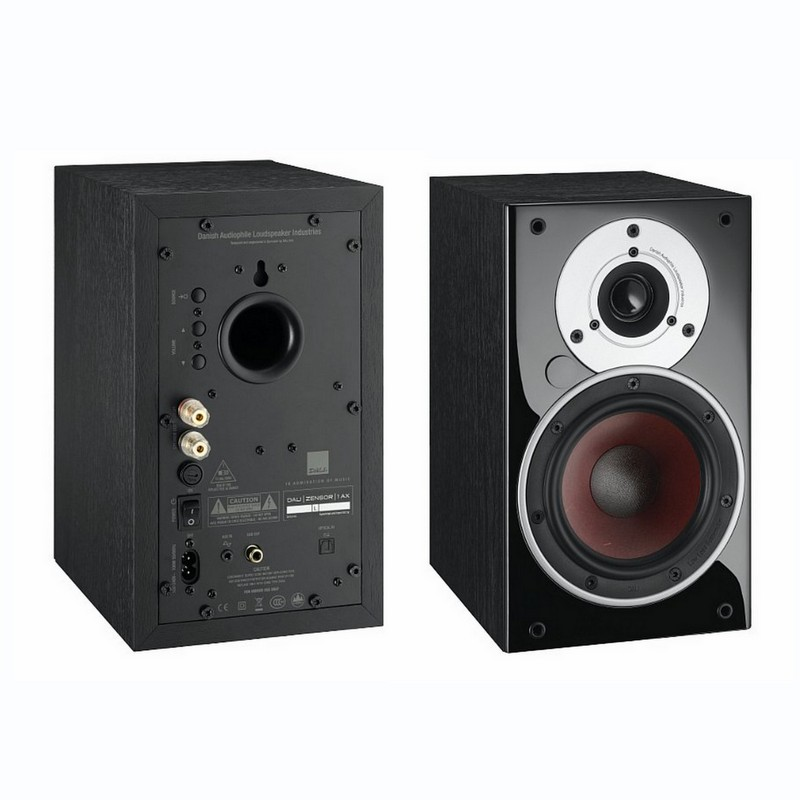
\includegraphics[width=0.5\textwidth]{figures/dali_zensor_1_ax.jpg}
\caption{The system will be developed upon the DALI Zensor 1 AX.}
\label{fig:dali_zensor}
\end{figure}

In the following sections, there will be an analysis on how the sound can be improved.

\todo[inline]{Ikke gennemlæst}








%%%%%%%%%%%%%%%%%%%%%%%% Problem analyse %%%%%%%%%%%%%%%%%%%%%%%%
\chapter{Active Loudspeakers and their Limitations}
%Before developing a system which can improve the overall performance of an active loudspeaker a brief analysis on how an active loudspeaker functions, is needed. 
The main topic of this chapter is to briefly explain the design of a simplified active loudspeaker and afterwards examine where the issues, concerning distortion in an active loudspeaker, arise. As distortion adds artefacts to the audio, distortion is often undesirable in an active loudspeaker. 

A simplified version of an active loudspeaker is seen in \autoref{fig:speaker_block}. The active loudspeaker typically consist of speakers (tweeter and woofer), an amplifier and a processing system. While the block "processing system" is not required in an active loudspeaker, it is common to find signal processors in new active loudspeakers. Because active loudspeakers have their own power supply, they can easily provide the necessary power to peripheral electronics such as a signal processor. The application of the signal processors varies from a equalizer to a wireless receiver for audio streaming.

\begin{figure}[H]
\centering
\tikzsetnextfilename{SpeakerBlock}
\scalebox{0.9}{
\begin{tikzpicture}
%% Kasser %%
\node [block, fill=white] (AudioSource) at (0,0) {Audio Source};

%% DSP %%
\node [block, fill=white] (Amplifier) at ($(AudioSource)+(3.5,0)$) {Amplifier};
\node [block, fill=white] (Driver) at ($(Amplifier)+(3.5,0)$) {Driver};

%% Store Blokke %%
\begin{pgfonlayer}{bg}
\draw[thick, fill=black!20] ($(-1.50,1)+(Amplifier)$) -- ($(1.750,1)+(Driver)$) -- ($(1.750,-1.25)+(Driver)$) -- ($(-1.50,-1.25)+(Amplifier)$) -- ($(-1.50,1)+(Amplifier)$); 
\node (Speakertag) at ($(-.25,-1)+(Driver)$) {\textbf{Speaker Enclosure}};
\end{pgfonlayer}

%% Forbindelse %%
\draw[->] (AudioSource) -- (Amplifier);
\draw[->] (Amplifier) -- (Driver);

%\draw[->] ($(EnclosureDriver)+(-1.375,0.3)$) -- ($(EnclosureDriver)+(-1.75,0.3)$) -- ($(EnclosureDriver)+(-1.75,1)$) -- ($(EnclosureDriver)+(-5.5,1)$) |- ($(SpectralAnalysis)+(1.375,0.3)$);

\end{tikzpicture}}
\caption{Block diagram of an active speaker.}
\label{fig:speaker_block}
\end{figure}

An example of an active loudspeaker is the DALI Zensor 5 AX seen in \autoref{fig:dali_zensor_ax}. Besides the speakers and amplifier, the DALI Zensor 5 AX also includes a signal processor to handle wireless connectivity.
\begin{figure}[H]
\centering
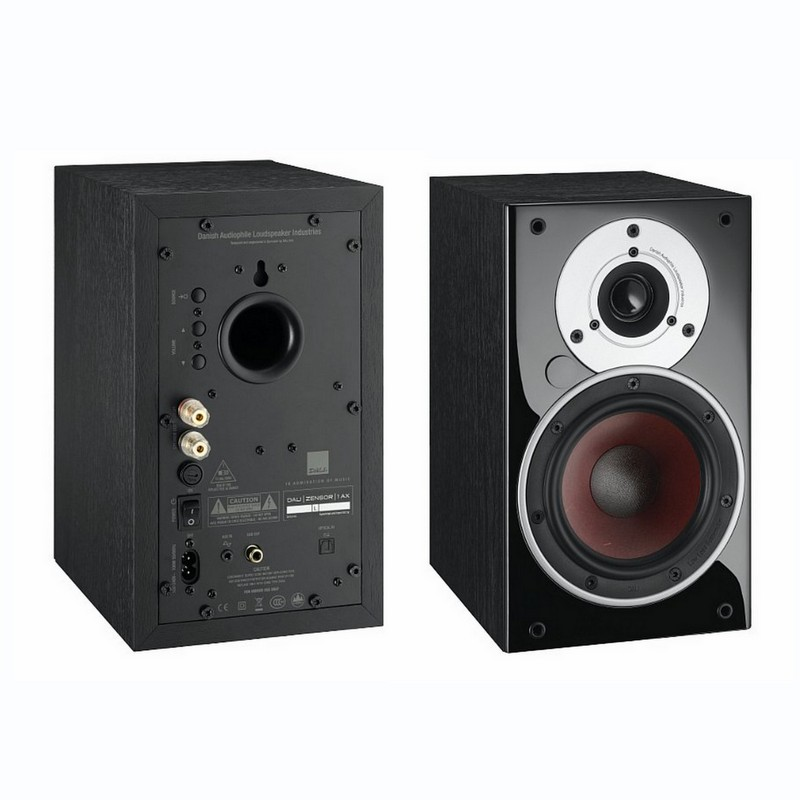
\includegraphics[width=0.6\textwidth]{figures/dali_zensor_1_ax.jpg}
\caption{DALI Zensor 1 AX.}
\label{fig:dali_zensor_ax}
\end{figure}
The DALI Zensor 5 AX allows connection of the audio source via cable or via Bluetooth which enables the user to control the loudspeaker wirelessly, which makes it flexible to use. In the following sections, each block in \autoref{fig:speaker_block} namely "Processing system", "Amplifier", and "Speakers" will be analysed. The analysis will focus on how distortion can arise in the respective block.

\section{Signal Processor}

The digital signal processor (DSP) gives the manufacturer flexibility to add digital connectivity and digital signal processing to an active loudspeaker. The DSP also allows great flexibility in development as it is usually easier to implement signal processing algorithms in a signal processor rather than an equivalent analog circuit. There are however a few parameters to take into account when developing a digital processing system such as sampling rate, computational power and bit-resolution. 

The computational power of a DSP is limited by the clock frequency and the hardware architecture. A higher clock frequency gives more computational power but uses more energy. The hardware architecture is also important since the amount of clock cycles to perform instructions varies in different hardware architectures.

Because the DSP works in discrete time, the audio signal needs to be sampled. The sampling rate must be high enough to fulfill the Nyquist theorem, which states that the sampling frequency must be at least twice the highest frequency component. For music, the highest frequency component is commonly known as 20 kHz, thus the sampling rate must be greater than 40 kHz to avoid losing information and aliasing.

The bit-resolution is important, since it determines the signal to noise ratio (SNR). A higher bit resolution gives a higher SNR which is desirable because of less noise. The bit-resolution is also limited by the converters in a DSP while the hardware architecture also plays an important role with respect to efficiency. An example could be a fixed-point 16-bit DSP. Because the hardware architecture is optimized to 16-bit data, a 24-bit signal requires the 24-bit signal to be split into two pieces of data which increases the amount of computational power needed.

Noise and distortion can also be added to the signal in a signal processor if the signal processing algorithm is not designed correct. For example Infinite Impulse Response (IIR) filter generates noise if it is not implemented correctly. In a fixed-point 16-bit DSP, an IIR filter will generate noise because of quantization from 32-bit to 16-bit which is then fed back into the filter. 

%Distortion could arise using peak-limiters, which is implemented to avoid the signal to reach above a certain level, hard clips the signal and will generate distortion. Peak-limiters are therefore not ideal if the goal is to keep the distortion at a minimum level.











% and applying signal processing to the signal can result in added noise or distortion to the signal. 








\section{Amplifier topology}
This section will briefly describe the amplifier in a active loudspeaker and analyse how distortion is created in the amplifier.

The amplifier is the module which amplifies the input signal. There are several different classes of amplifiers for example class A, AB and D, these classes have different characteristics which gives them different advantages and disadvantages. Two main parameters for the performance of an amplifier are distortion and efficiency. There are several sources for the distortion in a amplifier, such as non-linearity in the active components, cross over distortion and audio clipping. Since no active components are ideal, all active components will create some distortion whenever a signal is passed through the components. An option for better performance is to increase the open-loop amplification of the amplifier as this will give more signal to feedback over thus decreasing the distortion from the components. Since the extend of this project will not deal with circuit design of an amplifier, cross over and non-linearity in component will not be further investigated.

Audio clipping is a wave distortion that occurs when the output signal has a greater signal level than the device is capable of producing. If the signal level is beyond the limitation of the device, the device will cut the signal to its maximum level. This type of clipping is called hard clipping and is often undesirable. In \autoref{fig:audioclipping} an example of how hard clipping affects a 1 kHz sinusoid with a peak amplitude of 1.5. The maximum output level of the device is simulated to be 1.

\begin{figure}[H]
\centering
\begin{subfigure}[t]{0.47\textwidth}
	\tikzsetnextfilename{clippingClean}
	% This file was created by matlab2tikz.
%
%The latest updates can be retrieved from
%  http://www.mathworks.com/matlabcentral/fileexchange/22022-matlab2tikz-matlab2tikz
%where you can also make suggestions and rate matlab2tikz.
%
\begin{tikzpicture}

\begin{axis}[%
width=2.5in,
height=2in,
at={(1.011in,0.642in)},
scale only axis,
xmin=0,
xmax=0.002,
xlabel={Time [s]},
xmajorgrids,
ymin=-2,
ymax=2,
ylabel={Amplitude},
ymajorgrids,
axis background/.style={fill=white}
]
\addplot [color=black,solid,line width=1.2pt,forget plot]
  table[row sep=crcr]{%
0	0\\
2.26757369614512e-05	0.21299147693644\\
4.53514739229025e-05	0.421666669997482\\
6.80272108843537e-05	0.621796765035443\\
9.0702947845805e-05	0.809326114779272\\
0.000113378684807256	0.98045442674729\\
0.000136054421768707	1.13171377638122\\
0.000158730158730159	1.26003888472616\\
0.00018140589569161	1.36282923647545\\
0.000204081632653061	1.43800177955499\\
0.000226757369614512	1.48403313828686\\
0.000249433106575964	1.49999048468041\\
0.000272108843537415	1.48555044224226\\
0.000294784580498866	1.44100563921852\\
0.000317460317460317	1.36725877846751\\
0.000340136054421769	1.26580434413712\\
0.00036281179138322	1.13869831586227\\
0.000385487528344671	0.988516504225587\\
0.000408163265306122	0.818302351815823\\
0.000430839002267574	0.631505257698036\\
0.000453514739229025	0.431910675153779\\
0.000476190476190476	0.223563399264262\\
0.000498866213151927	0.0106855989178377\\
0.000521541950113379	-0.202408745672383\\
0.00054421768707483	-0.411401266012395\\
0.000566893424036281	-0.612056717299934\\
0.000589569160997732	-0.800308805890951\\
0.000612244897959184	-0.972342592961682\\
0.000634920634920635	-1.1246718044516\\
0.000657596371882086	-1.25420948059704\\
0.000680272108843537	-1.35833053333888\\
0.000702947845804989	-1.43492494387492\\
0.00072562358276644	-1.48244052230586\\
0.000748299319727891	-1.49991436284804\\
0.000770975056689342	-1.48699235717159\\
0.000793650793650794	-1.44393637042502\\
0.000816326530612245	-1.37161893452372\\
0.000839002267573696	-1.2715055662432\\
0.000861678004535147	-1.14562506844185\\
0.000884353741496599	-0.996528416260569\\
0.00090702947845805	-0.827237061472641\\
0.000929705215419501	-0.641181702599088\\
0.000952380952380952	-0.442132761616357\\
0.000975056689342404	-0.234123976149712\\
0.000997732426303855	-0.0213706555606557\\
0.00102040816326531	0.191815742526759\\
0.00104308390022676	0.401114984149397\\
0.00106575963718821	0.602285608781499\\
0.00108843537414966	0.791250882763146\\
0.00111111111111111	0.964181414529808\\
0.00113378684807256	1.11757275744087\\
0.00115646258503401	1.24831642758161\\
0.00117913832199546	1.35376289735891\\
0.00120181405895692	1.43177528832223\\
0.00122448979591837	1.48077267512167\\
0.00124716553287982	1.49976212304635\\
0.00126984126984127	1.48835880990026\\
0.00129251700680272	1.44679382444511\\
0.00131519274376417	1.37590948337396\\
0.00133786848072562	1.27714226171757\\
0.00136054421768707	1.15249368259969\\
0.00138321995464853	1.00448975626204\\
0.00140589569160998	0.836129790329203\\
0.00142857142857143	0.650825608676338\\
0.00145124716553288	0.452332410632626\\
0.00147392290249433	0.244672671662413\\
0.00149659863945578	0.0320546276809519\\
0.00151927437641723	-0.181213005075519\\
0.00154195011337868	-0.390808346418877\\
0.00156462585034014	-0.592483935346407\\
0.00158730158730159	-0.782152805069245\\
0.00160997732426304	-0.955971305616867\\
0.00163265306122449	-1.11041699561297\\
0.00165532879818594	-1.24236002474175\\
0.00167800453514739	-1.34912656033491\\
0.00170068027210884	-1.42855297273628\\
0.00172335600907029	-1.47902968137455\\
0.00174603174603175	-1.49953377300122\\
0.0017687074829932	-1.48964973108323\\
0.00179138321995465	-1.44957785626813\\
0.0018140589569161	-1.38013020728057\\
0.00183673469387755	-1.28271414450802\\
0.001859410430839	-1.15930380976591\\
0.00188208616780045	-1.01240012020625\\
0.0019047619047619	-0.844980087095434\\
0.00192743764172336	-0.660436486518814\\
0.00195011337868481	-0.462509104588652\\
0.00197278911564626	-0.25520895047495\\
0.00199546485260771	-0.0427369730862695\\
};
\end{axis}
\end{tikzpicture}%
	\caption{A 1 kHz sinusoid with a peak amplitude on 1.5.}
	\label{fig:clippingClean}
\end{subfigure}
\hspace{6mm} 
\begin{subfigure}[t]{0.47\textwidth}
	\tikzsetnextfilename{clippingDist}
	% This file was created by matlab2tikz.
%
%The latest updates can be retrieved from
%  http://www.mathworks.com/matlabcentral/fileexchange/22022-matlab2tikz-matlab2tikz
%where you can also make suggestions and rate matlab2tikz.
%
\begin{tikzpicture}

\begin{axis}[%
width=2.5in,
height=2in,
at={(1.011in,0.642in)},
scale only axis,
xmin=0,
xmax=1,
xlabel={Time [s]},
xmajorgrids,
ymin=-2,
ymax=2,
ymajorgrids,
axis background/.style={fill=white}
]
\addplot [color=black,solid,line width=1.2pt,forget plot]
  table[row sep=crcr]{%
0	0\\
0.001	0.0188490598250289\\
0.002	0.0376951431650062\\
0.003	0.0565352740049018\\
0.004	0.0753664772696543\\
0.005	0.0941857792939701\\
0.006	0.112990208291899\\
0.007	0.131776794826115\\
0.008	0.150542572276822\\
0.009	0.169284577310223\\
0.01	0.187999850346456\\
0.011	0.206685436026957\\
0.012	0.225338383681136\\
0.013	0.243955747792325\\
0.014	0.262534588462914\\
0.015	0.281071971878587\\
0.016	0.299564970771611\\
0.017	0.318010664883082\\
0.018	0.336406141424072\\
0.019	0.354748495535587\\
0.02	0.373034830747282\\
0.021	0.391262259434845\\
0.022	0.409427903275988\\
0.023	0.427528893704964\\
0.024	0.445562372365552\\
0.025	0.463525491562421\\
0.026	0.481415414710814\\
0.027	0.49922931678448\\
0.028	0.516964384761776\\
0.029	0.534617818069876\\
0.03	0.552186829027017\\
0.031	0.569668643282702\\
0.032	0.587060500255804\\
0.033	0.604359653570494\\
0.034	0.621563371489926\\
0.035	0.638668937347609\\
0.036	0.655673649976399\\
0.037	0.672574824135048\\
0.038	0.689369790932232\\
0.039	0.706055898247999\\
0.04	0.722630511152573\\
0.041	0.739091012322437\\
0.042	0.755434802453641\\
0.043	0.77165930067226\\
0.044	0.787761944941943\\
0.045	0.803740192468495\\
0.046	0.819591520101404\\
0.047	0.835313424732282\\
0.048	0.850903423690135\\
0.049	0.866359055133401\\
0.05	0.88167787843871\\
0.051	0.896857474586278\\
0.052	0.911895446541908\\
0.053	0.926789419635502\\
0.054	0.941537041936051\\
0.055	0.956135984623034\\
0.056	0.970583942354166\\
0.057	0.984878633629435\\
0.058	0.999017801151378\\
0.059	1\\
0.06	1\\
0.061	1\\
0.062	1\\
0.063	1\\
0.064	1\\
0.065	1\\
0.066	1\\
0.067	1\\
0.068	1\\
0.069	1\\
0.07	1\\
0.071	1\\
0.072	1\\
0.073	1\\
0.074	1\\
0.075	1\\
0.076	1\\
0.077	1\\
0.078	1\\
0.079	1\\
0.08	1\\
0.081	1\\
0.082	1\\
0.083	1\\
0.084	1\\
0.085	1\\
0.086	1\\
0.087	1\\
0.088	1\\
0.089	1\\
0.09	1\\
0.091	1\\
0.092	1\\
0.093	1\\
0.094	1\\
0.095	1\\
0.096	1\\
0.097	1\\
0.098	1\\
0.099	1\\
0.1	1\\
0.101	1\\
0.102	1\\
0.103	1\\
0.104	1\\
0.105	1\\
0.106	1\\
0.107	1\\
0.108	1\\
0.109	1\\
0.11	1\\
0.111	1\\
0.112	1\\
0.113	1\\
0.114	1\\
0.115	1\\
0.116	1\\
0.117	1\\
0.118	1\\
0.119	1\\
0.12	1\\
0.121	1\\
0.122	1\\
0.123	1\\
0.124	1\\
0.125	1\\
0.126	1\\
0.127	1\\
0.128	1\\
0.129	1\\
0.13	1\\
0.131	1\\
0.132	1\\
0.133	1\\
0.134	1\\
0.135	1\\
0.136	1\\
0.137	1\\
0.138	1\\
0.139	1\\
0.14	1\\
0.141	1\\
0.142	1\\
0.143	1\\
0.144	1\\
0.145	1\\
0.146	1\\
0.147	1\\
0.148	1\\
0.149	1\\
0.15	1\\
0.151	1\\
0.152	1\\
0.153	1\\
0.154	1\\
0.155	1\\
0.156	1\\
0.157	1\\
0.158	1\\
0.159	1\\
0.16	1\\
0.161	1\\
0.162	1\\
0.163	1\\
0.164	1\\
0.165	1\\
0.166	1\\
0.167	1\\
0.168	1\\
0.169	1\\
0.17	1\\
0.171	1\\
0.172	1\\
0.173	1\\
0.174	1\\
0.175	1\\
0.176	1\\
0.177	1\\
0.178	1\\
0.179	1\\
0.18	1\\
0.181	1\\
0.182	1\\
0.183	1\\
0.184	1\\
0.185	1\\
0.186	1\\
0.187	1\\
0.188	1\\
0.189	1\\
0.19	1\\
0.191	1\\
0.192	0.999017801151378\\
0.193	0.984878633629435\\
0.194	0.970583942354166\\
0.195	0.956135984623035\\
0.196	0.941537041936051\\
0.197	0.926789419635502\\
0.198	0.911895446541908\\
0.199	0.896857474586278\\
0.2	0.88167787843871\\
0.201	0.866359055133402\\
0.202	0.850903423690135\\
0.203	0.835313424732282\\
0.204	0.819591520101404\\
0.205	0.803740192468495\\
0.206	0.787761944941943\\
0.207	0.771659300672259\\
0.208	0.755434802453641\\
0.209	0.739091012322437\\
0.21	0.722630511152573\\
0.211	0.706055898247999\\
0.212	0.689369790932232\\
0.213	0.672574824135048\\
0.214	0.655673649976399\\
0.215	0.638668937347609\\
0.216	0.621563371489926\\
0.217	0.604359653570494\\
0.218	0.587060500255804\\
0.219	0.569668643282702\\
0.22	0.552186829027017\\
0.221	0.534617818069876\\
0.222	0.516964384761776\\
0.223	0.49922931678448\\
0.224	0.481415414710815\\
0.225	0.463525491562421\\
0.226	0.445562372365552\\
0.227	0.427528893704964\\
0.228	0.409427903275988\\
0.229	0.391262259434846\\
0.23	0.373034830747282\\
0.231	0.354748495535587\\
0.232	0.336406141424071\\
0.233	0.318010664883082\\
0.234	0.299564970771611\\
0.235	0.281071971878587\\
0.236	0.262534588462914\\
0.237	0.243955747792325\\
0.238	0.225338383681136\\
0.239	0.206685436026957\\
0.24	0.187999850346457\\
0.241	0.169284577310223\\
0.242	0.150542572276822\\
0.243	0.131776794826115\\
0.244	0.1129902082919\\
0.245	0.0941857792939704\\
0.246	0.0753664772696545\\
0.247	0.0565352740049018\\
0.248	0.0376951431650067\\
0.249	0.0188490598250293\\
0.25	1.83697019872103e-16\\
0.251	-0.0188490598250289\\
0.252	-0.0376951431650064\\
0.253	-0.0565352740049014\\
0.254	-0.0753664772696541\\
0.255	-0.09418577929397\\
0.256	-0.112990208291899\\
0.257	-0.131776794826114\\
0.258	-0.150542572276822\\
0.259	-0.169284577310222\\
0.26	-0.187999850346456\\
0.261	-0.206685436026957\\
0.262	-0.225338383681135\\
0.263	-0.243955747792325\\
0.264	-0.262534588462914\\
0.265	-0.281071971878587\\
0.266	-0.299564970771611\\
0.267	-0.318010664883082\\
0.268	-0.336406141424072\\
0.269	-0.354748495535587\\
0.27	-0.373034830747282\\
0.271	-0.391262259434845\\
0.272	-0.409427903275988\\
0.273	-0.427528893704964\\
0.274	-0.445562372365553\\
0.275	-0.463525491562422\\
0.276	-0.481415414710814\\
0.277	-0.49922931678448\\
0.278	-0.516964384761776\\
0.279	-0.534617818069876\\
0.28	-0.552186829027017\\
0.281	-0.569668643282702\\
0.282	-0.587060500255804\\
0.283	-0.604359653570494\\
0.284	-0.621563371489927\\
0.285	-0.638668937347609\\
0.286	-0.6556736499764\\
0.287	-0.672574824135049\\
0.288	-0.689369790932232\\
0.289	-0.706055898247998\\
0.29	-0.722630511152572\\
0.291	-0.739091012322437\\
0.292	-0.755434802453641\\
0.293	-0.771659300672259\\
0.294	-0.787761944941943\\
0.295	-0.803740192468495\\
0.296	-0.819591520101403\\
0.297	-0.835313424732281\\
0.298	-0.850903423690134\\
0.299	-0.866359055133401\\
0.3	-0.88167787843871\\
0.301	-0.896857474586278\\
0.302	-0.911895446541908\\
0.303	-0.926789419635501\\
0.304	-0.94153704193605\\
0.305	-0.956135984623034\\
0.306	-0.970583942354166\\
0.307	-0.984878633629434\\
0.308	-0.999017801151377\\
0.309	-1\\
0.31	-1\\
0.311	-1\\
0.312	-1\\
0.313	-1\\
0.314	-1\\
0.315	-1\\
0.316	-1\\
0.317	-1\\
0.318	-1\\
0.319	-1\\
0.32	-1\\
0.321	-1\\
0.322	-1\\
0.323	-1\\
0.324	-1\\
0.325	-1\\
0.326	-1\\
0.327	-1\\
0.328	-1\\
0.329	-1\\
0.33	-1\\
0.331	-1\\
0.332	-1\\
0.333	-1\\
0.334	-1\\
0.335	-1\\
0.336	-1\\
0.337	-1\\
0.338	-1\\
0.339	-1\\
0.34	-1\\
0.341	-1\\
0.342	-1\\
0.343	-1\\
0.344	-1\\
0.345	-1\\
0.346	-1\\
0.347	-1\\
0.348	-1\\
0.349	-1\\
0.35	-1\\
0.351	-1\\
0.352	-1\\
0.353	-1\\
0.354	-1\\
0.355	-1\\
0.356	-1\\
0.357	-1\\
0.358	-1\\
0.359	-1\\
0.36	-1\\
0.361	-1\\
0.362	-1\\
0.363	-1\\
0.364	-1\\
0.365	-1\\
0.366	-1\\
0.367	-1\\
0.368	-1\\
0.369	-1\\
0.37	-1\\
0.371	-1\\
0.372	-1\\
0.373	-1\\
0.374	-1\\
0.375	-1\\
0.376	-1\\
0.377	-1\\
0.378	-1\\
0.379	-1\\
0.38	-1\\
0.381	-1\\
0.382	-1\\
0.383	-1\\
0.384	-1\\
0.385	-1\\
0.386	-1\\
0.387	-1\\
0.388	-1\\
0.389	-1\\
0.39	-1\\
0.391	-1\\
0.392	-1\\
0.393	-1\\
0.394	-1\\
0.395	-1\\
0.396	-1\\
0.397	-1\\
0.398	-1\\
0.399	-1\\
0.4	-1\\
0.401	-1\\
0.402	-1\\
0.403	-1\\
0.404	-1\\
0.405	-1\\
0.406	-1\\
0.407	-1\\
0.408	-1\\
0.409	-1\\
0.41	-1\\
0.411	-1\\
0.412	-1\\
0.413	-1\\
0.414	-1\\
0.415	-1\\
0.416	-1\\
0.417	-1\\
0.418	-1\\
0.419	-1\\
0.42	-1\\
0.421	-1\\
0.422	-1\\
0.423	-1\\
0.424	-1\\
0.425	-1\\
0.426	-1\\
0.427	-1\\
0.428	-1\\
0.429	-1\\
0.43	-1\\
0.431	-1\\
0.432	-1\\
0.433	-1\\
0.434	-1\\
0.435	-1\\
0.436	-1\\
0.437	-1\\
0.438	-1\\
0.439	-1\\
0.44	-1\\
0.441	-1\\
0.442	-0.999017801151378\\
0.443	-0.984878633629435\\
0.444	-0.970583942354166\\
0.445	-0.956135984623034\\
0.446	-0.94153704193605\\
0.447	-0.926789419635502\\
0.448	-0.911895446541909\\
0.449	-0.896857474586279\\
0.45	-0.88167787843871\\
0.451	-0.866359055133402\\
0.452	-0.850903423690135\\
0.453	-0.835313424732282\\
0.454	-0.819591520101403\\
0.455	-0.803740192468494\\
0.456	-0.787761944941943\\
0.457	-0.77165930067226\\
0.458	-0.755434802453641\\
0.459	-0.739091012322437\\
0.46	-0.722630511152573\\
0.461	-0.706055898247999\\
0.462	-0.689369790932232\\
0.463	-0.672574824135048\\
0.464	-0.655673649976399\\
0.465	-0.638668937347608\\
0.466	-0.621563371489927\\
0.467	-0.604359653570494\\
0.468	-0.587060500255804\\
0.469	-0.569668643282702\\
0.47	-0.552186829027017\\
0.471	-0.534617818069876\\
0.472	-0.516964384761775\\
0.473	-0.499229316784479\\
0.474	-0.481415414710814\\
0.475	-0.463525491562421\\
0.476	-0.445562372365553\\
0.477	-0.427528893704964\\
0.478	-0.409427903275988\\
0.479	-0.391262259434845\\
0.48	-0.373034830747283\\
0.481	-0.354748495535588\\
0.482	-0.336406141424072\\
0.483	-0.318010664883082\\
0.484	-0.299564970771611\\
0.485	-0.281071971878587\\
0.486	-0.262534588462914\\
0.487	-0.243955747792326\\
0.488	-0.225338383681137\\
0.489	-0.206685436026958\\
0.49	-0.187999850346457\\
0.491	-0.169284577310223\\
0.492	-0.150542572276823\\
0.493	-0.131776794826115\\
0.494	-0.112990208291899\\
0.495	-0.0941857792939699\\
0.496	-0.0753664772696553\\
0.497	-0.0565352740049027\\
0.498	-0.0376951431650069\\
0.499	-0.0188490598250294\\
0.5	-3.67394039744206e-16\\
0.501	0.0188490598250287\\
0.502	0.0376951431650062\\
0.503	0.0565352740049019\\
0.504	0.0753664772696546\\
0.505	0.0941857792939692\\
0.506	0.112990208291898\\
0.507	0.131776794826114\\
0.508	0.150542572276822\\
0.509	0.169284577310222\\
0.51	0.187999850346456\\
0.511	0.206685436026957\\
0.512	0.225338383681136\\
0.513	0.243955747792326\\
0.514	0.262534588462913\\
0.515	0.281071971878586\\
0.516	0.29956497077161\\
0.517	0.318010664883082\\
0.518	0.336406141424072\\
0.519	0.354748495535587\\
0.52	0.373034830747282\\
0.521	0.391262259434843\\
0.522	0.409427903275988\\
0.523	0.427528893704962\\
0.524	0.445562372365552\\
0.525	0.46352549156242\\
0.526	0.481415414710814\\
0.527	0.499229316784479\\
0.528	0.516964384761776\\
0.529	0.534617818069874\\
0.53	0.552186829027017\\
0.531	0.5696686432827\\
0.532	0.587060500255804\\
0.533	0.604359653570492\\
0.534	0.621563371489926\\
0.535	0.638668937347608\\
0.536	0.655673649976399\\
0.537	0.672574824135046\\
0.538	0.689369790932232\\
0.539	0.706055898247997\\
0.54	0.722630511152573\\
0.541	0.739091012322436\\
0.542	0.755434802453641\\
0.543	0.771659300672258\\
0.544	0.787761944941944\\
0.545	0.803740192468494\\
0.546	0.819591520101404\\
0.547	0.83531342473228\\
0.548	0.850903423690135\\
0.549	0.8663590551334\\
0.55	0.88167787843871\\
0.551	0.896857474586277\\
0.552	0.911895446541908\\
0.553	0.9267894196355\\
0.554	0.941537041936051\\
0.555	0.956135984623034\\
0.556	0.970583942354167\\
0.557	0.984878633629433\\
0.558	0.999017801151378\\
0.559	1\\
0.56	1\\
0.561	1\\
0.562	1\\
0.563	1\\
0.564	1\\
0.565	1\\
0.566	1\\
0.567	1\\
0.568	1\\
0.569	1\\
0.57	1\\
0.571	1\\
0.572	1\\
0.573	1\\
0.574	1\\
0.575	1\\
0.576	1\\
0.577	1\\
0.578	1\\
0.579	1\\
0.58	1\\
0.581	1\\
0.582	1\\
0.583	1\\
0.584	1\\
0.585	1\\
0.586	1\\
0.587	1\\
0.588	1\\
0.589	1\\
0.59	1\\
0.591	1\\
0.592	1\\
0.593	1\\
0.594	1\\
0.595	1\\
0.596	1\\
0.597	1\\
0.598	1\\
0.599	1\\
0.6	1\\
0.601	1\\
0.602	1\\
0.603	1\\
0.604	1\\
0.605	1\\
0.606	1\\
0.607	1\\
0.608	1\\
0.609	1\\
0.61	1\\
0.611	1\\
0.612	1\\
0.613	1\\
0.614	1\\
0.615	1\\
0.616	1\\
0.617	1\\
0.618	1\\
0.619	1\\
0.62	1\\
0.621	1\\
0.622	1\\
0.623	1\\
0.624	1\\
0.625	1\\
0.626	1\\
0.627	1\\
0.628	1\\
0.629	1\\
0.63	1\\
0.631	1\\
0.632	1\\
0.633	1\\
0.634	1\\
0.635	1\\
0.636	1\\
0.637	1\\
0.638	1\\
0.639	1\\
0.64	1\\
0.641	1\\
0.642	1\\
0.643	1\\
0.644	1\\
0.645	1\\
0.646	1\\
0.647	1\\
0.648	1\\
0.649	1\\
0.65	1\\
0.651	1\\
0.652	1\\
0.653	1\\
0.654	1\\
0.655	1\\
0.656	1\\
0.657	1\\
0.658	1\\
0.659	1\\
0.66	1\\
0.661	1\\
0.662	1\\
0.663	1\\
0.664	1\\
0.665	1\\
0.666	1\\
0.667	1\\
0.668	1\\
0.669	1\\
0.67	1\\
0.671	1\\
0.672	1\\
0.673	1\\
0.674	1\\
0.675	1\\
0.676	1\\
0.677	1\\
0.678	1\\
0.679	1\\
0.68	1\\
0.681	1\\
0.682	1\\
0.683	1\\
0.684	1\\
0.685	1\\
0.686	1\\
0.687	1\\
0.688	1\\
0.689	1\\
0.69	1\\
0.691	1\\
0.692	0.999017801151379\\
0.693	0.984878633629435\\
0.694	0.970583942354168\\
0.695	0.956135984623035\\
0.696	0.941537041936052\\
0.697	0.926789419635501\\
0.698	0.911895446541909\\
0.699	0.896857474586278\\
0.7	0.88167787843871\\
0.701	0.866359055133401\\
0.702	0.850903423690135\\
0.703	0.835313424732281\\
0.704	0.819591520101406\\
0.705	0.803740192468493\\
0.706	0.787761944941945\\
0.707	0.771659300672258\\
0.708	0.755434802453643\\
0.709	0.739091012322438\\
0.71	0.722630511152574\\
0.711	0.706055898247999\\
0.712	0.689369790932233\\
0.713	0.672574824135051\\
0.714	0.6556736499764\\
0.715	0.638668937347611\\
0.716	0.621563371489927\\
0.717	0.604359653570496\\
0.718	0.587060500255804\\
0.719	0.569668643282703\\
0.72	0.552186829027017\\
0.721	0.534617818069877\\
0.722	0.516964384761775\\
0.723	0.499229316784481\\
0.724	0.481415414710816\\
0.725	0.463525491562422\\
0.726	0.445562372365554\\
0.727	0.427528893704964\\
0.728	0.409427903275989\\
0.729	0.391262259434845\\
0.73	0.373034830747283\\
0.731	0.354748495535587\\
0.732	0.336406141424072\\
0.733	0.318010664883084\\
0.734	0.299564970771611\\
0.735	0.281071971878589\\
0.736	0.262534588462914\\
0.737	0.243955747792327\\
0.738	0.225338383681135\\
0.739	0.206685436026958\\
0.74	0.187999850346456\\
0.741	0.169284577310223\\
0.742	0.150542572276824\\
0.743	0.131776794826115\\
0.744	0.112990208291901\\
0.745	0.0941857792939701\\
0.746	0.0753664772696555\\
0.747	0.0565352740049015\\
0.748	0.0376951431650071\\
0.749	0.0188490598250283\\
0.75	5.51091059616309e-16\\
0.751	-0.0188490598250272\\
0.752	-0.037695143165006\\
0.753	-0.0565352740049004\\
0.754	-0.0753664772696544\\
0.755	-0.094185779293969\\
0.756	-0.112990208291899\\
0.757	-0.131776794826114\\
0.758	-0.150542572276823\\
0.759	-0.169284577310222\\
0.76	-0.187999850346455\\
0.761	-0.206685436026957\\
0.762	-0.225338383681134\\
0.763	-0.243955747792326\\
0.764	-0.262534588462913\\
0.765	-0.281071971878587\\
0.766	-0.29956497077161\\
0.767	-0.318010664883083\\
0.768	-0.336406141424071\\
0.769	-0.354748495535586\\
0.77	-0.373034830747282\\
0.771	-0.391262259434844\\
0.772	-0.409427903275988\\
0.773	-0.427528893704963\\
0.774	-0.445562372365553\\
0.775	-0.463525491562421\\
0.776	-0.481415414710815\\
0.777	-0.49922931678448\\
0.778	-0.516964384761774\\
0.779	-0.534617818069876\\
0.78	-0.552186829027016\\
0.781	-0.569668643282702\\
0.782	-0.587060500255803\\
0.783	-0.604359653570495\\
0.784	-0.621563371489926\\
0.785	-0.63866893734761\\
0.786	-0.655673649976399\\
0.787	-0.67257482413505\\
0.788	-0.689369790932232\\
0.789	-0.706055898247998\\
0.79	-0.722630511152573\\
0.791	-0.739091012322437\\
0.792	-0.755434802453642\\
0.793	-0.771659300672257\\
0.794	-0.787761944941945\\
0.795	-0.803740192468493\\
0.796	-0.819591520101405\\
0.797	-0.83531342473228\\
0.798	-0.850903423690134\\
0.799	-0.8663590551334\\
0.8	-0.881677878438709\\
0.801	-0.896857474586277\\
0.802	-0.911895446541908\\
0.803	-0.9267894196355\\
0.804	-0.941537041936051\\
0.805	-0.956135984623034\\
0.806	-0.970583942354167\\
0.807	-0.984878633629434\\
0.808	-0.999017801151378\\
0.809	-1\\
0.81	-1\\
0.811	-1\\
0.812	-1\\
0.813	-1\\
0.814	-1\\
0.815	-1\\
0.816	-1\\
0.817	-1\\
0.818	-1\\
0.819	-1\\
0.82	-1\\
0.821	-1\\
0.822	-1\\
0.823	-1\\
0.824	-1\\
0.825	-1\\
0.826	-1\\
0.827	-1\\
0.828	-1\\
0.829	-1\\
0.83	-1\\
0.831	-1\\
0.832	-1\\
0.833	-1\\
0.834	-1\\
0.835	-1\\
0.836	-1\\
0.837	-1\\
0.838	-1\\
0.839	-1\\
0.84	-1\\
0.841	-1\\
0.842	-1\\
0.843	-1\\
0.844	-1\\
0.845	-1\\
0.846	-1\\
0.847	-1\\
0.848	-1\\
0.849	-1\\
0.85	-1\\
0.851	-1\\
0.852	-1\\
0.853	-1\\
0.854	-1\\
0.855	-1\\
0.856	-1\\
0.857	-1\\
0.858	-1\\
0.859	-1\\
0.86	-1\\
0.861	-1\\
0.862	-1\\
0.863	-1\\
0.864	-1\\
0.865	-1\\
0.866	-1\\
0.867	-1\\
0.868	-1\\
0.869	-1\\
0.87	-1\\
0.871	-1\\
0.872	-1\\
0.873	-1\\
0.874	-1\\
0.875	-1\\
0.876	-1\\
0.877	-1\\
0.878	-1\\
0.879	-1\\
0.88	-1\\
0.881	-1\\
0.882	-1\\
0.883	-1\\
0.884	-1\\
0.885	-1\\
0.886	-1\\
0.887	-1\\
0.888	-1\\
0.889	-1\\
0.89	-1\\
0.891	-1\\
0.892	-1\\
0.893	-1\\
0.894	-1\\
0.895	-1\\
0.896	-1\\
0.897	-1\\
0.898	-1\\
0.899	-1\\
0.9	-1\\
0.901	-1\\
0.902	-1\\
0.903	-1\\
0.904	-1\\
0.905	-1\\
0.906	-1\\
0.907	-1\\
0.908	-1\\
0.909	-1\\
0.91	-1\\
0.911	-1\\
0.912	-1\\
0.913	-1\\
0.914	-1\\
0.915	-1\\
0.916	-1\\
0.917	-1\\
0.918	-1\\
0.919	-1\\
0.92	-1\\
0.921	-1\\
0.922	-1\\
0.923	-1\\
0.924	-1\\
0.925	-1\\
0.926	-1\\
0.927	-1\\
0.928	-1\\
0.929	-1\\
0.93	-1\\
0.931	-1\\
0.932	-1\\
0.933	-1\\
0.934	-1\\
0.935	-1\\
0.936	-1\\
0.937	-1\\
0.938	-1\\
0.939	-1\\
0.94	-1\\
0.941	-1\\
0.942	-0.999017801151379\\
0.943	-0.984878633629435\\
0.944	-0.970583942354168\\
0.945	-0.956135984623037\\
0.946	-0.941537041936052\\
0.947	-0.926789419635504\\
0.948	-0.911895446541909\\
0.949	-0.89685747458628\\
0.95	-0.88167787843871\\
0.951	-0.866359055133403\\
0.952	-0.850903423690135\\
0.953	-0.835313424732283\\
0.954	-0.819591520101406\\
0.955	-0.803740192468496\\
0.956	-0.787761944941946\\
0.957	-0.771659300672261\\
0.958	-0.755434802453643\\
0.959	-0.739091012322438\\
0.96	-0.722630511152574\\
0.961	-0.706055898247999\\
0.962	-0.689369790932233\\
0.963	-0.672574824135051\\
0.964	-0.6556736499764\\
0.965	-0.638668937347611\\
0.966	-0.621563371489927\\
0.967	-0.604359653570496\\
0.968	-0.587060500255804\\
0.969	-0.569668643282703\\
0.97	-0.552186829027017\\
0.971	-0.534617818069877\\
0.972	-0.516964384761775\\
0.973	-0.499229316784481\\
0.974	-0.481415414710816\\
0.975	-0.463525491562422\\
0.976	-0.445562372365554\\
0.977	-0.427528893704965\\
0.978	-0.409427903275989\\
0.979	-0.391262259434845\\
0.98	-0.373034830747283\\
0.981	-0.354748495535587\\
0.982	-0.336406141424073\\
0.983	-0.318010664883084\\
0.984	-0.299564970771611\\
0.985	-0.281071971878589\\
0.986	-0.262534588462914\\
0.987	-0.243955747792327\\
0.988	-0.225338383681136\\
0.989	-0.206685436026958\\
0.99	-0.187999850346456\\
0.991	-0.169284577310223\\
0.992	-0.150542572276824\\
0.993	-0.131776794826115\\
0.994	-0.112990208291901\\
0.995	-0.0941857792939703\\
0.996	-0.0753664772696557\\
0.997	-0.0565352740049017\\
0.998	-0.0376951431650073\\
0.999	-0.0188490598250285\\
1	-7.34788079488412e-16\\
};
\end{axis}
\end{tikzpicture}%
	\caption{A 1 kHz clipped sinusoid.}
	\label{fig:clippingDist}
\end{subfigure}
\caption{The difference between a unaffected signal and a clipped signal. As the maximum output is 1, the signal is hard clipped because of the limitation.}
\label{fig:audioclipping}
\end{figure}

Hard clipping lowers the sound quality if the clipping is not intended, and should therefore be avoided. The wave distortion created by the sharp edge results in a square-wave-like signal. This creates additional uneven harmonics to the signal i.e. 3rd, 5th, 7th and 9th, which are unpleasant to listen to as previously stated. Since the clipping creates the square-wave-like signal, the generation of the additional uneven harmonics can be described in the Fourier series of a square-wave. The Fourier series of a square-wave is given as:
\begin{align}\label{eq:fourier_series_square}
f(t) &= \frac{4}{\pi} \sum_{n=1}^{\infty} \frac{\sin (\omega_0 t \cdot (2n-1))}{(2n-1)} \\
	 &= \frac{4}{\pi} (\sin(\omega_0 t) + \frac{1}{3}\sin(3 \omega_0 t) + \frac{1}{5}\sin(5 \omega_0 t) + \, ... \,)
\end{align}
\begin{where}
\va{$\omega_0$}{is the fundamental frequency of the square-wave.}{rad/s}\\
\end{where}

As seen in \autoref{eq:fourier_series_square}, the function of a square-wave signal consists of a fundamental frequency $\omega_0$ and uneven harmonics to the fundamental frequency. This can also be shown in a spectrum analysis of the 1 kHz clipped sinusoid from \autoref{fig:audioclipping} in \autoref{fig:audioclippingFFT}.

\begin{figure}[H]
\centering
\begin{subfigure}[t]{0.47\textwidth}
	\tikzsetnextfilename{clippingCleanFFT}
	% This file was created by matlab2tikz.
%
%The latest updates can be retrieved from
%  http://www.mathworks.com/matlabcentral/fileexchange/22022-matlab2tikz-matlab2tikz
%where you can also make suggestions and rate matlab2tikz.
%
\begin{tikzpicture}

\begin{axis}[%
width=2.5in,
height=2in,
at={(1.011in,0.642in)},
scale only axis,
xmin=0,
xmax=10000,
xlabel={Frequency [Hz]},
xmajorgrids,
ymin=-350,
ymax=100,
ylabel={Amplitude [dB]},
ymajorgrids,
axis background/.style={fill=white},
]
\addplot [color=black,solid,line width=1.2pt,forget plot]
  table[row sep=crcr]{%
0	-322.11596721008\\
11.7216117216117	-323.671020481401\\
23.4432234432234	-323.340883337027\\
35.1648351648352	-325.684167070818\\
46.8864468864469	-325.669523756719\\
58.6080586080586	-324.370513022472\\
70.3296703296703	-322.159992029701\\
82.0512820512821	-319.994159311925\\
93.7728937728938	-319.483979753379\\
105.494505494505	-319.494939928451\\
117.216117216117	-320.869322942301\\
128.937728937729	-320.920572736749\\
140.659340659341	-324.227184829387\\
152.380952380952	-319.035056899834\\
164.102564102564	-313.823145631125\\
175.824175824176	-311.131574765862\\
187.545787545788	-310.246860211816\\
199.267399267399	-310.60441452423\\
210.989010989011	-311.78696455392\\
222.710622710623	-313.844752745052\\
234.432234432234	-316.418042709319\\
246.153846153846	-321.707697545501\\
257.875457875458	-327.363976836631\\
269.59706959707	-327.473089119894\\
281.318681318681	-324.112892105008\\
293.040293040293	-320.977587207666\\
304.761904761905	-319.982762533596\\
316.483516483516	-320.780760736175\\
328.205128205128	-323.668423270885\\
339.92673992674	-328.026148757277\\
351.648351648352	-332.4170697972\\
363.369963369963	-329.426095087341\\
375.091575091575	-326.556664292431\\
386.813186813187	-323.76537835188\\
398.534798534799	-323.368319264645\\
410.25641025641	-325.169104300057\\
421.978021978022	-328.189262138342\\
433.699633699634	-326.529217054039\\
445.421245421245	-322.75486943378\\
457.142857142857	-319.794087491908\\
468.864468864469	-317.719335966222\\
480.586080586081	-317.459852846429\\
492.307692307692	-319.009687543967\\
504.029304029304	-325.455766258282\\
515.750915750916	-336.106317374067\\
527.472527472527	-326.323603862667\\
539.194139194139	-329.684995875921\\
550.915750915751	-327.90212185778\\
562.637362637363	-314.792259957384\\
574.358974358974	-308.679273562794\\
586.080586080586	-304.859856763288\\
597.802197802198	-303.147924647545\\
609.52380952381	-302.958088372619\\
621.245421245421	-304.246172084633\\
632.967032967033	-307.392871145609\\
644.688644688645	-311.86240623327\\
656.410256410256	-319.720154828058\\
668.131868131868	-327.681235000644\\
679.85347985348	-337.238516322602\\
691.575091575092	-336.970257356979\\
703.296703296703	-332.332133924419\\
715.018315018315	-331.141735134048\\
726.739926739927	-332.723957001084\\
738.461538461538	-330.730504488432\\
750.18315018315	-327.778175020515\\
761.904761904762	-319.91378584982\\
773.626373626374	-321.461497849882\\
785.347985347985	-327.043537773181\\
797.069597069597	-331.841589615916\\
808.791208791209	-336.991655282628\\
820.512820512821	-330.418202230553\\
832.234432234432	-333.267393421045\\
843.956043956044	-328.226187037683\\
855.677655677656	-316.700315440438\\
867.399267399267	-215.943651772091\\
879.120879120879	-163.159584780945\\
890.842490842491	-126.529341228273\\
902.564102564103	-98.3775899142248\\
914.285714285714	-75.9321258862354\\
926.007326007326	-57.8132086793137\\
937.728937728938	-43.2219634542571\\
949.450549450549	-31.6552033180823\\
961.172161172161	-22.7812801668732\\
972.893772893773	-16.3785078578736\\
984.615384615385	-12.3020988974321\\
996.336996336996	-10.4658259320985\\
1008.05860805861	-10.8322625838136\\
1019.78021978022	-13.4088092670734\\
1031.50183150183	-18.2484666216626\\
1043.22344322344	-25.4555537550734\\
1054.94505494505	-35.1978991745999\\
1066.66666666667	-47.7291574398437\\
1078.38827838828	-63.4292414488433\\
1090.10989010989	-82.8812589369107\\
1101.8315018315	-107.032465507491\\
1113.55311355311	-137.586526131487\\
1125.27472527473	-178.243096713105\\
1136.99633699634	-241.704411925533\\
1148.71794871795	-323.195571130692\\
1160.43956043956	-345.375156099691\\
1172.16117216117	-338.247857244841\\
1183.88278388278	-333.32317434497\\
1195.6043956044	-331.269745255181\\
1207.32600732601	-328.799242404036\\
1219.04761904762	-335.934946361628\\
1230.76923076923	-327.685186138873\\
1242.49084249084	-326.960459897927\\
1254.21245421245	-323.718010447396\\
1265.93406593407	-324.108622411667\\
1277.65567765568	-326.20417623814\\
1289.37728937729	-332.697946725791\\
1301.0989010989	-327.906853738375\\
1312.82051282051	-335.418538359777\\
1324.54212454212	-328.816875760217\\
1336.26373626374	-327.262600955998\\
1347.98534798535	-320.385055874777\\
1359.70695970696	-311.475672251247\\
1371.42857142857	-306.643481149913\\
1383.15018315018	-303.695848832502\\
1394.87179487179	-302.842835407919\\
1406.59340659341	-303.232099162736\\
1418.31501831502	-305.842604461406\\
1430.03663003663	-310.40119194813\\
1441.75824175824	-320.718788147534\\
1453.47985347985	-328.69918849089\\
1465.20146520147	-321.407968983388\\
1476.92307692308	-324.473146768564\\
1488.64468864469	-331.645069484275\\
1500.3663003663	-332.515642341006\\
1512.08791208791	-328.465510911873\\
1523.80952380952	-326.826340274793\\
1535.53113553114	-324.534133776849\\
1547.25274725275	-322.615676311941\\
1558.97435897436	-322.427557967468\\
1570.69597069597	-323.530722159417\\
1582.41758241758	-326.171996895262\\
1594.13919413919	-327.712500269681\\
1605.86080586081	-325.047841087069\\
1617.58241758242	-321.24290571993\\
1629.30402930403	-317.993077517342\\
1641.02564102564	-316.998612276315\\
1652.74725274725	-316.240926477532\\
1664.46886446886	-316.68363443687\\
1676.19047619048	-317.141867195876\\
1687.91208791209	-318.342449097449\\
1699.6336996337	-320.695345632283\\
1711.35531135531	-321.836458347942\\
1723.07692307692	-320.2697737784\\
1734.79853479853	-320.163464706646\\
1746.52014652015	-317.872908059459\\
1758.24175824176	-312.6677675311\\
1769.96336996337	-309.491750132905\\
1781.68498168498	-307.828765413517\\
1793.40659340659	-307.627883691429\\
1805.12820512821	-307.890708550761\\
1816.84981684982	-309.331169961249\\
1828.57142857143	-312.28725024046\\
1840.29304029304	-320.344727197184\\
1852.01465201465	-330.483981414598\\
1863.73626373626	-320.778838487233\\
1875.45787545788	-323.188753718667\\
1887.17948717949	-330.709648822314\\
1898.9010989011	-324.458698904598\\
1910.62271062271	-322.161594474234\\
1922.34432234432	-322.355261648298\\
1934.06593406593	-325.120354775896\\
1945.78754578755	-325.813966972437\\
1957.50915750916	-323.880005799796\\
1969.23076923077	-321.560515034589\\
1980.95238095238	-321.471577902989\\
1992.67399267399	-319.02446157723\\
2004.3956043956	-323.174195056939\\
2016.11721611722	-323.174195056939\\
2027.83882783883	-324.089344868152\\
2039.56043956044	-322.910905669715\\
2051.28205128205	-323.043188327053\\
2063.00366300366	-322.552600066038\\
2074.72527472527	-320.986469744908\\
2086.44688644689	-319.545996905778\\
2098.1684981685	-318.315254794156\\
2109.89010989011	-318.387111906887\\
2121.61172161172	-318.301603114866\\
2133.33333333333	-318.177294354268\\
2145.05494505495	-316.938934301122\\
2156.77655677656	-314.354332026841\\
2168.49816849817	-312.152839226024\\
2180.21978021978	-310.876376782709\\
2191.94139194139	-310.8442203955\\
2203.663003663	-312.377716587324\\
2215.38461538462	-315.505766578087\\
2227.10622710623	-320.600055628699\\
2238.82783882784	-326.363108229676\\
2250.54945054945	-332.879313477263\\
2262.27106227106	-339.927557268938\\
2273.99267399267	-330.784134841474\\
2285.71428571429	-326.949066776775\\
2297.4358974359	-325.310562015324\\
2309.15750915751	-324.900671542525\\
2320.87912087912	-326.68176647539\\
2332.60073260073	-328.158338680386\\
2344.32234432234	-328.204122091938\\
2356.04395604396	-328.051439236523\\
2367.76556776557	-328.664204937443\\
2379.48717948718	-328.099018637999\\
2391.20879120879	-324.310047965675\\
2402.9304029304	-321.667678539627\\
2414.65201465201	-321.135207214597\\
2426.37362637363	-320.880932262159\\
2438.09523809524	-319.778960318202\\
2449.81684981685	-317.987700465117\\
2461.53846153846	-316.78808552065\\
2473.26007326007	-317.473390142408\\
2484.98168498168	-320.222893879042\\
2496.7032967033	-324.854050216358\\
2508.42490842491	-327.365492440596\\
2520.14652014652	-323.224999893465\\
2531.86813186813	-321.091227031284\\
2543.58974358974	-320.156669708411\\
2555.31135531136	-317.840663339711\\
2567.03296703297	-314.501482216247\\
2578.75457875458	-311.854837339112\\
2590.47619047619	-310.724997354159\\
2602.1978021978	-311.622091427549\\
2613.91941391941	-314.851882898182\\
2625.64102564103	-321.512762623562\\
2637.36263736264	-326.715257821487\\
2649.08424908425	-320.965390398505\\
2660.80586080586	-318.299218269644\\
2672.52747252747	-317.485994241431\\
2684.24908424908	-318.59001422949\\
2695.9706959707	-320.576544514212\\
2707.69230769231	-321.22124456977\\
2719.41391941392	-321.571973538176\\
2731.13553113553	-321.42734530042\\
2742.85714285714	-323.182504523745\\
2754.57875457875	-327.818517304439\\
2766.30036630037	-343.340028971303\\
2778.02197802198	-328.590941502845\\
2789.74358974359	-329.209198839045\\
2801.4652014652	-335.009194971263\\
2813.18681318681	-324.917874359001\\
2824.90842490842	-320.675970970006\\
2836.63003663004	-318.598485286378\\
2848.35164835165	-318.175277091238\\
2860.07326007326	-318.965978881077\\
2871.79487179487	-320.835410347703\\
2883.51648351648	-322.524929825596\\
2895.2380952381	-324.578193849772\\
2906.95970695971	-327.880455873337\\
2918.68131868132	-329.561603057853\\
2930.40293040293	-325.490736098095\\
2942.12454212454	-322.172446534305\\
2953.84615384615	-319.538366387325\\
2965.56776556777	-316.454951611266\\
2977.28937728938	-313.715712999263\\
2989.01098901099	-312.765011451191\\
3000.7326007326	-313.550082053352\\
3012.45421245421	-316.332919236015\\
3024.17582417582	-320.464673621591\\
3035.89743589744	-324.21570173302\\
3047.61904761905	-325.14025136414\\
3059.34065934066	-328.179012620665\\
3071.06227106227	-336.319390511434\\
3082.78388278388	-330.540376761589\\
3094.50549450549	-328.055385719859\\
3106.22710622711	-328.41132792291\\
3117.94871794872	-326.398110320453\\
3129.67032967033	-324.429933801343\\
3141.39194139194	-322.958523531653\\
3153.11355311355	-322.080283026816\\
3164.83516483516	-321.986069592074\\
3176.55677655678	-322.88974461944\\
3188.27838827839	-323.14866547361\\
3200	-321.731991922314\\
3211.72161172161	-319.583271135606\\
3223.44322344322	-318.524693510682\\
3235.16483516484	-318.277835267365\\
3246.88644688645	-319.493530184348\\
3258.60805860806	-320.194783095862\\
3270.32967032967	-319.645880585364\\
3282.05128205128	-318.402355114397\\
3293.77289377289	-317.597734351514\\
3305.49450549451	-317.02187364446\\
3317.21611721612	-316.763942230905\\
3328.93772893773	-316.47058612926\\
3340.65934065934	-317.197718055388\\
3352.38095238095	-318.34030296296\\
3364.10256410256	-319.71475362671\\
3375.82417582418	-320.433372545647\\
3387.54578754579	-321.481423753538\\
3399.2673992674	-321.328758210847\\
3410.98901098901	-317.848121944058\\
3422.71062271062	-312.6052633917\\
3434.43223443223	-308.209983131555\\
3446.15384615385	-304.542297484367\\
3457.87545787546	-301.476640468968\\
3469.59706959707	-299.074162567864\\
3481.31868131868	-297.505270833626\\
3493.04029304029	-296.820826693279\\
3504.7619047619	-296.952977362533\\
3516.48351648352	-297.832794363821\\
3528.20512820513	-299.532668899083\\
3539.92673992674	-301.925997253397\\
3551.64835164835	-304.833072981485\\
3563.36996336996	-307.679247836289\\
3575.09157509158	-309.820085030418\\
3586.81318681319	-310.691494738001\\
3598.5347985348	-310.817398824033\\
3610.25641025641	-310.678764468745\\
3621.97802197802	-310.904852964739\\
3633.69963369963	-312.083008289962\\
3645.42124542125	-314.044889957489\\
3657.14285714286	-316.283113404039\\
3668.86446886447	-317.725995742272\\
3680.58608058608	-316.98711432429\\
3692.30769230769	-315.404661196974\\
3704.0293040293	-313.574046253917\\
3715.75091575092	-312.403769243541\\
3727.47252747253	-311.900292301962\\
3739.19413919414	-311.790821532916\\
3750.91575091575	-311.885255334962\\
3762.63736263736	-312.507671076698\\
3774.35897435897	-314.393900840475\\
3786.08058608059	-318.958623783513\\
3797.8021978022	-330.766521534997\\
3809.52380952381	-325.502820472922\\
3821.24542124542	-319.47490837836\\
3832.96703296703	-316.5879349607\\
3844.68864468864	-315.820977290156\\
3856.41025641026	-316.165835542033\\
3868.13186813187	-317.693295629945\\
3879.85347985348	-319.724105063858\\
3891.57509157509	-320.385668853013\\
3903.2967032967	-319.982487927687\\
3915.01831501832	-319.299311012412\\
3926.73992673993	-319.444342321726\\
3938.46153846154	-320.526575483676\\
3950.18315018315	-321.926779712727\\
3961.90476190476	-321.781804018036\\
3973.62637362637	-319.294600071473\\
3985.34798534799	-317.199406352915\\
3997.0695970696	-315.48532686416\\
4008.79120879121	-316.133918462084\\
4020.51282051282	-315.922088122408\\
4032.23443223443	-316.716666209588\\
4043.95604395604	-317.865988888969\\
4055.67765567766	-318.280559925241\\
4067.39926739927	-318.926776854331\\
4079.12087912088	-317.317696380994\\
4090.84249084249	-315.060841214154\\
4102.5641025641	-312.993854282692\\
4114.28571428571	-312.27769957935\\
4126.00732600733	-313.058993411349\\
4137.72893772894	-316.497495126966\\
4149.45054945055	-324.074551114817\\
4161.17216117216	-317.815498249607\\
4172.89377289377	-312.724221795712\\
4184.61538461538	-311.184304154482\\
4196.336996337	-312.180395095067\\
4208.05860805861	-315.33167553721\\
4219.78021978022	-320.223371703619\\
4231.50183150183	-324.981894832223\\
4243.22344322344	-325.968094640368\\
4254.94505494505	-325.975199382868\\
4266.66666666667	-325.044494992807\\
4278.38827838828	-324.748701483869\\
4290.10989010989	-324.298796557654\\
4301.8315018315	-323.185408013847\\
4313.55311355311	-322.493712256323\\
4325.27472527472	-324.004517791407\\
4336.99633699634	-326.395781230683\\
4348.71794871795	-327.81152123793\\
4360.43956043956	-326.215243804676\\
4372.16117216117	-323.991135829513\\
4383.88278388278	-320.982207180012\\
4395.6043956044	-321.462465973861\\
4407.32600732601	-324.176499385288\\
4419.04761904762	-332.267280302068\\
4430.76923076923	-340.80932861649\\
4442.49084249084	-326.258684322367\\
4454.21245421245	-321.442965268777\\
4465.93406593407	-319.544444432877\\
4477.65567765568	-320.026440215285\\
4489.37728937729	-321.870034014714\\
4501.0989010989	-325.275880091975\\
4512.82051282051	-329.135133788708\\
4524.54212454212	-328.535733131409\\
4536.26373626374	-319.872005913471\\
4547.98534798535	-314.353155551714\\
4559.70695970696	-311.431276989024\\
4571.42857142857	-310.598208874572\\
4583.15018315018	-311.541465335688\\
4594.87179487179	-314.262904844306\\
4606.59340659341	-318.957659426667\\
4618.31501831502	-324.341801794823\\
4630.03663003663	-326.908025760342\\
4641.75824175824	-329.671708602847\\
4653.47985347985	-339.598374824666\\
4665.20146520146	-324.239834487312\\
4676.92307692308	-320.142812870027\\
4688.64468864469	-318.579390590904\\
4700.3663003663	-318.904551228728\\
4712.08791208791	-320.164411571421\\
4723.80952380952	-323.552244720139\\
4735.53113553114	-325.133901656344\\
4747.25274725275	-325.67494410303\\
4758.97435897436	-323.730925971029\\
4770.69597069597	-324.141194152127\\
4782.41758241758	-327.036177280335\\
4794.13919413919	-329.052455856504\\
4805.86080586081	-327.62366085932\\
4817.58241758242	-324.243757917428\\
4829.30402930403	-321.85425099731\\
4841.02564102564	-321.644312334699\\
4852.74725274725	-324.65913326885\\
4864.46886446886	-331.375490539255\\
4876.19047619048	-325.679255623113\\
4887.91208791209	-322.838347325296\\
4899.6336996337	-323.86912625874\\
4911.35531135531	-326.111153620671\\
4923.07692307692	-325.63048628826\\
4934.79853479854	-321.471648674554\\
4946.52014652015	-318.118465437495\\
4958.24175824176	-316.68211874222\\
4969.96336996337	-316.211579968543\\
4981.68498168498	-317.228440996576\\
4993.40659340659	-319.26351539118\\
5005.12820512821	-321.443807346433\\
5016.84981684982	-321.020667676622\\
5028.57142857143	-324.31969794583\\
5040.29304029304	-328.84177524509\\
5052.01465201465	-331.83382615458\\
5063.73626373626	-334.735835579055\\
5075.45787545788	-332.299258886241\\
5087.17948717949	-327.630942194737\\
5098.9010989011	-323.781987640664\\
5110.62271062271	-321.395765925455\\
5122.34432234432	-320.886447997559\\
5134.06593406593	-320.465428875501\\
5145.78754578755	-319.820250617952\\
5157.50915750916	-319.568122144542\\
5169.23076923077	-320.445377078076\\
5180.95238095238	-321.775888699888\\
5192.67399267399	-323.327196438195\\
5204.3956043956	-327.748774429116\\
5216.11721611722	-329.500414479457\\
5227.83882783883	-322.930677708616\\
5239.56043956044	-320.345390384961\\
5251.28205128205	-319.46742292498\\
5263.00366300366	-318.422700195226\\
5274.72527472528	-316.460548794413\\
5286.44688644689	-314.420570373633\\
5298.1684981685	-312.634917234304\\
5309.89010989011	-311.645830096681\\
5321.61172161172	-311.606321565998\\
5333.33333333333	-312.395026397497\\
5345.05494505495	-313.644669672522\\
5356.77655677656	-314.764393688141\\
5368.49816849817	-315.637442053714\\
5380.21978021978	-316.335135300277\\
5391.94139194139	-315.462866674828\\
5403.663003663	-312.472956024358\\
5415.38461538462	-309.49096542544\\
5427.10622710623	-306.661910098118\\
5438.82783882784	-304.082440188536\\
5450.54945054945	-301.618020574783\\
5462.27106227106	-299.473868003226\\
5473.99267399267	-297.699114290504\\
5485.71428571429	-296.505406176026\\
5497.4358974359	-296.028411377836\\
5509.15750915751	-296.481646635714\\
5520.87912087912	-297.788088059893\\
5532.60073260073	-299.767551285277\\
5544.32234432234	-302.299391403697\\
5556.04395604396	-305.019492670558\\
5567.76556776557	-307.832948492747\\
5579.48717948718	-310.176717152399\\
5591.20879120879	-311.537518356175\\
5602.9304029304	-312.01745525393\\
5614.65201465201	-312.046097429218\\
5626.37362637363	-312.503028224505\\
5638.09523809524	-313.577705423825\\
5649.81684981685	-315.357798221399\\
5661.53846153846	-317.508009492954\\
5673.26007326007	-319.196199557734\\
5684.98168498169	-318.94203762454\\
5696.7032967033	-317.879613158787\\
5708.42490842491	-316.798370316049\\
5720.14652014652	-316.82023072804\\
5731.86813186813	-317.520829533155\\
5743.58974358974	-317.470921782045\\
5755.31135531136	-316.636505065392\\
5767.03296703297	-315.48666870282\\
5778.75457875458	-315.086859657696\\
5790.47619047619	-316.558142674321\\
5802.1978021978	-320.779865087743\\
5813.91941391941	-321.054678726594\\
5825.64102564103	-316.14666429264\\
5837.36263736264	-313.693752780448\\
5849.08424908425	-313.306516635395\\
5860.80586080586	-313.996318878861\\
5872.52747252747	-314.37620671086\\
5884.24908424908	-313.166557488194\\
5895.9706959707	-311.376347149641\\
5907.69230769231	-310.609368275481\\
5919.41391941392	-311.055178949651\\
5931.13553113553	-312.880034391828\\
5942.85714285714	-315.651542934863\\
5954.57875457875	-318.878501759082\\
5966.30036630037	-321.036914294143\\
5978.02197802198	-322.640785223042\\
5989.74358974359	-327.717946996982\\
6001.4652014652	-336.905142623736\\
6013.18681318681	-327.005050138264\\
6024.90842490843	-322.811148168367\\
6036.63003663004	-319.380448937682\\
6048.35164835165	-316.788794523067\\
6060.07326007326	-315.260026736671\\
6071.79487179487	-315.500235117214\\
6083.51648351648	-316.31262723076\\
6095.2380952381	-316.737763870142\\
6106.95970695971	-315.570585456679\\
6118.68131868132	-314.512473865216\\
6130.40293040293	-314.136967184497\\
6142.12454212454	-313.29777999593\\
6153.84615384615	-311.709230965213\\
6165.56776556777	-310.49076173709\\
6177.28937728938	-310.045515193581\\
6189.01098901099	-310.246728483171\\
6200.7326007326	-310.787694641331\\
6212.45421245421	-311.176489009487\\
6224.17582417582	-311.809877276123\\
6235.89743589744	-313.113077702783\\
6247.61904761905	-315.616909829523\\
6259.34065934066	-318.661714183517\\
6271.06227106227	-322.313080483317\\
6282.78388278388	-327.918824513223\\
6294.50549450549	-333.109040304427\\
6306.22710622711	-325.927465960554\\
6317.94871794872	-323.996489833835\\
6329.67032967033	-326.273728960488\\
6341.39194139194	-330.315574560491\\
6353.11355311355	-328.483366853066\\
6364.83516483516	-326.74920929609\\
6376.55677655678	-327.49073574341\\
6388.27838827839	-329.789351229632\\
6400	-327.930813274501\\
6411.72161172161	-324.610485895231\\
6423.44322344322	-321.167986704039\\
6435.16483516484	-319.665930677914\\
6446.88644688645	-319.111410353944\\
6458.60805860806	-320.364903454833\\
6470.32967032967	-321.914877776708\\
6482.05128205128	-322.313799686604\\
6493.77289377289	-321.740312795319\\
6505.49450549451	-319.296121098251\\
6517.21611721612	-319.69294349133\\
6528.93772893773	-318.952028639534\\
6540.65934065934	-318.501704630851\\
6552.38095238095	-316.777475572032\\
6564.10256410256	-316.717006826668\\
6575.82417582418	-317.61125822692\\
6587.54578754579	-318.786507250062\\
6599.2673992674	-320.239735171892\\
6610.98901098901	-324.104041604204\\
6622.71062271062	-333.35063319449\\
6634.43223443223	-326.537528631427\\
6646.15384615385	-321.590163141839\\
6657.87545787546	-320.404503211436\\
6669.59706959707	-321.094255003877\\
6681.31868131868	-322.52941342568\\
6693.04029304029	-323.673564331662\\
6704.7619047619	-322.201692071793\\
6716.48351648352	-320.244858854374\\
6728.20512820513	-320.251901048602\\
6739.92673992674	-321.35689658538\\
6751.64835164835	-320.990179578456\\
6763.36996336996	-319.060876489788\\
6775.09157509157	-318.533942823261\\
6786.81318681319	-318.916808430597\\
6798.5347985348	-319.518804604868\\
6810.25641025641	-319.924529824657\\
6821.97802197802	-321.980145450263\\
6833.69963369963	-331.458275918032\\
6845.42124542125	-324.125151967631\\
6857.14285714286	-317.900153356718\\
6868.86446886447	-316.689697147324\\
6880.58608058608	-317.850204581596\\
6892.30769230769	-320.962901491635\\
6904.0293040293	-322.04501633756\\
6915.75091575092	-319.148423142536\\
6927.47252747253	-314.712507000867\\
6939.19413919414	-312.955201335434\\
6950.91575091575	-314.934438338139\\
6962.63736263736	-321.691805921343\\
6974.35897435897	-321.507416252971\\
6986.08058608059	-318.913831166071\\
6997.8021978022	-318.537296556117\\
7009.52380952381	-319.664940734387\\
7021.24542124542	-321.033184631024\\
7032.96703296703	-321.280597507472\\
7044.68864468864	-320.65348783344\\
7056.41025641026	-321.544268892108\\
7068.13186813187	-324.909985331434\\
7079.85347985348	-329.313186838791\\
7091.57509157509	-332.280661546479\\
7103.2967032967	-341.061236750148\\
7115.01831501831	-326.69538279765\\
7126.73992673993	-322.292835964636\\
7138.46153846154	-319.989311376396\\
7150.18315018315	-318.630002550268\\
7161.90476190476	-318.245973589254\\
7173.62637362637	-317.726642570322\\
7185.34798534799	-316.718635481522\\
7197.0695970696	-315.563757275132\\
7208.79120879121	-315.241824611678\\
7220.51282051282	-316.080440447667\\
7232.23443223443	-318.468702319092\\
7243.95604395604	-322.360684600848\\
7255.67765567766	-327.075552711074\\
7267.39926739927	-324.075922278487\\
7279.12087912088	-322.751656854546\\
7290.84249084249	-323.770874889428\\
7302.5641025641	-326.404213176727\\
7314.28571428571	-324.276513906979\\
7326.00732600733	-319.604985711716\\
7337.72893772894	-316.885227851634\\
7349.45054945055	-315.509440863834\\
7361.17216117216	-315.885980380922\\
7372.89377289377	-317.869887758875\\
7384.61538461538	-321.828379980733\\
7396.336996337	-326.972248335253\\
7408.05860805861	-330.816247724348\\
7419.78021978022	-332.917816247661\\
7431.50183150183	-334.088345139144\\
7443.22344322344	-334.039541659792\\
7454.94505494505	-331.317388375006\\
7466.66666666667	-326.042889798033\\
7478.38827838828	-322.273380544063\\
7490.10989010989	-320.228852146628\\
7501.8315018315	-319.825748766459\\
7513.55311355311	-319.857391327868\\
7525.27472527472	-319.575147399642\\
7536.99633699634	-319.002593782705\\
7548.71794871795	-319.189564887987\\
7560.43956043956	-320.595668636434\\
7572.16117216117	-320.283451105186\\
7583.88278388278	-318.747557790846\\
7595.6043956044	-318.197353454484\\
7607.32600732601	-318.710969603356\\
7619.04761904762	-320.253628300766\\
7630.76923076923	-321.304743861674\\
7642.49084249084	-321.968430414262\\
7654.21245421245	-323.049962851721\\
7665.93406593407	-325.425545473352\\
7677.65567765568	-326.342696276617\\
7689.37728937729	-322.719449251711\\
7701.0989010989	-320.46831812036\\
7712.82051282051	-318.760001458868\\
7724.54212454212	-317.09655389246\\
7736.26373626374	-315.071735053495\\
7747.98534798535	-313.957311862731\\
7759.70695970696	-313.777693147284\\
7771.42857142857	-314.758129461551\\
7783.15018315018	-316.221807584924\\
7794.87179487179	-316.004488167775\\
7806.59340659341	-313.685718324277\\
7818.31501831502	-311.394385709246\\
7830.03663003663	-310.070987426456\\
7841.75824175824	-309.752125968274\\
7853.47985347985	-310.244001457788\\
7865.20146520146	-311.377831509964\\
7876.92307692308	-313.078872034432\\
7888.64468864469	-315.500912184438\\
7900.3663003663	-319.10387215923\\
7912.08791208791	-326.28316885154\\
7923.80952380952	-323.380220502685\\
7935.53113553114	-313.448462236168\\
7947.25274725275	-308.294593683721\\
7958.97435897436	-305.469872674311\\
7970.69597069597	-305.167011673318\\
7982.41758241758	-308.634255813916\\
7994.13919413919	-316.996533610232\\
8005.86080586081	-308.12293814028\\
8017.58241758242	-304.377504025446\\
8029.30402930403	-304.020267480002\\
8041.02564102564	-305.245092704997\\
8052.74725274725	-307.106704328033\\
8064.46886446886	-309.086313498283\\
8076.19047619048	-310.96731260196\\
8087.91208791209	-312.723937148097\\
8099.6336996337	-313.40704912385\\
8111.35531135531	-312.881595411821\\
8123.07692307692	-312.00916316847\\
8134.79853479854	-312.045022818734\\
8146.52014652015	-312.891778648313\\
8158.24175824176	-314.769138299542\\
8169.96336996337	-316.926983630867\\
8181.68498168498	-318.331174630807\\
8193.40659340659	-317.523550478908\\
8205.12820512821	-315.624305125197\\
8216.84981684982	-313.889651021461\\
8228.57142857143	-313.604030730005\\
8240.29304029304	-315.182380119884\\
8252.01465201465	-319.325473656725\\
8263.73626373626	-327.749453700273\\
8275.45787545788	-331.855026378785\\
8287.17948717949	-322.62698863878\\
8298.9010989011	-318.01637616263\\
8310.62271062271	-315.208784141468\\
8322.34432234432	-313.894076468293\\
8334.06593406593	-313.503042816163\\
8345.78754578755	-313.87960482866\\
8357.50915750916	-315.224182739521\\
8369.23076923077	-317.240425254906\\
8380.95238095238	-319.736321376281\\
8392.67399267399	-321.254047539748\\
8404.3956043956	-324.010233142261\\
8416.11721611722	-328.538728115761\\
8427.83882783883	-337.823877717833\\
8439.56043956044	-336.949407077552\\
8451.28205128205	-333.118511514039\\
8463.00366300366	-332.001656723397\\
8474.72527472528	-325.501971726821\\
8486.44688644689	-320.914359167317\\
8498.1684981685	-317.66818632746\\
8509.89010989011	-315.457814733265\\
8521.61172161172	-314.795068873777\\
8533.33333333333	-315.214845207219\\
8545.05494505494	-317.202945241855\\
8556.77655677656	-319.051731115371\\
8568.49816849817	-318.525423436787\\
8580.21978021978	-316.702944103822\\
8591.94139194139	-316.0284409738\\
8603.663003663	-315.871280453112\\
8615.38461538462	-314.62653488061\\
8627.10622710623	-312.417761597356\\
8638.82783882784	-310.750449848843\\
8650.54945054945	-310.110496780526\\
8662.27106227106	-310.833812693323\\
8673.99267399267	-312.68666544051\\
8685.71428571429	-315.715177792846\\
8697.4358974359	-321.661749190294\\
8709.15750915751	-336.001939369131\\
8720.87912087912	-322.665696991299\\
8732.60073260073	-319.319101086666\\
8744.32234432235	-319.855577066449\\
8756.04395604396	-324.263179260977\\
8767.76556776557	-331.334904609174\\
8779.48717948718	-335.369866527898\\
8791.20879120879	-334.842292764466\\
8802.9304029304	-323.701618245851\\
8814.65201465201	-319.550304857543\\
8826.37362637363	-318.016762190182\\
8838.09523809524	-318.792292612452\\
8849.81684981685	-321.175445884337\\
8861.53846153846	-326.682361842261\\
8873.26007326007	-323.228724665491\\
8884.98168498169	-316.461523942199\\
8896.7032967033	-314.241802268579\\
8908.42490842491	-315.784091907295\\
8920.14652014652	-321.142336319666\\
8931.86813186813	-321.656356631991\\
8943.58974358974	-317.306846269729\\
8955.31135531135	-315.113626491219\\
8967.03296703297	-314.94291889927\\
8978.75457875458	-318.584442639277\\
8990.47619047619	-325.486387056894\\
9002.1978021978	-319.579875492852\\
9013.91941391941	-316.882558847297\\
9025.64102564103	-316.971141428778\\
9037.36263736264	-318.466398649446\\
9049.08424908425	-319.584477345085\\
9060.80586080586	-321.925033508817\\
9072.52747252747	-326.581267266232\\
9084.24908424908	-324.124995000819\\
9095.9706959707	-321.017079921336\\
9107.69230769231	-322.549984098794\\
9119.41391941392	-326.040213153238\\
9131.13553113553	-323.945724098535\\
9142.85714285714	-320.379631465688\\
9154.57875457876	-319.455386854021\\
9166.30036630037	-319.581951804999\\
9178.02197802198	-320.059608458932\\
9189.74358974359	-319.793353937548\\
9201.4652014652	-318.926337759079\\
9213.18681318681	-318.894725174424\\
9224.90842490842	-321.273469818891\\
9236.63003663004	-328.439932149163\\
9248.35164835165	-337.705103000116\\
9260.07326007326	-332.847373517492\\
9271.79487179487	-339.807028380806\\
9283.51648351648	-326.683848369415\\
9295.2380952381	-324.254373077211\\
9306.95970695971	-329.575387569113\\
9318.68131868132	-331.033092103955\\
9330.40293040293	-322.4988146288\\
9342.12454212454	-320.31694471732\\
9353.84615384615	-319.813537971468\\
9365.56776556777	-319.893520872533\\
9377.28937728938	-321.746167442506\\
9389.01098901099	-324.093065926373\\
9400.7326007326	-324.545190927801\\
9412.45421245421	-323.566290996444\\
9424.17582417582	-322.400038393721\\
9435.89743589744	-322.082696726137\\
9447.61904761905	-322.096131925715\\
9459.34065934066	-322.535337163933\\
9471.06227106227	-323.754085860336\\
9482.78388278388	-324.248515632614\\
9494.50549450549	-327.217812090358\\
9506.22710622711	-327.908856835558\\
9517.94871794872	-328.840796657921\\
9529.67032967033	-328.941622871132\\
9541.39194139194	-331.372833778235\\
9553.11355311355	-325.933039818903\\
9564.83516483517	-320.754424534769\\
9576.55677655678	-317.94285788656\\
9588.27838827839	-317.129267511687\\
9600	-317.177503142123\\
9611.72161172161	-317.483296225311\\
9623.44322344322	-317.683681640523\\
9635.16483516483	-318.053083224603\\
9646.88644688645	-318.962342883504\\
9658.60805860806	-319.591463893405\\
9670.32967032967	-320.995259679806\\
9682.05128205128	-322.148728534897\\
9693.77289377289	-325.205248015548\\
9705.49450549451	-338.292528632461\\
9717.21611721612	-321.490199903432\\
9728.93772893773	-315.133184231579\\
9740.65934065934	-312.912515642843\\
9752.38095238095	-313.154570095418\\
9764.10256410256	-314.932810553675\\
9775.82417582418	-316.957374431456\\
9787.54578754579	-317.625479724005\\
9799.2673992674	-317.279551035858\\
9810.98901098901	-316.912417510879\\
9822.71062271062	-316.855602042584\\
9834.43223443223	-316.693982290875\\
9846.15384615385	-316.614494989827\\
9857.87545787546	-315.942897473474\\
9869.59706959707	-315.102082640757\\
9881.31868131868	-314.124929042546\\
9893.04029304029	-313.198169019211\\
9904.7619047619	-312.194338273337\\
9916.48351648352	-310.828950422181\\
9928.20512820513	-308.983169376293\\
9939.92673992674	-306.598046051289\\
9951.64835164835	-304.398163642745\\
9963.36996336996	-303.254593784378\\
9975.09157509158	-304.122276065458\\
9986.81318681319	-308.43604201762\\
};
\node[right, align=left, text=black]
at (axis cs:600,10) {$\downarrow$};
\node[right, align=left, text=black]
at (axis cs:100,50) {$\text{1 kHz}$};
\end{axis}
\end{tikzpicture}%
	\caption{FFT of a 1 kHz sinusoid without clipping.}
	\label{fig:clippingCleanFFT}
\end{subfigure}
\hspace{6mm} 
\begin{subfigure}[t]{0.47\textwidth}
	\tikzsetnextfilename{clippingDistFFT}
	% This file was created by matlab2tikz.
%
%The latest updates can be retrieved from
%  http://www.mathworks.com/matlabcentral/fileexchange/22022-matlab2tikz-matlab2tikz
%where you can also make suggestions and rate matlab2tikz.
%
\begin{tikzpicture}

\begin{axis}[%
width=2.5in,
height=2in,
at={(1.011in,0.642in)},
scale only axis,
xmin=0,
xmax=10000,
xlabel={Frequency [Hz]},
xmajorgrids,
ymin=-350,
ymax=100,
yticklabels={\empty},
ymajorgrids,
axis background/.style={fill=white}
]
\addplot [color=black,solid,line width=1.2pt,forget plot]
  table[row sep=crcr]{%
0	-319.66977604872\\
11.7216117216117	-320.252664587285\\
23.4432234432234	-320.150235457912\\
35.1648351648352	-321.87769890753\\
46.8864468864469	-323.40415662653\\
58.6080586080586	-323.656130393623\\
70.3296703296703	-322.064437707905\\
82.0512820512821	-319.981208617154\\
93.7728937728938	-318.842227630664\\
105.494505494505	-318.824139809043\\
117.216117216117	-320.887574922404\\
128.937728937729	-321.003133041111\\
140.659340659341	-322.87596816246\\
152.380952380952	-319.992614901689\\
164.102564102564	-315.14338512313\\
175.824175824176	-312.091040412566\\
187.545787545788	-310.719044223205\\
199.267399267399	-310.809798667983\\
210.989010989011	-311.752989871661\\
222.710622710623	-313.45380396223\\
234.432234432234	-315.761867809304\\
246.153846153846	-319.502071438942\\
257.875457875458	-323.946635313474\\
269.59706959707	-324.371444723204\\
281.318681318681	-323.073351060989\\
293.040293040293	-321.551796444871\\
304.761904761905	-322.055919814239\\
316.483516483516	-322.965971780673\\
328.205128205128	-326.002185265755\\
339.92673992674	-329.965312555944\\
351.648351648352	-334.711128765065\\
363.369963369963	-336.638049322374\\
375.091575091575	-337.98571585667\\
386.813186813187	-332.646513976849\\
398.534798534799	-328.549789756313\\
410.25641025641	-327.456662133417\\
421.978021978022	-327.626158860462\\
433.699633699634	-327.386942727765\\
445.421245421245	-322.896618361246\\
457.142857142857	-319.559352515529\\
468.864468864469	-318.409730305314\\
480.586080586081	-319.522058201484\\
492.307692307692	-320.47758374283\\
504.029304029304	-321.509888136428\\
515.750915750916	-320.159719568534\\
527.472527472527	-318.379124501943\\
539.194139194139	-319.523442928177\\
550.915750915751	-324.291519604555\\
562.637362637363	-317.000247172954\\
574.358974358974	-310.257297372003\\
586.080586080586	-306.452256789241\\
597.802197802198	-304.914755096574\\
609.52380952381	-304.849950666219\\
621.245421245421	-306.178349309972\\
632.967032967033	-308.999456883321\\
644.688644688645	-312.701079748048\\
656.410256410256	-318.133369508358\\
668.131868131868	-321.871349328687\\
679.85347985348	-328.007141062136\\
691.575091575092	-327.923815494954\\
703.296703296703	-334.421366290934\\
715.018315018315	-336.919165990102\\
726.739926739927	-350.238350354447\\
738.461538461538	-334.287106214054\\
750.18315018315	-331.529493482922\\
761.904761904762	-323.393743024448\\
773.626373626374	-325.375012877451\\
785.347985347985	-333.280057572197\\
797.069597069597	-335.19416243948\\
808.791208791209	-324.722376849988\\
820.512820512821	-319.534300482415\\
832.234432234432	-317.094423031942\\
843.956043956044	-314.230543015098\\
855.677655677656	-314.557553385869\\
867.399267399267	-218.096479418237\\
879.120879120879	-165.31233950964\\
890.842490842491	-128.682095822832\\
902.564102564103	-100.530344507165\\
914.285714285714	-78.084880479123\\
926.007326007326	-59.9659632721987\\
937.728937728938	-45.374718047142\\
949.450549450549	-33.8079579109673\\
961.172161172161	-24.9340347597582\\
972.893772893773	-18.5312624507586\\
984.615384615385	-14.4548534903171\\
996.336996336996	-12.6185805249835\\
1008.05860805861	-12.9850171766986\\
1019.78021978022	-15.5615638599584\\
1031.50183150183	-20.4012212145476\\
1043.22344322344	-27.6083083479584\\
1054.94505494505	-37.3506537674849\\
1066.66666666667	-49.8819120327287\\
1078.38827838828	-65.5819960417282\\
1090.10989010989	-85.0340135297919\\
1101.8315018315	-109.185220100279\\
1113.55311355311	-139.739280721206\\
1125.27472527473	-180.395851142773\\
1136.99633699634	-243.857203771645\\
1148.71794871795	-320.064214921221\\
1160.43956043956	-323.366413363497\\
1172.16117216117	-325.396412628388\\
1183.88278388278	-329.265224803788\\
1195.6043956044	-329.60094243683\\
1207.32600732601	-326.921780096168\\
1219.04761904762	-321.464324984819\\
1230.76923076923	-317.826268547569\\
1242.49084249084	-319.221077345555\\
1254.21245421245	-321.375095535668\\
1265.93406593407	-324.721808786549\\
1277.65567765568	-331.172690405964\\
1289.37728937729	-327.190232156617\\
1301.0989010989	-328.859943718811\\
1312.82051282051	-323.934795224629\\
1324.54212454212	-322.364415478264\\
1336.26373626374	-322.478330039218\\
1347.98534798535	-321.489536953464\\
1359.70695970696	-314.390389588376\\
1371.42857142857	-309.60862386725\\
1383.15018315018	-306.521750201537\\
1394.87179487179	-305.565117533603\\
1406.59340659341	-305.702100348221\\
1418.31501831502	-307.818779142851\\
1430.03663003663	-310.811026454631\\
1441.75824175824	-313.559439282394\\
1453.47985347985	-312.058365319402\\
1465.20146520147	-309.48643321096\\
1476.92307692308	-307.140766755864\\
1488.64468864469	-305.927929790195\\
1500.3663003663	-305.68081936221\\
1512.08791208791	-306.253463667057\\
1523.80952380952	-307.512548043642\\
1535.53113553114	-309.240333775713\\
1547.25274725275	-311.110810007732\\
1558.97435897436	-313.026613238936\\
1570.69597069597	-314.684246329279\\
1582.41758241758	-316.562263550235\\
1594.13919413919	-317.34925468497\\
1605.86080586081	-316.972914787236\\
1617.58241758242	-315.837162513633\\
1629.30402930403	-315.010289548155\\
1641.02564102564	-314.61272550257\\
1652.74725274725	-314.191796909467\\
1664.46886446886	-314.28452593732\\
1676.19047619048	-314.44068736787\\
1687.91208791209	-315.163984330929\\
1699.6336996337	-316.074197397418\\
1711.35531135531	-316.88489131864\\
1723.07692307692	-317.041914340833\\
1734.79853479853	-317.437076599362\\
1746.52014652015	-317.408595347971\\
1758.24175824176	-314.977242717819\\
1769.96336996337	-312.798692171014\\
1781.68498168498	-311.696012513731\\
1793.40659340659	-312.054973498482\\
1805.12820512821	-312.757629044374\\
1816.84981684982	-314.671182783884\\
1828.57142857143	-318.737367209963\\
1840.29304029304	-333.298637671399\\
1852.01465201465	-324.040270018849\\
1863.73626373626	-320.218772715714\\
1875.45787545788	-322.961277404956\\
1887.17948717949	-334.539879130504\\
1898.9010989011	-329.519558463716\\
1910.62271062271	-327.086665233421\\
1922.34432234432	-329.320914289439\\
1934.06593406593	-333.764791120093\\
1945.78754578755	-334.533536266036\\
1957.50915750916	-344.075961360429\\
1969.23076923077	-325.931436360931\\
1980.95238095238	-321.560515034589\\
1992.67399267399	-316.983261750671\\
2004.3956043956	-317.110381405833\\
2016.11721611722	-321.132995230379\\
2027.83882783883	-326.523077686188\\
2039.56043956044	-325.653710578744\\
2051.28205128205	-323.928172040114\\
2063.00366300366	-322.747947786259\\
2074.72527472527	-322.260325203462\\
2086.44688644689	-322.179587255979\\
2098.1684981685	-321.447015430713\\
2109.89010989011	-320.679145880763\\
2121.61172161172	-319.996850102969\\
2133.33333333333	-319.748987981692\\
2145.05494505495	-318.811608861215\\
2156.77655677656	-315.677040406118\\
2168.49816849817	-312.982927012805\\
2180.21978021978	-311.768582374902\\
2191.94139194139	-312.361349170269\\
2203.663003663	-314.717024595332\\
2215.38461538462	-319.600639416848\\
2227.10622710623	-326.758844918533\\
2238.82783882784	-328.904449591274\\
2250.54945054945	-329.992103956622\\
2262.27106227106	-333.893348006191\\
2273.99267399267	-338.599091466457\\
2285.71428571429	-340.965352163138\\
2297.4358974359	-342.523569304107\\
2309.15750915751	-336.765445451662\\
2320.87912087912	-335.565258332623\\
2332.60073260073	-333.4569631189\\
2344.32234432234	-332.951254029186\\
2356.04395604396	-332.674528864243\\
2367.76556776557	-329.994984991045\\
2379.48717948718	-327.258409386749\\
2391.20879120879	-326.695675890422\\
2402.9304029304	-326.676287404655\\
2414.65201465201	-328.264297481345\\
2426.37362637363	-331.133002458237\\
2438.09523809524	-330.432637449573\\
2449.81684981685	-329.535023454296\\
2461.53846153846	-328.791646558295\\
2473.26007326007	-323.424920352782\\
2484.98168498168	-318.460018564717\\
2496.7032967033	-314.691219196617\\
2508.42490842491	-313.711392542011\\
2520.14652014652	-313.067394364558\\
2531.86813186813	-314.016279106977\\
2543.58974358974	-315.634969727647\\
2555.31135531136	-315.816934484372\\
2567.03296703297	-313.100967181084\\
2578.75457875458	-310.464193572589\\
2590.47619047619	-309.262262083557\\
2602.1978021978	-309.311255100885\\
2613.91941391941	-310.569261034711\\
2625.64102564103	-312.500205228524\\
2637.36263736264	-314.761756514628\\
2649.08424908425	-316.412573490754\\
2660.80586080586	-317.291190858618\\
2672.52747252747	-317.313991378883\\
2684.24908424908	-317.942974517788\\
2695.9706959707	-319.7342089385\\
2707.69230769231	-321.898558877662\\
2719.41391941392	-323.134909705626\\
2731.13553113553	-321.588957105158\\
2742.85714285714	-320.885605445503\\
2754.57875457875	-321.580662784063\\
2766.30036630037	-324.821452300477\\
2778.02197802198	-330.892094927682\\
2789.74358974359	-336.098023413537\\
2801.4652014652	-332.703176113955\\
2813.18681318681	-326.372946209155\\
2824.90842490842	-322.497222683491\\
2836.63003663004	-320.220801606029\\
2848.35164835165	-320.15667236125\\
2860.07326007326	-300.30570529002\\
2871.79487179487	-214.177492827452\\
2883.51648351648	-168.385261564454\\
2895.2380952381	-135.050186499224\\
2906.95970695971	-109.011900053879\\
2918.68131868132	-88.1243250034129\\
2930.40293040293	-71.2518156639137\\
2942.12454212454	-57.7144375482064\\
2953.84615384615	-47.0758016147511\\
2965.56776556777	-39.0459280367578\\
2977.28937728938	-33.4315280345184\\
2989.01098901099	-30.1088642243201\\
3000.7326007326	-29.0087381705451\\
3012.45421245421	-30.1088642243202\\
3024.17582417582	-33.4315280345187\\
3035.89743589744	-39.0459280367583\\
3047.61904761905	-47.0758016147517\\
3059.34065934066	-57.7144375482071\\
3071.06227106227	-71.2518156639152\\
3082.78388278388	-88.124325003423\\
3094.50549450549	-109.011900053981\\
3106.22710622711	-135.050186500745\\
3117.94871794872	-168.385261645028\\
3129.67032967033	-214.177514890276\\
3141.39194139194	-300.84560200681\\
3153.11355311355	-315.2569703318\\
3164.83516483516	-316.84238110397\\
3176.55677655678	-319.656198303406\\
3188.27838827839	-322.267206549707\\
3200	-323.394796361885\\
3211.72161172161	-321.831716535344\\
3223.44322344322	-320.071509664792\\
3235.16483516484	-318.862404385705\\
3246.88644688645	-319.690646580034\\
3258.60805860806	-320.415471931005\\
3270.32967032967	-320.690946536644\\
3282.05128205128	-319.710368339791\\
3293.77289377289	-318.595434038106\\
3305.49450549451	-317.036983471108\\
3317.21611721612	-316.038331017621\\
3328.93772893773	-315.662275736532\\
3340.65934065934	-317.356396019158\\
3352.38095238095	-321.760930073742\\
3364.10256410256	-324.637108569141\\
3375.82417582418	-317.710322451106\\
3387.54578754579	-313.594250633537\\
3399.2673992674	-311.479079412246\\
3410.98901098901	-310.354822336986\\
3422.71062271062	-309.501559350269\\
3434.43223443223	-307.978785454896\\
3446.15384615385	-305.738913277755\\
3457.87545787546	-303.219123772711\\
3469.59706959707	-301.020945261217\\
3481.31868131868	-299.558883503574\\
3493.04029304029	-298.894048192919\\
3504.7619047619	-299.188153921955\\
3516.48351648352	-300.3078497822\\
3528.20512820513	-302.212617063443\\
3539.92673992674	-304.639790056806\\
3551.64835164835	-307.338226654577\\
3563.36996336996	-309.670891902987\\
3575.09157509158	-311.346258045309\\
3586.81318681319	-312.237779545341\\
3598.5347985348	-312.56161470283\\
3610.25641025641	-312.55329095589\\
3621.97802197802	-312.582369772614\\
3633.69963369963	-312.851642932638\\
3645.42124542125	-313.337522432521\\
3657.14285714286	-313.980853222016\\
3668.86446886447	-314.970961319011\\
3680.58608058608	-315.519669753624\\
3692.30769230769	-315.771476529355\\
3704.0293040293	-315.073491592498\\
3715.75091575092	-314.189266101827\\
3727.47252747253	-313.593883592026\\
3739.19413919414	-313.738638685608\\
3750.91575091575	-314.308512255133\\
3762.63736263736	-315.339022840772\\
3774.35897435897	-316.603604206891\\
3786.08058608059	-318.480880716564\\
3797.8021978022	-318.292200819127\\
3809.52380952381	-316.112351446803\\
3821.24542124542	-314.897423670021\\
3832.96703296703	-315.017858900632\\
3844.68864468864	-316.135152915023\\
3856.41025641026	-317.820937023667\\
3868.13186813187	-319.413847765108\\
3879.85347985348	-320.333708738422\\
3891.57509157509	-320.722670234731\\
3903.2967032967	-319.992076799159\\
3915.01831501832	-319.338489682422\\
3926.73992673993	-318.858608272676\\
3938.46153846154	-319.680816828147\\
3950.18315018315	-320.978850851144\\
3961.90476190476	-323.188232090719\\
3973.62637362637	-324.007985133895\\
3985.34798534799	-322.570195704753\\
3997.0695970696	-319.514596742841\\
4008.79120879121	-319.283053569699\\
4020.51282051282	-318.929362581139\\
4032.23443223443	-319.488742096079\\
4043.95604395604	-320.965633129066\\
4055.67765567766	-322.481527107505\\
4067.39926739927	-324.813720853809\\
4079.12087912088	-327.030843198677\\
4090.84249084249	-322.285902452843\\
4102.5641025641	-318.186243444301\\
4114.28571428571	-316.603502399595\\
4126.00732600733	-317.481479156322\\
4137.72893772894	-321.968090951304\\
4149.45054945055	-327.957840447245\\
4161.17216117216	-318.976727193473\\
4172.89377289377	-315.096300971734\\
4184.61538461538	-314.032500143688\\
4196.336996337	-315.483699263343\\
4208.05860805861	-319.265132234658\\
4219.78021978022	-324.55539249217\\
4231.50183150183	-324.788115491149\\
4243.22344322344	-324.700621521764\\
4254.94505494505	-328.989312876653\\
4266.66666666667	-337.569307608176\\
4278.38827838828	-333.952487175123\\
4290.10989010989	-329.959991603221\\
4301.8315018315	-325.799592908156\\
4313.55311355311	-324.369338201738\\
4325.27472527472	-325.364218654711\\
4336.99633699634	-328.177317631504\\
4348.71794871795	-329.373251997288\\
4360.43956043956	-325.946288654945\\
4372.16117216117	-323.093752552372\\
4383.88278388278	-321.779392892024\\
4395.6043956044	-323.48874347434\\
4407.32600732601	-326.468625864879\\
4419.04761904762	-326.651753870262\\
4430.76923076923	-324.105142382957\\
4442.49084249084	-322.360324994449\\
4454.21245421245	-321.523240426057\\
4465.93406593407	-321.416141577155\\
4477.65567765568	-322.01923713689\\
4489.37728937729	-322.277623497054\\
4501.0989010989	-322.837324311223\\
4512.82051282051	-324.131882907695\\
4524.54212454212	-323.707472016558\\
4536.26373626374	-318.734144772884\\
4547.98534798535	-314.843075442963\\
4559.70695970696	-313.072167637317\\
4571.42857142857	-313.083110435843\\
4583.15018315018	-314.523708294673\\
4594.87179487179	-316.843132095304\\
4606.59340659341	-319.946727607398\\
4618.31501831502	-322.580797757278\\
4630.03663003663	-324.643297800685\\
4641.75824175824	-330.090746214774\\
4653.47985347985	-341.115506894516\\
4665.20146520146	-325.198207363607\\
4676.92307692308	-321.391338010681\\
4688.64468864469	-319.939534104301\\
4700.3663003663	-319.595169091842\\
4712.08791208791	-319.469942141125\\
4723.80952380952	-320.605907533617\\
4735.53113553114	-321.863281040901\\
4747.25274725275	-322.505865049125\\
4758.97435897436	-322.899195500862\\
4770.69597069597	-325.654732674365\\
4782.41758241758	-330.341163475003\\
4794.13919413919	-331.246642250653\\
4805.86080586081	-329.204106508267\\
4817.58241758242	-334.885243879829\\
4829.30402930403	-328.101152331398\\
4841.02564102564	-318.294888808809\\
4852.74725274725	-314.129895112624\\
4864.46886446886	-279.651117196258\\
4876.19047619048	-216.132332330872\\
4887.91208791209	-175.475716839038\\
4899.6336996337	-144.921655735681\\
4911.35531135531	-120.770449149269\\
4923.07692307692	-101.318431660301\\
4934.79853479854	-85.6183476512476\\
4946.52014652015	-73.0870893860055\\
4958.24175824176	-63.3447439664808\\
4969.96336996337	-56.1376568330706\\
4981.68498168498	-51.2979994784815\\
4993.40659340659	-48.7214527952216\\
5005.12820512821	-48.3550161435066\\
5016.84981684982	-50.1912891088403\\
5028.57142857143	-54.2676980692819\\
5040.29304029304	-60.6704703782819\\
5052.01465201465	-69.5443935294921\\
5063.73626373626	-81.1111536656695\\
5075.45787545788	-95.7023988907233\\
5087.17948717949	-113.821316097484\\
5098.9010989011	-136.266780122429\\
5110.62271062271	-164.418531362237\\
5122.34432234432	-201.048770357836\\
5134.06593406593	-253.83120041389\\
5145.78754578755	-330.239456002953\\
5157.50915750916	-334.680801990704\\
5169.23076923077	-330.978335548456\\
5180.95238095238	-324.592108259334\\
5192.67399267399	-322.988357718612\\
5204.3956043956	-324.676605742458\\
5216.11721611722	-326.675404290512\\
5227.83882783883	-322.058554497306\\
5239.56043956044	-318.408755963627\\
5251.28205128205	-316.800667047183\\
5263.00366300366	-316.012155133395\\
5274.72527472528	-315.808538693121\\
5286.44688644689	-315.519241470069\\
5298.1684981685	-314.766546053413\\
5309.89010989011	-313.915693680535\\
5321.61172161172	-313.170309935136\\
5333.33333333333	-313.002506027263\\
5345.05494505495	-313.778996673083\\
5356.77655677656	-315.052384147386\\
5368.49816849817	-317.119258702662\\
5380.21978021978	-318.60297759862\\
5391.94139194139	-318.517609885014\\
5403.663003663	-316.146428602339\\
5415.38461538462	-313.22805094124\\
5427.10622710623	-310.060397661986\\
5438.82783882784	-307.004516563346\\
5450.54945054945	-304.11566250975\\
5462.27106227106	-301.720722823213\\
5473.99267399267	-299.876292417269\\
5485.71428571429	-298.717877556861\\
5497.4358974359	-298.340591948456\\
5509.15750915751	-298.817309497537\\
5520.87912087912	-300.084771537962\\
5532.60073260073	-302.0378396415\\
5544.32234432234	-304.538277896337\\
5556.04395604396	-307.406392708756\\
5567.76556776557	-310.390764521531\\
5579.48717948718	-312.981246586604\\
5591.20879120879	-314.295442763613\\
5602.9304029304	-314.695913010283\\
5614.65201465201	-314.755035766114\\
5626.37362637363	-315.582819583783\\
5638.09523809524	-317.334834104706\\
5649.81684981685	-320.766298110227\\
5661.53846153846	-326.125090381781\\
5673.26007326007	-331.431983615578\\
5684.98168498169	-325.508706127021\\
5696.7032967033	-321.15493650177\\
5708.42490842491	-318.814872500501\\
5720.14652014652	-317.817991285284\\
5731.86813186813	-318.089237603718\\
5743.58974358974	-318.611263623369\\
5755.31135531136	-318.932354317994\\
5767.03296703297	-319.606180603829\\
5778.75457875458	-321.168015391352\\
5790.47619047619	-324.529320635772\\
5802.1978021978	-322.807418670069\\
5813.91941391941	-317.983100218686\\
5825.64102564103	-314.980861521282\\
5837.36263736264	-313.408700551849\\
5849.08424908425	-313.197201859578\\
5860.80586080586	-313.697729031082\\
5872.52747252747	-314.609828464371\\
5884.24908424908	-315.273710204582\\
5895.9706959707	-315.575090179884\\
5907.69230769231	-316.431533776942\\
5919.41391941392	-319.426403749631\\
5931.13553113553	-327.076704692552\\
5942.85714285714	-324.120179770849\\
5954.57875457875	-317.664559412797\\
5966.30036630037	-315.562772389357\\
5978.02197802198	-316.481875593137\\
5989.74358974359	-320.74085073736\\
6001.4652014652	-321.56480888906\\
6013.18681318681	-318.837510142599\\
6024.90842490843	-318.106231260851\\
6036.63003663004	-317.807698890747\\
6048.35164835165	-316.558092075019\\
6060.07326007326	-315.557699772867\\
6071.79487179487	-315.235903266329\\
6083.51648351648	-315.34274333107\\
6095.2380952381	-315.20030664534\\
6106.95970695971	-314.830629275607\\
6118.68131868132	-314.427815160164\\
6130.40293040293	-314.058289013738\\
6142.12454212454	-313.517054051609\\
6153.84615384615	-313.025791554879\\
6165.56776556777	-312.730990453284\\
6177.28937728938	-312.947591502956\\
6189.01098901099	-313.543344432103\\
6200.7326007326	-314.08198534147\\
6212.45421245421	-313.975108910851\\
6224.17582417582	-313.669511020471\\
6235.89743589744	-314.37833689353\\
6247.61904761905	-316.358275023731\\
6259.34065934066	-319.674879096136\\
6271.06227106227	-323.684029643681\\
6282.78388278388	-329.039415469563\\
6294.50549450549	-325.5421152618\\
6306.22710622711	-320.930017930124\\
6317.94871794872	-319.278262636475\\
6329.67032967033	-319.693181877834\\
6341.39194139194	-320.924615001357\\
6353.11355311355	-323.079359745366\\
6364.83516483516	-325.918015706887\\
6376.55677655678	-328.033773854441\\
6388.27838827839	-327.140117854091\\
6400	-324.692133834817\\
6411.72161172161	-322.137346233329\\
6423.44322344322	-320.516820802526\\
6435.16483516484	-319.337054507976\\
6446.88644688645	-318.025709346077\\
6458.60805860806	-316.979112033717\\
6470.32967032967	-315.931251445007\\
6482.05128205128	-315.062076374335\\
6493.77289377289	-313.906631470696\\
6505.49450549451	-313.466921344982\\
6517.21611721612	-313.769319638734\\
6528.93772893773	-314.517640921084\\
6540.65934065934	-315.724484282667\\
6552.38095238095	-316.588068571762\\
6564.10256410256	-318.855919571499\\
6575.82417582418	-324.361412166511\\
6587.54578754579	-338.649091166889\\
6599.2673992674	-322.760921159812\\
6610.98901098901	-317.753906925668\\
6622.71062271062	-315.516352483433\\
6634.43223443223	-314.526286365145\\
6646.15384615385	-315.259688478357\\
6657.87545787546	-317.394762548319\\
6669.59706959707	-320.732967861906\\
6681.31868131868	-324.825744034868\\
6693.04029304029	-326.820759935945\\
6704.7619047619	-322.872146846357\\
6716.48351648352	-319.74872153185\\
6728.20512820513	-319.170904101219\\
6739.92673992674	-321.086066713475\\
6751.64835164835	-326.112025334888\\
6763.36996336996	-336.624474419805\\
6775.09157509157	-334.230732856827\\
6786.81318681319	-328.753062556712\\
6798.5347985348	-326.073886014491\\
6810.25641025641	-324.70176008207\\
6821.97802197802	-325.405825297174\\
6833.69963369963	-332.73783740919\\
6845.42124542125	-327.048455871861\\
6857.14285714286	-320.875104728307\\
6868.86446886447	-250.574647660477\\
6880.58608058608	-197.792799172064\\
6892.30769230769	-161.162560617437\\
6904.0293040293	-133.010809320255\\
6915.75091575092	-110.565345290186\\
6927.47252747253	-92.4464280830486\\
6939.19413919414	-77.8551828579892\\
6950.91575091575	-66.2884227218201\\
6962.63736263736	-57.4144995706133\\
6974.35897435897	-51.0117272616143\\
6986.08058608059	-46.9353183011729\\
6997.8021978022	-45.0990453358394\\
7009.52380952381	-45.4654819875546\\
7021.24542124542	-48.0420286708145\\
7032.96703296703	-52.8816860254038\\
7044.68864468864	-60.0887731588147\\
7056.41025641026	-69.8311185783417\\
7068.13186813187	-82.3623768435883\\
7079.85347985348	-98.0624608526129\\
7091.57509157509	-117.514478341006\\
7103.2967032967	-141.665684918764\\
7115.01831501831	-172.219745862912\\
7126.73992673993	-212.876362575016\\
7138.46153846154	-276.422779719188\\
7150.18315018315	-311.898684092958\\
7161.90476190476	-312.709742302499\\
7173.62637362637	-314.073994262169\\
7185.34798534799	-315.509132701049\\
7197.0695970696	-316.40719601034\\
7208.79120879121	-317.332582010188\\
7220.51282051282	-319.40750609588\\
7232.23443223443	-323.210664245618\\
7243.95604395604	-327.331928901919\\
7255.67765567766	-325.473483569222\\
7267.39926739927	-321.976013289618\\
7279.12087912088	-320.676201014468\\
7290.84249084249	-320.801210307641\\
7302.5641025641	-321.507756558202\\
7314.28571428571	-321.103460465869\\
7326.00732600733	-318.588086156553\\
7337.72893772894	-316.565075206643\\
7349.45054945055	-315.277346593938\\
7361.17216117216	-314.885550260067\\
7372.89377289377	-314.891837602016\\
7384.61538461538	-315.449350147104\\
7396.336996337	-316.745745681702\\
7408.05860805861	-318.419916282407\\
7419.78021978022	-320.261431969836\\
7431.50183150183	-318.268672120946\\
7443.22344322344	-314.091608173447\\
7454.94505494505	-310.765957845321\\
7466.66666666667	-308.217783141544\\
7478.38827838828	-306.239035860403\\
7490.10989010989	-304.816952750248\\
7501.8315018315	-304.15608386294\\
7513.55311355311	-304.254491064508\\
7525.27472527472	-305.211593460601\\
7536.99633699634	-307.030312830436\\
7548.71794871795	-309.879326533619\\
7560.43956043956	-313.845760685343\\
7572.16117216117	-318.841850332976\\
7583.88278388278	-321.207995748871\\
7595.6043956044	-320.013712544925\\
7607.32600732601	-318.776063684063\\
7619.04761904762	-319.085551795786\\
7630.76923076923	-320.939164664321\\
7642.49084249084	-326.254817057014\\
7654.21245421245	-334.569473846894\\
7665.93406593407	-327.931786824776\\
7677.65567765568	-324.051596359106\\
7689.37728937729	-322.288144039605\\
7701.0989010989	-321.229303753046\\
7712.82051282051	-320.657714719804\\
7724.54212454212	-319.352677742086\\
7736.26373626374	-317.11201010275\\
7747.98534798535	-315.512568863074\\
7759.70695970696	-314.929278878524\\
7771.42857142857	-315.115340679379\\
7783.15018315018	-316.822691426277\\
7794.87179487179	-318.181220637214\\
7806.59340659341	-316.776568611525\\
7818.31501831502	-313.852220867404\\
7830.03663003663	-312.002406009657\\
7841.75824175824	-311.164749597181\\
7853.47985347985	-311.393965980471\\
7865.20146520146	-312.252662903959\\
7876.92307692308	-313.70152247797\\
7888.64468864469	-315.573585771477\\
7900.3663003663	-318.092576192861\\
7912.08791208791	-322.4419386204\\
7923.80952380952	-325.885107269\\
7935.53113553114	-315.728036603532\\
7947.25274725275	-310.207096026785\\
7958.97435897436	-307.39528878069\\
7970.69597069597	-307.214798035391\\
7982.41758241758	-310.249964168014\\
7994.13919413919	-316.455301461558\\
8005.86080586081	-310.18108881179\\
8017.58241758242	-307.118104234728\\
8029.30402930403	-307.103626006243\\
8041.02564102564	-308.787848887118\\
8052.74725274725	-311.254474300167\\
8064.46886446886	-313.705378738313\\
8076.19047619048	-315.670416772103\\
8087.91208791209	-316.586732731561\\
8099.6336996337	-315.828567102877\\
8111.35531135531	-314.658811303786\\
8123.07692307692	-313.406572522504\\
8134.79853479854	-312.66962362792\\
8146.52014652015	-312.448750110159\\
8158.24175824176	-312.419482694733\\
8169.96336996337	-312.803696384012\\
8181.68498168498	-313.295545576826\\
8193.40659340659	-313.853348514964\\
8205.12820512821	-313.833478550749\\
8216.84981684982	-313.61336866691\\
8228.57142857143	-314.193969835242\\
8240.29304029304	-316.283557504146\\
8252.01465201465	-320.403424674361\\
8263.73626373626	-324.461982722269\\
8275.45787545788	-323.928707340462\\
8287.17948717949	-321.76611077263\\
8298.9010989011	-319.645859437962\\
8310.62271062271	-317.756972073173\\
8322.34432234432	-315.456535213765\\
8334.06593406593	-313.801900724168\\
8345.78754578755	-313.156054469238\\
8357.50915750916	-313.295300275638\\
8369.23076923077	-314.015963323273\\
8380.95238095238	-315.107651529325\\
8392.67399267399	-316.0289335874\\
8404.3956043956	-317.664437763639\\
8416.11721611722	-320.322192776584\\
8427.83882783883	-325.454646046237\\
8439.56043956044	-339.882811871287\\
8451.28205128205	-327.930659862074\\
8463.00366300366	-321.508748618535\\
8474.72527472528	-319.142368328328\\
8486.44688644689	-317.887625168224\\
8498.1684981685	-316.398702897209\\
8509.89010989011	-315.844272704648\\
8521.61172161172	-315.304129811956\\
8533.33333333333	-315.994408548112\\
8545.05494505494	-316.988551478669\\
8556.77655677656	-318.106390240229\\
8568.49816849817	-319.027154929891\\
8580.21978021978	-319.812320525615\\
8591.94139194139	-320.557458360575\\
8603.663003663	-321.51609417813\\
8615.38461538462	-319.208436155719\\
8627.10622710623	-315.634876225168\\
8638.82783882784	-313.282580117098\\
8650.54945054945	-312.557824637183\\
8662.27106227106	-313.287365657449\\
8673.99267399267	-315.101223185669\\
8685.71428571429	-317.918900259002\\
8697.4358974359	-322.827357182022\\
8709.15750915751	-334.905660533007\\
8720.87912087912	-329.598732480268\\
8732.60073260073	-323.918402497209\\
8744.32234432235	-323.225663253841\\
8756.04395604396	-327.882604758779\\
8767.76556776557	-334.08772192061\\
8779.48717948718	-325.816032287453\\
8791.20879120879	-324.120639882715\\
8802.9304029304	-324.463360873992\\
8814.65201465201	-320.157644074005\\
8826.37362637363	-316.607378912133\\
8838.09523809524	-314.977460763074\\
8849.81684981685	-313.598892848365\\
8861.53846153846	-311.531251182091\\
8873.26007326007	-249.039767111074\\
8884.98168498169	-203.242029131657\\
8896.7032967033	-169.906929318669\\
8908.42490842491	-143.868642611774\\
8920.14652014652	-122.981067561458\\
8931.86813186813	-106.108558222317\\
8943.58974358974	-92.5711801065715\\
8955.31135531135	-81.9325441730846\\
8967.03296703297	-73.9026705950811\\
8978.75457875458	-68.2882705928396\\
8990.47619047619	-64.9656067826414\\
9002.1978021978	-63.8654807288671\\
9013.91941391941	-64.9656067826429\\
9025.64102564103	-68.2882705928421\\
9037.36263736264	-73.9026705950824\\
9049.08424908425	-81.9325441730767\\
9060.80586080586	-92.5711801065311\\
9072.52747252747	-106.108558222202\\
9084.24908424908	-122.981067561203\\
9095.9706959707	-143.868642602562\\
9107.69230769231	-169.906928781367\\
9119.41391941392	-203.241987404462\\
9131.13553113553	-249.030296777096\\
9142.85714285714	-311.304512921604\\
9154.57875457876	-311.537328657934\\
9166.30036630037	-312.622507182141\\
9178.02197802198	-314.484101268501\\
9189.74358974359	-316.638047956377\\
9201.4652014652	-318.240365114368\\
9213.18681318681	-318.945193216639\\
9224.90842490842	-318.716534544361\\
9236.63003663004	-318.771748632388\\
9248.35164835165	-318.836599674886\\
9260.07326007326	-319.61908906793\\
9271.79487179487	-319.822294152504\\
9283.51648351648	-319.371461582341\\
9295.2380952381	-320.455571545465\\
9306.95970695971	-324.955116608097\\
9318.68131868132	-332.064216057748\\
9330.40293040293	-326.151615205209\\
9342.12454212454	-324.758080768938\\
9353.84615384615	-324.675211282058\\
9365.56776556777	-324.045321612164\\
9377.28937728938	-324.39253747893\\
9389.01098901099	-325.618923679901\\
9400.7326007326	-327.30803370137\\
9412.45421245421	-329.101453300761\\
9424.17582417582	-331.357262728207\\
9435.89743589744	-328.369864579068\\
9447.61904761905	-323.625954295584\\
9459.34065934066	-320.052944616956\\
9471.06227106227	-318.680325028373\\
9482.78388278388	-318.495481334863\\
9494.50549450549	-319.072602246417\\
9506.22710622711	-322.438351004492\\
9517.94871794872	-326.302775164653\\
9529.67032967033	-332.236401444499\\
9541.39194139194	-331.826732588463\\
9553.11355311355	-326.312560073614\\
9564.83516483517	-321.103996076185\\
9576.55677655678	-318.036729405502\\
9588.27838827839	-316.757057599893\\
9600	-316.289063164499\\
9611.72161172161	-316.324856775091\\
9623.44322344322	-316.350179630349\\
9635.16483516483	-316.563172794392\\
9646.88644688645	-316.736600642076\\
9658.60805860806	-317.140959522388\\
9670.32967032967	-317.883238263279\\
9682.05128205128	-319.49921625628\\
9693.77289377289	-323.692303015967\\
9705.49450549451	-349.984618262359\\
9717.21611721612	-320.976769185242\\
9728.93772893773	-315.17753537576\\
9740.65934065934	-313.074148193045\\
9752.38095238095	-313.376471369528\\
9764.10256410256	-315.248048467012\\
9775.82417582418	-317.460020635791\\
9787.54578754579	-318.916164496397\\
9799.2673992674	-318.079181600956\\
9810.98901098901	-316.690886394991\\
9822.71062271062	-315.207508754715\\
9834.43223443223	-314.386564565063\\
9846.15384615385	-314.548895431942\\
9857.87545787546	-315.391776864814\\
9869.59706959707	-316.68455315035\\
9881.31868131868	-318.139278296883\\
9893.04029304029	-319.449803507901\\
9904.7619047619	-320.515956568989\\
9916.48351648352	-319.388496977814\\
9928.20512820513	-315.730857337976\\
9939.92673992674	-311.242165481577\\
9951.64835164835	-307.737829406979\\
9963.36996336996	-305.870078981667\\
9975.09157509158	-306.441379041955\\
9986.81318681319	-310.96576225089\\
};
\node[right, align=left, text=black]
at (axis cs:600,10) {$\downarrow$};
\node[right, align=left, text=black]
at (axis cs:100,50) {$\text{1 kHz}$};
\node[right, align=left, text=black]
at (axis cs:2600,-6) {$\downarrow$};
\node[right, align=left, text=black]
at (axis cs:1900,50) {$\text{3 kHz}$};
\node[right, align=left, text=black]
at (axis cs:4600,-25) {$\downarrow$};
\node[right, align=left, text=black]
at (axis cs:3900,50) {$\text{5 kHz}$};
\node[right, align=left, text=black]
at (axis cs:6600,-22) {$\downarrow$};
\node[right, align=left, text=black]
at (axis cs:5900,50) {$\text{7 kHz}$};
\node[right, align=left, text=black]
at (axis cs:8600,-41) {$\downarrow$};
\node[right, align=left, text=black]
at (axis cs:7900,50) {$\text{9 kHz}$};
\end{axis}
\end{tikzpicture}%
	\caption{FFT of a 1 kHz sinusoid with clipping.}
	\label{fig:clippingDistFFT}
\end{subfigure}
\caption{The Fast Fourier Transformation(FFT) of the 1 kHz sinusoid with a peak amplitude on 1.5. }
\label{fig:audioclippingFFT}
\end{figure}

%The sampling frequency is 48 kHz and a Kaiser-window function with a $\beta$-value of 38 is applied to both signal.
The amplitude difference between the fundamental frequency on 1 kHz and the 3rd harmonic frequency is 16 dB, which is approximately a factor of 6.3 in linear scale. If the signal is clipped even more, the amplitude difference between the fundamental frequency and uneven harmonics decreases thus making it even more unpleasant. Therefore audio clipping should be avoided or minimized.












\section{The Loudspeaker}

In order to understand where distortion could arrive from in a speaker it is necessary to understand the basic fundamentals and the topology of a loudspeaker. This section will consist of the basic topology and then glans over the topic of vibration induced in the speaker driver.

\subsection{Loudspeaker topology}

\subsection{Distortion from vibration}

A common problem when designing loudspeakers is the vibrations from the enclosure. If the vibrations are strong, they will become audible and distort the overall sound. The sound radiation from the enclosure will become greater when the \gls{SPL} from the speaker increase. This problem is solved with different techniques but yield more or less the same outcome, which is stiffening of the enclosure. Some of the techniques for removing vibrations from the enclosure could be:
\begin{itemize}
\item Mechanical decoupling of the drivers from the enclosure.
\item Denser or heavier construction material with a high natural frequency, making it harder for the enclosure to start vibrating.
\item Dampening material or complex structural design inside the cabinet to disperse the sound.
\end{itemize}
\todo[inline]{Skal nok lige skaffe nogle kilder på de udtagelser}


Looking further into the speaker driver itself, it shows in \autoref{fig:SpeakerModelStress} that parts in the driver also creates unwanted vibrations. The goal of the speaker driver is to reproduce the electrical signal as an acoustical signal. This is done by using a membrane which is suspended in a very light and easy to move material. An Induction in the coil is created in a permanent magnet creating a a electro magnetic force resulting in the membrane moving. The goal will always be to loose as little as possible energy, giving the most perfect output. The driver simply needs to be as powerfull, light, stiff and efficient as possible.

\begin{figure}[H]
\centering
\begin{subfigure}[t]{0.47\textwidth}
\includegraphics[width=\linewidth]{SpeakerGOOD}
	\caption{Regular speaker driver showing suspension, membrane and the driver magnet.}
	\label{fig:regularspeaker}
\end{subfigure}
\hspace{6mm} 
\begin{subfigure}[t]{0.47\textwidth}
\includegraphics[width=\linewidth]{SpeakerBAD}
	\caption{Regular speaker driver with red markings showing stress areas}
	\label{fig:badspeaker}
\end{subfigure}
\caption{A Speaker driver, where \ref{fig:badspeaker} shows the stress points outlined with red.}
\label{fig:SpeakerModelStress}
\end{figure}

When this signal has a large amplitude, read overload, the membrane reaches physical capacity. In \autoref{fig:badspeaker} it shows that when a membrane is pushed to its maximum capacity the suspension will affect the membrane causing unwanted distortion. This will be one of the major problems if the membrane is assumed sufficiently stiff to with stand the high \gls{SPL} and not twist during playback. 

Another notice is the membrane hitting the coil connected to the magnet. This would again result in distortion since the membrane is now again hitting the absolute furthest position possible. This situation can however be resolve be moving the magnet further back. This would make the suspension determine how far the membrane can be pushed.


%that occurs at playback. The vibrations occurs because the  If the vibration. the sound radiated from the loudspeaker enclosure

%\section{Part Conclusion}
This chapter has analyzed an active speaker and its components to investigate how distortion is created throughout the active loudspeaker. The conclusion is that the following situations create distortion.
\begin{itemize}
\item Amplifier
	\begin{itemize}
	\item Clipping.
	\end{itemize}
\item Loudspeaker
	\begin{itemize}
	\item Vibrations from enclosure.
	\item Overexcursion.
	\item Membrane hitting the coil.
	\end{itemize}
\end{itemize}
Of these situations the focus moving forward will only be concerning the distortion situation from the loudspeaker because clipping in the amplifier is easy to solve, because the parameters in the amplifier is constant and the signal is easily limited to create less distortion then by hard clipping. The next chapter will therefore explain and analyze performance tests of a loudspeaker to see if any of the above loudspeaker situations can be detected. 

%\subsection*{Test of DALI Zensor 5}
In order to determine whether or not it is possible to use sensory equipment to measure any vibration from the loudspeaker. It is desirable to investigate if the output of the sensors can be analyzed. The loudspeaker which will be the basis for the test is the DALI Zensor 5, shown on \autoref{fig:dali_zensor5}. A passive loudspeaker has been choosen for the test because the amplifier in DALI's active loudspeakers are designed not to push the loudspeaker to its limits and beyond. %and to be able to test how the vibrations affect distortion, the loudspeaker must be tested to above its limits.

\begin{figure}[H]
\centering
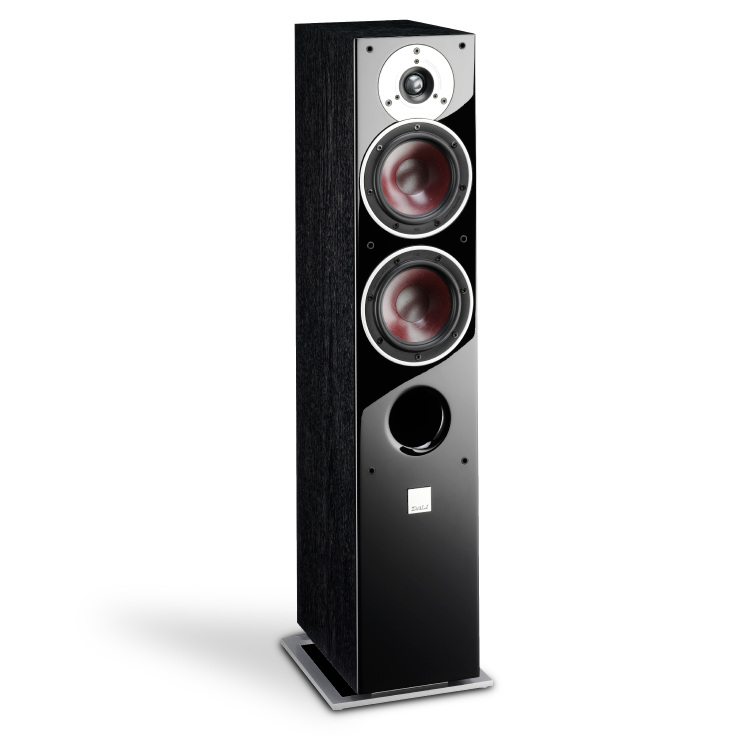
\includegraphics[width=0.5\textwidth]{figures/zensor5.png}
\caption{DALI Zensor 5 \citep{sou:daliZensor5}.}
\label{fig:dali_zensor5}
\end{figure}

%\todo[inline]{Reference http://www.dali-speakers.com/loudspeakers/zensor/zensor-5/}

For measuring the vibrations two Bruel \& Kjær (B\&K) accelerometers have been placed inside the enclosure, one on the back of the bottom driver and one on the top back of the enclosure. For measuring sound a microphone has been placed 1 m from the speaker. To limit any reflections from the room, the test is performed in a Anechoic room at \gls{AAU}, for further documentation refer to the journal in \autoref{app:journal_speaker_test}.  
%\todo[inline]{Reference (09.03.2016) http://doc.es.aau.dk/labs/acoustics/facilities/anechoic_room_large/} 



The loudspeaker is set to play a sinesweep from the crossover frequency of the loudspeaker which is 2400 Hz to 10 Hz. The sine sweep is then repeated from the lowest volume setting of a power amplifier until the loudspeaker breaks. There are in total 20 datasets each containing four measurements, namely the vibrations from the enclosure, driver, the sound pressure from the microphone and lastly a reference signal to synchronize all data. The amount of data is therefore large and only relevant datasets will be presented.  A full detailed overview of graphs is stored on the enclosed CD\footnote{\scalebox{0.7}{\path{CD://Maalinger/Maalinger030316 - Loudspeaker test/Complete Analysis.pdf}}}.



\subsubsection{Analysis of the DALI Zensor 5 measurements}

%In this section a brief review and conclusion of the analysis done in \autoref{app:journal_speaker_test} is presented. 
There are many different approaches in analysing the measured data, and the approach done in this project, will consist of analysing the frequency response of the loudspeaker vibration, harmonic distortion, and detection of the coil hitting the back plate of the driver. The structure of the following part will be showing how the speaker reacts to the different levels of amplification and to conclude if a pattern can be extracted.

%\subsection*{Experiment analysis}

%As previously stated there are in total 20 datasets each containing four measurements, namely the vibrations from the enclosure and driver, the sound pressure from the microphone, and lastly a reference signal to synchronize all data. The amount of data is therefore large and only relevant datasets will be presented. If needed, a more comprehensive approach is taken in \autoref{app:journal_speaker_test} and a full detailed overview of graphs is stored on the enclosed CD.

%\vspace{3mm}

During the first accelerometer measurements the loudspeaker acts linear with very little fluctuations. The frequency response keeps being steadily the same with an increase in amplitude which was expected. In \autoref{fig:Driver1} the first accelerometer measurement is shown, played using 5 mW at XX dB$_{\text{SPL}}$\todo{Fix dB SPL}, on the driver is seen. \autoref{fig:Enclosure1Report} shows the enclosure having a mechanical resonance frequencies at approximately 13 seconds and at 25 seconds while the driver's resonance frequency occurs at 25 seconds. An antiresonance frequency is located at 13 seconds for the accelerometers placed on the driver. The antiresonance frequency is assumed to be caused by the enclosure resonance frequency. This pattern continues for approximately 15 measurements. 

%\todo{Billede af reference tids figur og forklaring af resonans frekvens} %A tendency shows that the 3rd harmonic increases more rapidly than the 2nd harmonic, again as expected for the performance of a loudspeaker.

\begin{figure}[H]
\centering
\begin{subfigure}[t]{0.55\textwidth}
	\tikzsetnextfilename{Driver1Report}
	% This file was created by matlab2tikz.
%
%The latest updates can be retrieved from
%  http://www.mathworks.com/matlabcentral/fileexchange/22022-matlab2tikz-matlab2tikz
%where you can also make suggestions and rate matlab2tikz.
%
\begin{tikzpicture}

\begin{axis}[%
width=2.3in,
height=1.9in,
at={(0.758in,0.481in)},
scale only axis,
xmin=0,
xmax=30,
xmajorgrids,
ymin=-0.02,
ymax=0.02,
ymajorgrids,
xlabel={Time [s]},
ylabel={Amplitude [V]},
axis background/.style={fill=white}
]
\addplot[fill=black,draw=black,forget plot] plot table[row sep=crcr]{%
2.08333333333333e-05	0.000842452049255371\\
0.0417454218822439	0.000724315643310547\\
0.0834700104311544	0.000728130340576172\\
0.125194598980065	0.000715255737304688\\
0.166919187528975	0.000736355781555176\\
0.208643776077886	0.000741124153137207\\
0.250368364626797	0.000725150108337402\\
0.292092953175707	0.00073695182800293\\
0.333817541724618	0.000734806060791016\\
0.375542130273528	0.000743985176086426\\
0.417266718822439	0.000729680061340332\\
0.458991307371349	0.00072777271270752\\
0.50071589592026	0.000744819641113281\\
0.54244048446917	0.000737667083740234\\
0.584165073018081	0.000739336013793945\\
0.625889661566991	0.000748038291931152\\
0.667614250115902	0.000733852386474609\\
0.709338838664812	0.000737309455871582\\
0.751063427213723	0.00073850154876709\\
0.792788015762633	0.000756502151489258\\
0.834512604311544	0.000747323036193848\\
0.876237192860454	0.000743627548217773\\
0.917961781409365	0.000749349594116211\\
0.959686369958275	0.000751495361328125\\
1.00141095850719	0.000746369361877441\\
1.0431355470561	0.000753998756408691\\
1.08486013560501	0.000748515129089355\\
1.12658472415392	0.00075221061706543\\
1.16830931270283	0.000759720802307129\\
1.21003390125174	0.000748515129089355\\
1.25175848980065	0.000764369964599609\\
1.29348307834956	0.000760555267333984\\
1.33520766689847	0.000766396522521973\\
1.37693225544738	0.000762343406677246\\
1.41865684399629	0.000754714012145996\\
1.4603814325452	0.000761151313781738\\
1.50210602109411	0.000756978988647461\\
1.54383060964302	0.000756144523620605\\
1.58555519819193	0.000763535499572754\\
1.62727978674084	0.000756502151489258\\
1.66900437528975	0.000757694244384766\\
1.71072896383866	0.000751137733459473\\
1.75245355238758	0.000756502151489258\\
1.79417814093649	0.000756144523620605\\
1.8359027294854	0.000758051872253418\\
1.87762731803431	0.00075685977935791\\
1.91935190658322	0.000754356384277344\\
1.96107649513213	0.000756144523620605\\
2.00280108368104	0.000751018524169922\\
2.04452567222995	0.000769376754760742\\
2.08625026077886	0.000757336616516113\\
2.12797484932777	0.000759363174438477\\
2.16969943787668	0.000766515731811523\\
2.21142402642559	0.00075685977935791\\
2.2531486149745	0.000760316848754883\\
2.29487320352341	0.000762820243835449\\
2.33659779207232	0.000757813453674316\\
2.37832238062123	0.000756382942199707\\
2.42004696917014	0.000770211219787598\\
2.46177155771905	0.00077366828918457\\
2.50349614626796	0.000762701034545898\\
2.54522073481687	0.000776529312133789\\
2.58694532336579	0.000768661499023438\\
2.6286699119147	0.000769495964050293\\
2.67039450046361	0.000769376754760742\\
2.71211908901252	0.000779390335083008\\
2.75384367756143	0.000778675079345703\\
2.79556826611034	0.000775575637817383\\
2.83729285465925	0.0007781982421875\\
2.87901744320816	0.00077354907989502\\
2.92074203175707	0.000772714614868164\\
2.96246662030598	0.000776886940002441\\
3.00419120885489	0.000785589218139648\\
3.0459157974038	0.000795722007751465\\
3.08764038595271	0.000782370567321777\\
3.12936497450162	0.00078272819519043\\
3.17108956305053	0.000790238380432129\\
3.21281415159944	0.00079810619354248\\
3.25453874014835	0.000793933868408203\\
3.29626332869726	0.000802278518676758\\
3.33798791724618	0.000802397727966309\\
3.37971250579509	0.00080108642578125\\
3.421437094344	0.000811576843261719\\
3.46316168289291	0.000808596611022949\\
3.50488627144182	0.000804781913757324\\
3.54661085999073	0.000814437866210938\\
3.58833544853964	0.000810384750366211\\
3.63006003708855	0.000816583633422852\\
3.67178462563746	0.000807762145996094\\
3.71350921418637	0.000812888145446777\\
3.75523380273528	0.000812768936157227\\
3.79695839128419	0.000815749168395996\\
3.8386829798331	0.000813961029052734\\
3.88040756838201	0.000826478004455566\\
3.92213215693092	0.000814437866210938\\
3.96385674547983	0.000813722610473633\\
4.00558133402874	0.000811934471130371\\
4.04730592257765	0.000820755958557129\\
4.08903051112656	0.000818610191345215\\
4.13075509967547	0.000812888145446777\\
4.17247968822439	0.000814914703369141\\
4.2142042767733	0.000813126564025879\\
4.25592886532221	0.000823259353637695\\
4.29765345387112	0.000821471214294434\\
4.33937804242003	0.000811576843261719\\
4.38110263096894	0.000824570655822754\\
4.42282721951785	0.000835657119750977\\
4.46455180806676	0.000819563865661621\\
4.50627639661567	0.000821113586425781\\
4.54800098516458	0.000826597213745117\\
4.58972557371349	0.000843286514282227\\
4.6314501622624	0.00083458423614502\\
4.67317475081131	0.000841140747070313\\
4.71489933936022	0.000822782516479492\\
4.75662392790913	0.00083160400390625\\
4.79834851645804	0.000840425491333008\\
4.84007310500695	0.000842809677124023\\
4.88179769355586	0.000837802886962891\\
4.92352228210478	0.000848293304443359\\
4.96524687065368	0.000842094421386719\\
5.0069714592026	0.000839948654174805\\
5.04869604775151	0.000844120979309082\\
5.09042063630042	0.000840306282043457\\
5.13214522484933	0.000838994979858398\\
5.17386981339824	0.000844478607177734\\
5.21559440194715	0.000845789909362793\\
5.25731899049606	0.000832080841064453\\
5.29904357904497	0.000855803489685059\\
5.34076816759388	0.000848174095153809\\
5.38249275614279	0.000844120979309082\\
5.4242173446917	0.000833272933959961\\
5.46594193324061	0.000838756561279297\\
5.50766652178952	0.000839591026306152\\
5.54939111033843	0.000842094421386719\\
5.59111569888734	0.000841498374938965\\
5.63284028743625	0.000836610794067383\\
5.67456487598516	0.000829100608825684\\
5.71628946453407	0.000816583633422852\\
5.75801405308299	0.000837326049804688\\
5.7997386416319	0.000834465026855469\\
5.84146323018081	0.000824809074401855\\
5.88318781872972	0.000816226005554199\\
5.92491240727863	0.000822067260742188\\
5.96663699582754	0.000817298889160156\\
6.00836158437645	0.000820398330688477\\
6.05008617292536	0.000815391540527344\\
6.09181076147427	0.000821232795715332\\
6.13353535002318	0.000823259353637695\\
6.17525993857209	0.000811100006103516\\
6.216984527121	0.000824093818664551\\
6.25870911566991	0.00082862377166748\\
6.30043370421882	0.00082707405090332\\
6.34215829276773	0.000818133354187012\\
6.38388288131664	0.00082695484161377\\
6.42560746986555	0.000823736190795898\\
6.46733205841446	0.000827789306640625\\
6.50905664696338	0.000817418098449707\\
6.55078123551229	0.00083315372467041\\
6.5925058240612	0.00083458423614502\\
6.63423041261011	0.000834822654724121\\
6.67595500115902	0.000837922096252441\\
6.71767958970793	0.000827908515930176\\
6.75940417825684	0.00082862377166748\\
6.80112876680575	0.000835776329040527\\
6.84285335535466	0.000834941864013672\\
6.88457794390357	0.000837326049804688\\
6.92630253245248	0.000839829444885254\\
6.96802712100139	0.000847339630126953\\
7.0097517095503	0.00084376335144043\\
7.05147629809921	0.000843644142150879\\
7.09320088664812	0.000847101211547852\\
7.13492547519703	0.000847339630126953\\
7.17665006374594	0.000843644142150879\\
7.21837465229485	0.000848174095153809\\
7.26009924084376	0.000854969024658203\\
7.30182382939268	0.000855684280395508\\
7.34354841794159	0.000865817070007324\\
7.3852730064905	0.000864505767822266\\
7.42699759503941	0.000867962837219238\\
7.46872218358832	0.000847101211547852\\
7.51044677213723	0.000849604606628418\\
7.55217136068614	0.000842928886413574\\
7.59389594923505	0.000854134559631348\\
7.63562053778396	0.000830292701721191\\
7.67734512633287	0.000824570655822754\\
7.71906971488178	0.000828742980957031\\
7.76079430343069	0.000830650329589844\\
7.8025188919796	0.000817418098449707\\
7.84424348052851	0.00081479549407959\\
7.88596806907742	0.000807404518127441\\
7.92769265762633	0.000814914703369141\\
7.96941724617524	0.000820755958557129\\
8.01114183472416	0.000833749771118164\\
8.05286642327307	0.000829458236694336\\
8.09459101182198	0.000839948654174805\\
8.13631560037089	0.00084376335144043\\
8.1780401889198	0.000843167304992676\\
8.21976477746871	0.000849008560180664\\
8.26148936601762	0.000846505165100098\\
8.30321395456653	0.000858187675476074\\
8.34493854311544	0.000867486000061035\\
8.38666313166435	0.000872135162353516\\
8.42838772021326	0.000874876976013184\\
8.47011230876217	0.000872969627380371\\
8.51183689731108	0.000886321067810059\\
8.55356148585999	0.00090634822845459\\
8.5952860744089	0.000900864601135254\\
8.63701066295781	0.000904202461242676\\
8.67873525150672	0.000906229019165039\\
8.72045984005563	0.000902056694030762\\
8.76218442860454	0.000916242599487305\\
8.80390901715345	0.000928282737731934\\
8.84563360570237	0.000935554504394531\\
8.88735819425128	0.000940561294555664\\
8.92908278280018	0.000948786735534668\\
8.9708073713491	0.000948309898376465\\
9.01253195989801	0.000955462455749512\\
9.05425654844692	0.000948071479797363\\
9.09598113699583	0.0009613037109375\\
9.13770572554474	0.000966429710388184\\
9.17943031409365	0.000962972640991211\\
9.22115490264256	0.000972151756286621\\
9.26287949119147	0.000980615615844727\\
9.30460407974038	0.000973939895629883\\
9.34632866828929	0.000976324081420898\\
9.3880532568382	0.000983357429504395\\
9.42977784538711	0.000970959663391113\\
9.47150243393602	0.000966668128967285\\
9.51322702248493	0.000982522964477539\\
9.55495161103384	0.000957965850830078\\
9.59667619958275	0.000975489616394043\\
9.63840078813166	0.000963330268859863\\
9.68012537668058	0.000963330268859863\\
9.72184996522949	0.000955104827880859\\
9.7635745537784	0.000950098037719727\\
9.80529914232731	0.000947952270507813\\
9.84702373087622	0.000951766967773438\\
9.88874831942513	0.000958442687988281\\
9.93047290797404	0.000956416130065918\\
9.97219749652295	0.000945448875427246\\
10.0139220850719	0.000948071479797363\\
10.0556466736208	0.000946640968322754\\
10.0973712621697	0.00095057487487793\\
10.1390958507186	0.000947475433349609\\
10.1808204392675	0.000943899154663086\\
10.2225450278164	0.000938296318054199\\
10.2642696163653	0.000931262969970703\\
10.3059942049142	0.00095665454864502\\
10.3477187934631	0.000945925712585449\\
10.3894433820121	0.000958085060119629\\
10.431167970561	0.000952601432800293\\
10.4728925591099	0.000962257385253906\\
10.5146171476588	0.00095665454864502\\
10.5563417362077	0.000961661338806152\\
10.5980663247566	0.000960826873779297\\
10.6397909133055	0.000966787338256836\\
10.6815155018544	0.000980615615844727\\
10.7232400904033	0.00097501277923584\\
10.7649646789523	0.000985860824584961\\
10.8066892675012	0.000976681709289551\\
10.8484138560501	0.000992298126220703\\
10.890138444599	0.00099635124206543\\
10.9318630331479	0.000995159149169922\\
10.9735876216968	0.00101470947265625\\
11.0153122102457	0.00101017951965332\\
11.0570367987946	0.000998139381408691\\
11.0987613873435	0.00101804733276367\\
11.1404859758924	0.0010455846786499\\
11.1822105644414	0.00105226039886475\\
11.2239351529903	0.00104320049285889\\
11.2656597415392	0.0010448694229126\\
11.3073843300881	0.00104343891143799\\
11.349108918637	0.00106239318847656\\
11.3908335071859	0.00107407569885254\\
11.4325580957348	0.00108933448791504\\
11.4742826842837	0.00108993053436279\\
11.5160072728326	0.00110101699829102\\
11.5577318613816	0.00110852718353271\\
11.5994564499305	0.0011056661605835\\
11.6411810384794	0.00111484527587891\\
11.6829056270283	0.00112783908843994\\
11.7246302155772	0.00113523006439209\\
11.7663548041261	0.00114238262176514\\
11.808079392675	0.00115120410919189\\
11.8498039812239	0.00117611885070801\\
11.8915285697728	0.00117993354797363\\
11.9332531583217	0.0011899471282959\\
11.9749777468707	0.00120007991790771\\
12.0167023354196	0.00119864940643311\\
12.0584269239685	0.0011974573135376\\
12.1001515125174	0.00120961666107178\\
12.1418761010663	0.00121510028839111\\
12.1836006896152	0.00121378898620605\\
12.2253252781641	0.00121426582336426\\
12.267049866713	0.00120794773101807\\
12.3087744552619	0.00118112564086914\\
12.3504990438108	0.0011749267578125\\
12.3922236323598	0.00118374824523926\\
12.4339482209087	0.00116109848022461\\
12.4756728094576	0.00115525722503662\\
12.5173973980065	0.00115251541137695\\
12.5591219865554	0.00112485885620117\\
12.6008465751043	0.00112450122833252\\
12.6425711636532	0.00111746788024902\\
12.6842957522021	0.00111103057861328\\
12.726020340751	0.00111186504364014\\
12.7677449293	0.00110268592834473\\
12.8094695178489	0.00109696388244629\\
12.8511941063978	0.00110363960266113\\
12.8929186949467	0.00111150741577148\\
12.9346432834956	0.00111949443817139\\
12.9763678720445	0.001137375831604\\
13.0180924605934	0.00114357471466064\\
13.0598170491423	0.0011603832244873\\
13.1015416376912	0.00118207931518555\\
13.1432662262401	0.00121927261352539\\
13.1849908147891	0.00120532512664795\\
13.226715403338	0.00122213363647461\\
13.2684399918869	0.00122547149658203\\
13.3101645804358	0.00123798847198486\\
13.3518891689847	0.00121581554412842\\
13.3936137575336	0.0012049674987793\\
13.4353383460825	0.00118744373321533\\
13.4770629346314	0.00116372108459473\\
13.5187875231803	0.00110864639282227\\
13.5605121117293	0.00106608867645264\\
13.6022367002782	0.000977635383605957\\
13.6439612888271	0.000897884368896484\\
13.685685877376	0.000793695449829102\\
13.7274104659249	0.000687122344970703\\
13.7691350544738	0.000558257102966309\\
13.8108596430227	0.000436067581176758\\
13.8525842315716	0.000294923782348633\\
13.8943088201205	0.00018310546875\\
13.9360334086694	0.000113487243652344\\
13.9777579972184	0.000168681144714355\\
14.0194825857673	0.000242471694946289\\
14.0612071743162	0.000313043594360352\\
14.1029317628651	0.000383496284484863\\
14.144656351414	0.000434041023254395\\
14.1863809399629	0.00050199031829834\\
14.2281055285118	0.000554561614990234\\
14.2698301170607	0.000588655471801758\\
14.3115547056096	0.000618696212768555\\
14.3532792941586	0.000660181045532227\\
14.3950038827075	0.000678420066833496\\
14.4367284712564	0.00069725513458252\\
14.4784530598053	0.000716447830200195\\
14.5201776483542	0.000728964805603027\\
14.5619022369031	0.000737190246582031\\
14.603626825452	0.000746846199035645\\
14.6453514140009	0.00075066089630127\\
14.6870760025498	0.000756025314331055\\
14.7288005910988	0.000767707824707031\\
14.7705251796477	0.00078284740447998\\
14.8122497681966	0.000776410102844238\\
14.8539743567455	0.000770330429077148\\
14.8956989452944	0.00076603889465332\\
14.9374235338433	0.000783920288085938\\
14.9791481223922	0.000787258148193359\\
15.0208727109411	0.000798940658569336\\
15.06259729949	0.00080108642578125\\
15.1043218880389	0.000807285308837891\\
15.1460464765879	0.00083625316619873\\
15.1877710651368	0.00084996223449707\\
15.2294956536857	0.000864148139953613\\
15.2712202422346	0.000891566276550293\\
15.3129448307835	0.000901222229003906\\
15.3546694193324	0.000907182693481445\\
15.3963940078813	0.00091242790222168\\
15.4381185964302	0.000938892364501953\\
15.4798431849791	0.000932097434997559\\
15.521567773528	0.000941276550292969\\
15.563292362077	0.000940442085266113\\
15.6050169506259	0.000934958457946777\\
15.6467415391748	0.000942468643188477\\
15.6884661277237	0.000942111015319824\\
15.7301907162726	0.000946402549743652\\
15.7719153048215	0.000940442085266113\\
15.8136398933704	0.000940442085266113\\
15.8553644819193	0.000932574272155762\\
15.8970890704682	0.00094294548034668\\
15.9388136590172	0.000941276550292969\\
15.9805382475661	0.000934720039367676\\
16.022262836115	0.000936269760131836\\
16.0639874246639	0.000932216644287109\\
16.1057120132128	0.000941753387451172\\
16.1474366017617	0.000922083854675293\\
16.1891611903106	0.000919580459594727\\
16.2308857788595	0.000926733016967773\\
16.2726103674084	0.000928401947021484\\
16.3143349559573	0.000926613807678223\\
16.3560595445063	0.000929117202758789\\
16.3977841330552	0.000951766967773438\\
16.4395087216041	0.000945568084716797\\
16.481233310153	0.000967264175415039\\
16.5229578987019	0.000959634780883789\\
16.5646824872508	0.000981688499450684\\
16.6064070757997	0.000978827476501465\\
16.6481316643486	0.00100505352020264\\
16.6898562528975	0.000998139381408691\\
16.7315808414465	0.00101649761199951\\
16.7733054299954	0.00102102756500244\\
16.8150300185443	0.0010451078414917\\
16.8567546070932	0.00104188919067383\\
16.8984791956421	0.00102841854095459\\
16.940203784191	0.00104808807373047\\
16.9819283727399	0.00106561183929443\\
17.0236529612888	0.00106358528137207\\
17.0653775498377	0.00106775760650635\\
17.1071021383867	0.00110936164855957\\
17.1488267269356	0.00111019611358643\\
17.1905513154845	0.0011366605758667\\
17.2322759040334	0.00117075443267822\\
17.2740004925823	0.00120162963867188\\
17.3157250811312	0.00121581554412842\\
17.3574496696801	0.00124251842498779\\
17.399174258229	0.00124752521514893\\
17.4408988467779	0.00124835968017578\\
17.4826234353268	0.00122547149658203\\
17.5243480238758	0.00121092796325684\\
17.5660726124247	0.00118362903594971\\
17.6077972009736	0.00117075443267822\\
17.6495217895225	0.00116026401519775\\
17.6912463780714	0.00117111206054688\\
17.7329709666203	0.00116336345672607\\
17.7746955551692	0.00118422508239746\\
17.8164201437181	0.00119113922119141\\
17.858144732267	0.00120329856872559\\
17.8998693208159	0.00122535228729248\\
17.9415939093649	0.00124597549438477\\
17.9833184979138	0.00124430656433105\\
18.0250430864627	0.00126302242279053\\
18.0667676750116	0.00126171112060547\\
18.1084922635605	0.00125372409820557\\
18.1502168521094	0.00124704837799072\\
18.1919414406583	0.00123119354248047\\
18.2336660292072	0.00121426582336426\\
18.2753906177561	0.00119447708129883\\
18.3171152063051	0.00117504596710205\\
18.358839794854	0.00118374824523926\\
18.4005643834029	0.00120377540588379\\
18.4422889719518	0.00127255916595459\\
18.4840135605007	0.00135231018066406\\
18.5257381490496	0.00141823291778564\\
18.5674627375985	0.00150668621063232\\
18.6091873261474	0.00154757499694824\\
18.6509119146963	0.0015639066696167\\
18.6926365032453	0.00156760215759277\\
18.7343610917942	0.00158751010894775\\
18.7760856803431	0.00158250331878662\\
18.817810268892	0.00157392024993896\\
18.8595348574409	0.00155794620513916\\
18.9012594459898	0.00155055522918701\\
18.9429840345387	0.00154078006744385\\
18.9847086230876	0.00152921676635742\\
19.0264332116365	0.00152289867401123\\
19.0681578001854	0.00152289867401123\\
19.1098823887344	0.00150799751281738\\
19.1516069772833	0.00149905681610107\\
19.1933315658322	0.00147044658660889\\
19.2350561543811	0.00145161151885986\\
19.27678074293	0.00144112110137939\\
19.3185053314789	0.00142991542816162\\
19.3602299200278	0.00141644477844238\\
19.4019545085767	0.0013880729675293\\
19.4436790971256	0.00139951705932617\\
19.4854036856745	0.00137901306152344\\
19.5271282742235	0.00136971473693848\\
19.5688528627724	0.00136721134185791\\
19.6105774513213	0.00136351585388184\\
19.6523020398702	0.00136446952819824\\
19.6940266284191	0.0013653039932251\\
19.735751216968	0.00137889385223389\\
19.7774758055169	0.00138390064239502\\
19.8192003940658	0.0013740062713623\\
19.8609249826147	0.00138437747955322\\
19.9026495711637	0.00140023231506348\\
19.9443741597126	0.00139617919921875\\
19.9860987482615	0.00141024589538574\\
20.0278233368104	0.00141370296478271\\
20.0695479253593	0.00140857696533203\\
20.1112725139082	0.00143897533416748\\
20.1529971024571	0.00145316123962402\\
20.194721691006	0.00147128105163574\\
20.2364462795549	0.00149738788604736\\
20.2781708681038	0.00151407718658447\\
20.3198954566528	0.00153207778930664\\
20.3616200452017	0.00156009197235107\\
20.4033446337506	0.0015721321105957\\
20.4450692222995	0.00161302089691162\\
20.4867938108484	0.00163066387176514\\
20.5285183993973	0.00164401531219482\\
20.5702429879462	0.00166523456573486\\
20.6119675764951	0.00166523456573486\\
20.653692165044	0.0016857385635376\\
20.695416753593	0.00168442726135254\\
20.7371413421419	0.00170993804931641\\
20.7788659306908	0.00172114372253418\\
20.8205905192397	0.00173604488372803\\
20.8623151077886	0.00174999237060547\\
20.9040396963375	0.00177335739135742\\
20.9457642848864	0.00178420543670654\\
20.9874888734353	0.00179541110992432\\
21.0292134619842	0.0018075704574585\\
21.0709380505331	0.00182294845581055\\
21.1126626390821	0.00182592868804932\\
21.154387227631	0.00183844566345215\\
21.1961118161799	0.00185132026672363\\
21.2378364047288	0.00185286998748779\\
21.2795609932777	0.00185167789459229\\
21.3212855818266	0.00186431407928467\\
21.3630101703755	0.0018768310546875\\
21.4047347589244	0.00187921524047852\\
21.4464593474733	0.00189435482025146\\
21.4881839360223	0.00190842151641846\\
21.5299085245712	0.00191879272460938\\
21.5716331131201	0.0019301176071167\\
21.613357701669	0.00195229053497314\\
21.6550822902179	0.00198221206665039\\
21.6968068787668	0.00199604034423828\\
21.7385314673157	0.00202810764312744\\
21.7802560558646	0.00205862522125244\\
21.8219806444135	0.00206995010375977\\
21.8637052329624	0.00211036205291748\\
21.9054298215114	0.0021432638168335\\
21.9471544100603	0.00215423107147217\\
21.9888789986092	0.00216424465179443\\
22.0306035871581	0.00215709209442139\\
22.072328175707	0.00216305255889893\\
22.1140527642559	0.00213837623596191\\
22.1557773528048	0.00213634967803955\\
22.1975019413537	0.00212752819061279\\
22.2392265299026	0.0021662712097168\\
22.2809511184516	0.00218296051025391\\
22.3226757070005	0.00220799446105957\\
22.3644002955494	0.002236008644104\\
22.4061248840983	0.00226271152496338\\
22.4478494726472	0.00227344036102295\\
22.4895740611961	0.00229513645172119\\
22.531298649745	0.00232028961181641\\
22.5730232382939	0.00235486030578613\\
22.6147478268428	0.00240409374237061\\
22.6564724153917	0.00249433517456055\\
22.6981970039407	0.00258851051330566\\
22.7399215924896	0.00270044803619385\\
22.7816461810385	0.00281000137329102\\
22.8233707695874	0.00291359424591064\\
22.8650953581363	0.00298619270324707\\
22.9068199466852	0.00299859046936035\\
22.9485445352341	0.00299358367919922\\
22.990269123783	0.00297236442565918\\
23.0319937123319	0.00287067890167236\\
23.0737183008809	0.00273036956787109\\
23.1154428894298	0.0025404691696167\\
23.1571674779787	0.00235271453857422\\
23.1988920665276	0.00218009948730469\\
23.2406166550765	0.00201857089996338\\
23.2823412436254	0.00202608108520508\\
23.3240658321743	0.00209319591522217\\
23.3657904207232	0.00218164920806885\\
23.4075150092721	0.00226426124572754\\
23.449239597821	0.00233328342437744\\
23.49096418637	0.0023798942565918\\
23.5326887749189	0.0024033784866333\\
23.5744133634678	0.00241625308990479\\
23.6161379520167	0.00243675708770752\\
23.6578625405656	0.0024871826171875\\
23.6995871291145	0.00255143642425537\\
23.7413117176634	0.00261306762695313\\
23.7830363062123	0.00269031524658203\\
23.8247608947612	0.00277090072631836\\
23.8664854833102	0.00285768508911133\\
23.9082100718591	0.00295233726501465\\
23.949934660408	0.0030667781829834\\
23.9916592489569	0.00317692756652832\\
24.0333838375058	0.00328707695007324\\
24.0751084260547	0.00342345237731934\\
24.1168330146036	0.00355243682861328\\
24.1585576031525	0.00371789932250977\\
24.2002821917014	0.00386691093444824\\
24.2420067802503	0.00402510166168213\\
24.2837313687993	0.00418233871459961\\
24.3254559573482	0.00438845157623291\\
24.3671805458971	0.00456619262695313\\
24.408905134446	0.00477814674377441\\
24.4506297229949	0.00500857830047607\\
24.4923543115438	0.00528395175933838\\
24.5340789000927	0.00555253028869629\\
24.5758034886416	0.00591349601745605\\
24.6175280771905	0.00626111030578613\\
24.6592526657395	0.00665700435638428\\
24.7009772542884	0.00705134868621826\\
24.7427018428373	0.00741517543792725\\
24.7844264313862	0.00782275199890137\\
24.8261510199351	0.00829911231994629\\
24.867875608484	0.00896334648132324\\
24.9096001970329	0.00995182991027832\\
24.9513247855818	0.011165976524353\\
24.9930493741307	0.012565016746521\\
25.0347739626796	0.0142723321914673\\
25.0764985512286	0.0162241458892822\\
25.1182231397775	0.0180796384811401\\
25.1599477283264	0.0194665193557739\\
25.2016723168753	0.0196808576583862\\
25.2433969054242	0.019420862197876\\
25.2851214939731	0.0176268815994263\\
25.326846082522	0.0148277282714844\\
25.3685706710709	0.0115214586257935\\
25.4102952596198	0.00949466228485107\\
25.4520198481687	0.00793111324310303\\
25.4937444367177	0.00675833225250244\\
25.5354690252666	0.00582170486450195\\
25.5771936138155	0.00510656833648682\\
25.6189182023644	0.00454449653625488\\
25.6606427909133	0.00404250621795654\\
25.7023673794622	0.00363194942474365\\
25.7440919680111	0.00321686267852783\\
25.78581655656	0.0028984546661377\\
25.8275411451089	0.00256967544555664\\
25.8692657336579	0.00231683254241943\\
25.9109903222068	0.00206875801086426\\
25.9527149107557	0.00185883045196533\\
25.9944394993046	0.00165820121765137\\
26.0361640878535	0.00150573253631592\\
26.0778886764024	0.00152122974395752\\
26.1196132649513	0.00173819065093994\\
26.1613378535002	0.00199723243713379\\
26.2030624420491	0.00220644474029541\\
26.2447870305981	0.00220096111297607\\
26.286511619147	0.00204658508300781\\
26.3282362076959	0.00164556503295898\\
26.3699607962448	0.00141119956970215\\
26.4116853847937	0.00154078006744385\\
26.4534099733426	0.00174570083618164\\
26.4951345618915	0.00183117389678955\\
26.5368591504404	0.00183594226837158\\
26.5785837389893	0.00163650512695313\\
26.6203083275383	0.00140058994293213\\
26.6620329160872	0.00124001502990723\\
26.7037575046361	0.00111579895019531\\
26.745482093185	0.00109744071960449\\
26.7872066817339	0.00114655494689941\\
26.8289312702828	0.00115036964416504\\
26.8706558588317	0.0010751485824585\\
26.9123804473806	0.000989675521850586\\
26.9541050359295	0.000946640968322754\\
26.9958296244784	0.0010601282119751\\
27.0375542130274	0.00109231472015381\\
27.0792788015763	0.00107848644256592\\
27.1210033901252	0.000966310501098633\\
27.1627279786741	0.000848174095153809\\
27.204452567223	0.000764727592468262\\
27.2461771557719	0.000650525093078613\\
27.2879017443208	0.000586748123168945\\
27.3296263328697	0.00053858757019043\\
27.3713509214186	0.000492334365844727\\
27.4130755099675	0.000432610511779785\\
27.4548000985165	0.000382304191589355\\
27.4965246870654	0.000351667404174805\\
27.5382492756143	0.000335097312927246\\
27.5799738641632	0.000327467918395996\\
27.6216984527121	0.000345587730407715\\
27.663423041261	0.000339984893798828\\
27.7051476298099	0.000326752662658691\\
27.7468722183588	0.000255465507507324\\
27.7885968069077	0.000196218490600586\\
27.8303213954567	0.000179886817932129\\
27.8720459840056	0.000151991844177246\\
27.9137705725545	0.000140666961669922\\
27.9554951611034	0.000151515007019043\\
27.9972197496523	0.00017392635345459\\
28.0389443382012	0.000173568725585938\\
28.0806689267501	0.000182271003723145\\
28.122393515299	0.000199556350708008\\
28.1641181038479	0.000229477882385254\\
28.2058426923968	0.000199556350708008\\
28.2475672809458	0.00016319751739502\\
28.2892918694947	0.000146865844726563\\
28.3310164580436	0.000162005424499512\\
28.3727410465925	0.00016939640045166\\
28.4144656351414	0.000180602073669434\\
28.4561902236903	0.000207781791687012\\
28.4979148122392	0.000230312347412109\\
28.5396394007881	0.00024878978729248\\
28.581363989337	0.00026702880859375\\
28.623088577886	0.00024712085723877\\
28.6648131664349	0.000267505645751953\\
28.7065377549838	0.000287413597106934\\
28.7482623435327	0.000310063362121582\\
28.7899869320816	0.000333070755004883\\
28.8317115206305	0.000332236289978027\\
28.8734361091794	0.000330567359924316\\
28.9151606977283	0.000338912010192871\\
28.9568852862772	0.0003509521484375\\
28.9986098748261	0.000365018844604492\\
29.0403344633751	0.000368833541870117\\
29.082059051924	0.000351786613464355\\
29.1237836404729	0.000357151031494141\\
29.1655082290218	0.00033724308013916\\
29.2072328175707	0.000323772430419922\\
29.2489574061196	0.000299692153930664\\
29.2906819946685	0.000292539596557617\\
29.3324065832174	0.000269055366516113\\
29.3741311717663	0.000259637832641602\\
29.4158557603153	0.000249624252319336\\
29.4575803488642	0.000213623046875\\
29.4993049374131	0.000187873840332031\\
29.541029525962	0.000171542167663574\\
29.5827541145109	0.000138521194458008\\
29.6244787030598	0.000112175941467285\\
29.6662032916087	8.85725021362305e-05\\
29.7079278801576	7.25984573364258e-05\\
29.7496524687065	6.3776969909668e-05\\
29.7913770572554	0.000100255012512207\\
29.8331016458044	8.69035720825195e-05\\
29.8748262343533	8.80956649780273e-05\\
29.9165508229022	9.09566879272461e-05\\
29.9582754114511	7.89165496826172e-05\\
30	6.34193420410156e-05\\
}
\closedcycle;
\addplot[fill=black,draw=black,forget plot] plot table[row sep=crcr]{%
2.08333333333333e-05	-0.000848650932312012\\
0.0417454218822439	-0.000736355781555176\\
0.0834700104311544	-0.000727176666259766\\
0.125194598980065	-0.000741720199584961\\
0.166919187528975	-0.000732183456420898\\
0.208643776077886	-0.000723361968994141\\
0.250368364626797	-0.0007476806640625\\
0.292092953175707	-0.000734686851501465\\
0.333817541724618	-0.000736474990844727\\
0.375542130273528	-0.00073397159576416\\
0.417266718822439	-0.000738024711608887\\
0.458991307371349	-0.000752568244934082\\
0.50071589592026	-0.000742197036743164\\
0.54244048446917	-0.000741481781005859\\
0.584165073018081	-0.000744819641113281\\
0.625889661566991	-0.000743985176086426\\
0.667614250115902	-0.000739812850952148\\
0.709338838664812	-0.000747323036193848\\
0.751063427213723	-0.000758171081542969\\
0.792788015762633	-0.000746011734008789\\
0.834512604311544	-0.000747203826904297\\
0.876237192860454	-0.000759005546569824\\
0.917961781409365	-0.000752568244934082\\
0.959686369958275	-0.000758051872253418\\
1.00141095850719	-0.000755906105041504\\
1.0431355470561	-0.000764250755310059\\
1.08486013560501	-0.000764250755310059\\
1.12658472415392	-0.000774264335632324\\
1.16830931270283	-0.000757694244384766\\
1.21003390125174	-0.000753998756408691\\
1.25175848980065	-0.000754237174987793\\
1.29348307834956	-0.000767707824707031\\
1.33520766689847	-0.000755071640014648\\
1.37693225544738	-0.000764369964599609\\
1.41865684399629	-0.000763893127441406\\
1.4603814325452	-0.000762701034545898\\
1.50210602109411	-0.000756382942199707\\
1.54383060964302	-0.000757575035095215\\
1.58555519819193	-0.000766873359680176\\
1.62727978674084	-0.000766873359680176\\
1.66900437528975	-0.000758886337280273\\
1.71072896383866	-0.00077521800994873\\
1.75245355238758	-0.000761866569519043\\
1.79417814093649	-0.000762224197387695\\
1.8359027294854	-0.000767707824707031\\
1.87762731803431	-0.000755667686462402\\
1.91935190658322	-0.000763416290283203\\
1.96107649513213	-0.000767350196838379\\
2.00280108368104	-0.000774025917053223\\
2.04452567222995	-0.000765085220336914\\
2.08625026077886	-0.000775694847106934\\
2.12797484932777	-0.000765681266784668\\
2.16969943787668	-0.000776410102844238\\
2.21142402642559	-0.000763058662414551\\
2.2531486149745	-0.000763058662414551\\
2.29487320352341	-0.000760912895202637\\
2.33659779207232	-0.000757694244384766\\
2.37832238062123	-0.000784873962402344\\
2.42004696917014	-0.000759243965148926\\
2.46177155771905	-0.000768899917602539\\
2.50349614626796	-0.000772595405578613\\
2.54522073481687	-0.000766873359680176\\
2.58694532336579	-0.000774860382080078\\
2.6286699119147	-0.000769853591918945\\
2.67039450046361	-0.000781416893005371\\
2.71211908901252	-0.000794768333435059\\
2.75384367756143	-0.000785231590270996\\
2.79556826611034	-0.000778436660766602\\
2.83729285465925	-0.000780582427978516\\
2.87901744320816	-0.000785112380981445\\
2.92074203175707	-0.000790715217590332\\
2.96246662030598	-0.00080108642578125\\
3.00419120885489	-0.000789880752563477\\
3.0459157974038	-0.0007781982421875\\
3.08764038595271	-0.000789880752563477\\
3.12936497450162	-0.000799417495727539\\
3.17108956305053	-0.000792384147644043\\
3.21281415159944	-0.000795245170593262\\
3.25453874014835	-0.00079345703125\\
3.29626332869726	-0.000799894332885742\\
3.33798791724618	-0.000810623168945313\\
3.37971250579509	-0.000804901123046875\\
3.421437094344	-0.000817656517028809\\
3.46316168289291	-0.000798583030700684\\
3.50488627144182	-0.000811100006103516\\
3.54661085999073	-0.00082099437713623\\
3.58833544853964	-0.000811100006103516\\
3.63006003708855	-0.000810146331787109\\
3.67178462563746	-0.00082850456237793\\
3.71350921418637	-0.00082850456237793\\
3.75523380273528	-0.000806570053100586\\
3.79695839128419	-0.00083160400390625\\
3.8386829798331	-0.000824809074401855\\
3.88040756838201	-0.000826597213745117\\
3.92213215693092	-0.000815629959106445\\
3.96385674547983	-0.00081026554107666\\
4.00558133402874	-0.000826120376586914\\
4.04730592257765	-0.00081944465637207\\
4.08903051112656	-0.000818610191345215\\
4.13075509967547	-0.000826478004455566\\
4.17247968822439	-0.000844836235046387\\
4.2142042767733	-0.000839471817016602\\
4.25592886532221	-0.000809073448181152\\
4.29765345387112	-0.000808238983154297\\
4.33937804242003	-0.000825762748718262\\
4.38110263096894	-0.000840663909912109\\
4.42282721951785	-0.000823259353637695\\
4.46455180806676	-0.000833272933959961\\
4.50627639661567	-0.000827670097351074\\
4.54800098516458	-0.000819921493530273\\
4.58972557371349	-0.00082862377166748\\
4.6314501622624	-0.000837802886962891\\
4.67317475081131	-0.000841140747070313\\
4.71489933936022	-0.000836014747619629\\
4.75662392790913	-0.00083613395690918\\
4.79834851645804	-0.000834107398986816\\
4.84007310500695	-0.000843286514282227\\
4.88179769355586	-0.000843286514282227\\
4.92352228210478	-0.000844001770019531\\
4.96524687065368	-0.000848531723022461\\
5.0069714592026	-0.000839948654174805\\
5.04869604775151	-0.000840306282043457\\
5.09042063630042	-0.000840306282043457\\
5.13214522484933	-0.000833630561828613\\
5.17386981339824	-0.000844120979309082\\
5.21559440194715	-0.000847816467285156\\
5.25731899049606	-0.00084233283996582\\
5.29904357904497	-0.000841498374938965\\
5.34076816759388	-0.000856161117553711\\
5.38249275614279	-0.000845193862915039\\
5.4242173446917	-0.000843524932861328\\
5.46594193324061	-0.000838160514831543\\
5.50766652178952	-0.000849485397338867\\
5.54939111033843	-0.00084078311920166\\
5.59111569888734	-0.000829935073852539\\
5.63284028743625	-0.000863313674926758\\
5.67456487598516	-0.000837326049804688\\
5.71628946453407	-0.000847339630126953\\
5.75801405308299	-0.000831007957458496\\
5.7997386416319	-0.000832438468933105\\
5.84146323018081	-0.00081932544708252\\
5.88318781872972	-0.000827789306640625\\
5.92491240727863	-0.000827431678771973\\
5.96663699582754	-0.000844955444335938\\
6.00836158437645	-0.000824451446533203\\
6.05008617292536	-0.000841498374938965\\
6.09181076147427	-0.000824332237243652\\
6.13353535002318	-0.000823974609375\\
6.17525993857209	-0.000834822654724121\\
6.216984527121	-0.00083315372467041\\
6.25870911566991	-0.000827312469482422\\
6.30043370421882	-0.000815987586975098\\
6.34215829276773	-0.000829935073852539\\
6.38388288131664	-0.000832796096801758\\
6.42560746986555	-0.000832676887512207\\
6.46733205841446	-0.000835657119750977\\
6.50905664696338	-0.000832319259643555\\
6.55078123551229	-0.00084078311920166\\
6.5925058240612	-0.000838994979858398\\
6.63423041261011	-0.000837802886962891\\
6.67595500115902	-0.000836610794067383\\
6.71767958970793	-0.000833511352539063\\
6.75940417825684	-0.000843524932861328\\
6.80112876680575	-0.000849485397338867\\
6.84285335535466	-0.00084233283996582\\
6.88457794390357	-0.000846624374389648\\
6.92630253245248	-0.000850319862365723\\
6.96802712100139	-0.00084686279296875\\
7.0097517095503	-0.000850796699523926\\
7.05147629809921	-0.000838279724121094\\
7.09320088664812	-0.000857353210449219\\
7.13492547519703	-0.000848531723022461\\
7.17665006374594	-0.000858306884765625\\
7.21837465229485	-0.000882744789123535\\
7.26009924084376	-0.000882506370544434\\
7.30182382939268	-0.000867009162902832\\
7.34354841794159	-0.000865817070007324\\
7.3852730064905	-0.000858306884765625\\
7.42699759503941	-0.000864386558532715\\
7.46872218358832	-0.000867724418640137\\
7.51044677213723	-0.000861525535583496\\
7.55217136068614	-0.000847697257995605\\
7.59389594923505	-0.000844359397888184\\
7.63562053778396	-0.000846147537231445\\
7.67734512633287	-0.000851035118103027\\
7.71906971488178	-0.000816822052001953\\
7.76079430343069	-0.000815153121948242\\
7.8025188919796	-0.000821113586425781\\
7.84424348052851	-0.000821113586425781\\
7.88596806907742	-0.000821590423583984\\
7.92769265762633	-0.000823974609375\\
7.96941724617524	-0.000836968421936035\\
8.01114183472416	-0.00081944465637207\\
8.05286642327307	-0.000829815864562988\\
8.09459101182198	-0.000835776329040527\\
8.13631560037089	-0.00083613395690918\\
8.1780401889198	-0.00084531307220459\\
8.21976477746871	-0.000847339630126953\\
8.26148936601762	-0.000851154327392578\\
8.30321395456653	-0.00084996223449707\\
8.34493854311544	-0.000859498977661133\\
8.38666313166435	-0.000870347023010254\\
8.42838772021326	-0.000869512557983398\\
8.47011230876217	-0.000878691673278809\\
8.51183689731108	-0.000882506370544434\\
8.55356148585999	-0.000886082649230957\\
8.5952860744089	-0.000893235206604004\\
8.63701066295781	-0.000912904739379883\\
8.67873525150672	-0.000919580459594727\\
8.72045984005563	-0.000918745994567871\\
8.76218442860454	-0.000920295715332031\\
8.80390901715345	-0.000934243202209473\\
8.84563360570237	-0.000929474830627441\\
8.88735819425128	-0.000936985015869141\\
8.92908278280018	-0.000938773155212402\\
8.9708073713491	-0.00094449520111084\\
9.01253195989801	-0.000952005386352539\\
9.05425654844692	-0.000960111618041992\\
9.09598113699583	-0.000960946083068848\\
9.13770572554474	-0.000954508781433105\\
9.17943031409365	-0.000959515571594238\\
9.22115490264256	-0.000964164733886719\\
9.26287949119147	-0.000971794128417969\\
9.30460407974038	-0.00097966194152832\\
9.34632866828929	-0.00097048282623291\\
9.3880532568382	-0.000972151756286621\\
9.42977784538711	-0.000975370407104492\\
9.47150243393602	-0.000976324081420898\\
9.51322702248493	-0.000971674919128418\\
9.55495161103384	-0.000966787338256836\\
9.59667619958275	-0.000972509384155273\\
9.63840078813166	-0.000962018966674805\\
9.68012537668058	-0.00096595287322998\\
9.72184996522949	-0.00096285343170166\\
9.7635745537784	-0.000970005989074707\\
9.80529914232731	-0.000964999198913574\\
9.84702373087622	-0.000945925712585449\\
9.88874831942513	-0.00096428394317627\\
9.93047290797404	-0.000971317291259766\\
9.97219749652295	-0.000945091247558594\\
10.0139220850719	-0.000952482223510742\\
10.0556466736208	-0.000939607620239258\\
10.0973712621697	-0.000944614410400391\\
10.1390958507186	-0.000936150550842285\\
10.1808204392675	-0.000943660736083984\\
10.2225450278164	-0.000951170921325684\\
10.2642696163653	-0.000944614410400391\\
10.3059942049142	-0.000943422317504883\\
10.3477187934631	-0.000941634178161621\\
10.3894433820121	-0.000942587852478027\\
10.431167970561	-0.000953435897827148\\
10.4728925591099	-0.000962138175964355\\
10.5146171476588	-0.000963330268859863\\
10.5563417362077	-0.000968694686889648\\
10.5980663247566	-0.000970840454101563\\
10.6397909133055	-0.000980138778686523\\
10.6815155018544	-0.000971317291259766\\
10.7232400904033	-0.000975847244262695\\
10.7649646789523	-0.000984311103820801\\
10.8066892675012	-0.00100791454315186\\
10.8484138560501	-0.000988364219665527\\
10.890138444599	-0.000985860824584961\\
10.9318630331479	-0.000999689102172852\\
10.9735876216968	-0.000994205474853516\\
11.0153122102457	-0.00100958347320557\\
11.0570367987946	-0.00100922584533691\\
11.0987613873435	-0.00102090835571289\\
11.1404859758924	-0.00102758407592773\\
11.1822105644414	-0.0010221004486084\\
11.2239351529903	-0.00104045867919922\\
11.2656597415392	-0.00105273723602295\\
11.3073843300881	-0.00106215476989746\\
11.349108918637	-0.00106596946716309\\
11.3908335071859	-0.00107014179229736\\
11.4325580957348	-0.00107312202453613\\
11.4742826842837	-0.00108301639556885\\
11.5160072728326	-0.0010911226272583\\
11.5577318613816	-0.00110316276550293\\
11.5994564499305	-0.00111198425292969\\
11.6411810384794	-0.00113534927368164\\
11.6829056270283	-0.00112700462341309\\
11.7246302155772	-0.00113224983215332\\
11.7663548041261	-0.00114190578460693\\
11.808079392675	-0.00116229057312012\\
11.8498039812239	-0.001167893409729\\
11.8915285697728	-0.00116455554962158\\
11.9332531583217	-0.00118577480316162\\
11.9749777468707	-0.00119209289550781\\
12.0167023354196	-0.00119900703430176\\
12.0584269239685	-0.001212477684021\\
12.1001515125174	-0.0012129545211792\\
12.1418761010663	-0.00120663642883301\\
12.1836006896152	-0.00120294094085693\\
12.2253252781641	-0.001212477684021\\
12.267049866713	-0.00120329856872559\\
12.3087744552619	-0.00120460987091064\\
12.3504990438108	-0.0011974573135376\\
12.3922236323598	-0.00117373466491699\\
12.4339482209087	-0.00116944313049316\\
12.4756728094576	-0.00114285945892334\\
12.5173973980065	-0.00113606452941895\\
12.5591219865554	-0.00113809108734131\\
12.6008465751043	-0.00113391876220703\\
12.6425711636532	-0.00111567974090576\\
12.6842957522021	-0.00110936164855957\\
12.726020340751	-0.00112056732177734\\
12.7677449293	-0.00111198425292969\\
12.8094695178489	-0.001106858253479\\
12.8511941063978	-0.00111639499664307\\
12.8929186949467	-0.00111198425292969\\
12.9346432834956	-0.00111854076385498\\
12.9763678720445	-0.00113153457641602\\
13.0180924605934	-0.00114357471466064\\
13.0598170491423	-0.00116610527038574\\
13.1015416376912	-0.00116956233978271\\
13.1432662262401	-0.00120401382446289\\
13.1849908147891	-0.00121498107910156\\
13.226715403338	-0.00122487545013428\\
13.2684399918869	-0.00122964382171631\\
13.3101645804358	-0.00122547149658203\\
13.3518891689847	-0.00121867656707764\\
13.3936137575336	-0.00120961666107178\\
13.4353383460825	-0.00118327140808105\\
13.4770629346314	-0.0011669397354126\\
13.5187875231803	-0.00110816955566406\\
13.5605121117293	-0.00104844570159912\\
13.6022367002782	-0.000969171524047852\\
13.6439612888271	-0.000888586044311523\\
13.685685877376	-0.00076901912689209\\
13.7274104659249	-0.000667214393615723\\
13.7691350544738	-0.000551581382751465\\
13.8108596430227	-0.000410914421081543\\
13.8525842315716	-0.000306606292724609\\
13.8943088201205	-0.000197768211364746\\
13.9360334086694	-0.000112175941467285\\
13.9777579972184	-0.000181913375854492\\
14.0194825857673	-0.000244140625\\
14.0612071743162	-0.000320315361022949\\
14.1029317628651	-0.000381708145141602\\
14.144656351414	-0.000441789627075195\\
14.1863809399629	-0.000502347946166992\\
14.2281055285118	-0.000534892082214355\\
14.2698301170607	-0.000576257705688477\\
14.3115547056096	-0.000625491142272949\\
14.3532792941586	-0.00065302848815918\\
14.3950038827075	-0.000675082206726074\\
14.4367284712564	-0.000693798065185547\\
14.4784530598053	-0.000714659690856934\\
14.5201776483542	-0.000726461410522461\\
14.5619022369031	-0.000730514526367188\\
14.603626825452	-0.000746846199035645\\
14.6453514140009	-0.000749707221984863\\
14.6870760025498	-0.000753402709960938\\
14.7288005910988	-0.000758051872253418\\
14.7705251796477	-0.000763416290283203\\
14.8122497681966	-0.000777721405029297\\
14.8539743567455	-0.000776052474975586\\
14.8956989452944	-0.000780224800109863\\
14.9374235338433	-0.000778555870056152\\
14.9791481223922	-0.000784039497375488\\
15.0208727109411	-0.000782608985900879\\
15.06259729949	-0.000801801681518555\\
15.1043218880389	-0.00082099437713623\\
15.1460464765879	-0.000834107398986816\\
15.1877710651368	-0.00084996223449707\\
15.2294956536857	-0.000871658325195313\\
15.2712202422346	-0.000887513160705566\\
15.3129448307835	-0.000896573066711426\\
15.3546694193324	-0.000909209251403809\\
15.3963940078813	-0.000923752784729004\\
15.4381185964302	-0.000920772552490234\\
15.4798431849791	-0.00092780590057373\\
15.521567773528	-0.000931620597839355\\
15.563292362077	-0.000945091247558594\\
15.6050169506259	-0.00093996524810791\\
15.6467415391748	-0.000938653945922852\\
15.6884661277237	-0.000944972038269043\\
15.7301907162726	-0.000953793525695801\\
15.7719153048215	-0.000945806503295898\\
15.8136398933704	-0.000936746597290039\\
15.8553644819193	-0.000945091247558594\\
15.8970890704682	-0.000931978225708008\\
15.9388136590172	-0.000943779945373535\\
15.9805382475661	-0.000931143760681152\\
16.022262836115	-0.000934243202209473\\
16.0639874246639	-0.000919222831726074\\
16.1057120132128	-0.000923395156860352\\
16.1474366017617	-0.000920414924621582\\
16.1891611903106	-0.000921249389648438\\
16.2308857788595	-0.000930070877075195\\
16.2726103674084	-0.000924468040466309\\
16.3143349559573	-0.000932574272155762\\
16.3560595445063	-0.000927925109863281\\
16.3977841330552	-0.000930309295654297\\
16.4395087216041	-0.000947833061218262\\
16.481233310153	-0.000953793525695801\\
16.5229578987019	-0.000977158546447754\\
16.5646824872508	-0.000983715057373047\\
16.6064070757997	-0.000995159149169922\\
16.6481316643486	-0.00100934505462646\\
16.6898562528975	-0.00100588798522949\\
16.7315808414465	-0.00101184844970703\\
16.7733054299954	-0.00101876258850098\\
16.8150300185443	-0.00101518630981445\\
16.8567546070932	-0.00102925300598145\\
16.8984791956421	-0.0010535717010498\\
16.940203784191	-0.0010526180267334\\
16.9819283727399	-0.00106298923492432\\
17.0236529612888	-0.00106930732727051\\
17.0653775498377	-0.00107526779174805\\
17.1071021383867	-0.00109601020812988\\
17.1488267269356	-0.00111603736877441\\
17.1905513154845	-0.00113654136657715\\
17.2322759040334	-0.00116622447967529\\
17.2740004925823	-0.00119292736053467\\
17.3157250811312	-0.00121963024139404\\
17.3574496696801	-0.00125205516815186\\
17.399174258229	-0.00124049186706543\\
17.4408988467779	-0.00123584270477295\\
17.4826234353268	-0.00121903419494629\\
17.5243480238758	-0.00122082233428955\\
17.5660726124247	-0.00119912624359131\\
17.6077972009736	-0.00117695331573486\\
17.6495217895225	-0.00116705894470215\\
17.6912463780714	-0.00115394592285156\\
17.7329709666203	-0.00115203857421875\\
17.7746955551692	-0.00117242336273193\\
17.8164201437181	-0.00120878219604492\\
17.858144732267	-0.00122666358947754\\
17.8998693208159	-0.00123834609985352\\
17.9415939093649	-0.00125133991241455\\
17.9833184979138	-0.00124657154083252\\
18.0250430864627	-0.00126051902770996\\
18.0667676750116	-0.00125217437744141\\
18.1084922635605	-0.00124919414520264\\
18.1502168521094	-0.00123703479766846\\
18.1919414406583	-0.00122249126434326\\
18.2336660292072	-0.00120997428894043\\
18.2753906177561	-0.00119209289550781\\
18.3171152063051	-0.00117659568786621\\
18.358839794854	-0.00116991996765137\\
18.4005643834029	-0.00121200084686279\\
18.4422889719518	-0.00127089023590088\\
18.4840135605007	-0.00136470794677734\\
18.5257381490496	-0.00144398212432861\\
18.5674627375985	-0.00150406360626221\\
18.6091873261474	-0.001534104347229\\
18.6509119146963	-0.00155842304229736\\
18.6926365032453	-0.00157177448272705\\
18.7343610917942	-0.00158214569091797\\
18.7760856803431	-0.00158286094665527\\
18.817810268892	-0.00157201290130615\\
18.8595348574409	-0.00155949592590332\\
18.9012594459898	-0.00156116485595703\\
18.9429840345387	-0.00153863430023193\\
18.9847086230876	-0.00152456760406494\\
19.0264332116365	-0.00152575969696045\\
19.0681578001854	-0.00151193141937256\\
19.1098823887344	-0.00149369239807129\\
19.1516069772833	-0.00149023532867432\\
19.1933315658322	-0.00147867202758789\\
19.2350561543811	-0.00145101547241211\\
19.27678074293	-0.00142931938171387\\
19.3185053314789	-0.00142908096313477\\
19.3602299200278	-0.00140988826751709\\
19.4019545085767	-0.00140011310577393\\
19.4436790971256	-0.00138568878173828\\
19.4854036856745	-0.00137686729431152\\
19.5271282742235	-0.00137722492218018\\
19.5688528627724	-0.00137233734130859\\
19.6105774513213	-0.0013740062713623\\
19.6523020398702	-0.0013805627822876\\
19.6940266284191	-0.00136733055114746\\
19.735751216968	-0.00137484073638916\\
19.7774758055169	-0.00136733055114746\\
19.8192003940658	-0.00138235092163086\\
19.8609249826147	-0.00138759613037109\\
19.9026495711637	-0.00137853622436523\\
19.9443741597126	-0.00139689445495605\\
19.9860987482615	-0.00140511989593506\\
20.0278233368104	-0.00142908096313477\\
20.0695479253593	-0.00143229961395264\\
20.1112725139082	-0.00144267082214355\\
20.1529971024571	-0.00145614147186279\\
20.194721691006	-0.0014718770980835\\
20.2364462795549	-0.00148952007293701\\
20.2781708681038	-0.00152075290679932\\
20.3198954566528	-0.00154781341552734\\
20.3616200452017	-0.00156331062316895\\
20.4033446337506	-0.00159096717834473\\
20.4450692222995	-0.00160789489746094\\
20.4867938108484	-0.00162971019744873\\
20.5285183993973	-0.00164759159088135\\
20.5702429879462	-0.00166380405426025\\
20.6119675764951	-0.00166761875152588\\
20.653692165044	-0.0016930103302002\\
20.695416753593	-0.00171053409576416\\
20.7371413421419	-0.00170433521270752\\
20.7788659306908	-0.00172388553619385\\
20.8205905192397	-0.0017247200012207\\
20.8623151077886	-0.00175857543945313\\
20.9040396963375	-0.00178062915802002\\
20.9457642848864	-0.00177979469299316\\
20.9874888734353	-0.0018012523651123\\
21.0292134619842	-0.00182127952575684\\
21.0709380505331	-0.00184118747711182\\
21.1126626390821	-0.00184202194213867\\
21.154387227631	-0.00183486938476563\\
21.1961118161799	-0.00184798240661621\\
21.2378364047288	-0.00184082984924316\\
21.2795609932777	-0.00185823440551758\\
21.3212855818266	-0.00186741352081299\\
21.3630101703755	-0.00188577175140381\\
21.4047347589244	-0.00188994407653809\\
21.4464593474733	-0.00190329551696777\\
21.4881839360223	-0.00190126895904541\\
21.5299085245712	-0.00193679332733154\\
21.5716331131201	-0.00194013118743896\\
21.613357701669	-0.00195252895355225\\
21.6550822902179	-0.00197970867156982\\
21.6968068787668	-0.00200760364532471\\
21.7385314673157	-0.00203096866607666\\
21.7802560558646	-0.00205063819885254\\
21.8219806444135	-0.00208771228790283\\
21.8637052329624	-0.00210189819335938\\
21.9054298215114	-0.00212609767913818\\
21.9471544100603	-0.00215280055999756\\
21.9888789986092	-0.00216197967529297\\
22.0306035871581	-0.00216543674468994\\
22.072328175707	-0.0021592378616333\\
22.1140527642559	-0.00214242935180664\\
22.1557773528048	-0.00212538242340088\\
22.1975019413537	-0.00212991237640381\\
22.2392265299026	-0.00218164920806885\\
22.2809511184516	-0.00219249725341797\\
22.3226757070005	-0.0022350549697876\\
22.3644002955494	-0.00224804878234863\\
22.4061248840983	-0.0022587776184082\\
22.4478494726472	-0.00227606296539307\\
22.4895740611961	-0.00230276584625244\\
22.531298649745	-0.00233817100524902\\
22.5730232382939	-0.00236403942108154\\
22.6147478268428	-0.0024181604385376\\
22.6564724153917	-0.00249338150024414\\
22.6981970039407	-0.00259304046630859\\
22.7399215924896	-0.00270915031433105\\
22.7816461810385	-0.0028233528137207\\
22.8233707695874	-0.00289106369018555\\
22.8650953581363	-0.00295531749725342\\
22.9068199466852	-0.00297284126281738\\
22.9485445352341	-0.00297951698303223\\
22.990269123783	-0.00293231010437012\\
23.0319937123319	-0.00283336639404297\\
23.0737183008809	-0.00269448757171631\\
23.1154428894298	-0.00251245498657227\\
23.1571674779787	-0.00235891342163086\\
23.1988920665276	-0.00215744972229004\\
23.2406166550765	-0.00202095508575439\\
23.2823412436254	-0.00202596187591553\\
23.3240658321743	-0.0020902156829834\\
23.3657904207232	-0.00218284130096436\\
23.4075150092721	-0.00227773189544678\\
23.449239597821	-0.00233447551727295\\
23.49096418637	-0.00239145755767822\\
23.5326887749189	-0.00241899490356445\\
23.5744133634678	-0.00243401527404785\\
23.6161379520167	-0.00245785713195801\\
23.6578625405656	-0.00248801708221436\\
23.6995871291145	-0.00255095958709717\\
23.7413117176634	-0.00262272357940674\\
23.7830363062123	-0.00269901752471924\\
23.8247608947612	-0.00277030467987061\\
23.8664854833102	-0.00285756587982178\\
23.9082100718591	-0.00295984745025635\\
23.949934660408	-0.00308704376220703\\
23.9916592489569	-0.00317478179931641\\
24.0333838375058	-0.00331687927246094\\
24.0751084260547	-0.0034329891204834\\
24.1168330146036	-0.00355815887451172\\
24.1585576031525	-0.00368368625640869\\
24.2002821917014	-0.00384140014648438\\
24.2420067802503	-0.00403761863708496\\
24.2837313687993	-0.00418722629547119\\
24.3254559573482	-0.00435292720794678\\
24.3671805458971	-0.00458741188049316\\
24.408905134446	-0.00479781627655029\\
24.4506297229949	-0.00502920150756836\\
24.4923543115438	-0.00527501106262207\\
24.5340789000927	-0.00558340549468994\\
24.5758034886416	-0.00589334964752197\\
24.6175280771905	-0.00624895095825195\\
24.6592526657395	-0.00662529468536377\\
24.7009772542884	-0.00702166557312012\\
24.7427018428373	-0.00746476650238037\\
24.7844264313862	-0.00780391693115234\\
24.8261510199351	-0.00829839706420898\\
24.867875608484	-0.00900721549987793\\
24.9096001970329	-0.00994431972503662\\
24.9513247855818	-0.011104941368103\\
24.9930493741307	-0.0125190019607544\\
25.0347739626796	-0.0142308473587036\\
25.0764985512286	-0.0161526203155518\\
25.1182231397775	-0.0181033611297607\\
25.1599477283264	-0.0194813013076782\\
25.2016723168753	-0.0196796655654907\\
25.2433969054242	-0.0194258689880371\\
25.2851214939731	-0.0177186727523804\\
25.326846082522	-0.0149561166763306\\
25.3685706710709	-0.01166832447052\\
25.4102952596198	-0.00957596302032471\\
25.4520198481687	-0.0079653263092041\\
25.4937444367177	-0.00675654411315918\\
25.5354690252666	-0.00587677955627441\\
25.5771936138155	-0.00515902042388916\\
25.6189182023644	-0.00455522537231445\\
25.6606427909133	-0.00405764579772949\\
25.7023673794622	-0.00362896919250488\\
25.7440919680111	-0.0032726526260376\\
25.78581655656	-0.00292813777923584\\
25.8275411451089	-0.00262069702148438\\
25.8692657336579	-0.00233232975006104\\
25.9109903222068	-0.00208234786987305\\
25.9527149107557	-0.00185632705688477\\
25.9944394993046	-0.00167131423950195\\
26.0361640878535	-0.00150370597839355\\
26.0778886764024	-0.00150406360626221\\
26.1196132649513	-0.0017164945602417\\
26.1613378535002	-0.00200521945953369\\
26.2030624420491	-0.00218534469604492\\
26.2447870305981	-0.00221002101898193\\
26.286511619147	-0.0020676851272583\\
26.3282362076959	-0.0016404390335083\\
26.3699607962448	-0.00144481658935547\\
26.4116853847937	-0.00154495239257813\\
26.4534099733426	-0.00175905227661133\\
26.4951345618915	-0.00185489654541016\\
26.5368591504404	-0.00183570384979248\\
26.5785837389893	-0.00161886215209961\\
26.6203083275383	-0.00137889385223389\\
26.6620329160872	-0.00122296810150146\\
26.7037575046361	-0.00111222267150879\\
26.745482093185	-0.00108516216278076\\
26.7872066817339	-0.00113904476165771\\
26.8289312702828	-0.00115644931793213\\
26.8706558588317	-0.00109231472015381\\
26.9123804473806	-0.00098264217376709\\
26.9541050359295	-0.000954508781433105\\
26.9958296244784	-0.00103628635406494\\
27.0375542130274	-0.00110185146331787\\
27.0792788015763	-0.00108110904693604\\
27.1210033901252	-0.000952005386352539\\
27.1627279786741	-0.00088202953338623\\
27.204452567223	-0.000809073448181152\\
27.2461771557719	-0.000730037689208984\\
27.2879017443208	-0.000654101371765137\\
27.3296263328697	-0.000590682029724121\\
27.3713509214186	-0.000525236129760742\\
27.4130755099675	-0.000469684600830078\\
27.4548000985165	-0.000431060791015625\\
27.4965246870654	-0.000396251678466797\\
27.5382492756143	-0.00036168098449707\\
27.5799738641632	-0.00032508373260498\\
27.6216984527121	-0.000282049179077148\\
27.663423041261	-0.000243306159973145\\
27.7051476298099	-0.000223636627197266\\
27.7468722183588	-0.000228524208068848\\
27.7885968069077	-0.000211954116821289\\
27.8303213954567	-0.000217795372009277\\
27.8720459840056	-0.000206589698791504\\
27.9137705725545	-0.000191926956176758\\
27.9554951611034	-0.00018608570098877\\
27.9972197496523	-0.000192642211914063\\
28.0389443382012	-0.00020146369934082\\
28.0806689267501	-0.00019526481628418\\
28.122393515299	-0.000245809555053711\\
28.1641181038479	-0.000241637229919434\\
28.2058426923968	-0.000239014625549316\\
28.2475672809458	-0.000196576118469238\\
28.2892918694947	-0.000107645988464355\\
28.3310164580436	-0.000143885612487793\\
28.3727410465925	-0.000155091285705566\\
28.4144656351414	-0.000171899795532227\\
28.4561902236903	-0.000203490257263184\\
28.4979148122392	-0.00021827220916748\\
28.5396394007881	-0.000225663185119629\\
28.581363989337	-0.000239014625549316\\
28.623088577886	-0.000260353088378906\\
28.6648131664349	-0.000276684761047363\\
28.7065377549838	-0.000290751457214355\\
28.7482623435327	-0.00031578540802002\\
28.7899869320816	-0.000314950942993164\\
28.8317115206305	-0.000333428382873535\\
28.8734361091794	-0.000339150428771973\\
28.9151606977283	-0.000350117683410645\\
28.9568852862772	-0.000361323356628418\\
28.9986098748261	-0.000362157821655273\\
29.0403344633751	-0.000360012054443359\\
29.082059051924	-0.000351786613464355\\
29.1237836404729	-0.000342011451721191\\
29.1655082290218	-0.000339269638061523\\
29.2072328175707	-0.000335812568664551\\
29.2489574061196	-0.000325918197631836\\
29.2906819946685	-0.000289440155029297\\
29.3324065832174	-0.000278592109680176\\
29.3741311717663	-0.000265359878540039\\
29.4158557603153	-0.000227451324462891\\
29.4575803488642	-0.000218987464904785\\
29.4993049374131	-0.000198245048522949\\
29.541029525962	-0.000171780586242676\\
29.5827541145109	-0.000153899192810059\\
29.6244787030598	-0.000101685523986816\\
29.6662032916087	-0.000102996826171875\\
29.7079278801576	-6.00814819335938e-05\\
29.7496524687065	-8.08238983154297e-05\\
29.7913770572554	-8.08238983154297e-05\\
29.8331016458044	-8.67843627929688e-05\\
29.8748262343533	-8.21352005004883e-05\\
29.9165508229022	-8.08238983154297e-05\\
29.9582754114511	-6.29425048828125e-05\\
30	-7.09295272827148e-05\\
}
\closedcycle;
\end{axis}
\end{tikzpicture}%
	\caption{Raw dataset 16 from driver.}
	\label{fig:Driver1Report}
\end{subfigure}
%\hspace{6mm} 
\begin{subfigure}[t]{0.43\textwidth}
	\tikzsetnextfilename{Enclosure1Report}
	% This file was created by matlab2tikz.
%
%The latest updates can be retrieved from
%  http://www.mathworks.com/matlabcentral/fileexchange/22022-matlab2tikz-matlab2tikz
%where you can also make suggestions and rate matlab2tikz.
%
\begin{tikzpicture}

\begin{axis}[%
width=2.3in,
height=2in,
at={(0.758in,0.481in)},
scale only axis,
xmin=0,
xmax=30,
xmajorgrids,
ymin=-0.02,
ymax=0.02,
ymajorgrids,
xlabel={Time [s]},
axis background/.style={fill=white}
]
\addplot[fill=black,draw=black,forget plot] plot table[row sep=crcr]{%
2.08333333333333e-05	0.00127804279327393\\
0.0417454218822439	0.000631213188171387\\
0.0834700104311544	0.000625014305114746\\
0.125194598980065	0.000635147094726563\\
0.166919187528975	0.000628471374511719\\
0.208643776077886	0.000626802444458008\\
0.250368364626797	0.000621795654296875\\
0.292092953175707	0.000622868537902832\\
0.333817541724618	0.000628829002380371\\
0.375542130273528	0.000621318817138672\\
0.417266718822439	0.000651001930236816\\
0.458991307371349	0.000663518905639648\\
0.50071589592026	0.000679612159729004\\
0.54244048446917	0.000688552856445313\\
0.584165073018081	0.000703096389770508\\
0.625889661566991	0.000748038291931152\\
0.667614250115902	0.000764727592468262\\
0.709338838664812	0.000782251358032227\\
0.751063427213723	0.000815749168395996\\
0.792788015762633	0.000848770141601563\\
0.834512604311544	0.000861644744873047\\
0.876237192860454	0.000872373580932617\\
0.917961781409365	0.000892996788024902\\
0.959686369958275	0.000927567481994629\\
1.00141095850719	0.00093841552734375\\
1.0431355470561	0.000953912734985352\\
1.08486013560501	0.000977635383605957\\
1.12658472415392	0.000986456871032715\\
1.16830931270283	0.00102269649505615\\
1.21003390125174	0.00102055072784424\\
1.25175848980065	0.00102221965789795\\
1.29348307834956	0.00104677677154541\\
1.33520766689847	0.00104153156280518\\
1.37693225544738	0.00103974342346191\\
1.41865684399629	0.00103652477264404\\
1.4603814325452	0.00104057788848877\\
1.50210602109411	0.00103223323822021\\
1.54383060964302	0.00104439258575439\\
1.58555519819193	0.00103390216827393\\
1.62727978674084	0.00102889537811279\\
1.66900437528975	0.000995635986328125\\
1.71072896383866	0.000981450080871582\\
1.75245355238758	0.000968337059020996\\
1.79417814093649	0.000933051109313965\\
1.8359027294854	0.000915884971618652\\
1.87762731803431	0.000895857810974121\\
1.91935190658322	0.000874638557434082\\
1.96107649513213	0.000847458839416504\\
2.00280108368104	0.000832915306091309\\
2.04452567222995	0.000840663909912109\\
2.08625026077886	0.000831246376037598\\
2.12797484932777	0.000821232795715332\\
2.16969943787668	0.000807404518127441\\
2.21142402642559	0.000768899917602539\\
2.2531486149745	0.000757694244384766\\
2.29487320352341	0.000733017921447754\\
2.33659779207232	0.000726103782653809\\
2.37832238062123	0.000716090202331543\\
2.42004696917014	0.000691056251525879\\
2.46177155771905	0.000661253929138184\\
2.50349614626796	0.000634193420410156\\
2.54522073481687	0.00062716007232666\\
2.58694532336579	0.000597119331359863\\
2.6286699119147	0.000601649284362793\\
2.67039450046361	0.000583291053771973\\
2.71211908901252	0.000567436218261719\\
2.75384367756143	0.000557541847229004\\
2.79556826611034	0.000541567802429199\\
2.83729285465925	0.000536680221557617\\
2.87901744320816	0.000523209571838379\\
2.92074203175707	0.000514030456542969\\
2.96246662030598	0.000505685806274414\\
3.00419120885489	0.000509381294250488\\
3.0459157974038	0.000492453575134277\\
3.08764038595271	0.000486135482788086\\
3.12936497450162	0.000458955764770508\\
3.17108956305053	0.000441431999206543\\
3.21281415159944	0.000431060791015625\\
3.25453874014835	0.000412344932556152\\
3.29626332869726	0.000388026237487793\\
3.33798791724618	0.000339627265930176\\
3.37971250579509	0.000316739082336426\\
3.421437094344	0.000280022621154785\\
3.46316168289291	0.000258326530456543\\
3.50488627144182	0.000225305557250977\\
3.54661085999073	0.000218987464904785\\
3.58833544853964	0.000194072723388672\\
3.63006003708855	0.000222444534301758\\
3.67178462563746	0.000257372856140137\\
3.71350921418637	0.000302910804748535\\
3.75523380273528	0.000357985496520996\\
3.79695839128419	0.000406026840209961\\
3.8386829798331	0.00044560432434082\\
3.88040756838201	0.000483155250549316\\
3.92213215693092	0.000528216361999512\\
3.96385674547983	0.000562429428100586\\
4.00558133402874	0.00061953067779541\\
4.04730592257765	0.000665068626403809\\
4.08903051112656	0.000702261924743652\\
4.13075509967547	0.000744342803955078\\
4.17247968822439	0.000792741775512695\\
4.2142042767733	0.0008544921875\\
4.25592886532221	0.000883221626281738\\
4.29765345387112	0.000934243202209473\\
4.33937804242003	0.000978946685791016\\
4.38110263096894	0.00101733207702637\\
4.42282721951785	0.00105810165405273\\
4.46455180806676	0.00109744071960449\\
4.50627639661567	0.00111865997314453\\
4.54800098516458	0.00115501880645752\\
4.58972557371349	0.00120365619659424\\
4.6314501622624	0.00122451782226563\\
4.67317475081131	0.00125038623809814\\
4.71489933936022	0.00128710269927979\\
4.75662392790913	0.00128340721130371\\
4.79834851645804	0.00130021572113037\\
4.84007310500695	0.00130677223205566\\
4.88179769355586	0.00130546092987061\\
4.92352228210478	0.00130975246429443\\
4.96524687065368	0.00129389762878418\\
5.0069714592026	0.00129055976867676\\
5.04869604775151	0.00127255916595459\\
5.09042063630042	0.00126254558563232\\
5.13214522484933	0.00122177600860596\\
5.17386981339824	0.00119674205780029\\
5.21559440194715	0.00117611885070801\\
5.25731899049606	0.00114655494689941\\
5.29904357904497	0.00110149383544922\\
5.34076816759388	0.00109362602233887\\
5.38249275614279	0.00103819370269775\\
5.4242173446917	0.00101065635681152\\
5.46594193324061	0.000965595245361328\\
5.50766652178952	0.000915408134460449\\
5.54939111033843	0.000874519348144531\\
5.59111569888734	0.000841140747070313\\
5.63284028743625	0.000781059265136719\\
5.67456487598516	0.000725507736206055\\
5.71628946453407	0.000658035278320313\\
5.75801405308299	0.000604987144470215\\
5.7997386416319	0.000518560409545898\\
5.84146323018081	0.000460147857666016\\
5.88318781872972	0.000397682189941406\\
5.92491240727863	0.00036311149597168\\
5.96663699582754	0.000349760055541992\\
6.00836158437645	0.000349640846252441\\
6.05008617292536	0.000375509262084961\\
6.09181076147427	0.000434398651123047\\
6.13353535002318	0.000504136085510254\\
6.17525993857209	0.000555276870727539\\
6.216984527121	0.00062251091003418\\
6.25870911566991	0.000640511512756348\\
6.30043370421882	0.000700473785400391\\
6.34215829276773	0.000741958618164063\\
6.38388288131664	0.000778675079345703\\
6.42560746986555	0.000809073448181152\\
6.46733205841446	0.000843644142150879\\
6.50905664696338	0.000872969627380371\\
6.55078123551229	0.00089871883392334\\
6.5925058240612	0.000939726829528809\\
6.63423041261011	0.000955104827880859\\
6.67595500115902	0.00098717212677002\\
6.71767958970793	0.00101554393768311\\
6.75940417825684	0.00105273723602295\\
6.80112876680575	0.00108933448791504\\
6.84285335535466	0.00110065937042236\\
6.88457794390357	0.00114583969116211\\
6.92630253245248	0.00117993354797363\\
6.96802712100139	0.00121629238128662\\
7.0097517095503	0.00127542018890381\\
7.05147629809921	0.00132966041564941\\
7.09320088664812	0.00136947631835938\\
7.13492547519703	0.0014340877532959\\
7.17665006374594	0.00149333477020264\\
7.21837465229485	0.00157928466796875\\
7.26009924084376	0.00163924694061279\\
7.30182382939268	0.00172519683837891\\
7.34354841794159	0.00178694725036621\\
7.3852730064905	0.00186848640441895\\
7.42699759503941	0.00191104412078857\\
7.46872218358832	0.00197887420654297\\
7.51044677213723	0.00203204154968262\\
7.55217136068614	0.00209450721740723\\
7.59389594923505	0.00211906433105469\\
7.63562053778396	0.0021517276763916\\
7.67734512633287	0.00215578079223633\\
7.71906971488178	0.00215423107147217\\
7.76079430343069	0.00213372707366943\\
7.8025188919796	0.0020899772644043\\
7.84424348052851	0.00203394889831543\\
7.88596806907742	0.00199556350708008\\
7.92769265762633	0.00193679332733154\\
7.96941724617524	0.00188601016998291\\
8.01114183472416	0.00183010101318359\\
8.05286642327307	0.00178492069244385\\
8.09459101182198	0.00175571441650391\\
8.13631560037089	0.00172579288482666\\
8.1780401889198	0.00169909000396729\\
8.21976477746871	0.00166606903076172\\
8.26148936601762	0.00164306163787842\\
8.30321395456653	0.00163936614990234\\
8.34493854311544	0.00160729885101318\\
8.38666313166435	0.00157511234283447\\
8.42838772021326	0.00156009197235107\\
8.47011230876217	0.0015329122543335\\
8.51183689731108	0.00149202346801758\\
8.55356148585999	0.0014570951461792\\
8.5952860744089	0.00141036510467529\\
8.63701066295781	0.00136888027191162\\
8.67873525150672	0.00133645534515381\\
8.72045984005563	0.00132477283477783\\
8.76218442860454	0.00127542018890381\\
8.80390901715345	0.00122463703155518\\
8.84563360570237	0.00119531154632568\\
8.88735819425128	0.0011591911315918\\
8.92908278280018	0.00110948085784912\\
8.9708073713491	0.00105977058410645\\
9.01253195989801	0.00100851058959961\\
9.05425654844692	0.000942230224609375\\
9.09598113699583	0.000854015350341797\\
9.13770572554474	0.000771164894104004\\
9.17943031409365	0.000705480575561523\\
9.22115490264256	0.000602602958679199\\
9.26287949119147	0.000526070594787598\\
9.30460407974038	0.000465273857116699\\
9.34632866828929	0.000481009483337402\\
9.3880532568382	0.000534534454345703\\
9.42977784538711	0.000605940818786621\\
9.47150243393602	0.000667691230773926\\
9.51322702248493	0.000735163688659668\\
9.55495161103384	0.000798940658569336\\
9.59667619958275	0.000867486000061035\\
9.63840078813166	0.000937104225158691\\
9.68012537668058	0.000984668731689453\\
9.72184996522949	0.00106942653656006\\
9.7635745537784	0.00111746788024902\\
9.80529914232731	0.00117456912994385\\
9.84702373087622	0.00122499465942383\\
9.88874831942513	0.00126338005065918\\
9.93047290797404	0.00129258632659912\\
9.97219749652295	0.00134050846099854\\
10.0139220850719	0.00134932994842529\\
10.0556466736208	0.00137102603912354\\
10.0973712621697	0.0014040470123291\\
10.1390958507186	0.00142395496368408\\
10.1808204392675	0.00145864486694336\\
10.2225450278164	0.00151920318603516\\
10.2642696163653	0.00155460834503174\\
10.3059942049142	0.00160431861877441\\
10.3477187934631	0.0016859769821167\\
10.3894433820121	0.00176119804382324\\
10.431167970561	0.00186002254486084\\
10.4728925591099	0.00198805332183838\\
10.5146171476588	0.00213873386383057\\
10.5563417362077	0.00231361389160156\\
10.5980663247566	0.00249052047729492\\
10.6397909133055	0.00271880626678467\\
10.6815155018544	0.0029449462890625\\
10.7232400904033	0.003135085105896\\
10.7649646789523	0.00335073471069336\\
10.8066892675012	0.00357913970947266\\
10.8484138560501	0.00374186038970947\\
10.890138444599	0.00388526916503906\\
10.9318630331479	0.00398504734039307\\
10.9735876216968	0.00407087802886963\\
11.0153122102457	0.00409936904907227\\
11.0570367987946	0.00411760807037354\\
11.0987613873435	0.00410938262939453\\
11.1404859758924	0.00409233570098877\\
11.1822105644414	0.00403416156768799\\
11.2239351529903	0.00398910045623779\\
11.2656597415392	0.00389575958251953\\
11.3073843300881	0.00380027294158936\\
11.349108918637	0.00370848178863525\\
11.3908335071859	0.0036165714263916\\
11.4325580957348	0.00354766845703125\\
11.4742826842837	0.00347673892974854\\
11.5160072728326	0.00337421894073486\\
11.5577318613816	0.00328707695007324\\
11.5994564499305	0.00325310230255127\\
11.6411810384794	0.0031893253326416\\
11.6829056270283	0.00314855575561523\\
11.7246302155772	0.00309467315673828\\
11.7663548041261	0.00300943851470947\\
11.808079392675	0.00295102596282959\\
11.8498039812239	0.0028998851776123\\
11.8915285697728	0.00287175178527832\\
11.9332531583217	0.00284099578857422\\
11.9749777468707	0.00283515453338623\\
12.0167023354196	0.0028756856918335\\
12.0584269239685	0.0029294490814209\\
12.1001515125174	0.00305366516113281\\
12.1418761010663	0.00328326225280762\\
12.1836006896152	0.003562331199646\\
12.2253252781641	0.00393486022949219\\
12.267049866713	0.00432932376861572\\
12.3087744552619	0.00478744506835938\\
12.3504990438108	0.00525879859924316\\
12.3922236323598	0.0057370662689209\\
12.4339482209087	0.00622677803039551\\
12.4756728094576	0.00669920444488525\\
12.5173973980065	0.00710928440093994\\
12.5591219865554	0.0075230598449707\\
12.6008465751043	0.00789737701416016\\
12.6425711636532	0.00824654102325439\\
12.6842957522021	0.00855863094329834\\
12.726020340751	0.00884735584259033\\
12.7677449293	0.00915205478668213\\
12.8094695178489	0.00941121578216553\\
12.8511941063978	0.00967514514923096\\
12.8929186949467	0.00999438762664795\\
12.9346432834956	0.0102517604827881\\
12.9763678720445	0.0105814933776855\\
13.0180924605934	0.0108782052993774\\
13.0598170491423	0.011201024055481\\
13.1015416376912	0.0115941762924194\\
13.1432662262401	0.012012243270874\\
13.1849908147891	0.0125203132629395\\
13.226715403338	0.0130273103713989\\
13.2684399918869	0.0136046409606934\\
13.3101645804358	0.0141032934188843\\
13.3518891689847	0.0147042274475098\\
13.3936137575336	0.0153554677963257\\
13.4353383460825	0.0160462856292725\\
13.4770629346314	0.0166767835617065\\
13.5187875231803	0.0172096490859985\\
13.5605121117293	0.0176523923873901\\
13.6022367002782	0.0179364681243896\\
13.6439612888271	0.0181000232696533\\
13.685685877376	0.0181249380111694\\
13.7274104659249	0.0180306434631348\\
13.7691350544738	0.0177460908889771\\
13.8108596430227	0.0172954797744751\\
13.8525842315716	0.0166802406311035\\
13.8943088201205	0.0160108804702759\\
13.9360334086694	0.0152887105941772\\
13.9777579972184	0.014556884765625\\
14.0194825857673	0.0138355493545532\\
14.0612071743162	0.0131707191467285\\
14.1029317628651	0.012508749961853\\
14.144656351414	0.0117968320846558\\
14.1863809399629	0.0111017227172852\\
14.2281055285118	0.0103411674499512\\
14.2698301170607	0.00961518287658691\\
14.3115547056096	0.00887918472290039\\
14.3532792941586	0.0081636905670166\\
14.3950038827075	0.00755643844604492\\
14.4367284712564	0.00697898864746094\\
14.4784530598053	0.00649642944335938\\
14.5201776483542	0.0061107873916626\\
14.5619022369031	0.00577616691589355\\
14.603626825452	0.00548958778381348\\
14.6453514140009	0.00526928901672363\\
14.6870760025498	0.00509107112884521\\
14.7288005910988	0.00496208667755127\\
14.7705251796477	0.00485360622406006\\
14.8122497681966	0.00475609302520752\\
14.8539743567455	0.00471067428588867\\
14.8956989452944	0.00469815731048584\\
14.9374235338433	0.00469648838043213\\
14.9791481223922	0.00470972061157227\\
15.0208727109411	0.00475072860717773\\
15.06259729949	0.00476610660552979\\
15.1043218880389	0.00477027893066406\\
15.1460464765879	0.00474727153778076\\
15.1877710651368	0.00470900535583496\\
15.2294956536857	0.0046459436416626\\
15.2712202422346	0.00450277328491211\\
15.3129448307835	0.00431835651397705\\
15.3546694193324	0.00414323806762695\\
15.3963940078813	0.00397789478302002\\
15.4381185964302	0.00377774238586426\\
15.4798431849791	0.00362992286682129\\
15.521567773528	0.00346171855926514\\
15.563292362077	0.00334203243255615\\
15.6050169506259	0.00322949886322021\\
15.6467415391748	0.00311958789825439\\
15.6884661277237	0.0030292272567749\\
15.7301907162726	0.00293910503387451\\
15.7719153048215	0.00287222862243652\\
15.8136398933704	0.00282394886016846\\
15.8553644819193	0.00278961658477783\\
15.8970890704682	0.00276505947113037\\
15.9388136590172	0.00274670124053955\\
15.9805382475661	0.00270199775695801\\
16.022262836115	0.00265073776245117\\
16.0639874246639	0.00259053707122803\\
16.1057120132128	0.00251424312591553\\
16.1474366017617	0.00238251686096191\\
16.1891611903106	0.00223147869110107\\
16.2308857788595	0.00208532810211182\\
16.2726103674084	0.0018693208694458\\
16.3143349559573	0.00169098377227783\\
16.3560595445063	0.00147318840026855\\
16.3977841330552	0.00132143497467041\\
16.4395087216041	0.00113749504089355\\
16.481233310153	0.00098264217376709\\
16.5229578987019	0.000874996185302734\\
16.5646824872508	0.000738620758056641\\
16.6064070757997	0.000650525093078613\\
16.6481316643486	0.00056755542755127\\
16.6898562528975	0.000516533851623535\\
16.7315808414465	0.000478267669677734\\
16.7733054299954	0.000433444976806641\\
16.8150300185443	0.000414729118347168\\
16.8567546070932	0.000384330749511719\\
16.8984791956421	0.00037682056427002\\
16.940203784191	0.000384211540222168\\
16.9819283727399	0.000468611717224121\\
17.0236529612888	0.00055539608001709\\
17.0653775498377	0.000656843185424805\\
17.1071021383867	0.000748038291931152\\
17.1488267269356	0.000851631164550781\\
17.1905513154845	0.000960946083068848\\
17.2322759040334	0.0010915994644165\\
17.2740004925823	0.00124549865722656\\
17.3157250811312	0.00138700008392334\\
17.3574496696801	0.0015188455581665\\
17.399174258229	0.00166404247283936\\
17.4408988467779	0.00178706645965576\\
17.4826234353268	0.0018768310546875\\
17.5243480238758	0.00198018550872803\\
17.5660726124247	0.00205063819885254\\
17.6077972009736	0.00211203098297119\\
17.6495217895225	0.00213837623596191\\
17.6912463780714	0.00209248065948486\\
17.7329709666203	0.00203239917755127\\
17.7746955551692	0.00196850299835205\\
17.8164201437181	0.00189638137817383\\
17.858144732267	0.00183045864105225\\
17.8998693208159	0.0017702579498291\\
17.9415939093649	0.00172531604766846\\
17.9833184979138	0.00170111656188965\\
18.0250430864627	0.0017085075378418\\
18.0667676750116	0.00173532962799072\\
18.1084922635605	0.00178778171539307\\
18.1502168521094	0.00189721584320068\\
18.1919414406583	0.00199604034423828\\
18.2336660292072	0.00208830833435059\\
18.2753906177561	0.00217342376708984\\
18.3171152063051	0.00222349166870117\\
18.358839794854	0.00226426124572754\\
18.4005643834029	0.00230693817138672\\
18.4422889719518	0.00237786769866943\\
18.4840135605007	0.00247800350189209\\
18.5257381490496	0.00257432460784912\\
18.5674627375985	0.0026702880859375\\
18.6091873261474	0.00271201133728027\\
18.6509119146963	0.00272214412689209\\
18.6926365032453	0.0027320384979248\\
18.7343610917942	0.00268161296844482\\
18.7760856803431	0.00261020660400391\\
18.817810268892	0.00252974033355713\\
18.8595348574409	0.00240576267242432\\
18.9012594459898	0.00229310989379883\\
18.9429840345387	0.00217711925506592\\
18.9847086230876	0.0020749568939209\\
19.0264332116365	0.00192344188690186\\
19.0681578001854	0.00179409980773926\\
19.1098823887344	0.00164484977722168\\
19.1516069772833	0.0015639066696167\\
19.1933315658322	0.00151050090789795\\
19.2350561543811	0.00147199630737305\\
19.27678074293	0.00143206119537354\\
19.3185053314789	0.00135934352874756\\
19.3602299200278	0.00132179260253906\\
19.4019545085767	0.00131142139434814\\
19.4436790971256	0.00124466419219971\\
19.4854036856745	0.00116324424743652\\
19.5271282742235	0.00109946727752686\\
19.5688528627724	0.00101351737976074\\
19.6105774513213	0.000917196273803711\\
19.6523020398702	0.000830292701721191\\
19.6940266284191	0.000766158103942871\\
19.735751216968	0.00069272518157959\\
19.7774758055169	0.000599980354309082\\
19.8192003940658	0.000518560409545898\\
19.8609249826147	0.000458955764770508\\
19.9026495711637	0.000408053398132324\\
19.9443741597126	0.000364780426025391\\
19.9860987482615	0.000320792198181152\\
20.0278233368104	0.000272393226623535\\
20.0695479253593	0.000250339508056641\\
20.1112725139082	0.000214934349060059\\
20.1529971024571	0.000171542167663574\\
20.194721691006	0.000146985054016113\\
20.2364462795549	0.000164389610290527\\
20.2781708681038	0.000265717506408691\\
20.3198954566528	0.000333309173583984\\
20.3616200452017	0.000410079956054688\\
20.4033446337506	0.000494480133056641\\
20.4450692222995	0.000574469566345215\\
20.4867938108484	0.000638842582702637\\
20.5285183993973	0.000702261924743652\\
20.5702429879462	0.000772714614868164\\
20.6119675764951	0.000812888145446777\\
20.653692165044	0.000873804092407227\\
20.695416753593	0.000924110412597656\\
20.7371413421419	0.000951766967773438\\
20.7788659306908	0.000968456268310547\\
20.8205905192397	0.00100481510162354\\
20.8623151077886	0.00101923942565918\\
20.9040396963375	0.00103354454040527\\
20.9457642848864	0.00104677677154541\\
20.9874888734353	0.00106978416442871\\
21.0292134619842	0.00108063220977783\\
21.0709380505331	0.00110197067260742\\
21.1126626390821	0.00110578536987305\\
21.154387227631	0.00111269950866699\\
21.1961118161799	0.0011211633682251\\
21.2378364047288	0.00109267234802246\\
21.2795609932777	0.00110900402069092\\
21.3212855818266	0.0010993480682373\\
21.3630101703755	0.00107061862945557\\
21.4047347589244	0.00106143951416016\\
21.4464593474733	0.00103640556335449\\
21.4881839360223	0.00104343891143799\\
21.5299085245712	0.00100553035736084\\
21.5716331131201	0.000985622406005859\\
21.613357701669	0.000940918922424316\\
21.6550822902179	0.000916361808776855\\
21.6968068787668	0.000889897346496582\\
21.7385314673157	0.000823616981506348\\
21.7802560558646	0.000762343406677246\\
21.8219806444135	0.000701904296875\\
21.8637052329624	0.000655055046081543\\
21.9054298215114	0.000687241554260254\\
21.9471544100603	0.000838160514831543\\
21.9888789986092	0.00113999843597412\\
22.0306035871581	0.00152075290679932\\
22.072328175707	0.00187468528747559\\
22.1140527642559	0.00221681594848633\\
22.1557773528048	0.00239455699920654\\
22.1975019413537	0.00249767303466797\\
22.2392265299026	0.00254964828491211\\
22.2809511184516	0.00256383419036865\\
22.3226757070005	0.00257682800292969\\
22.3644002955494	0.00254476070404053\\
22.4061248840983	0.00252056121826172\\
22.4478494726472	0.00248932838439941\\
22.4895740611961	0.00247585773468018\\
22.531298649745	0.00244200229644775\\
22.5730232382939	0.00242948532104492\\
22.6147478268428	0.00242924690246582\\
22.6564724153917	0.00244510173797607\\
22.6981970039407	0.00247335433959961\\
22.7399215924896	0.00249636173248291\\
22.7816461810385	0.00252437591552734\\
22.8233707695874	0.00253105163574219\\
22.8650953581363	0.00247752666473389\\
22.9068199466852	0.00240111351013184\\
22.9485445352341	0.00229179859161377\\
22.990269123783	0.00217175483703613\\
23.0319937123319	0.00206196308135986\\
23.0737183008809	0.00201737880706787\\
23.1154428894298	0.00197815895080566\\
23.1571674779787	0.001914381980896\\
23.1988920665276	0.00174415111541748\\
23.2406166550765	0.00155723094940186\\
23.2823412436254	0.00137650966644287\\
23.3240658321743	0.00122785568237305\\
23.3657904207232	0.0011066198348999\\
23.4075150092721	0.000943422317504883\\
23.449239597821	0.000793099403381348\\
23.49096418637	0.000658512115478516\\
23.5326887749189	0.000577569007873535\\
23.5744133634678	0.000577449798583984\\
23.6161379520167	0.000663876533508301\\
23.6578625405656	0.000740528106689453\\
23.6995871291145	0.000880002975463867\\
23.7413117176634	0.00096583366394043\\
23.7830363062123	0.00106024742126465\\
23.8247608947612	0.00114238262176514\\
23.8664854833102	0.00124049186706543\\
23.9082100718591	0.00134313106536865\\
23.949934660408	0.00144410133361816\\
23.9916592489569	0.00151205062866211\\
24.0333838375058	0.00162482261657715\\
24.0751084260547	0.00174117088317871\\
24.1168330146036	0.00186669826507568\\
24.1585576031525	0.00199449062347412\\
24.2002821917014	0.00214552879333496\\
24.2420067802503	0.00225734710693359\\
24.2837313687993	0.00240910053253174\\
24.3254559573482	0.00255143642425537\\
24.3671805458971	0.00274038314819336\\
24.408905134446	0.0029289722442627\\
24.4506297229949	0.00315427780151367\\
24.4923543115438	0.00340795516967773\\
24.5340789000927	0.00371301174163818\\
24.5758034886416	0.00405347347259521\\
24.6175280771905	0.004477858543396\\
24.6592526657395	0.00492167472839355\\
24.7009772542884	0.00541150569915771\\
24.7427018428373	0.0059894323348999\\
24.7844264313862	0.00655853748321533\\
24.8261510199351	0.007362961769104\\
24.867875608484	0.00837421417236328\\
24.9096001970329	0.00980007648468018\\
24.9513247855818	0.0114856958389282\\
24.9930493741307	0.0134135484695435\\
25.0347739626796	0.0153409242630005\\
25.0764985512286	0.0167388916015625\\
25.1182231397775	0.0170340538024902\\
25.1599477283264	0.0168673992156982\\
25.2016723168753	0.0156699419021606\\
25.2433969054242	0.0138726234436035\\
25.2851214939731	0.0123008489608765\\
25.326846082522	0.0107371807098389\\
25.3685706710709	0.00932610034942627\\
25.4102952596198	0.00820529460906982\\
25.4520198481687	0.00739765167236328\\
25.4937444367177	0.00674927234649658\\
25.5354690252666	0.00620806217193604\\
25.5771936138155	0.0058283805847168\\
25.6189182023644	0.00549626350402832\\
25.6606427909133	0.00521326065063477\\
25.7023673794622	0.00496041774749756\\
25.7440919680111	0.00478363037109375\\
25.78581655656	0.00464761257171631\\
25.8275411451089	0.0045546293258667\\
25.8692657336579	0.00447988510131836\\
25.9109903222068	0.00443220138549805\\
25.9527149107557	0.00445985794067383\\
25.9944394993046	0.00450396537780762\\
26.0361640878535	0.00461125373840332\\
26.0778886764024	0.00466263294219971\\
26.1196132649513	0.00464582443237305\\
26.1613378535002	0.00447726249694824\\
26.2030624420491	0.0039064884185791\\
26.2447870305981	0.00300025939941406\\
26.286511619147	0.00182676315307617\\
26.3282362076959	0.00153994560241699\\
26.3699607962448	0.00165724754333496\\
26.4116853847937	0.00171065330505371\\
26.4534099733426	0.00168359279632568\\
26.4951345618915	0.00149905681610107\\
26.5368591504404	0.00116610527038574\\
26.5785837389893	0.00111997127532959\\
26.6203083275383	0.00118911266326904\\
26.6620329160872	0.0012211799621582\\
26.7037575046361	0.00127851963043213\\
26.745482093185	0.00134193897247314\\
26.7872066817339	0.00138437747955322\\
26.8289312702828	0.00141060352325439\\
26.8706558588317	0.00138974189758301\\
26.9123804473806	0.00137734413146973\\
26.9541050359295	0.00135815143585205\\
26.9958296244784	0.00130808353424072\\
27.0375542130274	0.00120711326599121\\
27.0792788015763	0.00111997127532959\\
27.1210033901252	0.00116991996765137\\
27.1627279786741	0.00122678279876709\\
27.204452567223	0.00126850605010986\\
27.2461771557719	0.0013127326965332\\
27.2879017443208	0.00134360790252686\\
27.3296263328697	0.00133943557739258\\
27.3713509214186	0.00133466720581055\\
27.4130755099675	0.00132310390472412\\
27.4548000985165	0.0012892484664917\\
27.4965246870654	0.00125885009765625\\
27.5382492756143	0.00125181674957275\\
27.5799738641632	0.00126266479492188\\
27.6216984527121	0.00133514404296875\\
27.663423041261	0.00136935710906982\\
27.7051476298099	0.00139367580413818\\
27.7468722183588	0.00139355659484863\\
27.7885968069077	0.00139641761779785\\
27.8303213954567	0.00139939785003662\\
27.8720459840056	0.0014498233795166\\
27.9137705725545	0.0014873743057251\\
27.9554951611034	0.00151157379150391\\
27.9972197496523	0.00152623653411865\\
28.0389443382012	0.00152468681335449\\
28.0806689267501	0.00151371955871582\\
28.122393515299	0.00149452686309814\\
28.1641181038479	0.00145208835601807\\
28.2058426923968	0.00135600566864014\\
28.2475672809458	0.00132095813751221\\
28.2892918694947	0.00136649608612061\\
28.3310164580436	0.00140035152435303\\
28.3727410465925	0.0013735294342041\\
28.4144656351414	0.00135397911071777\\
28.4561902236903	0.0013434886932373\\
28.4979148122392	0.00136935710906982\\
28.5396394007881	0.00138866901397705\\
28.581363989337	0.00139319896697998\\
28.623088577886	0.00137901306152344\\
28.6648131664349	0.00135350227355957\\
28.7065377549838	0.00134694576263428\\
28.7482623435327	0.0013422966003418\\
28.7899869320816	0.00135385990142822\\
28.8317115206305	0.00134527683258057\\
28.8734361091794	0.00130677223205566\\
28.9151606977283	0.0012671947479248\\
28.9568852862772	0.00120365619659424\\
28.9986098748261	0.00113034248352051\\
29.0403344633751	0.00106322765350342\\
29.082059051924	0.00106358528137207\\
29.1237836404729	0.00101351737976074\\
29.1655082290218	0.000969767570495605\\
29.2072328175707	0.000931739807128906\\
29.2489574061196	0.000900745391845703\\
29.2906819946685	0.000811934471130371\\
29.3324065832174	0.000694751739501953\\
29.3741311717663	0.000607967376708984\\
29.4158557603153	0.000501155853271484\\
29.4575803488642	0.000453591346740723\\
29.4993049374131	0.000370621681213379\\
29.541029525962	0.000379204750061035\\
29.5827541145109	0.000430107116699219\\
29.6244787030598	0.00041806697845459\\
29.6662032916087	0.000442385673522949\\
29.7079278801576	0.000470161437988281\\
29.7496524687065	0.000450968742370605\\
29.7913770572554	0.000368475914001465\\
29.8331016458044	0.000347614288330078\\
29.8748262343533	0.000216484069824219\\
29.9165508229022	0.000200271606445313\\
29.9582754114511	0.000146865844726563\\
30	0.000100493431091309\\
}
\closedcycle;
\addplot[fill=black,draw=black,forget plot] plot table[row sep=crcr]{%
2.08333333333333e-05	-0.00102686882019043\\
0.0417454218822439	-0.000666379928588867\\
0.0834700104311544	-0.000653386116027832\\
0.125194598980065	-0.000644683837890625\\
0.166919187528975	-0.000635027885437012\\
0.208643776077886	-0.000647187232971191\\
0.250368364626797	-0.000632405281066895\\
0.292092953175707	-0.00063621997833252\\
0.333817541724618	-0.000647187232971191\\
0.375542130273528	-0.000648021697998047\\
0.417266718822439	-0.000648260116577148\\
0.458991307371349	-0.000664114952087402\\
0.50071589592026	-0.00068211555480957\\
0.54244048446917	-0.000726819038391113\\
0.584165073018081	-0.000746726989746094\\
0.625889661566991	-0.00075685977935791\\
0.667614250115902	-0.000790715217590332\\
0.709338838664812	-0.00079190731048584\\
0.751063427213723	-0.000853300094604492\\
0.792788015762633	-0.000846028327941895\\
0.834512604311544	-0.000860214233398438\\
0.876237192860454	-0.000890254974365234\\
0.917961781409365	-0.000910758972167969\\
0.959686369958275	-0.000927567481994629\\
1.00141095850719	-0.000959515571594238\\
1.0431355470561	-0.000976800918579102\\
1.08486013560501	-0.000985383987426758\\
1.12658472415392	-0.00101625919342041\\
1.16830931270283	-0.00102126598358154\\
1.21003390125174	-0.00101637840270996\\
1.25175848980065	-0.00104856491088867\\
1.29348307834956	-0.00104689598083496\\
1.33520766689847	-0.00107026100158691\\
1.37693225544738	-0.00106298923492432\\
1.41865684399629	-0.00106143951416016\\
1.4603814325452	-0.0010751485824585\\
1.50210602109411	-0.00105762481689453\\
1.54383060964302	-0.00104224681854248\\
1.58555519819193	-0.00104773044586182\\
1.62727978674084	-0.00101590156555176\\
1.66900437528975	-0.00101542472839355\\
1.71072896383866	-0.000998497009277344\\
1.75245355238758	-0.000977516174316406\\
1.79417814093649	-0.000947475433349609\\
1.8359027294854	-0.000937104225158691\\
1.87762731803431	-0.000921726226806641\\
1.91935190658322	-0.000900387763977051\\
1.96107649513213	-0.000885844230651855\\
2.00280108368104	-0.000869870185852051\\
2.04452567222995	-0.000851869583129883\\
2.08625026077886	-0.000850319862365723\\
2.12797484932777	-0.000836014747619629\\
2.16969943787668	-0.000826478004455566\\
2.21142402642559	-0.000801920890808105\\
2.2531486149745	-0.000780701637268066\\
2.29487320352341	-0.000770926475524902\\
2.33659779207232	-0.00075066089630127\\
2.37832238062123	-0.000723123550415039\\
2.42004696917014	-0.000699996948242188\\
2.46177155771905	-0.000677227973937988\\
2.50349614626796	-0.000650525093078613\\
2.54522073481687	-0.000636696815490723\\
2.58694532336579	-0.000627517700195313\\
2.6286699119147	-0.000609159469604492\\
2.67039450046361	-0.000603795051574707\\
2.71211908901252	-0.000569581985473633\\
2.75384367756143	-0.000574469566345215\\
2.79556826611034	-0.000577807426452637\\
2.83729285465925	-0.000553607940673828\\
2.87901744320816	-0.000548124313354492\\
2.92074203175707	-0.00053560733795166\\
2.96246662030598	-0.000534415245056152\\
3.00419120885489	-0.000509023666381836\\
3.0459157974038	-0.000513076782226563\\
3.08764038595271	-0.000487208366394043\\
3.12936497450162	-0.000481367111206055\\
3.17108956305053	-0.000455498695373535\\
3.21281415159944	-0.000430583953857422\\
3.25453874014835	-0.00042271614074707\\
3.29626332869726	-0.000396370887756348\\
3.33798791724618	-0.000377535820007324\\
3.37971250579509	-0.0003662109375\\
3.421437094344	-0.000309467315673828\\
3.46316168289291	-0.000249028205871582\\
3.50488627144182	-0.000252366065979004\\
3.54661085999073	-0.000213146209716797\\
3.58833544853964	-0.000223159790039063\\
3.63006003708855	-0.000251650810241699\\
3.67178462563746	-0.000289201736450195\\
3.71350921418637	-0.000321149826049805\\
3.75523380273528	-0.000371217727661133\\
3.79695839128419	-0.000423431396484375\\
3.8386829798331	-0.000450491905212402\\
3.88040756838201	-0.000500679016113281\\
3.92213215693092	-0.000526070594787598\\
3.96385674547983	-0.000599026679992676\\
4.00558133402874	-0.000629186630249023\\
4.04730592257765	-0.000687122344970703\\
4.08903051112656	-0.000753521919250488\\
4.13075509967547	-0.000774025917053223\\
4.17247968822439	-0.000826478004455566\\
4.2142042767733	-0.000853180885314941\\
4.25592886532221	-0.00090491771697998\\
4.29765345387112	-0.000939130783081055\\
4.33937804242003	-0.000977635383605957\\
4.38110263096894	-0.00102019309997559\\
4.42282721951785	-0.00105965137481689\\
4.46455180806676	-0.00110352039337158\\
4.50627639661567	-0.00114989280700684\\
4.54800098516458	-0.00119566917419434\\
4.58972557371349	-0.0012061595916748\\
4.6314501622624	-0.00124907493591309\\
4.67317475081131	-0.00127971172332764\\
4.71489933936022	-0.00128829479217529\\
4.75662392790913	-0.00130546092987061\\
4.79834851645804	-0.00131499767303467\\
4.84007310500695	-0.00132215023040771\\
4.88179769355586	-0.00130057334899902\\
4.92352228210478	-0.00131082534790039\\
4.96524687065368	-0.00129926204681396\\
5.0069714592026	-0.00129044055938721\\
5.04869604775151	-0.00127971172332764\\
5.09042063630042	-0.00125789642333984\\
5.13214522484933	-0.00124466419219971\\
5.17386981339824	-0.00120401382446289\\
5.21559440194715	-0.00118374824523926\\
5.25731899049606	-0.0011669397354126\\
5.29904357904497	-0.0011293888092041\\
5.34076816759388	-0.00109195709228516\\
5.38249275614279	-0.00105810165405273\\
5.4242173446917	-0.00101017951965332\\
5.46594193324061	-0.00100290775299072\\
5.50766652178952	-0.000959157943725586\\
5.54939111033843	-0.000900030136108398\\
5.59111569888734	-0.00082850456237793\\
5.63284028743625	-0.000783085823059082\\
5.67456487598516	-0.000710010528564453\\
5.71628946453407	-0.000656366348266602\\
5.75801405308299	-0.000581622123718262\\
5.7997386416319	-0.000542402267456055\\
5.84146323018081	-0.000481128692626953\\
5.88318781872972	-0.000410914421081543\\
5.92491240727863	-0.000372648239135742\\
5.96663699582754	-0.000348806381225586\\
6.00836158437645	-0.000376343727111816\\
6.05008617292536	-0.000430464744567871\\
6.09181076147427	-0.000473618507385254\\
6.13353535002318	-0.000502347946166992\\
6.17525993857209	-0.000564455986022949\\
6.216984527121	-0.000625014305114746\\
6.25870911566991	-0.000676631927490234\\
6.30043370421882	-0.000699639320373535\\
6.34215829276773	-0.000757694244384766\\
6.38388288131664	-0.000777363777160645\\
6.42560746986555	-0.000813961029052734\\
6.46733205841446	-0.000852704048156738\\
6.50905664696338	-0.000889062881469727\\
6.55078123551229	-0.000915408134460449\\
6.5925058240612	-0.000960111618041992\\
6.63423041261011	-0.000981688499450684\\
6.67595500115902	-0.00102221965789795\\
6.71767958970793	-0.00103962421417236\\
6.75940417825684	-0.00105226039886475\\
6.80112876680575	-0.00108051300048828\\
6.84285335535466	-0.0011293888092041\\
6.88457794390357	-0.00115787982940674\\
6.92630253245248	-0.00120365619659424\\
6.96802712100139	-0.00123465061187744\\
7.0097517095503	-0.00132298469543457\\
7.05147629809921	-0.00133895874023438\\
7.09320088664812	-0.00139808654785156\\
7.13492547519703	-0.00146734714508057\\
7.17665006374594	-0.00152826309204102\\
7.21837465229485	-0.00159013271331787\\
7.26009924084376	-0.00165772438049316\\
7.30182382939268	-0.00171029567718506\\
7.34354841794159	-0.00177621841430664\\
7.3852730064905	-0.00184571743011475\\
7.42699759503941	-0.00194466114044189\\
7.46872218358832	-0.00201141834259033\\
7.51044677213723	-0.00208449363708496\\
7.55217136068614	-0.00210273265838623\\
7.59389594923505	-0.00214827060699463\\
7.63562053778396	-0.00216960906982422\\
7.67734512633287	-0.00217247009277344\\
7.71906971488178	-0.00217461585998535\\
7.76079430343069	-0.00214338302612305\\
7.8025188919796	-0.00213456153869629\\
7.84424348052851	-0.00208151340484619\\
7.88596806907742	-0.0020064115524292\\
7.92769265762633	-0.00198805332183838\\
7.96941724617524	-0.00190746784210205\\
8.01114183472416	-0.001861572265625\\
8.05286642327307	-0.00181961059570313\\
8.09459101182198	-0.0017857551574707\\
8.13631560037089	-0.00172650814056396\\
8.1780401889198	-0.00170445442199707\\
8.21976477746871	-0.00169551372528076\\
8.26148936601762	-0.0016704797744751\\
8.30321395456653	-0.00164508819580078\\
8.34493854311544	-0.00162088871002197\\
8.38666313166435	-0.00159966945648193\\
8.42838772021326	-0.0015636682510376\\
8.47011230876217	-0.00154459476470947\\
8.51183689731108	-0.00148701667785645\\
8.55356148585999	-0.00144493579864502\\
8.5952860744089	-0.00142264366149902\\
8.63701066295781	-0.0013965368270874\\
8.67873525150672	-0.00135350227355957\\
8.72045984005563	-0.00130546092987061\\
8.76218442860454	-0.00127053260803223\\
8.80390901715345	-0.00122749805450439\\
8.84563360570237	-0.00120830535888672\\
8.88735819425128	-0.00117897987365723\\
8.92908278280018	-0.00112974643707275\\
8.9708073713491	-0.00106942653656006\\
9.01253195989801	-0.00101053714752197\\
9.05425654844692	-0.000937938690185547\\
9.09598113699583	-0.000859379768371582\\
9.13770572554474	-0.000759363174438477\\
9.17943031409365	-0.000664949417114258\\
9.22115490264256	-0.000597000122070313\\
9.26287949119147	-0.000516057014465332\\
9.30460407974038	-0.000488877296447754\\
9.34632866828929	-0.000477790832519531\\
9.3880532568382	-0.00052487850189209\\
9.42977784538711	-0.000580787658691406\\
9.47150243393602	-0.000658869743347168\\
9.51322702248493	-0.000737667083740234\\
9.55495161103384	-0.000813484191894531\\
9.59667619958275	-0.000867843627929688\\
9.63840078813166	-0.000938653945922852\\
9.68012537668058	-0.00100386142730713\\
9.72184996522949	-0.00104475021362305\\
9.7635745537784	-0.00110816955566406\\
9.80529914232731	-0.00116312503814697\\
9.84702373087622	-0.00120985507965088\\
9.88874831942513	-0.00123989582061768\\
9.93047290797404	-0.00128579139709473\\
9.97219749652295	-0.00131833553314209\\
10.0139220850719	-0.00136172771453857\\
10.0556466736208	-0.001381516456604\\
10.0973712621697	-0.00140893459320068\\
10.1390958507186	-0.00143063068389893\\
10.1808204392675	-0.00146198272705078\\
10.2225450278164	-0.00147771835327148\\
10.2642696163653	-0.00153529644012451\\
10.3059942049142	-0.00158870220184326\\
10.3477187934631	-0.00164937973022461\\
10.3894433820121	-0.00176060199737549\\
10.431167970561	-0.00187122821807861\\
10.4728925591099	-0.00200474262237549\\
10.5146171476588	-0.0021744966506958\\
10.5563417362077	-0.00232183933258057\\
10.5980663247566	-0.00251173973083496\\
10.6397909133055	-0.00269830226898193\\
10.6815155018544	-0.0029139518737793\\
10.7232400904033	-0.00313377380371094\\
10.7649646789523	-0.00334537029266357\\
10.8066892675012	-0.00353193283081055\\
10.8484138560501	-0.00371968746185303\\
10.890138444599	-0.00384938716888428\\
10.9318630331479	-0.00397193431854248\\
10.9735876216968	-0.00406181812286377\\
11.0153122102457	-0.00410020351409912\\
11.0570367987946	-0.00410759449005127\\
11.0987613873435	-0.00409090518951416\\
11.1404859758924	-0.00406622886657715\\
11.1822105644414	-0.00400960445404053\\
11.2239351529903	-0.00394916534423828\\
11.2656597415392	-0.00386857986450195\\
11.3073843300881	-0.00379002094268799\\
11.349108918637	-0.00370407104492188\\
11.3908335071859	-0.0036236047744751\\
11.4325580957348	-0.00354516506195068\\
11.4742826842837	-0.00344586372375488\\
11.5160072728326	-0.00338876247406006\\
11.5577318613816	-0.00332152843475342\\
11.5994564499305	-0.00323891639709473\\
11.6411810384794	-0.00317728519439697\\
11.6829056270283	-0.00312745571136475\\
11.7246302155772	-0.00306165218353271\\
11.7663548041261	-0.00301694869995117\\
11.808079392675	-0.00295853614807129\\
11.8498039812239	-0.00291883945465088\\
11.8915285697728	-0.00288307666778564\\
11.9332531583217	-0.00284183025360107\\
11.9749777468707	-0.00283873081207275\\
12.0167023354196	-0.0028759241104126\\
12.0584269239685	-0.00294196605682373\\
12.1001515125174	-0.00307118892669678\\
12.1418761010663	-0.00330114364624023\\
12.1836006896152	-0.00355470180511475\\
12.2253252781641	-0.0038834810256958\\
12.267049866713	-0.00428617000579834\\
12.3087744552619	-0.00474965572357178\\
12.3504990438108	-0.00524497032165527\\
12.3922236323598	-0.00576281547546387\\
12.4339482209087	-0.00625550746917725\\
12.4756728094576	-0.00673317909240723\\
12.5173973980065	-0.00715768337249756\\
12.5591219865554	-0.00754010677337646\\
12.6008465751043	-0.00790107250213623\\
12.6425711636532	-0.00821995735168457\\
12.6842957522021	-0.00850951671600342\\
12.726020340751	-0.0088123083114624\\
12.7677449293	-0.00910806655883789\\
12.8094695178489	-0.00936484336853027\\
12.8511941063978	-0.00968718528747559\\
12.8929186949467	-0.00997006893157959\\
12.9346432834956	-0.0102742910385132\\
12.9763678720445	-0.0105773210525513\\
13.0180924605934	-0.0108996629714966\\
13.0598170491423	-0.0112502574920654\\
13.1015416376912	-0.01160728931427\\
13.1432662262401	-0.0120183229446411\\
13.1849908147891	-0.0124727487564087\\
13.226715403338	-0.0130163431167603\\
13.2684399918869	-0.0135517120361328\\
13.3101645804358	-0.0140920877456665\\
13.3518891689847	-0.0147049427032471\\
13.3936137575336	-0.015393853187561\\
13.4353383460825	-0.0160497426986694\\
13.4770629346314	-0.0166763067245483\\
13.5187875231803	-0.0172429084777832\\
13.5605121117293	-0.0176646709442139\\
13.6022367002782	-0.0179964303970337\\
13.6439612888271	-0.0181025266647339\\
13.685685877376	-0.0181208848953247\\
13.7274104659249	-0.0180073976516724\\
13.7691350544738	-0.0177512168884277\\
13.8108596430227	-0.0172833204269409\\
13.8525842315716	-0.0167142152786255\\
13.8943088201205	-0.0160259008407593\\
13.9360334086694	-0.0153111219406128\\
13.9777579972184	-0.0145564079284668\\
14.0194825857673	-0.0138918161392212\\
14.0612071743162	-0.0131994485855103\\
14.1029317628651	-0.0124948024749756\\
14.144656351414	-0.0118026733398438\\
14.1863809399629	-0.0110608339309692\\
14.2281055285118	-0.0102913379669189\\
14.2698301170607	-0.00957334041595459\\
14.3115547056096	-0.00885105133056641\\
14.3532792941586	-0.00818479061126709\\
14.3950038827075	-0.00755143165588379\\
14.4367284712564	-0.00699448585510254\\
14.4784530598053	-0.00654089450836182\\
14.5201776483542	-0.00613236427307129\\
14.5619022369031	-0.00577831268310547\\
14.603626825452	-0.00547540187835693\\
14.6453514140009	-0.00524592399597168\\
14.6870760025498	-0.00506806373596191\\
14.7288005910988	-0.00493490695953369\\
14.7705251796477	-0.0048527717590332\\
14.8122497681966	-0.0047755241394043\\
14.8539743567455	-0.00472378730773926\\
14.8956989452944	-0.00470960140228271\\
14.9374235338433	-0.00470256805419922\\
14.9791481223922	-0.00472474098205566\\
15.0208727109411	-0.0047614574432373\\
15.06259729949	-0.00475442409515381\\
15.1043218880389	-0.00477850437164307\\
15.1460464765879	-0.00473713874816895\\
15.1877710651368	-0.00469934940338135\\
15.2294956536857	-0.00460624694824219\\
15.2712202422346	-0.00448441505432129\\
15.3129448307835	-0.00434470176696777\\
15.3546694193324	-0.00415968894958496\\
15.3963940078813	-0.0039752721786499\\
15.4381185964302	-0.00381553173065186\\
15.4798431849791	-0.00362873077392578\\
15.521567773528	-0.00350189208984375\\
15.563292362077	-0.0033419132232666\\
15.6050169506259	-0.00321304798126221\\
15.6467415391748	-0.00310659408569336\\
15.6884661277237	-0.00301206111907959\\
15.7301907162726	-0.00294554233551025\\
15.7719153048215	-0.00288808345794678\\
15.8136398933704	-0.00282883644104004\\
15.8553644819193	-0.00278174877166748\\
15.8970890704682	-0.00276446342468262\\
15.9388136590172	-0.00273656845092773\\
15.9805382475661	-0.00270187854766846\\
16.022262836115	-0.00267112255096436\\
16.0639874246639	-0.00259840488433838\\
16.1057120132128	-0.00248885154724121\\
16.1474366017617	-0.0023655891418457\\
16.1891611903106	-0.00220334529876709\\
16.2308857788595	-0.0020214319229126\\
16.2726103674084	-0.00185668468475342\\
16.3143349559573	-0.0016709566116333\\
16.3560595445063	-0.00150001049041748\\
16.3977841330552	-0.00131964683532715\\
16.4395087216041	-0.00116312503814697\\
16.481233310153	-0.00100541114807129\\
16.5229578987019	-0.000876545906066895\\
16.5646824872508	-0.000755071640014648\\
16.6064070757997	-0.000649929046630859\\
16.6481316643486	-0.00057375431060791\\
16.6898562528975	-0.000494003295898438\\
16.7315808414465	-0.000458002090454102\\
16.7733054299954	-0.000444769859313965\\
16.8150300185443	-0.000413894653320313\\
16.8567546070932	-0.000420093536376953\\
16.8984791956421	-0.000382900238037109\\
16.940203784191	-0.000389695167541504\\
16.9819283727399	-0.000459432601928711\\
17.0236529612888	-0.000594973564147949\\
17.0653775498377	-0.000681757926940918\\
17.1071021383867	-0.000756382942199707\\
17.1488267269356	-0.000852823257446289\\
17.1905513154845	-0.000967860221862793\\
17.2322759040334	-0.00107777118682861\\
17.2740004925823	-0.00120365619659424\\
17.3157250811312	-0.00137054920196533\\
17.3574496696801	-0.00152325630187988\\
17.399174258229	-0.00165390968322754\\
17.4408988467779	-0.00179398059844971\\
17.4826234353268	-0.00191211700439453\\
17.5243480238758	-0.0019909143447876\\
17.5660726124247	-0.00206565856933594\\
17.6077972009736	-0.00208783149719238\\
17.6495217895225	-0.00211584568023682\\
17.6912463780714	-0.00209248065948486\\
17.7329709666203	-0.00201404094696045\\
17.7746955551692	-0.00198054313659668\\
17.8164201437181	-0.00191128253936768\\
17.858144732267	-0.00185918807983398\\
17.8998693208159	-0.00178325176239014\\
17.9415939093649	-0.00173318386077881\\
17.9833184979138	-0.00171351432800293\\
18.0250430864627	-0.00172817707061768\\
18.0667676750116	-0.0017695426940918\\
18.1084922635605	-0.00180900096893311\\
18.1502168521094	-0.00190556049346924\\
18.1919414406583	-0.0019993782043457\\
18.2336660292072	-0.00206601619720459\\
18.2753906177561	-0.00214529037475586\\
18.3171152063051	-0.00221168994903564\\
18.358839794854	-0.00223875045776367\\
18.4005643834029	-0.00228679180145264\\
18.4422889719518	-0.00237953662872314\\
18.4840135605007	-0.00248706340789795\\
18.5257381490496	-0.00259757041931152\\
18.5674627375985	-0.00268280506134033\\
18.6091873261474	-0.00273168087005615\\
18.6509119146963	-0.0027158260345459\\
18.6926365032453	-0.002707839012146\\
18.7343610917942	-0.00265765190124512\\
18.7760856803431	-0.00260400772094727\\
18.817810268892	-0.00252294540405273\\
18.8595348574409	-0.00242817401885986\\
18.9012594459898	-0.00231552124023438\\
18.9429840345387	-0.00220000743865967\\
18.9847086230876	-0.00211668014526367\\
19.0264332116365	-0.00194835662841797\\
19.0681578001854	-0.00175440311431885\\
19.1098823887344	-0.00164628028869629\\
19.1516069772833	-0.00155532360076904\\
19.1933315658322	-0.00151824951171875\\
19.2350561543811	-0.00150108337402344\\
19.27678074293	-0.00143194198608398\\
19.3185053314789	-0.00136184692382813\\
19.3602299200278	-0.00132215023040771\\
19.4019545085767	-0.00130808353424072\\
19.4436790971256	-0.00125670433044434\\
19.4854036856745	-0.00118029117584229\\
19.5271282742235	-0.00109553337097168\\
19.5688528627724	-0.00100457668304443\\
19.6105774513213	-0.000917792320251465\\
19.6523020398702	-0.000836491584777832\\
19.6940266284191	-0.000740885734558105\\
19.735751216968	-0.000651717185974121\\
19.7774758055169	-0.000586986541748047\\
19.8192003940658	-0.000533699989318848\\
19.8609249826147	-0.00048220157623291\\
19.9026495711637	-0.000432610511779785\\
19.9443741597126	-0.000380873680114746\\
19.9860987482615	-0.000327825546264648\\
20.0278233368104	-0.000278592109680176\\
20.0695479253593	-0.000237464904785156\\
20.1112725139082	-0.000184059143066406\\
20.1529971024571	-0.000144839286804199\\
20.194721691006	-0.00013887882232666\\
20.2364462795549	-0.000188946723937988\\
20.2781708681038	-0.000261187553405762\\
20.3198954566528	-0.000313401222229004\\
20.3616200452017	-0.000394344329833984\\
20.4033446337506	-0.000508546829223633\\
20.4450692222995	-0.000592947006225586\\
20.4867938108484	-0.000642895698547363\\
20.5285183993973	-0.000728368759155273\\
20.5702429879462	-0.000771880149841309\\
20.6119675764951	-0.000850796699523926\\
20.653692165044	-0.00088191032409668\\
20.695416753593	-0.000892758369445801\\
20.7371413421419	-0.000933647155761719\\
20.7788659306908	-0.000953435897827148\\
20.8205905192397	-0.000988483428955078\\
20.8623151077886	-0.0010145902633667\\
20.9040396963375	-0.00104022026062012\\
20.9457642848864	-0.00106632709503174\\
20.9874888734353	-0.00107467174530029\\
21.0292134619842	-0.0010676383972168\\
21.0709380505331	-0.00106465816497803\\
21.1126626390821	-0.00108933448791504\\
21.154387227631	-0.00110650062561035\\
21.1961118161799	-0.00109982490539551\\
21.2378364047288	-0.00110471248626709\\
21.2795609932777	-0.00109100341796875\\
21.3212855818266	-0.00106394290924072\\
21.3630101703755	-0.0010688304901123\\
21.4047347589244	-0.00102138519287109\\
21.4464593474733	-0.00100922584533691\\
21.4881839360223	-0.000975966453552246\\
21.5299085245712	-0.000971794128417969\\
21.5716331131201	-0.000926733016967773\\
21.613357701669	-0.000908374786376953\\
21.6550822902179	-0.00086522102355957\\
21.6968068787668	-0.00082695484161377\\
21.7385314673157	-0.000791549682617188\\
21.7802560558646	-0.000738024711608887\\
21.8219806444135	-0.000700831413269043\\
21.8637052329624	-0.000674962997436523\\
21.9054298215114	-0.000738024711608887\\
21.9471544100603	-0.000934123992919922\\
21.9888789986092	-0.00121963024139404\\
22.0306035871581	-0.00156295299530029\\
22.072328175707	-0.0019451379776001\\
22.1140527642559	-0.00223135948181152\\
22.1557773528048	-0.00242960453033447\\
22.1975019413537	-0.00254714488983154\\
22.2392265299026	-0.00258767604827881\\
22.2809511184516	-0.00258350372314453\\
22.3226757070005	-0.00258517265319824\\
22.3644002955494	-0.00257229804992676\\
22.4061248840983	-0.00254559516906738\\
22.4478494726472	-0.00252056121826172\\
22.4895740611961	-0.00249218940734863\\
22.531298649745	-0.00246202945709229\\
22.5730232382939	-0.00244569778442383\\
22.6147478268428	-0.00242829322814941\\
22.6564724153917	-0.00243496894836426\\
22.6981970039407	-0.00247800350189209\\
22.7399215924896	-0.0025172233581543\\
22.7816461810385	-0.00253641605377197\\
22.8233707695874	-0.00252556800842285\\
22.8650953581363	-0.00249457359313965\\
22.9068199466852	-0.00242948532104492\\
22.9485445352341	-0.00230026245117188\\
22.990269123783	-0.00216913223266602\\
23.0319937123319	-0.00205314159393311\\
23.0737183008809	-0.00199222564697266\\
23.1154428894298	-0.0019606351852417\\
23.1571674779787	-0.00188219547271729\\
23.1988920665276	-0.00173723697662354\\
23.2406166550765	-0.00152873992919922\\
23.2823412436254	-0.00137233734130859\\
23.3240658321743	-0.00122034549713135\\
23.3657904207232	-0.00111556053161621\\
23.4075150092721	-0.000976324081420898\\
23.449239597821	-0.000846624374389648\\
23.49096418637	-0.000690579414367676\\
23.5326887749189	-0.000537276268005371\\
23.5744133634678	-0.000586152076721191\\
23.6161379520167	-0.000647425651550293\\
23.6578625405656	-0.000736832618713379\\
23.6995871291145	-0.000848531723022461\\
23.7413117176634	-0.000972986221313477\\
23.7830363062123	-0.00105476379394531\\
23.8247608947612	-0.00114238262176514\\
23.8664854833102	-0.00122380256652832\\
23.9082100718591	-0.00132465362548828\\
23.949934660408	-0.00144946575164795\\
23.9916592489569	-0.00153660774230957\\
24.0333838375058	-0.00163185596466064\\
24.0751084260547	-0.00174367427825928\\
24.1168330146036	-0.00184333324432373\\
24.1585576031525	-0.0019533634185791\\
24.2002821917014	-0.00207483768463135\\
24.2420067802503	-0.00225341320037842\\
24.2837313687993	-0.00240159034729004\\
24.3254559573482	-0.00259566307067871\\
24.3671805458971	-0.00275778770446777\\
24.408905134446	-0.00301456451416016\\
24.4506297229949	-0.00319564342498779\\
24.4923543115438	-0.00346171855926514\\
24.5340789000927	-0.00376307964324951\\
24.5758034886416	-0.00408387184143066\\
24.6175280771905	-0.00446271896362305\\
24.6592526657395	-0.00490331649780273\\
24.7009772542884	-0.00541973114013672\\
24.7427018428373	-0.00597596168518066\\
24.7844264313862	-0.00660145282745361\\
24.8261510199351	-0.00731062889099121\\
24.867875608484	-0.00841128826141357\\
24.9096001970329	-0.00975143909454346\\
24.9513247855818	-0.0114413499832153\\
24.9930493741307	-0.0134198665618896\\
25.0347739626796	-0.0152201652526855\\
25.0764985512286	-0.0166174173355103\\
25.1182231397775	-0.0169137716293335\\
25.1599477283264	-0.0167859792709351\\
25.2016723168753	-0.0155656337738037\\
25.2433969054242	-0.0138670206069946\\
25.2851214939731	-0.0123162269592285\\
25.326846082522	-0.0107970237731934\\
25.3685706710709	-0.00938522815704346\\
25.4102952596198	-0.00830745697021484\\
25.4520198481687	-0.00744175910949707\\
25.4937444367177	-0.00676286220550537\\
25.5354690252666	-0.00624895095825195\\
25.5771936138155	-0.00580525398254395\\
25.6189182023644	-0.00547564029693604\\
25.6606427909133	-0.00520944595336914\\
25.7023673794622	-0.00498044490814209\\
25.7440919680111	-0.00481271743774414\\
25.78581655656	-0.00464212894439697\\
25.8275411451089	-0.00454950332641602\\
25.8692657336579	-0.00443685054779053\\
25.9109903222068	-0.00442934036254883\\
25.9527149107557	-0.00445187091827393\\
25.9944394993046	-0.00451445579528809\\
26.0361640878535	-0.00457572937011719\\
26.0778886764024	-0.00457704067230225\\
26.1196132649513	-0.00452148914337158\\
26.1613378535002	-0.00431787967681885\\
26.2030624420491	-0.00384438037872314\\
26.2447870305981	-0.00297057628631592\\
26.286511619147	-0.00184369087219238\\
26.3282362076959	-0.00156867504119873\\
26.3699607962448	-0.00170111656188965\\
26.4116853847937	-0.00174784660339355\\
26.4534099733426	-0.00171267986297607\\
26.4951345618915	-0.00149953365325928\\
26.5368591504404	-0.00115537643432617\\
26.5785837389893	-0.00114727020263672\\
26.6203083275383	-0.00118696689605713\\
26.6620329160872	-0.00122416019439697\\
26.7037575046361	-0.00125324726104736\\
26.745482093185	-0.00130891799926758\\
26.7872066817339	-0.0013505220413208\\
26.8289312702828	-0.00138640403747559\\
26.8706558588317	-0.00139057636260986\\
26.9123804473806	-0.00139904022216797\\
26.9541050359295	-0.00137591361999512\\
26.9958296244784	-0.00130724906921387\\
27.0375542130274	-0.00125491619110107\\
27.0792788015763	-0.00114059448242188\\
27.1210033901252	-0.0011906623840332\\
27.1627279786741	-0.00123906135559082\\
27.204452567223	-0.00128757953643799\\
27.2461771557719	-0.00134468078613281\\
27.2879017443208	-0.00135600566864014\\
27.3296263328697	-0.00139486789703369\\
27.3713509214186	-0.00139009952545166\\
27.4130755099675	-0.00137388706207275\\
27.4548000985165	-0.00136005878448486\\
27.4965246870654	-0.00134146213531494\\
27.5382492756143	-0.00131511688232422\\
27.5799738641632	-0.001289963722229\\
27.6216984527121	-0.00125455856323242\\
27.663423041261	-0.00119996070861816\\
27.7051476298099	-0.00122988224029541\\
27.7468722183588	-0.00126373767852783\\
27.7885968069077	-0.0012812614440918\\
27.8303213954567	-0.00133836269378662\\
27.8720459840056	-0.00140511989593506\\
27.9137705725545	-0.00142145156860352\\
27.9554951611034	-0.00146019458770752\\
27.9972197496523	-0.00148284435272217\\
28.0389443382012	-0.00146245956420898\\
28.0806689267501	-0.001456618309021\\
28.122393515299	-0.00144279003143311\\
28.1641181038479	-0.00143146514892578\\
28.2058426923968	-0.00137519836425781\\
28.2475672809458	-0.00130796432495117\\
28.2892918694947	-0.00134563446044922\\
28.3310164580436	-0.00135231018066406\\
28.3727410465925	-0.00135838985443115\\
28.4144656351414	-0.00134432315826416\\
28.4561902236903	-0.00133383274078369\\
28.4979148122392	-0.00139188766479492\\
28.5396394007881	-0.0014193058013916\\
28.581363989337	-0.00140845775604248\\
28.623088577886	-0.00139987468719482\\
28.6648131664349	-0.00135421752929688\\
28.7065377549838	-0.00137007236480713\\
28.7482623435327	-0.0013585090637207\\
28.7899869320816	-0.00134003162384033\\
28.8317115206305	-0.0013347864151001\\
28.8734361091794	-0.00129926204681396\\
28.9151606977283	-0.00125002861022949\\
28.9568852862772	-0.00121665000915527\\
28.9986098748261	-0.00112652778625488\\
29.0403344633751	-0.0010610818862915\\
29.082059051924	-0.000992894172668457\\
29.1237836404729	-0.000992655754089355\\
29.1655082290218	-0.000989556312561035\\
29.2072328175707	-0.000981807708740234\\
29.2489574061196	-0.000933647155761719\\
29.2906819946685	-0.000852346420288086\\
29.3324065832174	-0.000713825225830078\\
29.3741311717663	-0.000566482543945313\\
29.4158557603153	-0.000511527061462402\\
29.4575803488642	-0.000421047210693359\\
29.4993049374131	-0.000393390655517578\\
29.541029525962	-0.00040125846862793\\
29.5827541145109	-0.000406742095947266\\
29.6244787030598	-0.000452280044555664\\
29.6662032916087	-0.000438451766967773\\
29.7079278801576	-0.000469326972961426\\
29.7496524687065	-0.000432133674621582\\
29.7913770572554	-0.000425457954406738\\
29.8331016458044	-0.000234127044677734\\
29.8748262343533	-0.000231146812438965\\
29.9165508229022	-0.000217318534851074\\
29.9582754114511	-0.000217795372009277\\
30	-0.000114798545837402\\
}
\closedcycle;
\end{axis}
\end{tikzpicture}%
	\caption{The grey area zoomed in from 70 - 85 Hz.}
	\label{fig:Enclosure1Report}
\end{subfigure}
\caption{Raw data from the driver measured by an accelerometer placed on the driver. The greyed area is analysed to examine if there are any signs of an impulse.}
\label{fig:dataset1}
\end{figure}

When the speaker was pushed beyond the capabilities specified by DALI an anomaly appears in the measurements. This is shown in \autoref{fig:raw_driver19_window_main}, where spikes in amplitude appear when playing very low frequency sound. 

\begin{figure}[H]
\centering
\begin{subfigure}[t]{0.55\textwidth}
	\tikzsetnextfilename{raw_driver19_window}
	% This file was created by matlab2tikz.
%
%The latest updates can be retrieved from
%  http://www.mathworks.com/matlabcentral/fileexchange/22022-matlab2tikz-matlab2tikz
%where you can also make suggestions and rate matlab2tikz.
%
\begin{tikzpicture}

\begin{axis}[%
width=2.3in,
height=2in,
at={(1.011in,0.642in)},
scale only axis,
xmin=0,
xmax=30,
xmajorgrids,
ymin=-0.2,
ymax=0.2,
ymajorgrids,
xlabel={Time [s]},
ylabel={Amplitude [s]},
axis background/.style={fill=white}
]
\node[rectangle,draw, fill=black!20, minimum height=2in, minimum width=1pt, line width=1pt] at (axis cs:28.9,0) {};
\addplot[fill=black,draw=black,forget plot] plot table[row sep=crcr]{%
2.08333333333333e-05	0.0174441337585449\\
0.0250416666666667	0.013525128364563\\
0.0500625	0.013148307800293\\
0.0750833333333333	0.0131036043167114\\
0.100104166666667	0.0130690336227417\\
0.125125	0.0130878686904907\\
0.150145833333333	0.0131148099899292\\
0.175166666666667	0.0131456851959229\\
0.2001875	0.0131820440292358\\
0.225208333333333	0.0131937265396118\\
0.250229166666667	0.013242244720459\\
0.27525	0.0132321119308472\\
0.300270833333333	0.0132625102996826\\
0.325291666666667	0.0132992267608643\\
0.3503125	0.0133000612258911\\
0.375333333333333	0.0133060216903687\\
0.400354166666667	0.0133442878723145\\
0.425375	0.0133682489395142\\
0.450395833333333	0.0134040117263794\\
0.475416666666667	0.0134208202362061\\
0.5004375	0.0134366750717163\\
0.525458333333333	0.0134779214859009\\
0.550479166666667	0.013481616973877\\
0.5755	0.0135024785995483\\
0.600520833333333	0.0135313272476196\\
0.625541666666667	0.0135687589645386\\
0.6505625	0.0135985612869263\\
0.675583333333333	0.013633131980896\\
0.700604166666667	0.0136561393737793\\
0.725625	0.0136919021606445\\
0.750645833333333	0.0137306451797485\\
0.775666666666667	0.0137556791305542\\
0.8006875	0.01378333568573\\
0.825708333333333	0.0138041973114014\\
0.850729166666667	0.0138405561447144\\
0.87575	0.0138554573059082\\
0.900770833333333	0.0138554573059082\\
0.925791666666667	0.0138950347900391\\
0.9508125	0.0139113664627075\\
0.975833333333333	0.0139317512512207\\
1.00085416666667	0.0139557123184204\\
1.025875	0.0139747858047485\\
1.05089583333333	0.0140010118484497\\
1.07591666666667	0.0140320062637329\\
1.1009375	0.0140565633773804\\
1.12595833333333	0.0140770673751831\\
1.15097916666667	0.0140986442565918\\
1.176	0.0141662359237671\\
1.20102083333333	0.0141526460647583\\
1.22604166666667	0.0141149759292603\\
1.2510625	0.0141333341598511\\
1.27608333333333	0.0141546726226807\\
1.30110416666667	0.0141855478286743\\
1.326125	0.014235258102417\\
1.35114583333333	0.0142221450805664\\
1.37616666666667	0.0142310857772827\\
1.4011875	0.0142514705657959\\
1.42620833333333	0.0142489671707153\\
1.45122916666667	0.0142501592636108\\
1.47625	0.0142405033111572\\
1.50127083333333	0.0142426490783691\\
1.52629166666667	0.014230489730835\\
1.5513125	0.0142196416854858\\
1.57633333333333	0.0141897201538086\\
1.60135416666667	0.0141717195510864\\
1.626375	0.0141717195510864\\
1.65139583333333	0.0141562223434448\\
1.67641666666667	0.0141308307647705\\
1.7014375	0.0141433477401733\\
1.72645833333333	0.0141233205795288\\
1.75147916666667	0.0141158103942871\\
1.7765	0.0141146183013916\\
1.80152083333333	0.0140886306762695\\
1.82654166666667	0.0140882730484009\\
1.8515625	0.0140790939331055\\
1.87658333333333	0.0140920877456665\\
1.90160416666667	0.0140787363052368\\
1.926625	0.0140824317932129\\
1.95164583333333	0.014080286026001\\
1.97666666666667	0.0140800476074219\\
2.0016875	0.0140819549560547\\
2.02670833333333	0.0140724182128906\\
2.05172916666667	0.0140804052352905\\
2.07675	0.0140852928161621\\
2.10177083333333	0.0140907764434814\\
2.12679166666667	0.0141453742980957\\
2.1518125	0.0141433477401733\\
2.17683333333333	0.0141167640686035\\
2.20185416666667	0.014110803604126\\
2.226875	0.014117956161499\\
2.25189583333333	0.0141313076019287\\
2.27691666666667	0.01416015625\\
2.3019375	0.0141942501068115\\
2.32695833333333	0.0142010450363159\\
2.35197916666667	0.0142147541046143\\
2.377	0.0142277479171753\\
2.40202083333333	0.014255166053772\\
2.42704166666667	0.0142706632614136\\
2.4520625	0.0142948627471924\\
2.47708333333333	0.0143097639083862\\
2.50210416666667	0.014333963394165\\
2.527125	0.0143415927886963\\
2.55214583333333	0.0143803358078003\\
2.57716666666667	0.0144015550613403\\
2.6021875	0.0144282579421997\\
2.62720833333333	0.0144572257995605\\
2.65222916666667	0.0144776105880737\\
2.67725	0.0145164728164673\\
2.70227083333333	0.0145268440246582\\
2.72729166666667	0.0144838094711304\\
2.7523125	0.0145807266235352\\
2.77733333333333	0.0146057605743408\\
2.80235416666667	0.014631986618042\\
2.827375	0.0146661996841431\\
2.85239583333333	0.0147078037261963\\
2.87741666666667	0.0147354602813721\\
2.9024375	0.0147578716278076\\
2.92745833333333	0.0148038864135742\\
2.95247916666667	0.0148260593414307\\
2.9775	0.0148706436157227\\
3.00252083333333	0.0148930549621582\\
3.02754166666667	0.0149344205856323\\
3.0525625	0.0149737596511841\\
3.07758333333333	0.0150246620178223\\
3.10260416666667	0.0150657892227173\\
3.127625	0.0151075124740601\\
3.15264583333333	0.0151689052581787\\
3.17766666666667	0.0152368545532227\\
3.2026875	0.0152426958084106\\
3.22770833333333	0.0153077840805054\\
3.25272916666667	0.0153446197509766\\
3.27775	0.0153803825378418\\
3.30277083333333	0.0154129266738892\\
3.32779166666667	0.0154589414596558\\
3.3528125	0.0155411958694458\\
3.37783333333333	0.0155452489852905\\
3.40285416666667	0.0155919790267944\\
3.427875	0.0156158208847046\\
3.45289583333333	0.0156674385070801\\
3.47791666666667	0.0156955718994141\\
3.5029375	0.0157450437545776\\
3.52795833333333	0.0157967805862427\\
3.55297916666667	0.0158439874649048\\
3.578	0.0158843994140625\\
3.60302083333333	0.0159142017364502\\
3.62804166666667	0.0159745216369629\\
3.6530625	0.0160062313079834\\
3.67808333333333	0.0160480737686157\\
3.70310416666667	0.0160622596740723\\
3.728125	0.0160926580429077\\
3.75314583333333	0.0161361694335938\\
3.77816666666667	0.0161548852920532\\
3.8031875	0.0161689519882202\\
3.82820833333333	0.0162111520767212\\
3.85322916666667	0.0162196159362793\\
3.87825	0.0162382125854492\\
3.90327083333333	0.0162340402603149\\
3.92829166666667	0.0162550210952759\\
3.9533125	0.0162825584411621\\
3.97833333333333	0.016268253326416\\
4.00335416666667	0.0162605047225952\\
4.028375	0.0162662267684937\\
4.05339583333333	0.0162646770477295\\
4.07841666666667	0.0162562131881714\\
4.1034375	0.0162479877471924\\
4.12845833333333	0.0162286758422852\\
4.15347916666667	0.0162270069122314\\
4.1785	0.0162371397018433\\
4.20352083333333	0.0162290334701538\\
4.22854166666667	0.0162320137023926\\
4.2535625	0.0162011384963989\\
4.27858333333333	0.0161998271942139\\
4.30360416666667	0.0161756277084351\\
4.328625	0.0161881446838379\\
4.35364583333333	0.0161887407302856\\
4.37866666666667	0.0161789655685425\\
4.4036875	0.0161731243133545\\
4.42870833333333	0.0161886215209961\\
4.45372916666667	0.0162254571914673\\
4.47875	0.0162070989608765\\
4.50377083333333	0.0162215232849121\\
4.52879166666667	0.0162445306777954\\
4.5538125	0.0162478685379028\\
4.57883333333333	0.0162779092788696\\
4.60385416666667	0.0163146257400513\\
4.628875	0.0163321495056152\\
4.65389583333333	0.0163751840591431\\
4.67891666666667	0.0163940191268921\\
4.7039375	0.0164142847061157\\
4.72895833333333	0.0164343118667603\\
4.75397916666667	0.0164676904678345\\
4.779	0.0164873600006104\\
4.80402083333333	0.0164920091629028\\
4.82904166666667	0.0165045261383057\\
4.8540625	0.0165075063705444\\
4.87908333333333	0.0164927244186401\\
4.90410416666667	0.0165128707885742\\
4.929125	0.0165145397186279\\
4.95414583333333	0.0165392160415649\\
4.97916666666667	0.0165292024612427\\
5.0041875	0.0165307521820068\\
5.02920833333333	0.0165344476699829\\
5.05422916666667	0.0165383815765381\\
5.07925	0.0165324211120605\\
5.10427083333333	0.0165327787399292\\
5.12929166666667	0.0165436267852783\\
5.1543125	0.0165482759475708\\
5.17933333333333	0.0165408849716187\\
5.20435416666667	0.0165520906448364\\
5.229375	0.0165524482727051\\
5.25439583333333	0.0165770053863525\\
5.27941666666667	0.0165494680404663\\
5.3044375	0.0165427923202515\\
5.32945833333333	0.0165486335754395\\
5.35447916666667	0.016539454460144\\
5.3795	0.0165292024612427\\
5.40452083333333	0.0165024995803833\\
5.42954166666667	0.0165091753005981\\
5.4545625	0.0165070295333862\\
5.47958333333333	0.0164998769760132\\
5.50460416666667	0.0164941549301147\\
5.529625	0.0164831876754761\\
5.55464583333333	0.0164557695388794\\
5.57966666666667	0.0164422988891602\\
5.6046875	0.0164165496826172\\
5.62970833333333	0.0164107084274292\\
5.65472916666667	0.0163847208023071\\
5.67975	0.0163700580596924\\
5.70477083333333	0.0163614749908447\\
5.72979166666667	0.0163367986679077\\
5.7548125	0.0162984132766724\\
5.77983333333333	0.0162603855133057\\
5.80485416666667	0.0162379741668701\\
5.829875	0.0161999464035034\\
5.85489583333333	0.0161981582641602\\
5.87991666666667	0.0161627531051636\\
5.9049375	0.0161465406417847\\
5.92995833333333	0.016115665435791\\
5.95497916666667	0.0160897970199585\\
5.98	0.0160585641860962\\
6.00502083333333	0.0160255432128906\\
6.03004166666667	0.0159686803817749\\
6.0550625	0.0159963369369507\\
6.08008333333333	0.0159759521484375\\
6.10510416666667	0.0159282684326172\\
6.130125	0.015892505645752\\
6.15514583333333	0.0158891677856445\\
6.18016666666667	0.0158644914627075\\
6.2051875	0.0158466100692749\\
6.23020833333333	0.0158360004425049\\
6.25522916666667	0.0158376693725586\\
6.28025	0.0158051252365112\\
6.30527083333333	0.0157734155654907\\
6.33029166666667	0.0157642364501953\\
6.3553125	0.015750527381897\\
6.38033333333333	0.0157539844512939\\
6.40535416666667	0.0157500505447388\\
6.430375	0.0157680511474609\\
6.45539583333333	0.0157589912414551\\
6.48041666666667	0.0157626867294312\\
6.5054375	0.0157822370529175\\
6.53045833333333	0.0157740116119385\\
6.55547916666667	0.0157889127731323\\
6.5805	0.01578688621521\\
6.60552083333333	0.0157822370529175\\
6.63054166666667	0.015788197517395\\
6.6555625	0.0157915353775024\\
6.68058333333333	0.0158027410507202\\
6.70560416666667	0.0158090591430664\\
6.730625	0.0157994031906128\\
6.75564583333333	0.0158072710037231\\
6.78066666666667	0.0158181190490723\\
6.8056875	0.0157982110977173\\
6.83070833333333	0.0158140659332275\\
6.85572916666667	0.0158218145370483\\
6.88075	0.0158369541168213\\
6.90577083333333	0.015845775604248\\
6.93079166666667	0.0158636569976807\\
6.9558125	0.0158761739730835\\
6.98083333333333	0.0158882141113281\\
7.00585416666667	0.0158886909484863\\
7.030875	0.015921950340271\\
7.05589583333333	0.015964150428772\\
7.08091666666667	0.0159696340560913\\
7.1059375	0.0159767866134644\\
7.13095833333333	0.0160138607025146\\
7.15597916666667	0.0160485506057739\\
7.181	0.0161073207855225\\
7.20602083333333	0.0161236524581909\\
7.23104166666667	0.0161528587341309\\
7.2560625	0.0162006616592407\\
7.28108333333333	0.0162516832351685\\
7.30610416666667	0.0162925720214844\\
7.331125	0.0163209438323975\\
7.35614583333333	0.0163383483886719\\
7.38116666666667	0.0163733959197998\\
7.4061875	0.0163830518722534\\
7.43120833333333	0.0164109468460083\\
7.45622916666667	0.0164159536361694\\
7.48125	0.0164202451705933\\
7.50627083333333	0.01641845703125\\
7.53129166666667	0.0163898468017578\\
7.5563125	0.0163893699645996\\
7.58133333333333	0.0163614749908447\\
7.60635416666667	0.0163397789001465\\
7.631375	0.016291618347168\\
7.65639583333333	0.0162471532821655\\
7.68141666666667	0.0162198543548584\\
7.7064375	0.016148567199707\\
7.73145833333333	0.0160896778106689\\
7.75647916666667	0.016048789024353\\
7.7815	0.0159863233566284\\
7.80652083333333	0.0158941745758057\\
7.83154166666667	0.0158556699752808\\
7.8565625	0.0158106088638306\\
7.88158333333333	0.0157514810562134\\
7.90660416666667	0.0157146453857422\\
7.931625	0.0156705379486084\\
7.95664583333333	0.015657901763916\\
7.98166666666667	0.0156430006027222\\
8.0066875	0.015637993812561\\
8.03170833333333	0.0156441926956177\\
8.05672916666667	0.015630841255188\\
8.08175	0.0156583786010742\\
8.10677083333333	0.0156680345535278\\
8.13179166666667	0.0156958103179932\\
8.1568125	0.0157588720321655\\
8.18183333333333	0.0157665014266968\\
8.20685416666667	0.015811562538147\\
8.231875	0.0158299207687378\\
8.25689583333333	0.0158756971359253\\
8.28191666666667	0.0159240961074829\\
8.3069375	0.0159738063812256\\
8.33195833333333	0.0160108804702759\\
8.35697916666667	0.01605224609375\\
8.382	0.0161123275756836\\
8.40702083333333	0.0161582231521606\\
8.43204166666667	0.0161970853805542\\
8.4570625	0.0162638425827026\\
8.48208333333333	0.0163058042526245\\
8.50710416666667	0.0163264274597168\\
8.532125	0.0163748264312744\\
8.55714583333333	0.016425609588623\\
8.58216666666667	0.0164724588394165\\
8.6071875	0.0164806842803955\\
8.63220833333333	0.0165771245956421\\
8.65722916666667	0.0166155099868774\\
8.68225	0.0166538953781128\\
8.70727083333333	0.0166980028152466\\
8.73229166666667	0.0167548656463623\\
8.7573125	0.0168157815933228\\
8.78233333333333	0.0168620347976685\\
8.80735416666667	0.0168946981430054\\
8.832375	0.0169271230697632\\
8.85739583333333	0.0169821977615356\\
8.88241666666667	0.0170294046401978\\
8.9074375	0.0170701742172241\\
8.93245833333333	0.0171375274658203\\
8.95747916666667	0.0171374082565308\\
8.9825	0.0171587467193604\\
9.00752083333333	0.0172109603881836\\
9.03254166666667	0.017237663269043\\
9.0575625	0.0172935724258423\\
9.08258333333333	0.0173063278198242\\
9.10760416666667	0.0173218250274658\\
9.132625	0.0173497200012207\\
9.15764583333333	0.0173478126525879\\
9.18266666666667	0.0173822641372681\\
9.2076875	0.0173777341842651\\
9.23270833333333	0.0174020528793335\\
9.25772916666667	0.0174028873443604\\
9.28275	0.0174024105072021\\
9.30777083333333	0.0174020528793335\\
9.33279166666667	0.017372727394104\\
9.3578125	0.017397403717041\\
9.38283333333333	0.017382025718689\\
9.40785416666667	0.0173285007476807\\
9.432875	0.017330527305603\\
9.45789583333333	0.0173323154449463\\
9.48291666666667	0.0173298120498657\\
9.5079375	0.0173071622848511\\
9.53295833333333	0.0172946453094482\\
9.55797916666667	0.0172981023788452\\
9.583	0.0172525644302368\\
9.60802083333333	0.0172533988952637\\
9.63304166666667	0.0172268152236938\\
9.6580625	0.0172150135040283\\
9.68308333333333	0.0172126293182373\\
9.70810416666667	0.0172011852264404\\
9.733125	0.0171859264373779\\
9.75814583333333	0.0171804428100586\\
9.78316666666667	0.0171525478363037\\
9.8081875	0.0171377658843994\\
9.83320833333334	0.0171386003494263\\
9.85822916666667	0.0171124935150146\\
9.88325	0.0171166658401489\\
9.90827083333333	0.0170993804931641\\
9.93329166666667	0.0170944929122925\\
9.9583125	0.0170706510543823\\
9.98333333333333	0.0170501470565796\\
10.0083541666667	0.0170356035232544\\
10.033375	0.0169914960861206\\
10.0583958333333	0.0170005559921265\\
10.0834166666667	0.0170102119445801\\
10.1084375	0.0169705152511597\\
10.1334583333333	0.0169491767883301\\
10.1584791666667	0.0169483423233032\\
10.1835	0.0169246196746826\\
10.2085208333333	0.0169349908828735\\
10.2335416666667	0.016913890838623\\
10.2585625	0.016938328742981\\
10.2835833333333	0.0169572830200195\\
10.3086041666667	0.0169775485992432\\
10.333625	0.016999363899231\\
10.3586458333333	0.0170327425003052\\
10.3836666666667	0.0170744657516479\\
10.4086875	0.0170915126800537\\
10.4337083333333	0.0171260833740234\\
10.4587291666667	0.0171712636947632\\
10.48375	0.0172317028045654\\
10.5087708333333	0.0172442197799683\\
10.5337916666667	0.0172771215438843\\
10.5588125	0.017345666885376\\
10.5838333333333	0.0173889398574829\\
10.6088541666667	0.0174278020858765\\
10.633875	0.0174736976623535\\
10.6588958333333	0.0175179243087769\\
10.6839166666667	0.017504096031189\\
10.7089375	0.0175975561141968\\
10.7339583333333	0.0176342725753784\\
10.7589791666667	0.0176651477813721\\
10.784	0.0177170038223267\\
10.8090208333333	0.0177382230758667\\
10.8340416666667	0.0177578926086426\\
10.8590625	0.0177834033966064\\
10.8840833333333	0.0178287029266357\\
10.9091041666667	0.0178596973419189\\
10.934125	0.0178934335708618\\
10.9591458333333	0.0179351568222046\\
10.9841666666667	0.0179930925369263\\
11.0091875	0.0180190801620483\\
11.0342083333333	0.0180590152740479\\
11.0592291666667	0.0180873870849609\\
11.08425	0.0181617736816406\\
11.1092708333333	0.0181983709335327\\
11.1342916666667	0.0182547569274902\\
11.1593125	0.018323540687561\\
11.1843333333333	0.018383264541626\\
11.2093541666667	0.0184645652770996\\
11.234375	0.0185511112213135\\
11.2593958333333	0.0186281204223633\\
11.2844166666667	0.0186648368835449\\
11.3094375	0.0187809467315674\\
11.3344583333333	0.0188539028167725\\
11.3594791666667	0.0189625024795532\\
11.3845	0.0190408229827881\\
11.4095208333333	0.0191167593002319\\
11.4345416666667	0.0191928148269653\\
11.4595625	0.019289493560791\\
11.4845833333333	0.0194246768951416\\
11.5096041666667	0.0194790363311768\\
11.534625	0.0195668935775757\\
11.5596458333333	0.0196346044540405\\
11.5846666666667	0.0197362899780273\\
11.6096875	0.0198198556900024\\
11.6347083333333	0.0198944807052612\\
11.6597291666667	0.0199992656707764\\
11.68475	0.0200852155685425\\
11.7097708333333	0.0201708078384399\\
11.7347916666667	0.0202442407608032\\
11.7598125	0.0203417539596558\\
11.7848333333333	0.020447850227356\\
11.8098541666667	0.0205179452896118\\
11.834875	0.020601749420166\\
11.8598958333333	0.0206559896469116\\
11.8849166666667	0.0207802057266235\\
11.9099375	0.0208553075790405\\
11.9349583333333	0.0209276676177979\\
11.9599791666667	0.0209884643554688\\
11.985	0.0210902690887451\\
12.0100208333333	0.0211566686630249\\
12.0350416666667	0.0212430953979492\\
12.0600625	0.0213093757629395\\
12.0850833333333	0.0213801860809326\\
12.1101041666667	0.0214052200317383\\
12.135125	0.0214844942092896\\
12.1601458333333	0.0215476751327515\\
12.1851666666667	0.0216346979141235\\
12.2101875	0.0216710567474365\\
12.2352083333333	0.0217214822769165\\
12.2602291666667	0.0217512845993042\\
12.28525	0.0217370986938477\\
12.3102708333333	0.0217386484146118\\
12.3352916666667	0.0217440128326416\\
12.3603125	0.0217629671096802\\
12.3853333333333	0.0217190980911255\\
12.4103541666667	0.0217164754867554\\
12.435375	0.0216363668441772\\
12.4603958333333	0.0216211080551147\\
12.4854166666667	0.021581768989563\\
12.5104375	0.0215216875076294\\
12.5354583333333	0.021467924118042\\
12.5604791666667	0.0213643312454224\\
12.5855	0.021304726600647\\
12.6105208333333	0.0212384462356567\\
12.6355416666667	0.0211762189865112\\
12.6605625	0.0210961103439331\\
12.6855833333333	0.0210355520248413\\
12.7106041666667	0.0209527015686035\\
12.735625	0.0208666324615479\\
12.7606458333333	0.0208185911178589\\
12.7856666666667	0.0207582712173462\\
12.8106875	0.0206890106201172\\
12.8357083333333	0.0206308364868164\\
12.8607291666667	0.0205554962158203\\
12.88575	0.0205261707305908\\
12.9107708333333	0.0204222202301025\\
12.9357916666667	0.0204188823699951\\
12.9608125	0.0203204154968262\\
12.9858333333333	0.0202691555023193\\
13.0108541666667	0.0202019214630127\\
13.035875	0.0201456546783447\\
13.0608958333333	0.0200655460357666\\
13.0859166666667	0.0200191736221313\\
13.1109375	0.0199253559112549\\
13.1359583333333	0.0198445320129395\\
13.1609791666667	0.0197505950927734\\
13.186	0.0197038650512695\\
13.2110208333333	0.0195786952972412\\
13.2360416666667	0.019476056098938\\
13.2610625	0.0193073749542236\\
13.2860833333333	0.0191764831542969\\
13.3111041666667	0.0190207958221436\\
13.336125	0.0188961029052734\\
13.3611458333333	0.0186749696731567\\
13.3861666666667	0.0185122489929199\\
13.4111875	0.0183169841766357\\
13.4362083333333	0.0180661678314209\\
13.4612291666667	0.017853856086731\\
13.48625	0.0175918340682983\\
13.5112708333333	0.0173110961914062\\
13.5362916666667	0.0169925689697266\\
13.5613125	0.0166597366333008\\
13.5863333333333	0.0163099765777588\\
13.6113541666667	0.0159174203872681\\
13.636375	0.0155293941497803\\
13.6613958333333	0.0150763988494873\\
13.6864166666667	0.0146143436431885\\
13.7114375	0.014168381690979\\
13.7364583333333	0.0136096477508545\\
13.7614791666667	0.0130655765533447\\
13.7865	0.0125436782836914\\
13.8115208333333	0.0119357109069824\\
13.8365416666667	0.0113338232040405\\
13.8615625	0.0106756687164307\\
13.8865833333333	0.0100915431976318\\
13.9116041666667	0.00947129726409912\\
13.936625	0.00886750221252441\\
13.9616458333333	0.00825822353363037\\
13.9866666666667	0.00778257846832275\\
14.0116875	0.00735759735107422\\
14.0367083333333	0.00696361064910889\\
14.0617291666667	0.00667524337768555\\
14.08675	0.00652050971984863\\
14.1117708333333	0.00652647018432617\\
14.1367916666667	0.00670945644378662\\
14.1618125	0.00699913501739502\\
14.1868333333333	0.00733792781829834\\
14.2118541666667	0.0077139139175415\\
14.236875	0.00815272331237793\\
14.2618958333333	0.00860869884490967\\
14.2869166666667	0.00900518894195557\\
14.3119375	0.00939702987670898\\
14.3369583333333	0.00978922843933105\\
14.3619791666667	0.0101321935653687\\
14.387	0.0104804039001465\\
14.4120208333333	0.0107772350311279\\
14.4370416666667	0.0110471248626709\\
14.4620625	0.0112928152084351\\
14.4870833333333	0.0115351676940918\\
14.5121041666667	0.0117450952529907\\
14.537125	0.0118981599807739\\
14.5621458333333	0.0120600461959839\\
14.5871666666667	0.0121918916702271\\
14.6121875	0.0123043060302734\\
14.6372083333333	0.0123888254165649\\
14.6622291666667	0.0124760866165161\\
14.68725	0.0125365257263184\\
14.7122708333333	0.0126163959503174\\
14.7372916666667	0.0126279592514038\\
14.7623125	0.0126475095748901\\
14.7873333333333	0.0126579999923706\\
14.8123541666667	0.0126771926879883\\
14.837375	0.0126643180847168\\
14.8623958333333	0.0126522779464722\\
14.8874166666667	0.0126442909240723\\
14.9124375	0.0126438140869141\\
14.9374583333333	0.0126296281814575\\
14.9624791666667	0.0126005411148071\\
14.9875	0.0125808715820312\\
15.0125208333333	0.0125870704650879\\
15.0375416666667	0.0125871896743774\\
15.0625625	0.0126022100448608\\
15.0875833333333	0.0126547813415527\\
15.1126041666667	0.0127360820770264\\
15.137625	0.0128141641616821\\
15.1626458333333	0.0129730701446533\\
15.1876666666667	0.0131022930145264\\
15.2126875	0.0132739543914795\\
15.2377083333333	0.0134528875350952\\
15.2627291666667	0.0136306285858154\\
15.28775	0.0138425827026367\\
15.3127708333333	0.0140299797058105\\
15.3377916666667	0.014187216758728\\
15.3628125	0.0143324136734009\\
15.3878333333333	0.0144814252853394\\
15.4128541666667	0.0145851373672485\\
15.437875	0.0147069692611694\\
15.4628958333333	0.0147304534912109\\
15.4879166666667	0.014826774597168\\
15.5129375	0.0148801803588867\\
15.5379583333333	0.0149414539337158\\
15.5629791666667	0.0149836540222168\\
15.588	0.0150250196456909\\
15.6130208333333	0.0150867700576782\\
15.6380416666667	0.0151267051696777\\
15.6630625	0.0151498317718506\\
15.6880833333333	0.0151907205581665\\
15.7131041666667	0.0152368545532227\\
15.738125	0.0152875185012817\\
15.7631458333333	0.0153127908706665\\
15.7881666666667	0.015317440032959\\
15.8131875	0.0153570175170898\\
15.8382083333333	0.0153809785842896\\
15.8632291666667	0.0153845548629761\\
15.88825	0.0154021978378296\\
15.9132708333333	0.0154201984405518\\
15.9382916666667	0.0154287815093994\\
15.9633125	0.0154200792312622\\
15.9883333333333	0.0154142379760742\\
16.0133541666667	0.0154227018356323\\
16.038375	0.0153951644897461\\
16.0633958333333	0.0153549909591675\\
16.0884166666667	0.0153504610061646\\
16.1134375	0.015299916267395\\
16.1384583333333	0.0152820348739624\\
16.1634791666667	0.0152640342712402\\
16.1885	0.0152740478515625\\
16.2135208333333	0.0152524709701538\\
16.2385416666667	0.0152736902236938\\
16.2635625	0.0152624845504761\\
16.2885833333333	0.0152912139892578\\
16.3136041666667	0.0153496265411377\\
16.338625	0.015373706817627\\
16.3636458333333	0.0154263973236084\\
16.3886666666667	0.0154972076416016\\
16.4136875	0.0155841112136841\\
16.4387083333333	0.0156378746032715\\
16.4637291666667	0.01569664478302\\
16.48875	0.015790581703186\\
16.5137708333333	0.0158723592758179\\
16.5387916666667	0.0159751176834106\\
16.5638125	0.0160551071166992\\
16.5888333333333	0.0161577463150024\\
16.6138541666667	0.0162507295608521\\
16.638875	0.0163224935531616\\
16.6638958333333	0.0163685083389282\\
16.6889166666667	0.0164364576339722\\
16.7139375	0.0165036916732788\\
16.7389583333333	0.0165603160858154\\
16.7639791666667	0.0166410207748413\\
16.789	0.0167248249053955\\
16.8140208333333	0.0167744159698486\\
16.8390416666667	0.016828179359436\\
16.8640625	0.0168788433074951\\
16.8890833333333	0.0169576406478882\\
16.9141041666667	0.016994833946228\\
16.939125	0.0170410871505737\\
16.9641458333333	0.0170806646347046\\
16.9891666666667	0.017139196395874\\
17.0141875	0.0172109603881836\\
17.0392083333333	0.0172618627548218\\
17.0642291666667	0.0173348188400269\\
17.08925	0.0173755884170532\\
17.1142708333333	0.0174448490142822\\
17.1392916666667	0.0174486637115479\\
17.1643125	0.0174803733825684\\
17.1893333333333	0.017526388168335\\
17.2143541666667	0.0175930261611938\\
17.239375	0.0176322460174561\\
17.2643958333333	0.0176610946655273\\
17.2894166666667	0.0177028179168701\\
17.3144375	0.0177712440490723\\
17.3394583333333	0.017817497253418\\
17.3644791666667	0.0178496837615967\\
17.3895	0.0178635120391846\\
17.4145208333333	0.0179288387298584\\
17.4395416666667	0.017961859703064\\
17.4645625	0.017999529838562\\
17.4895833333333	0.018022894859314\\
17.5146041666667	0.018062949180603\\
17.539625	0.0180728435516357\\
17.5646458333333	0.01810622215271\\
17.5896666666667	0.0180763006210327\\
17.6146875	0.0180631875991821\\
17.6397083333333	0.0180815458297729\\
17.6647291666667	0.0180732011795044\\
17.68975	0.0180611610412598\\
17.7147708333333	0.0180732011795044\\
17.7397916666667	0.0180991888046265\\
17.7648125	0.018126368522644\\
17.7898333333333	0.0181397199630737\\
17.8148541666667	0.0181893110275269\\
17.839875	0.0182832479476929\\
17.8648958333333	0.0183231830596924\\
17.8899166666667	0.0183992385864258\\
17.9149375	0.0184700489044189\\
17.9399583333333	0.0185521841049194\\
17.9649791666667	0.0186257362365723\\
17.99	0.0187492370605469\\
18.0150208333333	0.0188664197921753\\
18.0400416666667	0.0189815759658813\\
18.0650625	0.0190328359603882\\
18.0900833333333	0.0191329717636108\\
18.1151041666667	0.0192264318466187\\
18.140125	0.0192656517028809\\
18.1651458333333	0.0192974805831909\\
18.1901666666667	0.0193121433258057\\
18.2151875	0.0193363428115845\\
18.2402083333333	0.0193533897399902\\
18.2652291666667	0.0193248987197876\\
18.29025	0.0193346738815308\\
18.3152708333333	0.0193099975585938\\
18.3402916666667	0.0192739963531494\\
18.3653125	0.0192720890045166\\
18.3903333333333	0.0192562341690063\\
18.4153541666667	0.0192611217498779\\
18.440375	0.0192636251449585\\
18.4653958333333	0.0192465782165527\\
18.4904166666667	0.0192739963531494\\
18.5154375	0.0192666053771973\\
18.5404583333333	0.0192996263504028\\
18.5654791666667	0.0193842649459839\\
18.5905	0.0194982290267944\\
18.6155208333333	0.0196996927261353\\
18.6405416666667	0.0198712348937988\\
18.6655625	0.0201015472412109\\
18.6905833333333	0.02039635181427\\
18.7156041666667	0.0207115411758423\\
18.740625	0.02104651927948\\
18.7656458333333	0.0213632583618164\\
18.7906666666667	0.0217374563217163\\
18.8156875	0.0221004486083984\\
18.8407083333333	0.0224542617797852\\
18.8657291666667	0.0227910280227661\\
18.89075	0.023115873336792\\
18.9157708333333	0.0234055519104004\\
18.9407916666667	0.0236350297927856\\
18.9658125	0.0238840579986572\\
18.9908333333333	0.0240856409072876\\
19.0158541666667	0.0243097543716431\\
19.040875	0.0244883298873901\\
19.0658958333333	0.0246367454528809\\
19.0909166666667	0.0247553586959839\\
19.1159375	0.0248157978057861\\
19.1409583333333	0.0248211622238159\\
19.1659791666667	0.0248291492462158\\
19.191	0.0247656106948853\\
19.2160208333333	0.0247126817703247\\
19.2410416666667	0.0246188640594482\\
19.2660625	0.0245308876037598\\
19.2910833333333	0.024416446685791\\
19.3161041666667	0.0243091583251953\\
19.341125	0.0241603851318359\\
19.3661458333333	0.0239905118942261\\
19.3911666666667	0.0237839221954346\\
19.4161875	0.0236095190048218\\
19.4412083333333	0.0234092473983765\\
19.4662291666667	0.0231764316558838\\
19.49125	0.0229754447937012\\
19.5162708333333	0.022815465927124\\
19.5412916666667	0.0226483345031738\\
19.5663125	0.0224692821502686\\
19.5913333333333	0.0223290920257568\\
19.6163541666667	0.0222113132476807\\
19.641375	0.0221070051193237\\
19.6663958333333	0.0220341682434082\\
19.6914166666667	0.0219175815582275\\
19.7164375	0.0218663215637207\\
19.7414583333333	0.0218421220779419\\
19.7664791666667	0.0217581987380981\\
19.7915	0.021744966506958\\
19.8165208333333	0.0217596292495728\\
19.8415416666667	0.0217770338058472\\
19.8665625	0.0217828750610352\\
19.8915833333333	0.0218362808227539\\
19.9166041666667	0.0218791961669922\\
19.941625	0.0219467878341675\\
19.9666458333333	0.0220240354537964\\
19.9916666666667	0.0220874547958374\\
20.0166875	0.0221959352493286\\
20.0417083333333	0.022313117980957\\
20.0667291666667	0.0224117040634155\\
20.09175	0.0225427150726318\\
20.1167708333333	0.0226690769195557\\
20.1417916666667	0.0228263139724731\\
20.1668125	0.0229573249816895\\
20.1918333333333	0.0231013298034668\\
20.2168541666667	0.0232757329940796\\
20.241875	0.0234352350234985\\
20.2668958333333	0.0236291885375977\\
20.2919166666667	0.0237768888473511\\
20.3169375	0.023958683013916\\
20.3419583333333	0.0241364240646362\\
20.3669791666667	0.0242964029312134\\
20.392	0.0244518518447876\\
20.4170208333333	0.0246180295944214\\
20.4420416666667	0.0247514247894287\\
20.4670625	0.0248813629150391\\
20.4920833333333	0.0249801874160767\\
20.5171041666667	0.0250335931777954\\
20.542125	0.0250766277313232\\
20.5671458333333	0.0250948667526245\\
20.5921666666667	0.0251015424728394\\
20.6171875	0.0250868797302246\\
20.6422083333333	0.025084376335144\\
20.6672291666667	0.0250357389450073\\
20.69225	0.0249865055084229\\
20.7172708333333	0.0249638557434082\\
20.7422916666667	0.0249263048171997\\
20.7673125	0.0249083042144775\\
20.7923333333333	0.0248900651931763\\
20.8173541666667	0.0248545408248901\\
20.842375	0.0248538255691528\\
20.8673958333333	0.0248371362686157\\
20.8924166666667	0.0248321294784546\\
20.9174375	0.0248321294784546\\
20.9424583333333	0.0248123407363892\\
20.9674791666667	0.0248016119003296\\
20.9925	0.0247378349304199\\
21.0175208333333	0.0246872901916504\\
21.0425416666667	0.0246568918228149\\
21.0675625	0.0245620012283325\\
21.0925833333333	0.0245187282562256\\
21.1176041666667	0.0244406461715698\\
21.142625	0.0243560075759888\\
21.1676458333333	0.0242875814437866\\
21.1926666666667	0.0241986513137817\\
21.2176875	0.0241419076919556\\
21.2427083333333	0.0241051912307739\\
21.2677291666667	0.0240743160247803\\
21.29275	0.0240596532821655\\
21.3177708333333	0.0240672826766968\\
21.3427916666667	0.0241365432739258\\
21.3678125	0.0242211818695068\\
21.3928333333333	0.0242770910263062\\
21.4178541666667	0.0243664979934692\\
21.442875	0.0245187282562256\\
21.4678958333333	0.0246692895889282\\
21.4929166666667	0.0248323678970337\\
21.5179375	0.0250157117843628\\
21.5429583333333	0.0251970291137695\\
21.5679791666667	0.0254095792770386\\
21.593	0.0256576538085938\\
21.6180208333333	0.0259164571762085\\
21.6430416666667	0.0261667966842651\\
21.6680625	0.0264409780502319\\
21.6930833333333	0.0267170667648315\\
21.7181041666667	0.0269858837127686\\
21.743125	0.0273033380508423\\
21.7681458333333	0.0276157855987549\\
21.7931666666667	0.0278679132461548\\
21.8181875	0.0282278060913086\\
21.8432083333333	0.0285413265228271\\
21.8682291666667	0.0288461446762085\\
21.89325	0.029139518737793\\
21.9182708333333	0.0294617414474487\\
21.9432916666667	0.0297086238861084\\
21.9683125	0.0300043821334839\\
21.9933333333333	0.0302213430404663\\
22.0183541666667	0.0304399728775024\\
22.043375	0.0305919647216797\\
22.0683958333333	0.0306967496871948\\
22.0934166666667	0.0307843685150146\\
22.1184375	0.0307987928390503\\
22.1434583333333	0.030825138092041\\
22.1684791666667	0.0308159589767456\\
22.1935	0.0308229923248291\\
22.2185208333333	0.0309444665908813\\
22.2435416666667	0.0311071872711182\\
22.2685625	0.0312448740005493\\
22.2935833333333	0.0314546823501587\\
22.3186041666667	0.0316667556762695\\
22.343625	0.0318219661712646\\
22.3686458333333	0.0320000648498535\\
22.3936666666667	0.0320919752120972\\
22.4186875	0.0321664810180664\\
22.4437083333333	0.0321915149688721\\
22.4687291666667	0.0321606397628784\\
22.49375	0.0321078300476074\\
22.5187708333333	0.031922459602356\\
22.5437916666667	0.0317248106002808\\
22.5688125	0.031496524810791\\
22.5938333333333	0.0312548875808716\\
22.6188541666667	0.0311131477355957\\
22.643875	0.0308171510696411\\
22.6688958333333	0.030713677406311\\
22.6939166666667	0.030561089515686\\
22.7189375	0.0304679870605469\\
22.7439583333333	0.0304421186447144\\
22.7689791666667	0.0303603410720825\\
22.794	0.0303953886032104\\
22.8190208333333	0.0304563045501709\\
22.8440416666667	0.0305156707763672\\
22.8690625	0.0305367708206177\\
22.8940833333333	0.0306057929992676\\
22.9191041666667	0.0306382179260254\\
22.944125	0.0306912660598755\\
22.9691458333333	0.0306316614151001\\
22.9941666666667	0.0306066274642944\\
23.0191875	0.0304591655731201\\
23.0442083333333	0.0300365686416626\\
23.0692291666667	0.0294849872589111\\
23.09425	0.0287594795227051\\
23.1192708333333	0.0279767513275146\\
23.1442916666667	0.027154803276062\\
23.1693125	0.0264017581939697\\
23.1943333333333	0.0256999731063843\\
23.2193541666667	0.0246617794036865\\
23.244375	0.0238051414489746\\
23.2693958333333	0.0236220359802246\\
23.2944166666667	0.0233170986175537\\
23.3194375	0.0234898328781128\\
23.3444583333333	0.0237802267074585\\
23.3694791666667	0.0241098403930664\\
23.3945	0.024639368057251\\
23.4195208333333	0.0251232385635376\\
23.4445416666667	0.0256147384643555\\
23.4695625	0.0261942148208618\\
23.4945833333333	0.0267441272735596\\
23.5196041666667	0.0272728204727173\\
23.544625	0.0277079343795776\\
23.5696458333333	0.0281523466110229\\
23.5946666666667	0.0285365581512451\\
23.6196875	0.0288980007171631\\
23.6447083333333	0.0291863679885864\\
23.6697291666667	0.0294959545135498\\
23.69475	0.029880166053772\\
23.7197708333333	0.0302121639251709\\
23.7447916666667	0.0305644273757935\\
23.7698125	0.0310232639312744\\
23.7948333333333	0.0315340757369995\\
23.8198541666667	0.0320580005645752\\
23.844875	0.0326471328735352\\
23.8698958333333	0.0332018136978149\\
23.8949166666667	0.0337858200073242\\
23.9199375	0.0345264673233032\\
23.9449583333333	0.0352761745452881\\
23.9699791666667	0.0361440181732178\\
23.995	0.0370364189147949\\
24.0200208333333	0.0377423763275146\\
24.0450416666667	0.0387363433837891\\
24.0700625	0.0396305322647095\\
24.0950833333333	0.0405175685882568\\
24.1201041666667	0.041479229927063\\
24.145125	0.0423545837402344\\
24.1701458333333	0.0432147979736328\\
24.1951666666667	0.044137716293335\\
24.2201875	0.0450013875961304\\
24.2452083333333	0.0459293127059937\\
24.2702291666667	0.0469129085540771\\
24.29525	0.0479274988174438\\
24.3202708333333	0.0489280223846436\\
24.3452916666667	0.0500307083129883\\
24.3703125	0.0510417222976685\\
24.3953333333333	0.052181601524353\\
24.4203541666667	0.0532969236373901\\
24.445375	0.0544567108154297\\
24.4703958333333	0.0556988716125488\\
24.4954166666667	0.056898832321167\\
24.5204375	0.0582900047302246\\
24.5454583333333	0.0596746206283569\\
24.5704791666667	0.0611917972564697\\
24.5955	0.0627651214599609\\
24.6205208333333	0.0645843744277954\\
24.6455416666667	0.0664654970169067\\
24.6705625	0.0684857368469238\\
24.6955833333333	0.0705987215042114\\
24.7206041666667	0.0729748010635376\\
24.745625	0.0752949714660645\\
24.7706458333333	0.0780850648880005\\
24.7956666666667	0.0809968709945679\\
24.8206875	0.084004282951355\\
24.8457083333333	0.0875474214553833\\
24.8707291666667	0.0909876823425293\\
24.89575	0.0951199531555176\\
24.9207708333333	0.0991923809051514\\
24.9457916666667	0.103655219078064\\
24.9708125	0.108772873878479\\
24.9958333333333	0.114107251167297\\
25.0208541666667	0.119699358940125\\
25.045875	0.125730037689209\\
25.0708958333333	0.132137656211853\\
25.0959166666667	0.139050245285034\\
25.1209375	0.146229147911072\\
25.1459583333333	0.153596758842468\\
25.1709791666667	0.161020040512085\\
25.196	0.168261528015137\\
25.2210208333333	0.175299406051636\\
25.2460416666667	0.181927919387817\\
25.2710625	0.187173366546631\\
25.2960833333333	0.191585659980774\\
25.3211041666667	0.192880272865295\\
25.346125	0.192724227905273\\
25.3711458333333	0.189618349075317\\
25.3961666666667	0.181955933570862\\
25.4211875	0.171445846557617\\
25.4462083333333	0.155550122261047\\
25.4712291666667	0.139785528182983\\
25.49625	0.123754620552063\\
25.5212708333333	0.109553933143616\\
25.5462916666667	0.0963232517242432\\
25.5713125	0.086665153503418\\
25.5963333333333	0.0784014463424683\\
25.6213541666667	0.071405291557312\\
25.646375	0.0651895999908447\\
25.6713958333333	0.0598506927490234\\
25.6964166666667	0.0547468662261963\\
25.7214375	0.050620436668396\\
25.7464583333333	0.0471398830413818\\
25.7714791666667	0.043710470199585\\
25.7965	0.0407135486602783\\
25.8215208333333	0.0378057956695557\\
25.8465416666667	0.0348886251449585\\
25.8715625	0.0322417020797729\\
25.8965833333333	0.0300600528717041\\
25.9216041666667	0.0277225971221924\\
25.946625	0.025759220123291\\
25.9716458333333	0.0239880084991455\\
25.9966666666667	0.0221370458602905\\
26.0216875	0.0206685066223145\\
26.0467083333333	0.0193742513656616\\
26.0717291666667	0.0183048248291016\\
26.09675	0.0174481868743896\\
26.1217708333333	0.0168154239654541\\
26.1467916666667	0.0165709257125854\\
26.1718125	0.0168967247009277\\
26.1968333333333	0.0176175832748413\\
26.2218541666667	0.0186170339584351\\
26.246875	0.0197421312332153\\
26.2718958333333	0.0208824872970581\\
26.2969166666667	0.0218906402587891\\
26.3219375	0.0222227573394775\\
26.3469583333333	0.0223579406738281\\
26.3719791666667	0.0221942663192749\\
26.397	0.0217078924179077\\
26.4220208333333	0.0209922790527344\\
26.4470416666667	0.0202728509902954\\
26.4720625	0.0196545124053955\\
26.4970833333333	0.0193988084793091\\
26.5221041666667	0.0191034078598022\\
26.547125	0.0187299251556396\\
26.5721458333333	0.0180537700653076\\
26.5971666666667	0.0168862342834473\\
26.6221875	0.015802264213562\\
26.6472083333333	0.0147438049316406\\
26.6722291666667	0.0138993263244629\\
26.69725	0.0131711959838867\\
26.7222708333333	0.0123679637908936\\
26.7472916666667	0.0115710496902466\\
26.7723125	0.0107738971710205\\
26.7973333333333	0.0101497173309326\\
26.8223541666667	0.00979006290435791\\
26.847375	0.00962471961975098\\
26.8723958333333	0.00949633121490479\\
26.8974166666667	0.00931215286254883\\
26.9224375	0.00916421413421631\\
26.9474583333333	0.00920677185058594\\
26.9724791666667	0.00953972339630127\\
26.9975	0.0102084875106812\\
27.0225208333333	0.0108667612075806\\
27.0475416666667	0.0115419626235962\\
27.0725625	0.0120722055435181\\
27.0975833333333	0.0121549367904663\\
27.1226041666667	0.0118545293807983\\
27.147625	0.0111083984375\\
27.1726458333333	0.0101121664047241\\
27.1976666666667	0.0093076229095459\\
27.2226875	0.00873386859893799\\
27.2477083333333	0.00842678546905518\\
27.2727291666667	0.00834882259368896\\
27.29775	0.00836217403411865\\
27.3227708333333	0.00848746299743652\\
27.3477916666667	0.00875973701477051\\
27.3728125	0.0090184211730957\\
27.3978333333333	0.00947034358978271\\
27.4228541666667	0.00991213321685791\\
27.447875	0.0106494426727295\\
27.4728958333333	0.0113028287887573\\
27.4979166666667	0.012182354927063\\
27.5229375	0.0131195783615112\\
27.5479583333333	0.0144155025482178\\
27.5729791666667	0.0162382125854492\\
27.598	0.0181559324264526\\
27.6230208333333	0.0203871726989746\\
27.6480416666667	0.0227947235107422\\
27.6730625	0.0248361825942993\\
27.6980833333333	0.0259034633636475\\
27.7231041666667	0.0261249542236328\\
27.748125	0.0256080627441406\\
27.7731458333333	0.0226942300796509\\
27.7981666666667	0.0178313255310059\\
27.8231875	0.0147879123687744\\
27.8482083333333	0.0123029947280884\\
27.8732291666667	0.0105404853820801\\
27.89825	0.00934135913848877\\
27.9232708333333	0.00792503356933594\\
27.9482916666667	0.00695645809173584\\
27.9733125	0.00611364841461182\\
27.9983333333333	0.00526881217956543\\
28.0233541666667	0.00476109981536865\\
28.048375	0.00428164005279541\\
28.0733958333333	0.00390028953552246\\
28.0984166666667	0.00352144241333008\\
28.1234375	0.00320971012115479\\
28.1484583333333	0.00320219993591309\\
28.1734791666667	0.00377941131591797\\
28.1985	0.0043492317199707\\
28.2235208333333	0.00466501712799072\\
28.2485416666667	0.00484251976013184\\
28.2735625	0.00487172603607178\\
28.2985833333333	0.00505399703979492\\
28.3236041666667	0.00524246692657471\\
28.348625	0.00562095642089844\\
28.3736458333333	0.00589895248413086\\
28.3986666666667	0.00605738162994385\\
28.4236875	0.00629270076751709\\
28.4487083333333	0.00658106803894043\\
28.4737291666667	0.00671696662902832\\
28.49875	0.00694727897644043\\
28.5237708333333	0.0074467658996582\\
28.5487916666667	0.00746893882751465\\
28.5738125	0.00671839714050293\\
28.5988333333333	0.00586915016174316\\
28.6238541666667	0.00598013401031494\\
28.648875	0.00930511951446533\\
28.6738958333333	0.0123151540756226\\
28.6989166666667	0.0111576318740845\\
28.7239375	0.0158895254135132\\
28.7489583333333	0.00994598865509033\\
28.7739791666667	0.0123809576034546\\
28.799	0.0107604265213013\\
28.8240208333333	0.00990724563598633\\
28.8490416666667	0.00613832473754883\\
28.8740625	0.0101600885391235\\
28.8990833333333	0.00902903079986572\\
28.9241041666667	0.00855207443237305\\
28.949125	0.00797700881958008\\
28.9741458333333	0.0380454063415527\\
28.9991666666667	0.0708549022674561\\
29.0241875	0.0490773916244507\\
29.0492083333333	0.0407736301422119\\
29.0742291666667	0.0349804162979126\\
29.09925	0.0337502956390381\\
29.1242708333333	0.0392665863037109\\
29.1492916666667	0.0477851629257202\\
29.1743125	0.0501984357833862\\
29.1993333333333	0.0208961963653564\\
29.2243541666667	0.0139025449752808\\
29.249375	0.0146907567977905\\
29.2743958333333	0.0124069452285767\\
29.2994166666667	0.0113190412521362\\
29.3244375	0.0109615325927734\\
29.3494583333333	0.00985002517700195\\
29.3744791666667	0.0061262845993042\\
29.3995	0.00371837615966797\\
29.4245208333333	0.00360357761383057\\
29.4495416666667	0.00346684455871582\\
29.4745625	0.0025477409362793\\
29.4995833333333	0.0020289421081543\\
29.5246041666667	0.0020139217376709\\
29.549625	0.00211250782012939\\
29.5746458333333	0.00222396850585938\\
29.5996666666667	0.00345098972320557\\
29.6246875	0.0047835111618042\\
29.6497083333333	0.0106549263000488\\
29.6747291666667	0.0167301893234253\\
29.69975	0.0227276086807251\\
29.7247708333333	0.00887835025787354\\
29.7497916666667	0.0288950204849243\\
29.7748125	0.0240693092346191\\
29.7998333333333	0.0165066719055176\\
29.8248541666667	0.0125565528869629\\
29.849875	0.0164783000946045\\
29.8748958333333	0.00610911846160889\\
29.8999166666667	0.00875699520111084\\
29.9249375	0.00352859497070312\\
29.9499583333333	0.00749635696411133\\
29.9749791666667	0.00196146965026855\\
30	0.00157845020294189\\
}
\closedcycle;
\addplot[fill=black,draw=black,forget plot] plot table[row sep=crcr]{%
2.08333333333333e-05	-0.0159932374954224\\
0.0250416666666667	-0.0138821601867676\\
0.0500625	-0.0136831998825073\\
0.0750833333333333	-0.0136609077453613\\
0.100104166666667	-0.0136864185333252\\
0.125125	-0.01369309425354\\
0.150145833333333	-0.0137081146240234\\
0.175166666666667	-0.0137027502059937\\
0.2001875	-0.0137165784835815\\
0.225208333333333	-0.0137177705764771\\
0.250229166666667	-0.0137324333190918\\
0.27525	-0.0137653350830078\\
0.300270833333333	-0.0137816667556763\\
0.325291666666667	-0.0137958526611328\\
0.3503125	-0.0138300657272339\\
0.375333333333333	-0.0138684511184692\\
0.400354166666667	-0.013879656791687\\
0.425375	-0.0138978958129883\\
0.450395833333333	-0.013921856880188\\
0.475416666666667	-0.0139497518539429\\
0.5004375	-0.0139772891998291\\
0.525458333333333	-0.0140053033828735\\
0.550479166666667	-0.0140323638916016\\
0.5755	-0.0140612125396729\\
0.600520833333333	-0.0140962600708008\\
0.625541666666667	-0.0141171216964722\\
0.6505625	-0.0141353607177734\\
0.675583333333333	-0.0141432285308838\\
0.700604166666667	-0.0141642093658447\\
0.725625	-0.0141555070877075\\
0.750645833333333	-0.0142146348953247\\
0.775666666666667	-0.0142364501953125\\
0.8006875	-0.0142496824264526\\
0.825708333333333	-0.0142756700515747\\
0.850729166666667	-0.0143007040023804\\
0.87575	-0.014319896697998\\
0.900770833333333	-0.0143524408340454\\
0.925791666666667	-0.0143561363220215\\
0.9508125	-0.0144027471542358\\
0.975833333333333	-0.014390230178833\\
1.00085416666667	-0.0144290924072266\\
1.025875	-0.0144220590591431\\
1.05089583333333	-0.0144453048706055\\
1.07591666666667	-0.0144684314727783\\
1.1009375	-0.0145009756088257\\
1.12595833333333	-0.0144966840744019\\
1.15097916666667	-0.0145292282104492\\
1.176	-0.0145310163497925\\
1.20102083333333	-0.0145547389984131\\
1.22604166666667	-0.0145913362503052\\
1.2510625	-0.0146023035049438\\
1.27608333333333	-0.014609694480896\\
1.30110416666667	-0.0146011114120483\\
1.326125	-0.0146069526672363\\
1.35114583333333	-0.014613151550293\\
1.37616666666667	-0.0146564245223999\\
1.4011875	-0.0146924257278442\\
1.42620833333333	-0.0147069692611694\\
1.45122916666667	-0.0147057771682739\\
1.47625	-0.0147548913955688\\
1.50127083333333	-0.0147716999053955\\
1.52629166666667	-0.0147796869277954\\
1.5513125	-0.0147882699966431\\
1.57633333333333	-0.0147954225540161\\
1.60135416666667	-0.0148137807846069\\
1.626375	-0.0147947072982788\\
1.65139583333333	-0.0147954225540161\\
1.67641666666667	-0.0147997140884399\\
1.7014375	-0.014802098274231\\
1.72645833333333	-0.014799952507019\\
1.75147916666667	-0.0147732496261597\\
1.7765	-0.0147850513458252\\
1.80152083333333	-0.0147900581359863\\
1.82654166666667	-0.0147967338562012\\
1.8515625	-0.0147707462310791\\
1.87658333333333	-0.0147658586502075\\
1.90160416666667	-0.0147805213928223\\
1.926625	-0.0147649049758911\\
1.95164583333333	-0.0147795677185059\\
1.97666666666667	-0.0147737264633179\\
2.0016875	-0.0147749185562134\\
2.02670833333333	-0.0147765874862671\\
2.05172916666667	-0.0148029327392578\\
2.07675	-0.0148054361343384\\
2.10177083333333	-0.0148167610168457\\
2.12679166666667	-0.0148104429244995\\
2.1518125	-0.0148180723190308\\
2.17683333333333	-0.0148155689239502\\
2.20185416666667	-0.0148526430130005\\
2.226875	-0.0148396492004395\\
2.25189583333333	-0.0148493051528931\\
2.27691666666667	-0.0148500204086304\\
2.3019375	-0.0148800611495972\\
2.32695833333333	-0.0148909091949463\\
2.35197916666667	-0.0149073600769043\\
2.377	-0.0149215459823608\\
2.40202083333333	-0.0149385929107666\\
2.42704166666667	-0.0149686336517334\\
2.4520625	-0.0149794816970825\\
2.47708333333333	-0.0149891376495361\\
2.50210416666667	-0.0150212049484253\\
2.527125	-0.015031099319458\\
2.55214583333333	-0.0150654315948486\\
2.57716666666667	-0.0150817632675171\\
2.6021875	-0.0150928497314453\\
2.62720833333333	-0.0151451826095581\\
2.65222916666667	-0.0151233673095703\\
2.67725	-0.0151509046554565\\
2.70227083333333	-0.0152038335800171\\
2.72729166666667	-0.0151513814926147\\
2.7523125	-0.0152418613433838\\
2.77733333333333	-0.0152643918991089\\
2.80235416666667	-0.0153129100799561\\
2.827375	-0.0153428316116333\\
2.85239583333333	-0.0153378248214722\\
2.87741666666667	-0.0153782367706299\\
2.9024375	-0.0154322385787964\\
2.92745833333333	-0.015446662902832\\
2.95247916666667	-0.0154823064804077\\
2.9775	-0.0155152082443237\\
3.00252083333333	-0.0156008005142212\\
3.02754166666667	-0.015627384185791\\
3.0525625	-0.0156561136245728\\
3.07758333333333	-0.0157020092010498\\
3.10260416666667	-0.015765905380249\\
3.127625	-0.0157977342605591\\
3.15264583333333	-0.0158531665802002\\
3.17766666666667	-0.0158922672271729\\
3.2026875	-0.0159591436386108\\
3.22770833333333	-0.0159949064254761\\
3.25272916666667	-0.0160509347915649\\
3.27775	-0.0161058902740479\\
3.30277083333333	-0.0161426067352295\\
3.32779166666667	-0.0161839723587036\\
3.3528125	-0.0162557363510132\\
3.37783333333333	-0.0162882804870605\\
3.40285416666667	-0.0163613557815552\\
3.427875	-0.0164254903793335\\
3.45289583333333	-0.0164815187454224\\
3.47791666666667	-0.0165195465087891\\
3.5029375	-0.0165740251541138\\
3.52795833333333	-0.0165938138961792\\
3.55297916666667	-0.0166442394256592\\
3.578	-0.0166839361190796\\
3.60302083333333	-0.0167381763458252\\
3.62804166666667	-0.0167598724365234\\
3.6530625	-0.0167884826660156\\
3.67808333333333	-0.0168293714523315\\
3.70310416666667	-0.0168644189834595\\
3.728125	-0.016872763633728\\
3.75314583333333	-0.0168774127960205\\
3.77816666666667	-0.0169004201889038\\
3.8031875	-0.0169094800949097\\
3.82820833333333	-0.0169445276260376\\
3.85322916666667	-0.0169479846954346\\
3.87825	-0.0169296264648438\\
3.90327083333333	-0.0169333219528198\\
3.92829166666667	-0.016890287399292\\
3.9533125	-0.0169092416763306\\
3.97833333333333	-0.0169346332550049\\
4.00335416666667	-0.0168787240982056\\
4.028375	-0.0168807506561279\\
4.05339583333333	-0.01686692237854\\
4.07841666666667	-0.0168612003326416\\
4.1034375	-0.016845703125\\
4.12845833333333	-0.0168452262878418\\
4.15347916666667	-0.0168164968490601\\
4.1785	-0.0168131589889526\\
4.20352083333333	-0.0168106555938721\\
4.22854166666667	-0.0167794227600098\\
4.2535625	-0.0167598724365234\\
4.27858333333333	-0.0167477130889893\\
4.30360416666667	-0.0167505741119385\\
4.328625	-0.0167447328567505\\
4.35364583333333	-0.0167326927185059\\
4.37866666666667	-0.0167218446731567\\
4.4036875	-0.0167372226715088\\
4.42870833333333	-0.016728401184082\\
4.45372916666667	-0.0167196989059448\\
4.47875	-0.0167250633239746\\
4.50377083333333	-0.0167434215545654\\
4.52879166666667	-0.0167548656463623\\
4.5538125	-0.0167748928070068\\
4.57883333333333	-0.0167973041534424\\
4.60385416666667	-0.0168344974517822\\
4.628875	-0.0168575048446655\\
4.65389583333333	-0.0168977975845337\\
4.67891666666667	-0.0169267654418945\\
4.7039375	-0.0169134140014648\\
4.72895833333333	-0.0169526338577271\\
4.75397916666667	-0.0169451236724854\\
4.779	-0.0169411897659302\\
4.80402083333333	-0.0169491767883301\\
4.82904166666667	-0.0169470310211182\\
4.8540625	-0.0169534683227539\\
4.87908333333333	-0.0169600248336792\\
4.90410416666667	-0.0169605016708374\\
4.929125	-0.0169579982757568\\
4.95414583333333	-0.0169526338577271\\
4.97916666666667	-0.0169459581375122\\
5.0041875	-0.0169612169265747\\
5.02920833333333	-0.0169329643249512\\
5.05422916666667	-0.0169461965560913\\
5.07925	-0.0169570446014404\\
5.10427083333333	-0.016968846321106\\
5.12929166666667	-0.0169388055801392\\
5.1543125	-0.0169471502304077\\
5.17933333333333	-0.0169425010681152\\
5.20435416666667	-0.0169591903686523\\
5.229375	-0.0169311761856079\\
5.25439583333333	-0.0169354677200317\\
5.27941666666667	-0.0169212818145752\\
5.3044375	-0.0169334411621094\\
5.32945833333333	-0.016936182975769\\
5.35447916666667	-0.0169192552566528\\
5.3795	-0.0169117450714111\\
5.40452083333333	-0.0169116258621216\\
5.42954166666667	-0.0168977975845337\\
5.4545625	-0.0169053077697754\\
5.47958333333333	-0.0168932676315308\\
5.50460416666667	-0.01686692237854\\
5.529625	-0.0168808698654175\\
5.55464583333333	-0.0168598890304565\\
5.57966666666667	-0.0168665647506714\\
5.6046875	-0.0168378353118896\\
5.62970833333333	-0.0168148279190063\\
5.65472916666667	-0.0168051719665527\\
5.67975	-0.0167739391326904\\
5.70477083333333	-0.0167443752288818\\
5.72979166666667	-0.0167289972305298\\
5.7548125	-0.0167151689529419\\
5.77983333333333	-0.0167096853256226\\
5.80485416666667	-0.0166959762573242\\
5.829875	-0.0166800022125244\\
5.85489583333333	-0.0166642665863037\\
5.87991666666667	-0.0166391134262085\\
5.9049375	-0.0166115760803223\\
5.92995833333333	-0.0165945291519165\\
5.95497916666667	-0.0165565013885498\\
5.98	-0.0165461301803589\\
6.00502083333333	-0.016548752784729\\
6.03004166666667	-0.0165160894393921\\
6.0550625	-0.0165069103240967\\
6.08008333333333	-0.0164598226547241\\
6.10510416666667	-0.0164694786071777\\
6.130125	-0.016451358795166\\
6.15514583333333	-0.016435980796814\\
6.18016666666667	-0.0164012908935547\\
6.2051875	-0.0163909196853638\\
6.23020833333333	-0.0163737535476685\\
6.25522916666667	-0.0163513422012329\\
6.28025	-0.0163446664810181\\
6.30527083333333	-0.0163525342941284\\
6.33029166666667	-0.0163525342941284\\
6.3553125	-0.0163350105285645\\
6.38033333333333	-0.0163518190383911\\
6.40535416666667	-0.016335129737854\\
6.430375	-0.0163501501083374\\
6.45539583333333	-0.0163429975509644\\
6.48041666666667	-0.0163413286209106\\
6.5054375	-0.016356348991394\\
6.53045833333333	-0.0163670778274536\\
6.55547916666667	-0.016360878944397\\
6.5805	-0.0163754224777222\\
6.60552083333333	-0.0163979530334473\\
6.63054166666667	-0.0163842439651489\\
6.6555625	-0.0164167881011963\\
6.68058333333333	-0.0164080858230591\\
6.70560416666667	-0.0164394378662109\\
6.730625	-0.01643967628479\\
6.75564583333333	-0.0164235830307007\\
6.78066666666667	-0.0164421796798706\\
6.8056875	-0.0164394378662109\\
6.83070833333333	-0.0164488554000854\\
6.85572916666667	-0.016448974609375\\
6.88075	-0.016472339630127\\
6.90577083333333	-0.0165048837661743\\
6.93079166666667	-0.0165094137191772\\
6.9558125	-0.0164802074432373\\
6.98083333333333	-0.0165352821350098\\
7.00585416666667	-0.0165636539459229\\
7.030875	-0.0165945291519165\\
7.05589583333333	-0.0166013240814209\\
7.08091666666667	-0.0166341066360474\\
7.1059375	-0.0166771411895752\\
7.13095833333333	-0.0167180299758911\\
7.15597916666667	-0.0167235136032104\\
7.181	-0.016762375831604\\
7.20602083333333	-0.0167906284332275\\
7.23104166666667	-0.0168224573135376\\
7.2560625	-0.0168265104293823\\
7.28108333333333	-0.0168670415878296\\
7.30610416666667	-0.0168749094009399\\
7.331125	-0.0168962478637695\\
7.35614583333333	-0.0169117450714111\\
7.38116666666667	-0.0169203281402588\\
7.4061875	-0.0169516801834106\\
7.43120833333333	-0.0169820785522461\\
7.45622916666667	-0.0169600248336792\\
7.48125	-0.0169767141342163\\
7.50627083333333	-0.0169795751571655\\
7.53129166666667	-0.0169651508331299\\
7.5563125	-0.0169461965560913\\
7.58133333333333	-0.0169112682342529\\
7.60635416666667	-0.016900897026062\\
7.631375	-0.016893744468689\\
7.65639583333333	-0.0168086290359497\\
7.68141666666667	-0.0167685747146606\\
7.7064375	-0.0167243480682373\\
7.73145833333333	-0.0166788101196289\\
7.75647916666667	-0.0166012048721313\\
7.7815	-0.0165398120880127\\
7.80652083333333	-0.0164294242858887\\
7.83154166666667	-0.0163962841033936\\
7.8565625	-0.0163805484771729\\
7.88158333333333	-0.0163111686706543\\
7.90660416666667	-0.016289234161377\\
7.931625	-0.0162495374679565\\
7.95664583333333	-0.0162183046340942\\
7.98166666666667	-0.0162098407745361\\
8.0066875	-0.0162018537521362\\
8.03170833333333	-0.016211986541748\\
8.05672916666667	-0.0162206888198853\\
8.08175	-0.0162261724472046\\
8.10677083333333	-0.0162594318389893\\
8.13179166666667	-0.0162677764892578\\
8.1568125	-0.0162978172302246\\
8.18183333333333	-0.0163308382034302\\
8.20685416666667	-0.0163959264755249\\
8.231875	-0.0164244174957275\\
8.25689583333333	-0.016491174697876\\
8.28191666666667	-0.0165165662765503\\
8.3069375	-0.0165737867355347\\
8.33195833333333	-0.0166225433349609\\
8.35697916666667	-0.0166696310043335\\
8.382	-0.0167014598846436\\
8.40702083333333	-0.01676344871521\\
8.43204166666667	-0.0168086290359497\\
8.4570625	-0.0168474912643433\\
8.48208333333333	-0.0168790817260742\\
8.50710416666667	-0.0169445276260376\\
8.532125	-0.0169947147369385\\
8.55714583333333	-0.0170326232910156\\
8.58216666666667	-0.017084002494812\\
8.6071875	-0.017114520072937\\
8.63220833333333	-0.0171589851379395\\
8.65722916666667	-0.0172228813171387\\
8.68225	-0.0172609090805054\\
8.70727083333333	-0.0173046588897705\\
8.73229166666667	-0.0173673629760742\\
8.7573125	-0.0173943042755127\\
8.78233333333333	-0.017420768737793\\
8.80735416666667	-0.0174648761749268\\
8.832375	-0.0174990892410278\\
8.85739583333333	-0.0175384283065796\\
8.88241666666667	-0.0175654888153076\\
8.9074375	-0.017600417137146\\
8.93245833333333	-0.0176502466201782\\
8.95747916666667	-0.0176793336868286\\
8.9825	-0.0177098512649536\\
9.00752083333333	-0.0177339315414429\\
9.03254166666667	-0.0177723169326782\\
9.0575625	-0.0177854299545288\\
9.08258333333333	-0.0178031921386719\\
9.10760416666667	-0.017824649810791\\
9.132625	-0.017856240272522\\
9.15764583333333	-0.017880916595459\\
9.18266666666667	-0.0178879499435425\\
9.2076875	-0.0179154872894287\\
9.23270833333333	-0.017920970916748\\
9.25772916666667	-0.017920970916748\\
9.28275	-0.0179229974746704\\
9.30777083333333	-0.0179222822189331\\
9.33279166666667	-0.0179156064987183\\
9.3578125	-0.0178974866867065\\
9.38283333333333	-0.0178866386413574\\
9.40785416666667	-0.0178991556167603\\
9.432875	-0.0179009437561035\\
9.45789583333333	-0.0178804397583008\\
9.48291666666667	-0.0178737640380859\\
9.5079375	-0.0178624391555786\\
9.53295833333333	-0.0178457498550415\\
9.55797916666667	-0.017823338508606\\
9.583	-0.0178123712539673\\
9.60802083333333	-0.0178166627883911\\
9.63304166666667	-0.0177962779998779\\
9.6580625	-0.0177754163742065\\
9.68308333333333	-0.0177661180496216\\
9.70810416666667	-0.017757773399353\\
9.733125	-0.0177674293518066\\
9.75814583333333	-0.0177261829376221\\
9.78316666666667	-0.0177444219589233\\
9.8081875	-0.0177211761474609\\
9.83320833333334	-0.0176994800567627\\
9.85822916666667	-0.0176709890365601\\
9.88325	-0.0176559686660767\\
9.90827083333333	-0.0176504850387573\\
9.93329166666667	-0.0176379680633545\\
9.9583125	-0.017622709274292\\
9.98333333333333	-0.0176118612289429\\
10.0083541666667	-0.0175876617431641\\
10.033375	-0.0175784826278687\\
10.0583958333333	-0.0175271034240723\\
10.0834166666667	-0.0175127983093262\\
10.1084375	-0.0175328254699707\\
10.1334583333333	-0.017499566078186\\
10.1584791666667	-0.0174942016601562\\
10.1835	-0.0175129175186157\\
10.2085208333333	-0.0174853801727295\\
10.2335416666667	-0.0174999237060547\\
10.2585625	-0.0175207853317261\\
10.2835833333333	-0.0175127983093262\\
10.3086041666667	-0.017541766166687\\
10.333625	-0.0175817012786865\\
10.3586458333333	-0.0176101922988892\\
10.3836666666667	-0.0176346302032471\\
10.4086875	-0.0176711082458496\\
10.4337083333333	-0.0177111625671387\\
10.4587291666667	-0.0177398920059204\\
10.48375	-0.0177946090698242\\
10.5087708333333	-0.0178196430206299\\
10.5337916666667	-0.0178622007369995\\
10.5588125	-0.0179016590118408\\
10.5838333333333	-0.0179543495178223\\
10.6088541666667	-0.0179823637008667\\
10.633875	-0.0180072784423828\\
10.6588958333333	-0.0180720090866089\\
10.6839166666667	-0.018073558807373\\
10.7089375	-0.0181341171264648\\
10.7339583333333	-0.0181691646575928\\
10.7589791666667	-0.0182008743286133\\
10.784	-0.0182160139083862\\
10.8090208333333	-0.0182521343231201\\
10.8340416666667	-0.0183068513870239\\
10.8590625	-0.018315315246582\\
10.8840833333333	-0.0183261632919312\\
10.9091041666667	-0.018354058265686\\
10.934125	-0.0183987617492676\\
10.9591458333333	-0.0184391736984253\\
10.9841666666667	-0.0184750556945801\\
11.0091875	-0.0185306072235107\\
11.0342083333333	-0.0186030864715576\\
11.0592291666667	-0.0186476707458496\\
11.08425	-0.0187003612518311\\
11.1092708333333	-0.0187779664993286\\
11.1342916666667	-0.0188471078872681\\
11.1593125	-0.0189197063446045\\
11.1843333333333	-0.0189969539642334\\
11.2093541666667	-0.0190767049789429\\
11.234375	-0.0191354751586914\\
11.2593958333333	-0.0192118883132935\\
11.2844166666667	-0.019279956817627\\
11.3094375	-0.0193729400634766\\
11.3344583333333	-0.0194885730743408\\
11.3594791666667	-0.0195327997207642\\
11.3845	-0.0196266174316406\\
11.4095208333333	-0.0197008848190308\\
11.4345416666667	-0.0198168754577637\\
11.4595625	-0.0198714733123779\\
11.4845833333333	-0.0199333429336548\\
11.5096041666667	-0.0200393199920654\\
11.534625	-0.0201096534729004\\
11.5596458333333	-0.0202239751815796\\
11.5846666666667	-0.020300030708313\\
11.6096875	-0.0203967094421387\\
11.6347083333333	-0.0204752683639526\\
11.6597291666667	-0.0205323696136475\\
11.68475	-0.020607590675354\\
11.7097708333333	-0.020694375038147\\
11.7347916666667	-0.0208030939102173\\
11.7598125	-0.0208762884140015\\
11.7848333333333	-0.0209524631500244\\
11.8098541666667	-0.0210175514221191\\
11.834875	-0.021142840385437\\
11.8598958333333	-0.0211323499679565\\
11.8849166666667	-0.0212692022323608\\
11.9099375	-0.0213313102722168\\
11.9349583333333	-0.0214365720748901\\
11.9599791666667	-0.0215003490447998\\
11.985	-0.0215325355529785\\
12.0100208333333	-0.0216139554977417\\
12.0350416666667	-0.0216684341430664\\
12.0600625	-0.0217465162277222\\
12.0850833333333	-0.0217978954315186\\
12.1101041666667	-0.0218424797058105\\
12.135125	-0.0218853950500488\\
12.1601458333333	-0.021936297416687\\
12.1851666666667	-0.0219763517379761\\
12.2101875	-0.0220144987106323\\
12.2352083333333	-0.0220690965652466\\
12.2602291666667	-0.0220823287963867\\
12.28525	-0.0220639705657959\\
12.3102708333333	-0.022026538848877\\
12.3352916666667	-0.0220381021499634\\
12.3603125	-0.0220394134521484\\
12.3853333333333	-0.0219601392745972\\
12.4103541666667	-0.0219563245773315\\
12.435375	-0.0218855142593384\\
12.4603958333333	-0.0218325853347778\\
12.4854166666667	-0.0217618942260742\\
12.5104375	-0.021689772605896\\
12.5354583333333	-0.0216151475906372\\
12.5604791666667	-0.0215173959732056\\
12.5855	-0.0214353799819946\\
12.6105208333333	-0.021375298500061\\
12.6355416666667	-0.0212993621826172\\
12.6605625	-0.021237850189209\\
12.6855833333333	-0.021129846572876\\
12.7106041666667	-0.0210609436035156\\
12.735625	-0.0209993124008179\\
12.7606458333333	-0.0208632946014404\\
12.7856666666667	-0.0207860469818115\\
12.8106875	-0.0207242965698242\\
12.8357083333333	-0.0206353664398193\\
12.8607291666667	-0.0205682516098022\\
12.88575	-0.0205078125\\
12.9107708333333	-0.0204048156738281\\
12.9357916666667	-0.0204043388366699\\
12.9608125	-0.0203384160995483\\
12.9858333333333	-0.0202761888504028\\
13.0108541666667	-0.0202010869979858\\
13.035875	-0.0201396942138672\\
13.0608958333333	-0.0200605392456055\\
13.0859166666667	-0.0199874639511108\\
13.1109375	-0.0199081897735596\\
13.1359583333333	-0.0197989940643311\\
13.1609791666667	-0.0197008848190308\\
13.186	-0.019598126411438\\
13.2110208333333	-0.0195019245147705\\
13.2360416666667	-0.0193425416946411\\
13.2610625	-0.0192656517028809\\
13.2860833333333	-0.0190646648406982\\
13.3111041666667	-0.0189006328582764\\
13.336125	-0.0186977386474609\\
13.3611458333333	-0.0185109376907349\\
13.3861666666667	-0.0183143615722656\\
13.4111875	-0.0180284976959229\\
13.4362083333333	-0.0178587436676025\\
13.4612291666667	-0.017580509185791\\
13.48625	-0.0173351764678955\\
13.5112708333333	-0.0170130729675293\\
13.5362916666667	-0.016704797744751\\
13.5613125	-0.0163326263427734\\
13.5863333333333	-0.0159304141998291\\
13.6113541666667	-0.0155372619628906\\
13.636375	-0.0151238441467285\\
13.6613958333333	-0.0147271156311035\\
13.6864166666667	-0.0142176151275635\\
13.7114375	-0.0137076377868652\\
13.7364583333333	-0.0131790637969971\\
13.7614791666667	-0.0126912593841553\\
13.7865	-0.0120676755905151\\
13.8115208333333	-0.0114721059799194\\
13.8365416666667	-0.0108814239501953\\
13.8615625	-0.0103340148925781\\
13.8865833333333	-0.00972855091094971\\
13.9116041666667	-0.00915408134460449\\
13.936625	-0.00858700275421143\\
13.9616458333333	-0.00809431076049805\\
13.9866666666667	-0.00759828090667725\\
14.0116875	-0.00718808174133301\\
14.0367083333333	-0.00696027278900146\\
14.0617291666667	-0.00685501098632812\\
14.08675	-0.00685381889343262\\
14.1117708333333	-0.00702941417694092\\
14.1367916666667	-0.0072932243347168\\
14.1618125	-0.00760602951049805\\
14.1868333333333	-0.00797784328460693\\
14.2118541666667	-0.00842094421386719\\
14.236875	-0.00882816314697266\\
14.2618958333333	-0.00924468040466309\\
14.2869166666667	-0.00968098640441895\\
14.3119375	-0.0100935697555542\\
14.3369583333333	-0.0104655027389526\\
14.3619791666667	-0.0108689069747925\\
14.387	-0.0111464262008667\\
14.4120208333333	-0.0114692449569702\\
14.4370416666667	-0.0117472410202026\\
14.4620625	-0.0119854211807251\\
14.4870833333333	-0.0122098922729492\\
14.5121041666667	-0.0124071836471558\\
14.537125	-0.012582540512085\\
14.5621458333333	-0.0127623081207275\\
14.5871666666667	-0.0128856897354126\\
14.6121875	-0.0130159854888916\\
14.6372083333333	-0.0131156444549561\\
14.6622291666667	-0.0132186412811279\\
14.68725	-0.0132651329040527\\
14.7122708333333	-0.0133105516433716\\
14.7372916666667	-0.0133579969406128\\
14.7623125	-0.0133978128433228\\
14.7873333333333	-0.0133905410766602\\
14.8123541666667	-0.0134248733520508\\
14.837375	-0.0134302377700806\\
14.8623958333333	-0.0134462118148804\\
14.8874166666667	-0.0134307146072388\\
14.9124375	-0.0134307146072388\\
14.9374583333333	-0.0134097337722778\\
14.9624791666667	-0.0134061574935913\\
14.9875	-0.0134115219116211\\
15.0125208333333	-0.0134240388870239\\
15.0375416666667	-0.0134280920028687\\
15.0625625	-0.0134669542312622\\
15.0875833333333	-0.013520359992981\\
15.1126041666667	-0.0135807991027832\\
15.137625	-0.0136739015579224\\
15.1626458333333	-0.013777494430542\\
15.1876666666667	-0.0139158964157104\\
15.2126875	-0.0140831470489502\\
15.2377083333333	-0.0142279863357544\\
15.2627291666667	-0.0143983364105225\\
15.28775	-0.014574408531189\\
15.3127708333333	-0.0147298574447632\\
15.3377916666667	-0.0149059295654297\\
15.3628125	-0.0150394439697266\\
15.3878333333333	-0.015149712562561\\
15.4128541666667	-0.0152301788330078\\
15.437875	-0.0152856111526489\\
15.4628958333333	-0.0153800249099731\\
15.4879166666667	-0.0154379606246948\\
15.5129375	-0.0154455900192261\\
15.5379583333333	-0.015515923500061\\
15.5629791666667	-0.0155494213104248\\
15.588	-0.0155661106109619\\
15.6130208333333	-0.0156269073486328\\
15.6380416666667	-0.0156416893005371\\
15.6630625	-0.0156992673873901\\
15.6880833333333	-0.015729546546936\\
15.7131041666667	-0.0157588720321655\\
15.738125	-0.015802264213562\\
15.7631458333333	-0.0158720016479492\\
15.7881666666667	-0.0159062147140503\\
15.8131875	-0.015931248664856\\
15.8382083333333	-0.0159504413604736\\
15.8632291666667	-0.0160099267959595\\
15.88825	-0.01604163646698\\
15.9132708333333	-0.0160396099090576\\
15.9382916666667	-0.0160601139068604\\
15.9633125	-0.0160583257675171\\
15.9883333333333	-0.0160676240921021\\
16.0133541666667	-0.0161033868789673\\
16.038375	-0.0160818099975586\\
16.0633958333333	-0.0160925388336182\\
16.0884166666667	-0.0160466432571411\\
16.1134375	-0.0160325765609741\\
16.1384583333333	-0.0160267353057861\\
16.1634791666667	-0.0160162448883057\\
16.1885	-0.0160220861434937\\
16.2135208333333	-0.0160630941390991\\
16.2385416666667	-0.0160651206970215\\
16.2635625	-0.0161393880844116\\
16.2885833333333	-0.0161861181259155\\
16.3136041666667	-0.016249418258667\\
16.338625	-0.0163266658782959\\
16.3636458333333	-0.0163887739181519\\
16.3886666666667	-0.0164855718612671\\
16.4136875	-0.0165712833404541\\
16.4387083333333	-0.0166687965393066\\
16.4637291666667	-0.0167732238769531\\
16.48875	-0.0168695449829102\\
16.5137708333333	-0.0169401168823242\\
16.5387916666667	-0.0170329809188843\\
16.5638125	-0.0171412229537964\\
16.5888333333333	-0.0172338485717773\\
16.6138541666667	-0.0173014402389526\\
16.638875	-0.0173805952072144\\
16.6638958333333	-0.0174853801727295\\
16.6889166666667	-0.0175663232803345\\
16.7139375	-0.0176401138305664\\
16.7389583333333	-0.0176889896392822\\
16.7639791666667	-0.0177432298660278\\
16.789	-0.0178183317184448\\
16.8140208333333	-0.0178557634353638\\
16.8390416666667	-0.0179089307785034\\
16.8640625	-0.0179638862609863\\
16.8890833333333	-0.0180047750473022\\
16.9141041666667	-0.0180583000183105\\
16.939125	-0.018134593963623\\
16.9641458333333	-0.0181641578674316\\
16.9891666666667	-0.0182210206985474\\
17.0141875	-0.0182543992996216\\
17.0392083333333	-0.018329381942749\\
17.0642291666667	-0.0183502435684204\\
17.08925	-0.0184215307235718\\
17.1142708333333	-0.0184657573699951\\
17.1392916666667	-0.0185133218765259\\
17.1643125	-0.0185450315475464\\
17.1893333333333	-0.0185872316360474\\
17.2143541666667	-0.0186349153518677\\
17.239375	-0.0186744928359985\\
17.2643958333333	-0.0187312364578247\\
17.2894166666667	-0.0187609195709229\\
17.3144375	-0.018792986869812\\
17.3394583333333	-0.0188285112380981\\
17.3644791666667	-0.0189011096954346\\
17.3895	-0.0189344882965088\\
17.4145208333333	-0.0190014839172363\\
17.4395416666667	-0.0190349817276001\\
17.4645625	-0.0190696716308594\\
17.4895833333333	-0.0190922021865845\\
17.5146041666667	-0.0191166400909424\\
17.539625	-0.0191413164138794\\
17.5646458333333	-0.0191659927368164\\
17.5896666666667	-0.0191892385482788\\
17.6146875	-0.019195556640625\\
17.6397083333333	-0.0191659927368164\\
17.6647291666667	-0.0191881656646729\\
17.68975	-0.0191789865493774\\
17.7147708333333	-0.0192025899887085\\
17.7397916666667	-0.0192059278488159\\
17.7648125	-0.0192661285400391\\
17.7898333333333	-0.0192978382110596\\
17.8148541666667	-0.01932692527771\\
17.839875	-0.0194259881973267\\
17.8648958333333	-0.0195306539535522\\
17.8899166666667	-0.0195770263671875\\
17.9149375	-0.0196481943130493\\
17.9399583333333	-0.0197726488113403\\
17.9649791666667	-0.0198498964309692\\
17.99	-0.0199549198150635\\
18.0150208333333	-0.0200228691101074\\
18.0400416666667	-0.0201261043548584\\
18.0650625	-0.0202720165252686\\
18.0900833333333	-0.0203956365585327\\
18.1151041666667	-0.0204602479934692\\
18.140125	-0.0205148458480835\\
18.1651458333333	-0.0205765962600708\\
18.1901666666667	-0.0205842256546021\\
18.2151875	-0.0205799341201782\\
18.2402083333333	-0.0205819606781006\\
18.2652291666667	-0.0205795764923096\\
18.29025	-0.0205377340316772\\
18.3152708333333	-0.0205010175704956\\
18.3402916666667	-0.0204622745513916\\
18.3653125	-0.0204297304153442\\
18.3903333333333	-0.0203825235366821\\
18.4153541666667	-0.0203675031661987\\
18.440375	-0.0203442573547363\\
18.4653958333333	-0.0203697681427002\\
18.4904166666667	-0.0204067230224609\\
18.5154375	-0.0204614400863647\\
18.5404583333333	-0.020531177520752\\
18.5654791666667	-0.0206683874130249\\
18.5905	-0.0208227634429932\\
18.6155208333333	-0.0209641456604004\\
18.6405416666667	-0.0211523771286011\\
18.6655625	-0.0213981866836548\\
18.6905833333333	-0.0216623544692993\\
18.7156041666667	-0.021958589553833\\
18.740625	-0.0222873687744141\\
18.7656458333333	-0.0226948261260986\\
18.7906666666667	-0.0230386257171631\\
18.8156875	-0.0233404636383057\\
18.8407083333333	-0.023743748664856\\
18.8657291666667	-0.0240629911422729\\
18.89075	-0.0243350267410278\\
18.9157708333333	-0.0246092081069946\\
18.9407916666667	-0.0249011516571045\\
18.9658125	-0.0251128673553467\\
18.9908333333333	-0.0253438949584961\\
19.0158541666667	-0.0255142450332642\\
19.040875	-0.025718092918396\\
19.0658958333333	-0.0258190631866455\\
19.0909166666667	-0.0259230136871338\\
19.1159375	-0.0259484052658081\\
19.1409583333333	-0.0259509086608887\\
19.1659791666667	-0.0259217023849487\\
19.191	-0.0258975028991699\\
19.2160208333333	-0.0257953405380249\\
19.2410416666667	-0.0257285833358765\\
19.2660625	-0.0256129503250122\\
19.2910833333333	-0.0255112648010254\\
19.3161041666667	-0.025371789932251\\
19.341125	-0.02520751953125\\
19.3661458333333	-0.025053858757019\\
19.3911666666667	-0.0248900651931763\\
19.4161875	-0.0246509313583374\\
19.4412083333333	-0.0244568586349487\\
19.4662291666667	-0.0242699384689331\\
19.49125	-0.0241059064865112\\
19.5162708333333	-0.0238820314407349\\
19.5412916666667	-0.0237329006195068\\
19.5663125	-0.0235624313354492\\
19.5913333333333	-0.0234458446502686\\
19.6163541666667	-0.0233407020568848\\
19.641375	-0.0232635736465454\\
19.6663958333333	-0.0231955051422119\\
19.6914166666667	-0.023152232170105\\
19.7164375	-0.0230824947357178\\
19.7414583333333	-0.0230227708816528\\
19.7664791666667	-0.0230227708816528\\
19.7915	-0.022990345954895\\
19.8165208333333	-0.0230007171630859\\
19.8415416666667	-0.0230395793914795\\
19.8665625	-0.0230770111083984\\
19.8915833333333	-0.0231271982192993\\
19.9166041666667	-0.0231801271438599\\
19.941625	-0.0232470035552979\\
19.9666458333333	-0.0233278274536133\\
19.9916666666667	-0.0234091281890869\\
20.0166875	-0.0235093832015991\\
20.0417083333333	-0.0236212015151978\\
20.0667291666667	-0.0237162113189697\\
20.09175	-0.0238603353500366\\
20.1167708333333	-0.0239725112915039\\
20.1417916666667	-0.0241165161132812\\
20.1668125	-0.0242891311645508\\
20.1918333333333	-0.0244519710540771\\
20.2168541666667	-0.024585485458374\\
20.241875	-0.0247968435287476\\
20.2668958333333	-0.0249785184860229\\
20.2919166666667	-0.0251607894897461\\
20.3169375	-0.0253400802612305\\
20.3419583333333	-0.0255376100540161\\
20.3669791666667	-0.0257047414779663\\
20.392	-0.0258942842483521\\
20.4170208333333	-0.0260059833526611\\
20.4420416666667	-0.0261780023574829\\
20.4670625	-0.0262681245803833\\
20.4920833333333	-0.0263724327087402\\
20.5171041666667	-0.0264433622360229\\
20.542125	-0.0264712572097778\\
20.5671458333333	-0.0265116691589355\\
20.5921666666667	-0.0265133380889893\\
20.6171875	-0.0265105962753296\\
20.6422083333333	-0.026495099067688\\
20.6672291666667	-0.0264955759048462\\
20.69225	-0.0264807939529419\\
20.7172708333333	-0.0264416933059692\\
20.7422916666667	-0.026432991027832\\
20.7673125	-0.026434063911438\\
20.7923333333333	-0.0264261960983276\\
20.8173541666667	-0.0264248847961426\\
20.842375	-0.0264295339584351\\
20.8673958333333	-0.0264396667480469\\
20.8924166666667	-0.0264391899108887\\
20.9174375	-0.0264370441436768\\
20.9424583333333	-0.0264647006988525\\
20.9674791666667	-0.0264387130737305\\
20.9925	-0.0264058113098145\\
21.0175208333333	-0.0263798236846924\\
21.0425416666667	-0.0263574123382568\\
21.0675625	-0.0263290405273438\\
21.0925833333333	-0.0262655019760132\\
21.1176041666667	-0.0261917114257812\\
21.142625	-0.0261294841766357\\
21.1676458333333	-0.0260566473007202\\
21.1926666666667	-0.0260082483291626\\
21.2176875	-0.0259380340576172\\
21.2427083333333	-0.0258909463882446\\
21.2677291666667	-0.0258457660675049\\
21.29275	-0.0258634090423584\\
21.3177708333333	-0.0258708000183105\\
21.3427916666667	-0.0258846282958984\\
21.3678125	-0.0259122848510742\\
21.3928333333333	-0.0260159969329834\\
21.4178541666667	-0.0261011123657227\\
21.442875	-0.0262162685394287\\
21.4678958333333	-0.0263394117355347\\
21.4929166666667	-0.0264829397201538\\
21.5179375	-0.0266201496124268\\
21.5429583333333	-0.026810884475708\\
21.5679791666667	-0.0269864797592163\\
21.593	-0.0271965265274048\\
21.6180208333333	-0.0273475646972656\\
21.6430416666667	-0.0275610685348511\\
21.6680625	-0.0277900695800781\\
21.6930833333333	-0.0279942750930786\\
21.7181041666667	-0.0282411575317383\\
21.743125	-0.0284882783889771\\
21.7681458333333	-0.0287067890167236\\
21.7931666666667	-0.0289630889892578\\
21.8181875	-0.0291999578475952\\
21.8432083333333	-0.029474139213562\\
21.8682291666667	-0.0297023057937622\\
21.89325	-0.0299826860427856\\
21.9182708333333	-0.0301949977874756\\
21.9432916666667	-0.0304137468338013\\
21.9683125	-0.0306565761566162\\
21.9933333333333	-0.0308372974395752\\
22.0183541666667	-0.0310066938400269\\
22.043375	-0.0311585664749146\\
22.0683958333333	-0.0312669277191162\\
22.0934166666667	-0.0313478708267212\\
22.1184375	-0.0313549041748047\\
22.1434583333333	-0.0313925743103027\\
22.1684791666667	-0.0314304828643799\\
22.1935	-0.0315703153610229\\
22.2185208333333	-0.0316632986068726\\
22.2435416666667	-0.0318690538406372\\
22.2685625	-0.0320888757705688\\
22.2935833333333	-0.0323518514633179\\
22.3186041666667	-0.0325590372085571\\
22.343625	-0.0327134132385254\\
22.3686458333333	-0.0328825712203979\\
22.3936666666667	-0.0329934358596802\\
22.4186875	-0.0330880880355835\\
22.4437083333333	-0.0330928564071655\\
22.4687291666667	-0.0330526828765869\\
22.49375	-0.0329266786575317\\
22.5187708333333	-0.0327427387237549\\
22.5437916666667	-0.0325508117675781\\
22.5688125	-0.0322678089141846\\
22.5938333333333	-0.0320476293563843\\
22.6188541666667	-0.0318831205368042\\
22.643875	-0.0315943956375122\\
22.6688958333333	-0.0315448045730591\\
22.6939166666667	-0.0314526557922363\\
22.7189375	-0.0313574075698853\\
22.7439583333333	-0.0313223600387573\\
22.7689791666667	-0.0313400030136108\\
22.794	-0.0314317941665649\\
22.8190208333333	-0.0314655303955078\\
22.8440416666667	-0.0315268039703369\\
22.8690625	-0.0315282344818115\\
22.8940833333333	-0.0316175222396851\\
22.9191041666667	-0.0316194295883179\\
22.944125	-0.0317537784576416\\
22.9691458333333	-0.0316095352172852\\
22.9941666666667	-0.0316300392150879\\
23.0191875	-0.0313408374786377\\
23.0442083333333	-0.030962347984314\\
23.0692291666667	-0.030309796333313\\
23.09425	-0.0296214818954468\\
23.1192708333333	-0.028783917427063\\
23.1442916666667	-0.0279974937438965\\
23.1693125	-0.0272699594497681\\
23.1943333333333	-0.0266056060791016\\
23.2193541666667	-0.0255985260009766\\
23.244375	-0.0248736143112183\\
23.2693958333333	-0.0248508453369141\\
23.2944166666667	-0.0247459411621094\\
23.3194375	-0.025030255317688\\
23.3444583333333	-0.0254114866256714\\
23.3694791666667	-0.0258150100708008\\
23.3945	-0.0264453887939453\\
23.4195208333333	-0.0269285440444946\\
23.4445416666667	-0.027551531791687\\
23.4695625	-0.0281188488006592\\
23.4945833333333	-0.0288147926330566\\
23.5196041666667	-0.0293372869491577\\
23.544625	-0.0298579931259155\\
23.5696458333333	-0.0303723812103271\\
23.5946666666667	-0.0308231115341187\\
23.6196875	-0.0311509370803833\\
23.6447083333333	-0.0314463376998901\\
23.6697291666667	-0.0317360162734985\\
23.69475	-0.0320925712585449\\
23.7197708333333	-0.0323922634124756\\
23.7447916666667	-0.03267502784729\\
23.7698125	-0.0330204963684082\\
23.7948333333333	-0.0334343910217285\\
23.8198541666667	-0.0338121652603149\\
23.844875	-0.0341633558273315\\
23.8698958333333	-0.0345834493637085\\
23.8949166666667	-0.034970760345459\\
23.9199375	-0.0354577302932739\\
23.9449583333333	-0.0361539125442505\\
23.9699791666667	-0.0368690490722656\\
23.995	-0.0375171899795532\\
24.0200208333333	-0.0381107330322266\\
24.0450416666667	-0.0389844179153442\\
24.0700625	-0.0398598909378052\\
24.0950833333333	-0.0407614707946777\\
24.1201041666667	-0.0416935682296753\\
24.145125	-0.0427820682525635\\
24.1701458333333	-0.0437635183334351\\
24.1951666666667	-0.0448830127716064\\
24.2201875	-0.0460127592086792\\
24.2452083333333	-0.047132134437561\\
24.2702291666667	-0.0482033491134644\\
24.29525	-0.0493853092193604\\
24.3202708333333	-0.0504297018051147\\
24.3452916666667	-0.0514596700668335\\
24.3703125	-0.0525804758071899\\
24.3953333333333	-0.0537170171737671\\
24.4203541666667	-0.0547775030136108\\
24.445375	-0.056029200553894\\
24.4703958333333	-0.0572656393051147\\
24.4954166666667	-0.0585590600967407\\
24.5204375	-0.059889554977417\\
24.5454583333333	-0.0614365339279175\\
24.5704791666667	-0.0630350112915039\\
24.5955	-0.0646817684173584\\
24.6205208333333	-0.0664254426956177\\
24.6455416666667	-0.0683460235595703\\
24.6705625	-0.0701371431350708\\
24.6955833333333	-0.0723092555999756\\
24.7206041666667	-0.0746921300888062\\
24.745625	-0.0770775079727173\\
24.7706458333333	-0.0798412561416626\\
24.7956666666667	-0.0824421644210815\\
24.8206875	-0.0855869054794312\\
24.8457083333333	-0.0887458324432373\\
24.8707291666667	-0.0924286842346191\\
24.89575	-0.0960885286331177\\
24.9207708333333	-0.100434899330139\\
24.9457916666667	-0.104718208312988\\
24.9708125	-0.10938835144043\\
24.9958333333333	-0.114379286766052\\
25.0208541666667	-0.12046754360199\\
25.045875	-0.126169323921204\\
25.0708958333333	-0.132796287536621\\
25.0959166666667	-0.1391282081604\\
25.1209375	-0.145767331123352\\
25.1459583333333	-0.153126001358032\\
25.1709791666667	-0.160351991653442\\
25.196	-0.16736114025116\\
25.2210208333333	-0.173596143722534\\
25.2460416666667	-0.180062413215637\\
25.2710625	-0.185762643814087\\
25.2960833333333	-0.189812779426575\\
25.3211041666667	-0.191163420677185\\
25.346125	-0.190983653068542\\
25.3711458333333	-0.187898516654968\\
25.3961666666667	-0.180940866470337\\
25.4211875	-0.170047998428345\\
25.4462083333333	-0.1572265625\\
25.4712291666667	-0.141152739524841\\
25.49625	-0.123991370201111\\
25.5212708333333	-0.109820127487183\\
25.5462916666667	-0.0981029272079468\\
25.5713125	-0.0883827209472656\\
25.5963333333333	-0.080449104309082\\
25.6213541666667	-0.0736439228057861\\
25.646375	-0.0677556991577148\\
25.6713958333333	-0.0624772310256958\\
25.6964166666667	-0.0579173564910889\\
25.7214375	-0.0538630485534668\\
25.7464583333333	-0.0504522323608398\\
25.7714791666667	-0.0470401048660278\\
25.7965	-0.0444974899291992\\
25.8215208333333	-0.0413661003112793\\
25.8465416666667	-0.0384951829910278\\
25.8715625	-0.0361080169677734\\
25.8965833333333	-0.0335922241210938\\
25.9216041666667	-0.0314813852310181\\
25.946625	-0.0294833183288574\\
25.9716458333333	-0.0273529291152954\\
25.9966666666667	-0.0255345106124878\\
26.0216875	-0.0239048004150391\\
26.0467083333333	-0.0221340656280518\\
26.0717291666667	-0.0207481384277344\\
26.09675	-0.0194979906082153\\
26.1217708333333	-0.0184099674224854\\
26.1467916666667	-0.0175179243087769\\
26.1718125	-0.0170201063156128\\
26.1968333333333	-0.0170243978500366\\
26.2218541666667	-0.0176539421081543\\
26.246875	-0.0186853408813477\\
26.2718958333333	-0.0197913646697998\\
26.2969166666667	-0.0206007957458496\\
26.3219375	-0.0212312936782837\\
26.3469583333333	-0.0214415788650513\\
26.3719791666667	-0.0214731693267822\\
26.397	-0.0212150812149048\\
26.4220208333333	-0.0207343101501465\\
26.4470416666667	-0.0201961994171143\\
26.4720625	-0.0199600458145142\\
26.4970833333333	-0.0201181173324585\\
26.5221041666667	-0.0202754735946655\\
26.547125	-0.0202898979187012\\
26.5721458333333	-0.0201348066329956\\
26.5971666666667	-0.0195897817611694\\
26.6221875	-0.0187599658966064\\
26.6472083333333	-0.0177737474441528\\
26.6722291666667	-0.0166676044464111\\
26.69725	-0.0156207084655762\\
26.7222708333333	-0.0147795677185059\\
26.7472916666667	-0.0139584541320801\\
26.7723125	-0.0133446455001831\\
26.7973333333333	-0.0127344131469727\\
26.8223541666667	-0.0122849941253662\\
26.847375	-0.0119733810424805\\
26.8723958333333	-0.0116391181945801\\
26.8974166666667	-0.0113128423690796\\
26.9224375	-0.0108333826065063\\
26.9474583333333	-0.0103956460952759\\
26.9724791666667	-0.0100177526473999\\
26.9975	-0.00998973846435547\\
27.0225208333333	-0.0104279518127441\\
27.0475416666667	-0.0113098621368408\\
27.0725625	-0.0122087001800537\\
27.0975833333333	-0.0128252506256104\\
27.1226041666667	-0.0131458044052124\\
27.147625	-0.0131624937057495\\
27.1726458333333	-0.0128265619277954\\
27.1976666666667	-0.0124659538269043\\
27.2226875	-0.0121219158172607\\
27.2477083333333	-0.0116932392120361\\
27.2727291666667	-0.0113900899887085\\
27.29775	-0.0111967325210571\\
27.3227708333333	-0.0111249685287476\\
27.3477916666667	-0.0111247301101685\\
27.3728125	-0.011202335357666\\
27.3978333333333	-0.0113970041275024\\
27.4228541666667	-0.0116186141967773\\
27.447875	-0.0119349956512451\\
27.4728958333333	-0.0124706029891968\\
27.4979166666667	-0.0131174325942993\\
27.5229375	-0.0138837099075317\\
27.5479583333333	-0.014944314956665\\
27.5729791666667	-0.0162035226821899\\
27.598	-0.017892599105835\\
27.6230208333333	-0.0197255611419678\\
27.6480416666667	-0.0218054056167603\\
27.6730625	-0.0236300230026245\\
27.6980833333333	-0.0247560739517212\\
27.7231041666667	-0.0248677730560303\\
27.748125	-0.024156928062439\\
27.7731458333333	-0.0216058492660522\\
27.7981666666667	-0.0171512365341187\\
27.8231875	-0.01353919506073\\
27.8482083333333	-0.0115789175033569\\
27.8732291666667	-0.00981366634368896\\
27.89825	-0.00879859924316406\\
27.9232708333333	-0.00768077373504639\\
27.9482916666667	-0.00682210922241211\\
27.9733125	-0.00593769550323486\\
27.9983333333333	-0.00524711608886719\\
28.0233541666667	-0.00465178489685059\\
28.048375	-0.00403761863708496\\
28.0733958333333	-0.00331449508666992\\
28.0984166666667	-0.00307905673980713\\
28.1234375	-0.00329077243804932\\
28.1484583333333	-0.00370705127716064\\
28.1734791666667	-0.00427794456481934\\
28.1985	-0.00469005107879639\\
28.2235208333333	-0.00481367111206055\\
28.2485416666667	-0.00467252731323242\\
28.2735625	-0.00415515899658203\\
28.2985833333333	-0.00396442413330078\\
28.3236041666667	-0.00404846668243408\\
28.348625	-0.00399947166442871\\
28.3736458333333	-0.00417780876159668\\
28.3986666666667	-0.00463259220123291\\
28.4236875	-0.00590252876281738\\
28.4487083333333	-0.00723028182983398\\
28.4737291666667	-0.00882184505462646\\
28.49875	-0.0104137659072876\\
28.5237708333333	-0.0111501216888428\\
28.5487916666667	-0.010871410369873\\
28.5738125	-0.00963675975799561\\
28.5988333333333	-0.00733816623687744\\
28.6238541666667	-0.00613462924957275\\
28.648875	-0.00719940662384033\\
28.6738958333333	-0.00989127159118652\\
28.6989166666667	-0.00930583477020264\\
28.7239375	-0.0137865543365479\\
28.7489583333333	-0.00736129283905029\\
28.7739791666667	-0.0107408761978149\\
28.799	-0.0105888843536377\\
28.8240208333333	-0.0107632875442505\\
28.8490416666667	-0.00723600387573242\\
28.8740625	-0.00986039638519287\\
28.8990833333333	-0.0100260972976685\\
28.9241041666667	-0.0108170509338379\\
28.949125	-0.0119625329971313\\
28.9741458333333	-0.0296981334686279\\
28.9991666666667	-0.0632737874984741\\
29.0241875	-0.0415955781936646\\
29.0492083333333	-0.0338559150695801\\
29.0742291666667	-0.0294080972671509\\
29.09925	-0.035948634147644\\
29.1242708333333	-0.0441044569015503\\
29.1492916666667	-0.0499857664108276\\
29.1743125	-0.0439562797546387\\
29.1993333333333	-0.0242878198623657\\
29.2243541666667	-0.0162400007247925\\
29.249375	-0.0097118616104126\\
29.2743958333333	-0.00732612609863281\\
29.2994166666667	-0.00706672668457031\\
29.3244375	-0.00825321674346924\\
29.3494583333333	-0.0085899829864502\\
29.3744791666667	-0.00899791717529297\\
29.3995	-0.00362658500671387\\
29.4245208333333	-0.00380730628967285\\
29.4495416666667	-0.00348389148712158\\
29.4745625	-0.00335705280303955\\
29.4995833333333	-0.00253808498382568\\
29.5246041666667	-0.00243747234344482\\
29.549625	-0.00208485126495361\\
29.5746458333333	-0.00170016288757324\\
29.5996666666667	-0.00229382514953613\\
29.6246875	-0.0026698112487793\\
29.6497083333333	-0.00710546970367432\\
29.6747291666667	-0.0112636089324951\\
29.69975	-0.0166130065917969\\
29.7247708333333	-0.00950026512145996\\
29.7497916666667	-0.0240330696105957\\
29.7748125	-0.0187207460403442\\
29.7998333333333	-0.0149731636047363\\
29.8248541666667	-0.0111474990844727\\
29.849875	-0.0131837129592896\\
29.8748958333333	-0.00758278369903564\\
29.8999166666667	-0.00720429420471191\\
29.9249375	-0.00172889232635498\\
29.9499583333333	-0.00643038749694824\\
29.9749791666667	-0.00186049938201904\\
30	-0.00154709815979004\\
}
\closedcycle;
\end{axis}
\end{tikzpicture}%
	\caption{Raw dataset 16 from driver.}
	\label{fig:raw_driver19_window_main}
\end{subfigure}
%\hspace{6mm} 
\begin{subfigure}[t]{0.43\textwidth}
	\tikzsetnextfilename{raw_driver19_window_zoom}
	% This file was created by matlab2tikz.
%
%The latest updates can be retrieved from
%  http://www.mathworks.com/matlabcentral/fileexchange/22022-matlab2tikz-matlab2tikz
%where you can also make suggestions and rate matlab2tikz.
%
\begin{tikzpicture}


\begin{axis}[%
width=2.3in,
height=2in,
at={(1.011in,0.642in)},
scale only axis,
xmin=28.9375,
xmax=29.1875,
xtick={28.95, 29, 29.05,  29.1, 29.15},
xticklabels={84, 80, 76, 72, 68},
xmajorgrids,
ymin=-0.1,
ymax=0.1,
ymajorgrids,
scaled ticks=false,
ytick={-0.1, -0.05, 0,  0.05, 0.1},
yticklabels={-0.1, -0.05, 0,  0.05, 0.1},
axis x line*=top,
xlabel={Frequency [Hz]},
axis background/.style={fill=white}
]
\end{axis}

\begin{axis}[%
width=2.3in,
height=2in,
at={(1.011in,0.642in)},
scale only axis,
xmin=28.9375,
xmax=29.1875,
xmajorgrids,
ymin=-0.1,
ymax=0.1,
ymajorgrids,
scaled ticks=false,
ytick={-0.1, -0.05, 0,  0.05, 0.1},
yticklabels={-0.1, -0.05, 0,  0.05, 0.1},
xlabel={Time [s]},
axis background/.style={fill=white}
]
\addplot [color=black,solid,forget plot]
table[row sep=crcr]{%
	28.9374791666667	0.00120449066162109\\
	28.9375	0.0013422966003418\\
	28.9375208333333	0.00147902965545654\\
	28.9375416666667	0.00158834457397461\\
	28.9375625	0.00170481204986572\\
	28.9375833333333	0.00182092189788818\\
	28.9376041666667	0.00190639495849609\\
	28.937625	0.00197184085845947\\
	28.9376458333333	0.00206494331359863\\
	28.9376666666667	0.00211882591247559\\
	28.9376875	0.00217843055725098\\
	28.9377083333333	0.00219666957855225\\
	28.9377291666667	0.00223839282989502\\
	28.93775	0.00232481956481934\\
	28.9377708333333	0.00233364105224609\\
	28.9377916666667	0.00235855579376221\\
	28.9378125	0.00237452983856201\\
	28.9378333333333	0.00237023830413818\\
	28.9378541666667	0.00236904621124268\\
	28.937875	0.0023728609085083\\
	28.9378958333333	0.00235486030578613\\
	28.9379166666667	0.00235366821289063\\
	28.9379375	0.00235486030578613\\
	28.9379583333333	0.00233364105224609\\
	28.9379791666667	0.00234019756317139\\
	28.938	0.00231480598449707\\
	28.9380208333333	0.00231778621673584\\
	28.9380416666667	0.00233066082000732\\
	28.9380625	0.00229394435882568\\
	28.9380833333333	0.00233161449432373\\
	28.9381041666667	0.00232195854187012\\
	28.938125	0.00232744216918945\\
	28.9381458333333	0.00236666202545166\\
	28.9381666666667	0.00239074230194092\\
	28.9381875	0.0024111270904541\\
	28.9382083333333	0.00241708755493164\\
	28.9382291666667	0.00250089168548584\\
	28.93825	0.00255060195922852\\
	28.9382708333333	0.00261783599853516\\
	28.9382916666667	0.00265705585479736\\
	28.9383125	0.00270915031433105\\
	28.9383333333333	0.00275206565856934\\
	28.9383541666667	0.00282132625579834\\
	28.938375	0.00291812419891357\\
	28.9383958333333	0.00299406051635742\\
	28.9384166666667	0.00303125381469727\\
	28.9384375	0.00311172008514404\\
	28.9384583333333	0.00321066379547119\\
	28.9384791666667	0.0032811164855957\\
	28.9385	0.00332748889923096\\
	28.9385208333333	0.00336956977844238\\
	28.9385416666667	0.00345480442047119\\
	28.9385625	0.00349807739257813\\
	28.9385833333333	0.00352728366851807\\
	28.9386041666667	0.0035477876663208\\
	28.938625	0.0035707950592041\\
	28.9386458333333	0.00359570980072021\\
	28.9386666666667	0.0036003589630127\\
	28.9386875	0.00357067584991455\\
	28.9387083333333	0.00353062152862549\\
	28.9387291666667	0.00348305702209473\\
	28.93875	0.00348186492919922\\
	28.9387708333333	0.0034555196762085\\
	28.9387916666667	0.00335538387298584\\
	28.9388125	0.00326108932495117\\
	28.9388333333333	0.00318527221679688\\
	28.9388541666667	0.00317442417144775\\
	28.938875	0.00306880474090576\\
	28.9388958333333	0.00293564796447754\\
	28.9389166666667	0.00287473201751709\\
	28.9389375	0.00280296802520752\\
	28.9389583333333	0.00272119045257568\\
	28.9389791666667	0.00266194343566895\\
	28.939	0.00259816646575928\\
	28.9390208333333	0.0025409460067749\\
	28.9390416666667	0.00249350070953369\\
	28.9390625	0.00247383117675781\\
	28.9390833333333	0.00246036052703857\\
	28.9391041666667	0.00245332717895508\\
	28.939125	0.00244832038879395\\
	28.9391458333333	0.00248098373413086\\
	28.9391666666667	0.00252044200897217\\
	28.9391875	0.00253975391387939\\
	28.9392083333333	0.00264823436737061\\
	28.9392291666667	0.00271797180175781\\
	28.93925	0.00281059741973877\\
	28.9392708333333	0.00290811061859131\\
	28.9392916666667	0.00302028656005859\\
	28.9393125	0.00315308570861816\\
	28.9393333333333	0.00329148769378662\\
	28.9393541666667	0.00340831279754639\\
	28.939375	0.00356948375701904\\
	28.9393958333333	0.00372171401977539\\
	28.9394166666667	0.00384736061096191\\
	28.9394375	0.0039832592010498\\
	28.9394583333333	0.00412929058074951\\
	28.9394791666667	0.00424027442932129\\
	28.9395	0.00433218479156494\\
	28.9395208333333	0.00442314147949219\\
	28.9395416666667	0.00449824333190918\\
	28.9395625	0.00455284118652344\\
	28.9395833333333	0.00458669662475586\\
	28.9396041666667	0.0046314001083374\\
	28.939625	0.00459587574005127\\
	28.9396458333333	0.0045621395111084\\
	28.9396666666667	0.00453615188598633\\
	28.9396875	0.0044330358505249\\
	28.9397083333333	0.00432121753692627\\
	28.9397291666667	0.00419533252716064\\
	28.93975	0.00404250621795654\\
	28.9397708333333	0.00387072563171387\\
	28.9397916666667	0.00365662574768066\\
	28.9398125	0.003456711769104\\
	28.9398333333333	0.00322723388671875\\
	28.9398541666667	0.002982497215271\\
	28.939875	0.00272881984710693\\
	28.9398958333333	0.00249087810516357\\
	28.9399166666667	0.00224483013153076\\
	28.9399375	0.00196731090545654\\
	28.9399583333333	0.00170230865478516\\
	28.9399791666667	0.00142776966094971\\
	28.94	0.00115609169006348\\
	28.9400208333333	0.000885367393493652\\
	28.9400416666667	0.000633358955383301\\
	28.9400625	0.000411391258239746\\
	28.9400833333333	0.000180602073669434\\
	28.9401041666667	-8.34465026855469e-06\\
	28.940125	-0.000194072723388672\\
	28.9401458333333	-0.000409603118896484\\
	28.9401666666667	-0.000522017478942871\\
	28.9401875	-0.000576972961425781\\
	28.9402083333333	-0.000643014907836914\\
	28.9402291666667	-0.000677943229675293\\
	28.94025	-0.000661253929138184\\
	28.9402708333333	-0.000652074813842773\\
	28.9402916666667	-0.000607490539550781\\
	28.9403125	-0.000536084175109863\\
	28.9403333333333	-0.000380039215087891\\
	28.9403541666667	-0.000264167785644531\\
	28.940375	-0.00012516975402832\\
	28.9403958333333	1.87158584594727e-05\\
	28.9404166666667	0.000219106674194336\\
	28.9404375	0.000468611717224121\\
	28.9404583333333	0.000717759132385254\\
	28.9404791666667	0.00103902816772461\\
	28.9405	0.00130844116210938\\
	28.9405208333333	0.00157058238983154\\
	28.9405416666667	0.00185871124267578\\
	28.9405625	0.00217807292938232\\
	28.9405833333333	0.00246882438659668\\
	28.9406041666667	0.0027240514755249\\
	28.940625	0.00297737121582031\\
	28.9406458333333	0.00324654579162598\\
	28.9406666666667	0.00350058078765869\\
	28.9406875	0.00375759601593018\\
	28.9407083333333	0.0039670467376709\\
	28.9407291666667	0.00423252582550049\\
	28.94075	0.00441229343414307\\
	28.9407708333333	0.00458657741546631\\
	28.9407916666667	0.00479030609130859\\
	28.9408125	0.00493013858795166\\
	28.9408333333333	0.00502967834472656\\
	28.9408541666667	0.00513112545013428\\
	28.940875	0.00521993637084961\\
	28.9408958333333	0.00522971153259277\\
	28.9409166666667	0.00522172451019287\\
	28.9409375	0.00522911548614502\\
	28.9409583333333	0.00523996353149414\\
	28.9409791666667	0.0052112340927124\\
	28.941	0.00512528419494629\\
	28.9410208333333	0.00503182411193848\\
	28.9410416666667	0.00497424602508545\\
	28.9410625	0.00487077236175537\\
	28.9410833333333	0.00477099418640137\\
	28.9411041666667	0.00464916229248047\\
	28.941125	0.004547119140625\\
	28.9411458333333	0.00443184375762939\\
	28.9411666666667	0.00429177284240723\\
	28.9411875	0.00418353080749512\\
	28.9412083333333	0.00412440299987793\\
	28.9412291666667	0.00401580333709717\\
	28.94125	0.00392568111419678\\
	28.9412708333333	0.00388896465301514\\
	28.9412916666667	0.0037989616394043\\
	28.9413125	0.00372517108917236\\
	28.9413333333333	0.00367295742034912\\
	28.9413541666667	0.00364494323730469\\
	28.941375	0.00362873077392578\\
	28.9413958333333	0.00360417366027832\\
	28.9414166666667	0.00356161594390869\\
	28.9414375	0.00357687473297119\\
	28.9414583333333	0.00352346897125244\\
	28.9414791666667	0.00348567962646484\\
	28.9415	0.00347518920898438\\
	28.9415208333333	0.00347352027893066\\
	28.9415416666667	0.00342643260955811\\
	28.9415625	0.00337326526641846\\
	28.9415833333333	0.00334906578063965\\
	28.9416041666667	0.00328314304351807\\
	28.941625	0.00321304798126221\\
	28.9416458333333	0.00310385227203369\\
	28.9416666666667	0.0030217170715332\\
	28.9416875	0.00289404392242432\\
	28.9417083333333	0.00277328491210938\\
	28.9417291666667	0.00259971618652344\\
	28.94175	0.00243127346038818\\
	28.9417708333333	0.00223422050476074\\
	28.9417916666667	0.00204789638519287\\
	28.9418125	0.00179445743560791\\
	28.9418333333333	0.00156998634338379\\
	28.9418541666667	0.00131797790527344\\
	28.941875	0.00100135803222656\\
	28.9418958333333	0.000730276107788086\\
	28.9419166666667	0.000393033027648926\\
	28.9419375	4.80413436889648e-05\\
	28.9419583333333	-0.000273346900939941\\
	28.9419791666667	-0.000638008117675781\\
	28.942	-0.000986218452453613\\
	28.9420208333333	-0.0013500452041626\\
	28.9420416666667	-0.00172805786132813\\
	28.9420625	-0.00209999084472656\\
	28.9420833333333	-0.00245952606201172\\
	28.9421041666667	-0.00283920764923096\\
	28.942125	-0.00321090221405029\\
	28.9421458333333	-0.00355565547943115\\
	28.9421666666667	-0.00390529632568359\\
	28.9421875	-0.00425815582275391\\
	28.9422083333333	-0.00453579425811768\\
	28.9422291666667	-0.00481522083282471\\
	28.94225	-0.00510096549987793\\
	28.9422708333333	-0.00531721115112305\\
	28.9422916666667	-0.00551402568817139\\
	28.9423125	-0.00571227073669434\\
	28.9423333333333	-0.00587165355682373\\
	28.9423541666667	-0.006011962890625\\
	28.942375	-0.00609862804412842\\
	28.9423958333333	-0.00616216659545898\\
	28.9424166666667	-0.0061640739440918\\
	28.9424375	-0.00617873668670654\\
	28.9424583333333	-0.0061715841293335\\
	28.9424791666667	-0.00609982013702393\\
	28.9425	-0.00601935386657715\\
	28.9425208333333	-0.00593757629394531\\
	28.9425416666667	-0.00584173202514648\\
	28.9425625	-0.00566816329956055\\
	28.9425833333333	-0.00552630424499512\\
	28.9426041666667	-0.00535976886749268\\
	28.942625	-0.00518405437469482\\
	28.9426458333333	-0.00501167774200439\\
	28.9426666666667	-0.00480484962463379\\
	28.9426875	-0.00459206104278564\\
	28.9427083333333	-0.004372239112854\\
	28.9427291666667	-0.00415718555450439\\
	28.94275	-0.00394749641418457\\
	28.9427708333333	-0.00370919704437256\\
	28.9427916666667	-0.00349545478820801\\
	28.9428125	-0.00327563285827637\\
	28.9428333333333	-0.00306379795074463\\
	28.9428541666667	-0.00283503532409668\\
	28.942875	-0.00266897678375244\\
	28.9428958333333	-0.00242698192596436\\
	28.9429166666667	-0.00224006175994873\\
	28.9429375	-0.00203025341033936\\
	28.9429583333333	-0.00185549259185791\\
	28.9429791666667	-0.00171148777008057\\
	28.943	-0.00151622295379639\\
	28.9430208333333	-0.00136935710906982\\
	28.9430416666667	-0.00121152400970459\\
	28.9430625	-0.00106132030487061\\
	28.9430833333333	-0.000919103622436523\\
	28.9431041666667	-0.000782370567321777\\
	28.943125	-0.000638723373413086\\
	28.9431458333333	-0.000498175621032715\\
	28.9431666666667	-0.000345945358276367\\
	28.9431875	-0.000230789184570313\\
	28.9432083333333	-8.38041305541992e-05\\
	28.9432291666667	8.63075256347656e-05\\
	28.94325	0.00023949146270752\\
	28.9432708333333	0.000397205352783203\\
	28.9432916666667	0.000530004501342773\\
	28.9433125	0.000728845596313477\\
	28.9433333333333	0.000880002975463867\\
	28.9433541666667	0.00105178356170654\\
	28.943375	0.00125205516815186\\
	28.9433958333333	0.00144445896148682\\
	28.9434166666667	0.00165307521820068\\
	28.9434375	0.00179791450500488\\
	28.9434583333333	0.00201606750488281\\
	28.9434791666667	0.00223231315612793\\
	28.9435	0.00242531299591064\\
	28.9435208333333	0.00262200832366943\\
	28.9435416666667	0.00280725955963135\\
	28.9435625	0.00299155712127686\\
	28.9435833333333	0.00317680835723877\\
	28.9436041666667	0.00332033634185791\\
	28.943625	0.00349819660186768\\
	28.9436458333333	0.00365996360778809\\
	28.9436666666667	0.00376176834106445\\
	28.9436875	0.0038527250289917\\
	28.9437083333333	0.00394964218139648\\
	28.9437291666667	0.00402390956878662\\
	28.94375	0.00402307510375977\\
	28.9437708333333	0.0040431022644043\\
	28.9437916666667	0.00400960445404053\\
	28.9438125	0.00398123264312744\\
	28.9438333333333	0.00387287139892578\\
	28.9438541666667	0.00376808643341064\\
	28.943875	0.0036466121673584\\
	28.9438958333333	0.00343811511993408\\
	28.9439166666667	0.00322556495666504\\
	28.9439375	0.00299918651580811\\
	28.9439583333333	0.00274956226348877\\
	28.9439791666667	0.00238537788391113\\
	28.944	0.00204110145568848\\
	28.9440208333333	0.00170993804931641\\
	28.9440416666667	0.00127840042114258\\
	28.9440625	0.00086820125579834\\
	28.9440833333333	0.00043022632598877\\
	28.9441041666667	-4.25577163696289e-05\\
	28.944125	-0.000528573989868164\\
	28.9441458333333	-0.000995159149169922\\
	28.9441666666667	-0.00151360034942627\\
	28.9441875	-0.00202596187591553\\
	28.9442083333333	-0.00253725051879883\\
	28.9442291666667	-0.00308370590209961\\
	28.94425	-0.00356650352478027\\
	28.9442708333333	-0.00408291816711426\\
	28.9442916666667	-0.00460159778594971\\
	28.9443125	-0.00507307052612305\\
	28.9443333333333	-0.00550568103790283\\
	28.9443541666667	-0.00596094131469727\\
	28.944375	-0.00639355182647705\\
	28.9443958333333	-0.00678336620330811\\
	28.9444166666667	-0.00715458393096924\\
	28.9444375	-0.00749218463897705\\
	28.9444583333333	-0.00781965255737305\\
	28.9444791666667	-0.00808835029602051\\
	28.9445	-0.00832915306091309\\
	28.9445208333333	-0.00857234001159668\\
	28.9445416666667	-0.0087350606918335\\
	28.9445625	-0.00887703895568848\\
	28.9445833333333	-0.00901639461517334\\
	28.9446041666667	-0.00910532474517822\\
	28.944625	-0.00917530059814453\\
	28.9446458333333	-0.00921499729156494\\
	28.9446666666667	-0.00927221775054932\\
	28.9446875	-0.0092463493347168\\
	28.9447083333333	-0.00926792621612549\\
	28.9447291666667	-0.00922989845275879\\
	28.94475	-0.00919866561889648\\
	28.9447708333333	-0.00914144515991211\\
	28.9447916666667	-0.00907063484191895\\
	28.9448125	-0.00901293754577637\\
	28.9448333333333	-0.00892424583435059\\
	28.9448541666667	-0.00883769989013672\\
	28.944875	-0.00875723361968994\\
	28.9448958333333	-0.00870335102081299\\
	28.9449166666667	-0.0085904598236084\\
	28.9449375	-0.00850820541381836\\
	28.9449583333333	-0.00839269161224365\\
	28.9449791666667	-0.00831711292266846\\
	28.945	-0.0082094669342041\\
	28.9450208333333	-0.00813567638397217\\
	28.9450416666667	-0.00805056095123291\\
	28.9450625	-0.0079272985458374\\
	28.9450833333333	-0.00782966613769531\\
	28.9451041666667	-0.0077434778213501\\
	28.945125	-0.00762271881103516\\
	28.9451458333333	-0.00748217105865479\\
	28.9451666666667	-0.0074012279510498\\
	28.9451875	-0.00725114345550537\\
	28.9452083333333	-0.00711047649383545\\
	28.9452291666667	-0.00694930553436279\\
	28.94525	-0.0067903995513916\\
	28.9452708333333	-0.00657689571380615\\
	28.9452916666667	-0.00638699531555176\\
	28.9453125	-0.00614047050476074\\
	28.9453333333333	-0.00589501857757568\\
	28.9453541666667	-0.00564134120941162\\
	28.945375	-0.00533878803253174\\
	28.9453958333333	-0.0050283670425415\\
	28.9454166666667	-0.0046771764755249\\
	28.9454375	-0.0043487548828125\\
	28.9454583333333	-0.00397193431854248\\
	28.9454791666667	-0.00359225273132324\\
	28.9455	-0.00320053100585938\\
	28.9455208333333	-0.00277113914489746\\
	28.9455416666667	-0.00234317779541016\\
	28.9455625	-0.00193297863006592\\
	28.9455833333333	-0.00148999691009521\\
	28.9456041666667	-0.0010521411895752\\
	28.945625	-0.000657558441162109\\
	28.9456458333333	-0.000228643417358398\\
	28.9456666666667	0.000164389610290527\\
	28.9456875	0.000571966171264648\\
	28.9457083333333	0.000959157943725586\\
	28.9457291666667	0.0012742280960083\\
	28.94575	0.00164806842803955\\
	28.9457708333333	0.00197863578796387\\
	28.9457916666667	0.00224733352661133\\
	28.9458125	0.00248706340789795\\
	28.9458333333333	0.00269651412963867\\
	28.9458541666667	0.00291526317596436\\
	28.945875	0.00307631492614746\\
	28.9458958333333	0.00319766998291016\\
	28.9459166666667	0.00328361988067627\\
	28.9459375	0.00333547592163086\\
	28.9459583333333	0.0033566951751709\\
	28.9459791666667	0.00334405899047852\\
	28.946	0.00330209732055664\\
	28.9460208333333	0.00322556495666504\\
	28.9460416666667	0.00311374664306641\\
	28.9460625	0.00297248363494873\\
	28.9460833333333	0.00281548500061035\\
	28.9461041666667	0.00264823436737061\\
	28.946125	0.00243580341339111\\
	28.9461458333333	0.00223219394683838\\
	28.9461666666667	0.00200450420379639\\
	28.9461875	0.00174605846405029\\
	28.9462083333333	0.00149452686309814\\
	28.9462291666667	0.00123834609985352\\
	28.94625	0.000975608825683594\\
	28.9462708333333	0.000711798667907715\\
	28.9462916666667	0.000437259674072266\\
	28.9463125	0.000186920166015625\\
	28.9463333333333	-4.62532043457031e-05\\
	28.9463541666667	-0.000296592712402344\\
	28.946375	-0.000509381294250488\\
	28.9463958333333	-0.000693798065185547\\
	28.9464166666667	-0.000870347023010254\\
	28.9464375	-0.00106263160705566\\
	28.9464583333333	-0.00124084949493408\\
	28.9464791666667	-0.00135302543640137\\
	28.9465	-0.00150108337402344\\
	28.9465208333333	-0.00159585475921631\\
	28.9465416666667	-0.00174951553344727\\
	28.9465625	-0.00178027153015137\\
	28.9465833333333	-0.00185716152191162\\
	28.9466041666667	-0.00190210342407227\\
	28.946625	-0.00194311141967773\\
	28.9466458333333	-0.00195682048797607\\
	28.9466666666667	-0.00200092792510986\\
	28.9466875	-0.00200068950653076\\
	28.9467083333333	-0.00199317932128906\\
	28.9467291666667	-0.00199985504150391\\
	28.94675	-0.00198268890380859\\
	28.9467708333333	-0.00201892852783203\\
	28.9467916666667	-0.00195181369781494\\
	28.9468125	-0.00197136402130127\\
	28.9468333333333	-0.00197088718414307\\
	28.9468541666667	-0.00195300579071045\\
	28.946875	-0.0019221305847168\\
	28.9468958333333	-0.00193166732788086\\
	28.9469166666667	-0.00193977355957031\\
	28.9469375	-0.00197398662567139\\
	28.9469583333333	-0.00198137760162354\\
	28.9469791666667	-0.00202929973602295\\
	28.947	-0.00204813480377197\\
	28.9470208333333	-0.00205314159393311\\
	28.9470416666667	-0.0021357536315918\\
	28.9470625	-0.00214993953704834\\
	28.9470833333333	-0.0022275447845459\\
	28.9471041666667	-0.00226342678070068\\
	28.947125	-0.0023338794708252\\
	28.9471458333333	-0.0023953914642334\\
	28.9471666666667	-0.00243794918060303\\
	28.9471875	-0.00251471996307373\\
	28.9472083333333	-0.00256145000457764\\
	28.9472291666667	-0.00262069702148438\\
	28.94725	-0.00264477729797363\\
	28.9472708333333	-0.00268018245697021\\
	28.9472916666667	-0.00271868705749512\\
	28.9473125	-0.00275373458862305\\
	28.9473333333333	-0.0027240514755249\\
	28.9473541666667	-0.00271487236022949\\
	28.947375	-0.00269734859466553\\
	28.9473958333333	-0.00266361236572266\\
	28.9474166666667	-0.00259816646575928\\
	28.9474375	-0.00254809856414795\\
	28.9474583333333	-0.0024724006652832\\
	28.9474791666667	-0.00236475467681885\\
	28.9475	-0.00222373008728027\\
	28.9475208333333	-0.00209498405456543\\
	28.9475416666667	-0.00199651718139648\\
	28.9475625	-0.00181496143341064\\
	28.9475833333333	-0.00161874294281006\\
	28.9476041666667	-0.00142979621887207\\
	28.947625	-0.00125586986541748\\
	28.9476458333333	-0.00103628635406494\\
	28.9476666666667	-0.00085151195526123\\
	28.9476875	-0.000629663467407227\\
	28.9477083333333	-0.000427961349487305\\
	28.9477291666667	-0.000189900398254395\\
	28.94775	2.43186950683594e-05\\
	28.9477708333333	0.000212907791137695\\
	28.9477916666667	0.000438451766967773\\
	28.9478125	0.000701308250427246\\
	28.9478333333333	0.000888824462890625\\
	28.9478541666667	0.00107264518737793\\
	28.947875	0.00127303600311279\\
	28.9478958333333	0.00148415565490723\\
	28.9479166666667	0.00163650512695313\\
	28.9479375	0.00178205966949463\\
	28.9479583333333	0.0019611120223999\\
	28.9479791666667	0.00208234786987305\\
	28.948	0.0022122859954834\\
	28.9480208333333	0.00233030319213867\\
	28.9480416666667	0.00245213508605957\\
	28.9480625	0.00254130363464355\\
	28.9480833333333	0.00261390209197998\\
	28.9481041666667	0.00266730785369873\\
	28.948125	0.002768874168396\\
	28.9481458333333	0.00282394886016846\\
	28.9481666666667	0.00283098220825195\\
	28.9481875	0.00286483764648438\\
	28.9482083333333	0.00290322303771973\\
	28.9482291666667	0.00289678573608398\\
	28.94825	0.0028834342956543\\
	28.9482708333333	0.00288903713226318\\
	28.9482916666667	0.00288474559783936\\
	28.9483125	0.00286269187927246\\
	28.9483333333333	0.00282883644104004\\
	28.9483541666667	0.00279414653778076\\
	28.948375	0.00276303291320801\\
	28.9483958333333	0.00272870063781738\\
	28.9484166666667	0.00271797180175781\\
	28.9484375	0.00267577171325684\\
	28.9484583333333	0.00263571739196777\\
	28.9484791666667	0.00257432460784912\\
	28.9485	0.00260186195373535\\
	28.9485208333333	0.00261199474334717\\
	28.9485416666667	0.0025259256362915\\
	28.9485625	0.00253629684448242\\
	28.9485833333333	0.00254309177398682\\
	28.9486041666667	0.00254881381988525\\
	28.948625	0.00251924991607666\\
	28.9486458333333	0.00258731842041016\\
	28.9486666666667	0.0026010274887085\\
	28.9486875	0.00260651111602783\\
	28.9487083333333	0.00261986255645752\\
	28.9487291666667	0.00269746780395508\\
	28.94875	0.00275719165802002\\
	28.9487708333333	0.00278258323669434\\
	28.9487916666667	0.00282752513885498\\
	28.9488125	0.00287473201751709\\
	28.9488333333333	0.00293600559234619\\
	28.9488541666667	0.00301527976989746\\
	28.948875	0.0030893087387085\\
	28.9488958333333	0.00317025184631348\\
	28.9489166666667	0.00324559211730957\\
	28.9489375	0.00328946113586426\\
	28.9489583333333	0.00333797931671143\\
	28.9489791666667	0.00340175628662109\\
	28.949	0.00345754623413086\\
	28.9490208333333	0.00350940227508545\\
	28.9490416666667	0.00359416007995605\\
	28.9490625	0.00362908840179443\\
	28.9490833333333	0.00361824035644531\\
	28.9491041666667	0.0036015510559082\\
	28.949125	0.00365960597991943\\
	28.9491458333333	0.00370883941650391\\
	28.9491666666667	0.00361740589141846\\
	28.9491875	0.00354647636413574\\
	28.9492083333333	0.00355947017669678\\
	28.9492291666667	0.00348484516143799\\
	28.94925	0.00344514846801758\\
	28.9492708333333	0.00336253643035889\\
	28.9492916666667	0.00326979160308838\\
	28.9493125	0.00314474105834961\\
	28.9493333333333	0.00303030014038086\\
	28.9493541666667	0.00299572944641113\\
	28.949375	0.00288474559783936\\
	28.9493958333333	0.00273466110229492\\
	28.9494166666667	0.00265610218048096\\
	28.9494375	0.00257062911987305\\
	28.9494583333333	0.00245749950408936\\
	28.9494791666667	0.00238919258117676\\
	28.9495	0.00232481956481934\\
	28.9495208333333	0.00229990482330322\\
	28.9495416666667	0.00223338603973389\\
	28.9495625	0.002205491065979\\
	28.9495833333333	0.00222384929656982\\
	28.9496041666667	0.00224018096923828\\
	28.949625	0.00226807594299316\\
	28.9496458333333	0.002349853515625\\
	28.9496666666667	0.00245094299316406\\
	28.9496875	0.00250637531280518\\
	28.9497083333333	0.0025869607925415\\
	28.9497291666667	0.00275886058807373\\
	28.94975	0.00294363498687744\\
	28.9497708333333	0.00306534767150879\\
	28.9497916666667	0.00320351123809814\\
	28.9498125	0.00345981121063232\\
	28.9498333333333	0.00364840030670166\\
	28.9498541666667	0.00382018089294434\\
	28.949875	0.00399625301361084\\
	28.9498958333333	0.00420570373535156\\
	28.9499166666667	0.00439226627349854\\
	28.9499375	0.00453698635101318\\
	28.9499583333333	0.0047307014465332\\
	28.9499791666667	0.00490379333496094\\
	28.95	0.00499629974365234\\
	28.9500208333333	0.00507068634033203\\
	28.9500416666667	0.00517380237579346\\
	28.9500625	0.00527513027191162\\
	28.9500833333333	0.00526750087738037\\
	28.9501041666667	0.00522792339324951\\
	28.950125	0.00524055957794189\\
	28.9501458333333	0.00517702102661133\\
	28.9501666666667	0.00502884387969971\\
	28.9501875	0.00488781929016113\\
	28.9502083333333	0.00475656986236572\\
	28.9502291666667	0.00458204746246338\\
	28.95025	0.00433135032653809\\
	28.9502708333333	0.00405228137969971\\
	28.9502916666667	0.00383269786834717\\
	28.9503125	0.00350522994995117\\
	28.9503333333333	0.00316107273101807\\
	28.9503541666667	0.00278890132904053\\
	28.950375	0.00247848033905029\\
	28.9503958333333	0.00213134288787842\\
	28.9504166666667	0.0016934871673584\\
	28.9504375	0.00128757953643799\\
	28.9504583333333	0.000902414321899414\\
	28.9504791666667	0.000477790832519531\\
	28.9505	3.38554382324219e-05\\
	28.9505208333333	-0.000324130058288574\\
	28.9505416666667	-0.000696778297424316\\
	28.9505625	-0.00110518932342529\\
	28.9505833333333	-0.00148618221282959\\
	28.9506041666667	-0.0017240047454834\\
	28.950625	-0.00196230411529541\\
	28.9506458333333	-0.00223922729492188\\
	28.9506666666667	-0.00240206718444824\\
	28.9506875	-0.00247740745544434\\
	28.9507083333333	-0.00260722637176514\\
	28.9507291666667	-0.00270664691925049\\
	28.95075	-0.00269615650177002\\
	28.9507708333333	-0.00262069702148438\\
	28.9507916666667	-0.00257313251495361\\
	28.9508125	-0.0025097131729126\\
	28.9508333333333	-0.00235104560852051\\
	28.9508541666667	-0.00208103656768799\\
	28.950875	-0.00179779529571533\\
	28.9508958333333	-0.00150954723358154\\
	28.9509166666667	-0.00117194652557373\\
	28.9509375	-0.000782370567321777\\
	28.9509583333333	-0.00044858455657959\\
	28.9509791666667	-8.34465026855469e-05\\
	28.951	0.000378012657165527\\
	28.9510208333333	0.000835776329040527\\
	28.9510416666667	0.00127923488616943\\
	28.9510625	0.00171661376953125\\
	28.9510833333333	0.00211620330810547\\
	28.9511041666667	0.00249087810516357\\
	28.951125	0.00293815135955811\\
	28.9511458333333	0.00336539745330811\\
	28.9511666666667	0.00378096103668213\\
	28.9511875	0.00420570373535156\\
	28.9512083333333	0.004599928855896\\
	28.9512291666667	0.00494003295898438\\
	28.95125	0.00526010990142822\\
	28.9512708333333	0.00555706024169922\\
	28.9512916666667	0.00581920146942139\\
	28.9513125	0.00606405735015869\\
	28.9513333333333	0.0062861442565918\\
	28.9513541666667	0.00645327568054199\\
	28.951375	0.00657689571380615\\
	28.9513958333333	0.00669670104980469\\
	28.9514166666667	0.00680875778198242\\
	28.9514375	0.00682854652404785\\
	28.9514583333333	0.00684773921966553\\
	28.9514791666667	0.00681555271148682\\
	28.9515	0.00680291652679443\\
	28.9515208333333	0.00669407844543457\\
	28.9515416666667	0.00658977031707764\\
	28.9515625	0.00653398036956787\\
	28.9515833333333	0.00641906261444092\\
	28.9516041666667	0.00633645057678223\\
	28.951625	0.0062251091003418\\
	28.9516458333333	0.00611782073974609\\
	28.9516666666667	0.00599849224090576\\
	28.9516875	0.00585758686065674\\
	28.9517083333333	0.00576698780059814\\
	28.9517291666667	0.00570058822631836\\
	28.95175	0.00557601451873779\\
	28.9517708333333	0.00548863410949707\\
	28.9517916666667	0.00545024871826172\\
	28.9518125	0.00538110733032227\\
	28.9518333333333	0.0052955150604248\\
	28.9518541666667	0.0052649974822998\\
	28.951875	0.00523805618286133\\
	28.9518958333333	0.00520634651184082\\
	28.9519166666667	0.0051729679107666\\
	28.9519375	0.00515663623809814\\
	28.9519583333333	0.00512909889221191\\
	28.9519791666667	0.00505387783050537\\
	28.952	0.00503396987915039\\
	28.9520208333333	0.0050126314163208\\
	28.9520416666667	0.00497937202453613\\
	28.9520625	0.00488507747650146\\
	28.9520833333333	0.00477564334869385\\
	28.9521041666667	0.00469386577606201\\
	28.952125	0.00460553169250488\\
	28.9521458333333	0.00447690486907959\\
	28.9521666666667	0.00430679321289063\\
	28.9521875	0.00413095951080322\\
	28.9522083333333	0.00396382808685303\\
	28.9522291666667	0.00372219085693359\\
	28.95225	0.00348925590515137\\
	28.9522708333333	0.00323283672332764\\
	28.9522916666667	0.00292778015136719\\
	28.9523125	0.00257265567779541\\
	28.9523333333333	0.00225222110748291\\
	28.9523541666667	0.00188350677490234\\
	28.952375	0.00146079063415527\\
	28.9523958333333	0.00111985206604004\\
	28.9524166666667	0.000669598579406738\\
	28.9524375	0.000219464302062988\\
	28.9524583333333	-0.000203490257263184\\
	28.9524791666667	-0.000688910484313965\\
	28.9525	-0.00115406513214111\\
	28.9525208333333	-0.00164473056793213\\
	28.9525416666667	-0.00214004516601563\\
	28.9525625	-0.00266695022583008\\
	28.9525833333333	-0.00313663482666016\\
	28.9526041666667	-0.00356113910675049\\
	28.952625	-0.00401782989501953\\
	28.9526458333333	-0.00445592403411865\\
	28.9526666666667	-0.00490152835845947\\
	28.9526875	-0.00530540943145752\\
	28.9527083333333	-0.00565338134765625\\
	28.9527291666667	-0.0059959888458252\\
	28.95275	-0.00635015964508057\\
	28.9527708333333	-0.00661516189575195\\
	28.9527916666667	-0.00686180591583252\\
	28.9528125	-0.00709497928619385\\
	28.9528333333333	-0.00728070735931396\\
	28.9528541666667	-0.00741219520568848\\
	28.952875	-0.00749480724334717\\
	28.9528958333333	-0.00756931304931641\\
	28.9529166666667	-0.00758779048919678\\
	28.9529375	-0.00757312774658203\\
	28.9529583333333	-0.00751519203186035\\
	28.9529791666667	-0.00745391845703125\\
	28.953	-0.00731074810028076\\
	28.9530208333333	-0.00720894336700439\\
	28.9530416666667	-0.00704288482666016\\
	28.9530625	-0.00687050819396973\\
	28.9530833333333	-0.00668728351593018\\
	28.9531041666667	-0.00647926330566406\\
	28.953125	-0.00625467300415039\\
	28.9531458333333	-0.00600981712341309\\
	28.9531666666667	-0.00573980808258057\\
	28.9531875	-0.00549042224884033\\
	28.9532083333333	-0.0052182674407959\\
	28.9532291666667	-0.00494956970214844\\
	28.95325	-0.00468552112579346\\
	28.9532708333333	-0.00440812110900879\\
	28.9532916666667	-0.00417304039001465\\
	28.9533125	-0.00392496585845947\\
	28.9533333333333	-0.00367546081542969\\
	28.9533541666667	-0.00341963768005371\\
	28.953375	-0.00317132472991943\\
	28.9533958333333	-0.00293517112731934\\
	28.9534166666667	-0.00268399715423584\\
	28.9534375	-0.00247335433959961\\
	28.9534583333333	-0.00228261947631836\\
	28.9534791666667	-0.00204145908355713\\
	28.9535	-0.00187921524047852\\
	28.9535208333333	-0.00170278549194336\\
	28.9535416666667	-0.00151956081390381\\
	28.9535625	-0.00134849548339844\\
	28.9535833333333	-0.00116229057312012\\
	28.9536041666667	-0.00100100040435791\\
	28.953625	-0.000794291496276855\\
	28.9536458333333	-0.000609517097473145\\
	28.9536666666667	-0.000457167625427246\\
	28.9536875	-0.000290870666503906\\
	28.9537083333333	-6.79492950439453e-05\\
	28.9537291666667	0.000105500221252441\\
	28.95375	0.000274181365966797\\
	28.9537708333333	0.000500321388244629\\
	28.9537916666667	0.000700950622558594\\
	28.9538125	0.000948309898376465\\
	28.9538333333333	0.00116086006164551\\
	28.9538541666667	0.0013805627822876\\
	28.953875	0.00164890289306641\\
	28.9538958333333	0.00190436840057373\\
	28.9539166666667	0.00211906433105469\\
	28.9539375	0.00242495536804199\\
	28.9539583333333	0.00268375873565674\\
	28.9539791666667	0.00295066833496094\\
	28.954	0.00319314002990723\\
	28.9540208333333	0.00344312191009521\\
	28.9540416666667	0.00373101234436035\\
	28.9540625	0.00397837162017822\\
	28.9540833333333	0.00425004959106445\\
	28.9541041666667	0.00446522235870361\\
	28.954125	0.0046539306640625\\
	28.9541458333333	0.0048515796661377\\
	28.9541666666667	0.00503635406494141\\
	28.9541875	0.00519454479217529\\
	28.9542083333333	0.00532019138336182\\
	28.9542291666667	0.00537395477294922\\
	28.95425	0.00546491146087646\\
	28.9542708333333	0.00549256801605225\\
	28.9542916666667	0.00544416904449463\\
	28.9543125	0.00538980960845947\\
	28.9543333333333	0.00531816482543945\\
	28.9543541666667	0.00517880916595459\\
	28.954375	0.0049821138381958\\
	28.9543958333333	0.00475597381591797\\
	28.9544166666667	0.00447738170623779\\
	28.9544375	0.00416076183319092\\
	28.9544583333333	0.00379776954650879\\
	28.9544791666667	0.00340592861175537\\
	28.9545	0.00294911861419678\\
	28.9545208333333	0.00252604484558105\\
	28.9545416666667	0.00204122066497803\\
	28.9545625	0.00148046016693115\\
	28.9545833333333	0.000900387763977051\\
	28.9546041666667	0.000314235687255859\\
	28.954625	-0.000279426574707031\\
	28.9546458333333	-0.000893354415893555\\
	28.9546666666667	-0.00152122974395752\\
	28.9546875	-0.00219964981079102\\
	28.9547083333333	-0.00283873081207275\\
	28.9547291666667	-0.0034942626953125\\
	28.95475	-0.00412964820861816\\
	28.9547708333333	-0.00474798679351807\\
	28.9547916666667	-0.00536942481994629\\
	28.9548125	-0.00594055652618408\\
	28.9548333333333	-0.00648868083953857\\
	28.9548541666667	-0.00704109668731689\\
	28.954875	-0.00754189491271973\\
	28.9548958333333	-0.00797832012176514\\
	28.9549166666667	-0.00843691825866699\\
	28.9549375	-0.00882446765899658\\
	28.9549583333333	-0.00917530059814453\\
	28.9549791666667	-0.00946581363677979\\
	28.955	-0.00973606109619141\\
	28.9550208333333	-0.00999271869659424\\
	28.9550416666667	-0.0101704597473145\\
	28.9550625	-0.0103230476379395\\
	28.9550833333333	-0.0104254484176636\\
	28.9551041666667	-0.0105032920837402\\
	28.955125	-0.0105493068695068\\
	28.9551458333333	-0.0105750560760498\\
	28.9551666666667	-0.0105768442153931\\
	28.9551875	-0.0105404853820801\\
	28.9552083333333	-0.0104724168777466\\
	28.9552291666667	-0.0103836059570313\\
	28.95525	-0.010285496711731\\
	28.9552708333333	-0.0101571083068848\\
	28.9552916666667	-0.0100215673446655\\
	28.9553125	-0.00990748405456543\\
	28.9553333333333	-0.00978660583496094\\
	28.9553541666667	-0.00964224338531494\\
	28.955375	-0.0095217227935791\\
	28.9553958333333	-0.00938808917999268\\
	28.9554166666667	-0.0092320442199707\\
	28.9554375	-0.00913023948669434\\
	28.9554583333333	-0.00894427299499512\\
	28.9554791666667	-0.00882101058959961\\
	28.9555	-0.0086979866027832\\
	28.9555208333333	-0.00857293605804443\\
	28.9555416666667	-0.00847065448760986\\
	28.9555625	-0.00832951068878174\\
	28.9555833333333	-0.0082094669342041\\
	28.9556041666667	-0.00808465480804443\\
	28.955625	-0.00793445110321045\\
	28.9556458333333	-0.00778770446777344\\
	28.9556666666667	-0.0076291561126709\\
	28.9556875	-0.00744998455047607\\
	28.9557083333333	-0.00727570056915283\\
	28.9557291666667	-0.00702822208404541\\
	28.95575	-0.00678634643554688\\
	28.9557708333333	-0.00655519962310791\\
	28.9557916666667	-0.00625503063201904\\
	28.9558125	-0.00593018531799316\\
	28.9558333333333	-0.00559592247009277\\
	28.9558541666667	-0.00524747371673584\\
	28.955875	-0.00481438636779785\\
	28.9558958333333	-0.0044022798538208\\
	28.9559166666667	-0.0039752721786499\\
	28.9559375	-0.00349390506744385\\
	28.9559583333333	-0.00299704074859619\\
	28.9559791666667	-0.00252139568328857\\
	28.956	-0.00204360485076904\\
	28.9560208333333	-0.00151491165161133\\
	28.9560416666667	-0.00101673603057861\\
	28.9560625	-0.000505208969116211\\
	28.9560833333333	-7.15255737304688e-07\\
	28.9561041666667	0.000502347946166992\\
	28.956125	0.000982284545898438\\
	28.9561458333333	0.00147163867950439\\
	28.9561666666667	0.00189208984375\\
	28.9561875	0.00230145454406738\\
	28.9562083333333	0.00271952152252197\\
	28.9562291666667	0.00310266017913818\\
	28.95625	0.00342249870300293\\
	28.9562708333333	0.00370335578918457\\
	28.9562916666667	0.00393462181091309\\
	28.9563125	0.00415194034576416\\
	28.9563333333333	0.00431013107299805\\
	28.9563541666667	0.00444197654724121\\
	28.956375	0.00454044342041016\\
	28.9563958333333	0.00458753108978271\\
	28.9564166666667	0.0045846700668335\\
	28.9564375	0.00454378128051758\\
	28.9564583333333	0.00447869300842285\\
	28.9564791666667	0.00437462329864502\\
	28.9565	0.00427126884460449\\
	28.9565208333333	0.00410723686218262\\
	28.9565416666667	0.00391364097595215\\
	28.9565625	0.00366950035095215\\
	28.9565833333333	0.00344395637512207\\
	28.9566041666667	0.00315606594085693\\
	28.956625	0.0028681755065918\\
	28.9566458333333	0.00257217884063721\\
	28.9566666666667	0.00225400924682617\\
	28.9566875	0.00198066234588623\\
	28.9567083333333	0.00165057182312012\\
	28.9567291666667	0.00133812427520752\\
	28.95675	0.00105643272399902\\
	28.9567708333333	0.000751376152038574\\
	28.9567916666667	0.000424861907958984\\
	28.9568125	0.000171065330505371\\
	28.9568333333333	-9.0479850769043e-05\\
	28.9568541666667	-0.000412583351135254\\
	28.956875	-0.000677227973937988\\
	28.9568958333333	-0.000899434089660645\\
	28.9569166666667	-0.00112056732177734\\
	28.9569375	-0.00137567520141602\\
	28.9569583333333	-0.00157546997070313\\
	28.9569791666667	-0.00175034999847412\\
	28.957	-0.00192892551422119\\
	28.9570208333333	-0.00210666656494141\\
	28.9570416666667	-0.00226378440856934\\
	28.9570625	-0.00239062309265137\\
	28.9570833333333	-0.00253975391387939\\
	28.9571041666667	-0.00269770622253418\\
	28.957125	-0.00281667709350586\\
	28.9571458333333	-0.0028921365737915\\
	28.9571666666667	-0.00301814079284668\\
	28.9571875	-0.00316214561462402\\
	28.9572083333333	-0.00325405597686768\\
	28.9572291666667	-0.00332438945770264\\
	28.95725	-0.00347423553466797\\
	28.9572708333333	-0.00358736515045166\\
	28.9572916666667	-0.00364816188812256\\
	28.9573125	-0.00376880168914795\\
	28.9573333333333	-0.00388860702514648\\
	28.9573541666667	-0.00401592254638672\\
	28.957375	-0.00411760807037354\\
	28.9573958333333	-0.00422906875610352\\
	28.9574166666667	-0.00434303283691406\\
	28.9574375	-0.00446224212646484\\
	28.9574583333333	-0.00459122657775879\\
	28.9574791666667	-0.00470340251922607\\
	28.9575	-0.00483143329620361\\
	28.9575208333333	-0.00491082668304443\\
	28.9575416666667	-0.00500977039337158\\
	28.9575625	-0.00514519214630127\\
	28.9575833333333	-0.0052182674407959\\
	28.9576041666667	-0.00528013706207275\\
	28.957625	-0.00533974170684814\\
	28.9576458333333	-0.00541150569915771\\
	28.9576666666667	-0.0054318904876709\\
	28.9576875	-0.00544106960296631\\
	28.9577083333333	-0.00546121597290039\\
	28.9577291666667	-0.00540852546691895\\
	28.95775	-0.00538194179534912\\
	28.9577708333333	-0.0053030252456665\\
	28.9577916666667	-0.00520288944244385\\
	28.9578125	-0.00511598587036133\\
	28.9578333333333	-0.00496828556060791\\
	28.9578541666667	-0.00479567050933838\\
	28.957875	-0.00462913513183594\\
	28.9578958333333	-0.00439846515655518\\
	28.9579166666667	-0.00417149066925049\\
	28.9579375	-0.00386989116668701\\
	28.9579583333333	-0.00359725952148438\\
	28.9579791666667	-0.00328981876373291\\
	28.958	-0.0029522180557251\\
	28.9580208333333	-0.00262069702148438\\
	28.9580416666667	-0.00224769115447998\\
	28.9580625	-0.00188589096069336\\
	28.9580833333333	-0.0014883279800415\\
	28.9581041666667	-0.00112724304199219\\
	28.958125	-0.000753998756408691\\
	28.9581458333333	-0.000306248664855957\\
	28.9581666666667	8.85725021362305e-05\\
	28.9581875	0.000467658042907715\\
	28.9582083333333	0.000868678092956543\\
	28.9582291666667	0.00126349925994873\\
	28.95825	0.00159382820129395\\
	28.9582708333333	0.00193023681640625\\
	28.9582916666667	0.0022960901260376\\
	28.9583125	0.00263822078704834\\
	28.9583333333333	0.00293898582458496\\
	28.9583541666667	0.00319647789001465\\
	28.958375	0.00343501567840576\\
	28.9583958333333	0.00368666648864746\\
	28.9584166666667	0.0039290189743042\\
	28.9584375	0.00411438941955566\\
	28.9584583333333	0.00428915023803711\\
	28.9584791666667	0.00444447994232178\\
	28.9585	0.00455582141876221\\
	28.9585208333333	0.00466132164001465\\
	28.9585416666667	0.00477266311645508\\
	28.9585625	0.00482368469238281\\
	28.9585833333333	0.00485706329345703\\
	28.9586041666667	0.00491297245025635\\
	28.958625	0.00495719909667969\\
	28.9586458333333	0.00490915775299072\\
	28.9586666666667	0.00486946105957031\\
	28.9586875	0.00485026836395264\\
	28.9587083333333	0.00480246543884277\\
	28.9587291666667	0.00474405288696289\\
	28.95875	0.00468635559082031\\
	28.9587708333333	0.00462841987609863\\
	28.9587916666667	0.00449824333190918\\
	28.9588125	0.00438845157623291\\
	28.9588333333333	0.00435793399810791\\
	28.9588541666667	0.00428080558776855\\
	28.958875	0.0041424036026001\\
	28.9588958333333	0.00405645370483398\\
	28.9589166666667	0.00400471687316895\\
	28.9589375	0.00390815734863281\\
	28.9589583333333	0.00382733345031738\\
	28.9589791666667	0.00376176834106445\\
	28.959	0.00368845462799072\\
	28.9590208333333	0.00362837314605713\\
	28.9590416666667	0.00353908538818359\\
	28.9590625	0.00352597236633301\\
	28.9590833333333	0.00348150730133057\\
	28.9591041666667	0.00338888168334961\\
	28.959125	0.00334370136260986\\
	28.9591458333333	0.00332820415496826\\
	28.9591666666667	0.00326156616210938\\
	28.9591875	0.00322854518890381\\
	28.9592083333333	0.00319218635559082\\
	28.9592291666667	0.00316357612609863\\
	28.95925	0.0031430721282959\\
	28.9592708333333	0.00309181213378906\\
	28.9592916666667	0.00307798385620117\\
	28.9593125	0.00307083129882813\\
	28.9593333333333	0.00307929515838623\\
	28.9593541666667	0.00302028656005859\\
	28.959375	0.00298082828521729\\
	28.9593958333333	0.00300610065460205\\
	28.9594166666667	0.00300836563110352\\
	28.9594375	0.00296783447265625\\
	28.9594583333333	0.00297856330871582\\
	28.9594791666667	0.00301039218902588\\
	28.9595	0.00296151638031006\\
	28.9595208333333	0.00294613838195801\\
	28.9595416666667	0.00297081470489502\\
	28.9595625	0.00295579433441162\\
	28.9595833333333	0.00286734104156494\\
	28.9596041666667	0.0028759241104126\\
	28.959625	0.00288176536560059\\
	28.9596458333333	0.00281000137329102\\
	28.9596666666667	0.00275087356567383\\
	28.9596875	0.00270700454711914\\
	28.9597083333333	0.00270462036132813\\
	28.9597291666667	0.0026094913482666\\
	28.95975	0.00251424312591553\\
	28.9597708333333	0.00248515605926514\\
	28.9597916666667	0.00244176387786865\\
	28.9598125	0.00230515003204346\\
	28.9598333333333	0.00226759910583496\\
	28.9598541666667	0.00228989124298096\\
	28.959875	0.00221312046051025\\
	28.9598958333333	0.00210249423980713\\
	28.9599166666667	0.00208449363708496\\
	28.9599375	0.0022047758102417\\
	28.9599583333333	0.00214290618896484\\
	28.9599791666667	0.00208067893981934\\
	28.96	0.00213503837585449\\
	28.9600208333333	0.00225937366485596\\
	28.9600416666667	0.00232577323913574\\
	28.9600625	0.00237166881561279\\
	28.9600833333333	0.00248968601226807\\
	28.9601041666667	0.00265204906463623\\
	28.960125	0.00277423858642578\\
	28.9601458333333	0.00292432308197021\\
	28.9601666666667	0.00315630435943604\\
	28.9601875	0.00336587429046631\\
	28.9602083333333	0.00355863571166992\\
	28.9602291666667	0.00375306606292725\\
	28.96025	0.0039900541305542\\
	28.9602708333333	0.00423324108123779\\
	28.9602916666667	0.00445401668548584\\
	28.9603125	0.00469350814819336\\
	28.9603333333333	0.00496053695678711\\
	28.9603541666667	0.00517582893371582\\
	28.960375	0.00533473491668701\\
	28.9603958333333	0.00551259517669678\\
	28.9604166666667	0.00574064254760742\\
	28.9604375	0.0058741569519043\\
	28.9604583333333	0.00594353675842285\\
	28.9604791666667	0.0060044527053833\\
	28.9605	0.00608706474304199\\
	28.9605208333333	0.00607001781463623\\
	28.9605416666667	0.00602066516876221\\
	28.9605625	0.00594222545623779\\
	28.9605833333333	0.00582301616668701\\
	28.9606041666667	0.00564396381378174\\
	28.960625	0.00539326667785645\\
	28.9606458333333	0.00517582893371582\\
	28.9606666666667	0.00482869148254395\\
	28.9606875	0.0044102668762207\\
	28.9607083333333	0.00404214859008789\\
	28.9607291666667	0.00359189510345459\\
	28.96075	0.00300586223602295\\
	28.9607708333333	0.00237274169921875\\
	28.9607916666667	0.00178325176239014\\
	28.9608125	0.00113105773925781\\
	28.9608333333333	0.000365495681762695\\
	28.9608541666667	-0.000380992889404297\\
	28.960875	-0.00107312202453613\\
	28.9608958333333	-0.0018237829208374\\
	28.9609166666667	-0.00260269641876221\\
	28.9609375	-0.00324511528015137\\
	28.9609583333333	-0.00386106967926025\\
	28.9609791666667	-0.0044701099395752\\
	28.961	-0.00507402420043945\\
	28.9610208333333	-0.0055617094039917\\
	28.9610416666667	-0.00603234767913818\\
	28.9610625	-0.006522536277771\\
	28.9610833333333	-0.00686502456665039\\
	28.9611041666667	-0.00710511207580566\\
	28.961125	-0.00736713409423828\\
	28.9611458333333	-0.00761115550994873\\
	28.9611666666667	-0.00773429870605469\\
	28.9611875	-0.00770509243011475\\
	28.9612083333333	-0.00755345821380615\\
	28.9612291666667	-0.00736665725708008\\
	28.96125	-0.00708878040313721\\
	28.9612708333333	-0.00673317909240723\\
	28.9612916666667	-0.00633609294891357\\
	28.9613125	-0.00583922863006592\\
	28.9613333333333	-0.00528120994567871\\
	28.9613541666667	-0.0047447681427002\\
	28.961375	-0.00417983531951904\\
	28.9613958333333	-0.00353050231933594\\
	28.9614166666667	-0.00286877155303955\\
	28.9614375	-0.00218379497528076\\
	28.9614583333333	-0.00142109394073486\\
	28.9614791666667	-0.000641703605651855\\
	28.9615	9.97781753540039e-05\\
	28.9615208333333	0.000829935073852539\\
	28.9615416666667	0.00164186954498291\\
	28.9615625	0.00244879722595215\\
	28.9615833333333	0.00325644016265869\\
	28.9616041666667	0.00396919250488281\\
	28.961625	0.00461471080780029\\
	28.9616458333333	0.00522804260253906\\
	28.9616666666667	0.00587832927703857\\
	28.9616875	0.00651669502258301\\
	28.9617083333333	0.00711798667907715\\
	28.9617291666667	0.0077364444732666\\
	28.96175	0.00827920436859131\\
	28.9617708333333	0.00874865055084229\\
	28.9617916666667	0.00913190841674805\\
	28.9618125	0.00951623916625977\\
	28.9618333333333	0.00974369049072266\\
	28.9618541666667	0.0100182294845581\\
	28.961875	0.0102889537811279\\
	28.9618958333333	0.0104821920394897\\
	28.9619166666667	0.0106514692306519\\
	28.9619375	0.0107780694961548\\
	28.9619583333333	0.0109632015228271\\
	28.9619791666667	0.0110411643981934\\
	28.962	0.0110743045806885\\
	28.9620208333333	0.0110816955566406\\
	28.9620416666667	0.0111067295074463\\
	28.9620625	0.0110859870910645\\
	28.9620833333333	0.0110983848571777\\
	28.9621041666667	0.0110651254653931\\
	28.962125	0.0109924077987671\\
	28.9621458333333	0.0109944343566895\\
	28.9621666666667	0.0109552145004272\\
	28.9621875	0.0109134912490845\\
	28.9622083333333	0.0108917951583862\\
	28.9622291666667	0.010913610458374\\
	28.96225	0.0108722448348999\\
	28.9622708333333	0.010759711265564\\
	28.9622916666667	0.0106019973754883\\
	28.9623125	0.0104871988296509\\
	28.9623333333333	0.0103648900985718\\
	28.9623541666667	0.0102463960647583\\
	28.962375	0.0101308822631836\\
	28.9623958333333	0.0099644660949707\\
	28.9624166666667	0.00979447364807129\\
	28.9624375	0.00957882404327393\\
	28.9624583333333	0.00943195819854736\\
	28.9624791666667	0.00923633575439453\\
	28.9625	0.00898420810699463\\
	28.9625208333333	0.00874018669128418\\
	28.9625416666667	0.00848448276519775\\
	28.9625625	0.00819408893585205\\
	28.9625833333333	0.00786113739013672\\
	28.9626041666667	0.00750446319580078\\
	28.962625	0.0071481466293335\\
	28.9626458333333	0.00675618648529053\\
	28.9626666666667	0.00633704662322998\\
	28.9626875	0.00586175918579102\\
	28.9627083333333	0.00536429882049561\\
	28.9627291666667	0.00485575199127197\\
	28.96275	0.00428462028503418\\
	28.9627708333333	0.00372755527496338\\
	28.9627916666667	0.0031510591506958\\
	28.9628125	0.00251221656799316\\
	28.9628333333333	0.00184381008148193\\
	28.9628541666667	0.00115585327148438\\
	28.962875	0.000433921813964844\\
	28.9628958333333	-0.000317096710205078\\
	28.9629166666667	-0.00104808807373047\\
	28.9629375	-0.00179862976074219\\
	28.9629583333333	-0.00253081321716309\\
	28.9629791666667	-0.00321769714355469\\
	28.963	-0.00393152236938477\\
	28.9630208333333	-0.00464785099029541\\
	28.9630416666667	-0.00532877445220947\\
	28.9630625	-0.00601720809936523\\
	28.9630833333333	-0.0066368579864502\\
	28.9631041666667	-0.00727307796478271\\
	28.963125	-0.00782561302185059\\
	28.9631458333333	-0.00835847854614258\\
	28.9631666666667	-0.00887608528137207\\
	28.9631875	-0.00934088230133057\\
	28.9632083333333	-0.00979912281036377\\
	28.9632291666667	-0.0101571083068848\\
	28.96325	-0.0105267763137817\\
	28.9632708333333	-0.0108393430709839\\
	28.9632916666667	-0.0110433101654053\\
	28.9633125	-0.0112289190292358\\
	28.9633333333333	-0.0113974809646606\\
	28.9633541666667	-0.0114800930023193\\
	28.963375	-0.0115460157394409\\
	28.9633958333333	-0.0115615129470825\\
	28.9634166666667	-0.0115418434143066\\
	28.9634375	-0.0114400386810303\\
	28.9634583333333	-0.0112873315811157\\
	28.9634791666667	-0.0111125707626343\\
	28.9635	-0.0108804702758789\\
	28.9635208333333	-0.0106531381607056\\
	28.9635416666667	-0.0103731155395508\\
	28.9635625	-0.0100827217102051\\
	28.9635833333333	-0.009757399559021\\
	28.9636041666667	-0.00942695140838623\\
	28.963625	-0.00905096530914307\\
	28.9636458333333	-0.00866913795471191\\
	28.9636666666667	-0.00826072692871094\\
	28.9636875	-0.0078510046005249\\
	28.9637083333333	-0.00742387771606445\\
	28.9637291666667	-0.00699269771575928\\
	28.96375	-0.00658059120178223\\
	28.9637708333333	-0.00614070892333984\\
	28.9637916666667	-0.00573277473449707\\
	28.9638125	-0.00529623031616211\\
	28.9638333333333	-0.0048907995223999\\
	28.9638541666667	-0.00449824333190918\\
	28.963875	-0.00413179397583008\\
	28.9638958333333	-0.00376057624816895\\
	28.9639166666667	-0.00336456298828125\\
	28.9639375	-0.00297808647155762\\
	28.9639583333333	-0.00260758399963379\\
	28.9639791666667	-0.00223791599273682\\
	28.964	-0.00186991691589355\\
	28.9640208333333	-0.00151669979095459\\
	28.9640416666667	-0.00112974643707275\\
	28.9640625	-0.000795602798461914\\
	28.9640833333333	-0.000431299209594727\\
	28.9641041666667	-6.49690628051758e-05\\
	28.964125	0.000289559364318848\\
	28.9641458333333	0.000647187232971191\\
	28.9641666666667	0.00101220607757568\\
	28.9641875	0.00138700008392334\\
	28.9642083333333	0.00174784660339355\\
	28.9642291666667	0.00211501121520996\\
	28.96425	0.00250840187072754\\
	28.9642708333333	0.00291848182678223\\
	28.9642916666667	0.00326371192932129\\
	28.9643125	0.00364780426025391\\
	28.9643333333333	0.00409185886383057\\
	28.9643541666667	0.00444722175598145\\
	28.964375	0.00484919548034668\\
	28.9643958333333	0.00522089004516602\\
	28.9644166666667	0.00562143325805664\\
	28.9644375	0.0059809684753418\\
	28.9644583333333	0.00632774829864502\\
	28.9644791666667	0.00670421123504639\\
	28.9645	0.00705075263977051\\
	28.9645208333333	0.00736451148986816\\
	28.9645416666667	0.0076298713684082\\
	28.9645625	0.00789988040924072\\
	28.9645833333333	0.0081489086151123\\
	28.9646041666667	0.00833797454833984\\
	28.964625	0.00842487812042236\\
	28.9646458333333	0.00855910778045654\\
	28.9646666666667	0.00862300395965576\\
	28.9646875	0.00860285758972168\\
	28.9647083333333	0.00855171680450439\\
	28.9647291666667	0.0084681510925293\\
	28.96475	0.00831079483032227\\
	28.9647708333333	0.00807297229766846\\
	28.9647916666667	0.00784409046173096\\
	28.9648125	0.0075230598449707\\
	28.9648333333333	0.00713801383972168\\
	28.9648541666667	0.00669360160827637\\
	28.964875	0.00623607635498047\\
	28.9648958333333	0.00567865371704102\\
	28.9649166666667	0.0050806999206543\\
	28.9649375	0.00442898273468018\\
	28.9649583333333	0.00373542308807373\\
	28.9649791666667	0.0030057430267334\\
	28.965	0.00221335887908936\\
	28.9650208333333	0.00139617919921875\\
	28.9650416666667	0.000580310821533203\\
	28.9650625	-0.000258684158325195\\
	28.9650833333333	-0.00115859508514404\\
	28.9651041666667	-0.00202059745788574\\
	28.965125	-0.00290346145629883\\
	28.9651458333333	-0.00378811359405518\\
	28.9651666666667	-0.00464379787445068\\
	28.9651875	-0.00550627708435059\\
	28.9652083333333	-0.00634109973907471\\
	28.9652291666667	-0.00718939304351807\\
	28.96525	-0.00792813301086426\\
	28.9652708333333	-0.00865411758422852\\
	28.9652916666667	-0.00935721397399902\\
	28.9653125	-0.00998938083648682\\
	28.9653333333333	-0.0105630159378052\\
	28.9653541666667	-0.0110820531845093\\
	28.965375	-0.0115711688995361\\
	28.9653958333333	-0.0119649171829224\\
	28.9654166666667	-0.0122936964035034\\
	28.9654375	-0.0125917196273804\\
	28.9654583333333	-0.0128222703933716\\
	28.9654791666667	-0.0129580497741699\\
	28.9655	-0.0130702257156372\\
	28.9655208333333	-0.0131006240844727\\
	28.9655416666667	-0.0130939483642578\\
	28.9655625	-0.0130192041397095\\
	28.9655833333333	-0.0129015445709229\\
	28.9656041666667	-0.0127681493759155\\
	28.965625	-0.0125608444213867\\
	28.9656458333333	-0.0123584270477295\\
	28.9656666666667	-0.0121055841445923\\
	28.9656875	-0.0118530988693237\\
	28.9657083333333	-0.0115878582000732\\
	28.9657291666667	-0.0113177299499512\\
	28.96575	-0.0110512971878052\\
	28.9657708333333	-0.0107724666595459\\
	28.9657916666667	-0.0104954242706299\\
	28.9658125	-0.0102572441101074\\
	28.9658333333333	-0.0100201368331909\\
	28.9658541666667	-0.00978457927703857\\
	28.965875	-0.00958037376403809\\
	28.9658958333333	-0.00936806201934814\\
	28.9659166666667	-0.00918698310852051\\
	28.9659375	-0.00896203517913818\\
	28.9659583333333	-0.00878238677978516\\
	28.9659791666667	-0.00860404968261719\\
	28.966	-0.00839293003082275\\
	28.9660208333333	-0.00822246074676514\\
	28.9660416666667	-0.0079578161239624\\
	28.9660625	-0.00772297382354736\\
	28.9660833333333	-0.0074923038482666\\
	28.9661041666667	-0.00719273090362549\\
	28.966125	-0.00689399242401123\\
	28.9661458333333	-0.00653207302093506\\
	28.9661666666667	-0.00615835189819336\\
	28.9661875	-0.00577354431152344\\
	28.9662083333333	-0.00534605979919434\\
	28.9662291666667	-0.00487375259399414\\
	28.96625	-0.00440549850463867\\
	28.9662708333333	-0.00391602516174316\\
	28.9662916666667	-0.00339531898498535\\
	28.9663125	-0.00286853313446045\\
	28.9663333333333	-0.00231897830963135\\
	28.9663541666667	-0.00176560878753662\\
	28.966375	-0.00119900703430176\\
	28.9663958333333	-0.000627398490905762\\
	28.9664166666667	-4.72068786621094e-05\\
	28.9664375	0.000533223152160645\\
	28.9664583333333	0.00111520290374756\\
	28.9664791666667	0.00166141986846924\\
	28.9665	0.0022042989730835\\
	28.9665208333333	0.00276672840118408\\
	28.9665416666667	0.00325405597686768\\
	28.9665625	0.00374341011047363\\
	28.9665833333333	0.00420749187469482\\
	28.9666041666667	0.00462758541107178\\
	28.966625	0.00502431392669678\\
	28.9666458333333	0.00536978244781494\\
	28.9666666666667	0.00570642948150635\\
	28.9666875	0.0059974193572998\\
	28.9667083333333	0.00622272491455078\\
	28.9667291666667	0.00638663768768311\\
	28.96675	0.00653302669525146\\
	28.9667708333333	0.00664234161376953\\
	28.9667916666667	0.00670492649078369\\
	28.9668125	0.0067136287689209\\
	28.9668333333333	0.00667774677276611\\
	28.9668541666667	0.00662362575531006\\
	28.966875	0.00651395320892334\\
	28.9668958333333	0.00637960433959961\\
	28.9669166666667	0.00621557235717773\\
	28.9669375	0.0059969425201416\\
	28.9669583333333	0.00575816631317139\\
	28.9669791666667	0.00548946857452393\\
	28.967	0.00521552562713623\\
	28.9670208333333	0.00489163398742676\\
	28.9670416666667	0.00453627109527588\\
	28.9670625	0.00419604778289795\\
	28.9670833333333	0.00387704372406006\\
	28.9671041666667	0.00347304344177246\\
	28.967125	0.00308537483215332\\
	28.9671458333333	0.00272238254547119\\
	28.9671666666667	0.0023190975189209\\
	28.9671875	0.00185680389404297\\
	28.9672083333333	0.00143039226531982\\
	28.9672291666667	0.00101888179779053\\
	28.96725	0.000579953193664551\\
	28.9672708333333	7.79628753662109e-05\\
	28.9672916666667	-0.000388503074645996\\
	28.9673125	-0.000801801681518555\\
	28.9673333333333	-0.00127208232879639\\
	28.9673541666667	-0.00177156925201416\\
	28.967375	-0.00222182273864746\\
	28.9673958333333	-0.00262594223022461\\
	28.9674166666667	-0.00313079357147217\\
	28.9674375	-0.00360608100891113\\
	28.9674583333333	-0.0040050745010376\\
	28.9674791666667	-0.00443267822265625\\
	28.9675	-0.00490069389343262\\
	28.9675208333333	-0.00533890724182129\\
	28.9675416666667	-0.00568687915802002\\
	28.9675625	-0.00610494613647461\\
	28.9675833333333	-0.0065692663192749\\
	28.9676041666667	-0.00691473484039307\\
	28.967625	-0.00723433494567871\\
	28.9676458333333	-0.00760853290557861\\
	28.9676666666667	-0.00798952579498291\\
	28.9676875	-0.00825870037078857\\
	28.9677083333333	-0.00854241847991943\\
	28.9677291666667	-0.00889754295349121\\
	28.96775	-0.0091547966003418\\
	28.9677708333333	-0.00931310653686523\\
	28.9677916666667	-0.00951910018920898\\
	28.9678125	-0.00976061820983887\\
	28.9678333333333	-0.00989747047424316\\
	28.9678541666667	-0.00999009609222412\\
	28.967875	-0.01012122631073\\
	28.9678958333333	-0.0102109909057617\\
	28.9679166666667	-0.0102143287658691\\
	28.9679375	-0.0102025270462036\\
	28.9679583333333	-0.0102142095565796\\
	28.9679791666667	-0.0101821422576904\\
	28.968	-0.0100768804550171\\
	28.9680208333333	-0.00994348526000977\\
	28.9680416666667	-0.00983631610870361\\
	28.9680625	-0.00967097282409668\\
	28.9680833333333	-0.00944244861602783\\
	28.9681041666667	-0.00920164585113525\\
	28.968125	-0.00896036624908447\\
	28.9681458333333	-0.00868415832519531\\
	28.9681666666667	-0.00834083557128906\\
	28.9681875	-0.00799572467803955\\
	28.9682083333333	-0.00765776634216309\\
	28.9682291666667	-0.00725030899047852\\
	28.96825	-0.00677788257598877\\
	28.9682708333333	-0.00639081001281738\\
	28.9682916666667	-0.00594460964202881\\
	28.9683125	-0.0054619312286377\\
	28.9683333333333	-0.00494742393493652\\
	28.9683541666667	-0.00449347496032715\\
	28.968375	-0.00399506092071533\\
	28.9683958333333	-0.00343382358551025\\
	28.9684166666667	-0.00289309024810791\\
	28.9684375	-0.00239980220794678\\
	28.9684583333333	-0.00186741352081299\\
	28.9684791666667	-0.00131094455718994\\
	28.9685	-0.000799775123596191\\
	28.9685208333333	-0.000259995460510254\\
	28.9685416666667	0.000267386436462402\\
	28.9685625	0.000778675079345703\\
	28.9685833333333	0.0012662410736084\\
	28.9686041666667	0.00172436237335205\\
	28.968625	0.00222337245941162\\
	28.9686458333333	0.00269615650177002\\
	28.9686666666667	0.00310921669006348\\
	28.9686875	0.0035393238067627\\
	28.9687083333333	0.00395631790161133\\
	28.9687291666667	0.00430595874786377\\
	28.96875	0.0046546459197998\\
	28.9687708333333	0.00497937202453613\\
	28.9687916666667	0.00530338287353516\\
	28.9688125	0.00561881065368652\\
	28.9688333333333	0.00590312480926514\\
	28.9688541666667	0.00613701343536377\\
	28.968875	0.0063631534576416\\
	28.9688958333333	0.00657021999359131\\
	28.9689166666667	0.00674545764923096\\
	28.9689375	0.0069202184677124\\
	28.9689583333333	0.00707054138183594\\
	28.9689791666667	0.00718569755554199\\
	28.969	0.00724279880523682\\
	28.9690208333333	0.00732779502868652\\
	28.9690416666667	0.00738096237182617\\
	28.9690625	0.00744295120239258\\
	28.9690833333333	0.0074160099029541\\
	28.9691041666667	0.00740683078765869\\
	28.969125	0.0073779821395874\\
	28.9691458333333	0.00733113288879395\\
	28.9691666666667	0.00726354122161865\\
	28.9691875	0.00718140602111816\\
	28.9692083333333	0.00712418556213379\\
	28.9692291666667	0.00697195529937744\\
	28.96925	0.0068352222442627\\
	28.9692708333333	0.00675797462463379\\
	28.9692916666667	0.00661599636077881\\
	28.9693125	0.00641369819641113\\
	28.9693333333333	0.00628113746643066\\
	28.9693541666667	0.00617623329162598\\
	28.969375	0.00604701042175293\\
	28.9693958333333	0.00584912300109863\\
	28.9694166666667	0.0056769847869873\\
	28.9694375	0.00556886196136475\\
	28.9694583333333	0.00541245937347412\\
	28.9694791666667	0.00521302223205566\\
	28.9695	0.00509274005889893\\
	28.9695208333333	0.00498974323272705\\
	28.9695416666667	0.0048375129699707\\
	28.9695625	0.0046766996383667\\
	28.9695833333333	0.00457084178924561\\
	28.9696041666667	0.00447475910186768\\
	28.969625	0.00436305999755859\\
	28.9696458333333	0.00428366661071777\\
	28.9696666666667	0.0042649507522583\\
	28.9696875	0.00421774387359619\\
	28.9697083333333	0.00408387184143066\\
	28.9697291666667	0.00409555435180664\\
	28.96975	0.00415647029876709\\
	28.9697708333333	0.00416398048400879\\
	28.9697916666667	0.0041424036026001\\
	28.9698125	0.00416982173919678\\
	28.9698333333333	0.00434541702270508\\
	28.9698541666667	0.00441634654998779\\
	28.969875	0.00440633296966553\\
	28.9698958333333	0.0045311450958252\\
	28.9699166666667	0.00474190711975098\\
	28.9699375	0.00486588478088379\\
	28.9699583333333	0.00498008728027344\\
	28.9699791666667	0.00514626502990723\\
	28.97	0.00533771514892578\\
	28.9700208333333	0.00548911094665527\\
	28.9700416666667	0.005668044090271\\
	28.9700625	0.00585842132568359\\
	28.9700833333333	0.00596857070922852\\
	28.9701041666667	0.00610792636871338\\
	28.970125	0.00633978843688965\\
	28.9701458333333	0.00657308101654053\\
	28.9701666666667	0.00668990612030029\\
	28.9701875	0.00677037239074707\\
	28.9702083333333	0.00695455074310303\\
	28.9702291666667	0.00715482234954834\\
	28.97025	0.00724649429321289\\
	28.9702708333333	0.00732827186584473\\
	28.9702916666667	0.00742042064666748\\
	28.9703125	0.00746893882751465\\
	28.9703333333333	0.00746607780456543\\
	28.9703541666667	0.00746476650238037\\
	28.970375	0.00744509696960449\\
	28.9703958333333	0.00730407238006592\\
	28.9704166666667	0.00710010528564453\\
	28.9704375	0.00699996948242188\\
	28.9704583333333	0.0068589448928833\\
	28.9704791666667	0.0064847469329834\\
	28.9705	0.00615966320037842\\
	28.9705208333333	0.00591003894805908\\
	28.9705416666667	0.00557756423950195\\
	28.9705625	0.00509774684906006\\
	28.9705833333333	0.00463998317718506\\
	28.9706041666667	0.00429451465606689\\
	28.970625	0.00384306907653809\\
	28.9706458333333	0.00328278541564941\\
	28.9706666666667	0.002777099609375\\
	28.9706875	0.00234496593475342\\
	28.9707083333333	0.00178337097167969\\
	28.9707291666667	0.0011974573135376\\
	28.97075	0.000723481178283691\\
	28.9707708333333	0.000212788581848145\\
	28.9707916666667	-0.000414252281188965\\
	28.9708125	-0.00109517574310303\\
	28.9708333333333	-0.00169599056243896\\
	28.9708541666667	-0.00242078304290771\\
	28.970875	-0.00326764583587646\\
	28.9708958333333	-0.0040971040725708\\
	28.9709166666667	-0.00492382049560547\\
	28.9709375	-0.00585281848907471\\
	28.9709583333333	-0.00684261322021484\\
	28.9709791666667	-0.00776791572570801\\
	28.971	-0.0087515115737915\\
	28.9710208333333	-0.00983119010925293\\
	28.9710416666667	-0.0108520984649658\\
	28.9710625	-0.0117514133453369\\
	28.9710833333333	-0.0126792192459106\\
	28.9711041666667	-0.0136193037033081\\
	28.971125	-0.0144469738006592\\
	28.9711458333333	-0.0152201652526855\\
	28.9711666666667	-0.0160108804702759\\
	28.9711875	-0.0167719125747681\\
	28.9712083333333	-0.0174174308776855\\
	28.9712291666667	-0.0179817676544189\\
	28.97125	-0.0185472965240479\\
	28.9712708333333	-0.0189522504806519\\
	28.9712916666667	-0.0191463232040405\\
	28.9713125	-0.0191822052001953\\
	28.9713333333333	-0.0192536115646362\\
	28.9713541666667	-0.0192309617996216\\
	28.971375	-0.0190650224685669\\
	28.9713958333333	-0.0187608003616333\\
	28.9714166666667	-0.0184216499328613\\
	28.9714375	-0.0180618762969971\\
	28.9714583333333	-0.0175503492355347\\
	28.9714791666667	-0.0169509649276733\\
	28.9715	-0.0162786245346069\\
	28.9715208333333	-0.015473484992981\\
	28.9715416666667	-0.014499306678772\\
	28.9715625	-0.0135054588317871\\
	28.9715833333333	-0.0124348402023315\\
	28.9716041666667	-0.0112543106079102\\
	28.971625	-0.0100167989730835\\
	28.9716458333333	-0.00870597362518311\\
	28.9716666666667	-0.00731456279754639\\
	28.9716875	-0.00584614276885986\\
	28.9717083333333	-0.0043482780456543\\
	28.9717291666667	-0.00282764434814453\\
	28.97175	-0.00121033191680908\\
	28.9717708333333	0.00047910213470459\\
	28.9717916666667	0.00223839282989502\\
	28.9718125	0.0040057897567749\\
	28.9718333333333	0.0056997537612915\\
	28.9718541666667	0.00741434097290039\\
	28.971875	0.009086012840271\\
	28.9718958333333	0.0107121467590332\\
	28.9719166666667	0.0122692584991455\\
	28.9719375	0.013819694519043\\
	28.9719583333333	0.0152912139892578\\
	28.9719791666667	0.0167126655578613\\
	28.972	0.0180824995040894\\
	28.9720208333333	0.0193929672241211\\
	28.9720416666667	0.0206718444824219\\
	28.9720625	0.0217757225036621\\
	28.9720833333333	0.0227236747741699\\
	28.9721041666667	0.0237606763839722\\
	28.972125	0.0246680974960327\\
	28.9721458333333	0.0254002809524536\\
	28.9721666666667	0.0260065793991089\\
	28.9721875	0.0266364812850952\\
	28.9722083333333	0.0272172689437866\\
	28.9722291666667	0.0275952816009521\\
	28.97225	0.027945876121521\\
	28.9722708333333	0.0282658338546753\\
	28.9722916666667	0.0284502506256104\\
	28.9723125	0.0285779237747192\\
	28.9723333333333	0.0287507772445679\\
	28.9723541666667	0.0287719964981079\\
	28.972375	0.0286139249801636\\
	28.9723958333333	0.0284407138824463\\
	28.9724166666667	0.0281969308853149\\
	28.9724375	0.0278440713882446\\
	28.9724583333333	0.0275044441223145\\
	28.9724791666667	0.0272612571716309\\
	28.9725	0.0268460512161255\\
	28.9725208333333	0.0261776447296143\\
	28.9725416666667	0.025526762008667\\
	28.9725625	0.0249776840209961\\
	28.9725833333333	0.0243204832077026\\
	28.9726041666667	0.0235857963562012\\
	28.972625	0.0228580236434937\\
	28.9726458333333	0.0221037864685059\\
	28.9726666666667	0.0211707353591919\\
	28.9726875	0.0202596187591553\\
	28.9727083333333	0.0194196701049805\\
	28.9727291666667	0.0184992551803589\\
	28.97275	0.0175266265869141\\
	28.9727708333333	0.0166001319885254\\
	28.9727916666667	0.0155856609344482\\
	28.9728125	0.0145692825317383\\
	28.9728333333333	0.0135079622268677\\
	28.9728541666667	0.0124027729034424\\
	28.972875	0.0112686157226563\\
	28.9728958333333	0.0100629329681396\\
	28.9729166666667	0.00865292549133301\\
	28.9729375	0.00717675685882568\\
	28.9729583333333	0.00640785694122314\\
	28.9729791666667	0.00508058071136475\\
	28.973	0.00300037860870361\\
	28.9730208333333	0.0020214319229126\\
	28.9730416666667	0.000705957412719727\\
	28.9730625	-0.000850677490234375\\
	28.9730833333333	-0.00146830081939697\\
	28.9731041666667	-0.00365900993347168\\
	28.973125	-0.00550985336303711\\
	28.9731458333333	-0.00625896453857422\\
	28.9731666666667	-0.00787639617919922\\
	28.9731875	-0.00879073143005371\\
	28.9732083333333	-0.0102847814559937\\
	28.9732291666667	-0.012616753578186\\
	28.97325	-0.013286828994751\\
	28.9732708333333	-0.0143119096755981\\
	28.9732916666667	-0.0158755779266357\\
	28.9733125	-0.0172696113586426\\
	28.9733333333333	-0.018429160118103\\
	28.9733541666667	-0.0190111398696899\\
	28.973375	-0.0203630924224854\\
	28.9733958333333	-0.0215680599212646\\
	28.9734166666667	-0.0218178033828735\\
	28.9734375	-0.0228450298309326\\
	28.9734583333333	-0.0235589742660522\\
	28.9734791666667	-0.0240334272384644\\
	28.9735	-0.0246237516403198\\
	28.9735208333333	-0.0246129035949707\\
	28.9735416666667	-0.0251306295394897\\
	28.9735625	-0.0253605842590332\\
	28.9735833333333	-0.0251414775848389\\
	28.9736041666667	-0.0253911018371582\\
	28.973625	-0.0252095460891724\\
	28.9736458333333	-0.0249546766281128\\
	28.9736666666667	-0.0246254205703735\\
	28.9736875	-0.0241714715957642\\
	28.9737083333333	-0.024085521697998\\
	28.9737291666667	-0.0233323574066162\\
	28.97375	-0.0225884914398193\\
	28.9737708333333	-0.0222183465957642\\
	28.9737916666667	-0.0211849212646484\\
	28.9738125	-0.0204710960388184\\
	28.9738333333333	-0.0198276042938232\\
	28.9738541666667	-0.0187073945999146\\
	28.973875	-0.017875075340271\\
	28.9738958333333	-0.0168358087539673\\
	28.9739166666667	-0.0158573389053345\\
	28.9739375	-0.0149290561676025\\
	28.9739583333333	-0.0137314796447754\\
	28.9739791666667	-0.0128085613250732\\
	28.974	-0.0116440057754517\\
	28.9740208333333	-0.0105167627334595\\
	28.9740416666667	-0.00957620143890381\\
	28.9740625	-0.0082327127456665\\
	28.9740833333333	-0.00729739665985107\\
	28.9741041666667	-0.0063176155090332\\
	28.974125	-0.00498294830322266\\
	28.9741458333333	-0.00409805774688721\\
	28.9741666666667	-0.00306415557861328\\
	28.9741875	-0.00191676616668701\\
	28.9742083333333	-0.00100851058959961\\
	28.9742291666667	3.33786010742188e-05\\
	28.97425	0.00101387500762939\\
	28.9742708333333	0.00210165977478027\\
	28.9742916666667	0.00303339958190918\\
	28.9743125	0.00388622283935547\\
	28.9743333333333	0.00498378276824951\\
	28.9743541666667	0.00579452514648438\\
	28.974375	0.0067286491394043\\
	28.9743958333333	0.00779759883880615\\
	28.9744166666667	0.0084836483001709\\
	28.9744375	0.0094306468963623\\
	28.9744583333333	0.0103816986083984\\
	28.9744791666667	0.0110441446304321\\
	28.9745	0.0119386911392212\\
	28.9745208333333	0.0127502679824829\\
	28.9745416666667	0.0134170055389404\\
	28.9745625	0.0141526460647583\\
	28.9745833333333	0.0148434638977051\\
	28.9746041666667	0.0155202150344849\\
	28.974625	0.0159763097763062\\
	28.9746458333333	0.016593337059021\\
	28.9746666666667	0.0171692371368408\\
	28.9746875	0.0173720121383667\\
	28.9747083333333	0.0178462266921997\\
	28.9747291666667	0.018143892288208\\
	28.97475	0.0182415246963501\\
	28.9747708333333	0.0184825658798218\\
	28.9747916666667	0.0185627937316895\\
	28.9748125	0.0184534788131714\\
	28.9748333333333	0.0184000730514526\\
	28.9748541666667	0.0182631015777588\\
	28.974875	0.0180070400238037\\
	28.9748958333333	0.0176823139190674\\
	28.9749166666667	0.0172926187515259\\
	28.9749375	0.0168015956878662\\
	28.9749583333333	0.0161303281784058\\
	28.9749791666667	0.0156158208847046\\
	28.975	0.0148469209671021\\
	28.9750208333333	0.013906717300415\\
	28.9750416666667	0.0131611824035645\\
	28.9750625	0.0121207237243652\\
	28.9750833333333	0.0109653472900391\\
	28.9751041666667	0.00996768474578857\\
	28.975125	0.008758544921875\\
	28.9751458333333	0.0074312686920166\\
	28.9751666666667	0.0061718225479126\\
	28.9751875	0.00486123561859131\\
	28.9752083333333	0.00348019599914551\\
	28.9752291666667	0.00206959247589111\\
	28.97525	0.000723838806152344\\
	28.9752708333333	-0.000757336616516113\\
	28.9752916666667	-0.00215590000152588\\
	28.9753125	-0.00340676307678223\\
	28.9753333333333	-0.00488364696502686\\
	28.9753541666667	-0.00616085529327393\\
	28.975375	-0.00728189945220947\\
	28.9753958333333	-0.00858449935913086\\
	28.9754166666667	-0.00968027114868164\\
	28.9754375	-0.0106244087219238\\
	28.9754583333333	-0.0116411447525024\\
	28.9754791666667	-0.0125036239624023\\
	28.9755	-0.0132019519805908\\
	28.9755208333333	-0.0138453245162964\\
	28.9755416666667	-0.0144511461257935\\
	28.9755625	-0.014880895614624\\
	28.9755833333333	-0.0152068138122559\\
	28.9756041666667	-0.0155565738677979\\
	28.975625	-0.0156816244125366\\
	28.9756458333333	-0.0157405138015747\\
	28.9756666666667	-0.0158814191818237\\
	28.9756875	-0.0158002376556396\\
	28.9757083333333	-0.0156869888305664\\
	28.9757291666667	-0.0156277418136597\\
	28.97575	-0.01543128490448\\
	28.9757708333333	-0.0152201652526855\\
	28.9757916666667	-0.0150958299636841\\
	28.9758125	-0.0148518085479736\\
	28.9758333333333	-0.0145906209945679\\
	28.9758541666667	-0.0143953561782837\\
	28.975875	-0.0142375230789185\\
	28.9758958333333	-0.0139936208724976\\
	28.9759166666667	-0.0137428045272827\\
	28.9759375	-0.0135887861251831\\
	28.9759583333333	-0.0133068561553955\\
	28.9759791666667	-0.01308274269104\\
	28.976	-0.0129212141036987\\
	28.9760208333333	-0.0125886201858521\\
	28.9760416666667	-0.0123734474182129\\
	28.9760625	-0.0121444463729858\\
	28.9760833333333	-0.0117554664611816\\
	28.9761041666667	-0.0114885568618774\\
	28.976125	-0.0111842155456543\\
	28.9761458333333	-0.0107899904251099\\
	28.9761666666667	-0.0103635787963867\\
	28.9761875	-0.0100566148757935\\
	28.9762083333333	-0.00963842868804932\\
	28.9762291666667	-0.00907814502716064\\
	28.97625	-0.00864303112030029\\
	28.9762708333333	-0.00820267200469971\\
	28.9762916666667	-0.00762021541595459\\
	28.9763125	-0.00709116458892822\\
	28.9763333333333	-0.00656771659851074\\
	28.9763541666667	-0.00590372085571289\\
	28.976375	-0.00530850887298584\\
	28.9763958333333	-0.0047142505645752\\
	28.9764166666667	-0.00401210784912109\\
	28.9764375	-0.00336408615112305\\
	28.9764583333333	-0.0027015209197998\\
	28.9764791666667	-0.00195395946502686\\
	28.9765	-0.00128507614135742\\
	28.9765208333333	-0.000629901885986328\\
	28.9765416666667	0.000153064727783203\\
	28.9765625	0.000894546508789063\\
	28.9765833333333	0.00148069858551025\\
	28.9766041666667	0.00221431255340576\\
	28.976625	0.00294578075408936\\
	28.9766458333333	0.00356698036193848\\
	28.9766666666667	0.00421786308288574\\
	28.9766875	0.00493097305297852\\
	28.9767083333333	0.00551748275756836\\
	28.9767291666667	0.00610780715942383\\
	28.97675	0.00672507286071777\\
	28.9767708333333	0.00722408294677734\\
	28.9767916666667	0.00777220726013184\\
	28.9768125	0.00827658176422119\\
	28.9768333333333	0.00871694087982178\\
	28.9768541666667	0.00912022590637207\\
	28.976875	0.00949370861053467\\
	28.9768958333333	0.00982701778411865\\
	28.9769166666667	0.0100963115692139\\
	28.9769375	0.0103627443313599\\
	28.9769583333333	0.0105785131454468\\
	28.9769791666667	0.0106523036956787\\
	28.977	0.0107754468917847\\
	28.9770208333333	0.0108259916305542\\
	28.9770416666667	0.0107554197311401\\
	28.9770625	0.010694146156311\\
	28.9770833333333	0.0106014013290405\\
	28.9771041666667	0.0104216337203979\\
	28.977125	0.010190486907959\\
	28.9771458333333	0.0098884105682373\\
	28.9771666666667	0.00948154926300049\\
	28.9771875	0.00909936428070068\\
	28.9772083333333	0.00868523120880127\\
	28.9772291666667	0.00810861587524414\\
	28.97725	0.00752031803131104\\
	28.9772708333333	0.00702571868896484\\
	28.9772916666667	0.00635409355163574\\
	28.9773125	0.00558769702911377\\
	28.9773333333333	0.00491452217102051\\
	28.9773541666667	0.00423109531402588\\
	28.977375	0.00340545177459717\\
	28.9773958333333	0.00260734558105469\\
	28.9774166666667	0.00181996822357178\\
	28.9774375	0.000988960266113281\\
	28.9774583333333	0.000106930732727051\\
	28.9774791666667	-0.000755667686462402\\
	28.9775	-0.00156712532043457\\
	28.9775208333333	-0.00236451625823975\\
	28.9775416666667	-0.0032273530960083\\
	28.9775625	-0.00407266616821289\\
	28.9775833333333	-0.00478148460388184\\
	28.9776041666667	-0.00548911094665527\\
	28.977625	-0.00631988048553467\\
	28.9776458333333	-0.0070183277130127\\
	28.9776666666667	-0.00760734081268311\\
	28.9776875	-0.0082937479019165\\
	28.9777083333333	-0.00891995429992676\\
	28.9777291666667	-0.00945663452148438\\
	28.97775	-0.00997304916381836\\
	28.9777708333333	-0.0105447769165039\\
	28.9777916666667	-0.010981559753418\\
	28.9778125	-0.0113624334335327\\
	28.9778333333333	-0.0117288827896118\\
	28.9778541666667	-0.0121092796325684\\
	28.977875	-0.012395977973938\\
	28.9778958333333	-0.012628436088562\\
	28.9779166666667	-0.0128448009490967\\
	28.9779375	-0.0130435228347778\\
	28.9779583333333	-0.01322340965271\\
	28.9779791666667	-0.0133026838302612\\
	28.978	-0.0133414268493652\\
	28.9780208333333	-0.0134332180023193\\
	28.9780416666667	-0.0134652853012085\\
	28.9780625	-0.013419508934021\\
	28.9780833333333	-0.0133610963821411\\
	28.9781041666667	-0.0133284330368042\\
	28.978125	-0.0132209062576294\\
	28.9781458333333	-0.0130739212036133\\
	28.9781666666667	-0.0129505395889282\\
	28.9781875	-0.0128327608108521\\
	28.9782083333333	-0.0126349925994873\\
	28.9782291666667	-0.0124088525772095\\
	28.97825	-0.0122064352035522\\
	28.9782708333333	-0.0120091438293457\\
	28.9782916666667	-0.0117392539978027\\
	28.9783125	-0.0114630460739136\\
	28.9783333333333	-0.0112302303314209\\
	28.9783541666667	-0.0109403133392334\\
	28.978375	-0.0105935335159302\\
	28.9783958333333	-0.0102229118347168\\
	28.9784166666667	-0.00998091697692871\\
	28.9784375	-0.00961387157440186\\
	28.9784583333333	-0.00919413566589355\\
	28.9784791666667	-0.0087968111038208\\
	28.9785	-0.0084306001663208\\
	28.9785208333333	-0.00798666477203369\\
	28.9785416666667	-0.00753176212310791\\
	28.9785625	-0.00712347030639648\\
	28.9785833333333	-0.00661349296569824\\
	28.9786041666667	-0.00614333152770996\\
	28.978625	-0.00564146041870117\\
	28.9786458333333	-0.00514018535614014\\
	28.9786666666667	-0.00463211536407471\\
	28.9786875	-0.00408971309661865\\
	28.9787083333333	-0.00358319282531738\\
	28.9787291666667	-0.00305163860321045\\
	28.97875	-0.00250124931335449\\
	28.9787708333333	-0.00192928314208984\\
	28.9787916666667	-0.00140392780303955\\
	28.9788125	-0.0009002685546875\\
	28.9788333333333	-0.000375151634216309\\
	28.9788541666667	0.000211238861083984\\
	28.978875	0.000747799873352051\\
	28.9788958333333	0.00125539302825928\\
	28.9789166666667	0.00178325176239014\\
	28.9789375	0.00225317478179932\\
	28.9789583333333	0.00274252891540527\\
	28.9789791666667	0.00327146053314209\\
	28.979	0.00382184982299805\\
	28.9790208333333	0.00426924228668213\\
	28.9790416666667	0.00471341609954834\\
	28.9790625	0.0051569938659668\\
	28.9790833333333	0.0055696964263916\\
	28.9791041666667	0.00600564479827881\\
	28.979125	0.00642073154449463\\
	28.9791458333333	0.00675368309020996\\
	28.9791666666667	0.00709056854248047\\
	28.9791875	0.00748515129089355\\
	28.9792083333333	0.00773382186889648\\
	28.9792291666667	0.0079963207244873\\
	28.97925	0.00834178924560547\\
	28.9792708333333	0.00854504108428955\\
	28.9792916666667	0.00867629051208496\\
	28.9793125	0.00892829895019531\\
	28.9793333333333	0.00915086269378662\\
	28.9793541666667	0.00920796394348145\\
	28.979375	0.00931882858276367\\
	28.9793958333333	0.00950157642364502\\
	28.9794166666667	0.00954341888427734\\
	28.9794375	0.0096280574798584\\
	28.9794583333333	0.00975990295410156\\
	28.9794791666667	0.00983619689941406\\
	28.9795	0.00980877876281738\\
	28.9795208333333	0.00987720489501953\\
	28.9795416666667	0.010019063949585\\
	28.9795625	0.0100711584091187\\
	28.9795833333333	0.0100690126419067\\
	28.9796041666667	0.0101029872894287\\
	28.979625	0.0102148056030273\\
	28.9796458333333	0.010390043258667\\
	28.9796666666667	0.0104730129241943\\
	28.9796875	0.0105376243591309\\
	28.9797083333333	0.0106639862060547\\
	28.9797291666667	0.0109018087387085\\
	28.97975	0.011082649230957\\
	28.9797708333333	0.0112844705581665\\
	28.9797916666667	0.0114926099777222\\
	28.9798125	0.0117325782775879\\
	28.9798333333333	0.0121665000915527\\
	28.9798541666667	0.0125741958618164\\
	28.979875	0.0128724575042725\\
	28.9798958333333	0.0132421255111694\\
	28.9799166666667	0.0138612985610962\\
	28.9799375	0.0144129991531372\\
	28.9799583333333	0.0148547887802124\\
	28.9799791666667	0.0154277086257935\\
	28.98	0.0161510705947876\\
	28.9800208333333	0.0168161392211914\\
	28.9800416666667	0.0174224376678467\\
	28.9800625	0.0180737972259521\\
	28.9800833333333	0.0187345743179321\\
	28.9801041666667	0.0193382501602173\\
	28.980125	0.0199170112609863\\
	28.9801458333333	0.0205091238021851\\
	28.9801666666667	0.0209237337112427\\
	28.9801875	0.0211740732192993\\
	28.9802083333333	0.0214107036590576\\
	28.9802291666667	0.0215926170349121\\
	28.98025	0.0214654207229614\\
	28.9802708333333	0.0210248231887817\\
	28.9802916666667	0.0206062793731689\\
	28.9803125	0.0201324224472046\\
	28.9803333333333	0.019178032875061\\
	28.9803541666667	0.0179647207260132\\
	28.980375	0.016753077507019\\
	28.9803958333333	0.0153896808624268\\
	28.9804166666667	0.0138000249862671\\
	28.9804375	0.0120675563812256\\
	28.9804583333333	0.0102690458297729\\
	28.9804791666667	0.00841236114501953\\
	28.9805	0.00647759437561035\\
	28.9805208333333	0.00441229343414307\\
	28.9805416666667	0.00228238105773926\\
	28.9805625	8.29696655273438e-05\\
	28.9805833333333	-0.00206279754638672\\
	28.9806041666667	-0.00407767295837402\\
	28.980625	-0.00598859786987305\\
	28.9806458333333	-0.00796365737915039\\
	28.9806666666667	-0.00995421409606934\\
	28.9806875	-0.0119560956954956\\
	28.9807083333333	-0.014041543006897\\
	28.9807291666667	-0.0158703327178955\\
	28.98075	-0.0175521373748779\\
	28.9807708333333	-0.019352912902832\\
	28.9807916666667	-0.0210189819335938\\
	28.9808125	-0.02245032787323\\
	28.9808333333333	-0.0239194631576538\\
	28.9808541666667	-0.0254862308502197\\
	28.980875	-0.0267804861068726\\
	28.9808958333333	-0.0278207063674927\\
	28.9809166666667	-0.0291182994842529\\
	28.9809375	-0.030366063117981\\
	28.9809583333333	-0.0312073230743408\\
	28.9809791666667	-0.0321590900421143\\
	28.981	-0.0331854820251465\\
	28.9810208333333	-0.033947229385376\\
	28.9810416666667	-0.0346987247467041\\
	28.9810625	-0.0355364084243774\\
	28.9810833333333	-0.0362545251846313\\
	28.9811041666667	-0.0367914438247681\\
	28.981125	-0.037321925163269\\
	28.9811458333333	-0.0379025936126709\\
	28.9811666666667	-0.0382075309753418\\
	28.9811875	-0.0383816957473755\\
	28.9812083333333	-0.0382801294326782\\
	28.9812291666667	-0.0382513999938965\\
	28.98125	-0.0381976366043091\\
	28.9812708333333	-0.0381038188934326\\
	28.9812916666667	-0.0377393960952759\\
	28.9813125	-0.0377854108810425\\
	28.9813333333333	-0.0367093086242676\\
	28.9813541666667	-0.0360218286514282\\
	28.981375	-0.0358999967575073\\
	28.9813958333333	-0.0347391366958618\\
	28.9814166666667	-0.0329391956329346\\
	28.9814375	-0.0311981439590454\\
	28.9814583333333	-0.0302392244338989\\
	28.9814791666667	-0.0289754867553711\\
	28.9815	-0.0270107984542847\\
	28.9815208333333	-0.0246775150299072\\
	28.9815416666667	-0.0226747989654541\\
	28.9815625	-0.0209088325500488\\
	28.9815833333333	-0.0190237760543823\\
	28.9816041666667	-0.0163962841033936\\
	28.981625	-0.0136681795120239\\
	28.9816458333333	-0.0109260082244873\\
	28.9816666666667	-0.00802922248840332\\
	28.9816875	-0.00503766536712646\\
	28.9817083333333	-0.00208783149719238\\
	28.9817291666667	0.000893712043762207\\
	28.98175	0.00400340557098389\\
	28.9817708333333	0.00717151165008545\\
	28.9817916666667	0.0102581977844238\\
	28.9818125	0.013225793838501\\
	28.9818333333333	0.0162925720214844\\
	28.9818541666667	0.0194054841995239\\
	28.981875	0.0222798585891724\\
	28.9818958333333	0.0249613523483276\\
	28.9819166666667	0.027824878692627\\
	28.9819375	0.0306687355041504\\
	28.9819583333333	0.0330510139465332\\
	28.9819791666667	0.0354602336883545\\
	28.982	0.0378997325897217\\
	28.9820208333333	0.0398327112197876\\
	28.9820416666667	0.0415076017379761\\
	28.9820625	0.0432581901550293\\
	28.9820833333333	0.04533851146698\\
	28.9821041666667	0.0467976331710815\\
	28.982125	0.0471556186676025\\
	28.9821458333333	0.0478065013885498\\
	28.9821666666667	0.0492672920227051\\
	28.9821875	0.0507122278213501\\
	28.9822083333333	0.0511327981948853\\
	28.9822291666667	0.0509270429611206\\
	28.98225	0.0510067939758301\\
	28.9822708333333	0.0514117479324341\\
	28.9822916666667	0.0516612529754639\\
	28.9823125	0.0512303113937378\\
	28.9823333333333	0.0501137971878052\\
	28.9823541666667	0.0490560531616211\\
	28.982375	0.0484331846237183\\
	28.9823958333333	0.0478817224502563\\
	28.9824166666667	0.0470447540283203\\
	28.9824375	0.0459616184234619\\
	28.9824583333333	0.0448838472366333\\
	28.9824791666667	0.0437356233596802\\
	28.9825	0.0424321889877319\\
	28.9825208333333	0.0412763357162476\\
	28.9825416666667	0.0399842262268066\\
	28.9825625	0.0384855270385742\\
	28.9825833333333	0.0369855165481567\\
	28.9826041666667	0.0354999303817749\\
	28.982625	0.0341416597366333\\
	28.9826458333333	0.0326822996139526\\
	28.9826666666667	0.0310884714126587\\
	28.9826875	0.0295689105987549\\
	28.9827083333333	0.0280213356018066\\
	28.9827291666667	0.026337742805481\\
	28.98275	0.0246634483337402\\
	28.9827708333333	0.0229537487030029\\
	28.9827916666667	0.0210881233215332\\
	28.9828125	0.018911600112915\\
	28.9828333333333	0.0169898271560669\\
	28.9828541666667	0.0153404474258423\\
	28.982875	0.0128252506256104\\
	28.9828958333333	0.0108113288879395\\
	28.9829166666667	0.00922667980194092\\
	28.9829375	0.00635278224945068\\
	28.9829583333333	0.00446271896362305\\
	28.9829791666667	0.00292575359344482\\
	28.983	-0.000467181205749512\\
	28.9830208333333	-0.00254213809967041\\
	28.9830416666667	-0.00430500507354736\\
	28.9830625	-0.00759899616241455\\
	28.9830833333333	-0.00952160358428955\\
	28.9831041666667	-0.0114109516143799\\
	28.983125	-0.0145988464355469\\
	28.9831458333333	-0.0169233083724976\\
	28.9831666666667	-0.0190391540527344\\
	28.9831875	-0.0213472843170166\\
	28.9832083333333	-0.0231697559356689\\
	28.9832291666667	-0.0255028009414673\\
	28.98325	-0.0281739234924316\\
	28.9832708333333	-0.0299731492996216\\
	28.9832916666667	-0.0312110185623169\\
	28.9833125	-0.0333172082901001\\
	28.9833333333333	-0.0353708267211914\\
	28.9833541666667	-0.0363442897796631\\
	28.983375	-0.0376460552215576\\
	28.9833958333333	-0.0393021106719971\\
	28.9834166666667	-0.0400476455688477\\
	28.9834375	-0.0407365560531616\\
	28.9834583333333	-0.041698694229126\\
	28.9834791666667	-0.0422960519790649\\
	28.9835	-0.0426723957061768\\
	28.9835208333333	-0.0428656339645386\\
	28.9835416666667	-0.0428763628005981\\
	28.9835625	-0.0428045988082886\\
	28.9835833333333	-0.0426427125930786\\
	28.9836041666667	-0.0421363115310669\\
	28.983625	-0.0414875745773315\\
	28.9836458333333	-0.0409518480300903\\
	28.9836666666667	-0.0399399995803833\\
	28.9836875	-0.0386679172515869\\
	28.9837083333333	-0.0379037857055664\\
	28.9837291666667	-0.0366660356521606\\
	28.98375	-0.0349971055984497\\
	28.9837708333333	-0.0337014198303223\\
	28.9837916666667	-0.0321927070617676\\
	28.9838125	-0.0303244590759277\\
	28.9838333333333	-0.0287268161773682\\
	28.9838541666667	-0.0271075963973999\\
	28.983875	-0.0251173973083496\\
	28.9838958333333	-0.0231772661209106\\
	28.9839166666667	-0.021393895149231\\
	28.9839375	-0.0193265676498413\\
	28.9839583333333	-0.0173434019088745\\
	28.9839791666667	-0.0156302452087402\\
	28.984	-0.0134372711181641\\
	28.9840208333333	-0.0113300085067749\\
	28.9840416666667	-0.00962519645690918\\
	28.9840625	-0.00750350952148438\\
	28.9840833333333	-0.00539565086364746\\
	28.9841041666667	-0.00384056568145752\\
	28.984125	-0.00186383724212646\\
	28.9841458333333	0.000287055969238281\\
	28.9841666666667	0.0019230842590332\\
	28.9841875	0.0036165714263916\\
	28.9842083333333	0.00568139553070068\\
	28.9842291666667	0.00727581977844238\\
	28.98425	0.0086979866027832\\
	28.9842708333333	0.0106239318847656\\
	28.9842916666667	0.0122458934783936\\
	28.9843125	0.0134499073028564\\
	28.9843333333333	0.0150926113128662\\
	28.9843541666667	0.0165194272994995\\
	28.984375	0.0175706148147583\\
	28.9843958333333	0.0190191268920898\\
	28.9844166666667	0.0202758312225342\\
	28.9844375	0.021173357963562\\
	28.9844583333333	0.0222665071487427\\
	28.9844791666667	0.0232760906219482\\
	28.9845	0.0238481760025024\\
	28.9845208333333	0.0248779058456421\\
	28.9845416666667	0.0260224342346191\\
	28.9845625	0.0264867544174194\\
	28.9845833333333	0.0270129442214966\\
	28.9846041666667	0.0279091596603394\\
	28.984625	0.028286337852478\\
	28.9846458333333	0.0285875797271729\\
	28.9846666666667	0.0292872190475464\\
	28.9846875	0.0294901132583618\\
	28.9847083333333	0.0295108556747437\\
	28.9847291666667	0.029914379119873\\
	28.98475	0.029963493347168\\
	28.9847708333333	0.0297882556915283\\
	28.9847916666667	0.0300300121307373\\
	28.9848125	0.0300066471099854\\
	28.9848333333333	0.0295604467391968\\
	28.9848541666667	0.0294729471206665\\
	28.984875	0.0292363166809082\\
	28.9848958333333	0.0285595655441284\\
	28.9849166666667	0.0281189680099487\\
	28.9849375	0.0276296138763428\\
	28.9849583333333	0.0266796350479126\\
	28.9849791666667	0.0259394645690918\\
	28.985	0.0252625942230225\\
	28.9850208333333	0.0241307020187378\\
	28.9850416666667	0.0230188369750977\\
	28.9850625	0.0221259593963623\\
	28.9850833333333	0.0207827091217041\\
	28.9851041666667	0.0193499326705933\\
	28.985125	0.0181946754455566\\
	28.9851458333333	0.0166318416595459\\
	28.9851666666667	0.0149068832397461\\
	28.9851875	0.0133832693099976\\
	28.9852083333333	0.0116387605667114\\
	28.9852291666667	0.0097191333770752\\
	28.98525	0.00803971290588379\\
	28.9852708333333	0.00615167617797852\\
	28.9852916666667	0.00400221347808838\\
	28.9853125	0.00215506553649902\\
	28.9853333333333	0.000233769416809082\\
	28.9853541666667	-0.00202727317810059\\
	28.985375	-0.00395584106445313\\
	28.9853958333333	-0.00585997104644775\\
	28.9854166666667	-0.00806891918182373\\
	28.9854375	-0.0100177526473999\\
	28.9854583333333	-0.0117071866989136\\
	28.9854791666667	-0.0137403011322021\\
	28.9855	-0.0155841112136841\\
	28.9855208333333	-0.0170539617538452\\
	28.9855416666667	-0.0187591314315796\\
	28.9855625	-0.0203901529312134\\
	28.9855833333333	-0.0215563774108887\\
	28.9856041666667	-0.022881031036377\\
	28.985625	-0.0241761207580566\\
	28.9856458333333	-0.0249934196472168\\
	28.9856666666667	-0.025884747505188\\
	28.9856875	-0.0268721580505371\\
	28.9857083333333	-0.0273741483688354\\
	28.9857291666667	-0.0278677940368652\\
	28.98575	-0.0284789800643921\\
	28.9857708333333	-0.0286680459976196\\
	28.9857916666667	-0.0288299322128296\\
	28.9858125	-0.0291829109191895\\
	28.9858333333333	-0.0291992425918579\\
	28.9858541666667	-0.0290225744247437\\
	28.985875	-0.0291775465011597\\
	28.9858958333333	-0.0290951728820801\\
	28.9859166666667	-0.0287488698959351\\
	28.9859375	-0.0286962985992432\\
	28.9859583333333	-0.0284924507141113\\
	28.9859791666667	-0.0280283689498901\\
	28.986	-0.0277508497238159\\
	28.9860208333333	-0.0274467468261719\\
	28.9860416666667	-0.0268759727478027\\
	28.9860625	-0.026381254196167\\
	28.9860833333333	-0.0259556770324707\\
	28.9861041666667	-0.0252000093460083\\
	28.986125	-0.0245465040206909\\
	28.9861458333333	-0.0239757299423218\\
	28.9861666666667	-0.0230749845504761\\
	28.9861875	-0.0221813917160034\\
	28.9862083333333	-0.0214853286743164\\
	28.9862291666667	-0.0204572677612305\\
	28.98625	-0.01933753490448\\
	28.9862708333333	-0.0184321403503418\\
	28.9862916666667	-0.0172996520996094\\
	28.9863125	-0.015972375869751\\
	28.9863333333333	-0.0148688554763794\\
	28.9863541666667	-0.0135855674743652\\
	28.986375	-0.0120913982391357\\
	28.9863958333333	-0.0107942819595337\\
	28.9864166666667	-0.00939738750457764\\
	28.9864375	-0.00776588916778564\\
	28.9864583333333	-0.00628888607025146\\
	28.9864791666667	-0.00481104850769043\\
	28.9865	-0.00310635566711426\\
	28.9865208333333	-0.00156128406524658\\
	28.9865416666667	-5.7220458984375e-05\\
	28.9865625	0.00165808200836182\\
	28.9865833333333	0.00325989723205566\\
	28.9866041666667	0.00468337535858154\\
	28.986625	0.00633955001831055\\
	28.9866458333333	0.00792253017425537\\
	28.9866666666667	0.00924086570739746\\
	28.9866875	0.0107855796813965\\
	28.9867083333333	0.0122592449188232\\
	28.9867291666667	0.0135020017623901\\
	28.98675	0.0148671865463257\\
	28.9867708333333	0.0161949396133423\\
	28.9867916666667	0.0172827243804932\\
	28.9868125	0.0183978080749512\\
	28.9868333333333	0.0196032524108887\\
	28.9868541666667	0.0205296277999878\\
	28.986875	0.0214325189590454\\
	28.9868958333333	0.0224272012710571\\
	28.9869166666667	0.0232241153717041\\
	28.9869375	0.0239202976226807\\
	28.9869583333333	0.0247797966003418\\
	28.9869791666667	0.0254241228103638\\
	28.987	0.0258842706680298\\
	28.9870208333333	0.0265288352966309\\
	28.9870416666667	0.0269700288772583\\
	28.9870625	0.0272871255874634\\
	28.9870833333333	0.0276778936386108\\
	28.9871041666667	0.0279901027679443\\
	28.987125	0.0280563831329346\\
	28.9871458333333	0.0282469987869263\\
	28.9871666666667	0.0283271074295044\\
	28.9871875	0.0281802415847778\\
	28.9872083333333	0.028075098991394\\
	28.9872291666667	0.0279166698455811\\
	28.98725	0.0275458097457886\\
	28.9872708333333	0.0270651578903198\\
	28.9872916666667	0.0266803503036499\\
	28.9873125	0.0260506868362427\\
	28.9873333333333	0.0253251791000366\\
	28.9873541666667	0.0245676040649414\\
	28.987375	0.0236349105834961\\
	28.9873958333333	0.0226026773452759\\
	28.9874166666667	0.0215862989425659\\
	28.9874375	0.02034592628479\\
	28.9874583333333	0.0189977884292603\\
	28.9874791666667	0.0177102088928223\\
	28.9875	0.0162674188613892\\
	28.9875208333333	0.0146290063858032\\
	28.9875416666667	0.0131278038024902\\
	28.9875625	0.0115439891815186\\
	28.9875833333333	0.00970196723937988\\
	28.9876041666667	0.00791287422180176\\
	28.987625	0.00619840621948242\\
	28.9876458333333	0.00432431697845459\\
	28.9876666666667	0.00238919258117676\\
	28.9876875	0.000525712966918945\\
	28.9877083333333	-0.00135898590087891\\
	28.9877291666667	-0.00325930118560791\\
	28.98775	-0.00512182712554932\\
	28.9877708333333	-0.00699245929718018\\
	28.9877916666667	-0.00879859924316406\\
	28.9878125	-0.0104979276657104\\
	28.9878333333333	-0.0123329162597656\\
	28.9878541666667	-0.014074444770813\\
	28.987875	-0.0155868530273438\\
	28.9878958333333	-0.0171757936477661\\
	28.9879166666667	-0.0188355445861816\\
	28.9879375	-0.0201619863510132\\
	28.9879583333333	-0.0214581489562988\\
	28.9879791666667	-0.0228973627090454\\
	28.988	-0.024139404296875\\
	28.9880208333333	-0.0251924991607666\\
	28.9880416666667	-0.0262526273727417\\
	28.9880625	-0.0272941589355469\\
	28.9880833333333	-0.0281413793563843\\
	28.9881041666667	-0.0289217233657837\\
	28.988125	-0.0296784639358521\\
	28.9881458333333	-0.0303115844726563\\
	28.9881666666667	-0.0309052467346191\\
	28.9881875	-0.0313725471496582\\
	28.9882083333333	-0.0317618846893311\\
	28.9882291666667	-0.032145619392395\\
	28.98825	-0.0324356555938721\\
	28.9882708333333	-0.0325782299041748\\
	28.9882916666667	-0.0327126979827881\\
	28.9883125	-0.0328420400619507\\
	28.9883333333333	-0.0327811241149902\\
	28.9883541666667	-0.0326831340789795\\
	28.988375	-0.0326088666915894\\
	28.9883958333333	-0.0324089527130127\\
	28.9884166666667	-0.0321125984191895\\
	28.9884375	-0.0317971706390381\\
	28.9884583333333	-0.0314416885375977\\
	28.9884791666667	-0.03099524974823\\
	28.9885	-0.030509352684021\\
	28.9885208333333	-0.0299460887908936\\
	28.9885416666667	-0.0292850732803345\\
	28.9885625	-0.0286605358123779\\
	28.9885833333333	-0.0278981924057007\\
	28.9886041666667	-0.0270617008209229\\
	28.988625	-0.0262621641159058\\
	28.9886458333333	-0.025390625\\
	28.9886666666667	-0.0243393182754517\\
	28.9886875	-0.0233381986618042\\
	28.9887083333333	-0.0223493576049805\\
	28.9887291666667	-0.0211549997329712\\
	28.98875	-0.0199235677719116\\
	28.9887708333333	-0.018756628036499\\
	28.9887916666667	-0.0175232887268066\\
	28.9888125	-0.0161522626876831\\
	28.9888333333333	-0.0148354768753052\\
	28.9888541666667	-0.0135049819946289\\
	28.988875	-0.0120704174041748\\
	28.9888958333333	-0.0106189250946045\\
	28.9889166666667	-0.00921416282653809\\
	28.9889375	-0.0077286958694458\\
	28.9889583333333	-0.00625467300415039\\
	28.9889791666667	-0.0047529935836792\\
	28.989	-0.00322270393371582\\
	28.9890208333333	-0.00174903869628906\\
	28.9890416666667	-0.000228285789489746\\
	28.9890625	0.0012812614440918\\
	28.9890833333333	0.00277674198150635\\
	28.9891041666667	0.00426208972930908\\
	28.989125	0.00577151775360107\\
	28.9891458333333	0.007254958152771\\
	28.9891666666667	0.00864255428314209\\
	28.9891875	0.0100866556167603\\
	28.9892083333333	0.0114997625350952\\
	28.9892291666667	0.0128244161605835\\
	28.98925	0.0142025947570801\\
	28.9892708333333	0.0155205726623535\\
	28.9892916666667	0.0167403221130371\\
	28.9893125	0.0179476737976074\\
	28.9893333333333	0.019194483757019\\
	28.9893541666667	0.0202959775924683\\
	28.989375	0.0213377475738525\\
	28.9893958333333	0.0223929882049561\\
	28.9894166666667	0.0232853889465332\\
	28.9894375	0.0241148471832275\\
	28.9894583333333	0.0249472856521606\\
	28.9894791666667	0.025672435760498\\
	28.9895	0.0262305736541748\\
	28.9895208333333	0.0267963409423828\\
	28.9895416666667	0.0272895097732544\\
	28.9895625	0.0276376008987427\\
	28.9895833333333	0.0278729200363159\\
	28.9896041666667	0.0280488729476929\\
	28.989625	0.0281085968017578\\
	28.9896458333333	0.0280892848968506\\
	28.9896666666667	0.0279972553253174\\
	28.9896875	0.0277760028839111\\
	28.9897083333333	0.0274922847747803\\
	28.9897291666667	0.0271856784820557\\
	28.98975	0.0267163515090942\\
	28.9897708333333	0.0261839628219604\\
	28.9897916666667	0.0256407260894775\\
	28.9898125	0.0249872207641602\\
	28.9898333333333	0.0242774486541748\\
	28.9898541666667	0.0235285758972168\\
	28.989875	0.0227701663970947\\
	28.9898958333333	0.0219225883483887\\
	28.9899166666667	0.0210556983947754\\
	28.9899375	0.0201177597045898\\
	28.9899583333333	0.0191948413848877\\
	28.9899791666667	0.0183249711990356\\
	28.99	0.0174306631088257\\
	28.9900208333333	0.0164707899093628\\
	28.9900416666667	0.015561580657959\\
	28.9900625	0.0146578550338745\\
	28.9900833333333	0.0137745141983032\\
	28.9901041666667	0.012967586517334\\
	28.990125	0.0122166872024536\\
	28.9901458333333	0.0114384889602661\\
	28.9901666666667	0.0106205940246582\\
	28.9901875	0.00996816158294678\\
	28.9902083333333	0.00942981243133545\\
	28.9902291666667	0.00879359245300293\\
	28.99025	0.00819563865661621\\
	28.9902708333333	0.00773251056671143\\
	28.9902916666667	0.00740420818328857\\
	28.9903125	0.00699985027313232\\
	28.9903333333333	0.0065380334854126\\
	28.9903541666667	0.00627350807189941\\
	28.990375	0.0061570405960083\\
	28.9903958333333	0.00592005252838135\\
	28.9904166666667	0.00557386875152588\\
	28.9904375	0.0055086612701416\\
	28.9904583333333	0.00548827648162842\\
	28.9904791666667	0.00529313087463379\\
	28.9905	0.00511455535888672\\
	28.9905208333333	0.00509119033813477\\
	28.9905416666667	0.00501513481140137\\
	28.9905625	0.0048903226852417\\
	28.9905833333333	0.00472056865692139\\
	28.9906041666667	0.00454533100128174\\
	28.990625	0.00435471534729004\\
	28.9906458333333	0.00405311584472656\\
	28.9906666666667	0.0036541223526001\\
	28.9906875	0.00318765640258789\\
	28.9907083333333	0.00272488594055176\\
	28.9907291666667	0.00201106071472168\\
	28.99075	0.00116276741027832\\
	28.9907708333333	0.000381708145141602\\
	28.9907916666667	-0.000619173049926758\\
	28.9908125	-0.0017932653427124\\
	28.9908333333333	-0.00298857688903809\\
	28.9908541666667	-0.00422489643096924\\
	28.990875	-0.0056384801864624\\
	28.9908958333333	-0.00701272487640381\\
	28.9909166666667	-0.00845301151275635\\
	28.9909375	-0.00991833209991455\\
	28.9909583333333	-0.011322021484375\\
	28.9909791666667	-0.0128048658370972\\
	28.991	-0.0143281221389771\\
	28.9910208333333	-0.0156682729721069\\
	28.9910416666667	-0.0170164108276367\\
	28.9910625	-0.0184938907623291\\
	28.9910833333333	-0.0197516679763794\\
	28.9911041666667	-0.020746111869812\\
	28.991125	-0.0218404531478882\\
	28.9911458333333	-0.0229239463806152\\
	28.9911666666667	-0.0238785743713379\\
	28.9911875	-0.0248992443084717\\
	28.9912083333333	-0.0259050130844116\\
	28.9912291666667	-0.0266574621200562\\
	28.99125	-0.0273669958114624\\
	28.9912708333333	-0.0281263589859009\\
	28.9912916666667	-0.0287268161773682\\
	28.9913125	-0.029361367225647\\
	28.9913333333333	-0.0299255847930908\\
	28.9913541666667	-0.0304960012435913\\
	28.991375	-0.0310299396514893\\
	28.9913958333333	-0.0314806699752808\\
	28.9914166666667	-0.0318653583526611\\
	28.9914375	-0.0322266817092896\\
	28.9914583333333	-0.0325800180435181\\
	28.9914791666667	-0.0328632593154907\\
	28.9915	-0.0330461263656616\\
	28.9915208333333	-0.0333231687545776\\
	28.9915416666667	-0.0335588455200195\\
	28.9915625	-0.0335829257965088\\
	28.9915833333333	-0.0336872339248657\\
	28.9916041666667	-0.0336518287658691\\
	28.991625	-0.0334391593933105\\
	28.9916458333333	-0.0332596302032471\\
	28.9916666666667	-0.0329508781433105\\
	28.9916875	-0.0325065851211548\\
	28.9917083333333	-0.0317927598953247\\
	28.9917291666667	-0.0310211181640625\\
	28.99175	-0.0300956964492798\\
	28.9917708333333	-0.0290869474411011\\
	28.9917916666667	-0.0280354022979736\\
	28.9918125	-0.0265926122665405\\
	28.9918333333333	-0.0258512496948242\\
	28.9918541666667	-0.0245988368988037\\
	28.991875	-0.0224734544754028\\
	28.9918958333333	-0.0201436281204224\\
	28.9919166666667	-0.0184178352355957\\
	28.9919375	-0.0168018341064453\\
	28.9919583333333	-0.0147945880889893\\
	28.9919791666667	-0.0124242305755615\\
	28.992	-0.00993931293487549\\
	28.9920208333333	-0.00767779350280762\\
	28.9920416666667	-0.0055842399597168\\
	28.9920625	-0.0033191442489624\\
	28.9920833333333	-0.000611543655395508\\
	28.9921041666667	0.00217831134796143\\
	28.992125	0.0047309398651123\\
	28.9921458333333	0.00731337070465088\\
	28.9921666666667	0.0100644826889038\\
	28.9921875	0.0128504037857056\\
	28.9922083333333	0.0155423879623413\\
	28.9922291666667	0.0181446075439453\\
	28.99225	0.0208033323287964\\
	28.9922708333333	0.0233721733093262\\
	28.9922916666667	0.0257469415664673\\
	28.9923125	0.0281368494033813\\
	28.9923333333333	0.0305951833724976\\
	28.9923541666667	0.0328211784362793\\
	28.992375	0.0348376035690308\\
	28.9923958333333	0.0369259119033813\\
	28.9924166666667	0.0389053821563721\\
	28.9924375	0.0405853986740112\\
	28.9924583333333	0.042133092880249\\
	28.9924791666667	0.0436743497848511\\
	28.9925	0.0449018478393555\\
	28.9925208333333	0.0459272861480713\\
	28.9925416666667	0.0467592477798462\\
	28.9925625	0.0477560758590698\\
	28.9925833333333	0.0484119653701782\\
	28.9926041666667	0.0481745004653931\\
	28.992625	0.0481356382369995\\
	28.9926458333333	0.0489373207092285\\
	28.9926666666667	0.0496706962585449\\
	28.9926875	0.0493707656860352\\
	28.9927083333333	0.0486037731170654\\
	28.9927291666667	0.0482637882232666\\
	28.99275	0.0481686592102051\\
	28.9927708333333	0.047664999961853\\
	28.9927916666667	0.0466312170028687\\
	28.9928125	0.0452080965042114\\
	28.9928333333333	0.0438365936279297\\
	28.9928541666667	0.0428524017333984\\
	28.992875	0.0419595241546631\\
	28.9928958333333	0.0407487154006958\\
	28.9929166666667	0.0393979549407959\\
	28.9929375	0.0380399227142334\\
	28.9929583333333	0.0366902351379395\\
	28.9929791666667	0.0351017713546753\\
	28.993	0.0335506200790405\\
	28.9930208333333	0.032160758972168\\
	28.9930416666667	0.0305222272872925\\
	28.9930625	0.0287032127380371\\
	28.9930833333333	0.026947021484375\\
	28.9931041666667	0.0253453254699707\\
	28.993125	0.0236107110977173\\
	28.9931458333333	0.0217194557189941\\
	28.9931666666667	0.0198715925216675\\
	28.9931875	0.0180244445800781\\
	28.9932083333333	0.0160717964172363\\
	28.9932291666667	0.0140762329101563\\
	28.99325	0.0120608806610107\\
	28.9932708333333	0.00996637344360352\\
	28.9932916666667	0.007865309715271\\
	28.9933125	0.00568270683288574\\
	28.9933333333333	0.00350236892700195\\
	28.9933541666667	0.00127589702606201\\
	28.993375	-0.00103843212127686\\
	28.9933958333333	-0.00338077545166016\\
	28.9934166666667	-0.00544643402099609\\
	28.9934375	-0.00756978988647461\\
	28.9934583333333	-0.0104796886444092\\
	28.9934791666667	-0.0125677585601807\\
	28.9935	-0.0137144327163696\\
	28.9935208333333	-0.0165362358093262\\
	28.9935416666667	-0.0196189880371094\\
	28.9935625	-0.0205687284469604\\
	28.9935833333333	-0.0221521854400635\\
	28.9936041666667	-0.0254302024841309\\
	28.993625	-0.027076244354248\\
	28.9936458333333	-0.0274777412414551\\
	28.9936666666667	-0.0298584699630737\\
	28.9936875	-0.0325565338134766\\
	28.9937083333333	-0.0331274271011353\\
	28.9937291666667	-0.0337656736373901\\
	28.99375	-0.0359148979187012\\
	28.9937708333333	-0.0374269485473633\\
	28.9937916666667	-0.0374070405960083\\
	28.9938125	-0.0377001762390137\\
	28.9938333333333	-0.0393174886703491\\
	28.9938541666667	-0.0403801202774048\\
	28.993875	-0.0395222902297974\\
	28.9938958333333	-0.039206862449646\\
	28.9939166666667	-0.0403980016708374\\
	28.9939375	-0.0403517484664917\\
	28.9939583333333	-0.0387198925018311\\
	28.9939791666667	-0.0384224653244019\\
	28.994	-0.0390212535858154\\
	28.9940208333333	-0.0376434326171875\\
	28.9940416666667	-0.035698413848877\\
	28.9940625	-0.0355764627456665\\
	28.9940833333333	-0.0349686145782471\\
	28.9941041666667	-0.0326122045516968\\
	28.994125	-0.031019926071167\\
	28.9941458333333	-0.0304508209228516\\
	28.9941666666667	-0.0288324356079102\\
	28.9941875	-0.0264037847518921\\
	28.9942083333333	-0.0247906446456909\\
	28.9942291666667	-0.023585319519043\\
	28.99425	-0.0215674638748169\\
	28.9942708333333	-0.0192017555236816\\
	28.9942916666667	-0.0175654888153076\\
	28.9943125	-0.0160167217254639\\
	28.9943333333333	-0.0137982368469238\\
	28.9943541666667	-0.0115021467208862\\
	28.994375	-0.00982487201690674\\
	28.9943958333333	-0.00816762447357178\\
	28.9944166666667	-0.00586545467376709\\
	28.9944375	-0.00382936000823975\\
	28.9944583333333	-0.00223183631896973\\
	28.9944791666667	-0.000337600708007813\\
	28.9945	0.00169765949249268\\
	28.9945208333333	0.0035172700881958\\
	28.9945416666667	0.00513529777526855\\
	28.9945625	0.00670576095581055\\
	28.9945833333333	0.00855708122253418\\
	28.9946041666667	0.0104007720947266\\
	28.994625	0.0116394758224487\\
	28.9946458333333	0.0129112005233765\\
	28.9946666666667	0.0148067474365234\\
	28.9946875	0.0162463188171387\\
	28.9947083333333	0.0169714689254761\\
	28.9947291666667	0.0184000730514526\\
	28.99475	0.0200735330581665\\
	28.9947708333333	0.0205537080764771\\
	28.9947916666667	0.0212589502334595\\
	28.9948125	0.0229612588882446\\
	28.9948333333333	0.023868203163147\\
	28.9948541666667	0.0241369009017944\\
	28.994875	0.0250877141952515\\
	28.9948958333333	0.0261222124099731\\
	28.9949166666667	0.026437520980835\\
	28.9949375	0.0267916917800903\\
	28.9949583333333	0.02753746509552\\
	28.9949791666667	0.0278958082199097\\
	28.995	0.0280348062515259\\
	28.9950208333333	0.0283088684082031\\
	28.9950416666667	0.0284677743911743\\
	28.9950625	0.0286860466003418\\
	28.9950833333333	0.0288703441619873\\
	28.9951041666667	0.0286660194396973\\
	28.995125	0.0286900997161865\\
	28.9951458333333	0.0287935733795166\\
	28.9951666666667	0.0283901691436768\\
	28.9951875	0.0280555486679077\\
	28.9952083333333	0.0280338525772095\\
	28.9952291666667	0.0276578664779663\\
	28.99525	0.0269937515258789\\
	28.9952708333333	0.0267117023468018\\
	28.9952916666667	0.0263670682907104\\
	28.9953125	0.0256055593490601\\
	28.9953333333333	0.0249706506729126\\
	28.9953541666667	0.0244503021240234\\
	28.995375	0.0236337184906006\\
	28.9953958333333	0.0228289365768433\\
	28.9954166666667	0.0219656229019165\\
	28.9954375	0.0209053754806519\\
	28.9954583333333	0.0199733972549438\\
	28.9954791666667	0.0188767910003662\\
	28.9955	0.0175772905349731\\
	28.9955208333333	0.0164257287979126\\
	28.9955416666667	0.0152957439422607\\
	28.9955625	0.0137965679168701\\
	28.9955833333333	0.0122966766357422\\
	28.9956041666667	0.0110292434692383\\
	28.995625	0.00943398475646973\\
	28.9956458333333	0.00767755508422852\\
	28.9956666666667	0.00615918636322021\\
	28.9956875	0.00449562072753906\\
	28.9957083333333	0.00264441967010498\\
	28.9957291666667	0.000917911529541016\\
	28.99575	-0.000852465629577637\\
	28.9957708333333	-0.0027625560760498\\
	28.9957916666667	-0.00455164909362793\\
	28.9958125	-0.00641322135925293\\
	28.9958333333333	-0.00840842723846436\\
	28.9958541666667	-0.0101567506790161\\
	28.995875	-0.0120224952697754\\
	28.9958958333333	-0.0140173435211182\\
	28.9959166666667	-0.0157409906387329\\
	28.9959375	-0.0174282789230347\\
	28.9959583333333	-0.019314169883728\\
	28.9959791666667	-0.0209906101226807\\
	28.996	-0.022456169128418\\
	28.9960208333333	-0.024118185043335\\
	28.9960416666667	-0.0256626605987549\\
	28.9960625	-0.0268222093582153\\
	28.9960833333333	-0.0281476974487305\\
	28.9961041666667	-0.0294290781021118\\
	28.996125	-0.0303094387054443\\
	28.9961458333333	-0.0312814712524414\\
	28.9961666666667	-0.032200813293457\\
	28.9961875	-0.0327906608581543\\
	28.9962083333333	-0.0333218574523926\\
	28.9962291666667	-0.033860445022583\\
	28.99625	-0.0341062545776367\\
	28.9962708333333	-0.0342530012130737\\
	28.9962916666667	-0.0344604253768921\\
	28.9963125	-0.0343273878097534\\
	28.9963333333333	-0.0340428352355957\\
	28.9963541666667	-0.0339133739471436\\
	28.996375	-0.0335325002670288\\
	28.9963958333333	-0.0328978300094604\\
	28.9964166666667	-0.0324501991271973\\
	28.9964375	-0.0318323373794556\\
	28.9964583333333	-0.0309683084487915\\
	28.9964791666667	-0.030250072479248\\
	28.9965	-0.0295025110244751\\
	28.9965208333333	-0.0284799337387085\\
	28.9965416666667	-0.0275503396987915\\
	28.9965625	-0.0266827344894409\\
	28.9965833333333	-0.0255943536758423\\
	28.9966041666667	-0.0245950222015381\\
	28.996625	-0.0236316919326782\\
	28.9966458333333	-0.0225205421447754\\
	28.9966666666667	-0.0214678049087524\\
	28.9966875	-0.020490288734436\\
	28.9967083333333	-0.0193361043930054\\
	28.9967291666667	-0.018190860748291\\
	28.99675	-0.0171624422073364\\
	28.9967708333333	-0.0159883499145508\\
	28.9967916666667	-0.0147520303726196\\
	28.9968125	-0.0136317014694214\\
	28.9968333333333	-0.0124400854110718\\
	28.9968541666667	-0.0110582113265991\\
	28.996875	-0.00979781150817871\\
	28.9968958333333	-0.00851058959960938\\
	28.9969166666667	-0.00700831413269043\\
	28.9969375	-0.005592942237854\\
	28.9969583333333	-0.0041356086730957\\
	28.9969791666667	-0.00252127647399902\\
	28.997	-0.000990152359008789\\
	28.9970208333333	0.000588297843933105\\
	28.9970416666667	0.00233769416809082\\
	28.9970625	0.0040137767791748\\
	28.9970833333333	0.00565946102142334\\
	28.9971041666667	0.00750946998596191\\
	28.997125	0.00928938388824463\\
	28.9971458333333	0.0109643936157227\\
	28.9971666666667	0.0128345489501953\\
	28.9971875	0.0146878957748413\\
	28.9972083333333	0.0163630247116089\\
	28.9972291666667	0.0181233882904053\\
	28.99725	0.0199662446975708\\
	28.9972708333333	0.021602988243103\\
	28.9972916666667	0.0232399702072144\\
	28.9973125	0.0249230861663818\\
	28.9973333333333	0.0264236927032471\\
	28.9973541666667	0.027896523475647\\
	28.997375	0.0293868780136108\\
	28.9973958333333	0.0306832790374756\\
	28.9974166666667	0.0318940877914429\\
	28.9974375	0.0331060886383057\\
	28.9974583333333	0.0341618061065674\\
	28.9974791666667	0.0350625514984131\\
	28.9975	0.0359762907028198\\
	28.9975208333333	0.0367411375045776\\
	28.9975416666667	0.0372815132141113\\
	28.9975625	0.0378472805023193\\
	28.9975833333333	0.0382506847381592\\
	28.9976041666667	0.038439154624939\\
	28.997625	0.0386312007904053\\
	28.9976458333333	0.0386800765991211\\
	28.9976666666667	0.0385098457336426\\
	28.9976875	0.0382577180862427\\
	28.9977083333333	0.0379894971847534\\
	28.9977291666667	0.0374432802200317\\
	28.99775	0.0368779897689819\\
	28.9977708333333	0.036220908164978\\
	28.9977916666667	0.0353497266769409\\
	28.9978125	0.0344645977020264\\
	28.9978333333333	0.0334974527359009\\
	28.9978541666667	0.0323797464370728\\
	28.997875	0.03111732006073\\
	28.9978958333333	0.0298793315887451\\
	28.9979166666667	0.0284444093704224\\
	28.9979375	0.0269135236740112\\
	28.9979583333333	0.0254281759262085\\
	28.9979791666667	0.0238089561462402\\
	28.998	0.0220519304275513\\
	28.9980208333333	0.0202817916870117\\
	28.9980416666667	0.0184895992279053\\
	28.9980625	0.0165137052536011\\
	28.9980833333333	0.0145556926727295\\
	28.9981041666667	0.0126150846481323\\
	28.998125	0.0104821920394897\\
	28.9981458333333	0.00838005542755127\\
	28.9981666666667	0.00630402565002441\\
	28.9981875	0.00409984588623047\\
	28.9982083333333	0.00189125537872314\\
	28.9982291666667	-0.000207304954528809\\
	28.99825	-0.00245153903961182\\
	28.9982708333333	-0.00467205047607422\\
	28.9982916666667	-0.00681805610656738\\
	28.9983125	-0.0090479850769043\\
	28.9983333333333	-0.0112518072128296\\
	28.9983541666667	-0.0133084058761597\\
	28.998375	-0.0154187679290771\\
	28.9983958333333	-0.0175187587738037\\
	28.9984166666667	-0.019499659538269\\
	28.9984375	-0.0214314460754395\\
	28.9984583333333	-0.0233997106552124\\
	28.9984791666667	-0.0252207517623901\\
	28.9985	-0.0269895792007446\\
	28.9985208333333	-0.0287296772003174\\
	28.9985416666667	-0.030321478843689\\
	28.9985625	-0.0318670272827148\\
	28.9985833333333	-0.0334411859512329\\
	28.9986041666667	-0.034838080406189\\
	28.998625	-0.0361063480377197\\
	28.9986458333333	-0.0374022722244263\\
	28.9986666666667	-0.0386015176773071\\
	28.9986875	-0.0396087169647217\\
	28.9987083333333	-0.0406187772750854\\
	28.9987291666667	-0.0415655374526978\\
	28.99875	-0.0423948764801025\\
	28.9987708333333	-0.0430704355239868\\
	28.9987916666667	-0.0436708927154541\\
	28.9988125	-0.0442166328430176\\
	28.9988333333333	-0.0446426868438721\\
	28.9988541666667	-0.0450180768966675\\
	28.998875	-0.045207142829895\\
	28.9988958333333	-0.04530930519104\\
	28.9989166666667	-0.0453685522079468\\
	28.9989375	-0.0452483892440796\\
	28.9989583333333	-0.0450319051742554\\
	28.9989791666667	-0.0447348356246948\\
	28.999	-0.0443546772003174\\
	28.9990208333333	-0.0438035726547241\\
	28.9990416666667	-0.0431797504425049\\
	28.9990625	-0.0424772500991821\\
	28.9990833333333	-0.0415722131729126\\
	28.9991041666667	-0.0406237840652466\\
	28.999125	-0.0395927429199219\\
	28.9991458333333	-0.038442850112915\\
	28.9991666666667	-0.037176251411438\\
	28.9991875	-0.0358084440231323\\
	28.9992083333333	-0.0343582630157471\\
	28.9992291666667	-0.0328570604324341\\
	28.99925	-0.031231164932251\\
	28.9992708333333	-0.0294996500015259\\
	28.9992916666667	-0.0277391672134399\\
	28.9993125	-0.0259555578231812\\
	28.9993333333333	-0.0240297317504883\\
	28.9993541666667	-0.0220353603363037\\
	28.999375	-0.0200977325439453\\
	28.9993958333333	-0.0180323123931885\\
	28.9994166666667	-0.0159060955047607\\
	28.9994375	-0.0137877464294434\\
	28.9994583333333	-0.0116374492645264\\
	28.9994791666667	-0.00942695140838623\\
	28.9995	-0.00724351406097412\\
	28.9995208333333	-0.00503933429718018\\
	28.9995416666667	-0.00281262397766113\\
	28.9995625	-0.000557899475097656\\
	28.9995833333333	0.00164341926574707\\
	28.9996041666667	0.00386393070220947\\
	28.999625	0.0060577392578125\\
	28.9996458333333	0.00823032855987549\\
	28.9996666666667	0.0104308128356934\\
	28.9996875	0.0124886035919189\\
	28.9997083333333	0.0145392417907715\\
	28.9997291666667	0.0165979862213135\\
	28.99975	0.0185573101043701\\
	28.9997708333333	0.0203888416290283\\
	28.9997916666667	0.0222795009613037\\
	28.9998125	0.024056077003479\\
	28.9998333333333	0.0257452726364136\\
	28.9998541666667	0.0273321866989136\\
	28.999875	0.0288666486740112\\
	28.9998958333333	0.0302689075469971\\
	28.9999166666667	0.0315654277801514\\
	28.9999375	0.0328078269958496\\
	28.9999583333333	0.0339068174362183\\
	28.9999791666667	0.0349016189575195\\
	29	0.0357561111450195\\
	29.0000208333333	0.0365049839019775\\
	29.0000416666667	0.037116527557373\\
	29.0000625	0.0376740694046021\\
	29.0000833333333	0.0380662679672241\\
	29.0001041666667	0.0383111238479614\\
	29.000125	0.038496732711792\\
	29.0001458333333	0.0384800434112549\\
	29.0001666666667	0.038334846496582\\
	29.0001875	0.0381705760955811\\
	29.0002083333333	0.0378600358963013\\
	29.0002291666667	0.0373983383178711\\
	29.00025	0.0368437767028809\\
	29.0002708333333	0.0361908674240112\\
	29.0002916666667	0.0354418754577637\\
	29.0003125	0.0345977544784546\\
	29.0003333333333	0.0336810350418091\\
	29.0003541666667	0.0326701402664185\\
	29.000375	0.0315524339675903\\
	29.0003958333333	0.0303837060928345\\
	29.0004166666667	0.0291069746017456\\
	29.0004375	0.0278165340423584\\
	29.0004583333333	0.026458740234375\\
	29.0004791666667	0.0250231027603149\\
	29.0005	0.0235053300857544\\
	29.0005208333333	0.0220420360565186\\
	29.0005416666667	0.0204945802688599\\
	29.0005625	0.0188889503479004\\
	29.0005833333333	0.0173180103302002\\
	29.0006041666667	0.0157099962234497\\
	29.000625	0.014072060585022\\
	29.0006458333333	0.0124213695526123\\
	29.0006666666667	0.0107959508895874\\
	29.0006875	0.0091477632522583\\
	29.0007083333333	0.00753152370452881\\
	29.0007291666667	0.00592172145843506\\
	29.00075	0.0042799711227417\\
	29.0007708333333	0.00267398357391357\\
	29.0007916666667	0.00115489959716797\\
	29.0008125	-0.000415444374084473\\
	29.0008333333333	-0.00194132328033447\\
	29.0008541666667	-0.0034325122833252\\
	29.000875	-0.00488483905792236\\
	29.0008958333333	-0.00628018379211426\\
	29.0009166666667	-0.00766611099243164\\
	29.0009375	-0.00900852680206299\\
	29.0009583333333	-0.0103322267532349\\
	29.0009791666667	-0.0115773677825928\\
	29.001	-0.0127559900283813\\
	29.0010208333333	-0.0138609409332275\\
	29.0010416666667	-0.0148856639862061\\
	29.0010625	-0.0159631967544556\\
	29.0010833333333	-0.017008900642395\\
	29.0011041666667	-0.0177929401397705\\
	29.001125	-0.018523097038269\\
	29.0011458333333	-0.0193617343902588\\
	29.0011666666667	-0.0200663805007935\\
	29.0011875	-0.0205954313278198\\
	29.0012083333333	-0.0210325717926025\\
	29.0012291666667	-0.0214824676513672\\
	29.00125	-0.0218509435653687\\
	29.0012708333333	-0.0221308469772339\\
	29.0012916666667	-0.0223586559295654\\
	29.0013125	-0.0223691463470459\\
	29.0013333333333	-0.0222731828689575\\
	29.0013541666667	-0.0223052501678467\\
	29.001375	-0.0222882032394409\\
	29.0013958333333	-0.0219088792800903\\
	29.0014166666667	-0.0213476419448853\\
	29.0014375	-0.0210380554199219\\
	29.0014583333333	-0.0207029581069946\\
	29.0014791666667	-0.0199882984161377\\
	29.0015	-0.0190963745117188\\
	29.0015208333333	-0.0183647871017456\\
	29.0015416666667	-0.0176405906677246\\
	29.0015625	-0.0166263580322266\\
	29.0015833333333	-0.0155181884765625\\
	29.0016041666667	-0.0144369602203369\\
	29.001625	-0.0132917165756226\\
	29.0016458333333	-0.0119694471359253\\
	29.0016666666667	-0.010698676109314\\
	29.0016875	-0.00944328308105469\\
	29.0017083333333	-0.0080338716506958\\
	29.0017291666667	-0.00652837753295898\\
	29.00175	-0.00520610809326172\\
	29.0017708333333	-0.00393164157867432\\
	29.0017916666667	-0.0024878978729248\\
	29.0018125	-0.0010535717010498\\
	29.0018333333333	0.000184774398803711\\
	29.0018541666667	0.00126385688781738\\
	29.001875	0.00243782997131348\\
	29.0018958333333	0.00357532501220703\\
	29.0019166666667	0.00450026988983154\\
	29.0019375	0.0052875280380249\\
	29.0019583333333	0.00608205795288086\\
	29.0019791666667	0.00685024261474609\\
	29.002	0.00743353366851807\\
	29.0020208333333	0.0079270601272583\\
	29.0020416666667	0.00841319561004639\\
	29.0020625	0.00879740715026855\\
	29.0020833333333	0.00908100605010986\\
	29.0021041666667	0.00928187370300293\\
	29.002125	0.00940477848052979\\
	29.0021458333333	0.0094454288482666\\
	29.0021666666667	0.00940942764282227\\
	29.0021875	0.00934600830078125\\
	29.0022083333333	0.00920379161834717\\
	29.0022291666667	0.00902807712554932\\
	29.00225	0.008758544921875\\
	29.0022708333333	0.00833630561828613\\
	29.0022916666667	0.00789415836334229\\
	29.0023125	0.00741422176361084\\
	29.0023333333333	0.00674629211425781\\
	29.0023541666667	0.00599348545074463\\
	29.002375	0.00525176525115967\\
	29.0023958333333	0.00443398952484131\\
	29.0024166666667	0.00354659557342529\\
	29.0024375	0.00265991687774658\\
	29.0024583333333	0.0017014741897583\\
	29.0024791666667	0.000655531883239746\\
	29.0025	-0.000490546226501465\\
	29.0025208333333	-0.00164508819580078\\
	29.0025416666667	-0.0027308464050293\\
	29.0025625	-0.00378727912902832\\
	29.0025833333333	-0.00492620468139648\\
	29.0026041666667	-0.00602519512176514\\
	29.002625	-0.00710582733154297\\
	29.0026458333333	-0.00821828842163086\\
	29.0026666666667	-0.0092390775680542\\
	29.0026875	-0.0102075338363647\\
	29.0027083333333	-0.0111362934112549\\
	29.0027291666667	-0.0120350122451782\\
	29.00275	-0.0128374099731445\\
	29.0027708333333	-0.0134295225143433\\
	29.0027916666667	-0.014042854309082\\
	29.0028125	-0.0144541263580322\\
	29.0028333333333	-0.0147533416748047\\
	29.0028541666667	-0.014859676361084\\
	29.002875	-0.0147871971130371\\
	29.0028958333333	-0.0147888660430908\\
	29.0029166666667	-0.0147089958190918\\
	29.0029375	-0.0144224166870117\\
	29.0029583333333	-0.0140939950942993\\
	29.0029791666667	-0.0136634111404419\\
	29.003	-0.0130668878555298\\
	29.0030208333333	-0.0124106407165527\\
	29.0030416666667	-0.0116970539093018\\
	29.0030625	-0.0109673738479614\\
	29.0030833333333	-0.0100234746932983\\
	29.0031041666667	-0.00898003578186035\\
	29.003125	-0.00795865058898926\\
	29.0031458333333	-0.00690805912017822\\
	29.0031666666667	-0.00575733184814453\\
	29.0031875	-0.00455915927886963\\
	29.0032083333333	-0.00335991382598877\\
	29.0032291666667	-0.00220298767089844\\
	29.00325	-0.00103938579559326\\
	29.0032708333333	0.000246644020080566\\
	29.0032916666667	0.00154209136962891\\
	29.0033125	0.00285255908966064\\
	29.0033333333333	0.004158616065979\\
	29.0033541666667	0.00539064407348633\\
	29.003375	0.00657927989959717\\
	29.0033958333333	0.00777757167816162\\
	29.0034166666667	0.00895249843597412\\
	29.0034375	0.0100486278533936\\
	29.0034583333333	0.0111547708511353\\
	29.0034791666667	0.0121808052062988\\
	29.0035	0.0131241083145142\\
	29.0035208333333	0.0139634609222412\\
	29.0035416666667	0.0147879123687744\\
	29.0035625	0.0155806541442871\\
	29.0035833333333	0.0162345170974731\\
	29.0036041666667	0.0167778730392456\\
	29.003625	0.0173561573028564\\
	29.0036458333333	0.0179179906845093\\
	29.0036666666667	0.0184321403503418\\
	29.0036875	0.0188025236129761\\
	29.0037083333333	0.0191143751144409\\
	29.0037291666667	0.0193825960159302\\
	29.00375	0.0195983648300171\\
	29.0037708333333	0.0199425220489502\\
	29.0037916666667	0.0201599597930908\\
	29.0038125	0.0202717781066895\\
	29.0038333333333	0.0202867984771729\\
	29.0038541666667	0.0203105211257935\\
	29.003875	0.0203626155853271\\
	29.0038958333333	0.0203784704208374\\
	29.0039166666667	0.0204722881317139\\
	29.0039375	0.0205690860748291\\
	29.0039583333333	0.0204802751541138\\
	29.0039791666667	0.020294189453125\\
	29.004	0.020176887512207\\
	29.0040208333333	0.0201365947723389\\
	29.0040416666667	0.0200622081756592\\
	29.0040625	0.0199912786483765\\
	29.0040833333333	0.0198390483856201\\
	29.0041041666667	0.0196378231048584\\
	29.004125	0.019428014755249\\
	29.0041458333333	0.0191738605499268\\
	29.0041666666667	0.0189710855484009\\
	29.0041875	0.0187098979949951\\
	29.0042083333333	0.0184000730514526\\
	29.0042291666667	0.0180047750473022\\
	29.00425	0.0175756216049194\\
	29.0042708333333	0.0171211957931519\\
	29.0042916666667	0.01661217212677\\
	29.0043125	0.0160125494003296\\
	29.0043333333333	0.0153684616088867\\
	29.0043541666667	0.0146633386611938\\
	29.004375	0.0138455629348755\\
	29.0043958333333	0.0129313468933105\\
	29.0044166666667	0.0118248462677002\\
	29.0044375	0.010359525680542\\
	29.0044583333333	0.00948715209960938\\
	29.0044791666667	0.00921010971069336\\
	29.0045	0.00739216804504395\\
	29.0045208333333	0.00527513027191162\\
	29.0045416666667	0.00530886650085449\\
	29.0045625	0.00470983982086182\\
	29.0045833333333	0.00193107128143311\\
	29.0046041666667	0.000577569007873535\\
	29.004625	0.00092470645904541\\
	29.0046458333333	-0.00046849250793457\\
	29.0046666666667	-0.00334489345550537\\
	29.0046875	-0.00400078296661377\\
	29.0047083333333	-0.00366413593292236\\
	29.0047291666667	-0.00595378875732422\\
	29.00475	-0.00802421569824219\\
	29.0047708333333	-0.00757098197937012\\
	29.0047916666667	-0.00809228420257568\\
	29.0048125	-0.0103986263275146\\
	29.0048333333333	-0.0114762783050537\\
	29.0048541666667	-0.0108397006988525\\
	29.004875	-0.0115548372268677\\
	29.0048958333333	-0.0137122869491577\\
	29.0049166666667	-0.0137591361999512\\
	29.0049375	-0.0125243663787842\\
	29.0049583333333	-0.013660192489624\\
	29.0049791666667	-0.0154405832290649\\
	29.005	-0.0147181749343872\\
	29.0050208333333	-0.0133522748947144\\
	29.0050416666667	-0.0145268440246582\\
	29.0050625	-0.0156158208847046\\
	29.0050833333333	-0.013935923576355\\
	29.0051041666667	-0.0130043029785156\\
	29.005125	-0.0143194198608398\\
	29.0051458333333	-0.0141792297363281\\
	29.0051666666667	-0.0123008489608765\\
	29.0051875	-0.0120003223419189\\
	29.0052083333333	-0.0127947330474854\\
	29.0052291666667	-0.0118597745895386\\
	29.00525	-0.0102258920669556\\
	29.0052708333333	-0.0103580951690674\\
	29.0052916666667	-0.0105773210525513\\
	29.0053125	-0.00917649269104004\\
	29.0053333333333	-0.00810050964355469\\
	29.0053541666667	-0.00821948051452637\\
	29.005375	-0.00793111324310303\\
	29.0053958333333	-0.00670778751373291\\
	29.0054166666667	-0.00594639778137207\\
	29.0054375	-0.00600528717041016\\
	29.0054583333333	-0.00549829006195068\\
	29.0054791666667	-0.00449693202972412\\
	29.0055	-0.00405120849609375\\
	29.0055208333333	-0.00395452976226807\\
	29.0055416666667	-0.0034710168838501\\
	29.0055625	-0.00270247459411621\\
	29.0055833333333	-0.0022817850112915\\
	29.0056041666667	-0.00231015682220459\\
	29.005625	-0.00191795825958252\\
	29.0056458333333	-0.00113570690155029\\
	29.0056666666667	-0.000930428504943848\\
	29.0056875	-0.00114870071411133\\
	29.0057083333333	-0.000642180442810059\\
	29.0057291666667	0.000207066535949707\\
	29.00575	5.38825988769531e-05\\
	29.0057708333333	-0.000182628631591797\\
	29.0057916666667	0.000701904296875\\
	29.0058125	0.00116491317749023\\
	29.0058333333333	0.000698089599609375\\
	29.0058541666667	0.000983476638793945\\
	29.005875	0.001822829246521\\
	29.0058958333333	0.00177454948425293\\
	29.0059166666667	0.00148153305053711\\
	29.0059375	0.00209832191467285\\
	29.0059583333333	0.00261807441711426\\
	29.0059791666667	0.00236272811889648\\
	29.006	0.00246834754943848\\
	29.0060208333333	0.00307095050811768\\
	29.0060416666667	0.00325608253479004\\
	29.0060625	0.00319278240203857\\
	29.0060833333333	0.00343763828277588\\
	29.0061041666667	0.00383448600769043\\
	29.006125	0.00405597686767578\\
	29.0061458333333	0.00403642654418945\\
	29.0061666666667	0.00424361228942871\\
	29.0061875	0.00471353530883789\\
	29.0062083333333	0.00490033626556396\\
	29.0062291666667	0.00484669208526611\\
	29.00625	0.00513565540313721\\
	29.0062708333333	0.00559628009796143\\
	29.0062916666667	0.00563299655914307\\
	29.0063125	0.00562691688537598\\
	29.0063333333333	0.00604403018951416\\
	29.0063541666667	0.00632858276367188\\
	29.006375	0.00626564025878906\\
	29.0063958333333	0.00640463829040527\\
	29.0064166666667	0.00672423839569092\\
	29.0064375	0.00683629512786865\\
	29.0064583333333	0.0067676305770874\\
	29.0064791666667	0.006866455078125\\
	29.0065	0.00709331035614014\\
	29.0065208333333	0.00709915161132813\\
	29.0065416666667	0.00693321228027344\\
	29.0065625	0.00692200660705566\\
	29.0065833333333	0.00695061683654785\\
	29.0066041666667	0.00681555271148682\\
	29.006625	0.00647473335266113\\
	29.0066458333333	0.00637900829315186\\
	29.0066666666667	0.00624430179595947\\
	29.0066875	0.00579500198364258\\
	29.0067083333333	0.0054023265838623\\
	29.0067291666667	0.00515902042388916\\
	29.00675	0.00476062297821045\\
	29.0067708333333	0.00419151782989502\\
	29.0067916666667	0.00371503829956055\\
	29.0068125	0.00329291820526123\\
	29.0068333333333	0.00267815589904785\\
	29.0068541666667	0.00198948383331299\\
	29.006875	0.00138437747955322\\
	29.0068958333333	0.000769853591918945\\
	29.0069166666667	8.72611999511719e-05\\
	29.0069375	-0.000704169273376465\\
	29.0069583333333	-0.00140178203582764\\
	29.0069791666667	-0.00201642513275146\\
	29.007	-0.00282669067382813\\
	29.0070208333333	-0.00365746021270752\\
	29.0070416666667	-0.00423860549926758\\
	29.0070625	-0.00490868091583252\\
	29.0070833333333	-0.00573647022247314\\
	29.0071041666667	-0.00640201568603516\\
	29.007125	-0.00692176818847656\\
	29.0071458333333	-0.00762403011322021\\
	29.0071666666667	-0.00828003883361816\\
	29.0071875	-0.00871133804321289\\
	29.0072083333333	-0.00922667980194092\\
	29.0072291666667	-0.00972819328308105\\
	29.00725	-0.0100603103637695\\
	29.0072708333333	-0.0104246139526367\\
	29.0072916666667	-0.0107240676879883\\
	29.0073125	-0.0109118223190308\\
	29.0073333333333	-0.0111008882522583\\
	29.0073541666667	-0.0112448930740356\\
	29.007375	-0.0112473964691162\\
	29.0073958333333	-0.0112440586090088\\
	29.0074166666667	-0.0112801790237427\\
	29.0074375	-0.0111138820648193\\
	29.0074583333333	-0.0109606981277466\\
	29.0074791666667	-0.0108662843704224\\
	29.0075	-0.0106377601623535\\
	29.0075208333333	-0.0103243589401245\\
	29.0075416666667	-0.0100933313369751\\
	29.0075625	-0.00982117652893066\\
	29.0075833333333	-0.00949323177337646\\
	29.0076041666667	-0.00918865203857422\\
	29.007625	-0.00889337062835693\\
	29.0076458333333	-0.00859701633453369\\
	29.0076666666667	-0.00830674171447754\\
	29.0076875	-0.00804078578948975\\
	29.0077083333333	-0.00775802135467529\\
	29.0077291666667	-0.00754904747009277\\
	29.00775	-0.00732243061065674\\
	29.0077708333333	-0.00707113742828369\\
	29.0077916666667	-0.00691068172454834\\
	29.0078125	-0.00676798820495605\\
	29.0078333333333	-0.00656723976135254\\
	29.0078541666667	-0.00639700889587402\\
	29.007875	-0.0062943696975708\\
	29.0078958333333	-0.00610697269439697\\
	29.0079166666667	-0.00589549541473389\\
	29.0079375	-0.00575661659240723\\
	29.0079583333333	-0.00553452968597412\\
	29.0079791666667	-0.00522744655609131\\
	29.008	-0.00493705272674561\\
	29.0080208333333	-0.00462031364440918\\
	29.0080416666667	-0.00423657894134521\\
	29.0080625	-0.00382471084594727\\
	29.0080833333333	-0.0033574104309082\\
	29.0081041666667	-0.00280344486236572\\
	29.008125	-0.0022512674331665\\
	29.0081458333333	-0.00165688991546631\\
	29.0081666666667	-0.000950932502746582\\
	29.0081875	-0.000286698341369629\\
	29.0082083333333	0.000438451766967773\\
	29.0082291666667	0.00127100944519043\\
	29.00825	0.00207817554473877\\
	29.0082708333333	0.00289595127105713\\
	29.0082916666667	0.00379097461700439\\
	29.0083125	0.00468766689300537\\
	29.0083333333333	0.00556266307830811\\
	29.0083541666667	0.00647890567779541\\
	29.008375	0.00740969181060791\\
	29.0083958333333	0.00830137729644775\\
	29.0084166666667	0.00920712947845459\\
	29.0084375	0.0101488828659058\\
	29.0084583333333	0.0110024213790894\\
	29.0084791666667	0.0118395090103149\\
	29.0085	0.012667179107666\\
	29.0085208333333	0.0134110450744629\\
	29.0085416666667	0.0141258239746094\\
	29.0085625	0.0148414373397827\\
	29.0085833333333	0.0154798030853271\\
	29.0086041666667	0.0159991979598999\\
	29.008625	0.0165450572967529\\
	29.0086458333333	0.0169680118560791\\
	29.0086666666667	0.0173501968383789\\
	29.0086875	0.0176736116409302\\
	29.0087083333333	0.0179131031036377\\
	29.0087291666667	0.0180716514587402\\
	29.00875	0.0181800127029419\\
	29.0087708333333	0.0182267427444458\\
	29.0087916666667	0.0181409120559692\\
	29.0088125	0.0180169343948364\\
	29.0088333333333	0.0178475379943848\\
	29.0088541666667	0.0175374746322632\\
	29.008875	0.0172371864318848\\
	29.0088958333333	0.0168924331665039\\
	29.0089166666667	0.0163673162460327\\
	29.0089375	0.0158122777938843\\
	29.0089583333333	0.0152636766433716\\
	29.0089791666667	0.0145972967147827\\
	29.009	0.0138499736785889\\
	29.0090208333333	0.013149619102478\\
	29.0090416666667	0.012347936630249\\
	29.0090625	0.0114831924438477\\
	29.0090833333333	0.0106203556060791\\
	29.0091041666667	0.0097043514251709\\
	29.009125	0.00870358943939209\\
	29.0091458333333	0.00770676136016846\\
	29.0091666666667	0.0066986083984375\\
	29.0091875	0.00561273097991943\\
	29.0092083333333	0.00456202030181885\\
	29.0092291666667	0.0034109354019165\\
	29.00925	0.00224971771240234\\
	29.0092708333333	0.00112032890319824\\
	29.0092916666667	-3.82661819458008e-05\\
	29.0093125	-0.00124251842498779\\
	29.0093333333333	-0.0023881196975708\\
	29.0093541666667	-0.00354933738708496\\
	29.009375	-0.00473308563232422\\
	29.0093958333333	-0.00590014457702637\\
	29.0094166666667	-0.00703823566436768\\
	29.0094375	-0.00819015502929688\\
	29.0094583333333	-0.00933349132537842\\
	29.0094791666667	-0.0103929042816162\\
	29.0095	-0.0114734172821045\\
	29.0095208333333	-0.01255202293396\\
	29.0095416666667	-0.013579249382019\\
	29.0095625	-0.0145258903503418\\
	29.0095833333333	-0.0155247449874878\\
	29.0096041666667	-0.01643967628479\\
	29.009625	-0.01727294921875\\
	29.0096458333333	-0.0181277990341187\\
	29.0096666666667	-0.0189532041549683\\
	29.0096875	-0.0197205543518066\\
	29.0097083333333	-0.0204330682754517\\
	29.0097291666667	-0.0211783647537231\\
	29.00975	-0.0218387842178345\\
	29.0097708333333	-0.0224487781524658\\
	29.0097916666667	-0.0230077505111694\\
	29.0098125	-0.0235681533813477\\
	29.0098333333333	-0.0240980386734009\\
	29.0098541666667	-0.0245294570922852\\
	29.009875	-0.0249192714691162\\
	29.0098958333333	-0.0253431797027588\\
	29.0099166666667	-0.0257039070129395\\
	29.0099375	-0.0259534120559692\\
	29.0099583333333	-0.0262130498886108\\
	29.0099791666667	-0.0264620780944824\\
	29.01	-0.0265425443649292\\
	29.0100208333333	-0.0265717506408691\\
	29.0100416666667	-0.0266644954681396\\
	29.0100625	-0.0266923904418945\\
	29.0100833333333	-0.0265283584594727\\
	29.0101041666667	-0.0263931751251221\\
	29.010125	-0.0262597799301147\\
	29.0101458333333	-0.0259542465209961\\
	29.0101666666667	-0.025579571723938\\
	29.0101875	-0.0251924991607666\\
	29.0102083333333	-0.0247682332992554\\
	29.0102291666667	-0.0242636203765869\\
	29.01025	-0.0236294269561768\\
	29.0102708333333	-0.0230002403259277\\
	29.0102916666667	-0.0223027467727661\\
	29.0103125	-0.0215499401092529\\
	29.0103333333333	-0.0207004547119141\\
	29.0103541666667	-0.0198198556900024\\
	29.010375	-0.0189176797866821\\
	29.0103958333333	-0.0178605318069458\\
	29.0104166666667	-0.0168311595916748\\
	29.0104375	-0.0157787799835205\\
	29.0104583333333	-0.0146557092666626\\
	29.0104791666667	-0.013452410697937\\
	29.0105	-0.0122320652008057\\
	29.0105208333333	-0.0110223293304443\\
	29.0105416666667	-0.00971436500549316\\
	29.0105625	-0.00842106342315674\\
	29.0105833333333	-0.0070953369140625\\
	29.0106041666667	-0.00574111938476563\\
	29.010625	-0.00438714027404785\\
	29.0106458333333	-0.00298488140106201\\
	29.0106666666667	-0.00161099433898926\\
	29.0106875	-0.000224947929382324\\
	29.0107083333333	0.00116276741027832\\
	29.0107291666667	0.00260698795318604\\
	29.01075	0.00396132469177246\\
	29.0107708333333	0.00532221794128418\\
	29.0107916666667	0.00669944286346436\\
	29.0108125	0.00801682472229004\\
	29.0108333333333	0.00931942462921143\\
	29.0108541666667	0.0106230974197388\\
	29.010875	0.0118794441223145\\
	29.0108958333333	0.0130623579025269\\
	29.0109166666667	0.014204740524292\\
	29.0109375	0.0153454542160034\\
	29.0109583333333	0.0164039134979248\\
	29.0109791666667	0.0173885822296143\\
	29.011	0.0183478593826294\\
	29.0110208333333	0.0192469358444214\\
	29.0110416666667	0.0200433731079102\\
	29.0110625	0.0207785367965698\\
	29.0110833333333	0.0214332342147827\\
	29.0111041666667	0.0220133066177368\\
	29.011125	0.022512674331665\\
	29.0111458333333	0.022951602935791\\
	29.0111666666667	0.0232967138290405\\
	29.0111875	0.0235577821731567\\
	29.0112083333333	0.0237233638763428\\
	29.0112291666667	0.0238202810287476\\
	29.01125	0.0238502025604248\\
	29.0112708333333	0.0237665176391602\\
	29.0112916666667	0.0236355066299438\\
	29.0113125	0.0234276056289673\\
	29.0113333333333	0.02315354347229\\
	29.0113541666667	0.0228127241134644\\
	29.011375	0.0223506689071655\\
	29.0113958333333	0.0218942165374756\\
	29.0114166666667	0.0213557481765747\\
	29.0114375	0.020766019821167\\
	29.0114583333333	0.0201236009597778\\
	29.0114791666667	0.0194318294525146\\
	29.0115	0.0186678171157837\\
	29.0115208333333	0.017919659614563\\
	29.0115416666667	0.0171127319335938\\
	29.0115625	0.0162550210952759\\
	29.0115833333333	0.0154184103012085\\
	29.0116041666667	0.0145490169525146\\
	29.011625	0.0135921239852905\\
	29.0116458333333	0.012654185295105\\
	29.0116666666667	0.011749267578125\\
	29.0116875	0.0108141899108887\\
	29.0117083333333	0.00988304615020752\\
	29.0117291666667	0.00893926620483398\\
	29.01175	0.00795876979827881\\
	29.0117708333333	0.0070120096206665\\
	29.0117916666667	0.00606155395507813\\
	29.0118125	0.00510859489440918\\
	29.0118333333333	0.00421082973480225\\
	29.0118541666667	0.00329780578613281\\
	29.011875	0.00239837169647217\\
	29.0118958333333	0.00149619579315186\\
	29.0119166666667	0.00057828426361084\\
	29.0119375	-0.000333666801452637\\
	29.0119583333333	-0.00116074085235596\\
	29.0119791666667	-0.00194680690765381\\
	29.012	-0.00281918048858643\\
	29.0120208333333	-0.00364363193511963\\
	29.0120416666667	-0.00442934036254883\\
	29.0120625	-0.00516653060913086\\
	29.0120833333333	-0.00590598583221436\\
	29.0121041666667	-0.00664222240447998\\
	29.012125	-0.00737488269805908\\
	29.0121458333333	-0.008017897605896\\
	29.0121666666667	-0.00862240791320801\\
	29.0121875	-0.00924074649810791\\
	29.0122083333333	-0.00982820987701416\\
	29.0122291666667	-0.0103186368942261\\
	29.01225	-0.0107721090316772\\
	29.0122708333333	-0.0112761259078979\\
	29.0122916666667	-0.0116628408432007\\
	29.0123125	-0.0119924545288086\\
	29.0123333333333	-0.0122019052505493\\
	29.0123541666667	-0.0124747753143311\\
	29.012375	-0.0127463340759277\\
	29.0123958333333	-0.0128436088562012\\
	29.0124166666667	-0.0128190517425537\\
	29.0124375	-0.0128422975540161\\
	29.0124583333333	-0.012912392616272\\
	29.0124791666667	-0.0127713680267334\\
	29.0125	-0.0125136375427246\\
	29.0125208333333	-0.0122923851013184\\
	29.0125416666667	-0.0120309591293335\\
	29.0125625	-0.011630654335022\\
	29.0125833333333	-0.0112018585205078\\
	29.0126041666667	-0.0107357501983643\\
	29.012625	-0.0101432800292969\\
	29.0126458333333	-0.00945949554443359\\
	29.0126666666667	-0.00880646705627441\\
	29.0126875	-0.00819277763366699\\
	29.0127083333333	-0.00739455223083496\\
	29.0127291666667	-0.0063936710357666\\
	29.01275	-0.00546538829803467\\
	29.0127708333333	-0.00462698936462402\\
	29.0127916666667	-0.00364983081817627\\
	29.0128125	-0.00252580642700195\\
	29.0128333333333	-0.00142848491668701\\
	29.0128541666667	-0.000446796417236328\\
	29.012875	0.000665426254272461\\
	29.0128958333333	0.00182366371154785\\
	29.0129166666667	0.00282645225524902\\
	29.0129375	0.00377774238586426\\
	29.0129583333333	0.00480079650878906\\
	29.0129791666667	0.00580489635467529\\
	29.013	0.00654852390289307\\
	29.0130208333333	0.007193922996521\\
	29.0130416666667	0.00794923305511475\\
	29.0130625	0.00854945182800293\\
	29.0130833333333	0.00888252258300781\\
	29.0131041666667	0.00916588306427002\\
	29.013125	0.00948631763458252\\
	29.0131458333333	0.009651780128479\\
	29.0131666666667	0.00958096981048584\\
	29.0131875	0.00952720642089844\\
	29.0132083333333	0.00950753688812256\\
	29.0132291666667	0.00927221775054932\\
	29.01325	0.00887632369995117\\
	29.0132708333333	0.00852489471435547\\
	29.0132916666667	0.00814282894134521\\
	29.0133125	0.00758063793182373\\
	29.0133333333333	0.00690114498138428\\
	29.0133541666667	0.00625467300415039\\
	29.013375	0.00574874877929688\\
	29.0133958333333	0.0049971342086792\\
	29.0134166666667	0.00408935546875\\
	29.0134375	0.00327706336975098\\
	29.0134583333333	0.00238871574401855\\
	29.0134791666667	0.00117754936218262\\
	29.0135	6.19888305664063e-06\\
	29.0135208333333	-0.000957012176513672\\
	29.0135416666667	-0.00205826759338379\\
	29.0135625	-0.0033867359161377\\
	29.0135833333333	-0.0045543909072876\\
	29.0136041666667	-0.00564682483673096\\
	29.013625	-0.0069960355758667\\
	29.0136458333333	-0.00843429565429688\\
	29.0136666666667	-0.00966048240661621\\
	29.0136875	-0.0108004808425903\\
	29.0137083333333	-0.0121097564697266\\
	29.0137291666667	-0.0133379697799683\\
	29.01375	-0.0144212245941162\\
	29.0137708333333	-0.0155661106109619\\
	29.0137916666667	-0.0167109966278076\\
	29.0138125	-0.0177544355392456\\
	29.0138333333333	-0.0186123847961426\\
	29.0138541666667	-0.0194777250289917\\
	29.013875	-0.0203070640563965\\
	29.0138958333333	-0.0209404230117798\\
	29.0139166666667	-0.0213968753814697\\
	29.0139375	-0.0218575000762939\\
	29.0139583333333	-0.0221408605575562\\
	29.0139791666667	-0.0221792459487915\\
	29.014	-0.0220439434051514\\
	29.0140208333333	-0.0218212604522705\\
	29.0140416666667	-0.0215504169464111\\
	29.0140625	-0.02113938331604\\
	29.0140833333333	-0.0206283330917358\\
	29.0141041666667	-0.0200150012969971\\
	29.014125	-0.0191947221755981\\
	29.0141458333333	-0.0182543992996216\\
	29.0141666666667	-0.0173075199127197\\
	29.0141875	-0.0162291526794434\\
	29.0142083333333	-0.015048623085022\\
	29.0142291666667	-0.0137443542480469\\
	29.01425	-0.0123730897903442\\
	29.0142708333333	-0.0109680891036987\\
	29.0142916666667	-0.00949907302856445\\
	29.0143125	-0.00798618793487549\\
	29.0143333333333	-0.00641405582427979\\
	29.0143541666667	-0.00484621524810791\\
	29.014375	-0.00324976444244385\\
	29.0143958333333	-0.00161123275756836\\
	29.0144166666667	2.95639038085938e-05\\
	29.0144375	0.00173449516296387\\
	29.0144583333333	0.00345933437347412\\
	29.0144791666667	0.00514376163482666\\
	29.0145	0.00686097145080566\\
	29.0145208333333	0.00848281383514404\\
	29.0145416666667	0.0100498199462891\\
	29.0145625	0.0116192102432251\\
	29.0145833333333	0.0130887031555176\\
	29.0146041666667	0.0145918130874634\\
	29.014625	0.0160681009292603\\
	29.0146458333333	0.0173768997192383\\
	29.0146666666667	0.0186014175415039\\
	29.0146875	0.0198065042495728\\
	29.0147083333333	0.020983099937439\\
	29.0147291666667	0.022047758102417\\
	29.01475	0.0229657888412476\\
	29.0147708333333	0.0238887071609497\\
	29.0147916666667	0.0246742963790894\\
	29.0148125	0.025338888168335\\
	29.0148333333333	0.0260571241378784\\
	29.0148541666667	0.0267914533615112\\
	29.014875	0.0273070335388184\\
	29.0148958333333	0.0277259349822998\\
	29.0149166666667	0.0281186103820801\\
	29.0149375	0.0284879207611084\\
	29.0149583333333	0.0287197828292847\\
	29.0149791666667	0.0289437770843506\\
	29.015	0.0292255878448486\\
	29.0150208333333	0.0293269157409668\\
	29.0150416666667	0.0292617082595825\\
	29.0150625	0.0292289257049561\\
	29.0150833333333	0.0292431116104126\\
	29.0151041666667	0.029154896736145\\
	29.015125	0.028965950012207\\
	29.0151458333333	0.0287961959838867\\
	29.0151666666667	0.0285400152206421\\
	29.0151875	0.0282067060470581\\
	29.0152083333333	0.0278654098510742\\
	29.0152291666667	0.0274968147277832\\
	29.01525	0.0270884037017822\\
	29.0152708333333	0.0265810489654541\\
	29.0152916666667	0.0261013507843018\\
	29.0153125	0.0255656242370605\\
	29.0153333333333	0.0249838829040527\\
	29.0153541666667	0.0243066549301147\\
	29.015375	0.023550271987915\\
	29.0153958333333	0.0227993726730347\\
	29.0154166666667	0.0219472646713257\\
	29.0154375	0.0209625959396362\\
	29.0154583333333	0.0199378728866577\\
	29.0154791666667	0.0188698768615723\\
	29.0155	0.0176999568939209\\
	29.0155208333333	0.0164059400558472\\
	29.0155416666667	0.015055775642395\\
	29.0155625	0.0137081146240234\\
	29.0155833333333	0.0122612714767456\\
	29.0156041666667	0.0102839469909668\\
	29.015625	0.00849413871765137\\
	29.0156458333333	0.00779759883880615\\
	29.0156666666667	0.00611412525177002\\
	29.0156875	0.00307202339172363\\
	29.0157083333333	0.00183427333831787\\
	29.0157291666667	0.00152158737182617\\
	29.01575	-0.00104928016662598\\
	29.0157708333333	-0.00400245189666748\\
	29.0157916666667	-0.00449991226196289\\
	29.0158125	-0.0050356388092041\\
	29.0158333333333	-0.00813102722167969\\
	29.0158541666667	-0.0106798410415649\\
	29.015875	-0.010515570640564\\
	29.0158958333333	-0.0115927457809448\\
	29.0159166666667	-0.0149297714233398\\
	29.0159375	-0.0161768198013306\\
	29.0159583333333	-0.0155999660491943\\
	29.0159791666667	-0.0172930955886841\\
	29.016	-0.0201995372772217\\
	29.0160208333333	-0.020501971244812\\
	29.0160416666667	-0.0196963548660278\\
	29.0160625	-0.0216580629348755\\
	29.0160833333333	-0.0238847732543945\\
	29.0161041666667	-0.0228831768035889\\
	29.016125	-0.02213454246521\\
	29.0161458333333	-0.0242550373077393\\
	29.0161666666667	-0.0254987478256226\\
	29.0161875	-0.0237705707550049\\
	29.0162083333333	-0.0231305360794067\\
	29.0162291666667	-0.0249818563461304\\
	29.01625	-0.025020956993103\\
	29.0162708333333	-0.022802472114563\\
	29.0162916666667	-0.0227082967758179\\
	29.0163125	-0.0240050554275513\\
	29.0163333333333	-0.0228608846664429\\
	29.0163541666667	-0.0208896398544312\\
	29.016375	-0.0211191177368164\\
	29.0163958333333	-0.0215533971786499\\
	29.0164166666667	-0.0197583436965942\\
	29.0164375	-0.0182312726974487\\
	29.0164583333333	-0.0185550451278687\\
	29.0164791666667	-0.0180808305740356\\
	29.0165	-0.01612389087677\\
	29.0165208333333	-0.0150858163833618\\
	29.0165416666667	-0.0151726007461548\\
	29.0165625	-0.0142396688461304\\
	29.0165833333333	-0.0125248432159424\\
	29.0166041666667	-0.0117483139038086\\
	29.016625	-0.0115231275558472\\
	29.0166458333333	-0.0103957653045654\\
	29.0166666666667	-0.00894749164581299\\
	29.0166875	-0.00831043720245361\\
	29.0167083333333	-0.00788354873657227\\
	29.0167291666667	-0.00678956508636475\\
	29.01675	-0.00540482997894287\\
	29.0167708333333	-0.00486230850219727\\
	29.0167916666667	-0.00454521179199219\\
	29.0168125	-0.00331783294677734\\
	29.0168333333333	-0.00205600261688232\\
	29.0168541666667	-0.00180208683013916\\
	29.016875	-0.00134050846099854\\
	29.0168958333333	0.000144720077514648\\
	29.0169166666667	0.00110030174255371\\
	29.0169375	0.0011216402053833\\
	29.0169583333333	0.0018913745880127\\
	29.0169791666667	0.00339078903198242\\
	29.017	0.00385117530822754\\
	29.0170208333333	0.00396585464477539\\
	29.0170416666667	0.00512564182281494\\
	29.0170625	0.00623214244842529\\
	29.0170833333333	0.00642383098602295\\
	29.0171041666667	0.00685811042785645\\
	29.017125	0.00803971290588379\\
	29.0171458333333	0.0087810754776001\\
	29.0171666666667	0.0089566707611084\\
	29.0171875	0.00960314273834229\\
	29.0172083333333	0.0106431245803833\\
	29.0172291666667	0.0111594200134277\\
	29.01725	0.0113874673843384\\
	29.0172708333333	0.0120276212692261\\
	29.0172916666667	0.0128875970840454\\
	29.0173125	0.0133014917373657\\
	29.0173333333333	0.0134477615356445\\
	29.0173541666667	0.0140641927719116\\
	29.017375	0.0147984027862549\\
	29.0173958333333	0.0149799585342407\\
	29.0174166666667	0.0151238441467285\\
	29.0174375	0.0157467126846313\\
	29.0174583333333	0.0162173509597778\\
	29.0174791666667	0.0162363052368164\\
	29.0175	0.0163308382034302\\
	29.0175208333333	0.0168741941452026\\
	29.0175416666667	0.0170903205871582\\
	29.0175625	0.0169421434402466\\
	29.0175833333333	0.0170923471450806\\
	29.0176041666667	0.0173748731613159\\
	29.017625	0.0173269510269165\\
	29.0176458333333	0.0170315504074097\\
	29.0176666666667	0.0169981718063354\\
	29.0176875	0.0170360803604126\\
	29.0177083333333	0.0167136192321777\\
	29.0177291666667	0.0162812471389771\\
	29.01775	0.0160781145095825\\
	29.0177708333333	0.0157648324966431\\
	29.0177916666667	0.0151388645172119\\
	29.0178125	0.0145231485366821\\
	29.0178333333333	0.0141133069992065\\
	29.0178541666667	0.0134834051132202\\
	29.017875	0.0126316547393799\\
	29.0178958333333	0.0118628740310669\\
	29.0179166666667	0.0111494064331055\\
	29.0179375	0.0102572441101074\\
	29.0179583333333	0.00923001766204834\\
	29.0179791666667	0.00825369358062744\\
	29.018	0.00733292102813721\\
	29.0180208333333	0.006264328956604\\
	29.0180416666667	0.00502848625183105\\
	29.0180625	0.00391077995300293\\
	29.0180833333333	0.00285649299621582\\
	29.0181041666667	0.00161218643188477\\
	29.018125	0.000307202339172363\\
	29.0181458333333	-0.000835180282592773\\
	29.0181666666667	-0.0020134449005127\\
	29.0181875	-0.00334107875823975\\
	29.0182083333333	-0.00457823276519775\\
	29.0182291666667	-0.00568568706512451\\
	29.01825	-0.00691819190979004\\
	29.0182708333333	-0.00812482833862305\\
	29.0182916666667	-0.00918912887573242\\
	29.0183125	-0.0102430582046509\\
	29.0183333333333	-0.0113128423690796\\
	29.0183541666667	-0.0123132467269897\\
	29.018375	-0.0131995677947998\\
	29.0183958333333	-0.014041543006897\\
	29.0184166666667	-0.0148481130599976\\
	29.0184375	-0.0155636072158813\\
	29.0184583333333	-0.0162076950073242\\
	29.0184791666667	-0.016756534576416\\
	29.0185	-0.0172739028930664\\
	29.0185208333333	-0.0177394151687622\\
	29.0185416666667	-0.0180435180664063\\
	29.0185625	-0.018304705619812\\
	29.0185833333333	-0.0185575485229492\\
	29.0186041666667	-0.0187127590179443\\
	29.018625	-0.018781304359436\\
	29.0186458333333	-0.0188362598419189\\
	29.0186666666667	-0.0188802480697632\\
	29.0186875	-0.0187637805938721\\
	29.0187083333333	-0.0186272859573364\\
	29.0187291666667	-0.0185166597366333\\
	29.01875	-0.0183647871017456\\
	29.0187708333333	-0.0181000232696533\\
	29.0187916666667	-0.0178524255752563\\
	29.0188125	-0.0176509618759155\\
	29.0188333333333	-0.0173764228820801\\
	29.0188541666667	-0.0170986652374268\\
	29.018875	-0.0168251991271973\\
	29.0188958333333	-0.0165666341781616\\
	29.0189166666667	-0.0162978172302246\\
	29.0189375	-0.0159616470336914\\
	29.0189583333333	-0.0156561136245728\\
	29.0189791666667	-0.0153995752334595\\
	29.019	-0.0150120258331299\\
	29.0190208333333	-0.0146414041519165\\
	29.0190416666667	-0.0143026113510132\\
	29.0190625	-0.0139619112014771\\
	29.0190833333333	-0.0135198831558228\\
	29.0191041666667	-0.013027548789978\\
	29.019125	-0.0125761032104492\\
	29.0191458333333	-0.0120333433151245\\
	29.0191666666667	-0.0114221572875977\\
	29.0191875	-0.0108129978179932\\
	29.0192083333333	-0.0101085901260376\\
	29.0192291666667	-0.00936472415924072\\
	29.01925	-0.00856328010559082\\
	29.0192708333333	-0.00768876075744629\\
	29.0192916666667	-0.00679242610931396\\
	29.0193125	-0.00581169128417969\\
	29.0193333333333	-0.00476229190826416\\
	29.0193541666667	-0.003700852394104\\
	29.019375	-0.00262224674224854\\
	29.0193958333333	-0.00144684314727783\\
	29.0194166666667	-0.000181794166564941\\
	29.0194375	0.00102734565734863\\
	29.0194583333333	0.0022735595703125\\
	29.0194791666667	0.00358772277832031\\
	29.0195	0.00490081310272217\\
	29.0195208333333	0.00622212886810303\\
	29.0195416666667	0.00756561756134033\\
	29.0195625	0.00886738300323486\\
	29.0195833333333	0.0101712942123413\\
	29.0196041666667	0.0114631652832031\\
	29.019625	0.0127147436141968\\
	29.0196458333333	0.0139760971069336\\
	29.0196666666667	0.0151325464248657\\
	29.0196875	0.0162523984909058\\
	29.0197083333333	0.0173311233520508\\
	29.0197291666667	0.0183932781219482\\
	29.01975	0.019352912902832\\
	29.0197708333333	0.0202112197875977\\
	29.0197916666667	0.021052360534668\\
	29.0198125	0.0218324661254883\\
	29.0198333333333	0.022480845451355\\
	29.0198541666667	0.0230365991592407\\
	29.019875	0.023591160774231\\
	29.0198958333333	0.0239995718002319\\
	29.0199166666667	0.0242830514907837\\
	29.0199375	0.0245479345321655\\
	29.0199583333333	0.0246660709381104\\
	29.0199791666667	0.0247194766998291\\
	29.02	0.024687647819519\\
	29.0200208333333	0.024559497833252\\
	29.0200416666667	0.0243426561355591\\
	29.0200625	0.0240142345428467\\
	29.0200833333333	0.0236024856567383\\
	29.0201041666667	0.0231131315231323\\
	29.020125	0.0225507020950317\\
	29.0201458333333	0.0218729972839355\\
	29.0201666666667	0.0211716890335083\\
	29.0201875	0.020382285118103\\
	29.0202083333333	0.0195760726928711\\
	29.0202291666667	0.0186045169830322\\
	29.02025	0.0176340341567993\\
	29.0202708333333	0.0166404247283936\\
	29.0202916666667	0.0155273675918579\\
	29.0203125	0.0143824815750122\\
	29.0203333333333	0.0132187604904175\\
	29.0203541666667	0.011989951133728\\
	29.020375	0.0107203722000122\\
	29.0203958333333	0.00945949554443359\\
	29.0204166666667	0.00814187526702881\\
	29.0204375	0.00680851936340332\\
	29.0204583333333	0.00545072555541992\\
	29.0204791666667	0.0040513277053833\\
	29.0205	0.00270628929138184\\
	29.0205208333333	0.00135946273803711\\
	29.0205416666667	-3.37362289428711e-05\\
	29.0205625	-0.00142276287078857\\
	29.0205833333333	-0.00275492668151855\\
	29.0206041666667	-0.00412559509277344\\
	29.020625	-0.00547158718109131\\
	29.0206458333333	-0.00683140754699707\\
	29.0206666666667	-0.00813305377960205\\
	29.0206875	-0.00940513610839844\\
	29.0207083333333	-0.0107237100601196\\
	29.0207291666667	-0.0119657516479492\\
	29.02075	-0.0132132768630981\\
	29.0207708333333	-0.0143648386001587\\
	29.0207916666667	-0.0155010223388672\\
	29.0208125	-0.0166455507278442\\
};
\addplot [color=black,solid,forget plot]
table[row sep=crcr]{%
	29.0208125	-0.0166455507278442\\
	29.0208333333333	-0.017737865447998\\
	29.0208541666667	-0.0187537670135498\\
	29.020875	-0.0198384523391724\\
	29.0208958333333	-0.020862340927124\\
	29.0209166666667	-0.0217841863632202\\
	29.0209375	-0.0226891040802002\\
	29.0209583333333	-0.0236111879348755\\
	29.0209791666667	-0.0244660377502441\\
	29.021	-0.0252655744552612\\
	29.0210208333333	-0.0260266065597534\\
	29.0210416666667	-0.0267751216888428\\
	29.0210625	-0.0274771451950073\\
	29.0210833333333	-0.0280704498291016\\
	29.0211041666667	-0.0286743640899658\\
	29.021125	-0.0292516946792603\\
	29.0211458333333	-0.0296976566314697\\
	29.0211666666667	-0.0300664901733398\\
	29.0211875	-0.03046715259552\\
	29.0212083333333	-0.0307846069335938\\
	29.0212291666667	-0.0309649705886841\\
	29.02125	-0.0310829877853394\\
	29.0212708333333	-0.0311793088912964\\
	29.0212916666667	-0.0312048196792603\\
	29.0213125	-0.0310971736907959\\
	29.0213333333333	-0.0309031009674072\\
	29.0213541666667	-0.0306731462478638\\
	29.021375	-0.0303366184234619\\
	29.0213958333333	-0.0298691987991333\\
	29.0214166666667	-0.0293744802474976\\
	29.0214375	-0.0287810564041138\\
	29.0214583333333	-0.0280935764312744\\
	29.0214791666667	-0.0273303985595703\\
	29.0215	-0.026483416557312\\
	29.0215208333333	-0.0255520343780518\\
	29.0215416666667	-0.0245107412338257\\
	29.0215625	-0.0234125852584839\\
	29.0215833333333	-0.0222647190093994\\
	29.0216041666667	-0.021073579788208\\
	29.021625	-0.0197901725769043\\
	29.0216458333333	-0.0184111595153809\\
	29.0216666666667	-0.0170279741287231\\
	29.0216875	-0.0156148672103882\\
	29.0217083333333	-0.0140936374664307\\
	29.0217291666667	-0.0125728845596313\\
	29.02175	-0.0110348463058472\\
	29.0217708333333	-0.00946283340454102\\
	29.0217916666667	-0.007804274559021\\
	29.0218125	-0.00615417957305908\\
	29.0218333333333	-0.0045391321182251\\
	29.0218541666667	-0.00294101238250732\\
	29.021875	-0.00124621391296387\\
	29.0218958333333	0.000408530235290527\\
	29.0219166666667	0.00199973583221436\\
	29.0219375	0.00363790988922119\\
	29.0219583333333	0.00526595115661621\\
	29.0219791666667	0.00685393810272217\\
	29.022	0.00840520858764648\\
	29.0220208333333	0.00988507270812988\\
	29.0220416666667	0.0114181041717529\\
	29.0220625	0.0128524303436279\\
	29.0220833333333	0.0142009258270264\\
	29.0221041666667	0.0155974626541138\\
	29.022125	0.0168982744216919\\
	29.0221458333333	0.0181087255477905\\
	29.0221666666667	0.0192264318466187\\
	29.0221875	0.020356297492981\\
	29.0222083333333	0.0214073657989502\\
	29.0222291666667	0.0223261117935181\\
	29.02225	0.0231622457504272\\
	29.0222708333333	0.0239753723144531\\
	29.0222916666667	0.0246680974960327\\
	29.0223125	0.0252296924591064\\
	29.0223333333333	0.0257809162139893\\
	29.0223541666667	0.0262365341186523\\
	29.022375	0.0265628099441528\\
	29.0223958333333	0.0267484188079834\\
	29.0224166666667	0.0269345045089722\\
	29.0224375	0.0270525217056274\\
	29.0224583333333	0.0269969701766968\\
	29.0224791666667	0.0268943309783936\\
	29.0225	0.0267074108123779\\
	29.0225208333333	0.026444673538208\\
	29.0225416666667	0.0261075496673584\\
	29.0225625	0.0256873369216919\\
	29.0225833333333	0.025193452835083\\
	29.0226041666667	0.0246337652206421\\
	29.022625	0.0240013599395752\\
	29.0226458333333	0.0233174562454224\\
	29.0226666666667	0.0225934982299805\\
	29.0226875	0.0217807292938232\\
	29.0227083333333	0.0209642648696899\\
	29.0227291666667	0.0200713872909546\\
	29.02275	0.0191413164138794\\
	29.0227708333333	0.0181893110275269\\
	29.0227916666667	0.0171470642089844\\
	29.0228125	0.0161540508270264\\
	29.0228333333333	0.0151376724243164\\
	29.0228541666667	0.0140395164489746\\
	29.022875	0.0129450559616089\\
	29.0228958333333	0.01183021068573\\
	29.0229166666667	0.0107074975967407\\
	29.0229375	0.00954341888427734\\
	29.0229583333333	0.00840425491333008\\
	29.0229791666667	0.00727486610412598\\
	29.023	0.00610125064849854\\
	29.0230208333333	0.00494849681854248\\
	29.0230416666667	0.00375938415527344\\
	29.0230625	0.0026015043258667\\
	29.0230833333333	0.00144195556640625\\
	29.0231041666667	0.000284194946289063\\
	29.023125	-0.000873565673828125\\
	29.0231458333333	-0.00201857089996338\\
	29.0231666666667	-0.00315582752227783\\
	29.0231875	-0.00426208972930908\\
	29.0232083333333	-0.00534796714782715\\
	29.0232291666667	-0.00642538070678711\\
	29.02325	-0.00751268863677979\\
	29.0232708333333	-0.00851738452911377\\
	29.0232916666667	-0.00953996181488037\\
	29.0233125	-0.0105304718017578\\
	29.0233333333333	-0.0114825963973999\\
	29.0233541666667	-0.012336254119873\\
	29.023375	-0.0131694078445435\\
	29.0233958333333	-0.0140457153320313\\
	29.0234166666667	-0.0148346424102783\\
	29.0234375	-0.0155599117279053\\
	29.0234583333333	-0.0162107944488525\\
	29.0234791666667	-0.0167481899261475\\
	29.0235	-0.0173358917236328\\
	29.0235208333333	-0.0178732872009277\\
	29.0235416666667	-0.0182509422302246\\
	29.0235625	-0.0185309648513794\\
	29.0235833333333	-0.0187646150588989\\
	29.0236041666667	-0.0189990997314453\\
	29.023625	-0.0191372632980347\\
	29.0236458333333	-0.0191158056259155\\
	29.0236666666667	-0.0190520286560059\\
	29.0236875	-0.0189656019210815\\
	29.0237083333333	-0.0187692642211914\\
	29.0237291666667	-0.0184413194656372\\
	29.02375	-0.0180306434631348\\
	29.0237708333333	-0.0176501274108887\\
	29.0237916666667	-0.0171324014663696\\
	29.0238125	-0.0164539813995361\\
	29.0238333333333	-0.0157418251037598\\
	29.0238541666667	-0.0150734186172485\\
	29.023875	-0.0142613649368286\\
	29.0238958333333	-0.013306736946106\\
	29.0239166666667	-0.0123438835144043\\
	29.0239375	-0.0113527774810791\\
	29.0239583333333	-0.0102671384811401\\
	29.0239791666667	-0.00913703441619873\\
	29.024	-0.00793194770812988\\
	29.0240208333333	-0.00666773319244385\\
	29.0240416666667	-0.00532352924346924\\
	29.0240625	-0.00392782688140869\\
	29.0240833333333	-0.0026322603225708\\
	29.0241041666667	-0.00127577781677246\\
	29.024125	0.000292181968688965\\
	29.0241458333333	0.00182831287384033\\
	29.0241666666667	0.00309669971466064\\
	29.0241875	0.00439178943634033\\
	29.0242083333333	0.00592434406280518\\
	29.0242291666667	0.00742256641387939\\
	29.02425	0.00858533382415771\\
	29.0242708333333	0.0096050500869751\\
	29.0242916666667	0.010817289352417\\
	29.0243125	0.0119563341140747\\
	29.0243333333333	0.0128068923950195\\
	29.0243541666667	0.0135633945465088\\
	29.024375	0.0143344402313232\\
	29.0243958333333	0.0149556398391724\\
	29.0244166666667	0.0153429508209229\\
	29.0244375	0.0157859325408936\\
	29.0244583333333	0.0161380767822266\\
	29.0244791666667	0.0162408351898193\\
	29.0245	0.0162696838378906\\
	29.0245208333333	0.016325831413269\\
	29.0245416666667	0.0162433385848999\\
	29.0245625	0.0159584283828735\\
	29.0245833333333	0.015573263168335\\
	29.0246041666667	0.0152716636657715\\
	29.024625	0.0148401260375977\\
	29.0246458333333	0.0142072439193726\\
	29.0246666666667	0.0135091543197632\\
	29.0246875	0.0129488706588745\\
	29.0247083333333	0.01215660572052\\
	29.0247291666667	0.011121392250061\\
	29.02475	0.0101566314697266\\
	29.0247708333333	0.00911068916320801\\
	29.0247916666667	0.00784766674041748\\
	29.0248125	0.006591796875\\
	29.0248333333333	0.00535988807678223\\
	29.0248541666667	0.00407886505126953\\
	29.024875	0.00272572040557861\\
	29.0248958333333	0.00133728981018066\\
	29.0249166666667	-7.72476196289063e-05\\
	29.0249375	-0.00160956382751465\\
	29.0249583333333	-0.00306832790374756\\
	29.0249791666667	-0.00453197956085205\\
	29.025	-0.00598275661468506\\
	29.0250208333333	-0.00740385055541992\\
	29.0250416666667	-0.00870597362518311\\
	29.0250625	-0.0100923776626587\\
	29.0250833333333	-0.0115146636962891\\
	29.0251041666667	-0.0127105712890625\\
	29.025125	-0.013831615447998\\
	29.0251458333333	-0.0149549245834351\\
	29.0251666666667	-0.0160212516784668\\
	29.0251875	-0.0168470144271851\\
	29.0252083333333	-0.017603874206543\\
	29.0252291666667	-0.0183590650558472\\
	29.02525	-0.0188639163970947\\
	29.0252708333333	-0.0191818475723267\\
	29.0252916666667	-0.0193794965744019\\
	29.0253125	-0.0194488763809204\\
	29.0253333333333	-0.0194276571273804\\
	29.0253541666667	-0.0193232297897339\\
	29.025375	-0.0191397666931152\\
	29.0253958333333	-0.0188802480697632\\
	29.0254166666667	-0.0184149742126465\\
	29.0254375	-0.0178529024124146\\
	29.0254583333333	-0.0173248052597046\\
	29.0254791666667	-0.0166424512863159\\
	29.0255	-0.0157914161682129\\
	29.0255208333333	-0.0148975849151611\\
	29.0255416666667	-0.0139944553375244\\
	29.0255625	-0.0130856037139893\\
	29.0255833333333	-0.0120028257369995\\
	29.0256041666667	-0.0108810663223267\\
	29.025625	-0.00981247425079346\\
	29.0256458333333	-0.00868129730224609\\
	29.0256666666667	-0.00749719142913818\\
	29.0256875	-0.0063164234161377\\
	29.0257083333333	-0.00516164302825928\\
	29.0257291666667	-0.00385725498199463\\
	29.02575	-0.00250804424285889\\
	29.0257708333333	-0.00124049186706543\\
	29.0257916666667	4.50611114501953e-05\\
	29.0258125	0.00135970115661621\\
	29.0258333333333	0.00265872478485107\\
	29.0258541666667	0.00384402275085449\\
	29.025875	0.00500011444091797\\
	29.0258958333333	0.00628364086151123\\
	29.0259166666667	0.00751388072967529\\
	29.0259375	0.00860917568206787\\
	29.0259583333333	0.00967693328857422\\
	29.0259791666667	0.0108351707458496\\
	29.026	0.0119049549102783\\
	29.0260208333333	0.0128374099731445\\
	29.0260416666667	0.0137157440185547\\
	29.0260625	0.0146019458770752\\
	29.0260833333333	0.0154217481613159\\
	29.0261041666667	0.0161786079406738\\
	29.026125	0.0169939994812012\\
	29.0261458333333	0.0177819728851318\\
	29.0261666666667	0.0184317827224731\\
	29.0261875	0.0189741849899292\\
	29.0262083333333	0.0195666551589966\\
	29.0262291666667	0.0201418399810791\\
	29.02625	0.0206233263015747\\
	29.0262708333333	0.0211725234985352\\
	29.0262916666667	0.0216590166091919\\
	29.0263125	0.021976113319397\\
	29.0263333333333	0.0221771001815796\\
	29.0263541666667	0.0223921537399292\\
	29.026375	0.0226624011993408\\
	29.0263958333333	0.0228989124298096\\
	29.0264166666667	0.0230662822723389\\
	29.0264375	0.0232211351394653\\
	29.0264583333333	0.0232712030410767\\
	29.0264791666667	0.0232812166213989\\
	29.0265	0.023303747177124\\
	29.0265208333333	0.0232619047164917\\
	29.0265416666667	0.0231932401657104\\
	29.0265625	0.0230891704559326\\
	29.0265833333333	0.0229157209396362\\
	29.0266041666667	0.0226777791976929\\
	29.026625	0.0223665237426758\\
	29.0266458333333	0.0219998359680176\\
	29.0266666666667	0.0216184854507446\\
	29.0266875	0.0212109088897705\\
	29.0267083333333	0.0206905603408813\\
	29.0267291666667	0.0200464725494385\\
	29.02675	0.0193332433700562\\
	29.0267708333333	0.0186002254486084\\
	29.0267916666667	0.0177311897277832\\
	29.0268125	0.0167794227600098\\
	29.0268333333333	0.0157788991928101\\
	29.0268541666667	0.0146720409393311\\
	29.026875	0.0135366916656494\\
	29.0268958333333	0.0123050212860107\\
	29.0269166666667	0.0107038021087646\\
	29.0269375	0.00925004482269287\\
	29.0269583333333	0.00865256786346436\\
	29.0269791666667	0.00732839107513428\\
	29.027	0.00473511219024658\\
	29.0270208333333	0.0035858154296875\\
	29.0270416666667	0.003631591796875\\
	29.0270625	0.00158393383026123\\
	29.0270833333333	-0.00118529796600342\\
	29.0271041666667	-0.00163626670837402\\
	29.027125	-0.00160253047943115\\
	29.0271458333333	-0.00402295589447021\\
	29.0271666666667	-0.00663530826568604\\
	29.0271875	-0.00638735294342041\\
	29.0272083333333	-0.00651681423187256\\
	29.0272291666667	-0.00946187973022461\\
	29.02725	-0.0111658573150635\\
	29.0272708333333	-0.0100668668746948\\
	29.0272916666667	-0.0105830430984497\\
	29.0273125	-0.013583779335022\\
	29.0273333333333	-0.0143460035324097\\
	29.0273541666667	-0.0128107070922852\\
	29.027375	-0.0137057304382324\\
	29.0273958333333	-0.0163033008575439\\
	29.0274166666667	-0.0159145593643188\\
	29.0274375	-0.0142722129821777\\
	29.0274583333333	-0.0154743194580078\\
	29.0274791666667	-0.0172971487045288\\
	29.0275	-0.0161405801773071\\
	29.0275208333333	-0.0146044492721558\\
	29.0275416666667	-0.0158911943435669\\
	29.0275625	-0.0168523788452148\\
	29.0275833333333	-0.0149998664855957\\
	29.0276041666667	-0.0140305757522583\\
	29.027625	-0.0153273344039917\\
	29.0276458333333	-0.015194296836853\\
	29.0276666666667	-0.0132503509521484\\
	29.0276875	-0.0128878355026245\\
	29.0277083333333	-0.013858437538147\\
	29.0277291666667	-0.0129357576370239\\
	29.02775	-0.0112285614013672\\
	29.0277708333333	-0.0114258527755737\\
	29.0277916666667	-0.0117838382720947\\
	29.0278125	-0.0104725360870361\\
	29.0278333333333	-0.00936675071716309\\
	29.0278541666667	-0.00966465473175049\\
	29.027875	-0.00958549976348877\\
	29.0278958333333	-0.00836753845214844\\
	29.0279166666667	-0.00760912895202637\\
	29.0279375	-0.00782394409179688\\
	29.0279583333333	-0.00754022598266602\\
	29.0279791666667	-0.00645864009857178\\
	29.028	-0.00591874122619629\\
	29.0280208333333	-0.00606608390808105\\
	29.0280416666667	-0.00561714172363281\\
	29.0280625	-0.00453197956085205\\
	29.0280833333333	-0.00418603420257568\\
	29.0281041666667	-0.00442004203796387\\
	29.028125	-0.00375580787658691\\
	29.0281458333333	-0.00268685817718506\\
	29.0281666666667	-0.00261771678924561\\
	29.0281875	-0.00266528129577637\\
	29.0282083333333	-0.00169229507446289\\
	29.0282291666667	-0.000797629356384277\\
	29.02825	-0.000923752784729004\\
	29.0282708333333	-0.00065457820892334\\
	29.0282916666667	0.000510215759277344\\
	29.0283125	0.00105595588684082\\
	29.0283333333333	0.000936746597290039\\
	29.0283541666667	0.00159728527069092\\
	29.028375	0.00264394283294678\\
	29.0283958333333	0.00292682647705078\\
	29.0284166666667	0.00300025939941406\\
	29.0284375	0.00387108325958252\\
	29.0284583333333	0.00479269027709961\\
	29.0284791666667	0.00492966175079346\\
	29.0285	0.00521290302276611\\
	29.0285208333333	0.00612330436706543\\
	29.0285416666667	0.00678932666778564\\
	29.0285625	0.00691902637481689\\
	29.0285833333333	0.00731611251831055\\
	29.0286041666667	0.00816786289215088\\
	29.028625	0.00865757465362549\\
	29.0286458333333	0.00871777534484863\\
	29.0286666666667	0.00922882556915283\\
	29.0286875	0.00991380214691162\\
	29.0287083333333	0.0101943016052246\\
	29.0287291666667	0.0102832317352295\\
	29.02875	0.0107392072677612\\
	29.0287708333333	0.0112873315811157\\
	29.0287916666667	0.0114008188247681\\
	29.0288125	0.0114084482192993\\
	29.0288333333333	0.0118753910064697\\
	29.0288541666667	0.0122445821762085\\
	29.028875	0.0121307373046875\\
	29.0288958333333	0.0121418237686157\\
	29.0289166666667	0.0125054121017456\\
	29.0289375	0.0125857591629028\\
	29.0289583333333	0.0123083591461182\\
	29.0289791666667	0.0122365951538086\\
	29.029	0.0123610496520996\\
	29.0290208333333	0.0121384859085083\\
	29.0290416666667	0.0117543935775757\\
	29.0290625	0.0116128921508789\\
	29.0290833333333	0.0114375352859497\\
	29.0291041666667	0.011006236076355\\
	29.029125	0.0104745626449585\\
	29.0291458333333	0.0101625919342041\\
	29.0291666666667	0.0097886323928833\\
	29.0291875	0.0091545581817627\\
	29.0292083333333	0.00848078727722168\\
	29.0292291666667	0.00796627998352051\\
	29.02925	0.00738799571990967\\
	29.0292708333333	0.00656640529632568\\
	29.0292916666667	0.00579988956451416\\
	29.0293125	0.00518453121185303\\
	29.0293333333333	0.00441896915435791\\
	29.0293541666667	0.00343811511993408\\
	29.029375	0.00264227390289307\\
	29.0293958333333	0.00187671184539795\\
	29.0294166666667	0.000910401344299316\\
	29.0294375	-6.58035278320313e-05\\
	29.0294583333333	-0.000853180885314941\\
	29.0294791666667	-0.00174939632415771\\
	29.0295	-0.00274538993835449\\
	29.0295208333333	-0.00366616249084473\\
	29.0295416666667	-0.00447678565979004\\
	29.0295625	-0.00534379482269287\\
	29.0295833333333	-0.00625920295715332\\
	29.0296041666667	-0.00706040859222412\\
	29.029625	-0.0077817440032959\\
	29.0296458333333	-0.00855481624603271\\
	29.0296666666667	-0.00933682918548584\\
	29.0296875	-0.00998353958129883\\
	29.0297083333333	-0.0105464458465576\\
	29.0297291666667	-0.0111658573150635\\
	29.02975	-0.0117157697677612\\
	29.0297708333333	-0.0121051073074341\\
	29.0297916666667	-0.012560248374939\\
	29.0298125	-0.0129340887069702\\
	29.0298333333333	-0.0132750272750854\\
	29.0298541666667	-0.0134994983673096\\
	29.029875	-0.0137131214141846\\
	29.0298958333333	-0.0138891935348511\\
	29.0299166666667	-0.0140194892883301\\
	29.0299375	-0.0140979290008545\\
	29.0299583333333	-0.0141353607177734\\
	29.0299791666667	-0.0142037868499756\\
	29.03	-0.0142281055450439\\
	29.0300208333333	-0.014143705368042\\
	29.0300416666667	-0.0140560865402222\\
	29.0300625	-0.014061450958252\\
	29.0300833333333	-0.0139535665512085\\
	29.0301041666667	-0.0138411521911621\\
	29.030125	-0.0137444734573364\\
	29.0301458333333	-0.0136843919754028\\
	29.0301666666667	-0.0135208368301392\\
	29.0301875	-0.0133843421936035\\
	29.0302083333333	-0.0133001804351807\\
	29.0302291666667	-0.0132019519805908\\
	29.03025	-0.0130667686462402\\
	29.0302708333333	-0.0129178762435913\\
	29.0302916666667	-0.0128061771392822\\
	29.0303125	-0.0126450061798096\\
	29.0303333333333	-0.0124906301498413\\
	29.0303541666667	-0.0122596025466919\\
	29.030375	-0.0120675563812256\\
	29.0303958333333	-0.0118268728256226\\
	29.0304166666667	-0.011505126953125\\
	29.0304375	-0.0111842155456543\\
	29.0304583333333	-0.0108225345611572\\
	29.0304791666667	-0.0104290246963501\\
	29.0305	-0.00993132591247559\\
	29.0305208333333	-0.00942909717559814\\
	29.0305416666667	-0.0088883638381958\\
	29.0305625	-0.00824987888336182\\
	29.0305833333333	-0.00760269165039063\\
	29.0306041666667	-0.00690019130706787\\
	29.030625	-0.00613367557525635\\
	29.0306458333333	-0.00527262687683105\\
	29.0306666666667	-0.00442600250244141\\
	29.0306875	-0.00350093841552734\\
	29.0307083333333	-0.00253379344940186\\
	29.0307291666667	-0.00154376029968262\\
	29.03075	-0.000492334365844727\\
	29.0307708333333	0.000609636306762695\\
	29.0307916666667	0.0017085075378418\\
	29.0308125	0.00283551216125488\\
	29.0308333333333	0.00399923324584961\\
	29.0308541666667	0.00512146949768066\\
	29.030875	0.00628530979156494\\
	29.0308958333333	0.00744175910949707\\
	29.0309166666667	0.00858414173126221\\
	29.0309375	0.00967490673065186\\
	29.0309583333333	0.0107792615890503\\
	29.0309791666667	0.0118297338485718\\
	29.031	0.0128375291824341\\
	29.0310208333333	0.0138154029846191\\
	29.0310416666667	0.0147336721420288\\
	29.0310625	0.015627384185791\\
	29.0310833333333	0.0164389610290527\\
	29.0311041666667	0.0171650648117065\\
	29.031125	0.0178872346878052\\
	29.0311458333333	0.0185142755508423\\
	29.0311666666667	0.0190637111663818\\
	29.0311875	0.0195482969284058\\
	29.0312083333333	0.0199674367904663\\
	29.0312291666667	0.0203025341033936\\
	29.03125	0.0205641984939575\\
	29.0312708333333	0.0207384824752808\\
	29.0312916666667	0.0208913087844849\\
	29.0313125	0.0209137201309204\\
	29.0313333333333	0.020854115486145\\
	29.0313541666667	0.020740270614624\\
	29.031375	0.0205341577529907\\
	29.0313958333333	0.0202862024307251\\
	29.0314166666667	0.0199263095855713\\
	29.0314375	0.0195291042327881\\
	29.0314583333333	0.0190258026123047\\
	29.0314791666667	0.0185147523880005\\
	29.0315	0.0179096460342407\\
	29.0315208333333	0.0172287225723267\\
	29.0315416666667	0.016556978225708\\
	29.0315625	0.0157872438430786\\
	29.0315833333333	0.0150145292282104\\
	29.0316041666667	0.0141584873199463\\
	29.031625	0.0132910013198853\\
	29.0316458333333	0.0123696327209473\\
	29.0316666666667	0.0114380121231079\\
	29.0316875	0.0104645490646362\\
	29.0317083333333	0.0094531774520874\\
	29.0317291666667	0.00844323635101318\\
	29.03175	0.00741255283355713\\
	29.0317708333333	0.00636398792266846\\
	29.0317916666667	0.00525557994842529\\
	29.0318125	0.00424003601074219\\
	29.0318333333333	0.00315213203430176\\
	29.0318541666667	0.00208747386932373\\
	29.031875	0.000975131988525391\\
	29.0318958333333	-0.000113487243652344\\
	29.0319166666667	-0.00117325782775879\\
	29.0319375	-0.00228047370910645\\
	29.0319583333333	-0.00336241722106934\\
	29.0319791666667	-0.00441765785217285\\
	29.032	-0.00547444820404053\\
	29.0320208333333	-0.00656378269195557\\
	29.0320416666667	-0.00761115550994873\\
	29.0320625	-0.00866007804870605\\
	29.0320833333333	-0.00968301296234131\\
	29.0321041666667	-0.0107499361038208\\
	29.032125	-0.0117783546447754\\
	29.0321458333333	-0.0127197504043579\\
	29.0321666666667	-0.0137351751327515\\
	29.0321875	-0.0147538185119629\\
	29.0322083333333	-0.0157074928283691\\
	29.0322291666667	-0.0166158676147461\\
	29.03225	-0.0175591707229614\\
	29.0322708333333	-0.0185058116912842\\
	29.0322916666667	-0.0193859338760376\\
	29.0323125	-0.0202515125274658\\
	29.0323333333333	-0.0211135149002075\\
	29.0323541666667	-0.0219751596450806\\
	29.032375	-0.0227453708648682\\
	29.0323958333333	-0.0235005617141724\\
	29.0324166666667	-0.0242302417755127\\
	29.0324375	-0.0249084234237671\\
	29.0324583333333	-0.0255095958709717\\
	29.0324791666667	-0.0261129140853882\\
	29.0325	-0.0266443490982056\\
	29.0325208333333	-0.0270909070968628\\
	29.0325416666667	-0.0274959802627563\\
	29.0325625	-0.0278422832489014\\
	29.0325833333333	-0.0281186103820801\\
	29.0326041666667	-0.0282928943634033\\
	29.032625	-0.0284065008163452\\
	29.0326458333333	-0.0284322500228882\\
	29.0326666666667	-0.0283524990081787\\
	29.0326875	-0.0282179117202759\\
	29.0327083333333	-0.0279844999313354\\
	29.0327291666667	-0.0276511907577515\\
	29.03275	-0.0272848606109619\\
	29.0327708333333	-0.026814341545105\\
	29.0327916666667	-0.0262330770492554\\
	29.0328125	-0.0255392789840698\\
	29.0328333333333	-0.0248106718063354\\
	29.0328541666667	-0.0240013599395752\\
	29.032875	-0.0230920314788818\\
	29.0328958333333	-0.0221304893493652\\
	29.0329166666667	-0.021127462387085\\
	29.0329375	-0.0200388431549072\\
	29.0329583333333	-0.0188502073287964\\
	29.0329791666667	-0.0176577568054199\\
	29.033	-0.01643967628479\\
	29.0330208333333	-0.015173077583313\\
	29.0330416666667	-0.0138287544250488\\
	29.0330625	-0.0124884843826294\\
	29.0330833333333	-0.0111289024353027\\
	29.0331041666667	-0.00971472263336182\\
	29.033125	-0.00829195976257324\\
	29.0331458333333	-0.00689899921417236\\
	29.0331666666667	-0.0054779052734375\\
	29.0331875	-0.00402843952178955\\
	29.0332083333333	-0.00259256362915039\\
	29.0332291666667	-0.0012199878692627\\
	29.03325	0.00015556812286377\\
	29.0332708333333	0.00158584117889404\\
	29.0332916666667	0.00295066833496094\\
	29.0333125	0.00424826145172119\\
	29.0333333333333	0.00554001331329346\\
	29.0333541666667	0.00687718391418457\\
	29.033375	0.00810766220092773\\
	29.0333958333333	0.00928604602813721\\
	29.0334166666667	0.010448694229126\\
	29.0334375	0.0115818977355957\\
	29.0334583333333	0.0126533508300781\\
	29.0334791666667	0.013702392578125\\
	29.0335	0.0146836042404175\\
	29.0335208333333	0.0155911445617676\\
	29.0335416666667	0.0164451599121094\\
	29.0335625	0.0172370672225952\\
	29.0335833333333	0.0179872512817383\\
	29.0336041666667	0.0186412334442139\\
	29.033625	0.0192503929138184\\
	29.0336458333333	0.019791841506958\\
	29.0336666666667	0.0202846527099609\\
	29.0336875	0.0206917524337769\\
	29.0337083333333	0.0210086107254028\\
	29.0337291666667	0.0213477611541748\\
	29.03375	0.0215120315551758\\
	29.0337708333333	0.0216406583786011\\
	29.0337916666667	0.0217087268829346\\
	29.0338125	0.0217444896697998\\
	29.0338333333333	0.021720290184021\\
	29.0338541666667	0.0215646028518677\\
	29.033875	0.0213991403579712\\
	29.0338958333333	0.021135687828064\\
	29.0339166666667	0.0208694934844971\\
	29.0339375	0.0204979181289673\\
	29.0339583333333	0.0200868844985962\\
	29.0339791666667	0.0196578502655029\\
	29.034	0.0191360712051392\\
	29.0340208333333	0.0186047554016113\\
	29.0340416666667	0.0180566310882568\\
	29.0340625	0.0174140930175781\\
	29.0340833333333	0.0167268514633179\\
	29.0341041666667	0.0160752534866333\\
	29.034125	0.0153346061706543\\
	29.0341458333333	0.0145643949508667\\
	29.0341666666667	0.0138020515441895\\
	29.0341875	0.0129963159561157\\
	29.0342083333333	0.0121752023696899\\
	29.0342291666667	0.0113345384597778\\
	29.03425	0.0104833841323853\\
	29.0342708333333	0.00959670543670654\\
	29.0342916666667	0.00866222381591797\\
	29.0343125	0.00773215293884277\\
	29.0343333333333	0.00679433345794678\\
	29.0343541666667	0.00587558746337891\\
	29.034375	0.00491130352020264\\
	29.0343958333333	0.00394463539123535\\
	29.0344166666667	0.00300705432891846\\
	29.0344375	0.00197851657867432\\
	29.0344583333333	0.000972151756286621\\
	29.0344791666667	-9.65595245361328e-06\\
	29.0345	-0.000971317291259766\\
	29.0345208333333	-0.00196802616119385\\
	29.0345416666667	-0.00296115875244141\\
	29.0345625	-0.00392496585845947\\
	29.0345833333333	-0.00485789775848389\\
	29.0346041666667	-0.0058135986328125\\
	29.034625	-0.00671875476837158\\
	29.0346458333333	-0.00758779048919678\\
	29.0346666666667	-0.00848186016082764\\
	29.0346875	-0.00931143760681152\\
	29.0347083333333	-0.0100940465927124\\
	29.0347291666667	-0.0108413696289063\\
	29.03475	-0.0115755796432495\\
	29.0347708333333	-0.0122311115264893\\
	29.0347916666667	-0.0128523111343384\\
	29.0348125	-0.0134356021881104\\
	29.0348333333333	-0.0139601230621338\\
	29.0348541666667	-0.0143719911575317\\
	29.034875	-0.0147546529769897\\
	29.0348958333333	-0.015034556388855\\
	29.0349166666667	-0.0152585506439209\\
	29.0349375	-0.0154571533203125\\
	29.0349583333333	-0.0155564546585083\\
	29.0349791666667	-0.0155344009399414\\
	29.035	-0.0154848098754883\\
	29.0350208333333	-0.0154070854187012\\
	29.0350416666667	-0.0151880979537964\\
	29.0350625	-0.0148898363113403\\
	29.0350833333333	-0.0145834684371948\\
	29.0351041666667	-0.0142425298690796\\
	29.035125	-0.0137532949447632\\
	29.0351458333333	-0.0131516456604004\\
	29.0351666666667	-0.0126242637634277\\
	29.0351875	-0.0120937824249268\\
	29.0352083333333	-0.0112172365188599\\
	29.0352291666667	-0.010388970375061\\
	29.03525	-0.00976228713989258\\
	29.0352708333333	-0.00900101661682129\\
	29.0352916666667	-0.00784969329833984\\
	29.0353125	-0.0068213939666748\\
	29.0353333333333	-0.00607490539550781\\
	29.0353541666667	-0.00504016876220703\\
	29.035375	-0.00376415252685547\\
	29.0353958333333	-0.00269412994384766\\
	29.0354166666667	-0.00169634819030762\\
	29.0354375	-0.000441431999206543\\
	29.0354583333333	0.00092470645904541\\
	29.0354791666667	0.00205123424530029\\
	29.0355	0.00316298007965088\\
	29.0355208333333	0.00455296039581299\\
	29.0355416666667	0.00592303276062012\\
	29.0355625	0.00699031352996826\\
	29.0355833333333	0.00810849666595459\\
	29.0356041666667	0.00950706005096436\\
	29.035625	0.0107240676879883\\
	29.0356458333333	0.0115910768508911\\
	29.0356666666667	0.0125548839569092\\
	29.0356875	0.0137132406234741\\
	29.0357083333333	0.0145418643951416\\
	29.0357291666667	0.015080451965332\\
	29.03575	0.0157359838485718\\
	29.0357708333333	0.0164142847061157\\
	29.0357916666667	0.0167862176895142\\
	29.0358125	0.0168949365615845\\
	29.0358333333333	0.0171666145324707\\
	29.0358541666667	0.0174045562744141\\
	29.035875	0.017301082611084\\
	29.0358958333333	0.017096996307373\\
	29.0359166666667	0.0169514417648315\\
	29.0359375	0.0167293548583984\\
	29.0359583333333	0.016179084777832\\
	29.0359791666667	0.015552282333374\\
	29.036	0.0150884389877319\\
	29.0360208333333	0.0144875049591064\\
	29.0360416666667	0.013602614402771\\
	29.0360625	0.0127115249633789\\
	29.0360833333333	0.0118827819824219\\
	29.0361041666667	0.0109173059463501\\
	29.036125	0.00970780849456787\\
	29.0361458333333	0.00846695899963379\\
	29.0361666666667	0.00729250907897949\\
	29.0361875	0.00585794448852539\\
	29.0362083333333	0.00434601306915283\\
	29.0362291666667	0.00295746326446533\\
	29.03625	0.00153875350952148\\
	29.0362708333333	-0.000110149383544922\\
	29.0362916666667	-0.00168108940124512\\
	29.0363125	-0.00313675403594971\\
	29.0363333333333	-0.00474464893341064\\
	29.0363541666667	-0.00646078586578369\\
	29.036375	-0.00813555717468262\\
	29.0363958333333	-0.00960052013397217\\
	29.0364166666667	-0.0110825300216675\\
	29.0364375	-0.0126219987869263\\
	29.0364583333333	-0.0140055418014526\\
	29.0364791666667	-0.0153741836547852\\
	29.0365	-0.0167732238769531\\
	29.0365208333333	-0.0180306434631348\\
	29.0365416666667	-0.0191622972488403\\
	29.0365625	-0.0201476812362671\\
	29.0365833333333	-0.0210940837860107\\
	29.0366041666667	-0.0219360589981079\\
	29.036625	-0.0225855112075806\\
	29.0366458333333	-0.0231360197067261\\
	29.0366666666667	-0.0235307216644287\\
	29.0366875	-0.023802638053894\\
	29.0367083333333	-0.0238151550292969\\
	29.0367291666667	-0.0237200260162354\\
	29.03675	-0.0236783027648926\\
	29.0367708333333	-0.0235182046890259\\
	29.0367916666667	-0.0231276750564575\\
	29.0368125	-0.0227056741714478\\
	29.0368333333333	-0.0221951007843018\\
	29.0368541666667	-0.0215321779251099\\
	29.036875	-0.0208073854446411\\
	29.0368958333333	-0.0199704170227051\\
	29.0369166666667	-0.0190680027008057\\
	29.0369375	-0.0180586576461792\\
	29.0369583333333	-0.0170000791549683\\
	29.0369791666667	-0.0159177780151367\\
	29.037	-0.0147700309753418\\
	29.0370208333333	-0.0135515928268433\\
	29.0370416666667	-0.0123215913772583\\
	29.0370625	-0.0110353231430054\\
	29.0370833333333	-0.00973284244537354\\
	29.0371041666667	-0.00837385654449463\\
	29.037125	-0.00694108009338379\\
	29.0371458333333	-0.00548148155212402\\
	29.0371666666667	-0.00393521785736084\\
	29.0371875	-0.00242161750793457\\
	29.0372083333333	-0.000909924507141113\\
	29.0372291666667	0.000559568405151367\\
	29.03725	0.00196266174316406\\
	29.0372708333333	0.00347900390625\\
	29.0372916666667	0.00497305393218994\\
	29.0373125	0.00641453266143799\\
	29.0373333333333	0.00778353214263916\\
	29.0373541666667	0.0092470645904541\\
	29.037375	0.0106949806213379\\
	29.0373958333333	0.0119788646697998\\
	29.0374166666667	0.0131740570068359\\
	29.0374375	0.0143821239471436\\
	29.0374583333333	0.0155048370361328\\
	29.0374791666667	0.0166459083557129\\
	29.0375	0.0178430080413818\\
	29.0375208333333	0.0188573598861694\\
	29.0375416666667	0.019783616065979\\
	29.0375625	0.0206648111343384\\
	29.0375833333333	0.0215362310409546\\
	29.0376041666667	0.0223896503448486\\
	29.037625	0.0231919288635254\\
	29.0376458333333	0.0239275693893433\\
	29.0376666666667	0.0245295763015747\\
	29.0376875	0.0250993967056274\\
	29.0377083333333	0.025572657585144\\
	29.0377291666667	0.026029109954834\\
	29.03775	0.0264722108840942\\
	29.0377708333333	0.0268397331237793\\
	29.0377916666667	0.0271598100662231\\
	29.0378125	0.0273604393005371\\
	29.0378333333333	0.027512788772583\\
	29.0378541666667	0.0276587009429932\\
	29.037875	0.0277237892150879\\
	29.0378958333333	0.0276975631713867\\
	29.0379166666667	0.0276771783828735\\
	29.0379375	0.027620792388916\\
	29.0379583333333	0.0274876356124878\\
	29.0379791666667	0.0272786617279053\\
	29.038	0.0270146131515503\\
	29.0380208333333	0.0266737937927246\\
	29.0380416666667	0.0262711048126221\\
	29.0380625	0.0258046388626099\\
	29.0380833333333	0.0252705812454224\\
	29.0381041666667	0.0246447324752808\\
	29.038125	0.0238945484161377\\
	29.0381458333333	0.0231418609619141\\
	29.0381666666667	0.0222978591918945\\
	29.0381875	0.0213494300842285\\
	29.0382083333333	0.0203518867492676\\
	29.0382291666667	0.0192773342132568\\
	29.03825	0.0180646181106567\\
	29.0382708333333	0.0167397260665894\\
	29.0382916666667	0.0153354406356812\\
	29.0383125	0.0141654014587402\\
	29.0383333333333	0.0125470161437988\\
	29.0383541666667	0.010405421257019\\
	29.038375	0.00951087474822998\\
	29.0383958333333	0.00891590118408203\\
	29.0384166666667	0.0063556432723999\\
	29.0384375	0.00398290157318115\\
	29.0384583333333	0.00379109382629395\\
	29.0384791666667	0.00301790237426758\\
	29.0385	-3.42130661010742e-05\\
	29.0385208333333	-0.00205183029174805\\
	29.0385416666667	-0.00172197818756104\\
	29.0385625	-0.0027158260345459\\
	29.0385833333333	-0.00604391098022461\\
	29.0386041666667	-0.00758016109466553\\
	29.038625	-0.00681841373443604\\
	29.0386458333333	-0.00816643238067627\\
	29.0386666666667	-0.011510968208313\\
	29.0386875	-0.0120275020599365\\
	29.0387083333333	-0.0107018947601318\\
	29.0387291666667	-0.0125867128372192\\
	29.03875	-0.015676736831665\\
	29.0387708333333	-0.0150854587554932\\
	29.0387916666667	-0.0138050317764282\\
	29.0388125	-0.0159645080566406\\
	29.0388333333333	-0.0180960893630981\\
	29.0388541666667	-0.0167081356048584\\
	29.038875	-0.0157760381698608\\
	29.0388958333333	-0.0178730487823486\\
	29.0389166666667	-0.0189131498336792\\
	29.0389375	-0.0171314477920532\\
	29.0389583333333	-0.0166550874710083\\
	29.0389791666667	-0.0184588432312012\\
	29.039	-0.0185172557830811\\
	29.0390208333333	-0.0165896415710449\\
	29.0390416666667	-0.0166245698928833\\
	29.0390625	-0.0180368423461914\\
	29.0390833333333	-0.0171536207199097\\
	29.0391041666667	-0.0154914855957031\\
	29.039125	-0.0160447359085083\\
	29.0391458333333	-0.0166975259780884\\
	29.0391666666667	-0.015256404876709\\
	29.0391875	-0.0141478776931763\\
	29.0392083333333	-0.0148463249206543\\
	29.0392291666667	-0.0148062705993652\\
	29.03925	-0.0133427381515503\\
	29.0392708333333	-0.0127823352813721\\
	29.0392916666667	-0.0132471323013306\\
	29.0393125	-0.012779712677002\\
	29.0393333333333	-0.0115214586257935\\
	29.0393541666667	-0.0110970735549927\\
	29.039375	-0.011404275894165\\
	29.0393958333333	-0.0107400417327881\\
	29.0394166666667	-0.00948619842529297\\
	29.0394375	-0.00922882556915283\\
	29.0394583333333	-0.0093764066696167\\
	29.0394791666667	-0.00842595100402832\\
	29.0395	-0.00726437568664551\\
	29.0395208333333	-0.00723278522491455\\
	29.0395416666667	-0.00705456733703613\\
	29.0395625	-0.00581490993499756\\
	29.0395833333333	-0.00488913059234619\\
	29.0396041666667	-0.00494801998138428\\
	29.039625	-0.00433409214019775\\
	29.0396458333333	-0.00294137001037598\\
	29.0396666666667	-0.00233399868011475\\
	29.0396875	-0.00219130516052246\\
	29.0397083333333	-0.0012204647064209\\
	29.0397291666667	-4.88758087158203e-06\\
	29.03975	0.00048363208770752\\
	29.0397708333333	0.000803112983703613\\
	29.0397916666667	0.00190091133117676\\
	29.0398125	0.00303089618682861\\
	29.0398333333333	0.00339555740356445\\
	29.0398541666667	0.00385057926177979\\
	29.039875	0.00510108470916748\\
	29.0398958333333	0.00601911544799805\\
	29.0399166666667	0.00622773170471191\\
	29.0399375	0.00690817832946777\\
	29.0399583333333	0.00810980796813965\\
	29.0399791666667	0.00867795944213867\\
	29.04	0.0088428258895874\\
	29.0400208333333	0.00969612598419189\\
	29.0400416666667	0.0106282234191895\\
	29.0400625	0.0109206438064575\\
	29.0400833333333	0.0111998319625854\\
	29.0401041666667	0.0119688510894775\\
	29.040125	0.0125740766525269\\
	29.0401458333333	0.012763500213623\\
	29.0401666666667	0.0130168199539185\\
	29.0401875	0.0135818719863892\\
	29.0402083333333	0.0140490531921387\\
	29.0402291666667	0.0140887498855591\\
	29.04025	0.0142126083374023\\
	29.0402708333333	0.0147428512573242\\
	29.0402916666667	0.0149120092391968\\
	29.0403125	0.0146660804748535\\
	29.0403333333333	0.0148137807846069\\
	29.0403541666667	0.0151480436325073\\
	29.040375	0.0149532556533813\\
	29.0403958333333	0.0146298408508301\\
	29.0404166666667	0.0147236585617065\\
	29.0404375	0.0146924257278442\\
	29.0404583333333	0.0142676830291748\\
	29.0404791666667	0.0139526128768921\\
	29.0405	0.0138167142868042\\
	29.0405208333333	0.0134390592575073\\
	29.0405416666667	0.0129420757293701\\
	29.0405625	0.012441873550415\\
	29.0405833333333	0.0120567083358765\\
	29.0406041666667	0.0115418434143066\\
	29.040625	0.0108091831207275\\
	29.0406458333333	0.0101495981216431\\
	29.0406666666667	0.00962972640991211\\
	29.0406875	0.00892138481140137\\
	29.0407083333333	0.00797629356384277\\
	29.0407291666667	0.00727570056915283\\
	29.04075	0.00661098957061768\\
	29.0407708333333	0.0056159496307373\\
	29.0407916666667	0.00465762615203857\\
	29.0408125	0.00391662120819092\\
	29.0408333333333	0.00297331809997559\\
	29.0408541666667	0.00190794467926025\\
	29.040875	0.000995039939880371\\
	29.0408958333333	8.04662704467773e-05\\
	29.0409166666667	-0.000962495803833008\\
	29.0409375	-0.00195920467376709\\
	29.0409583333333	-0.00295603275299072\\
	29.0409791666667	-0.00389945507049561\\
	29.041	-0.00483870506286621\\
	29.0410208333333	-0.00581276416778564\\
	29.0410416666667	-0.00673496723175049\\
	29.0410625	-0.00761187076568604\\
	29.0410833333333	-0.00849151611328125\\
	29.0411041666667	-0.009407639503479\\
	29.041125	-0.0101202726364136\\
	29.0411458333333	-0.0108104944229126\\
	29.0411666666667	-0.0116190910339355\\
	29.0411875	-0.0122681856155396\\
	29.0412083333333	-0.0127764940261841\\
	29.0412291666667	-0.0133911371231079\\
	29.04125	-0.0139639377593994\\
	29.0412708333333	-0.0143660306930542\\
	29.0412916666667	-0.0147449970245361\\
	29.0413125	-0.0151472091674805\\
	29.0413333333333	-0.0154263973236084\\
	29.0413541666667	-0.0157037973403931\\
	29.041375	-0.0159281492233276\\
	29.0413958333333	-0.016083836555481\\
	29.0414166666667	-0.0162667036056519\\
	29.0414375	-0.0163877010345459\\
	29.0414583333333	-0.0164037942886353\\
	29.0414791666667	-0.0164618492126465\\
	29.0415	-0.0165631771087646\\
	29.0415208333333	-0.0165194272994995\\
	29.0415416666667	-0.0164229869842529\\
	29.0415625	-0.0164556503295898\\
	29.0415833333333	-0.0163952112197876\\
	29.0416041666667	-0.0162403583526611\\
	29.041625	-0.016202449798584\\
	29.0416458333333	-0.0161206722259521\\
	29.0416666666667	-0.0159173011779785\\
	29.0416875	-0.0157885551452637\\
	29.0417083333333	-0.0156252384185791\\
	29.0417291666667	-0.0154232978820801\\
	29.04175	-0.0152156352996826\\
	29.0417708333333	-0.0149509906768799\\
	29.0417916666667	-0.0146582126617432\\
	29.0418125	-0.014351487159729\\
	29.0418333333333	-0.0139801502227783\\
	29.0418541666667	-0.0135354995727539\\
	29.041875	-0.0130764245986938\\
	29.0418958333333	-0.0126162767410278\\
	29.0419166666667	-0.0120308399200439\\
	29.0419375	-0.0113996267318726\\
	29.0419583333333	-0.0108178853988647\\
	29.0419791666667	-0.0100799798965454\\
	29.042	-0.00932013988494873\\
	29.0420208333333	-0.00857651233673096\\
	29.0420416666667	-0.00773167610168457\\
	29.0420625	-0.00682973861694336\\
	29.0420833333333	-0.00591170787811279\\
	29.0421041666667	-0.00494468212127686\\
	29.042125	-0.00393283367156982\\
	29.0421458333333	-0.00288975238800049\\
	29.0421666666667	-0.00179731845855713\\
	29.0421875	-0.000628829002380371\\
	29.0422083333333	0.000472784042358398\\
	29.0422291666667	0.00164222717285156\\
	29.04225	0.00286185741424561\\
	29.0422708333333	0.00407898426055908\\
	29.0422916666667	0.00523388385772705\\
	29.0423125	0.00650632381439209\\
	29.0423333333333	0.00771009922027588\\
	29.0423541666667	0.0088658332824707\\
	29.042375	0.0100662708282471\\
	29.0423958333333	0.0112243890762329\\
	29.0424166666667	0.0123096704483032\\
	29.0424375	0.0133998394012451\\
	29.0424583333333	0.0144475698471069\\
	29.0424791666667	0.0153820514678955\\
	29.0425	0.0163476467132568\\
	29.0425208333333	0.0172162055969238\\
	29.0425416666667	0.0180070400238037\\
	29.0425625	0.0187700986862183\\
	29.0425833333333	0.019487738609314\\
	29.0426041666667	0.0200814008712769\\
	29.042625	0.0206291675567627\\
	29.0426458333333	0.0211449861526489\\
	29.0426666666667	0.0215405225753784\\
	29.0426875	0.021868109703064\\
	29.0427083333333	0.0221267938613892\\
	29.0427291666667	0.0223473310470581\\
	29.04275	0.0224279165267944\\
	29.0427708333333	0.0224981307983398\\
	29.0427916666667	0.0224357843399048\\
	29.0428125	0.0223315954208374\\
	29.0428333333333	0.0221538543701172\\
	29.0428541666667	0.0218939781188965\\
	29.042875	0.0215433835983276\\
	29.0428958333333	0.0211246013641357\\
	29.0429166666667	0.0207051038742065\\
	29.0429375	0.0201541185379028\\
	29.0429583333333	0.0195331573486328\\
	29.0429791666667	0.0188902616500854\\
	29.043	0.0181646347045898\\
	29.0430208333333	0.0173852443695068\\
	29.0430416666667	0.0166058540344238\\
	29.0430625	0.0156959295272827\\
	29.0430833333333	0.0147888660430908\\
	29.0431041666667	0.0138530731201172\\
	29.043125	0.0128837823867798\\
	29.0431458333333	0.0118564367294312\\
	29.0431666666667	0.0108246803283691\\
	29.0431875	0.00976419448852539\\
	29.0432083333333	0.00865805149078369\\
	29.0432291666667	0.00758111476898193\\
	29.04325	0.0064617395401001\\
	29.0432708333333	0.00527799129486084\\
	29.0432916666667	0.00418746471405029\\
	29.0433125	0.00301671028137207\\
	29.0433333333333	0.00181126594543457\\
	29.0433541666667	0.000656843185424805\\
	29.043375	-0.00048220157623291\\
	29.0433958333333	-0.00167131423950195\\
	29.0434166666667	-0.00286626815795898\\
	29.0434375	-0.00400328636169434\\
	29.0434583333333	-0.00520241260528564\\
	29.0434791666667	-0.00636446475982666\\
	29.0435	-0.00754153728485107\\
	29.0435208333333	-0.00873184204101563\\
	29.0435416666667	-0.00984370708465576\\
	29.0435625	-0.0110124349594116\\
	29.0435833333333	-0.0122135877609253\\
	29.0436041666667	-0.0133184194564819\\
	29.043625	-0.0143791437149048\\
	29.0436458333333	-0.015539288520813\\
	29.0436666666667	-0.0166817903518677\\
	29.0436875	-0.0177168846130371\\
	29.0437083333333	-0.0187641382217407\\
	29.0437291666667	-0.0198518037796021\\
	29.04375	-0.0208903551101685\\
	29.0437708333333	-0.0218100547790527\\
	29.0437916666667	-0.0227850675582886\\
	29.0438125	-0.0237501859664917\\
	29.0438333333333	-0.0246396064758301\\
	29.0438541666667	-0.0254390239715576\\
	29.043875	-0.0262237787246704\\
	29.0438958333333	-0.026997447013855\\
	29.0439166666667	-0.0276782512664795\\
	29.0439375	-0.0282161235809326\\
	29.0439583333333	-0.0287419557571411\\
	29.0439791666667	-0.0292717218399048\\
	29.044	-0.0296465158462524\\
	29.0440208333333	-0.0299097299575806\\
	29.0440416666667	-0.0301629304885864\\
	29.0440625	-0.0303394794464111\\
	29.0440833333333	-0.0303386449813843\\
	29.0441041666667	-0.0302802324295044\\
	29.044125	-0.0302064418792725\\
	29.0441458333333	-0.0299843549728394\\
	29.0441666666667	-0.0296171903610229\\
	29.0441875	-0.0292162895202637\\
	29.0442083333333	-0.0287485122680664\\
	29.0442291666667	-0.0281193256378174\\
	29.04425	-0.0274028778076172\\
	29.0442708333333	-0.0266753435134888\\
	29.0442916666667	-0.0258595943450928\\
	29.0443125	-0.02494215965271\\
	29.0443333333333	-0.0239154100418091\\
	29.0443541666667	-0.0228731632232666\\
	29.044375	-0.0217920541763306\\
	29.0443958333333	-0.0206044912338257\\
	29.0444166666667	-0.0193721055984497\\
	29.0444375	-0.0181150436401367\\
	29.0444583333333	-0.0168251991271973\\
	29.0444791666667	-0.015474796295166\\
	29.0445	-0.0140873193740845\\
	29.0445208333333	-0.0127168893814087\\
	29.0445416666667	-0.011298656463623\\
	29.0445625	-0.00988638401031494\\
	29.0445833333333	-0.00845277309417725\\
	29.0446041666667	-0.00700068473815918\\
	29.044625	-0.0055849552154541\\
	29.0446458333333	-0.00412845611572266\\
	29.0446666666667	-0.00270521640777588\\
	29.0446875	-0.00126338005065918\\
	29.0447083333333	0.000108599662780762\\
	29.0447291666667	0.00153636932373047\\
	29.04475	0.00292396545410156\\
	29.0447708333333	0.00423038005828857\\
	29.0447916666667	0.00556755065917969\\
	29.0448125	0.00691068172454834\\
	29.0448333333333	0.00814700126647949\\
	29.0448541666667	0.00934481620788574\\
	29.044875	0.0105522871017456\\
	29.0448958333333	0.0117300748825073\\
	29.0449166666667	0.0128358602523804\\
	29.0449375	0.0138925313949585\\
	29.0449583333333	0.0149428844451904\\
	29.0449791666667	0.0158765316009521\\
	29.045	0.0167644023895264\\
	29.0450208333333	0.0176514387130737\\
	29.0450416666667	0.018471360206604\\
	29.0450625	0.0192135572433472\\
	29.0450833333333	0.019841194152832\\
	29.0451041666667	0.0204849243164063\\
	29.045125	0.0210827589035034\\
	29.0451458333333	0.0215592384338379\\
	29.0451666666667	0.021997332572937\\
	29.0451875	0.0223649740219116\\
	29.0452083333333	0.0226603746414185\\
	29.0452291666667	0.0228660106658936\\
	29.04525	0.023019552230835\\
	29.0452708333333	0.0231505632400513\\
	29.0452916666667	0.0231685638427734\\
	29.0453125	0.0231056213378906\\
	29.0453333333333	0.0230321884155273\\
	29.0453541666667	0.0228743553161621\\
	29.045375	0.0225939750671387\\
	29.0453958333333	0.0222965478897095\\
	29.0454166666667	0.0219743251800537\\
	29.0454375	0.0215193033218384\\
	29.0454583333333	0.0210368633270264\\
	29.0454791666667	0.0205281972885132\\
	29.0455	0.0199505090713501\\
	29.0455208333333	0.0193324089050293\\
	29.0455416666667	0.0186553001403809\\
	29.0455625	0.0179239511489868\\
	29.0455833333333	0.0171812772750854\\
	29.0456041666667	0.016349196434021\\
	29.045625	0.0154930353164673\\
	29.0456458333333	0.0146616697311401\\
	29.0456666666667	0.0137478113174438\\
	29.0456875	0.0128027200698853\\
	29.0457083333333	0.0118410587310791\\
	29.0457291666667	0.0108681917190552\\
	29.04575	0.00984787940979004\\
	29.0457708333333	0.00877654552459717\\
	29.0457916666667	0.0077439546585083\\
	29.0458125	0.00668454170227051\\
	29.0458333333333	0.00558841228485107\\
	29.0458541666667	0.00445985794067383\\
	29.045875	0.0033571720123291\\
	29.0458958333333	0.00219917297363281\\
	29.0459166666667	0.00110363960266113\\
	29.0459375	1.53779983520508e-05\\
	29.0459583333333	-0.00112736225128174\\
	29.0459791666667	-0.00223970413208008\\
	29.046	-0.00337374210357666\\
	29.0460208333333	-0.00447142124176025\\
	29.0460416666667	-0.00550377368927002\\
	29.0460625	-0.0065460205078125\\
	29.0460833333333	-0.00758481025695801\\
	29.0461041666667	-0.00859665870666504\\
	29.046125	-0.00958251953125\\
	29.0461458333333	-0.0104849338531494\\
	29.0461666666667	-0.0113720893859863\\
	29.0461875	-0.0122174024581909\\
	29.0462083333333	-0.0129821300506592\\
	29.0462291666667	-0.013761043548584\\
	29.04625	-0.0144736766815186\\
	29.0462708333333	-0.0150594711303711\\
	29.0462916666667	-0.0156383514404297\\
	29.0463125	-0.0161035060882568\\
	29.0463333333333	-0.0165461301803589\\
	29.0463541666667	-0.0169017314910889\\
	29.046375	-0.0172116756439209\\
	29.0463958333333	-0.0174268484115601\\
	29.0464166666667	-0.0175362825393677\\
	29.0464375	-0.0175658464431763\\
	29.0464583333333	-0.0175371170043945\\
	29.0464791666667	-0.0175049304962158\\
	29.0465	-0.0173865556716919\\
	29.0465208333333	-0.0171105861663818\\
	29.0465416666667	-0.0167175531387329\\
	29.0465625	-0.0164235830307007\\
	29.0465833333333	-0.0160408020019531\\
	29.0466041666667	-0.0155435800552368\\
	29.046625	-0.0148884057998657\\
	29.0466458333333	-0.0143452882766724\\
	29.0466666666667	-0.0137344598770142\\
	29.0466875	-0.012934684753418\\
	29.0467083333333	-0.0121519565582275\\
	29.0467291666667	-0.0114328861236572\\
	29.04675	-0.010515570640564\\
	29.0467708333333	-0.00947165489196777\\
	29.0467916666667	-0.00857329368591309\\
	29.0468125	-0.00770962238311768\\
	29.0468333333333	-0.00662887096405029\\
	29.0468541666667	-0.00539314746856689\\
	29.046875	-0.00438058376312256\\
	29.0468958333333	-0.00327777862548828\\
	29.0469166666667	-0.00203931331634521\\
	29.0469375	-0.000789046287536621\\
	29.0469583333333	0.000380516052246094\\
	29.0469791666667	0.00161063671112061\\
	29.047	0.00301921367645264\\
	29.0470208333333	0.00437474250793457\\
	29.0470416666667	0.00558888912200928\\
	29.0470625	0.0069277286529541\\
	29.0470833333333	0.00830626487731934\\
	29.0471041666667	0.00961017608642578\\
	29.047125	0.0108108520507813\\
	29.0471458333333	0.0120267868041992\\
	29.0471666666667	0.0132614374160767\\
	29.0471875	0.0143353939056396\\
	29.0472083333333	0.0153127908706665\\
	29.0472291666667	0.0162674188613892\\
	29.04725	0.0171467065811157\\
	29.0472708333333	0.0178395509719849\\
	29.0472916666667	0.0184383392333984\\
	29.0473125	0.0189917087554932\\
	29.0473333333333	0.0194005966186523\\
	29.0473541666667	0.0195953845977783\\
	29.047375	0.0197902917861938\\
	29.0473958333333	0.0198996067047119\\
	29.0474166666667	0.0198915004730225\\
	29.0474375	0.0196834802627563\\
	29.0474583333333	0.019350528717041\\
	29.0474791666667	0.0190027952194214\\
	29.0475	0.0185356140136719\\
	29.0475208333333	0.0178428888320923\\
	29.0475416666667	0.0171031951904297\\
	29.0475625	0.0163940191268921\\
	29.0475833333333	0.0155357122421265\\
	29.0476041666667	0.0145293474197388\\
	29.047625	0.013451099395752\\
	29.0476458333333	0.0123026371002197\\
	29.0476666666667	0.0109823942184448\\
	29.0476875	0.00959968566894531\\
	29.0477083333333	0.00812447071075439\\
	29.0477291666667	0.00658440589904785\\
	29.04775	0.00497055053710938\\
	29.0477708333333	0.00337076187133789\\
	29.0477916666667	0.00175321102142334\\
	29.0478125	8.54730606079102e-05\\
	29.0478333333333	-0.00157129764556885\\
	29.0478541666667	-0.00329232215881348\\
	29.047875	-0.00506651401519775\\
	29.0478958333333	-0.00677871704101563\\
	29.0479166666667	-0.0084235668182373\\
	29.0479375	-0.0100539922714233\\
	29.0479583333333	-0.0117008686065674\\
	29.0479791666667	-0.0131828784942627\\
	29.048	-0.0146251916885376\\
	29.0480208333333	-0.0161068439483643\\
	29.0480416666667	-0.0174423456192017\\
	29.0480625	-0.0186057090759277\\
	29.0480833333333	-0.0197600126266479\\
	29.0481041666667	-0.020862340927124\\
	29.048125	-0.0217761993408203\\
	29.0481458333333	-0.0225352048873901\\
	29.0481666666667	-0.0231930017471313\\
	29.0481875	-0.0237188339233398\\
	29.0482083333333	-0.0240514278411865\\
	29.0482291666667	-0.0242424011230469\\
	29.04825	-0.0242917537689209\\
	29.0482708333333	-0.0242632627487183\\
	29.0482916666667	-0.0241643190383911\\
	29.0483125	-0.0239613056182861\\
	29.0483333333333	-0.0236408710479736\\
	29.0483541666667	-0.0232161283493042\\
	29.048375	-0.022661566734314\\
	29.0483958333333	-0.0220489501953125\\
	29.0484166666667	-0.0213505029678345\\
	29.0484375	-0.0205450057983398\\
	29.0484583333333	-0.0196099281311035\\
	29.0484791666667	-0.0186173915863037\\
	29.0485	-0.0176609754562378\\
	29.0485208333333	-0.0166015625\\
	29.0485416666667	-0.0154391527175903\\
	29.0485625	-0.0142709016799927\\
	29.0485833333333	-0.0130949020385742\\
	29.0486041666667	-0.0119056701660156\\
	29.048625	-0.0105788707733154\\
	29.0486458333333	-0.00920617580413818\\
	29.0486666666667	-0.00788390636444092\\
	29.0486875	-0.00638782978057861\\
	29.0487083333333	-0.0048753023147583\\
	29.0487291666667	-0.00343596935272217\\
	29.04875	-0.00195503234863281\\
	29.0487708333333	-0.000542044639587402\\
	29.0487916666667	0.000913739204406738\\
	29.0488125	0.0023573637008667\\
	29.0488333333333	0.00378966331481934\\
	29.0488541666667	0.0052187442779541\\
	29.048875	0.00662660598754883\\
	29.0488958333333	0.00804424285888672\\
	29.0489166666667	0.00939154624938965\\
	29.0489375	0.0106965303421021\\
	29.0489583333333	0.0119186639785767\\
	29.0489791666667	0.013079047203064\\
	29.049	0.0142364501953125\\
	29.0490208333333	0.0154619216918945\\
	29.0490416666667	0.0165700912475586\\
	29.0490625	0.0175379514694214\\
	29.0490833333333	0.0184668302536011\\
	29.0491041666667	0.0194592475891113\\
	29.049125	0.0203856229782104\\
	29.0491458333333	0.0212666988372803\\
	29.0491666666667	0.0221363306045532\\
	29.0491875	0.0229219198226929\\
	29.0492083333333	0.0235828161239624\\
	29.0492291666667	0.0241148471832275\\
	29.04925	0.0246671438217163\\
	29.0492708333333	0.0251786708831787\\
	29.0492916666667	0.025646448135376\\
	29.0493125	0.0260621309280396\\
	29.0493333333333	0.0263811349868774\\
	29.0493541666667	0.0266256332397461\\
	29.049375	0.0268985033035278\\
	29.0493958333333	0.0271329879760742\\
	29.0494166666667	0.0272552967071533\\
	29.0494375	0.0273607969284058\\
	29.0494583333333	0.027418851852417\\
	29.0494791666667	0.0273830890655518\\
	29.0495	0.0273028612136841\\
	29.0495208333333	0.027135968208313\\
	29.0495416666667	0.0269385576248169\\
	29.0495625	0.0266656875610352\\
	29.0495833333333	0.0263106822967529\\
	29.0496041666667	0.0259221792221069\\
	29.049625	0.0254294872283936\\
	29.0496458333333	0.0248396396636963\\
	29.0496666666667	0.0241498947143555\\
	29.0496875	0.0233997106552124\\
	29.0497083333333	0.0225619077682495\\
	29.0497291666667	0.0216494798660278\\
	29.04975	0.0206601619720459\\
	29.0497708333333	0.0195577144622803\\
	29.0497916666667	0.0183240175247192\\
	29.0498125	0.0169491767883301\\
	29.0498333333333	0.0155532360076904\\
	29.0498541666667	0.0145827531814575\\
	29.049875	0.0130369663238525\\
	29.0498958333333	0.0107430219650269\\
	29.0499166666667	0.0097203254699707\\
	29.0499375	0.00945818424224854\\
	29.0499583333333	0.00715422630310059\\
	29.0499791666667	0.00443601608276367\\
	29.05	0.00394654273986816\\
	29.0500208333333	0.00376522541046143\\
	29.0500416666667	0.00113904476165771\\
	29.0500625	-0.00156676769256592\\
	29.0500833333333	-0.0015411376953125\\
	29.0501041666667	-0.00163388252258301\\
	29.050125	-0.00453281402587891\\
	29.0501458333333	-0.00703072547912598\\
	29.0501666666667	-0.00661897659301758\\
	29.0501875	-0.00658464431762695\\
	29.0502083333333	-0.00970196723937988\\
	29.0502291666667	-0.0117230415344238\\
	29.05025	-0.0103369951248169\\
	29.0502708333333	-0.010536789894104\\
	29.0502916666667	-0.013697624206543\\
	29.0503125	-0.0147136449813843\\
	29.0503333333333	-0.0131211280822754\\
	29.0503541666667	-0.0136864185333252\\
	29.050375	-0.0162051916122437\\
	29.0503958333333	-0.0163041353225708\\
	29.0504166666667	-0.014771580696106\\
	29.0504375	-0.0156131982803345\\
	29.0504583333333	-0.0173660516738892\\
	29.0504791666667	-0.0167409181594849\\
	29.0505	-0.015446662902832\\
	29.0505208333333	-0.0164101123809814\\
	29.0505416666667	-0.0175102949142456\\
	29.0505625	-0.0163134336471558\\
	29.0505833333333	-0.0153663158416748\\
	29.0506041666667	-0.0165061950683594\\
	29.050625	-0.0167735815048218\\
	29.0506458333333	-0.0152890682220459\\
	29.0506666666667	-0.0149523019790649\\
	29.0506875	-0.0158853530883789\\
	29.0507083333333	-0.015428900718689\\
	29.0507291666667	-0.0141578912734985\\
	29.05075	-0.0142689943313599\\
	29.0507708333333	-0.0147628784179688\\
	29.0507916666667	-0.0139195919036865\\
	29.0508125	-0.0130773782730103\\
	29.0508333333333	-0.0132142305374146\\
	29.0508541666667	-0.0133646726608276\\
	29.050875	-0.0125149488449097\\
	29.0508958333333	-0.0117000341415405\\
	29.0509166666667	-0.0118110179901123\\
	29.0509375	-0.0117437839508057\\
	29.0509583333333	-0.0106143951416016\\
	29.0509791666667	-0.00995385646820068\\
	29.051	-0.0101637840270996\\
	29.0510208333333	-0.00966858863830566\\
	29.0510416666667	-0.00839519500732422\\
	29.0510625	-0.00795483589172363\\
	29.0510833333333	-0.0080263614654541\\
	29.0511041666667	-0.00702154636383057\\
	29.051125	-0.00590252876281738\\
	29.0511458333333	-0.00566387176513672\\
	29.0511666666667	-0.00525450706481934\\
	29.0511875	-0.0040583610534668\\
	29.0512083333333	-0.00315594673156738\\
	29.0512291666667	-0.00277256965637207\\
	29.05125	-0.00211501121520996\\
	29.0512708333333	-0.000921249389648438\\
	29.0512916666667	-2.90870666503906e-05\\
	29.0513125	0.000339984893798828\\
	29.0513333333333	0.00112247467041016\\
	29.0513541666667	0.00237572193145752\\
	29.051375	0.00312674045562744\\
	29.0513958333333	0.00345504283905029\\
	29.0514166666667	0.00439310073852539\\
	29.0514375	0.00563764572143555\\
	29.0514583333333	0.00606322288513184\\
	29.0514791666667	0.00644958019256592\\
	29.0515	0.00758075714111328\\
	29.0515208333333	0.00846028327941895\\
	29.0515416666667	0.00870311260223389\\
	29.0515625	0.00929594039916992\\
	29.0515833333333	0.0102300643920898\\
	29.0516041666667	0.0107612609863281\\
	29.051625	0.0110328197479248\\
	29.0516458333333	0.0115673542022705\\
	29.0516666666667	0.0122408866882324\\
	29.0516875	0.0126630067825317\\
	29.0517083333333	0.0127891302108765\\
	29.0517291666667	0.0131663084030151\\
	29.05175	0.0137553215026855\\
	29.0517708333333	0.0139774084091187\\
	29.0517916666667	0.0139192342758179\\
	29.0518125	0.0143365859985352\\
	29.0518333333333	0.0147466659545898\\
	29.0518541666667	0.0146193504333496\\
	29.051875	0.0145238637924194\\
	29.0518958333333	0.0148614645004272\\
	29.0519166666667	0.0149003267288208\\
	29.0519375	0.0145748853683472\\
	29.0519583333333	0.014570951461792\\
	29.0519791666667	0.0146331787109375\\
	29.052	0.0143445730209351\\
	29.0520208333333	0.0140235424041748\\
	29.0520416666667	0.0138683319091797\\
	29.0520625	0.0135868787765503\\
	29.0520833333333	0.0131950378417969\\
	29.0521041666667	0.0127452611923218\\
	29.052125	0.0122909545898438\\
	29.0521458333333	0.0119549036026001\\
	29.0521666666667	0.0113879442214966\\
	29.0521875	0.010663628578186\\
	29.0522083333333	0.0101574659347534\\
	29.0522291666667	0.00966262817382813\\
	29.05225	0.00880992412567139\\
	29.0522708333333	0.00808966159820557\\
	29.0522916666667	0.00746524333953857\\
	29.0523125	0.00666582584381104\\
	29.0523333333333	0.00574111938476563\\
	29.0523541666667	0.0049663782119751\\
	29.052375	0.0041649341583252\\
	29.0523958333333	0.00319051742553711\\
	29.0524166666667	0.00232565402984619\\
	29.0524375	0.00138616561889648\\
	29.0524583333333	0.000442624092102051\\
	29.0524791666667	-0.000470280647277832\\
	29.0525	-0.00140774250030518\\
	29.0525208333333	-0.00239980220794678\\
	29.0525416666667	-0.00327575206756592\\
	29.0525625	-0.00421559810638428\\
	29.0525833333333	-0.00524008274078369\\
	29.0526041666667	-0.00605642795562744\\
	29.052625	-0.00689518451690674\\
	29.0526458333333	-0.00785112380981445\\
	29.0526666666667	-0.00864326953887939\\
	29.0526875	-0.00939011573791504\\
	29.0527083333333	-0.0101966857910156\\
	29.0527291666667	-0.0109463930130005\\
	29.05275	-0.01155686378479\\
	29.0527708333333	-0.0122172832489014\\
	29.0527916666667	-0.012859582901001\\
	29.0528125	-0.0133838653564453\\
	29.0528333333333	-0.0139179229736328\\
	29.0528541666667	-0.0144191980361938\\
	29.052875	-0.0147782564163208\\
	29.0528958333333	-0.015180230140686\\
	29.0529166666667	-0.0155317783355713\\
	29.0529375	-0.0157634019851685\\
	29.0529583333333	-0.0160350799560547\\
	29.0529791666667	-0.0163196325302124\\
	29.053	-0.0164380073547363\\
	29.0530208333333	-0.0165281295776367\\
	29.0530416666667	-0.0167317390441895\\
	29.0530625	-0.0167727470397949\\
	29.0530833333333	-0.0167464017868042\\
	29.0531041666667	-0.016857385635376\\
	29.053125	-0.0168877840042114\\
	29.0531458333333	-0.016783595085144\\
	29.0531666666667	-0.0167698860168457\\
	29.0531875	-0.0167210102081299\\
	29.0532083333333	-0.0165786743164063\\
	29.0532291666667	-0.0164623260498047\\
	29.05325	-0.0163488388061523\\
	29.0532708333333	-0.0161064863204956\\
	29.0532916666667	-0.0159286260604858\\
	29.0533125	-0.0157268047332764\\
	29.0533333333333	-0.0153915882110596\\
	29.0533541666667	-0.0150700807571411\\
	29.053375	-0.014767050743103\\
	29.0533958333333	-0.0143207311630249\\
	29.0534166666667	-0.0138353109359741\\
	29.0534375	-0.0134247541427612\\
	29.0534583333333	-0.0128544569015503\\
	29.0534791666667	-0.0122653245925903\\
	29.0535	-0.011710524559021\\
	29.0535208333333	-0.0110623836517334\\
	29.0535416666667	-0.010292649269104\\
	29.0535625	-0.00958037376403809\\
	29.0535833333333	-0.00882577896118164\\
	29.0536041666667	-0.00797903537750244\\
	29.053625	-0.00715100765228271\\
	29.0536458333333	-0.00626587867736816\\
	29.0536666666667	-0.00530505180358887\\
	29.0536875	-0.00437343120574951\\
	29.0537083333333	-0.00342381000518799\\
	29.0537291666667	-0.00233185291290283\\
	29.05375	-0.00127840042114258\\
	29.0537708333333	-0.000259041786193848\\
	29.0537916666667	0.00090336799621582\\
	29.0538125	0.00203275680541992\\
	29.0538333333333	0.00313377380371094\\
	29.0538541666667	0.00433170795440674\\
	29.053875	0.00547611713409424\\
	29.0538958333333	0.00661814212799072\\
	29.0539166666667	0.00776314735412598\\
	29.0539375	0.00893175601959229\\
	29.0539583333333	0.0100415945053101\\
	29.0539791666667	0.0111417770385742\\
	29.054	0.0122437477111816\\
	29.0540208333333	0.0132499933242798\\
	29.0540416666667	0.0142406225204468\\
	29.0540625	0.0151952505111694\\
	29.0540833333333	0.0160844326019287\\
	29.0541041666667	0.0169020891189575\\
	29.054125	0.0177457332611084\\
	29.0541458333333	0.0184676647186279\\
	29.0541666666667	0.0190962553024292\\
	29.0541875	0.0197731256484985\\
	29.0542083333333	0.0202629566192627\\
	29.0542291666667	0.0207369327545166\\
	29.05425	0.0211880207061768\\
	29.0542708333333	0.0215476751327515\\
	29.0542916666667	0.0217506885528564\\
	29.0543125	0.0219542980194092\\
	29.0543333333333	0.0221470594406128\\
	29.0543541666667	0.0221438407897949\\
	29.054375	0.0221288204193115\\
	29.0543958333333	0.0220502614974976\\
	29.0544166666667	0.021873950958252\\
	29.0544375	0.0216447114944458\\
	29.0544583333333	0.0213543176651001\\
	29.0544791666667	0.02093505859375\\
	29.0545	0.0204789638519287\\
	29.0545208333333	0.0200101137161255\\
	29.0545416666667	0.0194051265716553\\
	29.0545625	0.0187608003616333\\
	29.0545833333333	0.0180848836898804\\
	29.0546041666667	0.0173006057739258\\
	29.054625	0.0164883136749268\\
	29.0546458333333	0.0156707763671875\\
	29.0546666666667	0.0147713422775269\\
	29.0546875	0.0138192176818848\\
	29.0547083333333	0.0128709077835083\\
	29.0547291666667	0.0119091272354126\\
	29.05475	0.0108410120010376\\
	29.0547708333333	0.00983512401580811\\
	29.0547916666667	0.00880944728851318\\
	29.0548125	0.00769960880279541\\
	29.0548333333333	0.00658941268920898\\
	29.0548541666667	0.00550174713134766\\
	29.054875	0.00438272953033447\\
	29.0548958333333	0.00323450565338135\\
	29.0549166666667	0.00212836265563965\\
	29.0549375	0.000983357429504395\\
	29.0549583333333	-0.000159025192260742\\
	29.0549791666667	-0.00129592418670654\\
	29.055	-0.0024796724319458\\
	29.0550208333333	-0.00364542007446289\\
	29.0550416666667	-0.00477933883666992\\
	29.0550625	-0.00595128536224365\\
	29.0550833333333	-0.00711178779602051\\
	29.0551041666667	-0.00827455520629883\\
	29.055125	-0.00941765308380127\\
	29.0551458333333	-0.0106022357940674\\
	29.0551666666667	-0.0117571353912354\\
	29.0551875	-0.0128858089447021\\
	29.0552083333333	-0.0140048265457153\\
	29.0552291666667	-0.0150870084762573\\
	29.05525	-0.016216516494751\\
	29.0552708333333	-0.0173527002334595\\
	29.0552916666667	-0.0183564424514771\\
	29.0553125	-0.0193783044815063\\
	29.0553333333333	-0.0204317569732666\\
	29.0553541666667	-0.021404504776001\\
	29.055375	-0.022334098815918\\
	29.0553958333333	-0.0232695341110229\\
	29.0554166666667	-0.0241676568984985\\
	29.0554375	-0.0249605178833008\\
	29.0554583333333	-0.0256819725036621\\
	29.0554791666667	-0.0264379978179932\\
	29.0555	-0.0270682573318481\\
	29.0555208333333	-0.0275899171829224\\
	29.0555416666667	-0.0281296968460083\\
	29.0555625	-0.0285857915878296\\
	29.0555833333333	-0.0289138555526733\\
	29.0556041666667	-0.0291502475738525\\
	29.055625	-0.0293564796447754\\
	29.0556458333333	-0.029516339302063\\
	29.0556666666667	-0.0295205116271973\\
	29.0556875	-0.0294307470321655\\
	29.0557083333333	-0.0292880535125732\\
	29.0557291666667	-0.0290768146514893\\
	29.05575	-0.0286884307861328\\
	29.0557708333333	-0.0282686948776245\\
	29.0557916666667	-0.0278202295303345\\
	29.0558125	-0.0272268056869507\\
	29.0558333333333	-0.0264874696731567\\
	29.0558541666667	-0.0257774591445923\\
	29.055875	-0.0250201225280762\\
	29.0558958333333	-0.0240731239318848\\
	29.0559166666667	-0.0230908393859863\\
	29.0559375	-0.0221445560455322\\
	29.0559583333333	-0.021093487739563\\
	29.0559791666667	-0.0199131965637207\\
	29.056	-0.0187592506408691\\
	29.0560208333333	-0.0175926685333252\\
	29.0560416666667	-0.0163503885269165\\
	29.0560625	-0.0150561332702637\\
	29.0560833333333	-0.0137532949447632\\
	29.0561041666667	-0.0124289989471436\\
	29.056125	-0.0110907554626465\\
	29.0561458333333	-0.00970351696014404\\
	29.0561666666667	-0.00836539268493652\\
	29.0561875	-0.00701916217803955\\
	29.0562083333333	-0.00562334060668945\\
	29.0562291666667	-0.00423228740692139\\
	29.05625	-0.00284957885742188\\
	29.0562708333333	-0.00155413150787354\\
	29.0562916666667	-0.000194907188415527\\
	29.0563125	0.00119376182556152\\
	29.0563333333333	0.00248098373413086\\
	29.0563541666667	0.0037914514541626\\
	29.056375	0.005088210105896\\
	29.0563958333333	0.00633227825164795\\
	29.0564166666667	0.00754189491271973\\
	29.0564375	0.00873863697052002\\
	29.0564583333333	0.00990128517150879\\
	29.0564791666667	0.0110137462615967\\
	29.0565	0.0120892524719238\\
	29.0565208333333	0.013123631477356\\
	29.0565416666667	0.0141271352767944\\
	29.0565625	0.015092134475708\\
	29.0565833333333	0.0159391164779663\\
	29.0566041666667	0.0167794227600098\\
	29.056625	0.0176092386245728\\
	29.0566458333333	0.0183349847793579\\
	29.0566666666667	0.0189924240112305\\
	29.0566875	0.019621729850769\\
	29.0567083333333	0.0201816558837891\\
	29.0567291666667	0.0206396579742432\\
	29.05675	0.021056056022644\\
	29.0567708333333	0.0214340686798096\\
	29.0567916666667	0.0217316150665283\\
	29.0568125	0.0219576358795166\\
	29.0568333333333	0.0221050977706909\\
	29.0568541666667	0.0221947431564331\\
	29.056875	0.0222122669219971\\
	29.0568958333333	0.0221538543701172\\
	29.0569166666667	0.0220749378204346\\
	29.0569375	0.0219206809997559\\
	29.0569583333333	0.0216836929321289\\
	29.0569791666667	0.0213569402694702\\
	29.057	0.0210005044937134\\
	29.0570208333333	0.0206191539764404\\
	29.0570416666667	0.0201501846313477\\
	29.0570625	0.019629955291748\\
	29.0570833333333	0.0190768241882324\\
	29.0571041666667	0.0184588432312012\\
	29.057125	0.0177716016769409\\
	29.0571458333333	0.0171024799346924\\
	29.0571666666667	0.0163514614105225\\
	29.0571875	0.0155444145202637\\
	29.0572083333333	0.0147476196289063\\
	29.0572291666667	0.0138688087463379\\
	29.05725	0.0129655599594116\\
	29.0572708333333	0.0120418071746826\\
	29.0572916666667	0.0111197233200073\\
	29.0573125	0.0101766586303711\\
	29.0573333333333	0.00915002822875977\\
	29.0573541666667	0.00813233852386475\\
	29.057375	0.00706422328948975\\
	29.0573958333333	0.0060126781463623\\
	29.0574166666667	0.0049288272857666\\
	29.0574375	0.00384867191314697\\
	29.0574583333333	0.00274002552032471\\
	29.0574791666667	0.00165760517120361\\
	29.0575	0.000535011291503906\\
	29.0575208333333	-0.000597834587097168\\
	29.0575416666667	-0.00168716907501221\\
	29.0575625	-0.00277543067932129\\
	29.0575833333333	-0.00384759902954102\\
	29.0576041666667	-0.00493001937866211\\
	29.057625	-0.00600564479827881\\
	29.0576458333333	-0.00702118873596191\\
	29.0576666666667	-0.00802290439605713\\
	29.0576875	-0.0090172290802002\\
	29.0577083333333	-0.00993502140045166\\
	29.0577291666667	-0.0107961893081665\\
	29.05775	-0.0116862058639526\\
	29.0577708333333	-0.0125528573989868\\
	29.0577916666667	-0.0132942199707031\\
	29.0578125	-0.0139709711074829\\
	29.0578333333333	-0.0146749019622803\\
	29.0578541666667	-0.015325665473938\\
	29.057875	-0.0158431529998779\\
	29.0578958333333	-0.0163420438766479\\
	29.0579166666667	-0.0167768001556396\\
	29.0579375	-0.0170793533325195\\
	29.0579583333333	-0.0173726081848145\\
	29.0579791666667	-0.0176651477813721\\
	29.058	-0.0177823305130005\\
	29.0580208333333	-0.0177791118621826\\
	29.0580416666667	-0.0177611112594604\\
	29.0580625	-0.0178200006484985\\
	29.0580833333333	-0.0176419019699097\\
	29.0581041666667	-0.0173021554946899\\
	29.058125	-0.0170377492904663\\
	29.0581458333333	-0.0167627334594727\\
	29.0581666666667	-0.0163495540618896\\
	29.0581875	-0.0157712697982788\\
	29.0582083333333	-0.0152435302734375\\
	29.0582291666667	-0.0146455764770508\\
	29.05825	-0.0139802694320679\\
	29.0582708333333	-0.0132675170898438\\
	29.0582916666667	-0.0125890970230103\\
	29.0583125	-0.0117117166519165\\
	29.0583333333333	-0.0107795000076294\\
	29.0583541666667	-0.00996816158294678\\
	29.058375	-0.0091477632522583\\
	29.0583958333333	-0.00809299945831299\\
	29.0584166666667	-0.00698745250701904\\
	29.0584375	-0.00603818893432617\\
	29.0584583333333	-0.00505685806274414\\
	29.0584791666667	-0.00386857986450195\\
	29.0585	-0.00268411636352539\\
	29.0585208333333	-0.00151526927947998\\
	29.0585416666667	-0.000356793403625488\\
	29.0585625	0.000806450843811035\\
	29.0585833333333	0.00210332870483398\\
	29.0586041666667	0.00345182418823242\\
	29.058625	0.00472927093505859\\
	29.0586458333333	0.00594019889831543\\
	29.0586666666667	0.0073399543762207\\
	29.0586875	0.00878620147705078\\
	29.0587083333333	0.0100953578948975\\
	29.0587291666667	0.0113462209701538\\
	29.05875	0.0126940011978149\\
	29.0587708333333	0.014005184173584\\
	29.0587916666667	0.0152485370635986\\
	29.0588125	0.0164015293121338\\
	29.0588333333333	0.0175129175186157\\
	29.0588541666667	0.0185506343841553\\
	29.058875	0.0195109844207764\\
	29.0588958333333	0.0203092098236084\\
	29.0589166666667	0.0210703611373901\\
	29.0589375	0.0216970443725586\\
	29.0589583333333	0.0221426486968994\\
	29.0589791666667	0.0224889516830444\\
	29.059	0.0228184461593628\\
	29.0590208333333	0.0229130983352661\\
	29.0590416666667	0.0228252410888672\\
	29.0590625	0.022786021232605\\
	29.0590833333333	0.0226215124130249\\
	29.0591041666667	0.0222176313400269\\
	29.059125	0.0216261148452759\\
	29.0591458333333	0.0210056304931641\\
	29.0591666666667	0.0203150510787964\\
	29.0591875	0.01944899559021\\
	29.0592083333333	0.0184626579284668\\
	29.0592291666667	0.017503023147583\\
	29.05925	0.0164284706115723\\
	29.0592708333333	0.0151259899139404\\
	29.0592916666667	0.0137206315994263\\
	29.0593125	0.0122811794281006\\
	29.0593333333333	0.0107405185699463\\
	29.0593541666667	0.00904738903045654\\
	29.059375	0.00737214088439941\\
	29.0593958333333	0.00567388534545898\\
	29.0594166666667	0.00384557247161865\\
	29.0594375	0.00203979015350342\\
	29.0594583333333	0.000243782997131348\\
	29.0594791666667	-0.00163722038269043\\
	29.0595	-0.00348520278930664\\
	29.0595208333333	-0.00531792640686035\\
	29.0595416666667	-0.00714874267578125\\
	29.0595625	-0.00899672508239746\\
	29.0595833333333	-0.0107870101928711\\
	29.0596041666667	-0.0124585628509521\\
	29.059625	-0.014062762260437\\
	29.0596458333333	-0.0156358480453491\\
	29.0596666666667	-0.0171661376953125\\
	29.0596875	-0.0186039209365845\\
	29.0597083333333	-0.0199310779571533\\
	29.0597291666667	-0.0211607217788696\\
	29.05975	-0.022304892539978\\
	29.0597708333333	-0.023279070854187\\
	29.0597916666667	-0.0241439342498779\\
	29.0598125	-0.0248937606811523\\
	29.0598333333333	-0.0254390239715576\\
	29.0598541666667	-0.0258324146270752\\
	29.059875	-0.026142954826355\\
	29.0598958333333	-0.0263139009475708\\
	29.0599166666667	-0.0263494253158569\\
	29.0599375	-0.0263030529022217\\
	29.0599583333333	-0.0262117385864258\\
	29.0599791666667	-0.0259584188461304\\
	29.06	-0.0256242752075195\\
	29.0600208333333	-0.0252317190170288\\
	29.0600416666667	-0.0246750116348267\\
	29.0600625	-0.0240604877471924\\
	29.0600833333333	-0.0233473777770996\\
	29.0601041666667	-0.0224637985229492\\
	29.060125	-0.0215575695037842\\
	29.0601458333333	-0.0206717252731323\\
	29.0601666666667	-0.0196679830551147\\
	29.0601875	-0.0185956954956055\\
	29.0602083333333	-0.0174577236175537\\
	29.0602291666667	-0.016340970993042\\
	29.06025	-0.0151821374893188\\
	29.0602708333333	-0.0138978958129883\\
	29.0602916666667	-0.0124602317810059\\
	29.0603125	-0.0110598802566528\\
	29.0603333333333	-0.00966942310333252\\
	29.0603541666667	-0.00819647312164307\\
	29.060375	-0.00666117668151855\\
	29.0603958333333	-0.00515496730804443\\
	29.0604166666667	-0.00366151332855225\\
	29.0604375	-0.00220787525177002\\
	29.0604583333333	-0.000687122344970703\\
	29.0604791666667	0.000873804092407227\\
	29.0605	0.00240588188171387\\
	29.0605208333333	0.00393152236938477\\
	29.0605416666667	0.00541412830352783\\
	29.0605625	0.00686967372894287\\
	29.0605833333333	0.00819194316864014\\
	29.0606041666667	0.00961053371429443\\
	29.060625	0.0110567808151245\\
	29.0606458333333	0.0123313665390015\\
	29.0606666666667	0.0135171413421631\\
	29.0606875	0.0147993564605713\\
	29.0607083333333	0.0160050392150879\\
	29.0607291666667	0.017113208770752\\
	29.06075	0.0182617902755737\\
	29.0607708333333	0.0193766355514526\\
	29.0607916666667	0.0203592777252197\\
	29.0608125	0.0212364196777344\\
	29.0608333333333	0.0221430063247681\\
	29.0608541666667	0.0230182409286499\\
	29.060875	0.0238585472106934\\
	29.0608958333333	0.0245333909988403\\
	29.0609166666667	0.0252178907394409\\
	29.0609375	0.0258388519287109\\
	29.0609583333333	0.0263499021530151\\
	29.0609791666667	0.026829719543457\\
	29.061	0.0272715091705322\\
	29.0610208333333	0.0276725292205811\\
	29.0610416666667	0.0279979705810547\\
	29.0610625	0.0282599925994873\\
	29.0610833333333	0.0285395383834839\\
	29.0611041666667	0.0287357568740845\\
	29.061125	0.0287835597991943\\
	29.0611458333333	0.0287743806838989\\
	29.0611666666667	0.0287741422653198\\
	29.0611875	0.0286072492599487\\
	29.0612083333333	0.0283876657485962\\
	29.0612291666667	0.0281023979187012\\
	29.06125	0.0277769565582275\\
	29.0612708333333	0.0273267030715942\\
	29.0612916666667	0.0267614126205444\\
	29.0613125	0.0261825323104858\\
	29.0613333333333	0.0254863500595093\\
	29.0613541666667	0.0247352123260498\\
	29.061375	0.0238248109817505\\
	29.0613958333333	0.0228681564331055\\
	29.0614166666667	0.0218263864517212\\
	29.0614375	0.0206642150878906\\
	29.0614583333333	0.0193747282028198\\
	29.0614791666667	0.017918586730957\\
	29.0615	0.0164018869400024\\
	29.0615208333333	0.0155206918716431\\
	29.0615416666667	0.0142643451690674\\
	29.0615625	0.0118030309677124\\
	29.0615833333333	0.0102826356887817\\
	29.0616041666667	0.0102308988571167\\
	29.061625	0.00863373279571533\\
	29.0616458333333	0.00563383102416992\\
	29.0616666666667	0.00435793399810791\\
	29.0616875	0.0045546293258667\\
	29.0617083333333	0.00291681289672852\\
	29.0617291666667	-0.000293731689453125\\
	29.06175	-0.00131344795227051\\
	29.0617708333333	-0.000846624374389648\\
	29.0617916666667	-0.00254130363464355\\
	29.0618125	-0.00565254688262939\\
	29.0618333333333	-0.00647616386413574\\
	29.0618541666667	-0.00563681125640869\\
	29.061875	-0.00728893280029297\\
	29.0618958333333	-0.0104750394821167\\
	29.0619166666667	-0.010446310043335\\
	29.0619375	-0.00928056240081787\\
	29.0619583333333	-0.0111675262451172\\
	29.0619791666667	-0.0136463642120361\\
	29.062	-0.013096809387207\\
	29.0620208333333	-0.0122891664505005\\
	29.0620416666667	-0.0140756368637085\\
	29.0620625	-0.0156127214431763\\
	29.0620833333333	-0.0146019458770752\\
	29.0621041666667	-0.0142518281936646\\
	29.062125	-0.0157721042633057\\
	29.0621458333333	-0.0165120363235474\\
	29.0621666666667	-0.0154531002044678\\
	29.0621875	-0.0153127908706665\\
	29.0622083333333	-0.0166512727737427\\
	29.0622291666667	-0.0167752504348755\\
	29.06225	-0.0155636072158813\\
	29.0622708333333	-0.0158414840698242\\
	29.0622916666667	-0.0168575048446655\\
	29.0623125	-0.0163067579269409\\
	29.0623333333333	-0.0154142379760742\\
	29.0623541666667	-0.0159128904342651\\
	29.062375	-0.0163968801498413\\
	29.0623958333333	-0.0155669450759888\\
	29.0624166666667	-0.0150178670883179\\
	29.0624375	-0.0155818462371826\\
	29.0624583333333	-0.0155247449874878\\
	29.0624791666667	-0.0146423578262329\\
	29.0625	-0.0142881870269775\\
	29.0625208333333	-0.0146077871322632\\
	29.0625416666667	-0.0143415927886963\\
	29.0625625	-0.0133434534072876\\
	29.0625833333333	-0.013006329536438\\
	29.0626041666667	-0.0132417678833008\\
	29.062625	-0.0125735998153687\\
	29.0626458333333	-0.0115209817886353\\
	29.0626666666667	-0.0113461017608643\\
	29.0626875	-0.0111947059631348\\
	29.0627083333333	-0.0101742744445801\\
	29.0627291666667	-0.00922298431396484\\
	29.06275	-0.009086012840271\\
	29.0627708333333	-0.00847649574279785\\
	29.0627916666667	-0.00722301006317139\\
	29.0628125	-0.00653505325317383\\
	29.0628333333333	-0.00612819194793701\\
	29.0628541666667	-0.00515413284301758\\
	29.062875	-0.00404632091522217\\
	29.0628958333333	-0.00329780578613281\\
	29.0629166666667	-0.00269246101379395\\
	29.0629375	-0.00169944763183594\\
	29.0629583333333	-0.000530362129211426\\
	29.0629791666667	0.000237464904785156\\
	29.063	0.000795245170593262\\
	29.0630208333333	0.00190544128417969\\
	29.0630416666667	0.00306916236877441\\
	29.0630625	0.0036395788192749\\
	29.0630833333333	0.00421702861785889\\
	29.0631041666667	0.00548040866851807\\
	29.063125	0.00637710094451904\\
	29.0631458333333	0.00674581527709961\\
	29.0631666666667	0.00754392147064209\\
	29.0631875	0.00860798358917236\\
	29.0632083333333	0.00916576385498047\\
	29.0632291666667	0.00956845283508301\\
	29.06325	0.010390043258667\\
	29.0632708333333	0.0111547708511353\\
	29.0632916666667	0.0115441083908081\\
	29.0633125	0.011914849281311\\
	29.0633333333333	0.0125328302383423\\
	29.0633541666667	0.0131220817565918\\
	29.063375	0.0133844614028931\\
	29.0633958333333	0.0136092901229858\\
	29.0634166666667	0.0141009092330933\\
	29.0634375	0.0145673751831055\\
	29.0634583333333	0.014610767364502\\
	29.0634791666667	0.0146811008453369\\
	29.0635	0.0151985883712769\\
	29.0635208333333	0.0153024196624756\\
	29.0635416666667	0.0151423215866089\\
	29.0635625	0.0152820348739624\\
	29.0635833333333	0.0154838562011719\\
	29.0636041666667	0.0153136253356934\\
	29.063625	0.0151301622390747\\
	29.0636458333333	0.0151560306549072\\
	29.0636666666667	0.0150625705718994\\
	29.0636875	0.0147892236709595\\
	29.0637083333333	0.0145014524459839\\
	29.0637291666667	0.014299750328064\\
	29.06375	0.0140315294265747\\
	29.0637708333333	0.01362144947052\\
	29.0637916666667	0.0131244659423828\\
	29.0638125	0.0127619504928589\\
	29.0638333333333	0.012387752532959\\
	29.0638541666667	0.0117021799087524\\
	29.063875	0.011094331741333\\
	29.0638958333333	0.0107011795043945\\
	29.0639166666667	0.00998139381408691\\
	29.0639375	0.00917863845825195\\
	29.0639583333333	0.00858378410339355\\
	29.0639791666667	0.00786948204040527\\
	29.064	0.00698482990264893\\
	29.0640208333333	0.00616252422332764\\
	29.0640416666667	0.0053861141204834\\
	29.0640625	0.00441968441009521\\
	29.0640833333333	0.00354325771331787\\
	29.0641041666667	0.00262105464935303\\
	29.064125	0.00162982940673828\\
	29.0641458333333	0.000702977180480957\\
	29.0641666666667	-0.000283718109130859\\
	29.0641875	-0.00135064125061035\\
	29.0642083333333	-0.00229859352111816\\
	29.0642291666667	-0.00323104858398438\\
	29.06425	-0.00432407855987549\\
	29.0642708333333	-0.00529634952545166\\
	29.0642916666667	-0.00619304180145264\\
	29.0643125	-0.00720310211181641\\
	29.0643333333333	-0.00822687149047852\\
	29.0643541666667	-0.00906383991241455\\
	29.064375	-0.00992679595947266\\
	29.0643958333333	-0.0108776092529297\\
	29.0644166666667	-0.0116621255874634\\
	29.0644375	-0.0124064683914185\\
	29.0644583333333	-0.013190746307373\\
	29.0644791666667	-0.013892650604248\\
	29.0645	-0.0145087242126465\\
	29.0645208333333	-0.0151534080505371\\
	29.0645416666667	-0.0156887769699097\\
	29.0645625	-0.0161589384078979\\
	29.0645833333333	-0.0166712999343872\\
	29.0646041666667	-0.0170301198959351\\
	29.064625	-0.0173567533493042\\
	29.0646458333333	-0.0176848173141479\\
	29.0646666666667	-0.0179488658905029\\
	29.0646875	-0.0180552005767822\\
	29.0647083333333	-0.0182543992996216\\
	29.0647291666667	-0.0184375047683716\\
	29.06475	-0.0184133052825928\\
	29.0647708333333	-0.0184791088104248\\
	29.0647916666667	-0.0185208320617676\\
	29.0648125	-0.0184749364852905\\
	29.0648333333333	-0.0183610916137695\\
	29.0648541666667	-0.0182797908782959\\
	29.064875	-0.0181261301040649\\
	29.0648958333333	-0.017951488494873\\
	29.0649166666667	-0.0178087949752808\\
	29.0649375	-0.0175061225891113\\
	29.0649583333333	-0.0172542333602905\\
	29.0649791666667	-0.0169745683670044\\
	29.065	-0.0165973901748657\\
	29.0650208333333	-0.0162010192871094\\
	29.0650416666667	-0.0158576965332031\\
	29.0650625	-0.0154222249984741\\
	29.0650833333333	-0.0148593187332153\\
	29.0651041666667	-0.0143885612487793\\
	29.065125	-0.0138546228408813\\
	29.0651458333333	-0.0131857395172119\\
	29.0651666666667	-0.0125949382781982\\
	29.0651875	-0.011918306350708\\
	29.0652083333333	-0.0111813545227051\\
	29.0652291666667	-0.01048743724823\\
	29.06525	-0.0097348690032959\\
	29.0652708333333	-0.0088883638381958\\
	29.0652916666667	-0.00804340839385986\\
	29.0653125	-0.00722098350524902\\
	29.0653333333333	-0.00631105899810791\\
	29.0653541666667	-0.00538182258605957\\
	29.065375	-0.00448393821716309\\
	29.0653958333333	-0.00344014167785645\\
	29.0654166666667	-0.00240778923034668\\
	29.0654375	-0.00142645835876465\\
	29.0654583333333	-0.00031125545501709\\
	29.0654791666667	0.000789523124694824\\
	29.0655	0.00186347961425781\\
	29.0655208333333	0.00298953056335449\\
	29.0655416666667	0.00420248508453369\\
	29.0655625	0.00533008575439453\\
	29.0655833333333	0.0064774751663208\\
	29.0656041666667	0.00767207145690918\\
	29.065625	0.00885665416717529\\
	29.0656458333333	0.0099719762802124\\
	29.0656666666667	0.0111222267150879\\
	29.0656875	0.0122637748718262\\
	29.0657083333333	0.0133163928985596\\
	29.0657291666667	0.0144065618515015\\
	29.06575	0.0154100656509399\\
	29.0657708333333	0.0163183212280273\\
	29.0657916666667	0.0172652006149292\\
	29.0658125	0.0181272029876709\\
	29.0658333333333	0.0188627243041992\\
	29.0658541666667	0.0196149349212646\\
	29.065875	0.0203477144241333\\
	29.0658958333333	0.0209000110626221\\
	29.0659166666667	0.0214533805847168\\
	29.0659375	0.0219768285751343\\
	29.0659583333333	0.022336483001709\\
	29.0659791666667	0.0226544141769409\\
	29.066	0.0229549407958984\\
	29.0660208333333	0.0231372117996216\\
	29.0660416666667	0.0232341289520264\\
	29.0660625	0.0232927799224854\\
	29.0660833333333	0.0232740640640259\\
	29.0661041666667	0.0231600999832153\\
	29.066125	0.0229840278625488\\
	29.0661458333333	0.0227274894714355\\
	29.0661666666667	0.0223913192749023\\
	29.0661875	0.0219768285751343\\
	29.0662083333333	0.0215246677398682\\
	29.0662291666667	0.0209128856658936\\
	29.06625	0.0203268527984619\\
	29.0662708333333	0.0196570158004761\\
	29.0662916666667	0.0188765525817871\\
	29.0663125	0.0181037187576294\\
	29.0663333333333	0.0172988176345825\\
	29.0663541666667	0.0163673162460327\\
	29.066375	0.0153955221176147\\
	29.0663958333333	0.0144613981246948\\
	29.0664166666667	0.0134570598602295\\
	29.0664375	0.0124005079269409\\
	29.0664583333333	0.0113315582275391\\
	29.0664791666667	0.0102715492248535\\
	29.0665	0.00914108753204346\\
	29.0665208333333	0.00801587104797363\\
	29.0665416666667	0.00687217712402344\\
	29.0665625	0.00570356845855713\\
	29.0665833333333	0.00457870960235596\\
	29.0666041666667	0.00339090824127197\\
	29.066625	0.0022042989730835\\
	29.0666458333333	0.00106441974639893\\
	29.0666666666667	-0.000117182731628418\\
	29.0666875	-0.00136303901672363\\
	29.0667083333333	-0.00251960754394531\\
	29.0667291666667	-0.00368785858154297\\
	29.06675	-0.00489664077758789\\
	29.0667708333333	-0.0061037540435791\\
	29.0667916666667	-0.00730311870574951\\
	29.0668125	-0.00848817825317383\\
	29.0668333333333	-0.009726881980896\\
	29.0668541666667	-0.0109022855758667\\
	29.066875	-0.0120892524719238\\
	29.0668958333333	-0.0132596492767334\\
	29.0669166666667	-0.0144379138946533\\
	29.0669375	-0.0155901908874512\\
	29.0669583333333	-0.0166959762573242\\
	29.0669791666667	-0.0178048610687256\\
	29.067	-0.0188543796539307\\
	29.0670208333333	-0.0199265480041504\\
	29.0670416666667	-0.0209629535675049\\
	29.0670625	-0.0219359397888184\\
	29.0670833333333	-0.0229059457778931\\
	29.0671041666667	-0.0237997770309448\\
	29.067125	-0.0246551036834717\\
	29.0671458333333	-0.0254533290863037\\
	29.0671666666667	-0.0261762142181396\\
	29.0671875	-0.0268930196762085\\
	29.0672083333333	-0.027559757232666\\
	29.0672291666667	-0.028101921081543\\
	29.06725	-0.0285582542419434\\
	29.0672708333333	-0.028995156288147\\
	29.0672916666667	-0.0293673276901245\\
	29.0673125	-0.0295513868331909\\
	29.0673333333333	-0.0297073125839233\\
	29.0673541666667	-0.029853343963623\\
	29.067375	-0.0298537015914917\\
	29.0673958333333	-0.0297433137893677\\
	29.0674166666667	-0.0295521020889282\\
	29.0674375	-0.0293329954147339\\
	29.0674583333333	-0.0290017127990723\\
	29.0674791666667	-0.028535008430481\\
	29.0675	-0.0280530452728271\\
	29.0675208333333	-0.0275055170059204\\
	29.0675416666667	-0.0268396139144897\\
	29.0675625	-0.0260560512542725\\
	29.0675833333333	-0.0252822637557983\\
	29.0676041666667	-0.0244611501693726\\
	29.067625	-0.0235064029693604\\
	29.0676458333333	-0.0224758386611938\\
	29.0676666666667	-0.021476149559021\\
	29.0676875	-0.0204160213470459\\
	29.0677083333333	-0.0192035436630249\\
	29.0677291666667	-0.018038272857666\\
	29.06775	-0.0168441534042358\\
	29.0677708333333	-0.0156044960021973\\
	29.0677916666667	-0.0143114328384399\\
	29.0678125	-0.013003945350647\\
	29.0678333333333	-0.0117080211639404\\
	29.0678541666667	-0.0103344917297363\\
	29.067875	-0.00896847248077393\\
	29.0678958333333	-0.00760853290557861\\
	29.0679166666667	-0.00624561309814453\\
	29.0679375	-0.00488781929016113\\
	29.0679583333333	-0.0035092830657959\\
	29.0679791666667	-0.00212192535400391\\
	29.068	-0.000806450843811035\\
	29.0680208333333	0.000528216361999512\\
	29.0680416666667	0.00187087059020996\\
	29.0680625	0.00316810607910156\\
	29.0680833333333	0.0044715404510498\\
	29.0681041666667	0.00573372840881348\\
	29.068125	0.00699794292449951\\
	29.0681458333333	0.00816953182220459\\
	29.0681666666667	0.00928854942321777\\
	29.0681875	0.0104705095291138\\
	29.0682083333333	0.0115716457366943\\
	29.0682291666667	0.0125988721847534\\
	29.06825	0.0136063098907471\\
	29.0682708333333	0.014574408531189\\
	29.0682916666667	0.0155030488967896\\
	29.0683125	0.0163291692733765\\
	29.0683333333333	0.0171341896057129\\
	29.0683541666667	0.0179051160812378\\
	29.068375	0.0186094045639038\\
	29.0683958333333	0.0191980600357056\\
	29.0684166666667	0.0197935104370117\\
	29.0684375	0.020287036895752\\
	29.0684583333333	0.0207419395446777\\
	29.0684791666667	0.0210845470428467\\
	29.0685	0.0214085578918457\\
	29.0685208333333	0.021654486656189\\
	29.0685416666667	0.0218147039413452\\
	29.0685625	0.0219297409057617\\
	29.0685833333333	0.0219889879226685\\
	29.0686041666667	0.0219360589981079\\
	29.068625	0.0218784809112549\\
	29.0686458333333	0.0217646360397339\\
	29.0686666666667	0.021544337272644\\
	29.0686875	0.0212526321411133\\
	29.0687083333333	0.0209400653839111\\
	29.0687291666667	0.0205779075622559\\
	29.06875	0.0201336145401001\\
	29.0687708333333	0.0196362733840942\\
	29.0687916666667	0.0191059112548828\\
	29.0688125	0.0185179710388184\\
	29.0688333333333	0.0178922414779663\\
	29.0688541666667	0.017182469367981\\
	29.068875	0.0164618492126465\\
	29.0688958333333	0.0156924724578857\\
	29.0689166666667	0.0148481130599976\\
	29.0689375	0.0140306949615479\\
	29.0689583333333	0.0131478309631348\\
	29.0689791666667	0.0122098922729492\\
	29.069	0.0112355947494507\\
	29.0690208333333	0.0102739334106445\\
	29.0690416666667	0.00927221775054932\\
	29.0690625	0.00822901725769043\\
	29.0690833333333	0.00716888904571533\\
	29.0691041666667	0.00613677501678467\\
	29.069125	0.00501847267150879\\
	29.0691458333333	0.00390994548797607\\
	29.0691666666667	0.00280582904815674\\
	29.0691875	0.00168490409851074\\
	29.0692083333333	0.000616192817687988\\
	29.0692291666667	-0.000523686408996582\\
	29.06925	-0.00164628028869629\\
	29.0692708333333	-0.00274908542633057\\
	29.0692916666667	-0.00381350517272949\\
	29.0693125	-0.00490701198577881\\
	29.0693333333333	-0.00596523284912109\\
	29.0693541666667	-0.00700032711029053\\
	29.069375	-0.00803208351135254\\
	29.0693958333333	-0.00900638103485107\\
	29.0694166666667	-0.00993478298187256\\
	29.0694375	-0.0108568668365479\\
	29.0694583333333	-0.0117405652999878\\
	29.0694791666667	-0.0125658512115479\\
	29.0695	-0.0133109092712402\\
	29.0695208333333	-0.014055609703064\\
	29.0695416666667	-0.014747142791748\\
	29.0695625	-0.0153754949569702\\
	29.0695833333333	-0.0158957242965698\\
	29.0696041666667	-0.0163729190826416\\
	29.069625	-0.0167911052703857\\
	29.0696458333333	-0.0171836614608765\\
	29.0696666666667	-0.0174944400787354\\
	29.0696875	-0.0176659822463989\\
	29.0697083333333	-0.0178337097167969\\
	29.0697291666667	-0.0179218053817749\\
	29.06975	-0.0179488658905029\\
	29.0697708333333	-0.0178683996200562\\
	29.0697916666667	-0.0177061557769775\\
	29.0698125	-0.017524242401123\\
	29.0698333333333	-0.0173155069351196\\
	29.0698541666667	-0.0169713497161865\\
	29.069875	-0.0165520906448364\\
	29.0698958333333	-0.0161110162734985\\
	29.0699166666667	-0.0156244039535522\\
	29.0699375	-0.0150036811828613\\
	29.0699583333333	-0.0143431425094604\\
	29.0699791666667	-0.0136642456054688\\
	29.07	-0.0129733085632324\\
	29.0700208333333	-0.0122178792953491\\
	29.0700416666667	-0.0114016532897949\\
	29.0700625	-0.0105050802230835\\
	29.0700833333333	-0.00960767269134521\\
	29.0701041666667	-0.0087580680847168\\
	29.070125	-0.00781190395355225\\
	29.0701458333333	-0.00669145584106445\\
	29.0701666666667	-0.0056074857711792\\
	29.0701875	-0.00466370582580566\\
	29.0702083333333	-0.00367319583892822\\
	29.0702291666667	-0.0024641752243042\\
	29.07025	-0.00120234489440918\\
	29.0702708333333	-0.000137686729431152\\
	29.0702916666667	0.000898003578186035\\
	29.0703125	0.00221920013427734\\
	29.0703333333333	0.00366878509521484\\
	29.0703541666667	0.0048210620880127\\
	29.070375	0.00592970848083496\\
	29.0703958333333	0.00736510753631592\\
	29.0704166666667	0.00888073444366455\\
	29.0704375	0.010122537612915\\
	29.0704583333333	0.0113517045974731\\
	29.0704791666667	0.0127735137939453\\
	29.0705	0.0141633749008179\\
	29.0705208333333	0.0154101848602295\\
	29.0705416666667	0.0166760683059692\\
	29.0705625	0.0179301500320435\\
	29.0705833333333	0.0191072225570679\\
	29.0706041666667	0.0201293230056763\\
	29.070625	0.0211638212203979\\
	29.0706458333333	0.0221378803253174\\
	29.0706666666667	0.0229095220565796\\
	29.0706875	0.023479700088501\\
	29.0707083333333	0.0240894556045532\\
	29.0707291666667	0.0246404409408569\\
	29.07075	0.0248820781707764\\
	29.0707708333333	0.0249174833297729\\
	29.0707916666667	0.0250566005706787\\
	29.0708125	0.0250481367111206\\
	29.0708333333333	0.0247364044189453\\
	29.0708541666667	0.0243475437164307\\
	29.070875	0.0239311456680298\\
	29.0708958333333	0.0233207941055298\\
	29.0709166666667	0.0224800109863281\\
	29.0709375	0.0216026306152344\\
	29.0709583333333	0.0205771923065186\\
	29.0709791666667	0.0194423198699951\\
	29.071	0.0182448625564575\\
	29.0710208333333	0.0170097351074219\\
	29.0710416666667	0.0156323909759521\\
	29.0710625	0.0140783786773682\\
	29.0710833333333	0.0124114751815796\\
	29.0711041666667	0.0106965303421021\\
	29.071125	0.00893962383270264\\
	29.0711458333333	0.00704991817474365\\
	29.0711666666667	0.00517868995666504\\
	29.0711875	0.00330150127410889\\
	29.0712083333333	0.00131809711456299\\
	29.0712291666667	-0.000686407089233398\\
	29.07125	-0.00265407562255859\\
	29.0712708333333	-0.004585862159729\\
	29.0712916666667	-0.00653457641601563\\
	29.0713125	-0.00844216346740723\\
	29.0713333333333	-0.0103410482406616\\
	29.0713541666667	-0.0122382640838623\\
	29.071375	-0.0139797925949097\\
	29.0713958333333	-0.0156295299530029\\
	29.0714166666667	-0.017322301864624\\
	29.0714375	-0.0189023017883301\\
	29.0714583333333	-0.020363450050354\\
	29.0714791666667	-0.0217328071594238\\
	29.0715	-0.0230529308319092\\
	29.0715208333333	-0.0242283344268799\\
	29.0715416666667	-0.0252639055252075\\
	29.0715625	-0.026212215423584\\
	29.0715833333333	-0.0270198583602905\\
	29.0716041666667	-0.0276880264282227\\
	29.071625	-0.0281531810760498\\
	29.0716458333333	-0.0285266637802124\\
	29.0716666666667	-0.0288040637969971\\
	29.0716875	-0.0288823843002319\\
	29.0717083333333	-0.0288454294204712\\
	29.0717291666667	-0.0287489891052246\\
	29.07175	-0.0285792350769043\\
	29.0717708333333	-0.0282341241836548\\
	29.0717916666667	-0.0278176069259644\\
	29.0718125	-0.0273803472518921\\
	29.0718333333333	-0.0268213748931885\\
	29.0718541666667	-0.0260331630706787\\
	29.071875	-0.0251679420471191\\
	29.0718958333333	-0.0243101119995117\\
	29.0719166666667	-0.0233653783798218\\
	29.0719375	-0.0223507881164551\\
	29.0719583333333	-0.0212341547012329\\
	29.0719791666667	-0.0200777053833008\\
	29.072	-0.0189322233200073\\
	29.0720208333333	-0.0176721811294556\\
	29.0720416666667	-0.016399621963501\\
	29.0720625	-0.0150929689407349\\
	29.0720833333333	-0.0137097835540771\\
	29.0721041666667	-0.0121452808380127\\
	29.072125	-0.0105723142623901\\
	29.0721458333333	-0.00913369655609131\\
	29.0721666666667	-0.0075986385345459\\
	29.0721875	-0.00596213340759277\\
	29.0722083333333	-0.0043647289276123\\
	29.0722291666667	-0.00288057327270508\\
	29.07225	-0.00132596492767334\\
	29.0722708333333	0.000321626663208008\\
	29.0722916666667	0.0019301176071167\\
	29.0723125	0.00347352027893066\\
	29.0723333333333	0.00504946708679199\\
	29.0723541666667	0.006591796875\\
	29.072375	0.00804507732391357\\
	29.0723958333333	0.00948131084442139\\
	29.0724166666667	0.0110042095184326\\
	29.0724375	0.0124598741531372\\
	29.0724583333333	0.0137474536895752\\
	29.0724791666667	0.0150750875473022\\
	29.0725	0.0163973569869995\\
	29.0725208333333	0.0176759958267212\\
	29.0725416666667	0.0188877582550049\\
	29.0725625	0.0201398134231567\\
	29.0725833333333	0.0212734937667847\\
	29.0726041666667	0.0222548246383667\\
	29.072625	0.0232139825820923\\
	29.0726458333333	0.0241756439208984\\
	29.0726666666667	0.0251644849777222\\
	29.0726875	0.0260149240493774\\
	29.0727083333333	0.0267482995986938\\
	29.0727291666667	0.027466893196106\\
	29.07275	0.0281169414520264\\
	29.0727708333333	0.0286984443664551\\
	29.0727916666667	0.0291930437088013\\
	29.0728125	0.0296782255172729\\
	29.0728333333333	0.0300909280776978\\
	29.0728541666667	0.0304329395294189\\
	29.072875	0.0306937694549561\\
	29.0728958333333	0.0309082269668579\\
	29.0729166666667	0.031038761138916\\
	29.0729375	0.0310430526733398\\
	29.0729583333333	0.0310215950012207\\
	29.0729791666667	0.0308798551559448\\
	29.073	0.0306557416915894\\
	29.0730208333333	0.0303239822387695\\
	29.0730416666667	0.0298714637756348\\
	29.0730625	0.0294016599655151\\
	29.0730833333333	0.0287808179855347\\
	29.0731041666667	0.028096079826355\\
	29.073125	0.0273467302322388\\
	29.0731458333333	0.0264827013015747\\
	29.0731666666667	0.0255213975906372\\
	29.0731875	0.0244491100311279\\
	29.0732083333333	0.0232994556427002\\
	29.0732291666667	0.0220637321472168\\
	29.07325	0.0206817388534546\\
	29.0732708333333	0.019094705581665\\
	29.0732916666667	0.0174131393432617\\
	29.0733125	0.0164339542388916\\
	29.0733333333333	0.0153975486755371\\
	29.0733541666667	0.0129209756851196\\
	29.073375	0.0109027624130249\\
	29.0733958333333	0.0106528997421265\\
	29.0734166666667	0.00975573062896729\\
	29.0734375	0.00682473182678223\\
	29.0734583333333	0.00463998317718506\\
	29.0734791666667	0.00463593006134033\\
	29.0735	0.00399971008300781\\
	29.0735208333333	0.000998973846435547\\
	29.0735416666667	-0.00115537643432617\\
	29.0735625	-0.000964164733886719\\
	29.0735833333333	-0.0014641284942627\\
	29.0736041666667	-0.00420236587524414\\
	29.073625	-0.00635230541229248\\
	29.0736458333333	-0.00600194931030273\\
	29.0736666666667	-0.00609946250915527\\
	29.0736875	-0.00881528854370117\\
	29.0737083333333	-0.0105650424957275\\
	29.0737291666667	-0.00981831550598145\\
	29.07375	-0.0100034475326538\\
	29.0737708333333	-0.0122690200805664\\
	29.0737916666667	-0.0134323835372925\\
	29.0738125	-0.0127022266387939\\
	29.0738333333333	-0.0131336450576782\\
	29.0738541666667	-0.0148923397064209\\
	29.073875	-0.0152431726455688\\
	29.0738958333333	-0.0146064758300781\\
	29.0739166666667	-0.015244722366333\\
	29.0739375	-0.016443133354187\\
	29.0739583333333	-0.0164602994918823\\
	29.0739791666667	-0.0158740282058716\\
	29.074	-0.0165449380874634\\
	29.0740208333333	-0.0174406766891479\\
	29.0740416666667	-0.0170176029205322\\
	29.0740625	-0.0166200399398804\\
	29.0740833333333	-0.0173542499542236\\
	29.0741041666667	-0.0176903009414673\\
	29.074125	-0.0171495676040649\\
	29.0741458333333	-0.0169304609298706\\
	29.0741666666667	-0.0175203084945679\\
	29.0741875	-0.0174766778945923\\
	29.0742083333333	-0.0168700218200684\\
	29.0742291666667	-0.0168652534484863\\
	29.07425	-0.0171879529953003\\
	29.0742708333333	-0.0168114900588989\\
	29.0742916666667	-0.0161916017532349\\
	29.0743125	-0.0161652565002441\\
	29.0743333333333	-0.0162477493286133\\
	29.0743541666667	-0.0155802965164185\\
	29.074375	-0.0148230791091919\\
	29.0743958333333	-0.0148147344589233\\
	29.0744166666667	-0.0145580768585205\\
	29.0744375	-0.0135562419891357\\
	29.0744583333333	-0.0129121541976929\\
	29.0744791666667	-0.0126888751983643\\
	29.0745	-0.0119967460632324\\
	29.0745208333333	-0.0109105110168457\\
	29.0745416666667	-0.0102934837341309\\
	29.0745625	-0.00979197025299072\\
	29.0745833333333	-0.00871264934539795\\
	29.0746041666667	-0.00769662857055664\\
	29.074625	-0.00701487064361572\\
	29.0746458333333	-0.00614798069000244\\
	29.0746666666667	-0.00503802299499512\\
	29.0746875	-0.00400424003601074\\
	29.0747083333333	-0.00316977500915527\\
	29.0747291666667	-0.00228893756866455\\
	29.07475	-0.00109803676605225\\
	29.0747708333333	-2.62260437011719e-05\\
	29.0747916666667	0.000701427459716797\\
	29.0748125	0.00162851810455322\\
	29.0748333333333	0.00289154052734375\\
	29.0748541666667	0.003836989402771\\
	29.074875	0.00445854663848877\\
	29.0748958333333	0.00546693801879883\\
	29.0749166666667	0.00664901733398438\\
	29.0749375	0.00729358196258545\\
	29.0749583333333	0.00790524482727051\\
	29.0749791666667	0.00893092155456543\\
	29.075	0.00978493690490723\\
	29.0750208333333	0.0102810859680176\\
	29.0750416666667	0.0109431743621826\\
	29.0750625	0.011735200881958\\
	29.0750833333333	0.0123330354690552\\
	29.0751041666667	0.012709379196167\\
	29.075125	0.0132341384887695\\
	29.0751458333333	0.0138387680053711\\
	29.0751666666667	0.0142794847488403\\
	29.0751875	0.0145293474197388\\
	29.0752083333333	0.014897346496582\\
	29.0752291666667	0.0153778791427612\\
	29.07525	0.0155929327011108\\
	29.0752708333333	0.0156357288360596\\
	29.0752916666667	0.0159311294555664\\
	29.0753125	0.0161920785903931\\
	29.0753333333333	0.0161774158477783\\
	29.0753541666667	0.0161489248275757\\
	29.075375	0.0163005590438843\\
	29.0753958333333	0.0163013935089111\\
	29.0754166666667	0.0161139965057373\\
	29.0754375	0.01603102684021\\
	29.0754583333333	0.0159666538238525\\
	29.0754791666667	0.0157830715179443\\
	29.0755	0.0154951810836792\\
	29.0755208333333	0.0152276754379272\\
	29.0755416666667	0.0149871110916138\\
	29.0755625	0.0146635770797729\\
	29.0755833333333	0.0141520500183105\\
	29.0756041666667	0.0137269496917725\\
	29.075625	0.0134066343307495\\
	29.0756458333333	0.0128360986709595\\
	29.0756666666667	0.0122028589248657\\
	29.0756875	0.011687159538269\\
	29.0757083333333	0.0111250877380371\\
	29.0757291666667	0.0103945732116699\\
	29.07575	0.00965559482574463\\
	29.0757708333333	0.00896060466766357\\
	29.0757916666667	0.00816941261291504\\
	29.0758125	0.00729155540466309\\
	29.0758333333333	0.00642967224121094\\
	29.0758541666667	0.00557088851928711\\
	29.075875	0.00464427471160889\\
	29.0758958333333	0.00367677211761475\\
	29.0759166666667	0.00266993045806885\\
	29.0759375	0.00169646739959717\\
	29.0759583333333	0.000725507736206055\\
	29.0759791666667	-0.000385403633117676\\
	29.076	-0.00142061710357666\\
	29.0760208333333	-0.00242376327514648\\
	29.0760416666667	-0.00353944301605225\\
	29.0760625	-0.00467431545257568\\
	29.0760833333333	-0.00564765930175781\\
	29.0761041666667	-0.00667953491210938\\
	29.076125	-0.00777709484100342\\
	29.0761458333333	-0.00877559185028076\\
	29.0761666666667	-0.00972318649291992\\
	29.0761875	-0.0107357501983643\\
	29.0762083333333	-0.0117080211639404\\
	29.0762291666667	-0.0125608444213867\\
	29.07625	-0.0134619474411011\\
	29.0762708333333	-0.0142630338668823\\
	29.0762916666667	-0.0150333642959595\\
	29.0763125	-0.015756368637085\\
	29.0763333333333	-0.0164563655853271\\
	29.0763541666667	-0.0170568227767944\\
	29.076375	-0.0176318883895874\\
	29.0763958333333	-0.0181207656860352\\
	29.0764166666667	-0.0185174942016602\\
	29.0764375	-0.0189214944839478\\
	29.0764583333333	-0.019264817237854\\
	29.0764791666667	-0.019463062286377\\
	29.0765	-0.0196679830551147\\
	29.0765208333333	-0.0198547840118408\\
	29.0765416666667	-0.0199028253555298\\
	29.0765625	-0.019899845123291\\
	29.0765833333333	-0.0199099779129028\\
	29.0766041666667	-0.0198665857315063\\
	29.076625	-0.0197329521179199\\
	29.0766458333333	-0.019574761390686\\
	29.0766666666667	-0.0193825960159302\\
	29.0766875	-0.0191922187805176\\
	29.0767083333333	-0.0189180374145508\\
	29.0767291666667	-0.0185990333557129\\
	29.07675	-0.0182822942733765\\
	29.0767708333333	-0.0179406404495239\\
	29.0767916666667	-0.0175479650497437\\
	29.0768125	-0.017076849937439\\
	29.0768333333333	-0.016624927520752\\
	29.0768541666667	-0.016160249710083\\
	29.076875	-0.0156058073043823\\
	29.0768958333333	-0.0150541067123413\\
	29.0769166666667	-0.0145150423049927\\
	29.0769375	-0.0138959884643555\\
	29.0769583333333	-0.0132520198822021\\
	29.0769791666667	-0.0126053094863892\\
	29.077	-0.0118893384933472\\
	29.0770208333333	-0.0111708641052246\\
	29.0770416666667	-0.0104132890701294\\
	29.0770625	-0.00963175296783447\\
	29.0770833333333	-0.00882399082183838\\
	29.0771041666667	-0.0080028772354126\\
	29.077125	-0.00714600086212158\\
	29.0771458333333	-0.00622045993804932\\
	29.0771666666667	-0.00531136989593506\\
	29.0771875	-0.00436758995056152\\
	29.0772083333333	-0.00337672233581543\\
	29.0772291666667	-0.00239825248718262\\
	29.07725	-0.001395583152771\\
	29.0772708333333	-0.000324130058288574\\
	29.0772916666667	0.00075685977935791\\
	29.0773125	0.00182175636291504\\
	29.0773333333333	0.00299668312072754\\
	29.0773541666667	0.00417411327362061\\
	29.077375	0.0052797794342041\\
	29.0773958333333	0.00651252269744873\\
	29.0774166666667	0.0077059268951416\\
	29.0774375	0.0088653564453125\\
	29.0774583333333	0.0100641250610352\\
	29.0774791666667	0.0112719535827637\\
	29.0775	0.0124356746673584\\
	29.0775208333333	0.0135713815689087\\
	29.0775416666667	0.0147066116333008\\
	29.0775625	0.0157697200775146\\
	29.0775833333333	0.0167789459228516\\
	29.0776041666667	0.0177737474441528\\
	29.077625	0.0186686515808105\\
	29.0776458333333	0.0195127725601196\\
	29.0776666666667	0.0203443765640259\\
	29.0776875	0.0210820436477661\\
	29.0777083333333	0.0216927528381348\\
	29.0777291666667	0.0222795009613037\\
	29.07775	0.0228209495544434\\
	29.0777708333333	0.023276686668396\\
	29.0777916666667	0.0236425399780273\\
	29.0778125	0.0239591598510742\\
	29.0778333333333	0.0241882801055908\\
	29.0778541666667	0.0243171453475952\\
	29.077875	0.0244052410125732\\
	29.0778958333333	0.0243985652923584\\
	29.0779166666667	0.0243196487426758\\
	29.0779375	0.0241369009017944\\
	29.0779583333333	0.0239095687866211\\
	29.0779791666667	0.0236037969589233\\
	29.078	0.0232336521148682\\
	29.0780208333333	0.0227395296096802\\
	29.0780416666667	0.022197961807251\\
	29.0780625	0.021626353263855\\
	29.0780833333333	0.0209543704986572\\
	29.0781041666667	0.0201886892318726\\
	29.078125	0.0194092988967896\\
	29.0781458333333	0.0185484886169434\\
	29.0781666666667	0.0176376104354858\\
	29.0781875	0.0167043209075928\\
	29.0782083333333	0.0156824588775635\\
	29.0782291666667	0.0146558284759521\\
	29.07825	0.0135917663574219\\
	29.0782708333333	0.0125106573104858\\
	29.0782916666667	0.0113650560379028\\
	29.0783125	0.0102176666259766\\
	29.0783333333333	0.00905728340148926\\
	29.0783541666667	0.00788402557373047\\
	29.078375	0.00669419765472412\\
	29.0783958333333	0.00550961494445801\\
	29.0784166666667	0.00428342819213867\\
	29.0784375	0.00305342674255371\\
	29.0784583333333	0.00189375877380371\\
	29.0784791666667	0.000652074813842773\\
	29.0785	-0.000566959381103516\\
	29.0785208333333	-0.00180983543395996\\
	29.0785416666667	-0.00304484367370605\\
	29.0785625	-0.00428736209869385\\
	29.0785833333333	-0.00553417205810547\\
	29.0786041666667	-0.00674819946289063\\
	29.078625	-0.00795948505401611\\
	29.0786458333333	-0.00920414924621582\\
	29.0786666666667	-0.0104546546936035\\
	29.0786875	-0.0116373300552368\\
	29.0787083333333	-0.0128123760223389\\
	29.0787291666667	-0.0140552520751953\\
	29.07875	-0.0152046680450439\\
	29.0787708333333	-0.0163259506225586\\
	29.0787916666667	-0.0174506902694702\\
	29.0788125	-0.0185588598251343\\
	29.0788333333333	-0.0196186304092407\\
	29.0788541666667	-0.0206350088119507\\
	29.078875	-0.0216939449310303\\
	29.0788958333333	-0.0226612091064453\\
	29.0789166666667	-0.0235419273376465\\
	29.0789375	-0.0244239568710327\\
	29.0789583333333	-0.0253118276596069\\
	29.0789791666667	-0.0260665416717529\\
	29.079	-0.0267724990844727\\
	29.0790208333333	-0.0274864435195923\\
	29.0790416666667	-0.0280938148498535\\
	29.0790625	-0.028622031211853\\
	29.0790833333333	-0.029076099395752\\
	29.0791041666667	-0.0294915437698364\\
	29.079125	-0.0297961235046387\\
	29.0791458333333	-0.0300414562225342\\
	29.0791666666667	-0.0301887989044189\\
	29.0791875	-0.0302542448043823\\
	29.0792083333333	-0.0303002595901489\\
	29.0792291666667	-0.0301789045333862\\
	29.07925	-0.0300205945968628\\
	29.0792708333333	-0.0298037528991699\\
	29.0792916666667	-0.0294662714004517\\
	29.0793125	-0.0289908647537231\\
	29.0793333333333	-0.0285245180130005\\
	29.0793541666667	-0.0279591083526611\\
	29.079375	-0.0272778272628784\\
	29.0793958333333	-0.0265592336654663\\
	29.0794166666667	-0.0257773399353027\\
	29.0794375	-0.0248740911483765\\
	29.0794583333333	-0.0239408016204834\\
	29.0794791666667	-0.0229681730270386\\
	29.0795	-0.0219467878341675\\
	29.0795208333333	-0.0208081007003784\\
	29.0795416666667	-0.0196540355682373\\
	29.0795625	-0.0184884071350098\\
	29.0795833333333	-0.0172305107116699\\
	29.0796041666667	-0.0159491300582886\\
	29.079625	-0.0146455764770508\\
	29.0796458333333	-0.0133093595504761\\
	29.0796666666667	-0.011953592300415\\
	29.0796875	-0.0105776786804199\\
	29.0797083333333	-0.0091545581817627\\
	29.0797291666667	-0.00779759883880615\\
	29.07975	-0.00638329982757568\\
	29.0797708333333	-0.00493299961090088\\
	29.0797916666667	-0.00354611873626709\\
	29.0798125	-0.00215089321136475\\
	29.0798333333333	-0.000733017921447754\\
	29.0798541666667	0.000652670860290527\\
	29.079875	0.00199031829833984\\
	29.0798958333333	0.00334668159484863\\
	29.0799166666667	0.00465595722198486\\
	29.0799375	0.00593066215515137\\
	29.0799583333333	0.00716602802276611\\
	29.0799791666667	0.00837349891662598\\
	29.08	0.0095667839050293\\
	29.0800208333333	0.0106731653213501\\
	29.0800416666667	0.0117872953414917\\
	29.0800625	0.0128244161605835\\
	29.0800833333333	0.0138324499130249\\
	29.0801041666667	0.0147863626480103\\
	29.080125	0.0156804323196411\\
	29.0801458333333	0.0165500640869141\\
	29.0801666666667	0.017365574836731\\
	29.0801875	0.0180740356445313\\
	29.0802083333333	0.0187246799468994\\
	29.0802291666667	0.0193480253219604\\
	29.08025	0.01991868019104\\
	29.0802708333333	0.0203752517700195\\
	29.0802916666667	0.0208083391189575\\
	29.0803125	0.0212264060974121\\
	29.0803333333333	0.021519660949707\\
	29.0803541666667	0.0217732191085815\\
	29.080375	0.0219376087188721\\
	29.0803958333333	0.0220457315444946\\
	29.0804166666667	0.0221034288406372\\
	29.0804375	0.0220937728881836\\
	29.0804583333333	0.0220323801040649\\
	29.0804791666667	0.021912693977356\\
	29.0805	0.0216997861862183\\
	29.0805208333333	0.0214411020278931\\
	29.0805416666667	0.0211538076400757\\
	29.0805625	0.0208098888397217\\
	29.0805833333333	0.0203593969345093\\
	29.0806041666667	0.0198535919189453\\
	29.080625	0.01933753490448\\
	29.0806458333333	0.0187808275222778\\
	29.0806666666667	0.0181196928024292\\
	29.0806875	0.0174407958984375\\
	29.0807083333333	0.0167238712310791\\
	29.0807291666667	0.0159270763397217\\
	29.08075	0.0150959491729736\\
	29.0807708333333	0.0142413377761841\\
	29.0807916666667	0.0133168697357178\\
	29.0808125	0.0123910903930664\\
	29.0808333333333	0.0114251375198364\\
	29.0808541666667	0.0103979110717773\\
	29.080875	0.0093686580657959\\
	29.0808958333333	0.0083012580871582\\
	29.0809166666667	0.00718557834625244\\
	29.0809375	0.00608909130096436\\
	29.0809583333333	0.00497305393218994\\
	29.0809791666667	0.00384140014648438\\
	29.081	0.00268375873565674\\
	29.0810208333333	0.00151741504669189\\
	29.0810416666667	0.000400185585021973\\
	29.0810625	-0.000767350196838379\\
	29.0810833333333	-0.0018925666809082\\
	29.0811041666667	-0.00305783748626709\\
	29.081125	-0.00416815280914307\\
	29.0811458333333	-0.00526285171508789\\
	29.0811666666667	-0.00636780261993408\\
	29.0811875	-0.00743496417999268\\
	29.0812083333333	-0.00847649574279785\\
	29.0812291666667	-0.00947535037994385\\
	29.08125	-0.0104845762252808\\
	29.0812708333333	-0.0114188194274902\\
	29.0812916666667	-0.0123113393783569\\
	29.0813125	-0.0131553411483765\\
	29.0813333333333	-0.0139880180358887\\
	29.0813541666667	-0.0146611928939819\\
	29.081375	-0.0153588056564331\\
	29.0813958333333	-0.0160284042358398\\
	29.0814166666667	-0.0166178941726685\\
	29.0814375	-0.0171055793762207\\
	29.0814583333333	-0.0175217390060425\\
	29.0814791666667	-0.0178897380828857\\
	29.0815	-0.0182627439498901\\
	29.0815208333333	-0.0185266733169556\\
	29.0815416666667	-0.0187036991119385\\
	29.0815625	-0.0188171863555908\\
	29.0815833333333	-0.0188539028167725\\
	29.0816041666667	-0.0188484191894531\\
	29.081625	-0.0187069177627563\\
	29.0816458333333	-0.0185801982879639\\
	29.0816666666667	-0.0183414220809937\\
	29.0816875	-0.0180318355560303\\
	29.0817083333333	-0.0176643133163452\\
	29.0817291666667	-0.0172173976898193\\
	29.08175	-0.016704797744751\\
	29.0817708333333	-0.0161699056625366\\
	29.0817916666667	-0.0155556201934814\\
	29.0818125	-0.0148239135742188\\
	29.0818333333333	-0.014117956161499\\
	29.0818541666667	-0.0133730173110962\\
	29.081875	-0.012509822845459\\
	29.0818958333333	-0.0116132497787476\\
	29.0819166666667	-0.0107824802398682\\
	29.0819375	-0.00985956192016602\\
	29.0819583333333	-0.00879848003387451\\
	29.0819791666667	-0.00776970386505127\\
	29.082	-0.00681662559509277\\
	29.0820208333333	-0.00576496124267578\\
	29.0820416666667	-0.00461947917938232\\
	29.0820625	-0.00347685813903809\\
	29.0820833333333	-0.00239646434783936\\
	29.0821041666667	-0.00122237205505371\\
	29.082125	3.814697265625e-06\\
	29.0821458333333	0.00115370750427246\\
	29.0821666666667	0.00232613086700439\\
	29.0821875	0.00364530086517334\\
	29.0822083333333	0.00498223304748535\\
	29.0822291666667	0.006156325340271\\
	29.08225	0.00742769241333008\\
	29.0822708333333	0.00881445407867432\\
	29.0822916666667	0.0101805925369263\\
	29.0823125	0.0113697052001953\\
	29.0823333333333	0.0127172470092773\\
	29.0823541666667	0.0141496658325195\\
	29.082375	0.0154522657394409\\
	29.0823958333333	0.0166893005371094\\
	29.0824166666667	0.0179920196533203\\
	29.0824375	0.0193613767623901\\
	29.0824583333333	0.0205433368682861\\
	29.0824791666667	0.0216039419174194\\
	29.0825	0.0227338075637817\\
	29.0825208333333	0.0238032341003418\\
	29.0825416666667	0.0246355533599854\\
	29.0825625	0.0253456830978394\\
	29.0825833333333	0.02611243724823\\
	29.0826041666667	0.0267266035079956\\
	29.082625	0.027033805847168\\
	29.0826458333333	0.0272669792175293\\
	29.0826666666667	0.0275408029556274\\
	29.0826875	0.0275987386703491\\
	29.0827083333333	0.0273958444595337\\
	29.0827291666667	0.0270893573760986\\
	29.08275	0.0268110036849976\\
	29.0827708333333	0.0262911319732666\\
	29.0827916666667	0.0254988670349121\\
	29.0828125	0.0247031450271606\\
	29.0828333333333	0.0238499641418457\\
	29.0828541666667	0.0227528810501099\\
	29.082875	0.0214561223983765\\
	29.0828958333333	0.020216703414917\\
	29.0829166666667	0.0188660621643066\\
	29.0829375	0.0173581838607788\\
	29.0829583333333	0.0157283544540405\\
	29.0829791666667	0.0140712261199951\\
	29.083	0.0122900009155273\\
	29.0830208333333	0.0103241205215454\\
	29.0830416666667	0.00833976268768311\\
	29.0830625	0.00637626647949219\\
	29.0830833333333	0.00432872772216797\\
	29.0831041666667	0.00220584869384766\\
	29.083125	0.000149369239807129\\
	29.0831458333333	-0.00190913677215576\\
	29.0831666666667	-0.00404417514801025\\
	29.0831875	-0.00616049766540527\\
	29.0832083333333	-0.00819778442382813\\
	29.0832291666667	-0.0102585554122925\\
	29.08325	-0.0122873783111572\\
	29.0832708333333	-0.0142272710800171\\
	29.0832916666667	-0.0160830020904541\\
	29.0833125	-0.0178645849227905\\
	29.0833333333333	-0.0195945501327515\\
	29.0833541666667	-0.0212992429733276\\
	29.083375	-0.0228500366210938\\
	29.0833958333333	-0.0243088006973267\\
	29.0834166666667	-0.0256360769271851\\
	29.0834375	-0.0268697738647461\\
	29.0834583333333	-0.0279674530029297\\
	29.0834791666667	-0.0289229154586792\\
	29.0835	-0.0297749042510986\\
	29.0835208333333	-0.0303887128829956\\
	29.0835416666667	-0.030936598777771\\
	29.0835625	-0.0312877893447876\\
	29.0835833333333	-0.0315290689468384\\
	29.0836041666667	-0.0316649675369263\\
	29.083625	-0.0317226648330688\\
	29.0836458333333	-0.0316579341888428\\
	29.0836666666667	-0.0314847230911255\\
	29.0836875	-0.0312687158584595\\
	29.0837083333333	-0.0308859348297119\\
	29.0837291666667	-0.0303727388381958\\
	29.08375	-0.0297349691390991\\
	29.0837708333333	-0.0290656089782715\\
	29.0837916666667	-0.0282957553863525\\
	29.0838125	-0.0273996591567993\\
	29.0838333333333	-0.0264929533004761\\
	29.0838541666667	-0.0255321264266968\\
	29.083875	-0.0244147777557373\\
	29.0838958333333	-0.0232523679733276\\
	29.0839166666667	-0.0221462249755859\\
	29.0839375	-0.0209128856658936\\
	29.0839583333333	-0.0195355415344238\\
	29.0839791666667	-0.0181103944778442\\
	29.084	-0.0166499614715576\\
	29.0840208333333	-0.0151380300521851\\
	29.0840416666667	-0.0134873390197754\\
	29.0840625	-0.0118726491928101\\
	29.0840833333333	-0.0102894306182861\\
	29.0841041666667	-0.00860166549682617\\
	29.084125	-0.0068666934967041\\
	29.0841458333333	-0.00520038604736328\\
	29.0841666666667	-0.00352811813354492\\
	29.0841875	-0.00177955627441406\\
	29.0842083333333	3.50475311279297e-05\\
	29.0842291666667	0.00179171562194824\\
	29.08425	0.00351393222808838\\
	29.0842708333333	0.00522255897521973\\
	29.0842916666667	0.00691688060760498\\
	29.0843125	0.00857090950012207\\
	29.0843333333333	0.0102066993713379\\
	29.0843541666667	0.0118937492370605\\
	29.084375	0.013514518737793\\
	29.0843958333333	0.0150599479675293\\
	29.0844166666667	0.0165386199951172\\
	29.0844375	0.0180416107177734\\
	29.0844583333333	0.0195282697677612\\
	29.0844791666667	0.0208858251571655\\
	29.0845	0.0222121477127075\\
	29.0845208333333	0.0234968662261963\\
	29.0845416666667	0.0246714353561401\\
	29.0845625	0.0257928371429443\\
	29.0845833333333	0.0268310308456421\\
	29.0846041666667	0.0278230905532837\\
	29.084625	0.028775691986084\\
	29.0846458333333	0.0296280384063721\\
	29.0846666666667	0.0304355621337891\\
	29.0846875	0.0311789512634277\\
	29.0847083333333	0.0318244695663452\\
	29.0847291666667	0.0323575735092163\\
	29.08475	0.0328363180160522\\
	29.0847708333333	0.033261775970459\\
	29.0847916666667	0.0335547924041748\\
	29.0848125	0.0337395668029785\\
	29.0848333333333	0.0338454246520996\\
	29.0848541666667	0.0338826179504395\\
	29.084875	0.0337879657745361\\
	29.0848958333333	0.0336823463439941\\
	29.0849166666667	0.0334169864654541\\
	29.0849375	0.0330644845962524\\
	29.0849583333333	0.0326354503631592\\
	29.0849791666667	0.0320861339569092\\
	29.085	0.0314627885818481\\
	29.0850208333333	0.0306917428970337\\
	29.0850416666667	0.0298647880554199\\
	29.0850625	0.0289655923843384\\
	29.0850833333333	0.027934193611145\\
	29.0851041666667	0.0268235206604004\\
	29.085125	0.0256260633468628\\
	29.0851458333333	0.0243533849716187\\
	29.0851666666667	0.0230313539505005\\
	29.0851875	0.0215041637420654\\
	29.0852083333333	0.0197063684463501\\
	29.0852291666667	0.0182133913040161\\
	29.08525	0.0174946784973145\\
	29.0852708333333	0.0160614252090454\\
	29.0852916666667	0.0133092403411865\\
	29.0853125	0.0117279291152954\\
	29.0853333333333	0.0115933418273926\\
	29.0853541666667	0.0103340148925781\\
	29.085375	0.00735032558441162\\
	29.0853958333333	0.00544106960296631\\
	29.0854166666667	0.00552535057067871\\
	29.0854375	0.0046314001083374\\
	29.0854583333333	0.00162589550018311\\
	29.0854791666667	-0.000316619873046875\\
	29.0855	-0.000312566757202148\\
	29.0855208333333	-0.000972509384155273\\
	29.0855416666667	-0.00361239910125732\\
	29.0855625	-0.00558722019195557\\
	29.0855833333333	-0.00550496578216553\\
	29.0856041666667	-0.00592672824859619\\
	29.085625	-0.00825870037078857\\
	29.0856458333333	-0.00994837284088135\\
	29.0856666666667	-0.00986838340759277\\
	29.0856875	-0.0101878643035889\\
	29.0857083333333	-0.0119495391845703\\
	29.0857291666667	-0.0132546424865723\\
	29.08575	-0.0132142305374146\\
	29.0857708333333	-0.0137432813644409\\
	29.0857916666667	-0.0151333808898926\\
	29.0858125	-0.0157124996185303\\
	29.0858333333333	-0.015684962272644\\
	29.0858541666667	-0.0163420438766479\\
	29.085875	-0.0173780918121338\\
	29.0858958333333	-0.0177340507507324\\
	29.0859166666667	-0.0175979137420654\\
	29.0859375	-0.0181745290756226\\
	29.0859583333333	-0.0189146995544434\\
	29.0859791666667	-0.019006609916687\\
	29.086	-0.0189477205276489\\
	29.0860208333333	-0.0193986892700195\\
	29.0860416666667	-0.0197705030441284\\
	29.0860625	-0.0196840763092041\\
	29.0860833333333	-0.0195426940917969\\
	29.0861041666667	-0.0199325084686279\\
	29.086125	-0.0200291872024536\\
	29.0861458333333	-0.0197025537490845\\
	29.0861666666667	-0.0195860862731934\\
	29.0861875	-0.0197163820266724\\
	29.0862083333333	-0.0194497108459473\\
	29.0862291666667	-0.0189164876937866\\
	29.08625	-0.0187549591064453\\
	29.0862708333333	-0.0186434984207153\\
	29.0862916666667	-0.0179575681686401\\
	29.0863125	-0.0172607898712158\\
	29.0863333333333	-0.0170235633850098\\
	29.0863541666667	-0.0165107250213623\\
	29.086375	-0.0155659914016724\\
	29.0863958333333	-0.0148091316223145\\
	29.0864166666667	-0.0142655372619629\\
	29.0864375	-0.0134298801422119\\
	29.0864583333333	-0.0123951435089111\\
	29.0864791666667	-0.0115765333175659\\
	29.0865	-0.0107324123382568\\
	29.0865208333333	-0.00961792469024658\\
	29.0865416666667	-0.00859737396240234\\
	29.0865625	-0.00761950016021729\\
	29.0865833333333	-0.0065997838973999\\
	29.0866041666667	-0.00549793243408203\\
	29.086625	-0.0043182373046875\\
	29.0866458333333	-0.00332248210906982\\
	29.0866666666667	-0.00223207473754883\\
	29.0866875	-0.00104272365570068\\
	29.0867083333333	0.000147342681884766\\
	29.0867291666667	0.00106692314147949\\
	29.08675	0.00207984447479248\\
	29.0867708333333	0.00332653522491455\\
	29.0867916666667	0.00437545776367188\\
	29.0868125	0.00520288944244385\\
	29.0868333333333	0.00618970394134521\\
	29.0868541666667	0.00729787349700928\\
	29.086875	0.00811517238616943\\
	29.0868958333333	0.0088503360748291\\
	29.0869166666667	0.00978243350982666\\
	29.0869375	0.0106790065765381\\
	29.0869583333333	0.0112823247909546\\
	29.0869791666667	0.0119320154190063\\
	29.087	0.012678861618042\\
	29.0870208333333	0.0133430957794189\\
	29.0870416666667	0.0137736797332764\\
	29.0870625	0.0143370628356934\\
	29.0870833333333	0.0149093866348267\\
	29.0871041666667	0.0153759717941284\\
	29.087125	0.0156770944595337\\
	29.0871458333333	0.016045093536377\\
	29.0871666666667	0.0164843797683716\\
	29.0871875	0.0167481899261475\\
	29.0872083333333	0.016879677772522\\
	29.0872291666667	0.0171499252319336\\
	29.08725	0.0173828601837158\\
	29.0872708333333	0.0174356698989868\\
	29.0872916666667	0.017491340637207\\
	29.0873125	0.0175880193710327\\
	29.0873333333333	0.0176492929458618\\
	29.0873541666667	0.017565131187439\\
	29.087375	0.0174506902694702\\
	29.0873958333333	0.0174077749252319\\
	29.0874166666667	0.0173004865646362\\
	29.0874375	0.0170332193374634\\
	29.0874583333333	0.0167723894119263\\
	29.0874791666667	0.0165766477584839\\
	29.0875	0.0162888765335083\\
	29.0875208333333	0.0158590078353882\\
	29.0875416666667	0.0154504776000977\\
	29.0875625	0.0150480270385742\\
	29.0875833333333	0.0145038366317749\\
	29.0876041666667	0.013930082321167\\
	29.087625	0.0133367776870728\\
	29.0876458333333	0.0126835107803345\\
	29.0876666666667	0.0119671821594238\\
	29.0876875	0.0111771821975708\\
	29.0877083333333	0.0104057788848877\\
	29.0877291666667	0.00955057144165039\\
	29.08775	0.00860953330993652\\
	29.0877708333333	0.00764036178588867\\
	29.0877916666667	0.00667071342468262\\
	29.0878125	0.00566065311431885\\
	29.0878333333333	0.00456583499908447\\
	29.0878541666667	0.00341176986694336\\
	29.087875	0.00228679180145264\\
	29.0878958333333	0.00117659568786621\\
	29.0879166666667	-4.75645065307617e-05\\
	29.0879375	-0.00126218795776367\\
	29.0879583333333	-0.00240707397460938\\
	29.0879791666667	-0.00365030765533447\\
	29.088	-0.00489246845245361\\
	29.0880208333333	-0.00606536865234375\\
	29.0880416666667	-0.00728189945220947\\
	29.0880625	-0.00848400592803955\\
	29.0880833333333	-0.00965476036071777\\
	29.0881041666667	-0.0107599496841431\\
	29.088125	-0.0118626356124878\\
	29.0881458333333	-0.0129508972167969\\
	29.0881666666667	-0.0139337778091431\\
	29.0881875	-0.0149593353271484\\
	29.0882083333333	-0.0158631801605225\\
	29.0882291666667	-0.0167163610458374\\
	29.08825	-0.017542839050293\\
	29.0882708333333	-0.0182818174362183\\
	29.0882916666667	-0.0189319849014282\\
	29.0883125	-0.0195478200912476\\
	29.0883333333333	-0.020086407661438\\
	29.0883541666667	-0.0205143690109253\\
	29.088375	-0.0209096670150757\\
	29.0883958333333	-0.0212178230285645\\
	29.0884166666667	-0.0214669704437256\\
	29.0884375	-0.0216126441955566\\
	29.0884583333333	-0.0217399597167969\\
	29.0884791666667	-0.0217666625976563\\
	29.0885	-0.0217568874359131\\
	29.0885208333333	-0.0216972827911377\\
	29.0885416666667	-0.0215705633163452\\
	29.0885625	-0.021392822265625\\
	29.0885833333333	-0.0211853981018066\\
	29.0886041666667	-0.0209141969680786\\
	29.088625	-0.0206021070480347\\
	29.0886458333333	-0.0202982425689697\\
	29.0886666666667	-0.0198936462402344\\
	29.0886875	-0.019493579864502\\
	29.0887083333333	-0.0190674066543579\\
	29.0887291666667	-0.0186069011688232\\
	29.08875	-0.0180768966674805\\
	29.0887708333333	-0.0175871849060059\\
	29.0887916666667	-0.0170468091964722\\
	29.0888125	-0.0164518356323242\\
	29.0888333333333	-0.0158743858337402\\
	29.0888541666667	-0.0152565240859985\\
	29.088875	-0.0146151781082153\\
	29.0888958333333	-0.0139756202697754\\
	29.0889166666667	-0.0132725238800049\\
	29.0889375	-0.0125879049301147\\
	29.0889583333333	-0.0118389129638672\\
	29.0889791666667	-0.0110892057418823\\
	29.089	-0.0102829933166504\\
	29.0890208333333	-0.0094369649887085\\
	29.0890416666667	-0.00859653949737549\\
	29.0890625	-0.00769293308258057\\
	29.0890833333333	-0.00679206848144531\\
	29.0891041666667	-0.00587129592895508\\
	29.089125	-0.00493073463439941\\
	29.0891458333333	-0.00391685962677002\\
	29.0891666666667	-0.0029226541519165\\
	29.0891875	-0.00184905529022217\\
	29.0892083333333	-0.000743508338928223\\
	29.0892291666667	0.000338912010192871\\
	29.08925	0.00147628784179688\\
	29.0892708333333	0.00265955924987793\\
	29.0892916666667	0.00385618209838867\\
	29.0893125	0.00509357452392578\\
	29.0893333333333	0.00634372234344482\\
	29.0893541666667	0.00759744644165039\\
	29.089375	0.00886631011962891\\
	29.0893958333333	0.0101470947265625\\
	29.0894166666667	0.0114133358001709\\
	29.0894375	0.0126614570617676\\
	29.0894583333333	0.0139364004135132\\
	29.0894791666667	0.0151338577270508\\
	29.0895	0.0163296461105347\\
	29.0895208333333	0.0174540281295776\\
	29.0895416666667	0.0185114145278931\\
	29.0895625	0.0195518732070923\\
	29.0895833333333	0.020514965057373\\
	29.0896041666667	0.021410346031189\\
	29.089625	0.0222229957580566\\
	29.0896458333333	0.0229928493499756\\
	29.0896666666667	0.0236821174621582\\
	29.0896875	0.0242738723754883\\
	29.0897083333333	0.024783730506897\\
	29.0897291666667	0.0252355337142944\\
	29.08975	0.0255985260009766\\
	29.0897708333333	0.0258827209472656\\
	29.0897916666667	0.026105523109436\\
	29.0898125	0.0262115001678467\\
	29.0898333333333	0.0262501239776611\\
	29.0898541666667	0.0262092351913452\\
	29.089875	0.0260645151138306\\
	29.0898958333333	0.0258854627609253\\
	29.0899166666667	0.0255939960479736\\
	29.0899375	0.0252070426940918\\
	29.0899583333333	0.0247765779495239\\
	29.0899791666667	0.0242512226104736\\
	29.09	0.0236529111862183\\
	29.0900208333333	0.0229620933532715\\
	29.0900416666667	0.0222159624099731\\
	29.0900625	0.0213773250579834\\
	29.0900833333333	0.0205086469650269\\
	29.0901041666667	0.0195969343185425\\
	29.090125	0.0186110734939575\\
	29.0901458333333	0.0175881385803223\\
	29.0901666666667	0.0165207386016846\\
	29.0901875	0.015386700630188\\
	29.0902083333333	0.0142523050308228\\
	29.0902291666667	0.0130877494812012\\
	29.09025	0.0118790864944458\\
	29.0902708333333	0.0106619596481323\\
	29.0902916666667	0.0094149112701416\\
	29.0903125	0.00819540023803711\\
	29.0903333333333	0.00692486763000488\\
	29.0903541666667	0.00566637516021729\\
	29.090375	0.00436389446258545\\
	29.0903958333333	0.00307631492614746\\
	29.0904166666667	0.00178611278533936\\
	29.0904375	0.000507712364196777\\
	29.0904583333333	-0.000789761543273926\\
	29.0904791666667	-0.0020674467086792\\
	29.0905	-0.0033411979675293\\
	29.0905208333333	-0.00463378429412842\\
	29.0905416666667	-0.00593936443328857\\
	29.0905625	-0.0072096586227417\\
	29.0905833333333	-0.00847816467285156\\
	29.0906041666667	-0.00974690914154053\\
	29.090625	-0.0109881162643433\\
	29.0906458333333	-0.012248158454895\\
	29.0906666666667	-0.0134339332580566\\
	29.0906875	-0.0147016048431396\\
	29.0907083333333	-0.0158720016479492\\
	29.0907291666667	-0.0170226097106934\\
	29.09075	-0.0182151794433594\\
	29.0907708333333	-0.0193257331848145\\
	29.0907916666667	-0.0203930139541626\\
	29.0908125	-0.0214428901672363\\
	29.0908333333333	-0.0225003957748413\\
	29.0908541666667	-0.0234693288803101\\
	29.090875	-0.0244063138961792\\
	29.0908958333333	-0.0253171920776367\\
	29.0909166666667	-0.0261436700820923\\
	29.0909375	-0.026974081993103\\
	29.0909583333333	-0.0276817083358765\\
	29.0909791666667	-0.0283659696578979\\
	29.091	-0.0290188789367676\\
	29.0910208333333	-0.0295445919036865\\
	29.0910416666667	-0.0300365686416626\\
	29.0910625	-0.0304851531982422\\
	29.0910833333333	-0.0308229923248291\\
	29.0911041666667	-0.0310796499252319\\
	29.091125	-0.031283974647522\\
	29.0911458333333	-0.0313715934753418\\
	29.0911666666667	-0.0313782691955566\\
	29.0911875	-0.0313156843185425\\
	29.0912083333333	-0.0312210321426392\\
	29.0912291666667	-0.030982494354248\\
	29.09125	-0.0306148529052734\\
	29.0912708333333	-0.0302318334579468\\
	29.0912916666667	-0.0297870635986328\\
	29.0913125	-0.0292116403579712\\
	29.0913333333333	-0.0285624265670776\\
	29.0913541666667	-0.0278569459915161\\
	29.091375	-0.0270596742630005\\
	29.0913958333333	-0.0261963605880737\\
	29.0914166666667	-0.0252300500869751\\
	29.0914375	-0.024256706237793\\
	29.0914583333333	-0.0231747627258301\\
	29.0914791666667	-0.0220307111740112\\
	29.0915	-0.0208683013916016\\
	29.0915208333333	-0.0196686983108521\\
	29.0915416666667	-0.0184124708175659\\
	29.0915625	-0.0170568227767944\\
	29.0915833333333	-0.0157362222671509\\
	29.0916041666667	-0.0143816471099854\\
	29.091625	-0.0129708051681519\\
	29.0916458333333	-0.0115256309509277\\
	29.0916666666667	-0.0100960731506348\\
	29.0916875	-0.00863170623779297\\
	29.0917083333333	-0.00716638565063477\\
	29.0917291666667	-0.00571095943450928\\
	29.09175	-0.00424277782440186\\
	29.0917708333333	-0.00277590751647949\\
	29.0917916666667	-0.0013580322265625\\
	29.0918125	7.25984573364258e-05\\
	29.0918333333333	0.00150382518768311\\
	29.0918541666667	0.0028843879699707\\
	29.091875	0.00424659252166748\\
	29.0918958333333	0.00558590888977051\\
	29.0919166666667	0.006866455078125\\
	29.0919375	0.00811803340911865\\
	29.0919583333333	0.00936603546142578\\
	29.0919791666667	0.0105313062667847\\
	29.092	0.011677622795105\\
	29.0920208333333	0.0127472877502441\\
	29.0920416666667	0.013808012008667\\
	29.0920625	0.0148301124572754\\
	29.0920833333333	0.0157450437545776\\
	29.0921041666667	0.0166538953781128\\
	29.092125	0.0174912214279175\\
	29.0921458333333	0.018269419670105\\
	29.0921666666667	0.0189635753631592\\
	29.0921875	0.0196458101272583\\
	29.0922083333333	0.0202262401580811\\
	29.0922291666667	0.0207711458206177\\
	29.09225	0.0212801694869995\\
	29.0922708333333	0.0216648578643799\\
	29.0922916666667	0.0220195055007935\\
	29.0923125	0.0222781896591187\\
	29.0923333333333	0.0225210189819336\\
	29.0923541666667	0.022662878036499\\
	29.092375	0.0227662324905396\\
	29.0923958333333	0.0228055715560913\\
	29.0924166666667	0.0227795839309692\\
	29.0924375	0.0226749181747437\\
	29.0924583333333	0.0224967002868652\\
	29.0924791666667	0.022289514541626\\
	29.0925	0.0219899415969849\\
	29.0925208333333	0.0216565132141113\\
	29.0925416666667	0.0212497711181641\\
	29.0925625	0.0208053588867188\\
	29.0925833333333	0.0202736854553223\\
	29.0926041666667	0.0196937322616577\\
	29.092625	0.0190753936767578\\
	29.0926458333333	0.0183775424957275\\
	29.0926666666667	0.0176106691360474\\
	29.0926875	0.0168246030807495\\
	29.0927083333333	0.0159953832626343\\
	29.0927291666667	0.0150949954986572\\
	29.09275	0.0141855478286743\\
	29.0927708333333	0.0132116079330444\\
	29.0927916666667	0.0122020244598389\\
	29.0928125	0.0111726522445679\\
	29.0928333333333	0.0100836753845215\\
	29.0928541666667	0.00897133350372314\\
	29.092875	0.00782358646392822\\
	29.0928958333333	0.00668501853942871\\
	29.0929166666667	0.00555133819580078\\
	29.0929375	0.00434601306915283\\
	29.0929583333333	0.00315392017364502\\
	29.0929791666667	0.00195467472076416\\
	29.093	0.000787258148193359\\
	29.0930208333333	-0.000422120094299316\\
	29.0930416666667	-0.00160753726959229\\
	29.0930625	-0.00275278091430664\\
	29.0930833333333	-0.00394070148468018\\
	29.0931041666667	-0.00511693954467773\\
	29.093125	-0.00625801086425781\\
	29.0931458333333	-0.00734794139862061\\
	29.0931666666667	-0.00844359397888184\\
	29.0931875	-0.00950920581817627\\
	29.0932083333333	-0.0105071067810059\\
	29.0932291666667	-0.0114792585372925\\
	29.09325	-0.0124255418777466\\
	29.0932708333333	-0.0132955312728882\\
	29.0932916666667	-0.0141223669052124\\
	29.0933125	-0.0149384737014771\\
	29.0933333333333	-0.0156878232955933\\
	29.0933541666667	-0.0163822174072266\\
	29.093375	-0.0170252323150635\\
	29.0933958333333	-0.0175796747207642\\
	29.0934166666667	-0.0180844068527222\\
	29.0934375	-0.0185441970825195\\
	29.0934583333333	-0.018918514251709\\
	29.0934791666667	-0.0192694664001465\\
	29.0935	-0.0194904804229736\\
	29.0935208333333	-0.0196571350097656\\
	29.0935416666667	-0.0197776556015015\\
	29.0935625	-0.0197875499725342\\
	29.0935833333333	-0.0197442770004272\\
	29.0936041666667	-0.019672155380249\\
	29.093625	-0.0194960832595825\\
	29.0936458333333	-0.0192298889160156\\
	29.0936666666667	-0.0188639163970947\\
	29.0936875	-0.0184717178344727\\
	29.0937083333333	-0.0180565118789673\\
	29.0937291666667	-0.0175683498382568\\
	29.09375	-0.0169593095779419\\
	29.0937708333333	-0.0162131786346436\\
	29.0937916666667	-0.015545129776001\\
	29.0938125	-0.0148367881774902\\
	29.0938333333333	-0.014029860496521\\
	29.0938541666667	-0.0131074190139771\\
	29.093875	-0.0121710300445557\\
	29.0938958333333	-0.0112969875335693\\
	29.0939166666667	-0.0102972984313965\\
	29.0939375	-0.00923299789428711\\
	29.0939583333333	-0.00817656517028809\\
	29.0939791666667	-0.00714707374572754\\
	29.094	-0.00601029396057129\\
	29.0940208333333	-0.00484156608581543\\
	29.0940416666667	-0.00379467010498047\\
	29.0940625	-0.0025639533996582\\
	29.0940833333333	-0.00119459629058838\\
	29.0941041666667	-0.000130891799926758\\
	29.094125	0.000901699066162109\\
	29.0941458333333	0.00235748291015625\\
	29.0941666666667	0.00378680229187012\\
	29.0941875	0.004830002784729\\
	29.0942083333333	0.00594305992126465\\
	29.0942291666667	0.00740933418273926\\
	29.09425	0.0088348388671875\\
	29.0942708333333	0.00998473167419434\\
	29.0942916666667	0.0112030506134033\\
	29.0943125	0.012664794921875\\
	29.0943333333333	0.0140469074249268\\
	29.0943541666667	0.0152374505996704\\
	29.094375	0.016504168510437\\
	29.0943958333333	0.0179126262664795\\
	29.0944166666667	0.0191926956176758\\
	29.0944375	0.0203471183776855\\
	29.0944583333333	0.0216155052185059\\
	29.0944791666667	0.0228797197341919\\
	29.0945	0.023902416229248\\
	29.0945208333333	0.0249079465866089\\
	29.0945416666667	0.0259853601455688\\
	29.0945625	0.0268884897232056\\
	29.0945833333333	0.0275161266326904\\
	29.0946041666667	0.0281190872192383\\
	29.094625	0.0287902355194092\\
	29.0946458333333	0.0292024612426758\\
	29.0946666666667	0.0293732881546021\\
	29.0946875	0.0294595956802368\\
	29.0947083333333	0.0295258760452271\\
	29.0947291666667	0.0293618440628052\\
	29.09475	0.0290048122406006\\
	29.0947708333333	0.0285822153091431\\
	29.0947916666667	0.0280765295028687\\
	29.0948125	0.0273183584213257\\
	29.0948333333333	0.0263702869415283\\
	29.0948541666667	0.0254149436950684\\
	29.094875	0.0243418216705322\\
	29.0948958333333	0.0229982137680054\\
	29.0949166666667	0.0215188264846802\\
	29.0949375	0.0201092958450317\\
	29.0949583333333	0.0185518264770508\\
	29.0949791666667	0.0167953968048096\\
	29.095	0.0150108337402344\\
	29.0950208333333	0.0131920576095581\\
	29.0950416666667	0.0112147331237793\\
	29.0950625	0.00902903079986572\\
	29.0950833333333	0.00690281391143799\\
	29.0951041666667	0.00482702255249023\\
	29.095125	0.00264954566955566\\
	29.0951458333333	0.000340104103088379\\
	29.0951666666667	-0.00188302993774414\\
	29.0951875	-0.00403547286987305\\
	29.0952083333333	-0.00630593299865723\\
	29.0952291666667	-0.0085604190826416\\
	29.09525	-0.0106685161590576\\
	29.0952708333333	-0.0127038955688477\\
	29.0952916666667	-0.0148096084594727\\
	29.0953125	-0.0168949365615845\\
	29.0953333333333	-0.0187933444976807\\
	29.0953541666667	-0.0206296443939209\\
	29.095375	-0.0224220752716064\\
	29.0953958333333	-0.0240881443023682\\
	29.0954166666667	-0.0256272554397583\\
	29.0954375	-0.0271308422088623\\
	29.0954583333333	-0.0285378694534302\\
	29.0954791666667	-0.0297607183456421\\
	29.0955	-0.0308535099029541\\
	29.0955208333333	-0.0318695306777954\\
	29.0955416666667	-0.0328090190887451\\
	29.0955625	-0.0335046052932739\\
	29.0955833333333	-0.0340193510055542\\
	29.0956041666667	-0.0344671010971069\\
	29.095625	-0.0347791910171509\\
	29.0956458333333	-0.034914493560791\\
	29.0956666666667	-0.0349222421646118\\
	29.0956875	-0.0348643064498901\\
	29.0957083333333	-0.0347136259078979\\
	29.0957291666667	-0.0343639850616455\\
	29.09575	-0.0339580774307251\\
	29.0957708333333	-0.0335371494293213\\
	29.0957916666667	-0.0329850912094116\\
	29.0958125	-0.0322202444076538\\
	29.0958333333333	-0.0312889814376831\\
	29.0958541666667	-0.0303627252578735\\
	29.095875	-0.0294287204742432\\
	29.0958958333333	-0.0283182859420776\\
	29.0959166666667	-0.0271409749984741\\
	29.0959375	-0.0258816480636597\\
	29.0959583333333	-0.0245875120162964\\
	29.0959791666667	-0.023235559463501\\
	29.096	-0.0218367576599121\\
	29.0960208333333	-0.0203292369842529\\
	29.0960416666667	-0.0187475681304932\\
	29.0960625	-0.0171077251434326\\
	29.0960833333333	-0.0154267549514771\\
	29.0961041666667	-0.0136435031890869\\
	29.096125	-0.0118494033813477\\
	29.0961458333333	-0.0100569725036621\\
	29.0961666666667	-0.00823318958282471\\
	29.0961875	-0.00642991065979004\\
	29.0962083333333	-0.00456357002258301\\
	29.0962291666667	-0.00265812873840332\\
	29.09625	-0.00076758861541748\\
	29.0962708333333	0.00109314918518066\\
	29.0962916666667	0.00305962562561035\\
	29.0963125	0.00494384765625\\
	29.0963333333333	0.00681459903717041\\
	29.0963541666667	0.00862634181976318\\
	29.096375	0.0105054378509521\\
	29.0963958333333	0.0123492479324341\\
	29.0964166666667	0.0140949487686157\\
	29.0964375	0.0158436298370361\\
	29.0964583333333	0.017541766166687\\
	29.0964791666667	0.0191713571548462\\
	29.0965	0.0207639932632446\\
	29.0965208333333	0.0223331451416016\\
	29.0965416666667	0.023835301399231\\
	29.0965625	0.0252346992492676\\
	29.0965833333333	0.0265293121337891\\
	29.0966041666667	0.027814507484436\\
	29.096625	0.0290114879608154\\
	29.0966458333333	0.0301092863082886\\
	29.0966666666667	0.0311547517776489\\
	29.0966875	0.0321003198623657\\
	29.0967083333333	0.0329180955886841\\
	29.0967291666667	0.0336636304855347\\
	29.09675	0.0343811511993408\\
	29.0967708333333	0.0350271463394165\\
	29.0967916666667	0.0355243682861328\\
	29.0968125	0.035955548286438\\
	29.0968333333333	0.0362950563430786\\
	29.0968541666667	0.0365971326828003\\
	29.096875	0.036754846572876\\
	29.0968958333333	0.0367441177368164\\
	29.0969166666667	0.0366944074630737\\
	29.0969375	0.03656005859375\\
	29.0969583333333	0.0362985134124756\\
	29.0969791666667	0.035919189453125\\
	29.097	0.0354902744293213\\
	29.0970208333333	0.0349929332733154\\
	29.0970416666667	0.0343486070632935\\
	29.0970625	0.0335472822189331\\
	29.0970833333333	0.0327469110488892\\
	29.0971041666667	0.031822681427002\\
	29.097125	0.0307579040527344\\
	29.0971458333333	0.0295947790145874\\
	29.0971666666667	0.0284168720245361\\
	29.0971875	0.0271364450454712\\
	29.0972083333333	0.0257323980331421\\
	29.0972291666667	0.0242947340011597\\
	29.09725	0.0226825475692749\\
	29.0972708333333	0.0207469463348389\\
	29.0972916666667	0.0192115306854248\\
	29.0973125	0.018409252166748\\
	29.0973333333333	0.0169792175292969\\
	29.0973541666667	0.0141787528991699\\
	29.097375	0.0123342275619507\\
	29.0973958333333	0.0120548009872437\\
	29.0974166666667	0.0109777450561523\\
	29.0974375	0.00809395313262939\\
	29.0974583333333	0.0057532787322998\\
	29.0974791666667	0.00542354583740234\\
	29.0975	0.00487041473388672\\
	29.0975208333333	0.00228691101074219\\
	29.0975416666667	-0.00015723705291748\\
	29.0975625	-0.000768065452575684\\
	29.0975833333333	-0.00120830535888672\\
	29.0976041666667	-0.00324022769927979\\
	29.097625	-0.00555622577667236\\
	29.0976458333333	-0.00630474090576172\\
	29.0976666666667	-0.0067298412322998\\
	29.0976875	-0.00835633277893066\\
	29.0977083333333	-0.0101374387741089\\
	29.0977291666667	-0.0109561681747437\\
	29.09775	-0.0115171670913696\\
	29.0977708333333	-0.0126503705978394\\
	29.0977916666667	-0.0139601230621338\\
	29.0978125	-0.0146503448486328\\
	29.0978333333333	-0.0153316259384155\\
	29.0978541666667	-0.016316294670105\\
	29.097875	-0.0170986652374268\\
	29.0978958333333	-0.0175241231918335\\
	29.0979166666667	-0.0181583166122437\\
	29.0979375	-0.0190279483795166\\
	29.0979583333333	-0.0195852518081665\\
	29.0979791666667	-0.0198284387588501\\
	29.098	-0.0202556848526001\\
	29.0980208333333	-0.0208544731140137\\
	29.0980416666667	-0.0212475061416626\\
	29.0980625	-0.0214473009109497\\
	29.0980833333333	-0.0216577053070068\\
	29.0981041666667	-0.021920919418335\\
	29.098125	-0.0220766067504883\\
	29.0981458333333	-0.0220661163330078\\
	29.0981666666667	-0.0221682786941528\\
	29.0981875	-0.0222300291061401\\
	29.0982083333333	-0.0221254825592041\\
	29.0982291666667	-0.0219314098358154\\
	29.09825	-0.0218274593353271\\
	29.0982708333333	-0.0215733051300049\\
	29.0982916666667	-0.0211043357849121\\
	29.0983125	-0.0207914113998413\\
	29.0983333333333	-0.0205341577529907\\
	29.0983541666667	-0.0198974609375\\
	29.098375	-0.0191463232040405\\
	29.0983958333333	-0.0185989141464233\\
	29.0984166666667	-0.0179798603057861\\
	29.0984375	-0.0171381235122681\\
	29.0984583333333	-0.0162667036056519\\
	29.0984791666667	-0.0154100656509399\\
	29.0985	-0.0144342184066772\\
	29.0985208333333	-0.0134223699569702\\
	29.0985416666667	-0.0124777555465698\\
	29.0985625	-0.0114078521728516\\
	29.0985833333333	-0.0102225542068481\\
	29.0986041666667	-0.0090869665145874\\
	29.098625	-0.00797748565673828\\
	29.0986458333333	-0.00680220127105713\\
	29.0986666666667	-0.0055999755859375\\
	29.0986875	-0.00439631938934326\\
	29.0987083333333	-0.00322592258453369\\
	29.0987291666667	-0.00205814838409424\\
	29.09875	-0.000778079032897949\\
	29.0987708333333	0.00040435791015625\\
	29.0987916666667	0.00150585174560547\\
	29.0988125	0.002593994140625\\
	29.0988333333333	0.00380218029022217\\
	29.0988541666667	0.00488913059234619\\
	29.098875	0.00590145587921143\\
	29.0988958333333	0.00695276260375977\\
	29.0989166666667	0.00797832012176514\\
	29.0989375	0.00890469551086426\\
	29.0989583333333	0.00979363918304443\\
	29.0989791666667	0.0106779336929321\\
	29.099	0.0115528106689453\\
	29.0990208333333	0.0123218297958374\\
	29.0990416666667	0.012999415397644\\
	29.0990625	0.0137090682983398\\
	29.0990833333333	0.014412522315979\\
	29.0991041666667	0.0149970054626465\\
	29.099125	0.0155315399169922\\
	29.0991458333333	0.0160921812057495\\
	29.0991666666667	0.0166037082672119\\
	29.0991875	0.0169439315795898\\
	29.0992083333333	0.0173486471176147\\
	29.0992291666667	0.0177440643310547\\
	29.09925	0.0180608034133911\\
	29.0992708333333	0.0183268785476685\\
	29.0992916666667	0.018534779548645\\
	29.0993125	0.0187196731567383\\
	29.0993333333333	0.0188651084899902\\
	29.0993541666667	0.0189499855041504\\
	29.099375	0.0190386772155762\\
	29.0993958333333	0.0190720558166504\\
	29.0994166666667	0.0190109014511108\\
	29.0994375	0.0189257860183716\\
	29.0994583333333	0.0188246965408325\\
	29.0994791666667	0.0187200307846069\\
	29.0995	0.0184675455093384\\
	29.0995208333333	0.0182130336761475\\
	29.0995416666667	0.0179547071456909\\
	29.0995625	0.0175914764404297\\
	29.0995833333333	0.0171674489974976\\
	29.0996041666667	0.0167336463928223\\
	29.099625	0.0162563323974609\\
	29.0996458333333	0.0156655311584473\\
	29.0996666666667	0.0150400400161743\\
	29.0996875	0.0143890380859375\\
	29.0997083333333	0.0136730670928955\\
	29.0997291666667	0.0128945112228394\\
	29.09975	0.0120638608932495\\
	29.0997708333333	0.0111714601516724\\
	29.0997916666667	0.0102497339248657\\
	29.0998125	0.00928974151611328\\
	29.0998333333333	0.00822901725769043\\
	29.0998541666667	0.00718140602111816\\
	29.099875	0.00610339641571045\\
	29.0998958333333	0.00494468212127686\\
	29.0999166666667	0.00374305248260498\\
	29.0999375	0.00255346298217773\\
	29.0999583333333	0.0013430118560791\\
	29.0999791666667	6.47306442260742e-05\\
	29.1	-0.00117743015289307\\
	29.1000208333333	-0.00243163108825684\\
	29.1000416666667	-0.00372743606567383\\
	29.1000625	-0.00500380992889404\\
	29.1000833333333	-0.0062483549118042\\
	29.1001041666667	-0.00751638412475586\\
	29.100125	-0.00878071784973145\\
	29.1001458333333	-0.00997471809387207\\
	29.1001666666667	-0.0111980438232422\\
	29.1001875	-0.0123387575149536\\
	29.1002083333333	-0.0134682655334473\\
	29.1002291666667	-0.0145672559738159\\
	29.10025	-0.0156327486038208\\
	29.1002708333333	-0.0165978670120239\\
	29.1002916666667	-0.0175513029098511\\
	29.1003125	-0.0184198617935181\\
	29.1003333333333	-0.0191977024078369\\
	29.1003541666667	-0.0199812650680542\\
	29.100375	-0.0206563472747803\\
	29.1003958333333	-0.0212184190750122\\
	29.1004166666667	-0.0217269659042358\\
	29.1004375	-0.022210955619812\\
	29.1004583333333	-0.0225571393966675\\
	29.1004791666667	-0.0228304862976074\\
	29.1005	-0.0230616331100464\\
	29.1005208333333	-0.0232071876525879\\
	29.1005416666667	-0.0232428312301636\\
	29.1005625	-0.0232540369033813\\
	29.1005833333333	-0.0231614112854004\\
	29.1006041666667	-0.0230132341384888\\
	29.100625	-0.0228422880172729\\
	29.1006458333333	-0.0225731134414673\\
	29.1006666666667	-0.0222533941268921\\
	29.1006875	-0.0218920707702637\\
	29.1007083333333	-0.021497368812561\\
	29.1007291666667	-0.0210131406784058\\
	29.10075	-0.0205494165420532\\
	29.1007708333333	-0.0200629234313965\\
	29.1007916666667	-0.0194779634475708\\
	29.1008125	-0.0189059972763062\\
	29.1008333333333	-0.018315315246582\\
	29.1008541666667	-0.0177097320556641\\
	29.100875	-0.0170613527297974\\
	29.1008958333333	-0.0163910388946533\\
	29.1009166666667	-0.0157233476638794\\
	29.1009375	-0.0150200128555298\\
	29.1009583333333	-0.0142998695373535\\
	29.1009791666667	-0.0135757923126221\\
	29.101	-0.012798547744751\\
	29.1010208333333	-0.0120475292205811\\
	29.1010416666667	-0.0112590789794922\\
	29.1010625	-0.0104056596755981\\
	29.1010833333333	-0.00955712795257568\\
	29.1011041666667	-0.00869882106781006\\
	29.101125	-0.00777852535247803\\
	29.1011458333333	-0.00688886642456055\\
	29.1011666666667	-0.0059276819229126\\
	29.1011875	-0.00492501258850098\\
	29.1012083333333	-0.00395607948303223\\
	29.1012291666667	-0.00292062759399414\\
	29.10125	-0.00186717510223389\\
	29.1012708333333	-0.000820755958557129\\
	29.1012916666667	0.000281214714050293\\
	29.1013125	0.00143444538116455\\
	29.1013333333333	0.00258135795593262\\
	29.1013541666667	0.00375187397003174\\
	29.101375	0.00495553016662598\\
	29.1013958333333	0.00618886947631836\\
	29.1014166666667	0.00742340087890625\\
	29.1014375	0.00872302055358887\\
	29.1014583333333	0.00998187065124512\\
	29.1014791666667	0.0112390518188477\\
	29.1015	0.0125471353530884\\
	29.1015208333333	0.0138040781021118\\
	29.1015416666667	0.0150365829467773\\
	29.1015625	0.0162812471389771\\
	29.1015833333333	0.0174820423126221\\
	29.1016041666667	0.018618106842041\\
	29.101625	0.0197170972824097\\
	29.1016458333333	0.0207340717315674\\
	29.1016666666667	0.0217270851135254\\
	29.1016875	0.0225973129272461\\
	29.1017083333333	0.023450493812561\\
	29.1017291666667	0.0242019891738892\\
	29.10175	0.0248273611068726\\
	29.1017708333333	0.0254254341125488\\
	29.1017916666667	0.0259206295013428\\
	29.1018125	0.0263261795043945\\
	29.1018333333333	0.0266741514205933\\
	29.1018541666667	0.0268902778625488\\
	29.101875	0.0270334482192993\\
	29.1018958333333	0.027143120765686\\
	29.1019166666667	0.0271239280700684\\
	29.1019375	0.0270154476165771\\
	29.1019583333333	0.0268582105636597\\
	29.1019791666667	0.0266081094741821\\
	29.102	0.0262622833251953\\
	29.1020208333333	0.0258351564407349\\
	29.1020416666667	0.025355339050293\\
	29.1020625	0.024772047996521\\
	29.1020833333333	0.0241481065750122\\
	29.1021041666667	0.0234289169311523\\
	29.102125	0.0226520299911499\\
	29.1021458333333	0.0217974185943604\\
	29.1021666666667	0.0208883285522461\\
	29.1021875	0.0199532508850098\\
	29.1022083333333	0.0189231634140015\\
	29.1022291666667	0.0178505182266235\\
	29.10225	0.0167272090911865\\
	29.1022708333333	0.0155931711196899\\
	29.1022916666667	0.0143771171569824\\
	29.1023125	0.0131900310516357\\
	29.1023333333333	0.0119086503982544\\
	29.1023541666667	0.0106043815612793\\
	29.102375	0.00935649871826172\\
	29.1023958333333	0.00801753997802734\\
	29.1024166666667	0.00672280788421631\\
	29.1024375	0.00542187690734863\\
	29.1024583333333	0.00406265258789063\\
	29.1024791666667	0.00272130966186523\\
	29.1025	0.00140273571014404\\
	29.1025208333333	3.37362289428711e-05\\
	29.1025416666667	-0.00132226943969727\\
	29.1025625	-0.00261402130126953\\
	29.1025833333333	-0.00395858287811279\\
	29.1026041666667	-0.00527870655059814\\
	29.102625	-0.0065922737121582\\
	29.1026458333333	-0.00791788101196289\\
	29.1026666666667	-0.0092003345489502\\
	29.1026875	-0.0104529857635498\\
	29.1027083333333	-0.0117322206497192\\
	29.1027291666667	-0.0129630565643311\\
	29.10275	-0.0141783952713013\\
	29.1027708333333	-0.0153942108154297\\
	29.1027916666667	-0.0166046619415283\\
	29.1028125	-0.0177711248397827\\
	29.1028333333333	-0.0188730955123901\\
	29.1028541666667	-0.0199337005615234\\
	29.102875	-0.0210602283477783\\
	29.1028958333333	-0.0220878124237061\\
	29.1029166666667	-0.0230586528778076\\
	29.1029375	-0.0240097045898438\\
	29.1029583333333	-0.0249379873275757\\
	29.1029791666667	-0.0257807970046997\\
	29.103	-0.0266098976135254\\
	29.1030208333333	-0.0274009704589844\\
	29.1030416666667	-0.0281260013580322\\
	29.1030625	-0.0287936925888062\\
	29.1030833333333	-0.0293680429458618\\
	29.1031041666667	-0.0299443006515503\\
	29.103125	-0.0304325819015503\\
	29.1031458333333	-0.0308049917221069\\
	29.1031666666667	-0.0311821699142456\\
	29.1031875	-0.0315040349960327\\
	29.1032083333333	-0.0316507816314697\\
	29.1032291666667	-0.0317337512969971\\
	29.10325	-0.0318231582641602\\
	29.1032708333333	-0.0317922830581665\\
	29.1032916666667	-0.031647801399231\\
	29.1033125	-0.0314571857452393\\
	29.1033333333333	-0.0312169790267944\\
	29.1033541666667	-0.0308860540390015\\
	29.103375	-0.0303783416748047\\
	29.1033958333333	-0.0298336744308472\\
	29.1034166666667	-0.0292600393295288\\
	29.1034375	-0.0285791158676147\\
	29.1034583333333	-0.0278106927871704\\
	29.1034791666667	-0.0269824266433716\\
	29.1035	-0.0260595083236694\\
	29.1035208333333	-0.0250822305679321\\
	29.1035416666667	-0.0240112543106079\\
	29.1035625	-0.0229164361953735\\
	29.1035833333333	-0.0217398405075073\\
	29.1036041666667	-0.0205169916152954\\
	29.103625	-0.0192298889160156\\
	29.1036458333333	-0.0179283618927002\\
	29.1036666666667	-0.0165891647338867\\
	29.1036875	-0.0151400566101074\\
	29.1037083333333	-0.013708233833313\\
	29.1037291666667	-0.0122478008270264\\
	29.10375	-0.0108036994934082\\
	29.1037708333333	-0.00932013988494873\\
	29.1037916666667	-0.00779879093170166\\
	29.1038125	-0.00628387928009033\\
	29.1038333333333	-0.00480520725250244\\
	29.1038541666667	-0.00327563285827637\\
	29.103875	-0.00178241729736328\\
	29.1038958333333	-0.000331640243530273\\
	29.1039166666667	0.00111901760101318\\
	29.1039375	0.00259101390838623\\
	29.1039583333333	0.00397372245788574\\
	29.1039791666667	0.00531899929046631\\
	29.104	0.00668168067932129\\
	29.1040208333333	0.00798583030700684\\
	29.1040416666667	0.00923168659210205\\
	29.1040625	0.0104436874389648\\
	29.1040833333333	0.011662483215332\\
	29.1041041666667	0.0127686262130737\\
	29.104125	0.0138237476348877\\
	29.1041458333333	0.0148419141769409\\
};
\addplot [color=black,solid,forget plot]
table[row sep=crcr]{%
	29.1041458333333	0.0148419141769409\\
	29.1041666666667	0.0158185958862305\\
	29.1041875	0.016695499420166\\
	29.1042083333333	0.017574667930603\\
	29.1042291666667	0.0183420181274414\\
	29.10425	0.0190680027008057\\
	29.1042708333333	0.0197396278381348\\
	29.1042916666667	0.020342230796814\\
	29.1043125	0.0209285020828247\\
	29.1043333333333	0.0214083194732666\\
	29.1043541666667	0.0218487977981567\\
	29.104375	0.0221821069717407\\
	29.1043958333333	0.0224822759628296\\
	29.1044166666667	0.0227475166320801\\
	29.1044375	0.0229078531265259\\
	29.1044583333333	0.0229971408843994\\
	29.1044791666667	0.0230751037597656\\
	29.1045	0.0230579376220703\\
	29.1045208333333	0.0229823589324951\\
	29.1045416666667	0.0228271484375\\
	29.1045625	0.0226218700408936\\
	29.1045833333333	0.022391676902771\\
	29.1046041666667	0.0220545530319214\\
	29.104625	0.0216995477676392\\
	29.1046458333333	0.0212322473526001\\
	29.1046666666667	0.0207226276397705\\
	29.1046875	0.0201878547668457\\
	29.1047083333333	0.019575834274292\\
	29.1047291666667	0.0188894271850586\\
	29.10475	0.0181429386138916\\
	29.1047708333333	0.0173743963241577\\
	29.1047916666667	0.016593337059021\\
	29.1048125	0.0156946182250977\\
	29.1048333333333	0.0147662162780762\\
	29.1048541666667	0.0138100385665894\\
	29.104875	0.0128093957901001\\
	29.1048958333333	0.0117510557174683\\
	29.1049166666667	0.0106807947158813\\
	29.1049375	0.00957727432250977\\
	29.1049583333333	0.00846362113952637\\
	29.1049791666667	0.00731241703033447\\
	29.105	0.00608336925506592\\
	29.1050208333333	0.00490880012512207\\
	29.1050416666667	0.00373220443725586\\
	29.1050625	0.00254178047180176\\
	29.1050833333333	0.00127840042114258\\
	29.1051041666667	6.55651092529297e-05\\
	29.105125	-0.00115108489990234\\
	29.1051458333333	-0.00235354900360107\\
	29.1051666666667	-0.0035698413848877\\
	29.1051875	-0.00472927093505859\\
	29.1052083333333	-0.00593352317810059\\
	29.1052291666667	-0.00710880756378174\\
	29.10525	-0.00821018218994141\\
	29.1052708333333	-0.00932669639587402\\
	29.1052916666667	-0.0103929042816162\\
	29.1053125	-0.0114303827285767\\
	29.1053333333333	-0.0124047994613647\\
	29.1053541666667	-0.0133802890777588\\
	29.105375	-0.0143073797225952\\
	29.1053958333333	-0.0151869058609009\\
	29.1054166666667	-0.0159925222396851\\
	29.1054375	-0.0167398452758789\\
	29.1054583333333	-0.0174382925033569\\
	29.1054791666667	-0.0180941820144653\\
	29.1055	-0.0186716318130493\\
	29.1055208333333	-0.0192160606384277\\
	29.1055416666667	-0.0196924209594727\\
	29.1055625	-0.0200508832931519\\
	29.1055833333333	-0.0204131603240967\\
	29.1056041666667	-0.0206667184829712\\
	29.105625	-0.0208406448364258\\
	29.1056458333333	-0.0209534168243408\\
	29.1056666666667	-0.0210098028182983\\
	29.1056875	-0.0209363698959351\\
	29.1057083333333	-0.0208094120025635\\
	29.1057291666667	-0.0206551551818848\\
	29.10575	-0.0204285383224487\\
	29.1057708333333	-0.0200762748718262\\
	29.1057916666667	-0.0196462869644165\\
	29.1058125	-0.0191496610641479\\
	29.1058333333333	-0.0186035633087158\\
	29.1058541666667	-0.0179910659790039\\
	29.105875	-0.0173451900482178\\
	29.1058958333333	-0.0165578126907349\\
	29.1059166666667	-0.0157221555709839\\
	29.1059375	-0.0148656368255615\\
	29.1059583333333	-0.0139981508255005\\
	29.1059791666667	-0.0130143165588379\\
	29.106	-0.0119400024414063\\
	29.1060208333333	-0.0108801126480103\\
	29.1060416666667	-0.00982296466827393\\
	29.1060625	-0.00873053073883057\\
	29.1060833333333	-0.00754141807556152\\
	29.1061041666667	-0.00633573532104492\\
	29.106125	-0.00514900684356689\\
	29.1061458333333	-0.00393831729888916\\
	29.1061666666667	-0.00267016887664795\\
	29.1061875	-0.0014728307723999\\
	29.1062083333333	-0.000262022018432617\\
	29.1062291666667	0.00101566314697266\\
	29.10625	0.00232779979705811\\
	29.1062708333333	0.0035560131072998\\
	29.1062916666667	0.00474429130554199\\
	29.1063125	0.00602912902832031\\
	29.1063333333333	0.00731360912322998\\
	29.1063541666667	0.008475661277771\\
	29.106375	0.0096665620803833\\
	29.1063958333333	0.0109816789627075\\
	29.1064166666667	0.0122224092483521\\
	29.1064375	0.0133448839187622\\
	29.1064583333333	0.0145567655563354\\
	29.1064791666667	0.0158202648162842\\
	29.1065	0.0169801712036133\\
	29.1065208333333	0.0180587768554688\\
	29.1065416666667	0.0192310810089111\\
	29.1065625	0.020487904548645\\
	29.1065833333333	0.0215884447097778\\
	29.1066041666667	0.022581934928894\\
	29.106625	0.023646354675293\\
	29.1066458333333	0.0247941017150879\\
	29.1066666666667	0.025752067565918\\
	29.1066875	0.0266197919845581\\
	29.1067083333333	0.0274468660354614\\
	29.1067291666667	0.0282412767410278\\
	29.10675	0.0289734601974487\\
	29.1067708333333	0.0295196771621704\\
	29.1067916666667	0.0299899578094482\\
	29.1068125	0.030351996421814\\
	29.1068333333333	0.0306124687194824\\
	29.1068541666667	0.030705451965332\\
	29.106875	0.0306786298751831\\
	29.1068958333333	0.0305250883102417\\
	29.1069166666667	0.0302042961120605\\
	29.1069375	0.0297632217407227\\
	29.1069583333333	0.0292234420776367\\
	29.1069791666667	0.0284931659698486\\
	29.107	0.0276342630386353\\
	29.1070208333333	0.0266556739807129\\
	29.1070416666667	0.0255229473114014\\
	29.1070625	0.0242241621017456\\
	29.1070833333333	0.0228192806243896\\
	29.1071041666667	0.021349310874939\\
	29.107125	0.0197504758834839\\
	29.1071458333333	0.0179835557937622\\
	29.1071666666667	0.0161411762237549\\
	29.1071875	0.0142728090286255\\
	29.1072083333333	0.0122437477111816\\
	29.1072291666667	0.0101058483123779\\
	29.10725	0.00794112682342529\\
	29.1072708333333	0.00570368766784668\\
	29.1072916666667	0.00335121154785156\\
	29.1073125	0.000982165336608887\\
	29.1073333333333	-0.00135469436645508\\
	29.1073541666667	-0.00366330146789551\\
	29.107375	-0.00603556632995605\\
	29.1073958333333	-0.00844550132751465\\
	29.1074166666667	-0.0108088254928589\\
	29.1074375	-0.0130927562713623\\
	29.1074583333333	-0.0153498649597168\\
	29.1074791666667	-0.0175734758377075\\
	29.1075	-0.0196970701217651\\
	29.1075208333333	-0.021735668182373\\
	29.1075416666667	-0.0236999988555908\\
	29.1075625	-0.0256426334381104\\
	29.1075833333333	-0.0274267196655273\\
	29.1076041666667	-0.0290277004241943\\
	29.107625	-0.0306230783462524\\
	29.1076458333333	-0.032166600227356\\
	29.1076666666667	-0.0334882736206055\\
	29.1076875	-0.0346177816390991\\
	29.1077083333333	-0.0357072353363037\\
	29.1077291666667	-0.036629319190979\\
	29.10775	-0.037301778793335\\
	29.1077708333333	-0.0378329753875732\\
	29.1077916666667	-0.0383328199386597\\
	29.1078125	-0.0385869741439819\\
	29.1078333333333	-0.0386637449264526\\
	29.1078541666667	-0.0386554002761841\\
	29.107875	-0.0386085510253906\\
	29.1078958333333	-0.0384376049041748\\
	29.1079166666667	-0.038082480430603\\
	29.1079375	-0.0376569032669067\\
	29.1079583333333	-0.0371369123458862\\
	29.1079791666667	-0.03644859790802\\
	29.108	-0.0355865955352783\\
	29.1080208333333	-0.0346702337265015\\
	29.1080416666667	-0.0337302684783936\\
	29.1080625	-0.0326614379882813\\
	29.1080833333333	-0.0314204692840576\\
	29.1081041666667	-0.0301958322525024\\
	29.108125	-0.0289534330368042\\
	29.1081458333333	-0.0275593996047974\\
	29.1081666666667	-0.0260361433029175\\
	29.1081875	-0.0245440006256104\\
	29.1082083333333	-0.0229290723800659\\
	29.1082291666667	-0.0211277008056641\\
	29.10825	-0.0192631483078003\\
	29.1082708333333	-0.0174299478530884\\
	29.1082916666667	-0.0155634880065918\\
	29.1083125	-0.0135453939437866\\
	29.1083333333333	-0.0115001201629639\\
	29.1083541666667	-0.00952279567718506\\
	29.108375	-0.00751233100891113\\
	29.1083958333333	-0.00541102886199951\\
	29.1084166666667	-0.00324594974517822\\
	29.1084375	-0.00116193294525146\\
	29.1084583333333	0.0010300874710083\\
	29.1084791666667	0.00322604179382324\\
	29.1085	0.00530731678009033\\
	29.1085208333333	0.00736677646636963\\
	29.1085416666667	0.00949537754058838\\
	29.1085625	0.0115723609924316\\
	29.1085833333333	0.0135600566864014\\
	29.1086041666667	0.0155339241027832\\
	29.108625	0.0175225734710693\\
	29.1086458333333	0.0194243192672729\\
	29.1086666666667	0.0212342739105225\\
	29.1086875	0.0229706764221191\\
	29.1087083333333	0.024747371673584\\
	29.1087291666667	0.0264626741409302\\
	29.10875	0.0280150175094604\\
	29.1087708333333	0.0294934511184692\\
	29.1087916666667	0.0309031009674072\\
	29.1088125	0.0322517156600952\\
	29.1088333333333	0.0334804058074951\\
	29.1088541666667	0.0346381664276123\\
	29.108875	0.0357118844985962\\
	29.1088958333333	0.0366131067276001\\
	29.1089166666667	0.0374692678451538\\
	29.1089375	0.0382428169250488\\
	29.1089583333333	0.038898229598999\\
	29.1089791666667	0.0394868850708008\\
	29.109	0.0398945808410645\\
	29.1090208333333	0.040199875831604\\
	29.1090416666667	0.0404552221298218\\
	29.1090625	0.0406627655029297\\
	29.1090833333333	0.0406739711761475\\
	29.1091041666667	0.0405800342559814\\
	29.109125	0.0403847694396973\\
	29.1091458333333	0.0400840044021606\\
	29.1091666666667	0.0396639108657837\\
	29.1091875	0.0391609668731689\\
	29.1092083333333	0.0385693311691284\\
	29.1092291666667	0.0378304719924927\\
	29.10925	0.0369861125946045\\
	29.1092708333333	0.0360715389251709\\
	29.1092916666667	0.035067081451416\\
	29.1093125	0.0340073108673096\\
	29.1093333333333	0.0328245162963867\\
	29.1093541666667	0.0315098762512207\\
	29.109375	0.030174732208252\\
	29.1093958333333	0.0287115573883057\\
	29.1094166666667	0.0272153615951538\\
	29.1094375	0.0256065130233765\\
	29.1094583333333	0.023883581161499\\
	29.1094791666667	0.0218054056167603\\
	29.1095	0.0200564861297607\\
	29.1095208333333	0.0191230773925781\\
	29.1095416666667	0.0178183317184448\\
	29.1095625	0.0151271820068359\\
	29.1095833333333	0.012751579284668\\
	29.1096041666667	0.012032151222229\\
	29.109625	0.0113071203231812\\
	29.1096458333333	0.00886070728302002\\
	29.1096666666667	0.00597405433654785\\
	29.1096875	0.00477731227874756\\
	29.1097083333333	0.00441813468933105\\
	29.1097291666667	0.00252938270568848\\
	29.10975	-0.000293612480163574\\
	29.1097708333333	-0.00183463096618652\\
	29.1097916666667	-0.00239729881286621\\
	29.1098125	-0.00372004508972168\\
	29.1098333333333	-0.0060882568359375\\
	29.1098541666667	-0.00776040554046631\\
	29.109875	-0.00850033760070801\\
	29.1098958333333	-0.00965714454650879\\
	29.1099166666667	-0.0113862752914429\\
	29.1099375	-0.0128804445266724\\
	29.1099583333333	-0.0138399600982666\\
	29.1099791666667	-0.0147020816802979\\
	29.11	-0.0159531831741333\\
	29.1100208333333	-0.017132043838501\\
	29.1100416666667	-0.0180448293685913\\
	29.1100625	-0.0189305543899536\\
	29.1100833333333	-0.0198256969451904\\
	29.1101041666667	-0.0206084251403809\\
	29.110125	-0.0212980508804321\\
	29.1101458333333	-0.0220903158187866\\
	29.1101666666667	-0.0228464603424072\\
	29.1101875	-0.0233404636383057\\
	29.1102083333333	-0.0237458944320679\\
	29.1102291666667	-0.0242060422897339\\
	29.11025	-0.0247406959533691\\
	29.1102708333333	-0.0251966714859009\\
	29.1102916666667	-0.0252959728240967\\
	29.1103125	-0.025394082069397\\
	29.1103333333333	-0.0256831645965576\\
	29.1103541666667	-0.0257629156112671\\
	29.110375	-0.0256905555725098\\
	29.1103958333333	-0.0256309509277344\\
	29.1104166666667	-0.0255434513092041\\
	29.1104375	-0.0253217220306396\\
	29.1104583333333	-0.0249708890914917\\
	29.1104791666667	-0.0246070623397827\\
	29.1105	-0.0240975618362427\\
	29.1105208333333	-0.0235731601715088\\
	29.1105416666667	-0.0230742692947388\\
	29.1105625	-0.0223966836929321\\
	29.1105833333333	-0.0215250253677368\\
	29.1106041666667	-0.0207229852676392\\
	29.110625	-0.0198919773101807\\
	29.1106458333333	-0.0189578533172607\\
	29.1106666666667	-0.0179673433303833\\
	29.1106875	-0.0168982744216919\\
	29.1107083333333	-0.015669584274292\\
	29.1107291666667	-0.0145672559738159\\
	29.11075	-0.0134845972061157\\
	29.1107708333333	-0.0122315883636475\\
	29.1107916666667	-0.010945200920105\\
	29.1108125	-0.0096743106842041\\
	29.1108333333333	-0.00824081897735596\\
	29.1108541666667	-0.0068964958190918\\
	29.110875	-0.00561714172363281\\
	29.1108958333333	-0.00426125526428223\\
	29.1109166666667	-0.00288641452789307\\
	29.1109375	-0.00156283378601074\\
	29.1109583333333	-0.000227808952331543\\
	29.1109791666667	0.00109732151031494\\
	29.111	0.00230848789215088\\
	29.1110208333333	0.0035477876663208\\
	29.1110416666667	0.00476264953613281\\
	29.1110625	0.00595808029174805\\
	29.1110833333333	0.00716066360473633\\
	29.1111041666667	0.00829625129699707\\
	29.111125	0.0093156099319458\\
	29.1111458333333	0.0103449821472168\\
	29.1111666666667	0.011378288269043\\
	29.1111875	0.0123046636581421\\
	29.1112083333333	0.0131516456604004\\
	29.1112291666667	0.0140235424041748\\
	29.11125	0.0148344039916992\\
	29.1112708333333	0.0155632495880127\\
	29.1112916666667	0.0162745714187622\\
	29.1113125	0.0169583559036255\\
	29.1113333333333	0.0175838470458984\\
	29.1113541666667	0.0181854963302612\\
	29.111375	0.0187559127807617\\
	29.1113958333333	0.0192128419876099\\
	29.1114166666667	0.019722580909729\\
	29.1114375	0.0200972557067871\\
	29.1114583333333	0.0204615592956543\\
	29.1114791666667	0.0207440853118896\\
	29.1115	0.0210169553756714\\
	29.1115208333333	0.021217942237854\\
	29.1115416666667	0.0213818550109863\\
	29.1115625	0.0215429067611694\\
	29.1115833333333	0.0215784311294556\\
	29.1116041666667	0.0216151475906372\\
	29.111625	0.0216323137283325\\
	29.1116458333333	0.0215167999267578\\
	29.1116666666667	0.0213935375213623\\
	29.1116875	0.0212308168411255\\
	29.1117083333333	0.020978569984436\\
	29.1117291666667	0.0206892490386963\\
	29.11175	0.0203187465667725\\
	29.1117708333333	0.0199106931686401\\
	29.1117916666667	0.0194406509399414\\
	29.1118125	0.0189307928085327\\
	29.1118333333333	0.0183616876602173\\
	29.1118541666667	0.0176939964294434\\
	29.111875	0.0169746875762939\\
	29.1118958333333	0.0162090063095093\\
	29.1119166666667	0.0153137445449829\\
	29.1119375	0.014420747756958\\
	29.1119583333333	0.0134869813919067\\
	29.1119791666667	0.0124303102493286\\
	29.112	0.0113271474838257\\
	29.1120208333333	0.01020348072052\\
	29.1120416666667	0.00906360149383545\\
	29.1120625	0.00781524181365967\\
	29.1120833333333	0.0065385103225708\\
	29.1121041666667	0.00523722171783447\\
	29.112125	0.00386726856231689\\
	29.1121458333333	0.00249290466308594\\
	29.1121666666667	0.00111103057861328\\
	29.1121875	-0.00031578540802002\\
	29.1122083333333	-0.0017240047454834\\
	29.1122291666667	-0.00314760208129883\\
	29.11225	-0.00463128089904785\\
	29.1122708333333	-0.00601613521575928\\
	29.1122916666667	-0.00742089748382568\\
	29.1123125	-0.00884532928466797\\
	29.1123333333333	-0.0102347135543823\\
	29.1123541666667	-0.0115795135498047\\
	29.112375	-0.0128953456878662\\
	29.1123958333333	-0.0141615867614746\\
	29.1124166666667	-0.0154013633728027\\
	29.1124375	-0.0166016817092896\\
	29.1124583333333	-0.0177122354507446\\
	29.1124791666667	-0.0187751054763794\\
	29.1125	-0.0197614431381226\\
	29.1125208333333	-0.0207147598266602\\
	29.1125416666667	-0.0215517282485962\\
	29.1125625	-0.0223456621170044\\
	29.1125833333333	-0.0230659246444702\\
	29.1126041666667	-0.0236791372299194\\
	29.112625	-0.0241923332214355\\
	29.1126458333333	-0.0246442556381226\\
	29.1126666666667	-0.0249992609024048\\
	29.1126875	-0.0252705812454224\\
	29.1127083333333	-0.0254833698272705\\
	29.1127291666667	-0.0255851745605469\\
	29.11275	-0.0256105661392212\\
	29.1127708333333	-0.0255858898162842\\
	29.1127916666667	-0.0254528522491455\\
	29.1128125	-0.0252324342727661\\
	29.1128333333333	-0.0249943733215332\\
	29.1128541666667	-0.0246658325195313\\
	29.112875	-0.024280309677124\\
	29.1128958333333	-0.0238310098648071\\
	29.1129166666667	-0.0233304500579834\\
	29.1129375	-0.0227797031402588\\
	29.1129583333333	-0.0221707820892334\\
	29.1129791666667	-0.0215342044830322\\
	29.113	-0.0208569765090942\\
	29.1130208333333	-0.020182728767395\\
	29.1130416666667	-0.0194872617721558\\
	29.1130625	-0.0187375545501709\\
	29.1130833333333	-0.018006443977356\\
	29.1131041666667	-0.0172340869903564\\
	29.113125	-0.0164536237716675\\
	29.1131458333333	-0.0156475305557251\\
	29.1131666666667	-0.0148414373397827\\
	29.1131875	-0.014037013053894\\
	29.1132083333333	-0.0131510496139526\\
	29.1132291666667	-0.0123380422592163\\
	29.11325	-0.0114685297012329\\
	29.1132708333333	-0.0105550289154053\\
	29.1132916666667	-0.00968432426452637\\
	29.1133125	-0.00873887538909912\\
	29.1133333333333	-0.00778090953826904\\
	29.1133541666667	-0.00680458545684814\\
	29.113375	-0.00581121444702148\\
	29.1133958333333	-0.00477731227874756\\
	29.1134166666667	-0.00372493267059326\\
	29.1134375	-0.00264525413513184\\
	29.1134583333333	-0.00157380104064941\\
	29.1134791666667	-0.000443577766418457\\
	29.1135	0.000718832015991211\\
	29.1135208333333	0.00189507007598877\\
	29.1135416666667	0.00310266017913818\\
	29.1135625	0.00430464744567871\\
	29.1135833333333	0.00561106204986572\\
	29.1136041666667	0.00685727596282959\\
	29.113625	0.00812804698944092\\
	29.1136458333333	0.00945878028869629\\
	29.1136666666667	0.0107808113098145\\
	29.1136875	0.0120972394943237\\
	29.1137083333333	0.0134086608886719\\
	29.1137291666667	0.0147392749786377\\
	29.11375	0.0160238742828369\\
	29.1137708333333	0.0173014402389526\\
	29.1137916666667	0.0185830593109131\\
	29.1138125	0.019789457321167\\
	29.1138333333333	0.0209192037582397\\
	29.1138541666667	0.0220485925674438\\
	29.113875	0.0231143236160278\\
	29.1138958333333	0.024075984954834\\
	29.1139166666667	0.0249733924865723\\
	29.1139375	0.025816798210144\\
	29.1139583333333	0.0265309810638428\\
	29.1139791666667	0.0271755456924438\\
	29.114	0.0277671813964844\\
	29.1140208333333	0.0282050371170044\\
	29.1140416666667	0.0285449028015137\\
	29.1140625	0.0288077592849731\\
	29.1140833333333	0.0289713144302368\\
	29.1141041666667	0.0290699005126953\\
	29.114125	0.029016375541687\\
	29.1141458333333	0.0289133787155151\\
	29.1141666666667	0.0287131071090698\\
	29.1141875	0.0284223556518555\\
	29.1142083333333	0.0280001163482666\\
	29.1142291666667	0.0275670289993286\\
	29.11425	0.0270037651062012\\
	29.1142708333333	0.0263737440109253\\
	29.1142916666667	0.025676965713501\\
	29.1143125	0.0248966217041016\\
	29.1143333333333	0.0240362882614136\\
	29.1143541666667	0.0231225490570068\\
	29.114375	0.0221251249313354\\
	29.1143958333333	0.0210981369018555\\
	29.1144166666667	0.0200005769729614\\
	29.1144375	0.0188493728637695\\
	29.1144583333333	0.017640233039856\\
	29.1144791666667	0.0163531303405762\\
	29.1145	0.015076756477356\\
	29.1145208333333	0.0137804746627808\\
	29.1145416666667	0.0124261379241943\\
	29.1145625	0.0110501050949097\\
	29.1145833333333	0.0096893310546875\\
	29.1146041666667	0.00828087329864502\\
	29.114625	0.00687980651855469\\
	29.1146458333333	0.00545072555541992\\
	29.1146666666667	0.00401794910430908\\
	29.1146875	0.00257968902587891\\
	29.1147083333333	0.0011667013168335\\
	29.1147291666667	-0.000277400016784668\\
	29.11475	-0.0016864538192749\\
	29.1147708333333	-0.0030665397644043\\
	29.1147916666667	-0.00445568561553955\\
	29.1148125	-0.00585126876831055\\
	29.1148333333333	-0.00719892978668213\\
	29.1148541666667	-0.00853288173675537\\
	29.114875	-0.00987422466278076\\
	29.1148958333333	-0.0111821889877319\\
	29.1149166666667	-0.0124250650405884\\
	29.1149375	-0.0136743783950806\\
	29.1149583333333	-0.0149352550506592\\
	29.1149791666667	-0.0161490440368652\\
	29.115	-0.0173213481903076\\
	29.1150208333333	-0.0184640884399414\\
	29.1150416666667	-0.0195622444152832\\
	29.1150625	-0.0206825733184814\\
	29.1150833333333	-0.0217593908309937\\
	29.1151041666667	-0.0227395296096802\\
	29.115125	-0.0237343311309814\\
	29.1151458333333	-0.0247164964675903\\
	29.1151666666667	-0.025604248046875\\
	29.1151875	-0.0264188051223755\\
	29.1152083333333	-0.0272549390792847\\
	29.1152291666667	-0.0280637741088867\\
	29.11525	-0.0287610292434692\\
	29.1152708333333	-0.0293903350830078\\
	29.1152916666667	-0.0300582647323608\\
	29.1153125	-0.0306181907653809\\
	29.1153333333333	-0.0310987234115601\\
	29.1153541666667	-0.0315182209014893\\
	29.115375	-0.031943678855896\\
	29.1153958333333	-0.0322641134262085\\
	29.1154166666667	-0.0324835777282715\\
	29.1154375	-0.0326601266860962\\
	29.1154583333333	-0.0327690839767456\\
	29.1154791666667	-0.0327911376953125\\
	29.1155	-0.0327243804931641\\
	29.1155208333333	-0.0326138734817505\\
	29.1155416666667	-0.0323947668075562\\
	29.1155625	-0.0320976972579956\\
	29.1155833333333	-0.0316883325576782\\
	29.1156041666667	-0.0312548875808716\\
	29.115625	-0.0307328701019287\\
	29.1156458333333	-0.0300929546356201\\
	29.1156666666667	-0.0293556451797485\\
	29.1156875	-0.0285853147506714\\
	29.1157083333333	-0.0277084112167358\\
	29.1157291666667	-0.0267620086669922\\
	29.11575	-0.0257453918457031\\
	29.1157708333333	-0.0246375799179077\\
	29.1157916666667	-0.0234864950180054\\
	29.1158125	-0.0222517251968384\\
	29.1158333333333	-0.0209947824478149\\
	29.1158541666667	-0.0196695327758789\\
	29.115875	-0.0182462930679321\\
	29.1158958333333	-0.0168207883834839\\
	29.1159166666667	-0.0153775215148926\\
	29.1159375	-0.0138779878616333\\
	29.1159583333333	-0.0123324394226074\\
	29.1159791666667	-0.0107778310775757\\
	29.116	-0.00923967361450195\\
	29.1160208333333	-0.00766158103942871\\
	29.1160416666667	-0.00607693195343018\\
	29.1160625	-0.00448858737945557\\
	29.1160833333333	-0.00292050838470459\\
	29.1161041666667	-0.00135087966918945\\
	29.116125	0.000179052352905273\\
	29.1161458333333	0.00171995162963867\\
	29.1161666666667	0.00320470333099365\\
	29.1161875	0.00464558601379395\\
	29.1162083333333	0.00609445571899414\\
	29.1162291666667	0.00749397277832031\\
	29.11625	0.00880992412567139\\
	29.1162708333333	0.0101191997528076\\
	29.1162916666667	0.0114247798919678\\
	29.1163125	0.0126041173934937\\
	29.1163333333333	0.0137128829956055\\
	29.1163541666667	0.0148519277572632\\
	29.116375	0.015896201133728\\
	29.1163958333333	0.0168595314025879\\
	29.1164166666667	0.0177727937698364\\
	29.1164375	0.0186311006546021\\
	29.1164583333333	0.0194004774093628\\
	29.1164791666667	0.0201343297958374\\
	29.1165	0.0207793712615967\\
	29.1165208333333	0.0214053392410278\\
	29.1165416666667	0.0219602584838867\\
	29.1165625	0.022405743598938\\
	29.1165833333333	0.0228089094161987\\
	29.1166041666667	0.0231714248657227\\
	29.116625	0.0234380960464478\\
	29.1166458333333	0.0236190557479858\\
	29.1166666666667	0.0237730741500854\\
	29.1166875	0.0238857269287109\\
	29.1167083333333	0.0239065885543823\\
	29.1167291666667	0.0238393545150757\\
	29.11675	0.023754358291626\\
	29.1167708333333	0.0235841274261475\\
	29.1167916666667	0.0233358144760132\\
	29.1168125	0.0230484008789063\\
	29.1168333333333	0.0227175951004028\\
	29.1168541666667	0.0222960710525513\\
	29.116875	0.0218137502670288\\
	29.1168958333333	0.0213018655776978\\
	29.1169166666667	0.0207043886184692\\
	29.1169375	0.0200735330581665\\
	29.1169583333333	0.0193488597869873\\
	29.1169791666667	0.0186195373535156\\
	29.117	0.0178476572036743\\
	29.1170208333333	0.0169647932052612\\
	29.1170416666667	0.016059398651123\\
	29.1170625	0.0150884389877319\\
	29.1170833333333	0.0141079425811768\\
	29.1171041666667	0.0130573511123657\\
	29.117125	0.012005090713501\\
	29.1171458333333	0.0108907222747803\\
	29.1171666666667	0.00975537300109863\\
	29.1171875	0.00857245922088623\\
	29.1172083333333	0.00739085674285889\\
	29.1172291666667	0.00616705417633057\\
	29.11725	0.00492453575134277\\
	29.1172708333333	0.00370252132415771\\
	29.1172916666667	0.00239872932434082\\
	29.1173125	0.0011143684387207\\
	29.1173333333333	-0.000153422355651855\\
	29.1173541666667	-0.00139391422271729\\
	29.117375	-0.00269031524658203\\
	29.1173958333333	-0.00393271446228027\\
	29.1174166666667	-0.00516653060913086\\
	29.1174375	-0.0064094066619873\\
	29.1174583333333	-0.00763273239135742\\
	29.1174791666667	-0.00877153873443604\\
	29.1175	-0.00991225242614746\\
	29.1175208333333	-0.011050820350647\\
	29.1175416666667	-0.0121288299560547\\
	29.1175625	-0.0131533145904541\\
	29.1175833333333	-0.0141717195510864\\
	29.1176041666667	-0.0151358842849731\\
	29.117625	-0.0160424709320068\\
	29.1176458333333	-0.0168828964233398\\
	29.1176666666667	-0.0176788568496704\\
	29.1176875	-0.0184624195098877\\
	29.1177083333333	-0.0191274881362915\\
	29.1177291666667	-0.0197446346282959\\
	29.11775	-0.02028489112854\\
	29.1177708333333	-0.0207747220993042\\
	29.1177916666667	-0.0212476253509521\\
	29.1178125	-0.0215891599655151\\
	29.1178333333333	-0.0218634605407715\\
	29.1178541666667	-0.0220639705657959\\
	29.117875	-0.0221720933914185\\
	29.1178958333333	-0.0222398042678833\\
	29.1179166666667	-0.022186279296875\\
	29.1179375	-0.0221096277236938\\
	29.1179583333333	-0.0219259262084961\\
	29.1179791666667	-0.0216217041015625\\
	29.118	-0.0212668180465698\\
	29.1180208333333	-0.0208678245544434\\
	29.1180416666667	-0.0203713178634644\\
	29.1180625	-0.0198410749435425\\
	29.1180833333333	-0.0191775560379028\\
	29.1181041666667	-0.0184361934661865\\
	29.118125	-0.017648458480835\\
	29.1181458333333	-0.016797661781311\\
	29.1181666666667	-0.0159274339675903\\
	29.1181875	-0.0149728059768677\\
	29.1182083333333	-0.013930082321167\\
	29.1182291666667	-0.0128598213195801\\
	29.11825	-0.0117939710617065\\
	29.1182708333333	-0.0106102228164673\\
	29.1182916666667	-0.00938224792480469\\
	29.1183125	-0.00822687149047852\\
	29.1183333333333	-0.00697028636932373\\
	29.1183541666667	-0.00571441650390625\\
	29.118375	-0.00442981719970703\\
	29.1183958333333	-0.00311160087585449\\
	29.1184166666667	-0.00183665752410889\\
	29.1184375	-0.000581264495849609\\
	29.1184583333333	0.000722169876098633\\
	29.1184791666667	0.00206959247589111\\
	29.1185	0.0032879114151001\\
	29.1185208333333	0.00450313091278076\\
	29.1185416666667	0.0057837963104248\\
	29.1185625	0.00702881813049316\\
	29.1185833333333	0.00824832916259766\\
	29.1186041666667	0.00940477848052979\\
	29.118625	0.0105752944946289\\
	29.1186458333333	0.0117154121398926\\
	29.1186666666667	0.0128327608108521\\
	29.1186875	0.013947606086731\\
	29.1187083333333	0.0150188207626343\\
	29.1187291666667	0.0161647796630859\\
	29.11875	0.0171236991882324\\
	29.1187708333333	0.0181457996368408\\
	29.1187916666667	0.0192372798919678\\
	29.1188125	0.020210862159729\\
	29.1188333333333	0.0210989713668823\\
	29.1188541666667	0.0220628976821899\\
	29.118875	0.0230997800827026\\
	29.1188958333333	0.0239816904067993\\
	29.1189166666667	0.0247719287872314\\
	29.1189375	0.0256448984146118\\
	29.1189583333333	0.0265334844589233\\
	29.1189791666667	0.0272866487503052\\
	29.119	0.0279271602630615\\
	29.1190208333333	0.0286213159561157\\
	29.1190416666667	0.029315710067749\\
	29.1190625	0.0297974348068237\\
	29.1190833333333	0.0301650762557983\\
	29.1191041666667	0.0305542945861816\\
	29.119125	0.0308631658554077\\
	29.1191458333333	0.030924916267395\\
	29.1191666666667	0.0308880805969238\\
	29.1191875	0.0308518409729004\\
	29.1192083333333	0.0306236743927002\\
	29.1192291666667	0.0301592350006104\\
	29.11925	0.0296473503112793\\
	29.1192708333333	0.0290907621383667\\
	29.1192916666667	0.0282509326934814\\
	29.1193125	0.0272402763366699\\
	29.1193333333333	0.0262297391891479\\
	29.1193541666667	0.0250794887542725\\
	29.119375	0.0236941576004028\\
	29.1193958333333	0.0221595764160156\\
	29.1194166666667	0.0205796957015991\\
	29.1194375	0.0189094543457031\\
	29.1194583333333	0.0170414447784424\\
	29.1194791666667	0.0150488615036011\\
	29.1195	0.0130810737609863\\
	29.1195208333333	0.0109882354736328\\
	29.1195416666667	0.00874185562133789\\
	29.1195625	0.00646293163299561\\
	29.1195833333333	0.00413608551025391\\
	29.1196041666667	0.00174951553344727\\
	29.119625	-0.000705122947692871\\
	29.1196458333333	-0.00318634510040283\\
	29.1196666666667	-0.00565648078918457\\
	29.1196875	-0.00810003280639648\\
	29.1197083333333	-0.0105401277542114\\
	29.1197291666667	-0.0129638910293579\\
	29.11975	-0.0153070688247681\\
	29.1197708333333	-0.0176472663879395\\
	29.1197916666667	-0.0199525356292725\\
	29.1198125	-0.0221099853515625\\
	29.1198333333333	-0.0241656303405762\\
	29.1198541666667	-0.0261759757995605\\
	29.119875	-0.028111457824707\\
	29.1198958333333	-0.0298753976821899\\
	29.1199166666667	-0.0315874814987183\\
	29.1199375	-0.0331236124038696\\
	29.1199583333333	-0.0345656871795654\\
	29.1199791666667	-0.0358891487121582\\
	29.12	-0.0371024608612061\\
	29.1200208333333	-0.038180947303772\\
	29.1200416666667	-0.0390700101852417\\
	29.1200625	-0.0398945808410645\\
	29.1200833333333	-0.0405049324035645\\
	29.1201041666667	-0.0409959554672241\\
	29.120125	-0.0412883758544922\\
	29.1201458333333	-0.0414327383041382\\
	29.1201666666667	-0.0414842367172241\\
	29.1201875	-0.0413548946380615\\
	29.1202083333333	-0.0411214828491211\\
	29.1202291666667	-0.0407272577285767\\
	29.12025	-0.0402295589447021\\
	29.1202708333333	-0.0396324396133423\\
	29.1202916666667	-0.0388884544372559\\
	29.1203125	-0.0380629301071167\\
	29.1203333333333	-0.0371110439300537\\
	29.1203541666667	-0.0360434055328369\\
	29.120375	-0.0348681211471558\\
	29.1203958333333	-0.033575177192688\\
	29.1204166666667	-0.0321444272994995\\
	29.1204375	-0.0306849479675293\\
	29.1204583333333	-0.029175877571106\\
	29.1204791666667	-0.0275161266326904\\
	29.1205	-0.0257656574249268\\
	29.1205208333333	-0.023989200592041\\
	29.1205416666667	-0.0221730470657349\\
	29.1205625	-0.0202654600143433\\
	29.1205833333333	-0.0182543992996216\\
	29.1206041666667	-0.0161761045455933\\
	29.120625	-0.0141029357910156\\
	29.1206458333333	-0.0119537115097046\\
	29.1206666666667	-0.00976741313934326\\
	29.1206875	-0.00758230686187744\\
	29.1207083333333	-0.00538134574890137\\
	29.1207291666667	-0.00314497947692871\\
	29.12075	-0.000853538513183594\\
	29.1207708333333	0.00139403343200684\\
	29.1207916666667	0.00362086296081543\\
	29.1208125	0.00592517852783203\\
	29.1208333333333	0.00815069675445557\\
	29.1208541666667	0.010344386100769\\
	29.120875	0.0125582218170166\\
	29.1208958333333	0.0147316455841064\\
	29.1209166666667	0.0168588161468506\\
	29.1209375	0.0188964605331421\\
	29.1209583333333	0.0209126472473145\\
	29.1209791666667	0.0228772163391113\\
	29.121	0.0247912406921387\\
	29.1210208333333	0.0266503095626831\\
	29.1210416666667	0.0283852815628052\\
	29.1210625	0.0301100015640259\\
	29.1210833333333	0.0317442417144775\\
	29.1211041666667	0.0332437753677368\\
	29.121125	0.0346686840057373\\
	29.1211458333333	0.0360143184661865\\
	29.1211666666667	0.0372322797775269\\
	29.1211875	0.0383745431900024\\
	29.1212083333333	0.0394071340560913\\
	29.1212291666667	0.0402947664260864\\
	29.12125	0.0410975217819214\\
	29.1212708333333	0.0418317317962646\\
	29.1212916666667	0.0424497127532959\\
	29.1213125	0.0429528951644897\\
	29.1213333333333	0.0433382987976074\\
	29.1213541666667	0.0435817241668701\\
	29.121375	0.043771505355835\\
	29.1213958333333	0.0438153743743896\\
	29.1214166666667	0.0437785387039185\\
	29.1214375	0.0435682535171509\\
	29.1214583333333	0.0432324409484863\\
	29.1214791666667	0.042878270149231\\
	29.1215	0.0424554347991943\\
	29.1215208333333	0.0418919324874878\\
	29.1215416666667	0.0411695241928101\\
	29.1215625	0.0403534173965454\\
	29.1215833333333	0.0394484996795654\\
	29.1216041666667	0.0385018587112427\\
	29.121625	0.0373790264129639\\
	29.1216458333333	0.0361433029174805\\
	29.1216666666667	0.0348482131958008\\
	29.1216875	0.0334420204162598\\
	29.1217083333333	0.0319521427154541\\
	29.1217291666667	0.0303733348846436\\
	29.12175	0.0288158655166626\\
	29.1217708333333	0.0271831750869751\\
	29.1217916666667	0.0253907442092896\\
	29.1218125	0.0234109163284302\\
	29.1218333333333	0.0211653709411621\\
	29.1218541666667	0.0193458795547485\\
	29.121875	0.0181918144226074\\
	29.1218958333333	0.0166350603103638\\
	29.1219166666667	0.0137999057769775\\
	29.1219375	0.0113345384597778\\
	29.1219583333333	0.01043701171875\\
	29.1219791666667	0.00951623916625977\\
	29.122	0.00694859027862549\\
	29.1220208333333	0.00401890277862549\\
	29.1220416666667	0.00259184837341309\\
	29.1220625	0.0019989013671875\\
	29.1220833333333	0.000183224678039551\\
	29.1221041666667	-0.00262975692749023\\
	29.122125	-0.00447070598602295\\
	29.1221458333333	-0.00532627105712891\\
	29.1221666666667	-0.00661933422088623\\
	29.1221875	-0.00881826877593994\\
	29.1222083333333	-0.0107086896896362\\
	29.1222291666667	-0.0117157697677612\\
	29.12225	-0.0129704475402832\\
	29.1222708333333	-0.0146147012710571\\
	29.1222916666667	-0.0160342454910278\\
	29.1223125	-0.017180323600769\\
	29.1223333333333	-0.0182571411132813\\
	29.1223541666667	-0.0194672346115112\\
	29.122375	-0.0206363201141357\\
	29.1223958333333	-0.0215458869934082\\
	29.1224166666667	-0.022517204284668\\
	29.1224375	-0.0234087705612183\\
	29.1224583333333	-0.0240858793258667\\
	29.1224791666667	-0.024816632270813\\
	29.1225	-0.0256001949310303\\
	29.1225208333333	-0.0263088941574097\\
	29.1225416666667	-0.0267136096954346\\
	29.1225625	-0.026970386505127\\
	29.1225833333333	-0.027424693107605\\
	29.1226041666667	-0.0279110670089722\\
	29.122625	-0.0281060934066772\\
	29.1226458333333	-0.028165340423584\\
	29.1226666666667	-0.0281814336776733\\
	29.1226875	-0.0282433032989502\\
	29.1227083333333	-0.0282012224197388\\
	29.1227291666667	-0.0280078649520874\\
	29.12275	-0.0278172492980957\\
	29.1227708333333	-0.0275164842605591\\
	29.1227916666667	-0.0271291732788086\\
	29.1228125	-0.0267208814620972\\
	29.1228333333333	-0.0262042284011841\\
	29.1228541666667	-0.0255626440048218\\
	29.122875	-0.024897575378418\\
	29.1228958333333	-0.0242444276809692\\
	29.1229166666667	-0.023444652557373\\
	29.1229375	-0.0224467515945435\\
	29.1229583333333	-0.0215158462524414\\
	29.1229791666667	-0.0205692052841187\\
	29.123	-0.019523024559021\\
	29.1230208333333	-0.0184096097946167\\
	29.1230416666667	-0.0171862840652466\\
	29.1230625	-0.0159306526184082\\
	29.1230833333333	-0.0147212743759155\\
	29.1231041666667	-0.013466477394104\\
	29.123125	-0.0121026039123535\\
	29.1231458333333	-0.0106691122055054\\
	29.1231666666667	-0.00928330421447754\\
	29.1231875	-0.00790703296661377\\
	29.1232083333333	-0.00650453567504883\\
	29.1232291666667	-0.00520420074462891\\
	29.12325	-0.0037541389465332\\
	29.1232708333333	-0.00220787525177002\\
	29.1232916666667	-0.000816583633422852\\
	29.1233125	0.000581741333007813\\
	29.1233333333333	0.00197732448577881\\
	29.1233541666667	0.00331950187683105\\
	29.123375	0.00466227531433105\\
	29.1233958333333	0.00600433349609375\\
	29.1234166666667	0.00732588768005371\\
	29.1234375	0.00853455066680908\\
	29.1234583333333	0.0096973180770874\\
	29.1234791666667	0.0108952522277832\\
	29.1235	0.0120091438293457\\
	29.1235208333333	0.0131094455718994\\
	29.1235416666667	0.0142363309860229\\
	29.1235625	0.0152443647384644\\
	29.1235833333333	0.0161761045455933\\
	29.1236041666667	0.0170427560806274\\
	29.123625	0.0178800821304321\\
	29.1236458333333	0.0186870098114014\\
	29.1236666666667	0.0193874835968018\\
	29.1236875	0.0200709104537964\\
	29.1237083333333	0.0207340717315674\\
	29.1237291666667	0.0213125944137573\\
	29.12375	0.0218271017074585\\
	29.1237708333333	0.0222755670547485\\
	29.1237916666667	0.022770881652832\\
	29.1238125	0.02312171459198\\
	29.1238333333333	0.0233712196350098\\
	29.1238541666667	0.0236537456512451\\
	29.123875	0.0238273143768311\\
	29.1238958333333	0.0239495038986206\\
	29.1239166666667	0.0240054130554199\\
	29.1239375	0.0240046977996826\\
	29.1239583333333	0.0239503383636475\\
	29.1239791666667	0.023838996887207\\
	29.124	0.0236563682556152\\
	29.1240208333333	0.0234155654907227\\
	29.1240416666667	0.0231218338012695\\
	29.1240625	0.0227425098419189\\
	29.1240833333333	0.0223023891448975\\
	29.1241041666667	0.0218199491500854\\
	29.124125	0.0212680101394653\\
	29.1241458333333	0.0206196308135986\\
	29.1241666666667	0.0199354887008667\\
	29.1241875	0.0192182064056396\\
	29.1242083333333	0.0183702707290649\\
	29.1242291666667	0.0174862146377563\\
	29.12425	0.0165644884109497\\
	29.1242708333333	0.0155599117279053\\
	29.1242916666667	0.014499306678772\\
	29.1243125	0.013383150100708\\
	29.1243333333333	0.012234091758728\\
	29.1243541666667	0.0109823942184448\\
	29.124375	0.00975120067596436\\
	29.1243958333333	0.00844907760620117\\
	29.1244166666667	0.00707006454467773\\
	29.1244375	0.00571024417877197\\
	29.1244583333333	0.00430202484130859\\
	29.1244791666667	0.00285756587982178\\
	29.1245	0.00139689445495605\\
	29.1245208333333	-7.25984573364258e-05\\
	29.1245416666667	-0.00158452987670898\\
	29.1245625	-0.00306797027587891\\
	29.1245833333333	-0.00454270839691162\\
	29.1246041666667	-0.00603783130645752\\
	29.124625	-0.0075000524520874\\
	29.1246458333333	-0.00894618034362793\\
	29.1246666666667	-0.0103611946105957\\
	29.1246875	-0.0117934942245483\\
	29.1247083333333	-0.0131293535232544\\
	29.1247291666667	-0.0144599676132202\\
	29.12475	-0.0157445669174194\\
	29.1247708333333	-0.0169737339019775\\
	29.1247916666667	-0.0181591510772705\\
	29.1248125	-0.0192843675613403\\
	29.1248333333333	-0.020344614982605\\
	29.1248541666667	-0.021324634552002\\
	29.124875	-0.0222681760787964\\
	29.1248958333333	-0.0231184959411621\\
	29.1249166666667	-0.0238689184188843\\
	29.1249375	-0.0245836973190308\\
	29.1249583333333	-0.0251966714859009\\
	29.1249791666667	-0.0257065296173096\\
	29.125	-0.0261921882629395\\
	29.1250208333333	-0.026516318321228\\
	29.1250416666667	-0.026803731918335\\
	29.1250625	-0.0269660949707031\\
	29.1250833333333	-0.027066707611084\\
	29.1251041666667	-0.0270617008209229\\
	29.125125	-0.0270020961761475\\
	29.1251458333333	-0.0268576145172119\\
	29.1251666666667	-0.0266072750091553\\
	29.1251875	-0.0263115167617798\\
	29.1252083333333	-0.0259146690368652\\
	29.1252291666667	-0.0254452228546143\\
	29.12525	-0.0249171257019043\\
	29.1252708333333	-0.0243667364120483\\
	29.1252916666667	-0.0237078666687012\\
	29.1253125	-0.0230250358581543\\
	29.1253333333333	-0.0223122835159302\\
	29.1253541666667	-0.0215396881103516\\
	29.125375	-0.0207396745681763\\
	29.1253958333333	-0.0198774337768555\\
	29.1254166666667	-0.0190153121948242\\
	29.1254375	-0.0181407928466797\\
	29.1254583333333	-0.0172450542449951\\
	29.1254791666667	-0.0163403749465942\\
	29.1255	-0.0154308080673218\\
	29.1255208333333	-0.014484167098999\\
	29.1255416666667	-0.0135300159454346\\
	29.1255625	-0.0125516653060913\\
	29.1255833333333	-0.0116252899169922\\
	29.1256041666667	-0.0106627941131592\\
	29.125625	-0.00963842868804932\\
	29.1256458333333	-0.00867080688476563\\
	29.1256666666667	-0.00765585899353027\\
	29.1256875	-0.00662028789520264\\
	29.1257083333333	-0.0055922269821167\\
	29.1257291666667	-0.0045769214630127\\
	29.12575	-0.00350093841552734\\
	29.1257708333333	-0.00240564346313477\\
	29.1257916666667	-0.00132167339324951\\
	29.1258125	-0.000216126441955566\\
	29.1258333333333	0.000923037528991699\\
	29.1258541666667	0.00204288959503174\\
	29.125875	0.00317645072937012\\
	29.1258958333333	0.00439357757568359\\
	29.1259166666667	0.0055701732635498\\
	29.1259375	0.00678503513336182\\
	29.1259583333333	0.00802803039550781\\
	29.1259791666667	0.00924932956695557\\
	29.126	0.0104925632476807\\
	29.1260208333333	0.0117208957672119\\
	29.1260416666667	0.0129810571670532\\
	29.1260625	0.0142093896865845\\
	29.1260833333333	0.0154426097869873\\
	29.1261041666667	0.0166420936584473\\
	29.126125	0.0178279876708984\\
	29.1261458333333	0.0190070867538452\\
	29.1261666666667	0.0201443433761597\\
	29.1261875	0.0212122201919556\\
	29.1262083333333	0.0222411155700684\\
	29.1262291666667	0.0232239961624146\\
	29.12625	0.0241365432739258\\
	29.1262708333333	0.0250056982040405\\
	29.1262916666667	0.0257667303085327\\
	29.1263125	0.0264408588409424\\
	29.1263333333333	0.0270284414291382\\
	29.1263541666667	0.0275369882583618\\
	29.126375	0.0279453992843628\\
	29.1263958333333	0.0282696485519409\\
	29.1264166666667	0.0284790992736816\\
	29.1264375	0.0286041498184204\\
	29.1264583333333	0.0285929441452026\\
	29.1264791666667	0.028505802154541\\
	29.1265	0.0283477306365967\\
	29.1265208333333	0.0280460119247437\\
	29.1265416666667	0.0276626348495483\\
	29.1265625	0.0272114276885986\\
	29.1265833333333	0.0267033576965332\\
	29.1266041666667	0.0260546207427979\\
	29.126625	0.0253313779830933\\
	29.1266458333333	0.0245754718780518\\
	29.1266666666667	0.0237176418304443\\
	29.1266875	0.0227930545806885\\
	29.1267083333333	0.0218124389648438\\
	29.1267291666667	0.0207958221435547\\
	29.12675	0.0197275876998901\\
	29.1267708333333	0.0185768604278564\\
	29.1267916666667	0.0173764228820801\\
	29.1268125	0.0161556005477905\\
	29.1268333333333	0.0148961544036865\\
	29.1268541666667	0.0135984420776367\\
	29.126875	0.0122776031494141\\
	29.1268958333333	0.0109074115753174\\
	29.1269166666667	0.00954008102416992\\
	29.1269375	0.00813388824462891\\
	29.1269583333333	0.00671577453613281\\
	29.1269791666667	0.00529932975769043\\
	29.127	0.00384986400604248\\
	29.1270208333333	0.00246703624725342\\
	29.1270416666667	0.00104176998138428\\
	29.1270625	-0.000395536422729492\\
	29.1270833333333	-0.00179815292358398\\
	29.1271041666667	-0.00318467617034912\\
	29.127125	-0.00459170341491699\\
	29.1271458333333	-0.00592207908630371\\
	29.1271666666667	-0.00729811191558838\\
	29.1271875	-0.00863122940063477\\
	29.1272083333333	-0.00990760326385498\\
	29.1272291666667	-0.0112148523330688\\
	29.12725	-0.0124468803405762\\
	29.1272708333333	-0.0136458873748779\\
	29.1272916666667	-0.0148781538009644\\
	29.1273125	-0.0160250663757324\\
	29.1273333333333	-0.0171277523040771\\
	29.1273541666667	-0.0182254314422607\\
	29.127375	-0.0193015336990356\\
	29.1273958333333	-0.0203150510787964\\
	29.1274166666667	-0.0212838649749756\\
	29.1274375	-0.0222688913345337\\
	29.1274583333333	-0.0231755971908569\\
	29.1274791666667	-0.0240263938903809\\
	29.1275	-0.0248907804489136\\
	29.1275208333333	-0.0256989002227783\\
	29.1275416666667	-0.0263941287994385\\
	29.1275625	-0.0270971059799194\\
	29.1275833333333	-0.0277801752090454\\
	29.1276041666667	-0.0284080505371094\\
	29.127625	-0.0289514064788818\\
	29.1276458333333	-0.0294365882873535\\
	29.1276666666667	-0.0299367904663086\\
	29.1276875	-0.0303449630737305\\
	29.1277083333333	-0.0306645631790161\\
	29.1277291666667	-0.0310008525848389\\
	29.12775	-0.0313087701797485\\
	29.1277708333333	-0.0315048694610596\\
	29.1277916666667	-0.0315995216369629\\
	29.1278125	-0.03168785572052\\
	29.1278333333333	-0.0317310094833374\\
	29.1278541666667	-0.0316574573516846\\
	29.127875	-0.031480073928833\\
	29.1278958333333	-0.0313237905502319\\
	29.1279166666667	-0.031075119972229\\
	29.1279375	-0.0306769609451294\\
	29.1279583333333	-0.0302597284317017\\
	29.1279791666667	-0.0298320055007935\\
	29.128	-0.0292443037033081\\
	29.1280208333333	-0.0285168886184692\\
	29.1280416666667	-0.027859091758728\\
	29.1280625	-0.0271109342575073\\
	29.1280833333333	-0.0261954069137573\\
	29.1281041666667	-0.0252237319946289\\
	29.128125	-0.0242724418640137\\
	29.1281458333333	-0.0232123136520386\\
	29.1281666666667	-0.0220165252685547\\
	29.1281875	-0.0207586288452148\\
	29.1282083333333	-0.0195302963256836\\
	29.1282291666667	-0.0182526111602783\\
	29.12825	-0.0168190002441406\\
	29.1282708333333	-0.0154484510421753\\
	29.1282916666667	-0.014049768447876\\
	29.1283125	-0.0125060081481934\\
	29.1283333333333	-0.0109580755233765\\
	29.1283541666667	-0.00948154926300049\\
	29.128375	-0.00793945789337158\\
	29.1283958333333	-0.00632822513580322\\
	29.1284166666667	-0.00478482246398926\\
	29.1284375	-0.00328409671783447\\
	29.1284583333333	-0.00173068046569824\\
	29.1284791666667	-0.000144243240356445\\
	29.1285	0.00134432315826416\\
	29.1285208333333	0.00277471542358398\\
	29.1285416666667	0.00427925586700439\\
	29.1285625	0.0057295560836792\\
	29.1285833333333	0.00710964202880859\\
	29.1286041666667	0.00841724872589111\\
	29.128625	0.00971853733062744\\
	29.1286458333333	0.010982871055603\\
	29.1286666666667	0.0121560096740723\\
	29.1286875	0.0133048295974731\\
	29.1287083333333	0.0144037008285522\\
	29.1287291666667	0.0154409408569336\\
	29.12875	0.0164080858230591\\
	29.1287708333333	0.0173196792602539\\
	29.1287916666667	0.0181571245193481\\
	29.1288125	0.018921971321106\\
	29.1288333333333	0.019670844078064\\
	29.1288541666667	0.0202903747558594\\
	29.128875	0.0209016799926758\\
	29.1288958333333	0.0214308500289917\\
	29.1289166666667	0.0218896865844727\\
	29.1289375	0.0222513675689697\\
	29.1289583333333	0.022587776184082\\
	29.1289791666667	0.0229020118713379\\
	29.129	0.0230817794799805\\
	29.1290208333333	0.0232319831848145\\
	29.1290416666667	0.0233333110809326\\
	29.1290625	0.0233496427536011\\
	29.1290833333333	0.0233112573623657\\
	29.1291041666667	0.0232458114624023\\
	29.129125	0.0231114625930786\\
	29.1291458333333	0.0228813886642456\\
	29.1291666666667	0.0226236581802368\\
	29.1291875	0.0223135948181152\\
	29.1292083333333	0.0219205617904663\\
	29.1292291666667	0.0214666128158569\\
	29.12925	0.0209864377975464\\
	29.1292708333333	0.0204607248306274\\
	29.1292916666667	0.0198606252670288\\
	29.1293125	0.0191951990127563\\
	29.1293333333333	0.0185062885284424\\
	29.1293541666667	0.0177727937698364\\
	29.129375	0.0169789791107178\\
	29.1293958333333	0.0160830020904541\\
	29.1294166666667	0.0151972770690918\\
	29.1294375	0.0142978429794312\\
	29.1294583333333	0.0133130550384521\\
	29.1294791666667	0.0122886896133423\\
	29.1295	0.011210560798645\\
	29.1295208333333	0.0101325511932373\\
	29.1295416666667	0.0090106725692749\\
	29.1295625	0.00785982608795166\\
	29.1295833333333	0.00668454170227051\\
	29.1296041666667	0.00550425052642822\\
	29.129625	0.00427126884460449\\
	29.1296458333333	0.00303506851196289\\
	29.1296666666667	0.00181925296783447\\
	29.1296875	0.000558257102966309\\
	29.1297083333333	-0.000695943832397461\\
	29.1297291666667	-0.00194835662841797\\
	29.12975	-0.00320684909820557\\
	29.1297708333333	-0.00444233417510986\\
	29.1297916666667	-0.00568807125091553\\
	29.1298125	-0.00689256191253662\\
	29.1298333333333	-0.00808060169219971\\
	29.1298541666667	-0.00922918319702148\\
	29.129875	-0.0103995800018311\\
	29.1298958333333	-0.0114951133728027\\
	29.1299166666667	-0.0125566720962524\\
	29.1299375	-0.0136075019836426\\
	29.1299583333333	-0.0145931243896484\\
	29.1299791666667	-0.015556812286377\\
	29.13	-0.0164580345153809\\
	29.1300208333333	-0.0173473358154297\\
	29.1300416666667	-0.0181010961532593\\
	29.1300625	-0.0188487768173218\\
	29.1300833333333	-0.0195794105529785\\
	29.1301041666667	-0.0202094316482544\\
	29.130125	-0.0207571983337402\\
	29.1301458333333	-0.0212575197219849\\
	29.1301666666667	-0.0216794013977051\\
	29.1301875	-0.0220537185668945\\
	29.1302083333333	-0.0223339796066284\\
	29.1302291666667	-0.0225213766098022\\
	29.13025	-0.0226378440856934\\
	29.1302708333333	-0.022701621055603\\
	29.1302916666667	-0.0226781368255615\\
	29.1303125	-0.0225639343261719\\
	29.1303333333333	-0.022403359413147\\
	29.1303541666667	-0.0221090316772461\\
	29.130375	-0.021764874458313\\
	29.1303958333333	-0.0213735103607178\\
	29.1304166666667	-0.0208636522293091\\
	29.1304375	-0.020267128944397\\
	29.1304583333333	-0.0196411609649658\\
	29.1304791666667	-0.0189380645751953\\
	29.1305	-0.018170952796936\\
	29.1305208333333	-0.017328143119812\\
	29.1305416666667	-0.0164377689361572\\
	29.1305625	-0.015477180480957\\
	29.1305833333333	-0.0144387483596802\\
	29.1306041666667	-0.0134103298187256\\
	29.130625	-0.0123370885848999\\
	29.1306458333333	-0.0111491680145264\\
	29.1306666666667	-0.00995099544525146\\
	29.1306875	-0.00876176357269287\\
	29.1307083333333	-0.0075685977935791\\
	29.1307291666667	-0.00630009174346924\\
	29.13075	-0.00498414039611816\\
	29.1307708333333	-0.00369834899902344\\
	29.1307916666667	-0.0024116039276123\\
	29.1308125	-0.00111067295074463\\
	29.1308333333333	0.000138998031616211\\
	29.1308541666667	0.00146043300628662\\
	29.130875	0.00278162956237793\\
	29.1308958333333	0.00403964519500732\\
	29.1309166666667	0.00524806976318359\\
	29.1309375	0.00650644302368164\\
	29.1309583333333	0.00770378112792969\\
	29.1309791666667	0.00883960723876953\\
	29.131	0.0100070238113403\\
	29.1310208333333	0.0111292600631714\\
	29.1310416666667	0.0121653079986572\\
	29.1310625	0.0131940841674805\\
	29.1310833333333	0.0141968727111816\\
	29.1311041666667	0.0151805877685547\\
	29.131125	0.0161260366439819\\
	29.1311458333333	0.0169697999954224\\
	29.1311666666667	0.0178401470184326\\
	29.1311875	0.0186581611633301\\
	29.1312083333333	0.0194317102432251\\
	29.1312291666667	0.0201915502548218\\
	29.13125	0.0209388732910156\\
	29.1312708333333	0.021583080291748\\
	29.1312916666667	0.0222471952438354\\
	29.1313125	0.0229424238204956\\
	29.1313333333333	0.0235779285430908\\
	29.1313541666667	0.0240973234176636\\
	29.131375	0.0246630907058716\\
	29.1313958333333	0.0252894163131714\\
	29.1314166666667	0.0257583856582642\\
	29.1314375	0.0261839628219604\\
	29.1314583333333	0.0266556739807129\\
	29.1314791666667	0.0271222591400146\\
	29.1315	0.0274209976196289\\
	29.1315208333333	0.027734637260437\\
	29.1315416666667	0.0281035900115967\\
	29.1315625	0.0283058881759644\\
	29.1315833333333	0.0283780097961426\\
	29.1316041666667	0.0285223722457886\\
	29.131625	0.028631329536438\\
	29.1316458333333	0.0285199880599976\\
	29.1316666666667	0.0282728672027588\\
	29.1316875	0.0280425548553467\\
	29.1317083333333	0.0277535915374756\\
	29.1317291666667	0.0272586345672607\\
	29.13175	0.026625394821167\\
	29.1317708333333	0.0259580612182617\\
	29.1317916666667	0.0251553058624268\\
	29.1318125	0.0241787433624268\\
	29.1318333333333	0.0231031179428101\\
	29.1318541666667	0.0218997001647949\\
	29.131875	0.0205942392349243\\
	29.1318958333333	0.0191442966461182\\
	29.1319166666667	0.0175783634185791\\
	29.1319375	0.0159112215042114\\
	29.1319583333333	0.0141366720199585\\
	29.1319791666667	0.0122557878494263\\
	29.132	0.0103039741516113\\
	29.1320208333333	0.00825250148773193\\
	29.1320416666667	0.00614464282989502\\
	29.1320625	0.00392735004425049\\
	29.1320833333333	0.00168144702911377\\
	29.1321041666667	-0.000591635704040527\\
	29.132125	-0.00291311740875244\\
	29.1321458333333	-0.00527262687683105\\
	29.1321666666667	-0.00767087936401367\\
	29.1321875	-0.0100218057632446\\
	29.1322083333333	-0.0124055147171021\\
	29.1322291666667	-0.0147562026977539\\
	29.13225	-0.0170029401779175\\
	29.1322708333333	-0.0192606449127197\\
	29.1322916666667	-0.0214487314224243\\
	29.1323125	-0.023546576499939\\
	29.1323333333333	-0.0255358219146729\\
	29.1323541666667	-0.0274335145950317\\
	29.132375	-0.0292613506317139\\
	29.1323958333333	-0.0310124158859253\\
	29.1324166666667	-0.0325294733047485\\
	29.1324375	-0.0339914560317993\\
	29.1324583333333	-0.0353524684906006\\
	29.1324791666667	-0.0365340709686279\\
	29.1325	-0.0375930070877075\\
	29.1325208333333	-0.0385280847549438\\
	29.1325416666667	-0.0393295288085938\\
	29.1325625	-0.039989709854126\\
	29.1325833333333	-0.0405453443527222\\
	29.1326041666667	-0.0409278869628906\\
	29.132625	-0.0411670207977295\\
	29.1326458333333	-0.0412129163742065\\
	29.1326666666667	-0.041117787361145\\
	29.1326875	-0.0409301519393921\\
	29.1327083333333	-0.040596604347229\\
	29.1327291666667	-0.0400713682174683\\
	29.13275	-0.0393980741500854\\
	29.1327708333333	-0.0386731624603271\\
	29.1327916666667	-0.037837028503418\\
	29.1328125	-0.0368905067443848\\
	29.1328333333333	-0.0358326435089111\\
	29.1328541666667	-0.0347558259963989\\
	29.132875	-0.0335801839828491\\
	29.1328958333333	-0.0322678089141846\\
	29.1329166666667	-0.0308388471603394\\
	29.1329375	-0.0293384790420532\\
	29.1329583333333	-0.027778148651123\\
	29.1329791666667	-0.0261102914810181\\
	29.133	-0.0244218111038208\\
	29.1330208333333	-0.0226619243621826\\
	29.1330416666667	-0.0208382606506348\\
	29.1330625	-0.0189656019210815\\
	29.1330833333333	-0.0170830488204956\\
	29.1331041666667	-0.0151675939559937\\
	29.133125	-0.0131967067718506\\
	29.1331458333333	-0.0110965967178345\\
	29.1331666666667	-0.00894379615783691\\
	29.1331875	-0.006797194480896\\
	29.1332083333333	-0.00464081764221191\\
	29.1332291666667	-0.00245964527130127\\
	29.13325	-0.00027775764465332\\
	29.1332708333333	0.00194382667541504\\
	29.1332916666667	0.00419604778289795\\
	29.1333125	0.0064692497253418\\
	29.1333333333333	0.00867712497711182\\
	29.1333541666667	0.0108627080917358\\
	29.133375	0.0131123065948486\\
	29.1333958333333	0.01535964012146\\
	29.1334166666667	0.0175230503082275\\
	29.1334375	0.0196495056152344\\
	29.1334583333333	0.0217632055282593\\
	29.1334791666667	0.0237767696380615\\
	29.1335	0.0257540941238403\\
	29.1335208333333	0.0277185440063477\\
	29.1335416666667	0.0295946598052979\\
	29.1335625	0.0313608646392822\\
	29.1335833333333	0.0330460071563721\\
	29.1336041666667	0.0347188711166382\\
	29.133625	0.0363212823867798\\
	29.1336458333333	0.0377682447433472\\
	29.1336666666667	0.0391048192977905\\
	29.1336875	0.0403844118118286\\
	29.1337083333333	0.0415468215942383\\
	29.1337291666667	0.0425823926925659\\
	29.13375	0.0434978008270264\\
	29.1337708333333	0.0443150997161865\\
	29.1337916666667	0.0450206995010376\\
	29.1338125	0.045574426651001\\
	29.1338333333333	0.0459790229797363\\
	29.1338541666667	0.0463141202926636\\
	29.133875	0.0465410947799683\\
	29.1338958333333	0.0466616153717041\\
	29.1339166666667	0.0466465950012207\\
	29.1339375	0.046455979347229\\
	29.1339583333333	0.0461868047714233\\
	29.1339791666667	0.0457849502563477\\
	29.134	0.0452897548675537\\
	29.1340208333333	0.0446476936340332\\
	29.1340416666667	0.0438773632049561\\
	29.1340625	0.0429900884628296\\
	29.1340833333333	0.0420256853103638\\
	29.1341041666667	0.0409226417541504\\
	29.134125	0.0396831035614014\\
	29.1341458333333	0.038357138633728\\
	29.1341666666667	0.0369759798049927\\
	29.1341875	0.035584568977356\\
	29.1342083333333	0.0340621471405029\\
	29.1342291666667	0.0324369668960571\\
	29.13425	0.0307358503341675\\
	29.1342708333333	0.0289651155471802\\
	29.1342916666667	0.0271539688110352\\
	29.1343125	0.025251030921936\\
	29.1343333333333	0.0232760906219482\\
	29.1343541666667	0.0212229490280151\\
	29.134375	0.0188560485839844\\
	29.1343958333333	0.0164794921875\\
	29.1344166666667	0.0149177312850952\\
	29.1344375	0.01369309425354\\
	29.1344583333333	0.0114792585372925\\
	29.1344791666667	0.00851452350616455\\
	29.1345	0.0066448450088501\\
	29.1345208333333	0.00585412979125977\\
	29.1345416666667	0.00427544116973877\\
	29.1345625	0.00138199329376221\\
	29.1345833333333	-0.00109946727752686\\
	29.1346041666667	-0.00219249725341797\\
	29.134625	-0.00309872627258301\\
	29.1346458333333	-0.00526082515716553\\
	29.1346666666667	-0.00778687000274658\\
	29.1346875	-0.00936555862426758\\
	29.1347083333333	-0.0103213787078857\\
	29.1347291666667	-0.0116531848907471\\
	29.13475	-0.0136909484863281\\
	29.1347708333333	-0.0155439376831055\\
	29.1347916666667	-0.0166571140289307\\
	29.1348125	-0.0177040100097656\\
	29.1348333333333	-0.0191025733947754\\
	29.1348541666667	-0.0208052396774292\\
	29.134875	-0.0220507383346558\\
	29.1348958333333	-0.022782564163208\\
	29.1349166666667	-0.0238194465637207\\
	29.1349375	-0.0252349376678467\\
	29.1349583333333	-0.0263514518737793\\
	29.1349791666667	-0.0270065069198608\\
	29.135	-0.0276755094528198\\
	29.1350208333333	-0.0287168025970459\\
	29.1350416666667	-0.0295367240905762\\
	29.1350625	-0.030078649520874\\
	29.1350833333333	-0.0307599306106567\\
	29.1351041666667	-0.0313382148742676\\
	29.135125	-0.031641960144043\\
	29.1351458333333	-0.0319465398788452\\
	29.1351666666667	-0.0324172973632813\\
	29.1351875	-0.0327343940734863\\
	29.1352083333333	-0.0325945615768433\\
	29.1352291666667	-0.0324156284332275\\
	29.13525	-0.0325536727905273\\
	29.1352708333333	-0.0324803590774536\\
	29.1352916666667	-0.0320556163787842\\
	29.1353125	-0.0316342115402222\\
	29.1353333333333	-0.0312420129776001\\
	29.1353541666667	-0.0307937860488892\\
	29.135375	-0.0299819707870483\\
	29.1353958333333	-0.0291073322296143\\
	29.1354166666667	-0.0283634662628174\\
	29.1354375	-0.0274158716201782\\
	29.1354583333333	-0.0263569355010986\\
	29.1354791666667	-0.025162935256958\\
	29.1355	-0.0239695310592651\\
	29.1355208333333	-0.022632360458374\\
	29.1355416666667	-0.0212229490280151\\
	29.1355625	-0.0199019908905029\\
	29.1355833333333	-0.0184824466705322\\
	29.1356041666667	-0.0167359113693237\\
	29.135625	-0.015073299407959\\
	29.1356458333333	-0.0135613679885864\\
	29.1356666666667	-0.0119411945343018\\
	29.1356875	-0.0101484060287476\\
	29.1357083333333	-0.00836765766143799\\
	29.1357291666667	-0.00668704509735107\\
	29.13575	-0.00494575500488281\\
	29.1357708333333	-0.00317394733428955\\
	29.1357916666667	-0.0014568567276001\\
	29.1358125	0.000226497650146484\\
	29.1358333333333	0.00192058086395264\\
	29.1358541666667	0.00361669063568115\\
	29.135875	0.00523412227630615\\
	29.1358958333333	0.00670075416564941\\
	29.1359166666667	0.00819897651672363\\
	29.1359375	0.00974905490875244\\
	29.1359583333333	0.0112857818603516\\
	29.1359791666667	0.0126726627349854\\
	29.136	0.0140324831008911\\
	29.1360208333333	0.0152912139892578\\
	29.1360416666667	0.0164506435394287\\
	29.1360625	0.0175881385803223\\
	29.1360833333333	0.0186798572540283\\
	29.1361041666667	0.0196666717529297\\
	29.136125	0.0205771923065186\\
	29.1361458333333	0.0214173793792725\\
	29.1361666666667	0.0221630334854126\\
	29.1361875	0.0228638648986816\\
	29.1362083333333	0.0235729217529297\\
	29.1362291666667	0.0242083072662354\\
	29.13625	0.0247039794921875\\
	29.1362708333333	0.0251357555389404\\
	29.1362916666667	0.0254946947097778\\
	29.1363125	0.0258033275604248\\
	29.1363333333333	0.0260645151138306\\
	29.1363541666667	0.0262185335159302\\
	29.136375	0.0263282060623169\\
	29.1363958333333	0.0264192819595337\\
	29.1364166666667	0.0264600515365601\\
	29.1364375	0.0263590812683105\\
	29.1364583333333	0.0262632369995117\\
	29.1364791666667	0.0261325836181641\\
	29.1365	0.0258762836456299\\
	29.1365208333333	0.0255696773529053\\
	29.1365416666667	0.0252714157104492\\
	29.1365625	0.0248461961746216\\
	29.1365833333333	0.0243521928787231\\
	29.1366041666667	0.0238473415374756\\
	29.136625	0.0232903957366943\\
	29.1366458333333	0.0226532220840454\\
	29.1366666666667	0.0219298601150513\\
	29.1366875	0.0211780071258545\\
	29.1367083333333	0.0203856229782104\\
	29.1367291666667	0.0195326805114746\\
	29.13675	0.0186055898666382\\
	29.1367708333333	0.0176218748092651\\
	29.1367916666667	0.0165896415710449\\
	29.1368125	0.0154893398284912\\
	29.1368333333333	0.01432204246521\\
	29.1368541666667	0.0131562948226929\\
	29.136875	0.0119231939315796\\
	29.1368958333333	0.0106147527694702\\
	29.1369166666667	0.00928843021392822\\
	29.1369375	0.00789034366607666\\
	29.1369583333333	0.00644373893737793\\
	29.1369791666667	0.0049668550491333\\
	29.137	0.00349056720733643\\
	29.1370208333333	0.00195479393005371\\
	29.1370416666667	0.000386714935302734\\
	29.1370625	-0.00116980075836182\\
	29.1370833333333	-0.00275158882141113\\
	29.1371041666667	-0.0043632984161377\\
	29.137125	-0.00593805313110352\\
	29.1371458333333	-0.0075610876083374\\
	29.1371666666667	-0.00910282135009766\\
	29.1371875	-0.0106490850448608\\
	29.1372083333333	-0.0122170448303223\\
	29.1372291666667	-0.0137331485748291\\
	29.13725	-0.015203595161438\\
	29.1372708333333	-0.0166341066360474\\
	29.1372916666667	-0.0180473327636719\\
	29.1373125	-0.0193759202957153\\
	29.1373333333333	-0.0206367969512939\\
	29.1373541666667	-0.0218453407287598\\
	29.137375	-0.0230411291122437\\
	29.1373958333333	-0.0240859985351563\\
	29.1374166666667	-0.0250835418701172\\
	29.1374375	-0.0260022878646851\\
	29.1374583333333	-0.0268146991729736\\
	29.1374791666667	-0.0275318622589111\\
	29.1375	-0.0282120704650879\\
	29.1375208333333	-0.0287553071975708\\
	29.1375416666667	-0.0292117595672607\\
	29.1375625	-0.0295521020889282\\
	29.1375833333333	-0.0297952890396118\\
	29.1376041666667	-0.0299471616744995\\
	29.137625	-0.0300130844116211\\
	29.1376458333333	-0.0299317836761475\\
	29.1376666666667	-0.0297975540161133\\
	29.1376875	-0.0295647382736206\\
	29.1377083333333	-0.0292212963104248\\
	29.1377291666667	-0.0287994146347046\\
	29.13775	-0.0282979011535645\\
	29.1377708333333	-0.0277184247970581\\
	29.1377916666667	-0.0270204544067383\\
	29.1378125	-0.0263252258300781\\
	29.1378333333333	-0.0254975557327271\\
	29.1378541666667	-0.0246124267578125\\
	29.137875	-0.0236934423446655\\
	29.1378958333333	-0.0227153301239014\\
	29.1379166666667	-0.021702766418457\\
	29.1379375	-0.0206518173217773\\
	29.1379583333333	-0.0195845365524292\\
	29.1379791666667	-0.0184663534164429\\
	29.138	-0.017336368560791\\
	29.1380208333333	-0.0161886215209961\\
	29.1380416666667	-0.0150492191314697\\
	29.1380625	-0.0138887166976929\\
	29.1380833333333	-0.0127356052398682\\
	29.1381041666667	-0.011591911315918\\
	29.138125	-0.0104331970214844\\
	29.1381458333333	-0.00931131839752197\\
	29.1381666666667	-0.00815021991729736\\
	29.1381875	-0.00704121589660645\\
	29.1382083333333	-0.00593006610870361\\
	29.1382291666667	-0.00481557846069336\\
	29.13825	-0.00371873378753662\\
	29.1382708333333	-0.00262641906738281\\
	29.1382916666667	-0.00152277946472168\\
	29.1383125	-0.000425934791564941\\
	29.1383333333333	0.000626206398010254\\
	29.1383541666667	0.00170266628265381\\
	29.138375	0.00280213356018066\\
	29.1383958333333	0.00388789176940918\\
	29.1384166666667	0.00497627258300781\\
	29.1384375	0.00607335567474365\\
	29.1384583333333	0.00714004039764404\\
	29.1384791666667	0.00822293758392334\\
	29.1385	0.00934183597564697\\
	29.1385208333333	0.0104159116744995\\
	29.1385416666667	0.0114923715591431\\
	29.1385625	0.0125882625579834\\
	29.1385833333333	0.013677716255188\\
	29.1386041666667	0.0147855281829834\\
	29.138625	0.0158122777938843\\
	29.1386458333333	0.0168737173080444\\
	29.1386666666667	0.0179171562194824\\
	29.1386875	0.0189281702041626\\
	29.1387083333333	0.0199015140533447\\
	29.1387291666667	0.0208337306976318\\
	29.13875	0.021706223487854\\
	29.1387708333333	0.0225323438644409\\
	29.1387916666667	0.0233325958251953\\
	29.1388125	0.0240873098373413\\
	29.1388333333333	0.0247762203216553\\
	29.1388541666667	0.0253728628158569\\
	29.138875	0.0258896350860596\\
	29.1388958333333	0.026354193687439\\
	29.1389166666667	0.0267407894134521\\
	29.1389375	0.0270061492919922\\
	29.1389583333333	0.0271956920623779\\
	29.1389791666667	0.0272986888885498\\
	29.139	0.0273021459579468\\
	29.1390208333333	0.0272002220153809\\
	29.1390416666667	0.0270053148269653\\
	29.1390625	0.0267350673675537\\
	29.1390833333333	0.0263574123382568\\
	29.1391041666667	0.0258946418762207\\
	29.139125	0.0253196954727173\\
	29.1391458333333	0.0246443748474121\\
	29.1391666666667	0.0239102840423584\\
	29.1391875	0.023068904876709\\
	29.1392083333333	0.0221812725067139\\
	29.1392291666667	0.0212045907974243\\
	29.13925	0.0201693773269653\\
	29.1392708333333	0.0190818309783936\\
	29.1392916666667	0.0179156064987183\\
	29.1393125	0.0166889429092407\\
	29.1393333333333	0.0154455900192261\\
	29.1393541666667	0.0141526460647583\\
	29.139375	0.0128211975097656\\
	29.1393958333333	0.0114798545837402\\
	29.1394166666667	0.0100748538970947\\
	29.1394375	0.00865554809570313\\
	29.1394583333333	0.00725197792053223\\
	29.1394791666667	0.00581419467926025\\
	29.1395	0.00437963008880615\\
	29.1395208333333	0.00296151638031006\\
	29.1395416666667	0.00152587890625\\
	29.1395625	8.67843627929688e-05\\
	29.1395833333333	-0.00135231018066406\\
	29.1396041666667	-0.00276923179626465\\
	29.139625	-0.00413429737091064\\
	29.1396458333333	-0.00551116466522217\\
	29.1396666666667	-0.0068889856338501\\
	29.1396875	-0.008217453956604\\
	29.1397083333333	-0.0095069408416748\\
	29.1397291666667	-0.010794997215271\\
	29.13975	-0.0120445489883423\\
	29.1397708333333	-0.0132445096969604\\
	29.1397916666667	-0.0144287347793579\\
	29.1398125	-0.0155651569366455\\
	29.1398333333333	-0.0166774988174438\\
	29.1398541666667	-0.0177353620529175\\
	29.139875	-0.0187742710113525\\
	29.1398958333333	-0.0197668075561523\\
	29.1399166666667	-0.0207052230834961\\
	29.1399375	-0.0216193199157715\\
	29.1399583333333	-0.0224586725234985\\
	29.1399791666667	-0.0232669115066528\\
	29.14	-0.0240589380264282\\
	29.1400208333333	-0.0247836112976074\\
	29.1400416666667	-0.025477409362793\\
	29.1400625	-0.0261517763137817\\
	29.1400833333333	-0.0267232656478882\\
	29.1401041666667	-0.0272731781005859\\
	29.140125	-0.0277818441390991\\
	29.1401458333333	-0.0282571315765381\\
	29.1401666666667	-0.0286751985549927\\
	29.1401875	-0.0290298461914063\\
	29.1402083333333	-0.0293538570404053\\
	29.1402291666667	-0.0296450853347778\\
	29.14025	-0.0298411846160889\\
	29.1402708333333	-0.0300061702728271\\
	29.1402916666667	-0.0301563739776611\\
	29.1403125	-0.0302565097808838\\
	29.1403333333333	-0.0302551984786987\\
	29.1403541666667	-0.0302239656448364\\
	29.140375	-0.0301496982574463\\
	29.1403958333333	-0.0300064086914063\\
	29.1404166666667	-0.0297937393188477\\
	29.1404375	-0.0295366048812866\\
	29.1404583333333	-0.0292396545410156\\
	29.1404791666667	-0.0288245677947998\\
	29.1405	-0.028387188911438\\
	29.1405208333333	-0.02787184715271\\
	29.1405416666667	-0.0273178815841675\\
	29.1405625	-0.0266741514205933\\
	29.1405833333333	-0.0259592533111572\\
	29.1406041666667	-0.0252220630645752\\
	29.140625	-0.024384617805481\\
	29.1406458333333	-0.0234973430633545\\
	29.1406666666667	-0.0225151777267456\\
	29.1406875	-0.0214895009994507\\
	29.1407083333333	-0.0204398632049561\\
	29.1407291666667	-0.0192819833755493\\
	29.14075	-0.0180894136428833\\
	29.1407708333333	-0.016845703125\\
	29.1407916666667	-0.0155384540557861\\
	29.1408125	-0.0141887664794922\\
	29.1408333333333	-0.0128177404403687\\
	29.1408541666667	-0.0113949775695801\\
	29.140875	-0.00992500782012939\\
	29.1408958333333	-0.00845980644226074\\
	29.1409166666667	-0.00695765018463135\\
	29.1409375	-0.00546693801879883\\
	29.1409583333333	-0.00391435623168945\\
	29.1409791666667	-0.00239443778991699\\
	29.141	-0.00089573860168457\\
	29.1410208333333	0.000634193420410156\\
	29.1410416666667	0.00215744972229004\\
	29.1410625	0.00362443923950195\\
	29.1410833333333	0.00508475303649902\\
	29.1411041666667	0.00649845600128174\\
	29.141125	0.00791573524475098\\
	29.1411458333333	0.00926923751831055\\
	29.1411666666667	0.0105723142623901\\
	29.1411875	0.0118227005004883\\
	29.1412083333333	0.0130419731140137\\
	29.1412291666667	0.0142080783843994\\
	29.14125	0.0153028964996338\\
	29.1412708333333	0.0163413286209106\\
	29.1412916666667	0.0173280239105225\\
	29.1413125	0.0182381868362427\\
	29.1413333333333	0.0190730094909668\\
	29.1413541666667	0.0198754072189331\\
	29.141375	0.0205950736999512\\
	29.1413958333333	0.0212012529373169\\
	29.1414166666667	0.0217850208282471\\
	29.1414375	0.0223037004470825\\
	29.1414583333333	0.0227468013763428\\
	29.1414791666667	0.0231056213378906\\
	29.1415	0.0234075784683228\\
	29.1415208333333	0.0236867666244507\\
	29.1415416666667	0.0238710641860962\\
	29.1415625	0.0239533185958862\\
	29.1415833333333	0.024010181427002\\
	29.1416041666667	0.0240262746810913\\
	29.141625	0.0239275693893433\\
	29.1416458333333	0.0237842798233032\\
	29.1416666666667	0.0235958099365234\\
	29.1416875	0.0233384370803833\\
	29.1417083333333	0.0230413675308228\\
	29.1417291666667	0.0226361751556396\\
	29.14175	0.0222597122192383\\
	29.1417708333333	0.0217406749725342\\
	29.1417916666667	0.0212082862854004\\
	29.1418125	0.0206397771835327\\
	29.1418333333333	0.0200183391571045\\
	29.1418541666667	0.0193078517913818\\
	29.141875	0.018560528755188\\
	29.1418958333333	0.017781138420105\\
	29.1419166666667	0.0169287919998169\\
	29.1419375	0.0160346031188965\\
	29.1419583333333	0.0150700807571411\\
	29.1419791666667	0.0141463279724121\\
	29.142	0.0131361484527588\\
	29.1420208333333	0.0121142864227295\\
	29.1420416666667	0.0110267400741577\\
	29.1420625	0.00992012023925781\\
	29.1420833333333	0.0087655782699585\\
	29.1421041666667	0.00762152671813965\\
	29.142125	0.0063929557800293\\
	29.1421458333333	0.00519883632659912\\
	29.1421666666667	0.00395786762237549\\
	29.1421875	0.00271666049957275\\
	29.1422083333333	0.00146913528442383\\
	29.1422291666667	0.000209450721740723\\
	29.14225	-0.00107884407043457\\
	29.1422708333333	-0.00231277942657471\\
	29.1422916666667	-0.00356447696685791\\
	29.1423125	-0.00480031967163086\\
	29.1423333333333	-0.00606727600097656\\
	29.1423541666667	-0.00727474689483643\\
	29.142375	-0.00848782062530518\\
	29.1423958333333	-0.00966227054595947\\
	29.1424166666667	-0.0107817649841309\\
	29.1424375	-0.0119031667709351\\
	29.1424583333333	-0.0129951238632202\\
	29.1424791666667	-0.0140348672866821\\
	29.1425	-0.0150400400161743\\
	29.1425208333333	-0.0160138607025146\\
	29.1425416666667	-0.0169020891189575\\
	29.1425625	-0.0177706480026245\\
	29.1425833333333	-0.0185706615447998\\
	29.1426041666667	-0.0193175077438354\\
	29.142625	-0.0200551748275757\\
	29.1426458333333	-0.0206910371780396\\
	29.1426666666667	-0.0212559700012207\\
	29.1426875	-0.0217456817626953\\
	29.1427083333333	-0.0221908092498779\\
	29.1427291666667	-0.0225764513015747\\
	29.14275	-0.0228610038757324\\
	29.1427708333333	-0.0230828523635864\\
	29.1427916666667	-0.0232644081115723\\
	29.1428125	-0.0233336687088013\\
	29.1428333333333	-0.0233258008956909\\
	29.1428541666667	-0.0232495069503784\\
	29.142875	-0.0230934619903564\\
	29.1428958333333	-0.0228760242462158\\
	29.1429166666667	-0.0225634574890137\\
	29.1429375	-0.0221607685089111\\
	29.1429583333333	-0.0216776132583618\\
	29.1429791666667	-0.0211577415466309\\
	29.143	-0.0205711126327515\\
	29.1430208333333	-0.0198769569396973\\
	29.1430416666667	-0.0191246271133423\\
	29.1430625	-0.0182909965515137\\
	29.1430833333333	-0.0174151659011841\\
	29.1431041666667	-0.0165030956268311\\
	29.143125	-0.0155025720596313\\
	29.1431458333333	-0.0144553184509277\\
	29.1431666666667	-0.0133501291275024\\
	29.1431875	-0.0122277736663818\\
	29.1432083333333	-0.0110387802124023\\
	29.1432291666667	-0.00984299182891846\\
	29.14325	-0.00863122940063477\\
	29.1432708333333	-0.00734794139862061\\
	29.1432916666667	-0.00604736804962158\\
	29.1433125	-0.00473380088806152\\
	29.1433333333333	-0.00339758396148682\\
	29.1433541666667	-0.00209486484527588\\
	29.143375	-0.000789761543273926\\
	29.1433958333333	0.00050652027130127\\
	29.1434166666667	0.00185537338256836\\
	29.1434375	0.00316226482391357\\
	29.1434583333333	0.00441884994506836\\
	29.1434791666667	0.00567066669464111\\
	29.1435	0.00687813758850098\\
	29.1435208333333	0.00815141201019287\\
	29.1435416666667	0.00928771495819092\\
	29.1435625	0.0103957653045654\\
	29.1435833333333	0.0114985704421997\\
	29.1436041666667	0.0126454830169678\\
	29.143625	0.0136563777923584\\
	29.1436458333333	0.0145810842514038\\
	29.1436666666667	0.0154836177825928\\
	29.1436875	0.0164490938186646\\
	29.1437083333333	0.0173373222351074\\
	29.1437291666667	0.0180574655532837\\
	29.14375	0.0187759399414063\\
	29.1437708333333	0.0195097923278809\\
	29.1437916666667	0.0201748609542847\\
	29.1438125	0.0207527875900269\\
	29.1438333333333	0.0212935209274292\\
	29.1438541666667	0.0217941999435425\\
	29.143875	0.0222330093383789\\
	29.1438958333333	0.0226118564605713\\
	29.1439166666667	0.0230350494384766\\
	29.1439375	0.0233591794967651\\
	29.1439583333333	0.0235812664031982\\
	29.1439791666667	0.0238316059112549\\
	29.144	0.0240547657012939\\
	29.1440208333333	0.0242570638656616\\
	29.1440416666667	0.0243325233459473\\
	29.1440625	0.0243922472000122\\
	29.1440833333333	0.0245212316513062\\
	29.1441041666667	0.0245578289031982\\
	29.144125	0.0245382785797119\\
	29.1441458333333	0.0244723558425903\\
	29.1441666666667	0.0244114398956299\\
	29.1441875	0.0243291854858398\\
	29.1442083333333	0.0241953134536743\\
	29.1442291666667	0.0240072011947632\\
	29.14425	0.0237976312637329\\
	29.1442708333333	0.0235874652862549\\
	29.1442916666667	0.0233012437820435\\
	29.1443125	0.0229661464691162\\
	29.1443333333333	0.0225926637649536\\
	29.1443541666667	0.022172212600708\\
	29.144375	0.0217487812042236\\
	29.1443958333333	0.0211974382400513\\
	29.1444166666667	0.0205879211425781\\
	29.1444375	0.0199450254440308\\
	29.1444583333333	0.0192469358444214\\
	29.1444791666667	0.0184421539306641\\
	29.1445	0.0175784826278687\\
	29.1445208333333	0.0166447162628174\\
	29.1445416666667	0.0156495571136475\\
	29.1445625	0.0145317316055298\\
	29.1445833333333	0.0133551359176636\\
	29.1446041666667	0.0121616125106812\\
	29.144625	0.0108175277709961\\
	29.1446458333333	0.00935637950897217\\
	29.1446666666667	0.00788033008575439\\
	29.1446875	0.00637483596801758\\
	29.1447083333333	0.00476944446563721\\
	29.1447291666667	0.00305700302124023\\
	29.14475	0.00134563446044922\\
	29.1447708333333	-0.000382065773010254\\
	29.1447916666667	-0.00221705436706543\\
	29.1448125	-0.00406932830810547\\
	29.1448333333333	-0.00591504573822021\\
	29.1448541666667	-0.00775802135467529\\
	29.144875	-0.00969433784484863\\
	29.1448958333333	-0.0115764141082764\\
	29.1449166666667	-0.0133861303329468\\
	29.1449375	-0.0152347087860107\\
	29.1449583333333	-0.0170636177062988\\
	29.1449791666667	-0.018831729888916\\
	29.145	-0.020526647567749\\
	29.1450208333333	-0.0222039222717285\\
	29.1450416666667	-0.0238251686096191\\
	29.1450625	-0.0252918004989624\\
	29.1450833333333	-0.0267127752304077\\
	29.1451041666667	-0.0280760526657104\\
	29.145125	-0.0293017625808716\\
	29.1451458333333	-0.0303769111633301\\
	29.1451666666667	-0.0313905477523804\\
	29.1451875	-0.0322836637496948\\
	29.1452083333333	-0.0330585241317749\\
	29.1452291666667	-0.0336889028549194\\
	29.14525	-0.0342297554016113\\
	29.1452708333333	-0.0346616506576538\\
	29.1452916666667	-0.0349055528640747\\
	29.1453125	-0.0350430011749268\\
	29.1453333333333	-0.0350784063339233\\
	29.1453541666667	-0.0350265502929688\\
	29.145375	-0.0348012447357178\\
	29.1453958333333	-0.0344549417495728\\
	29.1454166666667	-0.0340261459350586\\
	29.1454375	-0.0334837436676025\\
	29.1454583333333	-0.0328015089035034\\
	29.1454791666667	-0.0320413112640381\\
	29.1455	-0.0312190055847168\\
	29.1455208333333	-0.0302648544311523\\
	29.1455416666667	-0.0292267799377441\\
	29.1455625	-0.0281261205673218\\
	29.1455833333333	-0.0269572734832764\\
	29.1456041666667	-0.0257027149200439\\
	29.145625	-0.0243743658065796\\
	29.1456458333333	-0.0229948759078979\\
	29.1456666666667	-0.0215173959732056\\
	29.1456875	-0.019996166229248\\
	29.1457083333333	-0.0184471607208252\\
	29.1457291666667	-0.0168099403381348\\
	29.14575	-0.015119194984436\\
	29.1457708333333	-0.0134472846984863\\
	29.1457916666667	-0.0116698741912842\\
	29.1458125	-0.00985622406005859\\
	29.1458333333333	-0.00803554058074951\\
	29.1458541666667	-0.00616741180419922\\
	29.145875	-0.00427162647247314\\
	29.1458958333333	-0.00235950946807861\\
	29.1459166666667	-0.000403046607971191\\
	29.1459375	0.00155556201934814\\
	29.1459583333333	0.0035165548324585\\
	29.1459791666667	0.00549876689910889\\
	29.146	0.00750863552093506\\
	29.1460208333333	0.00947868824005127\\
	29.1460416666667	0.0114423036575317\\
	29.1460625	0.0134299993515015\\
	29.1460833333333	0.0153603553771973\\
	29.1461041666667	0.017278790473938\\
	29.146125	0.0191560983657837\\
	29.1461458333333	0.0210498571395874\\
	29.1461666666667	0.0228389501571655\\
	29.1461875	0.0245938301086426\\
	29.1462083333333	0.0263203382492065\\
	29.1462291666667	0.0280039310455322\\
	29.14625	0.0296269655227661\\
	29.1462708333333	0.0311309099197388\\
	29.1462916666667	0.0326071977615356\\
	29.1463125	0.0339999198913574\\
	29.1463333333333	0.0353007316589355\\
	29.1463541666667	0.0364991426467896\\
	29.146375	0.0376361608505249\\
	29.1463958333333	0.0387101173400879\\
	29.1464166666667	0.0396445989608765\\
	29.1464375	0.0405100584030151\\
	29.1464583333333	0.0412464141845703\\
	29.1464791666667	0.0418763160705566\\
	29.1465	0.0423775911331177\\
	29.1465208333333	0.0427960157394409\\
	29.1465416666667	0.0431069135665894\\
	29.1465625	0.0432820320129395\\
	29.1465833333333	0.0433191061019897\\
	29.1466041666667	0.0432955026626587\\
	29.146625	0.0431396961212158\\
	29.1466458333333	0.0428593158721924\\
	29.1466666666667	0.0424693822860718\\
	29.1466875	0.041954517364502\\
	29.1467083333333	0.0413799285888672\\
	29.1467291666667	0.040681004524231\\
	29.14675	0.0398644208908081\\
	29.1467708333333	0.038941502571106\\
	29.1467916666667	0.0379549264907837\\
	29.1468125	0.0368267297744751\\
	29.1468333333333	0.0356266498565674\\
	29.1468541666667	0.034327507019043\\
	29.146875	0.0329605340957642\\
	29.1468958333333	0.0314693450927734\\
	29.1469166666667	0.0299072265625\\
	29.1469375	0.0282951593399048\\
	29.1469583333333	0.026522159576416\\
	29.1469791666667	0.0246639251708984\\
	29.147	0.0228456258773804\\
	29.1470208333333	0.0210690498352051\\
	29.1470416666667	0.0191969871520996\\
	29.1470625	0.0172266960144043\\
	29.1470833333333	0.0152361392974854\\
	29.1471041666667	0.0132267475128174\\
	29.147125	0.0112193822860718\\
	29.1471458333333	0.00915074348449707\\
	29.1471666666667	0.00702130794525146\\
	29.1471875	0.0047222375869751\\
	29.1472083333333	0.00215041637420654\\
	29.1472291666667	0.000394701957702637\\
	29.14725	-0.000807404518127441\\
	29.1472708333333	-0.00272786617279053\\
	29.1472916666667	-0.00536131858825684\\
	29.1473125	-0.0076754093170166\\
	29.1473333333333	-0.00882279872894287\\
	29.1473541666667	-0.00978147983551025\\
	29.147375	-0.0118522644042969\\
	29.1473958333333	-0.0141841173171997\\
	29.1474166666667	-0.0160980224609375\\
	29.1474375	-0.0171799659729004\\
	29.1474583333333	-0.0180368423461914\\
	29.1474791666667	-0.0198088884353638\\
	29.1475	-0.0217795372009277\\
	29.1475208333333	-0.0232168436050415\\
	29.1475416666667	-0.0240659713745117\\
	29.1475625	-0.024655818939209\\
	29.1475833333333	-0.0261678695678711\\
	29.1476041666667	-0.0276992321014404\\
	29.147625	-0.0283012390136719\\
	29.1476458333333	-0.0289212465286255\\
	29.1476666666667	-0.029781699180603\\
	29.1476875	-0.0307812690734863\\
	29.1477083333333	-0.0312957763671875\\
	29.1477291666667	-0.0315423011779785\\
	29.14775	-0.0322265625\\
	29.1477708333333	-0.032789945602417\\
	29.1477916666667	-0.032841682434082\\
	29.1478125	-0.0328594446182251\\
	29.1478333333333	-0.0330060720443726\\
	29.1478541666667	-0.0332074165344238\\
	29.147875	-0.0330219268798828\\
	29.1478958333333	-0.0328093767166138\\
	29.1479166666667	-0.0327819585800171\\
	29.1479375	-0.0322325229644775\\
	29.1479583333333	-0.031568169593811\\
	29.1479791666667	-0.0313253402709961\\
	29.148	-0.0309531688690186\\
	29.1480208333333	-0.0301307439804077\\
	29.1480416666667	-0.0291006565093994\\
	29.1480625	-0.028223991394043\\
	29.1480833333333	-0.0275213718414307\\
	29.1481041666667	-0.0264867544174194\\
	29.148125	-0.0253682136535645\\
	29.1481458333333	-0.0242428779602051\\
	29.1481666666667	-0.0229728221893311\\
	29.1481875	-0.0216984748840332\\
	29.1482083333333	-0.0202723741531372\\
	29.1482291666667	-0.0189206600189209\\
	29.14825	-0.0175763368606567\\
	29.1482708333333	-0.0159265995025635\\
	29.1482916666667	-0.0143394470214844\\
	29.1483125	-0.0128118991851807\\
	29.1483333333333	-0.0111184120178223\\
	29.1483541666667	-0.00944685935974121\\
	29.148375	-0.00781142711639404\\
	29.1483958333333	-0.00625836849212646\\
	29.1484166666667	-0.0044323205947876\\
	29.1484375	-0.00254130363464355\\
	29.1484583333333	-0.000987529754638672\\
	29.1484791666667	0.000613808631896973\\
	29.1485	0.00237584114074707\\
	29.1485208333333	0.00406980514526367\\
	29.1485416666667	0.00577831268310547\\
	29.1485625	0.00738096237182617\\
	29.1485833333333	0.00893008708953857\\
	29.1486041666667	0.0104638338088989\\
	29.148625	0.0119037628173828\\
	29.1486458333333	0.0133615732192993\\
	29.1486666666667	0.0147137641906738\\
	29.1486875	0.0161052942276001\\
	29.1487083333333	0.0174945592880249\\
	29.1487291666667	0.0186607837677002\\
	29.14875	0.0198272466659546\\
	29.1487708333333	0.0208700895309448\\
	29.1487916666667	0.0219240188598633\\
	29.1488125	0.0230287313461304\\
	29.1488333333333	0.0237793922424316\\
	29.1488541666667	0.0244731903076172\\
	29.148875	0.0252041816711426\\
	29.1488958333333	0.0258243083953857\\
	29.1489166666667	0.0263837575912476\\
	29.1489375	0.0268335342407227\\
	29.1489583333333	0.0272648334503174\\
	29.1489791666667	0.0276453495025635\\
	29.149	0.0277485847473145\\
	29.1490208333333	0.0279449224472046\\
	29.1490416666667	0.028063178062439\\
	29.1490625	0.0280897617340088\\
	29.1490833333333	0.0279891490936279\\
	29.1491041666667	0.02768874168396\\
	29.149125	0.0275102853775024\\
	29.1491458333333	0.0272870063781738\\
	29.1491666666667	0.0268455743789673\\
	29.1491875	0.0264667272567749\\
	29.1492083333333	0.0260194540023804\\
	29.1492291666667	0.0254004001617432\\
	29.14925	0.0248181819915771\\
	29.1492708333333	0.0241682529449463\\
	29.1492916666667	0.0234794616699219\\
	29.1493125	0.0226740837097168\\
	29.1493333333333	0.0217750072479248\\
	29.1493541666667	0.0209295749664307\\
	29.149375	0.0199917554855347\\
	29.1493958333333	0.01902174949646\\
	29.1494166666667	0.0179897546768188\\
	29.1494375	0.0169247388839722\\
	29.1494583333333	0.0158703327178955\\
	29.1494791666667	0.0146878957748413\\
	29.1495	0.0134432315826416\\
	29.1495208333333	0.0122942924499512\\
	29.1495416666667	0.0110437870025635\\
	29.1495625	0.00972867012023926\\
	29.1495833333333	0.00842344760894775\\
	29.1496041666667	0.00702583789825439\\
	29.149625	0.00566136837005615\\
	29.1496458333333	0.00426709651947021\\
	29.1496666666667	0.00285136699676514\\
	29.1496875	0.00141894817352295\\
	29.1497083333333	-6.05583190917969e-05\\
	29.1497291666667	-0.00149834156036377\\
	29.14975	-0.00299620628356934\\
	29.1497708333333	-0.00449180603027344\\
	29.1497916666667	-0.00593042373657227\\
	29.1498125	-0.00745260715484619\\
	29.1498333333333	-0.00894081592559814\\
	29.1498541666667	-0.010359525680542\\
	29.149875	-0.0118190050125122\\
	29.1498958333333	-0.0132192373275757\\
	29.1499166666667	-0.014592170715332\\
	29.1499375	-0.0159387588500977\\
	29.1499583333333	-0.0172696113586426\\
	29.1499791666667	-0.0185689926147461\\
	29.15	-0.0197656154632568\\
	29.1500208333333	-0.0209667682647705\\
	29.1500416666667	-0.0220906734466553\\
	29.1500625	-0.0231646299362183\\
	29.1500833333333	-0.0241811275482178\\
	29.1501041666667	-0.0251387357711792\\
	29.150125	-0.025992751121521\\
	29.1501458333333	-0.0267959833145142\\
	29.1501666666667	-0.0275001525878906\\
	29.1501875	-0.0281593799591064\\
	29.1502083333333	-0.0287469625473022\\
	29.1502291666667	-0.0292128324508667\\
	29.15025	-0.0295838117599487\\
	29.1502708333333	-0.0299063920974731\\
	29.1502916666667	-0.0301508903503418\\
	29.1503125	-0.0302531719207764\\
	29.1503333333333	-0.0302814245223999\\
	29.1503541666667	-0.0302485227584839\\
	29.150375	-0.0301216840744019\\
	29.1503958333333	-0.0298445224761963\\
	29.1504166666667	-0.0295455455780029\\
	29.1504375	-0.0291270017623901\\
	29.1504583333333	-0.0286333560943604\\
	29.1504791666667	-0.0280505418777466\\
	29.1505	-0.0273654460906982\\
	29.1505208333333	-0.0266678333282471\\
	29.1505416666667	-0.0258525609970093\\
	29.1505625	-0.0249663591384888\\
	29.1505833333333	-0.0240222215652466\\
	29.1506041666667	-0.0230286121368408\\
	29.150625	-0.0219513177871704\\
	29.1506458333333	-0.0208414793014526\\
	29.1506666666667	-0.0196762084960938\\
	29.1506875	-0.0185021162033081\\
	29.1507083333333	-0.0172563791275024\\
	29.1507291666667	-0.0159958600997925\\
	29.15075	-0.0147223472595215\\
	29.1507708333333	-0.0133885145187378\\
	29.1507916666667	-0.0120785236358643\\
	29.1508125	-0.010741114616394\\
	29.1508333333333	-0.00942480564117432\\
	29.1508541666667	-0.00810897350311279\\
	29.150875	-0.00678873062133789\\
	29.1508958333333	-0.0054624080657959\\
	29.1509166666667	-0.0041813850402832\\
	29.1509375	-0.00294363498687744\\
	29.1509583333333	-0.00165057182312012\\
	29.1509791666667	-0.000436782836914063\\
	29.151	0.00071108341217041\\
	29.1510208333333	0.0018770694732666\\
	29.1510416666667	0.00303506851196289\\
	29.1510625	0.00409805774688721\\
	29.1510833333333	0.00514113903045654\\
	29.1511041666667	0.006186842918396\\
	29.151125	0.00714516639709473\\
	29.1511458333333	0.00808310508728027\\
	29.1511666666667	0.00902652740478516\\
	29.1511875	0.00989258289337158\\
	29.1512083333333	0.0107362270355225\\
	29.1512291666667	0.0115436315536499\\
	29.15125	0.0123304128646851\\
	29.1512708333333	0.0130743980407715\\
	29.1512916666667	0.0138334035873413\\
	29.1513125	0.0145225524902344\\
	29.1513333333333	0.0151993036270142\\
	29.1513541666667	0.0158753395080566\\
	29.151375	0.0165148973464966\\
	29.1513958333333	0.0171043872833252\\
	29.1514166666667	0.0176693201065063\\
	29.1514375	0.0182535648345947\\
	29.1514583333333	0.0187658071517944\\
	29.1514791666667	0.0192903280258179\\
	29.1515	0.0197329521179199\\
	29.1515208333333	0.0201568603515625\\
	29.1515416666667	0.0205838680267334\\
	29.1515625	0.0209337472915649\\
	29.1515833333333	0.0212885141372681\\
	29.1516041666667	0.0215780735015869\\
	29.151625	0.0218296051025391\\
	29.1516458333333	0.0220061540603638\\
	29.1516666666667	0.0221453905105591\\
	29.1516875	0.0222263336181641\\
	29.1517083333333	0.0222347974777222\\
	29.1517291666667	0.0222029685974121\\
	29.15175	0.0221096277236938\\
	29.1517708333333	0.0219243764877319\\
	29.1517916666667	0.0216889381408691\\
	29.1518125	0.0213714838027954\\
	29.1518333333333	0.0209846496582031\\
	29.1518541666667	0.0205346345901489\\
	29.151875	0.0199759006500244\\
	29.1518958333333	0.0193688869476318\\
	29.1519166666667	0.0186761617660522\\
	29.1519375	0.0178947448730469\\
	29.1519583333333	0.0170401334762573\\
	29.1519791666667	0.0161590576171875\\
	29.152	0.0151914358139038\\
	29.1520208333333	0.014147162437439\\
	29.1520416666667	0.0130394697189331\\
	29.1520625	0.0118956565856934\\
	29.1520833333333	0.0107053518295288\\
	29.1521041666667	0.009429931640625\\
	29.152125	0.00815474987030029\\
	29.1521458333333	0.00683689117431641\\
	29.1521666666667	0.00546085834503174\\
	29.1521875	0.00410342216491699\\
	29.1522083333333	0.00270950794219971\\
	29.1522291666667	0.0012897253036499\\
	29.15225	-8.42809677124023e-05\\
	29.1522708333333	-0.00149452686309814\\
	29.1522916666667	-0.00290930271148682\\
	29.1523125	-0.004280686378479\\
	29.1523333333333	-0.00565767288208008\\
	29.1523541666667	-0.00701236724853516\\
	29.152375	-0.00831127166748047\\
	29.1523958333333	-0.00961852073669434\\
	29.1524166666667	-0.0108960866928101\\
	29.1524375	-0.0120971202850342\\
	29.1524583333333	-0.0132725238800049\\
	29.1524791666667	-0.0144011974334717\\
	29.1525	-0.0154801607131958\\
	29.1525208333333	-0.0164880752563477\\
	29.1525416666667	-0.017469048500061\\
	29.1525625	-0.0183919668197632\\
	29.1525833333333	-0.0192774534225464\\
	29.1526041666667	-0.0200867652893066\\
	29.152625	-0.0208040475845337\\
	29.1526458333333	-0.0215370655059814\\
	29.1526666666667	-0.0221725702285767\\
	29.1526875	-0.0227600336074829\\
	29.1527083333333	-0.0232914686203003\\
	29.1527291666667	-0.0237513780593872\\
	29.15275	-0.0241831541061401\\
	29.1527708333333	-0.0245416164398193\\
	29.1527916666667	-0.0248550176620483\\
	29.1528125	-0.0250940322875977\\
	29.1528333333333	-0.0252913236618042\\
	29.1528541666667	-0.0254732370376587\\
	29.152875	-0.025542140007019\\
	29.1528958333333	-0.0256005525588989\\
	29.1529166666667	-0.0256187915802002\\
	29.1529375	-0.0255917310714722\\
	29.1529583333333	-0.0255162715911865\\
	29.1529791666667	-0.0253565311431885\\
	29.153	-0.0252057313919067\\
	29.1530208333333	-0.0249922275543213\\
	29.1530416666667	-0.0247507095336914\\
	29.1530625	-0.024448037147522\\
	29.1530833333333	-0.024133563041687\\
	29.1531041666667	-0.0237784385681152\\
	29.153125	-0.0233440399169922\\
	29.1531458333333	-0.0228992700576782\\
	29.1531666666667	-0.0224579572677612\\
	29.1531875	-0.0219451189041138\\
	29.1532083333333	-0.0213853120803833\\
	29.1532291666667	-0.020811915397644\\
	29.15325	-0.0201935768127441\\
	29.1532708333333	-0.0195685625076294\\
	29.1532916666667	-0.0188597440719604\\
	29.1533125	-0.0181374549865723\\
	29.1533333333333	-0.0173797607421875\\
	29.1533541666667	-0.0165996551513672\\
	29.153375	-0.0157955884933472\\
	29.1533958333333	-0.0149219036102295\\
	29.1534166666667	-0.0140320062637329\\
	29.1534375	-0.0131224393844604\\
	29.1534583333333	-0.0121661424636841\\
	29.1534791666667	-0.0111708641052246\\
	29.1535	-0.010165810585022\\
	29.1535208333333	-0.00914227962493896\\
	29.1535416666667	-0.00805211067199707\\
	29.1535625	-0.00697934627532959\\
	29.1535833333333	-0.00590205192565918\\
	29.1536041666667	-0.00475764274597168\\
	29.153625	-0.00358200073242188\\
	29.1536458333333	-0.00243699550628662\\
	29.1536666666667	-0.00127172470092773\\
	29.1536875	-9.54866409301758e-05\\
	29.1537083333333	0.00109243392944336\\
	29.1537291666667	0.0022881031036377\\
	29.15375	0.00346219539642334\\
	29.1537708333333	0.00465297698974609\\
	29.1537916666667	0.00582969188690186\\
	29.1538125	0.0069887638092041\\
	29.1538333333333	0.00808191299438477\\
	29.1538541666667	0.0091933012008667\\
	29.153875	0.0102810859680176\\
	29.1538958333333	0.0113056898117065\\
	29.1539166666667	0.0123287439346313\\
	29.1539375	0.013280987739563\\
	29.1539583333333	0.0141751766204834\\
	29.1539791666667	0.0150442123413086\\
	29.154	0.0158473253250122\\
	29.1540208333333	0.0165796279907227\\
	29.1540416666667	0.0172725915908813\\
	29.1540625	0.0179160833358765\\
	29.1540833333333	0.0184797048568726\\
	29.1541041666667	0.0189682245254517\\
	29.154125	0.0193934440612793\\
	29.1541458333333	0.0197476148605347\\
	29.1541666666667	0.0200523138046265\\
	29.1541875	0.0202921628952026\\
	29.1542083333333	0.0204364061355591\\
	29.1542291666667	0.020531177520752\\
	29.15425	0.0205512046813965\\
	29.1542708333333	0.0204732418060303\\
	29.1542916666667	0.0204010009765625\\
	29.1543125	0.0202019214630127\\
	29.1543333333333	0.0199820995330811\\
	29.1543541666667	0.0197055339813232\\
	29.154375	0.0193474292755127\\
	29.1543958333333	0.0189369916915894\\
	29.1544166666667	0.0184751749038696\\
	29.1544375	0.0179711580276489\\
	29.1544583333333	0.0174049139022827\\
	29.1544791666667	0.0168187618255615\\
	29.1545	0.0161398649215698\\
	29.1545208333333	0.0154956579208374\\
	29.1545416666667	0.0147676467895508\\
	29.1545625	0.0139893293380737\\
	29.1545833333333	0.0132155418395996\\
	29.1546041666667	0.0123859643936157\\
	29.154625	0.011521577835083\\
	29.1546458333333	0.0106679201126099\\
	29.1546666666667	0.00974667072296143\\
	29.1546875	0.00882875919342041\\
	29.1547083333333	0.00791585445404053\\
	29.1547291666667	0.00696778297424316\\
	29.15475	0.00597560405731201\\
	29.1547708333333	0.00500726699829102\\
	29.1547916666667	0.00405216217041016\\
	29.1548125	0.00305509567260742\\
	29.1548333333333	0.0020906925201416\\
	29.1548541666667	0.00110316276550293\\
	29.154875	0.000107765197753906\\
	29.1548958333333	-0.000874042510986328\\
	29.1549166666667	-0.00184798240661621\\
	29.1549375	-0.00281119346618652\\
	29.1549583333333	-0.00374042987823486\\
	29.1549791666667	-0.00465881824493408\\
	29.155	-0.00561666488647461\\
	29.1550208333333	-0.00652718544006348\\
	29.1550416666667	-0.00737965106964111\\
	29.1550625	-0.0082550048828125\\
	29.1550833333333	-0.00914120674133301\\
	29.1551041666667	-0.00994670391082764\\
	29.155125	-0.0107342004776001\\
	29.1551458333333	-0.0115247964859009\\
	29.1551666666667	-0.0122661590576172\\
	29.1551875	-0.0130006074905396\\
	29.1552083333333	-0.0136944055557251\\
	29.1552291666667	-0.0143109560012817\\
	29.15525	-0.0149509906768799\\
	29.1552708333333	-0.0155031681060791\\
	29.1552916666667	-0.0160397291183472\\
	29.1553125	-0.0165519714355469\\
	29.1553333333333	-0.0169830322265625\\
	29.1553541666667	-0.0173959732055664\\
	29.155375	-0.0177545547485352\\
	29.1553958333333	-0.0181069374084473\\
	29.1554166666667	-0.018364429473877\\
	29.1554375	-0.0185800790786743\\
	29.1554583333333	-0.0187536478042603\\
	29.1554791666667	-0.0188502073287964\\
	29.1555	-0.01893150806427\\
	29.1555208333333	-0.0189539194107056\\
	29.1555416666667	-0.0188926458358765\\
	29.1555625	-0.0188055038452148\\
	29.1555833333333	-0.018656849861145\\
	29.1556041666667	-0.0184599161148071\\
	29.155625	-0.0181829929351807\\
	29.1556458333333	-0.0178229808807373\\
	29.1556666666667	-0.0174819231033325\\
	29.1556875	-0.0170246362686157\\
	29.1557083333333	-0.0165272951126099\\
	29.1557291666667	-0.0159941911697388\\
	29.15575	-0.0153841972351074\\
	29.1557708333333	-0.0147194862365723\\
	29.1557916666667	-0.0140562057495117\\
	29.1558125	-0.0132813453674316\\
	29.1558333333333	-0.0124847888946533\\
	29.1558541666667	-0.0116508007049561\\
	29.155875	-0.0107578039169312\\
	29.1558958333333	-0.0098717212677002\\
	29.1559166666667	-0.00889325141906738\\
	29.1559375	-0.00794816017150879\\
	29.1559583333333	-0.00690805912017822\\
	29.1559791666667	-0.00584948062896729\\
	29.156	-0.00481033325195313\\
	29.1560208333333	-0.00371253490447998\\
	29.1560416666667	-0.00259315967559814\\
	29.1560625	-0.00147068500518799\\
	29.1560833333333	-0.000346183776855469\\
	29.1561041666667	0.000761508941650391\\
	29.156125	0.00190091133117676\\
	29.1561458333333	0.00304365158081055\\
	29.1561666666667	0.00415694713592529\\
	29.1561875	0.00523388385772705\\
	29.1562083333333	0.00634825229644775\\
	29.1562291666667	0.00742459297180176\\
	29.15625	0.00848662853240967\\
	29.1562708333333	0.00950419902801514\\
	29.1562916666667	0.0104742050170898\\
	29.1563125	0.0114442110061646\\
	29.1563333333333	0.0124160051345825\\
	29.1563541666667	0.013302206993103\\
	29.156375	0.0141301155090332\\
	29.1563958333333	0.0149604082107544\\
	29.1564166666667	0.0157371759414673\\
	29.1564375	0.0164685249328613\\
	29.1564583333333	0.0171349048614502\\
	29.1564791666667	0.0177615880966187\\
	29.1565	0.0183156728744507\\
	29.1565208333333	0.0188651084899902\\
	29.1565416666667	0.0193922519683838\\
	29.1565625	0.0198068618774414\\
	29.1565833333333	0.0201708078384399\\
	29.1566041666667	0.0205098390579224\\
	29.156625	0.0208241939544678\\
	29.1566458333333	0.0210580825805664\\
	29.1566666666667	0.0212162733078003\\
	29.1566875	0.0213147401809692\\
	29.1567083333333	0.0213956832885742\\
	29.1567291666667	0.0214678049087524\\
	29.15675	0.0214583873748779\\
	29.1567708333333	0.0213639736175537\\
	29.1567916666667	0.0212666988372803\\
	29.1568125	0.0211416482925415\\
	29.1568333333333	0.0209664106369019\\
	29.1568541666667	0.0207327604293823\\
	29.156875	0.0204405784606934\\
	29.1568958333333	0.0201284885406494\\
	29.1569166666667	0.0197856426239014\\
	29.1569375	0.0194492340087891\\
	29.1569583333333	0.0190538167953491\\
	29.1569791666667	0.0185785293579102\\
	29.157	0.0180983543395996\\
	29.1570208333333	0.0176568031311035\\
	29.1570416666667	0.0171661376953125\\
	29.1570625	0.0166096687316895\\
	29.1570833333333	0.0160634517669678\\
	29.1571041666667	0.0155485868453979\\
	29.157125	0.0149549245834351\\
	29.1571458333333	0.0143570899963379\\
	29.1571666666667	0.0137356519699097\\
	29.1571875	0.0130836963653564\\
	29.1572083333333	0.0124756097793579\\
	29.1572291666667	0.0118247270584106\\
	29.15725	0.0111860036849976\\
	29.1572708333333	0.0104854106903076\\
	29.1572916666667	0.00981748104095459\\
	29.1573125	0.00915253162384033\\
	29.1573333333333	0.00844180583953857\\
	29.1573541666667	0.00771498680114746\\
	29.157375	0.00700485706329346\\
	29.1573958333333	0.00632107257843018\\
	29.1574166666667	0.00557971000671387\\
	29.1574375	0.00480782985687256\\
	29.1574583333333	0.0040508508682251\\
	29.1574791666667	0.00331950187683105\\
	29.1575	0.00249791145324707\\
	29.1575208333333	0.00166487693786621\\
	29.1575416666667	0.000862479209899902\\
	29.1575625	4.00543212890625e-05\\
	29.1575833333333	-0.000826597213745117\\
	29.1576041666667	-0.00168228149414063\\
	29.157625	-0.00258767604827881\\
	29.1576458333333	-0.00349056720733643\\
	29.1576666666667	-0.00441598892211914\\
	29.1576875	-0.00535213947296143\\
	29.1577083333333	-0.00627470016479492\\
	29.1577291666667	-0.00721967220306396\\
	29.15775	-0.00819659233093262\\
	29.1577708333333	-0.00915288925170898\\
	29.1577916666667	-0.0100748538970947\\
	29.1578125	-0.0109853744506836\\
	29.1578333333333	-0.0119633674621582\\
	29.1578541666667	-0.0129146575927734\\
	29.157875	-0.0137836933135986\\
	29.1578958333333	-0.0146564245223999\\
	29.1579166666667	-0.0155081748962402\\
	29.1579375	-0.0163495540618896\\
	29.1579583333333	-0.0170998573303223\\
	29.1579791666667	-0.017850399017334\\
	29.158	-0.0185481309890747\\
	29.1580208333333	-0.019169807434082\\
	29.1580416666667	-0.0197701454162598\\
	29.1580625	-0.0202962160110474\\
	29.1580833333333	-0.0207394361495972\\
	29.1581041666667	-0.0211341381072998\\
	29.158125	-0.0214495658874512\\
	29.1581458333333	-0.0216892957687378\\
	29.1581666666667	-0.0218628644943237\\
	29.1581875	-0.0219430923461914\\
	29.1582083333333	-0.0219721794128418\\
	29.1582291666667	-0.021897554397583\\
	29.15825	-0.0217157602310181\\
	29.1582708333333	-0.0215088129043579\\
	29.1582916666667	-0.0212274789810181\\
	29.1583125	-0.0208345651626587\\
	29.1583333333333	-0.0203639268875122\\
	29.1583541666667	-0.0198310613632202\\
	29.158375	-0.0192699432373047\\
	29.1583958333333	-0.0186072587966919\\
	29.1584166666667	-0.0178675651550293\\
	29.1584375	-0.0171064138412476\\
	29.1584583333333	-0.0162886381149292\\
	29.1584791666667	-0.0154057741165161\\
	29.1585	-0.0144799947738647\\
	29.1585208333333	-0.0135290622711182\\
	29.1585416666667	-0.0125435590744019\\
	29.1585625	-0.0115222930908203\\
	29.1585833333333	-0.010479211807251\\
	29.1586041666667	-0.00942826271057129\\
	29.158625	-0.00834619998931885\\
	29.1586458333333	-0.00720524787902832\\
	29.1586666666667	-0.00601685047149658\\
	29.1586875	-0.00487315654754639\\
	29.1587083333333	-0.0036773681640625\\
	29.1587291666667	-0.00244498252868652\\
	29.15875	-0.00120580196380615\\
	29.1587708333333	4.62532043457031e-05\\
	29.1587916666667	0.00131511688232422\\
	29.1588125	0.00262272357940674\\
	29.1588333333333	0.00391817092895508\\
	29.1588541666667	0.00518083572387695\\
	29.158875	0.00640547275543213\\
	29.1588958333333	0.00767242908477783\\
	29.1589166666667	0.00895678997039795\\
	29.1589375	0.0102196931838989\\
	29.1589583333333	0.0114965438842773\\
	29.1589791666667	0.0127357244491577\\
	29.159	0.0139732360839844\\
	29.1590208333333	0.0151650905609131\\
	29.1590416666667	0.0163466930389404\\
	29.1590625	0.0175374746322632\\
	29.1590833333333	0.0186790227890015\\
	29.1591041666667	0.0197509527206421\\
	29.159125	0.0208035707473755\\
	29.1591458333333	0.021828293800354\\
	29.1591666666667	0.022782564163208\\
	29.1591875	0.0236939191818237\\
	29.1592083333333	0.0245382785797119\\
	29.1592291666667	0.025357723236084\\
	29.15925	0.0260878801345825\\
	29.1592708333333	0.0267572402954102\\
	29.1592916666667	0.0273582935333252\\
	29.1593125	0.0279116630554199\\
	29.1593333333333	0.0283510684967041\\
	29.1593541666667	0.0286930799484253\\
	29.159375	0.0289977788925171\\
	29.1593958333333	0.0292147397994995\\
	29.1594166666667	0.029371976852417\\
	29.1594375	0.0294241905212402\\
	29.1594583333333	0.0293911695480347\\
	29.1594791666667	0.0293142795562744\\
	29.1595	0.0291124582290649\\
	29.1595208333333	0.0288916826248169\\
	29.1595416666667	0.0285449028015137\\
	29.1595625	0.028141975402832\\
	29.1595833333333	0.027674674987793\\
	29.1596041666667	0.0271022319793701\\
	29.159625	0.0265035629272461\\
	29.1596458333333	0.0258575677871704\\
	29.1596666666667	0.0251035690307617\\
	29.1596875	0.0242917537689209\\
	29.1597083333333	0.0234018564224243\\
	29.1597291666667	0.0224841833114624\\
	29.15975	0.0215246677398682\\
	29.1597708333333	0.0204828977584839\\
	29.1597916666667	0.0194263458251953\\
	29.1598125	0.0183076858520508\\
	29.1598333333333	0.0171799659729004\\
	29.1598541666667	0.0159566402435303\\
	29.159875	0.0146673917770386\\
	29.1598958333333	0.0134333372116089\\
	29.1599166666667	0.0122811794281006\\
	29.1599375	0.0110461711883545\\
	29.1599583333333	0.00978744029998779\\
	29.1599791666667	0.00849950313568115\\
	29.16	0.00721776485443115\\
	29.1600208333333	0.00598430633544922\\
	29.1600416666667	0.00471508502960205\\
	29.1600625	0.00339746475219727\\
	29.1600833333333	0.0020829439163208\\
	29.1601041666667	0.000816106796264648\\
	29.160125	-0.000501871109008789\\
	29.1601458333333	-0.00179159641265869\\
	29.1601666666667	-0.00306951999664307\\
	29.1601875	-0.00426125526428223\\
	29.1602083333333	-0.00545990467071533\\
	29.1602291666667	-0.0066986083984375\\
	29.16025	-0.00788617134094238\\
	29.1602708333333	-0.00900006294250488\\
	29.1602916666667	-0.0101692676544189\\
	29.1603125	-0.0114493370056152\\
	29.1603333333333	-0.0128965377807617\\
	29.1603541666667	-0.0139302015304565\\
	29.160375	-0.0143409967422485\\
	29.1603958333333	-0.0149399042129517\\
	29.1604166666667	-0.0163084268569946\\
	29.1604375	-0.0178132057189941\\
	29.1604583333333	-0.0182797908782959\\
	29.1604791666667	-0.0180635452270508\\
	29.1605	-0.0186322927474976\\
	29.1605208333333	-0.0199524164199829\\
	29.1605416666667	-0.020881175994873\\
	29.1605625	-0.0209659337997437\\
	29.1605833333333	-0.0208323001861572\\
	29.1606041666667	-0.0213718414306641\\
	29.160625	-0.0221115350723267\\
	29.1606458333333	-0.0223226547241211\\
	29.1606666666667	-0.0222927331924438\\
	29.1606875	-0.0223193168640137\\
	29.1607083333333	-0.0225334167480469\\
	29.1607291666667	-0.0225421190261841\\
	29.16075	-0.0223498344421387\\
	29.1607708333333	-0.0223051309585571\\
	29.1607916666667	-0.0220907926559448\\
	29.1608125	-0.0218017101287842\\
	29.1608333333333	-0.0214302539825439\\
	29.1608541666667	-0.0210206508636475\\
	29.160875	-0.0206400156021118\\
	29.1608958333333	-0.0201627016067505\\
	29.1609166666667	-0.0195648670196533\\
	29.1609375	-0.0189228057861328\\
	29.1609583333333	-0.0181474685668945\\
	29.1609791666667	-0.0173990726470947\\
	29.161	-0.0166817903518677\\
	29.1610208333333	-0.0159815549850464\\
	29.1610416666667	-0.0151208639144897\\
	29.1610625	-0.0139538049697876\\
	29.1610833333333	-0.0129421949386597\\
	29.1611041666667	-0.0121071338653564\\
	29.161125	-0.0111838579177856\\
	29.1611458333333	-0.0100818872451782\\
	29.1611666666667	-0.00887084007263184\\
	29.1611875	-0.00764751434326172\\
	29.1612083333333	-0.00653767585754395\\
	29.1612291666667	-0.00542855262756348\\
	29.16125	-0.00430786609649658\\
	29.1612708333333	-0.00313162803649902\\
	29.1612916666667	-0.00181710720062256\\
	29.1613125	-0.000621199607849121\\
	29.1613333333333	0.00057375431060791\\
	29.1613541666667	0.0017465353012085\\
	29.161375	0.00293481349945068\\
	29.1613958333333	0.00397086143493652\\
	29.1614166666667	0.00506186485290527\\
	29.1614375	0.0063636302947998\\
	29.1614583333333	0.00761902332305908\\
	29.1614791666667	0.00859928131103516\\
	29.1615	0.00954139232635498\\
	29.1615208333333	0.0105379819869995\\
	29.1615416666667	0.011620044708252\\
	29.1615625	0.0126608610153198\\
	29.1615833333333	0.0134904384613037\\
	29.1616041666667	0.0142840147018433\\
	29.161625	0.0149961709976196\\
	29.1616458333333	0.0157538652420044\\
	29.1616666666667	0.0164569616317749\\
	29.1616875	0.0171328783035278\\
	29.1617083333333	0.0177500247955322\\
	29.1617291666667	0.0182243585586548\\
	29.16175	0.0186094045639038\\
	29.1617708333333	0.019061803817749\\
	29.1617916666667	0.0194522142410278\\
	29.1618125	0.0197112560272217\\
	29.1618333333333	0.0198737382888794\\
	29.1618541666667	0.0199570655822754\\
	29.161875	0.0200588703155518\\
	29.1618958333333	0.0200790166854858\\
	29.1619166666667	0.0200601816177368\\
	29.1619375	0.0200049877166748\\
	29.1619583333333	0.0198514461517334\\
	29.1619791666667	0.0196434259414673\\
	29.162	0.0193579196929932\\
	29.1620208333333	0.0190269947052002\\
	29.1620416666667	0.0186965465545654\\
	29.1620625	0.0183173418045044\\
	29.1620833333333	0.0178358554840088\\
	29.1621041666667	0.0173227787017822\\
	29.162125	0.0167293548583984\\
	29.1621458333333	0.0161706209182739\\
	29.1621666666667	0.015575647354126\\
	29.1621875	0.0149027109146118\\
	29.1622083333333	0.0142014026641846\\
	29.1622291666667	0.0134369134902954\\
	29.16225	0.0126923322677612\\
	29.1622708333333	0.0118827819824219\\
	29.1622916666667	0.0110703706741333\\
	29.1623125	0.0102852582931519\\
	29.1623333333333	0.00940620899200439\\
	29.1623541666667	0.00848495960235596\\
	29.162375	0.00760877132415771\\
	29.1623958333333	0.00667941570281982\\
	29.1624166666667	0.00574374198913574\\
	29.1624375	0.00480401515960693\\
	29.1624583333333	0.00383353233337402\\
	29.1624791666667	0.00290095806121826\\
	29.1625	0.00190591812133789\\
	29.1625208333333	0.000911235809326172\\
	29.1625416666667	-5.9962272644043e-05\\
	29.1625625	-0.00105631351470947\\
	29.1625833333333	-0.00204014778137207\\
	29.1626041666667	-0.00302278995513916\\
	29.162625	-0.00402164459228516\\
	29.1626458333333	-0.00499975681304932\\
	29.1626666666667	-0.00595712661743164\\
	29.1626875	-0.00694942474365234\\
	29.1627083333333	-0.0078655481338501\\
	29.1627291666667	-0.00881326198577881\\
	29.16275	-0.00974452495574951\\
	29.1627708333333	-0.0106282234191895\\
	29.1627916666667	-0.0115236043930054\\
	29.1628125	-0.0123672485351563\\
	29.1628333333333	-0.0131845474243164\\
	29.1628541666667	-0.0140165090560913\\
	29.162875	-0.0148079395294189\\
	29.1628958333333	-0.0155293941497803\\
	29.1629166666667	-0.0162615776062012\\
	29.1629375	-0.016942024230957\\
	29.1629583333333	-0.0175753831863403\\
	29.1629791666667	-0.0181854963302612\\
	29.163	-0.0187450647354126\\
	29.1630208333333	-0.0192899703979492\\
	29.1630416666667	-0.0197504758834839\\
	29.1630625	-0.0202107429504395\\
	29.1630833333333	-0.0206279754638672\\
	29.1631041666667	-0.0209496021270752\\
	29.163125	-0.0212593078613281\\
	29.1631458333333	-0.0215249061584473\\
	29.1631666666667	-0.021747350692749\\
	29.1631875	-0.0218853950500488\\
	29.1632083333333	-0.0219923257827759\\
	29.1632291666667	-0.0220390558242798\\
	29.16325	-0.0220420360565186\\
	29.1632708333333	-0.0219830274581909\\
	29.1632916666667	-0.021885871887207\\
	29.1633125	-0.0217316150665283\\
	29.1633333333333	-0.0215150117874146\\
	29.1633541666667	-0.0212337970733643\\
	29.163375	-0.0208998918533325\\
	29.1633958333333	-0.0205256938934326\\
	29.1634166666667	-0.0200834274291992\\
	29.1634375	-0.0195819139480591\\
	29.1634583333333	-0.0190654993057251\\
	29.1634791666667	-0.0184841156005859\\
	29.1635	-0.0178241729736328\\
	29.1635208333333	-0.017155647277832\\
	29.1635416666667	-0.0163885354995728\\
	29.1635625	-0.0156141519546509\\
	29.1635833333333	-0.0147892236709595\\
	29.1636041666667	-0.0139412879943848\\
	29.163625	-0.0130017995834351\\
	29.1636458333333	-0.0120850801467896\\
	29.1636666666667	-0.0110975503921509\\
	29.1636875	-0.0100877285003662\\
	29.1637083333333	-0.00907802581787109\\
	29.1637291666667	-0.00802791118621826\\
	29.16375	-0.00697851181030273\\
	29.1637708333333	-0.00589847564697266\\
	29.1637916666667	-0.00483644008636475\\
	29.1638125	-0.00373554229736328\\
	29.1638333333333	-0.00265395641326904\\
	29.1638541666667	-0.00159680843353271\\
	29.163875	-0.000534534454345703\\
	29.1638958333333	0.000553607940673828\\
	29.1639166666667	0.00155675411224365\\
	29.1639375	0.00257718563079834\\
	29.1639583333333	0.0035783052444458\\
	29.1639791666667	0.00454199314117432\\
	29.164	0.00543403625488281\\
	29.1640208333333	0.0063018798828125\\
	29.1640416666667	0.00714468955993652\\
	29.1640625	0.00794613361358643\\
	29.1640833333333	0.00868439674377441\\
	29.1641041666667	0.00937139987945557\\
	29.164125	0.0100122690200806\\
	29.1641458333333	0.0106106996536255\\
	29.1641666666667	0.0111359357833862\\
	29.1641875	0.0116459131240845\\
	29.1642083333333	0.012104868888855\\
	29.1642291666667	0.0124969482421875\\
	29.16425	0.0128124952316284\\
	29.1642708333333	0.0131170749664307\\
	29.1642916666667	0.0133335590362549\\
	29.1643125	0.0135184526443481\\
	29.1643333333333	0.0136923789978027\\
	29.1643541666667	0.0137646198272705\\
	29.164375	0.0138366222381592\\
	29.1643958333333	0.0138983726501465\\
	29.1644166666667	0.0138816833496094\\
	29.1644375	0.0138630867004395\\
	29.1644583333333	0.0137999057769775\\
	29.1644791666667	0.0137147903442383\\
	29.1645	0.0136004686355591\\
	29.1645208333333	0.0134516954421997\\
	29.1645416666667	0.0133131742477417\\
	29.1645625	0.0131072998046875\\
	29.1645833333333	0.0129158496856689\\
	29.1646041666667	0.0126901865005493\\
	29.164625	0.0124657154083252\\
	29.1646458333333	0.0121941566467285\\
	29.1646666666667	0.0119229555130005\\
	29.1646875	0.0115950107574463\\
	29.1647083333333	0.0113004446029663\\
	29.1647291666667	0.0109591484069824\\
	29.16475	0.0106011629104614\\
	29.1647708333333	0.0101858377456665\\
	29.1647916666667	0.00977838039398193\\
	29.1648125	0.00937533378601074\\
	29.1648333333333	0.00889670848846436\\
	29.1648541666667	0.00840723514556885\\
	29.164875	0.0078895092010498\\
	29.1648958333333	0.00735783576965332\\
	29.1649166666667	0.00677669048309326\\
	29.1649375	0.00619852542877197\\
	29.1649583333333	0.00557208061218262\\
	29.1649791666667	0.00492203235626221\\
	29.165	0.00426244735717773\\
	29.1650208333333	0.00357604026794434\\
	29.1650416666667	0.00283253192901611\\
	29.1650625	0.00208032131195068\\
	29.1650833333333	0.0013052225112915\\
	29.1651041666667	0.000542044639587402\\
	29.165125	-0.000261902809143066\\
	29.1651458333333	-0.00109601020812988\\
	29.1651666666667	-0.00193727016448975\\
	29.1651875	-0.00276672840118408\\
	29.1652083333333	-0.00366067886352539\\
	29.1652291666667	-0.00451481342315674\\
	29.16525	-0.00535309314727783\\
	29.1652708333333	-0.00620126724243164\\
	29.1652916666667	-0.00705540180206299\\
	29.1653125	-0.00793981552124023\\
	29.1653333333333	-0.00873756408691406\\
	29.1653541666667	-0.00953996181488037\\
	29.165375	-0.0103657245635986\\
	29.1653958333333	-0.011115550994873\\
	29.1654166666667	-0.0118365287780762\\
	29.1654375	-0.0125548839569092\\
	29.1654583333333	-0.0132359266281128\\
	29.1654791666667	-0.0138599872589111\\
	29.1655	-0.0144649744033813\\
	29.1655208333333	-0.0150203704833984\\
	29.1655416666667	-0.0155006647109985\\
	29.1655625	-0.0159870386123657\\
	29.1655833333333	-0.0163620710372925\\
	29.1656041666667	-0.0167555809020996\\
	29.165625	-0.0170626640319824\\
	29.1656458333333	-0.0172997713088989\\
	29.1656666666667	-0.017511248588562\\
	29.1656875	-0.0176627635955811\\
	29.1657083333333	-0.0177773237228394\\
	29.1657291666667	-0.0178216695785522\\
	29.16575	-0.0178382396697998\\
	29.1657708333333	-0.0177854299545288\\
	29.1657916666667	-0.0177056789398193\\
	29.1658125	-0.0175375938415527\\
	29.1658333333333	-0.0173568725585938\\
	29.1658541666667	-0.017153263092041\\
	29.165875	-0.016858696937561\\
	29.1658958333333	-0.016560435295105\\
	29.1659166666667	-0.0162228345870972\\
	29.1659375	-0.0158309936523438\\
	29.1659583333333	-0.0154222249984741\\
	29.1659791666667	-0.0150015354156494\\
	29.166	-0.0145359039306641\\
	29.1660208333333	-0.0140727758407593\\
	29.1660416666667	-0.013533353805542\\
	29.1660625	-0.0130150318145752\\
	29.1660833333333	-0.0124748945236206\\
	29.1661041666667	-0.0119327306747437\\
	29.166125	-0.0114066600799561\\
	29.1661458333333	-0.0108343362808228\\
	29.1661666666667	-0.0102612972259521\\
	29.1661875	-0.0096660852432251\\
	29.1662083333333	-0.00910806655883789\\
	29.1662291666667	-0.00854659080505371\\
	29.16625	-0.0079503059387207\\
	29.1662708333333	-0.00741791725158691\\
	29.1662916666667	-0.00685417652130127\\
	29.1663125	-0.00628399848937988\\
	29.1663333333333	-0.00572431087493896\\
	29.1663541666667	-0.00517606735229492\\
	29.166375	-0.00465846061706543\\
	29.1663958333333	-0.0041038990020752\\
	29.1664166666667	-0.00354194641113281\\
	29.1664375	-0.00303447246551514\\
	29.1664583333333	-0.00252056121826172\\
	29.1664791666667	-0.00198972225189209\\
	29.1665	-0.0014873743057251\\
	29.1665208333333	-0.000983715057373047\\
	29.1665416666667	-0.000459790229797363\\
	29.1665625	5.85317611694336e-05\\
	29.1665833333333	0.00051569938659668\\
	29.1666041666667	0.00100052356719971\\
	29.166625	0.00149750709533691\\
	29.1666458333333	0.00200819969177246\\
	29.1666666666667	0.00246262550354004\\
	29.1666875	0.00290775299072266\\
	29.1667083333333	0.0034104585647583\\
	29.1667291666667	0.00388228893280029\\
	29.16675	0.00432717800140381\\
	29.1667708333333	0.00475597381591797\\
	29.1667916666667	0.00521326065063477\\
	29.1668125	0.00562846660614014\\
	29.1668333333333	0.00604236125946045\\
	29.1668541666667	0.00644075870513916\\
	29.166875	0.00683927536010742\\
	29.1668958333333	0.00722825527191162\\
	29.1669166666667	0.00758528709411621\\
	29.1669375	0.00792336463928223\\
	29.1669583333333	0.00821983814239502\\
	29.1669791666667	0.00851702690124512\\
	29.167	0.0087960958480835\\
	29.1670208333333	0.00903403759002686\\
	29.1670416666667	0.00926268100738525\\
	29.1670625	0.00944113731384277\\
	29.1670833333333	0.0095674991607666\\
	29.1671041666667	0.00970566272735596\\
	29.167125	0.00978171825408936\\
	29.1671458333333	0.0098116397857666\\
	29.1671666666667	0.00987124443054199\\
	29.1671875	0.00983047485351563\\
	29.1672083333333	0.0097653865814209\\
	29.1672291666667	0.00964140892028809\\
	29.16725	0.00951004028320313\\
	29.1672708333333	0.00936603546142578\\
	29.1672916666667	0.00914657115936279\\
	29.1673125	0.0088953971862793\\
	29.1673333333333	0.00862300395965576\\
	29.1673541666667	0.00829589366912842\\
	29.167375	0.00794422626495361\\
	29.1673958333333	0.00754284858703613\\
	29.1674166666667	0.00715672969818115\\
	29.1674375	0.0067133903503418\\
	29.1674583333333	0.00626218318939209\\
	29.1674791666667	0.00577068328857422\\
	29.1675	0.00524163246154785\\
	29.1675208333333	0.00475561618804932\\
	29.1675416666667	0.00422751903533936\\
	29.1675625	0.00367510318756104\\
	29.1675833333333	0.0031205415725708\\
	29.1676041666667	0.00257527828216553\\
	29.167625	0.00200200080871582\\
	29.1676458333333	0.00144290924072266\\
	29.1676666666667	0.000851154327392578\\
	29.1676875	0.000299215316772461\\
	29.1677083333333	-0.000246644020080566\\
	29.1677291666667	-0.000789046287536621\\
	29.16775	-0.00132834911346436\\
	29.1677708333333	-0.00185000896453857\\
	29.1677916666667	-0.00236105918884277\\
	29.1678125	-0.0028458833694458\\
	29.1678333333333	-0.0033191442489624\\
	29.1678541666667	-0.0037996768951416\\
	29.167875	-0.00423789024353027\\
	29.1678958333333	-0.00463533401489258\\
	29.1679166666667	-0.00504851341247559\\
	29.1679375	-0.00544142723083496\\
	29.1679583333333	-0.00577855110168457\\
	29.1679791666667	-0.0061115026473999\\
	29.168	-0.00645124912261963\\
	29.1680208333333	-0.00673401355743408\\
	29.1680416666667	-0.00700485706329346\\
	29.1680625	-0.00725448131561279\\
	29.1680833333333	-0.007485032081604\\
	29.1681041666667	-0.00769424438476563\\
	29.168125	-0.00789821147918701\\
	29.1681458333333	-0.00807631015777588\\
	29.1681666666667	-0.00819897651672363\\
	29.1681875	-0.00835800170898438\\
	29.1682083333333	-0.00846719741821289\\
	29.1682291666667	-0.00857865810394287\\
	29.16825	-0.00867247581481934\\
	29.1682708333333	-0.00872838497161865\\
	29.1682916666667	-0.00879693031311035\\
	29.1683125	-0.00883603096008301\\
	29.1683333333333	-0.00884568691253662\\
	29.1683541666667	-0.00887000560760498\\
	29.168375	-0.00886821746826172\\
	29.1683958333333	-0.00881993770599365\\
	29.1684166666667	-0.00877988338470459\\
	29.1684375	-0.0087355375289917\\
	29.1684583333333	-0.00867307186126709\\
	29.1684791666667	-0.0085979700088501\\
	29.1685	-0.00848603248596191\\
	29.1685208333333	-0.00837099552154541\\
	29.1685416666667	-0.00822937488555908\\
	29.1685625	-0.00805497169494629\\
	29.1685833333333	-0.00789451599121094\\
	29.1686041666667	-0.00767993927001953\\
	29.168625	-0.00747311115264893\\
	29.1686458333333	-0.00724220275878906\\
	29.1686666666667	-0.00696992874145508\\
	29.1686875	-0.00671648979187012\\
	29.1687083333333	-0.00642025470733643\\
	29.1687291666667	-0.00607895851135254\\
	29.16875	-0.00571072101593018\\
	29.1687708333333	-0.00536179542541504\\
	29.1687916666667	-0.00496160984039307\\
	29.1688125	-0.00451195240020752\\
	29.1688333333333	-0.00407099723815918\\
	29.1688541666667	-0.00359737873077393\\
	29.168875	-0.00310206413269043\\
	29.1688958333333	-0.00257837772369385\\
	29.1689166666667	-0.00204157829284668\\
	29.1689375	-0.00147867202758789\\
	29.1689583333333	-0.000869989395141602\\
	29.1689791666667	-0.000279426574707031\\
	29.169	0.000330805778503418\\
	29.1690208333333	0.000992536544799805\\
	29.1690416666667	0.001639723777771\\
	29.1690625	0.00230014324188232\\
	29.1690833333333	0.00298070907592773\\
	29.1691041666667	0.00366127490997314\\
	29.169125	0.00437712669372559\\
	29.1691458333333	0.00507223606109619\\
	29.1691666666667	0.00577235221862793\\
	29.1691875	0.00645291805267334\\
	29.1692083333333	0.0071113109588623\\
	29.1692291666667	0.00779187679290771\\
	29.16925	0.00849747657775879\\
	29.1692708333333	0.00913834571838379\\
	29.1692916666667	0.00972402095794678\\
	29.1693125	0.0103335380554199\\
	29.1693333333333	0.0109149217605591\\
	29.1693541666667	0.0114738941192627\\
	29.169375	0.0119947195053101\\
	29.1693958333333	0.0125061273574829\\
	29.1694166666667	0.012940526008606\\
	29.1694375	0.0133551359176636\\
	29.1694583333333	0.0137211084365845\\
	29.1694791666667	0.0140465497970581\\
	29.1695	0.0143578052520752\\
	29.1695208333333	0.0146377086639404\\
	29.1695416666667	0.014828085899353\\
	29.1695625	0.0149565935134888\\
	29.1695833333333	0.0150755643844604\\
	29.1696041666667	0.0151423215866089\\
	29.169625	0.015159010887146\\
	29.1696458333333	0.0151606798171997\\
	29.1696666666667	0.0150908231735229\\
	29.1696875	0.0149846076965332\\
	29.1697083333333	0.0148484706878662\\
	29.1697291666667	0.0146737098693848\\
	29.16975	0.0144497156143188\\
	29.1697708333333	0.0142002105712891\\
	29.1697916666667	0.0139365196228027\\
	29.1698125	0.0136194229125977\\
	29.1698333333333	0.0132908821105957\\
	29.1698541666667	0.0129129886627197\\
	29.169875	0.0125281810760498\\
	29.1698958333333	0.0121198892593384\\
	29.1699166666667	0.0116903781890869\\
	29.1699375	0.0112335681915283\\
	29.1699583333333	0.0107605457305908\\
	29.1699791666667	0.0103299617767334\\
	29.17	0.00987601280212402\\
	29.1700208333333	0.00937187671661377\\
	29.1700416666667	0.00884044170379639\\
	29.1700625	0.00840473175048828\\
	29.1700833333333	0.00796043872833252\\
	29.1701041666667	0.00744891166687012\\
	29.170125	0.00698328018188477\\
	29.1701458333333	0.00653886795043945\\
	29.1701666666667	0.00610291957855225\\
	29.1701875	0.00564801692962646\\
	29.1702083333333	0.00522470474243164\\
	29.1702291666667	0.00484991073608398\\
	29.17025	0.00444197654724121\\
	29.1702708333333	0.00400042533874512\\
	29.1702916666667	0.00364792346954346\\
	29.1703125	0.00331413745880127\\
	29.1703333333333	0.00297582149505615\\
	29.1703541666667	0.00263106822967529\\
	29.170375	0.00229156017303467\\
	29.1703958333333	0.00202274322509766\\
	29.1704166666667	0.00171899795532227\\
	29.1704375	0.00143527984619141\\
	29.1704583333333	0.00112271308898926\\
	29.1704791666667	0.00085151195526123\\
	29.1705	0.000606179237365723\\
	29.1705208333333	0.00031888484954834\\
	29.1705416666667	6.29425048828125e-05\\
	29.1705625	-0.000206589698791504\\
	29.1705833333333	-0.000453472137451172\\
	29.1706041666667	-0.000702619552612305\\
	29.170625	-0.000980973243713379\\
	29.1706458333333	-0.00128257274627686\\
	29.1706666666667	-0.00156664848327637\\
	29.1706875	-0.00182414054870605\\
	29.1707083333333	-0.0021594762802124\\
	29.1707291666667	-0.0024648904800415\\
	29.17075	-0.00277948379516602\\
	29.1707708333333	-0.00308632850646973\\
	29.1707916666667	-0.00345098972320557\\
	29.1708125	-0.00381267070770264\\
	29.1708333333333	-0.00413966178894043\\
	29.1708541666667	-0.00452196598052979\\
	29.170875	-0.00489902496337891\\
	29.1708958333333	-0.00526297092437744\\
	29.1709166666667	-0.00563347339630127\\
	29.1709375	-0.00606107711791992\\
	29.1709583333333	-0.00647962093353271\\
	29.1709791666667	-0.00679922103881836\\
	29.171	-0.00714540481567383\\
	29.1710208333333	-0.00752890110015869\\
	29.1710416666667	-0.00790619850158691\\
	29.1710625	-0.00822746753692627\\
	29.1710833333333	-0.00852441787719727\\
	29.1711041666667	-0.00881898403167725\\
	29.171125	-0.00909304618835449\\
	29.1711458333333	-0.00933218002319336\\
	29.1711666666667	-0.00953710079193115\\
	29.1711875	-0.00973308086395264\\
	29.1712083333333	-0.00987040996551514\\
	29.1712291666667	-0.00995051860809326\\
	29.17125	-0.010036826133728\\
	29.1712708333333	-0.0101110935211182\\
	29.1712916666667	-0.0100607872009277\\
	29.1713125	-0.0100466012954712\\
	29.1713333333333	-0.00995504856109619\\
	29.1713541666667	-0.00982367992401123\\
	29.171375	-0.00965726375579834\\
	29.1713958333333	-0.0094606876373291\\
	29.1714166666667	-0.00922155380249023\\
	29.1714375	-0.00892210006713867\\
	29.1714583333333	-0.00861620903015137\\
	29.1714791666667	-0.00826287269592285\\
	29.1715	-0.00787556171417236\\
	29.1715208333333	-0.00745058059692383\\
	29.1715416666667	-0.00700914859771729\\
	29.1715625	-0.00655508041381836\\
	29.1715833333333	-0.00604557991027832\\
	29.1716041666667	-0.00549376010894775\\
	29.171625	-0.00495827198028564\\
	29.1716458333333	-0.00437378883361816\\
	29.1716666666667	-0.00381898880004883\\
	29.1716875	-0.00323069095611572\\
	29.1717083333333	-0.00263345241546631\\
	29.1717291666667	-0.00202310085296631\\
	29.17175	-0.00138592720031738\\
	29.1717708333333	-0.000780940055847168\\
	29.1717916666667	-0.000173568725585938\\
	29.1718125	0.000452280044555664\\
	29.1718333333333	0.00109398365020752\\
	29.1718541666667	0.0016939640045166\\
	29.171875	0.00229394435882568\\
	29.1718958333333	0.00292026996612549\\
	29.1719166666667	0.00350642204284668\\
	29.1719375	0.00408220291137695\\
	29.1719583333333	0.00467932224273682\\
	29.1719791666667	0.0053180456161499\\
	29.172	0.00592756271362305\\
	29.1720208333333	0.00648713111877441\\
	29.1720416666667	0.00707578659057617\\
	29.1720625	0.00764966011047363\\
	29.1720833333333	0.00818479061126709\\
	29.1721041666667	0.00871849060058594\\
	29.172125	0.00926268100738525\\
	29.1721458333333	0.00981426239013672\\
	29.1721666666667	0.010320782661438\\
	29.1721875	0.0108234882354736\\
	29.1722083333333	0.0113182067871094\\
	29.1722291666667	0.0118131637573242\\
	29.17225	0.0122787952423096\\
	29.1722708333333	0.0127277374267578\\
	29.1722916666667	0.0131716728210449\\
	29.1723125	0.0135902166366577\\
	29.1723333333333	0.0139749050140381\\
	29.1723541666667	0.0143570899963379\\
	29.172375	0.0147421360015869\\
	29.1723958333333	0.015072226524353\\
	29.1724166666667	0.0153661966323853\\
	29.1724375	0.0156741142272949\\
	29.1724583333333	0.015950083732605\\
	29.1724791666667	0.016171932220459\\
	29.1725	0.0163464546203613\\
	29.1725208333333	0.0165287256240845\\
	29.1725416666667	0.016629695892334\\
	29.1725625	0.016729474067688\\
	29.1725833333333	0.0167677402496338\\
	29.1726041666667	0.0167795419692993\\
	29.172625	0.0167664289474487\\
	29.1726458333333	0.0166785717010498\\
	29.1726666666667	0.0165320634841919\\
	29.1726875	0.0163788795471191\\
	29.1727083333333	0.0162153244018555\\
	29.1727291666667	0.0159237384796143\\
	29.17275	0.0156053304672241\\
	29.1727708333333	0.0153186321258545\\
	29.1727916666667	0.0149611234664917\\
	29.1728125	0.0145143270492554\\
	29.1728333333333	0.0140408277511597\\
	29.1728541666667	0.0135301351547241\\
	29.172875	0.0130230188369751\\
	29.1728958333333	0.0123809576034546\\
	29.1729166666667	0.011792778968811\\
	29.1729375	0.0111485719680786\\
	29.1729583333333	0.0104200839996338\\
	29.1729791666667	0.00963675975799561\\
	29.173	0.00894474983215332\\
	29.1730208333333	0.00828337669372559\\
	29.1730416666667	0.00751721858978271\\
	29.1730625	0.00675451755523682\\
	29.1730833333333	0.00590670108795166\\
	29.1731041666667	0.00515210628509521\\
	29.173125	0.0043938159942627\\
	29.1731458333333	0.00355780124664307\\
	29.1731666666667	0.00277674198150635\\
	29.1731875	0.001991868019104\\
	29.1732083333333	0.00116443634033203\\
	29.1732291666667	0.000384688377380371\\
	29.17325	-0.00040137767791748\\
	29.1732708333333	-0.00111114978790283\\
	29.1732916666667	-0.00177526473999023\\
	29.1733125	-0.00252461433410645\\
	29.1733333333333	-0.00319433212280273\\
	29.1733541666667	-0.00382506847381592\\
	29.173375	-0.00446593761444092\\
	29.1733958333333	-0.00509738922119141\\
	29.1734166666667	-0.00573813915252686\\
	29.1734375	-0.0062401294708252\\
	29.1734583333333	-0.0067753791809082\\
	29.1734791666667	-0.00730156898498535\\
	29.1735	-0.00781464576721191\\
	29.1735208333333	-0.00837218761444092\\
	29.1735416666667	-0.00884830951690674\\
	29.1735625	-0.00892531871795654\\
	29.1735833333333	-0.00899386405944824\\
	29.1736041666667	-0.00970029830932617\\
	29.173625	-0.0104550123214722\\
	29.1736458333333	-0.010394811630249\\
	29.1736666666667	-0.0100077390670776\\
	29.1736875	-0.0104091167449951\\
	29.1737083333333	-0.0112155675888062\\
	29.1737291666667	-0.0112532377243042\\
	29.17375	-0.010800838470459\\
	29.1737708333333	-0.0109577178955078\\
	29.1737916666667	-0.0114320516586304\\
	29.1738125	-0.0114296674728394\\
	29.1738333333333	-0.0111292600631714\\
	29.1738541666667	-0.0111846923828125\\
	29.173875	-0.0114109516143799\\
	29.1738958333333	-0.0111814737319946\\
	29.1739166666667	-0.0108612775802612\\
	29.1739375	-0.0109493732452393\\
	29.1739583333333	-0.0109289884567261\\
	29.1739791666667	-0.0105271339416504\\
	29.174	-0.0102059841156006\\
	29.1740208333333	-0.0101679563522339\\
	29.1740416666667	-0.0099414587020874\\
	29.1740625	-0.00941741466522217\\
	29.1740833333333	-0.00911903381347656\\
	29.1741041666667	-0.00904130935668945\\
	29.174125	-0.00856494903564453\\
	29.1741458333333	-0.00791537761688232\\
	29.1741666666667	-0.00757098197937012\\
	29.1741875	-0.00735163688659668\\
	29.1742083333333	-0.00686752796173096\\
	29.1742291666667	-0.00616538524627686\\
	29.17425	-0.00569987297058105\\
	29.1742708333333	-0.00526034832000732\\
	29.1742916666667	-0.00462532043457031\\
	29.1743125	-0.00407683849334717\\
	29.1743333333333	-0.00363123416900635\\
	29.1743541666667	-0.00297439098358154\\
	29.174375	-0.00226044654846191\\
	29.1743958333333	-0.00164127349853516\\
	29.1744166666667	-0.00117874145507813\\
	29.1744375	-0.000536561012268066\\
	29.1744583333333	0.000207066535949707\\
	29.1744791666667	0.000832438468933105\\
	29.1745	0.00142991542816162\\
	29.1745208333333	0.00208652019500732\\
	29.1745416666667	0.00278675556182861\\
	29.1745625	0.00335156917572021\\
	29.1745833333333	0.00387692451477051\\
	29.1746041666667	0.00457584857940674\\
	29.174625	0.00529754161834717\\
	29.1746458333333	0.00577032566070557\\
	29.1746666666667	0.0062718391418457\\
	29.1746875	0.00689017772674561\\
	29.1747083333333	0.00744342803955078\\
	29.1747291666667	0.00789284706115723\\
	29.17475	0.00839054584503174\\
	29.1747708333333	0.00890552997589111\\
	29.1747916666667	0.00923049449920654\\
	29.1748125	0.00949633121490479\\
	29.1748333333333	0.00990855693817139\\
	29.1748541666667	0.0103164911270142\\
	29.174875	0.0105409622192383\\
	29.1748958333333	0.0107307434082031\\
	29.1749166666667	0.0109199285507202\\
	29.1749375	0.0110945701599121\\
	29.1749583333333	0.0111856460571289\\
	29.1749791666667	0.0112557411193848\\
	29.175	0.0113488435745239\\
	29.1750208333333	0.0113182067871094\\
	29.1750416666667	0.0112210512161255\\
	29.1750625	0.0111204385757446\\
	29.1750833333333	0.0110442638397217\\
	29.1751041666667	0.0108855962753296\\
	29.175125	0.0106097459793091\\
	29.1751458333333	0.0103766918182373\\
	29.1751666666667	0.0101532936096191\\
	29.1751875	0.00978779792785645\\
	29.1752083333333	0.00944375991821289\\
	29.1752291666667	0.00911188125610352\\
	29.17525	0.00873565673828125\\
	29.1752708333333	0.00830292701721191\\
	29.1752916666667	0.0078272819519043\\
	29.1753125	0.00736916065216064\\
	29.1753333333333	0.00690388679504395\\
	29.1753541666667	0.00638282299041748\\
	29.175375	0.00587928295135498\\
	29.1753958333333	0.00537765026092529\\
	29.1754166666667	0.00483202934265137\\
	29.1754375	0.00424909591674805\\
	29.1754583333333	0.00372600555419922\\
	29.1754791666667	0.00322616100311279\\
	29.1755	0.0026627779006958\\
	29.1755208333333	0.00207996368408203\\
	29.1755416666667	0.00151991844177246\\
	29.1755625	0.000994324684143066\\
	29.1755833333333	0.000405073165893555\\
	29.1756041666667	-0.000136375427246094\\
	29.175625	-0.000660538673400879\\
	29.1756458333333	-0.00120782852172852\\
	29.1756666666667	-0.00177240371704102\\
	29.1756875	-0.00229144096374512\\
	29.1757083333333	-0.00281333923339844\\
	29.1757291666667	-0.00331664085388184\\
	29.17575	-0.00387239456176758\\
	29.1757708333333	-0.00439715385437012\\
	29.1757916666667	-0.00487995147705078\\
	29.1758125	-0.00538277626037598\\
	29.1758333333333	-0.0059053897857666\\
	29.1758541666667	-0.00636982917785645\\
	29.175875	-0.00684714317321777\\
	29.1758958333333	-0.00733458995819092\\
	29.1759166666667	-0.00782692432403564\\
	29.1759375	-0.00830376148223877\\
	29.1759583333333	-0.00871896743774414\\
	29.1759791666667	-0.00917196273803711\\
	29.176	-0.00961136817932129\\
	29.1760208333333	-0.0100157260894775\\
	29.1760416666667	-0.0104223489761353\\
	29.1760625	-0.010845422744751\\
	29.1760833333333	-0.0112056732177734\\
	29.1761041666667	-0.0115665197372437\\
	29.176125	-0.0119061470031738\\
	29.1761458333333	-0.0121997594833374\\
	29.1761666666667	-0.0125477313995361\\
	29.1761875	-0.0128132104873657\\
	29.1762083333333	-0.0130468606948853\\
	29.1762291666667	-0.0132951736450195\\
	29.17625	-0.0134871006011963\\
	29.1762708333333	-0.0136538743972778\\
	29.1762916666667	-0.0138092041015625\\
	29.1763125	-0.0139530897140503\\
	29.1763333333333	-0.0140278339385986\\
	29.1763541666667	-0.0140895843505859\\
	29.176375	-0.0141156911849976\\
	29.1763958333333	-0.0141046047210693\\
	29.1764166666667	-0.0140460729598999\\
	29.1764375	-0.0139671564102173\\
	29.1764583333333	-0.0138771533966064\\
	29.1764791666667	-0.0136864185333252\\
	29.1765	-0.0134979486465454\\
	29.1765208333333	-0.0132591724395752\\
	29.1765416666667	-0.0129992961883545\\
	29.1765625	-0.0126843452453613\\
	29.1765833333333	-0.0123265981674194\\
	29.1766041666667	-0.0119742155075073\\
	29.176625	-0.0115355253219604\\
	29.1766458333333	-0.0110938549041748\\
	29.1766666666667	-0.0106073617935181\\
	29.1766875	-0.0101045370101929\\
	29.1767083333333	-0.00954711437225342\\
	29.1767291666667	-0.00895702838897705\\
	29.17675	-0.00835752487182617\\
	29.1767708333333	-0.00774502754211426\\
	29.1767916666667	-0.00709664821624756\\
	29.1768125	-0.00644838809967041\\
	29.1768333333333	-0.0057753324508667\\
	29.1768541666667	-0.00506985187530518\\
	29.176875	-0.00439977645874023\\
	29.1768958333333	-0.00368571281433105\\
	29.1769166666667	-0.00298559665679932\\
	29.1769375	-0.00225353240966797\\
	29.1769583333333	-0.00157880783081055\\
	29.1769791666667	-0.00091087818145752\\
	29.177	-0.000234127044677734\\
	29.1770208333333	0.000401854515075684\\
	29.1770416666667	0.00104105472564697\\
	29.1770625	0.00167059898376465\\
	29.1770833333333	0.0022423267364502\\
	29.1771041666667	0.0027925968170166\\
	29.177125	0.00331377983093262\\
	29.1771458333333	0.00379729270935059\\
	29.1771666666667	0.00425362586975098\\
	29.1771875	0.00467813014984131\\
	29.1772083333333	0.00504231452941895\\
	29.1772291666667	0.00537109375\\
	29.17725	0.00569188594818115\\
	29.1772708333333	0.00590837001800537\\
	29.1772916666667	0.00612366199493408\\
	29.1773125	0.00629687309265137\\
	29.1773333333333	0.00641131401062012\\
	29.1773541666667	0.00648510456085205\\
	29.177375	0.0065385103225708\\
	29.1773958333333	0.00655341148376465\\
	29.1774166666667	0.00652551651000977\\
	29.1774375	0.0064849853515625\\
	29.1774583333333	0.00641417503356934\\
	29.1774791666667	0.00629973411560059\\
	29.1775	0.00617587566375732\\
	29.1775208333333	0.00601446628570557\\
	29.1775416666667	0.00587594509124756\\
	29.1775625	0.00568115711212158\\
	29.1775833333333	0.00549781322479248\\
	29.1776041666667	0.0053551197052002\\
	29.177625	0.00512814521789551\\
	29.1776458333333	0.00494170188903809\\
	29.1776666666667	0.00472521781921387\\
	29.1776875	0.00454485416412354\\
	29.1777083333333	0.00437545776367188\\
	29.1777291666667	0.00416266918182373\\
	29.17775	0.00398373603820801\\
	29.1777708333333	0.00380051136016846\\
	29.1777916666667	0.00364029407501221\\
	29.1778125	0.00346589088439941\\
	29.1778333333333	0.00330400466918945\\
	29.1778541666667	0.00316178798675537\\
	29.177875	0.00298655033111572\\
	29.1778958333333	0.00285482406616211\\
	29.1779166666667	0.00271904468536377\\
	29.1779375	0.00256717205047607\\
	29.1779583333333	0.00243449211120605\\
	29.1779791666667	0.00226318836212158\\
	29.178	0.00207793712615967\\
	29.1780208333333	0.00196278095245361\\
	29.1780416666667	0.00176620483398438\\
	29.1780625	0.00156581401824951\\
	29.1780833333333	0.00140655040740967\\
	29.1781041666667	0.00121510028839111\\
	29.178125	0.000973105430603027\\
	29.1781458333333	0.000739693641662598\\
	29.1781666666667	0.000479936599731445\\
	29.1781875	0.000239014625549316\\
	29.1782083333333	-5.07831573486328e-05\\
	29.1782291666667	-0.000317573547363281\\
	29.17825	-0.000679969787597656\\
	29.1782708333333	-0.00102472305297852\\
	29.1782916666667	-0.00136435031890869\\
	29.1783125	-0.00170385837554932\\
	29.1783333333333	-0.00207698345184326\\
	29.1783541666667	-0.00251090526580811\\
	29.178375	-0.00288772583007813\\
	29.1783958333333	-0.00330829620361328\\
	29.1784166666667	-0.00372326374053955\\
	29.1784375	-0.00413274765014648\\
	29.1784583333333	-0.00457322597503662\\
	29.1784791666667	-0.00499391555786133\\
	29.1785	-0.00538885593414307\\
	29.1785208333333	-0.0057990550994873\\
	29.1785416666667	-0.00620579719543457\\
	29.1785625	-0.00657689571380615\\
	29.1785833333333	-0.00694656372070313\\
	29.1786041666667	-0.00730395317077637\\
	29.178625	-0.00761771202087402\\
	29.1786458333333	-0.00794064998626709\\
	29.1786666666667	-0.00821769237518311\\
	29.1786875	-0.00845849514007568\\
	29.1787083333333	-0.0086662769317627\\
	29.1787291666667	-0.00888609886169434\\
	29.17875	-0.00903975963592529\\
	29.1787708333333	-0.00916779041290283\\
	29.1787916666667	-0.0092545747756958\\
	29.1788125	-0.00932478904724121\\
	29.1788333333333	-0.00937306880950928\\
	29.1788541666667	-0.00937342643737793\\
	29.178875	-0.00935757160186768\\
	29.1788958333333	-0.00932669639587402\\
	29.1789166666667	-0.00923252105712891\\
	29.1789375	-0.00912821292877197\\
	29.1789583333333	-0.00901508331298828\\
	29.1789791666667	-0.00887620449066162\\
	29.179	-0.00869095325469971\\
	29.1790208333333	-0.0085073709487915\\
	29.1790416666667	-0.00831615924835205\\
	29.1790625	-0.00808727741241455\\
	29.1790833333333	-0.00786185264587402\\
	29.1791041666667	-0.00761568546295166\\
	29.179125	-0.00739240646362305\\
	29.1791458333333	-0.00711047649383545\\
	29.1791666666667	-0.00688505172729492\\
	29.1791875	-0.00660848617553711\\
	29.1792083333333	-0.00636029243469238\\
	29.1792291666667	-0.00607776641845703\\
	29.17925	-0.00582671165466309\\
	29.1792708333333	-0.00556004047393799\\
	29.1792916666667	-0.00533509254455566\\
	29.1793125	-0.00509154796600342\\
	29.1793333333333	-0.00483369827270508\\
	29.1793541666667	-0.00462996959686279\\
	29.179375	-0.00440669059753418\\
	29.1793958333333	-0.00419771671295166\\
	29.1794166666667	-0.00399422645568848\\
	29.1794375	-0.0038142204284668\\
	29.1794583333333	-0.00363695621490479\\
	29.1794791666667	-0.00351941585540771\\
	29.1795	-0.00334489345550537\\
	29.1795208333333	-0.00324225425720215\\
	29.1795416666667	-0.00309383869171143\\
	29.1795625	-0.00298988819122314\\
	29.1795833333333	-0.0028764009475708\\
	29.1796041666667	-0.00275504589080811\\
	29.179625	-0.0026710033416748\\
	29.1796458333333	-0.00259566307067871\\
	29.1796666666667	-0.00250124931335449\\
	29.1796875	-0.00238156318664551\\
	29.1797083333333	-0.0023273229598999\\
	29.1797291666667	-0.00225090980529785\\
	29.17975	-0.00213372707366943\\
	29.1797708333333	-0.00205016136169434\\
	29.1797916666667	-0.00197982788085938\\
	29.1798125	-0.00187826156616211\\
	29.1798333333333	-0.00177395343780518\\
	29.1798541666667	-0.00165939331054688\\
	29.179875	-0.00153911113739014\\
	29.1798958333333	-0.0013740062713623\\
	29.1799166666667	-0.00126123428344727\\
	29.1799375	-0.00114035606384277\\
	29.1799583333333	-0.000973701477050781\\
	29.1799791666667	-0.000808119773864746\\
	29.18	-0.000637531280517578\\
	29.1800208333333	-0.000479459762573242\\
	29.1800416666667	-0.000269412994384766\\
	29.1800625	-9.96589660644531e-05\\
	29.1800833333333	6.68764114379883e-05\\
	29.1801041666667	0.000280499458312988\\
	29.180125	0.000477790832519531\\
	29.1801458333333	0.000668883323669434\\
	29.1801666666667	0.000859975814819336\\
	29.1801875	0.00105762481689453\\
	29.1802083333333	0.00120925903320313\\
	29.1802291666667	0.00139522552490234\\
	29.18025	0.00158512592315674\\
	29.1802708333333	0.001747727394104\\
	29.1802916666667	0.00188601016998291\\
	29.1803125	0.00201117992401123\\
	29.1803333333333	0.00216555595397949\\
	29.1803541666667	0.0022585391998291\\
	29.180375	0.00232934951782227\\
	29.1803958333333	0.0024036169052124\\
	29.1804166666667	0.00245916843414307\\
	29.1804375	0.00248873233795166\\
	29.1804583333333	0.00252187252044678\\
	29.1804791666667	0.00250923633575439\\
	29.1805	0.00249803066253662\\
	29.1805208333333	0.00246620178222656\\
	29.1805416666667	0.00239408016204834\\
	29.1805625	0.00234997272491455\\
	29.1805833333333	0.00225269794464111\\
	29.1806041666667	0.00215959548950195\\
	29.180625	0.00204575061798096\\
	29.1806458333333	0.00190937519073486\\
	29.1806666666667	0.00177252292633057\\
	29.1806875	0.00162887573242188\\
	29.1807083333333	0.00144648551940918\\
	29.1807291666667	0.00127506256103516\\
	29.18075	0.00112199783325195\\
	29.1807708333333	0.000963449478149414\\
	29.1807916666667	0.000791072845458984\\
	29.1808125	0.000609278678894043\\
	29.1808333333333	0.000436782836914063\\
	29.1808541666667	0.000274538993835449\\
	29.180875	0.000100612640380859\\
	29.1808958333333	-6.9737434387207e-05\\
	29.1809166666667	-0.000219106674194336\\
	29.1809375	-0.000373363494873047\\
	29.1809583333333	-0.000513076782226563\\
	29.1809791666667	-0.000615715980529785\\
	29.181	-0.000736832618713379\\
	29.1810208333333	-0.000860810279846191\\
	29.1810416666667	-0.000962615013122559\\
	29.1810625	-0.00105762481689453\\
	29.1810833333333	-0.00113940238952637\\
	29.1811041666667	-0.00121963024139404\\
	29.181125	-0.00129139423370361\\
	29.1811458333333	-0.00135171413421631\\
	29.1811666666667	-0.00141227245330811\\
	29.1811875	-0.00145769119262695\\
	29.1812083333333	-0.00150024890899658\\
	29.1812291666667	-0.00151407718658447\\
	29.18125	-0.00154626369476318\\
	29.1812708333333	-0.00160837173461914\\
	29.1812916666667	-0.00162589550018311\\
	29.1813125	-0.00163137912750244\\
	29.1813333333333	-0.00163459777832031\\
	29.1813541666667	-0.00166857242584229\\
	29.181375	-0.00167942047119141\\
	29.1813958333333	-0.00170230865478516\\
	29.1814166666667	-0.00171947479248047\\
	29.1814375	-0.00173139572143555\\
	29.1814583333333	-0.00178289413452148\\
	29.1814791666667	-0.00178027153015137\\
	29.1815	-0.00184619426727295\\
	29.1815208333333	-0.00185251235961914\\
	29.1815416666667	-0.00187921524047852\\
	29.1815625	-0.00192511081695557\\
	29.1815833333333	-0.00195014476776123\\
	29.1816041666667	-0.00202727317810059\\
	29.181625	-0.00203073024749756\\
	29.1816458333333	-0.00207233428955078\\
	29.1816666666667	-0.00211024284362793\\
	29.1816875	-0.00211572647094727\\
	29.1817083333333	-0.00216794013977051\\
	29.1817291666667	-0.00218629837036133\\
	29.18175	-0.00221014022827148\\
	29.1817708333333	-0.00220012664794922\\
	29.1817916666667	-0.00217008590698242\\
	29.1818125	-0.00216913223266602\\
	29.1818333333333	-0.00217199325561523\\
	29.1818541666667	-0.00211775302886963\\
	29.181875	-0.0020601749420166\\
	29.1818958333333	-0.00197803974151611\\
	29.1819166666667	-0.00191724300384521\\
	29.1819375	-0.00180625915527344\\
	29.1819583333333	-0.00165390968322754\\
	29.1819791666667	-0.00156080722808838\\
	29.182	-0.00137066841125488\\
	29.1820208333333	-0.00120198726654053\\
	29.1820416666667	-0.00100135803222656\\
	29.1820625	-0.000806570053100586\\
	29.1820833333333	-0.000557303428649902\\
	29.1821041666667	-0.000305891036987305\\
	29.182125	-3.37362289428711e-05\\
	29.1821458333333	0.000223994255065918\\
	29.1821666666667	0.00057375431060791\\
	29.1821875	0.000934958457946777\\
	29.1822083333333	0.00123095512390137\\
	29.1822291666667	0.00157630443572998\\
	29.18225	0.00196981430053711\\
	29.1822708333333	0.00233078002929688\\
	29.1822916666667	0.00270295143127441\\
	29.1823125	0.00313544273376465\\
	29.1823333333333	0.00353729724884033\\
	29.1823541666667	0.00392651557922363\\
	29.182375	0.00429916381835938\\
	29.1823958333333	0.0046621561050415\\
	29.1824166666667	0.00505697727203369\\
	29.1824375	0.00545620918273926\\
	29.1824583333333	0.00583541393280029\\
	29.1824791666667	0.00619351863861084\\
	29.1825	0.00649499893188477\\
	29.1825208333333	0.00684714317321777\\
	29.1825416666667	0.00716984272003174\\
	29.1825625	0.00742793083190918\\
	29.1825833333333	0.0077064037322998\\
	29.1826041666667	0.00793111324310303\\
	29.182625	0.00814855098724365\\
	29.1826458333333	0.00835895538330078\\
	29.1826666666667	0.00850522518157959\\
	29.1826875	0.00865054130554199\\
	29.1827083333333	0.00876021385192871\\
	29.1827291666667	0.00885868072509766\\
	29.18275	0.00890088081359863\\
	29.1827708333333	0.00892293453216553\\
	29.1827916666667	0.00893509387969971\\
	29.1828125	0.00889873504638672\\
	29.1828333333333	0.0088728666305542\\
	29.1828541666667	0.00879061222076416\\
	29.182875	0.00869274139404297\\
	29.1828958333333	0.00856626033782959\\
	29.1829166666667	0.00842940807342529\\
	29.1829375	0.00830423831939697\\
	29.1829583333333	0.00811684131622314\\
	29.1829791666667	0.00793957710266113\\
	29.183	0.00773763656616211\\
	29.1830208333333	0.00753772258758545\\
	29.1830416666667	0.00731420516967773\\
	29.1830625	0.007080078125\\
	29.1830833333333	0.00686633586883545\\
	29.1831041666667	0.00664317607879639\\
	29.183125	0.00643551349639893\\
	29.1831458333333	0.00614750385284424\\
	29.1831666666667	0.00592565536499023\\
	29.1831875	0.00570869445800781\\
	29.1832083333333	0.00547420978546143\\
	29.1832291666667	0.0052412748336792\\
	29.18325	0.00504517555236816\\
	29.1832708333333	0.00482749938964844\\
	29.1832916666667	0.00460135936737061\\
	29.1833125	0.00442218780517578\\
	29.1833333333333	0.00427579879760742\\
	29.1833541666667	0.00409400463104248\\
	29.183375	0.00391161441802979\\
	29.1833958333333	0.0037534236907959\\
	29.1834166666667	0.00363004207611084\\
	29.1834375	0.0034792423248291\\
	29.1834583333333	0.00334453582763672\\
	29.1834791666667	0.00329959392547607\\
	29.1835	0.00323235988616943\\
	29.1835208333333	0.00305628776550293\\
	29.1835416666667	0.00296533107757568\\
	29.1835625	0.00298917293548584\\
	29.1835833333333	0.00289404392242432\\
	29.1836041666667	0.00281882286071777\\
	29.183625	0.00274753570556641\\
	29.1836458333333	0.00272667407989502\\
	29.1836666666667	0.00265324115753174\\
	29.1836875	0.0026094913482666\\
	29.1837083333333	0.00258517265319824\\
	29.1837291666667	0.0025554895401001\\
	29.18375	0.00250184535980225\\
	29.1837708333333	0.00240492820739746\\
	29.1837916666667	0.00237953662872314\\
	29.1838125	0.00235199928283691\\
	29.1838333333333	0.00226473808288574\\
	29.1838541666667	0.00215792655944824\\
	29.183875	0.00210881233215332\\
	29.1838958333333	0.0019831657409668\\
	29.1839166666667	0.00183546543121338\\
	29.1839375	0.0017474889755249\\
	29.1839583333333	0.00161004066467285\\
	29.1839791666667	0.00141692161560059\\
	29.184	0.00121700763702393\\
	29.1840208333333	0.00105154514312744\\
	29.1840416666667	0.000809073448181152\\
	29.1840625	0.000564932823181152\\
	29.1840833333333	0.000321745872497559\\
	29.1841041666667	4.42266464233398e-05\\
	29.184125	-0.000243663787841797\\
	29.1841458333333	-0.000563740730285645\\
	29.1841666666667	-0.000850200653076172\\
	29.1841875	-0.00117158889770508\\
	29.1842083333333	-0.0014958381652832\\
	29.1842291666667	-0.00182712078094482\\
	29.18425	-0.00213706493377686\\
	29.1842708333333	-0.00248658657073975\\
	29.1842916666667	-0.00282871723175049\\
	29.1843125	-0.00311911106109619\\
	29.1843333333333	-0.00341618061065674\\
	29.1843541666667	-0.00371825695037842\\
	29.184375	-0.00403094291687012\\
	29.1843958333333	-0.00429654121398926\\
	29.1844166666667	-0.00454747676849365\\
	29.1844375	-0.00482475757598877\\
	29.1844583333333	-0.00505566596984863\\
	29.1844791666667	-0.00523626804351807\\
	29.1845	-0.00542604923248291\\
	29.1845208333333	-0.00555825233459473\\
	29.1845416666667	-0.00570559501647949\\
	29.1845625	-0.00578486919403076\\
	29.1845833333333	-0.00587928295135498\\
	29.1846041666667	-0.00593435764312744\\
	29.184625	-0.00592958927154541\\
	29.1846458333333	-0.00592100620269775\\
	29.1846666666667	-0.00586915016174316\\
	29.1846875	-0.00579237937927246\\
	29.1847083333333	-0.00572597980499268\\
	29.1847291666667	-0.00561332702636719\\
	29.18475	-0.00548243522644043\\
	29.1847708333333	-0.00532960891723633\\
	29.1847916666667	-0.00513696670532227\\
	29.1848125	-0.00495588779449463\\
	29.1848333333333	-0.00474095344543457\\
	29.1848541666667	-0.00454366207122803\\
	29.184875	-0.00429284572601318\\
	29.1848958333333	-0.00407266616821289\\
	29.1849166666667	-0.00380432605743408\\
	29.1849375	-0.00352180004119873\\
	29.1849583333333	-0.00325655937194824\\
	29.1849791666667	-0.00298058986663818\\
	29.185	-0.00273406505584717\\
	29.1850208333333	-0.00244748592376709\\
	29.1850416666667	-0.00214612483978271\\
	29.1850625	-0.0018540620803833\\
	29.1850833333333	-0.00153839588165283\\
	29.1851041666667	-0.0011904239654541\\
	29.185125	-0.000834107398986816\\
	29.1851458333333	-0.000483155250549316\\
	29.1851666666667	-7.99894332885742e-05\\
	29.1851875	0.00032496452331543\\
	29.1852083333333	0.000725507736206055\\
	29.1852291666667	0.00114572048187256\\
	29.18525	0.00157749652862549\\
	29.1852708333333	0.0020219087600708\\
	29.1852916666667	0.00245785713195801\\
	29.1853125	0.00294697284698486\\
	29.1853333333333	0.00340747833251953\\
	29.1853541666667	0.00387072563171387\\
	29.185375	0.00438356399536133\\
	29.1853958333333	0.00488829612731934\\
	29.1854166666667	0.00538814067840576\\
	29.1854375	0.00588548183441162\\
	29.1854583333333	0.00640249252319336\\
	29.1854791666667	0.00690937042236328\\
	29.1855	0.00741183757781982\\
	29.1855208333333	0.0079110860824585\\
	29.1855416666667	0.00839054584503174\\
	29.1855625	0.0089104175567627\\
	29.1855833333333	0.0093618631362915\\
	29.1856041666667	0.00982451438903809\\
	29.185625	0.010278582572937\\
	29.1856458333333	0.0107115507125854\\
	29.1856666666667	0.011131763458252\\
	29.1856875	0.0115448236465454\\
	29.1857083333333	0.011920690536499\\
	29.1857291666667	0.0122461318969727\\
	29.18575	0.0125470161437988\\
	29.1857708333333	0.012869119644165\\
	29.1857916666667	0.0131428241729736\\
	29.1858125	0.0133534669876099\\
	29.1858333333333	0.0135480165481567\\
	29.1858541666667	0.0137439966201782\\
	29.185875	0.0138771533966064\\
	29.1858958333333	0.0139802694320679\\
	29.1859166666667	0.0140208005905151\\
	29.1859375	0.0140929222106934\\
	29.1859583333333	0.0140699148178101\\
	29.1859791666667	0.0140190124511719\\
	29.186	0.0139609575271606\\
	29.1860208333333	0.0138179063796997\\
	29.1860416666667	0.0136855840682983\\
	29.1860625	0.0134515762329102\\
	29.1860833333333	0.0132397413253784\\
	29.1861041666667	0.0129780769348145\\
	29.186125	0.0126184225082397\\
	29.1861458333333	0.0121778249740601\\
	29.1861666666667	0.0118919610977173\\
	29.1861875	0.0115501880645752\\
	29.1862083333333	0.0111284255981445\\
	29.1862291666667	0.0106629133224487\\
	29.18625	0.0101792812347412\\
	29.1862708333333	0.00973117351531982\\
	29.1862916666667	0.00920748710632324\\
	29.1863125	0.00869095325469971\\
	29.1863333333333	0.00815224647521973\\
	29.1863541666667	0.00759208202362061\\
	29.186375	0.00701332092285156\\
	29.1863958333333	0.00644922256469727\\
	29.1864166666667	0.00589215755462646\\
	29.1864375	0.00536847114562988\\
	29.1864583333333	0.00482523441314697\\
	29.1864791666667	0.00422286987304688\\
	29.1865	0.00365245342254639\\
	29.1865208333333	0.0030667781829834\\
	29.1865416666667	0.00251460075378418\\
	29.1865625	0.00191795825958252\\
	29.1865833333333	0.0012887716293335\\
	29.1866041666667	0.000748157501220703\\
	29.186625	0.000152349472045898\\
	29.1866458333333	-0.000411033630371094\\
	29.1866666666667	-0.000952601432800293\\
	29.1866875	-0.00151741504669189\\
	29.1867083333333	-0.0020519495010376\\
	29.1867291666667	-0.0025780200958252\\
	29.18675	-0.00312304496765137\\
	29.1867708333333	-0.00363492965698242\\
	29.1867916666667	-0.00421273708343506\\
	29.1868125	-0.00485193729400635\\
	29.1868333333333	-0.00528132915496826\\
	29.1868541666667	-0.0054706335067749\\
	29.186875	-0.00592553615570068\\
	29.1868958333333	-0.00676548480987549\\
	29.1869166666667	-0.00723683834075928\\
	29.1869375	-0.00717377662658691\\
	29.1869583333333	-0.00735747814178467\\
	29.1869791666667	-0.00806593894958496\\
	29.187	-0.00864970684051514\\
	29.1870208333333	-0.00860404968261719\\
	29.1870416666667	-0.00868380069732666\\
	29.1870625	-0.00922954082489014\\
	29.1870833333333	-0.00956046581268311\\
	29.1871041666667	-0.00957596302032471\\
	29.187125	-0.00966560840606689\\
	29.1871458333333	-0.0100069046020508\\
	29.1871666666667	-0.0101617574691772\\
	29.1871875	-0.00999021530151367\\
	29.1872083333333	-0.0101354122161865\\
	29.1872291666667	-0.0103605985641479\\
	29.18725	-0.0102572441101074\\
	29.1872708333333	-0.0100783109664917\\
	29.1872916666667	-0.0100752115249634\\
	29.1873125	-0.0101195573806763\\
	29.1873333333333	-0.00989890098571777\\
	29.1873541666667	-0.00962471961975098\\
	29.187375	-0.00957763195037842\\
	29.1873958333333	-0.00943279266357422\\
	29.1874166666667	-0.00899291038513184\\
	29.1874375	-0.008658766746521\\
	29.1874583333333	-0.00850605964660645\\
	29.1874791666667	-0.00824272632598877\\
};
\addplot [color=black,solid,forget plot]
  table[row sep=crcr]{%
29.1875208333333	-0.00340414047241211\\
};
\end{axis}
\end{tikzpicture}%
	\caption{The grey area zoomed in from 70 - 85 Hz.}
	\label{fig:raw_driver19_window_zoom_main}
\end{subfigure}
\caption{Raw data from the driver measured by an accelerometer placed on the driver. The greyed area is analysed to examine if there are any signs of an impulse.}
\label{fig:raw_driver19_windows_main}
\end{figure}

Further investigation of the spikes is shown in Figure \ref{fig:raw_driver19_window_zoom_main}. It shows that these spikes appear where the speaker should naturally attenuate the spikes and they appear with no sudden coherence which show signs of the coil hitting the backplate. Looking further into the specific area, shown in \autoref{fig:raw_driver19_window_zoom_main}, an FFT analysis shows how the hit on the back plates appears in relation to other measurements where no hits are detected, which is shown on \autoref{fig:FFT_hit_Main}.

\begin{figure}[H]
\centering
\tikzsetnextfilename{FFTFinal}
% This file was created by matlab2tikz.
%
%The latest updates can be retrieved from
%  http://www.mathworks.com/matlabcentral/fileexchange/22022-matlab2tikz-matlab2tikz
%where you can also make suggestions and rate matlab2tikz.
%
\definecolor{mycolor1}{rgb}{0.00000,0.44700,0.74100}%
\definecolor{mycolor2}{rgb}{0.85000,0.32500,0.09800}%
\definecolor{mycolor3}{rgb}{0.92900,0.69400,0.12500}%
%
\begin{tikzpicture}

\begin{axis}[%
width=4.521in,
height=2.566in,
at={(0.758in,0.481in)},
scale only axis,
xmin=0,
xmax=500,
xmajorgrids,
ymin=-100,
ymax=50,
ymajorgrids,
xlabel = {Frequency [Hz]},
ylabel = {Ampliytude [dB]},
axis background/.style={fill=white}
]
\addplot [color=mycolor1,solid,forget plot]
  table[row sep=crcr]{%
0	-36.2456627243445\\
4	-31.2759458533165\\
8	-32.0776619775127\\
12	-38.6125202890656\\
16	-36.3345323053453\\
20	-27.0077369967815\\
24	-19.4693943957557\\
28	-13.732339490575\\
32	-11.5807317526438\\
36	-10.9690249691442\\
40	-10.511906993547\\
44	-9.72311303921483\\
48	-8.95211199801677\\
52	-3.53014873376706\\
56	2.84985902328302\\
60	6.32170668333729\\
64	7.73271925463987\\
68	8.95054418483462\\
72	10.0075228410197\\
76	17.9957316464693\\
80	26.045346441109\\
84	30.457626218315\\
88	37.6251571632718\\
92	40.8250217464457\\
96	39.0892035471452\\
100	34.6235828038179\\
104	29.5699447065432\\
108	25.1433887229802\\
112	22.3576097952116\\
116	20.8646916315058\\
120	19.9241336857616\\
124	18.472732341941\\
128	16.204733869856\\
132	13.6196437856485\\
136	11.1013075758865\\
140	7.99166996956162\\
144	1.62396141763164\\
148	-11.8325021373648\\
152	-3.2984151252917\\
156	-5.73668721552419\\
160	2.04711415216091\\
164	2.02985574714828\\
168	8.66924842595592\\
172	18.1109967276352\\
176	21.0704360488716\\
180	20.0996884934558\\
184	16.5965770793381\\
188	14.8930015958921\\
192	15.9524417173127\\
196	15.9057028453994\\
200	14.4547253745259\\
204	12.7449882390982\\
208	11.6056931798645\\
212	11.1535405767167\\
216	10.9390510372725\\
220	10.2310433623445\\
224	8.31476065218885\\
228	4.33545863764797\\
232	-3.87108845717101\\
236	-12.1973708256649\\
240	-1.08169197325651\\
244	-0.874129385856304\\
248	8.94722407260948\\
252	12.7880584999054\\
256	20.5591791800115\\
260	25.9584911846603\\
264	27.9622370372517\\
268	27.6617969197214\\
272	25.9392756536378\\
276	24.0244730781726\\
280	23.0790342884129\\
284	22.8542656462174\\
288	22.6098170894546\\
292	22.0551977243052\\
296	21.4339852432543\\
300	20.9399696925786\\
304	20.6588176126709\\
308	20.4172597744565\\
312	19.7096999527337\\
316	18.684999249698\\
320	17.8721463011533\\
324	16.3924700772466\\
328	14.5866497283843\\
332	14.3917030852375\\
336	1.04546311177496\\
340	14.5530347583429\\
344	18.1829634723254\\
348	19.7136995910232\\
352	21.8401013410047\\
356	22.8547097126057\\
360	22.4468301281197\\
364	21.1285418421379\\
368	19.4431405865107\\
372	17.8213836809138\\
376	15.7977782559822\\
380	12.501619530722\\
384	11.3438865208328\\
388	12.8145580776421\\
392	14.1864434948905\\
396	15.2409846881254\\
400	16.3030994444042\\
404	16.6961658238117\\
408	17.0470470203459\\
412	14.8918980400766\\
416	13.6536675260969\\
420	14.8561014366877\\
424	0.384482173036856\\
428	15.1638958212407\\
432	18.987997947683\\
436	20.245108759595\\
440	21.9016666282161\\
444	22.8265167327497\\
448	22.5224204374786\\
452	21.2931371643563\\
456	19.8996569112845\\
460	18.9651808292316\\
464	18.2280891967941\\
468	16.7551380819249\\
472	13.6385130887548\\
476	7.27369525785863\\
480	-3.01444057081381\\
484	6.38123995057743\\
488	11.4741119860737\\
492	13.6681310178868\\
496	15.8009494496232\\
500	18.0536609546208\\
504	15.3452017404259\\
};
\addplot [color=mycolor2,solid,forget plot]
  table[row sep=crcr]{%
0	-12.2520119318486\\
4	-15.457246347163\\
8	-25.3910173043042\\
12	-37.4725568579776\\
16	-37.3562445654259\\
20	-38.7562873098217\\
24	-42.1876755337237\\
28	-55.2230038989078\\
32	-51.8437687713913\\
36	-42.0532596081128\\
40	-43.8616126543261\\
44	-42.2946076259495\\
48	-51.0209190969441\\
52	-51.6880624037585\\
56	-43.0467675437237\\
60	-45.0414605676052\\
64	-34.8616871742125\\
68	-21.0560951260158\\
72	-6.22477934653492\\
76	9.01920930812603\\
80	22.8214255705148\\
84	33.4224041360244\\
88	39.4694493266955\\
92	39.9787288925826\\
96	34.8176671414911\\
100	24.863578028322\\
104	11.4873261064458\\
108	-4.11512257532409\\
112	-18.3006994856228\\
116	-37.6940669233946\\
120	-33.8883068315645\\
124	-44.6512198998014\\
128	-38.451189683929\\
132	-42.1493579806229\\
136	-48.5844637862039\\
140	-46.1225795980713\\
144	-41.4307693361984\\
148	-40.4105073069862\\
152	-38.0101945947228\\
156	-32.5425091605697\\
160	-25.1447891749562\\
164	-14.4049048926689\\
168	-5.09441327607532\\
172	1.78060576426878\\
176	6.15039756653658\\
180	7.82505796493828\\
184	6.72394606219921\\
188	3.02346566351573\\
192	-3.13070640987898\\
196	-11.5065028162916\\
200	-20.3568425006133\\
204	-29.0366851604597\\
208	-40.7128985278849\\
212	-45.2574360991406\\
216	-48.0175317037803\\
220	-45.4653377556674\\
224	-53.5338028069735\\
228	-46.424098969842\\
232	-41.6150076240414\\
236	-29.2127489596131\\
240	-26.3116395393023\\
244	-18.3124827937642\\
248	-12.5377778555752\\
252	-7.65752118724678\\
256	-4.82030346102452\\
260	-5.07544393128387\\
264	-8.32493945949036\\
268	-2.94762081977006\\
272	1.72178154534596\\
276	3.15551847796161\\
280	2.23430229797106\\
284	-0.579958561067868\\
288	-5.22070801896483\\
292	-11.488501776064\\
296	-18.4977907679757\\
300	-25.4236330689935\\
304	-36.0361296259341\\
308	-45.4229329097162\\
312	-49.9905971669865\\
316	-49.1257655730819\\
320	-46.8804009837873\\
324	-32.1573714025011\\
328	-26.1368574815249\\
332	-19.5256342068777\\
336	-14.0770872227808\\
340	-8.38129953507847\\
344	-4.14466167836757\\
348	-0.872890714687549\\
352	1.42538120503106\\
356	2.70197331240548\\
360	2.9706431978402\\
364	2.46731592419315\\
368	1.16029011129283\\
372	-1.30538261811383\\
376	-4.71639095206136\\
380	-8.94304674713556\\
384	-13.4301118262866\\
388	-19.3087033100694\\
392	-25.9673225742777\\
396	-37.7226046853454\\
400	-35.9447648931512\\
404	-40.7623704428332\\
408	-29.0089260880939\\
412	-21.4586761307658\\
416	-16.5981945929571\\
420	-11.8665589445147\\
424	-7.01866379220067\\
428	-3.94151038515161\\
432	-1.22430450029974\\
436	0.88960531056877\\
440	2.18459573963671\\
444	2.80465667399231\\
448	2.80771957803426\\
452	2.22737220051512\\
456	1.04249713097408\\
460	-0.718753360026654\\
464	-3.02144491943002\\
468	-5.81833646439779\\
472	-9.48808403450077\\
476	-13.5686247049238\\
480	-18.2514089125586\\
484	-23.4257046750688\\
488	-27.8333673151269\\
492	-35.8903151830065\\
496	-44.4761102433801\\
500	-32.8077200235739\\
504	-29.8452907639691\\
};
\addplot [color=mycolor3,solid,forget plot]
  table[row sep=crcr]{%
0	-17.8171623849573\\
4	-22.0871304556474\\
8	-26.7605950757654\\
12	-27.0473590664979\\
16	-31.6140519466276\\
20	-37.2923219172808\\
24	-47.4402911605021\\
28	-56.1895471107498\\
32	-58.7539992284481\\
36	-58.481721686763\\
40	-53.4407053671902\\
44	-50.3639645589143\\
48	-45.653292066664\\
52	-45.033471941546\\
56	-49.3334088914602\\
60	-61.9864928336348\\
64	-51.7396555138723\\
68	-38.0914465652888\\
72	-23.0692349827435\\
76	-8.04622680933582\\
80	5.370575787625\\
84	15.6625081498384\\
88	21.4585352100133\\
92	21.802476278155\\
96	16.6667244284307\\
100	6.92805941959042\\
104	-6.26733413099112\\
108	-21.391851018122\\
112	-35.6899317565\\
116	-50.6197727750267\\
120	-75.9172255179527\\
124	-56.0634402841978\\
128	-61.7508747618951\\
132	-57.8690629310526\\
136	-60.4110604874674\\
140	-60.6839879099036\\
144	-65.2129122668907\\
148	-65.1983597409115\\
152	-68.9547970093869\\
156	-72.6307278963048\\
160	-61.6907453362862\\
164	-51.5850082164483\\
168	-41.4741751381366\\
172	-34.8453736427206\\
176	-30.4916613216851\\
180	-28.5128369135712\\
184	-29.2711115887791\\
188	-32.2887931357218\\
192	-38.4602790192305\\
196	-46.0677094789475\\
200	-42.6696662867624\\
204	-49.7368953446889\\
208	-64.4452938008926\\
212	-68.1605799163304\\
216	-76.8829052489993\\
220	-88.0069185906183\\
224	-66.086657457663\\
228	-68.3191823061978\\
232	-63.9143735805713\\
236	-68.3867782915057\\
240	-69.7241329240411\\
244	-59.5093854684557\\
248	-53.5236219739806\\
252	-46.518637646594\\
256	-39.9835937493057\\
260	-36.3521020561078\\
264	-33.550944148426\\
268	-32.2424634700224\\
272	-32.2207242975908\\
276	-33.6608367553349\\
280	-36.3247560700635\\
284	-40.5601840074546\\
288	-46.2615693544122\\
292	-53.9473997491477\\
296	-51.0308492025798\\
300	-51.4260480650725\\
304	-53.5334880312033\\
308	-64.3125722299687\\
312	-72.3997520936646\\
316	-79.1355686260166\\
320	-72.9352062421103\\
324	-65.2576232966292\\
328	-70.3907922403966\\
332	-72.433258848779\\
336	-74.2918930111868\\
340	-68.7346087080537\\
344	-67.646314097029\\
348	-63.0313832944543\\
352	-60.1149343527707\\
356	-58.573068605131\\
360	-61.6167567025125\\
364	-61.3092912319025\\
368	-63.418442319508\\
372	-62.7361018074775\\
376	-67.3976044937552\\
380	-73.7062659524425\\
384	-65.0437032036963\\
388	-69.7210711588816\\
392	-66.3862663691021\\
396	-56.3221161578425\\
400	-52.1765755690186\\
404	-56.1687953461351\\
408	-66.0958334612276\\
412	-79.6326212226488\\
416	-65.9047091904128\\
420	-63.3360413847449\\
424	-59.3849489318673\\
428	-59.1091138578939\\
432	-54.7217548502314\\
436	-52.3839258562663\\
440	-50.9277593354018\\
444	-50.7464587091174\\
448	-52.111703667707\\
452	-51.42413181944\\
456	-51.8077131156495\\
460	-53.713560851602\\
464	-58.5957179358222\\
468	-60.3717718602905\\
472	-61.719843878435\\
476	-69.7360582460514\\
480	-80.2872255947469\\
484	-75.928207578822\\
488	-69.4186253438429\\
492	-70.0929450696748\\
496	-56.9930897356615\\
500	-53.3123095796073\\
504	-57.5347032563323\\
};
\end{axis}
\end{tikzpicture}%
\caption{The spectrum of accelerometer measurements from time 28.95 - 29.20. The measurements are in ascending order 1, 10, 13, 16 and 19.}
\label{fig:FFT_hit_Main}
\end{figure}

\autoref{fig:FFT_hit_Main} shows that this area is affected by hits on measurement 16 and upwards, refering back to \autoref{subsec:impulses} where it can be seen that an increase in energy level across all frequencies point towards an impulse in the form of a hit. This is particularly seen when comparing measurement 16 through 19. It is possible to see how the fundamental tone at 80 Hz is not increasing dramatically. This is due to the high needs of wattages at this point. However, the entire signals lies more or less 20 dB higher which corresponds to 100 times the energy. This concludes that hits occur but at a very high volume levels \gls{SPL}.

The vibration was also measured on the enclosure but an analysis concludes that the vibration from the enclosure do not change its characteristics at different gains.







%\section{Frequency Response of Measured Data}

In this section the frequency response of the measured data will be analysed to examine if there is any correlation between the frequency responses and the performance of the loudspeaker. From previous section the presented data showed that minimal changes occurred between the datasets. Therefore the expectation is that the frequency response of the measurements will mostly likewise remain almost identical between the datasets. In \autoref{fig:freq_response1} the frequency response of the data measured from the accelerometers and microphone is shown for dataset 1.

\begin{figure}[H]
\centering
\begin{subfigure}[t]{0.37\textwidth}
	\tikzsetnextfilename{FFT_driver1}
	% This file was created by matlab2tikz.
%
%The latest updates can be retrieved from
%  http://www.mathworks.com/matlabcentral/fileexchange/22022-matlab2tikz-matlab2tikz
%where you can also make suggestions and rate matlab2tikz.
%
\begin{tikzpicture}

\begin{axis}[%
width=1.6in,
height=1.2in,
at={(1.011in,0.642in)},
scale only axis,
xmin=10,
xmax=2400,
xmajorgrids,
ymin=-30,
ymax=40,
ymajorgrids,
ylabel={Magnitude [dB]},
xlabel={Frequency [Hz]},
axis background/.style={fill=white}
]
\addplot [color=black,solid,line width=0.7pt,forget plot]
  table[row sep=crcr]{%
0	-19.3618707872866\\
0.666675926054529	-35.9021795514571\\
1.33335185210906	-20.4995835912269\\
2.00002777816359	-20.5444223053229\\
2.66670370421811	-9.88468154141047\\
3.33337963027264	-19.4430564977411\\
4.00005555632717	-19.9418145255131\\
4.6667314823817	-11.0447427372739\\
5.33340740843623	-16.0704359338039\\
6.00008333449076	-23.4702797128755\\
6.66675926054529	-15.6619663777543\\
7.33343518659981	-9.76687826406771\\
8.00011111265434	-19.81163092948\\
8.66678703870887	-17.2704521107206\\
9.3334629647634	-14.8299470465014\\
10.0001388908179	-20.9710252598229\\
10.6668148168725	-12.4462531922576\\
11.333490742927	-11.9282433167507\\
12.0001666689815	-20.3262262253202\\
12.666842595036	-19.7394025773231\\
13.3335185210906	-19.6473940807427\\
14.0001944471451	-26.2662831785163\\
14.6668703731996	-14.3734875190756\\
15.3335462992542	-15.6194052031707\\
16.0002222253087	-20.5496811876015\\
16.6668981513632	-22.2090559759572\\
17.3335740774177	-13.975664759218\\
18.0002500034723	-15.7219059175587\\
18.6669259295268	-18.9757168031201\\
19.3336018555813	-20.1126389030472\\
20.0002777816359	-20.0150779499674\\
20.6669537076904	-19.6692319589062\\
21.3336296337449	-20.2893657977048\\
22.0003055597994	-13.5845319182427\\
22.666981485854	-18.3651991731509\\
23.3336574119085	-18.3877906864951\\
24.000333337963	-23.6914867344971\\
24.6670092640176	-13.3952905774092\\
25.3336851900721	-14.8954912714511\\
26.0003611161266	-15.2317825176649\\
26.6670370421811	-14.3703796977619\\
27.3337129682357	-25.5165667215092\\
28.0003888942902	-13.7440540263342\\
28.6670648203447	-17.7645298009446\\
29.3337407463993	-14.7837657270799\\
30.0004166724538	-16.8735833588288\\
30.6670925985083	-17.2615490606666\\
31.3337685245628	-17.5057872025498\\
32.0004444506174	-16.2430944598921\\
32.6671203766719	-16.4407468828219\\
33.3337963027264	-17.3775675554526\\
34.000472228781	-18.1531539923639\\
34.6671481548355	-17.6636361452589\\
35.33382408089	-18.2668892181375\\
36.0005000069445	-19.3154779572481\\
36.6671759329991	-19.0730057493734\\
37.3338518590536	-17.4931961907791\\
38.0005277851081	-18.5459459068643\\
38.6672037111627	-18.5814342471402\\
39.3338796372172	-17.1293154163343\\
40.0005555632717	-17.3384234147972\\
40.6672314893262	-13.1347312756615\\
41.3339074153808	-15.5929452177734\\
42.0005833414353	-14.5776655625952\\
42.6672592674898	-11.4241252846142\\
43.3339351935444	-13.2368355069047\\
44.0006111195989	-12.2062110260313\\
44.6672870456534	-11.3220003063678\\
45.3339629717079	-12.9504502177195\\
46.0006388977625	-9.91595299096013\\
46.667314823817	-9.82517386458058\\
47.3339907498715	-10.1629820842313\\
48.0006666759261	-9.1029695267806\\
48.6673426019806	-9.80998740038481\\
49.3340185280351	-9.97000505908926\\
50.0006944540896	12.9240349727171\\
50.6673703801442	-7.21977883002444\\
51.3340463061987	-7.11446728172143\\
52.0007222322532	-8.97719564464933\\
52.6673981583078	-6.72063400953434\\
53.3340740843623	-6.3749580055128\\
54.0007500104168	-6.90631756701589\\
54.6674259364713	-6.30743722286645\\
55.3341018625259	-5.88202149675894\\
56.0007777885804	-5.61425232039832\\
56.6674537146349	-5.97918208872082\\
57.3341296406895	-5.37794492569941\\
58.000805566744	-4.89271215568237\\
58.6674814927985	-5.17338460687313\\
59.334157418853	-4.98600617637626\\
60.0008333449076	-4.85526946634448\\
60.6675092709621	-5.2761988980378\\
61.3341851970166	-3.78546843623239\\
62.0008611230712	-4.32617760644911\\
62.6675370491257	-4.54211696650046\\
63.3342129751802	-3.88517846686583\\
64.0008889012347	-4.02237599460151\\
64.6675648272893	-3.63286097665071\\
65.3342407533438	-3.87214301509673\\
66.0009166793983	-3.26523646091372\\
66.6675926054529	-3.72316484908041\\
67.3342685315074	-3.0928348687467\\
68.0009444575619	-3.24142211424055\\
68.6676203836164	-2.67465267727076\\
69.334296309671	-3.26876729871548\\
70.0009722357255	-2.63127500896192\\
70.66764816178	-2.51084178131243\\
71.3343240878346	-2.93847776060651\\
72.0010000138891	-2.31819970809246\\
72.6676759399436	-3.02553318854959\\
73.3343518659981	-2.43376505268678\\
74.0010277920527	-2.31815003861385\\
74.6677037181072	-2.31016640184259\\
75.3343796441617	-1.69491841027598\\
76.0010555702163	-2.22955738129066\\
76.6677314962708	-1.72027342301511\\
77.3344074223253	-1.6558429796661\\
78.0010833483798	-1.80714746843256\\
78.6677592744344	-1.81411401941666\\
79.3344352004889	-1.74565457439211\\
80.0011111265434	-1.52549072383373\\
80.667787052598	-1.58400244407407\\
81.3344629786525	-0.794793712460878\\
82.001138904707	-1.21720617302108\\
82.6678148307615	-1.32404377078639\\
83.3344907568161	-1.19859894415666\\
84.0011666828706	-1.54136539234771\\
84.6678426089251	-1.25417213799066\\
85.3345185349797	-1.59876693986671\\
86.0011944610342	-1.39127366917041\\
86.6678703870887	-1.3696455118177\\
87.3345463131432	-1.24349146129673\\
88.0012222391978	-1.32427084946929\\
88.6678981652523	-1.39971551325901\\
89.3345740913068	-1.17434411025682\\
90.0012500173614	-1.21083171739961\\
90.6679259434159	-1.2824931768613\\
91.3346018694704	-1.27007323884887\\
92.0012777955249	-0.966074720727181\\
92.6679537215795	-1.12262786063696\\
93.334629647634	-1.25910159242507\\
94.0013055736885	-1.00924206496683\\
94.667981499743	-1.19814649030848\\
95.3346574257976	-1.03793473306067\\
96.0013333518521	-0.985069630540586\\
96.6680092779066	-1.16576706251535\\
97.3346852039612	-1.13231955371233\\
98.0013611300157	-1.66764064822606\\
98.6680370560702	-1.28672331497108\\
99.3347129821248	-1.3445186725035\\
100.001388908179	5.03925813680822\\
100.668064834234	-1.24492409609696\\
101.334740760288	-1.84894853364229\\
102.001416686343	-1.5057135993022\\
102.668092612397	-1.62581664083084\\
103.334768538452	-1.96026321995936\\
104.001444464506	-1.80858605343605\\
104.668120390561	-1.87696249754052\\
105.334796316616	-1.77338599294492\\
106.00147224267	-1.96371233163815\\
106.668148168725	-2.43242825396346\\
107.334824094779	-1.99629794834388\\
108.001500020834	-2.07333842125666\\
108.668175946888	-2.04693878577049\\
109.334851872943	-2.7856581024142\\
110.001527798997	-2.28962283777454\\
110.668203725052	-2.82932525884246\\
111.334879651106	-2.74366176562584\\
112.001555577161	-2.77203713305229\\
112.668231503215	-2.81106168698214\\
113.33490742927	-3.29193002298192\\
114.001583355324	-2.85516807999158\\
114.668259281379	-3.25622357420913\\
115.334935207433	-2.87083513348013\\
116.001611133488	-3.20098014091963\\
116.668287059542	-3.13931560604944\\
117.334962985597	-3.21800656543537\\
118.001638911652	-3.60361366656882\\
118.668314837706	-4.17266244181744\\
119.334990763761	-3.97386570647672\\
120.001666689815	-4.10317537863612\\
120.66834261587	-4.55642386800676\\
121.335018541924	-4.25647477320912\\
122.001694467979	-4.39406873293558\\
122.668370394033	-4.51138804830031\\
123.335046320088	-4.98742159191303\\
124.001722246142	-5.14486191270147\\
124.668398172197	-4.75589633135072\\
125.335074098251	-5.43127085642699\\
126.001750024306	-5.64842885485132\\
126.66842595036	-5.30074903970846\\
127.335101876415	-6.04512020516773\\
128.001777802469	-6.29132072343327\\
128.668453728524	-6.50695924426763\\
129.335129654579	-6.82140368980889\\
130.001805580633	-7.47075787354341\\
130.668481506688	-7.55572763464663\\
131.335157432742	-8.21634295355302\\
132.001833358797	-8.32120016798544\\
132.668509284851	-8.37506524200766\\
133.335185210906	-8.9496274798399\\
134.00186113696	-9.27578626243634\\
134.668537063015	-8.80783005626224\\
135.335212989069	-9.2782531505472\\
136.001888915124	-9.64742916651176\\
136.668564841178	-9.46825003491031\\
137.335240767233	-10.4050921542696\\
138.001916693287	-11.3250511085103\\
138.668592619342	-11.5516815812687\\
139.335268545396	-11.1106617083089\\
140.001944471451	-11.7499094291161\\
140.668620397506	-10.1510233892866\\
141.33529632356	-11.157217772991\\
142.001972249615	-10.2106984049837\\
142.668648175669	-10.0510334437557\\
143.335324101724	-10.3268554510805\\
144.002000027778	-10.0355459586078\\
144.668675953833	-10.7763809377099\\
145.335351879887	-10.8587694825624\\
146.002027805942	-10.4799795322674\\
146.668703731996	-11.4493056473397\\
147.335379658051	-12.1437142770862\\
148.002055584105	-11.962164877165\\
148.66873151016	-13.5416518045528\\
149.335407436214	-14.1889118439315\\
150.002083362269	3.04128722772059\\
150.668759288323	-15.1869062815816\\
151.335435214378	-13.7380737628693\\
152.002111140433	-14.2196536995097\\
152.668787066487	-13.4046421317761\\
153.335462992542	-11.6471719266991\\
154.002138918596	-10.760690485525\\
154.668814844651	-8.41691304980566\\
155.335490770705	-7.38533557911436\\
156.00216669676	-6.02064320421254\\
156.668842622814	-5.46287813346268\\
157.335518548869	-5.04969251448635\\
158.002194474923	-4.50630124511883\\
158.668870400978	-4.43783654221954\\
159.335546327032	-4.88720353680776\\
160.002222253087	-5.06977429115913\\
160.668898179141	-5.19068972670615\\
161.335574105196	-5.64099493735669\\
162.00225003125	-5.56196878479219\\
162.668925957305	-6.01141409718634\\
163.335601883359	-6.75241892022081\\
164.002277809414	-6.538990401781\\
164.668953735469	-7.23450154339778\\
165.335629661523	-6.74809548714496\\
166.002305587578	-7.05029257720258\\
166.668981513632	-7.39507165753175\\
167.335657439687	-7.48702815002829\\
168.002333365741	-8.58992278330363\\
168.669009291796	-8.52914852452159\\
169.33568521785	-8.6499350226437\\
170.002361143905	-7.8212165466623\\
170.669037069959	-7.89120213363103\\
171.335712996014	-8.07367011944289\\
172.002388922068	-7.87410609432333\\
172.669064848123	-8.17219993186708\\
173.335740774177	-7.76390095527525\\
174.002416700232	-8.28752825751316\\
174.669092626286	-9.02660428520083\\
175.335768552341	-8.49123820860328\\
176.002444478396	-9.17787961327407\\
176.66912040445	-8.95991283252426\\
177.335796330505	-8.76127455026899\\
178.002472256559	-9.04680280690476\\
178.669148182614	-9.00947111443036\\
179.335824108668	-9.31841804953383\\
180.002500034723	-9.27939456248399\\
180.669175960777	-8.71202583157834\\
181.335851886832	-9.50555929637702\\
182.002527812886	-8.65467993330737\\
182.669203738941	-8.62737799434884\\
183.335879664995	-9.25840518347694\\
184.00255559105	-9.04713806452003\\
184.669231517104	-8.5769430502273\\
185.335907443159	-8.67916420279669\\
186.002583369213	-8.26380700268637\\
186.669259295268	-8.42703416133062\\
187.335935221323	-7.99077751566202\\
188.002611147377	-8.43371721076821\\
188.669287073432	-8.37654035264563\\
189.335962999486	-8.22655884060956\\
190.002638925541	-8.24542965380036\\
190.669314851595	-8.29516042022565\\
191.33599077765	-8.26974793241131\\
192.002666703704	-7.82383305400602\\
192.669342629759	-8.08518583158324\\
193.336018555813	-7.94370588210414\\
194.002694481868	-7.93350967469461\\
194.669370407922	-7.70096143221432\\
195.336046333977	-7.50573609828088\\
196.002722260031	-7.29973916755475\\
196.669398186086	-7.03754494912687\\
197.33607411214	-6.85627051694723\\
198.002750038195	-6.35118374603092\\
198.66942596425	-6.27329248670784\\
199.336101890304	-5.62064545943526\\
200.002777816359	-0.520653736743226\\
200.669453742413	-5.75155877791724\\
201.336129668468	-4.4796134774656\\
202.002805594522	-4.72430752959396\\
202.669481520577	-4.45546021526977\\
203.336157446631	-3.75557102781182\\
204.002833372686	-3.8760403407913\\
204.66950929874	-3.58209516706976\\
205.336185224795	-3.07413435211663\\
206.002861150849	-3.40025646658202\\
206.669537076904	-2.69080359845468\\
207.336213002958	-2.45267696602557\\
208.002888929013	-2.27657737542287\\
208.669564855067	-2.00718168263896\\
209.336240781122	-2.04701852008489\\
210.002916707176	-1.69324008482576\\
210.669592633231	-1.37541420512163\\
211.336268559286	-1.13288083349977\\
212.00294448534	-0.978882286512991\\
212.669620411395	-0.702656183358659\\
213.336296337449	-0.417395694808079\\
214.002972263504	-0.0938414326463799\\
214.669648189558	-0.0327216465792262\\
215.336324115613	0.148708855407083\\
216.003000041667	0.353599018349351\\
216.669675967722	0.640722273963735\\
217.336351893776	0.915434231330508\\
218.003027819831	1.08714478615943\\
218.669703745885	1.35820861389876\\
219.33637967194	1.39138473536075\\
220.003055597994	1.58445637848068\\
220.669731524049	1.92489091425733\\
221.336407450103	2.08392184258553\\
222.003083376158	2.29463658656951\\
222.669759302213	2.38872420024993\\
223.336435228267	2.32391680605784\\
224.003111154322	2.75108126293096\\
224.669787080376	2.85452164625662\\
225.336463006431	3.11943011750765\\
226.003138932485	3.25625659268346\\
226.66981485854	3.61479060230108\\
227.336490784594	3.78807072357767\\
228.003166710649	3.95529919063432\\
228.669842636703	4.16890859721735\\
229.336518562758	4.27608573371528\\
230.003194488812	4.45094403532182\\
230.669870414867	4.75972997884267\\
231.336546340921	4.81041865641967\\
232.003222266976	5.01992162693982\\
232.66989819303	5.1368566929275\\
233.336574119085	5.37977685110137\\
234.00325004514	5.57911241316725\\
234.669925971194	5.886281344509\\
235.336601897249	5.95716756450319\\
236.003277823303	6.24665076575757\\
236.669953749358	6.48035740261547\\
237.336629675412	6.59231804135953\\
238.003305601467	6.7595849546891\\
238.669981527521	6.96399230087505\\
239.336657453576	7.18840104598157\\
240.00333337963	7.34042905452338\\
240.670009305685	7.52067395403219\\
241.336685231739	7.78622676943283\\
242.003361157794	7.92212176337835\\
242.670037083848	8.02632475838035\\
243.336713009903	8.24755980034838\\
244.003388935957	8.31487755452782\\
244.670064862012	8.470129661696\\
245.336740788066	8.54651053668772\\
246.003416714121	8.66806739733013\\
246.670092640176	8.83423476835627\\
247.33676856623	8.86612833832024\\
248.003444492285	9.07134124641547\\
248.670120418339	9.19343952631\\
249.336796344394	9.23323500853091\\
250.003472270448	9.32917023555425\\
250.670148196503	9.22395032652007\\
251.336824122557	9.13451808256684\\
252.003500048612	9.08731067564757\\
252.670175974666	8.79771825972886\\
253.336851900721	8.47691499356256\\
254.003527826775	8.19265450674294\\
254.67020375283	8.11053299755807\\
255.336879678884	7.8776402441604\\
256.003555604939	7.79160855896555\\
256.670231530993	7.83822328837478\\
257.336907457048	7.76763923640498\\
258.003583383103	7.91120444175719\\
258.670259309157	7.91612951645949\\
259.336935235212	8.06824101762504\\
260.003611161266	8.07494836406927\\
260.670287087321	8.23213331881161\\
261.336963013375	8.35977759477462\\
262.00363893943	8.62660813340609\\
262.670314865484	8.76475356215733\\
263.336990791539	9.00975952747425\\
264.003666717593	9.2256387347976\\
264.670342643648	9.41713264155132\\
265.337018569702	9.59861537432747\\
266.003694495757	9.55659118309994\\
266.670370421811	9.69957805668921\\
267.337046347866	9.66825541135089\\
268.00372227392	9.79519246191875\\
268.670398199975	9.80416559193101\\
269.33707412603	9.82703383043057\\
270.003750052084	9.68425574584365\\
270.670425978139	9.55682305741921\\
271.337101904193	9.41527968725362\\
272.003777830248	9.35609483611069\\
272.670453756302	9.24650902633177\\
273.337129682357	9.21320342348463\\
274.003805608411	9.20658559249051\\
274.670481534466	9.1675925688572\\
275.33715746052	9.30950450253818\\
276.003833386575	9.40606610828403\\
276.670509312629	9.57354347722375\\
277.337185238684	9.65703031885105\\
278.003861164738	9.96843184510568\\
278.670537090793	10.109811346222\\
279.337213016847	10.2745766901816\\
280.003888942902	10.493837169901\\
280.670564868956	10.7057934412898\\
281.337240795011	10.9513089721492\\
282.003916721066	11.1196552776977\\
282.67059264712	11.3770962150196\\
283.337268573175	11.5223683607698\\
284.003944499229	11.7237586181509\\
284.670620425284	12.0345613251209\\
285.337296351338	12.2703988487711\\
286.003972277393	12.5279272205309\\
286.670648203447	12.7416227815932\\
287.337324129502	12.9073142387462\\
288.004000055556	13.1180975787029\\
288.670675981611	13.333831397237\\
289.337351907665	13.5670474406913\\
290.00402783372	13.6373832842423\\
290.670703759774	13.7336113664837\\
291.337379685829	13.8146802869948\\
292.004055611883	13.8867266611167\\
292.670731537938	13.9426041891924\\
293.337407463993	13.7950036884169\\
294.004083390047	13.7070665226796\\
294.670759316102	13.5445840514981\\
295.337435242156	13.308689775809\\
296.004111168211	13.0440508478036\\
296.670787094265	12.7680920257627\\
297.33746302032	12.4142136041678\\
298.004138946374	12.2450852754287\\
298.670814872429	11.9564549319363\\
299.337490798483	11.6258386404829\\
300.004166724538	12.2684439114719\\
300.670842650592	11.6229937666425\\
301.337518576647	11.4374183909306\\
302.004194502701	11.3813821254475\\
302.670870428756	11.6490669280708\\
303.33754635481	11.8056923728049\\
304.004222280865	11.9167095181664\\
304.67089820692	12.1013743018492\\
305.337574132974	12.4757414084964\\
306.004250059029	12.6877860532945\\
306.670925985083	12.9221839479462\\
307.337601911138	13.2515852007202\\
308.004277837192	13.6256753511003\\
308.670953763247	13.7629636930123\\
309.337629689301	14.0857124478674\\
310.004305615356	14.4385359063525\\
310.67098154141	14.6574312831774\\
311.337657467465	14.7989979451058\\
312.004333393519	15.1433103039367\\
312.671009319574	15.300451077485\\
313.337685245628	15.3596258012415\\
314.004361171683	15.4610068622099\\
314.671037097737	15.5093536938561\\
315.337713023792	15.3241037375253\\
316.004388949847	15.1987447944542\\
316.671064875901	15.0418771577208\\
317.337740801956	14.705894533561\\
318.00441672801	14.4189846794481\\
318.671092654065	14.071762199169\\
319.337768580119	13.6736985288621\\
320.004444506174	13.3741171124124\\
320.671120432228	13.1263467212002\\
321.337796358283	12.7215684804356\\
322.004472284337	12.4631415681196\\
322.671148210392	12.2463477055507\\
323.337824136446	12.0011302606234\\
324.004500062501	11.8984163784686\\
324.671175988555	11.7539313190426\\
325.33785191461	11.6269151414737\\
326.004527840664	11.7039112439033\\
326.671203766719	11.6990518883027\\
327.337879692774	11.6892884983601\\
328.004555618828	11.8944320306926\\
328.671231544883	11.9053719841116\\
329.337907470937	12.0472273530908\\
330.004583396992	12.2509789817655\\
330.671259323046	12.3680599176696\\
331.337935249101	12.638658943634\\
332.004611175155	12.7793608680765\\
332.67128710121	13.0093969748005\\
333.337963027264	13.2479431438629\\
334.004638953319	13.3902878141347\\
334.671314879373	13.6414326564039\\
335.337990805428	13.8752340445966\\
336.004666731482	14.072334978583\\
336.671342657537	14.3178892978025\\
337.338018583591	14.4548758441018\\
338.004694509646	14.7313876890009\\
338.671370435701	14.895318907374\\
339.338046361755	15.0835656030104\\
340.00472228781	15.3484762287606\\
340.671398213864	15.4749435079211\\
341.338074139919	15.7885587498514\\
342.004750065973	15.8653297787316\\
342.671425992028	16.1692239080047\\
343.338101918082	16.3364392416717\\
344.004777844137	16.5375356826601\\
344.671453770191	16.7465089878244\\
345.338129696246	16.8689924903991\\
346.0048056223	17.1428477313714\\
346.671481548355	17.2224447025625\\
347.338157474409	17.5285110516813\\
348.004833400464	17.6448279591173\\
348.671509326518	17.8805075734288\\
349.338185252573	18.0337037472689\\
350.004861178627	18.4750360674794\\
350.671537104682	18.4271588641798\\
351.338213030737	18.6396716938208\\
352.004888956791	18.817678443432\\
352.671564882846	19.0002002370105\\
353.3382408089	19.2145298232811\\
354.004916734955	19.3697422309362\\
354.671592661009	19.650137471914\\
355.338268587064	19.773616656178\\
356.004944513118	20.0281417507844\\
356.671620439173	20.1588654093105\\
357.338296365227	20.4255123616847\\
358.004972291282	20.5303176375592\\
358.671648217336	20.7990100777883\\
359.338324143391	20.9091847448413\\
360.005000069445	21.2009998211123\\
360.6716759955	21.3288520965485\\
361.338351921554	21.5974520900444\\
362.005027847609	21.7406101663951\\
362.671703773664	22.0036786609798\\
363.338379699718	22.1758939389062\\
364.005055625773	22.4092065617165\\
364.671731551827	22.6043360131825\\
365.338407477882	22.8145214531445\\
366.005083403936	23.0617249493562\\
366.671759329991	23.2383753963735\\
367.338435256045	23.5017511838225\\
368.0051111821	23.6618519776456\\
368.671787108154	23.977567524018\\
369.338463034209	24.1377164918625\\
370.005138960263	24.4722243451756\\
370.671814886318	24.6391151153694\\
371.338490812372	24.9651881333226\\
372.005166738427	25.1941275253484\\
372.671842664481	25.4573765925804\\
373.338518590536	25.7351898199429\\
374.005194516591	25.9486361440607\\
374.671870442645	26.2832248300519\\
375.3385463687	26.4693507438062\\
376.005222294754	26.8144423497695\\
376.671898220809	27.0407559976594\\
377.338574146863	27.3701293895772\\
378.005250072918	27.680314120169\\
378.671925998972	27.9504246390054\\
379.338601925027	28.3454701276926\\
380.005277851081	28.5897427933487\\
380.671953777136	28.9598274560529\\
381.33862970319	29.2536896482888\\
382.005305629245	29.5453436058301\\
382.671981555299	29.9355965603662\\
383.338657481354	30.1901741693537\\
384.005333407408	30.6024607334653\\
384.672009333463	30.9408032580226\\
385.338685259517	31.2464303425154\\
386.005361185572	31.6582574166453\\
386.672037111627	31.9166682784181\\
387.338713037681	32.274553603347\\
388.005388963736	32.6352470836804\\
388.67206488979	32.8866022402636\\
389.338740815845	33.274612379558\\
390.005416741899	33.5224629896123\\
390.672092667954	33.7326211728478\\
391.338768594008	34.0294594929755\\
392.005444520063	34.1528217813387\\
392.672120446117	34.3275564638173\\
393.338796372172	34.4921494668572\\
394.005472298226	34.4524799900155\\
394.672148224281	34.5059415132715\\
395.338824150335	34.5379844686153\\
396.00550007639	34.4529508200051\\
396.672176002444	34.4829120732413\\
397.338851928499	34.4345855545715\\
398.005527854554	34.27809377157\\
398.672203780608	34.2568437771917\\
399.338879706663	34.150150332169\\
400.005555632717	33.8825667999354\\
400.672231558772	33.7079545246617\\
401.338907484826	33.5456191717806\\
402.005583410881	33.2569646041632\\
402.672259336935	33.0118281021832\\
403.33893526299	32.8101399600196\\
404.005611189044	32.5135652481275\\
404.672287115099	32.2724666422037\\
405.338963041153	32.0603665146494\\
406.005638967208	31.7709155855659\\
406.672314893262	31.5044802920053\\
407.338990819317	31.3132797832042\\
408.005666745371	31.065515456776\\
408.672342671426	30.7580187562882\\
409.339018597481	30.5580858508745\\
410.005694523535	30.3814806356686\\
410.67237044959	30.0840019715765\\
411.339046375644	29.8351961702988\\
412.005722301699	29.7017199577745\\
412.672398227753	29.4682927059066\\
413.339074153808	29.194237507581\\
414.005750079862	29.0338915668757\\
414.672426005917	28.8537213867012\\
415.339101931971	28.6409556880654\\
416.005777858026	28.4209807945455\\
416.67245378408	28.2303070369924\\
417.339129710135	28.10569740321\\
418.005805636189	27.9013742615739\\
418.672481562244	27.6773246424915\\
419.339157488298	27.5411580665293\\
420.005833414353	27.4461017056009\\
420.672509340407	27.2479285245684\\
421.339185266462	27.0386024971026\\
422.005861192517	26.9571503298195\\
422.672537118571	26.8396501979411\\
423.339213044626	26.7515608658471\\
424.00588897068	26.5615335036433\\
424.672564896735	26.4335183800764\\
425.339240822789	26.3898871635666\\
426.005916748844	26.3303199681989\\
426.672592674898	26.1673378111597\\
427.339268600953	26.0862711715932\\
428.005944527007	25.9948121779699\\
428.672620453062	25.9758807816233\\
429.339296379116	25.8911701560308\\
430.005972305171	25.7621120146669\\
430.672648231225	25.6623947562977\\
431.33932415728	25.5856764220714\\
432.006000083334	25.5443756100151\\
432.672676009389	25.4873050488812\\
433.339351935444	25.3240776275726\\
434.006027861498	25.2329882518413\\
434.672703787553	25.0844787960022\\
435.339379713607	25.073088832736\\
436.006055639662	24.9697441411312\\
436.672731565716	24.8721485403557\\
437.339407491771	24.7170291418084\\
438.006083417825	24.5580523600165\\
438.67275934388	24.4958749979621\\
439.339435269934	24.3796001834163\\
440.006111195989	24.3511004999882\\
440.672787122043	24.1954836461562\\
441.339463048098	24.0752971763901\\
442.006138974152	23.9383321411095\\
442.672814900207	23.8441399968708\\
443.339490826261	23.7755733812962\\
444.006166752316	23.7002205221968\\
444.672842678371	23.6007989924081\\
445.339518604425	23.5099756219178\\
446.00619453048	23.3793801644176\\
446.672870456534	23.2498904206607\\
447.339546382589	23.1675170539806\\
448.006222308643	23.0814009437549\\
448.672898234698	23.0116942793781\\
449.339574160752	22.964840851347\\
450.006250086807	22.9458704611028\\
450.672926012861	22.7783538254155\\
451.339601938916	22.6382110135418\\
452.00627786497	22.5476970468293\\
452.672953791025	22.4317637900438\\
453.339629717079	22.3681217755119\\
454.006305643134	22.2761764703997\\
454.672981569188	22.2294736097782\\
455.339657495243	22.1449451202068\\
456.006333421298	22.1160098296591\\
456.673009347352	22.0060886937568\\
457.339685273407	21.9304768469233\\
458.006361199461	21.8244093856888\\
458.673037125516	21.7316223491682\\
459.33971305157	21.6257007503832\\
460.006388977625	21.5309560014764\\
460.673064903679	21.4782096457126\\
461.339740829734	21.4014578573023\\
462.006416755788	21.3592599180213\\
462.673092681843	21.256840338377\\
463.339768607897	21.2065775637823\\
464.006444533952	21.1350130881169\\
464.673120460006	21.0839212617895\\
465.339796386061	21.0055807317284\\
466.006472312115	20.9206656945536\\
466.67314823817	20.8391310697489\\
467.339824164225	20.7488575893734\\
468.006500090279	20.6839066870886\\
468.673176016334	20.6176278655441\\
469.339851942388	20.515563407399\\
470.006527868443	20.4489964588962\\
470.673203794497	20.3415372715676\\
471.339879720552	20.2434423446577\\
472.006555646606	20.2238547972236\\
472.673231572661	20.1500104700638\\
473.339907498715	20.0641149313031\\
474.00658342477	20.0155520841237\\
474.673259350824	19.8984088787438\\
475.339935276879	19.8167830452497\\
476.006611202933	19.7829865189436\\
476.673287128988	19.6697896991569\\
477.339963055042	19.5995051883076\\
478.006638981097	19.5952348274665\\
478.673314907152	19.5014798057631\\
479.339990833206	19.4176958625874\\
480.006666759261	19.3725855091289\\
480.673342685315	19.2757692541619\\
481.34001861137	19.2196493243922\\
482.006694537424	19.2042050143783\\
482.673370463479	19.0951235276728\\
483.340046389533	19.0102230895272\\
484.006722315588	18.9773397078674\\
484.673398241642	18.9312526849428\\
485.340074167697	18.8557475227714\\
486.006750093751	18.7949903251266\\
486.673426019806	18.7466929988789\\
487.34010194586	18.690511732119\\
488.006777871915	18.6189838500254\\
488.673453797969	18.5860954078857\\
489.340129724024	18.5331296321922\\
490.006805650078	18.4579266990112\\
490.673481576133	18.372315235375\\
491.340157502188	18.3319678573866\\
492.006833428242	18.2823146786698\\
492.673509354297	18.1736580621393\\
493.340185280351	18.1154465819649\\
494.006861206406	18.0874254414673\\
494.67353713246	17.9971101242718\\
495.340213058515	17.9153642911631\\
496.006888984569	17.8558607499057\\
496.673564910624	17.8272089195585\\
497.340240836678	17.7689684682805\\
498.006916762733	17.7240616823976\\
498.673592688787	17.6788090881146\\
499.340268614842	17.6161004207237\\
500.006944540896	17.5310425513652\\
500.673620466951	17.4425271469796\\
501.340296393005	17.3418460395877\\
502.00697231906	17.2758221677175\\
502.673648245115	17.267028255022\\
503.340324171169	17.2781276668744\\
504.007000097224	17.210917417503\\
504.673676023278	17.1200646646595\\
505.340351949333	17.1059976868596\\
506.007027875387	17.1007664238695\\
506.673703801442	17.0331785872377\\
507.340379727496	16.9913466987233\\
508.007055653551	16.8890069270035\\
508.673731579605	16.7891066779324\\
509.34040750566	16.7300467123014\\
510.007083431714	16.7381196955819\\
510.673759357769	16.7328369246324\\
511.340435283823	16.7169103707291\\
512.007111209878	16.6382801236244\\
512.673787135932	16.547096015275\\
513.340463061987	16.4854386771388\\
514.007138988041	16.4542937923094\\
514.673814914096	16.4454673311036\\
515.340490840151	16.4489332837606\\
516.007166766205	16.4147961994688\\
516.67384269226	16.3885516307465\\
517.340518618314	16.2706279815487\\
518.007194544369	16.2591221149596\\
518.673870470423	16.233324992577\\
519.340546396478	16.244104383152\\
520.007222322532	16.2195029701752\\
520.673898248587	16.1556079743307\\
521.340574174641	16.1440169406125\\
522.007250100696	16.1674559478337\\
522.67392602675	16.1547922202727\\
523.340601952805	16.1554122758746\\
524.007277878859	16.152751152871\\
524.673953804914	16.1225027133183\\
525.340629730968	16.0499008571852\\
526.007305657023	16.0795852066358\\
526.673981583078	16.1017003009515\\
527.340657509132	16.0856263004078\\
528.007333435187	16.0056037949166\\
528.674009361241	15.9978384794813\\
529.340685287296	15.9499654219996\\
530.00736121335	16.003658067844\\
530.674037139405	15.9471291338518\\
531.340713065459	15.8773895206512\\
532.007388991514	15.8553531599656\\
532.674064917568	15.8745775444435\\
533.340740843623	15.8172777924018\\
534.007416769677	15.751167853204\\
534.674092695732	15.647045896088\\
535.340768621786	15.6247740794223\\
536.007444547841	15.582567223678\\
536.674120473896	15.4662287045036\\
537.34079639995	15.3955257377633\\
538.007472326005	15.3540519147725\\
538.674148252059	15.3184859454046\\
539.340824178114	15.2142494108425\\
540.007500104168	15.0955185860154\\
540.674176030223	15.062525615901\\
541.340851956277	15.0007524619735\\
542.007527882332	14.9025895827768\\
542.674203808386	14.8018046876672\\
543.340879734441	14.7850196988538\\
544.007555660495	14.7340519595461\\
544.67423158655	14.6269471808843\\
545.340907512604	14.6217859780869\\
546.007583438659	14.5934141185214\\
546.674259364713	14.534385789673\\
547.340935290768	14.4938739308286\\
548.007611216823	14.5311076929047\\
548.674287142877	14.5753219172441\\
549.340963068932	14.4832816844596\\
550.007638994986	14.5024924292087\\
550.674314921041	14.6453692764469\\
551.340990847095	14.6303311481102\\
552.00766677315	14.7006516644172\\
552.674342699204	14.8781835538091\\
553.341018625259	14.8764908876774\\
554.007694551313	14.995040459506\\
554.674370477368	15.1276311512138\\
555.341046403422	15.2651930513634\\
556.007722329477	15.4016446287971\\
556.674398255531	15.5902671350371\\
557.341074181586	15.7385518181621\\
558.00775010764	15.8431428971125\\
558.674426033695	16.0986336876973\\
559.341101959749	16.2007778182753\\
560.007777885804	16.2836797149855\\
560.674453811858	16.5437508861976\\
561.341129737913	16.5899679771811\\
562.007805663968	16.7156325267429\\
562.674481590022	16.9194361753216\\
563.341157516077	16.9085567183153\\
564.007833442131	17.1211072544243\\
564.674509368186	17.1512557343425\\
565.34118529424	17.0857459059384\\
566.007861220295	17.3069040450994\\
566.674537146349	17.4528274790765\\
567.341213072404	17.5256146547363\\
568.007888998458	17.6918720512982\\
568.674564924513	17.6703158465671\\
569.341240850567	17.7938311019778\\
570.007916776622	17.8906645467607\\
570.674592702676	17.826349172351\\
571.341268628731	17.9664138185063\\
572.007944554785	17.966508251008\\
572.67462048084	17.9574442607058\\
573.341296406895	18.0296151345562\\
574.007972332949	17.999888482376\\
574.674648259004	18.106721858489\\
575.341324185058	18.059163234698\\
576.008000111113	18.0474279390616\\
576.674676037167	18.0904361152733\\
577.341351963222	17.9682624220956\\
578.008027889276	18.0611991994242\\
578.674703815331	17.9689211591393\\
579.341379741385	17.9958547488359\\
580.00805566744	17.9259833215245\\
580.674731593494	17.8496803933777\\
581.341407519549	17.9143362018226\\
582.008083445603	17.7492996791415\\
582.674759371658	17.8030287711394\\
583.341435297712	17.6432104530114\\
584.008111223767	17.6781893434403\\
584.674787149822	17.5529599100494\\
585.341463075876	17.5158046063981\\
586.008139001931	17.5143171799659\\
586.674814927985	17.358332057589\\
587.34149085404	17.3509933314181\\
588.008166780094	17.1707471744715\\
588.674842706149	17.2378131402912\\
589.341518632203	17.0291383177995\\
590.008194558258	17.0820169695886\\
590.674870484312	16.8696166053489\\
591.341546410367	16.8689438635772\\
592.008222336421	16.6909351796721\\
592.674898262476	16.7283398771291\\
593.34157418853	16.6093793369855\\
594.008250114585	16.5725131254014\\
594.674926040639	16.489629826362\\
595.341601966694	16.4613662983083\\
596.008277892749	16.3360261545365\\
596.674953818803	16.2886794174475\\
597.341629744858	16.2324550134901\\
598.008305670912	16.1744263898047\\
598.674981596967	16.079717588956\\
599.341657523021	16.1259435635265\\
600.008333449076	15.9767148955137\\
600.67500937513	16.0139479376889\\
601.341685301185	15.9254718077809\\
602.008361227239	15.9435933343133\\
602.675037153294	15.8624794178313\\
603.341713079348	15.906156928152\\
604.008389005403	15.7747610080793\\
604.675064931457	15.8888550080739\\
605.341740857512	15.761247222628\\
606.008416783566	15.8165923481738\\
606.675092709621	15.7496528386067\\
607.341768635676	15.7508714646688\\
608.00844456173	15.6857656912273\\
608.675120487785	15.7167625244519\\
609.341796413839	15.6995488269068\\
610.008472339894	15.6424265324421\\
610.675148265948	15.6646889860933\\
611.341824192003	15.5981063503046\\
612.008500118057	15.6954236013886\\
612.675176044112	15.5575633767151\\
613.341851970166	15.6133037649105\\
614.008527896221	15.5459740740405\\
614.675203822275	15.5504160664722\\
615.34187974833	15.5655742560186\\
616.008555674384	15.4618995923198\\
616.675231600439	15.5687384925729\\
617.341907526493	15.4737390839156\\
618.008583452548	15.5199889963706\\
618.675259378603	15.4965481480473\\
619.341935304657	15.4710211904958\\
620.008611230711	15.50636608978\\
620.675287156766	15.3896184829142\\
621.341963082821	15.4296222622508\\
622.008639008875	15.406192517108\\
622.67531493493	15.3170342522488\\
623.341990860984	15.4162122020578\\
624.008666787039	15.2830087759572\\
624.675342713093	15.2979620938838\\
625.342018639148	15.3215521484245\\
626.008694565202	15.2020027546952\\
626.675370491257	15.2603739246503\\
627.342046417311	15.1819334534858\\
628.008722343366	15.1829092050369\\
628.67539826942	15.2310981588317\\
629.342074195475	15.1424132219261\\
630.008750121529	15.1299404551401\\
630.675426047584	15.1044124484591\\
631.342101973638	15.0384233724096\\
632.008777899693	15.0628907154921\\
632.675453825748	15.0643895175643\\
633.342129751802	14.991755602926\\
634.008805677857	15.0289376836571\\
634.675481603911	14.9567612139926\\
635.342157529966	15.0404620075365\\
636.00883345602	15.0039848712989\\
636.675509382075	15.0038177581841\\
637.342185308129	15.0024032748583\\
638.008861234184	15.05293545392\\
638.675537160238	14.9832680858656\\
639.342213086293	14.9901300836212\\
640.008889012347	15.0591159996423\\
640.675564938402	15.044859025629\\
641.342240864456	15.083351266305\\
642.008916790511	15.1263758033044\\
642.675592716565	15.1028332768199\\
643.34226864262	15.1055323300386\\
644.008944568675	15.1209244741918\\
644.675620494729	15.1658218038784\\
645.342296420784	15.1515474544963\\
646.008972346838	15.1795048076326\\
646.675648272893	15.1905055639529\\
647.342324198947	15.1396839278998\\
648.009000125002	15.1375807670928\\
648.675676051056	15.178874057423\\
649.342351977111	15.2010996414745\\
650.009027903165	15.1899210122617\\
650.67570382922	15.1515109708583\\
651.342379755274	15.195063979341\\
652.009055681329	15.1197695293232\\
652.675731607383	15.1109590932212\\
653.342407533438	15.1430706776879\\
654.009083459492	15.060146027094\\
654.675759385547	15.0397822060428\\
655.342435311602	15.0136621212574\\
656.009111237656	15.0264153167971\\
656.675787163711	15.0010667411867\\
657.342463089765	14.9359942129756\\
658.00913901582	14.9456725312995\\
658.675814941874	14.937564205371\\
659.342490867929	14.9330347757354\\
660.009166793983	14.8476593767594\\
660.675842720038	14.8298010178927\\
661.342518646092	14.8521411911059\\
662.009194572147	14.8138021405902\\
662.675870498201	14.7799592033147\\
663.342546424256	14.7602882786645\\
664.00922235031	14.7843995700771\\
664.675898276365	14.7613031185636\\
665.342574202419	14.6997739103442\\
666.009250128474	14.647849207414\\
666.675926054529	14.6741076767612\\
667.342601980583	14.658983418656\\
668.009277906638	14.6340029278413\\
668.675953832692	14.5802675738556\\
669.342629758747	14.5500436678723\\
670.009305684801	14.526178486487\\
670.675981610856	14.5394770773497\\
671.34265753691	14.5219385320991\\
672.009333462965	14.4986132756945\\
672.676009389019	14.4352178124029\\
673.342685315074	14.4485954476707\\
674.009361241128	14.4878402138349\\
674.676037167183	14.4013804107998\\
675.342713093237	14.4192010349633\\
676.009389019292	14.3625027237386\\
676.676064945346	14.343631158623\\
677.342740871401	14.3402153760337\\
678.009416797456	14.3082554796504\\
678.67609272351	14.3442732888289\\
679.342768649565	14.2861876061887\\
680.009444575619	14.2689792423788\\
680.676120501674	14.2123174718637\\
681.342796427728	14.2336900519799\\
682.009472353783	14.238650398911\\
682.676148279837	14.2133455917976\\
683.342824205892	14.2244965388138\\
684.009500131946	14.1629816041953\\
684.676176058001	14.1302589440397\\
685.342851984055	14.1066697218618\\
686.00952791011	14.1357085205693\\
686.676203836164	14.102929134461\\
687.342879762219	14.1359172429107\\
688.009555688273	14.1156655571112\\
688.676231614328	14.0913762570809\\
689.342907540382	14.029543568363\\
690.009583466437	14.0179752259669\\
690.676259392492	14.0016672403027\\
691.342935318546	14.0045088610928\\
692.009611244601	14.0253395338315\\
692.676287170655	13.9844126382275\\
693.34296309671	13.9683046235232\\
694.009639022764	13.985898212397\\
694.676314948819	13.9584388282645\\
695.342990874873	13.9291291440968\\
696.009666800928	13.958451935271\\
696.676342726982	13.921909930188\\
697.343018653037	13.8815257231815\\
698.009694579091	13.8551671378551\\
698.676370505146	13.8318432190888\\
699.3430464312	13.8788000375133\\
700.009722357255	13.8386692913296\\
700.676398283309	13.8642243706605\\
701.343074209364	13.8919960314968\\
702.009750135419	13.8970949708776\\
702.676426061473	13.908649011525\\
703.343101987528	13.867472690205\\
704.009777913582	13.8472921888497\\
704.676453839637	13.8153997187105\\
705.343129765691	13.8194229330283\\
706.009805691746	13.8193839467886\\
706.6764816178	13.7576744413756\\
707.343157543855	13.7281335630431\\
708.009833469909	13.7581090389923\\
708.676509395964	13.7336444513536\\
709.343185322018	13.7368958052653\\
710.009861248073	13.7404630204994\\
710.676537174127	13.720487741455\\
711.343213100182	13.7038925605696\\
712.009889026236	13.7181577154569\\
712.676564952291	13.7335300093784\\
713.343240878346	13.7577661581475\\
714.0099168044	13.7601406807116\\
714.676592730455	13.7366848146595\\
715.343268656509	13.7165988254693\\
716.009944582564	13.7062605715623\\
716.676620508618	13.7301886799278\\
717.343296434673	13.6846240935792\\
718.009972360727	13.6841924107272\\
718.676648286782	13.7175729878836\\
719.343324212836	13.6415952930352\\
720.010000138891	13.6483893505625\\
720.676676064945	13.6483449021777\\
721.343351991	13.6215366069217\\
722.010027917054	13.6291236851842\\
722.676703843109	13.654633097726\\
723.343379769163	13.6096098008079\\
724.010055695218	13.5721151672515\\
724.676731621273	13.5858637068171\\
725.343407547327	13.5478677057616\\
726.010083473382	13.5696625277931\\
726.676759399436	13.5325465036717\\
727.343435325491	13.5615185372619\\
728.010111251545	13.5466849020637\\
728.6767871776	13.5685429756374\\
729.343463103654	13.5786128955822\\
730.010139029709	13.5405076255293\\
730.676814955763	13.5675248733976\\
731.343490881818	13.5860519296907\\
732.010166807872	13.5335257802545\\
732.676842733927	13.4821114190032\\
733.343518659981	13.4454154861402\\
734.010194586036	13.3868015219426\\
734.67687051209	13.3644298004664\\
735.343546438145	13.3412333772738\\
736.0102223642	13.3290768855355\\
736.676898290254	13.259861063814\\
737.343574216309	13.3489657320765\\
738.010250142363	13.3250303096578\\
738.676926068418	13.346910397895\\
739.343601994472	13.3460464182725\\
740.010277920527	13.3451647607941\\
740.676953846581	13.2743684872826\\
741.343629772636	13.2017987113616\\
742.01030569869	13.1174332027916\\
742.676981624745	13.1181665794177\\
743.343657550799	13.1619966972896\\
744.010333476854	13.2088612653572\\
744.677009402908	13.1827927301895\\
745.343685328963	13.1677012226232\\
746.010361255017	13.1204129038755\\
746.677037181072	13.1066997017076\\
747.343713107127	13.0779342325855\\
748.010389033181	13.027765696596\\
748.677064959236	13.0200117247697\\
749.34374088529	13.0515695854367\\
750.010416811345	13.1011932069225\\
750.677092737399	13.0765327786098\\
751.343768663454	13.062743954509\\
752.010444589508	13.0234907363263\\
752.677120515563	12.915229297473\\
753.343796441617	12.9078552517946\\
754.010472367672	12.9750077786914\\
754.677148293726	13.0475255385649\\
755.343824219781	13.0111054356309\\
756.010500145835	12.8967808868795\\
756.67717607189	12.8722488677805\\
757.343851997944	12.8999443995808\\
758.010527923999	12.9678212910269\\
758.677203850054	12.9341222028267\\
759.343879776108	12.8952145884744\\
760.010555702162	12.8800271318284\\
760.677231628217	12.8433816295036\\
761.343907554272	12.7688938392208\\
762.010583480326	12.817057567726\\
762.677259406381	12.8813228497882\\
763.343935332435	12.8321431531282\\
764.01061125849	12.7035393455459\\
764.677287184544	12.6933336234692\\
765.343963110599	12.7937769525569\\
766.010639036653	12.7880499823581\\
766.677314962708	12.6795334340502\\
767.343990888762	12.6250611543289\\
768.010666814817	12.6365425805558\\
768.677342740871	12.6812556725178\\
769.344018666926	12.5955510900948\\
770.01069459298	12.6065046038311\\
770.677370519035	12.5694564576013\\
771.344046445089	12.5221791126319\\
772.010722371144	12.6278537968144\\
772.677398297199	12.5634413797002\\
773.344074223253	12.4161992845673\\
774.010750149308	12.4064247671703\\
774.677426075362	12.4937433663734\\
775.344102001417	12.4249752297075\\
776.010777927471	12.3158613673551\\
776.677453853526	12.3873756957646\\
777.34412977958	12.3607734372351\\
778.010805705635	12.2584696901824\\
778.677481631689	12.2077551447013\\
779.344157557744	12.2149410397764\\
780.010833483798	12.3003354874215\\
780.677509409853	12.1666724230239\\
781.344185335907	12.0790013107712\\
782.010861261962	12.191737184683\\
782.677537188016	12.1506284083845\\
783.344213114071	12.0152042706424\\
784.010889040126	11.9893037055737\\
784.67756496618	12.0833387315967\\
785.344240892235	11.9683714140871\\
786.010916818289	12.0103327972703\\
786.677592744344	11.9210824571876\\
787.344268670398	11.9341252303138\\
788.010944596453	11.8328241826162\\
788.677620522507	11.8792972850034\\
789.344296448562	11.891475737927\\
790.010972374616	11.7847911471909\\
790.677648300671	11.830650650303\\
791.344324226725	11.7559509887335\\
792.01100015278	11.676384975047\\
792.677676078834	11.7022927716067\\
793.344352004889	11.7314003882175\\
794.011027930943	11.6684009756146\\
794.677703856998	11.6887078884818\\
795.344379783053	11.6836806310548\\
796.011055709107	11.6630738747621\\
796.677731635162	11.6071883735226\\
797.344407561216	11.5742879767542\\
798.011083487271	11.5998810229313\\
798.677759413325	11.5880173662061\\
799.34443533938	11.5110194558863\\
800.011111265434	11.58222798717\\
800.677787191489	11.4850438601538\\
801.344463117543	11.4638428039074\\
802.011139043598	11.4623373172617\\
802.677814969652	11.5284422184286\\
803.344490895707	11.398582630429\\
804.011166821761	11.4551498268127\\
804.677842747816	11.3962076334421\\
805.34451867387	11.408894533225\\
806.011194599925	11.3676521003675\\
806.67787052598	11.3761691648252\\
807.344546452034	11.3815522808551\\
808.011222378089	11.352525664825\\
808.677898304143	11.3060055605894\\
809.344574230198	11.4266237412988\\
810.011250156252	11.2947071452304\\
810.677926082307	11.3901497070154\\
811.344602008361	11.2861372026159\\
812.011277934416	11.3277965070427\\
812.67795386047	11.2640521152449\\
813.344629786525	11.3271608572953\\
814.011305712579	11.285545080646\\
814.677981638634	11.2553737800191\\
815.344657564688	11.2781002578235\\
816.011333490743	11.2388071802057\\
816.678009416797	11.2338699078036\\
817.344685342852	11.2514049199326\\
818.011361268907	11.2518936515021\\
818.678037194961	11.2652304618132\\
819.344713121016	11.2376771472441\\
820.01138904707	11.139545178217\\
820.678064973125	11.2211633131507\\
821.344740899179	11.1583993840608\\
822.011416825234	11.1629772217026\\
822.678092751288	11.1897921845817\\
823.344768677343	11.1556564621416\\
824.011444603397	11.1868669752099\\
824.678120529452	11.1617430304664\\
825.344796455506	11.1459732317508\\
826.011472381561	11.1757262912663\\
826.678148307615	11.1050985961085\\
827.34482423367	11.1419643242905\\
828.011500159724	11.1078363295666\\
828.678176085779	11.1293821525742\\
829.344852011833	11.2404764971682\\
830.011527937888	11.0978233359638\\
830.678203863943	11.0635193937473\\
831.344879789997	11.1027170787531\\
832.011555716052	11.1263328271297\\
832.678231642106	11.1883086347998\\
833.344907568161	11.1598753641679\\
834.011583494215	11.1524534120537\\
834.67825942027	11.1297500077035\\
835.344935346324	11.1493851354966\\
836.011611272379	11.1315387711652\\
836.678287198433	11.1193319704214\\
837.344963124488	11.1295159561932\\
838.011639050542	11.0390272454182\\
838.678314976597	11.166744050057\\
839.344990902651	11.0972632937712\\
840.011666828706	11.1139868972154\\
840.67834275476	11.0974865575786\\
841.345018680815	11.198338258521\\
842.01169460687	11.1275580790923\\
842.678370532924	11.1558737585035\\
843.345046458979	11.119456032228\\
844.011722385033	11.1645992789459\\
844.678398311088	11.1209225177209\\
845.345074237142	11.1746757225872\\
846.011750163197	11.2020214997855\\
846.678426089251	11.1467652060902\\
847.345102015306	11.1498508105646\\
848.01177794136	11.2526336553824\\
848.678453867415	11.247056910802\\
849.345129793469	11.1612143625886\\
850.011805719524	11.3220151635026\\
850.678481645578	11.2975040775401\\
851.345157571633	11.2576273974468\\
852.011833497687	11.2148412273493\\
852.678509423742	11.2654600188984\\
853.345185349797	11.2876116637773\\
854.011861275851	11.2356349027371\\
854.678537201906	11.2572401670797\\
855.34521312796	11.2531176714955\\
856.011889054015	11.3292834767301\\
856.678564980069	11.3565178095738\\
857.345240906124	11.369390380259\\
858.011916832178	11.3278454150755\\
858.678592758233	11.3759207493843\\
859.345268684287	11.4279306308956\\
860.011944610342	11.4368770494554\\
860.678620536396	11.4613833572428\\
861.345296462451	11.4356660238675\\
862.011972388505	11.4466225236333\\
862.67864831456	11.4878340368963\\
863.345324240614	11.5682554561356\\
864.012000166669	11.5422891785513\\
864.678676092724	11.5597253996058\\
865.345352018778	11.517251324933\\
866.012027944833	11.6094808769555\\
866.678703870887	11.6172455265296\\
867.345379796942	11.6688786596614\\
868.012055722996	11.6446917147388\\
868.678731649051	11.6256653741727\\
869.345407575105	11.621716616474\\
870.01208350116	11.7301804070834\\
870.678759427214	11.7455141687261\\
871.345435353269	11.7779132477998\\
872.012111279323	11.825301843052\\
872.678787205378	11.8009898026881\\
873.345463131432	11.737550941069\\
874.012139057487	11.847039089007\\
874.678814983541	11.8198890805223\\
875.345490909596	11.8115082795552\\
876.012166835651	11.8784155899728\\
876.678842761705	11.8859967799943\\
877.34551868776	11.963981609249\\
878.012194613814	11.9520180106562\\
878.678870539869	11.9340429798741\\
879.345546465923	11.9324455059135\\
880.012222391978	11.9678843388551\\
880.678898318032	11.9309433991208\\
881.345574244087	11.9821215161113\\
882.012250170141	12.0171558399635\\
882.678926096196	12.0235734302049\\
883.34560202225	12.0204724392973\\
884.012277948305	12.0663878746531\\
884.678953874359	12.0772578521015\\
885.345629800414	12.0628976804956\\
886.012305726468	12.073246801165\\
886.678981652523	12.0982572734494\\
887.345657578578	12.0787467459162\\
888.012333504632	12.1017556484367\\
888.679009430687	12.1341382547371\\
889.345685356741	12.1149620298695\\
890.012361282796	12.1335191948976\\
890.67903720885	12.1844978716946\\
891.345713134905	12.1056405648831\\
892.012389060959	12.169289480615\\
892.679064987014	12.1037560828423\\
893.345740913068	12.1587256242339\\
894.012416839123	12.2127296243071\\
894.679092765177	12.1498476529587\\
895.345768691232	12.1896872393305\\
896.012444617286	12.20591822898\\
896.679120543341	12.2639777966718\\
897.345796469395	12.2353624685454\\
898.01247239545	12.2301074364894\\
898.679148321504	12.3137030136952\\
899.345824247559	12.2587720222517\\
900.012500173613	12.3278756948001\\
900.679176099668	12.2771916941617\\
901.345852025723	12.3275838785654\\
902.012527951777	12.3056924855387\\
902.679203877832	12.3710500954508\\
903.345879803886	12.3631089811254\\
904.012555729941	12.3496912331645\\
904.679231655995	12.3896742358232\\
905.34590758205	12.3797998899541\\
906.012583508104	12.4104139358839\\
906.679259434159	12.3693244712807\\
907.345935360213	12.3889003510599\\
908.012611286268	12.4044715215446\\
908.679287212322	12.3709115381615\\
909.345963138377	12.3828580050618\\
910.012639064431	12.3235054635626\\
910.679314990486	12.3253479621969\\
911.34599091654	12.2515042856896\\
912.012666842595	12.3298325008432\\
912.67934276865	12.3591537652095\\
913.346018694704	12.2967592889342\\
914.012694620759	12.2778201072808\\
914.679370546813	12.2680208581738\\
915.346046472868	12.2839430907742\\
916.012722398922	12.2597755968978\\
916.679398324977	12.1719251850292\\
917.346074251031	12.130123267652\\
918.012750177086	12.0756419469162\\
918.67942610314	12.0078444743534\\
919.346102029195	12.0351674172517\\
920.012777955249	12.0383070889466\\
920.679453881304	11.969589289224\\
921.346129807358	11.8762309527574\\
922.012805733413	11.8091800630102\\
922.679481659467	11.6530658957625\\
923.346157585522	11.6122701552016\\
924.012833511577	11.5464624986162\\
924.679509437631	11.4923321980321\\
925.346185363686	11.4331952723582\\
926.01286128974	11.289230271577\\
926.679537215795	11.0570323181261\\
927.346213141849	10.9908955406557\\
928.012889067904	10.9738270873537\\
928.679564993958	10.9429983491331\\
929.346240920013	10.7698132408209\\
930.012916846067	10.5783277878103\\
930.679592772122	10.4569165171185\\
931.346268698176	10.4835574521227\\
932.012944624231	10.3792812313379\\
932.679620550285	10.1999467611283\\
933.34629647634	10.0113782903361\\
934.012972402394	10.039026931261\\
934.679648328449	10.0253936716901\\
935.346324254504	9.89636413702434\\
936.013000180558	9.77936221132981\\
936.679676106613	9.72256415334133\\
937.346352032667	9.76805457757338\\
938.013027958722	9.74009126981916\\
938.679703884776	9.66021758828924\\
939.346379810831	9.71968551349539\\
940.013055736885	9.76373772796553\\
940.67973166294	9.73580874311356\\
941.346407588994	9.64198715779517\\
942.013083515049	9.66116213226687\\
942.679759441103	9.80905656281064\\
943.346435367158	9.84976268950761\\
944.013111293212	9.75071404956356\\
944.679787219267	9.79453776471927\\
945.346463145321	9.96650895834461\\
946.013139071376	9.8838264596901\\
946.679814997431	9.92169883277202\\
947.346490923485	9.99753303129423\\
948.01316684954	9.95016679757822\\
948.679842775594	9.96322507548445\\
949.346518701649	9.9913906186376\\
950.013194627703	10.1732655633717\\
950.679870553758	10.1263351021722\\
951.346546479812	10.0821331997253\\
952.013222405867	10.1504744562625\\
952.679898331921	10.138479811441\\
953.346574257976	10.1277386197217\\
954.01325018403	10.2611484114658\\
954.679926110085	10.1893049692732\\
955.346602036139	10.1914666759893\\
956.013277962194	10.3061283929421\\
956.679953888248	10.2409358811929\\
957.346629814303	10.2876198676581\\
958.013305740358	10.3659810340128\\
958.679981666412	10.2600928514813\\
959.346657592467	10.3319333900366\\
960.013333518521	10.364066291205\\
960.680009444576	10.2781052621459\\
961.34668537063	10.3972066084332\\
962.013361296685	10.3802708287421\\
962.680037222739	10.3409953505067\\
963.346713148794	10.3807186003178\\
964.013389074848	10.3637897355498\\
964.680065000903	10.3688709329671\\
965.346740926957	10.4010202186337\\
966.013416853012	10.2919533531752\\
966.680092779066	10.3794684359998\\
967.346768705121	10.2858165263353\\
968.013444631175	10.305663703282\\
968.68012055723	10.3180080567488\\
969.346796483284	10.2493757438608\\
970.013472409339	10.2156718331667\\
970.680148335394	10.2835762995582\\
971.346824261448	10.1624782147469\\
972.013500187503	10.2185041922363\\
972.680176113557	10.1483710686514\\
973.346852039612	10.2060258820584\\
974.013527965666	10.167847373543\\
974.680203891721	10.1150875859106\\
975.346879817775	10.1462481750432\\
976.01355574383	10.0877661345022\\
976.680231669884	10.0798975101619\\
977.346907595939	10.0466946988747\\
978.013583521993	10.0279136705347\\
978.680259448048	9.99191479544686\\
979.346935374102	9.92233601816515\\
980.013611300157	9.92916238995993\\
980.680287226211	9.91228531599129\\
981.346963152266	9.84355160412554\\
982.013639078321	9.84307562276349\\
982.680315004375	9.81104237091482\\
983.34699093043	9.85262449801965\\
984.013666856484	9.89323036669435\\
984.680342782539	9.79652908082004\\
985.347018708593	9.84168672747747\\
986.013694634648	9.71744441872442\\
986.680370560702	9.6828926657377\\
987.347046486757	9.69325689544625\\
988.013722412811	9.70676557909542\\
988.680398338866	9.7804946444725\\
989.34707426492	9.67404695419233\\
990.013750190975	9.6310392831789\\
990.680426117029	9.65855215867698\\
991.347102043084	9.59005269037231\\
992.013777969138	9.70880482951124\\
992.680453895193	9.72392919213394\\
993.347129821248	9.62533035615195\\
994.013805747302	9.66018219607248\\
994.680481673357	9.54968921856038\\
995.347157599411	9.63773123966577\\
996.013833525466	9.64961444237939\\
996.68050945152	9.71332405552454\\
997.347185377575	9.71912978836188\\
998.013861303629	9.75314027580721\\
998.680537229684	9.77060746545715\\
999.347213155738	9.67986694266225\\
1000.01388908179	9.86369824496087\\
1000.68056500785	9.81369638006893\\
1001.3472409339	9.85751006277104\\
1002.01391685996	9.88204494270789\\
1002.68059278601	9.81713498080731\\
1003.34726871207	9.98029967600295\\
1004.01394463812	9.9743221453534\\
1004.68062056417	9.97008831591063\\
1005.34729649023	10.0226804059918\\
1006.01397241628	9.96622444025174\\
1006.68064834234	10.1199625042164\\
1007.34732426839	10.1230473970259\\
1008.01400019445	10.0558933428923\\
1008.6806761205	10.1301668904464\\
1009.34735204656	10.1589359947332\\
1010.01402797261	10.18567044954\\
1010.68070389867	10.2112935957741\\
1011.34737982472	10.1424980037695\\
1012.01405575077	10.2147747670336\\
1012.68073167683	10.2397057070432\\
1013.34740760288	10.1963280564333\\
1014.01408352894	10.208632748029\\
1014.68075945499	10.2613246783714\\
1015.34743538105	10.2907439627542\\
1016.0141113071	10.3172449943745\\
1016.68078723316	10.3475918209954\\
1017.34746315921	10.194618025006\\
1018.01413908527	10.2485275988741\\
1018.68081501132	10.2667911955705\\
1019.34749093737	10.0829397639582\\
1020.01416686343	10.2079855759095\\
1020.68084278948	10.1590830658265\\
1021.34751871554	10.1285074768774\\
1022.01419464159	10.0658950849115\\
1022.68087056765	10.0761722128824\\
1023.3475464937	9.98169492892029\\
1024.01422241976	9.90518889097174\\
1024.68089834581	9.9294396882003\\
1025.34757427186	9.89064593203393\\
1026.01425019792	9.75329369644736\\
1026.68092612397	9.6629435822485\\
1027.34760205003	9.73547686405983\\
1028.01427797608	9.67800013843285\\
1028.68095390214	9.54432367909087\\
1029.34762982819	9.42517854190492\\
1030.01430575425	9.48155082301982\\
1030.6809816803	9.51971054325373\\
1031.34765760636	9.30181947178756\\
1032.01433353241	9.27922623624062\\
1032.68100945846	9.25614944015066\\
1033.34768538452	9.2755195508669\\
1034.01436131057	9.10002244266272\\
1034.68103723663	9.15670591449866\\
1035.34771316268	9.16242236881735\\
1036.01438908874	9.10102024351472\\
1036.68106501479	9.19024229531935\\
1037.34774094085	8.97183278956954\\
1038.0144168669	9.05430197228346\\
1038.68109279296	9.09305402910625\\
1039.34776871901	8.90042510307782\\
1040.01444464506	8.99263619880337\\
1040.68112057112	9.02102394413445\\
1041.34779649717	8.86051162350378\\
1042.01447242323	9.01013865387094\\
1042.68114834928	8.97409452724405\\
1043.34782427534	8.85482081363944\\
1044.01450020139	8.90522327988388\\
1044.68117612745	8.75675182317616\\
1045.3478520535	8.80640711827142\\
1046.01452797956	8.86276345868308\\
1046.68120390561	8.76107210063831\\
1047.34787983166	8.93326383349012\\
1048.01455575772	8.73460436509114\\
1048.68123168377	8.7260267984287\\
1049.34790760983	8.75687110778187\\
1050.01458353588	8.73053886251461\\
1050.68125946194	8.75109245037222\\
1051.34793538799	8.73555428310167\\
1052.01461131405	8.68601647749302\\
1052.6812872401	8.74316707505552\\
1053.34796316616	8.60205211085634\\
1054.01463909221	8.58804561081488\\
1054.68131501826	8.71449430538541\\
1055.34799094432	8.56990776122205\\
1056.01466687037	8.6700977615696\\
1056.68134279643	8.58601160705646\\
1057.34801872248	8.69787438731235\\
1058.01469464854	8.56230503711052\\
1058.68137057459	8.57050212759525\\
1059.34804650065	8.57854496687534\\
1060.0147224267	8.52160184591909\\
1060.68139835275	8.51282108918248\\
1061.34807427881	8.43614964952796\\
1062.01475020486	8.5102372691575\\
1062.68142613092	8.47552454503623\\
1063.34810205697	8.5179675421715\\
1064.01477798303	8.46208428750047\\
1064.68145390908	8.53816777950654\\
1065.34812983514	8.46279353333999\\
1066.01480576119	8.38971462362169\\
1066.68148168725	8.4327833713846\\
1067.3481576133	8.45276137920553\\
1068.01483353935	8.40398642551462\\
1068.68150946541	8.37160335414845\\
1069.34818539146	8.39381217231822\\
1070.01486131752	8.26300184690259\\
1070.68153724357	8.37460542466206\\
1071.34821316963	8.22469888843553\\
1072.01488909568	8.36561837578535\\
1072.68156502174	8.22109373041209\\
1073.34824094779	8.25711051003585\\
1074.01491687385	8.17513813058141\\
1074.6815927999	8.2188420242641\\
1075.34826872595	8.16702549804974\\
1076.01494465201	8.17904843802821\\
1076.68162057806	8.15780051467166\\
1077.34829650412	8.20382912623555\\
1078.01497243017	8.07528768016144\\
1078.68164835623	8.08793791310928\\
1079.34832428228	8.09316618828332\\
1080.01500020834	8.17984364444328\\
1080.68167613439	8.1175720009133\\
1081.34835206045	8.08399494106993\\
1082.0150279865	8.0151676362946\\
1082.68170391255	8.0724539443856\\
1083.34837983861	8.00424170366533\\
1084.01505576466	8.02960457183695\\
1084.68173169072	8.03699573423659\\
1085.34840761677	8.01020198840184\\
1086.01508354283	7.93761725050336\\
1086.68175946888	7.94374691679649\\
1087.34843539494	7.96908792693484\\
1088.01511132099	7.90327874230731\\
1088.68178724705	7.9281487046272\\
1089.3484631731	7.85231421359066\\
1090.01513909915	7.8629186119229\\
1090.68181502521	7.82253101911025\\
1091.34849095126	7.81146367946544\\
1092.01516687732	7.84755702244476\\
1092.68184280337	7.69086865554748\\
1093.34851872943	7.79532344537029\\
1094.01519465548	7.73095691934613\\
1094.68187058154	7.86283037846921\\
1095.34854650759	7.73488528820373\\
1096.01522243365	7.78122428219655\\
1096.6818983597	7.71516455407992\\
1097.34857428575	7.62017171591757\\
1098.01525021181	7.74207997020293\\
1098.68192613786	7.70639629335468\\
1099.34860206392	7.7180979749333\\
1100.01527798997	7.82338045191276\\
1100.68195391603	7.66485875033582\\
1101.34862984208	7.69397336232718\\
1102.01530576814	7.6262628178876\\
1102.68198169419	7.62417482756917\\
1103.34865762024	7.70514697867572\\
1104.0153335463	7.66660096214364\\
1104.68200947235	7.67604079968133\\
1105.34868539841	7.5920395616487\\
1106.01536132446	7.56570410396952\\
1106.68203725052	7.62386436777271\\
1107.34871317657	7.60861126752727\\
1108.01538910263	7.64024166862721\\
1108.68206502868	7.61542524765467\\
1109.34874095474	7.55296089925433\\
1110.01541688079	7.58972201051605\\
1110.68209280684	7.5715287564804\\
1111.3487687329	7.57398328475088\\
1112.01544465895	7.61263041525825\\
1112.68212058501	7.6481352039146\\
1113.34879651106	7.50665293765542\\
1114.01547243712	7.66068031019426\\
1114.68214836317	7.61969040633587\\
1115.34882428923	7.57862817592228\\
1116.01550021528	7.72114215304776\\
1116.68217614134	7.61698166176693\\
1117.34885206739	7.60308122586849\\
1118.01552799344	7.68466818475005\\
1118.6822039195	7.65409175420526\\
1119.34887984555	7.57162897533803\\
1120.01555577161	7.60176087407989\\
1120.68223169766	7.68342820584867\\
1121.34890762372	7.61002352112014\\
1122.01558354977	7.67471087222779\\
1122.68225947583	7.73630149007567\\
1123.34893540188	7.6526708685328\\
1124.01561132794	7.6160482445724\\
1124.68228725399	7.64992630171508\\
1125.34896318004	7.73341003449896\\
1126.0156391061	7.58898888696639\\
1126.68231503215	7.66242416972895\\
1127.34899095821	7.80315649496097\\
1128.01566688426	7.68026919400188\\
1128.68234281032	7.58928410989426\\
1129.34901873637	7.67344827983453\\
1130.01569466243	7.8288851208686\\
1130.68237058848	7.66203510846585\\
1131.34904651453	7.59289019401693\\
1132.01572244059	7.75839687954034\\
1132.68239836664	7.81608115596818\\
1133.3490742927	7.62165350020219\\
1134.01575021875	7.70390017371226\\
1134.68242614481	7.847405680189\\
1135.34910207086	7.70549395260082\\
1136.01577799692	7.74873069059157\\
1136.68245392297	7.72966831120735\\
1137.34912984903	7.73989630228555\\
1138.01580577508	7.84143654439549\\
1138.68248170113	7.68390877028145\\
1139.34915762719	7.65420417702497\\
1140.01583355324	7.80381242469674\\
1140.6825094793	7.78899778122348\\
1141.34918540535	7.76860055533221\\
1142.01586133141	7.74876993507076\\
1142.68253725746	7.65999462875962\\
1143.34921318352	7.81436669291562\\
1144.01588910957	7.8043840149408\\
1144.68256503563	7.82355894679107\\
1145.34924096168	7.74314766989203\\
1146.01591688773	7.67155543310099\\
1146.68259281379	7.7865229352839\\
1147.34926873984	7.92858892103402\\
1148.0159446659	7.74624062247302\\
1148.68262059195	7.70380959683725\\
1149.34929651801	7.66221959732346\\
1150.01597244406	7.82118490291781\\
1150.68264837012	7.89557447198832\\
1151.34932429617	7.83399873385213\\
1152.01600022223	7.73051508891334\\
1152.68267614828	7.67301566655162\\
1153.34935207433	7.78867949347135\\
1154.01602800039	7.8243104576571\\
1154.68270392644	7.91043576826503\\
1155.3493798525	7.80042910922381\\
1156.01605577855	7.72778621700055\\
1156.68273170461	7.66728273092354\\
1157.34940763066	7.61863470122223\\
1158.01608355672	7.89102436688769\\
1158.68275948277	7.72086631981964\\
1159.34943540883	7.91093550001349\\
1160.01611133488	7.72324702617059\\
1160.68278726093	7.72292270028679\\
1161.34946318699	7.58458753834003\\
1162.01613911304	7.66975779325573\\
1162.6828150391	7.59152406940338\\
1163.34949096515	7.87592298714756\\
1164.01616689121	7.81371419737648\\
1164.68284281726	7.79589131733829\\
1165.34951874332	7.70022296510786\\
1166.01619466937	7.58710048294765\\
1166.68287059542	7.56626096287479\\
1167.34954652148	7.63433917008186\\
1168.01622244753	7.58025652124311\\
1168.68289837359	7.66505534415246\\
1169.34957429964	7.68210872282763\\
1170.0162502257	7.74305555740928\\
1170.68292615175	7.66072454370756\\
1171.34960207781	7.69006084027108\\
1172.01627800386	7.5352859852363\\
1172.68295392992	7.48918012459718\\
1173.34962985597	7.43631240099808\\
1174.01630578202	7.40732467900591\\
1174.68298170808	7.49358154929416\\
1175.34965763413	7.37513830474207\\
1176.01633356019	7.51751726747445\\
1176.68300948624	7.39238992046788\\
1177.3496854123	7.51498337752402\\
1178.01636133835	7.50880013785745\\
1178.68303726441	7.39960262317073\\
1179.34971319046	7.52872830154418\\
1180.01638911652	7.32174319169872\\
1180.68306504257	7.43316952298674\\
1181.34974096862	7.23670120407067\\
1182.01641689468	7.23477260363193\\
1182.68309282073	7.20974267122222\\
1183.34976874679	7.1440413283106\\
1184.01644467284	7.12324422259747\\
1184.6831205989	7.0588591514495\\
1185.34979652495	7.03263529320203\\
1186.01647245101	6.97069895728227\\
1186.68314837706	6.87699484543145\\
1187.34982430312	6.94158525080416\\
1188.01650022917	6.9047976406176\\
1188.68317615522	6.95203420255933\\
1189.34985208128	6.72970174214212\\
1190.01652800733	6.75885376004693\\
1190.68320393339	6.80063405990066\\
1191.34987985944	6.75060026970467\\
1192.0165557855	6.7833121074638\\
1192.68323171155	6.6980966772772\\
1193.34990763761	6.76925514125637\\
1194.01658356366	6.73395203026602\\
1194.68325948972	6.62957923991826\\
1195.34993541577	6.62755580984212\\
1196.01661134182	6.4342682955297\\
1196.68328726788	6.47722839180738\\
1197.34996319393	6.46960756539121\\
1198.01663911999	6.41441997433272\\
1198.68331504604	6.39386115131436\\
1199.3499909721	6.35798098072189\\
1200.01666689815	6.29844793247834\\
1200.68334282421	6.25395086834649\\
1201.35001875026	6.33669689957425\\
1202.01669467631	6.29182273080977\\
1202.68337060237	6.22189031122101\\
1203.35004652842	6.23952290764752\\
1204.01672245448	6.21999511579285\\
1204.68339838053	6.13710367591377\\
1205.35007430659	6.17117418453341\\
1206.01675023264	6.16811073692658\\
1206.6834261587	6.17353562981328\\
1207.35010208475	6.22293288668221\\
1208.01677801081	6.19928289579032\\
1208.68345393686	6.21959483579943\\
1209.35012986291	6.14114830328922\\
1210.01680578897	6.08438452534607\\
1210.68348171502	6.0799130569438\\
1211.35015764108	6.02545718223003\\
1212.01683356713	6.00965995924411\\
1212.68350949319	6.08430293192616\\
1213.35018541924	5.88663452791031\\
1214.0168613453	5.95788330573162\\
1214.68353727135	6.01413952745071\\
1215.35021319741	5.9966029002402\\
1216.01688912346	6.01729450609796\\
1216.68356504951	5.98193495979207\\
1217.35024097557	6.04559288316394\\
1218.01691690162	6.11118043988351\\
1218.68359282768	6.04427865093676\\
1219.35026875373	5.96536809823629\\
1220.01694467979	5.8082226773672\\
1220.68362060584	5.89381460568277\\
1221.3502965319	5.92022364761086\\
1222.01697245795	6.02924630270978\\
1222.68364838401	5.99595093854169\\
1223.35032431006	5.9451238671739\\
1224.01700023611	5.8613093962685\\
1224.68367616217	5.78926830120536\\
1225.35035208822	5.8312788167217\\
1226.01702801428	5.92634585594213\\
1226.68370394033	5.86906254189549\\
1227.35037986639	5.83192952475279\\
1228.01705579244	5.74891890748506\\
1228.6837317185	5.87294152286691\\
1229.35040764455	5.84456735190682\\
1230.01708357061	5.91873016420874\\
1230.68375949666	5.79437290332352\\
1231.35043542271	5.77672752675153\\
1232.01711134877	5.82339290669468\\
1232.68378727482	5.73195186412417\\
1233.35046320088	5.71552879918035\\
1234.01713912693	5.69400593836014\\
1234.68381505299	5.59582530546761\\
1235.35049097904	5.6849970740239\\
1236.0171669051	5.6884159703593\\
1236.68384283115	5.61999710457754\\
1237.35051875721	5.57522933012622\\
1238.01719468326	5.62749304024835\\
1238.68387060931	5.53810036722263\\
1239.35054653537	5.45515850105325\\
1240.01722246142	5.48459621337245\\
1240.68389838748	5.4516049644786\\
1241.35057431353	5.39099364406615\\
1242.01725023959	5.35226036221097\\
1242.68392616564	5.29365583813351\\
1243.3506020917	5.26684733461246\\
1244.01727801775	5.36863227355736\\
1244.6839539438	5.45099689236394\\
1245.35062986986	5.24840881278557\\
1246.01730579591	5.14393084378652\\
1246.68398172197	5.27022401384975\\
1247.35065764802	5.13823801832832\\
1248.01733357408	5.09888659624823\\
1248.68400950013	5.09552454690834\\
1249.35068542619	4.9907123298791\\
1250.01736135224	5.01692301074028\\
1250.6840372783	4.89958660718387\\
1251.35071320435	4.92761281029328\\
1252.0173891304	4.7650621146357\\
1252.68406505646	4.63298476596276\\
1253.35074098251	4.68407854871309\\
1254.01741690857	4.63158318963891\\
1254.68409283462	4.58597259263701\\
1255.35076876068	4.5515752797584\\
1256.01744468673	4.38976416471563\\
1256.68412061279	4.40304207365874\\
1257.35079653884	4.23723591287682\\
1258.0174724649	4.22225142221231\\
1258.68414839095	4.24246849138495\\
1259.350824317	4.01026953746756\\
1260.01750024306	3.93692089399819\\
1260.68417616911	3.68172310464805\\
1261.35085209517	3.67600760559879\\
1262.01752802122	3.49590886248527\\
1262.68420394728	3.43133380511985\\
1263.35087987333	3.25299506881693\\
1264.01755579939	3.23235118340123\\
1264.68423172544	3.04752907200313\\
1265.3509076515	2.9240247188412\\
1266.01758357755	2.78426028649261\\
1266.6842595036	2.51758578007317\\
1267.35093542966	2.41209125692487\\
1268.01761135571	2.25363863165146\\
1268.68428728177	2.12157220195912\\
1269.35096320782	1.87585082205051\\
1270.01763913388	1.72325483945294\\
1270.68431505993	1.58553317166277\\
1271.35099098599	1.21947788209377\\
1272.01766691204	1.00967103270951\\
1272.6843428381	0.812138814659084\\
1273.35101876415	0.403982842846978\\
1274.0176946902	0.298525454328299\\
1274.68437061626	-0.0386063726317613\\
1275.35104654231	-0.309803444710903\\
1276.01772246837	-0.897061104710054\\
1276.68439839442	-0.848760263185146\\
1277.35107432048	-1.34771754447672\\
1278.01775024653	-1.63445425039425\\
1278.68442617259	-2.04520503401149\\
1279.35110209864	-2.60196788530855\\
1280.01777802469	-3.02008076560756\\
1280.68445395075	-3.4508239188458\\
1281.3511298768	-3.56981243652276\\
1282.01780580286	-4.36393232120587\\
1282.68448172891	-5.00638588446797\\
1283.35115765497	-5.46926950547615\\
1284.01783358102	-6.6074354766145\\
1284.68450950708	-7.29701895667987\\
1285.35118543313	-7.78624071017146\\
1286.01786135919	-8.84695743318233\\
1286.68453728524	-10.0704354536141\\
1287.35121321129	-11.0975441149723\\
1288.01788913735	-11.7433614391007\\
1288.6845650634	-12.3686419781679\\
1289.35124098946	-13.1990822155863\\
1290.01791691551	-13.7723268261307\\
1290.68459284157	-12.7741902345631\\
1291.35126876762	-13.2683740339752\\
1292.01794469368	-11.9803491248761\\
1292.68462061973	-9.99230901209364\\
1293.35129654579	-9.00754985878581\\
1294.01797247184	-8.12707902312831\\
1294.68464839789	-6.84148421907985\\
1295.35132432395	-5.85373131334062\\
1296.01800025	-5.08277998595286\\
1296.68467617606	-4.20542278490955\\
1297.35135210211	-3.23928219087631\\
1298.01802802817	-2.54125526416539\\
1298.68470395422	-1.97505945173708\\
1299.35137988028	-1.20352347969122\\
1300.01805580633	-0.664020581862847\\
1300.68473173239	0.105086556664804\\
1301.35140765844	0.606376290558529\\
1302.01808358449	1.08741358048393\\
1302.68475951055	1.63357861059964\\
1303.3514354366	2.20996332509098\\
1304.01811136266	2.56487019556305\\
1304.68478728871	2.85983427137832\\
1305.35146321477	3.42552650885696\\
1306.01813914082	3.80833399097405\\
1306.68481506688	4.09476174047687\\
1307.35149099293	4.43236704779671\\
1308.01816691898	4.81370400395023\\
1308.68484284504	5.16740078788406\\
1309.35151877109	5.40408054961924\\
1310.01819469715	5.63193676403848\\
1310.6848706232	5.93876218564338\\
1311.35154654926	6.28177775085721\\
1312.01822247531	6.49875189722048\\
1312.68489840137	6.81079994309441\\
1313.35157432742	7.0517616829728\\
1314.01825025348	7.19275829241293\\
1314.68492617953	7.42862394327501\\
1315.35160210558	7.57331696345036\\
1316.01827803164	7.68086303257965\\
1316.68495395769	7.86465729935201\\
1317.35162988375	8.00351883734624\\
1318.0183058098	8.23378518045496\\
1318.68498173586	8.42707718266569\\
1319.35165766191	8.51041771226026\\
1320.01833358797	8.64619241884646\\
1320.68500951402	8.86093217169202\\
1321.35168544008	8.90542867180974\\
1322.01836136613	9.08753478025681\\
1322.68503729218	9.13030508319865\\
1323.35171321824	9.23356270704739\\
1324.01838914429	9.38197654878994\\
1324.68506507035	9.42292668760081\\
1325.3517409964	9.55601988049819\\
1326.01841692246	9.57087162465411\\
1326.68509284851	9.68666734018349\\
1327.35176877457	9.73579411200364\\
1328.01844470062	9.75883735548139\\
1328.68512062668	9.843902369277\\
1329.35179655273	9.9146714013405\\
1330.01847247878	9.92669853792444\\
1330.68514840484	9.94550253981917\\
1331.35182433089	10.0219546058979\\
1332.01850025695	10.0416069869062\\
1332.685176183	10.0864713201155\\
1333.35185210906	10.0436089671376\\
1334.01852803511	10.1173938979477\\
1334.68520396117	10.0991145376199\\
1335.35187988722	10.171635607078\\
1336.01855581328	10.1917132837062\\
1336.68523173933	10.1825050535985\\
1337.35190766538	10.2016341429237\\
1338.01858359144	10.2399330393469\\
1338.68525951749	10.1809778928308\\
1339.35193544355	10.2240109913505\\
1340.0186113696	10.2048312923752\\
1340.68528729566	10.2289988359264\\
1341.35196322171	10.2467584187626\\
1342.01863914777	10.1835041361672\\
1342.68531507382	10.2057383925583\\
1343.35199099987	10.1941373232405\\
1344.01866692593	10.1874926223622\\
1344.68534285198	10.1484883483005\\
1345.35201877804	10.1627658236538\\
1346.01869470409	10.1808005578671\\
1346.68537063015	10.1503809057675\\
1347.3520465562	10.1666643372898\\
1348.01872248226	10.070608885992\\
1348.68539840831	10.0589447151186\\
1349.35207433437	10.1224560293519\\
1350.01875026042	10.1529752324689\\
1350.68542618647	10.1297265564161\\
1351.35210211253	10.0671123412443\\
1352.01877803858	10.0032611780448\\
1352.68545396464	9.95855391376956\\
1353.35212989069	9.93760758705919\\
1354.01880581675	9.90253946316757\\
1354.6854817428	9.89065202800199\\
1355.35215766886	9.9657384219594\\
1356.01883359491	9.88402772237702\\
1356.68550952097	9.73919808362604\\
1357.35218544702	9.80000780046698\\
1358.01886137307	9.74885472520737\\
1358.68553729913	9.77172167652066\\
1359.35221322518	9.74444406864298\\
1360.01888915124	9.69577166339657\\
1360.68556507729	9.6211449366749\\
1361.35224100335	9.60602536159285\\
1362.0189169294	9.61945066131435\\
1362.68559285546	9.46520104341014\\
1363.35226878151	9.52891983195522\\
1364.01894470757	9.55531161500008\\
1364.68562063362	9.49010643788256\\
1365.35229655967	9.44841325002619\\
1366.01897248573	9.49266549697729\\
1366.68564841178	9.48239468140344\\
1367.35232433784	9.32595556969113\\
1368.01900026389	9.35340721201786\\
1368.68567618995	9.39439780472231\\
1369.352352116	9.36432623706246\\
1370.01902804206	9.29086308335257\\
1370.68570396811	9.35566488327755\\
1371.35237989417	9.31084160574341\\
1372.01905582022	9.27678700312834\\
1372.68573174627	9.27469053605079\\
1373.35240767233	9.2651782893347\\
1374.01908359838	9.27272323884531\\
1374.68575952444	9.24090248229515\\
1375.35243545049	9.29018721358766\\
1376.01911137655	9.24649332148424\\
1376.6857873026	9.27231913283967\\
1377.35246322866	9.26537326579431\\
1378.01913915471	9.15884717637254\\
1378.68581508076	9.20644518664717\\
1379.35249100682	9.2526089630331\\
1380.01916693287	9.18104299337623\\
1380.68584285893	9.24290330427707\\
1381.35251878498	9.23241198042815\\
1382.01919471104	9.23727216907654\\
1382.68587063709	9.19840130217569\\
1383.35254656315	9.24923182287034\\
1384.0192224892	9.18413989128578\\
1384.68589841526	9.19260734735755\\
1385.35257434131	9.25003973364678\\
1386.01925026736	9.2960068585747\\
1386.68592619342	9.23254002206527\\
1387.35260211947	9.19094538730462\\
1388.01927804553	9.21937827979164\\
1388.68595397158	9.26252671127282\\
1389.35262989764	9.29171095670733\\
1390.01930582369	9.33382784101694\\
1390.68598174975	9.26284447462814\\
1391.3526576758	9.31257054035304\\
1392.01933360186	9.28145925738152\\
1392.68600952791	9.35142345004689\\
1393.35268545396	9.32643508475414\\
1394.01936138002	9.40182709504873\\
1394.68603730607	9.39191505640141\\
1395.35271323213	9.2879648314227\\
1396.01938915818	9.29689952529881\\
1396.68606508424	9.45612766019575\\
1397.35274101029	9.42963839092112\\
1398.01941693635	9.40371837274507\\
1398.6860928624	9.34083195563012\\
1399.35276878846	9.37920145270777\\
1400.01944471451	9.38623620826477\\
1400.68612064056	9.52111659088074\\
1401.35279656662	9.43428484867142\\
1402.01947249267	9.46957060483726\\
1402.68614841873	9.46350797346198\\
1403.35282434478	9.51299171274726\\
1404.01950027084	9.54825612921046\\
1404.68617619689	9.48019425127152\\
1405.35285212295	9.62692854042582\\
1406.019528049	9.54321208842949\\
1406.68620397506	9.60752713513616\\
1407.35287990111	9.66058880094094\\
1408.01955582716	9.65335113812382\\
1408.68623175322	9.64244750158644\\
1409.35290767927	9.68798309117742\\
1410.01958360533	9.60886984603266\\
1410.68625953138	9.64038785388407\\
1411.35293545744	9.66783204024824\\
1412.01961138349	9.73802782809132\\
1412.68628730955	9.69958670759131\\
1413.3529632356	9.74382040270778\\
1414.01963916166	9.79906143635824\\
1414.68631508771	9.832722206402\\
1415.35299101376	9.79683249877886\\
1416.01966693982	9.83307341944484\\
1416.68634286587	9.81160228300952\\
1417.35301879193	9.87206807822684\\
1418.01969471798	9.89557493813456\\
1418.68637064404	9.90124405776552\\
1419.35304657009	9.9645052924452\\
1420.01972249615	9.88579631840779\\
1420.6863984222	9.94124402521689\\
1421.35307434825	10.0639003795222\\
1422.01975027431	10.0167563011549\\
1422.68642620036	10.0241076105809\\
1423.35310212642	9.96446395025669\\
1424.01977805247	9.93220515658095\\
1424.68645397853	10.0101520246749\\
1425.35312990458	10.0007389800857\\
1426.01980583064	9.99790642012811\\
1426.68648175669	10.0240169541901\\
1427.35315768275	10.0146895059706\\
1428.0198336088	9.98239533318326\\
1428.68650953485	10.0042156359178\\
1429.35318546091	10.0621103560847\\
1430.01986138696	10.0666669849156\\
1430.68653731302	10.0794231619819\\
1431.35321323907	10.0646229968051\\
1432.01988916513	10.0225930135087\\
1432.68656509118	10.0234262149089\\
1433.35324101724	10.0649353590581\\
1434.01991694329	10.0362754945951\\
1434.68659286935	10.0093876337829\\
1435.3532687954	10.0312390024452\\
1436.01994472145	10.0132102641436\\
1436.68662064751	10.0804655690608\\
1437.35329657356	10.010938818194\\
1438.01997249962	10.0570787739138\\
1438.68664842567	10.0066103672167\\
1439.35332435173	9.99692333537411\\
1440.02000027778	9.96470617761699\\
1440.68667620384	9.97964265595487\\
1441.35335212989	9.99322920160718\\
1442.02002805595	9.94850403740425\\
1442.686703982	9.92524831774782\\
1443.35337990805	9.92030136298925\\
1444.02005583411	9.95693225657192\\
1444.68673176016	9.9136669486621\\
1445.35340768622	9.8636615007716\\
1446.02008361227	9.90747126961401\\
1446.68675953833	9.89070361374504\\
1447.35343546438	9.87472253409676\\
1448.02011139044	9.84894725727134\\
1448.68678731649	9.8320017047666\\
1449.35346324255	9.81009384575143\\
1450.0201391686	9.80835431569382\\
1450.68681509465	9.83789596643502\\
1451.35349102071	9.80627076313844\\
1452.02016694676	9.82378807103785\\
1452.68684287282	9.68991298868737\\
1453.35351879887	9.7941156631975\\
1454.02019472493	9.72252898057558\\
1454.68687065098	9.74194260142546\\
1455.35354657704	9.72399305363654\\
1456.02022250309	9.70509801983028\\
1456.68689842914	9.61166209090022\\
1457.3535743552	9.62748485582557\\
1458.02025028125	9.65393357429427\\
1458.68692620731	9.65034635424539\\
1459.35360213336	9.63061147836428\\
1460.02027805942	9.64635503824908\\
1460.68695398547	9.60126668073272\\
1461.35362991153	9.56642523844703\\
1462.02030583758	9.50652402130609\\
1462.68698176364	9.53502416445155\\
1463.35365768969	9.5138359500627\\
1464.02033361574	9.53902558966382\\
1464.6870095418	9.46975389106995\\
1465.35368546785	9.48524027465002\\
1466.02036139391	9.47688734475337\\
1466.68703731996	9.47497808112947\\
1467.35371324602	9.4555575502684\\
1468.02038917207	9.42729574201229\\
1468.68706509813	9.39344244459112\\
1469.35374102418	9.35060516890741\\
1470.02041695024	9.42207903938874\\
1470.68709287629	9.45098519937726\\
1471.35376880234	9.39274969918148\\
1472.0204447284	9.30068345754469\\
1472.68712065445	9.27884762629366\\
1473.35379658051	9.33193001798332\\
1474.02047250656	9.2825788340552\\
1474.68714843262	9.27145713184219\\
1475.35382435867	9.29339706906875\\
1476.02050028473	9.23755883753433\\
1476.68717621078	9.2052645480312\\
1477.35385213684	9.22694150978348\\
1478.02052806289	9.22571120937244\\
1478.68720398894	9.17818721698602\\
1479.353879915	9.15609908028021\\
1480.02055584105	9.16252028366869\\
1480.68723176711	9.14436761763839\\
1481.35390769316	9.08736404438514\\
1482.02058361922	9.15109321555141\\
1482.68725954527	9.17807693644287\\
1483.35393547133	9.02923306297206\\
1484.02061139738	9.05323537755983\\
1484.68728732344	9.00467840725482\\
1485.35396324949	8.98278709146707\\
1486.02063917554	9.1231490829306\\
1486.6873151016	9.09325807436753\\
1487.35399102765	8.96925632063265\\
1488.02066695371	8.99576813190427\\
1488.68734287976	9.02172876081567\\
1489.35401880582	8.9515710236562\\
1490.02069473187	8.94989649646687\\
1490.68737065793	8.93842909242551\\
1491.35404658398	8.95933406690718\\
1492.02072251003	8.90600179006864\\
1492.68739843609	8.87213950186426\\
1493.35407436214	8.94148795479305\\
1494.0207502882	8.8607213252639\\
1494.68742621425	8.84333843050006\\
1495.35410214031	8.82842829610387\\
1496.02077806636	8.82524513227357\\
1496.68745399242	8.82265796107785\\
1497.35412991847	8.82753263518905\\
1498.02080584453	8.81870840232349\\
1498.68748177058	8.79656946325142\\
1499.35415769663	8.72848146389666\\
1500.02083362269	8.72117025437774\\
1500.68750954874	8.72992360948175\\
1501.3541854748	8.70857265251226\\
1502.02086140085	8.65321473761231\\
1502.68753732691	8.65251042861432\\
1503.35421325296	8.71466823952925\\
1504.02088917902	8.7268734954298\\
1504.68756510507	8.6333433491085\\
1505.35424103113	8.64057405486296\\
1506.02091695718	8.74867824758861\\
1506.68759288323	8.57691174585096\\
1507.35426880929	8.64847510659129\\
1508.02094473534	8.61321686736205\\
1508.6876206614	8.58066902362625\\
1509.35429658745	8.50988255141368\\
1510.02097251351	8.57425831905772\\
1510.68764843956	8.54005980518908\\
1511.35432436562	8.51002746232806\\
1512.02100029167	8.46357004949753\\
1512.68767621773	8.52108193260043\\
1513.35435214378	8.49141117276977\\
1514.02102806983	8.45785093249274\\
1514.68770399589	8.53716391404854\\
1515.35437992194	8.42040758643438\\
1516.021055848	8.42007668719071\\
1516.68773177405	8.46675581815971\\
1517.35440770011	8.36933460461901\\
1518.02108362616	8.44944229534187\\
1518.68775955222	8.39588303925058\\
1519.35443547827	8.36409979845875\\
1520.02111140432	8.39939443598879\\
1520.68778733038	8.37361394918163\\
1521.35446325643	8.3725435645769\\
1522.02113918249	8.38861004720419\\
1522.68781510854	8.30282818739851\\
1523.3544910346	8.34433251895861\\
1524.02116696065	8.32725812789115\\
1524.68784288671	8.32099281039433\\
1525.35451881276	8.28602266739319\\
1526.02119473882	8.30163795025483\\
1526.68787066487	8.27793397666631\\
1527.35454659092	8.3579267009158\\
1528.02122251698	8.27549652732742\\
1528.68789844303	8.24456788548776\\
1529.35457436909	8.21683467434034\\
1530.02125029514	8.27383369264732\\
1530.6879262212	8.26344138060641\\
1531.35460214725	8.18326282966525\\
1532.02127807331	8.2236770444749\\
1532.68795399936	8.28905629672225\\
1533.35462992542	8.22789622679611\\
1534.02130585147	8.27644313226663\\
1534.68798177752	8.27736683899969\\
1535.35465770358	8.20227836921752\\
1536.02133362963	8.19977385829601\\
1536.68800955569	8.17106771261751\\
1537.35468548174	8.15087734814367\\
1538.0213614078	8.21073842599089\\
1538.68803733385	8.17804857925548\\
1539.35471325991	8.17603015641969\\
1540.02138918596	8.17602606555927\\
1540.68806511202	8.146272523579\\
1541.35474103807	8.13640348463597\\
1542.02141696412	8.10412030927471\\
1542.68809289018	8.16351003286278\\
1543.35476881623	8.14107121418553\\
1544.02144474229	8.13968450462181\\
1544.68812066834	8.12648389241507\\
1545.3547965944	8.17988662824374\\
1546.02147252045	8.16991100852024\\
1546.68814844651	8.09407778119742\\
1547.35482437256	8.13200183557429\\
1548.02150029862	8.06185649435702\\
1548.68817622467	8.10680748581713\\
1549.35485215072	8.08119801116187\\
1550.02152807678	8.11175272426012\\
1550.68820400283	8.02267268780846\\
1551.35487992889	8.09373396821289\\
1552.02155585494	8.01449108472676\\
1552.688231781	8.05897180364445\\
1553.35490770705	8.09993400923195\\
1554.02158363311	8.04289518751638\\
1554.68825955916	8.00223762281556\\
1555.35493548522	8.04294440406466\\
1556.02161141127	8.0436105949644\\
1556.68828733732	8.04448892121767\\
1557.35496326338	7.9618109871755\\
1558.02163918943	8.05465485521137\\
1558.68831511549	8.00085715915777\\
1559.35499104154	8.08160354750967\\
1560.0216669676	7.96732539148598\\
1560.68834289365	7.95844086769687\\
1561.35501881971	7.99612518081967\\
1562.02169474576	8.00463544758856\\
1562.68837067181	7.92137138544281\\
1563.35504659787	7.9176525092068\\
1564.02172252392	7.98606530377052\\
1564.68839844998	7.88901474417559\\
1565.35507437603	7.88474370611579\\
1566.02175030209	7.91538818386307\\
1566.68842622814	7.92131652762315\\
1567.3551021542	7.95891640095551\\
1568.02177808025	7.90311584584451\\
1568.68845400631	7.83673119734796\\
1569.35512993236	7.86485614990375\\
1570.02180585841	7.82073790097226\\
1570.68848178447	7.81270712173822\\
1571.35515771052	7.89207552735219\\
1572.02183363658	7.80846213625244\\
1572.68850956263	7.83799973536806\\
1573.35518548869	7.81859801915008\\
1574.02186141474	7.82601444363107\\
1574.6885373408	7.82947325926916\\
1575.35521326685	7.81129472609462\\
1576.02188919291	7.92073321368682\\
1576.68856511896	7.80926566780299\\
1577.35524104501	7.78601651804312\\
1578.02191697107	7.80932411026465\\
1578.68859289712	7.81444737235783\\
1579.35526882318	7.84402910190058\\
1580.02194474923	7.79700687053966\\
1580.68862067529	7.79835096597287\\
1581.35529660134	7.82641465561349\\
1582.0219725274	7.686076002333\\
1582.68864845345	7.85889989069129\\
1583.35532437951	7.69601206920755\\
1584.02200030556	7.78466451647637\\
1584.68867623161	7.81772188562282\\
1585.35535215767	7.79362243718365\\
1586.02202808372	7.84424366195562\\
1586.68870400978	7.70805411206961\\
1587.35537993583	7.74890637365222\\
1588.02205586189	7.82642286180383\\
1588.68873178794	7.79258004817785\\
1589.355407714	7.77288868528258\\
1590.02208364005	7.6821813060876\\
1590.68875956611	7.7790106997838\\
1591.35543549216	7.80943803699793\\
1592.02211141821	7.72076765268836\\
1592.68878734427	7.78337415572088\\
1593.35546327032	7.71138294189333\\
1594.02213919638	7.75129675946203\\
1594.68881512243	7.69831019243844\\
1595.35549104849	7.79474833791017\\
1596.02216697454	7.74187964372444\\
1596.6888429006	7.75925074426321\\
1597.35551882665	7.81203970760007\\
1598.0221947527	7.82508200573052\\
1598.68887067876	7.80243079525221\\
1599.35554660481	7.84476332814948\\
1600.02222253087	7.78643342769929\\
1600.68889845692	7.80321980598602\\
1601.35557438298	7.80719092024323\\
1602.02225030903	7.812451034218\\
1602.68892623509	7.84499281703729\\
1603.35560216114	7.81989835442369\\
1604.0222780872	7.77735037718737\\
1604.68895401325	7.82556658248489\\
1605.3556299393	7.87966380810463\\
1606.02230586536	7.85756166240077\\
1606.68898179141	7.84559981419906\\
1607.35565771747	7.85482234582533\\
1608.02233364352	7.83967228238078\\
1608.68900956958	7.82434207892964\\
1609.35568549563	7.90993964754488\\
1610.02236142169	7.88857008073264\\
1610.68903734774	7.89530373609386\\
1611.3557132738	7.84405990203072\\
1612.02238919985	7.87630233406551\\
1612.6890651259	7.91146321518999\\
1613.35574105196	7.85947420067658\\
1614.02241697801	7.96649333694458\\
1614.68909290407	7.82331814796499\\
1615.35576883012	7.97676234217621\\
1616.02244475618	7.9055121654108\\
1616.68912068223	7.92358877634869\\
1617.35579660829	7.89205140845318\\
1618.02247253434	7.89242613720994\\
1618.6891484604	7.97202928781167\\
1619.35582438645	7.93371523887345\\
1620.0225003125	7.94261510488442\\
1620.68917623856	7.96354561102638\\
1621.35585216461	7.92921561147098\\
1622.02252809067	7.86181326857446\\
1622.68920401672	7.93232868543705\\
1623.35587994278	7.89907890111335\\
1624.02255586883	7.94057353225286\\
1624.68923179489	7.88976669652845\\
1625.35590772094	7.95209881484305\\
1626.022583647	7.91235032748875\\
1626.68925957305	7.9095074010441\\
1627.3559354991	7.94148497443478\\
1628.02261142516	7.95527250655469\\
1628.68928735121	7.96976131140667\\
1629.35596327727	7.96458727445411\\
1630.02263920332	7.96107914411249\\
1630.68931512938	7.93389593617156\\
1631.35599105543	8.01510831677224\\
1632.02266698149	8.03181835819151\\
1632.68934290754	7.97069049273498\\
1633.35601883359	7.92560925792061\\
1634.02269475965	8.06659089937792\\
1634.6893706857	8.00897880781786\\
1635.35604661176	8.06272881077887\\
1636.02272253781	8.02148036942661\\
1636.68939846387	8.02177682143152\\
1637.35607438992	7.96650607829039\\
1638.02275031598	7.9965743373947\\
1638.68942624203	7.95389647429242\\
1639.35610216809	8.07059071943661\\
1640.02277809414	8.03032754038082\\
1640.68945402019	8.0416549489212\\
1641.35612994625	8.0028295712155\\
1642.0228058723	7.94624112043723\\
1642.68948179836	7.98286084024952\\
1643.35615772441	7.99910266344244\\
1644.02283365047	8.0330395476877\\
1644.68950957652	8.05531933923361\\
1645.35618550258	8.02393349827716\\
1646.02286142863	8.13041623868551\\
1646.68953735469	8.00407079958104\\
1647.35621328074	8.06147246845396\\
1648.02288920679	8.05886229891967\\
1648.68956513285	8.04398190216787\\
1649.3562410589	8.0146617359187\\
1650.02291698496	8.08066197793636\\
1650.68959291101	8.10047046692223\\
1651.35626883707	8.09734772542021\\
1652.02294476312	8.13875179143557\\
1652.68962068918	8.07680887904205\\
1653.35629661523	8.00144721814666\\
1654.02297254129	8.0286687546982\\
1654.68964846734	8.09950209794737\\
1655.35632439339	8.01428627975701\\
1656.02300031945	8.02304427667907\\
1656.6896762455	7.97347217113393\\
1657.35635217156	8.05900106855247\\
1658.02302809761	8.11620731135119\\
1658.68970402367	8.03028242187076\\
1659.35637994972	8.06314621286175\\
1660.02305587578	8.0283472653107\\
1660.68973180183	8.07903141971754\\
1661.35640772789	8.13063494793449\\
1662.02308365394	8.04141108590568\\
1662.68975957999	8.03525116755417\\
1663.35643550605	7.95879677127546\\
1664.0231114321	7.9570573264042\\
1664.68978735816	8.0475584860483\\
1665.35646328421	8.02705165060214\\
1666.02313921027	7.96540717396148\\
1666.68981513632	7.99462326778823\\
1667.35649106238	7.98214994582018\\
1668.02316698843	7.94486532014815\\
1668.68984291448	8.01465356595242\\
1669.35651884054	8.03720036820414\\
1670.02319476659	8.00873956614563\\
1670.68987069265	7.99415096359509\\
1671.3565466187	7.98621324130851\\
1672.02322254476	8.02323914357385\\
1672.68989847081	8.02074026066696\\
1673.35657439687	7.86178444059212\\
1674.02325032292	7.9429470621759\\
1674.68992624898	7.91984946622392\\
1675.35660217503	7.91080262351998\\
1676.02327810108	7.85133099831601\\
1676.68995402714	7.89018983666715\\
1677.35662995319	7.85952561526274\\
1678.02330587925	7.87013571103479\\
1678.6899818053	7.85449602808999\\
1679.35665773136	7.94172542411515\\
1680.02333365741	7.89366491703825\\
1680.69000958347	7.82491287024358\\
1681.35668550952	7.91416376559258\\
1682.02336143558	7.87709868204513\\
1682.69003736163	7.89493816189137\\
1683.35671328768	7.82670228768371\\
1684.02338921374	7.87199972772957\\
1684.69006513979	7.82335766534259\\
1685.35674106585	7.75310222666764\\
1686.0234169919	7.78631538596705\\
1686.69009291796	7.82353384032641\\
1687.35676884401	7.7718779384138\\
1688.02344477007	7.73887872153835\\
1688.69012069612	7.74198052072958\\
1689.35679662218	7.75020821541557\\
1690.02347254823	7.66590350655343\\
1690.69014847428	7.70802754010265\\
1691.35682440034	7.64119572570148\\
1692.02350032639	7.6958418130122\\
1692.69017625245	7.63734495510029\\
1693.3568521785	7.63937076851964\\
1694.02352810456	7.75582469467803\\
1694.69020403061	7.68583945879261\\
1695.35687995667	7.7024293526527\\
1696.02355588272	7.7097067404182\\
1696.69023180878	7.72064400857457\\
1697.35690773483	7.49812339177738\\
1698.02358366088	7.63176497705377\\
1698.69025958694	7.58200543122014\\
1699.35693551299	7.59708145742322\\
1700.02361143905	7.60678463296391\\
1700.6902873651	7.5955370535583\\
1701.35696329116	7.57368758929036\\
1702.02363921721	7.5723388025519\\
1702.69031514327	7.53354017936806\\
1703.35699106932	7.56577148248939\\
1704.02366699537	7.46993605790423\\
1704.69034292143	7.5161355562984\\
1705.35701884748	7.4267959549842\\
1706.02369477354	7.41493383485488\\
1706.69037069959	7.44048443891636\\
1707.35704662565	7.45549828283633\\
1708.0237225517	7.43275251963281\\
1708.69039847776	7.44555565099907\\
1709.35707440381	7.35413723405031\\
1710.02375032987	7.46625421500268\\
1710.69042625592	7.37918183637124\\
1711.35710218197	7.39046903593826\\
1712.02377810803	7.33139503861628\\
1712.69045403408	7.31634461620344\\
1713.35712996014	7.41271802736404\\
1714.02380588619	7.33186453527296\\
1714.69048181225	7.36566462409507\\
1715.3571577383	7.39821492298542\\
1716.02383366436	7.36243762234391\\
1716.69050959041	7.27501926451328\\
1717.35718551647	7.16073819707064\\
1718.02386144252	7.30273862100383\\
1718.69053736857	7.33153317587065\\
1719.35721329463	7.23005424566063\\
1720.02388922068	7.15677714016642\\
1720.69056514674	7.18628970749864\\
1721.35724107279	7.14079032115633\\
1722.02391699885	7.22235229454941\\
1722.6905929249	7.14814585743517\\
1723.35726885096	7.1390848864439\\
1724.02394477701	7.16448127299489\\
1724.69062070307	7.19227536033759\\
1725.35729662912	7.17191987086747\\
1726.02397255517	7.13758139329507\\
1726.69064848123	7.1187597268491\\
1727.35732440728	7.04151494555605\\
1728.02400033334	7.15154409853719\\
1728.69067625939	7.12372028038347\\
1729.35735218545	7.06365420795038\\
1730.0240281115	6.99221404807277\\
1730.69070403756	7.06801660634765\\
1731.35737996361	7.02816425316585\\
1732.02405588967	6.96562565458991\\
1732.69073181572	6.98033790469393\\
1733.35740774177	7.04973346376389\\
1734.02408366783	6.96915637976099\\
1734.69075959388	7.03001348543085\\
1735.35743551994	6.93233091978553\\
1736.02411144599	6.9703222801527\\
1736.69078737205	6.95177458393371\\
1737.3574632981	6.91480855300495\\
1738.02413922416	6.89708705403354\\
1738.69081515021	6.81758329884846\\
1739.35749107626	6.87394264826415\\
1740.02416700232	6.84853501858624\\
1740.69084292837	6.92525921978911\\
1741.35751885443	6.82074173729185\\
1742.02419478048	6.8434016586311\\
1742.69087070654	6.80537497569328\\
1743.35754663259	6.87869423936121\\
1744.02422255865	6.7966990663682\\
1744.6908984847	6.82738541856239\\
1745.35757441076	6.81222686144352\\
1746.02425033681	6.77208514398572\\
1746.69092626286	6.7102253092722\\
1747.35760218892	6.74988624851354\\
1748.02427811497	6.70435728379374\\
1748.69095404103	6.71747761919575\\
1749.35762996708	6.70998882915301\\
1750.02430589314	6.73022048598234\\
1750.69098181919	6.78917880704176\\
1751.35765774525	6.65547748922819\\
1752.0243336713	6.65081024124259\\
1752.69100959736	6.61244754408171\\
1753.35768552341	6.64357678484978\\
1754.02436144946	6.68489627865977\\
1754.69103737552	6.56758115626713\\
1755.35771330157	6.61866141641967\\
1756.02438922763	6.58671562397281\\
1756.69106515368	6.5938892142763\\
1757.35774107974	6.6029777785703\\
1758.02441700579	6.5144526486593\\
1758.69109293185	6.63473615505693\\
1759.3577688579	6.55324482143539\\
1760.02444478396	6.61192350884942\\
1760.69112071001	6.62543748248325\\
1761.35779663606	6.54013897790938\\
1762.02447256212	6.50046694058507\\
1762.69114848817	6.54058577727353\\
1763.35782441423	6.57224095450226\\
1764.02450034028	6.56492235748342\\
1764.69117626634	6.55744593174314\\
1765.35785219239	6.48406526488074\\
1766.02452811845	6.43750598243085\\
1766.6912040445	6.47644974519947\\
1767.35787997056	6.42797217648021\\
1768.02455589661	6.46909330269836\\
1768.69123182266	6.45664425200882\\
1769.35790774872	6.46558082800331\\
1770.02458367477	6.46186181113345\\
1770.69125960083	6.41984941703925\\
1771.35793552688	6.55939094841085\\
1772.02461145294	6.46244476930588\\
1772.69128737899	6.42599299382773\\
1773.35796330505	6.5103800318813\\
1774.0246392311	6.49028154984512\\
1774.69131515716	6.55133420350734\\
1775.35799108321	6.52832317462203\\
1776.02466700926	6.41865560368747\\
1776.69134293532	6.50170238930833\\
1777.35801886137	6.53033626428277\\
1778.02469478743	6.46961896620578\\
1778.69137071348	6.49976871112593\\
1779.35804663954	6.4707255825175\\
1780.02472256559	6.49598240861885\\
1780.69139849165	6.53667661938177\\
1781.3580744177	6.50551621562656\\
1782.02475034375	6.49557326608508\\
1782.69142626981	6.53452586783604\\
1783.35810219586	6.54915535098389\\
1784.02477812192	6.56352340635588\\
1784.69145404797	6.52168570964791\\
1785.35812997403	6.60964263109326\\
1786.02480590008	6.60780300454606\\
1786.69148182614	6.67015335541874\\
1787.35815775219	6.60827106348567\\
1788.02483367825	6.67692666777157\\
1788.6915096043	6.66821934827146\\
1789.35818553035	6.70718016023529\\
1790.02486145641	6.70850349275551\\
1790.69153738246	6.67629761068198\\
1791.35821330852	6.69659715921069\\
1792.02488923457	6.66675280869879\\
1792.69156516063	6.69906921739852\\
1793.35824108668	6.69884783956643\\
1794.02491701274	6.75730959812935\\
1794.69159293879	6.7413183631444\\
1795.35826886485	6.78794996332555\\
1796.0249447909	6.78902351158611\\
1796.69162071695	6.75551948249919\\
1797.35829664301	6.824170732798\\
1798.02497256906	6.79529800442219\\
1798.69164849512	6.92191543208984\\
1799.35832442117	6.84796780300264\\
1800.02500034723	6.8956331456411\\
1800.69167627328	6.87352356598997\\
1801.35835219934	7.00317640457912\\
1802.02502812539	6.90192455047503\\
1802.69170405145	6.85387404596133\\
1803.3583799775	6.93164209679374\\
1804.02505590355	6.81765034710457\\
1804.69173182961	6.86615049970116\\
1805.35840775566	6.90234137313668\\
1806.02508368172	6.84301168214115\\
1806.69175960777	6.88254127415958\\
1807.35843553383	6.86309480833195\\
1808.02511145988	6.95567653798438\\
1808.69178738594	6.89518837747135\\
1809.35846331199	6.94260507506107\\
1810.02513923805	6.92737753747839\\
1810.6918151641	6.85637523004671\\
1811.35849109015	6.90071179677339\\
1812.02516701621	6.94407091050262\\
1812.69184294226	6.87024647691944\\
1813.35851886832	6.89807612699458\\
1814.02519479437	6.87851139689112\\
1814.69187072043	6.86178643168911\\
1815.35854664648	6.99941270418637\\
1816.02522257254	7.00847591132443\\
1816.69189849859	6.89813190636333\\
1817.35857442464	6.90148452703176\\
1818.0252503507	6.8406125157843\\
1818.69192627675	6.90294921857038\\
1819.35860220281	6.91727971242438\\
1820.02527812886	7.00889845850356\\
1820.69195405492	6.88890020711151\\
1821.35862998097	6.94490280577102\\
1822.02530590703	6.96374726654622\\
1822.69198183308	6.87564740997875\\
1823.35865775914	6.8364034542303\\
1824.02533368519	6.86792399935701\\
1824.69200961124	6.90938506018694\\
1825.3586855373	6.90886754559381\\
1826.02536146335	6.86331660080139\\
1826.69203738941	6.82050918244562\\
1827.35871331546	6.81750647926249\\
1828.02538924152	6.87405841769314\\
1828.69206516757	6.8546942740584\\
1829.35874109363	6.80367420258426\\
1830.02541701968	6.91051290251072\\
1830.69209294574	6.86993160717835\\
1831.35876887179	6.85277238550585\\
1832.02544479784	6.77321231077374\\
1832.6921207239	6.77957665079965\\
1833.35879664995	6.81178518120378\\
1834.02547257601	6.81672460498455\\
1834.69214850206	6.70843901575431\\
1835.35882442812	6.86128813319301\\
1836.02550035417	6.85906604279477\\
1836.69217628023	6.76067254722675\\
1837.35885220628	6.79138792747735\\
1838.02552813234	6.76038547765121\\
1838.69220405839	6.79383502986865\\
1839.35887998444	6.74293509965233\\
1840.0255559105	6.7596015137198\\
1840.69223183655	6.84036115613904\\
1841.35890776261	6.71379634231283\\
1842.02558368866	6.7722825718334\\
1842.69225961472	6.7905813709508\\
1843.35893554077	6.7027568824958\\
1844.02561146683	6.69371896753275\\
1844.69228739288	6.74383648036747\\
1845.35896331893	6.71853867016164\\
1846.02563924499	6.70212681130918\\
1846.69231517104	6.63798054813682\\
1847.3589910971	6.69222659374155\\
1848.02566702315	6.6960797663029\\
1848.69234294921	6.71383984753405\\
1849.35901887526	6.71191330018186\\
1850.02569480132	6.61193151771498\\
1850.69237072737	6.68344286441\\
1851.35904665343	6.74452642513725\\
1852.02572257948	6.6176449112661\\
1852.69239850553	6.6443125542459\\
1853.35907443159	6.62567086093311\\
1854.02575035764	6.567921531585\\
1854.6924262837	6.64990638319093\\
1855.35910220975	6.65852165683261\\
1856.02577813581	6.59942793038675\\
1856.69245406186	6.68144725594998\\
1857.35912998792	6.75158303482712\\
1858.02580591397	6.61948488047933\\
1858.69248184003	6.68542913106184\\
1859.35915776608	6.64325759330207\\
1860.02583369213	6.74009309867668\\
1860.69250961819	6.63847462798003\\
1861.35918554424	6.5385395184433\\
1862.0258614703	6.60814726734215\\
1862.69253739635	6.5742998987077\\
1863.35921332241	6.67268121922753\\
1864.02588924846	6.69063600298483\\
1864.69256517452	6.6516150329475\\
1865.35924110057	6.64947641728282\\
1866.02591702663	6.61329976424967\\
1866.69259295268	6.6062216944907\\
1867.35926887873	6.65150172683679\\
1868.02594480479	6.62097156898808\\
1868.69262073084	6.56693784726561\\
1869.3592966569	6.66484129507315\\
1870.02597258295	6.50081380840502\\
1870.69264850901	6.63856142247421\\
1871.35932443506	6.59742330369565\\
1872.02600036112	6.68479663032722\\
1872.69267628717	6.63042539637206\\
1873.35935221323	6.5717836916508\\
1874.02602813928	6.60101920469783\\
1874.69270406533	6.51236491186639\\
1875.35937999139	6.57664527659105\\
1876.02605591744	6.58309043836395\\
1876.6927318435	6.50958010653798\\
1877.35940776955	6.62026115319215\\
1878.02608369561	6.59548505605474\\
1878.69275962166	6.58834229663333\\
1879.35943554772	6.61290991641252\\
1880.02611147377	6.60033358462575\\
1880.69278739982	6.67423727018379\\
1881.35946332588	6.58417168831149\\
1882.02613925193	6.53582074075804\\
1882.69281517799	6.55506817588975\\
1883.35949110404	6.59898414121289\\
1884.0261670301	6.56551708958545\\
1884.69284295615	6.59847367039407\\
1885.35951888221	6.60010056116831\\
1886.02619480826	6.63682102802362\\
1886.69287073432	6.4918718969492\\
1887.35954666037	6.6318436168519\\
1888.02622258642	6.5960546291374\\
1888.69289851248	6.52605505669429\\
1889.35957443853	6.54787206350686\\
1890.02625036459	6.53975455293438\\
1890.69292629064	6.60822804740342\\
1891.3596022167	6.51793493129675\\
1892.02627814275	6.54506622227382\\
1892.69295406881	6.61336305377375\\
1893.35962999486	6.64963940681254\\
1894.02630592092	6.54136006327308\\
1894.69298184697	6.65672346946687\\
1895.35965777302	6.54998647876591\\
1896.02633369908	6.50177795344152\\
1896.69300962513	6.58572702108213\\
1897.35968555119	6.50597704829508\\
1898.02636147724	6.59669426563153\\
1898.6930374033	6.54384930015813\\
1899.35971332935	6.50753530665691\\
1900.02638925541	6.55273581461091\\
1900.69306518146	6.5474189344918\\
1901.35974110752	6.53707076353478\\
1902.02641703357	6.53738778273777\\
1902.69309295962	6.60046002116782\\
1903.35976888568	6.53693602653094\\
1904.02644481173	6.51447035439926\\
1904.69312073779	6.50271705852976\\
1905.35979666384	6.59603637295591\\
1906.0264725899	6.43248862536784\\
1906.69314851595	6.59895710332718\\
1907.35982444201	6.61459051696769\\
1908.02650036806	6.47098606892467\\
1908.69317629412	6.60584847046872\\
1909.35985222017	6.51231440190096\\
1910.02652814622	6.4151796130399\\
1910.69320407228	6.43926631520678\\
1911.35987999833	6.47955397080166\\
1912.02655592439	6.48740040197245\\
1912.69323185044	6.51081352005854\\
1913.3599077765	6.51438881440671\\
1914.02658370255	6.58144772835174\\
1914.69325962861	6.56143410084551\\
1915.35993555466	6.49871025403247\\
1916.02661148072	6.49336475330841\\
1916.69328740677	6.544473426783\\
1917.35996333282	6.51431810108702\\
1918.02663925888	6.52094827607372\\
1918.69331518493	6.58771264861573\\
1919.35999111099	6.47129545354304\\
1920.02666703704	6.48608916321328\\
1920.6933429631	6.52749868145885\\
1921.36001888915	6.53200216089511\\
1922.02669481521	6.4213737464377\\
1922.69337074126	6.50536004512476\\
1923.36004666731	6.42926198355466\\
1924.02672259337	6.58320252233804\\
1924.69339851942	6.55226196365694\\
1925.36007444548	6.50126062670257\\
1926.02675037153	6.596680898039\\
1926.69342629759	6.50029709320846\\
1927.36010222364	6.48488781392998\\
1928.0267781497	6.53181320402987\\
1928.69345407575	6.57345152227496\\
1929.36013000181	6.59753605878185\\
1930.02680592786	6.55779482464981\\
1930.69348185391	6.57098350491201\\
1931.36015777997	6.58491914166827\\
1932.02683370602	6.56537532219104\\
1932.69350963208	6.56382587507268\\
1933.36018555813	6.45868876233273\\
1934.02686148419	6.54998661047272\\
1934.69353741024	6.48632960899655\\
1935.3602133363	6.52233539329248\\
1936.02688926235	6.61079697002481\\
1936.69356518841	6.60873778868698\\
1937.36024111446	6.57409279908494\\
1938.02691704051	6.59059675956109\\
1938.69359296657	6.60005480357571\\
1939.36026889262	6.52118990328919\\
1940.02694481868	6.64462288718466\\
1940.69362074473	6.58581199359068\\
1941.36029667079	6.63555749892183\\
1942.02697259684	6.62204369743749\\
1942.6936485229	6.61600696804134\\
1943.36032444895	6.60142710181982\\
1944.02700037501	6.60250593248592\\
1944.69367630106	6.69861852917587\\
1945.36035222711	6.6860954253875\\
1946.02702815317	6.62646101531382\\
1946.69370407922	6.61240825931412\\
1947.36038000528	6.51781431018622\\
1948.02705593133	6.58936303422631\\
1948.69373185739	6.6542082131598\\
1949.36040778344	6.58399961703286\\
1950.0270837095	6.60796591226019\\
1950.69375963555	6.64825724348521\\
1951.36043556161	6.77347190944668\\
1952.02711148766	6.65898007699033\\
1952.69378741371	6.71971703057431\\
1953.36046333977	6.74097604224611\\
1954.02713926582	6.72186957084553\\
1954.69381519188	6.65758481893017\\
1955.36049111793	6.61975517813467\\
1956.02716704399	6.63779314900384\\
1956.69384297004	6.69138164742079\\
1957.3605188961	6.62575234827824\\
1958.02719482215	6.68143153282224\\
1958.6938707482	6.73984858856038\\
1959.36054667426	6.74584816292061\\
1960.02722260031	6.75307409851402\\
1960.69389852637	6.75291431186331\\
1961.36057445242	6.65012943571628\\
1962.02725037848	6.70307007269233\\
1962.69392630453	6.78468072108355\\
1963.36060223059	6.63877570936067\\
1964.02727815664	6.66098175817145\\
1964.6939540827	6.71986383712937\\
1965.36063000875	6.68364859059198\\
1966.0273059348	6.67971342728442\\
1966.69398186086	6.74766804799235\\
1967.36065778691	6.7181401745721\\
1968.02733371297	6.79546416000545\\
1968.69400963902	6.66620334839092\\
1969.36068556508	6.75278664582092\\
1970.02736149113	6.71333690005669\\
1970.69403741719	6.66117267677179\\
1971.36071334324	6.77506709466467\\
1972.0273892693	6.67850435035077\\
1972.69406519535	6.6671735406479\\
1973.3607411214	6.70516889044808\\
1974.02741704746	6.70582829276532\\
1974.69409297351	6.72127985466451\\
1975.36076889957	6.61576812288263\\
1976.02744482562	6.71997349361888\\
1976.69412075168	6.7459467085031\\
1977.36079667773	6.74992351188687\\
1978.02747260379	6.7434212989673\\
1978.69414852984	6.59360425706589\\
1979.3608244559	6.78094087618751\\
1980.02750038195	6.70467774937236\\
1980.694176308	6.71834389540185\\
1981.36085223406	6.70846458529566\\
1982.02752816011	6.72058091098752\\
1982.69420408617	6.75247814719913\\
1983.36088001222	6.74157378274044\\
1984.02755593828	6.76251604316251\\
1984.69423186433	6.76310394964163\\
1985.36090779039	6.80490500630062\\
1986.02758371644	6.62275762298452\\
1986.6942596425	6.7558288145837\\
1987.36093556855	6.68623845980931\\
1988.0276114946	6.8086669810039\\
1988.69428742066	6.77888144508866\\
1989.36096334671	6.84586649989888\\
1990.02763927277	6.69079458443111\\
1990.69431519882	6.72603620676613\\
1991.36099112488	6.70614596760045\\
1992.02766705093	6.69691632822962\\
1992.69434297699	6.76385697031338\\
1993.36101890304	6.63872056430437\\
1994.02769482909	6.76941086243905\\
1994.69437075515	6.77083077707809\\
1995.3610466812	6.75314586041846\\
1996.02772260726	6.75770435154676\\
1996.69439853331	6.73913184407786\\
1997.36107445937	6.74406262704374\\
1998.02775038542	6.7254424255176\\
1998.69442631148	6.65412017403555\\
1999.36110223753	6.76672449802289\\
2000.02777816359	6.80368015224748\\
2000.69445408964	6.67919501597516\\
2001.36113001569	6.73622248395917\\
2002.02780594175	6.73209926290857\\
2002.6944818678	6.76711947657638\\
2003.36115779386	6.72163773327083\\
2004.02783371991	6.73567378454995\\
2004.69450964597	6.69684864903687\\
2005.36118557202	6.73309211897892\\
2006.02786149808	6.68629531524653\\
2006.69453742413	6.63093230798582\\
2007.36121335019	6.71135199301438\\
2008.02788927624	6.64876041099845\\
2008.69456520229	6.6767456941544\\
2009.36124112835	6.57125913987715\\
2010.0279170544	6.74711674778006\\
2010.69459298046	6.81130385862608\\
2011.36126890651	6.73173154633083\\
2012.02794483257	6.62563069646492\\
2012.69462075862	6.59089629398546\\
2013.36129668468	6.67935907376176\\
2014.02797261073	6.71755051660152\\
2014.69464853679	6.65699872700364\\
2015.36132446284	6.69921293988358\\
2016.02800038889	6.70152646687655\\
2016.69467631495	6.70141422676156\\
2017.361352241	6.65907603814549\\
2018.02802816706	6.60285679429312\\
2018.69470409311	6.56203888318199\\
2019.36138001917	6.69337935191682\\
2020.02805594522	6.74497893822836\\
2020.69473187128	6.62987251666105\\
2021.36140779733	6.59618938283578\\
2022.02808372338	6.64465468756711\\
2022.69475964944	6.53552433366368\\
2023.36143557549	6.5411188934457\\
2024.02811150155	6.66430926383265\\
2024.6947874276	6.59348771827772\\
2025.36146335366	6.57386021671104\\
2026.02813927971	6.53104977594172\\
2026.69481520577	6.6205331212807\\
2027.36149113182	6.65599965719446\\
2028.02816705788	6.64273289928989\\
2028.69484298393	6.66744749743058\\
2029.36151890998	6.64618631513045\\
2030.02819483604	6.60565381172512\\
2030.69487076209	6.5639254238649\\
2031.36154668815	6.56130173650075\\
2032.0282226142	6.5442417621031\\
2032.69489854026	6.57438913581385\\
2033.36157446631	6.47763046752124\\
2034.02825039237	6.53416338047098\\
2034.69492631842	6.57746963258691\\
2035.36160224448	6.59134455570973\\
2036.02827817053	6.59037870811174\\
2036.69495409658	6.61862965789705\\
2037.36163002264	6.60937725601686\\
2038.02830594869	6.54840929158094\\
2038.69498187475	6.58104033126411\\
2039.3616578008	6.57239976354746\\
2040.02833372686	6.6144092533772\\
2040.69500965291	6.61721135406009\\
2041.36168557897	6.48896801675988\\
2042.02836150502	6.52310158548094\\
2042.69503743108	6.54208568088941\\
2043.36171335713	6.55843014846704\\
2044.02838928318	6.62918367719586\\
2044.69506520924	6.55765978728045\\
2045.36174113529	6.55789033054519\\
2046.02841706135	6.52571855471213\\
2046.6950929874	6.58199166818419\\
2047.36176891346	6.51840232852197\\
2048.02844483951	6.53227212875442\\
2048.69512076557	6.44302380924345\\
2049.36179669162	6.53018829696332\\
2050.02847261768	6.50800818563341\\
2050.69514854373	6.42939187964701\\
2051.36182446978	6.43123646194474\\
2052.02850039584	6.52481179013073\\
2052.69517632189	6.57797899527917\\
2053.36185224795	6.5795722718116\\
2054.028528174	6.54364225233445\\
2054.69520410006	6.52852653318272\\
2055.36188002611	6.52545741528441\\
2056.02855595217	6.59775375194415\\
2056.69523187822	6.42240720809962\\
2057.36190780428	6.43978165353864\\
2058.02858373033	6.49173423233911\\
2058.69525965638	6.5137036728401\\
2059.36193558244	6.6292454541862\\
2060.02861150849	6.48654755227221\\
2060.69528743455	6.48048983612412\\
2061.3619633606	6.46270530136176\\
2062.02863928666	6.4665317258324\\
2062.69531521271	6.38563644328098\\
2063.36199113877	6.46715127645488\\
2064.02866706482	6.49802703180474\\
2064.69534299087	6.46370186959431\\
2065.36201891693	6.45664413221808\\
2066.02869484298	6.52886198662991\\
2066.69537076904	6.44684923602189\\
2067.36204669509	6.45142713227281\\
2068.02872262115	6.48827745756319\\
2068.6953985472	6.40525652979097\\
2069.36207447326	6.56071303177477\\
2070.02875039931	6.58473858427478\\
2070.69542632537	6.44477640298587\\
2071.36210225142	6.46118602213149\\
2072.02877817747	6.48683964981037\\
2072.69545410353	6.55693378600916\\
2073.36213002958	6.42166526675167\\
2074.02880595564	6.39251234469325\\
2074.69548188169	6.46244729836899\\
2075.36215780775	6.45400855052135\\
2076.0288337338	6.43704093987339\\
2076.69550965986	6.45366280122374\\
2077.36218558591	6.56475786202304\\
2078.02886151197	6.40280903256445\\
2078.69553743802	6.45227500691992\\
2079.36221336407	6.48815593288829\\
2080.02888929013	6.46514652719201\\
2080.69556521618	6.526360616892\\
2081.36224114224	6.44323382769834\\
2082.02891706829	6.41414347863261\\
2082.69559299435	6.3811647143615\\
2083.3622689204	6.52367082157257\\
2084.02894484646	6.44917755150614\\
2084.69562077251	6.48854376331191\\
2085.36229669857	6.44296082643844\\
2086.02897262462	6.45177368730281\\
2086.69564855067	6.53005052406227\\
2087.36232447673	6.55135193677963\\
2088.02900040278	6.49140245126326\\
2088.69567632884	6.47347339867806\\
2089.36235225489	6.40107301337257\\
2090.02902818095	6.39875552335544\\
2090.695704107	6.47455472091088\\
2091.36238003306	6.43359301636029\\
2092.02905595911	6.51014028677444\\
2092.69573188517	6.45148900066637\\
2093.36240781122	6.41204068302213\\
2094.02908373727	6.37613524060989\\
2094.69575966333	6.31362517963503\\
2095.36243558938	6.4677446296382\\
2096.02911151544	6.45684812005939\\
2096.69578744149	6.46005795815747\\
2097.36246336755	6.42921603230418\\
2098.0291392936	6.53512437252466\\
2098.69581521966	6.37023711452107\\
2099.36249114571	6.46953629710969\\
2100.02916707176	6.37853822324477\\
2100.69584299782	6.41787287404291\\
2101.36251892387	6.39819557448964\\
2102.02919484993	6.43121374355059\\
2102.69587077598	6.3903112751408\\
2103.36254670204	6.51542223757398\\
2104.02922262809	6.35887828339585\\
2104.69589855415	6.46396106590912\\
2105.3625744802	6.40392462155484\\
2106.02925040626	6.47326394755106\\
2106.69592633231	6.33494848959112\\
2107.36260225836	6.34832138071153\\
2108.02927818442	6.43105755685085\\
2108.69595411047	6.3997029063807\\
2109.36263003653	6.40025878561232\\
2110.02930596258	6.36859626426396\\
2110.69598188864	6.43167245777107\\
2111.36265781469	6.45354470608221\\
2112.02933374075	6.35806033318124\\
2112.6960096668	6.3795654708736\\
2113.36268559286	6.41929781843383\\
2114.02936151891	6.46815838242111\\
2114.69603744496	6.36506425372919\\
2115.36271337102	6.41794846815804\\
2116.02938929707	6.44484686253863\\
2116.69606522313	6.3547136853402\\
2117.36274114918	6.46394975943161\\
2118.02941707524	6.37594029988818\\
2118.69609300129	6.36531085491179\\
2119.36276892735	6.41875889568421\\
2120.0294448534	6.36745442025476\\
2120.69612077946	6.32979615476516\\
2121.36279670551	6.42484143505308\\
2122.02947263156	6.3300922985496\\
2122.69614855762	6.36398651964303\\
2123.36282448367	6.28724564775888\\
2124.02950040973	6.27686178864406\\
2124.69617633578	6.27655595716667\\
2125.36285226184	6.38891666084344\\
2126.02952818789	6.33389570196204\\
2126.69620411395	6.25707558372173\\
2127.36288004	6.34947446989428\\
2128.02955596605	6.38951141460261\\
2128.69623189211	6.31672966635631\\
2129.36290781816	6.27965694488996\\
2130.02958374422	6.35300107710587\\
2130.69625967027	6.39492245681159\\
2131.36293559633	6.21640968139717\\
2132.02961152238	6.27104758889727\\
2132.69628744844	6.3098808307396\\
2133.36296337449	6.29071494625286\\
2134.02963930055	6.24492586404019\\
2134.6963152266	6.26587431645976\\
2135.36299115266	6.21220777631196\\
2136.02966707871	6.33736622128342\\
2136.69634300476	6.29982262459061\\
2137.36301893082	6.27409867462783\\
2138.02969485687	6.19286969997449\\
2138.69637078293	6.22807081860185\\
2139.36304670898	6.30041073615866\\
2140.02972263504	6.28951429908191\\
2140.69639856109	6.177407357335\\
2141.36307448715	6.13970314534047\\
2142.0297504132	6.19380994520375\\
2142.69642633925	6.20193414368087\\
2143.36310226531	6.22163692854945\\
2144.02977819136	6.23992858649253\\
2144.69645411742	6.15097990726673\\
2145.36313004347	6.18613868888647\\
2146.02980596953	6.12134775575644\\
2146.69648189558	6.07773790238688\\
2147.36315782164	6.14354559785995\\
2148.02983374769	6.16634699085046\\
2148.69650967375	6.21095266648165\\
2149.3631855998	6.24454268771508\\
2150.02986152585	6.1820883185423\\
2150.69653745191	6.1376919696014\\
2151.36321337796	6.13651979946215\\
2152.02988930402	6.09807762256361\\
2152.69656523007	6.17833985422232\\
2153.36324115613	6.15065829672226\\
2154.02991708218	6.12455932913942\\
2154.69659300824	6.11563131225015\\
2155.36326893429	6.08155854723155\\
2156.02994486035	6.12526347227523\\
2156.6966207864	6.10749660179516\\
2157.36329671245	6.12418122341189\\
2158.02997263851	6.10907562401338\\
2158.69664856456	6.17116728835445\\
2159.36332449062	6.16999030964863\\
2160.03000041667	6.0983066034669\\
2160.69667634273	6.15929037704\\
2161.36335226878	6.11538384629502\\
2162.03002819484	6.12644491151435\\
2162.69670412089	6.16394743046422\\
2163.36338004695	6.13469151584032\\
2164.030055973	6.19804111310923\\
2164.69673189905	6.08867782768322\\
2165.36340782511	6.11791062295875\\
2166.03008375116	6.09023373500253\\
2166.69675967722	6.06354065922164\\
2167.36343560327	6.11738203082955\\
2168.03011152933	5.9913961390588\\
2168.69678745538	6.04747401881812\\
2169.36346338144	5.94641997596771\\
2170.03013930749	6.07501148121996\\
2170.69681523354	6.06809188047976\\
2171.3634911596	6.01117521076669\\
2172.03016708565	6.04081861690091\\
2172.69684301171	6.08681710090625\\
2173.36351893776	6.09045799278526\\
2174.03019486382	6.07737376886325\\
2174.69687078987	5.95481204340361\\
2175.36354671593	5.87447612291842\\
2176.03022264198	5.96252528496949\\
2176.69689856804	6.03668983001648\\
2177.36357449409	6.01940627461427\\
2178.03025042014	6.0470198766544\\
2178.6969263462	6.01995033931797\\
2179.36360227225	5.97287984928237\\
2180.03027819831	5.8757480168309\\
2180.69695412436	5.93923223523781\\
2181.36363005042	5.96190635713242\\
2182.03030597647	5.98641033457761\\
2182.69698190253	6.07622922480942\\
2183.36365782858	6.00252980490753\\
2184.03033375464	5.98090220893773\\
2184.69700968069	5.93247978349466\\
2185.36368560674	6.07286421611164\\
2186.0303615328	6.00135935811108\\
2186.69703745885	5.94906941486215\\
2187.36371338491	5.85422361754861\\
2188.03038931096	5.9262001466698\\
2188.69706523702	6.05270100349263\\
2189.36374116307	5.99094002816648\\
2190.03041708913	5.8359435454534\\
2190.69709301518	5.91221443802231\\
2191.36376894124	5.98374824976898\\
2192.03044486729	6.00469390816909\\
2192.69712079334	5.8374304789708\\
2193.3637967194	5.87972244622922\\
2194.03047264545	6.0741790006975\\
2194.69714857151	5.97899538187921\\
2195.36382449756	5.86887787359883\\
2196.03050042362	5.88132437892838\\
2196.69717634967	5.96380992101143\\
2197.36385227573	5.87251293500626\\
2198.03052820178	5.88522202813704\\
2198.69720412783	5.93744427847711\\
2199.36388005389	5.83845251670108\\
2200.03055597994	5.86953314322065\\
2200.697231906	5.93333177312003\\
2201.36390783205	5.91208462624306\\
2202.03058375811	5.76558096333396\\
2202.69725968416	5.86369580857997\\
2203.36393561022	5.79014214856968\\
2204.03061153627	5.90869024968205\\
2204.69728746233	5.93529691975692\\
2205.36396338838	5.83164701953237\\
2206.03063931444	5.89455914760741\\
2206.69731524049	5.8554508395292\\
2207.36399116654	5.84412067735386\\
2208.0306670926	5.94464538891445\\
2208.69734301865	5.78605449163517\\
2209.36401894471	5.88697479275637\\
2210.03069487076	5.91284922663697\\
2210.69737079682	5.78308034996511\\
2211.36404672287	5.89080505153949\\
2212.03072264893	5.81869612055157\\
2212.69739857498	5.901199998613\\
2213.36407450103	5.76860418025069\\
2214.03075042709	5.90396399105733\\
2214.69742635314	5.77409170227768\\
2215.3641022792	5.75896973247565\\
2216.03077820525	5.91294388376569\\
2216.69745413131	5.79671928877098\\
2217.36413005736	5.87457319898438\\
2218.03080598342	5.72185730605008\\
2218.69748190947	5.87838750803024\\
2219.36415783553	5.83955417498276\\
2220.03083376158	5.8905162635809\\
2220.69750968763	5.80776140907127\\
2221.36418561369	5.98163804384315\\
2222.03086153974	5.69116924291692\\
2222.6975374658	5.8884630592134\\
2223.36421339185	5.71246833959679\\
2224.03088931791	5.92849219321217\\
2224.69756524396	5.71337590191436\\
2225.36424117002	5.83680879619837\\
2226.03091709607	5.73167792210853\\
2226.69759302213	5.92426918477994\\
2227.36426894818	5.67442040250205\\
2228.03094487423	5.75203295017184\\
2228.69762080029	5.81654787465675\\
2229.36429672634	5.79675066089089\\
2230.0309726524	5.87831490399007\\
2230.69764857845	5.70638622994294\\
2231.36432450451	5.9821258057491\\
2232.03100043056	5.7602142842653\\
2232.69767635662	5.72763251777617\\
2233.36435228267	5.86352837729107\\
2234.03102820873	5.71982610586029\\
2234.69770413478	5.74332842360638\\
2235.36438006083	5.91103155543753\\
2236.03105598689	5.67248424832031\\
2236.69773191294	5.85784421811039\\
2237.364407839	5.76689102081924\\
2238.03108376505	5.69609525415391\\
2238.69775969111	5.86081367018731\\
2239.36443561716	5.79019275857078\\
2240.03111154322	5.85780073067532\\
2240.69778746927	5.84589186090438\\
2241.36446339532	5.71292740667765\\
2242.03113932138	5.79046383647453\\
2242.69781524743	5.81606545339614\\
2243.36449117349	5.77473084060121\\
2244.03116709954	5.72607466714834\\
2244.6978430256	5.84607298043194\\
2245.36451895165	5.78838054767402\\
2246.03119487771	5.66740429148172\\
2246.69787080376	5.79957510968823\\
2247.36454672982	5.88707459112607\\
2248.03122265587	5.69368705861639\\
2248.69789858192	5.70059957398897\\
2249.36457450798	5.77641035471271\\
2250.03125043403	5.80354028159634\\
2250.69792636009	5.73190492754595\\
2251.36460228614	5.67432136081086\\
2252.0312782122	5.82512044603836\\
2252.69795413825	5.81426540616262\\
2253.36463006431	5.74589014382796\\
2254.03130599036	5.70152766016826\\
2254.69798191642	5.8036336327767\\
2255.36465784247	5.89937614768792\\
2256.03133376852	5.69088668327644\\
2256.69800969458	5.6919556513362\\
2257.36468562063	5.66807508074496\\
2258.03136154669	5.74459398706725\\
2258.69803747274	5.88374164428683\\
2259.3647133988	5.74982960709296\\
2260.03138932485	5.64264007293292\\
2260.69806525091	5.7411508793668\\
2261.36474117696	5.74595952997715\\
2262.03141710302	5.76533251894759\\
2262.69809302907	5.94420302453171\\
2263.36476895512	5.94202232799123\\
2264.03144488118	5.69850358783359\\
2264.69812080723	5.65627468491962\\
2265.36479673329	5.68069130598197\\
2266.03147265934	5.62419841663295\\
2266.6981485854	5.72215655379464\\
2267.36482451145	5.8778250630198\\
2268.03150043751	5.82409846695251\\
2268.69817636356	5.80713246795658\\
2269.36485228962	5.78606116382544\\
2270.03152821567	5.64228703635823\\
2270.69820414172	5.64620668863697\\
2271.36488006778	5.77146670670647\\
2272.03155599383	5.71679835920743\\
2272.69823191989	5.67885007811076\\
2273.36490784594	5.76563127144682\\
2274.031583772	5.78013037125063\\
2274.69825969805	5.77604518760936\\
2275.36493562411	5.82268794007595\\
2276.03161155016	5.77697978132194\\
2276.69828747621	5.96470839607368\\
2277.36496340227	5.82227961768008\\
2278.03163932832	5.87390807004884\\
2278.69831525438	5.86851216458843\\
2279.36499118043	5.9227607100861\\
2280.03166710649	6.01012812249392\\
2280.69834303254	5.95688304397088\\
2281.3650189586	5.85661379974874\\
2282.03169488465	5.88806634993748\\
2282.69837081071	5.89130547056569\\
2283.36504673676	5.90568051112235\\
2284.03172266281	6.00242892181022\\
2284.69839858887	5.85753943527146\\
2285.36507451492	5.81818326677431\\
2286.03175044098	5.76625307047498\\
2286.69842636703	5.77702175841449\\
2287.36510229309	5.76324950381999\\
2288.03177821914	5.77901548242568\\
2288.6984541452	5.65941156596165\\
2289.36513007125	5.7070507157896\\
2290.03180599731	5.67927678251308\\
2290.69848192336	5.74916863977842\\
2291.36515784941	5.77149935513289\\
2292.03183377547	5.80944782808127\\
2292.69850970152	5.8392628402587\\
2293.36518562758	5.87779033214771\\
2294.03186155363	5.81149089846475\\
2294.69853747969	5.83240606855433\\
2295.36521340574	5.6422612602077\\
2296.0318893318	5.69466491752285\\
2296.69856525785	5.73166110752584\\
2297.36524118391	5.79573758705189\\
2298.03191710996	5.88811404233936\\
2298.69859303601	5.84976406992131\\
2299.36526896207	5.78776514552897\\
2300.03194488812	5.69541447339454\\
2300.69862081418	5.65572643050669\\
2301.36529674023	5.73878541575891\\
2302.03197266629	5.9254944794211\\
2302.69864859234	5.84255657947501\\
2303.3653245184	5.7654389798501\\
2304.03200044445	5.57530370422267\\
2304.6986763705	5.71046160464999\\
2305.36535229656	5.84767219892561\\
2306.03202822261	5.82972512609314\\
2306.69870414867	5.66497900840834\\
2307.36538007472	5.56836802942412\\
2308.03205600078	5.6569085471645\\
2308.69873192683	5.82383152495864\\
2309.36540785289	5.76251993047953\\
2310.03208377894	5.65980599211699\\
2310.698759705	5.79072136025376\\
2311.36543563105	5.89184970241631\\
2312.03211155711	5.75443694071803\\
2312.69878748316	5.58535049880453\\
2313.36546340921	5.74943305945987\\
2314.03213933527	5.85841183408171\\
2314.69881526132	5.59900003867446\\
2315.36549118738	5.5187362827219\\
2316.03216711343	5.83951555238006\\
2316.69884303949	5.73575524120708\\
2317.36551896554	5.55216902161225\\
2318.0321948916	5.77015828891421\\
2318.69887081765	5.86001486954182\\
2319.3655467437	5.52524559946763\\
2320.03222266976	5.76318732879995\\
2320.69889859581	5.84061684713182\\
2321.36557452187	5.54389476691783\\
2322.03225044792	5.68941437393752\\
2322.69892637398	5.76062400101213\\
2323.36560230003	5.44075846780641\\
2324.03227822609	5.76632630178702\\
2324.69895415214	5.7037235940493\\
2325.3656300782	5.54787215657981\\
2326.03230600425	5.82861334677511\\
2326.6989819303	5.5247893276897\\
2327.36565785636	5.73337733592493\\
2328.03233378241	5.7241708633465\\
2328.69900970847	5.50912383339037\\
2329.36568563452	5.79488802061415\\
2330.03236156058	5.50666982521917\\
2330.69903748663	5.7110223149315\\
2331.36571341269	5.61793749979235\\
2332.03238933874	5.51962440415363\\
2332.6990652648	5.70975816035564\\
2333.36574119085	5.37147262328073\\
2334.0324171169	5.8047448992924\\
2334.69909304296	5.56055513261985\\
2335.36576896901	5.84026962012376\\
2336.03244489507	5.54102271224433\\
2336.69912082112	5.64186598299526\\
2337.36579674718	5.58966429434571\\
2338.03247267323	5.63539893099256\\
2338.69914859929	5.55210417565642\\
2339.36582452534	5.50085748351392\\
2340.0325004514	5.56379174535312\\
2340.69917637745	5.5555537807638\\
2341.3658523035	5.72529161179712\\
2342.03252822956	5.71343511947093\\
2342.69920415561	5.52706202245625\\
2343.36588008167	5.66640396901134\\
2344.03255600772	5.51609537515893\\
2344.69923193378	5.70802107545672\\
2345.36590785983	5.41323794257451\\
2346.03258378589	5.77845850167021\\
2346.69925971194	5.30364497719333\\
2347.36593563799	5.78003849486814\\
2348.03261156405	5.35385274300238\\
2348.6992874901	5.7328561196569\\
2349.36596341616	5.60014692562854\\
2350.03263934221	5.47831196203389\\
2350.69931526827	5.73367603321314\\
2351.36599119432	5.37309385451826\\
2352.03266712038	5.75648408906903\\
2352.69934304643	5.46209287584843\\
2353.36601897249	5.47552188097948\\
2354.03269489854	5.78053112151335\\
2354.6993708246	5.3247325346996\\
2355.36604675065	5.67705117531832\\
2356.0327226767	5.55772527283305\\
2356.69939860276	5.31935741539974\\
2357.36607452881	5.79025523269868\\
2358.03275045487	5.44276032205479\\
2358.69942638092	5.41896005625793\\
2359.36610230698	5.85085599067886\\
2360.03277823303	5.37771067186223\\
2360.69945415909	5.34546966922246\\
2361.36613008514	5.81983683566705\\
2362.03280601119	5.44476653011601\\
2362.69948193725	5.29104091611687\\
2363.3661578633	5.87090792564361\\
2364.03283378936	5.6097833825932\\
2364.69950971541	5.16267808358896\\
2365.36618564147	5.66540945781873\\
2366.03286156752	5.77272154466337\\
2366.69953749358	5.18694812759056\\
2367.36621341963	5.40851279165854\\
2368.03288934569	5.93342689529788\\
2368.69956527174	5.59654863985722\\
2369.36624119779	5.16567659590913\\
2370.03291712385	5.51351849580241\\
2370.6995930499	5.82987761085547\\
2371.36626897596	5.63512858721638\\
2372.03294490201	5.02044764342983\\
2372.69962082807	5.32809617626577\\
2373.36629675412	5.87743772381893\\
2374.03297268018	5.82664581823508\\
2374.69964860623	5.24351470162087\\
2375.36632453229	4.97434644066936\\
2376.03300045834	5.52318316301682\\
2376.69967638439	5.99530638468741\\
2377.36635231045	5.74095129386775\\
2378.0330282365	5.09683802830969\\
2378.69970416256	4.86710978015302\\
2379.36638008861	5.19005748973074\\
2380.03305601467	5.86728384003814\\
2380.69973194072	6.12357300434697\\
2381.36640786678	5.75858677212282\\
2382.03308379283	5.07974876429055\\
2382.69975971889	4.77848234516453\\
2383.36643564494	4.96193647336041\\
2384.03311157099	5.61069134960674\\
2384.69978749705	6.09756963306484\\
2385.3664634231	6.22691097562838\\
2386.03313934916	5.93033074925579\\
2386.69981527521	5.36607575258089\\
2387.36649120127	4.79665001724514\\
2388.03316712732	4.33736271888333\\
2388.69984305338	4.48602948335889\\
2389.36651897943	4.9981987018361\\
2390.03319490548	5.65088953720241\\
2390.69987083154	6.19750066872746\\
2391.36654675759	6.64353881033551\\
2392.03322268365	6.79310465304296\\
2392.6998986097	6.79795731363462\\
2393.36657453576	6.57650264722276\\
2394.03325046181	6.27734096365121\\
2394.69992638787	5.82207291709862\\
2395.36660231392	5.20083073064435\\
2396.03327823998	4.54080678881368\\
2396.69995416603	3.71492024937365\\
2397.36663009208	3.04975231994029\\
2398.03330601814	2.11828527220231\\
2398.69998194419	1.13073905438238\\
2399.36665787025	0.357767734056221\\
};
\end{axis}
\end{tikzpicture}%
	\caption{Driver}
	\label{fig:freq_responsedriver1}
\end{subfigure}
\begin{subfigure}[t]{0.28\textwidth}
	\tikzsetnextfilename{FFT_enclosure1}
	% This file was created by matlab2tikz.
%
%The latest updates can be retrieved from
%  http://www.mathworks.com/matlabcentral/fileexchange/22022-matlab2tikz-matlab2tikz
%where you can also make suggestions and rate matlab2tikz.
%
\begin{tikzpicture}

\begin{axis}[%
width=1.6in,
height=1.2in,
at={(1.011in,0.642in)},
scale only axis,
xmin=10,
xmax=2400,
xmajorgrids,
ymin=-30,
ymax=40,
ymajorgrids,
yticklabels={\empty},
xlabel={Frequency [Hz]},
axis background/.style={fill=white}
]
\addplot [color=black,solid,line width=0.7pt,forget plot]
  table[row sep=crcr]{%
0	-24.0538354294157\\
0.666675926054529	-24.7753265988161\\
1.33335185210906	-17.0382142167054\\
2.00002777816359	-18.7091958464009\\
2.66670370421811	-15.2032203403674\\
3.33337963027264	-8.53240216903954\\
4.00005555632717	-11.3881994991362\\
4.6667314823817	-7.34560264257265\\
5.33340740843623	-18.2635506378542\\
6.00008333449076	-30.0942089020284\\
6.66675926054529	-19.9100525240877\\
7.33343518659981	-21.3301429245582\\
8.00011111265434	-12.5504612701741\\
8.66678703870887	-15.3173206273707\\
9.3334629647634	-16.4624344447724\\
10.0001388908179	-21.0645945373479\\
10.6668148168725	-3.12818941832146\\
11.333490742927	-11.9814488880043\\
12.0001666689815	-16.3022691455521\\
12.666842595036	-16.83987041645\\
13.3335185210906	-21.5899394615097\\
14.0001944471451	-13.7669096045867\\
14.6668703731996	-10.7405701876275\\
15.3335462992542	-15.2513158642638\\
16.0002222253087	-12.4863764223308\\
16.6668981513632	-16.6735097060995\\
17.3335740774177	-11.1717261599997\\
18.0002500034723	-12.5642528883313\\
18.6669259295268	-14.7472480345922\\
19.3336018555813	-11.2309845901286\\
20.0002777816359	-12.3162845124428\\
20.6669537076904	-11.4989738149538\\
21.3336296337449	-11.4096075000397\\
22.0003055597994	-9.12000474667151\\
22.666981485854	-10.7058004870771\\
23.3336574119085	-10.8809274726073\\
24.000333337963	-12.8662435001899\\
24.6670092640176	-11.8084750036958\\
25.3336851900721	-9.39395341959846\\
26.0003611161266	-8.24921214045294\\
26.6670370421811	-5.13381010519183\\
27.3337129682357	-3.18474239145848\\
28.0003888942902	-1.96722097075604\\
28.6670648203447	-0.784435151267227\\
29.3337407463993	-0.564906469804107\\
30.0004166724538	-0.186628957762319\\
30.6670925985083	-0.223251397409185\\
31.3337685245628	-0.504288220825217\\
32.0004444506174	0.568981042424691\\
32.6671203766719	1.35135500831269\\
33.3337963027264	2.07752313968372\\
34.000472228781	2.13542686965292\\
34.6671481548355	1.87531635457994\\
35.33382408089	1.39408656672323\\
36.0005000069445	1.73767859557768\\
36.6671759329991	2.0365044287877\\
37.3338518590536	1.89103926658294\\
38.0005277851081	2.35267884483987\\
38.6672037111627	1.56785421692384\\
39.3338796372172	1.90575107773699\\
40.0005555632717	2.00696032260007\\
40.6672314893262	1.03747920044889\\
41.3339074153808	1.17819088709842\\
42.0005833414353	0.954423868100655\\
42.6672592674898	1.30215992319235\\
43.3339351935444	0.350798652357415\\
44.0006111195989	0.985446439692533\\
44.6672870456534	0.90853396189502\\
45.3339629717079	0.62363591607582\\
46.0006388977625	-0.106343649210524\\
46.667314823817	0.831296333741743\\
47.3339907498715	-0.154770617292899\\
48.0006666759261	-1.02488609973931\\
48.6673426019806	-0.349480793537451\\
49.3340185280351	1.40704941488586\\
50.0006944540896	17.4718617826514\\
50.6673703801442	-0.110905813330712\\
51.3340463061987	-0.969659382628823\\
52.0007222322532	-0.0156867446368573\\
52.6673981583078	-0.551828701230483\\
53.3340740843623	-0.335862030640212\\
54.0007500104168	-0.335709857720363\\
54.6674259364713	0.0689743844497208\\
55.3341018625259	0.149551305724914\\
56.0007777885804	0.650309261837628\\
56.6674537146349	0.13127845032964\\
57.3341296406895	0.572893104113807\\
58.000805566744	1.62672333434496\\
58.6674814927985	1.26340437511365\\
59.334157418853	1.80899399010958\\
60.0008333449076	2.12981393976939\\
60.6675092709621	2.11650037311116\\
61.3341851970166	2.70708359394901\\
62.0008611230712	3.0904031747816\\
62.6675370491257	3.73986090672288\\
63.3342129751802	4.11330532821165\\
64.0008889012347	4.28674048448287\\
64.6675648272893	4.49035790210038\\
65.3342407533438	4.62847704213878\\
66.0009166793983	4.90198327452499\\
66.6675926054529	5.40008752071958\\
67.3342685315074	5.71703775555609\\
68.0009444575619	5.85097210178158\\
68.6676203836164	6.35761681680145\\
69.334296309671	6.08420980880188\\
70.0009722357255	6.64342923814009\\
70.66764816178	7.14135937639171\\
71.3343240878346	6.95464466848458\\
72.0010000138891	7.3129468105897\\
72.6676759399436	7.26459405404091\\
73.3343518659981	7.48955717792348\\
74.0010277920527	7.65281470189807\\
74.6677037181072	7.55994571809288\\
75.3343796441617	7.89864326786307\\
76.0010555702163	7.63565632099739\\
76.6677314962708	7.89041771858883\\
77.3344074223253	7.83096423098779\\
78.0010833483798	7.95135021906428\\
78.6677592744344	8.15539545641694\\
79.3344352004889	8.08097874440249\\
80.0011111265434	8.18021272365017\\
80.667787052598	8.07561638981303\\
81.3344629786525	8.25782290136518\\
82.001138904707	8.02073159088786\\
82.6678148307615	8.42045087216576\\
83.3344907568161	8.1720438868478\\
84.0011666828706	8.11684485463587\\
84.6678426089251	8.2417824677993\\
85.3345185349797	8.26712476535566\\
86.0011944610342	8.08504729168952\\
86.6678703870887	8.39789867716215\\
87.3345463131432	8.45805928829301\\
88.0012222391978	8.62377756428815\\
88.6678981652523	8.52135557057066\\
89.3345740913068	8.67286525798598\\
90.0012500173614	8.85355762434988\\
90.6679259434159	9.00674645844902\\
91.3346018694704	9.00323229748388\\
92.0012777955249	9.23116144689982\\
92.6679537215795	9.19999321913624\\
93.334629647634	9.50702604628386\\
94.0013055736885	9.45354688509768\\
94.667981499743	9.60383675740148\\
95.3346574257976	9.70982758186113\\
96.0013333518521	9.81285612358788\\
96.6680092779066	9.87638222161103\\
97.3346852039612	9.98483507794277\\
98.0013611300157	10.2942179709114\\
98.6680370560702	10.0031320006568\\
99.3347129821248	10.234773264154\\
100.001388908179	5.20184010335849\\
100.668064834234	10.3673215378573\\
101.334740760288	10.6274246360448\\
102.001416686343	10.4963515327758\\
102.668092612397	10.6542180163706\\
103.334768538452	10.7270778119256\\
104.001444464506	10.7819900241968\\
104.668120390561	10.7476723911233\\
105.334796316616	10.8325568137231\\
106.00147224267	10.8565506329254\\
106.668148168725	10.7596885055515\\
107.334824094779	10.8153760411215\\
108.001500020834	10.9762515491244\\
108.668175946888	10.8813195235123\\
109.334851872943	10.9925472761605\\
110.001527798997	10.9839929711865\\
110.668203725052	10.8686273624886\\
111.334879651106	11.0336623311015\\
112.001555577161	10.8730227732298\\
112.668231503215	10.9764025968798\\
113.33490742927	10.9983924451575\\
114.001583355324	10.9932925852229\\
114.668259281379	10.8960860250767\\
115.334935207433	11.0971781560784\\
116.001611133488	10.9225306848365\\
116.668287059542	11.0012243151441\\
117.334962985597	10.9648906846422\\
118.001638911652	10.9810263450442\\
118.668314837706	10.9379766425556\\
119.334990763761	11.1180725359593\\
120.001666689815	10.8929973912361\\
120.66834261587	11.0346640034571\\
121.335018541924	11.0481488291843\\
122.001694467979	10.9418186978645\\
122.668370394033	10.9612899966686\\
123.335046320088	11.0949368089496\\
124.001722246142	11.0275110263947\\
124.668398172197	11.0715594833017\\
125.335074098251	11.0376539663672\\
126.001750024306	11.0892758690246\\
126.66842595036	10.9886866530624\\
127.335101876415	11.0544953488913\\
128.001777802469	11.086336614077\\
128.668453728524	11.0865827205247\\
129.335129654579	11.151384248337\\
130.001805580633	10.9699624040942\\
130.668481506688	11.0483383214513\\
131.335157432742	10.9434165920957\\
132.001833358797	10.9841995342106\\
132.668509284851	10.9498354463623\\
133.335185210906	11.0340101655261\\
134.00186113696	11.029981192541\\
134.668537063015	11.0002931400599\\
135.335212989069	11.0204717300212\\
136.001888915124	11.1082018634322\\
136.668564841178	11.1568604863805\\
137.335240767233	11.1212185688567\\
138.001916693287	11.1294445155704\\
138.668592619342	11.1038752994809\\
139.335268545396	10.9998777913079\\
140.001944471451	11.1203026571863\\
140.668620397506	11.0733110543624\\
141.33529632356	11.0783161713784\\
142.001972249615	11.2439397643653\\
142.668648175669	11.2245715123987\\
143.335324101724	11.2391735719326\\
144.002000027778	11.1714848438515\\
144.668675953833	11.2026579366728\\
145.335351879887	11.2800097757605\\
146.002027805942	11.2495634076332\\
146.668703731996	11.2875569503243\\
147.335379658051	11.2471604174122\\
148.002055584105	11.1433818238356\\
148.66873151016	11.1388023114834\\
149.335407436214	11.1083861020826\\
150.002083362269	8.49741873996997\\
150.668759288323	11.1444882241036\\
151.335435214378	11.0005689822991\\
152.002111140433	11.09039658558\\
152.668787066487	10.8554925363678\\
153.335462992542	10.8230173346571\\
154.002138918596	10.7685161320987\\
154.668814844651	10.8025435798439\\
155.335490770705	10.8135716851329\\
156.00216669676	10.8884190427297\\
156.668842622814	10.9438115197653\\
157.335518548869	11.108803501707\\
158.002194474923	11.3144993317585\\
158.668870400978	11.4290657039367\\
159.335546327032	11.5481305271641\\
160.002222253087	11.6743280140396\\
160.668898179141	11.5883742832391\\
161.335574105196	11.7607504814805\\
162.00225003125	11.7807862470171\\
162.668925957305	11.7467331034677\\
163.335601883359	11.7720285142441\\
164.002277809414	11.865060510984\\
164.668953735469	11.8803413440672\\
165.335629661523	11.8496811571761\\
166.002305587578	11.8324429598668\\
166.668981513632	11.8667775954332\\
167.335657439687	11.8685622372693\\
168.002333365741	11.9232402284661\\
168.669009291796	11.8631809517039\\
169.33568521785	11.8759285605512\\
170.002361143905	11.8500965787323\\
170.669037069959	11.8571411550248\\
171.335712996014	11.840672603201\\
172.002388922068	11.8726577669399\\
172.669064848123	11.8533596087701\\
173.335740774177	11.8970916548876\\
174.002416700232	11.8468821113692\\
174.669092626286	11.734120995521\\
175.335768552341	11.8545513954528\\
176.002444478396	11.8158272749587\\
176.66912040445	11.7581664010188\\
177.335796330505	11.6836690090809\\
178.002472256559	11.6134801753138\\
178.669148182614	11.545810162315\\
179.335824108668	11.580584591223\\
180.002500034723	11.4595817698421\\
180.669175960777	11.4109370365664\\
181.335851886832	11.4412280239627\\
182.002527812886	11.3337838862883\\
182.669203738941	11.2999958705124\\
183.335879664995	11.1766744105449\\
184.00255559105	11.2423046356787\\
184.669231517104	11.1506457429113\\
185.335907443159	11.049732946448\\
186.002583369213	11.0348385490678\\
186.669259295268	10.9294966777896\\
187.335935221323	10.9572626544397\\
188.002611147377	10.8441491005265\\
188.669287073432	10.7614007006402\\
189.335962999486	10.8383622788044\\
190.002638925541	10.8223907753729\\
190.669314851595	10.7318338151655\\
191.33599077765	10.7100341320297\\
192.002666703704	10.7954568913161\\
192.669342629759	10.7139401669828\\
193.336018555813	10.713553310691\\
194.002694481868	10.635326664087\\
194.669370407922	10.6914812192458\\
195.336046333977	10.6304543558945\\
196.002722260031	10.5135925535991\\
196.669398186086	10.4715652095356\\
197.33607411214	10.5958860446936\\
198.002750038195	10.5306409463711\\
198.66942596425	10.4646703088243\\
199.336101890304	10.6092591671541\\
200.002777816359	12.176381241264\\
200.669453742413	10.2229758071463\\
201.336129668468	10.4153000149645\\
202.002805594522	10.3409691366951\\
202.669481520577	10.3235299169775\\
203.336157446631	10.3908025729026\\
204.002833372686	10.4138955910993\\
204.66950929874	10.3096744183899\\
205.336185224795	10.3453530804593\\
206.002861150849	10.3411853460071\\
206.669537076904	10.4480086525697\\
207.336213002958	10.4821232768291\\
208.002888929013	10.4782237851814\\
208.669564855067	10.4857169071064\\
209.336240781122	10.5311820067122\\
210.002916707176	10.4065344665566\\
210.669592633231	10.3923410309562\\
211.336268559286	10.6125002075106\\
212.00294448534	10.6536877422631\\
212.669620411395	10.7075804710469\\
213.336296337449	10.5876450829407\\
214.002972263504	10.785798510488\\
214.669648189558	10.7575411253791\\
215.336324115613	10.8579433895683\\
216.003000041667	10.7564385534333\\
216.669675967722	10.8042910533961\\
217.336351893776	10.8590732035752\\
218.003027819831	10.9682998268144\\
218.669703745885	11.0298691531318\\
219.33637967194	10.9137424231625\\
220.003055597994	10.9268202865757\\
220.669731524049	11.1075459985888\\
221.336407450103	11.075272216335\\
222.003083376158	11.086723169469\\
222.669759302213	11.0306575287198\\
223.336435228267	11.0403269613152\\
224.003111154322	11.0461550610758\\
224.669787080376	10.8987251166676\\
225.336463006431	11.0093707380612\\
226.003138932485	11.0240270702722\\
226.66981485854	10.9899016358706\\
227.336490784594	10.8944098283972\\
228.003166710649	10.9776206027929\\
228.669842636703	10.9736768644323\\
229.336518562758	10.8881763913664\\
230.003194488812	10.8147798963354\\
230.669870414867	10.8177980422617\\
231.336546340921	10.8801157606152\\
232.003222266976	10.7283892320993\\
232.66989819303	10.6923124365478\\
233.336574119085	10.6786896011715\\
234.00325004514	10.4897476958619\\
234.669925971194	10.404416602913\\
235.336601897249	10.4085737009613\\
236.003277823303	10.3496630498464\\
236.669953749358	10.1939045392367\\
237.336629675412	10.3169473114109\\
238.003305601467	10.1109290157154\\
238.669981527521	10.0248242509185\\
239.336657453576	10.1248539008033\\
240.00333337963	9.86436784106379\\
240.670009305685	9.8461708563927\\
241.336685231739	9.80195907429479\\
242.003361157794	9.64681516121719\\
242.670037083848	9.65408983891004\\
243.336713009903	9.64755097355667\\
244.003388935957	9.47436381574311\\
244.670064862012	9.69859835886352\\
245.336740788066	9.54318354785978\\
246.003416714121	9.49157196217345\\
246.670092640176	9.61708331200281\\
247.33676856623	9.50254143555163\\
248.003444492285	9.58131774016605\\
248.670120418339	9.64528546865235\\
249.336796344394	9.58633365463329\\
250.003472270448	12.4050619191467\\
250.670148196503	10.1242217578109\\
251.336824122557	10.2671567123367\\
252.003500048612	10.562974536905\\
252.670175974666	10.6266234932955\\
253.336851900721	10.9711197026256\\
254.003527826775	10.9239309001141\\
254.67020375283	11.1999188615017\\
255.336879678884	11.1621178497936\\
256.003555604939	11.2330035027116\\
256.670231530993	11.3717480990161\\
257.336907457048	11.2397660539757\\
258.003583383103	11.3954434534165\\
258.670259309157	11.3330748055864\\
259.336935235212	11.4058114171549\\
260.003611161266	11.2727472424142\\
260.670287087321	11.3636069598555\\
261.336963013375	11.2803775781245\\
262.00363893943	11.3259731226633\\
262.670314865484	11.2831604198853\\
263.336990791539	11.2970077507477\\
264.003666717593	11.2537331196235\\
264.670342643648	11.2713568426248\\
265.337018569702	11.3038926896259\\
266.003694495757	11.1358976611144\\
266.670370421811	11.1288309856658\\
267.337046347866	11.0294360965846\\
268.00372227392	11.0311289283396\\
268.670398199975	11.0007018289668\\
269.33707412603	11.0526529539627\\
270.003750052084	10.9707716276467\\
270.670425978139	10.9747508530712\\
271.337101904193	10.6875614006601\\
272.003777830248	10.6611130565119\\
272.670453756302	10.5717850048715\\
273.337129682357	10.5648078472567\\
274.003805608411	10.499670336142\\
274.670481534466	10.3345037671487\\
275.33715746052	10.3743864040961\\
276.003833386575	10.0797133188244\\
276.670509312629	10.1874548657822\\
277.337185238684	9.99716266636554\\
278.003861164738	10.1329365143356\\
278.670537090793	9.9044650867058\\
279.337213016847	9.90190216469012\\
280.003888942902	9.79109249278751\\
280.670564868956	9.69492326926132\\
281.337240795011	9.69363522684118\\
282.003916721066	9.65539655977496\\
282.67059264712	9.61784377633952\\
283.337268573175	9.46150954678035\\
284.003944499229	9.4282426236971\\
284.670620425284	9.38794458809271\\
285.337296351338	9.3152770019253\\
286.003972277393	9.25769508223686\\
286.670648203447	9.19487404101757\\
287.337324129502	9.19501777667553\\
288.004000055556	9.35798780902652\\
288.670675981611	9.49456436606766\\
289.337351907665	9.7814876541983\\
290.00402783372	9.98147689201293\\
290.670703759774	10.2208175989873\\
291.337379685829	10.7311048602494\\
292.004055611883	11.0344757195201\\
292.670731537938	11.5192982400905\\
293.337407463993	11.8743752751125\\
294.004083390047	12.193556622589\\
294.670759316102	12.5652111611462\\
295.337435242156	12.9287677400434\\
296.004111168211	13.1378622004779\\
296.670787094265	13.2747682449318\\
297.33746302032	13.4282695085721\\
298.004138946374	13.5102474369325\\
298.670814872429	13.5312473320591\\
299.337490798483	13.3928499746803\\
300.004166724538	12.9948684163598\\
300.670842650592	13.3480927038971\\
301.337518576647	13.2475020503163\\
302.004194502701	13.0146629162693\\
302.670870428756	12.9962216245747\\
303.33754635481	12.8169344827781\\
304.004222280865	12.6361683472883\\
304.67089820692	12.5235804864241\\
305.337574132974	12.5701827364406\\
306.004250059029	12.4868789069686\\
306.670925985083	12.52032409134\\
307.337601911138	12.6466781948824\\
308.004277837192	12.9524182617077\\
308.670953763247	13.1715673652573\\
309.337629689301	13.5704043890882\\
310.004305615356	14.1606552716047\\
310.67098154141	14.7443826657853\\
311.337657467465	15.338294799873\\
312.004333393519	16.1663799368635\\
312.671009319574	16.9192556224687\\
313.337685245628	17.6011943590241\\
314.004361171683	18.3488092168469\\
314.671037097737	19.0888640542677\\
315.337713023792	19.6139738831932\\
316.004388949847	20.137762039088\\
316.671064875901	20.6552163789144\\
317.337740801956	20.9438530908394\\
318.00441672801	21.2412621975858\\
318.671092654065	21.4919486764409\\
319.337768580119	21.5977339205972\\
320.004444506174	21.7344452957731\\
320.671120432228	21.8822169758041\\
321.337796358283	21.9017537206537\\
322.004472284337	21.9473771938291\\
322.671148210392	22.0123528794745\\
323.337824136446	21.9793451486636\\
324.004500062501	22.0386109699524\\
324.671175988555	22.0408994279567\\
325.33785191461	21.9463862242842\\
326.004527840664	21.9753419819211\\
326.671203766719	21.933473132491\\
327.337879692774	21.875025790672\\
328.004555618828	21.8993855851231\\
328.671231544883	21.8122241818433\\
329.337907470937	21.7672598455656\\
330.004583396992	21.732754647684\\
330.671259323046	21.6567658373683\\
331.337935249101	21.6943787143949\\
332.004611175155	21.6311949762639\\
332.67128710121	21.5903275519017\\
333.337963027264	21.6334126166854\\
334.004638953319	21.4963114789822\\
334.671314879373	21.5484005574098\\
335.337990805428	21.5199247030615\\
336.004666731482	21.4870156650135\\
336.671342657537	21.544078906322\\
337.338018583591	21.4763389952504\\
338.004694509646	21.5451236206611\\
338.671370435701	21.5002992156288\\
339.338046361755	21.4914266245329\\
340.00472228781	21.5414916462764\\
340.671398213864	21.4969145634654\\
341.338074139919	21.5806730359757\\
342.004750065973	21.5164955323163\\
342.671425992028	21.631180114211\\
343.338101918082	21.6280672198441\\
344.004777844137	21.6524481284436\\
344.671453770191	21.6925161231834\\
345.338129696246	21.684657990614\\
346.0048056223	21.7959021361112\\
346.671481548355	21.7503780623695\\
347.338157474409	21.8858944759259\\
348.004833400464	21.8359367974069\\
348.671509326518	21.9503421196585\\
349.338185252573	21.9392384364729\\
350.004861178627	22.3870856318804\\
350.671537104682	22.0939943700624\\
351.338213030737	22.1333651372974\\
352.004888956791	22.1859159985505\\
352.671564882846	22.2314050905983\\
353.3382408089	22.3277504526568\\
354.004916734955	22.3332928147098\\
354.671592661009	22.456914580025\\
355.338268587064	22.5116795513418\\
356.004944513118	22.6268407556826\\
356.671620439173	22.6579767266709\\
357.338296365227	22.7830279539719\\
358.004972291282	22.7855363418947\\
358.671648217336	22.9282977061801\\
359.338324143391	22.9552004342005\\
360.005000069445	23.0967482034254\\
360.6716759955	23.1375534974305\\
361.338351921554	23.2671336898219\\
362.005027847609	23.3418111710958\\
362.671703773664	23.4712828577667\\
363.338379699718	23.553824857098\\
364.005055625773	23.6818063134887\\
364.671731551827	23.7736665359105\\
365.338407477882	23.8530357605844\\
366.005083403936	23.9997124292131\\
366.671759329991	24.0838168121703\\
367.338435256045	24.2347500113039\\
368.0051111821	24.3173935102669\\
368.671787108154	24.4909965246874\\
369.338463034209	24.558499138546\\
370.005138960263	24.7636680115791\\
370.671814886318	24.8500775519553\\
371.338490812372	25.0340991190821\\
372.005166738427	25.1554181253712\\
372.671842664481	25.31138732569\\
373.338518590536	25.503138701614\\
374.005194516591	25.5945440661062\\
374.671870442645	25.8258923739692\\
375.3385463687	25.8781832785756\\
376.005222294754	26.1212069673736\\
376.671898220809	26.2359863801086\\
377.338574146863	26.4563924416597\\
378.005250072918	26.6378861199214\\
378.671925998972	26.8034489554332\\
379.338601925027	27.0717627153897\\
380.005277851081	27.212045496638\\
380.671953777136	27.4561675539983\\
381.33862970319	27.6365587895402\\
382.005305629245	27.8153213652563\\
382.671981555299	28.0774413338392\\
383.338657481354	28.2342218562877\\
384.005333407408	28.5087659524338\\
384.672009333463	28.7540223326795\\
385.338685259517	28.9316679728972\\
386.005361185572	29.2350413994742\\
386.672037111627	29.3966621511991\\
387.338713037681	29.641209895069\\
388.005388963736	29.9193384375346\\
388.67206488979	30.0889819929086\\
389.338740815845	30.3889089301848\\
390.005416741899	30.5834284748198\\
390.672092667954	30.7520419489202\\
391.338768594008	31.0253306189734\\
392.005444520063	31.1691438622083\\
392.672120446117	31.3805029492705\\
393.338796372172	31.6109791175107\\
394.005472298226	31.7088394068235\\
394.672148224281	31.8977166816165\\
395.338824150335	32.118590197554\\
396.00550007639	32.2250301442221\\
396.672176002444	32.4383969709178\\
397.338851928499	32.584372014053\\
398.005527854554	32.652834316717\\
398.672203780608	32.8554270618435\\
399.338879706663	32.9949422192336\\
400.005555632717	33.0478065427637\\
400.672231558772	33.1054097052581\\
401.338907484826	33.2000438623887\\
402.005583410881	33.1679382029102\\
402.672259336935	33.1553109660612\\
403.33893526299	33.148151872368\\
404.005611189044	33.0332835311622\\
404.672287115099	32.9205788736783\\
405.338963041153	32.810301879351\\
406.005638967208	32.5985487610059\\
406.672314893262	32.3851116469242\\
407.338990819317	32.2026022497992\\
408.005666745371	31.9559744308648\\
408.672342671426	31.6418704159758\\
409.339018597481	31.3864409761776\\
410.005694523535	31.1469497092695\\
410.67237044959	30.7977082329506\\
411.339046375644	30.4783875394015\\
412.005722301699	30.2433520025839\\
412.672398227753	29.9082916554792\\
413.339074153808	29.5561508893066\\
414.005750079862	29.2914123673672\\
414.672426005917	29.0006488166639\\
415.339101931971	28.6876653242218\\
416.005777858026	28.3640825702083\\
416.67245378408	28.0606596600821\\
417.339129710135	27.8503313282515\\
418.005805636189	27.5189732830465\\
418.672481562244	27.1808685798042\\
419.339157488298	26.9525030135891\\
420.005833414353	26.7409332472361\\
420.672509340407	26.4505140133333\\
421.339185266462	26.1373778956874\\
422.005861192517	25.9445242047876\\
422.672537118571	25.7238560344385\\
423.339213044626	25.5265166116736\\
424.00588897068	25.2491125724447\\
424.672564896735	25.0250081623613\\
425.339240822789	24.8974975226114\\
426.005916748844	24.7224643389561\\
426.672592674898	24.5006868441122\\
427.339268600953	24.3066994958521\\
428.005944527007	24.1462413550494\\
428.672620453062	24.0507375112873\\
429.339296379116	23.8892840468726\\
430.005972305171	23.6776851026303\\
430.672648231225	23.5099653059884\\
431.33932415728	23.3478236259535\\
432.006000083334	23.2364127595894\\
432.672676009389	23.1207612587907\\
433.339351935444	22.8959361913742\\
434.006027861498	22.7471931522182\\
434.672703787553	22.5433582405117\\
435.339379713607	22.4547303842041\\
436.006055639662	22.2914653457661\\
436.672731565716	22.1519722574286\\
437.339407491771	21.9399191349777\\
438.006083417825	21.7290116106934\\
438.67275934388	21.5988691511031\\
439.339435269934	21.4594341238752\\
440.006111195989	21.3562168861861\\
440.672787122043	21.144900900334\\
441.339463048098	20.9739586695309\\
442.006138974152	20.7736080862848\\
442.672814900207	20.6201277638556\\
443.339490826261	20.5023998974435\\
444.006166752316	20.389707420288\\
444.672842678371	20.2221190500421\\
445.339518604425	20.1150004192628\\
446.00619453048	19.8958868027358\\
446.672870456534	19.7185496925901\\
447.339546382589	19.5946554813454\\
448.006222308643	19.4447782425543\\
448.672898234698	19.3248187746355\\
449.339574160752	19.2415878026817\\
450.006250086807	19.1969702927045\\
450.672926012861	18.9235712221156\\
451.339601938916	18.786476495092\\
452.00627786497	18.6138438464368\\
452.672953791025	18.458029742538\\
453.339629717079	18.3735391635682\\
454.006305643134	18.2274483277047\\
454.672981569188	18.1198667818157\\
455.339657495243	17.9970599081178\\
456.006333421298	17.9104914480584\\
456.673009347352	17.7908964404868\\
457.339685273407	17.6300876671202\\
458.006361199461	17.5205393224243\\
458.673037125516	17.3789005038587\\
459.33971305157	17.219497155265\\
460.006388977625	17.0916857427261\\
460.673064903679	16.967776133388\\
461.339740829734	16.8481704528801\\
462.006416755788	16.7606037216756\\
462.673092681843	16.6287300042932\\
463.339768607897	16.5150807513815\\
464.006444533952	16.4335668264479\\
464.673120460006	16.3541986927064\\
465.339796386061	16.2444898512573\\
466.006472312115	16.1022276577805\\
466.67314823817	16.0099998689133\\
467.339824164225	15.8321201445416\\
468.006500090279	15.731463989389\\
468.673176016334	15.598667407565\\
469.339851942388	15.4434925118285\\
470.006527868443	15.3418255048297\\
470.673203794497	15.260400829156\\
471.339879720552	15.1028294124931\\
472.006555646606	14.9703269586253\\
472.673231572661	14.8720922816024\\
473.339907498715	14.7048017505083\\
474.00658342477	14.6348712133549\\
474.673259350824	14.5046704313732\\
475.339935276879	14.3409902316396\\
476.006611202933	14.2909428993713\\
476.673287128988	14.1090275349316\\
477.339963055042	13.9893366679867\\
478.006638981097	13.9396784257778\\
478.673314907152	13.8030625702837\\
479.339990833206	13.6464528292807\\
480.006666759261	13.6262442302645\\
480.673342685315	13.4337902085009\\
481.34001861137	13.2908180780304\\
482.006694537424	13.2238446919687\\
482.673370463479	13.1087385153536\\
483.340046389533	12.9774902252141\\
484.006722315588	12.9235558923937\\
484.673398241642	12.7797322506448\\
485.340074167697	12.6652555108802\\
486.006750093751	12.5296361654673\\
486.673426019806	12.4705219488855\\
487.34010194586	12.3409420524972\\
488.006777871915	12.1918314613151\\
488.673453797969	12.1237800371845\\
489.340129724024	12.1137693010676\\
490.006805650078	11.9399408447004\\
490.673481576133	11.7769438523611\\
491.340157502188	11.6521991299404\\
492.006833428242	11.5335559889926\\
492.673509354297	11.3711021779641\\
493.340185280351	11.2797519092352\\
494.006861206406	11.1450543787188\\
494.67353713246	11.0490224157538\\
495.340213058515	10.8802703470087\\
496.006888984569	10.6657933239491\\
496.673564910624	10.639583194267\\
497.340240836678	10.5331311702954\\
498.006916762733	10.4376658346226\\
498.673592688787	10.226261189877\\
499.340268614842	10.173280789518\\
500.006944540896	9.97658207157796\\
500.673620466951	9.93104255542565\\
501.340296393005	9.70299151470093\\
502.00697231906	9.56427842467682\\
502.673648245115	9.40966460679045\\
503.340324171169	9.23208529134278\\
504.007000097224	9.16591247293168\\
504.673676023278	9.02470332922051\\
505.340351949333	8.85799847535677\\
506.007027875387	8.68232112750533\\
506.673703801442	8.49015542367151\\
507.340379727496	8.35612313467402\\
508.007055653551	8.09827396310981\\
508.673731579605	7.95619332879397\\
509.34040750566	7.71668486249847\\
510.007083431714	7.54408425757578\\
510.673759357769	7.3866368832407\\
511.340435283823	7.20454326168255\\
512.007111209878	6.96606098465922\\
512.673787135932	6.72619901342163\\
513.340463061987	6.33214482749454\\
514.007138988041	6.09664452506388\\
514.673814914096	6.00821140207314\\
515.340490840151	5.68996033058963\\
516.007166766205	5.41891292066807\\
516.67384269226	5.19913029101021\\
517.340518618314	4.74641232196898\\
518.007194544369	4.44353283286356\\
518.673870470423	4.18881886188834\\
519.340546396478	3.84761742946598\\
520.007222322532	3.53418988119992\\
520.673898248587	3.14939886494411\\
521.340574174641	2.838292842742\\
522.007250100696	2.57379153395263\\
522.67392602675	2.68621460723454\\
523.340601952805	2.54268561550195\\
524.007277878859	2.44119387057222\\
524.673953804914	2.34546990210759\\
525.340629730968	2.12788718992\\
526.007305657023	2.17247785298671\\
526.673981583078	2.17437754975731\\
527.340657509132	2.30955463293454\\
528.007333435187	2.32552210191851\\
528.674009361241	2.56150916661386\\
529.340685287296	3.1056710717391\\
530.00736121335	3.77675628169621\\
530.674037139405	4.23542156703512\\
531.340713065459	4.5715970853357\\
532.007388991514	4.98174110027376\\
532.674064917568	5.72223246797755\\
533.340740843623	6.01634248893307\\
534.007416769677	6.40373719646523\\
534.674092695732	6.81682238561117\\
535.340768621786	7.17875928125927\\
536.007444547841	7.47873462105253\\
536.674120473896	7.80929354526687\\
537.34079639995	8.05245706986005\\
538.007472326005	8.36022547474432\\
538.674148252059	8.58557421707928\\
539.340824178114	8.81462764879022\\
540.007500104168	8.93724767281927\\
540.674176030223	9.30767053508195\\
541.340851956277	9.41314167146452\\
542.007527882332	9.55514198421905\\
542.674203808386	9.80504696603795\\
543.340879734441	10.0715779624224\\
544.007555660495	10.1903989708205\\
544.67423158655	10.3261730853789\\
545.340907512604	10.5231373859331\\
546.007583438659	10.7373606145697\\
546.674259364713	10.8528441788335\\
547.340935290768	11.0243072468929\\
548.007611216823	11.3312786158819\\
548.674287142877	11.3774764740178\\
549.340963068932	11.6524856563262\\
550.007638994986	11.8209336106523\\
550.674314921041	12.0719428085404\\
551.340990847095	12.174427441001\\
552.00766677315	12.4054022511678\\
552.674342699204	12.675640934017\\
553.341018625259	12.8103604363372\\
554.007694551313	12.9886014144124\\
554.674370477368	13.1767125315813\\
555.341046403422	13.3030478639295\\
556.007722329477	13.4715164884348\\
556.674398255531	13.7083858707781\\
557.341074181586	13.7995387628935\\
558.00775010764	13.9282687496593\\
558.674426033695	14.2224926371625\\
559.341101959749	14.2258110595647\\
560.007777885804	14.3252407459023\\
560.674453811858	14.5106403874977\\
561.341129737913	14.5096064949592\\
562.007805663968	14.5862548783372\\
562.674481590022	14.6686389667934\\
563.341157516077	14.668275787313\\
564.007833442131	14.7581885840426\\
564.674509368186	14.7889406640586\\
565.34118529424	14.7330637771831\\
566.007861220295	14.7761720485605\\
566.674537146349	14.7950379349273\\
567.341213072404	14.8136528998632\\
568.007888998458	14.9307479037634\\
568.674564924513	14.8869093992123\\
569.341240850567	15.0020057804691\\
570.007916776622	15.0448899036403\\
570.674592702676	15.0733428753757\\
571.341268628731	15.2653123767828\\
572.007944554785	15.2859544262324\\
572.67462048084	15.3244107965716\\
573.341296406895	15.5056585597125\\
574.007972332949	15.5463222031134\\
574.674648259004	15.7091986008417\\
575.341324185058	15.7857704631097\\
576.008000111113	15.8942386542656\\
576.674676037167	16.0257081173392\\
577.341351963222	16.0149498355079\\
578.008027889276	16.1879588740618\\
578.674703815331	16.1729269420844\\
579.341379741385	16.3083726802466\\
580.00805566744	16.3575588369278\\
580.674731593494	16.365937703832\\
581.341407519549	16.4928648069782\\
582.008083445603	16.4135098039103\\
582.674759371658	16.5606232989547\\
583.341435297712	16.4949869606825\\
584.008111223767	16.5875942777116\\
584.674787149822	16.5514655794609\\
585.341463075876	16.5654555789107\\
586.008139001931	16.6053193123706\\
586.674814927985	16.5052009636011\\
587.34149085404	16.6072309414191\\
588.008166780094	16.4786187578352\\
588.674842706149	16.5574939792168\\
589.341518632203	16.4367798218283\\
590.008194558258	16.4995798511669\\
590.674870484312	16.3865012367849\\
591.341546410367	16.4592085148972\\
592.008222336421	16.340487948373\\
592.674898262476	16.3670572759151\\
593.34157418853	16.3063615038774\\
594.008250114585	16.3455728584197\\
594.674926040639	16.2608916229011\\
595.341601966694	16.297350941732\\
596.008277892749	16.2025084546167\\
596.674953818803	16.2378002755367\\
597.341629744858	16.1963992046452\\
598.008305670912	16.1688825705917\\
598.674981596967	16.1131426357601\\
599.341657523021	16.2063396706033\\
600.008333449076	16.082470288651\\
600.67500937513	16.1749020334652\\
601.341685301185	16.1246008212953\\
602.008361227239	16.1984115744638\\
602.675037153294	16.0948019285334\\
603.341713079348	16.2170131537778\\
604.008389005403	16.1304315172695\\
604.675064931457	16.2492579274956\\
605.341740857512	16.1712036728509\\
606.008416783566	16.2362173440111\\
606.675092709621	16.2120105909438\\
607.341768635676	16.3022758438576\\
608.00844456173	16.2397755587875\\
608.675120487785	16.3371921941228\\
609.341796413839	16.3336724777239\\
610.008472339894	16.3313353363035\\
610.675148265948	16.3979196428623\\
611.341824192003	16.3129768461316\\
612.008500118057	16.4385269611059\\
612.675176044112	16.3194257948107\\
613.341851970166	16.4457013711349\\
614.008527896221	16.4065585931307\\
614.675203822275	16.4363597931761\\
615.34187974833	16.507449764277\\
616.008555674384	16.4506796275132\\
616.675231600439	16.5520510315926\\
617.341907526493	16.4627257345375\\
618.008583452548	16.624553047341\\
618.675259378603	16.5335960648416\\
619.341935304657	16.5616368108617\\
620.008611230711	16.636736390542\\
620.675287156766	16.5478634227533\\
621.341963082821	16.6756072286469\\
622.008639008875	16.5836004908967\\
622.67531493493	16.6108910965367\\
623.341990860984	16.6894703602389\\
624.008666787039	16.5677177530767\\
624.675342713093	16.6913117157591\\
625.342018639148	16.6488815610008\\
626.008694565202	16.5487677436973\\
626.675370491257	16.7555897507216\\
627.342046417311	16.55274074888\\
628.008722343366	16.5611432576366\\
628.67539826942	16.6416552804713\\
629.342074195475	16.4320030957751\\
630.008750121529	16.5406189712251\\
630.675426047584	16.580535623175\\
631.342101973638	16.267797586175\\
632.008777899693	16.4726226747189\\
632.675453825748	16.4025795355512\\
633.342129751802	16.1751980714638\\
634.008805677857	16.2920847485297\\
634.675481603911	16.0718224148971\\
635.342157529966	15.9247024759311\\
636.00883345602	16.0239536112237\\
636.675509382075	15.799687708656\\
637.342185308129	15.4575806981259\\
638.008861234184	15.6327066208098\\
638.675537160238	15.3118732652641\\
639.342213086293	14.8517393760472\\
640.008889012347	14.9662407330703\\
640.675564938402	14.7259462068026\\
641.342240864456	14.1296834286275\\
642.008916790511	13.9712980107766\\
642.675592716565	13.9101024775435\\
643.34226864262	13.1266704172734\\
644.008944568675	12.8538851703094\\
644.675620494729	12.7481594386484\\
645.342296420784	11.9965695483298\\
646.008972346838	11.4499069847361\\
646.675648272893	11.2990796911129\\
647.342324198947	10.7009231507117\\
648.009000125002	9.88953406030728\\
648.675676051056	9.50168700273076\\
649.342351977111	9.10954130375459\\
650.009027903165	8.64820776820932\\
650.67570382922	7.61756872242853\\
651.342379755274	7.40586741417076\\
652.009055681329	7.08942540282487\\
652.675731607383	6.08200626385361\\
653.342407533438	5.72419650143808\\
654.009083459492	5.49759242816381\\
654.675759385547	5.29169501571504\\
655.342435311602	4.71109730366877\\
656.009111237656	4.29505478873706\\
656.675787163711	4.61234146286363\\
657.342463089765	4.51977411033579\\
658.00913901582	4.24545086492994\\
658.675814941874	3.99616888525082\\
659.342490867929	4.07913016147592\\
660.009166793983	4.43900944385735\\
660.675842720038	4.38012170617682\\
661.342518646092	4.4514484809695\\
662.009194572147	4.55053847636848\\
662.675870498201	4.68581788631672\\
663.342546424256	5.06836396711243\\
664.00922235031	5.03834687003778\\
664.675898276365	5.01798182971722\\
665.342574202419	5.29255886284392\\
666.009250128474	5.57963088869587\\
666.675926054529	5.70082816841368\\
667.342601980583	5.66047564216475\\
668.009277906638	5.65110414379459\\
668.675953832692	6.05820324551451\\
669.342629758747	6.26256346656145\\
670.009305684801	6.18875699485358\\
670.675981610856	6.26566083216555\\
671.34265753691	6.37375958455085\\
672.009333462965	6.46899287385204\\
672.676009389019	6.7023481501977\\
673.342685315074	6.92994514722064\\
674.009361241128	6.9142441838001\\
674.676037167183	6.84390413844429\\
675.342713093237	6.93362228437308\\
676.009389019292	7.16013982468008\\
676.676064945346	7.29782724821155\\
677.342740871401	7.28099887468422\\
678.009416797456	7.28553560396656\\
678.67609272351	7.3438589447758\\
679.342768649565	7.35268456383873\\
680.009444575619	7.46013201228345\\
680.676120501674	7.58787823875755\\
681.342796427728	7.70987056832242\\
682.009472353783	7.7047698036689\\
682.676148279837	7.71836181754712\\
683.342824205892	7.71287810866602\\
684.009500131946	7.88491955520567\\
684.676176058001	7.88200458566801\\
685.342851984055	7.97871547719071\\
686.00952791011	8.06262035838028\\
686.676203836164	8.19454833038218\\
687.342879762219	8.16680871449154\\
688.009555688273	8.14986629672043\\
688.676231614328	8.11098997869995\\
689.342907540382	8.15600053376475\\
690.009583466437	8.2431174413041\\
690.676259392492	8.35857584547801\\
691.342935318546	8.47980551964391\\
692.009611244601	8.43020986419829\\
692.676287170655	8.48780149220811\\
693.34296309671	8.49475492350756\\
694.009639022764	8.48315887279011\\
694.676314948819	8.50345618383611\\
695.342990874873	8.48156685248925\\
696.009666800928	8.6273150299049\\
696.676342726982	8.65591179059107\\
697.343018653037	8.66517613107\\
698.009694579091	8.77821021920323\\
698.676370505146	8.75333557717898\\
699.3430464312	8.8738621831423\\
700.009722357255	8.65908011082201\\
700.676398283309	8.86688296460674\\
701.343074209364	8.99292078768806\\
702.009750135419	8.92702794124702\\
702.676426061473	8.94314707926746\\
703.343101987528	9.00448341199101\\
704.009777913582	8.99974507269237\\
704.676453839637	8.94855984341114\\
705.343129765691	8.91491375340969\\
706.009805691746	9.04507061596649\\
706.6764816178	9.03253887450496\\
707.343157543855	9.0075023601351\\
708.009833469909	8.99718959363287\\
708.676509395964	9.10477017565572\\
709.343185322018	9.17907052885568\\
710.009861248073	9.18639911781509\\
710.676537174127	9.08239240901507\\
711.343213100182	9.16189627843021\\
712.009889026236	9.19475262476087\\
712.676564952291	9.2117120724423\\
713.343240878346	9.24617414557119\\
714.0099168044	9.28100228694381\\
714.676592730455	9.3022214295608\\
715.343268656509	9.21367630460709\\
716.009944582564	9.22161749744294\\
716.676620508618	9.20051200364815\\
717.343296434673	9.19917213365312\\
718.009972360727	9.20628728333848\\
718.676648286782	9.15288523255609\\
719.343324212836	9.18144019305628\\
720.010000138891	9.0888488044096\\
720.676676064945	9.13366907544728\\
721.343351991	9.09691399403723\\
722.010027917054	9.07780768358352\\
722.676703843109	8.99477464928745\\
723.343379769163	9.06415786331838\\
724.010055695218	8.9396147449063\\
724.676731621273	8.91679571829932\\
725.343407547327	8.89078643803618\\
726.010083473382	8.89081486731126\\
726.676759399436	8.86587058208948\\
727.343435325491	8.82387149713632\\
728.010111251545	8.84742213310955\\
728.6767871776	8.80797109096137\\
729.343463103654	8.77921127750227\\
730.010139029709	8.88600239733476\\
730.676814955763	8.76052369591128\\
731.343490881818	8.84503878959984\\
732.010166807872	8.78348576588829\\
732.676842733927	8.74729278566041\\
733.343518659981	8.69718510731511\\
734.010194586036	8.58765820005153\\
734.67687051209	8.55866789218656\\
735.343546438145	8.57966892515378\\
736.0102223642	8.51429485733572\\
736.676898290254	8.47576228049317\\
737.343574216309	8.47350178943034\\
738.010250142363	8.36534874926045\\
738.676926068418	8.3134314464271\\
739.343601994472	8.30784562333557\\
740.010277920527	8.30356706532026\\
740.676953846581	8.29810828413785\\
741.343629772636	8.28230145879134\\
742.01030569869	8.19757323542451\\
742.676981624745	8.16306820019938\\
743.343657550799	8.10197498872195\\
744.010333476854	7.91140718178206\\
744.677009402908	7.95146581159202\\
745.343685328963	7.89349505820059\\
746.010361255017	7.81561049766296\\
746.677037181072	7.91101046118437\\
747.343713107127	7.81549474148716\\
748.010389033181	7.79004878356179\\
748.677064959236	7.66829467356041\\
749.34374088529	7.49522738347616\\
750.010416811345	7.68306725636067\\
750.677092737399	7.47542347743726\\
751.343768663454	7.30539756747948\\
752.010444589508	7.32444285285847\\
752.677120515563	7.19256018569224\\
753.343796441617	7.22101513454485\\
754.010472367672	6.98367788213361\\
754.677148293726	6.94151082884162\\
755.343824219781	6.81920124364684\\
756.010500145835	6.85561208875995\\
756.67717607189	6.73901309068327\\
757.343851997944	6.65447059917736\\
758.010527923999	6.39940819849267\\
758.677203850054	6.31537062804607\\
759.343879776108	6.2304774693665\\
760.010555702162	6.15132302820454\\
760.677231628217	6.03645142947089\\
761.343907554272	5.82856391160883\\
762.010583480326	5.62639500122763\\
762.677259406381	5.49140195078828\\
763.343935332435	5.29501650067733\\
764.01061125849	5.28840291402563\\
764.677287184544	5.13659478264419\\
765.343963110599	4.92696956390757\\
766.010639036653	4.65854266888813\\
766.677314962708	4.49329801241826\\
767.343990888762	4.39946911523809\\
768.010666814817	4.1882380007889\\
768.677342740871	3.83121132007652\\
769.344018666926	3.6747490934063\\
770.01069459298	3.51415478445073\\
770.677370519035	3.36285311572927\\
771.344046445089	2.99118916014252\\
772.010722371144	2.83533387759084\\
772.677398297199	2.31556653261333\\
773.344074223253	2.18825393175463\\
774.010750149308	1.94755390900186\\
774.677426075362	1.30582271184568\\
775.344102001417	1.12798424630628\\
776.010777927471	1.11609012507506\\
776.677453853526	0.541390822703892\\
777.34412977958	0.158386409686359\\
778.010805705635	-0.468980051040267\\
778.677481631689	-0.714193168197218\\
779.344157557744	-0.899055137537588\\
780.010833483798	-1.07703919157975\\
780.677509409853	-2.49646867206346\\
781.344185335907	-2.37501600216951\\
782.010861261962	-2.17316165963422\\
782.677537188016	-4.0581005908558\\
783.344213114071	-4.58062890864723\\
784.010889040126	-4.58269787118991\\
784.67756496618	-4.7208140869024\\
785.344240892235	-5.73279953533563\\
786.010916818289	-6.89575411330063\\
786.677592744344	-6.68381994855648\\
787.344268670398	-8.18517020034133\\
788.010944596453	-9.90652762988221\\
788.677620522507	-8.18289582525946\\
789.344296448562	-10.1846467980253\\
790.010972374616	-12.5734242530755\\
790.677648300671	-11.2925063282194\\
791.344324226725	-11.0326681826804\\
792.01100015278	-13.9522799585502\\
792.677676078834	-10.6894138613858\\
793.344352004889	-11.2152910111612\\
794.011027930943	-13.2516412128331\\
794.677703856998	-9.79569996931918\\
795.344379783053	-11.3022395543273\\
796.011055709107	-11.4952272503209\\
796.677731635162	-8.41722339018986\\
797.344407561216	-9.72627220711398\\
798.011083487271	-9.94979243639554\\
798.677759413325	-6.87502790192122\\
799.34443533938	-9.12375254882056\\
800.011111265434	-7.32160601680179\\
800.677787191489	-5.43797021337587\\
801.344463117543	-7.80256595429727\\
802.011139043598	-5.13409187346906\\
802.677814969652	-4.94108863994887\\
803.344490895707	-6.37745787416539\\
804.011166821761	-3.55950243852837\\
804.677842747816	-4.30586109253226\\
805.34451867387	-4.59397551263602\\
806.011194599925	-2.73093805028424\\
806.67787052598	-4.50721520541811\\
807.344546452034	-2.71904955651304\\
808.011222378089	-2.56406630580553\\
808.677898304143	-3.79276753181882\\
809.344574230198	-1.43233406110157\\
810.011250156252	-2.40888422001714\\
810.677926082307	-2.26245578595983\\
811.344602008361	-1.04421395839191\\
812.011277934416	-2.49516241499997\\
812.67795386047	-0.268917971359419\\
813.344629786525	-1.44027205880575\\
814.011305712579	-0.58017509754626\\
814.677981638634	-0.106411658385477\\
815.344657564688	-0.604591426118682\\
816.011333490743	0.94649791000057\\
816.678009416797	-0.0135856302018601\\
817.344685342852	1.01227256578035\\
818.011361268907	0.874174188656179\\
818.678037194961	1.14296528929029\\
819.344713121016	1.83339816048708\\
820.01138904707	1.37241871192462\\
820.678064973125	2.35754556263054\\
821.344740899179	1.695533751534\\
822.011416825234	2.65437077751505\\
822.678092751288	2.33195299209198\\
823.344768677343	2.6712027563085\\
824.011444603397	3.12226968652874\\
824.678120529452	2.85017726099925\\
825.344796455506	3.68194181903176\\
826.011472381561	3.10750420962551\\
826.678148307615	4.10803459146397\\
827.34482423367	3.63804406996872\\
828.011500159724	4.50743894422469\\
828.678176085779	4.26625290414105\\
829.344852011833	4.5765990683043\\
830.011527937888	4.72375359303579\\
830.678203863943	4.97318854745414\\
831.344879789997	5.04487623377831\\
832.011555716052	5.21440337067422\\
832.678231642106	5.4887612967534\\
833.344907568161	5.62068819776284\\
834.011583494215	6.0910417712059\\
834.67825942027	5.98735626527823\\
835.344935346324	6.328626218188\\
836.011611272379	6.43646375962649\\
836.678287198433	6.7736958348463\\
837.344963124488	6.82165695424229\\
838.011639050542	7.19372361307892\\
838.678314976597	7.11523922481778\\
839.344990902651	7.57138139653562\\
840.011666828706	7.557247900819\\
840.67834275476	7.90611873433456\\
841.345018680815	7.91608176675178\\
842.01169460687	8.09851421262908\\
842.678370532924	8.3536357220389\\
843.345046458979	8.40510316993884\\
844.011722385033	8.67827879791309\\
844.678398311088	8.72842127719789\\
845.345074237142	9.06145967026124\\
846.011750163197	8.85824675407166\\
846.678426089251	9.33381122591847\\
847.345102015306	9.16247240374297\\
848.01177794136	9.53714993615979\\
848.678453867415	9.45222110064775\\
849.345129793469	9.75549204802832\\
850.011805719524	9.72011555940689\\
850.678481645578	9.80556141254699\\
851.345157571633	10.0157705307232\\
852.011833497687	9.98782400806894\\
852.678509423742	10.3263323152393\\
853.345185349797	10.2263075124648\\
854.011861275851	10.4673662333594\\
854.678537201906	10.4750122257284\\
855.34521312796	10.5812683543939\\
856.011889054015	10.7432021798873\\
856.678564980069	10.6224034655495\\
857.345240906124	10.8200206780487\\
858.011916832178	10.7909061950638\\
858.678592758233	10.9237707622318\\
859.345268684287	11.0856784961665\\
860.011944610342	10.8644352842758\\
860.678620536396	11.1261066554508\\
861.345296462451	11.0244524327826\\
862.011972388505	11.1470113009769\\
862.67864831456	11.2547196785471\\
863.345324240614	11.0448320287065\\
864.012000166669	11.2151192729638\\
864.678676092724	11.2531785369515\\
865.345352018778	11.2555770207634\\
866.012027944833	11.4987110031993\\
866.678703870887	11.4224990994646\\
867.345379796942	11.5779639905364\\
868.012055722996	11.640257357955\\
868.678731649051	11.6007867483666\\
869.345407575105	11.781237805192\\
870.01208350116	11.877495251888\\
870.678759427214	11.8489151436538\\
871.345435353269	12.0846483711101\\
872.012111279323	12.0525281222913\\
872.678787205378	12.0139984235166\\
873.345463131432	12.0826812209638\\
874.012139057487	12.061523307729\\
874.678814983541	12.1489753287143\\
875.345490909596	12.3037009790466\\
876.012166835651	12.3632402363005\\
876.678842761705	12.3976444803187\\
877.34551868776	12.5413102336594\\
878.012194613814	12.5428786333715\\
878.678870539869	12.5052739178201\\
879.345546465923	12.6803526763113\\
880.012222391978	12.7657815401847\\
880.678898318032	12.7619737549631\\
881.345574244087	12.9302223410476\\
882.012250170141	13.1298104776297\\
882.678926096196	13.1343444772437\\
883.34560202225	13.3622493754369\\
884.012277948305	13.516955430761\\
884.678953874359	13.628462736946\\
885.345629800414	13.7511746464535\\
886.012305726468	13.9753184008757\\
886.678981652523	14.1028982643568\\
887.345657578578	14.1752525376684\\
888.012333504632	14.4232471395254\\
888.679009430687	14.6262802091452\\
889.345685356741	14.6695853406587\\
890.012361282796	14.8377869147203\\
890.67903720885	14.9993208078014\\
891.345713134905	15.0808226015919\\
892.012389060959	15.1835072151555\\
892.679064987014	15.2992595795399\\
893.345740913068	15.4770778589417\\
894.012416839123	15.5313052994013\\
894.679092765177	15.5677504345894\\
895.345768691232	15.6845822811017\\
896.012444617286	15.7420524263474\\
896.679120543341	15.7676966606647\\
897.345796469395	15.7644520748567\\
898.01247239545	15.8820572624777\\
898.679148321504	15.9725363968445\\
899.345824247559	16.0137849317211\\
900.012500173613	16.085611690765\\
900.679176099668	16.1409539861349\\
901.345852025723	16.2961684756008\\
902.012527951777	16.3377643610367\\
902.679203877832	16.4297773781262\\
903.345879803886	16.4858328512957\\
904.012555729941	16.564890281754\\
904.679231655995	16.6877664339662\\
905.34590758205	16.7312284524711\\
906.012583508104	16.7491872727016\\
906.679259434159	16.8286310282731\\
907.345935360213	16.8741824254074\\
908.012611286268	16.9141639567492\\
908.679287212322	16.9528059124308\\
909.345963138377	17.0085270302337\\
910.012639064431	17.0507269149622\\
910.679314990486	17.0919263331357\\
911.34599091654	17.1157916064077\\
912.012666842595	17.1178820583425\\
912.67934276865	17.0880992386827\\
913.346018694704	17.1412446050638\\
914.012694620759	17.1206095613056\\
914.679370546813	17.157389034818\\
915.346046472868	17.1386740071617\\
916.012722398922	17.1253703278769\\
916.679398324977	17.1517005258387\\
917.346074251031	17.1273425555082\\
918.012750177086	17.1681988564691\\
918.67942610314	17.1485984223438\\
919.346102029195	17.1222604286733\\
920.012777955249	17.0702448417329\\
920.679453881304	17.0327124157506\\
921.346129807358	17.0239384095614\\
922.012805733413	16.9688121297861\\
922.679481659467	16.9417438457129\\
923.346157585522	16.9388097335481\\
924.012833511577	16.8382022700095\\
924.679509437631	16.7353323309267\\
925.346185363686	16.6337259820966\\
926.01286128974	16.5335111732478\\
926.679537215795	16.5419485621736\\
927.346213141849	16.511166162688\\
928.012889067904	16.4120307544702\\
928.679564993958	16.24589127645\\
929.346240920013	16.1829108978507\\
930.012916846067	16.0872592124875\\
930.679592772122	16.0621013310755\\
931.346268698176	16.0021972137655\\
932.012944624231	15.8295300378117\\
932.679620550285	15.7242468026111\\
933.34629647634	15.7594562496269\\
934.012972402394	15.7778623709336\\
934.679648328449	15.6435455070428\\
935.346324254504	15.4933174941697\\
936.013000180558	15.5246753676726\\
936.679676106613	15.5753115387579\\
937.346352032667	15.4429144622277\\
938.013027958722	15.3277309493187\\
938.679703884776	15.3420270995758\\
939.346379810831	15.3637397811101\\
940.013055736885	15.2954983471487\\
940.67973166294	15.2502892792833\\
941.346407588994	15.1915627950314\\
942.013083515049	15.2282875536802\\
942.679759441103	15.2407101106542\\
943.346435367158	15.1592809678109\\
944.013111293212	15.1304660578284\\
944.679787219267	15.1042989217109\\
945.346463145321	15.0981831699222\\
946.013139071376	15.0112536579602\\
946.679814997431	15.0087693252248\\
947.346490923485	14.9596905684958\\
948.01316684954	14.8097109633695\\
948.679842775594	14.7245500155753\\
949.346518701649	14.6901579331699\\
950.013194627703	14.6241894734558\\
950.679870553758	14.478281390526\\
951.346546479812	14.3752459245062\\
952.013222405867	14.3552520626441\\
952.679898331921	14.2506677012263\\
953.346574257976	14.0682417163199\\
954.01325018403	14.0975784558267\\
954.679926110085	13.9469010446043\\
955.346602036139	13.8041934037683\\
956.013277962194	13.8690848346785\\
956.679953888248	13.7182791326649\\
957.346629814303	13.6033379889394\\
958.013305740358	13.6693326390777\\
958.679981666412	13.4266508795005\\
959.346657592467	13.4388957881631\\
960.013333518521	13.4562971477598\\
960.680009444576	13.2648794684452\\
961.34668537063	13.3043235786423\\
962.013361296685	13.3016144305801\\
962.680037222739	13.1181477197663\\
963.346713148794	13.2833055336899\\
964.013389074848	13.1566306036221\\
964.680065000903	13.1504651053162\\
965.346740926957	13.2808770999398\\
966.013416853012	13.0452572936668\\
966.680092779066	13.1782410338397\\
967.346768705121	13.0510306040208\\
968.013444631175	13.0439535370866\\
968.68012055723	13.1034073989045\\
969.346796483284	12.9817057992295\\
970.013472409339	13.0806589806179\\
970.680148335394	12.9908520584691\\
971.346824261448	13.0908405195881\\
972.013500187503	13.1719572370936\\
972.680176113557	13.1217450297585\\
973.346852039612	13.2696216562191\\
974.013527965666	13.2079063705257\\
974.680203891721	13.3898792150133\\
975.346879817775	13.3401341277843\\
976.01355574383	13.454003479962\\
976.680231669884	13.4639679336425\\
977.346907595939	13.5210052363991\\
978.013583521993	13.5523703564507\\
978.680259448048	13.545590042943\\
979.346935374102	13.7013002274013\\
980.013611300157	13.6538033203134\\
980.680287226211	13.8649022715395\\
981.346963152266	13.8741479473683\\
982.013639078321	14.0982455357562\\
982.680315004375	13.9058036414396\\
983.34699093043	14.1382987320142\\
984.013666856484	14.1613000639855\\
984.680342782539	14.2588636401027\\
985.347018708593	14.2645946141291\\
986.013694634648	14.3277308803772\\
986.680370560702	14.3574066714178\\
987.347046486757	14.4917590223021\\
988.013722412811	14.4213472494812\\
988.680398338866	14.5951596860138\\
989.34707426492	14.5584482920297\\
990.013750190975	14.6344774420352\\
990.680426117029	14.5326826425877\\
991.347102043084	14.7218891457685\\
992.013777969138	14.7646012402875\\
992.680453895193	14.8554379744139\\
993.347129821248	14.8021957586984\\
994.013805747302	14.8348303921759\\
994.680481673357	14.8832926017775\\
995.347157599411	14.8653025353454\\
996.013833525466	14.9156060665405\\
996.68050945152	14.9169650687554\\
997.347185377575	15.0347524053791\\
998.013861303629	14.9599693289121\\
998.680537229684	14.8935861046312\\
999.347213155738	14.8986115671854\\
1000.01388908179	14.8020118876697\\
1000.68056500785	14.8603228393408\\
1001.3472409339	14.673035487848\\
1002.01391685996	14.6814363141461\\
1002.68059278601	14.6099511444209\\
1003.34726871207	14.4835362836934\\
1004.01394463812	14.4417018750116\\
1004.68062056417	14.3431173666552\\
1005.34729649023	14.2288320465421\\
1006.01397241628	14.1903962036071\\
1006.68064834234	14.0708621518306\\
1007.34732426839	13.9997619161669\\
1008.01400019445	13.9055538185116\\
1008.6806761205	13.7794447081556\\
1009.34735204656	13.5856489796792\\
1010.01402797261	13.6035024533102\\
1010.68070389867	13.4719844593725\\
1011.34737982472	13.3261108486719\\
1012.01405575077	13.1806152195859\\
1012.68073167683	13.1030103916831\\
1013.34740760288	13.00446888968\\
1014.01408352894	12.7690264204968\\
1014.68075945499	12.5902931535884\\
1015.34743538105	12.443154237171\\
1016.0141113071	12.320263731277\\
1016.68078723316	12.1579997892401\\
1017.34746315921	12.0538553052052\\
1018.01413908527	11.7780627530031\\
1018.68081501132	11.6624214031315\\
1019.34749093737	11.4572123788654\\
1020.01416686343	11.2988764691802\\
1020.68084278948	11.1476342740219\\
1021.34751871554	10.8474180244978\\
1022.01419464159	10.7243619002042\\
1022.68087056765	10.5018964508221\\
1023.3475464937	10.2652104129408\\
1024.01422241976	10.0276652031138\\
1024.68089834581	9.85412344754131\\
1025.34757427186	9.62364054797986\\
1026.01425019792	9.38024021757669\\
1026.68092612397	9.07955382760224\\
1027.34760205003	8.91495342322297\\
1028.01427797608	8.61132645977498\\
1028.68095390214	8.40917931755813\\
1029.34762982819	8.17485545980325\\
1030.01430575425	7.8696530528584\\
1030.6809816803	7.61042520669973\\
1031.34765760636	7.47194842875038\\
1032.01433353241	7.37439919173195\\
1032.68100945846	7.04569416826588\\
1033.34768538452	6.98871767438864\\
1034.01436131057	6.70330079806592\\
1034.68103723663	6.50286540580077\\
1035.34771316268	6.14159337203889\\
1036.01438908874	5.81152348911526\\
1036.68106501479	5.7720153358707\\
1037.34774094085	5.63190324881289\\
1038.0144168669	5.20546134010407\\
1038.68109279296	5.05775239691149\\
1039.34776871901	4.65424772134796\\
1040.01444464506	4.25396122764083\\
1040.68112057112	4.50080563258035\\
1041.34779649717	3.96017196085356\\
1042.01447242323	3.68542479499865\\
1042.68114834928	3.38789079565235\\
1043.34782427534	3.00066741929081\\
1044.01450020139	2.8699683570844\\
1044.68117612745	2.76505523064618\\
1045.3478520535	2.16034823092697\\
1046.01452797956	2.05623281850384\\
1046.68120390561	1.56108066634457\\
1047.34787983166	1.13482066640259\\
1048.01455575772	0.961614913764608\\
1048.68123168377	0.425939949264283\\
1049.34790760983	0.247451653709937\\
1050.01458353588	0.0778545781057155\\
1050.68125946194	-0.63541718211238\\
1051.34793538799	-0.785715552687885\\
1052.01461131405	-1.71617381701975\\
1052.6812872401	-1.34063605798557\\
1053.34796316616	-1.31609205048751\\
1054.01463909221	-1.22535469743056\\
1054.68131501826	-0.923700976811678\\
1055.34799094432	-0.819527672798897\\
1056.01466687037	-0.778108894851765\\
1056.68134279643	-0.657698387765824\\
1057.34801872248	-0.415392684929579\\
1058.01469464854	-0.55738914495743\\
1058.68137057459	-0.176662803876826\\
1059.34804650065	-0.484175812615872\\
1060.0147224267	-0.221103189960944\\
1060.68139835275	0.300845254261799\\
1061.34807427881	0.339715528205621\\
1062.01475020486	0.45438035531174\\
1062.68142613092	0.274865003316867\\
1063.34810205697	0.597505127160969\\
1064.01477798303	0.584366841268221\\
1064.68145390908	0.847812877538524\\
1065.34812983514	0.672159071642355\\
1066.01480576119	0.826176215277383\\
1066.68148168725	0.584221960542113\\
1067.3481576133	1.03206918560884\\
1068.01483353935	1.07315016285905\\
1068.68150946541	1.02688067041351\\
1069.34818539146	1.40877406724927\\
1070.01486131752	1.47690169579414\\
1070.68153724357	1.70115411830434\\
1071.34821316963	1.62526871982395\\
1072.01488909568	2.05964719944842\\
1072.68156502174	2.49814950928582\\
1073.34824094779	2.6513352321006\\
1074.01491687385	2.59411107144056\\
1074.6815927999	2.83645952104545\\
1075.34826872595	3.13249643613241\\
1076.01494465201	3.41438759597178\\
1076.68162057806	3.52589368011618\\
1077.34829650412	3.91787548043761\\
1078.01497243017	4.14819213736862\\
1078.68164835623	4.37799283840471\\
1079.34832428228	4.61052876761934\\
1080.01500020834	4.81523400820399\\
1080.68167613439	5.0856075197993\\
1081.34835206045	5.32848292612035\\
1082.0150279865	5.77668515458008\\
1082.68170391255	5.96857443795961\\
1083.34837983861	6.26675988693216\\
1084.01505576466	6.45994397813268\\
1084.68173169072	6.87508167931265\\
1085.34840761677	7.10188934035445\\
1086.01508354283	7.43928132790066\\
1086.68175946888	7.60707251814565\\
1087.34843539494	7.90785035209275\\
1088.01511132099	8.00231672691934\\
1088.68178724705	8.22933327199\\
1089.3484631731	8.51810260027035\\
1090.01513909915	8.70030208543775\\
1090.68181502521	8.86348559556523\\
1091.34849095126	9.23062821948593\\
1092.01516687732	9.60161792745332\\
1092.68184280337	9.8391671587925\\
1093.34851872943	10.0493072657788\\
1094.01519465548	10.2856383619345\\
1094.68187058154	10.5157789267036\\
1095.34854650759	10.6900244588739\\
1096.01522243365	10.8518961162221\\
1096.6818983597	11.0644701044797\\
1097.34857428575	11.2628045596036\\
1098.01525021181	11.5725582148208\\
1098.68192613786	11.7732845727919\\
1099.34860206392	12.0385630192349\\
1100.01527798997	12.2612742662839\\
1100.68195391603	12.3864975594951\\
1101.34862984208	12.5595120022756\\
1102.01530576814	12.7587773320851\\
1102.68198169419	13.0171679591971\\
1103.34865762024	13.2695000389673\\
1104.0153335463	13.5308924867423\\
1104.68200947235	13.6472717692756\\
1105.34868539841	13.7153096503929\\
1106.01536132446	13.8525867956774\\
1106.68203725052	14.1084610987266\\
1107.34871317657	14.3610488777682\\
1108.01538910263	14.5389481344819\\
1108.68206502868	14.634024765774\\
1109.34874095474	14.7729455095593\\
1110.01541688079	14.9251263840475\\
1110.68209280684	15.1283320362614\\
1111.3487687329	15.2837645840424\\
1112.01544465895	15.3858870139864\\
1112.68212058501	15.4718559270406\\
1113.34879651106	15.5847771183459\\
1114.01547243712	15.8010699493693\\
1114.68214836317	15.9527538876214\\
1115.34882428923	15.9777789368669\\
1116.01550021528	16.0322615392344\\
1116.68217614134	16.224704473197\\
1117.34885206739	16.3095337008326\\
1118.01552799344	16.4008635236322\\
1118.6822039195	16.4849193738012\\
1119.34887984555	16.4812565898423\\
1120.01555577161	16.6240822479782\\
1120.68223169766	16.7308944278436\\
1121.34890762372	16.7633132896371\\
1122.01558354977	16.7219517153502\\
1122.68225947583	16.9262551048185\\
1123.34893540188	16.9250339667614\\
1124.01561132794	16.929907432368\\
1124.68228725399	17.0053960757766\\
1125.34896318004	17.0993592545418\\
1126.0156391061	17.0687490890568\\
1126.68231503215	17.0422850256067\\
1127.34899095821	17.2052065815447\\
1128.01566688426	17.2014814471466\\
1128.68234281032	17.0616257741461\\
1129.34901873637	17.2500814428708\\
1130.01569466243	17.2677653246338\\
1130.68237058848	17.237367949528\\
1131.34904651453	17.2037722512866\\
1132.01572244059	17.3449883879969\\
1132.68239836664	17.3066286806061\\
1133.3490742927	17.2573495663671\\
1134.01575021875	17.4065311902224\\
1134.68242614481	17.3506754187223\\
1135.34910207086	17.3064880408623\\
1136.01577799692	17.4461514203307\\
1136.68245392297	17.3931331152501\\
1137.34912984903	17.3471216647153\\
1138.01580577508	17.5589734228441\\
1138.68248170113	17.4368110680105\\
1139.34915762719	17.4173494918682\\
1140.01583355324	17.5781285994941\\
1140.6825094793	17.4129736952992\\
1141.34918540535	17.5623608907503\\
1142.01586133141	17.6345301109728\\
1142.68253725746	17.5127875983501\\
1143.34921318352	17.7252415817951\\
1144.01588910957	17.5872929959021\\
1144.68256503563	17.6841117447954\\
1145.34924096168	17.8019680626318\\
1146.01591688773	17.668426775932\\
1146.68259281379	17.844062170633\\
1147.34926873984	17.863581111231\\
1148.0159446659	17.8154071113267\\
1148.68262059195	18.0907213427162\\
1149.34929651801	17.8044955852898\\
1150.01597244406	18.0729603756233\\
1150.68264837012	18.0446343190319\\
1151.34932429617	18.09671685976\\
1152.01600022223	18.2292086586836\\
1152.68267614828	18.1148741195803\\
1153.34935207433	18.4044640325726\\
1154.01602800039	18.1729653676552\\
1154.68270392644	18.451835526298\\
1155.3493798525	18.3292179528658\\
1156.01605577855	18.4897091414709\\
1156.68273170461	18.527870736412\\
1157.34940763066	18.6025073151689\\
1158.01608355672	18.7106205079339\\
1158.68275948277	18.6360531555671\\
1159.34943540883	18.7830624590822\\
1160.01611133488	18.7950393789496\\
1160.68278726093	19.0198884141349\\
1161.34946318699	18.8873441577798\\
1162.01613911304	19.1279210710911\\
1162.6828150391	19.019005362071\\
1163.34949096515	19.2552978635132\\
1164.01616689121	19.1383214067864\\
1164.68284281726	19.3766358431445\\
1165.34951874332	19.331714549889\\
1166.01619466937	19.5528425193245\\
1166.68287059542	19.4809396660199\\
1167.34954652148	19.6423468404237\\
1168.01622244753	19.6090827064564\\
1168.68289837359	19.7723651360163\\
1169.34957429964	19.7807006807981\\
1170.0162502257	19.899489643718\\
1170.68292615175	19.9591986608583\\
1171.34960207781	20.0437232251488\\
1172.01627800386	20.2101582955417\\
1172.68295392992	20.1776842699729\\
1173.34962985597	20.3733956905132\\
1174.01630578202	20.3315064661755\\
1174.68298170808	20.5020690894887\\
1175.34965763413	20.4820888865821\\
1176.01633356019	20.6429664560206\\
1176.68300948624	20.7187917774797\\
1177.3496854123	20.7597127770715\\
1178.01636133835	20.8891597451695\\
1178.68303726441	20.8742291020776\\
1179.34971319046	21.0360990980004\\
1180.01638911652	21.0592803455829\\
1180.68306504257	21.143880960965\\
1181.34974096862	21.2444980803811\\
1182.01641689468	21.2394714678783\\
1182.68309282073	21.4071477061183\\
1183.34976874679	21.3914797028669\\
1184.01644467284	21.5088422567038\\
1184.6831205989	21.6101160501974\\
1185.34979652495	21.5690737027011\\
1186.01647245101	21.7208505760568\\
1186.68314837706	21.7213157583484\\
1187.34982430312	21.7467070400256\\
1188.01650022917	21.872843104284\\
1188.68317615522	21.8061827108123\\
1189.34985208128	21.8881556842344\\
1190.01652800733	21.9797953772012\\
1190.68320393339	21.873789524713\\
1191.34987985944	21.9976086928186\\
1192.0165557855	22.06088246033\\
1192.68323171155	21.9450571551874\\
1193.34990763761	22.0605641320539\\
1194.01658356366	22.1353919429786\\
1194.68325948972	22.0059382757425\\
1195.34993541577	22.1235053598851\\
1196.01661134182	22.2144905756741\\
1196.68328726788	22.0147194590627\\
1197.34996319393	22.1133984094297\\
1198.01663911999	22.1903430060766\\
1198.68331504604	22.0369670054489\\
1199.3499909721	22.02263881069\\
1200.01666689815	22.1899023762418\\
1200.68334282421	22.1130697562395\\
1201.35001875026	21.9817742514467\\
1202.01669467631	22.1310685412127\\
1202.68337060237	22.200307715869\\
1203.35004652842	21.9846122474445\\
1204.01672245448	21.9975038227931\\
1204.68339838053	22.2005710429969\\
1205.35007430659	22.1058024329845\\
1206.01675023264	21.9524127521975\\
1206.6834261587	22.0199067424646\\
1207.35010208475	22.1578712850518\\
1208.01677801081	22.0756653903906\\
1208.68345393686	21.9278529384765\\
1209.35012986291	22.0186580035554\\
1210.01680578897	22.1368713865336\\
1210.68348171502	22.0538064842383\\
1211.35015764108	21.8928336873799\\
1212.01683356713	21.9015234231669\\
1212.68350949319	22.0470889675414\\
1213.35018541924	22.0751367292437\\
1214.0168613453	21.9459217009544\\
1214.68353727135	21.909147164206\\
1215.35021319741	22.0133712464089\\
1216.01688912346	22.1186390172264\\
1216.68356504951	22.092576078873\\
1217.35024097557	21.9827914128538\\
1218.01691690162	21.9840371348207\\
1218.68359282768	22.085584796589\\
1219.35026875373	22.1593567306783\\
1220.01694467979	22.131704801968\\
1220.68362060584	22.0526835709302\\
1221.3502965319	22.0532353729982\\
1222.01697245795	22.1576360771013\\
1222.68364838401	22.2770490695195\\
1223.35032431006	22.2991327835283\\
1224.01700023611	22.2496003073373\\
1224.68367616217	22.1964596171795\\
1225.35035208822	22.2504065058637\\
1226.01702801428	22.3258887034954\\
1226.68370394033	22.4348894411509\\
1227.35037986639	22.4878084224848\\
1228.01705579244	22.4898299148879\\
1228.6837317185	22.4725180659988\\
1229.35040764455	22.507325103094\\
1230.01708357061	22.5529535026654\\
1230.68375949666	22.6195839685635\\
1231.35043542271	22.7242935703634\\
1232.01711134877	22.8025491051683\\
1232.68378727482	22.8749355349822\\
1233.35046320088	22.9052048913849\\
1234.01713912693	22.8972077600002\\
1234.68381505299	22.9623010634237\\
1235.35049097904	23.0149372225856\\
1236.0171669051	23.087972533374\\
1236.68384283115	23.1939430655555\\
1237.35051875721	23.3145692257979\\
1238.01719468326	23.4052804980426\\
1238.68387060931	23.4573507833684\\
1239.35054653537	23.5166449587034\\
1240.01722246142	23.6144250171882\\
1240.68389838748	23.7251115328315\\
1241.35057431353	23.7788865905699\\
1242.01725023959	23.8399809701446\\
1242.68392616564	23.9308664948801\\
1243.3506020917	24.0374009684322\\
1244.01727801775	24.1734888917986\\
1244.6839539438	24.2759074688008\\
1245.35062986986	24.3654140551594\\
1246.01730579591	24.4575024701616\\
1246.68398172197	24.6091835176842\\
1247.35065764802	24.7122800267585\\
1248.01733357408	24.8346908575594\\
1248.68400950013	24.9553870209894\\
1249.35068542619	25.0590423718564\\
1250.01736135224	25.187144145545\\
1250.6840372783	25.3147046473286\\
1251.35071320435	25.3994484200321\\
1252.0173891304	25.5546972118941\\
1252.68406505646	25.6999791829005\\
1253.35074098251	25.8227048467226\\
1254.01741690857	25.9388252517371\\
1254.68409283462	26.0573938456678\\
1255.35076876068	26.225563970313\\
1256.01744468673	26.3232064528345\\
1256.68412061279	26.4673192799244\\
1257.35079653884	26.5807503194975\\
1258.0174724649	26.7615506071438\\
1258.68414839095	26.8911609588606\\
1259.350824317	27.0125359431037\\
1260.01750024306	27.1782661813081\\
1260.68417616911	27.3323657556069\\
1261.35085209517	27.4564852517734\\
1262.01752802122	27.560513645878\\
1262.68420394728	27.7240883836278\\
1263.35087987333	27.8439598315762\\
1264.01755579939	27.981740321205\\
1264.68423172544	28.0906833454932\\
1265.3509076515	28.2828690356021\\
1266.01758357755	28.3524323010534\\
1266.6842595036	28.5047566682388\\
1267.35093542966	28.6328980527075\\
1268.01761135571	28.7809369659061\\
1268.68428728177	28.8724771688474\\
1269.35096320782	29.0468213632389\\
1270.01763913388	29.1529207547311\\
1270.68431505993	29.2834285564618\\
1271.35099098599	29.4123750553245\\
1272.01766691204	29.5499239311706\\
1272.6843428381	29.6563257863423\\
1273.35101876415	29.7532889887662\\
1274.0176946902	29.9029290831228\\
1274.68437061626	29.9460810308677\\
1275.35104654231	30.0851050354066\\
1276.01772246837	30.1966893114926\\
1276.68439839442	30.270917190005\\
1277.35107432048	30.4238447205717\\
1278.01775024653	30.5026694068918\\
1278.68442617259	30.57123956735\\
1279.35110209864	30.6998304275505\\
1280.01777802469	30.7362040979685\\
1280.68445395075	30.8520111781158\\
1281.3511298768	30.9512336023867\\
1282.01780580286	31.0250402120832\\
1282.68448172891	31.1477327373066\\
1283.35115765497	31.2263914206076\\
1284.01783358102	31.2702900265627\\
1284.68450950708	31.3900736141946\\
1285.35118543313	31.4686670278995\\
1286.01786135919	31.5590894223398\\
1286.68453728524	31.6844309982591\\
1287.35121321129	31.7315422527331\\
1288.01788913735	31.7850080546971\\
1288.6845650634	31.8932707817309\\
1289.35124098946	31.9726804643646\\
1290.01791691551	32.0545957105486\\
1290.68459284157	32.1284757539615\\
1291.35126876762	32.2124750300885\\
1292.01794469368	32.2792202242188\\
1292.68462061973	32.371725488071\\
1293.35129654579	32.4962630792954\\
1294.01797247184	32.5465535175597\\
1294.68464839789	32.5958216407141\\
1295.35132432395	32.6758813633764\\
1296.01800025	32.7649086532985\\
1296.68467617606	32.8608952720108\\
1297.35135210211	32.8790726795979\\
1298.01802802817	32.9673728486885\\
1298.68470395422	33.0713782468148\\
1299.35137988028	33.1350395904555\\
1300.01805580633	33.1683919866566\\
1300.68473173239	33.2015393659876\\
1301.35140765844	33.3102681501293\\
1302.01808358449	33.3604150164179\\
1302.68475951055	33.4142389446974\\
1303.3514354366	33.4465458054201\\
1304.01811136266	33.5109961405877\\
1304.68478728871	33.532474965749\\
1305.35146321477	33.5523962287769\\
1306.01813914082	33.6374179818208\\
1306.68481506688	33.6704731174445\\
1307.35149099293	33.673520738223\\
1308.01816691898	33.6682019727137\\
1308.68484284504	33.7376025914001\\
1309.35151877109	33.7129460437715\\
1310.01819469715	33.7373996030401\\
1310.6848706232	33.7437818177445\\
1311.35154654926	33.7754246499375\\
1312.01822247531	33.741093941879\\
1312.68489840137	33.7703495664619\\
1313.35157432742	33.7349805221501\\
1314.01825025348	33.7074444338838\\
1314.68492617953	33.694689889069\\
1315.35160210558	33.6951240207597\\
1316.01827803164	33.627753715576\\
1316.68495395769	33.653406555583\\
1317.35162988375	33.5952026058239\\
1318.0183058098	33.5686441832326\\
1318.68498173586	33.5413960883751\\
1319.35165766191	33.5175601989729\\
1320.01833358797	33.4455505647368\\
1320.68500951402	33.4526691510758\\
1321.35168544008	33.3606268013\\
1322.01836136613	33.3377892405711\\
1322.68503729218	33.2801027982522\\
1323.35171321824	33.2169318085418\\
1324.01838914429	33.1776874541902\\
1324.68506507035	33.107766652503\\
1325.3517409964	33.0403922915523\\
1326.01841692246	32.9917417889017\\
1326.68509284851	32.9097562635671\\
1327.35176877457	32.8431763816734\\
1328.01844470062	32.7884049618324\\
1328.68512062668	32.6908908966412\\
1329.35179655273	32.6477540410123\\
1330.01847247878	32.5293244107804\\
1330.68514840484	32.4769290659639\\
1331.35182433089	32.3766242372686\\
1332.01850025695	32.2994904784991\\
1332.685176183	32.2362929739506\\
1333.35185210906	32.1273547293472\\
1334.01852803511	32.093627342427\\
1334.68520396117	31.97685615627\\
1335.35187988722	31.9498854697222\\
1336.01855581328	31.8545629604208\\
1336.68523173933	31.7949035154929\\
1337.35190766538	31.714751802104\\
1338.01858359144	31.6420965133368\\
1338.68525951749	31.5336118956886\\
1339.35193544355	31.4718453998572\\
1340.0186113696	31.370745299303\\
1340.68528729566	31.3311709224605\\
1341.35196322171	31.2556728832796\\
1342.01863914777	31.1897509145846\\
1342.68531507382	31.1477341125832\\
1343.35199099987	31.0248195643094\\
1344.01866692593	30.9811481552228\\
1344.68534285198	30.8998081710411\\
1345.35201877804	30.8344158821904\\
1346.01869470409	30.7904888994274\\
1346.68537063015	30.726816812084\\
1347.3520465562	30.6341779435577\\
1348.01872248226	30.570724160528\\
1348.68539840831	30.476518331246\\
1349.35207433437	30.4339459950823\\
1350.01875026042	30.3724695596616\\
1350.68542618647	30.2438101444021\\
1351.35210211253	30.2050594566364\\
1352.01877803858	30.1362285481885\\
1352.68545396464	30.0830788396358\\
1353.35212989069	29.9904330160565\\
1354.01880581675	29.9424033138827\\
1354.6854817428	29.8530399569626\\
1355.35215766886	29.8477680177097\\
1356.01883359491	29.7643040171214\\
1356.68550952097	29.6647682107147\\
1357.35218544702	29.6711706453674\\
1358.01886137307	29.609478352038\\
1358.68553729913	29.5299737272282\\
1359.35221322518	29.4632844469729\\
1360.01888915124	29.4625345591747\\
1360.68556507729	29.3780154749815\\
1361.35224100335	29.2900284801001\\
1362.0189169294	29.312589620184\\
1362.68559285546	29.2062383583492\\
1363.35226878151	29.1533710478756\\
1364.01894470757	29.1353675231456\\
1364.68562063362	29.0708576115709\\
1365.35229655967	29.0120118610034\\
1366.01897248573	28.96140113299\\
1366.68564841178	28.92652303471\\
1367.35232433784	28.8538689838535\\
1368.01900026389	28.7966302179296\\
1368.68567618995	28.781872458765\\
1369.352352116	28.7053231891983\\
1370.01902804206	28.6625054791735\\
1370.68570396811	28.5968647741032\\
1371.35237989417	28.5847615455793\\
1372.01905582022	28.5095667180062\\
1372.68573174627	28.439056902988\\
1373.35240767233	28.4172195210408\\
1374.01908359838	28.3489401790111\\
1374.68575952444	28.3345677874685\\
1375.35243545049	28.2352828323084\\
1376.01911137655	28.1749248790184\\
1376.6857873026	28.1794141865653\\
1377.35246322866	28.096818801613\\
1378.01913915471	28.0230708454247\\
1378.68581508076	27.9776731008469\\
1379.35249100682	27.9556800717339\\
1380.01916693287	27.8631790335262\\
1380.68584285893	27.8444261239894\\
1381.35251878498	27.7637985633408\\
1382.01919471104	27.6993633470591\\
1382.68587063709	27.669971642341\\
1383.35254656315	27.625578013275\\
1384.0192224892	27.5466942643824\\
1384.68589841526	27.4649590392953\\
1385.35257434131	27.4563875254299\\
1386.01925026736	27.4032279777567\\
1386.68592619342	27.3084883558542\\
1387.35260211947	27.2534828225315\\
1388.01927804553	27.1982737965174\\
1388.68595397158	27.1574686591217\\
1389.35262989764	27.0528983635441\\
1390.01930582369	27.0261361305044\\
1390.68598174975	26.9178891671318\\
1391.3526576758	26.8859607944025\\
1392.01933360186	26.776762676438\\
1392.68600952791	26.7215399333216\\
1393.35268545396	26.6692700813863\\
1394.01936138002	26.592762101754\\
1394.68603730607	26.5039666160935\\
1395.35271323213	26.392424613734\\
1396.01938915818	26.3449481149582\\
1396.68606508424	26.2861565148457\\
1397.35274101029	26.2036913598214\\
1398.01941693635	26.1186679887433\\
1398.6860928624	25.9826408594815\\
1399.35276878846	25.9278610505797\\
1400.01944471451	25.8367856121828\\
1400.68612064056	25.7324636139624\\
1401.35279656662	25.6655593191107\\
1402.01947249267	25.516500537578\\
1402.68614841873	25.412241640171\\
1403.35282434478	25.3463359315173\\
1404.01950027084	25.2151402022979\\
1404.68617619689	25.096520974393\\
1405.35285212295	24.9842836164141\\
1406.019528049	24.8322742556378\\
1406.68620397506	24.7177269722462\\
1407.35287990111	24.6364325042974\\
1408.01955582716	24.5115897039017\\
1408.68623175322	24.3352324021016\\
1409.35290767927	24.222897098181\\
1410.01958360533	24.0704249231364\\
1410.68625953138	23.8854512129562\\
1411.35293545744	23.7689005863338\\
1412.01961138349	23.6481697455456\\
1412.68628730955	23.5020134393212\\
1413.3529632356	23.3140438362331\\
1414.01963916166	23.1633631086722\\
1414.68631508771	23.0049323868247\\
1415.35299101376	22.8530820719069\\
1416.01966693982	22.6195229340312\\
1416.68634286587	22.4627305440981\\
1417.35301879193	22.2799203356679\\
1418.01969471798	22.1215917563672\\
1418.68637064404	21.9280642668442\\
1419.35304657009	21.7591982767838\\
1420.01972249615	21.5702595293832\\
1420.6863984222	21.4227600801396\\
1421.35307434825	21.2448854548802\\
1422.01975027431	21.0564253093695\\
1422.68642620036	20.8289478949231\\
1423.35310212642	20.6738318065569\\
1424.01977805247	20.5064461939846\\
1424.68645397853	20.3407197211219\\
1425.35312990458	20.1378058625392\\
1426.01980583064	19.9756944648859\\
1426.68648175669	19.8180574141978\\
1427.35315768275	19.6324672314455\\
1428.0198336088	19.4954148530877\\
1428.68650953485	19.3300266649075\\
1429.35318546091	19.21465466803\\
1430.01986138696	19.0634779558074\\
1430.68653731302	18.9190084279741\\
1431.35321323907	18.7816445051163\\
1432.01988916513	18.6544804285864\\
1432.68656509118	18.5418743101459\\
1433.35324101724	18.445846195762\\
1434.01991694329	18.3408993890954\\
1434.68659286935	18.255579493386\\
1435.3532687954	18.1528110702285\\
1436.01994472145	18.0891947489972\\
1436.68662064751	17.9858695147345\\
1437.35329657356	17.8998328104655\\
1438.01997249962	17.8649463664417\\
1438.68664842567	17.7792130533646\\
1439.35332435173	17.7502148981019\\
1440.02000027778	17.6672215315107\\
1440.68667620384	17.6206264621548\\
1441.35335212989	17.5810568580462\\
1442.02002805595	17.5543426815457\\
1442.686703982	17.5167678856146\\
1443.35337990805	17.4970756439802\\
1444.02005583411	17.4890924987687\\
1444.68673176016	17.4851470126338\\
1445.35340768622	17.4882219150587\\
1446.02008361227	17.4576582446471\\
1446.68675953833	17.4885737805416\\
1447.35343546438	17.501589278567\\
1448.02011139044	17.4966839456722\\
1448.68678731649	17.4968766716055\\
1449.35346324255	17.5098658087528\\
1450.0201391686	17.4907454539071\\
1450.68681509465	17.531635615792\\
1451.35349102071	17.5466762290047\\
1452.02016694676	17.6046846838637\\
1452.68684287282	17.591054879807\\
1453.35351879887	17.6655256836273\\
1454.02019472493	17.6938107745887\\
1454.68687065098	17.7122300701192\\
1455.35354657704	17.7180469844729\\
1456.02022250309	17.7091488949957\\
1456.68689842914	17.7411630971588\\
1457.3535743552	17.7772185424424\\
1458.02025028125	17.8521247948853\\
1458.68692620731	17.8906341164016\\
1459.35360213336	17.9345778897303\\
1460.02027805942	17.9399996883093\\
1460.68695398547	17.9465247880265\\
1461.35362991153	17.9645850310452\\
1462.02030583758	17.9783681803074\\
1462.68698176364	18.0521436932143\\
1463.35365768969	18.0984946403747\\
1464.02033361574	18.1271743666219\\
1464.6870095418	18.1166576558617\\
1465.35368546785	18.1376912660258\\
1466.02036139391	18.2109455218792\\
1466.68703731996	18.2810523681339\\
1467.35371324602	18.2598576033073\\
1468.02038917207	18.3060397730607\\
1468.68706509813	18.2816384956769\\
1469.35374102418	18.3282340117236\\
1470.02041695024	18.4142814526891\\
1470.68709287629	18.4480618483348\\
1471.35376880234	18.4784719329375\\
1472.0204447284	18.4677412994614\\
1472.68712065445	18.4946043495754\\
1473.35379658051	18.5806253402298\\
1474.02047250656	18.5975480772107\\
1474.68714843262	18.6341681056745\\
1475.35382435867	18.6664137314642\\
1476.02050028473	18.6958020480854\\
1476.68717621078	18.7448741869753\\
1477.35385213684	18.7759413886804\\
1478.02052806289	18.8070056847358\\
1478.68720398894	18.8201697859619\\
1479.353879915	18.8616986035287\\
1480.02055584105	18.8970517185063\\
1480.68723176711	18.9461709885089\\
1481.35390769316	18.9492339183882\\
1482.02058361922	19.0133255202204\\
1482.68725954527	19.0811209481279\\
1483.35393547133	19.0430276453461\\
1484.02061139738	19.1246480457342\\
1484.68728732344	19.2097673663572\\
1485.35396324949	19.1931587371277\\
1486.02063917554	19.2269257591499\\
1486.6873151016	19.3174583456637\\
1487.35399102765	19.3040202082979\\
1488.02066695371	19.3727899825035\\
1488.68734287976	19.4082638570309\\
1489.35401880582	19.4393523969957\\
1490.02069473187	19.4779219630567\\
1490.68737065793	19.511138507436\\
1491.35404658398	19.5917584007904\\
1492.02072251003	19.5952901870413\\
1492.68739843609	19.6170980175105\\
1493.35407436214	19.724637263489\\
1494.0207502882	19.7268334486866\\
1494.68742621425	19.7519451847864\\
1495.35410214031	19.8434398164482\\
1496.02077806636	19.8134749882784\\
1496.68745399242	19.9090041064438\\
1497.35412991847	19.9234419794742\\
1498.02080584453	19.9486827193686\\
1498.68748177058	20.0178069982869\\
1499.35415769663	20.0647058548649\\
1500.02083362269	20.0668891147182\\
1500.68750954874	20.1448914983309\\
1501.3541854748	20.1733413886434\\
1502.02086140085	20.1760949949928\\
1502.68753732691	20.2605287636855\\
1503.35421325296	20.2825772672625\\
1504.02088917902	20.330137197423\\
1504.68756510507	20.3618893040093\\
1505.35424103113	20.3827320543935\\
1506.02091695718	20.4555259405287\\
1506.68759288323	20.4397351288226\\
1507.35426880929	20.5025378985858\\
1508.02094473534	20.5296822127076\\
1508.6876206614	20.5377753910515\\
1509.35429658745	20.5746550962149\\
1510.02097251351	20.5953374328405\\
1510.68764843956	20.6358410008769\\
1511.35432436562	20.672648889066\\
1512.02100029167	20.6945988009853\\
1512.68767621773	20.7085026740762\\
1513.35435214378	20.7129886616055\\
1514.02102806983	20.7444400917867\\
1514.68770399589	20.7593627506908\\
1515.35437992194	20.7798547785467\\
1516.021055848	20.7721457504973\\
1516.68773177405	20.818931838445\\
1517.35440770011	20.7771019609811\\
1518.02108362616	20.8488057101825\\
1518.68775955222	20.7743082287186\\
1519.35443547827	20.8021869441405\\
1520.02111140432	20.8251430946447\\
1520.68778733038	20.759497461546\\
1521.35446325643	20.8072817531901\\
1522.02113918249	20.7705525578833\\
1522.68781510854	20.7244665009892\\
1523.3544910346	20.7586998263561\\
1524.02116696065	20.7408843478435\\
1524.68784288671	20.6609514779779\\
1525.35451881276	20.6894560107523\\
1526.02119473882	20.6262777350916\\
1526.68787066487	20.6023170750123\\
1527.35454659092	20.5836646717144\\
1528.02122251698	20.5257405508435\\
1528.68789844303	20.4646374710738\\
1529.35457436909	20.4141845492644\\
1530.02125029514	20.4401527708653\\
1530.6879262212	20.3221176525033\\
1531.35460214725	20.2755237664365\\
1532.02127807331	20.2092438599677\\
1532.68795399936	20.1767091514499\\
1533.35462992542	20.0858666629114\\
1534.02130585147	19.991405883636\\
1534.68798177752	19.935549574762\\
1535.35465770358	19.8896012387279\\
1536.02133362963	19.7959508853406\\
1536.68800955569	19.6426331807717\\
1537.35468548174	19.6331147264005\\
1538.0213614078	19.5282757104286\\
1538.68803733385	19.423745233604\\
1539.35471325991	19.3218570189254\\
1540.02138918596	19.1805300829659\\
1540.68806511202	19.1332695839329\\
1541.35474103807	19.0103011991698\\
1542.02141696412	18.9058752451781\\
1542.68809289018	18.7600747385425\\
1543.35476881623	18.6258868367018\\
1544.02144474229	18.5328956086058\\
1544.68812066834	18.3989819857249\\
1545.3547965944	18.3071586643791\\
1546.02147252045	18.1638509628854\\
1546.68814844651	18.0088587016073\\
1547.35482437256	17.8988096259859\\
1548.02150029862	17.7505388682873\\
1548.68817622467	17.6172396618657\\
1549.35485215072	17.5279052456177\\
1550.02152807678	17.3450666802611\\
1550.68820400283	17.2315830906483\\
1551.35487992889	17.1595456818909\\
1552.02155585494	16.9504374763062\\
1552.688231781	16.8419615139926\\
1553.35490770705	16.6635118209558\\
1554.02158363311	16.5082655817617\\
1554.68825955916	16.402996472886\\
1555.35493548522	16.2683699338226\\
1556.02161141127	16.1427670875325\\
1556.68828733732	15.9807846743866\\
1557.35496326338	15.8815928135219\\
1558.02163918943	15.690002206131\\
1558.68831511549	15.5761493519575\\
1559.35499104154	15.4887404638749\\
1560.0216669676	15.3339473827455\\
1560.68834289365	15.1942730052967\\
1561.35501881971	15.0793084733403\\
1562.02169474576	14.9572889594338\\
1562.68837067181	14.7939446701473\\
1563.35504659787	14.661259593488\\
1564.02172252392	14.5249533894665\\
1564.68839844998	14.449990537922\\
1565.35507437603	14.287420458526\\
1566.02175030209	14.1619291959961\\
1566.68842622814	14.0232886536777\\
1567.3551021542	13.9269064606053\\
1568.02177808025	13.7889368983635\\
1568.68845400631	13.6920148639594\\
1569.35512993236	13.5582700444979\\
1570.02180585841	13.4660133307371\\
1570.68848178447	13.3050622032375\\
1571.35515771052	13.2173351675338\\
1572.02183363658	13.115263571643\\
1572.68850956263	12.9908931293657\\
1573.35518548869	12.9209260785634\\
1574.02186141474	12.8481508373889\\
1574.6885373408	12.8220137264314\\
1575.35521326685	12.7309114062977\\
1576.02188919291	12.6798060734187\\
1576.68856511896	12.521314020377\\
1577.35524104501	12.4761992913736\\
1578.02191697107	12.3334465117739\\
1578.68859289712	12.3206354282898\\
1579.35526882318	12.2214529374649\\
1580.02194474923	12.0938067059667\\
1580.68862067529	12.1651529021332\\
1581.35529660134	12.074500538361\\
1582.0219725274	12.001648745368\\
1582.68864845345	12.0225301845839\\
1583.35532437951	11.8774179106357\\
1584.02200030556	11.8690012531915\\
1584.68867623161	11.7892084943734\\
1585.35535215767	11.7841066479273\\
1586.02202808372	11.7652547322414\\
1586.68870400978	11.6360821883401\\
1587.35537993583	11.7016003398146\\
1588.02205586189	11.6049631092328\\
1588.68873178794	11.5387230507114\\
1589.355407714	11.563840043181\\
1590.02208364005	11.4976711597982\\
1590.68875956611	11.4581337482374\\
1591.35543549216	11.4644778475211\\
1592.02211141821	11.4380847603858\\
1592.68878734427	11.3400134459956\\
1593.35546327032	11.3500490042919\\
1594.02213919638	11.3562971033166\\
1594.68881512243	11.2853108081391\\
1595.35549104849	11.2323282749295\\
1596.02216697454	11.2773651844196\\
1596.6888429006	11.2346090490252\\
1597.35551882665	11.1464046646717\\
1598.0221947527	11.1514551841801\\
1598.68887067876	11.1382384708726\\
1599.35554660481	11.1210834523504\\
1600.02222253087	11.0307025913748\\
1600.68889845692	11.0245673099237\\
1601.35557438298	10.9347095929796\\
1602.02225030903	10.921950345948\\
1602.68892623509	10.9141636301937\\
1603.35560216114	10.8808646177701\\
1604.0222780872	10.7705525790949\\
1604.68895401325	10.7618209146364\\
1605.3556299393	10.7024092750819\\
1606.02230586536	10.5992255026821\\
1606.68898179141	10.6113609847286\\
1607.35565771747	10.5948809582816\\
1608.02233364352	10.5096750076777\\
1608.68900956958	10.5345841786267\\
1609.35568549563	10.4229376620306\\
1610.02236142169	10.3737638707076\\
1610.68903734774	10.3292389262652\\
1611.3557132738	10.2898399294871\\
1612.02238919985	10.1697095102522\\
1612.6890651259	10.1739110942765\\
1613.35574105196	10.0198104363666\\
1614.02241697801	10.0656194795193\\
1614.68909290407	9.96260782201709\\
1615.35576883012	9.88916529113526\\
1616.02244475618	9.70311524754577\\
1616.68912068223	9.6943312086594\\
1617.35579660829	9.67425159593162\\
1618.02247253434	9.60190288049922\\
1618.6891484604	9.53085179229114\\
1619.35582438645	9.41112804038226\\
1620.0225003125	9.29978119626039\\
1620.68917623856	9.2352862663992\\
1621.35585216461	9.07882139744237\\
1622.02252809067	9.08952477696768\\
1622.68920401672	9.05242567425344\\
1623.35587994278	8.8257296425889\\
1624.02255586883	8.79059493090698\\
1624.68923179489	8.67927729571963\\
1625.35590772094	8.7208814159456\\
1626.022583647	8.48275272909962\\
1626.68925957305	8.4313922225379\\
1627.3559354991	8.25839524036881\\
1628.02261142516	8.2506834582406\\
1628.68928735121	8.0960402950577\\
1629.35596327727	7.97810871560281\\
1630.02263920332	7.87947760803145\\
1630.68931512938	7.70470424971994\\
1631.35599105543	7.58928821157038\\
1632.02266698149	7.50492452775416\\
1632.68934290754	7.3258822185323\\
1633.35601883359	7.17718633685551\\
1634.02269475965	7.0829194398979\\
1634.6893706857	6.90806410200066\\
1635.35604661176	6.72952522447847\\
1636.02272253781	6.66684764555535\\
1636.68939846387	6.38034095851945\\
1637.35607438992	6.23967695208975\\
1638.02275031598	6.26506175292054\\
1638.68942624203	6.08198827370917\\
1639.35610216809	5.88755586193226\\
1640.02277809414	5.64991500954535\\
1640.68945402019	5.49052304947991\\
1641.35612994625	5.40450087996565\\
1642.0228058723	5.12009065341336\\
1642.68948179836	5.06713695810534\\
1643.35615772441	4.89609481264038\\
1644.02283365047	4.47321066384401\\
1644.68950957652	4.41171100598988\\
1645.35618550258	4.20340831778757\\
1646.02286142863	3.95524399442166\\
1646.68953735469	3.91540081902888\\
1647.35621328074	3.52018150607411\\
1648.02288920679	3.31878799044733\\
1648.68956513285	3.25041317103425\\
1649.3562410589	2.86404167955596\\
1650.02291698496	2.66887525971464\\
1650.68959291101	2.71449213118197\\
1651.35626883707	2.24311430194113\\
1652.02294476312	2.03678541201491\\
1652.68962068918	2.02470694168353\\
1653.35629661523	1.69808277870112\\
1654.02297254129	1.68154766591759\\
1654.68964846734	1.66467673234484\\
1655.35632439339	1.508688525852\\
1656.02300031945	1.58932724883594\\
1656.6896762455	1.10008289977599\\
1657.35635217156	1.54500686198554\\
1658.02302809761	1.41492433323119\\
1658.68970402367	1.38884776892787\\
1659.35637994972	1.54553863804723\\
1660.02305587578	1.53421812070104\\
1660.68973180183	1.87874455103969\\
1661.35640772789	1.855767053435\\
1662.02308365394	2.10334307262184\\
1662.68975957999	2.44860884850547\\
1663.35643550605	2.61221736561018\\
1664.0231114321	2.78933440368984\\
1664.68978735816	2.94963587694012\\
1665.35646328421	3.50206454615593\\
1666.02313921027	3.44005700370905\\
1666.68981513632	3.79657245376576\\
1667.35649106238	4.06569567527062\\
1668.02316698843	4.47603980589595\\
1668.68984291448	4.40897963002714\\
1669.35651884054	4.84557580520416\\
1670.02319476659	4.99168806273093\\
1670.68987069265	5.2495550091378\\
1671.3565466187	5.40565534896487\\
1672.02322254476	5.71459067551555\\
1672.68989847081	5.87177726697328\\
1673.35657439687	6.18902940750266\\
1674.02325032292	6.25944251484393\\
1674.68992624898	6.50676896740149\\
1675.35660217503	6.57749976392451\\
1676.02327810108	6.98055519665789\\
1676.68995402714	6.97732854355035\\
1677.35662995319	7.31113760307759\\
1678.02330587925	7.32857693460964\\
1678.6899818053	7.55825729723872\\
1679.35665773136	7.69190672245617\\
1680.02333365741	7.82491748232949\\
1680.69000958347	8.06212469556902\\
1681.35668550952	8.08185232510895\\
1682.02336143558	8.28546223381915\\
1682.69003736163	8.35280460111826\\
1683.35671328768	8.47376996911489\\
1684.02338921374	8.63190471677649\\
1684.69006513979	8.7123453839114\\
1685.35674106585	8.70226942863093\\
1686.0234169919	8.95710642313606\\
1686.69009291796	9.01162798881647\\
1687.35676884401	9.07223258661413\\
1688.02344477007	9.20526127331133\\
1688.69012069612	9.24068201554565\\
1689.35679662218	9.3339283427579\\
1690.02347254823	9.35038860110886\\
1690.69014847428	9.5047726126243\\
1691.35682440034	9.56603341895608\\
1692.02350032639	9.60418276106872\\
1692.69017625245	9.63239219540612\\
1693.3568521785	9.71151733088686\\
1694.02352810456	9.79215927497126\\
1694.69020403061	9.87087198518718\\
1695.35687995667	9.96113862499304\\
1696.02355588272	9.93016530765811\\
1696.69023180878	10.0187287306385\\
1697.35690773483	10.0421674323005\\
1698.02358366088	10.1159134960639\\
1698.69025958694	10.1705487475078\\
1699.35693551299	10.2817155317085\\
1700.02361143905	10.2879735489454\\
1700.6902873651	10.3629420467284\\
1701.35696329116	10.3624608322736\\
1702.02363921721	10.4640450042838\\
1702.69031514327	10.4781690394847\\
1703.35699106932	10.6033281595647\\
1704.02366699537	10.6075068004053\\
1704.69034292143	10.6908757673087\\
1705.35701884748	10.6126575504253\\
1706.02369477354	10.7453986552708\\
1706.69037069959	10.7239797572391\\
1707.35704662565	10.8832542869055\\
1708.0237225517	10.907418464055\\
1708.69039847776	10.9313021826356\\
1709.35707440381	10.8924739203014\\
1710.02375032987	11.0073447813764\\
1710.69042625592	11.0291935830772\\
1711.35710218197	11.1035998170213\\
1712.02377810803	11.1528180495956\\
1712.69045403408	11.1608798371684\\
1713.35712996014	11.298799895264\\
1714.02380588619	11.2658750220668\\
1714.69048181225	11.2903125507417\\
1715.3571577383	11.3972482993081\\
1716.02383366436	11.544907324487\\
1716.69050959041	11.4820052323657\\
1717.35718551647	11.4184196248225\\
1718.02386144252	11.601523410479\\
1718.69053736857	11.5935992915297\\
1719.35721329463	11.661156345957\\
1720.02388922068	11.6852311205259\\
1720.69056514674	11.8128110575995\\
1721.35724107279	11.7379097385949\\
1722.02391699885	11.8718431882389\\
1722.6905929249	11.9287900988305\\
1723.35726885096	11.9322159048025\\
1724.02394477701	11.9157097776979\\
1724.69062070307	12.0368843612028\\
1725.35729662912	12.050437569466\\
1726.02397255517	12.1206670304228\\
1726.69064848123	12.1658780675853\\
1727.35732440728	12.1461254357817\\
1728.02400033334	12.2180421198331\\
1728.69067625939	12.2583105230429\\
1729.35735218545	12.339650609844\\
1730.0240281115	12.4563950065473\\
1730.69070403756	12.3410725435222\\
1731.35737996361	12.4030021192039\\
1732.02405588967	12.4569165755624\\
1732.69073181572	12.4303882685046\\
1733.35740774177	12.5158858988021\\
1734.02408366783	12.5161895276231\\
1734.69075959388	12.5816179704586\\
1735.35743551994	12.5860100650734\\
1736.02411144599	12.6352670837878\\
1736.69078737205	12.6668140236033\\
1737.3574632981	12.5983436205813\\
1738.02413922416	12.684005231889\\
1738.69081515021	12.7199687116145\\
1739.35749107626	12.7043682122782\\
1740.02416700232	12.7256547228717\\
1740.69084292837	12.825258880951\\
1741.35751885443	12.7644146027557\\
1742.02419478048	12.8371309898456\\
1742.69087070654	12.8187449991845\\
1743.35754663259	12.8462330532393\\
1744.02422255865	12.8347714319421\\
1744.6908984847	12.9078675705284\\
1745.35757441076	12.8605822520631\\
1746.02425033681	13.0212895210246\\
1746.69092626286	12.8929135782622\\
1747.35760218892	12.9760225659642\\
1748.02427811497	12.9861702278635\\
1748.69095404103	12.9944783467927\\
1749.35762996708	13.0213781528303\\
1750.02430589314	13.0625002616083\\
1750.69098181919	13.1121051078333\\
1751.35765774525	13.0723402144701\\
1752.0243336713	13.1893024504774\\
1752.69100959736	13.109493970956\\
1753.35768552341	13.2170658094739\\
1754.02436144946	13.2777595629497\\
1754.69103737552	13.239432297092\\
1755.35771330157	13.2689454709964\\
1756.02438922763	13.3518542748795\\
1756.69106515368	13.4062687076122\\
1757.35774107974	13.3904503783258\\
1758.02441700579	13.4194081448004\\
1758.69109293185	13.5113429619575\\
1759.3577688579	13.5434523638294\\
1760.02444478396	13.5920523671973\\
1760.69112071001	13.6026510148564\\
1761.35779663606	13.6767202020414\\
1762.02447256212	13.7601855458549\\
1762.69114848817	13.7835629399864\\
1763.35782441423	13.7479118931886\\
1764.02450034028	13.8371292130821\\
1764.69117626634	13.9230229524877\\
1765.35785219239	13.9254795449752\\
1766.02452811845	13.9498208893903\\
1766.6912040445	14.0580255158541\\
1767.35787997056	14.0886384966161\\
1768.02455589661	14.1019764529016\\
1768.69123182266	14.2298157641433\\
1769.35790774872	14.2748730417945\\
1770.02458367477	14.300187103767\\
1770.69125960083	14.3337248526844\\
1771.35793552688	14.3638079082594\\
1772.02461145294	14.4478371462383\\
1772.69128737899	14.4295518556919\\
1773.35796330505	14.5054225741655\\
1774.0246392311	14.593987891372\\
1774.69131515716	14.6394525507457\\
1775.35799108321	14.6531221390749\\
1776.02466700926	14.6304436281145\\
1776.69134293532	14.7537684852894\\
1777.35801886137	14.7629356359754\\
1778.02469478743	14.8216767539275\\
1778.69137071348	14.8046688788875\\
1779.35804663954	14.8591269753186\\
1780.02472256559	14.920108412664\\
1780.69139849165	14.9840449247353\\
1781.3580744177	14.9872024491129\\
1782.02475034375	14.9843857000439\\
1782.69142626981	15.0134139770419\\
1783.35810219586	15.0482357550559\\
1784.02477812192	15.0792117461936\\
1784.69145404797	15.115133030933\\
1785.35812997403	15.0920710172666\\
1786.02480590008	15.0414687840064\\
1786.69148182614	15.0922246370341\\
1787.35815775219	15.0888831996748\\
1788.02483367825	15.046854770771\\
1788.6915096043	15.0699913045895\\
1789.35818553035	15.1189704298277\\
1790.02486145641	15.09855328866\\
1790.69153738246	15.1214293330235\\
1791.35821330852	15.1077799880847\\
1792.02488923457	15.0652927171356\\
1792.69156516063	15.0322691957574\\
1793.35824108668	15.0170052879053\\
1794.02491701274	15.0137717640832\\
1794.69159293879	14.9756440450214\\
1795.35826886485	14.9531645447116\\
1796.0249447909	14.8699951683349\\
1796.69162071695	14.870031697444\\
1797.35829664301	14.8670781522377\\
1798.02497256906	14.8619467494315\\
1798.69164849512	14.8202541595566\\
1799.35832442117	14.7593917705417\\
1800.02500034723	14.7342369761623\\
1800.69167627328	14.6729350239914\\
1801.35835219934	14.646216454069\\
1802.02502812539	14.6013151762591\\
1802.69170405145	14.628922447245\\
1803.3583799775	14.4770281150102\\
1804.02505590355	14.4603721436476\\
1804.69173182961	14.378538879981\\
1805.35840775566	14.3250845179507\\
1806.02508368172	14.2394367872766\\
1806.69175960777	14.1632210972531\\
1807.35843553383	14.0933368993045\\
1808.02511145988	14.0164896322781\\
1808.69178738594	14.016686791907\\
1809.35846331199	13.8739354814138\\
1810.02513923805	13.8333751470737\\
1810.6918151641	13.8118685740242\\
1811.35849109015	13.6593811324299\\
1812.02516701621	13.614653035854\\
1812.69184294226	13.499664627969\\
1813.35851886832	13.4722643064112\\
1814.02519479437	13.4018602503465\\
1814.69187072043	13.3668039227941\\
1815.35854664648	13.3026390215485\\
1816.02522257254	13.1775218809859\\
1816.69189849859	13.1421410467963\\
1817.35857442464	12.9918019277708\\
1818.0252503507	12.9234341261052\\
1818.69192627675	12.8852279437958\\
1819.35860220281	12.8119204477903\\
1820.02527812886	12.761139683582\\
1820.69195405492	12.6596316607242\\
1821.35862998097	12.5765773247481\\
1822.02530590703	12.4794607479593\\
1822.69198183308	12.4401068585217\\
1823.35865775914	12.3403857923222\\
1824.02533368519	12.2649695727402\\
1824.69200961124	12.1754410451033\\
1825.3586855373	12.1364421431387\\
1826.02536146335	12.0448369922803\\
1826.69203738941	11.8773450481599\\
1827.35871331546	11.8967028032069\\
1828.02538924152	11.8439673991922\\
1828.69206516757	11.7307603261305\\
1829.35874109363	11.6205577901019\\
1830.02541701968	11.5278123949956\\
1830.69209294574	11.4386384515247\\
1831.35876887179	11.4096968769973\\
1832.02544479784	11.3268109523364\\
1832.6921207239	11.281466086667\\
1833.35879664995	11.1825703768706\\
1834.02547257601	11.0394756997514\\
1834.69214850206	11.0193246497988\\
1835.35882442812	10.9793022324572\\
1836.02550035417	10.8545778656586\\
1836.69217628023	10.7532341654962\\
1837.35885220628	10.7493263229658\\
1838.02552813234	10.6966683871778\\
1838.69220405839	10.5444727201255\\
1839.35887998444	10.4839996231383\\
1840.0255559105	10.4962050290845\\
1840.69223183655	10.3852550377727\\
1841.35890776261	10.2609565409309\\
1842.02558368866	10.2657757582498\\
1842.69225961472	10.2290944849252\\
1843.35893554077	10.0681057778573\\
1844.02561146683	10.0689225106362\\
1844.69228739288	9.99171567395248\\
1845.35896331893	9.87470242125243\\
1846.02563924499	9.8025950544399\\
1846.69231517104	9.81825615935661\\
1847.3589910971	9.60688800571545\\
1848.02566702315	9.66059495152319\\
1848.69234294921	9.59625824386757\\
1849.35901887526	9.60379008467721\\
1850.02569480132	9.43811884610912\\
1850.69237072737	9.37049259042363\\
1851.35904665343	9.45218810038171\\
1852.02572257948	9.28777706924047\\
1852.69239850553	9.23563207759518\\
1853.35907443159	9.19520441186205\\
1854.02575035764	9.12035330439719\\
1854.6924262837	9.11899869964046\\
1855.35910220975	8.99664906789767\\
1856.02577813581	8.94500171331916\\
1856.69245406186	8.87295155542446\\
1857.35912998792	8.84436314906041\\
1858.02580591397	8.73268444025471\\
1858.69248184003	8.74693264876213\\
1859.35915776608	8.68103366192498\\
1860.02583369213	8.63153733708888\\
1860.69250961819	8.64503239486564\\
1861.35918554424	8.45735303925008\\
1862.0258614703	8.54163220259838\\
1862.69253739635	8.39898540232083\\
1863.35921332241	8.41924111340304\\
1864.02588924846	8.34154479707568\\
1864.69256517452	8.31539168145249\\
1865.35924110057	8.25889519040255\\
1866.02591702663	8.21360515677061\\
1866.69259295268	8.14244052535997\\
1867.35926887873	8.10556606786931\\
1868.02594480479	8.00932762920975\\
1868.69262073084	7.975492200946\\
1869.3592966569	7.92313316716623\\
1870.02597258295	7.90855561611237\\
1870.69264850901	7.84689264023901\\
1871.35932443506	7.78432411350356\\
1872.02600036112	7.63594268870697\\
1872.69267628717	7.65415123821975\\
1873.35935221323	7.54926743114366\\
1874.02602813928	7.57695732736023\\
1874.69270406533	7.47920318295505\\
1875.35937999139	7.48378752460885\\
1876.02605591744	7.41536434889269\\
1876.6927318435	7.20057419982645\\
1877.35940776955	7.26156383090221\\
1878.02608369561	7.27497811786194\\
1878.69275962166	7.09903749943944\\
1879.35943554772	7.2170464788366\\
1880.02611147377	7.05420607556229\\
1880.69278739982	6.88814774073377\\
1881.35946332588	7.0086879019726\\
1882.02613925193	6.79994871034595\\
1882.69281517799	6.72159320422896\\
1883.35949110404	6.7192116271442\\
1884.0261670301	6.64755189358131\\
1884.69284295615	6.56334922956028\\
1885.35951888221	6.44641823985677\\
1886.02619480826	6.40647189519603\\
1886.69287073432	6.40206652364051\\
1887.35954666037	6.27460190000099\\
1888.02622258642	6.11597007618183\\
1888.69289851248	6.07267603520781\\
1889.35957443853	6.11011463481401\\
1890.02625036459	5.96392856454247\\
1890.69292629064	5.91844228397679\\
1891.3596022167	5.75094469599282\\
1892.02627814275	5.70289997727743\\
1892.69295406881	5.63180193027168\\
1893.35962999486	5.47069481683469\\
1894.02630592092	5.41730749782593\\
1894.69298184697	5.30483666315929\\
1895.35965777302	5.19956140228556\\
1896.02633369908	5.06823643210111\\
1896.69300962513	5.0370529948698\\
1897.35968555119	4.79211370036582\\
1898.02636147724	4.64635411973771\\
1898.6930374033	4.6885142578618\\
1899.35971332935	4.47422993757468\\
1900.02638925541	4.28269136159426\\
1900.69306518146	4.22106725516257\\
1901.35974110752	4.21189096815993\\
1902.02641703357	3.97294731058824\\
1902.69309295962	3.72906185256096\\
1903.35976888568	3.59687690021721\\
1904.02644481173	3.48844900596398\\
1904.69312073779	3.31863250421616\\
1905.35979666384	3.03401929835693\\
1906.0264725899	2.81013177471923\\
1906.69314851595	2.84918289141175\\
1907.35982444201	2.38759942327029\\
1908.02650036806	2.30739381692349\\
1908.69317629412	2.14413655961252\\
1909.35985222017	1.90169774819544\\
1910.02652814622	1.7438960843413\\
1910.69320407228	1.45004411944958\\
1911.35987999833	1.23716519364839\\
1912.02655592439	1.07273044752908\\
1912.69323185044	0.894250955034108\\
1913.3599077765	0.78084314947123\\
1914.02658370255	0.595150408885435\\
1914.69325962861	0.267829652823362\\
1915.35993555466	-0.00920285419305364\\
1916.02661148072	-0.278947102837915\\
1916.69328740677	-0.455334465579753\\
1917.35996333282	-0.675225932444156\\
1918.02663925888	-0.654548263370877\\
1918.69331518493	-1.15981312125836\\
1919.35999111099	-1.36701981990082\\
1920.02666703704	-1.37852290015442\\
1920.6933429631	-1.5221168792149\\
1921.36001888915	-1.71590695276104\\
1922.02669481521	-1.80927988096905\\
1922.69337074126	-1.77558069993728\\
1923.36004666731	-1.87538035337331\\
1924.02672259337	-2.10877032088019\\
1924.69339851942	-2.05308365142247\\
1925.36007444548	-1.64146522449678\\
1926.02675037153	-1.76991028873133\\
1926.69342629759	-1.56922551468454\\
1927.36010222364	-1.54901143881408\\
1928.0267781497	-1.17938881942379\\
1928.69345407575	-0.971699264951612\\
1929.36013000181	-0.987375625630332\\
1930.02680592786	-0.422869042252669\\
1930.69348185391	-0.460403180855722\\
1931.36015777997	-0.182674610199097\\
1932.02683370602	-0.0748014500178836\\
1932.69350963208	0.230712699763849\\
1933.36018555813	0.443092561937589\\
1934.02686148419	0.537184288590292\\
1934.69353741024	0.831321684710468\\
1935.3602133363	1.08754346434239\\
1936.02688926235	1.47642371947079\\
1936.69356518841	1.62514370075248\\
1937.36024111446	1.97010972467728\\
1938.02691704051	2.12164687734936\\
1938.69359296657	2.2946377894486\\
1939.36026889262	2.53341473329962\\
1940.02694481868	2.83036850983966\\
1940.69362074473	3.00726821935012\\
1941.36029667079	3.37365280086974\\
1942.02697259684	3.4583721457801\\
1942.6936485229	3.660161704064\\
1943.36032444895	3.86474433849201\\
1944.02700037501	4.05107203084065\\
1944.69367630106	4.36724947279697\\
1945.36035222711	4.58783024294704\\
1946.02702815317	4.6301507081688\\
1946.69370407922	4.83092091033815\\
1947.36038000528	4.90646868743967\\
1948.02705593133	5.18218640842321\\
1948.69373185739	5.34837478666391\\
1949.36040778344	5.40284176646637\\
1950.0270837095	5.70609365109054\\
1950.69375963555	5.85736127642366\\
1951.36043556161	5.9070114334172\\
1952.02711148766	6.02973056929155\\
1952.69378741371	6.23963636240695\\
1953.36046333977	6.35065331074054\\
1954.02713926582	6.49618651542501\\
1954.69381519188	6.40168398751938\\
1955.36049111793	6.6174027930752\\
1956.02716704399	6.7388403786065\\
1956.69384297004	7.00431340280968\\
1957.3605188961	7.01217602165337\\
1958.02719482215	7.17855169775624\\
1958.6938707482	7.28382761589475\\
1959.36054667426	7.29038200637117\\
1960.02722260031	7.40206007964422\\
1960.69389852637	7.33659791167257\\
1961.36057445242	7.44628263060146\\
1962.02725037848	7.64983715301717\\
1962.69392630453	7.80091231769273\\
1963.36060223059	7.83817635887573\\
1964.02727815664	7.86637387948343\\
1964.6939540827	7.95525667339218\\
1965.36063000875	7.83268850761006\\
1966.0273059348	8.16739183859386\\
1966.69398186086	8.25388882838992\\
1967.36065778691	8.25506355603942\\
1968.02733371297	8.3172385250203\\
1968.69400963902	8.32334846690594\\
1969.36068556508	8.47115760995567\\
1970.02736149113	8.60102398653772\\
1970.69403741719	8.6693022903021\\
1971.36071334324	8.80595630732149\\
1972.0273892693	8.75820909567965\\
1972.69406519535	8.7762793891897\\
1973.3607411214	8.86121586006055\\
1974.02741704746	8.95754018119324\\
1974.69409297351	9.02209117515489\\
1975.36076889957	8.92000729023538\\
1976.02744482562	9.06805716219397\\
1976.69412075168	9.10515678901877\\
1977.36079667773	9.16181755867718\\
1978.02747260379	9.1402179467138\\
1978.69414852984	9.21912949674405\\
1979.3608244559	9.45741229631055\\
1980.02750038195	9.40153450082892\\
1980.694176308	9.39977715218124\\
1981.36085223406	9.44627581484847\\
1982.02752816011	9.62983231507875\\
1982.69420408617	9.58894680863158\\
1983.36088001222	9.64737068405203\\
1984.02755593828	9.70124469054815\\
1984.69423186433	9.7130933639232\\
1985.36090779039	9.73906361092989\\
1986.02758371644	9.84772212859561\\
1986.6942596425	9.78432739489549\\
1987.36093556855	9.78438719132744\\
1988.0276114946	9.93412150114133\\
1988.69428742066	9.92161072769333\\
1989.36096334671	9.94638375397819\\
1990.02763927277	9.99713547464886\\
1990.69431519882	10.1028309427016\\
1991.36099112488	10.0597282439678\\
1992.02766705093	10.0703571272427\\
1992.69434297699	10.269034465715\\
1993.36101890304	10.0725305603671\\
1994.02769482909	10.1972931090456\\
1994.69437075515	10.2743804517987\\
1995.3610466812	10.1865729873458\\
1996.02772260726	10.3398020823425\\
1996.69439853331	10.3303446029155\\
1997.36107445937	10.3611215989886\\
1998.02775038542	10.4520596953722\\
1998.69442631148	10.3650052887212\\
1999.36110223753	10.4293300829239\\
2000.02777816359	10.4689766402018\\
2000.69445408964	10.3176362198206\\
2001.36113001569	10.4974886496342\\
2002.02780594175	10.443212832608\\
2002.6944818678	10.4721491370404\\
2003.36115779386	10.5415750774107\\
2004.02783371991	10.4954829535047\\
2004.69450964597	10.5310075867048\\
2005.36118557202	10.6225880268503\\
2006.02786149808	10.5280638766646\\
2006.69453742413	10.6052359944587\\
2007.36121335019	10.4506476331393\\
2008.02788927624	10.6628186700607\\
2008.69456520229	10.5957594050651\\
2009.36124112835	10.5762812064119\\
2010.0279170544	10.651966912897\\
2010.69459298046	10.6269767607222\\
2011.36126890651	10.6610630936786\\
2012.02794483257	10.6346904952514\\
2012.69462075862	10.626151196109\\
2013.36129668468	10.6576110632315\\
2014.02797261073	10.5885938840684\\
2014.69464853679	10.5684617486588\\
2015.36132446284	10.6422748852355\\
2016.02800038889	10.6084417401221\\
2016.69467631495	10.6409511015827\\
2017.361352241	10.5336391806505\\
2018.02802816706	10.5528687252586\\
2018.69470409311	10.5421880174082\\
2019.36138001917	10.6259368296651\\
2020.02805594522	10.5527333732612\\
2020.69473187128	10.4852458699483\\
2021.36140779733	10.5122646373084\\
2022.02808372338	10.3928359446668\\
2022.69475964944	10.572878609567\\
2023.36143557549	10.3850756279757\\
2024.02811150155	10.5206635651071\\
2024.6947874276	10.3912671086128\\
2025.36146335366	10.3492034728615\\
2026.02813927971	10.2205103848902\\
2026.69481520577	10.2820996286893\\
2027.36149113182	10.2837996400247\\
2028.02816705788	10.1193268509304\\
2028.69484298393	10.2434175538271\\
2029.36151890998	10.1438883478743\\
2030.02819483604	10.1366128561971\\
2030.69487076209	10.1572629002149\\
2031.36154668815	9.86327570850164\\
2032.0282226142	9.9341124240565\\
2032.69489854026	9.83220385590997\\
2033.36157446631	9.82139020338804\\
2034.02825039237	9.76755273067034\\
2034.69492631842	9.73493797648808\\
2035.36160224448	9.66226987617967\\
2036.02827817053	9.70816904479198\\
2036.69495409658	9.57028528543748\\
2037.36163002264	9.64788958573824\\
2038.02830594869	9.56418924107916\\
2038.69498187475	9.4593730992192\\
2039.3616578008	9.4649304093126\\
2040.02833372686	9.40753963296866\\
2040.69500965291	9.25999046686459\\
2041.36168557897	9.27657807137991\\
2042.02836150502	9.11944351658711\\
2042.69503743108	9.12620375653557\\
2043.36171335713	9.05128731207171\\
2044.02838928318	8.99363176050647\\
2044.69506520924	8.82811925427972\\
2045.36174113529	8.86142504750791\\
2046.02841706135	8.72340947699452\\
2046.6950929874	8.65025663955038\\
2047.36176891346	8.62374315045925\\
2048.02844483951	8.49071927449752\\
2048.69512076557	8.45459867910439\\
2049.36179669162	8.2943668854034\\
2050.02847261768	8.37182593416034\\
2050.69514854373	8.16820992395069\\
2051.36182446978	8.20600057574266\\
2052.02850039584	8.0680946189724\\
2052.69517632189	7.90208334933133\\
2053.36185224795	7.93278758605298\\
2054.028528174	7.88962262121324\\
2054.69520410006	7.71889320198644\\
2055.36188002611	7.60809246794991\\
2056.02855595217	7.68017695213323\\
2056.69523187822	7.4785577796027\\
2057.36190780428	7.37600923112031\\
2058.02858373033	7.28615349708597\\
2058.69525965638	7.39492097193847\\
2059.36193558244	7.26870775917811\\
2060.02861150849	7.17633370327694\\
2060.69528743455	6.94655222928447\\
2061.3619633606	6.82723597255682\\
2062.02863928666	6.69207799911016\\
2062.69531521271	6.73700054844815\\
2063.36199113877	6.65222913108486\\
2064.02866706482	6.43930528794695\\
2064.69534299087	6.25664626092227\\
2065.36201891693	6.20111607165597\\
2066.02869484298	6.17962343632549\\
2066.69537076904	6.26805399367979\\
2067.36204669509	6.01104512124185\\
2068.02872262115	5.8600125808471\\
2068.6953985472	5.70181169057409\\
2069.36207447326	5.60895708474475\\
2070.02875039931	5.65496953134898\\
2070.69542632537	5.42398571209042\\
2071.36210225142	5.20815316689242\\
2072.02877817747	5.1775416396933\\
2072.69545410353	5.1557425414413\\
2073.36213002958	4.83891986497811\\
2074.02880595564	4.80811867156172\\
2074.69548188169	4.73172040818264\\
2075.36215780775	4.58089551733258\\
2076.0288337338	4.54067758515129\\
2076.69550965986	4.43537565881934\\
2077.36218558591	4.27944964365273\\
2078.02886151197	4.15765209131149\\
2078.69553743802	3.89236296563165\\
2079.36221336407	3.82247643415571\\
2080.02888929013	3.68936046734294\\
2080.69556521618	3.49634299610401\\
2081.36224114224	3.27105620686222\\
2082.02891706829	3.21828879386734\\
2082.69559299435	2.96788171674657\\
2083.3622689204	2.97096009622616\\
2084.02894484646	2.76222673487972\\
2084.69562077251	2.59130141588183\\
2085.36229669857	2.46978780290402\\
2086.02897262462	2.47337671582696\\
2086.69564855067	2.02268967434138\\
2087.36232447673	2.0963513323024\\
2088.02900040278	1.87585082067802\\
2088.69567632884	1.71122650433974\\
2089.36235225489	1.57036136690686\\
2090.02902818095	1.48742914995824\\
2090.695704107	1.15820356562851\\
2091.36238003306	0.863695378424563\\
2092.02905595911	0.8487207188371\\
2092.69573188517	0.604303266952828\\
2093.36240781122	0.374931656681095\\
2094.02908373727	0.269179737868903\\
2094.69575966333	-0.138927509912625\\
2095.36243558938	-0.0978612098244421\\
2096.02911151544	-0.320493036368691\\
2096.69578744149	-0.920994934731001\\
2097.36246336755	-1.1204349663428\\
2098.0291392936	-1.11135471535561\\
2098.69581521966	-1.71425150274461\\
2099.36249114571	-1.40989709412413\\
2100.02916707176	-2.22759616566286\\
2100.69584299782	-2.26516842867894\\
2101.36251892387	-2.41863332508712\\
2102.02919484993	-2.85542385607722\\
2102.69587077598	-3.1177212868872\\
2103.36254670204	-3.52319087122302\\
2104.02922262809	-3.99785815405001\\
2104.69589855415	-3.89163891418461\\
2105.3625744802	-4.27644897008154\\
2106.02925040626	-4.49414410139896\\
2106.69592633231	-4.85566222188848\\
2107.36260225836	-5.10354136819897\\
2108.02927818442	-5.38224811666099\\
2108.69595411047	-5.80602415660385\\
2109.36263003653	-6.31539477716553\\
2110.02930596258	-6.69482960648796\\
2110.69598188864	-6.62165430698295\\
2111.36265781469	-7.03120400831547\\
2112.02933374075	-6.95262706398826\\
2112.6960096668	-7.20822298002703\\
2113.36268559286	-7.5258071822527\\
2114.02936151891	-7.58914039960724\\
2114.69603744496	-7.63584324843488\\
2115.36271337102	-7.48142270116108\\
2116.02938929707	-7.56322199061344\\
2116.69606522313	-6.8736319014156\\
2117.36274114918	-7.08250767829369\\
2118.02941707524	-6.9076239558661\\
2118.69609300129	-7.22519289195198\\
2119.36276892735	-6.67639022844955\\
2120.0294448534	-6.70938528795882\\
2120.69612077946	-6.38201291326011\\
2121.36279670551	-6.08990023281302\\
2122.02947263156	-5.88437481634546\\
2122.69614855762	-5.78530076929188\\
2123.36282448367	-5.29847958278445\\
2124.02950040973	-4.80034250288334\\
2124.69617633578	-4.91473205095822\\
2125.36285226184	-4.11418381083568\\
2126.02952818789	-4.00010252138831\\
2126.69620411395	-4.21354444034381\\
2127.36288004	-3.86174040290392\\
2128.02955596605	-3.4924297151894\\
2128.69623189211	-3.37125024529534\\
2129.36290781816	-3.09338460519431\\
2130.02958374422	-2.72285402578406\\
2130.69625967027	-2.48449662259851\\
2131.36293559633	-2.41435497785226\\
2132.02961152238	-2.27698572393894\\
2132.69628744844	-2.09411128494688\\
2133.36296337449	-1.63862690523534\\
2134.02963930055	-1.24791242492444\\
2134.6963152266	-1.30642117002543\\
2135.36299115266	-0.941613358307576\\
2136.02966707871	-0.550373135123994\\
2136.69634300476	-0.682752965524234\\
2137.36301893082	-0.604886309244276\\
2138.02969485687	-0.416389015002182\\
2138.69637078293	-0.447683611625794\\
2139.36304670898	-0.250411204963997\\
2140.02972263504	-0.0895625493410112\\
2140.69639856109	-0.106326676974412\\
2141.36307448715	-0.0694316590437107\\
2142.0297504132	0.0540069554922591\\
2142.69642633925	0.337606584739027\\
2143.36310226531	0.551795851431969\\
2144.02977819136	0.482220466717431\\
2144.69645411742	0.567807728449673\\
2145.36313004347	0.670687328439174\\
2146.02980596953	0.701199491723712\\
2146.69648189558	0.686079061289284\\
2147.36315782164	0.929523228438441\\
2148.02983374769	1.00709351756627\\
2148.69650967375	0.83625796637394\\
2149.3631855998	1.10372032056727\\
2150.02986152585	1.17473426328015\\
2150.69653745191	1.21614105185921\\
2151.36321337796	1.21808876874557\\
2152.02988930402	1.29276059311618\\
2152.69656523007	1.239172060044\\
2153.36324115613	1.41249785075334\\
2154.02991708218	1.57205397805097\\
2154.69659300824	1.46027050686348\\
2155.36326893429	1.66353498992857\\
2156.02994486035	1.65483300755383\\
2156.6966207864	1.66532545335161\\
2157.36329671245	1.74760806444769\\
2158.02997263851	1.69299184846985\\
2158.69664856456	1.78725976852139\\
2159.36332449062	1.84541016701228\\
2160.03000041667	1.78236434037439\\
2160.69667634273	1.90726169329267\\
2161.36335226878	1.85966114078328\\
2162.03002819484	2.02866202552949\\
2162.69670412089	1.95040404866244\\
2163.36338004695	2.15508476622181\\
2164.030055973	2.08188843661066\\
2164.69673189905	2.24435930367701\\
2165.36340782511	2.18986049325861\\
2166.03008375116	2.38284596158838\\
2166.69675967722	2.31626027051305\\
2167.36343560327	2.30253274549793\\
2168.03011152933	2.11341456540127\\
2168.69678745538	2.30591525771247\\
2169.36346338144	2.26722312214982\\
2170.03013930749	2.26529305682563\\
2170.69681523354	2.45963345973059\\
2171.3634911596	2.43269968125178\\
2172.03016708565	2.54678491614552\\
2172.69684301171	2.7016596566032\\
2173.36351893776	2.64120375819836\\
2174.03019486382	2.73883686299975\\
2174.69687078987	2.59837684797007\\
2175.36354671593	2.7127901415517\\
2176.03022264198	2.62421176521662\\
2176.69689856804	2.76773420243031\\
2177.36357449409	2.97280539988776\\
2178.03025042014	2.87288296930837\\
2178.6969263462	2.78693482885018\\
2179.36360227225	2.82014118537193\\
2180.03027819831	2.86784952987479\\
2180.69695412436	2.95469024624204\\
2181.36363005042	3.06599415283122\\
2182.03030597647	2.99907548603887\\
2182.69698190253	3.04346091383975\\
2183.36365782858	2.95932034609438\\
2184.03033375464	3.02210209224968\\
2184.69700968069	3.04224766135208\\
2185.36368560674	3.09286923108217\\
2186.0303615328	3.14041770119003\\
2186.69703745885	3.23804075149365\\
2187.36371338491	3.12330228287035\\
2188.03038931096	3.37466752420498\\
2188.69706523702	3.52352701168661\\
2189.36374116307	3.39233421873537\\
2190.03041708913	3.28943718064389\\
2190.69709301518	3.4685085341933\\
2191.36376894124	3.57452922600641\\
2192.03044486729	3.67844510410708\\
2192.69712079334	3.49818246612004\\
2193.3637967194	3.66466890144358\\
2194.03047264545	3.83978683578105\\
2194.69714857151	3.85353032925286\\
2195.36382449756	3.8348862433643\\
2196.03050042362	3.93586704282519\\
2196.69717634967	4.00692616697792\\
2197.36385227573	3.89514146795442\\
2198.03052820178	4.00975251721091\\
2198.69720412783	4.22223261883148\\
2199.36388005389	4.20710347746913\\
2200.03055597994	4.26670843332753\\
2200.697231906	4.15645165469128\\
2201.36390783205	4.27512294909269\\
2202.03058375811	4.45248541423845\\
2202.69725968416	4.45161702340424\\
2203.36393561022	4.34243093877375\\
2204.03061153627	4.5072684708373\\
2204.69728746233	4.65809730061103\\
2205.36396338838	4.58445585725822\\
2206.03063931444	4.69890699791745\\
2206.69731524049	4.82656984968974\\
2207.36399116654	4.78553154425786\\
2208.0306670926	4.89549505680734\\
2208.69734301865	4.79348570912585\\
2209.36401894471	4.99264266336587\\
2210.03069487076	5.14985517356071\\
2210.69737079682	5.05152614899821\\
2211.36404672287	5.24856861243602\\
2212.03072264893	5.07372790848646\\
2212.69739857498	5.25870589333188\\
2213.36407450103	5.27372426065947\\
2214.03075042709	5.38339890876285\\
2214.69742635314	5.4861221647367\\
2215.3641022792	5.51043568974355\\
2216.03077820525	5.54181725598458\\
2216.69745413131	5.55403577736007\\
2217.36413005736	5.64795537727393\\
2218.03080598342	5.56741569544085\\
2218.69748190947	5.79348622950505\\
2219.36415783553	5.65632870307067\\
2220.03083376158	5.88222596710808\\
2220.69750968763	5.76183932040037\\
2221.36418561369	5.97112080098662\\
2222.03086153974	5.90985895408008\\
2222.6975374658	6.05871282337982\\
2223.36421339185	6.07089808549091\\
2224.03088931791	6.16271626862382\\
2224.69756524396	6.12043818517079\\
2225.36424117002	6.26699836356805\\
2226.03091709607	6.12428229754901\\
2226.69759302213	6.25013916917721\\
2227.36426894818	6.31902918430047\\
2228.03094487423	6.34847187927926\\
2228.69762080029	6.58053816396623\\
2229.36429672634	6.34181405114784\\
2230.0309726524	6.66787273442659\\
2230.69764857845	6.59437375775463\\
2231.36432450451	6.71625741749701\\
2232.03100043056	6.71753429090753\\
2232.69767635662	6.63862527293841\\
2233.36435228267	6.83811488145995\\
2234.03102820873	6.6699229734308\\
2234.69770413478	6.7325854933851\\
2235.36438006083	6.67130535902475\\
2236.03105598689	6.59363306912827\\
2236.69773191294	6.65256854004028\\
2237.364407839	6.5719565020148\\
2238.03108376505	6.55727385557097\\
2238.69775969111	6.8307205533806\\
2239.36443561716	6.61502295847975\\
2240.03111154322	6.7723237947255\\
2240.69778746927	6.79338733009539\\
2241.36446339532	6.68320430020037\\
2242.03113932138	6.78951224754609\\
2242.69781524743	6.91502942496986\\
2243.36449117349	6.82436976491236\\
2244.03116709954	6.90507633716456\\
2244.6978430256	7.00828315923013\\
2245.36451895165	7.01552605544605\\
2246.03119487771	6.98093140515908\\
2246.69787080376	7.15156287227791\\
2247.36454672982	7.20250756570943\\
2248.03122265587	7.07522214817829\\
2248.69789858192	7.16270019902973\\
2249.36457450798	7.38063383981158\\
2250.03125043403	7.40272736951516\\
2250.69792636009	7.29343414881862\\
2251.36460228614	7.37102759144774\\
2252.0312782122	7.42938281438506\\
2252.69795413825	7.55466402437742\\
2253.36463006431	7.41228194027011\\
2254.03130599036	7.35666543081422\\
2254.69798191642	7.66296705672508\\
2255.36465784247	7.66054988255571\\
2256.03133376852	7.75322486478302\\
2256.69800969458	7.63901542857061\\
2257.36468562063	7.67356099715113\\
2258.03136154669	7.77189572726917\\
2258.69803747274	7.81017581399568\\
2259.3647133988	7.93397463148913\\
2260.03138932485	7.7896947602591\\
2260.69806525091	7.83672276029022\\
2261.36474117696	7.9922752383746\\
2262.03141710302	8.02735261610013\\
2262.69809302907	8.12879137319091\\
2263.36476895512	8.08784750213095\\
2264.03144488118	8.12005530543325\\
2264.69812080723	8.03260378505112\\
2265.36479673329	8.02701221033448\\
2266.03147265934	8.13352405357787\\
2266.6981485854	8.19196453297382\\
2267.36482451145	8.24785367269944\\
2268.03150043751	8.31285156205414\\
2268.69817636356	8.47325242669155\\
2269.36485228962	8.32136471586404\\
2270.03152821567	8.35344234999339\\
2270.69820414172	8.29722801250522\\
2271.36488006778	8.21930069128446\\
2272.03155599383	8.38457656338071\\
2272.69823191989	8.42856333945882\\
2273.36490784594	8.44382320765406\\
2274.031583772	8.52284041988367\\
2274.69825969805	8.5074743987484\\
2275.36493562411	8.54032632171501\\
2276.03161155016	8.63280152114466\\
2276.69828747621	8.70855589611804\\
2277.36496340227	8.61845302831556\\
2278.03163932832	8.73715406122574\\
2278.69831525438	8.73507710359227\\
2279.36499118043	8.61737264113066\\
2280.03166710649	8.69156098615828\\
2280.69834303254	8.71073764475969\\
2281.3650189586	8.73988560340374\\
2282.03169488465	8.69495747475961\\
2282.69837081071	8.79415686903944\\
2283.36504673676	8.68826522883901\\
2284.03172266281	8.82377806263933\\
2284.69839858887	8.68074535531241\\
2285.36507451492	8.65947345265658\\
2286.03175044098	8.66903761183831\\
2286.69842636703	8.71223581455006\\
2287.36510229309	8.63713857289865\\
2288.03177821914	8.4876778664563\\
2288.6984541452	8.5993603265082\\
2289.36513007125	8.50148518764493\\
2290.03180599731	8.59309707523633\\
2290.69848192336	8.4940513298111\\
2291.36515784941	8.53116037036444\\
2292.03183377547	8.70381654313923\\
2292.69850970152	8.65692959322844\\
2293.36518562758	8.63910424482491\\
2294.03186155363	8.63018278001117\\
2294.69853747969	8.50326989235785\\
2295.36521340574	8.44342141431083\\
2296.0318893318	8.44648227027917\\
2296.69856525785	8.46694519380937\\
2297.36524118391	8.48345226195161\\
2298.03191710996	8.53692327978966\\
2298.69859303601	8.63743061280111\\
2299.36526896207	8.56962176798043\\
2300.03194488812	8.34289775836779\\
2300.69862081418	8.2607753665292\\
2301.36529674023	8.34223014150353\\
2302.03197266629	8.47960275598456\\
2302.69864859234	8.4883751769213\\
2303.3653245184	8.34408074230026\\
2304.03200044445	8.30901348456053\\
2304.6986763705	8.2790330302477\\
2305.36535229656	8.37417384991867\\
2306.03202822261	8.29584686344198\\
2306.69870414867	8.14152622776332\\
2307.36538007472	8.10559605171879\\
2308.03205600078	8.22971508498345\\
2308.69873192683	8.33755003444208\\
2309.36540785289	8.1586573861489\\
2310.03208377894	7.99353673407137\\
2310.698759705	7.94252236585786\\
2311.36543563105	8.17938287414167\\
2312.03211155711	8.00682357681579\\
2312.69878748316	7.78427757170633\\
2313.36546340921	8.01122767654868\\
2314.03213933527	8.07984831025643\\
2314.69881526132	7.86958472644578\\
2315.36549118738	7.77312177331517\\
2316.03216711343	8.03475834489698\\
2316.69884303949	7.79496176257662\\
2317.36551896554	7.61032003332692\\
2318.0321948916	7.79063263866656\\
2318.69887081765	7.75024435867052\\
2319.3655467437	7.40812879658234\\
2320.03222266976	7.64614373477918\\
2320.69889859581	7.61990538403425\\
2321.36557452187	7.32396060904476\\
2322.03225044792	7.56578695845261\\
2322.69892637398	7.49363790781712\\
2323.36560230003	7.25674057792212\\
2324.03227822609	7.42763996840474\\
2324.69895415214	7.30252217123463\\
2325.3656300782	7.16797363083942\\
2326.03230600425	7.39538303086664\\
2326.6989819303	7.07465291697283\\
2327.36565785636	7.22541093829202\\
2328.03233378241	7.23243998493035\\
2328.69900970847	6.87837544220417\\
2329.36568563452	7.20002465979987\\
2330.03236156058	6.88655629931915\\
2330.69903748663	7.02420961588661\\
2331.36571341269	6.92896725391705\\
2332.03238933874	6.6975544234754\\
2332.6990652648	7.00722718965012\\
2333.36574119085	6.61177056624112\\
2334.0324171169	6.87606022571466\\
2334.69909304296	6.49711529409566\\
2335.36576896901	6.69145503632413\\
2336.03244489507	6.41194679133128\\
2336.69912082112	6.50551715787917\\
2337.36579674718	6.28902193470594\\
2338.03247267323	6.33000448479177\\
2338.69914859929	6.29224904010247\\
2339.36582452534	6.16256378738814\\
2340.0325004514	6.17487792943479\\
2340.69917637745	6.05717682660578\\
2341.3658523035	6.0670970000296\\
2342.03252822956	6.00591508780689\\
2342.69920415561	5.9491553548538\\
2343.36588008167	5.92587649997576\\
2344.03255600772	5.71586751422002\\
2344.69923193378	5.95289552396652\\
2345.36590785983	5.67556507941871\\
2346.03258378589	5.97431053296528\\
2346.69925971194	5.46204580023705\\
2347.36593563799	5.76214408894131\\
2348.03261156405	5.28010907044377\\
2348.6992874901	5.52636714445556\\
2349.36596341616	5.31328737700184\\
2350.03263934221	5.35363845575521\\
2350.69931526827	5.56340929191805\\
2351.36599119432	4.93859507975191\\
2352.03266712038	5.45129038665248\\
2352.69934304643	5.07443765058384\\
2353.36601897249	5.00367988448382\\
2354.03269489854	5.21809972988406\\
2354.6993708246	4.64265231252061\\
2355.36604675065	5.0428730846837\\
2356.0327226767	4.86884755198795\\
2356.69939860276	4.58634672552758\\
2357.36607452881	5.07087931277314\\
2358.03275045487	4.65014472321609\\
2358.69942638092	4.40173877913757\\
2359.36610230698	4.83182916673194\\
2360.03277823303	4.42980700558757\\
2360.69945415909	4.44228487359772\\
2361.36613008514	4.8439686826164\\
2362.03280601119	4.19475930354279\\
2362.69948193725	4.07968172209437\\
2363.3661578633	4.62149098808692\\
2364.03283378936	4.34300077651102\\
2364.69950971541	4.12097983259021\\
2365.36618564147	4.4507045024385\\
2366.03286156752	4.33530201056475\\
2366.69953749358	3.7601456558923\\
2367.36621341963	3.88989250616417\\
2368.03288934569	4.39724798589004\\
2368.69956527174	4.02245714366599\\
2369.36624119779	3.42101635809168\\
2370.03291712385	3.91160676653265\\
2370.6995930499	4.37538539059849\\
2371.36626897596	4.05725957912852\\
2372.03294490201	3.41424230388762\\
2372.69962082807	3.68678823657171\\
2373.36629675412	4.36384946032195\\
2374.03297268018	4.25139019743532\\
2374.69964860623	3.4997872161473\\
2375.36632453229	3.36583936320001\\
2376.03300045834	3.8335385671099\\
2376.69967638439	4.3148374793078\\
2377.36635231045	4.0810555269813\\
2378.0330282365	3.63559309098025\\
2378.69970416256	3.35195930106942\\
2379.36638008861	3.64173387460909\\
2380.03305601467	4.16826413115867\\
2380.69973194072	4.3977893535775\\
2381.36640786678	4.03406279625442\\
2382.03308379283	3.42406066351105\\
2382.69975971889	3.13419456648657\\
2383.36643564494	3.54169037243304\\
2384.03311157099	4.04934541218993\\
2384.69978749705	4.48082622410952\\
2385.3664634231	4.6479998087842\\
2386.03313934916	4.458483705541\\
2386.69981527521	3.65355964518686\\
2387.36649120127	3.19917930593427\\
2388.03316712732	2.92490003409625\\
2388.69984305338	2.95483062249776\\
2389.36651897943	3.41587631953521\\
2390.03319490548	4.20486007114636\\
2390.69987083154	4.63403724805651\\
2391.36654675759	5.24007571758672\\
2392.03322268365	5.37387615039818\\
2392.6998986097	5.26488056180494\\
2393.36657453576	5.29066241917587\\
2394.03325046181	4.99930627282289\\
2394.69992638787	4.42259950529012\\
2395.36660231392	4.0081446027319\\
2396.03327823998	3.27548699545877\\
2396.69995416603	2.61026798889548\\
2397.36663009208	1.89167399594954\\
2398.03330601814	0.893054970962694\\
2398.69998194419	0.328172775922448\\
2399.36665787025	-0.629824959949886\\
};
\end{axis}
\end{tikzpicture}%
	\caption{Enclosure}
	\label{fig:freq_responseenc1}
\end{subfigure}
\begin{subfigure}[t]{0.32\textwidth}
	\tikzsetnextfilename{FFT_mic1}
	% This file was created by matlab2tikz.
%
%The latest updates can be retrieved from
%  http://www.mathworks.com/matlabcentral/fileexchange/22022-matlab2tikz-matlab2tikz
%where you can also make suggestions and rate matlab2tikz.
%
\begin{tikzpicture}

\begin{axis}[%
width=1.6in,
height=1.2in,
at={(1.011in,0.642in)},
scale only axis,
xmin=10,
xmax=2400,
xmajorgrids,
ymin=-30,
ymax=40,
ymajorgrids,
yticklabels={\empty},
xlabel={Frequency [Hz]},
axis background/.style={fill=white}
]
\addplot [color=black,line width=0.7pt,solid,forget plot]
  table[row sep=crcr]{%
0	-7.15873715654256\\
0.666675926054529	10.5087143459122\\
1.33335185210906	12.0967706112481\\
2.00002777816359	6.51246636920068\\
2.66670370421811	-0.175356461979414\\
3.33337963027264	-18.2069665387285\\
4.00005555632717	-15.6498849010992\\
4.6667314823817	-15.9720022096806\\
5.33340740843623	-12.3773277402846\\
6.00008333449076	-11.5127732534421\\
6.66675926054529	-13.124549272927\\
7.33343518659981	-16.8771871920024\\
8.00011111265434	-16.1609324436371\\
8.66678703870887	-16.3957874216142\\
9.3334629647634	-16.1414826002659\\
10.0001388908179	-9.11581854569876\\
10.6668148168725	2.63290680382195\\
11.333490742927	-1.30797727219537\\
12.0001666689815	-17.0636267744369\\
12.666842595036	-6.45026196358668\\
13.3335185210906	2.50663364486626\\
14.0001944471451	-1.70725075474316\\
14.6668703731996	-7.75658468652631\\
15.3335462992542	-9.3483774195719\\
16.0002222253087	-18.6218490262723\\
16.6668981513632	-9.45840899211946\\
17.3335740774177	-13.1140954030332\\
18.0002500034723	-21.9762082832002\\
18.6669259295268	-13.7328495691011\\
19.3336018555813	-11.8237285639594\\
20.0002777816359	-7.07261993440821\\
20.6669537076904	-6.4186096602619\\
21.3336296337449	-6.18112723880758\\
22.0003055597994	-3.42930466318585\\
22.666981485854	-5.04669005883661\\
23.3336574119085	-1.90200540857826\\
24.000333337963	-1.10164436043141\\
24.6670092640176	-0.272686762586023\\
25.3336851900721	1.2811352009495\\
26.0003611161266	2.57386832992159\\
26.6670370421811	2.79701323911136\\
27.3337129682357	3.92461706055076\\
28.0003888942902	4.5923075236652\\
28.6670648203447	5.33513322771373\\
29.3337407463993	6.22858231433341\\
30.0004166724538	6.93789285053402\\
30.6670925985083	7.88093877259057\\
31.3337685245628	8.5797174595324\\
32.0004444506174	9.13987555426015\\
32.6671203766719	9.69391198570301\\
33.3337963027264	10.471697172567\\
34.000472228781	11.2413498429474\\
34.6671481548355	11.9313674436524\\
35.33382408089	12.2206834471294\\
36.0005000069445	12.4355316665065\\
36.6671759329991	12.91188971702\\
37.3338518590536	13.6710847637875\\
38.0005277851081	14.5877480302561\\
38.6672037111627	15.0387885738662\\
39.3338796372172	15.0711002975034\\
40.0005555632717	15.2830740834027\\
40.6672314893262	16.2003603604853\\
41.3339074153808	16.9396542771061\\
42.0005833414353	17.2297836019304\\
42.6672592674898	17.5510274709084\\
43.3339351935444	18.3321890658326\\
44.0006111195989	19.0009998728534\\
44.6672870456534	19.3218972962387\\
45.3339629717079	19.7636726486508\\
46.0006388977625	20.5788804567535\\
46.667314823817	21.0659799329833\\
47.3339907498715	21.0706724489368\\
48.0006666759261	21.2954081888215\\
48.6673426019806	21.7504295307416\\
49.3340185280351	22.0226222784184\\
50.0006944540896	21.2851160722985\\
50.6673703801442	21.2051107463812\\
51.3340463061987	21.2927606988301\\
52.0007222322532	20.8577882479969\\
52.6673981583078	20.6711600742184\\
53.3340740843623	20.9203469279752\\
54.0007500104168	20.8221912113757\\
54.6674259364713	20.6991382976059\\
55.3341018625259	21.0407088483543\\
56.0007777885804	21.1298890830395\\
56.6674537146349	20.9530262480563\\
57.3341296406895	21.3766147555176\\
58.000805566744	21.5208537071508\\
58.6674814927985	21.2653058543976\\
59.334157418853	21.7307748662152\\
60.0008333449076	21.8951668040078\\
60.6675092709621	21.6512975974035\\
61.3341851970166	22.1294978753974\\
62.0008611230712	22.1845098242759\\
62.6675370491257	22.0945317033398\\
63.3342129751802	22.469571046389\\
64.0008889012347	22.4144126743392\\
64.6675648272893	22.4656633253754\\
65.3342407533438	22.7711307278621\\
66.0009166793983	22.595344049128\\
66.6675926054529	22.8211361901548\\
67.3342685315074	22.9714363429243\\
68.0009444575619	22.7483408524739\\
68.6676203836164	23.1900991734327\\
69.334296309671	23.0139565502041\\
70.0009722357255	23.0078941437368\\
70.66764816178	23.2640888008504\\
71.3343240878346	23.0521172453856\\
72.0010000138891	23.2968321488529\\
72.6676759399436	23.2063136781876\\
73.3343518659981	23.3339191542813\\
74.0010277920527	23.4201131005648\\
74.6677037181072	23.2737916065581\\
75.3343796441617	23.6255319273586\\
76.0010555702163	23.3345039510527\\
76.6677314962708	23.6224375724773\\
77.3344074223253	23.6114616424184\\
78.0010833483798	23.656576732508\\
78.6677592744344	23.7364151810855\\
79.3344352004889	23.7429745501262\\
80.0011111265434	23.8351365589793\\
80.667787052598	23.7447631942601\\
81.3344629786525	24.0074055842899\\
82.001138904707	23.8089022197667\\
82.6678148307615	24.0822291816178\\
83.3344907568161	23.9694717725242\\
84.0011666828706	24.1099258580291\\
84.6678426089251	24.0718306679598\\
85.3345185349797	24.2264814415983\\
86.0011944610342	24.1215006110483\\
86.6678703870887	24.2884169849204\\
87.3345463131432	24.2187384264903\\
88.0012222391978	24.3234554885306\\
88.6678981652523	24.3334222819882\\
89.3345740913068	24.3419120374625\\
90.0012500173614	24.3674475386358\\
90.6679259434159	24.4128618208234\\
91.3346018694704	24.3605904365201\\
92.0012777955249	24.490939092038\\
92.6679537215795	24.3883742537234\\
93.334629647634	24.5004186810227\\
94.0013055736885	24.4553094468998\\
94.667981499743	24.5035723715013\\
95.3346574257976	24.4446167778904\\
96.0013333518521	24.5316501403195\\
96.6680092779066	24.4406424070208\\
97.3346852039612	24.5138592854188\\
98.0013611300157	24.4334755790068\\
98.6680370560702	24.4430074171027\\
99.3347129821248	24.4448643874685\\
100.001388908179	24.5830026648291\\
100.668064834234	24.4380232462697\\
101.334740760288	24.367009642005\\
102.001416686343	24.4193073708642\\
102.668092612397	24.3062601108404\\
103.334768538452	24.3793294237293\\
104.001444464506	24.3564597657447\\
104.668120390561	24.3049224218097\\
105.334796316616	24.3674642786709\\
106.00147224267	24.2796963564791\\
106.668148168725	24.3472237616032\\
107.334824094779	24.3024466459277\\
108.001500020834	24.3293347604687\\
108.668175946888	24.3346573062107\\
109.334851872943	24.2937502414376\\
110.001527798997	24.3130074916196\\
110.668203725052	24.3272388220414\\
111.334879651106	24.3171147618053\\
112.001555577161	24.3363629515837\\
112.668231503215	24.3164517932769\\
113.33490742927	24.2788172766694\\
114.001583355324	24.353623658134\\
114.668259281379	24.2556978272775\\
115.334935207433	24.3056736662729\\
116.001611133488	24.2935033143821\\
116.668287059542	24.3115581567028\\
117.334962985597	24.2841837577282\\
118.001638911652	24.3345410688641\\
118.668314837706	24.2299614327879\\
119.334990763761	24.3242644212272\\
120.001666689815	24.2642435178612\\
120.66834261587	24.2865744746116\\
121.335018541924	24.2362265269981\\
122.001694467979	24.2878326149751\\
122.668370394033	24.199568432106\\
123.335046320088	24.2548448168798\\
124.001722246142	24.221737207819\\
124.668398172197	24.2279796362291\\
125.335074098251	24.1628143444844\\
126.001750024306	24.1726631684249\\
126.66842595036	24.1405365714659\\
127.335101876415	24.1014505663823\\
128.001777802469	24.1264812205878\\
128.668453728524	24.0820035236455\\
129.335129654579	24.0995864301708\\
130.001805580633	24.0159117359564\\
130.668481506688	24.0696150031467\\
131.335157432742	23.9974759426067\\
132.001833358797	24.0274658229844\\
132.668509284851	23.9846347041687\\
133.335185210906	24.0053856625507\\
134.00186113696	24.0257414417826\\
134.668537063015	23.9705604936007\\
135.335212989069	24.0116275950592\\
136.001888915124	23.9385430358016\\
136.668564841178	24.003448783508\\
137.335240767233	23.9357430250413\\
138.001916693287	23.9267099430717\\
138.668592619342	23.9397502148012\\
139.335268545396	23.9019035587597\\
140.001944471451	23.9667578531696\\
140.668620397506	23.9002705054755\\
141.33529632356	23.9301926792168\\
142.001972249615	23.9274379783929\\
142.668648175669	23.9107077654991\\
143.335324101724	23.9708240066973\\
144.002000027778	23.8976416979434\\
144.668675953833	23.9280605624893\\
145.335351879887	23.9395178290452\\
146.002027805942	23.9104477198023\\
146.668703731996	24.0042861899005\\
147.335379658051	23.9593716743793\\
148.002055584105	23.9548869966147\\
148.66873151016	23.9741124268126\\
149.335407436214	23.9137084328685\\
150.002083362269	24.0358334053608\\
150.668759288323	24.0129356581571\\
151.335435214378	23.9783044375457\\
152.002111140433	24.0135243729903\\
152.668787066487	23.9570176164768\\
153.335462992542	23.9373671861388\\
154.002138918596	24.0099718833998\\
154.668814844651	23.992175802195\\
155.335490770705	23.9905852435095\\
156.00216669676	24.0154380181123\\
156.668842622814	23.9448424581498\\
157.335518548869	23.9282342359544\\
158.002194474923	23.9412155054648\\
158.668870400978	23.8551568215683\\
159.335546327032	23.8452894749057\\
160.002222253087	23.881183650396\\
160.668898179141	23.8200251691604\\
161.335574105196	23.7885210433908\\
162.00225003125	23.8000977308225\\
162.668925957305	23.7368248711784\\
163.335601883359	23.6809154091656\\
164.002277809414	23.6665957710001\\
164.668953735469	23.6251820323242\\
165.335629661523	23.5786949380226\\
166.002305587578	23.5889468796819\\
166.668981513632	23.5848149862382\\
167.335657439687	23.5652098311667\\
168.002333365741	23.5511967971205\\
168.669009291796	23.5733584242023\\
169.33568521785	23.5538389244039\\
170.002361143905	23.5127478614158\\
170.669037069959	23.5456375024997\\
171.335712996014	23.537627613085\\
172.002388922068	23.4590023938168\\
172.669064848123	23.4686637651834\\
173.335740774177	23.4939816310679\\
174.002416700232	23.4211397740851\\
174.669092626286	23.3974198931325\\
175.335768552341	23.4132330294167\\
176.002444478396	23.4159270564024\\
176.66912040445	23.3919798536214\\
177.335796330505	23.3549185868886\\
178.002472256559	23.409420195141\\
178.669148182614	23.4296019615359\\
179.335824108668	23.3943393217074\\
180.002500034723	23.4064345494135\\
180.669175960777	23.4276710326754\\
181.335851886832	23.4763933629542\\
182.002527812886	23.4551022379621\\
182.669203738941	23.4466717248939\\
183.335879664995	23.4944683083156\\
184.00255559105	23.5051198154288\\
184.669231517104	23.521638340073\\
185.335907443159	23.4895152375784\\
186.002583369213	23.5116009885307\\
186.669259295268	23.5245887945761\\
187.335935221323	23.5634160727353\\
188.002611147377	23.5180171818616\\
188.669287073432	23.5007882491574\\
189.335962999486	23.4703268300687\\
190.002638925541	23.5218474907648\\
190.669314851595	23.5117957925876\\
191.33599077765	23.5073489030819\\
192.002666703704	23.4748867900627\\
192.669342629759	23.5238532127275\\
193.336018555813	23.5443500501714\\
194.002694481868	23.6052564056829\\
194.669370407922	23.6032195687775\\
195.336046333977	23.6067703614072\\
196.002722260031	23.6081462118097\\
196.669398186086	23.6284913263107\\
197.33607411214	23.6683757100492\\
198.002750038195	23.6500605877708\\
198.66942596425	23.6602688200448\\
199.336101890304	23.6430623940489\\
200.002777816359	23.9325844631997\\
200.669453742413	23.7295267431329\\
201.336129668468	23.7453272006813\\
202.002805594522	23.7956790146267\\
202.669481520577	23.7648214347693\\
203.336157446631	23.7392293326182\\
204.002833372686	23.732937791739\\
204.66950929874	23.7163043256602\\
205.336185224795	23.7762496457566\\
206.002861150849	23.8173995548699\\
206.669537076904	23.819690576325\\
207.336213002958	23.8133007788291\\
208.002888929013	23.7553494306647\\
208.669564855067	23.7263702197232\\
209.336240781122	23.7427961208167\\
210.002916707176	23.7457006858622\\
210.669592633231	23.7430014060931\\
211.336268559286	23.7336216256452\\
212.00294448534	23.690354867883\\
212.669620411395	23.664049586363\\
213.336296337449	23.6740149563915\\
214.002972263504	23.6470281106283\\
214.669648189558	23.5774503862567\\
215.336324115613	23.5200440720789\\
216.003000041667	23.501268482812\\
216.669675967722	23.4929198584724\\
217.336351893776	23.484777667757\\
218.003027819831	23.4627902735257\\
218.669703745885	23.4236067287961\\
219.33637967194	23.3896423123424\\
220.003055597994	23.3880062098513\\
220.669731524049	23.360435599666\\
221.336407450103	23.295373972138\\
222.003083376158	23.2435794936051\\
222.669759302213	23.2154136066346\\
223.336435228267	23.1782769365077\\
224.003111154322	23.1475453537114\\
224.669787080376	23.1410471008364\\
225.336463006431	23.1401937937074\\
226.003138932485	23.112688490254\\
226.66981485854	23.0846909271996\\
227.336490784594	23.1030816728332\\
228.003166710649	23.1383110228286\\
228.669842636703	23.0984731681706\\
229.336518562758	23.0754664321036\\
230.003194488812	23.1070024213092\\
230.669870414867	23.1393155792247\\
231.336546340921	23.1138425882487\\
232.003222266976	23.1025528200807\\
232.66989819303	23.0919111899043\\
233.336574119085	23.0269870112512\\
234.00325004514	22.9891308460617\\
234.669925971194	22.9989878077763\\
235.336601897249	23.0044408853645\\
236.003277823303	23.0079139293434\\
236.669953749358	23.053827118727\\
237.336629675412	23.0753116048292\\
238.003305601467	23.0506572130619\\
238.669981527521	23.0938313946732\\
239.336657453576	23.0801118803019\\
240.00333337963	23.0578906249399\\
240.670009305685	23.0979644782169\\
241.336685231739	23.0812668912868\\
242.003361157794	23.0627709669134\\
242.670037083848	23.098894118898\\
243.336713009903	23.0788132473687\\
244.003388935957	23.0869290004178\\
244.670064862012	23.1165807061338\\
245.336740788066	23.0898887826167\\
246.003416714121	23.1126726466507\\
246.670092640176	23.1194517032361\\
247.33676856623	23.0749178994239\\
248.003444492285	23.1072615007923\\
248.670120418339	23.0712759311162\\
249.336796344394	23.0631772802676\\
250.003472270448	22.8922414185675\\
250.670148196503	23.0048298809381\\
251.336824122557	23.0190106554729\\
252.003500048612	22.9874843352767\\
252.670175974666	22.9728118289677\\
253.336851900721	22.982477272407\\
254.003527826775	22.9583179686267\\
254.67020375283	22.9952054740954\\
255.336879678884	22.971121774093\\
256.003555604939	22.9865498886205\\
256.670231530993	22.9807406944549\\
257.336907457048	22.9681666605489\\
258.003583383103	22.9768272202065\\
258.670259309157	22.9192668609388\\
259.336935235212	22.9353555559673\\
260.003611161266	22.8702712699718\\
260.670287087321	22.8697452401716\\
261.336963013375	22.8121830398662\\
262.00363893943	22.81443725079\\
262.670314865484	22.7909267714697\\
263.336990791539	22.7905444968254\\
264.003666717593	22.7798958806609\\
264.670342643648	22.7740146447856\\
265.337018569702	22.7604926592849\\
266.003694495757	22.716614209319\\
266.670370421811	22.7021420662505\\
267.337046347866	22.6644170005054\\
268.00372227392	22.675102369387\\
268.670398199975	22.6585656693192\\
269.33707412603	22.6845816113223\\
270.003750052084	22.6737527254366\\
270.670425978139	22.6463608482636\\
271.337101904193	22.5953795718538\\
272.003777830248	22.5635895606184\\
272.670453756302	22.5674031766485\\
273.337129682357	22.5964060389313\\
274.003805608411	22.6309677360793\\
274.670481534466	22.6240231221093\\
275.33715746052	22.6236841124181\\
276.003833386575	22.5823719455308\\
276.670509312629	22.6111455283201\\
277.337185238684	22.5836961851879\\
278.003861164738	22.6328828994838\\
278.670537090793	22.6388029436635\\
279.337213016847	22.6636737409649\\
280.003888942902	22.6136392098819\\
280.670564868956	22.5802448996619\\
281.337240795011	22.6276271133216\\
282.003916721066	22.6693610695881\\
282.67059264712	22.7209756588301\\
283.337268573175	22.6859101869821\\
284.003944499229	22.7008570077434\\
284.670620425284	22.7234674390024\\
285.337296351338	22.7574004388151\\
286.003972277393	22.8445229709759\\
286.670648203447	22.8422932014905\\
287.337324129502	22.8336215459351\\
288.004000055556	22.8534736044996\\
288.670675981611	22.913823952474\\
289.337351907665	22.9758039708997\\
290.00402783372	22.9447318473799\\
290.670703759774	22.9535210499885\\
291.337379685829	22.9705623129775\\
292.004055611883	23.0256758850494\\
292.670731537938	23.0820633636433\\
293.337407463993	23.0286917736661\\
294.004083390047	23.027952961887\\
294.670759316102	23.1006304178873\\
295.337435242156	23.1056682211187\\
296.004111168211	23.1028400500452\\
296.670787094265	23.081667088508\\
297.33746302032	23.1088261705323\\
298.004138946374	23.1642148879404\\
298.670814872429	23.1531093623504\\
299.337490798483	23.1166864464385\\
300.004166724538	23.3665418070538\\
300.670842650592	23.2281860870225\\
301.337518576647	23.1662682127715\\
302.004194502701	23.1544402143831\\
302.670870428756	23.2342783454354\\
303.33754635481	23.2397236487141\\
304.004222280865	23.2038218162903\\
304.67089820692	23.207616142466\\
305.337574132974	23.2821001817681\\
306.004250059029	23.2330287871902\\
306.670925985083	23.2131033861347\\
307.337601911138	23.2352914154204\\
308.004277837192	23.2795248232929\\
308.670953763247	23.2099013595069\\
309.337629689301	23.2388779697744\\
310.004305615356	23.2800594659038\\
310.67098154141	23.2569280486767\\
311.337657467465	23.2114638342554\\
312.004333393519	23.299609424179\\
312.671009319574	23.2954833083898\\
313.337685245628	23.2558224068988\\
314.004361171683	23.2986141599806\\
314.671037097737	23.3661936285544\\
315.337713023792	23.312169742643\\
316.004388949847	23.3170811893786\\
316.671064875901	23.381741441126\\
317.337740801956	23.3355333422287\\
318.00441672801	23.3836132273774\\
318.671092654065	23.4126914826485\\
319.337768580119	23.3752190931115\\
320.004444506174	23.3986670195967\\
320.671120432228	23.4516374896275\\
321.337796358283	23.4144777344401\\
322.004472284337	23.3988945127971\\
322.671148210392	23.4423603982258\\
323.337824136446	23.4031282824876\\
324.004500062501	23.4396809699807\\
324.671175988555	23.4541101356225\\
325.33785191461	23.3771322764977\\
326.004527840664	23.4192964497452\\
326.671203766719	23.4264931341787\\
327.337879692774	23.3914217573799\\
328.004555618828	23.4557960765174\\
328.671231544883	23.4043099290427\\
329.337907470937	23.3937384344687\\
330.004583396992	23.4275941623696\\
330.671259323046	23.388045098902\\
331.337935249101	23.4432486139232\\
332.004611175155	23.4052667657364\\
332.67128710121	23.400573463867\\
333.337963027264	23.4401434219522\\
334.004638953319	23.357845359059\\
334.671314879373	23.4112267792951\\
335.337990805428	23.4006761429916\\
336.004666731482	23.3773302892184\\
336.671342657537	23.4304678684814\\
337.338018583591	23.3759822922548\\
338.004694509646	23.4198373123268\\
338.671370435701	23.3524395927385\\
339.338046361755	23.3533348287594\\
340.00472228781	23.3711708407037\\
340.671398213864	23.3132864465162\\
341.338074139919	23.3642997499883\\
342.004750065973	23.2957960291322\\
342.671425992028	23.3514068730671\\
343.338101918082	23.3257420257991\\
344.004777844137	23.3174921853021\\
344.671453770191	23.3031464955361\\
345.338129696246	23.263620991949\\
346.0048056223	23.3083246315707\\
346.671481548355	23.2417673165442\\
347.338157474409	23.2851718739417\\
348.004833400464	23.204452393028\\
348.671509326518	23.2326993738068\\
349.338185252573	23.1862953150634\\
350.004861178627	23.2024954774285\\
350.671537104682	23.2016188891564\\
351.338213030737	23.1974198598719\\
352.004888956791	23.1970438821182\\
352.671564882846	23.1711529885069\\
353.3382408089	23.2037763664283\\
354.004916734955	23.1677641995215\\
354.671592661009	23.2069921649515\\
355.338268587064	23.1650070213611\\
356.004944513118	23.1992209603012\\
356.671620439173	23.1409738539685\\
357.338296365227	23.1788912067377\\
358.004972291282	23.1027019847916\\
358.671648217336	23.1476111249839\\
359.338324143391	23.0786920764213\\
360.005000069445	23.1226919519339\\
360.6716759955	23.0611148901713\\
361.338351921554	23.092286326067\\
362.005027847609	23.0470916754452\\
362.671703773664	23.0664222074796\\
363.338379699718	23.0238804328784\\
364.005055625773	23.035169672148\\
364.671731551827	23.0093452500552\\
365.338407477882	22.9938314216959\\
366.005083403936	22.9830093396502\\
366.671759329991	22.950682957497\\
367.338435256045	22.9652681177984\\
368.0051111821	22.9115777998351\\
368.671787108154	22.9378777062769\\
369.338463034209	22.8725537469231\\
370.005138960263	22.9078087983924\\
370.671814886318	22.8444563514053\\
371.338490812372	22.8702265014038\\
372.005166738427	22.823562456798\\
372.671842664481	22.8208599571976\\
373.338518590536	22.8111223570435\\
374.005194516591	22.7522474525364\\
374.671870442645	22.7817476427405\\
375.3385463687	22.6941969850737\\
376.005222294754	22.7383231711478\\
376.671898220809	22.6754846835769\\
377.338574146863	22.6877581861511\\
378.005250072918	22.6906717089616\\
378.671925998972	22.658351924489\\
379.338601925027	22.705607335846\\
380.005277851081	22.6429832893611\\
380.671953777136	22.6691583584912\\
381.33862970319	22.6194392027024\\
382.005305629245	22.5757695192077\\
382.671981555299	22.5905242397834\\
383.338657481354	22.5197369972299\\
384.005333407408	22.5456802402232\\
384.672009333463	22.5340064505076\\
385.338685259517	22.5096147354606\\
386.005361185572	22.5682871856995\\
386.672037111627	22.5213255359728\\
387.338713037681	22.5711912354341\\
388.005388963736	22.625259679459\\
388.67206488979	22.6288198538351\\
389.338740815845	22.7603325712579\\
390.005416741899	22.8129192557627\\
390.672092667954	22.8784920405188\\
391.338768594008	23.0206437879727\\
392.005444520063	23.0769470015594\\
392.672120446117	23.2209934474768\\
393.338796372172	23.3752791549899\\
394.005472298226	23.4317600457901\\
394.672148224281	23.5820447454569\\
395.338824150335	23.7302811865809\\
396.00550007639	23.8240416597948\\
396.672176002444	24.0128021996323\\
397.338851928499	24.1482868134601\\
398.005527854554	24.2360199546688\\
398.672203780608	24.4474335771642\\
399.338879706663	24.6038826762412\\
400.005555632717	24.5605666726398\\
400.672231558772	24.8100488703285\\
401.338907484826	24.9634337837249\\
402.005583410881	25.0224017171142\\
402.672259336935	25.1189085776965\\
403.33893526299	25.235563413276\\
404.005611189044	25.2717036553352\\
404.672287115099	25.3314128075437\\
405.338963041153	25.3991343019002\\
406.005638967208	25.3935888823572\\
406.672314893262	25.3965680663757\\
407.338990819317	25.4356907615614\\
408.005666745371	25.4272133150631\\
408.672342671426	25.366634698988\\
409.339018597481	25.3729685396194\\
410.005694523535	25.3840453400317\\
410.67237044959	25.2965949046627\\
411.339046375644	25.2510525177916\\
412.005722301699	25.2758580500552\\
412.672398227753	25.2077616573045\\
413.339074153808	25.1164201027822\\
414.005750079862	25.1016445456299\\
414.672426005917	25.058259510491\\
415.339101931971	24.9882349890131\\
416.005777858026	24.9181123919607\\
416.67245378408	24.8757656863904\\
417.339129710135	24.8858751028074\\
418.005805636189	24.8112830993537\\
418.672481562244	24.7362554872007\\
419.339157488298	24.7263307536006\\
420.005833414353	24.7389744979165\\
420.672509340407	24.6800214622345\\
421.339185266462	24.5843610206647\\
422.005861192517	24.6022249994799\\
422.672537118571	24.5761496535907\\
423.339213044626	24.5646465042338\\
424.00588897068	24.4752897618484\\
424.672564896735	24.4285861432201\\
425.339240822789	24.4314731468244\\
426.005916748844	24.3979437025808\\
426.672592674898	24.3015094891424\\
427.339268600953	24.2545541748938\\
428.005944527007	24.2328455773834\\
428.672620453062	24.2737375769304\\
429.339296379116	24.2632491902619\\
430.005972305171	24.2057651955647\\
430.672648231225	24.1714503299811\\
431.33932415728	24.1623235443258\\
432.006000083334	24.1842873641646\\
432.672676009389	24.1828452161925\\
433.339351935444	24.1055814305408\\
434.006027861498	24.09285264821\\
434.672703787553	24.047628526424\\
435.339379713607	24.0911791492153\\
436.006055639662	24.0617381755948\\
436.672731565716	24.0487885524772\\
437.339407491771	23.9880694116177\\
438.006083417825	23.9276842342827\\
438.67275934388	23.9472251782106\\
439.339435269934	23.9199627050903\\
440.006111195989	23.9538873760375\\
440.672787122043	23.892317954538\\
441.339463048098	23.8535029673726\\
442.006138974152	23.813718178514\\
442.672814900207	23.7912046507748\\
443.339490826261	23.8011827237526\\
444.006166752316	23.8067842569663\\
444.672842678371	23.7821685741767\\
445.339518604425	23.7650070458023\\
446.00619453048	23.7125347109658\\
446.672870456534	23.6612109064161\\
447.339546382589	23.6582383057953\\
448.006222308643	23.6397043370453\\
448.672898234698	23.6398786909826\\
449.339574160752	23.6475041293184\\
450.006250086807	23.6220633837197\\
450.672926012861	23.5705148100686\\
451.339601938916	23.5441797931312\\
452.00627786497	23.4955456219766\\
452.672953791025	23.4503897931678\\
453.339629717079	23.4563352286849\\
454.006305643134	23.4331579273573\\
454.672981569188	23.425576157168\\
455.339657495243	23.4023542595\\
456.006333421298	23.4164633563494\\
456.673009347352	23.3596926012022\\
457.339685273407	23.329539130947\\
458.006361199461	23.282100168342\\
458.673037125516	23.2645172262514\\
459.33971305157	23.211896289963\\
460.006388977625	23.1642517273922\\
460.673064903679	23.1451054452469\\
461.339740829734	23.1215301660216\\
462.006416755788	23.1271164476067\\
462.673092681843	23.0785693515525\\
463.339768607897	23.0677163935001\\
464.006444533952	23.0535931639354\\
464.673120460006	23.0373979010306\\
465.339796386061	23.0214724946777\\
466.006472312115	22.9684360172689\\
466.67314823817	22.9492822646665\\
467.339824164225	22.9205703994463\\
468.006500090279	22.8892631135468\\
468.673176016334	22.8842417485463\\
469.339851942388	22.8362122012308\\
470.006527868443	22.8121458874946\\
470.673203794497	22.7881002412262\\
471.339879720552	22.7517999758853\\
472.006555646606	22.7575020839074\\
472.673231572661	22.7344592916752\\
473.339907498715	22.7201364600742\\
474.00658342477	22.7110151487217\\
474.673259350824	22.6790260133921\\
475.339935276879	22.6566296224347\\
476.006611202933	22.6398455086865\\
476.673287128988	22.6107385911572\\
477.339963055042	22.5921911313787\\
478.006638981097	22.5889108793928\\
478.673314907152	22.5665846391812\\
479.339990833206	22.5654983876713\\
480.006666759261	22.5764465071147\\
480.673342685315	22.5512033056028\\
481.34001861137	22.5359062912685\\
482.006694537424	22.5332557232302\\
482.673370463479	22.5096901998091\\
483.340046389533	22.4847600438032\\
484.006722315588	22.4827123785872\\
484.673398241642	22.4748141311656\\
485.340074167697	22.4535139679094\\
486.006750093751	22.4558405256336\\
486.673426019806	22.4576923512691\\
487.34010194586	22.4480277084016\\
488.006777871915	22.452118245327\\
488.673453797969	22.4723476677798\\
489.340129724024	22.4790314240742\\
490.006805650078	22.4701324928377\\
490.673481576133	22.4710256311865\\
491.340157502188	22.4746986008659\\
492.006833428242	22.458796802072\\
492.673509354297	22.436710203806\\
493.340185280351	22.4285228065914\\
494.006861206406	22.42974129422\\
494.67353713246	22.4146014883439\\
495.340213058515	22.3918596302885\\
496.006888984569	22.3873433462568\\
496.673564910624	22.4011294188386\\
497.340240836678	22.3993600031334\\
498.006916762733	22.3934189857785\\
498.673592688787	22.3959247581123\\
499.340268614842	22.3980804467826\\
500.006944540896	22.5556762884854\\
500.673620466951	22.3974492753894\\
501.340296393005	22.368857290977\\
502.00697231906	22.3462530764068\\
502.673648245115	22.3367616084347\\
503.340324171169	22.3236330454825\\
504.007000097224	22.3130497843336\\
504.673676023278	22.3087159923272\\
505.340351949333	22.3151007138196\\
506.007027875387	22.3309347341289\\
506.673703801442	22.3260035011254\\
507.340379727496	22.3026852159121\\
508.007055653551	22.2700563983849\\
508.673731579605	22.2289702448306\\
509.34040750566	22.227819946724\\
510.007083431714	22.2524631932524\\
510.673759357769	22.2852562256613\\
511.340435283823	22.2885169498584\\
512.007111209878	22.2530696843343\\
512.673787135932	22.2161262023443\\
513.340463061987	22.1976125470916\\
514.007138988041	22.222057758885\\
514.673814914096	22.2408173670611\\
515.340490840151	22.2532140444528\\
516.007166766205	22.255704132218\\
516.67384269226	22.2528469180602\\
517.340518618314	22.2412670775663\\
518.007194544369	22.2302604231504\\
518.673870470423	22.2580699907529\\
519.340546396478	22.2960580258133\\
520.007222322532	22.3215956694387\\
520.673898248587	22.292711184102\\
521.340574174641	22.2921542442947\\
522.007250100696	22.3191795064228\\
522.67392602675	22.3555140919138\\
523.340601952805	22.364265945962\\
524.007277878859	22.3797601749284\\
524.673953804914	22.3714415496905\\
525.340629730968	22.3680027167281\\
526.007305657023	22.4088621026103\\
526.673981583078	22.4640973821973\\
527.340657509132	22.4601723889253\\
528.007333435187	22.4487260807839\\
528.674009361241	22.4783243839663\\
529.340685287296	22.5159768553421\\
530.00736121335	22.5684477666636\\
530.674037139405	22.578746650228\\
531.340713065459	22.5672010872706\\
532.007388991514	22.613410184191\\
532.674064917568	22.6720092349587\\
533.340740843623	22.6848708485002\\
534.007416769677	22.7004009522696\\
534.674092695732	22.7033647144998\\
535.340768621786	22.7570213247332\\
536.007444547841	22.8066157979055\\
536.674120473896	22.7771235107182\\
537.34079639995	22.8103882371864\\
538.007472326005	22.8508287683496\\
538.674148252059	22.8809487827767\\
539.340824178114	22.8822835892378\\
540.007500104168	22.872836926273\\
540.674176030223	22.9409284225212\\
541.340851956277	22.9486301332984\\
542.007527882332	22.9503051462533\\
542.674203808386	22.9440067977203\\
543.340879734441	23.0121243840464\\
544.007555660495	23.0034512520761\\
544.67423158655	22.9891208696874\\
545.340907512604	23.010790639817\\
546.007583438659	23.0600250441806\\
546.674259364713	23.0299195345168\\
547.340935290768	23.0281484988089\\
548.007611216823	23.0740637133528\\
548.674287142877	23.076494011509\\
549.340963068932	23.0433162692488\\
550.007638994986	23.0889741013555\\
550.674314921041	23.1153192163153\\
551.340990847095	23.0904431790381\\
552.00766677315	23.0948912368854\\
552.674342699204	23.1411827306395\\
553.341018625259	23.0798824324349\\
554.007694551313	23.0976578046195\\
554.674370477368	23.1022173080237\\
555.341046403422	23.0775136151027\\
556.007722329477	23.0423404850017\\
556.674398255531	23.0845663505847\\
557.341074181586	23.0514846409615\\
558.00775010764	23.0222442900952\\
558.674426033695	23.0781988252938\\
559.341101959749	23.0016519343541\\
560.007777885804	22.9867363234617\\
560.674453811858	22.9995238939942\\
561.341129737913	22.9182260060531\\
562.007805663968	22.9071470208661\\
562.674481590022	22.8978954225745\\
563.341157516077	22.8276167423139\\
564.007833442131	22.8319379404363\\
564.674509368186	22.7980293203263\\
565.34118529424	22.7236366916712\\
566.007861220295	22.7328069820359\\
566.674537146349	22.6729735942675\\
567.341213072404	22.6476000823122\\
568.007888998458	22.6909341331093\\
568.674564924513	22.6183503679082\\
569.341240850567	22.6432736310698\\
570.007916776622	22.6595463287102\\
570.674592702676	22.6097747623807\\
571.341268628731	22.6929377403755\\
572.007944554785	22.7009934548951\\
572.67462048084	22.7021026774696\\
573.341296406895	22.7551728416182\\
574.007972332949	22.7505180240948\\
574.674648259004	22.8222548355523\\
575.341324185058	22.8412596694343\\
576.008000111113	22.8731501858362\\
576.674676037167	22.9496451050659\\
577.341351963222	22.9433182519649\\
578.008027889276	23.0342522269302\\
578.674703815331	23.0519341435632\\
579.341379741385	23.1121322335299\\
580.00805566744	23.1400469619068\\
580.674731593494	23.1552000982357\\
581.341407519549	23.2507566754524\\
582.008083445603	23.2489658838062\\
582.674759371658	23.3347560867854\\
583.341435297712	23.3344325894672\\
584.008111223767	23.4044509373415\\
584.674787149822	23.4331699427611\\
585.341463075876	23.4618953372666\\
586.008139001931	23.5328919450315\\
586.674814927985	23.5284988425091\\
587.34149085404	23.5757448014353\\
588.008166780094	23.5550104373674\\
588.674842706149	23.6571778406404\\
589.341518632203	23.6381512968117\\
590.008194558258	23.6965635088613\\
590.674870484312	23.6916376623203\\
591.341546410367	23.7451371180211\\
592.008222336421	23.7191740388327\\
592.674898262476	23.7718895764984\\
593.34157418853	23.8017976003933\\
594.008250114585	23.8229117895531\\
594.674926040639	23.8386868529616\\
595.341601966694	23.8782268859547\\
596.008277892749	23.8810183635803\\
596.674953818803	23.8756709635537\\
597.341629744858	23.9056998399092\\
598.008305670912	23.9031421113195\\
598.674981596967	23.9181515628447\\
599.341657523021	23.9508634240059\\
600.008333449076	23.8805873602388\\
600.67500937513	23.9622586843332\\
601.341685301185	23.9889985800693\\
602.008361227239	24.0026376782776\\
602.675037153294	23.9904799879627\\
603.341713079348	24.0386198925986\\
604.008389005403	23.9880625043385\\
604.675064931457	24.0611437363596\\
605.341740857512	24.0076429547272\\
606.008416783566	24.0519202565057\\
606.675092709621	24.0169048599477\\
607.341768635676	24.0588644656048\\
608.00844456173	24.0125309286435\\
608.675120487785	24.066765564531\\
609.341796413839	24.0119546403279\\
610.008472339894	24.0349107153302\\
610.675148265948	24.0239681379336\\
611.341824192003	23.9930567324848\\
612.008500118057	24.0367278043696\\
612.675176044112	23.9427825836015\\
613.341851970166	24.0136383106808\\
614.008527896221	23.9260728870395\\
614.675203822275	23.967874560845\\
615.34187974833	23.9386309128271\\
616.008555674384	23.9121841921643\\
616.675231600439	23.9527786815655\\
617.341907526493	23.8708946197959\\
618.008583452548	23.9409060531761\\
618.675259378603	23.869758995315\\
619.341935304657	23.8912419070363\\
620.008611230711	23.8831161386137\\
620.675287156766	23.8208071598346\\
621.341963082821	23.8456012404703\\
622.008639008875	23.7799195903703\\
622.67531493493	23.7539739552072\\
623.341990860984	23.7712922896337\\
624.008666787039	23.7059846392007\\
624.675342713093	23.736307461616\\
625.342018639148	23.7057318597623\\
626.008694565202	23.6457567355793\\
626.675370491257	23.6704860752896\\
627.342046417311	23.5846152449446\\
628.008722343366	23.5929820263484\\
628.67539826942	23.5927149191422\\
629.342074195475	23.534178373717\\
630.008750121529	23.5378234635832\\
630.675426047584	23.4899142794554\\
631.342101973638	23.4418013879416\\
632.008777899693	23.4648643283008\\
632.675453825748	23.4200253179656\\
633.342129751802	23.3738336644112\\
634.008805677857	23.3746893631768\\
634.675481603911	23.3017077656367\\
635.342157529966	23.3145078132275\\
636.00883345602	23.2782471960621\\
636.675509382075	23.2271912459278\\
637.342185308129	23.1865933222311\\
638.008861234184	23.2035485789039\\
638.675537160238	23.1457123345192\\
639.342213086293	23.1202529941746\\
640.008889012347	23.1266392408424\\
640.675564938402	23.0712377604073\\
641.342240864456	23.0985516195479\\
642.008916790511	23.0707215012686\\
642.675592716565	23.0583808867183\\
643.34226864262	23.0722746298861\\
644.008944568675	23.0757854678728\\
644.675620494729	23.0775737190015\\
645.342296420784	23.0655170251614\\
646.008972346838	23.1075933430503\\
646.675648272893	23.1032873247139\\
647.342324198947	23.0881326919386\\
648.009000125002	23.1283171868152\\
648.675676051056	23.1461635053042\\
649.342351977111	23.1451561411158\\
650.009027903165	23.1274044321186\\
650.67570382922	23.174074062497\\
651.342379755274	23.2165995015894\\
652.009055681329	23.1523605789994\\
652.675731607383	23.1796478983035\\
653.342407533438	23.2426741944987\\
654.009083459492	23.1942652917014\\
654.675759385547	23.1872648005046\\
655.342435311602	23.2039010623998\\
656.009111237656	23.2250070747326\\
656.675787163711	23.2131701195773\\
657.342463089765	23.1764770776587\\
658.00913901582	23.2067951136444\\
658.675814941874	23.2103111549554\\
659.342490867929	23.2263659548199\\
660.009166793983	23.1517168329694\\
660.675842720038	23.1637425728063\\
661.342518646092	23.2204451817756\\
662.009194572147	23.1850833790367\\
662.675870498201	23.1417722565883\\
663.342546424256	23.1340666490165\\
664.00922235031	23.1814717589597\\
664.675898276365	23.1479593637174\\
665.342574202419	23.1414817988859\\
666.009250128474	23.1011237830234\\
666.675926054529	23.1083220487726\\
667.342601980583	23.1116942065265\\
668.009277906638	23.1384149423654\\
668.675953832692	23.0763671735842\\
669.342629758747	23.0473479102096\\
670.009305684801	23.0466727826005\\
670.675981610856	23.1066009084499\\
671.34265753691	23.0605356569891\\
672.009333462965	23.0274246531842\\
672.676009389019	22.9986773913877\\
673.342685315074	23.0164546496092\\
674.009361241128	23.0306657792978\\
674.676037167183	23.015501261291\\
675.342713093237	23.0101616378404\\
676.009389019292	22.9644256087\\
676.676064945346	22.9727508843167\\
677.342740871401	22.9493790455104\\
678.009416797456	22.9720288308553\\
678.67609272351	22.9863316519141\\
679.342768649565	22.9663997270916\\
680.009444575619	22.9487900422614\\
680.676120501674	22.9024513546758\\
681.342796427728	22.9107880874405\\
682.009472353783	22.9512499995849\\
682.676148279837	22.9612981646361\\
683.342824205892	22.9696963441367\\
684.009500131946	22.9278079765716\\
684.676176058001	22.8881528900286\\
685.342851984055	22.9077360090166\\
686.00952791011	22.9132862841628\\
686.676203836164	22.9225816221733\\
687.342879762219	22.9567514469161\\
688.009555688273	22.939182938288\\
688.676231614328	22.9343930613014\\
689.342907540382	22.9485481762084\\
690.009583466437	22.9323852669615\\
690.676259392492	22.9236160133126\\
691.342935318546	22.9385515667977\\
692.009611244601	22.9460275375806\\
692.676287170655	22.9449960614785\\
693.34296309671	22.9775047277762\\
694.009639022764	23.0168108491432\\
694.676314948819	23.0147278233748\\
695.342990874873	23.0151084387104\\
696.009666800928	23.0314915693083\\
696.676342726982	23.0319153938354\\
697.343018653037	23.0092193284002\\
698.009694579091	23.0079175857448\\
698.676370505146	23.0389134326495\\
699.3430464312	23.0635381375235\\
700.009722357255	23.0806113725207\\
700.676398283309	23.1070747387522\\
701.343074209364	23.1429198483529\\
702.009750135419	23.1821318274822\\
702.676426061473	23.2034371400095\\
703.343101987528	23.1972361966381\\
704.009777913582	23.2023769448256\\
704.676453839637	23.2129795901655\\
705.343129765691	23.2377456291667\\
706.009805691746	23.2388210269578\\
706.6764816178	23.2402446979098\\
707.343157543855	23.2436202256167\\
708.009833469909	23.2531139776697\\
708.676509395964	23.2677796546635\\
709.343185322018	23.2950853772041\\
710.009861248073	23.3161448556964\\
710.676537174127	23.3230767972559\\
711.343213100182	23.3224069034599\\
712.009889026236	23.3363894122506\\
712.676564952291	23.352376178701\\
713.343240878346	23.3746584756115\\
714.0099168044	23.3897376175182\\
714.676592730455	23.4187604304551\\
715.343268656509	23.4314457069027\\
716.009944582564	23.4470768869404\\
716.676620508618	23.4473138841561\\
717.343296434673	23.4513154347126\\
718.009972360727	23.4618164961054\\
718.676648286782	23.4664520548425\\
719.343324212836	23.48092191548\\
720.010000138891	23.4868694976053\\
720.676676064945	23.4959092099804\\
721.343351991	23.5049851450233\\
722.010027917054	23.5152913741979\\
722.676703843109	23.5305386459897\\
723.343379769163	23.5348326469472\\
724.010055695218	23.5445654417811\\
724.676731621273	23.5504991007689\\
725.343407547327	23.5531631573508\\
726.010083473382	23.5690583822292\\
726.676759399436	23.5758723707306\\
727.343435325491	23.5926090661921\\
728.010111251545	23.6072628360651\\
728.6767871776	23.623601748347\\
729.343463103654	23.6329335257597\\
730.010139029709	23.6459222342708\\
730.676814955763	23.6525980284254\\
731.343490881818	23.6563295422292\\
732.010166807872	23.6524490742021\\
732.676842733927	23.647184839444\\
733.343518659981	23.633493465175\\
734.010194586036	23.622250891434\\
734.67687051209	23.6159784217895\\
735.343546438145	23.6190783694874\\
736.0102223642	23.6297958549446\\
736.676898290254	23.6526501551071\\
737.343574216309	23.6853001046733\\
738.010250142363	23.701724678475\\
738.676926068418	23.7203608777794\\
739.343601994472	23.7284602507321\\
740.010277920527	23.7187965816374\\
740.676953846581	23.7005295945607\\
741.343629772636	23.6926600441393\\
742.01030569869	23.6987851950776\\
742.676981624745	23.7149946195021\\
743.343657550799	23.7384591069874\\
744.010333476854	23.7561098397947\\
744.677009402908	23.7656183213648\\
745.343685328963	23.7724211810449\\
746.010361255017	23.7724226398048\\
746.677037181072	23.7798018559281\\
747.343713107127	23.7845976103599\\
748.010389033181	23.7807200609043\\
748.677064959236	23.7749101452311\\
749.34374088529	23.7741154810056\\
750.010416811345	23.796634395869\\
750.677092737399	23.8309667702415\\
751.343768663454	23.8433429958031\\
752.010444589508	23.8211403942757\\
752.677120515563	23.7865258034788\\
753.343796441617	23.7785537748694\\
754.010472367672	23.8137078229705\\
754.677148293726	23.8580048500374\\
755.343824219781	23.8458546378775\\
756.010500145835	23.8099426211288\\
756.67717607189	23.8030231652679\\
757.343851997944	23.8245262660432\\
758.010527923999	23.8210469904165\\
758.677203850054	23.8140119044577\\
759.343879776108	23.8294331705672\\
760.010555702162	23.8467926262879\\
760.677231628217	23.8025592074172\\
761.343907554272	23.7703411426533\\
762.010583480326	23.8015819343721\\
762.677259406381	23.8354867147965\\
763.343935332435	23.8077505483757\\
764.01061125849	23.7721403159768\\
764.677287184544	23.7745036805367\\
765.343963110599	23.7911545262541\\
766.010639036653	23.8057779241814\\
766.677314962708	23.7873733000585\\
767.343990888762	23.7461609218968\\
768.010666814817	23.753132996585\\
768.677342740871	23.7736846193395\\
769.344018666926	23.7601698551631\\
770.01069459298	23.7618074665837\\
770.677370519035	23.7302630308509\\
771.344046445089	23.7042278043597\\
772.010722371144	23.7574223447078\\
772.677398297199	23.7487646456219\\
773.344074223253	23.6839789911615\\
774.010750149308	23.7089975063742\\
774.677426075362	23.7273710275949\\
775.344102001417	23.7155070618461\\
776.010777927471	23.6884144581687\\
776.677453853526	23.6816103531152\\
777.34412977958	23.707294241114\\
778.010805705635	23.6926215517277\\
778.677481631689	23.6866564038993\\
779.344157557744	23.6474536777702\\
780.010833483798	23.6946382443034\\
780.677509409853	23.6978930964141\\
781.344185335907	23.6335629969068\\
782.010861261962	23.6634253692965\\
782.677537188016	23.6684351830178\\
783.344213114071	23.6543849525892\\
784.010889040126	23.6321139751109\\
784.67756496618	23.6586669126238\\
785.344240892235	23.6377648414625\\
786.010916818289	23.6430628515877\\
786.677592744344	23.5962724813471\\
787.344268670398	23.6591462122314\\
788.010944596453	23.5986072018452\\
788.677620522507	23.5932668974924\\
789.344296448562	23.6056921710213\\
790.010972374616	23.594592645914\\
790.677648300671	23.5589758714033\\
791.344324226725	23.578499149603\\
792.01100015278	23.5619152783938\\
792.677676078834	23.5371886993653\\
793.344352004889	23.5175638743205\\
794.011027930943	23.5410699929958\\
794.677703856998	23.4847255499225\\
795.344379783053	23.4762598301396\\
796.011055709107	23.5007746126234\\
796.677731635162	23.4334251169915\\
797.344407561216	23.4406835334558\\
798.011083487271	23.423551780872\\
798.677759413325	23.3836615258482\\
799.34443533938	23.3712116964328\\
800.011111265434	23.3464470775564\\
800.677787191489	23.3123855994777\\
801.344463117543	23.330251517603\\
802.011139043598	23.2740297828944\\
802.677814969652	23.2650722911698\\
803.344490895707	23.232593118773\\
804.011166821761	23.2270389770053\\
804.677842747816	23.1822096779909\\
805.34451867387	23.1771461965789\\
806.011194599925	23.1282878184583\\
806.67787052598	23.1238834650183\\
807.344546452034	23.0902544246641\\
808.011222378089	23.0570561101117\\
808.677898304143	23.0466976640198\\
809.344574230198	23.0298038025368\\
810.011250156252	22.9588441094959\\
810.677926082307	23.0018697553262\\
811.344602008361	22.936597138072\\
812.011277934416	22.9259417004265\\
812.67795386047	22.9100470182289\\
813.344629786525	22.8835386128617\\
814.011305712579	22.8558248487175\\
814.677981638634	22.833480860987\\
815.344657564688	22.8180939307043\\
816.011333490743	22.8135784254726\\
816.678009416797	22.7463410111136\\
817.344685342852	22.7610203829671\\
818.011361268907	22.7322922194165\\
818.678037194961	22.7188892031191\\
819.344713121016	22.7025841491073\\
820.01138904707	22.6442547833458\\
820.678064973125	22.6752305102308\\
821.344740899179	22.6301203342746\\
822.011416825234	22.6346224297041\\
822.678092751288	22.5772283453905\\
823.344768677343	22.5661822918427\\
824.011444603397	22.5605695533062\\
824.678120529452	22.5439826769726\\
825.344796455506	22.5184558752568\\
826.011472381561	22.4916776544438\\
826.678148307615	22.4661267185983\\
827.34482423367	22.4357930121631\\
828.011500159724	22.4503824207671\\
828.678176085779	22.397339954099\\
829.344852011833	22.4158834114791\\
830.011527937888	22.3319052618051\\
830.678203863943	22.3448836532995\\
831.344879789997	22.2925004629504\\
832.011555716052	22.2871201245659\\
832.678231642106	22.254574550138\\
833.344907568161	22.2678164347568\\
834.011583494215	22.2094249817561\\
834.67825942027	22.2209623225987\\
835.344935346324	22.1716725844095\\
836.011611272379	22.1579734071428\\
836.678287198433	22.1250104460861\\
837.344963124488	22.1162106211392\\
838.011639050542	22.0759210373798\\
838.678314976597	22.0920289821163\\
839.344990902651	22.0415325424152\\
840.011666828706	22.0379083196923\\
840.67834275476	22.0126529796581\\
841.345018680815	22.0354222971823\\
842.01169460687	21.9657744513101\\
842.678370532924	21.9950627024183\\
843.345046458979	21.959362056018\\
844.011722385033	21.9539106245945\\
844.678398311088	21.9127198983184\\
845.345074237142	21.9525727640256\\
846.011750163197	21.909164958997\\
846.678426089251	21.8993191942726\\
847.345102015306	21.8932463793399\\
848.01177794136	21.886800682874\\
848.678453867415	21.8777113216721\\
849.345129793469	21.8454854133775\\
850.011805719524	21.8744706843142\\
850.678481645578	21.8400531616394\\
851.345157571633	21.8574032707273\\
852.011833497687	21.8063399602622\\
852.678509423742	21.8291707988836\\
853.345185349797	21.8257764326659\\
854.011861275851	21.7920142319313\\
854.678537201906	21.7928114019926\\
855.34521312796	21.7752680482553\\
856.011889054015	21.8102587561136\\
856.678564980069	21.7767600698792\\
857.345240906124	21.7843125355645\\
858.011916832178	21.7897629958131\\
858.678592758233	21.781905592999\\
859.345268684287	21.8035182433575\\
860.011944610342	21.7503954752272\\
860.678620536396	21.7480540067359\\
861.345296462451	21.7415960650876\\
862.011972388505	21.7212121050725\\
862.67864831456	21.749083622938\\
863.345324240614	21.7141188451205\\
864.012000166669	21.7202243529592\\
864.678676092724	21.7154410623752\\
865.345352018778	21.6783093078939\\
866.012027944833	21.7017993120571\\
866.678703870887	21.6723481207449\\
867.345379796942	21.6566507884827\\
868.012055722996	21.6795393051187\\
868.678731649051	21.6347461431731\\
869.345407575105	21.6315565589786\\
870.01208350116	21.6392495452065\\
870.678759427214	21.614280067601\\
871.345435353269	21.6464405978681\\
872.012111279323	21.6237430638077\\
872.678787205378	21.5647319128906\\
873.345463131432	21.5826831368792\\
874.012139057487	21.5882032792836\\
874.678814983541	21.5773477270498\\
875.345490909596	21.593680803421\\
876.012166835651	21.563401697428\\
876.678842761705	21.5531643714124\\
877.34551868776	21.5765163789445\\
878.012194613814	21.5545320706207\\
878.678870539869	21.508288417968\\
879.345546465923	21.5498812009246\\
880.012222391978	21.5508132863589\\
880.678898318032	21.5147545437381\\
881.345574244087	21.5404085172841\\
882.012250170141	21.5761681482087\\
882.678926096196	21.5328328401813\\
883.34560202225	21.5403201255586\\
884.012277948305	21.5774516174571\\
884.678953874359	21.5446492409024\\
885.345629800414	21.5214067170058\\
886.012305726468	21.568381277268\\
886.678981652523	21.5582926654186\\
887.345657578578	21.5245749775924\\
888.012333504632	21.5687494403617\\
888.679009430687	21.5763740500678\\
889.345685356741	21.5445564244656\\
890.012361282796	21.5770259220888\\
890.67903720885	21.5924344238192\\
891.345713134905	21.591049981083\\
892.012389060959	21.5847696890082\\
892.679064987014	21.5914002202303\\
893.345740913068	21.6267422328808\\
894.012416839123	21.6236499848409\\
894.679092765177	21.6103529758651\\
895.345768691232	21.6457718459671\\
896.012444617286	21.6602353657822\\
896.679120543341	21.6617842155454\\
897.345796469395	21.6532574688718\\
898.01247239545	21.6770009716539\\
898.679148321504	21.7234366548891\\
899.345824247559	21.7010498376848\\
900.012500173613	21.6935042041642\\
900.679176099668	21.7212166697007\\
901.345852025723	21.7760315091477\\
902.012527951777	21.7748452027565\\
902.679203877832	21.7817350053831\\
903.345879803886	21.7924738048583\\
904.012555729941	21.8348492709104\\
904.679231655995	21.8564750859\\
905.34590758205	21.8660910496602\\
906.012583508104	21.8705077703193\\
906.679259434159	21.9037522513475\\
907.345935360213	21.9494467052829\\
908.012611286268	21.9928283132141\\
908.679287212322	21.9975600231928\\
909.345963138377	22.0191063476531\\
910.012639064431	22.0456857305327\\
910.679314990486	22.1016801456314\\
911.34599091654	22.1173822053652\\
912.012666842595	22.1445521461763\\
912.67934276865	22.1347443194722\\
913.346018694704	22.1858045676258\\
914.012694620759	22.2101527156677\\
914.679370546813	22.2751835198286\\
915.346046472868	22.3193304201988\\
916.012722398922	22.3327929131323\\
916.679398324977	22.3850078651014\\
917.346074251031	22.3897869317004\\
918.012750177086	22.4600814758659\\
918.67942610314	22.4925894131589\\
919.346102029195	22.5234268441138\\
920.012777955249	22.5698865144314\\
920.679453881304	22.5924000490605\\
921.346129807358	22.6526245511415\\
922.012805733413	22.7088826307128\\
922.679481659467	22.7417421025648\\
923.346157585522	22.802833481229\\
924.012833511577	22.8242587839818\\
924.679509437631	22.8643774587498\\
925.346185363686	22.9206038729767\\
926.01286128974	22.9552323534503\\
926.679537215795	22.9909762710224\\
927.346213141849	23.0582506070459\\
928.012889067904	23.0944683718885\\
928.679564993958	23.142439532014\\
929.346240920013	23.2099693424213\\
930.012916846067	23.2491488401517\\
930.679592772122	23.2576291675653\\
931.346268698176	23.2979576862761\\
932.012944624231	23.3431067554339\\
932.679620550285	23.3856348281568\\
933.34629647634	23.4484277106392\\
934.012972402394	23.5031449956164\\
934.679648328449	23.5308505186907\\
935.346324254504	23.5652804033016\\
936.013000180558	23.6332746499125\\
936.679676106613	23.6804375262843\\
937.346352032667	23.6905779861082\\
938.013027958722	23.7024347967036\\
938.679703884776	23.7570073631558\\
939.346379810831	23.8117806859368\\
940.013055736885	23.8302794714931\\
940.67973166294	23.8497056363086\\
941.346407588994	23.8957754099035\\
942.013083515049	23.9516303796942\\
942.679759441103	23.9950593671841\\
943.346435367158	24.0254469090188\\
944.013111293212	24.0575536157964\\
944.679787219267	24.0933925833592\\
945.346463145321	24.1176567602279\\
946.013139071376	24.1543954100307\\
946.679814997431	24.2105260217861\\
947.346490923485	24.2266489199503\\
948.01316684954	24.2200349629342\\
948.679842775594	24.2495478492496\\
949.346518701649	24.2857147321641\\
950.013194627703	24.2975242154483\\
950.679870553758	24.333740230934\\
951.346546479812	24.3739990029084\\
952.013222405867	24.3750952835269\\
952.679898331921	24.3806588785275\\
953.346574257976	24.4059096046819\\
954.01325018403	24.4160637253644\\
954.679926110085	24.4175874974566\\
955.346602036139	24.4538675256407\\
956.013277962194	24.4767718043389\\
956.679953888248	24.4755922960887\\
957.346629814303	24.515576177942\\
958.013305740358	24.5350638853597\\
958.679981666412	24.5301349632723\\
959.346657592467	24.5649936050012\\
960.013333518521	24.5675572993424\\
960.680009444576	24.5651371503972\\
961.34668537063	24.5962704976339\\
962.013361296685	24.5847714533879\\
962.680037222739	24.5949610237168\\
963.346713148794	24.6199034368168\\
964.013389074848	24.6069113793909\\
964.680065000903	24.634519299941\\
965.346740926957	24.6390409042201\\
966.013416853012	24.625447257267\\
966.680092779066	24.6586466670165\\
967.346768705121	24.63011606311\\
968.013444631175	24.6523727541653\\
968.68012055723	24.6491347442191\\
969.346796483284	24.6323060450059\\
970.013472409339	24.6531270390028\\
970.680148335394	24.6281686635377\\
971.346824261448	24.6469585719813\\
972.013500187503	24.6410670451603\\
972.680176113557	24.6384469996364\\
973.346852039612	24.660786427938\\
974.013527965666	24.6428409564762\\
974.680203891721	24.6744709051982\\
975.346879817775	24.6427568025011\\
976.01355574383	24.6658855791044\\
976.680231669884	24.6358628244052\\
977.346907595939	24.627487151939\\
978.013583521993	24.6173274996003\\
978.680259448048	24.60330763951\\
979.346935374102	24.6087240743825\\
980.013611300157	24.5915353157645\\
980.680287226211	24.6184640058517\\
981.346963152266	24.5908009431497\\
982.013639078321	24.6147904663397\\
982.680315004375	24.5820328187724\\
983.34699093043	24.5949808720948\\
984.013666856484	24.5524231793613\\
984.680342782539	24.5747220550406\\
985.347018708593	24.5374480356849\\
986.013694634648	24.5451236033216\\
986.680370560702	24.5059062889597\\
987.347046486757	24.525211286787\\
988.013722412811	24.5143745919227\\
988.680398338866	24.5395278027253\\
989.34707426492	24.4908220149564\\
990.013750190975	24.4815587430205\\
990.680426117029	24.4268379860158\\
991.347102043084	24.4489158755179\\
992.013777969138	24.4436657672341\\
992.680453895193	24.4523353493046\\
993.347129821248	24.4170978745725\\
994.013805747302	24.3911807738439\\
994.680481673357	24.3768679385913\\
995.347157599411	24.355733594557\\
996.013833525466	24.3594851732301\\
996.68050945152	24.3282866883676\\
997.347185377575	24.3583537443951\\
998.013861303629	24.3116783037083\\
998.680537229684	24.280515357315\\
999.347213155738	24.2569248426329\\
1000.01388908179	24.2609980864803\\
1000.68056500785	24.2797312127906\\
1001.3472409339	24.217642945276\\
1002.01391685996	24.2257912097319\\
1002.68059278601	24.1968321968516\\
1003.34726871207	24.1799417367418\\
1004.01394463812	24.1919735095043\\
1004.68062056417	24.1699420575306\\
1005.34729649023	24.1376761696946\\
1006.01397241628	24.108605247232\\
1006.68064834234	24.1297446113012\\
1007.34732426839	24.1217339763472\\
1008.01400019445	24.0757545064011\\
1008.6806761205	24.0741660074906\\
1009.34735204656	24.0432140624618\\
1010.01402797261	24.0492385601251\\
1010.68070389867	24.0617936184925\\
1011.34737982472	23.9974552886562\\
1012.01405575077	23.9988267395006\\
1012.68073167683	24.0078679724104\\
1013.34740760288	23.9894511080756\\
1014.01408352894	23.9719791427796\\
1014.68075945499	23.9385598987956\\
1015.34743538105	23.9490635946811\\
1016.0141113071	23.9415833165908\\
1016.68078723316	23.9336876011183\\
1017.34746315921	23.898928508809\\
1018.01413908527	23.899767753983\\
1018.68081501132	23.9318471726578\\
1019.34749093737	23.8618397982304\\
1020.01416686343	23.8725155805608\\
1020.68084278948	23.8820160242071\\
1021.34751871554	23.8815575250043\\
1022.01419464159	23.8264402090162\\
1022.68087056765	23.8568310100061\\
1023.3475464937	23.8655164232773\\
1024.01422241976	23.8273396966205\\
1024.68089834581	23.8209805063739\\
1025.34757427186	23.8533391441952\\
1026.01425019792	23.8344813434616\\
1026.68092612397	23.8046729464469\\
1027.34760205003	23.8235807759358\\
1028.01427797608	23.8430100511142\\
1028.68095390214	23.8006006907619\\
1029.34762982819	23.8020720525931\\
1030.01430575425	23.8270987303741\\
1030.6809816803	23.8291174860634\\
1031.34765760636	23.7730953884581\\
1032.01433353241	23.8112488196693\\
1032.68100945846	23.8017842072972\\
1033.34768538452	23.813243786809\\
1034.01436131057	23.7991354117519\\
1034.68103723663	23.7957721784816\\
1035.34771316268	23.7985364278811\\
1036.01438908874	23.8104739520658\\
1036.68106501479	23.8197767183482\\
1037.34774094085	23.7672552170649\\
1038.0144168669	23.8005108365336\\
1038.68109279296	23.8105887546465\\
1039.34776871901	23.7882191127178\\
1040.01444464506	23.8117792449911\\
1040.68112057112	23.7723055198566\\
1041.34779649717	23.7729295529168\\
1042.01447242323	23.8062689660195\\
1042.68114834928	23.7768180603605\\
1043.34782427534	23.7838240220809\\
1044.01450020139	23.7718375180664\\
1044.68117612745	23.7298847441733\\
1045.3478520535	23.7614699139402\\
1046.01452797956	23.768881358182\\
1046.68120390561	23.7325348161235\\
1047.34787983166	23.749383185132\\
1048.01455575772	23.7239645230732\\
1048.68123168377	23.6878749326431\\
1049.34790760983	23.7073345859676\\
1050.01458353588	23.7048962220219\\
1050.68125946194	23.6936632373815\\
1051.34793538799	23.6880258497942\\
1052.01461131405	23.6755006298913\\
1052.6812872401	23.6575894244404\\
1053.34796316616	23.6099380093988\\
1054.01463909221	23.6214380343394\\
1054.68131501826	23.6265221712357\\
1055.34799094432	23.607211159936\\
1056.01466687037	23.594997072534\\
1056.68134279643	23.5883276922451\\
1057.34801872248	23.5947522933886\\
1058.01469464854	23.5543844817275\\
1058.68137057459	23.5266734600883\\
1059.34804650065	23.5196418783692\\
1060.0147224267	23.5132393528225\\
1060.68139835275	23.5202321561894\\
1061.34807427881	23.4776635143966\\
1062.01475020486	23.4870583418948\\
1062.68142613092	23.4763627870469\\
1063.34810205697	23.4918960677406\\
1064.01477798303	23.4800213745195\\
1064.68145390908	23.4562914678957\\
1065.34812983514	23.4417191776805\\
1066.01480576119	23.4191075288817\\
1066.68148168725	23.4358371456784\\
1067.3481576133	23.4124470154536\\
1068.01483353935	23.4224716939945\\
1068.68150946541	23.3802523945705\\
1069.34818539146	23.3821364174618\\
1070.01486131752	23.3451022068856\\
1070.68153724357	23.3574050358997\\
1071.34821316963	23.3428690784554\\
1072.01488909568	23.3592725946215\\
1072.68156502174	23.3418444029471\\
1073.34824094779	23.3460159075539\\
1074.01491687385	23.3249070730927\\
1074.6815927999	23.3272417845061\\
1075.34826872595	23.3009734999618\\
1076.01494465201	23.3043560847974\\
1076.68162057806	23.2870161501102\\
1077.34829650412	23.2911689537725\\
1078.01497243017	23.2795098958665\\
1078.68164835623	23.2990866593878\\
1079.34832428228	23.2787837715382\\
1080.01500020834	23.3046712475635\\
1080.68167613439	23.2884720168787\\
1081.34835206045	23.3108545771808\\
1082.0150279865	23.2881430531773\\
1082.68170391255	23.3173930591884\\
1083.34837983861	23.2999858066857\\
1084.01505576466	23.324721974604\\
1084.68173169072	23.3114050940252\\
1085.34840761677	23.3305460200536\\
1086.01508354283	23.3261098445586\\
1086.68175946888	23.3335818577664\\
1087.34843539494	23.339058895783\\
1088.01511132099	23.3239688613141\\
1088.68178724705	23.3452588975995\\
1089.3484631731	23.3088869314408\\
1090.01513909915	23.3345065851815\\
1090.68181502521	23.3089646595555\\
1091.34849095126	23.3246147360154\\
1092.01516687732	23.3123833110667\\
1092.68184280337	23.3231706112779\\
1093.34851872943	23.3443269769584\\
1094.01519465548	23.3363070509737\\
1094.68187058154	23.3758363494172\\
1095.34854650759	23.3504421465917\\
1096.01522243365	23.3689343398928\\
1096.6818983597	23.372791138772\\
1097.34857428575	23.3708758949561\\
1098.01525021181	23.3999768580514\\
1098.68192613786	23.3866844475672\\
1099.34860206392	23.4178339625415\\
1100.01527798997	23.4087912737511\\
1100.68195391603	23.4018945135339\\
1101.34862984208	23.4210448259752\\
1102.01530576814	23.4061288341679\\
1102.68198169419	23.438545221447\\
1103.34865762024	23.4640627394402\\
1104.0153335463	23.4559936410174\\
1104.68200947235	23.4814513738994\\
1105.34868539841	23.450489783193\\
1106.01536132446	23.4485884152519\\
1106.68203725052	23.4916026321279\\
1107.34871317657	23.4922995621585\\
1108.01538910263	23.5225751759419\\
1108.68206502868	23.5171955342749\\
1109.34874095474	23.4903689871799\\
1110.01541688079	23.5244734530082\\
1110.68209280684	23.5373205764666\\
1111.3487687329	23.5391760066027\\
1112.01544465895	23.5566124382849\\
1112.68212058501	23.5381588486082\\
1113.34879651106	23.5428733309569\\
1114.01547243712	23.5838510169222\\
1114.68214836317	23.5695669738166\\
1115.34882428923	23.5680698244739\\
1116.01550021528	23.5939607153734\\
1116.68217614134	23.5779315946213\\
1117.34885206739	23.5715105046879\\
1118.01552799344	23.6123068849756\\
1118.6822039195	23.6047602094315\\
1119.34887984555	23.5780308729956\\
1120.01555577161	23.5984720326085\\
1120.68223169766	23.6259545987134\\
1121.34890762372	23.5995277729751\\
1122.01558354977	23.5898457922455\\
1122.68225947583	23.6157337264921\\
1123.34893540188	23.6226431726956\\
1124.01561132794	23.5916230859616\\
1124.68228725399	23.6039846392657\\
1125.34896318004	23.6186873444267\\
1126.0156391061	23.5888779294176\\
1126.68231503215	23.5780040557504\\
1127.34899095821	23.6081326542277\\
1128.01566688426	23.5741338469113\\
1128.68234281032	23.560935161589\\
1129.34901873637	23.583506118574\\
1130.01569466243	23.5573464656565\\
1130.68237058848	23.5461278224982\\
1131.34904651453	23.5372265088965\\
1132.01572244059	23.5425264792661\\
1132.68239836664	23.5346780111683\\
1133.3490742927	23.4786094694783\\
1134.01575021875	23.5189742911937\\
1134.68242614481	23.5096522888697\\
1135.34910207086	23.4458488198633\\
1136.01577799692	23.4696726203743\\
1136.68245392297	23.4556412887498\\
1137.34912984903	23.4465170273563\\
1138.01580577508	23.4262386999326\\
1138.68248170113	23.4055411253135\\
1139.34915762719	23.3850141856985\\
1140.01583355324	23.4035505682626\\
1140.6825094793	23.3800131544329\\
1141.34918540535	23.3212522906109\\
1142.01586133141	23.3597766001778\\
1142.68253725746	23.3120153363747\\
1143.34921318352	23.3366669385656\\
1144.01588910957	23.2877474685884\\
1144.68256503563	23.271357012179\\
1145.34924096168	23.2721834693364\\
1146.01591688773	23.2786492989679\\
1146.68259281379	23.2345005924128\\
1147.34926873984	23.2518388607174\\
1148.0159446659	23.1846887655732\\
1148.68262059195	23.2370588546912\\
1149.34929651801	23.1916425403293\\
1150.01597244406	23.2051681515907\\
1150.68264837012	23.1797530775029\\
1151.34932429617	23.1467641416644\\
1152.01600022223	23.1706095617247\\
1152.68267614828	23.1371290047396\\
1153.34935207433	23.1735331885055\\
1154.01602800039	23.1182724256666\\
1154.68270392644	23.1340448244712\\
1155.3493798525	23.1088599989435\\
1156.01605577855	23.1063349104935\\
1156.68273170461	23.1297039066936\\
1157.34940763066	23.0853417008309\\
1158.01608355672	23.1308369920891\\
1158.68275948277	23.064297969931\\
1159.34943540883	23.0921739215049\\
1160.01611133488	23.0736539933081\\
1160.68278726093	23.0794602492005\\
1161.34946318699	23.0828375910094\\
1162.01613911304	23.0869997913755\\
1162.6828150391	23.0529207676691\\
1163.34949096515	23.0810282240626\\
1164.01616689121	23.0515068894226\\
1164.68284281726	23.0547431297087\\
1165.34951874332	23.0725201641835\\
1166.01619466937	23.0641881451531\\
1166.68287059542	23.0507460905254\\
1167.34954652148	23.0871242078753\\
1168.01622244753	23.0480366447754\\
1168.68289837359	23.046827607419\\
1169.34957429964	23.0477898557065\\
1170.0162502257	23.0687341631493\\
1170.68292615175	23.0279806158983\\
1171.34960207781	23.0697463754378\\
1172.01627800386	23.0645252256015\\
1172.68295392992	23.0731660805469\\
1173.34962985597	23.0386573725005\\
1174.01630578202	23.0766952449275\\
1174.68298170808	23.0732348815066\\
1175.34965763413	23.0583185651438\\
1176.01633356019	23.0507569724877\\
1176.68300948624	23.051584829486\\
1177.3496854123	23.0790167690067\\
1178.01636133835	23.0373102794049\\
1178.68303726441	23.0511951612413\\
1179.34971319046	23.0407652347095\\
1180.01638911652	23.0663366054357\\
1180.68306504257	23.0626200875565\\
1181.34974096862	23.0309988171098\\
1182.01641689468	23.0398208133504\\
1182.68309282073	23.0284212811989\\
1183.34976874679	23.0474669082934\\
1184.01644467284	23.0337156263395\\
1184.6831205989	22.9989362764271\\
1185.34979652495	22.9965347249001\\
1186.01647245101	22.9692066782078\\
1186.68314837706	22.9791760997082\\
1187.34982430312	22.9794432406585\\
1188.01650022917	22.9511550891924\\
1188.68317615522	22.948565592521\\
1189.34985208128	22.9138048776704\\
1190.01652800733	22.8838945536479\\
1190.68320393339	22.8938782327377\\
1191.34987985944	22.8624336707805\\
1192.0165557855	22.8601938767356\\
1192.68323171155	22.8631551532058\\
1193.34990763761	22.8274955838589\\
1194.01658356366	22.8248290050367\\
1194.68325948972	22.8076769231163\\
1195.34993541577	22.769271191237\\
1196.01661134182	22.7502728708399\\
1196.68328726788	22.7464469423278\\
1197.34996319393	22.6968071762329\\
1198.01663911999	22.6934994142325\\
1198.68331504604	22.6930411084523\\
1199.3499909721	22.6491883351943\\
1200.01666689815	22.6377387494164\\
1200.68334282421	22.6445284052143\\
1201.35001875026	22.6196150248314\\
1202.01669467631	22.5872187812736\\
1202.68337060237	22.5909774179114\\
1203.35004652842	22.5815770919988\\
1204.01672245448	22.5461717910967\\
1204.68339838053	22.5292953434557\\
1205.35007430659	22.5394548883877\\
1206.01675023264	22.5115271109577\\
1206.6834261587	22.4738093047531\\
1207.35010208475	22.4739000422578\\
1208.01677801081	22.4685240270875\\
1208.68345393686	22.4443572697486\\
1209.35012986291	22.4043884785431\\
1210.01680578897	22.3958460896434\\
1210.68348171502	22.391644885119\\
1211.35015764108	22.3568292920151\\
1212.01683356713	22.3197035691328\\
1212.68350949319	22.3111145619871\\
1213.35018541924	22.3061710806977\\
1214.0168613453	22.2849870506531\\
1214.68353727135	22.265327142353\\
1215.35021319741	22.2629982953587\\
1216.01688912346	22.2679208662208\\
1216.68356504951	22.2638121871138\\
1217.35024097557	22.2386452832581\\
1218.01691690162	22.2056289232568\\
1218.68359282768	22.1809179335669\\
1219.35026875373	22.1725469888453\\
1220.01694467979	22.1486363784728\\
1220.68362060584	22.1345770118706\\
1221.3502965319	22.1235030213467\\
1222.01697245795	22.1271978102401\\
1222.68364838401	22.125123004237\\
1223.35032431006	22.1085041640496\\
1224.01700023611	22.0799182921993\\
1224.68367616217	22.0536577749996\\
1225.35035208822	22.0507153626481\\
1226.01702801428	22.0512291484943\\
1226.68370394033	22.0501937804603\\
1227.35037986639	22.0304847875783\\
1228.01705579244	22.01707195385\\
1228.6837317185	22.0122531182365\\
1229.35040764455	22.0175854591289\\
1230.01708357061	21.9980586513997\\
1230.68375949666	21.9756014484912\\
1231.35043542271	21.9708563428852\\
1232.01711134877	21.9809916809359\\
1232.68378727482	21.9935118290012\\
1233.35046320088	21.9736051705132\\
1234.01713912693	21.9369627473636\\
1234.68381505299	21.9248954536796\\
1235.35049097904	21.9310279237211\\
1236.0171669051	21.9338743241133\\
1236.68384283115	21.9319555619445\\
1237.35051875721	21.9434610296327\\
1238.01719468326	21.9532215911012\\
1238.68387060931	21.9193889198464\\
1239.35054653537	21.8959542144017\\
1240.01722246142	21.9180059838686\\
1240.68389838748	21.9252725589084\\
1241.35057431353	21.892650238241\\
1242.01725023959	21.8891200997499\\
1242.68392616564	21.9039591077275\\
1243.3506020917	21.8877481034369\\
1244.01727801775	21.9070634127008\\
1244.6839539438	21.9292480331846\\
1245.35062986986	21.891497763298\\
1246.01730579591	21.9041646611658\\
1246.68398172197	21.937154946304\\
1247.35065764802	21.918930676738\\
1248.01733357408	21.9216399472923\\
1248.68400950013	21.9226868245321\\
1249.35068542619	21.9101533597464\\
1250.01736135224	21.9415053970113\\
1250.6840372783	21.932700535137\\
1251.35071320435	21.9125345477106\\
1252.0173891304	21.9417352698312\\
1252.68406505646	21.9303078309372\\
1253.35074098251	21.9442776331583\\
1254.01741690857	21.9310793084162\\
1254.68409283462	21.9165520390272\\
1255.35076876068	21.9625807409148\\
1256.01744468673	21.9390516879892\\
1256.68412061279	21.9534730076173\\
1257.35079653884	21.9425968672532\\
1258.0174724649	21.9737326150778\\
1258.68414839095	21.9680896524986\\
1259.350824317	21.9547632396715\\
1260.01750024306	21.9804122203858\\
1260.68417616911	21.9806204409224\\
1261.35085209517	22.0009046313481\\
1262.01752802122	21.9730586339923\\
1262.68420394728	22.0206522730461\\
1263.35087987333	22.0027697549321\\
1264.01755579939	22.0186442147994\\
1264.68423172544	21.9994047852651\\
1265.3509076515	22.0488056496985\\
1266.01758357755	22.0108572945105\\
1266.6842595036	22.0383304868701\\
1267.35093542966	22.029845282601\\
1268.01761135571	22.0655830470207\\
1268.68428728177	22.0412260361749\\
1269.35096320782	22.0904160815959\\
1270.01763913388	22.0951725638453\\
1270.68431505993	22.102987324702\\
1271.35099098599	22.1252512085136\\
1272.01766691204	22.1378708562852\\
1272.6843428381	22.1449084417727\\
1273.35101876415	22.1321683322839\\
1274.0176946902	22.173157822253\\
1274.68437061626	22.1452021140953\\
1275.35104654231	22.1726074044765\\
1276.01772246837	22.1975936635709\\
1276.68439839442	22.192349725466\\
1277.35107432048	22.2317195119023\\
1278.01775024653	22.2323772080162\\
1278.68442617259	22.2373900555371\\
1279.35110209864	22.2455022697518\\
1280.01777802469	22.2324233904747\\
1280.68445395075	22.2616285712586\\
1281.3511298768	22.2764182710036\\
1282.01780580286	22.2923119771006\\
1282.68448172891	22.3094103087967\\
1283.35115765497	22.3073991382922\\
1284.01783358102	22.300852672543\\
1284.68450950708	22.3217135235525\\
1285.35118543313	22.331292276844\\
1286.01786135919	22.3349718869323\\
1286.68453728524	22.3779619773147\\
1287.35121321129	22.355968320779\\
1288.01788913735	22.3384338814462\\
1288.6845650634	22.3979125308879\\
1289.35124098946	22.3958019424942\\
1290.01791691551	22.3942092175563\\
1290.68459284157	22.4231764763073\\
1291.35126876762	22.4092223277902\\
1292.01794469368	22.4243886325868\\
1292.68462061973	22.4273218428223\\
1293.35129654579	22.4692767589191\\
1294.01797247184	22.4683046981474\\
1294.68464839789	22.4302512646955\\
1295.35132432395	22.4728430160437\\
1296.01800025	22.4935180774594\\
1296.68467617606	22.5151876560928\\
1297.35135210211	22.4807066881505\\
1298.01802802817	22.4881518603815\\
1298.68470395422	22.5354369576299\\
1299.35137988028	22.5412875241273\\
1300.01805580633	22.545580744296\\
1300.68473173239	22.4990783565022\\
1301.35140765844	22.557431090358\\
1302.01808358449	22.5663313631128\\
1302.68475951055	22.5742536427415\\
1303.3514354366	22.5707077839147\\
1304.01811136266	22.5787756621126\\
1304.68478728871	22.5773168938259\\
1305.35146321477	22.5696211039726\\
1306.01813914082	22.6158914332129\\
1306.68481506688	22.6221163159904\\
1307.35149099293	22.6206767561427\\
1308.01816691898	22.5996806530344\\
1308.68484284504	22.638722021555\\
1309.35151877109	22.6123446912009\\
1310.01819469715	22.6323480311105\\
1310.6848706232	22.6516151503801\\
1311.35154654926	22.6797401997626\\
1312.01822247531	22.6604679970313\\
1312.68489840137	22.6957873018513\\
1313.35157432742	22.6862829099126\\
1314.01825025348	22.6827761395752\\
1314.68492617953	22.6971858331766\\
1315.35160210558	22.7032151702064\\
1316.01827803164	22.6872572042756\\
1316.68495395769	22.7349359695355\\
1317.35162988375	22.7364981822066\\
1318.0183058098	22.7504039418642\\
1318.68498173586	22.7708466031009\\
1319.35165766191	22.7937902052576\\
1320.01833358797	22.7743449584882\\
1320.68500951402	22.8399857749642\\
1321.35168544008	22.8128979869454\\
1322.01836136613	22.8562069360441\\
1322.68503729218	22.8645340988914\\
1323.35171321824	22.871817321672\\
1324.01838914429	22.8988718748568\\
1324.68506507035	22.9141796016549\\
1325.3517409964	22.9157254143087\\
1326.01841692246	22.9509336093858\\
1326.68509284851	22.9484271668468\\
1327.35176877457	22.9783257360812\\
1328.01844470062	22.9970543488248\\
1328.68512062668	22.98838153529\\
1329.35179655273	23.0385557195842\\
1330.01847247878	23.0122156134213\\
1330.68514840484	23.0590813475196\\
1331.35182433089	23.048395763055\\
1332.01850025695	23.0652810778902\\
1332.685176183	23.0850365162724\\
1333.35185210906	23.0714910835297\\
1334.01852803511	23.1271240223673\\
1334.68520396117	23.1096795744769\\
1335.35187988722	23.1696374491765\\
1336.01855581328	23.1722929702475\\
1336.68523173933	23.1975522015219\\
1337.35190766538	23.2122247423234\\
1338.01858359144	23.2142815328957\\
1338.68525951749	23.2265887598872\\
1339.35193544355	23.2305074118526\\
1340.0186113696	23.2328887165718\\
1340.68528729566	23.2594119476836\\
1341.35196322171	23.279292122982\\
1342.01863914777	23.2918010210907\\
1342.68531507382	23.3201446555288\\
1343.35199099987	23.2862518275796\\
1344.01866692593	23.3237171461995\\
1344.68534285198	23.2998050240554\\
1345.35201877804	23.3418087766944\\
1346.01869470409	23.3649492758683\\
1346.68537063015	23.3626811112424\\
1347.3520465562	23.3557277805605\\
1348.01872248226	23.3682864300283\\
1348.68539840831	23.3643683499856\\
1349.35207433437	23.4009750314737\\
1350.01875026042	23.4089937561841\\
1350.68542618647	23.3796242126685\\
1351.35210211253	23.3972095092589\\
1352.01877803858	23.3953376966329\\
1352.68545396464	23.4215986629521\\
1353.35212989069	23.4021807474902\\
1354.01880581675	23.4055465183615\\
1354.6854817428	23.3816796914544\\
1355.35215766886	23.4395847488467\\
1356.01883359491	23.4043349555446\\
1356.68550952097	23.3808653062744\\
1357.35218544702	23.4226547448854\\
1358.01886137307	23.4180937844245\\
1358.68553729913	23.4081086446321\\
1359.35221322518	23.3908573445006\\
1360.01888915124	23.4383464449336\\
1360.68556507729	23.4055664282014\\
1361.35224100335	23.387734066661\\
1362.0189169294	23.4366831751806\\
1362.68559285546	23.3922781705747\\
1363.35226878151	23.4009451612302\\
1364.01894470757	23.4218502059118\\
1364.68562063362	23.4105019868059\\
1365.35229655967	23.3944933128095\\
1366.01897248573	23.4094202064532\\
1366.68564841178	23.4258011219024\\
1367.35232433784	23.3921927217211\\
1368.01900026389	23.4017386860237\\
1368.68567618995	23.4253916837962\\
1369.352352116	23.4058005107941\\
1370.01902804206	23.4081084946712\\
1370.68570396811	23.4125525106703\\
1371.35237989417	23.423987082771\\
1372.01905582022	23.4132347921351\\
1372.68573174627	23.4134184344957\\
1373.35240767233	23.4390563526953\\
1374.01908359838	23.4281103023748\\
1374.68575952444	23.4555918341588\\
1375.35243545049	23.4206744982478\\
1376.01911137655	23.4300308057186\\
1376.6857873026	23.4878019883823\\
1377.35246322866	23.4417296141575\\
1378.01913915471	23.457314314893\\
1378.68581508076	23.4663484504205\\
1379.35249100682	23.5060746674648\\
1380.01916693287	23.4689111468612\\
1380.68584285893	23.4950707857273\\
1381.35251878498	23.4962393731076\\
1382.01919471104	23.506619841458\\
1382.68587063709	23.5269739359676\\
1383.35254656315	23.5376274096389\\
1384.0192224892	23.5253128559703\\
1384.68589841526	23.5346475977876\\
1385.35257434131	23.5763827986686\\
1386.01925026736	23.5829652250357\\
1386.68592619342	23.5627611621927\\
1387.35260211947	23.5699526063449\\
1388.01927804553	23.5917372932125\\
1388.68595397158	23.6187797586483\\
1389.35262989764	23.6008371450627\\
1390.01930582369	23.6259778928449\\
1390.68598174975	23.6079259874696\\
1391.3526576758	23.6468941329725\\
1392.01933360186	23.6215007807594\\
1392.68600952791	23.6478670097345\\
1393.35268545396	23.6687381388835\\
1394.01936138002	23.6583338683617\\
1394.68603730607	23.6621638759378\\
1395.35271323213	23.6367537605966\\
1396.01938915818	23.6888068322344\\
1396.68606508424	23.697400761695\\
1397.35274101029	23.6962800172251\\
1398.01941693635	23.696050775632\\
1398.6860928624	23.6581310410129\\
1399.35276878846	23.6901861559332\\
1400.01944471451	23.7118330991089\\
1400.68612064056	23.7086673203925\\
1401.35279656662	23.7289179416355\\
1402.01947249267	23.6965693457321\\
1402.68614841873	23.6896174338738\\
1403.35282434478	23.7224965118804\\
1404.01950027084	23.7065603972037\\
1404.68617619689	23.7024851182302\\
1405.35285212295	23.7158185816113\\
1406.019528049	23.6989696460041\\
1406.68620397506	23.6998763822488\\
1407.35287990111	23.7333403305851\\
1408.01955582716	23.7347987932661\\
1408.68623175322	23.7085746802424\\
1409.35290767927	23.7175669494225\\
1410.01958360533	23.706793150147\\
1410.68625953138	23.6801544192864\\
1411.35293545744	23.6920469668697\\
1412.01961138349	23.7268912209718\\
1412.68628730955	23.7351879386144\\
1413.3529632356	23.7252910157082\\
1414.01963916166	23.7353371916857\\
1414.68631508771	23.7453250568342\\
1415.35299101376	23.7221061450411\\
1416.01966693982	23.6874822173279\\
1416.68634286587	23.6892631217634\\
1417.35301879193	23.706765885689\\
1418.01969471798	23.7186047010822\\
1418.68637064404	23.7030997233083\\
1419.35304657009	23.7108607704854\\
1420.01972249615	23.7331872078038\\
1420.6863984222	23.7536685608428\\
1421.35307434825	23.7506982829723\\
1422.01975027431	23.7414491376105\\
1422.68642620036	23.7284056335056\\
1423.35310212642	23.7354900188198\\
1424.01977805247	23.749743436525\\
1424.68645397853	23.7575732211967\\
1425.35312990458	23.7458643251197\\
1426.01980583064	23.7309113525539\\
1426.68648175669	23.7240016429502\\
1427.35315768275	23.7305978817725\\
1428.0198336088	23.7462642490981\\
1428.68650953485	23.7591694565045\\
1429.35318546091	23.772632244287\\
1430.01986138696	23.7745990999301\\
1430.68653731302	23.7658216932331\\
1431.35321323907	23.7585678554664\\
1432.01988916513	23.7538263382736\\
1432.68656509118	23.7597726514426\\
1433.35324101724	23.7685696573314\\
1434.01991694329	23.7804773338149\\
1434.68659286935	23.7885627918694\\
1435.3532687954	23.7974339136887\\
1436.01994472145	23.802152525106\\
1436.68662064751	23.8012867515274\\
1437.35329657356	23.803425990686\\
1438.01997249962	23.7956687566127\\
1438.68664842567	23.7915702993216\\
1439.35332435173	23.7897352776358\\
1440.02000027778	23.7804368735367\\
1440.68667620384	23.7776642683694\\
1441.35335212989	23.7763938854568\\
1442.02002805595	23.769525118805\\
1442.686703982	23.771113263068\\
1443.35337990805	23.776993072204\\
1444.02005583411	23.7779411321811\\
1444.68673176016	23.7719025085109\\
1445.35340768622	23.7743390848384\\
1446.02008361227	23.7774495468082\\
1446.68675953833	23.7710662141178\\
1447.35343546438	23.7727360952438\\
1448.02011139044	23.7621935566989\\
1448.68678731649	23.746846646175\\
1449.35346324255	23.7408849904589\\
1450.0201391686	23.7247192197189\\
1450.68681509465	23.7167963666663\\
1451.35349102071	23.7104219048329\\
1452.02016694676	23.714216875172\\
1452.68684287282	23.7084184004042\\
1453.35351879887	23.712370989861\\
1454.02019472493	23.7037676936402\\
1454.68687065098	23.6891459781468\\
1455.35354657704	23.6685036234122\\
1456.02022250309	23.6418430370648\\
1456.68689842914	23.6285827179104\\
1457.3535743552	23.6244417758892\\
1458.02025028125	23.6261215700637\\
1458.68692620731	23.6393331336477\\
1459.35360213336	23.6390956596329\\
1460.02027805942	23.6233972316681\\
1460.68695398547	23.59617343193\\
1461.35362991153	23.5753842498368\\
1462.02030583758	23.5713554467771\\
1462.68698176364	23.5811594149696\\
1463.35365768969	23.5888439837131\\
1464.02033361574	23.5736371448856\\
1464.6870095418	23.5396283338114\\
1465.35368546785	23.5152719958073\\
1466.02036139391	23.5261339492698\\
1466.68703731996	23.5513862576577\\
1467.35371324602	23.5564631368023\\
1468.02038917207	23.5236712031448\\
1468.68706509813	23.4799546784391\\
1469.35374102418	23.4717874916045\\
1470.02041695024	23.5075303397796\\
1470.68709287629	23.5265732982945\\
1471.35376880234	23.5003496873418\\
1472.0204447284	23.4675857372243\\
1472.68712065445	23.4631775911606\\
1473.35379658051	23.4764524660532\\
1474.02047250656	23.4736433186406\\
1474.68714843262	23.4616478106345\\
1475.35382435867	23.4617237466261\\
1476.02050028473	23.465331556257\\
1476.68717621078	23.4412564425798\\
1477.35385213684	23.4328477509862\\
1478.02052806289	23.4415833609934\\
1478.68720398894	23.4417056810865\\
1479.353879915	23.4377346911614\\
1480.02055584105	23.4450087370263\\
1480.68723176711	23.4260144193535\\
1481.35390769316	23.4004650250988\\
1482.02058361922	23.4377474816525\\
1482.68725954527	23.4524771884922\\
1483.35393547133	23.3920684090956\\
1484.02061139738	23.3973816033572\\
1484.68728732344	23.4423470141977\\
1485.35396324949	23.4071019635839\\
1486.02063917554	23.3919424520739\\
1486.6873151016	23.421807721952\\
1487.35399102765	23.3824137678769\\
1488.02066695371	23.3913553969944\\
1488.68734287976	23.4134665107467\\
1489.35401880582	23.3910466713682\\
1490.02069473187	23.3786143172501\\
1490.68737065793	23.3811348045765\\
1491.35404658398	23.3998190616533\\
1492.02072251003	23.3846022669054\\
1492.68739843609	23.3444018100215\\
1493.35407436214	23.4022817109356\\
1494.0207502882	23.3632561704113\\
1494.68742621425	23.3647406178559\\
1495.35410214031	23.3796318057223\\
1496.02077806636	23.3380614880905\\
1496.68745399242	23.3776902337478\\
1497.35412991847	23.352412977701\\
1498.02080584453	23.3384049192698\\
1498.68748177058	23.3392615647174\\
1499.35415769663	23.3709670816123\\
1500.02083362269	23.3032981029247\\
1500.68750954874	23.339030081852\\
1501.3541854748	23.3324825642544\\
1502.02086140085	23.3184249661865\\
1502.68753732691	23.3248079956128\\
1503.35421325296	23.3009205345708\\
1504.02088917902	23.3269040510927\\
1504.68756510507	23.3081216164066\\
1505.35424103113	23.2779868259985\\
1506.02091695718	23.3263813951479\\
1506.68759288323	23.271394036176\\
1507.35426880929	23.2878331421225\\
1508.02094473534	23.2864172754518\\
1508.6876206614	23.2806883783435\\
1509.35429658745	23.2562643450971\\
1510.02097251351	23.2715242825678\\
1510.68764843956	23.2576102459494\\
1511.35432436562	23.2593591812593\\
1512.02100029167	23.2430366320184\\
1512.68767621773	23.2616361697758\\
1513.35435214378	23.2269524339625\\
1514.02102806983	23.2347819149061\\
1514.68770399589	23.2350121999749\\
1515.35437992194	23.2144997871892\\
1516.021055848	23.2075388846555\\
1516.68773177405	23.2315641483558\\
1517.35440770011	23.1708855703589\\
1518.02108362616	23.2225920062879\\
1518.68775955222	23.1821029794691\\
1519.35443547827	23.1722390737204\\
1520.02111140432	23.2027751748215\\
1520.68778733038	23.1536698412521\\
1521.35446325643	23.1761971507951\\
1522.02113918249	23.177002102814\\
1522.68781510854	23.1368758505689\\
1523.3544910346	23.1459786110015\\
1524.02116696065	23.1703924669112\\
1524.68784288671	23.1076158761375\\
1525.35451881276	23.1512426522741\\
1526.02119473882	23.1361833376371\\
1526.68787066487	23.0976269867737\\
1527.35454659092	23.133021672043\\
1528.02122251698	23.1129571101681\\
1528.68789844303	23.0951481557703\\
1529.35457436909	23.0860856927707\\
1530.02125029514	23.1170898202412\\
1530.6879262212	23.0900333960932\\
1531.35460214725	23.069461706126\\
1532.02127807331	23.0628425115338\\
1532.68795399936	23.1093652723924\\
1533.35462992542	23.0391392381405\\
1534.02130585147	23.0604711879599\\
1534.68798177752	23.042882644116\\
1535.35465770358	23.0728779045455\\
1536.02133362963	23.0448211502988\\
1536.68800955569	23.0008963413613\\
1537.35468548174	23.0421982506395\\
1538.0213614078	23.0136821807447\\
1538.68803733385	23.0552411766034\\
1539.35471325991	22.9946356621301\\
1540.02138918596	22.9966188436774\\
1540.68806511202	23.0057925258861\\
1541.35474103807	22.9972260653886\\
1542.02141696412	23.0154666788147\\
1542.68809289018	22.9764895519163\\
1543.35476881623	22.9598822677862\\
1544.02144474229	22.9709381354825\\
1544.68812066834	22.9580978741833\\
1545.3547965944	22.9757134635885\\
1546.02147252045	22.9904456666013\\
1546.68814844651	22.9334812182953\\
1547.35482437256	22.9617727635288\\
1548.02150029862	22.9076793743644\\
1548.68817622467	22.9226296347369\\
1549.35485215072	22.9292684899797\\
1550.02152807678	22.9207889365583\\
1550.68820400283	22.9254911404135\\
1551.35487992889	22.9459763497142\\
1552.02155585494	22.8919930760711\\
1552.688231781	22.9023132522633\\
1553.35490770705	22.8887714782473\\
1554.02158363311	22.8572211750612\\
1554.68825955916	22.8483497467279\\
1555.35493548522	22.8716871157622\\
1556.02161141127	22.8334989444698\\
1556.68828733732	22.8570992931614\\
1557.35496326338	22.851155660386\\
1558.02163918943	22.849635918126\\
1558.68831511549	22.8306246493204\\
1559.35499104154	22.870443615348\\
1560.0216669676	22.8363343768286\\
1560.68834289365	22.8366077226926\\
1561.35501881971	22.8359593161336\\
1562.02169474576	22.8507987036859\\
1562.68837067181	22.8075391267493\\
1563.35504659787	22.8271007970702\\
1564.02172252392	22.827449415134\\
1564.68839844998	22.8172725548957\\
1565.35507437603	22.8065883048352\\
1566.02175030209	22.8066957761719\\
1566.68842622814	22.8308275154781\\
1567.3551021542	22.7896433527624\\
1568.02177808025	22.8088358581372\\
1568.68845400631	22.7915462812196\\
1569.35512993236	22.8139929615851\\
1570.02180585841	22.778344315866\\
1570.68848178447	22.7660485850792\\
1571.35515771052	22.7822619309985\\
1572.02183363658	22.7748020782143\\
1572.68850956263	22.7774261949128\\
1573.35518548869	22.7565110558294\\
1574.02186141474	22.7795158565618\\
1574.6885373408	22.7975194259641\\
1575.35521326685	22.7966728000954\\
1576.02188919291	22.7998991733749\\
1576.68856511896	22.7732620938937\\
1577.35524104501	22.7813432261884\\
1578.02191697107	22.7664737853801\\
1578.68859289712	22.7483967756608\\
1579.35526882318	22.7592593819164\\
1580.02194474923	22.7370258374295\\
1580.68862067529	22.7735772959719\\
1581.35529660134	22.7818766269779\\
1582.0219725274	22.7679195949766\\
1582.68864845345	22.756845492603\\
1583.35532437951	22.7126956662454\\
1584.02200030556	22.728068885213\\
1584.68867623161	22.754859754797\\
1585.35535215767	22.7477141930092\\
1586.02202808372	22.7589260018954\\
1586.68870400978	22.7233411837626\\
1587.35537993583	22.698305331976\\
1588.02205586189	22.730200575636\\
1588.68873178794	22.7269288042762\\
1589.355407714	22.7118000274952\\
1590.02208364005	22.7133955181778\\
1590.68875956611	22.7004147290212\\
1591.35543549216	22.7155930337792\\
1592.02211141821	22.7234830254145\\
1592.68878734427	22.6709435957527\\
1593.35546327032	22.6614088209762\\
1594.02213919638	22.6970439566579\\
1594.68881512243	22.6851766668226\\
1595.35549104849	22.6586500754837\\
1596.02216697454	22.673301599591\\
1596.6888429006	22.6779614275892\\
1597.35551882665	22.6585587268151\\
1598.0221947527	22.6422844534437\\
1598.68887067876	22.6409099980003\\
1599.35554660481	22.6315207940087\\
1600.02222253087	22.6062485608271\\
1600.68889845692	22.6127037412943\\
1601.35557438298	22.6068819135623\\
1602.02225030903	22.5936510411793\\
1602.68892623509	22.588615370873\\
1603.35560216114	22.5941753074176\\
1604.0222780872	22.5660080531339\\
1604.68895401325	22.5665215619584\\
1605.3556299393	22.5746773274843\\
1606.02230586536	22.5242778816132\\
1606.68898179141	22.5324524334432\\
1607.35565771747	22.5529352924796\\
1608.02233364352	22.4857958402845\\
1608.68900956958	22.4928657861921\\
1609.35568549563	22.4898199510404\\
1610.02236142169	22.4566553179792\\
1610.68903734774	22.4568942295562\\
1611.3557132738	22.4123969975846\\
1612.02238919985	22.4299966783307\\
1612.6890651259	22.410284550463\\
1613.35574105196	22.3612684598696\\
1614.02241697801	22.3839885998574\\
1614.68909290407	22.3382296384522\\
1615.35576883012	22.3545580016698\\
1616.02244475618	22.3061813492342\\
1616.68912068223	22.2908295669993\\
1617.35579660829	22.3004394908934\\
1618.02247253434	22.2601099961095\\
1618.6891484604	22.2618732297145\\
1619.35582438645	22.2069300443278\\
1620.0225003125	22.2359059908584\\
1620.68917623856	22.1922642192713\\
1621.35585216461	22.1969532258943\\
1622.02252809067	22.1301841356867\\
1622.68920401672	22.1553058237021\\
1623.35587994278	22.1008778328754\\
1624.02255586883	22.1238983508441\\
1624.68923179489	22.0537319230538\\
1625.35590772094	22.0561803621407\\
1626.022583647	22.0118751312846\\
1626.68925957305	22.0403066330893\\
1627.3559354991	21.9990693273059\\
1628.02261142516	22.0047971998428\\
1628.68928735121	21.9654807620071\\
1629.35596327727	21.9706298277207\\
1630.02263920332	21.9625838535167\\
1630.68931512938	21.9431325932285\\
1631.35599105543	21.9481604798114\\
1632.02266698149	21.876332136881\\
1632.68934290754	21.8863091288189\\
1633.35601883359	21.8431825840372\\
1634.02269475965	21.8603215793366\\
1634.6893706857	21.8660355496945\\
1635.35604661176	21.8346746028053\\
1636.02272253781	21.8532204678847\\
1636.68939846387	21.7930056997461\\
1637.35607438992	21.7938426750161\\
1638.02275031598	21.7852985677353\\
1638.68942624203	21.7523988985184\\
1639.35610216809	21.777893044112\\
1640.02277809414	21.7600294141849\\
1640.68945402019	21.7290327614779\\
1641.35612994625	21.7462906171796\\
1642.0228058723	21.6978834553666\\
1642.68948179836	21.6829722017572\\
1643.35615772441	21.7138994404903\\
1644.02283365047	21.6978265377719\\
1644.68950957652	21.6970255872676\\
1645.35618550258	21.7110943075941\\
1646.02286142863	21.6633429542982\\
1646.68953735469	21.6145519724767\\
1647.35621328074	21.6517640520908\\
1648.02288920679	21.6532471781374\\
1648.68956513285	21.6362454753863\\
1649.3562410589	21.6458302588454\\
1650.02291698496	21.6493451106072\\
1650.68959291101	21.6274525221674\\
1651.35626883707	21.6276387093263\\
1652.02294476312	21.6471944340546\\
1652.68962068918	21.6261703249401\\
1653.35629661523	21.5759912937759\\
1654.02297254129	21.5800397410985\\
1654.68964846734	21.6188153958113\\
1655.35632439339	21.6161872392276\\
1656.02300031945	21.5769334231948\\
1656.6896762455	21.5747580454746\\
1657.35635217156	21.6076612933564\\
1658.02302809761	21.6240827100086\\
1658.68970402367	21.5976177181394\\
1659.35637994972	21.5894201034527\\
1660.02305587578	21.5867230054518\\
1660.68973180183	21.5943312925309\\
1661.35640772789	21.5882298810841\\
1662.02308365394	21.5902677509889\\
1662.68975957999	21.5858984310872\\
1663.35643550605	21.5410463874538\\
1664.0231114321	21.5338351642211\\
1664.68978735816	21.5608831902355\\
1665.35646328421	21.5691452992899\\
1666.02313921027	21.5514985495359\\
1666.68981513632	21.5421047562562\\
1667.35649106238	21.5398499075163\\
1668.02316698843	21.4999775786376\\
1668.68984291448	21.5072394647357\\
1669.35651884054	21.5301092856987\\
1670.02319476659	21.5213632161031\\
1670.68987069265	21.5103314894796\\
1671.3565466187	21.5482200589652\\
1672.02322254476	21.5148541337661\\
1672.68989847081	21.4915188174515\\
1673.35657439687	21.5045339350773\\
1674.02325032292	21.4757563093616\\
1674.68992624898	21.4498632383119\\
1675.35660217503	21.4686753540401\\
1676.02327810108	21.4493323591958\\
1676.68995402714	21.4423349664361\\
1677.35662995319	21.4589613148608\\
1678.02330587925	21.432910042616\\
1678.6899818053	21.4405368504095\\
1679.35665773136	21.4499209416173\\
1680.02333365741	21.4086542534652\\
1680.69000958347	21.4311543054553\\
1681.35668550952	21.4298317356108\\
1682.02336143558	21.4069128286956\\
1682.69003736163	21.4280310542312\\
1683.35671328768	21.3986667284028\\
1684.02338921374	21.4046799677843\\
1684.69006513979	21.3981503111275\\
1685.35674106585	21.3640006595195\\
1686.0234169919	21.3893636546238\\
1686.69009291796	21.3491440893473\\
1687.35676884401	21.3410414121965\\
1688.02344477007	21.3182879951143\\
1688.69012069612	21.2881525252181\\
1689.35679662218	21.2903103071452\\
1690.02347254823	21.2257541466282\\
1690.69014847428	21.2459010046722\\
1691.35682440034	21.2109050547587\\
1692.02350032639	21.2096339776155\\
1692.69017625245	21.2158947982713\\
1693.3568521785	21.2012722398452\\
1694.02352810456	21.2198013514885\\
1694.69020403061	21.1952874960457\\
1695.35687995667	21.206249142524\\
1696.02355588272	21.1442182133665\\
1696.69023180878	21.1397967823754\\
1697.35690773483	21.0748633448867\\
1698.02358366088	21.0803194197614\\
1698.69025958694	21.0444156871369\\
1699.35693551299	21.0779816559583\\
1700.02361143905	21.0646927438871\\
1700.6902873651	21.0631375841189\\
1701.35696329116	21.0263152224757\\
1702.02363921721	21.0038860881663\\
1702.69031514327	20.9726187259368\\
1703.35699106932	20.9675952574015\\
1704.02366699537	20.9607924577752\\
1704.69034292143	20.9500581872557\\
1705.35701884748	20.9148666802915\\
1706.02369477354	20.9065633294245\\
1706.69037069959	20.8867744943528\\
1707.35704662565	20.9121930397122\\
1708.0237225517	20.8786386551554\\
1708.69039847776	20.8583693791611\\
1709.35707440381	20.7996233665965\\
1710.02375032987	20.840576356082\\
1710.69042625592	20.8359250001984\\
1711.35710218197	20.849650482892\\
1712.02377810803	20.7734087322616\\
1712.69045403408	20.7752326419213\\
1713.35712996014	20.7849074948039\\
1714.02380588619	20.7698990356757\\
1714.69048181225	20.764214944951\\
1715.3571577383	20.7351445572445\\
1716.02383366436	20.7836096192664\\
1716.69050959041	20.6983319556365\\
1717.35718551647	20.6925761854049\\
1718.02386144252	20.7275441861995\\
1718.69053736857	20.727349713409\\
1719.35721329463	20.7017248747577\\
1720.02388922068	20.6645656272665\\
1720.69056514674	20.6983319216965\\
1721.35724107279	20.6502352259668\\
1722.02391699885	20.669052564266\\
1722.6905929249	20.705107696425\\
1723.35726885096	20.6168397208955\\
1724.02394477701	20.6297807453725\\
1724.69062070307	20.6734028444195\\
1725.35729662912	20.6305526346812\\
1726.02397255517	20.6468460635725\\
1726.69064848123	20.6203923245397\\
1727.35732440728	20.5876908829263\\
1728.02400033334	20.648677826241\\
1728.69067625939	20.6094424097374\\
1729.35735218545	20.5814539816061\\
1730.0240281115	20.619575867606\\
1730.69070403756	20.5752982810815\\
1731.35737996361	20.6072770379508\\
1732.02405588967	20.5939128137654\\
1732.69073181572	20.5352144049582\\
1733.35740774177	20.6014543054077\\
1734.02408366783	20.5717149362919\\
1734.69075959388	20.5638750406406\\
1735.35743551994	20.5339977577368\\
1736.02411144599	20.5750074147275\\
1736.69078737205	20.5414007103669\\
1737.3574632981	20.5088418045442\\
1738.02413922416	20.5581515771711\\
1738.69081515021	20.5126779226891\\
1739.35749107626	20.5328240727411\\
1740.02416700232	20.4888592883455\\
1740.69084292837	20.5369942444252\\
1741.35751885443	20.4830782224242\\
1742.02419478048	20.5124206680689\\
1742.69087070654	20.4761211493952\\
1743.35754663259	20.5079878221124\\
1744.02422255865	20.4477807768208\\
1744.6908984847	20.4852594048672\\
1745.35757441076	20.4506948177925\\
1746.02425033681	20.475348844123\\
1746.69092626286	20.41067196574\\
1747.35760218892	20.4737266899633\\
1748.02427811497	20.435712027178\\
1748.69095404103	20.4134922712777\\
1749.35762996708	20.4039189628736\\
1750.02430589314	20.4185582748417\\
1750.69098181919	20.4138188199159\\
1751.35765774525	20.3533056750688\\
1752.0243336713	20.4057571457023\\
1752.69100959736	20.3513549693831\\
1753.35768552341	20.3760596010794\\
1754.02436144946	20.3686502560761\\
1754.69103737552	20.3018078167275\\
1755.35771330157	20.3405821600247\\
1756.02438922763	20.319879979463\\
1756.69106515368	20.3136672649895\\
1757.35774107974	20.3059279307523\\
1758.02441700579	20.2616460682689\\
1758.69109293185	20.2796192845458\\
1759.3577688579	20.2671808367157\\
1760.02444478396	20.2461361916928\\
1760.69112071001	20.2516940399091\\
1761.35779663606	20.2183292848701\\
1762.02447256212	20.1845780526159\\
1762.69114848817	20.2146626418564\\
1763.35782441423	20.1890352901819\\
1764.02450034028	20.1608212017326\\
1764.69117626634	20.1779216000138\\
1765.35785219239	20.1245244535224\\
1766.02452811845	20.0762115339344\\
1766.6912040445	20.1448609151853\\
1767.35787997056	20.1040325540314\\
1768.02455589661	20.064214131722\\
1768.69123182266	20.0902032190842\\
1769.35790774872	20.0517243153687\\
1770.02458367477	20.0244940032704\\
1770.69125960083	19.9925623361078\\
1771.35793552688	20.018702999206\\
1772.02461145294	20.0051360050383\\
1772.69128737899	19.9437931239582\\
1773.35796330505	19.9673787573489\\
1774.0246392311	19.950145810989\\
1774.69131515716	19.9500942028495\\
1775.35799108321	19.8906453291265\\
1776.02466700926	19.8620135149811\\
1776.69134293532	19.8849692859563\\
1777.35801886137	19.8628501900086\\
1778.02469478743	19.855596164808\\
1778.69137071348	19.7920270722351\\
1779.35804663954	19.8192696717628\\
1780.02472256559	19.8056435571201\\
1780.69139849165	19.8193201375767\\
1781.3580744177	19.7906022221472\\
1782.02475034375	19.7509674952641\\
1782.69142626981	19.7393816605695\\
1783.35810219586	19.722040309592\\
1784.02477812192	19.7520326480961\\
1784.69145404797	19.7219410855821\\
1785.35812997403	19.7299608234538\\
1786.02480590008	19.6737735116861\\
1786.69148182614	19.6690172589461\\
1787.35815775219	19.6360824272391\\
1788.02483367825	19.6559805211804\\
1788.6915096043	19.6402755074954\\
1789.35818553035	19.67426844567\\
1790.02486145641	19.6423351561438\\
1790.69153738246	19.6505085332422\\
1791.35821330852	19.614110380427\\
1792.02488923457	19.6207525505567\\
1792.69156516063	19.5830116972586\\
1793.35824108668	19.5952641293966\\
1794.02491701274	19.5775405470695\\
1794.69159293879	19.5938710268666\\
1795.35826886485	19.5766485730612\\
1796.0249447909	19.60658210572\\
1796.69162071695	19.5889502108135\\
1797.35829664301	19.6252946211626\\
1798.02497256906	19.61343735637\\
1798.69164849512	19.6485269487341\\
1799.35832442117	19.6152253351652\\
1800.02500034723	19.6509491221659\\
1800.69167627328	19.6460443622769\\
1801.35835219934	19.6767098988566\\
1802.02502812539	19.6636877112529\\
1802.69170405145	19.6819633075597\\
1803.3583799775	19.6848543568941\\
1804.02505590355	19.6909058552284\\
1804.69173182961	19.6991228837395\\
1805.35840775566	19.6850923596418\\
1806.02508368172	19.7122165069309\\
1806.69175960777	19.6848591800083\\
1807.35843553383	19.7111438280098\\
1808.02511145988	19.6857676267867\\
1808.69178738594	19.7064262905791\\
1809.35846331199	19.7168490148853\\
1810.02513923805	19.7081589059142\\
1810.6918151641	19.7442522302382\\
1811.35849109015	19.7316207163725\\
1812.02516701621	19.7643275618448\\
1812.69184294226	19.7671140425781\\
1813.35851886832	19.7772062265231\\
1814.02519479437	19.8043555381258\\
1814.69187072043	19.7986804126022\\
1815.35854664648	19.8412562681599\\
1816.02522257254	19.8285403885645\\
1816.69189849859	19.8414389128102\\
1817.35857442464	19.84234306575\\
1818.0252503507	19.8135362006696\\
1818.69192627675	19.8410207859769\\
1819.35860220281	19.8360659654254\\
1820.02527812886	19.8774429412522\\
1820.69195405492	19.9060934891499\\
1821.35862998097	19.8782134628511\\
1822.02530590703	19.8799832535504\\
1822.69198183308	19.8599455090611\\
1823.35865775914	19.8618038228135\\
1824.02533368519	19.9211522635683\\
1824.69200961124	19.9179558355363\\
1825.3586855373	19.9069473306\\
1826.02536146335	19.8971426707843\\
1826.69203738941	19.8683874495531\\
1827.35871331546	19.9122072620083\\
1828.02538924152	19.9278458752766\\
1828.69206516757	19.8925573383501\\
1829.35874109363	19.8962275994349\\
1830.02541701968	19.9091830055343\\
1830.69209294574	19.9005334509602\\
1831.35876887179	19.9111296724109\\
1832.02544479784	19.8881691613306\\
1832.6921207239	19.8752385570397\\
1833.35879664995	19.9099061813039\\
1834.02547257601	19.8897932890193\\
1834.69214850206	19.8620060915132\\
1835.35882442812	19.9071793206626\\
1836.02550035417	19.8853339587523\\
1836.69217628023	19.8302329526664\\
1837.35885220628	19.8708168866828\\
1838.02552813234	19.8946629754203\\
1838.69220405839	19.823970148101\\
1839.35887998444	19.8097889706211\\
1840.0255559105	19.8805237987705\\
1840.69223183655	19.8384392208406\\
1841.35890776261	19.7763343940398\\
1842.02558368866	19.836899754117\\
1842.69225961472	19.8498798341353\\
1843.35893554077	19.7591436581358\\
1844.02561146683	19.795910735522\\
1844.69228739288	19.8324621576842\\
1845.35896331893	19.7571801709694\\
1846.02563924499	19.7679640802529\\
1846.69231517104	19.7873620991309\\
1847.3589910971	19.7713444500595\\
1848.02566702315	19.7546035713097\\
1848.69234294921	19.7286954194216\\
1849.35901887526	19.7826346392504\\
1850.02569480132	19.7374910334195\\
1850.69237072737	19.6821982458903\\
1851.35904665343	19.7681256636021\\
1852.02572257948	19.6967926318214\\
1852.69239850553	19.7119306279628\\
1853.35907443159	19.6995923971851\\
1854.02575035764	19.6733661168043\\
1854.6924262837	19.7227954456066\\
1855.35910220975	19.690816405582\\
1856.02577813581	19.691101624449\\
1856.69245406186	19.6569814343281\\
1857.35912998792	19.7214949296736\\
1858.02580591397	19.6493302391139\\
1858.69248184003	19.6733294914606\\
1859.35915776608	19.6444135919379\\
1860.02583369213	19.6401105826838\\
1860.69250961819	19.6903063514925\\
1861.35918554424	19.6337459347529\\
1862.0258614703	19.633421287924\\
1862.69253739635	19.6387296094783\\
1863.35921332241	19.6380982551339\\
1864.02588924846	19.6590134653197\\
1864.69256517452	19.6238978065663\\
1865.35924110057	19.6206744612362\\
1866.02591702663	19.6229877142111\\
1866.69259295268	19.6244465789169\\
1867.35926887873	19.6312764189603\\
1868.02594480479	19.6370661063202\\
1868.69262073084	19.5954419252588\\
1869.3592966569	19.6326350775468\\
1870.02597258295	19.5934365692946\\
1870.69264850901	19.6573805910051\\
1871.35932443506	19.6216451453313\\
1872.02600036112	19.6293019326069\\
1872.69267628717	19.6234676332021\\
1873.35935221323	19.602049097753\\
1874.02602813928	19.6357258600848\\
1874.69270406533	19.6294348805441\\
1875.35937999139	19.6296094090957\\
1876.02605591744	19.6520866245434\\
1876.6927318435	19.5969541878213\\
1877.35940776955	19.6153040981422\\
1878.02608369561	19.6439726336011\\
1878.69275962166	19.5946912962331\\
1879.35943554772	19.6769378182305\\
1880.02611147377	19.6100329809152\\
1880.69278739982	19.6318514941177\\
1881.35946332588	19.6333305697435\\
1882.02613925193	19.6222379186142\\
1882.69281517799	19.581997004867\\
1883.35949110404	19.6586004131304\\
1884.0261670301	19.6126314406052\\
1884.69284295615	19.6301637692281\\
1885.35951888221	19.6419083705735\\
1886.02619480826	19.6417836359506\\
1886.69287073432	19.567574872011\\
1887.35954666037	19.6333374385142\\
1888.02622258642	19.615201010527\\
1888.69289851248	19.5770762778236\\
1889.35957443853	19.5864014673689\\
1890.02625036459	19.6280944293968\\
1890.69292629064	19.6193458579139\\
1891.3596022167	19.5776044066539\\
1892.02627814275	19.6169277024914\\
1892.69295406881	19.6093393193213\\
1893.35962999486	19.6250305803917\\
1894.02630592092	19.5471368847417\\
1894.69298184697	19.5755841387045\\
1895.35965777302	19.5982086244952\\
1896.02633369908	19.5730351014387\\
1896.69300962513	19.5562140252031\\
1897.35968555119	19.5069875762448\\
1898.02636147724	19.5780871927652\\
1898.6930374033	19.5732782303465\\
1899.35971332935	19.5740917810014\\
1900.02638925541	19.5570437209308\\
1900.69306518146	19.5122763055925\\
1901.35974110752	19.5680747349935\\
1902.02641703357	19.5713176155093\\
1902.69309295962	19.5845167814337\\
1903.35976888568	19.5757856296986\\
1904.02644481173	19.5305316312307\\
1904.69312073779	19.5406821353858\\
1905.35979666384	19.5415432230021\\
1906.0264725899	19.5399901055058\\
1906.69314851595	19.5922573450493\\
1907.35982444201	19.5806558163208\\
1908.02650036806	19.5612406239906\\
1908.69317629412	19.5660718220333\\
1909.35985222017	19.5283510378321\\
1910.02652814622	19.5344372460884\\
1910.69320407228	19.5545716121077\\
1911.35987999833	19.5447200675757\\
1912.02655592439	19.565204604985\\
1912.69323185044	19.6025401453545\\
1913.3599077765	19.5939303697477\\
1914.02658370255	19.6160822074761\\
1914.69325962861	19.641881221411\\
1915.35993555466	19.6201178217753\\
1916.02661148072	19.6336731147719\\
1916.69328740677	19.6602569057012\\
1917.35996333282	19.6404052871486\\
1918.02663925888	19.6359738102957\\
1918.69331518493	19.6751379928173\\
1919.35999111099	19.6600956425527\\
1920.02666703704	19.6477550316391\\
1920.6933429631	19.6748846965533\\
1921.36001888915	19.6942125871171\\
1922.02669481521	19.6893656649007\\
1922.69337074126	19.6939328283905\\
1923.36004666731	19.7264902574091\\
1924.02672259337	19.7415093531642\\
1924.69339851942	19.7156279653477\\
1925.36007444548	19.7319162559031\\
1926.02675037153	19.7668966882066\\
1926.69342629759	19.7816478774476\\
1927.36010222364	19.7785500075999\\
1928.0267781497	19.8007790231779\\
1928.69345407575	19.8448284193758\\
1929.36013000181	19.8603898623995\\
1930.02680592786	19.852258591833\\
1930.69348185391	19.8575489993282\\
1931.36015777997	19.8912380424594\\
1932.02683370602	19.8909075644406\\
1932.69350963208	19.8661524926008\\
1933.36018555813	19.8513758038669\\
1934.02686148419	19.8670339950719\\
1934.69353741024	19.9091736315709\\
1935.3602133363	19.927122768849\\
1936.02688926235	19.9405405602881\\
1936.69356518841	19.9597294461121\\
1937.36024111446	19.9924580101112\\
1938.02691704051	20.0088732492203\\
1938.69359296657	20.0064692051997\\
1939.36026889262	19.9985904242148\\
1940.02694481868	20.0040914029404\\
1940.69362074473	20.0415515838779\\
1941.36029667079	20.0798695377868\\
1942.02697259684	20.0965629119269\\
1942.6936485229	20.0819164134174\\
1943.36032444895	20.0751821005671\\
1944.02700037501	20.0987707251706\\
1944.69367630106	20.1561701454888\\
1945.36035222711	20.1786821102014\\
1946.02702815317	20.1743290968848\\
1946.69370407922	20.1525290410688\\
1947.36038000528	20.1744365110804\\
1948.02705593133	20.2259531720298\\
1948.69373185739	20.2479849939391\\
1949.36040778344	20.2180182047017\\
1950.0270837095	20.223829375898\\
1950.69375963555	20.2655602572431\\
1951.36043556161	20.3219780424814\\
1952.02711148766	20.3109225799835\\
1952.69378741371	20.3192238141032\\
1953.36046333977	20.3496720428748\\
1954.02713926582	20.3675601278577\\
1954.69381519188	20.3204039353937\\
1955.36049111793	20.3420724654665\\
1956.02716704399	20.4150583890256\\
1956.69384297004	20.4433328907475\\
1957.3605188961	20.4118971858772\\
1958.02719482215	20.4492084716113\\
1958.6938707482	20.4942487854994\\
1959.36054667426	20.4713321314382\\
1960.02722260031	20.5020972646128\\
1960.69389852637	20.5561403127085\\
1961.36057445242	20.4989421256827\\
1962.02725037848	20.5165007602467\\
1962.69392630453	20.5840091725315\\
1963.36060223059	20.5671146852751\\
1964.02727815664	20.5759155002004\\
1964.6939540827	20.6223232238359\\
1965.36063000875	20.5847367411818\\
1966.0273059348	20.651939966061\\
1966.69398186086	20.6848986043472\\
1967.36065778691	20.6380821198288\\
1968.02733371297	20.7043622382123\\
1968.69400963902	20.7082932095353\\
1969.36068556508	20.7341091363299\\
1970.02736149113	20.7713573972798\\
1970.69403741719	20.7217606097103\\
1971.36071334324	20.8165888667906\\
1972.0273892693	20.7995514918066\\
1972.69406519535	20.8220636883817\\
1973.3607411214	20.8421530191987\\
1974.02741704746	20.8329238711089\\
1974.69409297351	20.9150254635598\\
1975.36076889957	20.8496881718025\\
1976.02744482562	20.9173458913584\\
1976.69412075168	20.901318021193\\
1977.36079667773	20.9624849664651\\
1978.02747260379	20.9285839803246\\
1978.69414852984	20.9727687580007\\
1979.3608244559	20.9971785467617\\
1980.02750038195	21.0056652555317\\
1980.694176308	21.0164198350248\\
1981.36085223406	21.0499908538332\\
1982.02752816011	21.0853735047363\\
1982.69420408617	21.0661471425256\\
1983.36088001222	21.0997505530914\\
1984.02755593828	21.1381334190348\\
1984.69423186433	21.1212670471839\\
1985.36090779039	21.1462007648337\\
1986.02758371644	21.1502995537986\\
1986.6942596425	21.1835212723569\\
1987.36093556855	21.120026043403\\
1988.0276114946	21.2165805742085\\
1988.69428742066	21.15986759409\\
1989.36096334671	21.2233710002022\\
1990.02763927277	21.2222361002302\\
1990.69431519882	21.262226739442\\
1991.36099112488	21.2634656441985\\
1992.02766705093	21.2679596300443\\
1992.69434297699	21.3217996086257\\
1993.36101890304	21.2465068323042\\
1994.02769482909	21.3244580011401\\
1994.69437075515	21.3222281291997\\
1995.3610466812	21.2913829899287\\
1996.02772260726	21.3992605255224\\
1996.69439853331	21.3519820147158\\
1997.36107445937	21.3814087288447\\
1998.02775038542	21.4299213551225\\
1998.69442631148	21.3532395720801\\
1999.36110223753	21.4143713819531\\
2000.02777816359	21.4524432996577\\
2000.69445408964	21.407360182262\\
2001.36113001569	21.50665463455\\
2002.02780594175	21.4968712909836\\
2002.6944818678	21.4417941645139\\
2003.36115779386	21.5307687740635\\
2004.02783371991	21.5322987427745\\
2004.69450964597	21.5170423629335\\
2005.36118557202	21.5840988844168\\
2006.02786149808	21.5898210260357\\
2006.69453742413	21.552168881467\\
2007.36121335019	21.5728362117955\\
2008.02788927624	21.6540764837404\\
2008.69456520229	21.6572746513502\\
2009.36124112835	21.6045507188601\\
2010.0279170544	21.66038911668\\
2010.69459298046	21.710706168021\\
2011.36126890651	21.7023576587747\\
2012.02794483257	21.7003357786444\\
2012.69462075862	21.7165187214279\\
2013.36129668468	21.7787708114144\\
2014.02797261073	21.758604314746\\
2014.69464853679	21.7676594455142\\
2015.36132446284	21.7701193965225\\
2016.02800038889	21.8182079338392\\
2016.69467631495	21.8588480830053\\
2017.361352241	21.8261303377595\\
2018.02802816706	21.8254117671562\\
2018.69470409311	21.8345044602348\\
2019.36138001917	21.9217862746467\\
2020.02805594522	21.9315712233481\\
2020.69473187128	21.8994613055963\\
2021.36140779733	21.8787517486027\\
2022.02808372338	21.9248087987906\\
2022.69475964944	21.9683733696611\\
2023.36143557549	21.9709377714348\\
2024.02811150155	22.025172314974\\
2024.6947874276	22.0040954057703\\
2025.36146335366	21.9875211400332\\
2026.02813927971	21.9661399075376\\
2026.69481520577	22.0309972611498\\
2027.36149113182	22.0254066654884\\
2028.02816705788	22.0796593481879\\
2028.69484298393	22.1071147069485\\
2029.36151890998	22.1284049357542\\
2030.02819483604	22.1006044939905\\
2030.69487076209	22.1337886411909\\
2031.36154668815	22.0989824556856\\
2032.0282226142	22.1048023009541\\
2032.69489854026	22.1198177452689\\
2033.36157446631	22.1464015456894\\
2034.02825039237	22.1335425604609\\
2034.69492631842	22.2073915073024\\
2035.36160224448	22.1977535764811\\
2036.02827817053	22.2287010868954\\
2036.69495409658	22.2519242055642\\
2037.36163002264	22.2749840148618\\
2038.02830594869	22.2789503194257\\
2038.69498187475	22.3281176680865\\
2039.3616578008	22.2984139738932\\
2040.02833372686	22.3462078413129\\
2040.69500965291	22.346676408824\\
2041.36168557897	22.3548406406097\\
2042.02836150502	22.3821420905706\\
2042.69503743108	22.3711987190733\\
2043.36171335713	22.4011178261615\\
2044.02838928318	22.3948630649339\\
2044.69506520924	22.4153057271997\\
2045.36174113529	22.4245238543858\\
2046.02841706135	22.4223783562009\\
2046.6950929874	22.4265375748003\\
2047.36176891346	22.4270689747141\\
2048.02844483951	22.413720063424\\
2048.69512076557	22.4232405241647\\
2049.36179669162	22.422075067242\\
2050.02847261768	22.4283132501801\\
2050.69514854373	22.428637899006\\
2051.36182446978	22.449858530329\\
2052.02850039584	22.4709748481594\\
2052.69517632189	22.5037718078448\\
2053.36185224795	22.5126882428956\\
2054.028528174	22.5396821771578\\
2054.69520410006	22.5463402935552\\
2055.36188002611	22.5107984361356\\
2056.02855595217	22.5102234254715\\
2056.69523187822	22.4655745056564\\
2057.36190780428	22.5149518958237\\
2058.02858373033	22.5016923611983\\
2058.69525965638	22.5640360964604\\
2059.36193558244	22.5648210008663\\
2060.02861150849	22.5591892152273\\
2060.69528743455	22.5261294999507\\
2061.3619633606	22.5169582360383\\
2062.02863928666	22.4947261296555\\
2062.69531521271	22.5810171896279\\
2063.36199113877	22.5701852684916\\
2064.02866706482	22.5799185791574\\
2064.69534299087	22.5212788989536\\
2065.36201891693	22.5260399803419\\
2066.02869484298	22.5485600390706\\
2066.69537076904	22.6095927770873\\
2067.36204669509	22.5455313342525\\
2068.02872262115	22.5414411275872\\
2068.6953985472	22.5308915824079\\
2069.36207447326	22.5861371422484\\
2070.02875039931	22.6047331479916\\
2070.69542632537	22.543558104693\\
2071.36210225142	22.5327644441613\\
2072.02877817747	22.5959011047532\\
2072.69545410353	22.6140354069721\\
2073.36213002958	22.5255058324184\\
2074.02880595564	22.5707088379611\\
2074.69548188169	22.6063716980306\\
2075.36215780775	22.5876587958704\\
2076.0288337338	22.55084533253\\
2076.69550965986	22.5807401923718\\
2077.36218558591	22.6220529849934\\
2078.02886151197	22.5471850675021\\
2078.69553743802	22.5906088498126\\
2079.36221336407	22.6261441675379\\
2080.02888929013	22.5657325434388\\
2080.69556521618	22.5977647222972\\
2081.36224114224	22.6301885432267\\
2082.02891706829	22.5845997245192\\
2082.69559299435	22.5944517272325\\
2083.3622689204	22.6527372121967\\
2084.02894484646	22.6044130917166\\
2084.69562077251	22.6030636261429\\
2085.36229669857	22.6685130791753\\
2086.02897262462	22.6081354976449\\
2086.69564855067	22.6266442780037\\
2087.36232447673	22.6620104196804\\
2088.02900040278	22.6247351187987\\
2088.69567632884	22.6725461826635\\
2089.36235225489	22.6223466183781\\
2090.02902818095	22.6740357462791\\
2090.695704107	22.6768963288223\\
2091.36238003306	22.6377228839891\\
2092.02905595911	22.7138145394103\\
2092.69573188517	22.630443604162\\
2093.36240781122	22.7304804920382\\
2094.02908373727	22.6826932014081\\
2094.69575966333	22.6765322794208\\
2095.36243558938	22.7156405587149\\
2096.02911151544	22.6964122629414\\
2096.69578744149	22.7341026585549\\
2097.36246336755	22.6644061204303\\
2098.0291392936	22.7676757502249\\
2098.69581521966	22.6850552472637\\
2099.36249114571	22.767847132456\\
2100.02916707176	22.6938372298556\\
2100.69584299782	22.7768355399695\\
2101.36251892387	22.6842209737776\\
2102.02919484993	22.7912214357782\\
2102.69587077598	22.7254040016419\\
2103.36254670204	22.7899717309505\\
2104.02922262809	22.6923531438083\\
2104.69589855415	22.7991226099819\\
2105.3625744802	22.7485634740882\\
2106.02925040626	22.7961794999486\\
2106.69592633231	22.7174233790826\\
2107.36260225836	22.7684037550292\\
2108.02927818442	22.7822515111074\\
2108.69595411047	22.7571653960161\\
2109.36263003653	22.808120473709\\
2110.02930596258	22.7318120884699\\
2110.69598188864	22.8245606364238\\
2111.36265781469	22.7398731126072\\
2112.02933374075	22.7765778287305\\
2112.6960096668	22.7949530389672\\
2113.36268559286	22.7553350541063\\
2114.02936151891	22.844139653929\\
2114.69603744496	22.7435622466685\\
2115.36271337102	22.7672180967693\\
2116.02938929707	22.7894638688122\\
2116.69606522313	22.7399008879787\\
2117.36274114918	22.8387249550068\\
2118.02941707524	22.7857801225063\\
2118.69609300129	22.7362554819322\\
2119.36276892735	22.8050323214913\\
2120.0294448534	22.7468329177105\\
2120.69612077946	22.7556458496661\\
2121.36279670551	22.8319778844637\\
2122.02947263156	22.756899993019\\
2122.69614855762	22.7414819768667\\
2123.36282448367	22.8048249371306\\
2124.02950040973	22.7510376405262\\
2124.69617633578	22.7185986828274\\
2125.36285226184	22.7975617478758\\
2126.02952818789	22.7669730401822\\
2126.69620411395	22.6943777610218\\
2127.36288004	22.7313290500805\\
2128.02955596605	22.7733151335426\\
2128.69623189211	22.7176481205372\\
2129.36290781816	22.6932880343216\\
2130.02958374422	22.7640181192087\\
2130.69625967027	22.7723904074731\\
2131.36293559633	22.6814995761572\\
2132.02961152238	22.6483952113526\\
2132.69628744844	22.7007805368661\\
2133.36296337449	22.704809855609\\
2134.02963930055	22.639595123405\\
2134.6963152266	22.6065129311956\\
2135.36299115266	22.6520911175095\\
2136.02966707871	22.7062878056754\\
2136.69634300476	22.6845332623406\\
2137.36301893082	22.6262989341197\\
2138.02969485687	22.5914421224403\\
2138.69637078293	22.6297879866169\\
2139.36304670898	22.6580901148559\\
2140.02972263504	22.6375310029819\\
2140.69639856109	22.572567815159\\
2141.36307448715	22.5173926649247\\
2142.0297504132	22.5101977674956\\
2142.69642633925	22.5370210602522\\
2143.36310226531	22.5634751665398\\
2144.02977819136	22.5543011804905\\
2144.69645411742	22.5155306672624\\
2145.36313004347	22.4663135662738\\
2146.02980596953	22.4306400926664\\
2146.69648189558	22.4195256527523\\
2147.36315782164	22.4464844825937\\
2148.02983374769	22.4676196093383\\
2148.69650967375	22.4812618986834\\
2149.3631855998	22.4838004056501\\
2150.02986152585	22.4502495823801\\
2150.69653745191	22.4206687813889\\
2151.36321337796	22.3807817385743\\
2152.02988930402	22.3461033862847\\
2152.69656523007	22.3213166859392\\
2153.36324115613	22.2966860255517\\
2154.02991708218	22.2922673005911\\
2154.69659300824	22.2811176494797\\
2155.36326893429	22.2854388580389\\
2156.02994486035	22.2837042930193\\
2156.6966207864	22.2856887170882\\
2157.36329671245	22.2852187883853\\
2158.02997263851	22.2739338749844\\
2158.69664856456	22.270729392189\\
2159.36332449062	22.2624389979157\\
2160.03000041667	22.2621677495025\\
2160.69667634273	22.2489448236839\\
2161.36335226878	22.2513336545156\\
2162.03002819484	22.241866792772\\
2162.69670412089	22.2362502786026\\
2163.36338004695	22.2197779723665\\
2164.030055973	22.2066164782622\\
2164.69673189905	22.1936920816008\\
2165.36340782511	22.163019106969\\
2166.03008375116	22.1280078677991\\
2166.69675967722	22.0933929008268\\
2167.36343560327	22.0540423232008\\
2168.03011152933	22.0268556314524\\
2168.69678745538	22.0097614009095\\
2169.36346338144	22.0098957227492\\
2170.03013930749	22.0147401049024\\
2170.69681523354	22.0478366480995\\
2171.3634911596	22.0757719323048\\
2172.03016708565	22.0920749147842\\
2172.69684301171	22.0818571283968\\
2173.36351893776	22.0589726656584\\
2174.03019486382	22.0044324002257\\
2174.69687078987	21.9530480199172\\
2175.36354671593	21.9079574164925\\
2176.03022264198	21.9034929736615\\
2176.69689856804	21.9201581695608\\
2177.36357449409	21.9522995531018\\
2178.03025042014	21.9765638483291\\
2178.6969263462	21.9536207168452\\
2179.36360227225	21.8928924902623\\
2180.03027819831	21.8401525370633\\
2180.69695412436	21.8263344547908\\
2181.36363005042	21.84924961506\\
2182.03030597647	21.880727921021\\
2182.69698190253	21.8605690933141\\
2183.36365782858	21.7950011391443\\
2184.03033375464	21.7488725662459\\
2184.69700968069	21.7691499362274\\
2185.36368560674	21.8118283137104\\
2186.0303615328	21.7958231821885\\
2186.69703745885	21.7053335774817\\
2187.36371338491	21.6536422753255\\
2188.03038931096	21.7015658066012\\
2188.69706523702	21.7576922062593\\
2189.36374116307	21.6901632302861\\
2190.03041708913	21.5837884607823\\
2190.69709301518	21.5943224670619\\
2191.36376894124	21.6686003111921\\
2192.03044486729	21.6277361091805\\
2192.69712079334	21.5130839758127\\
2193.3637967194	21.5353770086548\\
2194.03047264545	21.6089100359228\\
2194.69714857151	21.5180373815848\\
2195.36382449756	21.4168433354182\\
2196.03050042362	21.4997790659708\\
2196.69717634967	21.5264367927212\\
2197.36385227573	21.3791282716452\\
2198.03052820178	21.3769210512608\\
2198.69720412783	21.4432535986227\\
2199.36388005389	21.3415415985146\\
2200.03055597994	21.3186588564383\\
2200.697231906	21.3739812573098\\
2201.36390783205	21.2568335084284\\
2202.03058375811	21.254712793483\\
2202.69725968416	21.3031543082221\\
2203.36393561022	21.179522278592\\
2204.03061153627	21.2110223471341\\
2204.69728746233	21.2214043155771\\
2205.36396338838	21.072546820751\\
2206.03063931444	21.1742184769001\\
2206.69731524049	21.1213776883792\\
2207.36399116654	21.0055589079112\\
2208.0306670926	21.1105150253451\\
2208.69734301865	20.976212777288\\
2209.36401894471	20.9963812999537\\
2210.03069487076	20.9843007647245\\
2210.69737079682	20.8945867167247\\
2211.36404672287	20.9797836944892\\
2212.03072264893	20.8331221685253\\
2212.69739857498	20.9195195100968\\
2213.36407450103	20.7952069594759\\
2214.03075042709	20.8351840772934\\
2214.69742635314	20.813882576866\\
2215.3641022792	20.6965926518492\\
2216.03077820525	20.7982540660834\\
2216.69745413131	20.6646145878767\\
2217.36413005736	20.741500872423\\
2218.03080598342	20.6040494365078\\
2218.69748190947	20.7037285684168\\
2219.36415783553	20.5472812627986\\
2220.03083376158	20.6705701396796\\
2220.69750968763	20.4881122987517\\
2221.36418561369	20.6488036529051\\
2222.03086153974	20.4487587397409\\
2222.6975374658	20.5689682615983\\
2223.36421339185	20.4310523714917\\
2224.03088931791	20.5306882347788\\
2224.69756524396	20.3841453274431\\
2225.36424117002	20.4795238096979\\
2226.03091709607	20.3604326403693\\
2226.69759302213	20.4118655096036\\
2227.36426894818	20.3490427974586\\
2228.03094487423	20.3428260968531\\
2228.69762080029	20.3560134502795\\
2229.36429672634	20.2417051337722\\
2230.0309726524	20.3668634849987\\
2230.69764857845	20.2129923670358\\
2231.36432450451	20.2888863537789\\
2232.03100043056	20.2488741211519\\
2232.69767635662	20.172653941242\\
2233.36435228267	20.2611212396674\\
2234.03102820873	20.1349254594544\\
2234.69770413478	20.1701000492883\\
2235.36438006083	20.1865497639248\\
2236.03105598689	20.0469305687582\\
2236.69773191294	20.1934842723322\\
2237.364407839	20.0701977057472\\
2238.03108376505	20.0550188136098\\
2238.69775969111	20.1359496407096\\
2239.36443561716	20.0283443889189\\
2240.03111154322	20.0134317533343\\
2240.69778746927	20.1208882479872\\
2241.36446339532	19.9752630674747\\
2242.03113932138	19.9839011822373\\
2242.69781524743	20.067799554179\\
2243.36449117349	19.9498195698825\\
2244.03116709954	19.8999711541908\\
2244.6978430256	20.0496412423949\\
2245.36451895165	19.928890839902\\
2246.03119487771	19.8599034214744\\
2246.69787080376	19.9415668117887\\
2247.36454672982	19.982000448517\\
2248.03122265587	19.8315625869759\\
2248.69789858192	19.8309311576879\\
2249.36457450798	19.9315240371\\
2250.03125043403	19.9043010828791\\
2250.69792636009	19.7687638212396\\
2251.36460228614	19.7887779506073\\
2252.0312782122	19.8874914747594\\
2252.69795413825	19.8581840497403\\
2253.36463006431	19.7409621580184\\
2254.03130599036	19.6866641101538\\
2254.69798191642	19.7965929152358\\
2255.36465784247	19.8306346566768\\
2256.03133376852	19.7353915437838\\
2256.69800969458	19.6460656608271\\
2257.36468562063	19.6364057059763\\
2258.03136154669	19.7343594715338\\
2258.69803747274	19.760014188998\\
2259.3647133988	19.6912483297919\\
2260.03138932485	19.6036210919713\\
2260.69806525091	19.5187505250398\\
2261.36474117696	19.5823317961956\\
2262.03141710302	19.6494445016808\\
2262.69809302907	19.6394159405708\\
2263.36476895512	19.6279142872659\\
2264.03144488118	19.4969063820778\\
2264.69812080723	19.4343934971708\\
2265.36479673329	19.4155603162107\\
2266.03147265934	19.4199944268379\\
2266.6981485854	19.4898807047924\\
2267.36482451145	19.5339790033191\\
2268.03150043751	19.4967793549754\\
2268.69817636356	19.4876504683727\\
2269.36485228962	19.3937968822273\\
2270.03152821567	19.3104099455446\\
2270.69820414172	19.2656036255018\\
2271.36488006778	19.226580339501\\
2272.03155599383	19.1772185955808\\
2272.69823191989	19.2010753913982\\
2273.36490784594	19.1864989203671\\
2274.031583772	19.1985045046322\\
2274.69825969805	19.2211730732645\\
2275.36493562411	19.2436886764539\\
2276.03161155016	19.1962945811988\\
2276.69828747621	19.2122076015073\\
2277.36496340227	19.1992745695382\\
2278.03163932832	19.1691869735807\\
2278.69831525438	19.1303094259198\\
2279.36499118043	19.1467917918532\\
2280.03166710649	19.1003237290021\\
2280.69834303254	19.0635263099622\\
2281.3650189586	19.0503161846127\\
2282.03169488465	19.0403439233738\\
2282.69837081071	18.9937013352442\\
2283.36504673676	18.9407478753348\\
2284.03172266281	18.9488973041369\\
2284.69839858887	18.9014368891785\\
2285.36507451492	18.8428118695063\\
2286.03175044098	18.7810361989979\\
2286.69842636703	18.7359448597245\\
2287.36510229309	18.6831865345046\\
2288.03177821914	18.5886822289076\\
2288.6984541452	18.535204228517\\
2289.36513007125	18.495106382641\\
2290.03180599731	18.5057399217252\\
2290.69848192336	18.4975285786927\\
2291.36515784941	18.5134331703132\\
2292.03183377547	18.5522678284695\\
2292.69850970152	18.5895822559903\\
2293.36518562758	18.5888694100467\\
2294.03186155363	18.4875544940745\\
2294.69853747969	18.3668070508651\\
2295.36521340574	18.2680555057345\\
2296.0318893318	18.2139346896439\\
2296.69856525785	18.256665934888\\
2297.36524118391	18.2954142641833\\
2298.03191710996	18.3529454754718\\
2298.69859303601	18.3255722149756\\
2299.36526896207	18.2104462249366\\
2300.03194488812	18.0933349695327\\
2300.69862081418	18.0385540739086\\
2301.36529674023	18.0993474167306\\
2302.03197266629	18.1958061894496\\
2302.69864859234	18.1552252929654\\
2303.3653245184	18.0200285159728\\
2304.03200044445	17.9055953772301\\
2304.6986763705	17.9369052738515\\
2305.36535229656	18.0798920562226\\
2306.03202822261	18.0593751594833\\
2306.69870414867	17.8590802802584\\
2307.36538007472	17.748712584673\\
2308.03205600078	17.8666879430965\\
2308.69873192683	17.9772935675616\\
2309.36540785289	17.8785534774758\\
2310.03208377894	17.6865594776927\\
2310.698759705	17.7629186718487\\
2311.36543563105	17.901445488775\\
2312.03211155711	17.7476089337796\\
2312.69878748316	17.5391641437187\\
2313.36546340921	17.7003765495901\\
2314.03213933527	17.7991832609334\\
2314.69881526132	17.5640126412919\\
2315.36549118738	17.5223736417643\\
2316.03216711343	17.7493951880162\\
2316.69884303949	17.6320088640102\\
2317.36551896554	17.4207180136357\\
2318.0321948916	17.6303086938484\\
2318.69887081765	17.611616490232\\
2319.3655467437	17.3282707831918\\
2320.03222266976	17.5219198103732\\
2320.69889859581	17.5568045174232\\
2321.36557452187	17.2633013928207\\
2322.03225044792	17.4560806300548\\
2322.69892637398	17.4799787898803\\
2323.36560230003	17.1866798081998\\
2324.03227822609	17.4666822409102\\
2324.69895415214	17.3486993847363\\
2325.3656300782	17.1733304585785\\
2326.03230600425	17.445153996887\\
2326.6989819303	17.1495958076745\\
2327.36565785636	17.2840899028134\\
2328.03233378241	17.3288845261321\\
2328.69900970847	17.0465270089316\\
2329.36568563452	17.3728517960108\\
2330.03236156058	17.0564641928791\\
2330.69903748663	17.2211773008993\\
2331.36571341269	17.1619863997133\\
2332.03238933874	16.9991293021847\\
2332.6990652648	17.2599594441231\\
2333.36574119085	16.8760958630546\\
2334.0324171169	17.2267515285498\\
2334.69909304296	16.8511598382276\\
2335.36576896901	17.1382851608932\\
2336.03244489507	16.881168183404\\
2336.69912082112	17.004547735483\\
2337.36579674718	16.8918468405454\\
2338.03247267323	16.9146273589182\\
2338.69914859929	16.9284586694401\\
2339.36582452534	16.8414917852242\\
2340.0325004514	16.8876901832942\\
2340.69917637745	16.8001877456532\\
2341.3658523035	16.8763215495582\\
2342.03252822956	16.8177816685279\\
2342.69920415561	16.8042388284387\\
2343.36588008167	16.8335327304263\\
2344.03255600772	16.7078082505472\\
2344.69923193378	16.89992869774\\
2345.36590785983	16.5876936575088\\
2346.03258378589	16.9370874318341\\
2346.69925971194	16.4511638530322\\
2347.36593563799	16.9048842194318\\
2348.03261156405	16.4828164866321\\
2348.6992874901	16.8036736195885\\
2349.36596341616	16.6642578170987\\
2350.03263934221	16.5803435222297\\
2350.69931526827	16.8903964212396\\
2351.36599119432	16.4116764067708\\
2352.03266712038	16.8695869258089\\
2352.69934304643	16.5300411847572\\
2353.36601897249	16.5593552513333\\
2354.03269489854	16.8333162937054\\
2354.6993708246	16.3478844859806\\
2355.36604675065	16.805254182631\\
2356.0327226767	16.6958604741703\\
2356.69939860276	16.3975350005543\\
2357.36607452881	16.8926643188264\\
2358.03275045487	16.5207072339951\\
2358.69942638092	16.4413452384042\\
2359.36610230698	16.9328218241355\\
2360.03277823303	16.4985164561854\\
2360.69945415909	16.4952176654914\\
2361.36613008514	16.954529091914\\
2362.03280601119	16.5229689219022\\
2362.69948193725	16.4438846920435\\
2363.3661578633	17.00985467267\\
2364.03283378936	16.7326569384242\\
2364.69950971541	16.3672706754059\\
2365.36618564147	16.867842290291\\
2366.03286156752	16.9659144477986\\
2366.69953749358	16.4292713255353\\
2367.36621341963	16.6103306440972\\
2368.03288934569	17.1395277859862\\
2368.69956527174	16.8589188246137\\
2369.36624119779	16.3758578522859\\
2370.03291712385	16.7689804590817\\
2370.6995930499	17.2590703373656\\
2371.36626897596	16.9297517233376\\
2372.03294490201	16.4044888201833\\
2372.69962082807	16.7005513452821\\
2373.36629675412	17.2924512560078\\
2374.03297268018	17.2005194474893\\
2374.69964860623	16.6042536849556\\
2375.36632453229	16.446516481827\\
2376.03300045834	17.0078788754027\\
2376.69967638439	17.4495073543797\\
2377.36635231045	17.2711824017872\\
2378.0330282365	16.6948435100687\\
2378.69970416256	16.4275224061669\\
2379.36638008861	16.8268512599189\\
2380.03305601467	17.4331980333256\\
2380.69973194072	17.6579982570868\\
2381.36640786678	17.302683255808\\
2382.03308379283	16.6707688661861\\
2382.69975971889	16.3295613189367\\
2383.36643564494	16.625337740375\\
2384.03311157099	17.2311927846237\\
2384.69978749705	17.7439802303227\\
2385.3664634231	17.9161811434794\\
2386.03313934916	17.6276682781999\\
2386.69981527521	17.0442298319144\\
2387.36649120127	16.4635117522227\\
2388.03316712732	16.0865685772131\\
2388.69984305338	16.1710987986199\\
2389.36651897943	16.7227989673506\\
2390.03319490548	17.3680605815406\\
2390.69987083154	17.9172887305841\\
2391.36654675759	18.360347543702\\
2392.03322268365	18.5474700029973\\
2392.6998986097	18.5375156046591\\
2393.36657453576	18.3949809716365\\
2394.03325046181	18.0422238438803\\
2394.69992638787	17.5791759363619\\
2395.36660231392	17.0488824304595\\
2396.03327823998	16.3315447097767\\
2396.69995416603	15.6164005915114\\
2397.36663009208	14.8334290594211\\
2398.03330601814	13.9250162236757\\
2398.69998194419	13.1178310895065\\
2399.36665787025	12.1982399579578\\
};
\end{axis}
\end{tikzpicture}%
	\caption{Microphone}
	\label{fig:freq_responsemic1}
\end{subfigure}
\caption{Frequency response of (a) the vibration on the driver, (b) the vibration on the enclosure, and (c) the speaker. Test 1.}
\label{fig:freq_response1}
\end{figure}

As expected, it is seen in \autoref{fig:freq_responsedriver1} that there is a mechanical resonance frequency for the driver located at approximately 390 Hz, which likewise also occurs in the measurements for the enclosure. An interesting observation is that the enclosure has another resonance frequency at 1290 Hz, where driver has a antiresonance frequency. An explanation could be destructive interference between the enclosure and driver. The observation is not further examined since it is assessed that it do not have relevance to the project. In \autoref{fig:freq_response_comb} the frequency response for dataset 1, 10, and 19 is plotted.


\begin{figure}[H]
\centering
\begin{subfigure}[t]{0.37\textwidth}
	\tikzsetnextfilename{FFT_driver_comb}
	% This file was created by matlab2tikz.
%
%The latest updates can be retrieved from
%  http://www.mathworks.com/matlabcentral/fileexchange/22022-matlab2tikz-matlab2tikz
%where you can also make suggestions and rate matlab2tikz.
%
\begin{tikzpicture}

\begin{axis}[%
width=1.6in,
height=1.2in,
at={(1.011in,0.642in)},
scale only axis,
xmin=0,
xmax=2400,
xmajorgrids,
ymin=-30,
ymax=70,
ymajorgrids,
ylabel={Magnitude [dB]},
xlabel={Frequency [Hz]},
axis background/.style={fill=white}
]
\addplot [color=black,solid,line width=0.7pt,forget plot]
  table[row sep=crcr]{%
0	-20.0487587312399\\
6.66944096884746	-15.1198286488021\\
13.3388819376949	-17.0342399584206\\
20.0083229065424	-16.303194843339\\
26.6777638753898	-14.7962886511984\\
33.3472048442373	-20.6598371130847\\
40.0166458130848	-14.4557378448972\\
46.6860867819322	-10.7231796436896\\
53.3555277507797	-6.68929927164874\\
60.0249687196271	-5.00174395429775\\
66.6944096884746	-4.35120832215586\\
73.363850657322	-2.14327488039484\\
80.0332916261695	-1.6357351744986\\
86.702732595017	-1.08244168916939\\
93.3721735638644	-0.784791293115845\\
100.041614532712	-1.1515485217107\\
106.711055501559	-2.23392951885352\\
113.380496470407	-3.25334805655735\\
120.049937439254	-4.28723268538043\\
126.719378408102	-5.37856269568507\\
133.388819376949	-8.68574264179734\\
140.058260345797	-11.4500332968668\\
146.727701314644	-11.4038053561626\\
153.397142283492	-11.7245402057755\\
160.066583252339	-5.0055269896238\\
166.736024221186	-8.44545337311039\\
173.405465190034	-7.57504950140747\\
180.074906158881	-9.24310764770295\\
186.744347127729	-8.80698899348521\\
193.413788096576	-7.52181346110201\\
200.083229065424	-23.8498097372691\\
206.752670034271	-2.89005609350758\\
213.422111003119	-0.482574852395068\\
220.091551971966	1.60203735985558\\
226.760992940814	3.47424986688718\\
233.430433909661	5.29663217829555\\
240.099874878509	7.40902951539864\\
246.769315847356	8.79260541102708\\
253.438756816203	8.42229233177448\\
260.108197785051	8.1621822849779\\
266.777638753898	9.71860050383648\\
273.447079722746	9.24805783652312\\
280.116520691593	10.5461884815772\\
286.785961660441	12.7462393484334\\
293.455402629288	13.8128344559473\\
300.124843598136	11.3562980225335\\
306.794284566983	13.0225331345595\\
313.463725535831	15.3878277905346\\
320.133166504678	13.3487733331614\\
326.802607473525	11.618116409216\\
333.472048442373	13.2756561673794\\
340.14148941122	15.297365359007\\
346.810930380068	17.3666597314884\\
353.480371348915	19.1861707835379\\
360.149812317763	21.1548208550903\\
366.81925328661	23.2781736469893\\
373.488694255458	25.7795010023069\\
380.158135224305	28.7053918086881\\
386.827576193153	32.0846853382303\\
393.497017162	34.4267175381787\\
400.166458130848	33.9505458128728\\
406.835899099695	31.4873550826056\\
413.505340068542	29.2170117011374\\
420.17478103739	27.3019127159821\\
426.844222006237	26.1797366493716\\
433.513662975085	25.3157313050429\\
440.183103943932	24.2057182984711\\
446.85254491278	23.290395783258\\
453.521985881627	22.3878979183417\\
460.191426850475	21.60415932599\\
466.860867819322	20.7709829065924\\
473.53030878817	20.0885558968387\\
480.199749757017	19.4323228642096\\
486.869190725864	18.6908379824591\\
493.538631694712	18.1240856471387\\
500.208072663559	17.4169934799121\\
506.877513632407	16.986634280519\\
513.546954601254	16.4993581905569\\
520.216395570102	16.1919521224916\\
526.885836538949	16.0182134672153\\
533.555277507797	15.8037005327483\\
540.224718476644	15.1219659228159\\
546.894159445492	14.5825111378862\\
553.563600414339	14.9249330668376\\
560.233041383186	16.3345574651993\\
566.902482352034	17.5314472890824\\
573.571923320881	18.0466676213715\\
580.241364289729	17.9752767658784\\
586.910805258576	17.2620914846372\\
593.580246227424	16.6078538766868\\
600.249687196271	16.0282214291011\\
606.919128165119	15.6892443753367\\
613.588569133966	15.5882313206699\\
620.258010102814	15.4977489853147\\
626.927451071661	15.2498244875837\\
633.596892040508	15.0304027543537\\
640.266333009356	15.0950717833943\\
646.935773978203	15.2206054457582\\
653.605214947051	15.0570826579417\\
660.274655915898	14.8581503712255\\
666.944096884746	14.6159864112486\\
673.613537853593	14.4145622453499\\
680.282978822441	14.2407617757287\\
686.952419791288	14.0477359248121\\
693.621860760136	13.9845541892167\\
700.291301728983	13.9156960952036\\
706.960742697831	13.8209864026508\\
713.630183666678	13.7252040922125\\
720.299624635525	13.719919039345\\
726.969065604373	13.6610343852311\\
733.63850657322	13.4082141441493\\
740.307947542068	13.1756866771715\\
746.977388510915	13.0493516140333\\
753.646829479763	13.0081459317708\\
760.31627044861	12.8890321676709\\
766.985711417458	12.6553655249787\\
773.655152386305	12.5065721297099\\
780.324593355153	12.1476594869726\\
786.994034324	11.8745908760281\\
793.663475292847	11.7034903712762\\
800.332916261695	11.4985774792138\\
807.002357230542	11.3837332881055\\
813.67179819939	11.2277439431574\\
820.341239168237	11.2087216765361\\
827.010680137085	11.165959581749\\
833.680121105932	11.1324522724851\\
840.34956207478	11.2018621293156\\
847.019003043627	11.2058359789266\\
853.688444012475	11.220594143102\\
860.357884981322	11.385158335654\\
867.02732595017	11.6618138985397\\
873.696766919017	11.8074366257923\\
880.366207887864	11.9369555767766\\
887.035648856712	12.0897644436753\\
893.705089825559	12.1478349676403\\
900.374530794407	12.293869204835\\
907.043971763254	12.3962434453679\\
913.713412732102	12.2599054813914\\
920.382853700949	11.9560863463259\\
927.052294669797	11.0727027842254\\
933.721735638644	9.96470300024418\\
940.391176607492	9.75565988680186\\
947.060617576339	9.8817312233776\\
953.730058545186	10.2635241464301\\
960.399499514034	10.342564450562\\
967.068940482881	10.3395878261441\\
973.738381451729	10.1898658552898\\
980.407822420576	9.8934905161314\\
987.077263389424	9.66581752460281\\
993.746704358271	9.62786392512574\\
1000.41614532712	9.75615585236342\\
1007.08558629597	9.93971063557813\\
1013.75502726481	10.3422119903628\\
1020.42446823366	10.1980394823397\\
1027.09390920251	9.77924856044184\\
1033.76335017136	9.27605023907571\\
1040.4327911402	8.9026715525102\\
1047.10223210905	8.80362080534128\\
1053.7716730779	8.65318909923104\\
1060.44111404675	8.49430175012251\\
1067.11055501559	8.47806688429255\\
1073.77999598444	8.24819989854638\\
1080.44943695329	8.11312313460769\\
1087.11887792214	7.88692743852098\\
1093.78831889098	7.85693715538574\\
1100.45775985983	7.69465983381162\\
1107.12720082868	7.53269317692368\\
1113.79664179753	7.49971429912328\\
1120.46608276637	7.61271205995918\\
1127.13552373522	7.66843451521201\\
1133.80496470407	7.79602908681334\\
1140.47440567292	7.70448271239874\\
1147.14384664176	7.73221492909188\\
1153.81328761061	7.73181066779452\\
1160.48272857946	7.71857363461331\\
1167.15216954831	7.76954134955827\\
1173.82161051715	7.56221590613739\\
1180.491051486	7.23164524837447\\
1187.16049245485	7.0445338089638\\
1193.82993342369	6.68149349857916\\
1200.49937439254	6.4449899730087\\
1207.16881536139	6.10312875796965\\
1213.83825633024	6.0097646953722\\
1220.50769729908	5.87025384588163\\
1227.17713826793	5.8058226272411\\
1233.84657923678	5.78040134867712\\
1240.51602020563	5.59884417499817\\
1247.18546117447	5.02065144141591\\
1253.85490214332	4.61997118096475\\
1260.52434311217	3.67633292433192\\
1267.19378408102	2.34330760449349\\
1273.86322504986	0.330148903396033\\
1280.53266601871	-3.33406711562751\\
1287.20210698756	-10.2975077225615\\
1293.87154795641	-8.23932116173958\\
1300.54098892525	-0.0504526894621943\\
1307.2104298941	4.41312707327818\\
1313.87987086295	7.16388601945597\\
1320.5493118318	8.8180810705879\\
1327.21875280064	9.64769916783657\\
1333.88819376949	10.1213708572002\\
1340.55763473834	10.2126537699231\\
1347.22707570719	10.086236888369\\
1353.89651667603	9.96475533895285\\
1360.56595764488	9.68881796246233\\
1367.23539861373	9.45814374578669\\
1373.90483958258	9.21991209305461\\
1380.57428055142	9.22560189789232\\
1387.24372152027	9.25507050908739\\
1393.91316248912	9.39961014108227\\
1400.58260345797	9.40403399507104\\
1407.25204442681	9.5959632665098\\
1413.92148539566	9.81260026763373\\
1420.59092636451	9.9515380863488\\
1427.26036733336	10.0084243176538\\
1433.9298083022	10.076913415341\\
1440.59924927105	9.96583673695072\\
1447.2686902399	9.85390572621115\\
1453.93813120875	9.77057303062154\\
1460.60757217759	9.56658183325933\\
1467.27701314644	9.40119349335695\\
1473.94645411529	9.32365204414415\\
1480.61589508414	9.1400356094238\\
1487.28533605298	8.9782642045505\\
1493.95477702183	8.88490656734342\\
1500.62421799068	8.75658483707809\\
1507.29365895953	8.64394834471857\\
1513.96309992837	8.47813597782596\\
1520.63254089722	8.36366672323785\\
1527.30198186607	8.25947876297518\\
1533.97142283492	8.24130376763184\\
1540.64086380376	8.18123526644235\\
1547.31030477261	8.1022955122158\\
1553.97974574146	8.04006587529611\\
1560.64918671031	8.03334733158801\\
1567.31862767915	7.98098505634755\\
1573.988068648	7.88111469269561\\
1580.65750961685	7.8513820734062\\
1587.32695058569	7.73030446704829\\
1593.99639155454	7.74954898960166\\
1600.66583252339	7.81454036991847\\
1607.33527349224	7.83281535246582\\
1614.00471446108	7.94265737575515\\
1620.67415542993	7.98138741022576\\
1627.34359639878	7.98508389625216\\
1634.01303736763	8.04999617504294\\
1640.68247833647	8.10021289468602\\
1647.35191930532	8.06892639991748\\
1654.02136027417	8.05546864143061\\
1660.69080124302	8.06279491665488\\
1667.36024221186	7.97686673480105\\
1674.02968318071	7.95207358408032\\
1680.69912414956	7.90246757767181\\
1687.36856511841	7.77732599874859\\
1694.03800608725	7.74235995684231\\
1700.7074470561	7.57148021158726\\
1707.37688802495	7.51907183905363\\
1714.0463289938	7.34302575137448\\
1720.71576996264	7.29622254883677\\
1727.38521093149	7.10708183439396\\
1734.05465190034	6.99184506410273\\
1740.72409286919	6.81585864666285\\
1747.39353383803	6.73925074141611\\
1754.06297480688	6.51634814954277\\
1760.73241577573	6.5046366441454\\
1767.40185674458	6.51534274521224\\
1774.07129771342	6.49778597055656\\
1780.74073868227	6.5027309147596\\
1787.41017965112	6.66096272956585\\
1794.07962061997	6.68599174262566\\
1800.74906158881	6.7859138904786\\
1807.41850255766	6.93749707775066\\
1814.08794352651	6.93925297520513\\
1820.75738449536	6.92244091960105\\
1827.4268254642	6.88417990649145\\
1834.09626643305	6.72060751795472\\
1840.7657074019	6.68313612027974\\
1847.43514837075	6.76439558492782\\
1854.10458933959	6.62118179284594\\
1860.77403030844	6.67666591156341\\
1867.44347127729	6.66742931604751\\
1874.11291224614	6.61812127334921\\
1880.78235321498	6.57379594203512\\
1887.45179418383	6.6252911037417\\
1894.12123515268	6.58083432296879\\
1900.79067612153	6.52814176468354\\
1907.46011709037	6.50124438101973\\
1914.12955805922	6.53921917902875\\
1920.79899902807	6.50564465486567\\
1927.46843999692	6.59670977440938\\
1934.13788096576	6.5808210246406\\
1940.80732193461	6.5207010147943\\
1947.47676290346	6.51506968513275\\
1954.14620387231	6.73310819944533\\
1960.81564484115	6.71013860894114\\
1967.48508581	6.64903913507737\\
1974.15452677885	6.74812319759256\\
1980.82396774769	6.71068768316015\\
1987.49340871654	6.66610261621373\\
1994.16284968539	6.76891694050447\\
2000.83229065424	6.6491896391241\\
2007.50173162308	6.61585957804051\\
2014.17117259193	6.69663297716651\\
2020.84061356078	6.63556782623735\\
2027.51005452963	6.61496288121215\\
2034.17949549847	6.65314733859702\\
2040.84893646732	6.56253815480099\\
2047.51837743617	6.52719414236225\\
2054.18781840502	6.53288683163146\\
2060.85725937386	6.44397445046302\\
2067.52670034271	6.52132437447671\\
2074.19614131156	6.45651887990799\\
2080.86558228041	6.49180231444652\\
2087.53502324925	6.37556254246593\\
2094.2044642181	6.38835955815856\\
2100.87390518695	6.38800999197321\\
2107.5433461558	6.41869017506372\\
2114.21278712464	6.45696129007083\\
2120.88222809349	6.38399284967227\\
2127.55166906234	6.30427827094713\\
2134.22111003119	6.19580379642489\\
2140.89055100003	6.23445392444571\\
2147.55999196888	6.138755636176\\
2154.22943293773	6.15874396802726\\
2160.89887390658	6.08763548342839\\
2167.56831487542	6.03555632613822\\
2174.23775584427	5.98609086606414\\
2180.90719681312	6.02482885091038\\
2187.57663778197	5.91142930127247\\
2194.24607875081	5.90620837397779\\
2200.91551971966	5.97642482649767\\
2207.58496068851	5.8267910718678\\
2214.25440165736	5.89031841840725\\
2220.9238426262	5.89135869621277\\
2227.59328359505	5.89733460682358\\
2234.2627245639	5.80541657746534\\
2240.93216553275	5.68604121080201\\
2247.60160650159	5.75738242073362\\
2254.27104747044	5.79181508953615\\
2260.94048843929	5.72435541249592\\
2267.60992940814	5.91887483795505\\
2274.27937037698	5.74323479651245\\
2280.94881134583	5.915516734774\\
2287.61825231468	5.678546930139\\
2294.28769328353	5.66300396208394\\
2300.95713425237	5.8598982127844\\
2307.62657522122	5.83660940155178\\
2314.29601619007	5.65455921049519\\
2320.96545715892	5.72882209801376\\
2327.63489812776	5.55231206649722\\
2334.30433909661	5.77650458704093\\
2340.97378006546	5.67908113685681\\
2347.64322103431	5.80773692997328\\
2354.31266200315	5.69838419206977\\
2360.982102972	5.40321555955911\\
2367.65154394085	5.64298798739372\\
2374.3209849097	4.92864224564267\\
2380.99042587854	5.18402670886947\\
2387.65986684739	4.4041843097699\\
2394.32930781624	5.21405865383168\\
};
\addplot [color=blue,line width=0.7pt,solid,forget plot]
  table[row sep=crcr]{%
0	-19.1801970800519\\
6.66944096884746	-12.8703566346097\\
13.3388819376949	-14.9767747928368\\
20.0083229065424	-8.1169528748585\\
26.6777638753898	-6.02007700819861\\
33.3472048442373	-0.983876052705199\\
40.0166458130848	3.03834920475862\\
46.6860867819322	7.17636581805885\\
53.3555277507797	9.86526177201357\\
60.0249687196271	13.1463387708932\\
66.6944096884746	13.8757372547918\\
73.363850657322	15.3344350669251\\
80.0332916261695	15.5103872374769\\
86.702732595017	16.425478329494\\
93.3721735638644	14.7417155654727\\
100.041614532712	16.8909416893169\\
106.711055501559	15.1693140361402\\
113.380496470407	13.8378835887887\\
120.049937439254	12.8763175666628\\
126.719378408102	11.2245842269512\\
133.388819376949	12.2755448015368\\
140.058260345797	9.76444174431159\\
146.727701314644	7.9812499771494\\
153.397142283492	7.89449997979367\\
160.066583252339	6.76913976316376\\
166.736024221186	2.64501448882146\\
173.405465190034	6.32166739159555\\
180.074906158881	6.03588448839818\\
186.744347127729	8.53733258644788\\
193.413788096576	9.60386927649499\\
200.083229065424	11.9079525145153\\
206.752670034271	15.5768450064805\\
213.422111003119	16.8564773229072\\
220.091551971966	19.4056208174385\\
226.760992940814	20.0977881758406\\
233.430433909661	23.0867696537098\\
240.099874878509	24.5133525415327\\
246.769315847356	26.0318705836573\\
253.438756816203	25.2159191534437\\
260.108197785051	25.3004400529391\\
266.777638753898	26.3567739565968\\
273.447079722746	27.4030394355481\\
280.116520691593	28.0266175894058\\
286.785961660441	30.3237158950793\\
293.455402629288	29.2015400170774\\
300.124843598136	29.6615334869133\\
306.794284566983	31.3788778937628\\
313.463725535831	30.6152438924125\\
320.133166504678	29.7759228465178\\
326.802607473525	29.5619250778803\\
333.472048442373	31.0231998781484\\
340.14148941122	32.9915165065272\\
346.810930380068	35.5603667608652\\
353.480371348915	37.1554836973345\\
360.149812317763	39.2773434425713\\
366.81925328661	41.5981250326168\\
373.488694255458	44.9696288263719\\
380.158135224305	48.3111948726315\\
386.827576193153	51.2585070598154\\
393.497017162	51.2682639867973\\
400.166458130848	50.243525737973\\
406.835899099695	48.4862480361356\\
413.505340068542	46.2836446546836\\
420.17478103739	44.3104281370761\\
426.844222006237	44.5172237794285\\
433.513662975085	43.2209471111121\\
440.183103943932	41.6709460714875\\
446.85254491278	41.4697262151817\\
453.521985881627	40.7647867182055\\
460.191426850475	39.6633007472136\\
466.860867819322	38.0957284486303\\
473.53030878817	38.169121432027\\
480.199749757017	37.4519012732778\\
486.869190725864	36.3727934222095\\
493.538631694712	36.5546229678987\\
500.208072663559	35.5969432067736\\
506.877513632407	35.367941821441\\
513.546954601254	35.2417809028389\\
520.216395570102	34.6477493524093\\
526.885836538949	34.1244046315677\\
533.555277507797	34.1031174062651\\
540.224718476644	32.9038375330107\\
546.894159445492	33.3928388176014\\
553.563600414339	33.7323160866798\\
560.233041383186	33.4368130917103\\
566.902482352034	34.1904953640828\\
573.571923320881	33.931489848504\\
580.241364289729	33.3392737176728\\
586.910805258576	32.8984144124481\\
593.580246227424	33.7433695622489\\
600.249687196271	34.1178753654268\\
606.919128165119	33.9336683252705\\
613.588569133966	34.4485544577773\\
620.258010102814	34.2843657671703\\
626.927451071661	34.060214309503\\
633.596892040508	33.4349764550008\\
640.266333009356	33.8646627251901\\
646.935773978203	33.9786137674422\\
653.605214947051	33.7465785637577\\
660.274655915898	33.3109087036117\\
666.944096884746	32.7438776079588\\
673.613537853593	32.568638059062\\
680.282978822441	32.9108736275211\\
686.952419791288	32.2249942772816\\
693.621860760136	32.1142750583997\\
700.291301728983	31.9571324211216\\
706.960742697831	32.4892728441236\\
713.630183666678	32.1435994092285\\
720.299624635525	32.021746854411\\
726.969065604373	32.0710323808955\\
733.63850657322	31.4267831219643\\
740.307947542068	31.1772695382483\\
746.977388510915	31.162518285872\\
753.646829479763	31.5393637388437\\
760.31627044861	31.2973953950049\\
766.985711417458	31.2182846338879\\
773.655152386305	31.2160961127834\\
780.324593355153	30.8348945075471\\
786.994034324	30.7286324748179\\
793.663475292847	30.382857168758\\
800.332916261695	30.0744778419275\\
807.002357230542	29.9962664433648\\
813.67179819939	29.962698019713\\
820.341239168237	29.6686337884023\\
827.010680137085	29.9415857655778\\
833.680121105932	29.665781211827\\
840.34956207478	29.6266816144405\\
847.019003043627	29.8283984647226\\
853.688444012475	29.6297069262368\\
860.357884981322	29.6061515105809\\
867.02732595017	29.9255274703579\\
873.696766919017	30.3836449587776\\
880.366207887864	30.4195349481781\\
887.035648856712	30.6293093173666\\
893.705089825559	30.7583945440376\\
900.374530794407	30.4889757351797\\
907.043971763254	30.3845402431785\\
913.713412732102	30.04889124241\\
920.382853700949	29.6944489814507\\
927.052294669797	28.0784153048193\\
933.721735638644	27.1086812359051\\
940.391176607492	27.3559333536648\\
947.060617576339	27.5405458598276\\
953.730058545186	28.3388139097659\\
960.399499514034	28.2741413233711\\
967.068940482881	28.316457653925\\
973.738381451729	28.5072210913902\\
980.407822420576	28.5600053986234\\
987.077263389424	28.5737552132371\\
993.746704358271	27.8398963271317\\
1000.41614532712	28.0898809053163\\
1007.08558629597	28.1965674308498\\
1013.75502726481	28.4628748764566\\
1020.42446823366	28.4109689957096\\
1027.09390920251	28.3068645746434\\
1033.76335017136	27.7346741698898\\
1040.4327911402	27.4788041500008\\
1047.10223210905	27.0100829685413\\
1053.7716730779	26.9924831726905\\
1060.44111404675	27.2004924387251\\
1067.11055501559	26.849233187843\\
1073.77999598444	26.9830257865469\\
1080.44943695329	26.4670906903599\\
1087.11887792214	26.7454074919348\\
1093.78831889098	26.1231981345171\\
1100.45775985983	26.0690493476289\\
1107.12720082868	26.4257190724241\\
1113.79664179753	25.9698837825955\\
1120.46608276637	26.6504318008235\\
1127.13552373522	26.3755217205762\\
1133.80496470407	26.1354915787008\\
1140.47440567292	26.4380891246027\\
1147.14384664176	26.6813208161658\\
1153.81328761061	26.2404976832252\\
1160.48272857946	26.322558600175\\
1167.15216954831	25.8835037848182\\
1173.82161051715	25.7364256243679\\
1180.491051486	25.8250596096695\\
1187.16049245485	25.4196005650628\\
1193.82993342369	25.4691538328777\\
1200.49937439254	25.0421318570829\\
1207.16881536139	24.7441917848824\\
1213.83825633024	24.5748943582446\\
1220.50769729908	24.5925564266071\\
1227.17713826793	24.4302692146368\\
1233.84657923678	24.6810745589517\\
1240.51602020563	24.397307782136\\
1247.18546117447	23.908083233262\\
1253.85490214332	23.4238712415594\\
1260.52434311217	22.5052907976336\\
1267.19378408102	21.5606708818796\\
1273.86322504986	20.0584900520215\\
1280.53266601871	16.6940016155194\\
1287.20210698756	11.6522752349905\\
1293.87154795641	6.30451494354049\\
1300.54098892525	16.4372208246285\\
1307.2104298941	21.5531699253565\\
1313.87987086295	24.6671956263859\\
1320.5493118318	26.3379178804065\\
1327.21875280064	27.1813964983545\\
1333.88819376949	28.0484733159775\\
1340.55763473834	28.6069160984365\\
1347.22707570719	28.5982246304511\\
1353.89651667603	28.8769385917799\\
1360.56595764488	28.7223173527069\\
1367.23539861373	28.6659731656965\\
1373.90483958258	28.5922594637542\\
1380.57428055142	28.4587951765109\\
1387.24372152027	28.2085080700907\\
1393.91316248912	28.2150230654651\\
1400.58260345797	27.8900350269182\\
1407.25204442681	28.1925719408122\\
1413.92148539566	28.2419799953219\\
1420.59092636451	28.2829268523402\\
1427.26036733336	28.4634872164612\\
1433.9298083022	28.5907769115149\\
1440.59924927105	28.3814763609529\\
1447.2686902399	28.3226799307106\\
1453.93813120875	28.1356741426561\\
1460.60757217759	27.9685526227807\\
1467.27701314644	27.9678715914959\\
1473.94645411529	27.8909541343816\\
1480.61589508414	27.8238766711262\\
1487.28533605298	27.6014302681019\\
1493.95477702183	27.2717380592555\\
1500.62421799068	27.3018413746368\\
1507.29365895953	27.1995224671422\\
1513.96309992837	26.8397200608697\\
1520.63254089722	27.0829515584527\\
1527.30198186607	26.8503571067805\\
1533.97142283492	26.756386803348\\
1540.64086380376	26.7898604834281\\
1547.31030477261	26.6321969857586\\
1553.97974574146	26.6120446351326\\
1560.64918671031	26.6522550973329\\
1567.31862767915	26.3323931160699\\
1573.988068648	26.4295250363119\\
1580.65750961685	26.343839184407\\
1587.32695058569	26.0015876489182\\
1593.99639155454	26.3300221476214\\
1600.66583252339	26.3039705741923\\
1607.33527349224	26.3742650558845\\
1614.00471446108	26.1463871584589\\
1620.67415542993	26.4418942251999\\
1627.34359639878	26.4672180007292\\
1634.01303736763	26.2792446290963\\
1640.68247833647	26.6436284243602\\
1647.35191930532	26.5095040190372\\
1654.02136027417	26.6573687967465\\
1660.69080124302	26.5620677867498\\
1667.36024221186	26.5989978419798\\
1674.02968318071	26.4764653674816\\
1680.69912414956	26.6013987294364\\
1687.36856511841	26.2507565066588\\
1694.03800608725	26.250822684696\\
1700.7074470561	26.1437788317374\\
1707.37688802495	26.0138276096747\\
1714.0463289938	26.0000044652493\\
1720.71576996264	25.9766429547442\\
1727.38521093149	25.7852372119412\\
1734.05465190034	25.6845896433477\\
1740.72409286919	25.4260848492213\\
1747.39353383803	25.3815678004591\\
1754.06297480688	25.3994084234738\\
1760.73241577573	25.2465614318773\\
1767.40185674458	25.3585533383756\\
1774.07129771342	25.2934182835509\\
1780.74073868227	25.3332686921627\\
1787.41017965112	25.3315671007097\\
1794.07962061997	25.4529797134563\\
1800.74906158881	25.5886581256154\\
1807.41850255766	25.8112219394707\\
1814.08794352651	25.8336747007692\\
1820.75738449536	25.8512388544852\\
1827.4268254642	25.6812476695809\\
1834.09626643305	25.7200303426687\\
1840.7657074019	25.5997689689591\\
1847.43514837075	25.6166191632788\\
1854.10458933959	25.361021151081\\
1860.77403030844	25.4169823389784\\
1867.44347127729	25.3575452873573\\
1874.11291224614	25.3531107579859\\
1880.78235321498	25.4061044547324\\
1887.45179418383	25.4934789583337\\
1894.12123515268	25.2934729566871\\
1900.79067612153	25.150524012892\\
1907.46011709037	25.2282774494811\\
1914.12955805922	25.2017626260044\\
1920.79899902807	25.2044661735462\\
1927.46843999692	25.3815455806729\\
1934.13788096576	25.3764459878828\\
1940.80732193461	25.385750006199\\
1947.47676290346	25.3633905907365\\
1954.14620387231	25.5519570739233\\
1960.81564484115	25.6353093777738\\
1967.48508581	25.4451022627762\\
1974.15452677885	25.4541836251086\\
1980.82396774769	25.337687037348\\
1987.49340871654	25.3510653476931\\
1994.16284968539	25.5605415694349\\
2000.83229065424	25.2743306829669\\
2007.50173162308	25.3800826099287\\
2014.17117259193	25.3329161570438\\
2020.84061356078	25.5531143426426\\
2027.51005452963	25.3941264714679\\
2034.17949549847	25.347106390821\\
2040.84893646732	25.4895692062649\\
2047.51837743617	25.2661215623274\\
2054.18781840502	25.2210476794\\
2060.85725937386	25.1367687606202\\
2067.52670034271	25.3569013486922\\
2074.19614131156	25.1900684754222\\
2080.86558228041	25.1789893140517\\
2087.53502324925	25.2859951981971\\
2094.2044642181	25.172839426885\\
2100.87390518695	25.2515733216014\\
2107.5433461558	25.2880714341211\\
2114.21278712464	25.1545719013543\\
2120.88222809349	25.2268960929446\\
2127.55166906234	25.2355614416271\\
2134.22111003119	25.0702603234227\\
2140.89055100003	25.1476689770138\\
2147.55999196888	24.9247159902261\\
2154.22943293773	24.922689731992\\
2160.89887390658	24.9955133770923\\
2167.56831487542	24.8149518125789\\
2174.23775584427	24.8259792113246\\
2180.90719681312	24.7869406198621\\
2187.57663778197	24.9333284802604\\
2194.24607875081	24.7182320239595\\
2200.91551971966	24.7419174388744\\
2207.58496068851	24.7876142318302\\
2214.25440165736	24.6259659842357\\
2220.9238426262	24.6350924557445\\
2227.59328359505	24.598620967243\\
2234.2627245639	24.7247842187087\\
2240.93216553275	24.4098973625254\\
2247.60160650159	24.4556792725291\\
2254.27104747044	24.5283713595465\\
2260.94048843929	24.5861744693618\\
2267.60992940814	24.7581537657624\\
2274.27937037698	24.6396803738645\\
2280.94881134583	24.654846607342\\
2287.61825231468	24.5997381831205\\
2294.28769328353	24.5289027956748\\
2300.95713425237	24.7571708595127\\
2307.62657522122	24.5896255439116\\
2314.29601619007	24.6110451864451\\
2320.96545715892	24.667921486107\\
2327.63489812776	24.3877408742219\\
2334.30433909661	24.7693625782859\\
2340.97378006546	24.6509753376336\\
2347.64322103431	24.6243542594069\\
2354.31266200315	24.545777701483\\
2360.982102972	24.3907721668534\\
2367.65154394085	24.5803582147782\\
2374.3209849097	23.7571480890376\\
2380.99042587854	23.8421940134045\\
2387.65986684739	22.9126274129111\\
2394.32930781624	23.5765876365837\\
};
\addplot [color=red,line width=0.7pt,solid,forget plot]
  table[row sep=crcr]{%
0	-19.7731498838748\\
6.66944096884746	-3.30129229121397\\
13.3388819376949	-16.5196915187148\\
20.0083229065424	-9.14668053363022\\
26.6777638753898	-5.76166775232025\\
33.3472048442373	0.715997976350927\\
40.0166458130848	4.67569859122506\\
46.6860867819322	9.3061016685291\\
53.3555277507797	11.6803761046995\\
60.0249687196271	14.5668135581482\\
66.6944096884746	14.7654268062205\\
73.363850657322	16.719238826743\\
80.0332916261695	16.1424633419342\\
86.702732595017	11.0575281883368\\
93.3721735638644	17.1794418502135\\
100.041614532712	19.4302729226033\\
106.711055501559	17.1647243810114\\
113.380496470407	17.4336984563287\\
120.049937439254	14.8178077949204\\
126.719378408102	14.0940850084646\\
133.388819376949	16.3749922926234\\
140.058260345797	12.5351765733749\\
146.727701314644	8.12594321424465\\
153.397142283492	11.8920519865686\\
160.066583252339	12.5716166006834\\
166.736024221186	10.285037659743\\
173.405465190034	9.70252691083641\\
180.074906158881	9.57652623134213\\
186.744347127729	10.638286473325\\
193.413788096576	15.8057440036925\\
200.083229065424	16.2967711522382\\
206.752670034271	19.4251561642881\\
213.422111003119	20.6816823950601\\
220.091551971966	19.8519442653404\\
226.760992940814	26.1082556453237\\
233.430433909661	26.6500868664063\\
240.099874878509	30.404475221027\\
246.769315847356	26.825393131967\\
253.438756816203	26.1285404111887\\
260.108197785051	30.9570292670671\\
266.777638753898	29.2117125593558\\
273.447079722746	32.6064626863794\\
280.116520691593	31.2360770691429\\
286.785961660441	31.722505229895\\
293.455402629288	34.6999692669045\\
300.124843598136	34.9927928087575\\
306.794284566983	35.8925128734339\\
313.463725535831	33.3145155986805\\
320.133166504678	32.8004219522627\\
326.802607473525	34.6908681946822\\
333.472048442373	37.2792444982084\\
340.14148941122	39.6336780746653\\
346.810930380068	41.6658226560305\\
353.480371348915	41.2799335430523\\
360.149812317763	45.6293609227908\\
366.81925328661	49.1313794764531\\
373.488694255458	50.4146591961717\\
380.158135224305	53.8841719664011\\
386.827576193153	55.1607782592531\\
393.497017162	51.6507310675641\\
400.166458130848	52.5696601172965\\
406.835899099695	50.685373547418\\
413.505340068542	48.8997703515724\\
420.17478103739	46.055352278522\\
426.844222006237	46.9843441763525\\
433.513662975085	46.0167755931766\\
440.183103943932	44.7586647963142\\
446.85254491278	44.899210692511\\
453.521985881627	44.2825029563711\\
460.191426850475	43.3405779426588\\
466.860867819322	42.2331601158757\\
473.53030878817	40.9054822858416\\
480.199749757017	40.8005939018429\\
486.869190725864	39.1794932936421\\
493.538631694712	39.5687046720476\\
500.208072663559	38.0284570137054\\
506.877513632407	38.6610399513643\\
513.546954601254	39.0673385461637\\
520.216395570102	37.1510698815421\\
526.885836538949	37.9929142604868\\
533.555277507797	37.8986469335816\\
540.224718476644	35.0617599237344\\
546.894159445492	35.684870669366\\
553.563600414339	37.7578937591971\\
560.233041383186	38.24050111937\\
566.902482352034	38.016164070372\\
573.571923320881	38.6115137612817\\
580.241364289729	38.5083844553459\\
586.910805258576	37.7271324115351\\
593.580246227424	38.4959940201515\\
600.249687196271	39.142060156938\\
606.919128165119	38.3708394010276\\
613.588569133966	39.4929000003076\\
620.258010102814	39.0343745804699\\
626.927451071661	39.0045192335195\\
633.596892040508	37.87804477622\\
640.266333009356	38.8658497847705\\
646.935773978203	38.5200866414581\\
653.605214947051	38.2617127986245\\
660.274655915898	37.6673340406495\\
666.944096884746	36.942659357658\\
673.613537853593	37.0599783142805\\
680.282978822441	37.2310736462357\\
686.952419791288	36.2838048671267\\
693.621860760136	36.550554058913\\
700.291301728983	35.9917952535513\\
706.960742697831	37.3200057510477\\
713.630183666678	36.793136905267\\
720.299624635525	36.8249417546396\\
726.969065604373	37.0781762663894\\
733.63850657322	36.4125402477533\\
740.307947542068	36.3121785296935\\
746.977388510915	36.2451162273039\\
753.646829479763	37.2084380506257\\
760.31627044861	36.9206850342757\\
766.985711417458	36.6914275508524\\
773.655152386305	37.2095095164535\\
780.324593355153	36.104968563149\\
786.994034324	36.048838049227\\
793.663475292847	36.190495756928\\
800.332916261695	35.7104287884522\\
807.002357230542	35.8242109649086\\
813.67179819939	35.6991761345302\\
820.341239168237	35.4503876709311\\
827.010680137085	35.6718081181175\\
833.680121105932	35.5252868419793\\
840.34956207478	35.5637592153987\\
847.019003043627	36.1216316480192\\
853.688444012475	35.8541719470195\\
860.357884981322	36.3190619987209\\
867.02732595017	36.1211510307247\\
873.696766919017	37.056863223976\\
880.366207887864	36.651127915307\\
887.035648856712	36.5825166509355\\
893.705089825559	36.9504055566917\\
900.374530794407	35.1961814758886\\
907.043971763254	34.7039472643645\\
913.713412732102	34.8894998271584\\
920.382853700949	35.1129229272755\\
927.052294669797	34.2035062965127\\
933.721735638644	34.544536166122\\
940.391176607492	34.3161625921429\\
947.060617576339	34.2152352021431\\
953.730058545186	34.9725599786183\\
960.399499514034	34.0157821012478\\
967.068940482881	34.5575512902624\\
973.738381451729	34.7924069441786\\
980.407822420576	33.7202383105071\\
987.077263389424	34.0640499711664\\
993.746704358271	33.5499848673986\\
1000.41614532712	33.7602055880614\\
1007.08558629597	33.8794047458212\\
1013.75502726481	33.6000643803354\\
1020.42446823366	34.41709105744\\
1027.09390920251	34.1784844968047\\
1033.76335017136	34.213559194249\\
1040.4327911402	33.0793653419113\\
1047.10223210905	33.5387825724225\\
1053.7716730779	33.824912673582\\
1060.44111404675	32.9699657541057\\
1067.11055501559	33.8378469138417\\
1073.77999598444	33.2124005244341\\
1080.44943695329	33.5671937553562\\
1087.11887792214	33.1124632723943\\
1093.78831889098	33.1180967971584\\
1100.45775985983	33.1098632608928\\
1107.12720082868	32.6414362236894\\
1113.79664179753	32.1194058224594\\
1120.46608276637	32.5272282197209\\
1127.13552373522	32.0840721791977\\
1133.80496470407	32.4943251641124\\
1140.47440567292	32.5364569322681\\
1147.14384664176	32.5852481246147\\
1153.81328761061	32.1751862503957\\
1160.48272857946	31.9964871334953\\
1167.15216954831	31.5145565174944\\
1173.82161051715	31.9319084355698\\
1180.491051486	31.6954106176743\\
1187.16049245485	31.0173995293861\\
1193.82993342369	31.4179436596554\\
1200.49937439254	30.88197629505\\
1207.16881536139	30.4987820836591\\
1213.83825633024	30.8907166745812\\
1220.50769729908	30.669066786967\\
1227.17713826793	30.6088276123375\\
1233.84657923678	31.0230605872693\\
1240.51602020563	30.646974834486\\
1247.18546117447	30.0056944791357\\
1253.85490214332	29.3534461723242\\
1260.52434311217	28.2651209471615\\
1267.19378408102	26.954021048548\\
1273.86322504986	25.9012974545492\\
1280.53266601871	24.5716215147262\\
1287.20210698756	26.1838866071504\\
1293.87154795641	27.9640423038921\\
1300.54098892525	29.6587510669448\\
1307.2104298941	31.1844476112175\\
1313.87987086295	32.2512424614966\\
1320.5493118318	33.0744916232722\\
1327.21875280064	33.1938211374655\\
1333.88819376949	33.8594312519506\\
1340.55763473834	34.3239227849652\\
1347.22707570719	34.2903123904882\\
1353.89651667603	34.5362555107921\\
1360.56595764488	34.4735651034455\\
1367.23539861373	34.6424254058558\\
1373.90483958258	34.9998993126672\\
1380.57428055142	34.9445366157403\\
1387.24372152027	34.9212782294764\\
1393.91316248912	35.3210359275985\\
1400.58260345797	34.957042662985\\
1407.25204442681	35.4463006533749\\
1413.92148539566	35.3815415899574\\
1420.59092636451	35.1247290520045\\
1427.26036733336	35.483454745991\\
1433.9298083022	35.5680035110321\\
1440.59924927105	35.2443526361233\\
1447.2686902399	34.9585356085181\\
1453.93813120875	34.8467609647867\\
1460.60757217759	34.6729699561945\\
1467.27701314644	34.5901111077368\\
1473.94645411529	34.7679439086908\\
1480.61589508414	34.6966283625407\\
1487.28533605298	34.4917011620637\\
1493.95477702183	33.9895974859901\\
1500.62421799068	34.219971740426\\
1507.29365895953	34.0773365592971\\
1513.96309992837	33.5919233073209\\
1520.63254089722	34.05674398874\\
1527.30198186607	33.6836839894487\\
1533.97142283492	33.737728138333\\
1540.64086380376	33.8784614848418\\
1547.31030477261	33.6511509515165\\
1553.97974574146	33.4226620143495\\
1560.64918671031	33.6968369088947\\
1567.31862767915	33.276016797193\\
1573.988068648	33.5366942634168\\
1580.65750961685	33.5209888551424\\
1587.32695058569	33.0236853121862\\
1593.99639155454	33.5420262045134\\
1600.66583252339	33.492102025589\\
1607.33527349224	33.5873714387896\\
1614.00471446108	33.0923914795437\\
1620.67415542993	33.6676565539402\\
1627.34359639878	33.564976523811\\
1634.01303736763	33.260843386433\\
1640.68247833647	33.6986835385745\\
1647.35191930532	33.4190163219924\\
1654.02136027417	33.6411712118615\\
1660.69080124302	33.5615313638007\\
1667.36024221186	33.564357460058\\
1674.02968318071	33.3931136236589\\
1680.69912414956	33.7027218290536\\
1687.36856511841	33.153902660869\\
1694.03800608725	33.2556036519438\\
1700.7074470561	33.1633921770775\\
1707.37688802495	32.971772759543\\
1714.0463289938	33.0718132268812\\
1720.71576996264	33.0923277218807\\
1727.38521093149	32.8549585330854\\
1734.05465190034	32.7263913958038\\
1740.72409286919	32.4113821233463\\
1747.39353383803	32.3581318999144\\
1754.06297480688	32.5013000771757\\
1760.73241577573	32.397506990593\\
1767.40185674458	32.762027196197\\
1774.07129771342	32.6426044719977\\
1780.74073868227	32.5927768254359\\
1787.41017965112	32.6550171941744\\
1794.07962061997	32.7793490227485\\
1800.74906158881	32.7079221015991\\
1807.41850255766	33.1481905312322\\
1814.08794352651	33.0278793087225\\
1820.75738449536	33.1230239360321\\
1827.4268254642	32.8213517278662\\
1834.09626643305	33.0357032185694\\
1840.7657074019	32.7839350712744\\
1847.43514837075	32.9292949378254\\
1854.10458933959	32.4314197720893\\
1860.77403030844	32.7096293453212\\
1867.44347127729	32.6528396080951\\
1874.11291224614	32.446351701142\\
1880.78235321498	32.7719434715459\\
1887.45179418383	32.8660899906374\\
1894.12123515268	32.7054232709123\\
1900.79067612153	32.4172726216336\\
1907.46011709037	32.5655138262646\\
1914.12955805922	32.6899357772568\\
1920.79899902807	32.4907240301219\\
1927.46843999692	32.9278271785415\\
1934.13788096576	33.0360239620291\\
1940.80732193461	33.0176444262547\\
1947.47676290346	32.7593496869112\\
1954.14620387231	33.1663282462649\\
1960.81564484115	33.2507591912716\\
1967.48508581	32.972874509728\\
1974.15452677885	32.8277872601022\\
1980.82396774769	32.7746222144784\\
1987.49340871654	32.734742518744\\
1994.16284968539	33.1215205897337\\
2000.83229065424	32.6914518434221\\
2007.50173162308	32.7559968712182\\
2014.17117259193	32.677494916305\\
2020.84061356078	33.1664443003249\\
2027.51005452963	32.8962902999062\\
2034.17949549847	32.8384791907013\\
2040.84893646732	33.1302460915559\\
2047.51837743617	32.7275270964612\\
2054.18781840502	32.7021585046661\\
2060.85725937386	32.6287144507275\\
2067.52670034271	33.0835777879169\\
2074.19614131156	32.794345139603\\
2080.86558228041	32.7793950077453\\
2087.53502324925	32.9691533338572\\
2094.2044642181	32.8349283445452\\
2100.87390518695	33.0040625609765\\
2107.5433461558	32.9034999051104\\
2114.21278712464	32.5325190511779\\
2120.88222809349	32.7901048188627\\
2127.55166906234	32.7906003194698\\
2134.22111003119	32.4246517958174\\
2140.89055100003	32.4716819019555\\
2147.55999196888	32.0984015814186\\
2154.22943293773	32.0613549788269\\
2160.89887390658	32.3383445893988\\
2167.56831487542	31.8703975029692\\
2174.23775584427	31.8429764048798\\
2180.90719681312	31.8019842458616\\
2187.57663778197	32.2476589009584\\
2194.24607875081	31.8144992473476\\
2200.91551971966	31.8431698502412\\
2207.58496068851	32.0456705923427\\
2214.25440165736	31.593171855717\\
2220.9238426262	31.6858001737609\\
2227.59328359505	31.6328584571135\\
2234.2627245639	31.8788570701691\\
2240.93216553275	31.4446130819145\\
2247.60160650159	31.5207907638188\\
2254.27104747044	31.6020271775451\\
2260.94048843929	31.8038303030393\\
2267.60992940814	31.9799425725219\\
2274.27937037698	31.8728007578464\\
2280.94881134583	31.7598315159353\\
2287.61825231468	31.7560594104097\\
2294.28769328353	31.6520730552651\\
2300.95713425237	31.9183257282884\\
2307.62657522122	31.654108360502\\
2314.29601619007	31.6740489966585\\
2320.96545715892	31.7499951489144\\
2327.63489812776	31.3009481697144\\
2334.30433909661	31.7980891319717\\
2340.97378006546	31.493448553402\\
2347.64322103431	31.5929740708855\\
2354.31266200315	31.3397381174602\\
2360.982102972	31.3624305660842\\
2367.65154394085	31.5463110546057\\
2374.3209849097	30.6428752516702\\
2380.99042587854	30.8147671870351\\
2387.65986684739	29.9134672047925\\
2394.32930781624	30.7874812765343\\
};
\end{axis}
\end{tikzpicture}%
	\caption{Driver tests.}
	\label{fig:freq_responsedrivercomb}
\end{subfigure}
\begin{subfigure}[t]{0.28\textwidth}
	\tikzsetnextfilename{FFT_enclosure_comb}
	% This file was created by matlab2tikz.
%
%The latest updates can be retrieved from
%  http://www.mathworks.com/matlabcentral/fileexchange/22022-matlab2tikz-matlab2tikz
%where you can also make suggestions and rate matlab2tikz.
%
\begin{tikzpicture}

\begin{axis}[%
width=1.6in,
height=1.2in,
at={(1.011in,0.642in)},
scale only axis,
xmin=0,
xmax=2400,
xmajorgrids,
ymin=-30,
ymax=70,
ymajorgrids,
yticklabels={\empty},
xlabel={Frequency [Hz]},
axis background/.style={fill=white}
]
\addplot [color=black,solid,line width=0.7pt,forget plot]
  table[row sep=crcr]{%
0	-24.0683456294169\\
6.66944096884746	-19.3396560250162\\
13.3388819376949	-18.2831164389234\\
20.0083229065424	-10.6084546004752\\
26.6777638753898	-5.97086599305024\\
33.3472048442373	2.16522108527114\\
40.0166458130848	1.75978395548184\\
46.6860867819322	0.626734426887425\\
53.3555277507797	0.737871732712977\\
60.0249687196271	2.52580920909833\\
66.6944096884746	5.58384561111023\\
73.363850657322	7.31560850076007\\
80.0332916261695	8.28717488787875\\
86.702732595017	8.53458853640431\\
93.3721735638644	9.53756253011135\\
100.041614532712	12.9013120736345\\
106.711055501559	10.7979139982812\\
113.380496470407	11.0003823416785\\
120.049937439254	10.9780806423727\\
126.719378408102	10.9337028790663\\
133.388819376949	11.0293859367106\\
140.058260345797	11.047965808486\\
146.727701314644	11.207884167114\\
153.397142283492	10.811670188836\\
160.066583252339	11.6047060753359\\
166.736024221186	11.9228854722147\\
173.405465190034	11.8423295307\\
180.074906158881	11.4786001351701\\
186.744347127729	10.8494779769052\\
193.413788096576	10.6124382924425\\
200.083229065424	8.85277118893201\\
206.752670034271	10.4791231416709\\
213.422111003119	10.7219353557132\\
220.091551971966	10.9741532830638\\
226.760992940814	10.9318703085143\\
233.430433909661	10.5401137397412\\
240.099874878509	9.8403211211292\\
246.769315847356	9.52989652784138\\
253.438756816203	10.9252535590259\\
260.108197785051	11.2714322832669\\
266.777638753898	11.10362079112\\
273.447079722746	10.535687170414\\
280.116520691593	9.84353137333678\\
286.785961660441	9.19822968151163\\
293.455402629288	12.0050357890791\\
300.124843598136	13.508036071824\\
306.794284566983	12.5634588195045\\
313.463725535831	17.7429498864174\\
320.133166504678	21.7758523662437\\
326.802607473525	21.8827559169661\\
333.472048442373	21.5420476915608\\
340.14148941122	21.5103447146577\\
346.810930380068	21.8246620255383\\
353.480371348915	22.2805595788832\\
360.149812317763	23.0438373278984\\
366.81925328661	24.1173060028182\\
373.488694255458	25.5034646941833\\
380.158135224305	27.2972990140191\\
386.827576193153	29.5291205075001\\
393.497017162	31.5804642104892\\
400.166458130848	33.1572120012543\\
406.835899099695	32.3696421680129\\
413.505340068542	29.5545636680595\\
420.17478103739	26.5716681837446\\
426.844222006237	24.4743369392648\\
433.513662975085	22.8761042261215\\
440.183103943932	21.1975168746404\\
446.85254491278	19.7646803934127\\
453.521985881627	18.3912525261677\\
460.191426850475	17.1150417497478\\
466.860867819322	15.8613941539148\\
473.53030878817	14.7319534021528\\
480.199749757017	13.6330447931166\\
486.869190725864	12.4023855514383\\
493.538631694712	11.2701105981622\\
500.208072663559	9.73093014856175\\
506.877513632407	8.51238656479055\\
513.546954601254	6.43515680180294\\
520.216395570102	3.31214094113405\\
526.885836538949	2.12259899988939\\
533.555277507797	6.23921061469215\\
540.224718476644	9.13539560334628\\
546.894159445492	10.9613941129992\\
553.563600414339	12.9188865960616\\
560.233041383186	14.3455417998038\\
566.902482352034	14.8578585252119\\
573.571923320881	15.5662832695366\\
580.241364289729	16.3605108836842\\
586.910805258576	16.4454862922962\\
593.580246227424	16.2963266917826\\
600.249687196271	16.1706099699316\\
606.919128165119	16.2232513492745\\
613.588569133966	16.4692267468046\\
620.258010102814	16.6272386245606\\
626.927451071661	16.7104016795028\\
633.596892040508	16.0914960608922\\
640.266333009356	14.7927641454851\\
646.935773978203	11.0492734021298\\
653.605214947051	5.26770477348501\\
660.274655915898	4.42328522552852\\
666.944096884746	5.74167999892836\\
673.613537853593	6.92559990486053\\
680.282978822441	7.39460929893661\\
686.952419791288	8.11725785269625\\
693.621860760136	8.59932705332204\\
700.291301728983	8.9774021269981\\
706.960742697831	9.10522740949188\\
713.630183666678	9.1353037396175\\
720.299624635525	9.07135800679159\\
726.969065604373	8.8789949439744\\
733.63850657322	8.67846519276452\\
740.307947542068	8.26319748901945\\
746.977388510915	7.77080235551455\\
753.646829479763	7.17215251213036\\
760.31627044861	6.00929245416022\\
766.985711417458	4.63553531744646\\
773.655152386305	2.00836626134394\\
780.324593355153	-1.57423621704266\\
786.994034324	-7.71642217744768\\
793.663475292847	-10.6815049185939\\
800.332916261695	-8.56407760623141\\
807.002357230542	-2.56836154079388\\
813.67179819939	0.0352306843304136\\
820.341239168237	1.53895393047731\\
827.010680137085	3.86571496896091\\
833.680121105932	5.54180740008987\\
840.34956207478	7.51924059516621\\
847.019003043627	9.37657769693219\\
853.688444012475	10.2548611477835\\
860.357884981322	10.9645929524784\\
867.02732595017	11.3483624227316\\
873.696766919017	12.2313202682012\\
880.366207887864	12.8376890056583\\
887.035648856712	14.1765009037456\\
893.705089825559	15.5020787493837\\
900.374530794407	16.126021650216\\
907.043971763254	16.8486066261604\\
913.713412732102	17.151427605075\\
920.382853700949	17.1043887784423\\
927.052294669797	16.475193137847\\
933.721735638644	15.6960885778609\\
940.391176607492	15.3401096983791\\
947.060617576339	14.8872755859658\\
953.730058545186	14.1345016046415\\
960.399499514034	13.3402870476047\\
967.068940482881	13.1218747755534\\
973.738381451729	13.2358423184763\\
980.407822420576	13.8800918961314\\
987.077263389424	14.4137775356716\\
993.746704358271	14.8028618900794\\
1000.41614532712	14.8444961813188\\
1007.08558629597	14.0536551587906\\
1013.75502726481	12.8616725644067\\
1020.42446823366	11.1393378019428\\
1027.09390920251	8.92148884148724\\
1033.76335017136	6.85924025503196\\
1040.4327911402	4.18835541670093\\
1047.10223210905	1.39447568774972\\
1053.7716730779	-1.2048256378795\\
1060.44111404675	-0.305522383453654\\
1067.11055501559	1.1602901793384\\
1073.77999598444	2.64818916328802\\
1080.44943695329	5.20979324519787\\
1087.11887792214	7.70421195966945\\
1093.78831889098	10.223083650422\\
1100.45775985983	12.3243413612199\\
1107.12720082868	14.3020917204378\\
1113.79664179753	15.797438000086\\
1120.46608276637	16.6546771275701\\
1127.13552373522	17.1714901935604\\
1133.80496470407	17.4178883622902\\
1140.47440567292	17.4426645616284\\
1147.14384664176	17.7077802999756\\
1153.81328761061	18.2617759772195\\
1160.48272857946	18.8368287386001\\
1167.15216954831	19.5177515798278\\
1173.82161051715	20.3227244357708\\
1180.491051486	21.0824905700841\\
1187.16049245485	21.678966585198\\
1193.82993342369	22.134930785702\\
1200.49937439254	22.1951602121321\\
1207.16881536139	21.9240722166729\\
1213.83825633024	22.0972639696812\\
1220.50769729908	22.2121942250277\\
1227.17713826793	22.3388264821277\\
1233.84657923678	22.969734682941\\
1240.51602020563	23.6876637556985\\
1247.18546117447	24.6663767020127\\
1253.85490214332	25.8991250151124\\
1260.52434311217	27.2764565737375\\
1267.19378408102	28.631823783618\\
1273.86322504986	29.8698087055702\\
1280.53266601871	30.8325891513041\\
1287.20210698756	31.7022411292012\\
1293.87154795641	32.5247996324368\\
1300.54098892525	33.2178174225289\\
1307.2104298941	33.6986594917876\\
1313.87987086295	33.7421796453155\\
1320.5493118318	33.4375766149507\\
1327.21875280064	32.823010671716\\
1333.88819376949	32.1167366015758\\
1340.55763473834	31.3387688188677\\
1347.22707570719	30.6268857796322\\
1353.89651667603	29.9750499635108\\
1360.56595764488	29.3689327175748\\
1367.23539861373	28.8722193072664\\
1373.90483958258	28.3602746582029\\
1380.57428055142	27.8535472217929\\
1387.24372152027	27.2625172436607\\
1393.91316248912	26.6180483979003\\
1400.58260345797	25.7450870071069\\
1407.25204442681	24.6288727437394\\
1413.92148539566	23.1730477253143\\
1420.59092636451	21.4309604498289\\
1427.26036733336	19.64371591154\\
1433.9298083022	18.3706272081303\\
1440.59924927105	17.623885497496\\
1447.2686902399	17.4924024322815\\
1453.93813120875	17.6566929661315\\
1460.60757217759	17.908822823062\\
1467.27701314644	18.2812242657386\\
1473.94645411529	18.6052888567986\\
1480.61589508414	18.929121906392\\
1487.28533605298	19.3185414898381\\
1493.95477702183	19.7276408819656\\
1500.62421799068	20.0891486547815\\
1507.29365895953	20.4797156807601\\
1513.96309992837	20.7366340459161\\
1520.63254089722	20.7789023642338\\
1527.30198186607	20.5665630077219\\
1533.97142283492	20.0394916342545\\
1540.64086380376	19.1103819735857\\
1547.31030477261	17.8843483383838\\
1553.97974574146	16.5389402258057\\
1560.64918671031	15.2118727027992\\
1567.31862767915	13.8895703938719\\
1573.988068648	12.8956914712557\\
1580.65750961685	12.1861819609547\\
1587.32695058569	11.7127621712836\\
1593.99639155454	11.3331378718527\\
1600.66583252339	11.0334425520856\\
1607.33527349224	10.5725585210773\\
1614.00471446108	10.0437564579848\\
1620.67415542993	9.26559978243927\\
1627.34359639878	8.32537624543794\\
1634.01303736763	7.01788099663447\\
1640.68247833647	5.51226936965034\\
1647.35191930532	3.43388746225421\\
1654.02136027417	1.59259656161962\\
1660.69080124302	1.6769610705975\\
1667.36024221186	4.07671707684635\\
1674.02968318071	6.26723570660015\\
1680.69912414956	7.98015132915848\\
1687.36856511841	9.06972718255109\\
1694.03800608725	9.82304409556608\\
1700.7074470561	10.3265010288481\\
1707.37688802495	10.8286811335363\\
1714.0463289938	11.3594311213406\\
1720.71576996264	11.8353891901172\\
1727.38521093149	12.2232592999122\\
1734.05465190034	12.5159270947538\\
1740.72409286919	12.7333155034326\\
1747.39353383803	12.9447325878673\\
1754.06297480688	13.264726829093\\
1760.73241577573	13.6475208084374\\
1767.40185674458	14.0894725072506\\
1774.07129771342	14.5724274940074\\
1780.74073868227	14.8858656833801\\
1787.41017965112	15.0981995935614\\
1794.07962061997	15.0419807481194\\
1800.74906158881	14.6971167347539\\
1807.41850255766	14.0999371011142\\
1814.08794352651	13.4149912760992\\
1820.75738449536	12.6339137941732\\
1827.4268254642	11.9041773485643\\
1834.09626643305	11.0735691159399\\
1840.7657074019	10.3902465482427\\
1847.43514837075	9.75105508190697\\
1854.10458933959	9.12567499148209\\
1860.77403030844	8.6372645285149\\
1867.44347127729	8.10367168424845\\
1874.11291224614	7.51372353571495\\
1880.78235321498	7.14545112312349\\
1887.45179418383	6.27912177809227\\
1894.12123515268	5.47823090416729\\
1900.79067612153	4.16927543285802\\
1907.46011709037	2.4989710691914\\
1914.12955805922	0.573175775601438\\
1920.79899902807	-1.50252038078113\\
1927.46843999692	-1.28847058933952\\
1934.13788096576	0.820572357951112\\
1940.80732193461	3.1273829499776\\
1947.47676290346	4.96892508262679\\
1954.14620387231	6.42838171758779\\
1960.81564484115	7.38835247709589\\
1967.48508581	8.41043744836154\\
1974.15452677885	8.96166222494187\\
1980.82396774769	9.40938010029019\\
1987.49340871654	9.86093262230319\\
1994.16284968539	10.229591473129\\
2000.83229065424	10.3937650086228\\
2007.50173162308	10.5725125460773\\
2014.17117259193	10.5568690795315\\
2020.84061356078	10.6011693496467\\
2027.51005452963	10.0907245762853\\
2034.17949549847	9.76026970491023\\
2040.84893646732	9.11270086616989\\
2047.51837743617	8.59304568254099\\
2054.18781840502	7.88545415762906\\
2060.85725937386	6.91133000677038\\
2067.52670034271	6.06082099544079\\
2074.19614131156	4.66084729886208\\
2080.86558228041	3.40540971228569\\
2087.53502324925	1.8796640192215\\
2094.2044642181	-0.093741562218218\\
2100.87390518695	-2.52751460968796\\
2107.5433461558	-5.3189079569175\\
2114.21278712464	-7.26363503695163\\
2120.88222809349	-5.95259541067369\\
2127.55166906234	-3.30666876916218\\
2134.22111003119	-1.63516896346401\\
2140.89055100003	-0.0861781487793506\\
2147.55999196888	0.902175900766741\\
2154.22943293773	1.4375430188796\\
2160.89887390658	1.87546391752145\\
2167.56831487542	2.2507200038696\\
2174.23775584427	2.56300321052649\\
2180.90719681312	2.97714173535604\\
2187.57663778197	3.51160690726077\\
2194.24607875081	3.60968157040522\\
2200.91551971966	4.29881125421\\
2207.58496068851	4.81950345222116\\
2214.25440165736	5.32673110885806\\
2220.9238426262	5.83337487484509\\
2227.59328359505	6.32024074003078\\
2234.2627245639	6.68118255995198\\
2240.93216553275	6.7702877226838\\
2247.60160650159	7.25852422501979\\
2254.27104747044	7.38938023552128\\
2260.94048843929	7.9437751479342\\
2267.60992940814	8.22818822535829\\
2274.27937037698	8.44339843748762\\
2280.94881134583	8.58939886313787\\
2287.61825231468	8.64749764088931\\
2294.28769328353	8.6004395201204\\
2300.95713425237	8.45639762915704\\
2307.62657522122	8.26017247578103\\
2314.29601619007	8.08596249513361\\
2320.96545715892	7.64670346143461\\
2327.63489812776	7.12827483486503\\
2334.30433909661	6.82501214882998\\
2340.97378006546	6.206654984171\\
2347.64322103431	5.56909420242175\\
2354.31266200315	5.02450287607549\\
2360.982102972	4.53577485019492\\
2367.65154394085	4.3038407985004\\
2374.3209849097	3.18472608978428\\
2380.99042587854	3.6356088439887\\
2387.65986684739	2.91405044525092\\
2394.32930781624	4.11006441955449\\
};
\addplot [color=blue,solid,line width=0.7pt,forget plot]
  table[row sep=crcr]{%
0	-32.9911030478466\\
6.66944096884746	-23.9493486484162\\
13.3388819376949	-3.72523897701383\\
20.0083229065424	-3.19289825523262\\
26.6777638753898	12.8882470600692\\
33.3472048442373	14.9944569831076\\
40.0166458130848	15.1694300812681\\
46.6860867819322	17.9730137663397\\
53.3555277507797	19.5640199206439\\
60.0249687196271	22.0985732143736\\
66.6944096884746	22.6342920039143\\
73.363850657322	24.6714582668792\\
80.0332916261695	26.0629546198859\\
86.702732595017	27.4503458346258\\
93.3721735638644	26.4188295814252\\
100.041614532712	29.2137155733383\\
106.711055501559	28.0849581248447\\
113.380496470407	28.1985602805541\\
120.049937439254	27.7582334551671\\
126.719378408102	26.6096294724706\\
133.388819376949	27.9364940511809\\
140.058260345797	27.1845293753886\\
146.727701314644	27.7530104855528\\
153.397142283492	27.0471842527131\\
160.066583252339	27.7209276150668\\
166.736024221186	27.3997872162661\\
173.405465190034	27.0949418276849\\
180.074906158881	26.9333520609288\\
186.744347127729	28.1782591900881\\
193.413788096576	26.9084006642643\\
200.083229065424	27.3048280358573\\
206.752670034271	28.0521528381798\\
213.422111003119	27.5352663504472\\
220.091551971966	27.9532035495036\\
226.760992940814	26.5253066858007\\
233.430433909661	27.1147728597767\\
240.099874878509	26.3096670834537\\
246.769315847356	26.4417185313727\\
253.438756816203	28.7192051588625\\
260.108197785051	28.3403275776518\\
266.777638753898	28.0740269640985\\
273.447079722746	28.1754920514789\\
280.116520691593	26.0565625012168\\
286.785961660441	26.7032861171474\\
293.455402629288	29.9756181547953\\
300.124843598136	31.4802025053901\\
306.794284566983	32.9471783092666\\
313.463725535831	37.4707926829378\\
320.133166504678	39.4638650656014\\
326.802607473525	38.461425643527\\
333.472048442373	38.0350060686982\\
340.14148941122	38.2390812340478\\
346.810930380068	39.3652259902431\\
353.480371348915	39.7772890985887\\
360.149812317763	40.7900509895623\\
366.81925328661	41.8943043425619\\
373.488694255458	44.1264986042707\\
380.158135224305	46.2424622743115\\
386.827576193153	48.610620848918\\
393.497017162	49.7263901739566\\
400.166458130848	50.0881391358802\\
406.835899099695	48.2145704609459\\
413.505340068542	45.7554513445466\\
420.17478103739	42.8837014883868\\
426.844222006237	42.0313099017071\\
433.513662975085	40.3563793224918\\
440.183103943932	38.2867897398727\\
446.85254491278	37.6971096084161\\
453.521985881627	36.5252015227653\\
460.191426850475	35.0582037009402\\
466.860867819322	33.0893171857907\\
473.53030878817	32.4888973958971\\
480.199749757017	31.3043499793293\\
486.869190725864	29.2423862343193\\
493.538631694712	28.4820981264918\\
500.208072663559	26.3362971636329\\
506.877513632407	24.4846607866333\\
513.546954601254	21.821024930961\\
520.216395570102	17.1895833290287\\
526.885836538949	21.0524152620515\\
533.555277507797	27.0972301604211\\
540.224718476644	29.1612182562142\\
546.894159445492	30.9711260563439\\
553.563600414339	31.905068242585\\
560.233041383186	31.9395576120532\\
566.902482352034	32.453785743734\\
573.571923320881	32.4363154070259\\
580.241364289729	32.819735489049\\
586.910805258576	32.8683749100292\\
593.580246227424	34.046961775724\\
600.249687196271	34.6638406675935\\
606.919128165119	34.5647660621537\\
613.588569133966	35.1970156984553\\
620.258010102814	35.2756173439307\\
626.927451071661	35.3657773128636\\
633.596892040508	34.644786458341\\
640.266333009356	33.5564661404354\\
646.935773978203	29.6300491447957\\
653.605214947051	23.6681275051683\\
660.274655915898	21.5753665402143\\
666.944096884746	23.214144723642\\
673.613537853593	24.5800492840334\\
680.282978822441	25.6321307822314\\
686.952419791288	26.0438328202817\\
693.621860760136	26.6233311081754\\
700.291301728983	26.7828651645445\\
706.960742697831	27.5424287390197\\
713.630183666678	27.2337772155476\\
720.299624635525	27.2029707393368\\
726.969065604373	27.3404966683015\\
733.63850657322	26.6657416979935\\
740.307947542068	26.3732775695923\\
746.977388510915	25.9089991313797\\
753.646829479763	25.3349165475415\\
760.31627044861	23.9430929534186\\
766.985711417458	22.1365823771762\\
773.655152386305	19.3577515933716\\
780.324593355153	16.53998175632\\
786.994034324	10.6447183979001\\
793.663475292847	12.2746883618553\\
800.332916261695	9.21113461217376\\
807.002357230542	16.3407504019938\\
813.67179819939	19.5058694191803\\
820.341239168237	19.5904646964221\\
827.010680137085	22.4537588589258\\
833.680121105932	23.0978538553613\\
840.34956207478	25.4400631147836\\
847.019003043627	27.9513900920438\\
853.688444012475	27.7579961850178\\
860.357884981322	28.3666841827425\\
867.02732595017	28.9508400658904\\
873.696766919017	30.6270828476855\\
880.366207887864	31.0641679247894\\
887.035648856712	32.5669647872601\\
893.705089825559	33.661264688455\\
900.374530794407	34.004053302836\\
907.043971763254	34.5723777518559\\
913.713412732102	34.8671470040605\\
920.382853700949	34.4779373999857\\
927.052294669797	33.878897904307\\
933.721735638644	33.3680928800445\\
940.391176607492	33.2794457113412\\
947.060617576339	32.5528911133938\\
953.730058545186	32.1705253232438\\
960.399499514034	31.4586501893057\\
967.068940482881	31.1542197533857\\
973.738381451729	31.6430621504102\\
980.407822420576	32.1360116296428\\
987.077263389424	32.5173466388437\\
993.746704358271	32.4596004192773\\
1000.41614532712	32.6842365961747\\
1007.08558629597	32.1892967972253\\
1013.75502726481	31.0885190374921\\
1020.42446823366	29.3698810031473\\
1027.09390920251	27.71269089098\\
1033.76335017136	25.3361484353639\\
1040.4327911402	22.8342240369941\\
1047.10223210905	19.0409817030887\\
1053.7716730779	17.5700738929698\\
1060.44111404675	18.7567019380581\\
1067.11055501559	20.2118990573233\\
1073.77999598444	21.6444504437169\\
1080.44943695329	23.8226243579601\\
1087.11887792214	26.4571664171698\\
1093.78831889098	28.8923060357469\\
1100.45775985983	30.9694101045343\\
1107.12720082868	33.1652951631983\\
1113.79664179753	34.1727915316714\\
1120.46608276637	35.1453579590845\\
1127.13552373522	35.6034354329524\\
1133.80496470407	35.8978015184113\\
1140.47440567292	35.9220775109852\\
1147.14384664176	36.2306602190339\\
1153.81328761061	36.9722127981744\\
1160.48272857946	37.1395314484115\\
1167.15216954831	37.5570011040245\\
1173.82161051715	38.9393669103552\\
1180.491051486	39.5154430369553\\
1187.16049245485	40.2243305010845\\
1193.82993342369	40.5882664373719\\
1200.49937439254	40.8568303052708\\
1207.16881536139	40.4310464564403\\
1213.83825633024	40.5939783687801\\
1220.50769729908	40.6193742093799\\
1227.17713826793	40.5993037088439\\
1233.84657923678	41.5151888028314\\
1240.51602020563	42.2410206105889\\
1247.18546117447	43.2881811309055\\
1253.85490214332	44.4137290240183\\
1260.52434311217	45.6358898647127\\
1267.19378408102	46.2697135483571\\
1273.86322504986	47.133671125369\\
1280.53266601871	47.8930963080804\\
1287.20210698756	48.8179797531643\\
1293.87154795641	49.8610192775318\\
1300.54098892525	50.7189480289263\\
1307.2104298941	51.5502877404391\\
1313.87987086295	51.7787047987723\\
1320.5493118318	51.4520594934599\\
1327.21875280064	50.7972843673287\\
1333.88819376949	50.593181327684\\
1340.55763473834	50.2142455343601\\
1347.22707570719	49.5646263205704\\
1353.89651667603	49.3232152346369\\
1360.56595764488	48.6706181150399\\
1367.23539861373	48.2562198576883\\
1373.90483958258	47.8228898878867\\
1380.57428055142	47.227794890676\\
1387.24372152027	46.3776829544659\\
1393.91316248912	45.6505835715468\\
1400.58260345797	44.4169873853863\\
1407.25204442681	43.3371643763984\\
1413.92148539566	41.7518111808162\\
1420.59092636451	39.8649486193219\\
1427.26036733336	38.3111547952827\\
1433.9298083022	37.3896353309573\\
1440.59924927105	36.6811052920655\\
1447.2686902399	36.779035440207\\
1453.93813120875	36.9552681939327\\
1460.60757217759	37.0402049884432\\
1467.27701314644	37.5314531426594\\
1473.94645411529	37.8121634165881\\
1480.61589508414	38.0590836802344\\
1487.28533605298	38.3349371062933\\
1493.95477702183	38.5266182289995\\
1500.62421799068	38.9879853862921\\
1507.29365895953	39.4235774328029\\
1513.96309992837	39.3520609984238\\
1520.63254089722	39.8401456696655\\
1527.30198186607	39.5032966447556\\
1533.97142283492	38.8823024543383\\
1540.64086380376	37.8387874158946\\
1547.31030477261	36.5364730971605\\
1553.97974574146	35.2998597215208\\
1560.64918671031	33.6410205443619\\
1567.31862767915	32.3160663351958\\
1573.988068648	31.2016577897609\\
1580.65750961685	30.8203756704131\\
1587.32695058569	29.8656706258846\\
1593.99639155454	29.8104617943048\\
1600.66583252339	29.9243412324825\\
1607.33527349224	29.453583408413\\
1614.00471446108	29.2568415375585\\
1620.67415542993	28.580850215712\\
1627.34359639878	27.7581603224422\\
1634.01303736763	26.8951108246436\\
1640.68247833647	25.9761632133234\\
1647.35191930532	24.3797469274777\\
1654.02136027417	22.4760753168022\\
1660.69080124302	21.3469728227262\\
1667.36024221186	22.2989972999103\\
1674.02968318071	24.4315568230609\\
1680.69912414956	26.4991595393359\\
1687.36856511841	27.9215460431871\\
1694.03800608725	28.8759079171232\\
1700.7074470561	29.3545996828021\\
1707.37688802495	29.7518352254451\\
1714.0463289938	30.6052455652818\\
1720.71576996264	31.0062090726134\\
1727.38521093149	31.4322876713654\\
1734.05465190034	31.4301600244413\\
1740.72409286919	31.859819909352\\
1747.39353383803	32.0221776696462\\
1754.06297480688	32.1919285341958\\
1760.73241577573	32.6545067755328\\
1767.40185674458	33.2069259783595\\
1774.07129771342	33.5182881741092\\
1780.74073868227	33.6698736442814\\
1787.41017965112	34.0658808588037\\
1794.07962061997	33.9955147426232\\
1800.74906158881	33.521859111515\\
1807.41850255766	33.2214597282048\\
1814.08794352651	32.4127555730694\\
1820.75738449536	31.8876078948596\\
1827.4268254642	30.9586199652516\\
1834.09626643305	30.3815156587638\\
1840.7657074019	29.4021708621147\\
1847.43514837075	28.5309525555571\\
1854.10458933959	27.7706146154678\\
1860.77403030844	27.4316528732188\\
1867.44347127729	26.8503417334896\\
1874.11291224614	26.0367420707288\\
1880.78235321498	26.0590707858897\\
1887.45179418383	25.3671478407102\\
1894.12123515268	24.6654724845114\\
1900.79067612153	23.3114799728597\\
1907.46011709037	22.0179866204812\\
1914.12955805922	19.3961291496787\\
1920.79899902807	17.8022276527788\\
1927.46843999692	17.6548731983709\\
1934.13788096576	17.5035959865795\\
1940.80732193461	21.3660874822244\\
1947.47676290346	22.4947333536285\\
1954.14620387231	25.1617612406456\\
1960.81564484115	26.2592178396819\\
1967.48508581	27.7716643970098\\
1974.15452677885	28.5106748846076\\
1980.82396774769	28.4170565254726\\
1987.49340871654	28.2388744661988\\
1994.16284968539	29.8472100077911\\
2000.83229065424	28.9759565261388\\
2007.50173162308	29.8723643083152\\
2014.17117259193	29.2781595109124\\
2020.84061356078	29.39011786839\\
2027.51005452963	27.9988971309743\\
2034.17949549847	27.8017603333607\\
2040.84893646732	27.3918503831745\\
2047.51837743617	26.6066711646369\\
2054.18781840502	25.2273648412503\\
2060.85725937386	24.6574339747827\\
2067.52670034271	24.6024881037742\\
2074.19614131156	23.3387617043142\\
2080.86558228041	22.494141674364\\
2087.53502324925	21.0509976970559\\
2094.2044642181	18.9620726181707\\
2100.87390518695	17.7194369146482\\
2107.5433461558	15.6320913323561\\
2114.21278712464	10.2243000052608\\
2120.88222809349	16.181179288116\\
2127.55166906234	16.5829989391791\\
2134.22111003119	18.8024346510015\\
2140.89055100003	19.0794620256377\\
2147.55999196888	21.0651859772837\\
2154.22943293773	21.0664117551235\\
2160.89887390658	21.0172950094865\\
2167.56831487542	21.5624940433568\\
2174.23775584427	22.6714524740408\\
2180.90719681312	23.3009332717732\\
2187.57663778197	22.2624629080647\\
2194.24607875081	22.7546370785866\\
2200.91551971966	22.9075055749883\\
2207.58496068851	24.4032929604458\\
2214.25440165736	24.9364091840332\\
2220.9238426262	25.7139083318887\\
2227.59328359505	25.8079803816047\\
2234.2627245639	26.5394551936622\\
2240.93216553275	26.2380526010817\\
2247.60160650159	26.6690741280082\\
2254.27104747044	27.0280047799649\\
2260.94048843929	27.1435883058789\\
2267.60992940814	27.9460482614936\\
2274.27937037698	28.399105794435\\
2280.94881134583	28.3683554745598\\
2287.61825231468	28.6728363494274\\
2294.28769328353	28.5742207670517\\
2300.95713425237	28.3509254079886\\
2307.62657522122	28.065645574148\\
2314.29601619007	27.862607238926\\
2320.96545715892	27.4368795700435\\
2327.63489812776	26.8454673624891\\
2334.30433909661	26.6885925200608\\
2340.97378006546	25.1159046121839\\
2347.64322103431	24.1151873660673\\
2354.31266200315	24.4066643632383\\
2360.982102972	23.0696318989832\\
2367.65154394085	23.3716268990633\\
2374.3209849097	22.7595675486665\\
2380.99042587854	22.0261855607901\\
2387.65986684739	22.1248104490739\\
2394.32930781624	24.1371540911869\\
};
\addplot [color=red,solid,line width=0.7pt,forget plot]
  table[row sep=crcr]{%
0	-15.9166573722451\\
6.66944096884746	5.7727813272995\\
13.3388819376949	0.466534529039145\\
20.0083229065424	1.17288697208377\\
26.6777638753898	11.1129236834485\\
33.3472048442373	15.1503828337624\\
40.0166458130848	16.3199225743641\\
46.6860867819322	21.3775663194375\\
53.3555277507797	21.9423254388088\\
60.0249687196271	23.5766489076422\\
66.6944096884746	23.5261034626579\\
73.363850657322	26.3290196300707\\
80.0332916261695	26.6213288590569\\
86.702732595017	21.6809043462437\\
93.3721735638644	28.7686096602393\\
100.041614532712	31.1586959876368\\
106.711055501559	29.5615468148337\\
113.380496470407	31.2383803261885\\
120.049937439254	28.9824657624264\\
126.719378408102	28.3578707927252\\
133.388819376949	31.2662025630493\\
140.058260345797	30.4734271972439\\
146.727701314644	30.0347650146248\\
153.397142283492	31.2731269452646\\
160.066583252339	29.5898851155533\\
166.736024221186	29.2602748914655\\
173.405465190034	27.8072448686016\\
180.074906158881	30.0077122729223\\
186.744347127729	30.1428494948326\\
193.413788096576	28.9294615719928\\
200.083229065424	28.5316442585842\\
206.752670034271	31.030592768106\\
213.422111003119	27.7427884843708\\
220.091551971966	27.8694157345634\\
226.760992940814	30.971458309854\\
233.430433909661	29.5282105052846\\
240.099874878509	28.2046200649523\\
246.769315847356	28.0408193032272\\
253.438756816203	31.2497467958431\\
260.108197785051	33.4456487131798\\
266.777638753898	29.9755634635663\\
273.447079722746	29.9586243668849\\
280.116520691593	29.2067488749606\\
286.785961660441	28.7631264476492\\
293.455402629288	33.7392566899634\\
300.124843598136	35.6779839491419\\
306.794284566983	40.2391843769685\\
313.463725535831	41.2884258343493\\
320.133166504678	42.72068137403\\
326.802607473525	41.606997436853\\
333.472048442373	42.4281769381846\\
340.14148941122	43.3005538150799\\
346.810930380068	44.9838185210262\\
353.480371348915	44.1215346511421\\
360.149812317763	46.0150249845228\\
366.81925328661	48.7789723256093\\
373.488694255458	50.005559527456\\
380.158135224305	52.2411758818896\\
386.827576193153	52.0187920813396\\
393.497017162	48.7351056881592\\
400.166458130848	49.200126260709\\
406.835899099695	47.0950234036378\\
413.505340068542	45.3246964755478\\
420.17478103739	42.2290455231076\\
426.844222006237	41.8523588871947\\
433.513662975085	40.4495292050155\\
440.183103943932	38.8072690809847\\
446.85254491278	38.5427280517593\\
453.521985881627	37.6305572186427\\
460.191426850475	36.3297434012287\\
466.860867819322	34.010446122615\\
473.53030878817	33.3583817998223\\
480.199749757017	31.942920444297\\
486.869190725864	29.4556645278944\\
493.538631694712	29.0115149473677\\
500.208072663559	24.9739921229138\\
506.877513632407	21.618306240427\\
513.546954601254	20.2824934637897\\
520.216395570102	25.0565491769448\\
526.885836538949	30.8122827961153\\
533.555277507797	33.4452481467853\\
540.224718476644	33.2369571925232\\
546.894159445492	34.0902453505908\\
553.563600414339	35.2828593298327\\
560.233041383186	35.7664014949452\\
566.902482352034	36.9080457557325\\
573.571923320881	37.244917847718\\
580.241364289729	37.4450710137922\\
586.910805258576	37.0393864560293\\
593.580246227424	37.7092596195648\\
600.249687196271	37.872160662078\\
606.919128165119	38.4242142429194\\
613.588569133966	39.0641019684289\\
620.258010102814	39.3406293732703\\
626.927451071661	39.3963862454045\\
633.596892040508	38.547868505605\\
640.266333009356	36.4739920353756\\
646.935773978203	32.3319479041048\\
653.605214947051	30.4478959399044\\
660.274655915898	29.8330260509554\\
666.944096884746	29.4931921673778\\
673.613537853593	31.507425167128\\
680.282978822441	30.8490722008588\\
686.952419791288	31.0930865762581\\
693.621860760136	32.7741277482998\\
700.291301728983	31.8891770960268\\
706.960742697831	33.7005576040885\\
713.630183666678	33.2184726291818\\
720.299624635525	32.8887399060044\\
726.969065604373	33.3286485975053\\
733.63850657322	32.9623636123547\\
740.307947542068	33.1232890434278\\
746.977388510915	31.7385086093281\\
753.646829479763	31.717819762229\\
760.31627044861	28.7280839673643\\
766.985711417458	26.8912409801611\\
773.655152386305	26.3793835758003\\
780.324593355153	19.7554655888476\\
786.994034324	20.8035019881163\\
793.663475292847	23.7806459241728\\
800.332916261695	23.3760451387054\\
807.002357230542	26.0769204398401\\
813.67179819939	26.4306749876943\\
820.341239168237	23.7596418564485\\
827.010680137085	28.2062943473763\\
833.680121105932	30.2173042770468\\
840.34956207478	31.4060912240434\\
847.019003043627	33.2516309727859\\
853.688444012475	31.8129526563048\\
860.357884981322	31.9913812235353\\
867.02732595017	32.9453294481753\\
873.696766919017	36.6846513309377\\
880.366207887864	37.1163496012141\\
887.035648856712	38.9969048237119\\
893.705089825559	40.4146467061526\\
900.374530794407	39.8089187720894\\
907.043971763254	40.658708064057\\
913.713412732102	40.2452500851809\\
920.382853700949	41.5655475753753\\
927.052294669797	40.526122313212\\
933.721735638644	41.1072423997775\\
940.391176607492	41.0236635348041\\
947.060617576339	40.0207457908081\\
953.730058545186	40.2690876304875\\
960.399499514034	38.7924806730847\\
967.068940482881	38.0730712011086\\
973.738381451729	39.4976981478749\\
980.407822420576	39.268557626061\\
987.077263389424	39.5236329490998\\
993.746704358271	38.7148680050669\\
1000.41614532712	38.074381557185\\
1007.08558629597	36.5688804334082\\
1013.75502726481	36.2892348369117\\
1020.42446823366	35.558442234763\\
1027.09390920251	32.2723584642644\\
1033.76335017136	29.6071736678742\\
1040.4327911402	27.4575865297252\\
1047.10223210905	22.1364530728529\\
1053.7716730779	26.5578226327586\\
1060.44111404675	24.4502784286066\\
1067.11055501559	30.1912549782007\\
1073.77999598444	30.2879122685375\\
1080.44943695329	32.5684564328458\\
1087.11887792214	34.4410173506056\\
1093.78831889098	35.9858354656893\\
1100.45775985983	37.9481822103353\\
1107.12720082868	39.7377779685575\\
1113.79664179753	40.6479868571083\\
1120.46608276637	41.2003663783062\\
1127.13552373522	41.5248027514698\\
1133.80496470407	41.8378150974417\\
1140.47440567292	42.5738888080605\\
1147.14384664176	43.2283722989636\\
1153.81328761061	43.8984216443765\\
1160.48272857946	44.0841878935522\\
1167.15216954831	44.7602720121795\\
1173.82161051715	45.7409957826869\\
1180.491051486	46.756004333924\\
1187.16049245485	47.116494263387\\
1193.82993342369	47.5636238108654\\
1200.49937439254	47.399598995824\\
1207.16881536139	46.998148161962\\
1213.83825633024	47.3672947309026\\
1220.50769729908	47.7456843544464\\
1227.17713826793	47.6978578953439\\
1233.84657923678	48.8832876125163\\
1240.51602020563	49.0293608729749\\
1247.18546117447	50.2184480993194\\
1253.85490214332	50.793500754851\\
1260.52434311217	51.9435684201216\\
1267.19378408102	52.5139459278957\\
1273.86322504986	53.6200689097834\\
1280.53266601871	54.3967028494662\\
1287.20210698756	54.9947698105518\\
1293.87154795641	55.383785068077\\
1300.54098892525	55.2899831995579\\
1307.2104298941	55.5454641704128\\
1313.87987086295	55.2328762921881\\
1320.5493118318	54.9217216891353\\
1327.21875280064	54.499188146447\\
1333.88819376949	54.5975469401634\\
1340.55763473834	54.3250880821505\\
1347.22707570719	53.8447821959367\\
1353.89651667603	53.6685860506419\\
1360.56595764488	52.9900768427304\\
1367.23539861373	52.5353653245925\\
1373.90483958258	52.2523685877237\\
1380.57428055142	51.2416473086961\\
1387.24372152027	50.2148897159114\\
1393.91316248912	49.0387471510784\\
1400.58260345797	47.5371846504938\\
1407.25204442681	46.0657474332827\\
1413.92148539566	44.4783632058311\\
1420.59092636451	42.7902776925993\\
1427.26036733336	43.1123200450165\\
1433.9298083022	43.169253771305\\
1440.59924927105	43.3126501480482\\
1447.2686902399	42.8450963567795\\
1453.93813120875	43.4463759616296\\
1460.60757217759	43.7729733162887\\
1467.27701314644	43.8526421249546\\
1473.94645411529	44.7420187442288\\
1480.61589508414	44.9690847892904\\
1487.28533605298	45.2634671256524\\
1493.95477702183	44.5608358058988\\
1500.62421799068	45.5941063211602\\
1507.29365895953	45.8998808837005\\
1513.96309992837	45.2487090991298\\
1520.63254089722	45.6717920936109\\
1527.30198186607	44.876035305562\\
1533.97142283492	43.8329455553913\\
1540.64086380376	43.4293002235256\\
1547.31030477261	41.9367503728009\\
1553.97974574146	40.3379220566533\\
1560.64918671031	39.5832495957682\\
1567.31862767915	38.233304006273\\
1573.988068648	38.0174514010656\\
1580.65750961685	37.581636908543\\
1587.32695058569	36.6900066539402\\
1593.99639155454	37.1982074870999\\
1600.66583252339	36.8444855870193\\
1607.33527349224	36.706999030775\\
1614.00471446108	35.7211275890694\\
1620.67415542993	35.6563713529236\\
1627.34359639878	34.8380023631553\\
1634.01303736763	33.5680502906775\\
1640.68247833647	32.9095792325915\\
1647.35191930532	30.8756738257373\\
1654.02136027417	28.4393505733653\\
1660.69080124302	27.4233160008823\\
1667.36024221186	27.6795065296431\\
1674.02968318071	29.6544914438187\\
1680.69912414956	31.7986650753864\\
1687.36856511841	32.7864281084789\\
1694.03800608725	34.1432797370737\\
1700.7074470561	34.7175601619291\\
1707.37688802495	35.0227643375301\\
1714.0463289938	36.1989957143977\\
1720.71576996264	37.0640271485471\\
1727.38521093149	37.4828872336955\\
1734.05465190034	38.0949589212358\\
1740.72409286919	38.457030881487\\
1747.39353383803	39.003947397611\\
1754.06297480688	39.6821554827284\\
1760.73241577573	40.1385636478451\\
1767.40185674458	40.9009356821525\\
1774.07129771342	40.5583081904966\\
1780.74073868227	40.7532558761015\\
1787.41017965112	40.3822665627404\\
1794.07962061997	40.1694035124366\\
1800.74906158881	39.4488007107592\\
1807.41850255766	39.3069726333445\\
1814.08794352651	38.7017246147348\\
1820.75738449536	38.3225313440421\\
1827.4268254642	37.3145760281752\\
1834.09626643305	37.2902182343231\\
1840.7657074019	36.4720975761419\\
1847.43514837075	36.3915476356723\\
1854.10458933959	35.6548144059215\\
1860.77403030844	35.3578125695466\\
1867.44347127729	35.1936440933633\\
1874.11291224614	34.5229777303763\\
1880.78235321498	34.2211443795927\\
1887.45179418383	33.8132681203079\\
1894.12123515268	32.582208751899\\
1900.79067612153	30.3633665249673\\
1907.46011709037	29.3323465392366\\
1914.12955805922	25.7893949723862\\
1920.79899902807	8.86828504621739\\
1927.46843999692	19.18273650786\\
1934.13788096576	24.137963749762\\
1940.80732193461	28.494959681372\\
1947.47676290346	30.110041034501\\
1954.14620387231	32.1431885993566\\
1960.81564484115	33.2287624309593\\
1967.48508581	33.5462833252981\\
1974.15452677885	33.9882285067414\\
1980.82396774769	34.219334000955\\
1987.49340871654	34.308553610117\\
1994.16284968539	34.2359419933984\\
2000.83229065424	33.6480590384476\\
2007.50173162308	33.0513243470575\\
2014.17117259193	32.6537273976895\\
2020.84061356078	32.4165896750737\\
2027.51005452963	31.5070654397663\\
2034.17949549847	30.8234297875194\\
2040.84893646732	30.5872449008564\\
2047.51837743617	29.6005399376585\\
2054.18781840502	29.2712498081404\\
2060.85725937386	28.6172789844209\\
2067.52670034271	28.3111469937525\\
2074.19614131156	25.6806235361496\\
2080.86558228041	23.4188141133583\\
2087.53502324925	21.974284665338\\
2094.2044642181	14.1553715139799\\
2100.87390518695	0.190675794902305\\
2107.5433461558	15.8512813432047\\
2114.21278712464	22.9182629557608\\
2120.88222809349	25.4863079608773\\
2127.55166906234	27.9012580138028\\
2134.22111003119	29.4373386980064\\
2140.89055100003	30.2516910192712\\
2147.55999196888	30.8801446380846\\
2154.22943293773	31.316807090847\\
2160.89887390658	31.7871709933503\\
2167.56831487542	31.6656035839155\\
2174.23775584427	32.0054769951951\\
2180.90719681312	32.5440896999641\\
2187.57663778197	32.5435467847273\\
2194.24607875081	32.8020226959832\\
2200.91551971966	32.9640134612258\\
2207.58496068851	33.3644247376178\\
2214.25440165736	33.4867943628366\\
2220.9238426262	33.6104538607392\\
2227.59328359505	33.7238670324283\\
2234.2627245639	34.2014618698699\\
2240.93216553275	33.8859515986868\\
2247.60160650159	34.1304884510119\\
2254.27104747044	34.5852938084626\\
2260.94048843929	34.7425082240475\\
2267.60992940814	35.1941912079066\\
2274.27937037698	35.1154866949631\\
2280.94881134583	34.9763717757185\\
2287.61825231468	35.4795514455589\\
2294.28769328353	35.4453035067351\\
2300.95713425237	35.2139745306894\\
2307.62657522122	34.7601370090608\\
2314.29601619007	34.705824797878\\
2320.96545715892	34.4154475361369\\
2327.63489812776	33.745220283305\\
2334.30433909661	34.5543937431383\\
2340.97378006546	34.0717549954496\\
2347.64322103431	33.7451709862361\\
2354.31266200315	32.6033056531279\\
2360.982102972	32.9173698090619\\
2367.65154394085	33.0752092324118\\
2374.3209849097	31.5949842477609\\
2380.99042587854	33.7517861483614\\
2387.65986684739	31.9773644125181\\
2394.32930781624	33.9035600914742\\
};
\end{axis}
\end{tikzpicture}%
	\caption{Enclosure tests.}
	\label{fig:freq_responsecomb}
\end{subfigure}
\begin{subfigure}[t]{0.32\textwidth}
	\tikzsetnextfilename{FFT_mic_comb}
	% This file was created by matlab2tikz.
%
%The latest updates can be retrieved from
%  http://www.mathworks.com/matlabcentral/fileexchange/22022-matlab2tikz-matlab2tikz
%where you can also make suggestions and rate matlab2tikz.
%
\begin{tikzpicture}

\begin{axis}[%
width=1.6in,
height=1.2in,
at={(1.011in,0.642in)},
scale only axis,
xmin=0,
xmax=2400,
xmajorgrids,
ymin=-30,
ymax=70,
ymajorgrids,
yticklabels={\empty},
xlabel={Frequency [Hz]},
axis background/.style={fill=white},
legend style={legend cell align=left,align=left,draw=white!15!black}
]
\addplot [color=black,solid,line width=0.7pt]
  table[row sep=crcr]{%
0	-7.06319138244352\\
6.66944096884746	-12.1451580312815\\
13.3388819376949	3.16038127446593\\
20.0083229065424	-9.20169992384766\\
26.6777638753898	2.99231449025392\\
33.3472048442373	10.4267536619528\\
40.0166458130848	15.3999184470329\\
46.6860867819322	21.0446548063046\\
53.3555277507797	20.9348892341851\\
60.0249687196271	21.8708533669927\\
66.6944096884746	22.8518234506085\\
73.363850657322	23.3578792470604\\
80.0332916261695	23.8315096670983\\
86.702732595017	24.3089943017668\\
93.3721735638644	24.5063679281205\\
100.041614532712	23.8322664031605\\
106.711055501559	24.3448985900992\\
113.380496470407	24.2763731563769\\
120.049937439254	24.2753569302173\\
126.719378408102	24.1446764899339\\
133.388819376949	23.9878327816752\\
140.058260345797	23.9638239359001\\
146.727701314644	23.9835990674547\\
153.397142283492	23.936499491716\\
160.066583252339	23.8538335978623\\
166.736024221186	23.5865641726001\\
173.405465190034	23.4807777991426\\
180.074906158881	23.4105302027429\\
186.744347127729	23.5131436267766\\
193.413788096576	23.5589188939945\\
200.083229065424	24.1742597778778\\
206.752670034271	23.8071383161221\\
213.422111003119	23.6906719549896\\
220.091551971966	23.3936046288611\\
226.760992940814	23.0786264423957\\
233.430433909661	22.9944680696515\\
240.099874878509	23.0781701951232\\
246.769315847356	23.064198357722\\
253.438756816203	22.9962026800357\\
260.108197785051	22.8479502262225\\
266.777638753898	22.6678448981319\\
273.447079722746	22.6055554645273\\
280.116520691593	22.6052864894416\\
286.785961660441	22.8138448272557\\
293.455402629288	23.0306327303606\\
300.124843598136	23.0038864034444\\
306.794284566983	23.2065895931334\\
313.463725535831	23.2890059433699\\
320.133166504678	23.4256534755755\\
326.802607473525	23.3792231512437\\
333.472048442373	23.3911741853012\\
340.14148941122	23.3388760517908\\
346.810930380068	23.2854804660844\\
353.480371348915	23.1615036477575\\
360.149812317763	23.0588420718461\\
366.81925328661	22.9484156683301\\
373.488694255458	22.7910986888629\\
380.158135224305	22.6705867866769\\
386.827576193153	22.5872809239573\\
393.497017162	23.3523271677458\\
400.166458130848	24.6535374824678\\
406.835899099695	25.4270801667516\\
413.505340068542	25.1578200000981\\
420.17478103739	24.6472874907869\\
426.844222006237	24.3136581657208\\
433.513662975085	24.1279495095204\\
440.183103943932	23.8717623904963\\
446.85254491278	23.7119199095775\\
453.521985881627	23.4920947661414\\
460.191426850475	23.2266876430143\\
466.860867819322	22.8931818998201\\
473.53030878817	22.7581671537331\\
480.199749757017	22.6038907247508\\
486.869190725864	22.4334934651164\\
493.538631694712	22.4505367781308\\
500.208072663559	22.4247202529911\\
506.877513632407	22.3066933046325\\
513.546954601254	22.2371291158751\\
520.216395570102	22.3009587251478\\
526.885836538949	22.4268696961867\\
533.555277507797	22.7009195131517\\
540.224718476644	22.8939308167344\\
546.894159445492	23.0558479826009\\
553.563600414339	23.1153451817359\\
560.233041383186	22.9619362228825\\
566.902482352034	22.694653102095\\
573.571923320881	22.7593739906704\\
580.241364289729	23.1871219906923\\
586.910805258576	23.5293169495787\\
593.580246227424	23.8093649713679\\
600.249687196271	23.974510355603\\
606.919128165119	23.9980303940092\\
613.588569133966	23.9914576322375\\
620.258010102814	23.870813682602\\
626.927451071661	23.6485757989889\\
633.596892040508	23.3509515392212\\
640.266333009356	23.1218111378815\\
646.935773978203	23.1311766989657\\
653.605214947051	23.2063352304861\\
660.274655915898	23.1796183980139\\
666.944096884746	23.0795662676888\\
673.613537853593	22.9810324444067\\
680.282978822441	22.9504721391357\\
686.952419791288	22.8989721282016\\
693.621860760136	22.9620591638546\\
700.291301728983	23.0966701833525\\
706.960742697831	23.2734076243887\\
713.630183666678	23.4174902741207\\
720.299624635525	23.5362964537759\\
726.969065604373	23.6078362871932\\
733.63850657322	23.6397579093734\\
740.307947542068	23.6902258181344\\
746.977388510915	23.7607004229307\\
753.646829479763	23.8293388499664\\
760.31627044861	23.8203939893834\\
766.985711417458	23.7566351488287\\
773.655152386305	23.7191068693044\\
780.324593355153	23.6591892835641\\
786.994034324	23.600879219085\\
793.663475292847	23.5147422661563\\
800.332916261695	23.335942241924\\
807.002357230542	23.1126185748061\\
813.67179819939	22.8690361822297\\
820.341239168237	22.6535730969385\\
827.010680137085	22.4871204509779\\
833.680121105932	22.2201635955721\\
840.34956207478	22.0333884830502\\
847.019003043627	21.9075415763448\\
853.688444012475	21.7895520880448\\
860.357884981322	21.7273065170365\\
867.02732595017	21.6548872501727\\
873.696766919017	21.6126899742938\\
880.366207887864	21.5518558062479\\
887.035648856712	21.5597808054118\\
893.705089825559	21.6332341222736\\
900.374530794407	21.7101546138927\\
907.043971763254	21.9000910623497\\
913.713412732102	22.1993017782688\\
920.382853700949	22.5991181864165\\
927.052294669797	23.028016019812\\
933.721735638644	23.467367720799\\
940.391176607492	23.8632377382619\\
947.060617576339	24.1960281232587\\
953.730058545186	24.4407227970386\\
960.399499514034	24.5675555226621\\
967.068940482881	24.6194509316548\\
973.738381451729	24.6490580820202\\
980.407822420576	24.6393857278688\\
987.077263389424	24.5385022062083\\
993.746704358271	24.401408206066\\
1000.41614532712	24.2489539259459\\
1007.08558629597	24.0882536255018\\
1013.75502726481	23.976556252966\\
1020.42446823366	23.8755563893749\\
1027.09390920251	23.8353310831343\\
1033.76335017136	23.7909556914812\\
1040.4327911402	23.769710657858\\
1047.10223210905	23.734552173249\\
1053.7716730779	23.6233251690137\\
1060.44111404675	23.4985308670891\\
1067.11055501559	23.4339479658537\\
1073.77999598444	23.3383755945164\\
1080.44943695329	23.3095911386122\\
1087.11887792214	23.3207462780992\\
1093.78831889098	23.3695384741972\\
1100.45775985983	23.4189255975373\\
1107.12720082868	23.5101952543536\\
1113.79664179753	23.5635053076485\\
1120.46608276637	23.6037772383247\\
1127.13552373522	23.5918770897338\\
1133.80496470407	23.5190554593735\\
1140.47440567292	23.3537392985243\\
1147.14384664176	23.2352018405017\\
1153.81328761061	23.1072834289739\\
1160.48272857946	23.0938070517795\\
1167.15216954831	23.0716663015272\\
1173.82161051715	23.0432825117372\\
1180.491051486	23.0657111179842\\
1187.16049245485	22.9741364739857\\
1193.82993342369	22.8137558041579\\
1200.49937439254	22.6250012320161\\
1207.16881536139	22.4505511086053\\
1213.83825633024	22.3113645644702\\
1220.50769729908	22.164409486473\\
1227.17713826793	22.0082999928813\\
1233.84657923678	21.9676609515433\\
1240.51602020563	21.9231528205977\\
1247.18546117447	21.8958625057574\\
1253.85490214332	21.9280384152019\\
1260.52434311217	21.9692605545274\\
1267.19378408102	22.0525534894168\\
1273.86322504986	22.1759828633459\\
1280.53266601871	22.2568473767416\\
1287.20210698756	22.3818305288637\\
1293.87154795641	22.477163964524\\
1300.54098892525	22.5422767803392\\
1307.2104298941	22.6409009677265\\
1313.87987086295	22.709672891519\\
1320.5493118318	22.7993688261483\\
1327.21875280064	22.9347337625163\\
1333.88819376949	23.1443230981857\\
1340.55763473834	23.2604593807613\\
1347.22707570719	23.3399139902112\\
1353.89651667603	23.4254992843556\\
1360.56595764488	23.3891598316664\\
1367.23539861373	23.416889195633\\
1373.90483958258	23.4442121543705\\
1380.57428055142	23.5052627479317\\
1387.24372152027	23.571490998877\\
1393.91316248912	23.6774055056387\\
1400.58260345797	23.7078977892927\\
1407.25204442681	23.708718295702\\
1413.92148539566	23.7359014039955\\
1420.59092636451	23.7260488187963\\
1427.26036733336	23.753410088324\\
1433.9298083022	23.7905512463666\\
1440.59924927105	23.7738878051738\\
1447.2686902399	23.7526683773588\\
1453.93813120875	23.6959858395099\\
1460.60757217759	23.5872534400716\\
1467.27701314644	23.5227792836842\\
1473.94645411529	23.4709795705199\\
1480.61589508414	23.4454612965588\\
1487.28533605298	23.3963332916565\\
1493.95477702183	23.3670587195179\\
1500.62421799068	23.3287161434353\\
1507.29365895953	23.2877387756694\\
1513.96309992837	23.1980467232678\\
1520.63254089722	23.1699275214922\\
1527.30198186607	23.1008988008545\\
1533.97142283492	23.0537139211673\\
1540.64086380376	22.9886680834517\\
1547.31030477261	22.9486774888232\\
1553.97974574146	22.8650323280442\\
1560.64918671031	22.8309797380963\\
1567.31862767915	22.7751693262918\\
1573.988068648	22.8090355668654\\
1580.65750961685	22.7787235516967\\
1587.32695058569	22.7203632674655\\
1593.99639155454	22.6895199736348\\
1600.66583252339	22.6276817752039\\
1607.33527349224	22.5273542919189\\
1614.00471446108	22.3566411016534\\
1620.67415542993	22.2154629303636\\
1627.34359639878	22.0317709205555\\
1634.01303736763	21.8621473441639\\
1640.68247833647	21.7625423672946\\
1647.35191930532	21.6654700057895\\
1654.02136027417	21.6336379291417\\
1660.69080124302	21.5862514851679\\
1667.36024221186	21.5309799764266\\
1674.02968318071	21.4748824943473\\
1680.69912414956	21.4480788483643\\
1687.36856511841	21.3202231436708\\
1694.03800608725	21.1903550862246\\
1700.7074470561	21.0327264352085\\
1707.37688802495	20.868773305742\\
1714.0463289938	20.7938857291816\\
1720.71576996264	20.7072669892485\\
1727.38521093149	20.6235794444098\\
1734.05465190034	20.5497614168327\\
1740.72409286919	20.484194511207\\
1747.39353383803	20.4282404919774\\
1754.06297480688	20.3519227013569\\
1760.73241577573	20.2137507238865\\
1767.40185674458	20.1123763962714\\
1774.07129771342	19.9373284354057\\
1780.74073868227	19.7644216293502\\
1787.41017965112	19.6825290766704\\
1794.07962061997	19.6248981538527\\
1800.74906158881	19.6272568348447\\
1807.41850255766	19.7200743949889\\
1814.08794352651	19.7904410940834\\
1820.75738449536	19.9040430353901\\
1827.4268254642	19.9249963700176\\
1834.09626643305	19.9112925570905\\
1840.7657074019	19.8445480699419\\
1847.43514837075	19.7661904155668\\
1854.10458933959	19.7101002608122\\
1860.77403030844	19.6174893657689\\
1867.44347127729	19.6017719659711\\
1874.11291224614	19.6177786482617\\
1880.78235321498	19.6402144552531\\
1887.45179418383	19.6221827413986\\
1894.12123515268	19.5986367809\\
1900.79067612153	19.5393518654393\\
1907.46011709037	19.5175051943906\\
1914.12955805922	19.5670643415398\\
1920.79899902807	19.6459851158212\\
1927.46843999692	19.7867400933474\\
1934.13788096576	19.8926904751843\\
1940.80732193461	20.0424518402586\\
1947.47676290346	20.1847556190499\\
1954.14620387231	20.4073892148293\\
1960.81564484115	20.5397063334415\\
1967.48508581	20.7018477271608\\
1974.15452677885	20.8872794555589\\
1980.82396774769	20.9958073465021\\
1987.49340871654	21.1859349107484\\
1994.16284968539	21.3176185696986\\
2000.83229065424	21.4466123119709\\
2007.50173162308	21.5920780613251\\
2014.17117259193	21.7354898063104\\
2020.84061356078	21.9079170164428\\
2027.51005452963	22.0619367659531\\
2034.17949549847	22.1871249114343\\
2040.84893646732	22.3237882242896\\
2047.51837743617	22.4158067908565\\
2054.18781840502	22.5203484390285\\
2060.85725937386	22.5219531727158\\
2067.52670034271	22.5825494881397\\
2074.19614131156	22.5666109091237\\
2080.86558228041	22.5914760992158\\
2087.53502324925	22.6208798203079\\
2094.2044642181	22.6574102647639\\
2100.87390518695	22.7149503837423\\
2107.5433461558	22.7692877418663\\
2114.21278712464	22.7436452274783\\
2120.88222809349	22.8037805070618\\
2127.55166906234	22.7496510286228\\
2134.22111003119	22.6384629954685\\
2140.89055100003	22.5436634497396\\
2147.55999196888	22.4657952023925\\
2154.22943293773	22.3111319774926\\
2160.89887390658	22.2571980563019\\
2167.56831487542	22.0534596905007\\
2174.23775584427	21.9615628146826\\
2180.90719681312	21.8610889619323\\
2187.57663778197	21.7384083474387\\
2194.24607875081	21.4905122820051\\
2200.91551971966	21.2724296073177\\
2207.58496068851	21.1046994458229\\
2214.25440165736	20.7515462427339\\
2220.9238426262	20.5899673172011\\
2227.59328359505	20.2955811191359\\
2234.2627245639	20.1392277600802\\
2240.93216553275	20.06929755624\\
2247.60160650159	19.9640351948554\\
2254.27104747044	19.6912274824231\\
2260.94048843929	19.5768979053963\\
2267.60992940814	19.4142115723179\\
2274.27937037698	19.1524169275647\\
2280.94881134583	18.895551532986\\
2287.61825231468	18.7012224211693\\
2294.28769328353	18.3911049790877\\
2300.95713425237	18.1592446996668\\
2307.62657522122	17.8694643161592\\
2314.29601619007	17.7777007237746\\
2320.96545715892	17.5816589800523\\
2327.63489812776	17.2755214115182\\
2334.30433909661	17.2239077028895\\
2340.97378006546	17.0252785399023\\
2347.64322103431	16.5943194755682\\
2354.31266200315	16.5783416984111\\
2360.982102972	16.758377289574\\
2367.65154394085	17.0667399116852\\
2374.3209849097	16.3535263704576\\
2380.99042587854	16.8795126905889\\
2387.65986684739	16.0390068540478\\
2394.32930781624	17.2527685157111\\
};

\addplot [color=blue,solid,line width=0.7pt]
  table[row sep=crcr]{%
0	-22.954064049475\\
6.66944096884746	-9.78857180415678\\
13.3388819376949	-6.77059814713491\\
20.0083229065424	2.14620695077614\\
26.6777638753898	14.1256052273745\\
33.3472048442373	23.5821369780091\\
40.0166458130848	30.339360790699\\
46.6860867819322	36.7576510797684\\
53.3555277507797	36.4977460750246\\
60.0249687196271	38.7813087349974\\
66.6944096884746	39.4493428692619\\
73.363850657322	40.7934899110689\\
80.0332916261695	41.1881632898965\\
86.702732595017	42.5827543367591\\
93.3721735638644	40.9891982644943\\
100.041614532712	43.2561471319915\\
106.711055501559	41.9335624937319\\
113.380496470407	42.1915238630746\\
120.049937439254	41.6388114771807\\
126.719378408102	40.3983677150193\\
133.388819376949	41.2762163035143\\
140.058260345797	40.5942071360353\\
146.727701314644	41.4326380320027\\
153.397142283492	40.1173741458733\\
160.066583252339	41.0898196189013\\
166.736024221186	40.6741178042262\\
173.405465190034	40.1176293179382\\
180.074906158881	39.5143038322728\\
186.744347127729	40.9106668219849\\
193.413788096576	39.443237356967\\
200.083229065424	39.9972353592753\\
206.752670034271	41.2959132763171\\
213.422111003119	40.4937548384365\\
220.091551971966	41.2281031983082\\
226.760992940814	39.5754321124854\\
233.430433909661	40.5503903510572\\
240.099874878509	40.063868284513\\
246.769315847356	40.0234221432809\\
253.438756816203	40.5165474806229\\
260.108197785051	39.8889284314908\\
266.777638753898	39.7020987891783\\
273.447079722746	40.5421924304781\\
280.116520691593	39.1321590528798\\
286.785961660441	39.5000705897022\\
293.455402629288	39.5263072686429\\
300.124843598136	41.1177838546136\\
306.794284566983	40.886513454779\\
313.463725535831	40.4857082011309\\
320.133166504678	41.1638958925782\\
326.802607473525	40.7891923847122\\
333.472048442373	40.2982038903473\\
340.14148941122	40.2873425269961\\
346.810930380068	40.5354842167478\\
353.480371348915	40.5303067226592\\
360.149812317763	40.6157198212441\\
366.81925328661	40.4108892218855\\
373.488694255458	40.8505458922836\\
380.158135224305	40.6360078102458\\
386.827576193153	41.2538014839218\\
393.497017162	41.5532281273484\\
400.166458130848	43.1276125452504\\
406.835899099695	43.2691455809521\\
413.505340068542	42.6701584413612\\
420.17478103739	41.6927541858549\\
426.844222006237	42.3094868182956\\
433.513662975085	41.9912053920141\\
440.183103943932	41.362452285189\\
446.85254491278	41.8753570308684\\
453.521985881627	41.7331236901833\\
460.191426850475	41.1737579257221\\
466.860867819322	40.256986130489\\
473.53030878817	40.6690009768915\\
480.199749757017	40.652877600612\\
486.869190725864	40.1969768816923\\
493.538631694712	40.8400495475925\\
500.208072663559	40.5353728833734\\
506.877513632407	40.7311869011286\\
513.546954601254	41.0660962655341\\
520.216395570102	40.8093342485518\\
526.885836538949	40.6010501613812\\
533.555277507797	41.108719080586\\
540.224718476644	40.7672798321522\\
546.894159445492	41.4514314940318\\
553.563600414339	41.5929842821907\\
560.233041383186	41.3841515907344\\
566.902482352034	41.8053764362042\\
573.571923320881	41.856383326638\\
580.241364289729	42.0572286811247\\
586.910805258576	41.5311173540256\\
593.580246227424	41.913802833506\\
600.249687196271	42.0511631962903\\
606.919128165119	41.6629960043171\\
613.588569133966	42.2074295631877\\
620.258010102814	42.0092226730831\\
626.927451071661	41.8854896371517\\
633.596892040508	41.1426471099475\\
640.266333009356	41.3961384487332\\
646.935773978203	41.4653785338685\\
653.605214947051	41.4464449289932\\
660.274655915898	41.2557611565269\\
666.944096884746	41.0367405596191\\
673.613537853593	40.9342498673582\\
680.282978822441	41.3504480947361\\
686.952419791288	40.8994297505606\\
693.621860760136	41.0810461727534\\
700.291301728983	41.1184506067919\\
706.960742697831	41.7734268034009\\
713.630183666678	41.6936369012161\\
720.299624635525	41.8386045488136\\
726.969065604373	42.1092619623957\\
733.63850657322	41.7442777638835\\
740.307947542068	41.8007500299447\\
746.977388510915	41.8337900782482\\
753.646829479763	42.3032142093445\\
760.31627044861	42.0323044649073\\
766.985711417458	41.9361438722392\\
773.655152386305	42.1453597937723\\
780.324593355153	41.7722999102125\\
786.994034324	41.9211993329326\\
793.663475292847	41.7515258428662\\
800.332916261695	41.574030820325\\
807.002357230542	41.3319258752026\\
813.67179819939	41.2276835130635\\
820.341239168237	40.7873178667278\\
827.010680137085	40.9535341880206\\
833.680121105932	40.4590097801008\\
840.34956207478	40.2976102268526\\
847.019003043627	40.4534820006419\\
853.688444012475	39.9557499198277\\
860.357884981322	39.882470279775\\
867.02732595017	39.8852692471632\\
873.696766919017	40.1632688196347\\
880.366207887864	39.9690843455612\\
887.035648856712	40.0326793797131\\
893.705089825559	40.2123840061145\\
900.374530794407	40.0143928700985\\
907.043971763254	40.1518850722719\\
913.713412732102	40.4676569130535\\
920.382853700949	41.1480333410688\\
927.052294669797	41.2412380056518\\
933.721735638644	41.6890430166831\\
940.391176607492	42.3069500040496\\
947.060617576339	42.5640879038934\\
953.730058545186	42.9940117938683\\
960.399499514034	43.1116302409091\\
967.068940482881	42.8960011932377\\
973.738381451729	43.2104439827877\\
980.407822420576	43.2074541434081\\
987.077263389424	43.0678542279588\\
993.746704358271	42.7405729377433\\
1000.41614532712	42.6151215510219\\
1007.08558629597	42.4483774123285\\
1013.75502726481	42.3744194019021\\
1020.42446823366	42.3832063032982\\
1027.09390920251	42.5194561266286\\
1033.76335017136	42.3107805010744\\
1040.4327911402	42.1444938337345\\
1047.10223210905	42.1547190423105\\
1053.7716730779	42.1135023836828\\
1060.44111404675	41.8769013333215\\
1067.11055501559	42.1191169865354\\
1073.77999598444	42.0327992571925\\
1080.44943695329	42.0461956383478\\
1087.11887792214	41.8190941628667\\
1093.78831889098	42.1029873586186\\
1100.45775985983	42.1544383881245\\
1107.12720082868	42.2220415086041\\
1113.79664179753	42.0659785795335\\
1120.46608276637	42.1892370616687\\
1127.13552373522	42.1386422880497\\
1133.80496470407	42.1327560222299\\
1140.47440567292	42.0036472582347\\
1147.14384664176	41.9835354128199\\
1153.81328761061	41.7329058580801\\
1160.48272857946	41.7810216010089\\
1167.15216954831	41.5953911716803\\
1173.82161051715	41.6059638967908\\
1180.491051486	41.7799746822254\\
1187.16049245485	41.6445425865687\\
1193.82993342369	41.6535018493812\\
1200.49937439254	41.4044091680929\\
1207.16881536139	41.1716837875984\\
1213.83825633024	41.0686938160251\\
1220.50769729908	41.0018490152226\\
1227.17713826793	40.782254480469\\
1233.84657923678	40.996662816826\\
1240.51602020563	40.9133091321949\\
1247.18546117447	40.9799980166256\\
1253.85490214332	40.9970744230188\\
1260.52434311217	41.0303202178618\\
1267.19378408102	40.9977295112348\\
1273.86322504986	41.154194242003\\
1280.53266601871	41.0186216706051\\
1287.20210698756	41.1757668873816\\
1293.87154795641	41.1280127202126\\
1300.54098892525	40.9055561941224\\
1307.2104298941	41.0350238876599\\
1313.87987086295	40.9659604546095\\
1320.5493118318	40.992475685865\\
1327.21875280064	40.882164027574\\
1333.88819376949	41.2482767608877\\
1340.55763473834	41.5039633858864\\
1347.22707570719	41.5168725126964\\
1353.89651667603	41.7868512478219\\
1360.56595764488	41.7753022355428\\
1367.23539861373	41.9299307798422\\
1373.90483958258	42.1802277005252\\
1380.57428055142	42.154005829488\\
1387.24372152027	42.117815771325\\
1393.91316248912	42.2568145939493\\
1400.58260345797	42.0264606516659\\
1407.25204442681	42.205729224344\\
1413.92148539566	42.1361782959898\\
1420.59092636451	41.9540414329128\\
1427.26036733336	42.1710722396394\\
1433.9298083022	42.2789371368837\\
1440.59924927105	42.1811334544795\\
1447.2686902399	42.0393429848363\\
1453.93813120875	42.0357916138406\\
1460.60757217759	41.9160386866317\\
1467.27701314644	41.8517675484475\\
1473.94645411529	41.9988688341219\\
1480.61589508414	41.9887770084685\\
1487.28533605298	41.9233066419397\\
1493.95477702183	41.6317358303567\\
1500.62421799068	41.8535246979039\\
1507.29365895953	41.8484136780946\\
1513.96309992837	41.5229368775499\\
1520.63254089722	41.7642348111048\\
1527.30198186607	41.5250124417307\\
1533.97142283492	41.451338649284\\
1540.64086380376	41.5333337446132\\
1547.31030477261	41.3266372679848\\
1553.97974574146	41.246812872336\\
1560.64918671031	41.359210003823\\
1567.31862767915	41.1548676023768\\
1573.988068648	41.3945635994426\\
1580.65750961685	41.3642743723405\\
1587.32695058569	41.0259376168935\\
1593.99639155454	41.2612856737108\\
1600.66583252339	41.101769216229\\
1607.33527349224	41.1420557230952\\
1614.00471446108	40.7402374758875\\
1620.67415542993	40.876550048051\\
1627.34359639878	40.6836131597097\\
1634.01303736763	40.3333217111692\\
1640.68247833647	40.3974519843421\\
1647.35191930532	40.1181591955561\\
1654.02136027417	40.1839297941091\\
1660.69080124302	40.2418780553085\\
1667.36024221186	40.1157826999337\\
1674.02968318071	39.9907589092101\\
1680.69912414956	40.1662124769885\\
1687.36856511841	39.7758038032028\\
1694.03800608725	39.8001407724914\\
1700.7074470561	39.6243542124833\\
1707.37688802495	39.2858110963831\\
1714.0463289938	39.3721544451289\\
1720.71576996264	39.3495671947385\\
1727.38521093149	39.1610641899692\\
1734.05465190034	38.9964032395012\\
1740.72409286919	38.8724266193129\\
1747.39353383803	38.8104957511629\\
1754.06297480688	38.7949070333307\\
1760.73241577573	38.709052880172\\
1767.40185674458	38.7890224674643\\
1774.07129771342	38.4824048294331\\
1780.74073868227	38.1776787430737\\
1787.41017965112	38.1037170783283\\
1794.07962061997	38.0753516245127\\
1800.74906158881	37.9335247277797\\
1807.41850255766	38.2812432484186\\
1814.08794352651	38.255991005054\\
1820.75738449536	38.4970894328548\\
1827.4268254642	38.3895570411657\\
1834.09626643305	38.4964891795799\\
1840.7657074019	38.2973193158254\\
1847.43514837075	38.3355260435024\\
1854.10458933959	38.0237283768604\\
1860.77403030844	38.1279872487974\\
1867.44347127729	38.0855859786085\\
1874.11291224614	37.9850910992675\\
1880.78235321498	38.2214860185808\\
1887.45179418383	38.2903828101694\\
1894.12123515268	38.2025820085478\\
1900.79067612153	37.9391552314051\\
1907.46011709037	37.9802873699483\\
1914.12955805922	38.0906760741873\\
1920.79899902807	38.0237686621922\\
1927.46843999692	38.3797060720391\\
1934.13788096576	38.4601687383869\\
1940.80732193461	38.6271721702318\\
1947.47676290346	38.6116573183312\\
1954.14620387231	39.0243765712576\\
1960.81564484115	39.1617304228675\\
1967.48508581	39.2093807626978\\
1974.15452677885	39.2762109995117\\
1980.82396774769	39.3585831820616\\
1987.49340871654	39.5366273167703\\
1994.16284968539	39.875703369154\\
2000.83229065424	39.7581105148084\\
2007.50173162308	39.9957643118495\\
2014.17117259193	40.0718964499888\\
2020.84061356078	40.5295960626087\\
2027.51005452963	40.5397161483685\\
2034.17949549847	40.6414219209252\\
2040.84893646732	40.9680598492434\\
2047.51837743617	40.858524850133\\
2054.18781840502	41.0083983807823\\
2060.85725937386	40.9860195800659\\
2067.52670034271	41.2466919218044\\
2074.19614131156	41.0446215119225\\
2080.86558228041	41.0934742410651\\
2087.53502324925	41.2315478785773\\
2094.2044642181	41.1993403213241\\
2100.87390518695	41.4005543212765\\
2107.5433461558	41.4086340747035\\
2114.21278712464	41.2238015063502\\
2120.88222809349	41.4249278526462\\
2127.55166906234	41.4384068645908\\
2134.22111003119	41.2257888262826\\
2140.89055100003	41.150267729775\\
2147.55999196888	41.0031629141457\\
2154.22943293773	40.8631200671276\\
2160.89887390658	40.9257972232752\\
2167.56831487542	40.6231335915654\\
2174.23775584427	40.5911330657136\\
2180.90719681312	40.5008391538439\\
2187.57663778197	40.5353377427996\\
2194.24607875081	40.1818097911681\\
2200.91551971966	39.9904587046543\\
2207.58496068851	39.9501394754442\\
2214.25440165736	39.498802447519\\
2220.9238426262	39.4424602021105\\
2227.59328359505	39.0930917058234\\
2234.2627245639	38.9105472992056\\
2240.93216553275	38.8100989841084\\
2247.60160650159	38.7741102216817\\
2254.27104747044	38.3990945260412\\
2260.94048843929	38.4677013870502\\
2267.60992940814	38.2594469704934\\
2274.27937037698	38.0240558397041\\
2280.94881134583	37.8390430290234\\
2287.61825231468	37.6348872222803\\
2294.28769328353	37.2812261884329\\
2300.95713425237	37.1421029600459\\
2307.62657522122	36.8402936340167\\
2314.29601619007	36.8188057531817\\
2320.96545715892	36.6470270596275\\
2327.63489812776	36.1952261845239\\
2334.30433909661	36.2604829582675\\
2340.97378006546	35.9171465776459\\
2347.64322103431	35.5476474852302\\
2354.31266200315	35.3928228651849\\
2360.982102972	35.6884041135166\\
2367.65154394085	35.9747648675445\\
2374.3209849097	35.1810454294486\\
2380.99042587854	35.7025895532202\\
2387.65986684739	34.8704261909491\\
2394.32930781624	36.1174565741079\\
};

\addplot [color=red,solid,line width=0.7pt]
  table[row sep=crcr]{%
0	-0.848881145937375\\
6.66944096884746	3.19945445302707\\
13.3388819376949	-14.8892946472187\\
20.0083229065424	4.39374385344356\\
26.6777638753898	13.3642776124857\\
33.3472048442373	24.0453104228001\\
40.0166458130848	31.1857587224763\\
46.6860867819322	38.2627688228372\\
53.3555277507797	38.3372834849038\\
60.0249687196271	40.1803473894589\\
66.6944096884746	40.4787596888213\\
73.363850657322	42.1503430485016\\
80.0332916261695	41.3229046157928\\
86.702732595017	37.7630703574815\\
93.3721735638644	43.4988290270033\\
100.041614532712	45.4086163930557\\
106.711055501559	43.5689593033832\\
113.380496470407	45.3705462973518\\
120.049937439254	42.8098213381692\\
126.719378408102	42.3566866825008\\
133.388819376949	44.8093452559768\\
140.058260345797	44.2928233766816\\
146.727701314644	44.0563663951681\\
153.397142283492	44.8477110186835\\
160.066583252339	42.8042501000734\\
166.736024221186	42.3640612124917\\
173.405465190034	40.3303355606033\\
180.074906158881	43.2008748647143\\
186.744347127729	42.9708102696148\\
193.413788096576	41.6196511972445\\
200.083229065424	41.162148424414\\
206.752670034271	44.4308449625708\\
213.422111003119	40.8437562656049\\
220.091551971966	41.2223106752822\\
226.760992940814	44.3724835529836\\
233.430433909661	43.4014993706388\\
240.099874878509	42.7188259797762\\
246.769315847356	41.2247772722969\\
253.438756816203	42.4697654898201\\
260.108197785051	44.6800092411187\\
266.777638753898	41.907617836434\\
273.447079722746	42.5082020531911\\
280.116520691593	42.0338623019318\\
286.785961660441	41.5718855742805\\
293.455402629288	43.9258914496967\\
300.124843598136	42.0778756103412\\
306.794284566983	44.0547478362224\\
313.463725535831	43.4133994496596\\
320.133166504678	44.2378038696381\\
326.802607473525	43.0056788191629\\
333.472048442373	44.267382875656\\
340.14148941122	44.8324561015541\\
346.810930380068	44.8635684160498\\
353.480371348915	42.9880951486122\\
360.149812317763	43.4292113874217\\
366.81925328661	45.1092080765489\\
373.488694255458	42.8292903347091\\
380.158135224305	45.5633792722838\\
386.827576193153	46.1309307973711\\
393.497017162	44.978865302705\\
400.166458130848	46.7307269635864\\
406.835899099695	45.7912456047856\\
413.505340068542	45.9522975141447\\
420.17478103739	44.3307312055842\\
426.844222006237	45.7673598902482\\
433.513662975085	45.8168471292992\\
440.183103943932	44.9842728606719\\
446.85254491278	45.9853062885995\\
453.521985881627	45.656258229778\\
460.191426850475	45.4186123921121\\
466.860867819322	45.3723890288207\\
473.53030878817	44.614489820492\\
480.199749757017	44.9434991797149\\
486.869190725864	44.684427582117\\
493.538631694712	45.1463641368097\\
500.208072663559	44.8370034626217\\
506.877513632407	45.4594468294472\\
513.546954601254	46.2105559415203\\
520.216395570102	45.273272719683\\
526.885836538949	45.5659827337093\\
533.555277507797	46.4694288556552\\
540.224718476644	45.9112344320299\\
546.894159445492	46.4905963112887\\
553.563600414339	46.7579032160724\\
560.233041383186	46.1470393489715\\
566.902482352034	47.1218583663798\\
573.571923320881	46.9260702561973\\
580.241364289729	46.946796266769\\
586.910805258576	45.7660792034303\\
593.580246227424	47.2419756565228\\
600.249687196271	46.845917314362\\
606.919128165119	47.0058078094769\\
613.588569133966	47.8289023165749\\
620.258010102814	47.278126105846\\
626.927451071661	47.1977513526711\\
633.596892040508	45.9146611308723\\
640.266333009356	47.5037629009485\\
646.935773978203	46.3990845961037\\
653.605214947051	47.219105250547\\
660.274655915898	46.7414774361541\\
666.944096884746	46.2302127929431\\
673.613537853593	46.6334235979056\\
680.282978822441	46.2249923099107\\
686.952419791288	45.8091669694066\\
693.621860760136	46.7236297334056\\
700.291301728983	45.8544672149714\\
706.960742697831	47.5706352708832\\
713.630183666678	47.2135948253799\\
720.299624635525	47.2369974661712\\
726.969065604373	47.6203164154259\\
733.63850657322	46.9444656894577\\
740.307947542068	47.145084581688\\
746.977388510915	46.7839855949191\\
753.646829479763	47.6258848471732\\
760.31627044861	47.532798755161\\
766.985711417458	47.1448219719876\\
773.655152386305	47.9940957810839\\
780.324593355153	46.9903999753267\\
786.994034324	47.435966670887\\
793.663475292847	47.8935564124965\\
800.332916261695	46.8059247481705\\
807.002357230542	47.5397157946341\\
813.67179819939	47.1045452672334\\
820.341239168237	46.0117611832548\\
827.010680137085	46.5624339551265\\
833.680121105932	46.2609839473673\\
840.34956207478	45.5776552622929\\
847.019003043627	46.4374272715314\\
853.688444012475	46.0156078031355\\
860.357884981322	45.5650247141215\\
867.02732595017	45.6817068234894\\
873.696766919017	46.1628361926261\\
880.366207887864	45.7238473741303\\
887.035648856712	46.0934756962619\\
893.705089825559	46.4003461063302\\
900.374530794407	45.7556888744374\\
907.043971763254	46.0054018147989\\
913.713412732102	46.087829676541\\
920.382853700949	46.8762319341298\\
927.052294669797	46.7624888967295\\
933.721735638644	47.460517154299\\
940.391176607492	48.1408490609948\\
947.060617576339	48.4759159381572\\
953.730058545186	49.1314152495934\\
960.399499514034	49.3259032477091\\
967.068940482881	49.0170423549744\\
973.738381451729	49.767099694053\\
980.407822420576	49.4557174547624\\
987.077263389424	49.6031093167001\\
993.746704358271	49.1902059586768\\
1000.41614532712	49.0625935756709\\
1007.08558629597	48.8078226279566\\
1013.75502726481	48.8393873878442\\
1020.42446823366	49.0945024243369\\
1027.09390920251	49.1981780431319\\
1033.76335017136	49.1070752163037\\
1040.4327911402	48.6116577919909\\
1047.10223210905	48.8533496855164\\
1053.7716730779	48.9894466719249\\
1060.44111404675	48.5185720521716\\
1067.11055501559	49.2077741376971\\
1073.77999598444	49.0016819122943\\
1080.44943695329	49.0428951386214\\
1087.11887792214	48.9735223741657\\
1093.78831889098	49.0541470413033\\
1100.45775985983	49.180441653277\\
1107.12720082868	49.1664110888982\\
1113.79664179753	48.8253274511295\\
1120.46608276637	49.1506995170164\\
1127.13552373522	48.7967091868681\\
1133.80496470407	48.966131314861\\
1140.47440567292	49.0033585732632\\
1147.14384664176	49.0252018844559\\
1153.81328761061	48.6032500199771\\
1160.48272857946	48.4502029228781\\
1167.15216954831	48.3107961215402\\
1173.82161051715	48.6129116953796\\
1180.491051486	48.5669148093087\\
1187.16049245485	48.6454761510052\\
1193.82993342369	48.9302454487942\\
1200.49937439254	48.5151577603833\\
1207.16881536139	47.975900974454\\
1213.83825633024	48.2346303997164\\
1220.50769729908	48.0432319786956\\
1227.17713826793	47.6836392373022\\
1233.84657923678	48.0713587456892\\
1240.51602020563	47.7232492313724\\
1247.18546117447	47.8182588921118\\
1253.85490214332	47.8086258879778\\
1260.52434311217	47.8926325738321\\
1267.19378408102	47.4844073637142\\
1273.86322504986	47.7206260216287\\
1280.53266601871	47.6143599207396\\
1287.20210698756	47.6853541062759\\
1293.87154795641	47.5082311778596\\
1300.54098892525	47.0718086898822\\
1307.2104298941	47.1496056685904\\
1313.87987086295	47.1029453758342\\
1320.5493118318	47.2474466363965\\
1327.21875280064	46.8003346237001\\
1333.88819376949	47.2319123392215\\
1340.55763473834	47.5166308015754\\
1347.22707570719	47.2487233704463\\
1353.89651667603	47.266283858576\\
1360.56595764488	47.1274901376889\\
1367.23539861373	47.3589909868297\\
1373.90483958258	47.9652151603522\\
1380.57428055142	47.6162385229527\\
1387.24372152027	47.5630306400481\\
1393.91316248912	48.0475221771479\\
1400.58260345797	47.7338439342309\\
1407.25204442681	48.1410869145162\\
1413.92148539566	48.0847643320117\\
1420.59092636451	47.5107713803023\\
1427.26036733336	48.192733649274\\
1433.9298083022	48.3382875637418\\
1440.59924927105	48.1825245008621\\
1447.2686902399	47.7393970613601\\
1453.93813120875	47.8708519093298\\
1460.60757217759	47.8198989556294\\
1467.27701314644	47.5326896796591\\
1473.94645411529	48.098240632994\\
1480.61589508414	48.0534550323788\\
1487.28533605298	48.0780834043454\\
1493.95477702183	47.3748432575166\\
1500.62421799068	47.8956511510947\\
1507.29365895953	47.9033581916132\\
1513.96309992837	47.3575096796836\\
1520.63254089722	47.8423791300717\\
1527.30198186607	47.3799063276748\\
1533.97142283492	47.3062300354595\\
1540.64086380376	47.6646357527883\\
1547.31030477261	47.1897747867321\\
1553.97974574146	46.9701348405767\\
1560.64918671031	47.3095929947923\\
1567.31862767915	47.0657864588131\\
1573.988068648	47.3826831167607\\
1580.65750961685	47.4454102737635\\
1587.32695058569	46.9114832074451\\
1593.99639155454	47.2716447461065\\
1600.66583252339	47.1370347046979\\
1607.33527349224	47.2064108557657\\
1614.00471446108	46.6338718853141\\
1620.67415542993	47.065370340288\\
1627.34359639878	46.769792299551\\
1634.01303736763	46.2414043291666\\
1640.68247833647	46.3288782652738\\
1647.35191930532	45.8502448655545\\
1654.02136027417	45.9428931985082\\
1660.69080124302	46.1154362994239\\
1667.36024221186	45.8584047857448\\
1674.02968318071	45.6512391968312\\
1680.69912414956	46.1058404220061\\
1687.36856511841	45.4458581579309\\
1694.03800608725	45.6163523369514\\
1700.7074470561	45.3812435131459\\
1707.37688802495	44.7610499647815\\
1714.0463289938	45.1559203849385\\
1720.71576996264	45.1294823942954\\
1727.38521093149	44.8732546903864\\
1734.05465190034	44.4938667674189\\
1740.72409286919	44.4287385354572\\
1747.39353383803	44.2647483210354\\
1754.06297480688	44.1685198251547\\
1760.73241577573	44.2712193929554\\
1767.40185674458	44.3631691742058\\
1774.07129771342	43.8998348431296\\
1780.74073868227	43.2577293407314\\
1787.41017965112	43.3545925225926\\
1794.07962061997	43.3356325854545\\
1800.74906158881	42.8073064786482\\
1807.41850255766	43.5553964327627\\
1814.08794352651	43.2615175375231\\
1820.75738449536	43.5862309287241\\
1827.4268254642	43.4719329347032\\
1834.09626643305	43.5777419065745\\
1840.7657074019	43.2723987049217\\
1847.43514837075	43.5772456642628\\
1854.10458933959	42.9220377893572\\
1860.77403030844	43.3555856377472\\
1867.44347127729	43.2967145126314\\
1874.11291224614	42.9369751302581\\
1880.78235321498	43.6302517979804\\
1887.45179418383	43.6813826421235\\
1894.12123515268	43.682083846462\\
1900.79067612153	43.1355217413298\\
1907.46011709037	43.3010399000341\\
1914.12955805922	43.5003298604596\\
1920.79899902807	43.1787712646433\\
1927.46843999692	43.9210373035026\\
1934.13788096576	43.9441432721762\\
1940.80732193461	44.2118062150357\\
1947.47676290346	43.9952348743882\\
1954.14620387231	44.6836185631805\\
1960.81564484115	44.8389001184084\\
1967.48508581	44.8007777704201\\
1974.15452677885	44.6445650540954\\
1980.82396774769	44.820251025219\\
1987.49340871654	44.9305150146499\\
1994.16284968539	45.4992545720069\\
2000.83229065424	45.3557832029697\\
2007.50173162308	45.7176920340627\\
2014.17117259193	45.6533914873725\\
2020.84061356078	46.4484191456078\\
2027.51005452963	46.3371380449344\\
2034.17949549847	46.4482852835538\\
2040.84893646732	47.0617590913164\\
2047.51837743617	46.8101919698897\\
2054.18781840502	46.9737336999286\\
2060.85725937386	46.9560818124684\\
2067.52670034271	47.413014798192\\
2074.19614131156	47.0990479277671\\
2080.86558228041	47.1489010791261\\
2087.53502324925	47.3717549666309\\
2094.2044642181	47.4904041488506\\
2100.87390518695	47.7721336404307\\
2107.5433461558	47.8047656217832\\
2114.21278712464	47.4229170714115\\
2120.88222809349	47.8875692464271\\
2127.55166906234	47.9032877918051\\
2134.22111003119	47.676691120474\\
2140.89055100003	47.5290305140363\\
2147.55999196888	47.3773393195851\\
2154.22943293773	47.268418415075\\
2160.89887390658	47.4267262455074\\
2167.56831487542	47.0941005942479\\
2174.23775584427	47.2159933146185\\
2180.90719681312	46.9855925233881\\
2187.57663778197	47.1006090489495\\
2194.24607875081	46.6481613613665\\
2200.91551971966	46.457046189148\\
2207.58496068851	46.4844207041093\\
2214.25440165736	46.1097272927884\\
2220.9238426262	46.181757571641\\
2227.59328359505	45.8140688399752\\
2234.2627245639	45.39413923896\\
2240.93216553275	45.572050935081\\
2247.60160650159	45.5068347354978\\
2254.27104747044	45.031365223746\\
2260.94048843929	45.2787323488045\\
2267.60992940814	44.841189363904\\
2274.27937037698	44.6560549436405\\
2280.94881134583	44.6616381792946\\
2287.61825231468	44.1798286044703\\
2294.28769328353	43.6461589860504\\
2300.95713425237	43.7220596201554\\
2307.62657522122	43.4183369694571\\
2314.29601619007	43.4555560418186\\
2320.96545715892	43.3397445849421\\
2327.63489812776	42.6989512061204\\
2334.30433909661	42.8048882929911\\
2340.97378006546	42.3085125851336\\
2347.64322103431	42.1341137217499\\
2354.31266200315	41.9861722601077\\
2360.982102972	42.3771787355474\\
2367.65154394085	42.7185235830522\\
2374.3209849097	42.1046003690444\\
2380.99042587854	42.3769817652072\\
2387.65986684739	41.5745275374915\\
2394.32930781624	42.7718513805022\\
};

\end{axis}
\end{tikzpicture}%
	\caption{Microphone tests.}
	\label{fig:freq_responsecomb1}
\end{subfigure}
\caption{Frequency response of (a) the vibration on the driver, (b) the vibration on the enclosure, and (c) the speaker. The black graph is frequency response for dataset 1, the blue for the dataset 10, and the red dataset 19. }
\label{fig:freq_response_comb}
\end{figure}

It can be concluded that the frequency response of between all datasets in each measurement remains almost unchanged, thus it is not possible to derive any indication of the current performance of the loudspeaker. The analysis shows that the gain ratio between the amount of vibration and the sound pressure is linear. Therefore it might be possible to use the accelerometer as a tool to estimate the sound pressure level from the amount of vibration.











%\section{Harmonic distortion}

In this section the amount of harmonic distortion of the loudspeaker is analysed, to examine if it is possible to determine the performance of the loudspeaker from harmonics. To analyse the harmonic distortion a spectrogram is used. The spectrogram is a three dimensional plot which shows the frequency, time and magnitude. Basically the spectrogram is an array of multiple FFT each calculated at a given time with a given window.

The advantages of using a spectrogram is that it gives a good overview of the spectral content in the signal at any given time. Since the harmonic frequencies depends on the fundamental frequency, it is better to use a spectrogram rather than a regular FFT, since the spectrogram will reveal all harmonic distortion for all fundamental frequency from 10 Hz to 2.4 kHz. The spectrograms for microphone in dataset 1 and 19 are shown in \autoref{fig:spec_mic}.

\begin{figure}[H]
\centering
\begin{subfigure}[t]{0.47\textwidth}
	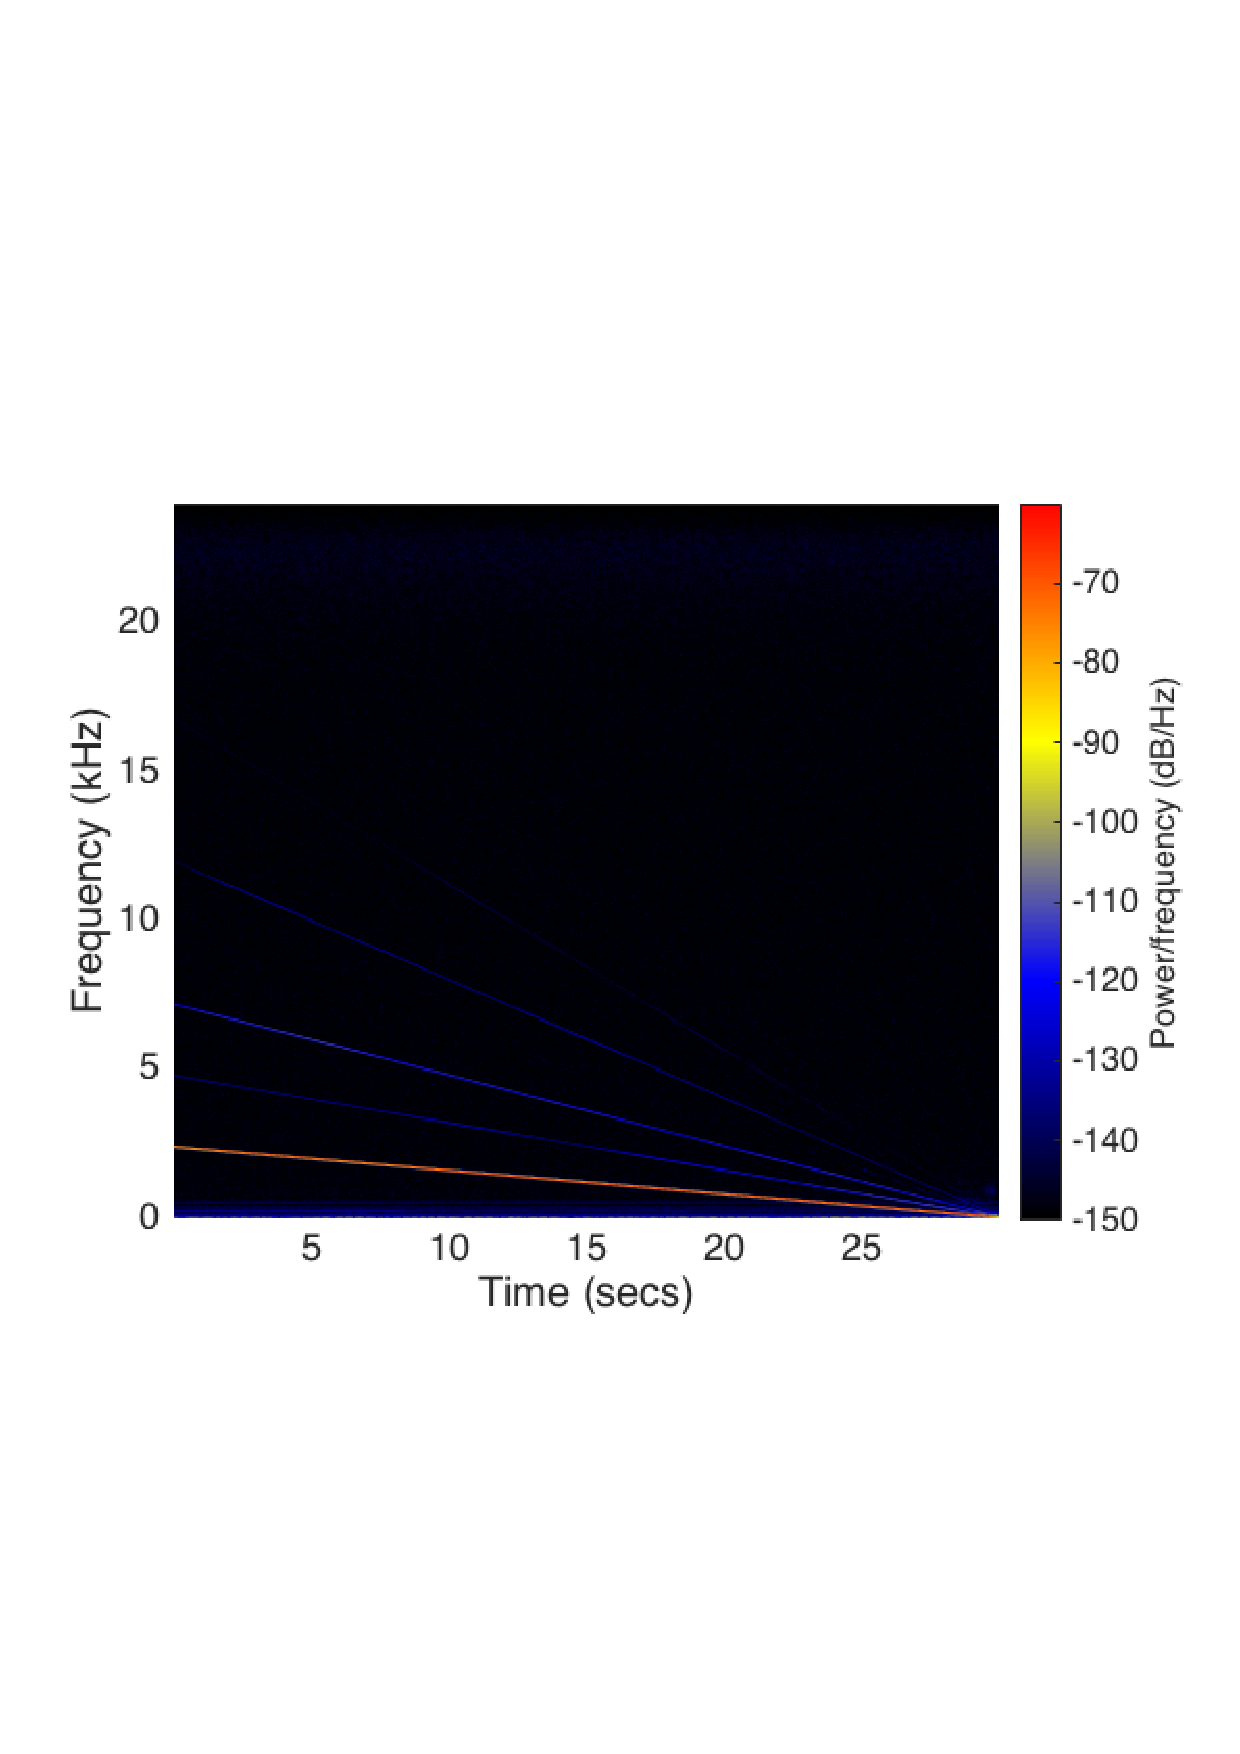
\includegraphics[width=1\textwidth]{figures/spectrogram_mic1.pdf}
	\caption{Microphone dataset 1.}
	\label{fig:spectrogram_mic1}
\end{subfigure}
\begin{subfigure}[t]{0.47\textwidth}
	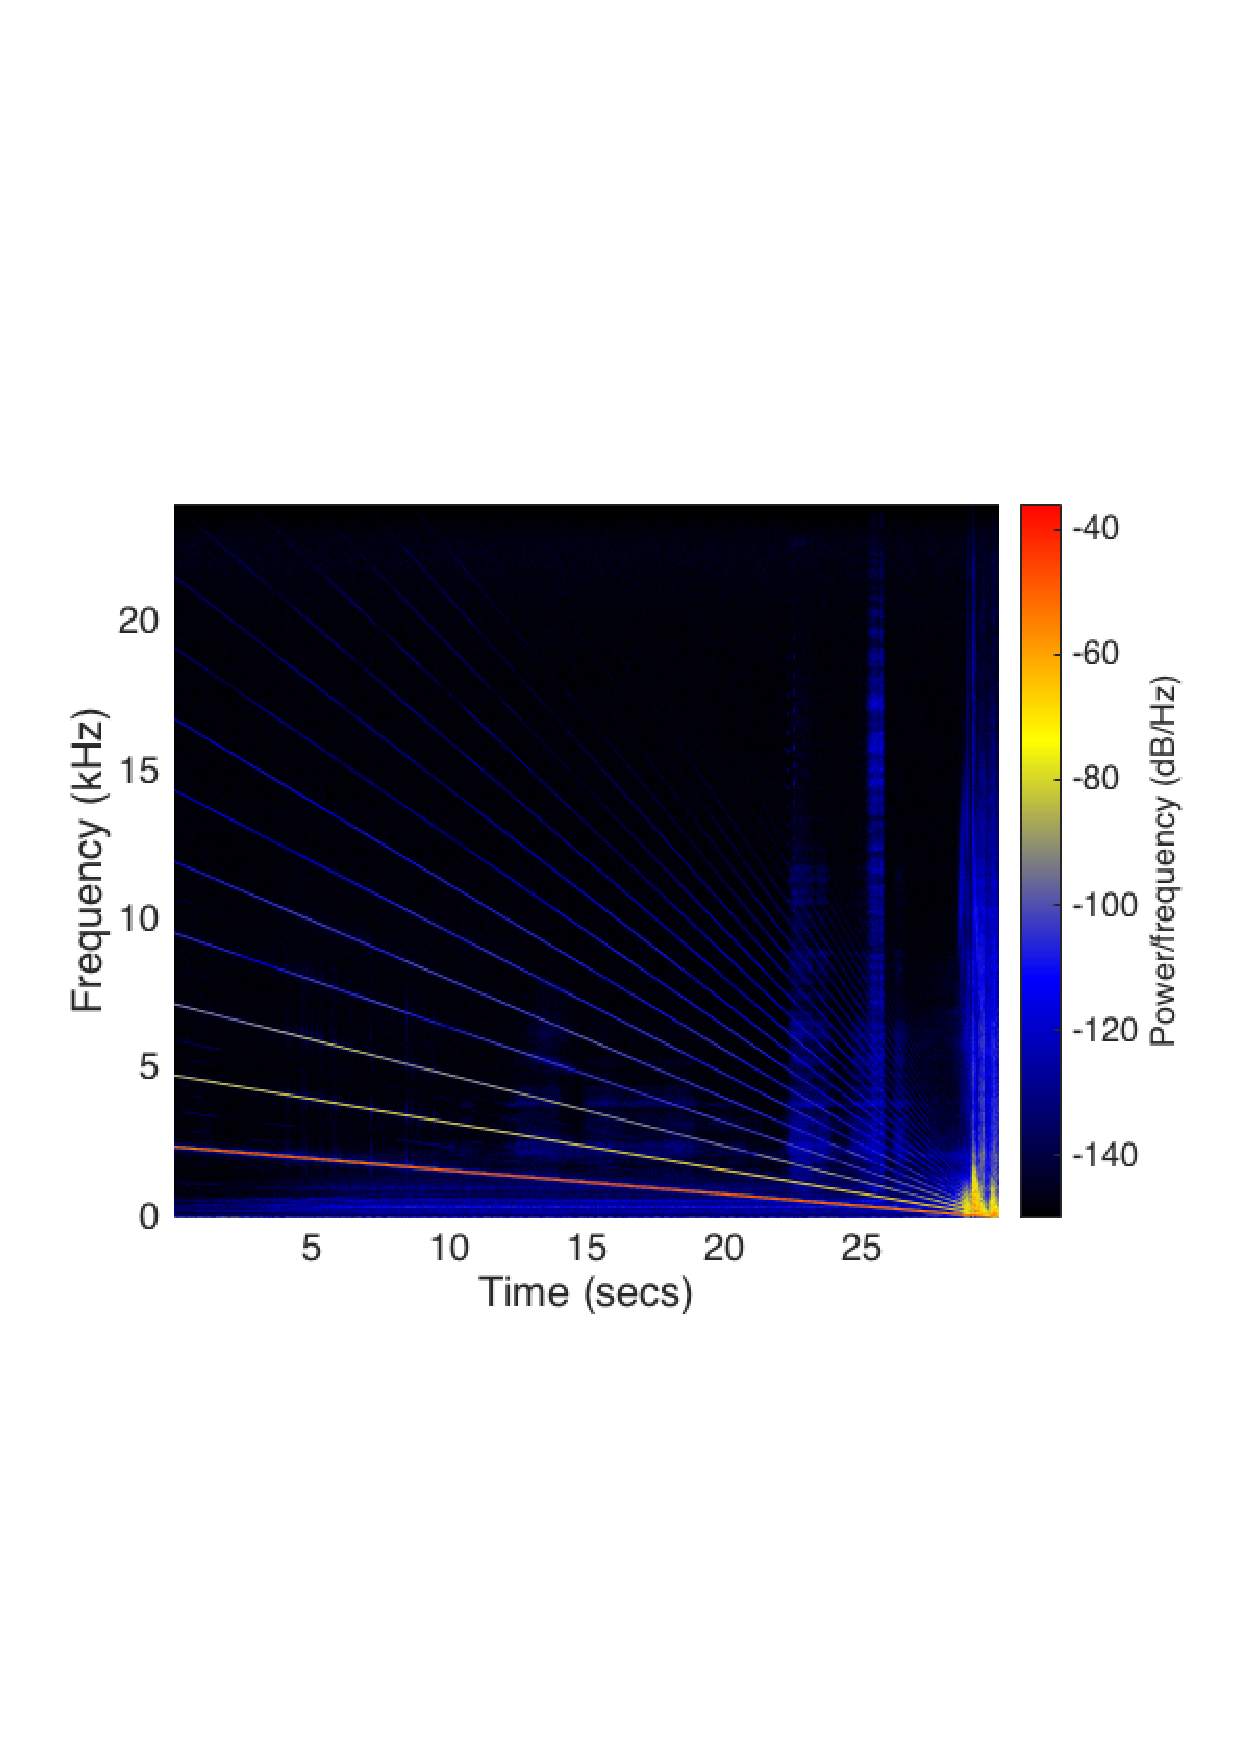
\includegraphics[width=1\textwidth]{figures/spectrogram_mic19.pdf}
	\caption{Microphone dataset 19.}
	\label{fig:spectrogram_mic19}
\end{subfigure}
\caption{The spectrograms of the microphone dataset 1 and 19. The prominent red line is the sine sweep from 2.4 kHz to 10 Hz while the yellow and blue lines along the red line are harmonic distortion.}
\label{fig:spec_mic}
\end{figure} 

The spectrograms of dataset 1 and 19, seen in \autoref{fig:spectrogram_mic1} and \autoref{fig:spectrogram_mic1}, show a prominent red line and three weak blue lines above the red line. It is seen that the red line is a linear decreasing function from 2.4 kHz to 10 Hz where the frequency is a function of time. This indicates that the red line is the fundamental frequency of the sine sweep from 2.4 kHz to 10 Hz. The blue and yellow line are linear functions of the harmonic distortions. The spectrograms clearly show that increasing the gain will increase the amount of harmonic distortion as well. An interesting observation is the spectral frequency leak that occurs at low frequency. 


\begin{figure}[H]
\centering
\begin{subfigure}[t]{0.47\textwidth}
	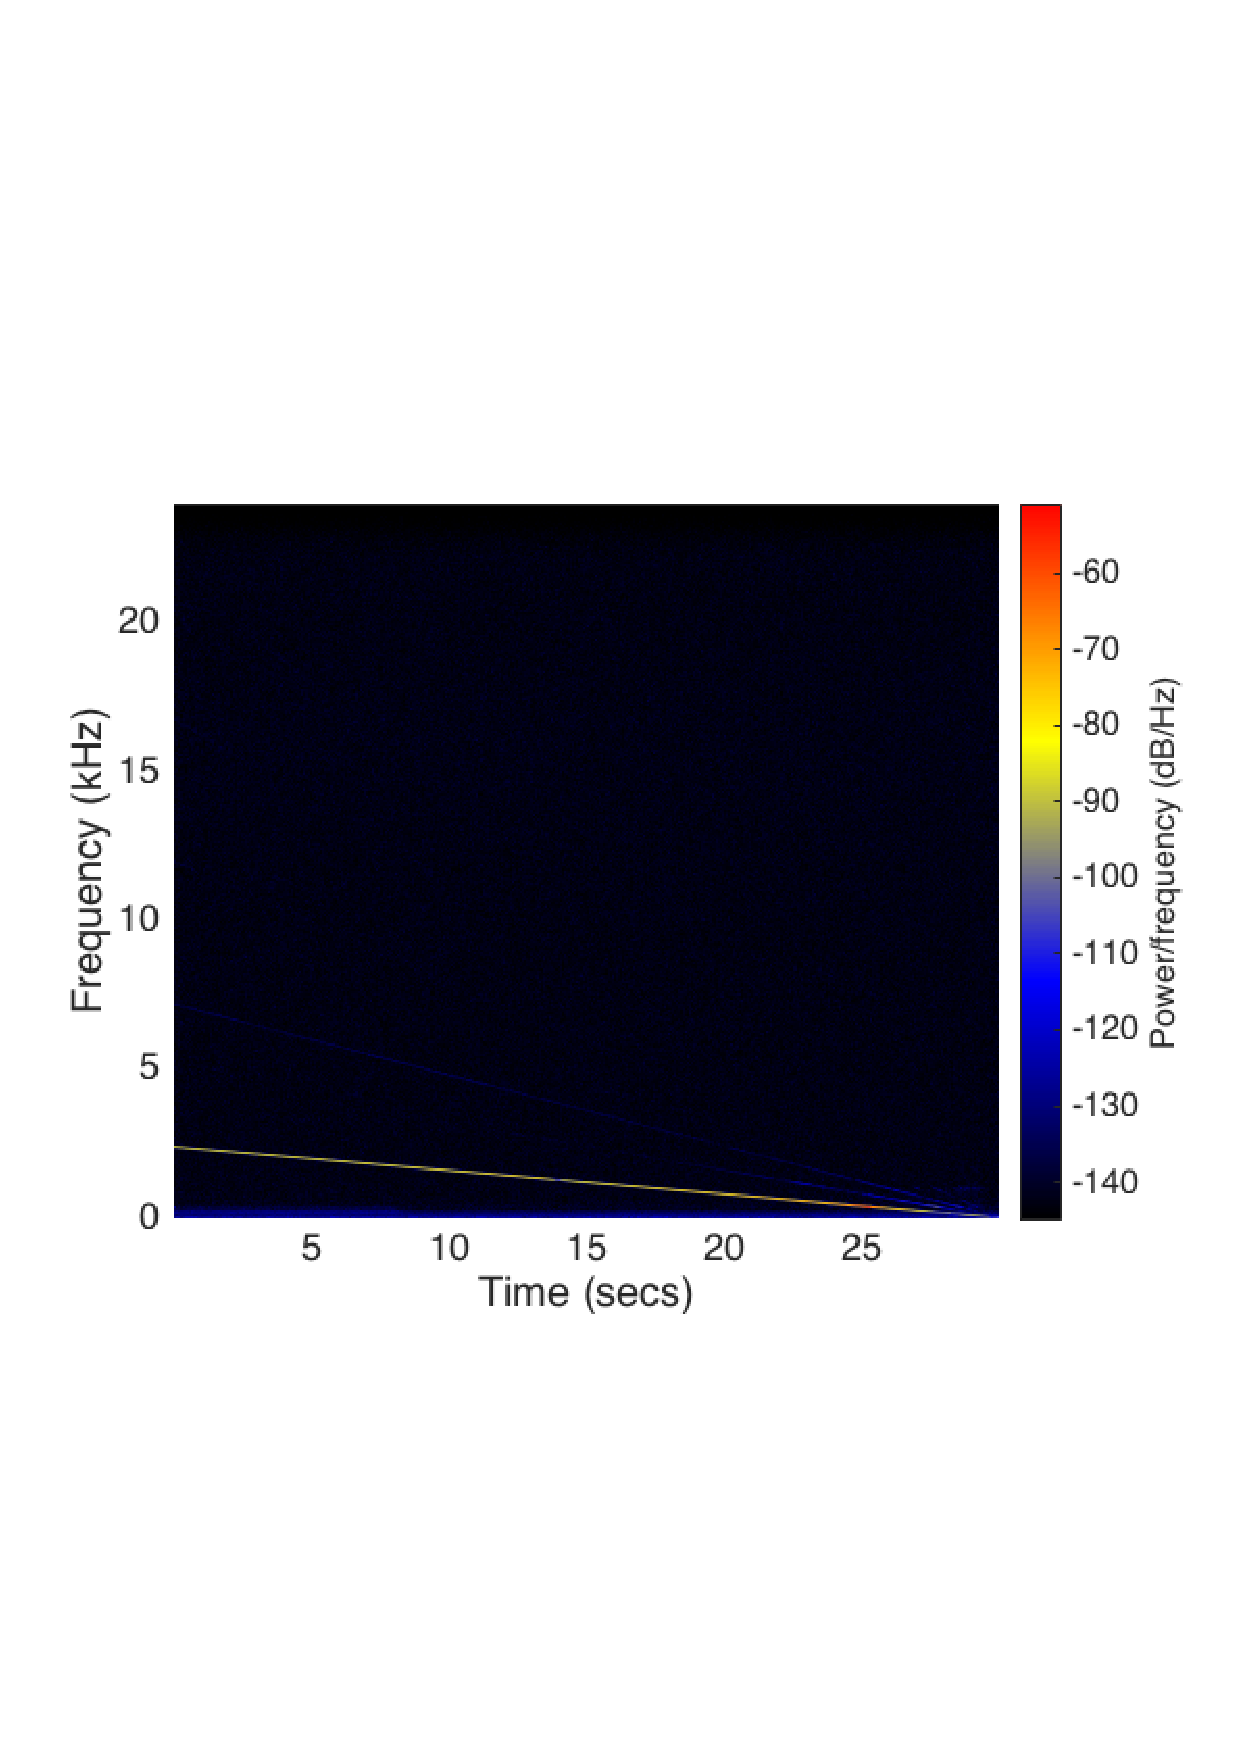
\includegraphics[width=1\textwidth]{figures/spectrogram_driver1.pdf}
	\caption{Vibration from driver.}
	\label{fig:spectrogram_driver1}
\end{subfigure}
\begin{subfigure}[t]{0.47\textwidth}
	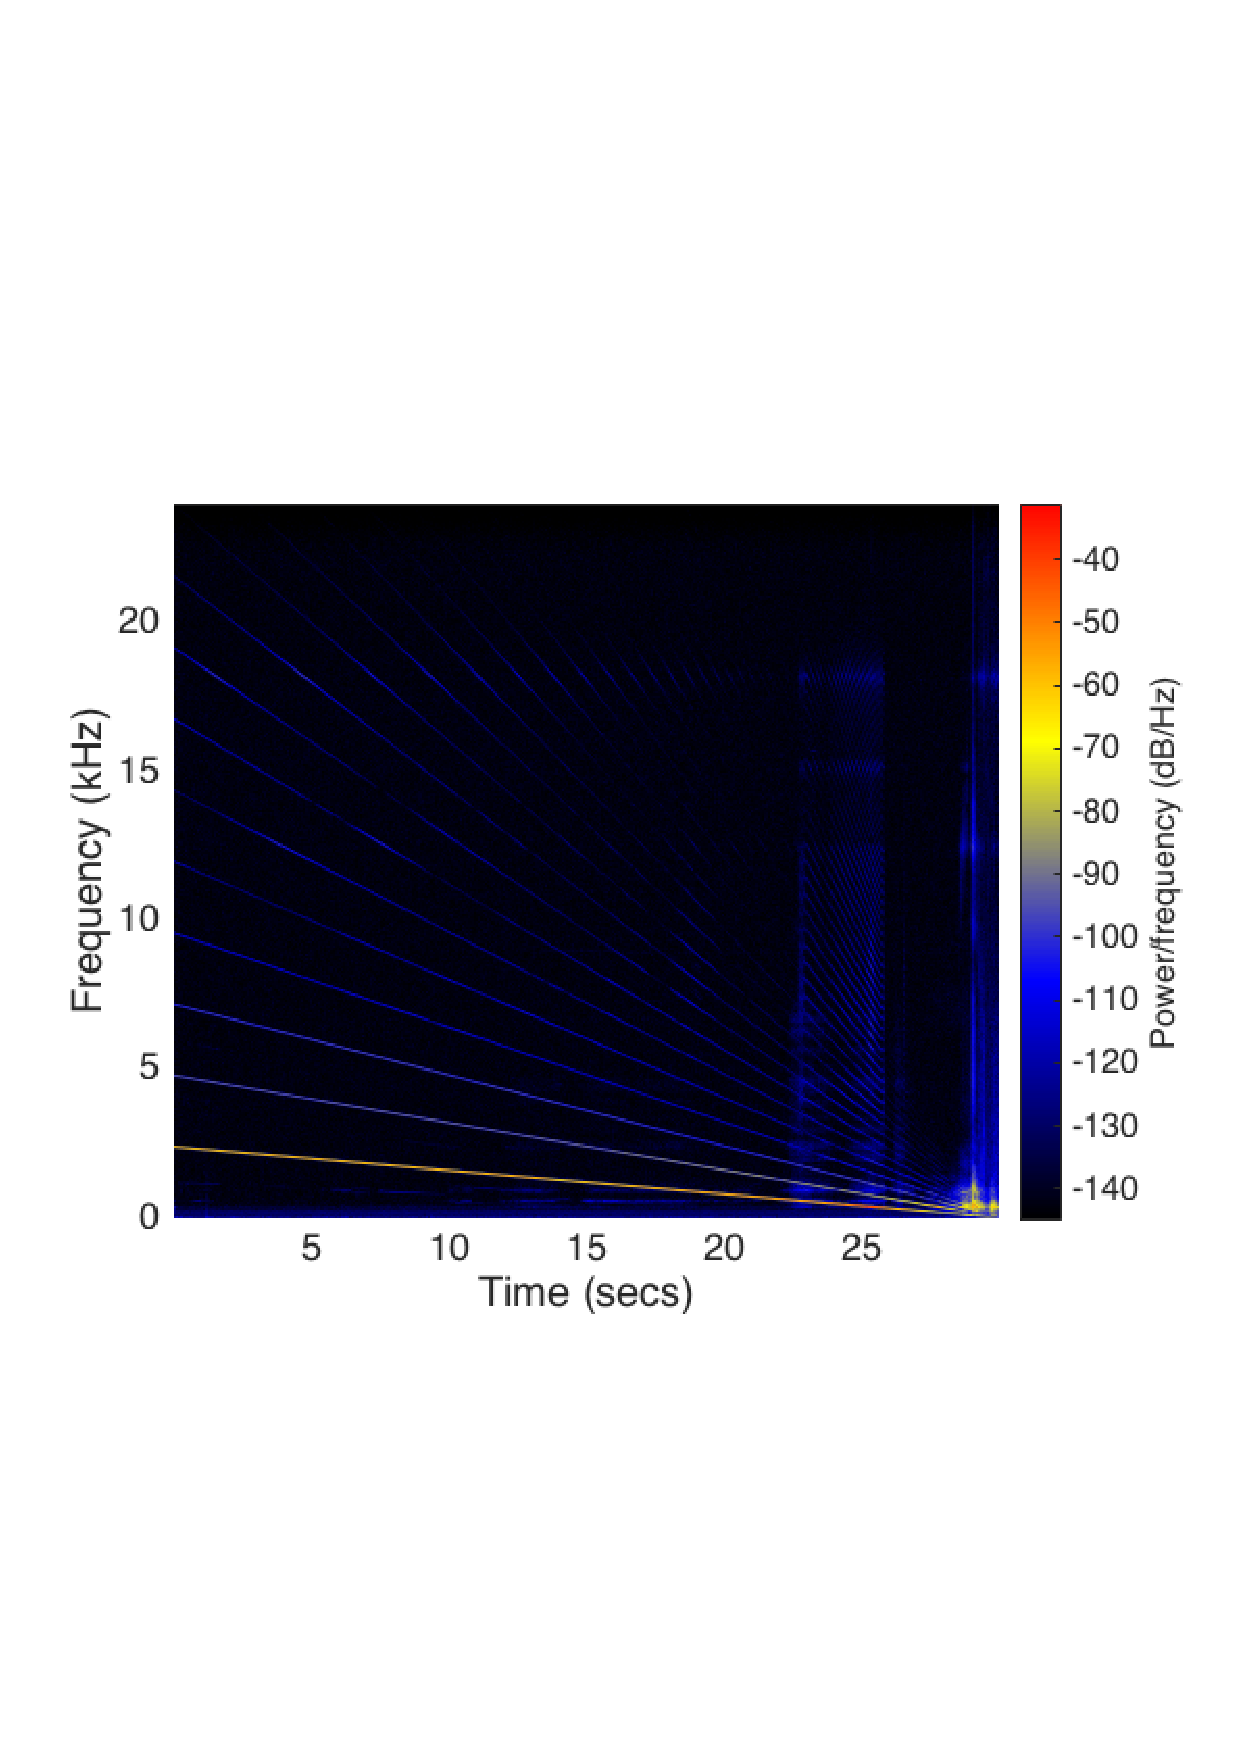
\includegraphics[width=1\textwidth]{figures/spectrogram_driver19.pdf}
	\caption{Vibration from driver.}
	\label{fig:spectrogram_driver19}
\end{subfigure}
\caption{The measured data of (a) the vibration on the driver, (b) the vibration on the enclosure, and (c) the sound pressure from the microphone. Dataset 20.}
\label{fig:spec_driver}
\end{figure} 























%\subsubsection{Back Plate Hit Detection}\label{sec:hit_detect}
\todo[inline]{SKRIV NOGET MED 150W THRESHOLD}
As previously stated, it is possible that the loudspeaker coil hits the back plate of the driver if the coil moves too far back. In the long run this will damage the loudspeaker, and should therefore be avoided. In this section an analysis on how to detect these hits, will be provided. 

\textbf{From \autoref{subsec:impulses} the frequency response of a mechanical frame of a loudspeaker has the same characteristics as a low-pass filter. This means, if the coil is hitting the back plate of the driver, it will result in a increase in energy in the low frequency spectrum. As most music and loudspeakers have some sort of a high-pass filter implemented to remove almost non-audible sound, it can be assumed that only a back plate hit will generate vibrations at very low frequencies between, for instance, 0 Hz to 20 Hz. To examine if this is true, a section of the dataset 19 of the driver, where a hit is suspected to have occurred, is analysed.} %The analysed section is seen in \autoref{fig:raw_driver19_windows}.


%\begin{figure}[H]
%\centering
%\begin{subfigure}[t]{0.55\textwidth}
%	\tikzsetnextfilename{raw_driver19_window}
%	% This file was created by matlab2tikz.
%
%The latest updates can be retrieved from
%  http://www.mathworks.com/matlabcentral/fileexchange/22022-matlab2tikz-matlab2tikz
%where you can also make suggestions and rate matlab2tikz.
%
\begin{tikzpicture}

\begin{axis}[%
width=2.3in,
height=2in,
at={(1.011in,0.642in)},
scale only axis,
xmin=0,
xmax=30,
xmajorgrids,
ymin=-0.2,
ymax=0.2,
ymajorgrids,
xlabel={Time [s]},
ylabel={Amplitude [s]},
axis background/.style={fill=white}
]
\node[rectangle,draw, fill=black!20, minimum height=2in, minimum width=1pt, line width=1pt] at (axis cs:28.9,0) {};
\addplot[fill=black,draw=black,forget plot] plot table[row sep=crcr]{%
2.08333333333333e-05	0.0174441337585449\\
0.0250416666666667	0.013525128364563\\
0.0500625	0.013148307800293\\
0.0750833333333333	0.0131036043167114\\
0.100104166666667	0.0130690336227417\\
0.125125	0.0130878686904907\\
0.150145833333333	0.0131148099899292\\
0.175166666666667	0.0131456851959229\\
0.2001875	0.0131820440292358\\
0.225208333333333	0.0131937265396118\\
0.250229166666667	0.013242244720459\\
0.27525	0.0132321119308472\\
0.300270833333333	0.0132625102996826\\
0.325291666666667	0.0132992267608643\\
0.3503125	0.0133000612258911\\
0.375333333333333	0.0133060216903687\\
0.400354166666667	0.0133442878723145\\
0.425375	0.0133682489395142\\
0.450395833333333	0.0134040117263794\\
0.475416666666667	0.0134208202362061\\
0.5004375	0.0134366750717163\\
0.525458333333333	0.0134779214859009\\
0.550479166666667	0.013481616973877\\
0.5755	0.0135024785995483\\
0.600520833333333	0.0135313272476196\\
0.625541666666667	0.0135687589645386\\
0.6505625	0.0135985612869263\\
0.675583333333333	0.013633131980896\\
0.700604166666667	0.0136561393737793\\
0.725625	0.0136919021606445\\
0.750645833333333	0.0137306451797485\\
0.775666666666667	0.0137556791305542\\
0.8006875	0.01378333568573\\
0.825708333333333	0.0138041973114014\\
0.850729166666667	0.0138405561447144\\
0.87575	0.0138554573059082\\
0.900770833333333	0.0138554573059082\\
0.925791666666667	0.0138950347900391\\
0.9508125	0.0139113664627075\\
0.975833333333333	0.0139317512512207\\
1.00085416666667	0.0139557123184204\\
1.025875	0.0139747858047485\\
1.05089583333333	0.0140010118484497\\
1.07591666666667	0.0140320062637329\\
1.1009375	0.0140565633773804\\
1.12595833333333	0.0140770673751831\\
1.15097916666667	0.0140986442565918\\
1.176	0.0141662359237671\\
1.20102083333333	0.0141526460647583\\
1.22604166666667	0.0141149759292603\\
1.2510625	0.0141333341598511\\
1.27608333333333	0.0141546726226807\\
1.30110416666667	0.0141855478286743\\
1.326125	0.014235258102417\\
1.35114583333333	0.0142221450805664\\
1.37616666666667	0.0142310857772827\\
1.4011875	0.0142514705657959\\
1.42620833333333	0.0142489671707153\\
1.45122916666667	0.0142501592636108\\
1.47625	0.0142405033111572\\
1.50127083333333	0.0142426490783691\\
1.52629166666667	0.014230489730835\\
1.5513125	0.0142196416854858\\
1.57633333333333	0.0141897201538086\\
1.60135416666667	0.0141717195510864\\
1.626375	0.0141717195510864\\
1.65139583333333	0.0141562223434448\\
1.67641666666667	0.0141308307647705\\
1.7014375	0.0141433477401733\\
1.72645833333333	0.0141233205795288\\
1.75147916666667	0.0141158103942871\\
1.7765	0.0141146183013916\\
1.80152083333333	0.0140886306762695\\
1.82654166666667	0.0140882730484009\\
1.8515625	0.0140790939331055\\
1.87658333333333	0.0140920877456665\\
1.90160416666667	0.0140787363052368\\
1.926625	0.0140824317932129\\
1.95164583333333	0.014080286026001\\
1.97666666666667	0.0140800476074219\\
2.0016875	0.0140819549560547\\
2.02670833333333	0.0140724182128906\\
2.05172916666667	0.0140804052352905\\
2.07675	0.0140852928161621\\
2.10177083333333	0.0140907764434814\\
2.12679166666667	0.0141453742980957\\
2.1518125	0.0141433477401733\\
2.17683333333333	0.0141167640686035\\
2.20185416666667	0.014110803604126\\
2.226875	0.014117956161499\\
2.25189583333333	0.0141313076019287\\
2.27691666666667	0.01416015625\\
2.3019375	0.0141942501068115\\
2.32695833333333	0.0142010450363159\\
2.35197916666667	0.0142147541046143\\
2.377	0.0142277479171753\\
2.40202083333333	0.014255166053772\\
2.42704166666667	0.0142706632614136\\
2.4520625	0.0142948627471924\\
2.47708333333333	0.0143097639083862\\
2.50210416666667	0.014333963394165\\
2.527125	0.0143415927886963\\
2.55214583333333	0.0143803358078003\\
2.57716666666667	0.0144015550613403\\
2.6021875	0.0144282579421997\\
2.62720833333333	0.0144572257995605\\
2.65222916666667	0.0144776105880737\\
2.67725	0.0145164728164673\\
2.70227083333333	0.0145268440246582\\
2.72729166666667	0.0144838094711304\\
2.7523125	0.0145807266235352\\
2.77733333333333	0.0146057605743408\\
2.80235416666667	0.014631986618042\\
2.827375	0.0146661996841431\\
2.85239583333333	0.0147078037261963\\
2.87741666666667	0.0147354602813721\\
2.9024375	0.0147578716278076\\
2.92745833333333	0.0148038864135742\\
2.95247916666667	0.0148260593414307\\
2.9775	0.0148706436157227\\
3.00252083333333	0.0148930549621582\\
3.02754166666667	0.0149344205856323\\
3.0525625	0.0149737596511841\\
3.07758333333333	0.0150246620178223\\
3.10260416666667	0.0150657892227173\\
3.127625	0.0151075124740601\\
3.15264583333333	0.0151689052581787\\
3.17766666666667	0.0152368545532227\\
3.2026875	0.0152426958084106\\
3.22770833333333	0.0153077840805054\\
3.25272916666667	0.0153446197509766\\
3.27775	0.0153803825378418\\
3.30277083333333	0.0154129266738892\\
3.32779166666667	0.0154589414596558\\
3.3528125	0.0155411958694458\\
3.37783333333333	0.0155452489852905\\
3.40285416666667	0.0155919790267944\\
3.427875	0.0156158208847046\\
3.45289583333333	0.0156674385070801\\
3.47791666666667	0.0156955718994141\\
3.5029375	0.0157450437545776\\
3.52795833333333	0.0157967805862427\\
3.55297916666667	0.0158439874649048\\
3.578	0.0158843994140625\\
3.60302083333333	0.0159142017364502\\
3.62804166666667	0.0159745216369629\\
3.6530625	0.0160062313079834\\
3.67808333333333	0.0160480737686157\\
3.70310416666667	0.0160622596740723\\
3.728125	0.0160926580429077\\
3.75314583333333	0.0161361694335938\\
3.77816666666667	0.0161548852920532\\
3.8031875	0.0161689519882202\\
3.82820833333333	0.0162111520767212\\
3.85322916666667	0.0162196159362793\\
3.87825	0.0162382125854492\\
3.90327083333333	0.0162340402603149\\
3.92829166666667	0.0162550210952759\\
3.9533125	0.0162825584411621\\
3.97833333333333	0.016268253326416\\
4.00335416666667	0.0162605047225952\\
4.028375	0.0162662267684937\\
4.05339583333333	0.0162646770477295\\
4.07841666666667	0.0162562131881714\\
4.1034375	0.0162479877471924\\
4.12845833333333	0.0162286758422852\\
4.15347916666667	0.0162270069122314\\
4.1785	0.0162371397018433\\
4.20352083333333	0.0162290334701538\\
4.22854166666667	0.0162320137023926\\
4.2535625	0.0162011384963989\\
4.27858333333333	0.0161998271942139\\
4.30360416666667	0.0161756277084351\\
4.328625	0.0161881446838379\\
4.35364583333333	0.0161887407302856\\
4.37866666666667	0.0161789655685425\\
4.4036875	0.0161731243133545\\
4.42870833333333	0.0161886215209961\\
4.45372916666667	0.0162254571914673\\
4.47875	0.0162070989608765\\
4.50377083333333	0.0162215232849121\\
4.52879166666667	0.0162445306777954\\
4.5538125	0.0162478685379028\\
4.57883333333333	0.0162779092788696\\
4.60385416666667	0.0163146257400513\\
4.628875	0.0163321495056152\\
4.65389583333333	0.0163751840591431\\
4.67891666666667	0.0163940191268921\\
4.7039375	0.0164142847061157\\
4.72895833333333	0.0164343118667603\\
4.75397916666667	0.0164676904678345\\
4.779	0.0164873600006104\\
4.80402083333333	0.0164920091629028\\
4.82904166666667	0.0165045261383057\\
4.8540625	0.0165075063705444\\
4.87908333333333	0.0164927244186401\\
4.90410416666667	0.0165128707885742\\
4.929125	0.0165145397186279\\
4.95414583333333	0.0165392160415649\\
4.97916666666667	0.0165292024612427\\
5.0041875	0.0165307521820068\\
5.02920833333333	0.0165344476699829\\
5.05422916666667	0.0165383815765381\\
5.07925	0.0165324211120605\\
5.10427083333333	0.0165327787399292\\
5.12929166666667	0.0165436267852783\\
5.1543125	0.0165482759475708\\
5.17933333333333	0.0165408849716187\\
5.20435416666667	0.0165520906448364\\
5.229375	0.0165524482727051\\
5.25439583333333	0.0165770053863525\\
5.27941666666667	0.0165494680404663\\
5.3044375	0.0165427923202515\\
5.32945833333333	0.0165486335754395\\
5.35447916666667	0.016539454460144\\
5.3795	0.0165292024612427\\
5.40452083333333	0.0165024995803833\\
5.42954166666667	0.0165091753005981\\
5.4545625	0.0165070295333862\\
5.47958333333333	0.0164998769760132\\
5.50460416666667	0.0164941549301147\\
5.529625	0.0164831876754761\\
5.55464583333333	0.0164557695388794\\
5.57966666666667	0.0164422988891602\\
5.6046875	0.0164165496826172\\
5.62970833333333	0.0164107084274292\\
5.65472916666667	0.0163847208023071\\
5.67975	0.0163700580596924\\
5.70477083333333	0.0163614749908447\\
5.72979166666667	0.0163367986679077\\
5.7548125	0.0162984132766724\\
5.77983333333333	0.0162603855133057\\
5.80485416666667	0.0162379741668701\\
5.829875	0.0161999464035034\\
5.85489583333333	0.0161981582641602\\
5.87991666666667	0.0161627531051636\\
5.9049375	0.0161465406417847\\
5.92995833333333	0.016115665435791\\
5.95497916666667	0.0160897970199585\\
5.98	0.0160585641860962\\
6.00502083333333	0.0160255432128906\\
6.03004166666667	0.0159686803817749\\
6.0550625	0.0159963369369507\\
6.08008333333333	0.0159759521484375\\
6.10510416666667	0.0159282684326172\\
6.130125	0.015892505645752\\
6.15514583333333	0.0158891677856445\\
6.18016666666667	0.0158644914627075\\
6.2051875	0.0158466100692749\\
6.23020833333333	0.0158360004425049\\
6.25522916666667	0.0158376693725586\\
6.28025	0.0158051252365112\\
6.30527083333333	0.0157734155654907\\
6.33029166666667	0.0157642364501953\\
6.3553125	0.015750527381897\\
6.38033333333333	0.0157539844512939\\
6.40535416666667	0.0157500505447388\\
6.430375	0.0157680511474609\\
6.45539583333333	0.0157589912414551\\
6.48041666666667	0.0157626867294312\\
6.5054375	0.0157822370529175\\
6.53045833333333	0.0157740116119385\\
6.55547916666667	0.0157889127731323\\
6.5805	0.01578688621521\\
6.60552083333333	0.0157822370529175\\
6.63054166666667	0.015788197517395\\
6.6555625	0.0157915353775024\\
6.68058333333333	0.0158027410507202\\
6.70560416666667	0.0158090591430664\\
6.730625	0.0157994031906128\\
6.75564583333333	0.0158072710037231\\
6.78066666666667	0.0158181190490723\\
6.8056875	0.0157982110977173\\
6.83070833333333	0.0158140659332275\\
6.85572916666667	0.0158218145370483\\
6.88075	0.0158369541168213\\
6.90577083333333	0.015845775604248\\
6.93079166666667	0.0158636569976807\\
6.9558125	0.0158761739730835\\
6.98083333333333	0.0158882141113281\\
7.00585416666667	0.0158886909484863\\
7.030875	0.015921950340271\\
7.05589583333333	0.015964150428772\\
7.08091666666667	0.0159696340560913\\
7.1059375	0.0159767866134644\\
7.13095833333333	0.0160138607025146\\
7.15597916666667	0.0160485506057739\\
7.181	0.0161073207855225\\
7.20602083333333	0.0161236524581909\\
7.23104166666667	0.0161528587341309\\
7.2560625	0.0162006616592407\\
7.28108333333333	0.0162516832351685\\
7.30610416666667	0.0162925720214844\\
7.331125	0.0163209438323975\\
7.35614583333333	0.0163383483886719\\
7.38116666666667	0.0163733959197998\\
7.4061875	0.0163830518722534\\
7.43120833333333	0.0164109468460083\\
7.45622916666667	0.0164159536361694\\
7.48125	0.0164202451705933\\
7.50627083333333	0.01641845703125\\
7.53129166666667	0.0163898468017578\\
7.5563125	0.0163893699645996\\
7.58133333333333	0.0163614749908447\\
7.60635416666667	0.0163397789001465\\
7.631375	0.016291618347168\\
7.65639583333333	0.0162471532821655\\
7.68141666666667	0.0162198543548584\\
7.7064375	0.016148567199707\\
7.73145833333333	0.0160896778106689\\
7.75647916666667	0.016048789024353\\
7.7815	0.0159863233566284\\
7.80652083333333	0.0158941745758057\\
7.83154166666667	0.0158556699752808\\
7.8565625	0.0158106088638306\\
7.88158333333333	0.0157514810562134\\
7.90660416666667	0.0157146453857422\\
7.931625	0.0156705379486084\\
7.95664583333333	0.015657901763916\\
7.98166666666667	0.0156430006027222\\
8.0066875	0.015637993812561\\
8.03170833333333	0.0156441926956177\\
8.05672916666667	0.015630841255188\\
8.08175	0.0156583786010742\\
8.10677083333333	0.0156680345535278\\
8.13179166666667	0.0156958103179932\\
8.1568125	0.0157588720321655\\
8.18183333333333	0.0157665014266968\\
8.20685416666667	0.015811562538147\\
8.231875	0.0158299207687378\\
8.25689583333333	0.0158756971359253\\
8.28191666666667	0.0159240961074829\\
8.3069375	0.0159738063812256\\
8.33195833333333	0.0160108804702759\\
8.35697916666667	0.01605224609375\\
8.382	0.0161123275756836\\
8.40702083333333	0.0161582231521606\\
8.43204166666667	0.0161970853805542\\
8.4570625	0.0162638425827026\\
8.48208333333333	0.0163058042526245\\
8.50710416666667	0.0163264274597168\\
8.532125	0.0163748264312744\\
8.55714583333333	0.016425609588623\\
8.58216666666667	0.0164724588394165\\
8.6071875	0.0164806842803955\\
8.63220833333333	0.0165771245956421\\
8.65722916666667	0.0166155099868774\\
8.68225	0.0166538953781128\\
8.70727083333333	0.0166980028152466\\
8.73229166666667	0.0167548656463623\\
8.7573125	0.0168157815933228\\
8.78233333333333	0.0168620347976685\\
8.80735416666667	0.0168946981430054\\
8.832375	0.0169271230697632\\
8.85739583333333	0.0169821977615356\\
8.88241666666667	0.0170294046401978\\
8.9074375	0.0170701742172241\\
8.93245833333333	0.0171375274658203\\
8.95747916666667	0.0171374082565308\\
8.9825	0.0171587467193604\\
9.00752083333333	0.0172109603881836\\
9.03254166666667	0.017237663269043\\
9.0575625	0.0172935724258423\\
9.08258333333333	0.0173063278198242\\
9.10760416666667	0.0173218250274658\\
9.132625	0.0173497200012207\\
9.15764583333333	0.0173478126525879\\
9.18266666666667	0.0173822641372681\\
9.2076875	0.0173777341842651\\
9.23270833333333	0.0174020528793335\\
9.25772916666667	0.0174028873443604\\
9.28275	0.0174024105072021\\
9.30777083333333	0.0174020528793335\\
9.33279166666667	0.017372727394104\\
9.3578125	0.017397403717041\\
9.38283333333333	0.017382025718689\\
9.40785416666667	0.0173285007476807\\
9.432875	0.017330527305603\\
9.45789583333333	0.0173323154449463\\
9.48291666666667	0.0173298120498657\\
9.5079375	0.0173071622848511\\
9.53295833333333	0.0172946453094482\\
9.55797916666667	0.0172981023788452\\
9.583	0.0172525644302368\\
9.60802083333333	0.0172533988952637\\
9.63304166666667	0.0172268152236938\\
9.6580625	0.0172150135040283\\
9.68308333333333	0.0172126293182373\\
9.70810416666667	0.0172011852264404\\
9.733125	0.0171859264373779\\
9.75814583333333	0.0171804428100586\\
9.78316666666667	0.0171525478363037\\
9.8081875	0.0171377658843994\\
9.83320833333334	0.0171386003494263\\
9.85822916666667	0.0171124935150146\\
9.88325	0.0171166658401489\\
9.90827083333333	0.0170993804931641\\
9.93329166666667	0.0170944929122925\\
9.9583125	0.0170706510543823\\
9.98333333333333	0.0170501470565796\\
10.0083541666667	0.0170356035232544\\
10.033375	0.0169914960861206\\
10.0583958333333	0.0170005559921265\\
10.0834166666667	0.0170102119445801\\
10.1084375	0.0169705152511597\\
10.1334583333333	0.0169491767883301\\
10.1584791666667	0.0169483423233032\\
10.1835	0.0169246196746826\\
10.2085208333333	0.0169349908828735\\
10.2335416666667	0.016913890838623\\
10.2585625	0.016938328742981\\
10.2835833333333	0.0169572830200195\\
10.3086041666667	0.0169775485992432\\
10.333625	0.016999363899231\\
10.3586458333333	0.0170327425003052\\
10.3836666666667	0.0170744657516479\\
10.4086875	0.0170915126800537\\
10.4337083333333	0.0171260833740234\\
10.4587291666667	0.0171712636947632\\
10.48375	0.0172317028045654\\
10.5087708333333	0.0172442197799683\\
10.5337916666667	0.0172771215438843\\
10.5588125	0.017345666885376\\
10.5838333333333	0.0173889398574829\\
10.6088541666667	0.0174278020858765\\
10.633875	0.0174736976623535\\
10.6588958333333	0.0175179243087769\\
10.6839166666667	0.017504096031189\\
10.7089375	0.0175975561141968\\
10.7339583333333	0.0176342725753784\\
10.7589791666667	0.0176651477813721\\
10.784	0.0177170038223267\\
10.8090208333333	0.0177382230758667\\
10.8340416666667	0.0177578926086426\\
10.8590625	0.0177834033966064\\
10.8840833333333	0.0178287029266357\\
10.9091041666667	0.0178596973419189\\
10.934125	0.0178934335708618\\
10.9591458333333	0.0179351568222046\\
10.9841666666667	0.0179930925369263\\
11.0091875	0.0180190801620483\\
11.0342083333333	0.0180590152740479\\
11.0592291666667	0.0180873870849609\\
11.08425	0.0181617736816406\\
11.1092708333333	0.0181983709335327\\
11.1342916666667	0.0182547569274902\\
11.1593125	0.018323540687561\\
11.1843333333333	0.018383264541626\\
11.2093541666667	0.0184645652770996\\
11.234375	0.0185511112213135\\
11.2593958333333	0.0186281204223633\\
11.2844166666667	0.0186648368835449\\
11.3094375	0.0187809467315674\\
11.3344583333333	0.0188539028167725\\
11.3594791666667	0.0189625024795532\\
11.3845	0.0190408229827881\\
11.4095208333333	0.0191167593002319\\
11.4345416666667	0.0191928148269653\\
11.4595625	0.019289493560791\\
11.4845833333333	0.0194246768951416\\
11.5096041666667	0.0194790363311768\\
11.534625	0.0195668935775757\\
11.5596458333333	0.0196346044540405\\
11.5846666666667	0.0197362899780273\\
11.6096875	0.0198198556900024\\
11.6347083333333	0.0198944807052612\\
11.6597291666667	0.0199992656707764\\
11.68475	0.0200852155685425\\
11.7097708333333	0.0201708078384399\\
11.7347916666667	0.0202442407608032\\
11.7598125	0.0203417539596558\\
11.7848333333333	0.020447850227356\\
11.8098541666667	0.0205179452896118\\
11.834875	0.020601749420166\\
11.8598958333333	0.0206559896469116\\
11.8849166666667	0.0207802057266235\\
11.9099375	0.0208553075790405\\
11.9349583333333	0.0209276676177979\\
11.9599791666667	0.0209884643554688\\
11.985	0.0210902690887451\\
12.0100208333333	0.0211566686630249\\
12.0350416666667	0.0212430953979492\\
12.0600625	0.0213093757629395\\
12.0850833333333	0.0213801860809326\\
12.1101041666667	0.0214052200317383\\
12.135125	0.0214844942092896\\
12.1601458333333	0.0215476751327515\\
12.1851666666667	0.0216346979141235\\
12.2101875	0.0216710567474365\\
12.2352083333333	0.0217214822769165\\
12.2602291666667	0.0217512845993042\\
12.28525	0.0217370986938477\\
12.3102708333333	0.0217386484146118\\
12.3352916666667	0.0217440128326416\\
12.3603125	0.0217629671096802\\
12.3853333333333	0.0217190980911255\\
12.4103541666667	0.0217164754867554\\
12.435375	0.0216363668441772\\
12.4603958333333	0.0216211080551147\\
12.4854166666667	0.021581768989563\\
12.5104375	0.0215216875076294\\
12.5354583333333	0.021467924118042\\
12.5604791666667	0.0213643312454224\\
12.5855	0.021304726600647\\
12.6105208333333	0.0212384462356567\\
12.6355416666667	0.0211762189865112\\
12.6605625	0.0210961103439331\\
12.6855833333333	0.0210355520248413\\
12.7106041666667	0.0209527015686035\\
12.735625	0.0208666324615479\\
12.7606458333333	0.0208185911178589\\
12.7856666666667	0.0207582712173462\\
12.8106875	0.0206890106201172\\
12.8357083333333	0.0206308364868164\\
12.8607291666667	0.0205554962158203\\
12.88575	0.0205261707305908\\
12.9107708333333	0.0204222202301025\\
12.9357916666667	0.0204188823699951\\
12.9608125	0.0203204154968262\\
12.9858333333333	0.0202691555023193\\
13.0108541666667	0.0202019214630127\\
13.035875	0.0201456546783447\\
13.0608958333333	0.0200655460357666\\
13.0859166666667	0.0200191736221313\\
13.1109375	0.0199253559112549\\
13.1359583333333	0.0198445320129395\\
13.1609791666667	0.0197505950927734\\
13.186	0.0197038650512695\\
13.2110208333333	0.0195786952972412\\
13.2360416666667	0.019476056098938\\
13.2610625	0.0193073749542236\\
13.2860833333333	0.0191764831542969\\
13.3111041666667	0.0190207958221436\\
13.336125	0.0188961029052734\\
13.3611458333333	0.0186749696731567\\
13.3861666666667	0.0185122489929199\\
13.4111875	0.0183169841766357\\
13.4362083333333	0.0180661678314209\\
13.4612291666667	0.017853856086731\\
13.48625	0.0175918340682983\\
13.5112708333333	0.0173110961914062\\
13.5362916666667	0.0169925689697266\\
13.5613125	0.0166597366333008\\
13.5863333333333	0.0163099765777588\\
13.6113541666667	0.0159174203872681\\
13.636375	0.0155293941497803\\
13.6613958333333	0.0150763988494873\\
13.6864166666667	0.0146143436431885\\
13.7114375	0.014168381690979\\
13.7364583333333	0.0136096477508545\\
13.7614791666667	0.0130655765533447\\
13.7865	0.0125436782836914\\
13.8115208333333	0.0119357109069824\\
13.8365416666667	0.0113338232040405\\
13.8615625	0.0106756687164307\\
13.8865833333333	0.0100915431976318\\
13.9116041666667	0.00947129726409912\\
13.936625	0.00886750221252441\\
13.9616458333333	0.00825822353363037\\
13.9866666666667	0.00778257846832275\\
14.0116875	0.00735759735107422\\
14.0367083333333	0.00696361064910889\\
14.0617291666667	0.00667524337768555\\
14.08675	0.00652050971984863\\
14.1117708333333	0.00652647018432617\\
14.1367916666667	0.00670945644378662\\
14.1618125	0.00699913501739502\\
14.1868333333333	0.00733792781829834\\
14.2118541666667	0.0077139139175415\\
14.236875	0.00815272331237793\\
14.2618958333333	0.00860869884490967\\
14.2869166666667	0.00900518894195557\\
14.3119375	0.00939702987670898\\
14.3369583333333	0.00978922843933105\\
14.3619791666667	0.0101321935653687\\
14.387	0.0104804039001465\\
14.4120208333333	0.0107772350311279\\
14.4370416666667	0.0110471248626709\\
14.4620625	0.0112928152084351\\
14.4870833333333	0.0115351676940918\\
14.5121041666667	0.0117450952529907\\
14.537125	0.0118981599807739\\
14.5621458333333	0.0120600461959839\\
14.5871666666667	0.0121918916702271\\
14.6121875	0.0123043060302734\\
14.6372083333333	0.0123888254165649\\
14.6622291666667	0.0124760866165161\\
14.68725	0.0125365257263184\\
14.7122708333333	0.0126163959503174\\
14.7372916666667	0.0126279592514038\\
14.7623125	0.0126475095748901\\
14.7873333333333	0.0126579999923706\\
14.8123541666667	0.0126771926879883\\
14.837375	0.0126643180847168\\
14.8623958333333	0.0126522779464722\\
14.8874166666667	0.0126442909240723\\
14.9124375	0.0126438140869141\\
14.9374583333333	0.0126296281814575\\
14.9624791666667	0.0126005411148071\\
14.9875	0.0125808715820312\\
15.0125208333333	0.0125870704650879\\
15.0375416666667	0.0125871896743774\\
15.0625625	0.0126022100448608\\
15.0875833333333	0.0126547813415527\\
15.1126041666667	0.0127360820770264\\
15.137625	0.0128141641616821\\
15.1626458333333	0.0129730701446533\\
15.1876666666667	0.0131022930145264\\
15.2126875	0.0132739543914795\\
15.2377083333333	0.0134528875350952\\
15.2627291666667	0.0136306285858154\\
15.28775	0.0138425827026367\\
15.3127708333333	0.0140299797058105\\
15.3377916666667	0.014187216758728\\
15.3628125	0.0143324136734009\\
15.3878333333333	0.0144814252853394\\
15.4128541666667	0.0145851373672485\\
15.437875	0.0147069692611694\\
15.4628958333333	0.0147304534912109\\
15.4879166666667	0.014826774597168\\
15.5129375	0.0148801803588867\\
15.5379583333333	0.0149414539337158\\
15.5629791666667	0.0149836540222168\\
15.588	0.0150250196456909\\
15.6130208333333	0.0150867700576782\\
15.6380416666667	0.0151267051696777\\
15.6630625	0.0151498317718506\\
15.6880833333333	0.0151907205581665\\
15.7131041666667	0.0152368545532227\\
15.738125	0.0152875185012817\\
15.7631458333333	0.0153127908706665\\
15.7881666666667	0.015317440032959\\
15.8131875	0.0153570175170898\\
15.8382083333333	0.0153809785842896\\
15.8632291666667	0.0153845548629761\\
15.88825	0.0154021978378296\\
15.9132708333333	0.0154201984405518\\
15.9382916666667	0.0154287815093994\\
15.9633125	0.0154200792312622\\
15.9883333333333	0.0154142379760742\\
16.0133541666667	0.0154227018356323\\
16.038375	0.0153951644897461\\
16.0633958333333	0.0153549909591675\\
16.0884166666667	0.0153504610061646\\
16.1134375	0.015299916267395\\
16.1384583333333	0.0152820348739624\\
16.1634791666667	0.0152640342712402\\
16.1885	0.0152740478515625\\
16.2135208333333	0.0152524709701538\\
16.2385416666667	0.0152736902236938\\
16.2635625	0.0152624845504761\\
16.2885833333333	0.0152912139892578\\
16.3136041666667	0.0153496265411377\\
16.338625	0.015373706817627\\
16.3636458333333	0.0154263973236084\\
16.3886666666667	0.0154972076416016\\
16.4136875	0.0155841112136841\\
16.4387083333333	0.0156378746032715\\
16.4637291666667	0.01569664478302\\
16.48875	0.015790581703186\\
16.5137708333333	0.0158723592758179\\
16.5387916666667	0.0159751176834106\\
16.5638125	0.0160551071166992\\
16.5888333333333	0.0161577463150024\\
16.6138541666667	0.0162507295608521\\
16.638875	0.0163224935531616\\
16.6638958333333	0.0163685083389282\\
16.6889166666667	0.0164364576339722\\
16.7139375	0.0165036916732788\\
16.7389583333333	0.0165603160858154\\
16.7639791666667	0.0166410207748413\\
16.789	0.0167248249053955\\
16.8140208333333	0.0167744159698486\\
16.8390416666667	0.016828179359436\\
16.8640625	0.0168788433074951\\
16.8890833333333	0.0169576406478882\\
16.9141041666667	0.016994833946228\\
16.939125	0.0170410871505737\\
16.9641458333333	0.0170806646347046\\
16.9891666666667	0.017139196395874\\
17.0141875	0.0172109603881836\\
17.0392083333333	0.0172618627548218\\
17.0642291666667	0.0173348188400269\\
17.08925	0.0173755884170532\\
17.1142708333333	0.0174448490142822\\
17.1392916666667	0.0174486637115479\\
17.1643125	0.0174803733825684\\
17.1893333333333	0.017526388168335\\
17.2143541666667	0.0175930261611938\\
17.239375	0.0176322460174561\\
17.2643958333333	0.0176610946655273\\
17.2894166666667	0.0177028179168701\\
17.3144375	0.0177712440490723\\
17.3394583333333	0.017817497253418\\
17.3644791666667	0.0178496837615967\\
17.3895	0.0178635120391846\\
17.4145208333333	0.0179288387298584\\
17.4395416666667	0.017961859703064\\
17.4645625	0.017999529838562\\
17.4895833333333	0.018022894859314\\
17.5146041666667	0.018062949180603\\
17.539625	0.0180728435516357\\
17.5646458333333	0.01810622215271\\
17.5896666666667	0.0180763006210327\\
17.6146875	0.0180631875991821\\
17.6397083333333	0.0180815458297729\\
17.6647291666667	0.0180732011795044\\
17.68975	0.0180611610412598\\
17.7147708333333	0.0180732011795044\\
17.7397916666667	0.0180991888046265\\
17.7648125	0.018126368522644\\
17.7898333333333	0.0181397199630737\\
17.8148541666667	0.0181893110275269\\
17.839875	0.0182832479476929\\
17.8648958333333	0.0183231830596924\\
17.8899166666667	0.0183992385864258\\
17.9149375	0.0184700489044189\\
17.9399583333333	0.0185521841049194\\
17.9649791666667	0.0186257362365723\\
17.99	0.0187492370605469\\
18.0150208333333	0.0188664197921753\\
18.0400416666667	0.0189815759658813\\
18.0650625	0.0190328359603882\\
18.0900833333333	0.0191329717636108\\
18.1151041666667	0.0192264318466187\\
18.140125	0.0192656517028809\\
18.1651458333333	0.0192974805831909\\
18.1901666666667	0.0193121433258057\\
18.2151875	0.0193363428115845\\
18.2402083333333	0.0193533897399902\\
18.2652291666667	0.0193248987197876\\
18.29025	0.0193346738815308\\
18.3152708333333	0.0193099975585938\\
18.3402916666667	0.0192739963531494\\
18.3653125	0.0192720890045166\\
18.3903333333333	0.0192562341690063\\
18.4153541666667	0.0192611217498779\\
18.440375	0.0192636251449585\\
18.4653958333333	0.0192465782165527\\
18.4904166666667	0.0192739963531494\\
18.5154375	0.0192666053771973\\
18.5404583333333	0.0192996263504028\\
18.5654791666667	0.0193842649459839\\
18.5905	0.0194982290267944\\
18.6155208333333	0.0196996927261353\\
18.6405416666667	0.0198712348937988\\
18.6655625	0.0201015472412109\\
18.6905833333333	0.02039635181427\\
18.7156041666667	0.0207115411758423\\
18.740625	0.02104651927948\\
18.7656458333333	0.0213632583618164\\
18.7906666666667	0.0217374563217163\\
18.8156875	0.0221004486083984\\
18.8407083333333	0.0224542617797852\\
18.8657291666667	0.0227910280227661\\
18.89075	0.023115873336792\\
18.9157708333333	0.0234055519104004\\
18.9407916666667	0.0236350297927856\\
18.9658125	0.0238840579986572\\
18.9908333333333	0.0240856409072876\\
19.0158541666667	0.0243097543716431\\
19.040875	0.0244883298873901\\
19.0658958333333	0.0246367454528809\\
19.0909166666667	0.0247553586959839\\
19.1159375	0.0248157978057861\\
19.1409583333333	0.0248211622238159\\
19.1659791666667	0.0248291492462158\\
19.191	0.0247656106948853\\
19.2160208333333	0.0247126817703247\\
19.2410416666667	0.0246188640594482\\
19.2660625	0.0245308876037598\\
19.2910833333333	0.024416446685791\\
19.3161041666667	0.0243091583251953\\
19.341125	0.0241603851318359\\
19.3661458333333	0.0239905118942261\\
19.3911666666667	0.0237839221954346\\
19.4161875	0.0236095190048218\\
19.4412083333333	0.0234092473983765\\
19.4662291666667	0.0231764316558838\\
19.49125	0.0229754447937012\\
19.5162708333333	0.022815465927124\\
19.5412916666667	0.0226483345031738\\
19.5663125	0.0224692821502686\\
19.5913333333333	0.0223290920257568\\
19.6163541666667	0.0222113132476807\\
19.641375	0.0221070051193237\\
19.6663958333333	0.0220341682434082\\
19.6914166666667	0.0219175815582275\\
19.7164375	0.0218663215637207\\
19.7414583333333	0.0218421220779419\\
19.7664791666667	0.0217581987380981\\
19.7915	0.021744966506958\\
19.8165208333333	0.0217596292495728\\
19.8415416666667	0.0217770338058472\\
19.8665625	0.0217828750610352\\
19.8915833333333	0.0218362808227539\\
19.9166041666667	0.0218791961669922\\
19.941625	0.0219467878341675\\
19.9666458333333	0.0220240354537964\\
19.9916666666667	0.0220874547958374\\
20.0166875	0.0221959352493286\\
20.0417083333333	0.022313117980957\\
20.0667291666667	0.0224117040634155\\
20.09175	0.0225427150726318\\
20.1167708333333	0.0226690769195557\\
20.1417916666667	0.0228263139724731\\
20.1668125	0.0229573249816895\\
20.1918333333333	0.0231013298034668\\
20.2168541666667	0.0232757329940796\\
20.241875	0.0234352350234985\\
20.2668958333333	0.0236291885375977\\
20.2919166666667	0.0237768888473511\\
20.3169375	0.023958683013916\\
20.3419583333333	0.0241364240646362\\
20.3669791666667	0.0242964029312134\\
20.392	0.0244518518447876\\
20.4170208333333	0.0246180295944214\\
20.4420416666667	0.0247514247894287\\
20.4670625	0.0248813629150391\\
20.4920833333333	0.0249801874160767\\
20.5171041666667	0.0250335931777954\\
20.542125	0.0250766277313232\\
20.5671458333333	0.0250948667526245\\
20.5921666666667	0.0251015424728394\\
20.6171875	0.0250868797302246\\
20.6422083333333	0.025084376335144\\
20.6672291666667	0.0250357389450073\\
20.69225	0.0249865055084229\\
20.7172708333333	0.0249638557434082\\
20.7422916666667	0.0249263048171997\\
20.7673125	0.0249083042144775\\
20.7923333333333	0.0248900651931763\\
20.8173541666667	0.0248545408248901\\
20.842375	0.0248538255691528\\
20.8673958333333	0.0248371362686157\\
20.8924166666667	0.0248321294784546\\
20.9174375	0.0248321294784546\\
20.9424583333333	0.0248123407363892\\
20.9674791666667	0.0248016119003296\\
20.9925	0.0247378349304199\\
21.0175208333333	0.0246872901916504\\
21.0425416666667	0.0246568918228149\\
21.0675625	0.0245620012283325\\
21.0925833333333	0.0245187282562256\\
21.1176041666667	0.0244406461715698\\
21.142625	0.0243560075759888\\
21.1676458333333	0.0242875814437866\\
21.1926666666667	0.0241986513137817\\
21.2176875	0.0241419076919556\\
21.2427083333333	0.0241051912307739\\
21.2677291666667	0.0240743160247803\\
21.29275	0.0240596532821655\\
21.3177708333333	0.0240672826766968\\
21.3427916666667	0.0241365432739258\\
21.3678125	0.0242211818695068\\
21.3928333333333	0.0242770910263062\\
21.4178541666667	0.0243664979934692\\
21.442875	0.0245187282562256\\
21.4678958333333	0.0246692895889282\\
21.4929166666667	0.0248323678970337\\
21.5179375	0.0250157117843628\\
21.5429583333333	0.0251970291137695\\
21.5679791666667	0.0254095792770386\\
21.593	0.0256576538085938\\
21.6180208333333	0.0259164571762085\\
21.6430416666667	0.0261667966842651\\
21.6680625	0.0264409780502319\\
21.6930833333333	0.0267170667648315\\
21.7181041666667	0.0269858837127686\\
21.743125	0.0273033380508423\\
21.7681458333333	0.0276157855987549\\
21.7931666666667	0.0278679132461548\\
21.8181875	0.0282278060913086\\
21.8432083333333	0.0285413265228271\\
21.8682291666667	0.0288461446762085\\
21.89325	0.029139518737793\\
21.9182708333333	0.0294617414474487\\
21.9432916666667	0.0297086238861084\\
21.9683125	0.0300043821334839\\
21.9933333333333	0.0302213430404663\\
22.0183541666667	0.0304399728775024\\
22.043375	0.0305919647216797\\
22.0683958333333	0.0306967496871948\\
22.0934166666667	0.0307843685150146\\
22.1184375	0.0307987928390503\\
22.1434583333333	0.030825138092041\\
22.1684791666667	0.0308159589767456\\
22.1935	0.0308229923248291\\
22.2185208333333	0.0309444665908813\\
22.2435416666667	0.0311071872711182\\
22.2685625	0.0312448740005493\\
22.2935833333333	0.0314546823501587\\
22.3186041666667	0.0316667556762695\\
22.343625	0.0318219661712646\\
22.3686458333333	0.0320000648498535\\
22.3936666666667	0.0320919752120972\\
22.4186875	0.0321664810180664\\
22.4437083333333	0.0321915149688721\\
22.4687291666667	0.0321606397628784\\
22.49375	0.0321078300476074\\
22.5187708333333	0.031922459602356\\
22.5437916666667	0.0317248106002808\\
22.5688125	0.031496524810791\\
22.5938333333333	0.0312548875808716\\
22.6188541666667	0.0311131477355957\\
22.643875	0.0308171510696411\\
22.6688958333333	0.030713677406311\\
22.6939166666667	0.030561089515686\\
22.7189375	0.0304679870605469\\
22.7439583333333	0.0304421186447144\\
22.7689791666667	0.0303603410720825\\
22.794	0.0303953886032104\\
22.8190208333333	0.0304563045501709\\
22.8440416666667	0.0305156707763672\\
22.8690625	0.0305367708206177\\
22.8940833333333	0.0306057929992676\\
22.9191041666667	0.0306382179260254\\
22.944125	0.0306912660598755\\
22.9691458333333	0.0306316614151001\\
22.9941666666667	0.0306066274642944\\
23.0191875	0.0304591655731201\\
23.0442083333333	0.0300365686416626\\
23.0692291666667	0.0294849872589111\\
23.09425	0.0287594795227051\\
23.1192708333333	0.0279767513275146\\
23.1442916666667	0.027154803276062\\
23.1693125	0.0264017581939697\\
23.1943333333333	0.0256999731063843\\
23.2193541666667	0.0246617794036865\\
23.244375	0.0238051414489746\\
23.2693958333333	0.0236220359802246\\
23.2944166666667	0.0233170986175537\\
23.3194375	0.0234898328781128\\
23.3444583333333	0.0237802267074585\\
23.3694791666667	0.0241098403930664\\
23.3945	0.024639368057251\\
23.4195208333333	0.0251232385635376\\
23.4445416666667	0.0256147384643555\\
23.4695625	0.0261942148208618\\
23.4945833333333	0.0267441272735596\\
23.5196041666667	0.0272728204727173\\
23.544625	0.0277079343795776\\
23.5696458333333	0.0281523466110229\\
23.5946666666667	0.0285365581512451\\
23.6196875	0.0288980007171631\\
23.6447083333333	0.0291863679885864\\
23.6697291666667	0.0294959545135498\\
23.69475	0.029880166053772\\
23.7197708333333	0.0302121639251709\\
23.7447916666667	0.0305644273757935\\
23.7698125	0.0310232639312744\\
23.7948333333333	0.0315340757369995\\
23.8198541666667	0.0320580005645752\\
23.844875	0.0326471328735352\\
23.8698958333333	0.0332018136978149\\
23.8949166666667	0.0337858200073242\\
23.9199375	0.0345264673233032\\
23.9449583333333	0.0352761745452881\\
23.9699791666667	0.0361440181732178\\
23.995	0.0370364189147949\\
24.0200208333333	0.0377423763275146\\
24.0450416666667	0.0387363433837891\\
24.0700625	0.0396305322647095\\
24.0950833333333	0.0405175685882568\\
24.1201041666667	0.041479229927063\\
24.145125	0.0423545837402344\\
24.1701458333333	0.0432147979736328\\
24.1951666666667	0.044137716293335\\
24.2201875	0.0450013875961304\\
24.2452083333333	0.0459293127059937\\
24.2702291666667	0.0469129085540771\\
24.29525	0.0479274988174438\\
24.3202708333333	0.0489280223846436\\
24.3452916666667	0.0500307083129883\\
24.3703125	0.0510417222976685\\
24.3953333333333	0.052181601524353\\
24.4203541666667	0.0532969236373901\\
24.445375	0.0544567108154297\\
24.4703958333333	0.0556988716125488\\
24.4954166666667	0.056898832321167\\
24.5204375	0.0582900047302246\\
24.5454583333333	0.0596746206283569\\
24.5704791666667	0.0611917972564697\\
24.5955	0.0627651214599609\\
24.6205208333333	0.0645843744277954\\
24.6455416666667	0.0664654970169067\\
24.6705625	0.0684857368469238\\
24.6955833333333	0.0705987215042114\\
24.7206041666667	0.0729748010635376\\
24.745625	0.0752949714660645\\
24.7706458333333	0.0780850648880005\\
24.7956666666667	0.0809968709945679\\
24.8206875	0.084004282951355\\
24.8457083333333	0.0875474214553833\\
24.8707291666667	0.0909876823425293\\
24.89575	0.0951199531555176\\
24.9207708333333	0.0991923809051514\\
24.9457916666667	0.103655219078064\\
24.9708125	0.108772873878479\\
24.9958333333333	0.114107251167297\\
25.0208541666667	0.119699358940125\\
25.045875	0.125730037689209\\
25.0708958333333	0.132137656211853\\
25.0959166666667	0.139050245285034\\
25.1209375	0.146229147911072\\
25.1459583333333	0.153596758842468\\
25.1709791666667	0.161020040512085\\
25.196	0.168261528015137\\
25.2210208333333	0.175299406051636\\
25.2460416666667	0.181927919387817\\
25.2710625	0.187173366546631\\
25.2960833333333	0.191585659980774\\
25.3211041666667	0.192880272865295\\
25.346125	0.192724227905273\\
25.3711458333333	0.189618349075317\\
25.3961666666667	0.181955933570862\\
25.4211875	0.171445846557617\\
25.4462083333333	0.155550122261047\\
25.4712291666667	0.139785528182983\\
25.49625	0.123754620552063\\
25.5212708333333	0.109553933143616\\
25.5462916666667	0.0963232517242432\\
25.5713125	0.086665153503418\\
25.5963333333333	0.0784014463424683\\
25.6213541666667	0.071405291557312\\
25.646375	0.0651895999908447\\
25.6713958333333	0.0598506927490234\\
25.6964166666667	0.0547468662261963\\
25.7214375	0.050620436668396\\
25.7464583333333	0.0471398830413818\\
25.7714791666667	0.043710470199585\\
25.7965	0.0407135486602783\\
25.8215208333333	0.0378057956695557\\
25.8465416666667	0.0348886251449585\\
25.8715625	0.0322417020797729\\
25.8965833333333	0.0300600528717041\\
25.9216041666667	0.0277225971221924\\
25.946625	0.025759220123291\\
25.9716458333333	0.0239880084991455\\
25.9966666666667	0.0221370458602905\\
26.0216875	0.0206685066223145\\
26.0467083333333	0.0193742513656616\\
26.0717291666667	0.0183048248291016\\
26.09675	0.0174481868743896\\
26.1217708333333	0.0168154239654541\\
26.1467916666667	0.0165709257125854\\
26.1718125	0.0168967247009277\\
26.1968333333333	0.0176175832748413\\
26.2218541666667	0.0186170339584351\\
26.246875	0.0197421312332153\\
26.2718958333333	0.0208824872970581\\
26.2969166666667	0.0218906402587891\\
26.3219375	0.0222227573394775\\
26.3469583333333	0.0223579406738281\\
26.3719791666667	0.0221942663192749\\
26.397	0.0217078924179077\\
26.4220208333333	0.0209922790527344\\
26.4470416666667	0.0202728509902954\\
26.4720625	0.0196545124053955\\
26.4970833333333	0.0193988084793091\\
26.5221041666667	0.0191034078598022\\
26.547125	0.0187299251556396\\
26.5721458333333	0.0180537700653076\\
26.5971666666667	0.0168862342834473\\
26.6221875	0.015802264213562\\
26.6472083333333	0.0147438049316406\\
26.6722291666667	0.0138993263244629\\
26.69725	0.0131711959838867\\
26.7222708333333	0.0123679637908936\\
26.7472916666667	0.0115710496902466\\
26.7723125	0.0107738971710205\\
26.7973333333333	0.0101497173309326\\
26.8223541666667	0.00979006290435791\\
26.847375	0.00962471961975098\\
26.8723958333333	0.00949633121490479\\
26.8974166666667	0.00931215286254883\\
26.9224375	0.00916421413421631\\
26.9474583333333	0.00920677185058594\\
26.9724791666667	0.00953972339630127\\
26.9975	0.0102084875106812\\
27.0225208333333	0.0108667612075806\\
27.0475416666667	0.0115419626235962\\
27.0725625	0.0120722055435181\\
27.0975833333333	0.0121549367904663\\
27.1226041666667	0.0118545293807983\\
27.147625	0.0111083984375\\
27.1726458333333	0.0101121664047241\\
27.1976666666667	0.0093076229095459\\
27.2226875	0.00873386859893799\\
27.2477083333333	0.00842678546905518\\
27.2727291666667	0.00834882259368896\\
27.29775	0.00836217403411865\\
27.3227708333333	0.00848746299743652\\
27.3477916666667	0.00875973701477051\\
27.3728125	0.0090184211730957\\
27.3978333333333	0.00947034358978271\\
27.4228541666667	0.00991213321685791\\
27.447875	0.0106494426727295\\
27.4728958333333	0.0113028287887573\\
27.4979166666667	0.012182354927063\\
27.5229375	0.0131195783615112\\
27.5479583333333	0.0144155025482178\\
27.5729791666667	0.0162382125854492\\
27.598	0.0181559324264526\\
27.6230208333333	0.0203871726989746\\
27.6480416666667	0.0227947235107422\\
27.6730625	0.0248361825942993\\
27.6980833333333	0.0259034633636475\\
27.7231041666667	0.0261249542236328\\
27.748125	0.0256080627441406\\
27.7731458333333	0.0226942300796509\\
27.7981666666667	0.0178313255310059\\
27.8231875	0.0147879123687744\\
27.8482083333333	0.0123029947280884\\
27.8732291666667	0.0105404853820801\\
27.89825	0.00934135913848877\\
27.9232708333333	0.00792503356933594\\
27.9482916666667	0.00695645809173584\\
27.9733125	0.00611364841461182\\
27.9983333333333	0.00526881217956543\\
28.0233541666667	0.00476109981536865\\
28.048375	0.00428164005279541\\
28.0733958333333	0.00390028953552246\\
28.0984166666667	0.00352144241333008\\
28.1234375	0.00320971012115479\\
28.1484583333333	0.00320219993591309\\
28.1734791666667	0.00377941131591797\\
28.1985	0.0043492317199707\\
28.2235208333333	0.00466501712799072\\
28.2485416666667	0.00484251976013184\\
28.2735625	0.00487172603607178\\
28.2985833333333	0.00505399703979492\\
28.3236041666667	0.00524246692657471\\
28.348625	0.00562095642089844\\
28.3736458333333	0.00589895248413086\\
28.3986666666667	0.00605738162994385\\
28.4236875	0.00629270076751709\\
28.4487083333333	0.00658106803894043\\
28.4737291666667	0.00671696662902832\\
28.49875	0.00694727897644043\\
28.5237708333333	0.0074467658996582\\
28.5487916666667	0.00746893882751465\\
28.5738125	0.00671839714050293\\
28.5988333333333	0.00586915016174316\\
28.6238541666667	0.00598013401031494\\
28.648875	0.00930511951446533\\
28.6738958333333	0.0123151540756226\\
28.6989166666667	0.0111576318740845\\
28.7239375	0.0158895254135132\\
28.7489583333333	0.00994598865509033\\
28.7739791666667	0.0123809576034546\\
28.799	0.0107604265213013\\
28.8240208333333	0.00990724563598633\\
28.8490416666667	0.00613832473754883\\
28.8740625	0.0101600885391235\\
28.8990833333333	0.00902903079986572\\
28.9241041666667	0.00855207443237305\\
28.949125	0.00797700881958008\\
28.9741458333333	0.0380454063415527\\
28.9991666666667	0.0708549022674561\\
29.0241875	0.0490773916244507\\
29.0492083333333	0.0407736301422119\\
29.0742291666667	0.0349804162979126\\
29.09925	0.0337502956390381\\
29.1242708333333	0.0392665863037109\\
29.1492916666667	0.0477851629257202\\
29.1743125	0.0501984357833862\\
29.1993333333333	0.0208961963653564\\
29.2243541666667	0.0139025449752808\\
29.249375	0.0146907567977905\\
29.2743958333333	0.0124069452285767\\
29.2994166666667	0.0113190412521362\\
29.3244375	0.0109615325927734\\
29.3494583333333	0.00985002517700195\\
29.3744791666667	0.0061262845993042\\
29.3995	0.00371837615966797\\
29.4245208333333	0.00360357761383057\\
29.4495416666667	0.00346684455871582\\
29.4745625	0.0025477409362793\\
29.4995833333333	0.0020289421081543\\
29.5246041666667	0.0020139217376709\\
29.549625	0.00211250782012939\\
29.5746458333333	0.00222396850585938\\
29.5996666666667	0.00345098972320557\\
29.6246875	0.0047835111618042\\
29.6497083333333	0.0106549263000488\\
29.6747291666667	0.0167301893234253\\
29.69975	0.0227276086807251\\
29.7247708333333	0.00887835025787354\\
29.7497916666667	0.0288950204849243\\
29.7748125	0.0240693092346191\\
29.7998333333333	0.0165066719055176\\
29.8248541666667	0.0125565528869629\\
29.849875	0.0164783000946045\\
29.8748958333333	0.00610911846160889\\
29.8999166666667	0.00875699520111084\\
29.9249375	0.00352859497070312\\
29.9499583333333	0.00749635696411133\\
29.9749791666667	0.00196146965026855\\
30	0.00157845020294189\\
}
\closedcycle;
\addplot[fill=black,draw=black,forget plot] plot table[row sep=crcr]{%
2.08333333333333e-05	-0.0159932374954224\\
0.0250416666666667	-0.0138821601867676\\
0.0500625	-0.0136831998825073\\
0.0750833333333333	-0.0136609077453613\\
0.100104166666667	-0.0136864185333252\\
0.125125	-0.01369309425354\\
0.150145833333333	-0.0137081146240234\\
0.175166666666667	-0.0137027502059937\\
0.2001875	-0.0137165784835815\\
0.225208333333333	-0.0137177705764771\\
0.250229166666667	-0.0137324333190918\\
0.27525	-0.0137653350830078\\
0.300270833333333	-0.0137816667556763\\
0.325291666666667	-0.0137958526611328\\
0.3503125	-0.0138300657272339\\
0.375333333333333	-0.0138684511184692\\
0.400354166666667	-0.013879656791687\\
0.425375	-0.0138978958129883\\
0.450395833333333	-0.013921856880188\\
0.475416666666667	-0.0139497518539429\\
0.5004375	-0.0139772891998291\\
0.525458333333333	-0.0140053033828735\\
0.550479166666667	-0.0140323638916016\\
0.5755	-0.0140612125396729\\
0.600520833333333	-0.0140962600708008\\
0.625541666666667	-0.0141171216964722\\
0.6505625	-0.0141353607177734\\
0.675583333333333	-0.0141432285308838\\
0.700604166666667	-0.0141642093658447\\
0.725625	-0.0141555070877075\\
0.750645833333333	-0.0142146348953247\\
0.775666666666667	-0.0142364501953125\\
0.8006875	-0.0142496824264526\\
0.825708333333333	-0.0142756700515747\\
0.850729166666667	-0.0143007040023804\\
0.87575	-0.014319896697998\\
0.900770833333333	-0.0143524408340454\\
0.925791666666667	-0.0143561363220215\\
0.9508125	-0.0144027471542358\\
0.975833333333333	-0.014390230178833\\
1.00085416666667	-0.0144290924072266\\
1.025875	-0.0144220590591431\\
1.05089583333333	-0.0144453048706055\\
1.07591666666667	-0.0144684314727783\\
1.1009375	-0.0145009756088257\\
1.12595833333333	-0.0144966840744019\\
1.15097916666667	-0.0145292282104492\\
1.176	-0.0145310163497925\\
1.20102083333333	-0.0145547389984131\\
1.22604166666667	-0.0145913362503052\\
1.2510625	-0.0146023035049438\\
1.27608333333333	-0.014609694480896\\
1.30110416666667	-0.0146011114120483\\
1.326125	-0.0146069526672363\\
1.35114583333333	-0.014613151550293\\
1.37616666666667	-0.0146564245223999\\
1.4011875	-0.0146924257278442\\
1.42620833333333	-0.0147069692611694\\
1.45122916666667	-0.0147057771682739\\
1.47625	-0.0147548913955688\\
1.50127083333333	-0.0147716999053955\\
1.52629166666667	-0.0147796869277954\\
1.5513125	-0.0147882699966431\\
1.57633333333333	-0.0147954225540161\\
1.60135416666667	-0.0148137807846069\\
1.626375	-0.0147947072982788\\
1.65139583333333	-0.0147954225540161\\
1.67641666666667	-0.0147997140884399\\
1.7014375	-0.014802098274231\\
1.72645833333333	-0.014799952507019\\
1.75147916666667	-0.0147732496261597\\
1.7765	-0.0147850513458252\\
1.80152083333333	-0.0147900581359863\\
1.82654166666667	-0.0147967338562012\\
1.8515625	-0.0147707462310791\\
1.87658333333333	-0.0147658586502075\\
1.90160416666667	-0.0147805213928223\\
1.926625	-0.0147649049758911\\
1.95164583333333	-0.0147795677185059\\
1.97666666666667	-0.0147737264633179\\
2.0016875	-0.0147749185562134\\
2.02670833333333	-0.0147765874862671\\
2.05172916666667	-0.0148029327392578\\
2.07675	-0.0148054361343384\\
2.10177083333333	-0.0148167610168457\\
2.12679166666667	-0.0148104429244995\\
2.1518125	-0.0148180723190308\\
2.17683333333333	-0.0148155689239502\\
2.20185416666667	-0.0148526430130005\\
2.226875	-0.0148396492004395\\
2.25189583333333	-0.0148493051528931\\
2.27691666666667	-0.0148500204086304\\
2.3019375	-0.0148800611495972\\
2.32695833333333	-0.0148909091949463\\
2.35197916666667	-0.0149073600769043\\
2.377	-0.0149215459823608\\
2.40202083333333	-0.0149385929107666\\
2.42704166666667	-0.0149686336517334\\
2.4520625	-0.0149794816970825\\
2.47708333333333	-0.0149891376495361\\
2.50210416666667	-0.0150212049484253\\
2.527125	-0.015031099319458\\
2.55214583333333	-0.0150654315948486\\
2.57716666666667	-0.0150817632675171\\
2.6021875	-0.0150928497314453\\
2.62720833333333	-0.0151451826095581\\
2.65222916666667	-0.0151233673095703\\
2.67725	-0.0151509046554565\\
2.70227083333333	-0.0152038335800171\\
2.72729166666667	-0.0151513814926147\\
2.7523125	-0.0152418613433838\\
2.77733333333333	-0.0152643918991089\\
2.80235416666667	-0.0153129100799561\\
2.827375	-0.0153428316116333\\
2.85239583333333	-0.0153378248214722\\
2.87741666666667	-0.0153782367706299\\
2.9024375	-0.0154322385787964\\
2.92745833333333	-0.015446662902832\\
2.95247916666667	-0.0154823064804077\\
2.9775	-0.0155152082443237\\
3.00252083333333	-0.0156008005142212\\
3.02754166666667	-0.015627384185791\\
3.0525625	-0.0156561136245728\\
3.07758333333333	-0.0157020092010498\\
3.10260416666667	-0.015765905380249\\
3.127625	-0.0157977342605591\\
3.15264583333333	-0.0158531665802002\\
3.17766666666667	-0.0158922672271729\\
3.2026875	-0.0159591436386108\\
3.22770833333333	-0.0159949064254761\\
3.25272916666667	-0.0160509347915649\\
3.27775	-0.0161058902740479\\
3.30277083333333	-0.0161426067352295\\
3.32779166666667	-0.0161839723587036\\
3.3528125	-0.0162557363510132\\
3.37783333333333	-0.0162882804870605\\
3.40285416666667	-0.0163613557815552\\
3.427875	-0.0164254903793335\\
3.45289583333333	-0.0164815187454224\\
3.47791666666667	-0.0165195465087891\\
3.5029375	-0.0165740251541138\\
3.52795833333333	-0.0165938138961792\\
3.55297916666667	-0.0166442394256592\\
3.578	-0.0166839361190796\\
3.60302083333333	-0.0167381763458252\\
3.62804166666667	-0.0167598724365234\\
3.6530625	-0.0167884826660156\\
3.67808333333333	-0.0168293714523315\\
3.70310416666667	-0.0168644189834595\\
3.728125	-0.016872763633728\\
3.75314583333333	-0.0168774127960205\\
3.77816666666667	-0.0169004201889038\\
3.8031875	-0.0169094800949097\\
3.82820833333333	-0.0169445276260376\\
3.85322916666667	-0.0169479846954346\\
3.87825	-0.0169296264648438\\
3.90327083333333	-0.0169333219528198\\
3.92829166666667	-0.016890287399292\\
3.9533125	-0.0169092416763306\\
3.97833333333333	-0.0169346332550049\\
4.00335416666667	-0.0168787240982056\\
4.028375	-0.0168807506561279\\
4.05339583333333	-0.01686692237854\\
4.07841666666667	-0.0168612003326416\\
4.1034375	-0.016845703125\\
4.12845833333333	-0.0168452262878418\\
4.15347916666667	-0.0168164968490601\\
4.1785	-0.0168131589889526\\
4.20352083333333	-0.0168106555938721\\
4.22854166666667	-0.0167794227600098\\
4.2535625	-0.0167598724365234\\
4.27858333333333	-0.0167477130889893\\
4.30360416666667	-0.0167505741119385\\
4.328625	-0.0167447328567505\\
4.35364583333333	-0.0167326927185059\\
4.37866666666667	-0.0167218446731567\\
4.4036875	-0.0167372226715088\\
4.42870833333333	-0.016728401184082\\
4.45372916666667	-0.0167196989059448\\
4.47875	-0.0167250633239746\\
4.50377083333333	-0.0167434215545654\\
4.52879166666667	-0.0167548656463623\\
4.5538125	-0.0167748928070068\\
4.57883333333333	-0.0167973041534424\\
4.60385416666667	-0.0168344974517822\\
4.628875	-0.0168575048446655\\
4.65389583333333	-0.0168977975845337\\
4.67891666666667	-0.0169267654418945\\
4.7039375	-0.0169134140014648\\
4.72895833333333	-0.0169526338577271\\
4.75397916666667	-0.0169451236724854\\
4.779	-0.0169411897659302\\
4.80402083333333	-0.0169491767883301\\
4.82904166666667	-0.0169470310211182\\
4.8540625	-0.0169534683227539\\
4.87908333333333	-0.0169600248336792\\
4.90410416666667	-0.0169605016708374\\
4.929125	-0.0169579982757568\\
4.95414583333333	-0.0169526338577271\\
4.97916666666667	-0.0169459581375122\\
5.0041875	-0.0169612169265747\\
5.02920833333333	-0.0169329643249512\\
5.05422916666667	-0.0169461965560913\\
5.07925	-0.0169570446014404\\
5.10427083333333	-0.016968846321106\\
5.12929166666667	-0.0169388055801392\\
5.1543125	-0.0169471502304077\\
5.17933333333333	-0.0169425010681152\\
5.20435416666667	-0.0169591903686523\\
5.229375	-0.0169311761856079\\
5.25439583333333	-0.0169354677200317\\
5.27941666666667	-0.0169212818145752\\
5.3044375	-0.0169334411621094\\
5.32945833333333	-0.016936182975769\\
5.35447916666667	-0.0169192552566528\\
5.3795	-0.0169117450714111\\
5.40452083333333	-0.0169116258621216\\
5.42954166666667	-0.0168977975845337\\
5.4545625	-0.0169053077697754\\
5.47958333333333	-0.0168932676315308\\
5.50460416666667	-0.01686692237854\\
5.529625	-0.0168808698654175\\
5.55464583333333	-0.0168598890304565\\
5.57966666666667	-0.0168665647506714\\
5.6046875	-0.0168378353118896\\
5.62970833333333	-0.0168148279190063\\
5.65472916666667	-0.0168051719665527\\
5.67975	-0.0167739391326904\\
5.70477083333333	-0.0167443752288818\\
5.72979166666667	-0.0167289972305298\\
5.7548125	-0.0167151689529419\\
5.77983333333333	-0.0167096853256226\\
5.80485416666667	-0.0166959762573242\\
5.829875	-0.0166800022125244\\
5.85489583333333	-0.0166642665863037\\
5.87991666666667	-0.0166391134262085\\
5.9049375	-0.0166115760803223\\
5.92995833333333	-0.0165945291519165\\
5.95497916666667	-0.0165565013885498\\
5.98	-0.0165461301803589\\
6.00502083333333	-0.016548752784729\\
6.03004166666667	-0.0165160894393921\\
6.0550625	-0.0165069103240967\\
6.08008333333333	-0.0164598226547241\\
6.10510416666667	-0.0164694786071777\\
6.130125	-0.016451358795166\\
6.15514583333333	-0.016435980796814\\
6.18016666666667	-0.0164012908935547\\
6.2051875	-0.0163909196853638\\
6.23020833333333	-0.0163737535476685\\
6.25522916666667	-0.0163513422012329\\
6.28025	-0.0163446664810181\\
6.30527083333333	-0.0163525342941284\\
6.33029166666667	-0.0163525342941284\\
6.3553125	-0.0163350105285645\\
6.38033333333333	-0.0163518190383911\\
6.40535416666667	-0.016335129737854\\
6.430375	-0.0163501501083374\\
6.45539583333333	-0.0163429975509644\\
6.48041666666667	-0.0163413286209106\\
6.5054375	-0.016356348991394\\
6.53045833333333	-0.0163670778274536\\
6.55547916666667	-0.016360878944397\\
6.5805	-0.0163754224777222\\
6.60552083333333	-0.0163979530334473\\
6.63054166666667	-0.0163842439651489\\
6.6555625	-0.0164167881011963\\
6.68058333333333	-0.0164080858230591\\
6.70560416666667	-0.0164394378662109\\
6.730625	-0.01643967628479\\
6.75564583333333	-0.0164235830307007\\
6.78066666666667	-0.0164421796798706\\
6.8056875	-0.0164394378662109\\
6.83070833333333	-0.0164488554000854\\
6.85572916666667	-0.016448974609375\\
6.88075	-0.016472339630127\\
6.90577083333333	-0.0165048837661743\\
6.93079166666667	-0.0165094137191772\\
6.9558125	-0.0164802074432373\\
6.98083333333333	-0.0165352821350098\\
7.00585416666667	-0.0165636539459229\\
7.030875	-0.0165945291519165\\
7.05589583333333	-0.0166013240814209\\
7.08091666666667	-0.0166341066360474\\
7.1059375	-0.0166771411895752\\
7.13095833333333	-0.0167180299758911\\
7.15597916666667	-0.0167235136032104\\
7.181	-0.016762375831604\\
7.20602083333333	-0.0167906284332275\\
7.23104166666667	-0.0168224573135376\\
7.2560625	-0.0168265104293823\\
7.28108333333333	-0.0168670415878296\\
7.30610416666667	-0.0168749094009399\\
7.331125	-0.0168962478637695\\
7.35614583333333	-0.0169117450714111\\
7.38116666666667	-0.0169203281402588\\
7.4061875	-0.0169516801834106\\
7.43120833333333	-0.0169820785522461\\
7.45622916666667	-0.0169600248336792\\
7.48125	-0.0169767141342163\\
7.50627083333333	-0.0169795751571655\\
7.53129166666667	-0.0169651508331299\\
7.5563125	-0.0169461965560913\\
7.58133333333333	-0.0169112682342529\\
7.60635416666667	-0.016900897026062\\
7.631375	-0.016893744468689\\
7.65639583333333	-0.0168086290359497\\
7.68141666666667	-0.0167685747146606\\
7.7064375	-0.0167243480682373\\
7.73145833333333	-0.0166788101196289\\
7.75647916666667	-0.0166012048721313\\
7.7815	-0.0165398120880127\\
7.80652083333333	-0.0164294242858887\\
7.83154166666667	-0.0163962841033936\\
7.8565625	-0.0163805484771729\\
7.88158333333333	-0.0163111686706543\\
7.90660416666667	-0.016289234161377\\
7.931625	-0.0162495374679565\\
7.95664583333333	-0.0162183046340942\\
7.98166666666667	-0.0162098407745361\\
8.0066875	-0.0162018537521362\\
8.03170833333333	-0.016211986541748\\
8.05672916666667	-0.0162206888198853\\
8.08175	-0.0162261724472046\\
8.10677083333333	-0.0162594318389893\\
8.13179166666667	-0.0162677764892578\\
8.1568125	-0.0162978172302246\\
8.18183333333333	-0.0163308382034302\\
8.20685416666667	-0.0163959264755249\\
8.231875	-0.0164244174957275\\
8.25689583333333	-0.016491174697876\\
8.28191666666667	-0.0165165662765503\\
8.3069375	-0.0165737867355347\\
8.33195833333333	-0.0166225433349609\\
8.35697916666667	-0.0166696310043335\\
8.382	-0.0167014598846436\\
8.40702083333333	-0.01676344871521\\
8.43204166666667	-0.0168086290359497\\
8.4570625	-0.0168474912643433\\
8.48208333333333	-0.0168790817260742\\
8.50710416666667	-0.0169445276260376\\
8.532125	-0.0169947147369385\\
8.55714583333333	-0.0170326232910156\\
8.58216666666667	-0.017084002494812\\
8.6071875	-0.017114520072937\\
8.63220833333333	-0.0171589851379395\\
8.65722916666667	-0.0172228813171387\\
8.68225	-0.0172609090805054\\
8.70727083333333	-0.0173046588897705\\
8.73229166666667	-0.0173673629760742\\
8.7573125	-0.0173943042755127\\
8.78233333333333	-0.017420768737793\\
8.80735416666667	-0.0174648761749268\\
8.832375	-0.0174990892410278\\
8.85739583333333	-0.0175384283065796\\
8.88241666666667	-0.0175654888153076\\
8.9074375	-0.017600417137146\\
8.93245833333333	-0.0176502466201782\\
8.95747916666667	-0.0176793336868286\\
8.9825	-0.0177098512649536\\
9.00752083333333	-0.0177339315414429\\
9.03254166666667	-0.0177723169326782\\
9.0575625	-0.0177854299545288\\
9.08258333333333	-0.0178031921386719\\
9.10760416666667	-0.017824649810791\\
9.132625	-0.017856240272522\\
9.15764583333333	-0.017880916595459\\
9.18266666666667	-0.0178879499435425\\
9.2076875	-0.0179154872894287\\
9.23270833333333	-0.017920970916748\\
9.25772916666667	-0.017920970916748\\
9.28275	-0.0179229974746704\\
9.30777083333333	-0.0179222822189331\\
9.33279166666667	-0.0179156064987183\\
9.3578125	-0.0178974866867065\\
9.38283333333333	-0.0178866386413574\\
9.40785416666667	-0.0178991556167603\\
9.432875	-0.0179009437561035\\
9.45789583333333	-0.0178804397583008\\
9.48291666666667	-0.0178737640380859\\
9.5079375	-0.0178624391555786\\
9.53295833333333	-0.0178457498550415\\
9.55797916666667	-0.017823338508606\\
9.583	-0.0178123712539673\\
9.60802083333333	-0.0178166627883911\\
9.63304166666667	-0.0177962779998779\\
9.6580625	-0.0177754163742065\\
9.68308333333333	-0.0177661180496216\\
9.70810416666667	-0.017757773399353\\
9.733125	-0.0177674293518066\\
9.75814583333333	-0.0177261829376221\\
9.78316666666667	-0.0177444219589233\\
9.8081875	-0.0177211761474609\\
9.83320833333334	-0.0176994800567627\\
9.85822916666667	-0.0176709890365601\\
9.88325	-0.0176559686660767\\
9.90827083333333	-0.0176504850387573\\
9.93329166666667	-0.0176379680633545\\
9.9583125	-0.017622709274292\\
9.98333333333333	-0.0176118612289429\\
10.0083541666667	-0.0175876617431641\\
10.033375	-0.0175784826278687\\
10.0583958333333	-0.0175271034240723\\
10.0834166666667	-0.0175127983093262\\
10.1084375	-0.0175328254699707\\
10.1334583333333	-0.017499566078186\\
10.1584791666667	-0.0174942016601562\\
10.1835	-0.0175129175186157\\
10.2085208333333	-0.0174853801727295\\
10.2335416666667	-0.0174999237060547\\
10.2585625	-0.0175207853317261\\
10.2835833333333	-0.0175127983093262\\
10.3086041666667	-0.017541766166687\\
10.333625	-0.0175817012786865\\
10.3586458333333	-0.0176101922988892\\
10.3836666666667	-0.0176346302032471\\
10.4086875	-0.0176711082458496\\
10.4337083333333	-0.0177111625671387\\
10.4587291666667	-0.0177398920059204\\
10.48375	-0.0177946090698242\\
10.5087708333333	-0.0178196430206299\\
10.5337916666667	-0.0178622007369995\\
10.5588125	-0.0179016590118408\\
10.5838333333333	-0.0179543495178223\\
10.6088541666667	-0.0179823637008667\\
10.633875	-0.0180072784423828\\
10.6588958333333	-0.0180720090866089\\
10.6839166666667	-0.018073558807373\\
10.7089375	-0.0181341171264648\\
10.7339583333333	-0.0181691646575928\\
10.7589791666667	-0.0182008743286133\\
10.784	-0.0182160139083862\\
10.8090208333333	-0.0182521343231201\\
10.8340416666667	-0.0183068513870239\\
10.8590625	-0.018315315246582\\
10.8840833333333	-0.0183261632919312\\
10.9091041666667	-0.018354058265686\\
10.934125	-0.0183987617492676\\
10.9591458333333	-0.0184391736984253\\
10.9841666666667	-0.0184750556945801\\
11.0091875	-0.0185306072235107\\
11.0342083333333	-0.0186030864715576\\
11.0592291666667	-0.0186476707458496\\
11.08425	-0.0187003612518311\\
11.1092708333333	-0.0187779664993286\\
11.1342916666667	-0.0188471078872681\\
11.1593125	-0.0189197063446045\\
11.1843333333333	-0.0189969539642334\\
11.2093541666667	-0.0190767049789429\\
11.234375	-0.0191354751586914\\
11.2593958333333	-0.0192118883132935\\
11.2844166666667	-0.019279956817627\\
11.3094375	-0.0193729400634766\\
11.3344583333333	-0.0194885730743408\\
11.3594791666667	-0.0195327997207642\\
11.3845	-0.0196266174316406\\
11.4095208333333	-0.0197008848190308\\
11.4345416666667	-0.0198168754577637\\
11.4595625	-0.0198714733123779\\
11.4845833333333	-0.0199333429336548\\
11.5096041666667	-0.0200393199920654\\
11.534625	-0.0201096534729004\\
11.5596458333333	-0.0202239751815796\\
11.5846666666667	-0.020300030708313\\
11.6096875	-0.0203967094421387\\
11.6347083333333	-0.0204752683639526\\
11.6597291666667	-0.0205323696136475\\
11.68475	-0.020607590675354\\
11.7097708333333	-0.020694375038147\\
11.7347916666667	-0.0208030939102173\\
11.7598125	-0.0208762884140015\\
11.7848333333333	-0.0209524631500244\\
11.8098541666667	-0.0210175514221191\\
11.834875	-0.021142840385437\\
11.8598958333333	-0.0211323499679565\\
11.8849166666667	-0.0212692022323608\\
11.9099375	-0.0213313102722168\\
11.9349583333333	-0.0214365720748901\\
11.9599791666667	-0.0215003490447998\\
11.985	-0.0215325355529785\\
12.0100208333333	-0.0216139554977417\\
12.0350416666667	-0.0216684341430664\\
12.0600625	-0.0217465162277222\\
12.0850833333333	-0.0217978954315186\\
12.1101041666667	-0.0218424797058105\\
12.135125	-0.0218853950500488\\
12.1601458333333	-0.021936297416687\\
12.1851666666667	-0.0219763517379761\\
12.2101875	-0.0220144987106323\\
12.2352083333333	-0.0220690965652466\\
12.2602291666667	-0.0220823287963867\\
12.28525	-0.0220639705657959\\
12.3102708333333	-0.022026538848877\\
12.3352916666667	-0.0220381021499634\\
12.3603125	-0.0220394134521484\\
12.3853333333333	-0.0219601392745972\\
12.4103541666667	-0.0219563245773315\\
12.435375	-0.0218855142593384\\
12.4603958333333	-0.0218325853347778\\
12.4854166666667	-0.0217618942260742\\
12.5104375	-0.021689772605896\\
12.5354583333333	-0.0216151475906372\\
12.5604791666667	-0.0215173959732056\\
12.5855	-0.0214353799819946\\
12.6105208333333	-0.021375298500061\\
12.6355416666667	-0.0212993621826172\\
12.6605625	-0.021237850189209\\
12.6855833333333	-0.021129846572876\\
12.7106041666667	-0.0210609436035156\\
12.735625	-0.0209993124008179\\
12.7606458333333	-0.0208632946014404\\
12.7856666666667	-0.0207860469818115\\
12.8106875	-0.0207242965698242\\
12.8357083333333	-0.0206353664398193\\
12.8607291666667	-0.0205682516098022\\
12.88575	-0.0205078125\\
12.9107708333333	-0.0204048156738281\\
12.9357916666667	-0.0204043388366699\\
12.9608125	-0.0203384160995483\\
12.9858333333333	-0.0202761888504028\\
13.0108541666667	-0.0202010869979858\\
13.035875	-0.0201396942138672\\
13.0608958333333	-0.0200605392456055\\
13.0859166666667	-0.0199874639511108\\
13.1109375	-0.0199081897735596\\
13.1359583333333	-0.0197989940643311\\
13.1609791666667	-0.0197008848190308\\
13.186	-0.019598126411438\\
13.2110208333333	-0.0195019245147705\\
13.2360416666667	-0.0193425416946411\\
13.2610625	-0.0192656517028809\\
13.2860833333333	-0.0190646648406982\\
13.3111041666667	-0.0189006328582764\\
13.336125	-0.0186977386474609\\
13.3611458333333	-0.0185109376907349\\
13.3861666666667	-0.0183143615722656\\
13.4111875	-0.0180284976959229\\
13.4362083333333	-0.0178587436676025\\
13.4612291666667	-0.017580509185791\\
13.48625	-0.0173351764678955\\
13.5112708333333	-0.0170130729675293\\
13.5362916666667	-0.016704797744751\\
13.5613125	-0.0163326263427734\\
13.5863333333333	-0.0159304141998291\\
13.6113541666667	-0.0155372619628906\\
13.636375	-0.0151238441467285\\
13.6613958333333	-0.0147271156311035\\
13.6864166666667	-0.0142176151275635\\
13.7114375	-0.0137076377868652\\
13.7364583333333	-0.0131790637969971\\
13.7614791666667	-0.0126912593841553\\
13.7865	-0.0120676755905151\\
13.8115208333333	-0.0114721059799194\\
13.8365416666667	-0.0108814239501953\\
13.8615625	-0.0103340148925781\\
13.8865833333333	-0.00972855091094971\\
13.9116041666667	-0.00915408134460449\\
13.936625	-0.00858700275421143\\
13.9616458333333	-0.00809431076049805\\
13.9866666666667	-0.00759828090667725\\
14.0116875	-0.00718808174133301\\
14.0367083333333	-0.00696027278900146\\
14.0617291666667	-0.00685501098632812\\
14.08675	-0.00685381889343262\\
14.1117708333333	-0.00702941417694092\\
14.1367916666667	-0.0072932243347168\\
14.1618125	-0.00760602951049805\\
14.1868333333333	-0.00797784328460693\\
14.2118541666667	-0.00842094421386719\\
14.236875	-0.00882816314697266\\
14.2618958333333	-0.00924468040466309\\
14.2869166666667	-0.00968098640441895\\
14.3119375	-0.0100935697555542\\
14.3369583333333	-0.0104655027389526\\
14.3619791666667	-0.0108689069747925\\
14.387	-0.0111464262008667\\
14.4120208333333	-0.0114692449569702\\
14.4370416666667	-0.0117472410202026\\
14.4620625	-0.0119854211807251\\
14.4870833333333	-0.0122098922729492\\
14.5121041666667	-0.0124071836471558\\
14.537125	-0.012582540512085\\
14.5621458333333	-0.0127623081207275\\
14.5871666666667	-0.0128856897354126\\
14.6121875	-0.0130159854888916\\
14.6372083333333	-0.0131156444549561\\
14.6622291666667	-0.0132186412811279\\
14.68725	-0.0132651329040527\\
14.7122708333333	-0.0133105516433716\\
14.7372916666667	-0.0133579969406128\\
14.7623125	-0.0133978128433228\\
14.7873333333333	-0.0133905410766602\\
14.8123541666667	-0.0134248733520508\\
14.837375	-0.0134302377700806\\
14.8623958333333	-0.0134462118148804\\
14.8874166666667	-0.0134307146072388\\
14.9124375	-0.0134307146072388\\
14.9374583333333	-0.0134097337722778\\
14.9624791666667	-0.0134061574935913\\
14.9875	-0.0134115219116211\\
15.0125208333333	-0.0134240388870239\\
15.0375416666667	-0.0134280920028687\\
15.0625625	-0.0134669542312622\\
15.0875833333333	-0.013520359992981\\
15.1126041666667	-0.0135807991027832\\
15.137625	-0.0136739015579224\\
15.1626458333333	-0.013777494430542\\
15.1876666666667	-0.0139158964157104\\
15.2126875	-0.0140831470489502\\
15.2377083333333	-0.0142279863357544\\
15.2627291666667	-0.0143983364105225\\
15.28775	-0.014574408531189\\
15.3127708333333	-0.0147298574447632\\
15.3377916666667	-0.0149059295654297\\
15.3628125	-0.0150394439697266\\
15.3878333333333	-0.015149712562561\\
15.4128541666667	-0.0152301788330078\\
15.437875	-0.0152856111526489\\
15.4628958333333	-0.0153800249099731\\
15.4879166666667	-0.0154379606246948\\
15.5129375	-0.0154455900192261\\
15.5379583333333	-0.015515923500061\\
15.5629791666667	-0.0155494213104248\\
15.588	-0.0155661106109619\\
15.6130208333333	-0.0156269073486328\\
15.6380416666667	-0.0156416893005371\\
15.6630625	-0.0156992673873901\\
15.6880833333333	-0.015729546546936\\
15.7131041666667	-0.0157588720321655\\
15.738125	-0.015802264213562\\
15.7631458333333	-0.0158720016479492\\
15.7881666666667	-0.0159062147140503\\
15.8131875	-0.015931248664856\\
15.8382083333333	-0.0159504413604736\\
15.8632291666667	-0.0160099267959595\\
15.88825	-0.01604163646698\\
15.9132708333333	-0.0160396099090576\\
15.9382916666667	-0.0160601139068604\\
15.9633125	-0.0160583257675171\\
15.9883333333333	-0.0160676240921021\\
16.0133541666667	-0.0161033868789673\\
16.038375	-0.0160818099975586\\
16.0633958333333	-0.0160925388336182\\
16.0884166666667	-0.0160466432571411\\
16.1134375	-0.0160325765609741\\
16.1384583333333	-0.0160267353057861\\
16.1634791666667	-0.0160162448883057\\
16.1885	-0.0160220861434937\\
16.2135208333333	-0.0160630941390991\\
16.2385416666667	-0.0160651206970215\\
16.2635625	-0.0161393880844116\\
16.2885833333333	-0.0161861181259155\\
16.3136041666667	-0.016249418258667\\
16.338625	-0.0163266658782959\\
16.3636458333333	-0.0163887739181519\\
16.3886666666667	-0.0164855718612671\\
16.4136875	-0.0165712833404541\\
16.4387083333333	-0.0166687965393066\\
16.4637291666667	-0.0167732238769531\\
16.48875	-0.0168695449829102\\
16.5137708333333	-0.0169401168823242\\
16.5387916666667	-0.0170329809188843\\
16.5638125	-0.0171412229537964\\
16.5888333333333	-0.0172338485717773\\
16.6138541666667	-0.0173014402389526\\
16.638875	-0.0173805952072144\\
16.6638958333333	-0.0174853801727295\\
16.6889166666667	-0.0175663232803345\\
16.7139375	-0.0176401138305664\\
16.7389583333333	-0.0176889896392822\\
16.7639791666667	-0.0177432298660278\\
16.789	-0.0178183317184448\\
16.8140208333333	-0.0178557634353638\\
16.8390416666667	-0.0179089307785034\\
16.8640625	-0.0179638862609863\\
16.8890833333333	-0.0180047750473022\\
16.9141041666667	-0.0180583000183105\\
16.939125	-0.018134593963623\\
16.9641458333333	-0.0181641578674316\\
16.9891666666667	-0.0182210206985474\\
17.0141875	-0.0182543992996216\\
17.0392083333333	-0.018329381942749\\
17.0642291666667	-0.0183502435684204\\
17.08925	-0.0184215307235718\\
17.1142708333333	-0.0184657573699951\\
17.1392916666667	-0.0185133218765259\\
17.1643125	-0.0185450315475464\\
17.1893333333333	-0.0185872316360474\\
17.2143541666667	-0.0186349153518677\\
17.239375	-0.0186744928359985\\
17.2643958333333	-0.0187312364578247\\
17.2894166666667	-0.0187609195709229\\
17.3144375	-0.018792986869812\\
17.3394583333333	-0.0188285112380981\\
17.3644791666667	-0.0189011096954346\\
17.3895	-0.0189344882965088\\
17.4145208333333	-0.0190014839172363\\
17.4395416666667	-0.0190349817276001\\
17.4645625	-0.0190696716308594\\
17.4895833333333	-0.0190922021865845\\
17.5146041666667	-0.0191166400909424\\
17.539625	-0.0191413164138794\\
17.5646458333333	-0.0191659927368164\\
17.5896666666667	-0.0191892385482788\\
17.6146875	-0.019195556640625\\
17.6397083333333	-0.0191659927368164\\
17.6647291666667	-0.0191881656646729\\
17.68975	-0.0191789865493774\\
17.7147708333333	-0.0192025899887085\\
17.7397916666667	-0.0192059278488159\\
17.7648125	-0.0192661285400391\\
17.7898333333333	-0.0192978382110596\\
17.8148541666667	-0.01932692527771\\
17.839875	-0.0194259881973267\\
17.8648958333333	-0.0195306539535522\\
17.8899166666667	-0.0195770263671875\\
17.9149375	-0.0196481943130493\\
17.9399583333333	-0.0197726488113403\\
17.9649791666667	-0.0198498964309692\\
17.99	-0.0199549198150635\\
18.0150208333333	-0.0200228691101074\\
18.0400416666667	-0.0201261043548584\\
18.0650625	-0.0202720165252686\\
18.0900833333333	-0.0203956365585327\\
18.1151041666667	-0.0204602479934692\\
18.140125	-0.0205148458480835\\
18.1651458333333	-0.0205765962600708\\
18.1901666666667	-0.0205842256546021\\
18.2151875	-0.0205799341201782\\
18.2402083333333	-0.0205819606781006\\
18.2652291666667	-0.0205795764923096\\
18.29025	-0.0205377340316772\\
18.3152708333333	-0.0205010175704956\\
18.3402916666667	-0.0204622745513916\\
18.3653125	-0.0204297304153442\\
18.3903333333333	-0.0203825235366821\\
18.4153541666667	-0.0203675031661987\\
18.440375	-0.0203442573547363\\
18.4653958333333	-0.0203697681427002\\
18.4904166666667	-0.0204067230224609\\
18.5154375	-0.0204614400863647\\
18.5404583333333	-0.020531177520752\\
18.5654791666667	-0.0206683874130249\\
18.5905	-0.0208227634429932\\
18.6155208333333	-0.0209641456604004\\
18.6405416666667	-0.0211523771286011\\
18.6655625	-0.0213981866836548\\
18.6905833333333	-0.0216623544692993\\
18.7156041666667	-0.021958589553833\\
18.740625	-0.0222873687744141\\
18.7656458333333	-0.0226948261260986\\
18.7906666666667	-0.0230386257171631\\
18.8156875	-0.0233404636383057\\
18.8407083333333	-0.023743748664856\\
18.8657291666667	-0.0240629911422729\\
18.89075	-0.0243350267410278\\
18.9157708333333	-0.0246092081069946\\
18.9407916666667	-0.0249011516571045\\
18.9658125	-0.0251128673553467\\
18.9908333333333	-0.0253438949584961\\
19.0158541666667	-0.0255142450332642\\
19.040875	-0.025718092918396\\
19.0658958333333	-0.0258190631866455\\
19.0909166666667	-0.0259230136871338\\
19.1159375	-0.0259484052658081\\
19.1409583333333	-0.0259509086608887\\
19.1659791666667	-0.0259217023849487\\
19.191	-0.0258975028991699\\
19.2160208333333	-0.0257953405380249\\
19.2410416666667	-0.0257285833358765\\
19.2660625	-0.0256129503250122\\
19.2910833333333	-0.0255112648010254\\
19.3161041666667	-0.025371789932251\\
19.341125	-0.02520751953125\\
19.3661458333333	-0.025053858757019\\
19.3911666666667	-0.0248900651931763\\
19.4161875	-0.0246509313583374\\
19.4412083333333	-0.0244568586349487\\
19.4662291666667	-0.0242699384689331\\
19.49125	-0.0241059064865112\\
19.5162708333333	-0.0238820314407349\\
19.5412916666667	-0.0237329006195068\\
19.5663125	-0.0235624313354492\\
19.5913333333333	-0.0234458446502686\\
19.6163541666667	-0.0233407020568848\\
19.641375	-0.0232635736465454\\
19.6663958333333	-0.0231955051422119\\
19.6914166666667	-0.023152232170105\\
19.7164375	-0.0230824947357178\\
19.7414583333333	-0.0230227708816528\\
19.7664791666667	-0.0230227708816528\\
19.7915	-0.022990345954895\\
19.8165208333333	-0.0230007171630859\\
19.8415416666667	-0.0230395793914795\\
19.8665625	-0.0230770111083984\\
19.8915833333333	-0.0231271982192993\\
19.9166041666667	-0.0231801271438599\\
19.941625	-0.0232470035552979\\
19.9666458333333	-0.0233278274536133\\
19.9916666666667	-0.0234091281890869\\
20.0166875	-0.0235093832015991\\
20.0417083333333	-0.0236212015151978\\
20.0667291666667	-0.0237162113189697\\
20.09175	-0.0238603353500366\\
20.1167708333333	-0.0239725112915039\\
20.1417916666667	-0.0241165161132812\\
20.1668125	-0.0242891311645508\\
20.1918333333333	-0.0244519710540771\\
20.2168541666667	-0.024585485458374\\
20.241875	-0.0247968435287476\\
20.2668958333333	-0.0249785184860229\\
20.2919166666667	-0.0251607894897461\\
20.3169375	-0.0253400802612305\\
20.3419583333333	-0.0255376100540161\\
20.3669791666667	-0.0257047414779663\\
20.392	-0.0258942842483521\\
20.4170208333333	-0.0260059833526611\\
20.4420416666667	-0.0261780023574829\\
20.4670625	-0.0262681245803833\\
20.4920833333333	-0.0263724327087402\\
20.5171041666667	-0.0264433622360229\\
20.542125	-0.0264712572097778\\
20.5671458333333	-0.0265116691589355\\
20.5921666666667	-0.0265133380889893\\
20.6171875	-0.0265105962753296\\
20.6422083333333	-0.026495099067688\\
20.6672291666667	-0.0264955759048462\\
20.69225	-0.0264807939529419\\
20.7172708333333	-0.0264416933059692\\
20.7422916666667	-0.026432991027832\\
20.7673125	-0.026434063911438\\
20.7923333333333	-0.0264261960983276\\
20.8173541666667	-0.0264248847961426\\
20.842375	-0.0264295339584351\\
20.8673958333333	-0.0264396667480469\\
20.8924166666667	-0.0264391899108887\\
20.9174375	-0.0264370441436768\\
20.9424583333333	-0.0264647006988525\\
20.9674791666667	-0.0264387130737305\\
20.9925	-0.0264058113098145\\
21.0175208333333	-0.0263798236846924\\
21.0425416666667	-0.0263574123382568\\
21.0675625	-0.0263290405273438\\
21.0925833333333	-0.0262655019760132\\
21.1176041666667	-0.0261917114257812\\
21.142625	-0.0261294841766357\\
21.1676458333333	-0.0260566473007202\\
21.1926666666667	-0.0260082483291626\\
21.2176875	-0.0259380340576172\\
21.2427083333333	-0.0258909463882446\\
21.2677291666667	-0.0258457660675049\\
21.29275	-0.0258634090423584\\
21.3177708333333	-0.0258708000183105\\
21.3427916666667	-0.0258846282958984\\
21.3678125	-0.0259122848510742\\
21.3928333333333	-0.0260159969329834\\
21.4178541666667	-0.0261011123657227\\
21.442875	-0.0262162685394287\\
21.4678958333333	-0.0263394117355347\\
21.4929166666667	-0.0264829397201538\\
21.5179375	-0.0266201496124268\\
21.5429583333333	-0.026810884475708\\
21.5679791666667	-0.0269864797592163\\
21.593	-0.0271965265274048\\
21.6180208333333	-0.0273475646972656\\
21.6430416666667	-0.0275610685348511\\
21.6680625	-0.0277900695800781\\
21.6930833333333	-0.0279942750930786\\
21.7181041666667	-0.0282411575317383\\
21.743125	-0.0284882783889771\\
21.7681458333333	-0.0287067890167236\\
21.7931666666667	-0.0289630889892578\\
21.8181875	-0.0291999578475952\\
21.8432083333333	-0.029474139213562\\
21.8682291666667	-0.0297023057937622\\
21.89325	-0.0299826860427856\\
21.9182708333333	-0.0301949977874756\\
21.9432916666667	-0.0304137468338013\\
21.9683125	-0.0306565761566162\\
21.9933333333333	-0.0308372974395752\\
22.0183541666667	-0.0310066938400269\\
22.043375	-0.0311585664749146\\
22.0683958333333	-0.0312669277191162\\
22.0934166666667	-0.0313478708267212\\
22.1184375	-0.0313549041748047\\
22.1434583333333	-0.0313925743103027\\
22.1684791666667	-0.0314304828643799\\
22.1935	-0.0315703153610229\\
22.2185208333333	-0.0316632986068726\\
22.2435416666667	-0.0318690538406372\\
22.2685625	-0.0320888757705688\\
22.2935833333333	-0.0323518514633179\\
22.3186041666667	-0.0325590372085571\\
22.343625	-0.0327134132385254\\
22.3686458333333	-0.0328825712203979\\
22.3936666666667	-0.0329934358596802\\
22.4186875	-0.0330880880355835\\
22.4437083333333	-0.0330928564071655\\
22.4687291666667	-0.0330526828765869\\
22.49375	-0.0329266786575317\\
22.5187708333333	-0.0327427387237549\\
22.5437916666667	-0.0325508117675781\\
22.5688125	-0.0322678089141846\\
22.5938333333333	-0.0320476293563843\\
22.6188541666667	-0.0318831205368042\\
22.643875	-0.0315943956375122\\
22.6688958333333	-0.0315448045730591\\
22.6939166666667	-0.0314526557922363\\
22.7189375	-0.0313574075698853\\
22.7439583333333	-0.0313223600387573\\
22.7689791666667	-0.0313400030136108\\
22.794	-0.0314317941665649\\
22.8190208333333	-0.0314655303955078\\
22.8440416666667	-0.0315268039703369\\
22.8690625	-0.0315282344818115\\
22.8940833333333	-0.0316175222396851\\
22.9191041666667	-0.0316194295883179\\
22.944125	-0.0317537784576416\\
22.9691458333333	-0.0316095352172852\\
22.9941666666667	-0.0316300392150879\\
23.0191875	-0.0313408374786377\\
23.0442083333333	-0.030962347984314\\
23.0692291666667	-0.030309796333313\\
23.09425	-0.0296214818954468\\
23.1192708333333	-0.028783917427063\\
23.1442916666667	-0.0279974937438965\\
23.1693125	-0.0272699594497681\\
23.1943333333333	-0.0266056060791016\\
23.2193541666667	-0.0255985260009766\\
23.244375	-0.0248736143112183\\
23.2693958333333	-0.0248508453369141\\
23.2944166666667	-0.0247459411621094\\
23.3194375	-0.025030255317688\\
23.3444583333333	-0.0254114866256714\\
23.3694791666667	-0.0258150100708008\\
23.3945	-0.0264453887939453\\
23.4195208333333	-0.0269285440444946\\
23.4445416666667	-0.027551531791687\\
23.4695625	-0.0281188488006592\\
23.4945833333333	-0.0288147926330566\\
23.5196041666667	-0.0293372869491577\\
23.544625	-0.0298579931259155\\
23.5696458333333	-0.0303723812103271\\
23.5946666666667	-0.0308231115341187\\
23.6196875	-0.0311509370803833\\
23.6447083333333	-0.0314463376998901\\
23.6697291666667	-0.0317360162734985\\
23.69475	-0.0320925712585449\\
23.7197708333333	-0.0323922634124756\\
23.7447916666667	-0.03267502784729\\
23.7698125	-0.0330204963684082\\
23.7948333333333	-0.0334343910217285\\
23.8198541666667	-0.0338121652603149\\
23.844875	-0.0341633558273315\\
23.8698958333333	-0.0345834493637085\\
23.8949166666667	-0.034970760345459\\
23.9199375	-0.0354577302932739\\
23.9449583333333	-0.0361539125442505\\
23.9699791666667	-0.0368690490722656\\
23.995	-0.0375171899795532\\
24.0200208333333	-0.0381107330322266\\
24.0450416666667	-0.0389844179153442\\
24.0700625	-0.0398598909378052\\
24.0950833333333	-0.0407614707946777\\
24.1201041666667	-0.0416935682296753\\
24.145125	-0.0427820682525635\\
24.1701458333333	-0.0437635183334351\\
24.1951666666667	-0.0448830127716064\\
24.2201875	-0.0460127592086792\\
24.2452083333333	-0.047132134437561\\
24.2702291666667	-0.0482033491134644\\
24.29525	-0.0493853092193604\\
24.3202708333333	-0.0504297018051147\\
24.3452916666667	-0.0514596700668335\\
24.3703125	-0.0525804758071899\\
24.3953333333333	-0.0537170171737671\\
24.4203541666667	-0.0547775030136108\\
24.445375	-0.056029200553894\\
24.4703958333333	-0.0572656393051147\\
24.4954166666667	-0.0585590600967407\\
24.5204375	-0.059889554977417\\
24.5454583333333	-0.0614365339279175\\
24.5704791666667	-0.0630350112915039\\
24.5955	-0.0646817684173584\\
24.6205208333333	-0.0664254426956177\\
24.6455416666667	-0.0683460235595703\\
24.6705625	-0.0701371431350708\\
24.6955833333333	-0.0723092555999756\\
24.7206041666667	-0.0746921300888062\\
24.745625	-0.0770775079727173\\
24.7706458333333	-0.0798412561416626\\
24.7956666666667	-0.0824421644210815\\
24.8206875	-0.0855869054794312\\
24.8457083333333	-0.0887458324432373\\
24.8707291666667	-0.0924286842346191\\
24.89575	-0.0960885286331177\\
24.9207708333333	-0.100434899330139\\
24.9457916666667	-0.104718208312988\\
24.9708125	-0.10938835144043\\
24.9958333333333	-0.114379286766052\\
25.0208541666667	-0.12046754360199\\
25.045875	-0.126169323921204\\
25.0708958333333	-0.132796287536621\\
25.0959166666667	-0.1391282081604\\
25.1209375	-0.145767331123352\\
25.1459583333333	-0.153126001358032\\
25.1709791666667	-0.160351991653442\\
25.196	-0.16736114025116\\
25.2210208333333	-0.173596143722534\\
25.2460416666667	-0.180062413215637\\
25.2710625	-0.185762643814087\\
25.2960833333333	-0.189812779426575\\
25.3211041666667	-0.191163420677185\\
25.346125	-0.190983653068542\\
25.3711458333333	-0.187898516654968\\
25.3961666666667	-0.180940866470337\\
25.4211875	-0.170047998428345\\
25.4462083333333	-0.1572265625\\
25.4712291666667	-0.141152739524841\\
25.49625	-0.123991370201111\\
25.5212708333333	-0.109820127487183\\
25.5462916666667	-0.0981029272079468\\
25.5713125	-0.0883827209472656\\
25.5963333333333	-0.080449104309082\\
25.6213541666667	-0.0736439228057861\\
25.646375	-0.0677556991577148\\
25.6713958333333	-0.0624772310256958\\
25.6964166666667	-0.0579173564910889\\
25.7214375	-0.0538630485534668\\
25.7464583333333	-0.0504522323608398\\
25.7714791666667	-0.0470401048660278\\
25.7965	-0.0444974899291992\\
25.8215208333333	-0.0413661003112793\\
25.8465416666667	-0.0384951829910278\\
25.8715625	-0.0361080169677734\\
25.8965833333333	-0.0335922241210938\\
25.9216041666667	-0.0314813852310181\\
25.946625	-0.0294833183288574\\
25.9716458333333	-0.0273529291152954\\
25.9966666666667	-0.0255345106124878\\
26.0216875	-0.0239048004150391\\
26.0467083333333	-0.0221340656280518\\
26.0717291666667	-0.0207481384277344\\
26.09675	-0.0194979906082153\\
26.1217708333333	-0.0184099674224854\\
26.1467916666667	-0.0175179243087769\\
26.1718125	-0.0170201063156128\\
26.1968333333333	-0.0170243978500366\\
26.2218541666667	-0.0176539421081543\\
26.246875	-0.0186853408813477\\
26.2718958333333	-0.0197913646697998\\
26.2969166666667	-0.0206007957458496\\
26.3219375	-0.0212312936782837\\
26.3469583333333	-0.0214415788650513\\
26.3719791666667	-0.0214731693267822\\
26.397	-0.0212150812149048\\
26.4220208333333	-0.0207343101501465\\
26.4470416666667	-0.0201961994171143\\
26.4720625	-0.0199600458145142\\
26.4970833333333	-0.0201181173324585\\
26.5221041666667	-0.0202754735946655\\
26.547125	-0.0202898979187012\\
26.5721458333333	-0.0201348066329956\\
26.5971666666667	-0.0195897817611694\\
26.6221875	-0.0187599658966064\\
26.6472083333333	-0.0177737474441528\\
26.6722291666667	-0.0166676044464111\\
26.69725	-0.0156207084655762\\
26.7222708333333	-0.0147795677185059\\
26.7472916666667	-0.0139584541320801\\
26.7723125	-0.0133446455001831\\
26.7973333333333	-0.0127344131469727\\
26.8223541666667	-0.0122849941253662\\
26.847375	-0.0119733810424805\\
26.8723958333333	-0.0116391181945801\\
26.8974166666667	-0.0113128423690796\\
26.9224375	-0.0108333826065063\\
26.9474583333333	-0.0103956460952759\\
26.9724791666667	-0.0100177526473999\\
26.9975	-0.00998973846435547\\
27.0225208333333	-0.0104279518127441\\
27.0475416666667	-0.0113098621368408\\
27.0725625	-0.0122087001800537\\
27.0975833333333	-0.0128252506256104\\
27.1226041666667	-0.0131458044052124\\
27.147625	-0.0131624937057495\\
27.1726458333333	-0.0128265619277954\\
27.1976666666667	-0.0124659538269043\\
27.2226875	-0.0121219158172607\\
27.2477083333333	-0.0116932392120361\\
27.2727291666667	-0.0113900899887085\\
27.29775	-0.0111967325210571\\
27.3227708333333	-0.0111249685287476\\
27.3477916666667	-0.0111247301101685\\
27.3728125	-0.011202335357666\\
27.3978333333333	-0.0113970041275024\\
27.4228541666667	-0.0116186141967773\\
27.447875	-0.0119349956512451\\
27.4728958333333	-0.0124706029891968\\
27.4979166666667	-0.0131174325942993\\
27.5229375	-0.0138837099075317\\
27.5479583333333	-0.014944314956665\\
27.5729791666667	-0.0162035226821899\\
27.598	-0.017892599105835\\
27.6230208333333	-0.0197255611419678\\
27.6480416666667	-0.0218054056167603\\
27.6730625	-0.0236300230026245\\
27.6980833333333	-0.0247560739517212\\
27.7231041666667	-0.0248677730560303\\
27.748125	-0.024156928062439\\
27.7731458333333	-0.0216058492660522\\
27.7981666666667	-0.0171512365341187\\
27.8231875	-0.01353919506073\\
27.8482083333333	-0.0115789175033569\\
27.8732291666667	-0.00981366634368896\\
27.89825	-0.00879859924316406\\
27.9232708333333	-0.00768077373504639\\
27.9482916666667	-0.00682210922241211\\
27.9733125	-0.00593769550323486\\
27.9983333333333	-0.00524711608886719\\
28.0233541666667	-0.00465178489685059\\
28.048375	-0.00403761863708496\\
28.0733958333333	-0.00331449508666992\\
28.0984166666667	-0.00307905673980713\\
28.1234375	-0.00329077243804932\\
28.1484583333333	-0.00370705127716064\\
28.1734791666667	-0.00427794456481934\\
28.1985	-0.00469005107879639\\
28.2235208333333	-0.00481367111206055\\
28.2485416666667	-0.00467252731323242\\
28.2735625	-0.00415515899658203\\
28.2985833333333	-0.00396442413330078\\
28.3236041666667	-0.00404846668243408\\
28.348625	-0.00399947166442871\\
28.3736458333333	-0.00417780876159668\\
28.3986666666667	-0.00463259220123291\\
28.4236875	-0.00590252876281738\\
28.4487083333333	-0.00723028182983398\\
28.4737291666667	-0.00882184505462646\\
28.49875	-0.0104137659072876\\
28.5237708333333	-0.0111501216888428\\
28.5487916666667	-0.010871410369873\\
28.5738125	-0.00963675975799561\\
28.5988333333333	-0.00733816623687744\\
28.6238541666667	-0.00613462924957275\\
28.648875	-0.00719940662384033\\
28.6738958333333	-0.00989127159118652\\
28.6989166666667	-0.00930583477020264\\
28.7239375	-0.0137865543365479\\
28.7489583333333	-0.00736129283905029\\
28.7739791666667	-0.0107408761978149\\
28.799	-0.0105888843536377\\
28.8240208333333	-0.0107632875442505\\
28.8490416666667	-0.00723600387573242\\
28.8740625	-0.00986039638519287\\
28.8990833333333	-0.0100260972976685\\
28.9241041666667	-0.0108170509338379\\
28.949125	-0.0119625329971313\\
28.9741458333333	-0.0296981334686279\\
28.9991666666667	-0.0632737874984741\\
29.0241875	-0.0415955781936646\\
29.0492083333333	-0.0338559150695801\\
29.0742291666667	-0.0294080972671509\\
29.09925	-0.035948634147644\\
29.1242708333333	-0.0441044569015503\\
29.1492916666667	-0.0499857664108276\\
29.1743125	-0.0439562797546387\\
29.1993333333333	-0.0242878198623657\\
29.2243541666667	-0.0162400007247925\\
29.249375	-0.0097118616104126\\
29.2743958333333	-0.00732612609863281\\
29.2994166666667	-0.00706672668457031\\
29.3244375	-0.00825321674346924\\
29.3494583333333	-0.0085899829864502\\
29.3744791666667	-0.00899791717529297\\
29.3995	-0.00362658500671387\\
29.4245208333333	-0.00380730628967285\\
29.4495416666667	-0.00348389148712158\\
29.4745625	-0.00335705280303955\\
29.4995833333333	-0.00253808498382568\\
29.5246041666667	-0.00243747234344482\\
29.549625	-0.00208485126495361\\
29.5746458333333	-0.00170016288757324\\
29.5996666666667	-0.00229382514953613\\
29.6246875	-0.0026698112487793\\
29.6497083333333	-0.00710546970367432\\
29.6747291666667	-0.0112636089324951\\
29.69975	-0.0166130065917969\\
29.7247708333333	-0.00950026512145996\\
29.7497916666667	-0.0240330696105957\\
29.7748125	-0.0187207460403442\\
29.7998333333333	-0.0149731636047363\\
29.8248541666667	-0.0111474990844727\\
29.849875	-0.0131837129592896\\
29.8748958333333	-0.00758278369903564\\
29.8999166666667	-0.00720429420471191\\
29.9249375	-0.00172889232635498\\
29.9499583333333	-0.00643038749694824\\
29.9749791666667	-0.00186049938201904\\
30	-0.00154709815979004\\
}
\closedcycle;
\end{axis}
\end{tikzpicture}%
%	\caption{Raw dataset 19 for driver. }
%	\label{fig:raw_driver19_window}
%\end{subfigure}
%%\hspace{6mm} 
%\begin{subfigure}[t]{0.43\textwidth}
%	\tikzsetnextfilename{raw_driver19_window_zoom}
%	% This file was created by matlab2tikz.
%
%The latest updates can be retrieved from
%  http://www.mathworks.com/matlabcentral/fileexchange/22022-matlab2tikz-matlab2tikz
%where you can also make suggestions and rate matlab2tikz.
%
\begin{tikzpicture}


\begin{axis}[%
width=2.3in,
height=2in,
at={(1.011in,0.642in)},
scale only axis,
xmin=28.9375,
xmax=29.1875,
xtick={28.95, 29, 29.05,  29.1, 29.15},
xticklabels={84, 80, 76, 72, 68},
xmajorgrids,
ymin=-0.1,
ymax=0.1,
ymajorgrids,
scaled ticks=false,
ytick={-0.1, -0.05, 0,  0.05, 0.1},
yticklabels={-0.1, -0.05, 0,  0.05, 0.1},
axis x line*=top,
xlabel={Frequency [Hz]},
axis background/.style={fill=white}
]
\end{axis}

\begin{axis}[%
width=2.3in,
height=2in,
at={(1.011in,0.642in)},
scale only axis,
xmin=28.9375,
xmax=29.1875,
xmajorgrids,
ymin=-0.1,
ymax=0.1,
ymajorgrids,
scaled ticks=false,
ytick={-0.1, -0.05, 0,  0.05, 0.1},
yticklabels={-0.1, -0.05, 0,  0.05, 0.1},
xlabel={Time [s]},
axis background/.style={fill=white}
]
\addplot [color=black,solid,forget plot]
table[row sep=crcr]{%
	28.9374791666667	0.00120449066162109\\
	28.9375	0.0013422966003418\\
	28.9375208333333	0.00147902965545654\\
	28.9375416666667	0.00158834457397461\\
	28.9375625	0.00170481204986572\\
	28.9375833333333	0.00182092189788818\\
	28.9376041666667	0.00190639495849609\\
	28.937625	0.00197184085845947\\
	28.9376458333333	0.00206494331359863\\
	28.9376666666667	0.00211882591247559\\
	28.9376875	0.00217843055725098\\
	28.9377083333333	0.00219666957855225\\
	28.9377291666667	0.00223839282989502\\
	28.93775	0.00232481956481934\\
	28.9377708333333	0.00233364105224609\\
	28.9377916666667	0.00235855579376221\\
	28.9378125	0.00237452983856201\\
	28.9378333333333	0.00237023830413818\\
	28.9378541666667	0.00236904621124268\\
	28.937875	0.0023728609085083\\
	28.9378958333333	0.00235486030578613\\
	28.9379166666667	0.00235366821289063\\
	28.9379375	0.00235486030578613\\
	28.9379583333333	0.00233364105224609\\
	28.9379791666667	0.00234019756317139\\
	28.938	0.00231480598449707\\
	28.9380208333333	0.00231778621673584\\
	28.9380416666667	0.00233066082000732\\
	28.9380625	0.00229394435882568\\
	28.9380833333333	0.00233161449432373\\
	28.9381041666667	0.00232195854187012\\
	28.938125	0.00232744216918945\\
	28.9381458333333	0.00236666202545166\\
	28.9381666666667	0.00239074230194092\\
	28.9381875	0.0024111270904541\\
	28.9382083333333	0.00241708755493164\\
	28.9382291666667	0.00250089168548584\\
	28.93825	0.00255060195922852\\
	28.9382708333333	0.00261783599853516\\
	28.9382916666667	0.00265705585479736\\
	28.9383125	0.00270915031433105\\
	28.9383333333333	0.00275206565856934\\
	28.9383541666667	0.00282132625579834\\
	28.938375	0.00291812419891357\\
	28.9383958333333	0.00299406051635742\\
	28.9384166666667	0.00303125381469727\\
	28.9384375	0.00311172008514404\\
	28.9384583333333	0.00321066379547119\\
	28.9384791666667	0.0032811164855957\\
	28.9385	0.00332748889923096\\
	28.9385208333333	0.00336956977844238\\
	28.9385416666667	0.00345480442047119\\
	28.9385625	0.00349807739257813\\
	28.9385833333333	0.00352728366851807\\
	28.9386041666667	0.0035477876663208\\
	28.938625	0.0035707950592041\\
	28.9386458333333	0.00359570980072021\\
	28.9386666666667	0.0036003589630127\\
	28.9386875	0.00357067584991455\\
	28.9387083333333	0.00353062152862549\\
	28.9387291666667	0.00348305702209473\\
	28.93875	0.00348186492919922\\
	28.9387708333333	0.0034555196762085\\
	28.9387916666667	0.00335538387298584\\
	28.9388125	0.00326108932495117\\
	28.9388333333333	0.00318527221679688\\
	28.9388541666667	0.00317442417144775\\
	28.938875	0.00306880474090576\\
	28.9388958333333	0.00293564796447754\\
	28.9389166666667	0.00287473201751709\\
	28.9389375	0.00280296802520752\\
	28.9389583333333	0.00272119045257568\\
	28.9389791666667	0.00266194343566895\\
	28.939	0.00259816646575928\\
	28.9390208333333	0.0025409460067749\\
	28.9390416666667	0.00249350070953369\\
	28.9390625	0.00247383117675781\\
	28.9390833333333	0.00246036052703857\\
	28.9391041666667	0.00245332717895508\\
	28.939125	0.00244832038879395\\
	28.9391458333333	0.00248098373413086\\
	28.9391666666667	0.00252044200897217\\
	28.9391875	0.00253975391387939\\
	28.9392083333333	0.00264823436737061\\
	28.9392291666667	0.00271797180175781\\
	28.93925	0.00281059741973877\\
	28.9392708333333	0.00290811061859131\\
	28.9392916666667	0.00302028656005859\\
	28.9393125	0.00315308570861816\\
	28.9393333333333	0.00329148769378662\\
	28.9393541666667	0.00340831279754639\\
	28.939375	0.00356948375701904\\
	28.9393958333333	0.00372171401977539\\
	28.9394166666667	0.00384736061096191\\
	28.9394375	0.0039832592010498\\
	28.9394583333333	0.00412929058074951\\
	28.9394791666667	0.00424027442932129\\
	28.9395	0.00433218479156494\\
	28.9395208333333	0.00442314147949219\\
	28.9395416666667	0.00449824333190918\\
	28.9395625	0.00455284118652344\\
	28.9395833333333	0.00458669662475586\\
	28.9396041666667	0.0046314001083374\\
	28.939625	0.00459587574005127\\
	28.9396458333333	0.0045621395111084\\
	28.9396666666667	0.00453615188598633\\
	28.9396875	0.0044330358505249\\
	28.9397083333333	0.00432121753692627\\
	28.9397291666667	0.00419533252716064\\
	28.93975	0.00404250621795654\\
	28.9397708333333	0.00387072563171387\\
	28.9397916666667	0.00365662574768066\\
	28.9398125	0.003456711769104\\
	28.9398333333333	0.00322723388671875\\
	28.9398541666667	0.002982497215271\\
	28.939875	0.00272881984710693\\
	28.9398958333333	0.00249087810516357\\
	28.9399166666667	0.00224483013153076\\
	28.9399375	0.00196731090545654\\
	28.9399583333333	0.00170230865478516\\
	28.9399791666667	0.00142776966094971\\
	28.94	0.00115609169006348\\
	28.9400208333333	0.000885367393493652\\
	28.9400416666667	0.000633358955383301\\
	28.9400625	0.000411391258239746\\
	28.9400833333333	0.000180602073669434\\
	28.9401041666667	-8.34465026855469e-06\\
	28.940125	-0.000194072723388672\\
	28.9401458333333	-0.000409603118896484\\
	28.9401666666667	-0.000522017478942871\\
	28.9401875	-0.000576972961425781\\
	28.9402083333333	-0.000643014907836914\\
	28.9402291666667	-0.000677943229675293\\
	28.94025	-0.000661253929138184\\
	28.9402708333333	-0.000652074813842773\\
	28.9402916666667	-0.000607490539550781\\
	28.9403125	-0.000536084175109863\\
	28.9403333333333	-0.000380039215087891\\
	28.9403541666667	-0.000264167785644531\\
	28.940375	-0.00012516975402832\\
	28.9403958333333	1.87158584594727e-05\\
	28.9404166666667	0.000219106674194336\\
	28.9404375	0.000468611717224121\\
	28.9404583333333	0.000717759132385254\\
	28.9404791666667	0.00103902816772461\\
	28.9405	0.00130844116210938\\
	28.9405208333333	0.00157058238983154\\
	28.9405416666667	0.00185871124267578\\
	28.9405625	0.00217807292938232\\
	28.9405833333333	0.00246882438659668\\
	28.9406041666667	0.0027240514755249\\
	28.940625	0.00297737121582031\\
	28.9406458333333	0.00324654579162598\\
	28.9406666666667	0.00350058078765869\\
	28.9406875	0.00375759601593018\\
	28.9407083333333	0.0039670467376709\\
	28.9407291666667	0.00423252582550049\\
	28.94075	0.00441229343414307\\
	28.9407708333333	0.00458657741546631\\
	28.9407916666667	0.00479030609130859\\
	28.9408125	0.00493013858795166\\
	28.9408333333333	0.00502967834472656\\
	28.9408541666667	0.00513112545013428\\
	28.940875	0.00521993637084961\\
	28.9408958333333	0.00522971153259277\\
	28.9409166666667	0.00522172451019287\\
	28.9409375	0.00522911548614502\\
	28.9409583333333	0.00523996353149414\\
	28.9409791666667	0.0052112340927124\\
	28.941	0.00512528419494629\\
	28.9410208333333	0.00503182411193848\\
	28.9410416666667	0.00497424602508545\\
	28.9410625	0.00487077236175537\\
	28.9410833333333	0.00477099418640137\\
	28.9411041666667	0.00464916229248047\\
	28.941125	0.004547119140625\\
	28.9411458333333	0.00443184375762939\\
	28.9411666666667	0.00429177284240723\\
	28.9411875	0.00418353080749512\\
	28.9412083333333	0.00412440299987793\\
	28.9412291666667	0.00401580333709717\\
	28.94125	0.00392568111419678\\
	28.9412708333333	0.00388896465301514\\
	28.9412916666667	0.0037989616394043\\
	28.9413125	0.00372517108917236\\
	28.9413333333333	0.00367295742034912\\
	28.9413541666667	0.00364494323730469\\
	28.941375	0.00362873077392578\\
	28.9413958333333	0.00360417366027832\\
	28.9414166666667	0.00356161594390869\\
	28.9414375	0.00357687473297119\\
	28.9414583333333	0.00352346897125244\\
	28.9414791666667	0.00348567962646484\\
	28.9415	0.00347518920898438\\
	28.9415208333333	0.00347352027893066\\
	28.9415416666667	0.00342643260955811\\
	28.9415625	0.00337326526641846\\
	28.9415833333333	0.00334906578063965\\
	28.9416041666667	0.00328314304351807\\
	28.941625	0.00321304798126221\\
	28.9416458333333	0.00310385227203369\\
	28.9416666666667	0.0030217170715332\\
	28.9416875	0.00289404392242432\\
	28.9417083333333	0.00277328491210938\\
	28.9417291666667	0.00259971618652344\\
	28.94175	0.00243127346038818\\
	28.9417708333333	0.00223422050476074\\
	28.9417916666667	0.00204789638519287\\
	28.9418125	0.00179445743560791\\
	28.9418333333333	0.00156998634338379\\
	28.9418541666667	0.00131797790527344\\
	28.941875	0.00100135803222656\\
	28.9418958333333	0.000730276107788086\\
	28.9419166666667	0.000393033027648926\\
	28.9419375	4.80413436889648e-05\\
	28.9419583333333	-0.000273346900939941\\
	28.9419791666667	-0.000638008117675781\\
	28.942	-0.000986218452453613\\
	28.9420208333333	-0.0013500452041626\\
	28.9420416666667	-0.00172805786132813\\
	28.9420625	-0.00209999084472656\\
	28.9420833333333	-0.00245952606201172\\
	28.9421041666667	-0.00283920764923096\\
	28.942125	-0.00321090221405029\\
	28.9421458333333	-0.00355565547943115\\
	28.9421666666667	-0.00390529632568359\\
	28.9421875	-0.00425815582275391\\
	28.9422083333333	-0.00453579425811768\\
	28.9422291666667	-0.00481522083282471\\
	28.94225	-0.00510096549987793\\
	28.9422708333333	-0.00531721115112305\\
	28.9422916666667	-0.00551402568817139\\
	28.9423125	-0.00571227073669434\\
	28.9423333333333	-0.00587165355682373\\
	28.9423541666667	-0.006011962890625\\
	28.942375	-0.00609862804412842\\
	28.9423958333333	-0.00616216659545898\\
	28.9424166666667	-0.0061640739440918\\
	28.9424375	-0.00617873668670654\\
	28.9424583333333	-0.0061715841293335\\
	28.9424791666667	-0.00609982013702393\\
	28.9425	-0.00601935386657715\\
	28.9425208333333	-0.00593757629394531\\
	28.9425416666667	-0.00584173202514648\\
	28.9425625	-0.00566816329956055\\
	28.9425833333333	-0.00552630424499512\\
	28.9426041666667	-0.00535976886749268\\
	28.942625	-0.00518405437469482\\
	28.9426458333333	-0.00501167774200439\\
	28.9426666666667	-0.00480484962463379\\
	28.9426875	-0.00459206104278564\\
	28.9427083333333	-0.004372239112854\\
	28.9427291666667	-0.00415718555450439\\
	28.94275	-0.00394749641418457\\
	28.9427708333333	-0.00370919704437256\\
	28.9427916666667	-0.00349545478820801\\
	28.9428125	-0.00327563285827637\\
	28.9428333333333	-0.00306379795074463\\
	28.9428541666667	-0.00283503532409668\\
	28.942875	-0.00266897678375244\\
	28.9428958333333	-0.00242698192596436\\
	28.9429166666667	-0.00224006175994873\\
	28.9429375	-0.00203025341033936\\
	28.9429583333333	-0.00185549259185791\\
	28.9429791666667	-0.00171148777008057\\
	28.943	-0.00151622295379639\\
	28.9430208333333	-0.00136935710906982\\
	28.9430416666667	-0.00121152400970459\\
	28.9430625	-0.00106132030487061\\
	28.9430833333333	-0.000919103622436523\\
	28.9431041666667	-0.000782370567321777\\
	28.943125	-0.000638723373413086\\
	28.9431458333333	-0.000498175621032715\\
	28.9431666666667	-0.000345945358276367\\
	28.9431875	-0.000230789184570313\\
	28.9432083333333	-8.38041305541992e-05\\
	28.9432291666667	8.63075256347656e-05\\
	28.94325	0.00023949146270752\\
	28.9432708333333	0.000397205352783203\\
	28.9432916666667	0.000530004501342773\\
	28.9433125	0.000728845596313477\\
	28.9433333333333	0.000880002975463867\\
	28.9433541666667	0.00105178356170654\\
	28.943375	0.00125205516815186\\
	28.9433958333333	0.00144445896148682\\
	28.9434166666667	0.00165307521820068\\
	28.9434375	0.00179791450500488\\
	28.9434583333333	0.00201606750488281\\
	28.9434791666667	0.00223231315612793\\
	28.9435	0.00242531299591064\\
	28.9435208333333	0.00262200832366943\\
	28.9435416666667	0.00280725955963135\\
	28.9435625	0.00299155712127686\\
	28.9435833333333	0.00317680835723877\\
	28.9436041666667	0.00332033634185791\\
	28.943625	0.00349819660186768\\
	28.9436458333333	0.00365996360778809\\
	28.9436666666667	0.00376176834106445\\
	28.9436875	0.0038527250289917\\
	28.9437083333333	0.00394964218139648\\
	28.9437291666667	0.00402390956878662\\
	28.94375	0.00402307510375977\\
	28.9437708333333	0.0040431022644043\\
	28.9437916666667	0.00400960445404053\\
	28.9438125	0.00398123264312744\\
	28.9438333333333	0.00387287139892578\\
	28.9438541666667	0.00376808643341064\\
	28.943875	0.0036466121673584\\
	28.9438958333333	0.00343811511993408\\
	28.9439166666667	0.00322556495666504\\
	28.9439375	0.00299918651580811\\
	28.9439583333333	0.00274956226348877\\
	28.9439791666667	0.00238537788391113\\
	28.944	0.00204110145568848\\
	28.9440208333333	0.00170993804931641\\
	28.9440416666667	0.00127840042114258\\
	28.9440625	0.00086820125579834\\
	28.9440833333333	0.00043022632598877\\
	28.9441041666667	-4.25577163696289e-05\\
	28.944125	-0.000528573989868164\\
	28.9441458333333	-0.000995159149169922\\
	28.9441666666667	-0.00151360034942627\\
	28.9441875	-0.00202596187591553\\
	28.9442083333333	-0.00253725051879883\\
	28.9442291666667	-0.00308370590209961\\
	28.94425	-0.00356650352478027\\
	28.9442708333333	-0.00408291816711426\\
	28.9442916666667	-0.00460159778594971\\
	28.9443125	-0.00507307052612305\\
	28.9443333333333	-0.00550568103790283\\
	28.9443541666667	-0.00596094131469727\\
	28.944375	-0.00639355182647705\\
	28.9443958333333	-0.00678336620330811\\
	28.9444166666667	-0.00715458393096924\\
	28.9444375	-0.00749218463897705\\
	28.9444583333333	-0.00781965255737305\\
	28.9444791666667	-0.00808835029602051\\
	28.9445	-0.00832915306091309\\
	28.9445208333333	-0.00857234001159668\\
	28.9445416666667	-0.0087350606918335\\
	28.9445625	-0.00887703895568848\\
	28.9445833333333	-0.00901639461517334\\
	28.9446041666667	-0.00910532474517822\\
	28.944625	-0.00917530059814453\\
	28.9446458333333	-0.00921499729156494\\
	28.9446666666667	-0.00927221775054932\\
	28.9446875	-0.0092463493347168\\
	28.9447083333333	-0.00926792621612549\\
	28.9447291666667	-0.00922989845275879\\
	28.94475	-0.00919866561889648\\
	28.9447708333333	-0.00914144515991211\\
	28.9447916666667	-0.00907063484191895\\
	28.9448125	-0.00901293754577637\\
	28.9448333333333	-0.00892424583435059\\
	28.9448541666667	-0.00883769989013672\\
	28.944875	-0.00875723361968994\\
	28.9448958333333	-0.00870335102081299\\
	28.9449166666667	-0.0085904598236084\\
	28.9449375	-0.00850820541381836\\
	28.9449583333333	-0.00839269161224365\\
	28.9449791666667	-0.00831711292266846\\
	28.945	-0.0082094669342041\\
	28.9450208333333	-0.00813567638397217\\
	28.9450416666667	-0.00805056095123291\\
	28.9450625	-0.0079272985458374\\
	28.9450833333333	-0.00782966613769531\\
	28.9451041666667	-0.0077434778213501\\
	28.945125	-0.00762271881103516\\
	28.9451458333333	-0.00748217105865479\\
	28.9451666666667	-0.0074012279510498\\
	28.9451875	-0.00725114345550537\\
	28.9452083333333	-0.00711047649383545\\
	28.9452291666667	-0.00694930553436279\\
	28.94525	-0.0067903995513916\\
	28.9452708333333	-0.00657689571380615\\
	28.9452916666667	-0.00638699531555176\\
	28.9453125	-0.00614047050476074\\
	28.9453333333333	-0.00589501857757568\\
	28.9453541666667	-0.00564134120941162\\
	28.945375	-0.00533878803253174\\
	28.9453958333333	-0.0050283670425415\\
	28.9454166666667	-0.0046771764755249\\
	28.9454375	-0.0043487548828125\\
	28.9454583333333	-0.00397193431854248\\
	28.9454791666667	-0.00359225273132324\\
	28.9455	-0.00320053100585938\\
	28.9455208333333	-0.00277113914489746\\
	28.9455416666667	-0.00234317779541016\\
	28.9455625	-0.00193297863006592\\
	28.9455833333333	-0.00148999691009521\\
	28.9456041666667	-0.0010521411895752\\
	28.945625	-0.000657558441162109\\
	28.9456458333333	-0.000228643417358398\\
	28.9456666666667	0.000164389610290527\\
	28.9456875	0.000571966171264648\\
	28.9457083333333	0.000959157943725586\\
	28.9457291666667	0.0012742280960083\\
	28.94575	0.00164806842803955\\
	28.9457708333333	0.00197863578796387\\
	28.9457916666667	0.00224733352661133\\
	28.9458125	0.00248706340789795\\
	28.9458333333333	0.00269651412963867\\
	28.9458541666667	0.00291526317596436\\
	28.945875	0.00307631492614746\\
	28.9458958333333	0.00319766998291016\\
	28.9459166666667	0.00328361988067627\\
	28.9459375	0.00333547592163086\\
	28.9459583333333	0.0033566951751709\\
	28.9459791666667	0.00334405899047852\\
	28.946	0.00330209732055664\\
	28.9460208333333	0.00322556495666504\\
	28.9460416666667	0.00311374664306641\\
	28.9460625	0.00297248363494873\\
	28.9460833333333	0.00281548500061035\\
	28.9461041666667	0.00264823436737061\\
	28.946125	0.00243580341339111\\
	28.9461458333333	0.00223219394683838\\
	28.9461666666667	0.00200450420379639\\
	28.9461875	0.00174605846405029\\
	28.9462083333333	0.00149452686309814\\
	28.9462291666667	0.00123834609985352\\
	28.94625	0.000975608825683594\\
	28.9462708333333	0.000711798667907715\\
	28.9462916666667	0.000437259674072266\\
	28.9463125	0.000186920166015625\\
	28.9463333333333	-4.62532043457031e-05\\
	28.9463541666667	-0.000296592712402344\\
	28.946375	-0.000509381294250488\\
	28.9463958333333	-0.000693798065185547\\
	28.9464166666667	-0.000870347023010254\\
	28.9464375	-0.00106263160705566\\
	28.9464583333333	-0.00124084949493408\\
	28.9464791666667	-0.00135302543640137\\
	28.9465	-0.00150108337402344\\
	28.9465208333333	-0.00159585475921631\\
	28.9465416666667	-0.00174951553344727\\
	28.9465625	-0.00178027153015137\\
	28.9465833333333	-0.00185716152191162\\
	28.9466041666667	-0.00190210342407227\\
	28.946625	-0.00194311141967773\\
	28.9466458333333	-0.00195682048797607\\
	28.9466666666667	-0.00200092792510986\\
	28.9466875	-0.00200068950653076\\
	28.9467083333333	-0.00199317932128906\\
	28.9467291666667	-0.00199985504150391\\
	28.94675	-0.00198268890380859\\
	28.9467708333333	-0.00201892852783203\\
	28.9467916666667	-0.00195181369781494\\
	28.9468125	-0.00197136402130127\\
	28.9468333333333	-0.00197088718414307\\
	28.9468541666667	-0.00195300579071045\\
	28.946875	-0.0019221305847168\\
	28.9468958333333	-0.00193166732788086\\
	28.9469166666667	-0.00193977355957031\\
	28.9469375	-0.00197398662567139\\
	28.9469583333333	-0.00198137760162354\\
	28.9469791666667	-0.00202929973602295\\
	28.947	-0.00204813480377197\\
	28.9470208333333	-0.00205314159393311\\
	28.9470416666667	-0.0021357536315918\\
	28.9470625	-0.00214993953704834\\
	28.9470833333333	-0.0022275447845459\\
	28.9471041666667	-0.00226342678070068\\
	28.947125	-0.0023338794708252\\
	28.9471458333333	-0.0023953914642334\\
	28.9471666666667	-0.00243794918060303\\
	28.9471875	-0.00251471996307373\\
	28.9472083333333	-0.00256145000457764\\
	28.9472291666667	-0.00262069702148438\\
	28.94725	-0.00264477729797363\\
	28.9472708333333	-0.00268018245697021\\
	28.9472916666667	-0.00271868705749512\\
	28.9473125	-0.00275373458862305\\
	28.9473333333333	-0.0027240514755249\\
	28.9473541666667	-0.00271487236022949\\
	28.947375	-0.00269734859466553\\
	28.9473958333333	-0.00266361236572266\\
	28.9474166666667	-0.00259816646575928\\
	28.9474375	-0.00254809856414795\\
	28.9474583333333	-0.0024724006652832\\
	28.9474791666667	-0.00236475467681885\\
	28.9475	-0.00222373008728027\\
	28.9475208333333	-0.00209498405456543\\
	28.9475416666667	-0.00199651718139648\\
	28.9475625	-0.00181496143341064\\
	28.9475833333333	-0.00161874294281006\\
	28.9476041666667	-0.00142979621887207\\
	28.947625	-0.00125586986541748\\
	28.9476458333333	-0.00103628635406494\\
	28.9476666666667	-0.00085151195526123\\
	28.9476875	-0.000629663467407227\\
	28.9477083333333	-0.000427961349487305\\
	28.9477291666667	-0.000189900398254395\\
	28.94775	2.43186950683594e-05\\
	28.9477708333333	0.000212907791137695\\
	28.9477916666667	0.000438451766967773\\
	28.9478125	0.000701308250427246\\
	28.9478333333333	0.000888824462890625\\
	28.9478541666667	0.00107264518737793\\
	28.947875	0.00127303600311279\\
	28.9478958333333	0.00148415565490723\\
	28.9479166666667	0.00163650512695313\\
	28.9479375	0.00178205966949463\\
	28.9479583333333	0.0019611120223999\\
	28.9479791666667	0.00208234786987305\\
	28.948	0.0022122859954834\\
	28.9480208333333	0.00233030319213867\\
	28.9480416666667	0.00245213508605957\\
	28.9480625	0.00254130363464355\\
	28.9480833333333	0.00261390209197998\\
	28.9481041666667	0.00266730785369873\\
	28.948125	0.002768874168396\\
	28.9481458333333	0.00282394886016846\\
	28.9481666666667	0.00283098220825195\\
	28.9481875	0.00286483764648438\\
	28.9482083333333	0.00290322303771973\\
	28.9482291666667	0.00289678573608398\\
	28.94825	0.0028834342956543\\
	28.9482708333333	0.00288903713226318\\
	28.9482916666667	0.00288474559783936\\
	28.9483125	0.00286269187927246\\
	28.9483333333333	0.00282883644104004\\
	28.9483541666667	0.00279414653778076\\
	28.948375	0.00276303291320801\\
	28.9483958333333	0.00272870063781738\\
	28.9484166666667	0.00271797180175781\\
	28.9484375	0.00267577171325684\\
	28.9484583333333	0.00263571739196777\\
	28.9484791666667	0.00257432460784912\\
	28.9485	0.00260186195373535\\
	28.9485208333333	0.00261199474334717\\
	28.9485416666667	0.0025259256362915\\
	28.9485625	0.00253629684448242\\
	28.9485833333333	0.00254309177398682\\
	28.9486041666667	0.00254881381988525\\
	28.948625	0.00251924991607666\\
	28.9486458333333	0.00258731842041016\\
	28.9486666666667	0.0026010274887085\\
	28.9486875	0.00260651111602783\\
	28.9487083333333	0.00261986255645752\\
	28.9487291666667	0.00269746780395508\\
	28.94875	0.00275719165802002\\
	28.9487708333333	0.00278258323669434\\
	28.9487916666667	0.00282752513885498\\
	28.9488125	0.00287473201751709\\
	28.9488333333333	0.00293600559234619\\
	28.9488541666667	0.00301527976989746\\
	28.948875	0.0030893087387085\\
	28.9488958333333	0.00317025184631348\\
	28.9489166666667	0.00324559211730957\\
	28.9489375	0.00328946113586426\\
	28.9489583333333	0.00333797931671143\\
	28.9489791666667	0.00340175628662109\\
	28.949	0.00345754623413086\\
	28.9490208333333	0.00350940227508545\\
	28.9490416666667	0.00359416007995605\\
	28.9490625	0.00362908840179443\\
	28.9490833333333	0.00361824035644531\\
	28.9491041666667	0.0036015510559082\\
	28.949125	0.00365960597991943\\
	28.9491458333333	0.00370883941650391\\
	28.9491666666667	0.00361740589141846\\
	28.9491875	0.00354647636413574\\
	28.9492083333333	0.00355947017669678\\
	28.9492291666667	0.00348484516143799\\
	28.94925	0.00344514846801758\\
	28.9492708333333	0.00336253643035889\\
	28.9492916666667	0.00326979160308838\\
	28.9493125	0.00314474105834961\\
	28.9493333333333	0.00303030014038086\\
	28.9493541666667	0.00299572944641113\\
	28.949375	0.00288474559783936\\
	28.9493958333333	0.00273466110229492\\
	28.9494166666667	0.00265610218048096\\
	28.9494375	0.00257062911987305\\
	28.9494583333333	0.00245749950408936\\
	28.9494791666667	0.00238919258117676\\
	28.9495	0.00232481956481934\\
	28.9495208333333	0.00229990482330322\\
	28.9495416666667	0.00223338603973389\\
	28.9495625	0.002205491065979\\
	28.9495833333333	0.00222384929656982\\
	28.9496041666667	0.00224018096923828\\
	28.949625	0.00226807594299316\\
	28.9496458333333	0.002349853515625\\
	28.9496666666667	0.00245094299316406\\
	28.9496875	0.00250637531280518\\
	28.9497083333333	0.0025869607925415\\
	28.9497291666667	0.00275886058807373\\
	28.94975	0.00294363498687744\\
	28.9497708333333	0.00306534767150879\\
	28.9497916666667	0.00320351123809814\\
	28.9498125	0.00345981121063232\\
	28.9498333333333	0.00364840030670166\\
	28.9498541666667	0.00382018089294434\\
	28.949875	0.00399625301361084\\
	28.9498958333333	0.00420570373535156\\
	28.9499166666667	0.00439226627349854\\
	28.9499375	0.00453698635101318\\
	28.9499583333333	0.0047307014465332\\
	28.9499791666667	0.00490379333496094\\
	28.95	0.00499629974365234\\
	28.9500208333333	0.00507068634033203\\
	28.9500416666667	0.00517380237579346\\
	28.9500625	0.00527513027191162\\
	28.9500833333333	0.00526750087738037\\
	28.9501041666667	0.00522792339324951\\
	28.950125	0.00524055957794189\\
	28.9501458333333	0.00517702102661133\\
	28.9501666666667	0.00502884387969971\\
	28.9501875	0.00488781929016113\\
	28.9502083333333	0.00475656986236572\\
	28.9502291666667	0.00458204746246338\\
	28.95025	0.00433135032653809\\
	28.9502708333333	0.00405228137969971\\
	28.9502916666667	0.00383269786834717\\
	28.9503125	0.00350522994995117\\
	28.9503333333333	0.00316107273101807\\
	28.9503541666667	0.00278890132904053\\
	28.950375	0.00247848033905029\\
	28.9503958333333	0.00213134288787842\\
	28.9504166666667	0.0016934871673584\\
	28.9504375	0.00128757953643799\\
	28.9504583333333	0.000902414321899414\\
	28.9504791666667	0.000477790832519531\\
	28.9505	3.38554382324219e-05\\
	28.9505208333333	-0.000324130058288574\\
	28.9505416666667	-0.000696778297424316\\
	28.9505625	-0.00110518932342529\\
	28.9505833333333	-0.00148618221282959\\
	28.9506041666667	-0.0017240047454834\\
	28.950625	-0.00196230411529541\\
	28.9506458333333	-0.00223922729492188\\
	28.9506666666667	-0.00240206718444824\\
	28.9506875	-0.00247740745544434\\
	28.9507083333333	-0.00260722637176514\\
	28.9507291666667	-0.00270664691925049\\
	28.95075	-0.00269615650177002\\
	28.9507708333333	-0.00262069702148438\\
	28.9507916666667	-0.00257313251495361\\
	28.9508125	-0.0025097131729126\\
	28.9508333333333	-0.00235104560852051\\
	28.9508541666667	-0.00208103656768799\\
	28.950875	-0.00179779529571533\\
	28.9508958333333	-0.00150954723358154\\
	28.9509166666667	-0.00117194652557373\\
	28.9509375	-0.000782370567321777\\
	28.9509583333333	-0.00044858455657959\\
	28.9509791666667	-8.34465026855469e-05\\
	28.951	0.000378012657165527\\
	28.9510208333333	0.000835776329040527\\
	28.9510416666667	0.00127923488616943\\
	28.9510625	0.00171661376953125\\
	28.9510833333333	0.00211620330810547\\
	28.9511041666667	0.00249087810516357\\
	28.951125	0.00293815135955811\\
	28.9511458333333	0.00336539745330811\\
	28.9511666666667	0.00378096103668213\\
	28.9511875	0.00420570373535156\\
	28.9512083333333	0.004599928855896\\
	28.9512291666667	0.00494003295898438\\
	28.95125	0.00526010990142822\\
	28.9512708333333	0.00555706024169922\\
	28.9512916666667	0.00581920146942139\\
	28.9513125	0.00606405735015869\\
	28.9513333333333	0.0062861442565918\\
	28.9513541666667	0.00645327568054199\\
	28.951375	0.00657689571380615\\
	28.9513958333333	0.00669670104980469\\
	28.9514166666667	0.00680875778198242\\
	28.9514375	0.00682854652404785\\
	28.9514583333333	0.00684773921966553\\
	28.9514791666667	0.00681555271148682\\
	28.9515	0.00680291652679443\\
	28.9515208333333	0.00669407844543457\\
	28.9515416666667	0.00658977031707764\\
	28.9515625	0.00653398036956787\\
	28.9515833333333	0.00641906261444092\\
	28.9516041666667	0.00633645057678223\\
	28.951625	0.0062251091003418\\
	28.9516458333333	0.00611782073974609\\
	28.9516666666667	0.00599849224090576\\
	28.9516875	0.00585758686065674\\
	28.9517083333333	0.00576698780059814\\
	28.9517291666667	0.00570058822631836\\
	28.95175	0.00557601451873779\\
	28.9517708333333	0.00548863410949707\\
	28.9517916666667	0.00545024871826172\\
	28.9518125	0.00538110733032227\\
	28.9518333333333	0.0052955150604248\\
	28.9518541666667	0.0052649974822998\\
	28.951875	0.00523805618286133\\
	28.9518958333333	0.00520634651184082\\
	28.9519166666667	0.0051729679107666\\
	28.9519375	0.00515663623809814\\
	28.9519583333333	0.00512909889221191\\
	28.9519791666667	0.00505387783050537\\
	28.952	0.00503396987915039\\
	28.9520208333333	0.0050126314163208\\
	28.9520416666667	0.00497937202453613\\
	28.9520625	0.00488507747650146\\
	28.9520833333333	0.00477564334869385\\
	28.9521041666667	0.00469386577606201\\
	28.952125	0.00460553169250488\\
	28.9521458333333	0.00447690486907959\\
	28.9521666666667	0.00430679321289063\\
	28.9521875	0.00413095951080322\\
	28.9522083333333	0.00396382808685303\\
	28.9522291666667	0.00372219085693359\\
	28.95225	0.00348925590515137\\
	28.9522708333333	0.00323283672332764\\
	28.9522916666667	0.00292778015136719\\
	28.9523125	0.00257265567779541\\
	28.9523333333333	0.00225222110748291\\
	28.9523541666667	0.00188350677490234\\
	28.952375	0.00146079063415527\\
	28.9523958333333	0.00111985206604004\\
	28.9524166666667	0.000669598579406738\\
	28.9524375	0.000219464302062988\\
	28.9524583333333	-0.000203490257263184\\
	28.9524791666667	-0.000688910484313965\\
	28.9525	-0.00115406513214111\\
	28.9525208333333	-0.00164473056793213\\
	28.9525416666667	-0.00214004516601563\\
	28.9525625	-0.00266695022583008\\
	28.9525833333333	-0.00313663482666016\\
	28.9526041666667	-0.00356113910675049\\
	28.952625	-0.00401782989501953\\
	28.9526458333333	-0.00445592403411865\\
	28.9526666666667	-0.00490152835845947\\
	28.9526875	-0.00530540943145752\\
	28.9527083333333	-0.00565338134765625\\
	28.9527291666667	-0.0059959888458252\\
	28.95275	-0.00635015964508057\\
	28.9527708333333	-0.00661516189575195\\
	28.9527916666667	-0.00686180591583252\\
	28.9528125	-0.00709497928619385\\
	28.9528333333333	-0.00728070735931396\\
	28.9528541666667	-0.00741219520568848\\
	28.952875	-0.00749480724334717\\
	28.9528958333333	-0.00756931304931641\\
	28.9529166666667	-0.00758779048919678\\
	28.9529375	-0.00757312774658203\\
	28.9529583333333	-0.00751519203186035\\
	28.9529791666667	-0.00745391845703125\\
	28.953	-0.00731074810028076\\
	28.9530208333333	-0.00720894336700439\\
	28.9530416666667	-0.00704288482666016\\
	28.9530625	-0.00687050819396973\\
	28.9530833333333	-0.00668728351593018\\
	28.9531041666667	-0.00647926330566406\\
	28.953125	-0.00625467300415039\\
	28.9531458333333	-0.00600981712341309\\
	28.9531666666667	-0.00573980808258057\\
	28.9531875	-0.00549042224884033\\
	28.9532083333333	-0.0052182674407959\\
	28.9532291666667	-0.00494956970214844\\
	28.95325	-0.00468552112579346\\
	28.9532708333333	-0.00440812110900879\\
	28.9532916666667	-0.00417304039001465\\
	28.9533125	-0.00392496585845947\\
	28.9533333333333	-0.00367546081542969\\
	28.9533541666667	-0.00341963768005371\\
	28.953375	-0.00317132472991943\\
	28.9533958333333	-0.00293517112731934\\
	28.9534166666667	-0.00268399715423584\\
	28.9534375	-0.00247335433959961\\
	28.9534583333333	-0.00228261947631836\\
	28.9534791666667	-0.00204145908355713\\
	28.9535	-0.00187921524047852\\
	28.9535208333333	-0.00170278549194336\\
	28.9535416666667	-0.00151956081390381\\
	28.9535625	-0.00134849548339844\\
	28.9535833333333	-0.00116229057312012\\
	28.9536041666667	-0.00100100040435791\\
	28.953625	-0.000794291496276855\\
	28.9536458333333	-0.000609517097473145\\
	28.9536666666667	-0.000457167625427246\\
	28.9536875	-0.000290870666503906\\
	28.9537083333333	-6.79492950439453e-05\\
	28.9537291666667	0.000105500221252441\\
	28.95375	0.000274181365966797\\
	28.9537708333333	0.000500321388244629\\
	28.9537916666667	0.000700950622558594\\
	28.9538125	0.000948309898376465\\
	28.9538333333333	0.00116086006164551\\
	28.9538541666667	0.0013805627822876\\
	28.953875	0.00164890289306641\\
	28.9538958333333	0.00190436840057373\\
	28.9539166666667	0.00211906433105469\\
	28.9539375	0.00242495536804199\\
	28.9539583333333	0.00268375873565674\\
	28.9539791666667	0.00295066833496094\\
	28.954	0.00319314002990723\\
	28.9540208333333	0.00344312191009521\\
	28.9540416666667	0.00373101234436035\\
	28.9540625	0.00397837162017822\\
	28.9540833333333	0.00425004959106445\\
	28.9541041666667	0.00446522235870361\\
	28.954125	0.0046539306640625\\
	28.9541458333333	0.0048515796661377\\
	28.9541666666667	0.00503635406494141\\
	28.9541875	0.00519454479217529\\
	28.9542083333333	0.00532019138336182\\
	28.9542291666667	0.00537395477294922\\
	28.95425	0.00546491146087646\\
	28.9542708333333	0.00549256801605225\\
	28.9542916666667	0.00544416904449463\\
	28.9543125	0.00538980960845947\\
	28.9543333333333	0.00531816482543945\\
	28.9543541666667	0.00517880916595459\\
	28.954375	0.0049821138381958\\
	28.9543958333333	0.00475597381591797\\
	28.9544166666667	0.00447738170623779\\
	28.9544375	0.00416076183319092\\
	28.9544583333333	0.00379776954650879\\
	28.9544791666667	0.00340592861175537\\
	28.9545	0.00294911861419678\\
	28.9545208333333	0.00252604484558105\\
	28.9545416666667	0.00204122066497803\\
	28.9545625	0.00148046016693115\\
	28.9545833333333	0.000900387763977051\\
	28.9546041666667	0.000314235687255859\\
	28.954625	-0.000279426574707031\\
	28.9546458333333	-0.000893354415893555\\
	28.9546666666667	-0.00152122974395752\\
	28.9546875	-0.00219964981079102\\
	28.9547083333333	-0.00283873081207275\\
	28.9547291666667	-0.0034942626953125\\
	28.95475	-0.00412964820861816\\
	28.9547708333333	-0.00474798679351807\\
	28.9547916666667	-0.00536942481994629\\
	28.9548125	-0.00594055652618408\\
	28.9548333333333	-0.00648868083953857\\
	28.9548541666667	-0.00704109668731689\\
	28.954875	-0.00754189491271973\\
	28.9548958333333	-0.00797832012176514\\
	28.9549166666667	-0.00843691825866699\\
	28.9549375	-0.00882446765899658\\
	28.9549583333333	-0.00917530059814453\\
	28.9549791666667	-0.00946581363677979\\
	28.955	-0.00973606109619141\\
	28.9550208333333	-0.00999271869659424\\
	28.9550416666667	-0.0101704597473145\\
	28.9550625	-0.0103230476379395\\
	28.9550833333333	-0.0104254484176636\\
	28.9551041666667	-0.0105032920837402\\
	28.955125	-0.0105493068695068\\
	28.9551458333333	-0.0105750560760498\\
	28.9551666666667	-0.0105768442153931\\
	28.9551875	-0.0105404853820801\\
	28.9552083333333	-0.0104724168777466\\
	28.9552291666667	-0.0103836059570313\\
	28.95525	-0.010285496711731\\
	28.9552708333333	-0.0101571083068848\\
	28.9552916666667	-0.0100215673446655\\
	28.9553125	-0.00990748405456543\\
	28.9553333333333	-0.00978660583496094\\
	28.9553541666667	-0.00964224338531494\\
	28.955375	-0.0095217227935791\\
	28.9553958333333	-0.00938808917999268\\
	28.9554166666667	-0.0092320442199707\\
	28.9554375	-0.00913023948669434\\
	28.9554583333333	-0.00894427299499512\\
	28.9554791666667	-0.00882101058959961\\
	28.9555	-0.0086979866027832\\
	28.9555208333333	-0.00857293605804443\\
	28.9555416666667	-0.00847065448760986\\
	28.9555625	-0.00832951068878174\\
	28.9555833333333	-0.0082094669342041\\
	28.9556041666667	-0.00808465480804443\\
	28.955625	-0.00793445110321045\\
	28.9556458333333	-0.00778770446777344\\
	28.9556666666667	-0.0076291561126709\\
	28.9556875	-0.00744998455047607\\
	28.9557083333333	-0.00727570056915283\\
	28.9557291666667	-0.00702822208404541\\
	28.95575	-0.00678634643554688\\
	28.9557708333333	-0.00655519962310791\\
	28.9557916666667	-0.00625503063201904\\
	28.9558125	-0.00593018531799316\\
	28.9558333333333	-0.00559592247009277\\
	28.9558541666667	-0.00524747371673584\\
	28.955875	-0.00481438636779785\\
	28.9558958333333	-0.0044022798538208\\
	28.9559166666667	-0.0039752721786499\\
	28.9559375	-0.00349390506744385\\
	28.9559583333333	-0.00299704074859619\\
	28.9559791666667	-0.00252139568328857\\
	28.956	-0.00204360485076904\\
	28.9560208333333	-0.00151491165161133\\
	28.9560416666667	-0.00101673603057861\\
	28.9560625	-0.000505208969116211\\
	28.9560833333333	-7.15255737304688e-07\\
	28.9561041666667	0.000502347946166992\\
	28.956125	0.000982284545898438\\
	28.9561458333333	0.00147163867950439\\
	28.9561666666667	0.00189208984375\\
	28.9561875	0.00230145454406738\\
	28.9562083333333	0.00271952152252197\\
	28.9562291666667	0.00310266017913818\\
	28.95625	0.00342249870300293\\
	28.9562708333333	0.00370335578918457\\
	28.9562916666667	0.00393462181091309\\
	28.9563125	0.00415194034576416\\
	28.9563333333333	0.00431013107299805\\
	28.9563541666667	0.00444197654724121\\
	28.956375	0.00454044342041016\\
	28.9563958333333	0.00458753108978271\\
	28.9564166666667	0.0045846700668335\\
	28.9564375	0.00454378128051758\\
	28.9564583333333	0.00447869300842285\\
	28.9564791666667	0.00437462329864502\\
	28.9565	0.00427126884460449\\
	28.9565208333333	0.00410723686218262\\
	28.9565416666667	0.00391364097595215\\
	28.9565625	0.00366950035095215\\
	28.9565833333333	0.00344395637512207\\
	28.9566041666667	0.00315606594085693\\
	28.956625	0.0028681755065918\\
	28.9566458333333	0.00257217884063721\\
	28.9566666666667	0.00225400924682617\\
	28.9566875	0.00198066234588623\\
	28.9567083333333	0.00165057182312012\\
	28.9567291666667	0.00133812427520752\\
	28.95675	0.00105643272399902\\
	28.9567708333333	0.000751376152038574\\
	28.9567916666667	0.000424861907958984\\
	28.9568125	0.000171065330505371\\
	28.9568333333333	-9.0479850769043e-05\\
	28.9568541666667	-0.000412583351135254\\
	28.956875	-0.000677227973937988\\
	28.9568958333333	-0.000899434089660645\\
	28.9569166666667	-0.00112056732177734\\
	28.9569375	-0.00137567520141602\\
	28.9569583333333	-0.00157546997070313\\
	28.9569791666667	-0.00175034999847412\\
	28.957	-0.00192892551422119\\
	28.9570208333333	-0.00210666656494141\\
	28.9570416666667	-0.00226378440856934\\
	28.9570625	-0.00239062309265137\\
	28.9570833333333	-0.00253975391387939\\
	28.9571041666667	-0.00269770622253418\\
	28.957125	-0.00281667709350586\\
	28.9571458333333	-0.0028921365737915\\
	28.9571666666667	-0.00301814079284668\\
	28.9571875	-0.00316214561462402\\
	28.9572083333333	-0.00325405597686768\\
	28.9572291666667	-0.00332438945770264\\
	28.95725	-0.00347423553466797\\
	28.9572708333333	-0.00358736515045166\\
	28.9572916666667	-0.00364816188812256\\
	28.9573125	-0.00376880168914795\\
	28.9573333333333	-0.00388860702514648\\
	28.9573541666667	-0.00401592254638672\\
	28.957375	-0.00411760807037354\\
	28.9573958333333	-0.00422906875610352\\
	28.9574166666667	-0.00434303283691406\\
	28.9574375	-0.00446224212646484\\
	28.9574583333333	-0.00459122657775879\\
	28.9574791666667	-0.00470340251922607\\
	28.9575	-0.00483143329620361\\
	28.9575208333333	-0.00491082668304443\\
	28.9575416666667	-0.00500977039337158\\
	28.9575625	-0.00514519214630127\\
	28.9575833333333	-0.0052182674407959\\
	28.9576041666667	-0.00528013706207275\\
	28.957625	-0.00533974170684814\\
	28.9576458333333	-0.00541150569915771\\
	28.9576666666667	-0.0054318904876709\\
	28.9576875	-0.00544106960296631\\
	28.9577083333333	-0.00546121597290039\\
	28.9577291666667	-0.00540852546691895\\
	28.95775	-0.00538194179534912\\
	28.9577708333333	-0.0053030252456665\\
	28.9577916666667	-0.00520288944244385\\
	28.9578125	-0.00511598587036133\\
	28.9578333333333	-0.00496828556060791\\
	28.9578541666667	-0.00479567050933838\\
	28.957875	-0.00462913513183594\\
	28.9578958333333	-0.00439846515655518\\
	28.9579166666667	-0.00417149066925049\\
	28.9579375	-0.00386989116668701\\
	28.9579583333333	-0.00359725952148438\\
	28.9579791666667	-0.00328981876373291\\
	28.958	-0.0029522180557251\\
	28.9580208333333	-0.00262069702148438\\
	28.9580416666667	-0.00224769115447998\\
	28.9580625	-0.00188589096069336\\
	28.9580833333333	-0.0014883279800415\\
	28.9581041666667	-0.00112724304199219\\
	28.958125	-0.000753998756408691\\
	28.9581458333333	-0.000306248664855957\\
	28.9581666666667	8.85725021362305e-05\\
	28.9581875	0.000467658042907715\\
	28.9582083333333	0.000868678092956543\\
	28.9582291666667	0.00126349925994873\\
	28.95825	0.00159382820129395\\
	28.9582708333333	0.00193023681640625\\
	28.9582916666667	0.0022960901260376\\
	28.9583125	0.00263822078704834\\
	28.9583333333333	0.00293898582458496\\
	28.9583541666667	0.00319647789001465\\
	28.958375	0.00343501567840576\\
	28.9583958333333	0.00368666648864746\\
	28.9584166666667	0.0039290189743042\\
	28.9584375	0.00411438941955566\\
	28.9584583333333	0.00428915023803711\\
	28.9584791666667	0.00444447994232178\\
	28.9585	0.00455582141876221\\
	28.9585208333333	0.00466132164001465\\
	28.9585416666667	0.00477266311645508\\
	28.9585625	0.00482368469238281\\
	28.9585833333333	0.00485706329345703\\
	28.9586041666667	0.00491297245025635\\
	28.958625	0.00495719909667969\\
	28.9586458333333	0.00490915775299072\\
	28.9586666666667	0.00486946105957031\\
	28.9586875	0.00485026836395264\\
	28.9587083333333	0.00480246543884277\\
	28.9587291666667	0.00474405288696289\\
	28.95875	0.00468635559082031\\
	28.9587708333333	0.00462841987609863\\
	28.9587916666667	0.00449824333190918\\
	28.9588125	0.00438845157623291\\
	28.9588333333333	0.00435793399810791\\
	28.9588541666667	0.00428080558776855\\
	28.958875	0.0041424036026001\\
	28.9588958333333	0.00405645370483398\\
	28.9589166666667	0.00400471687316895\\
	28.9589375	0.00390815734863281\\
	28.9589583333333	0.00382733345031738\\
	28.9589791666667	0.00376176834106445\\
	28.959	0.00368845462799072\\
	28.9590208333333	0.00362837314605713\\
	28.9590416666667	0.00353908538818359\\
	28.9590625	0.00352597236633301\\
	28.9590833333333	0.00348150730133057\\
	28.9591041666667	0.00338888168334961\\
	28.959125	0.00334370136260986\\
	28.9591458333333	0.00332820415496826\\
	28.9591666666667	0.00326156616210938\\
	28.9591875	0.00322854518890381\\
	28.9592083333333	0.00319218635559082\\
	28.9592291666667	0.00316357612609863\\
	28.95925	0.0031430721282959\\
	28.9592708333333	0.00309181213378906\\
	28.9592916666667	0.00307798385620117\\
	28.9593125	0.00307083129882813\\
	28.9593333333333	0.00307929515838623\\
	28.9593541666667	0.00302028656005859\\
	28.959375	0.00298082828521729\\
	28.9593958333333	0.00300610065460205\\
	28.9594166666667	0.00300836563110352\\
	28.9594375	0.00296783447265625\\
	28.9594583333333	0.00297856330871582\\
	28.9594791666667	0.00301039218902588\\
	28.9595	0.00296151638031006\\
	28.9595208333333	0.00294613838195801\\
	28.9595416666667	0.00297081470489502\\
	28.9595625	0.00295579433441162\\
	28.9595833333333	0.00286734104156494\\
	28.9596041666667	0.0028759241104126\\
	28.959625	0.00288176536560059\\
	28.9596458333333	0.00281000137329102\\
	28.9596666666667	0.00275087356567383\\
	28.9596875	0.00270700454711914\\
	28.9597083333333	0.00270462036132813\\
	28.9597291666667	0.0026094913482666\\
	28.95975	0.00251424312591553\\
	28.9597708333333	0.00248515605926514\\
	28.9597916666667	0.00244176387786865\\
	28.9598125	0.00230515003204346\\
	28.9598333333333	0.00226759910583496\\
	28.9598541666667	0.00228989124298096\\
	28.959875	0.00221312046051025\\
	28.9598958333333	0.00210249423980713\\
	28.9599166666667	0.00208449363708496\\
	28.9599375	0.0022047758102417\\
	28.9599583333333	0.00214290618896484\\
	28.9599791666667	0.00208067893981934\\
	28.96	0.00213503837585449\\
	28.9600208333333	0.00225937366485596\\
	28.9600416666667	0.00232577323913574\\
	28.9600625	0.00237166881561279\\
	28.9600833333333	0.00248968601226807\\
	28.9601041666667	0.00265204906463623\\
	28.960125	0.00277423858642578\\
	28.9601458333333	0.00292432308197021\\
	28.9601666666667	0.00315630435943604\\
	28.9601875	0.00336587429046631\\
	28.9602083333333	0.00355863571166992\\
	28.9602291666667	0.00375306606292725\\
	28.96025	0.0039900541305542\\
	28.9602708333333	0.00423324108123779\\
	28.9602916666667	0.00445401668548584\\
	28.9603125	0.00469350814819336\\
	28.9603333333333	0.00496053695678711\\
	28.9603541666667	0.00517582893371582\\
	28.960375	0.00533473491668701\\
	28.9603958333333	0.00551259517669678\\
	28.9604166666667	0.00574064254760742\\
	28.9604375	0.0058741569519043\\
	28.9604583333333	0.00594353675842285\\
	28.9604791666667	0.0060044527053833\\
	28.9605	0.00608706474304199\\
	28.9605208333333	0.00607001781463623\\
	28.9605416666667	0.00602066516876221\\
	28.9605625	0.00594222545623779\\
	28.9605833333333	0.00582301616668701\\
	28.9606041666667	0.00564396381378174\\
	28.960625	0.00539326667785645\\
	28.9606458333333	0.00517582893371582\\
	28.9606666666667	0.00482869148254395\\
	28.9606875	0.0044102668762207\\
	28.9607083333333	0.00404214859008789\\
	28.9607291666667	0.00359189510345459\\
	28.96075	0.00300586223602295\\
	28.9607708333333	0.00237274169921875\\
	28.9607916666667	0.00178325176239014\\
	28.9608125	0.00113105773925781\\
	28.9608333333333	0.000365495681762695\\
	28.9608541666667	-0.000380992889404297\\
	28.960875	-0.00107312202453613\\
	28.9608958333333	-0.0018237829208374\\
	28.9609166666667	-0.00260269641876221\\
	28.9609375	-0.00324511528015137\\
	28.9609583333333	-0.00386106967926025\\
	28.9609791666667	-0.0044701099395752\\
	28.961	-0.00507402420043945\\
	28.9610208333333	-0.0055617094039917\\
	28.9610416666667	-0.00603234767913818\\
	28.9610625	-0.006522536277771\\
	28.9610833333333	-0.00686502456665039\\
	28.9611041666667	-0.00710511207580566\\
	28.961125	-0.00736713409423828\\
	28.9611458333333	-0.00761115550994873\\
	28.9611666666667	-0.00773429870605469\\
	28.9611875	-0.00770509243011475\\
	28.9612083333333	-0.00755345821380615\\
	28.9612291666667	-0.00736665725708008\\
	28.96125	-0.00708878040313721\\
	28.9612708333333	-0.00673317909240723\\
	28.9612916666667	-0.00633609294891357\\
	28.9613125	-0.00583922863006592\\
	28.9613333333333	-0.00528120994567871\\
	28.9613541666667	-0.0047447681427002\\
	28.961375	-0.00417983531951904\\
	28.9613958333333	-0.00353050231933594\\
	28.9614166666667	-0.00286877155303955\\
	28.9614375	-0.00218379497528076\\
	28.9614583333333	-0.00142109394073486\\
	28.9614791666667	-0.000641703605651855\\
	28.9615	9.97781753540039e-05\\
	28.9615208333333	0.000829935073852539\\
	28.9615416666667	0.00164186954498291\\
	28.9615625	0.00244879722595215\\
	28.9615833333333	0.00325644016265869\\
	28.9616041666667	0.00396919250488281\\
	28.961625	0.00461471080780029\\
	28.9616458333333	0.00522804260253906\\
	28.9616666666667	0.00587832927703857\\
	28.9616875	0.00651669502258301\\
	28.9617083333333	0.00711798667907715\\
	28.9617291666667	0.0077364444732666\\
	28.96175	0.00827920436859131\\
	28.9617708333333	0.00874865055084229\\
	28.9617916666667	0.00913190841674805\\
	28.9618125	0.00951623916625977\\
	28.9618333333333	0.00974369049072266\\
	28.9618541666667	0.0100182294845581\\
	28.961875	0.0102889537811279\\
	28.9618958333333	0.0104821920394897\\
	28.9619166666667	0.0106514692306519\\
	28.9619375	0.0107780694961548\\
	28.9619583333333	0.0109632015228271\\
	28.9619791666667	0.0110411643981934\\
	28.962	0.0110743045806885\\
	28.9620208333333	0.0110816955566406\\
	28.9620416666667	0.0111067295074463\\
	28.9620625	0.0110859870910645\\
	28.9620833333333	0.0110983848571777\\
	28.9621041666667	0.0110651254653931\\
	28.962125	0.0109924077987671\\
	28.9621458333333	0.0109944343566895\\
	28.9621666666667	0.0109552145004272\\
	28.9621875	0.0109134912490845\\
	28.9622083333333	0.0108917951583862\\
	28.9622291666667	0.010913610458374\\
	28.96225	0.0108722448348999\\
	28.9622708333333	0.010759711265564\\
	28.9622916666667	0.0106019973754883\\
	28.9623125	0.0104871988296509\\
	28.9623333333333	0.0103648900985718\\
	28.9623541666667	0.0102463960647583\\
	28.962375	0.0101308822631836\\
	28.9623958333333	0.0099644660949707\\
	28.9624166666667	0.00979447364807129\\
	28.9624375	0.00957882404327393\\
	28.9624583333333	0.00943195819854736\\
	28.9624791666667	0.00923633575439453\\
	28.9625	0.00898420810699463\\
	28.9625208333333	0.00874018669128418\\
	28.9625416666667	0.00848448276519775\\
	28.9625625	0.00819408893585205\\
	28.9625833333333	0.00786113739013672\\
	28.9626041666667	0.00750446319580078\\
	28.962625	0.0071481466293335\\
	28.9626458333333	0.00675618648529053\\
	28.9626666666667	0.00633704662322998\\
	28.9626875	0.00586175918579102\\
	28.9627083333333	0.00536429882049561\\
	28.9627291666667	0.00485575199127197\\
	28.96275	0.00428462028503418\\
	28.9627708333333	0.00372755527496338\\
	28.9627916666667	0.0031510591506958\\
	28.9628125	0.00251221656799316\\
	28.9628333333333	0.00184381008148193\\
	28.9628541666667	0.00115585327148438\\
	28.962875	0.000433921813964844\\
	28.9628958333333	-0.000317096710205078\\
	28.9629166666667	-0.00104808807373047\\
	28.9629375	-0.00179862976074219\\
	28.9629583333333	-0.00253081321716309\\
	28.9629791666667	-0.00321769714355469\\
	28.963	-0.00393152236938477\\
	28.9630208333333	-0.00464785099029541\\
	28.9630416666667	-0.00532877445220947\\
	28.9630625	-0.00601720809936523\\
	28.9630833333333	-0.0066368579864502\\
	28.9631041666667	-0.00727307796478271\\
	28.963125	-0.00782561302185059\\
	28.9631458333333	-0.00835847854614258\\
	28.9631666666667	-0.00887608528137207\\
	28.9631875	-0.00934088230133057\\
	28.9632083333333	-0.00979912281036377\\
	28.9632291666667	-0.0101571083068848\\
	28.96325	-0.0105267763137817\\
	28.9632708333333	-0.0108393430709839\\
	28.9632916666667	-0.0110433101654053\\
	28.9633125	-0.0112289190292358\\
	28.9633333333333	-0.0113974809646606\\
	28.9633541666667	-0.0114800930023193\\
	28.963375	-0.0115460157394409\\
	28.9633958333333	-0.0115615129470825\\
	28.9634166666667	-0.0115418434143066\\
	28.9634375	-0.0114400386810303\\
	28.9634583333333	-0.0112873315811157\\
	28.9634791666667	-0.0111125707626343\\
	28.9635	-0.0108804702758789\\
	28.9635208333333	-0.0106531381607056\\
	28.9635416666667	-0.0103731155395508\\
	28.9635625	-0.0100827217102051\\
	28.9635833333333	-0.009757399559021\\
	28.9636041666667	-0.00942695140838623\\
	28.963625	-0.00905096530914307\\
	28.9636458333333	-0.00866913795471191\\
	28.9636666666667	-0.00826072692871094\\
	28.9636875	-0.0078510046005249\\
	28.9637083333333	-0.00742387771606445\\
	28.9637291666667	-0.00699269771575928\\
	28.96375	-0.00658059120178223\\
	28.9637708333333	-0.00614070892333984\\
	28.9637916666667	-0.00573277473449707\\
	28.9638125	-0.00529623031616211\\
	28.9638333333333	-0.0048907995223999\\
	28.9638541666667	-0.00449824333190918\\
	28.963875	-0.00413179397583008\\
	28.9638958333333	-0.00376057624816895\\
	28.9639166666667	-0.00336456298828125\\
	28.9639375	-0.00297808647155762\\
	28.9639583333333	-0.00260758399963379\\
	28.9639791666667	-0.00223791599273682\\
	28.964	-0.00186991691589355\\
	28.9640208333333	-0.00151669979095459\\
	28.9640416666667	-0.00112974643707275\\
	28.9640625	-0.000795602798461914\\
	28.9640833333333	-0.000431299209594727\\
	28.9641041666667	-6.49690628051758e-05\\
	28.964125	0.000289559364318848\\
	28.9641458333333	0.000647187232971191\\
	28.9641666666667	0.00101220607757568\\
	28.9641875	0.00138700008392334\\
	28.9642083333333	0.00174784660339355\\
	28.9642291666667	0.00211501121520996\\
	28.96425	0.00250840187072754\\
	28.9642708333333	0.00291848182678223\\
	28.9642916666667	0.00326371192932129\\
	28.9643125	0.00364780426025391\\
	28.9643333333333	0.00409185886383057\\
	28.9643541666667	0.00444722175598145\\
	28.964375	0.00484919548034668\\
	28.9643958333333	0.00522089004516602\\
	28.9644166666667	0.00562143325805664\\
	28.9644375	0.0059809684753418\\
	28.9644583333333	0.00632774829864502\\
	28.9644791666667	0.00670421123504639\\
	28.9645	0.00705075263977051\\
	28.9645208333333	0.00736451148986816\\
	28.9645416666667	0.0076298713684082\\
	28.9645625	0.00789988040924072\\
	28.9645833333333	0.0081489086151123\\
	28.9646041666667	0.00833797454833984\\
	28.964625	0.00842487812042236\\
	28.9646458333333	0.00855910778045654\\
	28.9646666666667	0.00862300395965576\\
	28.9646875	0.00860285758972168\\
	28.9647083333333	0.00855171680450439\\
	28.9647291666667	0.0084681510925293\\
	28.96475	0.00831079483032227\\
	28.9647708333333	0.00807297229766846\\
	28.9647916666667	0.00784409046173096\\
	28.9648125	0.0075230598449707\\
	28.9648333333333	0.00713801383972168\\
	28.9648541666667	0.00669360160827637\\
	28.964875	0.00623607635498047\\
	28.9648958333333	0.00567865371704102\\
	28.9649166666667	0.0050806999206543\\
	28.9649375	0.00442898273468018\\
	28.9649583333333	0.00373542308807373\\
	28.9649791666667	0.0030057430267334\\
	28.965	0.00221335887908936\\
	28.9650208333333	0.00139617919921875\\
	28.9650416666667	0.000580310821533203\\
	28.9650625	-0.000258684158325195\\
	28.9650833333333	-0.00115859508514404\\
	28.9651041666667	-0.00202059745788574\\
	28.965125	-0.00290346145629883\\
	28.9651458333333	-0.00378811359405518\\
	28.9651666666667	-0.00464379787445068\\
	28.9651875	-0.00550627708435059\\
	28.9652083333333	-0.00634109973907471\\
	28.9652291666667	-0.00718939304351807\\
	28.96525	-0.00792813301086426\\
	28.9652708333333	-0.00865411758422852\\
	28.9652916666667	-0.00935721397399902\\
	28.9653125	-0.00998938083648682\\
	28.9653333333333	-0.0105630159378052\\
	28.9653541666667	-0.0110820531845093\\
	28.965375	-0.0115711688995361\\
	28.9653958333333	-0.0119649171829224\\
	28.9654166666667	-0.0122936964035034\\
	28.9654375	-0.0125917196273804\\
	28.9654583333333	-0.0128222703933716\\
	28.9654791666667	-0.0129580497741699\\
	28.9655	-0.0130702257156372\\
	28.9655208333333	-0.0131006240844727\\
	28.9655416666667	-0.0130939483642578\\
	28.9655625	-0.0130192041397095\\
	28.9655833333333	-0.0129015445709229\\
	28.9656041666667	-0.0127681493759155\\
	28.965625	-0.0125608444213867\\
	28.9656458333333	-0.0123584270477295\\
	28.9656666666667	-0.0121055841445923\\
	28.9656875	-0.0118530988693237\\
	28.9657083333333	-0.0115878582000732\\
	28.9657291666667	-0.0113177299499512\\
	28.96575	-0.0110512971878052\\
	28.9657708333333	-0.0107724666595459\\
	28.9657916666667	-0.0104954242706299\\
	28.9658125	-0.0102572441101074\\
	28.9658333333333	-0.0100201368331909\\
	28.9658541666667	-0.00978457927703857\\
	28.965875	-0.00958037376403809\\
	28.9658958333333	-0.00936806201934814\\
	28.9659166666667	-0.00918698310852051\\
	28.9659375	-0.00896203517913818\\
	28.9659583333333	-0.00878238677978516\\
	28.9659791666667	-0.00860404968261719\\
	28.966	-0.00839293003082275\\
	28.9660208333333	-0.00822246074676514\\
	28.9660416666667	-0.0079578161239624\\
	28.9660625	-0.00772297382354736\\
	28.9660833333333	-0.0074923038482666\\
	28.9661041666667	-0.00719273090362549\\
	28.966125	-0.00689399242401123\\
	28.9661458333333	-0.00653207302093506\\
	28.9661666666667	-0.00615835189819336\\
	28.9661875	-0.00577354431152344\\
	28.9662083333333	-0.00534605979919434\\
	28.9662291666667	-0.00487375259399414\\
	28.96625	-0.00440549850463867\\
	28.9662708333333	-0.00391602516174316\\
	28.9662916666667	-0.00339531898498535\\
	28.9663125	-0.00286853313446045\\
	28.9663333333333	-0.00231897830963135\\
	28.9663541666667	-0.00176560878753662\\
	28.966375	-0.00119900703430176\\
	28.9663958333333	-0.000627398490905762\\
	28.9664166666667	-4.72068786621094e-05\\
	28.9664375	0.000533223152160645\\
	28.9664583333333	0.00111520290374756\\
	28.9664791666667	0.00166141986846924\\
	28.9665	0.0022042989730835\\
	28.9665208333333	0.00276672840118408\\
	28.9665416666667	0.00325405597686768\\
	28.9665625	0.00374341011047363\\
	28.9665833333333	0.00420749187469482\\
	28.9666041666667	0.00462758541107178\\
	28.966625	0.00502431392669678\\
	28.9666458333333	0.00536978244781494\\
	28.9666666666667	0.00570642948150635\\
	28.9666875	0.0059974193572998\\
	28.9667083333333	0.00622272491455078\\
	28.9667291666667	0.00638663768768311\\
	28.96675	0.00653302669525146\\
	28.9667708333333	0.00664234161376953\\
	28.9667916666667	0.00670492649078369\\
	28.9668125	0.0067136287689209\\
	28.9668333333333	0.00667774677276611\\
	28.9668541666667	0.00662362575531006\\
	28.966875	0.00651395320892334\\
	28.9668958333333	0.00637960433959961\\
	28.9669166666667	0.00621557235717773\\
	28.9669375	0.0059969425201416\\
	28.9669583333333	0.00575816631317139\\
	28.9669791666667	0.00548946857452393\\
	28.967	0.00521552562713623\\
	28.9670208333333	0.00489163398742676\\
	28.9670416666667	0.00453627109527588\\
	28.9670625	0.00419604778289795\\
	28.9670833333333	0.00387704372406006\\
	28.9671041666667	0.00347304344177246\\
	28.967125	0.00308537483215332\\
	28.9671458333333	0.00272238254547119\\
	28.9671666666667	0.0023190975189209\\
	28.9671875	0.00185680389404297\\
	28.9672083333333	0.00143039226531982\\
	28.9672291666667	0.00101888179779053\\
	28.96725	0.000579953193664551\\
	28.9672708333333	7.79628753662109e-05\\
	28.9672916666667	-0.000388503074645996\\
	28.9673125	-0.000801801681518555\\
	28.9673333333333	-0.00127208232879639\\
	28.9673541666667	-0.00177156925201416\\
	28.967375	-0.00222182273864746\\
	28.9673958333333	-0.00262594223022461\\
	28.9674166666667	-0.00313079357147217\\
	28.9674375	-0.00360608100891113\\
	28.9674583333333	-0.0040050745010376\\
	28.9674791666667	-0.00443267822265625\\
	28.9675	-0.00490069389343262\\
	28.9675208333333	-0.00533890724182129\\
	28.9675416666667	-0.00568687915802002\\
	28.9675625	-0.00610494613647461\\
	28.9675833333333	-0.0065692663192749\\
	28.9676041666667	-0.00691473484039307\\
	28.967625	-0.00723433494567871\\
	28.9676458333333	-0.00760853290557861\\
	28.9676666666667	-0.00798952579498291\\
	28.9676875	-0.00825870037078857\\
	28.9677083333333	-0.00854241847991943\\
	28.9677291666667	-0.00889754295349121\\
	28.96775	-0.0091547966003418\\
	28.9677708333333	-0.00931310653686523\\
	28.9677916666667	-0.00951910018920898\\
	28.9678125	-0.00976061820983887\\
	28.9678333333333	-0.00989747047424316\\
	28.9678541666667	-0.00999009609222412\\
	28.967875	-0.01012122631073\\
	28.9678958333333	-0.0102109909057617\\
	28.9679166666667	-0.0102143287658691\\
	28.9679375	-0.0102025270462036\\
	28.9679583333333	-0.0102142095565796\\
	28.9679791666667	-0.0101821422576904\\
	28.968	-0.0100768804550171\\
	28.9680208333333	-0.00994348526000977\\
	28.9680416666667	-0.00983631610870361\\
	28.9680625	-0.00967097282409668\\
	28.9680833333333	-0.00944244861602783\\
	28.9681041666667	-0.00920164585113525\\
	28.968125	-0.00896036624908447\\
	28.9681458333333	-0.00868415832519531\\
	28.9681666666667	-0.00834083557128906\\
	28.9681875	-0.00799572467803955\\
	28.9682083333333	-0.00765776634216309\\
	28.9682291666667	-0.00725030899047852\\
	28.96825	-0.00677788257598877\\
	28.9682708333333	-0.00639081001281738\\
	28.9682916666667	-0.00594460964202881\\
	28.9683125	-0.0054619312286377\\
	28.9683333333333	-0.00494742393493652\\
	28.9683541666667	-0.00449347496032715\\
	28.968375	-0.00399506092071533\\
	28.9683958333333	-0.00343382358551025\\
	28.9684166666667	-0.00289309024810791\\
	28.9684375	-0.00239980220794678\\
	28.9684583333333	-0.00186741352081299\\
	28.9684791666667	-0.00131094455718994\\
	28.9685	-0.000799775123596191\\
	28.9685208333333	-0.000259995460510254\\
	28.9685416666667	0.000267386436462402\\
	28.9685625	0.000778675079345703\\
	28.9685833333333	0.0012662410736084\\
	28.9686041666667	0.00172436237335205\\
	28.968625	0.00222337245941162\\
	28.9686458333333	0.00269615650177002\\
	28.9686666666667	0.00310921669006348\\
	28.9686875	0.0035393238067627\\
	28.9687083333333	0.00395631790161133\\
	28.9687291666667	0.00430595874786377\\
	28.96875	0.0046546459197998\\
	28.9687708333333	0.00497937202453613\\
	28.9687916666667	0.00530338287353516\\
	28.9688125	0.00561881065368652\\
	28.9688333333333	0.00590312480926514\\
	28.9688541666667	0.00613701343536377\\
	28.968875	0.0063631534576416\\
	28.9688958333333	0.00657021999359131\\
	28.9689166666667	0.00674545764923096\\
	28.9689375	0.0069202184677124\\
	28.9689583333333	0.00707054138183594\\
	28.9689791666667	0.00718569755554199\\
	28.969	0.00724279880523682\\
	28.9690208333333	0.00732779502868652\\
	28.9690416666667	0.00738096237182617\\
	28.9690625	0.00744295120239258\\
	28.9690833333333	0.0074160099029541\\
	28.9691041666667	0.00740683078765869\\
	28.969125	0.0073779821395874\\
	28.9691458333333	0.00733113288879395\\
	28.9691666666667	0.00726354122161865\\
	28.9691875	0.00718140602111816\\
	28.9692083333333	0.00712418556213379\\
	28.9692291666667	0.00697195529937744\\
	28.96925	0.0068352222442627\\
	28.9692708333333	0.00675797462463379\\
	28.9692916666667	0.00661599636077881\\
	28.9693125	0.00641369819641113\\
	28.9693333333333	0.00628113746643066\\
	28.9693541666667	0.00617623329162598\\
	28.969375	0.00604701042175293\\
	28.9693958333333	0.00584912300109863\\
	28.9694166666667	0.0056769847869873\\
	28.9694375	0.00556886196136475\\
	28.9694583333333	0.00541245937347412\\
	28.9694791666667	0.00521302223205566\\
	28.9695	0.00509274005889893\\
	28.9695208333333	0.00498974323272705\\
	28.9695416666667	0.0048375129699707\\
	28.9695625	0.0046766996383667\\
	28.9695833333333	0.00457084178924561\\
	28.9696041666667	0.00447475910186768\\
	28.969625	0.00436305999755859\\
	28.9696458333333	0.00428366661071777\\
	28.9696666666667	0.0042649507522583\\
	28.9696875	0.00421774387359619\\
	28.9697083333333	0.00408387184143066\\
	28.9697291666667	0.00409555435180664\\
	28.96975	0.00415647029876709\\
	28.9697708333333	0.00416398048400879\\
	28.9697916666667	0.0041424036026001\\
	28.9698125	0.00416982173919678\\
	28.9698333333333	0.00434541702270508\\
	28.9698541666667	0.00441634654998779\\
	28.969875	0.00440633296966553\\
	28.9698958333333	0.0045311450958252\\
	28.9699166666667	0.00474190711975098\\
	28.9699375	0.00486588478088379\\
	28.9699583333333	0.00498008728027344\\
	28.9699791666667	0.00514626502990723\\
	28.97	0.00533771514892578\\
	28.9700208333333	0.00548911094665527\\
	28.9700416666667	0.005668044090271\\
	28.9700625	0.00585842132568359\\
	28.9700833333333	0.00596857070922852\\
	28.9701041666667	0.00610792636871338\\
	28.970125	0.00633978843688965\\
	28.9701458333333	0.00657308101654053\\
	28.9701666666667	0.00668990612030029\\
	28.9701875	0.00677037239074707\\
	28.9702083333333	0.00695455074310303\\
	28.9702291666667	0.00715482234954834\\
	28.97025	0.00724649429321289\\
	28.9702708333333	0.00732827186584473\\
	28.9702916666667	0.00742042064666748\\
	28.9703125	0.00746893882751465\\
	28.9703333333333	0.00746607780456543\\
	28.9703541666667	0.00746476650238037\\
	28.970375	0.00744509696960449\\
	28.9703958333333	0.00730407238006592\\
	28.9704166666667	0.00710010528564453\\
	28.9704375	0.00699996948242188\\
	28.9704583333333	0.0068589448928833\\
	28.9704791666667	0.0064847469329834\\
	28.9705	0.00615966320037842\\
	28.9705208333333	0.00591003894805908\\
	28.9705416666667	0.00557756423950195\\
	28.9705625	0.00509774684906006\\
	28.9705833333333	0.00463998317718506\\
	28.9706041666667	0.00429451465606689\\
	28.970625	0.00384306907653809\\
	28.9706458333333	0.00328278541564941\\
	28.9706666666667	0.002777099609375\\
	28.9706875	0.00234496593475342\\
	28.9707083333333	0.00178337097167969\\
	28.9707291666667	0.0011974573135376\\
	28.97075	0.000723481178283691\\
	28.9707708333333	0.000212788581848145\\
	28.9707916666667	-0.000414252281188965\\
	28.9708125	-0.00109517574310303\\
	28.9708333333333	-0.00169599056243896\\
	28.9708541666667	-0.00242078304290771\\
	28.970875	-0.00326764583587646\\
	28.9708958333333	-0.0040971040725708\\
	28.9709166666667	-0.00492382049560547\\
	28.9709375	-0.00585281848907471\\
	28.9709583333333	-0.00684261322021484\\
	28.9709791666667	-0.00776791572570801\\
	28.971	-0.0087515115737915\\
	28.9710208333333	-0.00983119010925293\\
	28.9710416666667	-0.0108520984649658\\
	28.9710625	-0.0117514133453369\\
	28.9710833333333	-0.0126792192459106\\
	28.9711041666667	-0.0136193037033081\\
	28.971125	-0.0144469738006592\\
	28.9711458333333	-0.0152201652526855\\
	28.9711666666667	-0.0160108804702759\\
	28.9711875	-0.0167719125747681\\
	28.9712083333333	-0.0174174308776855\\
	28.9712291666667	-0.0179817676544189\\
	28.97125	-0.0185472965240479\\
	28.9712708333333	-0.0189522504806519\\
	28.9712916666667	-0.0191463232040405\\
	28.9713125	-0.0191822052001953\\
	28.9713333333333	-0.0192536115646362\\
	28.9713541666667	-0.0192309617996216\\
	28.971375	-0.0190650224685669\\
	28.9713958333333	-0.0187608003616333\\
	28.9714166666667	-0.0184216499328613\\
	28.9714375	-0.0180618762969971\\
	28.9714583333333	-0.0175503492355347\\
	28.9714791666667	-0.0169509649276733\\
	28.9715	-0.0162786245346069\\
	28.9715208333333	-0.015473484992981\\
	28.9715416666667	-0.014499306678772\\
	28.9715625	-0.0135054588317871\\
	28.9715833333333	-0.0124348402023315\\
	28.9716041666667	-0.0112543106079102\\
	28.971625	-0.0100167989730835\\
	28.9716458333333	-0.00870597362518311\\
	28.9716666666667	-0.00731456279754639\\
	28.9716875	-0.00584614276885986\\
	28.9717083333333	-0.0043482780456543\\
	28.9717291666667	-0.00282764434814453\\
	28.97175	-0.00121033191680908\\
	28.9717708333333	0.00047910213470459\\
	28.9717916666667	0.00223839282989502\\
	28.9718125	0.0040057897567749\\
	28.9718333333333	0.0056997537612915\\
	28.9718541666667	0.00741434097290039\\
	28.971875	0.009086012840271\\
	28.9718958333333	0.0107121467590332\\
	28.9719166666667	0.0122692584991455\\
	28.9719375	0.013819694519043\\
	28.9719583333333	0.0152912139892578\\
	28.9719791666667	0.0167126655578613\\
	28.972	0.0180824995040894\\
	28.9720208333333	0.0193929672241211\\
	28.9720416666667	0.0206718444824219\\
	28.9720625	0.0217757225036621\\
	28.9720833333333	0.0227236747741699\\
	28.9721041666667	0.0237606763839722\\
	28.972125	0.0246680974960327\\
	28.9721458333333	0.0254002809524536\\
	28.9721666666667	0.0260065793991089\\
	28.9721875	0.0266364812850952\\
	28.9722083333333	0.0272172689437866\\
	28.9722291666667	0.0275952816009521\\
	28.97225	0.027945876121521\\
	28.9722708333333	0.0282658338546753\\
	28.9722916666667	0.0284502506256104\\
	28.9723125	0.0285779237747192\\
	28.9723333333333	0.0287507772445679\\
	28.9723541666667	0.0287719964981079\\
	28.972375	0.0286139249801636\\
	28.9723958333333	0.0284407138824463\\
	28.9724166666667	0.0281969308853149\\
	28.9724375	0.0278440713882446\\
	28.9724583333333	0.0275044441223145\\
	28.9724791666667	0.0272612571716309\\
	28.9725	0.0268460512161255\\
	28.9725208333333	0.0261776447296143\\
	28.9725416666667	0.025526762008667\\
	28.9725625	0.0249776840209961\\
	28.9725833333333	0.0243204832077026\\
	28.9726041666667	0.0235857963562012\\
	28.972625	0.0228580236434937\\
	28.9726458333333	0.0221037864685059\\
	28.9726666666667	0.0211707353591919\\
	28.9726875	0.0202596187591553\\
	28.9727083333333	0.0194196701049805\\
	28.9727291666667	0.0184992551803589\\
	28.97275	0.0175266265869141\\
	28.9727708333333	0.0166001319885254\\
	28.9727916666667	0.0155856609344482\\
	28.9728125	0.0145692825317383\\
	28.9728333333333	0.0135079622268677\\
	28.9728541666667	0.0124027729034424\\
	28.972875	0.0112686157226563\\
	28.9728958333333	0.0100629329681396\\
	28.9729166666667	0.00865292549133301\\
	28.9729375	0.00717675685882568\\
	28.9729583333333	0.00640785694122314\\
	28.9729791666667	0.00508058071136475\\
	28.973	0.00300037860870361\\
	28.9730208333333	0.0020214319229126\\
	28.9730416666667	0.000705957412719727\\
	28.9730625	-0.000850677490234375\\
	28.9730833333333	-0.00146830081939697\\
	28.9731041666667	-0.00365900993347168\\
	28.973125	-0.00550985336303711\\
	28.9731458333333	-0.00625896453857422\\
	28.9731666666667	-0.00787639617919922\\
	28.9731875	-0.00879073143005371\\
	28.9732083333333	-0.0102847814559937\\
	28.9732291666667	-0.012616753578186\\
	28.97325	-0.013286828994751\\
	28.9732708333333	-0.0143119096755981\\
	28.9732916666667	-0.0158755779266357\\
	28.9733125	-0.0172696113586426\\
	28.9733333333333	-0.018429160118103\\
	28.9733541666667	-0.0190111398696899\\
	28.973375	-0.0203630924224854\\
	28.9733958333333	-0.0215680599212646\\
	28.9734166666667	-0.0218178033828735\\
	28.9734375	-0.0228450298309326\\
	28.9734583333333	-0.0235589742660522\\
	28.9734791666667	-0.0240334272384644\\
	28.9735	-0.0246237516403198\\
	28.9735208333333	-0.0246129035949707\\
	28.9735416666667	-0.0251306295394897\\
	28.9735625	-0.0253605842590332\\
	28.9735833333333	-0.0251414775848389\\
	28.9736041666667	-0.0253911018371582\\
	28.973625	-0.0252095460891724\\
	28.9736458333333	-0.0249546766281128\\
	28.9736666666667	-0.0246254205703735\\
	28.9736875	-0.0241714715957642\\
	28.9737083333333	-0.024085521697998\\
	28.9737291666667	-0.0233323574066162\\
	28.97375	-0.0225884914398193\\
	28.9737708333333	-0.0222183465957642\\
	28.9737916666667	-0.0211849212646484\\
	28.9738125	-0.0204710960388184\\
	28.9738333333333	-0.0198276042938232\\
	28.9738541666667	-0.0187073945999146\\
	28.973875	-0.017875075340271\\
	28.9738958333333	-0.0168358087539673\\
	28.9739166666667	-0.0158573389053345\\
	28.9739375	-0.0149290561676025\\
	28.9739583333333	-0.0137314796447754\\
	28.9739791666667	-0.0128085613250732\\
	28.974	-0.0116440057754517\\
	28.9740208333333	-0.0105167627334595\\
	28.9740416666667	-0.00957620143890381\\
	28.9740625	-0.0082327127456665\\
	28.9740833333333	-0.00729739665985107\\
	28.9741041666667	-0.0063176155090332\\
	28.974125	-0.00498294830322266\\
	28.9741458333333	-0.00409805774688721\\
	28.9741666666667	-0.00306415557861328\\
	28.9741875	-0.00191676616668701\\
	28.9742083333333	-0.00100851058959961\\
	28.9742291666667	3.33786010742188e-05\\
	28.97425	0.00101387500762939\\
	28.9742708333333	0.00210165977478027\\
	28.9742916666667	0.00303339958190918\\
	28.9743125	0.00388622283935547\\
	28.9743333333333	0.00498378276824951\\
	28.9743541666667	0.00579452514648438\\
	28.974375	0.0067286491394043\\
	28.9743958333333	0.00779759883880615\\
	28.9744166666667	0.0084836483001709\\
	28.9744375	0.0094306468963623\\
	28.9744583333333	0.0103816986083984\\
	28.9744791666667	0.0110441446304321\\
	28.9745	0.0119386911392212\\
	28.9745208333333	0.0127502679824829\\
	28.9745416666667	0.0134170055389404\\
	28.9745625	0.0141526460647583\\
	28.9745833333333	0.0148434638977051\\
	28.9746041666667	0.0155202150344849\\
	28.974625	0.0159763097763062\\
	28.9746458333333	0.016593337059021\\
	28.9746666666667	0.0171692371368408\\
	28.9746875	0.0173720121383667\\
	28.9747083333333	0.0178462266921997\\
	28.9747291666667	0.018143892288208\\
	28.97475	0.0182415246963501\\
	28.9747708333333	0.0184825658798218\\
	28.9747916666667	0.0185627937316895\\
	28.9748125	0.0184534788131714\\
	28.9748333333333	0.0184000730514526\\
	28.9748541666667	0.0182631015777588\\
	28.974875	0.0180070400238037\\
	28.9748958333333	0.0176823139190674\\
	28.9749166666667	0.0172926187515259\\
	28.9749375	0.0168015956878662\\
	28.9749583333333	0.0161303281784058\\
	28.9749791666667	0.0156158208847046\\
	28.975	0.0148469209671021\\
	28.9750208333333	0.013906717300415\\
	28.9750416666667	0.0131611824035645\\
	28.9750625	0.0121207237243652\\
	28.9750833333333	0.0109653472900391\\
	28.9751041666667	0.00996768474578857\\
	28.975125	0.008758544921875\\
	28.9751458333333	0.0074312686920166\\
	28.9751666666667	0.0061718225479126\\
	28.9751875	0.00486123561859131\\
	28.9752083333333	0.00348019599914551\\
	28.9752291666667	0.00206959247589111\\
	28.97525	0.000723838806152344\\
	28.9752708333333	-0.000757336616516113\\
	28.9752916666667	-0.00215590000152588\\
	28.9753125	-0.00340676307678223\\
	28.9753333333333	-0.00488364696502686\\
	28.9753541666667	-0.00616085529327393\\
	28.975375	-0.00728189945220947\\
	28.9753958333333	-0.00858449935913086\\
	28.9754166666667	-0.00968027114868164\\
	28.9754375	-0.0106244087219238\\
	28.9754583333333	-0.0116411447525024\\
	28.9754791666667	-0.0125036239624023\\
	28.9755	-0.0132019519805908\\
	28.9755208333333	-0.0138453245162964\\
	28.9755416666667	-0.0144511461257935\\
	28.9755625	-0.014880895614624\\
	28.9755833333333	-0.0152068138122559\\
	28.9756041666667	-0.0155565738677979\\
	28.975625	-0.0156816244125366\\
	28.9756458333333	-0.0157405138015747\\
	28.9756666666667	-0.0158814191818237\\
	28.9756875	-0.0158002376556396\\
	28.9757083333333	-0.0156869888305664\\
	28.9757291666667	-0.0156277418136597\\
	28.97575	-0.01543128490448\\
	28.9757708333333	-0.0152201652526855\\
	28.9757916666667	-0.0150958299636841\\
	28.9758125	-0.0148518085479736\\
	28.9758333333333	-0.0145906209945679\\
	28.9758541666667	-0.0143953561782837\\
	28.975875	-0.0142375230789185\\
	28.9758958333333	-0.0139936208724976\\
	28.9759166666667	-0.0137428045272827\\
	28.9759375	-0.0135887861251831\\
	28.9759583333333	-0.0133068561553955\\
	28.9759791666667	-0.01308274269104\\
	28.976	-0.0129212141036987\\
	28.9760208333333	-0.0125886201858521\\
	28.9760416666667	-0.0123734474182129\\
	28.9760625	-0.0121444463729858\\
	28.9760833333333	-0.0117554664611816\\
	28.9761041666667	-0.0114885568618774\\
	28.976125	-0.0111842155456543\\
	28.9761458333333	-0.0107899904251099\\
	28.9761666666667	-0.0103635787963867\\
	28.9761875	-0.0100566148757935\\
	28.9762083333333	-0.00963842868804932\\
	28.9762291666667	-0.00907814502716064\\
	28.97625	-0.00864303112030029\\
	28.9762708333333	-0.00820267200469971\\
	28.9762916666667	-0.00762021541595459\\
	28.9763125	-0.00709116458892822\\
	28.9763333333333	-0.00656771659851074\\
	28.9763541666667	-0.00590372085571289\\
	28.976375	-0.00530850887298584\\
	28.9763958333333	-0.0047142505645752\\
	28.9764166666667	-0.00401210784912109\\
	28.9764375	-0.00336408615112305\\
	28.9764583333333	-0.0027015209197998\\
	28.9764791666667	-0.00195395946502686\\
	28.9765	-0.00128507614135742\\
	28.9765208333333	-0.000629901885986328\\
	28.9765416666667	0.000153064727783203\\
	28.9765625	0.000894546508789063\\
	28.9765833333333	0.00148069858551025\\
	28.9766041666667	0.00221431255340576\\
	28.976625	0.00294578075408936\\
	28.9766458333333	0.00356698036193848\\
	28.9766666666667	0.00421786308288574\\
	28.9766875	0.00493097305297852\\
	28.9767083333333	0.00551748275756836\\
	28.9767291666667	0.00610780715942383\\
	28.97675	0.00672507286071777\\
	28.9767708333333	0.00722408294677734\\
	28.9767916666667	0.00777220726013184\\
	28.9768125	0.00827658176422119\\
	28.9768333333333	0.00871694087982178\\
	28.9768541666667	0.00912022590637207\\
	28.976875	0.00949370861053467\\
	28.9768958333333	0.00982701778411865\\
	28.9769166666667	0.0100963115692139\\
	28.9769375	0.0103627443313599\\
	28.9769583333333	0.0105785131454468\\
	28.9769791666667	0.0106523036956787\\
	28.977	0.0107754468917847\\
	28.9770208333333	0.0108259916305542\\
	28.9770416666667	0.0107554197311401\\
	28.9770625	0.010694146156311\\
	28.9770833333333	0.0106014013290405\\
	28.9771041666667	0.0104216337203979\\
	28.977125	0.010190486907959\\
	28.9771458333333	0.0098884105682373\\
	28.9771666666667	0.00948154926300049\\
	28.9771875	0.00909936428070068\\
	28.9772083333333	0.00868523120880127\\
	28.9772291666667	0.00810861587524414\\
	28.97725	0.00752031803131104\\
	28.9772708333333	0.00702571868896484\\
	28.9772916666667	0.00635409355163574\\
	28.9773125	0.00558769702911377\\
	28.9773333333333	0.00491452217102051\\
	28.9773541666667	0.00423109531402588\\
	28.977375	0.00340545177459717\\
	28.9773958333333	0.00260734558105469\\
	28.9774166666667	0.00181996822357178\\
	28.9774375	0.000988960266113281\\
	28.9774583333333	0.000106930732727051\\
	28.9774791666667	-0.000755667686462402\\
	28.9775	-0.00156712532043457\\
	28.9775208333333	-0.00236451625823975\\
	28.9775416666667	-0.0032273530960083\\
	28.9775625	-0.00407266616821289\\
	28.9775833333333	-0.00478148460388184\\
	28.9776041666667	-0.00548911094665527\\
	28.977625	-0.00631988048553467\\
	28.9776458333333	-0.0070183277130127\\
	28.9776666666667	-0.00760734081268311\\
	28.9776875	-0.0082937479019165\\
	28.9777083333333	-0.00891995429992676\\
	28.9777291666667	-0.00945663452148438\\
	28.97775	-0.00997304916381836\\
	28.9777708333333	-0.0105447769165039\\
	28.9777916666667	-0.010981559753418\\
	28.9778125	-0.0113624334335327\\
	28.9778333333333	-0.0117288827896118\\
	28.9778541666667	-0.0121092796325684\\
	28.977875	-0.012395977973938\\
	28.9778958333333	-0.012628436088562\\
	28.9779166666667	-0.0128448009490967\\
	28.9779375	-0.0130435228347778\\
	28.9779583333333	-0.01322340965271\\
	28.9779791666667	-0.0133026838302612\\
	28.978	-0.0133414268493652\\
	28.9780208333333	-0.0134332180023193\\
	28.9780416666667	-0.0134652853012085\\
	28.9780625	-0.013419508934021\\
	28.9780833333333	-0.0133610963821411\\
	28.9781041666667	-0.0133284330368042\\
	28.978125	-0.0132209062576294\\
	28.9781458333333	-0.0130739212036133\\
	28.9781666666667	-0.0129505395889282\\
	28.9781875	-0.0128327608108521\\
	28.9782083333333	-0.0126349925994873\\
	28.9782291666667	-0.0124088525772095\\
	28.97825	-0.0122064352035522\\
	28.9782708333333	-0.0120091438293457\\
	28.9782916666667	-0.0117392539978027\\
	28.9783125	-0.0114630460739136\\
	28.9783333333333	-0.0112302303314209\\
	28.9783541666667	-0.0109403133392334\\
	28.978375	-0.0105935335159302\\
	28.9783958333333	-0.0102229118347168\\
	28.9784166666667	-0.00998091697692871\\
	28.9784375	-0.00961387157440186\\
	28.9784583333333	-0.00919413566589355\\
	28.9784791666667	-0.0087968111038208\\
	28.9785	-0.0084306001663208\\
	28.9785208333333	-0.00798666477203369\\
	28.9785416666667	-0.00753176212310791\\
	28.9785625	-0.00712347030639648\\
	28.9785833333333	-0.00661349296569824\\
	28.9786041666667	-0.00614333152770996\\
	28.978625	-0.00564146041870117\\
	28.9786458333333	-0.00514018535614014\\
	28.9786666666667	-0.00463211536407471\\
	28.9786875	-0.00408971309661865\\
	28.9787083333333	-0.00358319282531738\\
	28.9787291666667	-0.00305163860321045\\
	28.97875	-0.00250124931335449\\
	28.9787708333333	-0.00192928314208984\\
	28.9787916666667	-0.00140392780303955\\
	28.9788125	-0.0009002685546875\\
	28.9788333333333	-0.000375151634216309\\
	28.9788541666667	0.000211238861083984\\
	28.978875	0.000747799873352051\\
	28.9788958333333	0.00125539302825928\\
	28.9789166666667	0.00178325176239014\\
	28.9789375	0.00225317478179932\\
	28.9789583333333	0.00274252891540527\\
	28.9789791666667	0.00327146053314209\\
	28.979	0.00382184982299805\\
	28.9790208333333	0.00426924228668213\\
	28.9790416666667	0.00471341609954834\\
	28.9790625	0.0051569938659668\\
	28.9790833333333	0.0055696964263916\\
	28.9791041666667	0.00600564479827881\\
	28.979125	0.00642073154449463\\
	28.9791458333333	0.00675368309020996\\
	28.9791666666667	0.00709056854248047\\
	28.9791875	0.00748515129089355\\
	28.9792083333333	0.00773382186889648\\
	28.9792291666667	0.0079963207244873\\
	28.97925	0.00834178924560547\\
	28.9792708333333	0.00854504108428955\\
	28.9792916666667	0.00867629051208496\\
	28.9793125	0.00892829895019531\\
	28.9793333333333	0.00915086269378662\\
	28.9793541666667	0.00920796394348145\\
	28.979375	0.00931882858276367\\
	28.9793958333333	0.00950157642364502\\
	28.9794166666667	0.00954341888427734\\
	28.9794375	0.0096280574798584\\
	28.9794583333333	0.00975990295410156\\
	28.9794791666667	0.00983619689941406\\
	28.9795	0.00980877876281738\\
	28.9795208333333	0.00987720489501953\\
	28.9795416666667	0.010019063949585\\
	28.9795625	0.0100711584091187\\
	28.9795833333333	0.0100690126419067\\
	28.9796041666667	0.0101029872894287\\
	28.979625	0.0102148056030273\\
	28.9796458333333	0.010390043258667\\
	28.9796666666667	0.0104730129241943\\
	28.9796875	0.0105376243591309\\
	28.9797083333333	0.0106639862060547\\
	28.9797291666667	0.0109018087387085\\
	28.97975	0.011082649230957\\
	28.9797708333333	0.0112844705581665\\
	28.9797916666667	0.0114926099777222\\
	28.9798125	0.0117325782775879\\
	28.9798333333333	0.0121665000915527\\
	28.9798541666667	0.0125741958618164\\
	28.979875	0.0128724575042725\\
	28.9798958333333	0.0132421255111694\\
	28.9799166666667	0.0138612985610962\\
	28.9799375	0.0144129991531372\\
	28.9799583333333	0.0148547887802124\\
	28.9799791666667	0.0154277086257935\\
	28.98	0.0161510705947876\\
	28.9800208333333	0.0168161392211914\\
	28.9800416666667	0.0174224376678467\\
	28.9800625	0.0180737972259521\\
	28.9800833333333	0.0187345743179321\\
	28.9801041666667	0.0193382501602173\\
	28.980125	0.0199170112609863\\
	28.9801458333333	0.0205091238021851\\
	28.9801666666667	0.0209237337112427\\
	28.9801875	0.0211740732192993\\
	28.9802083333333	0.0214107036590576\\
	28.9802291666667	0.0215926170349121\\
	28.98025	0.0214654207229614\\
	28.9802708333333	0.0210248231887817\\
	28.9802916666667	0.0206062793731689\\
	28.9803125	0.0201324224472046\\
	28.9803333333333	0.019178032875061\\
	28.9803541666667	0.0179647207260132\\
	28.980375	0.016753077507019\\
	28.9803958333333	0.0153896808624268\\
	28.9804166666667	0.0138000249862671\\
	28.9804375	0.0120675563812256\\
	28.9804583333333	0.0102690458297729\\
	28.9804791666667	0.00841236114501953\\
	28.9805	0.00647759437561035\\
	28.9805208333333	0.00441229343414307\\
	28.9805416666667	0.00228238105773926\\
	28.9805625	8.29696655273438e-05\\
	28.9805833333333	-0.00206279754638672\\
	28.9806041666667	-0.00407767295837402\\
	28.980625	-0.00598859786987305\\
	28.9806458333333	-0.00796365737915039\\
	28.9806666666667	-0.00995421409606934\\
	28.9806875	-0.0119560956954956\\
	28.9807083333333	-0.014041543006897\\
	28.9807291666667	-0.0158703327178955\\
	28.98075	-0.0175521373748779\\
	28.9807708333333	-0.019352912902832\\
	28.9807916666667	-0.0210189819335938\\
	28.9808125	-0.02245032787323\\
	28.9808333333333	-0.0239194631576538\\
	28.9808541666667	-0.0254862308502197\\
	28.980875	-0.0267804861068726\\
	28.9808958333333	-0.0278207063674927\\
	28.9809166666667	-0.0291182994842529\\
	28.9809375	-0.030366063117981\\
	28.9809583333333	-0.0312073230743408\\
	28.9809791666667	-0.0321590900421143\\
	28.981	-0.0331854820251465\\
	28.9810208333333	-0.033947229385376\\
	28.9810416666667	-0.0346987247467041\\
	28.9810625	-0.0355364084243774\\
	28.9810833333333	-0.0362545251846313\\
	28.9811041666667	-0.0367914438247681\\
	28.981125	-0.037321925163269\\
	28.9811458333333	-0.0379025936126709\\
	28.9811666666667	-0.0382075309753418\\
	28.9811875	-0.0383816957473755\\
	28.9812083333333	-0.0382801294326782\\
	28.9812291666667	-0.0382513999938965\\
	28.98125	-0.0381976366043091\\
	28.9812708333333	-0.0381038188934326\\
	28.9812916666667	-0.0377393960952759\\
	28.9813125	-0.0377854108810425\\
	28.9813333333333	-0.0367093086242676\\
	28.9813541666667	-0.0360218286514282\\
	28.981375	-0.0358999967575073\\
	28.9813958333333	-0.0347391366958618\\
	28.9814166666667	-0.0329391956329346\\
	28.9814375	-0.0311981439590454\\
	28.9814583333333	-0.0302392244338989\\
	28.9814791666667	-0.0289754867553711\\
	28.9815	-0.0270107984542847\\
	28.9815208333333	-0.0246775150299072\\
	28.9815416666667	-0.0226747989654541\\
	28.9815625	-0.0209088325500488\\
	28.9815833333333	-0.0190237760543823\\
	28.9816041666667	-0.0163962841033936\\
	28.981625	-0.0136681795120239\\
	28.9816458333333	-0.0109260082244873\\
	28.9816666666667	-0.00802922248840332\\
	28.9816875	-0.00503766536712646\\
	28.9817083333333	-0.00208783149719238\\
	28.9817291666667	0.000893712043762207\\
	28.98175	0.00400340557098389\\
	28.9817708333333	0.00717151165008545\\
	28.9817916666667	0.0102581977844238\\
	28.9818125	0.013225793838501\\
	28.9818333333333	0.0162925720214844\\
	28.9818541666667	0.0194054841995239\\
	28.981875	0.0222798585891724\\
	28.9818958333333	0.0249613523483276\\
	28.9819166666667	0.027824878692627\\
	28.9819375	0.0306687355041504\\
	28.9819583333333	0.0330510139465332\\
	28.9819791666667	0.0354602336883545\\
	28.982	0.0378997325897217\\
	28.9820208333333	0.0398327112197876\\
	28.9820416666667	0.0415076017379761\\
	28.9820625	0.0432581901550293\\
	28.9820833333333	0.04533851146698\\
	28.9821041666667	0.0467976331710815\\
	28.982125	0.0471556186676025\\
	28.9821458333333	0.0478065013885498\\
	28.9821666666667	0.0492672920227051\\
	28.9821875	0.0507122278213501\\
	28.9822083333333	0.0511327981948853\\
	28.9822291666667	0.0509270429611206\\
	28.98225	0.0510067939758301\\
	28.9822708333333	0.0514117479324341\\
	28.9822916666667	0.0516612529754639\\
	28.9823125	0.0512303113937378\\
	28.9823333333333	0.0501137971878052\\
	28.9823541666667	0.0490560531616211\\
	28.982375	0.0484331846237183\\
	28.9823958333333	0.0478817224502563\\
	28.9824166666667	0.0470447540283203\\
	28.9824375	0.0459616184234619\\
	28.9824583333333	0.0448838472366333\\
	28.9824791666667	0.0437356233596802\\
	28.9825	0.0424321889877319\\
	28.9825208333333	0.0412763357162476\\
	28.9825416666667	0.0399842262268066\\
	28.9825625	0.0384855270385742\\
	28.9825833333333	0.0369855165481567\\
	28.9826041666667	0.0354999303817749\\
	28.982625	0.0341416597366333\\
	28.9826458333333	0.0326822996139526\\
	28.9826666666667	0.0310884714126587\\
	28.9826875	0.0295689105987549\\
	28.9827083333333	0.0280213356018066\\
	28.9827291666667	0.026337742805481\\
	28.98275	0.0246634483337402\\
	28.9827708333333	0.0229537487030029\\
	28.9827916666667	0.0210881233215332\\
	28.9828125	0.018911600112915\\
	28.9828333333333	0.0169898271560669\\
	28.9828541666667	0.0153404474258423\\
	28.982875	0.0128252506256104\\
	28.9828958333333	0.0108113288879395\\
	28.9829166666667	0.00922667980194092\\
	28.9829375	0.00635278224945068\\
	28.9829583333333	0.00446271896362305\\
	28.9829791666667	0.00292575359344482\\
	28.983	-0.000467181205749512\\
	28.9830208333333	-0.00254213809967041\\
	28.9830416666667	-0.00430500507354736\\
	28.9830625	-0.00759899616241455\\
	28.9830833333333	-0.00952160358428955\\
	28.9831041666667	-0.0114109516143799\\
	28.983125	-0.0145988464355469\\
	28.9831458333333	-0.0169233083724976\\
	28.9831666666667	-0.0190391540527344\\
	28.9831875	-0.0213472843170166\\
	28.9832083333333	-0.0231697559356689\\
	28.9832291666667	-0.0255028009414673\\
	28.98325	-0.0281739234924316\\
	28.9832708333333	-0.0299731492996216\\
	28.9832916666667	-0.0312110185623169\\
	28.9833125	-0.0333172082901001\\
	28.9833333333333	-0.0353708267211914\\
	28.9833541666667	-0.0363442897796631\\
	28.983375	-0.0376460552215576\\
	28.9833958333333	-0.0393021106719971\\
	28.9834166666667	-0.0400476455688477\\
	28.9834375	-0.0407365560531616\\
	28.9834583333333	-0.041698694229126\\
	28.9834791666667	-0.0422960519790649\\
	28.9835	-0.0426723957061768\\
	28.9835208333333	-0.0428656339645386\\
	28.9835416666667	-0.0428763628005981\\
	28.9835625	-0.0428045988082886\\
	28.9835833333333	-0.0426427125930786\\
	28.9836041666667	-0.0421363115310669\\
	28.983625	-0.0414875745773315\\
	28.9836458333333	-0.0409518480300903\\
	28.9836666666667	-0.0399399995803833\\
	28.9836875	-0.0386679172515869\\
	28.9837083333333	-0.0379037857055664\\
	28.9837291666667	-0.0366660356521606\\
	28.98375	-0.0349971055984497\\
	28.9837708333333	-0.0337014198303223\\
	28.9837916666667	-0.0321927070617676\\
	28.9838125	-0.0303244590759277\\
	28.9838333333333	-0.0287268161773682\\
	28.9838541666667	-0.0271075963973999\\
	28.983875	-0.0251173973083496\\
	28.9838958333333	-0.0231772661209106\\
	28.9839166666667	-0.021393895149231\\
	28.9839375	-0.0193265676498413\\
	28.9839583333333	-0.0173434019088745\\
	28.9839791666667	-0.0156302452087402\\
	28.984	-0.0134372711181641\\
	28.9840208333333	-0.0113300085067749\\
	28.9840416666667	-0.00962519645690918\\
	28.9840625	-0.00750350952148438\\
	28.9840833333333	-0.00539565086364746\\
	28.9841041666667	-0.00384056568145752\\
	28.984125	-0.00186383724212646\\
	28.9841458333333	0.000287055969238281\\
	28.9841666666667	0.0019230842590332\\
	28.9841875	0.0036165714263916\\
	28.9842083333333	0.00568139553070068\\
	28.9842291666667	0.00727581977844238\\
	28.98425	0.0086979866027832\\
	28.9842708333333	0.0106239318847656\\
	28.9842916666667	0.0122458934783936\\
	28.9843125	0.0134499073028564\\
	28.9843333333333	0.0150926113128662\\
	28.9843541666667	0.0165194272994995\\
	28.984375	0.0175706148147583\\
	28.9843958333333	0.0190191268920898\\
	28.9844166666667	0.0202758312225342\\
	28.9844375	0.021173357963562\\
	28.9844583333333	0.0222665071487427\\
	28.9844791666667	0.0232760906219482\\
	28.9845	0.0238481760025024\\
	28.9845208333333	0.0248779058456421\\
	28.9845416666667	0.0260224342346191\\
	28.9845625	0.0264867544174194\\
	28.9845833333333	0.0270129442214966\\
	28.9846041666667	0.0279091596603394\\
	28.984625	0.028286337852478\\
	28.9846458333333	0.0285875797271729\\
	28.9846666666667	0.0292872190475464\\
	28.9846875	0.0294901132583618\\
	28.9847083333333	0.0295108556747437\\
	28.9847291666667	0.029914379119873\\
	28.98475	0.029963493347168\\
	28.9847708333333	0.0297882556915283\\
	28.9847916666667	0.0300300121307373\\
	28.9848125	0.0300066471099854\\
	28.9848333333333	0.0295604467391968\\
	28.9848541666667	0.0294729471206665\\
	28.984875	0.0292363166809082\\
	28.9848958333333	0.0285595655441284\\
	28.9849166666667	0.0281189680099487\\
	28.9849375	0.0276296138763428\\
	28.9849583333333	0.0266796350479126\\
	28.9849791666667	0.0259394645690918\\
	28.985	0.0252625942230225\\
	28.9850208333333	0.0241307020187378\\
	28.9850416666667	0.0230188369750977\\
	28.9850625	0.0221259593963623\\
	28.9850833333333	0.0207827091217041\\
	28.9851041666667	0.0193499326705933\\
	28.985125	0.0181946754455566\\
	28.9851458333333	0.0166318416595459\\
	28.9851666666667	0.0149068832397461\\
	28.9851875	0.0133832693099976\\
	28.9852083333333	0.0116387605667114\\
	28.9852291666667	0.0097191333770752\\
	28.98525	0.00803971290588379\\
	28.9852708333333	0.00615167617797852\\
	28.9852916666667	0.00400221347808838\\
	28.9853125	0.00215506553649902\\
	28.9853333333333	0.000233769416809082\\
	28.9853541666667	-0.00202727317810059\\
	28.985375	-0.00395584106445313\\
	28.9853958333333	-0.00585997104644775\\
	28.9854166666667	-0.00806891918182373\\
	28.9854375	-0.0100177526473999\\
	28.9854583333333	-0.0117071866989136\\
	28.9854791666667	-0.0137403011322021\\
	28.9855	-0.0155841112136841\\
	28.9855208333333	-0.0170539617538452\\
	28.9855416666667	-0.0187591314315796\\
	28.9855625	-0.0203901529312134\\
	28.9855833333333	-0.0215563774108887\\
	28.9856041666667	-0.022881031036377\\
	28.985625	-0.0241761207580566\\
	28.9856458333333	-0.0249934196472168\\
	28.9856666666667	-0.025884747505188\\
	28.9856875	-0.0268721580505371\\
	28.9857083333333	-0.0273741483688354\\
	28.9857291666667	-0.0278677940368652\\
	28.98575	-0.0284789800643921\\
	28.9857708333333	-0.0286680459976196\\
	28.9857916666667	-0.0288299322128296\\
	28.9858125	-0.0291829109191895\\
	28.9858333333333	-0.0291992425918579\\
	28.9858541666667	-0.0290225744247437\\
	28.985875	-0.0291775465011597\\
	28.9858958333333	-0.0290951728820801\\
	28.9859166666667	-0.0287488698959351\\
	28.9859375	-0.0286962985992432\\
	28.9859583333333	-0.0284924507141113\\
	28.9859791666667	-0.0280283689498901\\
	28.986	-0.0277508497238159\\
	28.9860208333333	-0.0274467468261719\\
	28.9860416666667	-0.0268759727478027\\
	28.9860625	-0.026381254196167\\
	28.9860833333333	-0.0259556770324707\\
	28.9861041666667	-0.0252000093460083\\
	28.986125	-0.0245465040206909\\
	28.9861458333333	-0.0239757299423218\\
	28.9861666666667	-0.0230749845504761\\
	28.9861875	-0.0221813917160034\\
	28.9862083333333	-0.0214853286743164\\
	28.9862291666667	-0.0204572677612305\\
	28.98625	-0.01933753490448\\
	28.9862708333333	-0.0184321403503418\\
	28.9862916666667	-0.0172996520996094\\
	28.9863125	-0.015972375869751\\
	28.9863333333333	-0.0148688554763794\\
	28.9863541666667	-0.0135855674743652\\
	28.986375	-0.0120913982391357\\
	28.9863958333333	-0.0107942819595337\\
	28.9864166666667	-0.00939738750457764\\
	28.9864375	-0.00776588916778564\\
	28.9864583333333	-0.00628888607025146\\
	28.9864791666667	-0.00481104850769043\\
	28.9865	-0.00310635566711426\\
	28.9865208333333	-0.00156128406524658\\
	28.9865416666667	-5.7220458984375e-05\\
	28.9865625	0.00165808200836182\\
	28.9865833333333	0.00325989723205566\\
	28.9866041666667	0.00468337535858154\\
	28.986625	0.00633955001831055\\
	28.9866458333333	0.00792253017425537\\
	28.9866666666667	0.00924086570739746\\
	28.9866875	0.0107855796813965\\
	28.9867083333333	0.0122592449188232\\
	28.9867291666667	0.0135020017623901\\
	28.98675	0.0148671865463257\\
	28.9867708333333	0.0161949396133423\\
	28.9867916666667	0.0172827243804932\\
	28.9868125	0.0183978080749512\\
	28.9868333333333	0.0196032524108887\\
	28.9868541666667	0.0205296277999878\\
	28.986875	0.0214325189590454\\
	28.9868958333333	0.0224272012710571\\
	28.9869166666667	0.0232241153717041\\
	28.9869375	0.0239202976226807\\
	28.9869583333333	0.0247797966003418\\
	28.9869791666667	0.0254241228103638\\
	28.987	0.0258842706680298\\
	28.9870208333333	0.0265288352966309\\
	28.9870416666667	0.0269700288772583\\
	28.9870625	0.0272871255874634\\
	28.9870833333333	0.0276778936386108\\
	28.9871041666667	0.0279901027679443\\
	28.987125	0.0280563831329346\\
	28.9871458333333	0.0282469987869263\\
	28.9871666666667	0.0283271074295044\\
	28.9871875	0.0281802415847778\\
	28.9872083333333	0.028075098991394\\
	28.9872291666667	0.0279166698455811\\
	28.98725	0.0275458097457886\\
	28.9872708333333	0.0270651578903198\\
	28.9872916666667	0.0266803503036499\\
	28.9873125	0.0260506868362427\\
	28.9873333333333	0.0253251791000366\\
	28.9873541666667	0.0245676040649414\\
	28.987375	0.0236349105834961\\
	28.9873958333333	0.0226026773452759\\
	28.9874166666667	0.0215862989425659\\
	28.9874375	0.02034592628479\\
	28.9874583333333	0.0189977884292603\\
	28.9874791666667	0.0177102088928223\\
	28.9875	0.0162674188613892\\
	28.9875208333333	0.0146290063858032\\
	28.9875416666667	0.0131278038024902\\
	28.9875625	0.0115439891815186\\
	28.9875833333333	0.00970196723937988\\
	28.9876041666667	0.00791287422180176\\
	28.987625	0.00619840621948242\\
	28.9876458333333	0.00432431697845459\\
	28.9876666666667	0.00238919258117676\\
	28.9876875	0.000525712966918945\\
	28.9877083333333	-0.00135898590087891\\
	28.9877291666667	-0.00325930118560791\\
	28.98775	-0.00512182712554932\\
	28.9877708333333	-0.00699245929718018\\
	28.9877916666667	-0.00879859924316406\\
	28.9878125	-0.0104979276657104\\
	28.9878333333333	-0.0123329162597656\\
	28.9878541666667	-0.014074444770813\\
	28.987875	-0.0155868530273438\\
	28.9878958333333	-0.0171757936477661\\
	28.9879166666667	-0.0188355445861816\\
	28.9879375	-0.0201619863510132\\
	28.9879583333333	-0.0214581489562988\\
	28.9879791666667	-0.0228973627090454\\
	28.988	-0.024139404296875\\
	28.9880208333333	-0.0251924991607666\\
	28.9880416666667	-0.0262526273727417\\
	28.9880625	-0.0272941589355469\\
	28.9880833333333	-0.0281413793563843\\
	28.9881041666667	-0.0289217233657837\\
	28.988125	-0.0296784639358521\\
	28.9881458333333	-0.0303115844726563\\
	28.9881666666667	-0.0309052467346191\\
	28.9881875	-0.0313725471496582\\
	28.9882083333333	-0.0317618846893311\\
	28.9882291666667	-0.032145619392395\\
	28.98825	-0.0324356555938721\\
	28.9882708333333	-0.0325782299041748\\
	28.9882916666667	-0.0327126979827881\\
	28.9883125	-0.0328420400619507\\
	28.9883333333333	-0.0327811241149902\\
	28.9883541666667	-0.0326831340789795\\
	28.988375	-0.0326088666915894\\
	28.9883958333333	-0.0324089527130127\\
	28.9884166666667	-0.0321125984191895\\
	28.9884375	-0.0317971706390381\\
	28.9884583333333	-0.0314416885375977\\
	28.9884791666667	-0.03099524974823\\
	28.9885	-0.030509352684021\\
	28.9885208333333	-0.0299460887908936\\
	28.9885416666667	-0.0292850732803345\\
	28.9885625	-0.0286605358123779\\
	28.9885833333333	-0.0278981924057007\\
	28.9886041666667	-0.0270617008209229\\
	28.988625	-0.0262621641159058\\
	28.9886458333333	-0.025390625\\
	28.9886666666667	-0.0243393182754517\\
	28.9886875	-0.0233381986618042\\
	28.9887083333333	-0.0223493576049805\\
	28.9887291666667	-0.0211549997329712\\
	28.98875	-0.0199235677719116\\
	28.9887708333333	-0.018756628036499\\
	28.9887916666667	-0.0175232887268066\\
	28.9888125	-0.0161522626876831\\
	28.9888333333333	-0.0148354768753052\\
	28.9888541666667	-0.0135049819946289\\
	28.988875	-0.0120704174041748\\
	28.9888958333333	-0.0106189250946045\\
	28.9889166666667	-0.00921416282653809\\
	28.9889375	-0.0077286958694458\\
	28.9889583333333	-0.00625467300415039\\
	28.9889791666667	-0.0047529935836792\\
	28.989	-0.00322270393371582\\
	28.9890208333333	-0.00174903869628906\\
	28.9890416666667	-0.000228285789489746\\
	28.9890625	0.0012812614440918\\
	28.9890833333333	0.00277674198150635\\
	28.9891041666667	0.00426208972930908\\
	28.989125	0.00577151775360107\\
	28.9891458333333	0.007254958152771\\
	28.9891666666667	0.00864255428314209\\
	28.9891875	0.0100866556167603\\
	28.9892083333333	0.0114997625350952\\
	28.9892291666667	0.0128244161605835\\
	28.98925	0.0142025947570801\\
	28.9892708333333	0.0155205726623535\\
	28.9892916666667	0.0167403221130371\\
	28.9893125	0.0179476737976074\\
	28.9893333333333	0.019194483757019\\
	28.9893541666667	0.0202959775924683\\
	28.989375	0.0213377475738525\\
	28.9893958333333	0.0223929882049561\\
	28.9894166666667	0.0232853889465332\\
	28.9894375	0.0241148471832275\\
	28.9894583333333	0.0249472856521606\\
	28.9894791666667	0.025672435760498\\
	28.9895	0.0262305736541748\\
	28.9895208333333	0.0267963409423828\\
	28.9895416666667	0.0272895097732544\\
	28.9895625	0.0276376008987427\\
	28.9895833333333	0.0278729200363159\\
	28.9896041666667	0.0280488729476929\\
	28.989625	0.0281085968017578\\
	28.9896458333333	0.0280892848968506\\
	28.9896666666667	0.0279972553253174\\
	28.9896875	0.0277760028839111\\
	28.9897083333333	0.0274922847747803\\
	28.9897291666667	0.0271856784820557\\
	28.98975	0.0267163515090942\\
	28.9897708333333	0.0261839628219604\\
	28.9897916666667	0.0256407260894775\\
	28.9898125	0.0249872207641602\\
	28.9898333333333	0.0242774486541748\\
	28.9898541666667	0.0235285758972168\\
	28.989875	0.0227701663970947\\
	28.9898958333333	0.0219225883483887\\
	28.9899166666667	0.0210556983947754\\
	28.9899375	0.0201177597045898\\
	28.9899583333333	0.0191948413848877\\
	28.9899791666667	0.0183249711990356\\
	28.99	0.0174306631088257\\
	28.9900208333333	0.0164707899093628\\
	28.9900416666667	0.015561580657959\\
	28.9900625	0.0146578550338745\\
	28.9900833333333	0.0137745141983032\\
	28.9901041666667	0.012967586517334\\
	28.990125	0.0122166872024536\\
	28.9901458333333	0.0114384889602661\\
	28.9901666666667	0.0106205940246582\\
	28.9901875	0.00996816158294678\\
	28.9902083333333	0.00942981243133545\\
	28.9902291666667	0.00879359245300293\\
	28.99025	0.00819563865661621\\
	28.9902708333333	0.00773251056671143\\
	28.9902916666667	0.00740420818328857\\
	28.9903125	0.00699985027313232\\
	28.9903333333333	0.0065380334854126\\
	28.9903541666667	0.00627350807189941\\
	28.990375	0.0061570405960083\\
	28.9903958333333	0.00592005252838135\\
	28.9904166666667	0.00557386875152588\\
	28.9904375	0.0055086612701416\\
	28.9904583333333	0.00548827648162842\\
	28.9904791666667	0.00529313087463379\\
	28.9905	0.00511455535888672\\
	28.9905208333333	0.00509119033813477\\
	28.9905416666667	0.00501513481140137\\
	28.9905625	0.0048903226852417\\
	28.9905833333333	0.00472056865692139\\
	28.9906041666667	0.00454533100128174\\
	28.990625	0.00435471534729004\\
	28.9906458333333	0.00405311584472656\\
	28.9906666666667	0.0036541223526001\\
	28.9906875	0.00318765640258789\\
	28.9907083333333	0.00272488594055176\\
	28.9907291666667	0.00201106071472168\\
	28.99075	0.00116276741027832\\
	28.9907708333333	0.000381708145141602\\
	28.9907916666667	-0.000619173049926758\\
	28.9908125	-0.0017932653427124\\
	28.9908333333333	-0.00298857688903809\\
	28.9908541666667	-0.00422489643096924\\
	28.990875	-0.0056384801864624\\
	28.9908958333333	-0.00701272487640381\\
	28.9909166666667	-0.00845301151275635\\
	28.9909375	-0.00991833209991455\\
	28.9909583333333	-0.011322021484375\\
	28.9909791666667	-0.0128048658370972\\
	28.991	-0.0143281221389771\\
	28.9910208333333	-0.0156682729721069\\
	28.9910416666667	-0.0170164108276367\\
	28.9910625	-0.0184938907623291\\
	28.9910833333333	-0.0197516679763794\\
	28.9911041666667	-0.020746111869812\\
	28.991125	-0.0218404531478882\\
	28.9911458333333	-0.0229239463806152\\
	28.9911666666667	-0.0238785743713379\\
	28.9911875	-0.0248992443084717\\
	28.9912083333333	-0.0259050130844116\\
	28.9912291666667	-0.0266574621200562\\
	28.99125	-0.0273669958114624\\
	28.9912708333333	-0.0281263589859009\\
	28.9912916666667	-0.0287268161773682\\
	28.9913125	-0.029361367225647\\
	28.9913333333333	-0.0299255847930908\\
	28.9913541666667	-0.0304960012435913\\
	28.991375	-0.0310299396514893\\
	28.9913958333333	-0.0314806699752808\\
	28.9914166666667	-0.0318653583526611\\
	28.9914375	-0.0322266817092896\\
	28.9914583333333	-0.0325800180435181\\
	28.9914791666667	-0.0328632593154907\\
	28.9915	-0.0330461263656616\\
	28.9915208333333	-0.0333231687545776\\
	28.9915416666667	-0.0335588455200195\\
	28.9915625	-0.0335829257965088\\
	28.9915833333333	-0.0336872339248657\\
	28.9916041666667	-0.0336518287658691\\
	28.991625	-0.0334391593933105\\
	28.9916458333333	-0.0332596302032471\\
	28.9916666666667	-0.0329508781433105\\
	28.9916875	-0.0325065851211548\\
	28.9917083333333	-0.0317927598953247\\
	28.9917291666667	-0.0310211181640625\\
	28.99175	-0.0300956964492798\\
	28.9917708333333	-0.0290869474411011\\
	28.9917916666667	-0.0280354022979736\\
	28.9918125	-0.0265926122665405\\
	28.9918333333333	-0.0258512496948242\\
	28.9918541666667	-0.0245988368988037\\
	28.991875	-0.0224734544754028\\
	28.9918958333333	-0.0201436281204224\\
	28.9919166666667	-0.0184178352355957\\
	28.9919375	-0.0168018341064453\\
	28.9919583333333	-0.0147945880889893\\
	28.9919791666667	-0.0124242305755615\\
	28.992	-0.00993931293487549\\
	28.9920208333333	-0.00767779350280762\\
	28.9920416666667	-0.0055842399597168\\
	28.9920625	-0.0033191442489624\\
	28.9920833333333	-0.000611543655395508\\
	28.9921041666667	0.00217831134796143\\
	28.992125	0.0047309398651123\\
	28.9921458333333	0.00731337070465088\\
	28.9921666666667	0.0100644826889038\\
	28.9921875	0.0128504037857056\\
	28.9922083333333	0.0155423879623413\\
	28.9922291666667	0.0181446075439453\\
	28.99225	0.0208033323287964\\
	28.9922708333333	0.0233721733093262\\
	28.9922916666667	0.0257469415664673\\
	28.9923125	0.0281368494033813\\
	28.9923333333333	0.0305951833724976\\
	28.9923541666667	0.0328211784362793\\
	28.992375	0.0348376035690308\\
	28.9923958333333	0.0369259119033813\\
	28.9924166666667	0.0389053821563721\\
	28.9924375	0.0405853986740112\\
	28.9924583333333	0.042133092880249\\
	28.9924791666667	0.0436743497848511\\
	28.9925	0.0449018478393555\\
	28.9925208333333	0.0459272861480713\\
	28.9925416666667	0.0467592477798462\\
	28.9925625	0.0477560758590698\\
	28.9925833333333	0.0484119653701782\\
	28.9926041666667	0.0481745004653931\\
	28.992625	0.0481356382369995\\
	28.9926458333333	0.0489373207092285\\
	28.9926666666667	0.0496706962585449\\
	28.9926875	0.0493707656860352\\
	28.9927083333333	0.0486037731170654\\
	28.9927291666667	0.0482637882232666\\
	28.99275	0.0481686592102051\\
	28.9927708333333	0.047664999961853\\
	28.9927916666667	0.0466312170028687\\
	28.9928125	0.0452080965042114\\
	28.9928333333333	0.0438365936279297\\
	28.9928541666667	0.0428524017333984\\
	28.992875	0.0419595241546631\\
	28.9928958333333	0.0407487154006958\\
	28.9929166666667	0.0393979549407959\\
	28.9929375	0.0380399227142334\\
	28.9929583333333	0.0366902351379395\\
	28.9929791666667	0.0351017713546753\\
	28.993	0.0335506200790405\\
	28.9930208333333	0.032160758972168\\
	28.9930416666667	0.0305222272872925\\
	28.9930625	0.0287032127380371\\
	28.9930833333333	0.026947021484375\\
	28.9931041666667	0.0253453254699707\\
	28.993125	0.0236107110977173\\
	28.9931458333333	0.0217194557189941\\
	28.9931666666667	0.0198715925216675\\
	28.9931875	0.0180244445800781\\
	28.9932083333333	0.0160717964172363\\
	28.9932291666667	0.0140762329101563\\
	28.99325	0.0120608806610107\\
	28.9932708333333	0.00996637344360352\\
	28.9932916666667	0.007865309715271\\
	28.9933125	0.00568270683288574\\
	28.9933333333333	0.00350236892700195\\
	28.9933541666667	0.00127589702606201\\
	28.993375	-0.00103843212127686\\
	28.9933958333333	-0.00338077545166016\\
	28.9934166666667	-0.00544643402099609\\
	28.9934375	-0.00756978988647461\\
	28.9934583333333	-0.0104796886444092\\
	28.9934791666667	-0.0125677585601807\\
	28.9935	-0.0137144327163696\\
	28.9935208333333	-0.0165362358093262\\
	28.9935416666667	-0.0196189880371094\\
	28.9935625	-0.0205687284469604\\
	28.9935833333333	-0.0221521854400635\\
	28.9936041666667	-0.0254302024841309\\
	28.993625	-0.027076244354248\\
	28.9936458333333	-0.0274777412414551\\
	28.9936666666667	-0.0298584699630737\\
	28.9936875	-0.0325565338134766\\
	28.9937083333333	-0.0331274271011353\\
	28.9937291666667	-0.0337656736373901\\
	28.99375	-0.0359148979187012\\
	28.9937708333333	-0.0374269485473633\\
	28.9937916666667	-0.0374070405960083\\
	28.9938125	-0.0377001762390137\\
	28.9938333333333	-0.0393174886703491\\
	28.9938541666667	-0.0403801202774048\\
	28.993875	-0.0395222902297974\\
	28.9938958333333	-0.039206862449646\\
	28.9939166666667	-0.0403980016708374\\
	28.9939375	-0.0403517484664917\\
	28.9939583333333	-0.0387198925018311\\
	28.9939791666667	-0.0384224653244019\\
	28.994	-0.0390212535858154\\
	28.9940208333333	-0.0376434326171875\\
	28.9940416666667	-0.035698413848877\\
	28.9940625	-0.0355764627456665\\
	28.9940833333333	-0.0349686145782471\\
	28.9941041666667	-0.0326122045516968\\
	28.994125	-0.031019926071167\\
	28.9941458333333	-0.0304508209228516\\
	28.9941666666667	-0.0288324356079102\\
	28.9941875	-0.0264037847518921\\
	28.9942083333333	-0.0247906446456909\\
	28.9942291666667	-0.023585319519043\\
	28.99425	-0.0215674638748169\\
	28.9942708333333	-0.0192017555236816\\
	28.9942916666667	-0.0175654888153076\\
	28.9943125	-0.0160167217254639\\
	28.9943333333333	-0.0137982368469238\\
	28.9943541666667	-0.0115021467208862\\
	28.994375	-0.00982487201690674\\
	28.9943958333333	-0.00816762447357178\\
	28.9944166666667	-0.00586545467376709\\
	28.9944375	-0.00382936000823975\\
	28.9944583333333	-0.00223183631896973\\
	28.9944791666667	-0.000337600708007813\\
	28.9945	0.00169765949249268\\
	28.9945208333333	0.0035172700881958\\
	28.9945416666667	0.00513529777526855\\
	28.9945625	0.00670576095581055\\
	28.9945833333333	0.00855708122253418\\
	28.9946041666667	0.0104007720947266\\
	28.994625	0.0116394758224487\\
	28.9946458333333	0.0129112005233765\\
	28.9946666666667	0.0148067474365234\\
	28.9946875	0.0162463188171387\\
	28.9947083333333	0.0169714689254761\\
	28.9947291666667	0.0184000730514526\\
	28.99475	0.0200735330581665\\
	28.9947708333333	0.0205537080764771\\
	28.9947916666667	0.0212589502334595\\
	28.9948125	0.0229612588882446\\
	28.9948333333333	0.023868203163147\\
	28.9948541666667	0.0241369009017944\\
	28.994875	0.0250877141952515\\
	28.9948958333333	0.0261222124099731\\
	28.9949166666667	0.026437520980835\\
	28.9949375	0.0267916917800903\\
	28.9949583333333	0.02753746509552\\
	28.9949791666667	0.0278958082199097\\
	28.995	0.0280348062515259\\
	28.9950208333333	0.0283088684082031\\
	28.9950416666667	0.0284677743911743\\
	28.9950625	0.0286860466003418\\
	28.9950833333333	0.0288703441619873\\
	28.9951041666667	0.0286660194396973\\
	28.995125	0.0286900997161865\\
	28.9951458333333	0.0287935733795166\\
	28.9951666666667	0.0283901691436768\\
	28.9951875	0.0280555486679077\\
	28.9952083333333	0.0280338525772095\\
	28.9952291666667	0.0276578664779663\\
	28.99525	0.0269937515258789\\
	28.9952708333333	0.0267117023468018\\
	28.9952916666667	0.0263670682907104\\
	28.9953125	0.0256055593490601\\
	28.9953333333333	0.0249706506729126\\
	28.9953541666667	0.0244503021240234\\
	28.995375	0.0236337184906006\\
	28.9953958333333	0.0228289365768433\\
	28.9954166666667	0.0219656229019165\\
	28.9954375	0.0209053754806519\\
	28.9954583333333	0.0199733972549438\\
	28.9954791666667	0.0188767910003662\\
	28.9955	0.0175772905349731\\
	28.9955208333333	0.0164257287979126\\
	28.9955416666667	0.0152957439422607\\
	28.9955625	0.0137965679168701\\
	28.9955833333333	0.0122966766357422\\
	28.9956041666667	0.0110292434692383\\
	28.995625	0.00943398475646973\\
	28.9956458333333	0.00767755508422852\\
	28.9956666666667	0.00615918636322021\\
	28.9956875	0.00449562072753906\\
	28.9957083333333	0.00264441967010498\\
	28.9957291666667	0.000917911529541016\\
	28.99575	-0.000852465629577637\\
	28.9957708333333	-0.0027625560760498\\
	28.9957916666667	-0.00455164909362793\\
	28.9958125	-0.00641322135925293\\
	28.9958333333333	-0.00840842723846436\\
	28.9958541666667	-0.0101567506790161\\
	28.995875	-0.0120224952697754\\
	28.9958958333333	-0.0140173435211182\\
	28.9959166666667	-0.0157409906387329\\
	28.9959375	-0.0174282789230347\\
	28.9959583333333	-0.019314169883728\\
	28.9959791666667	-0.0209906101226807\\
	28.996	-0.022456169128418\\
	28.9960208333333	-0.024118185043335\\
	28.9960416666667	-0.0256626605987549\\
	28.9960625	-0.0268222093582153\\
	28.9960833333333	-0.0281476974487305\\
	28.9961041666667	-0.0294290781021118\\
	28.996125	-0.0303094387054443\\
	28.9961458333333	-0.0312814712524414\\
	28.9961666666667	-0.032200813293457\\
	28.9961875	-0.0327906608581543\\
	28.9962083333333	-0.0333218574523926\\
	28.9962291666667	-0.033860445022583\\
	28.99625	-0.0341062545776367\\
	28.9962708333333	-0.0342530012130737\\
	28.9962916666667	-0.0344604253768921\\
	28.9963125	-0.0343273878097534\\
	28.9963333333333	-0.0340428352355957\\
	28.9963541666667	-0.0339133739471436\\
	28.996375	-0.0335325002670288\\
	28.9963958333333	-0.0328978300094604\\
	28.9964166666667	-0.0324501991271973\\
	28.9964375	-0.0318323373794556\\
	28.9964583333333	-0.0309683084487915\\
	28.9964791666667	-0.030250072479248\\
	28.9965	-0.0295025110244751\\
	28.9965208333333	-0.0284799337387085\\
	28.9965416666667	-0.0275503396987915\\
	28.9965625	-0.0266827344894409\\
	28.9965833333333	-0.0255943536758423\\
	28.9966041666667	-0.0245950222015381\\
	28.996625	-0.0236316919326782\\
	28.9966458333333	-0.0225205421447754\\
	28.9966666666667	-0.0214678049087524\\
	28.9966875	-0.020490288734436\\
	28.9967083333333	-0.0193361043930054\\
	28.9967291666667	-0.018190860748291\\
	28.99675	-0.0171624422073364\\
	28.9967708333333	-0.0159883499145508\\
	28.9967916666667	-0.0147520303726196\\
	28.9968125	-0.0136317014694214\\
	28.9968333333333	-0.0124400854110718\\
	28.9968541666667	-0.0110582113265991\\
	28.996875	-0.00979781150817871\\
	28.9968958333333	-0.00851058959960938\\
	28.9969166666667	-0.00700831413269043\\
	28.9969375	-0.005592942237854\\
	28.9969583333333	-0.0041356086730957\\
	28.9969791666667	-0.00252127647399902\\
	28.997	-0.000990152359008789\\
	28.9970208333333	0.000588297843933105\\
	28.9970416666667	0.00233769416809082\\
	28.9970625	0.0040137767791748\\
	28.9970833333333	0.00565946102142334\\
	28.9971041666667	0.00750946998596191\\
	28.997125	0.00928938388824463\\
	28.9971458333333	0.0109643936157227\\
	28.9971666666667	0.0128345489501953\\
	28.9971875	0.0146878957748413\\
	28.9972083333333	0.0163630247116089\\
	28.9972291666667	0.0181233882904053\\
	28.99725	0.0199662446975708\\
	28.9972708333333	0.021602988243103\\
	28.9972916666667	0.0232399702072144\\
	28.9973125	0.0249230861663818\\
	28.9973333333333	0.0264236927032471\\
	28.9973541666667	0.027896523475647\\
	28.997375	0.0293868780136108\\
	28.9973958333333	0.0306832790374756\\
	28.9974166666667	0.0318940877914429\\
	28.9974375	0.0331060886383057\\
	28.9974583333333	0.0341618061065674\\
	28.9974791666667	0.0350625514984131\\
	28.9975	0.0359762907028198\\
	28.9975208333333	0.0367411375045776\\
	28.9975416666667	0.0372815132141113\\
	28.9975625	0.0378472805023193\\
	28.9975833333333	0.0382506847381592\\
	28.9976041666667	0.038439154624939\\
	28.997625	0.0386312007904053\\
	28.9976458333333	0.0386800765991211\\
	28.9976666666667	0.0385098457336426\\
	28.9976875	0.0382577180862427\\
	28.9977083333333	0.0379894971847534\\
	28.9977291666667	0.0374432802200317\\
	28.99775	0.0368779897689819\\
	28.9977708333333	0.036220908164978\\
	28.9977916666667	0.0353497266769409\\
	28.9978125	0.0344645977020264\\
	28.9978333333333	0.0334974527359009\\
	28.9978541666667	0.0323797464370728\\
	28.997875	0.03111732006073\\
	28.9978958333333	0.0298793315887451\\
	28.9979166666667	0.0284444093704224\\
	28.9979375	0.0269135236740112\\
	28.9979583333333	0.0254281759262085\\
	28.9979791666667	0.0238089561462402\\
	28.998	0.0220519304275513\\
	28.9980208333333	0.0202817916870117\\
	28.9980416666667	0.0184895992279053\\
	28.9980625	0.0165137052536011\\
	28.9980833333333	0.0145556926727295\\
	28.9981041666667	0.0126150846481323\\
	28.998125	0.0104821920394897\\
	28.9981458333333	0.00838005542755127\\
	28.9981666666667	0.00630402565002441\\
	28.9981875	0.00409984588623047\\
	28.9982083333333	0.00189125537872314\\
	28.9982291666667	-0.000207304954528809\\
	28.99825	-0.00245153903961182\\
	28.9982708333333	-0.00467205047607422\\
	28.9982916666667	-0.00681805610656738\\
	28.9983125	-0.0090479850769043\\
	28.9983333333333	-0.0112518072128296\\
	28.9983541666667	-0.0133084058761597\\
	28.998375	-0.0154187679290771\\
	28.9983958333333	-0.0175187587738037\\
	28.9984166666667	-0.019499659538269\\
	28.9984375	-0.0214314460754395\\
	28.9984583333333	-0.0233997106552124\\
	28.9984791666667	-0.0252207517623901\\
	28.9985	-0.0269895792007446\\
	28.9985208333333	-0.0287296772003174\\
	28.9985416666667	-0.030321478843689\\
	28.9985625	-0.0318670272827148\\
	28.9985833333333	-0.0334411859512329\\
	28.9986041666667	-0.034838080406189\\
	28.998625	-0.0361063480377197\\
	28.9986458333333	-0.0374022722244263\\
	28.9986666666667	-0.0386015176773071\\
	28.9986875	-0.0396087169647217\\
	28.9987083333333	-0.0406187772750854\\
	28.9987291666667	-0.0415655374526978\\
	28.99875	-0.0423948764801025\\
	28.9987708333333	-0.0430704355239868\\
	28.9987916666667	-0.0436708927154541\\
	28.9988125	-0.0442166328430176\\
	28.9988333333333	-0.0446426868438721\\
	28.9988541666667	-0.0450180768966675\\
	28.998875	-0.045207142829895\\
	28.9988958333333	-0.04530930519104\\
	28.9989166666667	-0.0453685522079468\\
	28.9989375	-0.0452483892440796\\
	28.9989583333333	-0.0450319051742554\\
	28.9989791666667	-0.0447348356246948\\
	28.999	-0.0443546772003174\\
	28.9990208333333	-0.0438035726547241\\
	28.9990416666667	-0.0431797504425049\\
	28.9990625	-0.0424772500991821\\
	28.9990833333333	-0.0415722131729126\\
	28.9991041666667	-0.0406237840652466\\
	28.999125	-0.0395927429199219\\
	28.9991458333333	-0.038442850112915\\
	28.9991666666667	-0.037176251411438\\
	28.9991875	-0.0358084440231323\\
	28.9992083333333	-0.0343582630157471\\
	28.9992291666667	-0.0328570604324341\\
	28.99925	-0.031231164932251\\
	28.9992708333333	-0.0294996500015259\\
	28.9992916666667	-0.0277391672134399\\
	28.9993125	-0.0259555578231812\\
	28.9993333333333	-0.0240297317504883\\
	28.9993541666667	-0.0220353603363037\\
	28.999375	-0.0200977325439453\\
	28.9993958333333	-0.0180323123931885\\
	28.9994166666667	-0.0159060955047607\\
	28.9994375	-0.0137877464294434\\
	28.9994583333333	-0.0116374492645264\\
	28.9994791666667	-0.00942695140838623\\
	28.9995	-0.00724351406097412\\
	28.9995208333333	-0.00503933429718018\\
	28.9995416666667	-0.00281262397766113\\
	28.9995625	-0.000557899475097656\\
	28.9995833333333	0.00164341926574707\\
	28.9996041666667	0.00386393070220947\\
	28.999625	0.0060577392578125\\
	28.9996458333333	0.00823032855987549\\
	28.9996666666667	0.0104308128356934\\
	28.9996875	0.0124886035919189\\
	28.9997083333333	0.0145392417907715\\
	28.9997291666667	0.0165979862213135\\
	28.99975	0.0185573101043701\\
	28.9997708333333	0.0203888416290283\\
	28.9997916666667	0.0222795009613037\\
	28.9998125	0.024056077003479\\
	28.9998333333333	0.0257452726364136\\
	28.9998541666667	0.0273321866989136\\
	28.999875	0.0288666486740112\\
	28.9998958333333	0.0302689075469971\\
	28.9999166666667	0.0315654277801514\\
	28.9999375	0.0328078269958496\\
	28.9999583333333	0.0339068174362183\\
	28.9999791666667	0.0349016189575195\\
	29	0.0357561111450195\\
	29.0000208333333	0.0365049839019775\\
	29.0000416666667	0.037116527557373\\
	29.0000625	0.0376740694046021\\
	29.0000833333333	0.0380662679672241\\
	29.0001041666667	0.0383111238479614\\
	29.000125	0.038496732711792\\
	29.0001458333333	0.0384800434112549\\
	29.0001666666667	0.038334846496582\\
	29.0001875	0.0381705760955811\\
	29.0002083333333	0.0378600358963013\\
	29.0002291666667	0.0373983383178711\\
	29.00025	0.0368437767028809\\
	29.0002708333333	0.0361908674240112\\
	29.0002916666667	0.0354418754577637\\
	29.0003125	0.0345977544784546\\
	29.0003333333333	0.0336810350418091\\
	29.0003541666667	0.0326701402664185\\
	29.000375	0.0315524339675903\\
	29.0003958333333	0.0303837060928345\\
	29.0004166666667	0.0291069746017456\\
	29.0004375	0.0278165340423584\\
	29.0004583333333	0.026458740234375\\
	29.0004791666667	0.0250231027603149\\
	29.0005	0.0235053300857544\\
	29.0005208333333	0.0220420360565186\\
	29.0005416666667	0.0204945802688599\\
	29.0005625	0.0188889503479004\\
	29.0005833333333	0.0173180103302002\\
	29.0006041666667	0.0157099962234497\\
	29.000625	0.014072060585022\\
	29.0006458333333	0.0124213695526123\\
	29.0006666666667	0.0107959508895874\\
	29.0006875	0.0091477632522583\\
	29.0007083333333	0.00753152370452881\\
	29.0007291666667	0.00592172145843506\\
	29.00075	0.0042799711227417\\
	29.0007708333333	0.00267398357391357\\
	29.0007916666667	0.00115489959716797\\
	29.0008125	-0.000415444374084473\\
	29.0008333333333	-0.00194132328033447\\
	29.0008541666667	-0.0034325122833252\\
	29.000875	-0.00488483905792236\\
	29.0008958333333	-0.00628018379211426\\
	29.0009166666667	-0.00766611099243164\\
	29.0009375	-0.00900852680206299\\
	29.0009583333333	-0.0103322267532349\\
	29.0009791666667	-0.0115773677825928\\
	29.001	-0.0127559900283813\\
	29.0010208333333	-0.0138609409332275\\
	29.0010416666667	-0.0148856639862061\\
	29.0010625	-0.0159631967544556\\
	29.0010833333333	-0.017008900642395\\
	29.0011041666667	-0.0177929401397705\\
	29.001125	-0.018523097038269\\
	29.0011458333333	-0.0193617343902588\\
	29.0011666666667	-0.0200663805007935\\
	29.0011875	-0.0205954313278198\\
	29.0012083333333	-0.0210325717926025\\
	29.0012291666667	-0.0214824676513672\\
	29.00125	-0.0218509435653687\\
	29.0012708333333	-0.0221308469772339\\
	29.0012916666667	-0.0223586559295654\\
	29.0013125	-0.0223691463470459\\
	29.0013333333333	-0.0222731828689575\\
	29.0013541666667	-0.0223052501678467\\
	29.001375	-0.0222882032394409\\
	29.0013958333333	-0.0219088792800903\\
	29.0014166666667	-0.0213476419448853\\
	29.0014375	-0.0210380554199219\\
	29.0014583333333	-0.0207029581069946\\
	29.0014791666667	-0.0199882984161377\\
	29.0015	-0.0190963745117188\\
	29.0015208333333	-0.0183647871017456\\
	29.0015416666667	-0.0176405906677246\\
	29.0015625	-0.0166263580322266\\
	29.0015833333333	-0.0155181884765625\\
	29.0016041666667	-0.0144369602203369\\
	29.001625	-0.0132917165756226\\
	29.0016458333333	-0.0119694471359253\\
	29.0016666666667	-0.010698676109314\\
	29.0016875	-0.00944328308105469\\
	29.0017083333333	-0.0080338716506958\\
	29.0017291666667	-0.00652837753295898\\
	29.00175	-0.00520610809326172\\
	29.0017708333333	-0.00393164157867432\\
	29.0017916666667	-0.0024878978729248\\
	29.0018125	-0.0010535717010498\\
	29.0018333333333	0.000184774398803711\\
	29.0018541666667	0.00126385688781738\\
	29.001875	0.00243782997131348\\
	29.0018958333333	0.00357532501220703\\
	29.0019166666667	0.00450026988983154\\
	29.0019375	0.0052875280380249\\
	29.0019583333333	0.00608205795288086\\
	29.0019791666667	0.00685024261474609\\
	29.002	0.00743353366851807\\
	29.0020208333333	0.0079270601272583\\
	29.0020416666667	0.00841319561004639\\
	29.0020625	0.00879740715026855\\
	29.0020833333333	0.00908100605010986\\
	29.0021041666667	0.00928187370300293\\
	29.002125	0.00940477848052979\\
	29.0021458333333	0.0094454288482666\\
	29.0021666666667	0.00940942764282227\\
	29.0021875	0.00934600830078125\\
	29.0022083333333	0.00920379161834717\\
	29.0022291666667	0.00902807712554932\\
	29.00225	0.008758544921875\\
	29.0022708333333	0.00833630561828613\\
	29.0022916666667	0.00789415836334229\\
	29.0023125	0.00741422176361084\\
	29.0023333333333	0.00674629211425781\\
	29.0023541666667	0.00599348545074463\\
	29.002375	0.00525176525115967\\
	29.0023958333333	0.00443398952484131\\
	29.0024166666667	0.00354659557342529\\
	29.0024375	0.00265991687774658\\
	29.0024583333333	0.0017014741897583\\
	29.0024791666667	0.000655531883239746\\
	29.0025	-0.000490546226501465\\
	29.0025208333333	-0.00164508819580078\\
	29.0025416666667	-0.0027308464050293\\
	29.0025625	-0.00378727912902832\\
	29.0025833333333	-0.00492620468139648\\
	29.0026041666667	-0.00602519512176514\\
	29.002625	-0.00710582733154297\\
	29.0026458333333	-0.00821828842163086\\
	29.0026666666667	-0.0092390775680542\\
	29.0026875	-0.0102075338363647\\
	29.0027083333333	-0.0111362934112549\\
	29.0027291666667	-0.0120350122451782\\
	29.00275	-0.0128374099731445\\
	29.0027708333333	-0.0134295225143433\\
	29.0027916666667	-0.014042854309082\\
	29.0028125	-0.0144541263580322\\
	29.0028333333333	-0.0147533416748047\\
	29.0028541666667	-0.014859676361084\\
	29.002875	-0.0147871971130371\\
	29.0028958333333	-0.0147888660430908\\
	29.0029166666667	-0.0147089958190918\\
	29.0029375	-0.0144224166870117\\
	29.0029583333333	-0.0140939950942993\\
	29.0029791666667	-0.0136634111404419\\
	29.003	-0.0130668878555298\\
	29.0030208333333	-0.0124106407165527\\
	29.0030416666667	-0.0116970539093018\\
	29.0030625	-0.0109673738479614\\
	29.0030833333333	-0.0100234746932983\\
	29.0031041666667	-0.00898003578186035\\
	29.003125	-0.00795865058898926\\
	29.0031458333333	-0.00690805912017822\\
	29.0031666666667	-0.00575733184814453\\
	29.0031875	-0.00455915927886963\\
	29.0032083333333	-0.00335991382598877\\
	29.0032291666667	-0.00220298767089844\\
	29.00325	-0.00103938579559326\\
	29.0032708333333	0.000246644020080566\\
	29.0032916666667	0.00154209136962891\\
	29.0033125	0.00285255908966064\\
	29.0033333333333	0.004158616065979\\
	29.0033541666667	0.00539064407348633\\
	29.003375	0.00657927989959717\\
	29.0033958333333	0.00777757167816162\\
	29.0034166666667	0.00895249843597412\\
	29.0034375	0.0100486278533936\\
	29.0034583333333	0.0111547708511353\\
	29.0034791666667	0.0121808052062988\\
	29.0035	0.0131241083145142\\
	29.0035208333333	0.0139634609222412\\
	29.0035416666667	0.0147879123687744\\
	29.0035625	0.0155806541442871\\
	29.0035833333333	0.0162345170974731\\
	29.0036041666667	0.0167778730392456\\
	29.003625	0.0173561573028564\\
	29.0036458333333	0.0179179906845093\\
	29.0036666666667	0.0184321403503418\\
	29.0036875	0.0188025236129761\\
	29.0037083333333	0.0191143751144409\\
	29.0037291666667	0.0193825960159302\\
	29.00375	0.0195983648300171\\
	29.0037708333333	0.0199425220489502\\
	29.0037916666667	0.0201599597930908\\
	29.0038125	0.0202717781066895\\
	29.0038333333333	0.0202867984771729\\
	29.0038541666667	0.0203105211257935\\
	29.003875	0.0203626155853271\\
	29.0038958333333	0.0203784704208374\\
	29.0039166666667	0.0204722881317139\\
	29.0039375	0.0205690860748291\\
	29.0039583333333	0.0204802751541138\\
	29.0039791666667	0.020294189453125\\
	29.004	0.020176887512207\\
	29.0040208333333	0.0201365947723389\\
	29.0040416666667	0.0200622081756592\\
	29.0040625	0.0199912786483765\\
	29.0040833333333	0.0198390483856201\\
	29.0041041666667	0.0196378231048584\\
	29.004125	0.019428014755249\\
	29.0041458333333	0.0191738605499268\\
	29.0041666666667	0.0189710855484009\\
	29.0041875	0.0187098979949951\\
	29.0042083333333	0.0184000730514526\\
	29.0042291666667	0.0180047750473022\\
	29.00425	0.0175756216049194\\
	29.0042708333333	0.0171211957931519\\
	29.0042916666667	0.01661217212677\\
	29.0043125	0.0160125494003296\\
	29.0043333333333	0.0153684616088867\\
	29.0043541666667	0.0146633386611938\\
	29.004375	0.0138455629348755\\
	29.0043958333333	0.0129313468933105\\
	29.0044166666667	0.0118248462677002\\
	29.0044375	0.010359525680542\\
	29.0044583333333	0.00948715209960938\\
	29.0044791666667	0.00921010971069336\\
	29.0045	0.00739216804504395\\
	29.0045208333333	0.00527513027191162\\
	29.0045416666667	0.00530886650085449\\
	29.0045625	0.00470983982086182\\
	29.0045833333333	0.00193107128143311\\
	29.0046041666667	0.000577569007873535\\
	29.004625	0.00092470645904541\\
	29.0046458333333	-0.00046849250793457\\
	29.0046666666667	-0.00334489345550537\\
	29.0046875	-0.00400078296661377\\
	29.0047083333333	-0.00366413593292236\\
	29.0047291666667	-0.00595378875732422\\
	29.00475	-0.00802421569824219\\
	29.0047708333333	-0.00757098197937012\\
	29.0047916666667	-0.00809228420257568\\
	29.0048125	-0.0103986263275146\\
	29.0048333333333	-0.0114762783050537\\
	29.0048541666667	-0.0108397006988525\\
	29.004875	-0.0115548372268677\\
	29.0048958333333	-0.0137122869491577\\
	29.0049166666667	-0.0137591361999512\\
	29.0049375	-0.0125243663787842\\
	29.0049583333333	-0.013660192489624\\
	29.0049791666667	-0.0154405832290649\\
	29.005	-0.0147181749343872\\
	29.0050208333333	-0.0133522748947144\\
	29.0050416666667	-0.0145268440246582\\
	29.0050625	-0.0156158208847046\\
	29.0050833333333	-0.013935923576355\\
	29.0051041666667	-0.0130043029785156\\
	29.005125	-0.0143194198608398\\
	29.0051458333333	-0.0141792297363281\\
	29.0051666666667	-0.0123008489608765\\
	29.0051875	-0.0120003223419189\\
	29.0052083333333	-0.0127947330474854\\
	29.0052291666667	-0.0118597745895386\\
	29.00525	-0.0102258920669556\\
	29.0052708333333	-0.0103580951690674\\
	29.0052916666667	-0.0105773210525513\\
	29.0053125	-0.00917649269104004\\
	29.0053333333333	-0.00810050964355469\\
	29.0053541666667	-0.00821948051452637\\
	29.005375	-0.00793111324310303\\
	29.0053958333333	-0.00670778751373291\\
	29.0054166666667	-0.00594639778137207\\
	29.0054375	-0.00600528717041016\\
	29.0054583333333	-0.00549829006195068\\
	29.0054791666667	-0.00449693202972412\\
	29.0055	-0.00405120849609375\\
	29.0055208333333	-0.00395452976226807\\
	29.0055416666667	-0.0034710168838501\\
	29.0055625	-0.00270247459411621\\
	29.0055833333333	-0.0022817850112915\\
	29.0056041666667	-0.00231015682220459\\
	29.005625	-0.00191795825958252\\
	29.0056458333333	-0.00113570690155029\\
	29.0056666666667	-0.000930428504943848\\
	29.0056875	-0.00114870071411133\\
	29.0057083333333	-0.000642180442810059\\
	29.0057291666667	0.000207066535949707\\
	29.00575	5.38825988769531e-05\\
	29.0057708333333	-0.000182628631591797\\
	29.0057916666667	0.000701904296875\\
	29.0058125	0.00116491317749023\\
	29.0058333333333	0.000698089599609375\\
	29.0058541666667	0.000983476638793945\\
	29.005875	0.001822829246521\\
	29.0058958333333	0.00177454948425293\\
	29.0059166666667	0.00148153305053711\\
	29.0059375	0.00209832191467285\\
	29.0059583333333	0.00261807441711426\\
	29.0059791666667	0.00236272811889648\\
	29.006	0.00246834754943848\\
	29.0060208333333	0.00307095050811768\\
	29.0060416666667	0.00325608253479004\\
	29.0060625	0.00319278240203857\\
	29.0060833333333	0.00343763828277588\\
	29.0061041666667	0.00383448600769043\\
	29.006125	0.00405597686767578\\
	29.0061458333333	0.00403642654418945\\
	29.0061666666667	0.00424361228942871\\
	29.0061875	0.00471353530883789\\
	29.0062083333333	0.00490033626556396\\
	29.0062291666667	0.00484669208526611\\
	29.00625	0.00513565540313721\\
	29.0062708333333	0.00559628009796143\\
	29.0062916666667	0.00563299655914307\\
	29.0063125	0.00562691688537598\\
	29.0063333333333	0.00604403018951416\\
	29.0063541666667	0.00632858276367188\\
	29.006375	0.00626564025878906\\
	29.0063958333333	0.00640463829040527\\
	29.0064166666667	0.00672423839569092\\
	29.0064375	0.00683629512786865\\
	29.0064583333333	0.0067676305770874\\
	29.0064791666667	0.006866455078125\\
	29.0065	0.00709331035614014\\
	29.0065208333333	0.00709915161132813\\
	29.0065416666667	0.00693321228027344\\
	29.0065625	0.00692200660705566\\
	29.0065833333333	0.00695061683654785\\
	29.0066041666667	0.00681555271148682\\
	29.006625	0.00647473335266113\\
	29.0066458333333	0.00637900829315186\\
	29.0066666666667	0.00624430179595947\\
	29.0066875	0.00579500198364258\\
	29.0067083333333	0.0054023265838623\\
	29.0067291666667	0.00515902042388916\\
	29.00675	0.00476062297821045\\
	29.0067708333333	0.00419151782989502\\
	29.0067916666667	0.00371503829956055\\
	29.0068125	0.00329291820526123\\
	29.0068333333333	0.00267815589904785\\
	29.0068541666667	0.00198948383331299\\
	29.006875	0.00138437747955322\\
	29.0068958333333	0.000769853591918945\\
	29.0069166666667	8.72611999511719e-05\\
	29.0069375	-0.000704169273376465\\
	29.0069583333333	-0.00140178203582764\\
	29.0069791666667	-0.00201642513275146\\
	29.007	-0.00282669067382813\\
	29.0070208333333	-0.00365746021270752\\
	29.0070416666667	-0.00423860549926758\\
	29.0070625	-0.00490868091583252\\
	29.0070833333333	-0.00573647022247314\\
	29.0071041666667	-0.00640201568603516\\
	29.007125	-0.00692176818847656\\
	29.0071458333333	-0.00762403011322021\\
	29.0071666666667	-0.00828003883361816\\
	29.0071875	-0.00871133804321289\\
	29.0072083333333	-0.00922667980194092\\
	29.0072291666667	-0.00972819328308105\\
	29.00725	-0.0100603103637695\\
	29.0072708333333	-0.0104246139526367\\
	29.0072916666667	-0.0107240676879883\\
	29.0073125	-0.0109118223190308\\
	29.0073333333333	-0.0111008882522583\\
	29.0073541666667	-0.0112448930740356\\
	29.007375	-0.0112473964691162\\
	29.0073958333333	-0.0112440586090088\\
	29.0074166666667	-0.0112801790237427\\
	29.0074375	-0.0111138820648193\\
	29.0074583333333	-0.0109606981277466\\
	29.0074791666667	-0.0108662843704224\\
	29.0075	-0.0106377601623535\\
	29.0075208333333	-0.0103243589401245\\
	29.0075416666667	-0.0100933313369751\\
	29.0075625	-0.00982117652893066\\
	29.0075833333333	-0.00949323177337646\\
	29.0076041666667	-0.00918865203857422\\
	29.007625	-0.00889337062835693\\
	29.0076458333333	-0.00859701633453369\\
	29.0076666666667	-0.00830674171447754\\
	29.0076875	-0.00804078578948975\\
	29.0077083333333	-0.00775802135467529\\
	29.0077291666667	-0.00754904747009277\\
	29.00775	-0.00732243061065674\\
	29.0077708333333	-0.00707113742828369\\
	29.0077916666667	-0.00691068172454834\\
	29.0078125	-0.00676798820495605\\
	29.0078333333333	-0.00656723976135254\\
	29.0078541666667	-0.00639700889587402\\
	29.007875	-0.0062943696975708\\
	29.0078958333333	-0.00610697269439697\\
	29.0079166666667	-0.00589549541473389\\
	29.0079375	-0.00575661659240723\\
	29.0079583333333	-0.00553452968597412\\
	29.0079791666667	-0.00522744655609131\\
	29.008	-0.00493705272674561\\
	29.0080208333333	-0.00462031364440918\\
	29.0080416666667	-0.00423657894134521\\
	29.0080625	-0.00382471084594727\\
	29.0080833333333	-0.0033574104309082\\
	29.0081041666667	-0.00280344486236572\\
	29.008125	-0.0022512674331665\\
	29.0081458333333	-0.00165688991546631\\
	29.0081666666667	-0.000950932502746582\\
	29.0081875	-0.000286698341369629\\
	29.0082083333333	0.000438451766967773\\
	29.0082291666667	0.00127100944519043\\
	29.00825	0.00207817554473877\\
	29.0082708333333	0.00289595127105713\\
	29.0082916666667	0.00379097461700439\\
	29.0083125	0.00468766689300537\\
	29.0083333333333	0.00556266307830811\\
	29.0083541666667	0.00647890567779541\\
	29.008375	0.00740969181060791\\
	29.0083958333333	0.00830137729644775\\
	29.0084166666667	0.00920712947845459\\
	29.0084375	0.0101488828659058\\
	29.0084583333333	0.0110024213790894\\
	29.0084791666667	0.0118395090103149\\
	29.0085	0.012667179107666\\
	29.0085208333333	0.0134110450744629\\
	29.0085416666667	0.0141258239746094\\
	29.0085625	0.0148414373397827\\
	29.0085833333333	0.0154798030853271\\
	29.0086041666667	0.0159991979598999\\
	29.008625	0.0165450572967529\\
	29.0086458333333	0.0169680118560791\\
	29.0086666666667	0.0173501968383789\\
	29.0086875	0.0176736116409302\\
	29.0087083333333	0.0179131031036377\\
	29.0087291666667	0.0180716514587402\\
	29.00875	0.0181800127029419\\
	29.0087708333333	0.0182267427444458\\
	29.0087916666667	0.0181409120559692\\
	29.0088125	0.0180169343948364\\
	29.0088333333333	0.0178475379943848\\
	29.0088541666667	0.0175374746322632\\
	29.008875	0.0172371864318848\\
	29.0088958333333	0.0168924331665039\\
	29.0089166666667	0.0163673162460327\\
	29.0089375	0.0158122777938843\\
	29.0089583333333	0.0152636766433716\\
	29.0089791666667	0.0145972967147827\\
	29.009	0.0138499736785889\\
	29.0090208333333	0.013149619102478\\
	29.0090416666667	0.012347936630249\\
	29.0090625	0.0114831924438477\\
	29.0090833333333	0.0106203556060791\\
	29.0091041666667	0.0097043514251709\\
	29.009125	0.00870358943939209\\
	29.0091458333333	0.00770676136016846\\
	29.0091666666667	0.0066986083984375\\
	29.0091875	0.00561273097991943\\
	29.0092083333333	0.00456202030181885\\
	29.0092291666667	0.0034109354019165\\
	29.00925	0.00224971771240234\\
	29.0092708333333	0.00112032890319824\\
	29.0092916666667	-3.82661819458008e-05\\
	29.0093125	-0.00124251842498779\\
	29.0093333333333	-0.0023881196975708\\
	29.0093541666667	-0.00354933738708496\\
	29.009375	-0.00473308563232422\\
	29.0093958333333	-0.00590014457702637\\
	29.0094166666667	-0.00703823566436768\\
	29.0094375	-0.00819015502929688\\
	29.0094583333333	-0.00933349132537842\\
	29.0094791666667	-0.0103929042816162\\
	29.0095	-0.0114734172821045\\
	29.0095208333333	-0.01255202293396\\
	29.0095416666667	-0.013579249382019\\
	29.0095625	-0.0145258903503418\\
	29.0095833333333	-0.0155247449874878\\
	29.0096041666667	-0.01643967628479\\
	29.009625	-0.01727294921875\\
	29.0096458333333	-0.0181277990341187\\
	29.0096666666667	-0.0189532041549683\\
	29.0096875	-0.0197205543518066\\
	29.0097083333333	-0.0204330682754517\\
	29.0097291666667	-0.0211783647537231\\
	29.00975	-0.0218387842178345\\
	29.0097708333333	-0.0224487781524658\\
	29.0097916666667	-0.0230077505111694\\
	29.0098125	-0.0235681533813477\\
	29.0098333333333	-0.0240980386734009\\
	29.0098541666667	-0.0245294570922852\\
	29.009875	-0.0249192714691162\\
	29.0098958333333	-0.0253431797027588\\
	29.0099166666667	-0.0257039070129395\\
	29.0099375	-0.0259534120559692\\
	29.0099583333333	-0.0262130498886108\\
	29.0099791666667	-0.0264620780944824\\
	29.01	-0.0265425443649292\\
	29.0100208333333	-0.0265717506408691\\
	29.0100416666667	-0.0266644954681396\\
	29.0100625	-0.0266923904418945\\
	29.0100833333333	-0.0265283584594727\\
	29.0101041666667	-0.0263931751251221\\
	29.010125	-0.0262597799301147\\
	29.0101458333333	-0.0259542465209961\\
	29.0101666666667	-0.025579571723938\\
	29.0101875	-0.0251924991607666\\
	29.0102083333333	-0.0247682332992554\\
	29.0102291666667	-0.0242636203765869\\
	29.01025	-0.0236294269561768\\
	29.0102708333333	-0.0230002403259277\\
	29.0102916666667	-0.0223027467727661\\
	29.0103125	-0.0215499401092529\\
	29.0103333333333	-0.0207004547119141\\
	29.0103541666667	-0.0198198556900024\\
	29.010375	-0.0189176797866821\\
	29.0103958333333	-0.0178605318069458\\
	29.0104166666667	-0.0168311595916748\\
	29.0104375	-0.0157787799835205\\
	29.0104583333333	-0.0146557092666626\\
	29.0104791666667	-0.013452410697937\\
	29.0105	-0.0122320652008057\\
	29.0105208333333	-0.0110223293304443\\
	29.0105416666667	-0.00971436500549316\\
	29.0105625	-0.00842106342315674\\
	29.0105833333333	-0.0070953369140625\\
	29.0106041666667	-0.00574111938476563\\
	29.010625	-0.00438714027404785\\
	29.0106458333333	-0.00298488140106201\\
	29.0106666666667	-0.00161099433898926\\
	29.0106875	-0.000224947929382324\\
	29.0107083333333	0.00116276741027832\\
	29.0107291666667	0.00260698795318604\\
	29.01075	0.00396132469177246\\
	29.0107708333333	0.00532221794128418\\
	29.0107916666667	0.00669944286346436\\
	29.0108125	0.00801682472229004\\
	29.0108333333333	0.00931942462921143\\
	29.0108541666667	0.0106230974197388\\
	29.010875	0.0118794441223145\\
	29.0108958333333	0.0130623579025269\\
	29.0109166666667	0.014204740524292\\
	29.0109375	0.0153454542160034\\
	29.0109583333333	0.0164039134979248\\
	29.0109791666667	0.0173885822296143\\
	29.011	0.0183478593826294\\
	29.0110208333333	0.0192469358444214\\
	29.0110416666667	0.0200433731079102\\
	29.0110625	0.0207785367965698\\
	29.0110833333333	0.0214332342147827\\
	29.0111041666667	0.0220133066177368\\
	29.011125	0.022512674331665\\
	29.0111458333333	0.022951602935791\\
	29.0111666666667	0.0232967138290405\\
	29.0111875	0.0235577821731567\\
	29.0112083333333	0.0237233638763428\\
	29.0112291666667	0.0238202810287476\\
	29.01125	0.0238502025604248\\
	29.0112708333333	0.0237665176391602\\
	29.0112916666667	0.0236355066299438\\
	29.0113125	0.0234276056289673\\
	29.0113333333333	0.02315354347229\\
	29.0113541666667	0.0228127241134644\\
	29.011375	0.0223506689071655\\
	29.0113958333333	0.0218942165374756\\
	29.0114166666667	0.0213557481765747\\
	29.0114375	0.020766019821167\\
	29.0114583333333	0.0201236009597778\\
	29.0114791666667	0.0194318294525146\\
	29.0115	0.0186678171157837\\
	29.0115208333333	0.017919659614563\\
	29.0115416666667	0.0171127319335938\\
	29.0115625	0.0162550210952759\\
	29.0115833333333	0.0154184103012085\\
	29.0116041666667	0.0145490169525146\\
	29.011625	0.0135921239852905\\
	29.0116458333333	0.012654185295105\\
	29.0116666666667	0.011749267578125\\
	29.0116875	0.0108141899108887\\
	29.0117083333333	0.00988304615020752\\
	29.0117291666667	0.00893926620483398\\
	29.01175	0.00795876979827881\\
	29.0117708333333	0.0070120096206665\\
	29.0117916666667	0.00606155395507813\\
	29.0118125	0.00510859489440918\\
	29.0118333333333	0.00421082973480225\\
	29.0118541666667	0.00329780578613281\\
	29.011875	0.00239837169647217\\
	29.0118958333333	0.00149619579315186\\
	29.0119166666667	0.00057828426361084\\
	29.0119375	-0.000333666801452637\\
	29.0119583333333	-0.00116074085235596\\
	29.0119791666667	-0.00194680690765381\\
	29.012	-0.00281918048858643\\
	29.0120208333333	-0.00364363193511963\\
	29.0120416666667	-0.00442934036254883\\
	29.0120625	-0.00516653060913086\\
	29.0120833333333	-0.00590598583221436\\
	29.0121041666667	-0.00664222240447998\\
	29.012125	-0.00737488269805908\\
	29.0121458333333	-0.008017897605896\\
	29.0121666666667	-0.00862240791320801\\
	29.0121875	-0.00924074649810791\\
	29.0122083333333	-0.00982820987701416\\
	29.0122291666667	-0.0103186368942261\\
	29.01225	-0.0107721090316772\\
	29.0122708333333	-0.0112761259078979\\
	29.0122916666667	-0.0116628408432007\\
	29.0123125	-0.0119924545288086\\
	29.0123333333333	-0.0122019052505493\\
	29.0123541666667	-0.0124747753143311\\
	29.012375	-0.0127463340759277\\
	29.0123958333333	-0.0128436088562012\\
	29.0124166666667	-0.0128190517425537\\
	29.0124375	-0.0128422975540161\\
	29.0124583333333	-0.012912392616272\\
	29.0124791666667	-0.0127713680267334\\
	29.0125	-0.0125136375427246\\
	29.0125208333333	-0.0122923851013184\\
	29.0125416666667	-0.0120309591293335\\
	29.0125625	-0.011630654335022\\
	29.0125833333333	-0.0112018585205078\\
	29.0126041666667	-0.0107357501983643\\
	29.012625	-0.0101432800292969\\
	29.0126458333333	-0.00945949554443359\\
	29.0126666666667	-0.00880646705627441\\
	29.0126875	-0.00819277763366699\\
	29.0127083333333	-0.00739455223083496\\
	29.0127291666667	-0.0063936710357666\\
	29.01275	-0.00546538829803467\\
	29.0127708333333	-0.00462698936462402\\
	29.0127916666667	-0.00364983081817627\\
	29.0128125	-0.00252580642700195\\
	29.0128333333333	-0.00142848491668701\\
	29.0128541666667	-0.000446796417236328\\
	29.012875	0.000665426254272461\\
	29.0128958333333	0.00182366371154785\\
	29.0129166666667	0.00282645225524902\\
	29.0129375	0.00377774238586426\\
	29.0129583333333	0.00480079650878906\\
	29.0129791666667	0.00580489635467529\\
	29.013	0.00654852390289307\\
	29.0130208333333	0.007193922996521\\
	29.0130416666667	0.00794923305511475\\
	29.0130625	0.00854945182800293\\
	29.0130833333333	0.00888252258300781\\
	29.0131041666667	0.00916588306427002\\
	29.013125	0.00948631763458252\\
	29.0131458333333	0.009651780128479\\
	29.0131666666667	0.00958096981048584\\
	29.0131875	0.00952720642089844\\
	29.0132083333333	0.00950753688812256\\
	29.0132291666667	0.00927221775054932\\
	29.01325	0.00887632369995117\\
	29.0132708333333	0.00852489471435547\\
	29.0132916666667	0.00814282894134521\\
	29.0133125	0.00758063793182373\\
	29.0133333333333	0.00690114498138428\\
	29.0133541666667	0.00625467300415039\\
	29.013375	0.00574874877929688\\
	29.0133958333333	0.0049971342086792\\
	29.0134166666667	0.00408935546875\\
	29.0134375	0.00327706336975098\\
	29.0134583333333	0.00238871574401855\\
	29.0134791666667	0.00117754936218262\\
	29.0135	6.19888305664063e-06\\
	29.0135208333333	-0.000957012176513672\\
	29.0135416666667	-0.00205826759338379\\
	29.0135625	-0.0033867359161377\\
	29.0135833333333	-0.0045543909072876\\
	29.0136041666667	-0.00564682483673096\\
	29.013625	-0.0069960355758667\\
	29.0136458333333	-0.00843429565429688\\
	29.0136666666667	-0.00966048240661621\\
	29.0136875	-0.0108004808425903\\
	29.0137083333333	-0.0121097564697266\\
	29.0137291666667	-0.0133379697799683\\
	29.01375	-0.0144212245941162\\
	29.0137708333333	-0.0155661106109619\\
	29.0137916666667	-0.0167109966278076\\
	29.0138125	-0.0177544355392456\\
	29.0138333333333	-0.0186123847961426\\
	29.0138541666667	-0.0194777250289917\\
	29.013875	-0.0203070640563965\\
	29.0138958333333	-0.0209404230117798\\
	29.0139166666667	-0.0213968753814697\\
	29.0139375	-0.0218575000762939\\
	29.0139583333333	-0.0221408605575562\\
	29.0139791666667	-0.0221792459487915\\
	29.014	-0.0220439434051514\\
	29.0140208333333	-0.0218212604522705\\
	29.0140416666667	-0.0215504169464111\\
	29.0140625	-0.02113938331604\\
	29.0140833333333	-0.0206283330917358\\
	29.0141041666667	-0.0200150012969971\\
	29.014125	-0.0191947221755981\\
	29.0141458333333	-0.0182543992996216\\
	29.0141666666667	-0.0173075199127197\\
	29.0141875	-0.0162291526794434\\
	29.0142083333333	-0.015048623085022\\
	29.0142291666667	-0.0137443542480469\\
	29.01425	-0.0123730897903442\\
	29.0142708333333	-0.0109680891036987\\
	29.0142916666667	-0.00949907302856445\\
	29.0143125	-0.00798618793487549\\
	29.0143333333333	-0.00641405582427979\\
	29.0143541666667	-0.00484621524810791\\
	29.014375	-0.00324976444244385\\
	29.0143958333333	-0.00161123275756836\\
	29.0144166666667	2.95639038085938e-05\\
	29.0144375	0.00173449516296387\\
	29.0144583333333	0.00345933437347412\\
	29.0144791666667	0.00514376163482666\\
	29.0145	0.00686097145080566\\
	29.0145208333333	0.00848281383514404\\
	29.0145416666667	0.0100498199462891\\
	29.0145625	0.0116192102432251\\
	29.0145833333333	0.0130887031555176\\
	29.0146041666667	0.0145918130874634\\
	29.014625	0.0160681009292603\\
	29.0146458333333	0.0173768997192383\\
	29.0146666666667	0.0186014175415039\\
	29.0146875	0.0198065042495728\\
	29.0147083333333	0.020983099937439\\
	29.0147291666667	0.022047758102417\\
	29.01475	0.0229657888412476\\
	29.0147708333333	0.0238887071609497\\
	29.0147916666667	0.0246742963790894\\
	29.0148125	0.025338888168335\\
	29.0148333333333	0.0260571241378784\\
	29.0148541666667	0.0267914533615112\\
	29.014875	0.0273070335388184\\
	29.0148958333333	0.0277259349822998\\
	29.0149166666667	0.0281186103820801\\
	29.0149375	0.0284879207611084\\
	29.0149583333333	0.0287197828292847\\
	29.0149791666667	0.0289437770843506\\
	29.015	0.0292255878448486\\
	29.0150208333333	0.0293269157409668\\
	29.0150416666667	0.0292617082595825\\
	29.0150625	0.0292289257049561\\
	29.0150833333333	0.0292431116104126\\
	29.0151041666667	0.029154896736145\\
	29.015125	0.028965950012207\\
	29.0151458333333	0.0287961959838867\\
	29.0151666666667	0.0285400152206421\\
	29.0151875	0.0282067060470581\\
	29.0152083333333	0.0278654098510742\\
	29.0152291666667	0.0274968147277832\\
	29.01525	0.0270884037017822\\
	29.0152708333333	0.0265810489654541\\
	29.0152916666667	0.0261013507843018\\
	29.0153125	0.0255656242370605\\
	29.0153333333333	0.0249838829040527\\
	29.0153541666667	0.0243066549301147\\
	29.015375	0.023550271987915\\
	29.0153958333333	0.0227993726730347\\
	29.0154166666667	0.0219472646713257\\
	29.0154375	0.0209625959396362\\
	29.0154583333333	0.0199378728866577\\
	29.0154791666667	0.0188698768615723\\
	29.0155	0.0176999568939209\\
	29.0155208333333	0.0164059400558472\\
	29.0155416666667	0.015055775642395\\
	29.0155625	0.0137081146240234\\
	29.0155833333333	0.0122612714767456\\
	29.0156041666667	0.0102839469909668\\
	29.015625	0.00849413871765137\\
	29.0156458333333	0.00779759883880615\\
	29.0156666666667	0.00611412525177002\\
	29.0156875	0.00307202339172363\\
	29.0157083333333	0.00183427333831787\\
	29.0157291666667	0.00152158737182617\\
	29.01575	-0.00104928016662598\\
	29.0157708333333	-0.00400245189666748\\
	29.0157916666667	-0.00449991226196289\\
	29.0158125	-0.0050356388092041\\
	29.0158333333333	-0.00813102722167969\\
	29.0158541666667	-0.0106798410415649\\
	29.015875	-0.010515570640564\\
	29.0158958333333	-0.0115927457809448\\
	29.0159166666667	-0.0149297714233398\\
	29.0159375	-0.0161768198013306\\
	29.0159583333333	-0.0155999660491943\\
	29.0159791666667	-0.0172930955886841\\
	29.016	-0.0201995372772217\\
	29.0160208333333	-0.020501971244812\\
	29.0160416666667	-0.0196963548660278\\
	29.0160625	-0.0216580629348755\\
	29.0160833333333	-0.0238847732543945\\
	29.0161041666667	-0.0228831768035889\\
	29.016125	-0.02213454246521\\
	29.0161458333333	-0.0242550373077393\\
	29.0161666666667	-0.0254987478256226\\
	29.0161875	-0.0237705707550049\\
	29.0162083333333	-0.0231305360794067\\
	29.0162291666667	-0.0249818563461304\\
	29.01625	-0.025020956993103\\
	29.0162708333333	-0.022802472114563\\
	29.0162916666667	-0.0227082967758179\\
	29.0163125	-0.0240050554275513\\
	29.0163333333333	-0.0228608846664429\\
	29.0163541666667	-0.0208896398544312\\
	29.016375	-0.0211191177368164\\
	29.0163958333333	-0.0215533971786499\\
	29.0164166666667	-0.0197583436965942\\
	29.0164375	-0.0182312726974487\\
	29.0164583333333	-0.0185550451278687\\
	29.0164791666667	-0.0180808305740356\\
	29.0165	-0.01612389087677\\
	29.0165208333333	-0.0150858163833618\\
	29.0165416666667	-0.0151726007461548\\
	29.0165625	-0.0142396688461304\\
	29.0165833333333	-0.0125248432159424\\
	29.0166041666667	-0.0117483139038086\\
	29.016625	-0.0115231275558472\\
	29.0166458333333	-0.0103957653045654\\
	29.0166666666667	-0.00894749164581299\\
	29.0166875	-0.00831043720245361\\
	29.0167083333333	-0.00788354873657227\\
	29.0167291666667	-0.00678956508636475\\
	29.01675	-0.00540482997894287\\
	29.0167708333333	-0.00486230850219727\\
	29.0167916666667	-0.00454521179199219\\
	29.0168125	-0.00331783294677734\\
	29.0168333333333	-0.00205600261688232\\
	29.0168541666667	-0.00180208683013916\\
	29.016875	-0.00134050846099854\\
	29.0168958333333	0.000144720077514648\\
	29.0169166666667	0.00110030174255371\\
	29.0169375	0.0011216402053833\\
	29.0169583333333	0.0018913745880127\\
	29.0169791666667	0.00339078903198242\\
	29.017	0.00385117530822754\\
	29.0170208333333	0.00396585464477539\\
	29.0170416666667	0.00512564182281494\\
	29.0170625	0.00623214244842529\\
	29.0170833333333	0.00642383098602295\\
	29.0171041666667	0.00685811042785645\\
	29.017125	0.00803971290588379\\
	29.0171458333333	0.0087810754776001\\
	29.0171666666667	0.0089566707611084\\
	29.0171875	0.00960314273834229\\
	29.0172083333333	0.0106431245803833\\
	29.0172291666667	0.0111594200134277\\
	29.01725	0.0113874673843384\\
	29.0172708333333	0.0120276212692261\\
	29.0172916666667	0.0128875970840454\\
	29.0173125	0.0133014917373657\\
	29.0173333333333	0.0134477615356445\\
	29.0173541666667	0.0140641927719116\\
	29.017375	0.0147984027862549\\
	29.0173958333333	0.0149799585342407\\
	29.0174166666667	0.0151238441467285\\
	29.0174375	0.0157467126846313\\
	29.0174583333333	0.0162173509597778\\
	29.0174791666667	0.0162363052368164\\
	29.0175	0.0163308382034302\\
	29.0175208333333	0.0168741941452026\\
	29.0175416666667	0.0170903205871582\\
	29.0175625	0.0169421434402466\\
	29.0175833333333	0.0170923471450806\\
	29.0176041666667	0.0173748731613159\\
	29.017625	0.0173269510269165\\
	29.0176458333333	0.0170315504074097\\
	29.0176666666667	0.0169981718063354\\
	29.0176875	0.0170360803604126\\
	29.0177083333333	0.0167136192321777\\
	29.0177291666667	0.0162812471389771\\
	29.01775	0.0160781145095825\\
	29.0177708333333	0.0157648324966431\\
	29.0177916666667	0.0151388645172119\\
	29.0178125	0.0145231485366821\\
	29.0178333333333	0.0141133069992065\\
	29.0178541666667	0.0134834051132202\\
	29.017875	0.0126316547393799\\
	29.0178958333333	0.0118628740310669\\
	29.0179166666667	0.0111494064331055\\
	29.0179375	0.0102572441101074\\
	29.0179583333333	0.00923001766204834\\
	29.0179791666667	0.00825369358062744\\
	29.018	0.00733292102813721\\
	29.0180208333333	0.006264328956604\\
	29.0180416666667	0.00502848625183105\\
	29.0180625	0.00391077995300293\\
	29.0180833333333	0.00285649299621582\\
	29.0181041666667	0.00161218643188477\\
	29.018125	0.000307202339172363\\
	29.0181458333333	-0.000835180282592773\\
	29.0181666666667	-0.0020134449005127\\
	29.0181875	-0.00334107875823975\\
	29.0182083333333	-0.00457823276519775\\
	29.0182291666667	-0.00568568706512451\\
	29.01825	-0.00691819190979004\\
	29.0182708333333	-0.00812482833862305\\
	29.0182916666667	-0.00918912887573242\\
	29.0183125	-0.0102430582046509\\
	29.0183333333333	-0.0113128423690796\\
	29.0183541666667	-0.0123132467269897\\
	29.018375	-0.0131995677947998\\
	29.0183958333333	-0.014041543006897\\
	29.0184166666667	-0.0148481130599976\\
	29.0184375	-0.0155636072158813\\
	29.0184583333333	-0.0162076950073242\\
	29.0184791666667	-0.016756534576416\\
	29.0185	-0.0172739028930664\\
	29.0185208333333	-0.0177394151687622\\
	29.0185416666667	-0.0180435180664063\\
	29.0185625	-0.018304705619812\\
	29.0185833333333	-0.0185575485229492\\
	29.0186041666667	-0.0187127590179443\\
	29.018625	-0.018781304359436\\
	29.0186458333333	-0.0188362598419189\\
	29.0186666666667	-0.0188802480697632\\
	29.0186875	-0.0187637805938721\\
	29.0187083333333	-0.0186272859573364\\
	29.0187291666667	-0.0185166597366333\\
	29.01875	-0.0183647871017456\\
	29.0187708333333	-0.0181000232696533\\
	29.0187916666667	-0.0178524255752563\\
	29.0188125	-0.0176509618759155\\
	29.0188333333333	-0.0173764228820801\\
	29.0188541666667	-0.0170986652374268\\
	29.018875	-0.0168251991271973\\
	29.0188958333333	-0.0165666341781616\\
	29.0189166666667	-0.0162978172302246\\
	29.0189375	-0.0159616470336914\\
	29.0189583333333	-0.0156561136245728\\
	29.0189791666667	-0.0153995752334595\\
	29.019	-0.0150120258331299\\
	29.0190208333333	-0.0146414041519165\\
	29.0190416666667	-0.0143026113510132\\
	29.0190625	-0.0139619112014771\\
	29.0190833333333	-0.0135198831558228\\
	29.0191041666667	-0.013027548789978\\
	29.019125	-0.0125761032104492\\
	29.0191458333333	-0.0120333433151245\\
	29.0191666666667	-0.0114221572875977\\
	29.0191875	-0.0108129978179932\\
	29.0192083333333	-0.0101085901260376\\
	29.0192291666667	-0.00936472415924072\\
	29.01925	-0.00856328010559082\\
	29.0192708333333	-0.00768876075744629\\
	29.0192916666667	-0.00679242610931396\\
	29.0193125	-0.00581169128417969\\
	29.0193333333333	-0.00476229190826416\\
	29.0193541666667	-0.003700852394104\\
	29.019375	-0.00262224674224854\\
	29.0193958333333	-0.00144684314727783\\
	29.0194166666667	-0.000181794166564941\\
	29.0194375	0.00102734565734863\\
	29.0194583333333	0.0022735595703125\\
	29.0194791666667	0.00358772277832031\\
	29.0195	0.00490081310272217\\
	29.0195208333333	0.00622212886810303\\
	29.0195416666667	0.00756561756134033\\
	29.0195625	0.00886738300323486\\
	29.0195833333333	0.0101712942123413\\
	29.0196041666667	0.0114631652832031\\
	29.019625	0.0127147436141968\\
	29.0196458333333	0.0139760971069336\\
	29.0196666666667	0.0151325464248657\\
	29.0196875	0.0162523984909058\\
	29.0197083333333	0.0173311233520508\\
	29.0197291666667	0.0183932781219482\\
	29.01975	0.019352912902832\\
	29.0197708333333	0.0202112197875977\\
	29.0197916666667	0.021052360534668\\
	29.0198125	0.0218324661254883\\
	29.0198333333333	0.022480845451355\\
	29.0198541666667	0.0230365991592407\\
	29.019875	0.023591160774231\\
	29.0198958333333	0.0239995718002319\\
	29.0199166666667	0.0242830514907837\\
	29.0199375	0.0245479345321655\\
	29.0199583333333	0.0246660709381104\\
	29.0199791666667	0.0247194766998291\\
	29.02	0.024687647819519\\
	29.0200208333333	0.024559497833252\\
	29.0200416666667	0.0243426561355591\\
	29.0200625	0.0240142345428467\\
	29.0200833333333	0.0236024856567383\\
	29.0201041666667	0.0231131315231323\\
	29.020125	0.0225507020950317\\
	29.0201458333333	0.0218729972839355\\
	29.0201666666667	0.0211716890335083\\
	29.0201875	0.020382285118103\\
	29.0202083333333	0.0195760726928711\\
	29.0202291666667	0.0186045169830322\\
	29.02025	0.0176340341567993\\
	29.0202708333333	0.0166404247283936\\
	29.0202916666667	0.0155273675918579\\
	29.0203125	0.0143824815750122\\
	29.0203333333333	0.0132187604904175\\
	29.0203541666667	0.011989951133728\\
	29.020375	0.0107203722000122\\
	29.0203958333333	0.00945949554443359\\
	29.0204166666667	0.00814187526702881\\
	29.0204375	0.00680851936340332\\
	29.0204583333333	0.00545072555541992\\
	29.0204791666667	0.0040513277053833\\
	29.0205	0.00270628929138184\\
	29.0205208333333	0.00135946273803711\\
	29.0205416666667	-3.37362289428711e-05\\
	29.0205625	-0.00142276287078857\\
	29.0205833333333	-0.00275492668151855\\
	29.0206041666667	-0.00412559509277344\\
	29.020625	-0.00547158718109131\\
	29.0206458333333	-0.00683140754699707\\
	29.0206666666667	-0.00813305377960205\\
	29.0206875	-0.00940513610839844\\
	29.0207083333333	-0.0107237100601196\\
	29.0207291666667	-0.0119657516479492\\
	29.02075	-0.0132132768630981\\
	29.0207708333333	-0.0143648386001587\\
	29.0207916666667	-0.0155010223388672\\
	29.0208125	-0.0166455507278442\\
};
\addplot [color=black,solid,forget plot]
table[row sep=crcr]{%
	29.0208125	-0.0166455507278442\\
	29.0208333333333	-0.017737865447998\\
	29.0208541666667	-0.0187537670135498\\
	29.020875	-0.0198384523391724\\
	29.0208958333333	-0.020862340927124\\
	29.0209166666667	-0.0217841863632202\\
	29.0209375	-0.0226891040802002\\
	29.0209583333333	-0.0236111879348755\\
	29.0209791666667	-0.0244660377502441\\
	29.021	-0.0252655744552612\\
	29.0210208333333	-0.0260266065597534\\
	29.0210416666667	-0.0267751216888428\\
	29.0210625	-0.0274771451950073\\
	29.0210833333333	-0.0280704498291016\\
	29.0211041666667	-0.0286743640899658\\
	29.021125	-0.0292516946792603\\
	29.0211458333333	-0.0296976566314697\\
	29.0211666666667	-0.0300664901733398\\
	29.0211875	-0.03046715259552\\
	29.0212083333333	-0.0307846069335938\\
	29.0212291666667	-0.0309649705886841\\
	29.02125	-0.0310829877853394\\
	29.0212708333333	-0.0311793088912964\\
	29.0212916666667	-0.0312048196792603\\
	29.0213125	-0.0310971736907959\\
	29.0213333333333	-0.0309031009674072\\
	29.0213541666667	-0.0306731462478638\\
	29.021375	-0.0303366184234619\\
	29.0213958333333	-0.0298691987991333\\
	29.0214166666667	-0.0293744802474976\\
	29.0214375	-0.0287810564041138\\
	29.0214583333333	-0.0280935764312744\\
	29.0214791666667	-0.0273303985595703\\
	29.0215	-0.026483416557312\\
	29.0215208333333	-0.0255520343780518\\
	29.0215416666667	-0.0245107412338257\\
	29.0215625	-0.0234125852584839\\
	29.0215833333333	-0.0222647190093994\\
	29.0216041666667	-0.021073579788208\\
	29.021625	-0.0197901725769043\\
	29.0216458333333	-0.0184111595153809\\
	29.0216666666667	-0.0170279741287231\\
	29.0216875	-0.0156148672103882\\
	29.0217083333333	-0.0140936374664307\\
	29.0217291666667	-0.0125728845596313\\
	29.02175	-0.0110348463058472\\
	29.0217708333333	-0.00946283340454102\\
	29.0217916666667	-0.007804274559021\\
	29.0218125	-0.00615417957305908\\
	29.0218333333333	-0.0045391321182251\\
	29.0218541666667	-0.00294101238250732\\
	29.021875	-0.00124621391296387\\
	29.0218958333333	0.000408530235290527\\
	29.0219166666667	0.00199973583221436\\
	29.0219375	0.00363790988922119\\
	29.0219583333333	0.00526595115661621\\
	29.0219791666667	0.00685393810272217\\
	29.022	0.00840520858764648\\
	29.0220208333333	0.00988507270812988\\
	29.0220416666667	0.0114181041717529\\
	29.0220625	0.0128524303436279\\
	29.0220833333333	0.0142009258270264\\
	29.0221041666667	0.0155974626541138\\
	29.022125	0.0168982744216919\\
	29.0221458333333	0.0181087255477905\\
	29.0221666666667	0.0192264318466187\\
	29.0221875	0.020356297492981\\
	29.0222083333333	0.0214073657989502\\
	29.0222291666667	0.0223261117935181\\
	29.02225	0.0231622457504272\\
	29.0222708333333	0.0239753723144531\\
	29.0222916666667	0.0246680974960327\\
	29.0223125	0.0252296924591064\\
	29.0223333333333	0.0257809162139893\\
	29.0223541666667	0.0262365341186523\\
	29.022375	0.0265628099441528\\
	29.0223958333333	0.0267484188079834\\
	29.0224166666667	0.0269345045089722\\
	29.0224375	0.0270525217056274\\
	29.0224583333333	0.0269969701766968\\
	29.0224791666667	0.0268943309783936\\
	29.0225	0.0267074108123779\\
	29.0225208333333	0.026444673538208\\
	29.0225416666667	0.0261075496673584\\
	29.0225625	0.0256873369216919\\
	29.0225833333333	0.025193452835083\\
	29.0226041666667	0.0246337652206421\\
	29.022625	0.0240013599395752\\
	29.0226458333333	0.0233174562454224\\
	29.0226666666667	0.0225934982299805\\
	29.0226875	0.0217807292938232\\
	29.0227083333333	0.0209642648696899\\
	29.0227291666667	0.0200713872909546\\
	29.02275	0.0191413164138794\\
	29.0227708333333	0.0181893110275269\\
	29.0227916666667	0.0171470642089844\\
	29.0228125	0.0161540508270264\\
	29.0228333333333	0.0151376724243164\\
	29.0228541666667	0.0140395164489746\\
	29.022875	0.0129450559616089\\
	29.0228958333333	0.01183021068573\\
	29.0229166666667	0.0107074975967407\\
	29.0229375	0.00954341888427734\\
	29.0229583333333	0.00840425491333008\\
	29.0229791666667	0.00727486610412598\\
	29.023	0.00610125064849854\\
	29.0230208333333	0.00494849681854248\\
	29.0230416666667	0.00375938415527344\\
	29.0230625	0.0026015043258667\\
	29.0230833333333	0.00144195556640625\\
	29.0231041666667	0.000284194946289063\\
	29.023125	-0.000873565673828125\\
	29.0231458333333	-0.00201857089996338\\
	29.0231666666667	-0.00315582752227783\\
	29.0231875	-0.00426208972930908\\
	29.0232083333333	-0.00534796714782715\\
	29.0232291666667	-0.00642538070678711\\
	29.02325	-0.00751268863677979\\
	29.0232708333333	-0.00851738452911377\\
	29.0232916666667	-0.00953996181488037\\
	29.0233125	-0.0105304718017578\\
	29.0233333333333	-0.0114825963973999\\
	29.0233541666667	-0.012336254119873\\
	29.023375	-0.0131694078445435\\
	29.0233958333333	-0.0140457153320313\\
	29.0234166666667	-0.0148346424102783\\
	29.0234375	-0.0155599117279053\\
	29.0234583333333	-0.0162107944488525\\
	29.0234791666667	-0.0167481899261475\\
	29.0235	-0.0173358917236328\\
	29.0235208333333	-0.0178732872009277\\
	29.0235416666667	-0.0182509422302246\\
	29.0235625	-0.0185309648513794\\
	29.0235833333333	-0.0187646150588989\\
	29.0236041666667	-0.0189990997314453\\
	29.023625	-0.0191372632980347\\
	29.0236458333333	-0.0191158056259155\\
	29.0236666666667	-0.0190520286560059\\
	29.0236875	-0.0189656019210815\\
	29.0237083333333	-0.0187692642211914\\
	29.0237291666667	-0.0184413194656372\\
	29.02375	-0.0180306434631348\\
	29.0237708333333	-0.0176501274108887\\
	29.0237916666667	-0.0171324014663696\\
	29.0238125	-0.0164539813995361\\
	29.0238333333333	-0.0157418251037598\\
	29.0238541666667	-0.0150734186172485\\
	29.023875	-0.0142613649368286\\
	29.0238958333333	-0.013306736946106\\
	29.0239166666667	-0.0123438835144043\\
	29.0239375	-0.0113527774810791\\
	29.0239583333333	-0.0102671384811401\\
	29.0239791666667	-0.00913703441619873\\
	29.024	-0.00793194770812988\\
	29.0240208333333	-0.00666773319244385\\
	29.0240416666667	-0.00532352924346924\\
	29.0240625	-0.00392782688140869\\
	29.0240833333333	-0.0026322603225708\\
	29.0241041666667	-0.00127577781677246\\
	29.024125	0.000292181968688965\\
	29.0241458333333	0.00182831287384033\\
	29.0241666666667	0.00309669971466064\\
	29.0241875	0.00439178943634033\\
	29.0242083333333	0.00592434406280518\\
	29.0242291666667	0.00742256641387939\\
	29.02425	0.00858533382415771\\
	29.0242708333333	0.0096050500869751\\
	29.0242916666667	0.010817289352417\\
	29.0243125	0.0119563341140747\\
	29.0243333333333	0.0128068923950195\\
	29.0243541666667	0.0135633945465088\\
	29.024375	0.0143344402313232\\
	29.0243958333333	0.0149556398391724\\
	29.0244166666667	0.0153429508209229\\
	29.0244375	0.0157859325408936\\
	29.0244583333333	0.0161380767822266\\
	29.0244791666667	0.0162408351898193\\
	29.0245	0.0162696838378906\\
	29.0245208333333	0.016325831413269\\
	29.0245416666667	0.0162433385848999\\
	29.0245625	0.0159584283828735\\
	29.0245833333333	0.015573263168335\\
	29.0246041666667	0.0152716636657715\\
	29.024625	0.0148401260375977\\
	29.0246458333333	0.0142072439193726\\
	29.0246666666667	0.0135091543197632\\
	29.0246875	0.0129488706588745\\
	29.0247083333333	0.01215660572052\\
	29.0247291666667	0.011121392250061\\
	29.02475	0.0101566314697266\\
	29.0247708333333	0.00911068916320801\\
	29.0247916666667	0.00784766674041748\\
	29.0248125	0.006591796875\\
	29.0248333333333	0.00535988807678223\\
	29.0248541666667	0.00407886505126953\\
	29.024875	0.00272572040557861\\
	29.0248958333333	0.00133728981018066\\
	29.0249166666667	-7.72476196289063e-05\\
	29.0249375	-0.00160956382751465\\
	29.0249583333333	-0.00306832790374756\\
	29.0249791666667	-0.00453197956085205\\
	29.025	-0.00598275661468506\\
	29.0250208333333	-0.00740385055541992\\
	29.0250416666667	-0.00870597362518311\\
	29.0250625	-0.0100923776626587\\
	29.0250833333333	-0.0115146636962891\\
	29.0251041666667	-0.0127105712890625\\
	29.025125	-0.013831615447998\\
	29.0251458333333	-0.0149549245834351\\
	29.0251666666667	-0.0160212516784668\\
	29.0251875	-0.0168470144271851\\
	29.0252083333333	-0.017603874206543\\
	29.0252291666667	-0.0183590650558472\\
	29.02525	-0.0188639163970947\\
	29.0252708333333	-0.0191818475723267\\
	29.0252916666667	-0.0193794965744019\\
	29.0253125	-0.0194488763809204\\
	29.0253333333333	-0.0194276571273804\\
	29.0253541666667	-0.0193232297897339\\
	29.025375	-0.0191397666931152\\
	29.0253958333333	-0.0188802480697632\\
	29.0254166666667	-0.0184149742126465\\
	29.0254375	-0.0178529024124146\\
	29.0254583333333	-0.0173248052597046\\
	29.0254791666667	-0.0166424512863159\\
	29.0255	-0.0157914161682129\\
	29.0255208333333	-0.0148975849151611\\
	29.0255416666667	-0.0139944553375244\\
	29.0255625	-0.0130856037139893\\
	29.0255833333333	-0.0120028257369995\\
	29.0256041666667	-0.0108810663223267\\
	29.025625	-0.00981247425079346\\
	29.0256458333333	-0.00868129730224609\\
	29.0256666666667	-0.00749719142913818\\
	29.0256875	-0.0063164234161377\\
	29.0257083333333	-0.00516164302825928\\
	29.0257291666667	-0.00385725498199463\\
	29.02575	-0.00250804424285889\\
	29.0257708333333	-0.00124049186706543\\
	29.0257916666667	4.50611114501953e-05\\
	29.0258125	0.00135970115661621\\
	29.0258333333333	0.00265872478485107\\
	29.0258541666667	0.00384402275085449\\
	29.025875	0.00500011444091797\\
	29.0258958333333	0.00628364086151123\\
	29.0259166666667	0.00751388072967529\\
	29.0259375	0.00860917568206787\\
	29.0259583333333	0.00967693328857422\\
	29.0259791666667	0.0108351707458496\\
	29.026	0.0119049549102783\\
	29.0260208333333	0.0128374099731445\\
	29.0260416666667	0.0137157440185547\\
	29.0260625	0.0146019458770752\\
	29.0260833333333	0.0154217481613159\\
	29.0261041666667	0.0161786079406738\\
	29.026125	0.0169939994812012\\
	29.0261458333333	0.0177819728851318\\
	29.0261666666667	0.0184317827224731\\
	29.0261875	0.0189741849899292\\
	29.0262083333333	0.0195666551589966\\
	29.0262291666667	0.0201418399810791\\
	29.02625	0.0206233263015747\\
	29.0262708333333	0.0211725234985352\\
	29.0262916666667	0.0216590166091919\\
	29.0263125	0.021976113319397\\
	29.0263333333333	0.0221771001815796\\
	29.0263541666667	0.0223921537399292\\
	29.026375	0.0226624011993408\\
	29.0263958333333	0.0228989124298096\\
	29.0264166666667	0.0230662822723389\\
	29.0264375	0.0232211351394653\\
	29.0264583333333	0.0232712030410767\\
	29.0264791666667	0.0232812166213989\\
	29.0265	0.023303747177124\\
	29.0265208333333	0.0232619047164917\\
	29.0265416666667	0.0231932401657104\\
	29.0265625	0.0230891704559326\\
	29.0265833333333	0.0229157209396362\\
	29.0266041666667	0.0226777791976929\\
	29.026625	0.0223665237426758\\
	29.0266458333333	0.0219998359680176\\
	29.0266666666667	0.0216184854507446\\
	29.0266875	0.0212109088897705\\
	29.0267083333333	0.0206905603408813\\
	29.0267291666667	0.0200464725494385\\
	29.02675	0.0193332433700562\\
	29.0267708333333	0.0186002254486084\\
	29.0267916666667	0.0177311897277832\\
	29.0268125	0.0167794227600098\\
	29.0268333333333	0.0157788991928101\\
	29.0268541666667	0.0146720409393311\\
	29.026875	0.0135366916656494\\
	29.0268958333333	0.0123050212860107\\
	29.0269166666667	0.0107038021087646\\
	29.0269375	0.00925004482269287\\
	29.0269583333333	0.00865256786346436\\
	29.0269791666667	0.00732839107513428\\
	29.027	0.00473511219024658\\
	29.0270208333333	0.0035858154296875\\
	29.0270416666667	0.003631591796875\\
	29.0270625	0.00158393383026123\\
	29.0270833333333	-0.00118529796600342\\
	29.0271041666667	-0.00163626670837402\\
	29.027125	-0.00160253047943115\\
	29.0271458333333	-0.00402295589447021\\
	29.0271666666667	-0.00663530826568604\\
	29.0271875	-0.00638735294342041\\
	29.0272083333333	-0.00651681423187256\\
	29.0272291666667	-0.00946187973022461\\
	29.02725	-0.0111658573150635\\
	29.0272708333333	-0.0100668668746948\\
	29.0272916666667	-0.0105830430984497\\
	29.0273125	-0.013583779335022\\
	29.0273333333333	-0.0143460035324097\\
	29.0273541666667	-0.0128107070922852\\
	29.027375	-0.0137057304382324\\
	29.0273958333333	-0.0163033008575439\\
	29.0274166666667	-0.0159145593643188\\
	29.0274375	-0.0142722129821777\\
	29.0274583333333	-0.0154743194580078\\
	29.0274791666667	-0.0172971487045288\\
	29.0275	-0.0161405801773071\\
	29.0275208333333	-0.0146044492721558\\
	29.0275416666667	-0.0158911943435669\\
	29.0275625	-0.0168523788452148\\
	29.0275833333333	-0.0149998664855957\\
	29.0276041666667	-0.0140305757522583\\
	29.027625	-0.0153273344039917\\
	29.0276458333333	-0.015194296836853\\
	29.0276666666667	-0.0132503509521484\\
	29.0276875	-0.0128878355026245\\
	29.0277083333333	-0.013858437538147\\
	29.0277291666667	-0.0129357576370239\\
	29.02775	-0.0112285614013672\\
	29.0277708333333	-0.0114258527755737\\
	29.0277916666667	-0.0117838382720947\\
	29.0278125	-0.0104725360870361\\
	29.0278333333333	-0.00936675071716309\\
	29.0278541666667	-0.00966465473175049\\
	29.027875	-0.00958549976348877\\
	29.0278958333333	-0.00836753845214844\\
	29.0279166666667	-0.00760912895202637\\
	29.0279375	-0.00782394409179688\\
	29.0279583333333	-0.00754022598266602\\
	29.0279791666667	-0.00645864009857178\\
	29.028	-0.00591874122619629\\
	29.0280208333333	-0.00606608390808105\\
	29.0280416666667	-0.00561714172363281\\
	29.0280625	-0.00453197956085205\\
	29.0280833333333	-0.00418603420257568\\
	29.0281041666667	-0.00442004203796387\\
	29.028125	-0.00375580787658691\\
	29.0281458333333	-0.00268685817718506\\
	29.0281666666667	-0.00261771678924561\\
	29.0281875	-0.00266528129577637\\
	29.0282083333333	-0.00169229507446289\\
	29.0282291666667	-0.000797629356384277\\
	29.02825	-0.000923752784729004\\
	29.0282708333333	-0.00065457820892334\\
	29.0282916666667	0.000510215759277344\\
	29.0283125	0.00105595588684082\\
	29.0283333333333	0.000936746597290039\\
	29.0283541666667	0.00159728527069092\\
	29.028375	0.00264394283294678\\
	29.0283958333333	0.00292682647705078\\
	29.0284166666667	0.00300025939941406\\
	29.0284375	0.00387108325958252\\
	29.0284583333333	0.00479269027709961\\
	29.0284791666667	0.00492966175079346\\
	29.0285	0.00521290302276611\\
	29.0285208333333	0.00612330436706543\\
	29.0285416666667	0.00678932666778564\\
	29.0285625	0.00691902637481689\\
	29.0285833333333	0.00731611251831055\\
	29.0286041666667	0.00816786289215088\\
	29.028625	0.00865757465362549\\
	29.0286458333333	0.00871777534484863\\
	29.0286666666667	0.00922882556915283\\
	29.0286875	0.00991380214691162\\
	29.0287083333333	0.0101943016052246\\
	29.0287291666667	0.0102832317352295\\
	29.02875	0.0107392072677612\\
	29.0287708333333	0.0112873315811157\\
	29.0287916666667	0.0114008188247681\\
	29.0288125	0.0114084482192993\\
	29.0288333333333	0.0118753910064697\\
	29.0288541666667	0.0122445821762085\\
	29.028875	0.0121307373046875\\
	29.0288958333333	0.0121418237686157\\
	29.0289166666667	0.0125054121017456\\
	29.0289375	0.0125857591629028\\
	29.0289583333333	0.0123083591461182\\
	29.0289791666667	0.0122365951538086\\
	29.029	0.0123610496520996\\
	29.0290208333333	0.0121384859085083\\
	29.0290416666667	0.0117543935775757\\
	29.0290625	0.0116128921508789\\
	29.0290833333333	0.0114375352859497\\
	29.0291041666667	0.011006236076355\\
	29.029125	0.0104745626449585\\
	29.0291458333333	0.0101625919342041\\
	29.0291666666667	0.0097886323928833\\
	29.0291875	0.0091545581817627\\
	29.0292083333333	0.00848078727722168\\
	29.0292291666667	0.00796627998352051\\
	29.02925	0.00738799571990967\\
	29.0292708333333	0.00656640529632568\\
	29.0292916666667	0.00579988956451416\\
	29.0293125	0.00518453121185303\\
	29.0293333333333	0.00441896915435791\\
	29.0293541666667	0.00343811511993408\\
	29.029375	0.00264227390289307\\
	29.0293958333333	0.00187671184539795\\
	29.0294166666667	0.000910401344299316\\
	29.0294375	-6.58035278320313e-05\\
	29.0294583333333	-0.000853180885314941\\
	29.0294791666667	-0.00174939632415771\\
	29.0295	-0.00274538993835449\\
	29.0295208333333	-0.00366616249084473\\
	29.0295416666667	-0.00447678565979004\\
	29.0295625	-0.00534379482269287\\
	29.0295833333333	-0.00625920295715332\\
	29.0296041666667	-0.00706040859222412\\
	29.029625	-0.0077817440032959\\
	29.0296458333333	-0.00855481624603271\\
	29.0296666666667	-0.00933682918548584\\
	29.0296875	-0.00998353958129883\\
	29.0297083333333	-0.0105464458465576\\
	29.0297291666667	-0.0111658573150635\\
	29.02975	-0.0117157697677612\\
	29.0297708333333	-0.0121051073074341\\
	29.0297916666667	-0.012560248374939\\
	29.0298125	-0.0129340887069702\\
	29.0298333333333	-0.0132750272750854\\
	29.0298541666667	-0.0134994983673096\\
	29.029875	-0.0137131214141846\\
	29.0298958333333	-0.0138891935348511\\
	29.0299166666667	-0.0140194892883301\\
	29.0299375	-0.0140979290008545\\
	29.0299583333333	-0.0141353607177734\\
	29.0299791666667	-0.0142037868499756\\
	29.03	-0.0142281055450439\\
	29.0300208333333	-0.014143705368042\\
	29.0300416666667	-0.0140560865402222\\
	29.0300625	-0.014061450958252\\
	29.0300833333333	-0.0139535665512085\\
	29.0301041666667	-0.0138411521911621\\
	29.030125	-0.0137444734573364\\
	29.0301458333333	-0.0136843919754028\\
	29.0301666666667	-0.0135208368301392\\
	29.0301875	-0.0133843421936035\\
	29.0302083333333	-0.0133001804351807\\
	29.0302291666667	-0.0132019519805908\\
	29.03025	-0.0130667686462402\\
	29.0302708333333	-0.0129178762435913\\
	29.0302916666667	-0.0128061771392822\\
	29.0303125	-0.0126450061798096\\
	29.0303333333333	-0.0124906301498413\\
	29.0303541666667	-0.0122596025466919\\
	29.030375	-0.0120675563812256\\
	29.0303958333333	-0.0118268728256226\\
	29.0304166666667	-0.011505126953125\\
	29.0304375	-0.0111842155456543\\
	29.0304583333333	-0.0108225345611572\\
	29.0304791666667	-0.0104290246963501\\
	29.0305	-0.00993132591247559\\
	29.0305208333333	-0.00942909717559814\\
	29.0305416666667	-0.0088883638381958\\
	29.0305625	-0.00824987888336182\\
	29.0305833333333	-0.00760269165039063\\
	29.0306041666667	-0.00690019130706787\\
	29.030625	-0.00613367557525635\\
	29.0306458333333	-0.00527262687683105\\
	29.0306666666667	-0.00442600250244141\\
	29.0306875	-0.00350093841552734\\
	29.0307083333333	-0.00253379344940186\\
	29.0307291666667	-0.00154376029968262\\
	29.03075	-0.000492334365844727\\
	29.0307708333333	0.000609636306762695\\
	29.0307916666667	0.0017085075378418\\
	29.0308125	0.00283551216125488\\
	29.0308333333333	0.00399923324584961\\
	29.0308541666667	0.00512146949768066\\
	29.030875	0.00628530979156494\\
	29.0308958333333	0.00744175910949707\\
	29.0309166666667	0.00858414173126221\\
	29.0309375	0.00967490673065186\\
	29.0309583333333	0.0107792615890503\\
	29.0309791666667	0.0118297338485718\\
	29.031	0.0128375291824341\\
	29.0310208333333	0.0138154029846191\\
	29.0310416666667	0.0147336721420288\\
	29.0310625	0.015627384185791\\
	29.0310833333333	0.0164389610290527\\
	29.0311041666667	0.0171650648117065\\
	29.031125	0.0178872346878052\\
	29.0311458333333	0.0185142755508423\\
	29.0311666666667	0.0190637111663818\\
	29.0311875	0.0195482969284058\\
	29.0312083333333	0.0199674367904663\\
	29.0312291666667	0.0203025341033936\\
	29.03125	0.0205641984939575\\
	29.0312708333333	0.0207384824752808\\
	29.0312916666667	0.0208913087844849\\
	29.0313125	0.0209137201309204\\
	29.0313333333333	0.020854115486145\\
	29.0313541666667	0.020740270614624\\
	29.031375	0.0205341577529907\\
	29.0313958333333	0.0202862024307251\\
	29.0314166666667	0.0199263095855713\\
	29.0314375	0.0195291042327881\\
	29.0314583333333	0.0190258026123047\\
	29.0314791666667	0.0185147523880005\\
	29.0315	0.0179096460342407\\
	29.0315208333333	0.0172287225723267\\
	29.0315416666667	0.016556978225708\\
	29.0315625	0.0157872438430786\\
	29.0315833333333	0.0150145292282104\\
	29.0316041666667	0.0141584873199463\\
	29.031625	0.0132910013198853\\
	29.0316458333333	0.0123696327209473\\
	29.0316666666667	0.0114380121231079\\
	29.0316875	0.0104645490646362\\
	29.0317083333333	0.0094531774520874\\
	29.0317291666667	0.00844323635101318\\
	29.03175	0.00741255283355713\\
	29.0317708333333	0.00636398792266846\\
	29.0317916666667	0.00525557994842529\\
	29.0318125	0.00424003601074219\\
	29.0318333333333	0.00315213203430176\\
	29.0318541666667	0.00208747386932373\\
	29.031875	0.000975131988525391\\
	29.0318958333333	-0.000113487243652344\\
	29.0319166666667	-0.00117325782775879\\
	29.0319375	-0.00228047370910645\\
	29.0319583333333	-0.00336241722106934\\
	29.0319791666667	-0.00441765785217285\\
	29.032	-0.00547444820404053\\
	29.0320208333333	-0.00656378269195557\\
	29.0320416666667	-0.00761115550994873\\
	29.0320625	-0.00866007804870605\\
	29.0320833333333	-0.00968301296234131\\
	29.0321041666667	-0.0107499361038208\\
	29.032125	-0.0117783546447754\\
	29.0321458333333	-0.0127197504043579\\
	29.0321666666667	-0.0137351751327515\\
	29.0321875	-0.0147538185119629\\
	29.0322083333333	-0.0157074928283691\\
	29.0322291666667	-0.0166158676147461\\
	29.03225	-0.0175591707229614\\
	29.0322708333333	-0.0185058116912842\\
	29.0322916666667	-0.0193859338760376\\
	29.0323125	-0.0202515125274658\\
	29.0323333333333	-0.0211135149002075\\
	29.0323541666667	-0.0219751596450806\\
	29.032375	-0.0227453708648682\\
	29.0323958333333	-0.0235005617141724\\
	29.0324166666667	-0.0242302417755127\\
	29.0324375	-0.0249084234237671\\
	29.0324583333333	-0.0255095958709717\\
	29.0324791666667	-0.0261129140853882\\
	29.0325	-0.0266443490982056\\
	29.0325208333333	-0.0270909070968628\\
	29.0325416666667	-0.0274959802627563\\
	29.0325625	-0.0278422832489014\\
	29.0325833333333	-0.0281186103820801\\
	29.0326041666667	-0.0282928943634033\\
	29.032625	-0.0284065008163452\\
	29.0326458333333	-0.0284322500228882\\
	29.0326666666667	-0.0283524990081787\\
	29.0326875	-0.0282179117202759\\
	29.0327083333333	-0.0279844999313354\\
	29.0327291666667	-0.0276511907577515\\
	29.03275	-0.0272848606109619\\
	29.0327708333333	-0.026814341545105\\
	29.0327916666667	-0.0262330770492554\\
	29.0328125	-0.0255392789840698\\
	29.0328333333333	-0.0248106718063354\\
	29.0328541666667	-0.0240013599395752\\
	29.032875	-0.0230920314788818\\
	29.0328958333333	-0.0221304893493652\\
	29.0329166666667	-0.021127462387085\\
	29.0329375	-0.0200388431549072\\
	29.0329583333333	-0.0188502073287964\\
	29.0329791666667	-0.0176577568054199\\
	29.033	-0.01643967628479\\
	29.0330208333333	-0.015173077583313\\
	29.0330416666667	-0.0138287544250488\\
	29.0330625	-0.0124884843826294\\
	29.0330833333333	-0.0111289024353027\\
	29.0331041666667	-0.00971472263336182\\
	29.033125	-0.00829195976257324\\
	29.0331458333333	-0.00689899921417236\\
	29.0331666666667	-0.0054779052734375\\
	29.0331875	-0.00402843952178955\\
	29.0332083333333	-0.00259256362915039\\
	29.0332291666667	-0.0012199878692627\\
	29.03325	0.00015556812286377\\
	29.0332708333333	0.00158584117889404\\
	29.0332916666667	0.00295066833496094\\
	29.0333125	0.00424826145172119\\
	29.0333333333333	0.00554001331329346\\
	29.0333541666667	0.00687718391418457\\
	29.033375	0.00810766220092773\\
	29.0333958333333	0.00928604602813721\\
	29.0334166666667	0.010448694229126\\
	29.0334375	0.0115818977355957\\
	29.0334583333333	0.0126533508300781\\
	29.0334791666667	0.013702392578125\\
	29.0335	0.0146836042404175\\
	29.0335208333333	0.0155911445617676\\
	29.0335416666667	0.0164451599121094\\
	29.0335625	0.0172370672225952\\
	29.0335833333333	0.0179872512817383\\
	29.0336041666667	0.0186412334442139\\
	29.033625	0.0192503929138184\\
	29.0336458333333	0.019791841506958\\
	29.0336666666667	0.0202846527099609\\
	29.0336875	0.0206917524337769\\
	29.0337083333333	0.0210086107254028\\
	29.0337291666667	0.0213477611541748\\
	29.03375	0.0215120315551758\\
	29.0337708333333	0.0216406583786011\\
	29.0337916666667	0.0217087268829346\\
	29.0338125	0.0217444896697998\\
	29.0338333333333	0.021720290184021\\
	29.0338541666667	0.0215646028518677\\
	29.033875	0.0213991403579712\\
	29.0338958333333	0.021135687828064\\
	29.0339166666667	0.0208694934844971\\
	29.0339375	0.0204979181289673\\
	29.0339583333333	0.0200868844985962\\
	29.0339791666667	0.0196578502655029\\
	29.034	0.0191360712051392\\
	29.0340208333333	0.0186047554016113\\
	29.0340416666667	0.0180566310882568\\
	29.0340625	0.0174140930175781\\
	29.0340833333333	0.0167268514633179\\
	29.0341041666667	0.0160752534866333\\
	29.034125	0.0153346061706543\\
	29.0341458333333	0.0145643949508667\\
	29.0341666666667	0.0138020515441895\\
	29.0341875	0.0129963159561157\\
	29.0342083333333	0.0121752023696899\\
	29.0342291666667	0.0113345384597778\\
	29.03425	0.0104833841323853\\
	29.0342708333333	0.00959670543670654\\
	29.0342916666667	0.00866222381591797\\
	29.0343125	0.00773215293884277\\
	29.0343333333333	0.00679433345794678\\
	29.0343541666667	0.00587558746337891\\
	29.034375	0.00491130352020264\\
	29.0343958333333	0.00394463539123535\\
	29.0344166666667	0.00300705432891846\\
	29.0344375	0.00197851657867432\\
	29.0344583333333	0.000972151756286621\\
	29.0344791666667	-9.65595245361328e-06\\
	29.0345	-0.000971317291259766\\
	29.0345208333333	-0.00196802616119385\\
	29.0345416666667	-0.00296115875244141\\
	29.0345625	-0.00392496585845947\\
	29.0345833333333	-0.00485789775848389\\
	29.0346041666667	-0.0058135986328125\\
	29.034625	-0.00671875476837158\\
	29.0346458333333	-0.00758779048919678\\
	29.0346666666667	-0.00848186016082764\\
	29.0346875	-0.00931143760681152\\
	29.0347083333333	-0.0100940465927124\\
	29.0347291666667	-0.0108413696289063\\
	29.03475	-0.0115755796432495\\
	29.0347708333333	-0.0122311115264893\\
	29.0347916666667	-0.0128523111343384\\
	29.0348125	-0.0134356021881104\\
	29.0348333333333	-0.0139601230621338\\
	29.0348541666667	-0.0143719911575317\\
	29.034875	-0.0147546529769897\\
	29.0348958333333	-0.015034556388855\\
	29.0349166666667	-0.0152585506439209\\
	29.0349375	-0.0154571533203125\\
	29.0349583333333	-0.0155564546585083\\
	29.0349791666667	-0.0155344009399414\\
	29.035	-0.0154848098754883\\
	29.0350208333333	-0.0154070854187012\\
	29.0350416666667	-0.0151880979537964\\
	29.0350625	-0.0148898363113403\\
	29.0350833333333	-0.0145834684371948\\
	29.0351041666667	-0.0142425298690796\\
	29.035125	-0.0137532949447632\\
	29.0351458333333	-0.0131516456604004\\
	29.0351666666667	-0.0126242637634277\\
	29.0351875	-0.0120937824249268\\
	29.0352083333333	-0.0112172365188599\\
	29.0352291666667	-0.010388970375061\\
	29.03525	-0.00976228713989258\\
	29.0352708333333	-0.00900101661682129\\
	29.0352916666667	-0.00784969329833984\\
	29.0353125	-0.0068213939666748\\
	29.0353333333333	-0.00607490539550781\\
	29.0353541666667	-0.00504016876220703\\
	29.035375	-0.00376415252685547\\
	29.0353958333333	-0.00269412994384766\\
	29.0354166666667	-0.00169634819030762\\
	29.0354375	-0.000441431999206543\\
	29.0354583333333	0.00092470645904541\\
	29.0354791666667	0.00205123424530029\\
	29.0355	0.00316298007965088\\
	29.0355208333333	0.00455296039581299\\
	29.0355416666667	0.00592303276062012\\
	29.0355625	0.00699031352996826\\
	29.0355833333333	0.00810849666595459\\
	29.0356041666667	0.00950706005096436\\
	29.035625	0.0107240676879883\\
	29.0356458333333	0.0115910768508911\\
	29.0356666666667	0.0125548839569092\\
	29.0356875	0.0137132406234741\\
	29.0357083333333	0.0145418643951416\\
	29.0357291666667	0.015080451965332\\
	29.03575	0.0157359838485718\\
	29.0357708333333	0.0164142847061157\\
	29.0357916666667	0.0167862176895142\\
	29.0358125	0.0168949365615845\\
	29.0358333333333	0.0171666145324707\\
	29.0358541666667	0.0174045562744141\\
	29.035875	0.017301082611084\\
	29.0358958333333	0.017096996307373\\
	29.0359166666667	0.0169514417648315\\
	29.0359375	0.0167293548583984\\
	29.0359583333333	0.016179084777832\\
	29.0359791666667	0.015552282333374\\
	29.036	0.0150884389877319\\
	29.0360208333333	0.0144875049591064\\
	29.0360416666667	0.013602614402771\\
	29.0360625	0.0127115249633789\\
	29.0360833333333	0.0118827819824219\\
	29.0361041666667	0.0109173059463501\\
	29.036125	0.00970780849456787\\
	29.0361458333333	0.00846695899963379\\
	29.0361666666667	0.00729250907897949\\
	29.0361875	0.00585794448852539\\
	29.0362083333333	0.00434601306915283\\
	29.0362291666667	0.00295746326446533\\
	29.03625	0.00153875350952148\\
	29.0362708333333	-0.000110149383544922\\
	29.0362916666667	-0.00168108940124512\\
	29.0363125	-0.00313675403594971\\
	29.0363333333333	-0.00474464893341064\\
	29.0363541666667	-0.00646078586578369\\
	29.036375	-0.00813555717468262\\
	29.0363958333333	-0.00960052013397217\\
	29.0364166666667	-0.0110825300216675\\
	29.0364375	-0.0126219987869263\\
	29.0364583333333	-0.0140055418014526\\
	29.0364791666667	-0.0153741836547852\\
	29.0365	-0.0167732238769531\\
	29.0365208333333	-0.0180306434631348\\
	29.0365416666667	-0.0191622972488403\\
	29.0365625	-0.0201476812362671\\
	29.0365833333333	-0.0210940837860107\\
	29.0366041666667	-0.0219360589981079\\
	29.036625	-0.0225855112075806\\
	29.0366458333333	-0.0231360197067261\\
	29.0366666666667	-0.0235307216644287\\
	29.0366875	-0.023802638053894\\
	29.0367083333333	-0.0238151550292969\\
	29.0367291666667	-0.0237200260162354\\
	29.03675	-0.0236783027648926\\
	29.0367708333333	-0.0235182046890259\\
	29.0367916666667	-0.0231276750564575\\
	29.0368125	-0.0227056741714478\\
	29.0368333333333	-0.0221951007843018\\
	29.0368541666667	-0.0215321779251099\\
	29.036875	-0.0208073854446411\\
	29.0368958333333	-0.0199704170227051\\
	29.0369166666667	-0.0190680027008057\\
	29.0369375	-0.0180586576461792\\
	29.0369583333333	-0.0170000791549683\\
	29.0369791666667	-0.0159177780151367\\
	29.037	-0.0147700309753418\\
	29.0370208333333	-0.0135515928268433\\
	29.0370416666667	-0.0123215913772583\\
	29.0370625	-0.0110353231430054\\
	29.0370833333333	-0.00973284244537354\\
	29.0371041666667	-0.00837385654449463\\
	29.037125	-0.00694108009338379\\
	29.0371458333333	-0.00548148155212402\\
	29.0371666666667	-0.00393521785736084\\
	29.0371875	-0.00242161750793457\\
	29.0372083333333	-0.000909924507141113\\
	29.0372291666667	0.000559568405151367\\
	29.03725	0.00196266174316406\\
	29.0372708333333	0.00347900390625\\
	29.0372916666667	0.00497305393218994\\
	29.0373125	0.00641453266143799\\
	29.0373333333333	0.00778353214263916\\
	29.0373541666667	0.0092470645904541\\
	29.037375	0.0106949806213379\\
	29.0373958333333	0.0119788646697998\\
	29.0374166666667	0.0131740570068359\\
	29.0374375	0.0143821239471436\\
	29.0374583333333	0.0155048370361328\\
	29.0374791666667	0.0166459083557129\\
	29.0375	0.0178430080413818\\
	29.0375208333333	0.0188573598861694\\
	29.0375416666667	0.019783616065979\\
	29.0375625	0.0206648111343384\\
	29.0375833333333	0.0215362310409546\\
	29.0376041666667	0.0223896503448486\\
	29.037625	0.0231919288635254\\
	29.0376458333333	0.0239275693893433\\
	29.0376666666667	0.0245295763015747\\
	29.0376875	0.0250993967056274\\
	29.0377083333333	0.025572657585144\\
	29.0377291666667	0.026029109954834\\
	29.03775	0.0264722108840942\\
	29.0377708333333	0.0268397331237793\\
	29.0377916666667	0.0271598100662231\\
	29.0378125	0.0273604393005371\\
	29.0378333333333	0.027512788772583\\
	29.0378541666667	0.0276587009429932\\
	29.037875	0.0277237892150879\\
	29.0378958333333	0.0276975631713867\\
	29.0379166666667	0.0276771783828735\\
	29.0379375	0.027620792388916\\
	29.0379583333333	0.0274876356124878\\
	29.0379791666667	0.0272786617279053\\
	29.038	0.0270146131515503\\
	29.0380208333333	0.0266737937927246\\
	29.0380416666667	0.0262711048126221\\
	29.0380625	0.0258046388626099\\
	29.0380833333333	0.0252705812454224\\
	29.0381041666667	0.0246447324752808\\
	29.038125	0.0238945484161377\\
	29.0381458333333	0.0231418609619141\\
	29.0381666666667	0.0222978591918945\\
	29.0381875	0.0213494300842285\\
	29.0382083333333	0.0203518867492676\\
	29.0382291666667	0.0192773342132568\\
	29.03825	0.0180646181106567\\
	29.0382708333333	0.0167397260665894\\
	29.0382916666667	0.0153354406356812\\
	29.0383125	0.0141654014587402\\
	29.0383333333333	0.0125470161437988\\
	29.0383541666667	0.010405421257019\\
	29.038375	0.00951087474822998\\
	29.0383958333333	0.00891590118408203\\
	29.0384166666667	0.0063556432723999\\
	29.0384375	0.00398290157318115\\
	29.0384583333333	0.00379109382629395\\
	29.0384791666667	0.00301790237426758\\
	29.0385	-3.42130661010742e-05\\
	29.0385208333333	-0.00205183029174805\\
	29.0385416666667	-0.00172197818756104\\
	29.0385625	-0.0027158260345459\\
	29.0385833333333	-0.00604391098022461\\
	29.0386041666667	-0.00758016109466553\\
	29.038625	-0.00681841373443604\\
	29.0386458333333	-0.00816643238067627\\
	29.0386666666667	-0.011510968208313\\
	29.0386875	-0.0120275020599365\\
	29.0387083333333	-0.0107018947601318\\
	29.0387291666667	-0.0125867128372192\\
	29.03875	-0.015676736831665\\
	29.0387708333333	-0.0150854587554932\\
	29.0387916666667	-0.0138050317764282\\
	29.0388125	-0.0159645080566406\\
	29.0388333333333	-0.0180960893630981\\
	29.0388541666667	-0.0167081356048584\\
	29.038875	-0.0157760381698608\\
	29.0388958333333	-0.0178730487823486\\
	29.0389166666667	-0.0189131498336792\\
	29.0389375	-0.0171314477920532\\
	29.0389583333333	-0.0166550874710083\\
	29.0389791666667	-0.0184588432312012\\
	29.039	-0.0185172557830811\\
	29.0390208333333	-0.0165896415710449\\
	29.0390416666667	-0.0166245698928833\\
	29.0390625	-0.0180368423461914\\
	29.0390833333333	-0.0171536207199097\\
	29.0391041666667	-0.0154914855957031\\
	29.039125	-0.0160447359085083\\
	29.0391458333333	-0.0166975259780884\\
	29.0391666666667	-0.015256404876709\\
	29.0391875	-0.0141478776931763\\
	29.0392083333333	-0.0148463249206543\\
	29.0392291666667	-0.0148062705993652\\
	29.03925	-0.0133427381515503\\
	29.0392708333333	-0.0127823352813721\\
	29.0392916666667	-0.0132471323013306\\
	29.0393125	-0.012779712677002\\
	29.0393333333333	-0.0115214586257935\\
	29.0393541666667	-0.0110970735549927\\
	29.039375	-0.011404275894165\\
	29.0393958333333	-0.0107400417327881\\
	29.0394166666667	-0.00948619842529297\\
	29.0394375	-0.00922882556915283\\
	29.0394583333333	-0.0093764066696167\\
	29.0394791666667	-0.00842595100402832\\
	29.0395	-0.00726437568664551\\
	29.0395208333333	-0.00723278522491455\\
	29.0395416666667	-0.00705456733703613\\
	29.0395625	-0.00581490993499756\\
	29.0395833333333	-0.00488913059234619\\
	29.0396041666667	-0.00494801998138428\\
	29.039625	-0.00433409214019775\\
	29.0396458333333	-0.00294137001037598\\
	29.0396666666667	-0.00233399868011475\\
	29.0396875	-0.00219130516052246\\
	29.0397083333333	-0.0012204647064209\\
	29.0397291666667	-4.88758087158203e-06\\
	29.03975	0.00048363208770752\\
	29.0397708333333	0.000803112983703613\\
	29.0397916666667	0.00190091133117676\\
	29.0398125	0.00303089618682861\\
	29.0398333333333	0.00339555740356445\\
	29.0398541666667	0.00385057926177979\\
	29.039875	0.00510108470916748\\
	29.0398958333333	0.00601911544799805\\
	29.0399166666667	0.00622773170471191\\
	29.0399375	0.00690817832946777\\
	29.0399583333333	0.00810980796813965\\
	29.0399791666667	0.00867795944213867\\
	29.04	0.0088428258895874\\
	29.0400208333333	0.00969612598419189\\
	29.0400416666667	0.0106282234191895\\
	29.0400625	0.0109206438064575\\
	29.0400833333333	0.0111998319625854\\
	29.0401041666667	0.0119688510894775\\
	29.040125	0.0125740766525269\\
	29.0401458333333	0.012763500213623\\
	29.0401666666667	0.0130168199539185\\
	29.0401875	0.0135818719863892\\
	29.0402083333333	0.0140490531921387\\
	29.0402291666667	0.0140887498855591\\
	29.04025	0.0142126083374023\\
	29.0402708333333	0.0147428512573242\\
	29.0402916666667	0.0149120092391968\\
	29.0403125	0.0146660804748535\\
	29.0403333333333	0.0148137807846069\\
	29.0403541666667	0.0151480436325073\\
	29.040375	0.0149532556533813\\
	29.0403958333333	0.0146298408508301\\
	29.0404166666667	0.0147236585617065\\
	29.0404375	0.0146924257278442\\
	29.0404583333333	0.0142676830291748\\
	29.0404791666667	0.0139526128768921\\
	29.0405	0.0138167142868042\\
	29.0405208333333	0.0134390592575073\\
	29.0405416666667	0.0129420757293701\\
	29.0405625	0.012441873550415\\
	29.0405833333333	0.0120567083358765\\
	29.0406041666667	0.0115418434143066\\
	29.040625	0.0108091831207275\\
	29.0406458333333	0.0101495981216431\\
	29.0406666666667	0.00962972640991211\\
	29.0406875	0.00892138481140137\\
	29.0407083333333	0.00797629356384277\\
	29.0407291666667	0.00727570056915283\\
	29.04075	0.00661098957061768\\
	29.0407708333333	0.0056159496307373\\
	29.0407916666667	0.00465762615203857\\
	29.0408125	0.00391662120819092\\
	29.0408333333333	0.00297331809997559\\
	29.0408541666667	0.00190794467926025\\
	29.040875	0.000995039939880371\\
	29.0408958333333	8.04662704467773e-05\\
	29.0409166666667	-0.000962495803833008\\
	29.0409375	-0.00195920467376709\\
	29.0409583333333	-0.00295603275299072\\
	29.0409791666667	-0.00389945507049561\\
	29.041	-0.00483870506286621\\
	29.0410208333333	-0.00581276416778564\\
	29.0410416666667	-0.00673496723175049\\
	29.0410625	-0.00761187076568604\\
	29.0410833333333	-0.00849151611328125\\
	29.0411041666667	-0.009407639503479\\
	29.041125	-0.0101202726364136\\
	29.0411458333333	-0.0108104944229126\\
	29.0411666666667	-0.0116190910339355\\
	29.0411875	-0.0122681856155396\\
	29.0412083333333	-0.0127764940261841\\
	29.0412291666667	-0.0133911371231079\\
	29.04125	-0.0139639377593994\\
	29.0412708333333	-0.0143660306930542\\
	29.0412916666667	-0.0147449970245361\\
	29.0413125	-0.0151472091674805\\
	29.0413333333333	-0.0154263973236084\\
	29.0413541666667	-0.0157037973403931\\
	29.041375	-0.0159281492233276\\
	29.0413958333333	-0.016083836555481\\
	29.0414166666667	-0.0162667036056519\\
	29.0414375	-0.0163877010345459\\
	29.0414583333333	-0.0164037942886353\\
	29.0414791666667	-0.0164618492126465\\
	29.0415	-0.0165631771087646\\
	29.0415208333333	-0.0165194272994995\\
	29.0415416666667	-0.0164229869842529\\
	29.0415625	-0.0164556503295898\\
	29.0415833333333	-0.0163952112197876\\
	29.0416041666667	-0.0162403583526611\\
	29.041625	-0.016202449798584\\
	29.0416458333333	-0.0161206722259521\\
	29.0416666666667	-0.0159173011779785\\
	29.0416875	-0.0157885551452637\\
	29.0417083333333	-0.0156252384185791\\
	29.0417291666667	-0.0154232978820801\\
	29.04175	-0.0152156352996826\\
	29.0417708333333	-0.0149509906768799\\
	29.0417916666667	-0.0146582126617432\\
	29.0418125	-0.014351487159729\\
	29.0418333333333	-0.0139801502227783\\
	29.0418541666667	-0.0135354995727539\\
	29.041875	-0.0130764245986938\\
	29.0418958333333	-0.0126162767410278\\
	29.0419166666667	-0.0120308399200439\\
	29.0419375	-0.0113996267318726\\
	29.0419583333333	-0.0108178853988647\\
	29.0419791666667	-0.0100799798965454\\
	29.042	-0.00932013988494873\\
	29.0420208333333	-0.00857651233673096\\
	29.0420416666667	-0.00773167610168457\\
	29.0420625	-0.00682973861694336\\
	29.0420833333333	-0.00591170787811279\\
	29.0421041666667	-0.00494468212127686\\
	29.042125	-0.00393283367156982\\
	29.0421458333333	-0.00288975238800049\\
	29.0421666666667	-0.00179731845855713\\
	29.0421875	-0.000628829002380371\\
	29.0422083333333	0.000472784042358398\\
	29.0422291666667	0.00164222717285156\\
	29.04225	0.00286185741424561\\
	29.0422708333333	0.00407898426055908\\
	29.0422916666667	0.00523388385772705\\
	29.0423125	0.00650632381439209\\
	29.0423333333333	0.00771009922027588\\
	29.0423541666667	0.0088658332824707\\
	29.042375	0.0100662708282471\\
	29.0423958333333	0.0112243890762329\\
	29.0424166666667	0.0123096704483032\\
	29.0424375	0.0133998394012451\\
	29.0424583333333	0.0144475698471069\\
	29.0424791666667	0.0153820514678955\\
	29.0425	0.0163476467132568\\
	29.0425208333333	0.0172162055969238\\
	29.0425416666667	0.0180070400238037\\
	29.0425625	0.0187700986862183\\
	29.0425833333333	0.019487738609314\\
	29.0426041666667	0.0200814008712769\\
	29.042625	0.0206291675567627\\
	29.0426458333333	0.0211449861526489\\
	29.0426666666667	0.0215405225753784\\
	29.0426875	0.021868109703064\\
	29.0427083333333	0.0221267938613892\\
	29.0427291666667	0.0223473310470581\\
	29.04275	0.0224279165267944\\
	29.0427708333333	0.0224981307983398\\
	29.0427916666667	0.0224357843399048\\
	29.0428125	0.0223315954208374\\
	29.0428333333333	0.0221538543701172\\
	29.0428541666667	0.0218939781188965\\
	29.042875	0.0215433835983276\\
	29.0428958333333	0.0211246013641357\\
	29.0429166666667	0.0207051038742065\\
	29.0429375	0.0201541185379028\\
	29.0429583333333	0.0195331573486328\\
	29.0429791666667	0.0188902616500854\\
	29.043	0.0181646347045898\\
	29.0430208333333	0.0173852443695068\\
	29.0430416666667	0.0166058540344238\\
	29.0430625	0.0156959295272827\\
	29.0430833333333	0.0147888660430908\\
	29.0431041666667	0.0138530731201172\\
	29.043125	0.0128837823867798\\
	29.0431458333333	0.0118564367294312\\
	29.0431666666667	0.0108246803283691\\
	29.0431875	0.00976419448852539\\
	29.0432083333333	0.00865805149078369\\
	29.0432291666667	0.00758111476898193\\
	29.04325	0.0064617395401001\\
	29.0432708333333	0.00527799129486084\\
	29.0432916666667	0.00418746471405029\\
	29.0433125	0.00301671028137207\\
	29.0433333333333	0.00181126594543457\\
	29.0433541666667	0.000656843185424805\\
	29.043375	-0.00048220157623291\\
	29.0433958333333	-0.00167131423950195\\
	29.0434166666667	-0.00286626815795898\\
	29.0434375	-0.00400328636169434\\
	29.0434583333333	-0.00520241260528564\\
	29.0434791666667	-0.00636446475982666\\
	29.0435	-0.00754153728485107\\
	29.0435208333333	-0.00873184204101563\\
	29.0435416666667	-0.00984370708465576\\
	29.0435625	-0.0110124349594116\\
	29.0435833333333	-0.0122135877609253\\
	29.0436041666667	-0.0133184194564819\\
	29.043625	-0.0143791437149048\\
	29.0436458333333	-0.015539288520813\\
	29.0436666666667	-0.0166817903518677\\
	29.0436875	-0.0177168846130371\\
	29.0437083333333	-0.0187641382217407\\
	29.0437291666667	-0.0198518037796021\\
	29.04375	-0.0208903551101685\\
	29.0437708333333	-0.0218100547790527\\
	29.0437916666667	-0.0227850675582886\\
	29.0438125	-0.0237501859664917\\
	29.0438333333333	-0.0246396064758301\\
	29.0438541666667	-0.0254390239715576\\
	29.043875	-0.0262237787246704\\
	29.0438958333333	-0.026997447013855\\
	29.0439166666667	-0.0276782512664795\\
	29.0439375	-0.0282161235809326\\
	29.0439583333333	-0.0287419557571411\\
	29.0439791666667	-0.0292717218399048\\
	29.044	-0.0296465158462524\\
	29.0440208333333	-0.0299097299575806\\
	29.0440416666667	-0.0301629304885864\\
	29.0440625	-0.0303394794464111\\
	29.0440833333333	-0.0303386449813843\\
	29.0441041666667	-0.0302802324295044\\
	29.044125	-0.0302064418792725\\
	29.0441458333333	-0.0299843549728394\\
	29.0441666666667	-0.0296171903610229\\
	29.0441875	-0.0292162895202637\\
	29.0442083333333	-0.0287485122680664\\
	29.0442291666667	-0.0281193256378174\\
	29.04425	-0.0274028778076172\\
	29.0442708333333	-0.0266753435134888\\
	29.0442916666667	-0.0258595943450928\\
	29.0443125	-0.02494215965271\\
	29.0443333333333	-0.0239154100418091\\
	29.0443541666667	-0.0228731632232666\\
	29.044375	-0.0217920541763306\\
	29.0443958333333	-0.0206044912338257\\
	29.0444166666667	-0.0193721055984497\\
	29.0444375	-0.0181150436401367\\
	29.0444583333333	-0.0168251991271973\\
	29.0444791666667	-0.015474796295166\\
	29.0445	-0.0140873193740845\\
	29.0445208333333	-0.0127168893814087\\
	29.0445416666667	-0.011298656463623\\
	29.0445625	-0.00988638401031494\\
	29.0445833333333	-0.00845277309417725\\
	29.0446041666667	-0.00700068473815918\\
	29.044625	-0.0055849552154541\\
	29.0446458333333	-0.00412845611572266\\
	29.0446666666667	-0.00270521640777588\\
	29.0446875	-0.00126338005065918\\
	29.0447083333333	0.000108599662780762\\
	29.0447291666667	0.00153636932373047\\
	29.04475	0.00292396545410156\\
	29.0447708333333	0.00423038005828857\\
	29.0447916666667	0.00556755065917969\\
	29.0448125	0.00691068172454834\\
	29.0448333333333	0.00814700126647949\\
	29.0448541666667	0.00934481620788574\\
	29.044875	0.0105522871017456\\
	29.0448958333333	0.0117300748825073\\
	29.0449166666667	0.0128358602523804\\
	29.0449375	0.0138925313949585\\
	29.0449583333333	0.0149428844451904\\
	29.0449791666667	0.0158765316009521\\
	29.045	0.0167644023895264\\
	29.0450208333333	0.0176514387130737\\
	29.0450416666667	0.018471360206604\\
	29.0450625	0.0192135572433472\\
	29.0450833333333	0.019841194152832\\
	29.0451041666667	0.0204849243164063\\
	29.045125	0.0210827589035034\\
	29.0451458333333	0.0215592384338379\\
	29.0451666666667	0.021997332572937\\
	29.0451875	0.0223649740219116\\
	29.0452083333333	0.0226603746414185\\
	29.0452291666667	0.0228660106658936\\
	29.04525	0.023019552230835\\
	29.0452708333333	0.0231505632400513\\
	29.0452916666667	0.0231685638427734\\
	29.0453125	0.0231056213378906\\
	29.0453333333333	0.0230321884155273\\
	29.0453541666667	0.0228743553161621\\
	29.045375	0.0225939750671387\\
	29.0453958333333	0.0222965478897095\\
	29.0454166666667	0.0219743251800537\\
	29.0454375	0.0215193033218384\\
	29.0454583333333	0.0210368633270264\\
	29.0454791666667	0.0205281972885132\\
	29.0455	0.0199505090713501\\
	29.0455208333333	0.0193324089050293\\
	29.0455416666667	0.0186553001403809\\
	29.0455625	0.0179239511489868\\
	29.0455833333333	0.0171812772750854\\
	29.0456041666667	0.016349196434021\\
	29.045625	0.0154930353164673\\
	29.0456458333333	0.0146616697311401\\
	29.0456666666667	0.0137478113174438\\
	29.0456875	0.0128027200698853\\
	29.0457083333333	0.0118410587310791\\
	29.0457291666667	0.0108681917190552\\
	29.04575	0.00984787940979004\\
	29.0457708333333	0.00877654552459717\\
	29.0457916666667	0.0077439546585083\\
	29.0458125	0.00668454170227051\\
	29.0458333333333	0.00558841228485107\\
	29.0458541666667	0.00445985794067383\\
	29.045875	0.0033571720123291\\
	29.0458958333333	0.00219917297363281\\
	29.0459166666667	0.00110363960266113\\
	29.0459375	1.53779983520508e-05\\
	29.0459583333333	-0.00112736225128174\\
	29.0459791666667	-0.00223970413208008\\
	29.046	-0.00337374210357666\\
	29.0460208333333	-0.00447142124176025\\
	29.0460416666667	-0.00550377368927002\\
	29.0460625	-0.0065460205078125\\
	29.0460833333333	-0.00758481025695801\\
	29.0461041666667	-0.00859665870666504\\
	29.046125	-0.00958251953125\\
	29.0461458333333	-0.0104849338531494\\
	29.0461666666667	-0.0113720893859863\\
	29.0461875	-0.0122174024581909\\
	29.0462083333333	-0.0129821300506592\\
	29.0462291666667	-0.013761043548584\\
	29.04625	-0.0144736766815186\\
	29.0462708333333	-0.0150594711303711\\
	29.0462916666667	-0.0156383514404297\\
	29.0463125	-0.0161035060882568\\
	29.0463333333333	-0.0165461301803589\\
	29.0463541666667	-0.0169017314910889\\
	29.046375	-0.0172116756439209\\
	29.0463958333333	-0.0174268484115601\\
	29.0464166666667	-0.0175362825393677\\
	29.0464375	-0.0175658464431763\\
	29.0464583333333	-0.0175371170043945\\
	29.0464791666667	-0.0175049304962158\\
	29.0465	-0.0173865556716919\\
	29.0465208333333	-0.0171105861663818\\
	29.0465416666667	-0.0167175531387329\\
	29.0465625	-0.0164235830307007\\
	29.0465833333333	-0.0160408020019531\\
	29.0466041666667	-0.0155435800552368\\
	29.046625	-0.0148884057998657\\
	29.0466458333333	-0.0143452882766724\\
	29.0466666666667	-0.0137344598770142\\
	29.0466875	-0.012934684753418\\
	29.0467083333333	-0.0121519565582275\\
	29.0467291666667	-0.0114328861236572\\
	29.04675	-0.010515570640564\\
	29.0467708333333	-0.00947165489196777\\
	29.0467916666667	-0.00857329368591309\\
	29.0468125	-0.00770962238311768\\
	29.0468333333333	-0.00662887096405029\\
	29.0468541666667	-0.00539314746856689\\
	29.046875	-0.00438058376312256\\
	29.0468958333333	-0.00327777862548828\\
	29.0469166666667	-0.00203931331634521\\
	29.0469375	-0.000789046287536621\\
	29.0469583333333	0.000380516052246094\\
	29.0469791666667	0.00161063671112061\\
	29.047	0.00301921367645264\\
	29.0470208333333	0.00437474250793457\\
	29.0470416666667	0.00558888912200928\\
	29.0470625	0.0069277286529541\\
	29.0470833333333	0.00830626487731934\\
	29.0471041666667	0.00961017608642578\\
	29.047125	0.0108108520507813\\
	29.0471458333333	0.0120267868041992\\
	29.0471666666667	0.0132614374160767\\
	29.0471875	0.0143353939056396\\
	29.0472083333333	0.0153127908706665\\
	29.0472291666667	0.0162674188613892\\
	29.04725	0.0171467065811157\\
	29.0472708333333	0.0178395509719849\\
	29.0472916666667	0.0184383392333984\\
	29.0473125	0.0189917087554932\\
	29.0473333333333	0.0194005966186523\\
	29.0473541666667	0.0195953845977783\\
	29.047375	0.0197902917861938\\
	29.0473958333333	0.0198996067047119\\
	29.0474166666667	0.0198915004730225\\
	29.0474375	0.0196834802627563\\
	29.0474583333333	0.019350528717041\\
	29.0474791666667	0.0190027952194214\\
	29.0475	0.0185356140136719\\
	29.0475208333333	0.0178428888320923\\
	29.0475416666667	0.0171031951904297\\
	29.0475625	0.0163940191268921\\
	29.0475833333333	0.0155357122421265\\
	29.0476041666667	0.0145293474197388\\
	29.047625	0.013451099395752\\
	29.0476458333333	0.0123026371002197\\
	29.0476666666667	0.0109823942184448\\
	29.0476875	0.00959968566894531\\
	29.0477083333333	0.00812447071075439\\
	29.0477291666667	0.00658440589904785\\
	29.04775	0.00497055053710938\\
	29.0477708333333	0.00337076187133789\\
	29.0477916666667	0.00175321102142334\\
	29.0478125	8.54730606079102e-05\\
	29.0478333333333	-0.00157129764556885\\
	29.0478541666667	-0.00329232215881348\\
	29.047875	-0.00506651401519775\\
	29.0478958333333	-0.00677871704101563\\
	29.0479166666667	-0.0084235668182373\\
	29.0479375	-0.0100539922714233\\
	29.0479583333333	-0.0117008686065674\\
	29.0479791666667	-0.0131828784942627\\
	29.048	-0.0146251916885376\\
	29.0480208333333	-0.0161068439483643\\
	29.0480416666667	-0.0174423456192017\\
	29.0480625	-0.0186057090759277\\
	29.0480833333333	-0.0197600126266479\\
	29.0481041666667	-0.020862340927124\\
	29.048125	-0.0217761993408203\\
	29.0481458333333	-0.0225352048873901\\
	29.0481666666667	-0.0231930017471313\\
	29.0481875	-0.0237188339233398\\
	29.0482083333333	-0.0240514278411865\\
	29.0482291666667	-0.0242424011230469\\
	29.04825	-0.0242917537689209\\
	29.0482708333333	-0.0242632627487183\\
	29.0482916666667	-0.0241643190383911\\
	29.0483125	-0.0239613056182861\\
	29.0483333333333	-0.0236408710479736\\
	29.0483541666667	-0.0232161283493042\\
	29.048375	-0.022661566734314\\
	29.0483958333333	-0.0220489501953125\\
	29.0484166666667	-0.0213505029678345\\
	29.0484375	-0.0205450057983398\\
	29.0484583333333	-0.0196099281311035\\
	29.0484791666667	-0.0186173915863037\\
	29.0485	-0.0176609754562378\\
	29.0485208333333	-0.0166015625\\
	29.0485416666667	-0.0154391527175903\\
	29.0485625	-0.0142709016799927\\
	29.0485833333333	-0.0130949020385742\\
	29.0486041666667	-0.0119056701660156\\
	29.048625	-0.0105788707733154\\
	29.0486458333333	-0.00920617580413818\\
	29.0486666666667	-0.00788390636444092\\
	29.0486875	-0.00638782978057861\\
	29.0487083333333	-0.0048753023147583\\
	29.0487291666667	-0.00343596935272217\\
	29.04875	-0.00195503234863281\\
	29.0487708333333	-0.000542044639587402\\
	29.0487916666667	0.000913739204406738\\
	29.0488125	0.0023573637008667\\
	29.0488333333333	0.00378966331481934\\
	29.0488541666667	0.0052187442779541\\
	29.048875	0.00662660598754883\\
	29.0488958333333	0.00804424285888672\\
	29.0489166666667	0.00939154624938965\\
	29.0489375	0.0106965303421021\\
	29.0489583333333	0.0119186639785767\\
	29.0489791666667	0.013079047203064\\
	29.049	0.0142364501953125\\
	29.0490208333333	0.0154619216918945\\
	29.0490416666667	0.0165700912475586\\
	29.0490625	0.0175379514694214\\
	29.0490833333333	0.0184668302536011\\
	29.0491041666667	0.0194592475891113\\
	29.049125	0.0203856229782104\\
	29.0491458333333	0.0212666988372803\\
	29.0491666666667	0.0221363306045532\\
	29.0491875	0.0229219198226929\\
	29.0492083333333	0.0235828161239624\\
	29.0492291666667	0.0241148471832275\\
	29.04925	0.0246671438217163\\
	29.0492708333333	0.0251786708831787\\
	29.0492916666667	0.025646448135376\\
	29.0493125	0.0260621309280396\\
	29.0493333333333	0.0263811349868774\\
	29.0493541666667	0.0266256332397461\\
	29.049375	0.0268985033035278\\
	29.0493958333333	0.0271329879760742\\
	29.0494166666667	0.0272552967071533\\
	29.0494375	0.0273607969284058\\
	29.0494583333333	0.027418851852417\\
	29.0494791666667	0.0273830890655518\\
	29.0495	0.0273028612136841\\
	29.0495208333333	0.027135968208313\\
	29.0495416666667	0.0269385576248169\\
	29.0495625	0.0266656875610352\\
	29.0495833333333	0.0263106822967529\\
	29.0496041666667	0.0259221792221069\\
	29.049625	0.0254294872283936\\
	29.0496458333333	0.0248396396636963\\
	29.0496666666667	0.0241498947143555\\
	29.0496875	0.0233997106552124\\
	29.0497083333333	0.0225619077682495\\
	29.0497291666667	0.0216494798660278\\
	29.04975	0.0206601619720459\\
	29.0497708333333	0.0195577144622803\\
	29.0497916666667	0.0183240175247192\\
	29.0498125	0.0169491767883301\\
	29.0498333333333	0.0155532360076904\\
	29.0498541666667	0.0145827531814575\\
	29.049875	0.0130369663238525\\
	29.0498958333333	0.0107430219650269\\
	29.0499166666667	0.0097203254699707\\
	29.0499375	0.00945818424224854\\
	29.0499583333333	0.00715422630310059\\
	29.0499791666667	0.00443601608276367\\
	29.05	0.00394654273986816\\
	29.0500208333333	0.00376522541046143\\
	29.0500416666667	0.00113904476165771\\
	29.0500625	-0.00156676769256592\\
	29.0500833333333	-0.0015411376953125\\
	29.0501041666667	-0.00163388252258301\\
	29.050125	-0.00453281402587891\\
	29.0501458333333	-0.00703072547912598\\
	29.0501666666667	-0.00661897659301758\\
	29.0501875	-0.00658464431762695\\
	29.0502083333333	-0.00970196723937988\\
	29.0502291666667	-0.0117230415344238\\
	29.05025	-0.0103369951248169\\
	29.0502708333333	-0.010536789894104\\
	29.0502916666667	-0.013697624206543\\
	29.0503125	-0.0147136449813843\\
	29.0503333333333	-0.0131211280822754\\
	29.0503541666667	-0.0136864185333252\\
	29.050375	-0.0162051916122437\\
	29.0503958333333	-0.0163041353225708\\
	29.0504166666667	-0.014771580696106\\
	29.0504375	-0.0156131982803345\\
	29.0504583333333	-0.0173660516738892\\
	29.0504791666667	-0.0167409181594849\\
	29.0505	-0.015446662902832\\
	29.0505208333333	-0.0164101123809814\\
	29.0505416666667	-0.0175102949142456\\
	29.0505625	-0.0163134336471558\\
	29.0505833333333	-0.0153663158416748\\
	29.0506041666667	-0.0165061950683594\\
	29.050625	-0.0167735815048218\\
	29.0506458333333	-0.0152890682220459\\
	29.0506666666667	-0.0149523019790649\\
	29.0506875	-0.0158853530883789\\
	29.0507083333333	-0.015428900718689\\
	29.0507291666667	-0.0141578912734985\\
	29.05075	-0.0142689943313599\\
	29.0507708333333	-0.0147628784179688\\
	29.0507916666667	-0.0139195919036865\\
	29.0508125	-0.0130773782730103\\
	29.0508333333333	-0.0132142305374146\\
	29.0508541666667	-0.0133646726608276\\
	29.050875	-0.0125149488449097\\
	29.0508958333333	-0.0117000341415405\\
	29.0509166666667	-0.0118110179901123\\
	29.0509375	-0.0117437839508057\\
	29.0509583333333	-0.0106143951416016\\
	29.0509791666667	-0.00995385646820068\\
	29.051	-0.0101637840270996\\
	29.0510208333333	-0.00966858863830566\\
	29.0510416666667	-0.00839519500732422\\
	29.0510625	-0.00795483589172363\\
	29.0510833333333	-0.0080263614654541\\
	29.0511041666667	-0.00702154636383057\\
	29.051125	-0.00590252876281738\\
	29.0511458333333	-0.00566387176513672\\
	29.0511666666667	-0.00525450706481934\\
	29.0511875	-0.0040583610534668\\
	29.0512083333333	-0.00315594673156738\\
	29.0512291666667	-0.00277256965637207\\
	29.05125	-0.00211501121520996\\
	29.0512708333333	-0.000921249389648438\\
	29.0512916666667	-2.90870666503906e-05\\
	29.0513125	0.000339984893798828\\
	29.0513333333333	0.00112247467041016\\
	29.0513541666667	0.00237572193145752\\
	29.051375	0.00312674045562744\\
	29.0513958333333	0.00345504283905029\\
	29.0514166666667	0.00439310073852539\\
	29.0514375	0.00563764572143555\\
	29.0514583333333	0.00606322288513184\\
	29.0514791666667	0.00644958019256592\\
	29.0515	0.00758075714111328\\
	29.0515208333333	0.00846028327941895\\
	29.0515416666667	0.00870311260223389\\
	29.0515625	0.00929594039916992\\
	29.0515833333333	0.0102300643920898\\
	29.0516041666667	0.0107612609863281\\
	29.051625	0.0110328197479248\\
	29.0516458333333	0.0115673542022705\\
	29.0516666666667	0.0122408866882324\\
	29.0516875	0.0126630067825317\\
	29.0517083333333	0.0127891302108765\\
	29.0517291666667	0.0131663084030151\\
	29.05175	0.0137553215026855\\
	29.0517708333333	0.0139774084091187\\
	29.0517916666667	0.0139192342758179\\
	29.0518125	0.0143365859985352\\
	29.0518333333333	0.0147466659545898\\
	29.0518541666667	0.0146193504333496\\
	29.051875	0.0145238637924194\\
	29.0518958333333	0.0148614645004272\\
	29.0519166666667	0.0149003267288208\\
	29.0519375	0.0145748853683472\\
	29.0519583333333	0.014570951461792\\
	29.0519791666667	0.0146331787109375\\
	29.052	0.0143445730209351\\
	29.0520208333333	0.0140235424041748\\
	29.0520416666667	0.0138683319091797\\
	29.0520625	0.0135868787765503\\
	29.0520833333333	0.0131950378417969\\
	29.0521041666667	0.0127452611923218\\
	29.052125	0.0122909545898438\\
	29.0521458333333	0.0119549036026001\\
	29.0521666666667	0.0113879442214966\\
	29.0521875	0.010663628578186\\
	29.0522083333333	0.0101574659347534\\
	29.0522291666667	0.00966262817382813\\
	29.05225	0.00880992412567139\\
	29.0522708333333	0.00808966159820557\\
	29.0522916666667	0.00746524333953857\\
	29.0523125	0.00666582584381104\\
	29.0523333333333	0.00574111938476563\\
	29.0523541666667	0.0049663782119751\\
	29.052375	0.0041649341583252\\
	29.0523958333333	0.00319051742553711\\
	29.0524166666667	0.00232565402984619\\
	29.0524375	0.00138616561889648\\
	29.0524583333333	0.000442624092102051\\
	29.0524791666667	-0.000470280647277832\\
	29.0525	-0.00140774250030518\\
	29.0525208333333	-0.00239980220794678\\
	29.0525416666667	-0.00327575206756592\\
	29.0525625	-0.00421559810638428\\
	29.0525833333333	-0.00524008274078369\\
	29.0526041666667	-0.00605642795562744\\
	29.052625	-0.00689518451690674\\
	29.0526458333333	-0.00785112380981445\\
	29.0526666666667	-0.00864326953887939\\
	29.0526875	-0.00939011573791504\\
	29.0527083333333	-0.0101966857910156\\
	29.0527291666667	-0.0109463930130005\\
	29.05275	-0.01155686378479\\
	29.0527708333333	-0.0122172832489014\\
	29.0527916666667	-0.012859582901001\\
	29.0528125	-0.0133838653564453\\
	29.0528333333333	-0.0139179229736328\\
	29.0528541666667	-0.0144191980361938\\
	29.052875	-0.0147782564163208\\
	29.0528958333333	-0.015180230140686\\
	29.0529166666667	-0.0155317783355713\\
	29.0529375	-0.0157634019851685\\
	29.0529583333333	-0.0160350799560547\\
	29.0529791666667	-0.0163196325302124\\
	29.053	-0.0164380073547363\\
	29.0530208333333	-0.0165281295776367\\
	29.0530416666667	-0.0167317390441895\\
	29.0530625	-0.0167727470397949\\
	29.0530833333333	-0.0167464017868042\\
	29.0531041666667	-0.016857385635376\\
	29.053125	-0.0168877840042114\\
	29.0531458333333	-0.016783595085144\\
	29.0531666666667	-0.0167698860168457\\
	29.0531875	-0.0167210102081299\\
	29.0532083333333	-0.0165786743164063\\
	29.0532291666667	-0.0164623260498047\\
	29.05325	-0.0163488388061523\\
	29.0532708333333	-0.0161064863204956\\
	29.0532916666667	-0.0159286260604858\\
	29.0533125	-0.0157268047332764\\
	29.0533333333333	-0.0153915882110596\\
	29.0533541666667	-0.0150700807571411\\
	29.053375	-0.014767050743103\\
	29.0533958333333	-0.0143207311630249\\
	29.0534166666667	-0.0138353109359741\\
	29.0534375	-0.0134247541427612\\
	29.0534583333333	-0.0128544569015503\\
	29.0534791666667	-0.0122653245925903\\
	29.0535	-0.011710524559021\\
	29.0535208333333	-0.0110623836517334\\
	29.0535416666667	-0.010292649269104\\
	29.0535625	-0.00958037376403809\\
	29.0535833333333	-0.00882577896118164\\
	29.0536041666667	-0.00797903537750244\\
	29.053625	-0.00715100765228271\\
	29.0536458333333	-0.00626587867736816\\
	29.0536666666667	-0.00530505180358887\\
	29.0536875	-0.00437343120574951\\
	29.0537083333333	-0.00342381000518799\\
	29.0537291666667	-0.00233185291290283\\
	29.05375	-0.00127840042114258\\
	29.0537708333333	-0.000259041786193848\\
	29.0537916666667	0.00090336799621582\\
	29.0538125	0.00203275680541992\\
	29.0538333333333	0.00313377380371094\\
	29.0538541666667	0.00433170795440674\\
	29.053875	0.00547611713409424\\
	29.0538958333333	0.00661814212799072\\
	29.0539166666667	0.00776314735412598\\
	29.0539375	0.00893175601959229\\
	29.0539583333333	0.0100415945053101\\
	29.0539791666667	0.0111417770385742\\
	29.054	0.0122437477111816\\
	29.0540208333333	0.0132499933242798\\
	29.0540416666667	0.0142406225204468\\
	29.0540625	0.0151952505111694\\
	29.0540833333333	0.0160844326019287\\
	29.0541041666667	0.0169020891189575\\
	29.054125	0.0177457332611084\\
	29.0541458333333	0.0184676647186279\\
	29.0541666666667	0.0190962553024292\\
	29.0541875	0.0197731256484985\\
	29.0542083333333	0.0202629566192627\\
	29.0542291666667	0.0207369327545166\\
	29.05425	0.0211880207061768\\
	29.0542708333333	0.0215476751327515\\
	29.0542916666667	0.0217506885528564\\
	29.0543125	0.0219542980194092\\
	29.0543333333333	0.0221470594406128\\
	29.0543541666667	0.0221438407897949\\
	29.054375	0.0221288204193115\\
	29.0543958333333	0.0220502614974976\\
	29.0544166666667	0.021873950958252\\
	29.0544375	0.0216447114944458\\
	29.0544583333333	0.0213543176651001\\
	29.0544791666667	0.02093505859375\\
	29.0545	0.0204789638519287\\
	29.0545208333333	0.0200101137161255\\
	29.0545416666667	0.0194051265716553\\
	29.0545625	0.0187608003616333\\
	29.0545833333333	0.0180848836898804\\
	29.0546041666667	0.0173006057739258\\
	29.054625	0.0164883136749268\\
	29.0546458333333	0.0156707763671875\\
	29.0546666666667	0.0147713422775269\\
	29.0546875	0.0138192176818848\\
	29.0547083333333	0.0128709077835083\\
	29.0547291666667	0.0119091272354126\\
	29.05475	0.0108410120010376\\
	29.0547708333333	0.00983512401580811\\
	29.0547916666667	0.00880944728851318\\
	29.0548125	0.00769960880279541\\
	29.0548333333333	0.00658941268920898\\
	29.0548541666667	0.00550174713134766\\
	29.054875	0.00438272953033447\\
	29.0548958333333	0.00323450565338135\\
	29.0549166666667	0.00212836265563965\\
	29.0549375	0.000983357429504395\\
	29.0549583333333	-0.000159025192260742\\
	29.0549791666667	-0.00129592418670654\\
	29.055	-0.0024796724319458\\
	29.0550208333333	-0.00364542007446289\\
	29.0550416666667	-0.00477933883666992\\
	29.0550625	-0.00595128536224365\\
	29.0550833333333	-0.00711178779602051\\
	29.0551041666667	-0.00827455520629883\\
	29.055125	-0.00941765308380127\\
	29.0551458333333	-0.0106022357940674\\
	29.0551666666667	-0.0117571353912354\\
	29.0551875	-0.0128858089447021\\
	29.0552083333333	-0.0140048265457153\\
	29.0552291666667	-0.0150870084762573\\
	29.05525	-0.016216516494751\\
	29.0552708333333	-0.0173527002334595\\
	29.0552916666667	-0.0183564424514771\\
	29.0553125	-0.0193783044815063\\
	29.0553333333333	-0.0204317569732666\\
	29.0553541666667	-0.021404504776001\\
	29.055375	-0.022334098815918\\
	29.0553958333333	-0.0232695341110229\\
	29.0554166666667	-0.0241676568984985\\
	29.0554375	-0.0249605178833008\\
	29.0554583333333	-0.0256819725036621\\
	29.0554791666667	-0.0264379978179932\\
	29.0555	-0.0270682573318481\\
	29.0555208333333	-0.0275899171829224\\
	29.0555416666667	-0.0281296968460083\\
	29.0555625	-0.0285857915878296\\
	29.0555833333333	-0.0289138555526733\\
	29.0556041666667	-0.0291502475738525\\
	29.055625	-0.0293564796447754\\
	29.0556458333333	-0.029516339302063\\
	29.0556666666667	-0.0295205116271973\\
	29.0556875	-0.0294307470321655\\
	29.0557083333333	-0.0292880535125732\\
	29.0557291666667	-0.0290768146514893\\
	29.05575	-0.0286884307861328\\
	29.0557708333333	-0.0282686948776245\\
	29.0557916666667	-0.0278202295303345\\
	29.0558125	-0.0272268056869507\\
	29.0558333333333	-0.0264874696731567\\
	29.0558541666667	-0.0257774591445923\\
	29.055875	-0.0250201225280762\\
	29.0558958333333	-0.0240731239318848\\
	29.0559166666667	-0.0230908393859863\\
	29.0559375	-0.0221445560455322\\
	29.0559583333333	-0.021093487739563\\
	29.0559791666667	-0.0199131965637207\\
	29.056	-0.0187592506408691\\
	29.0560208333333	-0.0175926685333252\\
	29.0560416666667	-0.0163503885269165\\
	29.0560625	-0.0150561332702637\\
	29.0560833333333	-0.0137532949447632\\
	29.0561041666667	-0.0124289989471436\\
	29.056125	-0.0110907554626465\\
	29.0561458333333	-0.00970351696014404\\
	29.0561666666667	-0.00836539268493652\\
	29.0561875	-0.00701916217803955\\
	29.0562083333333	-0.00562334060668945\\
	29.0562291666667	-0.00423228740692139\\
	29.05625	-0.00284957885742188\\
	29.0562708333333	-0.00155413150787354\\
	29.0562916666667	-0.000194907188415527\\
	29.0563125	0.00119376182556152\\
	29.0563333333333	0.00248098373413086\\
	29.0563541666667	0.0037914514541626\\
	29.056375	0.005088210105896\\
	29.0563958333333	0.00633227825164795\\
	29.0564166666667	0.00754189491271973\\
	29.0564375	0.00873863697052002\\
	29.0564583333333	0.00990128517150879\\
	29.0564791666667	0.0110137462615967\\
	29.0565	0.0120892524719238\\
	29.0565208333333	0.013123631477356\\
	29.0565416666667	0.0141271352767944\\
	29.0565625	0.015092134475708\\
	29.0565833333333	0.0159391164779663\\
	29.0566041666667	0.0167794227600098\\
	29.056625	0.0176092386245728\\
	29.0566458333333	0.0183349847793579\\
	29.0566666666667	0.0189924240112305\\
	29.0566875	0.019621729850769\\
	29.0567083333333	0.0201816558837891\\
	29.0567291666667	0.0206396579742432\\
	29.05675	0.021056056022644\\
	29.0567708333333	0.0214340686798096\\
	29.0567916666667	0.0217316150665283\\
	29.0568125	0.0219576358795166\\
	29.0568333333333	0.0221050977706909\\
	29.0568541666667	0.0221947431564331\\
	29.056875	0.0222122669219971\\
	29.0568958333333	0.0221538543701172\\
	29.0569166666667	0.0220749378204346\\
	29.0569375	0.0219206809997559\\
	29.0569583333333	0.0216836929321289\\
	29.0569791666667	0.0213569402694702\\
	29.057	0.0210005044937134\\
	29.0570208333333	0.0206191539764404\\
	29.0570416666667	0.0201501846313477\\
	29.0570625	0.019629955291748\\
	29.0570833333333	0.0190768241882324\\
	29.0571041666667	0.0184588432312012\\
	29.057125	0.0177716016769409\\
	29.0571458333333	0.0171024799346924\\
	29.0571666666667	0.0163514614105225\\
	29.0571875	0.0155444145202637\\
	29.0572083333333	0.0147476196289063\\
	29.0572291666667	0.0138688087463379\\
	29.05725	0.0129655599594116\\
	29.0572708333333	0.0120418071746826\\
	29.0572916666667	0.0111197233200073\\
	29.0573125	0.0101766586303711\\
	29.0573333333333	0.00915002822875977\\
	29.0573541666667	0.00813233852386475\\
	29.057375	0.00706422328948975\\
	29.0573958333333	0.0060126781463623\\
	29.0574166666667	0.0049288272857666\\
	29.0574375	0.00384867191314697\\
	29.0574583333333	0.00274002552032471\\
	29.0574791666667	0.00165760517120361\\
	29.0575	0.000535011291503906\\
	29.0575208333333	-0.000597834587097168\\
	29.0575416666667	-0.00168716907501221\\
	29.0575625	-0.00277543067932129\\
	29.0575833333333	-0.00384759902954102\\
	29.0576041666667	-0.00493001937866211\\
	29.057625	-0.00600564479827881\\
	29.0576458333333	-0.00702118873596191\\
	29.0576666666667	-0.00802290439605713\\
	29.0576875	-0.0090172290802002\\
	29.0577083333333	-0.00993502140045166\\
	29.0577291666667	-0.0107961893081665\\
	29.05775	-0.0116862058639526\\
	29.0577708333333	-0.0125528573989868\\
	29.0577916666667	-0.0132942199707031\\
	29.0578125	-0.0139709711074829\\
	29.0578333333333	-0.0146749019622803\\
	29.0578541666667	-0.015325665473938\\
	29.057875	-0.0158431529998779\\
	29.0578958333333	-0.0163420438766479\\
	29.0579166666667	-0.0167768001556396\\
	29.0579375	-0.0170793533325195\\
	29.0579583333333	-0.0173726081848145\\
	29.0579791666667	-0.0176651477813721\\
	29.058	-0.0177823305130005\\
	29.0580208333333	-0.0177791118621826\\
	29.0580416666667	-0.0177611112594604\\
	29.0580625	-0.0178200006484985\\
	29.0580833333333	-0.0176419019699097\\
	29.0581041666667	-0.0173021554946899\\
	29.058125	-0.0170377492904663\\
	29.0581458333333	-0.0167627334594727\\
	29.0581666666667	-0.0163495540618896\\
	29.0581875	-0.0157712697982788\\
	29.0582083333333	-0.0152435302734375\\
	29.0582291666667	-0.0146455764770508\\
	29.05825	-0.0139802694320679\\
	29.0582708333333	-0.0132675170898438\\
	29.0582916666667	-0.0125890970230103\\
	29.0583125	-0.0117117166519165\\
	29.0583333333333	-0.0107795000076294\\
	29.0583541666667	-0.00996816158294678\\
	29.058375	-0.0091477632522583\\
	29.0583958333333	-0.00809299945831299\\
	29.0584166666667	-0.00698745250701904\\
	29.0584375	-0.00603818893432617\\
	29.0584583333333	-0.00505685806274414\\
	29.0584791666667	-0.00386857986450195\\
	29.0585	-0.00268411636352539\\
	29.0585208333333	-0.00151526927947998\\
	29.0585416666667	-0.000356793403625488\\
	29.0585625	0.000806450843811035\\
	29.0585833333333	0.00210332870483398\\
	29.0586041666667	0.00345182418823242\\
	29.058625	0.00472927093505859\\
	29.0586458333333	0.00594019889831543\\
	29.0586666666667	0.0073399543762207\\
	29.0586875	0.00878620147705078\\
	29.0587083333333	0.0100953578948975\\
	29.0587291666667	0.0113462209701538\\
	29.05875	0.0126940011978149\\
	29.0587708333333	0.014005184173584\\
	29.0587916666667	0.0152485370635986\\
	29.0588125	0.0164015293121338\\
	29.0588333333333	0.0175129175186157\\
	29.0588541666667	0.0185506343841553\\
	29.058875	0.0195109844207764\\
	29.0588958333333	0.0203092098236084\\
	29.0589166666667	0.0210703611373901\\
	29.0589375	0.0216970443725586\\
	29.0589583333333	0.0221426486968994\\
	29.0589791666667	0.0224889516830444\\
	29.059	0.0228184461593628\\
	29.0590208333333	0.0229130983352661\\
	29.0590416666667	0.0228252410888672\\
	29.0590625	0.022786021232605\\
	29.0590833333333	0.0226215124130249\\
	29.0591041666667	0.0222176313400269\\
	29.059125	0.0216261148452759\\
	29.0591458333333	0.0210056304931641\\
	29.0591666666667	0.0203150510787964\\
	29.0591875	0.01944899559021\\
	29.0592083333333	0.0184626579284668\\
	29.0592291666667	0.017503023147583\\
	29.05925	0.0164284706115723\\
	29.0592708333333	0.0151259899139404\\
	29.0592916666667	0.0137206315994263\\
	29.0593125	0.0122811794281006\\
	29.0593333333333	0.0107405185699463\\
	29.0593541666667	0.00904738903045654\\
	29.059375	0.00737214088439941\\
	29.0593958333333	0.00567388534545898\\
	29.0594166666667	0.00384557247161865\\
	29.0594375	0.00203979015350342\\
	29.0594583333333	0.000243782997131348\\
	29.0594791666667	-0.00163722038269043\\
	29.0595	-0.00348520278930664\\
	29.0595208333333	-0.00531792640686035\\
	29.0595416666667	-0.00714874267578125\\
	29.0595625	-0.00899672508239746\\
	29.0595833333333	-0.0107870101928711\\
	29.0596041666667	-0.0124585628509521\\
	29.059625	-0.014062762260437\\
	29.0596458333333	-0.0156358480453491\\
	29.0596666666667	-0.0171661376953125\\
	29.0596875	-0.0186039209365845\\
	29.0597083333333	-0.0199310779571533\\
	29.0597291666667	-0.0211607217788696\\
	29.05975	-0.022304892539978\\
	29.0597708333333	-0.023279070854187\\
	29.0597916666667	-0.0241439342498779\\
	29.0598125	-0.0248937606811523\\
	29.0598333333333	-0.0254390239715576\\
	29.0598541666667	-0.0258324146270752\\
	29.059875	-0.026142954826355\\
	29.0598958333333	-0.0263139009475708\\
	29.0599166666667	-0.0263494253158569\\
	29.0599375	-0.0263030529022217\\
	29.0599583333333	-0.0262117385864258\\
	29.0599791666667	-0.0259584188461304\\
	29.06	-0.0256242752075195\\
	29.0600208333333	-0.0252317190170288\\
	29.0600416666667	-0.0246750116348267\\
	29.0600625	-0.0240604877471924\\
	29.0600833333333	-0.0233473777770996\\
	29.0601041666667	-0.0224637985229492\\
	29.060125	-0.0215575695037842\\
	29.0601458333333	-0.0206717252731323\\
	29.0601666666667	-0.0196679830551147\\
	29.0601875	-0.0185956954956055\\
	29.0602083333333	-0.0174577236175537\\
	29.0602291666667	-0.016340970993042\\
	29.06025	-0.0151821374893188\\
	29.0602708333333	-0.0138978958129883\\
	29.0602916666667	-0.0124602317810059\\
	29.0603125	-0.0110598802566528\\
	29.0603333333333	-0.00966942310333252\\
	29.0603541666667	-0.00819647312164307\\
	29.060375	-0.00666117668151855\\
	29.0603958333333	-0.00515496730804443\\
	29.0604166666667	-0.00366151332855225\\
	29.0604375	-0.00220787525177002\\
	29.0604583333333	-0.000687122344970703\\
	29.0604791666667	0.000873804092407227\\
	29.0605	0.00240588188171387\\
	29.0605208333333	0.00393152236938477\\
	29.0605416666667	0.00541412830352783\\
	29.0605625	0.00686967372894287\\
	29.0605833333333	0.00819194316864014\\
	29.0606041666667	0.00961053371429443\\
	29.060625	0.0110567808151245\\
	29.0606458333333	0.0123313665390015\\
	29.0606666666667	0.0135171413421631\\
	29.0606875	0.0147993564605713\\
	29.0607083333333	0.0160050392150879\\
	29.0607291666667	0.017113208770752\\
	29.06075	0.0182617902755737\\
	29.0607708333333	0.0193766355514526\\
	29.0607916666667	0.0203592777252197\\
	29.0608125	0.0212364196777344\\
	29.0608333333333	0.0221430063247681\\
	29.0608541666667	0.0230182409286499\\
	29.060875	0.0238585472106934\\
	29.0608958333333	0.0245333909988403\\
	29.0609166666667	0.0252178907394409\\
	29.0609375	0.0258388519287109\\
	29.0609583333333	0.0263499021530151\\
	29.0609791666667	0.026829719543457\\
	29.061	0.0272715091705322\\
	29.0610208333333	0.0276725292205811\\
	29.0610416666667	0.0279979705810547\\
	29.0610625	0.0282599925994873\\
	29.0610833333333	0.0285395383834839\\
	29.0611041666667	0.0287357568740845\\
	29.061125	0.0287835597991943\\
	29.0611458333333	0.0287743806838989\\
	29.0611666666667	0.0287741422653198\\
	29.0611875	0.0286072492599487\\
	29.0612083333333	0.0283876657485962\\
	29.0612291666667	0.0281023979187012\\
	29.06125	0.0277769565582275\\
	29.0612708333333	0.0273267030715942\\
	29.0612916666667	0.0267614126205444\\
	29.0613125	0.0261825323104858\\
	29.0613333333333	0.0254863500595093\\
	29.0613541666667	0.0247352123260498\\
	29.061375	0.0238248109817505\\
	29.0613958333333	0.0228681564331055\\
	29.0614166666667	0.0218263864517212\\
	29.0614375	0.0206642150878906\\
	29.0614583333333	0.0193747282028198\\
	29.0614791666667	0.017918586730957\\
	29.0615	0.0164018869400024\\
	29.0615208333333	0.0155206918716431\\
	29.0615416666667	0.0142643451690674\\
	29.0615625	0.0118030309677124\\
	29.0615833333333	0.0102826356887817\\
	29.0616041666667	0.0102308988571167\\
	29.061625	0.00863373279571533\\
	29.0616458333333	0.00563383102416992\\
	29.0616666666667	0.00435793399810791\\
	29.0616875	0.0045546293258667\\
	29.0617083333333	0.00291681289672852\\
	29.0617291666667	-0.000293731689453125\\
	29.06175	-0.00131344795227051\\
	29.0617708333333	-0.000846624374389648\\
	29.0617916666667	-0.00254130363464355\\
	29.0618125	-0.00565254688262939\\
	29.0618333333333	-0.00647616386413574\\
	29.0618541666667	-0.00563681125640869\\
	29.061875	-0.00728893280029297\\
	29.0618958333333	-0.0104750394821167\\
	29.0619166666667	-0.010446310043335\\
	29.0619375	-0.00928056240081787\\
	29.0619583333333	-0.0111675262451172\\
	29.0619791666667	-0.0136463642120361\\
	29.062	-0.013096809387207\\
	29.0620208333333	-0.0122891664505005\\
	29.0620416666667	-0.0140756368637085\\
	29.0620625	-0.0156127214431763\\
	29.0620833333333	-0.0146019458770752\\
	29.0621041666667	-0.0142518281936646\\
	29.062125	-0.0157721042633057\\
	29.0621458333333	-0.0165120363235474\\
	29.0621666666667	-0.0154531002044678\\
	29.0621875	-0.0153127908706665\\
	29.0622083333333	-0.0166512727737427\\
	29.0622291666667	-0.0167752504348755\\
	29.06225	-0.0155636072158813\\
	29.0622708333333	-0.0158414840698242\\
	29.0622916666667	-0.0168575048446655\\
	29.0623125	-0.0163067579269409\\
	29.0623333333333	-0.0154142379760742\\
	29.0623541666667	-0.0159128904342651\\
	29.062375	-0.0163968801498413\\
	29.0623958333333	-0.0155669450759888\\
	29.0624166666667	-0.0150178670883179\\
	29.0624375	-0.0155818462371826\\
	29.0624583333333	-0.0155247449874878\\
	29.0624791666667	-0.0146423578262329\\
	29.0625	-0.0142881870269775\\
	29.0625208333333	-0.0146077871322632\\
	29.0625416666667	-0.0143415927886963\\
	29.0625625	-0.0133434534072876\\
	29.0625833333333	-0.013006329536438\\
	29.0626041666667	-0.0132417678833008\\
	29.062625	-0.0125735998153687\\
	29.0626458333333	-0.0115209817886353\\
	29.0626666666667	-0.0113461017608643\\
	29.0626875	-0.0111947059631348\\
	29.0627083333333	-0.0101742744445801\\
	29.0627291666667	-0.00922298431396484\\
	29.06275	-0.009086012840271\\
	29.0627708333333	-0.00847649574279785\\
	29.0627916666667	-0.00722301006317139\\
	29.0628125	-0.00653505325317383\\
	29.0628333333333	-0.00612819194793701\\
	29.0628541666667	-0.00515413284301758\\
	29.062875	-0.00404632091522217\\
	29.0628958333333	-0.00329780578613281\\
	29.0629166666667	-0.00269246101379395\\
	29.0629375	-0.00169944763183594\\
	29.0629583333333	-0.000530362129211426\\
	29.0629791666667	0.000237464904785156\\
	29.063	0.000795245170593262\\
	29.0630208333333	0.00190544128417969\\
	29.0630416666667	0.00306916236877441\\
	29.0630625	0.0036395788192749\\
	29.0630833333333	0.00421702861785889\\
	29.0631041666667	0.00548040866851807\\
	29.063125	0.00637710094451904\\
	29.0631458333333	0.00674581527709961\\
	29.0631666666667	0.00754392147064209\\
	29.0631875	0.00860798358917236\\
	29.0632083333333	0.00916576385498047\\
	29.0632291666667	0.00956845283508301\\
	29.06325	0.010390043258667\\
	29.0632708333333	0.0111547708511353\\
	29.0632916666667	0.0115441083908081\\
	29.0633125	0.011914849281311\\
	29.0633333333333	0.0125328302383423\\
	29.0633541666667	0.0131220817565918\\
	29.063375	0.0133844614028931\\
	29.0633958333333	0.0136092901229858\\
	29.0634166666667	0.0141009092330933\\
	29.0634375	0.0145673751831055\\
	29.0634583333333	0.014610767364502\\
	29.0634791666667	0.0146811008453369\\
	29.0635	0.0151985883712769\\
	29.0635208333333	0.0153024196624756\\
	29.0635416666667	0.0151423215866089\\
	29.0635625	0.0152820348739624\\
	29.0635833333333	0.0154838562011719\\
	29.0636041666667	0.0153136253356934\\
	29.063625	0.0151301622390747\\
	29.0636458333333	0.0151560306549072\\
	29.0636666666667	0.0150625705718994\\
	29.0636875	0.0147892236709595\\
	29.0637083333333	0.0145014524459839\\
	29.0637291666667	0.014299750328064\\
	29.06375	0.0140315294265747\\
	29.0637708333333	0.01362144947052\\
	29.0637916666667	0.0131244659423828\\
	29.0638125	0.0127619504928589\\
	29.0638333333333	0.012387752532959\\
	29.0638541666667	0.0117021799087524\\
	29.063875	0.011094331741333\\
	29.0638958333333	0.0107011795043945\\
	29.0639166666667	0.00998139381408691\\
	29.0639375	0.00917863845825195\\
	29.0639583333333	0.00858378410339355\\
	29.0639791666667	0.00786948204040527\\
	29.064	0.00698482990264893\\
	29.0640208333333	0.00616252422332764\\
	29.0640416666667	0.0053861141204834\\
	29.0640625	0.00441968441009521\\
	29.0640833333333	0.00354325771331787\\
	29.0641041666667	0.00262105464935303\\
	29.064125	0.00162982940673828\\
	29.0641458333333	0.000702977180480957\\
	29.0641666666667	-0.000283718109130859\\
	29.0641875	-0.00135064125061035\\
	29.0642083333333	-0.00229859352111816\\
	29.0642291666667	-0.00323104858398438\\
	29.06425	-0.00432407855987549\\
	29.0642708333333	-0.00529634952545166\\
	29.0642916666667	-0.00619304180145264\\
	29.0643125	-0.00720310211181641\\
	29.0643333333333	-0.00822687149047852\\
	29.0643541666667	-0.00906383991241455\\
	29.064375	-0.00992679595947266\\
	29.0643958333333	-0.0108776092529297\\
	29.0644166666667	-0.0116621255874634\\
	29.0644375	-0.0124064683914185\\
	29.0644583333333	-0.013190746307373\\
	29.0644791666667	-0.013892650604248\\
	29.0645	-0.0145087242126465\\
	29.0645208333333	-0.0151534080505371\\
	29.0645416666667	-0.0156887769699097\\
	29.0645625	-0.0161589384078979\\
	29.0645833333333	-0.0166712999343872\\
	29.0646041666667	-0.0170301198959351\\
	29.064625	-0.0173567533493042\\
	29.0646458333333	-0.0176848173141479\\
	29.0646666666667	-0.0179488658905029\\
	29.0646875	-0.0180552005767822\\
	29.0647083333333	-0.0182543992996216\\
	29.0647291666667	-0.0184375047683716\\
	29.06475	-0.0184133052825928\\
	29.0647708333333	-0.0184791088104248\\
	29.0647916666667	-0.0185208320617676\\
	29.0648125	-0.0184749364852905\\
	29.0648333333333	-0.0183610916137695\\
	29.0648541666667	-0.0182797908782959\\
	29.064875	-0.0181261301040649\\
	29.0648958333333	-0.017951488494873\\
	29.0649166666667	-0.0178087949752808\\
	29.0649375	-0.0175061225891113\\
	29.0649583333333	-0.0172542333602905\\
	29.0649791666667	-0.0169745683670044\\
	29.065	-0.0165973901748657\\
	29.0650208333333	-0.0162010192871094\\
	29.0650416666667	-0.0158576965332031\\
	29.0650625	-0.0154222249984741\\
	29.0650833333333	-0.0148593187332153\\
	29.0651041666667	-0.0143885612487793\\
	29.065125	-0.0138546228408813\\
	29.0651458333333	-0.0131857395172119\\
	29.0651666666667	-0.0125949382781982\\
	29.0651875	-0.011918306350708\\
	29.0652083333333	-0.0111813545227051\\
	29.0652291666667	-0.01048743724823\\
	29.06525	-0.0097348690032959\\
	29.0652708333333	-0.0088883638381958\\
	29.0652916666667	-0.00804340839385986\\
	29.0653125	-0.00722098350524902\\
	29.0653333333333	-0.00631105899810791\\
	29.0653541666667	-0.00538182258605957\\
	29.065375	-0.00448393821716309\\
	29.0653958333333	-0.00344014167785645\\
	29.0654166666667	-0.00240778923034668\\
	29.0654375	-0.00142645835876465\\
	29.0654583333333	-0.00031125545501709\\
	29.0654791666667	0.000789523124694824\\
	29.0655	0.00186347961425781\\
	29.0655208333333	0.00298953056335449\\
	29.0655416666667	0.00420248508453369\\
	29.0655625	0.00533008575439453\\
	29.0655833333333	0.0064774751663208\\
	29.0656041666667	0.00767207145690918\\
	29.065625	0.00885665416717529\\
	29.0656458333333	0.0099719762802124\\
	29.0656666666667	0.0111222267150879\\
	29.0656875	0.0122637748718262\\
	29.0657083333333	0.0133163928985596\\
	29.0657291666667	0.0144065618515015\\
	29.06575	0.0154100656509399\\
	29.0657708333333	0.0163183212280273\\
	29.0657916666667	0.0172652006149292\\
	29.0658125	0.0181272029876709\\
	29.0658333333333	0.0188627243041992\\
	29.0658541666667	0.0196149349212646\\
	29.065875	0.0203477144241333\\
	29.0658958333333	0.0209000110626221\\
	29.0659166666667	0.0214533805847168\\
	29.0659375	0.0219768285751343\\
	29.0659583333333	0.022336483001709\\
	29.0659791666667	0.0226544141769409\\
	29.066	0.0229549407958984\\
	29.0660208333333	0.0231372117996216\\
	29.0660416666667	0.0232341289520264\\
	29.0660625	0.0232927799224854\\
	29.0660833333333	0.0232740640640259\\
	29.0661041666667	0.0231600999832153\\
	29.066125	0.0229840278625488\\
	29.0661458333333	0.0227274894714355\\
	29.0661666666667	0.0223913192749023\\
	29.0661875	0.0219768285751343\\
	29.0662083333333	0.0215246677398682\\
	29.0662291666667	0.0209128856658936\\
	29.06625	0.0203268527984619\\
	29.0662708333333	0.0196570158004761\\
	29.0662916666667	0.0188765525817871\\
	29.0663125	0.0181037187576294\\
	29.0663333333333	0.0172988176345825\\
	29.0663541666667	0.0163673162460327\\
	29.066375	0.0153955221176147\\
	29.0663958333333	0.0144613981246948\\
	29.0664166666667	0.0134570598602295\\
	29.0664375	0.0124005079269409\\
	29.0664583333333	0.0113315582275391\\
	29.0664791666667	0.0102715492248535\\
	29.0665	0.00914108753204346\\
	29.0665208333333	0.00801587104797363\\
	29.0665416666667	0.00687217712402344\\
	29.0665625	0.00570356845855713\\
	29.0665833333333	0.00457870960235596\\
	29.0666041666667	0.00339090824127197\\
	29.066625	0.0022042989730835\\
	29.0666458333333	0.00106441974639893\\
	29.0666666666667	-0.000117182731628418\\
	29.0666875	-0.00136303901672363\\
	29.0667083333333	-0.00251960754394531\\
	29.0667291666667	-0.00368785858154297\\
	29.06675	-0.00489664077758789\\
	29.0667708333333	-0.0061037540435791\\
	29.0667916666667	-0.00730311870574951\\
	29.0668125	-0.00848817825317383\\
	29.0668333333333	-0.009726881980896\\
	29.0668541666667	-0.0109022855758667\\
	29.066875	-0.0120892524719238\\
	29.0668958333333	-0.0132596492767334\\
	29.0669166666667	-0.0144379138946533\\
	29.0669375	-0.0155901908874512\\
	29.0669583333333	-0.0166959762573242\\
	29.0669791666667	-0.0178048610687256\\
	29.067	-0.0188543796539307\\
	29.0670208333333	-0.0199265480041504\\
	29.0670416666667	-0.0209629535675049\\
	29.0670625	-0.0219359397888184\\
	29.0670833333333	-0.0229059457778931\\
	29.0671041666667	-0.0237997770309448\\
	29.067125	-0.0246551036834717\\
	29.0671458333333	-0.0254533290863037\\
	29.0671666666667	-0.0261762142181396\\
	29.0671875	-0.0268930196762085\\
	29.0672083333333	-0.027559757232666\\
	29.0672291666667	-0.028101921081543\\
	29.06725	-0.0285582542419434\\
	29.0672708333333	-0.028995156288147\\
	29.0672916666667	-0.0293673276901245\\
	29.0673125	-0.0295513868331909\\
	29.0673333333333	-0.0297073125839233\\
	29.0673541666667	-0.029853343963623\\
	29.067375	-0.0298537015914917\\
	29.0673958333333	-0.0297433137893677\\
	29.0674166666667	-0.0295521020889282\\
	29.0674375	-0.0293329954147339\\
	29.0674583333333	-0.0290017127990723\\
	29.0674791666667	-0.028535008430481\\
	29.0675	-0.0280530452728271\\
	29.0675208333333	-0.0275055170059204\\
	29.0675416666667	-0.0268396139144897\\
	29.0675625	-0.0260560512542725\\
	29.0675833333333	-0.0252822637557983\\
	29.0676041666667	-0.0244611501693726\\
	29.067625	-0.0235064029693604\\
	29.0676458333333	-0.0224758386611938\\
	29.0676666666667	-0.021476149559021\\
	29.0676875	-0.0204160213470459\\
	29.0677083333333	-0.0192035436630249\\
	29.0677291666667	-0.018038272857666\\
	29.06775	-0.0168441534042358\\
	29.0677708333333	-0.0156044960021973\\
	29.0677916666667	-0.0143114328384399\\
	29.0678125	-0.013003945350647\\
	29.0678333333333	-0.0117080211639404\\
	29.0678541666667	-0.0103344917297363\\
	29.067875	-0.00896847248077393\\
	29.0678958333333	-0.00760853290557861\\
	29.0679166666667	-0.00624561309814453\\
	29.0679375	-0.00488781929016113\\
	29.0679583333333	-0.0035092830657959\\
	29.0679791666667	-0.00212192535400391\\
	29.068	-0.000806450843811035\\
	29.0680208333333	0.000528216361999512\\
	29.0680416666667	0.00187087059020996\\
	29.0680625	0.00316810607910156\\
	29.0680833333333	0.0044715404510498\\
	29.0681041666667	0.00573372840881348\\
	29.068125	0.00699794292449951\\
	29.0681458333333	0.00816953182220459\\
	29.0681666666667	0.00928854942321777\\
	29.0681875	0.0104705095291138\\
	29.0682083333333	0.0115716457366943\\
	29.0682291666667	0.0125988721847534\\
	29.06825	0.0136063098907471\\
	29.0682708333333	0.014574408531189\\
	29.0682916666667	0.0155030488967896\\
	29.0683125	0.0163291692733765\\
	29.0683333333333	0.0171341896057129\\
	29.0683541666667	0.0179051160812378\\
	29.068375	0.0186094045639038\\
	29.0683958333333	0.0191980600357056\\
	29.0684166666667	0.0197935104370117\\
	29.0684375	0.020287036895752\\
	29.0684583333333	0.0207419395446777\\
	29.0684791666667	0.0210845470428467\\
	29.0685	0.0214085578918457\\
	29.0685208333333	0.021654486656189\\
	29.0685416666667	0.0218147039413452\\
	29.0685625	0.0219297409057617\\
	29.0685833333333	0.0219889879226685\\
	29.0686041666667	0.0219360589981079\\
	29.068625	0.0218784809112549\\
	29.0686458333333	0.0217646360397339\\
	29.0686666666667	0.021544337272644\\
	29.0686875	0.0212526321411133\\
	29.0687083333333	0.0209400653839111\\
	29.0687291666667	0.0205779075622559\\
	29.06875	0.0201336145401001\\
	29.0687708333333	0.0196362733840942\\
	29.0687916666667	0.0191059112548828\\
	29.0688125	0.0185179710388184\\
	29.0688333333333	0.0178922414779663\\
	29.0688541666667	0.017182469367981\\
	29.068875	0.0164618492126465\\
	29.0688958333333	0.0156924724578857\\
	29.0689166666667	0.0148481130599976\\
	29.0689375	0.0140306949615479\\
	29.0689583333333	0.0131478309631348\\
	29.0689791666667	0.0122098922729492\\
	29.069	0.0112355947494507\\
	29.0690208333333	0.0102739334106445\\
	29.0690416666667	0.00927221775054932\\
	29.0690625	0.00822901725769043\\
	29.0690833333333	0.00716888904571533\\
	29.0691041666667	0.00613677501678467\\
	29.069125	0.00501847267150879\\
	29.0691458333333	0.00390994548797607\\
	29.0691666666667	0.00280582904815674\\
	29.0691875	0.00168490409851074\\
	29.0692083333333	0.000616192817687988\\
	29.0692291666667	-0.000523686408996582\\
	29.06925	-0.00164628028869629\\
	29.0692708333333	-0.00274908542633057\\
	29.0692916666667	-0.00381350517272949\\
	29.0693125	-0.00490701198577881\\
	29.0693333333333	-0.00596523284912109\\
	29.0693541666667	-0.00700032711029053\\
	29.069375	-0.00803208351135254\\
	29.0693958333333	-0.00900638103485107\\
	29.0694166666667	-0.00993478298187256\\
	29.0694375	-0.0108568668365479\\
	29.0694583333333	-0.0117405652999878\\
	29.0694791666667	-0.0125658512115479\\
	29.0695	-0.0133109092712402\\
	29.0695208333333	-0.014055609703064\\
	29.0695416666667	-0.014747142791748\\
	29.0695625	-0.0153754949569702\\
	29.0695833333333	-0.0158957242965698\\
	29.0696041666667	-0.0163729190826416\\
	29.069625	-0.0167911052703857\\
	29.0696458333333	-0.0171836614608765\\
	29.0696666666667	-0.0174944400787354\\
	29.0696875	-0.0176659822463989\\
	29.0697083333333	-0.0178337097167969\\
	29.0697291666667	-0.0179218053817749\\
	29.06975	-0.0179488658905029\\
	29.0697708333333	-0.0178683996200562\\
	29.0697916666667	-0.0177061557769775\\
	29.0698125	-0.017524242401123\\
	29.0698333333333	-0.0173155069351196\\
	29.0698541666667	-0.0169713497161865\\
	29.069875	-0.0165520906448364\\
	29.0698958333333	-0.0161110162734985\\
	29.0699166666667	-0.0156244039535522\\
	29.0699375	-0.0150036811828613\\
	29.0699583333333	-0.0143431425094604\\
	29.0699791666667	-0.0136642456054688\\
	29.07	-0.0129733085632324\\
	29.0700208333333	-0.0122178792953491\\
	29.0700416666667	-0.0114016532897949\\
	29.0700625	-0.0105050802230835\\
	29.0700833333333	-0.00960767269134521\\
	29.0701041666667	-0.0087580680847168\\
	29.070125	-0.00781190395355225\\
	29.0701458333333	-0.00669145584106445\\
	29.0701666666667	-0.0056074857711792\\
	29.0701875	-0.00466370582580566\\
	29.0702083333333	-0.00367319583892822\\
	29.0702291666667	-0.0024641752243042\\
	29.07025	-0.00120234489440918\\
	29.0702708333333	-0.000137686729431152\\
	29.0702916666667	0.000898003578186035\\
	29.0703125	0.00221920013427734\\
	29.0703333333333	0.00366878509521484\\
	29.0703541666667	0.0048210620880127\\
	29.070375	0.00592970848083496\\
	29.0703958333333	0.00736510753631592\\
	29.0704166666667	0.00888073444366455\\
	29.0704375	0.010122537612915\\
	29.0704583333333	0.0113517045974731\\
	29.0704791666667	0.0127735137939453\\
	29.0705	0.0141633749008179\\
	29.0705208333333	0.0154101848602295\\
	29.0705416666667	0.0166760683059692\\
	29.0705625	0.0179301500320435\\
	29.0705833333333	0.0191072225570679\\
	29.0706041666667	0.0201293230056763\\
	29.070625	0.0211638212203979\\
	29.0706458333333	0.0221378803253174\\
	29.0706666666667	0.0229095220565796\\
	29.0706875	0.023479700088501\\
	29.0707083333333	0.0240894556045532\\
	29.0707291666667	0.0246404409408569\\
	29.07075	0.0248820781707764\\
	29.0707708333333	0.0249174833297729\\
	29.0707916666667	0.0250566005706787\\
	29.0708125	0.0250481367111206\\
	29.0708333333333	0.0247364044189453\\
	29.0708541666667	0.0243475437164307\\
	29.070875	0.0239311456680298\\
	29.0708958333333	0.0233207941055298\\
	29.0709166666667	0.0224800109863281\\
	29.0709375	0.0216026306152344\\
	29.0709583333333	0.0205771923065186\\
	29.0709791666667	0.0194423198699951\\
	29.071	0.0182448625564575\\
	29.0710208333333	0.0170097351074219\\
	29.0710416666667	0.0156323909759521\\
	29.0710625	0.0140783786773682\\
	29.0710833333333	0.0124114751815796\\
	29.0711041666667	0.0106965303421021\\
	29.071125	0.00893962383270264\\
	29.0711458333333	0.00704991817474365\\
	29.0711666666667	0.00517868995666504\\
	29.0711875	0.00330150127410889\\
	29.0712083333333	0.00131809711456299\\
	29.0712291666667	-0.000686407089233398\\
	29.07125	-0.00265407562255859\\
	29.0712708333333	-0.004585862159729\\
	29.0712916666667	-0.00653457641601563\\
	29.0713125	-0.00844216346740723\\
	29.0713333333333	-0.0103410482406616\\
	29.0713541666667	-0.0122382640838623\\
	29.071375	-0.0139797925949097\\
	29.0713958333333	-0.0156295299530029\\
	29.0714166666667	-0.017322301864624\\
	29.0714375	-0.0189023017883301\\
	29.0714583333333	-0.020363450050354\\
	29.0714791666667	-0.0217328071594238\\
	29.0715	-0.0230529308319092\\
	29.0715208333333	-0.0242283344268799\\
	29.0715416666667	-0.0252639055252075\\
	29.0715625	-0.026212215423584\\
	29.0715833333333	-0.0270198583602905\\
	29.0716041666667	-0.0276880264282227\\
	29.071625	-0.0281531810760498\\
	29.0716458333333	-0.0285266637802124\\
	29.0716666666667	-0.0288040637969971\\
	29.0716875	-0.0288823843002319\\
	29.0717083333333	-0.0288454294204712\\
	29.0717291666667	-0.0287489891052246\\
	29.07175	-0.0285792350769043\\
	29.0717708333333	-0.0282341241836548\\
	29.0717916666667	-0.0278176069259644\\
	29.0718125	-0.0273803472518921\\
	29.0718333333333	-0.0268213748931885\\
	29.0718541666667	-0.0260331630706787\\
	29.071875	-0.0251679420471191\\
	29.0718958333333	-0.0243101119995117\\
	29.0719166666667	-0.0233653783798218\\
	29.0719375	-0.0223507881164551\\
	29.0719583333333	-0.0212341547012329\\
	29.0719791666667	-0.0200777053833008\\
	29.072	-0.0189322233200073\\
	29.0720208333333	-0.0176721811294556\\
	29.0720416666667	-0.016399621963501\\
	29.0720625	-0.0150929689407349\\
	29.0720833333333	-0.0137097835540771\\
	29.0721041666667	-0.0121452808380127\\
	29.072125	-0.0105723142623901\\
	29.0721458333333	-0.00913369655609131\\
	29.0721666666667	-0.0075986385345459\\
	29.0721875	-0.00596213340759277\\
	29.0722083333333	-0.0043647289276123\\
	29.0722291666667	-0.00288057327270508\\
	29.07225	-0.00132596492767334\\
	29.0722708333333	0.000321626663208008\\
	29.0722916666667	0.0019301176071167\\
	29.0723125	0.00347352027893066\\
	29.0723333333333	0.00504946708679199\\
	29.0723541666667	0.006591796875\\
	29.072375	0.00804507732391357\\
	29.0723958333333	0.00948131084442139\\
	29.0724166666667	0.0110042095184326\\
	29.0724375	0.0124598741531372\\
	29.0724583333333	0.0137474536895752\\
	29.0724791666667	0.0150750875473022\\
	29.0725	0.0163973569869995\\
	29.0725208333333	0.0176759958267212\\
	29.0725416666667	0.0188877582550049\\
	29.0725625	0.0201398134231567\\
	29.0725833333333	0.0212734937667847\\
	29.0726041666667	0.0222548246383667\\
	29.072625	0.0232139825820923\\
	29.0726458333333	0.0241756439208984\\
	29.0726666666667	0.0251644849777222\\
	29.0726875	0.0260149240493774\\
	29.0727083333333	0.0267482995986938\\
	29.0727291666667	0.027466893196106\\
	29.07275	0.0281169414520264\\
	29.0727708333333	0.0286984443664551\\
	29.0727916666667	0.0291930437088013\\
	29.0728125	0.0296782255172729\\
	29.0728333333333	0.0300909280776978\\
	29.0728541666667	0.0304329395294189\\
	29.072875	0.0306937694549561\\
	29.0728958333333	0.0309082269668579\\
	29.0729166666667	0.031038761138916\\
	29.0729375	0.0310430526733398\\
	29.0729583333333	0.0310215950012207\\
	29.0729791666667	0.0308798551559448\\
	29.073	0.0306557416915894\\
	29.0730208333333	0.0303239822387695\\
	29.0730416666667	0.0298714637756348\\
	29.0730625	0.0294016599655151\\
	29.0730833333333	0.0287808179855347\\
	29.0731041666667	0.028096079826355\\
	29.073125	0.0273467302322388\\
	29.0731458333333	0.0264827013015747\\
	29.0731666666667	0.0255213975906372\\
	29.0731875	0.0244491100311279\\
	29.0732083333333	0.0232994556427002\\
	29.0732291666667	0.0220637321472168\\
	29.07325	0.0206817388534546\\
	29.0732708333333	0.019094705581665\\
	29.0732916666667	0.0174131393432617\\
	29.0733125	0.0164339542388916\\
	29.0733333333333	0.0153975486755371\\
	29.0733541666667	0.0129209756851196\\
	29.073375	0.0109027624130249\\
	29.0733958333333	0.0106528997421265\\
	29.0734166666667	0.00975573062896729\\
	29.0734375	0.00682473182678223\\
	29.0734583333333	0.00463998317718506\\
	29.0734791666667	0.00463593006134033\\
	29.0735	0.00399971008300781\\
	29.0735208333333	0.000998973846435547\\
	29.0735416666667	-0.00115537643432617\\
	29.0735625	-0.000964164733886719\\
	29.0735833333333	-0.0014641284942627\\
	29.0736041666667	-0.00420236587524414\\
	29.073625	-0.00635230541229248\\
	29.0736458333333	-0.00600194931030273\\
	29.0736666666667	-0.00609946250915527\\
	29.0736875	-0.00881528854370117\\
	29.0737083333333	-0.0105650424957275\\
	29.0737291666667	-0.00981831550598145\\
	29.07375	-0.0100034475326538\\
	29.0737708333333	-0.0122690200805664\\
	29.0737916666667	-0.0134323835372925\\
	29.0738125	-0.0127022266387939\\
	29.0738333333333	-0.0131336450576782\\
	29.0738541666667	-0.0148923397064209\\
	29.073875	-0.0152431726455688\\
	29.0738958333333	-0.0146064758300781\\
	29.0739166666667	-0.015244722366333\\
	29.0739375	-0.016443133354187\\
	29.0739583333333	-0.0164602994918823\\
	29.0739791666667	-0.0158740282058716\\
	29.074	-0.0165449380874634\\
	29.0740208333333	-0.0174406766891479\\
	29.0740416666667	-0.0170176029205322\\
	29.0740625	-0.0166200399398804\\
	29.0740833333333	-0.0173542499542236\\
	29.0741041666667	-0.0176903009414673\\
	29.074125	-0.0171495676040649\\
	29.0741458333333	-0.0169304609298706\\
	29.0741666666667	-0.0175203084945679\\
	29.0741875	-0.0174766778945923\\
	29.0742083333333	-0.0168700218200684\\
	29.0742291666667	-0.0168652534484863\\
	29.07425	-0.0171879529953003\\
	29.0742708333333	-0.0168114900588989\\
	29.0742916666667	-0.0161916017532349\\
	29.0743125	-0.0161652565002441\\
	29.0743333333333	-0.0162477493286133\\
	29.0743541666667	-0.0155802965164185\\
	29.074375	-0.0148230791091919\\
	29.0743958333333	-0.0148147344589233\\
	29.0744166666667	-0.0145580768585205\\
	29.0744375	-0.0135562419891357\\
	29.0744583333333	-0.0129121541976929\\
	29.0744791666667	-0.0126888751983643\\
	29.0745	-0.0119967460632324\\
	29.0745208333333	-0.0109105110168457\\
	29.0745416666667	-0.0102934837341309\\
	29.0745625	-0.00979197025299072\\
	29.0745833333333	-0.00871264934539795\\
	29.0746041666667	-0.00769662857055664\\
	29.074625	-0.00701487064361572\\
	29.0746458333333	-0.00614798069000244\\
	29.0746666666667	-0.00503802299499512\\
	29.0746875	-0.00400424003601074\\
	29.0747083333333	-0.00316977500915527\\
	29.0747291666667	-0.00228893756866455\\
	29.07475	-0.00109803676605225\\
	29.0747708333333	-2.62260437011719e-05\\
	29.0747916666667	0.000701427459716797\\
	29.0748125	0.00162851810455322\\
	29.0748333333333	0.00289154052734375\\
	29.0748541666667	0.003836989402771\\
	29.074875	0.00445854663848877\\
	29.0748958333333	0.00546693801879883\\
	29.0749166666667	0.00664901733398438\\
	29.0749375	0.00729358196258545\\
	29.0749583333333	0.00790524482727051\\
	29.0749791666667	0.00893092155456543\\
	29.075	0.00978493690490723\\
	29.0750208333333	0.0102810859680176\\
	29.0750416666667	0.0109431743621826\\
	29.0750625	0.011735200881958\\
	29.0750833333333	0.0123330354690552\\
	29.0751041666667	0.012709379196167\\
	29.075125	0.0132341384887695\\
	29.0751458333333	0.0138387680053711\\
	29.0751666666667	0.0142794847488403\\
	29.0751875	0.0145293474197388\\
	29.0752083333333	0.014897346496582\\
	29.0752291666667	0.0153778791427612\\
	29.07525	0.0155929327011108\\
	29.0752708333333	0.0156357288360596\\
	29.0752916666667	0.0159311294555664\\
	29.0753125	0.0161920785903931\\
	29.0753333333333	0.0161774158477783\\
	29.0753541666667	0.0161489248275757\\
	29.075375	0.0163005590438843\\
	29.0753958333333	0.0163013935089111\\
	29.0754166666667	0.0161139965057373\\
	29.0754375	0.01603102684021\\
	29.0754583333333	0.0159666538238525\\
	29.0754791666667	0.0157830715179443\\
	29.0755	0.0154951810836792\\
	29.0755208333333	0.0152276754379272\\
	29.0755416666667	0.0149871110916138\\
	29.0755625	0.0146635770797729\\
	29.0755833333333	0.0141520500183105\\
	29.0756041666667	0.0137269496917725\\
	29.075625	0.0134066343307495\\
	29.0756458333333	0.0128360986709595\\
	29.0756666666667	0.0122028589248657\\
	29.0756875	0.011687159538269\\
	29.0757083333333	0.0111250877380371\\
	29.0757291666667	0.0103945732116699\\
	29.07575	0.00965559482574463\\
	29.0757708333333	0.00896060466766357\\
	29.0757916666667	0.00816941261291504\\
	29.0758125	0.00729155540466309\\
	29.0758333333333	0.00642967224121094\\
	29.0758541666667	0.00557088851928711\\
	29.075875	0.00464427471160889\\
	29.0758958333333	0.00367677211761475\\
	29.0759166666667	0.00266993045806885\\
	29.0759375	0.00169646739959717\\
	29.0759583333333	0.000725507736206055\\
	29.0759791666667	-0.000385403633117676\\
	29.076	-0.00142061710357666\\
	29.0760208333333	-0.00242376327514648\\
	29.0760416666667	-0.00353944301605225\\
	29.0760625	-0.00467431545257568\\
	29.0760833333333	-0.00564765930175781\\
	29.0761041666667	-0.00667953491210938\\
	29.076125	-0.00777709484100342\\
	29.0761458333333	-0.00877559185028076\\
	29.0761666666667	-0.00972318649291992\\
	29.0761875	-0.0107357501983643\\
	29.0762083333333	-0.0117080211639404\\
	29.0762291666667	-0.0125608444213867\\
	29.07625	-0.0134619474411011\\
	29.0762708333333	-0.0142630338668823\\
	29.0762916666667	-0.0150333642959595\\
	29.0763125	-0.015756368637085\\
	29.0763333333333	-0.0164563655853271\\
	29.0763541666667	-0.0170568227767944\\
	29.076375	-0.0176318883895874\\
	29.0763958333333	-0.0181207656860352\\
	29.0764166666667	-0.0185174942016602\\
	29.0764375	-0.0189214944839478\\
	29.0764583333333	-0.019264817237854\\
	29.0764791666667	-0.019463062286377\\
	29.0765	-0.0196679830551147\\
	29.0765208333333	-0.0198547840118408\\
	29.0765416666667	-0.0199028253555298\\
	29.0765625	-0.019899845123291\\
	29.0765833333333	-0.0199099779129028\\
	29.0766041666667	-0.0198665857315063\\
	29.076625	-0.0197329521179199\\
	29.0766458333333	-0.019574761390686\\
	29.0766666666667	-0.0193825960159302\\
	29.0766875	-0.0191922187805176\\
	29.0767083333333	-0.0189180374145508\\
	29.0767291666667	-0.0185990333557129\\
	29.07675	-0.0182822942733765\\
	29.0767708333333	-0.0179406404495239\\
	29.0767916666667	-0.0175479650497437\\
	29.0768125	-0.017076849937439\\
	29.0768333333333	-0.016624927520752\\
	29.0768541666667	-0.016160249710083\\
	29.076875	-0.0156058073043823\\
	29.0768958333333	-0.0150541067123413\\
	29.0769166666667	-0.0145150423049927\\
	29.0769375	-0.0138959884643555\\
	29.0769583333333	-0.0132520198822021\\
	29.0769791666667	-0.0126053094863892\\
	29.077	-0.0118893384933472\\
	29.0770208333333	-0.0111708641052246\\
	29.0770416666667	-0.0104132890701294\\
	29.0770625	-0.00963175296783447\\
	29.0770833333333	-0.00882399082183838\\
	29.0771041666667	-0.0080028772354126\\
	29.077125	-0.00714600086212158\\
	29.0771458333333	-0.00622045993804932\\
	29.0771666666667	-0.00531136989593506\\
	29.0771875	-0.00436758995056152\\
	29.0772083333333	-0.00337672233581543\\
	29.0772291666667	-0.00239825248718262\\
	29.07725	-0.001395583152771\\
	29.0772708333333	-0.000324130058288574\\
	29.0772916666667	0.00075685977935791\\
	29.0773125	0.00182175636291504\\
	29.0773333333333	0.00299668312072754\\
	29.0773541666667	0.00417411327362061\\
	29.077375	0.0052797794342041\\
	29.0773958333333	0.00651252269744873\\
	29.0774166666667	0.0077059268951416\\
	29.0774375	0.0088653564453125\\
	29.0774583333333	0.0100641250610352\\
	29.0774791666667	0.0112719535827637\\
	29.0775	0.0124356746673584\\
	29.0775208333333	0.0135713815689087\\
	29.0775416666667	0.0147066116333008\\
	29.0775625	0.0157697200775146\\
	29.0775833333333	0.0167789459228516\\
	29.0776041666667	0.0177737474441528\\
	29.077625	0.0186686515808105\\
	29.0776458333333	0.0195127725601196\\
	29.0776666666667	0.0203443765640259\\
	29.0776875	0.0210820436477661\\
	29.0777083333333	0.0216927528381348\\
	29.0777291666667	0.0222795009613037\\
	29.07775	0.0228209495544434\\
	29.0777708333333	0.023276686668396\\
	29.0777916666667	0.0236425399780273\\
	29.0778125	0.0239591598510742\\
	29.0778333333333	0.0241882801055908\\
	29.0778541666667	0.0243171453475952\\
	29.077875	0.0244052410125732\\
	29.0778958333333	0.0243985652923584\\
	29.0779166666667	0.0243196487426758\\
	29.0779375	0.0241369009017944\\
	29.0779583333333	0.0239095687866211\\
	29.0779791666667	0.0236037969589233\\
	29.078	0.0232336521148682\\
	29.0780208333333	0.0227395296096802\\
	29.0780416666667	0.022197961807251\\
	29.0780625	0.021626353263855\\
	29.0780833333333	0.0209543704986572\\
	29.0781041666667	0.0201886892318726\\
	29.078125	0.0194092988967896\\
	29.0781458333333	0.0185484886169434\\
	29.0781666666667	0.0176376104354858\\
	29.0781875	0.0167043209075928\\
	29.0782083333333	0.0156824588775635\\
	29.0782291666667	0.0146558284759521\\
	29.07825	0.0135917663574219\\
	29.0782708333333	0.0125106573104858\\
	29.0782916666667	0.0113650560379028\\
	29.0783125	0.0102176666259766\\
	29.0783333333333	0.00905728340148926\\
	29.0783541666667	0.00788402557373047\\
	29.078375	0.00669419765472412\\
	29.0783958333333	0.00550961494445801\\
	29.0784166666667	0.00428342819213867\\
	29.0784375	0.00305342674255371\\
	29.0784583333333	0.00189375877380371\\
	29.0784791666667	0.000652074813842773\\
	29.0785	-0.000566959381103516\\
	29.0785208333333	-0.00180983543395996\\
	29.0785416666667	-0.00304484367370605\\
	29.0785625	-0.00428736209869385\\
	29.0785833333333	-0.00553417205810547\\
	29.0786041666667	-0.00674819946289063\\
	29.078625	-0.00795948505401611\\
	29.0786458333333	-0.00920414924621582\\
	29.0786666666667	-0.0104546546936035\\
	29.0786875	-0.0116373300552368\\
	29.0787083333333	-0.0128123760223389\\
	29.0787291666667	-0.0140552520751953\\
	29.07875	-0.0152046680450439\\
	29.0787708333333	-0.0163259506225586\\
	29.0787916666667	-0.0174506902694702\\
	29.0788125	-0.0185588598251343\\
	29.0788333333333	-0.0196186304092407\\
	29.0788541666667	-0.0206350088119507\\
	29.078875	-0.0216939449310303\\
	29.0788958333333	-0.0226612091064453\\
	29.0789166666667	-0.0235419273376465\\
	29.0789375	-0.0244239568710327\\
	29.0789583333333	-0.0253118276596069\\
	29.0789791666667	-0.0260665416717529\\
	29.079	-0.0267724990844727\\
	29.0790208333333	-0.0274864435195923\\
	29.0790416666667	-0.0280938148498535\\
	29.0790625	-0.028622031211853\\
	29.0790833333333	-0.029076099395752\\
	29.0791041666667	-0.0294915437698364\\
	29.079125	-0.0297961235046387\\
	29.0791458333333	-0.0300414562225342\\
	29.0791666666667	-0.0301887989044189\\
	29.0791875	-0.0302542448043823\\
	29.0792083333333	-0.0303002595901489\\
	29.0792291666667	-0.0301789045333862\\
	29.07925	-0.0300205945968628\\
	29.0792708333333	-0.0298037528991699\\
	29.0792916666667	-0.0294662714004517\\
	29.0793125	-0.0289908647537231\\
	29.0793333333333	-0.0285245180130005\\
	29.0793541666667	-0.0279591083526611\\
	29.079375	-0.0272778272628784\\
	29.0793958333333	-0.0265592336654663\\
	29.0794166666667	-0.0257773399353027\\
	29.0794375	-0.0248740911483765\\
	29.0794583333333	-0.0239408016204834\\
	29.0794791666667	-0.0229681730270386\\
	29.0795	-0.0219467878341675\\
	29.0795208333333	-0.0208081007003784\\
	29.0795416666667	-0.0196540355682373\\
	29.0795625	-0.0184884071350098\\
	29.0795833333333	-0.0172305107116699\\
	29.0796041666667	-0.0159491300582886\\
	29.079625	-0.0146455764770508\\
	29.0796458333333	-0.0133093595504761\\
	29.0796666666667	-0.011953592300415\\
	29.0796875	-0.0105776786804199\\
	29.0797083333333	-0.0091545581817627\\
	29.0797291666667	-0.00779759883880615\\
	29.07975	-0.00638329982757568\\
	29.0797708333333	-0.00493299961090088\\
	29.0797916666667	-0.00354611873626709\\
	29.0798125	-0.00215089321136475\\
	29.0798333333333	-0.000733017921447754\\
	29.0798541666667	0.000652670860290527\\
	29.079875	0.00199031829833984\\
	29.0798958333333	0.00334668159484863\\
	29.0799166666667	0.00465595722198486\\
	29.0799375	0.00593066215515137\\
	29.0799583333333	0.00716602802276611\\
	29.0799791666667	0.00837349891662598\\
	29.08	0.0095667839050293\\
	29.0800208333333	0.0106731653213501\\
	29.0800416666667	0.0117872953414917\\
	29.0800625	0.0128244161605835\\
	29.0800833333333	0.0138324499130249\\
	29.0801041666667	0.0147863626480103\\
	29.080125	0.0156804323196411\\
	29.0801458333333	0.0165500640869141\\
	29.0801666666667	0.017365574836731\\
	29.0801875	0.0180740356445313\\
	29.0802083333333	0.0187246799468994\\
	29.0802291666667	0.0193480253219604\\
	29.08025	0.01991868019104\\
	29.0802708333333	0.0203752517700195\\
	29.0802916666667	0.0208083391189575\\
	29.0803125	0.0212264060974121\\
	29.0803333333333	0.021519660949707\\
	29.0803541666667	0.0217732191085815\\
	29.080375	0.0219376087188721\\
	29.0803958333333	0.0220457315444946\\
	29.0804166666667	0.0221034288406372\\
	29.0804375	0.0220937728881836\\
	29.0804583333333	0.0220323801040649\\
	29.0804791666667	0.021912693977356\\
	29.0805	0.0216997861862183\\
	29.0805208333333	0.0214411020278931\\
	29.0805416666667	0.0211538076400757\\
	29.0805625	0.0208098888397217\\
	29.0805833333333	0.0203593969345093\\
	29.0806041666667	0.0198535919189453\\
	29.080625	0.01933753490448\\
	29.0806458333333	0.0187808275222778\\
	29.0806666666667	0.0181196928024292\\
	29.0806875	0.0174407958984375\\
	29.0807083333333	0.0167238712310791\\
	29.0807291666667	0.0159270763397217\\
	29.08075	0.0150959491729736\\
	29.0807708333333	0.0142413377761841\\
	29.0807916666667	0.0133168697357178\\
	29.0808125	0.0123910903930664\\
	29.0808333333333	0.0114251375198364\\
	29.0808541666667	0.0103979110717773\\
	29.080875	0.0093686580657959\\
	29.0808958333333	0.0083012580871582\\
	29.0809166666667	0.00718557834625244\\
	29.0809375	0.00608909130096436\\
	29.0809583333333	0.00497305393218994\\
	29.0809791666667	0.00384140014648438\\
	29.081	0.00268375873565674\\
	29.0810208333333	0.00151741504669189\\
	29.0810416666667	0.000400185585021973\\
	29.0810625	-0.000767350196838379\\
	29.0810833333333	-0.0018925666809082\\
	29.0811041666667	-0.00305783748626709\\
	29.081125	-0.00416815280914307\\
	29.0811458333333	-0.00526285171508789\\
	29.0811666666667	-0.00636780261993408\\
	29.0811875	-0.00743496417999268\\
	29.0812083333333	-0.00847649574279785\\
	29.0812291666667	-0.00947535037994385\\
	29.08125	-0.0104845762252808\\
	29.0812708333333	-0.0114188194274902\\
	29.0812916666667	-0.0123113393783569\\
	29.0813125	-0.0131553411483765\\
	29.0813333333333	-0.0139880180358887\\
	29.0813541666667	-0.0146611928939819\\
	29.081375	-0.0153588056564331\\
	29.0813958333333	-0.0160284042358398\\
	29.0814166666667	-0.0166178941726685\\
	29.0814375	-0.0171055793762207\\
	29.0814583333333	-0.0175217390060425\\
	29.0814791666667	-0.0178897380828857\\
	29.0815	-0.0182627439498901\\
	29.0815208333333	-0.0185266733169556\\
	29.0815416666667	-0.0187036991119385\\
	29.0815625	-0.0188171863555908\\
	29.0815833333333	-0.0188539028167725\\
	29.0816041666667	-0.0188484191894531\\
	29.081625	-0.0187069177627563\\
	29.0816458333333	-0.0185801982879639\\
	29.0816666666667	-0.0183414220809937\\
	29.0816875	-0.0180318355560303\\
	29.0817083333333	-0.0176643133163452\\
	29.0817291666667	-0.0172173976898193\\
	29.08175	-0.016704797744751\\
	29.0817708333333	-0.0161699056625366\\
	29.0817916666667	-0.0155556201934814\\
	29.0818125	-0.0148239135742188\\
	29.0818333333333	-0.014117956161499\\
	29.0818541666667	-0.0133730173110962\\
	29.081875	-0.012509822845459\\
	29.0818958333333	-0.0116132497787476\\
	29.0819166666667	-0.0107824802398682\\
	29.0819375	-0.00985956192016602\\
	29.0819583333333	-0.00879848003387451\\
	29.0819791666667	-0.00776970386505127\\
	29.082	-0.00681662559509277\\
	29.0820208333333	-0.00576496124267578\\
	29.0820416666667	-0.00461947917938232\\
	29.0820625	-0.00347685813903809\\
	29.0820833333333	-0.00239646434783936\\
	29.0821041666667	-0.00122237205505371\\
	29.082125	3.814697265625e-06\\
	29.0821458333333	0.00115370750427246\\
	29.0821666666667	0.00232613086700439\\
	29.0821875	0.00364530086517334\\
	29.0822083333333	0.00498223304748535\\
	29.0822291666667	0.006156325340271\\
	29.08225	0.00742769241333008\\
	29.0822708333333	0.00881445407867432\\
	29.0822916666667	0.0101805925369263\\
	29.0823125	0.0113697052001953\\
	29.0823333333333	0.0127172470092773\\
	29.0823541666667	0.0141496658325195\\
	29.082375	0.0154522657394409\\
	29.0823958333333	0.0166893005371094\\
	29.0824166666667	0.0179920196533203\\
	29.0824375	0.0193613767623901\\
	29.0824583333333	0.0205433368682861\\
	29.0824791666667	0.0216039419174194\\
	29.0825	0.0227338075637817\\
	29.0825208333333	0.0238032341003418\\
	29.0825416666667	0.0246355533599854\\
	29.0825625	0.0253456830978394\\
	29.0825833333333	0.02611243724823\\
	29.0826041666667	0.0267266035079956\\
	29.082625	0.027033805847168\\
	29.0826458333333	0.0272669792175293\\
	29.0826666666667	0.0275408029556274\\
	29.0826875	0.0275987386703491\\
	29.0827083333333	0.0273958444595337\\
	29.0827291666667	0.0270893573760986\\
	29.08275	0.0268110036849976\\
	29.0827708333333	0.0262911319732666\\
	29.0827916666667	0.0254988670349121\\
	29.0828125	0.0247031450271606\\
	29.0828333333333	0.0238499641418457\\
	29.0828541666667	0.0227528810501099\\
	29.082875	0.0214561223983765\\
	29.0828958333333	0.020216703414917\\
	29.0829166666667	0.0188660621643066\\
	29.0829375	0.0173581838607788\\
	29.0829583333333	0.0157283544540405\\
	29.0829791666667	0.0140712261199951\\
	29.083	0.0122900009155273\\
	29.0830208333333	0.0103241205215454\\
	29.0830416666667	0.00833976268768311\\
	29.0830625	0.00637626647949219\\
	29.0830833333333	0.00432872772216797\\
	29.0831041666667	0.00220584869384766\\
	29.083125	0.000149369239807129\\
	29.0831458333333	-0.00190913677215576\\
	29.0831666666667	-0.00404417514801025\\
	29.0831875	-0.00616049766540527\\
	29.0832083333333	-0.00819778442382813\\
	29.0832291666667	-0.0102585554122925\\
	29.08325	-0.0122873783111572\\
	29.0832708333333	-0.0142272710800171\\
	29.0832916666667	-0.0160830020904541\\
	29.0833125	-0.0178645849227905\\
	29.0833333333333	-0.0195945501327515\\
	29.0833541666667	-0.0212992429733276\\
	29.083375	-0.0228500366210938\\
	29.0833958333333	-0.0243088006973267\\
	29.0834166666667	-0.0256360769271851\\
	29.0834375	-0.0268697738647461\\
	29.0834583333333	-0.0279674530029297\\
	29.0834791666667	-0.0289229154586792\\
	29.0835	-0.0297749042510986\\
	29.0835208333333	-0.0303887128829956\\
	29.0835416666667	-0.030936598777771\\
	29.0835625	-0.0312877893447876\\
	29.0835833333333	-0.0315290689468384\\
	29.0836041666667	-0.0316649675369263\\
	29.083625	-0.0317226648330688\\
	29.0836458333333	-0.0316579341888428\\
	29.0836666666667	-0.0314847230911255\\
	29.0836875	-0.0312687158584595\\
	29.0837083333333	-0.0308859348297119\\
	29.0837291666667	-0.0303727388381958\\
	29.08375	-0.0297349691390991\\
	29.0837708333333	-0.0290656089782715\\
	29.0837916666667	-0.0282957553863525\\
	29.0838125	-0.0273996591567993\\
	29.0838333333333	-0.0264929533004761\\
	29.0838541666667	-0.0255321264266968\\
	29.083875	-0.0244147777557373\\
	29.0838958333333	-0.0232523679733276\\
	29.0839166666667	-0.0221462249755859\\
	29.0839375	-0.0209128856658936\\
	29.0839583333333	-0.0195355415344238\\
	29.0839791666667	-0.0181103944778442\\
	29.084	-0.0166499614715576\\
	29.0840208333333	-0.0151380300521851\\
	29.0840416666667	-0.0134873390197754\\
	29.0840625	-0.0118726491928101\\
	29.0840833333333	-0.0102894306182861\\
	29.0841041666667	-0.00860166549682617\\
	29.084125	-0.0068666934967041\\
	29.0841458333333	-0.00520038604736328\\
	29.0841666666667	-0.00352811813354492\\
	29.0841875	-0.00177955627441406\\
	29.0842083333333	3.50475311279297e-05\\
	29.0842291666667	0.00179171562194824\\
	29.08425	0.00351393222808838\\
	29.0842708333333	0.00522255897521973\\
	29.0842916666667	0.00691688060760498\\
	29.0843125	0.00857090950012207\\
	29.0843333333333	0.0102066993713379\\
	29.0843541666667	0.0118937492370605\\
	29.084375	0.013514518737793\\
	29.0843958333333	0.0150599479675293\\
	29.0844166666667	0.0165386199951172\\
	29.0844375	0.0180416107177734\\
	29.0844583333333	0.0195282697677612\\
	29.0844791666667	0.0208858251571655\\
	29.0845	0.0222121477127075\\
	29.0845208333333	0.0234968662261963\\
	29.0845416666667	0.0246714353561401\\
	29.0845625	0.0257928371429443\\
	29.0845833333333	0.0268310308456421\\
	29.0846041666667	0.0278230905532837\\
	29.084625	0.028775691986084\\
	29.0846458333333	0.0296280384063721\\
	29.0846666666667	0.0304355621337891\\
	29.0846875	0.0311789512634277\\
	29.0847083333333	0.0318244695663452\\
	29.0847291666667	0.0323575735092163\\
	29.08475	0.0328363180160522\\
	29.0847708333333	0.033261775970459\\
	29.0847916666667	0.0335547924041748\\
	29.0848125	0.0337395668029785\\
	29.0848333333333	0.0338454246520996\\
	29.0848541666667	0.0338826179504395\\
	29.084875	0.0337879657745361\\
	29.0848958333333	0.0336823463439941\\
	29.0849166666667	0.0334169864654541\\
	29.0849375	0.0330644845962524\\
	29.0849583333333	0.0326354503631592\\
	29.0849791666667	0.0320861339569092\\
	29.085	0.0314627885818481\\
	29.0850208333333	0.0306917428970337\\
	29.0850416666667	0.0298647880554199\\
	29.0850625	0.0289655923843384\\
	29.0850833333333	0.027934193611145\\
	29.0851041666667	0.0268235206604004\\
	29.085125	0.0256260633468628\\
	29.0851458333333	0.0243533849716187\\
	29.0851666666667	0.0230313539505005\\
	29.0851875	0.0215041637420654\\
	29.0852083333333	0.0197063684463501\\
	29.0852291666667	0.0182133913040161\\
	29.08525	0.0174946784973145\\
	29.0852708333333	0.0160614252090454\\
	29.0852916666667	0.0133092403411865\\
	29.0853125	0.0117279291152954\\
	29.0853333333333	0.0115933418273926\\
	29.0853541666667	0.0103340148925781\\
	29.085375	0.00735032558441162\\
	29.0853958333333	0.00544106960296631\\
	29.0854166666667	0.00552535057067871\\
	29.0854375	0.0046314001083374\\
	29.0854583333333	0.00162589550018311\\
	29.0854791666667	-0.000316619873046875\\
	29.0855	-0.000312566757202148\\
	29.0855208333333	-0.000972509384155273\\
	29.0855416666667	-0.00361239910125732\\
	29.0855625	-0.00558722019195557\\
	29.0855833333333	-0.00550496578216553\\
	29.0856041666667	-0.00592672824859619\\
	29.085625	-0.00825870037078857\\
	29.0856458333333	-0.00994837284088135\\
	29.0856666666667	-0.00986838340759277\\
	29.0856875	-0.0101878643035889\\
	29.0857083333333	-0.0119495391845703\\
	29.0857291666667	-0.0132546424865723\\
	29.08575	-0.0132142305374146\\
	29.0857708333333	-0.0137432813644409\\
	29.0857916666667	-0.0151333808898926\\
	29.0858125	-0.0157124996185303\\
	29.0858333333333	-0.015684962272644\\
	29.0858541666667	-0.0163420438766479\\
	29.085875	-0.0173780918121338\\
	29.0858958333333	-0.0177340507507324\\
	29.0859166666667	-0.0175979137420654\\
	29.0859375	-0.0181745290756226\\
	29.0859583333333	-0.0189146995544434\\
	29.0859791666667	-0.019006609916687\\
	29.086	-0.0189477205276489\\
	29.0860208333333	-0.0193986892700195\\
	29.0860416666667	-0.0197705030441284\\
	29.0860625	-0.0196840763092041\\
	29.0860833333333	-0.0195426940917969\\
	29.0861041666667	-0.0199325084686279\\
	29.086125	-0.0200291872024536\\
	29.0861458333333	-0.0197025537490845\\
	29.0861666666667	-0.0195860862731934\\
	29.0861875	-0.0197163820266724\\
	29.0862083333333	-0.0194497108459473\\
	29.0862291666667	-0.0189164876937866\\
	29.08625	-0.0187549591064453\\
	29.0862708333333	-0.0186434984207153\\
	29.0862916666667	-0.0179575681686401\\
	29.0863125	-0.0172607898712158\\
	29.0863333333333	-0.0170235633850098\\
	29.0863541666667	-0.0165107250213623\\
	29.086375	-0.0155659914016724\\
	29.0863958333333	-0.0148091316223145\\
	29.0864166666667	-0.0142655372619629\\
	29.0864375	-0.0134298801422119\\
	29.0864583333333	-0.0123951435089111\\
	29.0864791666667	-0.0115765333175659\\
	29.0865	-0.0107324123382568\\
	29.0865208333333	-0.00961792469024658\\
	29.0865416666667	-0.00859737396240234\\
	29.0865625	-0.00761950016021729\\
	29.0865833333333	-0.0065997838973999\\
	29.0866041666667	-0.00549793243408203\\
	29.086625	-0.0043182373046875\\
	29.0866458333333	-0.00332248210906982\\
	29.0866666666667	-0.00223207473754883\\
	29.0866875	-0.00104272365570068\\
	29.0867083333333	0.000147342681884766\\
	29.0867291666667	0.00106692314147949\\
	29.08675	0.00207984447479248\\
	29.0867708333333	0.00332653522491455\\
	29.0867916666667	0.00437545776367188\\
	29.0868125	0.00520288944244385\\
	29.0868333333333	0.00618970394134521\\
	29.0868541666667	0.00729787349700928\\
	29.086875	0.00811517238616943\\
	29.0868958333333	0.0088503360748291\\
	29.0869166666667	0.00978243350982666\\
	29.0869375	0.0106790065765381\\
	29.0869583333333	0.0112823247909546\\
	29.0869791666667	0.0119320154190063\\
	29.087	0.012678861618042\\
	29.0870208333333	0.0133430957794189\\
	29.0870416666667	0.0137736797332764\\
	29.0870625	0.0143370628356934\\
	29.0870833333333	0.0149093866348267\\
	29.0871041666667	0.0153759717941284\\
	29.087125	0.0156770944595337\\
	29.0871458333333	0.016045093536377\\
	29.0871666666667	0.0164843797683716\\
	29.0871875	0.0167481899261475\\
	29.0872083333333	0.016879677772522\\
	29.0872291666667	0.0171499252319336\\
	29.08725	0.0173828601837158\\
	29.0872708333333	0.0174356698989868\\
	29.0872916666667	0.017491340637207\\
	29.0873125	0.0175880193710327\\
	29.0873333333333	0.0176492929458618\\
	29.0873541666667	0.017565131187439\\
	29.087375	0.0174506902694702\\
	29.0873958333333	0.0174077749252319\\
	29.0874166666667	0.0173004865646362\\
	29.0874375	0.0170332193374634\\
	29.0874583333333	0.0167723894119263\\
	29.0874791666667	0.0165766477584839\\
	29.0875	0.0162888765335083\\
	29.0875208333333	0.0158590078353882\\
	29.0875416666667	0.0154504776000977\\
	29.0875625	0.0150480270385742\\
	29.0875833333333	0.0145038366317749\\
	29.0876041666667	0.013930082321167\\
	29.087625	0.0133367776870728\\
	29.0876458333333	0.0126835107803345\\
	29.0876666666667	0.0119671821594238\\
	29.0876875	0.0111771821975708\\
	29.0877083333333	0.0104057788848877\\
	29.0877291666667	0.00955057144165039\\
	29.08775	0.00860953330993652\\
	29.0877708333333	0.00764036178588867\\
	29.0877916666667	0.00667071342468262\\
	29.0878125	0.00566065311431885\\
	29.0878333333333	0.00456583499908447\\
	29.0878541666667	0.00341176986694336\\
	29.087875	0.00228679180145264\\
	29.0878958333333	0.00117659568786621\\
	29.0879166666667	-4.75645065307617e-05\\
	29.0879375	-0.00126218795776367\\
	29.0879583333333	-0.00240707397460938\\
	29.0879791666667	-0.00365030765533447\\
	29.088	-0.00489246845245361\\
	29.0880208333333	-0.00606536865234375\\
	29.0880416666667	-0.00728189945220947\\
	29.0880625	-0.00848400592803955\\
	29.0880833333333	-0.00965476036071777\\
	29.0881041666667	-0.0107599496841431\\
	29.088125	-0.0118626356124878\\
	29.0881458333333	-0.0129508972167969\\
	29.0881666666667	-0.0139337778091431\\
	29.0881875	-0.0149593353271484\\
	29.0882083333333	-0.0158631801605225\\
	29.0882291666667	-0.0167163610458374\\
	29.08825	-0.017542839050293\\
	29.0882708333333	-0.0182818174362183\\
	29.0882916666667	-0.0189319849014282\\
	29.0883125	-0.0195478200912476\\
	29.0883333333333	-0.020086407661438\\
	29.0883541666667	-0.0205143690109253\\
	29.088375	-0.0209096670150757\\
	29.0883958333333	-0.0212178230285645\\
	29.0884166666667	-0.0214669704437256\\
	29.0884375	-0.0216126441955566\\
	29.0884583333333	-0.0217399597167969\\
	29.0884791666667	-0.0217666625976563\\
	29.0885	-0.0217568874359131\\
	29.0885208333333	-0.0216972827911377\\
	29.0885416666667	-0.0215705633163452\\
	29.0885625	-0.021392822265625\\
	29.0885833333333	-0.0211853981018066\\
	29.0886041666667	-0.0209141969680786\\
	29.088625	-0.0206021070480347\\
	29.0886458333333	-0.0202982425689697\\
	29.0886666666667	-0.0198936462402344\\
	29.0886875	-0.019493579864502\\
	29.0887083333333	-0.0190674066543579\\
	29.0887291666667	-0.0186069011688232\\
	29.08875	-0.0180768966674805\\
	29.0887708333333	-0.0175871849060059\\
	29.0887916666667	-0.0170468091964722\\
	29.0888125	-0.0164518356323242\\
	29.0888333333333	-0.0158743858337402\\
	29.0888541666667	-0.0152565240859985\\
	29.088875	-0.0146151781082153\\
	29.0888958333333	-0.0139756202697754\\
	29.0889166666667	-0.0132725238800049\\
	29.0889375	-0.0125879049301147\\
	29.0889583333333	-0.0118389129638672\\
	29.0889791666667	-0.0110892057418823\\
	29.089	-0.0102829933166504\\
	29.0890208333333	-0.0094369649887085\\
	29.0890416666667	-0.00859653949737549\\
	29.0890625	-0.00769293308258057\\
	29.0890833333333	-0.00679206848144531\\
	29.0891041666667	-0.00587129592895508\\
	29.089125	-0.00493073463439941\\
	29.0891458333333	-0.00391685962677002\\
	29.0891666666667	-0.0029226541519165\\
	29.0891875	-0.00184905529022217\\
	29.0892083333333	-0.000743508338928223\\
	29.0892291666667	0.000338912010192871\\
	29.08925	0.00147628784179688\\
	29.0892708333333	0.00265955924987793\\
	29.0892916666667	0.00385618209838867\\
	29.0893125	0.00509357452392578\\
	29.0893333333333	0.00634372234344482\\
	29.0893541666667	0.00759744644165039\\
	29.089375	0.00886631011962891\\
	29.0893958333333	0.0101470947265625\\
	29.0894166666667	0.0114133358001709\\
	29.0894375	0.0126614570617676\\
	29.0894583333333	0.0139364004135132\\
	29.0894791666667	0.0151338577270508\\
	29.0895	0.0163296461105347\\
	29.0895208333333	0.0174540281295776\\
	29.0895416666667	0.0185114145278931\\
	29.0895625	0.0195518732070923\\
	29.0895833333333	0.020514965057373\\
	29.0896041666667	0.021410346031189\\
	29.089625	0.0222229957580566\\
	29.0896458333333	0.0229928493499756\\
	29.0896666666667	0.0236821174621582\\
	29.0896875	0.0242738723754883\\
	29.0897083333333	0.024783730506897\\
	29.0897291666667	0.0252355337142944\\
	29.08975	0.0255985260009766\\
	29.0897708333333	0.0258827209472656\\
	29.0897916666667	0.026105523109436\\
	29.0898125	0.0262115001678467\\
	29.0898333333333	0.0262501239776611\\
	29.0898541666667	0.0262092351913452\\
	29.089875	0.0260645151138306\\
	29.0898958333333	0.0258854627609253\\
	29.0899166666667	0.0255939960479736\\
	29.0899375	0.0252070426940918\\
	29.0899583333333	0.0247765779495239\\
	29.0899791666667	0.0242512226104736\\
	29.09	0.0236529111862183\\
	29.0900208333333	0.0229620933532715\\
	29.0900416666667	0.0222159624099731\\
	29.0900625	0.0213773250579834\\
	29.0900833333333	0.0205086469650269\\
	29.0901041666667	0.0195969343185425\\
	29.090125	0.0186110734939575\\
	29.0901458333333	0.0175881385803223\\
	29.0901666666667	0.0165207386016846\\
	29.0901875	0.015386700630188\\
	29.0902083333333	0.0142523050308228\\
	29.0902291666667	0.0130877494812012\\
	29.09025	0.0118790864944458\\
	29.0902708333333	0.0106619596481323\\
	29.0902916666667	0.0094149112701416\\
	29.0903125	0.00819540023803711\\
	29.0903333333333	0.00692486763000488\\
	29.0903541666667	0.00566637516021729\\
	29.090375	0.00436389446258545\\
	29.0903958333333	0.00307631492614746\\
	29.0904166666667	0.00178611278533936\\
	29.0904375	0.000507712364196777\\
	29.0904583333333	-0.000789761543273926\\
	29.0904791666667	-0.0020674467086792\\
	29.0905	-0.0033411979675293\\
	29.0905208333333	-0.00463378429412842\\
	29.0905416666667	-0.00593936443328857\\
	29.0905625	-0.0072096586227417\\
	29.0905833333333	-0.00847816467285156\\
	29.0906041666667	-0.00974690914154053\\
	29.090625	-0.0109881162643433\\
	29.0906458333333	-0.012248158454895\\
	29.0906666666667	-0.0134339332580566\\
	29.0906875	-0.0147016048431396\\
	29.0907083333333	-0.0158720016479492\\
	29.0907291666667	-0.0170226097106934\\
	29.09075	-0.0182151794433594\\
	29.0907708333333	-0.0193257331848145\\
	29.0907916666667	-0.0203930139541626\\
	29.0908125	-0.0214428901672363\\
	29.0908333333333	-0.0225003957748413\\
	29.0908541666667	-0.0234693288803101\\
	29.090875	-0.0244063138961792\\
	29.0908958333333	-0.0253171920776367\\
	29.0909166666667	-0.0261436700820923\\
	29.0909375	-0.026974081993103\\
	29.0909583333333	-0.0276817083358765\\
	29.0909791666667	-0.0283659696578979\\
	29.091	-0.0290188789367676\\
	29.0910208333333	-0.0295445919036865\\
	29.0910416666667	-0.0300365686416626\\
	29.0910625	-0.0304851531982422\\
	29.0910833333333	-0.0308229923248291\\
	29.0911041666667	-0.0310796499252319\\
	29.091125	-0.031283974647522\\
	29.0911458333333	-0.0313715934753418\\
	29.0911666666667	-0.0313782691955566\\
	29.0911875	-0.0313156843185425\\
	29.0912083333333	-0.0312210321426392\\
	29.0912291666667	-0.030982494354248\\
	29.09125	-0.0306148529052734\\
	29.0912708333333	-0.0302318334579468\\
	29.0912916666667	-0.0297870635986328\\
	29.0913125	-0.0292116403579712\\
	29.0913333333333	-0.0285624265670776\\
	29.0913541666667	-0.0278569459915161\\
	29.091375	-0.0270596742630005\\
	29.0913958333333	-0.0261963605880737\\
	29.0914166666667	-0.0252300500869751\\
	29.0914375	-0.024256706237793\\
	29.0914583333333	-0.0231747627258301\\
	29.0914791666667	-0.0220307111740112\\
	29.0915	-0.0208683013916016\\
	29.0915208333333	-0.0196686983108521\\
	29.0915416666667	-0.0184124708175659\\
	29.0915625	-0.0170568227767944\\
	29.0915833333333	-0.0157362222671509\\
	29.0916041666667	-0.0143816471099854\\
	29.091625	-0.0129708051681519\\
	29.0916458333333	-0.0115256309509277\\
	29.0916666666667	-0.0100960731506348\\
	29.0916875	-0.00863170623779297\\
	29.0917083333333	-0.00716638565063477\\
	29.0917291666667	-0.00571095943450928\\
	29.09175	-0.00424277782440186\\
	29.0917708333333	-0.00277590751647949\\
	29.0917916666667	-0.0013580322265625\\
	29.0918125	7.25984573364258e-05\\
	29.0918333333333	0.00150382518768311\\
	29.0918541666667	0.0028843879699707\\
	29.091875	0.00424659252166748\\
	29.0918958333333	0.00558590888977051\\
	29.0919166666667	0.006866455078125\\
	29.0919375	0.00811803340911865\\
	29.0919583333333	0.00936603546142578\\
	29.0919791666667	0.0105313062667847\\
	29.092	0.011677622795105\\
	29.0920208333333	0.0127472877502441\\
	29.0920416666667	0.013808012008667\\
	29.0920625	0.0148301124572754\\
	29.0920833333333	0.0157450437545776\\
	29.0921041666667	0.0166538953781128\\
	29.092125	0.0174912214279175\\
	29.0921458333333	0.018269419670105\\
	29.0921666666667	0.0189635753631592\\
	29.0921875	0.0196458101272583\\
	29.0922083333333	0.0202262401580811\\
	29.0922291666667	0.0207711458206177\\
	29.09225	0.0212801694869995\\
	29.0922708333333	0.0216648578643799\\
	29.0922916666667	0.0220195055007935\\
	29.0923125	0.0222781896591187\\
	29.0923333333333	0.0225210189819336\\
	29.0923541666667	0.022662878036499\\
	29.092375	0.0227662324905396\\
	29.0923958333333	0.0228055715560913\\
	29.0924166666667	0.0227795839309692\\
	29.0924375	0.0226749181747437\\
	29.0924583333333	0.0224967002868652\\
	29.0924791666667	0.022289514541626\\
	29.0925	0.0219899415969849\\
	29.0925208333333	0.0216565132141113\\
	29.0925416666667	0.0212497711181641\\
	29.0925625	0.0208053588867188\\
	29.0925833333333	0.0202736854553223\\
	29.0926041666667	0.0196937322616577\\
	29.092625	0.0190753936767578\\
	29.0926458333333	0.0183775424957275\\
	29.0926666666667	0.0176106691360474\\
	29.0926875	0.0168246030807495\\
	29.0927083333333	0.0159953832626343\\
	29.0927291666667	0.0150949954986572\\
	29.09275	0.0141855478286743\\
	29.0927708333333	0.0132116079330444\\
	29.0927916666667	0.0122020244598389\\
	29.0928125	0.0111726522445679\\
	29.0928333333333	0.0100836753845215\\
	29.0928541666667	0.00897133350372314\\
	29.092875	0.00782358646392822\\
	29.0928958333333	0.00668501853942871\\
	29.0929166666667	0.00555133819580078\\
	29.0929375	0.00434601306915283\\
	29.0929583333333	0.00315392017364502\\
	29.0929791666667	0.00195467472076416\\
	29.093	0.000787258148193359\\
	29.0930208333333	-0.000422120094299316\\
	29.0930416666667	-0.00160753726959229\\
	29.0930625	-0.00275278091430664\\
	29.0930833333333	-0.00394070148468018\\
	29.0931041666667	-0.00511693954467773\\
	29.093125	-0.00625801086425781\\
	29.0931458333333	-0.00734794139862061\\
	29.0931666666667	-0.00844359397888184\\
	29.0931875	-0.00950920581817627\\
	29.0932083333333	-0.0105071067810059\\
	29.0932291666667	-0.0114792585372925\\
	29.09325	-0.0124255418777466\\
	29.0932708333333	-0.0132955312728882\\
	29.0932916666667	-0.0141223669052124\\
	29.0933125	-0.0149384737014771\\
	29.0933333333333	-0.0156878232955933\\
	29.0933541666667	-0.0163822174072266\\
	29.093375	-0.0170252323150635\\
	29.0933958333333	-0.0175796747207642\\
	29.0934166666667	-0.0180844068527222\\
	29.0934375	-0.0185441970825195\\
	29.0934583333333	-0.018918514251709\\
	29.0934791666667	-0.0192694664001465\\
	29.0935	-0.0194904804229736\\
	29.0935208333333	-0.0196571350097656\\
	29.0935416666667	-0.0197776556015015\\
	29.0935625	-0.0197875499725342\\
	29.0935833333333	-0.0197442770004272\\
	29.0936041666667	-0.019672155380249\\
	29.093625	-0.0194960832595825\\
	29.0936458333333	-0.0192298889160156\\
	29.0936666666667	-0.0188639163970947\\
	29.0936875	-0.0184717178344727\\
	29.0937083333333	-0.0180565118789673\\
	29.0937291666667	-0.0175683498382568\\
	29.09375	-0.0169593095779419\\
	29.0937708333333	-0.0162131786346436\\
	29.0937916666667	-0.015545129776001\\
	29.0938125	-0.0148367881774902\\
	29.0938333333333	-0.014029860496521\\
	29.0938541666667	-0.0131074190139771\\
	29.093875	-0.0121710300445557\\
	29.0938958333333	-0.0112969875335693\\
	29.0939166666667	-0.0102972984313965\\
	29.0939375	-0.00923299789428711\\
	29.0939583333333	-0.00817656517028809\\
	29.0939791666667	-0.00714707374572754\\
	29.094	-0.00601029396057129\\
	29.0940208333333	-0.00484156608581543\\
	29.0940416666667	-0.00379467010498047\\
	29.0940625	-0.0025639533996582\\
	29.0940833333333	-0.00119459629058838\\
	29.0941041666667	-0.000130891799926758\\
	29.094125	0.000901699066162109\\
	29.0941458333333	0.00235748291015625\\
	29.0941666666667	0.00378680229187012\\
	29.0941875	0.004830002784729\\
	29.0942083333333	0.00594305992126465\\
	29.0942291666667	0.00740933418273926\\
	29.09425	0.0088348388671875\\
	29.0942708333333	0.00998473167419434\\
	29.0942916666667	0.0112030506134033\\
	29.0943125	0.012664794921875\\
	29.0943333333333	0.0140469074249268\\
	29.0943541666667	0.0152374505996704\\
	29.094375	0.016504168510437\\
	29.0943958333333	0.0179126262664795\\
	29.0944166666667	0.0191926956176758\\
	29.0944375	0.0203471183776855\\
	29.0944583333333	0.0216155052185059\\
	29.0944791666667	0.0228797197341919\\
	29.0945	0.023902416229248\\
	29.0945208333333	0.0249079465866089\\
	29.0945416666667	0.0259853601455688\\
	29.0945625	0.0268884897232056\\
	29.0945833333333	0.0275161266326904\\
	29.0946041666667	0.0281190872192383\\
	29.094625	0.0287902355194092\\
	29.0946458333333	0.0292024612426758\\
	29.0946666666667	0.0293732881546021\\
	29.0946875	0.0294595956802368\\
	29.0947083333333	0.0295258760452271\\
	29.0947291666667	0.0293618440628052\\
	29.09475	0.0290048122406006\\
	29.0947708333333	0.0285822153091431\\
	29.0947916666667	0.0280765295028687\\
	29.0948125	0.0273183584213257\\
	29.0948333333333	0.0263702869415283\\
	29.0948541666667	0.0254149436950684\\
	29.094875	0.0243418216705322\\
	29.0948958333333	0.0229982137680054\\
	29.0949166666667	0.0215188264846802\\
	29.0949375	0.0201092958450317\\
	29.0949583333333	0.0185518264770508\\
	29.0949791666667	0.0167953968048096\\
	29.095	0.0150108337402344\\
	29.0950208333333	0.0131920576095581\\
	29.0950416666667	0.0112147331237793\\
	29.0950625	0.00902903079986572\\
	29.0950833333333	0.00690281391143799\\
	29.0951041666667	0.00482702255249023\\
	29.095125	0.00264954566955566\\
	29.0951458333333	0.000340104103088379\\
	29.0951666666667	-0.00188302993774414\\
	29.0951875	-0.00403547286987305\\
	29.0952083333333	-0.00630593299865723\\
	29.0952291666667	-0.0085604190826416\\
	29.09525	-0.0106685161590576\\
	29.0952708333333	-0.0127038955688477\\
	29.0952916666667	-0.0148096084594727\\
	29.0953125	-0.0168949365615845\\
	29.0953333333333	-0.0187933444976807\\
	29.0953541666667	-0.0206296443939209\\
	29.095375	-0.0224220752716064\\
	29.0953958333333	-0.0240881443023682\\
	29.0954166666667	-0.0256272554397583\\
	29.0954375	-0.0271308422088623\\
	29.0954583333333	-0.0285378694534302\\
	29.0954791666667	-0.0297607183456421\\
	29.0955	-0.0308535099029541\\
	29.0955208333333	-0.0318695306777954\\
	29.0955416666667	-0.0328090190887451\\
	29.0955625	-0.0335046052932739\\
	29.0955833333333	-0.0340193510055542\\
	29.0956041666667	-0.0344671010971069\\
	29.095625	-0.0347791910171509\\
	29.0956458333333	-0.034914493560791\\
	29.0956666666667	-0.0349222421646118\\
	29.0956875	-0.0348643064498901\\
	29.0957083333333	-0.0347136259078979\\
	29.0957291666667	-0.0343639850616455\\
	29.09575	-0.0339580774307251\\
	29.0957708333333	-0.0335371494293213\\
	29.0957916666667	-0.0329850912094116\\
	29.0958125	-0.0322202444076538\\
	29.0958333333333	-0.0312889814376831\\
	29.0958541666667	-0.0303627252578735\\
	29.095875	-0.0294287204742432\\
	29.0958958333333	-0.0283182859420776\\
	29.0959166666667	-0.0271409749984741\\
	29.0959375	-0.0258816480636597\\
	29.0959583333333	-0.0245875120162964\\
	29.0959791666667	-0.023235559463501\\
	29.096	-0.0218367576599121\\
	29.0960208333333	-0.0203292369842529\\
	29.0960416666667	-0.0187475681304932\\
	29.0960625	-0.0171077251434326\\
	29.0960833333333	-0.0154267549514771\\
	29.0961041666667	-0.0136435031890869\\
	29.096125	-0.0118494033813477\\
	29.0961458333333	-0.0100569725036621\\
	29.0961666666667	-0.00823318958282471\\
	29.0961875	-0.00642991065979004\\
	29.0962083333333	-0.00456357002258301\\
	29.0962291666667	-0.00265812873840332\\
	29.09625	-0.00076758861541748\\
	29.0962708333333	0.00109314918518066\\
	29.0962916666667	0.00305962562561035\\
	29.0963125	0.00494384765625\\
	29.0963333333333	0.00681459903717041\\
	29.0963541666667	0.00862634181976318\\
	29.096375	0.0105054378509521\\
	29.0963958333333	0.0123492479324341\\
	29.0964166666667	0.0140949487686157\\
	29.0964375	0.0158436298370361\\
	29.0964583333333	0.017541766166687\\
	29.0964791666667	0.0191713571548462\\
	29.0965	0.0207639932632446\\
	29.0965208333333	0.0223331451416016\\
	29.0965416666667	0.023835301399231\\
	29.0965625	0.0252346992492676\\
	29.0965833333333	0.0265293121337891\\
	29.0966041666667	0.027814507484436\\
	29.096625	0.0290114879608154\\
	29.0966458333333	0.0301092863082886\\
	29.0966666666667	0.0311547517776489\\
	29.0966875	0.0321003198623657\\
	29.0967083333333	0.0329180955886841\\
	29.0967291666667	0.0336636304855347\\
	29.09675	0.0343811511993408\\
	29.0967708333333	0.0350271463394165\\
	29.0967916666667	0.0355243682861328\\
	29.0968125	0.035955548286438\\
	29.0968333333333	0.0362950563430786\\
	29.0968541666667	0.0365971326828003\\
	29.096875	0.036754846572876\\
	29.0968958333333	0.0367441177368164\\
	29.0969166666667	0.0366944074630737\\
	29.0969375	0.03656005859375\\
	29.0969583333333	0.0362985134124756\\
	29.0969791666667	0.035919189453125\\
	29.097	0.0354902744293213\\
	29.0970208333333	0.0349929332733154\\
	29.0970416666667	0.0343486070632935\\
	29.0970625	0.0335472822189331\\
	29.0970833333333	0.0327469110488892\\
	29.0971041666667	0.031822681427002\\
	29.097125	0.0307579040527344\\
	29.0971458333333	0.0295947790145874\\
	29.0971666666667	0.0284168720245361\\
	29.0971875	0.0271364450454712\\
	29.0972083333333	0.0257323980331421\\
	29.0972291666667	0.0242947340011597\\
	29.09725	0.0226825475692749\\
	29.0972708333333	0.0207469463348389\\
	29.0972916666667	0.0192115306854248\\
	29.0973125	0.018409252166748\\
	29.0973333333333	0.0169792175292969\\
	29.0973541666667	0.0141787528991699\\
	29.097375	0.0123342275619507\\
	29.0973958333333	0.0120548009872437\\
	29.0974166666667	0.0109777450561523\\
	29.0974375	0.00809395313262939\\
	29.0974583333333	0.0057532787322998\\
	29.0974791666667	0.00542354583740234\\
	29.0975	0.00487041473388672\\
	29.0975208333333	0.00228691101074219\\
	29.0975416666667	-0.00015723705291748\\
	29.0975625	-0.000768065452575684\\
	29.0975833333333	-0.00120830535888672\\
	29.0976041666667	-0.00324022769927979\\
	29.097625	-0.00555622577667236\\
	29.0976458333333	-0.00630474090576172\\
	29.0976666666667	-0.0067298412322998\\
	29.0976875	-0.00835633277893066\\
	29.0977083333333	-0.0101374387741089\\
	29.0977291666667	-0.0109561681747437\\
	29.09775	-0.0115171670913696\\
	29.0977708333333	-0.0126503705978394\\
	29.0977916666667	-0.0139601230621338\\
	29.0978125	-0.0146503448486328\\
	29.0978333333333	-0.0153316259384155\\
	29.0978541666667	-0.016316294670105\\
	29.097875	-0.0170986652374268\\
	29.0978958333333	-0.0175241231918335\\
	29.0979166666667	-0.0181583166122437\\
	29.0979375	-0.0190279483795166\\
	29.0979583333333	-0.0195852518081665\\
	29.0979791666667	-0.0198284387588501\\
	29.098	-0.0202556848526001\\
	29.0980208333333	-0.0208544731140137\\
	29.0980416666667	-0.0212475061416626\\
	29.0980625	-0.0214473009109497\\
	29.0980833333333	-0.0216577053070068\\
	29.0981041666667	-0.021920919418335\\
	29.098125	-0.0220766067504883\\
	29.0981458333333	-0.0220661163330078\\
	29.0981666666667	-0.0221682786941528\\
	29.0981875	-0.0222300291061401\\
	29.0982083333333	-0.0221254825592041\\
	29.0982291666667	-0.0219314098358154\\
	29.09825	-0.0218274593353271\\
	29.0982708333333	-0.0215733051300049\\
	29.0982916666667	-0.0211043357849121\\
	29.0983125	-0.0207914113998413\\
	29.0983333333333	-0.0205341577529907\\
	29.0983541666667	-0.0198974609375\\
	29.098375	-0.0191463232040405\\
	29.0983958333333	-0.0185989141464233\\
	29.0984166666667	-0.0179798603057861\\
	29.0984375	-0.0171381235122681\\
	29.0984583333333	-0.0162667036056519\\
	29.0984791666667	-0.0154100656509399\\
	29.0985	-0.0144342184066772\\
	29.0985208333333	-0.0134223699569702\\
	29.0985416666667	-0.0124777555465698\\
	29.0985625	-0.0114078521728516\\
	29.0985833333333	-0.0102225542068481\\
	29.0986041666667	-0.0090869665145874\\
	29.098625	-0.00797748565673828\\
	29.0986458333333	-0.00680220127105713\\
	29.0986666666667	-0.0055999755859375\\
	29.0986875	-0.00439631938934326\\
	29.0987083333333	-0.00322592258453369\\
	29.0987291666667	-0.00205814838409424\\
	29.09875	-0.000778079032897949\\
	29.0987708333333	0.00040435791015625\\
	29.0987916666667	0.00150585174560547\\
	29.0988125	0.002593994140625\\
	29.0988333333333	0.00380218029022217\\
	29.0988541666667	0.00488913059234619\\
	29.098875	0.00590145587921143\\
	29.0988958333333	0.00695276260375977\\
	29.0989166666667	0.00797832012176514\\
	29.0989375	0.00890469551086426\\
	29.0989583333333	0.00979363918304443\\
	29.0989791666667	0.0106779336929321\\
	29.099	0.0115528106689453\\
	29.0990208333333	0.0123218297958374\\
	29.0990416666667	0.012999415397644\\
	29.0990625	0.0137090682983398\\
	29.0990833333333	0.014412522315979\\
	29.0991041666667	0.0149970054626465\\
	29.099125	0.0155315399169922\\
	29.0991458333333	0.0160921812057495\\
	29.0991666666667	0.0166037082672119\\
	29.0991875	0.0169439315795898\\
	29.0992083333333	0.0173486471176147\\
	29.0992291666667	0.0177440643310547\\
	29.09925	0.0180608034133911\\
	29.0992708333333	0.0183268785476685\\
	29.0992916666667	0.018534779548645\\
	29.0993125	0.0187196731567383\\
	29.0993333333333	0.0188651084899902\\
	29.0993541666667	0.0189499855041504\\
	29.099375	0.0190386772155762\\
	29.0993958333333	0.0190720558166504\\
	29.0994166666667	0.0190109014511108\\
	29.0994375	0.0189257860183716\\
	29.0994583333333	0.0188246965408325\\
	29.0994791666667	0.0187200307846069\\
	29.0995	0.0184675455093384\\
	29.0995208333333	0.0182130336761475\\
	29.0995416666667	0.0179547071456909\\
	29.0995625	0.0175914764404297\\
	29.0995833333333	0.0171674489974976\\
	29.0996041666667	0.0167336463928223\\
	29.099625	0.0162563323974609\\
	29.0996458333333	0.0156655311584473\\
	29.0996666666667	0.0150400400161743\\
	29.0996875	0.0143890380859375\\
	29.0997083333333	0.0136730670928955\\
	29.0997291666667	0.0128945112228394\\
	29.09975	0.0120638608932495\\
	29.0997708333333	0.0111714601516724\\
	29.0997916666667	0.0102497339248657\\
	29.0998125	0.00928974151611328\\
	29.0998333333333	0.00822901725769043\\
	29.0998541666667	0.00718140602111816\\
	29.099875	0.00610339641571045\\
	29.0998958333333	0.00494468212127686\\
	29.0999166666667	0.00374305248260498\\
	29.0999375	0.00255346298217773\\
	29.0999583333333	0.0013430118560791\\
	29.0999791666667	6.47306442260742e-05\\
	29.1	-0.00117743015289307\\
	29.1000208333333	-0.00243163108825684\\
	29.1000416666667	-0.00372743606567383\\
	29.1000625	-0.00500380992889404\\
	29.1000833333333	-0.0062483549118042\\
	29.1001041666667	-0.00751638412475586\\
	29.100125	-0.00878071784973145\\
	29.1001458333333	-0.00997471809387207\\
	29.1001666666667	-0.0111980438232422\\
	29.1001875	-0.0123387575149536\\
	29.1002083333333	-0.0134682655334473\\
	29.1002291666667	-0.0145672559738159\\
	29.10025	-0.0156327486038208\\
	29.1002708333333	-0.0165978670120239\\
	29.1002916666667	-0.0175513029098511\\
	29.1003125	-0.0184198617935181\\
	29.1003333333333	-0.0191977024078369\\
	29.1003541666667	-0.0199812650680542\\
	29.100375	-0.0206563472747803\\
	29.1003958333333	-0.0212184190750122\\
	29.1004166666667	-0.0217269659042358\\
	29.1004375	-0.022210955619812\\
	29.1004583333333	-0.0225571393966675\\
	29.1004791666667	-0.0228304862976074\\
	29.1005	-0.0230616331100464\\
	29.1005208333333	-0.0232071876525879\\
	29.1005416666667	-0.0232428312301636\\
	29.1005625	-0.0232540369033813\\
	29.1005833333333	-0.0231614112854004\\
	29.1006041666667	-0.0230132341384888\\
	29.100625	-0.0228422880172729\\
	29.1006458333333	-0.0225731134414673\\
	29.1006666666667	-0.0222533941268921\\
	29.1006875	-0.0218920707702637\\
	29.1007083333333	-0.021497368812561\\
	29.1007291666667	-0.0210131406784058\\
	29.10075	-0.0205494165420532\\
	29.1007708333333	-0.0200629234313965\\
	29.1007916666667	-0.0194779634475708\\
	29.1008125	-0.0189059972763062\\
	29.1008333333333	-0.018315315246582\\
	29.1008541666667	-0.0177097320556641\\
	29.100875	-0.0170613527297974\\
	29.1008958333333	-0.0163910388946533\\
	29.1009166666667	-0.0157233476638794\\
	29.1009375	-0.0150200128555298\\
	29.1009583333333	-0.0142998695373535\\
	29.1009791666667	-0.0135757923126221\\
	29.101	-0.012798547744751\\
	29.1010208333333	-0.0120475292205811\\
	29.1010416666667	-0.0112590789794922\\
	29.1010625	-0.0104056596755981\\
	29.1010833333333	-0.00955712795257568\\
	29.1011041666667	-0.00869882106781006\\
	29.101125	-0.00777852535247803\\
	29.1011458333333	-0.00688886642456055\\
	29.1011666666667	-0.0059276819229126\\
	29.1011875	-0.00492501258850098\\
	29.1012083333333	-0.00395607948303223\\
	29.1012291666667	-0.00292062759399414\\
	29.10125	-0.00186717510223389\\
	29.1012708333333	-0.000820755958557129\\
	29.1012916666667	0.000281214714050293\\
	29.1013125	0.00143444538116455\\
	29.1013333333333	0.00258135795593262\\
	29.1013541666667	0.00375187397003174\\
	29.101375	0.00495553016662598\\
	29.1013958333333	0.00618886947631836\\
	29.1014166666667	0.00742340087890625\\
	29.1014375	0.00872302055358887\\
	29.1014583333333	0.00998187065124512\\
	29.1014791666667	0.0112390518188477\\
	29.1015	0.0125471353530884\\
	29.1015208333333	0.0138040781021118\\
	29.1015416666667	0.0150365829467773\\
	29.1015625	0.0162812471389771\\
	29.1015833333333	0.0174820423126221\\
	29.1016041666667	0.018618106842041\\
	29.101625	0.0197170972824097\\
	29.1016458333333	0.0207340717315674\\
	29.1016666666667	0.0217270851135254\\
	29.1016875	0.0225973129272461\\
	29.1017083333333	0.023450493812561\\
	29.1017291666667	0.0242019891738892\\
	29.10175	0.0248273611068726\\
	29.1017708333333	0.0254254341125488\\
	29.1017916666667	0.0259206295013428\\
	29.1018125	0.0263261795043945\\
	29.1018333333333	0.0266741514205933\\
	29.1018541666667	0.0268902778625488\\
	29.101875	0.0270334482192993\\
	29.1018958333333	0.027143120765686\\
	29.1019166666667	0.0271239280700684\\
	29.1019375	0.0270154476165771\\
	29.1019583333333	0.0268582105636597\\
	29.1019791666667	0.0266081094741821\\
	29.102	0.0262622833251953\\
	29.1020208333333	0.0258351564407349\\
	29.1020416666667	0.025355339050293\\
	29.1020625	0.024772047996521\\
	29.1020833333333	0.0241481065750122\\
	29.1021041666667	0.0234289169311523\\
	29.102125	0.0226520299911499\\
	29.1021458333333	0.0217974185943604\\
	29.1021666666667	0.0208883285522461\\
	29.1021875	0.0199532508850098\\
	29.1022083333333	0.0189231634140015\\
	29.1022291666667	0.0178505182266235\\
	29.10225	0.0167272090911865\\
	29.1022708333333	0.0155931711196899\\
	29.1022916666667	0.0143771171569824\\
	29.1023125	0.0131900310516357\\
	29.1023333333333	0.0119086503982544\\
	29.1023541666667	0.0106043815612793\\
	29.102375	0.00935649871826172\\
	29.1023958333333	0.00801753997802734\\
	29.1024166666667	0.00672280788421631\\
	29.1024375	0.00542187690734863\\
	29.1024583333333	0.00406265258789063\\
	29.1024791666667	0.00272130966186523\\
	29.1025	0.00140273571014404\\
	29.1025208333333	3.37362289428711e-05\\
	29.1025416666667	-0.00132226943969727\\
	29.1025625	-0.00261402130126953\\
	29.1025833333333	-0.00395858287811279\\
	29.1026041666667	-0.00527870655059814\\
	29.102625	-0.0065922737121582\\
	29.1026458333333	-0.00791788101196289\\
	29.1026666666667	-0.0092003345489502\\
	29.1026875	-0.0104529857635498\\
	29.1027083333333	-0.0117322206497192\\
	29.1027291666667	-0.0129630565643311\\
	29.10275	-0.0141783952713013\\
	29.1027708333333	-0.0153942108154297\\
	29.1027916666667	-0.0166046619415283\\
	29.1028125	-0.0177711248397827\\
	29.1028333333333	-0.0188730955123901\\
	29.1028541666667	-0.0199337005615234\\
	29.102875	-0.0210602283477783\\
	29.1028958333333	-0.0220878124237061\\
	29.1029166666667	-0.0230586528778076\\
	29.1029375	-0.0240097045898438\\
	29.1029583333333	-0.0249379873275757\\
	29.1029791666667	-0.0257807970046997\\
	29.103	-0.0266098976135254\\
	29.1030208333333	-0.0274009704589844\\
	29.1030416666667	-0.0281260013580322\\
	29.1030625	-0.0287936925888062\\
	29.1030833333333	-0.0293680429458618\\
	29.1031041666667	-0.0299443006515503\\
	29.103125	-0.0304325819015503\\
	29.1031458333333	-0.0308049917221069\\
	29.1031666666667	-0.0311821699142456\\
	29.1031875	-0.0315040349960327\\
	29.1032083333333	-0.0316507816314697\\
	29.1032291666667	-0.0317337512969971\\
	29.10325	-0.0318231582641602\\
	29.1032708333333	-0.0317922830581665\\
	29.1032916666667	-0.031647801399231\\
	29.1033125	-0.0314571857452393\\
	29.1033333333333	-0.0312169790267944\\
	29.1033541666667	-0.0308860540390015\\
	29.103375	-0.0303783416748047\\
	29.1033958333333	-0.0298336744308472\\
	29.1034166666667	-0.0292600393295288\\
	29.1034375	-0.0285791158676147\\
	29.1034583333333	-0.0278106927871704\\
	29.1034791666667	-0.0269824266433716\\
	29.1035	-0.0260595083236694\\
	29.1035208333333	-0.0250822305679321\\
	29.1035416666667	-0.0240112543106079\\
	29.1035625	-0.0229164361953735\\
	29.1035833333333	-0.0217398405075073\\
	29.1036041666667	-0.0205169916152954\\
	29.103625	-0.0192298889160156\\
	29.1036458333333	-0.0179283618927002\\
	29.1036666666667	-0.0165891647338867\\
	29.1036875	-0.0151400566101074\\
	29.1037083333333	-0.013708233833313\\
	29.1037291666667	-0.0122478008270264\\
	29.10375	-0.0108036994934082\\
	29.1037708333333	-0.00932013988494873\\
	29.1037916666667	-0.00779879093170166\\
	29.1038125	-0.00628387928009033\\
	29.1038333333333	-0.00480520725250244\\
	29.1038541666667	-0.00327563285827637\\
	29.103875	-0.00178241729736328\\
	29.1038958333333	-0.000331640243530273\\
	29.1039166666667	0.00111901760101318\\
	29.1039375	0.00259101390838623\\
	29.1039583333333	0.00397372245788574\\
	29.1039791666667	0.00531899929046631\\
	29.104	0.00668168067932129\\
	29.1040208333333	0.00798583030700684\\
	29.1040416666667	0.00923168659210205\\
	29.1040625	0.0104436874389648\\
	29.1040833333333	0.011662483215332\\
	29.1041041666667	0.0127686262130737\\
	29.104125	0.0138237476348877\\
	29.1041458333333	0.0148419141769409\\
};
\addplot [color=black,solid,forget plot]
table[row sep=crcr]{%
	29.1041458333333	0.0148419141769409\\
	29.1041666666667	0.0158185958862305\\
	29.1041875	0.016695499420166\\
	29.1042083333333	0.017574667930603\\
	29.1042291666667	0.0183420181274414\\
	29.10425	0.0190680027008057\\
	29.1042708333333	0.0197396278381348\\
	29.1042916666667	0.020342230796814\\
	29.1043125	0.0209285020828247\\
	29.1043333333333	0.0214083194732666\\
	29.1043541666667	0.0218487977981567\\
	29.104375	0.0221821069717407\\
	29.1043958333333	0.0224822759628296\\
	29.1044166666667	0.0227475166320801\\
	29.1044375	0.0229078531265259\\
	29.1044583333333	0.0229971408843994\\
	29.1044791666667	0.0230751037597656\\
	29.1045	0.0230579376220703\\
	29.1045208333333	0.0229823589324951\\
	29.1045416666667	0.0228271484375\\
	29.1045625	0.0226218700408936\\
	29.1045833333333	0.022391676902771\\
	29.1046041666667	0.0220545530319214\\
	29.104625	0.0216995477676392\\
	29.1046458333333	0.0212322473526001\\
	29.1046666666667	0.0207226276397705\\
	29.1046875	0.0201878547668457\\
	29.1047083333333	0.019575834274292\\
	29.1047291666667	0.0188894271850586\\
	29.10475	0.0181429386138916\\
	29.1047708333333	0.0173743963241577\\
	29.1047916666667	0.016593337059021\\
	29.1048125	0.0156946182250977\\
	29.1048333333333	0.0147662162780762\\
	29.1048541666667	0.0138100385665894\\
	29.104875	0.0128093957901001\\
	29.1048958333333	0.0117510557174683\\
	29.1049166666667	0.0106807947158813\\
	29.1049375	0.00957727432250977\\
	29.1049583333333	0.00846362113952637\\
	29.1049791666667	0.00731241703033447\\
	29.105	0.00608336925506592\\
	29.1050208333333	0.00490880012512207\\
	29.1050416666667	0.00373220443725586\\
	29.1050625	0.00254178047180176\\
	29.1050833333333	0.00127840042114258\\
	29.1051041666667	6.55651092529297e-05\\
	29.105125	-0.00115108489990234\\
	29.1051458333333	-0.00235354900360107\\
	29.1051666666667	-0.0035698413848877\\
	29.1051875	-0.00472927093505859\\
	29.1052083333333	-0.00593352317810059\\
	29.1052291666667	-0.00710880756378174\\
	29.10525	-0.00821018218994141\\
	29.1052708333333	-0.00932669639587402\\
	29.1052916666667	-0.0103929042816162\\
	29.1053125	-0.0114303827285767\\
	29.1053333333333	-0.0124047994613647\\
	29.1053541666667	-0.0133802890777588\\
	29.105375	-0.0143073797225952\\
	29.1053958333333	-0.0151869058609009\\
	29.1054166666667	-0.0159925222396851\\
	29.1054375	-0.0167398452758789\\
	29.1054583333333	-0.0174382925033569\\
	29.1054791666667	-0.0180941820144653\\
	29.1055	-0.0186716318130493\\
	29.1055208333333	-0.0192160606384277\\
	29.1055416666667	-0.0196924209594727\\
	29.1055625	-0.0200508832931519\\
	29.1055833333333	-0.0204131603240967\\
	29.1056041666667	-0.0206667184829712\\
	29.105625	-0.0208406448364258\\
	29.1056458333333	-0.0209534168243408\\
	29.1056666666667	-0.0210098028182983\\
	29.1056875	-0.0209363698959351\\
	29.1057083333333	-0.0208094120025635\\
	29.1057291666667	-0.0206551551818848\\
	29.10575	-0.0204285383224487\\
	29.1057708333333	-0.0200762748718262\\
	29.1057916666667	-0.0196462869644165\\
	29.1058125	-0.0191496610641479\\
	29.1058333333333	-0.0186035633087158\\
	29.1058541666667	-0.0179910659790039\\
	29.105875	-0.0173451900482178\\
	29.1058958333333	-0.0165578126907349\\
	29.1059166666667	-0.0157221555709839\\
	29.1059375	-0.0148656368255615\\
	29.1059583333333	-0.0139981508255005\\
	29.1059791666667	-0.0130143165588379\\
	29.106	-0.0119400024414063\\
	29.1060208333333	-0.0108801126480103\\
	29.1060416666667	-0.00982296466827393\\
	29.1060625	-0.00873053073883057\\
	29.1060833333333	-0.00754141807556152\\
	29.1061041666667	-0.00633573532104492\\
	29.106125	-0.00514900684356689\\
	29.1061458333333	-0.00393831729888916\\
	29.1061666666667	-0.00267016887664795\\
	29.1061875	-0.0014728307723999\\
	29.1062083333333	-0.000262022018432617\\
	29.1062291666667	0.00101566314697266\\
	29.10625	0.00232779979705811\\
	29.1062708333333	0.0035560131072998\\
	29.1062916666667	0.00474429130554199\\
	29.1063125	0.00602912902832031\\
	29.1063333333333	0.00731360912322998\\
	29.1063541666667	0.008475661277771\\
	29.106375	0.0096665620803833\\
	29.1063958333333	0.0109816789627075\\
	29.1064166666667	0.0122224092483521\\
	29.1064375	0.0133448839187622\\
	29.1064583333333	0.0145567655563354\\
	29.1064791666667	0.0158202648162842\\
	29.1065	0.0169801712036133\\
	29.1065208333333	0.0180587768554688\\
	29.1065416666667	0.0192310810089111\\
	29.1065625	0.020487904548645\\
	29.1065833333333	0.0215884447097778\\
	29.1066041666667	0.022581934928894\\
	29.106625	0.023646354675293\\
	29.1066458333333	0.0247941017150879\\
	29.1066666666667	0.025752067565918\\
	29.1066875	0.0266197919845581\\
	29.1067083333333	0.0274468660354614\\
	29.1067291666667	0.0282412767410278\\
	29.10675	0.0289734601974487\\
	29.1067708333333	0.0295196771621704\\
	29.1067916666667	0.0299899578094482\\
	29.1068125	0.030351996421814\\
	29.1068333333333	0.0306124687194824\\
	29.1068541666667	0.030705451965332\\
	29.106875	0.0306786298751831\\
	29.1068958333333	0.0305250883102417\\
	29.1069166666667	0.0302042961120605\\
	29.1069375	0.0297632217407227\\
	29.1069583333333	0.0292234420776367\\
	29.1069791666667	0.0284931659698486\\
	29.107	0.0276342630386353\\
	29.1070208333333	0.0266556739807129\\
	29.1070416666667	0.0255229473114014\\
	29.1070625	0.0242241621017456\\
	29.1070833333333	0.0228192806243896\\
	29.1071041666667	0.021349310874939\\
	29.107125	0.0197504758834839\\
	29.1071458333333	0.0179835557937622\\
	29.1071666666667	0.0161411762237549\\
	29.1071875	0.0142728090286255\\
	29.1072083333333	0.0122437477111816\\
	29.1072291666667	0.0101058483123779\\
	29.10725	0.00794112682342529\\
	29.1072708333333	0.00570368766784668\\
	29.1072916666667	0.00335121154785156\\
	29.1073125	0.000982165336608887\\
	29.1073333333333	-0.00135469436645508\\
	29.1073541666667	-0.00366330146789551\\
	29.107375	-0.00603556632995605\\
	29.1073958333333	-0.00844550132751465\\
	29.1074166666667	-0.0108088254928589\\
	29.1074375	-0.0130927562713623\\
	29.1074583333333	-0.0153498649597168\\
	29.1074791666667	-0.0175734758377075\\
	29.1075	-0.0196970701217651\\
	29.1075208333333	-0.021735668182373\\
	29.1075416666667	-0.0236999988555908\\
	29.1075625	-0.0256426334381104\\
	29.1075833333333	-0.0274267196655273\\
	29.1076041666667	-0.0290277004241943\\
	29.107625	-0.0306230783462524\\
	29.1076458333333	-0.032166600227356\\
	29.1076666666667	-0.0334882736206055\\
	29.1076875	-0.0346177816390991\\
	29.1077083333333	-0.0357072353363037\\
	29.1077291666667	-0.036629319190979\\
	29.10775	-0.037301778793335\\
	29.1077708333333	-0.0378329753875732\\
	29.1077916666667	-0.0383328199386597\\
	29.1078125	-0.0385869741439819\\
	29.1078333333333	-0.0386637449264526\\
	29.1078541666667	-0.0386554002761841\\
	29.107875	-0.0386085510253906\\
	29.1078958333333	-0.0384376049041748\\
	29.1079166666667	-0.038082480430603\\
	29.1079375	-0.0376569032669067\\
	29.1079583333333	-0.0371369123458862\\
	29.1079791666667	-0.03644859790802\\
	29.108	-0.0355865955352783\\
	29.1080208333333	-0.0346702337265015\\
	29.1080416666667	-0.0337302684783936\\
	29.1080625	-0.0326614379882813\\
	29.1080833333333	-0.0314204692840576\\
	29.1081041666667	-0.0301958322525024\\
	29.108125	-0.0289534330368042\\
	29.1081458333333	-0.0275593996047974\\
	29.1081666666667	-0.0260361433029175\\
	29.1081875	-0.0245440006256104\\
	29.1082083333333	-0.0229290723800659\\
	29.1082291666667	-0.0211277008056641\\
	29.10825	-0.0192631483078003\\
	29.1082708333333	-0.0174299478530884\\
	29.1082916666667	-0.0155634880065918\\
	29.1083125	-0.0135453939437866\\
	29.1083333333333	-0.0115001201629639\\
	29.1083541666667	-0.00952279567718506\\
	29.108375	-0.00751233100891113\\
	29.1083958333333	-0.00541102886199951\\
	29.1084166666667	-0.00324594974517822\\
	29.1084375	-0.00116193294525146\\
	29.1084583333333	0.0010300874710083\\
	29.1084791666667	0.00322604179382324\\
	29.1085	0.00530731678009033\\
	29.1085208333333	0.00736677646636963\\
	29.1085416666667	0.00949537754058838\\
	29.1085625	0.0115723609924316\\
	29.1085833333333	0.0135600566864014\\
	29.1086041666667	0.0155339241027832\\
	29.108625	0.0175225734710693\\
	29.1086458333333	0.0194243192672729\\
	29.1086666666667	0.0212342739105225\\
	29.1086875	0.0229706764221191\\
	29.1087083333333	0.024747371673584\\
	29.1087291666667	0.0264626741409302\\
	29.10875	0.0280150175094604\\
	29.1087708333333	0.0294934511184692\\
	29.1087916666667	0.0309031009674072\\
	29.1088125	0.0322517156600952\\
	29.1088333333333	0.0334804058074951\\
	29.1088541666667	0.0346381664276123\\
	29.108875	0.0357118844985962\\
	29.1088958333333	0.0366131067276001\\
	29.1089166666667	0.0374692678451538\\
	29.1089375	0.0382428169250488\\
	29.1089583333333	0.038898229598999\\
	29.1089791666667	0.0394868850708008\\
	29.109	0.0398945808410645\\
	29.1090208333333	0.040199875831604\\
	29.1090416666667	0.0404552221298218\\
	29.1090625	0.0406627655029297\\
	29.1090833333333	0.0406739711761475\\
	29.1091041666667	0.0405800342559814\\
	29.109125	0.0403847694396973\\
	29.1091458333333	0.0400840044021606\\
	29.1091666666667	0.0396639108657837\\
	29.1091875	0.0391609668731689\\
	29.1092083333333	0.0385693311691284\\
	29.1092291666667	0.0378304719924927\\
	29.10925	0.0369861125946045\\
	29.1092708333333	0.0360715389251709\\
	29.1092916666667	0.035067081451416\\
	29.1093125	0.0340073108673096\\
	29.1093333333333	0.0328245162963867\\
	29.1093541666667	0.0315098762512207\\
	29.109375	0.030174732208252\\
	29.1093958333333	0.0287115573883057\\
	29.1094166666667	0.0272153615951538\\
	29.1094375	0.0256065130233765\\
	29.1094583333333	0.023883581161499\\
	29.1094791666667	0.0218054056167603\\
	29.1095	0.0200564861297607\\
	29.1095208333333	0.0191230773925781\\
	29.1095416666667	0.0178183317184448\\
	29.1095625	0.0151271820068359\\
	29.1095833333333	0.012751579284668\\
	29.1096041666667	0.012032151222229\\
	29.109625	0.0113071203231812\\
	29.1096458333333	0.00886070728302002\\
	29.1096666666667	0.00597405433654785\\
	29.1096875	0.00477731227874756\\
	29.1097083333333	0.00441813468933105\\
	29.1097291666667	0.00252938270568848\\
	29.10975	-0.000293612480163574\\
	29.1097708333333	-0.00183463096618652\\
	29.1097916666667	-0.00239729881286621\\
	29.1098125	-0.00372004508972168\\
	29.1098333333333	-0.0060882568359375\\
	29.1098541666667	-0.00776040554046631\\
	29.109875	-0.00850033760070801\\
	29.1098958333333	-0.00965714454650879\\
	29.1099166666667	-0.0113862752914429\\
	29.1099375	-0.0128804445266724\\
	29.1099583333333	-0.0138399600982666\\
	29.1099791666667	-0.0147020816802979\\
	29.11	-0.0159531831741333\\
	29.1100208333333	-0.017132043838501\\
	29.1100416666667	-0.0180448293685913\\
	29.1100625	-0.0189305543899536\\
	29.1100833333333	-0.0198256969451904\\
	29.1101041666667	-0.0206084251403809\\
	29.110125	-0.0212980508804321\\
	29.1101458333333	-0.0220903158187866\\
	29.1101666666667	-0.0228464603424072\\
	29.1101875	-0.0233404636383057\\
	29.1102083333333	-0.0237458944320679\\
	29.1102291666667	-0.0242060422897339\\
	29.11025	-0.0247406959533691\\
	29.1102708333333	-0.0251966714859009\\
	29.1102916666667	-0.0252959728240967\\
	29.1103125	-0.025394082069397\\
	29.1103333333333	-0.0256831645965576\\
	29.1103541666667	-0.0257629156112671\\
	29.110375	-0.0256905555725098\\
	29.1103958333333	-0.0256309509277344\\
	29.1104166666667	-0.0255434513092041\\
	29.1104375	-0.0253217220306396\\
	29.1104583333333	-0.0249708890914917\\
	29.1104791666667	-0.0246070623397827\\
	29.1105	-0.0240975618362427\\
	29.1105208333333	-0.0235731601715088\\
	29.1105416666667	-0.0230742692947388\\
	29.1105625	-0.0223966836929321\\
	29.1105833333333	-0.0215250253677368\\
	29.1106041666667	-0.0207229852676392\\
	29.110625	-0.0198919773101807\\
	29.1106458333333	-0.0189578533172607\\
	29.1106666666667	-0.0179673433303833\\
	29.1106875	-0.0168982744216919\\
	29.1107083333333	-0.015669584274292\\
	29.1107291666667	-0.0145672559738159\\
	29.11075	-0.0134845972061157\\
	29.1107708333333	-0.0122315883636475\\
	29.1107916666667	-0.010945200920105\\
	29.1108125	-0.0096743106842041\\
	29.1108333333333	-0.00824081897735596\\
	29.1108541666667	-0.0068964958190918\\
	29.110875	-0.00561714172363281\\
	29.1108958333333	-0.00426125526428223\\
	29.1109166666667	-0.00288641452789307\\
	29.1109375	-0.00156283378601074\\
	29.1109583333333	-0.000227808952331543\\
	29.1109791666667	0.00109732151031494\\
	29.111	0.00230848789215088\\
	29.1110208333333	0.0035477876663208\\
	29.1110416666667	0.00476264953613281\\
	29.1110625	0.00595808029174805\\
	29.1110833333333	0.00716066360473633\\
	29.1111041666667	0.00829625129699707\\
	29.111125	0.0093156099319458\\
	29.1111458333333	0.0103449821472168\\
	29.1111666666667	0.011378288269043\\
	29.1111875	0.0123046636581421\\
	29.1112083333333	0.0131516456604004\\
	29.1112291666667	0.0140235424041748\\
	29.11125	0.0148344039916992\\
	29.1112708333333	0.0155632495880127\\
	29.1112916666667	0.0162745714187622\\
	29.1113125	0.0169583559036255\\
	29.1113333333333	0.0175838470458984\\
	29.1113541666667	0.0181854963302612\\
	29.111375	0.0187559127807617\\
	29.1113958333333	0.0192128419876099\\
	29.1114166666667	0.019722580909729\\
	29.1114375	0.0200972557067871\\
	29.1114583333333	0.0204615592956543\\
	29.1114791666667	0.0207440853118896\\
	29.1115	0.0210169553756714\\
	29.1115208333333	0.021217942237854\\
	29.1115416666667	0.0213818550109863\\
	29.1115625	0.0215429067611694\\
	29.1115833333333	0.0215784311294556\\
	29.1116041666667	0.0216151475906372\\
	29.111625	0.0216323137283325\\
	29.1116458333333	0.0215167999267578\\
	29.1116666666667	0.0213935375213623\\
	29.1116875	0.0212308168411255\\
	29.1117083333333	0.020978569984436\\
	29.1117291666667	0.0206892490386963\\
	29.11175	0.0203187465667725\\
	29.1117708333333	0.0199106931686401\\
	29.1117916666667	0.0194406509399414\\
	29.1118125	0.0189307928085327\\
	29.1118333333333	0.0183616876602173\\
	29.1118541666667	0.0176939964294434\\
	29.111875	0.0169746875762939\\
	29.1118958333333	0.0162090063095093\\
	29.1119166666667	0.0153137445449829\\
	29.1119375	0.014420747756958\\
	29.1119583333333	0.0134869813919067\\
	29.1119791666667	0.0124303102493286\\
	29.112	0.0113271474838257\\
	29.1120208333333	0.01020348072052\\
	29.1120416666667	0.00906360149383545\\
	29.1120625	0.00781524181365967\\
	29.1120833333333	0.0065385103225708\\
	29.1121041666667	0.00523722171783447\\
	29.112125	0.00386726856231689\\
	29.1121458333333	0.00249290466308594\\
	29.1121666666667	0.00111103057861328\\
	29.1121875	-0.00031578540802002\\
	29.1122083333333	-0.0017240047454834\\
	29.1122291666667	-0.00314760208129883\\
	29.11225	-0.00463128089904785\\
	29.1122708333333	-0.00601613521575928\\
	29.1122916666667	-0.00742089748382568\\
	29.1123125	-0.00884532928466797\\
	29.1123333333333	-0.0102347135543823\\
	29.1123541666667	-0.0115795135498047\\
	29.112375	-0.0128953456878662\\
	29.1123958333333	-0.0141615867614746\\
	29.1124166666667	-0.0154013633728027\\
	29.1124375	-0.0166016817092896\\
	29.1124583333333	-0.0177122354507446\\
	29.1124791666667	-0.0187751054763794\\
	29.1125	-0.0197614431381226\\
	29.1125208333333	-0.0207147598266602\\
	29.1125416666667	-0.0215517282485962\\
	29.1125625	-0.0223456621170044\\
	29.1125833333333	-0.0230659246444702\\
	29.1126041666667	-0.0236791372299194\\
	29.112625	-0.0241923332214355\\
	29.1126458333333	-0.0246442556381226\\
	29.1126666666667	-0.0249992609024048\\
	29.1126875	-0.0252705812454224\\
	29.1127083333333	-0.0254833698272705\\
	29.1127291666667	-0.0255851745605469\\
	29.11275	-0.0256105661392212\\
	29.1127708333333	-0.0255858898162842\\
	29.1127916666667	-0.0254528522491455\\
	29.1128125	-0.0252324342727661\\
	29.1128333333333	-0.0249943733215332\\
	29.1128541666667	-0.0246658325195313\\
	29.112875	-0.024280309677124\\
	29.1128958333333	-0.0238310098648071\\
	29.1129166666667	-0.0233304500579834\\
	29.1129375	-0.0227797031402588\\
	29.1129583333333	-0.0221707820892334\\
	29.1129791666667	-0.0215342044830322\\
	29.113	-0.0208569765090942\\
	29.1130208333333	-0.020182728767395\\
	29.1130416666667	-0.0194872617721558\\
	29.1130625	-0.0187375545501709\\
	29.1130833333333	-0.018006443977356\\
	29.1131041666667	-0.0172340869903564\\
	29.113125	-0.0164536237716675\\
	29.1131458333333	-0.0156475305557251\\
	29.1131666666667	-0.0148414373397827\\
	29.1131875	-0.014037013053894\\
	29.1132083333333	-0.0131510496139526\\
	29.1132291666667	-0.0123380422592163\\
	29.11325	-0.0114685297012329\\
	29.1132708333333	-0.0105550289154053\\
	29.1132916666667	-0.00968432426452637\\
	29.1133125	-0.00873887538909912\\
	29.1133333333333	-0.00778090953826904\\
	29.1133541666667	-0.00680458545684814\\
	29.113375	-0.00581121444702148\\
	29.1133958333333	-0.00477731227874756\\
	29.1134166666667	-0.00372493267059326\\
	29.1134375	-0.00264525413513184\\
	29.1134583333333	-0.00157380104064941\\
	29.1134791666667	-0.000443577766418457\\
	29.1135	0.000718832015991211\\
	29.1135208333333	0.00189507007598877\\
	29.1135416666667	0.00310266017913818\\
	29.1135625	0.00430464744567871\\
	29.1135833333333	0.00561106204986572\\
	29.1136041666667	0.00685727596282959\\
	29.113625	0.00812804698944092\\
	29.1136458333333	0.00945878028869629\\
	29.1136666666667	0.0107808113098145\\
	29.1136875	0.0120972394943237\\
	29.1137083333333	0.0134086608886719\\
	29.1137291666667	0.0147392749786377\\
	29.11375	0.0160238742828369\\
	29.1137708333333	0.0173014402389526\\
	29.1137916666667	0.0185830593109131\\
	29.1138125	0.019789457321167\\
	29.1138333333333	0.0209192037582397\\
	29.1138541666667	0.0220485925674438\\
	29.113875	0.0231143236160278\\
	29.1138958333333	0.024075984954834\\
	29.1139166666667	0.0249733924865723\\
	29.1139375	0.025816798210144\\
	29.1139583333333	0.0265309810638428\\
	29.1139791666667	0.0271755456924438\\
	29.114	0.0277671813964844\\
	29.1140208333333	0.0282050371170044\\
	29.1140416666667	0.0285449028015137\\
	29.1140625	0.0288077592849731\\
	29.1140833333333	0.0289713144302368\\
	29.1141041666667	0.0290699005126953\\
	29.114125	0.029016375541687\\
	29.1141458333333	0.0289133787155151\\
	29.1141666666667	0.0287131071090698\\
	29.1141875	0.0284223556518555\\
	29.1142083333333	0.0280001163482666\\
	29.1142291666667	0.0275670289993286\\
	29.11425	0.0270037651062012\\
	29.1142708333333	0.0263737440109253\\
	29.1142916666667	0.025676965713501\\
	29.1143125	0.0248966217041016\\
	29.1143333333333	0.0240362882614136\\
	29.1143541666667	0.0231225490570068\\
	29.114375	0.0221251249313354\\
	29.1143958333333	0.0210981369018555\\
	29.1144166666667	0.0200005769729614\\
	29.1144375	0.0188493728637695\\
	29.1144583333333	0.017640233039856\\
	29.1144791666667	0.0163531303405762\\
	29.1145	0.015076756477356\\
	29.1145208333333	0.0137804746627808\\
	29.1145416666667	0.0124261379241943\\
	29.1145625	0.0110501050949097\\
	29.1145833333333	0.0096893310546875\\
	29.1146041666667	0.00828087329864502\\
	29.114625	0.00687980651855469\\
	29.1146458333333	0.00545072555541992\\
	29.1146666666667	0.00401794910430908\\
	29.1146875	0.00257968902587891\\
	29.1147083333333	0.0011667013168335\\
	29.1147291666667	-0.000277400016784668\\
	29.11475	-0.0016864538192749\\
	29.1147708333333	-0.0030665397644043\\
	29.1147916666667	-0.00445568561553955\\
	29.1148125	-0.00585126876831055\\
	29.1148333333333	-0.00719892978668213\\
	29.1148541666667	-0.00853288173675537\\
	29.114875	-0.00987422466278076\\
	29.1148958333333	-0.0111821889877319\\
	29.1149166666667	-0.0124250650405884\\
	29.1149375	-0.0136743783950806\\
	29.1149583333333	-0.0149352550506592\\
	29.1149791666667	-0.0161490440368652\\
	29.115	-0.0173213481903076\\
	29.1150208333333	-0.0184640884399414\\
	29.1150416666667	-0.0195622444152832\\
	29.1150625	-0.0206825733184814\\
	29.1150833333333	-0.0217593908309937\\
	29.1151041666667	-0.0227395296096802\\
	29.115125	-0.0237343311309814\\
	29.1151458333333	-0.0247164964675903\\
	29.1151666666667	-0.025604248046875\\
	29.1151875	-0.0264188051223755\\
	29.1152083333333	-0.0272549390792847\\
	29.1152291666667	-0.0280637741088867\\
	29.11525	-0.0287610292434692\\
	29.1152708333333	-0.0293903350830078\\
	29.1152916666667	-0.0300582647323608\\
	29.1153125	-0.0306181907653809\\
	29.1153333333333	-0.0310987234115601\\
	29.1153541666667	-0.0315182209014893\\
	29.115375	-0.031943678855896\\
	29.1153958333333	-0.0322641134262085\\
	29.1154166666667	-0.0324835777282715\\
	29.1154375	-0.0326601266860962\\
	29.1154583333333	-0.0327690839767456\\
	29.1154791666667	-0.0327911376953125\\
	29.1155	-0.0327243804931641\\
	29.1155208333333	-0.0326138734817505\\
	29.1155416666667	-0.0323947668075562\\
	29.1155625	-0.0320976972579956\\
	29.1155833333333	-0.0316883325576782\\
	29.1156041666667	-0.0312548875808716\\
	29.115625	-0.0307328701019287\\
	29.1156458333333	-0.0300929546356201\\
	29.1156666666667	-0.0293556451797485\\
	29.1156875	-0.0285853147506714\\
	29.1157083333333	-0.0277084112167358\\
	29.1157291666667	-0.0267620086669922\\
	29.11575	-0.0257453918457031\\
	29.1157708333333	-0.0246375799179077\\
	29.1157916666667	-0.0234864950180054\\
	29.1158125	-0.0222517251968384\\
	29.1158333333333	-0.0209947824478149\\
	29.1158541666667	-0.0196695327758789\\
	29.115875	-0.0182462930679321\\
	29.1158958333333	-0.0168207883834839\\
	29.1159166666667	-0.0153775215148926\\
	29.1159375	-0.0138779878616333\\
	29.1159583333333	-0.0123324394226074\\
	29.1159791666667	-0.0107778310775757\\
	29.116	-0.00923967361450195\\
	29.1160208333333	-0.00766158103942871\\
	29.1160416666667	-0.00607693195343018\\
	29.1160625	-0.00448858737945557\\
	29.1160833333333	-0.00292050838470459\\
	29.1161041666667	-0.00135087966918945\\
	29.116125	0.000179052352905273\\
	29.1161458333333	0.00171995162963867\\
	29.1161666666667	0.00320470333099365\\
	29.1161875	0.00464558601379395\\
	29.1162083333333	0.00609445571899414\\
	29.1162291666667	0.00749397277832031\\
	29.11625	0.00880992412567139\\
	29.1162708333333	0.0101191997528076\\
	29.1162916666667	0.0114247798919678\\
	29.1163125	0.0126041173934937\\
	29.1163333333333	0.0137128829956055\\
	29.1163541666667	0.0148519277572632\\
	29.116375	0.015896201133728\\
	29.1163958333333	0.0168595314025879\\
	29.1164166666667	0.0177727937698364\\
	29.1164375	0.0186311006546021\\
	29.1164583333333	0.0194004774093628\\
	29.1164791666667	0.0201343297958374\\
	29.1165	0.0207793712615967\\
	29.1165208333333	0.0214053392410278\\
	29.1165416666667	0.0219602584838867\\
	29.1165625	0.022405743598938\\
	29.1165833333333	0.0228089094161987\\
	29.1166041666667	0.0231714248657227\\
	29.116625	0.0234380960464478\\
	29.1166458333333	0.0236190557479858\\
	29.1166666666667	0.0237730741500854\\
	29.1166875	0.0238857269287109\\
	29.1167083333333	0.0239065885543823\\
	29.1167291666667	0.0238393545150757\\
	29.11675	0.023754358291626\\
	29.1167708333333	0.0235841274261475\\
	29.1167916666667	0.0233358144760132\\
	29.1168125	0.0230484008789063\\
	29.1168333333333	0.0227175951004028\\
	29.1168541666667	0.0222960710525513\\
	29.116875	0.0218137502670288\\
	29.1168958333333	0.0213018655776978\\
	29.1169166666667	0.0207043886184692\\
	29.1169375	0.0200735330581665\\
	29.1169583333333	0.0193488597869873\\
	29.1169791666667	0.0186195373535156\\
	29.117	0.0178476572036743\\
	29.1170208333333	0.0169647932052612\\
	29.1170416666667	0.016059398651123\\
	29.1170625	0.0150884389877319\\
	29.1170833333333	0.0141079425811768\\
	29.1171041666667	0.0130573511123657\\
	29.117125	0.012005090713501\\
	29.1171458333333	0.0108907222747803\\
	29.1171666666667	0.00975537300109863\\
	29.1171875	0.00857245922088623\\
	29.1172083333333	0.00739085674285889\\
	29.1172291666667	0.00616705417633057\\
	29.11725	0.00492453575134277\\
	29.1172708333333	0.00370252132415771\\
	29.1172916666667	0.00239872932434082\\
	29.1173125	0.0011143684387207\\
	29.1173333333333	-0.000153422355651855\\
	29.1173541666667	-0.00139391422271729\\
	29.117375	-0.00269031524658203\\
	29.1173958333333	-0.00393271446228027\\
	29.1174166666667	-0.00516653060913086\\
	29.1174375	-0.0064094066619873\\
	29.1174583333333	-0.00763273239135742\\
	29.1174791666667	-0.00877153873443604\\
	29.1175	-0.00991225242614746\\
	29.1175208333333	-0.011050820350647\\
	29.1175416666667	-0.0121288299560547\\
	29.1175625	-0.0131533145904541\\
	29.1175833333333	-0.0141717195510864\\
	29.1176041666667	-0.0151358842849731\\
	29.117625	-0.0160424709320068\\
	29.1176458333333	-0.0168828964233398\\
	29.1176666666667	-0.0176788568496704\\
	29.1176875	-0.0184624195098877\\
	29.1177083333333	-0.0191274881362915\\
	29.1177291666667	-0.0197446346282959\\
	29.11775	-0.02028489112854\\
	29.1177708333333	-0.0207747220993042\\
	29.1177916666667	-0.0212476253509521\\
	29.1178125	-0.0215891599655151\\
	29.1178333333333	-0.0218634605407715\\
	29.1178541666667	-0.0220639705657959\\
	29.117875	-0.0221720933914185\\
	29.1178958333333	-0.0222398042678833\\
	29.1179166666667	-0.022186279296875\\
	29.1179375	-0.0221096277236938\\
	29.1179583333333	-0.0219259262084961\\
	29.1179791666667	-0.0216217041015625\\
	29.118	-0.0212668180465698\\
	29.1180208333333	-0.0208678245544434\\
	29.1180416666667	-0.0203713178634644\\
	29.1180625	-0.0198410749435425\\
	29.1180833333333	-0.0191775560379028\\
	29.1181041666667	-0.0184361934661865\\
	29.118125	-0.017648458480835\\
	29.1181458333333	-0.016797661781311\\
	29.1181666666667	-0.0159274339675903\\
	29.1181875	-0.0149728059768677\\
	29.1182083333333	-0.013930082321167\\
	29.1182291666667	-0.0128598213195801\\
	29.11825	-0.0117939710617065\\
	29.1182708333333	-0.0106102228164673\\
	29.1182916666667	-0.00938224792480469\\
	29.1183125	-0.00822687149047852\\
	29.1183333333333	-0.00697028636932373\\
	29.1183541666667	-0.00571441650390625\\
	29.118375	-0.00442981719970703\\
	29.1183958333333	-0.00311160087585449\\
	29.1184166666667	-0.00183665752410889\\
	29.1184375	-0.000581264495849609\\
	29.1184583333333	0.000722169876098633\\
	29.1184791666667	0.00206959247589111\\
	29.1185	0.0032879114151001\\
	29.1185208333333	0.00450313091278076\\
	29.1185416666667	0.0057837963104248\\
	29.1185625	0.00702881813049316\\
	29.1185833333333	0.00824832916259766\\
	29.1186041666667	0.00940477848052979\\
	29.118625	0.0105752944946289\\
	29.1186458333333	0.0117154121398926\\
	29.1186666666667	0.0128327608108521\\
	29.1186875	0.013947606086731\\
	29.1187083333333	0.0150188207626343\\
	29.1187291666667	0.0161647796630859\\
	29.11875	0.0171236991882324\\
	29.1187708333333	0.0181457996368408\\
	29.1187916666667	0.0192372798919678\\
	29.1188125	0.020210862159729\\
	29.1188333333333	0.0210989713668823\\
	29.1188541666667	0.0220628976821899\\
	29.118875	0.0230997800827026\\
	29.1188958333333	0.0239816904067993\\
	29.1189166666667	0.0247719287872314\\
	29.1189375	0.0256448984146118\\
	29.1189583333333	0.0265334844589233\\
	29.1189791666667	0.0272866487503052\\
	29.119	0.0279271602630615\\
	29.1190208333333	0.0286213159561157\\
	29.1190416666667	0.029315710067749\\
	29.1190625	0.0297974348068237\\
	29.1190833333333	0.0301650762557983\\
	29.1191041666667	0.0305542945861816\\
	29.119125	0.0308631658554077\\
	29.1191458333333	0.030924916267395\\
	29.1191666666667	0.0308880805969238\\
	29.1191875	0.0308518409729004\\
	29.1192083333333	0.0306236743927002\\
	29.1192291666667	0.0301592350006104\\
	29.11925	0.0296473503112793\\
	29.1192708333333	0.0290907621383667\\
	29.1192916666667	0.0282509326934814\\
	29.1193125	0.0272402763366699\\
	29.1193333333333	0.0262297391891479\\
	29.1193541666667	0.0250794887542725\\
	29.119375	0.0236941576004028\\
	29.1193958333333	0.0221595764160156\\
	29.1194166666667	0.0205796957015991\\
	29.1194375	0.0189094543457031\\
	29.1194583333333	0.0170414447784424\\
	29.1194791666667	0.0150488615036011\\
	29.1195	0.0130810737609863\\
	29.1195208333333	0.0109882354736328\\
	29.1195416666667	0.00874185562133789\\
	29.1195625	0.00646293163299561\\
	29.1195833333333	0.00413608551025391\\
	29.1196041666667	0.00174951553344727\\
	29.119625	-0.000705122947692871\\
	29.1196458333333	-0.00318634510040283\\
	29.1196666666667	-0.00565648078918457\\
	29.1196875	-0.00810003280639648\\
	29.1197083333333	-0.0105401277542114\\
	29.1197291666667	-0.0129638910293579\\
	29.11975	-0.0153070688247681\\
	29.1197708333333	-0.0176472663879395\\
	29.1197916666667	-0.0199525356292725\\
	29.1198125	-0.0221099853515625\\
	29.1198333333333	-0.0241656303405762\\
	29.1198541666667	-0.0261759757995605\\
	29.119875	-0.028111457824707\\
	29.1198958333333	-0.0298753976821899\\
	29.1199166666667	-0.0315874814987183\\
	29.1199375	-0.0331236124038696\\
	29.1199583333333	-0.0345656871795654\\
	29.1199791666667	-0.0358891487121582\\
	29.12	-0.0371024608612061\\
	29.1200208333333	-0.038180947303772\\
	29.1200416666667	-0.0390700101852417\\
	29.1200625	-0.0398945808410645\\
	29.1200833333333	-0.0405049324035645\\
	29.1201041666667	-0.0409959554672241\\
	29.120125	-0.0412883758544922\\
	29.1201458333333	-0.0414327383041382\\
	29.1201666666667	-0.0414842367172241\\
	29.1201875	-0.0413548946380615\\
	29.1202083333333	-0.0411214828491211\\
	29.1202291666667	-0.0407272577285767\\
	29.12025	-0.0402295589447021\\
	29.1202708333333	-0.0396324396133423\\
	29.1202916666667	-0.0388884544372559\\
	29.1203125	-0.0380629301071167\\
	29.1203333333333	-0.0371110439300537\\
	29.1203541666667	-0.0360434055328369\\
	29.120375	-0.0348681211471558\\
	29.1203958333333	-0.033575177192688\\
	29.1204166666667	-0.0321444272994995\\
	29.1204375	-0.0306849479675293\\
	29.1204583333333	-0.029175877571106\\
	29.1204791666667	-0.0275161266326904\\
	29.1205	-0.0257656574249268\\
	29.1205208333333	-0.023989200592041\\
	29.1205416666667	-0.0221730470657349\\
	29.1205625	-0.0202654600143433\\
	29.1205833333333	-0.0182543992996216\\
	29.1206041666667	-0.0161761045455933\\
	29.120625	-0.0141029357910156\\
	29.1206458333333	-0.0119537115097046\\
	29.1206666666667	-0.00976741313934326\\
	29.1206875	-0.00758230686187744\\
	29.1207083333333	-0.00538134574890137\\
	29.1207291666667	-0.00314497947692871\\
	29.12075	-0.000853538513183594\\
	29.1207708333333	0.00139403343200684\\
	29.1207916666667	0.00362086296081543\\
	29.1208125	0.00592517852783203\\
	29.1208333333333	0.00815069675445557\\
	29.1208541666667	0.010344386100769\\
	29.120875	0.0125582218170166\\
	29.1208958333333	0.0147316455841064\\
	29.1209166666667	0.0168588161468506\\
	29.1209375	0.0188964605331421\\
	29.1209583333333	0.0209126472473145\\
	29.1209791666667	0.0228772163391113\\
	29.121	0.0247912406921387\\
	29.1210208333333	0.0266503095626831\\
	29.1210416666667	0.0283852815628052\\
	29.1210625	0.0301100015640259\\
	29.1210833333333	0.0317442417144775\\
	29.1211041666667	0.0332437753677368\\
	29.121125	0.0346686840057373\\
	29.1211458333333	0.0360143184661865\\
	29.1211666666667	0.0372322797775269\\
	29.1211875	0.0383745431900024\\
	29.1212083333333	0.0394071340560913\\
	29.1212291666667	0.0402947664260864\\
	29.12125	0.0410975217819214\\
	29.1212708333333	0.0418317317962646\\
	29.1212916666667	0.0424497127532959\\
	29.1213125	0.0429528951644897\\
	29.1213333333333	0.0433382987976074\\
	29.1213541666667	0.0435817241668701\\
	29.121375	0.043771505355835\\
	29.1213958333333	0.0438153743743896\\
	29.1214166666667	0.0437785387039185\\
	29.1214375	0.0435682535171509\\
	29.1214583333333	0.0432324409484863\\
	29.1214791666667	0.042878270149231\\
	29.1215	0.0424554347991943\\
	29.1215208333333	0.0418919324874878\\
	29.1215416666667	0.0411695241928101\\
	29.1215625	0.0403534173965454\\
	29.1215833333333	0.0394484996795654\\
	29.1216041666667	0.0385018587112427\\
	29.121625	0.0373790264129639\\
	29.1216458333333	0.0361433029174805\\
	29.1216666666667	0.0348482131958008\\
	29.1216875	0.0334420204162598\\
	29.1217083333333	0.0319521427154541\\
	29.1217291666667	0.0303733348846436\\
	29.12175	0.0288158655166626\\
	29.1217708333333	0.0271831750869751\\
	29.1217916666667	0.0253907442092896\\
	29.1218125	0.0234109163284302\\
	29.1218333333333	0.0211653709411621\\
	29.1218541666667	0.0193458795547485\\
	29.121875	0.0181918144226074\\
	29.1218958333333	0.0166350603103638\\
	29.1219166666667	0.0137999057769775\\
	29.1219375	0.0113345384597778\\
	29.1219583333333	0.01043701171875\\
	29.1219791666667	0.00951623916625977\\
	29.122	0.00694859027862549\\
	29.1220208333333	0.00401890277862549\\
	29.1220416666667	0.00259184837341309\\
	29.1220625	0.0019989013671875\\
	29.1220833333333	0.000183224678039551\\
	29.1221041666667	-0.00262975692749023\\
	29.122125	-0.00447070598602295\\
	29.1221458333333	-0.00532627105712891\\
	29.1221666666667	-0.00661933422088623\\
	29.1221875	-0.00881826877593994\\
	29.1222083333333	-0.0107086896896362\\
	29.1222291666667	-0.0117157697677612\\
	29.12225	-0.0129704475402832\\
	29.1222708333333	-0.0146147012710571\\
	29.1222916666667	-0.0160342454910278\\
	29.1223125	-0.017180323600769\\
	29.1223333333333	-0.0182571411132813\\
	29.1223541666667	-0.0194672346115112\\
	29.122375	-0.0206363201141357\\
	29.1223958333333	-0.0215458869934082\\
	29.1224166666667	-0.022517204284668\\
	29.1224375	-0.0234087705612183\\
	29.1224583333333	-0.0240858793258667\\
	29.1224791666667	-0.024816632270813\\
	29.1225	-0.0256001949310303\\
	29.1225208333333	-0.0263088941574097\\
	29.1225416666667	-0.0267136096954346\\
	29.1225625	-0.026970386505127\\
	29.1225833333333	-0.027424693107605\\
	29.1226041666667	-0.0279110670089722\\
	29.122625	-0.0281060934066772\\
	29.1226458333333	-0.028165340423584\\
	29.1226666666667	-0.0281814336776733\\
	29.1226875	-0.0282433032989502\\
	29.1227083333333	-0.0282012224197388\\
	29.1227291666667	-0.0280078649520874\\
	29.12275	-0.0278172492980957\\
	29.1227708333333	-0.0275164842605591\\
	29.1227916666667	-0.0271291732788086\\
	29.1228125	-0.0267208814620972\\
	29.1228333333333	-0.0262042284011841\\
	29.1228541666667	-0.0255626440048218\\
	29.122875	-0.024897575378418\\
	29.1228958333333	-0.0242444276809692\\
	29.1229166666667	-0.023444652557373\\
	29.1229375	-0.0224467515945435\\
	29.1229583333333	-0.0215158462524414\\
	29.1229791666667	-0.0205692052841187\\
	29.123	-0.019523024559021\\
	29.1230208333333	-0.0184096097946167\\
	29.1230416666667	-0.0171862840652466\\
	29.1230625	-0.0159306526184082\\
	29.1230833333333	-0.0147212743759155\\
	29.1231041666667	-0.013466477394104\\
	29.123125	-0.0121026039123535\\
	29.1231458333333	-0.0106691122055054\\
	29.1231666666667	-0.00928330421447754\\
	29.1231875	-0.00790703296661377\\
	29.1232083333333	-0.00650453567504883\\
	29.1232291666667	-0.00520420074462891\\
	29.12325	-0.0037541389465332\\
	29.1232708333333	-0.00220787525177002\\
	29.1232916666667	-0.000816583633422852\\
	29.1233125	0.000581741333007813\\
	29.1233333333333	0.00197732448577881\\
	29.1233541666667	0.00331950187683105\\
	29.123375	0.00466227531433105\\
	29.1233958333333	0.00600433349609375\\
	29.1234166666667	0.00732588768005371\\
	29.1234375	0.00853455066680908\\
	29.1234583333333	0.0096973180770874\\
	29.1234791666667	0.0108952522277832\\
	29.1235	0.0120091438293457\\
	29.1235208333333	0.0131094455718994\\
	29.1235416666667	0.0142363309860229\\
	29.1235625	0.0152443647384644\\
	29.1235833333333	0.0161761045455933\\
	29.1236041666667	0.0170427560806274\\
	29.123625	0.0178800821304321\\
	29.1236458333333	0.0186870098114014\\
	29.1236666666667	0.0193874835968018\\
	29.1236875	0.0200709104537964\\
	29.1237083333333	0.0207340717315674\\
	29.1237291666667	0.0213125944137573\\
	29.12375	0.0218271017074585\\
	29.1237708333333	0.0222755670547485\\
	29.1237916666667	0.022770881652832\\
	29.1238125	0.02312171459198\\
	29.1238333333333	0.0233712196350098\\
	29.1238541666667	0.0236537456512451\\
	29.123875	0.0238273143768311\\
	29.1238958333333	0.0239495038986206\\
	29.1239166666667	0.0240054130554199\\
	29.1239375	0.0240046977996826\\
	29.1239583333333	0.0239503383636475\\
	29.1239791666667	0.023838996887207\\
	29.124	0.0236563682556152\\
	29.1240208333333	0.0234155654907227\\
	29.1240416666667	0.0231218338012695\\
	29.1240625	0.0227425098419189\\
	29.1240833333333	0.0223023891448975\\
	29.1241041666667	0.0218199491500854\\
	29.124125	0.0212680101394653\\
	29.1241458333333	0.0206196308135986\\
	29.1241666666667	0.0199354887008667\\
	29.1241875	0.0192182064056396\\
	29.1242083333333	0.0183702707290649\\
	29.1242291666667	0.0174862146377563\\
	29.12425	0.0165644884109497\\
	29.1242708333333	0.0155599117279053\\
	29.1242916666667	0.014499306678772\\
	29.1243125	0.013383150100708\\
	29.1243333333333	0.012234091758728\\
	29.1243541666667	0.0109823942184448\\
	29.124375	0.00975120067596436\\
	29.1243958333333	0.00844907760620117\\
	29.1244166666667	0.00707006454467773\\
	29.1244375	0.00571024417877197\\
	29.1244583333333	0.00430202484130859\\
	29.1244791666667	0.00285756587982178\\
	29.1245	0.00139689445495605\\
	29.1245208333333	-7.25984573364258e-05\\
	29.1245416666667	-0.00158452987670898\\
	29.1245625	-0.00306797027587891\\
	29.1245833333333	-0.00454270839691162\\
	29.1246041666667	-0.00603783130645752\\
	29.124625	-0.0075000524520874\\
	29.1246458333333	-0.00894618034362793\\
	29.1246666666667	-0.0103611946105957\\
	29.1246875	-0.0117934942245483\\
	29.1247083333333	-0.0131293535232544\\
	29.1247291666667	-0.0144599676132202\\
	29.12475	-0.0157445669174194\\
	29.1247708333333	-0.0169737339019775\\
	29.1247916666667	-0.0181591510772705\\
	29.1248125	-0.0192843675613403\\
	29.1248333333333	-0.020344614982605\\
	29.1248541666667	-0.021324634552002\\
	29.124875	-0.0222681760787964\\
	29.1248958333333	-0.0231184959411621\\
	29.1249166666667	-0.0238689184188843\\
	29.1249375	-0.0245836973190308\\
	29.1249583333333	-0.0251966714859009\\
	29.1249791666667	-0.0257065296173096\\
	29.125	-0.0261921882629395\\
	29.1250208333333	-0.026516318321228\\
	29.1250416666667	-0.026803731918335\\
	29.1250625	-0.0269660949707031\\
	29.1250833333333	-0.027066707611084\\
	29.1251041666667	-0.0270617008209229\\
	29.125125	-0.0270020961761475\\
	29.1251458333333	-0.0268576145172119\\
	29.1251666666667	-0.0266072750091553\\
	29.1251875	-0.0263115167617798\\
	29.1252083333333	-0.0259146690368652\\
	29.1252291666667	-0.0254452228546143\\
	29.12525	-0.0249171257019043\\
	29.1252708333333	-0.0243667364120483\\
	29.1252916666667	-0.0237078666687012\\
	29.1253125	-0.0230250358581543\\
	29.1253333333333	-0.0223122835159302\\
	29.1253541666667	-0.0215396881103516\\
	29.125375	-0.0207396745681763\\
	29.1253958333333	-0.0198774337768555\\
	29.1254166666667	-0.0190153121948242\\
	29.1254375	-0.0181407928466797\\
	29.1254583333333	-0.0172450542449951\\
	29.1254791666667	-0.0163403749465942\\
	29.1255	-0.0154308080673218\\
	29.1255208333333	-0.014484167098999\\
	29.1255416666667	-0.0135300159454346\\
	29.1255625	-0.0125516653060913\\
	29.1255833333333	-0.0116252899169922\\
	29.1256041666667	-0.0106627941131592\\
	29.125625	-0.00963842868804932\\
	29.1256458333333	-0.00867080688476563\\
	29.1256666666667	-0.00765585899353027\\
	29.1256875	-0.00662028789520264\\
	29.1257083333333	-0.0055922269821167\\
	29.1257291666667	-0.0045769214630127\\
	29.12575	-0.00350093841552734\\
	29.1257708333333	-0.00240564346313477\\
	29.1257916666667	-0.00132167339324951\\
	29.1258125	-0.000216126441955566\\
	29.1258333333333	0.000923037528991699\\
	29.1258541666667	0.00204288959503174\\
	29.125875	0.00317645072937012\\
	29.1258958333333	0.00439357757568359\\
	29.1259166666667	0.0055701732635498\\
	29.1259375	0.00678503513336182\\
	29.1259583333333	0.00802803039550781\\
	29.1259791666667	0.00924932956695557\\
	29.126	0.0104925632476807\\
	29.1260208333333	0.0117208957672119\\
	29.1260416666667	0.0129810571670532\\
	29.1260625	0.0142093896865845\\
	29.1260833333333	0.0154426097869873\\
	29.1261041666667	0.0166420936584473\\
	29.126125	0.0178279876708984\\
	29.1261458333333	0.0190070867538452\\
	29.1261666666667	0.0201443433761597\\
	29.1261875	0.0212122201919556\\
	29.1262083333333	0.0222411155700684\\
	29.1262291666667	0.0232239961624146\\
	29.12625	0.0241365432739258\\
	29.1262708333333	0.0250056982040405\\
	29.1262916666667	0.0257667303085327\\
	29.1263125	0.0264408588409424\\
	29.1263333333333	0.0270284414291382\\
	29.1263541666667	0.0275369882583618\\
	29.126375	0.0279453992843628\\
	29.1263958333333	0.0282696485519409\\
	29.1264166666667	0.0284790992736816\\
	29.1264375	0.0286041498184204\\
	29.1264583333333	0.0285929441452026\\
	29.1264791666667	0.028505802154541\\
	29.1265	0.0283477306365967\\
	29.1265208333333	0.0280460119247437\\
	29.1265416666667	0.0276626348495483\\
	29.1265625	0.0272114276885986\\
	29.1265833333333	0.0267033576965332\\
	29.1266041666667	0.0260546207427979\\
	29.126625	0.0253313779830933\\
	29.1266458333333	0.0245754718780518\\
	29.1266666666667	0.0237176418304443\\
	29.1266875	0.0227930545806885\\
	29.1267083333333	0.0218124389648438\\
	29.1267291666667	0.0207958221435547\\
	29.12675	0.0197275876998901\\
	29.1267708333333	0.0185768604278564\\
	29.1267916666667	0.0173764228820801\\
	29.1268125	0.0161556005477905\\
	29.1268333333333	0.0148961544036865\\
	29.1268541666667	0.0135984420776367\\
	29.126875	0.0122776031494141\\
	29.1268958333333	0.0109074115753174\\
	29.1269166666667	0.00954008102416992\\
	29.1269375	0.00813388824462891\\
	29.1269583333333	0.00671577453613281\\
	29.1269791666667	0.00529932975769043\\
	29.127	0.00384986400604248\\
	29.1270208333333	0.00246703624725342\\
	29.1270416666667	0.00104176998138428\\
	29.1270625	-0.000395536422729492\\
	29.1270833333333	-0.00179815292358398\\
	29.1271041666667	-0.00318467617034912\\
	29.127125	-0.00459170341491699\\
	29.1271458333333	-0.00592207908630371\\
	29.1271666666667	-0.00729811191558838\\
	29.1271875	-0.00863122940063477\\
	29.1272083333333	-0.00990760326385498\\
	29.1272291666667	-0.0112148523330688\\
	29.12725	-0.0124468803405762\\
	29.1272708333333	-0.0136458873748779\\
	29.1272916666667	-0.0148781538009644\\
	29.1273125	-0.0160250663757324\\
	29.1273333333333	-0.0171277523040771\\
	29.1273541666667	-0.0182254314422607\\
	29.127375	-0.0193015336990356\\
	29.1273958333333	-0.0203150510787964\\
	29.1274166666667	-0.0212838649749756\\
	29.1274375	-0.0222688913345337\\
	29.1274583333333	-0.0231755971908569\\
	29.1274791666667	-0.0240263938903809\\
	29.1275	-0.0248907804489136\\
	29.1275208333333	-0.0256989002227783\\
	29.1275416666667	-0.0263941287994385\\
	29.1275625	-0.0270971059799194\\
	29.1275833333333	-0.0277801752090454\\
	29.1276041666667	-0.0284080505371094\\
	29.127625	-0.0289514064788818\\
	29.1276458333333	-0.0294365882873535\\
	29.1276666666667	-0.0299367904663086\\
	29.1276875	-0.0303449630737305\\
	29.1277083333333	-0.0306645631790161\\
	29.1277291666667	-0.0310008525848389\\
	29.12775	-0.0313087701797485\\
	29.1277708333333	-0.0315048694610596\\
	29.1277916666667	-0.0315995216369629\\
	29.1278125	-0.03168785572052\\
	29.1278333333333	-0.0317310094833374\\
	29.1278541666667	-0.0316574573516846\\
	29.127875	-0.031480073928833\\
	29.1278958333333	-0.0313237905502319\\
	29.1279166666667	-0.031075119972229\\
	29.1279375	-0.0306769609451294\\
	29.1279583333333	-0.0302597284317017\\
	29.1279791666667	-0.0298320055007935\\
	29.128	-0.0292443037033081\\
	29.1280208333333	-0.0285168886184692\\
	29.1280416666667	-0.027859091758728\\
	29.1280625	-0.0271109342575073\\
	29.1280833333333	-0.0261954069137573\\
	29.1281041666667	-0.0252237319946289\\
	29.128125	-0.0242724418640137\\
	29.1281458333333	-0.0232123136520386\\
	29.1281666666667	-0.0220165252685547\\
	29.1281875	-0.0207586288452148\\
	29.1282083333333	-0.0195302963256836\\
	29.1282291666667	-0.0182526111602783\\
	29.12825	-0.0168190002441406\\
	29.1282708333333	-0.0154484510421753\\
	29.1282916666667	-0.014049768447876\\
	29.1283125	-0.0125060081481934\\
	29.1283333333333	-0.0109580755233765\\
	29.1283541666667	-0.00948154926300049\\
	29.128375	-0.00793945789337158\\
	29.1283958333333	-0.00632822513580322\\
	29.1284166666667	-0.00478482246398926\\
	29.1284375	-0.00328409671783447\\
	29.1284583333333	-0.00173068046569824\\
	29.1284791666667	-0.000144243240356445\\
	29.1285	0.00134432315826416\\
	29.1285208333333	0.00277471542358398\\
	29.1285416666667	0.00427925586700439\\
	29.1285625	0.0057295560836792\\
	29.1285833333333	0.00710964202880859\\
	29.1286041666667	0.00841724872589111\\
	29.128625	0.00971853733062744\\
	29.1286458333333	0.010982871055603\\
	29.1286666666667	0.0121560096740723\\
	29.1286875	0.0133048295974731\\
	29.1287083333333	0.0144037008285522\\
	29.1287291666667	0.0154409408569336\\
	29.12875	0.0164080858230591\\
	29.1287708333333	0.0173196792602539\\
	29.1287916666667	0.0181571245193481\\
	29.1288125	0.018921971321106\\
	29.1288333333333	0.019670844078064\\
	29.1288541666667	0.0202903747558594\\
	29.128875	0.0209016799926758\\
	29.1288958333333	0.0214308500289917\\
	29.1289166666667	0.0218896865844727\\
	29.1289375	0.0222513675689697\\
	29.1289583333333	0.022587776184082\\
	29.1289791666667	0.0229020118713379\\
	29.129	0.0230817794799805\\
	29.1290208333333	0.0232319831848145\\
	29.1290416666667	0.0233333110809326\\
	29.1290625	0.0233496427536011\\
	29.1290833333333	0.0233112573623657\\
	29.1291041666667	0.0232458114624023\\
	29.129125	0.0231114625930786\\
	29.1291458333333	0.0228813886642456\\
	29.1291666666667	0.0226236581802368\\
	29.1291875	0.0223135948181152\\
	29.1292083333333	0.0219205617904663\\
	29.1292291666667	0.0214666128158569\\
	29.12925	0.0209864377975464\\
	29.1292708333333	0.0204607248306274\\
	29.1292916666667	0.0198606252670288\\
	29.1293125	0.0191951990127563\\
	29.1293333333333	0.0185062885284424\\
	29.1293541666667	0.0177727937698364\\
	29.129375	0.0169789791107178\\
	29.1293958333333	0.0160830020904541\\
	29.1294166666667	0.0151972770690918\\
	29.1294375	0.0142978429794312\\
	29.1294583333333	0.0133130550384521\\
	29.1294791666667	0.0122886896133423\\
	29.1295	0.011210560798645\\
	29.1295208333333	0.0101325511932373\\
	29.1295416666667	0.0090106725692749\\
	29.1295625	0.00785982608795166\\
	29.1295833333333	0.00668454170227051\\
	29.1296041666667	0.00550425052642822\\
	29.129625	0.00427126884460449\\
	29.1296458333333	0.00303506851196289\\
	29.1296666666667	0.00181925296783447\\
	29.1296875	0.000558257102966309\\
	29.1297083333333	-0.000695943832397461\\
	29.1297291666667	-0.00194835662841797\\
	29.12975	-0.00320684909820557\\
	29.1297708333333	-0.00444233417510986\\
	29.1297916666667	-0.00568807125091553\\
	29.1298125	-0.00689256191253662\\
	29.1298333333333	-0.00808060169219971\\
	29.1298541666667	-0.00922918319702148\\
	29.129875	-0.0103995800018311\\
	29.1298958333333	-0.0114951133728027\\
	29.1299166666667	-0.0125566720962524\\
	29.1299375	-0.0136075019836426\\
	29.1299583333333	-0.0145931243896484\\
	29.1299791666667	-0.015556812286377\\
	29.13	-0.0164580345153809\\
	29.1300208333333	-0.0173473358154297\\
	29.1300416666667	-0.0181010961532593\\
	29.1300625	-0.0188487768173218\\
	29.1300833333333	-0.0195794105529785\\
	29.1301041666667	-0.0202094316482544\\
	29.130125	-0.0207571983337402\\
	29.1301458333333	-0.0212575197219849\\
	29.1301666666667	-0.0216794013977051\\
	29.1301875	-0.0220537185668945\\
	29.1302083333333	-0.0223339796066284\\
	29.1302291666667	-0.0225213766098022\\
	29.13025	-0.0226378440856934\\
	29.1302708333333	-0.022701621055603\\
	29.1302916666667	-0.0226781368255615\\
	29.1303125	-0.0225639343261719\\
	29.1303333333333	-0.022403359413147\\
	29.1303541666667	-0.0221090316772461\\
	29.130375	-0.021764874458313\\
	29.1303958333333	-0.0213735103607178\\
	29.1304166666667	-0.0208636522293091\\
	29.1304375	-0.020267128944397\\
	29.1304583333333	-0.0196411609649658\\
	29.1304791666667	-0.0189380645751953\\
	29.1305	-0.018170952796936\\
	29.1305208333333	-0.017328143119812\\
	29.1305416666667	-0.0164377689361572\\
	29.1305625	-0.015477180480957\\
	29.1305833333333	-0.0144387483596802\\
	29.1306041666667	-0.0134103298187256\\
	29.130625	-0.0123370885848999\\
	29.1306458333333	-0.0111491680145264\\
	29.1306666666667	-0.00995099544525146\\
	29.1306875	-0.00876176357269287\\
	29.1307083333333	-0.0075685977935791\\
	29.1307291666667	-0.00630009174346924\\
	29.13075	-0.00498414039611816\\
	29.1307708333333	-0.00369834899902344\\
	29.1307916666667	-0.0024116039276123\\
	29.1308125	-0.00111067295074463\\
	29.1308333333333	0.000138998031616211\\
	29.1308541666667	0.00146043300628662\\
	29.130875	0.00278162956237793\\
	29.1308958333333	0.00403964519500732\\
	29.1309166666667	0.00524806976318359\\
	29.1309375	0.00650644302368164\\
	29.1309583333333	0.00770378112792969\\
	29.1309791666667	0.00883960723876953\\
	29.131	0.0100070238113403\\
	29.1310208333333	0.0111292600631714\\
	29.1310416666667	0.0121653079986572\\
	29.1310625	0.0131940841674805\\
	29.1310833333333	0.0141968727111816\\
	29.1311041666667	0.0151805877685547\\
	29.131125	0.0161260366439819\\
	29.1311458333333	0.0169697999954224\\
	29.1311666666667	0.0178401470184326\\
	29.1311875	0.0186581611633301\\
	29.1312083333333	0.0194317102432251\\
	29.1312291666667	0.0201915502548218\\
	29.13125	0.0209388732910156\\
	29.1312708333333	0.021583080291748\\
	29.1312916666667	0.0222471952438354\\
	29.1313125	0.0229424238204956\\
	29.1313333333333	0.0235779285430908\\
	29.1313541666667	0.0240973234176636\\
	29.131375	0.0246630907058716\\
	29.1313958333333	0.0252894163131714\\
	29.1314166666667	0.0257583856582642\\
	29.1314375	0.0261839628219604\\
	29.1314583333333	0.0266556739807129\\
	29.1314791666667	0.0271222591400146\\
	29.1315	0.0274209976196289\\
	29.1315208333333	0.027734637260437\\
	29.1315416666667	0.0281035900115967\\
	29.1315625	0.0283058881759644\\
	29.1315833333333	0.0283780097961426\\
	29.1316041666667	0.0285223722457886\\
	29.131625	0.028631329536438\\
	29.1316458333333	0.0285199880599976\\
	29.1316666666667	0.0282728672027588\\
	29.1316875	0.0280425548553467\\
	29.1317083333333	0.0277535915374756\\
	29.1317291666667	0.0272586345672607\\
	29.13175	0.026625394821167\\
	29.1317708333333	0.0259580612182617\\
	29.1317916666667	0.0251553058624268\\
	29.1318125	0.0241787433624268\\
	29.1318333333333	0.0231031179428101\\
	29.1318541666667	0.0218997001647949\\
	29.131875	0.0205942392349243\\
	29.1318958333333	0.0191442966461182\\
	29.1319166666667	0.0175783634185791\\
	29.1319375	0.0159112215042114\\
	29.1319583333333	0.0141366720199585\\
	29.1319791666667	0.0122557878494263\\
	29.132	0.0103039741516113\\
	29.1320208333333	0.00825250148773193\\
	29.1320416666667	0.00614464282989502\\
	29.1320625	0.00392735004425049\\
	29.1320833333333	0.00168144702911377\\
	29.1321041666667	-0.000591635704040527\\
	29.132125	-0.00291311740875244\\
	29.1321458333333	-0.00527262687683105\\
	29.1321666666667	-0.00767087936401367\\
	29.1321875	-0.0100218057632446\\
	29.1322083333333	-0.0124055147171021\\
	29.1322291666667	-0.0147562026977539\\
	29.13225	-0.0170029401779175\\
	29.1322708333333	-0.0192606449127197\\
	29.1322916666667	-0.0214487314224243\\
	29.1323125	-0.023546576499939\\
	29.1323333333333	-0.0255358219146729\\
	29.1323541666667	-0.0274335145950317\\
	29.132375	-0.0292613506317139\\
	29.1323958333333	-0.0310124158859253\\
	29.1324166666667	-0.0325294733047485\\
	29.1324375	-0.0339914560317993\\
	29.1324583333333	-0.0353524684906006\\
	29.1324791666667	-0.0365340709686279\\
	29.1325	-0.0375930070877075\\
	29.1325208333333	-0.0385280847549438\\
	29.1325416666667	-0.0393295288085938\\
	29.1325625	-0.039989709854126\\
	29.1325833333333	-0.0405453443527222\\
	29.1326041666667	-0.0409278869628906\\
	29.132625	-0.0411670207977295\\
	29.1326458333333	-0.0412129163742065\\
	29.1326666666667	-0.041117787361145\\
	29.1326875	-0.0409301519393921\\
	29.1327083333333	-0.040596604347229\\
	29.1327291666667	-0.0400713682174683\\
	29.13275	-0.0393980741500854\\
	29.1327708333333	-0.0386731624603271\\
	29.1327916666667	-0.037837028503418\\
	29.1328125	-0.0368905067443848\\
	29.1328333333333	-0.0358326435089111\\
	29.1328541666667	-0.0347558259963989\\
	29.132875	-0.0335801839828491\\
	29.1328958333333	-0.0322678089141846\\
	29.1329166666667	-0.0308388471603394\\
	29.1329375	-0.0293384790420532\\
	29.1329583333333	-0.027778148651123\\
	29.1329791666667	-0.0261102914810181\\
	29.133	-0.0244218111038208\\
	29.1330208333333	-0.0226619243621826\\
	29.1330416666667	-0.0208382606506348\\
	29.1330625	-0.0189656019210815\\
	29.1330833333333	-0.0170830488204956\\
	29.1331041666667	-0.0151675939559937\\
	29.133125	-0.0131967067718506\\
	29.1331458333333	-0.0110965967178345\\
	29.1331666666667	-0.00894379615783691\\
	29.1331875	-0.006797194480896\\
	29.1332083333333	-0.00464081764221191\\
	29.1332291666667	-0.00245964527130127\\
	29.13325	-0.00027775764465332\\
	29.1332708333333	0.00194382667541504\\
	29.1332916666667	0.00419604778289795\\
	29.1333125	0.0064692497253418\\
	29.1333333333333	0.00867712497711182\\
	29.1333541666667	0.0108627080917358\\
	29.133375	0.0131123065948486\\
	29.1333958333333	0.01535964012146\\
	29.1334166666667	0.0175230503082275\\
	29.1334375	0.0196495056152344\\
	29.1334583333333	0.0217632055282593\\
	29.1334791666667	0.0237767696380615\\
	29.1335	0.0257540941238403\\
	29.1335208333333	0.0277185440063477\\
	29.1335416666667	0.0295946598052979\\
	29.1335625	0.0313608646392822\\
	29.1335833333333	0.0330460071563721\\
	29.1336041666667	0.0347188711166382\\
	29.133625	0.0363212823867798\\
	29.1336458333333	0.0377682447433472\\
	29.1336666666667	0.0391048192977905\\
	29.1336875	0.0403844118118286\\
	29.1337083333333	0.0415468215942383\\
	29.1337291666667	0.0425823926925659\\
	29.13375	0.0434978008270264\\
	29.1337708333333	0.0443150997161865\\
	29.1337916666667	0.0450206995010376\\
	29.1338125	0.045574426651001\\
	29.1338333333333	0.0459790229797363\\
	29.1338541666667	0.0463141202926636\\
	29.133875	0.0465410947799683\\
	29.1338958333333	0.0466616153717041\\
	29.1339166666667	0.0466465950012207\\
	29.1339375	0.046455979347229\\
	29.1339583333333	0.0461868047714233\\
	29.1339791666667	0.0457849502563477\\
	29.134	0.0452897548675537\\
	29.1340208333333	0.0446476936340332\\
	29.1340416666667	0.0438773632049561\\
	29.1340625	0.0429900884628296\\
	29.1340833333333	0.0420256853103638\\
	29.1341041666667	0.0409226417541504\\
	29.134125	0.0396831035614014\\
	29.1341458333333	0.038357138633728\\
	29.1341666666667	0.0369759798049927\\
	29.1341875	0.035584568977356\\
	29.1342083333333	0.0340621471405029\\
	29.1342291666667	0.0324369668960571\\
	29.13425	0.0307358503341675\\
	29.1342708333333	0.0289651155471802\\
	29.1342916666667	0.0271539688110352\\
	29.1343125	0.025251030921936\\
	29.1343333333333	0.0232760906219482\\
	29.1343541666667	0.0212229490280151\\
	29.134375	0.0188560485839844\\
	29.1343958333333	0.0164794921875\\
	29.1344166666667	0.0149177312850952\\
	29.1344375	0.01369309425354\\
	29.1344583333333	0.0114792585372925\\
	29.1344791666667	0.00851452350616455\\
	29.1345	0.0066448450088501\\
	29.1345208333333	0.00585412979125977\\
	29.1345416666667	0.00427544116973877\\
	29.1345625	0.00138199329376221\\
	29.1345833333333	-0.00109946727752686\\
	29.1346041666667	-0.00219249725341797\\
	29.134625	-0.00309872627258301\\
	29.1346458333333	-0.00526082515716553\\
	29.1346666666667	-0.00778687000274658\\
	29.1346875	-0.00936555862426758\\
	29.1347083333333	-0.0103213787078857\\
	29.1347291666667	-0.0116531848907471\\
	29.13475	-0.0136909484863281\\
	29.1347708333333	-0.0155439376831055\\
	29.1347916666667	-0.0166571140289307\\
	29.1348125	-0.0177040100097656\\
	29.1348333333333	-0.0191025733947754\\
	29.1348541666667	-0.0208052396774292\\
	29.134875	-0.0220507383346558\\
	29.1348958333333	-0.022782564163208\\
	29.1349166666667	-0.0238194465637207\\
	29.1349375	-0.0252349376678467\\
	29.1349583333333	-0.0263514518737793\\
	29.1349791666667	-0.0270065069198608\\
	29.135	-0.0276755094528198\\
	29.1350208333333	-0.0287168025970459\\
	29.1350416666667	-0.0295367240905762\\
	29.1350625	-0.030078649520874\\
	29.1350833333333	-0.0307599306106567\\
	29.1351041666667	-0.0313382148742676\\
	29.135125	-0.031641960144043\\
	29.1351458333333	-0.0319465398788452\\
	29.1351666666667	-0.0324172973632813\\
	29.1351875	-0.0327343940734863\\
	29.1352083333333	-0.0325945615768433\\
	29.1352291666667	-0.0324156284332275\\
	29.13525	-0.0325536727905273\\
	29.1352708333333	-0.0324803590774536\\
	29.1352916666667	-0.0320556163787842\\
	29.1353125	-0.0316342115402222\\
	29.1353333333333	-0.0312420129776001\\
	29.1353541666667	-0.0307937860488892\\
	29.135375	-0.0299819707870483\\
	29.1353958333333	-0.0291073322296143\\
	29.1354166666667	-0.0283634662628174\\
	29.1354375	-0.0274158716201782\\
	29.1354583333333	-0.0263569355010986\\
	29.1354791666667	-0.025162935256958\\
	29.1355	-0.0239695310592651\\
	29.1355208333333	-0.022632360458374\\
	29.1355416666667	-0.0212229490280151\\
	29.1355625	-0.0199019908905029\\
	29.1355833333333	-0.0184824466705322\\
	29.1356041666667	-0.0167359113693237\\
	29.135625	-0.015073299407959\\
	29.1356458333333	-0.0135613679885864\\
	29.1356666666667	-0.0119411945343018\\
	29.1356875	-0.0101484060287476\\
	29.1357083333333	-0.00836765766143799\\
	29.1357291666667	-0.00668704509735107\\
	29.13575	-0.00494575500488281\\
	29.1357708333333	-0.00317394733428955\\
	29.1357916666667	-0.0014568567276001\\
	29.1358125	0.000226497650146484\\
	29.1358333333333	0.00192058086395264\\
	29.1358541666667	0.00361669063568115\\
	29.135875	0.00523412227630615\\
	29.1358958333333	0.00670075416564941\\
	29.1359166666667	0.00819897651672363\\
	29.1359375	0.00974905490875244\\
	29.1359583333333	0.0112857818603516\\
	29.1359791666667	0.0126726627349854\\
	29.136	0.0140324831008911\\
	29.1360208333333	0.0152912139892578\\
	29.1360416666667	0.0164506435394287\\
	29.1360625	0.0175881385803223\\
	29.1360833333333	0.0186798572540283\\
	29.1361041666667	0.0196666717529297\\
	29.136125	0.0205771923065186\\
	29.1361458333333	0.0214173793792725\\
	29.1361666666667	0.0221630334854126\\
	29.1361875	0.0228638648986816\\
	29.1362083333333	0.0235729217529297\\
	29.1362291666667	0.0242083072662354\\
	29.13625	0.0247039794921875\\
	29.1362708333333	0.0251357555389404\\
	29.1362916666667	0.0254946947097778\\
	29.1363125	0.0258033275604248\\
	29.1363333333333	0.0260645151138306\\
	29.1363541666667	0.0262185335159302\\
	29.136375	0.0263282060623169\\
	29.1363958333333	0.0264192819595337\\
	29.1364166666667	0.0264600515365601\\
	29.1364375	0.0263590812683105\\
	29.1364583333333	0.0262632369995117\\
	29.1364791666667	0.0261325836181641\\
	29.1365	0.0258762836456299\\
	29.1365208333333	0.0255696773529053\\
	29.1365416666667	0.0252714157104492\\
	29.1365625	0.0248461961746216\\
	29.1365833333333	0.0243521928787231\\
	29.1366041666667	0.0238473415374756\\
	29.136625	0.0232903957366943\\
	29.1366458333333	0.0226532220840454\\
	29.1366666666667	0.0219298601150513\\
	29.1366875	0.0211780071258545\\
	29.1367083333333	0.0203856229782104\\
	29.1367291666667	0.0195326805114746\\
	29.13675	0.0186055898666382\\
	29.1367708333333	0.0176218748092651\\
	29.1367916666667	0.0165896415710449\\
	29.1368125	0.0154893398284912\\
	29.1368333333333	0.01432204246521\\
	29.1368541666667	0.0131562948226929\\
	29.136875	0.0119231939315796\\
	29.1368958333333	0.0106147527694702\\
	29.1369166666667	0.00928843021392822\\
	29.1369375	0.00789034366607666\\
	29.1369583333333	0.00644373893737793\\
	29.1369791666667	0.0049668550491333\\
	29.137	0.00349056720733643\\
	29.1370208333333	0.00195479393005371\\
	29.1370416666667	0.000386714935302734\\
	29.1370625	-0.00116980075836182\\
	29.1370833333333	-0.00275158882141113\\
	29.1371041666667	-0.0043632984161377\\
	29.137125	-0.00593805313110352\\
	29.1371458333333	-0.0075610876083374\\
	29.1371666666667	-0.00910282135009766\\
	29.1371875	-0.0106490850448608\\
	29.1372083333333	-0.0122170448303223\\
	29.1372291666667	-0.0137331485748291\\
	29.13725	-0.015203595161438\\
	29.1372708333333	-0.0166341066360474\\
	29.1372916666667	-0.0180473327636719\\
	29.1373125	-0.0193759202957153\\
	29.1373333333333	-0.0206367969512939\\
	29.1373541666667	-0.0218453407287598\\
	29.137375	-0.0230411291122437\\
	29.1373958333333	-0.0240859985351563\\
	29.1374166666667	-0.0250835418701172\\
	29.1374375	-0.0260022878646851\\
	29.1374583333333	-0.0268146991729736\\
	29.1374791666667	-0.0275318622589111\\
	29.1375	-0.0282120704650879\\
	29.1375208333333	-0.0287553071975708\\
	29.1375416666667	-0.0292117595672607\\
	29.1375625	-0.0295521020889282\\
	29.1375833333333	-0.0297952890396118\\
	29.1376041666667	-0.0299471616744995\\
	29.137625	-0.0300130844116211\\
	29.1376458333333	-0.0299317836761475\\
	29.1376666666667	-0.0297975540161133\\
	29.1376875	-0.0295647382736206\\
	29.1377083333333	-0.0292212963104248\\
	29.1377291666667	-0.0287994146347046\\
	29.13775	-0.0282979011535645\\
	29.1377708333333	-0.0277184247970581\\
	29.1377916666667	-0.0270204544067383\\
	29.1378125	-0.0263252258300781\\
	29.1378333333333	-0.0254975557327271\\
	29.1378541666667	-0.0246124267578125\\
	29.137875	-0.0236934423446655\\
	29.1378958333333	-0.0227153301239014\\
	29.1379166666667	-0.021702766418457\\
	29.1379375	-0.0206518173217773\\
	29.1379583333333	-0.0195845365524292\\
	29.1379791666667	-0.0184663534164429\\
	29.138	-0.017336368560791\\
	29.1380208333333	-0.0161886215209961\\
	29.1380416666667	-0.0150492191314697\\
	29.1380625	-0.0138887166976929\\
	29.1380833333333	-0.0127356052398682\\
	29.1381041666667	-0.011591911315918\\
	29.138125	-0.0104331970214844\\
	29.1381458333333	-0.00931131839752197\\
	29.1381666666667	-0.00815021991729736\\
	29.1381875	-0.00704121589660645\\
	29.1382083333333	-0.00593006610870361\\
	29.1382291666667	-0.00481557846069336\\
	29.13825	-0.00371873378753662\\
	29.1382708333333	-0.00262641906738281\\
	29.1382916666667	-0.00152277946472168\\
	29.1383125	-0.000425934791564941\\
	29.1383333333333	0.000626206398010254\\
	29.1383541666667	0.00170266628265381\\
	29.138375	0.00280213356018066\\
	29.1383958333333	0.00388789176940918\\
	29.1384166666667	0.00497627258300781\\
	29.1384375	0.00607335567474365\\
	29.1384583333333	0.00714004039764404\\
	29.1384791666667	0.00822293758392334\\
	29.1385	0.00934183597564697\\
	29.1385208333333	0.0104159116744995\\
	29.1385416666667	0.0114923715591431\\
	29.1385625	0.0125882625579834\\
	29.1385833333333	0.013677716255188\\
	29.1386041666667	0.0147855281829834\\
	29.138625	0.0158122777938843\\
	29.1386458333333	0.0168737173080444\\
	29.1386666666667	0.0179171562194824\\
	29.1386875	0.0189281702041626\\
	29.1387083333333	0.0199015140533447\\
	29.1387291666667	0.0208337306976318\\
	29.13875	0.021706223487854\\
	29.1387708333333	0.0225323438644409\\
	29.1387916666667	0.0233325958251953\\
	29.1388125	0.0240873098373413\\
	29.1388333333333	0.0247762203216553\\
	29.1388541666667	0.0253728628158569\\
	29.138875	0.0258896350860596\\
	29.1388958333333	0.026354193687439\\
	29.1389166666667	0.0267407894134521\\
	29.1389375	0.0270061492919922\\
	29.1389583333333	0.0271956920623779\\
	29.1389791666667	0.0272986888885498\\
	29.139	0.0273021459579468\\
	29.1390208333333	0.0272002220153809\\
	29.1390416666667	0.0270053148269653\\
	29.1390625	0.0267350673675537\\
	29.1390833333333	0.0263574123382568\\
	29.1391041666667	0.0258946418762207\\
	29.139125	0.0253196954727173\\
	29.1391458333333	0.0246443748474121\\
	29.1391666666667	0.0239102840423584\\
	29.1391875	0.023068904876709\\
	29.1392083333333	0.0221812725067139\\
	29.1392291666667	0.0212045907974243\\
	29.13925	0.0201693773269653\\
	29.1392708333333	0.0190818309783936\\
	29.1392916666667	0.0179156064987183\\
	29.1393125	0.0166889429092407\\
	29.1393333333333	0.0154455900192261\\
	29.1393541666667	0.0141526460647583\\
	29.139375	0.0128211975097656\\
	29.1393958333333	0.0114798545837402\\
	29.1394166666667	0.0100748538970947\\
	29.1394375	0.00865554809570313\\
	29.1394583333333	0.00725197792053223\\
	29.1394791666667	0.00581419467926025\\
	29.1395	0.00437963008880615\\
	29.1395208333333	0.00296151638031006\\
	29.1395416666667	0.00152587890625\\
	29.1395625	8.67843627929688e-05\\
	29.1395833333333	-0.00135231018066406\\
	29.1396041666667	-0.00276923179626465\\
	29.139625	-0.00413429737091064\\
	29.1396458333333	-0.00551116466522217\\
	29.1396666666667	-0.0068889856338501\\
	29.1396875	-0.008217453956604\\
	29.1397083333333	-0.0095069408416748\\
	29.1397291666667	-0.010794997215271\\
	29.13975	-0.0120445489883423\\
	29.1397708333333	-0.0132445096969604\\
	29.1397916666667	-0.0144287347793579\\
	29.1398125	-0.0155651569366455\\
	29.1398333333333	-0.0166774988174438\\
	29.1398541666667	-0.0177353620529175\\
	29.139875	-0.0187742710113525\\
	29.1398958333333	-0.0197668075561523\\
	29.1399166666667	-0.0207052230834961\\
	29.1399375	-0.0216193199157715\\
	29.1399583333333	-0.0224586725234985\\
	29.1399791666667	-0.0232669115066528\\
	29.14	-0.0240589380264282\\
	29.1400208333333	-0.0247836112976074\\
	29.1400416666667	-0.025477409362793\\
	29.1400625	-0.0261517763137817\\
	29.1400833333333	-0.0267232656478882\\
	29.1401041666667	-0.0272731781005859\\
	29.140125	-0.0277818441390991\\
	29.1401458333333	-0.0282571315765381\\
	29.1401666666667	-0.0286751985549927\\
	29.1401875	-0.0290298461914063\\
	29.1402083333333	-0.0293538570404053\\
	29.1402291666667	-0.0296450853347778\\
	29.14025	-0.0298411846160889\\
	29.1402708333333	-0.0300061702728271\\
	29.1402916666667	-0.0301563739776611\\
	29.1403125	-0.0302565097808838\\
	29.1403333333333	-0.0302551984786987\\
	29.1403541666667	-0.0302239656448364\\
	29.140375	-0.0301496982574463\\
	29.1403958333333	-0.0300064086914063\\
	29.1404166666667	-0.0297937393188477\\
	29.1404375	-0.0295366048812866\\
	29.1404583333333	-0.0292396545410156\\
	29.1404791666667	-0.0288245677947998\\
	29.1405	-0.028387188911438\\
	29.1405208333333	-0.02787184715271\\
	29.1405416666667	-0.0273178815841675\\
	29.1405625	-0.0266741514205933\\
	29.1405833333333	-0.0259592533111572\\
	29.1406041666667	-0.0252220630645752\\
	29.140625	-0.024384617805481\\
	29.1406458333333	-0.0234973430633545\\
	29.1406666666667	-0.0225151777267456\\
	29.1406875	-0.0214895009994507\\
	29.1407083333333	-0.0204398632049561\\
	29.1407291666667	-0.0192819833755493\\
	29.14075	-0.0180894136428833\\
	29.1407708333333	-0.016845703125\\
	29.1407916666667	-0.0155384540557861\\
	29.1408125	-0.0141887664794922\\
	29.1408333333333	-0.0128177404403687\\
	29.1408541666667	-0.0113949775695801\\
	29.140875	-0.00992500782012939\\
	29.1408958333333	-0.00845980644226074\\
	29.1409166666667	-0.00695765018463135\\
	29.1409375	-0.00546693801879883\\
	29.1409583333333	-0.00391435623168945\\
	29.1409791666667	-0.00239443778991699\\
	29.141	-0.00089573860168457\\
	29.1410208333333	0.000634193420410156\\
	29.1410416666667	0.00215744972229004\\
	29.1410625	0.00362443923950195\\
	29.1410833333333	0.00508475303649902\\
	29.1411041666667	0.00649845600128174\\
	29.141125	0.00791573524475098\\
	29.1411458333333	0.00926923751831055\\
	29.1411666666667	0.0105723142623901\\
	29.1411875	0.0118227005004883\\
	29.1412083333333	0.0130419731140137\\
	29.1412291666667	0.0142080783843994\\
	29.14125	0.0153028964996338\\
	29.1412708333333	0.0163413286209106\\
	29.1412916666667	0.0173280239105225\\
	29.1413125	0.0182381868362427\\
	29.1413333333333	0.0190730094909668\\
	29.1413541666667	0.0198754072189331\\
	29.141375	0.0205950736999512\\
	29.1413958333333	0.0212012529373169\\
	29.1414166666667	0.0217850208282471\\
	29.1414375	0.0223037004470825\\
	29.1414583333333	0.0227468013763428\\
	29.1414791666667	0.0231056213378906\\
	29.1415	0.0234075784683228\\
	29.1415208333333	0.0236867666244507\\
	29.1415416666667	0.0238710641860962\\
	29.1415625	0.0239533185958862\\
	29.1415833333333	0.024010181427002\\
	29.1416041666667	0.0240262746810913\\
	29.141625	0.0239275693893433\\
	29.1416458333333	0.0237842798233032\\
	29.1416666666667	0.0235958099365234\\
	29.1416875	0.0233384370803833\\
	29.1417083333333	0.0230413675308228\\
	29.1417291666667	0.0226361751556396\\
	29.14175	0.0222597122192383\\
	29.1417708333333	0.0217406749725342\\
	29.1417916666667	0.0212082862854004\\
	29.1418125	0.0206397771835327\\
	29.1418333333333	0.0200183391571045\\
	29.1418541666667	0.0193078517913818\\
	29.141875	0.018560528755188\\
	29.1418958333333	0.017781138420105\\
	29.1419166666667	0.0169287919998169\\
	29.1419375	0.0160346031188965\\
	29.1419583333333	0.0150700807571411\\
	29.1419791666667	0.0141463279724121\\
	29.142	0.0131361484527588\\
	29.1420208333333	0.0121142864227295\\
	29.1420416666667	0.0110267400741577\\
	29.1420625	0.00992012023925781\\
	29.1420833333333	0.0087655782699585\\
	29.1421041666667	0.00762152671813965\\
	29.142125	0.0063929557800293\\
	29.1421458333333	0.00519883632659912\\
	29.1421666666667	0.00395786762237549\\
	29.1421875	0.00271666049957275\\
	29.1422083333333	0.00146913528442383\\
	29.1422291666667	0.000209450721740723\\
	29.14225	-0.00107884407043457\\
	29.1422708333333	-0.00231277942657471\\
	29.1422916666667	-0.00356447696685791\\
	29.1423125	-0.00480031967163086\\
	29.1423333333333	-0.00606727600097656\\
	29.1423541666667	-0.00727474689483643\\
	29.142375	-0.00848782062530518\\
	29.1423958333333	-0.00966227054595947\\
	29.1424166666667	-0.0107817649841309\\
	29.1424375	-0.0119031667709351\\
	29.1424583333333	-0.0129951238632202\\
	29.1424791666667	-0.0140348672866821\\
	29.1425	-0.0150400400161743\\
	29.1425208333333	-0.0160138607025146\\
	29.1425416666667	-0.0169020891189575\\
	29.1425625	-0.0177706480026245\\
	29.1425833333333	-0.0185706615447998\\
	29.1426041666667	-0.0193175077438354\\
	29.142625	-0.0200551748275757\\
	29.1426458333333	-0.0206910371780396\\
	29.1426666666667	-0.0212559700012207\\
	29.1426875	-0.0217456817626953\\
	29.1427083333333	-0.0221908092498779\\
	29.1427291666667	-0.0225764513015747\\
	29.14275	-0.0228610038757324\\
	29.1427708333333	-0.0230828523635864\\
	29.1427916666667	-0.0232644081115723\\
	29.1428125	-0.0233336687088013\\
	29.1428333333333	-0.0233258008956909\\
	29.1428541666667	-0.0232495069503784\\
	29.142875	-0.0230934619903564\\
	29.1428958333333	-0.0228760242462158\\
	29.1429166666667	-0.0225634574890137\\
	29.1429375	-0.0221607685089111\\
	29.1429583333333	-0.0216776132583618\\
	29.1429791666667	-0.0211577415466309\\
	29.143	-0.0205711126327515\\
	29.1430208333333	-0.0198769569396973\\
	29.1430416666667	-0.0191246271133423\\
	29.1430625	-0.0182909965515137\\
	29.1430833333333	-0.0174151659011841\\
	29.1431041666667	-0.0165030956268311\\
	29.143125	-0.0155025720596313\\
	29.1431458333333	-0.0144553184509277\\
	29.1431666666667	-0.0133501291275024\\
	29.1431875	-0.0122277736663818\\
	29.1432083333333	-0.0110387802124023\\
	29.1432291666667	-0.00984299182891846\\
	29.14325	-0.00863122940063477\\
	29.1432708333333	-0.00734794139862061\\
	29.1432916666667	-0.00604736804962158\\
	29.1433125	-0.00473380088806152\\
	29.1433333333333	-0.00339758396148682\\
	29.1433541666667	-0.00209486484527588\\
	29.143375	-0.000789761543273926\\
	29.1433958333333	0.00050652027130127\\
	29.1434166666667	0.00185537338256836\\
	29.1434375	0.00316226482391357\\
	29.1434583333333	0.00441884994506836\\
	29.1434791666667	0.00567066669464111\\
	29.1435	0.00687813758850098\\
	29.1435208333333	0.00815141201019287\\
	29.1435416666667	0.00928771495819092\\
	29.1435625	0.0103957653045654\\
	29.1435833333333	0.0114985704421997\\
	29.1436041666667	0.0126454830169678\\
	29.143625	0.0136563777923584\\
	29.1436458333333	0.0145810842514038\\
	29.1436666666667	0.0154836177825928\\
	29.1436875	0.0164490938186646\\
	29.1437083333333	0.0173373222351074\\
	29.1437291666667	0.0180574655532837\\
	29.14375	0.0187759399414063\\
	29.1437708333333	0.0195097923278809\\
	29.1437916666667	0.0201748609542847\\
	29.1438125	0.0207527875900269\\
	29.1438333333333	0.0212935209274292\\
	29.1438541666667	0.0217941999435425\\
	29.143875	0.0222330093383789\\
	29.1438958333333	0.0226118564605713\\
	29.1439166666667	0.0230350494384766\\
	29.1439375	0.0233591794967651\\
	29.1439583333333	0.0235812664031982\\
	29.1439791666667	0.0238316059112549\\
	29.144	0.0240547657012939\\
	29.1440208333333	0.0242570638656616\\
	29.1440416666667	0.0243325233459473\\
	29.1440625	0.0243922472000122\\
	29.1440833333333	0.0245212316513062\\
	29.1441041666667	0.0245578289031982\\
	29.144125	0.0245382785797119\\
	29.1441458333333	0.0244723558425903\\
	29.1441666666667	0.0244114398956299\\
	29.1441875	0.0243291854858398\\
	29.1442083333333	0.0241953134536743\\
	29.1442291666667	0.0240072011947632\\
	29.14425	0.0237976312637329\\
	29.1442708333333	0.0235874652862549\\
	29.1442916666667	0.0233012437820435\\
	29.1443125	0.0229661464691162\\
	29.1443333333333	0.0225926637649536\\
	29.1443541666667	0.022172212600708\\
	29.144375	0.0217487812042236\\
	29.1443958333333	0.0211974382400513\\
	29.1444166666667	0.0205879211425781\\
	29.1444375	0.0199450254440308\\
	29.1444583333333	0.0192469358444214\\
	29.1444791666667	0.0184421539306641\\
	29.1445	0.0175784826278687\\
	29.1445208333333	0.0166447162628174\\
	29.1445416666667	0.0156495571136475\\
	29.1445625	0.0145317316055298\\
	29.1445833333333	0.0133551359176636\\
	29.1446041666667	0.0121616125106812\\
	29.144625	0.0108175277709961\\
	29.1446458333333	0.00935637950897217\\
	29.1446666666667	0.00788033008575439\\
	29.1446875	0.00637483596801758\\
	29.1447083333333	0.00476944446563721\\
	29.1447291666667	0.00305700302124023\\
	29.14475	0.00134563446044922\\
	29.1447708333333	-0.000382065773010254\\
	29.1447916666667	-0.00221705436706543\\
	29.1448125	-0.00406932830810547\\
	29.1448333333333	-0.00591504573822021\\
	29.1448541666667	-0.00775802135467529\\
	29.144875	-0.00969433784484863\\
	29.1448958333333	-0.0115764141082764\\
	29.1449166666667	-0.0133861303329468\\
	29.1449375	-0.0152347087860107\\
	29.1449583333333	-0.0170636177062988\\
	29.1449791666667	-0.018831729888916\\
	29.145	-0.020526647567749\\
	29.1450208333333	-0.0222039222717285\\
	29.1450416666667	-0.0238251686096191\\
	29.1450625	-0.0252918004989624\\
	29.1450833333333	-0.0267127752304077\\
	29.1451041666667	-0.0280760526657104\\
	29.145125	-0.0293017625808716\\
	29.1451458333333	-0.0303769111633301\\
	29.1451666666667	-0.0313905477523804\\
	29.1451875	-0.0322836637496948\\
	29.1452083333333	-0.0330585241317749\\
	29.1452291666667	-0.0336889028549194\\
	29.14525	-0.0342297554016113\\
	29.1452708333333	-0.0346616506576538\\
	29.1452916666667	-0.0349055528640747\\
	29.1453125	-0.0350430011749268\\
	29.1453333333333	-0.0350784063339233\\
	29.1453541666667	-0.0350265502929688\\
	29.145375	-0.0348012447357178\\
	29.1453958333333	-0.0344549417495728\\
	29.1454166666667	-0.0340261459350586\\
	29.1454375	-0.0334837436676025\\
	29.1454583333333	-0.0328015089035034\\
	29.1454791666667	-0.0320413112640381\\
	29.1455	-0.0312190055847168\\
	29.1455208333333	-0.0302648544311523\\
	29.1455416666667	-0.0292267799377441\\
	29.1455625	-0.0281261205673218\\
	29.1455833333333	-0.0269572734832764\\
	29.1456041666667	-0.0257027149200439\\
	29.145625	-0.0243743658065796\\
	29.1456458333333	-0.0229948759078979\\
	29.1456666666667	-0.0215173959732056\\
	29.1456875	-0.019996166229248\\
	29.1457083333333	-0.0184471607208252\\
	29.1457291666667	-0.0168099403381348\\
	29.14575	-0.015119194984436\\
	29.1457708333333	-0.0134472846984863\\
	29.1457916666667	-0.0116698741912842\\
	29.1458125	-0.00985622406005859\\
	29.1458333333333	-0.00803554058074951\\
	29.1458541666667	-0.00616741180419922\\
	29.145875	-0.00427162647247314\\
	29.1458958333333	-0.00235950946807861\\
	29.1459166666667	-0.000403046607971191\\
	29.1459375	0.00155556201934814\\
	29.1459583333333	0.0035165548324585\\
	29.1459791666667	0.00549876689910889\\
	29.146	0.00750863552093506\\
	29.1460208333333	0.00947868824005127\\
	29.1460416666667	0.0114423036575317\\
	29.1460625	0.0134299993515015\\
	29.1460833333333	0.0153603553771973\\
	29.1461041666667	0.017278790473938\\
	29.146125	0.0191560983657837\\
	29.1461458333333	0.0210498571395874\\
	29.1461666666667	0.0228389501571655\\
	29.1461875	0.0245938301086426\\
	29.1462083333333	0.0263203382492065\\
	29.1462291666667	0.0280039310455322\\
	29.14625	0.0296269655227661\\
	29.1462708333333	0.0311309099197388\\
	29.1462916666667	0.0326071977615356\\
	29.1463125	0.0339999198913574\\
	29.1463333333333	0.0353007316589355\\
	29.1463541666667	0.0364991426467896\\
	29.146375	0.0376361608505249\\
	29.1463958333333	0.0387101173400879\\
	29.1464166666667	0.0396445989608765\\
	29.1464375	0.0405100584030151\\
	29.1464583333333	0.0412464141845703\\
	29.1464791666667	0.0418763160705566\\
	29.1465	0.0423775911331177\\
	29.1465208333333	0.0427960157394409\\
	29.1465416666667	0.0431069135665894\\
	29.1465625	0.0432820320129395\\
	29.1465833333333	0.0433191061019897\\
	29.1466041666667	0.0432955026626587\\
	29.146625	0.0431396961212158\\
	29.1466458333333	0.0428593158721924\\
	29.1466666666667	0.0424693822860718\\
	29.1466875	0.041954517364502\\
	29.1467083333333	0.0413799285888672\\
	29.1467291666667	0.040681004524231\\
	29.14675	0.0398644208908081\\
	29.1467708333333	0.038941502571106\\
	29.1467916666667	0.0379549264907837\\
	29.1468125	0.0368267297744751\\
	29.1468333333333	0.0356266498565674\\
	29.1468541666667	0.034327507019043\\
	29.146875	0.0329605340957642\\
	29.1468958333333	0.0314693450927734\\
	29.1469166666667	0.0299072265625\\
	29.1469375	0.0282951593399048\\
	29.1469583333333	0.026522159576416\\
	29.1469791666667	0.0246639251708984\\
	29.147	0.0228456258773804\\
	29.1470208333333	0.0210690498352051\\
	29.1470416666667	0.0191969871520996\\
	29.1470625	0.0172266960144043\\
	29.1470833333333	0.0152361392974854\\
	29.1471041666667	0.0132267475128174\\
	29.147125	0.0112193822860718\\
	29.1471458333333	0.00915074348449707\\
	29.1471666666667	0.00702130794525146\\
	29.1471875	0.0047222375869751\\
	29.1472083333333	0.00215041637420654\\
	29.1472291666667	0.000394701957702637\\
	29.14725	-0.000807404518127441\\
	29.1472708333333	-0.00272786617279053\\
	29.1472916666667	-0.00536131858825684\\
	29.1473125	-0.0076754093170166\\
	29.1473333333333	-0.00882279872894287\\
	29.1473541666667	-0.00978147983551025\\
	29.147375	-0.0118522644042969\\
	29.1473958333333	-0.0141841173171997\\
	29.1474166666667	-0.0160980224609375\\
	29.1474375	-0.0171799659729004\\
	29.1474583333333	-0.0180368423461914\\
	29.1474791666667	-0.0198088884353638\\
	29.1475	-0.0217795372009277\\
	29.1475208333333	-0.0232168436050415\\
	29.1475416666667	-0.0240659713745117\\
	29.1475625	-0.024655818939209\\
	29.1475833333333	-0.0261678695678711\\
	29.1476041666667	-0.0276992321014404\\
	29.147625	-0.0283012390136719\\
	29.1476458333333	-0.0289212465286255\\
	29.1476666666667	-0.029781699180603\\
	29.1476875	-0.0307812690734863\\
	29.1477083333333	-0.0312957763671875\\
	29.1477291666667	-0.0315423011779785\\
	29.14775	-0.0322265625\\
	29.1477708333333	-0.032789945602417\\
	29.1477916666667	-0.032841682434082\\
	29.1478125	-0.0328594446182251\\
	29.1478333333333	-0.0330060720443726\\
	29.1478541666667	-0.0332074165344238\\
	29.147875	-0.0330219268798828\\
	29.1478958333333	-0.0328093767166138\\
	29.1479166666667	-0.0327819585800171\\
	29.1479375	-0.0322325229644775\\
	29.1479583333333	-0.031568169593811\\
	29.1479791666667	-0.0313253402709961\\
	29.148	-0.0309531688690186\\
	29.1480208333333	-0.0301307439804077\\
	29.1480416666667	-0.0291006565093994\\
	29.1480625	-0.028223991394043\\
	29.1480833333333	-0.0275213718414307\\
	29.1481041666667	-0.0264867544174194\\
	29.148125	-0.0253682136535645\\
	29.1481458333333	-0.0242428779602051\\
	29.1481666666667	-0.0229728221893311\\
	29.1481875	-0.0216984748840332\\
	29.1482083333333	-0.0202723741531372\\
	29.1482291666667	-0.0189206600189209\\
	29.14825	-0.0175763368606567\\
	29.1482708333333	-0.0159265995025635\\
	29.1482916666667	-0.0143394470214844\\
	29.1483125	-0.0128118991851807\\
	29.1483333333333	-0.0111184120178223\\
	29.1483541666667	-0.00944685935974121\\
	29.148375	-0.00781142711639404\\
	29.1483958333333	-0.00625836849212646\\
	29.1484166666667	-0.0044323205947876\\
	29.1484375	-0.00254130363464355\\
	29.1484583333333	-0.000987529754638672\\
	29.1484791666667	0.000613808631896973\\
	29.1485	0.00237584114074707\\
	29.1485208333333	0.00406980514526367\\
	29.1485416666667	0.00577831268310547\\
	29.1485625	0.00738096237182617\\
	29.1485833333333	0.00893008708953857\\
	29.1486041666667	0.0104638338088989\\
	29.148625	0.0119037628173828\\
	29.1486458333333	0.0133615732192993\\
	29.1486666666667	0.0147137641906738\\
	29.1486875	0.0161052942276001\\
	29.1487083333333	0.0174945592880249\\
	29.1487291666667	0.0186607837677002\\
	29.14875	0.0198272466659546\\
	29.1487708333333	0.0208700895309448\\
	29.1487916666667	0.0219240188598633\\
	29.1488125	0.0230287313461304\\
	29.1488333333333	0.0237793922424316\\
	29.1488541666667	0.0244731903076172\\
	29.148875	0.0252041816711426\\
	29.1488958333333	0.0258243083953857\\
	29.1489166666667	0.0263837575912476\\
	29.1489375	0.0268335342407227\\
	29.1489583333333	0.0272648334503174\\
	29.1489791666667	0.0276453495025635\\
	29.149	0.0277485847473145\\
	29.1490208333333	0.0279449224472046\\
	29.1490416666667	0.028063178062439\\
	29.1490625	0.0280897617340088\\
	29.1490833333333	0.0279891490936279\\
	29.1491041666667	0.02768874168396\\
	29.149125	0.0275102853775024\\
	29.1491458333333	0.0272870063781738\\
	29.1491666666667	0.0268455743789673\\
	29.1491875	0.0264667272567749\\
	29.1492083333333	0.0260194540023804\\
	29.1492291666667	0.0254004001617432\\
	29.14925	0.0248181819915771\\
	29.1492708333333	0.0241682529449463\\
	29.1492916666667	0.0234794616699219\\
	29.1493125	0.0226740837097168\\
	29.1493333333333	0.0217750072479248\\
	29.1493541666667	0.0209295749664307\\
	29.149375	0.0199917554855347\\
	29.1493958333333	0.01902174949646\\
	29.1494166666667	0.0179897546768188\\
	29.1494375	0.0169247388839722\\
	29.1494583333333	0.0158703327178955\\
	29.1494791666667	0.0146878957748413\\
	29.1495	0.0134432315826416\\
	29.1495208333333	0.0122942924499512\\
	29.1495416666667	0.0110437870025635\\
	29.1495625	0.00972867012023926\\
	29.1495833333333	0.00842344760894775\\
	29.1496041666667	0.00702583789825439\\
	29.149625	0.00566136837005615\\
	29.1496458333333	0.00426709651947021\\
	29.1496666666667	0.00285136699676514\\
	29.1496875	0.00141894817352295\\
	29.1497083333333	-6.05583190917969e-05\\
	29.1497291666667	-0.00149834156036377\\
	29.14975	-0.00299620628356934\\
	29.1497708333333	-0.00449180603027344\\
	29.1497916666667	-0.00593042373657227\\
	29.1498125	-0.00745260715484619\\
	29.1498333333333	-0.00894081592559814\\
	29.1498541666667	-0.010359525680542\\
	29.149875	-0.0118190050125122\\
	29.1498958333333	-0.0132192373275757\\
	29.1499166666667	-0.014592170715332\\
	29.1499375	-0.0159387588500977\\
	29.1499583333333	-0.0172696113586426\\
	29.1499791666667	-0.0185689926147461\\
	29.15	-0.0197656154632568\\
	29.1500208333333	-0.0209667682647705\\
	29.1500416666667	-0.0220906734466553\\
	29.1500625	-0.0231646299362183\\
	29.1500833333333	-0.0241811275482178\\
	29.1501041666667	-0.0251387357711792\\
	29.150125	-0.025992751121521\\
	29.1501458333333	-0.0267959833145142\\
	29.1501666666667	-0.0275001525878906\\
	29.1501875	-0.0281593799591064\\
	29.1502083333333	-0.0287469625473022\\
	29.1502291666667	-0.0292128324508667\\
	29.15025	-0.0295838117599487\\
	29.1502708333333	-0.0299063920974731\\
	29.1502916666667	-0.0301508903503418\\
	29.1503125	-0.0302531719207764\\
	29.1503333333333	-0.0302814245223999\\
	29.1503541666667	-0.0302485227584839\\
	29.150375	-0.0301216840744019\\
	29.1503958333333	-0.0298445224761963\\
	29.1504166666667	-0.0295455455780029\\
	29.1504375	-0.0291270017623901\\
	29.1504583333333	-0.0286333560943604\\
	29.1504791666667	-0.0280505418777466\\
	29.1505	-0.0273654460906982\\
	29.1505208333333	-0.0266678333282471\\
	29.1505416666667	-0.0258525609970093\\
	29.1505625	-0.0249663591384888\\
	29.1505833333333	-0.0240222215652466\\
	29.1506041666667	-0.0230286121368408\\
	29.150625	-0.0219513177871704\\
	29.1506458333333	-0.0208414793014526\\
	29.1506666666667	-0.0196762084960938\\
	29.1506875	-0.0185021162033081\\
	29.1507083333333	-0.0172563791275024\\
	29.1507291666667	-0.0159958600997925\\
	29.15075	-0.0147223472595215\\
	29.1507708333333	-0.0133885145187378\\
	29.1507916666667	-0.0120785236358643\\
	29.1508125	-0.010741114616394\\
	29.1508333333333	-0.00942480564117432\\
	29.1508541666667	-0.00810897350311279\\
	29.150875	-0.00678873062133789\\
	29.1508958333333	-0.0054624080657959\\
	29.1509166666667	-0.0041813850402832\\
	29.1509375	-0.00294363498687744\\
	29.1509583333333	-0.00165057182312012\\
	29.1509791666667	-0.000436782836914063\\
	29.151	0.00071108341217041\\
	29.1510208333333	0.0018770694732666\\
	29.1510416666667	0.00303506851196289\\
	29.1510625	0.00409805774688721\\
	29.1510833333333	0.00514113903045654\\
	29.1511041666667	0.006186842918396\\
	29.151125	0.00714516639709473\\
	29.1511458333333	0.00808310508728027\\
	29.1511666666667	0.00902652740478516\\
	29.1511875	0.00989258289337158\\
	29.1512083333333	0.0107362270355225\\
	29.1512291666667	0.0115436315536499\\
	29.15125	0.0123304128646851\\
	29.1512708333333	0.0130743980407715\\
	29.1512916666667	0.0138334035873413\\
	29.1513125	0.0145225524902344\\
	29.1513333333333	0.0151993036270142\\
	29.1513541666667	0.0158753395080566\\
	29.151375	0.0165148973464966\\
	29.1513958333333	0.0171043872833252\\
	29.1514166666667	0.0176693201065063\\
	29.1514375	0.0182535648345947\\
	29.1514583333333	0.0187658071517944\\
	29.1514791666667	0.0192903280258179\\
	29.1515	0.0197329521179199\\
	29.1515208333333	0.0201568603515625\\
	29.1515416666667	0.0205838680267334\\
	29.1515625	0.0209337472915649\\
	29.1515833333333	0.0212885141372681\\
	29.1516041666667	0.0215780735015869\\
	29.151625	0.0218296051025391\\
	29.1516458333333	0.0220061540603638\\
	29.1516666666667	0.0221453905105591\\
	29.1516875	0.0222263336181641\\
	29.1517083333333	0.0222347974777222\\
	29.1517291666667	0.0222029685974121\\
	29.15175	0.0221096277236938\\
	29.1517708333333	0.0219243764877319\\
	29.1517916666667	0.0216889381408691\\
	29.1518125	0.0213714838027954\\
	29.1518333333333	0.0209846496582031\\
	29.1518541666667	0.0205346345901489\\
	29.151875	0.0199759006500244\\
	29.1518958333333	0.0193688869476318\\
	29.1519166666667	0.0186761617660522\\
	29.1519375	0.0178947448730469\\
	29.1519583333333	0.0170401334762573\\
	29.1519791666667	0.0161590576171875\\
	29.152	0.0151914358139038\\
	29.1520208333333	0.014147162437439\\
	29.1520416666667	0.0130394697189331\\
	29.1520625	0.0118956565856934\\
	29.1520833333333	0.0107053518295288\\
	29.1521041666667	0.009429931640625\\
	29.152125	0.00815474987030029\\
	29.1521458333333	0.00683689117431641\\
	29.1521666666667	0.00546085834503174\\
	29.1521875	0.00410342216491699\\
	29.1522083333333	0.00270950794219971\\
	29.1522291666667	0.0012897253036499\\
	29.15225	-8.42809677124023e-05\\
	29.1522708333333	-0.00149452686309814\\
	29.1522916666667	-0.00290930271148682\\
	29.1523125	-0.004280686378479\\
	29.1523333333333	-0.00565767288208008\\
	29.1523541666667	-0.00701236724853516\\
	29.152375	-0.00831127166748047\\
	29.1523958333333	-0.00961852073669434\\
	29.1524166666667	-0.0108960866928101\\
	29.1524375	-0.0120971202850342\\
	29.1524583333333	-0.0132725238800049\\
	29.1524791666667	-0.0144011974334717\\
	29.1525	-0.0154801607131958\\
	29.1525208333333	-0.0164880752563477\\
	29.1525416666667	-0.017469048500061\\
	29.1525625	-0.0183919668197632\\
	29.1525833333333	-0.0192774534225464\\
	29.1526041666667	-0.0200867652893066\\
	29.152625	-0.0208040475845337\\
	29.1526458333333	-0.0215370655059814\\
	29.1526666666667	-0.0221725702285767\\
	29.1526875	-0.0227600336074829\\
	29.1527083333333	-0.0232914686203003\\
	29.1527291666667	-0.0237513780593872\\
	29.15275	-0.0241831541061401\\
	29.1527708333333	-0.0245416164398193\\
	29.1527916666667	-0.0248550176620483\\
	29.1528125	-0.0250940322875977\\
	29.1528333333333	-0.0252913236618042\\
	29.1528541666667	-0.0254732370376587\\
	29.152875	-0.025542140007019\\
	29.1528958333333	-0.0256005525588989\\
	29.1529166666667	-0.0256187915802002\\
	29.1529375	-0.0255917310714722\\
	29.1529583333333	-0.0255162715911865\\
	29.1529791666667	-0.0253565311431885\\
	29.153	-0.0252057313919067\\
	29.1530208333333	-0.0249922275543213\\
	29.1530416666667	-0.0247507095336914\\
	29.1530625	-0.024448037147522\\
	29.1530833333333	-0.024133563041687\\
	29.1531041666667	-0.0237784385681152\\
	29.153125	-0.0233440399169922\\
	29.1531458333333	-0.0228992700576782\\
	29.1531666666667	-0.0224579572677612\\
	29.1531875	-0.0219451189041138\\
	29.1532083333333	-0.0213853120803833\\
	29.1532291666667	-0.020811915397644\\
	29.15325	-0.0201935768127441\\
	29.1532708333333	-0.0195685625076294\\
	29.1532916666667	-0.0188597440719604\\
	29.1533125	-0.0181374549865723\\
	29.1533333333333	-0.0173797607421875\\
	29.1533541666667	-0.0165996551513672\\
	29.153375	-0.0157955884933472\\
	29.1533958333333	-0.0149219036102295\\
	29.1534166666667	-0.0140320062637329\\
	29.1534375	-0.0131224393844604\\
	29.1534583333333	-0.0121661424636841\\
	29.1534791666667	-0.0111708641052246\\
	29.1535	-0.010165810585022\\
	29.1535208333333	-0.00914227962493896\\
	29.1535416666667	-0.00805211067199707\\
	29.1535625	-0.00697934627532959\\
	29.1535833333333	-0.00590205192565918\\
	29.1536041666667	-0.00475764274597168\\
	29.153625	-0.00358200073242188\\
	29.1536458333333	-0.00243699550628662\\
	29.1536666666667	-0.00127172470092773\\
	29.1536875	-9.54866409301758e-05\\
	29.1537083333333	0.00109243392944336\\
	29.1537291666667	0.0022881031036377\\
	29.15375	0.00346219539642334\\
	29.1537708333333	0.00465297698974609\\
	29.1537916666667	0.00582969188690186\\
	29.1538125	0.0069887638092041\\
	29.1538333333333	0.00808191299438477\\
	29.1538541666667	0.0091933012008667\\
	29.153875	0.0102810859680176\\
	29.1538958333333	0.0113056898117065\\
	29.1539166666667	0.0123287439346313\\
	29.1539375	0.013280987739563\\
	29.1539583333333	0.0141751766204834\\
	29.1539791666667	0.0150442123413086\\
	29.154	0.0158473253250122\\
	29.1540208333333	0.0165796279907227\\
	29.1540416666667	0.0172725915908813\\
	29.1540625	0.0179160833358765\\
	29.1540833333333	0.0184797048568726\\
	29.1541041666667	0.0189682245254517\\
	29.154125	0.0193934440612793\\
	29.1541458333333	0.0197476148605347\\
	29.1541666666667	0.0200523138046265\\
	29.1541875	0.0202921628952026\\
	29.1542083333333	0.0204364061355591\\
	29.1542291666667	0.020531177520752\\
	29.15425	0.0205512046813965\\
	29.1542708333333	0.0204732418060303\\
	29.1542916666667	0.0204010009765625\\
	29.1543125	0.0202019214630127\\
	29.1543333333333	0.0199820995330811\\
	29.1543541666667	0.0197055339813232\\
	29.154375	0.0193474292755127\\
	29.1543958333333	0.0189369916915894\\
	29.1544166666667	0.0184751749038696\\
	29.1544375	0.0179711580276489\\
	29.1544583333333	0.0174049139022827\\
	29.1544791666667	0.0168187618255615\\
	29.1545	0.0161398649215698\\
	29.1545208333333	0.0154956579208374\\
	29.1545416666667	0.0147676467895508\\
	29.1545625	0.0139893293380737\\
	29.1545833333333	0.0132155418395996\\
	29.1546041666667	0.0123859643936157\\
	29.154625	0.011521577835083\\
	29.1546458333333	0.0106679201126099\\
	29.1546666666667	0.00974667072296143\\
	29.1546875	0.00882875919342041\\
	29.1547083333333	0.00791585445404053\\
	29.1547291666667	0.00696778297424316\\
	29.15475	0.00597560405731201\\
	29.1547708333333	0.00500726699829102\\
	29.1547916666667	0.00405216217041016\\
	29.1548125	0.00305509567260742\\
	29.1548333333333	0.0020906925201416\\
	29.1548541666667	0.00110316276550293\\
	29.154875	0.000107765197753906\\
	29.1548958333333	-0.000874042510986328\\
	29.1549166666667	-0.00184798240661621\\
	29.1549375	-0.00281119346618652\\
	29.1549583333333	-0.00374042987823486\\
	29.1549791666667	-0.00465881824493408\\
	29.155	-0.00561666488647461\\
	29.1550208333333	-0.00652718544006348\\
	29.1550416666667	-0.00737965106964111\\
	29.1550625	-0.0082550048828125\\
	29.1550833333333	-0.00914120674133301\\
	29.1551041666667	-0.00994670391082764\\
	29.155125	-0.0107342004776001\\
	29.1551458333333	-0.0115247964859009\\
	29.1551666666667	-0.0122661590576172\\
	29.1551875	-0.0130006074905396\\
	29.1552083333333	-0.0136944055557251\\
	29.1552291666667	-0.0143109560012817\\
	29.15525	-0.0149509906768799\\
	29.1552708333333	-0.0155031681060791\\
	29.1552916666667	-0.0160397291183472\\
	29.1553125	-0.0165519714355469\\
	29.1553333333333	-0.0169830322265625\\
	29.1553541666667	-0.0173959732055664\\
	29.155375	-0.0177545547485352\\
	29.1553958333333	-0.0181069374084473\\
	29.1554166666667	-0.018364429473877\\
	29.1554375	-0.0185800790786743\\
	29.1554583333333	-0.0187536478042603\\
	29.1554791666667	-0.0188502073287964\\
	29.1555	-0.01893150806427\\
	29.1555208333333	-0.0189539194107056\\
	29.1555416666667	-0.0188926458358765\\
	29.1555625	-0.0188055038452148\\
	29.1555833333333	-0.018656849861145\\
	29.1556041666667	-0.0184599161148071\\
	29.155625	-0.0181829929351807\\
	29.1556458333333	-0.0178229808807373\\
	29.1556666666667	-0.0174819231033325\\
	29.1556875	-0.0170246362686157\\
	29.1557083333333	-0.0165272951126099\\
	29.1557291666667	-0.0159941911697388\\
	29.15575	-0.0153841972351074\\
	29.1557708333333	-0.0147194862365723\\
	29.1557916666667	-0.0140562057495117\\
	29.1558125	-0.0132813453674316\\
	29.1558333333333	-0.0124847888946533\\
	29.1558541666667	-0.0116508007049561\\
	29.155875	-0.0107578039169312\\
	29.1558958333333	-0.0098717212677002\\
	29.1559166666667	-0.00889325141906738\\
	29.1559375	-0.00794816017150879\\
	29.1559583333333	-0.00690805912017822\\
	29.1559791666667	-0.00584948062896729\\
	29.156	-0.00481033325195313\\
	29.1560208333333	-0.00371253490447998\\
	29.1560416666667	-0.00259315967559814\\
	29.1560625	-0.00147068500518799\\
	29.1560833333333	-0.000346183776855469\\
	29.1561041666667	0.000761508941650391\\
	29.156125	0.00190091133117676\\
	29.1561458333333	0.00304365158081055\\
	29.1561666666667	0.00415694713592529\\
	29.1561875	0.00523388385772705\\
	29.1562083333333	0.00634825229644775\\
	29.1562291666667	0.00742459297180176\\
	29.15625	0.00848662853240967\\
	29.1562708333333	0.00950419902801514\\
	29.1562916666667	0.0104742050170898\\
	29.1563125	0.0114442110061646\\
	29.1563333333333	0.0124160051345825\\
	29.1563541666667	0.013302206993103\\
	29.156375	0.0141301155090332\\
	29.1563958333333	0.0149604082107544\\
	29.1564166666667	0.0157371759414673\\
	29.1564375	0.0164685249328613\\
	29.1564583333333	0.0171349048614502\\
	29.1564791666667	0.0177615880966187\\
	29.1565	0.0183156728744507\\
	29.1565208333333	0.0188651084899902\\
	29.1565416666667	0.0193922519683838\\
	29.1565625	0.0198068618774414\\
	29.1565833333333	0.0201708078384399\\
	29.1566041666667	0.0205098390579224\\
	29.156625	0.0208241939544678\\
	29.1566458333333	0.0210580825805664\\
	29.1566666666667	0.0212162733078003\\
	29.1566875	0.0213147401809692\\
	29.1567083333333	0.0213956832885742\\
	29.1567291666667	0.0214678049087524\\
	29.15675	0.0214583873748779\\
	29.1567708333333	0.0213639736175537\\
	29.1567916666667	0.0212666988372803\\
	29.1568125	0.0211416482925415\\
	29.1568333333333	0.0209664106369019\\
	29.1568541666667	0.0207327604293823\\
	29.156875	0.0204405784606934\\
	29.1568958333333	0.0201284885406494\\
	29.1569166666667	0.0197856426239014\\
	29.1569375	0.0194492340087891\\
	29.1569583333333	0.0190538167953491\\
	29.1569791666667	0.0185785293579102\\
	29.157	0.0180983543395996\\
	29.1570208333333	0.0176568031311035\\
	29.1570416666667	0.0171661376953125\\
	29.1570625	0.0166096687316895\\
	29.1570833333333	0.0160634517669678\\
	29.1571041666667	0.0155485868453979\\
	29.157125	0.0149549245834351\\
	29.1571458333333	0.0143570899963379\\
	29.1571666666667	0.0137356519699097\\
	29.1571875	0.0130836963653564\\
	29.1572083333333	0.0124756097793579\\
	29.1572291666667	0.0118247270584106\\
	29.15725	0.0111860036849976\\
	29.1572708333333	0.0104854106903076\\
	29.1572916666667	0.00981748104095459\\
	29.1573125	0.00915253162384033\\
	29.1573333333333	0.00844180583953857\\
	29.1573541666667	0.00771498680114746\\
	29.157375	0.00700485706329346\\
	29.1573958333333	0.00632107257843018\\
	29.1574166666667	0.00557971000671387\\
	29.1574375	0.00480782985687256\\
	29.1574583333333	0.0040508508682251\\
	29.1574791666667	0.00331950187683105\\
	29.1575	0.00249791145324707\\
	29.1575208333333	0.00166487693786621\\
	29.1575416666667	0.000862479209899902\\
	29.1575625	4.00543212890625e-05\\
	29.1575833333333	-0.000826597213745117\\
	29.1576041666667	-0.00168228149414063\\
	29.157625	-0.00258767604827881\\
	29.1576458333333	-0.00349056720733643\\
	29.1576666666667	-0.00441598892211914\\
	29.1576875	-0.00535213947296143\\
	29.1577083333333	-0.00627470016479492\\
	29.1577291666667	-0.00721967220306396\\
	29.15775	-0.00819659233093262\\
	29.1577708333333	-0.00915288925170898\\
	29.1577916666667	-0.0100748538970947\\
	29.1578125	-0.0109853744506836\\
	29.1578333333333	-0.0119633674621582\\
	29.1578541666667	-0.0129146575927734\\
	29.157875	-0.0137836933135986\\
	29.1578958333333	-0.0146564245223999\\
	29.1579166666667	-0.0155081748962402\\
	29.1579375	-0.0163495540618896\\
	29.1579583333333	-0.0170998573303223\\
	29.1579791666667	-0.017850399017334\\
	29.158	-0.0185481309890747\\
	29.1580208333333	-0.019169807434082\\
	29.1580416666667	-0.0197701454162598\\
	29.1580625	-0.0202962160110474\\
	29.1580833333333	-0.0207394361495972\\
	29.1581041666667	-0.0211341381072998\\
	29.158125	-0.0214495658874512\\
	29.1581458333333	-0.0216892957687378\\
	29.1581666666667	-0.0218628644943237\\
	29.1581875	-0.0219430923461914\\
	29.1582083333333	-0.0219721794128418\\
	29.1582291666667	-0.021897554397583\\
	29.15825	-0.0217157602310181\\
	29.1582708333333	-0.0215088129043579\\
	29.1582916666667	-0.0212274789810181\\
	29.1583125	-0.0208345651626587\\
	29.1583333333333	-0.0203639268875122\\
	29.1583541666667	-0.0198310613632202\\
	29.158375	-0.0192699432373047\\
	29.1583958333333	-0.0186072587966919\\
	29.1584166666667	-0.0178675651550293\\
	29.1584375	-0.0171064138412476\\
	29.1584583333333	-0.0162886381149292\\
	29.1584791666667	-0.0154057741165161\\
	29.1585	-0.0144799947738647\\
	29.1585208333333	-0.0135290622711182\\
	29.1585416666667	-0.0125435590744019\\
	29.1585625	-0.0115222930908203\\
	29.1585833333333	-0.010479211807251\\
	29.1586041666667	-0.00942826271057129\\
	29.158625	-0.00834619998931885\\
	29.1586458333333	-0.00720524787902832\\
	29.1586666666667	-0.00601685047149658\\
	29.1586875	-0.00487315654754639\\
	29.1587083333333	-0.0036773681640625\\
	29.1587291666667	-0.00244498252868652\\
	29.15875	-0.00120580196380615\\
	29.1587708333333	4.62532043457031e-05\\
	29.1587916666667	0.00131511688232422\\
	29.1588125	0.00262272357940674\\
	29.1588333333333	0.00391817092895508\\
	29.1588541666667	0.00518083572387695\\
	29.158875	0.00640547275543213\\
	29.1588958333333	0.00767242908477783\\
	29.1589166666667	0.00895678997039795\\
	29.1589375	0.0102196931838989\\
	29.1589583333333	0.0114965438842773\\
	29.1589791666667	0.0127357244491577\\
	29.159	0.0139732360839844\\
	29.1590208333333	0.0151650905609131\\
	29.1590416666667	0.0163466930389404\\
	29.1590625	0.0175374746322632\\
	29.1590833333333	0.0186790227890015\\
	29.1591041666667	0.0197509527206421\\
	29.159125	0.0208035707473755\\
	29.1591458333333	0.021828293800354\\
	29.1591666666667	0.022782564163208\\
	29.1591875	0.0236939191818237\\
	29.1592083333333	0.0245382785797119\\
	29.1592291666667	0.025357723236084\\
	29.15925	0.0260878801345825\\
	29.1592708333333	0.0267572402954102\\
	29.1592916666667	0.0273582935333252\\
	29.1593125	0.0279116630554199\\
	29.1593333333333	0.0283510684967041\\
	29.1593541666667	0.0286930799484253\\
	29.159375	0.0289977788925171\\
	29.1593958333333	0.0292147397994995\\
	29.1594166666667	0.029371976852417\\
	29.1594375	0.0294241905212402\\
	29.1594583333333	0.0293911695480347\\
	29.1594791666667	0.0293142795562744\\
	29.1595	0.0291124582290649\\
	29.1595208333333	0.0288916826248169\\
	29.1595416666667	0.0285449028015137\\
	29.1595625	0.028141975402832\\
	29.1595833333333	0.027674674987793\\
	29.1596041666667	0.0271022319793701\\
	29.159625	0.0265035629272461\\
	29.1596458333333	0.0258575677871704\\
	29.1596666666667	0.0251035690307617\\
	29.1596875	0.0242917537689209\\
	29.1597083333333	0.0234018564224243\\
	29.1597291666667	0.0224841833114624\\
	29.15975	0.0215246677398682\\
	29.1597708333333	0.0204828977584839\\
	29.1597916666667	0.0194263458251953\\
	29.1598125	0.0183076858520508\\
	29.1598333333333	0.0171799659729004\\
	29.1598541666667	0.0159566402435303\\
	29.159875	0.0146673917770386\\
	29.1598958333333	0.0134333372116089\\
	29.1599166666667	0.0122811794281006\\
	29.1599375	0.0110461711883545\\
	29.1599583333333	0.00978744029998779\\
	29.1599791666667	0.00849950313568115\\
	29.16	0.00721776485443115\\
	29.1600208333333	0.00598430633544922\\
	29.1600416666667	0.00471508502960205\\
	29.1600625	0.00339746475219727\\
	29.1600833333333	0.0020829439163208\\
	29.1601041666667	0.000816106796264648\\
	29.160125	-0.000501871109008789\\
	29.1601458333333	-0.00179159641265869\\
	29.1601666666667	-0.00306951999664307\\
	29.1601875	-0.00426125526428223\\
	29.1602083333333	-0.00545990467071533\\
	29.1602291666667	-0.0066986083984375\\
	29.16025	-0.00788617134094238\\
	29.1602708333333	-0.00900006294250488\\
	29.1602916666667	-0.0101692676544189\\
	29.1603125	-0.0114493370056152\\
	29.1603333333333	-0.0128965377807617\\
	29.1603541666667	-0.0139302015304565\\
	29.160375	-0.0143409967422485\\
	29.1603958333333	-0.0149399042129517\\
	29.1604166666667	-0.0163084268569946\\
	29.1604375	-0.0178132057189941\\
	29.1604583333333	-0.0182797908782959\\
	29.1604791666667	-0.0180635452270508\\
	29.1605	-0.0186322927474976\\
	29.1605208333333	-0.0199524164199829\\
	29.1605416666667	-0.020881175994873\\
	29.1605625	-0.0209659337997437\\
	29.1605833333333	-0.0208323001861572\\
	29.1606041666667	-0.0213718414306641\\
	29.160625	-0.0221115350723267\\
	29.1606458333333	-0.0223226547241211\\
	29.1606666666667	-0.0222927331924438\\
	29.1606875	-0.0223193168640137\\
	29.1607083333333	-0.0225334167480469\\
	29.1607291666667	-0.0225421190261841\\
	29.16075	-0.0223498344421387\\
	29.1607708333333	-0.0223051309585571\\
	29.1607916666667	-0.0220907926559448\\
	29.1608125	-0.0218017101287842\\
	29.1608333333333	-0.0214302539825439\\
	29.1608541666667	-0.0210206508636475\\
	29.160875	-0.0206400156021118\\
	29.1608958333333	-0.0201627016067505\\
	29.1609166666667	-0.0195648670196533\\
	29.1609375	-0.0189228057861328\\
	29.1609583333333	-0.0181474685668945\\
	29.1609791666667	-0.0173990726470947\\
	29.161	-0.0166817903518677\\
	29.1610208333333	-0.0159815549850464\\
	29.1610416666667	-0.0151208639144897\\
	29.1610625	-0.0139538049697876\\
	29.1610833333333	-0.0129421949386597\\
	29.1611041666667	-0.0121071338653564\\
	29.161125	-0.0111838579177856\\
	29.1611458333333	-0.0100818872451782\\
	29.1611666666667	-0.00887084007263184\\
	29.1611875	-0.00764751434326172\\
	29.1612083333333	-0.00653767585754395\\
	29.1612291666667	-0.00542855262756348\\
	29.16125	-0.00430786609649658\\
	29.1612708333333	-0.00313162803649902\\
	29.1612916666667	-0.00181710720062256\\
	29.1613125	-0.000621199607849121\\
	29.1613333333333	0.00057375431060791\\
	29.1613541666667	0.0017465353012085\\
	29.161375	0.00293481349945068\\
	29.1613958333333	0.00397086143493652\\
	29.1614166666667	0.00506186485290527\\
	29.1614375	0.0063636302947998\\
	29.1614583333333	0.00761902332305908\\
	29.1614791666667	0.00859928131103516\\
	29.1615	0.00954139232635498\\
	29.1615208333333	0.0105379819869995\\
	29.1615416666667	0.011620044708252\\
	29.1615625	0.0126608610153198\\
	29.1615833333333	0.0134904384613037\\
	29.1616041666667	0.0142840147018433\\
	29.161625	0.0149961709976196\\
	29.1616458333333	0.0157538652420044\\
	29.1616666666667	0.0164569616317749\\
	29.1616875	0.0171328783035278\\
	29.1617083333333	0.0177500247955322\\
	29.1617291666667	0.0182243585586548\\
	29.16175	0.0186094045639038\\
	29.1617708333333	0.019061803817749\\
	29.1617916666667	0.0194522142410278\\
	29.1618125	0.0197112560272217\\
	29.1618333333333	0.0198737382888794\\
	29.1618541666667	0.0199570655822754\\
	29.161875	0.0200588703155518\\
	29.1618958333333	0.0200790166854858\\
	29.1619166666667	0.0200601816177368\\
	29.1619375	0.0200049877166748\\
	29.1619583333333	0.0198514461517334\\
	29.1619791666667	0.0196434259414673\\
	29.162	0.0193579196929932\\
	29.1620208333333	0.0190269947052002\\
	29.1620416666667	0.0186965465545654\\
	29.1620625	0.0183173418045044\\
	29.1620833333333	0.0178358554840088\\
	29.1621041666667	0.0173227787017822\\
	29.162125	0.0167293548583984\\
	29.1621458333333	0.0161706209182739\\
	29.1621666666667	0.015575647354126\\
	29.1621875	0.0149027109146118\\
	29.1622083333333	0.0142014026641846\\
	29.1622291666667	0.0134369134902954\\
	29.16225	0.0126923322677612\\
	29.1622708333333	0.0118827819824219\\
	29.1622916666667	0.0110703706741333\\
	29.1623125	0.0102852582931519\\
	29.1623333333333	0.00940620899200439\\
	29.1623541666667	0.00848495960235596\\
	29.162375	0.00760877132415771\\
	29.1623958333333	0.00667941570281982\\
	29.1624166666667	0.00574374198913574\\
	29.1624375	0.00480401515960693\\
	29.1624583333333	0.00383353233337402\\
	29.1624791666667	0.00290095806121826\\
	29.1625	0.00190591812133789\\
	29.1625208333333	0.000911235809326172\\
	29.1625416666667	-5.9962272644043e-05\\
	29.1625625	-0.00105631351470947\\
	29.1625833333333	-0.00204014778137207\\
	29.1626041666667	-0.00302278995513916\\
	29.162625	-0.00402164459228516\\
	29.1626458333333	-0.00499975681304932\\
	29.1626666666667	-0.00595712661743164\\
	29.1626875	-0.00694942474365234\\
	29.1627083333333	-0.0078655481338501\\
	29.1627291666667	-0.00881326198577881\\
	29.16275	-0.00974452495574951\\
	29.1627708333333	-0.0106282234191895\\
	29.1627916666667	-0.0115236043930054\\
	29.1628125	-0.0123672485351563\\
	29.1628333333333	-0.0131845474243164\\
	29.1628541666667	-0.0140165090560913\\
	29.162875	-0.0148079395294189\\
	29.1628958333333	-0.0155293941497803\\
	29.1629166666667	-0.0162615776062012\\
	29.1629375	-0.016942024230957\\
	29.1629583333333	-0.0175753831863403\\
	29.1629791666667	-0.0181854963302612\\
	29.163	-0.0187450647354126\\
	29.1630208333333	-0.0192899703979492\\
	29.1630416666667	-0.0197504758834839\\
	29.1630625	-0.0202107429504395\\
	29.1630833333333	-0.0206279754638672\\
	29.1631041666667	-0.0209496021270752\\
	29.163125	-0.0212593078613281\\
	29.1631458333333	-0.0215249061584473\\
	29.1631666666667	-0.021747350692749\\
	29.1631875	-0.0218853950500488\\
	29.1632083333333	-0.0219923257827759\\
	29.1632291666667	-0.0220390558242798\\
	29.16325	-0.0220420360565186\\
	29.1632708333333	-0.0219830274581909\\
	29.1632916666667	-0.021885871887207\\
	29.1633125	-0.0217316150665283\\
	29.1633333333333	-0.0215150117874146\\
	29.1633541666667	-0.0212337970733643\\
	29.163375	-0.0208998918533325\\
	29.1633958333333	-0.0205256938934326\\
	29.1634166666667	-0.0200834274291992\\
	29.1634375	-0.0195819139480591\\
	29.1634583333333	-0.0190654993057251\\
	29.1634791666667	-0.0184841156005859\\
	29.1635	-0.0178241729736328\\
	29.1635208333333	-0.017155647277832\\
	29.1635416666667	-0.0163885354995728\\
	29.1635625	-0.0156141519546509\\
	29.1635833333333	-0.0147892236709595\\
	29.1636041666667	-0.0139412879943848\\
	29.163625	-0.0130017995834351\\
	29.1636458333333	-0.0120850801467896\\
	29.1636666666667	-0.0110975503921509\\
	29.1636875	-0.0100877285003662\\
	29.1637083333333	-0.00907802581787109\\
	29.1637291666667	-0.00802791118621826\\
	29.16375	-0.00697851181030273\\
	29.1637708333333	-0.00589847564697266\\
	29.1637916666667	-0.00483644008636475\\
	29.1638125	-0.00373554229736328\\
	29.1638333333333	-0.00265395641326904\\
	29.1638541666667	-0.00159680843353271\\
	29.163875	-0.000534534454345703\\
	29.1638958333333	0.000553607940673828\\
	29.1639166666667	0.00155675411224365\\
	29.1639375	0.00257718563079834\\
	29.1639583333333	0.0035783052444458\\
	29.1639791666667	0.00454199314117432\\
	29.164	0.00543403625488281\\
	29.1640208333333	0.0063018798828125\\
	29.1640416666667	0.00714468955993652\\
	29.1640625	0.00794613361358643\\
	29.1640833333333	0.00868439674377441\\
	29.1641041666667	0.00937139987945557\\
	29.164125	0.0100122690200806\\
	29.1641458333333	0.0106106996536255\\
	29.1641666666667	0.0111359357833862\\
	29.1641875	0.0116459131240845\\
	29.1642083333333	0.012104868888855\\
	29.1642291666667	0.0124969482421875\\
	29.16425	0.0128124952316284\\
	29.1642708333333	0.0131170749664307\\
	29.1642916666667	0.0133335590362549\\
	29.1643125	0.0135184526443481\\
	29.1643333333333	0.0136923789978027\\
	29.1643541666667	0.0137646198272705\\
	29.164375	0.0138366222381592\\
	29.1643958333333	0.0138983726501465\\
	29.1644166666667	0.0138816833496094\\
	29.1644375	0.0138630867004395\\
	29.1644583333333	0.0137999057769775\\
	29.1644791666667	0.0137147903442383\\
	29.1645	0.0136004686355591\\
	29.1645208333333	0.0134516954421997\\
	29.1645416666667	0.0133131742477417\\
	29.1645625	0.0131072998046875\\
	29.1645833333333	0.0129158496856689\\
	29.1646041666667	0.0126901865005493\\
	29.164625	0.0124657154083252\\
	29.1646458333333	0.0121941566467285\\
	29.1646666666667	0.0119229555130005\\
	29.1646875	0.0115950107574463\\
	29.1647083333333	0.0113004446029663\\
	29.1647291666667	0.0109591484069824\\
	29.16475	0.0106011629104614\\
	29.1647708333333	0.0101858377456665\\
	29.1647916666667	0.00977838039398193\\
	29.1648125	0.00937533378601074\\
	29.1648333333333	0.00889670848846436\\
	29.1648541666667	0.00840723514556885\\
	29.164875	0.0078895092010498\\
	29.1648958333333	0.00735783576965332\\
	29.1649166666667	0.00677669048309326\\
	29.1649375	0.00619852542877197\\
	29.1649583333333	0.00557208061218262\\
	29.1649791666667	0.00492203235626221\\
	29.165	0.00426244735717773\\
	29.1650208333333	0.00357604026794434\\
	29.1650416666667	0.00283253192901611\\
	29.1650625	0.00208032131195068\\
	29.1650833333333	0.0013052225112915\\
	29.1651041666667	0.000542044639587402\\
	29.165125	-0.000261902809143066\\
	29.1651458333333	-0.00109601020812988\\
	29.1651666666667	-0.00193727016448975\\
	29.1651875	-0.00276672840118408\\
	29.1652083333333	-0.00366067886352539\\
	29.1652291666667	-0.00451481342315674\\
	29.16525	-0.00535309314727783\\
	29.1652708333333	-0.00620126724243164\\
	29.1652916666667	-0.00705540180206299\\
	29.1653125	-0.00793981552124023\\
	29.1653333333333	-0.00873756408691406\\
	29.1653541666667	-0.00953996181488037\\
	29.165375	-0.0103657245635986\\
	29.1653958333333	-0.011115550994873\\
	29.1654166666667	-0.0118365287780762\\
	29.1654375	-0.0125548839569092\\
	29.1654583333333	-0.0132359266281128\\
	29.1654791666667	-0.0138599872589111\\
	29.1655	-0.0144649744033813\\
	29.1655208333333	-0.0150203704833984\\
	29.1655416666667	-0.0155006647109985\\
	29.1655625	-0.0159870386123657\\
	29.1655833333333	-0.0163620710372925\\
	29.1656041666667	-0.0167555809020996\\
	29.165625	-0.0170626640319824\\
	29.1656458333333	-0.0172997713088989\\
	29.1656666666667	-0.017511248588562\\
	29.1656875	-0.0176627635955811\\
	29.1657083333333	-0.0177773237228394\\
	29.1657291666667	-0.0178216695785522\\
	29.16575	-0.0178382396697998\\
	29.1657708333333	-0.0177854299545288\\
	29.1657916666667	-0.0177056789398193\\
	29.1658125	-0.0175375938415527\\
	29.1658333333333	-0.0173568725585938\\
	29.1658541666667	-0.017153263092041\\
	29.165875	-0.016858696937561\\
	29.1658958333333	-0.016560435295105\\
	29.1659166666667	-0.0162228345870972\\
	29.1659375	-0.0158309936523438\\
	29.1659583333333	-0.0154222249984741\\
	29.1659791666667	-0.0150015354156494\\
	29.166	-0.0145359039306641\\
	29.1660208333333	-0.0140727758407593\\
	29.1660416666667	-0.013533353805542\\
	29.1660625	-0.0130150318145752\\
	29.1660833333333	-0.0124748945236206\\
	29.1661041666667	-0.0119327306747437\\
	29.166125	-0.0114066600799561\\
	29.1661458333333	-0.0108343362808228\\
	29.1661666666667	-0.0102612972259521\\
	29.1661875	-0.0096660852432251\\
	29.1662083333333	-0.00910806655883789\\
	29.1662291666667	-0.00854659080505371\\
	29.16625	-0.0079503059387207\\
	29.1662708333333	-0.00741791725158691\\
	29.1662916666667	-0.00685417652130127\\
	29.1663125	-0.00628399848937988\\
	29.1663333333333	-0.00572431087493896\\
	29.1663541666667	-0.00517606735229492\\
	29.166375	-0.00465846061706543\\
	29.1663958333333	-0.0041038990020752\\
	29.1664166666667	-0.00354194641113281\\
	29.1664375	-0.00303447246551514\\
	29.1664583333333	-0.00252056121826172\\
	29.1664791666667	-0.00198972225189209\\
	29.1665	-0.0014873743057251\\
	29.1665208333333	-0.000983715057373047\\
	29.1665416666667	-0.000459790229797363\\
	29.1665625	5.85317611694336e-05\\
	29.1665833333333	0.00051569938659668\\
	29.1666041666667	0.00100052356719971\\
	29.166625	0.00149750709533691\\
	29.1666458333333	0.00200819969177246\\
	29.1666666666667	0.00246262550354004\\
	29.1666875	0.00290775299072266\\
	29.1667083333333	0.0034104585647583\\
	29.1667291666667	0.00388228893280029\\
	29.16675	0.00432717800140381\\
	29.1667708333333	0.00475597381591797\\
	29.1667916666667	0.00521326065063477\\
	29.1668125	0.00562846660614014\\
	29.1668333333333	0.00604236125946045\\
	29.1668541666667	0.00644075870513916\\
	29.166875	0.00683927536010742\\
	29.1668958333333	0.00722825527191162\\
	29.1669166666667	0.00758528709411621\\
	29.1669375	0.00792336463928223\\
	29.1669583333333	0.00821983814239502\\
	29.1669791666667	0.00851702690124512\\
	29.167	0.0087960958480835\\
	29.1670208333333	0.00903403759002686\\
	29.1670416666667	0.00926268100738525\\
	29.1670625	0.00944113731384277\\
	29.1670833333333	0.0095674991607666\\
	29.1671041666667	0.00970566272735596\\
	29.167125	0.00978171825408936\\
	29.1671458333333	0.0098116397857666\\
	29.1671666666667	0.00987124443054199\\
	29.1671875	0.00983047485351563\\
	29.1672083333333	0.0097653865814209\\
	29.1672291666667	0.00964140892028809\\
	29.16725	0.00951004028320313\\
	29.1672708333333	0.00936603546142578\\
	29.1672916666667	0.00914657115936279\\
	29.1673125	0.0088953971862793\\
	29.1673333333333	0.00862300395965576\\
	29.1673541666667	0.00829589366912842\\
	29.167375	0.00794422626495361\\
	29.1673958333333	0.00754284858703613\\
	29.1674166666667	0.00715672969818115\\
	29.1674375	0.0067133903503418\\
	29.1674583333333	0.00626218318939209\\
	29.1674791666667	0.00577068328857422\\
	29.1675	0.00524163246154785\\
	29.1675208333333	0.00475561618804932\\
	29.1675416666667	0.00422751903533936\\
	29.1675625	0.00367510318756104\\
	29.1675833333333	0.0031205415725708\\
	29.1676041666667	0.00257527828216553\\
	29.167625	0.00200200080871582\\
	29.1676458333333	0.00144290924072266\\
	29.1676666666667	0.000851154327392578\\
	29.1676875	0.000299215316772461\\
	29.1677083333333	-0.000246644020080566\\
	29.1677291666667	-0.000789046287536621\\
	29.16775	-0.00132834911346436\\
	29.1677708333333	-0.00185000896453857\\
	29.1677916666667	-0.00236105918884277\\
	29.1678125	-0.0028458833694458\\
	29.1678333333333	-0.0033191442489624\\
	29.1678541666667	-0.0037996768951416\\
	29.167875	-0.00423789024353027\\
	29.1678958333333	-0.00463533401489258\\
	29.1679166666667	-0.00504851341247559\\
	29.1679375	-0.00544142723083496\\
	29.1679583333333	-0.00577855110168457\\
	29.1679791666667	-0.0061115026473999\\
	29.168	-0.00645124912261963\\
	29.1680208333333	-0.00673401355743408\\
	29.1680416666667	-0.00700485706329346\\
	29.1680625	-0.00725448131561279\\
	29.1680833333333	-0.007485032081604\\
	29.1681041666667	-0.00769424438476563\\
	29.168125	-0.00789821147918701\\
	29.1681458333333	-0.00807631015777588\\
	29.1681666666667	-0.00819897651672363\\
	29.1681875	-0.00835800170898438\\
	29.1682083333333	-0.00846719741821289\\
	29.1682291666667	-0.00857865810394287\\
	29.16825	-0.00867247581481934\\
	29.1682708333333	-0.00872838497161865\\
	29.1682916666667	-0.00879693031311035\\
	29.1683125	-0.00883603096008301\\
	29.1683333333333	-0.00884568691253662\\
	29.1683541666667	-0.00887000560760498\\
	29.168375	-0.00886821746826172\\
	29.1683958333333	-0.00881993770599365\\
	29.1684166666667	-0.00877988338470459\\
	29.1684375	-0.0087355375289917\\
	29.1684583333333	-0.00867307186126709\\
	29.1684791666667	-0.0085979700088501\\
	29.1685	-0.00848603248596191\\
	29.1685208333333	-0.00837099552154541\\
	29.1685416666667	-0.00822937488555908\\
	29.1685625	-0.00805497169494629\\
	29.1685833333333	-0.00789451599121094\\
	29.1686041666667	-0.00767993927001953\\
	29.168625	-0.00747311115264893\\
	29.1686458333333	-0.00724220275878906\\
	29.1686666666667	-0.00696992874145508\\
	29.1686875	-0.00671648979187012\\
	29.1687083333333	-0.00642025470733643\\
	29.1687291666667	-0.00607895851135254\\
	29.16875	-0.00571072101593018\\
	29.1687708333333	-0.00536179542541504\\
	29.1687916666667	-0.00496160984039307\\
	29.1688125	-0.00451195240020752\\
	29.1688333333333	-0.00407099723815918\\
	29.1688541666667	-0.00359737873077393\\
	29.168875	-0.00310206413269043\\
	29.1688958333333	-0.00257837772369385\\
	29.1689166666667	-0.00204157829284668\\
	29.1689375	-0.00147867202758789\\
	29.1689583333333	-0.000869989395141602\\
	29.1689791666667	-0.000279426574707031\\
	29.169	0.000330805778503418\\
	29.1690208333333	0.000992536544799805\\
	29.1690416666667	0.001639723777771\\
	29.1690625	0.00230014324188232\\
	29.1690833333333	0.00298070907592773\\
	29.1691041666667	0.00366127490997314\\
	29.169125	0.00437712669372559\\
	29.1691458333333	0.00507223606109619\\
	29.1691666666667	0.00577235221862793\\
	29.1691875	0.00645291805267334\\
	29.1692083333333	0.0071113109588623\\
	29.1692291666667	0.00779187679290771\\
	29.16925	0.00849747657775879\\
	29.1692708333333	0.00913834571838379\\
	29.1692916666667	0.00972402095794678\\
	29.1693125	0.0103335380554199\\
	29.1693333333333	0.0109149217605591\\
	29.1693541666667	0.0114738941192627\\
	29.169375	0.0119947195053101\\
	29.1693958333333	0.0125061273574829\\
	29.1694166666667	0.012940526008606\\
	29.1694375	0.0133551359176636\\
	29.1694583333333	0.0137211084365845\\
	29.1694791666667	0.0140465497970581\\
	29.1695	0.0143578052520752\\
	29.1695208333333	0.0146377086639404\\
	29.1695416666667	0.014828085899353\\
	29.1695625	0.0149565935134888\\
	29.1695833333333	0.0150755643844604\\
	29.1696041666667	0.0151423215866089\\
	29.169625	0.015159010887146\\
	29.1696458333333	0.0151606798171997\\
	29.1696666666667	0.0150908231735229\\
	29.1696875	0.0149846076965332\\
	29.1697083333333	0.0148484706878662\\
	29.1697291666667	0.0146737098693848\\
	29.16975	0.0144497156143188\\
	29.1697708333333	0.0142002105712891\\
	29.1697916666667	0.0139365196228027\\
	29.1698125	0.0136194229125977\\
	29.1698333333333	0.0132908821105957\\
	29.1698541666667	0.0129129886627197\\
	29.169875	0.0125281810760498\\
	29.1698958333333	0.0121198892593384\\
	29.1699166666667	0.0116903781890869\\
	29.1699375	0.0112335681915283\\
	29.1699583333333	0.0107605457305908\\
	29.1699791666667	0.0103299617767334\\
	29.17	0.00987601280212402\\
	29.1700208333333	0.00937187671661377\\
	29.1700416666667	0.00884044170379639\\
	29.1700625	0.00840473175048828\\
	29.1700833333333	0.00796043872833252\\
	29.1701041666667	0.00744891166687012\\
	29.170125	0.00698328018188477\\
	29.1701458333333	0.00653886795043945\\
	29.1701666666667	0.00610291957855225\\
	29.1701875	0.00564801692962646\\
	29.1702083333333	0.00522470474243164\\
	29.1702291666667	0.00484991073608398\\
	29.17025	0.00444197654724121\\
	29.1702708333333	0.00400042533874512\\
	29.1702916666667	0.00364792346954346\\
	29.1703125	0.00331413745880127\\
	29.1703333333333	0.00297582149505615\\
	29.1703541666667	0.00263106822967529\\
	29.170375	0.00229156017303467\\
	29.1703958333333	0.00202274322509766\\
	29.1704166666667	0.00171899795532227\\
	29.1704375	0.00143527984619141\\
	29.1704583333333	0.00112271308898926\\
	29.1704791666667	0.00085151195526123\\
	29.1705	0.000606179237365723\\
	29.1705208333333	0.00031888484954834\\
	29.1705416666667	6.29425048828125e-05\\
	29.1705625	-0.000206589698791504\\
	29.1705833333333	-0.000453472137451172\\
	29.1706041666667	-0.000702619552612305\\
	29.170625	-0.000980973243713379\\
	29.1706458333333	-0.00128257274627686\\
	29.1706666666667	-0.00156664848327637\\
	29.1706875	-0.00182414054870605\\
	29.1707083333333	-0.0021594762802124\\
	29.1707291666667	-0.0024648904800415\\
	29.17075	-0.00277948379516602\\
	29.1707708333333	-0.00308632850646973\\
	29.1707916666667	-0.00345098972320557\\
	29.1708125	-0.00381267070770264\\
	29.1708333333333	-0.00413966178894043\\
	29.1708541666667	-0.00452196598052979\\
	29.170875	-0.00489902496337891\\
	29.1708958333333	-0.00526297092437744\\
	29.1709166666667	-0.00563347339630127\\
	29.1709375	-0.00606107711791992\\
	29.1709583333333	-0.00647962093353271\\
	29.1709791666667	-0.00679922103881836\\
	29.171	-0.00714540481567383\\
	29.1710208333333	-0.00752890110015869\\
	29.1710416666667	-0.00790619850158691\\
	29.1710625	-0.00822746753692627\\
	29.1710833333333	-0.00852441787719727\\
	29.1711041666667	-0.00881898403167725\\
	29.171125	-0.00909304618835449\\
	29.1711458333333	-0.00933218002319336\\
	29.1711666666667	-0.00953710079193115\\
	29.1711875	-0.00973308086395264\\
	29.1712083333333	-0.00987040996551514\\
	29.1712291666667	-0.00995051860809326\\
	29.17125	-0.010036826133728\\
	29.1712708333333	-0.0101110935211182\\
	29.1712916666667	-0.0100607872009277\\
	29.1713125	-0.0100466012954712\\
	29.1713333333333	-0.00995504856109619\\
	29.1713541666667	-0.00982367992401123\\
	29.171375	-0.00965726375579834\\
	29.1713958333333	-0.0094606876373291\\
	29.1714166666667	-0.00922155380249023\\
	29.1714375	-0.00892210006713867\\
	29.1714583333333	-0.00861620903015137\\
	29.1714791666667	-0.00826287269592285\\
	29.1715	-0.00787556171417236\\
	29.1715208333333	-0.00745058059692383\\
	29.1715416666667	-0.00700914859771729\\
	29.1715625	-0.00655508041381836\\
	29.1715833333333	-0.00604557991027832\\
	29.1716041666667	-0.00549376010894775\\
	29.171625	-0.00495827198028564\\
	29.1716458333333	-0.00437378883361816\\
	29.1716666666667	-0.00381898880004883\\
	29.1716875	-0.00323069095611572\\
	29.1717083333333	-0.00263345241546631\\
	29.1717291666667	-0.00202310085296631\\
	29.17175	-0.00138592720031738\\
	29.1717708333333	-0.000780940055847168\\
	29.1717916666667	-0.000173568725585938\\
	29.1718125	0.000452280044555664\\
	29.1718333333333	0.00109398365020752\\
	29.1718541666667	0.0016939640045166\\
	29.171875	0.00229394435882568\\
	29.1718958333333	0.00292026996612549\\
	29.1719166666667	0.00350642204284668\\
	29.1719375	0.00408220291137695\\
	29.1719583333333	0.00467932224273682\\
	29.1719791666667	0.0053180456161499\\
	29.172	0.00592756271362305\\
	29.1720208333333	0.00648713111877441\\
	29.1720416666667	0.00707578659057617\\
	29.1720625	0.00764966011047363\\
	29.1720833333333	0.00818479061126709\\
	29.1721041666667	0.00871849060058594\\
	29.172125	0.00926268100738525\\
	29.1721458333333	0.00981426239013672\\
	29.1721666666667	0.010320782661438\\
	29.1721875	0.0108234882354736\\
	29.1722083333333	0.0113182067871094\\
	29.1722291666667	0.0118131637573242\\
	29.17225	0.0122787952423096\\
	29.1722708333333	0.0127277374267578\\
	29.1722916666667	0.0131716728210449\\
	29.1723125	0.0135902166366577\\
	29.1723333333333	0.0139749050140381\\
	29.1723541666667	0.0143570899963379\\
	29.172375	0.0147421360015869\\
	29.1723958333333	0.015072226524353\\
	29.1724166666667	0.0153661966323853\\
	29.1724375	0.0156741142272949\\
	29.1724583333333	0.015950083732605\\
	29.1724791666667	0.016171932220459\\
	29.1725	0.0163464546203613\\
	29.1725208333333	0.0165287256240845\\
	29.1725416666667	0.016629695892334\\
	29.1725625	0.016729474067688\\
	29.1725833333333	0.0167677402496338\\
	29.1726041666667	0.0167795419692993\\
	29.172625	0.0167664289474487\\
	29.1726458333333	0.0166785717010498\\
	29.1726666666667	0.0165320634841919\\
	29.1726875	0.0163788795471191\\
	29.1727083333333	0.0162153244018555\\
	29.1727291666667	0.0159237384796143\\
	29.17275	0.0156053304672241\\
	29.1727708333333	0.0153186321258545\\
	29.1727916666667	0.0149611234664917\\
	29.1728125	0.0145143270492554\\
	29.1728333333333	0.0140408277511597\\
	29.1728541666667	0.0135301351547241\\
	29.172875	0.0130230188369751\\
	29.1728958333333	0.0123809576034546\\
	29.1729166666667	0.011792778968811\\
	29.1729375	0.0111485719680786\\
	29.1729583333333	0.0104200839996338\\
	29.1729791666667	0.00963675975799561\\
	29.173	0.00894474983215332\\
	29.1730208333333	0.00828337669372559\\
	29.1730416666667	0.00751721858978271\\
	29.1730625	0.00675451755523682\\
	29.1730833333333	0.00590670108795166\\
	29.1731041666667	0.00515210628509521\\
	29.173125	0.0043938159942627\\
	29.1731458333333	0.00355780124664307\\
	29.1731666666667	0.00277674198150635\\
	29.1731875	0.001991868019104\\
	29.1732083333333	0.00116443634033203\\
	29.1732291666667	0.000384688377380371\\
	29.17325	-0.00040137767791748\\
	29.1732708333333	-0.00111114978790283\\
	29.1732916666667	-0.00177526473999023\\
	29.1733125	-0.00252461433410645\\
	29.1733333333333	-0.00319433212280273\\
	29.1733541666667	-0.00382506847381592\\
	29.173375	-0.00446593761444092\\
	29.1733958333333	-0.00509738922119141\\
	29.1734166666667	-0.00573813915252686\\
	29.1734375	-0.0062401294708252\\
	29.1734583333333	-0.0067753791809082\\
	29.1734791666667	-0.00730156898498535\\
	29.1735	-0.00781464576721191\\
	29.1735208333333	-0.00837218761444092\\
	29.1735416666667	-0.00884830951690674\\
	29.1735625	-0.00892531871795654\\
	29.1735833333333	-0.00899386405944824\\
	29.1736041666667	-0.00970029830932617\\
	29.173625	-0.0104550123214722\\
	29.1736458333333	-0.010394811630249\\
	29.1736666666667	-0.0100077390670776\\
	29.1736875	-0.0104091167449951\\
	29.1737083333333	-0.0112155675888062\\
	29.1737291666667	-0.0112532377243042\\
	29.17375	-0.010800838470459\\
	29.1737708333333	-0.0109577178955078\\
	29.1737916666667	-0.0114320516586304\\
	29.1738125	-0.0114296674728394\\
	29.1738333333333	-0.0111292600631714\\
	29.1738541666667	-0.0111846923828125\\
	29.173875	-0.0114109516143799\\
	29.1738958333333	-0.0111814737319946\\
	29.1739166666667	-0.0108612775802612\\
	29.1739375	-0.0109493732452393\\
	29.1739583333333	-0.0109289884567261\\
	29.1739791666667	-0.0105271339416504\\
	29.174	-0.0102059841156006\\
	29.1740208333333	-0.0101679563522339\\
	29.1740416666667	-0.0099414587020874\\
	29.1740625	-0.00941741466522217\\
	29.1740833333333	-0.00911903381347656\\
	29.1741041666667	-0.00904130935668945\\
	29.174125	-0.00856494903564453\\
	29.1741458333333	-0.00791537761688232\\
	29.1741666666667	-0.00757098197937012\\
	29.1741875	-0.00735163688659668\\
	29.1742083333333	-0.00686752796173096\\
	29.1742291666667	-0.00616538524627686\\
	29.17425	-0.00569987297058105\\
	29.1742708333333	-0.00526034832000732\\
	29.1742916666667	-0.00462532043457031\\
	29.1743125	-0.00407683849334717\\
	29.1743333333333	-0.00363123416900635\\
	29.1743541666667	-0.00297439098358154\\
	29.174375	-0.00226044654846191\\
	29.1743958333333	-0.00164127349853516\\
	29.1744166666667	-0.00117874145507813\\
	29.1744375	-0.000536561012268066\\
	29.1744583333333	0.000207066535949707\\
	29.1744791666667	0.000832438468933105\\
	29.1745	0.00142991542816162\\
	29.1745208333333	0.00208652019500732\\
	29.1745416666667	0.00278675556182861\\
	29.1745625	0.00335156917572021\\
	29.1745833333333	0.00387692451477051\\
	29.1746041666667	0.00457584857940674\\
	29.174625	0.00529754161834717\\
	29.1746458333333	0.00577032566070557\\
	29.1746666666667	0.0062718391418457\\
	29.1746875	0.00689017772674561\\
	29.1747083333333	0.00744342803955078\\
	29.1747291666667	0.00789284706115723\\
	29.17475	0.00839054584503174\\
	29.1747708333333	0.00890552997589111\\
	29.1747916666667	0.00923049449920654\\
	29.1748125	0.00949633121490479\\
	29.1748333333333	0.00990855693817139\\
	29.1748541666667	0.0103164911270142\\
	29.174875	0.0105409622192383\\
	29.1748958333333	0.0107307434082031\\
	29.1749166666667	0.0109199285507202\\
	29.1749375	0.0110945701599121\\
	29.1749583333333	0.0111856460571289\\
	29.1749791666667	0.0112557411193848\\
	29.175	0.0113488435745239\\
	29.1750208333333	0.0113182067871094\\
	29.1750416666667	0.0112210512161255\\
	29.1750625	0.0111204385757446\\
	29.1750833333333	0.0110442638397217\\
	29.1751041666667	0.0108855962753296\\
	29.175125	0.0106097459793091\\
	29.1751458333333	0.0103766918182373\\
	29.1751666666667	0.0101532936096191\\
	29.1751875	0.00978779792785645\\
	29.1752083333333	0.00944375991821289\\
	29.1752291666667	0.00911188125610352\\
	29.17525	0.00873565673828125\\
	29.1752708333333	0.00830292701721191\\
	29.1752916666667	0.0078272819519043\\
	29.1753125	0.00736916065216064\\
	29.1753333333333	0.00690388679504395\\
	29.1753541666667	0.00638282299041748\\
	29.175375	0.00587928295135498\\
	29.1753958333333	0.00537765026092529\\
	29.1754166666667	0.00483202934265137\\
	29.1754375	0.00424909591674805\\
	29.1754583333333	0.00372600555419922\\
	29.1754791666667	0.00322616100311279\\
	29.1755	0.0026627779006958\\
	29.1755208333333	0.00207996368408203\\
	29.1755416666667	0.00151991844177246\\
	29.1755625	0.000994324684143066\\
	29.1755833333333	0.000405073165893555\\
	29.1756041666667	-0.000136375427246094\\
	29.175625	-0.000660538673400879\\
	29.1756458333333	-0.00120782852172852\\
	29.1756666666667	-0.00177240371704102\\
	29.1756875	-0.00229144096374512\\
	29.1757083333333	-0.00281333923339844\\
	29.1757291666667	-0.00331664085388184\\
	29.17575	-0.00387239456176758\\
	29.1757708333333	-0.00439715385437012\\
	29.1757916666667	-0.00487995147705078\\
	29.1758125	-0.00538277626037598\\
	29.1758333333333	-0.0059053897857666\\
	29.1758541666667	-0.00636982917785645\\
	29.175875	-0.00684714317321777\\
	29.1758958333333	-0.00733458995819092\\
	29.1759166666667	-0.00782692432403564\\
	29.1759375	-0.00830376148223877\\
	29.1759583333333	-0.00871896743774414\\
	29.1759791666667	-0.00917196273803711\\
	29.176	-0.00961136817932129\\
	29.1760208333333	-0.0100157260894775\\
	29.1760416666667	-0.0104223489761353\\
	29.1760625	-0.010845422744751\\
	29.1760833333333	-0.0112056732177734\\
	29.1761041666667	-0.0115665197372437\\
	29.176125	-0.0119061470031738\\
	29.1761458333333	-0.0121997594833374\\
	29.1761666666667	-0.0125477313995361\\
	29.1761875	-0.0128132104873657\\
	29.1762083333333	-0.0130468606948853\\
	29.1762291666667	-0.0132951736450195\\
	29.17625	-0.0134871006011963\\
	29.1762708333333	-0.0136538743972778\\
	29.1762916666667	-0.0138092041015625\\
	29.1763125	-0.0139530897140503\\
	29.1763333333333	-0.0140278339385986\\
	29.1763541666667	-0.0140895843505859\\
	29.176375	-0.0141156911849976\\
	29.1763958333333	-0.0141046047210693\\
	29.1764166666667	-0.0140460729598999\\
	29.1764375	-0.0139671564102173\\
	29.1764583333333	-0.0138771533966064\\
	29.1764791666667	-0.0136864185333252\\
	29.1765	-0.0134979486465454\\
	29.1765208333333	-0.0132591724395752\\
	29.1765416666667	-0.0129992961883545\\
	29.1765625	-0.0126843452453613\\
	29.1765833333333	-0.0123265981674194\\
	29.1766041666667	-0.0119742155075073\\
	29.176625	-0.0115355253219604\\
	29.1766458333333	-0.0110938549041748\\
	29.1766666666667	-0.0106073617935181\\
	29.1766875	-0.0101045370101929\\
	29.1767083333333	-0.00954711437225342\\
	29.1767291666667	-0.00895702838897705\\
	29.17675	-0.00835752487182617\\
	29.1767708333333	-0.00774502754211426\\
	29.1767916666667	-0.00709664821624756\\
	29.1768125	-0.00644838809967041\\
	29.1768333333333	-0.0057753324508667\\
	29.1768541666667	-0.00506985187530518\\
	29.176875	-0.00439977645874023\\
	29.1768958333333	-0.00368571281433105\\
	29.1769166666667	-0.00298559665679932\\
	29.1769375	-0.00225353240966797\\
	29.1769583333333	-0.00157880783081055\\
	29.1769791666667	-0.00091087818145752\\
	29.177	-0.000234127044677734\\
	29.1770208333333	0.000401854515075684\\
	29.1770416666667	0.00104105472564697\\
	29.1770625	0.00167059898376465\\
	29.1770833333333	0.0022423267364502\\
	29.1771041666667	0.0027925968170166\\
	29.177125	0.00331377983093262\\
	29.1771458333333	0.00379729270935059\\
	29.1771666666667	0.00425362586975098\\
	29.1771875	0.00467813014984131\\
	29.1772083333333	0.00504231452941895\\
	29.1772291666667	0.00537109375\\
	29.17725	0.00569188594818115\\
	29.1772708333333	0.00590837001800537\\
	29.1772916666667	0.00612366199493408\\
	29.1773125	0.00629687309265137\\
	29.1773333333333	0.00641131401062012\\
	29.1773541666667	0.00648510456085205\\
	29.177375	0.0065385103225708\\
	29.1773958333333	0.00655341148376465\\
	29.1774166666667	0.00652551651000977\\
	29.1774375	0.0064849853515625\\
	29.1774583333333	0.00641417503356934\\
	29.1774791666667	0.00629973411560059\\
	29.1775	0.00617587566375732\\
	29.1775208333333	0.00601446628570557\\
	29.1775416666667	0.00587594509124756\\
	29.1775625	0.00568115711212158\\
	29.1775833333333	0.00549781322479248\\
	29.1776041666667	0.0053551197052002\\
	29.177625	0.00512814521789551\\
	29.1776458333333	0.00494170188903809\\
	29.1776666666667	0.00472521781921387\\
	29.1776875	0.00454485416412354\\
	29.1777083333333	0.00437545776367188\\
	29.1777291666667	0.00416266918182373\\
	29.17775	0.00398373603820801\\
	29.1777708333333	0.00380051136016846\\
	29.1777916666667	0.00364029407501221\\
	29.1778125	0.00346589088439941\\
	29.1778333333333	0.00330400466918945\\
	29.1778541666667	0.00316178798675537\\
	29.177875	0.00298655033111572\\
	29.1778958333333	0.00285482406616211\\
	29.1779166666667	0.00271904468536377\\
	29.1779375	0.00256717205047607\\
	29.1779583333333	0.00243449211120605\\
	29.1779791666667	0.00226318836212158\\
	29.178	0.00207793712615967\\
	29.1780208333333	0.00196278095245361\\
	29.1780416666667	0.00176620483398438\\
	29.1780625	0.00156581401824951\\
	29.1780833333333	0.00140655040740967\\
	29.1781041666667	0.00121510028839111\\
	29.178125	0.000973105430603027\\
	29.1781458333333	0.000739693641662598\\
	29.1781666666667	0.000479936599731445\\
	29.1781875	0.000239014625549316\\
	29.1782083333333	-5.07831573486328e-05\\
	29.1782291666667	-0.000317573547363281\\
	29.17825	-0.000679969787597656\\
	29.1782708333333	-0.00102472305297852\\
	29.1782916666667	-0.00136435031890869\\
	29.1783125	-0.00170385837554932\\
	29.1783333333333	-0.00207698345184326\\
	29.1783541666667	-0.00251090526580811\\
	29.178375	-0.00288772583007813\\
	29.1783958333333	-0.00330829620361328\\
	29.1784166666667	-0.00372326374053955\\
	29.1784375	-0.00413274765014648\\
	29.1784583333333	-0.00457322597503662\\
	29.1784791666667	-0.00499391555786133\\
	29.1785	-0.00538885593414307\\
	29.1785208333333	-0.0057990550994873\\
	29.1785416666667	-0.00620579719543457\\
	29.1785625	-0.00657689571380615\\
	29.1785833333333	-0.00694656372070313\\
	29.1786041666667	-0.00730395317077637\\
	29.178625	-0.00761771202087402\\
	29.1786458333333	-0.00794064998626709\\
	29.1786666666667	-0.00821769237518311\\
	29.1786875	-0.00845849514007568\\
	29.1787083333333	-0.0086662769317627\\
	29.1787291666667	-0.00888609886169434\\
	29.17875	-0.00903975963592529\\
	29.1787708333333	-0.00916779041290283\\
	29.1787916666667	-0.0092545747756958\\
	29.1788125	-0.00932478904724121\\
	29.1788333333333	-0.00937306880950928\\
	29.1788541666667	-0.00937342643737793\\
	29.178875	-0.00935757160186768\\
	29.1788958333333	-0.00932669639587402\\
	29.1789166666667	-0.00923252105712891\\
	29.1789375	-0.00912821292877197\\
	29.1789583333333	-0.00901508331298828\\
	29.1789791666667	-0.00887620449066162\\
	29.179	-0.00869095325469971\\
	29.1790208333333	-0.0085073709487915\\
	29.1790416666667	-0.00831615924835205\\
	29.1790625	-0.00808727741241455\\
	29.1790833333333	-0.00786185264587402\\
	29.1791041666667	-0.00761568546295166\\
	29.179125	-0.00739240646362305\\
	29.1791458333333	-0.00711047649383545\\
	29.1791666666667	-0.00688505172729492\\
	29.1791875	-0.00660848617553711\\
	29.1792083333333	-0.00636029243469238\\
	29.1792291666667	-0.00607776641845703\\
	29.17925	-0.00582671165466309\\
	29.1792708333333	-0.00556004047393799\\
	29.1792916666667	-0.00533509254455566\\
	29.1793125	-0.00509154796600342\\
	29.1793333333333	-0.00483369827270508\\
	29.1793541666667	-0.00462996959686279\\
	29.179375	-0.00440669059753418\\
	29.1793958333333	-0.00419771671295166\\
	29.1794166666667	-0.00399422645568848\\
	29.1794375	-0.0038142204284668\\
	29.1794583333333	-0.00363695621490479\\
	29.1794791666667	-0.00351941585540771\\
	29.1795	-0.00334489345550537\\
	29.1795208333333	-0.00324225425720215\\
	29.1795416666667	-0.00309383869171143\\
	29.1795625	-0.00298988819122314\\
	29.1795833333333	-0.0028764009475708\\
	29.1796041666667	-0.00275504589080811\\
	29.179625	-0.0026710033416748\\
	29.1796458333333	-0.00259566307067871\\
	29.1796666666667	-0.00250124931335449\\
	29.1796875	-0.00238156318664551\\
	29.1797083333333	-0.0023273229598999\\
	29.1797291666667	-0.00225090980529785\\
	29.17975	-0.00213372707366943\\
	29.1797708333333	-0.00205016136169434\\
	29.1797916666667	-0.00197982788085938\\
	29.1798125	-0.00187826156616211\\
	29.1798333333333	-0.00177395343780518\\
	29.1798541666667	-0.00165939331054688\\
	29.179875	-0.00153911113739014\\
	29.1798958333333	-0.0013740062713623\\
	29.1799166666667	-0.00126123428344727\\
	29.1799375	-0.00114035606384277\\
	29.1799583333333	-0.000973701477050781\\
	29.1799791666667	-0.000808119773864746\\
	29.18	-0.000637531280517578\\
	29.1800208333333	-0.000479459762573242\\
	29.1800416666667	-0.000269412994384766\\
	29.1800625	-9.96589660644531e-05\\
	29.1800833333333	6.68764114379883e-05\\
	29.1801041666667	0.000280499458312988\\
	29.180125	0.000477790832519531\\
	29.1801458333333	0.000668883323669434\\
	29.1801666666667	0.000859975814819336\\
	29.1801875	0.00105762481689453\\
	29.1802083333333	0.00120925903320313\\
	29.1802291666667	0.00139522552490234\\
	29.18025	0.00158512592315674\\
	29.1802708333333	0.001747727394104\\
	29.1802916666667	0.00188601016998291\\
	29.1803125	0.00201117992401123\\
	29.1803333333333	0.00216555595397949\\
	29.1803541666667	0.0022585391998291\\
	29.180375	0.00232934951782227\\
	29.1803958333333	0.0024036169052124\\
	29.1804166666667	0.00245916843414307\\
	29.1804375	0.00248873233795166\\
	29.1804583333333	0.00252187252044678\\
	29.1804791666667	0.00250923633575439\\
	29.1805	0.00249803066253662\\
	29.1805208333333	0.00246620178222656\\
	29.1805416666667	0.00239408016204834\\
	29.1805625	0.00234997272491455\\
	29.1805833333333	0.00225269794464111\\
	29.1806041666667	0.00215959548950195\\
	29.180625	0.00204575061798096\\
	29.1806458333333	0.00190937519073486\\
	29.1806666666667	0.00177252292633057\\
	29.1806875	0.00162887573242188\\
	29.1807083333333	0.00144648551940918\\
	29.1807291666667	0.00127506256103516\\
	29.18075	0.00112199783325195\\
	29.1807708333333	0.000963449478149414\\
	29.1807916666667	0.000791072845458984\\
	29.1808125	0.000609278678894043\\
	29.1808333333333	0.000436782836914063\\
	29.1808541666667	0.000274538993835449\\
	29.180875	0.000100612640380859\\
	29.1808958333333	-6.9737434387207e-05\\
	29.1809166666667	-0.000219106674194336\\
	29.1809375	-0.000373363494873047\\
	29.1809583333333	-0.000513076782226563\\
	29.1809791666667	-0.000615715980529785\\
	29.181	-0.000736832618713379\\
	29.1810208333333	-0.000860810279846191\\
	29.1810416666667	-0.000962615013122559\\
	29.1810625	-0.00105762481689453\\
	29.1810833333333	-0.00113940238952637\\
	29.1811041666667	-0.00121963024139404\\
	29.181125	-0.00129139423370361\\
	29.1811458333333	-0.00135171413421631\\
	29.1811666666667	-0.00141227245330811\\
	29.1811875	-0.00145769119262695\\
	29.1812083333333	-0.00150024890899658\\
	29.1812291666667	-0.00151407718658447\\
	29.18125	-0.00154626369476318\\
	29.1812708333333	-0.00160837173461914\\
	29.1812916666667	-0.00162589550018311\\
	29.1813125	-0.00163137912750244\\
	29.1813333333333	-0.00163459777832031\\
	29.1813541666667	-0.00166857242584229\\
	29.181375	-0.00167942047119141\\
	29.1813958333333	-0.00170230865478516\\
	29.1814166666667	-0.00171947479248047\\
	29.1814375	-0.00173139572143555\\
	29.1814583333333	-0.00178289413452148\\
	29.1814791666667	-0.00178027153015137\\
	29.1815	-0.00184619426727295\\
	29.1815208333333	-0.00185251235961914\\
	29.1815416666667	-0.00187921524047852\\
	29.1815625	-0.00192511081695557\\
	29.1815833333333	-0.00195014476776123\\
	29.1816041666667	-0.00202727317810059\\
	29.181625	-0.00203073024749756\\
	29.1816458333333	-0.00207233428955078\\
	29.1816666666667	-0.00211024284362793\\
	29.1816875	-0.00211572647094727\\
	29.1817083333333	-0.00216794013977051\\
	29.1817291666667	-0.00218629837036133\\
	29.18175	-0.00221014022827148\\
	29.1817708333333	-0.00220012664794922\\
	29.1817916666667	-0.00217008590698242\\
	29.1818125	-0.00216913223266602\\
	29.1818333333333	-0.00217199325561523\\
	29.1818541666667	-0.00211775302886963\\
	29.181875	-0.0020601749420166\\
	29.1818958333333	-0.00197803974151611\\
	29.1819166666667	-0.00191724300384521\\
	29.1819375	-0.00180625915527344\\
	29.1819583333333	-0.00165390968322754\\
	29.1819791666667	-0.00156080722808838\\
	29.182	-0.00137066841125488\\
	29.1820208333333	-0.00120198726654053\\
	29.1820416666667	-0.00100135803222656\\
	29.1820625	-0.000806570053100586\\
	29.1820833333333	-0.000557303428649902\\
	29.1821041666667	-0.000305891036987305\\
	29.182125	-3.37362289428711e-05\\
	29.1821458333333	0.000223994255065918\\
	29.1821666666667	0.00057375431060791\\
	29.1821875	0.000934958457946777\\
	29.1822083333333	0.00123095512390137\\
	29.1822291666667	0.00157630443572998\\
	29.18225	0.00196981430053711\\
	29.1822708333333	0.00233078002929688\\
	29.1822916666667	0.00270295143127441\\
	29.1823125	0.00313544273376465\\
	29.1823333333333	0.00353729724884033\\
	29.1823541666667	0.00392651557922363\\
	29.182375	0.00429916381835938\\
	29.1823958333333	0.0046621561050415\\
	29.1824166666667	0.00505697727203369\\
	29.1824375	0.00545620918273926\\
	29.1824583333333	0.00583541393280029\\
	29.1824791666667	0.00619351863861084\\
	29.1825	0.00649499893188477\\
	29.1825208333333	0.00684714317321777\\
	29.1825416666667	0.00716984272003174\\
	29.1825625	0.00742793083190918\\
	29.1825833333333	0.0077064037322998\\
	29.1826041666667	0.00793111324310303\\
	29.182625	0.00814855098724365\\
	29.1826458333333	0.00835895538330078\\
	29.1826666666667	0.00850522518157959\\
	29.1826875	0.00865054130554199\\
	29.1827083333333	0.00876021385192871\\
	29.1827291666667	0.00885868072509766\\
	29.18275	0.00890088081359863\\
	29.1827708333333	0.00892293453216553\\
	29.1827916666667	0.00893509387969971\\
	29.1828125	0.00889873504638672\\
	29.1828333333333	0.0088728666305542\\
	29.1828541666667	0.00879061222076416\\
	29.182875	0.00869274139404297\\
	29.1828958333333	0.00856626033782959\\
	29.1829166666667	0.00842940807342529\\
	29.1829375	0.00830423831939697\\
	29.1829583333333	0.00811684131622314\\
	29.1829791666667	0.00793957710266113\\
	29.183	0.00773763656616211\\
	29.1830208333333	0.00753772258758545\\
	29.1830416666667	0.00731420516967773\\
	29.1830625	0.007080078125\\
	29.1830833333333	0.00686633586883545\\
	29.1831041666667	0.00664317607879639\\
	29.183125	0.00643551349639893\\
	29.1831458333333	0.00614750385284424\\
	29.1831666666667	0.00592565536499023\\
	29.1831875	0.00570869445800781\\
	29.1832083333333	0.00547420978546143\\
	29.1832291666667	0.0052412748336792\\
	29.18325	0.00504517555236816\\
	29.1832708333333	0.00482749938964844\\
	29.1832916666667	0.00460135936737061\\
	29.1833125	0.00442218780517578\\
	29.1833333333333	0.00427579879760742\\
	29.1833541666667	0.00409400463104248\\
	29.183375	0.00391161441802979\\
	29.1833958333333	0.0037534236907959\\
	29.1834166666667	0.00363004207611084\\
	29.1834375	0.0034792423248291\\
	29.1834583333333	0.00334453582763672\\
	29.1834791666667	0.00329959392547607\\
	29.1835	0.00323235988616943\\
	29.1835208333333	0.00305628776550293\\
	29.1835416666667	0.00296533107757568\\
	29.1835625	0.00298917293548584\\
	29.1835833333333	0.00289404392242432\\
	29.1836041666667	0.00281882286071777\\
	29.183625	0.00274753570556641\\
	29.1836458333333	0.00272667407989502\\
	29.1836666666667	0.00265324115753174\\
	29.1836875	0.0026094913482666\\
	29.1837083333333	0.00258517265319824\\
	29.1837291666667	0.0025554895401001\\
	29.18375	0.00250184535980225\\
	29.1837708333333	0.00240492820739746\\
	29.1837916666667	0.00237953662872314\\
	29.1838125	0.00235199928283691\\
	29.1838333333333	0.00226473808288574\\
	29.1838541666667	0.00215792655944824\\
	29.183875	0.00210881233215332\\
	29.1838958333333	0.0019831657409668\\
	29.1839166666667	0.00183546543121338\\
	29.1839375	0.0017474889755249\\
	29.1839583333333	0.00161004066467285\\
	29.1839791666667	0.00141692161560059\\
	29.184	0.00121700763702393\\
	29.1840208333333	0.00105154514312744\\
	29.1840416666667	0.000809073448181152\\
	29.1840625	0.000564932823181152\\
	29.1840833333333	0.000321745872497559\\
	29.1841041666667	4.42266464233398e-05\\
	29.184125	-0.000243663787841797\\
	29.1841458333333	-0.000563740730285645\\
	29.1841666666667	-0.000850200653076172\\
	29.1841875	-0.00117158889770508\\
	29.1842083333333	-0.0014958381652832\\
	29.1842291666667	-0.00182712078094482\\
	29.18425	-0.00213706493377686\\
	29.1842708333333	-0.00248658657073975\\
	29.1842916666667	-0.00282871723175049\\
	29.1843125	-0.00311911106109619\\
	29.1843333333333	-0.00341618061065674\\
	29.1843541666667	-0.00371825695037842\\
	29.184375	-0.00403094291687012\\
	29.1843958333333	-0.00429654121398926\\
	29.1844166666667	-0.00454747676849365\\
	29.1844375	-0.00482475757598877\\
	29.1844583333333	-0.00505566596984863\\
	29.1844791666667	-0.00523626804351807\\
	29.1845	-0.00542604923248291\\
	29.1845208333333	-0.00555825233459473\\
	29.1845416666667	-0.00570559501647949\\
	29.1845625	-0.00578486919403076\\
	29.1845833333333	-0.00587928295135498\\
	29.1846041666667	-0.00593435764312744\\
	29.184625	-0.00592958927154541\\
	29.1846458333333	-0.00592100620269775\\
	29.1846666666667	-0.00586915016174316\\
	29.1846875	-0.00579237937927246\\
	29.1847083333333	-0.00572597980499268\\
	29.1847291666667	-0.00561332702636719\\
	29.18475	-0.00548243522644043\\
	29.1847708333333	-0.00532960891723633\\
	29.1847916666667	-0.00513696670532227\\
	29.1848125	-0.00495588779449463\\
	29.1848333333333	-0.00474095344543457\\
	29.1848541666667	-0.00454366207122803\\
	29.184875	-0.00429284572601318\\
	29.1848958333333	-0.00407266616821289\\
	29.1849166666667	-0.00380432605743408\\
	29.1849375	-0.00352180004119873\\
	29.1849583333333	-0.00325655937194824\\
	29.1849791666667	-0.00298058986663818\\
	29.185	-0.00273406505584717\\
	29.1850208333333	-0.00244748592376709\\
	29.1850416666667	-0.00214612483978271\\
	29.1850625	-0.0018540620803833\\
	29.1850833333333	-0.00153839588165283\\
	29.1851041666667	-0.0011904239654541\\
	29.185125	-0.000834107398986816\\
	29.1851458333333	-0.000483155250549316\\
	29.1851666666667	-7.99894332885742e-05\\
	29.1851875	0.00032496452331543\\
	29.1852083333333	0.000725507736206055\\
	29.1852291666667	0.00114572048187256\\
	29.18525	0.00157749652862549\\
	29.1852708333333	0.0020219087600708\\
	29.1852916666667	0.00245785713195801\\
	29.1853125	0.00294697284698486\\
	29.1853333333333	0.00340747833251953\\
	29.1853541666667	0.00387072563171387\\
	29.185375	0.00438356399536133\\
	29.1853958333333	0.00488829612731934\\
	29.1854166666667	0.00538814067840576\\
	29.1854375	0.00588548183441162\\
	29.1854583333333	0.00640249252319336\\
	29.1854791666667	0.00690937042236328\\
	29.1855	0.00741183757781982\\
	29.1855208333333	0.0079110860824585\\
	29.1855416666667	0.00839054584503174\\
	29.1855625	0.0089104175567627\\
	29.1855833333333	0.0093618631362915\\
	29.1856041666667	0.00982451438903809\\
	29.185625	0.010278582572937\\
	29.1856458333333	0.0107115507125854\\
	29.1856666666667	0.011131763458252\\
	29.1856875	0.0115448236465454\\
	29.1857083333333	0.011920690536499\\
	29.1857291666667	0.0122461318969727\\
	29.18575	0.0125470161437988\\
	29.1857708333333	0.012869119644165\\
	29.1857916666667	0.0131428241729736\\
	29.1858125	0.0133534669876099\\
	29.1858333333333	0.0135480165481567\\
	29.1858541666667	0.0137439966201782\\
	29.185875	0.0138771533966064\\
	29.1858958333333	0.0139802694320679\\
	29.1859166666667	0.0140208005905151\\
	29.1859375	0.0140929222106934\\
	29.1859583333333	0.0140699148178101\\
	29.1859791666667	0.0140190124511719\\
	29.186	0.0139609575271606\\
	29.1860208333333	0.0138179063796997\\
	29.1860416666667	0.0136855840682983\\
	29.1860625	0.0134515762329102\\
	29.1860833333333	0.0132397413253784\\
	29.1861041666667	0.0129780769348145\\
	29.186125	0.0126184225082397\\
	29.1861458333333	0.0121778249740601\\
	29.1861666666667	0.0118919610977173\\
	29.1861875	0.0115501880645752\\
	29.1862083333333	0.0111284255981445\\
	29.1862291666667	0.0106629133224487\\
	29.18625	0.0101792812347412\\
	29.1862708333333	0.00973117351531982\\
	29.1862916666667	0.00920748710632324\\
	29.1863125	0.00869095325469971\\
	29.1863333333333	0.00815224647521973\\
	29.1863541666667	0.00759208202362061\\
	29.186375	0.00701332092285156\\
	29.1863958333333	0.00644922256469727\\
	29.1864166666667	0.00589215755462646\\
	29.1864375	0.00536847114562988\\
	29.1864583333333	0.00482523441314697\\
	29.1864791666667	0.00422286987304688\\
	29.1865	0.00365245342254639\\
	29.1865208333333	0.0030667781829834\\
	29.1865416666667	0.00251460075378418\\
	29.1865625	0.00191795825958252\\
	29.1865833333333	0.0012887716293335\\
	29.1866041666667	0.000748157501220703\\
	29.186625	0.000152349472045898\\
	29.1866458333333	-0.000411033630371094\\
	29.1866666666667	-0.000952601432800293\\
	29.1866875	-0.00151741504669189\\
	29.1867083333333	-0.0020519495010376\\
	29.1867291666667	-0.0025780200958252\\
	29.18675	-0.00312304496765137\\
	29.1867708333333	-0.00363492965698242\\
	29.1867916666667	-0.00421273708343506\\
	29.1868125	-0.00485193729400635\\
	29.1868333333333	-0.00528132915496826\\
	29.1868541666667	-0.0054706335067749\\
	29.186875	-0.00592553615570068\\
	29.1868958333333	-0.00676548480987549\\
	29.1869166666667	-0.00723683834075928\\
	29.1869375	-0.00717377662658691\\
	29.1869583333333	-0.00735747814178467\\
	29.1869791666667	-0.00806593894958496\\
	29.187	-0.00864970684051514\\
	29.1870208333333	-0.00860404968261719\\
	29.1870416666667	-0.00868380069732666\\
	29.1870625	-0.00922954082489014\\
	29.1870833333333	-0.00956046581268311\\
	29.1871041666667	-0.00957596302032471\\
	29.187125	-0.00966560840606689\\
	29.1871458333333	-0.0100069046020508\\
	29.1871666666667	-0.0101617574691772\\
	29.1871875	-0.00999021530151367\\
	29.1872083333333	-0.0101354122161865\\
	29.1872291666667	-0.0103605985641479\\
	29.18725	-0.0102572441101074\\
	29.1872708333333	-0.0100783109664917\\
	29.1872916666667	-0.0100752115249634\\
	29.1873125	-0.0101195573806763\\
	29.1873333333333	-0.00989890098571777\\
	29.1873541666667	-0.00962471961975098\\
	29.187375	-0.00957763195037842\\
	29.1873958333333	-0.00943279266357422\\
	29.1874166666667	-0.00899291038513184\\
	29.1874375	-0.008658766746521\\
	29.1874583333333	-0.00850605964660645\\
	29.1874791666667	-0.00824272632598877\\
};
\addplot [color=black,solid,forget plot]
  table[row sep=crcr]{%
29.1875208333333	-0.00340414047241211\\
};
\end{axis}
\end{tikzpicture}%
%	\caption{The grey area zoomed in.}
%	\label{fig:raw_driver19_window_zoom}
%\end{subfigure}
%\caption{The greyed area is analysed to examine if there are any signs of an impulse.}
%\label{fig:raw_driver19_windows}
%\end{figure}

%\textbf{The same window is applied to all datasets for the driver and afterwards spectrum analysed to reveal any increase in low frequent energy.}

\begin{figure}[H]
\centering
\tikzsetnextfilename{FFT_hit}
% This file was created by matlab2tikz.
%
%The latest updates can be retrieved from
%  http://www.mathworks.com/matlabcentral/fileexchange/22022-matlab2tikz-matlab2tikz
%where you can also make suggestions and rate matlab2tikz.
%
\begin{tikzpicture}

\begin{axis}[%
width=3.5in,
height=2in,
at={(1.011in,0.642in)},
scale only axis,
xmin=0,
xmax=500,
xmajorgrids,
ymin=-100,
ymax=40,
ymajorgrids,
axis background/.style={fill=white}
]
\addplot [color=black,solid,forget plot]
  table[row sep=crcr]{%
0	-38.0274555726395\\
4	-38.651510611096\\
8	-40.6835763316498\\
12	-44.5233654500604\\
16	-50.5494858102553\\
20	-57.4700123218112\\
24	-62.1915564815908\\
28	-63.2015757055571\\
32	-54.1218863275567\\
36	-46.7487138690542\\
40	-40.9467290971577\\
44	-36.8449273638547\\
48	-34.6845233881249\\
52	-34.5213223402229\\
56	-35.9724280699072\\
60	-36.6772737174246\\
64	-28.6674271528343\\
68	-18.217194558207\\
72	-9.98898832926547\\
76	-4.07106545272432\\
80	-0.368076395792921\\
84	1.17496969933739\\
88	0.57648701822052\\
92	-2.18100275090489\\
96	-7.15399795021485\\
100	-14.4358816984991\\
104	-24.0845508427543\\
108	-35.5872503008305\\
112	-46.6533889283533\\
116	-56.0159710677634\\
120	-60.6550679437631\\
124	-61.1055884826112\\
128	-60.8914381351916\\
132	-59.9969714581076\\
136	-56.961622761581\\
140	-52.4685344957774\\
144	-48.7441524039528\\
148	-46.6356131655313\\
152	-46.1873930059594\\
156	-46.9294906633472\\
160	-47.8119777204146\\
164	-47.690591819093\\
168	-46.8825826837565\\
172	-46.8467537669325\\
176	-48.4812066997519\\
180	-52.1230163540569\\
184	-58.4130128830048\\
188	-68.0277111120983\\
192	-57.9616775131286\\
196	-53.2450080795827\\
200	-51.9276258767901\\
204	-53.4022926298902\\
208	-58.2944443907168\\
212	-71.7513621041689\\
216	-68.6214018310109\\
220	-64.226375355091\\
224	-63.9068612395794\\
228	-63.038755922395\\
232	-59.337501072354\\
236	-54.6065716671905\\
240	-47.8602213041462\\
244	-41.3008993018352\\
248	-36.6230946669406\\
252	-33.916708414835\\
256	-33.0403505324789\\
260	-33.8949126465404\\
264	-36.4534736831729\\
268	-40.8004216113336\\
272	-47.2091926461091\\
276	-55.8003263410948\\
280	-62.3018911750458\\
284	-64.5183699939363\\
288	-66.5260434820862\\
292	-66.6689534979108\\
296	-65.7399646598643\\
300	-64.4553768445702\\
304	-62.8090792179468\\
308	-61.5184170600924\\
312	-61.409428082822\\
316	-62.5089007537359\\
320	-62.9672255922981\\
324	-61.3151784822181\\
328	-59.6465779354599\\
332	-59.0805500683714\\
336	-60.0520220813974\\
340	-63.6684212256777\\
344	-67.8650569029938\\
348	-63.6145972565869\\
352	-62.6113255319151\\
356	-66.5332569352241\\
360	-72.3413883143577\\
364	-65.4869930777221\\
368	-62.8241742905383\\
372	-62.603640786007\\
376	-63.7009271841737\\
380	-65.3439536321743\\
384	-65.7621155427093\\
388	-64.5711051161714\\
392	-64.2122257683203\\
396	-64.0517515513743\\
400	-60.0481779467032\\
404	-56.139558664776\\
408	-53.481882026631\\
412	-50.1915366081094\\
416	-46.3459535148488\\
420	-43.5300566698413\\
424	-42.2792601277519\\
428	-42.5902476011542\\
432	-44.3717448113664\\
436	-47.5066147122243\\
440	-51.6149698430641\\
444	-55.6547865192127\\
448	-59.0071528291873\\
452	-61.9659362438547\\
456	-63.6229866445944\\
460	-63.9089786117354\\
464	-64.2017429080807\\
468	-65.312220967396\\
472	-67.1370698885016\\
476	-69.0213987218657\\
480	-69.9237881641573\\
484	-70.4430906235884\\
488	-72.8338583973933\\
492	-78.7585037642878\\
496	-80.6933197777078\\
500	-74.4632736943004\\
504	-70.137881697582\\
508	-67.6291851874067\\
512	-66.0380968106471\\
516	-64.1685585058744\\
520	-61.5993519551501\\
524	-59.1616558907\\
528	-57.8580636404769\\
532	-58.2478511949161\\
536	-60.8975793145943\\
540	-67.3107579802983\\
544	-77.5102035170677\\
548	-69.4470538260138\\
552	-65.9477415578579\\
556	-63.3861497092942\\
560	-62.189659854753\\
564	-63.05419065671\\
568	-66.4441680633171\\
572	-71.7919763266831\\
576	-74.4413599521287\\
580	-69.1442425973303\\
584	-62.2324157968637\\
588	-57.8117479177173\\
592	-55.3099854451853\\
596	-54.3061345310736\\
600	-54.492214457945\\
604	-55.5345697121743\\
608	-57.2129007425673\\
612	-59.611069848711\\
616	-62.8486192253795\\
620	-65.4442229717601\\
624	-64.1611597343069\\
628	-62.0572343559091\\
632	-61.2131948743062\\
636	-61.3723290567409\\
640	-62.2728141000599\\
644	-64.5408708705395\\
648	-69.3891540360687\\
652	-75.2600777076656\\
656	-77.2967418745545\\
660	-73.0885715624367\\
664	-64.2566587198973\\
668	-58.983919626915\\
672	-55.612019762241\\
676	-53.4304509190285\\
680	-52.3352980785938\\
684	-52.3131380776613\\
688	-52.9910755577907\\
692	-53.45994409383\\
696	-53.2232486924585\\
700	-53.0632593649822\\
704	-53.8482035684902\\
708	-56.0268159322002\\
712	-59.9002075018575\\
716	-65.5845051587413\\
720	-71.73880705115\\
724	-73.7305076346682\\
728	-71.7899617026951\\
732	-70.3465628181033\\
736	-69.9235488115039\\
740	-68.3500493510006\\
744	-65.4858938304006\\
748	-63.0990225195289\\
752	-61.6067833505333\\
756	-60.7561831213815\\
760	-59.6135611298982\\
764	-57.6993845370081\\
768	-56.0149856400505\\
772	-55.2990461486835\\
776	-55.6143224667382\\
780	-56.5230422973192\\
784	-56.7655518398845\\
788	-55.5497234204546\\
792	-54.2867612932208\\
796	-54.2374383147607\\
800	-55.9235668640229\\
804	-60.0211339650426\\
808	-69.392783536282\\
812	-68.2774347254717\\
816	-61.8711437691045\\
820	-59.8143591770845\\
824	-59.7085752657574\\
828	-60.5332201184619\\
832	-61.5482356427328\\
836	-62.7970677436238\\
840	-65.4356004016079\\
844	-73.3304802160536\\
848	-75.4632393930567\\
852	-67.2311754838402\\
856	-66.0451411683259\\
860	-67.5172965871505\\
864	-69.9982709325867\\
868	-71.0949444174672\\
872	-69.3751311114515\\
876	-68.1962674719523\\
880	-69.2820852140989\\
884	-69.9732295369882\\
888	-64.942848732347\\
892	-61.8114173339963\\
896	-61.7280359252529\\
900	-63.330397873676\\
904	-62.7084147725373\\
908	-61.1993606250884\\
912	-61.8865060894373\\
916	-66.1352503333639\\
920	-71.3961049590045\\
924	-63.4914316028642\\
928	-59.4893787582751\\
932	-57.6040297101834\\
936	-56.6507025754931\\
940	-56.1513063888604\\
944	-55.9726774405508\\
948	-56.1822319007531\\
952	-56.9715190553563\\
956	-58.5286135286604\\
960	-60.539669180608\\
964	-60.8979436594205\\
968	-59.4488566654333\\
972	-59.2029779860874\\
976	-60.8103860406542\\
980	-63.0984661606324\\
984	-66.8749639868725\\
988	-93.7770054278073\\
992	-63.5962092707241\\
996	-56.9039233691331\\
1000	-54.3012723414932\\
1004	-54.4454133412867\\
1008	-54.5784275824147\\
1012	-51.667584559036\\
1016	-48.9877320534642\\
1020	-47.5648322999433\\
1024	-46.9221756905675\\
1028	-46.6555116232875\\
1032	-46.5808228735464\\
1036	-46.6165858788683\\
1040	-46.7967088368173\\
1044	-47.3352242709638\\
1048	-48.4821045128991\\
1052	-50.2155259347497\\
1056	-52.5980515509452\\
1060	-57.1104362803267\\
1064	-69.2495896880599\\
1068	-70.4230298867048\\
1072	-77.0230701341889\\
1076	-65.6015113082796\\
1080	-58.7495367424867\\
1084	-56.1122384637935\\
1088	-54.6197489660603\\
1092	-53.4888725709275\\
1096	-52.1717658716985\\
1100	-50.4737979360558\\
1104	-48.754576439484\\
1108	-47.2788849377688\\
1112	-46.1278464145447\\
1116	-45.3452827208905\\
1120	-44.9415830862347\\
1124	-44.9059304560528\\
1128	-45.3295453620217\\
1132	-46.3400247415685\\
1136	-47.5972346056926\\
1140	-48.5408768140981\\
1144	-49.9760417805454\\
1148	-52.2960959057686\\
1152	-53.7452214258224\\
1156	-56.9284559619679\\
1160	-62.1983626837934\\
1164	-55.2331246047165\\
1168	-53.6350338568012\\
1172	-54.0785790865471\\
1176	-51.5298711815517\\
1180	-48.2225763742529\\
1184	-45.968866340988\\
1188	-44.7000080450072\\
1192	-44.1590281645503\\
1196	-44.0720625799004\\
1200	-44.2606607154458\\
1204	-44.6643917564106\\
1208	-45.28717366384\\
1212	-46.2578905381685\\
1216	-47.8825121972825\\
1220	-50.1872290624615\\
1224	-52.2964381234626\\
1228	-54.5654138037768\\
1232	-59.4211047759978\\
1236	-59.7320146716102\\
1240	-56.4741031173961\\
1244	-56.104168202275\\
1248	-54.9399498967894\\
1252	-53.4808338164693\\
1256	-53.1969443747193\\
1260	-52.6544665614655\\
1264	-50.8539727315007\\
1268	-48.4204726450024\\
1272	-46.0931974334673\\
1276	-44.2850464014188\\
1280	-43.0415156918079\\
1284	-42.2575078748721\\
1288	-41.8029142436049\\
1292	-41.5748918323117\\
1296	-41.5936590981438\\
1300	-41.9733829068176\\
1304	-42.6435682298194\\
1308	-43.3643245771858\\
1312	-44.5384194363157\\
1316	-47.1375399964247\\
1320	-50.5127252359422\\
1324	-51.4510642997632\\
1328	-54.1626759133009\\
1332	-70.2821383422248\\
1336	-54.9774005959377\\
1340	-51.1457069381935\\
1344	-50.4261659512397\\
1348	-49.8120064355495\\
1352	-49.213892937487\\
1356	-49.0096979174814\\
1360	-48.7202561322586\\
1364	-48.4236043306856\\
1368	-48.609851464664\\
1372	-49.3553403090318\\
1376	-50.4293674656735\\
1380	-51.7709965537079\\
1384	-53.6619618506605\\
1388	-55.3092818999759\\
1392	-54.1670383845034\\
1396	-52.8578967469143\\
1400	-54.0896201647106\\
1404	-56.9737654788055\\
1408	-55.3488048838864\\
1412	-54.3415536399013\\
1416	-57.9689298152135\\
1420	-68.5792142703289\\
1424	-59.3822448331627\\
1428	-56.7946391905853\\
1432	-57.8026494089227\\
1436	-61.3140297633209\\
1440	-65.955517703424\\
1444	-61.2993992378116\\
1448	-56.9982933089461\\
1452	-55.2327447885493\\
1456	-54.9679175852459\\
1460	-55.229544969534\\
1464	-55.4130088771088\\
1468	-55.7857526939584\\
1472	-57.1061803327872\\
1476	-59.4949454704973\\
1480	-60.9348593232694\\
1484	-61.1030610222408\\
1488	-61.1412877238631\\
1492	-58.9500503672795\\
1496	-57.2665596985633\\
1500	-58.2723082223923\\
1504	-62.7450794865743\\
1508	-72.2926587717089\\
1512	-80.2439461450564\\
1516	-66.9658424950025\\
1520	-60.4558247176021\\
1524	-57.574648651393\\
1528	-56.8023980038337\\
1532	-56.9657275917647\\
1536	-57.1277988133015\\
1540	-57.2852728653788\\
1544	-58.0335406400863\\
1548	-59.6972629334685\\
1552	-61.5180105753411\\
1556	-60.9211644011517\\
1560	-59.0392843514323\\
1564	-58.5932470768602\\
1568	-60.6147300881071\\
1572	-65.9827313731715\\
1576	-64.6362009504159\\
1580	-59.9379942535435\\
1584	-59.1633107101623\\
1588	-61.8248112598995\\
1592	-65.2636451481702\\
1596	-63.2562057736505\\
1600	-62.5042611713492\\
1604	-63.4779509561759\\
1608	-63.4058068974005\\
1612	-62.5610840181426\\
1616	-62.1216097501841\\
1620	-61.568411800801\\
1624	-60.7144014544403\\
1628	-60.063203569066\\
1632	-59.9522044033908\\
1636	-60.3876457018285\\
1640	-60.7187939394052\\
1644	-59.9499618398129\\
1648	-58.7496154157564\\
1652	-58.4033836848094\\
1656	-59.0754005891751\\
1660	-59.8077352733209\\
1664	-60.4526711560627\\
1668	-63.4717811596879\\
1672	-72.7300489419727\\
1676	-61.7738788739844\\
1680	-56.9936865219213\\
1684	-55.828525334699\\
1688	-56.7905077495865\\
1692	-58.8955730399589\\
1696	-60.5812521887272\\
1700	-60.1388152933452\\
1704	-58.1014000435503\\
1708	-56.1911550183637\\
1712	-55.145936792147\\
1716	-54.9462014924982\\
1720	-55.4988695337568\\
1724	-56.7290381992657\\
1728	-57.9482795885427\\
1732	-57.9870796943658\\
1736	-57.7063994459606\\
1740	-58.8453749233269\\
1744	-62.7831354631206\\
1748	-71.2585815524349\\
1752	-67.9301050995896\\
1756	-66.5005526093112\\
1760	-73.3680443829787\\
1764	-69.767232784737\\
1768	-62.944242922702\\
1772	-60.8933010836498\\
1776	-60.1028537511172\\
1780	-59.0899460247182\\
1784	-58.6963777225884\\
1788	-59.5325195737462\\
1792	-60.7120465046566\\
1796	-60.6027956009386\\
1800	-59.2804075846378\\
1804	-58.2244518112064\\
1808	-57.8635788435529\\
1812	-57.7636153807415\\
1816	-57.7977063123455\\
1820	-58.7054842328834\\
1824	-61.6906460263396\\
1828	-67.0047562847722\\
1832	-64.9368597592961\\
1836	-62.155324079149\\
1840	-62.570654447902\\
1844	-65.3915861407517\\
1848	-68.0858724316826\\
1852	-67.5873083101635\\
1856	-68.1137044084679\\
1860	-74.238185959802\\
1864	-76.2752168771078\\
1868	-66.0671532072126\\
1872	-62.9907148764615\\
1876	-62.0840625017617\\
1880	-61.6615515847913\\
1884	-61.33308115305\\
1888	-61.2008491115537\\
1892	-60.8694873582207\\
1896	-60.2813707975354\\
1900	-60.0765171582144\\
1904	-60.8023568022474\\
1908	-62.9840088773219\\
1912	-67.0449633586464\\
1916	-67.7833046556872\\
1920	-64.0017440942996\\
1924	-62.9169384400472\\
1928	-65.1643620458734\\
1932	-67.9367999078171\\
1936	-64.7358194498073\\
1940	-62.9736219302299\\
1944	-63.9951322409516\\
1948	-65.6318558754709\\
1952	-63.3386825227192\\
1956	-60.8748372978022\\
1960	-60.0784015113095\\
1964	-60.5504304600666\\
1968	-61.767727995823\\
1972	-63.2661696528192\\
1976	-64.5040726637251\\
1980	-63.2487431603555\\
1984	-60.3180182421082\\
1988	-58.6296215862558\\
1992	-58.8787400921962\\
1996	-61.5520071115623\\
2000	-68.8617800939407\\
2004	-65.7515913023238\\
2008	-58.7249266616689\\
2012	-56.0676211737599\\
2016	-56.1326244518792\\
2020	-58.5866575476027\\
2024	-63.6882244785513\\
2028	-70.9484983190913\\
2032	-68.4101236106035\\
2036	-63.8815697443392\\
2040	-60.5520520450695\\
2044	-58.158550092216\\
2048	-56.5070704749861\\
2052	-55.3135084081071\\
2056	-54.4670923386552\\
2060	-54.1116952476219\\
2064	-54.2237859339789\\
2068	-54.5518536179199\\
2072	-55.3057748946875\\
2076	-57.057112408761\\
2080	-59.9154092378074\\
2084	-62.5158887016593\\
2088	-62.8253063495721\\
2092	-62.2111852647942\\
2096	-61.6340709452282\\
2100	-60.9765321713009\\
2104	-60.7870494520864\\
2108	-61.9909602359863\\
2112	-65.561122484628\\
2116	-71.1200334227455\\
2120	-68.5657530126375\\
2124	-65.5842769379401\\
2128	-65.1029632773355\\
2132	-66.4791122999571\\
2136	-69.16419153044\\
2140	-70.45506655405\\
2144	-69.192472110601\\
2148	-68.6909610175356\\
2152	-69.8781181741165\\
2156	-73.0425575301423\\
2160	-77.4864925077327\\
2164	-75.0456506082266\\
2168	-70.8791649847619\\
2172	-66.9123955292587\\
2176	-62.8373852569631\\
2180	-60.1097733655119\\
2184	-59.3088682462166\\
2188	-60.4902436203128\\
2192	-63.5296112638169\\
2196	-67.7940650482664\\
2200	-71.8372441148372\\
2204	-73.6840821837811\\
2208	-71.9459863662717\\
2212	-69.0575397620188\\
2216	-66.1594307139509\\
2220	-64.3644810730045\\
2224	-64.2012567925309\\
2228	-65.0459354534432\\
2232	-65.0201559141112\\
2236	-63.4739366796754\\
2240	-61.926674928098\\
2244	-61.4391195875663\\
2248	-62.4444576217463\\
2252	-65.4487227707562\\
2256	-73.2462069516213\\
2260	-75.1616102081732\\
2264	-64.7796549395745\\
2268	-61.3684108861175\\
2272	-61.2802598453211\\
2276	-64.6369613202028\\
2280	-68.2833399967633\\
2284	-63.0599854915843\\
2288	-60.3870921768897\\
2292	-60.0622089908533\\
2296	-60.4956739861318\\
2300	-60.0813428318324\\
2304	-58.9943692873587\\
2308	-58.3553180349909\\
2312	-58.1268790491532\\
2316	-57.558097837931\\
2320	-56.4635401430704\\
2324	-55.3927800746486\\
2328	-54.8820598081227\\
2332	-55.2659003813685\\
2336	-56.8252294501309\\
2340	-59.7737531998268\\
2344	-62.4198892783782\\
2348	-60.7836640424831\\
2352	-58.7536433009593\\
2356	-58.5041378799219\\
2360	-60.3003236628672\\
2364	-64.4775500500934\\
2368	-68.1259093511918\\
2372	-65.1868250231584\\
2376	-63.072811308629\\
2380	-62.9486276997308\\
2384	-64.7809750661403\\
2388	-68.6901614794723\\
2392	-73.6530822030932\\
2396	-80.3477143526205\\
};
\addplot [color=blue,solid,forget plot]
  table[row sep=crcr]{%
0	-43.3793333653497\\
4	-40.3104074880648\\
8	-39.3343949048748\\
12	-43.0667070952237\\
16	-56.8593344003102\\
20	-49.5377657318789\\
24	-46.2902680751464\\
28	-49.0254608073622\\
32	-62.2112941351337\\
36	-45.127232545234\\
40	-38.0056148667537\\
44	-33.9338484427806\\
48	-32.0828662152842\\
52	-32.1982917172143\\
56	-31.4821735138688\\
60	-22.8655731909516\\
64	-10.7005925377524\\
68	0.0540293971939503\\
72	8.52262495745948\\
76	14.7081334404157\\
80	18.690352112864\\
84	20.5293089668683\\
88	20.2555253944393\\
92	17.8697457806083\\
96	13.3435663070214\\
100	6.62077602287799\\
104	-2.3778171845483\\
108	-13.743045917769\\
112	-27.6075523993343\\
116	-44.3785135739019\\
120	-52.6093543529198\\
124	-50.9835650985259\\
128	-49.6127856724579\\
132	-48.9214129314788\\
136	-50.1586517401853\\
140	-56.5166402963115\\
144	-49.5426130375589\\
148	-41.2931990878615\\
152	-35.9584353041409\\
156	-29.1425295287302\\
160	-22.4167828598289\\
164	-17.5989777644926\\
168	-14.8519201225955\\
172	-14.1153107263682\\
176	-15.3676549512609\\
180	-18.6366059723657\\
184	-24.0218569707202\\
188	-31.8801018843686\\
192	-44.4019115353234\\
196	-53.9604355397262\\
200	-47.4716612502541\\
204	-47.9622560166994\\
208	-49.9081820064492\\
212	-51.4481420244574\\
216	-52.8987844002606\\
220	-52.4268309247318\\
224	-47.4032528078041\\
228	-40.678373708595\\
232	-32.213613011654\\
236	-24.2783775098433\\
240	-17.8892964036151\\
244	-13.1445435045851\\
248	-10.0847345912792\\
252	-8.7757067402525\\
256	-9.30067268067702\\
260	-11.7700418769846\\
264	-16.3152552441688\\
268	-22.8676079973536\\
272	-29.9371903897859\\
276	-35.2952556496479\\
280	-41.3013989899267\\
284	-48.391148516396\\
288	-51.4051281166252\\
292	-50.0047091263776\\
296	-46.8873838865238\\
300	-46.1725893016671\\
304	-47.7839415451967\\
308	-50.5179705611921\\
312	-50.2662163599615\\
316	-40.2847079657027\\
320	-30.9121020781833\\
324	-23.0969634916931\\
328	-16.7335730289225\\
332	-11.7722112422993\\
336	-8.2498182628668\\
340	-6.22050884783891\\
344	-5.71681144250457\\
348	-6.74257597357052\\
352	-9.27142079184058\\
356	-13.2434536005644\\
360	-18.5661698976219\\
364	-25.1883206299739\\
368	-33.6507199782958\\
372	-48.7684801760672\\
376	-48.3533606009608\\
380	-45.0055042272334\\
384	-43.8831264111822\\
388	-44.505011241597\\
392	-46.3587900589017\\
396	-33.2871522072958\\
400	-25.4133197391412\\
404	-18.7857089099903\\
408	-12.9041000763319\\
412	-8.19030875825299\\
416	-4.6927309754909\\
420	-2.35154989111149\\
424	-1.14333965070649\\
428	-1.06741014323903\\
432	-2.12932068882579\\
436	-4.34708559916792\\
440	-7.76243282597698\\
444	-12.4413729451656\\
448	-18.4423525233541\\
452	-25.6466737740787\\
456	-33.3316753603064\\
460	-41.1529404152644\\
464	-52.4985526909053\\
468	-54.6808743870508\\
472	-52.4585222168964\\
476	-52.1172280014828\\
480	-51.4949103360752\\
484	-48.5209498649854\\
488	-42.608642685797\\
492	-37.0273393090303\\
496	-32.2659757001395\\
500	-28.1587681429875\\
504	-24.7034795885027\\
508	-21.9590070953369\\
512	-19.9592761228645\\
516	-18.7019187405112\\
520	-18.160621090324\\
524	-18.3088621145862\\
528	-19.1650629425827\\
532	-20.8597405986809\\
536	-23.7099324155317\\
540	-28.3497794729038\\
544	-36.055274181805\\
548	-44.0523877096354\\
552	-43.6738325735485\\
556	-47.6415397601959\\
560	-51.674159829837\\
564	-45.7727669400794\\
568	-41.2630229263906\\
572	-39.210442353446\\
576	-37.4791129177693\\
580	-34.642868441494\\
584	-31.6496130672136\\
588	-29.2056856928665\\
592	-27.3182612539967\\
596	-25.9793686476967\\
600	-25.24402199331\\
604	-25.1292855250358\\
608	-25.6143395160166\\
612	-26.6907790201062\\
616	-28.3990307775905\\
620	-30.8087213546125\\
624	-33.8371086255296\\
628	-37.1282646437246\\
632	-39.9216767415908\\
636	-41.9198972231072\\
640	-45.3561965057236\\
644	-43.401610440659\\
648	-41.7465223669117\\
652	-40.1135304210367\\
656	-37.481234481949\\
660	-35.0013974218215\\
664	-32.1736879074796\\
668	-30.0041898906898\\
672	-28.7948191153829\\
676	-28.4494523349263\\
680	-28.9550431951451\\
684	-30.3782451679085\\
688	-32.8276887878465\\
692	-36.3869180643404\\
696	-40.6469317934961\\
700	-43.8460476335852\\
704	-45.8024861600988\\
708	-49.0913005855115\\
712	-56.0593884504153\\
716	-65.4782241106255\\
720	-63.8454294569943\\
724	-69.4073591721873\\
728	-69.4886651960317\\
732	-57.4286855134977\\
736	-49.8592902473402\\
740	-46.8923724311517\\
744	-47.2924831138272\\
748	-46.8889458579998\\
752	-41.5526601133183\\
756	-37.2964656779155\\
760	-34.4817387776398\\
764	-32.4297100124371\\
768	-30.8237288533105\\
772	-29.6993943474942\\
776	-29.2562958295557\\
780	-29.7003678108406\\
784	-31.1343798576777\\
788	-33.2594857375315\\
792	-35.1162238438634\\
796	-36.484312767024\\
800	-37.9389996580759\\
804	-39.6619894728682\\
808	-44.7838133302906\\
812	-52.6493762076393\\
816	-39.7402734881509\\
820	-35.9929503103073\\
824	-34.0515931270673\\
828	-32.3738546597342\\
832	-29.6853133422157\\
836	-26.1105753686617\\
840	-22.905658221372\\
844	-20.4428317097388\\
848	-18.6933715169628\\
852	-17.5828632654678\\
856	-17.0425879448727\\
860	-17.0379082595022\\
864	-17.5920438019755\\
868	-18.8202006919413\\
872	-20.985758149233\\
876	-24.5372792473756\\
880	-30.1422283303192\\
884	-38.4941739586769\\
888	-39.1675959820217\\
892	-35.9770636412854\\
896	-35.9837951938162\\
900	-37.6507840707315\\
904	-36.4546285898191\\
908	-31.8307518074081\\
912	-29.5673028948434\\
916	-26.7267207339616\\
920	-22.1641188150572\\
924	-18.8038016897896\\
928	-16.8931535702649\\
932	-15.9616065153281\\
936	-15.6074692762265\\
940	-15.7067777165691\\
944	-16.4405199649414\\
948	-17.995627202956\\
952	-20.236624287773\\
956	-22.5528204447799\\
960	-24.3467409555328\\
964	-25.8417998422323\\
968	-28.3030980080263\\
972	-30.7982834094398\\
976	-29.1492915118198\\
980	-30.7322391576134\\
984	-46.7786617255289\\
988	-34.3185154076249\\
992	-31.4994064141801\\
996	-29.471947845708\\
1000	-26.2020277397225\\
1004	-24.1162608878236\\
1008	-22.7774954804273\\
1012	-21.6124033413948\\
1016	-20.4382114401136\\
1020	-19.6318822809056\\
1024	-19.5111549108456\\
1028	-20.0662846616352\\
1032	-21.1821291935389\\
1036	-22.7998722631442\\
1040	-24.969897238222\\
1044	-27.7791222122827\\
1048	-31.0237547970521\\
1052	-33.9795365548093\\
1056	-35.5876768800113\\
1060	-36.0104428196091\\
1064	-38.5366062876057\\
1068	-46.6676251410762\\
1072	-41.6840477305458\\
1076	-37.940817026508\\
1080	-35.5455435648283\\
1084	-33.1089360149878\\
1088	-31.4112712147719\\
1092	-29.7619984358559\\
1096	-28.2431184154168\\
1100	-27.4767973175203\\
1104	-27.5369182647338\\
1108	-28.1977854758007\\
1112	-29.2081675384176\\
1116	-30.3518829691763\\
1120	-31.4766566046055\\
1124	-32.5504742869138\\
1128	-33.9429754849402\\
1132	-36.3337696764089\\
1136	-37.7598431027261\\
1140	-35.6332110889659\\
1144	-35.1812858974422\\
1148	-38.7123757190464\\
1152	-49.9803034826085\\
1156	-54.9234350249867\\
1160	-46.6693080385205\\
1164	-39.0938078790283\\
1168	-35.5478265256394\\
1172	-34.7837490630541\\
1176	-36.0469638739989\\
1180	-39.4433693162365\\
1184	-45.3819185903671\\
1188	-46.1932906690418\\
1192	-43.8421185270868\\
1196	-44.7188637291212\\
1200	-47.7256844593601\\
1204	-50.2039792052004\\
1208	-50.3599426535444\\
1212	-45.3363154883364\\
1216	-41.1751306692493\\
1220	-39.7800768530546\\
1224	-40.3817272041452\\
1228	-41.2514162330106\\
1232	-39.7015757304511\\
1236	-36.4174054035097\\
1240	-34.3396832873636\\
1244	-34.4971016331685\\
1248	-37.5279976614601\\
1252	-47.1007051847878\\
1256	-44.1438351026218\\
1260	-35.0266469531028\\
1264	-30.7174847282733\\
1268	-28.382451052974\\
1272	-27.3726294512991\\
1276	-27.5028960486777\\
1280	-28.6818613763131\\
1284	-30.7200838059278\\
1288	-33.2735019616364\\
1292	-34.6129820901356\\
1296	-32.2424149238019\\
1300	-29.1615018612742\\
1304	-27.9483187275349\\
1308	-29.0239222059131\\
1312	-31.673658060613\\
1316	-33.8859026741715\\
1320	-34.534098933047\\
1324	-33.248888652925\\
1328	-32.3473560820903\\
1332	-32.5171939460971\\
1336	-32.1461269545508\\
1340	-32.4015895031074\\
1344	-35.7334967275228\\
1348	-46.6960270281217\\
1352	-45.6698458965438\\
1356	-40.5171558524363\\
1360	-39.7953987048741\\
1364	-39.2664310604665\\
1368	-38.2786483959244\\
1372	-37.4362082190928\\
1376	-36.7642724702497\\
1380	-35.6939420086857\\
1384	-34.2415204792634\\
1388	-33.3460212046781\\
1392	-33.6907264000125\\
1396	-34.3413017470434\\
1400	-33.3600559652187\\
1404	-32.6834024159628\\
1408	-34.7017083496984\\
1412	-41.320721371547\\
1416	-41.1809979065804\\
1420	-36.5447164059511\\
1424	-36.0924184916698\\
1428	-37.205354804001\\
1432	-36.5692406595394\\
1436	-34.814231261706\\
1440	-33.8527291854732\\
1444	-33.7335796392769\\
1448	-34.2362643966751\\
1452	-35.430733564662\\
1456	-37.6158553424706\\
1460	-41.2635634767616\\
1464	-46.4199174735935\\
1468	-51.3029258991769\\
1472	-68.9312431838497\\
1476	-45.8015124690331\\
1480	-39.9528142701708\\
1484	-38.4486268329344\\
1488	-39.7017979204687\\
1492	-41.7066702949979\\
1496	-42.1311363950127\\
1500	-43.6902832679481\\
1504	-50.0699595158331\\
1508	-62.4433698223954\\
1512	-51.6445363307665\\
1516	-52.8820156711677\\
1520	-52.1275507359403\\
1524	-46.8584583255144\\
1528	-44.237431584167\\
1532	-43.4797840278924\\
1536	-43.5448881706329\\
1540	-43.1731442909405\\
1544	-42.1305321135139\\
1548	-41.3993419142891\\
1552	-41.1384776417632\\
1556	-40.6134518930494\\
1560	-39.7421769424453\\
1564	-39.3916401712373\\
1568	-40.4221677240796\\
1572	-43.5448681247163\\
1576	-49.1945211753609\\
1580	-54.2071665173561\\
1584	-54.5113885334975\\
1588	-51.9293909081478\\
1592	-47.2470171152513\\
1596	-43.5862229977316\\
1600	-41.297946584517\\
1604	-40.1858887865353\\
1608	-39.95996342474\\
1612	-40.0364617344045\\
1616	-39.714680846606\\
1620	-39.1209561234104\\
1624	-39.1440025496384\\
1628	-40.1337322567669\\
1632	-41.2415195641443\\
1636	-41.1387863128901\\
1640	-40.1611186863529\\
1644	-39.1780451476729\\
1648	-38.5091950566943\\
1652	-38.4406782068308\\
1656	-39.275700011611\\
1660	-40.7517937177982\\
1664	-42.0610057862875\\
1668	-43.311806307408\\
1672	-45.4882902731927\\
1676	-49.119908148701\\
1680	-49.2485405243858\\
1684	-45.0966284990019\\
1688	-43.0777913450606\\
1692	-43.6734911746418\\
1696	-47.1047204851452\\
1700	-53.5413462113875\\
1704	-53.90996374643\\
1708	-49.3085158025794\\
1712	-45.5248319038693\\
1716	-42.7109542475869\\
1720	-40.9650492425755\\
1724	-40.1295532834476\\
1728	-39.7548282076696\\
1732	-39.1359386025259\\
1736	-38.0870545350802\\
1740	-37.1948851426132\\
1744	-37.1196718975624\\
1748	-38.3813266032709\\
1752	-41.4782021543896\\
1756	-47.123814870517\\
1760	-55.1853923056855\\
1764	-54.2215113840618\\
1768	-50.4050982857326\\
1772	-47.3364536355384\\
1776	-45.7680261531044\\
1780	-46.0356660913151\\
1784	-47.9067816018557\\
1788	-50.2435269645061\\
1792	-50.4065642764461\\
1796	-46.9769020780493\\
1800	-43.155202907089\\
1804	-40.6900930154162\\
1808	-39.6237203192433\\
1812	-39.7211431391672\\
1816	-40.7315048723526\\
1820	-42.2720922302826\\
1824	-43.6420245404219\\
1828	-44.2131694497876\\
1832	-44.1107296394363\\
1836	-43.875146238833\\
1840	-44.0366122252439\\
1844	-44.8889255172476\\
1848	-46.3904590030166\\
1852	-48.0466717988562\\
1856	-48.5895001521002\\
1860	-47.7914939592902\\
1864	-47.1289272146687\\
1868	-46.9773444669621\\
1872	-46.6696071399298\\
1876	-45.7888976914351\\
1880	-44.6925371750158\\
1884	-43.8216065694593\\
1888	-43.5980200899648\\
1892	-44.4114163646312\\
1896	-45.2886020873062\\
1900	-43.6061291379996\\
1904	-41.157342804694\\
1908	-39.9966191518026\\
1912	-40.4466147849386\\
1916	-42.7129116309631\\
1920	-47.5293646467304\\
1924	-56.6184446173826\\
1928	-53.6598405560101\\
1932	-49.8274396579189\\
1936	-49.3415981992721\\
1940	-51.0332633223516\\
1944	-54.6947214574421\\
1948	-57.7392492830673\\
1952	-53.5253517120251\\
1956	-48.7329500637986\\
1960	-45.4162462017859\\
1964	-43.6506575298472\\
1968	-43.327160914285\\
1972	-43.7706696798571\\
1976	-43.8853771843637\\
1980	-43.5614552983897\\
1984	-43.526917040746\\
1988	-44.1120114354727\\
1992	-45.2625175792014\\
1996	-46.9581344859802\\
2000	-49.6073316323388\\
2004	-54.1684050401325\\
2008	-58.2132145770142\\
2012	-53.7604682420787\\
2016	-50.8723798262948\\
2020	-50.7589080423325\\
2024	-53.0326241497676\\
2028	-51.7396910575994\\
2032	-47.1184440768288\\
2036	-44.7801648135784\\
2040	-44.5777417285831\\
2044	-45.6586220894999\\
2048	-46.3349222445907\\
2052	-45.2068202838084\\
2056	-43.4003060175184\\
2060	-42.0567538666727\\
2064	-41.3632341323322\\
2068	-41.0195900150956\\
2072	-40.4360492738271\\
2076	-39.4236786417379\\
2080	-38.6719029817232\\
2084	-39.0553378891916\\
2088	-41.209560381275\\
2092	-45.8806134501815\\
2096	-53.5837519363167\\
2100	-50.6630039280609\\
2104	-46.8784803447698\\
2108	-45.6960584336912\\
2112	-45.9601342708314\\
2116	-46.8670445976655\\
2120	-47.4656990272437\\
2124	-47.0041569099676\\
2128	-45.6866653851499\\
2132	-44.248062741998\\
2136	-43.1773430089917\\
2140	-42.596560284208\\
2144	-42.6275967673126\\
2148	-43.693841016409\\
2152	-46.1423625647962\\
2156	-48.848150034963\\
2160	-49.0181783675961\\
2164	-48.0800192847049\\
2168	-47.7105605957354\\
2172	-48.3400959159663\\
2176	-50.34866692126\\
2180	-53.6322880121244\\
2184	-57.6181642015383\\
2188	-59.2131811944603\\
2192	-55.1233607608916\\
2196	-51.8008863031934\\
2200	-50.2517953478432\\
2204	-50.6991760092347\\
2208	-53.9398806862808\\
2212	-60.246927875092\\
2216	-55.1473176435103\\
2220	-49.7153135327897\\
2224	-46.7268057565256\\
2228	-45.2295751193025\\
2232	-44.5961797061741\\
2236	-44.3163575914134\\
2240	-44.3210829268774\\
2244	-45.0595652735571\\
2248	-47.2871249159291\\
2252	-52.0928656657296\\
2256	-55.8043544306014\\
2260	-50.2282721705792\\
2264	-46.5061991352952\\
2268	-44.5032051222647\\
2272	-43.8224298256469\\
2276	-44.3303209452262\\
2280	-45.9831161075589\\
2284	-49.4975152715889\\
2288	-58.5146722336647\\
2292	-56.2130727028928\\
2296	-50.0594630122668\\
2300	-48.7154885637919\\
2304	-49.4825879471138\\
2308	-51.7902352823369\\
2312	-54.5120462088715\\
2316	-53.2385832328784\\
2320	-52.3843925330739\\
2324	-52.7279119803419\\
2328	-49.1875255968379\\
2332	-45.8908932845971\\
2336	-45.2667140005565\\
2340	-47.8068125848763\\
2344	-56.7561241299407\\
2348	-56.1044062185524\\
2352	-48.0679669994204\\
2356	-45.4408746065714\\
2360	-45.1877366025854\\
2364	-47.0195449765416\\
2368	-51.6385522380725\\
2372	-54.876903196434\\
2376	-48.5819614646499\\
2380	-45.3543873558628\\
2384	-44.9442627016261\\
2388	-47.1361596275073\\
2392	-52.9160957208032\\
2396	-73.6690631663724\\
};
\addplot [color=red,solid,forget plot]
  table[row sep=crcr]{%
0	-37.593202458105\\
4	-32.5387620443458\\
8	-30.8122841430479\\
12	-32.3599186192166\\
16	-33.0814041560757\\
20	-27.3382090481522\\
24	-22.3550263121014\\
28	-20.2431715022246\\
32	-20.4478651256333\\
36	-22.2909561360892\\
40	-24.7778068037207\\
44	-26.4864644904208\\
48	-27.9352355388885\\
52	-30.8434918572424\\
56	-27.3904054365501\\
60	-22.3669535015182\\
64	-13.7119724899118\\
68	-1.82104793749142\\
72	6.99979737099748\\
76	13.1271643908763\\
80	16.9083414163075\\
84	18.4847148598002\\
88	17.9066797109304\\
92	15.1710945949398\\
96	10.215897639397\\
100	2.83532884438976\\
104	-7.80916972141651\\
108	-24.6797794214996\\
112	-20.2659761298403\\
116	-19.9063066044904\\
120	-22.133287492316\\
124	-26.3265168445164\\
128	-32.2431142676205\\
132	-30.7882390969197\\
136	-26.3977287201758\\
140	-24.0529377707577\\
144	-24.3126147792817\\
148	-22.4435311972716\\
152	-13.6775856756861\\
156	-6.72906827540472\\
160	-1.47445796756258\\
164	2.17925153517975\\
168	4.09145142698227\\
172	4.17469841481913\\
176	2.39127573909082\\
180	-1.25556885865565\\
184	-6.64881927350287\\
188	-13.2481389231124\\
192	-19.435261172533\\
196	-23.3631549365996\\
200	-25.5575118824393\\
204	-27.8130911659649\\
208	-31.5556407533074\\
212	-38.2043570244905\\
216	-56.5029923341118\\
220	-39.4698467250608\\
224	-29.5557758777701\\
228	-24.4056665338882\\
232	-17.3763869501723\\
236	-7.55094049522068\\
240	0.0822412084247637\\
244	5.7671305083178\\
248	9.86282489805806\\
252	12.4150719676784\\
256	13.370613665883\\
260	12.6774662093547\\
264	10.2935007047063\\
268	6.15806156579304\\
272	0.100392640540774\\
276	-8.54614956783542\\
280	-21.2252347760262\\
284	-18.8490519800895\\
288	-17.2478940671731\\
292	-18.4380372340826\\
296	-19.5657262054174\\
300	-16.2979988357667\\
304	-13.3408820835405\\
308	-13.7686540877533\\
312	-14.3610081973573\\
316	-7.86797480242334\\
320	-1.55123351110673\\
324	3.89995840052385\\
328	8.51889582152401\\
332	12.1983993481039\\
336	14.6741139612462\\
340	15.785572451455\\
344	15.4828825362641\\
348	13.7546750739755\\
352	10.6245372070125\\
356	6.29832705901459\\
360	1.70938959509664\\
364	-1.6207205462543\\
368	-3.96978466811951\\
372	-6.00729963670208\\
376	-7.68528228475012\\
380	-9.48584559726435\\
384	-11.5326372146752\\
388	-12.6884761260448\\
392	-14.4730230240182\\
396	-24.5104105868142\\
400	-14.3802508490155\\
404	-5.04724660040584\\
408	0.727036187689978\\
412	4.60596461549798\\
416	7.05765813635985\\
420	8.51057908707\\
424	9.00932393736888\\
428	8.41538994515072\\
432	6.66223937899442\\
436	3.76055778280686\\
440	-0.233145035856987\\
444	-5.18790093729145\\
448	-10.8440227372476\\
452	-16.8180910580305\\
456	-22.6684035723433\\
460	-27.9479977294683\\
464	-31.2352395298811\\
468	-28.3093503814691\\
472	-24.2672237645743\\
476	-23.4792368517034\\
480	-26.9951694417109\\
484	-19.2790146778995\\
488	-8.95438146545842\\
492	-2.14457706833809\\
496	2.60712963334266\\
500	6.14522059636192\\
504	8.97305350710479\\
508	11.1796778493197\\
512	12.655048171575\\
516	13.3079584911332\\
520	13.0773828339101\\
524	11.909036688435\\
528	9.77739472278366\\
532	6.7281920759796\\
536	2.90414973740291\\
540	-1.5332869498723\\
544	-6.60737200197449\\
548	-12.7519788182467\\
552	-20.3264594817459\\
556	-22.6311149384314\\
560	-19.2381868589412\\
564	-20.7713649901769\\
568	-34.467294223206\\
572	-15.9573307506509\\
576	-11.0823735694285\\
580	-8.61703351001005\\
584	-6.95294268190114\\
588	-5.70203523197833\\
592	-4.78289079552993\\
596	-4.16394754642475\\
600	-3.78560801418243\\
604	-3.58166394004822\\
608	-3.55990938003204\\
612	-3.84204771778599\\
616	-4.69184407367303\\
620	-6.62131605958592\\
624	-10.2038482590334\\
628	-14.753819870162\\
632	-17.6490825816842\\
636	-16.2967055247829\\
640	-21.1973891158265\\
644	-14.9276850014572\\
648	-8.91882424266648\\
652	-8.0884944442303\\
656	-4.90464170519531\\
660	-0.284046812084207\\
664	3.44309859470965\\
668	6.21952057614182\\
672	8.02395133045615\\
676	8.98267904877006\\
680	9.26684626648538\\
684	8.96573484709702\\
688	8.08410578123186\\
692	6.61822757351692\\
696	4.62659325606842\\
700	2.28135230304298\\
704	-0.165881650625083\\
708	-2.67454884736289\\
712	-5.37843813515203\\
716	-8.853769377101\\
720	-14.7844131061547\\
724	-16.585192329122\\
728	-14.3872327089371\\
732	-14.9137031892981\\
736	-18.561763482303\\
740	-9.77303646390669\\
744	-4.74484893910102\\
748	-2.2710170619697\\
752	-0.244518409926444\\
756	1.40015589648481\\
760	2.22544791388275\\
764	2.31843199462608\\
768	1.98966788179592\\
772	1.42692526694565\\
776	0.643549525101541\\
780	-0.357799726905412\\
784	-1.50490086112325\\
788	-2.88758349587211\\
792	-5.13828251195144\\
796	-8.64535439316524\\
800	-12.8159744819632\\
804	-18.012254587252\\
808	-18.236952852185\\
812	-28.9714444806249\\
816	-8.12001273325709\\
820	-2.48977632789087\\
824	-0.0635637130379939\\
828	1.71919411272239\\
832	3.7667486456229\\
836	6.02736714511627\\
840	8.0656169126697\\
844	9.50974415679797\\
848	10.3510199334089\\
852	10.7455036610759\\
856	10.7924507716151\\
860	10.4939110740861\\
864	9.83218717855051\\
868	8.83583090266306\\
872	7.53150132197859\\
876	5.89765503473516\\
880	4.11410764363244\\
884	2.4526217685597\\
888	0.519421741503794\\
892	-1.99054845299254\\
896	-6.61690720706157\\
900	-15.4895984479228\\
904	-5.34589549205052\\
908	-3.00267404236103\\
912	-0.135470281689124\\
916	3.6712062988841\\
920	6.53960704706391\\
924	9.27916622407563\\
928	11.6338217794535\\
932	13.105086260896\\
936	13.7578545591878\\
940	13.890251987486\\
944	13.7018347872785\\
948	13.1688146419644\\
952	12.1787079516313\\
956	10.6129838923048\\
960	8.24785516578569\\
964	5.42322419371403\\
968	3.50893510952147\\
972	0.372788129263664\\
976	-5.45116581891294\\
980	-2.09404272254131\\
984	-3.53243753180216\\
988	-0.27824129469636\\
992	5.08644571272517\\
996	7.49833865871785\\
1000	9.39928473763364\\
1004	11.1753731004283\\
1008	12.4516674689085\\
1012	13.3796592423684\\
1016	14.0040729706159\\
1020	14.1618712111014\\
1024	13.8112638063281\\
1028	13.0453506913286\\
1032	11.9595561401707\\
1036	10.6679046372591\\
1040	9.21777091212992\\
1044	7.24668214760669\\
1048	4.93747106918826\\
1052	4.00598994818247\\
1056	2.39938123774494\\
1060	-3.58429705208681\\
1064	-2.32501930322203\\
1068	0.146425980100884\\
1072	-2.90273344494612\\
1076	-1.06850296435607\\
1080	3.07307222163131\\
1084	5.08080736418341\\
1088	6.42230106600414\\
1092	7.24352696400452\\
1096	7.61829742472202\\
1100	7.91258772114697\\
1104	8.09026838154747\\
1108	7.85840166673046\\
1112	7.1021788379623\\
1116	5.93444912786063\\
1120	4.65248471319524\\
1124	3.33260702049799\\
1128	1.52104545965663\\
1132	0.0555870181289817\\
1136	0.415714236871292\\
1140	-0.737546851770428\\
1144	-6.10005480693188\\
1148	-3.83090930469899\\
1152	-1.04380568639799\\
1156	-4.14922919765482\\
1160	-4.75014469986619\\
1164	0.783162210582858\\
1168	2.94545809453509\\
1172	4.19802245293881\\
1176	5.51027537468856\\
1180	6.42154808887962\\
1184	6.94771016178456\\
1188	7.26534166546208\\
1192	7.21528987276464\\
1196	6.59135851913241\\
1200	5.51884605557795\\
1204	4.52056146170018\\
1208	3.66079936022354\\
1212	2.20821518634498\\
1216	1.12297679601377\\
1220	2.06392746843169\\
1224	1.38785272517869\\
1228	-3.75260826076278\\
1232	-1.08353535343369\\
1236	2.60926190746109\\
1240	0.343394067983434\\
1244	-1.7697706630987\\
1248	5.32278959323501\\
1252	8.19296784430342\\
1256	9.08332448373373\\
1260	9.9666575622091\\
1264	10.9506752249834\\
1268	11.5852873971462\\
1272	12.1584464135313\\
1276	12.7738736342466\\
1280	13.0753634575796\\
1284	12.9437955851991\\
1288	12.57261380258\\
1292	11.9289881804053\\
1296	10.6649999317753\\
1300	8.94372952253817\\
1304	8.12005674839399\\
1308	7.60206476042607\\
1312	4.71268571270319\\
1316	-0.456774382866717\\
1320	2.67059329397186\\
1324	3.95874066240455\\
1328	0.824655918019552\\
1332	-0.687909730074696\\
1336	3.63359474970903\\
1340	5.40950915269097\\
1344	5.56090857513574\\
1348	5.46943849429314\\
1352	5.54202601818258\\
1356	5.63414580564146\\
1360	5.73012293647313\\
1364	5.72444809358543\\
1368	5.598770656667\\
1372	5.5111203261128\\
1376	5.22081559124379\\
1380	4.35841573464474\\
1384	3.52007451586727\\
1388	3.88708847695822\\
1392	4.12954238940121\\
1396	2.36165436027696\\
1400	-0.327675424245874\\
1404	1.51865869070964\\
1408	2.71951608518762\\
1412	-0.118617102276289\\
1416	-8.43351596585285\\
1420	-0.763045634592818\\
1424	2.94956344884856\\
1428	3.25556288099509\\
1432	2.19244933259461\\
1436	1.55821041808607\\
1440	1.49899875699214\\
1444	1.18013037717623\\
1448	0.694550472105588\\
1452	0.53315294936273\\
1456	0.692693044584557\\
1460	0.429616119029557\\
1464	-0.949310409025922\\
1468	-2.97990503485173\\
1472	-3.49404168927032\\
1476	-3.17357238713952\\
1480	-5.02210614307616\\
1484	-10.8710578738464\\
1488	-9.9515361960161\\
1492	-6.47891603099894\\
1496	-7.88716677817667\\
1500	-11.7223586420207\\
1504	-7.00210098466116\\
1508	-3.68148574282418\\
1512	-3.14393527889375\\
1516	-4.32996086343858\\
1520	-6.16281436871192\\
1524	-7.61999697462754\\
1528	-8.59837107097429\\
1532	-9.28393125580703\\
1536	-9.43650186890039\\
1540	-9.1351551962444\\
1544	-9.07893681554527\\
1548	-9.9276826849661\\
1552	-11.7857990846827\\
1556	-14.1886450475913\\
1560	-16.3824591441135\\
1564	-17.904012443993\\
1568	-18.5114985249652\\
1572	-18.7082759875665\\
1576	-20.1468660390226\\
1580	-24.6473941432566\\
1584	-32.0010279572789\\
1588	-24.9691390616032\\
1592	-20.2015635917843\\
1596	-16.633641011631\\
1600	-13.6670504563651\\
1604	-11.5614617693205\\
1608	-10.3175033077121\\
1612	-9.68455618222471\\
1616	-9.35629901013372\\
1620	-9.21233393582157\\
1624	-9.45647951572953\\
1628	-10.4182031830708\\
1632	-12.1253520509155\\
1636	-13.7176209708852\\
1640	-13.6962462252711\\
1644	-12.7597643666061\\
1648	-12.7302372686589\\
1652	-14.3356712458723\\
1656	-16.3467136850239\\
1660	-15.2022237560294\\
1664	-13.7291322346654\\
1668	-14.8981397150452\\
1672	-20.6440322360749\\
1676	-22.0547609772657\\
1680	-14.873022113892\\
1684	-12.0689286859705\\
1688	-11.2164387272027\\
1692	-10.8835704750838\\
1696	-10.3220781168904\\
1700	-9.74783564029991\\
1704	-9.47708068117976\\
1708	-9.67896629686109\\
1712	-10.4769415954922\\
1716	-12.7061423268501\\
1720	-15.9747723496557\\
1724	-13.9128451842793\\
1728	-11.2481458895844\\
1732	-10.7023877218452\\
1736	-12.6573589078795\\
1740	-20.680214759651\\
1744	-19.8801385208749\\
1748	-12.4657171033932\\
1752	-11.9768069645209\\
1756	-17.3404096386525\\
1760	-16.414125303551\\
1764	-8.65069177672065\\
1768	-5.15965932244339\\
1772	-3.5611882184575\\
1776	-3.00224926243412\\
1780	-3.01150642531111\\
1784	-3.26981130971479\\
1788	-3.70451905297733\\
1792	-4.52363273547217\\
1796	-6.01669516423617\\
1800	-8.36282924022099\\
1804	-11.4593333274433\\
1808	-14.2950754104954\\
1812	-15.0707914625854\\
1816	-14.6041502278842\\
1820	-14.7864267003527\\
1824	-16.4601786101473\\
1828	-20.2814352638902\\
1832	-25.2885580898563\\
1836	-21.8130169846889\\
1840	-18.4669532155386\\
1844	-17.8293713505215\\
1848	-19.9738534646667\\
1852	-25.8418904999689\\
1856	-26.0591349747573\\
1860	-21.7596351020348\\
1864	-20.3201800974511\\
1868	-19.6486717412735\\
1872	-18.7882369877988\\
1876	-18.5101449145228\\
1880	-19.7700195212451\\
1884	-21.6930838626926\\
1888	-20.8536286641801\\
1892	-19.1916879062029\\
1896	-18.8827191889062\\
1900	-19.9046509471604\\
1904	-22.5646631310896\\
1908	-29.0563125973281\\
1912	-30.4818685127947\\
1916	-23.0321726727566\\
1920	-20.8296449597531\\
1924	-22.1876824177272\\
1928	-29.1205294228348\\
1932	-31.2871919010575\\
1936	-21.6142337930654\\
1940	-18.0050676678316\\
1944	-16.3255656682785\\
1948	-15.3946473287885\\
1952	-14.7347401169003\\
1956	-14.4127685061621\\
1960	-14.8070400627777\\
1964	-16.3134689662898\\
1968	-19.1316419937067\\
1972	-22.9201505794272\\
1976	-26.191863994967\\
1980	-26.8207331439989\\
1984	-25.657194640123\\
1988	-25.3358937536323\\
1992	-26.363126347269\\
1996	-26.9284291635017\\
2000	-26.4873554499995\\
2004	-28.2703947040917\\
2008	-39.3350712138754\\
2012	-28.5378370652776\\
2016	-21.6586545246181\\
2020	-18.8383799949644\\
2024	-17.9602477726771\\
2028	-17.8969102096994\\
2032	-17.5382343253768\\
2036	-17.0282242575855\\
2040	-17.3558513154646\\
2044	-19.1138277172078\\
2048	-22.6490554438048\\
2052	-26.0943082799654\\
2056	-24.2302192696776\\
2060	-22.3919555378699\\
2064	-21.6720036504779\\
2068	-20.7190202987462\\
2072	-19.7502256829875\\
2076	-19.5359980144942\\
2080	-19.8674277102326\\
2084	-19.419414690448\\
2088	-17.8164814488317\\
2092	-16.6934820630976\\
2096	-17.0335089085218\\
2100	-18.771094039963\\
2104	-20.4633656256017\\
2108	-20.3352187173495\\
2112	-19.398643383136\\
2116	-18.3570788757947\\
2120	-17.3319556407207\\
2124	-16.8408864233045\\
2128	-17.3464930893419\\
2132	-19.0996309468883\\
2136	-22.1784877068494\\
2140	-26.1786493734759\\
2144	-29.3983264557016\\
2148	-29.9674956863831\\
2152	-29.6625112725677\\
2156	-31.1137328087583\\
2160	-34.9380118577614\\
2164	-29.816417906415\\
2168	-23.5260749986041\\
2172	-20.2480159752508\\
2176	-19.4817615420899\\
2180	-21.4344150552472\\
2184	-26.9349019822303\\
2188	-26.137008234543\\
2192	-21.8114570117171\\
2196	-21.2008533132702\\
2200	-22.4443902653289\\
2204	-22.4990943393714\\
2208	-21.6746240502601\\
2212	-21.9050347148822\\
2216	-23.20390131189\\
2220	-25.1362589788874\\
2224	-27.1380468660732\\
2228	-27.3020746843295\\
2232	-24.6451989673537\\
2236	-21.6120571014274\\
2240	-19.9568784980999\\
2244	-20.4132385957172\\
2248	-22.4884552499488\\
2252	-20.8257939592462\\
2256	-16.4450764748407\\
2260	-13.5016479184298\\
2264	-12.2917970969045\\
2268	-12.883835331273\\
2272	-15.4259208298981\\
2276	-19.4784820397161\\
2280	-20.8049968879239\\
2284	-18.0353593262472\\
2288	-15.7772797836463\\
2292	-15.040126166367\\
2296	-15.8631798032897\\
2300	-18.0734375740394\\
2304	-21.0208941703958\\
2308	-22.8741360492506\\
2312	-23.0240864556342\\
2316	-23.4493790826103\\
2320	-24.9339918810704\\
2324	-27.2881019324734\\
2328	-32.3940589410711\\
2332	-37.8207575440462\\
2336	-25.9955631549091\\
2340	-22.0635263965879\\
2344	-21.1911511549938\\
2348	-21.7104325263928\\
2352	-21.8817205886131\\
2356	-21.229373135912\\
2360	-20.6588337004976\\
2364	-20.9730569361725\\
2368	-23.1147472556805\\
2372	-28.7452471361402\\
2376	-40.155533121452\\
2380	-34.945757634832\\
2384	-36.6291925908822\\
2388	-34.3960618928431\\
2392	-29.4487358529986\\
2396	-27.8391921629316\\
};
\node[right, align=left, text=black]
at (axis cs:15,-10) {$\downarrow$};
\end{axis}
\end{tikzpicture}%
\label{fig:FFT_hit}
\caption{The spectrum of the window. The black graph is dataset 1, blue is 10 and red is 19.}
\label{fig:FFT_hit}
\end{figure}

\todo[inline]{FIGUR FEJL? fft detaljer mangler}

It is seen that the energy for non-harmonic frequencies is increased at very low frequencies as indicated with the arrow. The black graph is the first dataset and the blue is the tenth dataset. As no hit was observed in the window at dataset 1 and 10, the energy of lower part of the spectrum was not increased. However the suspected hit in dataset 19 has an energy increase in the low frequency spectrum. Note that since the window is 0.25 seconds wide, frequencies below 4 Hz should be discarded.

Concluding on the test it shows that it is possible to measure vibration and hits with precise enough equipment. It also showed that further trails had to be made in order to establish if less precise accelerometer could output a sufficient signal.

\subsubsection{Accelerometer trails}

From \autoref{app:journal_speaker_test2} further trails were deducted to determine whether a less precise accelerometer could measure the same output. Same procedure was followed as in the previous section, hence only the results will be shown. The behaviour of the speaker was identical with the preceding trails. 

The trails could be concluded with the accelerometers not being able to properly detect the vibrations of the speaker. There were to many fluctuations in the measurements leading to disbelief in the accelerometer being accurately enough, however from the measurements a pattern could be derived. Since the speaker behaved linearly when the gain of the amplifier is increased. It was possible to compare the fundamental tone with the third harmonic tone and establish the correlation showed in \autoref{fig:com_mic13All_repport}.

\begin{figure}[H]
    \centering
    \tikzsetnextfilename{comp_mic13All1}
    % This file was created by matlab2tikz.
%
%The latest updates can be retrieved from
%  http://www.mathworks.com/matlabcentral/fileexchange/22022-matlab2tikz-matlab2tikz
%where you can also make suggestions and rate matlab2tikz.
%
\definecolor{mycolor1}{rgb}{0.00000,0.44700,0.74100}%
\definecolor{mycolor2}{rgb}{0.85000,0.32500,0.09800}%
\definecolor{mycolor3}{rgb}{0.92900,0.69400,0.12500}%
\definecolor{mycolor4}{rgb}{0.49400,0.18400,0.55600}%
\definecolor{mycolor5}{rgb}{0.46600,0.67400,0.18800}%
\definecolor{mycolor6}{rgb}{0.30100,0.74500,0.93300}%
\definecolor{mycolor7}{rgb}{0.63500,0.07800,0.18400}%
%
\begin{tikzpicture}

\begin{axis}[%
width=4.521in,
height=3in,
at={(0.758in,0.481in)},
scale only axis,
xmin=1,
xmax=12,
xmajorgrids,
ymin=0,
ymax=300,
ymajorgrids,
ylabel={1.harmonic / 3.harmonic},
xlabel={Measurement nr.},
axis background/.style={fill=white}
]
\addplot [color=mycolor1,solid]
  table[row sep=crcr]{%
1	215.719482689042\\
2	137.375839651914\\
3	73.491881974411\\
4	55.8600092831965\\
5	42.8578352198597\\
6	33.4172800378876\\
7	25.8045950665186\\
8	19.6476489187032\\
9	15.0203405516948\\
10	11.4021105008808\\
11	8.78151310064488\\
12	6.80575125314477\\
};
\addlegendentry{50 Hz};

\addplot [color=mycolor2,solid]
  table[row sep=crcr]{%
1	172.114474693239\\
2	108.959681506917\\
3	52.3472860469133\\
4	38.5211919605244\\
5	28.9212327445786\\
6	22.4544179872231\\
7	17.4931667868384\\
8	13.801173223079\\
9	11.0695402422613\\
10	8.86672628119122\\
11	7.18230155557047\\
12	5.85814167806323\\
};
\addlegendentry{55 Hz};

\addplot [color=mycolor3,solid]
  table[row sep=crcr]{%
1	191.855800187184\\
2	110.953017277433\\
3	53.683693987778\\
4	39.1905573675628\\
5	28.7432207660826\\
6	21.9384090830466\\
7	16.9403111162619\\
8	13.2430949708588\\
9	10.5478998664765\\
10	8.44228317755285\\
11	6.8502781275488\\
12	5.61256508528794\\
};
\addlegendentry{60 Hz};

\addplot [color=mycolor4,solid]
  table[row sep=crcr]{%
1	212.967593013927\\
2	123.29628240462\\
3	61.6977581937471\\
4	46.087964403812\\
5	34.3674120619029\\
6	26.2006981358897\\
7	20.0496847996708\\
8	15.3920698020736\\
9	11.9375533950336\\
10	9.2331507973757\\
11	7.26857819425135\\
12	5.81724097588744\\
};
\addlegendentry{65 Hz};

\addplot [color=mycolor5,solid]
  table[row sep=crcr]{%
1	234.702654081076\\
2	143.654071251651\\
3	77.0302711130303\\
4	59.9879332842773\\
5	47.3106009863147\\
6	36.7764664566778\\
7	28.0333423931352\\
8	20.8956209974193\\
9	15.4637596342843\\
10	11.3278856361071\\
11	8.40468415229921\\
12	6.38901276926542\\
};
\addlegendentry{70 Hz};

\addplot [color=mycolor6,solid]
  table[row sep=crcr]{%
1	226.209153737198\\
2	152.210426408944\\
3	92.2545328200555\\
4	73.9825383217611\\
5	62.5040084794028\\
6	51.4667509935922\\
7	41.049495369253\\
8	30.6957852407747\\
9	21.7968693650809\\
10	14.5785490688354\\
11	9.7443318755874\\
12	6.7525393990427\\
};
\addlegendentry{75 Hz};

\addplot [color=mycolor7,solid]
  table[row sep=crcr]{%
1	229.635293191795\\
2	164.339841957498\\
3	110.849225518279\\
4	95.2095843851408\\
5	83.8160696235361\\
6	73.1256889751953\\
7	64.3117819142494\\
8	56.7158231404608\\
9	45.0103733731685\\
10	27.480243912524\\
11	14.9274558888611\\
12	8.42340571546528\\
};
\addlegendentry{80 Hz};

\addplot [color=mycolor1,solid]
  table[row sep=crcr]{%
1	235.490142481433\\
2	176.874977155834\\
3	135.353253187891\\
4	121.654914199797\\
5	104.262795163307\\
6	84.8518375205328\\
7	68.153561437247\\
8	59.7049006381259\\
9	63.2192417248968\\
10	98.4705122104372\\
11	63.9227101729301\\
12	17.4365884138633\\
};
\addlegendentry{85 Hz};

\addplot [color=mycolor2,solid]
  table[row sep=crcr]{%
1	243.625116326288\\
2	190.625692275955\\
3	158.487616772918\\
4	140.613342268007\\
5	110.851821081734\\
6	78.4408481270658\\
7	55.3137703046313\\
8	41.567805737901\\
9	34.8603436700427\\
10	32.8193125376356\\
11	36.6722236082736\\
12	64.1801894559288\\
};
\addlegendentry{90 Hz};

\addplot [color=mycolor3,solid]
  table[row sep=crcr]{%
1	248.626858493455\\
2	205.485109505812\\
3	181.517854932663\\
4	154.824971458371\\
5	112.734503287044\\
6	73.5428507994872\\
7	49.4273612797893\\
8	35.4248581541094\\
9	27.7586461995489\\
10	23.3064114126667\\
11	20.9043305865742\\
12	19.7354496791802\\
};
\addlegendentry{95 Hz};

\addplot [color=mycolor4,solid]
  table[row sep=crcr]{%
1	264.893936681882\\
2	227.491544249115\\
3	209.43939847287\\
4	174.38343883648\\
5	120.48310284721\\
6	75.8068005942284\\
7	50.3376273635925\\
8	35.9571675595305\\
9	27.8773577027189\\
10	22.7572946932365\\
11	19.2742309190579\\
12	16.9124632980934\\
};
\addlegendentry{100 Hz};

\end{axis}
\end{tikzpicture}%
    \caption{1.harmonic / 3.harmonic pr. measurement. comparison for all frequencies}
\label{fig:com_mic13All_repport}
\end{figure}  

\autoref{fig:com_mic13All_repport} show that the third harmonic increases with the amplifiers gain. From this information it is possible to determine the speakers behaviour according to the gain and thereby use it is a model for gain adjustment.




\section{Problem Statement} \label{sec:problem_statement}

The analysis so far has mainly concerned distortion and non-linearities in an active loudspeaker. It can be concluded that most of the non-linearities are created at high sound pressure levels. The non-linearities may be created in following situations:
\begin{itemize}
\item Clipping from either hard peak-limiting or amplifier.
\item Over excursion (physical clipping).
\item Coil hitting the back plate.
\end{itemize}

The system to be designed should therefore reduce the amount of distortion, and protect the active loudspeaker with main focus on each of parameters on the list. Following problem statement is thus formulated:


\begin{center}
\label{ProblemStatement}
\textit{How can a signal processing system in an active speaker prevent the coil from hitting the back plate of the woofer and reduce distortion compared to peak limitation?"}
\end{center}
Besides the problem stated above, DALI desires to have incorporated a user controlled equalizer for the commercial user so it will be able to function more optimal in different room sizes. Further more it should be fully customizable for ongoing adjustments during the development period.\todo{Tilføj kilde til mail fra DALI}


%%%%%%%%%%%%%%%%%%%%%%%% Teknisk Analyse %%%%%%%%%%%%%%%%%%%%%%%%
\chapter{Design Concept}
The purpose of this chapter is to give an outline of the design ideas considered for the system. As the problem statement pointed out, the system will mainly concern a real-time signal processing system as shown in \autoref{fig:speaker_block2}, where the greyed boxed will not be a part of the developed system. These subsystem of the active loudspeaker will at this point mostly be viewed as black boxes and not further examined, though with the exception of obtaining interface requirements from the subsystems.

\begin{figure}[H]
\centering
\tikzsetnextfilename{SpeakerBlock2}
\scalebox{0.9}{
\begin{tikzpicture}
%% Audio Source %%
\node [block, fill=black!80,text=white] (AudioSource) at (0,0) {Audio Source};

%% Subsystems in enclosure %%
\node [block, fill=blue!15] (Signal processing system) at ($(AudioSource)+(4,0)$) {Processing system};
\node [block, fill=black!80,text=white] (Amplifier) at ($(Signal processing system)+(4,0)$) {Amplifier};
\node [block, fill=black!80,text=white] (PSU) at ($(Amplifier)+(0,2)$) {PSU};
\node [block, fill=black!80,text=white] (Driver) at ($(Amplifier)+(3.5,0)$) {Driver};
%% Store Blokke %%
\begin{pgfonlayer}{bg}
\draw[thick, fill=black!10] ($(-6.2,3)+(Amplifier)$) -- ($(1.750,3)+(Driver)$) -- ($(1.750,-1.25)+(Driver)$) -- ($(-6.2,-1.25)+(Amplifier)$) -- ($(-6.2,3)+(Amplifier)$); 
\node (Speakertag) at ($(-.25,-1)+(Driver)$) {\textbf{Speaker Enclosure}};
\end{pgfonlayer}

%% Forbindelse %%
\draw[->,thick] (AudioSource) -- (Signal processing system);
\draw[->,thick] (PSU) -- (Amplifier);
\draw[->,thick] (Signal processing system) -- (Amplifier);
\draw[->,thick] (Amplifier) -- (Driver);
\draw[->, to path={-| (\tikztotarget)},thick] (PSU) edge (Signal processing system);
%\draw[->] ($(EnclosureDriver)+(-1.375,0.3)$) -- ($(EnclosureDriver)+(-1.75,0.3)$) -- ($(EnclosureDriver)+(-1.75,1)$) -- ($(EnclosureDriver)+(-5.5,1)$) |- ($(SpectralAnalysis)+(1.375,0.3)$);

\end{tikzpicture}}
\caption{Block diagram of an active speaker.}
\label{fig:speaker_block2}
\end{figure}

The starting point of the design concept is to determine what type of processing system that is going to be developed:

%The concept for a solution is seen on \autoref{fig:Concept}. It shows a feedback system which filters or limits a signal based on the output of sensor located in the speaker. Besides the feedback system which should protect the speaker, a user should be able to use an equalizer to change the settings of the frequency response.  
%\begin{figure}[H]
%\centering
%\tikzsetnextfilename{Concept}
%\scalebox{0.8}{
%\begin{tikzpicture}
%% Kasser %%
\node [block, fill=black!80,text=white] (AudioSource) at (0,0) {Audio Source};

%% DSP %%
\node [block, fill=blue!15] (Equalizer1) at ($(AudioSource)+(3.5,0)$) {Equalizer};
\node [block, fill=blue!15] (SpectralAnalysis) at ($(Equalizer1)+(3.5,0)$) {Signal analysis};
\node [block, fill=blue!15] (Equalizer) at ($(SpectralAnalysis)+(4.5,0)$) {Signal processing};


%% External %%
\node [block, fill=blue!15] (UserInterface) at ($(Equalizer1)+(-3.5,2)$) {User interface};
\node [block, fill=blue!15] (UserInterfaceDev) at ($(Equalizer1)+(3.5,2)$) {Developer interface};

%% Speaker Enclosure %%
\node [block, fill=black!80,text=white] (Amplifier) at ($(SpectralAnalysis)+(4.5,-3)$) {Amplifier};
\node [block, fill=black!80,text=white] (Driver) at ($(Amplifier)+(-3.5,0)$) {Driver};

\node (User) at ($(-2.5,0)+(UserInterface)$) {\textbf{User}};
\node (Developer) at ($(3.6,0)+(UserInterfaceDev)$) {\textbf{Developer}};
\draw[->] (User) -- (UserInterface);
\draw[->] (Developer) -- (UserInterfaceDev);

% Store Blokke %%
\begin{pgfonlayer}{bg}
\draw[thick, fill=black!10] ($(-1.75,1.2)+(Equalizer1)$) -- ($(2.5,1.2)+(Equalizer)$) -- ($(2.5,-1.5)+(Equalizer)$) -- ($(-1.75,-1.5)+(Equalizer1)$) -- ($(-1.75,1.2)+(Equalizer1)$);
\node (DSPtag) at ($(0,-1.1)+(SpectralAnalysis)$) {\textbf{Digital Processing System}};

\draw[thick, fill=black!10] ($(-2.5,1)+(Driver)$) -- ($(2.5,1)+(Amplifier)$) -- ($(2.5,-1.5)+(Amplifier)$) -- ($(-2.5,-1.5)+(Driver)$) -- ($(-2.5,1)+(Driver)$);
\node (DSPtag) at ($(2,-1.1)+(Driver)$) {\textbf{Speaker Enclosure}};
\end{pgfonlayer}

%% Forbindelse %%
\draw[->] (AudioSource) -- (Equalizer1);
\draw[->] (Equalizer1) -- (SpectralAnalysis);
\draw[->] (SpectralAnalysis) -- (Equalizer);
\draw[->] (Equalizer) -- (Amplifier);
\draw[->] (Amplifier) -- (Driver);

\draw[->] (UserInterface) -| ($(Equalizer1)+(-.25,.6)$);
\draw[->] (UserInterfaceDev) -| ($(Equalizer1)+(.25,.6)$);

%\draw[->] ($(SensorDriver)+(-1.375,-0.3)$) -- ($(SpectralAnalysis)+(1.375,-0.3)$);

%\draw[->] (SpectralAnalysis) -- (Decisionblock);
%\draw[->] (Decisionblock) |- (Equalizer);
\end{tikzpicture}}
%\caption{Block diagram of the concept.}
%\label{fig:Concept}
%\end{figure}
%\todo[inline]{Fiks billede}
%The concept consist of a filtering or limitation block, which will be analyzed to understand which solution is best for the problem stated, a sensor which will be analyzed to determine which sensor should be used and where it should be placed, a signal analysis block and decision block which will not be analysed furhter in this chapter, a user interface which will be analyzed to determine how the user interface should be designed and lastly the processor block which will be analyzed to detemine which type of processor that should be used. 

\section{Feedback versus Feedforward System} \label{sec:feedback}

At this point it is yet to be determined if the system will be based on a feedback or a feedforward system. The choices are to design a feedback system that will decide what to do, based on real-time measurements from a sensor e.g. accelerometer, or a feedforward system that will analyse an input signal and react from this analysis. Since there are no well documented experiments concerning sensors in loudspeaker cabinets further experiments are to be deducted. A possible solution for a feedback system is depicted on \autoref{fig:feedbacksystem}. This system depicted will be further investigated to see if it is plausible.

\begin{figure}[H]
\centering
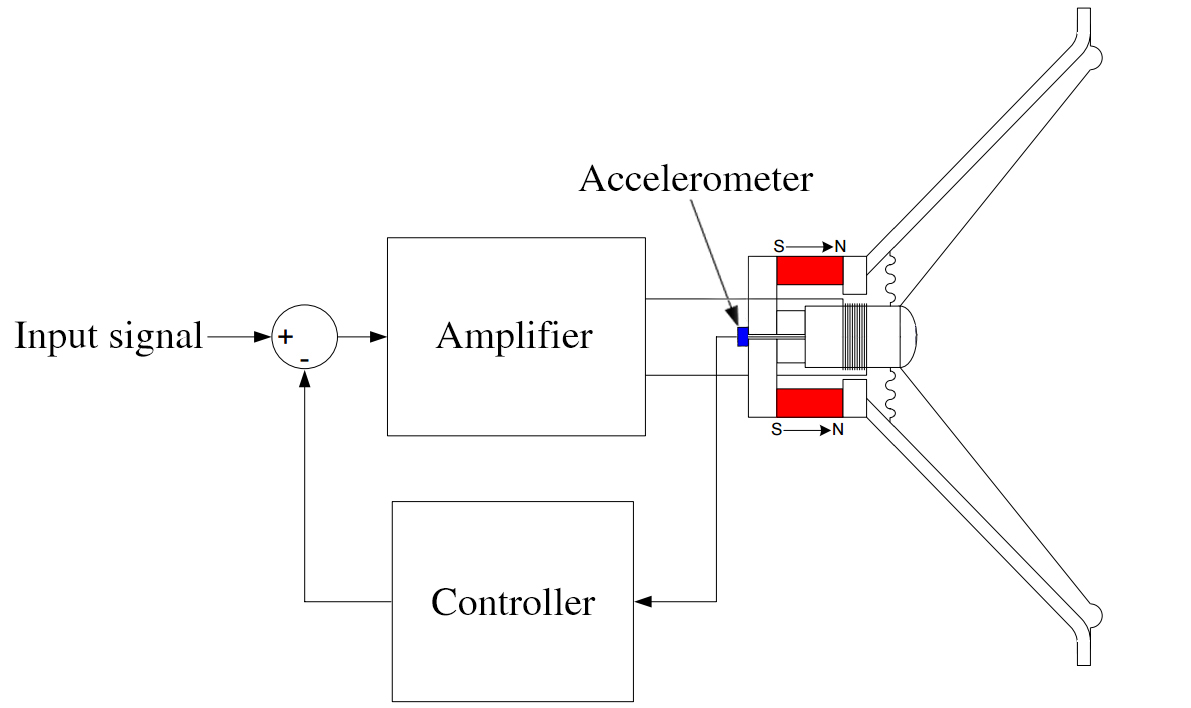
\includegraphics[width=0.75\textwidth]{Feedback_Acc2}
\caption{How a possible feedback system should be implemented in the speaker}
\label{fig:feedbacksystem}
\end{figure}


%\subsection{Distortion from vibration and impulses}\label{subsec:impulses}
%
%A common problem when designing loudspeakers are the vibrations from the enclosure. If the vibrations are strong, they will become audible and distort the overall sound. The sound radiation from the enclosure will become greater when the \gls{SPL} from the speaker increase. This problem is solved with different techniques but yield more or less the same outcome, which is stiffening of the enclosure. Some of the techniques for removing vibrations from the enclosure could be:
%\begin{itemize}
%\item Mechanical decoupling of the drivers from the enclosure.
%\item Denser or heavier construction material with a high natural frequency, making it harder for the enclosure to start vibrating.
%\item Dampening material or complex structural design inside the cabinet to disperse the sound.
%\end{itemize}
%\todo[inline]{Skal nok lige skaffe nogle kilder på de udtagelser}
%
%Another possibility is to use the vibration measurement as an indicator to tell the current performance of the loudspeaker. Since the loudspeaker will vibrate more at higher volumes. 
%
%
%Looking further into the woofer itself, it shows in \autoref{fig:SpeakerModelStress} that parts in the woofer also creates unwanted vibrations. The purpose of the woofer is to reproduce the electrical signal as an acoustical signal. This is done by using a diaphragm which is suspended in a very light and easy to move material. An Induction in the coil is created in a permanent magnet creating a a electro magnetic force resulting in the diaphragm moving. The goal will always be to loose as little as possible energy, giving the most perfect output. The woofer simply needs to be as powerful, light, stiff and efficient as possible.
%
%\begin{figure}[H]
%\centering
%\begin{subfigure}[t]{0.47\textwidth}
%\includegraphics[width=\linewidth]{SpeakerGOOD}
%	\caption{Regular speaker driver showing surround, diaphragm and the magnet.}
%	\label{fig:regularspeaker}
%\end{subfigure}
%\hspace{6mm} 
%\begin{subfigure}[t]{0.47\textwidth}
%\includegraphics[width=\linewidth]{SpeakerBAD}
%	\caption{Regular speaker driver with red markings showing stress areas}
%	\label{fig:badspeaker}
%\end{subfigure}
%\caption{A Speaker driver, where \ref{fig:badspeaker} shows the stress points outlined with red.}
%\label{fig:SpeakerModelStress}
%\end{figure}
%%When this signal has a large amplitude, read overload, the diaphragm reaches physical capacity. 
%In \autoref{fig:badspeaker} it shows that when a diaphragm is pushed to its maximum capacity the surround will affect the diaphragm causing unwanted distortion. This will be one of the major problems if the diaphragm is not sufficiently stiff to withstand the high \gls{SPL} and not twist during playback. 



%\section{Part Conclusion}
This chapter has analyzed an active speaker and its components to investigate how distortion is created throughout the active loudspeaker. The conclusion is that the following situations create distortion.
\begin{itemize}
\item Amplifier
	\begin{itemize}
	\item Clipping.
	\end{itemize}
\item Loudspeaker
	\begin{itemize}
	\item Vibrations from enclosure.
	\item Overexcursion.
	\item Membrane hitting the coil.
	\end{itemize}
\end{itemize}
Of these situations the focus moving forward will only be concerning the distortion situation from the loudspeaker because clipping in the amplifier is easy to solve, because the parameters in the amplifier is constant and the signal is easily limited to create less distortion then by hard clipping. The next chapter will therefore explain and analyze performance tests of a loudspeaker to see if any of the above loudspeaker situations can be detected. 

\subsection*{Test of DALI Zensor 5}
In order to determine whether or not it is possible to use sensory equipment to measure any vibration from the loudspeaker. It is desirable to investigate if the output of the sensors can be analyzed. The loudspeaker which will be the basis for the test is the DALI Zensor 5, shown on \autoref{fig:dali_zensor5}. A passive loudspeaker has been choosen for the test because the amplifier in DALI's active loudspeakers are designed not to push the loudspeaker to its limits and beyond. %and to be able to test how the vibrations affect distortion, the loudspeaker must be tested to above its limits.

\begin{figure}[H]
\centering
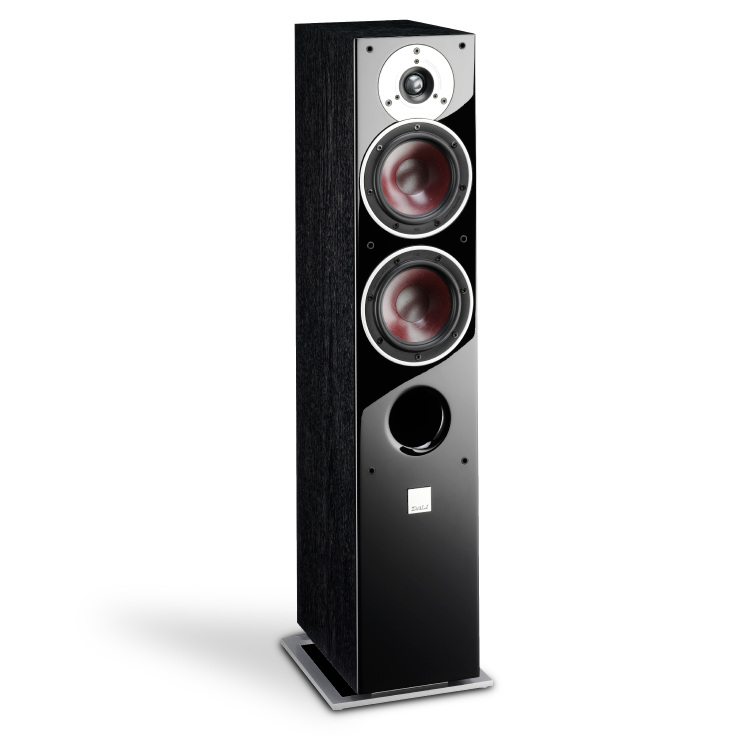
\includegraphics[width=0.5\textwidth]{figures/zensor5.png}
\caption{DALI Zensor 5 \citep{sou:daliZensor5}.}
\label{fig:dali_zensor5}
\end{figure}

%\todo[inline]{Reference http://www.dali-speakers.com/loudspeakers/zensor/zensor-5/}

For measuring the vibrations two Bruel \& Kjær (B\&K) accelerometers have been placed inside the enclosure, one on the back of the bottom driver and one on the top back of the enclosure. For measuring sound a microphone has been placed 1 m from the speaker. To limit any reflections from the room, the test is performed in a Anechoic room at \gls{AAU}, for further documentation refer to the journal in \autoref{app:journal_speaker_test}.  
%\todo[inline]{Reference (09.03.2016) http://doc.es.aau.dk/labs/acoustics/facilities/anechoic_room_large/} 



The loudspeaker is set to play a sinesweep from the crossover frequency of the loudspeaker which is 2400 Hz to 10 Hz. The sine sweep is then repeated from the lowest volume setting of a power amplifier until the loudspeaker breaks. There are in total 20 datasets each containing four measurements, namely the vibrations from the enclosure, driver, the sound pressure from the microphone and lastly a reference signal to synchronize all data. The amount of data is therefore large and only relevant datasets will be presented.  A full detailed overview of graphs is stored on the enclosed CD\footnote{\scalebox{0.7}{\path{CD://Maalinger/Maalinger030316 - Loudspeaker test/Complete Analysis.pdf}}}.



\subsubsection{Analysis of the DALI Zensor 5 measurements}

%In this section a brief review and conclusion of the analysis done in \autoref{app:journal_speaker_test} is presented. 
There are many different approaches in analysing the measured data, and the approach done in this project, will consist of analysing the frequency response of the loudspeaker vibration, harmonic distortion, and detection of the coil hitting the back plate of the driver. The structure of the following part will be showing how the speaker reacts to the different levels of amplification and to conclude if a pattern can be extracted.

%\subsection*{Experiment analysis}

%As previously stated there are in total 20 datasets each containing four measurements, namely the vibrations from the enclosure and driver, the sound pressure from the microphone, and lastly a reference signal to synchronize all data. The amount of data is therefore large and only relevant datasets will be presented. If needed, a more comprehensive approach is taken in \autoref{app:journal_speaker_test} and a full detailed overview of graphs is stored on the enclosed CD.

%\vspace{3mm}

During the first accelerometer measurements the loudspeaker acts linear with very little fluctuations. The frequency response keeps being steadily the same with an increase in amplitude which was expected. In \autoref{fig:Driver1} the first accelerometer measurement is shown, played using 5 mW at XX dB$_{\text{SPL}}$\todo{Fix dB SPL}, on the driver is seen. \autoref{fig:Enclosure1Report} shows the enclosure having a mechanical resonance frequencies at approximately 13 seconds and at 25 seconds while the driver's resonance frequency occurs at 25 seconds. An antiresonance frequency is located at 13 seconds for the accelerometers placed on the driver. The antiresonance frequency is assumed to be caused by the enclosure resonance frequency. This pattern continues for approximately 15 measurements. 

%\todo{Billede af reference tids figur og forklaring af resonans frekvens} %A tendency shows that the 3rd harmonic increases more rapidly than the 2nd harmonic, again as expected for the performance of a loudspeaker.

\begin{figure}[H]
\centering
\begin{subfigure}[t]{0.55\textwidth}
	\tikzsetnextfilename{Driver1Report}
	\input{figures/Forsog1/Driver1Report.tex}
	\caption{Raw dataset 16 from driver.}
	\label{fig:Driver1Report}
\end{subfigure}
%\hspace{6mm} 
\begin{subfigure}[t]{0.43\textwidth}
	\tikzsetnextfilename{Enclosure1Report}
	\input{figures/Forsog1/Enclosure1Report.tex}
	\caption{The grey area zoomed in from 70 - 85 Hz.}
	\label{fig:Enclosure1Report}
\end{subfigure}
\caption{Raw data from the driver measured by an accelerometer placed on the driver. The greyed area is analysed to examine if there are any signs of an impulse.}
\label{fig:dataset1}
\end{figure}

When the speaker was pushed beyond the capabilities specified by DALI an anomaly appears in the measurements. This is shown in \autoref{fig:raw_driver19_window_main}, where spikes in amplitude appear when playing very low frequency sound. 

\begin{figure}[H]
\centering
\begin{subfigure}[t]{0.55\textwidth}
	\tikzsetnextfilename{raw_driver19_window}
	\input{figures/raw_driver19_window.tex}
	\caption{Raw dataset 16 from driver.}
	\label{fig:raw_driver19_window_main}
\end{subfigure}
%\hspace{6mm} 
\begin{subfigure}[t]{0.43\textwidth}
	\tikzsetnextfilename{raw_driver19_window_zoom}
	\input{figures/raw_driver19_window_zoom.tex}
	\caption{The grey area zoomed in from 70 - 85 Hz.}
	\label{fig:raw_driver19_window_zoom_main}
\end{subfigure}
\caption{Raw data from the driver measured by an accelerometer placed on the driver. The greyed area is analysed to examine if there are any signs of an impulse.}
\label{fig:raw_driver19_windows_main}
\end{figure}

Further investigation of the spikes is shown in Figure \ref{fig:raw_driver19_window_zoom_main}. It shows that these spikes appear where the speaker should naturally attenuate the spikes and they appear with no sudden coherence which show signs of the coil hitting the backplate. Looking further into the specific area, shown in \autoref{fig:raw_driver19_window_zoom_main}, an FFT analysis shows how the hit on the back plates appears in relation to other measurements where no hits are detected, which is shown on \autoref{fig:FFT_hit_Main}.

\begin{figure}[H]
\centering
\tikzsetnextfilename{FFTFinal}
\input{figures/Forsog1/FFTFinal.tex}
\caption{The spectrum of accelerometer measurements from time 28.95 - 29.20. The measurements are in ascending order 1, 10, 13, 16 and 19.}
\label{fig:FFT_hit_Main}
\end{figure}

\autoref{fig:FFT_hit_Main} shows that this area is affected by hits on measurement 16 and upwards, refering back to \autoref{subsec:impulses} where it can be seen that an increase in energy level across all frequencies point towards an impulse in the form of a hit. This is particularly seen when comparing measurement 16 through 19. It is possible to see how the fundamental tone at 80 Hz is not increasing dramatically. This is due to the high needs of wattages at this point. However, the entire signals lies more or less 20 dB higher which corresponds to 100 times the energy. This concludes that hits occur but at a very high volume levels \gls{SPL}.

The vibration was also measured on the enclosure but an analysis concludes that the vibration from the enclosure do not change its characteristics at different gains.







%\section{Frequency Response of Measured Data}

In this section the frequency response of the measured data will be analysed to examine if there is any correlation between the frequency responses and the performance of the loudspeaker. From previous section the presented data showed that minimal changes occurred between the datasets. Therefore the expectation is that the frequency response of the measurements will mostly likewise remain almost identical between the datasets. In \autoref{fig:freq_response1} the frequency response of the data measured from the accelerometers and microphone is shown for dataset 1.

\begin{figure}[H]
\centering
\begin{subfigure}[t]{0.37\textwidth}
	\tikzsetnextfilename{FFT_driver1}
	\input{figures/FFT_driver1.tex}
	\caption{Driver}
	\label{fig:freq_responsedriver1}
\end{subfigure}
\begin{subfigure}[t]{0.28\textwidth}
	\tikzsetnextfilename{FFT_enclosure1}
	\input{figures/FFT_enclosure1.tex}
	\caption{Enclosure}
	\label{fig:freq_responseenc1}
\end{subfigure}
\begin{subfigure}[t]{0.32\textwidth}
	\tikzsetnextfilename{FFT_mic1}
	\input{figures/FFT_mic1.tex}
	\caption{Microphone}
	\label{fig:freq_responsemic1}
\end{subfigure}
\caption{Frequency response of (a) the vibration on the driver, (b) the vibration on the enclosure, and (c) the speaker. Test 1.}
\label{fig:freq_response1}
\end{figure}

As expected, it is seen in \autoref{fig:freq_responsedriver1} that there is a mechanical resonance frequency for the driver located at approximately 390 Hz, which likewise also occurs in the measurements for the enclosure. An interesting observation is that the enclosure has another resonance frequency at 1290 Hz, where driver has a antiresonance frequency. An explanation could be destructive interference between the enclosure and driver. The observation is not further examined since it is assessed that it do not have relevance to the project. In \autoref{fig:freq_response_comb} the frequency response for dataset 1, 10, and 19 is plotted.


\begin{figure}[H]
\centering
\begin{subfigure}[t]{0.37\textwidth}
	\tikzsetnextfilename{FFT_driver_comb}
	\input{figures/FFT_driver_comb.tex}
	\caption{Driver tests.}
	\label{fig:freq_responsedrivercomb}
\end{subfigure}
\begin{subfigure}[t]{0.28\textwidth}
	\tikzsetnextfilename{FFT_enclosure_comb}
	\input{figures/FFT_enclosure_comb.tex}
	\caption{Enclosure tests.}
	\label{fig:freq_responsecomb}
\end{subfigure}
\begin{subfigure}[t]{0.32\textwidth}
	\tikzsetnextfilename{FFT_mic_comb}
	\input{figures/FFT_mic_comb.tex}
	\caption{Microphone tests.}
	\label{fig:freq_responsecomb1}
\end{subfigure}
\caption{Frequency response of (a) the vibration on the driver, (b) the vibration on the enclosure, and (c) the speaker. The black graph is frequency response for dataset 1, the blue for the dataset 10, and the red dataset 19. }
\label{fig:freq_response_comb}
\end{figure}

It can be concluded that the frequency response of between all datasets in each measurement remains almost unchanged, thus it is not possible to derive any indication of the current performance of the loudspeaker. The analysis shows that the gain ratio between the amount of vibration and the sound pressure is linear. Therefore it might be possible to use the accelerometer as a tool to estimate the sound pressure level from the amount of vibration.











%\section{Harmonic distortion}

In this section the amount of harmonic distortion of the loudspeaker is analysed, to examine if it is possible to determine the performance of the loudspeaker from harmonics. To analyse the harmonic distortion a spectrogram is used. The spectrogram is a three dimensional plot which shows the frequency, time and magnitude. Basically the spectrogram is an array of multiple FFT each calculated at a given time with a given window.

The advantages of using a spectrogram is that it gives a good overview of the spectral content in the signal at any given time. Since the harmonic frequencies depends on the fundamental frequency, it is better to use a spectrogram rather than a regular FFT, since the spectrogram will reveal all harmonic distortion for all fundamental frequency from 10 Hz to 2.4 kHz. The spectrograms for microphone in dataset 1 and 19 are shown in \autoref{fig:spec_mic}.

\begin{figure}[H]
\centering
\begin{subfigure}[t]{0.47\textwidth}
	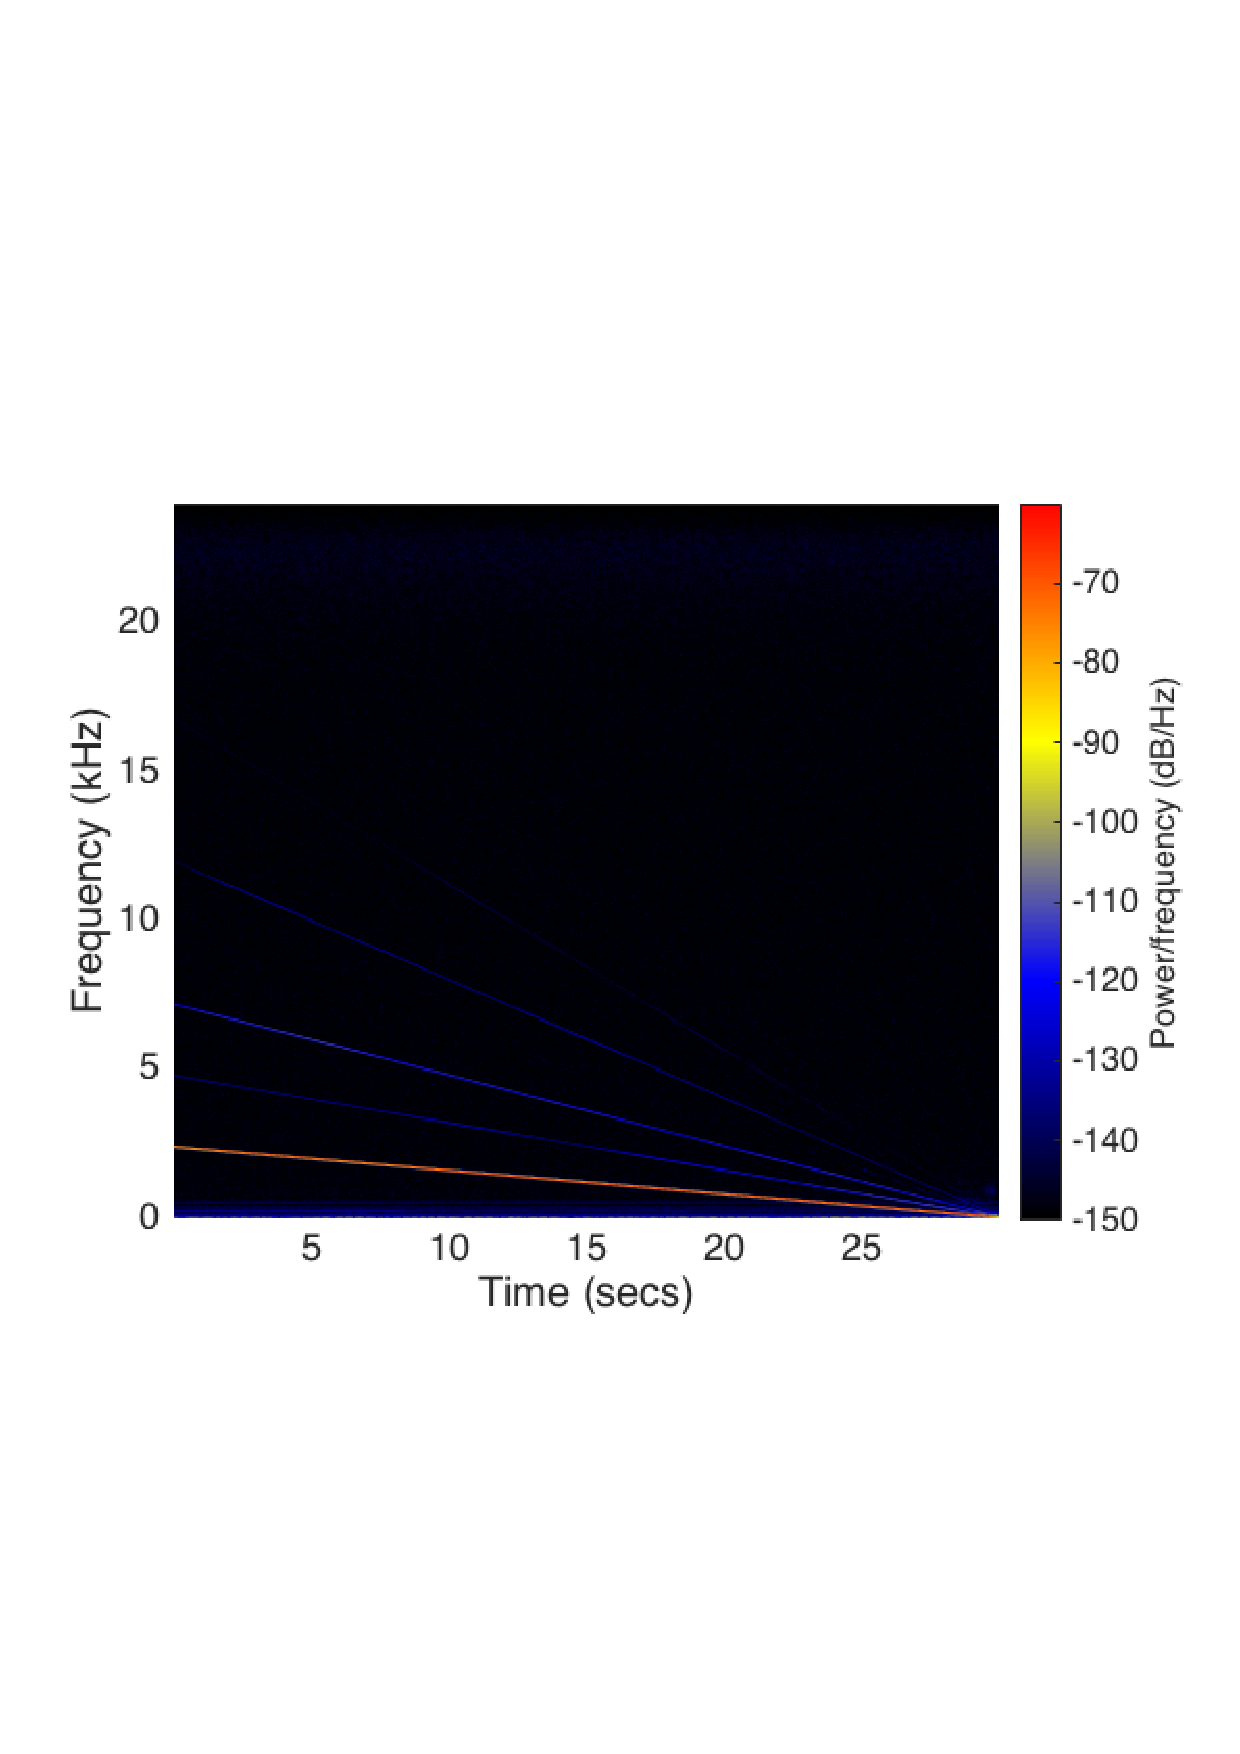
\includegraphics[width=1\textwidth]{figures/spectrogram_mic1.pdf}
	\caption{Microphone dataset 1.}
	\label{fig:spectrogram_mic1}
\end{subfigure}
\begin{subfigure}[t]{0.47\textwidth}
	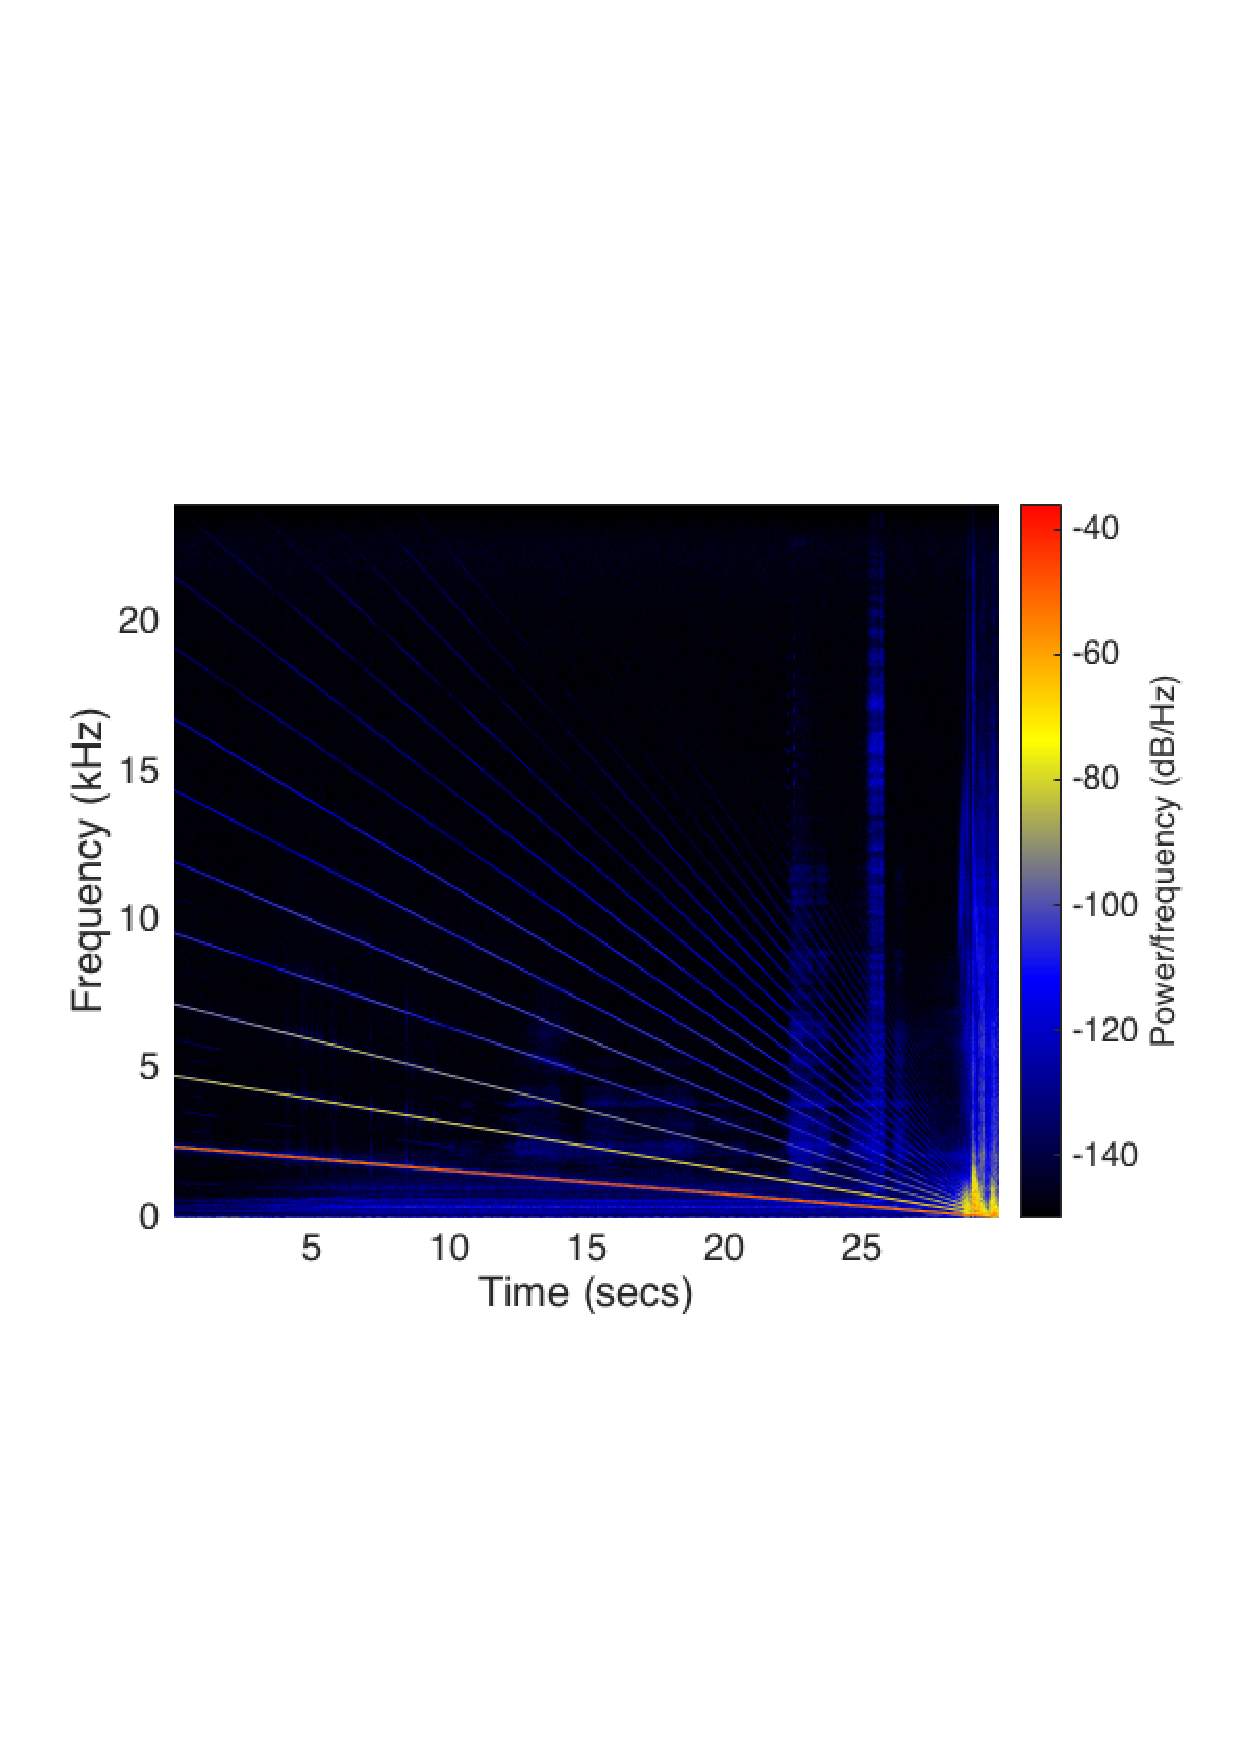
\includegraphics[width=1\textwidth]{figures/spectrogram_mic19.pdf}
	\caption{Microphone dataset 19.}
	\label{fig:spectrogram_mic19}
\end{subfigure}
\caption{The spectrograms of the microphone dataset 1 and 19. The prominent red line is the sine sweep from 2.4 kHz to 10 Hz while the yellow and blue lines along the red line are harmonic distortion.}
\label{fig:spec_mic}
\end{figure} 

The spectrograms of dataset 1 and 19, seen in \autoref{fig:spectrogram_mic1} and \autoref{fig:spectrogram_mic1}, show a prominent red line and three weak blue lines above the red line. It is seen that the red line is a linear decreasing function from 2.4 kHz to 10 Hz where the frequency is a function of time. This indicates that the red line is the fundamental frequency of the sine sweep from 2.4 kHz to 10 Hz. The blue and yellow line are linear functions of the harmonic distortions. The spectrograms clearly show that increasing the gain will increase the amount of harmonic distortion as well. An interesting observation is the spectral frequency leak that occurs at low frequency. 


\begin{figure}[H]
\centering
\begin{subfigure}[t]{0.47\textwidth}
	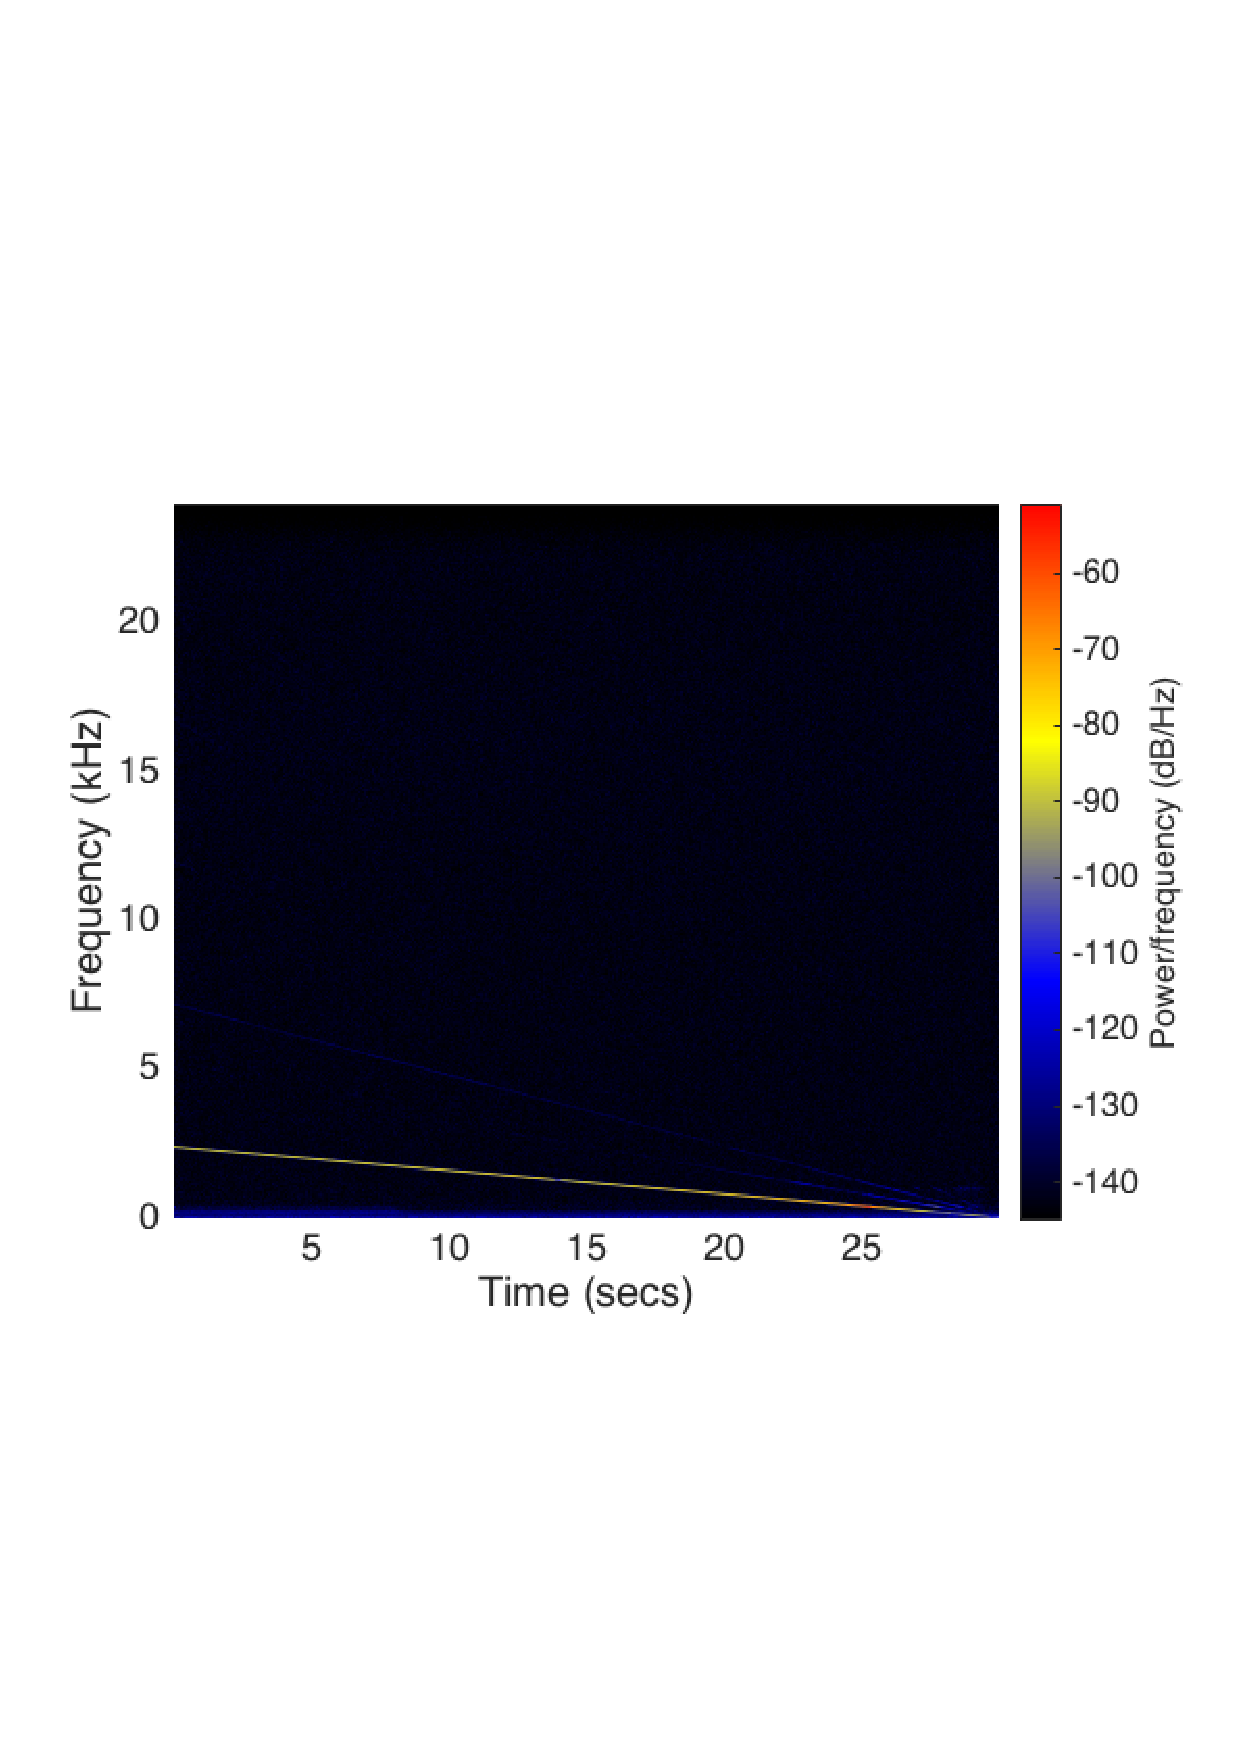
\includegraphics[width=1\textwidth]{figures/spectrogram_driver1.pdf}
	\caption{Vibration from driver.}
	\label{fig:spectrogram_driver1}
\end{subfigure}
\begin{subfigure}[t]{0.47\textwidth}
	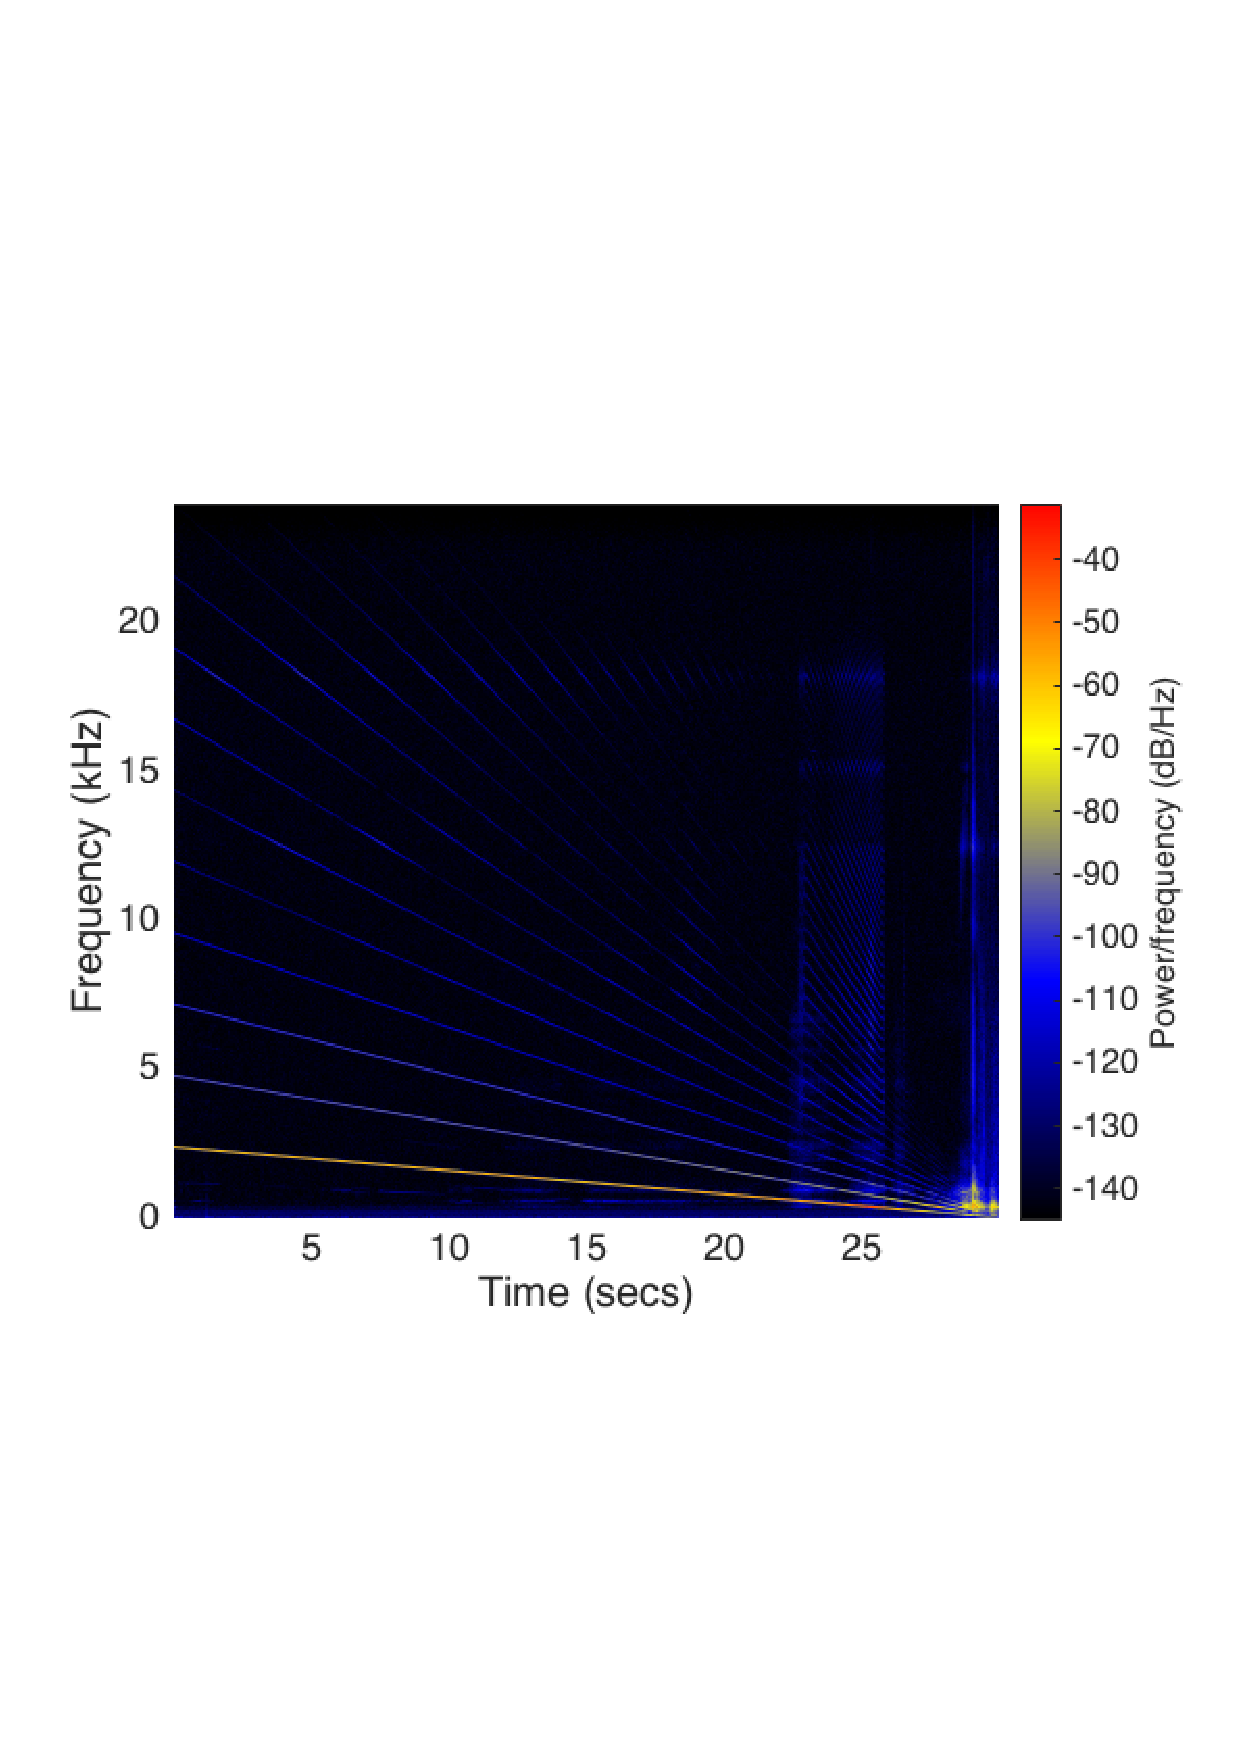
\includegraphics[width=1\textwidth]{figures/spectrogram_driver19.pdf}
	\caption{Vibration from driver.}
	\label{fig:spectrogram_driver19}
\end{subfigure}
\caption{The measured data of (a) the vibration on the driver, (b) the vibration on the enclosure, and (c) the sound pressure from the microphone. Dataset 20.}
\label{fig:spec_driver}
\end{figure} 























\subsubsection{Back Plate Hit Detection}\label{sec:hit_detect}
\todo[inline]{SKRIV NOGET MED 150W THRESHOLD}
As previously stated, it is possible that the loudspeaker coil hits the back plate of the driver if the coil moves too far back. In the long run this will damage the loudspeaker, and should therefore be avoided. In this section an analysis on how to detect these hits, will be provided. 

\textbf{From \autoref{subsec:impulses} the frequency response of a mechanical frame of a loudspeaker has the same characteristics as a low-pass filter. This means, if the coil is hitting the back plate of the driver, it will result in a increase in energy in the low frequency spectrum. As most music and loudspeakers have some sort of a high-pass filter implemented to remove almost non-audible sound, it can be assumed that only a back plate hit will generate vibrations at very low frequencies between, for instance, 0 Hz to 20 Hz. To examine if this is true, a section of the dataset 19 of the driver, where a hit is suspected to have occurred, is analysed.} %The analysed section is seen in \autoref{fig:raw_driver19_windows}.


%\begin{figure}[H]
%\centering
%\begin{subfigure}[t]{0.55\textwidth}
%	\tikzsetnextfilename{raw_driver19_window}
%	\input{figures/raw_driver19_window.tex}
%	\caption{Raw dataset 19 for driver. }
%	\label{fig:raw_driver19_window}
%\end{subfigure}
%%\hspace{6mm} 
%\begin{subfigure}[t]{0.43\textwidth}
%	\tikzsetnextfilename{raw_driver19_window_zoom}
%	\input{figures/raw_driver19_window_zoom.tex}
%	\caption{The grey area zoomed in.}
%	\label{fig:raw_driver19_window_zoom}
%\end{subfigure}
%\caption{The greyed area is analysed to examine if there are any signs of an impulse.}
%\label{fig:raw_driver19_windows}
%\end{figure}

%\textbf{The same window is applied to all datasets for the driver and afterwards spectrum analysed to reveal any increase in low frequent energy.}

\begin{figure}[H]
\centering
\tikzsetnextfilename{FFT_hit}
\input{figures/FFT_hit.tex}
\label{fig:FFT_hit}
\caption{The spectrum of the window. The black graph is dataset 1, blue is 10 and red is 19.}
\label{fig:FFT_hit}
\end{figure}

\todo[inline]{FIGUR FEJL? fft detaljer mangler}

It is seen that the energy for non-harmonic frequencies is increased at very low frequencies as indicated with the arrow. The black graph is the first dataset and the blue is the tenth dataset. As no hit was observed in the window at dataset 1 and 10, the energy of lower part of the spectrum was not increased. However the suspected hit in dataset 19 has an energy increase in the low frequency spectrum. Note that since the window is 0.25 seconds wide, frequencies below 4 Hz should be discarded.

Concluding on the test it shows that it is possible to measure vibration and hits with precise enough equipment. It also showed that further trails had to be made in order to establish if less precise accelerometer could output a sufficient signal.

\subsubsection{Accelerometer trails}

From \autoref{app:journal_speaker_test2} further trails were deducted to determine whether a less precise accelerometer could measure the same output. Same procedure was followed as in the previous section, hence only the results will be shown. The behaviour of the speaker was identical with the preceding trails. 

The trails could be concluded with the accelerometers not being able to properly detect the vibrations of the speaker. There were to many fluctuations in the measurements leading to disbelief in the accelerometer being accurately enough, however from the measurements a pattern could be derived. Since the speaker behaved linearly when the gain of the amplifier is increased. It was possible to compare the fundamental tone with the third harmonic tone and establish the correlation showed in \autoref{fig:com_mic13All_repport}.

\begin{figure}[H]
    \centering
    \tikzsetnextfilename{comp_mic13All1}
    \input{figures/comp_mic13All1.tex}
    \caption{1.harmonic / 3.harmonic pr. measurement. comparison for all frequencies}
\label{fig:com_mic13All_repport}
\end{figure}  

\autoref{fig:com_mic13All_repport} show that the third harmonic increases with the amplifiers gain. From this information it is possible to determine the speakers behaviour according to the gain and thereby use it is a model for gain adjustment.




\subsubsection{Plausible solution} 
The Previous tests have shown that it is possible to use an accelerometer to estimate the performance of the system by looking at the harmonic distortions. However following up on all of the trails the problems are as follows:
\begin{itemize}
\item Estimating harmonic distortions introduced in a system when playing music, are only well-defined for periodic sinusoids.
\item Frequency response of vibration, using the cheaper accelerometer, on the driver and cabinet hardly changes when exposed for loud playback, thus it will be hard to get usable outputs of the sensors.
\item The price for usable sensor equipment is too high compared to the application it is targeted for. 
\item The sensors did not directly show a pattern for when a possible hit of the back plate were about to occur.
\item The phase of the signal can not assumed "in phase" and it is therefore not possible to apply spectral estimations for detecting specific frequency peaks. e.g. if using a specific frequency as target for attenuation a 180 degrees phase shifted signal might bring false negatives. 
\end{itemize}

It can therefore be concluded that developing a system based on measurements from a accelerometer might turn out to be too complex to be realized in time due to time constraints. The system to be designed will therefore be based on a feedforward system. The concept of a feedforward system which fulfill the problem statement is shown in \autoref{fig:Concept}.

\begin{figure}[H]
\centering
\tikzsetnextfilename{Concept}
\scalebox{0.8}{
\begin{tikzpicture}
%% Kasser %%
\node [block, fill=black!80,text=white] (AudioSource) at (0,0) {Audio Source};

%% DSP %%
\node [block, fill=blue!15] (Equalizer1) at ($(AudioSource)+(3.5,0)$) {Equalizer};
\node [block, fill=blue!15] (SpectralAnalysis) at ($(Equalizer1)+(3.5,0)$) {Signal analysis};
\node [block, fill=blue!15] (Equalizer) at ($(SpectralAnalysis)+(4.5,0)$) {Signal processing};


%% External %%
\node [block, fill=blue!15] (UserInterface) at ($(Equalizer1)+(-3.5,2)$) {User interface};
\node [block, fill=blue!15] (UserInterfaceDev) at ($(Equalizer1)+(3.5,2)$) {Developer interface};

%% Speaker Enclosure %%
\node [block, fill=black!80,text=white] (Amplifier) at ($(SpectralAnalysis)+(4.5,-3)$) {Amplifier};
\node [block, fill=black!80,text=white] (Driver) at ($(Amplifier)+(-3.5,0)$) {Driver};

\node (User) at ($(-2.5,0)+(UserInterface)$) {\textbf{User}};
\node (Developer) at ($(3.6,0)+(UserInterfaceDev)$) {\textbf{Developer}};
\draw[->] (User) -- (UserInterface);
\draw[->] (Developer) -- (UserInterfaceDev);

% Store Blokke %%
\begin{pgfonlayer}{bg}
\draw[thick, fill=black!10] ($(-1.75,1.2)+(Equalizer1)$) -- ($(2.5,1.2)+(Equalizer)$) -- ($(2.5,-1.5)+(Equalizer)$) -- ($(-1.75,-1.5)+(Equalizer1)$) -- ($(-1.75,1.2)+(Equalizer1)$);
\node (DSPtag) at ($(0,-1.1)+(SpectralAnalysis)$) {\textbf{Digital Processing System}};

\draw[thick, fill=black!10] ($(-2.5,1)+(Driver)$) -- ($(2.5,1)+(Amplifier)$) -- ($(2.5,-1.5)+(Amplifier)$) -- ($(-2.5,-1.5)+(Driver)$) -- ($(-2.5,1)+(Driver)$);
\node (DSPtag) at ($(2,-1.1)+(Driver)$) {\textbf{Speaker Enclosure}};
\end{pgfonlayer}

%% Forbindelse %%
\draw[->] (AudioSource) -- (Equalizer1);
\draw[->] (Equalizer1) -- (SpectralAnalysis);
\draw[->] (SpectralAnalysis) -- (Equalizer);
\draw[->] (Equalizer) -- (Amplifier);
\draw[->] (Amplifier) -- (Driver);

\draw[->] (UserInterface) -| ($(Equalizer1)+(-.25,.6)$);
\draw[->] (UserInterfaceDev) -| ($(Equalizer1)+(.25,.6)$);

%\draw[->] ($(SensorDriver)+(-1.375,-0.3)$) -- ($(SpectralAnalysis)+(1.375,-0.3)$);

%\draw[->] (SpectralAnalysis) -- (Decisionblock);
%\draw[->] (Decisionblock) |- (Equalizer);
\end{tikzpicture}}
\caption{Overview of a feedforward design concept.}
\label{fig:Concept}
\end{figure}

Since the system will be controlled using a feedforward system which should be able to analyze, process and correct signals before the music is played. It gives rise to questioning what kind of platform should be used and what kind of requirements are needed for such a system. On the market there are different plausible platforms which meets with the demands all with different advantages and disadvantages. The preceding section will cover the determination of which platform that will function best in a active loudspeaker system . 

%\textbf{The design concept consist of a signal processing block, which will be analysed to understand which solution is best for the problem stated. A signal analysis block which will not be analysed further in this chapter, a user interface which will be analysed to determine how the user interface should be designed and lastly the processor block which will be analysed to determine which type of processor that should be used.}


\section{Signal Analysis}

After the signal has been processed in an equalizer, the signal will be analysed in the \textit{Signal Analysis}-block. The purpose of the signal analysis is to examine the content of the signal and afterwards send the parameters to the signal processing subsystem. Generally speaking, any signal can be analysed in time domain or frequency domain. If analysed in time domain, the analysis can for instance be extracting signal feature and calculating of the signal's RMS value. Analysing the signal in frequency domain will reveal the spectral content of the signal. So the following section will cover how different techniques for extracting information from the signal in both time and frequency domain.

%\begin{itemize}
%\item[•] Signal feature extraction.
%\item[•] Spectral analysis.
%\item[•] Modelling.
%\end{itemize}

%\subsection{Signal feature extraction}
% Signal analysis in time domain

\subsection*{Root-mean-square (RMS)}
Root-mean-square is a can be used as a tool to estimate the "mean" value of a periodic signal. The problem with calculating a regular mean value for an audio signal is that the result will be 0 as the signal is approximately evenly distributed on both side of the amplitude axis. By using RMS this problem is avoided. The RMS is calculated as the square root of mean value of the signal squared as shown in following equation:
\begin{equation}\label{eq:RMS_con}
V_{\text{RMS}}(t) = \sqrt{\frac{1}{T}\int_0^T v(t)^2 dt}
\end{equation}
The definition of the RMS in \autoref{eq:RMS_con} is only defined for continuous signals. If the RMS value is to be calculated for discrete values then following equation is used:
\begin{equation}
V_{\text{RMS}}[n] = \sqrt{\frac{1}{N}\sum_{k=1}^{N} v[n-k]^2}
\end{equation}
The RMS can be useful to estimate the power of the signal. For instance if the RMS value of the signal moves above a certain threshold, the system may warn that the signal will stress the loudspeaker too much.

\subsection*{Signal threshold}
A signal threshold can be use to detect whenever the amplitude of a signal is above a certain level. This can for instance help identify if the signal will result in a too loud playback.

\subsection*{Envelope}
A signal threshold can be use to detect whenever the amplitude of a signal is above a certain level. This can for instance help identify if the signal will result in a too loud playback. 

\subsection*{Spectrum analysis}
A spectral estimation 


% Signal analysis in frequency domain



























\section{Equalizer}\label{sec:tech_equalizer}
Since the perception of sound is non linear, there is need for equalization of the different frequencies in order to hear the lower sound just as much as the midrange and high frequency spectrum. By implementing an equalizer it is possible to manipulate different areas of the frequency.

Generally speaking, there are two common types of equalizer designs. The first type of equalizer is the graphic equalizer. The graphic equalizer consist of multiple bandpass filters with a center frequency 

\begin{figure}[H]
\centering
\hspace*{-1cm}
\begin{subfigure}[t]{0.3\textwidth}
	\tikzsetnextfilename{parametric_eq_preanalysis_Q}
	% This file was created by matlab2tikz.
%
%The latest updates can be retrieved from
%  http://www.mathworks.com/matlabcentral/fileexchange/22022-matlab2tikz-matlab2tikz
%where you can also make suggestions and rate matlab2tikz.
%
\begin{tikzpicture}

\begin{axis}[%
width=2in,
height=1.7in,
at={(1.011in,0.642in)},
scale only axis,
xmode=log,
xmin=10,
xmax=20000,
xminorticks=true,
xlabel={Frequency [Hz]},
xmajorgrids,
xminorgrids,
ymin=-5,
ymax=5,
ymajorgrids,
yticklabels={\empty},
axis background/.style={fill=white}
]
\addplot [color=black,solid,line width=1.0pt,forget plot]
  table[row sep=crcr]{%
0.159154943091895	1.52104528479092e-09\\
5.67189079114852	1.93230452791098e-06\\
11.1846266392052	7.51943373818724e-06\\
16.6973624872618	1.67791992824004e-05\\
22.2100983353184	2.97386492611314e-05\\
27.722834183375	4.64357337452805e-05\\
33.2355700314317	6.6919516788473e-05\\
38.7483058794883	9.12504455800552e-05\\
44.2610417275449	0.000119500686962666\\
49.7737775756016	0.00015175453242015\\
55.2865134236582	0.000188108874101866\\
60.7992492717148	0.000228673755853626\\
66.3119851197714	0.000273573008712253\\
71.8247209678281	0.000322944971695505\\
77.3374568158847	0.000376943308720189\\
82.8501926639413	0.000435737928385534\\
88.362928511998	0.000499516015079531\\
93.8756643600546	0.000568483184814175\\
99.3884002081112	0.000642864774463703\\
104.901136056168	0.000722907281943459\\
110.413871904224	0.000808879967186518\\
115.926607752281	0.00090107664260089\\
121.439343600338	0.000999817659988643\\
126.952079448394	0.00110545212673103\\
132.464815296451	0.00121836037701581\\
137.977551144508	0.00133895672322284\\
143.490286992564	0.0014676925275577\\
149.003022840621	0.00160505963325159\\
154.515758688678	0.00175159419615416\\
160.028494536734	0.00190788097717544\\
165.541230384791	0.00207455814919004\\
171.053966232847	0.00225232269285828\\
176.566702080904	0.00244193645895823\\
182.079437928961	0.00264423299601844\\
187.592173777017	0.00286012524226615\\
193.104909625074	0.00309061422509228\\
198.617645473131	0.00333679889352346\\
204.130381321187	0.0035998872811627\\
209.643117169244	0.00388120918199709\\
215.1558530173	0.00418223059313337\\
220.668588865357	0.00450457019596922\\
226.181324713414	0.00485001821500331\\
231.69406056147	0.00522055805142346\\
237.206796409527	0.00561839115630346\\
242.719532257584	0.00604596571734974\\
248.23226810564	0.00650600982730972\\
253.745003953697	0.00700156994994694\\
259.257739801753	0.0075360556701881\\
264.77047564981	0.00811329191767284\\
270.283211497867	0.00873758011500236\\
275.795947345923	0.00941377003543197\\
281.30868319398	0.0101473445408142\\
286.821419042037	0.0109445199075512\\
292.334154890093	0.0118123650807287\\
297.84689073815	0.0127589440154928\\
303.359626586207	0.0137934863589725\\
308.872362434263	0.0149265930350138\\
314.38509828232	0.0161704851220586\\
319.897834130376	0.0175393066793845\\
325.410569978433	0.0190494952573068\\
330.92330582649	0.0207202378147141\\
336.436041674546	0.0225740352218158\\
341.948777522603	0.0246374057041767\\
347.46151337066	0.026941767528892\\
352.974249218716	0.0295245547390489\\
358.486985066773	0.0324306385239295\\
363.999720914829	0.0357141531425909\\
369.512456762886	0.039440862570496\\
375.025192610943	0.0436912575325603\\
380.537928458999	0.048564650265103\\
386.050664307056	0.054184648799545\\
391.563400155113	0.0607065637125135\\
397.076136003169	0.0683275602848587\\
402.588871851226	0.077300770911441\\
408.101607699282	0.0879552153580892\\
413.614343547339	0.100724392830506\\
419.127079395396	0.116188077803\\
424.639815243452	0.135134653259035\\
430.152551091509	0.158656139597021\\
435.665286939566	0.188296609753382\\
441.178022787622	0.226290199861444\\
446.690758635679	0.275953977089983\\
452.203494483736	0.342356864070059\\
457.716230331792	0.433496108720002\\
463.228966179849	0.562432570648061\\
468.741702027905	0.751262614355034\\
474.254437875962	1.03851439355349\\
479.767173724019	1.49189799388277\\
485.279909572075	2.22208716337385\\
490.792645420132	3.34311701685435\\
496.305381268189	4.6247041751038\\
501.818117116245	4.90410608874762\\
507.330852964302	3.82505415494008\\
512.843588812358	2.61985771101294\\
518.356324660415	1.78382846965615\\
523.869060508472	1.25552325827228\\
529.381796356528	0.919021771091239\\
534.894532204585	0.697266219629312\\
540.407268052642	0.545468778132612\\
545.920003900698	0.437813601428799\\
551.432739748755	0.359040714427765\\
556.945475596812	0.299818721083128\\
562.458211444868	0.254241272727278\\
567.970947292925	0.218447077317677\\
573.483683140981	0.189836549255888\\
578.996418989038	0.16661277724288\\
584.509154837095	0.147504053855288\\
590.021890685151	0.131591195560257\\
595.534626533208	0.11819715359357\\
601.047362381265	0.106814691905798\\
606.560098229321	0.0970579326173343\\
612.072834077378	0.0886292233685626\\
617.585569925434	0.0812960559803955\\
623.098305773491	0.0748747112899249\\
628.611041621548	0.0692184879859231\\
634.123777469604	0.0642091084514587\\
639.636513317661	0.059750360839324\\
645.149249165718	0.0557633378864817\\
650.661985013774	0.0521828310419649\\
656.174720861831	0.0489545708600188\\
661.687456709888	0.046033094400842\\
667.200192557944	0.0433800821776765\\
672.712928406001	0.0409630502277672\\
678.225664254057	0.0387543132948973\\
683.738400102114	0.0367301567900939\\
689.251135950171	0.0348701708602796\\
694.763871798227	0.0331567112872759\\
700.276607646284	0.0315744603585919\\
705.789343494341	0.0301100670650826\\
711.302079342397	0.0287518506571268\\
716.814815190454	0.0274895551298186\\
722.32755103851	0.0263141448589172\\
727.840286886567	0.0252176336998925\\
733.353022734624	0.0241929414171724\\
738.86575858268	0.0232337725625455\\
744.378494430737	0.0223345138732211\\
749.891230278794	0.0214901470217593\\
755.40396612685	0.0206961741416183\\
760.916701974907	0.0199485540338976\\
766.429437822963	0.0192436473393069\\
771.94217367102	0.0185781692575445\\
777.454909519077	0.0179491486526881\\
782.967645367133	0.017353892572703\\
788.48038121519	0.0167899553784511\\
793.993117063246	0.0162551118115383\\
799.505852911303	0.0157473334318375\\
805.01858875936	0.0152647679548883\\
810.531324607416	0.0148057210832129\\
816.044060455473	0.0143686404969937\\
821.55679630353	0.0139521017104333\\
827.069532151586	0.0135547955551384\\
832.582267999643	0.0131755170712662\\
838.0950038477	0.012813155636846\\
843.607739695756	0.01246668617149\\
849.120475543813	0.0121351612900779\\
854.633211391869	0.0118177042848058\\
860.145947239926	0.0115135028395057\\
865.658683087983	0.011221803389484\\
871.171418936039	0.0109419060530408\\
876.684154784096	0.0106731600667184\\
882.196890632153	0.0104149596707135\\
887.709626480209	0.010166740392277\\
893.222362328266	0.00992797568316446\\
898.735098176323	0.00969817387615866\\
904.247834024379	0.00947687542142251\\
909.760569872436	0.00926365037957695\\
915.273305720492	0.00905809613688407\\
920.786041568549	0.00885983533102005\\
926.298777416606	0.00866851395226085\\
931.811513264662	0.00848379961467099\\
937.324249112719	0.00830537997469444\\
942.836984960776	0.00813296128321451\\
948.349720808832	0.00796626705919894\\
953.862456656889	0.00780503687267413\\
959.375192504945	0.00764902522840434\\
964.887928353002	0.00749800053779741\\
970.400664201059	0.00735174417577524\\
975.913400049115	0.00721004960777091\\
981.426135897172	0.00707272158928544\\
986.938871745229	0.00693957542511233\\
992.451607593285	0.00681043628269342\\
997.964343441342	0.00668513856262366\\
1003.4770792894	0.0065635253112589\\
1008.98981513746	0.00644544767835877\\
1014.50255098551	0.00633076441469318\\
1020.01528683357	0.00621934140630503\\
1025.52802268163	0.00611105123922509\\
1031.04075852968	0.00600577279878325\\
1036.55349437774	0.00590339089400462\\
1042.06623022579	0.00580379590976603\\
1047.57896607385	0.00570688348170515\\
1053.09170192191	0.0056125541930468\\
1058.60443776996	0.00552071329318637\\
1064.11717361802	0.00543127043321141\\
1069.62990946608	0.00534413942012012\\
1075.14264531413	0.0052592379865762\\
1080.65538116219	0.00517648757571804\\
1086.16811701025	0.00509581313833509\\
1091.6808528583	0.00501714294610182\\
1097.19358870636	0.00494040841231004\\
1102.70632455442	0.00486554392802055\\
1108.21906040247	0.00479248670487366\\
1113.73179625053	0.00472117662911945\\
1119.24453209859	0.00465155612450848\\
1124.75726794664	0.00458357002297077\\
1130.2700037947	0.00451716544255485\\
1135.78273964276	0.0044522916741971\\
1141.29547549081	0.00438890007307048\\
1146.80821133887	0.0043269439571779\\
1152.32094718693	0.00426637851274\\
1157.83368303498	0.00420716070243075\\
1163.34641888304	0.00414924918155447\\
1168.8591547311	0.00409260421693544\\
1174.37189057915	0.00403718761152211\\
1179.88462642721	0.00398296263238773\\
1185.39736227527	0.00392989394260601\\
1190.91009812332	0.00387794753818219\\
1196.42283397138	0.00382709068586065\\
1201.93556981944	0.00377729186687577\\
1207.44830566749	0.0037285207220526\\
1212.96104151555	0.00368074799995988\\
1218.47377736361	0.00363394550881578\\
1223.98651321166	0.00358808606891927\\
1229.49924905972	0.00354314346991455\\
1235.01198490778	0.00349909242784334\\
1240.52472075583	0.0034559085468669\\
1246.03745660389	0.00341356827984536\\
1251.55019245195	0.00337204889433326\\
1257.0629283	0.00333132843704734\\
1262.57566414806	0.00329138570244961\\
1268.08839999612	0.00325220020158058\\
1273.60113584417	0.00321375213273901\\
1279.11387169223	0.00317602235370764\\
1284.62660754029	0.00313899235481557\\
1290.13934338834	0.00310264423424481\\
1295.6520792364	0.00306696067302852\\
1301.16481508446	0.00303192491288174\\
1306.67755093251	0.00299752073380497\\
1312.19028678057	0.00296373243322678\\
1317.70302262863	0.00293054480564248\\
1323.21575847668	0.00289794312435304\\
1328.72849432474	0.00286591312222918\\
1334.2412301728	0.00283444097538565\\
1339.75396602085	0.00280351328552027\\
1345.26670186891	0.00277311706438818\\
1350.77943771697	0.0027432397188826\\
1356.29217356502	0.00271386903623614\\
1361.80490941308	0.00268499316985941\\
1367.31764526114	0.00265660062629918\\
1372.83038110919	0.00262868025278185\\
1378.34311695725	0.00260122122404099\\
1383.85585280531	0.00257421303140194\\
1389.36858865336	0.00254764547186784\\
1394.88132450142	0.002521508636239\\
1400.39406034948	0.00249579289956674\\
1405.90679619753	0.00247048891134444\\
1411.41953204559	0.00244558758573287\\
1416.93226789365	0.002421080092645\\
1422.4450037417	0.00239695784848904\\
1427.95773958976	0.0023732125088894\\
1433.47047543782	0.00234983595947141\\
1438.98321128587	0.00232682030881676\\
1444.49594713393	0.00230415788105415\\
1450.00868298199	0.00228184120821058\\
1455.52141883004	0.00225986302389273\\
1461.0341546781	0.00223821625641463\\
1466.54689052616	0.0022168940224824\\
1472.05962637421	0.00219588962126232\\
1477.57236222227	0.00217519652836194\\
1483.08509807033	0.00215480839014459\\
1488.59783391838	0.00213471901847157\\
1494.11056976644	0.00211492238540767\\
1499.6233056145	0.00209541261804977\\
1505.13604146255	0.00207618399386629\\
1510.64877731061	0.00205723093592845\\
1516.16151315867	0.00203854800845373\\
1521.67424900672	0.0020201299122875\\
1527.18698485478	0.00200197148114609\\
1532.69972070283	0.00198406767705373\\
1538.21245655089	0.00196641358702312\\
1543.72519239895	0.00194900441871381\\
1549.237928247	0.00193183549725902\\
1554.75066409506	0.00191490226155436\\
1560.26339994312	0.0018982002610304\\
1565.77613579117	0.00188172515230368\\
1571.28887163923	0.00186547269607827\\
1576.80160748729	0.00184943875403952\\
1582.31434333534	0.00183361928609289\\
1587.8270791834	0.00181801034732114\\
1593.33981503146	0.00180260808546209\\
1598.85255087951	0.00178740873816454\\
1604.36528672757	0.00177240863039448\\
1609.87802257563	0.001757604172092\\
1615.39075842368	0.0017429918557586\\
1620.90349427174	0.00172856825387864\\
1626.4162301198	0.00171433001722007\\
1631.92896596785	0.00170027387209956\\
1637.44170181591	0.00168639661886817\\
1642.95443766397	0.00167269512947912\\
1648.46717351202	0.00165916634550482\\
1653.97990936008	0.00164580727659151\\
1659.49264520814	0.00163261499832965\\
1665.00538105619	0.00161958665072776\\
1670.51811690425	0.00160671943604798\\
1676.03085275231	0.00159401061778507\\
1681.54358860036	0.00158145751853466\\
1687.05632444842	0.00156905751874846\\
1692.56906029648	0.00155680805479339\\
1698.08179614453	0.00154470661814053\\
1703.59453199259	0.00153275075328537\\
1709.10726784065	0.00152093805680557\\
1714.6200036887	0.00150926617602739\\
1720.13273953676	0.00149773280721376\\
1725.64547538482	0.00148633569507711\\
1731.15821123287	0.00147507263093657\\
1736.67094708093	0.00146394145175835\\
1742.18368292899	0.0014529400391497\\
1747.69641877704	0.00144206631798664\\
1753.2091546251	0.0014313182555139\\
1758.72189047316	0.0014206938603062\\
1764.23462632121	0.00141019118091697\\
1769.74736216927	0.00139980830552986\\
1775.26009801733	0.00138954336033172\\
1780.77283386538	0.00137939450905026\\
1786.28556971344	0.00136935995170113\\
1791.7983055615	0.00135943792404647\\
1797.31104140955	0.00134962669652705\\
1802.82377725761	0.00133992457329465\\
1808.33651310567	0.00133032989188273\\
1813.84924895372	0.00132084102181647\\
1819.36198480178	0.00131145636443378\\
1824.87472064984	0.00130217435167278\\
1830.38745649789	0.00129299344565364\\
1835.90019234595	0.00128391213778806\\
1841.41292819401	0.00127492894817405\\
1846.92566404206	0.00126604242505828\\
1852.43839989012	0.00125725114395507\\
1857.95113573818	0.00124855370706049\\
1863.46387158623	0.00123994874293254\\
1868.97660743429	0.00123143490542309\\
1874.48934328235	0.0012230108735933\\
1880.0020791304	0.00121467535073426\\
1885.51481497846	0.00120642706401438\\
1891.02755082652	0.00119826476401676\\
1896.54028667457	0.00119018722401632\\
1902.05302252263	0.00118219323974091\\
1907.56575837069	0.00117428162845553\\
1913.07849421874	0.00116645122908594\\
1918.5912300668	0.00115870090108501\\
1924.10396591486	0.00115102952453896\\
1929.61670176291	0.00114343599935377\\
1935.12943761097	0.00113591924508374\\
1940.64217345903	0.00112847820026829\\
1946.15490930708	0.00112111182221618\\
1951.66764515514	0.00111381908650813\\
1957.1803810032	0.00110659898660938\\
1962.69311685125	0.00109945053349381\\
1968.20585269931	0.00109237275532592\\
1973.71858854737	0.00108536469706756\\
1979.23132439542	0.00107842542003069\\
1984.74406024348	0.00107155400169241\\
1990.25679609154	0.00106474953529783\\
1995.76953193959	0.00105801112946678\\
2001.28226778765	0.00105133790797996\\
2006.79500363571	0.00104472900935471\\
2012.30773948376	0.0010381835867218\\
2017.82047533182	0.0010317008072026\\
2023.33321117987	0.00102527985206159\\
2028.84594702793	0.00101891991603342\\
2034.35868287599	0.00101262020730954\\
2039.87141872404	0.00100637994701951\\
2045.3841545721	0.00100019836925045\\
2050.89689042016	0.00099407472056883\\
2056.40962626821	0.000988008259883694\\
2061.92236211627	0.000981998258161303\\
2067.43509796433	0.000976043998249759\\
2072.94783381238	0.000970144774495331\\
2078.46056966044	0.000964299892678894\\
2083.9733055085	0.000958508669655401\\
2089.48604135655	0.000952770433365526\\
2094.99877720461	0.00094708452231314\\
2100.51151305267	0.00094145028544389\\
2106.02424890072	0.000935867082253264\\
2111.53698474878	0.0009303342820905\\
2117.04972059684	0.000924851264451771\\
2122.56245644489	0.000919417418361226\\
2128.07519229295	0.000914032142413475\\
2133.58792814101	0.000908694844696523\\
2139.10066398906	0.000903404942325138\\
2144.61339983712	0.000898161861408133\\
2150.12613568518	0.000892965037038778\\
2155.63887153323	0.000887813912876385\\
2161.15160738129	0.000882707941109721\\
2166.66434322935	0.000877646582254575\\
2172.1770790774	0.000872629305047741\\
2177.68981492546	0.000867655586356437\\
2183.20255077352	0.000862724910740591\\
2188.71528662157	0.000857836770726728\\
2194.22802246963	0.000852990666287338\\
2199.74075831769	0.000848186104993265\\
2205.25349416574	0.000843422601674342\\
2210.7662300138	0.000838699678377012\\
2216.27896586186	0.000834016864229373\\
2221.79170170991	0.000829373695312013\\
2227.30443755797	0.000824769714488344\\
2232.81717340603	0.000820204471418143\\
2238.32990925408	0.000815677522204675\\
2243.84264510214	0.000811188429529727\\
2249.3553809502	0.000806736762325801\\
2254.86811679825	0.000802322095886071\\
2260.38085264631	0.000797944011534653\\
2265.89358849437	0.000793602096618917\\
2271.40632434242	0.0007892959444536\\
2276.91906019048	0.000785025154099057\\
2282.43179603854	0.00078078933042108\\
2287.94453188659	0.00077658808377658\\
2293.45726773465	0.000772421030140901\\
2298.97000358271	0.0007682877908475\\
2304.48273943076	0.00076418799255712\\
2309.99547527882	0.00076012126723082\\
2315.50821112688	0.00075608725191015\\
2321.02094697493	0.000752085588738394\\
2326.53368282299	0.000748115924777387\\
2332.04641867105	0.00074417791204611\\
2337.5591545191	0.000740271207335578\\
2343.07189036716	0.000736395472168364\\
2348.58462621522	0.000732550372709916\\
2354.09736206327	0.000728735579649006\\
2359.61009791133	0.000724950768303823\\
2365.12283375939	0.000721195618276794\\
2370.63556960744	0.000717469813593452\\
2376.1483054555	0.000713773042528897\\
2381.66104130356	0.000710104997542243\\
2387.17377715161	0.000706465375232283\\
2392.68651299967	0.000702853876327865\\
2398.19924884773	0.000699270205496988\\
2403.71198469578	0.00069571407135068\\
2409.22472054384	0.000692185186414083\\
2414.7374563919	0.000688683266962552\\
2420.25019223995	0.000685208033040952\\
2425.76292808801	0.000681759208415467\\
2431.27566393607	0.000678336520482972\\
2436.78839978412	0.000674939700141838\\
2442.30113563218	0.000671568481855594\\
2447.81387148024	0.00066822260361629\\
2453.32660732829	0.000664901806684175\\
2458.83934317635	0.000661605835757408\\
2464.35207902441	0.000658334438796587\\
2469.86481487246	0.000655087367061398\\
2475.37755072052	0.00065186437491585\\
2480.89028656857	0.000648665219972927\\
2486.40302241663	0.000645489662870896\\
2491.91575826469	0.000642337467306096\\
2497.42849411275	0.000639208400034887\\
2502.9412299608	0.000636102230692377\\
2508.45396580886	0.000633018731836788\\
2513.96670165692	0.000629957678980327\\
2519.47943750497	0.000626918850296062\\
2524.99217335303	0.000623902026876351\\
2530.50490920108	0.000620906992540003\\
2536.01764504914	0.000617933533695364\\
2541.5303808972	0.000614981439465678\\
2547.04311674525	0.000612050501664029\\
2552.55585259331	0.000609140514509856\\
2558.06858844137	0.000606251274968383\\
2563.58132428942	0.000603382582299355\\
2569.09406013748	0.00060053423834825\\
2574.60679598554	0.000597706047339941\\
2580.11953183359	0.000594897815913415\\
2585.63226768165	0.000592109353044639\\
2591.14500352971	0.000589340470008002\\
2596.65773937776	0.000586590980358963\\
2602.17047522582	0.000583860700013128\\
2607.68321107388	0.000581149446935767\\
2613.19594692193	0.000578457041384816\\
2618.70868276999	0.000575783305721886\\
2624.22141861805	0.000573128064477843\\
2629.7341544661	0.000570491144262171\\
2635.24689031416	0.000567872373691629\\
2640.75962616222	0.000565271583511748\\
2646.27236201027	0.000562688606340347\\
2651.78509785833	0.000560123276866178\\
2657.29783370639	0.000557575431725507\\
2662.81056955444	0.000555044909413405\\
2668.3233054025	0.000552531550353183\\
2673.83604125056	0.000550035196811542\\
2679.34877709861	0.000547555692929438\\
2684.86151294667	0.000545092884616012\\
2690.37424879473	0.000542646619571745\\
2695.88698464278	0.000540216747276888\\
2701.39972049084	0.000537803118968326\\
2706.9124563389	0.000535405587475657\\
2712.42519218695	0.000533024007504694\\
2717.93792803501	0.000530658235263332\\
2723.45066388307	0.000528308128662121\\
2728.96339973112	0.000525973547240987\\
2734.47613557918	0.000523654352111381\\
2739.98887142724	0.000521350405975565\\
2745.50160727529	0.000519061573093839\\
2751.01434312335	0.00051678771920161\\
2756.52707897141	0.000514528711648259\\
2762.03981481946	0.000512284419140641\\
2767.55255066752	0.000510054711984163\\
2773.06528651558	0.000507839461851364\\
2778.57802236363	0.000505638541833982\\
2784.09075821169	0.000503451826523964\\
2789.60349405975	0.000501279191809044\\
2795.1162299078	0.000499120514990382\\
2800.62896575586	0.000496975674722788\\
2806.14170160392	0.000494844550991583\\
2811.65443745197	0.000492727025091385\\
2817.16717330003	0.000490622979651189\\
2822.67990914809	0.000488532298541794\\
2828.19264499614	0.000486454866933667\\
2833.7053808442	0.000484390571208231\\
2839.21811669226	0.000482339298998371\\
2844.73085254031	0.000480300939173004\\
2850.24358838837	0.000478275381794657\\
2855.75632423643	0.000476262518100185\\
2861.26906008448	0.000474262240450629\\
2866.78179593254	0.000472274442446935\\
2872.2945317806	0.000470299018808455\\
2877.80726762865	0.000468335865340169\\
2883.32000347671	0.000466384878973181\\
2888.83273932477	0.000464445957741586\\
2894.34547517282	0.000462519000741967\\
2899.85821102088	0.000460603908193188\\
2905.37094686894	0.000458700581314892\\
2910.88368271699	0.000456808922358366\\
2916.39641856505	0.000454928834645111\\
2921.90915441311	0.000453060222466561\\
2927.42189026116	0.000451202991172797\\
2932.93462610922	0.000449357047089626\\
2938.44736195728	0.000447522297424078\\
2943.96009780533	0.000445698650468839\\
2949.47283365339	0.000443886015413255\\
2954.98556950145	0.000442084302356831\\
2960.4983053495	0.000440293422417236\\
2966.01104119756	0.000438513287545161\\
2971.52377704562	0.000436743810638106\\
2977.03651289367	0.000434984905455527\\
2982.54924874173	0.000433236486663195\\
2988.06198458979	0.000431498469775337\\
2993.57472043784	0.000429770771214429\\
2999.0874562859	0.000428053308199337\\
3004.60019213395	0.00042634599881668\\
3010.11292798201	0.000424648761984184\\
3015.62566383007	0.000422961517400544\\
3021.13839967812	0.000421284185641853\\
3026.65113552618	0.000419616688018892\\
3032.16387137424	0.000417958946660058\\
3037.67660722229	0.00041631088447665\\
3043.18934307035	0.000414672425137803\\
3048.70207891841	0.000413043493099416\\
3054.21481476646	0.00041142401350194\\
3059.72755061452	0.000409813912340092\\
3065.24028646258	0.000408213116243002\\
3070.75302231063	0.000406621552597641\\
3076.26575815869	0.000405039149502539\\
3081.77849400675	0.00040346583578707\\
3087.2912298548	0.000401901540967096\\
3092.80396570286	0.000400346195243043\\
3098.31670155092	0.000398799729507614\\
3103.82943739897	0.000397262075284075\\
3109.34217324703	0.000395733164867046\\
3114.85490909509	0.000394212931071783\\
3120.36764494314	0.000392701307484899\\
3125.8803807912	0.000391198228267646\\
3131.39311663926	0.000389703628250419\\
3136.90585248731	0.000388217442855616\\
3142.41858833537	0.000386739608176703\\
3147.93132418343	0.000385270060864441\\
3153.44406003148	0.000383808738234877\\
3158.95679587954	0.000382355578149777\\
3164.4695317276	0.000380910519109203\\
3169.98226757565	0.000379473500160863\\
3175.49500342371	0.000378044460952191\\
3181.00773927177	0.00037662334172263\\
3186.52047511982	0.000375210083236131\\
3192.03321096788	0.000373804626819731\\
3197.54594681594	0.000372406914386693\\
3203.05868266399	0.000371016888388293\\
3208.57141851205	0.000369634491786822\\
3214.08415436011	0.000368259668098015\\
3219.59689020816	0.000366892361360194\\
3225.10962605622	0.000365532516184414\\
3230.62236190428	0.000364180077629103\\
3236.13509775233	0.000362834991257925\\
3241.64783360039	0.000361497203191846\\
3247.16056944845	0.000360166660043571\\
3252.6733052965	0.000358843308890538\\
3258.18604114456	0.000357527097309637\\
3263.69877699262	0.000356217973365636\\
3269.21151284067	0.000354915885593831\\
3274.72424868873	0.000353620783015467\\
3280.23698453679	0.000352332615085675\\
3285.74972038484	0.000351051331778324\\
3291.2624562329	0.000349776883452952\\
3296.77519208096	0.000348509220966628\\
3302.28792792901	0.00034724829562766\\
3307.80066377707	0.000345994059155101\\
3313.31339962513	0.000344746463726963\\
3318.82613547318	0.000343505461949356\\
3324.33887132124	0.000342271006815997\\
3329.8516071693	0.000341043051843203\\
3335.36434301735	0.000339821550842324\\
3340.87707886541	0.000338606458131886\\
3346.38981471347	0.000337397728392948\\
3351.90255056152	0.000336195316703817\\
3357.41528640958	0.000334999178597907\\
3362.92802225764	0.000333809269957666\\
3368.44075810569	0.000332625547033864\\
3373.95349395375	0.000331447966532379\\
3379.46622980181	0.00033027648548884\\
3384.97896564986	0.000329111061353486\\
3390.49170149792	0.000327951651906304\\
3396.00443734598	0.000326798215361183\\
3401.51717319403	0.000325650710242473\\
3407.02990904209	0.000324509095442855\\
3412.54264489015	0.000323373330285046\\
3418.0553807382	0.000322243374342447\\
3423.56811658626	0.000321119187616573\\
3429.08085243432	0.000320000730409764\\
3434.59358828237	0.000318887963417761\\
3440.10632413043	0.000317780847606275\\
3445.61905997849	0.000316679344372988\\
3451.13179582654	0.000315583415364339\\
3456.6445316746	0.000314493022587384\\
3462.15726752266	0.000313408128404008\\
3467.67000337071	0.000312328695449924\\
3473.18273921877	0.000311254686719537\\
3478.69547506683	0.000310186065500365\\
3484.20821091488	0.000309122795394258\\
3489.72094676294	0.000308064840348258\\
3495.23368261099	0.000307012164558164\\
3500.74641845905	0.000305964732564967\\
3506.25915430711	0.000304922509216275\\
3511.77189015517	0.000303885459606531\\
3517.28462600322	0.00030285354918501\\
3522.79736185128	0.000301826743653609\\
3528.31009769933	0.00030080500904013\\
3533.82283354739	0.000299788311594136\\
3539.33556939545	0.000298776617914242\\
3544.8483052435	0.000297769894843969\\
3550.36104109156	0.000296768109506459\\
3555.87377693962	0.000295771229312191\\
3561.38651278767	0.000294779221933909\\
3566.89924863573	0.000293792055312407\\
3572.41198448379	0.000292809697654602\\
3577.92472033184	0.000291832117423891\\
3583.4374561799	0.000290859283371009\\
3588.95019202796	0.000289891164468457\\
3594.46292787601	0.000288927729976076\\
3599.97566372407	0.000287968949383185\\
3605.48839957213	0.000287014792454873\\
3611.00113542018	0.000286065229168353\\
3616.51387126824	0.000285120229772748\\
3622.0266071163	0.000284179764775593\\
3627.53934296435	0.000283243804861833\\
3633.05207881241	0.000282312321017254\\
3638.56481466047	0.000281385284457125\\
3644.07755050852	0.000280462666593413\\
3649.59028635658	0.000279544439108068\\
3655.10302220464	0.000278630573883596\\
3660.61575805269	0.000277721043066701\\
3666.12849390075	0.000276815818948713\\
3671.64122974881	0.000275914874160378\\
3677.15396559686	0.000275018181463568\\
3682.66670144492	0.000274125713857354\\
3688.17943729298	0.000273237444572221\\
3693.69217314103	0.00027235334705464\\
3699.20490898909	0.00027147339493814\\
3704.71764483715	0.000270597562095377\\
3710.2303806852	0.000269725822589922\\
3715.74311653326	0.000268858150683976\\
3721.25585238132	0.000267994520859583\\
3726.76858822937	0.000267134907797417\\
3732.28132407743	0.000266279286374853\\
3737.79405992549	0.000265427631669824\\
3743.30679577354	0.000264579918939609\\
3748.8195316216	0.00026373612367483\\
3754.33226746966	0.000262896221520383\\
3759.84500331771	0.000262060188323652\\
3765.35773916577	0.000261228000134508\\
3770.87047501383	0.000260399633168668\\
3776.38321086188	0.000259575063834696\\
3781.89594670994	0.000258754268739785\\
3787.408682558	0.000257937224624189\\
3792.92141840605	0.000257123908505866\\
3798.43415425411	0.000256314297472189\\
3803.94689010217	0.000255508368841953\\
3809.45962595022	0.000254706100111366\\
3814.97236179828	0.000253907468927059\\
3820.48509764634	0.000253112453132362\\
3825.99783349439	0.000252321030722955\\
3831.51056934245	0.000251533179877723\\
3837.02330519051	0.000250748878918252\\
3842.53604103856	0.000249968106364764\\
3848.04877688662	0.000249190840882112\\
3853.56151273468	0.000248417061273999\\
3859.07424858273	0.000247646746560117\\
3864.58698443079	0.000246879875897078\\
3870.09972027885	0.000246116428551412\\
3875.6124561269	0.000245356384028785\\
3881.12519197496	0.000244599721942853\\
3886.63792782302	0.00024384642203455\\
3892.15066367107	0.000243096464276228\\
3897.66339951913	0.000242349828721232\\
3903.17613536719	0.000241606495588755\\
3908.68887121524	0.000240866445258055\\
3914.2016070633	0.000240129658266522\\
3919.71434291136	0.000239396115263397\\
3925.22707875941	0.000238665797075342\\
3930.73981460747	0.000237938684646652\\
3936.25255045553	0.000237214759070116\\
3941.76528630358	0.000236494001602443\\
3947.27802215164	0.000235776393596765\\
3952.7907579997	0.000235061916575919\\
3958.30349384775	0.000234350552201592\\
3963.81622969581	0.000233642282224179\\
3969.32896554387	0.000232937088615854\\
3974.84170139192	0.000232234953371925\\
3980.35443723998	0.00023153585873841\\
3985.86717308804	0.000230839786976746\\
3991.37990893609	0.000230146720568223\\
3996.89264478415	0.000229456642077051\\
4002.4053806322	0.000228769534190864\\
4007.91811648026	0.00022808537974386\\
4013.43085232832	0.000227404161701373\\
4018.94358817637	0.000226725863119375\\
4024.45632402443	0.000226050467217759\\
4029.96905987249	0.000225377957287771\\
4035.48179572054	0.000224708316800005\\
4040.9945315686	0.00022404152929834\\
4046.50726741666	0.000223377578461643\\
4052.02000326472	0.000222716448099923\\
4057.53273911277	0.000222058122115753\\
4063.04547496083	0.000221402584548629\\
4068.55821080888	0.000220749819524826\\
4074.07094665694	0.00022009981131526\\
4079.583682505	0.00021945254428341\\
4085.09641835305	0.000218808002916179\\
4090.60915420111	0.000218166171794965\\
4096.12189004917	0.000217527035636161\\
4101.63462589722	0.000216890579237155\\
4107.14736174528	0.000216256787518759\\
4112.66009759334	0.000215625645511708\\
4118.17283344139	0.00021499713834316\\
4123.68556928945	0.000214371251244414\\
4129.19830513751	0.000213747969550904\\
4134.71104098556	0.000213127278721489\\
4140.22377683362	0.000212509164299882\\
4145.73651268168	0.000211893611930075\\
4151.24924852973	0.0002112806073467\\
4156.76198437779	0.000210670136411669\\
4162.27472022585	0.000210062185073677\\
4167.7874560739	0.000209456739368199\\
4173.30019192196	0.000208853785427135\\
4178.81292777002	0.000208253309523168\\
4184.32566361807	0.000207655297950187\\
4189.83839946613	0.000207059737162154\\
4195.35113531419	0.000206466613680523\\
4200.86387116224	0.000205875914107745\\
4206.3766070103	0.00020528762516584\\
4211.88934285836	0.000204701733655893\\
4217.40207870641	0.000204118226467702\\
4222.91481455447	0.000203537090570132\\
4228.42755040253	0.000202958313049687\\
4233.94028625058	0.000202381881048795\\
4239.45302209864	0.000201807781829453\\
4244.9657579467	0.000201236002732727\\
4250.47849379475	0.000200666531172963\\
4255.99122964281	0.000200099354651291\\
4261.50396549087	0.000199534460765264\\
4267.01670133892	0.000198971837178006\\
4272.52943718698	0.000198411471685708\\
4278.04217303504	0.000197853352098057\\
4283.55490888309	0.000197297466344309\\
4289.06764473115	0.000196743802450145\\
4294.58038057921	0.000196192348489457\\
4300.09311642726	0.000195643092642208\\
4305.60585227532	0.000195096023148139\\
4311.11858812338	0.000194551128337635\\
4316.63132397143	0.000194008396624005\\
4322.14405981949	0.000193467816480341\\
4327.65679566755	0.000192929376460731\\
4333.1695315156	0.000192393065223405\\
4338.68226736366	0.000191858871472875\\
4344.19500321172	0.000191326783990793\\
4349.70773905977	0.000190796791647523\\
4355.22047490783	0.000190268883392497\\
4360.73321075589	0.000189743048207932\\
4366.24594660394	0.000189219275201397\\
4371.758682452	0.000188697553520961\\
4377.27141830006	0.000188177872397616\\
4382.78415414811	0.000187660221118283\\
4388.29688999617	0.000187144589081737\\
4393.80962584423	0.00018663096569832\\
4399.32236169228	0.000186119340480588\\
4404.83509754034	0.000185609703020167\\
4410.3478333884	0.000185102042953034\\
4415.86056923645	0.000184596350001954\\
4421.37330508451	0.000184092613937901\\
4426.88604093257	0.000183590824632133\\
4432.39877678062	0.000183090971959763\\
4437.91151262868	0.000182593045940547\\
4443.42424847673	0.00018209703660002\\
4448.93698432479	0.000181602934052433\\
4454.44972017285	0.000181110728466034\\
4459.96245602091	0.000180620410090069\\
4465.47519186896	0.000180131969220066\\
4470.98792771702	0.000179645396219053\\
4476.50066356508	0.000179160681521413\\
4482.01339941313	0.000178677815605884\\
4487.52613526119	0.000178196789016772\\
4493.03887110924	0.000177717592379384\\
4498.5516069573	0.000177240216344093\\
4504.06434280536	0.000176764651678917\\
4509.57707865341	0.000176290889122941\\
4515.08981450147	0.000175818919565677\\
4520.60255034953	0.000175348733883137\\
4526.11528619758	0.000174880323053542\\
4531.62802204564	0.000174413678114902\\
4537.1407578937	0.000173948790124506\\
4542.65349374176	0.000173485650220644\\
4548.16622958981	0.000173024249601391\\
4553.67896543787	0.00017256457951689\\
4559.19170128592	0.000172106631263568\\
4564.70443713398	0.000171650396214995\\
4570.21717298204	0.000171195865765952\\
4575.72990883009	0.000170743031390291\\
4581.24264467815	0.000170291884610075\\
4586.75538052621	0.00016984241699944\\
4592.26811637426	0.000169394620188447\\
4597.78085222232	0.000168948485855371\\
4603.29358807038	0.00016850400572284\\
4608.80632391843	0.00016806117157327\\
4614.31905976649	0.000167619975262359\\
4619.83179561455	0.000167180408661233\\
4625.34453146261	0.000166742463704659\\
4630.85726731066	0.000166306132389118\\
4636.37000315872	0.000165871406724588\\
4641.88273900677	0.000165438278827119\\
4647.39547485483	0.000165006740826259\\
4652.90821070289	0.00016457678488434\\
4658.42094655094	0.00016414840324855\\
4663.933682399	0.000163721588206577\\
4669.44641824706	0.000163296332071177\\
4674.95915409511	0.000162872627222607\\
4680.47188994317	0.000162450466079693\\
4685.98462579123	0.000162029841111403\\
4691.49736163928	0.000161610744829132\\
4697.01009748734	0.00016119316980599\\
4702.5228333354	0.000160777108624726\\
4708.03556918345	0.000160362553949089\\
4713.54830503151	0.000159949498485258\\
4719.06104087957	0.000159537934956764\\
4724.57377672762	0.000159127856143068\\
4730.08651257568	0.000158719254893058\\
4735.59924842374	0.000158312124061406\\
4741.11198427179	0.000157906456566427\\
4746.62472011985	0.00015750224537465\\
4752.13745596791	0.000157099483483457\\
4757.65019181596	0.000156698163921089\\
4763.16292766402	0.000156298279787143\\
4768.67566351208	0.000155899824208213\\
4774.18839936013	0.000155502790343681\\
4779.70113520819	0.00015510717139921\\
4785.21387105625	0.000154712960644109\\
4790.7266069043	0.000154320151353469\\
4796.23934275236	0.000153928736850595\\
4801.75207860042	0.000153538710526292\\
4807.26481444847	0.00015315006577522\\
4812.77755029653	0.000152762796047968\\
4818.29028614459	0.000152376894831766\\
4823.80302199264	0.000151992355658201\\
4829.3157578407	0.000151609172089717\\
4834.82849368876	0.000151227337738898\\
4840.34122953681	0.0001508468462299\\
4845.85396538487	0.000150467691258237\\
4851.36670123293	0.00015008986653099\\
4856.87943708098	0.000149713365797671\\
4862.39217292904	0.000149338182859861\\
4867.9049087771	0.000148964311542283\\
4873.41764462515	0.000148591745704376\\
4878.93038047321	0.000148220479248003\\
4884.44311632126	0.00014785050610203\\
4889.95585216932	0.000147481820251249\\
4895.46858801738	0.000147114415697808\\
4900.98132386544	0.000146748286468927\\
4906.49405971349	0.000146383426659325\\
4912.00679556155	0.000146019830361792\\
4917.51953140961	0.000145657491742402\\
4923.03226725766	0.000145296404963372\\
4928.54500310572	0.000144936564242849\\
4934.05773895378	0.000144577963829832\\
4939.57047480183	0.000144220598002251\\
4945.08321064989	0.000143864461082393\\
4950.59594649795	0.000143509547402186\\
4956.108682346	0.0001431558513302\\
4961.62141819406	0.000142803367310221\\
4967.13415404211	0.000142452089764816\\
4972.64688989017	0.000142102013180199\\
4978.15962573823	0.000141753132052224\\
4983.67236158629	0.000141405440919172\\
4989.18509743434	0.000141058934359825\\
4994.6978332824	0.00014071360697225\\
5000.21056913046	0.000140369453391157\\
5005.72330497851	0.000140026468276326\\
5011.23604082657	0.000139684646320322\\
5016.74877667463	0.000139343982248495\\
5022.26151252268	0.000139004470815126\\
5027.77424837074	0.000138666106809205\\
5033.2869842188	0.000138328885029368\\
5038.79972006685	0.000137992800334036\\
5044.31245591491	0.000137657847581628\\
5049.82519176296	0.000137324021684563\\
5055.33792761102	0.000136991317566832\\
5060.85066345908	0.00013665973018714\\
5066.36339930714	0.000136329254536975\\
5071.87613515519	0.000135999885629041\\
5077.38887100325	0.00013567161850497\\
5082.9016068513	0.000135344448239178\\
5088.41434269936	0.000135018369923439\\
5093.92707854742	0.000134693378691955\\
5099.43981439547	0.000134369469704\\
5104.95255024353	0.000134046638122701\\
5110.46528609159	0.000133724879174832\\
5115.97802193964	0.000133404188083308\\
5121.4907577877	0.000133084560111542\\
5127.00349363576	0.000132765990549949\\
5132.51622948381	0.000132448474714013\\
5138.02896533187	0.000132132007934648\\
5143.54170117993	0.000131816585589052\\
5149.05443702798	0.000131502203058281\\
5154.56717287604	0.000131188855773533\\
5160.0799087241	0.000130876539164077\\
5165.59264457215	0.00013056524870161\\
5171.10538042021	0.000130254979882901\\
5176.61811626827	0.000129945728218217\\
5182.13085211632	0.000129637489258328\\
5187.64358796438	0.0001293302585675\\
5193.15632381244	0.00012902403173893\\
5198.66905966049	0.000128718804375455\\
5204.18179550855	0.000128414572126199\\
5209.69453135661	0.000128111330667288\\
5215.20726720466	0.000127809075663271\\
5220.72000305272	0.000127507802844272\\
5226.23273890078	0.0001272075079192\\
5231.74547474883	0.000126908186677964\\
5237.25821059689	0.000126609834879614\\
5242.77094644495	0.000126312448323699\\
5248.283682293	0.000126016022857987\\
5253.79641814106	0.000125720554318669\\
5259.30915398912	0.000125426038574724\\
5264.82188983717	0.000125132471524059\\
5270.33462568523	0.000124839849085794\\
5275.84736153329	0.000124548167186765\\
5281.36009738134	0.000124257421800093\\
5286.8728332294	0.000123967608906611\\
5292.38556907746	0.000123678724500654\\
5297.89830492551	0.000123390764615128\\
5303.41104077357	0.000123103725294509\\
5308.92377662163	0.000122817602610275\\
5314.43651246968	0.000122532392641615\\
5319.94924831774	0.000122248091506292\\
5325.4619841658	0.000121964695341354\\
5330.97472001385	0.000121682200270347\\
5336.48745586191	0.000121400602507461\\
5342.00019170997	0.00012111989820903\\
5347.51292755802	0.000120840083600813\\
5353.02566340608	0.000120561154918216\\
5358.53839925414	0.000120283108412069\\
5364.05113510219	0.00012000594035442\\
5369.56387095025	0.0001197296470366\\
5375.07660679831	0.000119454224776941\\
5380.58934264636	0.000119179669897631\\
5386.10207849442	0.000118905978749788\\
5391.61481434248	0.000118633147719242\\
5397.12755019053	0.000118361173182183\\
5402.64028603859	0.000118090051545654\\
5408.15302188665	0.000117819779241773\\
5413.6657577347	0.000117550352716156\\
5419.17849358276	0.000117281768435634\\
5424.69122943082	0.000117014022880536\\
5430.20396527887	0.000116747112558194\\
5435.71670112693	0.00011648103398558\\
5441.22943697499	0.000116215783693166\\
5446.74217282304	0.000115951358246141\\
5452.2549086711	0.000115687754223191\\
5457.76764451916	0.000115424968210718\\
5463.28038036721	0.000115162996820192\\
5468.79311621527	0.000114901836668873\\
5474.30585206333	0.000114641484422233\\
5479.81858791138	0.000114381936730316\\
5485.33132375944	0.000114123190274021\\
5490.8440596075	0.000113865241753535\\
5496.35679545555	0.000113608087878687\\
5501.86953130361	0.00011335172539402\\
5507.38226715167	0.000113096151020934\\
5512.89500299972	0.000112841361546402\\
5518.40773884778	0.000112587353751608\\
5523.92047469583	0.000112334124435095\\
5529.43321054389	0.000112081670399264\\
5534.94594639195	0.000111829988483156\\
5540.45868224001	0.000111579075537386\\
5545.97141808806	0.000111328928418354\\
5551.48415393612	0.000111079544011387\\
5556.99688978417	0.000110830919207599\\
5562.50962563223	0.000110583050923176\\
5568.02236148029	0.000110335936083945\\
5573.53509732834	0.000110089571625377\\
5579.0478331764	0.000109843954511871\\
5584.56056902446	0.000109599081723255\\
5590.07330487251	0.000109354950235499\\
5595.58604072057	0.000109111557072788\\
5601.09877656863	0.000108868899232307\\
5606.61151241668	0.000108626973759455\\
5612.12424826474	0.00010838577771313\\
5617.6369841128	0.000108145308136803\\
5623.14971996085	0.000107905562135659\\
5628.66245580891	0.000107666536780166\\
5634.17519165697	0.000107428229196724\\
5639.68792750503	0.000107190636502089\\
5645.20066335308	0.000106953755834231\\
5650.71339920114	0.000106717584342691\\
5656.22613504919	0.000106482119202082\\
5661.73887089725	0.000106247357590873\\
5667.25160674531	0.00010601329669525\\
5672.76434259336	0.000105779933738038\\
5678.27707844142	0.000105547265938207\\
5683.78981428948	0.000105315290522442\\
5689.30255013753	0.000105084004746355\\
5694.81528598559	0.000104853405888702\\
5700.32802183365	0.000104623491214738\\
5705.8407576817	0.000104394258014789\\
5711.35349352976	0.000104165703592683\\
5716.86622937782	0.000103937825277317\\
5722.37896522587	0.000103710620399518\\
5727.89170107393	0.000103484086286256\\
5733.40443692199	0.000103258220316572\\
5738.91717277004	0.000103033019852149\\
5744.4299086181	0.000102808482281671\\
5749.94264446616	0.000102584604999608\\
5755.45538031421	0.000102361385410071\\
5760.96811616227	0.000102138820944174\\
5766.48085201033	0.0001019169090311\\
5771.99358785838	0.00010169564712896\\
5777.50632370644	0.000101475032688154\\
5783.0190595545	0.000101255063184151\\
5788.53179540255	0.000101035736107848\\
5794.04453125061	0.000100817048948214\\
5799.55726709867	0.00010059899922122\\
5805.07000294672	0.000100381584444763\\
5810.58273879478	0.000100164802156026\\
5816.09547464284	9.99486498999083e-05\\
5821.60821049089	9.97331252367356e-05\\
5827.12094633895	9.95182257364773e-05\\
5832.63368218701	9.93039489787457e-05\\
5838.14641803506	9.90902925527957e-05\\
5843.65915388312	9.88772540748826e-05\\
5849.17188973118	9.86648311554757e-05\\
5854.68462557923	9.84530214185441e-05\\
5860.19736142729	9.8241822513129e-05\\
5865.71009727535	9.80312320844138e-05\\
5871.2228331234	9.78212477968679e-05\\
5876.73556897146	9.76118673246036e-05\\
5882.24830481952	9.74030883552332e-05\\
5887.76104066757	9.71949085763687e-05\\
5893.27377651563	9.69873257064799e-05\\
5898.78651236369	9.67803374621075e-05\\
5904.29924821174	9.65739415578635e-05\\
5909.8119840598	9.6368135746932e-05\\
5915.32471990786	9.6162917786354e-05\\
5920.83745575591	9.59582854196699e-05\\
5926.35019160397	9.57542364386354e-05\\
5931.86292745203	9.55507686118626e-05\\
5937.37566330008	9.53478797426785e-05\\
5942.88839914814	9.51455676286236e-05\\
5948.4011349962	9.49438300884536e-05\\
5953.91387084425	9.47426649409234e-05\\
5959.42660669231	9.45420700337174e-05\\
5964.93934254037	9.43420431990905e-05\\
5970.45207838842	9.41425822982268e-05\\
5975.96481423648	9.39436852000246e-05\\
5981.47755008454	9.37453497810965e-05\\
5986.99028593259	9.35475739141975e-05\\
5992.50302178065	9.33503555087263e-05\\
5998.0157576287	9.31536924740814e-05\\
6003.52849347676	9.2957582719661e-05\\
6009.04122932482	9.27620241683633e-05\\
6014.55396517287	9.25670147585153e-05\\
6020.06670102093	9.23725524361586e-05\\
6025.57943686899	9.21786351589058e-05\\
6031.09217271704	9.19852608843695e-05\\
6036.6049085651	9.1792427591377e-05\\
6042.11764441316	9.1600133260684e-05\\
6047.63038026121	9.14083758904034e-05\\
6053.14311610927	9.12171534805767e-05\\
6058.65585195733	9.10264640428167e-05\\
6064.16858780538	9.08363055906648e-05\\
6069.68132365344	9.06466761665916e-05\\
6075.1940595015	9.04575737995668e-05\\
6080.70679534956	9.02689965513469e-05\\
6086.21953119761	9.00809424644015e-05\\
6091.73226704567	8.98934096082011e-05\\
6097.24500289372	8.97063960637875e-05\\
6102.75773874178	8.95198999141311e-05\\
6108.27047458984	8.93339192557024e-05\\
6113.78321043789	8.91484521791856e-05\\
6119.29594628595	8.89634968138376e-05\\
6124.80868213401	8.87790512599854e-05\\
6130.32141798206	8.85951136565283e-05\\
6135.83415383012	8.84116821404371e-05\\
6141.34688967818	8.82287548602537e-05\\
6146.85962552623	8.80463299568056e-05\\
6152.37236137429	8.78644056037066e-05\\
6157.88509722235	8.76829799668559e-05\\
6163.3978330704	8.75020512314388e-05\\
6168.91056891846	8.73216175807115e-05\\
6174.42330476652	8.71416772114308e-05\\
6179.93604061457	8.69622283261387e-05\\
6185.44877646263	8.67832691408779e-05\\
6190.96151231069	8.66047978697619e-05\\
6196.47424815874	8.64268127558336e-05\\
6201.9869840068	8.62493120151349e-05\\
6207.49971985486	8.60722939157804e-05\\
6213.01245570291	8.58957566950264e-05\\
6218.52519155097	8.57196986094156e-05\\
6224.03792739903	8.55441179463482e-05\\
6229.55066324708	8.53690129662235e-05\\
6235.06339909514	8.5194381954513e-05\\
6240.5761349432	8.50202232140455e-05\\
6246.08887079125	8.48465350360777e-05\\
6251.60160663931	8.46733157292241e-05\\
6257.11434248737	8.45005636059561e-05\\
6262.62707833542	8.43282769961026e-05\\
6268.13981418348	8.41564542256349e-05\\
6273.65255003154	8.39850936301676e-05\\
6279.16528587959	8.38141935607439e-05\\
6284.67802172765	8.36437523645496e-05\\
6290.19075757571	8.34737684119141e-05\\
6295.70349342376	8.33042400538799e-05\\
6301.21622927182	8.31351656762051e-05\\
6306.72896511988	8.2966543666576e-05\\
6312.24170096793	8.27983723972498e-05\\
6317.75443681599	8.26306502771273e-05\\
6323.26717266405	8.24633757035377e-05\\
6328.7799085121	8.22965470950247e-05\\
6334.29264436016	8.2130162864346e-05\\
6339.80538020822	8.19642214339023e-05\\
6345.31811605627	8.1798721247309e-05\\
6350.83085190433	8.1633660725038e-05\\
6356.34358775239	8.14690383261333e-05\\
6361.85632360044	8.1304852499996e-05\\
6367.3690594485	8.11411017056697e-05\\
6372.88179529656	8.09777844137701e-05\\
6378.39453114461	8.08148990891265e-05\\
6383.90726699267	8.06524442216404e-05\\
6389.42000284073	8.04904182934987e-05\\
6394.93273868878	8.03288197907452e-05\\
6400.44547453684	8.01676472225673e-05\\
6405.9582103849	8.00068990981521e-05\\
6411.47094623295	7.9846573924758e-05\\
6416.98368208101	7.96866702154292e-05\\
6422.49641792907	7.95271865082818e-05\\
6428.00915377712	7.93681213317887e-05\\
6433.52188962518	7.92094732240658e-05\\
6439.03462547323	7.90512407309434e-05\\
6444.54736132129	7.88934224059661e-05\\
6450.06009716935	7.87360168084644e-05\\
6455.57283301741	7.85790224977684e-05\\
6461.08556886546	7.84224380467087e-05\\
6466.59830471352	7.82662620339016e-05\\
6472.11104056157	7.81104930398919e-05\\
6477.62377640963	7.79551296625819e-05\\
6483.13651225769	7.78001704883019e-05\\
6488.64924810574	7.76456141168826e-05\\
6494.1619839538	7.74914591616551e-05\\
6499.67471980186	7.73377042378787e-05\\
6505.18745564992	7.71843479646701e-05\\
6510.70019149797	7.70313889611456e-05\\
6516.21292734603	7.6878825865708e-05\\
6521.72566319409	7.67266573129025e-05\\
6527.23839904214	7.65748819507746e-05\\
6532.7511348902	7.64234984196551e-05\\
6538.26387073826	7.62725053849471e-05\\
6543.77660658631	7.61219015004816e-05\\
6549.28934243437	7.59716854316613e-05\\
6554.80207828243	7.58218558612464e-05\\
6560.31481413048	7.56724114604253e-05\\
6565.82754997854	7.55233509100295e-05\\
6571.34028582659	7.53746729005332e-05\\
6576.85302167465	7.52263761339827e-05\\
6582.36575752271	7.50784593066379e-05\\
6587.87849337076	7.49309211205448e-05\\
6593.39122921882	7.47837602931781e-05\\
6598.90396506688	7.46369755400839e-05\\
6604.41670091493	7.44905655883798e-05\\
6609.92943676299	7.43445291516831e-05\\
6615.44217261105	7.41988649860408e-05\\
6620.9549084591	7.40535718069983e-05\\
6626.46764430716	7.39086483802456e-05\\
6631.98038015522	7.37640934406143e-05\\
6637.49311600327	7.36199057480082e-05\\
6643.00585185133	7.34760840584737e-05\\
6648.51858769939	7.33326271512007e-05\\
6654.03132354744	7.3189533784164e-05\\
6659.5440593955	7.30468027346246e-05\\
6665.05679524356	7.29044327837007e-05\\
6670.56953109161	7.27624227240821e-05\\
6676.08226693967	7.2620771340744e-05\\
6681.59500278773	7.24794774321621e-05\\
6687.10773863578	7.2338539800669e-05\\
6692.62047448384	7.21979572524545e-05\\
6698.1332103319	7.20577286014231e-05\\
6703.64594617995	7.19178526576214e-05\\
6709.15868202801	7.17783282465256e-05\\
6714.67141787607	7.16391541993972e-05\\
6720.18415372412	7.15003293397833e-05\\
6725.69688957218	7.13618525124457e-05\\
6731.20962542024	7.12237225505746e-05\\
6736.72236126829	7.10859383027888e-05\\
6742.23509711635	7.09484986215645e-05\\
6747.74783296441	7.08114023613063e-05\\
6753.26056881246	7.06746483783475e-05\\
6758.77330466052	7.05382355540935e-05\\
6764.28604050858	7.0402162735234e-05\\
6769.79877635663	7.02664288108887e-05\\
6775.31151220469	7.01310326586054e-05\\
6780.82424805275	6.99959731597891e-05\\
6786.3369839008	6.98612492074164e-05\\
6791.84971974886	6.97268596886781e-05\\
6797.36245559692	6.95928035042651e-05\\
6802.87519144497	6.94590795587255e-05\\
6808.38792729303	6.93256867508216e-05\\
6813.90066314109	6.91926240043878e-05\\
6819.41339898914	6.90598902297579e-05\\
6824.9261348372	6.89274843391941e-05\\
6830.43887068526	6.8795405270031e-05\\
6835.95160653331	6.86636519422454e-05\\
6841.46434238137	6.85322232970287e-05\\
6846.97707822943	6.84011182620722e-05\\
6852.48981407748	6.82703357939962e-05\\
6858.00254992554	6.81398748262776e-05\\
6863.5152857736	6.8009734319394e-05\\
6869.02802162165	6.78799132203224e-05\\
6874.54075746971	6.77504104972548e-05\\
6880.05349331777	6.76212251068112e-05\\
6885.56622916582	6.74923560248981e-05\\
6891.07896501388	6.73638022139211e-05\\
6896.59170086194	6.72355626575009e-05\\
6902.10443670999	6.7107636335401e-05\\
6907.61717255805	6.69800222312419e-05\\
6913.1299084061	6.68527193267153e-05\\
6918.64264425416	6.67257266305139e-05\\
6924.15538010222	6.65990431320439e-05\\
6929.66811595028	6.64726678264973e-05\\
6935.18085179833	6.63465997283523e-05\\
6940.69358764639	6.62208378443727e-05\\
6946.20632349445	6.60953811832507e-05\\
6951.7190593425	6.59702287671788e-05\\
6957.23179519056	6.58453796144922e-05\\
6962.74453103862	6.57208327550981e-05\\
6968.25726688667	6.5596587215046e-05\\
6973.77000273473	6.54726420261713e-05\\
6979.28273858279	6.53489962241667e-05\\
6984.79547443084	6.52256488582252e-05\\
6990.3082102789	6.5102598960182e-05\\
6995.82094612696	6.49798455869447e-05\\
7001.33368197501	6.48573877954204e-05\\
7006.84641782307	6.47352246309447e-05\\
7012.35915367112	6.46133551639251e-05\\
7017.87188951918	6.44917784474117e-05\\
7023.38462536724	6.43704935518117e-05\\
7028.89736121529	6.42494995552473e-05\\
7034.41009706335	6.41287955281257e-05\\
7039.92283291141	6.40083805447115e-05\\
7045.43556875946	6.38882536927697e-05\\
7050.94830460752	6.37684140600652e-05\\
7056.46104045558	6.36488607324339e-05\\
7061.97377630363	6.35295928053554e-05\\
7067.48651215169	6.34106093685227e-05\\
7072.99924799975	6.32919095309156e-05\\
7078.5119838478	6.31734923918703e-05\\
7084.02471969586	6.30553570642237e-05\\
7089.53745554392	6.29375026550263e-05\\
7095.05019139197	6.28199282751862e-05\\
7100.56292724003	6.27026330510403e-05\\
7106.07566308809	6.25856160973538e-05\\
7111.58839893614	6.24688765404634e-05\\
7117.1011347842	6.23524135105633e-05\\
7122.61387063226	6.22362261417047e-05\\
7128.12660648031	6.21203135640814e-05\\
7133.63934232837	6.20046749252452e-05\\
7139.15207817643	6.18893093553897e-05\\
7144.66481402448	6.17742160001378e-05\\
7150.17754987254	6.16593940243987e-05\\
7155.6902857206	6.1544842568009e-05\\
7161.20302156865	6.14305607843061e-05\\
7166.71575741671	6.13165478439847e-05\\
7172.22849326477	6.12028028926674e-05\\
7177.74122911282	6.10893251087634e-05\\
7183.25396496088	6.09761136610388e-05\\
7188.76670080894	6.08631677124735e-05\\
7194.27943665699	6.07504864472627e-05\\
7199.79217250505	6.06380690399582e-05\\
7205.30490835311	6.05259146651114e-05\\
7210.81764420116	6.04140225184893e-05\\
7216.33038004922	6.03023917881437e-05\\
7221.84311589728	6.01910216544121e-05\\
7227.35585174533	6.00799113227042e-05\\
7232.86858759339	5.99690599849292e-05\\
7238.38132344145	5.98584668426392e-05\\
7243.8940592895	5.97481311012439e-05\\
7249.40679513756	5.9638051958438e-05\\
7254.91953098562	5.95282286389173e-05\\
7260.43226683367	5.9418660344234e-05\\
7265.94500268173	5.9309346291369e-05\\
7271.45773852979	5.92002857050179e-05\\
7276.97047437784	5.90914778040905e-05\\
7282.4832102259	5.89829218113535e-05\\
7287.99594607396	5.88746169592169e-05\\
7293.50868192201	5.87665624704474e-05\\
7299.02141777007	5.86587575909553e-05\\
7304.53415361813	5.85512015454361e-05\\
7310.04688946618	5.84438935797997e-05\\
7315.55962531424	5.83368329399565e-05\\
7321.0723611623	5.82300188660306e-05\\
7326.58509701035	5.81234506020035e-05\\
7332.09783285841	5.80171274072856e-05\\
7337.61056870647	5.79110485393588e-05\\
7343.12330455452	5.78052132422042e-05\\
7348.63604040258	5.76996207829469e-05\\
7354.14877625063	5.75942704287116e-05\\
7359.66151209869	5.74891614389086e-05\\
7365.17424794675	5.73842930806625e-05\\
7370.68698379481	5.727966463267e-05\\
7376.19971964286	5.7175275360127e-05\\
7381.71245549092	5.70711245417299e-05\\
7387.22519133898	5.69672114638896e-05\\
7392.73792718703	5.68635353995165e-05\\
7398.25066303509	5.67600956388788e-05\\
7403.76339888315	5.66568914664586e-05\\
7409.2761347312	5.65539221744524e-05\\
7414.78887057926	5.64511870531284e-05\\
7420.30160642732	5.63486854043261e-05\\
7425.81434227537	5.62464165202421e-05\\
7431.32707812343	5.61443796969302e-05\\
7436.83981397149	5.6042574251659e-05\\
7442.35254981954	5.59409994843395e-05\\
7447.8652856676	5.58396546968112e-05\\
7453.37802151566	5.57385392121285e-05\\
7458.89075736371	5.56376523340596e-05\\
7464.40349321177	5.55369933856587e-05\\
7469.91622905983	5.54365616841945e-05\\
7475.42896490788	5.53363565488638e-05\\
7480.94170075594	5.52363773123642e-05\\
7486.45443660399	5.51366232958212e-05\\
7491.96717245205	5.50370938165031e-05\\
7497.47990830011	5.49377882263936e-05\\
7502.99264414816	5.48387058485469e-05\\
7508.50537999622	5.47398460233746e-05\\
7514.01811584428	5.46412080855028e-05\\
7519.53085169233	5.45427913849862e-05\\
7525.04358754039	5.44445952525933e-05\\
7530.55632338845	5.43466190499509e-05\\
7536.06905923651	5.42488621193991e-05\\
7541.58179508456	5.41513238071354e-05\\
7547.09453093262	5.40540034786436e-05\\
7552.60726678067	5.39569004801212e-05\\
7558.12000262873	5.38600141751232e-05\\
7563.63273847679	5.37633439214187e-05\\
7569.14547432485	5.36668890844915e-05\\
7574.6582101729	5.35706490317537e-05\\
7580.17094602096	5.34746231286889e-05\\
7585.68368186901	5.33788107427094e-05\\
7591.19641771707	5.32832112547277e-05\\
7596.70915356513	5.31878240360132e-05\\
7602.22188941318	5.30926484597639e-05\\
7607.73462526124	5.29976839107497e-05\\
7613.2473611093	5.29029297718114e-05\\
7618.76009695735	5.28083854200044e-05\\
7624.27283280541	5.27140502516701e-05\\
7629.78556865347	5.26199236438636e-05\\
7635.29830450152	5.25260049987123e-05\\
7640.81104034958	5.24322937048429e-05\\
7646.32377619764	5.23387891566681e-05\\
7651.83651204569	5.22454907524581e-05\\
7657.34924789375	5.21523978924112e-05\\
7662.86198374181	5.2059509976726e-05\\
7668.37471958986	5.19668264133155e-05\\
7673.88745543792	5.18743466062356e-05\\
7679.40019128598	5.17820699653278e-05\\
7684.91292713403	5.16899959004337e-05\\
7690.42566298209	5.15981238271807e-05\\
7695.93839883015	5.15064531534817e-05\\
7701.4511346782	5.14149833026788e-05\\
7706.96387052626	5.13237136942564e-05\\
7712.47660637432	5.12326437457706e-05\\
7717.98934222237	5.11417728805632e-05\\
7723.50207807043	5.10511005316193e-05\\
7729.01481391849	5.09606261184234e-05\\
7734.52754976654	5.0870349075889e-05\\
7740.0402856146	5.07802688292864e-05\\
7745.55302146266	5.06903848193152e-05\\
7751.06575731071	5.06006964770316e-05\\
7756.57849315877	5.05112032469922e-05\\
7762.09122900683	5.04219045621818e-05\\
7767.60396485488	5.03327998671569e-05\\
7773.11670070294	5.02438886045456e-05\\
7778.629436551	5.01551702246902e-05\\
7784.14217239905	5.00666441702186e-05\\
7789.65490824711	4.99783098953306e-05\\
7795.16764409517	4.9890166852297e-05\\
7800.68037994322	4.98022144876029e-05\\
7806.19311579128	4.97144522650911e-05\\
7811.70585163934	4.96268796408898e-05\\
7817.21858748739	4.95394960749845e-05\\
7822.73132333545	4.94523010254318e-05\\
7828.24405918351	4.9365293958003e-05\\
7833.75679503156	4.92784743423268e-05\\
7839.26953087962	4.91918416383884e-05\\
7844.78226672768	4.91053953177449e-05\\
7850.29500257573	4.90191348615968e-05\\
7855.80773842379	4.89330597280004e-05\\
7861.32047427185	4.8847169403942e-05\\
7866.8332101199	4.87614633551927e-05\\
7872.34594596796	4.86759410687386e-05\\
7877.85868181602	4.85906020277084e-05\\
7883.37141766407	4.85054457017305e-05\\
7888.88415351213	4.84204715855054e-05\\
7894.39688936019	4.83356791718051e-05\\
7899.90962520824	4.82510679302577e-05\\
7905.4223610563	4.81666373574924e-05\\
7910.93509690436	4.80823869539955e-05\\
7916.44783275241	4.79983162048243e-05\\
7921.96056860047	4.79144246085366e-05\\
7927.47330444853	4.78307116579039e-05\\
7932.98604029658	4.77471768553413e-05\\
7938.49877614464	4.76638197013351e-05\\
7944.01151199269	4.75806396963713e-05\\
7949.52424784075	4.74976363486509e-05\\
7955.03698368881	4.74148091548027e-05\\
7960.54971953686	4.73321576268846e-05\\
7966.06245538492	4.7249681280812e-05\\
7971.57519123298	4.71673796189995e-05\\
7977.08792708104	4.70852521592911e-05\\
7982.60066292909	4.70032984118159e-05\\
7988.11339877715	4.69215178944177e-05\\
7993.6261346252	4.68399101230116e-05\\
7999.13887047326	4.67584746250847e-05\\
8004.65160632132	4.6677210910766e-05\\
8010.16434216938	4.65961185075425e-05\\
8015.67707801743	4.65151969448296e-05\\
8021.18981386549	4.64344457366136e-05\\
8026.70254971355	4.63538644219533e-05\\
8032.2152855616	4.62734525302641e-05\\
8037.72802140966	4.61932095851755e-05\\
8043.24075725771	4.61131351238173e-05\\
8048.75349310577	4.6033228675605e-05\\
8054.26622895383	4.59534897873117e-05\\
8059.77896480189	4.58739179844954e-05\\
8065.29170064994	4.57945128158578e-05\\
8070.804436498	4.57152738166001e-05\\
8076.31717234605	4.56362005277094e-05\\
8081.82990819411	4.5557292499816e-05\\
8087.34264404217	4.54785492719782e-05\\
8092.85537989022	4.53999703948262e-05\\
8098.36811573828	4.53215554132044e-05\\
8103.88085158634	4.52433038816003e-05\\
8109.39358743439	4.51652153525725e-05\\
8114.90632328245	4.50872893748227e-05\\
8120.41905913051	4.5009525508624e-05\\
8125.93179497856	4.49319233026781e-05\\
8131.44453082662	4.48544823191867e-05\\
8136.95726667468	4.47772021184232e-05\\
8142.47000252273	4.47000822625894e-05\\
8147.98273837079	4.46231223119586e-05\\
8153.49547421885	4.45463218306611e-05\\
8159.0082100669	4.44696803866848e-05\\
8164.52094591496	4.4393197538374e-05\\
8170.03368176302	4.43168728652885e-05\\
8175.54641761107	4.42407059277012e-05\\
8181.05915345913	4.41646963032431e-05\\
8186.57188930719	4.40888435656876e-05\\
8192.08462515524	4.40131472868798e-05\\
8197.5973610033	4.39376070425216e-05\\
8203.11009685136	4.3862222404458e-05\\
8208.62283269941	4.37869929599629e-05\\
8214.13556854747	4.37119182866671e-05\\
8219.64830439553	4.36369979622013e-05\\
8225.16104024358	4.35622315757679e-05\\
8230.67377609164	4.34876187049978e-05\\
8236.1865119397	4.3413158941022e-05\\
8241.69924778775	4.33388518691857e-05\\
8247.21198363581	4.32646970806201e-05\\
8252.72471948387	4.3190694156813e-05\\
8258.23745533192	4.31168426985386e-05\\
8263.75019117998	4.30431422930709e-05\\
8269.26292702804	4.29695925373266e-05\\
8274.77566287609	4.28961930282227e-05\\
8280.28839872415	4.2822943353033e-05\\
8285.80113457221	4.27498431202462e-05\\
8291.31387042026	4.26768919287078e-05\\
8296.82660626832	4.26040893753347e-05\\
8302.33934211638	4.25314350647582e-05\\
8307.85207796443	4.24589285919666e-05\\
8313.36481381249	4.23865695770204e-05\\
8318.87754966055	4.23143576149076e-05\\
8324.3902855086	4.22422923199029e-05\\
8329.90302135666	4.21703732985663e-05\\
8335.41575720472	4.20986001593862e-05\\
8340.92849305277	4.20269725108512e-05\\
8346.44122890083	4.19554899768792e-05\\
8351.95396474889	4.18841521640298e-05\\
8357.46670059694	4.18129586827203e-05\\
8362.979436445	4.1741909158797e-05\\
8368.49217229306	4.16710032046056e-05\\
8374.00490814111	4.16002404440637e-05\\
8379.51764398917	4.15296204933743e-05\\
8385.03037983723	4.14591429745264e-05\\
8390.54311568528	4.13888075172234e-05\\
8396.05585153334	4.13186137376683e-05\\
8401.56858738139	4.12485612655644e-05\\
8407.08132322945	4.11786497229008e-05\\
8412.59405907751	4.11088787451666e-05\\
8418.10679492556	4.10392479524222e-05\\
8423.61953077362	4.09697569859426e-05\\
8429.13226662168	4.0900405471574e-05\\
8434.64500246974	4.08311930409484e-05\\
8440.15773831779	4.0762119329555e-05\\
8445.67047416585	4.0693183972883e-05\\
8451.18321001391	4.06243866083503e-05\\
8456.69594586196	4.05557268733748e-05\\
8462.20868171002	4.04872044111601e-05\\
8467.72141755808	4.04188188533383e-05\\
8473.23415340613	4.03505698450416e-05\\
8478.74688925419	4.02824570275452e-05\\
8484.25962510224	4.02144800517672e-05\\
8489.7723609503	4.01466385531969e-05\\
8495.28509679836	4.00789321827524e-05\\
8500.79783264642	4.0011360585566e-05\\
8506.31056849447	3.99439234086986e-05\\
8511.82330434253	3.98766203088544e-05\\
8517.33604019058	3.98094509311657e-05\\
8522.84877603864	3.97424149265504e-05\\
8528.3615118867	3.96755119517128e-05\\
8533.87424773476	3.9608741657571e-05\\
8539.38698358281	3.9542103700829e-05\\
8544.89971943087	3.94755977362621e-05\\
8550.41245527893	3.94092234263604e-05\\
8555.92519112698	3.93429804220419e-05\\
8561.43792697504	3.92768683896538e-05\\
8566.9506628231	3.92108869859001e-05\\
8572.46339867115	3.91450358771279e-05\\
8577.97613451921	3.90793147200412e-05\\
8583.48887036726	3.90137231848443e-05\\
8589.00160621532	3.89482609340273e-05\\
8594.51434206338	3.88829276320084e-05\\
8600.02707791143	3.88177229509208e-05\\
8605.53981375949	3.87526465532543e-05\\
8611.05254960755	3.8687698114999e-05\\
8616.5652854556	3.86228773063595e-05\\
8622.07802130366	3.85581837878967e-05\\
8627.59075715172	3.84936172491015e-05\\
8633.10349299977	3.84291773543922e-05\\
8638.61622884783	3.8364863779759e-05\\
8644.12896469589	3.83006761973348e-05\\
8649.64170054394	3.82366142908245e-05\\
8655.154436392	3.81726777362182e-05\\
8660.66717224006	3.81088662095061e-05\\
8666.17990808811	3.80451793982501e-05\\
8671.69264393617	3.79816169765118e-05\\
8677.20537978423	3.79181786260672e-05\\
8682.71811563228	3.78548640325497e-05\\
8688.23085148034	3.77916728796639e-05\\
8693.7435873284	3.77286048549718e-05\\
8699.25632317645	3.76656596402494e-05\\
8704.76905902451	3.76028369269158e-05\\
8710.28179487257	3.75401364025331e-05\\
8715.79453072062	3.74775577546631e-05\\
8721.30726656868	3.74151006785823e-05\\
8726.82000241674	3.73527648560665e-05\\
8732.33273826479	3.72905499843209e-05\\
8737.84547411285	3.7228455758622e-05\\
8743.35820996091	3.71664818684601e-05\\
8748.87094580896	3.7104628012969e-05\\
8754.38368165702	3.70428938874251e-05\\
8759.89641750508	3.6981279190962e-05\\
8765.40915335313	3.69197836149987e-05\\
8770.92188920119	3.6858406864455e-05\\
8776.43462504925	3.67971486384643e-05\\
8781.9473608973	3.67360086380889e-05\\
8787.46009674536	3.66749865605339e-05\\
8792.97283259342	3.6614082114576e-05\\
8798.48556844147	3.6553295003206e-05\\
8803.99830428953	3.64926249294149e-05\\
8809.51104013759	3.64320715961934e-05\\
8815.02377598564	3.63716347161757e-05\\
8820.5365118337	3.63113139904239e-05\\
8826.04924768176	3.62511091354292e-05\\
8831.56198352981	3.61910198503254e-05\\
8837.07471937787	3.61310458535321e-05\\
8842.58745522593	3.60711868576835e-05\\
8848.10019107398	3.6011442567699e-05\\
8853.61292692204	3.59518126981412e-05\\
8859.1256627701	3.589229696743e-05\\
8864.63839861815	3.58328950862706e-05\\
8870.15113446621	3.57736067730829e-05\\
8875.66387031427	3.57144317385723e-05\\
8881.17660616232	3.56553697088732e-05\\
8886.68934201038	3.55964203985481e-05\\
8892.20207785844	3.55375835202308e-05\\
8897.71481370649	3.54788588077705e-05\\
8903.22754955455	3.54202459738009e-05\\
8908.74028540261	3.53617447386705e-05\\
8914.25302125066	3.53033548285136e-05\\
8919.76575709872	3.5245075967536e-05\\
8925.27849294678	3.51869078780147e-05\\
8930.79122879483	3.51288502880127e-05\\
8936.30396464289	3.50709029198071e-05\\
8941.81670049095	3.50130655033893e-05\\
8947.329436339	3.49553377668225e-05\\
8952.84217218706	3.4897719440098e-05\\
8958.35490803512	3.48402102474217e-05\\
8963.86764388317	3.47828099245709e-05\\
8969.38037973123	3.47255181996086e-05\\
8974.89311557929	3.46683348083123e-05\\
8980.40585142734	3.46112594787448e-05\\
8985.9185872754	3.45542919505409e-05\\
8991.43132312346	3.44974319536921e-05\\
8996.94405897151	3.44406792239757e-05\\
9002.45679481957	3.4384033504884e-05\\
9007.96953066763	3.43274945225509e-05\\
9013.48226651568	3.42710620204685e-05\\
9018.99500236374	3.42147357344142e-05\\
9024.50773821179	3.41585154136659e-05\\
9030.02047405985	3.41024007862864e-05\\
9035.53320990791	3.4046391599625e-05\\
9041.04594575596	3.39904875952448e-05\\
9046.55868160402	3.39346885147092e-05\\
9052.07141745208	3.38789941015101e-05\\
9057.58415330013	3.38234041029968e-05\\
9063.09688914819	3.37679182568751e-05\\
9068.60962499625	3.37125363162801e-05\\
9074.1223608443	3.36572580304898e-05\\
9079.63509669236	3.36020831333527e-05\\
9085.14783254042	3.35470113876472e-05\\
9090.66056838848	3.34920425310792e-05\\
9096.17330423653	3.34371763264269e-05\\
9101.68604008459	3.33824125133249e-05\\
9107.19877593265	3.33277508506942e-05\\
9112.7115117807	3.3273191080098e-05\\
9118.22424762876	3.32187329623858e-05\\
9123.73698347681	3.31643762506928e-05\\
9129.24971932487	3.31101206981538e-05\\
9134.76245517293	3.30559660559753e-05\\
9140.27519102098	3.30019120888642e-05\\
9145.78792686904	3.29479585480268e-05\\
9151.3006627171	3.28941051904553e-05\\
9156.81339856515	3.28403517750707e-05\\
9162.32613441321	3.27866980588652e-05\\
9167.83887026127	3.27331438065457e-05\\
9173.35160610933	3.26796887731757e-05\\
9178.86434195738	3.26263327234621e-05\\
9184.37707780544	3.2573075414397e-05\\
9189.88981365349	3.25199166106872e-05\\
9195.40254950155	3.24668560789683e-05\\
9200.91528534961	3.24138935800896e-05\\
9206.42802119766	3.2361028878758e-05\\
9211.94075704572	3.23082617396802e-05\\
9217.45349289378	3.22555919294916e-05\\
9222.96622874183	3.22030192186848e-05\\
9228.47896458989	3.21505433661807e-05\\
9233.99170043795	3.2098164148258e-05\\
9239.504436286	3.20458813276945e-05\\
9245.01717213406	3.19936946826977e-05\\
9250.52990798212	3.19416039741168e-05\\
9256.04264383017	3.18896089763019e-05\\
9261.55537967823	3.18377094636027e-05\\
9267.06811552629	3.17859052045834e-05\\
9272.58085137434	3.17341959697365e-05\\
9278.0935872224	3.16825815411265e-05\\
9283.60632307046	3.16310616873174e-05\\
9289.11905891851	3.15796361865162e-05\\
9294.63179476657	3.15283048111443e-05\\
9300.14453061463	3.14770673374801e-05\\
9305.65726646268	3.1425923547588e-05\\
9311.17000231074	3.13748732138894e-05\\
9316.6827381588	3.13239161145912e-05\\
9322.19547400685	3.12730520375439e-05\\
9327.70820985491	3.12222807493827e-05\\
9333.22094570297	3.11716020398866e-05\\
9338.73368155102	3.11210156891913e-05\\
9344.24641739908	3.1070521469718e-05\\
9349.75915324714	3.10201191789602e-05\\
9355.27188909519	3.09698085854818e-05\\
9360.78462494325	3.09195894848477e-05\\
9366.29736079131	3.08694616533362e-05\\
9371.81009663936	3.08194248787977e-05\\
9377.32283248742	3.07694789471538e-05\\
9382.83556833548	3.07196236443262e-05\\
9388.34830418353	3.06698587562364e-05\\
9393.86104003159	3.06201840668774e-05\\
9399.37377587965	3.05705993756713e-05\\
9404.8865117277	3.05211044608252e-05\\
9410.39924757576	3.04716991140466e-05\\
9415.91198342382	3.04223831289717e-05\\
9421.42471927187	3.03731562895934e-05\\
9426.93745511993	3.03240183972623e-05\\
9432.45019096799	3.02749692321143e-05\\
9437.96292681604	3.02260085935713e-05\\
9443.4756626641	3.01771362733408e-05\\
9448.98839851216	3.01283520669876e-05\\
9454.50113436021	3.00796557642905e-05\\
9460.01387020827	3.00310471646716e-05\\
9465.52660605632	2.99825260598384e-05\\
9471.03934190438	2.99340922492129e-05\\
9476.55207775244	2.98857455283598e-05\\
9482.06481360049	2.98374856967012e-05\\
9487.57754944855	2.97893125478731e-05\\
9493.09028529661	2.97412258793689e-05\\
9498.60302114467	2.96932254963965e-05\\
9504.11575699272	2.96453111925921e-05\\
9509.62849284078	2.95974827750922e-05\\
9515.14122868884	2.95497400394615e-05\\
9520.65396453689	2.95020827870507e-05\\
9526.16670038495	2.94545108211389e-05\\
9531.67943623301	2.94070239488628e-05\\
9537.19217208106	2.93596219638584e-05\\
9542.70490792912	2.93123046771194e-05\\
9548.21764377718	2.92650718919253e-05\\
9553.73037962523	2.92179234096265e-05\\
9559.24311547329	2.91708590412169e-05\\
9564.75585132134	2.91238785899757e-05\\
9570.2685871694	2.90769818591821e-05\\
9575.78132301746	2.90301686579012e-05\\
9581.29405886551	2.89834388009843e-05\\
9586.80679471357	2.89367920859244e-05\\
9592.31953056163	2.88902283275728e-05\\
9597.83226640968	2.88437473369231e-05\\
9603.34500225774	2.87973489191833e-05\\
9608.8577381058	2.87510328892043e-05\\
9614.37047395386	2.8704799052194e-05\\
9619.88320980191	2.86586472268607e-05\\
9625.39594564997	2.8612577220341e-05\\
9630.90868149802	2.85665888436284e-05\\
9636.42141734608	2.852068191736e-05\\
9641.93415319414	2.84748562506009e-05\\
9647.44688904219	2.84291116562735e-05\\
9652.95962489025	2.83834479550146e-05\\
9658.47236073831	2.83378649558894e-05\\
9663.98509658636	2.82923624776062e-05\\
9669.49783243442	2.82469403330873e-05\\
9675.01056828248	2.82015983506842e-05\\
9680.52330413053	2.81563363317474e-05\\
9686.03603997859	2.8111154106557e-05\\
9691.54877582665	2.80660514880354e-05\\
9697.0615116747	2.80210282968195e-05\\
9702.57424752276	2.79760843535461e-05\\
9708.08698337082	2.79312194788522e-05\\
9713.59971921887	2.78864334875888e-05\\
9719.11245506693	2.78417262100359e-05\\
9724.62519091499	2.77970974591158e-05\\
9730.13792676304	2.77525470612514e-05\\
9735.6506626111	2.77080748390081e-05\\
9741.16339845916	2.76636806149516e-05\\
9746.67613430721	2.76193642155045e-05\\
9752.18887015527	2.75751254593752e-05\\
9757.70160600333	2.75309641749149e-05\\
9763.21434185138	2.74868801904753e-05\\
9768.72707769944	2.74428733247644e-05\\
9774.2398135475	2.73989434061336e-05\\
9779.75254939555	2.73550902629345e-05\\
9785.26528524361	2.73113137273757e-05\\
9790.77802109167	2.72676136162367e-05\\
9796.29075693972	2.72239897655836e-05\\
9801.80349278778	2.71804419979817e-05\\
9807.31622863584	2.71369701494971e-05\\
9812.82896448389	2.70935740465525e-05\\
9818.34170033195	2.70502535174992e-05\\
9823.85443618001	2.70070083984034e-05\\
9829.36717202806	2.69638385137589e-05\\
9834.87990787612	2.69207436977032e-05\\
9840.39264372418	2.68777237863022e-05\\
9845.90537957223	2.68347786040499e-05\\
9851.41811542029	2.67919079908696e-05\\
9856.93085126835	2.67491117751126e-05\\
9862.4435871164	2.67063897986309e-05\\
9867.95632296446	2.66637418859184e-05\\
9873.46905881252	2.66211678768984e-05\\
9878.98179466057	2.65786676076368e-05\\
9884.49453050863	2.65362409141994e-05\\
9890.00726635669	2.6493887628795e-05\\
9895.52000220474	2.64516075932754e-05\\
9901.0327380528	2.64094006379205e-05\\
9906.54547390086	2.63672666065108e-05\\
9912.05820974891	2.63252053370408e-05\\
9917.57094559697	2.62832166675052e-05\\
9923.08368144502	2.62413004378269e-05\\
9928.59641729308	2.61994564821434e-05\\
9934.10915314114	2.6157684644235e-05\\
9939.6218889892	2.61159847620963e-05\\
9945.13462483725	2.6074356683365e-05\\
9950.64736068531	2.60328002402496e-05\\
9956.16009653337	2.5991315280388e-05\\
9961.67283238142	2.59499016475605e-05\\
9967.18556822948	2.59085591759044e-05\\
9972.69830407754	2.5867287714986e-05\\
9978.21103992559	2.58260871085858e-05\\
9983.72377577365	2.57849572004841e-05\\
9989.23651162171	2.57438978306042e-05\\
9994.74924746976	2.57029088465836e-05\\
10000.2619833178	2.56619900941315e-05\\
10005.7747191659	2.56211414189569e-05\\
10011.2874550139	2.55803626667689e-05\\
10016.800190862	2.55396536832765e-05\\
10022.31292671	2.54990143161174e-05\\
10027.8256625581	2.54584444148579e-05\\
10033.3383984062	2.54179438213498e-05\\
10038.8511342542	2.53775123909453e-05\\
10044.3638701023	2.53371499693535e-05\\
10049.8766059503	2.52968564003547e-05\\
10055.3893417984	2.52566315412299e-05\\
10060.9020776464	2.52164752415453e-05\\
10066.4148134945	2.51763873450812e-05\\
10071.9275493426	2.513636770719e-05\\
10077.4402851906	2.50964161793666e-05\\
10082.9530210387	2.50565326111773e-05\\
10088.4657568867	2.50167168579743e-05\\
10093.9784927348	2.49769687673952e-05\\
10099.4912285828	2.49372881947922e-05\\
10105.0039644309	2.48976749916604e-05\\
10110.516700279	2.48581290133518e-05\\
10116.029436127	2.48186501113615e-05\\
10121.5421719751	2.47792381468275e-05\\
10127.0549078231	2.47398929673875e-05\\
10132.5676436712	2.47006144322509e-05\\
10138.0803795192	2.46614023909841e-05\\
10143.5931153673	2.46222567085824e-05\\
10149.1058512153	2.45831772365407e-05\\
10154.6185870634	2.45441638302113e-05\\
10160.1313229115	2.45052163488036e-05\\
10165.6440587595	2.44663346495984e-05\\
10171.1567946076	2.44275185898765e-05\\
10176.6695304556	2.43887680327048e-05\\
10182.1822663037	2.43500828257207e-05\\
10187.6950021517	2.43114628397056e-05\\
10193.2077379998	2.42729079300117e-05\\
10198.7204738479	2.42344179539198e-05\\
10204.2332096959	2.41959927744967e-05\\
10209.745945544	2.41576322509516e-05\\
10215.258681392	2.41193362482802e-05\\
10220.7714172401	2.40811046237631e-05\\
10226.2841530881	2.40429372385384e-05\\
10231.7968889362	2.40048339576014e-05\\
10237.3096247843	2.39667946401617e-05\\
10242.8223606323	2.39288191550719e-05\\
10248.3350964804	2.38909073576841e-05\\
10253.8478323284	2.38530591168509e-05\\
10259.3605681765	2.38152742975677e-05\\
10264.8733040245	2.37775527609726e-05\\
10270.3860398726	2.37398943739895e-05\\
10275.8987757206	2.37022989996852e-05\\
10281.4115115687	2.36647665049836e-05\\
10286.9242474168	2.36272967568088e-05\\
10292.4369832648	2.3589889620156e-05\\
10297.9497191129	2.35525449600206e-05\\
10303.4624549609	2.35152626452553e-05\\
10308.975190809	2.34780425427839e-05\\
10314.487926657	2.34408845214591e-05\\
10320.0006625051	2.34037884462763e-05\\
10325.5133983532	2.33667541880166e-05\\
10331.0261342012	2.33297816174614e-05\\
10336.5388700493	2.32928705976773e-05\\
10342.0516058973	2.32560210052314e-05\\
10347.5643417454	2.32192327031906e-05\\
10353.0770775934	2.31825055661932e-05\\
10358.5898134415	2.31458394650205e-05\\
10364.1025492896	2.31092342665965e-05\\
10369.6152851376	2.30726898455597e-05\\
10375.1280209857	2.30362060726913e-05\\
10380.6407568337	2.29997828187725e-05\\
10386.1534926818	2.2963419958442e-05\\
10391.6662285298	2.29271173624808e-05\\
10397.1789643779	2.28908749016702e-05\\
10402.691700226	2.28546924525774e-05\\
10408.204436074	2.28185698898409e-05\\
10413.7171719221	2.27825070842419e-05\\
10419.2299077701	2.27465039123475e-05\\
10424.7426436182	2.27105602449389e-05\\
10430.2553794662	2.26746759605119e-05\\
10435.7681153143	2.26388509337051e-05\\
10441.2808511623	2.26030850410855e-05\\
10446.7935870104	2.25673781572917e-05\\
10452.3063228585	2.25317301588908e-05\\
10457.8190587065	2.24961409224499e-05\\
10463.3317945546	2.2460610324536e-05\\
10468.8445304026	2.24251382436452e-05\\
10474.3572662507	2.23897245563443e-05\\
10479.8700020987	2.23543691392005e-05\\
10485.3827379468	2.23190718707097e-05\\
10490.8954737949	2.22838326370821e-05\\
10496.4082096429	2.22486513052417e-05\\
10501.920945491	2.22135277633274e-05\\
10507.433681339	2.21784618859776e-05\\
10512.9464171871	2.21434535536168e-05\\
10518.4591530351	2.21085026485981e-05\\
10523.9718888832	2.20736090494171e-05\\
10529.4846247313	2.20387726403555e-05\\
10534.9973605793	2.20039932960518e-05\\
10540.5100964274	2.19692709065736e-05\\
10546.0228322754	2.19346053446307e-05\\
10551.5355681235	2.18999965022194e-05\\
10557.0483039715	2.18654442481922e-05\\
10562.5610398196	2.18309484784025e-05\\
10568.0737756676	2.17965090694175e-05\\
10573.5865115157	2.17621259055189e-05\\
10579.0992473638	2.17277988709882e-05\\
10584.6119832118	2.16935278520359e-05\\
10590.1247190599	2.16593127233003e-05\\
10595.6374549079	2.16251533825636e-05\\
10601.150190756	2.15910497044643e-05\\
10606.662926604	2.15570015809985e-05\\
10612.1756624521	2.15230088925906e-05\\
10617.6883983002	2.14890715293082e-05\\
10623.2011341482	2.14551893715756e-05\\
10628.7138699963	2.14213623094605e-05\\
10634.2266058443	2.13875902349591e-05\\
10639.7393416924	2.1353873020781e-05\\
10645.2520775404	2.13202105685658e-05\\
10650.7648133885	2.12866027587378e-05\\
10656.2775492366	2.12530494794359e-05\\
10661.7902850846	2.12195506187991e-05\\
10667.3030209327	2.11861060668948e-05\\
10672.8157567807	2.11527157118621e-05\\
10678.3284926288	2.11193794418397e-05\\
10683.8412284768	2.1086097148824e-05\\
10689.3539643249	2.10528687170966e-05\\
10694.866700173	2.10196940425109e-05\\
10700.379436021	2.09865730112772e-05\\
10705.8921718691	2.0953505513463e-05\\
10711.4049077171	2.09204914429932e-05\\
10716.9176435652	2.08875306899353e-05\\
10722.4303794132	2.08546231443569e-05\\
10727.9431152613	2.08217686963255e-05\\
10733.4558511094	2.07889672436232e-05\\
10738.9685869574	2.07562186724604e-05\\
10744.4813228055	2.07235228767617e-05\\
10749.9940586535	2.0690879750452e-05\\
10755.5067945016	2.06582891855275e-05\\
10761.0195303496	2.06257510739845e-05\\
10766.5322661977	2.05932653116762e-05\\
10772.0450020457	2.05608317925276e-05\\
10777.5577378938	2.05284504104635e-05\\
10783.0704737419	2.04961210594087e-05\\
10788.5832095899	2.04638436275021e-05\\
10794.095945438	2.04316180221689e-05\\
10799.608681286	2.03994441315481e-05\\
10805.1214171341	2.03673218514931e-05\\
10810.6341529821	2.03352510759287e-05\\
10816.1468888302	2.03032317026371e-05\\
10821.6596246783	2.02712636313288e-05\\
10827.1723605263	2.02393467520716e-05\\
10832.6850963744	2.02074809684333e-05\\
10838.1978322224	2.01756661724102e-05\\
10843.7105680705	2.01439022617842e-05\\
10849.2233039185	2.01121891343376e-05\\
10854.7360397666	2.00805266917096e-05\\
10860.2487756147	2.00489148239678e-05\\
10865.7615114627	2.00173534404661e-05\\
10871.2742473108	1.99858424312721e-05\\
10876.7869831588	1.9954381698025e-05\\
10882.2997190069	1.99229711385069e-05\\
10887.8124548549	1.98916106562859e-05\\
10893.325190703	1.98603001452868e-05\\
10898.837926551	1.98290395110061e-05\\
10904.3506623991	1.9797828651226e-05\\
10909.8633982472	1.97666674637286e-05\\
10915.3761340952	1.9735555850153e-05\\
10920.8888699433	1.97044937159961e-05\\
10926.4016057913	1.96734809571113e-05\\
10931.9143416394	1.96425174809237e-05\\
10937.4270774874	1.96116031813583e-05\\
10942.9398133355	1.95807379639115e-05\\
10948.4525491836	1.95499217321515e-05\\
10953.9652850316	1.95191543896461e-05\\
10959.4780208797	1.94884358361062e-05\\
10964.9907567277	1.9457765973171e-05\\
10970.5034925758	1.94271447082657e-05\\
10976.0162284238	1.93965719430299e-05\\
10981.5289642719	1.936604758296e-05\\
10987.04170012	1.93355715258381e-05\\
10992.554435968	1.93051436829468e-05\\
10998.0671718161	1.92747639520681e-05\\
11003.5799076641	1.92444322444846e-05\\
11009.0926435122	1.92141484618355e-05\\
11014.6053793602	1.91839125096176e-05\\
11020.1181152083	1.91537242913988e-05\\
11025.6308510564	1.9123583716533e-05\\
11031.1435869044	1.90934906905167e-05\\
11036.6563227525	1.90634451149894e-05\\
11042.1690586005	1.90334468993049e-05\\
11047.6817944486	1.90034959508885e-05\\
11053.1945302966	1.89735921752368e-05\\
11058.7072661447	1.8943735479775e-05\\
11064.2200019927	1.89139257699998e-05\\
11069.7327378408	1.88841629591223e-05\\
11075.2454736889	1.88544469507105e-05\\
11080.7582095369	1.88247776483323e-05\\
11086.270945385	1.87951549651989e-05\\
11091.783681233	1.87655788145216e-05\\
11097.2964170811	1.87360490960108e-05\\
11102.8091529291	1.8706565722878e-05\\
11108.3218887772	1.86771286044768e-05\\
11113.8346246253	1.86477376482326e-05\\
11119.3473604733	1.86183927654279e-05\\
11124.8600963214	1.85890938654166e-05\\
11130.3728321694	1.85598408614097e-05\\
11135.8855680175	1.85306336531181e-05\\
11141.3983038655	1.85014721633961e-05\\
11146.9110397136	1.84723562977402e-05\\
11152.4237755617	1.84432859655043e-05\\
11157.9365114097	1.84142610798997e-05\\
11163.4492472578	1.8385281561852e-05\\
11168.9619831058	1.83563472975713e-05\\
11174.4747189539	1.83274582234127e-05\\
11179.9874548019	1.82986142390866e-05\\
11185.50019065	1.82698152635903e-05\\
11191.0129264981	1.82410612043489e-05\\
11196.5256623461	1.82123519745736e-05\\
11202.0383981942	1.81836874874755e-05\\
11207.5511340422	1.81550676620517e-05\\
11213.0638698903	1.81264924037988e-05\\
11218.5766057383	1.80979616278567e-05\\
11224.0893415864	1.80694752551509e-05\\
11229.6020774344	1.80410331873208e-05\\
11235.1148132825	1.80126353530068e-05\\
11240.6275491306	1.79842816519194e-05\\
11246.1402849786	1.79559720030556e-05\\
11251.6530208267	1.79277063311986e-05\\
11257.1657566747	1.78994845399163e-05\\
11262.6784925228	1.78713065501343e-05\\
11268.1912283708	1.78431722750638e-05\\
11273.7039642189	1.78150816317732e-05\\
11279.216700067	1.77870345334737e-05\\
11284.729435915	1.7759030901091e-05\\
11290.2421717631	1.77310706459076e-05\\
11295.7549076111	1.77031536907778e-05\\
11301.2676434592	1.76752799431268e-05\\
11306.7803793072	1.76474493296663e-05\\
11312.2931151553	1.76196617597502e-05\\
11317.8058510034	1.7591917154304e-05\\
11323.3185868514	1.75642154342536e-05\\
11328.8313226995	1.75365565089528e-05\\
11334.3440585475	1.75089403031845e-05\\
11339.8567943956	1.74813667340172e-05\\
11345.3695302436	1.74538357185194e-05\\
11350.8822660917	1.74263471776166e-05\\
11356.3950019397	1.73989010283774e-05\\
11361.9077377878	1.73714971801555e-05\\
11367.4204736359	1.73441355693058e-05\\
11372.9332094839	1.73168161071108e-05\\
11378.445945332	1.72895387125676e-05\\
11383.95868118	1.72623033008158e-05\\
11389.4714170281	1.72351098043531e-05\\
11394.9841528761	1.72079581363906e-05\\
11400.4968887242	1.7180848212068e-05\\
11406.0096245723	1.71537799561684e-05\\
11411.5223604203	1.71267532954033e-05\\
11417.0350962684	1.70997681391266e-05\\
11422.5478321164	1.70728244256218e-05\\
11428.0605679645	1.70459220545994e-05\\
11433.5733038125	1.70190609604857e-05\\
11439.0860396606	1.69922410642064e-05\\
11444.5987755087	1.69654622847584e-05\\
11450.1115113567	1.69387245507822e-05\\
11455.6242472048	1.69120277774173e-05\\
11461.1369830528	1.68853718855896e-05\\
11466.6497189009	1.68587568020105e-05\\
11472.1624547489	1.68321824514632e-05\\
11477.675190597	1.68056487548732e-05\\
11483.1879264451	1.67791556350949e-05\\
11488.7006622931	1.6752703013054e-05\\
11494.2133981412	1.67262908154621e-05\\
11499.7261339892	1.66999189671022e-05\\
11505.2388698373	1.66735873888998e-05\\
11510.7516056853	1.66472960094954e-05\\
11516.2643415334	1.66210447459573e-05\\
11521.7770773814	1.65948335288543e-05\\
11527.2898132295	1.65686622810408e-05\\
11532.8025490776	1.65425309292284e-05\\
11538.3152849256	1.65164393924142e-05\\
11543.8280207737	1.64903876011669e-05\\
11549.3407566217	1.6464375484127e-05\\
11554.8534924698	1.6438402956434e-05\\
11560.3662283178	1.64124699544429e-05\\
11565.8789641659	1.63865763971507e-05\\
11571.391700014	1.63607222170548e-05\\
11576.904435862	1.6334907335081e-05\\
11582.4171717101	1.63091316760122e-05\\
11587.9299075581	1.62833951704173e-05\\
11593.4426434062	1.62576977469366e-05\\
11598.9553792542	1.62320393322816e-05\\
11604.4681151023	1.62064198454494e-05\\
11609.9808509504	1.61808392247234e-05\\
11615.4935867984	1.61552973929579e-05\\
11621.0063226465	1.61297942768646e-05\\
11626.5190584945	1.61043298031549e-05\\
11632.0317943426	1.60789039062552e-05\\
11637.5445301906	1.60535165090197e-05\\
11643.0572660387	1.60281675381599e-05\\
11648.5700018868	1.60028569261735e-05\\
11654.0827377348	1.59775845997719e-05\\
11659.5954735829	1.59523504914528e-05\\
11665.1082094309	1.59271545298564e-05\\
11670.620945279	1.59019966359082e-05\\
11676.133681127	1.58768767459632e-05\\
11681.6464169751	1.58517947925188e-05\\
11687.1591528231	1.58267507003579e-05\\
11692.6718886712	1.58017444019782e-05\\
11698.1846245193	1.57767758260198e-05\\
11703.6973603673	1.57518449049803e-05\\
11709.2100962154	1.57269515655712e-05\\
11714.7228320634	1.57020957383614e-05\\
11720.2355679115	1.56772773597057e-05\\
11725.7483037595	1.5652496354387e-05\\
11731.2610396076	1.56277526568315e-05\\
11736.7737754557	1.56030461976081e-05\\
11742.2865113037	1.55783769072856e-05\\
11747.7992471518	1.55537447222189e-05\\
11753.3119829998	1.55291495652622e-05\\
11758.8247188479	1.55045913766276e-05\\
11764.3374546959	1.54800700849553e-05\\
11769.850190544	1.54555856246716e-05\\
11775.3629263921	1.54311379205592e-05\\
11780.8756622401	1.5406726914759e-05\\
11786.3883980882	1.53823525320538e-05\\
11791.9011339362	1.53580147184418e-05\\
11797.4138697843	1.53337133871339e-05\\
11802.9266056323	1.53094484899141e-05\\
11808.4393414804	1.52852199496367e-05\\
11813.9520773284	1.52610276968705e-05\\
11819.4648131765	1.52368716795423e-05\\
11824.9775490246	1.52127518205062e-05\\
11830.4902848726	1.51886680561172e-05\\
11836.0030207207	1.51646203169439e-05\\
11841.5157565687	1.51406085451272e-05\\
11847.0284924168	1.51166326731646e-05\\
11852.5412282648	1.50926926296962e-05\\
11858.0539641129	1.50687883530056e-05\\
11863.566699961	1.50449197794474e-05\\
11869.079435809	1.50210868434479e-05\\
11874.5921716571	1.49972894794331e-05\\
11880.1049075051	1.49735276218292e-05\\
11885.6176433532	1.49498012069911e-05\\
11891.1303792012	1.49261101732021e-05\\
11896.6431150493	1.49024544529597e-05\\
11902.1558508974	1.4878833986476e-05\\
11907.6685867454	1.48552487004625e-05\\
11913.1813225935	1.48316985447746e-05\\
11918.6940584415	1.48081834441952e-05\\
11924.2067942896	1.47847033447222e-05\\
11929.7195301376	1.47612581730673e-05\\
11935.2322659857	1.47378478732997e-05\\
11940.7450018337	1.47144723817744e-05\\
11946.2577376818	1.46911316348459e-05\\
11951.7704735299	1.46678255669406e-05\\
11957.2832093779	1.46445541182703e-05\\
11962.795945226	1.46213172213327e-05\\
11968.308681074	1.45981148259831e-05\\
11973.8214169221	1.45749468608615e-05\\
11979.3341527701	1.45518132661802e-05\\
11984.8468886182	1.45287139802224e-05\\
11990.3596244663	1.4505648939343e-05\\
11995.8723603143	1.44826180837541e-05\\
12001.3850961624	1.44596213575249e-05\\
12006.8978320104	1.44366586912244e-05\\
12012.4105678585	1.44137300250646e-05\\
12017.9233037065	1.43908352992575e-05\\
12023.4360395546	1.4367974455944e-05\\
12028.9487754027	1.43451474295499e-05\\
12034.4615112507	1.43223541660735e-05\\
12039.9742470988	1.42995945980121e-05\\
12045.4869829468	1.42768686675065e-05\\
12050.9997187949	1.42541763166974e-05\\
12056.5124546429	1.42315174838681e-05\\
12062.025190491	1.42088921111595e-05\\
12067.5379263391	1.41863001329975e-05\\
12073.0506621871	1.41637414973089e-05\\
12078.5633980352	1.41412161404483e-05\\
12084.0761338832	1.41187240045566e-05\\
12089.5888697313	1.40962650298457e-05\\
12095.1016055793	1.40738391603851e-05\\
12100.6143414274	1.40514463344581e-05\\
12106.1270772755	1.40290864884194e-05\\
12111.6398131235	1.40067595721244e-05\\
12117.1525489716	1.39844655180705e-05\\
12122.6652848196	1.39622042818989e-05\\
12128.1780206677	1.39399757961072e-05\\
12133.6907565157	1.3917780002836e-05\\
12139.2034923638	1.38956168442259e-05\\
12144.7162282118	1.38734862604891e-05\\
12150.2289640599	1.38513882034095e-05\\
12155.741699908	1.38293226035559e-05\\
12161.254435756	1.38072894107835e-05\\
12166.7671716041	1.37852885710904e-05\\
12172.2799074521	1.37633200150454e-05\\
12177.7926433002	1.37413836944323e-05\\
12183.3053791482	1.37194795533205e-05\\
12188.8181149963	1.36976075319222e-05\\
12194.3308508444	1.36757675762352e-05\\
12199.8435866924	1.36539596264715e-05\\
12205.3563225405	1.3632183624772e-05\\
12210.8690583885	1.36104395229204e-05\\
12216.3817942366	1.35887272572716e-05\\
12221.8945300846	1.35670467776808e-05\\
12227.4072659327	1.35453980243601e-05\\
12232.9200017808	1.35237809394501e-05\\
12238.4327376288	1.35021954747348e-05\\
12243.9454734769	1.34806415684976e-05\\
12249.4582093249	1.34591191648077e-05\\
12254.970945173	1.34376282135205e-05\\
12260.483681021	1.34161686587052e-05\\
12265.9964168691	1.339474044636e-05\\
12271.5091527171	1.33733435128394e-05\\
12277.0218885652	1.33519778157134e-05\\
12282.5346244133	1.33306432874793e-05\\
12288.0473602613	1.33093398876358e-05\\
12293.5600961094	1.32880675525375e-05\\
12299.0728319574	1.32668262339684e-05\\
12304.5855678055	1.32456158740691e-05\\
12310.0983036535	1.3224436416909e-05\\
12315.6110395016	1.32032878104146e-05\\
12321.1237753497	1.31821700044413e-05\\
12326.6365111977	1.31610829430584e-05\\
12332.1492470458	1.31400265741924e-05\\
12337.6619828938	1.31190008361267e-05\\
12343.1747187419	1.30980056922173e-05\\
12348.6874545899	1.3077041071104e-05\\
12354.200190438	1.30561069342143e-05\\
12359.7129262861	1.3035203215974e-05\\
12365.2256621341	1.30143298778105e-05\\
12370.7383979822	1.29934868541496e-05\\
12376.2511338302	1.29726741064187e-05\\
12381.7638696783	1.29518915690437e-05\\
12387.2766055263	1.29311391938086e-05\\
12392.7893413744	1.29104169324972e-05\\
12398.3020772224	1.28897247253217e-05\\
12403.8148130705	1.28690625298518e-05\\
12409.3275489186	1.28484302901569e-05\\
12414.8402847666	1.28278279580208e-05\\
12420.3530206147	1.28072554697983e-05\\
12425.8657564627	1.27867127888452e-05\\
12431.3784923108	1.27661998553734e-05\\
12436.8912281588	1.27457166192383e-05\\
12442.4039640069	1.27252630302951e-05\\
12447.916699855	1.2704839044185e-05\\
12453.429435703	1.26844445953341e-05\\
12458.9421715511	1.26640796470981e-05\\
12464.4549073991	1.26437441416177e-05\\
12469.9676432472	1.26234380268195e-05\\
12475.4803790952	1.2603161262202e-05\\
12480.9931149433	1.25829137879772e-05\\
12486.5058507914	1.25626955540004e-05\\
12492.0185866394	1.2542506513984e-05\\
12497.5313224875	1.25223466216408e-05\\
12503.0440583355	1.25022158171825e-05\\
12508.5567941836	1.24821140581792e-05\\
12514.0695300316	1.24620412964147e-05\\
12519.5822658797	1.24419974778868e-05\\
12525.0950017278	1.2421982552451e-05\\
12530.6077375758	1.24019964757484e-05\\
12536.1204734239	1.23820391937768e-05\\
12541.6332092719	1.23621106583203e-05\\
12547.14594512	1.234221082502e-05\\
12552.658680968	1.23223396437311e-05\\
12558.1714168161	1.2302497058523e-05\\
12563.6841526642	1.22826830288941e-05\\
12569.1968885122	1.22628975046996e-05\\
12574.7096243603	1.22431404300089e-05\\
12580.2223602083	1.22234117720351e-05\\
12585.7350960564	1.22037114690614e-05\\
12591.2478319044	1.21840394786578e-05\\
12596.7605677525	1.21643957506794e-05\\
12602.2733036005	1.21447802407674e-05\\
12607.7860394486	1.21251928968485e-05\\
12613.2987752967	1.21056336707065e-05\\
12618.8115111447	1.20861025218399e-05\\
12624.3242469928	1.2066599394318e-05\\
12629.8369828408	1.20471242476392e-05\\
12635.3497186889	1.20276770335875e-05\\
12640.8624545369	1.20082577020181e-05\\
12646.375190385	1.19888662047148e-05\\
12651.8879262331	1.19695025011762e-05\\
12657.4006620811	1.19501665412575e-05\\
12662.9133979292	1.19308582728852e-05\\
12668.4261337772	1.19115776594151e-05\\
12673.9388696253	1.18923246468452e-05\\
12679.4516054733	1.18730991927453e-05\\
12684.9643413214	1.18539012488993e-05\\
12690.4770771695	1.1834730767091e-05\\
12695.9898130175	1.18155877048902e-05\\
12701.5025488656	1.17964720179383e-05\\
12707.0152847136	1.17773836580189e-05\\
12712.5280205617	1.17583225769161e-05\\
12718.0407564097	1.17392887321995e-05\\
12723.5534922578	1.17202820737246e-05\\
12729.0662281058	1.17013025629183e-05\\
12734.5789639539	1.16823501515645e-05\\
12740.091699802	1.16634247914472e-05\\
12745.60443565	1.16445264420647e-05\\
12751.1171714981	1.16256550571297e-05\\
12756.6299073461	1.16068105884259e-05\\
12762.1426431942	1.15879929954519e-05\\
12767.6553790422	1.15692022280628e-05\\
12773.1681148903	1.15504382515432e-05\\
12778.6808507384	1.15317010061049e-05\\
12784.1935865864	1.15129904608897e-05\\
12789.7063224345	1.14943065676814e-05\\
12795.2190582825	1.14756492782639e-05\\
12800.7317941306	1.14570185521357e-05\\
12806.2445299786	1.14384143468667e-05\\
12811.7572658267	1.14198366123119e-05\\
12817.2700016748	1.14012853118272e-05\\
12822.7827375228	1.13827603952678e-05\\
12828.2954733709	1.13642618259894e-05\\
12833.8082092189	1.13457895519187e-05\\
12839.320945067	1.13273435364113e-05\\
12844.833680915	1.13089237312512e-05\\
12850.3464167631	1.12905300959368e-05\\
12855.8591526112	1.12721625880379e-05\\
12861.3718884592	1.12538211631957e-05\\
12866.8846243073	1.12355057751227e-05\\
12872.3973601553	1.12172163891033e-05\\
12877.9100960034	1.11989529549927e-05\\
12883.4228318514	1.11807154322894e-05\\
12888.9355676995	1.11625037804918e-05\\
12894.4483035475	1.11443179494551e-05\\
12899.9610393956	1.11261579083211e-05\\
12905.4737752437	1.11080236069449e-05\\
12910.9865110917	1.10899150009678e-05\\
12916.4992469398	1.10718320576027e-05\\
12922.0119827878	1.10537747267049e-05\\
12927.5247186359	1.10357429658442e-05\\
12933.0374544839	1.10177367403049e-05\\
12938.550190332	1.09997559999424e-05\\
12944.0629261801	1.09818007119696e-05\\
12949.5756620281	1.0963870830099e-05\\
12955.0883978762	1.09459663099718e-05\\
12960.6011337242	1.09280871130152e-05\\
12966.1138695723	1.09102331987275e-05\\
12971.6266054203	1.08924045208212e-05\\
12977.1393412684	1.08746010465095e-05\\
12982.6520771165	1.08568227275761e-05\\
12988.1648129645	1.08390695254482e-05\\
12993.6775488126	1.08213414034815e-05\\
12999.1902846606	1.08036383115312e-05\\
13004.7030205087	1.07859602187391e-05\\
13010.2157563567	1.07683070749602e-05\\
13015.7284922048	1.07506788474077e-05\\
13021.2412280529	1.07330754936513e-05\\
13026.7539639009	1.07154969693323e-05\\
13032.266699749	1.06979432416636e-05\\
13037.779435597	1.06804142605005e-05\\
13043.2921714451	1.06629099930559e-05\\
13048.8049072931	1.06454304026858e-05\\
13054.3176431412	1.06279754373164e-05\\
13059.8303789892	1.06105450680184e-05\\
13065.3431148373	1.05931392465754e-05\\
13070.8558506854	1.05757579382718e-05\\
13076.3685865334	1.05584011083922e-05\\
13081.8813223815	1.05410687087202e-05\\
13087.3940582295	1.05237607006831e-05\\
13092.9067940776	1.05064770495651e-05\\
13098.4195299256	1.04892177129362e-05\\
13103.9322657737	1.04719826560806e-05\\
13109.4450016218	1.04547718327109e-05\\
13114.9577374698	1.04375852081114e-05\\
13120.4704733179	1.04204227417807e-05\\
13125.9832091659	1.04032843970744e-05\\
13131.495945014	1.0386170133491e-05\\
13137.008680862	1.03690799124575e-05\\
13142.5214167101	1.03520136954011e-05\\
13148.0341525582	1.03349714437489e-05\\
13153.5468884062	1.03179531208566e-05\\
13159.0596242543	1.03009586862226e-05\\
13164.5723601023	1.02839881032026e-05\\
13170.0850959504	1.02670413332238e-05\\
13175.5978317984	1.02501183357846e-05\\
13181.1105676465	1.02332190761694e-05\\
13186.6233034945	1.02163435138766e-05\\
13192.1360393426	1.01994916161193e-05\\
13197.6487751907	1.01826633366098e-05\\
13203.1615110387	1.01658586425614e-05\\
13208.6742468868	1.01490774973296e-05\\
13214.1869827348	1.01323198623416e-05\\
13219.6997185829	1.01155857028818e-05\\
13225.2124544309	1.00988749726627e-05\\
13230.725190279	1.00821876446832e-05\\
13236.2379261271	1.00655236745845e-05\\
13241.7506619751	1.00488830276509e-05\\
13247.2633978232	1.00322656710955e-05\\
13252.7761336712	1.00156715624881e-05\\
13258.2888695193	9.99910066518435e-06\\
13263.8016053673	9.9825529444687e-06\\
13269.3143412154	9.96602836176821e-06\\
13274.8270770635	9.94952688429592e-06\\
13280.3398129115	9.93304847155025e-06\\
13285.8525487596	9.91659308688692e-06\\
13291.3652846076	9.90016069559033e-06\\
13296.8780204557	9.88375126101619e-06\\
13302.3907563037	9.86736475037755e-06\\
13307.9034921518	9.85100112124416e-06\\
13313.4162279999	9.83466033697177e-06\\
13318.9289638479	9.81834237055935e-06\\
13324.441699696	9.80204717379072e-06\\
13329.954435544	9.78577472352218e-06\\
13335.4671713921	9.76952497346618e-06\\
13340.9799072401	9.75329789469306e-06\\
13346.4926430882	9.73709344670124e-06\\
13352.0053789363	9.7209115947751e-06\\
13357.5181147843	9.70475230805632e-06\\
13363.0308506324	9.688615542186e-06\\
13368.5435864804	9.6725012759491e-06\\
13374.0563223285	9.65640945727212e-06\\
13379.5690581765	9.64034006686865e-06\\
13385.0817940246	9.62429305652249e-06\\
13390.5945298726	9.60826839730399e-06\\
13396.1072657207	9.5922660544975e-06\\
13401.6200015688	9.57628598953011e-06\\
13407.1327374168	9.56032817154348e-06\\
13412.6454732649	9.54439256775064e-06\\
13418.1582091129	9.52847913572136e-06\\
13423.670944961	9.51258785231191e-06\\
13429.183680809	9.49671866930611e-06\\
13434.6964166571	9.48087156163158e-06\\
13440.2091525052	9.46504648685809e-06\\
13445.7218883532	9.44924341991326e-06\\
13451.2346242013	9.43346232608147e-06\\
13456.7473600493	9.41770316100382e-06\\
13462.2600958974	9.40196590346525e-06\\
13467.7728317454	9.38625051103552e-06\\
13473.2855675935	9.37055694707033e-06\\
13478.7983034416	9.35488519035464e-06\\
13484.3110392896	9.33923519460088e-06\\
13489.8237751377	9.32360693087937e-06\\
13495.3365109857	9.3080003644745e-06\\
13500.8492468338	9.29241546259927e-06\\
13506.3619826818	9.2768521924667e-06\\
13511.8747185299	9.26131052128981e-06\\
13517.3874543779	9.24579041435297e-06\\
13522.900190226	9.23029183886919e-06\\
13528.4129260741	9.21481475819418e-06\\
13533.9256619221	9.19935914339826e-06\\
13539.4383977702	9.18392495783714e-06\\
13544.9511336182	9.16851217258115e-06\\
13550.4638694663	9.15312075098599e-06\\
13555.9766053143	9.13775066219333e-06\\
13561.4893411624	9.12240187341618e-06\\
13567.0020770105	9.10707435186755e-06\\
13572.5148128585	9.09176806283181e-06\\
13578.0275487066	9.07648297545063e-06\\
13583.5402845546	9.06121905886566e-06\\
13589.0530204027	9.04597627643261e-06\\
13594.5657562507	9.03075459729315e-06\\
13600.0784920988	9.0155539925176e-06\\
13605.5912279469	9.00037442546165e-06\\
13611.1039637949	8.98521586333833e-06\\
13616.616699643	8.97007827914659e-06\\
13622.129435491	8.95496163624215e-06\\
13627.6421713391	8.93986590376666e-06\\
13633.1549071871	8.92479104893313e-06\\
13638.6676430352	8.90973704088323e-06\\
13644.1803788833	8.89470385068726e-06\\
13649.6931147313	8.87969144170094e-06\\
13655.2058505794	8.86469978499457e-06\\
13660.7185864274	8.84972884585251e-06\\
13666.2313222755	8.83477859341641e-06\\
13671.7440581235	8.81984900454256e-06\\
13677.2567939716	8.80494003872934e-06\\
13682.7695298196	8.7900516651184e-06\\
13688.2822656677	8.77518385478007e-06\\
13693.7950015158	8.76033657492735e-06\\
13699.3077373638	8.74550979663054e-06\\
13704.8204732119	8.73070348710266e-06\\
13710.3332090599	8.71591761934266e-06\\
13715.845944908	8.70115215477758e-06\\
13721.358680756	8.68640706062045e-06\\
13726.8714166041	8.67168232144212e-06\\
13732.3841524522	8.65697789288368e-06\\
13737.8968883002	8.64229374794411e-06\\
13743.4096241483	8.62762985769369e-06\\
13748.9223599963	8.6129861912741e-06\\
13754.4350958444	8.59836271204101e-06\\
13759.9478316924	8.58375939877936e-06\\
13765.4605675405	8.56917621677349e-06\\
13770.9733033886	8.55461313130775e-06\\
13776.4860392366	8.54007011923839e-06\\
13781.9987750847	8.52554714777843e-06\\
13787.5115109327	8.51104418799815e-06\\
13793.0242467808	8.49656120518192e-06\\
13798.5369826288	8.48209817618599e-06\\
13804.0497184769	8.46765506243741e-06\\
13809.562454325	8.45323184272108e-06\\
13815.075190173	8.4388284803927e-06\\
13820.5879260211	8.42444495230853e-06\\
13826.1006618691	8.41008122182426e-06\\
13831.6133977172	8.39573726386749e-06\\
13837.1261335652	8.38141304757989e-06\\
13842.6388694133	8.36710854403175e-06\\
13848.1516052613	8.35282372236471e-06\\
13853.6643411094	8.33855855172043e-06\\
13859.1770769575	8.32431300702651e-06\\
13864.6898128055	8.3100870574246e-06\\
13870.2025486536	8.29588067205635e-06\\
13875.7152845016	8.28169382199205e-06\\
13881.2280203497	8.26752647830201e-06\\
13886.7407561977	8.25337861205652e-06\\
13892.2534920458	8.23925019625454e-06\\
13897.7662278939	8.22514120389501e-06\\
13903.2789637419	8.21105159640498e-06\\
13908.79169959	8.19698135449799e-06\\
13914.304435438	8.18293044924436e-06\\
13919.8171712861	8.16889884207111e-06\\
13925.3299071341	8.15488651562045e-06\\
13930.8426429822	8.14089343131942e-06\\
13936.3553788303	8.12691957181024e-06\\
13941.8681146783	8.11296490430588e-06\\
13947.3808505264	8.0990293940907e-06\\
13952.8935863744	8.08511301609228e-06\\
13958.4063222225	8.07121574909554e-06\\
13963.9190580705	8.05733755452751e-06\\
13969.4317939186	8.04347841310174e-06\\
13974.9445297666	8.02963829010258e-06\\
13980.4572656147	8.01581716045761e-06\\
13985.9700014628	8.00201499523714e-06\\
13991.4827373108	7.98823176936876e-06\\
13996.9954731589	7.97446745199411e-06\\
14002.5082090069	7.96072201225484e-06\\
14008.020944855	7.94699542893584e-06\\
14013.533680703	7.93328767310741e-06\\
14019.0464165511	7.91959871005387e-06\\
14024.5591523992	7.90592852241745e-06\\
14030.0718882472	7.89227707355382e-06\\
14035.5846240953	7.87864434224788e-06\\
14041.0973599433	7.86503030149858e-06\\
14046.6100957914	7.85143491851889e-06\\
14052.1228316394	7.83785816630777e-06\\
14057.6355674875	7.82430002365011e-06\\
14063.1483033356	7.81076045968756e-06\\
14068.6610391836	7.79723944549039e-06\\
14074.1737750317	7.78373695791486e-06\\
14079.6865108797	7.7702529661026e-06\\
14085.1992467278	7.75678744498121e-06\\
14090.7119825758	7.74334036947828e-06\\
14096.2247184239	7.72991170680679e-06\\
14101.7374542719	7.71650143382299e-06\\
14107.25019012	7.70310952931178e-06\\
14112.7629259681	7.68973595662883e-06\\
14118.2756618161	7.67638069455904e-06\\
14123.7883976642	7.66304371610135e-06\\
14129.3011335122	7.64972499232605e-06\\
14134.8138693603	7.63642449816072e-06\\
14140.3266052083	7.62314221239028e-06\\
14145.8393410564	7.60987810029903e-06\\
14151.3520769045	7.59663213681458e-06\\
14156.8648127525	7.58340429879316e-06\\
14162.3775486006	7.57019455923371e-06\\
14167.8902844486	7.55700289499249e-06\\
14173.4030202967	7.5438292713538e-06\\
14178.9157561447	7.53067367288851e-06\\
14184.4284919928	7.51753606295229e-06\\
14189.9412278409	7.50441642418734e-06\\
14195.4539636889	7.49131472766394e-06\\
14200.966699537	7.47823094445237e-06\\
14206.479435385	7.46516505526619e-06\\
14211.9921712331	7.45211702731836e-06\\
14217.5049070811	7.43908683746513e-06\\
14223.0176429292	7.42607446256273e-06\\
14228.5303787773	7.41307987368146e-06\\
14234.0431146253	7.40010304767755e-06\\
14239.5558504734	7.38714395754993e-06\\
14245.0685863214	7.37420257822619e-06\\
14250.5813221695	7.36127888463391e-06\\
14256.0940580175	7.34837284977204e-06\\
14261.6067938656	7.3354844504968e-06\\
14267.1195297136	7.32261366173579e-06\\
14272.6322655617	7.30976045841658e-06\\
14278.1450014098	7.29692481160947e-06\\
14283.6577372578	7.28410669817067e-06\\
14289.1704731059	7.27130609881375e-06\\
14294.6832089539	7.25852297882302e-06\\
14300.195944802	7.24575731891201e-06\\
14305.70868065	7.23300909593697e-06\\
14311.2214164981	7.22027828096819e-06\\
14316.7341523462	7.20756484893322e-06\\
14322.2468881942	7.19486877861698e-06\\
14327.7596240423	7.18219004108973e-06\\
14333.2723598903	7.16952861513636e-06\\
14338.7850957384	7.15688447761311e-06\\
14344.2978315864	7.14425759959025e-06\\
14349.8105674345	7.13164795213807e-06\\
14355.3233032826	7.11905552561336e-06\\
14360.8360391306	7.10648028530044e-06\\
14366.3487749787	7.09392220805555e-06\\
14371.8615108267	7.08138126880627e-06\\
14377.3742466748	7.06885744440882e-06\\
14382.8869825228	7.05635071171946e-06\\
14388.3997183709	7.04386104566574e-06\\
14393.912454219	7.03138842117526e-06\\
14399.425190067	7.01893281510425e-06\\
14404.9379259151	7.00649420623759e-06\\
14410.4506617631	6.99407256564556e-06\\
14415.9633976112	6.98166787404169e-06\\
14421.4761334592	6.96928010442491e-06\\
14426.9888693073	6.9569092317228e-06\\
14432.5016051553	6.94455523472024e-06\\
14438.0143410034	6.93221808834481e-06\\
14443.5270768515	6.91989777331005e-06\\
14449.0398126995	6.90759425682892e-06\\
14454.5525485476	6.89530752347227e-06\\
14460.0652843956	6.88303754816768e-06\\
14465.5780202437	6.87078430391406e-06\\
14471.0907560917	6.85854777142496e-06\\
14476.6034919398	6.84632792562794e-06\\
14482.1162277879	6.83412474337924e-06\\
14487.6289636359	6.82193819960644e-06\\
14493.141699484	6.80976827116577e-06\\
14498.654435332	6.79761494262806e-06\\
14504.1671711801	6.78547817734897e-06\\
14509.6799070281	6.77335796182799e-06\\
14515.1926428762	6.76125427292137e-06\\
14520.7053787243	6.7491670797707e-06\\
14526.2181145723	6.73709636694683e-06\\
14531.7308504204	6.72504211323464e-06\\
14537.2435862684	6.7130042858471e-06\\
14542.7563221165	6.70098286935503e-06\\
14548.2690579645	6.68897784061468e-06\\
14553.7817938126	6.67698917648226e-06\\
14559.2945296607	6.66501685188535e-06\\
14564.8072655087	6.65306084560882e-06\\
14570.3200013568	6.64112113836621e-06\\
14575.8327372048	6.6291977012278e-06\\
14581.3454730529	6.6172905149071e-06\\
14586.8582089009	6.60539955818899e-06\\
14592.370944749	6.59352480600105e-06\\
14597.883680597	6.58166623519951e-06\\
14603.3964164451	6.56982382842655e-06\\
14608.9091522932	6.55799755868108e-06\\
14614.4218881412	6.54618740667663e-06\\
14619.9346239893	6.53439334926945e-06\\
14625.4473598373	6.52261536524438e-06\\
14630.9600956854	6.51085342374305e-06\\
14636.4728315334	6.49910751897957e-06\\
14641.9855673815	6.48737761623823e-06\\
14647.4983032296	6.47566369623256e-06\\
14653.0110390776	6.46396573774745e-06\\
14658.5237749257	6.45228372342507e-06\\
14664.0365107737	6.44061762433568e-06\\
14669.5492466218	6.42896741926416e-06\\
14675.0619824698	6.4173330908527e-06\\
14680.5747183179	6.40571461402886e-06\\
14686.087454166	6.39411197336347e-06\\
14691.600190014	6.3825251360695e-06\\
14697.1129258621	6.37095408671777e-06\\
14702.6256617101	6.35939880409316e-06\\
14708.1383975582	6.34785926698054e-06\\
14713.6511334062	6.3363354541648e-06\\
14719.1638692543	6.32482734057349e-06\\
14724.6766051023	6.31333490692013e-06\\
14730.1893409504	6.30185813584693e-06\\
14735.7020767985	6.29039699842412e-06\\
14741.2148126465	6.2789514772939e-06\\
14746.7275484946	6.26752155509843e-06\\
14752.2402843426	6.25610720483664e-06\\
14757.7530201907	6.24470840722205e-06\\
14763.2657560387	6.23332513911087e-06\\
14768.7784918868	6.2219573831453e-06\\
14774.2912277349	6.21060511811019e-06\\
14779.8039635829	6.19926831700446e-06\\
14785.316699431	6.1879469663276e-06\\
14790.829435279	6.17664104486447e-06\\
14796.3421711271	6.16535052561399e-06\\
14801.8549069751	6.15407539314699e-06\\
14807.3676428232	6.14281562431968e-06\\
14812.8803786713	6.13157119791694e-06\\
14818.3931145193	6.12034209658094e-06\\
14823.9058503674	6.1091282933106e-06\\
14829.4185862154	6.09792977653405e-06\\
14834.9313220635	6.08674651732154e-06\\
14840.4440579115	6.07557850217256e-06\\
14845.9567937596	6.06442570215737e-06\\
14851.4695296077	6.05328810570409e-06\\
14856.9822654557	6.042165683883e-06\\
14862.4950013038	6.03105842126491e-06\\
14868.0077371518	6.019966300492e-06\\
14873.5204729999	6.00888929842049e-06\\
14879.0332088479	5.99782738997794e-06\\
14884.545944696	5.98678055780652e-06\\
14890.058680544	5.97574878840571e-06\\
14895.5714163921	5.96473205284577e-06\\
14901.0841522402	5.95373033569753e-06\\
14906.5968880882	5.9427436138172e-06\\
14912.1096239363	5.93177186984696e-06\\
14917.6223597843	5.92081508064301e-06\\
14923.1350956324	5.90987323270484e-06\\
14928.6478314804	5.89894629903136e-06\\
14934.1605673285	5.88803426419339e-06\\
14939.6733031766	5.8771371069758e-06\\
14945.1860390246	5.86625480809211e-06\\
14950.6987748727	5.85538734439852e-06\\
14956.2115107207	5.84453470239453e-06\\
14961.7242465688	5.83369685507903e-06\\
14967.2369824168	5.82287378702286e-06\\
14972.7497182649	5.81206548279683e-06\\
14978.262454113	5.8012719134712e-06\\
14983.775189961	5.7904930674741e-06\\
14989.2879258091	5.77972892166175e-06\\
14994.8006616571	5.76897945674765e-06\\
15000.3133975052	5.75824465344534e-06\\
15005.8261333532	5.74752449439697e-06\\
15011.3388692013	5.73681895645876e-06\\
15016.8516050494	5.72612802420154e-06\\
15022.3643408974	5.71545167641017e-06\\
15027.8770767455	5.70478989186951e-06\\
15033.3898125935	5.69414265322173e-06\\
15038.9025484416	5.68350994503765e-06\\
15044.4152842896	5.67289174224485e-06\\
15049.9280201377	5.66228803134278e-06\\
15055.4407559857	5.65169878918765e-06\\
15060.9534918338	5.64112399842165e-06\\
15066.4662276819	5.63056363590097e-06\\
15071.9789635299	5.62001769005376e-06\\
15077.491699378	5.60948613773621e-06\\
15083.004435226	5.59896895966183e-06\\
15088.5171710741	5.58846614040147e-06\\
15094.0299069221	5.57797766066862e-06\\
15099.5426427702	5.5675034973195e-06\\
15105.0553786183	5.55704363299627e-06\\
15110.5681144663	5.54659805034111e-06\\
15116.0808503144	5.53616673392483e-06\\
15121.5935861624	5.525749658675e-06\\
15127.1063220105	5.51534681109107e-06\\
15132.6190578585	5.50495816802927e-06\\
15138.1317937066	5.49458371406041e-06\\
15143.6445295547	5.48422343568396e-06\\
15149.1572654027	5.47387730589883e-06\\
15154.6700012508	5.46354530927584e-06\\
15160.1827370988	5.45322742845715e-06\\
15165.6954729469	5.44292364608493e-06\\
15171.2082087949	5.43263394287269e-06\\
15176.720944643	5.42235829567664e-06\\
15182.2336804911	5.41209669485356e-06\\
15187.7464163391	5.40184911725965e-06\\
15193.2591521872	5.39161554553709e-06\\
15198.7718880352	5.38139596425668e-06\\
15204.2846238833	5.37119034834599e-06\\
15209.7973597313	5.36099868623313e-06\\
15215.3100955794	5.35082095670297e-06\\
15220.8228314274	5.34065714432632e-06\\
15226.3355672755	5.33050722981669e-06\\
15231.8483031236	5.32037119581626e-06\\
15237.3610389716	5.31024902303853e-06\\
15242.8737748197	5.30014069798297e-06\\
15248.3865106677	5.2900461975058e-06\\
15253.8992465158	5.27996550424916e-06\\
15259.4119823638	5.26989860471253e-06\\
15264.9247182119	5.25984547768078e-06\\
15270.43745406	5.2498061038674e-06\\
15275.950189908	5.23978047170053e-06\\
15281.4629257561	5.22976855803637e-06\\
15286.9756616041	5.21977034744573e-06\\
15292.4883974522	5.20978582449943e-06\\
15298.0011333002	5.19981496991099e-06\\
15303.5138691483	5.1898577643939e-06\\
15309.0266049964	5.17991419251899e-06\\
15314.5393408444	5.16998423499977e-06\\
15320.0520766925	5.16006788026436e-06\\
15325.5648125405	5.1501651032403e-06\\
15331.0775483886	5.14027589235573e-06\\
15336.5902842366	5.13040022639549e-06\\
15342.1030200847	5.12053809185906e-06\\
15347.6157559327	5.11068946945994e-06\\
15353.1284917808	5.10085433991164e-06\\
15358.6412276289	5.09103268778497e-06\\
15364.1539634769	5.08122450150807e-06\\
15369.666699325	5.07142975793713e-06\\
15375.179435173	5.0616484397143e-06\\
15380.6921710211	5.05188053141042e-06\\
15386.2049068691	5.04212601952493e-06\\
15391.7176427172	5.0323848789854e-06\\
15397.2303785653	5.02265710014859e-06\\
15402.7431144133	5.01294266372801e-06\\
15408.2558502614	5.00324155236583e-06\\
15413.7685861094	4.9935537487042e-06\\
15419.2813219575	4.98387923731394e-06\\
15424.7940578055	4.97421800276585e-06\\
15430.3067936536	4.96457002963076e-06\\
15435.8195295017	4.95493529669352e-06\\
15441.3322653497	4.94531378659628e-06\\
15446.8450011978	4.93570548583852e-06\\
15452.3577370458	4.92611038091969e-06\\
15457.8704728939	4.91652844869601e-06\\
15463.3832087419	4.90695967566692e-06\\
15468.89594459	4.89740404254595e-06\\
15474.4086804381	4.88786154161851e-06\\
15479.9214162861	4.87833214781215e-06\\
15485.4341521342	4.86881584762634e-06\\
15490.9468879822	4.85931262563189e-06\\
15496.4596238303	4.84982246447096e-06\\
15501.9723596783	4.84034535064301e-06\\
15507.4850955264	4.83088126100423e-06\\
15512.9978313744	4.82143018591141e-06\\
15518.5105672225	4.81199210414939e-06\\
15524.0233030706	4.80256700607495e-06\\
15529.5360389186	4.79315486854428e-06\\
15535.0487747667	4.78375567805685e-06\\
15540.5615106147	4.77436942496942e-06\\
15546.0742464628	4.76499608228089e-06\\
15551.5869823108	4.75563563841937e-06\\
15557.0997181589	4.74628807988434e-06\\
15562.612454007	4.73695339124659e-06\\
15568.125189855	4.7276315551483e-06\\
15573.6379257031	4.71832255037429e-06\\
15579.1506615511	4.70902636921001e-06\\
15584.6633973992	4.69974298658299e-06\\
15590.1761332472	4.69047240056462e-06\\
15595.6888690953	4.68121458415379e-06\\
15601.2016049434	4.67196952384995e-06\\
15606.7143407914	4.66273720422392e-06\\
15612.2270766395	4.65351761177517e-06\\
15617.7398124875	4.64431072914584e-06\\
15623.2525483356	4.63511653897809e-06\\
15628.7652841836	4.6259350316287e-06\\
15634.2780200317	4.61676618588251e-06\\
15639.7907558798	4.60760998823898e-06\\
15645.3034917278	4.59846641941161e-06\\
15650.8162275759	4.58933547361449e-06\\
15656.3289634239	4.58021712384649e-06\\
15661.841699272	4.57111136239305e-06\\
15667.35443512	4.56201816996765e-06\\
15672.8671709681	4.55293753692708e-06\\
15678.3799068161	4.54386944012752e-06\\
15683.8926426642	4.53481386799709e-06\\
15689.4053785123	4.52577080896391e-06\\
15694.9181143603	4.51674024181282e-06\\
15700.4308502084	4.50772215304328e-06\\
15705.9435860564	4.4987165272261e-06\\
15711.4563219045	4.48972335471805e-06\\
15716.9690577525	4.48074261430397e-06\\
15722.4817936006	4.47177429248333e-06\\
15727.9945294487	4.46281837189827e-06\\
15733.5072652967	4.45387483904827e-06\\
15739.0200011448	4.44494368429008e-06\\
15744.5327369928	4.43602488833721e-06\\
15750.0454728409	4.42711843190315e-06\\
15755.5582086889	4.41822430534468e-06\\
15761.070944537	4.40934249516125e-06\\
15766.5836803851	4.40047298399501e-06\\
15772.0964162331	4.39161575255947e-06\\
15777.6091520812	4.3827707950687e-06\\
15783.1218879292	4.37393808837888e-06\\
15788.6346237773	4.3651176267041e-06\\
15794.1473596253	4.3563093888292e-06\\
15799.6600954734	4.34751335739633e-06\\
15805.1728313214	4.33872952469091e-06\\
15810.6855671695	4.32995787335509e-06\\
15816.1983030176	4.32119839374564e-06\\
15821.7110388656	4.3124510607901e-06\\
15827.2237747137	4.30371586291657e-06\\
15832.7365105617	4.29499279433913e-06\\
15838.2492464098	4.28628182805667e-06\\
15843.7619822578	4.27758296406922e-06\\
15849.2747181059	4.268896173447e-06\\
15854.787453954	4.26022144847544e-06\\
15860.300189802	4.2515587795113e-06\\
15865.8129256501	4.24290814148211e-06\\
15871.3256614981	4.2342695266733e-06\\
15876.8383973462	4.22564292158433e-06\\
15882.3511331942	4.21702831078599e-06\\
15887.8638690423	4.2084256788491e-06\\
15893.3766048904	4.19983501227311e-06\\
15898.8893407384	4.19125629755747e-06\\
15904.4020765865	4.18268951927299e-06\\
15909.9148124345	4.17413466391913e-06\\
15915.4275482826	4.16559171413804e-06\\
15920.9402841306	4.15706066414378e-06\\
15926.4530199787	4.14854149079255e-06\\
15931.9657558268	4.14003418251246e-06\\
15937.4784916748	4.13153873544624e-06\\
15942.9912275229	4.1230551206641e-06\\
15948.5039633709	4.11458332852282e-06\\
15954.016699219	4.10612334937915e-06\\
15959.529435067	4.09767516973256e-06\\
15965.0421709151	4.08923877029654e-06\\
15970.5549067631	4.08081414142785e-06\\
15976.0676426112	4.0724012715546e-06\\
15981.5803784593	4.06400013753298e-06\\
15987.0931143073	4.05561073357706e-06\\
15992.6058501554	4.04723303847168e-06\\
15998.1185860034	4.03886705221688e-06\\
16003.6313218515	4.03051274781153e-06\\
16009.1440576995	4.02217011754104e-06\\
16014.6567935476	4.01383914790488e-06\\
16020.1695293957	4.00551982347385e-06\\
16025.6822652437	3.99721213074739e-06\\
16031.1950010918	3.98891605622497e-06\\
16036.7077369398	3.98063159026335e-06\\
16042.2204727879	3.97235871164737e-06\\
16047.7332086359	3.96409741073378e-06\\
16053.245944484	3.95584767980802e-06\\
16058.7586803321	3.94760949765491e-06\\
16064.2714161801	3.93938285270256e-06\\
16069.7841520282	3.93116772759312e-06\\
16075.2968878762	3.92296412039797e-06\\
16080.8096237243	3.91477201375926e-06\\
16086.3223595723	3.90659138453316e-06\\
16091.8350954204	3.89842223079106e-06\\
16097.3478312684	3.89026453324645e-06\\
16102.8605671165	3.88211828418474e-06\\
16108.3733029646	3.87398346431943e-06\\
16113.8860388126	3.86586006014997e-06\\
16119.3987746607	3.85774806589043e-06\\
16124.9115105087	3.8496474622543e-06\\
16130.4242463568	3.84155823766969e-06\\
16135.9369822048	3.83348037670739e-06\\
16141.4497180529	3.82541387358148e-06\\
16146.962453901	3.8173587070768e-06\\
16152.475189749	3.80931486947875e-06\\
16157.9879255971	3.80128234535814e-06\\
16163.5006614451	3.79326112121442e-06\\
16169.0133972932	3.78525118547569e-06\\
16174.5261331412	3.77725252657007e-06\\
16180.0388689893	3.76926513292566e-06\\
16185.5516048374	3.76128898139864e-06\\
16191.0643406854	3.75332407198904e-06\\
16196.5770765335	3.74537038541036e-06\\
16202.0898123815	3.7374279100907e-06\\
16207.6025482296	3.72949663445816e-06\\
16213.1152840776	3.72157654115488e-06\\
16218.6280199257	3.71366762439495e-06\\
16224.1407557738	3.70576986296319e-06\\
16229.6534916218	3.69788325493097e-06\\
16235.1662274699	3.6900077810118e-06\\
16240.6789633179	3.68214342577646e-06\\
16246.191699166	3.67429018151037e-06\\
16251.704435014	3.66644803664163e-06\\
16257.2171708621	3.65861697381239e-06\\
16262.7299067101	3.65079698723672e-06\\
16268.2426425582	3.64298805569944e-06\\
16273.7553784063	3.63519017534329e-06\\
16279.2681142543	3.6274033288104e-06\\
16284.7808501024	3.61962750452888e-06\\
16290.2935859504	3.61186268899817e-06\\
16295.8063217985	3.6041088706464e-06\\
16301.3190576465	3.59636604175895e-06\\
16306.8317934946	3.58863418304934e-06\\
16312.3445293427	3.58091328487431e-06\\
16317.8572651907	3.57320333373331e-06\\
16323.3700010388	3.56550432191175e-06\\
16328.8827368868	3.55781623398044e-06\\
16334.3954727349	3.55013905643882e-06\\
16339.9082085829	3.542472777715e-06\\
16345.420944431	3.53481738623708e-06\\
16350.9336802791	3.52717287236182e-06\\
16356.4464161271	3.51953921873136e-06\\
16361.9591519752	3.5119164176311e-06\\
16367.4718878232	3.50430445363186e-06\\
16372.9846236713	3.49670332094769e-06\\
16378.4973595193	3.48911300029208e-06\\
16384.0100953674	3.48153348202178e-06\\
16389.5228312155	3.47396475263626e-06\\
16395.0355670635	3.46640680634956e-06\\
16400.5483029116	3.45885962773249e-06\\
16406.0610387596	3.45132319749854e-06\\
16411.5737746077	3.44379752143369e-06\\
16417.0865104557	3.43628256867951e-06\\
16422.5992463038	3.42877833730736e-06\\
16428.1119821518	3.42128481767401e-06\\
16433.6247179999	3.41380198663563e-06\\
16439.137453848	3.40632984226361e-06\\
16444.650189696	3.39886837105737e-06\\
16450.1629255441	3.39141756144504e-06\\
16455.6756613921	3.38397739992605e-06\\
16461.1883972402	3.3765478749285e-06\\
16466.7011330882	3.36912897488051e-06\\
16472.2138689363	3.36172069013883e-06\\
16477.7266047844	3.3543230110602e-06\\
16483.2393406324	3.34693591642948e-06\\
16488.7520764805	3.33955940238936e-06\\
16494.2648123285	3.33219346122527e-06\\
16499.7775481766	3.32483806979337e-06\\
16505.2902840246	3.3174932242364e-06\\
16510.8030198727	3.31015891298244e-06\\
16516.3157557208	3.30283512060229e-06\\
16521.8284915688	3.29552184323868e-06\\
16527.3412274169	3.28821906353374e-06\\
16532.8539632649	3.28092676798691e-06\\
16538.366699113	3.27364495274091e-06\\
16543.879434961	3.26637359850924e-06\\
16549.3921708091	3.25911269757729e-06\\
16554.9049066571	3.25186224415913e-06\\
16560.4176425052	3.24462221125363e-06\\
16565.9303783533	3.23739260657544e-06\\
16571.4431142013	3.23017340698072e-06\\
16576.9558500494	3.22296460282623e-06\\
16582.4685858974	3.21576618446873e-06\\
16587.9813217455	3.20857814226497e-06\\
16593.4940575935	3.20140046850036e-06\\
16599.0067934416	3.19423313617377e-06\\
16604.5195292897	3.18707614914253e-06\\
16610.0322651377	3.17992949583474e-06\\
16615.5450009858	3.17279315696389e-06\\
16621.0577368338	3.16566712481538e-06\\
16626.5704726819	3.15855139360327e-06\\
16632.0832085299	3.15144594596971e-06\\
16637.595944378	3.14435077420009e-06\\
16643.1086802261	3.13726586479388e-06\\
16648.6214160741	3.13019121196512e-06\\
16654.1341519222	3.12312679449865e-06\\
16659.6468877702	3.11607261432315e-06\\
16665.1596236183	3.10902865215209e-06\\
16670.6723594663	3.10199489834224e-06\\
16676.1850953144	3.09497133939304e-06\\
16681.6978311625	3.0879579714472e-06\\
16687.2105670105	3.08095478293283e-06\\
16692.7233028586	3.07396175649205e-06\\
16698.2360387066	3.06697888826759e-06\\
16703.7487745547	3.06000616090158e-06\\
16709.2615104027	3.05304356860809e-06\\
16714.7742462508	3.0460910998152e-06\\
16720.2869820988	3.03914874102238e-06\\
16725.7997179469	3.03221648644367e-06\\
16731.312453795	3.02529432257853e-06\\
16736.825189643	3.01838223785505e-06\\
16742.3379254911	3.01148022262998e-06\\
16747.8506613391	3.00458826726007e-06\\
16753.3633971872	2.99770636210209e-06\\
16758.8761330352	2.99083449365547e-06\\
16764.3888688833	2.98397265034831e-06\\
16769.9016047314	2.97712082639468e-06\\
16775.4143405794	2.97027900829401e-06\\
16780.9270764275	2.96344718833171e-06\\
16786.4398122755	2.95662535107858e-06\\
16791.9525481236	2.94981348689136e-06\\
16797.4652839716	2.94301159191277e-06\\
16802.9780198197	2.93621964878494e-06\\
16808.4907556678	2.92943764979329e-06\\
16814.0034915158	2.92266558722321e-06\\
16819.5162273639	2.91590344371684e-06\\
16825.0289632119	2.90915121541689e-06\\
16830.54169906	2.90240889268013e-06\\
16836.054434908	2.89567645236271e-06\\
16841.5671707561	2.88895390410794e-06\\
16847.0799066042	2.88224122670064e-06\\
16852.5926424522	2.87553840471159e-06\\
16858.1053783003	2.86884544199813e-06\\
16863.6181141483	2.86216231348778e-06\\
16869.1308499964	2.85548902110921e-06\\
16874.6435858444	2.84882554750456e-06\\
16880.1563216925	2.84217188495924e-06\\
16885.6690575405	2.83552802575864e-06\\
16891.1817933886	2.8288939564022e-06\\
16896.6945292367	2.82226966338939e-06\\
16902.2072650847	2.81565514479155e-06\\
16907.7200009328	2.80905038710813e-06\\
16913.2327367808	2.80245537876724e-06\\
16918.7454726289	2.79587011205427e-06\\
16924.2582084769	2.78929457346866e-06\\
16929.770944325	2.78272875722448e-06\\
16935.2836801731	2.77617265174982e-06\\
16940.7964160211	2.76962624933009e-06\\
16946.3091518692	2.76308953839337e-06\\
16951.8218877172	2.75656250351047e-06\\
16957.3346235653	2.75004514082409e-06\\
16962.8473594133	2.74353744261964e-06\\
16968.3600952614	2.73703939732521e-06\\
16973.8728311095	2.73055099144024e-06\\
16979.3855669575	2.72407221725014e-06\\
16984.8983028056	2.71760306704032e-06\\
16990.4110386536	2.71114352731021e-06\\
16995.9237745017	2.70469359034521e-06\\
17001.4365103497	2.69825324650209e-06\\
17006.9492461978	2.69182248613758e-06\\
17012.4619820459	2.68540130153709e-06\\
17017.9747178939	2.67898968112872e-06\\
17023.487453742	2.67258761719787e-06\\
17029.00018959	2.66619509045802e-06\\
17034.5129254381	2.65981210476649e-06\\
17040.0256612861	2.65343864276543e-06\\
17045.5383971342	2.64707469674022e-06\\
17051.0511329822	2.64072026090494e-06\\
17056.5638688303	2.63437532175902e-06\\
17062.0766046784	2.62803986387325e-06\\
17067.5893405264	2.62171389496227e-06\\
17073.1020763745	2.61539738802492e-06\\
17078.6148122225	2.6090903411326e-06\\
17084.1275480706	2.60279274464203e-06\\
17089.6402839186	2.59650458505266e-06\\
17095.1530197667	2.59022586043586e-06\\
17100.6657556148	2.58395655536241e-06\\
17106.1784914628	2.57769666597503e-06\\
17111.6912273109	2.57144617684449e-06\\
17117.2039631589	2.56520508218486e-06\\
17122.716699007	2.55897337042424e-06\\
17128.229434855	2.55275103577667e-06\\
17133.7421707031	2.54653806474159e-06\\
17139.2549065512	2.54033445346173e-06\\
17144.7676423992	2.53414018650786e-06\\
17150.2803782473	2.5279552600227e-06\\
17155.7931140953	2.52177965857702e-06\\
17161.3058499434	2.51561338217086e-06\\
17166.8185857914	2.50945641151768e-06\\
17172.3313216395	2.50330874468886e-06\\
17177.8440574875	2.49717037011248e-06\\
17183.3567933356	2.49104128007394e-06\\
17188.8695291837	2.48492146300135e-06\\
17194.3822650317	2.47881090925145e-06\\
17199.8950008798	2.47270961496694e-06\\
17205.4077367278	2.46661756278996e-06\\
17210.9204725759	2.46053475464919e-06\\
17216.4332084239	2.45446117125809e-06\\
17221.945944272	2.44839680875939e-06\\
17227.4586801201	2.44234165750982e-06\\
17232.9714159681	2.43629570786613e-06\\
17238.4841518162	2.43025895018508e-06\\
17243.9968876642	2.42423137675205e-06\\
17249.5096235123	2.41821297985247e-06\\
17255.0223593603	2.4122037479144e-06\\
17260.5350952084	2.40620367322327e-06\\
17266.0478310565	2.40021275192177e-06\\
17271.5605669045	2.39423096665205e-06\\
17277.0733027526	2.3882583135568e-06\\
17282.5860386006	2.38229478492143e-06\\
17288.0987744487	2.37634036724537e-06\\
17293.6115102967	2.37039505281404e-06\\
17299.1242461448	2.36445883391282e-06\\
17304.6369819929	2.35853170668443e-06\\
17310.1497178409	2.352613653771e-06\\
17315.662453689	2.34670467517255e-06\\
17321.175189537	2.3408047535312e-06\\
17326.6879253851	2.33491388691832e-06\\
17332.2006612331	2.3290320599047e-06\\
17337.7133970812	2.32315927056169e-06\\
17343.2261329292	2.31729551117469e-06\\
17348.7388687773	2.3114407663145e-06\\
17354.2516046254	2.30559502826651e-06\\
17359.7643404734	2.29975829703073e-06\\
17365.2770763215	2.2939305552493e-06\\
17370.7898121695	2.28811179520762e-06\\
17376.3025480176	2.28230201497705e-06\\
17381.8152838656	2.27650119719972e-06\\
17387.3280197137	2.270709339947e-06\\
17392.8407555618	2.26492643164696e-06\\
17398.3534914098	2.25915246265637e-06\\
17403.8662272579	2.25338743104658e-06\\
17409.3789631059	2.24763132524568e-06\\
17414.891698954	2.24188412789581e-06\\
17420.404434802	2.23614584285428e-06\\
17425.9171706501	2.23041645662054e-06\\
17431.4299064982	2.22469596340864e-06\\
17436.9426423462	2.21898434971802e-06\\
17442.4553781943	2.21328160976273e-06\\
17447.9681140423	2.20758774161412e-06\\
17453.4808498904	2.20190272598569e-06\\
17458.9935857384	2.19622656094878e-06\\
17464.5063215865	2.19055924071746e-06\\
17470.0190574346	2.18490074986251e-06\\
17475.5317932826	2.17925108259797e-06\\
17481.0445291307	2.17361023120925e-06\\
17486.5572649787	2.16797819376771e-06\\
17492.0700008268	2.16235495291548e-06\\
17497.5827366748	2.15674050672392e-06\\
17503.0954725229	2.15113484169247e-06\\
17508.6082083709	2.14553795010652e-06\\
17514.120944219	2.13994983003744e-06\\
17519.6336800671	2.13437046991332e-06\\
17525.1464159151	2.1287998600909e-06\\
17530.6591517632	2.12323799285558e-06\\
17536.1718876112	2.11768486049277e-06\\
17541.6846234593	2.11214045721651e-06\\
17547.1973593073	2.10660477145489e-06\\
17552.7100951554	2.10107780127928e-06\\
17558.2228310035	2.09555953318912e-06\\
17563.7355668515	2.09004995754113e-06\\
17569.2483026996	2.08454907433535e-06\\
17574.7610385476	2.0790568623566e-06\\
17580.2737743957	2.07357332546218e-06\\
17585.7865102437	2.06809845593751e-06\\
17591.2992460918	2.06263224221067e-06\\
17596.8119819399	2.05717467270976e-06\\
17602.3247177879	2.05172574550613e-06\\
17607.837453636	2.04628544902788e-06\\
17613.350189484	2.04085377748905e-06\\
17618.8629253321	2.03543072124639e-06\\
17624.3756611801	2.03001627451396e-06\\
17629.8883970282	2.0246104315058e-06\\
17635.4011328762	2.0192131767927e-06\\
17640.9138687243	2.01382450651736e-06\\
17646.4266045724	2.0084444206798e-06\\
17651.9393404204	2.00307290192214e-06\\
17657.4520762685	1.99770994445844e-06\\
17662.9648121165	1.99235554443141e-06\\
17668.4775479646	1.98700968641182e-06\\
17673.9902838126	1.98167237232835e-06\\
17679.5030196607	1.97634358868042e-06\\
17685.0157555088	1.97102332775344e-06\\
17690.5284913568	1.9657115818328e-06\\
17696.0412272049	1.96040834513256e-06\\
17701.5539630529	1.95511361186677e-06\\
17707.066698901	1.94982737046351e-06\\
17712.579434749	1.9445496170655e-06\\
17718.0921705971	1.93928034010081e-06\\
17723.6049064452	1.93401953185486e-06\\
17729.1176422932	1.92876719232765e-06\\
17734.6303781413	1.92352330801862e-06\\
17740.1431139893	1.91828787121317e-06\\
17745.6558498374	1.91306087419669e-06\\
17751.1685856854	1.90784230925458e-06\\
17756.6813215335	1.90263217445819e-06\\
17762.1940573816	1.89743045630698e-06\\
17767.7067932296	1.89223714708632e-06\\
17773.2195290777	1.88705224293893e-06\\
17778.7322649257	1.88187573807886e-06\\
17784.2450007738	1.87670761900555e-06\\
17789.7577366218	1.87154788186169e-06\\
17795.2704724699	1.86639652086134e-06\\
17800.7832083179	1.86125352636124e-06\\
17806.295944166	1.85611889064679e-06\\
17811.8086800141	1.85099260793204e-06\\
17817.3214158621	1.84587467243105e-06\\
17822.8341517102	1.84076507257189e-06\\
17828.3468875582	1.83566380256862e-06\\
17833.8596234063	1.83057085856394e-06\\
17839.3723592543	1.8254862270573e-06\\
17844.8850951024	1.82040990997735e-06\\
17850.3978309505	1.81534189189488e-06\\
17855.9105667985	1.81028216509528e-06\\
17861.4233026466	1.80523073150722e-06\\
17866.9360384946	1.80018757570148e-06\\
17872.4487743427	1.79515269382077e-06\\
17877.9615101907	1.79012607622182e-06\\
17883.4742460388	1.78510771711869e-06\\
17888.9869818869	1.78009761265408e-06\\
17894.4997177349	1.7750957551134e-06\\
17900.012453583	1.77010212713875e-06\\
17905.525189431	1.76511673644478e-06\\
17911.0379252791	1.7601395656736e-06\\
17916.5506611271	1.75517061482524e-06\\
17922.0633969752	1.75020987039912e-06\\
17927.5761328233	1.74525733239526e-06\\
17933.0888686713	1.74031298538444e-06\\
17938.6016045194	1.73537682936667e-06\\
17944.1143403674	1.73044885277003e-06\\
17949.6270762155	1.72552905559454e-06\\
17955.1398120635	1.72061742241098e-06\\
17960.6525479116	1.71571395514802e-06\\
17966.1652837596	1.71081863451912e-06\\
17971.6780196077	1.70593146631027e-06\\
17977.1907554558	1.70105243509223e-06\\
17982.7034913038	1.69618153893637e-06\\
17988.2162271519	1.69131876819943e-06\\
17993.7289629999	1.68646411709546e-06\\
17999.241698848	1.68161758369582e-06\\
18004.754434696	1.67677915064263e-06\\
18010.2671705441	1.67194881793591e-06\\
18015.7799063922	1.6671265797897e-06\\
18021.2926422402	1.66231242656074e-06\\
18026.8053780883	1.65750635053444e-06\\
18032.3181139363	1.65270834785349e-06\\
18037.8308497844	1.64791841080329e-06\\
18043.3435856324	1.64313653552654e-06\\
18048.8563214805	1.63836270852268e-06\\
18054.3690573286	1.63359692786306e-06\\
18059.8817931766	1.62883918776173e-06\\
18065.3945290247	1.62408947471814e-06\\
18070.9072648727	1.61934779451824e-06\\
18076.4200007208	1.61461412594685e-06\\
18081.9327365688	1.60988847671861e-06\\
18087.4454724169	1.6051708314043e-06\\
18092.958208265	1.6004611822893e-06\\
18098.470944113	1.59575952937363e-06\\
18103.9836799611	1.59106585722807e-06\\
18109.4964158091	1.58638016778128e-06\\
18115.0091516572	1.58170244946135e-06\\
18120.5218875052	1.57703269841098e-06\\
18126.0346233533	1.57237090884423e-06\\
18131.5473592013	1.56771706918917e-06\\
18137.0600950494	1.56307117944582e-06\\
18142.5728308975	1.55843323189958e-06\\
18148.0855667455	1.55380321304987e-06\\
18153.5983025936	1.54918112482537e-06\\
18159.1110384416	1.54456695372549e-06\\
18164.6237742897	1.53996070360758e-06\\
18170.1365101377	1.53536235904239e-06\\
18175.6492459858	1.53077191617264e-06\\
18181.1619818339	1.52618936728371e-06\\
18186.6747176819	1.52161471044697e-06\\
18192.18745353	1.51704793601916e-06\\
18197.700189378	1.51248903821432e-06\\
18203.2129252261	1.50793800738919e-06\\
18208.7256610741	1.5033948435438e-06\\
18214.2383969222	1.49885953317755e-06\\
18219.7511327703	1.49433207821913e-06\\
18225.2638686183	1.48981246709662e-06\\
18230.7766044664	1.48530069402406e-06\\
18236.2893403144	1.48079675514416e-06\\
18241.8020761625	1.47630064274232e-06\\
18247.3148120105	1.47181234717527e-06\\
18252.8275478586	1.46733186651436e-06\\
18258.3402837066	1.46285919497366e-06\\
18263.8530195547	1.45839432483854e-06\\
18269.3657554028	1.45393725032307e-06\\
18274.8784912508	1.44948796371263e-06\\
18280.3912270989	1.44504645922127e-06\\
18285.9039629469	1.44061273492035e-06\\
18291.416698795	1.43618677538064e-06\\
18296.929434643	1.43176858445947e-06\\
18302.4421704911	1.42735815251357e-06\\
18307.9549063392	1.42295547182833e-06\\
18313.4676421872	1.41856053854647e-06\\
18318.9803780353	1.41417334495337e-06\\
18324.4931138833	1.40979388526308e-06\\
18330.0058497314	1.40542215368965e-06\\
18335.5185855794	1.40105814830443e-06\\
18341.0313214275	1.39670185174955e-06\\
18346.5440572756	1.39235326981098e-06\\
18352.0567931236	1.38801238898815e-06\\
18357.5695289717	1.38367921120973e-06\\
18363.0822648197	1.37935372490379e-06\\
18368.5950006678	1.37503592235574e-06\\
18374.1077365158	1.37072580163693e-06\\
18379.6204723639	1.36642335503276e-06\\
18385.133208212	1.36212857868591e-06\\
18390.64594406	1.35784146295314e-06\\
18396.1586799081	1.3535620059058e-06\\
18401.6714157561	1.34929019982929e-06\\
18407.1841516042	1.34502603315168e-06\\
18412.6968874522	1.3407695135876e-06\\
18418.2096233003	1.33652062570784e-06\\
18423.7223591483	1.33227936372643e-06\\
18429.2350949964	1.32804572378608e-06\\
18434.7478308445	1.32381970010084e-06\\
18440.2605666925	1.3196012849561e-06\\
18445.7733025406	1.31539047449455e-06\\
18451.2860383886	1.31118726871622e-06\\
18456.7987742367	1.30699164833457e-06\\
18462.3115100847	1.30280361913557e-06\\
18467.8242459328	1.29862317147596e-06\\
18473.3369817809	1.29445029764113e-06\\
18478.8497176289	1.29028499570243e-06\\
18484.362453477	1.28612725601662e-06\\
18489.875189325	1.28197707858368e-06\\
18495.3879251731	1.27783444990307e-06\\
18500.9006610211	1.27369937190343e-06\\
18506.4133968692	1.26957183494151e-06\\
18511.9261327173	1.2654518313027e-06\\
18517.4388685653	1.26133936484432e-06\\
18522.9516044134	1.25723441820849e-06\\
18528.4643402614	1.25313699332388e-06\\
18533.9770761095	1.2490470766899e-06\\
18539.4898119575	1.24496467409254e-06\\
18545.0025478056	1.24088977395988e-06\\
18550.5152836537	1.23682236857731e-06\\
18556.0280195017	1.23276245794485e-06\\
18561.5407553498	1.22871003049057e-06\\
18567.0534911978	1.22466508428582e-06\\
18572.5662270459	1.22062761161601e-06\\
18578.0789628939	1.21659761248115e-06\\
18583.591698742	1.21257507338065e-06\\
18589.10443459	1.20855999238588e-06\\
18594.6171704381	1.20455236949684e-06\\
18600.1299062862	1.20055218928431e-06\\
18605.6426421342	1.19655945560562e-06\\
18611.1553779823	1.19257415496017e-06\\
18616.6681138303	1.18859629120531e-06\\
18622.1808496784	1.18462584891179e-06\\
18627.6935855264	1.18066282615098e-06\\
18633.2063213745	1.17670722099422e-06\\
18638.7190572226	1.17275902765557e-06\\
18644.2317930706	1.16881823842042e-06\\
18649.7445289187	1.16488484750282e-06\\
18655.2572647667	1.16095885104545e-06\\
18660.7700006148	1.15704024133372e-06\\
18666.2827364628	1.15312901836764e-06\\
18671.7954723109	1.14922517250394e-06\\
18677.308208159	1.14532869602801e-06\\
18682.820944007	1.14143959086852e-06\\
18688.3336798551	1.13755784545355e-06\\
18693.8464157031	1.13368345785445e-06\\
18699.3591515512	1.12981642421393e-06\\
18704.8718873992	1.12595673488872e-06\\
18710.3846232473	1.12210438795018e-06\\
18715.8973590954	1.11825937954101e-06\\
18721.4100949434	1.11442170001793e-06\\
18726.9228307915	1.11059134938098e-06\\
18732.4355666395	1.1067683122009e-06\\
18737.9483024876	1.10295259619234e-06\\
18743.4610383356	1.09914418785472e-06\\
18748.9737741837	1.09534308718805e-06\\
18754.4865100317	1.09154928647772e-06\\
18759.9992458798	1.08776278186644e-06\\
18765.5119817279	1.08398356371093e-06\\
18771.0247175759	1.08021163008255e-06\\
18776.537453424	1.07644697905266e-06\\
18782.050189272	1.0726896048353e-06\\
18787.5629251201	1.06893949585856e-06\\
18793.0756609681	1.06519665597974e-06\\
18798.5883968162	1.06146107169829e-06\\
18804.1011326643	1.0577327430142e-06\\
18809.6138685123	1.05401166414153e-06\\
18815.1266043604	1.05029783122297e-06\\
18820.6393402084	1.04659123654392e-06\\
18826.1520760565	1.04289187624707e-06\\
18831.6648119045	1.03919974647512e-06\\
18837.1775477526	1.03551484337077e-06\\
18842.6902836007	1.03183715921942e-06\\
18848.2030194487	1.0281666843778e-06\\
18853.7157552968	1.02450342656054e-06\\
18859.2284911448	1.0208473703384e-06\\
18864.7412269929	1.01719851764006e-06\\
18870.2539628409	1.01355685496494e-06\\
18875.766698689	1.00992238809901e-06\\
18881.279434537	1.00629510354169e-06\\
18886.7921703851	1.00267500129301e-06\\
18892.3049062332	9.99062073638338e-07\\
18897.8176420812	9.95456316720386e-07\\
18903.3303779293	9.91857728610504e-07\\
18908.8431137773	9.88266301594083e-07\\
18914.3558496254	9.84682029885168e-07\\
18919.8685854734	9.81104909626458e-07\\
18925.3813213215	9.77534936960653e-07\\
18930.8940571696	9.73972108030451e-07\\
18936.4067930176	9.70416413192588e-07\\
18941.9195288657	9.66867854375728e-07\\
18947.4322647137	9.63326423865261e-07\\
18952.9450005618	9.5979211587523e-07\\
18958.4577364098	9.56264922691027e-07\\
18963.9704722579	9.52744846241313e-07\\
18969.483208106	9.4923187881148e-07\\
18974.995943954	9.45726020401535e-07\\
18980.5086798021	9.42227259439559e-07\\
18986.0214156501	9.38735590139596e-07\\
18991.5341514982	9.35251016358965e-07\\
18997.0468873462	9.3177352459709e-07\\
19002.5596231943	9.28303116782635e-07\\
19008.0723590424	9.24839783272335e-07\\
19013.5850948904	9.21383522137544e-07\\
19019.0978307385	9.1793432952096e-07\\
19024.6105665865	9.14492199636627e-07\\
19030.1233024346	9.11057132484555e-07\\
19035.6360382826	9.07629114564169e-07\\
19041.1487741307	9.04208143946821e-07\\
19046.6615099787	9.00794222561176e-07\\
19052.1742458268	8.97387336906657e-07\\
19057.6869816749	8.93987490840584e-07\\
19063.1997175229	8.90594676648345e-07\\
19068.712453371	8.87208888543985e-07\\
19074.225189219	8.83830116884237e-07\\
19079.7379250671	8.80458369383729e-07\\
19085.2506609151	8.77093632541887e-07\\
19090.7633967632	8.73735904430063e-07\\
19096.2761326113	8.70385181190956e-07\\
19101.7888684593	8.67041458967264e-07\\
19107.3016043074	8.63704731973033e-07\\
19112.8143401554	8.60374994422305e-07\\
19118.3270760035	8.57052246315088e-07\\
19123.8398118515	8.53736476079462e-07\\
19129.3525476996	8.5042768564409e-07\\
19134.8652835477	8.4712586729436e-07\\
19140.3780193957	8.43831024887592e-07\\
19145.8907552438	8.40543141065898e-07\\
19151.4034910918	8.37262217757942e-07\\
19156.9162269399	8.33988251106423e-07\\
19162.4289627879	8.30721241111348e-07\\
19167.941698636	8.27461172343488e-07\\
19173.4544344841	8.24208048660159e-07\\
19178.9671703321	8.20961864275405e-07\\
19184.4799061802	8.17722613403269e-07\\
19189.9926420282	8.1449029604376e-07\\
19195.5053778763	8.11264900624956e-07\\
19201.0181137243	8.0804643293283e-07\\
19206.5308495724	8.04834873680842e-07\\
19212.0435854204	8.01630236369582e-07\\
19217.5563212685	7.98432505569821e-07\\
19223.0690571166	7.95241677424255e-07\\
19228.5817929646	7.92057750004239e-07\\
19234.0945288127	7.88880721381126e-07\\
19239.6072646607	7.85710585768957e-07\\
19245.1200005088	7.82547333524468e-07\\
19250.6327363568	7.79390970433629e-07\\
19256.1454722049	7.76241482995865e-07\\
19261.658208053	7.73098875068494e-07\\
19267.170943901	7.69963135079594e-07\\
19272.6836797491	7.66834266886481e-07\\
19278.1964155971	7.63712258917235e-07\\
19283.7091514452	7.60597109243209e-07\\
19289.2218872932	7.57488817864409e-07\\
19294.7346231413	7.54387377066225e-07\\
19300.2473589894	7.51292781062699e-07\\
19305.7600948374	7.48205027925183e-07\\
19311.2728306855	7.4512411958234e-07\\
19316.7855665335	7.42050040604939e-07\\
19322.2983023816	7.38982792921642e-07\\
19327.8110382296	7.35922370746492e-07\\
19333.3237740777	7.32868772150841e-07\\
19338.8365099257	7.29821995206041e-07\\
19344.3492457738	7.26782032197482e-07\\
19349.8619816219	7.23748877339205e-07\\
19355.3747174699	7.20722536417182e-07\\
19360.887453318	7.17702990144873e-07\\
19366.400189166	7.14690244308248e-07\\
19371.9129250141	7.11684295050006e-07\\
19377.4256608621	7.08685136584189e-07\\
19382.9383967102	7.0569276698215e-07\\
19388.4511325583	7.02707178529276e-07\\
19393.9638684063	6.99728365439609e-07\\
19399.4766042544	6.96756335427777e-07\\
19404.9893401024	6.93791074993202e-07\\
19410.5020759505	6.90832578349928e-07\\
19416.0148117985	6.8788084935527e-07\\
19421.5275476466	6.84935876437307e-07\\
19427.0402834947	6.81997667310664e-07\\
19432.5530193427	6.79066204617457e-07\\
19438.0657551908	6.76141490286346e-07\\
19443.5784910388	6.73223518531373e-07\\
19449.0912268869	6.70312293209855e-07\\
19454.6039627349	6.67407800821216e-07\\
19460.116698583	6.64510039436807e-07\\
19465.6294344311	6.61619012913945e-07\\
19471.1421702791	6.58734709680708e-07\\
19476.6549061272	6.55857127808447e-07\\
19482.1676419752	6.52986267297169e-07\\
19487.6803778233	6.50122118503608e-07\\
19493.1931136713	6.47264681427768e-07\\
19498.7058495194	6.44413952212349e-07\\
19504.2185853674	6.41569923142737e-07\\
19509.7313212155	6.38732596147593e-07\\
19515.2440570636	6.3590196158365e-07\\
19520.7567929116	6.3307802523688e-07\\
19526.2695287597	6.30260773606704e-07\\
19531.7822646077	6.2745020669313e-07\\
19537.2950004558	6.24646320638854e-07\\
19542.8077363038	6.21849113515228e-07\\
19548.3204721519	6.19058581464949e-07\\
19553.833208	6.16274716773405e-07\\
19559.345943848	6.13497521369255e-07\\
19564.8586796961	6.10726985609234e-07\\
19570.3714155441	6.07963113350656e-07\\
19575.8841513922	6.05205894950254e-07\\
19581.3968872402	6.02455326550725e-07\\
19586.9096230883	5.99711412009385e-07\\
19592.4223589364	5.96974137825657e-07\\
19597.9350947844	5.94243509785511e-07\\
19603.4478306325	5.91519516317024e-07\\
19608.9605664805	5.88802155491548e-07\\
19614.4733023286	5.860914311664e-07\\
19619.9860381766	5.8338733369831e-07\\
19625.4987740247	5.80689855372666e-07\\
19631.0115098728	5.77999001975439e-07\\
19636.5242457208	5.75314765792016e-07\\
19642.0369815689	5.72637141036438e-07\\
19647.5497174169	5.69966127708712e-07\\
19653.062453265	5.67301716165568e-07\\
19658.575189113	5.64643914121634e-07\\
19664.0879249611	5.61992710004986e-07\\
19669.6006608091	5.59348099958319e-07\\
19675.1133966572	5.56710087838952e-07\\
19680.6261325053	5.54078660146304e-07\\
19686.1388683533	5.51453820737693e-07\\
19691.6516042014	5.48835565755814e-07\\
19697.1643400494	5.46223889414708e-07\\
19702.6770758975	5.43618785928419e-07\\
19708.1898117455	5.41020257225605e-07\\
19713.7025475936	5.38428297520309e-07\\
19719.2152834417	5.35842901026571e-07\\
19724.7280192897	5.33264071601709e-07\\
19730.2407551378	5.30691797673798e-07\\
19735.7534909858	5.28126083100153e-07\\
19741.2662268339	5.25566918237507e-07\\
19746.7789626819	5.23014301157211e-07\\
19752.29169853	5.20468231859271e-07\\
19757.8044343781	5.17928706486381e-07\\
19763.3171702261	5.15395723109895e-07\\
19768.8299060742	5.12869272086542e-07\\
19774.3426419222	5.10349357273639e-07\\
19779.8553777703	5.07835963241952e-07\\
19785.3681136183	5.05329105420726e-07\\
19790.8808494664	5.02828766452073e-07\\
19796.3935853145	5.00334948264653e-07\\
19801.9063211625	4.97847645072508e-07\\
19807.4190570106	4.95366860732953e-07\\
19812.9317928586	4.92892579816755e-07\\
19818.4445287067	4.90424810038538e-07\\
19823.9572645547	4.87963545612345e-07\\
19829.4700004028	4.8550877496625e-07\\
19834.9827362508	4.83060507743535e-07\\
19840.4954720989	4.80618736229585e-07\\
19846.008207947	4.78183454638441e-07\\
19851.520943795	4.75754659112799e-07\\
19857.0336796431	4.73332351581319e-07\\
19862.5464154911	4.70916522400733e-07\\
19868.0591513392	4.68507175428355e-07\\
19873.5718871872	4.66104302949572e-07\\
19879.0846230353	4.63707903035734e-07\\
19884.5973588834	4.61317975686847e-07\\
19890.1100947314	4.58934511259642e-07\\
19895.6228305795	4.56557513611433e-07\\
19901.1355664275	4.54186973098953e-07\\
19906.6483022756	4.51822893579515e-07\\
19912.1610381236	4.49465263481196e-07\\
19917.6737739717	4.47114086661312e-07\\
19923.1865098198	4.44769359262557e-07\\
19928.6992456678	4.42431079356282e-07\\
19934.2119815159	4.40099237299218e-07\\
19939.7247173639	4.37773836948679e-07\\
19945.237453212	4.35454874447363e-07\\
19950.75018906	4.33142344009308e-07\\
19956.2629249081	4.30836243705866e-07\\
19961.7756607561	4.28536567751077e-07\\
19967.2883966042	4.26243323859565e-07\\
19972.8011324523	4.23956494673442e-07\\
19978.3138683003	4.21676087907332e-07\\
19983.8266041484	4.19402091989312e-07\\
19989.3393399964	4.17134514634006e-07\\
19994.8520758445	4.14873346198144e-07\\
20000.3648116925	4.12618586681732e-07\\
20005.8775475406	4.103702264415e-07\\
20011.3902833887	4.08128267406108e-07\\
20016.9030192367	4.05892713432872e-07\\
20022.4157550848	4.03663545235246e-07\\
20027.9284909328	4.01440778242476e-07\\
20033.4412267809	3.99224397025327e-07\\
20038.9539626289	3.97014405441114e-07\\
20044.466698477	3.94810797703877e-07\\
20049.9794343251	3.92613569956311e-07\\
20055.4921701731	3.90422720269766e-07\\
20061.0049060212	3.88238248644247e-07\\
20066.5176418692	3.8606014736514e-07\\
20072.0303777173	3.83888418361105e-07\\
20077.5431135653	3.8172305584618e-07\\
20083.0558494134	3.79564059820372e-07\\
20088.5685852615	3.77411422569065e-07\\
20094.0813211095	3.75265144092265e-07\\
20099.5940569576	3.73125228247285e-07\\
20105.1067928056	3.70991661533546e-07\\
20110.6195286537	3.68864445879709e-07\\
20116.1322645017	3.66743577428467e-07\\
20121.6450003498	3.64629058108481e-07\\
20127.1577361978	3.6252087827648e-07\\
20132.6704720459	3.6041904178978e-07\\
20138.183207894	3.58323540933765e-07\\
20143.695943742	3.56234373779785e-07\\
20149.2086795901	3.54151542256499e-07\\
20154.7214154381	3.52075040577948e-07\\
20160.2341512862	3.50004862958171e-07\\
20165.7468871342	3.47941007468518e-07\\
20171.2596229823	3.45883481823613e-07\\
20176.7723588304	3.43832264808258e-07\\
20182.2850946784	3.41787373780349e-07\\
20187.7978305265	3.39748793310654e-07\\
20193.3105663745	3.37716519541866e-07\\
20198.8233022226	3.35690558259954e-07\\
20204.3360380706	3.33670903678959e-07\\
20209.8487739187	3.31657551941576e-07\\
20215.3615097668	3.29650501119152e-07\\
20220.8742456148	3.27649747354384e-07\\
20226.3869814629	3.25655292575931e-07\\
20231.8997173109	3.23667129069177e-07\\
20237.412453159	3.21685256834127e-07\\
20242.925189007	3.19709672013475e-07\\
20248.4379248551	3.17740374607225e-07\\
20253.9506607032	3.15777358829418e-07\\
20259.4633965512	3.13820622751403e-07\\
20264.9761323993	3.11870170230493e-07\\
20270.4888682473	3.09925987766109e-07\\
20276.0016040954	3.07988083072875e-07\\
20281.5143399434	3.06056444578865e-07\\
20287.0270757915	3.04131078070048e-07\\
20292.5398116395	3.02211975831809e-07\\
20298.0525474876	3.00299139792807e-07\\
20303.5652833357	2.98392562238427e-07\\
20309.0780191837	2.96492243168673e-07\\
20314.5907550318	2.94598180654894e-07\\
20320.1034908798	2.92710372768439e-07\\
20325.6162267279	2.90828813723348e-07\\
20331.1289625759	2.88953511234244e-07\\
20336.641698424	2.87084449871892e-07\\
20342.1544342721	2.85221635422262e-07\\
20347.6671701201	2.83365060170737e-07\\
20353.1799059682	2.81514724117321e-07\\
20358.6926418162	2.79670629190674e-07\\
20364.2053776643	2.77832769604835e-07\\
20369.7181135123	2.76001137645188e-07\\
20375.2308493604	2.74175739097702e-07\\
20380.7435852085	2.72356568176416e-07\\
20386.2563210565	2.70543624881334e-07\\
20391.7690569046	2.6873690149784e-07\\
20397.2817927526	2.66936403811903e-07\\
20402.7945286007	2.65142120251598e-07\\
20408.3072644487	2.63354054674238e-07\\
20413.8200002968	2.61572205151172e-07\\
20419.3327361449	2.59796569753749e-07\\
20424.8454719929	2.58027138838699e-07\\
20430.358207841	2.56263920120645e-07\\
20435.870943689	2.5450690202766e-07\\
20441.3836795371	2.5275609227437e-07\\
20446.8964153851	2.51011481217502e-07\\
20452.4091512332	2.49273066928406e-07\\
20457.9218870812	2.47540853264396e-07\\
20463.4346229293	2.458148305822e-07\\
20468.9473587774	2.44095002739132e-07\\
20474.4600946254	2.42381360091922e-07\\
20479.9728304735	2.40673910355192e-07\\
20485.4855663215	2.38972645814326e-07\\
20490.9983021696	2.37277564540674e-07\\
20496.5110380176	2.35588664605585e-07\\
20502.0237738657	2.33905942151751e-07\\
20507.5365097138	2.32229397179177e-07\\
20513.0492455618	2.30559029687866e-07\\
20518.5619814099	2.28894831963202e-07\\
20524.0747172579	2.27236807862499e-07\\
20529.587453106	2.25584951599795e-07\\
20535.100188954	2.23939263175094e-07\\
20540.6129248021	2.22299738731089e-07\\
20546.1256606502	2.2066637633913e-07\\
20551.6383964982	2.1903917599922e-07\\
20557.1511323463	2.17418129996742e-07\\
20562.6638681943	2.15803244117665e-07\\
20568.1766040424	2.14194508718718e-07\\
20573.6893398904	2.12591927657214e-07\\
20579.2020757385	2.10995502861811e-07\\
20584.7148115865	2.09405218903274e-07\\
20590.2275474346	2.07821083496225e-07\\
20595.7402832827	2.06243092783358e-07\\
20601.2530191307	2.04671242907366e-07\\
20606.7657549788	2.03105531939599e-07\\
20612.2784908268	2.01545963737369e-07\\
20617.7912266749	1.9999253058606e-07\\
20623.3039625229	1.98445232485675e-07\\
20628.816698371	1.96904065578908e-07\\
20634.3294342191	1.95369029865762e-07\\
20639.8421700671	1.93840119560276e-07\\
20645.3549059152	1.92317340448416e-07\\
20650.8676417632	1.90800682886914e-07\\
20656.3803776113	1.89290152661735e-07\\
20661.8931134593	1.87785740129609e-07\\
20667.4058493074	1.86287447219194e-07\\
20672.9185851555	1.84795270073184e-07\\
20678.4313210035	1.83309210620235e-07\\
20683.9440568516	1.81829263074388e-07\\
20689.4567926996	1.80355431292954e-07\\
20694.9695285477	1.78887703704008e-07\\
20700.4822643957	1.77426086093517e-07\\
20705.9950002438	1.75970574604175e-07\\
20711.5077360919	1.74521167307329e-07\\
20717.0204719399	1.73077864202983e-07\\
20722.533207788	1.7164066143383e-07\\
20728.045943636	1.70209551285254e-07\\
20733.5586794841	1.68784545329186e-07\\
20739.0714153321	1.67365631993702e-07\\
20744.5841511802	1.65952813207457e-07\\
20750.0968870282	1.64546085113146e-07\\
20755.6096228763	1.63145447710772e-07\\
20761.1223587244	1.61750897143027e-07\\
20766.6350945724	1.60362437267224e-07\\
20772.1478304205	1.58980056511438e-07\\
20777.6605662685	1.57603760661635e-07\\
20783.1733021166	1.56233547789163e-07\\
20788.6860379646	1.54869412108062e-07\\
20794.1987738127	1.53511353618333e-07\\
20799.7115096608	1.52159374248634e-07\\
20805.2242455088	1.50813464355694e-07\\
20810.7369813569	1.4947363358279e-07\\
20816.2497172049	1.48139870357995e-07\\
20821.762453053	1.46812180467277e-07\\
20827.275188901	1.45490550410055e-07\\
20832.7879247491	1.44174989829605e-07\\
20838.3006605972	1.42865496797275e-07\\
20843.8133964452	1.4156206359845e-07\\
20849.3261322933	1.40264692161785e-07\\
20854.8388681413	1.38973378629975e-07\\
20860.3516039894	1.37688126860332e-07\\
20865.8643398374	1.36408927209583e-07\\
20871.3770756855	1.35135785463696e-07\\
20876.8898115336	1.3386869583671e-07\\
20882.4025473816	1.32607658328627e-07\\
20887.9152832297	1.31352665224829e-07\\
20893.4280190777	1.3010372809725e-07\\
20898.9407549258	1.28860835373961e-07\\
20904.4534907738	1.27623988983621e-07\\
20909.9662266219	1.26393181211613e-07\\
20915.4789624699	1.25168417843904e-07\\
20920.991698318	1.23949698880496e-07\\
20926.5044341661	1.22737014678117e-07\\
20932.0171700141	1.2153036909408e-07\\
20937.5299058622	1.20329760199732e-07\\
20943.0426417102	1.19135187995077e-07\\
20948.5553775583	1.17946642836841e-07\\
20954.0681134063	1.16764136296957e-07\\
20959.5808492544	1.15587654874843e-07\\
20965.0935851025	1.14417202427811e-07\\
20970.6063209505	1.13252778955863e-07\\
20976.1190567986	1.12094378673038e-07\\
20981.6317926466	1.10942005436647e-07\\
20987.1445284947	1.09795655389383e-07\\
20992.6572643427	1.08655326602594e-07\\
20998.1700001908	1.07521017147627e-07\\
21003.6827360388	1.06392723167174e-07\\
21009.1954718869	1.05270448518548e-07\\
21014.708207735	1.04154191273097e-07\\
21020.220943583	1.03043943716202e-07\\
21025.7336794311	1.0193971549114e-07\\
21031.2464152791	1.00841496954641e-07\\
21036.7591511272	9.97492842493945e-08\\
21042.2718869752	9.86630831613694e-08\\
21047.7846228233	9.75828936905674e-08\\
21053.2973586714	9.65087042650613e-08\\
21058.8100945194	9.54405225994729e-08\\
21064.3228303675	9.43783409791849e-08\\
21069.8355662155	9.33221671188191e-08\\
21075.3483020636	9.22719913751031e-08\\
21080.8610379116	9.1227815676694e-08\\
21086.3737737597	9.01896361662841e-08\\
21091.8865096078	8.91574547725306e-08\\
21097.3992454558	8.81312695667805e-08\\
21102.9119813039	8.71110766917263e-08\\
21108.4247171519	8.60968819333348e-08\\
21113.937453	8.50886737196786e-08\\
21119.450188848	8.40864578367245e-08\\
21124.9629246961	8.30902304271648e-08\\
21130.4756605442	8.20999934196565e-08\\
21135.9883963922	8.11157410282368e-08\\
21141.5011322403	8.01374751815626e-08\\
21147.0138680883	7.91651939509812e-08\\
21152.5266039364	7.81988934791847e-08\\
21158.0393397844	7.72385795521398e-08\\
21163.5520756325	7.6284242526574e-08\\
21169.0648114806	7.53358881884539e-08\\
21174.5775473286	7.43935107518167e-08\\
21180.0902831767	7.34571082880096e-08\\
21185.6030190247	7.25266865829991e-08\\
21191.1157548728	7.16022359935126e-08\\
21196.6284907208	7.06837623055169e-08\\
21202.1412265689	6.9771255875739e-08\\
21207.6539624169	6.88647224901458e-08\\
21213.166698265	6.79641602200842e-08\\
21218.6794341131	6.70695709942109e-08\\
21224.1921699611	6.61809451692532e-08\\
21229.7049058092	6.52982885311777e-08\\
21235.2176416572	6.44215991513312e-08\\
21240.7303775053	6.3550869315096e-08\\
21246.2431133533	6.26861086657484e-08\\
21251.7558492014	6.18273075600155e-08\\
21257.2685850495	6.09744698552091e-08\\
21262.7813208975	6.0127589765366e-08\\
21268.2940567456	5.92866730764528e-08\\
21273.8067925936	5.84517120738516e-08\\
21279.3195284417	5.76227106148739e-08\\
21284.8322642897	5.67996629135566e-08\\
21290.3450001378	5.59825747558662e-08\\
21295.8577359859	5.51714364985298e-08\\
21301.3704718339	5.43662519988589e-08\\
21306.883207682	5.35670231855101e-08\\
21312.39594353	5.27737423438653e-08\\
21317.9086793781	5.1986411402581e-08\\
21323.4214152261	5.1205028433004e-08\\
21328.9341510742	5.04295992211007e-08\\
21334.4468869223	4.96601160522529e-08\\
21339.9596227703	4.88965789264623e-08\\
21345.4723586184	4.81389820577655e-08\\
21350.9850944664	4.73873370180938e-08\\
21356.4978303145	4.66416303068642e-08\\
21362.0105661625	4.59018734960078e-08\\
21367.5233020106	4.51680511562867e-08\\
21373.0360378586	4.4440171002322e-08\\
21378.5487737067	4.37182311054605e-08\\
21384.0615095548	4.30022333943584e-08\\
21389.5742454028	4.22921701543976e-08\\
21395.0869812509	4.15880452428893e-08\\
21400.5997170989	4.08898567311802e-08\\
21406.112452947	4.01976026906166e-08\\
21411.625188795	3.95112850498549e-08\\
21417.1379246431	3.88309018802417e-08\\
21422.6506604912	3.81564512531233e-08\\
21428.1633963392	3.74879312398462e-08\\
21433.6761321873	3.68253437690668e-08\\
21439.1888680353	3.61686869121315e-08\\
21444.7016038834	3.55179587403866e-08\\
21450.2143397314	3.48731592538336e-08\\
21455.7270755795	3.42342884524737e-08\\
21461.2398114275	3.36013463363083e-08\\
21466.7525472756	3.29743309766836e-08\\
21472.2652831237	3.23532385162912e-08\\
21477.7780189717	3.17380708837873e-08\\
21483.2907548198	3.1128828079173e-08\\
21488.8034906678	3.05255081737948e-08\\
21494.3162265159	2.99281150249637e-08\\
21499.8289623639	2.93366409180612e-08\\
21505.341698212	2.87510858530886e-08\\
21510.8544340601	2.81714536873568e-08\\
21516.3671699081	2.75977405635573e-08\\
21521.8799057562	2.7029950339001e-08\\
21527.3926416042	2.64680714417596e-08\\
21532.9053774523	2.59121154437637e-08\\
21538.4181133003	2.53620746303948e-08\\
21543.9308491484	2.48179509303089e-08\\
21549.4435849965	2.42797385575424e-08\\
21554.9563208445	2.3747447155371e-08\\
21560.4690566926	2.32210670805211e-08\\
21565.9817925406	2.27006021903038e-08\\
21571.4945283887	2.21860466987551e-08\\
21577.0072642367	2.16774063918411e-08\\
21582.5200000848	2.11746774122529e-08\\
21588.0327359329	2.06778559026816e-08\\
21593.5454717809	2.01869515064029e-08\\
21599.058207629	1.97019545801431e-08\\
21604.570943477	1.92228631952484e-08\\
21610.0836793251	1.87496831376845e-08\\
21615.5964151731	1.82824124787974e-08\\
21621.1091510212	1.78210473612782e-08\\
21626.6218868693	1.73655916424378e-08\\
21632.1346227173	1.69160376076573e-08\\
21637.6473585654	1.64723929715573e-08\\
21643.1600944134	1.6034653876829e-08\\
21648.6728302615	1.56028183948182e-08\\
21654.1855661095	1.51768865255259e-08\\
21659.6983019576	1.47568582689529e-08\\
21665.2110378056	1.43427316964452e-08\\
21670.7237736537	1.39345125939683e-08\\
21676.2365095018	1.35321913182485e-08\\
21681.7492453498	1.31357736552514e-08\\
21687.2619811979	1.27452557476679e-08\\
21692.7747170459	1.23606395241538e-08\\
21698.287452894	1.19819230560549e-08\\
21703.800188742	1.16091063433719e-08\\
21709.3129245901	1.12421855287959e-08\\
21714.8256604382	1.08811702556021e-08\\
21720.3383962862	1.05260470232068e-08\\
21725.8511321343	1.01768254748854e-08\\
21731.3638679823	9.83349789601881e-09\\
21736.8766038304	9.49606814391767e-09\\
21742.3893396784	9.16454007589251e-09\\
21747.9020755265	8.83890404866934e-09\\
21753.4148113746	8.51916391955868e-09\\
21758.9275472226	8.20532161721613e-09\\
21764.4402830707	7.89736942702259e-09\\
21769.9530189187	7.59531313494349e-09\\
21775.4657547668	7.2991565982893e-09\\
21780.9784906148	7.00888631647611e-09\\
21786.4912264629	6.72451579008902e-09\\
21792.003962311	6.44603344719903e-09\\
21797.516698159	6.17344700242643e-09\\
21803.0294340071	5.90675259846191e-09\\
21808.5421698551	5.64594637799615e-09\\
21814.0549057032	5.39103798430434e-09\\
21819.5676415512	5.14201777411234e-09\\
21825.0803773993	4.89888767607559e-09\\
21830.5931132473	4.66164961884951e-09\\
21836.1058490954	4.43030553108952e-09\\
21841.6185849435	4.20484576952144e-09\\
21847.1313207915	3.9852819060753e-09\\
21852.6440566396	3.77160236882197e-09\\
21858.1567924876	3.56381680103654e-09\\
21863.6695283357	3.36191941675464e-09\\
21869.1822641837	3.16591021597667e-09\\
21874.6950000318	2.97578727004811e-09\\
21880.2077358799	2.7915544362792e-09\\
21885.7204717279	2.61321171467032e-09\\
21891.233207576	2.44075910522183e-09\\
21896.745943424	2.27419082196929e-09\\
21902.2586792721	2.1135107222229e-09\\
21907.7714151201	1.95871880598299e-09\\
21913.2841509682	1.80981121594e-09\\
21918.7968868162	1.6667918094041e-09\\
21924.3096226643	1.52966251503052e-09\\
21929.8223585124	1.39841754685474e-09\\
21935.3350943604	1.27306076218689e-09\\
21940.8478302085	1.15358830371736e-09\\
21946.3605660565	1.04000017144639e-09\\
21951.8733019046	9.32300222684085e-10\\
21957.3860377526	8.30486528775721e-10\\
21962.8987736007	7.34562947031374e-10\\
21968.4115094488	6.44519834176575e-10\\
21973.9242452968	5.60362976176307e-10\\
21979.4369811449	4.82090444375807e-10\\
21984.9497169929	4.097060960851e-10\\
21990.462452841	3.43206073994467e-10\\
21995.975188689	2.82592306758978e-10\\
22001.4879245371	2.27860937068887e-10\\
22007.0006603852	1.79015822234174e-10\\
22012.5133962332	1.36058890909871e-10\\
22018.0261320813	9.89843571312647e-11\\
22023.5388679293	6.77922208984315e-11\\
22029.0516037774	4.24882681762339e-11\\
22034.5643396254	2.3066712999924e-11\\
22040.0770754735	9.53141267940746e-12\\
22045.5898113216	1.88236721471181e-12\\
};
\addplot [color=black,solid,line width=1.0pt,forget plot]
  table[row sep=crcr]{%
0.159154943091895	1.5210705948449e-07\\
5.67189079114852	0.000193222262338917\\
11.1846266392052	0.000751819313559868\\
16.6973624872618	0.00167730247094407\\
22.2100983353184	0.00297192593348302\\
27.722834183375	0.00463884772545912\\
33.2355700314317	0.00668214210010031\\
38.7483058794883	0.00910681555892982\\
44.2610417275449	0.0119188265829506\\
49.7737775756016	0.0151251091669812\\
55.2865134236582	0.0187336002791357\\
60.7992492717148	0.0227532713879716\\
66.3119851197714	0.0271941642143629\\
71.8247209678281	0.0320674308880936\\
77.3374568158847	0.0373853787150862\\
82.8501926639413	0.0431615197725391\\
88.362928511998	0.0494106255819038\\
93.8756643600546	0.0561487871241213\\
99.3884002081112	0.0633934804966914\\
104.901136056168	0.0711636385166962\\
110.413871904224	0.0794797286154019\\
115.926607752281	0.0883638373857993\\
121.439343600338	0.0978397621605918\\
126.952079448394	0.107933110041744\\
132.464815296451	0.118671404786674\\
137.977551144508	0.130084202020543\\
143.490286992564	0.142203213207418\\
149.003022840621	0.155062438878988\\
154.515758688678	0.168698311567759\\
160.028494536734	0.183149848939746\\
165.541230384791	0.198458817572243\\
171.053966232847	0.214669907817762\\
176.566702080904	0.231830920153376\\
182.079437928961	0.249992963341947\\
187.592173777017	0.269210664670915\\
193.104909625074	0.289542392397898\\
198.617645473131	0.311050490400526\\
204.130381321187	0.333801524821263\\
209.643117169244	0.357866542256188\\
215.1558530173	0.383321338713143\\
220.668588865357	0.410246738173306\\
226.181324713414	0.43872887908841\\
231.69406056147	0.468859506539442\\
237.206796409527	0.500736267019557\\
242.719532257584	0.534463001892568\\
248.23226810564	0.57015003444396\\
253.745003953697	0.607914444090981\\
259.257739801753	0.647880319668703\\
264.77047564981	0.690178981750977\\
270.283211497867	0.73494916160525\\
275.795947345923	0.782337121595428\\
281.30868319398	0.832496698531138\\
286.821419042037	0.885589247590339\\
292.334154890093	0.941783459888801\\
297.84689073815	1.00125502151401\\
303.359626586207	1.0641860757631\\
308.872362434263	1.13076444341322\\
314.38509828232	1.20118254805303\\
319.897834130376	1.27563598480554\\
325.410569978433	1.35432166130146\\
330.92330582649	1.43743542958823\\
336.436041674546	1.52516911713914\\
341.948777522603	1.61770685468309\\
347.46151337066	1.71522058890724\\
352.974249218716	1.81786466025192\\
358.486985066773	1.92576932148207\\
363.999720914829	2.03903307349299\\
369.512456762886	2.1577137036778\\
375.025192610943	2.28181793270662\\
380.537928458999	2.41128961234928\\
386.050664307056	2.54599647570632\\
391.563400155113	2.68571552850646\\
397.076136003169	2.83011729342691\\
402.588871851226	2.97874928597284\\
408.101607699282	3.13101931631883\\
413.614343547339	3.28617947885844\\
419.127079395396	3.44331200525677\\
424.639815243452	3.60131850096389\\
430.152551091509	3.75891442572775\\
435.665286939566	3.91463095954441\\
441.178022787622	4.06682653526776\\
446.690758635679	4.21371021423122\\
452.203494483736	4.35337861871939\\
457.716230331792	4.48386721974952\\
463.228966179849	4.60321537291162\\
468.741702027905	4.70954266713485\\
474.254437875962	4.80113211235502\\
479.767173724019	4.87651380078238\\
485.279909572075	4.93454138653613\\
490.792645420132	4.97445347508203\\
496.305381268189	4.99591306350251\\
501.818117116245	4.99902049251684\\
507.330852964302	4.98429858559045\\
512.843588812358	4.95265212093652\\
518.356324660415	4.90530679347749\\
523.869060508472	4.8437348018949\\
529.381796356528	4.76957486700996\\
534.894532204585	4.6845539191476\\
540.407268052642	4.59041621533451\\
545.920003900698	4.48886371456844\\
551.432739748755	4.38150958100541\\
556.945475596812	4.26984501304093\\
562.458211444868	4.15521837300403\\
567.970947292925	4.03882484675611\\
573.483683140981	3.92170453444934\\
578.996418989038	3.80474685920552\\
584.509154837095	3.68869936872286\\
590.021890685151	3.57417929998563\\
595.534626533208	3.46168660769383\\
601.047362381265	3.35161747587557\\
606.560098229321	3.24427761322921\\
612.072834077378	3.13989486501446\\
617.585569925434	3.03863085658844\\
623.098305773491	2.94059152031515\\
628.611041621548	2.84583645553634\\
634.123777469604	2.75438713814118\\
639.636513317661	2.66623403919799\\
645.149249165718	2.58134273724777\\
650.661985013774	2.49965912133552\\
656.174720861831	2.42111378552953\\
661.687456709888	2.34562571364574\\
667.200192557944	2.27310534728871\\
672.712928406001	2.20345712270889\\
678.225664254057	2.13658155348674\\
683.738400102114	2.07237692734181\\
689.251135950171	2.01074067695542\\
694.763871798227	1.95157047680299\\
700.276607646284	1.89476511080875\\
705.789343494341	1.84022514917854\\
711.302079342397	1.78785346708505\\
716.814815190454	1.73755563287882\\
722.32755103851	1.6892401891928\\
727.840286886567	1.64281884658964\\
733.353022734624	1.59820660620284\\
738.86575858268	1.55532182513616\\
744.378494430737	1.51408623606457\\
749.891230278794	1.47442493054584\\
755.40396612685	1.43626631390899\\
760.916701974907	1.39954203821276\\
766.429437822963	1.36418691860374\\
771.94217367102	1.33013883744629\\
777.454909519077	1.29733863978273\\
782.967645367133	1.26573002301216\\
788.48038121519	1.23525942311887\\
793.993117063246	1.20587589931618\\
799.505852911303	1.17753101858638\\
805.01858875936	1.15017874128406\\
810.531324607416	1.12377530870562\\
816.044060455473	1.09827913331623\\
821.55679630353	1.07365069214799\\
827.069532151586	1.04985242374087\\
832.582267999643	1.02684862888365\\
838.0950038477	1.00460537531386\\
843.607739695756	0.983090406465944\\
849.120475543813	0.962273054293374\\
854.633211391869	0.942124156143293\\
860.145947239926	0.922615975628927\\
865.658683087983	0.903722127410327\\
871.171418936039	0.885417505779994\\
876.684154784096	0.867678216929102\\
882.196890632153	0.850481514759764\\
887.709626480209	0.833805740105482\\
893.222362328266	0.817630263212522\\
898.735098176323	0.80193542933507\\
904.247834024379	0.786702507301292\\
909.760569872436	0.771913640900097\\
915.273305720492	0.757551802950772\\
920.786041568549	0.743600751915807\\
926.298777416606	0.730044990921086\\
931.811513264662	0.716869729056059\\
937.324249112719	0.704060844829646\\
942.836984960776	0.691604851660888\\
948.349720808832	0.679488865293473\\
953.862456656889	0.667700573022013\\
959.375192504945	0.656228204632726\\
964.887928353002	0.645060504954571\\
970.400664201059	0.634186707932851\\
975.913400049115	0.623596512136867\\
981.426135897172	0.613280057615563\\
986.938871745229	0.603227904028118\\
992.451607593285	0.593431009972147\\
997.964343441342	0.583880713440576\\
1003.4770792894	0.574568713342523\\
1008.98981513746	0.565487052025661\\
1014.50255098551	0.556628098742769\\
1020.01528683357	0.547984534006545\\
1025.52802268163	0.539549334782333\\
1031.04075852968	0.531315760470605\\
1036.55349437774	0.523277339631808\\
1042.06623022579	0.515427857413751\\
1047.57896607385	0.507761343638693\\
1053.09170192191	0.500272061513475\\
1058.60443776996	0.492954496927721\\
1064.11717361802	0.48580334830565\\
1069.62990946608	0.478813516980563\\
1075.14264531413	0.471980098062608\\
1080.65538116219	0.465298371772291\\
1086.16811701025	0.458763795212971\\
1091.6808528583	0.452371994558686\\
1097.19358870636	0.446118757633261\\
1102.70632455442	0.440000026860499\\
1108.21906040247	0.434011892563006\\
1113.73179625053	0.428150586592674\\
1119.24453209859	0.422412476273215\\
1124.75726794664	0.416794058638295\\
1130.2700037947	0.411291954949251\\
1135.78273964276	0.405902905477601\\
1141.29547549081	0.40062376453753\\
1146.80821133887	0.395451495755773\\
1152.32094718693	0.390383167565774\\
1157.83368303498	0.385415948913956\\
1163.34641888304	0.380547105168447\\
1168.8591547311	0.375773994217607\\
1174.37189057915	0.37109406275026\\
1179.88462642721	0.366504842706813\\
1185.39736227527	0.362003947894088\\
1190.91009812332	0.35758907075316\\
1196.42283397138	0.353257979275397\\
1201.93556981944	0.349008514055803\\
1207.44830566749	0.344838585479927\\
1212.96104151555	0.340746171035404\\
1218.47377736361	0.336729312742796\\
1223.98651321166	0.332786114699793\\
1229.49924905972	0.328914740732867\\
1235.01198490778	0.325113412151638\\
1240.52472075583	0.321380405600235\\
1246.03745660389	0.317714051000887\\
1251.55019245195	0.314112729587102\\
1257.0629283	0.310574872018797\\
1262.57566414806	0.307098956578458\\
1268.08839999612	0.303683507443273\\
1273.60113584417	0.300327093029294\\
1279.11387169223	0.297028324404774\\
1284.62660754029	0.293785853769391\\
1290.13934338834	0.290598372996127\\
1295.6520792364	0.287464612232737\\
1301.16481508446	0.284383338560581\\
1306.67755093251	0.281353354707399\\
1312.19028678057	0.278373497812532\\
1317.70302262863	0.275442638241466\\
1323.21575847668	0.272559678447084\\
1328.72849432474	0.269723551877366\\
1334.2412301728	0.266933221925022\\
1339.75396602085	0.264187680918779\\
1345.26670186891	0.261485949154607\\
1350.77943771697	0.258827073963492\\
1356.29217356502	0.256210128816042\\
1361.80490941308	0.253634212461345\\
1367.31764526114	0.251098448098616\\
1372.83038110919	0.24860198258048\\
1378.34311695725	0.246143985646131\\
1383.85585280531	0.243723649183627\\
1389.36858865336	0.241340186520004\\
1394.88132450142	0.23899283173712\\
1400.39406034948	0.236680839013647\\
1405.90679619753	0.234403481990564\\
1411.41953204559	0.232160053160817\\
1416.93226789365	0.229949863280348\\
1422.4450037417	0.227772240800863\\
1427.95773958976	0.225626531323643\\
1433.47047543782	0.223512097071753\\
1438.98321128587	0.221428316382543\\
1444.49594713393	0.219374583216815\\
1450.00868298199	0.217350306686716\\
1455.52141883004	0.215354910599017\\
1461.0341546781	0.213387833015431\\
1466.54689052616	0.21144852582749\\
1472.05962637421	0.209536454346593\\
1477.57236222227	0.207651096908253\\
1483.08509807033	0.205791944489632\\
1488.59783391838	0.203958500340362\\
1494.11056976644	0.202150279626069\\
1499.6233056145	0.200366809083399\\
1505.13604146255	0.198607626687637\\
1510.64877731061	0.196872281330372\\
1516.16151315867	0.195160332508846\\
1521.67424900672	0.193471350025063\\
1527.18698485478	0.191804913694966\\
1532.69972070283	0.190160613067364\\
1538.21245655089	0.188538047152089\\
1543.72519239895	0.186936824156444\\
1549.237928247	0.185356561231039\\
1554.75066409506	0.183796884223229\\
1560.26339994312	0.182257427438822\\
1565.77613579117	0.180737833411073\\
1571.28887163923	0.179237752677282\\
1576.80160748729	0.177756843562703\\
1582.31434333534	0.176294771970627\\
1587.8270791834	0.174851211179619\\
1593.33981503146	0.173425841647001\\
1598.85255087951	0.17201835081801\\
1604.36528672757	0.170628432941592\\
1609.87802257563	0.169255788891515\\
1615.39075842368	0.167900125992625\\
1620.90349427174	0.166561157853096\\
1626.4162301198	0.165238604201316\\
1631.92896596785	0.163932190727986\\
1637.44170181591	0.162641648932521\\
1642.95443766397	0.161366715974953\\
1648.46717351202	0.160107134531234\\
1653.97990936008	0.158862652653512\\
1659.49264520814	0.157633023634374\\
1665.00538105619	0.156418005875113\\
1670.51811690425	0.155217362757794\\
1676.03085275231	0.15403086252117\\
1681.54358860036	0.152858278140027\\
1687.05632444842	0.151699387208386\\
1692.56906029648	0.150553971825715\\
1698.08179614453	0.149421818486659\\
1703.59453199259	0.148302717973655\\
1709.10726784065	0.147196465253059\\
1714.6200036887	0.146102859373684\\
1720.13273953676	0.145021703368786\\
1725.64547538482	0.143952804160145\\
1731.15821123287	0.142895972465591\\
1736.67094708093	0.141851022708375\\
1742.18368292899	0.140817772929712\\
1747.69641877704	0.139796044703317\\
1753.2091546251	0.138785663052349\\
1758.72189047316	0.137786456368933\\
1764.23462632121	0.136798256335443\\
1769.74736216927	0.135820897848442\\
1775.26009801733	0.134854218944159\\
1780.77283386538	0.133898060726405\\
1786.28556971344	0.132952267296228\\
1791.7983055615	0.132016685683419\\
1797.31104140955	0.131091165780075\\
1802.82377725761	0.130175560275565\\
1808.33651310567	0.129269724593709\\
1813.84924895372	0.128373516831093\\
1819.36198480178	0.127486797697464\\
1824.87472064984	0.126609430457236\\
1830.38745649789	0.125741280873161\\
1835.90019234595	0.124882217150594\\
1841.41292819401	0.124032109884157\\
1846.92566404206	0.123190832004906\\
1852.43839989012	0.122358258729518\\
1857.95113573818	0.121534267510411\\
1863.46387158623	0.120718737987369\\
1868.97660743429	0.119911551939976\\
1874.48934328235	0.119112593242019\\
1880.0020791304	0.118321747816083\\
1885.51481497846	0.117538903590122\\
1891.02755082652	0.116763950454696\\
1896.54028667457	0.115996780221197\\
1902.05302252263	0.115237286581575\\
1907.56575837069	0.114485365068434\\
1913.07849421874	0.113740913016664\\
1918.5912300668	0.113003829525664\\
1924.10396591486	0.112274015422726\\
1929.61670176291	0.111551373227052\\
1935.12943761097	0.110835807115015\\
1940.64217345903	0.110127222885818\\
1946.15490930708	0.109425527928246\\
1951.66764515514	0.108730631188376\\
1957.1803810032	0.108042443137687\\
1962.69311685125	0.107360875742084\\
1968.20585269931	0.106685842431823\\
1973.71858854737	0.106017258071855\\
1979.23132439542	0.105355038933159\\
1984.74406024348	0.104699102664574\\
1990.25679609154	0.104049368265303\\
1995.76953193959	0.103405756058165\\
2001.28226778765	0.102768187663243\\
2006.79500363571	0.102136585972512\\
2012.30773948376	0.1015108751247\\
2017.82047533182	0.100890980480881\\
2023.33321117987	0.10027682860067\\
2028.84594702793	0.0996683472188475\\
2034.35868287599	0.0990654652226936\\
2039.87141872404	0.0984681126295338\\
2045.3841545721	0.0978762205651369\\
2050.89689042016	0.0972897212424556\\
2056.40962626821	0.0967085479407528\\
2061.92236211627	0.0961326349852397\\
2067.43509796433	0.0955619177274715\\
2072.94783381238	0.0949963325256111\\
2078.46056966044	0.0944358167255933\\
2083.9733055085	0.0938803086424985\\
2089.48604135655	0.0933297475425128\\
2094.99877720461	0.0927840736250287\\
2100.51151305267	0.0922432280052569\\
2106.02424890072	0.09170715269748\\
2111.53698474878	0.0911757905979623\\
2117.04972059684	0.0906490854692343\\
2122.56245644489	0.0901269819238058\\
2128.07519229295	0.0896094254086911\\
2133.58792814101	0.0890963621903011\\
2139.10066398906	0.088587739339397\\
2144.61339983712	0.088083504716344\\
2150.12613568518	0.0875836069573523\\
2155.63887153323	0.0870879954599624\\
2161.15160738129	0.0865966203697124\\
2166.66434322935	0.0861094325665583\\
2172.1770790774	0.0856263836517778\\
2177.68981492546	0.0851474259352965\\
2183.20255077352	0.0846725124228821\\
2188.71528662157	0.0842015968041381\\
2194.22802246963	0.0837346334401756\\
2199.74075831769	0.0832715773519167\\
2205.25349416574	0.0828123842086664\\
2210.7662300138	0.0823570103164604\\
2216.27896586186	0.0819054126074072\\
2221.79170170991	0.081457548628581\\
2227.30443755797	0.0810133765312124\\
2232.81717340603	0.0805728550607688\\
2238.32990925408	0.0801359435462234\\
2243.84264510214	0.0797026018904099\\
2249.3553809502	0.0792727905599135\\
2254.86811679825	0.0788464705758359\\
2260.38085264631	0.0784236035040443\\
2265.89358849437	0.0780041514460801\\
2271.40632434242	0.0775880770301427\\
2276.91906019048	0.0771753434022031\\
2282.43179603854	0.0767659142172161\\
2287.94453188659	0.0763597536308194\\
2293.45726773465	0.07595682629081\\
2298.97000358271	0.0755570973288633\\
2304.48273943076	0.0751605323528687\\
2309.99547527882	0.0747670974386304\\
2315.50821112688	0.0743767591225206\\
2321.02094697493	0.0739894843936108\\
2326.53368282299	0.073605240686449\\
2332.04641867105	0.0732239958737047\\
2337.5591545191	0.0728457182590291\\
2343.07189036716	0.072470376570059\\
2348.58462621522	0.072097939951545\\
2354.09736206327	0.0717283779585878\\
2359.61009791133	0.0713616605501189\\
2365.12283375939	0.0709977580822777\\
2370.63556960744	0.070636641302225\\
2376.1483054555	0.0702782813417008\\
2381.66104130356	0.0699226497110045\\
2387.17377715161	0.0695697182929707\\
2392.68651299967	0.0692194593371339\\
2398.19924884773	0.0688718454538076\\
2403.71198469578	0.0685268496084911\\
2409.22472054384	0.0681844451162373\\
2414.7374563919	0.0678446056362301\\
2420.25019223995	0.0675073051664316\\
2425.76292808801	0.0671725180382021\\
2431.27566393607	0.0668402189111852\\
2436.78839978412	0.0665103827682711\\
2442.30113563218	0.0661829849104728\\
2447.81387148024	0.0658580009522164\\
2453.32660732829	0.0655354068163447\\
2458.83934317635	0.0652151787294739\\
2464.35207902441	0.0648972932172993\\
2469.86481487246	0.0645817271001816\\
2475.37755072052	0.064268457488499\\
2480.89028656857	0.063957461778363\\
2486.40302241663	0.0636487176471914\\
2491.91575826469	0.063342203049614\\
2497.42849411275	0.063037896213178\\
2502.9412299608	0.0627357756343624\\
2508.45396580886	0.0624358200744076\\
2513.96670165692	0.0621380085555435\\
2519.47943750497	0.0618423203570009\\
2524.99217335303	0.0615487350111575\\
2530.50490920108	0.0612572322999455\\
2536.01764504914	0.0609677922510623\\
2541.5303808972	0.0606803951342928\\
2547.04311674525	0.0603950214581416\\
2552.55585259331	0.0601116519661129\\
2558.06858844137	0.0598302676335246\\
2563.58132428942	0.0595508496638683\\
2569.09406013748	0.0592733794857212\\
2574.60679598554	0.0589978387493573\\
2580.11953183359	0.0587242093235659\\
2585.63226768165	0.0584524732925252\\
2591.14500352971	0.0581826129526307\\
2596.65773937776	0.057914610809607\\
2602.17047522582	0.0576484495753909\\
2607.68321107388	0.0573841121651606\\
2613.19594692193	0.0571215816945552\\
2618.70868276999	0.0568608414766801\\
2624.22141861805	0.0566018750195241\\
2629.7341544661	0.0563446660230119\\
2635.24689031416	0.0560891983763077\\
2640.75962616222	0.0558354561553686\\
2646.27236201027	0.0555834236200149\\
2651.78509785833	0.0553330852115874\\
2657.29783370639	0.0550844255503211\\
2662.81056955444	0.0548374294329461\\
2668.3233054025	0.0545920818300689\\
2673.83604125056	0.0543483678838955\\
2679.34877709861	0.054106272905884\\
2684.86151294667	0.0538657823742528\\
2690.37424879473	0.0536268819318553\\
2695.88698464278	0.0533895573838452\\
2701.39972049084	0.0531537946954585\\
2706.9124563389	0.052919579989813\\
2712.42519218695	0.0526868995458727\\
2717.93792803501	0.0524557397961486\\
2723.45066388307	0.0522260873247441\\
2728.96339973112	0.0519979288652306\\
2734.47613557918	0.0517712512987381\\
2739.98887142724	0.0515460416518601\\
2745.50160727529	0.0513222870947677\\
2751.01434312335	0.0510999749392482\\
2756.52707897141	0.050879092636814\\
2762.03981481946	0.0506596277768891\\
2767.55255066752	0.0504415680849602\\
2773.06528651558	0.050224901420693\\
2778.57802236363	0.0500096157762082\\
2784.09075821169	0.0497956992744392\\
2789.60349405975	0.0495831401672386\\
2795.1162299078	0.0493719268337553\\
2800.62896575586	0.0491620477787771\\
2806.14170160392	0.0489534916310645\\
2811.65443745197	0.0487462471418088\\
2817.16717330003	0.048540303182934\\
2822.67990914809	0.0483356487455093\\
2828.19264499614	0.0481322729383469\\
2833.7053808442	0.0479301649864021\\
2839.21811669226	0.0477293142291721\\
2844.73085254031	0.0475297101194573\\
2850.24358838837	0.0473313422216402\\
2855.75632423643	0.0471342002104684\\
2861.26906008448	0.0469382738695415\\
2866.78179593254	0.0467435530899243\\
2872.2945317806	0.0465500278688072\\
2877.80726762865	0.04635768830812\\
2883.32000347671	0.0461665246132873\\
2888.83273932477	0.0459765270918012\\
2894.34547517282	0.0457876861520675\\
2899.85821102088	0.0455999923019909\\
2905.37094686894	0.0454134361478377\\
2910.88368271699	0.0452280083929774\\
2916.39641856505	0.0450436998366119\\
2921.90915441311	0.0448605013726811\\
2927.42189026116	0.0446784039886165\\
2932.93462610922	0.0444973987641365\\
2938.44736195728	0.0443174768702177\\
2943.96009780533	0.0441386295678838\\
2949.47283365339	0.043960848207128\\
2954.98556950145	0.0437841242257762\\
2960.4983053495	0.0436084491484696\\
2966.01104119756	0.0434338145855601\\
2971.52377704562	0.0432602122320787\\
2977.03651289367	0.043087633866676\\
2982.54924874173	0.0429160713506133\\
2988.06198458979	0.0427455166268113\\
2993.57472043784	0.0425759617187851\\
2999.0874562859	0.0424073987296869\\
3004.60019213395	0.0422398198414103\\
3010.11292798201	0.0420732173135159\\
3015.62566383007	0.0419075834824154\\
3021.13839967812	0.0417429107604154\\
3026.65113552618	0.0415791916347728\\
3032.16387137424	0.041416418666816\\
3037.67660722229	0.0412545844910504\\
3043.18934307035	0.0410936818144204\\
3048.70207891841	0.0409337034151764\\
3054.21481476646	0.0407746421423038\\
3059.72755061452	0.0406164909145291\\
3065.24028646258	0.0404592427195257\\
3070.75302231063	0.0403028906131655\\
3076.26575815869	0.0401474277186124\\
3081.77849400675	0.0399928472256314\\
3087.2912298548	0.0398391423897392\\
3092.80396570286	0.0396863065314972\\
3098.31670155092	0.0395343330356962\\
3103.82943739897	0.0393832153505953\\
3109.34217324703	0.0392329469873522\\
3114.85490909509	0.0390835215189903\\
3120.36764494314	0.038934932579996\\
3125.8803807912	0.038787173865435\\
3131.39311663926	0.0386402391302442\\
3136.90585248731	0.0384941221886871\\
3142.41858833537	0.0383488169134972\\
3147.93132418343	0.0382043172353186\\
3153.44406003148	0.038060617142021\\
3158.95679587954	0.0379177106780592\\
3164.4695317276	0.0377755919437959\\
3169.98226757565	0.0376342550948568\\
3175.49500342371	0.0374936943415934\\
3181.00773927177	0.0373539039483779\\
3186.52047511982	0.0372148782330059\\
3192.03321096788	0.0370766115661281\\
3197.54594681594	0.0369390983705927\\
3203.05868266399	0.0368023331209937\\
3208.57141851205	0.0366663103428979\\
3214.08415436011	0.0365310246124817\\
3219.59689020816	0.0363964705557647\\
3225.10962605622	0.0362626428482427\\
3230.62236190428	0.0361295362142154\\
3236.13509775233	0.035997145426242\\
3241.64783360039	0.0358654653046935\\
3247.16056944845	0.0357344907171638\\
3252.6733052965	0.0356042165779851\\
3258.18604114456	0.0354746378476525\\
3263.69877699262	0.0353457495323735\\
3269.21151284067	0.0352175466835635\\
3274.72424868873	0.0350900243973122\\
3280.23698453679	0.034963177813929\\
3285.74972038484	0.0348370021174631\\
3291.2624562329	0.0347114925352212\\
3296.77519208096	0.0345866443372748\\
3302.28792792901	0.0344624528360478\\
3307.80066377707	0.0343389133857817\\
3313.31339962513	0.034216021382204\\
3318.82613547318	0.0340937722619083\\
3324.33887132124	0.0339721615021165\\
3329.8516071693	0.0338511846201009\\
3335.36434301735	0.0337308371727355\\
3340.87707886541	0.033611114756242\\
3346.38981471347	0.0334920130055833\\
3351.90255056152	0.0333735275941693\\
3357.41528640958	0.0332556542333808\\
3362.92802225764	0.0331383886722019\\
3368.44075810569	0.0330217266968224\\
3373.95349395375	0.0329056641302263\\
3379.46622980181	0.0327901968317838\\
3384.97896564986	0.0326753206969786\\
3390.49170149792	0.0325610316568667\\
3396.00443734598	0.0324473256778073\\
3401.51717319403	0.0323341987610928\\
3407.02990904209	0.0322216469425046\\
3412.54264489015	0.0321096662920965\\
3418.0553807382	0.0319982529136444\\
3423.56811658626	0.0318874029444841\\
3429.08085243432	0.0317771125550294\\
3434.59358828237	0.0316673779485272\\
3440.10632413043	0.0315581953606064\\
3445.61905997849	0.031449561059052\\
3451.13179582654	0.0313414713434324\\
3456.6445316746	0.0312339225447432\\
3462.15726752266	0.0311269110251395\\
3467.67000337071	0.0310204331775624\\
3473.18273921877	0.0309144854254641\\
3478.69547506683	0.0308090642224964\\
3484.20821091488	0.0307041660521352\\
3489.72094676294	0.0305997874275102\\
3495.23368261099	0.0304959248909257\\
3500.74641845905	0.0303925750137675\\
3506.25915430711	0.0302897343960206\\
3511.77189015517	0.0301873996661156\\
3517.28462600322	0.0300855674805553\\
3522.79736185128	0.0299842345236957\\
3528.31009769933	0.0298833975074167\\
3533.82283354739	0.0297830531708683\\
3539.33556939545	0.0296831982802296\\
3544.8483052435	0.029583829628336\\
3550.36104109156	0.0294849440345303\\
3555.87377693962	0.0293865383443567\\
3561.38651278767	0.0292886094292812\\
3566.89924863573	0.0291911541864242\\
3572.41198448379	0.0290941695383598\\
3577.92472033184	0.0289976524328226\\
3583.4374561799	0.0289015998424707\\
3588.95019202796	0.0288060087646176\\
3594.46292787601	0.0287108762210547\\
3599.97566372407	0.0286161992577444\\
3605.48839957213	0.0285219749445771\\
3611.00113542018	0.0284282003752146\\
3616.51387126824	0.0283348726667774\\
3622.0266071163	0.0282419889596572\\
3627.53934296435	0.0281495464172776\\
3633.05207881241	0.028057542225866\\
3638.56481466047	0.0279659735942579\\
3644.07755050852	0.0278748377536655\\
3649.59028635658	0.0277841319574011\\
3655.10302220464	0.0276938534807532\\
3660.61575805269	0.0276039996207556\\
3666.12849390075	0.0275145676959196\\
3671.64122974881	0.0274255550461225\\
3677.15396559686	0.0273369590323027\\
3682.66670144492	0.027248777036304\\
3688.17943729298	0.0271610064607032\\
3693.69217314103	0.0270736447285761\\
3699.20490898909	0.0269866892832861\\
3704.71764483715	0.0269001375883612\\
3710.2303806852	0.0268139871272122\\
3715.74311653326	0.0267282354030327\\
3721.25585238132	0.0266428799385088\\
3726.76858822937	0.0265579182757714\\
3732.28132407743	0.0264733479760696\\
3737.79405992549	0.0263891666196781\\
3743.30679577354	0.0263053718057152\\
3748.8195316216	0.0262219611519232\\
3754.33226746966	0.0261389322945379\\
3759.84500331771	0.0260562828880617\\
3765.35773916577	0.0259740106051633\\
3770.87047501383	0.0258921131364687\\
3776.38321086188	0.0258105881903759\\
3781.89594670994	0.0257294334929243\\
3787.408682558	0.0256486467875986\\
3792.92141840605	0.025568225835232\\
3798.43415425411	0.0254881684137472\\
3803.94689010217	0.0254084723180804\\
3809.45962595022	0.0253291353599816\\
3814.97236179828	0.0252501553678816\\
3820.48509764634	0.0251715301867454\\
3825.99783349439	0.0250932576778701\\
3831.51056934245	0.0250153357187828\\
3837.02330519051	0.0249377622030919\\
3842.53604103856	0.0248605350403159\\
3848.04877688662	0.0247836521557692\\
3853.56151273468	0.0247071114903659\\
3859.07424858273	0.0246309110005348\\
3864.58698443079	0.0245550486580644\\
3870.09972027885	0.0244795224499189\\
3875.6124561269	0.0244043303781754\\
3881.12519197496	0.0243294704598138\\
3886.63792782302	0.024254940726636\\
3892.15066367107	0.0241807392251342\\
3897.66339951913	0.0241068640162846\\
3903.17613536719	0.0240333131755065\\
3908.68887121524	0.0239600847925059\\
3914.2016070633	0.0238871769711095\\
3919.71434291136	0.0238145878291833\\
3925.22707875941	0.0237423154984992\\
3930.73981460747	0.0236703581245825\\
3936.25255045553	0.0235987138666342\\
3941.76528630358	0.0235273808973726\\
3947.27802215164	0.0234563574029075\\
3952.7907579997	0.0233856415826974\\
3958.30349384775	0.0233152316493138\\
3963.81622969581	0.0232451258284099\\
3969.32896554387	0.0231753223586062\\
3974.84170139192	0.0231058194913282\\
3980.35443723998	0.0230366154907113\\
3985.86717308804	0.0229677086334963\\
3991.37990893609	0.0228990972089513\\
3996.89264478415	0.0228307795186942\\
4002.4053806322	0.0227627538766416\\
4007.91811648026	0.0226950186088427\\
4013.43085232832	0.0226275720534667\\
4018.94358817637	0.0225604125606135\\
4024.45632402443	0.0224935384922301\\
4029.96905987249	0.022426948222017\\
4035.48179572054	0.0223606401353662\\
4040.9945315686	0.0222946126291466\\
4046.50726741666	0.0222288641117565\\
4052.02000326472	0.0221633930028846\\
4057.53273911277	0.0220981977335088\\
4063.04547496083	0.0220332767457603\\
4068.55821080888	0.0219686284927942\\
4074.07094665694	0.0219042514388053\\
4079.583682505	0.0218401440588025\\
4085.09641835305	0.0217763048386032\\
4090.60915420111	0.021712732274683\\
4096.12189004917	0.0216494248741701\\
4101.63462589722	0.0215863811546369\\
4107.14736174528	0.0215235996441197\\
4112.66009759334	0.0214610788809584\\
4118.17283344139	0.0213988174137679\\
4123.68556928945	0.0213368138012798\\
4129.19830513751	0.0212750666123117\\
4134.71104098556	0.0212135744256898\\
4140.22377683362	0.0211523358301166\\
4145.73651268168	0.0210913494241005\\
4151.24924852973	0.0210306138159065\\
4156.76198437779	0.0209701276234627\\
4162.27472022585	0.0209098894742784\\
4167.7874560739	0.0208498980052888\\
4173.30019192196	0.020790151862925\\
4178.81292777002	0.0207306497029112\\
4184.32566361807	0.0206713901902569\\
4189.83839946613	0.0206123719991025\\
4195.35113531419	0.0205535938127675\\
4200.86387116224	0.020495054323546\\
4206.3766070103	0.0204367522326834\\
4211.88934285836	0.0203786862503508\\
4217.40207870641	0.0203208550955048\\
4222.91481455447	0.0202632574958058\\
4228.42755040253	0.020205892187651\\
4233.94028625058	0.0201487579159632\\
4239.45302209864	0.0200918534342134\\
4244.9657579467	0.0200351775043145\\
4250.47849379475	0.0199787288966017\\
4255.99122964281	0.0199225063896611\\
4261.50396549087	0.0198665087703809\\
4267.01670133892	0.0198107348338013\\
4272.52943718698	0.0197551833830889\\
4278.04217303504	0.0196998532294383\\
4283.55490888309	0.0196447431920502\\
4289.06764473115	0.019589852098043\\
4294.58038057921	0.0195351787823692\\
4300.09311642726	0.0194807220877769\\
4305.60585227532	0.0194264808647471\\
4311.11858812338	0.0193724539714364\\
4316.63132397143	0.0193186402735911\\
4322.14405981949	0.0192650386444919\\
4327.65679566755	0.0192116479649271\\
4333.1695315156	0.0191584671230898\\
4338.68226736366	0.0191054950145411\\
4344.19500321172	0.019052730542142\\
4349.70773905977	0.0190001726159996\\
4355.22047490783	0.0189478201534273\\
4360.73321075589	0.0188956720788413\\
4366.24594660394	0.0188437273237322\\
4371.758682452	0.0187919848266561\\
4377.27141830006	0.0187404435330882\\
4382.78415414811	0.0186891023953989\\
4388.29688999617	0.0186379603728615\\
4393.80962584423	0.0185870164315105\\
4399.32236169228	0.0185362695441398\\
4404.83509754034	0.0184857186902304\\
4410.3478333884	0.0184353628559158\\
4415.86056923645	0.0183852010338942\\
4421.37330508451	0.0183352322234287\\
4426.88604093257	0.0182854554302477\\
4432.39877678062	0.0182358696665204\\
4437.91151262868	0.0181864739508013\\
4443.42424847673	0.0181372673079688\\
4448.93698432479	0.0180882487692184\\
4454.44972017285	0.0180394173719393\\
4459.96245602091	0.0179907721597423\\
4465.47519186896	0.0179423121823461\\
4470.98792771702	0.0178940364956052\\
4476.50066356508	0.0178459441613923\\
4482.01339941313	0.0177980342475817\\
4487.52613526119	0.0177503058279956\\
4493.03887110924	0.01770275798237\\
4498.5516069573	0.0176553897963183\\
4504.06434280536	0.0176082003612392\\
4509.57707865341	0.0175611887743154\\
4515.08981450147	0.0175143541384792\\
4520.60255034953	0.0174676955623202\\
4526.11528619758	0.0174212121600725\\
4531.62802204564	0.0173749030515667\\
4537.1407578937	0.017328767362215\\
4542.65349374176	0.0172828042229034\\
4548.16622958981	0.0172370127700117\\
4553.67896543787	0.0171913921453424\\
4559.19170128592	0.0171459414960959\\
4564.70443713398	0.0171006599747939\\
4570.21717298204	0.0170555467393164\\
4575.72990883009	0.0170106009527419\\
4581.24264467815	0.0169658217834327\\
4586.75538052621	0.0169212084049159\\
4592.26811637426	0.0168767599958546\\
4597.78085222232	0.0168324757400635\\
4603.29358807038	0.0167883548263864\\
4608.80632391843	0.0167443964487076\\
4614.31905976649	0.0167005998059391\\
4619.83179561455	0.0166569641019281\\
4625.34453146261	0.0166134885454363\\
4630.85726731066	0.0165701723501287\\
4636.37000315872	0.0165270147345043\\
4641.88273900677	0.0164840149218967\\
4647.39547485483	0.0164411721403912\\
4652.90821070289	0.0163984856228332\\
4658.42094655094	0.0163559546067703\\
4663.933682399	0.0163135783344048\\
4669.44641824706	0.0162713560526165\\
4674.95915409511	0.0162292870128502\\
4680.47188994317	0.0161873704711323\\
4685.98462579123	0.0161456056880315\\
4691.49736163928	0.0161039919286104\\
4697.01009748734	0.0160625284624218\\
4702.5228333354	0.0160212145634131\\
4708.03556918345	0.0159800495099803\\
4713.54830503151	0.0159390325848716\\
4719.06104087957	0.015898163075169\\
4724.57377672762	0.0158574402722726\\
4730.08651257568	0.0158168634718624\\
4735.59924842374	0.0157764319738469\\
4741.11198427179	0.015736145082386\\
4746.62472011985	0.0156960021057799\\
4752.13745596791	0.0156560023565151\\
4757.65019181596	0.0156161451511919\\
4763.16292766402	0.0155764298104992\\
4768.67566351208	0.0155368556591939\\
4774.18839936013	0.0154974220260872\\
4779.70113520819	0.0154581282439643\\
4785.21387105625	0.0154189736496134\\
4790.7266069043	0.0153799575837584\\
4796.23934275236	0.0153410793910534\\
4801.75207860042	0.0153023384200384\\
4807.26481444847	0.0152637340231266\\
4812.77755029653	0.0152252655565517\\
4818.29028614459	0.0151869323803807\\
4823.80302199264	0.0151487338584361\\
4829.3157578407	0.0151106693583256\\
4834.82849368876	0.0150727382513553\\
4840.34122953681	0.0150349399125764\\
4845.85396538487	0.0149972737206674\\
4851.36670123293	0.014959739057987\\
4856.87943708098	0.0149223353105062\\
4862.39217292904	0.0148850618678147\\
4867.9049087771	0.0148479181230516\\
4873.41764462515	0.0148109034729208\\
4878.93038047321	0.0147740173176183\\
4884.44311632126	0.0147372590608957\\
4889.95585216932	0.0147006281099257\\
4895.46858801738	0.014664123875358\\
4900.98132386544	0.01462774577126\\
4906.49405971349	0.0145914932150934\\
4912.00679556155	0.0145553656277148\\
4917.51953140961	0.014519362433314\\
4923.03226725766	0.0144834830594335\\
4928.54500310572	0.0144477269369052\\
4934.05773895378	0.0144120934998617\\
4939.57047480183	0.0143765821856716\\
4945.08321064989	0.014341192434968\\
4950.59594649795	0.0143059236916007\\
4956.108682346	0.0142707754025827\\
4961.62141819406	0.0142357470181321\\
4967.13415404211	0.0142008379916149\\
4972.64688989017	0.014166047779499\\
4978.15962573823	0.0141313758413888\\
4983.67236158629	0.0140968216399578\\
4989.18509743434	0.0140623846409453\\
4994.6978332824	0.0140280643131464\\
5000.21056913046	0.0139938601283569\\
5005.72330497851	0.0139597715613845\\
5011.23604082657	0.0139257980900411\\
5016.74877667463	0.0138919391950571\\
5022.26151252268	0.0138581943601344\\
5027.77424837074	0.0138245630718799\\
5033.2869842188	0.013791044819811\\
5038.79972006685	0.0137576390963194\\
5044.31245591491	0.0137243453966651\\
5049.82519176296	0.0136911632189307\\
5055.33792761102	0.0136580920640501\\
5060.85066345908	0.0136251314357472\\
5066.36339930714	0.0135922808405185\\
5071.87613515519	0.0135595397876527\\
5077.38887100325	0.0135269077891535\\
5082.9016068513	0.0134943843597863\\
5088.41434269936	0.0134619690169931\\
5093.92707854742	0.0134296612809432\\
5099.43981439547	0.0133974606744482\\
5104.95255024353	0.013365366722993\\
5110.46528609159	0.0133333789547035\\
5115.97802193964	0.0133014969003095\\
5121.4907577877	0.0132697200931511\\
5127.00349363576	0.0132380480691728\\
5132.51622948381	0.0132064803668543\\
5138.02896533187	0.0131750165272493\\
5143.54170117993	0.0131436560939468\\
5149.05443702798	0.0131123986130346\\
5154.56717287604	0.0130812436331172\\
5160.0799087241	0.0130501907052827\\
5165.59264457215	0.0130192393830682\\
5171.10538042021	0.0129883892224987\\
5176.61811626827	0.0129576397819948\\
5182.13085211632	0.0129269906224168\\
5187.64358796438	0.0128964413070262\\
5193.15632381244	0.0128659914014805\\
5198.66905966049	0.012835640473779\\
5204.18179550855	0.0128053880942996\\
5209.69453135661	0.0127752338357796\\
5215.20726720466	0.0127451772732347\\
5220.72000305272	0.012715217984027\\
5226.23273890078	0.0126853555477935\\
5231.74547474883	0.0126555895464574\\
5237.25821059689	0.0126259195642214\\
5242.77094644495	0.012596345187511\\
5248.283682293	0.0125668660050078\\
5253.79641814106	0.0125374816076092\\
5259.30915398912	0.0125081915884166\\
5264.82188983717	0.0124789955427088\\
5270.33462568523	0.0124498930679881\\
5275.84736153329	0.0124208837638612\\
5281.36009738134	0.0123919672321316\\
5286.8728332294	0.0123631430767225\\
5292.38556907746	0.0123344109036579\\
5297.89830492551	0.0123057703211126\\
5303.41104077357	0.0122772209393236\\
5308.92377662163	0.0122487623706212\\
5314.43651246968	0.0122203942294019\\
5319.94924831774	0.0121921161321074\\
5325.4619841658	0.0121639276972517\\
5330.97472001385	0.0121358285453364\\
5336.48745586191	0.0121078182989063\\
5342.00019170997	0.0120798965824981\\
5347.51292755802	0.0120520630226437\\
5353.02566340608	0.0120243172478418\\
5358.53839925414	0.0119966588885848\\
5364.05113510219	0.0119690875772624\\
5369.56387095025	0.0119416029482621\\
5375.07660679831	0.0119142046378652\\
5380.58934264636	0.0118868922842716\\
5386.10207849442	0.0118596655275966\\
5391.61481434248	0.0118325240098317\\
5397.12755019053	0.0118054673748571\\
5402.64028603859	0.0117784952684176\\
5408.15302188665	0.0117516073381142\\
5413.6657577347	0.0117248032333838\\
5419.17849358276	0.0116980826055098\\
5424.69122943082	0.011671445107581\\
5430.20396527887	0.0116448903945019\\
5435.71670112693	0.0116184181229711\\
5441.22943697499	0.0115920279514912\\
5446.74217282304	0.0115657195403149\\
5452.2549086711	0.0115394925514701\\
5457.76764451916	0.011513346648733\\
5463.28038036721	0.0114872814976379\\
5468.79311621527	0.0114612967654212\\
5474.30585206333	0.0114353921210791\\
5479.81858791138	0.0114095672352874\\
5485.33132375944	0.0113838217804239\\
5490.8440596075	0.0113581554305556\\
5496.35679545555	0.0113325678614478\\
5501.86953130361	0.011307058750507\\
5507.38226715167	0.0112816277768132\\
5512.89500299972	0.0112562746210855\\
5518.40773884778	0.0112309989656859\\
5523.92047469583	0.0112058004946022\\
5529.43321054389	0.0111806788934285\\
5534.94594639195	0.011155633849387\\
5540.45868224001	0.0111306650512732\\
5545.97141808806	0.011105772189478\\
5551.48415393612	0.0110809549559797\\
5556.99688978417	0.0110562130443209\\
5562.50962563223	0.0110315461495988\\
5568.02236148029	0.0110069539684465\\
5573.53509732834	0.0109824361990575\\
5579.0478331764	0.0109579925411514\\
5584.56056902446	0.0109336226959487\\
5590.07330487251	0.0109093263662116\\
5595.58604072057	0.010885103256186\\
5601.09877656863	0.0108609530715977\\
5606.61151241668	0.0108368755196836\\
5612.12424826474	0.0108128703091449\\
5617.6369841128	0.0107889371501381\\
5623.14971996085	0.0107650757542941\\
5628.66245580891	0.0107412858346892\\
5634.17519165697	0.0107175671058067\\
5639.68792750503	0.0106939192836181\\
5645.20066335308	0.010670342085473\\
5650.71339920114	0.0106468352301397\\
5656.22613504919	0.0106233984378093\\
5661.73887089725	0.0106000314300587\\
5667.25160674531	0.0105767339298512\\
5672.76434259336	0.0105535056615379\\
5678.27707844142	0.0105303463508236\\
5683.78981428948	0.010507255724803\\
5689.30255013753	0.010484233511905\\
5694.81528598559	0.0104612794419066\\
5700.32802183365	0.0104383932459438\\
5705.8407576817	0.0104155746564584\\
5711.35349352976	0.0103928234072341\\
5716.86622937782	0.0103701392333507\\
5722.37896522587	0.0103475218712261\\
5727.89170107393	0.010324971058534\\
5733.40443692199	0.0103024865342922\\
5738.91717277004	0.010280068038753\\
5744.4299086181	0.0102577153134838\\
5749.94264446616	0.0102354281012965\\
5755.45538031421	0.0102132061462817\\
5760.96811616227	0.0101910491937625\\
5766.48085201033	0.0101689569903334\\
5771.99358785838	0.0101469292838121\\
5777.50632370644	0.010124965823264\\
5783.0190595545	0.0101030663589551\\
5788.53179540255	0.0100812306423895\\
5794.04453125061	0.0100594584262873\\
5799.55726709867	0.0100377494645413\\
5805.07000294672	0.0100161035122698\\
5810.58273879478	0.00999452032576439\\
5816.09547464284	0.00997299966251858\\
5821.60821049089	0.00995154128117814\\
5827.12094633895	0.00993014494156793\\
5832.63368218701	0.00990881040468232\\
5838.14641803506	0.00988753743265629\\
5843.65915388312	0.00986632578878675\\
5849.17188973118	0.00984517523749199\\
5854.68462557923	0.00982408554435612\\
5860.19736142729	0.0098030564760751\\
5865.71009727535	0.0097820878004568\\
5871.2228331234	0.00976117928643258\\
5876.73556897146	0.00974033070405346\\
5882.24830481952	0.00971954182446896\\
5887.76104066757	0.0096988124199098\\
5893.27377651563	0.00967814226371874\\
5898.78651236369	0.00965753113029862\\
5904.29924821174	0.00963697879515471\\
5909.8119840598	0.00961648503485052\\
5915.32471990786	0.00959604962700773\\
5920.83745575591	0.00957567235032171\\
5926.35019160397	0.00955535298453645\\
5931.86292745203	0.00953509131043112\\
5937.37566330008	0.00951488710984515\\
5942.88839914814	0.00949474016563973\\
5948.4011349962	0.00947465026170936\\
5953.91387084425	0.00945461718296457\\
5959.42660669231	0.00943464071534927\\
5964.93934254037	0.00941472064580997\\
5970.45207838842	0.00939485676229772\\
5975.96481423648	0.00937504885375654\\
5981.47755008454	0.00935529671014279\\
5986.99028593259	0.00933560012239045\\
5992.50302178065	0.00931595888241501\\
5998.0157576287	0.00929637278311739\\
6003.52849347676	0.00927684161837232\\
6009.04122932482	0.00925736518299958\\
6014.55396517287	0.00923794327280821\\
6020.06670102093	0.00921857568454848\\
6025.57943686899	0.0091992622159234\\
6031.09217271704	0.00918000266557913\\
6036.6049085651	0.00916079683311081\\
6042.11764441316	0.00914164451903171\\
6047.63038026121	0.00912254552479449\\
6053.14311610927	0.0091034996527931\\
6058.65585195733	0.00908450670629928\\
6064.16858780538	0.00906556648952613\\
6069.68132365344	0.00904667880760115\\
6075.1940595015	0.00902784346653738\\
6080.70679534956	0.00900906027325846\\
6086.21953119761	0.00899032903557361\\
6091.73226704567	0.0089716495621892\\
6097.24500289372	0.00895302166268182\\
6102.75773874178	0.00893444514752526\\
6108.27047458984	0.00891591982805582\\
6113.78321043789	0.00889744551647434\\
6119.29594628595	0.00887902202585382\\
6124.80868213401	0.00886064917012604\\
6130.32141798206	0.00884232676407192\\
6135.83415383012	0.008824054623335\\
6141.34688967818	0.00880583256439067\\
6146.85962552623	0.00878766040455579\\
6152.37236137429	0.00876953796198489\\
6157.88509722235	0.00875146505567402\\
6163.3978330704	0.00873344150543572\\
6168.91056891846	0.00871546713190291\\
6174.42330476652	0.00869754175653275\\
6179.93604061457	0.00867966520159509\\
6185.44877646263	0.00866183729016481\\
6190.96151231069	0.00864405784611793\\
6196.47424815874	0.00862632669414327\\
6201.9869840068	0.00860864365971543\\
6207.49971985486	0.00859100856909866\\
6213.01245570291	0.00857342124935077\\
6218.52519155097	0.00855588152830001\\
6224.03792739903	0.00853838923457977\\
6229.55066324708	0.00852094419756305\\
6235.06339909514	0.00850354624741651\\
6240.5761349432	0.00848619521506186\\
6246.08887079125	0.0084688909321952\\
6251.60160663931	0.00845163323125429\\
6257.11434248737	0.00843442194543584\\
6262.62707833542	0.00841725690868983\\
6268.13981418348	0.00840013795570792\\
6273.65255003154	0.00838306492192152\\
6279.16528587959	0.0083660376435038\\
6284.67802172765	0.00834905595735999\\
6290.19075757571	0.00833211970111977\\
6295.70349342376	0.0083152287131507\\
6301.21622927182	0.00829838283252552\\
6306.72896511988	0.00828158189904144\\
6312.24170096793	0.00826482575321821\\
6317.75443681599	0.00824811423626729\\
6323.26717266405	0.00823144719012468\\
6328.7799085121	0.00821482445742002\\
6334.29264436016	0.00819824588147863\\
6339.80538020822	0.00818171130632336\\
6345.31811605627	0.00816522057667851\\
6350.83085190433	0.00814877353793709\\
6356.34358775239	0.00813237003618778\\
6361.85632360044	0.00811600991819378\\
6367.3690594485	0.00809969303141013\\
6372.88179529656	0.00808341922394524\\
6378.39453114461	0.00806718834458205\\
6383.90726699267	0.00805100024277227\\
6389.42000284073	0.0080348547686422\\
6394.93273868878	0.00801875177295034\\
6400.44547453684	0.008002691107124\\
6405.9582103849	0.00798667262325933\\
6411.47094623295	0.00797069617406931\\
6416.98368208101	0.00795476161293577\\
6422.49641792907	0.00793886879386511\\
6428.00915377712	0.00792301757152103\\
6433.52188962518	0.00790720780119184\\
6439.03462547323	0.00789143933878464\\
6444.54736132129	0.00787571204086393\\
6450.06009716935	0.00786002576459758\\
6455.57283301741	0.00784438036778007\\
6461.08556886546	0.00782877570881701\\
6466.59830471352	0.00781321164674638\\
6472.11104056157	0.00779768804120962\\
6477.62377640963	0.00778220475244782\\
6483.13651225769	0.00776676164132484\\
6488.64924810574	0.00775135856929452\\
6494.1619839538	0.00773599539841619\\
6499.67471980186	0.00772067199134114\\
6505.18745564992	0.00770538821131648\\
6510.70019149797	0.0076901439221794\\
6516.21292734603	0.0076749389883533\\
6521.72566319409	0.00765977327483628\\
6527.23839904214	0.00764464664723385\\
6532.7511348902	0.00762955897169348\\
6538.26387073826	0.00761451011497781\\
6543.77660658631	0.00759949994437602\\
6549.28934243437	0.00758452832779247\\
6554.80207828243	0.00756959513366197\\
6560.31481413048	0.0075547002309979\\
6565.82754997854	0.00753984348937109\\
6571.34028582659	0.00752502477891748\\
6576.85302167465	0.0075102439703112\\
6582.36575752271	0.00749550093479346\\
6587.87849337076	0.00748079554414363\\
6593.39122921882	0.0074661276706986\\
6598.90396506688	0.00745149718732765\\
6604.41670091493	0.00743690396744407\\
6609.92943676299	0.00742234788499747\\
6615.44217261105	0.00740782881448339\\
6620.9549084591	0.00739334663090286\\
6626.46764430716	0.00737890120982601\\
6631.98038015522	0.007364492427315\\
6637.49311600327	0.00735012015996061\\
6643.00585185133	0.00733578428489964\\
6648.51858769939	0.0073214846797667\\
6654.03132354744	0.00730722122271159\\
6659.5440593955	0.00729299379240895\\
6665.05679524356	0.00727880226803705\\
6670.56953109161	0.00726464652928551\\
6676.08226693967	0.00725052645634184\\
6681.59500278773	0.0072364419299184\\
6687.10773863578	0.00722239283119463\\
6692.62047448384	0.00720837904187291\\
6698.1332103319	0.00719440044415546\\
6703.64594617995	0.0071804569207193\\
6709.15868202801	0.00716654835473747\\
6714.67141787607	0.00715267462988091\\
6720.18415372412	0.00713883563029349\\
6725.69688957218	0.00712503124061317\\
6731.20962542024	0.00711126134595082\\
6736.72236126829	0.00709752583189987\\
6742.23509711635	0.00708382458453053\\
6747.74783296441	0.00707015749038016\\
6753.26056881246	0.00705652443646486\\
6758.77330466052	0.0070429253102756\\
6764.28604050858	0.00702935999975127\\
6769.79877635663	0.00701582839330372\\
6775.31151220469	0.00700233037981585\\
6780.82424805275	0.00698886584862043\\
6786.3369839008	0.00697543468951358\\
6791.84971974886	0.00696203679273745\\
6797.36245559692	0.00694867204899369\\
6802.87519144497	0.00693534034944157\\
6808.38792729303	0.00692204158567292\\
6813.90066314109	0.00690877564974294\\
6819.41339898914	0.00689554243412785\\
6824.9261348372	0.006882341831775\\
6830.43887068526	0.00686917373603927\\
6835.95160653331	0.0068560380407428\\
6841.46434238137	0.00684293464012494\\
6846.97707822943	0.00682986342886148\\
6852.48981407748	0.00681682430206661\\
6858.00254992554	0.00680381715527559\\
6863.5152857736	0.00679084188444666\\
6869.02802162165	0.0067778983859784\\
6874.54075746971	0.00676498655667315\\
6880.05349331777	0.00675210629377165\\
6885.56622916582	0.0067392574949184\\
6891.07896501388	0.00672644005817515\\
6896.59170086194	0.00671365388203631\\
6902.10443670999	0.00670089886538658\\
6907.61717255805	0.00668817490753564\\
6913.1299084061	0.00667548190818343\\
6918.64264425416	0.00666281976746454\\
6924.15538010222	0.00665018838588845\\
6929.66811595028	0.00663758766439541\\
6935.18085179833	0.00662501750430249\\
6940.69358764639	0.0066124778073306\\
6946.20632349445	0.00659996847560446\\
6951.7190593425	0.00658748941164103\\
6957.23179519056	0.00657504051834573\\
6962.74453103862	0.00656262169902392\\
6968.25726688667	0.00655023285735593\\
6973.77000273473	0.00653787389742401\\
6979.28273858279	0.00652554472367763\\
6984.79547443084	0.00651324524097785\\
6990.3082102789	0.00650097535453565\\
6995.82094612696	0.00648873496995622\\
7001.33368197501	0.00647652399323324\\
7006.84641782307	0.00646434233071416\\
7012.35915367112	0.00645218988913875\\
7017.87188951918	0.00644006657561022\\
7023.38462536724	0.00642797229760486\\
7028.89736121529	0.00641590696296624\\
7034.41009706335	0.00640387047990714\\
7039.92283291141	0.0063918627570019\\
7045.43556875946	0.00637988370319985\\
7050.94830460752	0.00636793322779067\\
7056.46104045558	0.00635601124044677\\
7061.97377630363	0.0063441176511867\\
7067.48651215169	0.00633225237038862\\
7072.99924799975	0.00632041530878069\\
7078.5119838478	0.00630860637745647\\
7084.02471969586	0.00629682548784799\\
7089.53745554392	0.0062850725517469\\
7095.05019139197	0.00627334748128717\\
7100.56292724003	0.00626165018894698\\
7106.07566308809	0.00624998058756036\\
7111.58839893614	0.00623833859029012\\
7117.1011347842	0.00622672411065878\\
7122.61387063226	0.00621513706251383\\
7128.12660648031	0.00620357736004315\\
7133.63934232837	0.00619204491777892\\
7139.15207817643	0.00618053965058408\\
7144.66481402448	0.00616906147365621\\
7150.17754987254	0.00615761030251792\\
7155.6902857206	0.00614618605303993\\
7161.20302156865	0.00613478864140259\\
7166.71575741671	0.00612341798412666\\
7172.22849326477	0.00611207399804834\\
7177.74122911282	0.00610075660034037\\
7183.25396496088	0.00608946570849478\\
7188.76670080894	0.0060782012403113\\
7194.27943665699	0.00606696311393203\\
7199.79217250505	0.00605575124780101\\
7205.30490835311	0.00604456556067963\\
7210.81764420116	0.00603340597165817\\
7216.33038004922	0.00602227240013081\\
7221.84311589728	0.00601116476580713\\
7227.35585174533	0.00600008298869097\\
7232.86858759339	0.00598902698912666\\
7238.38132344145	0.00597799668774698\\
7243.8940592895	0.00596699200549632\\
7249.40679513756	0.00595601286362104\\
7254.91953098562	0.00594505918367331\\
7260.43226683367	0.00593413088751305\\
7265.94500268173	0.00592322789728867\\
7271.45773852979	0.00591235013546212\\
7276.97047437784	0.00590149752478194\\
7282.4832102259	0.00589066998830633\\
7287.99594607396	0.0058798674493743\\
7293.50868192201	0.0058690898316365\\
7299.02141777007	0.00585833705901858\\
7304.53415361813	0.00584760905573858\\
7310.04688946618	0.00583690574632809\\
7315.55962531424	0.00582622705558026\\
7321.0723611623	0.00581557290859023\\
7326.58509701035	0.00580494323072628\\
7332.09783285841	0.00579433794767024\\
7337.61056870647	0.00578375698535205\\
7343.12330455452	0.00577320027000364\\
7348.63604040258	0.00576266772813009\\
7354.14877625063	0.00575215928652887\\
7359.66151209869	0.00574167487225516\\
7365.17424794675	0.00573121441266814\\
7370.68698379481	0.00572077783537311\\
7376.19971964286	0.00571036506827552\\
7381.71245549092	0.00569997603953084\\
7387.22519133898	0.00568961067759273\\
7392.73792718703	0.00567926891116489\\
7398.25066303509	0.00566895066922611\\
7403.76339888315	0.00565865588102833\\
7409.2761347312	0.00564838447608315\\
7414.78887057926	0.00563813638417152\\
7420.30160642732	0.00562791153535138\\
7425.81434227537	0.00561770985991918\\
7431.32707812343	0.00560753128845417\\
7436.83981397149	0.00559737575179337\\
7442.35254981954	0.00558724318101806\\
7447.8652856676	0.00557713350749045\\
7453.37802151566	0.00556704666281699\\
7458.89075736371	0.00555698257886579\\
7464.40349321177	0.00554694118776275\\
7469.91622905983	0.00553692242187608\\
7475.42896490788	0.0055269262138357\\
7480.94170075594	0.00551695249652733\\
7486.45443660399	0.00550700120307718\\
7491.96717245205	0.00549707226686924\\
7497.47990830011	0.00548716562153372\\
7502.99264414816	0.00547728120094516\\
7508.50537999622	0.00546741893923205\\
7514.01811584428	0.00545757877075947\\
7519.53085169233	0.00544776063013491\\
7525.04358754039	0.00543796445222558\\
7530.55632338845	0.00542819017212376\\
7536.06905923651	0.00541843772516605\\
7541.58179508456	0.00540870704693339\\
7547.09453093262	0.00539899807324332\\
7552.60726678067	0.00538931074014619\\
7558.12000262873	0.00537964498394052\\
7563.63273847679	0.00537000074114796\\
7569.14547432485	0.00536037794852682\\
7574.6582101729	0.00535077654307976\\
7580.17094602096	0.00534119646202485\\
7585.68368186901	0.00533163764282841\\
7591.19641771707	0.00532210002317794\\
7596.70915356513	0.00531258354098608\\
7602.22188941318	0.00530308813440207\\
7607.73462526124	0.00529361374180607\\
7613.2473611093	0.00528416030178787\\
7618.76009695735	0.00527472775318167\\
7624.27283280541	0.00526531603503132\\
7629.78556865347	0.00525592508661349\\
7635.29830450152	0.00524655484742419\\
7640.81104034958	0.00523720525717487\\
7646.32377619764	0.0052278762558079\\
7651.83651204569	0.00521856778347532\\
7657.34924789375	0.00520927978056007\\
7662.86198374181	0.00520001218764324\\
7668.37471958986	0.0051907649455503\\
7673.88745543792	0.00518153799528752\\
7679.40019128598	0.00517233127810554\\
7684.91292713403	0.00516314473545512\\
7690.42566298209	0.00515397830900248\\
7695.93839883015	0.00514483194062354\\
7701.4511346782	0.00513570557240976\\
7706.96387052626	0.00512659914665843\\
7712.47660637432	0.00511751260587464\\
7717.98934222237	0.00510844589278283\\
7723.50207807043	0.00509939895029406\\
7729.01481391849	0.00509037172155223\\
7734.52754976654	0.00508136414988398\\
7740.0402856146	0.00507237617882762\\
7745.55302146266	0.00506340775212733\\
7751.06575731071	0.00505445881373511\\
7756.57849315877	0.00504552930779534\\
7762.09122900683	0.00503661917866022\\
7767.60396485488	0.00502772837087242\\
7773.11670070294	0.00501885682918627\\
7778.629436551	0.00501000449854851\\
7784.14217239905	0.00500117132410792\\
7789.65490824711	0.00499235725119991\\
7795.16764409517	0.00498356222536192\\
7800.68037994322	0.00497478619233729\\
7806.19311579128	0.00496602909803865\\
7811.70585163934	0.00495729088859417\\
7817.21858748739	0.00494857151031673\\
7822.73132333545	0.0049398709097097\\
7828.24405918351	0.00493118903347271\\
7833.75679503156	0.00492252582848434\\
7839.26953087962	0.00491388124182522\\
7844.78226672768	0.00490525522076068\\
7850.29500257573	0.00489664771273116\\
7855.80773842379	0.00488805866539072\\
7861.32047427185	0.00487948802655501\\
7866.8332101199	0.00487093574422826\\
7872.34594596796	0.00486240176661099\\
7877.85868181602	0.00485388604208458\\
7883.37141766407	0.00484538851920361\\
7888.88415351213	0.00483690914671313\\
7894.39688936019	0.00482844787353718\\
7899.90962520824	0.00482000464878066\\
7905.4223610563	0.00481157942172549\\
7910.93509690436	0.00480317214184028\\
7916.44783275241	0.00479478275876295\\
7921.96056860047	0.00478641122231422\\
7927.47330444853	0.00477805748249187\\
7932.98604029658	0.00476972148946492\\
7938.49877614464	0.00476140319358522\\
7944.01151199269	0.00475310254537973\\
7949.52424784075	0.00474481949553316\\
7955.03698368881	0.00473655399492078\\
7960.54971953686	0.00472830599457947\\
7966.06245538492	0.00472007544573089\\
7971.57519123298	0.00471186229975444\\
7977.08792708104	0.00470366650820275\\
7982.60066292909	0.00469548802280548\\
7988.11339877715	0.00468732679544622\\
7993.6261346252	0.00467918277819719\\
7999.13887047326	0.00467105592327682\\
8004.65160632132	0.00466294618308252\\
8010.16434216938	0.00465485351017914\\
8015.67707801743	0.00464677785729123\\
8021.18981386549	0.004638719177305\\
8026.70254971355	0.00463067742327793\\
8032.2152855616	0.00462265254842723\\
8037.72802140966	0.00461464450613754\\
8043.24075725771	0.00460665324993972\\
8048.75349310577	0.00459867873355135\\
8054.26622895383	0.00459072091082468\\
8059.77896480189	0.00458277973578904\\
8065.29170064994	0.00457485516262192\\
8070.804436498	0.00456694714567016\\
8076.31717234605	0.00455905563943459\\
8081.82990819411	0.00455118059856611\\
8087.34264404217	0.00454332197787921\\
8092.85537989022	0.00453547973234042\\
8098.36811573828	0.00452765381707985\\
8103.88085158634	0.00451984418736617\\
8109.39358743439	0.00451205079864319\\
8114.90632328245	0.00450427360649135\\
8120.41905913051	0.00449651256664696\\
8125.93179497856	0.00448876763500224\\
8131.44453082662	0.00448103876759951\\
8136.95726667468	0.00447332592063506\\
8142.47000252273	0.00446562905044567\\
8147.98273837079	0.0044579481135317\\
8153.49547421885	0.0044502830665263\\
8159.0082100669	0.00444263386622429\\
8164.52094591496	0.00443500046956291\\
8170.03368176302	0.00442738283362565\\
8175.54641761107	0.00441978091564228\\
8181.05915345913	0.00441219467299655\\
8186.57188930719	0.00440462406320883\\
8192.08462515524	0.0043970690439342\\
8197.5973610033	0.004389529573001\\
8203.11009685136	0.00438200560835686\\
8208.62283269941	0.00437449710810146\\
8214.13556854747	0.00436700403047112\\
8219.64830439553	0.00435952633385038\\
8225.16104024358	0.00435206397676617\\
8230.67377609164	0.00434461691787632\\
8236.1865119397	0.00433718511599071\\
8241.69924778775	0.00432976853004619\\
8247.21198363581	0.00432236711913174\\
8252.72471948387	0.00431498084246523\\
8258.23745533192	0.00430760965940313\\
8263.75019117998	0.00430025352944626\\
8269.26292702804	0.00429291241222823\\
8274.77566287609	0.00428558626750775\\
8280.28839872415	0.00427827505520718\\
8285.80113457221	0.00427097873534694\\
8291.31387042026	0.00426369726810728\\
8296.82660626832	0.00425643061380124\\
8302.33934211638	0.0042491787328708\\
8307.85207796443	0.00424194158587726\\
8313.36481381249	0.00423471913353978\\
8318.87754966055	0.00422751133669297\\
8324.3902855086	0.00422031815630813\\
8329.90302135666	0.00421313955347971\\
8335.41575720472	0.0042059754894446\\
8340.92849305277	0.00419882592555903\\
8346.44122890083	0.00419169082331782\\
8351.95396474889	0.00418457014433318\\
8357.46670059694	0.00417746385035013\\
8362.979436445	0.00417037190324844\\
8368.49217229306	0.0041632942650272\\
8374.00490814111	0.00415623089781061\\
8379.51764398917	0.00414918176385762\\
8385.03037983723	0.00414214682554265\\
8390.54311568528	0.00413512604537679\\
8396.05585153334	0.00412811938597891\\
8401.56858738139	0.00412112681011418\\
8407.08132322945	0.00411414828064206\\
8412.59405907751	0.00410718376058373\\
8418.10679492556	0.00410023321304887\\
8423.61953077362	0.00409329660128\\
8429.13226662168	0.00408637388865246\\
8434.64500246974	0.00407946503864549\\
8440.15773831779	0.00407257001487505\\
8445.67047416585	0.00406568878105907\\
8451.18321001391	0.00405882130105409\\
8456.69594586196	0.00405196753882443\\
8462.20868171002	0.0040451274584557\\
8467.72141755808	0.00403830102415089\\
8473.23415340613	0.00403148820023815\\
8478.74688925419	0.00402468895114953\\
8484.25962510224	0.00401790324144994\\
8489.7723609503	0.00401113103580242\\
8495.28509679836	0.00400437229900284\\
8500.79783264642	0.00399762699595295\\
8506.31056849447	0.00399089509167384\\
8511.82330434253	0.00398417655129824\\
8517.33604019058	0.00397747134008015\\
8522.84877603864	0.0039707794233698\\
8528.3615118867	0.0039641007666522\\
8533.87424773476	0.00395743533551822\\
8539.38698358281	0.0039507830956588\\
8544.89971943087	0.00394414401289194\\
8550.41245527893	0.0039375180531396\\
8555.92519112698	0.00393090518244309\\
8561.43792697504	0.00392430536693993\\
8566.9506628231	0.00391771857289089\\
8572.46339867115	0.00391114476666256\\
8577.97613451921	0.00390458391472359\\
8583.48887036726	0.00389803598366775\\
8589.00160621532	0.00389150094018118\\
8594.51434206338	0.00388497875107135\\
8600.02707791143	0.00387846938323805\\
8605.53981375949	0.0038719728037005\\
8611.05254960755	0.00386548897958181\\
8616.5652854556	0.00385901787811101\\
8622.07802130366	0.00385255946661911\\
8627.59075715172	0.00384611371255652\\
8633.10349299977	0.00383968058346024\\
8638.61622884783	0.00383326004697892\\
8644.12896469589	0.00382685207087289\\
8649.64170054394	0.00382045662300257\\
8655.154436392	0.00381407367132269\\
8660.66717224006	0.00380770318390735\\
8666.17990808811	0.00380134512891535\\
8671.69264393617	0.00379499947462676\\
8677.20537978423	0.00378866618940829\\
8682.71811563228	0.00378234524173251\\
8688.23085148034	0.00377603660018175\\
8693.7435873284	0.003769740233423\\
8699.25632317645	0.00376345611024073\\
8704.76905902451	0.0037571841995137\\
8710.28179487257	0.00375092447020538\\
8715.79453072062	0.00374467689140246\\
8721.30726656868	0.0037384414322744\\
8726.82000241674	0.00373221806209655\\
8732.33273826479	0.00372600675023472\\
8737.84547411285	0.00371980746616255\\
8743.35820996091	0.00371362017944606\\
8748.87094580896	0.0037074448597437\\
8754.38368165702	0.00370128147682172\\
8759.89641750508	0.00369513000052914\\
8765.40915335313	0.00368899040082088\\
8770.92188920119	0.0036828626477481\\
8776.43462504925	0.00367674671144282\\
8781.9473608973	0.00367064256215258\\
8787.46009674536	0.00366455017020383\\
8792.97283259342	0.00365846950602317\\
8798.48556844147	0.00365240054013148\\
8803.99830428953	0.00364634324314208\\
8809.51104013759	0.00364029758575685\\
8815.02377598564	0.00363426353877583\\
8820.5365118337	0.0036282410730915\\
8826.04924768176	0.00362223015968295\\
8831.56198352981	0.00361623076962746\\
8837.07471937787	0.00361024287409087\\
8842.58745522593	0.00360426644433145\\
8848.10019107398	0.00359830145168828\\
8853.61292692204	0.00359234786760446\\
8859.1256627701	0.00358640566360582\\
8864.63839861815	0.00358047481130679\\
8870.15113446621	0.00357455528241998\\
8875.66387031427	0.00356864704873499\\
8881.17660616232	0.00356275008213577\\
8886.68934201038	0.00355686435459098\\
8892.20207785844	0.00355098983816554\\
8897.71481370649	0.00354512650500331\\
8903.22754955455	0.0035392743273367\\
8908.74028540261	0.00353343327748669\\
8914.25302125066	0.00352760332786668\\
8919.76575709872	0.00352178445096129\\
8925.27849294678	0.00351597661935912\\
8930.79122879483	0.00351017980571999\\
8936.30396464289	0.00350439398279421\\
8941.81670049095	0.00349861912341681\\
8947.329436339	0.00349285520050946\\
8952.84217218706	0.00348710218707854\\
8958.35490803512	0.00348136005620936\\
8963.86764388317	0.00347562878107195\\
8969.38037973123	0.00346990833492876\\
8974.89311557929	0.00346419869111153\\
8980.40585142734	0.00345849982304445\\
8985.9185872754	0.00345281170422869\\
8991.43132312346	0.003447134308254\\
8996.94405897151	0.00344146760878329\\
9002.45679481957	0.00343581157956803\\
9007.96953066763	0.00343016619444058\\
9013.48226651568	0.00342453142731028\\
9018.99500236374	0.00341890725216541\\
9024.50773821179	0.00341329364308478\\
9030.02047405985	0.00340769057421647\\
9035.53320990791	0.00340209801979715\\
9041.04594575596	0.00339651595413087\\
9046.55868160402	0.00339094435161217\\
9052.07141745208	0.00338538318670684\\
9057.58415330013	0.00337983243397308\\
9063.09688914819	0.00337429206802492\\
9068.60962499625	0.00336876206357268\\
9074.1223608443	0.00336324239539789\\
9079.63509669236	0.00335773303835911\\
9085.14783254042	0.00335223396739001\\
9090.66056838848	0.00334674515751088\\
9096.17330423653	0.00334126658380361\\
9101.68604008459	0.00333579822144255\\
9107.19877593265	0.00333034004565785\\
9112.7115117807	0.00332489203178174\\
9118.22424762876	0.00331945415519841\\
9123.73698347681	0.00331402639137291\\
9129.24971932487	0.00330860871586083\\
9134.76245517293	0.00330320110426778\\
9140.27519102098	0.0032978035322918\\
9145.78792686904	0.00329241597570026\\
9151.3006627171	0.00328703841032984\\
9156.81339856515	0.00328167081209615\\
9162.32613441321	0.00327631315698991\\
9167.83887026127	0.0032709654210596\\
9173.35160610933	0.00326562758044804\\
9178.86434195738	0.00326029961135582\\
9184.37707780544	0.00325498149006248\\
9189.88981365349	0.00324967319291494\\
9195.40254950155	0.00324437469633136\\
9200.91528534961	0.00323908597681466\\
9206.42802119766	0.00323380701091583\\
9211.94075704572	0.00322853777527836\\
9217.45349289378	0.00322327824659958\\
9222.96622874183	0.00321802840166353\\
9228.47896458989	0.00321278821730812\\
9233.99170043795	0.00320755767045023\\
9239.504436286	0.00320233673807798\\
9245.01717213406	0.0031971253972411\\
9250.52990798212	0.00319192362506442\\
9256.04264383017	0.00318673139874595\\
9261.55537967823	0.00318154869553759\\
9267.06811552629	0.00317637549277405\\
9272.58085137434	0.00317121176785168\\
9278.0935872224	0.00316605749823226\\
9283.60632307046	0.00316091266145655\\
9289.11905891851	0.0031557772351192\\
9294.63179476657	0.00315065119688612\\
9300.14453061463	0.00314553452449447\\
9305.65726646268	0.00314042719574687\\
9311.17000231074	0.00313532918850949\\
9316.6827381588	0.00313024048071202\\
9322.19547400685	0.00312516105036315\\
9327.70820985491	0.00312009087551772\\
9333.22094570297	0.00311502993431343\\
9338.73368155102	0.00310997820494378\\
9344.24641739908	0.00310493566566968\\
9349.75915324714	0.00309990229481752\\
9355.27188909519	0.00309487807077529\\
9360.78462494325	0.00308986297200417\\
9366.29736079131	0.00308485697701733\\
9371.81009663936	0.00307986006439531\\
9377.32283248742	0.00307487221279187\\
9382.83556833548	0.00306989340091658\\
9388.34830418353	0.003064923607531\\
9393.86104003159	0.00305996281148143\\
9399.37377587965	0.00305501099166424\\
9404.8865117277	0.00305006812703933\\
9410.39924757576	0.00304513419662824\\
9415.91198342382	0.00304020917952375\\
9421.42471927187	0.00303529305486484\\
9426.93745511993	0.00303038580186369\\
9432.45019096799	0.00302548739979217\\
9437.96292681604	0.00302059782798183\\
9443.4756626641	0.00301571706581815\\
9448.98839851216	0.00301084509276363\\
9454.50113436021	0.003005981888327\\
9460.01387020827	0.00300112743208631\\
9465.52660605632	0.00299628170366966\\
9471.03934190438	0.00299144468277835\\
9476.55207775244	0.00298661634915988\\
9482.06481360049	0.00298179668263108\\
9487.57754944855	0.0029769856630627\\
9493.09028529661	0.00297218327038905\\
9498.60302114467	0.00296738948459832\\
9504.11575699272	0.00296260428574038\\
9509.62849284078	0.00295782765392668\\
9515.14122868884	0.00295305956931489\\
9520.65396453689	0.00294830001213588\\
9526.16670038495	0.00294354896266865\\
9531.67943623301	0.00293880640125189\\
9537.19217208106	0.00293407230828593\\
9542.70490792912	0.00292934666422116\\
9548.21764377718	0.00292462944956958\\
9553.73037962523	0.00291992064490099\\
9559.24311547329	0.00291522023083716\\
9564.75585132134	0.00291052818805957\\
9570.2685871694	0.00290584449730748\\
9575.78132301746	0.00290116913937212\\
9581.29405886551	0.00289650209510446\\
9586.80679471357	0.00289184334540935\\
9592.31953056163	0.00288719287123979\\
9597.83226640968	0.00288255065362585\\
9603.34500225774	0.00287791667362258\\
9608.8577381058	0.00287329091236595\\
9614.37047395386	0.00286867335103236\\
9619.88320980191	0.00286406397085213\\
9625.39594564997	0.00285946275312299\\
9630.90868149802	0.00285486967918502\\
9636.42141734608	0.00285028473043032\\
9641.93415319414	0.00284570788831067\\
9647.44688904219	0.00284113913433563\\
9652.95962489025	0.00283657845006293\\
9658.47236073831	0.00283202581709646\\
9663.98509658636	0.00282748121710372\\
9669.49783243442	0.00282294463180227\\
9675.01056828248	0.00281841604296549\\
9680.52330413053	0.00281389543240529\\
9686.03603997859	0.002809382782001\\
9691.54877582665	0.00280487807368009\\
9697.0615116747	0.00280038128942008\\
9702.57424752276	0.00279589241125052\\
9708.08698337082	0.00279141142124908\\
9713.59971921887	0.00278693830155506\\
9719.11245506693	0.00278247303434823\\
9724.62519091499	0.00277801560186609\\
9730.13792676304	0.00277356598639048\\
9735.6506626111	0.00276912417025905\\
9741.16339845916	0.00276469013586727\\
9746.67613430721	0.00276026386564137\\
9752.18887015527	0.00275584534207119\\
9757.70160600333	0.00275143454770045\\
9763.21434185138	0.00274703146510948\\
9768.72707769944	0.00274263607694217\\
9774.2398135475	0.00273824836587898\\
9779.75254939555	0.00273386831465625\\
9785.26528524361	0.00272949590606423\\
9790.77802109167	0.00272513112293361\\
9796.29075693972	0.00272077394814707\\
9801.80349278778	0.00271642436463547\\
9807.31622863584	0.00271208235537779\\
9812.82896448389	0.00270774790340501\\
9818.34170033195	0.00270342099179435\\
9823.85443618001	0.00269910160366732\\
9829.36717202806	0.00269478972219547\\
9834.87990787612	0.00269048533060241\\
9840.39264372418	0.00268618841215601\\
9845.90537957223	0.00268189895016265\\
9851.41811542029	0.00267761692799421\\
9856.93085126835	0.00267334232905531\\
9862.4435871164	0.00266907513679871\\
9867.95632296446	0.00266481533473303\\
9873.46905881252	0.00266056290640541\\
9878.98179466057	0.00265631783540727\\
9884.49453050863	0.00265208010538398\\
9890.00726635669	0.00264784970002519\\
9895.52000220474	0.00264362660305907\\
9901.0327380528	0.00263941079826773\\
9906.54547390086	0.00263520226948143\\
9912.05820974891	0.00263100100055929\\
9917.57094559697	0.00262680697542594\\
9923.08368144502	0.00262262017803875\\
9928.59641729308	0.00261844059240516\\
9934.10915314114	0.0026142682025769\\
9939.6218889892	0.00261010299264809\\
9945.13462483725	0.0026059449467552\\
9950.64736068531	0.00260179404909058\\
9956.16009653337	0.00259765028387736\\
9961.67283238142	0.00259351363539071\\
9967.18556822948	0.00258938408794236\\
9972.69830407754	0.00258526162589993\\
9978.21103992559	0.00258114623366375\\
9983.72377577365	0.00257703789568232\\
9989.23651162171	0.0025729365964465\\
9994.74924746976	0.00256884232049145\\
10000.2619833178	0.00256475505239086\\
10005.7747191659	0.00256067477677042\\
10011.2874550139	0.00255660147829048\\
10016.800190862	0.00255253514165761\\
10022.31292671	0.00254847575162078\\
10027.8256625581	0.00254442329296745\\
10033.3383984062	0.00254037775053518\\
10038.8511342542	0.00253633910919426\\
10044.3638701023	0.00253230735386505\\
10049.8766059503	0.00252828246950453\\
10055.3893417984	0.00252426444111588\\
10060.9020776464	0.00252025325373503\\
10066.4148134945	0.00251624889244992\\
10071.9275493426	0.00251225134238509\\
10077.4402851906	0.0025082605887055\\
10082.9530210387	0.00250427661662046\\
10088.4657568867	0.00250029941137196\\
10093.9784927348	0.00249632895825211\\
10099.4912285828	0.00249236524258768\\
10105.0039644309	0.0024884082497536\\
10110.516700279	0.00248445796514981\\
10116.029436127	0.00248051437423407\\
10121.5421719751	0.00247657746249108\\
10127.0549078231	0.00247264721545563\\
10132.5676436712	0.00246872361869331\\
10138.0803795192	0.00246480665781404\\
10143.5931153673	0.00246089631846817\\
10149.1058512153	0.00245699258634458\\
10154.6185870634	0.00245309544716486\\
10160.1313229115	0.00244920488670459\\
10165.6440587595	0.00244532089076049\\
10171.1567946076	0.00244144344517745\\
10176.6695304556	0.00243757253584467\\
10182.1822663037	0.00243370814868215\\
10187.6950021517	0.00242985026964456\\
10193.2077379998	0.0024259988847386\\
10198.7204738479	0.00242215397999405\\
10204.2332096959	0.00241831554149466\\
10209.745945544	0.00241448355534147\\
10215.258681392	0.00241065800769527\\
10220.7714172401	0.00240683888474187\\
10226.2841530881	0.00240302617270562\\
10231.7968889362	0.00239921985784935\\
10237.3096247843	0.00239541992648025\\
10242.8223606323	0.00239162636492859\\
10248.3350964804	0.0023878391595805\\
10253.8478323284	0.00238405829683366\\
10259.3605681765	0.00238028376315127\\
10264.8733040245	0.00237651554501191\\
10270.3860398726	0.00237275362894233\\
10275.8987757206	0.00236899800149623\\
10281.4115115687	0.00236524864927935\\
10286.9242474168	0.00236150555891279\\
10292.4369832648	0.00235776871707162\\
10297.9497191129	0.0023540381104598\\
10303.4624549609	0.00235031372581402\\
10308.975190809	0.00234659554991337\\
10314.487926657	0.00234288356957157\\
10320.0006625051	0.00233917777163128\\
10325.5133983532	0.00233547814297943\\
10331.0261342012	0.00233178467053186\\
10336.5388700493	0.00232809734124293\\
10342.0516058973	0.00232441614210359\\
10347.5643417454	0.00232074106013369\\
10353.0770775934	0.00231707208239354\\
10358.5898134415	0.0023134091959781\\
10364.1025492896	0.00230975238801317\\
10369.6152851376	0.00230610164566307\\
10375.1280209857	0.00230245695612677\\
10380.6407568337	0.00229881830663217\\
10386.1534926818	0.00229518568444953\\
10391.6662285298	0.00229155907687413\\
10397.1789643779	0.00228793847124367\\
10402.691700226	0.00228432385491892\\
10408.204436074	0.00228071521531655\\
10413.7171719221	0.00227711253985899\\
10419.2299077701	0.00227351581602067\\
10424.7426436182	0.00226992503130108\\
10430.2553794662	0.00226634017324016\\
10435.7681153143	0.00226276122940287\\
10441.2808511623	0.00225918818739464\\
10446.7935870104	0.00225562103484979\\
10452.3063228585	0.00225205975943732\\
10457.8190587065	0.00224850434885897\\
10463.3317945546	0.00224495479084921\\
10468.8445304026	0.00224141107317143\\
10474.3572662507	0.0022378731836314\\
10479.8700020987	0.00223434111005219\\
10485.3827379468	0.002230814840307\\
10490.8954737949	0.00222729436228441\\
10496.4082096429	0.00222377966391731\\
10501.920945491	0.00222027073316557\\
10507.433681339	0.00221676755801793\\
10512.9464171871	0.00221327012650168\\
10518.4591530351	0.00220977842667686\\
10523.9718888832	0.00220629244662274\\
10529.4846247313	0.00220281217446679\\
10534.9973605793	0.00219933759834993\\
10540.5100964274	0.00219586870645933\\
10546.0228322754	0.00219240548701104\\
10551.5355681235	0.00218894792824618\\
10557.0483039715	0.00218549601843858\\
10562.5610398196	0.00218204974589678\\
10568.0737756676	0.00217860909895626\\
10573.5865115157	0.00217517406598527\\
10579.0992473638	0.00217174463538093\\
10584.6119832118	0.00216832079557505\\
10590.1247190599	0.00216490253502449\\
10595.6374549079	0.00216148984222077\\
10601.150190756	0.00215808270568431\\
10606.662926604	0.00215468111396056\\
10612.1756624521	0.00215128505563353\\
10617.6883983002	0.00214789451931609\\
10623.2011341482	0.00214450949364618\\
10628.7138699963	0.00214112996728675\\
10634.2266058443	0.00213775592894895\\
10639.7393416924	0.00213438736735159\\
10645.2520775404	0.00213102427126168\\
10650.7648133885	0.00212766662945969\\
10656.2775492366	0.00212431443077234\\
10661.7902850846	0.00212096766403596\\
10667.3030209327	0.00211762631813313\\
10672.8157567807	0.00211429038196762\\
10678.3284926288	0.00211095984447401\\
10683.8412284768	0.00210763469461001\\
10689.3539643249	0.00210431492137185\\
10694.866700173	0.00210100051377887\\
10700.379436021	0.00209769146087932\\
10705.8921718691	0.00209438775174649\\
10711.4049077171	0.00209108937549412\\
10716.9176435652	0.00208779632125328\\
10722.4303794132	0.00208450857818204\\
10727.9431152613	0.0020812261354731\\
10733.4558511094	0.00207794898234424\\
10738.9685869574	0.0020746771080479\\
10744.4813228055	0.00207141050185001\\
10749.9940586535	0.00206814915305887\\
10755.5067945016	0.00206489305099821\\
10761.0195303496	0.00206164218502834\\
10766.5322661977	0.00205839654454042\\
10772.0450020457	0.00205515611893906\\
10777.5577378938	0.00205192089766551\\
10783.0704737419	0.00204869087019181\\
10788.5832095899	0.00204546602600544\\
10794.095945438	0.00204224635463624\\
10799.608681286	0.00203903184562368\\
10805.1214171341	0.00203582248855156\\
10810.6341529821	0.00203261827301715\\
10816.1468888302	0.00202941918865047\\
10821.6596246783	0.00202622522510852\\
10827.1723605263	0.00202303637207332\\
10832.6850963744	0.00201985261925582\\
10838.1978322224	0.00201667395639007\\
10843.7105680705	0.00201350037324093\\
10849.2233039185	0.00201033185959062\\
10854.7360397666	0.00200716840525602\\
10860.2487756147	0.002004010000081\\
10865.7615114627	0.00200085663392868\\
10871.2742473108	0.00199770829669687\\
10876.7869831588	0.00199456497829491\\
10882.2997190069	0.00199142666868226\\
10887.8124548549	0.0019882933578145\\
10893.325190703	0.00198516503569347\\
10898.837926551	0.0019820416923422\\
10904.3506623991	0.00197892331780488\\
10909.8633982472	0.00197580990215464\\
10915.3761340952	0.00197270143549155\\
10920.8888699433	0.00196959790793496\\
10926.4016057913	0.00196649930963889\\
10931.9143416394	0.00196340563077084\\
10937.4270774874	0.00196031686153108\\
10942.9398133355	0.00195723299214491\\
10948.4525491836	0.00195415401285689\\
10953.9652850316	0.0019510799139482\\
10959.4780208797	0.00194801068570772\\
10964.9907567277	0.00194494631845899\\
10970.5034925758	0.00194188680255833\\
10976.0162284238	0.00193883212836588\\
10981.5289642719	0.00193578228628613\\
10987.04170012	0.0019327372667351\\
10992.554435968	0.00192969706015964\\
10998.0671718161	0.00192666165702779\\
11003.5799076641	0.00192363104783457\\
11009.0926435122	0.00192060522309812\\
11014.6053793602	0.00191758417335197\\
11020.1181152083	0.00191456788917398\\
11025.6308510564	0.00191155636114201\\
11031.1435869044	0.00190854957987438\\
11036.6563227525	0.00190554753600866\\
11042.1690586005	0.00190255022020362\\
11047.6817944486	0.00189955762314114\\
11053.1945302966	0.00189656973553011\\
11058.7072661447	0.00189358654810055\\
11064.2200019927	0.00189060805161336\\
11069.7327378408	0.00188763423683712\\
11075.2454736889	0.00188466509457509\\
11080.7582095369	0.00188170061565172\\
11086.270945385	0.00187874079091844\\
11091.783681233	0.00187578561123632\\
11097.2964170811	0.00187283506750493\\
11102.8091529291	0.00186988915063736\\
11108.3218887772	0.00186694785157365\\
11113.8346246253	0.00186401116127505\\
11119.3473604733	0.00186107907072592\\
11124.8600963214	0.00185815157092988\\
11130.3728321694	0.00185522865292138\\
11135.8855680175	0.00185231030774643\\
11141.3983038655	0.00184939652648381\\
11146.9110397136	0.00184648730022381\\
11152.4237755617	0.00184358262009146\\
11157.9365114097	0.00184068247722716\\
11163.4492472578	0.00183778686278867\\
11168.9619831058	0.00183489576797034\\
11174.4747189539	0.00183200918397038\\
11179.9874548019	0.00182912710201784\\
11185.50019065	0.00182624951337257\\
11191.0129264981	0.00182337640929444\\
11196.5256623461	0.00182050778108762\\
11202.0383981942	0.00181764362007171\\
11207.5511340422	0.00181478391757013\\
11213.0638698903	0.00181192866495643\\
11218.5766057383	0.00180907785360028\\
11224.0893415864	0.00180623147491183\\
11229.6020774344	0.00180338952031085\\
11235.1148132825	0.00180055198124214\\
11240.6275491306	0.00179771884917559\\
11246.1402849786	0.00179489011559839\\
11251.6530208267	0.00179206577201316\\
11257.1657566747	0.00178924580995335\\
11262.6784925228	0.00178643022096587\\
11268.1912283708	0.00178361899663235\\
11273.7039642189	0.00178081212853247\\
11279.216700067	0.00177800960828829\\
11284.729435915	0.00177521142752573\\
11290.2421717631	0.00177241757790733\\
11295.7549076111	0.00176962805109947\\
11301.2676434592	0.00176684283880899\\
11306.7803793072	0.00176406193273887\\
11312.2931151553	0.0017612853246422\\
11317.8058510034	0.00175851300625665\\
11323.3185868514	0.00175574496937576\\
11328.8313226995	0.00175298120578728\\
11334.3440585475	0.0017502217073156\\
11339.8567943956	0.00174746646579085\\
11345.3695302436	0.00174471547307979\\
11350.8822660917	0.00174196872105303\\
11356.3950019397	0.00173922620161393\\
11361.9077377878	0.00173648790667356\\
11367.4204736359	0.0017337538281796\\
11372.9332094839	0.00173102395808164\\
11378.445945332	0.00172829828835819\\
11383.95868118	0.00172557681100702\\
11389.4714170281	0.00172285951804709\\
11394.9841528761	0.00172014640151085\\
11400.4968887242	0.0017174374534558\\
11406.0096245723	0.00171473266595099\\
11411.5223604203	0.00171203203110402\\
11417.0350962684	0.0017093355410167\\
11422.5478321164	0.00170664318782551\\
11428.0605679645	0.00170395496368622\\
11433.5733038125	0.00170127086076421\\
11439.0860396606	0.00169859087125572\\
11444.5987755087	0.00169591498736851\\
11450.1115113567	0.00169324320132578\\
11455.6242472048	0.00169057550538348\\
11461.1369830528	0.00168791189179948\\
11466.6497189009	0.00168525235286827\\
11472.1624547489	0.00168259688088818\\
11477.675190597	0.00167994546818066\\
11483.1879264451	0.00167729810709415\\
11488.7006622931	0.00167465478997707\\
11494.2133981412	0.00167201550921832\\
11499.7261339892	0.00166938025720872\\
11505.2388698373	0.00166674902636798\\
11510.7516056853	0.00166412180912932\\
11516.2643415334	0.00166149859794327\\
11521.7770773814	0.00165887938528158\\
11527.2898132295	0.00165626416362948\\
11532.8025490776	0.00165365292549725\\
11538.3152849256	0.0016510456634125\\
11543.8280207737	0.00164844236991634\\
11549.3407566217	0.00164584303756913\\
11554.8534924698	0.00164324765895052\\
11560.3662283178	0.00164065622665556\\
11565.8789641659	0.00163806873330436\\
11571.391700014	0.00163548517152278\\
11576.904435862	0.00163290553396755\\
11582.4171717101	0.00163032981330501\\
11587.9299075581	0.00162775800222269\\
11593.4426434062	0.00162519009341969\\
11598.9553792542	0.00162262607962209\\
11604.4681151023	0.00162006595356559\\
11609.9808509504	0.0016175097080071\\
11615.4935867984	0.00161495733572086\\
11621.0063226465	0.00161240882949845\\
11626.5190584945	0.00160986418214686\\
11632.0317943426	0.0016073233864943\\
11637.5445301906	0.00160478643538052\\
11643.0572660387	0.00160225332166453\\
11648.5700018868	0.00159972403822848\\
11654.0827377348	0.00159719857796222\\
11659.5954735829	0.00159467693377872\\
11665.1082094309	0.00159215909860637\\
11670.620945279	0.00158964506538896\\
11676.133681127	0.0015871348270915\\
11681.6464169751	0.00158462837668474\\
11687.1591528231	0.0015821257071761\\
11692.6718886712	0.00157962681156715\\
11698.1846245193	0.00157713168289806\\
11703.6973603673	0.00157464031420702\\
11709.2100962154	0.00157215269855923\\
11714.7228320634	0.00156966882902758\\
11720.2355679115	0.00156718869871774\\
11725.7483037595	0.00156471230073726\\
11731.2610396076	0.00156223962820916\\
11736.7737754557	0.00155977067427953\\
11742.2865113037	0.0015573054321157\\
11747.7992471518	0.00155484389488883\\
11753.3119829998	0.00155238605579706\\
11758.8247188479	0.0015499319080443\\
11764.3374546959	0.00154748144486532\\
11769.850190544	0.00154503465949292\\
11775.3629263921	0.0015425915451869\\
11780.8756622401	0.00154015209522249\\
11786.3883980882	0.00153771630289031\\
11791.9011339362	0.00153528416149832\\
11797.4138697843	0.00153285566436221\\
11802.9266056323	0.00153043080482462\\
11808.4393414804	0.00152800957623592\\
11813.9520773284	0.00152559197196381\\
11819.4648131765	0.00152317798539525\\
11824.9775490246	0.00152076760993264\\
11830.4902848726	0.00151836083898606\\
11836.0030207207	0.00151595766599259\\
11841.5157565687	0.00151355808439506\\
11847.0284924168	0.00151116208765561\\
11852.5412282648	0.00150876966925561\\
11858.0539641129	0.00150638082268994\\
11863.566699961	0.00150399554145925\\
11869.079435809	0.00150161381909118\\
11874.5921716571	0.00149923564913262\\
11880.1049075051	0.00149686102513048\\
11885.6176433532	0.00149448994064321\\
11891.1303792012	0.00149212238927553\\
11896.6431150493	0.00148975836461864\\
11902.1558508974	0.00148739786028496\\
11907.6685867454	0.00148504086990425\\
11913.1813225935	0.00148268738712747\\
11918.6940584415	0.0014803374056094\\
11924.2067942896	0.00147799091902413\\
11929.7195301376	0.00147564792105922\\
11935.2322659857	0.00147330840542536\\
11940.7450018337	0.00147097236583708\\
11946.2577376818	0.00146863979602626\\
11951.7704735299	0.00146631068974405\\
11957.2832093779	0.00146398504074932\\
11962.795945226	0.00146166284282403\\
11968.308681074	0.00145934408975981\\
11973.8214169221	0.00145702877536175\\
11979.3341527701	0.00145471689345424\\
11984.8468886182	0.00145240843786549\\
11990.3596244663	0.00145010340245263\\
11995.8723603143	0.0014478017810728\\
12001.3850961624	0.00144550356760817\\
12006.8978320104	0.00144320875595248\\
12012.4105678585	0.00144091734001297\\
12017.9233037065	0.00143862931371035\\
12023.4360395546	0.00143634467097497\\
12028.9487754027	0.00143406340576031\\
12034.4615112507	0.00143178551202755\\
12039.9742470988	0.00142951098375907\\
12045.4869829468	0.00142723981494689\\
12050.9997187949	0.00142497199958301\\
12056.5124546429	0.00142270753170571\\
12062.025190491	0.00142044640533589\\
12067.5379263391	0.00141818861452338\\
12073.0506621871	0.00141593415332956\\
12078.5633980352	0.00141368301582737\\
12084.0761338832	0.00141143519611098\\
12089.5888697313	0.00140919068827257\\
12095.1016055793	0.00140694948643905\\
12100.6143414274	0.00140471158473348\\
12106.1270772755	0.00140247697729816\\
12111.6398131235	0.00140024565828698\\
12117.1525489716	0.00139801762187692\\
12122.6652848196	0.00139579286225271\\
12128.1780206677	0.00139357137359905\\
12133.6907565157	0.00139135315013532\\
12139.2034923638	0.00138913818608672\\
12144.7162282118	0.00138692647568419\\
12150.2289640599	0.00138471801318181\\
12155.741699908	0.00138251279284137\\
12161.254435756	0.00138031080894007\\
12166.7671716041	0.00137811205577053\\
12172.2799074521	0.00137591652762729\\
12177.7926433002	0.00137372421883574\\
12183.3053791482	0.00137153512371739\\
12188.8181149963	0.00136934923662267\\
12194.3308508444	0.00136716655190201\\
12199.8435866924	0.00136498706392318\\
12205.3563225405	0.00136281076706359\\
12210.8690583885	0.00136063765572569\\
12216.3817942366	0.00135846772431\\
12221.8945300846	0.0013563009672402\\
12227.4072659327	0.00135413737894569\\
12232.9200017808	0.00135197695387328\\
12238.4327376288	0.00134981968647936\\
12243.9454734769	0.0013476655712319\\
12249.4582093249	0.0013455146026201\\
12254.970945173	0.00134336677513695\\
12260.483681021	0.00134122208329477\\
12265.9964168691	0.00133908052160777\\
12271.5091527171	0.00133694208461137\\
12277.0218885652	0.00133480676684869\\
12282.5346244133	0.00133267456288792\\
12288.0473602613	0.00133054546728953\\
12293.5600961094	0.00132841947464289\\
12299.0728319574	0.00132629657954701\\
12304.5855678055	0.00132417677659705\\
12310.0983036535	0.00132206006042477\\
12315.6110395016	0.0013199464256581\\
12321.1237753497	0.00131783586693843\\
12326.6365111977	0.00131572837892644\\
12332.1492470458	0.00131362395629438\\
12337.6619828938	0.00131152259371446\\
12343.1747187419	0.00130942428588592\\
12348.6874545899	0.00130732902751181\\
12354.200190438	0.00130523681331064\\
12359.7129262861	0.00130314763801243\\
12365.2256621341	0.00130106149635302\\
12370.7383979822	0.00129897838308945\\
12376.2511338302	0.00129689829299222\\
12381.7638696783	0.00129482122082992\\
12387.2766055263	0.0012927471613904\\
12392.7893413744	0.0012906761094731\\
12398.3020772224	0.00128860805990442\\
12403.8148130705	0.00128654300749147\\
12409.3275489186	0.00128448094707608\\
12414.8402847666	0.00128242187350777\\
12420.3530206147	0.00128036578164185\\
12425.8657564627	0.00127831266635289\\
12431.3784923108	0.00127626252251932\\
12436.8912281588	0.00127421534503693\\
12442.4039640069	0.00127217112880725\\
12447.916699855	0.00127012986874919\\
12453.429435703	0.00126809155979128\\
12458.9421715511	0.00126605619687362\\
12464.4549073991	0.00126402377494595\\
12469.9676432472	0.0012619942889734\\
12475.4803790952	0.00125996773392112\\
12480.9931149433	0.00125794410478318\\
12486.5058507914	0.00125592339654977\\
12492.0185866394	0.00125390560423614\\
12497.5313224875	0.00125189072285561\\
12503.0440583355	0.00124987874743115\\
12508.5567941836	0.00124786967301269\\
12514.0695300316	0.00124586349465211\\
12519.5822658797	0.0012438602074109\\
12525.0950017278	0.00124185980635827\\
12530.6077375758	0.00123986228658848\\
12536.1204734239	0.00123786764319195\\
12541.6332092719	0.00123587587128028\\
12547.14594512	0.00123388696596314\\
12552.658680968	0.00123190092238298\\
12558.1714168161	0.00122991773566296\\
12563.6841526642	0.00122793740096865\\
12569.1968885122	0.00122595991345212\\
12574.7096243603	0.00122398526828857\\
12580.2223602083	0.0012220134606667\\
12585.7350960564	0.00122004448577712\\
12591.2478319044	0.00121807833882393\\
12596.7605677525	0.00121611501501895\\
12602.2733036005	0.00121415450959327\\
12607.7860394486	0.00121219681778375\\
12613.2987752967	0.00121024193483305\\
12618.8115111447	0.001208289856005\\
12624.3242469928	0.00120634057656345\\
12629.8369828408	0.00120439409179154\\
12635.3497186889	0.00120245039697235\\
12640.8624545369	0.00120050948741023\\
12646.375190385	0.00119857135841719\\
12651.8879262331	0.00119663600530911\\
12657.4006620811	0.00119470342342692\\
12662.9133979292	0.00119277360809999\\
12668.4261337772	0.00119084655468466\\
12673.9388696253	0.00118892225854501\\
12679.4516054733	0.00118700071505857\\
12684.9643413214	0.00118508191959517\\
12690.4770771695	0.0011831658675555\\
12695.9898130175	0.00118125255434215\\
12701.5025488656	0.00117934197537315\\
12707.0152847136	0.00117743412606071\\
12712.5280205617	0.00117552900184599\\
12718.0407564097	0.00117362659817398\\
12723.5534922578	0.00117172691049354\\
12729.0662281058	0.00116982993427471\\
12734.5789639539	0.00116793566498369\\
12740.091699802	0.0011660440981098\\
12745.60443565	0.00116415522914622\\
12751.1171714981	0.00116226905359574\\
12756.6299073461	0.00116038556697083\\
12762.1426431942	0.00115850476479742\\
12767.6553790422	0.00115662664260337\\
12773.1681148903	0.00115475119593582\\
12778.6808507384	0.00115287842034961\\
12784.1935865864	0.00115100831141115\\
12789.7063224345	0.00114914086468106\\
12795.2190582825	0.0011472760757508\\
12800.7317941306	0.00114541394021184\\
12806.2445299786	0.00114355445366334\\
12811.7572658267	0.00114169761171218\\
12817.2700016748	0.0011398434099903\\
12822.7827375228	0.0011379918441219\\
12828.2954733709	0.00113614290974471\\
12833.8082092189	0.00113429660251186\\
12839.320945067	0.00113245291808417\\
12844.833680915	0.00113061185213021\\
12850.3464167631	0.00112877340032236\\
12855.8591526112	0.00112693755835424\\
12861.3718884592	0.00112510432191943\\
12866.8846243073	0.00112327368672697\\
12872.3973601553	0.00112144564849549\\
12877.9100960034	0.00111962020294559\\
12883.4228318514	0.00111779734581133\\
12888.9355676995	0.00111597707283835\\
12894.4483035475	0.00111415937978191\\
12899.9610393956	0.00111234426240693\\
12905.4737752437	0.00111053171647638\\
12910.9865110917	0.00110872173777637\\
12916.4992469398	0.00110691432209878\\
12922.0119827878	0.00110510946523936\\
12927.5247186359	0.00110330716300733\\
12933.0374544839	0.0011015074112235\\
12938.550190332	0.00109971020571057\\
12944.0629261801	0.00109791554231056\\
12949.5756620281	0.00109612341685966\\
12955.0883978762	0.00109433382522108\\
12960.6011337242	0.00109254676325029\\
12966.1138695723	0.00109076222682206\\
12971.6266054203	0.00108898021181884\\
12977.1393412684	0.00108720071412696\\
12982.6520771165	0.00108542372964816\\
12988.1648129645	0.00108364925428803\\
12993.6775488126	0.00108187728396757\\
12999.1902846606	0.00108010781460395\\
13004.7030205087	0.00107834084214322\\
13010.2157563567	0.0010765763625141\\
13015.7284922048	0.00107481437168194\\
13021.2412280529	0.00107305486559664\\
13026.7539639009	0.00107129784023318\\
13032.266699749	0.00106954329157038\\
13037.779435597	0.00106779121559286\\
13043.2921714451	0.00106604160829679\\
13048.8049072931	0.00106429446568603\\
13054.3176431412	0.00106254978377412\\
13059.8303789892	0.00106080755857842\\
13065.3431148373	0.00105906778613558\\
13070.8558506854	0.00105733046247838\\
13076.3685865334	0.00105559558365503\\
13081.8813223815	0.00105386314572337\\
13087.3940582295	0.00105213314474511\\
13092.9067940776	0.00105040557679349\\
13098.4195299256	0.0010486804379495\\
13103.9322657737	0.00104695772430373\\
13109.4450016218	0.00104523743195258\\
13114.9577374698	0.00104351955700013\\
13120.4704733179	0.00104180409556977\\
13125.9832091659	0.00104009104377522\\
13131.495945014	0.00103838039775142\\
13137.008680862	0.00103667215363329\\
13142.5214167101	0.00103496630757505\\
13148.0341525582	0.0010332628557309\\
13153.5468884062	0.00103156179426854\\
13159.0596242543	0.00102986311935179\\
13164.5723601023	0.00102816682716958\\
13170.0850959504	0.00102647291391078\\
13175.5978317984	0.00102478137576622\\
13181.1105676465	0.00102309220894021\\
13186.6233034945	0.00102140540966214\\
13192.1360393426	0.00101972097413437\\
13197.6487751907	0.00101803889859592\\
13203.1615110387	0.00101635917928193\\
13208.6742468868	0.00101468181244298\\
13214.1869827348	0.00101300679432963\\
13219.6997185829	0.00101133412120209\\
13225.2124544309	0.00100966378933213\\
13230.725190279	0.00100799579499343\\
13236.2379261271	0.00100633013447898\\
13241.7506619751	0.00100466680407403\\
13247.2633978232	0.00100300580008889\\
13252.7761336712	0.00100134711882811\\
13258.2888695193	0.00099969075660583\\
13263.8016053673	0.000998036709755514\\
13269.3143412154	0.000996384974602887\\
13274.8270770635	0.000994735547491027\\
13280.3398129115	0.000993088424772651\\
13285.8525487596	0.000991443602796615\\
13291.3652846076	0.000989801077929126\\
13296.8780204557	0.000988160846547957\\
13302.3907563037	0.000986522905025091\\
13307.9034921518	0.00098488724975179\\
13313.4162279999	0.000983253877119313\\
13318.9289638479	0.000981622783534341\\
13324.441699696	0.000979993965405479\\
13329.954435544	0.000978367419150971\\
13335.4671713921	0.000976743141194839\\
13340.9799072401	0.000975121127970746\\
13346.4926430882	0.000973501375916205\\
13352.0053789363	0.000971883881486082\\
13357.5181147843	0.000970268641131382\\
13363.0308506324	0.000968655651316602\\
13368.5435864804	0.000967044908512023\\
13374.0563223285	0.000965436409193705\\
13379.5690581765	0.000963830149849276\\
13385.0817940246	0.000962226126970215\\
13390.5945298726	0.000960624337061497\\
13396.1072657207	0.000959024776624234\\
13401.6200015688	0.000957427442176892\\
13407.1327374168	0.000955832330239859\\
13412.6454732649	0.000954239437347021\\
13418.1582091129	0.000952648760032255\\
13423.670944961	0.00095106029483908\\
13429.183680809	0.000949474038320652\\
13434.6964166571	0.000947889987039763\\
13440.2091525052	0.000946308137557276\\
13445.7218883532	0.000944728486447545\\
13451.2346242013	0.000943151030292638\\
13456.7473600493	0.000941575765680399\\
13462.2600958974	0.000940002689204458\\
13467.7728317454	0.000938431797470008\\
13473.2855675935	0.000936863087080312\\
13478.7983034416	0.000935296554655984\\
13484.3110392896	0.000933732196825347\\
13489.8237751377	0.000932170010210935\\
13495.3365109857	0.000930609991452635\\
13500.8492468338	0.000929052137198042\\
13506.3619826818	0.000927496444096677\\
13511.8747185299	0.000925942908809626\\
13517.3874543779	0.000924391528003759\\
13522.900190226	0.000922842298345939\\
13528.4129260741	0.000921295216520383\\
13533.9256619221	0.000919750279211303\\
13539.4383977702	0.000918207483116408\\
13544.9511336182	0.0009166668249334\\
13550.4638694663	0.000915128301371551\\
13555.9766053143	0.000913591909142055\\
13561.4893411624	0.00091205764497346\\
13567.0020770105	0.000910525505584668\\
13572.5148128585	0.000908995487717715\\
13578.0275487066	0.000907467588108853\\
13583.5402845546	0.000905941803511683\\
13589.0530204027	0.000904418130679803\\
13594.5657562507	0.000902896566372591\\
13600.0784920988	0.000901377107364852\\
13605.5912279469	0.000899859750429457\\
13611.1039637949	0.000898344492348915\\
13616.616699643	0.000896831329907659\\
13622.129435491	0.000895320259913263\\
13627.6421713391	0.000893811279154009\\
13633.1549071871	0.000892304384449034\\
13638.6676430352	0.000890799572609754\\
13644.1803788833	0.000889296840463011\\
13649.6931147313	0.000887796184833714\\
13655.2058505794	0.000886297602556412\\
13660.7185864274	0.00088480109047722\\
13666.2313222755	0.00088330664544032\\
13671.7440581235	0.000881814264307249\\
13677.2567939716	0.000880323943935681\\
13682.7695298196	0.00087883568119293\\
13688.2822656677	0.000877349472959804\\
13693.7950015158	0.000875865316109397\\
13699.3077373638	0.00087438320753408\\
13704.8204732119	0.00087290314413008\\
13710.3332090599	0.000871425122793619\\
13715.845944908	0.000869949140434416\\
13721.358680756	0.000868475193966042\\
13726.8714166041	0.000867003280309779\\
13732.3841524522	0.000865533396386907\\
13737.8968883002	0.000864065539136054\\
13743.4096241483	0.000862599705495851\\
13748.9223599963	0.00086113589240492\\
13754.4350958444	0.000859674096819239\\
13759.9478316924	0.000858214315700566\\
13765.4605675405	0.000856756546006799\\
13770.9733033886	0.000855300784711262\\
13776.4860392366	0.00085384702879306\\
13781.9987750847	0.00085239527523322\\
13787.5115109327	0.000850945521018557\\
13793.0242467808	0.000849497763147448\\
13798.5369826288	0.000848051998620197\\
13804.0497184769	0.000846608224448678\\
13809.562454325	0.000845166437638971\\
13815.075190173	0.000843726635216442\\
13820.5879260211	0.00084228881420838\\
13826.1006618691	0.000840852971645928\\
13831.6133977172	0.000839419104567938\\
13837.1261335652	0.000837987210015191\\
13842.6388694133	0.000836557285045818\\
13848.1516052613	0.000835129326710232\\
13853.6643411094	0.000833703332070416\\
13859.1770769575	0.000832279298203776\\
13864.6898128055	0.000830857222174217\\
13870.2025486536	0.000829437101070709\\
13875.7152845016	0.000828018931980291\\
13881.2280203497	0.000826602711988071\\
13886.7407561977	0.000825188438202294\\
13892.2534920458	0.000823776107719633\\
13897.7662278939	0.00082236571765604\\
13903.2789637419	0.000820957265129395\\
13908.79169959	0.000819550747255644\\
13914.304435438	0.000818146161170016\\
13919.8171712861	0.000816743504001951\\
13925.3299071341	0.000815342772896314\\
13930.8426429822	0.00081394396499218\\
13936.3553788303	0.000812547077451765\\
13941.8681146783	0.000811152107423781\\
13947.3808505264	0.000809759052072364\\
13952.8935863744	0.00080836790857322\\
13958.4063222225	0.000806978674096265\\
13963.9190580705	0.000805591345822982\\
13969.4317939186	0.000804205920940639\\
13974.9445297666	0.000802822396640355\\
13980.4572656147	0.000801440770126747\\
13985.9700014628	0.000800061038594787\\
13991.4827373108	0.000798683199262583\\
13996.9954731589	0.000797307249336673\\
14002.5082090069	0.000795933186042874\\
14008.020944855	0.000794561006607\\
14013.533680703	0.000793190708262578\\
14019.0464165511	0.000791822288243131\\
14024.5591523992	0.000790455743799534\\
14030.0718882472	0.000789091072173018\\
14035.5846240953	0.000787728270624096\\
14041.0973599433	0.000786367336409421\\
14046.6100957914	0.000785008266797213\\
14052.1228316394	0.000783651059059548\\
14057.6355674875	0.000782295710468496\\
14063.1483033356	0.000780942218313484\\
14068.6610391836	0.000779590579880076\\
14074.1737750317	0.000778240792455765\\
14079.6865108797	0.000776892853347322\\
14085.1992467278	0.000775546759857661\\
14090.7119825758	0.000774202509295479\\
14096.2247184239	0.000772860098975252\\
14101.7374542719	0.000771519526221099\\
14107.25019012	0.000770180788359065\\
14112.7629259681	0.000768843882717118\\
14118.2756618161	0.000767508806634795\\
14123.7883976642	0.00076617555745356\\
14129.3011335122	0.000764844132524515\\
14134.8138693603	0.000763514529194904\\
14140.3266052083	0.00076218674483318\\
14145.8393410564	0.000760860776796224\\
14151.3520769045	0.000759536622450553\\
14156.8648127525	0.000758214279178114\\
14162.3775486006	0.000756893744356991\\
14167.8902844486	0.000755575015367196\\
14173.4030202967	0.000754258089606092\\
14178.9157561447	0.000752942964467184\\
14184.4284919928	0.000751629637355546\\
14189.9412278409	0.000750318105666605\\
14195.4539636889	0.000749008366820857\\
14200.966699537	0.000747700418229152\\
14206.479435385	0.000746394257321624\\
14211.9921712331	0.000745089881522615\\
14217.5049070811	0.00074378728825647\\
14223.0176429292	0.000742486474972596\\
14228.5303787773	0.000741187439103044\\
14234.0431146253	0.000739890178106862\\
14239.5558504734	0.000738594689429595\\
14245.0685863214	0.000737300970530283\\
14250.5813221695	0.000736009018869894\\
14256.0940580175	0.000734718831924822\\
14261.6067938656	0.000733430407159885\\
14267.1195297136	0.000732143742057257\\
14272.6322655617	0.000730858834102965\\
14278.1450014098	0.000729575680784962\\
14283.6577372578	0.000728294279591201\\
14289.1704731059	0.000727014628026985\\
14294.6832089539	0.000725736723591832\\
14300.195944802	0.000724460563796826\\
14305.70868065	0.000723186146156908\\
14311.2214164981	0.000721913468190872\\
14316.7341523462	0.000720642527419438\\
14322.2468881942	0.000719373321367181\\
14327.7596240423	0.000718105847577958\\
14333.2723598903	0.00071684010358791\\
14338.7850957384	0.000715576086938961\\
14344.2978315864	0.000714313795176888\\
14349.8105674345	0.000713053225853254\\
14355.3233032826	0.000711794376533117\\
14360.8360391306	0.000710537244779604\\
14366.3487749787	0.000709281828157768\\
14371.8615108267	0.000708028124240375\\
14377.3742466748	0.000706776130604045\\
14382.8869825228	0.000705525844836965\\
14388.3997183709	0.000704277264521536\\
14393.912454219	0.00070303038724787\\
14399.425190067	0.000701785210617648\\
14404.9379259151	0.000700541732230618\\
14410.4506617631	0.000699299949698101\\
14415.9633976112	0.000698059860625625\\
14421.4761334592	0.00069682146263029\\
14426.9888693073	0.000695584753340764\\
14432.5016051553	0.000694349730368356\\
14438.0143410034	0.000693116391355228\\
14443.5270768515	0.000691884733933897\\
14449.0398126995	0.000690654755740738\\
14454.5525485476	0.000689426454421761\\
14460.0652843956	0.000688199827630692\\
14465.5780202437	0.000686974873017395\\
14471.0907560917	0.000685751588241376\\
14476.6034919398	0.000684529970964066\\
14482.1162277879	0.000683310018854608\\
14487.6289636359	0.000682091729589858\\
14493.141699484	0.000680875100840882\\
14498.654435332	0.000679660130294173\\
14504.1671711801	0.000678446815630438\\
14509.6799070281	0.000677235154545806\\
14515.1926428762	0.000676025144734477\\
14520.7053787243	0.000674816783898365\\
14526.2181145723	0.000673610069739378\\
14531.7308504204	0.000672404999967139\\
14537.2435862684	0.000671201572295124\\
14542.7563221165	0.00066999978444645\\
14548.2690579645	0.000668799634140373\\
14553.7817938126	0.000667601119098079\\
14559.2945296607	0.000666404237069676\\
14564.8072655087	0.000665208985772487\\
14570.3200013568	0.000664015362954689\\
14575.8327372048	0.000662823366362526\\
14581.3454730529	0.00066163299374803\\
14586.8582089009	0.000660444242863225\\
14592.370944749	0.000659257111463995\\
14597.883680597	0.000658071597315862\\
14603.3964164451	0.000656887698193988\\
14608.9091522932	0.000655705411854249\\
14614.4218881412	0.000654524736085303\\
14619.9346239893	0.000653345668668092\\
14625.4473598373	0.000652168207379699\\
14630.9600956854	0.000650992350016489\\
14636.4728315334	0.000649818094374827\\
14641.9855673815	0.000648645438247217\\
14647.4983032296	0.000647474379437733\\
14653.0110390776	0.000646304915752374\\
14658.5237749257	0.000645137045008711\\
14664.0365107737	0.000643970765012738\\
14669.5492466218	0.000642806073593592\\
14675.0619824698	0.000641642968566907\\
14680.5747183179	0.000640481447773386\\
14686.087454166	0.000639321509034446\\
14691.600190014	0.000638163150190785\\
14697.1129258621	0.000637006369088886\\
14702.6256617101	0.000635851163565587\\
14708.1383975582	0.000634697531477009\\
14713.6511334062	0.000633545470677342\\
14719.1638692543	0.000632394979022703\\
14724.6766051023	0.000631246054373065\\
14730.1893409504	0.000630098694605755\\
14735.7020767985	0.000628952897576884\\
14741.2148126465	0.000627808661171488\\
14746.7275484946	0.000626665983270745\\
14752.2402843426	0.000625524861751975\\
14757.7530201907	0.000624385294507923\\
14763.2657560387	0.000623247279421689\\
14768.7784918868	0.000622110814401442\\
14774.2912277349	0.000620975897336065\\
14779.8039635829	0.000619842526139509\\
14785.316699431	0.000618710698714152\\
14790.829435279	0.000617580412973942\\
14796.3421711271	0.000616451666836679\\
14801.8549069751	0.000615324458222095\\
14807.3676428232	0.000614198785055701\\
14812.8803786713	0.000613074645261079\\
14818.3931145193	0.000611952036781095\\
14823.9058503674	0.000610830957543184\\
14829.4185862154	0.000609711405494066\\
14834.9313220635	0.000608593378574672\\
14840.4440579115	0.00060747687473943\\
14845.9567937596	0.000606361891936983\\
14851.4695296077	0.000605248428127542\\
14856.9822654557	0.000604136481267459\\
14862.4950013038	0.000603026049326584\\
14868.0077371518	0.000601917130272835\\
14873.5204729999	0.00060080972207799\\
14879.0332088479	0.000599703822719604\\
14884.545944696	0.000598599430179094\\
14890.058680544	0.000597496542439798\\
14895.5714163921	0.000596395157488913\\
14901.0841522402	0.000595295273327133\\
14906.5968880882	0.000594196887945506\\
14912.1096239363	0.000593099999344723\\
14917.6223597843	0.0005920046055274\\
14923.1350956324	0.000590910704507723\\
14928.6478314804	0.000589818294290235\\
14934.1605673285	0.000588727372898759\\
14939.6733031766	0.000587637938349407\\
14945.1860390246	0.000586549988665998\\
14950.6987748727	0.000585463521876211\\
14956.2115107207	0.000584378536013506\\
14961.7242465688	0.000583295029111343\\
14967.2369824168	0.000582212999210891\\
14972.7497182649	0.000581132444357179\\
14978.262454113	0.000580053362589446\\
14983.775189961	0.000578975751966214\\
14989.2879258091	0.000577899610536362\\
14994.8006616571	0.000576824936362268\\
15000.3133975052	0.000575751727506305\\
15005.8261333532	0.000574679982030848\\
15011.3388692013	0.000573609698007909\\
15016.8516050494	0.000572540873507574\\
15022.3643408974	0.000571473506611494\\
15027.8770767455	0.000570407595399395\\
15033.3898125935	0.000569343137954854\\
15038.9025484416	0.000568280132369162\\
15044.4152842896	0.000567218576725895\\
15049.9280201377	0.000566158469131769\\
15055.4407559857	0.000565099807678068\\
15060.9534918338	0.000564042590471507\\
15066.4662276819	0.000562986815616868\\
15071.9789635299	0.000561932481230502\\
15077.491699378	0.000560879585419118\\
15083.004435226	0.000559828126306778\\
15088.5171710741	0.000558778102007901\\
15094.0299069221	0.00055772951065426\\
15099.5426427702	0.000556682350371842\\
15105.0553786183	0.000555636619292418\\
15110.5681144663	0.000554592315553542\\
15116.0808503144	0.000553549437296624\\
15121.5935861624	0.000552507982659215\\
15127.1063220105	0.000551467949790437\\
15132.6190578585	0.000550429336843265\\
15138.1317937066	0.000549392141970675\\
15143.6445295547	0.000548356363327568\\
15149.1572654027	0.000547321999076559\\
15154.6700012508	0.000546289047387974\\
15160.1827370988	0.000545257506422497\\
15165.6954729469	0.00054422737435045\\
15171.2082087949	0.000543198649359513\\
15176.720944643	0.000542171329612293\\
15182.2336804911	0.000541145413306108\\
15187.7464163391	0.000540120898617061\\
15193.2591521872	0.000539097783738611\\
15198.7718880352	0.000538076066862286\\
15204.2846238833	0.000537055746185398\\
15209.7973597313	0.00053603681990526\\
15215.3100955794	0.000535019286228822\\
15220.8228314274	0.000534003143361107\\
15226.3355672755	0.000532988389514849\\
15231.8483031236	0.000531975022900854\\
15237.3610389716	0.000530963041737638\\
15242.8737748197	0.000529952444245646\\
15248.3865106677	0.00052894322864725\\
15253.8992465158	0.000527935393178318\\
15259.4119823638	0.000526928936055435\\
15264.9247182119	0.000525923855526037\\
15270.43745406	0.000524920149820205\\
15275.950189908	0.000523917817181516\\
15281.4629257561	0.000522916855857404\\
15286.9756616041	0.000521917264091445\\
15292.4883974522	0.000520919040136853\\
15298.0011333002	0.000519922182248773\\
15303.5138691483	0.000518926688682347\\
15309.0266049964	0.000517932557702358\\
15314.5393408444	0.000516939787575516\\
15320.0520766925	0.000515948376562743\\
15325.5648125405	0.000514958322944249\\
15331.0775483886	0.000513969624988666\\
15336.5902842366	0.000512982280974271\\
15342.1030200847	0.000511996289183196\\
15347.6157559327	0.000511011647903355\\
15353.1284917808	0.000510028355416878\\
15358.6412276289	0.000509046410025177\\
15364.1539634769	0.000508065810012307\\
15369.666699325	0.000507086553677749\\
15375.179435173	0.000506108639326769\\
15380.6921710211	0.00050513206526463\\
15386.2049068691	0.000504156829792738\\
15391.7176427172	0.000503182931227927\\
15397.2303785653	0.000502210367885099\\
15402.7431144133	0.000501239138073369\\
15408.2558502614	0.000500269240121138\\
15413.7685861094	0.00049930067234909\\
15419.2813219575	0.000498333433083693\\
15424.7940578055	0.000497367520662985\\
15430.3067936536	0.000496402933411505\\
15435.8195295017	0.000495439669665359\\
15441.3322653497	0.000494477727772225\\
15446.8450011978	0.000493517106068207\\
15452.3577370458	0.000492557802900979\\
15457.8704728939	0.000491599816624\\
15463.3832087419	0.000490643145590729\\
15468.89594459	0.000489687788146906\\
15474.4086804381	0.000488733742659486\\
15479.9214162861	0.000487781007489638\\
15485.4341521342	0.000486829581002384\\
15490.9468879822	0.000485879461566603\\
15496.4596238303	0.000484930647551175\\
15501.9723596783	0.000483983137334618\\
15507.4850955264	0.000483036929289664\\
15512.9978313744	0.000482092021800616\\
15518.5105672225	0.000481148413251776\\
15524.0233030706	0.000480206102027442\\
15529.5360389186	0.000479265086519628\\
15535.0487747667	0.000478325365124203\\
15540.5615106147	0.000477386936231248\\
15546.0742464628	0.000476449798242414\\
15551.5869823108	0.00047551394956321\\
15557.0997181589	0.000474579388595285\\
15562.612454007	0.000473646113748\\
15568.125189855	0.000472714123436502\\
15573.6379257031	0.000471783416070151\\
15579.1506615511	0.000470853990069876\\
15584.6633973992	0.000469925843854677\\
15590.1761332472	0.000468998975851268\\
15595.6888690953	0.000468073384482501\\
15601.2016049434	0.000467149068177018\\
15606.7143407914	0.000466226025371169\\
15612.2270766395	0.000465304254503233\\
15617.7398124875	0.000464383754005703\\
15623.2525483356	0.000463464522322641\\
15628.7652841836	0.000462546557898109\\
15634.2780200317	0.000461629859181952\\
15639.7907558798	0.000460714424620157\\
15645.3034917278	0.00045980025267221\\
15650.8162275759	0.000458887341791811\\
15656.3289634239	0.000457975690434587\\
15661.841699272	0.00045706529707159\\
15667.35443512	0.000456156160160373\\
15672.8671709681	0.000455248278168131\\
15678.3799068161	0.000454341649579413\\
15683.8926426642	0.000453436272847913\\
15689.4053785123	0.00045253214646589\\
15694.9181143603	0.000451629268910179\\
15700.4308502084	0.000450727638659538\\
15705.9435860564	0.000449827254202369\\
15711.4563219045	0.000448928114027072\\
15716.9690577525	0.000448030216627831\\
15722.4817936006	0.000447133560496902\\
15727.9945294487	0.000446238144128466\\
15733.5072652967	0.000445343966022491\\
15739.0200011448	0.000444451024686656\\
15744.5327369928	0.000443559318624783\\
15750.0454728409	0.000442668846342621\\
15755.5582086889	0.000441779606355562\\
15761.070944537	0.000440891597177065\\
15766.5836803851	0.000440004817324447\\
15772.0964162331	0.000439119265316955\\
15777.6091520812	0.000438234939673829\\
15783.1218879292	0.000437351838925885\\
15788.6346237773	0.000436469961600077\\
15794.1473596253	0.000435589306227216\\
15799.6600954734	0.000434709871343899\\
15805.1728313214	0.000433831655480935\\
15810.6855671695	0.000432954657178774\\
15816.1983030176	0.000432078874987509\\
15821.7110388656	0.000431204307445659\\
15827.2237747137	0.000430330953099459\\
15832.7365105617	0.000429458810506711\\
15838.2492464098	0.000428587878213646\\
15843.7619822578	0.000427718154781922\\
15849.2747181059	0.000426849638765483\\
15854.787453954	0.000425982328729843\\
15860.300189802	0.000425116223234726\\
15865.8129256501	0.00042425132085336\\
15871.3256614981	0.000423387620151253\\
15876.8383973462	0.000422525119705487\\
15882.3511331942	0.000421663818087355\\
15887.8638690423	0.000420803713870078\\
15893.3766048904	0.000419944805646162\\
15898.8893407384	0.000419087091992682\\
15904.4020765865	0.000418230571490572\\
15909.9148124345	0.000417375242738119\\
15915.4275482826	0.000416521104320111\\
15920.9402841306	0.000415668154834833\\
15926.4530199787	0.000414816392876714\\
15931.9657558268	0.000413965817044038\\
15937.4784916748	0.000413116425940874\\
15942.9912275229	0.000412268218173217\\
15948.5039633709	0.000411421192345134\\
15954.016699219	0.000410575347070334\\
15959.529435067	0.000409730680958667\\
15965.0421709151	0.000408887192625768\\
15970.5549067631	0.000408044880687271\\
15976.0676426112	0.000407203743772309\\
15981.5803784593	0.000406363780492657\\
15987.0931143073	0.000405524989485159\\
15992.6058501554	0.000404687369371232\\
15998.1185860034	0.000403850918781932\\
16003.6313218515	0.000403015636354103\\
16009.1440576995	0.000402181520718798\\
16014.6567935476	0.000401348570522502\\
16020.1695293957	0.000400516784400124\\
16025.6822652437	0.000399686160998147\\
16031.1950010918	0.000398856698966906\\
16036.7077369398	0.000398028396947095\\
16042.2204727879	0.000397201253594836\\
16047.7332086359	0.00039637526756239\\
16053.245944484	0.00039555043751552\\
16058.7586803321	0.0003947267621007\\
16064.2714161801	0.000393904239987548\\
16069.7841520282	0.000393082869834108\\
16075.2968878762	0.000392262650313852\\
16080.8096237243	0.000391443580096394\\
16086.3223595723	0.000390625657851348\\
16091.8350954204	0.000389808882252183\\
16097.3478312684	0.000388993251976223\\
16102.8605671165	0.000388178765700794\\
16108.3733029646	0.000387365422116719\\
16113.8860388126	0.000386553219893607\\
16119.3987746607	0.00038574215773385\\
16124.9115105087	0.000384932234320555\\
16130.4242463568	0.000384123448340685\\
16135.9369822048	0.000383315798498558\\
16141.4497180529	0.000382509283484992\\
16146.962453901	0.00038170390199659\\
16152.475189749	0.000380899652745383\\
16157.9879255971	0.000380096534426042\\
16163.5006614451	0.000379294545746739\\
16169.0133972932	0.000378493685417573\\
16174.5261331412	0.000377693952158285\\
16180.0388689893	0.000376895344669328\\
16185.5516048374	0.000376097861676229\\
16191.0643406854	0.000375301501896796\\
16196.5770765335	0.000374506264050768\\
16202.0898123815	0.000373712146861736\\
16207.6025482296	0.000372919149055223\\
16213.1152840776	0.000372127269358677\\
16218.6280199257	0.000371336506513047\\
16224.1407557738	0.000370546859239994\\
16229.6534916218	0.000369758326280464\\
16235.1662274699	0.000368970906371544\\
16240.6789633179	0.000368184598254181\\
16246.191699166	0.000367399400671245\\
16251.704435014	0.000366615312369465\\
16257.2171708621	0.000365832332095569\\
16262.7299067101	0.00036505045860014\\
16268.2426425582	0.000364269690639547\\
16273.7553784063	0.000363490026956658\\
16279.2681142543	0.00036271146632134\\
16284.7808501024	0.000361934007484173\\
16290.2935859504	0.000361157649215022\\
16295.8063217985	0.000360382390272179\\
16301.3190576465	0.000359608229427438\\
16306.8317934946	0.000358835165441018\\
16312.3445293427	0.000358063197098209\\
16317.8572651907	0.0003572923231573\\
16323.3700010388	0.000356522542405509\\
16328.8827368868	0.000355753853616553\\
16334.3954727349	0.00035498625557186\\
16339.9082085829	0.000354219747047075\\
16345.420944431	0.00035345432684291\\
16350.9336802791	0.00035268999373308\\
16356.4464161271	0.000351926746514439\\
16361.9591519752	0.000351164583974199\\
16367.4718878232	0.000350403504909213\\
16372.9846236713	0.000349643508118261\\
16378.4973595193	0.000348884592400126\\
16384.0100953674	0.000348126756547799\\
16389.5228312155	0.000347369999375489\\
16395.0355670635	0.000346614319681973\\
16400.5483029116	0.000345859716281458\\
16406.0610387596	0.000345106187976576\\
16411.5737746077	0.00034435373358346\\
16417.0865104557	0.00034360235192017\\
16422.5992463038	0.00034285204180091\\
16428.1119821518	0.000342102802041808\\
16433.6247179999	0.000341354631464781\\
16439.137453848	0.000340607528899457\\
16444.650189696	0.00033986149316775\\
16450.1629255441	0.000339116523097357\\
16455.6756613921	0.000338372617517905\\
16461.1883972402	0.000337629775262878\\
16466.7011330882	0.000336887995163827\\
16472.2138689363	0.000336147276065806\\
16477.7266047844	0.000335407616806152\\
16483.2393406324	0.000334669016222202\\
16488.7520764805	0.000333931473155149\\
16494.2648123285	0.000333194986457756\\
16499.7775481766	0.000332459554973144\\
16505.2902840246	0.000331725177552146\\
16510.8030198727	0.00033099185305138\\
16516.3157557208	0.000330259580319751\\
16521.8284915688	0.000329528358213875\\
16527.3412274169	0.000328798185596154\\
16532.8539632649	0.000328069061328989\\
16538.366699113	0.000327340984267067\\
16543.879434961	0.000326613953282431\\
16549.3921708091	0.000325887967245193\\
16554.9049066571	0.000325163025011966\\
16560.4176425052	0.000324439125474076\\
16565.9303783533	0.000323716267484277\\
16571.4431142013	0.000322994449935822\\
16576.9558500494	0.000322273671698821\\
16582.4685858974	0.000321553931653026\\
16587.9813217455	0.000320835228680116\\
16593.4940575935	0.000320117561673341\\
16599.0067934416	0.000319400929508594\\
16604.5195292897	0.000318685331075266\\
16610.0322651377	0.000317970765272391\\
16615.5450009858	0.000317257230985502\\
16621.0577368338	0.000316544727111704\\
16626.5704726819	0.000315833252550027\\
16632.0832085299	0.000315122806197574\\
16637.595944378	0.000314413386957233\\
16643.1086802261	0.000313704993728032\\
16648.6214160741	0.000312997625422501\\
16654.1341519222	0.000312291280939668\\
16659.6468877702	0.000311585959193989\\
16665.1596236183	0.00031088165909799\\
16670.6723594663	0.000310178379564197\\
16676.1850953144	0.000309476119508994\\
16681.6978311625	0.000308774877844903\\
16687.2105670105	0.000308074653501808\\
16692.7233028586	0.000307375445394159\\
16698.2360387066	0.000306677252444121\\
16703.7487745547	0.000305980073583503\\
16709.2615104027	0.000305283907744111\\
16714.7742462508	0.000304588753844251\\
16720.2869820988	0.000303894610821515\\
16725.7997179469	0.000303201477607708\\
16731.312453795	0.000302509353146204\\
16736.825189643	0.000301818236368809\\
16742.3379254911	0.000301128126216966\\
16747.8506613391	0.000300439021632122\\
16753.3633971872	0.000299750921563434\\
16758.8761330352	0.000299063824950419\\
16764.3888688833	0.00029837773074609\\
16769.9016047314	0.000297692637895747\\
16775.4143405794	0.00029700854535626\\
16780.9270764275	0.000296325452078713\\
16786.4398122755	0.000295643357019975\\
16791.9525481236	0.000294962259138843\\
16797.4652839716	0.000294282157397971\\
16802.9780198197	0.000293603050754225\\
16808.4907556678	0.000292924938174114\\
16814.0034915158	0.000292247818624147\\
16819.5162273639	0.000291571691070832\\
16825.0289632119	0.000290896554488391\\
16830.54169906	0.000290222407841401\\
16836.054434908	0.000289549250109869\\
16841.5671707561	0.000288877080266085\\
16847.0799066042	0.000288205897290055\\
16852.5926424522	0.000287535700161782\\
16858.1053783003	0.000286866487859342\\
16863.6181141483	0.00028619825937045\\
16869.1308499964	0.000285531013678968\\
16874.6435858444	0.000284864749768753\\
16880.1563216925	0.000284199466635235\\
16885.6690575405	0.000283535163262272\\
16891.1817933886	0.000282871838653006\\
16896.6945292367	0.000282209491799007\\
16902.2072650847	0.000281548121691846\\
16907.7200009328	0.000280887727336592\\
16913.2327367808	0.000280228307726741\\
16918.7454726289	0.000279569861875077\\
16924.2582084769	0.000278912388775096\\
16929.770944325	0.000278255887445364\\
16935.2836801731	0.00027760035688709\\
16940.7964160211	0.000276945796111126\\
16946.3091518692	0.000276292204126393\\
16951.8218877172	0.000275639579953386\\
16957.3346235653	0.000274987922604882\\
16962.8473594133	0.000274337231099444\\
16968.3600952614	0.000273687504459492\\
16973.8728311095	0.00027303874170166\\
16979.3855669575	0.000272390941852223\\
16984.8983028056	0.000271744103931671\\
16990.4110386536	0.000271098226975921\\
16995.9237745017	0.000270453310003533\\
17001.4365103497	0.000269809352056209\\
17006.9492461978	0.000269166352160221\\
17012.4619820459	0.000268524309349557\\
17017.9747178939	0.000267883222660131\\
17023.487453742	0.000267243091137499\\
17029.00018959	0.000266603913813719\\
17034.5129254381	0.000265965689730487\\
17040.0256612861	0.000265328417939145\\
17045.5383971342	0.000264692097477534\\
17051.0511329822	0.000264056727395065\\
17056.5638688303	0.000263422306745004\\
17062.0766046784	0.000262788834570976\\
17067.5893405264	0.000262156309933963\\
17073.1020763745	0.000261524731883373\\
17078.6148122225	0.000260894099474399\\
17084.1275480706	0.000260264411769951\\
17089.6402839186	0.000259635667829077\\
17095.1530197667	0.000259007866706969\\
17100.6657556148	0.000258381007480035\\
17106.1784914628	0.000257755089201536\\
17111.6912273109	0.000257130110940164\\
17117.2039631589	0.000256506071770393\\
17122.716699007	0.000255882970764772\\
17128.229434855	0.000255260806986202\\
17133.7421707031	0.000254639579514944\\
17139.2549065512	0.000254019287429329\\
17144.7676423992	0.000253399929799972\\
17150.2803782473	0.00025278150571099\\
17155.7931140953	0.000252164014246496\\
17161.3058499434	0.000251547454490606\\
17166.8185857914	0.000250931825515861\\
17172.3313216395	0.000250317126423732\\
17177.8440574875	0.000249703356290618\\
17183.3567933356	0.00024909051421413\\
17188.8695291837	0.000248478599286095\\
17194.3822650317	0.000247867610592552\\
17199.8950008798	0.000247257547240755\\
17205.4077367278	0.000246648408320599\\
17210.9204725759	0.000246040192929695\\
17216.4332084239	0.000245432900171437\\
17221.945944272	0.00024482652914729\\
17227.4586801201	0.000244221078960648\\
17232.9714159681	0.00024361654872262\\
17238.4841518162	0.000243012937528882\\
17243.9968876642	0.000242410244498257\\
17249.5096235123	0.000241808468741849\\
17255.0223593603	0.000241207609366908\\
17260.5350952084	0.000240607665490323\\
17266.0478310565	0.000240008636230914\\
17271.5605669045	0.000239410520695928\\
17277.0733027526	0.000238813318017681\\
17282.5860386006	0.000238217027309206\\
17288.0987744487	0.000237621647698963\\
17293.6115102967	0.000237027178305766\\
17299.1242461448	0.000236433618256147\\
17304.6369819929	0.000235840966684348\\
17310.1497178409	0.000235249222711114\\
17315.662453689	0.000234658385474545\\
17321.175189537	0.000234068454105025\\
17326.6879253851	0.000233479427734867\\
17332.2006612331	0.000232891305506027\\
17337.7133970812	0.000232304086546961\\
17343.2261329292	0.00023171777000348\\
17348.7388687773	0.000231132355021395\\
17354.2516046254	0.000230547840734946\\
17359.7643404734	0.000229964226289943\\
17365.2770763215	0.000229381510836053\\
17370.7898121695	0.000228799693521013\\
17376.3025480176	0.000228218773488705\\
17381.8152838656	0.000227638749896508\\
17387.3280197137	0.000227059621896015\\
17392.8407555618	0.000226481388636891\\
17398.3534914098	0.000225904049280373\\
17403.8662272579	0.000225327602981908\\
17409.3789631059	0.000224752048900803\\
17414.891698954	0.000224177386196364\\
17420.404434802	0.000223603614035609\\
17425.9171706501	0.000223030731577845\\
17431.4299064982	0.000222458737988159\\
17436.9426423462	0.000221887632443214\\
17442.4553781943	0.000221317414096527\\
17447.9681140423	0.000220748082136328\\
17453.4808498904	0.000220179635718064\\
17458.9935857384	0.000219612074028036\\
17464.5063215865	0.000219045396237117\\
17470.0190574346	0.000218479601520036\\
17475.5317932826	0.000217914689057308\\
17481.0445291307	0.000217350658025591\\
17486.5572649787	0.000216787507613112\\
17492.0700008268	0.000216225237000384\\
17497.5827366748	0.000215663845371779\\
17503.0954725229	0.000215103331911665\\
17508.6082083709	0.000214543695815983\\
17514.120944219	0.000213984936265245\\
17519.6336800671	0.00021342705245732\\
17525.1464159151	0.000212870043576573\\
17530.6591517632	0.000212313908828589\\
17536.1718876112	0.000211758647397733\\
17541.6846234593	0.000211204258491516\\
17547.1973593073	0.000210650741303945\\
17552.7100951554	0.000210098095036744\\
17558.2228310035	0.000209546318889706\\
17563.7355668515	0.000208995412072268\\
17569.2483026996	0.000208445373784223\\
17574.7610385476	0.000207896203235006\\
17580.2737743957	0.000207347899630195\\
17585.7865102437	0.000206800462188867\\
17591.2992460918	0.000206253890110814\\
17596.8119819399	0.000205708182613183\\
17602.3247177879	0.000205163338909264\\
17607.837453636	0.000204619358218134\\
17613.350189484	0.000204076239760796\\
17618.8629253321	0.000203533982746682\\
17624.3756611801	0.000202992586402581\\
17629.8883970282	0.000202452049953353\\
17635.4011328762	0.00020191237261807\\
17640.9138687243	0.000201373553619663\\
17646.4266045724	0.000200835592192634\\
17651.9393404204	0.000200298487559912\\
17657.4520762685	0.000199762238952141\\
17662.9648121165	0.000199226845599962\\
17668.4775479646	0.000198692306737876\\
17673.9902838126	0.000198158621598454\\
17679.5030196607	0.000197625789418122\\
17685.0157555088	0.000197093809435237\\
17690.5284913568	0.000196562680886224\\
17696.0412272049	0.000196032403015225\\
17701.5539630529	0.000195502975062523\\
17707.066698901	0.00019497439626647\\
17712.579434749	0.000194446665878921\\
17718.0921705971	0.000193919783142086\\
17723.6049064452	0.000193393747303961\\
17729.1176422932	0.000192868557618326\\
17734.6303781413	0.000192344213329319\\
17740.1431139893	0.000191820713692648\\
17745.6558498374	0.000191298057962095\\
17751.1685856854	0.000190776245391437\\
17756.6813215335	0.000190255275236382\\
17762.1940573816	0.000189735146756494\\
17767.7067932296	0.000189215859211338\\
17773.2195290777	0.000188697411860476\\
17778.7322649257	0.00018817980396733\\
17784.2450007738	0.000187663034799175\\
17789.7577366218	0.000187147103617503\\
17795.2704724699	0.00018663200968959\\
17800.7832083179	0.000186117752282712\\
17806.295944166	0.000185604330668001\\
17811.8086800141	0.000185091744114661\\
17817.3214158621	0.00018457999189961\\
17822.8341517102	0.000184069073295907\\
17828.3468875582	0.000183558987572755\\
17833.8596234063	0.000183049734012855\\
17839.3723592543	0.000182541311895054\\
17844.8850951024	0.000182033720494337\\
17850.3978309505	0.00018152695910112\\
17855.9105667985	0.000181021026984603\\
17861.4233026466	0.00018051592343713\\
17866.9360384946	0.000180011647745258\\
17872.4487743427	0.000179508199195543\\
17877.9615101907	0.000179005577070684\\
17883.4742460388	0.000178503780663023\\
17888.9869818869	0.000178002809268758\\
17894.4997177349	0.000177502662174444\\
17900.012453583	0.000177003338674351\\
17905.525189431	0.000176504838068533\\
17911.0379252791	0.000176007159649329\\
17916.5506611271	0.000175510302714866\\
17922.0633969752	0.000175014266570981\\
17927.5761328233	0.000174519050511942\\
17933.0888686713	0.000174024653837801\\
17938.6016045194	0.000173531075860184\\
17944.1143403674	0.000173038315881068\\
17949.6270762155	0.000172546373200508\\
17955.1398120635	0.000172055247137838\\
17960.6525479116	0.000171564936996968\\
17966.1652837596	0.000171075442085661\\
17971.6780196077	0.000170586761721326\\
17977.1907554558	0.000170098895213655\\
17982.7034913038	0.000169611841881983\\
17988.2162271519	0.000169125601036002\\
17993.7289629999	0.000168640171996974\\
17999.241698848	0.000168155554084235\\
18004.754434696	0.000167671746615189\\
18010.2671705441	0.000167188748916884\\
18015.7799063922	0.000166706560306724\\
18021.2926422402	0.000166225180111756\\
18026.8053780883	0.000165744607657099\\
18032.3181139363	0.000165264842273656\\
18037.8308497844	0.000164785883282687\\
18043.3435856324	0.000164307730018952\\
18048.8563214805	0.000163830381813354\\
18054.3690573286	0.000163353837998723\\
18059.8817931766	0.00016287809790596\\
18065.3945290247	0.000162403160869825\\
18070.9072648727	0.000161929026232791\\
18076.4200007208	0.000161455693329614\\
18081.9327365688	0.000160983161496981\\
18087.4454724169	0.000160511430077364\\
18092.958208265	0.000160040498413233\\
18098.470944113	0.000159570365848989\\
18103.9836799611	0.000159101031727101\\
18109.4964158091	0.000158632495391969\\
18115.0091516572	0.000158164756195705\\
18120.5218875052	0.000157697813484635\\
18126.0346233533	0.000157231666603159\\
18131.5473592013	0.00015676631491303\\
18137.0600950494	0.000156301757756716\\
18142.5728308975	0.000155837994497901\\
18148.0855667455	0.000155375024482909\\
18153.5983025936	0.000154912847071566\\
18159.1110384416	0.000154451461623695\\
18164.6237742897	0.000153990867495263\\
18170.1365101377	0.000153531064048024\\
18175.6492459858	0.000153072050643728\\
18181.1619818339	0.000152613826646057\\
18186.6747176819	0.00015215639141869\\
18192.18745353	0.000151699744325306\\
18197.700189378	0.0001512438847373\\
18203.2129252261	0.000150788812016423\\
18208.7256610741	0.000150334525537923\\
18214.2383969222	0.000149881024671265\\
18219.7511327703	0.000149428308785913\\
18225.2638686183	0.00014897637725326\\
18230.7766044664	0.000148525229460125\\
18236.2893403144	0.000148074864770185\\
18241.8020761625	0.000147625282562547\\
18247.3148120105	0.0001471764822221\\
18252.8275478586	0.000146728463122164\\
18258.3402837066	0.000146281224645701\\
18263.8530195547	0.000145834766175672\\
18269.3657554028	0.000145389087096967\\
18274.8784912508	0.000144944186790617\\
18280.3912270989	0.000144500064645369\\
18285.9039629469	0.000144056720044183\\
18291.416698795	0.000143614152383519\\
18296.929434643	0.000143172361048265\\
18302.4421704911	0.000142731345432952\\
18307.9549063392	0.000142291104926324\\
18313.4676421872	0.000141851638922911\\
18318.9803780353	0.000141412946819173\\
18324.4931138833	0.000140975028011566\\
18330.0058497314	0.000140537881892692\\
18335.5185855794	0.000140101507870579\\
18341.0313214275	0.000139665905337827\\
18346.5440572756	0.000139231073694751\\
18352.0567931236	0.000138797012347449\\
18357.5695289717	0.000138363720698165\\
18363.0822648197	0.000137931198156853\\
18368.5950006678	0.000137499444121899\\
18374.1077365158	0.000137068458005186\\
18379.6204723639	0.000136638239212812\\
18385.133208212	0.00013620878715666\\
18390.64594406	0.000135780101246686\\
18396.1586799081	0.00013535218089863\\
18401.6714157561	0.000134925025518587\\
18407.1841516042	0.000134498634531941\\
18412.6968874522	0.000134073007346715\\
18418.2096233003	0.000133648143380579\\
18423.7223591483	0.000133224042058913\\
18429.2350949964	0.00013280070279167\\
18434.7478308445	0.000132378125008087\\
18440.2605666925	0.000131956308125832\\
18445.7733025406	0.000131535251568355\\
18451.2860383886	0.000131114954759109\\
18456.7987742367	0.000130695417125401\\
18462.3115100847	0.000130276638096469\\
18467.8242459328	0.00012985861709962\\
18473.3369817809	0.000129441353562162\\
18478.8497176289	0.000129024846915258\\
18484.362453477	0.000128609096590074\\
18489.875189325	0.000128194102023559\\
18495.3879251731	0.000127779862644948\\
18500.9006610211	0.000127366377891189\\
18506.4133968692	0.000126953647201161\\
18511.9261327173	0.000126541670011811\\
18517.4388685653	0.000126130445760088\\
18522.9516044134	0.000125719973886796\\
18528.4643402614	0.000125310253834671\\
18533.9770761095	0.000124901285048372\\
18539.4898119575	0.000124493066966776\\
18545.0025478056	0.000124085599032615\\
18550.5152836537	0.000123678880702122\\
18556.0280195017	0.000123272911412242\\
18561.5407553498	0.000122867690619209\\
18567.0534911978	0.000122463217767681\\
18572.5662270459	0.000122059492311963\\
18578.0789628939	0.000121656513698641\\
18583.591698742	0.000121254281387803\\
18589.10443459	0.000120852794829895\\
18594.6171704381	0.000120452053481147\\
18600.1299062862	0.00012005205679586\\
18605.6426421342	0.000119652804232193\\
18611.1553779823	0.000119254295257946\\
18616.6681138303	0.000118856529325491\\
18622.1808496784	0.000118459505894915\\
18627.6935855264	0.00011806322443016\\
18633.2063213745	0.00011766768439517\\
18638.7190572226	0.000117272885257743\\
18644.2317930706	0.000116878826477966\\
18649.7445289187	0.000116485507527493\\
18655.2572647667	0.000116092927877982\\
18660.7700006148	0.000115701086987588\\
18666.2827364628	0.000115309984337609\\
18671.7954723109	0.000114919619391987\\
18677.308208159	0.000114529991635876\\
18682.820944007	0.000114141100527431\\
18688.3336798551	0.00011375294554795\\
18693.8464157031	0.000113365526178729\\
18699.3591515512	0.000112978841891423\\
18704.8718873992	0.000112592892169258\\
18710.3846232473	0.000112207676487742\\
18715.8973590954	0.000111823194328173\\
18721.4100949434	0.000111439445173776\\
18726.9228307915	0.000111056428509703\\
18732.4355666395	0.000110674143813391\\
18737.9483024876	0.000110292590577709\\
18743.4610383356	0.000109911768285879\\
18748.9737741837	0.000109531676430768\\
18754.4865100317	0.000109152314487884\\
18759.9992458798	0.000108773681961665\\
18765.5119817279	0.000108395778331475\\
18771.0247175759	0.000108018603097895\\
18776.537453424	0.000107642155749931\\
18782.050189272	0.000107266435784307\\
18787.5629251201	0.000106891442695815\\
18793.0756609681	0.000106517175977318\\
18798.5883968162	0.000106143635131325\\
18804.1011326643	0.000105770819654556\\
18809.6138685123	0.000105398729047588\\
18815.1266043604	0.000105027362814857\\
18820.6393402084	0.000104656720449226\\
18826.1520760565	0.000104286801460914\\
18831.6648119045	0.000103917605354356\\
18837.1775477526	0.000103549131628199\\
18842.6902836007	0.000103181379802306\\
18848.2030194487	0.000102814349369539\\
18853.7157552968	0.000102448039849759\\
18859.2284911448	0.000102082450747399\\
18864.7412269929	0.000101717581572679\\
18870.2539628409	0.000101353431837743\\
18875.766698689	0.000100990001060525\\
18881.279434537	0.000100627288747385\\
18886.7921703851	0.000100265294422041\\
18892.3049062332	9.99040175966385e-05\\
18897.8176420812	9.95434577871799e-05\\
18903.3303779293	9.91836145154537e-05\\
18908.8431137773	9.88244872974622e-05\\
18914.3558496254	9.84660756569217e-05\\
18919.8685854734	9.81083791156198e-05\\
18925.3813213215	9.77513971972725e-05\\
18930.8940571696	9.73951294198096e-05\\
18936.4067930176	9.70395753146609e-05\\
18941.9195288657	9.66847344074704e-05\\
18947.4322647137	9.6330606221953e-05\\
18952.9450005618	9.59771902856805e-05\\
18958.4577364098	9.56244861320106e-05\\
18963.9704722579	9.52724932904433e-05\\
18969.483208106	9.49212112943358e-05\\
18974.995943954	9.45706396674016e-05\\
18980.5086798021	9.42207779564978e-05\\
18986.0214156501	9.38716256834091e-05\\
18991.5341514982	9.35231823969203e-05\\
18997.0468873462	9.31754476168871e-05\\
19002.5596231943	9.28284208978799e-05\\
19008.0723590424	9.24821017674683e-05\\
19013.5850948904	9.21364897725077e-05\\
19019.0978307385	9.17915844521389e-05\\
19024.6105665865	9.14473853455024e-05\\
19030.1233024346	9.11038919975243e-05\\
19035.6360382826	9.07611039531307e-05\\
19041.1487741307	9.04190207591757e-05\\
19046.6615099787	9.00776419586563e-05\\
19052.1742458268	8.97369671003548e-05\\
19057.6869816749	8.93969957311249e-05\\
19063.1997175229	8.90577274016771e-05\\
19068.712453371	8.87191616646505e-05\\
19074.225189219	8.8381298066898e-05\\
19079.7379250671	8.80441361668439e-05\\
19085.2506609151	8.77076755094121e-05\\
19090.7633967632	8.73719156588123e-05\\
19096.2761326113	8.70368561638251e-05\\
19101.7888684593	8.67024965848027e-05\\
19107.3016043074	8.63688364782396e-05\\
19112.8143401554	8.60358754025588e-05\\
19118.3270760035	8.57036129181118e-05\\
19123.8398118515	8.5372048589107e-05\\
19129.3525476996	8.50411819701094e-05\\
19134.8652835477	8.47110126253269e-05\\
19140.3780193957	8.43815401247533e-05\\
19145.8907552438	8.40527640306673e-05\\
19151.4034910918	8.3724683909205e-05\\
19156.9162269399	8.33972993226446e-05\\
19162.4289627879	8.30706098448362e-05\\
19167.941698636	8.2744615041915e-05\\
19173.4544344841	8.24193144858018e-05\\
19178.9671703321	8.20947077445601e-05\\
19184.4799061802	8.17707943978248e-05\\
19189.9926420282	8.14475740040157e-05\\
19195.5053778763	8.11250461504818e-05\\
19201.0181137243	8.08032104110714e-05\\
19206.5308495724	8.04820663557755e-05\\
19212.0435854204	8.01616135661565e-05\\
19217.5563212685	7.98418516199194e-05\\
19223.0690571166	7.95227800947689e-05\\
19228.5817929646	7.92043985722668e-05\\
19234.0945288127	7.8886706632046e-05\\
19239.6072646607	7.85697038633824e-05\\
19245.1200005088	7.82533898381939e-05\\
19250.6327363568	7.79377641438273e-05\\
19256.1454722049	7.76228263695579e-05\\
19261.658208053	7.73085761046605e-05\\
19267.170943901	7.69950129229809e-05\\
19272.6836797491	7.6682136427294e-05\\
19278.1964155971	7.6369946203017e-05\\
19283.7091514452	7.6058441833638e-05\\
19289.2218872932	7.57476229142167e-05\\
19294.7346231413	7.54374890398128e-05\\
19300.2473589894	7.51280397996996e-05\\
19305.7600948374	7.48192747927937e-05\\
19311.2728306855	7.45111936102965e-05\\
19316.7855665335	7.42037958434096e-05\\
19322.2983023816	7.38970811045491e-05\\
19327.8110382296	7.35910489810587e-05\\
19333.3237740777	7.32856990699251e-05\\
19338.8365099257	7.29810309758494e-05\\
19344.3492457738	7.26770443016036e-05\\
19349.8619816219	7.23737386441739e-05\\
19355.3747174699	7.20711136082604e-05\\
19360.887453318	7.17691688004922e-05\\
19366.400189166	7.1467903825569e-05\\
19371.9129250141	7.11673182843333e-05\\
19377.4256608621	7.08674117911278e-05\\
19382.9383967102	7.05681839467946e-05\\
19388.4511325583	7.02696343676045e-05\\
19393.9638684063	6.99717626582563e-05\\
19399.4766042544	6.96745684330921e-05\\
19404.9893401024	6.93780512987387e-05\\
19410.5020759505	6.90822108714664e-05\\
19416.0148117985	6.87870467656162e-05\\
19421.5275476466	6.84925585974579e-05\\
19427.0402834947	6.8198745977475e-05\\
19432.5530193427	6.79056085277226e-05\\
19438.0657551908	6.76131458606124e-05\\
19443.5784910388	6.73213575981992e-05\\
19449.0912268869	6.70302433625374e-05\\
19454.6039627349	6.67398027679669e-05\\
19460.116698583	6.64500354423276e-05\\
19465.6294344311	6.61609410018876e-05\\
19471.1421702791	6.58725190725578e-05\\
19476.6549061272	6.55847692802489e-05\\
19482.1676419752	6.52976912489429e-05\\
19487.6803778233	6.50112846084074e-05\\
19493.1931136713	6.4725548976838e-05\\
19498.7058495194	6.44404839955737e-05\\
19504.2185853674	6.41560892808811e-05\\
19509.7313212155	6.38723644702416e-05\\
19515.2440570636	6.35893091914932e-05\\
19520.7567929116	6.3306923085974e-05\\
19526.2695287597	6.30252057699499e-05\\
19531.7822646077	6.27441568905445e-05\\
19537.2950004558	6.2463776075595e-05\\
19542.8077363038	6.2184062966439e-05\\
19548.3204721519	6.19050171928417e-05\\
19553.833208	6.16266384038549e-05\\
19559.345943848	6.13489262234575e-05\\
19564.8586796961	6.10718803026294e-05\\
19570.3714155441	6.07955002788499e-05\\
19575.8841513922	6.05197857876691e-05\\
19581.3968872402	6.02447364800664e-05\\
19586.9096230883	5.99703519973777e-05\\
19592.4223589364	5.96966319790098e-05\\
19597.9350947844	5.94235760720843e-05\\
19603.4478306325	5.91511839237222e-05\\
19608.9605664805	5.8879455184902e-05\\
19614.4733023286	5.8608389498887e-05\\
19619.9860381766	5.83379865127978e-05\\
19625.4987740247	5.80682458776123e-05\\
19631.0115098728	5.77991672520223e-05\\
19636.5242457208	5.75307502812193e-05\\
19642.0369815689	5.72629946123231e-05\\
19647.5497174169	5.69958999098111e-05\\
19653.062453265	5.67294658208027e-05\\
19658.575189113	5.64636920020603e-05\\
19664.0879249611	5.61985781122749e-05\\
19669.6006608091	5.59341238062799e-05\\
19675.1133966572	5.56703287427658e-05\\
19680.6261325053	5.54071925823516e-05\\
19686.1388683533	5.514471497987e-05\\
19691.6516042014	5.48828956094402e-05\\
19697.1643400494	5.46217341143228e-05\\
19702.6770758975	5.43612301724937e-05\\
19708.1898117455	5.41013834407137e-05\\
19713.7025475936	5.38421935815293e-05\\
19719.2152834417	5.35836602632726e-05\\
19724.7280192897	5.3325783158133e-05\\
19730.2407551378	5.30685619267277e-05\\
19735.7534909858	5.28119962354596e-05\\
19741.2662268339	5.25560857565176e-05\\
19746.7789626819	5.23008301620902e-05\\
19752.29169853	5.20462291243657e-05\\
19757.8044343781	5.17922823078178e-05\\
19763.3171702261	5.15389893904203e-05\\
19768.8299060742	5.12863500424325e-05\\
19774.3426419222	5.10343639437564e-05\\
19779.8553777703	5.07830307665797e-05\\
19785.3681136183	5.0532350185018e-05\\
19790.8808494664	5.02823218809018e-05\\
19796.3935853145	5.00329455322038e-05\\
19801.9063211625	4.9784220814968e-05\\
19807.4190570106	4.95361474071669e-05\\
19812.9317928586	4.92887250002732e-05\\
19818.4445287067	4.90419532645444e-05\\
19823.9572645547	4.87958318875957e-05\\
19829.4700004028	4.85503605531847e-05\\
19834.9827362508	4.83055389450688e-05\\
19840.4954720989	4.80613667508626e-05\\
19846.008207947	4.78178436504659e-05\\
19851.520943795	4.75749693392076e-05\\
19857.0336796431	4.73327434950583e-05\\
19862.5464154911	4.70911658172039e-05\\
19868.0591513392	4.6850235993258e-05\\
19873.5718871872	4.66099537089055e-05\\
19879.0846230353	4.63703186594742e-05\\
19884.5973588834	4.61313305383631e-05\\
19890.1100947314	4.58929890370426e-05\\
19895.6228305795	4.56552938489114e-05\\
19901.1355664275	4.54182446712252e-05\\
19906.6483022756	4.51818411993111e-05\\
19912.1610381236	4.49460831304245e-05\\
19917.6737739717	4.47109701618207e-05\\
19923.1865098198	4.44765019926835e-05\\
19928.6992456678	4.42426783183391e-05\\
19934.2119815159	4.40094988495429e-05\\
19939.7247173639	4.37769632777635e-05\\
19945.237453212	4.35450713098984e-05\\
19950.75018906	4.33138226470594e-05\\
19956.2629249081	4.30832169903576e-05\\
19961.7756607561	4.28532540563334e-05\\
19967.2883966042	4.26239335364547e-05\\
19972.8011324523	4.23952551453327e-05\\
19978.3138683003	4.21672185840781e-05\\
19983.8266041484	4.19398235673019e-05\\
19989.3393399964	4.1713069809615e-05\\
19994.8520758445	4.14869570063414e-05\\
20000.3648116925	4.12614848759491e-05\\
20005.8775475406	4.1036653134977e-05\\
20011.3902833887	4.08124614845346e-05\\
20016.9030192367	4.05889096488752e-05\\
20022.4157550848	4.03659973387512e-05\\
20027.9284909328	4.01437242668438e-05\\
20033.4412267809	3.99220901516195e-05\\
20038.9539626289	3.97010947134737e-05\\
20044.466698477	3.94807376593009e-05\\
20049.9794343251	3.92610187229964e-05\\
20055.4921701731	3.90419376133832e-05\\
20061.0049060212	3.8823494054713e-05\\
20066.5176418692	3.8605687763523e-05\\
20072.0303777173	3.83885184717792e-05\\
20077.5431135653	3.81719858940898e-05\\
20083.0558494134	3.79560897566345e-05\\
20088.5685852615	3.7740829785593e-05\\
20094.0813211095	3.75262057032875e-05\\
20099.5940569576	3.73122172416832e-05\\
20105.1067928056	3.70988641192447e-05\\
20110.6195286537	3.68861460737229e-05\\
20116.1322645017	3.6674062829368e-05\\
20121.6450003498	3.64626141181445e-05\\
20127.1577361978	3.62517996662308e-05\\
20132.6704720459	3.60416192094487e-05\\
20138.183207894	3.58320724797621e-05\\
20143.695943742	3.56231592110636e-05\\
20149.2086795901	3.5414879135317e-05\\
20154.7214154381	3.52072319844859e-05\\
20160.2341512862	3.50002175040343e-05\\
20165.7468871342	3.47938354201395e-05\\
20171.2596229823	3.45880854782651e-05\\
20176.7723588304	3.43829674123027e-05\\
20182.2850946784	3.41784809619298e-05\\
20187.7978305265	3.39746258668235e-05\\
20193.3105663745	3.37714018705181e-05\\
20198.8233022226	3.35688087146193e-05\\
20204.3360380706	3.33668461388037e-05\\
20209.8487739187	3.31655138866051e-05\\
20215.3615097668	3.2964811709272e-05\\
20220.8742456148	3.27647393368372e-05\\
20226.3869814629	3.25652965340493e-05\\
20231.8997173109	3.23664830309409e-05\\
20237.412453159	3.21682985864744e-05\\
20242.925189007	3.19707429441826e-05\\
20248.4379248551	3.17738158572414e-05\\
20253.9506607032	3.15775170653262e-05\\
20259.4633965512	3.13818463293273e-05\\
20264.9761323993	3.118680340242e-05\\
20270.4888682473	3.09923880300652e-05\\
20276.0016040954	3.0798599971224e-05\\
20281.5143399434	3.06054389771427e-05\\
20287.0270757915	3.04129048009963e-05\\
20292.5398116395	3.02209972036741e-05\\
20298.0525474876	3.00297159422078e-05\\
20303.5652833357	2.98390607659146e-05\\
20309.0780191837	2.96490314453266e-05\\
20314.5907550318	2.94596277297605e-05\\
20320.1034908798	2.92708493839622e-05\\
20325.6162267279	2.908269616882e-05\\
20331.1289625759	2.88951678452222e-05\\
20336.641698424	2.87082641740567e-05\\
20342.1544342721	2.85219849219975e-05\\
20347.6671701201	2.83363298499323e-05\\
20353.1799059682	2.81512987245345e-05\\
20358.6926418162	2.79668913124777e-05\\
20364.2053776643	2.7783107380435e-05\\
20369.7181135123	2.75999466931508e-05\\
20375.2308493604	2.74174090211554e-05\\
20380.7435852085	2.72354941369075e-05\\
20386.2563210565	2.70542018032223e-05\\
20391.7690569046	2.68735317944869e-05\\
20397.2817927526	2.66934838831597e-05\\
20402.7945286007	2.65140578455559e-05\\
20408.3072644487	2.63352534444903e-05\\
20413.8200002968	2.61570704601352e-05\\
20419.3327361449	2.59795086707343e-05\\
20424.8454719929	2.58025678448878e-05\\
20430.358207841	2.56262477627676e-05\\
20435.870943689	2.54505482045454e-05\\
20441.3836795371	2.52754689426783e-05\\
20446.8964153851	2.51010097611951e-05\\
20452.4091512332	2.49271704325526e-05\\
20457.9218870812	2.47539507484937e-05\\
20463.4346229293	2.4581350481475e-05\\
20468.9473587774	2.4409369413596e-05\\
20474.4600946254	2.42380073346706e-05\\
20479.9728304735	2.40672640210121e-05\\
20485.4855663215	2.38971392624342e-05\\
20490.9983021696	2.37276328448932e-05\\
20496.5110380176	2.35587445485591e-05\\
20502.0237738657	2.33904741690313e-05\\
20507.5365097138	2.32228214826221e-05\\
20513.0492455618	2.30557862907164e-05\\
20518.5619814099	2.28893683734839e-05\\
20524.0747172579	2.27235675284516e-05\\
20529.587453106	2.25583835377176e-05\\
20535.100188954	2.23938162007374e-05\\
20540.6129248021	2.22298653092518e-05\\
20546.1256606502	2.2066530653073e-05\\
20551.6383964982	2.1903812031656e-05\\
20557.1511323463	2.17417092328841e-05\\
20562.6638681943	2.15802220619979e-05\\
20568.1766040424	2.14193503068804e-05\\
20573.6893398904	2.12590937727719e-05\\
20579.2020757385	2.10994522494838e-05\\
20584.7148115865	2.09404255422563e-05\\
20590.2275474346	2.07820134505434e-05\\
20595.7402832827	2.06242157737993e-05\\
20601.2530191307	2.04670323095489e-05\\
20606.7657549788	2.03104628688181e-05\\
20612.2784908268	2.01545072491316e-05\\
20617.7912266749	1.99991652538003e-05\\
20623.3039625229	1.98444366899919e-05\\
20628.816698371	1.96903213648742e-05\\
20634.3294342191	1.95368190779002e-05\\
20639.8421700671	1.93839296381659e-05\\
20645.3549059152	1.92316528586246e-05\\
20650.8676417632	1.90799885483722e-05\\
20656.3803776113	1.89289365107183e-05\\
20661.8931134593	1.87784965547584e-05\\
20667.4058493074	1.86286684992312e-05\\
20672.9185851555	1.84794521551605e-05\\
20678.4313210035	1.83308473239269e-05\\
20683.9440568516	1.81828538339118e-05\\
20689.4567926996	1.8035471488424e-05\\
20694.9695285477	1.78887001062015e-05\\
20700.4822643957	1.77425395079107e-05\\
20705.9950002438	1.75969895007174e-05\\
20711.5077360919	1.74520499052876e-05\\
20717.0204719399	1.73077205480733e-05\\
20722.533207788	1.71640012343113e-05\\
20728.045943636	1.70208917923818e-05\\
20733.5586794841	1.68783920410217e-05\\
20739.0714153321	1.67365017989679e-05\\
20744.5841511802	1.65952208926716e-05\\
20750.0968870282	1.64545491427979e-05\\
20755.6096228763	1.63144863738693e-05\\
20761.1223587244	1.61750324065505e-05\\
20766.6350945724	1.60361870730783e-05\\
20772.1478304205	1.58979501921886e-05\\
20777.6605662685	1.57603215941891e-05\\
20783.1733021166	1.56233011074587e-05\\
20788.6860379646	1.5486888556519e-05\\
20794.1987738127	1.5351083773606e-05\\
20799.7115096608	1.5215886587098e-05\\
20805.2242455088	1.50812968292308e-05\\
20810.7369813569	1.49473143303114e-05\\
20816.2497172049	1.48139389225751e-05\\
20821.762453053	1.46811704382571e-05\\
20827.275188901	1.454900871345e-05\\
20832.7879247491	1.44174535803887e-05\\
20838.3006605972	1.4286504877094e-05\\
20843.8133964452	1.41561624358007e-05\\
20849.3261322933	1.40264260964579e-05\\
20854.8388681413	1.38972956932288e-05\\
20860.3516039894	1.37687710679909e-05\\
20865.8643398374	1.36408520587644e-05\\
20871.3770756855	1.35135385074265e-05\\
20876.8898115336	1.3386830251997e-05\\
20882.4025473816	1.32607271343532e-05\\
20887.9152832297	1.31352289983004e-05\\
20893.4280190777	1.30103356857154e-05\\
20898.9407549258	1.28860470423322e-05\\
20904.4534907738	1.27623629042413e-05\\
20909.9662266219	1.26392831287482e-05\\
20915.4789624699	1.25168075558006e-05\\
20920.991698318	1.23949360330604e-05\\
20926.5044341661	1.22736684101182e-05\\
20932.0171700141	1.21530045307785e-05\\
20937.5299058622	1.20329442484888e-05\\
20943.0426417102	1.1913487408982e-05\\
20948.5553775583	1.17946338676341e-05\\
20954.0681134063	1.16763834778923e-05\\
20959.5808492544	1.15587360874176e-05\\
20965.0935851025	1.14416915477284e-05\\
20970.6063209505	1.13252497142001e-05\\
20976.1190567986	1.12094104460652e-05\\
20981.6317926466	1.1094173592913e-05\\
20987.1445284947	1.09795390101186e-05\\
20992.6572643427	1.08655065607714e-05\\
20998.1700001908	1.07520761002462e-05\\
21003.6827360388	1.06392474858464e-05\\
21009.1954718869	1.05270205729464e-05\\
21014.708207735	1.04153952284925e-05\\
21020.220943583	1.03043713059303e-05\\
21025.7336794311	1.01939486722059e-05\\
21031.2464152791	1.00841271904078e-05\\
21036.7591511272	9.97490671976722e-06\\
21042.2718869752	9.86628712722974e-06\\
21047.7846228233	9.75826827202628e-06\\
21053.2973586714	9.6508500249595e-06\\
21058.8100945194	9.54403224718869e-06\\
21064.3228303675	9.43781480758761e-06\\
21069.8355662155	9.33219758467316e-06\\
21075.3483020636	9.22718042610364e-06\\
21080.8610379116	9.12276321232435e-06\\
21086.3737737597	9.01894581413718e-06\\
21091.8865096078	8.91572810041523e-06\\
21097.3992454558	8.81310994196013e-06\\
21102.9119813039	8.71109120957338e-06\\
21108.4247171519	8.60967178177096e-06\\
21113.937453	8.50885152163951e-06\\
21119.450188848	8.40863031155204e-06\\
21124.9629246961	8.30900802809549e-06\\
21130.4756605442	8.20998454785668e-06\\
21135.9883963922	8.11155973585036e-06\\
21141.5011322403	8.01373348216367e-06\\
21147.0138680883	7.91650565566839e-06\\
21152.5266039364	7.8198761425941e-06\\
21158.0393397844	7.7238448175983e-06\\
21163.5520756325	7.62841156305298e-06\\
21169.0648114806	7.53357626518732e-06\\
21174.5775473286	7.43933879672979e-06\\
21180.0902831767	7.3456990439093e-06\\
21185.6030190247	7.25265689488328e-06\\
21191.1157548728	7.16021222816578e-06\\
21196.6284907208	7.06836492805668e-06\\
21202.1412265689	6.97711488271303e-06\\
21207.6539624169	6.88646198029176e-06\\
21213.166698265	6.7964061031637e-06\\
21218.6794341131	6.70694714720014e-06\\
21224.1921699611	6.618084992843e-06\\
21229.7049058092	6.52981953210602e-06\\
21235.2176416572	6.44215065507413e-06\\
21240.7303775053	6.3550782576181e-06\\
21246.2431133533	6.26860222403666e-06\\
21251.7558492014	6.18272244827168e-06\\
21257.2685850495	6.09743882619355e-06\\
21262.7813208975	6.01275125367254e-06\\
21268.2940567456	5.92865961886416e-06\\
21273.8067925936	5.84516381956709e-06\\
21279.3195284417	5.76226375550852e-06\\
21284.8322642897	5.67995932255821e-06\\
21290.3450001378	5.59825041465714e-06\\
21295.8577359859	5.51713693346077e-06\\
21301.3704718339	5.43661878062445e-06\\
21306.883207682	5.35669584623146e-06\\
21312.39594353	5.27736803965152e-06\\
21317.9086793781	5.19863526253959e-06\\
21323.4214152261	5.12049741076453e-06\\
21328.9341510742	5.04295439369569e-06\\
21334.4468869223	4.96600611491629e-06\\
21339.9596227703	4.88965247029484e-06\\
21345.4723586184	4.81389337112894e-06\\
21350.9850944664	4.73872872678741e-06\\
21356.4978303145	4.66415843699569e-06\\
21362.0105661625	4.59018241497965e-06\\
21367.5233020106	4.51680056432179e-06\\
21373.0360378586	4.44401279631908e-06\\
21378.5487737067	4.37181901648242e-06\\
21384.0615095548	4.30021914575179e-06\\
21389.5742454028	4.22921308192323e-06\\
21395.0869812509	4.15880074400783e-06\\
21400.5997170989	4.08898204715925e-06\\
21406.112452947	4.01975689688776e-06\\
21411.625188795	3.95112521027543e-06\\
21417.1379246431	3.88308690440421e-06\\
21422.6506604912	3.81564189442724e-06\\
21428.1633963392	3.74879009549758e-06\\
21433.6761321873	3.68253142469679e-06\\
21439.1888680353	3.61686579910633e-06\\
21444.7016038834	3.55179313773616e-06\\
21450.2143397314	3.48731336152479e-06\\
21455.7270755795	3.42342638948196e-06\\
21461.2398114275	3.36013214061726e-06\\
21466.7525472756	3.29743053586884e-06\\
21472.2652831237	3.23532150388932e-06\\
21477.7780189717	3.17380495983062e-06\\
21483.2907548198	3.11288082848783e-06\\
21488.8034906678	3.05254904044184e-06\\
21494.3162265159	2.99280951277288e-06\\
21499.8289623639	2.93366217606161e-06\\
21505.341698212	2.87510695703126e-06\\
21510.8544340601	2.81714378240494e-06\\
21516.3671699081	2.75977258276296e-06\\
21521.8799057562	2.70299327904221e-06\\
21527.3926416042	2.64680580568005e-06\\
21532.9053774523	2.59121009711372e-06\\
21538.4181133003	2.53620607620841e-06\\
21543.9308491484	2.48179368125842e-06\\
21549.4435849965	2.42797284091466e-06\\
21554.9563208445	2.37474349347118e-06\\
21560.4690566926	2.32210556564999e-06\\
21565.9817925406	2.27005899574489e-06\\
21571.4945283887	2.21860372590689e-06\\
21577.0072642367	2.16773968285763e-06\\
21582.5200000848	2.11746680296188e-06\\
21588.0327359329	2.06778502644164e-06\\
21593.5454717809	2.01869429737607e-06\\
21599.058207629	1.97019455020092e-06\\
21604.570943477	1.92228572320916e-06\\
21610.0836793251	1.87496775855093e-06\\
21615.5964151731	1.82824060030491e-06\\
21621.1091510212	1.78210418483503e-06\\
21626.6218868693	1.73655845621972e-06\\
21632.1346227173	1.6916033623946e-06\\
21637.6473585654	1.64723884743785e-06\\
21643.1600944134	1.60346484964159e-06\\
21648.6728302615	1.56028132465569e-06\\
21654.1855661095	1.517688210772e-06\\
21659.6983019576	1.47568545785419e-06\\
21665.2110378056	1.4342730119085e-06\\
21670.7237736537	1.393450824727e-06\\
21676.2365095018	1.35321884617299e-06\\
21681.7492453498	1.31357702225235e-06\\
21687.2619811979	1.2745253086141e-06\\
21692.7747170459	1.23606365512118e-06\\
21698.287452894	1.19819201163641e-06\\
21703.800188742	1.16091033187979e-06\\
21709.3129245901	1.12421857728582e-06\\
21714.8256604382	1.08811669000233e-06\\
21720.3383962862	1.05260463339226e-06\\
21725.8511321343	1.01768236503242e-06\\
21731.3638679823	9.83349832856252e-07\\
21736.8766038304	9.49607002154966e-07\\
21742.3893396784	9.16453826647719e-07\\
21747.9020755265	8.83890269696825e-07\\
21753.4148113746	8.51916286949854e-07\\
21758.9275472226	8.20531843697533e-07\\
21764.4402830707	7.89736891729883e-07\\
21769.9530189187	7.59531404052007e-07\\
21775.4657547668	7.2991533823965e-07\\
21780.9784906148	7.00888655725746e-07\\
21786.4912264629	6.72451321800418e-07\\
21792.003962311	6.44603303682321e-07\\
21797.516698159	6.17344564732685e-07\\
21803.0294340071	5.9067507024127e-07\\
21808.5421698551	5.64594785497716e-07\\
21814.0549057032	5.39103687363475e-07\\
21819.5676415512	5.14201735341983e-07\\
21825.0803773993	4.89888902437138e-07\\
21830.5931132473	4.66165155866756e-07\\
21836.1058490954	4.43030466705841e-07\\
21841.6185849435	4.20484807957932e-07\\
21847.1313207915	3.98528152626449e-07\\
21852.6440566396	3.7716046985738e-07\\
21858.1567924876	3.56381736511213e-07\\
21863.6695283357	3.36191925591009e-07\\
21869.1822641837	3.16591013957014e-07\\
21874.6950000318	2.97578972683393e-07\\
21880.2077358799	2.79155782487463e-07\\
21885.7204717279	2.61321418300459e-07\\
21891.233207576	2.44075862768114e-07\\
21896.745943424	2.27419086964111e-07\\
21902.2586792721	2.11351075462598e-07\\
21907.7714151201	1.9587180705164e-07\\
21913.2841509682	1.80981262447835e-07\\
21918.7968868162	1.66679422367662e-07\\
21924.3096226643	1.5296627138479e-07\\
21929.8223585124	1.39841792144112e-07\\
21935.3350943604	1.27305963433094e-07\\
21940.8478302085	1.15358777539664e-07\\
21946.3605660565	1.04000213251047e-07\\
21951.8733019046	9.32302628549336e-08\\
21957.3860377526	8.30489012809986e-08\\
21962.8987736007	7.34561343172766e-08\\
21968.4115094488	6.4451934964549e-08\\
21973.9242452968	5.60362935813717e-08\\
21979.4369811449	4.82092043834905e-08\\
21984.9497169929	4.09706596578768e-08\\
21990.462452841	3.43206478340726e-08\\
21995.975188689	2.82591534841902e-08\\
22001.4879245371	2.27861785381166e-08\\
22007.0006603852	1.79017152823445e-08\\
22012.5133962332	1.36057540745922e-08\\
22018.0261320813	9.89829105842293e-09\\
22023.5388679293	6.77932044862557e-09\\
22029.0516037774	4.24884031717912e-09\\
22034.5643396254	2.30684680728804e-09\\
22040.0770754735	9.53339919347061e-10\\
22045.5898113216	1.88313867666485e-10\\
};
\addplot [color=black,solid,line width=1.0pt,forget plot]
  table[row sep=crcr]{%
0.159154943091895	9.50667339876755e-07\\
5.67189079114852	0.0012073677144711\\
11.1846266392052	0.00469476446316602\\
16.6973624872618	0.0104627270216441\\
22.2100983353184	0.0185105582733847\\
27.722834183375	0.0288372593921612\\
33.2355700314317	0.0414415040668028\\
38.7483058794883	0.0563216054579278\\
44.2610417275449	0.0734754759072872\\
49.7737775756016	0.0929005794373619\\
55.2865134236582	0.114593877078764\\
60.7992492717148	0.138551765072349\\
66.3119851197714	0.164770006000835\\
71.8247209678281	0.193243652920367\\
77.3374568158847	0.223966966556742\\
82.8501926639413	0.256933325665373\\
88.362928511998	0.292135130642454\\
93.8756643600546	0.329563700510154\\
99.3884002081112	0.369209163394534\\
104.901136056168	0.411060340653984\\
110.413871904224	0.455104624809661\\
115.926607752281	0.501327851475659\\
121.439343600338	0.549714165499629\\
126.952079448394	0.600245881543257\\
132.464815296451	0.652903339384817\\
137.977551144508	0.707664754239361\\
143.490286992564	0.764506062447551\\
149.003022840621	0.823400762910466\\
154.515758688678	0.884319754724442\\
160.028494536734	0.947231171490661\\
165.541230384791	1.01210021287397\\
171.053966232847	1.07888897402663\\
176.566702080904	1.14755627359\\
182.079437928961	1.21805748106961\\
187.592173777017	1.29034434447622\\
193.104909625074	1.36436481923673\\
198.617645473131	1.44006289950399\\
204.130381321187	1.51737845311348\\
209.643117169244	1.59624706159433\\
215.1558530173	1.67659986678745\\
220.668588865357	1.75836342579287\\
226.181324713414	1.84145957614404\\
231.69406056147	1.9258053132959\\
237.206796409527	2.01131268270187\\
242.719532257584	2.09788868894553\\
248.23226810564	2.18543522460154\\
253.745003953697	2.27384902167057\\
259.257739801753	2.36302162862831\\
264.77047564981	2.45283941627762\\
270.283211497867	2.54318361572902\\
275.795947345923	2.63393039193306\\
281.30868319398	2.72495095623925\\
286.821419042037	2.81611172144815\\
292.334154890093	2.90727450274489\\
297.84689073815	2.99829676774941\\
303.359626586207	3.08903193865544\\
308.872362434263	3.17932974908269\\
314.38509828232	3.26903665777541\\
319.897834130376	3.35799632068982\\
325.410569978433	3.44605012227019\\
330.92330582649	3.53303776585246\\
336.436041674546	3.61879792213681\\
341.948777522603	3.70316893355187\\
347.46151337066	3.78598957111218\\
352.974249218716	3.86709983906088\\
358.486985066773	3.94634182123174\\
363.999720914829	4.02356056167763\\
369.512456762886	4.09860497075973\\
375.025192610943	4.17132874660232\\
380.537928458999	4.24159130065572\\
386.050664307056	4.30925867512135\\
391.563400155113	4.37420443923428\\
397.076136003169	4.43631055092003\\
402.588871851226	4.49546817017349\\
408.101607699282	4.5515784107035\\
413.614343547339	4.6045530169427\\
419.127079395396	4.65431495446204\\
424.639815243452	4.70079890312875\\
430.152551091509	4.74395164399142\\
435.665286939566	4.78373233280735\\
441.178022787622	4.82011265530215\\
446.690758635679	4.85307686158768\\
452.203494483736	4.88262167959182\\
457.716230331792	4.90875610978036\\
463.228966179849	4.93150110580073\\
468.741702027905	4.95088914786962\\
474.254437875962	4.9669637176798\\
479.767173724019	4.9797786852753\\
485.279909572075	4.98939761967224\\
490.792645420132	4.9958930359744\\
496.305381268189	4.9993455923204\\
501.818117116245	4.99984325022089\\
507.330852964302	4.99748041170467\\
512.843588812358	4.99235704623382\\
518.356324660415	4.98457781960623\\
523.869060508472	4.97425123608766\\
529.381796356528	4.96148880385785\\
534.894532204585	4.94640423257092\\
540.407268052642	4.92911267046935\\
545.920003900698	4.90972998710233\\
551.432739748755	4.88837210632759\\
556.945475596812	4.86515439295679\\
562.458211444868	4.84019109516842\\
567.970947292925	4.81359484368205\\
573.483683140981	4.78547620767707\\
578.996418989038	4.7559433065652\\
584.509154837095	4.72510147597753\\
590.021890685151	4.69305298572045\\
595.534626533208	4.65989680697302\\
601.047362381265	4.62572842563496\\
606.560098229321	4.59063969848334\\
612.072834077378	4.55471874864376\\
617.585569925434	4.51804989681049\\
623.098305773491	4.48071362465638\\
628.611041621548	4.44278656693865\\
634.123777469604	4.4043415289191\\
639.636513317661	4.36544752586911\\
645.149249165718	4.32616984161308\\
650.661985013774	4.28657010325945\\
656.174720861831	4.24670636948472\\
661.687456709888	4.20663322995398\\
667.200192557944	4.16640191367678\\
672.712928406001	4.12606040432118\\
678.225664254057	4.08565356070892\\
683.738400102114	4.04522324092213\\
689.251135950171	4.00480842863751\\
694.763871798227	3.96444536048041\\
700.276607646284	3.92416765335932\\
705.789343494341	3.88400643088376\\
711.302079342397	3.84399044811601\\
716.814815190454	3.80414621402175\\
722.32755103851	3.76449811110287\\
727.840286886567	3.72506851179163\\
733.353022734624	3.68587789127498\\
738.86575858268	3.64694493649588\\
744.378494430737	3.60828665114524\\
749.891230278794	3.56991845651758\\
755.40396612685	3.53185428815641\\
760.916701974907	3.49410668825471\\
766.429437822963	3.4566868938174\\
771.94217367102	3.41960492062076\\
777.454909519077	3.38286964303042\\
782.967645367133	3.3464888697618\\
788.48038121519	3.31046941568063\\
793.993117063246	3.27481716976042\\
799.505852911303	3.23953715931753\\
805.01858875936	3.204633610657\\
810.531324607416	3.17011000626593\\
816.044060455473	3.13596913869408\\
821.55679630353	3.1022131612652\\
827.069532151586	3.06884363575983\\
832.582267999643	3.0358615772127\\
838.0950038477	3.00326749596288\\
843.607739695756	2.97106143709601\\
849.120475543813	2.93924301741095\\
854.633211391869	2.90781146004111\\
860.145947239926	2.87676562685745\\
865.658683087983	2.84610404877552\\
871.171418936039	2.81582495407997\\
876.684154784096	2.78592629488488\\
882.196890632153	2.75640577183101\\
887.709626480209	2.7272608571278\\
893.222362328266	2.69848881603579\\
898.735098176323	2.67008672688226\\
904.247834024379	2.64205149970056\\
909.760569872436	2.61437989357496\\
915.273305720492	2.58706853277274\\
920.786041568549	2.56011392173691\\
926.298777416606	2.5335124590128\\
931.811513264662	2.50726045017381\\
937.324249112719	2.48135411981139\\
942.836984960776	2.45578962264871\\
948.349720808832	2.4305630538334\\
953.862456656889	2.40567045846371\\
959.375192504945	2.38110784039767\\
964.887928353002	2.35687117039175\\
970.400664201059	2.33295639361325\\
975.913400049115	2.30935943656849\\
981.426135897172	2.28607621348479\\
986.938871745229	2.26310263218281\\
992.451607593285	2.24043459947466\\
997.964343441342	2.2180680261175\\
1003.4770792894	2.19599883135569\\
1008.98981513746	2.17422294707644\\
1014.50255098551	2.15273632160782\\
1020.01528683357	2.13153492318272\\
1025.52802268163	2.11061474309189\\
1031.04075852968	2.08997179854764\\
1036.55349437774	2.06960213527858\\
1042.06623022579	2.04950182987464\\
1047.57896607385	2.029666991899\\
1053.09170192191	2.01009376578487\\
1058.60443776996	1.99077833253077\\
1064.11717361802	1.971716911211\\
1069.62990946608	1.95290576031233\\
1075.14264531413	1.93434117891157\\
1080.65538116219	1.91601950770405\\
1086.16811701025	1.89793712989609\\
1091.6808528583	1.88009047196872\\
1097.19358870636	1.86247600432535\\
1102.70632455442	1.84509024183023\\
1108.21906040247	1.82792974424666\\
1113.73179625053	1.81099111658271\\
1119.24453209859	1.7942710093518\\
1124.75726794664	1.77776611875459\\
1130.2700037947	1.76147318678885\\
1135.78273964276	1.74538900129255\\
1141.29547549081	1.72951039592644\\
1146.80821133887	1.71383425010043\\
1152.32094718693	1.69835748884932\\
1157.83368303498	1.68307708266094\\
1163.34641888304	1.66799004726288\\
1168.8591547311	1.65309344336928\\
1174.37189057915	1.63838437639302\\
1179.88462642721	1.62385999612591\\
1185.39736227527	1.6095174963897\\
1190.91009812332	1.59535411466132\\
1196.42283397138	1.58136713167462\\
1201.93556981944	1.56755387100119\\
1207.44830566749	1.55391169861237\\
1212.96104151555	1.54043802242518\\
1218.47377736361	1.52713029183308\\
1223.98651321166	1.51398599722432\\
1229.49924905972	1.50100266948899\\
1235.01198490778	1.48817787951712\\
1240.52472075583	1.4755092376877\\
1246.03745660389	1.4629943933517\\
1251.55019245195	1.45063103430967\\
1257.0629283	1.43841688628409\\
1262.57566414806	1.42634971238932\\
1268.08839999612	1.41442731259858\\
1273.60113584417	1.40264752320984\\
1279.11387169223	1.39100821631043\\
1284.62660754029	1.37950729924251\\
1290.13934338834	1.36814271406865\\
1295.6520792364	1.35691243703923\\
1301.16481508446	1.34581447806119\\
1306.67755093251	1.33484688017011\\
1312.19028678057	1.32400771900471\\
1317.70302262863	1.31329510228443\\
1323.21575847668	1.30270716929184\\
1328.72849432474	1.29224209035804\\
1334.2412301728	1.28189806635314\\
1339.75396602085	1.27167332818155\\
1345.26670186891	1.26156613628192\\
1350.77943771697	1.25157478013256\\
1356.29217356502	1.24169757776222\\
1361.80490941308	1.23193287526647\\
1367.31764526114	1.22227904632998\\
1372.83038110919	1.21273449175447\\
1378.34311695725	1.20329763899316\\
1383.85585280531	1.19396694169051\\
1389.36858865336	1.18474087922932\\
1394.88132450142	1.17561795628305\\
1400.39406034948	1.16659670237515\\
1405.90679619753	1.15767567144441\\
1411.41953204559	1.14885344141699\\
1416.93226789365	1.14012861378459\\
1422.4450037417	1.13149981318948\\
1427.95773958976	1.12296568701529\\
1433.47047543782	1.11452490498507\\
1438.98321128587	1.10617615876506\\
1444.49594713393	1.0979181615751\\
1450.00868298199	1.0897496478056\\
1455.52141883004	1.08166937264056\\
1461.0341546781	1.07367611168673\\
1466.54689052616	1.06576866060963\\
1472.05962637421	1.05794583477499\\
1477.57236222227	1.05020646889688\\
1483.08509807033	1.04254941669152\\
1488.59783391838	1.03497355053742\\
1494.11056976644	1.02747776114131\\
1499.6233056145	1.02006095720979\\
1505.13604146255	1.01272206512716\\
1510.64877731061	1.00546002863853\\
1516.16151315867	0.998273808539093\\
1521.67424900672	0.991162382368475\\
1527.18698485478	0.984124744111008\\
1532.69972070283	0.977159903901157\\
1538.21245655089	0.970266887734619\\
1543.72519239895	0.963444737184063\\
1549.237928247	0.956692509121202\\
1554.75066409506	0.950009275442543\\
1560.26339994312	0.943394122801428\\
1565.77613579117	0.936846152344512\\
1571.28887163923	0.930364479452818\\
1576.80160748729	0.923948233488298\\
1582.31434333534	0.917596557544586\\
1587.8270791834	0.911308608202576\\
1593.33981503146	0.905083555290603\\
1598.85255087951	0.898920581649059\\
1604.36528672757	0.892818882899416\\
1609.87802257563	0.886777667217647\\
1615.39075842368	0.880796155111786\\
1620.90349427174	0.874873579203887\\
1626.4162301198	0.86900918401587\\
1631.92896596785	0.863202225759587\\
1637.44170181591	0.857451972130614\\
1642.95443766397	0.851757702106237\\
1648.46717351202	0.846118705747157\\
1653.97990936008	0.840534284002621\\
1659.49264520814	0.835003748519841\\
1665.00538105619	0.829526421456511\\
1670.51811690425	0.824101635297136\\
1676.03085275231	0.818728732672648\\
1681.54358860036	0.813407066183735\\
1687.05632444842	0.80813599822717\\
1692.56906029648	0.802914900825701\\
1698.08179614453	0.797743155460926\\
1703.59453199259	0.792620152909646\\
1709.10726784065	0.787545293082861\\
1714.6200036887	0.782517984868295\\
1720.13273953676	0.777537645975611\\
1725.64547538482	0.772603702784571\\
1731.15821123287	0.767715590196125\\
1736.67094708093	0.76287275148635\\
1742.18368292899	0.758074638163021\\
1747.69641877704	0.753320709824992\\
1753.2091546251	0.748610434024137\\
1758.72189047316	0.743943286130104\\
1764.23462632121	0.739318749197203\\
1769.74736216927	0.734736313834148\\
1775.26009801733	0.73019547807631\\
1780.77283386538	0.72569574725991\\
1786.28556971344	0.721236633898987\\
1791.7983055615	0.716817657564634\\
1797.31104140955	0.712438344766202\\
1802.82377725761	0.708098228835078\\
1808.33651310567	0.703796849810384\\
1813.84924895372	0.699533754326921\\
1819.36198480178	0.695308495505156\\
1824.87472064984	0.69112063284332\\
1830.38745649789	0.68696973211138\\
1835.90019234595	0.682855365247133\\
1841.41292819401	0.678777110254113\\
1846.92566404206	0.67473455110141\\
1852.43839989012	0.670727277625449\\
1857.95113573818	0.666754885433291\\
1863.46387158623	0.662816975808131\\
1868.97660743429	0.658913155616225\\
1874.48934328235	0.655043037215567\\
1880.0020791304	0.651206238366339\\
1885.51481497846	0.647402382143002\\
1891.02755082652	0.643631096847831\\
1896.54028667457	0.639892015926264\\
1902.05302252263	0.636184777883642\\
1907.56575837069	0.632509026203456\\
1913.07849421874	0.628864409267199\\
1918.5912300668	0.625250580275482\\
1924.10396591486	0.621667197170875\\
1929.61670176291	0.618113922561799\\
1935.12943761097	0.614590423648064\\
1940.64217345903	0.611096372147669\\
1946.15490930708	0.607631444224659\\
1951.66764515514	0.60419532041889\\
1957.1803810032	0.600787685576423\\
1962.69311685125	0.597408228781504\\
1968.20585269931	0.594056643289671\\
1973.71858854737	0.590732626462085\\
1979.23132439542	0.587435879700982\\
1984.74406024348	0.584166108386353\\
1990.25679609154	0.580923021813635\\
1995.76953193959	0.57770633313264\\
2001.28226778765	0.574515759287438\\
2006.79500363571	0.571351020957445\\
2012.30773948376	0.568211842499412\\
2017.82047533182	0.565097951890428\\
2023.33321117987	0.562009080672132\\
2028.84594702793	0.558944963895652\\
2034.35868287599	0.555905340067655\\
2039.87141872404	0.552889951097334\\
2045.3841545721	0.549898542244183\\
2050.89689042016	0.546930862066931\\
2056.40962626821	0.543986662373132\\
2061.92236211627	0.541065698169687\\
2067.43509796433	0.538167727614379\\
2072.94783381238	0.53529251196795\\
2078.46056966044	0.532439815547372\\
2083.9733055085	0.529609405679531\\
2089.48604135655	0.526801052656112\\
2094.99877720461	0.524014529688838\\
2100.51151305267	0.521249612865842\\
2106.02424890072	0.51850608110853\\
2111.53698474878	0.515783716129401\\
2117.04972059684	0.513082302390352\\
2122.56245644489	0.510401627061892\\
2128.07519229295	0.50774147998282\\
2133.58792814101	0.505101653620957\\
2139.10066398906	0.5024819430341\\
2144.61339983712	0.499882145831997\\
2150.12613568518	0.497302062138663\\
2155.63887153323	0.494741494555681\\
2161.15160738129	0.492200248125695\\
2166.66434322935	0.489678130296922\\
2172.1770790774	0.487174950887961\\
2177.68981492546	0.484690522053388\\
2183.20255077352	0.482224658249679\\
2188.71528662157	0.4797771762021\\
2194.22802246963	0.477347894871634\\
2199.74075831769	0.474936635422962\\
2205.25349416574	0.472543221192575\\
2210.7662300138	0.470167477657592\\
2216.27896586186	0.467809232405203\\
2221.79170170991	0.465468315102294\\
2227.30443755797	0.463144557465903\\
2232.81717340603	0.460837793233887\\
2238.32990925408	0.458547858136362\\
2243.84264510214	0.456274589867298\\
2249.3553809502	0.454017828056706\\
2254.86811679825	0.45177741424351\\
2260.38085264631	0.449553191848317\\
2265.89358849437	0.447345006147219\\
2271.40632434242	0.445152704245609\\
2276.91906019048	0.442976135052604\\
2282.43179603854	0.440815149255786\\
2287.94453188659	0.438669599296467\\
2293.45726773465	0.436539339345244\\
2298.97000358271	0.434424225277952\\
2304.48273943076	0.432324114652127\\
2309.99547527882	0.430238866683575\\
2315.50821112688	0.428168342223617\\
2321.02094697493	0.426112403736551\\
2326.53368282299	0.424070915277423\\
2332.04641867105	0.42204374247028\\
2337.5591545191	0.420030752486599\\
2343.07189036716	0.418031814024257\\
2348.58462621522	0.416046797286615\\
2354.09736206327	0.414075573962135\\
2359.61009791133	0.412118017204163\\
2365.12283375939	0.410174001611071\\
2370.63556960744	0.408243403206838\\
2376.1483054555	0.406326099421598\\
2381.66104130356	0.404421969072943\\
2387.17377715161	0.402530892347151\\
2392.68651299967	0.400652750780825\\
2398.19924884773	0.398787427242878\\
2403.71198469578	0.396934805916793\\
2409.22472054384	0.395094772282904\\
2414.7374563919	0.393267213101409\\
2420.25019223995	0.391452016395207\\
2425.76292808801	0.389649071433232\\
2431.27566393607	0.387858268713963\\
2436.78839978412	0.386079499949232\\
2442.30113563218	0.384312658048264\\
2447.81387148024	0.382557637101922\\
2453.32660732829	0.380814332367183\\
2458.83934317635	0.37908264025194\\
2464.35207902441	0.377362458299954\\
2469.86481487246	0.375653685176068\\
2475.37755072052	0.373956220651584\\
2480.89028656857	0.372269965589928\\
2486.40302241663	0.370594821932519\\
2491.91575826469	0.368930692684859\\
2497.42849411275	0.367277481902671\\
2502.9412299608	0.365635094678587\\
2508.45396580886	0.364003437128663\\
2513.96670165692	0.362382416379275\\
2519.47943750497	0.36077194055431\\
2524.99217335303	0.359171918762284\\
2530.50490920108	0.357582261083808\\
2536.01764504914	0.356002878559343\\
2541.5303808972	0.35443368317691\\
2547.04311674525	0.352874587860081\\
2552.55585259331	0.351325506456172\\
2558.06858844137	0.349786353724611\\
2563.58132428942	0.348257045325405\\
2569.09406013748	0.346737497807878\\
2574.60679598554	0.345227628599423\\
2580.11953183359	0.343727355994609\\
2585.63226768165	0.342236599144226\\
2591.14500352971	0.340755278044785\\
2596.65773937776	0.339283313527754\\
2602.17047522582	0.337820627249412\\
2607.68321107388	0.336367141680448\\
2613.19594692193	0.334922780096036\\
2618.70868276999	0.333487466565732\\
2624.22141861805	0.332061125943858\\
2629.7341544661	0.330643683859674\\
2635.24689031416	0.329235066708004\\
2640.75962616222	0.327835201639786\\
2646.27236201027	0.326444016552786\\
2651.78509785833	0.325061440082611\\
2657.29783370639	0.323687401593589\\
2662.81056955444	0.322321831169931\\
2668.3233054025	0.320964659607047\\
2673.83604125056	0.319615818402919\\
2679.34877709861	0.318275239749547\\
2684.86151294667	0.316942856524641\\
2690.37424879473	0.315618602283281\\
2695.88698464278	0.314302411249925\\
2701.39972049084	0.312994218310193\\
2706.9124563389	0.311693959003042\\
2712.42519218695	0.310401569512967\\
2717.93792803501	0.309116986662314\\
2723.45066388307	0.307840147903569\\
2728.96339973112	0.306570991312014\\
2734.47613557918	0.305309455578222\\
2739.98887142724	0.304055480000922\\
2745.50160727529	0.302809004479548\\
2751.01434312335	0.301569969507487\\
2756.52707897141	0.300338316164825\\
2762.03981481946	0.299113986111515\\
2767.55255066752	0.297896921580688\\
2773.06528651558	0.296687065371769\\
2778.57802236363	0.295484360843984\\
2784.09075821169	0.294288751909841\\
2789.60349405975	0.293100183028553\\
2795.1162299078	0.291918599199776\\
2800.62896575586	0.2907439459574\\
2806.14170160392	0.289576169363239\\
2811.65443745197	0.288415216000986\\
2817.16717330003	0.287261032970263\\
2822.67990914809	0.286113567880502\\
2828.19264499614	0.28497276884528\\
2833.7053808442	0.283838584476397\\
2839.21811669226	0.282710963878264\\
2844.73085254031	0.281589856642187\\
2850.24358838837	0.280475212840888\\
2855.75632423643	0.279366983022963\\
2861.26906008448	0.278265118207542\\
2866.78179593254	0.27716956987888\\
2872.2945317806	0.276080289981065\\
2877.80726762865	0.274997230912951\\
2883.32000347671	0.273920345522925\\
2888.83273932477	0.272849587103781\\
2894.34547517282	0.271784909387937\\
2899.85821102088	0.270726266542269\\
2905.37094686894	0.269673613163367\\
2910.88368271699	0.268626904272685\\
2916.39641856505	0.267586095311847\\
2921.90915441311	0.266551142137915\\
2927.42189026116	0.265522001018796\\
2932.93462610922	0.264498628628654\\
2938.44736195728	0.26348098204344\\
2943.96009780533	0.262469018736389\\
2949.47283365339	0.261462696573701\\
2954.98556950145	0.260461973810194\\
2960.4983053495	0.259466809084968\\
2966.01104119756	0.258477161417252\\
2971.52377704562	0.257492990202229\\
2977.03651289367	0.256514255206852\\
2982.54924874173	0.255540916565865\\
2988.06198458979	0.254572934777721\\
2993.57472043784	0.253610270700705\\
2999.0874562859	0.252652885548927\\
3004.60019213395	0.251700740888528\\
3010.11292798201	0.25075379863385\\
3015.62566383007	0.249812021043627\\
3021.13839967812	0.248875370717345\\
3026.65113552618	0.247943810591512\\
3032.16387137424	0.247017303936077\\
3037.67660722229	0.246095814350767\\
3043.18934307035	0.245179305761666\\
3048.70207891841	0.244267742417613\\
3054.21481476646	0.243361088886854\\
3059.72755061452	0.242459310053548\\
3065.24028646258	0.241562371114455\\
3070.75302231063	0.240670237575604\\
3076.26575815869	0.239782875248986\\
3081.77849400675	0.238900250249369\\
3087.2912298548	0.238022328991031\\
3092.80396570286	0.237149078184686\\
3098.31670155092	0.236280464834223\\
3103.82943739897	0.235416456233756\\
3109.34217324703	0.234557019964513\\
3114.85490909509	0.233702123891823\\
3120.36764494314	0.232851736162191\\
3125.8803807912	0.2320058252003\\
3131.39311663926	0.231164359706106\\
3136.90585248731	0.230327308652078\\
3142.41858833537	0.229494641280216\\
3147.93132418343	0.228666327099329\\
3153.44406003148	0.22784233588233\\
3158.95679587954	0.227022637663375\\
3164.4695317276	0.22620720273525\\
3169.98226757565	0.225396001646722\\
3175.49500342371	0.224589005199808\\
3181.00773927177	0.22378618444728\\
3186.52047511982	0.22298751069006\\
3192.03321096788	0.222192955474586\\
3197.54594681594	0.221402490590479\\
3203.05868266399	0.220616088067918\\
3208.57141851205	0.219833720175229\\
3214.08415436011	0.219055359416478\\
3219.59689020816	0.218280978529076\\
3225.10962605622	0.217510550481406\\
3230.62236190428	0.21674404847048\\
3236.13509775233	0.215981445919629\\
3241.64783360039	0.215222716476196\\
3247.16056944845	0.214467834009387\\
3252.6733052965	0.213716772607889\\
3258.18604114456	0.212969506577766\\
3263.69877699262	0.21222601044024\\
3269.21151284067	0.211486258929568\\
3274.72424868873	0.210750226990894\\
3280.23698453679	0.210017889778114\\
3285.74972038484	0.209289222651873\\
3291.2624562329	0.208564201177439\\
3296.77519208096	0.207842801122749\\
3302.28792792901	0.207124998456293\\
3307.80066377707	0.206410769345211\\
3313.31339962513	0.205700090153345\\
3318.82613547318	0.204992937439176\\
3324.33887132124	0.204289287954107\\
3329.8516071693	0.203589118640372\\
3335.36434301735	0.202892406629238\\
3340.87707886541	0.202199129239251\\
3346.38981471347	0.201509263974225\\
3351.90255056152	0.200822788521565\\
3357.41528640958	0.200139680750413\\
3362.92802225764	0.199459918709883\\
3368.44075810569	0.19878348062739\\
3373.95349395375	0.198110344906774\\
3379.46622980181	0.197440490126721\\
3384.97896564986	0.196773895039034\\
3390.49170149792	0.196110538566896\\
3396.00443734598	0.195450399803332\\
3401.51717319403	0.194793458009459\\
3407.02990904209	0.19413969261296\\
3412.54264489015	0.193489083206425\\
3418.0553807382	0.192841609545842\\
3423.56811658626	0.192197251548902\\
3429.08085243432	0.191555989293587\\
3434.59358828237	0.190917803016619\\
3440.10632413043	0.190282673111864\\
3445.61905997849	0.189650580128925\\
3451.13179582654	0.189021504771614\\
3456.6445316746	0.188395427896546\\
3462.15726752266	0.187772330511619\\
3467.67000337071	0.187152193774626\\
3473.18273921877	0.186534998991841\\
3478.69547506683	0.185920727616631\\
3484.20821091488	0.185309361248017\\
3489.72094676294	0.184700881629393\\
3495.23368261099	0.184095270647077\\
3500.74641845905	0.183492510329042\\
3506.25915430711	0.182892582843567\\
3511.77189015517	0.182295470497941\\
3517.28462600322	0.181701155737113\\
3522.79736185128	0.181109621142513\\
3528.31009769933	0.180520849430703\\
3533.82283354739	0.179934823452086\\
3539.33556939545	0.179351526189831\\
3544.8483052435	0.178770940758444\\
3550.36104109156	0.178193050402702\\
3555.87377693962	0.177617838496377\\
3561.38651278767	0.177045288541094\\
3566.89924863573	0.1764753841651\\
3572.41198448379	0.175908109122129\\
3577.92472033184	0.175343447290321\\
3583.4374561799	0.174781382670931\\
3588.95019202796	0.174221899387344\\
3594.46292787601	0.173664981683896\\
3599.97566372407	0.173110613924771\\
3605.48839957213	0.17255878059295\\
3611.00113542018	0.172009466289091\\
3616.51387126824	0.171462655730439\\
3622.0266071163	0.170918333749879\\
3627.53934296435	0.170376485294749\\
3633.05207881241	0.169837095425897\\
3638.56481466047	0.16930014931668\\
3644.07755050852	0.168765632251844\\
3649.59028635658	0.168233529626604\\
3655.10302220464	0.167703826945634\\
3660.61575805269	0.167176509822112\\
3666.12849390075	0.166651563976636\\
3671.64122974881	0.166128975236476\\
3677.15396559686	0.16560872953439\\
3682.66670144492	0.165090812907829\\
3688.17943729298	0.164575211497976\\
3693.69217314103	0.1640619115488\\
3699.20490898909	0.163550899406135\\
3704.71764483715	0.163042161516842\\
3710.2303806852	0.162535684427855\\
3715.74311653326	0.162031454785291\\
3721.25585238132	0.161529459333643\\
3726.76858822937	0.16102968491484\\
3732.28132407743	0.160532118467443\\
3737.79405992549	0.16003674702572\\
3743.30679577354	0.159543557718923\\
3748.8195316216	0.159052537770364\\
3754.33226746966	0.15856367449661\\
3759.84500331771	0.158076955306706\\
3765.35773916577	0.157592367701308\\
3770.87047501383	0.157109899271946\\
3776.38321086188	0.156629537700221\\
3781.89594670994	0.156151270756949\\
3787.408682558	0.1556750863015\\
3792.92141840605	0.155200972280979\\
3798.43415425411	0.154728916729436\\
3803.94689010217	0.154258907767157\\
3809.45962595022	0.15379093359992\\
3814.97236179828	0.153324982518255\\
3820.48509764634	0.152861042896687\\
3825.99783349439	0.152399103193045\\
3831.51056934245	0.151939151947739\\
3837.02330519051	0.151481177783063\\
3842.53604103856	0.151025169402481\\
3848.04877688662	0.150571115589945\\
3853.56151273468	0.150119005209176\\
3859.07424858273	0.149668827203065\\
3864.58698443079	0.149220570592877\\
3870.09972027885	0.148774224477703\\
3875.6124561269	0.148329778033761\\
3881.12519197496	0.147887220513689\\
3886.63792782302	0.147446541245989\\
3892.15066367107	0.147007729634323\\
3897.66339951913	0.146570775156891\\
3903.17613536719	0.146135667365837\\
3908.68887121524	0.145702395886561\\
3914.2016070633	0.145270950417187\\
3919.71434291136	0.144841320727883\\
3925.22707875941	0.144413496660303\\
3930.73981460747	0.143987468126966\\
3936.25255045553	0.143563225110664\\
3941.76528630358	0.143140757663896\\
3947.27802215164	0.142720055908248\\
3952.7907579997	0.142301110033881\\
3958.30349384775	0.141883910298897\\
3963.81622969581	0.141468447028827\\
3969.32896554387	0.141054710616014\\
3974.84170139192	0.140642691519141\\
3980.35443723998	0.140232380262608\\
3985.86717308804	0.139823767436009\\
3991.37990893609	0.139416843693664\\
3996.89264478415	0.139011599753972\\
4002.4053806322	0.138608026398957\\
4007.91811648026	0.138206114473728\\
4013.43085232832	0.137805854885997\\
4018.94358817637	0.13740723860549\\
4024.45632402443	0.137010256663496\\
4029.96905987249	0.136614900152404\\
4035.48179572054	0.136221160225073\\
4040.9945315686	0.135829028094492\\
4046.50726741666	0.135438495033172\\
4052.02000326472	0.135049552372756\\
4057.53273911277	0.134662191503465\\
4063.04547496083	0.134276403873676\\
4068.55821080888	0.133892180989408\\
4074.07094665694	0.133509514413915\\
4079.583682505	0.133128395767144\\
4085.09641835305	0.132748816725379\\
4090.60915420111	0.132370769020684\\
4096.12189004917	0.131994244440538\\
4101.63462589722	0.131619234827346\\
4107.14736174528	0.131245732078002\\
4112.66009759334	0.130873728143483\\
4118.17283344139	0.130503215028371\\
4123.68556928945	0.130134184790475\\
4129.19830513751	0.129766629540365\\
4134.71104098556	0.12940054144099\\
4140.22377683362	0.12903591270721\\
4145.73651268168	0.12867273560545\\
4151.24924852973	0.128311002453236\\
4156.76198437779	0.127950705618811\\
4162.27472022585	0.127591837520762\\
4167.7874560739	0.127234390627557\\
4173.30019192196	0.126878357457215\\
4178.81292777002	0.126523730576903\\
4184.32566361807	0.126170502602501\\
4189.83839946613	0.125818666198281\\
4195.35113531419	0.125468214076523\\
4200.86387116224	0.125119138997079\\
4206.3766070103	0.124771433767048\\
4211.88934285836	0.124425091240444\\
4217.40207870641	0.124080104317723\\
4222.91481455447	0.123736465945539\\
4228.42755040253	0.123394169116304\\
4233.94028625058	0.123053206867845\\
4239.45302209864	0.122713572283104\\
4244.9657579467	0.122375258489702\\
4250.47849379475	0.12203825865968\\
4255.99122964281	0.121702566009101\\
4261.50396549087	0.121368173797731\\
4267.01670133892	0.121035075328677\\
4272.52943718698	0.120703263948093\\
4278.04217303504	0.120372733044821\\
4283.55490888309	0.120043476050068\\
4289.06764473115	0.119715486437087\\
4294.58038057921	0.119388757720853\\
4300.09311642726	0.119063283457731\\
4305.60585227532	0.118739057245186\\
4311.11858812338	0.11841607272144\\
4316.63132397143	0.118094323565183\\
4322.14405981949	0.117773803495254\\
4327.65679566755	0.117454506270323\\
4333.1695315156	0.117136425688638\\
4338.68226736366	0.116819555587671\\
4344.19500321172	0.116503889843837\\
4349.70773905977	0.116189422372201\\
4355.22047490783	0.115876147126205\\
4360.73321075589	0.115564058097344\\
4366.24594660394	0.11525314931489\\
4371.758682452	0.114943414845649\\
4377.27141830006	0.114634848793624\\
4382.78415414811	0.114327445299709\\
4388.29688999617	0.114021198541547\\
4393.80962584423	0.113716102733092\\
4399.32236169228	0.113412152124451\\
4404.83509754034	0.113109341001561\\
4410.3478333884	0.112807663685937\\
4415.86056923645	0.112507114534397\\
4421.37330508451	0.112207687938824\\
4426.88604093257	0.111909378325872\\
4432.39877678062	0.111612180156714\\
4437.91151262868	0.111316087926839\\
4443.42424847673	0.111021096165705\\
4448.93698432479	0.110727199436572\\
4454.44972017285	0.110434392336183\\
4459.96245602091	0.110142669494594\\
4465.47519186896	0.109852025574838\\
4470.98792771702	0.109562455272769\\
4476.50066356508	0.109273953316762\\
4482.01339941313	0.108986514467498\\
4487.52613526119	0.108700133517715\\
4493.03887110924	0.108414805291999\\
4498.5516069573	0.108130524646498\\
4504.06434280536	0.10784728646877\\
4509.57707865341	0.107565085677458\\
4515.08981450147	0.107283917222173\\
4520.60255034953	0.10700377608315\\
4526.11528619758	0.106724657271129\\
4531.62802204564	0.106446555827069\\
4537.1407578937	0.10616946682195\\
4542.65349374176	0.105893385356557\\
4548.16622958981	0.105618306561266\\
4553.67896543787	0.105344225595818\\
4559.19170128592	0.105071137649129\\
4564.70443713398	0.104799037939036\\
4570.21717298204	0.104527921712143\\
4575.72990883009	0.104257784243577\\
4581.24264467815	0.103988620836806\\
4586.75538052621	0.103720426823409\\
4592.26811637426	0.103453197562892\\
4597.78085222232	0.103186928442494\\
4603.29358807038	0.102921614876981\\
4608.80632391843	0.102657252308421\\
4614.31905976649	0.102393836206051\\
4619.83179561455	0.102131362066043\\
4625.34453146261	0.101869825411289\\
4630.85726731066	0.101609221791279\\
4636.37000315872	0.101349546781836\\
4641.88273900677	0.101090795984986\\
4647.39547485483	0.100832965028762\\
4652.90821070289	0.100576049566973\\
4658.42094655094	0.100320045279107\\
4663.933682399	0.100064947870065\\
4669.44641824706	0.0998107530700273\\
4674.95915409511	0.099557456634279\\
4680.47188994317	0.0993050543430022\\
4685.98462579123	0.0990535420011298\\
4691.49736163928	0.0988029154381506\\
4697.01009748734	0.0985531705079744\\
4702.5228333354	0.098304303088692\\
4708.03556918345	0.0980563090824815\\
4713.54830503151	0.0978091844154028\\
4719.06104087957	0.0975629250372178\\
4724.57377672762	0.0973175269212593\\
4730.08651257568	0.0970729860642335\\
4735.59924842374	0.0968292984860833\\
4741.11198427179	0.096586460229823\\
4746.62472011985	0.0963444673613709\\
4752.13745596791	0.0961033159693686\\
4757.65019181596	0.0958630021650781\\
4763.16292766402	0.0956235220821671\\
4768.67566351208	0.0953848718766033\\
4774.18839936013	0.0951470477264632\\
4779.70113520819	0.0949100458317974\\
4785.21387105625	0.0946738624144882\\
4790.7266069043	0.0944384937180739\\
4796.23934275236	0.0942039360076169\\
4801.75207860042	0.0939701855695564\\
4807.26481444847	0.0937372387115601\\
4812.77755029653	0.0935050917623644\\
4818.29028614459	0.0932737410716776\\
4823.80302199264	0.093043183009946\\
4829.3157578407	0.0928134139683156\\
4834.82849368876	0.0925844303584367\\
4840.34122953681	0.0923562286123145\\
4845.85396538487	0.0921288051821974\\
4851.36670123293	0.0919021565404453\\
4856.87943708098	0.0916762791793385\\
4862.39217292904	0.0914511696110231\\
4867.9049087771	0.0912268243673099\\
4873.41764462515	0.0910032399995813\\
4878.93038047321	0.0907804130786403\\
4884.44311632126	0.0905583401945823\\
4889.95585216932	0.0903370179566517\\
4895.46858801738	0.090116442993173\\
4900.98132386544	0.0898966119513236\\
4906.49405971349	0.0896775214970888\\
4912.00679556155	0.0894591683151148\\
4917.51953140961	0.0892415491085575\\
4923.03226725766	0.0890246605989958\\
4928.54500310572	0.0888084995262783\\
4934.05773895378	0.0885930626484043\\
4939.57047480183	0.088378346741439\\
4945.08321064989	0.0881643485993508\\
4950.59594649795	0.0879510650338972\\
4956.108682346	0.0877384928745272\\
4961.62141819406	0.0875266289682637\\
4967.13415404211	0.0873154701795591\\
4972.64688989017	0.0871050133901877\\
4978.15962573823	0.0868952554991813\\
4983.67236158629	0.0866861934226262\\
4989.18509743434	0.086477824093629\\
4994.6978332824	0.0862701444621744\\
5000.21056913046	0.0860631514949808\\
5005.72330497851	0.0858568421754607\\
5011.23604082657	0.0856512135035531\\
5016.74877667463	0.0854462624956347\\
5022.26151252268	0.0852419861844186\\
5027.77424837074	0.0850383816188426\\
5033.2869842188	0.0848354458639375\\
5038.79972006685	0.0846331760007797\\
5044.31245591491	0.0844315691263239\\
5049.82519176296	0.0842306223533359\\
5055.33792761102	0.0840303328102939\\
5060.85066345908	0.083830697641255\\
5066.36339930714	0.083631714005773\\
5071.87613515519	0.0834333790788147\\
5077.38887100325	0.0832356900506109\\
5082.9016068513	0.0830386441266299\\
5088.41434269936	0.0828422385273917\\
5093.92707854742	0.0826464704884495\\
5099.43981439547	0.082451337260242\\
5104.95255024353	0.0822568361080136\\
5110.46528609159	0.082062964311741\\
5115.97802193964	0.0818697191659866\\
5121.4907577877	0.0816770979798519\\
5127.00349363576	0.0814850980768668\\
5132.51622948381	0.0812937167948917\\
5138.02896533187	0.0811029514860351\\
5143.54170117993	0.0809127995165635\\
5149.05443702798	0.0807232582667861\\
5154.56717287604	0.0805343251309956\\
5160.0799087241	0.0803459975173774\\
5165.59264457215	0.0801582728478913\\
5171.10538042021	0.0799711485582303\\
5176.61811626827	0.0797846220976636\\
5182.13085211632	0.0795986909290322\\
5187.64358796438	0.0794133525286182\\
5193.15632381244	0.0792286043860452\\
5198.66905966049	0.0790444440042235\\
5204.18179550855	0.0788608688992487\\
5209.69453135661	0.0786778766003509\\
5215.20726720466	0.0784954646497412\\
5220.72000305272	0.0783136306026185\\
5226.23273890078	0.0781323720270158\\
5231.74547474883	0.0779516865037575\\
5237.25821059689	0.0777715716263645\\
5242.77094644495	0.0775920250009695\\
5248.283682293	0.0774130442462643\\
5253.79641814106	0.0772346269933938\\
5259.30915398912	0.0770567708858957\\
5264.82188983717	0.0768794735795811\\
5270.33462568523	0.0767027327425448\\
5275.84736153329	0.0765265460549825\\
5281.36009738134	0.0763509112091999\\
5286.8728332294	0.0761758259094921\\
5292.38556907746	0.0760012878720801\\
5297.89830492551	0.0758272948250407\\
5303.41104077357	0.0756538445082534\\
5308.92377662163	0.0754809346732504\\
5314.43651246968	0.0753085630832418\\
5319.94924831774	0.075136727512979\\
5325.4619841658	0.0749654257487147\\
5330.97472001385	0.0747946555881103\\
5336.48745586191	0.0746244148401824\\
5342.00019170997	0.074454701325214\\
5347.51292755802	0.0742855128747186\\
5353.02566340608	0.0741168473313217\\
5358.53839925414	0.0739487025487427\\
5364.05113510219	0.07378107639169\\
5369.56387095025	0.0736139667358117\\
5375.07660679831	0.0734473714676216\\
5380.58934264636	0.0732812884844343\\
5386.10207849442	0.0731157156943121\\
5391.61481434248	0.0729506510159738\\
5397.12755019053	0.0727860923787336\\
5402.64028603859	0.0726220377224729\\
5408.15302188665	0.0724584849975258\\
5413.6657577347	0.0722954321646427\\
5419.17849358276	0.0721328771949375\\
5424.69122943082	0.0719708180697825\\
5430.20396527887	0.071809252780797\\
5435.71670112693	0.0716481793297443\\
5441.22943697499	0.0714875957284915\\
5446.74217282304	0.0713274999989605\\
5452.2549086711	0.0711678901730222\\
5457.76764451916	0.0710087642924858\\
5463.28038036721	0.0708501204090026\\
5468.79311621527	0.0706919565840248\\
5474.30585206333	0.0705342708887741\\
5479.81858791138	0.0703770614041027\\
5485.33132375944	0.07022032622052\\
5490.8440596075	0.070064063438072\\
5496.35679545555	0.0699082711663335\\
5501.86953130361	0.0697529475243319\\
5507.38226715167	0.0695980906404665\\
5512.89500299972	0.0694436986524914\\
5518.40773884778	0.0692897697074312\\
5523.92047469583	0.0691363019615388\\
5529.43321054389	0.0689832935802456\\
5534.94594639195	0.0688307427380867\\
5540.45868224001	0.0686786476186643\\
5545.97141808806	0.0685270064145905\\
5551.48415393612	0.0683758173274274\\
5556.99688978417	0.0682250785676414\\
5562.50962563223	0.0680747883545546\\
5568.02236148029	0.0679249449162592\\
5573.53509732834	0.0677755464896223\\
5579.0478331764	0.0676265913201848\\
5584.56056902446	0.067478077662132\\
5590.07330487251	0.0673300037782421\\
5595.58604072057	0.0671823679398337\\
5601.09877656863	0.0670351684267048\\
5606.61151241668	0.0668884035270938\\
5612.12424826474	0.066742071537643\\
5617.6369841128	0.0665961707633179\\
5623.14971996085	0.0664506995173913\\
5628.66245580891	0.0663056561213628\\
5634.17519165697	0.0661610389049202\\
5639.68792750503	0.0660168462059348\\
5645.20066335308	0.0658730763703333\\
5650.71339920114	0.0657297277521218\\
5656.22613504919	0.065586798713292\\
5661.73887089725	0.065444287623809\\
5667.25160674531	0.0653021928615418\\
5672.76434259336	0.0651605128122287\\
5678.27707844142	0.0650192458694172\\
5683.78981428948	0.0648783904344446\\
5689.30255013753	0.0647379449163722\\
5694.81528598559	0.0645979077319311\\
5700.32802183365	0.0644582773055201\\
5705.8407576817	0.064319052069107\\
5711.35349352976	0.0641802304622344\\
5716.86622937782	0.0640418109319268\\
5722.37896522587	0.0639037919327109\\
5727.89170107393	0.0637661719264913\\
5733.40443692199	0.0636289493825911\\
5738.91717277004	0.0634921227776448\\
5744.4299086181	0.0633556905955973\\
5749.94264446616	0.0632196513276383\\
5755.45538031421	0.0630840034721611\\
5760.96811616227	0.062948745534751\\
5766.48085201033	0.0628138760281058\\
5771.99358785838	0.0626793934720178\\
5777.50632370644	0.0625452963933218\\
5783.0190595545	0.062411583325863\\
5788.53179540255	0.0622782528104609\\
5794.04453125061	0.0621453033948502\\
5799.55726709867	0.0620127336336693\\
5805.07000294672	0.0618805420883901\\
5810.58273879478	0.0617487273273021\\
5816.09547464284	0.0616172879254735\\
5821.60821049089	0.0614862224646985\\
5827.12094633895	0.0613555295334621\\
5832.63368218701	0.0612252077269124\\
5838.14641803506	0.0610952556468332\\
5843.65915388312	0.0609656719015549\\
5849.17188973118	0.0608364551059884\\
5854.68462557923	0.0607076038815339\\
5860.19736142729	0.0605791168560667\\
5865.71009727535	0.0604509926639003\\
5871.2228331234	0.0603232299457431\\
5876.73556897146	0.0601958273486688\\
5882.24830481952	0.0600687835260928\\
5887.76104066757	0.0599420971376925\\
5893.27377651563	0.0598157668494254\\
5898.78651236369	0.0596897913334657\\
5904.29924821174	0.0595641692681796\\
5909.8119840598	0.0594388993380655\\
5915.32471990786	0.0593139802337699\\
5920.83745575591	0.059189410651999\\
5926.35019160397	0.0590651892955228\\
5931.86292745203	0.0589413148731265\\
5937.37566330008	0.0588177860995695\\
5942.88839914814	0.0586946016955633\\
5948.4011349962	0.0585717603877606\\
5953.91387084425	0.0584492609086532\\
5959.42660669231	0.0583271019966301\\
5964.93934254037	0.0582052823958676\\
5970.45207838842	0.0580838008563433\\
5975.96481423648	0.0579626561337855\\
5981.47755008454	0.0578418469896567\\
5986.99028593259	0.0577213721910913\\
5992.50302178065	0.0576012305108947\\
5998.0157576287	0.0574814207275113\\
6003.52849347676	0.0573619416249645\\
6009.04122932482	0.0572427919928647\\
6014.55396517287	0.0571239706263357\\
6020.06670102093	0.0570054763260405\\
6025.57943686899	0.0568873078980921\\
6031.09217271704	0.0567694641540482\\
6036.6049085651	0.0566519439109106\\
6042.11764441316	0.0565347459910396\\
6047.63038026121	0.0564178692221699\\
6053.14311610927	0.0563013124373582\\
6058.65585195733	0.0561850744749681\\
6064.16858780538	0.0560691541786219\\
6069.68132365344	0.0559535503971868\\
6075.1940595015	0.0558382619847596\\
6080.70679534956	0.0557232878006016\\
6086.21953119761	0.0556086267091395\\
6091.73226704567	0.0554942775799337\\
6097.24500289372	0.0553802392876367\\
6102.75773874178	0.0552665107119885\\
6108.27047458984	0.0551530907377612\\
6113.78321043789	0.0550399782547544\\
6119.29594628595	0.0549271721577553\\
6124.80868213401	0.0548146713465228\\
6130.32141798206	0.0547024747257453\\
6135.83415383012	0.0545905812050344\\
6141.34688967818	0.0544789896988751\\
6146.85962552623	0.0543676991266214\\
6152.37236137429	0.0542567084124508\\
6157.88509722235	0.0541460164853721\\
6163.3978330704	0.054035622279137\\
6168.91056891846	0.0539255247322858\\
6174.42330476652	0.0538157227880797\\
6179.93604061457	0.0537062153944744\\
6185.44877646263	0.0535970015041209\\
6190.96151231069	0.0534880800743159\\
6196.47424815874	0.0533794500669973\\
6201.9869840068	0.0532711104486926\\
6207.49971985486	0.0531630601905312\\
6213.01245570291	0.0530552982681725\\
6218.52519155097	0.0529478236618442\\
6224.03792739903	0.0528406353562477\\
6229.55066324708	0.052733732340589\\
6235.06339909514	0.0526271136085317\\
6240.5761349432	0.0525207781581763\\
6246.08887079125	0.0524147249920396\\
6251.60160663931	0.0523089531170211\\
6257.11434248737	0.0522034615444015\\
6262.62707833542	0.0520982492897898\\
6268.13981418348	0.051993315373131\\
6273.65255003154	0.0518886588186673\\
6279.16528587959	0.0517842786549091\\
6284.67802172765	0.0516801739146169\\
6290.19075757571	0.0515763436348091\\
6295.70349342376	0.0514727868566789\\
6301.21622927182	0.0513695026256362\\
6306.72896511988	0.0512664899912398\\
6312.24170096793	0.0511637480071917\\
6317.75443681599	0.0510612757313286\\
6323.26717266405	0.0509590722255719\\
6328.7799085121	0.0508571365559328\\
6334.29264436016	0.0507554677924834\\
6339.80538020822	0.0506540650093194\\
6345.31811605627	0.0505529272845585\\
6350.83085190433	0.0504520537003217\\
6356.34358775239	0.0503514433426954\\
6361.85632360044	0.0502510953017072\\
6367.3690594485	0.0501510086713532\\
6372.88179529656	0.0500511825495062\\
6378.39453114461	0.0499516160379454\\
6383.90726699267	0.0498523082423298\\
6389.42000284073	0.0497532582721639\\
6394.93273868878	0.0496544652407777\\
6400.44547453684	0.049555928265319\\
6405.9582103849	0.0494576464667331\\
6411.47094623295	0.0493596189697421\\
6416.98368208101	0.049261844902803\\
6422.49641792907	0.0491643233981274\\
6428.00915377712	0.0490670535916307\\
6433.52188962518	0.0489700346229355\\
6439.03462547323	0.0488732656353344\\
6444.54736132129	0.048776745775771\\
6450.06009716935	0.0486804741948501\\
6455.57283301741	0.0485844500467804\\
6461.08556886546	0.0484886724893731\\
6466.59830471352	0.0483931406840404\\
6472.11104056157	0.0482978537957406\\
6477.62377640963	0.0482028109929935\\
6483.13651225769	0.0481080114478367\\
6488.64924810574	0.0480134543358381\\
6494.1619839538	0.0479191388360437\\
6499.67471980186	0.0478250641309825\\
6505.18745564992	0.0477312294066438\\
6510.70019149797	0.0476376338524447\\
6516.21292734603	0.0475442766612576\\
6521.72566319409	0.0474511570293187\\
6527.23839904214	0.0473582741562835\\
6532.7511348902	0.0472656272451721\\
6538.26387073826	0.04717321550236\\
6543.77660658631	0.0470810381375549\\
6549.28934243437	0.0469890943637977\\
6554.80207828243	0.0468973833974187\\
6560.31481413048	0.0468059044580529\\
6565.82754997854	0.0467146567685851\\
6571.34028582659	0.0466236395551851\\
6576.85302167465	0.0465328520472343\\
6582.36575752271	0.0464422934773423\\
6587.87849337076	0.0463519630813374\\
6593.39122921882	0.0462618600982225\\
6598.90396506688	0.0461719837701894\\
6604.41670091493	0.0460823333425767\\
6609.92943676299	0.0459929080638701\\
6615.44217261105	0.045903707185682\\
6620.9549084591	0.045814729962734\\
6626.46764430716	0.0457259756528483\\
6631.98038015522	0.0456374435169303\\
6637.49311600327	0.0455491328189349\\
6643.00585185133	0.0454610428258776\\
6648.51858769939	0.0453731728078109\\
6654.03132354744	0.0452855220378063\\
6659.5440593955	0.0451980897919269\\
6665.05679524356	0.0451108753492538\\
6670.56953109161	0.0450238779918099\\
6676.08226693967	0.0449370970045971\\
6681.59500278773	0.0448505316755653\\
6687.10773863578	0.0447641812955883\\
6692.62047448384	0.0446780451584521\\
6698.1332103319	0.0445921225608577\\
6703.64594617995	0.0445064128023922\\
6709.15868202801	0.0444209151854949\\
6714.67141787607	0.0443356290155014\\
6720.18415372412	0.0442505536005618\\
6725.69688957218	0.0441656882516636\\
6731.20962542024	0.0440810322826324\\
6736.72236126829	0.0439965850100725\\
6742.23509711635	0.0439123457533883\\
6747.74783296441	0.0438283138347656\\
6753.26056881246	0.0437444885791505\\
6758.77330466052	0.0436608693142328\\
6764.28604050858	0.0435774553704421\\
6769.79877635663	0.0434942460809309\\
6775.31151220469	0.0434112407815636\\
6780.82424805275	0.0433284388108934\\
6786.3369839008	0.0432458395101688\\
6791.84971974886	0.0431634422232951\\
6797.36245559692	0.0430812462968444\\
6802.87519144497	0.042999251080027\\
6808.38792729303	0.0429174559246883\\
6813.90066314109	0.0428358601852853\\
6819.41339898914	0.0427544632188971\\
6824.9261348372	0.0426732643851845\\
6830.43887068526	0.042592263046381\\
6835.95160653331	0.0425114585673003\\
6841.46434238137	0.0424308503153139\\
6846.97707822943	0.0423504376603282\\
6852.48981407748	0.0422702199747887\\
6858.00254992554	0.0421901966336569\\
6863.5152857736	0.0421103670143997\\
6869.02802162165	0.042030730496981\\
6874.54075746971	0.0419512864638439\\
6880.05349331777	0.0418720342999061\\
6885.56622916582	0.0417929733925492\\
6891.07896501388	0.0417141031315939\\
6896.59170086194	0.0416354229092984\\
6902.10443670999	0.0415569321203526\\
6907.61717255805	0.0414786301618477\\
6913.1299084061	0.0414005164332751\\
6918.64264425416	0.041322590336539\\
6924.15538010222	0.0412448512758905\\
6929.66811595028	0.0411672986579657\\
6935.18085179833	0.0410899318917533\\
6940.69358764639	0.0410127503885873\\
6946.20632349445	0.0409357535621221\\
6951.7190593425	0.0408589408283562\\
6957.23179519056	0.0407823116055837\\
6962.74453103862	0.040705865314403\\
6968.25726688667	0.040629601377703\\
6973.77000273473	0.0405535192206483\\
6979.28273858279	0.0404776182706677\\
6984.79547443084	0.0404018979574622\\
6990.3082102789	0.0403263577129534\\
6995.82094612696	0.0402509969713278\\
7001.33368197501	0.0401758151689776\\
7006.84641782307	0.0401008117445123\\
7012.35915367112	0.0400259861387552\\
7017.87188951918	0.0399513377947033\\
7023.38462536724	0.03987686615756\\
7028.89736121529	0.0398025706746932\\
7034.41009706335	0.0397284507956257\\
7039.92283291141	0.0396545059720397\\
7045.43556875946	0.039580735657767\\
7050.94830460752	0.0395071393087585\\
7056.46104045558	0.0394337163831018\\
7061.97377630363	0.0393604663409852\\
7067.48651215169	0.0392873886447105\\
7072.99924799975	0.0392144827586558\\
7078.5119838478	0.0391417481493038\\
7084.02471969586	0.0390691842852001\\
7089.53745554392	0.038996790636957\\
7095.05019139197	0.0389245666772366\\
7100.56292724003	0.0388525118807451\\
7106.07566308809	0.0387806257242388\\
7111.58839893614	0.0387089076864803\\
7117.1011347842	0.0386373572482536\\
7122.61387063226	0.038565973892359\\
7128.12660648031	0.0384947571035919\\
7133.63934232837	0.0384237063687354\\
7139.15207817643	0.0383528211765411\\
7144.66481402448	0.0382821010177412\\
7150.17754987254	0.0382115453850308\\
7155.6902857206	0.038141153773061\\
7161.20302156865	0.0380709256784022\\
7166.71575741671	0.0380008605995964\\
7172.22849326477	0.0379309580370705\\
7177.74122911282	0.0378612174932024\\
7183.25396496088	0.0377916384722573\\
7188.76670080894	0.0377222204804015\\
7194.27943665699	0.0376529630256948\\
7199.79217250505	0.0375838656180871\\
7205.30490835311	0.0375149277693798\\
7210.81764420116	0.0374461489932549\\
7216.33038004922	0.0373775288052541\\
7221.84311589728	0.0373090667227503\\
7227.35585174533	0.0372407622649625\\
7232.86858759339	0.0371726149529416\\
7238.38132344145	0.0371046243095658\\
7243.8940592895	0.0370367898595123\\
7249.40679513756	0.0369691111292769\\
7254.91953098562	0.0369015876471469\\
7260.43226683367	0.0368342189431918\\
7265.94500268173	0.0367670045492903\\
7271.45773852979	0.0366999439990596\\
7276.97047437784	0.0366330368278937\\
7282.4832102259	0.036566282572952\\
7287.99594607396	0.036499680773129\\
7293.50868192201	0.0364332309690773\\
7299.02141777007	0.0363669327031636\\
7304.53415361813	0.0363007855194919\\
7310.04688946618	0.0362347889638807\\
7315.55962531424	0.036168942583857\\
7321.0723611623	0.0361032459286552\\
7326.58509701035	0.0360376985491917\\
7332.09783285841	0.0359722999980785\\
7337.61056870647	0.0359070498296105\\
7343.12330455452	0.0358419475997455\\
7348.63604040258	0.0357769928661072\\
7354.14877625063	0.0357121851879846\\
7359.66151209869	0.0356475241263018\\
7365.17424794675	0.0355830092436316\\
7370.68698379481	0.035518640104178\\
7376.19971964286	0.0354544162737844\\
7381.71245549092	0.0353903373198972\\
7387.22519133898	0.0353264028115868\\
7392.73792718703	0.035262612319519\\
7398.25066303509	0.035198965415963\\
7403.76339888315	0.0351354616747856\\
7409.2761347312	0.0350721006714285\\
7414.78887057926	0.0350088819829042\\
7420.30160642732	0.0349458051878253\\
7425.81434227537	0.0348828698663217\\
7431.32707812343	0.0348200756001161\\
7436.83981397149	0.0347574219724641\\
7442.35254981954	0.034694908568168\\
7447.8652856676	0.0346325349735559\\
7453.37802151566	0.0345703007765083\\
7458.89075736371	0.0345082055664013\\
7464.40349321177	0.0344462489341347\\
7469.91622905983	0.0343844304721193\\
7475.42896490788	0.0343227497742691\\
7480.94170075594	0.0342612064359879\\
7486.45443660399	0.0341998000541715\\
7491.96717245205	0.0341385302271962\\
7497.47990830011	0.0340773965549171\\
7502.99264414816	0.0340163986386429\\
7508.50537999622	0.0339555360811732\\
7514.01811584428	0.0338948084867285\\
7519.53085169233	0.0338342154610088\\
7525.04358754039	0.0337737566111435\\
7530.55632338845	0.0337134315456969\\
7536.06905923651	0.0336532398746785\\
7541.58179508456	0.0335931812094965\\
7547.09453093262	0.0335332551630065\\
7552.60726678067	0.0334734613494474\\
7558.12000262873	0.0334137993844886\\
7563.63273847679	0.0333542688851849\\
7569.14547432485	0.0332948694699833\\
7574.6582101729	0.0332356007587264\\
7580.17094602096	0.0331764623726371\\
7585.68368186901	0.0331174539343017\\
7591.19641771707	0.0330585750676929\\
7596.70915356513	0.0329998253981413\\
7602.22188941318	0.0329412045523255\\
7607.73462526124	0.0328827121582859\\
7613.2473611093	0.0328243478453997\\
7618.76009695735	0.0327661112443968\\
7624.27283280541	0.0327080019873323\\
7629.78556865347	0.032650019707587\\
7635.29830450152	0.0325921640398754\\
7640.81104034958	0.0325344346202145\\
7646.32377619764	0.0324768310859398\\
7651.83651204569	0.0324193530756934\\
7657.34924789375	0.0323620002294227\\
7662.86198374181	0.032304772188351\\
7668.37471958986	0.0322476685950091\\
7673.88745543792	0.0321906890931963\\
7679.40019128598	0.0321338333280098\\
7684.91292713403	0.0320771009457926\\
7690.42566298209	0.0320204915941702\\
7695.93839883015	0.0319640049220315\\
7701.4511346782	0.0319076405795098\\
7706.96387052626	0.0318513982180018\\
7712.47660637432	0.0317952774901391\\
7717.98934222237	0.031739278049794\\
7723.50207807043	0.0316833995520795\\
7729.01481391849	0.0316276416533342\\
7734.52754976654	0.0315720040111146\\
7740.0402856146	0.0315164862842104\\
7745.55302146266	0.0314610881326123\\
7751.06575731071	0.0314058092175136\\
7756.57849315877	0.0313506492013374\\
7762.09122900683	0.0312956077476753\\
7767.60396485488	0.0312406845213256\\
7773.11670070294	0.0311858791882801\\
7778.629436551	0.0311311914156957\\
7784.14217239905	0.0310766208719224\\
7789.65490824711	0.0310221672264834\\
7795.16764409517	0.030967830150057\\
7800.68037994322	0.0309136093144962\\
7806.19311579128	0.0308595043928058\\
7811.70585163934	0.0308055150591443\\
7817.21858748739	0.0307516409888259\\
7822.73132333545	0.0306978818582938\\
7828.24405918351	0.0306442373451469\\
7833.75679503156	0.0305907071281019\\
7839.26953087962	0.0305372908870101\\
7844.78226672768	0.0304839883028542\\
7850.29500257573	0.0304307990577324\\
7855.80773842379	0.0303777228348477\\
7861.32047427185	0.0303247593185284\\
7866.8332101199	0.0302719081941939\\
7872.34594596796	0.0302191691483779\\
7877.85868181602	0.0301665418686995\\
7883.37141766407	0.0301140260438789\\
7888.88415351213	0.0300616213637138\\
7894.39688936019	0.0300093275190938\\
7899.90962520824	0.0299571442019786\\
7905.4223610563	0.0299050711053964\\
7910.93509690436	0.0298531079234654\\
7916.44783275241	0.0298012543513492\\
7921.96056860047	0.0297495100852724\\
7927.47330444853	0.0296978748225285\\
7932.98604029658	0.0296463482614531\\
7938.49877614464	0.0295949301014179\\
7944.01151199269	0.0295436200428654\\
7949.52424784075	0.029492417787248\\
7955.03698368881	0.0294413230370658\\
7960.54971953686	0.0293903354958459\\
7966.06245538492	0.0293394548681462\\
7971.57519123298	0.0292886808595307\\
7977.08792708104	0.0292380131766\\
7982.60066292909	0.0291874515269511\\
7988.11339877715	0.029136995619195\\
7993.6261346252	0.0290866451629526\\
7999.13887047326	0.0290363998688375\\
8004.65160632132	0.0289862594484584\\
8010.16434216938	0.0289362236144222\\
8015.67707801743	0.0288862920803236\\
8021.18981386549	0.0288364645607287\\
8026.70254971355	0.0287867407712047\\
8032.2152855616	0.0287371204282735\\
8037.72802140966	0.0286876032494423\\
8043.24075725771	0.0286381889531755\\
8048.75349310577	0.0285888772589151\\
8054.26622895383	0.0285396678870486\\
8059.77896480189	0.0284905605589225\\
8065.29170064994	0.0284415549968478\\
8070.804436498	0.028392650924062\\
8076.31717234605	0.0283438480647673\\
8081.82990819411	0.0282951461440981\\
8087.34264404217	0.0282465448881154\\
8092.85537989022	0.0281980440238317\\
8098.36811573828	0.0281496432791708\\
8103.88085158634	0.0281013423829867\\
8109.39358743439	0.0280531410650702\\
8114.90632328245	0.028005039056104\\
8120.41905913051	0.0279570360877034\\
8125.93179497856	0.0279091318923837\\
8131.44453082662	0.027861326203572\\
8136.95726667468	0.0278136187555933\\
8142.47000252273	0.0277660092836863\\
8147.98273837079	0.0277184975239534\\
8153.49547421885	0.0276710832134202\\
8159.0082100669	0.0276237660899916\\
8164.52094591496	0.0275765458924498\\
8170.03368176302	0.0275294223604619\\
8175.54641761107	0.0274823952345707\\
8181.05915345913	0.0274354642561982\\
8186.57188930719	0.02738862916764\\
8192.08462515524	0.0273418897120388\\
8197.5973610033	0.0272952456334204\\
8203.11009685136	0.0272486966766671\\
8208.62283269941	0.0272022425875084\\
8214.13556854747	0.027155883112536\\
8219.64830439553	0.0271096179991848\\
8225.16104024358	0.0270634469957484\\
8230.67377609164	0.0270173698513406\\
8236.1865119397	0.0269713863159397\\
8241.69924778775	0.0269254961403368\\
8247.21198363581	0.0268796990761701\\
8252.72471948387	0.0268339948759078\\
8258.23745533192	0.026788383292835\\
8263.75019117998	0.0267428640810648\\
8269.26292702804	0.0266974369955349\\
8274.77566287609	0.0266521017919842\\
8280.28839872415	0.02660685822698\\
8285.80113457221	0.0265617060578932\\
8291.31387042026	0.0265166450428941\\
8296.82660626832	0.0264716749409701\\
8302.33934211638	0.0264267955119006\\
8307.85207796443	0.026382006516257\\
8313.36481381249	0.0263373077154162\\
8318.87754966055	0.0262926988715321\\
8324.3902855086	0.0262481797475584\\
8329.90302135666	0.0262037501072313\\
8335.41575720472	0.0261594097150563\\
8340.92849305277	0.0261151583363236\\
8346.44122890083	0.0260709957371119\\
8351.95396474889	0.0260269216842442\\
8357.46670059694	0.0259829359453379\\
8362.979436445	0.0259390382887722\\
8368.49217229306	0.0258952284836708\\
8374.00490814111	0.0258515062999286\\
8379.51764398917	0.0258078715082066\\
8385.03037983723	0.0257643238799062\\
8390.54311568528	0.0257208631871872\\
8396.05585153334	0.025677489202952\\
8401.56858738139	0.0256342017008477\\
8407.08132322945	0.0255910004552701\\
8412.59405907751	0.0255478852413541\\
8418.10679492556	0.0255048558349601\\
8423.61953077362	0.0254619120126897\\
8429.13226662168	0.0254190535518776\\
8434.64500246974	0.0253762802305731\\
8440.15773831779	0.0253335918275722\\
8445.67047416585	0.0252909881223621\\
8451.18321001391	0.0252484688951886\\
8456.69594586196	0.0252060339269773\\
8462.20868171002	0.0251636829993817\\
8467.72141755808	0.0251214158947715\\
8473.23415340613	0.0250792323962214\\
8478.74688925419	0.0250371322874937\\
8484.25962510224	0.0249951153530882\\
8489.7723609503	0.0249531813781675\\
8495.28509679836	0.0249113301486261\\
8500.79783264642	0.0248695614510154\\
8506.31056849447	0.0248278750726095\\
8511.82330434253	0.0247862708013525\\
8517.33604019058	0.0247447484258904\\
8522.84877603864	0.0247033077355354\\
8528.3615118867	0.02466194852029\\
8533.87424773476	0.0246206705708386\\
8539.38698358281	0.0245794736785345\\
8544.89971943087	0.0245383576354035\\
8550.41245527893	0.0244973222341521\\
8555.92519112698	0.0244563672681342\\
8561.43792697504	0.0244154925313958\\
8566.9506628231	0.0243746978186192\\
8572.46339867115	0.0243339829251692\\
8577.97613451921	0.0242933476470505\\
8583.48887036726	0.0242527917809352\\
8589.00160621532	0.0242123151241412\\
8594.51434206338	0.0241719174746347\\
8600.02707791143	0.0241315986310428\\
8605.53981375949	0.0240913583926162\\
8611.05254960755	0.0240511965592687\\
8616.5652854556	0.0240111129315431\\
8622.07802130366	0.0239711073106186\\
8627.59075715172	0.0239311794983171\\
8633.10349299977	0.0238913292970893\\
8638.61622884783	0.0238515565100128\\
8644.12896469589	0.0238118609408022\\
8649.64170054394	0.0237722423937895\\
8655.154436392	0.0237327006739261\\
8660.66717224006	0.0236932355867965\\
8666.17990808811	0.0236538469386008\\
8671.69264393617	0.0236145345361491\\
8677.20537978423	0.0235752981868632\\
8682.71811563228	0.0235361376987868\\
8688.23085148034	0.0234970528805695\\
8693.7435873284	0.0234580435414577\\
8699.25632317645	0.0234191094913136\\
8704.76905902451	0.0233802505406017\\
8710.28179487257	0.0233414665003738\\
8715.79453072062	0.0233027571822918\\
8721.30726656868	0.0232641223986123\\
8726.82000241674	0.0232255619621794\\
8732.33273826479	0.023187075686426\\
8737.84547411285	0.0231486633853839\\
8743.35820996091	0.0231103248736663\\
8748.87094580896	0.0230720599664605\\
8754.38368165702	0.0230338684795541\\
8759.89641750508	0.0229957502293014\\
8765.40915335313	0.022957705032634\\
8770.92188920119	0.0229197327070712\\
8776.43462504925	0.0228818330706907\\
8781.9473608973	0.022844005942154\\
8787.46009674536	0.0228062511406791\\
8792.97283259342	0.0227685684860601\\
8798.48556844147	0.0227309577986496\\
8803.99830428953	0.0226934188993708\\
8809.51104013759	0.0226559516097014\\
8815.02377598564	0.0226185557516781\\
8820.5365118337	0.0225812311478887\\
8826.04924768176	0.0225439776214873\\
8831.56198352981	0.0225067949961698\\
8837.07471937787	0.0224696830961908\\
8842.58745522593	0.0224326417463408\\
8848.10019107398	0.0223956707719691\\
8853.61292692204	0.022358769998963\\
8859.1256627701	0.0223219392537455\\
8864.63839861815	0.0222851783632889\\
8870.15113446621	0.0222484871551037\\
8875.66387031427	0.0222118654572323\\
8881.17660616232	0.0221753130982473\\
8886.68934201038	0.0221388299072554\\
8892.20207785844	0.0221024157139032\\
8897.71481370649	0.0220660703483505\\
8903.22754955455	0.0220297936412889\\
8908.74028540261	0.0219935854239408\\
8914.25302125066	0.0219574455280394\\
8919.76575709872	0.0219213737858426\\
8925.27849294678	0.0218853700301293\\
8930.79122879483	0.0218494340941932\\
8936.30396464289	0.0218135658118393\\
8941.81670049095	0.0217777650173877\\
8947.329436339	0.0217420315456718\\
8952.84217218706	0.0217063652320246\\
8958.35490803512	0.0216707659122981\\
8963.86764388317	0.0216352334228405\\
8969.38037973123	0.0215997676005054\\
8974.89311557929	0.0215643682826481\\
8980.40585142734	0.0215290353071258\\
8985.9185872754	0.021493768512286\\
8991.43132312346	0.0214585677369799\\
8996.94405897151	0.0214234328205471\\
9002.45679481957	0.0213883636028291\\
9007.96953066763	0.0213533599241386\\
9013.48226651568	0.0213184216252939\\
9018.99500236374	0.0212835485475942\\
9024.50773821179	0.0212487405328234\\
9030.02047405985	0.0212139974232518\\
9035.53320990791	0.0211793190616269\\
9041.04594575596	0.0211447052911732\\
9046.55868160402	0.0211101559556037\\
9052.07141745208	0.0210756708990989\\
9057.58415330013	0.0210412499663144\\
9063.09688914819	0.0210068930023754\\
9068.60962499625	0.0209725998528936\\
9074.1223608443	0.0209383703639329\\
9079.63509669236	0.0209042043820308\\
9085.14783254042	0.0208701017541843\\
9090.66056838848	0.0208360623278754\\
9096.17330423653	0.0208020859510232\\
9101.68604008459	0.0207681724720217\\
9107.19877593265	0.0207343217397174\\
9112.7115117807	0.0207005336034188\\
9118.22424762876	0.0206668079128961\\
9123.73698347681	0.0206331445183565\\
9129.24971932487	0.0205995432704749\\
9134.76245517293	0.020566004020373\\
9140.27519102098	0.0205325266196131\\
9145.78792686904	0.0204991109202214\\
9151.3006627171	0.0204657567746576\\
9156.81339856515	0.0204324640358256\\
9162.32613441321	0.0203992325570824\\
9167.83887026127	0.0203660621922158\\
9173.35160610933	0.0203329527954586\\
9178.86434195738	0.0202999042214807\\
9184.37707780544	0.0202669163253853\\
9189.88981365349	0.0202339889627127\\
9195.40254950155	0.0202011219894405\\
9200.91528534961	0.0201683152619717\\
9206.42802119766	0.0201355686371429\\
9211.94075704572	0.0201028819722183\\
9217.45349289378	0.0200702551248875\\
9222.96622874183	0.0200376879532721\\
9228.47896458989	0.0200051803159131\\
9233.99170043795	0.0199727320717681\\
9239.504436286	0.019940343080226\\
9245.01717213406	0.0199080132010956\\
9250.52990798212	0.0198757422945927\\
9256.04264383017	0.0198435302213623\\
9261.55537967823	0.0198113768424506\\
9267.06811552629	0.0197792820193293\\
9272.58085137434	0.0197472456138789\\
9278.0935872224	0.0197152674883904\\
9283.60632307046	0.0196833475055633\\
9289.11905891851	0.0196514855285018\\
9294.63179476657	0.0196196814207247\\
9300.14453061463	0.0195879350461458\\
9305.65726646268	0.0195562462690877\\
9311.17000231074	0.0195246149542756\\
9316.6827381588	0.0194930409668361\\
9322.19547400685	0.0194615241722869\\
9327.70820985491	0.0194300644365507\\
9333.22094570297	0.0193986616259512\\
9338.73368155102	0.0193673156071919\\
9344.24641739908	0.0193360262473834\\
9349.75915324714	0.0193047934140274\\
9355.27188909519	0.019273616975004\\
9360.78462494325	0.0192424967985961\\
9366.29736079131	0.0192114327534705\\
9371.81009663936	0.0191804247086777\\
9377.32283248742	0.0191494725336581\\
9382.83556833548	0.0191185760982337\\
9388.34830418353	0.0190877352726029\\
9393.86104003159	0.0190569499273576\\
9399.37377587965	0.0190262199334639\\
9404.8865117277	0.0189955451622585\\
9410.39924757576	0.0189649254854694\\
9415.91198342382	0.0189343607751937\\
9421.42471927187	0.0189038509038946\\
9426.93745511993	0.0188733957444273\\
9432.45019096799	0.0188429951700058\\
9437.96292681604	0.018812649054213\\
9443.4756626641	0.0187823572710098\\
9448.98839851216	0.0187521196947199\\
9454.50113436021	0.0187219362000301\\
9460.01387020827	0.0186918066620093\\
9465.52660605632	0.0186617309560681\\
9471.03934190438	0.0186317089579916\\
9476.55207775244	0.0186017405439296\\
9482.06481360049	0.0185718255903875\\
9487.57754944855	0.0185419639742295\\
9493.09028529661	0.0185121555726791\\
9498.60302114467	0.018482400263317\\
9504.11575699272	0.0184526979240772\\
9509.62849284078	0.0184230484332492\\
9515.14122868884	0.0183934516694776\\
9520.65396453689	0.0183639075117588\\
9526.16670038495	0.0183344158394288\\
9531.67943623301	0.0183049765321871\\
9537.19217208106	0.0182755894700786\\
9542.70490792912	0.0182462545334884\\
9548.21764377718	0.0182169716031551\\
9553.73037962523	0.0181877405601535\\
9559.24311547329	0.0181585612859078\\
9564.75585132134	0.0181294336621808\\
9570.2685871694	0.0181003575710846\\
9575.78132301746	0.0180713328950561\\
9581.29405886551	0.018042359516884\\
9586.80679471357	0.0180134373196892\\
9592.31953056163	0.0179845661869272\\
9597.83226640968	0.0179557460023933\\
9603.34500225774	0.0179269766502155\\
9608.8577381058	0.0178982580148485\\
9614.37047395386	0.0178695899810889\\
9619.88320980191	0.0178409724340525\\
9625.39594564997	0.0178124052591971\\
9630.90868149802	0.017783888342292\\
9636.42141734608	0.0177554215694543\\
9641.93415319414	0.0177270048271066\\
9647.44688904219	0.0176986380020158\\
9652.95962489025	0.0176703209812582\\
9658.47236073831	0.0176420536522386\\
9663.98509658636	0.0176138359026795\\
9669.49783243442	0.0175856676206276\\
9675.01056828248	0.0175575486944552\\
9680.52330413053	0.0175294790128359\\
9686.03603997859	0.0175014584647724\\
9691.54877582665	0.0174734869395863\\
9697.0615116747	0.017445564326911\\
9702.57424752276	0.0174176905166834\\
9708.08698337082	0.0173898653991674\\
9713.59971921887	0.0173620888649327\\
9719.11245506693	0.0173343608048606\\
9724.62519091499	0.0173066811101437\\
9730.13792676304	0.0172790496722824\\
9735.6506626111	0.0172514663830848\\
9741.16339845916	0.0172239311346573\\
9746.67613430721	0.0171964438194252\\
9752.18887015527	0.017169004330116\\
9757.70160600333	0.0171416125597516\\
9763.21434185138	0.0171142684016652\\
9768.72707769944	0.0170869717494806\\
9774.2398135475	0.017059722497141\\
9779.75254939555	0.0170325205388742\\
9785.26528524361	0.0170053657692063\\
9790.77802109167	0.0169782580829652\\
9796.29075693972	0.0169511973752792\\
9801.80349278778	0.0169241835415593\\
9807.31622863584	0.0168972164775242\\
9812.82896448389	0.0168702960791796\\
9818.34170033195	0.0168434222428253\\
9823.85443618001	0.0168165948650479\\
9829.36717202806	0.0167898138427304\\
9834.87990787612	0.0167630790730444\\
9840.39264372418	0.0167363904534483\\
9845.90537957223	0.016709747881687\\
9851.41811542029	0.0166831512557944\\
9856.93085126835	0.016656600474089\\
9862.4435871164	0.0166300954351762\\
9867.95632296446	0.0166036360379386\\
9873.46905881252	0.0165772221815492\\
9878.98179466057	0.0165508537654566\\
9884.49453050863	0.0165245306893959\\
9890.00726635669	0.0164982528533795\\
9895.52000220474	0.0164720201576951\\
9901.0327380528	0.0164458325029173\\
9906.54547390086	0.0164196897898882\\
9912.05820974891	0.0163935919197311\\
9917.57094559697	0.0163675387938463\\
9923.08368144502	0.0163415303139\\
9928.59641729308	0.0163155663818493\\
9934.10915314114	0.0162896468999031\\
9939.6218889892	0.0162637717705556\\
9945.13462483725	0.0162379408965666\\
9950.64736068531	0.0162121541809638\\
9956.16009653337	0.0161864115270519\\
9961.67283238142	0.0161607128383957\\
9967.18556822948	0.0161350580188278\\
9972.69830407754	0.0161094469724523\\
9978.21103992559	0.016083879603637\\
9983.72377577365	0.0160583558170101\\
9989.23651162171	0.016032875517469\\
9994.74924746976	0.0160074386101677\\
10000.2619833178	0.0159820450005276\\
10005.7747191659	0.0159566945942305\\
10011.2874550139	0.0159313872972122\\
10016.800190862	0.0159061230156784\\
10022.31292671	0.0158809016560852\\
10027.8256625581	0.0158557231251468\\
10033.3383984062	0.0158305873298375\\
10038.8511342542	0.015805494177388\\
10044.3638701023	0.0157804435752813\\
10049.8766059503	0.0157554354312509\\
10055.3893417984	0.0157304696532963\\
10060.9020776464	0.0157055461496578\\
10066.4148134945	0.01568066482883\\
10071.9275493426	0.0156558255995622\\
10077.4402851906	0.0156310283708442\\
10082.9530210387	0.015606273051936\\
10088.4657568867	0.0155815595523208\\
10093.9784927348	0.0155568877817481\\
10099.4912285828	0.0155322576502005\\
10105.0039644309	0.0155076690679151\\
10110.516700279	0.0154831219453794\\
10116.029436127	0.0154586161933086\\
10121.5421719751	0.0154341517226762\\
10127.0549078231	0.0154097284446965\\
10132.5676436712	0.0153853462708173\\
10138.0803795192	0.0153610051127351\\
10143.5931153673	0.015336704882389\\
10149.1058512153	0.01531244549195\\
10154.6185870634	0.0152882268538316\\
10160.1313229115	0.0152640488806905\\
10165.6440587595	0.0152399114854109\\
10171.1567946076	0.0152158145811219\\
10176.6695304556	0.015191758081186\\
10182.1822663037	0.015167741899199\\
10187.6950021517	0.01514376594899\\
10193.2077379998	0.0151198301446274\\
10198.7204738479	0.0150959344004091\\
10204.2332096959	0.0150720786308604\\
10209.745945544	0.015048262750748\\
10215.258681392	0.0150244866750603\\
10220.7714172401	0.015000750319019\\
10226.2841530881	0.0149770535980738\\
10231.7968889362	0.0149533964279035\\
10237.3096247843	0.0149297787244169\\
10242.8223606323	0.0149062004037463\\
10248.3350964804	0.0148826613822499\\
10253.8478323284	0.0148591615765097\\
10259.3605681765	0.0148357009033412\\
10264.8733040245	0.0148122792797721\\
10270.3860398726	0.0147888966230598\\
10275.8987757206	0.0147655528506892\\
10281.4115115687	0.0147422478803521\\
10286.9242474168	0.0147189816299793\\
10292.4369832648	0.0146957540177062\\
10297.9497191129	0.0146725649618999\\
10303.4624549609	0.014649414381134\\
10308.975190809	0.0146263021942157\\
10314.487926657	0.0146032283201586\\
10320.0006625051	0.0145801926781908\\
10325.5133983532	0.0145571951877737\\
10331.0261342012	0.01453423576856\\
10336.5388700493	0.0145113143404399\\
10342.0516058973	0.0144884308235042\\
10347.5643417454	0.0144655851380563\\
10353.0770775934	0.0144427772046195\\
10358.5898134415	0.0144200069439279\\
10364.1025492896	0.0143972742769237\\
10369.6152851376	0.0143745791247618\\
10375.1280209857	0.0143519214088056\\
10380.6407568337	0.014329301050627\\
10386.1534926818	0.0143067179720144\\
10391.6662285298	0.0142841720949511\\
10397.1789643779	0.0142616633416424\\
10402.691700226	0.014239191634487\\
10408.204436074	0.0142167568960998\\
10413.7171719221	0.0141943590492985\\
10419.2299077701	0.0141719980170999\\
10424.7426436182	0.0141496737227293\\
10430.2553794662	0.0141273860896167\\
10435.7681153143	0.0141051350413953\\
10441.2808511623	0.014082920501893\\
10446.7935870104	0.0140607423951506\\
10452.3063228585	0.0140386006454019\\
10457.8190587065	0.0140164951770855\\
10463.3317945546	0.0139944259148333\\
10468.8445304026	0.0139723927834841\\
10474.3572662507	0.0139503957080697\\
10479.8700020987	0.0139284346138231\\
10485.3827379468	0.0139065094261684\\
10490.8954737949	0.0138846200707368\\
10496.4082096429	0.0138627664733408\\
10501.920945491	0.013840948560004\\
10507.433681339	0.0138191662569334\\
10512.9464171871	0.013797419490533\\
10518.4591530351	0.0137757081874044\\
10523.9718888832	0.0137540322743345\\
10529.4846247313	0.0137323916783132\\
10534.9973605793	0.0137107863265102\\
10540.5100964274	0.0136892161462887\\
10546.0228322754	0.0136676810652128\\
10551.5355681235	0.0136461810110246\\
10557.0483039715	0.0136247159116614\\
10562.5610398196	0.0136032856952443\\
10568.0737756676	0.0135818902900877\\
10573.5865115157	0.0135605296246918\\
10579.0992473638	0.0135392036277442\\
10584.6119832118	0.0135179122281164\\
10590.1247190599	0.0134966553548674\\
10595.6374549079	0.0134754329372418\\
10601.150190756	0.0134542449046644\\
10606.662926604	0.013433091186755\\
10612.1756624521	0.0134119717133021\\
10617.6883983002	0.0133908864142911\\
10623.2011341482	0.0133698352198759\\
10628.7138699963	0.013348818060406\\
10634.2266058443	0.0133278348664046\\
10639.7393416924	0.0133068855685695\\
10645.2520775404	0.0132859700977936\\
10650.7648133885	0.0132650883851344\\
10656.2775492366	0.013244240361841\\
10661.7902850846	0.0132234259593326\\
10667.3030209327	0.0132026451092068\\
10672.8157567807	0.0131818977432428\\
10678.3284926288	0.0131611837933922\\
10683.8412284768	0.0131405031917884\\
10689.3539643249	0.0131198558707278\\
10694.866700173	0.0130992417626978\\
10700.379436021	0.0130786608003528\\
10705.8921718691	0.0130581129165193\\
10711.4049077171	0.0130375980441979\\
10716.9176435652	0.0130171161165714\\
10722.4303794132	0.0129966670669794\\
10727.9431152613	0.0129762508289433\\
10733.4558511094	0.0129558673361571\\
10738.9685869574	0.012935516522483\\
10744.4813228055	0.0129151983219442\\
10749.9940586535	0.0128949126687553\\
10755.5067945016	0.0128746594972784\\
10761.0195303496	0.0128544387420555\\
10766.5322661977	0.0128342503377932\\
10772.0450020457	0.0128140942193746\\
10777.5577378938	0.0127939703218316\\
10783.0704737419	0.0127738785803824\\
10788.5832095899	0.0127538189303979\\
10794.095945438	0.0127337913074237\\
10799.608681286	0.0127137956471619\\
10805.1214171341	0.0126938318854875\\
10810.6341529821	0.0126738999584359\\
10816.1468888302	0.0126539998022036\\
10821.6596246783	0.0126341313531555\\
10827.1723605263	0.0126142945478096\\
10832.6850963744	0.0125944893228622\\
10838.1978322224	0.0125747156151609\\
10843.7105680705	0.0125549733617099\\
10849.2233039185	0.0125352624996845\\
10854.7360397666	0.0125155829664106\\
10860.2487756147	0.0124959346993869\\
10865.7615114627	0.0124763176362538\\
10871.2742473108	0.0124567317148295\\
10876.7869831588	0.0124371768730703\\
10882.2997190069	0.0124176530491068\\
10887.8124548549	0.0123981601812188\\
10893.325190703	0.0123786982078491\\
10898.837926551	0.0123592670675858\\
10904.3506623991	0.0123398666991877\\
10909.8633982472	0.012320497041559\\
10915.3761340952	0.0123011580337514\\
10920.8888699433	0.0122818496149946\\
10926.4016057913	0.0122625717246488\\
10931.9143416394	0.0122433243022406\\
10937.4270774874	0.0122241072874422\\
10942.9398133355	0.0122049206200924\\
10948.4525491836	0.0121857642401603\\
10953.9652850316	0.0121666380877874\\
10959.4780208797	0.012147542103253\\
10964.9907567277	0.0121284762269935\\
10970.5034925758	0.0121094403995947\\
10976.0162284238	0.012090434561788\\
10981.5289642719	0.0120714586544637\\
10987.04170012	0.01205251261865\\
10992.554435968	0.0120335963955322\\
10998.0671718161	0.0120147099264374\\
11003.5799076641	0.0119958531528459\\
11009.0926435122	0.0119770260163795\\
11014.6053793602	0.0119582284588117\\
11020.1181152083	0.0119394604220652\\
11025.6308510564	0.011920721848191\\
11031.1435869044	0.0119020126794107\\
11036.6563227525	0.0118833328580723\\
11042.1690586005	0.0118646823266787\\
11047.6817944486	0.0118460610278693\\
11053.1945302966	0.0118274689044286\\
11058.7072661447	0.0118089058992927\\
11064.2200019927	0.0117903719555336\\
11069.7327378408	0.0117718670163593\\
11075.2454736889	0.0117533910251369\\
11080.7582095369	0.011734943925356\\
11086.270945385	0.0117165256606653\\
11091.783681233	0.0116981361748397\\
11097.2964170811	0.0116797754118018\\
11102.8091529291	0.011661443315614\\
11108.3218887772	0.0116431398304729\\
11113.8346246253	0.0116248649007243\\
11119.3473604733	0.0116066184708406\\
11124.8600963214	0.0115884004854378\\
11130.3728321694	0.0115702108892757\\
11135.8855680175	0.0115520496272404\\
11141.3983038655	0.0115339166443655\\
11146.9110397136	0.0115158118858151\\
11152.4237755617	0.0114977352968909\\
11157.9365114097	0.0114796868230252\\
11163.4492472578	0.0114616664097976\\
11168.9619831058	0.0114436740029123\\
11174.4747189539	0.0114257095482134\\
11179.9874548019	0.011407772991679\\
11185.50019065	0.0113898642794137\\
11191.0129264981	0.0113719833576717\\
11196.5256623461	0.0113541301728199\\
11202.0383981942	0.0113363046713711\\
11207.5511340422	0.0113185067999683\\
11213.0638698903	0.0113007365053885\\
11218.5766057383	0.0112829937345277\\
11224.0893415864	0.0112652784344313\\
11229.6020774344	0.0112475905522632\\
11235.1148132825	0.0112299300353218\\
11240.6275491306	0.0112122968310319\\
11246.1402849786	0.0111946908869502\\
11251.6530208267	0.0111771121507678\\
11257.1657566747	0.0111595605702927\\
11262.6784925228	0.0111420360934726\\
11268.1912283708	0.0111245386683741\\
11273.7039642189	0.0111070682432056\\
11279.216700067	0.0110896247662848\\
11284.729435915	0.0110722081860689\\
11290.2421717631	0.0110548184511364\\
11295.7549076111	0.0110374555101917\\
11301.2676434592	0.011020119312068\\
11306.7803793072	0.0110028098057247\\
11312.2931151553	0.0109855269402441\\
11317.8058510034	0.0109682706648289\\
11323.3185868514	0.0109510409288124\\
11328.8313226995	0.0109338376816522\\
11334.3440585475	0.010916660872923\\
11339.8567943956	0.0108995104523317\\
11345.3695302436	0.0108823863697057\\
11350.8822660917	0.0108652885749858\\
11356.3950019397	0.0108482170182486\\
11361.9077377878	0.01083117164968\\
11367.4204736359	0.0108141524195943\\
11372.9332094839	0.0107971592784285\\
11378.445945332	0.0107801921767364\\
11383.95868118	0.0107632510651965\\
11389.4714170281	0.0107463358946022\\
11394.9841528761	0.0107294466158695\\
11400.4968887242	0.0107125831800314\\
11406.0096245723	0.0106957455382473\\
11411.5223604203	0.010678933641784\\
11417.0350962684	0.0106621474420347\\
11422.5478321164	0.0106453868905115\\
11428.0605679645	0.0106286519388376\\
11433.5733038125	0.0106119425387628\\
11439.0860396606	0.0105952586421382\\
11444.5987755087	0.0105786002009514\\
11450.1115113567	0.0105619671672931\\
11455.6242472048	0.0105453594933711\\
11461.1369830528	0.010528777131512\\
11466.6497189009	0.0105122200341613\\
11472.1624547489	0.0104956881538696\\
11477.675190597	0.0104791814433145\\
11483.1879264451	0.0104626998552748\\
11488.7006622931	0.010446243342654\\
11494.2133981412	0.0104298118584628\\
11499.7261339892	0.0104134053558311\\
11505.2388698373	0.0103970237879899\\
11510.7516056853	0.010380667108301\\
11516.2643415334	0.0103643352702216\\
11521.7770773814	0.0103480282273319\\
11527.2898132295	0.0103317459333232\\
11532.8025490776	0.0103154883419882\\
11538.3152849256	0.0102992554072387\\
11543.8280207737	0.0102830470831032\\
11549.3407566217	0.01026686332371\\
11554.8534924698	0.0102507040832986\\
11560.3662283178	0.0102345693162234\\
11565.8789641659	0.0102184589769482\\
11571.391700014	0.0102023730200381\\
11576.904435862	0.0101863114001832\\
11582.4171717101	0.0101702740721577\\
11587.9299075581	0.01015426099087\\
11593.4426434062	0.0101382721113205\\
11598.9553792542	0.0101223073886266\\
11604.4681151023	0.0101063667779938\\
11609.9808509504	0.0100904502347619\\
11615.4935867984	0.0100745577143645\\
11621.0063226465	0.0100586891723331\\
11626.5190584945	0.0100428445643197\\
11632.0317943426	0.0100270238460783\\
11637.5445301906	0.0100112269734662\\
11643.0572660387	0.00999545390243632\\
11648.5700018868	0.00997970458907241\\
11654.0827377348	0.00996397898952878\\
11659.5954735829	0.00994827706010183\\
11665.1082094309	0.00993259875715872\\
11670.620945279	0.00991694403718941\\
11676.133681127	0.00990131285677773\\
11681.6464169751	0.00988570517261876\\
11687.1591528231	0.0098701209415111\\
11692.6718886712	0.00985456012034723\\
11698.1846245193	0.00983902266612511\\
11703.6973603673	0.00982350853595008\\
11709.2100962154	0.00980801768701751\\
11714.7228320634	0.00979255007664176\\
11720.2355679115	0.00977710566222141\\
11725.7483037595	0.00976168440126826\\
11731.2610396076	0.00974628625137837\\
11736.7737754557	0.00973091117027638\\
11742.2865113037	0.00971555911575774\\
11747.7992471518	0.009700230045733\\
11753.3119829998	0.00968492391821435\\
11758.8247188479	0.00966964069129632\\
11764.3374546959	0.00965438032319627\\
11769.850190544	0.00963914277220622\\
11775.3629263921	0.00962392799674102\\
11780.8756622401	0.00960873595528824\\
11786.3883980882	0.00959356660645252\\
11791.9011339362	0.00957841990893049\\
11797.4138697843	0.00956329582151464\\
11802.9266056323	0.00954819430308755\\
11808.4393414804	0.00953311531264693\\
11813.9520773284	0.00951805880926709\\
11819.4648131765	0.00950302475213169\\
11824.9775490246	0.00948801310051256\\
11830.4902848726	0.00947302381378511\\
11836.0030207207	0.00945805685140904\\
11841.5157565687	0.00944311217295153\\
11847.0284924168	0.00942818973807175\\
11852.5412282648	0.00941328950651126\\
11858.0539641129	0.00939841143812873\\
11863.566699961	0.00938355549284207\\
11869.079435809	0.00936872163070556\\
11874.5921716571	0.00935390981183273\\
11880.1049075051	0.00933911999645039\\
11885.6176433532	0.00932435214486769\\
11891.1303792012	0.00930960621749358\\
11896.6431150493	0.00929488217482325\\
11902.1558508974	0.00928017997745355\\
11907.6685867454	0.00926549958605413\\
11913.1813225935	0.00925084096141559\\
11918.6940584415	0.00923620406439358\\
11924.2067942896	0.00922158885594738\\
11929.7195301376	0.00920699529712447\\
11935.2322659857	0.00919242334906436\\
11940.7450018337	0.00917787297300058\\
11946.2577376818	0.00916334413024518\\
11951.7704735299	0.00914883678221387\\
11957.2832093779	0.00913435089040093\\
11962.795945226	0.00911988641639845\\
11968.308681074	0.00910544332189062\\
11973.8214169221	0.00909102156863249\\
11979.3341527701	0.00907662111849043\\
11984.8468886182	0.00906224193340363\\
11990.3596244663	0.00904788397539948\\
11995.8723603143	0.00903354720661096\\
12001.3850961624	0.00901923158923995\\
12006.8978320104	0.0090049370855824\\
12012.4105678585	0.00899066365802435\\
12017.9233037065	0.00897641126903818\\
12023.4360395546	0.0089621798811729\\
12028.9487754027	0.0089479694570812\\
12034.4615112507	0.0089337799594905\\
12039.9742470988	0.00891961135121642\\
12045.4869829468	0.00890546359516672\\
12050.9997187949	0.00889133665431617\\
12056.5124546429	0.00887723049175474\\
12062.025190491	0.00886314507062985\\
12067.5379263391	0.00884908035419061\\
12073.0506621871	0.00883503630576476\\
12078.5633980352	0.00882101288876055\\
12084.0761338832	0.00880701006668029\\
12089.5888697313	0.00879302780310488\\
12095.1016055793	0.00877906606169961\\
12100.6143414274	0.00876512480621418\\
12106.1270772755	0.00875120400047305\\
12111.6398131235	0.00873730360839856\\
12117.1525489716	0.00872342359398782\\
12122.6652848196	0.00870956392132042\\
12128.1780206677	0.00869572455455841\\
12133.6907565157	0.0086819054579502\\
12139.2034923638	0.00866810659582664\\
12144.7162282118	0.00865432793258184\\
12150.2289640599	0.00864056943272511\\
12155.741699908	0.00862683106081358\\
12161.254435756	0.00861311278150805\\
12166.7671716041	0.00859941455954604\\
12172.2799074521	0.00858573635973406\\
12177.7926433002	0.00857207814697267\\
12183.3053791482	0.00855843988623337\\
12188.8181149963	0.00854482154257592\\
12194.3308508444	0.00853122308113488\\
12199.8435866924	0.00851764446712537\\
12205.3563225405	0.0085040856658373\\
12210.8690583885	0.0084905466426508\\
12216.3817942366	0.00847702736301499\\
12221.8945300846	0.00846352779246151\\
12227.4072659327	0.00845004789660063\\
12232.9200017808	0.00843658764111744\\
12238.4327376288	0.00842314699178145\\
12243.9454734769	0.00840972591443888\\
12249.4582093249	0.00839632437500308\\
12254.970945173	0.00838294233948337\\
12260.483681021	0.0083695797739504\\
12265.9964168691	0.00835623664456116\\
12271.5091527171	0.00834291291753786\\
12277.0218885652	0.00832960855920059\\
12282.5346244133	0.00831632353592501\\
12288.0473602613	0.00830305781416929\\
12293.5600961094	0.00828981136047605\\
12299.0728319574	0.00827658414145308\\
12304.5855678055	0.00826337612378685\\
12310.0983036535	0.00825018727424055\\
12315.6110395016	0.00823701755965993\\
12321.1237753497	0.00822386694694049\\
12326.6365111977	0.00821073540308721\\
12332.1492470458	0.00819762289515489\\
12337.6619828938	0.00818452939028274\\
12343.1747187419	0.00817145485568098\\
12348.6874545899	0.00815839925863655\\
12354.200190438	0.00814536256650352\\
12359.7129262861	0.00813234474672043\\
12365.2256621341	0.00811934576679101\\
12370.7383979822	0.00810636559428995\\
12376.2511338302	0.00809340419688221\\
12381.7638696783	0.00808046154228638\\
12387.2766055263	0.00806753759829008\\
12392.7893413744	0.00805463233278086\\
12398.3020772224	0.00804174571369408\\
12403.8148130705	0.00802887770904191\\
12409.3275489186	0.00801602828691709\\
12414.8402847666	0.00800319741547569\\
12420.3530206147	0.00799038506294087\\
12425.8657564627	0.00797759119762415\\
12431.3784923108	0.00796481578789261\\
12436.8912281588	0.0079520588021901\\
12442.4039640069	0.00793932020903148\\
12447.916699855	0.00792659997700259\\
12453.429435703	0.00791389807475639\\
12458.9421715511	0.00790121447102459\\
12464.4549073991	0.00788854913459251\\
12469.9676432472	0.00787590203433191\\
12475.4803790952	0.00786327313917591\\
12480.9931149433	0.00785066241813055\\
12486.5058507914	0.0078380698402671\\
12492.0185866394	0.00782549537472781\\
12497.5313224875	0.00781293899072789\\
12503.0440583355	0.00780040065754776\\
12508.5567941836	0.00778788034453115\\
12514.0695300316	0.0077753780211024\\
12519.5822658797	0.00776289365674341\\
12525.0950017278	0.00775042722100322\\
12530.6077375758	0.00773797868351149\\
12536.1204734239	0.00772554801395544\\
12541.6332092719	0.00771313518208751\\
12547.14594512	0.00770074015773115\\
12552.658680968	0.0076883629107866\\
12558.1714168161	0.00767600341120008\\
12563.6841526642	0.00766366162901001\\
12569.1968885122	0.00765133753429116\\
12574.7096243603	0.00763903109721242\\
12580.2223602083	0.00762674228800022\\
12585.7350960564	0.00761447107693662\\
12591.2478319044	0.00760221743438238\\
12596.7605677525	0.00758998133075773\\
12602.2733036005	0.00757776273655008\\
12607.7860394486	0.00756556162231399\\
12613.2987752967	0.00755337795866351\\
12618.8115111447	0.00754121171628757\\
12624.3242469928	0.00752906286592876\\
12629.8369828408	0.00751693137840459\\
12635.3497186889	0.00750481722459201\\
12640.8624545369	0.00749272037542359\\
12646.375190385	0.00748064080192031\\
12651.8879262331	0.00746857847513944\\
12657.4006620811	0.00745653336622283\\
12662.9133979292	0.00744450544636406\\
12668.4261337772	0.00743249468682198\\
12673.9388696253	0.00742050105892841\\
12679.4516054733	0.007408524534065\\
12684.9643413214	0.00739656508368445\\
12690.4770771695	0.00738462267930278\\
12695.9898130175	0.00737269729249166\\
12701.5025488656	0.00736078889489378\\
12707.0152847136	0.00734889745821133\\
12712.5280205617	0.00733702295420597\\
12718.0407564097	0.00732516535470269\\
12723.5534922578	0.007313324631586\\
12729.0662281058	0.00730150075681913\\
12734.5789639539	0.00728969370239784\\
12740.091699802	0.00727790344040242\\
12745.60443565	0.00726612994296494\\
12751.1171714981	0.00725437318228275\\
12756.6299073461	0.00724263313060497\\
12762.1426431942	0.00723090976025757\\
12767.6553790422	0.00721920304361059\\
12773.1681148903	0.00720751295310512\\
12778.6808507384	0.00719583946123982\\
12784.1935865864	0.00718418254057092\\
12789.7063224345	0.00717254216372187\\
12795.2190582825	0.00716091830336402\\
12800.7317941306	0.00714931093224367\\
12806.2445299786	0.00713772002315504\\
12811.7572658267	0.00712614554894993\\
12817.2700016748	0.00711458748255311\\
12822.7827375228	0.00710304579693732\\
12828.2954733709	0.00709152046513672\\
12833.8082092189	0.00708001146024688\\
12839.320945067	0.00706851875541134\\
12844.833680915	0.00705704232385047\\
12850.3464167631	0.0070455821388326\\
12855.8591526112	0.00703413817367978\\
12861.3718884592	0.00702271040177935\\
12866.8846243073	0.00701129879657622\\
12872.3973601553	0.00699990333157289\\
12877.9100960034	0.00698852398032175\\
12883.4228318514	0.0069771607164424\\
12888.9355676995	0.00696581351361201\\
12894.4483035475	0.00695448234555187\\
12899.9610393956	0.00694316718606205\\
12905.4737752437	0.006931868008979\\
12910.9865110917	0.00692058478820447\\
12916.4992469398	0.00690931749770167\\
12922.0119827878	0.00689806611147596\\
12927.5247186359	0.0068868306036038\\
12933.0374544839	0.00687561094821537\\
12938.550190332	0.00686440711948883\\
12944.0629261801	0.00685321909166762\\
12949.5756620281	0.00684204683904124\\
12955.0883978762	0.0068308903359606\\
12960.6011337242	0.00681974955683233\\
12966.1138695723	0.0068086244761206\\
12971.6266054203	0.00679751506833953\\
12977.1393412684	0.00678642130806078\\
12982.6520771165	0.0067753431699098\\
12988.1648129645	0.00676428062856769\\
12993.6775488126	0.00675323365876932\\
12999.1902846606	0.00674220223530712\\
13004.7030205087	0.00673118633302346\\
13010.2157563567	0.00672018592682408\\
13015.7284922048	0.00670920099165303\\
13021.2412280529	0.00669823150251971\\
13026.7539639009	0.0066872774344834\\
13032.266699749	0.00667633876266484\\
13037.779435597	0.00666541546222888\\
13043.2921714451	0.00665450750839029\\
13048.8049072931	0.006643614876433\\
13054.3176431412	0.00663273754167929\\
13059.8303789892	0.00662187547951287\\
13065.3431148373	0.00661102866536741\\
13070.8558506854	0.00660019707472643\\
13076.3685865334	0.00658938068312917\\
13081.8813223815	0.00657857946617247\\
13087.3940582295	0.00656779339949344\\
13092.9067940776	0.00655702245879067\\
13098.4195299256	0.00654626661981263\\
13103.9322657737	0.00653552585835967\\
13109.4450016218	0.00652480015028586\\
13114.9577374698	0.00651408947148943\\
13120.4704733179	0.00650339379792813\\
13125.9832091659	0.0064927131056135\\
13131.495945014	0.00648204737059349\\
13137.008680862	0.00647139656898715\\
13142.5214167101	0.00646076067694805\\
13148.0341525582	0.00645013967069315\\
13153.5468884062	0.00643953352647775\\
13159.0596242543	0.00642894222062059\\
13164.5723601023	0.00641836572947873\\
13170.0850959504	0.00640780402947072\\
13175.5978317984	0.00639725709705926\\
13181.1105676465	0.00638672490875888\\
13186.6233034945	0.00637620744113017\\
13192.1360393426	0.00636570467079137\\
13197.6487751907	0.00635521657440677\\
13203.1615110387	0.00634474312868287\\
13208.6742468868	0.00633428431039152\\
13214.1869827348	0.00632384009634292\\
13219.6997185829	0.00631341046339527\\
13225.2124544309	0.00630299538846249\\
13230.725190279	0.00629259484850261\\
13236.2379261271	0.00628220882052746\\
13241.7506619751	0.0062718372815911\\
13247.2633978232	0.00626148020880906\\
13252.7761336712	0.00625113757932174\\
13258.2888695193	0.00624080937034647\\
13263.8016053673	0.00623049555912736\\
13269.3143412154	0.00622019612296809\\
13274.8270770635	0.00620991103921651\\
13280.3398129115	0.00619964028526459\\
13285.8525487596	0.00618938383856581\\
13291.3652846076	0.0061791416765966\\
13296.8780204557	0.00616891377691415\\
13302.3907563037	0.00615870011709283\\
13307.9034921518	0.00614850067477236\\
13313.4162279999	0.00613831542763082\\
13318.9289638479	0.00612814435340973\\
13324.441699696	0.00611798742986585\\
13329.954435544	0.00610784463483285\\
13335.4671713921	0.00609771594617701\\
13340.9799072401	0.00608760134181646\\
13346.4926430882	0.00607750079971928\\
13352.0053789363	0.00606741429788612\\
13357.5181147843	0.00605734181437723\\
13363.0308506324	0.00604728332728931\\
13368.5435864804	0.00603723881477669\\
13374.0563223285	0.00602720825503209\\
13379.5690581765	0.00601719162630011\\
13385.0817940246	0.00600718890685406\\
13390.5945298726	0.00599720007503651\\
13396.1072657207	0.00598722510922258\\
13401.6200015688	0.00597726398782968\\
13407.1327374168	0.0059673166893309\\
13412.6454732649	0.00595738319223965\\
13418.1582091129	0.00594746347510775\\
13423.670944961	0.00593755751654658\\
13429.183680809	0.00592766529520203\\
13434.6964166571	0.00591778678976421\\
13440.2091525052	0.00590792197896927\\
13445.7218883532	0.00589807084160719\\
13451.2346242013	0.00588823335649863\\
13456.7473600493	0.00587840950251612\\
13462.2600958974	0.00586859925858021\\
13467.7728317454	0.00585880260364021\\
13473.2855675935	0.00584901951670502\\
13478.7983034416	0.00583924997682577\\
13484.3110392896	0.00582949396308814\\
13489.8237751377	0.00581975145462582\\
13495.3365109857	0.00581002243062441\\
13500.8492468338	0.00580030687030209\\
13506.3619826818	0.00579060475292315\\
13511.8747185299	0.00578091605780378\\
13517.3874543779	0.00577124076428697\\
13522.900190226	0.00576157885176954\\
13528.4129260741	0.00575193029969248\\
13533.9256619221	0.0057422950875352\\
13539.4383977702	0.00573267319482509\\
13544.9511336182	0.0057230646011222\\
13550.4638694663	0.0057134692860423\\
13555.9766053143	0.00570388722922993\\
13561.4893411624	0.00569431841038536\\
13567.0020770105	0.00568476280924149\\
13572.5148128585	0.00567522040557925\\
13578.0275487066	0.00566569117921219\\
13583.5402845546	0.00565617511001152\\
13589.0530204027	0.00564667217787915\\
13594.5657562507	0.00563718236275733\\
13600.0784920988	0.00562770564463247\\
13605.5912279469	0.00561824200353903\\
13611.1039637949	0.00560879141954794\\
13616.616699643	0.00559935387276662\\
13622.129435491	0.00558992934335243\\
13627.6421713391	0.00558051781149539\\
13633.1549071871	0.00557111925743544\\
13638.6676430352	0.00556173366144711\\
13644.1803788833	0.00555236100384718\\
13649.6931147313	0.0055430012649966\\
13655.2058505794	0.00553365442529089\\
13660.7185864274	0.00552432046516976\\
13666.2313222755	0.00551499936511131\\
13671.7440581235	0.0055056911056417\\
13677.2567939716	0.00549639566731778\\
13682.7695298196	0.00548711303073675\\
13688.2822656677	0.00547784317654576\\
13693.7950015158	0.00546858608542461\\
13699.3077373638	0.00545934173808765\\
13704.8204732119	0.00545011011530304\\
13710.3332090599	0.00544089119786581\\
13715.845944908	0.00543168496661711\\
13721.358680756	0.00542249140243648\\
13726.8714166041	0.00541331048624577\\
13732.3841524522	0.00540414219899748\\
13737.8968883002	0.0053949865216922\\
13743.4096241483	0.00538584343536699\\
13748.9223599963	0.00537671292109348\\
13754.4350958444	0.00536759495999519\\
13759.9478316924	0.00535848953321095\\
13765.4605675405	0.00534939662194303\\
13770.9733033886	0.00534031620742252\\
13776.4860392366	0.00533124827091696\\
13781.9987750847	0.00532219279372848\\
13787.5115109327	0.00531314975721304\\
13793.0242467808	0.00530411914275345\\
13798.5369826288	0.00529510093176708\\
13804.0497184769	0.00528609510571744\\
13809.562454325	0.00527710164610259\\
13815.075190173	0.00526812053446288\\
13820.5879260211	0.0052591517523713\\
13826.1006618691	0.00525019528144116\\
13831.6133977172	0.00524125110332038\\
13837.1261335652	0.0052323191996972\\
13842.6388694133	0.00522339955230406\\
13848.1516052613	0.00521449214289643\\
13853.6643411094	0.00520559695327396\\
13859.1770769575	0.00519671396527859\\
13864.6898128055	0.00518784316077913\\
13870.2025486536	0.00517898452169821\\
13875.7152845016	0.00517013802996992\\
13881.2280203497	0.00516130366759374\\
13886.7407561977	0.00515248141658255\\
13892.2534920458	0.00514367125900113\\
13897.7662278939	0.00513487317694111\\
13903.2789637419	0.00512608715253835\\
13908.79169959	0.00511731316795556\\
13914.304435438	0.00510855120540546\\
13919.8171712861	0.00509980124712376\\
13925.3299071341	0.00509106327539425\\
13930.8426429822	0.00508233727252564\\
13936.3553788303	0.00507362322086894\\
13941.8681146783	0.00506492110281166\\
13947.3808505264	0.00505623090077203\\
13952.8935863744	0.00504755259721056\\
13958.4063222225	0.00503888617462234\\
13963.9190580705	0.00503023161552934\\
13969.4317939186	0.00502158890250158\\
13974.9445297666	0.00501295801813982\\
13980.4572656147	0.00500433894507552\\
13985.9700014628	0.00499573166598053\\
13991.4827373108	0.00498713616356125\\
13996.9954731589	0.00497855242055869\\
14002.5082090069	0.00496998041974456\\
14008.020944855	0.00496142014393673\\
14013.533680703	0.00495287157597607\\
14019.0464165511	0.00494433469874383\\
14024.5591523992	0.00493580949515776\\
14030.0718882472	0.00492729594816441\\
14035.5846240953	0.0049187940407507\\
14041.0973599433	0.00491030375593235\\
14046.6100957914	0.00490182507676737\\
14052.1228316394	0.00489335798634063\\
14057.6355674875	0.00488490246777932\\
14063.1483033356	0.00487645850422785\\
14068.6610391836	0.00486802607888449\\
14074.1737750317	0.00485960517497825\\
14079.6865108797	0.00485119577575729\\
14085.1992467278	0.004842797864514\\
14090.7119825758	0.00483441142458501\\
14096.2247184239	0.00482603643931645\\
14101.7374542719	0.00481767289211412\\
14107.25019012	0.00480932076639526\\
14112.7629259681	0.00480098004561941\\
14118.2756618161	0.00479265071328842\\
14123.7883976642	0.00478433275291944\\
14129.3011335122	0.00477602614808156\\
14134.8138693603	0.00476773088235919\\
14140.3266052083	0.00475944693938481\\
14145.8393410564	0.00475117430281587\\
14151.3520769045	0.00474291295634247\\
14156.8648127525	0.00473466288369315\\
14162.3775486006	0.00472642406862335\\
14167.8902844486	0.00471819649492116\\
14173.4030202967	0.00470998014641697\\
14178.9157561447	0.00470177500695842\\
14184.4284919928	0.00469358106044124\\
14189.9412278409	0.00468539829077647\\
14195.4539636889	0.00467722668192901\\
14200.966699537	0.0046690662178714\\
14206.479435385	0.00466091688262808\\
14211.9921712331	0.00465277866024847\\
14217.5049070811	0.00464465153481273\\
14223.0176429292	0.00463653549043369\\
14228.5303787773	0.0046284305112549\\
14234.0431146253	0.00462033658146031\\
14239.5558504734	0.00461225368525111\\
14245.0685863214	0.0046041818068708\\
14250.5813221695	0.00459612093059168\\
14256.0940580175	0.00458807104071295\\
14261.6067938656	0.00458003212157806\\
14267.1195297136	0.00457200415754766\\
14272.6322655617	0.00456398713302092\\
14278.1450014098	0.00455598103242769\\
14283.6577372578	0.00454798584022861\\
14289.1704731059	0.00454000154091118\\
14294.6832089539	0.00453202811900138\\
14300.195944802	0.00452406555904627\\
14305.70868065	0.00451611384563909\\
14311.2214164981	0.00450817296339226\\
14316.7341523462	0.00450024289694509\\
14322.2468881942	0.00449232363098113\\
14327.7596240423	0.00448441515020117\\
14333.2723598903	0.00447651743934833\\
14338.7850957384	0.00446863048318876\\
14344.2978315864	0.00446075426651743\\
14349.8105674345	0.00445288877416776\\
14355.3233032826	0.00444503399099815\\
14360.8360391306	0.00443718990189195\\
14366.3487749787	0.00442935649177483\\
14371.8615108267	0.00442153374559359\\
14377.3742466748	0.00441372164832959\\
14382.8869825228	0.00440592018498728\\
14388.3997183709	0.00439812934061339\\
14393.912454219	0.00439034910026614\\
14399.425190067	0.0043825794490557\\
14404.9379259151	0.00437482037210177\\
14410.4506617631	0.00436707185456641\\
14415.9633976112	0.00435933388163275\\
14421.4761334592	0.00435160643852047\\
14426.9888693073	0.00434388951048001\\
14432.5016051553	0.00433618308277907\\
14438.0143410034	0.00432848714072571\\
14443.5270768515	0.00432080166965301\\
14449.0398126995	0.00431312665492475\\
14454.5525485476	0.00430546208193358\\
14460.0652843956	0.00429780793610096\\
14465.5780202437	0.00429016420287909\\
14471.0907560917	0.00428253086773938\\
14476.6034919398	0.00427490791619747\\
14482.1162277879	0.00426729533378243\\
14487.6289636359	0.0042596931060637\\
14493.141699484	0.00425210121863378\\
14498.654435332	0.00424451965711783\\
14504.1671711801	0.0042369484071641\\
14509.6799070281	0.00422938745444963\\
14515.1926428762	0.00422183678468608\\
14520.7053787243	0.00421429638360817\\
14526.2181145723	0.00420676623697558\\
14531.7308504204	0.00419924633058647\\
14537.2435862684	0.00419173665025625\\
14542.7563221165	0.00418423718183495\\
14548.2690579645	0.00417674791120145\\
14553.7817938126	0.00416926882425764\\
14559.2945296607	0.00416179990693621\\
14564.8072655087	0.00415434114519093\\
14570.3200013568	0.00414689252502179\\
14575.8327372048	0.00413945403243253\\
14581.3454730529	0.00413202565347307\\
14586.8582089009	0.00412460737420868\\
14592.370944749	0.00411719918074118\\
14597.883680597	0.00410980105919156\\
14603.3964164451	0.0041024129957193\\
14608.9091522932	0.00409503497649537\\
14614.4218881412	0.00408766698773305\\
14619.9346239893	0.00408030901566483\\
14625.4473598373	0.00407296104655204\\
14630.9600956854	0.00406562306668675\\
14636.4728315334	0.00405829506237638\\
14641.9855673815	0.0040509770199707\\
14647.4983032296	0.00404366892583674\\
14653.0110390776	0.00403637076637034\\
14658.5237749257	0.00402908252800006\\
14664.0365107737	0.00402180419715823\\
14669.5492466218	0.00401453576033879\\
14675.0619824698	0.00400727720403945\\
14680.5747183179	0.00400002851478677\\
14686.087454166	0.00399278967913998\\
14691.600190014	0.00398556068367561\\
14697.1129258621	0.0039783415150125\\
14702.6256617101	0.00397113215977714\\
14708.1383975582	0.00396393260463063\\
14713.6511334062	0.00395674283626292\\
14719.1638692543	0.00394956284138892\\
14724.6766051023	0.00394239260674664\\
14730.1893409504	0.00393523211909903\\
14735.7020767985	0.0039280813652379\\
14741.2148126465	0.00392094033198198\\
14746.7275484946	0.00391380900617689\\
14752.2402843426	0.00390668737468941\\
14757.7530201907	0.00389957542441128\\
14763.2657560387	0.00389247314227081\\
14768.7784918868	0.00388538051520394\\
14774.2912277349	0.00387829753018893\\
14779.8039635829	0.00387122417422327\\
14785.316699431	0.00386416043432171\\
14790.829435279	0.00385710629753942\\
14796.3421711271	0.0038500617509469\\
14801.8549069751	0.00384302678164352\\
14807.3676428232	0.00383600137675168\\
14812.8803786713	0.00382898552342073\\
14818.3931145193	0.0038219792088269\\
14823.9058503674	0.00381498242016372\\
14829.4185862154	0.00380799514465935\\
14834.9313220635	0.00380101736956114\\
14840.4440579115	0.00379404908214723\\
14845.9567937596	0.00378709026971109\\
14851.4695296077	0.00378014091957699\\
14856.9822654557	0.00377320101909416\\
14862.4950013038	0.00376627055563298\\
14868.0077371518	0.00375934951659848\\
14873.5204729999	0.00375243788940136\\
14879.0332088479	0.00374553566149855\\
14884.545944696	0.00373864282035653\\
14890.058680544	0.00373175935347065\\
14895.5714163921	0.00372488524836122\\
14901.0841522402	0.00371802049256778\\
14906.5968880882	0.00371116507366835\\
14912.1096239363	0.00370431897925246\\
14917.6223597843	0.00369748219692883\\
14923.1350956324	0.00369065471434661\\
14928.6478314804	0.00368383651917029\\
14934.1605673285	0.00367702759908552\\
14939.6733031766	0.00367022794180291\\
14945.1860390246	0.00366343753506966\\
14950.6987748727	0.0036566563666329\\
14956.2115107207	0.00364988442428979\\
14961.7242465688	0.00364312169583939\\
14967.2369824168	0.00363636816911728\\
14972.7497182649	0.00362962383197636\\
14978.262454113	0.00362288867229643\\
14983.775189961	0.00361616267798229\\
14989.2879258091	0.00360944583695989\\
14994.8006616571	0.00360273813717246\\
15000.3133975052	0.00359603956660362\\
15005.8261333532	0.00358935011323891\\
15011.3388692013	0.00358266976510423\\
15016.8516050494	0.00357599851024281\\
15022.3643408974	0.00356933633671321\\
15027.8770767455	0.00356268323261442\\
15033.3898125935	0.00355603918605115\\
15038.9025484416	0.00354940418516082\\
15044.4152842896	0.00354277821810198\\
15049.9280201377	0.00353616127305434\\
15055.4407559857	0.00352955333822452\\
15060.9534918338	0.0035229544018403\\
15066.4662276819	0.00351636445214287\\
15071.9789635299	0.00350978347741385\\
15077.491699378	0.00350321146594446\\
15083.004435226	0.00349664840605473\\
15088.5171710741	0.00349009428608008\\
15094.0299069221	0.00348354909438865\\
15099.5426427702	0.0034770128193639\\
15105.0553786183	0.00347048544940855\\
15110.5681144663	0.00346396697295994\\
15116.0808503144	0.00345745737846884\\
15121.5935861624	0.00345095665440717\\
15127.1063220105	0.00344446478927571\\
15132.6190578585	0.00343798177159251\\
15138.1317937066	0.00343150758989873\\
15143.6445295547	0.00342504223275471\\
15149.1572654027	0.00341858568875353\\
15154.6700012508	0.00341213794649783\\
15160.1827370988	0.00340569899461912\\
15165.6954729469	0.00339926882176428\\
15171.2082087949	0.00339284741661866\\
15176.720944643	0.00338643476786564\\
15182.2336804911	0.00338003086422711\\
15187.7464163391	0.00337363569444222\\
15193.2591521872	0.00336724924726938\\
15198.7718880352	0.00336087151149196\\
15204.2846238833	0.00335450247591452\\
15209.7973597313	0.00334814212936465\\
15215.3100955794	0.00334179046068728\\
15220.8228314274	0.00333544745874845\\
15226.3355672755	0.00332911311244502\\
15231.8483031236	0.00332278741068147\\
15237.3610389716	0.00331647034239309\\
15242.8737748197	0.00331016189653054\\
15248.3865106677	0.00330386206207718\\
15253.8992465158	0.00329757082802404\\
15259.4119823638	0.00329128818338714\\
15264.9247182119	0.00328501411720365\\
15270.43745406	0.00327874861853963\\
15275.950189908	0.00327249167647647\\
15281.4629257561	0.00326624328011094\\
15286.9756616041	0.00326000341856483\\
15292.4883974522	0.00325377208098492\\
15298.0011333002	0.00324754925653915\\
15303.5138691483	0.00324133493440503\\
15309.0266049964	0.00323512910379859\\
15314.5393408444	0.0032289317539358\\
15320.0520766925	0.00322274287407112\\
15325.5648125405	0.00321656245347055\\
15331.0775483886	0.00321039048142313\\
15336.5902842366	0.00320422694723909\\
15342.1030200847	0.00319807184024594\\
15347.6157559327	0.00319192514979233\\
15353.1284917808	0.00318578686525773\\
15358.6412276289	0.00317965697602347\\
15364.1539634769	0.0031735354715113\\
15369.666699325	0.00316742234113908\\
15375.179435173	0.00316131757437088\\
15380.6921710211	0.0031552211606765\\
15386.2049068691	0.00314913308954304\\
15391.7176427172	0.0031430533504903\\
15397.2303785653	0.00313698193304192\\
15402.7431144133	0.00313091882676002\\
15408.2558502614	0.0031248640212086\\
15413.7685861094	0.00311881750598632\\
15419.2813219575	0.00311277927070527\\
15424.7940578055	0.00310674930499677\\
15430.3067936536	0.00310072759851137\\
15435.8195295017	0.00309471414092464\\
15441.3322653497	0.0030887089219275\\
15446.8450011978	0.00308271193123012\\
15452.3577370458	0.00307672315856574\\
15457.8704728939	0.00307074259368105\\
15463.3832087419	0.0030647702263516\\
15468.89594459	0.00305880604636447\\
15474.4086804381	0.00305285004352981\\
15479.9214162861	0.00304690220768087\\
15485.4341521342	0.00304096252865855\\
15490.9468879822	0.00303503099633647\\
15496.4596238303	0.00302910760059786\\
15501.9723596783	0.00302319233135287\\
15507.4850955264	0.00301728517852318\\
15512.9978313744	0.0030113861320574\\
15518.5105672225	0.00300549518192532\\
15524.0233030706	0.00299961231809664\\
15529.5360389186	0.00299373753058541\\
15535.0487747667	0.0029878708094075\\
15540.5615106147	0.00298201214460577\\
15546.0742464628	0.00297616152624036\\
15551.5869823108	0.00297031894438871\\
15557.0997181589	0.00296448438914749\\
15562.612454007	0.00295865785063455\\
15568.125189855	0.00295283931898694\\
15573.6379257031	0.00294702878435712\\
15579.1506615511	0.00294122623691676\\
15584.6633973992	0.00293543166685676\\
15590.1761332472	0.00292964506439496\\
15595.6888690953	0.00292386641975304\\
15601.2016049434	0.00291809572317958\\
15606.7143407914	0.00291233296493858\\
15612.2270766395	0.00290657813532286\\
15617.7398124875	0.00290083122462718\\
15623.2525483356	0.00289509222317706\\
15628.7652841836	0.00288936112131726\\
15634.2780200317	0.00288363790939828\\
15639.7907558798	0.00287792257779758\\
15645.3034917278	0.00287221511691376\\
15650.8162275759	0.00286651551716466\\
15656.3289634239	0.00286082376897387\\
15661.841699272	0.00285513986279768\\
15667.35443512	0.00284946378910008\\
15672.8671709681	0.00284379553836427\\
15678.3799068161	0.00283813510110234\\
15683.8926426642	0.0028324824678321\\
15689.4053785123	0.00282683762909834\\
15694.9181143603	0.00282120057545348\\
15700.4308502084	0.00281557129747882\\
15705.9435860564	0.00280994978576529\\
15711.4563219045	0.00280433603092687\\
15716.9690577525	0.00279873002359293\\
15722.4817936006	0.00279313175441209\\
15727.9945294487	0.00278754121405026\\
15733.5072652967	0.00278195839319067\\
15739.0200011448	0.00277638328253386\\
15744.5327369928	0.00277081587280152\\
15750.0454728409	0.00276525615472108\\
15755.5582086889	0.0027597041190585\\
15761.070944537	0.00275415975657777\\
15766.5836803851	0.00274862305806981\\
15772.0964162331	0.002743094014339\\
15777.6091520812	0.00273757261621668\\
15783.1218879292	0.00273205885453413\\
15788.6346237773	0.00272655272015923\\
15794.1473596253	0.00272105420396368\\
15799.6600954734	0.00271556329684226\\
15805.1728313214	0.00271007998970127\\
15810.6855671695	0.00270460427347783\\
15816.1983030176	0.00269913613910901\\
15821.7110388656	0.00269367557756077\\
15827.2237747137	0.00268822257980864\\
15832.7365105617	0.00268277713685707\\
15838.2492464098	0.00267733923971428\\
15843.7619822578	0.00267190887941162\\
15849.2747181059	0.00266648604699966\\
15854.787453954	0.00266107073353663\\
15860.300189802	0.0026556629301116\\
15865.8129256501	0.0026502626278232\\
15871.3256614981	0.0026448698177797\\
15876.8383973462	0.00263948449111821\\
15882.3511331942	0.00263410663898932\\
15887.8638690423	0.00262873625255515\\
15893.3766048904	0.00262337332300667\\
15898.8893407384	0.00261801784153099\\
15904.4020765865	0.00261266979935178\\
15909.9148124345	0.00260732918769849\\
15915.4275482826	0.00260199599782362\\
15920.9402841306	0.00259667022099124\\
15926.4530199787	0.00259135184848657\\
15931.9657558268	0.00258604087160443\\
15937.4784916748	0.00258073728165695\\
15942.9912275229	0.00257544106998708\\
15948.5039633709	0.00257015222793579\\
15954.016699219	0.00256487074686715\\
15959.529435067	0.00255959661816449\\
15965.0421709151	0.00255432983322648\\
15970.5549067631	0.00254907038346145\\
15976.0676426112	0.00254381826030656\\
15981.5803784593	0.00253857345519704\\
15987.0931143073	0.00253333595960854\\
15992.6058501554	0.00252810576501284\\
15998.1185860034	0.00252288286289902\\
16003.6313218515	0.00251766724478698\\
16009.1440576995	0.00251245890220042\\
16014.6567935476	0.00250725782668422\\
16020.1695293957	0.00250206400978903\\
16025.6822652437	0.0024968774430982\\
16031.1950010918	0.00249169811819698\\
16036.7077369398	0.00248652602669761\\
16042.2204727879	0.00248136116021223\\
16047.7332086359	0.00247620351039157\\
16053.245944484	0.00247105306888241\\
16058.7586803321	0.00246590982735659\\
16064.2714161801	0.00246077377749747\\
16069.7841520282	0.00245564491100574\\
16075.2968878762	0.00245052321960324\\
16080.8096237243	0.00244540869502335\\
16086.3223595723	0.00244030132900714\\
16091.8350954204	0.00243520111332646\\
16097.3478312684	0.002430108039757\\
16102.8605671165	0.00242502210008986\\
16108.3733029646	0.00241994328614112\\
16113.8860388126	0.00241487158973649\\
16119.3987746607	0.00240980700271709\\
16124.9115105087	0.00240474951693745\\
16130.4242463568	0.00239969912426753\\
16135.9369822048	0.00239465581660231\\
16141.4497180529	0.00238961958584251\\
16146.962453901	0.00238459042390231\\
16152.475189749	0.00237956832271899\\
16157.9879255971	0.00237455327424139\\
16163.5006614451	0.00236954527042791\\
16169.0133972932	0.00236454430326395\\
16174.5261331412	0.00235955036474641\\
16180.0388689893	0.00235456344687604\\
16185.5516048374	0.00234958354168053\\
16191.0643406854	0.00234461064120296\\
16196.5770765335	0.00233964473749409\\
16202.0898123815	0.00233468582262779\\
16207.6025482296	0.00232973388868174\\
16213.1152840776	0.00232478892776058\\
16218.6280199257	0.00231985093198243\\
16224.1407557738	0.00231491989346728\\
16229.6534916218	0.00230999580436209\\
16235.1662274699	0.00230507865683307\\
16240.6789633179	0.00230016844304639\\
16246.191699166	0.00229526515519132\\
16251.704435014	0.00229036878547832\\
16257.2171708621	0.0022854793261178\\
16262.7299067101	0.00228059676934327\\
16268.2426425582	0.00227572110740945\\
16273.7553784063	0.00227085233256713\\
16279.2681142543	0.00226599043710371\\
16284.7808501024	0.00226113541330465\\
16290.2935859504	0.00225628725347656\\
16295.8063217985	0.00225144594993953\\
16301.3190576465	0.00224661149502904\\
16306.8317934946	0.00224178388109981\\
16312.3445293427	0.00223696310050653\\
16317.8572651907	0.002232149145627\\
16323.3700010388	0.00222734200886597\\
16328.8827368868	0.00222254168262046\\
16334.3954727349	0.00221774815931252\\
16339.9082085829	0.0022129614313815\\
16345.420944431	0.00220818149127061\\
16350.9336802791	0.00220340833144998\\
16356.4464161271	0.00219864194440131\\
16361.9591519752	0.00219388232261011\\
16367.4718878232	0.00218912945858501\\
16372.9846236713	0.00218438334484614\\
16378.4973595193	0.00217964397393099\\
16384.0100953674	0.00217491133838472\\
16389.5228312155	0.00217018543077751\\
16395.0355670635	0.00216546624368339\\
16400.5483029116	0.00216075376968404\\
16406.0610387596	0.00215604800140163\\
16411.5737746077	0.00215134893144286\\
16417.0865104557	0.00214665655244909\\
16422.5992463038	0.00214197085705782\\
16428.1119821518	0.00213729183793928\\
16433.6247179999	0.00213261948776368\\
16439.137453848	0.00212795379921661\\
16444.650189696	0.00212329476500485\\
16450.1629255441	0.00211864237784672\\
16455.6756613921	0.00211399663046243\\
16461.1883972402	0.00210935751560686\\
16466.7011330882	0.00210472502603489\\
16472.2138689363	0.00210009915451096\\
16477.7266047844	0.00209547989382846\\
16483.2393406324	0.00209086723677685\\
16488.7520764805	0.00208626117617642\\
16494.2648123285	0.0020816617048513\\
16499.7775481766	0.00207706881563329\\
16505.2902840246	0.00207248250138115\\
16510.8030198727	0.00206790275495557\\
16516.3157557208	0.00206332956924415\\
16521.8284915688	0.00205876293713452\\
16527.3412274169	0.00205420285153737\\
16532.8539632649	0.00204964930536532\\
16538.366699113	0.00204510229155794\\
16543.879434961	0.00204056180305862\\
16549.3921708091	0.00203602783282424\\
16554.9049066571	0.00203150037383478\\
16560.4176425052	0.00202697941907211\\
16565.9303783533	0.00202246496153928\\
16571.4431142013	0.00201795699424705\\
16576.9558500494	0.00201345551021961\\
16582.4685858974	0.00200896050249657\\
16587.9813217455	0.00200447196413487\\
16593.4940575935	0.00199998988819527\\
16599.0067934416	0.00199551426775584\\
16604.5195292897	0.00199104509591392\\
16610.0322651377	0.00198658236576876\\
16615.5450009858	0.00198212607044269\\
16621.0577368338	0.00197767620305996\\
16626.5704726819	0.00197323275676987\\
16632.0832085299	0.0019687957247313\\
16637.595944378	0.00196436510010699\\
16643.1086802261	0.00195994087608662\\
16648.6214160741	0.00195552304585793\\
16654.1341519222	0.00195111160263177\\
16659.6468877702	0.00194670653963053\\
16665.1596236183	0.00194230785009007\\
16670.6723594663	0.00193791552725585\\
16676.1850953144	0.00193352956438683\\
16681.6978311625	0.00192914995475734\\
16687.2105670105	0.0019247766916494\\
16692.7233028586	0.00192040976835851\\
16698.2360387066	0.00191604917819943\\
16703.7487745547	0.00191169491449651\\
16709.2615104027	0.00190734697058181\\
16714.7742462508	0.0019030053398047\\
16720.2869820988	0.00189867001552803\\
16725.7997179469	0.00189434099112233\\
16731.312453795	0.00189001825997547\\
16736.825189643	0.00188570181548492\\
16742.3379254911	0.00188139165105969\\
16747.8506613391	0.00187708776012614\\
16753.3633971872	0.00187279013612022\\
16758.8761330352	0.00186849877248943\\
16764.3888688833	0.00186421366269474\\
16769.9016047314	0.00185993480020868\\
16775.4143405794	0.0018556621785153\\
16780.9270764275	0.00185139579111793\\
16786.4398122755	0.00184713563151984\\
16791.9525481236	0.00184288169324744\\
16797.4652839716	0.00183863396983289\\
16802.9780198197	0.00183439245482568\\
16808.4907556678	0.00183015714178299\\
16814.0034915158	0.00182592802428125\\
16819.5162273639	0.00182170509589687\\
16825.0289632119	0.00181748835022937\\
16830.54169906	0.00181327778088788\\
16836.054434908	0.0018090733814873\\
16841.5671707561	0.00180487514566178\\
16847.0799066042	0.00180068306705509\\
16852.5926424522	0.00179649713932832\\
16858.1053783003	0.00179231735614641\\
16863.6181141483	0.00178814371118583\\
16869.1308499964	0.00178397619814038\\
16874.6435858444	0.00177981481072118\\
16880.1563216925	0.00177565954263357\\
16885.6690575405	0.00177151038761369\\
16891.1817933886	0.00176736733939958\\
16896.6945292367	0.001763230391737\\
16902.2072650847	0.0017590995384025\\
16907.7200009328	0.00175497477315335\\
16913.2327367808	0.001750856089795\\
16918.7454726289	0.00174674348211549\\
16924.2582084769	0.00174263694392987\\
16929.770944325	0.00173853646905893\\
16935.2836801731	0.00173444205133694\\
16940.7964160211	0.00173035368461164\\
16946.3091518692	0.00172627136274039\\
16951.8218877172	0.0017221950795921\\
16957.3346235653	0.0017181248290472\\
16962.8473594133	0.00171406060500157\\
16968.3600952614	0.00171000240135294\\
16973.8728311095	0.00170595021202413\\
16979.3855669575	0.00170190403093983\\
16984.8983028056	0.00169786385203822\\
16990.4110386536	0.00169382966926711\\
16995.9237745017	0.00168980147659547\\
17001.4365103497	0.00168577926799226\\
17006.9492461978	0.00168176303743992\\
17012.4619820459	0.00167775277894014\\
17017.9747178939	0.00167374848650423\\
17023.487453742	0.00166975015413963\\
17029.00018959	0.00166575777588459\\
17034.5129254381	0.00166177134578314\\
17040.0256612861	0.00165779085788121\\
17045.5383971342	0.00165381630625362\\
17051.0511329822	0.00164984768495975\\
17056.5638688303	0.00164588498811103\\
17062.0766046784	0.00164192820978028\\
17067.5893405264	0.00163797734409624\\
17073.1020763745	0.00163403238517218\\
17078.6148122225	0.00163009332714065\\
17084.1275480706	0.00162616016414187\\
17089.6402839186	0.0016222328903392\\
17095.1530197667	0.00161831149989017\\
17100.6657556148	0.00161439598697159\\
17106.1784914628	0.00161048634577951\\
17111.6912273109	0.00160658257050611\\
17117.2039631589	0.00160268465536092\\
17122.716699007	0.00159879259457078\\
17128.229434855	0.00159490638236058\\
17133.7421707031	0.00159102601297835\\
17139.2549065512	0.00158715148067977\\
17144.7676423992	0.00158328277972247\\
17150.2803782473	0.00157941990438911\\
17155.7931140953	0.00157556284896617\\
17161.3058499434	0.00157171160775169\\
17166.8185857914	0.00156786617505141\\
17172.3313216395	0.00156402654518647\\
17177.8440574875	0.00156019271248568\\
17183.3567933356	0.00155636467129521\\
17188.8695291837	0.00155254241596313\\
17194.3822650317	0.00154872594085677\\
17199.8950008798	0.00154491524034344\\
17205.4077367278	0.00154111030881741\\
17210.9204725759	0.00153731114066138\\
17216.4332084239	0.00153351773029273\\
17221.945944272	0.00152973007212303\\
17227.4586801201	0.00152594816057926\\
17232.9714159681	0.00152217199009802\\
17238.4841518162	0.0015184015551371\\
17243.9968876642	0.00151463685014463\\
17249.5096235123	0.0015108778696015\\
17255.0223593603	0.00150712460797507\\
17260.5350952084	0.00150337705977125\\
17266.0478310565	0.00149963521948245\\
17271.5605669045	0.00149589908162032\\
17277.0733027526	0.00149216864071192\\
17282.5860386006	0.00148844389129395\\
17288.0987744487	0.00148472482790305\\
17293.6115102967	0.00148101144509323\\
17299.1242461448	0.00147730373743776\\
17304.6369819929	0.00147360169950408\\
17310.1497178409	0.0014699053258847\\
17315.662453689	0.0014662146111644\\
17321.175189537	0.00146252954996455\\
17326.6879253851	0.0014588501368911\\
17332.2006612331	0.00145517636657119\\
17337.7133970812	0.0014515082336512\\
17343.2261329292	0.00144784573277366\\
17348.7388687773	0.00144418885859071\\
17354.2516046254	0.00144053760578339\\
17359.7643404734	0.00143689196901923\\
17365.2770763215	0.00143325194299467\\
17370.7898121695	0.00142961752240804\\
17376.3025480176	0.00142598870196345\\
17381.8152838656	0.00142236547638621\\
17387.3280197137	0.00141874784040158\\
17392.8407555618	0.00141513578875219\\
17398.3534914098	0.00141152931618835\\
17403.8662272579	0.00140792841746997\\
17409.3789631059	0.00140433308736663\\
17414.891698954	0.00140074332065748\\
17420.404434802	0.00139715911213712\\
17425.9171706501	0.00139358045660397\\
17431.4299064982	0.00139000734886606\\
17436.9426423462	0.00138643978374877\\
17442.4553781943	0.00138287775607941\\
17447.9681140423	0.00137932126069872\\
17453.4808498904	0.00137577029246095\\
17458.9935857384	0.00137222484622034\\
17464.5063215865	0.00136868491685617\\
17470.0190574346	0.00136515049923997\\
17475.5317932826	0.00136162158827027\\
17481.0445291307	0.00135809817883978\\
17486.5572649787	0.00135458026585665\\
17492.0700008268	0.00135106784425403\\
17497.5827366748	0.0013475609089516\\
17503.0954725229	0.00134405945489406\\
17508.6082083709	0.00134056347702032\\
17514.120944219	0.00133707297030591\\
17519.6336800671	0.00133358792970705\\
17525.1464159151	0.00133010835020501\\
17530.6591517632	0.00132663422679263\\
17536.1718876112	0.00132316555446849\\
17541.6846234593	0.00131970232823502\\
17547.1973593073	0.00131624454311394\\
17552.7100951554	0.00131279219413269\\
17558.2228310035	0.0013093452763303\\
17563.7355668515	0.00130590378474576\\
17569.2483026996	0.0013024677144412\\
17574.7610385476	0.00129903706047871\\
17580.2737743957	0.0012956118179416\\
17585.7865102437	0.00129219198190929\\
17591.2992460918	0.00128877754747853\\
17596.8119819399	0.001285368509748\\
17602.3247177879	0.00128196486384141\\
17607.837453636	0.00127856660487669\\
17613.350189484	0.00127517372798331\\
17618.8629253321	0.00127178622831192\\
17624.3756611801	0.00126840410100548\\
17629.8883970282	0.00126502734123195\\
17635.4011328762	0.00126165594415932\\
17640.9138687243	0.00125828990496903\\
17646.4266045724	0.00125492921885022\\
17651.9393404204	0.00125157388099974\\
17657.4520762685	0.00124822388662598\\
17662.9648121165	0.0012448792309566\\
17668.4775479646	0.00124153990920575\\
17673.9902838126	0.00123820591661456\\
17679.5030196607	0.00123487724843184\\
17685.0157555088	0.0012315538999064\\
17690.5284913568	0.00122823586631016\\
17696.0412272049	0.00122492314291312\\
17701.5539630529	0.00122161572499874\\
17707.066698901	0.00121831360785817\\
17712.579434749	0.0012150167867922\\
17718.0921705971	0.00121172525711511\\
17723.6049064452	0.00120843901414499\\
17729.1176422932	0.00120515805320959\\
17734.6303781413	0.00120188236964626\\
17740.1431139893	0.00119861195880777\\
17745.6558498374	0.00119534681604687\\
17751.1685856854	0.0011920869367298\\
17756.6813215335	0.00118883231623049\\
17762.1940573816	0.00118558294993442\\
17767.7067932296	0.00118233883323478\\
17773.2195290777	0.00117909996153052\\
17778.7322649257	0.00117586633023792\\
17784.2450007738	0.0011726379347752\\
17789.7577366218	0.00116941477056825\\
17795.2704724699	0.00116619683305838\\
17800.7832083179	0.00116298411769267\\
17806.295944166	0.00115977661992783\\
17811.8086800141	0.00115657433523211\\
17817.3214158621	0.00115337725907377\\
17822.8341517102	0.0011501853869403\\
17828.3468875582	0.00114699871431729\\
17833.8596234063	0.00114381723671535\\
17839.3723592543	0.00114064094963736\\
17844.8850951024	0.0011374698486055\\
17850.3978309505	0.00113430392914576\\
17855.9105667985	0.0011311431867957\\
17861.4233026466	0.00112798761710056\\
17866.9360384946	0.00112483721561716\\
17872.4487743427	0.00112169197790035\\
17877.9615101907	0.00111855189953199\\
17883.4742460388	0.00111541697608426\\
17888.9869818869	0.0011122872031544\\
17894.4997177349	0.00110916257633579\\
17900.012453583	0.00110604309123526\\
17905.525189431	0.00110292874347124\\
17911.0379252791	0.00109981952866405\\
17916.5506611271	0.0010967154424494\\
17922.0633969752	0.00109361648047653\\
17927.5761328233	0.00109052263838305\\
17933.0888686713	0.00108743391183552\\
17938.6016045194	0.00108435029649659\\
17944.1143403674	0.00108127178805015\\
17949.6270762155	0.00107819838217617\\
17955.1398120635	0.001075130074572\\
17960.6525479116	0.00107206686093496\\
17966.1652837596	0.0010690087369797\\
17971.6780196077	0.00106595569842666\\
17977.1907554558	0.00106290774100011\\
17982.7034913038	0.00105986486043973\\
17988.2162271519	0.00105682705249098\\
17993.7289629999	0.00105379431290124\\
17999.241698848	0.00105076663744678\\
18004.754434696	0.00104774402188458\\
18010.2671705441	0.00104472646199667\\
18015.7799063922	0.00104171395357666\\
18021.2926422402	0.00103870649241619\\
18026.8053780883	0.00103570407431847\\
18032.3181139363	0.00103270669510211\\
18037.8308497844	0.00102971435058186\\
18043.3435856324	0.00102672703659366\\
18048.8563214805	0.00102374474897345\\
18054.3690573286	0.00102076748356486\\
18059.8817931766	0.00101779523622692\\
18065.3945290247	0.00101482800282252\\
18070.9072648727	0.00101186577922033\\
18076.4200007208	0.00100890856130632\\
18081.9327365688	0.00100595634496071\\
18087.4454724169	0.00100300912608682\\
18092.958208265	0.00100006690058796\\
18098.470944113	0.000997129664377068\\
18103.9836799611	0.00099419741337478\\
18109.4964158091	0.000991270143511365\\
18115.0091516572	0.00098834785072286\\
18120.5218875052	0.000985430530960716\\
18126.0346233533	0.000982518180174441\\
18131.5473592013	0.000979610794328959\\
18137.0600950494	0.000976708369398819\\
18142.5728308975	0.000973810901356629\\
18148.0855667455	0.000970918386192339\\
18153.5983025936	0.000968030819901673\\
18159.1110384416	0.00096514819848805\\
18164.6237742897	0.000962270517958735\\
18170.1365101377	0.000959397774344122\\
18175.6492459858	0.000956529963663018\\
18181.1619818339	0.000953667081953502\\
18186.6747176819	0.000950809125259424\\
18192.18745353	0.00094795608963812\\
18197.700189378	0.0009451079711392\\
18203.2129252261	0.000942264765843113\\
18208.7256610741	0.000939426469814868\\
18214.2383969222	0.000936593079150317\\
18219.7511327703	0.000933764589929869\\
18225.2638686183	0.000930940998260919\\
18230.7766044664	0.000928122300254706\\
18236.2893403144	0.000925308492018597\\
18241.8020761625	0.000922499569685017\\
18247.3148120105	0.000919695529384449\\
18252.8275478586	0.000916896367249292\\
18258.3402837066	0.000914102079442785\\
18263.8530195547	0.000911312662108871\\
18269.3657554028	0.000908528111412691\\
18274.8784912508	0.000905748423530947\\
18280.3912270989	0.000902973594636468\\
18285.9039629469	0.000900203620925212\\
18291.416698795	0.000897438498585411\\
18296.929434643	0.000894678223826497\\
18302.4421704911	0.000891922792855959\\
18307.9549063392	0.000889172201894775\\
18313.4676421872	0.000886426447169692\\
18318.9803780353	0.000883685524909376\\
18324.4931138833	0.000880949431363691\\
18330.0058497314	0.000878218162778633\\
18335.5185855794	0.000875491715415611\\
18341.0313214275	0.000872770085536022\\
18346.5440572756	0.00087005326941668\\
18352.0567931236	0.000867341263338239\\
18357.5695289717	0.000864634063592916\\
18363.0822648197	0.000861931666467126\\
18368.5950006678	0.000859234068274272\\
18374.1077365158	0.000856541265325815\\
18379.6204723639	0.000853853253937062\\
18385.133208212	0.000851170030436805\\
18390.64594406	0.000848491591165395\\
18396.1586799081	0.000845817932457386\\
18401.6714157561	0.000843149050668531\\
18407.1841516042	0.0008404849421565\\
18412.6968874522	0.000837825603284736\\
18418.2096233003	0.000835171030426313\\
18423.7223591483	0.000832521219962005\\
18429.2350949964	0.000829876168282218\\
18434.7478308445	0.000827235871783128\\
18440.2605666925	0.000824600326866687\\
18445.7733025406	0.000821969529946406\\
18451.2860383886	0.000819343477435781\\
18456.7987742367	0.000816722165761799\\
18462.3115100847	0.00081410559136493\\
18467.8242459328	0.00081149375067985\\
18473.3369817809	0.000808886640156649\\
18478.8497176289	0.000806284256249262\\
18484.362453477	0.000803686595427042\\
18489.875189325	0.000801093654159326\\
18495.3879251731	0.000798505428917372\\
18500.9006610211	0.000795921916195564\\
18506.4133968692	0.000793343112486349\\
18511.9261327173	0.000790769014287945\\
18517.4388685653	0.00078819961811013\\
18522.9516044134	0.000785634920466527\\
18528.4643402614	0.00078307491788232\\
18533.9770761095	0.000780519606884607\\
18539.4898119575	0.000777968984017832\\
18545.0025478056	0.000775423045820642\\
18550.5152836537	0.000772881788850956\\
18556.0280195017	0.000770345209664755\\
18561.5407553498	0.000767813304825721\\
18567.0534911978	0.000765286070918737\\
18572.5662270459	0.000762763504515177\\
18578.0789628939	0.000760245602209544\\
18583.591698742	0.000757732360598258\\
18589.10443459	0.000755223776283515\\
18594.6171704381	0.000752719845879067\\
18600.1299062862	0.000750220566000585\\
18605.6426421342	0.000747725933267587\\
18611.1553779823	0.000745235944326576\\
18616.6681138303	0.000742750595806689\\
18622.1808496784	0.000740269884360193\\
18627.6935855264	0.000737793806633558\\
18633.2063213745	0.00073532235930217\\
18638.7190572226	0.000732855539025976\\
18644.2317930706	0.000730393342478413\\
18649.7445289187	0.000727935766348333\\
18655.2572647667	0.000725482807328433\\
18660.7700006148	0.000723034462105615\\
18666.2827364628	0.00072059072739184\\
18671.7954723109	0.000718151599900986\\
18677.308208159	0.000715717076343064\\
18682.820944007	0.000713287153451215\\
18688.3336798551	0.000710861827958569\\
18693.8464157031	0.000708441096598246\\
18699.3591515512	0.000706024956130353\\
18704.8718873992	0.000703613403295701\\
18710.3846232473	0.000701206434862091\\
18715.8973590954	0.000698804047601167\\
18721.4100949434	0.000696406238280708\\
18726.9228307915	0.000694013003687766\\
18732.4355666395	0.00069162434061131\\
18737.9483024876	0.000689240245848015\\
18743.4610383356	0.000686860716202255\\
18748.9737741837	0.000684485748482254\\
18754.4865100317	0.000682115339503939\\
18759.9992458798	0.000679749486098651\\
18765.5119817279	0.000677388185093868\\
18771.0247175759	0.000675031433326696\\
18776.537453424	0.000672679227643875\\
18782.050189272	0.000670331564901777\\
18787.5629251201	0.000667988441954835\\
18793.0756609681	0.000665649855667112\\
18798.5883968162	0.000663315802918092\\
18804.1011326643	0.000660986280581459\\
18809.6138685123	0.000658661285550176\\
18815.1266043604	0.000656340814713335\\
18820.6393402084	0.000654024864977375\\
18826.1520760565	0.000651713433242941\\
18831.6648119045	0.000649406516429951\\
18837.1775477526	0.000647104111456384\\
18842.6902836007	0.00064480621525371\\
18848.2030194487	0.000642512824749529\\
18853.7157552968	0.000640223936896504\\
18859.2284911448	0.000637939548635716\\
18864.7412269929	0.000635659656927519\\
18870.2539628409	0.000633384258726474\\
18875.766698689	0.000631113351008345\\
18881.279434537	0.000628846930748884\\
18886.7921703851	0.000626584994929619\\
18892.3049062332	0.000624327540533999\\
18897.8176420812	0.000622074564564745\\
18903.3303779293	0.000619826064026498\\
18908.8431137773	0.000617582035923888\\
18914.3558496254	0.000615342477275036\\
18919.8685854734	0.000613107385103837\\
18925.3813213215	0.000610876756438035\\
18930.8940571696	0.000608650588316933\\
18936.4067930176	0.000606428877777897\\
18941.9195288657	0.000604211621877568\\
18947.4322647137	0.000601998817670648\\
18952.9450005618	0.000599790462217617\\
18958.4577364098	0.000597586552592441\\
18963.9704722579	0.000595387085869079\\
18969.483208106	0.000593192059131122\\
18974.995943954	0.000591001469467938\\
18980.5086798021	0.00058881531397274\\
18986.0214156501	0.000586633589758018\\
18991.5341514982	0.000584456293924682\\
18997.0468873462	0.000582283423592914\\
19002.5596231943	0.000580114975888678\\
19008.0723590424	0.000577950947932135\\
19013.5850948904	0.000575791336864658\\
19019.0978307385	0.000573636139827605\\
19024.6105665865	0.00057148535397197\\
19030.1233024346	0.000569338976454521\\
19035.6360382826	0.000567197004433945\\
19041.1487741307	0.000565059435080494\\
19046.6615099787	0.00056292626557212\\
19052.1742458268	0.00056079749308484\\
19057.6869816749	0.000558673114815875\\
19063.1997175229	0.000556553127950865\\
19068.712453371	0.000554437529696654\\
19074.225189219	0.000552326317254291\\
19079.7379250671	0.000550219487849888\\
19085.2506609151	0.000548117038694119\\
19090.7633967632	0.000546018967016931\\
19096.2761326113	0.000543925270055981\\
19101.7888684593	0.000541835945045055\\
19107.3016043074	0.000539750989235289\\
19112.8143401554	0.00053767039987781\\
19118.3270760035	0.000535594174235305\\
19123.8398118515	0.000533522309568526\\
19129.3525476996	0.000531454803153641\\
19134.8652835477	0.000529391652264883\\
19140.3780193957	0.000527332854191902\\
19145.8907552438	0.000525278406228198\\
19151.4034910918	0.000523228305661475\\
19156.9162269399	0.000521182549806428\\
19162.4289627879	0.000519141135971957\\
19167.941698636	0.000517104061470809\\
19173.4544344841	0.000515071323627296\\
19178.9671703321	0.000513042919771505\\
19184.4799061802	0.000511018847241226\\
19189.9926420282	0.000508999103376173\\
19195.5053778763	0.000506983685529547\\
19201.0181137243	0.000504972591052614\\
19206.5308495724	0.000502965817302416\\
19212.0435854204	0.000500963361657199\\
19217.5563212685	0.000498965221479773\\
19223.0690571166	0.000496971394156081\\
19228.5817929646	0.000494981877073988\\
19234.0945288127	0.000492996667617489\\
19239.6072646607	0.000491015763197572\\
19245.1200005088	0.000489039161211718\\
19250.6327363568	0.000487066859068968\\
19256.1454722049	0.000485098854195711\\
19261.658208053	0.000483135144008688\\
19267.170943901	0.000481175725938127\\
19272.6836797491	0.000479220597423893\\
19278.1964155971	0.000477269755909697\\
19283.7091514452	0.000475323198837315\\
19289.2218872932	0.00047338092366587\\
19294.7346231413	0.000471442927858334\\
19300.2473589894	0.000469509208879599\\
19305.7600948374	0.000467579764200334\\
19311.2728306855	0.000465654591308556\\
19316.7855665335	0.000463733687678774\\
19322.2983023816	0.00046181705080863\\
19327.8110382296	0.000459904678197689\\
19333.3237740777	0.00045799656735129\\
19338.8365099257	0.000456092715774765\\
19344.3492457738	0.00045419312098308\\
19349.8619816219	0.000452297780504693\\
19355.3747174699	0.000450406691868053\\
19360.887453318	0.000448519852603528\\
19366.400189166	0.000446637260253052\\
19371.9129250141	0.000444758912364334\\
19377.4256608621	0.000442884806488931\\
19382.9383967102	0.000441014940191895\\
19388.4511325583	0.000439149311028623\\
19393.9638684063	0.000437287916577649\\
19399.4766042544	0.00043543075441364\\
19404.9893401024	0.0004335778221209\\
19410.5020759505	0.000431729117285649\\
19416.0148117985	0.000429884637505675\\
19421.5275476466	0.000428044380386469\\
19427.0402834947	0.000426208343527729\\
19432.5530193427	0.000424376524544572\\
19438.0657551908	0.000422548921059824\\
19443.5784910388	0.000420725530698229\\
19449.0912268869	0.000418906351086452\\
19454.6039627349	0.000417091379868507\\
19460.116698583	0.000415280614684543\\
19465.6294344311	0.000413474053180487\\
19471.1421702791	0.000411671693015756\\
19476.6549061272	0.000409873531849762\\
19482.1676419752	0.000408079567353477\\
19487.6803778233	0.000406289797195939\\
19493.1931136713	0.000404504219053891\\
19498.7058495194	0.000402722830623355\\
19504.2185853674	0.000400945629582985\\
19509.7313212155	0.000399172613634574\\
19515.2440570636	0.000397403780479903\\
19520.7567929116	0.000395639127830391\\
19526.2695287597	0.000393878653399376\\
19531.7822646077	0.000392122354904045\\
19537.2950004558	0.000390370230073151\\
19542.8077363038	0.000388622276639293\\
19548.3204721519	0.000386878492338922\\
19553.833208	0.00038513887492005\\
19559.345943848	0.000383403422126826\\
19564.8586796961	0.000381672131716892\\
19570.3714155441	0.000379945001457522\\
19575.8841513922	0.000378222029106341\\
19581.3968872402	0.000376503212442183\\
19586.9096230883	0.000374788549243869\\
19592.4223589364	0.000373078037296003\\
19597.9350947844	0.000371371674387035\\
19603.4478306325	0.000369669458315053\\
19608.9605664805	0.000367971386883921\\
19614.4733023286	0.000366277457899424\\
19619.9860381766	0.000364587669175054\\
19625.4987740247	0.000362902018532011\\
19631.0115098728	0.000361220503797272\\
19636.5242457208	0.000359543122799734\\
19642.0369815689	0.000357869873376002\\
19647.5497174169	0.00035620075336653\\
19653.062453265	0.000354535760627194\\
19658.575189113	0.000352874893006146\\
19664.0879249611	0.000351218148365034\\
19669.6006608091	0.000349565524569353\\
19675.1133966572	0.000347917019490377\\
19680.6261325053	0.000346272631007086\\
19686.1388683533	0.000344632357000381\\
19691.6516042014	0.000342996195360802\\
19697.1643400494	0.000341364143980805\\
19702.6770758975	0.000339736200758628\\
19708.1898117455	0.000338112363606\\
19713.7025475936	0.000336492630428857\\
19719.2152834417	0.0003348769991447\\
19724.7280192897	0.000333265467680665\\
19730.2407551378	0.000331658033960022\\
19735.7534909858	0.000330054695925323\\
19741.2662268339	0.000328455451501751\\
19746.7789626819	0.000326860298647272\\
19752.29169853	0.000325269235308269\\
19757.8044343781	0.000323682259444622\\
19763.3171702261	0.000322099369016201\\
19768.8299060742	0.000320520561988654\\
19774.3426419222	0.000318945836339196\\
19779.8553777703	0.000317375190045032\\
19785.3681136183	0.000315808621093005\\
19790.8808494664	0.000314246127473805\\
19796.3935853145	0.000312687707181976\\
19801.9063211625	0.000311133358217838\\
19807.4190570106	0.000309583078595204\\
19812.9317928586	0.000308036866318236\\
19818.4445287067	0.000306494719410379\\
19823.9572645547	0.000304956635896994\\
19829.4700004028	0.000303422613805367\\
19834.9827362508	0.00030189265117049\\
19840.4954720989	0.000300366746029277\\
19846.008207947	0.000298844896439849\\
19851.520943795	0.000297327100442963\\
19857.0336796431	0.000295813356096726\\
19862.5464154911	0.000294303661470809\\
19868.0591513392	0.000292798014629092\\
19873.5718871872	0.000291296413647018\\
19879.0846230353	0.00028979885660388\\
19884.5973588834	0.000288305341586679\\
19890.1100947314	0.00028681586668241\\
19895.6228305795	0.000285330429985773\\
19901.1355664275	0.000283849029603035\\
19906.6483022756	0.000282371663642384\\
19912.1610381236	0.000280898330210071\\
19917.6737739717	0.00027942902742777\\
19923.1865098198	0.000277963753421006\\
19928.6992456678	0.000276502506315297\\
19934.2119815159	0.000275045284247724\\
19939.7247173639	0.00027359208535922\\
19945.237453212	0.000272142907788781\\
19950.75018906	0.000270697749694685\\
19956.2629249081	0.000269256609233272\\
19961.7756607561	0.000267819484558948\\
19967.2883966042	0.000266386373845396\\
19972.8011324523	0.000264957275262437\\
19978.3138683003	0.000263532186991457\\
19983.8266041484	0.000262111107213835\\
19989.3393399964	0.000260694034118656\\
19994.8520758445	0.000259280965898857\\
20000.3648116925	0.000257871900757012\\
20005.8775475406	0.000256466836895687\\
20011.3902833887	0.000255065772529013\\
20016.9030192367	0.000253668705871114\\
20022.4157550848	0.000252275635139966\\
20027.9284909328	0.000250886558568965\\
20033.4412267809	0.000249501474383788\\
20038.9539626289	0.000248120380827462\\
20044.466698477	0.000246743276141078\\
20049.9794343251	0.000245370158567651\\
20055.4921701731	0.000244001026371401\\
20061.0049060212	0.000242635877804972\\
20066.5176418692	0.000241274711132574\\
20072.0303777173	0.000239917524624192\\
20077.5431135653	0.000238564316557524\\
20083.0558494134	0.00023721508520833\\
20088.5685852615	0.000235869828865863\\
20094.0813211095	0.000234528545819371\\
20099.5940569576	0.000233191234369668\\
20105.1067928056	0.000231857892813702\\
20110.6195286537	0.000230528519461915\\
20116.1322645017	0.000229203112622816\\
20121.6450003498	0.000227881670616478\\
20127.1577361978	0.000226564191764895\\
20132.6704720459	0.000225250674395842\\
20138.183207894	0.000223941116846729\\
20143.695943742	0.000222635517453033\\
20149.2086795901	0.000221333874563723\\
20154.7214154381	0.000220036186520049\\
20160.2341512862	0.000218742451680609\\
20165.7468871342	0.000217452668403999\\
20171.2596229823	0.000216166835062305\\
20176.7723588304	0.000214884950017966\\
20182.2850946784	0.000213607011648842\\
20187.7978305265	0.000212333018336644\\
20193.3105663745	0.000211062968470793\\
20198.8233022226	0.000209796860434915\\
20204.3360380706	0.000208534692635775\\
20209.8487739187	0.00020727646346856\\
20215.3615097668	0.000206022171343879\\
20220.8742456148	0.000204771814672334\\
20226.3869814629	0.000203525391868379\\
20231.8997173109	0.000202282901361891\\
20237.412453159	0.000201044341576954\\
20242.925189007	0.000199809710949218\\
20248.4379248551	0.000198579007912397\\
20253.9506607032	0.000197352230913701\\
20259.4633965512	0.00019612937840226\\
20264.9761323993	0.000194910448831058\\
20270.4888682473	0.000193695440662714\\
20276.0016040954	0.000192484352357912\\
20281.5143399434	0.000191277182388902\\
20287.0270757915	0.000190073929225999\\
20292.5398116395	0.000188874591354942\\
20298.0525474876	0.000187679167259533\\
20303.5652833357	0.000186487655427428\\
20309.0780191837	0.000185300054355916\\
20314.5907550318	0.000184116362542284\\
20320.1034908798	0.000182936578501168\\
20325.6162267279	0.000181760700735627\\
20331.1289625759	0.000180588727769928\\
20336.641698424	0.000179420658114833\\
20342.1544342721	0.000178256490300383\\
20347.6671701201	0.000177096222862399\\
20353.1799059682	0.000175939854332838\\
20358.6926418162	0.000174787383255224\\
20364.2053776643	0.000173638808178861\\
20369.7181135123	0.000172494127653046\\
20375.2308493604	0.000171353340234783\\
20380.7435852085	0.00017021644448686\\
20386.2563210565	0.000169083438977841\\
20391.7690569046	0.000167954322278214\\
20397.2817927526	0.000166829092968105\\
20402.7945286007	0.000165707749627633\\
20408.3072644487	0.000164590290846555\\
20413.8200002968	0.000163476715212691\\
20419.3327361449	0.000162367021333144\\
20424.8454719929	0.000161261207805368\\
20430.358207841	0.000160159273234524\\
20435.870943689	0.000159061216239267\\
20441.3836795371	0.000157967035438249\\
20446.8964153851	0.000156876729450113\\
20452.4091512332	0.00015579029690507\\
20457.9218870812	0.000154707736435252\\
20463.4346229293	0.00015362904668243\\
20468.9473587774	0.000152554226290296\\
20474.4600946254	0.000151483273902538\\
20479.9728304735	0.000150416188178265\\
20485.4855663215	0.000149352967770796\\
20490.9983021696	0.000148293611346945\\
20496.5110380176	0.000147238117573518\\
20502.0237738657	0.000146186485132745\\
20507.5365097138	0.000145138712691423\\
20513.0492455618	0.000144094798937557\\
20518.5619814099	0.000143054742563001\\
20524.0747172579	0.00014201854225575\\
20529.587453106	0.000140986196721148\\
20535.100188954	0.000139957704662606\\
20540.6129248021	0.000138933064783529\\
20546.1256606502	0.000137912275796959\\
20551.6383964982	0.000136895336427504\\
20557.1511323463	0.000135882245399768\\
20562.6638681943	0.000134873001438346\\
20568.1766040424	0.000133867603273616\\
20573.6893398904	0.000132866049657163\\
20579.2020757385	0.000131868339317426\\
20584.7148115865	0.000130874471015622\\
20590.2275474346	0.000129884443491748\\
20595.7402832827	0.000128898255520512\\
20601.2530191307	0.000127915905855399\\
20606.7657549788	0.000126937393267248\\
20612.2784908268	0.00012596271653075\\
20617.7912266749	0.000124991874424446\\
20623.3039625229	0.000124024865726872\\
20628.816698371	0.000123061689233916\\
20634.3294342191	0.000122102343731818\\
20639.8421700671	0.00012114682802224\\
20645.3549059152	0.000120195140912625\\
20650.8676417632	0.000119247281204626\\
20656.3803776113	0.000118303247713387\\
20661.8931134593	0.000117363039259836\\
20667.4058493074	0.000116426654661038\\
20672.9185851555	0.000115494092751407\\
20678.4313210035	0.00011456535235764\\
20683.9440568516	0.000113640432321856\\
20689.4567926996	0.000112719331482312\\
20694.9695285477	0.000111802048694617\\
20700.4822643957	0.000110888582806659\\
20705.9950002438	0.000109978932670179\\
20711.5077360919	0.00010907309715234\\
20717.0204719399	0.00010817107512223\\
20722.533207788	0.00010727286545086\\
20728.045943636	0.00010637846701309\\
20733.5586794841	0.000105487878693422\\
20739.0714153321	0.000104601099378277\\
20744.5841511802	0.000103718127954073\\
20750.0968870282	0.00010283896332458\\
20755.6096228763	0.000101963604385847\\
20761.1223587244	0.000101092050049348\\
20766.6350945724	0.000100224299220765\\
20772.1478304205	9.93603508192742e-05\\
20777.6605662685	9.85002037621187e-05\\
20783.1733021166	9.76438569838937e-05\\
20788.6860379646	9.67913094018313e-05\\
20794.1987738127	9.59425599640162e-05\\
20799.7115096608	9.50976076030987e-05\\
20805.2242455088	9.42564512632954e-05\\
20810.7369813569	9.34190899023182e-05\\
20816.2497172049	9.25855224701589e-05\\
20821.762453053	9.17557479264471e-05\\
20827.275188901	9.09297652346643e-05\\
20832.7879247491	9.01075733640726e-05\\
20838.3006605972	8.92891712897147e-05\\
20843.8133964452	8.84745579943423e-05\\
20849.3261322933	8.76637324587734e-05\\
20854.8388681413	8.68566936696063e-05\\
20860.3516039894	8.60534406230773e-05\\
20865.8643398374	8.52539723134887e-05\\
20871.3770756855	8.44582877505665e-05\\
20876.8898115336	8.36663859382458e-05\\
20882.4025473816	8.28782658881704e-05\\
20887.9152832297	8.20939266196939e-05\\
20893.4280190777	8.13133671579501e-05\\
20898.9407549258	8.05365865280677e-05\\
20904.4534907738	7.97635837551701e-05\\
20909.9662266219	7.89943578875191e-05\\
20915.4789624699	7.82289079579422e-05\\
20920.991698318	7.74672330204764e-05\\
20926.5044341661	7.67093321156531e-05\\
20932.0171700141	7.59552043129282e-05\\
20937.5299058622	7.52048486643944e-05\\
20943.0426417102	7.44582642337109e-05\\
20948.5553775583	7.37154500980326e-05\\
20954.0681134063	7.2976405326794e-05\\
20959.5808492544	7.22411290029253e-05\\
20965.0935851025	7.15096202112799e-05\\
20970.6063209505	7.07818780367062e-05\\
20976.1190567986	7.00579015833334e-05\\
20981.6317926466	6.93376899437142e-05\\
20987.1445284947	6.86212422142529e-05\\
20992.6572643427	6.79085575183498e-05\\
20998.1700001908	6.71996349601136e-05\\
21003.6827360388	6.64944736590769e-05\\
21009.1954718869	6.57930727366958e-05\\
21014.708207735	6.50954313240644e-05\\
21020.220943583	6.44015485522717e-05\\
21025.7336794311	6.37114235581874e-05\\
21031.2464152791	6.30250554825333e-05\\
21036.7591511272	6.23424434698835e-05\\
21042.2718869752	6.166358667445e-05\\
21047.7846228233	6.0988484254297e-05\\
21053.2973586714	6.03171353674835e-05\\
21058.8100945194	5.96495391817067e-05\\
21064.3228303675	5.898569486273e-05\\
21069.8355662155	5.83256015859548e-05\\
21075.3483020636	5.76692585364208e-05\\
21080.8610379116	5.70166648953052e-05\\
21086.3737737597	5.63678198476372e-05\\
21091.8865096078	5.5722722595799e-05\\
21097.3992454558	5.50813723344529e-05\\
21102.9119813039	5.44437682640422e-05\\
21108.4247171519	5.3809909596577e-05\\
21113.937453	5.31797955402047e-05\\
21119.450188848	5.25534253184973e-05\\
21124.9629246961	5.19307981511639e-05\\
21130.4756605442	5.13119132617663e-05\\
21135.9883963922	5.06967698873615e-05\\
21141.5011322403	5.00853672611441e-05\\
21147.0138680883	4.94777046201611e-05\\
21152.5266039364	4.88737812188123e-05\\
21158.0393397844	4.82735962979916e-05\\
21163.5520756325	4.76771491217321e-05\\
21169.0648114806	4.70844389463468e-05\\
21174.5775473286	4.649546503393e-05\\
21180.0902831767	4.5910226656214e-05\\
21185.6030190247	4.53287230887833e-05\\
21191.1157548728	4.4750953605289e-05\\
21196.6284907208	4.41769174909489e-05\\
21202.1412265689	4.36066140329043e-05\\
21207.6539624169	4.30400425260065e-05\\
21213.166698265	4.24772022670299e-05\\
21218.6794341131	4.19180925566017e-05\\
21224.1921699611	4.13627127030584e-05\\
21229.7049058092	4.08110620166603e-05\\
21235.2176416572	4.02631398134485e-05\\
21240.7303775053	3.97189454133167e-05\\
21246.2431133533	3.91784781419392e-05\\
21251.7558492014	3.86417373307715e-05\\
21257.2685850495	3.81087223131928e-05\\
21262.7813208975	3.75794324283633e-05\\
21268.2940567456	3.70538670192954e-05\\
21273.8067925936	3.65320254328538e-05\\
21279.3195284417	3.60139070332563e-05\\
21284.8322642897	3.54995111635006e-05\\
21290.3450001378	3.49888371974376e-05\\
21295.8577359859	3.44818844934843e-05\\
21301.3704718339	3.39786524293391e-05\\
21306.883207682	3.3479140380767e-05\\
21312.39594353	3.29833477293139e-05\\
21317.9086793781	3.24912738584494e-05\\
21323.4214152261	3.20029181612815e-05\\
21328.9341510742	3.15182800289845e-05\\
21334.4468869223	3.10373588700859e-05\\
21339.9596227703	3.05601540776788e-05\\
21345.4723586184	3.00866650660667e-05\\
21350.9850944664	2.96168912495483e-05\\
21356.4978303145	2.91508320443457e-05\\
21362.0105661625	2.86884868763197e-05\\
21367.5233020106	2.82298551713262e-05\\
21373.0360378586	2.77749363629304e-05\\
21378.5487737067	2.73237298846932e-05\\
21384.0615095548	2.68762351778848e-05\\
21389.5742454028	2.64324516953426e-05\\
21395.0869812509	2.59923788821845e-05\\
21400.5997170989	2.55560161950954e-05\\
21406.112452947	2.51233630907553e-05\\
21411.625188795	2.46944190412686e-05\\
21417.1379246431	2.4269183507163e-05\\
21422.6506604912	2.38476559663191e-05\\
21428.1633963392	2.34298359004699e-05\\
21433.6761321873	2.30157227894151e-05\\
21439.1888680353	2.26053161187352e-05\\
21444.7016038834	2.21986153817209e-05\\
21450.2143397314	2.17956200793721e-05\\
21455.7270755795	2.13963297068984e-05\\
21461.2398114275	2.10007437768622e-05\\
21466.7525472756	2.06088617941065e-05\\
21472.2652831237	2.02206832750413e-05\\
21477.7780189717	1.98362077437866e-05\\
21483.2907548198	1.94554347225286e-05\\
21488.8034906678	1.90783637373063e-05\\
21494.3162265159	1.87049943257255e-05\\
21499.8289623639	1.83353260253875e-05\\
21505.341698212	1.79693583777459e-05\\
21510.8544340601	1.76070909358214e-05\\
21516.3671699081	1.7248523241058e-05\\
21521.8799057562	1.68936548580387e-05\\
21527.3926416042	1.65424853436273e-05\\
21532.9053774523	1.61950142701116e-05\\
21538.4181133003	1.5851241203989e-05\\
21543.9308491484	1.55111657194666e-05\\
21549.4435849965	1.5174787394604e-05\\
21554.9563208445	1.4842105819028e-05\\
21560.4690566926	1.45131205785032e-05\\
21565.9817925406	1.41878312684328e-05\\
21571.4945283887	1.38662374803578e-05\\
21577.0072642367	1.35483388270296e-05\\
21582.5200000848	1.32341349076943e-05\\
21588.0327359329	1.29236253350939e-05\\
21593.5454717809	1.26168097277514e-05\\
21599.058207629	1.23136877080424e-05\\
21604.570943477	1.20142588944806e-05\\
21610.0836793251	1.17185229267897e-05\\
21615.5964151731	1.14264794331173e-05\\
21621.1091510212	1.11381280531776e-05\\
21626.6218868693	1.08534684324664e-05\\
21632.1346227173	1.05725002164745e-05\\
21637.6473585654	1.02952230641886e-05\\
21643.1600944134	1.00216366268761e-05\\
21648.6728302615	9.75174057122875e-06\\
21654.1855661095	9.48553455814776e-06\\
21659.6983019576	9.22301826588732e-06\\
21665.2110378056	8.96419136305368e-06\\
21670.7237736537	8.70905353560622e-06\\
21676.2365095018	8.45760446757092e-06\\
21681.7492453498	8.20984384296903e-06\\
21687.2619811979	7.9657713651036e-06\\
21692.7747170459	7.72538672377237e-06\\
21698.287452894	7.48868962805489e-06\\
21703.800188742	7.2556797850973e-06\\
21709.3129245901	7.02635690396971e-06\\
21714.8256604382	6.80072070530938e-06\\
21720.3383962862	6.57877090396292e-06\\
21725.8511321343	6.36050723598739e-06\\
21731.3638679823	6.14592942007725e-06\\
21736.8766038304	5.93503720192339e-06\\
21742.3893396784	5.72783031371141e-06\\
21747.9020755265	5.52430850690873e-06\\
21753.4148113746	5.32447152140612e-06\\
21758.9275472226	5.12831912023352e-06\\
21764.4402830707	4.93585105291553e-06\\
21769.9530189187	4.74706708440131e-06\\
21775.4657547668	4.56196698349261e-06\\
21780.9784906148	4.38055052091512e-06\\
21786.4912264629	4.20281747317578e-06\\
21792.003962311	4.02876762063416e-06\\
21797.516698159	3.85840074557375e-06\\
21803.0294340071	3.69171664377393e-06\\
21808.5421698551	3.52871510136612e-06\\
21814.0549057032	3.36939592569222e-06\\
21819.5676415512	3.21375891444616e-06\\
21825.0803773993	3.06180387688911e-06\\
21830.5931132473	2.9135306280635e-06\\
21836.1058490954	2.76893898107841e-06\\
21841.6185849435	2.62802876061016e-06\\
21847.1313207915	2.49079978940171e-06\\
21852.6440566396	2.35725189983462e-06\\
21858.1567924876	2.22738493007169e-06\\
21863.6695283357	2.10119871441376e-06\\
21869.1822641837	1.97869310065753e-06\\
21874.6950000318	1.85986794045234e-06\\
21880.2077358799	1.74472307965688e-06\\
21885.7204717279	1.63325837762573e-06\\
21891.233207576	1.52547370528071e-06\\
21896.745943424	1.42136892389569e-06\\
21902.2586792721	1.32094390245446e-06\\
21907.7714151201	1.22419851765076e-06\\
21913.2841509682	1.13113265388827e-06\\
21918.7968868162	1.04174619556598e-06\\
21924.3096226643	9.56039029006853e-07\\
21929.8223585124	8.74011052101102e-07\\
21935.3350943604	7.95662158876954e-07\\
21940.8478302085	7.20992258787192e-07\\
21946.3605660565	6.50001257422615e-07\\
21951.8733019046	5.82689066155305e-07\\
21957.3860377526	5.19055602138633e-07\\
21962.8987736007	4.59100790235912e-07\\
21968.4115094488	4.02824549519817e-07\\
21973.9242452968	3.50226812558926e-07\\
21979.4369811449	3.01307521560421e-07\\
21984.9497169929	2.56066609083532e-07\\
21990.462452841	2.14504023112055e-07\\
21995.975188689	1.766197077678e-07\\
22001.4879245371	1.42413618739834e-07\\
22007.0006603852	1.11885713641206e-07\\
22012.5133962332	8.50359597235632e-08\\
22018.0261320813	6.18643145906085e-08\\
22023.5388679293	4.23707589852288e-08\\
22029.0516037774	2.65552601450544e-08\\
22034.5643396254	1.4417804589592e-08\\
22040.0770754735	5.95837883367604e-09\\
22045.5898113216	1.17696167284855e-09\\
};
\addplot [color=black,solid,line width=1.0pt,forget plot]
  table[row sep=crcr]{%
0.159154943091895	3.80266696663029e-06\\
5.67189079114852	0.00482559770191316\\
11.1846266392052	0.0187206516875422\\
16.6973624872618	0.041562093579765\\
22.2100983353184	0.0731437056974351\\
27.722834183375	0.113185100382366\\
33.2355700314317	0.161338564591356\\
38.7483058794883	0.217197236890478\\
44.2610417275449	0.280304236952635\\
49.7737775756016	0.350162351965394\\
55.2865134236582	0.42624389565213\\
60.7992492717148	0.508000389710679\\
66.3119851197714	0.594871768561699\\
71.8247209678281	0.686294869802349\\
77.3374568158847	0.781711038375059\\
82.8501926639413	0.880572736658776\\
88.362928511998	0.98234911121141\\
93.8756643600546	1.08653051694748\\
99.3884002081112	1.19263203959399\\
104.901136056168	1.30019608702163\\
110.413871904224	1.40879414006877\\
115.926607752281	1.51802776486297\\
121.439343600338	1.62752899290648\\
126.952079448394	1.73696017383421\\
132.464815296451	1.8460134003421\\
137.977551144508	1.954409596619\\
143.490286992564	2.06189735184478\\
149.003022840621	2.16825156986418\\
154.515758688678	2.27327199563724\\
160.028494536734	2.3767816690509\\
165.541230384791	2.47862534739734\\
171.053966232847	2.57866792951176\\
176.566702080904	2.67679290727054\\
182.079437928961	2.77290086388315\\
187.592173777017	2.86690803313232\\
193.104909625074	2.95874492933963\\
198.617645473131	3.04835505428264\\
204.130381321187	3.13569368441969\\
209.643117169244	3.22072673956198\\
215.1558530173	3.30342973239881\\
220.668588865357	3.38378679699608\\
226.181324713414	3.46178979345413\\
231.69406056147	3.53743748525935\\
237.206796409527	3.61073478544507\\
242.719532257584	3.68169206743339\\
248.23226810564	3.7503245363313\\
253.745003953697	3.81665165645489\\
259.257739801753	3.8806966309387\\
264.77047564981	3.94248592942545\\
270.283211497867	4.00204886000759\\
275.795947345923	4.05941718179585\\
281.30868319398	4.11462475470579\\
286.821419042037	4.16770722327667\\
292.334154890093	4.21870173156117\\
297.84689073815	4.2676466663443\\
303.359626586207	4.31458142615992\\
308.872362434263	4.35954621377904\\
314.38509828232	4.40258185003312\\
319.897834130376	4.44372960701818\\
325.410569978433	4.48303105888965\\
330.92330582649	4.52052794861916\\
336.436041674546	4.55626206922409\\
341.948777522603	4.59027515811523\\
347.46151337066	4.622608803331\\
352.974249218716	4.653304360536\\
358.486985066773	4.68240287976556\\
363.999720914829	4.7099450409909\\
369.512456762886	4.73597109766388\\
375.025192610943	4.76052082747757\\
380.537928458999	4.78363348965069\\
386.050664307056	4.80534778810522\\
391.563400155113	4.82570183996702\\
397.076136003169	4.84473314887074\\
402.588871851226	4.8624785825978\\
408.101607699282	4.87897435462048\\
413.614343547339	4.89425600916392\\
419.127079395396	4.9083584094335\\
424.639815243452	4.92131572868773\\
430.152551091509	4.93316144386607\\
435.665286939566	4.94392833150724\\
441.178022787622	4.95364846571897\\
446.690758635679	4.9623532179806\\
452.203494483736	4.97007325858111\\
457.716230331792	4.9768385595128\\
463.228966179849	4.98267839865699\\
468.741702027905	4.9876213651141\\
474.254437875962	4.99169536554273\\
479.767173724019	4.99492763138587\\
485.279909572075	4.9973447268733\\
490.792645420132	4.9989725576991\\
496.305381268189	4.99983638028324\\
501.818117116245	4.99996081153421\\
507.330852964302	4.99936983903773\\
512.843588812358	4.99808683160333\\
518.356324660415	4.99613455010738\\
523.869060508472	4.99353515857712\\
529.381796356528	4.99031023546487\\
534.894532204585	4.98648078506751\\
540.407268052642	4.98206724905013\\
545.920003900698	4.97708951803692\\
551.432739748755	4.97156694323639\\
556.945475596812	4.96551834807102\\
562.458211444868	4.95896203978483\\
567.970947292925	4.95191582100508\\
573.483683140981	4.94439700123693\\
578.996418989038	4.93642240827218\\
584.509154837095	4.92800839949542\\
590.021890685151	4.91917087307291\\
595.534626533208	4.90992527901122\\
601.047362381265	4.90028663007445\\
606.560098229321	4.89026951254989\\
612.072834077378	4.87988809685418\\
617.585569925434	4.86915614797242\\
623.098305773491	4.85808703572375\\
628.611041621548	4.84669374484941\\
634.123777469604	4.83498888491779\\
639.636513317661	4.82298470004411\\
645.149249165718	4.81069307842163\\
650.661985013774	4.79812556166287\\
656.174720861831	4.78529335394919\\
661.687456709888	4.77220733098824\\
667.200192557944	4.758878048779\\
672.712928406001	4.74531575218482\\
678.225664254057	4.73153038331479\\
683.738400102114	4.71753158971468\\
689.251135950171	4.70332873236876\\
694.763871798227	4.68893089351389\\
700.276607646284	4.67434688426833\\
705.789343494341	4.6595852520763\\
711.302079342397	4.64465428797203\\
716.814815190454	4.62956203366435\\
722.32755103851	4.61431628844528\\
727.840286886567	4.59892461592527\\
733.353022734624	4.58339435059744\\
738.86575858268	4.56773260423449\\
744.378494430737	4.55194627212062\\
749.891230278794	4.53604203912198\\
755.40396612685	4.5200263855985\\
760.916701974907	4.5039055931605\\
766.429437822963	4.48768575027289\\
771.94217367102	4.47137275771065\\
777.454909519077	4.45497233386836\\
782.967645367133	4.43849001992736\\
788.48038121519	4.4219311848828\\
793.993117063246	4.40530103043577\\
799.505852911303	4.38860459575121\\
805.01858875936	4.37184676208623\\
810.531324607416	4.35503225729208\\
816.044060455473	4.33816566019166\\
821.55679630353	4.32125140483686\\
827.069532151586	4.30429378464777\\
832.582267999643	4.28729695643755\\
838.0950038477	4.27026494432486\\
843.607739695756	4.25320164353792\\
849.120475543813	4.23611082411186\\
854.633211391869	4.21899613448277\\
860.145947239926	4.2018611049811\\
865.658683087983	4.18470915122693\\
871.171418936039	4.16754357742966\\
876.684154784096	4.15036757959478\\
882.196890632153	4.13318424864042\\
887.709626480209	4.11599657342548\\
893.222362328266	4.09880744369263\\
898.735098176323	4.08161965292762\\
904.247834024379	4.06443590113772\\
909.760569872436	4.04725879755166\\
915.273305720492	4.03009086324243\\
920.786041568549	4.01293453367609\\
926.298777416606	3.99579216118802\\
931.811513264662	3.9786660173885\\
937.324249112719	3.96155829550047\\
942.836984960776	3.94447111263019\\
948.349720808832	3.92740651197356\\
953.862456656889	3.91036646495965\\
959.375192504945	3.89335287333311\\
964.887928353002	3.8763675711773\\
970.400664201059	3.85941232687981\\
975.913400049115	3.84248884504192\\
981.426135897172	3.82559876833373\\
986.938871745229	3.80874367929656\\
992.451607593285	3.79192510209368\\
997.964343441342	3.77514450421146\\
1003.4770792894	3.75840329811216\\
1008.98981513746	3.74170284283914\\
1014.50255098551	3.72504444557705\\
1020.01528683357	3.70842936316708\\
1025.52802268163	3.69185880357939\\
1031.04075852968	3.67533392734334\\
1036.55349437774	3.65885584893769\\
1042.06623022579	3.64242563814035\\
1047.57896607385	3.6260443213405\\
1053.09170192191	3.60971288281317\\
1058.60443776996	3.59343226595759\\
1064.11717361802	3.57720337450038\\
1069.62990946608	3.56102707366464\\
1075.14264531413	3.544904191306\\
1080.65538116219	3.528835519016\\
1086.16811701025	3.51282181319488\\
1091.6808528583	3.49686379609325\\
1097.19358870636	3.48096215682495\\
1102.70632455442	3.46511755235058\\
1108.21906040247	3.44933060843363\\
1113.73179625053	3.43360192056958\\
1119.24453209859	3.41793205488841\\
1124.75726794664	3.40232154903176\\
1130.2700037947	3.38677091300568\\
1135.78273964276	3.37128063000855\\
1141.29547549081	3.35585115723633\\
1146.80821133887	3.34048292666476\\
1152.32094718693	3.32517634580958\\
1157.83368303498	3.30993179846519\\
1163.34641888304	3.29474964542275\\
1168.8591547311	3.27963022516791\\
1174.37189057915	3.26457385455891\\
1179.88462642721	3.24958082948558\\
1185.39736227527	3.2346514255098\\
1190.91009812332	3.21978589848808\\
1196.42283397138	3.20498448517649\\
1201.93556981944	3.19024740381862\\
1207.44830566749	3.17557485471706\\
1212.96104151555	3.1609670207889\\
1218.47377736361	3.14642406810546\\
1223.98651321166	3.13194614641703\\
1229.49924905972	3.11753338966283\\
1235.01198490778	3.10318591646663\\
1240.52472075583	3.08890383061865\\
1246.03745660389	3.07468722154353\\
1251.55019245195	3.06053616475585\\
1257.0629283	3.04645072230217\\
1262.57566414806	3.03243094319114\\
1268.08839999612	3.01847686381149\\
1273.60113584417	3.00458850833812\\
1279.11387169223	2.99076588912706\\
1284.62660754029	2.97700900709914\\
1290.13934338834	2.9633178521132\\
1295.6520792364	2.94969240332847\\
1301.16481508446	2.93613262955711\\
1306.67755093251	2.92263848960671\\
1312.19028678057	2.9092099326133\\
1317.70302262863	2.89584689836497\\
1323.21575847668	2.88254931761635\\
1328.72849432474	2.86931711239443\\
1334.2412301728	2.85615019629569\\
1339.75396602085	2.84304847477492\\
1345.26670186891	2.83001184542603\\
1350.77943771697	2.81704019825479\\
1356.29217356502	2.80413341594403\\
1361.80490941308	2.79129137411152\\
1367.31764526114	2.77851394156034\\
1372.83038110919	2.7658009805224\\
1378.34311695725	2.75315234689499\\
1383.85585280531	2.74056789047088\\
1389.36858865336	2.7280474551616\\
1394.88132450142	2.71559087921482\\
1400.39406034948	2.70319799542532\\
1405.90679619753	2.69086863134007\\
1411.41953204559	2.67860260945764\\
1416.93226789365	2.66639974742176\\
1422.4450037417	2.65425985820966\\
1427.95773958976	2.64218275031484\\
1433.47047543782	2.63016822792489\\
1438.98321128587	2.61821609109389\\
1444.49594713393	2.60632613591056\\
1450.00868298199	2.59449815466084\\
1455.52141883004	2.58273193598656\\
1461.0341546781	2.57102726503898\\
1466.54689052616	2.55938392362853\\
1472.05962637421	2.5478016903697\\
1477.57236222227	2.53628034082231\\
1483.08509807033	2.52481964762827\\
1488.59783391838	2.51341938064483\\
1494.11056976644	2.50207930707359\\
1499.6233056145	2.49079919158621\\
1505.13604146255	2.47957879644614\\
1510.64877731061	2.46841788162707\\
1516.16151315867	2.45731620492778\\
1521.67424900672	2.44627352208386\\
1527.18698485478	2.43528958687595\\
1532.69972070283	2.42436415123502\\
1538.21245655089	2.41349696534446\\
1543.72519239895	2.40268777773922\\
1549.237928247	2.39193633540216\\
1554.75066409506	2.38124238385723\\
1560.26339994312	2.37060566726033\\
1565.77613579117	2.36002592848726\\
1571.28887163923	2.34950290921902\\
1576.80160748729	2.3390363500247\\
1582.31434333534	2.32862599044181\\
1587.8270791834	2.31827156905431\\
1593.33981503146	2.30797282356826\\
1598.85255087951	2.29772949088508\\
1604.36528672757	2.28754130717278\\
1609.87802257563	2.27740800793495\\
1615.39075842368	2.26732932807768\\
1620.90349427174	2.25730500197437\\
1626.4162301198	2.24733476352866\\
1631.92896596785	2.23741834623542\\
1637.44170181591	2.22755548323971\\
1642.95443766397	2.21774590739417\\
1648.46717351202	2.20798935131435\\
1653.97990936008	2.19828554743257\\
1659.49264520814	2.18863422804995\\
1665.00538105619	2.17903512538676\\
1670.51811690425	2.1694879716313\\
1676.03085275231	2.1599924989872\\
1681.54358860036	2.15054843971911\\
1687.05632444842	2.14115552619705\\
1692.56906029648	2.13181349093929\\
1698.08179614453	2.12252206665376\\
1703.59453199259	2.11328098627815\\
1709.10726784065	2.10408998301888\\
1714.6200036887	2.09494879038845\\
1720.13273953676	2.08585714224176\\
1725.64547538482	2.07681477281126\\
1731.15821123287	2.06782141674068\\
1736.67094708093	2.05887680911787\\
1742.18368292899	2.04998068550641\\
1747.69641877704	2.04113278197611\\
1753.2091546251	2.03233283513254\\
1758.72189047316	2.02358058214536\\
1764.23462632121	2.01487576077588\\
1769.74736216927	2.00621810940344\\
1775.26009801733	1.99760736705103\\
1780.77283386538	1.98904327340976\\
1786.28556971344	1.98052556886268\\
1791.7983055615	1.97205399450757\\
1797.31104140955	1.96362829217889\\
1802.82377725761	1.95524820446895\\
1808.33651310567	1.94691347474839\\
1813.84924895372	1.93862384718548\\
1819.36198480178	1.93037906676525\\
1824.87472064984	1.92217887930732\\
1830.38745649789	1.91402303148343\\
1835.90019234595	1.905911270834\\
1841.41292819401	1.89784334578411\\
1846.92566404206	1.88981900565888\\
1852.43839989012	1.88183800069818\\
1857.95113573818	1.87390008207057\\
1863.46387158623	1.86600500188681\\
1868.97660743429	1.85815251321272\\
1874.48934328235	1.8503423700815\\
1880.0020791304	1.84257432750542\\
1885.51481497846	1.83484814148692\\
1891.02755082652	1.82716356902949\\
1896.54028667457	1.81952036814757\\
1902.05302252263	1.81191829787644\\
1907.56575837069	1.80435711828111\\
1913.07849421874	1.79683659046529\\
1918.5912300668	1.78935647657942\\
1924.10396591486	1.78191653982863\\
1929.61670176291	1.77451654447999\\
1935.12943761097	1.76715625586948\\
1940.64217345903	1.75983544040854\\
1946.15490930708	1.75255386559023\\
1951.66764515514	1.74531129999499\\
1957.1803810032	1.73810751329601\\
1962.69311685125	1.73094227626423\\
1968.20585269931	1.72381536077312\\
1973.71858854737	1.71672653980284\\
1979.23132439542	1.70967558744441\\
1984.74406024348	1.70266227890331\\
1990.25679609154	1.69568639050287\\
1995.76953193959	1.6887476996873\\
2001.28226778765	1.68184598502449\\
2006.79500363571	1.67498102620856\\
2012.30773948376	1.66815260406197\\
2017.82047533182	1.66136050053745\\
2023.33321117987	1.65460449871985\\
2028.84594702793	1.64788438282735\\
2034.35868287599	1.64119993821279\\
2039.87141872404	1.63455095136463\\
2045.3841545721	1.6279372099075\\
2050.89689042016	1.62135850260293\\
2056.40962626821	1.61481461934947\\
2061.92236211627	1.60830535118279\\
2067.43509796433	1.60183049027557\\
2072.94783381238	1.59538982993716\\
2078.46056966044	1.5889831646131\\
2083.9733055085	1.58261028988434\\
2089.48604135655	1.57627100246637\\
2094.99877720461	1.5699651002083\\
2100.51151305267	1.56369238209147\\
2106.02424890072	1.55745264822808\\
2111.53698474878	1.55124569985984\\
2117.04972059684	1.54507133935608\\
2122.56245644489	1.53892937021195\\
2128.07519229295	1.53281959704652\\
2133.58792814101	1.52674182560064\\
2139.10066398906	1.52069586273463\\
2144.61339983712	1.51468151642604\\
2150.12613568518	1.50869859576699\\
2155.63887153323	1.50274691096172\\
2161.15160738129	1.49682627332373\\
2166.66434322935	1.49093649527305\\
2172.1770790774	1.48507739033319\\
2177.68981492546	1.47924877312822\\
2183.20255077352	1.47345045937953\\
2188.71528662157	1.46768226590257\\
2194.22802246963	1.46194401060366\\
2199.74075831769	1.45623551247641\\
2205.25349416574	1.45055659159827\\
2210.7662300138	1.44490706912702\\
2216.27896586186	1.43928676729698\\
2221.79170170991	1.4336955094154\\
2227.30443755797	1.4281331198585\\
2232.81717340603	1.42259942406774\\
2238.32990925408	1.41709424854576\\
2243.84264510214	1.41161742085244\\
2249.3553809502	1.40616876960076\\
2254.86811679825	1.40074812445277\\
2260.38085264631	1.39535531611526\\
2265.89358849437	1.38999017633568\\
2271.40632434242	1.38465253789775\\
2276.91906019048	1.37934223461712\\
2282.43179603854	1.37405910133702\\
2287.94453188659	1.36880297392382\\
2293.45726773465	1.36357368926256\\
2298.97000358271	1.35837108525241\\
2304.48273943076	1.3531950008022\\
2309.99547527882	1.34804527582573\\
2315.50821112688	1.34292175123721\\
2321.02094697493	1.33782426894662\\
2326.53368282299	1.33275267185504\\
2332.04641867105	1.32770680384981\\
2337.5591545191	1.32268650980002\\
2343.07189036716	1.31769163555154\\
2348.58462621522	1.31272202792236\\
2354.09736206327	1.30777753469773\\
2359.61009791133	1.30285800462536\\
2365.12283375939	1.29796328741058\\
2370.63556960744	1.29309323371143\\
2376.1483054555	1.28824769513381\\
2381.66104130356	1.28342652422665\\
2387.17377715161	1.2786295744769\\
2392.68651299967	1.27385670030466\\
2398.19924884773	1.26910775705827\\
2403.71198469578	1.26438260100935\\
2409.22472054384	1.25968108934785\\
2414.7374563919	1.25500308017712\\
2420.25019223995	1.2503484325089\\
2425.76292808801	1.24571700625843\\
2431.27566393607	1.24110866223944\\
2436.78839978412	1.23652326215918\\
2442.30113563218	1.23196066861345\\
2447.81387148024	1.22742074508158\\
2453.32660732829	1.22290335592159\\
2458.83934317635	1.21840836636508\\
2464.35207902441	1.21393564251233\\
2469.86481487246	1.20948505132726\\
2475.37755072052	1.2050564606326\\
2480.89028656857	1.20064973910476\\
2486.40302241663	1.19626475626904\\
2491.91575826469	1.19190138249455\\
2497.42849411275	1.18755948898931\\
2502.9412299608	1.18323894779535\\
2508.45396580886	1.1789396317837\\
2513.96670165692	1.17466141464959\\
2519.47943750497	1.17040417090741\\
2524.99217335303	1.16616777588589\\
2530.50490920108	1.16195210572315\\
2536.01764504914	1.1577570373619\\
2541.5303808972	1.15358244854447\\
2547.04311674525	1.14942821780804\\
2552.55585259331	1.14529422447974\\
2558.06858844137	1.14118034867182\\
2563.58132428942	1.13708647127688\\
2569.09406013748	1.13301247396301\\
2574.60679598554	1.12895823916897\\
2580.11953183359	1.12492365009954\\
2585.63226768165	1.12090859072062\\
2591.14500352971	1.11691294575455\\
2596.65773937776	1.11293660067537\\
2602.17047522582	1.10897944170411\\
2607.68321107388	1.10504135580406\\
2613.19594692193	1.10112223067613\\
2618.70868276999	1.09722195475417\\
2624.22141861805	1.09334041720032\\
2629.7341544661	1.08947750790034\\
2635.24689031416	1.08563311745912\\
2640.75962616222	1.08180713719588\\
2646.27236201027	1.07799945913987\\
2651.78509785833	1.07420997602556\\
2657.29783370639	1.07043858128822\\
2662.81056955444	1.06668516905942\\
2668.3233054025	1.06294963416247\\
2673.83604125056	1.05923187210801\\
2679.34877709861	1.05553177908949\\
2684.86151294667	1.05184925197872\\
2690.37424879473	1.04818418832157\\
2695.88698464278	1.0445364863334\\
2701.39972049084	1.04090604489483\\
2706.9124563389	1.03729276354729\\
2712.42519218695	1.03369654248874\\
2717.93792803501	1.03011728256933\\
2723.45066388307	1.02655488528708\\
2728.96339973112	1.02300925278367\\
2734.47613557918	1.01948028784014\\
2739.98887142724	1.01596789387266\\
2745.50160727529	1.01247197492838\\
2751.01434312335	1.00899243568114\\
2756.52707897141	1.00552918142741\\
2762.03981481946	1.00208211808207\\
2767.55255066752	0.998651152174333\\
2773.06528651558	0.99523619084364\\
2778.57802236363	0.991837141835533\\
2784.09075821169	0.988453913497707\\
2789.60349405975	0.98508641477584\\
2795.1162299078	0.981734555209693\\
2800.62896575586	0.978398244929054\\
2806.14170160392	0.975077394649818\\
2811.65443745197	0.971771915670002\\
2817.16717330003	0.968481719865823\\
2822.67990914809	0.96520671968785\\
2828.19264499614	0.961946828157066\\
2833.7053808442	0.958701958861047\\
2839.21811669226	0.955472025950104\\
2844.73085254031	0.95225694413347\\
2850.24358838837	0.949056628675556\\
2855.75632423643	0.945870995392128\\
2861.26906008448	0.942699960646606\\
2866.78179593254	0.939543441346287\\
2872.2945317806	0.936401354938704\\
2877.80726762865	0.933273619407955\\
2883.32000347671	0.930160153270935\\
2888.83273932477	0.927060875573823\\
2894.34547517282	0.923975705888443\\
2899.85821102088	0.920904564308636\\
2905.37094686894	0.917847371446735\\
2910.88368271699	0.914804048429963\\
2916.39641856505	0.911774516896975\\
2921.90915441311	0.908758698994305\\
2927.42189026116	0.905756517372947\\
2932.93462610922	0.902767895184802\\
2938.44736195728	0.899792756079308\\
2943.96009780533	0.896831024200044\\
2949.47283365339	0.893882624181259\\
2954.98556950145	0.890947481144583\\
2960.4983053495	0.888025520695588\\
2966.01104119756	0.885116668920564\\
2971.52377704562	0.882220852383126\\
2977.03651289367	0.879337998120931\\
2982.54924874173	0.876468033642496\\
2988.06198458979	0.873610886923848\\
2993.57472043784	0.870766486405353\\
2999.0874562859	0.86793476098852\\
3004.60019213395	0.865115640032826\\
3010.11292798201	0.862309053352489\\
3015.62566383007	0.859514931213408\\
3021.13839967812	0.856733204330014\\
3026.65113552618	0.85396380386217\\
3032.16387137424	0.851206661412058\\
3037.67660722229	0.848461709021201\\
3043.18934307035	0.84572887916735\\
3048.70207891841	0.843008104761505\\
3054.21481476646	0.84029931914491\\
3059.72755061452	0.837602456086084\\
3065.24028646258	0.834917449777816\\
3070.75302231063	0.832244234834323\\
3076.26575815869	0.829582746288245\\
3081.77849400675	0.826932919587796\\
3087.2912298548	0.824294690593826\\
3092.80396570286	0.821667995577055\\
3098.31670155092	0.81905277121516\\
3103.82943739897	0.816448954589984\\
3109.34217324703	0.813856483184731\\
3114.85490909509	0.811275294881185\\
3120.36764494314	0.80870532795694\\
3125.8803807912	0.806146521082671\\
3131.39311663926	0.803598813319391\\
3136.90585248731	0.801062144115775\\
3142.41858833537	0.798536453305415\\
3147.93132418343	0.796021681104244\\
3153.44406003148	0.793517768107778\\
3158.95679587954	0.79102465528856\\
3164.4695317276	0.788542283993529\\
3169.98226757565	0.786070595941402\\
3175.49500342371	0.783609533220131\\
3181.00773927177	0.781159038284309\\
3186.52047511982	0.778719053952661\\
3192.03321096788	0.776289523405485\\
3197.54594681594	0.773870390182161\\
3203.05868266399	0.771461598178696\\
3208.57141851205	0.769063091645171\\
3214.08415436011	0.766674815183388\\
3219.59689020816	0.764296713744364\\
3225.10962605622	0.761928732625905\\
3230.62236190428	0.759570817470251\\
3236.13509775233	0.757222914261686\\
3241.64783360039	0.754884969324092\\
3247.16056944845	0.752556929318709\\
3252.6733052965	0.750238741241729\\
3258.18604114456	0.747930352421987\\
3263.69877699262	0.745631710518656\\
3269.21151284067	0.743342763518984\\
3274.72424868873	0.741063459736005\\
3280.23698453679	0.738793747806276\\
3285.74972038484	0.736533576687671\\
3291.2624562329	0.734282895657123\\
3296.77519208096	0.732041654308444\\
3302.28792792901	0.729809802550117\\
3307.80066377707	0.727587290603122\\
3313.31339962513	0.725374068998816\\
3318.82613547318	0.723170088576709\\
3324.33887132124	0.720975300482422\\
3329.8516071693	0.718789656165492\\
3335.36434301735	0.716613107377371\\
3340.87707886541	0.714445606169238\\
3346.38981471347	0.712287104890013\\
3351.90255056152	0.710137556184229\\
3357.41528640958	0.707996912990084\\
3362.92802225764	0.70586512853732\\
3368.44075810569	0.7037421563453\\
3373.95349395375	0.701627950220955\\
3379.46622980181	0.699522464256825\\
3384.97896564986	0.697425652829083\\
3390.49170149792	0.695337470595576\\
3396.00443734598	0.693257872493944\\
3401.51717319403	0.691186813739594\\
3407.02990904209	0.689124249823875\\
3412.54264489015	0.68707013651218\\
3418.0553807382	0.685024429841961\\
3423.56811658626	0.682987086121007\\
3429.08085243432	0.680958061925475\\
3434.59358828237	0.678937314098101\\
3440.10632413043	0.676924799746337\\
3445.61905997849	0.674920476240589\\
3451.13179582654	0.672924301212334\\
3456.6445316746	0.670936232552443\\
3462.15726752266	0.668956228409253\\
3467.67000337071	0.666984247186942\\
3473.18273921877	0.665020247543718\\
3478.69547506683	0.663064188390079\\
3484.20821091488	0.661116028887078\\
3489.72094676294	0.659175728444636\\
3495.23368261099	0.65724324671984\\
3500.74641845905	0.655318543615224\\
3506.25915430711	0.653401579277136\\
3511.77189015517	0.651492314094015\\
3517.28462600322	0.649590708694793\\
3522.79736185128	0.647696723947258\\
3528.31009769933	0.645810320956356\\
3533.82283354739	0.643931461062662\\
3539.33556939545	0.642060105840704\\
3544.8483052435	0.640196217097426\\
3550.36104109156	0.638339756870556\\
3555.87377693962	0.636490687427072\\
3561.38651278767	0.63464897126164\\
3566.89924863573	0.632814571095046\\
3572.41198448379	0.630987449872677\\
3577.92472033184	0.629167570762997\\
3583.4374561799	0.627354897155999\\
3588.95019202796	0.625549392661774\\
3594.46292787601	0.623751021108936\\
3599.97566372407	0.621959746543206\\
3605.48839957213	0.620175533225908\\
3611.00113542018	0.618398345632523\\
3616.51387126824	0.616628148451204\\
3622.0266071163	0.614864906581406\\
3627.53934296435	0.613108585132402\\
3633.05207881241	0.61135914942188\\
3638.56481466047	0.609616564974538\\
3644.07755050852	0.6078807975207\\
3649.59028635658	0.606151812994904\\
3655.10302220464	0.604429577534531\\
3660.61575805269	0.60271405747846\\
3666.12849390075	0.601005219365687\\
3671.64122974881	0.599303029933968\\
3677.15396559686	0.597607456118546\\
3682.66670144492	0.595918465050727\\
3688.17943729298	0.594236024056631\\
3693.69217314103	0.592560100655872\\
3699.20490898909	0.590890662560243\\
3704.71764483715	0.589227677672423\\
3710.2303806852	0.587571114084736\\
3715.74311653326	0.585920940077826\\
3721.25585238132	0.584277124119434\\
3726.76858822937	0.582639634863136\\
3732.28132407743	0.5810084411471\\
3737.79405992549	0.579383511992814\\
3743.30679577354	0.57776481660393\\
3748.8195316216	0.576152324365033\\
3754.33226746966	0.57454600484036\\
3759.84500331771	0.572945827772663\\
3765.35773916577	0.571351763082052\\
3770.87047501383	0.569763780864734\\
3776.38321086188	0.568181851391878\\
3781.89594670994	0.566605945108451\\
3787.408682558	0.56503603263208\\
3792.92141840605	0.563472084751883\\
3798.43415425411	0.561914072427285\\
3803.94689010217	0.560361966786967\\
3809.45962595022	0.558815739127725\\
3814.97236179828	0.557275360913307\\
3820.48509764634	0.555740803773348\\
3825.99783349439	0.554212039502269\\
3831.51056934245	0.552689040058167\\
3837.02330519051	0.551171777561734\\
3842.53604103856	0.54966022429521\\
3848.04877688662	0.548154352701302\\
3853.56151273468	0.546654135382088\\
3859.07424858273	0.545159545098012\\
3864.58698443079	0.543670554766834\\
3870.09972027885	0.542187137462553\\
3875.6124561269	0.54070926641443\\
3881.12519197496	0.539236915005946\\
3886.63792782302	0.537770056773747\\
3892.15066367107	0.536308665406729\\
3897.66339951913	0.53485271474493\\
3903.17613536719	0.533402178778603\\
3908.68887121524	0.531957031647242\\
3914.2016070633	0.530517247638556\\
3919.71434291136	0.529082801187497\\
3925.22707875941	0.527653666875372\\
3930.73981460747	0.526229819428786\\
3936.25255045553	0.524811233718751\\
3941.76528630358	0.52339788475973\\
3947.27802215164	0.521989747708674\\
3952.7907579997	0.520586797864161\\
3958.30349384775	0.519189010665367\\
3963.81622969581	0.517796361691248\\
3969.32896554387	0.51640882665957\\
3974.84170139192	0.515026381426035\\
3980.35443723998	0.513649001983367\\
3985.86717308804	0.5122766644604\\
3991.37990893609	0.510909345121262\\
3996.89264478415	0.50954702036445\\
4002.4053806322	0.50818966672191\\
4007.91811648026	0.506837260858268\\
4013.43085232832	0.50548977956991\\
4018.94358817637	0.504147199784151\\
4024.45632402443	0.502809498558366\\
4029.96905987249	0.501476653079177\\
4035.48179572054	0.500148640661583\\
4040.9945315686	0.498825438748164\\
4046.50726741666	0.497507024908237\\
4052.02000326472	0.496193376837053\\
4057.53273911277	0.494884472354954\\
4063.04547496083	0.493580289406636\\
4068.55821080888	0.492280806060236\\
4074.07094665694	0.490986000506662\\
4079.583682505	0.489695851058708\\
4085.09641835305	0.488410336150331\\
4090.60915420111	0.48712943433584\\
4096.12189004917	0.485853124289131\\
4101.63462589722	0.484581384802934\\
4107.14736174528	0.483314194788019\\
4112.66009759334	0.482051533272489\\
4118.17283344139	0.480793379400978\\
4123.68556928945	0.479539712433956\\
4129.19830513751	0.478290511746929\\
4134.71104098556	0.477045756829779\\
4140.22377683362	0.475805427285949\\
4145.73651268168	0.474569502831794\\
4151.24924852973	0.47333796329582\\
4156.76198437779	0.472110788617976\\
4162.27472022585	0.470887958848963\\
4167.7874560739	0.469669454149504\\
4173.30019192196	0.468455254789654\\
4178.81292777002	0.467245341148122\\
4184.32566361807	0.466039693711545\\
4189.83839946613	0.46483829307387\\
4195.35113531419	0.463641119935582\\
4200.86387116224	0.462448155103108\\
4206.3766070103	0.461259379488093\\
4211.88934285836	0.460074774106794\\
4217.40207870641	0.458894320079358\\
4222.91481455447	0.457717998629189\\
4228.42755040253	0.456545791082308\\
4233.94028625058	0.455377678866704\\
4239.45302209864	0.454213643511668\\
4244.9657579467	0.453053666647181\\
4250.47849379475	0.451897730003273\\
4255.99122964281	0.450745815409394\\
4261.50396549087	0.449597904793768\\
4267.01670133892	0.448453980182814\\
4272.52943718698	0.447314023700513\\
4278.04217303504	0.446178017567776\\
4283.55490888309	0.445045944101849\\
4289.06764473115	0.443917785715728\\
4294.58038057921	0.442793524917531\\
4300.09311642726	0.441673144309953\\
4305.60585227532	0.440556626589584\\
4311.11858812338	0.439443954546422\\
4316.63132397143	0.438335111063238\\
4322.14405981949	0.437230079115002\\
4327.65679566755	0.436128841768309\\
4333.1695315156	0.435031382180832\\
4338.68226736366	0.43393768360073\\
4344.19500321172	0.432847729366066\\
4349.70773905977	0.431761502904314\\
4355.22047490783	0.430678987731757\\
4360.73321075589	0.429600167452926\\
4366.24594660394	0.428525025760088\\
4371.758682452	0.427453546432693\\
4377.27141830006	0.426385713336815\\
4382.78415414811	0.42532151042462\\
4388.29688999617	0.42426092173389\\
4393.80962584423	0.423203931387385\\
4399.32236169228	0.422150523592428\\
4404.83509754034	0.421100682640331\\
4410.3478333884	0.420054392905865\\
4415.86056923645	0.419011638846779\\
4421.37330508451	0.417972405003274\\
4426.88604093257	0.416936675997516\\
4432.39877678062	0.415904436533073\\
4437.91151262868	0.414875671394496\\
4443.42424847673	0.413850365446768\\
4448.93698432479	0.412828503634842\\
4454.44972017285	0.411810070983095\\
4459.96245602091	0.41079505259493\\
4465.47519186896	0.409783433652222\\
4470.98792771702	0.408775199414863\\
4476.50066356508	0.407770335220289\\
4482.01339941313	0.406768826483013\\
4487.52613526119	0.40577065869412\\
4493.03887110924	0.404775817420833\\
4498.5516069573	0.403784288306063\\
4504.06434280536	0.402796057067903\\
4509.57707865341	0.401811109499199\\
4515.08981450147	0.400829431467111\\
4520.60255034953	0.399851008912611\\
4526.11528619758	0.398875827850086\\
4531.62802204564	0.397903874366883\\
4537.1407578937	0.396935134622845\\
4542.65349374176	0.395969594849888\\
4548.16622958981	0.395007241351568\\
4553.67896543787	0.394048060502636\\
4559.19170128592	0.393092038748609\\
4564.70443713398	0.39213916260537\\
4570.21717298204	0.391189418658714\\
4575.72990883009	0.390242793563915\\
4581.24264467815	0.389299274045368\\
4586.75538052621	0.388358846896095\\
4592.26811637426	0.387421498977397\\
4597.78085222232	0.386487217218415\\
4603.29358807038	0.385555988615709\\
4608.80632391843	0.38462780023287\\
4614.31905976649	0.383702639200151\\
4619.83179561455	0.382780492714005\\
4625.34453146261	0.381861348036741\\
4630.85726731066	0.380945192496072\\
4636.37000315872	0.380032013484801\\
4641.88273900677	0.379121798460372\\
4647.39547485483	0.378214534944517\\
4652.90821070289	0.37731021052284\\
4658.42094655094	0.37640881284446\\
4663.933682399	0.375510329621667\\
4669.44641824706	0.374614748629452\\
4674.95915409511	0.373722057705229\\
4680.47188994317	0.37283224474842\\
4685.98462579123	0.371945297720088\\
4691.49736163928	0.371061204642573\\
4697.01009748734	0.370179953599145\\
4702.5228333354	0.369301532733616\\
4708.03556918345	0.368425930250008\\
4713.54830503151	0.36755313441218\\
4719.06104087957	0.366683133543497\\
4724.57377672762	0.36581591602643\\
4730.08651257568	0.364951470302271\\
4735.59924842374	0.364089784870725\\
4741.11198427179	0.363230848289629\\
4746.62472011985	0.362374649174544\\
4752.13745596791	0.361521176198471\\
4757.65019181596	0.360670418091475\\
4763.16292766402	0.35982236364037\\
4768.67566351208	0.358977001688394\\
4774.18839936013	0.358134321134853\\
4779.70113520819	0.357294310934789\\
4785.21387105625	0.356456960098695\\
4790.7266069043	0.355622257692176\\
4796.23934275236	0.354790192835571\\
4801.75207860042	0.353960754703714\\
4807.26481444847	0.353133932525571\\
4812.77755029653	0.352309715583926\\
4818.29028614459	0.351488093215098\\
4823.80302199264	0.350669054808564\\
4829.3157578407	0.349852589806742\\
4834.82849368876	0.349038687704591\\
4840.34122953681	0.348227338049365\\
4845.85396538487	0.347418530440301\\
4851.36670123293	0.346612254528299\\
4856.87943708098	0.345808500015614\\
4862.39217292904	0.345007256655609\\
4867.9049087771	0.344208514252408\\
4873.41764462515	0.343412262660635\\
4878.93038047321	0.34261849178507\\
4884.44311632126	0.341827191580455\\
4889.95585216932	0.341038352051104\\
4895.46858801738	0.340251963250673\\
4900.98132386544	0.339468015281874\\
4906.49405971349	0.338686498296158\\
4912.00679556155	0.337907402493495\\
4917.51953140961	0.337130718122034\\
4923.03226725766	0.336356435477846\\
4928.54500310572	0.335584544904681\\
4934.05773895378	0.334815036793642\\
4939.57047480183	0.334047901582952\\
4945.08321064989	0.333283129757672\\
4950.59594649795	0.332520711849423\\
4956.108682346	0.331760638436132\\
4961.62141819406	0.331002900141781\\
4967.13415404211	0.330247487636109\\
4972.64688989017	0.329494391634371\\
4978.15962573823	0.328743602897088\\
4983.67236158629	0.327995112229769\\
4989.18509743434	0.327248910482658\\
4994.6978332824	0.326504988550514\\
5000.21056913046	0.325763337372289\\
5005.72330497851	0.325023947930951\\
5011.23604082657	0.324286811253189\\
5016.74877667463	0.323551918409163\\
5022.26151252268	0.322819260512295\\
5027.77424837074	0.322088828718993\\
5033.2869842188	0.321360614228406\\
5038.79972006685	0.320634608282204\\
5044.31245591491	0.319910802164315\\
5049.82519176296	0.319189187200701\\
5055.33792761102	0.318469754759121\\
5060.85066345908	0.317752496248889\\
5066.36339930714	0.317037403120645\\
5071.87613515519	0.316324466866103\\
5077.38887100325	0.315613679017859\\
5082.9016068513	0.31490503114913\\
5088.41434269936	0.314198514873525\\
5093.92707854742	0.31349412184485\\
5099.43981439547	0.312791843756835\\
5104.95255024353	0.312091672342951\\
5110.46528609159	0.311393599376184\\
5115.97802193964	0.310697616668777\\
5121.4907577877	0.31000371607204\\
5127.00349363576	0.309311889476159\\
5132.51622948381	0.308622128809902\\
5138.02896533187	0.307934426040494\\
5143.54170117993	0.307248773173326\\
5149.05443702798	0.306565162251781\\
5154.56717287604	0.305883585357029\\
5160.0799087241	0.305204034607797\\
5165.59264457215	0.304526502160173\\
5171.10538042021	0.30385098020738\\
5176.61811626827	0.303177460979586\\
5182.13085211632	0.302505936743708\\
5187.64358796438	0.301836399803201\\
5193.15632381244	0.301168842497826\\
5198.66905966049	0.300503257203502\\
5204.18179550855	0.299839636332051\\
5209.69453135661	0.29917797233108\\
5215.20726720466	0.298518257683653\\
5220.72000305272	0.297860484908235\\
5226.23273890078	0.297204646558424\\
5231.74547474883	0.296550735222752\\
5237.25821059689	0.295898743524535\\
5242.77094644495	0.295248664121624\\
5248.283682293	0.294600489706271\\
5253.79641814106	0.293954213004933\\
5259.30915398912	0.293309826778026\\
5264.82188983717	0.292667323819812\\
5270.33462568523	0.292026696958179\\
5275.84736153329	0.291387939054453\\
5281.36009738134	0.290751043003231\\
5286.8728332294	0.290116001732189\\
5292.38556907746	0.289482808201906\\
5297.89830492551	0.28885145540568\\
5303.41104077357	0.288221936369345\\
5308.92377662163	0.287594244151126\\
5314.43651246968	0.286968371841408\\
5319.94924831774	0.286344312562594\\
5325.4619841658	0.285722059468954\\
5330.97472001385	0.285101605746394\\
5336.48745586191	0.28448294461234\\
5342.00019170997	0.28386606931552\\
5347.51292755802	0.283250973135842\\
5353.02566340608	0.282637649384176\\
5358.53839925414	0.282026091402231\\
5364.05113510219	0.281416292562347\\
5369.56387095025	0.280808246267382\\
5375.07660679831	0.280201945950476\\
5380.58934264636	0.279597385074959\\
5386.10207849442	0.278994557134151\\
5391.61481434248	0.278393455651188\\
5397.12755019053	0.277794074178901\\
5402.64028603859	0.277196406299617\\
5408.15302188665	0.276600445625039\\
5413.6657577347	0.276006185796051\\
5419.17849358276	0.275413620482584\\
5424.69122943082	0.274822743383442\\
5430.20396527887	0.274233548226204\\
5435.71670112693	0.273646028766956\\
5441.22943697499	0.273060178790261\\
5446.74217282304	0.272475992108936\\
5452.2549086711	0.271893462563921\\
5457.76764451916	0.271312584024128\\
5463.28038036721	0.270733350386281\\
5468.79311621527	0.270155755574779\\
5474.30585206333	0.269579793541572\\
5479.81858791138	0.26900545826595\\
5485.33132375944	0.268432743754464\\
5490.8440596075	0.267861644040745\\
5496.35679545555	0.267292153185373\\
5501.86953130361	0.266724265275721\\
5507.38226715167	0.266157974425827\\
5512.89500299972	0.265593274776251\\
5518.40773884778	0.265030160493932\\
5523.92047469583	0.264468625772035\\
5529.43321054389	0.263908664829837\\
5534.94594639195	0.263350271912592\\
5540.45868224001	0.262793441291335\\
5545.97141808806	0.262238167262823\\
5551.48415393612	0.261684444149371\\
5556.99688978417	0.261132266298688\\
5562.50962563223	0.260581628083799\\
5568.02236148029	0.260032523902841\\
5573.53509732834	0.259484948179012\\
5579.0478331764	0.258938895360366\\
5584.56056902446	0.258394359919743\\
5590.07330487251	0.257851336354584\\
5595.58604072057	0.25730981918684\\
5601.09877656863	0.256769802962849\\
5606.61151241668	0.256231282253178\\
5612.12424826474	0.2556942516525\\
5617.6369841128	0.255158705779487\\
5623.14971996085	0.254624639276685\\
5628.66245580891	0.254092046810376\\
5634.17519165697	0.253560923070448\\
5639.68792750503	0.253031262770302\\
5645.20066335308	0.252503060646702\\
5650.71339920114	0.251976311459655\\
5656.22613504919	0.2514510099923\\
5661.73887089725	0.250927151050801\\
5667.25160674531	0.250404729464184\\
5672.76434259336	0.249883740084278\\
5678.27707844142	0.249364177785544\\
5683.78981428948	0.248846037464979\\
5689.30255013753	0.248329314042009\\
5694.81528598559	0.247814002458352\\
5700.32802183365	0.247300097677932\\
5705.8407576817	0.246787594686727\\
5711.35349352976	0.246276488492683\\
5716.86622937782	0.2457667741256\\
5722.37896522587	0.245258446636998\\
5727.89170107393	0.244751501100027\\
5733.40443692199	0.244245932609353\\
5738.91717277004	0.243741736281025\\
5744.4299086181	0.243238907252402\\
5749.94264446616	0.242737440682023\\
5755.45538031421	0.242237331749468\\
5760.96811616227	0.241738575655321\\
5766.48085201033	0.241241167621015\\
5771.99358785838	0.240745102888719\\
5777.50632370644	0.240250376721255\\
5783.0190595545	0.23975698440198\\
5788.53179540255	0.239264921234689\\
5794.04453125061	0.238774182543509\\
5799.55726709867	0.238284763672792\\
5805.07000294672	0.237796659986998\\
5810.58273879478	0.237309866870637\\
5816.09547464284	0.236824379728113\\
5821.60821049089	0.236340193983656\\
5827.12094633895	0.235857305081215\\
5832.63368218701	0.235375708484357\\
5838.14641803506	0.234895399676149\\
5843.65915388312	0.234416374159107\\
5849.17188973118	0.233938627455044\\
5854.68462557923	0.233462155105001\\
5860.19736142729	0.232986952669152\\
5865.71009727535	0.232513015726675\\
5871.2228331234	0.232040339875711\\
5876.73556897146	0.231568920733223\\
5882.24830481952	0.231098753934924\\
5887.76104066757	0.230629835135146\\
5893.27377651563	0.230162160006817\\
5898.78651236369	0.229695724241296\\
5904.29924821174	0.229230523548309\\
5909.8119840598	0.228766553655888\\
5915.32471990786	0.228303810310207\\
5920.83745575591	0.227842289275552\\
5926.35019160397	0.227381986334219\\
5931.86292745203	0.226922897286394\\
5937.37566330008	0.226465017950103\\
5942.88839914814	0.226008344161096\\
5948.4011349962	0.225552871772766\\
5953.91387084425	0.225098596656061\\
5959.42660669231	0.224645514699402\\
5964.93934254037	0.224193621808591\\
5970.45207838842	0.22374291390672\\
5975.96481423648	0.223293386934085\\
5981.47755008454	0.222845036848119\\
5986.99028593259	0.222397859623283\\
5992.50302178065	0.221951851250977\\
5998.0157576287	0.2215070077395\\
6003.52849347676	0.221063325113912\\
6009.04122932482	0.220620799415983\\
6014.55396517287	0.220179426704099\\
6020.06670102093	0.219739203053178\\
6025.57943686899	0.219300124554612\\
6031.09217271704	0.218862187316132\\
6036.6049085651	0.218425387461815\\
6042.11764441316	0.21798972113188\\
6047.63038026121	0.217555184482734\\
6053.14311610927	0.217121773686817\\
6058.65585195733	0.216689484932543\\
6064.16858780538	0.216258314424213\\
6069.68132365344	0.215828258381952\\
6075.1940595015	0.215399313041633\\
6080.70679534956	0.214971474654775\\
6086.21953119761	0.214544739488479\\
6091.73226704567	0.21411910382538\\
6097.24500289372	0.213694563963508\\
6102.75773874178	0.213271116216286\\
6108.27047458984	0.212848756912391\\
6113.78321043789	0.212427482395722\\
6119.29594628595	0.212007289025294\\
6124.80868213401	0.211588173175199\\
6130.32141798206	0.211170131234515\\
6135.83415383012	0.210753159607211\\
6141.34688967818	0.210337254712105\\
6146.85962552623	0.209922412982786\\
6152.37236137429	0.20950863086754\\
6157.88509722235	0.209095904829263\\
6163.3978330704	0.208684231345426\\
6168.91056891846	0.208273606907955\\
6174.42330476652	0.207864028023201\\
6179.93604061457	0.207455491211869\\
6185.44877646263	0.207047993008907\\
6190.96151231069	0.206641529963484\\
6196.47424815874	0.20623609863891\\
6201.9869840068	0.20583169561254\\
6207.49971985486	0.205428317475756\\
6213.01245570291	0.20502596083383\\
6218.52519155097	0.20462462230594\\
6224.03792739903	0.204224298525028\\
6229.55066324708	0.203824986137782\\
6235.06339909514	0.203426681804548\\
6240.5761349432	0.203029382199269\\
6246.08887079125	0.202633084009429\\
6251.60160663931	0.202237783935967\\
6257.11434248737	0.201843478693238\\
6262.62707833542	0.201450165008927\\
6268.13981418348	0.201057839623984\\
6273.65255003154	0.200666499292594\\
6279.16528587959	0.200276140782069\\
6284.67802172765	0.199886760872819\\
6290.19075757571	0.199498356358269\\
6295.70349342376	0.199110924044803\\
6301.21622927182	0.198724460751709\\
6306.72896511988	0.198338963311109\\
6312.24170096793	0.197954428567898\\
6317.75443681599	0.197570853379687\\
6323.26717266405	0.197188234616743\\
6328.7799085121	0.196806569161925\\
6334.29264436016	0.196425853910622\\
6339.80538020822	0.196046085770705\\
6345.31811605627	0.195667261662466\\
6350.83085190433	0.19528937851853\\
6356.34358775239	0.194912433283837\\
6361.85632360044	0.194536422915565\\
6367.3690594485	0.194161344383075\\
6372.88179529656	0.193787194667847\\
6378.39453114461	0.193413970763423\\
6383.90726699267	0.19304166967537\\
6389.42000284073	0.192670288421198\\
6394.93273868878	0.192299824030304\\
6400.44547453684	0.191930273543942\\
6405.9582103849	0.191561634015152\\
6411.47094623295	0.191193902508681\\
6416.98368208101	0.190827076100973\\
6422.49641792907	0.190461151880075\\
6428.00915377712	0.190096126945615\\
6433.52188962518	0.189731998408721\\
6439.03462547323	0.189368763391976\\
6444.54736132129	0.189006419029363\\
6450.06009716935	0.18864496246622\\
6455.57283301741	0.188284390859195\\
6461.08556886546	0.187924701376143\\
6466.59830471352	0.187565891196148\\
6472.11104056157	0.187207957509399\\
6477.62377640963	0.186850897517203\\
6483.13651225769	0.186494708431874\\
6488.64924810574	0.186139387476726\\
6494.1619839538	0.185784931886006\\
6499.67471980186	0.18543133890483\\
6505.18745564992	0.185078605789148\\
6510.70019149797	0.184726729805694\\
6516.21292734603	0.184375708231939\\
6521.72566319409	0.184025538356016\\
6527.23839904214	0.183676217476706\\
6532.7511348902	0.183327742903361\\
6538.26387073826	0.182980111955877\\
6543.77660658631	0.182633321964607\\
6549.28934243437	0.182287370270379\\
6554.80207828243	0.181942254224374\\
6560.31481413048	0.181597971188128\\
6565.82754997854	0.18125451853346\\
6571.34028582659	0.180911893642451\\
6576.85302167465	0.180570093907346\\
6582.36575752271	0.180229116730572\\
6587.87849337076	0.179888959524641\\
6593.39122921882	0.179549619712126\\
6598.90396506688	0.179211094725609\\
6604.41670091493	0.17887338200764\\
6609.92943676299	0.178536479010685\\
6615.44217261105	0.178200383197076\\
6620.9549084591	0.177865092038982\\
6626.46764430716	0.177530603018349\\
6631.98038015522	0.177196913626871\\
6637.49311600327	0.176864021365916\\
6643.00585185133	0.17653192374652\\
6648.51858769939	0.176200618289312\\
6654.03132354744	0.175870102524491\\
6659.5440593955	0.17554037399176\\
6665.05679524356	0.175211430240315\\
6670.56953109161	0.174883268828764\\
6676.08226693967	0.17455588732511\\
6681.59500278773	0.174229283306713\\
6687.10773863578	0.173903454360209\\
6692.62047448384	0.173578398081524\\
6698.1332103319	0.173254112075778\\
6703.64594617995	0.172930593957279\\
6709.15868202801	0.172607841349481\\
6714.67141787607	0.172285851884906\\
6720.18415372412	0.171964623205144\\
6725.69688957218	0.171644152960798\\
6731.20962542024	0.171324438811435\\
6736.72236126829	0.171005478425553\\
6742.23509711635	0.170687269480545\\
6747.74783296441	0.170369809662643\\
6753.26056881246	0.170053096666895\\
6758.77330466052	0.169737128197132\\
6764.28604050858	0.169421901965894\\
6769.79877635663	0.169107415694416\\
6775.31151220469	0.168793667112604\\
6780.82424805275	0.168480653958946\\
6786.3369839008	0.168168373980541\\
6791.84971974886	0.167856824932985\\
6797.36245559692	0.167546004580411\\
6802.87519144497	0.167235910695378\\
6808.38792729303	0.166926541058885\\
6813.90066314109	0.166617893460315\\
6819.41339898914	0.166309965697391\\
6824.9261348372	0.166002755576152\\
6830.43887068526	0.165696260910894\\
6835.95160653331	0.165390479524169\\
6841.46434238137	0.165085409246716\\
6846.97707822943	0.164781047917438\\
6852.48981407748	0.164477393383356\\
6858.00254992554	0.164174443499601\\
6863.5152857736	0.163872196129329\\
6869.02802162165	0.163570649143739\\
6874.54075746971	0.163269800422002\\
6880.05349331777	0.162969647851228\\
6885.56622916582	0.162670189326453\\
6891.07896501388	0.162371422750569\\
6896.59170086194	0.162073346034333\\
6902.10443670999	0.161775957096294\\
6907.61717255805	0.16147925386278\\
6913.1299084061	0.161183234267843\\
6918.64264425416	0.160887896253256\\
6924.15538010222	0.160593237768453\\
6929.66811595028	0.1602992567705\\
6935.18085179833	0.160005951224071\\
6940.69358764639	0.159713319101417\\
6946.20632349445	0.159421358382294\\
6951.7190593425	0.159130067053991\\
6957.23179519056	0.158839443111248\\
6962.74453103862	0.158549484556255\\
6968.25726688667	0.158260189398598\\
6973.77000273473	0.15797155565523\\
6979.28273858279	0.157683581350442\\
6984.79547443084	0.157396264515841\\
6990.3082102789	0.157109603190299\\
6995.82094612696	0.156823595419937\\
7001.33368197501	0.156538239258088\\
7006.84641782307	0.15625353276525\\
7012.35915367112	0.155969474009091\\
7017.87188951918	0.155686061064372\\
7023.38462536724	0.155403292012965\\
7028.89736121529	0.155121164943773\\
7034.41009706335	0.154839677952742\\
7039.92283291141	0.154558829142796\\
7045.43556875946	0.15427861662383\\
7050.94830460752	0.153999038512669\\
7056.46104045558	0.153720092933047\\
7061.97377630363	0.153441778015565\\
7067.48651215169	0.153164091897665\\
7072.99924799975	0.152887032723611\\
7078.5119838478	0.152610598644437\\
7084.02471969586	0.152334787817946\\
7089.53745554392	0.152059598408648\\
7095.05019139197	0.15178502858777\\
7100.56292724003	0.151511076533179\\
7106.07566308809	0.151237740429418\\
7111.58839893614	0.150965018467605\\
7117.1011347842	0.150692908845451\\
7122.61387063226	0.150421409767222\\
7128.12660648031	0.150150519443709\\
7133.63934232837	0.149880236092191\\
7139.15207817643	0.149610557936426\\
7144.66481402448	0.149341483206602\\
7150.17754987254	0.149073010139334\\
7155.6902857206	0.14880513697761\\
7161.20302156865	0.148537861970769\\
7166.71575741671	0.1482711833745\\
7172.22849326477	0.148005099450787\\
7177.74122911282	0.147739608467882\\
7183.25396496088	0.147474708700302\\
7188.76670080894	0.147210398428771\\
7194.27943665699	0.14694667594022\\
7199.79217250505	0.146683539527751\\
7205.30490835311	0.1464209874906\\
7210.81764420116	0.146159018134125\\
7216.33038004922	0.145897629769777\\
7221.84311589728	0.145636820715068\\
7227.35585174533	0.145376589293554\\
7232.86858759339	0.145116933834797\\
7238.38132344145	0.144857852674364\\
7243.8940592895	0.144599344153759\\
7249.40679513756	0.144341406620444\\
7254.91953098562	0.144084038427784\\
7260.43226683367	0.143827237935037\\
7265.94500268173	0.143571003507317\\
7271.45773852979	0.143315333515569\\
7276.97047437784	0.143060226336569\\
7282.4832102259	0.142805680352862\\
7287.99594607396	0.142551693952772\\
7293.50868192201	0.142298265530354\\
7299.02141777007	0.142045393485378\\
7304.53415361813	0.141793076223303\\
7310.04688946618	0.141541312155254\\
7315.55962531424	0.14129009969801\\
7321.0723611623	0.141039437273959\\
7326.58509701035	0.140789323311083\\
7332.09783285841	0.140539756242939\\
7337.61056870647	0.140290734508637\\
7343.12330455452	0.140042256552803\\
7348.63604040258	0.139794320825572\\
7354.14877625063	0.139546925782555\\
7359.66151209869	0.139300069884817\\
7365.17424794675	0.139053751598864\\
7370.68698379481	0.138807969396601\\
7376.19971964286	0.138562721755328\\
7381.71245549092	0.138318007157716\\
7387.22519133898	0.138073824091762\\
7392.73792718703	0.137830171050793\\
7398.25066303509	0.137587046533438\\
7403.76339888315	0.137344449043589\\
7409.2761347312	0.137102377090413\\
7414.78887057926	0.136860829188287\\
7420.30160642732	0.136619803856816\\
7425.81434227537	0.136379299620781\\
7431.32707812343	0.136139315010137\\
7436.83981397149	0.135899848559984\\
7442.35254981954	0.135660898810538\\
7447.8652856676	0.135422464307137\\
7453.37802151566	0.135184543600185\\
7458.89075736371	0.134947135245146\\
7464.40349321177	0.134710237802534\\
7469.91622905983	0.134473849837875\\
7475.42896490788	0.134237969921693\\
7480.94170075594	0.134002596629495\\
7486.45443660399	0.133767728541735\\
7491.96717245205	0.133533364243825\\
7497.47990830011	0.133299502326064\\
7502.99264414816	0.133066141383668\\
7508.50537999622	0.13283328001672\\
7514.01811584428	0.132600916830163\\
7519.53085169233	0.132369050433765\\
7525.04358754039	0.13213767944213\\
7530.55632338845	0.131906802474637\\
7536.06905923651	0.131676418155458\\
7541.58179508456	0.131446525113514\\
7547.09453093262	0.131217121982455\\
7552.60726678067	0.130988207400663\\
7558.12000262873	0.130759780011214\\
7563.63273847679	0.130531838461856\\
7569.14547432485	0.130304381405006\\
7574.6582101729	0.13007740749772\\
7580.17094602096	0.129850915401668\\
7585.68368186901	0.129624903783137\\
7591.19641771707	0.129399371312995\\
7596.70915356513	0.129174316666661\\
7602.22188941318	0.128949738524117\\
7607.73462526124	0.128725635569868\\
7613.2473611093	0.12850200649293\\
7618.76009695735	0.128278849986806\\
7624.27283280541	0.128056164749482\\
7629.78556865347	0.127833949483392\\
7635.29830450152	0.127612202895413\\
7640.81104034958	0.127390923696828\\
7646.32377619764	0.127170110603338\\
7651.83651204569	0.126949762335016\\
7657.34924789375	0.126729877616307\\
7662.86198374181	0.126510455175997\\
7668.37471958986	0.126291493747217\\
7673.88745543792	0.126072992067387\\
7679.40019128598	0.125854948878243\\
7684.91292713403	0.125637362925794\\
7690.42566298209	0.125420232960309\\
7695.93839883015	0.125203557736297\\
7701.4511346782	0.124987336012493\\
7706.96387052626	0.12477156655185\\
7712.47660637432	0.124556248121503\\
7717.98934222237	0.124341379492779\\
7723.50207807043	0.124126959441137\\
7729.01481391849	0.123912986746207\\
7734.52754976654	0.123699460191732\\
7740.0402856146	0.123486378565555\\
7745.55302146266	0.123273740659627\\
7751.06575731071	0.123061545269962\\
7756.57849315877	0.122849791196651\\
7762.09122900683	0.12263847724381\\
7767.60396485488	0.122427602219593\\
7773.11670070294	0.12221716493616\\
7778.629436551	0.122007164209667\\
7784.14217239905	0.121797598860261\\
7789.65490824711	0.121588467712029\\
7795.16764409517	0.12137976959303\\
7800.68037994322	0.12117150333524\\
7806.19311579128	0.120963667774552\\
7811.70585163934	0.120756261750764\\
7817.21858748739	0.120549284107563\\
7822.73132333545	0.120342733692496\\
7828.24405918351	0.120136609356969\\
7833.75679503156	0.119930909956227\\
7839.26953087962	0.119725634349344\\
7844.78226672768	0.119520781399187\\
7850.29500257573	0.119316349972434\\
7855.80773842379	0.119112338939531\\
7861.32047427185	0.11890874717469\\
7866.8332101199	0.118705573555876\\
7872.34594596796	0.118502816964777\\
7877.85868181602	0.11830047628682\\
7883.37141766407	0.118098550411106\\
7888.88415351213	0.117897038230457\\
7894.39688936019	0.117695938641351\\
7899.90962520824	0.117495250543926\\
7905.4223610563	0.117294972841981\\
7910.93509690436	0.11709510444294\\
7916.44783275241	0.116895644257832\\
7921.96056860047	0.116696591201304\\
7927.47330444853	0.116497944191593\\
7932.98604029658	0.116299702150506\\
7938.49877614464	0.116101864003403\\
7944.01151199269	0.115904428679209\\
7949.52424784075	0.115707395110367\\
7955.03698368881	0.11551076223285\\
7960.54971953686	0.115314528986129\\
7966.06245538492	0.115118694313167\\
7971.57519123298	0.114923257160417\\
7977.08792708104	0.114728216477778\\
7982.60066292909	0.114533571218615\\
7988.11339877715	0.114339320339726\\
7993.6261346252	0.114145462801327\\
7999.13887047326	0.113951997567063\\
8004.65160632132	0.113758923603944\\
8010.16434216938	0.113566239882402\\
8015.67707801743	0.113373945376219\\
8021.18981386549	0.113182039062533\\
8026.70254971355	0.112990519921839\\
8032.2152855616	0.112799386937954\\
8037.72802140966	0.112608639098018\\
8043.24075725771	0.112418275392485\\
8048.75349310577	0.112228294815085\\
8054.26622895383	0.112038696362838\\
8059.77896480189	0.11184947903604\\
8065.29170064994	0.111660641838229\\
8070.804436498	0.111472183776189\\
8076.31717234605	0.111284103859946\\
8081.82990819411	0.111096401102724\\
8087.34264404217	0.110909074520967\\
8092.85537989022	0.110722123134306\\
8098.36811573828	0.11053554596555\\
8103.88085158634	0.110349342040689\\
8109.39358743439	0.110163510388853\\
8114.90632328245	0.109978050042331\\
8120.41905913051	0.109792960036525\\
8125.93179497856	0.109608239409978\\
8131.44453082662	0.10942388720432\\
8136.95726667468	0.1092399024643\\
8142.47000252273	0.109056284237734\\
8147.98273837079	0.108873031575515\\
8153.49547421885	0.108690143531589\\
8159.0082100669	0.108507619162972\\
8164.52094591496	0.108325457529689\\
8170.03368176302	0.108143657694814\\
8175.54641761107	0.107962218724424\\
8181.05915345913	0.107781139687596\\
8186.57188930719	0.107600419656407\\
8192.08462515524	0.107420057705902\\
8197.5973610033	0.107240052914102\\
8203.11009685136	0.107060404361988\\
8208.62283269941	0.106881111133475\\
8214.13556854747	0.106702172315422\\
8219.64830439553	0.106523586997605\\
8225.16104024358	0.106345354272719\\
8230.67377609164	0.106167473236352\\
8236.1865119397	0.105989942986986\\
8241.69924778775	0.105812762625982\\
8247.21198363581	0.105635931257573\\
8252.72471948387	0.105459447988836\\
8258.23745533192	0.105283311929713\\
8263.75019117998	0.105107522192966\\
8269.26292702804	0.104932077894185\\
8274.77566287609	0.104756978151779\\
8280.28839872415	0.104582222086963\\
8285.80113457221	0.104407808823726\\
8291.31387042026	0.104233737488868\\
8296.82660626832	0.104060007211938\\
8302.33934211638	0.103886617125257\\
8307.85207796443	0.103713566363894\\
8313.36481381249	0.103540854065659\\
8318.87754966055	0.103368479371092\\
8324.3902855086	0.103196441423452\\
8329.90302135666	0.103024739368711\\
8335.41575720472	0.102853372355529\\
8340.92849305277	0.102682339535282\\
8346.44122890083	0.102511640062001\\
8351.95396474889	0.102341273092386\\
8357.46670059694	0.102171237785817\\
8362.979436445	0.102001533304299\\
8368.49217229306	0.101832158812496\\
8374.00490814111	0.101663113477685\\
8379.51764398917	0.101494396469782\\
8385.03037983723	0.10132600696129\\
8390.54311568528	0.101157944127331\\
8396.05585153334	0.100990207145612\\
8401.56858738139	0.100822795196416\\
8407.08132322945	0.100655707462596\\
8412.59405907751	0.100488943129578\\
8418.10679492556	0.100322501385331\\
8423.61953077362	0.100156381420365\\
8429.13226662168	0.0999905824277341\\
8434.64500246974	0.0998251036030021\\
8440.15773831779	0.0996599441442527\\
8445.67047416585	0.0994951032520768\\
8451.18321001391	0.0993305801295639\\
8456.69594586196	0.0991663739822798\\
8462.20868171002	0.0990024840182687\\
8467.72141755808	0.0988389094480619\\
8473.23415340613	0.0986756494846188\\
8478.74688925419	0.098512703343379\\
8484.25962510224	0.0983500702421923\\
8489.7723609503	0.0981877494013632\\
8495.28509679836	0.098025740043615\\
8500.79783264642	0.0978640413940787\\
8506.31056849447	0.0977026526802903\\
8511.82330434253	0.0975415731321869\\
8517.33604019058	0.0973808019820901\\
8522.84877603864	0.0972203384646974\\
8528.3615118867	0.0970601818170767\\
8533.87424773476	0.0969003312786626\\
8539.38698358281	0.0967407860912347\\
8544.89971943087	0.0965815454989159\\
8550.41245527893	0.0964226087481706\\
8555.92519112698	0.0962639750877868\\
8561.43792697504	0.0961056437688665\\
8566.9506628231	0.0959476140448244\\
8572.46339867115	0.0957898851713695\\
8577.97613451921	0.0956324564065187\\
8583.48887036726	0.0954753270105573\\
8589.00160621532	0.0953184962460511\\
8594.51434206338	0.0951619633778386\\
8600.02707791143	0.0950057276730038\\
8605.53981375949	0.0948497884009005\\
8611.05254960755	0.0946941448331116\\
8616.5652854556	0.0945387962434566\\
8622.07802130366	0.0943837419079789\\
8627.59075715172	0.0942289811049541\\
8633.10349299977	0.0940745131148462\\
8638.61622884783	0.0939203372203388\\
8644.12896469589	0.0937664527062992\\
8649.64170054394	0.0936128588597903\\
8655.154436392	0.0934595549700368\\
8660.66717224006	0.0933065403284522\\
8666.17990808811	0.0931538142286029\\
8671.69264393617	0.0930013759662109\\
8677.20537978423	0.0928492248391406\\
8682.71811563228	0.0926973601474029\\
8688.23085148034	0.0925457811931351\\
8693.7435873284	0.0923944872806008\\
8699.25632317645	0.0922434777161754\\
8704.76905902451	0.0920927518083483\\
8710.28179487257	0.0919423088677024\\
8715.79453072062	0.0917921482069144\\
8721.30726656868	0.0916422691407532\\
8726.82000241674	0.0914926709860636\\
8732.33273826479	0.0913433530617452\\
8737.84547411285	0.0911943146887853\\
8743.35820996091	0.0910455551902121\\
8748.87094580896	0.0908970738911021\\
8754.38368165702	0.0907488701185731\\
8759.89641750508	0.0906009432017809\\
8765.40915335313	0.0904532924719025\\
8770.92188920119	0.0903059172621362\\
8776.43462504925	0.0901588169076908\\
8781.9473608973	0.0900119907457804\\
8787.46009674536	0.0898654381156108\\
8792.97283259342	0.0897191583583846\\
8798.48556844147	0.0895731508172835\\
8803.99830428953	0.0894274148374733\\
8809.51104013759	0.089281949766071\\
8815.02377598564	0.0891367549521727\\
8820.5365118337	0.0889918297468211\\
8826.04924768176	0.088847173502998\\
8831.56198352981	0.0887027855756501\\
8837.07471937787	0.0885586653216374\\
8842.58745522593	0.0884148120997487\\
8848.10019107398	0.0882712252706969\\
8853.61292692204	0.0881279041971146\\
8859.1256627701	0.0879848482435249\\
8864.63839861815	0.0878420567763637\\
8870.15113446621	0.0876995291639599\\
8875.66387031427	0.087557264776518\\
8881.17660616232	0.0874152629861283\\
8886.68934201038	0.0872735231667536\\
8892.20207785844	0.0871320446942281\\
8897.71481370649	0.0869908269462341\\
8903.22754955455	0.0868498693023167\\
8908.74028540261	0.0867091711438621\\
8914.25302125066	0.0865687318540987\\
8919.76575709872	0.0864285508180875\\
8925.27849294678	0.0862886274227131\\
8930.79122879483	0.0861489610566895\\
8936.30396464289	0.0860095511105339\\
8941.81670049095	0.0858703969765748\\
8947.329436339	0.085731498048948\\
8952.84217218706	0.0855928537235786\\
8958.35490803512	0.0854544633981747\\
8963.86764388317	0.085316326472242\\
8969.38037973123	0.085178442347043\\
8974.89311557929	0.0850408104256271\\
8980.40585142734	0.0849034301128014\\
8985.9185872754	0.0847663008151159\\
8991.43132312346	0.0846294219409006\\
8996.94405897151	0.0844927929002042\\
9002.45679481957	0.0843564131048286\\
9007.96953066763	0.0842202819683071\\
9013.48226651568	0.0840843989058867\\
9018.99500236374	0.0839487633345593\\
9024.50773821179	0.0838133746730011\\
9030.02047405985	0.0836782323416316\\
9035.53320990791	0.0835433357625457\\
9041.04594575596	0.0834086843595365\\
9046.55868160402	0.0832742775581147\\
9052.07141745208	0.0831401147854348\\
9057.58415330013	0.0830061954703715\\
9063.09688914819	0.0828725190434377\\
9068.60962499625	0.0827390849368406\\
9074.1223608443	0.082605892584432\\
9079.63509669236	0.0824729414217278\\
9085.14783254042	0.0823402308858912\\
9090.66056838848	0.0822077604157288\\
9096.17330423653	0.0820755294516877\\
9101.68604008459	0.0819435374358456\\
9107.19877593265	0.0818117838119055\\
9112.7115117807	0.081680268025202\\
9118.22424762876	0.0815489895226765\\
9123.73698347681	0.0814179477528833\\
9129.24971932487	0.0812871421659764\\
9134.76245517293	0.0811565722137193\\
9140.27519102098	0.0810262373494626\\
9145.78792686904	0.0808961370281459\\
9151.3006627171	0.0807662707062943\\
9156.81339856515	0.0806366378420055\\
9162.32613441321	0.0805072378949517\\
9167.83887026127	0.0803780703263706\\
9173.35160610933	0.0802491345990595\\
9178.86434195738	0.0801204301773761\\
9184.37707780544	0.0799919565272229\\
9189.88981365349	0.079863713116052\\
9195.40254950155	0.0797356994128549\\
9200.91528534961	0.0796079148881503\\
9206.42802119766	0.0794803590139913\\
9211.94075704572	0.0793530312639583\\
9217.45349289378	0.0792259311131403\\
9222.96622874183	0.0790990580381576\\
9228.47896458989	0.078972411517111\\
9233.99170043795	0.0788459910296315\\
9239.504436286	0.0787197960568344\\
9245.01717213406	0.0785938260813257\\
9250.52990798212	0.0784680805872082\\
9256.04264383017	0.0783425590600637\\
9261.55537967823	0.0782172609869391\\
9267.06811552629	0.0780921858563762\\
9272.58085137434	0.0779673331583687\\
9278.0935872224	0.0778427023843734\\
9283.60632307046	0.0777182930273109\\
9289.11905891851	0.077594104581552\\
9294.63179476657	0.0774701365429126\\
9300.14453061463	0.0773463884086538\\
9305.65726646268	0.0772228596774664\\
9311.17000231074	0.0770995498494912\\
9316.6827381588	0.07697645842628\\
9322.19547400685	0.0768535849108156\\
9327.70820985491	0.0767309288074946\\
9333.22094570297	0.076608489622139\\
9338.73368155102	0.0764862668619621\\
9344.24641739908	0.0763642600355881\\
9349.75915324714	0.0762424686530423\\
9355.27188909519	0.0761208922257496\\
9360.78462494325	0.075999530266514\\
9366.29736079131	0.0758783822895279\\
9371.81009663936	0.0757574478103668\\
9377.32283248742	0.075636726345978\\
9382.83556833548	0.0755162174146847\\
9388.34830418353	0.075395920536173\\
9393.86104003159	0.0752758352314859\\
9399.37377587965	0.0751559610230335\\
9404.8865117277	0.0750362974345759\\
9410.39924757576	0.0749168439912137\\
9415.91198342382	0.0747976002193979\\
9421.42471927187	0.0746785656469149\\
9426.93745511993	0.0745597398028941\\
9432.45019096799	0.0744411222177798\\
9437.96292681604	0.0743227124233556\\
9443.4756626641	0.0742045099527189\\
9448.98839851216	0.0740865143402894\\
9454.50113436021	0.0739687251217837\\
9460.01387020827	0.0738511418342508\\
9465.52660605632	0.0737337640160255\\
9471.03934190438	0.0736165912067412\\
9476.55207775244	0.0734996229473399\\
9482.06481360049	0.0733828587800361\\
9487.57754944855	0.073266298248344\\
9493.09028529661	0.0731499408970544\\
9498.60302114467	0.0730337862722367\\
9504.11575699272	0.0729178339212339\\
9509.62849284078	0.0728020833926546\\
9515.14122868884	0.0726865342363718\\
9520.65396453689	0.0725711860035243\\
9526.16670038495	0.0724560382465118\\
9531.67943623301	0.072341090518968\\
9537.19217208106	0.0722263423757915\\
9542.70490792912	0.0721117933731212\\
9548.21764377718	0.0719974430683283\\
9553.73037962523	0.0718832910200289\\
9559.24311547329	0.0717693367880641\\
9564.75585132134	0.0716555799335048\\
9570.2685871694	0.0715420200186454\\
9575.78132301746	0.0714286566070029\\
9581.29405886551	0.0713154892633028\\
9586.80679471357	0.0712025175534856\\
9592.31953056163	0.0710897410447014\\
9597.83226640968	0.0709771593052998\\
9603.34500225774	0.070864771904825\\
9608.8577381058	0.0707525784140309\\
9614.37047395386	0.0706405784048471\\
9619.88320980191	0.0705287714504036\\
9625.39594564997	0.0704171571250027\\
9630.90868149802	0.070305735004138\\
9636.42141734608	0.0701945046644622\\
9641.93415319414	0.0700834656838234\\
9647.44688904219	0.0699726176412141\\
9652.95962489025	0.0698619601168032\\
9658.47236073831	0.0697514926919215\\
9663.98509658636	0.069641214949048\\
9669.49783243442	0.0695311264718238\\
9675.01056828248	0.0694212268450312\\
9680.52330413053	0.0693115156546049\\
9686.03603997859	0.0692019924876097\\
9691.54877582665	0.0690926569322618\\
9697.0615116747	0.0689835085779033\\
9702.57424752276	0.0688745470150053\\
9708.08698337082	0.068765771835171\\
9713.59971921887	0.0686571826311232\\
9719.11245506693	0.0685487789967059\\
9724.62519091499	0.068440560526873\\
9730.13792676304	0.0683325268177039\\
9735.6506626111	0.0682246774663656\\
9741.16339845916	0.0681170120711448\\
9746.67613430721	0.0680095302314256\\
9752.18887015527	0.0679022315476915\\
9757.70160600333	0.0677951156215158\\
9763.21434185138	0.0676881820555637\\
9768.72707769944	0.0675814304535926\\
9774.2398135475	0.0674748604204291\\
9779.75254939555	0.0673684715619943\\
9785.26528524361	0.0672622634852787\\
9790.77802109167	0.0671562357983522\\
9796.29075693972	0.0670503881103412\\
9801.80349278778	0.0669447200314422\\
9807.31622863584	0.0668392311729256\\
9812.82896448389	0.0667339211471073\\
9818.34170033195	0.066628789567366\\
9823.85443618001	0.0665238360481244\\
9829.36717202806	0.0664190602048623\\
9834.87990787612	0.0663144616541076\\
9840.39264372418	0.0662100400134152\\
9845.90537957223	0.0661057949013921\\
9851.41811542029	0.0660017259376745\\
9856.93085126835	0.0658978327429318\\
9862.4435871164	0.0657941149388611\\
9867.95632296446	0.0656905721481869\\
9873.46905881252	0.0655872039946562\\
9878.98179466057	0.0654840101030267\\
9884.49453050863	0.0653809900990841\\
9890.00726635669	0.0652781436096157\\
9895.52000220474	0.0651754702624162\\
9901.0327380528	0.0650729696862992\\
9906.54547390086	0.0649706415110687\\
9912.05820974891	0.0648684853675328\\
9917.57094559697	0.0647665008874882\\
9923.08368144502	0.0646646877037415\\
9928.59641729308	0.0645630454500675\\
9934.10915314114	0.0644615737612375\\
9939.6218889892	0.0643602722730106\\
9945.13462483725	0.0642591406221252\\
9950.64736068531	0.0641581784462809\\
9956.16009653337	0.0640573853841728\\
9961.67283238142	0.063956761075449\\
9967.18556822948	0.0638563051607403\\
9972.69830407754	0.063756017281631\\
9978.21103992559	0.0636558970806687\\
9983.72377577365	0.0635559442013665\\
9989.23651162171	0.063456158288182\\
9994.74924746976	0.0633565389865329\\
10000.2619833178	0.0632570859427869\\
10005.7747191659	0.0631577988042494\\
10011.2874550139	0.0630586772191742\\
10016.800190862	0.0629597208367587\\
10022.31292671	0.0628609293071337\\
10027.8256625581	0.0627623022813697\\
10033.3383984062	0.0626638394114558\\
10038.8511342542	0.0625655403503192\\
10044.3638701023	0.0624674047518136\\
10049.8766059503	0.0623694322707114\\
10055.3893417984	0.0622716225627027\\
10060.9020776464	0.0621739752843985\\
10066.4148134945	0.0620764900933252\\
10071.9275493426	0.061979166647908\\
10077.4402851906	0.061882004607499\\
10082.9530210387	0.0617850036323395\\
10088.4657568867	0.0616881633835811\\
10093.9784927348	0.0615914835232685\\
10099.4912285828	0.0614949637143531\\
10105.0039644309	0.06139860362067\\
10110.516700279	0.0613024029069457\\
10116.029436127	0.0612063612388065\\
10121.5421719751	0.0611104782827508\\
10127.0549078231	0.0610147537061654\\
10132.5676436712	0.0609191871773136\\
10138.0803795192	0.0608237783653433\\
10143.5931153673	0.060728526940262\\
10149.1058512153	0.0606334325729674\\
10154.6185870634	0.0605384949352136\\
10160.1313229115	0.0604437136996241\\
10165.6440587595	0.0603490885396824\\
10171.1567946076	0.0602546191297381\\
10176.6695304556	0.0601603051449972\\
10182.1822663037	0.0600661462615165\\
10187.6950021517	0.0599721421562115\\
10193.2077379998	0.0598782925068428\\
10198.7204738479	0.0597845969920205\\
10204.2332096959	0.0596910552912038\\
10209.745945544	0.0595976670846843\\
10215.258681392	0.0595044320536011\\
10220.7714172401	0.0594113498799199\\
10226.2841530881	0.0593184202464583\\
10231.7968889362	0.0592256428368432\\
10237.3096247843	0.0591330173355517\\
10242.8223606323	0.0590405434278687\\
10248.3350964804	0.0589482207999139\\
10253.8478323284	0.0588560491386286\\
10259.3605681765	0.058764028131768\\
10264.8733040245	0.0586721574679033\\
10270.3860398726	0.0585804368364275\\
10275.8987757206	0.0584888659275324\\
10281.4115115687	0.0583974444322242\\
10286.9242474168	0.058306172042318\\
10292.4369832648	0.0582150484504278\\
10297.9497191129	0.0581240733499729\\
10303.4624549609	0.058033246435166\\
10308.975190809	0.0579425674010215\\
10314.487926657	0.0578520359433454\\
10320.0006625051	0.0577616517587264\\
10325.5133983532	0.0576714145445605\\
10331.0261342012	0.0575813239990131\\
10336.5388700493	0.0574913798210396\\
10342.0516058973	0.0574015817103787\\
10347.5643417454	0.057311929367542\\
10353.0770775934	0.0572224224938302\\
10358.5898134415	0.0571330607913056\\
10364.1025492896	0.0570438439628044\\
10369.6152851376	0.0569547717119364\\
10375.1280209857	0.0568658437430776\\
10380.6407568337	0.05677705976137\\
10386.1534926818	0.0566884194727124\\
10391.6662285298	0.0565999225837701\\
10397.1789643779	0.0565115688019631\\
10402.691700226	0.0564233578354668\\
10408.204436074	0.0563352893932095\\
10413.7171719221	0.056247363184871\\
10419.2299077701	0.0561595789208866\\
10424.7426436182	0.056071936312418\\
10430.2553794662	0.055984435071394\\
10435.7681153143	0.0558970749104664\\
10441.2808511623	0.0558098555430426\\
10446.7935870104	0.0557227766832532\\
10452.3063228585	0.055635838045977\\
10457.8190587065	0.0555490393468104\\
10463.3317945546	0.0554623803020884\\
10468.8445304026	0.055375860628881\\
10474.3572662507	0.0552894800449686\\
10479.8700020987	0.0552032382688704\\
10485.3827379468	0.055117135019814\\
10490.8954737949	0.0550311700177605\\
10496.4082096429	0.0549453429833757\\
10501.920945491	0.0548596536380416\\
10507.433681339	0.0547741017038645\\
10512.9464171871	0.0546886869036478\\
10518.4591530351	0.0546034089609098\\
10523.9718888832	0.0545182675998755\\
10529.4846247313	0.0544332625454715\\
10534.9973605793	0.0543483935233297\\
10540.5100964274	0.0542636602597778\\
10546.0228322754	0.0541790624818469\\
10551.5355681235	0.0540945999172604\\
10557.0483039715	0.0540102722944299\\
10562.5610398196	0.0539260793424688\\
10568.0737756676	0.0538420207911754\\
10573.5865115157	0.0537580963710308\\
10579.0992473638	0.0536743058132102\\
10584.6119832118	0.0535906488495663\\
10590.1247190599	0.0535071252126349\\
10595.6374549079	0.0534237346356291\\
10601.150190756	0.0533404768524374\\
10606.662926604	0.053257351597628\\
10612.1756624521	0.0531743586064388\\
10617.6883983002	0.0530914976147836\\
10623.2011341482	0.0530087683592367\\
10628.7138699963	0.0529261705770464\\
10634.2266058443	0.0528437040061254\\
10639.7393416924	0.0527613683850432\\
10645.2520775404	0.0526791634530323\\
10650.7648133885	0.0525970889499915\\
10656.2775492366	0.0525151446164691\\
10661.7902850846	0.0524333301936726\\
10667.3030209327	0.0523516454234532\\
10672.8157567807	0.0522700900483309\\
10678.3284926288	0.0521886638114584\\
10683.8412284768	0.0521073664566415\\
10689.3539643249	0.0520261977283306\\
10694.866700173	0.0519451573716219\\
10700.379436021	0.051864245132252\\
10705.8921718691	0.0517834607565943\\
10711.4049077171	0.0517028039916587\\
10716.9176435652	0.0516222745851035\\
10722.4303794132	0.0515418722851987\\
10727.9431152613	0.051461596840865\\
10733.4558511094	0.0513814480016481\\
10738.9685869574	0.0513014255177177\\
10744.4813228055	0.0512215291398708\\
10749.9940586535	0.0511417586195339\\
10755.5067945016	0.0510621137087515\\
10761.0195303496	0.0509825941601884\\
10766.5322661977	0.0509031997271291\\
10772.0450020457	0.0508239301634806\\
10777.5577378938	0.0507447852237544\\
10783.0704737419	0.0506657646630826\\
10788.5832095899	0.0505868682372117\\
10794.095945438	0.0505080957024876\\
10799.608681286	0.0504294468158749\\
10805.1214171341	0.0503509213349373\\
10810.6341529821	0.0502725190178422\\
10816.1468888302	0.0501942396233679\\
10821.6596246783	0.0501160829108905\\
10827.1723605263	0.0500380486403722\\
10832.6850963744	0.0499601365723887\\
10838.1978322224	0.0498823464681114\\
10843.7105680705	0.0498046780892906\\
10849.2233039185	0.0497271311982785\\
10854.7360397666	0.0496497055580157\\
10860.2487756147	0.049572400932041\\
10865.7615114627	0.0494952170844608\\
10871.2742473108	0.0494181537799795\\
10876.7869831588	0.0493412107838829\\
10882.2997190069	0.0492643878620376\\
10887.8124548549	0.0491876847808898\\
10893.325190703	0.0491111013074648\\
10898.837926551	0.0490346372093576\\
10904.3506623991	0.0489582922547545\\
10909.8633982472	0.0488820662123922\\
10915.3761340952	0.0488059588516023\\
10920.8888699433	0.0487299699422675\\
10926.4016057913	0.0486540992548461\\
10931.9143416394	0.0485783465603667\\
10937.4270774874	0.0485027116304163\\
10942.9398133355	0.0484271942371506\\
10948.4525491836	0.0483517941532742\\
10953.9652850316	0.0482765111520699\\
10959.4780208797	0.048201345007364\\
10964.9907567277	0.0481262954935495\\
10970.5034925758	0.0480513623855667\\
10976.0162284238	0.0479765454589152\\
10981.5289642719	0.0479018444896383\\
10987.04170012	0.0478272592543404\\
10992.554435968	0.047752789530166\\
10998.0671718161	0.0476784350948033\\
11003.5799076641	0.0476041957265001\\
11009.0926435122	0.0475300712040367\\
11014.6053793602	0.0474560613067355\\
11020.1181152083	0.0473821658144669\\
11025.6308510564	0.0473083845076283\\
11031.1435869044	0.047234717167169\\
11036.6563227525	0.0471611635745653\\
11042.1690586005	0.0470877235118245\\
11047.6817944486	0.0470143967614982\\
11053.1945302966	0.0469411831066616\\
11058.7072661447	0.0468680823309168\\
11064.2200019927	0.0467950942184032\\
11069.7327378408	0.0467222185537737\\
11075.2454736889	0.0466494551222224\\
11080.7582095369	0.0465768037094572\\
11086.270945385	0.0465042641017059\\
11091.783681233	0.0464318360857238\\
11097.2964170811	0.0463595194487843\\
11102.8091529291	0.0462873139786711\\
11108.3218887772	0.0462152194636938\\
11113.8346246253	0.0461432356926665\\
11119.3473604733	0.0460713624549295\\
11124.8600963214	0.0459995995403199\\
11130.3728321694	0.0459279467391953\\
11135.8855680175	0.04585640384242\\
11141.3983038655	0.0457849706413634\\
11146.9110397136	0.0457136469279015\\
11152.4237755617	0.0456424324944158\\
11157.9365114097	0.0455713271337907\\
11163.4492472578	0.0455003306394083\\
11168.9619831058	0.0454294428051556\\
11174.4747189539	0.0453586634254155\\
11179.9874548019	0.0452879922950646\\
11185.50019065	0.0452174292094888\\
11191.0129264981	0.0451469739645503\\
11196.5256623461	0.0450766263566191\\
11202.0383981942	0.0450063861825435\\
11207.5511340422	0.0449362532396754\\
11213.0638698903	0.0448662273258456\\
11218.5766057383	0.0447963082393731\\
11224.0893415864	0.0447264957790672\\
11229.6020774344	0.0446567897442201\\
11235.1148132825	0.0445871899346045\\
11240.6275491306	0.0445176961504818\\
11246.1402849786	0.0444483081925828\\
11251.6530208267	0.0443790258621248\\
11257.1657566747	0.0443098489608026\\
11262.6784925228	0.0442407772907859\\
11268.1912283708	0.044171810654718\\
11273.7039642189	0.0441029488557195\\
11279.216700067	0.0440341916973786\\
11284.729435915	0.0439655389837551\\
11290.2421717631	0.0438969905193882\\
11295.7549076111	0.0438285461092657\\
11301.2676434592	0.0437602055588626\\
11306.7803793072	0.0436919686741064\\
11312.2931151553	0.0436238352613944\\
11317.8058510034	0.0435558051275844\\
11323.3185868514	0.0434878780799983\\
11328.8313226995	0.0434200539264186\\
11334.3440585475	0.0433523324750784\\
11339.8567943956	0.043284713534683\\
11345.3695302436	0.043217196914381\\
11350.8822660917	0.0431497824237854\\
11356.3950019397	0.0430824698729582\\
11361.9077377878	0.0430152590724164\\
11367.4204736359	0.0429481498331242\\
11372.9332094839	0.042881141966501\\
11378.445945332	0.0428142352844076\\
11383.95868118	0.0427474295991657\\
11389.4714170281	0.042680724723529\\
11394.9841528761	0.0426141204707045\\
11400.4968887242	0.042547616654339\\
11406.0096245723	0.0424812130885212\\
11411.5223604203	0.042414909587791\\
11417.0350962684	0.0423487059671113\\
11422.5478321164	0.042282602041898\\
11428.0605679645	0.0422165976279998\\
11433.5733038125	0.0421506925417013\\
11439.0860396606	0.0420848865997197\\
11444.5987755087	0.0420191796192102\\
11450.1115113567	0.0419535714177609\\
11455.6242472048	0.0418880618133862\\
11461.1369830528	0.0418226506245373\\
11466.6497189009	0.0417573376700901\\
11472.1624547489	0.0416921227693494\\
11477.675190597	0.0416270057420489\\
11483.1879264451	0.0415619864083433\\
11488.7006622931	0.0414970645888127\\
11494.2133981412	0.0414322401044677\\
11499.7261339892	0.0413675127767291\\
11505.2388698373	0.0413028824274463\\
11510.7516056853	0.0412383488788866\\
11516.2643415334	0.0411739119537329\\
11521.7770773814	0.0411095714750912\\
11527.2898132295	0.0410453272664739\\
11532.8025490776	0.0409811791518189\\
11538.3152849256	0.0409171269554737\\
11543.8280207737	0.0408531705021981\\
11549.3407566217	0.0407893096171602\\
11554.8534924698	0.0407255441259417\\
11560.3662283178	0.0406618738545407\\
11565.8789641659	0.0405982986293459\\
11571.391700014	0.040534818277172\\
11576.904435862	0.0404714326252244\\
11582.4171717101	0.0404081415011172\\
11587.9299075581	0.0403449447328767\\
11593.4426434062	0.0402818421489241\\
11598.9553792542	0.0402188335780796\\
11604.4681151023	0.0401559188495663\\
11609.9808509504	0.0400930977930137\\
11615.4935867984	0.0400303702384371\\
11621.0063226465	0.0399677360162525\\
11626.5190584945	0.039905194957279\\
11632.0317943426	0.0398427468927232\\
11637.5445301906	0.0397803916541852\\
11643.0572660387	0.0397181290736603\\
11648.5700018868	0.0396559589835353\\
11654.0827377348	0.0395938812165848\\
11659.5954735829	0.0395318956059768\\
11665.1082094309	0.0394700019852652\\
11670.620945279	0.039408200188388\\
11676.133681127	0.0393464900496746\\
11681.6464169751	0.0392848714038407\\
11687.1591528231	0.039223344085976\\
11692.6718886712	0.0391619079315682\\
11698.1846245193	0.0391005627764678\\
11703.6973603673	0.0390393084569208\\
11709.2100962154	0.0389781448095539\\
11714.7228320634	0.0389170716713662\\
11720.2355679115	0.0388560888797317\\
11725.7483037595	0.0387951962724102\\
11731.2610396076	0.038734393687529\\
11736.7737754557	0.0386736809635974\\
11742.2865113037	0.0386130579394903\\
11747.7992471518	0.0385525244544608\\
11753.3119829998	0.0384920803481332\\
11758.8247188479	0.0384317254604952\\
11764.3374546959	0.0383714596319188\\
11769.850190544	0.0383112827031338\\
11775.3629263921	0.0382511945152353\\
11780.8756622401	0.0381911949096894\\
11786.3883980882	0.0381312837283374\\
11791.9011339362	0.0380714608133666\\
11797.4138697843	0.0380117260073339\\
11802.9266056323	0.0379520791531692\\
11808.4393414804	0.0378925200941505\\
11813.9520773284	0.0378330486739254\\
11819.4648131765	0.0377736647364974\\
11824.9775490246	0.0377143681262298\\
11830.4902848726	0.0376551586878381\\
11836.0030207207	0.0375960362664074\\
11841.5157565687	0.0375370007073672\\
11847.0284924168	0.0374780518565013\\
11852.5412282648	0.0374191895599553\\
11858.0539641129	0.0373604136642234\\
11863.566699961	0.0373017240161522\\
11869.079435809	0.0372431204629365\\
11874.5921716571	0.037184602852124\\
11880.1049075051	0.0371261710316126\\
11885.6176433532	0.037067824849643\\
11891.1303792012	0.0370095641548125\\
11896.6431150493	0.0369513887960533\\
11902.1558508974	0.0368932986226525\\
11907.6685867454	0.0368352934842359\\
11913.1813225935	0.0367773732307724\\
11918.6940584415	0.0367195377125818\\
11924.2067942896	0.0366617867803133\\
11929.7195301376	0.0366041202849651\\
11935.2322659857	0.0365465380778705\\
11940.7450018337	0.0364890400107082\\
11946.2577376818	0.0364316259354845\\
11951.7704735299	0.0363742957045528\\
11957.2832093779	0.0363170491705999\\
11962.795945226	0.0362598861866427\\
11968.308681074	0.036202806606041\\
11973.8214169221	0.0361458102824809\\
11979.3341527701	0.0360888970699859\\
11984.8468886182	0.0360320668229036\\
11990.3596244663	0.0359753193959173\\
11995.8723603143	0.0359186546440459\\
12001.3850961624	0.0358620724226308\\
12006.8978320104	0.0358055725873413\\
12012.4105678585	0.035749154994167\\
12017.9233037065	0.0356928194994488\\
12023.4360395546	0.035636565959827\\
12028.9487754027	0.0355803942322738\\
12034.4615112507	0.0355243041740952\\
12039.9742470988	0.0354682956429007\\
12045.4869829468	0.0354123684966471\\
12050.9997187949	0.0353565225935849\\
12056.5124546429	0.0353007577923062\\
12062.025190491	0.0352450739517163\\
12067.5379263391	0.0351894709310351\\
12073.0506621871	0.0351339485898054\\
12078.5633980352	0.0350785067878768\\
12084.0761338832	0.0350231453854355\\
12089.5888697313	0.0349678642429572\\
12095.1016055793	0.0349126632212579\\
12100.6143414274	0.0348575421814436\\
12106.1270772755	0.0348025009849467\\
12111.6398131235	0.0347475394935129\\
12117.1525489716	0.0346926575691915\\
12122.6652848196	0.0346378550743428\\
12128.1780206677	0.0345831318716484\\
12133.6907565157	0.0345284878240758\\
12139.2034923638	0.0344739227949214\\
12144.7162282118	0.0344194366477834\\
12150.2289640599	0.0343650292465615\\
12155.741699908	0.0343107004554594\\
12161.254435756	0.0342564501389901\\
12166.7671716041	0.0342022781619724\\
12172.2799074521	0.0341481843895231\\
12177.7926433002	0.0340941686870646\\
12183.3053791482	0.0340402309203176\\
12188.8181149963	0.0339863709553026\\
12194.3308508444	0.033932588658348\\
12199.8435866924	0.0338788838960723\\
12205.3563225405	0.0338252565353944\\
12210.8690583885	0.0337717064435313\\
12216.3817942366	0.0337182334879962\\
12221.8945300846	0.0336648375366044\\
12227.4072659327	0.033611518457456\\
12232.9200017808	0.033558276118953\\
12238.4327376288	0.0335051103897826\\
12243.9454734769	0.0334520211389377\\
12249.4582093249	0.0333990082356922\\
12254.970945173	0.0333460715496127\\
12260.483681021	0.0332932109505662\\
12265.9964168691	0.0332404263086927\\
12271.5091527171	0.0331877174944387\\
12277.0218885652	0.0331350843785181\\
12282.5346244133	0.0330825268319587\\
12288.0473602613	0.0330300447260504\\
12293.5600961094	0.032977637932389\\
12299.0728319574	0.0329253063228382\\
12304.5855678055	0.0328730497695563\\
12310.0983036535	0.032820868144985\\
12315.6110395016	0.032768761321845\\
12321.1237753497	0.0327167291731404\\
12326.6365111977	0.0326647715721623\\
12332.1492470458	0.0326128883924775\\
12337.6619828938	0.0325610795079243\\
12343.1747187419	0.0325093447926419\\
12348.6874545899	0.0324576841210255\\
12354.200190438	0.0324060973677655\\
12359.7129262861	0.032354584407822\\
12365.2256621341	0.0323031451164231\\
12370.7383979822	0.0322517793690918\\
12376.2511338302	0.0322004870416136\\
12381.7638696783	0.0321492680100436\\
12387.2766055263	0.0320981221507225\\
12392.7893413744	0.0320470493402589\\
12398.3020772224	0.0319960494555336\\
12403.8148130705	0.0319451223736972\\
12409.3275489186	0.0318942679721666\\
12414.8402847666	0.0318434861286481\\
12420.3530206147	0.031792776721089\\
12425.8657564627	0.0317421396277301\\
12431.3784923108	0.0316915747270666\\
12436.8912281588	0.0316410818978623\\
12442.4039640069	0.0315906610191586\\
12447.916699855	0.0315403119702384\\
12453.429435703	0.0314900346306777\\
12458.9421715511	0.0314398288803037\\
12464.4549073991	0.031389694599204\\
12469.9676432472	0.0313396316677348\\
12475.4803790952	0.0312896399665146\\
12480.9931149433	0.0312397193764248\\
12486.5058507914	0.0311898697786016\\
12492.0185866394	0.0311400910544552\\
12497.5313224875	0.0310903830856357\\
12503.0440583355	0.0310407457540691\\
12508.5567941836	0.0309911789419307\\
12514.0695300316	0.0309416825316586\\
12519.5822658797	0.0308922564059496\\
12525.0950017278	0.0308429004477461\\
12530.6077375758	0.0307936145402608\\
12536.1204734239	0.0307443985669541\\
12541.6332092719	0.0306952524115392\\
12547.14594512	0.0306461759579865\\
12552.658680968	0.0305971690905159\\
12558.1714168161	0.0305482316936042\\
12563.6841526642	0.0304993636519796\\
12569.1968885122	0.0304505648506217\\
12574.7096243603	0.0304018351747574\\
12580.2223602083	0.0303531745098632\\
12585.7350960564	0.0303045827416767\\
12591.2478319044	0.0302560597561657\\
12596.7605677525	0.0302076054395608\\
12602.2733036005	0.0301592196783289\\
12607.7860394486	0.0301109023591958\\
12613.2987752967	0.0300626533691237\\
12618.8115111447	0.030014472595326\\
12624.3242469928	0.0299663599252561\\
12629.8369828408	0.0299183152466173\\
12635.3497186889	0.0298703384473563\\
12640.8624545369	0.0298224294156564\\
12646.375190385	0.0297745880399464\\
12651.8879262331	0.0297268142089011\\
12657.4006620811	0.0296791078114332\\
12662.9133979292	0.0296314687366938\\
12668.4261337772	0.0295838968740818\\
12673.9388696253	0.0295363921132264\\
12679.4516054733	0.0294889543440009\\
12684.9643413214	0.0294415834565149\\
12690.4770771695	0.0293942793411141\\
12695.9898130175	0.0293470418883887\\
12701.5025488656	0.0292998709891532\\
12707.0152847136	0.0292527665344682\\
12712.5280205617	0.0292057284156252\\
12718.0407564097	0.0291587565241556\\
12723.5534922578	0.0291118507518118\\
12729.0662281058	0.0290650109905907\\
12734.5789639539	0.0290182371327232\\
12740.091699802	0.0289715290706674\\
12745.60443565	0.0289248866971119\\
12751.1171714981	0.0288783099049799\\
12756.6299073461	0.0288317985874255\\
12762.1426431942	0.0287853526378293\\
12767.6553790422	0.028738971949805\\
12773.1681148903	0.0286926564171967\\
12778.6808507384	0.0286464059340584\\
12784.1935865864	0.0286002203947035\\
12789.7063224345	0.0285540996936515\\
12795.2190582825	0.0285080437256468\\
12800.7317941306	0.028462052385674\\
12806.2445299786	0.028416125568926\\
12811.7572658267	0.0283702631708338\\
12817.2700016748	0.028324465087046\\
12822.7827375228	0.0282787312134344\\
12828.2954733709	0.0282330614461076\\
12833.8082092189	0.0281874556813701\\
12839.320945067	0.0281419138157712\\
12844.833680915	0.0280964357460718\\
12850.3464167631	0.0280510213692599\\
12855.8591526112	0.0280056705825371\\
12861.3718884592	0.0279603832833245\\
12866.8846243073	0.0279151593692724\\
12872.3973601553	0.0278699987382406\\
12877.9100960034	0.0278249012883051\\
12883.4228318514	0.0277798669177647\\
12888.9355676995	0.0277348955251419\\
12894.4483035475	0.0276899870091575\\
12899.9610393956	0.0276451412687671\\
12905.4737752437	0.0276003582031326\\
12910.9865110917	0.0275556377116257\\
12916.4992469398	0.0275109796938416\\
12922.0119827878	0.0274663840495893\\
12927.5247186359	0.0274218506788801\\
12933.0374544839	0.0273773794819584\\
12938.550190332	0.0273329703592613\\
12944.0629261801	0.0272886232114435\\
12949.5756620281	0.0272443379393739\\
12955.0883978762	0.0272001144441331\\
12960.6011337242	0.0271559526270003\\
12966.1138695723	0.0271118523894841\\
12971.6266054203	0.0270678136332876\\
12977.1393412684	0.0270238362603224\\
12982.6520771165	0.0269799201727176\\
12988.1648129645	0.0269360652728011\\
12993.6775488126	0.0268922714631108\\
12999.1902846606	0.026848538646393\\
13004.7030205087	0.0268048667255981\\
13010.2157563567	0.0267612556038795\\
13015.7284922048	0.0267177051846021\\
13021.2412280529	0.0266742153713319\\
13026.7539639009	0.0266307860678352\\
13032.266699749	0.0265874171780886\\
13037.779435597	0.0265441086062655\\
13043.2921714451	0.0265008602567477\\
13048.8049072931	0.0264576720341156\\
13054.3176431412	0.0264145438431483\\
13059.8303789892	0.0263714755888355\\
13065.3431148373	0.0263284671763536\\
13070.8558506854	0.0262855185110956\\
13076.3685865334	0.0262426294986338\\
13081.8813223815	0.0261998000447623\\
13087.3940582295	0.0261570300554511\\
13092.9067940776	0.0261143194368901\\
13098.4195299256	0.0260716680954487\\
13103.9322657737	0.0260290759377031\\
13109.4450016218	0.0259865428704262\\
13114.9577374698	0.0259440688005763\\
13120.4704733179	0.025901653635326\\
13125.9832091659	0.0258592972820296\\
13131.495945014	0.0258169996482382\\
13137.008680862	0.0257747606416981\\
13142.5214167101	0.0257325801703506\\
13148.0341525582	0.0256904581423262\\
13153.5468884062	0.0256483944659584\\
13159.0596242543	0.0256063890497566\\
13164.5723601023	0.0255644418024403\\
13170.0850959504	0.0255225526329093\\
13175.5978317984	0.0254807214502524\\
13181.1105676465	0.0254389481637555\\
13186.6233034945	0.0253972326828901\\
13192.1360393426	0.0253555749173269\\
13197.6487751907	0.0253139747769064\\
13203.1615110387	0.02527243217168\\
13208.6742468868	0.0252309470118712\\
13214.1869827348	0.0251895192078965\\
13219.6997185829	0.025148148670364\\
13225.2124544309	0.0251068353100617\\
13230.725190279	0.0250655790379651\\
13236.2379261271	0.0250243797652411\\
13241.7506619751	0.0249832374032325\\
13247.2633978232	0.0249421518634813\\
13252.7761336712	0.0249011230576962\\
13258.2888695193	0.0248601508977904\\
13263.8016053673	0.0248192352958361\\
13269.3143412154	0.0247783761641142\\
13274.8270770635	0.0247375734150702\\
13280.3398129115	0.0246968269613411\\
13285.8525487596	0.0246561367157438\\
13291.3652846076	0.0246155025912695\\
13296.8780204557	0.0245749245011046\\
13302.3907563037	0.0245344023586099\\
13307.9034921518	0.0244939360773164\\
13313.4162279999	0.024453525570945\\
13318.9289638479	0.024413170753404\\
13324.441699696	0.0243728715387588\\
13329.954435544	0.0243326278412683\\
13335.4671713921	0.0242924395753677\\
13340.9799072401	0.0242523066556682\\
13346.4926430882	0.0242122289969631\\
13352.0053789363	0.0241722065142085\\
13357.5181147843	0.0241322391225483\\
13363.0308506324	0.0240923267373025\\
13368.5435864804	0.0240524692739636\\
13374.0563223285	0.0240126666481966\\
13379.5690581765	0.0239729187758484\\
13385.0817940246	0.0239332255729328\\
13390.5945298726	0.0238935869556415\\
13396.1072657207	0.0238540028403312\\
13401.6200015688	0.0238144731435503\\
13407.1327374168	0.0237749977820003\\
13412.6454732649	0.0237355766725687\\
13418.1582091129	0.0236962097323003\\
13423.670944961	0.0236568968784236\\
13429.183680809	0.023617638028338\\
13434.6964166571	0.0235784330995999\\
13440.2091525052	0.0235392820099517\\
13445.7218883532	0.0235001846772987\\
13451.2346242013	0.023461141019715\\
13456.7473600493	0.0234221509554433\\
13462.2600958974	0.023383214402895\\
13467.7728317454	0.0233443312806524\\
13473.2855675935	0.0233055015074643\\
13478.7983034416	0.023266725002237\\
13484.3110392896	0.0232280016840645\\
13489.8237751377	0.0231893314721885\\
13495.3365109857	0.0231507142860216\\
13500.8492468338	0.0231121500451527\\
13506.3619826818	0.0230736386693182\\
13511.8747185299	0.0230351800784351\\
13517.3874543779	0.0229967741925719\\
13522.900190226	0.0229584209319733\\
13528.4129260741	0.0229201202170396\\
13533.9256619221	0.0228818719683343\\
13539.4383977702	0.0228436761065893\\
13544.9511336182	0.0228055325526943\\
13550.4638694663	0.0227674412277056\\
13555.9766053143	0.022729402052837\\
13561.4893411624	0.0226914149494692\\
13567.0020770105	0.0226534798391324\\
13572.5148128585	0.0226155966435318\\
13578.0275487066	0.0225777652845219\\
13583.5402845546	0.0225399856841263\\
13589.0530204027	0.0225022577645184\\
13594.5657562507	0.0224645814480363\\
13600.0784920988	0.0224269566571837\\
13605.5912279469	0.0223893833146058\\
13611.1039637949	0.022351861343119\\
13616.616699643	0.0223143906656932\\
13622.129435491	0.0222769712054614\\
13627.6421713391	0.0222396028856949\\
13633.1549071871	0.0222022856298512\\
13638.6676430352	0.0221650193615127\\
13644.1803788833	0.0221278040044441\\
13649.6931147313	0.0220906394825446\\
13655.2058505794	0.0220535257198861\\
13660.7185864274	0.0220164626406809\\
13666.2313222755	0.0219794501693044\\
13671.7440581235	0.0219424882302817\\
13677.2567939716	0.0219055767482995\\
13682.7695298196	0.0218687156481788\\
13688.2822656677	0.0218319048549115\\
13693.7950015158	0.0217951442936414\\
13699.3077373638	0.0217584338896583\\
13704.8204732119	0.0217217735684035\\
13710.3332090599	0.0216851632554724\\
13715.845944908	0.0216486028766081\\
13721.358680756	0.0216120923577054\\
13726.8714166041	0.0215756316248188\\
13732.3841524522	0.0215392206041411\\
13737.8968883002	0.0215028592220207\\
13743.4096241483	0.0214665474049501\\
13748.9223599963	0.0214302850795775\\
13754.4350958444	0.0213940721726954\\
13759.9478316924	0.0213579086112459\\
13765.4605675405	0.0213217943223213\\
13770.9733033886	0.0212857292331542\\
13776.4860392366	0.0212497132711385\\
13781.9987750847	0.0212137463638028\\
13787.5115109327	0.0211778284388217\\
13793.0242467808	0.0211419594240257\\
13798.5369826288	0.0211061392473817\\
13804.0497184769	0.0210703678370065\\
13809.562454325	0.0210346451211633\\
13815.075190173	0.020998971028261\\
13820.5879260211	0.0209633454868494\\
13826.1006618691	0.020927768425624\\
13831.6133977172	0.0208922397734229\\
13837.1261335652	0.0208567594592341\\
13842.6388694133	0.0208213274121804\\
13848.1516052613	0.0207859435615343\\
13853.6643411094	0.0207506078366994\\
13859.1770769575	0.0207153201672446\\
13864.6898128055	0.0206800804828524\\
13870.2025486536	0.0206448887133668\\
13875.7152845016	0.0206097447887704\\
13881.2280203497	0.0205746486391765\\
13886.7407561977	0.0205396001948486\\
13892.2534920458	0.0205045993861868\\
13897.7662278939	0.0204696461437433\\
13903.2789637419	0.0204347403981856\\
13908.79169959	0.0203998820803352\\
13914.304435438	0.0203650711211581\\
13919.8171712861	0.0203303074517451\\
13925.3299071341	0.0202955910033413\\
13930.8426429822	0.020260921707309\\
13936.3553788303	0.0202262994951743\\
13941.8681146783	0.0201917242985786\\
13947.3808505264	0.0201571960493097\\
13952.8935863744	0.0201227146792941\\
13958.4063222225	0.0200882801205871\\
13963.9190580705	0.0200538923053925\\
13969.4317939186	0.0200195511660372\\
13974.9445297666	0.0199852566349867\\
13980.4572656147	0.019951008644851\\
13985.9700014628	0.0199168071283614\\
13991.4827373108	0.0198826520183975\\
13996.9954731589	0.0198485432479659\\
14002.5082090069	0.0198144807501987\\
14008.020944855	0.0197804644583798\\
14013.533680703	0.0197464943059148\\
14019.0464165511	0.0197125702263476\\
14024.5591523992	0.0196786921533476\\
14030.0718882472	0.0196448600207249\\
14035.5846240953	0.0196110737624165\\
14041.0973599433	0.0195773333124945\\
14046.6100957914	0.0195436386051599\\
14052.1228316394	0.0195099895747487\\
14057.6355674875	0.019476386155726\\
14063.1483033356	0.019442828282686\\
14068.6610391836	0.0194093158903521\\
14074.1737750317	0.0193758489135844\\
14079.6865108797	0.0193424272873703\\
14085.1992467278	0.0193090509468204\\
14090.7119825758	0.0192757198271863\\
14096.2247184239	0.0192424338638312\\
14101.7374542719	0.0192091929922668\\
14107.25019012	0.0191759971481147\\
14112.7629259681	0.0191428462671429\\
14118.2756618161	0.0191097402852371\\
14123.7883976642	0.0190766791384066\\
14129.3011335122	0.0190436627627933\\
14134.8138693603	0.0190106910946668\\
14140.3266052083	0.0189777640704238\\
14145.8393410564	0.0189448816265824\\
14151.3520769045	0.0189120436997883\\
14156.8648127525	0.0188792502268198\\
14162.3775486006	0.0188465011445713\\
14167.8902844486	0.0188137963900703\\
14173.4030202967	0.0187811359004618\\
14178.9157561447	0.018748519613024\\
14184.4284919928	0.0187159474651488\\
14189.9412278409	0.0186834193943615\\
14195.4539636889	0.0186509353383067\\
14200.966699537	0.0186184952347526\\
14206.479435385	0.0185860990215891\\
14211.9921712331	0.0185537466368411\\
14217.5049070811	0.0185214380186376\\
14223.0176429292	0.0184891731052447\\
14228.5303787773	0.0184569518350424\\
14234.0431146253	0.0184247741465342\\
14239.5558504734	0.0183926399783472\\
14245.0685863214	0.0183605492692299\\
14250.5813221695	0.0183285019580526\\
14256.0940580175	0.0182964979838015\\
14261.6067938656	0.0182645372855861\\
14267.1195297136	0.0182326198026415\\
14272.6322655617	0.0182007454743149\\
14278.1450014098	0.0181689142400693\\
14283.6577372578	0.0181371260395066\\
14289.1704731059	0.0181053808123274\\
14294.6832089539	0.0180736784983614\\
14300.195944802	0.0180420190375526\\
14305.70868065	0.0180104023699721\\
14311.2214164981	0.0179788284357976\\
14316.7341523462	0.0179472971753262\\
14322.2468881942	0.0179158085289827\\
14327.7596240423	0.0178843624372963\\
14333.2723598903	0.0178529588409254\\
14338.7850957384	0.0178215976806366\\
14344.2978315864	0.0177902788973186\\
14349.8105674345	0.0177590024319677\\
14355.3233032826	0.0177277682257025\\
14360.8360391306	0.0176965762197668\\
14366.3487749787	0.0176654263555013\\
14371.8615108267	0.0176343185743721\\
14377.3742466748	0.0176032528179613\\
14382.8869825228	0.0175722290279633\\
14388.3997183709	0.0175412471461844\\
14393.912454219	0.0175103071145508\\
14399.425190067	0.0174794088751027\\
14404.9379259151	0.0174485523699829\\
14410.4506617631	0.0174177375414636\\
14415.9633976112	0.0173869643319195\\
14421.4761334592	0.0173562326838433\\
14426.9888693073	0.0173255425398416\\
14432.5016051553	0.0172948938426218\\
14438.0143410034	0.0172642865350168\\
14443.5270768515	0.0172337205599699\\
14449.0398126995	0.0172031958605287\\
14454.5525485476	0.0171727123798608\\
14460.0652843956	0.01714227006124\\
14465.5780202437	0.0171118688480525\\
14471.0907560917	0.0170815086837947\\
14476.6034919398	0.0170511895120752\\
14482.1162277879	0.0170209112766109\\
14487.6289636359	0.0169906739212289\\
14493.141699484	0.0169604773898668\\
14498.654435332	0.0169303216265705\\
14504.1671711801	0.0169002065754998\\
14509.6799070281	0.0168701321809193\\
14515.1926428762	0.0168400983872018\\
14520.7053787243	0.0168101051388326\\
14526.2181145723	0.016780152380403\\
14531.7308504204	0.0167502400566054\\
14537.2435862684	0.0167203681122559\\
14542.7563221165	0.0166905364922673\\
14548.2690579645	0.0166607451416589\\
14553.7817938126	0.0166309940055663\\
14559.2945296607	0.0166012830292256\\
14564.8072655087	0.0165716121579717\\
14570.3200013568	0.0165419813372674\\
14575.8327372048	0.0165123905126587\\
14581.3454730529	0.0164828396298096\\
14586.8582089009	0.0164533286344926\\
14592.370944749	0.0164238574725772\\
14597.883680597	0.0163944260900412\\
14603.3964164451	0.0163650344329767\\
14608.9091522932	0.0163356824475611\\
14614.4218881412	0.0163063700800975\\
14619.9346239893	0.0162770972769823\\
14625.4473598373	0.0162478639847143\\
14630.9600956854	0.0162186701498991\\
14636.4728315334	0.0161895157192543\\
14641.9855673815	0.0161604006395833\\
14647.4983032296	0.0161313248578091\\
14653.0110390776	0.0161022883209481\\
14658.5237749257	0.0160732909761269\\
14664.0365107737	0.0160443327705731\\
14669.5492466218	0.016015413651611\\
14675.0619824698	0.015986533566662\\
14680.5747183179	0.0159576924632733\\
14686.087454166	0.015928890289068\\
14691.600190014	0.0159001269917851\\
14697.1129258621	0.0158714025192648\\
14702.6256617101	0.0158427168194382\\
14708.1383975582	0.0158140698403469\\
14713.6511334062	0.0157854615301296\\
14719.1638692543	0.0157568918370257\\
14724.6766051023	0.0157283607093756\\
14730.1893409504	0.0156998680956203\\
14735.7020767985	0.0156714139442941\\
14741.2148126465	0.0156429982040437\\
14746.7275484946	0.0156146208236051\\
14752.2402843426	0.0155862817518132\\
14757.7530201907	0.0155579809376075\\
14763.2657560387	0.0155297183300209\\
14768.7784918868	0.0155014938781889\\
14774.2912277349	0.015473307531344\\
14779.8039635829	0.0154451592388179\\
14785.316699431	0.0154170489500332\\
14790.829435279	0.0153889766145233\\
14796.3421711271	0.0153609421819089\\
14801.8549069751	0.0153329456019076\\
14807.3676428232	0.0153049868243363\\
14812.8803786713	0.0152770657991143\\
14818.3931145193	0.0152491824762526\\
14823.9058503674	0.0152213368058513\\
14829.4185862154	0.0151935287381229\\
14834.9313220635	0.0151657582233637\\
14840.4440579115	0.0151380252119688\\
14845.9567937596	0.0151103296544287\\
14851.4695296077	0.0150826715013305\\
14856.9822654557	0.0150550507033571\\
14862.4950013038	0.015027467211284\\
14868.0077371518	0.0149999209759841\\
14873.5204729999	0.0149724119484217\\
14879.0332088479	0.0149449400796599\\
14884.545944696	0.0149175053208475\\
14890.058680544	0.0148901076232398\\
14895.5714163921	0.014862746938176\\
14901.0841522402	0.0148354232170942\\
14906.5968880882	0.0148081364115238\\
14912.1096239363	0.0147808864730837\\
14917.6223597843	0.0147536733534955\\
14923.1350956324	0.014726497004559\\
14928.6478314804	0.0146993573781843\\
14934.1605673285	0.0146722544263614\\
14939.6733031766	0.0146451881011717\\
14945.1860390246	0.0146181583547994\\
14950.6987748727	0.0145911651395105\\
14956.2115107207	0.0145642084076702\\
14961.7242465688	0.0145372881117232\\
14967.2369824168	0.0145104042042212\\
14972.7497182649	0.0144835566377938\\
14978.262454113	0.0144567453651677\\
14983.775189961	0.0144299703391629\\
14989.2879258091	0.0144032315126849\\
14994.8006616571	0.0143765288387251\\
15000.3133975052	0.0143498622703776\\
15005.8261333532	0.0143232317608163\\
15011.3388692013	0.0142966372633087\\
15016.8516050494	0.0142700787312115\\
15022.3643408974	0.0142435561179692\\
15027.8770767455	0.0142170693771193\\
15033.3898125935	0.0141906184622794\\
15038.9025484416	0.0141642033271721\\
15044.4152842896	0.014137823925588\\
15049.9280201377	0.0141114802114266\\
15055.4407559857	0.0140851721386578\\
15060.9534918338	0.0140588996613484\\
15066.4662276819	0.0140326627336549\\
15071.9789635299	0.0140064613098195\\
15077.491699378	0.0139802953441659\\
15083.004435226	0.0139541647911174\\
15088.5171710741	0.0139280696051692\\
15094.0299069221	0.0139020097409233\\
15099.5426427702	0.0138759851530387\\
15105.0553786183	0.0138499957962927\\
15110.5681144663	0.0138240416255309\\
15116.0808503144	0.0137981225956942\\
15121.5935861624	0.0137722386617959\\
15127.1063220105	0.0137463897789522\\
15132.6190578585	0.0137205759023494\\
15138.1317937066	0.0136947969872714\\
15143.6445295547	0.0136690529890837\\
15149.1572654027	0.0136433438632317\\
15154.6700012508	0.0136176695652526\\
15160.1827370988	0.0135920300507631\\
15165.6954729469	0.0135664252754717\\
15171.2082087949	0.0135408551951647\\
15176.720944643	0.0135153197657124\\
15182.2336804911	0.0134898189430764\\
15187.7464163391	0.0134643526832907\\
15193.2591521872	0.0134389209424884\\
15198.7718880352	0.0134135236768691\\
15204.2846238833	0.0133881608427258\\
15209.7973597313	0.0133628323964374\\
15215.3100955794	0.0133375382944548\\
15220.8228314274	0.0133122784933264\\
15226.3355672755	0.0132870529496708\\
15231.8483031236	0.0132618616201944\\
15237.3610389716	0.0132367044616835\\
15242.8737748197	0.013211581431012\\
15248.3865106677	0.0131864924851301\\
15253.8992465158	0.0131614375810717\\
15259.4119823638	0.0131364166759545\\
15264.9247182119	0.0131114297269706\\
15270.43745406	0.0130864766914035\\
15275.950189908	0.0130615575266129\\
15281.4629257561	0.0130366721900383\\
15286.9756616041	0.0130118206392034\\
15292.4883974522	0.0129870028317058\\
15298.0011333002	0.012962218725231\\
15303.5138691483	0.0129374682775502\\
15309.0266049964	0.0129127514464915\\
15314.5393408444	0.0128880681899919\\
15320.0520766925	0.0128634184660416\\
15325.5648125405	0.0128388022327395\\
15331.0775483886	0.0128142194482375\\
15336.5902842366	0.0127896700707814\\
15342.1030200847	0.0127651540586869\\
15347.6157559327	0.0127406713703559\\
15353.1284917808	0.0127162219642777\\
15358.6412276289	0.0126918057989969\\
15364.1539634769	0.0126674228331572\\
15369.666699325	0.012643073025469\\
15375.179435173	0.0126187563347303\\
15380.6921710211	0.0125944727198077\\
15386.2049068691	0.0125702221396535\\
15391.7176427172	0.0125460045532905\\
15397.2303785653	0.0125218199198255\\
15402.7431144133	0.0124976681984394\\
15408.2558502614	0.0124735493483933\\
15413.7685861094	0.0124494633290205\\
15419.2813219575	0.0124254100997384\\
15424.7940578055	0.0124013896200309\\
15430.3067936536	0.0123774018494695\\
15435.8195295017	0.0123534467477003\\
15441.3322653497	0.0123295242744339\\
15446.8450011978	0.0123056343894687\\
15452.3577370458	0.0122817770526832\\
15457.8704728939	0.0122579522240185\\
15463.3832087419	0.012234159863496\\
15468.89594459	0.012210399931223\\
15474.4086804381	0.0121866723873692\\
15479.9214162861	0.0121629771921828\\
15485.4341521342	0.01213931430599\\
15490.9468879822	0.0121156836891935\\
15496.4596238303	0.0120920853022621\\
15501.9723596783	0.0120685191057492\\
15507.4850955264	0.0120449850602762\\
15512.9978313744	0.0120214831265429\\
15518.5105672225	0.0119980132653236\\
15524.0233030706	0.0119745754374589\\
15529.5360389186	0.0119511696038756\\
15535.0487747667	0.0119277957255649\\
15540.5615106147	0.0119044537635925\\
15546.0742464628	0.0118811436791044\\
15551.5869823108	0.0118578654333091\\
15557.0997181589	0.011834618987503\\
15562.612454007	0.0118114043030377\\
15568.125189855	0.0117882213413486\\
15573.6379257031	0.0117650700639496\\
15579.1506615511	0.0117419504324132\\
15584.6633973992	0.0117188624083904\\
15590.1761332472	0.0116958059536121\\
15595.6888690953	0.0116727810298626\\
15601.2016049434	0.0116497875990158\\
15606.7143407914	0.0116268256230163\\
15612.2270766395	0.0116038950638693\\
15617.7398124875	0.0115809958836585\\
15623.2525483356	0.01155812804454\\
15628.7652841836	0.0115352915087423\\
15634.2780200317	0.0115124862385566\\
15639.7907558798	0.0114897121963526\\
15645.3034917278	0.0114669693445742\\
15650.8162275759	0.0114442576457262\\
15656.3289634239	0.0114215770623879\\
15661.841699272	0.011398927557213\\
15667.35443512	0.0113763090929237\\
15672.8671709681	0.0113537216323069\\
15678.3799068161	0.01133116513823\\
15683.8926426642	0.0113086395736152\\
15689.4053785123	0.0112861449014728\\
15694.9181143603	0.0112636810848623\\
15700.4308502084	0.011241248086937\\
15705.9435860564	0.0112188458708976\\
15711.4563219045	0.011196474400025\\
15716.9690577525	0.0111741336376649\\
15722.4817936006	0.0111518235472354\\
15727.9945294487	0.0111295440922214\\
15733.5072652967	0.0111072952361765\\
15739.0200011448	0.0110850769427247\\
15744.5327369928	0.0110628891755549\\
15750.0454728409	0.0110407318984305\\
15755.5582086889	0.0110186050751737\\
15761.070944537	0.0109965086696795\\
15766.5836803851	0.010974442645917\\
15772.0964162331	0.010952406967905\\
15777.6091520812	0.0109304015997577\\
15783.1218879292	0.0109084265056331\\
15788.6346237773	0.0108864816497597\\
15794.1473596253	0.0108645669964482\\
15799.6600954734	0.0108426825100586\\
15805.1728313214	0.0108208281550253\\
15810.6855671695	0.0107990038958498\\
15816.1983030176	0.0107772096971038\\
15821.7110388656	0.0107554455234183\\
15827.2237747137	0.0107337113394947\\
15832.7365105617	0.0107120071101014\\
15838.2492464098	0.0106903328000656\\
15843.7619822578	0.0106686883742929\\
15849.2747181059	0.0106470737977462\\
15854.787453954	0.0106254890354569\\
15860.300189802	0.0106039340525213\\
15865.8129256501	0.0105824088140986\\
15871.3256614981	0.0105609132854166\\
15876.8383973462	0.010539447431772\\
15882.3511331942	0.0105180112185166\\
15887.8638690423	0.0104966046110786\\
15893.3766048904	0.0104752275749433\\
15898.8893407384	0.010453880075661\\
15904.4020765865	0.0104325620788487\\
15909.9148124345	0.0104112735501882\\
15915.4275482826	0.0103900144554263\\
15920.9402841306	0.0103687847603725\\
15926.4530199787	0.0103475844308994\\
15931.9657558268	0.0103264134329426\\
15937.4784916748	0.0103052717325121\\
15942.9912275229	0.0102841592956654\\
15948.5039633709	0.0102630760885365\\
15954.016699219	0.0102420220773126\\
15959.529435067	0.0102209972282576\\
15965.0421709151	0.0102000015076845\\
15970.5549067631	0.0101790348819715\\
15976.0676426112	0.0101580973175749\\
15981.5803784593	0.0101371887809949\\
15987.0931143073	0.010116309238808\\
15992.6058501554	0.0100954586576403\\
15998.1185860034	0.0100746370041942\\
16003.6313218515	0.0100538442452275\\
16009.1440576995	0.0100330803475589\\
16014.6567935476	0.0100123452780721\\
16020.1695293957	0.0099916390037118\\
16025.6822652437	0.0099709614914857\\
16031.1950010918	0.00995031270846249\\
16036.7077369398	0.00992969262176809\\
16042.2204727879	0.00990910119860101\\
16047.7332086359	0.00988853840620928\\
16053.245944484	0.00986800421191159\\
16058.7586803321	0.00984749858308384\\
16064.2714161801	0.00982702148715913\\
16069.7841520282	0.00980657289163354\\
16075.2968878762	0.00978615276407386\\
16080.8096237243	0.00976576107209058\\
16086.3223595723	0.00974539778337262\\
16091.8350954204	0.00972506286565644\\
16097.3478312684	0.00970475628674154\\
16102.8605671165	0.00968447801449037\\
16108.3733029646	0.00966422801682264\\
16113.8860388126	0.00964400626172294\\
16119.3987746607	0.00962381271722926\\
16124.9115105087	0.00960364735144644\\
16130.4242463568	0.00958351013253077\\
16135.9369822048	0.00956340102870922\\
16141.4497180529	0.00954332000825639\\
16146.962453901	0.00952326703951566\\
16152.475189749	0.009503242090878\\
16157.9879255971	0.00948324513080703\\
16163.5006614451	0.00946327612782168\\
16169.0133972932	0.00944333505049233\\
16174.5261331412	0.00942342186745239\\
16180.0388689893	0.00940353654740019\\
16185.5516048374	0.00938367905908363\\
16191.0643406854	0.0093638493713194\\
16196.5770765335	0.00934404745296599\\
16202.0898123815	0.00932427327295653\\
16207.6025482296	0.00930452680027366\\
16213.1152840776	0.00928480800395918\\
16218.6280199257	0.00926511685311797\\
16224.1407557738	0.00924545331690441\\
16229.6534916218	0.00922581736453786\\
16235.1662274699	0.00920620896528916\\
16240.6789633179	0.00918662808849217\\
16246.191699166	0.00916707470353612\\
16251.704435014	0.0091475487798636\\
16257.2171708621	0.00912805028697835\\
16262.7299067101	0.00910857919444907\\
16268.2426425582	0.00908913547187861\\
16273.7553784063	0.00906971908894634\\
16279.2681142543	0.00905033001538699\\
16284.7808501024	0.00903096822098484\\
16290.2935859504	0.00901163367558723\\
16295.8063217985	0.00899232634908722\\
16301.3190576465	0.00897304621145055\\
16306.8317934946	0.00895379323268096\\
16312.3445293427	0.00893456738285298\\
16317.8572651907	0.00891536863208876\\
16323.3700010388	0.00889619695056969\\
16328.8827368868	0.00887705230853056\\
16334.3954727349	0.00885793467627116\\
16339.9082085829	0.00883884402412738\\
16345.420944431	0.00881978032250781\\
16350.9336802791	0.00880074354187447\\
16356.4464161271	0.00878173365273705\\
16361.9591519752	0.00876275062566443\\
16367.4718878232	0.00874379443128282\\
16372.9846236713	0.00872486504026993\\
16378.4973595193	0.00870596242335691\\
16384.0100953674	0.00868708655133798\\
16389.5228312155	0.0086682373950512\\
16395.0355670635	0.00864941492539768\\
16400.5483029116	0.00863061911332816\\
16406.0610387596	0.0086118499298468\\
16411.5737746077	0.00859310734601701\\
16417.0865104557	0.00857439133295372\\
16422.5992463038	0.00855570186182726\\
16428.1119821518	0.0085370389038556\\
16433.6247179999	0.00851840243032369\\
16439.137453848	0.00849979241255259\\
16444.650189696	0.00848120882193222\\
16450.1629255441	0.00846265162989635\\
16455.6756613921	0.00844412080793798\\
16461.1883972402	0.00842561632760166\\
16466.7011330882	0.00840713816048925\\
16472.2138689363	0.00838868627824453\\
16477.7266047844	0.00837026065257629\\
16483.2393406324	0.00835186125523718\\
16488.7520764805	0.00833348805803909\\
16494.2648123285	0.00831514103284546\\
16499.7775481766	0.00829682015157129\\
16505.2902840246	0.00827852538618118\\
16510.8030198727	0.00826025670869901\\
16516.3157557208	0.00824201409119442\\
16521.8284915688	0.0082237975057944\\
16527.3412274169	0.00820560692467554\\
16532.8539632649	0.00818744232006603\\
16538.366699113	0.00816930366424556\\
16543.879434961	0.00815119092955123\\
16549.3921708091	0.00813310408836587\\
16554.9049066571	0.00811504311312773\\
16560.4176425052	0.00809700797631509\\
16565.9303783533	0.00807899865047897\\
16571.4431142013	0.00806101510820655\\
16576.9558500494	0.00804305732213657\\
16582.4685858974	0.00802512526497091\\
16587.9813217455	0.0080072189094476\\
16593.4940575935	0.00798933822836587\\
16599.0067934416	0.00797148319456883\\
16604.5195292897	0.00795365378095695\\
16610.0322651377	0.00793584996048032\\
16615.5450009858	0.00791807170613293\\
16621.0577368338	0.00790031899096611\\
16626.5704726819	0.00788259178808086\\
16632.0832085299	0.00786489007063167\\
16637.595944378	0.00784721381181306\\
16643.1086802261	0.00782956298487692\\
16648.6214160741	0.00781193756313058\\
16654.1341519222	0.00779433751991559\\
16659.6468877702	0.00777676282864246\\
16665.1596236183	0.00775921346275787\\
16670.6723594663	0.00774168939576391\\
16676.1850953144	0.00772419060121046\\
16681.6978311625	0.00770671705269511\\
16687.2105670105	0.00768926872387089\\
16692.7233028586	0.00767184558843473\\
16698.2360387066	0.00765444762014095\\
16703.7487745547	0.00763707479278195\\
16709.2615104027	0.00761972708020369\\
16714.7742462508	0.00760240445630177\\
16720.2869820988	0.00758510689502727\\
16725.7997179469	0.00756783437036166\\
16731.312453795	0.00755058685635923\\
16736.825189643	0.00753336432711045\\
16742.3379254911	0.00751616675674968\\
16747.8506613391	0.00749899411946675\\
16753.3633971872	0.00748184638950117\\
16758.8761330352	0.00746472354113829\\
16764.3888688833	0.00744762554870157\\
16769.9016047314	0.00743055238658728\\
16775.4143405794	0.00741350402921442\\
16780.9270764275	0.00739648045107091\\
16786.4398122755	0.00737948162667512\\
16791.9525481236	0.00736250753059897\\
16797.4652839716	0.00734555813746596\\
16802.9780198197	0.00732863342194932\\
16808.4907556678	0.00731173335876041\\
16814.0034915158	0.00729485792266605\\
16819.5162273639	0.00727800708847697\\
16825.0289632119	0.00726118083105363\\
16830.54169906	0.0072443791253023\\
16836.054434908	0.00722760194617319\\
16841.5671707561	0.00721084926866622\\
16847.0799066042	0.0071941210678329\\
16852.5926424522	0.00717741731876293\\
16858.1053783003	0.00716073799660532\\
16863.6181141483	0.00714408307653951\\
16869.1308499964	0.00712745253380817\\
16874.6435858444	0.00711084634368438\\
16880.1563216925	0.00709426448150057\\
16885.6690575405	0.00707770692262924\\
16891.1817933886	0.00706117364248877\\
16896.6945292367	0.00704466461655301\\
16902.2072650847	0.00702817982033204\\
16907.7200009328	0.00701171922937989\\
16913.2327367808	0.00699528281930607\\
16918.7454726289	0.0069788705657621\\
16924.2582084769	0.00696248244444152\\
16929.770944325	0.0069461184310953\\
16935.2836801731	0.00692977850150098\\
16940.7964160211	0.00691346263149741\\
16946.3091518692	0.00689717079696546\\
16951.8218877172	0.00688090297382606\\
16957.3346235653	0.0068646591380576\\
16962.8473594133	0.0068484392656689\\
16968.3600952614	0.00683224333272433\\
16973.8728311095	0.00681607131532445\\
16979.3855669575	0.00679992318962536\\
16984.8983028056	0.00678379893182518\\
16990.4110386536	0.00676769851816212\\
16995.9237745017	0.00675162192492027\\
17001.4365103497	0.00673556912843152\\
17006.9492461978	0.00671954010507365\\
17012.4619820459	0.00670353483126262\\
17017.9747178939	0.00668755328346604\\
17023.487453742	0.00667159543819549\\
17029.00018959	0.00665566127199299\\
17034.5129254381	0.00663975076147154\\
17040.0256612861	0.00662386388326301\\
17045.5383971342	0.00660800061405482\\
17051.0511329822	0.00659216093057449\\
17056.5638688303	0.00657634480960119\\
17062.0766046784	0.00656055222795039\\
17067.5893405264	0.00654478316248726\\
17073.1020763745	0.00652903759011133\\
17078.6148122225	0.00651331548777572\\
17084.1275480706	0.00649761683247368\\
17089.6402839186	0.00648194160123662\\
17095.1530197667	0.00646628977114958\\
17100.6657556148	0.00645066131933578\\
17106.1784914628	0.0064350562229547\\
17111.6912273109	0.00641947445922523\\
17117.2039631589	0.00640391600539671\\
17122.716699007	0.00638838083876442\\
17128.229434855	0.00637286893666566\\
17133.7421707031	0.0063573802764875\\
17139.2549065512	0.00634191483564943\\
17144.7676423992	0.00632647259162068\\
17150.2803782473	0.00631105352191257\\
17155.7931140953	0.00629565760407844\\
17161.3058499434	0.00628028481570985\\
17166.8185857914	0.00626493513445003\\
17172.3313216395	0.00624960853798237\\
17177.8440574875	0.00623430500401495\\
17183.3567933356	0.00621902451033068\\
17188.8695291837	0.00620376703472562\\
17194.3822650317	0.00618853255504945\\
17199.8950008798	0.00617332104920357\\
17205.4077367278	0.0061581324951102\\
17210.9204725759	0.00614296687074908\\
17216.4332084239	0.00612782415414007\\
17221.945944272	0.00611270432334125\\
17227.4586801201	0.0060976073564489\\
17232.9714159681	0.00608253323160909\\
17238.4841518162	0.00606748192700994\\
17243.9968876642	0.00605245342087203\\
17249.5096235123	0.0060374476914657\\
17255.0223593603	0.00602246471709179\\
17260.5350952084	0.00600750447610672\\
17266.0478310565	0.00599256694690127\\
17271.5605669045	0.00597765210790251\\
17277.0733027526	0.00596275993759115\\
17282.5860386006	0.0059478904144784\\
17288.0987744487	0.00593304351711564\\
17293.6115102967	0.0059182192241021\\
17299.1242461448	0.00590341751407523\\
17304.6369819929	0.00588863836571263\\
17310.1497178409	0.00587388175773206\\
17315.662453689	0.00585914766888951\\
17321.175189537	0.00584443607798689\\
17326.6879253851	0.00582974696386629\\
17332.2006612331	0.00581508030540994\\
17337.7133970812	0.00580043608152866\\
17343.2261329292	0.00578581427119079\\
17348.7388687773	0.0057712148533971\\
17354.2516046254	0.00575663780718468\\
17359.7643404734	0.00574208311164042\\
17365.2770763215	0.00572755074588366\\
17370.7898121695	0.00571304068907581\\
17376.3025480176	0.00569855292041654\\
17381.8152838656	0.00568408741914569\\
17387.3280197137	0.00566964416454901\\
17392.8407555618	0.00565522313594282\\
17398.3534914098	0.00564082431268937\\
17403.8662272579	0.0056264476741853\\
17409.3789631059	0.0056120931998732\\
17414.891698954	0.00559776086922811\\
17420.404434802	0.0055834506617749\\
17425.9171706501	0.00556916255706124\\
17431.4299064982	0.00555489653468463\\
17436.9426423462	0.00554065257428852\\
17442.4553781943	0.00552643065553916\\
17447.9681140423	0.00551223075815652\\
17453.4808498904	0.00549805286188527\\
17458.9935857384	0.00548389694652764\\
17464.5063215865	0.00546976299190097\\
17470.0190574346	0.00545565097788591\\
17475.5317932826	0.00544156088438594\\
17481.0445291307	0.00542749269134664\\
17486.5572649787	0.00541344637874991\\
17492.0700008268	0.0053994219266275\\
17497.5827366748	0.0053854193150359\\
17503.0954725229	0.00537143852407563\\
17508.6082083709	0.00535747953388548\\
17514.120944219	0.00534354232464442\\
17519.6336800671	0.00532962687656584\\
17525.1464159151	0.00531573316989942\\
17530.6591517632	0.00530186118494471\\
17536.1718876112	0.00528801090202792\\
17541.6846234593	0.00527418230151162\\
17547.1973593073	0.00526037536381012\\
17552.7100951554	0.00524659006935672\\
17558.2228310035	0.00523282639864034\\
17563.7355668515	0.00521908433217272\\
17569.2483026996	0.00520536385051546\\
17574.7610385476	0.00519166493426069\\
17580.2737743957	0.00517798756404076\\
17585.7865102437	0.00516433172052048\\
17591.2992460918	0.00515069738441259\\
17596.8119819399	0.0051370845364565\\
17602.3247177879	0.00512349315743379\\
17607.837453636	0.00510992322816234\\
17613.350189484	0.00509637472949833\\
17618.8629253321	0.00508284764233042\\
17624.3756611801	0.00506934194759517\\
17629.8883970282	0.00505585762625586\\
17635.4011328762	0.00504239465931405\\
17640.9138687243	0.00502895302780957\\
17646.4266045724	0.00501553271282051\\
17651.9393404204	0.00500213369546326\\
17657.4520762685	0.00498875595688862\\
17662.9648121165	0.00497539947827604\\
17668.4775479646	0.00496206424085865\\
17673.9902838126	0.00494875022589438\\
17679.5030196607	0.00493545741467559\\
17685.0157555088	0.00492218578853676\\
17690.5284913568	0.00490893532885261\\
17696.0412272049	0.00489570601702453\\
17701.5539630529	0.0048824978344961\\
17707.066698901	0.00486931076274528\\
17712.579434749	0.0048561447832845\\
17718.0921705971	0.00484299987766639\\
17723.6049064452	0.00482987602747414\\
17729.1176422932	0.00481677321433502\\
17734.6303781413	0.00480369141990304\\
17740.1431139893	0.00479063062587818\\
17745.6558498374	0.0047775908139833\\
17751.1685856854	0.0047645719659892\\
17756.6813215335	0.00475157406369146\\
17762.1940573816	0.00473859708893167\\
17767.7067932296	0.00472564102358006\\
17773.2195290777	0.00471270584954711\\
17778.7322649257	0.00469979154877386\\
17784.2450007738	0.00468689810323965\\
17789.7577366218	0.00467402549495632\\
17795.2704724699	0.00466117370597788\\
17800.7832083179	0.00464834271838506\\
17806.295944166	0.00463553251430075\\
17811.8086800141	0.00462274307587649\\
17817.3214158621	0.00460997438530405\\
17822.8341517102	0.00459722642480771\\
17828.3468875582	0.00458449917664814\\
17833.8596234063	0.00457179262312042\\
17839.3723592543	0.00455910674655413\\
17844.8850951024	0.00454644152931131\\
17850.3978309505	0.00453379695379234\\
17855.9105667985	0.00452117300243011\\
17861.4233026466	0.00450856965769581\\
17866.9360384946	0.00449598690209316\\
17872.4487743427	0.00448342471815453\\
17877.9615101907	0.0044708830884564\\
17883.4742460388	0.00445836199560005\\
17888.9869818869	0.00444586142223664\\
17894.4997177349	0.00443338135102478\\
17900.012453583	0.0044209217646884\\
17905.525189431	0.00440848264596851\\
17911.0379252791	0.00439606397763674\\
17916.5506611271	0.00438366574250686\\
17922.0633969752	0.00437128792342713\\
17927.5761328233	0.00435893050327831\\
17933.0888686713	0.00434659346496791\\
17938.6016045194	0.00433427679145334\\
17944.1143403674	0.00432198046570139\\
17949.6270762155	0.00430970447074415\\
17955.1398120635	0.00429744878962119\\
17960.6525479116	0.00428521340541425\\
17966.1652837596	0.0042729983012453\\
17971.6780196077	0.00426080346025538\\
17977.1907554558	0.00424862886563925\\
17982.7034913038	0.00423647450060299\\
17988.2162271519	0.00422434034840258\\
17993.7289629999	0.00421222639232267\\
17999.241698848	0.00420013261567662\\
18004.754434696	0.00418805900181607\\
18010.2671705441	0.00417600553412522\\
18015.7799063922	0.00416397219601888\\
18021.2926422402	0.00415195897095019\\
18026.8053780883	0.00413996584239902\\
18032.3181139363	0.00412799279388359\\
18037.8308497844	0.00411603980894695\\
18043.3435856324	0.00410410687118009\\
18048.8563214805	0.00409219396418536\\
18054.3690573286	0.00408030107162463\\
18059.8817931766	0.00406842817716918\\
18065.3945290247	0.00405657526453442\\
18070.9072648727	0.00404474231746442\\
18076.4200007208	0.00403292931973774\\
18081.9327365688	0.00402113625516741\\
18087.4454724169	0.00400936310759516\\
18092.958208265	0.00399760986089332\\
18098.470944113	0.00398587649897836\\
18103.9836799611	0.00397416300578192\\
18109.4964158091	0.00396246936528556\\
18115.0091516572	0.00395079556148988\\
18120.5218875052	0.00393914157843383\\
18126.0346233533	0.00392750740018312\\
18131.5473592013	0.00391589301084564\\
18137.0600950494	0.00390429839455414\\
18142.5728308975	0.00389272353547004\\
18148.0855667455	0.00388116841779313\\
18153.5983025936	0.00386963302575766\\
18159.1110384416	0.00385811734362272\\
18164.6237742897	0.0038466213556819\\
18170.1365101377	0.00383514504626132\\
18175.6492459858	0.0038236883997139\\
18181.1619818339	0.00381225140043667\\
18186.6747176819	0.00380083403284764\\
18192.18745353	0.0037894362813974\\
18197.700189378	0.00377805813057101\\
18203.2129252261	0.00376669956488223\\
18208.7256610741	0.00375536056887932\\
18214.2383969222	0.00374404112714502\\
18219.7511327703	0.00373274122427922\\
18225.2638686183	0.00372146084493362\\
18230.7766044664	0.00371019997377323\\
18236.2893403144	0.00369895859550526\\
18241.8020761625	0.00368773669486175\\
18247.3148120105	0.00367653425661697\\
18252.8275478586	0.00366535126555845\\
18258.3402837066	0.0036541877065198\\
18263.8530195547	0.00364304356435754\\
18269.3657554028	0.00363191882396847\\
18274.8784912508	0.00362081347026655\\
18280.3912270989	0.00360972748820598\\
18285.9039629469	0.00359866086276972\\
18291.416698795	0.00358761357897517\\
18296.929434643	0.00357658562186465\\
18302.4421704911	0.00356557697651299\\
18307.9549063392	0.00355458762802762\\
18313.4676421872	0.0035436175615389\\
18318.9803780353	0.00353266676222709\\
18324.4931138833	0.00352173521527807\\
18330.0058497314	0.00351082290592952\\
18335.5185855794	0.00349992981943052\\
18341.0313214275	0.00348905594107621\\
18346.5440572756	0.00347820125618851\\
18352.0567931236	0.00346736575011036\\
18357.5695289717	0.00345654940822882\\
18363.0822648197	0.00344575221595199\\
18368.5950006678	0.00343497415871858\\
18374.1077365158	0.00342421522199989\\
18379.6204723639	0.00341347539129789\\
18385.133208212	0.00340275465214515\\
18390.64594406	0.00339205299009916\\
18396.1586799081	0.00338137039075959\\
18401.6714157561	0.00337070683973363\\
18407.1841516042	0.00336006232268805\\
18412.6968874522	0.00334943682529134\\
18418.2096233003	0.00333883033325423\\
18423.7223591483	0.00332824283232578\\
18429.2350949964	0.00331767430826838\\
18434.7478308445	0.00330712474688856\\
18440.2605666925	0.00329659413400615\\
18445.7733025406	0.00328608245549283\\
18451.2860383886	0.0032755896972259\\
18456.7987742367	0.00326511584513449\\
18462.3115100847	0.00325466088515142\\
18467.8242459328	0.00324422480326714\\
18473.3369817809	0.00323380758547962\\
18478.8497176289	0.00322340921783486\\
18484.362453477	0.00321302968638829\\
18489.875189325	0.00320266897723756\\
18495.3879251731	0.003192327076511\\
18500.9006610211	0.00318200397035409\\
18506.4133968692	0.00317169964495068\\
18511.9261327173	0.00316141408651335\\
18517.4388685653	0.00315114728128536\\
18522.9516044134	0.00314089921553674\\
18528.4643402614	0.00313066987555664\\
18533.9770761095	0.00312045924768029\\
18539.4898119575	0.003110267318262\\
18545.0025478056	0.00310009407368485\\
18550.5152836537	0.00308993950037218\\
18556.0280195017	0.00307980358475102\\
18561.5407553498	0.00306968631330414\\
18567.0534911978	0.00305958767252953\\
18572.5662270459	0.00304950764895586\\
18578.0789628939	0.00303944622914245\\
18583.591698742	0.00302940339967159\\
18589.10443459	0.00301937914716008\\
18594.6171704381	0.00300937345824961\\
18600.1299062862	0.00299938631961832\\
18605.6426421342	0.0029894177179538\\
18611.1553779823	0.00297946763999746\\
18616.6681138303	0.00296953607250402\\
18622.1808496784	0.00295962300225308\\
18627.6935855264	0.00294972841606069\\
18633.2063213745	0.00293985230077358\\
18638.7190572226	0.00292999464325758\\
18644.2317930706	0.00292015543040919\\
18649.7445289187	0.0029103346491575\\
18655.2572647667	0.00290053228645651\\
18660.7700006148	0.00289074832928894\\
18666.2827364628	0.00288098276466819\\
18671.7954723109	0.00287123557963256\\
18677.308208159	0.00286150676124136\\
18682.820944007	0.00285179629659809\\
18688.3336798551	0.0028421041728215\\
18693.8464157031	0.002832430377061\\
18699.3591515512	0.00282277489649476\\
18704.8718873992	0.00281313771833355\\
18710.3846232473	0.00280351882980338\\
18715.8973590954	0.00279391821817252\\
18721.4100949434	0.00278433587072835\\
18726.9228307915	0.00277477177478505\\
18732.4355666395	0.00276522591768558\\
18737.9483024876	0.00275569828680548\\
18743.4610383356	0.00274618886954327\\
18748.9737741837	0.00273669765332235\\
18754.4865100317	0.00272722462560454\\
18759.9992458798	0.00271776977386302\\
18765.5119817279	0.00270833308561326\\
18771.0247175759	0.00269891454838402\\
18776.537453424	0.00268951414974827\\
18782.050189272	0.00268013187729421\\
18787.5629251201	0.00267076771863496\\
18793.0756609681	0.00266142166142009\\
18798.5883968162	0.00265209369331828\\
18804.1011326643	0.00264278380203663\\
18809.6138685123	0.00263349197529555\\
18815.1266043604	0.00262421820084999\\
18820.6393402084	0.00261496246648174\\
18826.1520760565	0.00260572476000134\\
18831.6648119045	0.00259650506923651\\
18837.1775477526	0.00258730338205339\\
18842.6902836007	0.00257811968634107\\
18848.2030194487	0.0025689539700097\\
18853.7157552968	0.00255980622101167\\
18859.2284911448	0.00255067642730694\\
18864.7412269929	0.00254156457689772\\
18870.2539628409	0.00253247065779954\\
18875.766698689	0.00252339465806249\\
18881.279434537	0.00251433656576927\\
18886.7921703851	0.00250529636901399\\
18892.3049062332	0.00249627405593302\\
18897.8176420812	0.00248726961467414\\
18903.3303779293	0.00247828303342545\\
18908.8431137773	0.00246931430039033\\
18914.3558496254	0.00246036340381055\\
18919.8685854734	0.00245143033194122\\
18925.3813213215	0.00244251507307586\\
18930.8940571696	0.00243361761551749\\
18936.4067930176	0.00242473794761906\\
18941.9195288657	0.00241587605774303\\
18947.4322647137	0.00240703193427678\\
18952.9450005618	0.00239820556564415\\
18958.4577364098	0.00238939694029197\\
18963.9704722579	0.00238060604668617\\
18969.483208106	0.00237183287332728\\
18974.995943954	0.00236307740874263\\
18980.5086798021	0.00235433964147289\\
18986.0214156501	0.00234561956010103\\
18991.5341514982	0.00233691715322911\\
18997.0468873462	0.00232823240947834\\
19002.5596231943	0.00231956531750641\\
19008.0723590424	0.00231091586599204\\
19013.5850948904	0.00230228404364083\\
19019.0978307385	0.00229366983918134\\
19024.6105665865	0.00228507324137284\\
19030.1233024346	0.0022764942389995\\
19035.6360382826	0.00226793282086464\\
19041.1487741307	0.00225938897580227\\
19046.6615099787	0.00225086269267709\\
19052.1742458268	0.00224235396037102\\
19057.6869816749	0.00223386276779473\\
19063.1997175229	0.00222538910388962\\
19068.712453371	0.0022169329576085\\
19074.225189219	0.00220849431794257\\
19079.7379250671	0.00220007317390798\\
19085.2506609151	0.00219166951454191\\
19090.7633967632	0.00218328332890457\\
19096.2761326113	0.00217491460608877\\
19101.7888684593	0.00216656333520646\\
19107.3016043074	0.00215822950539644\\
19112.8143401554	0.00214991310583014\\
19118.3270760035	0.00214161412569235\\
19123.8398118515	0.00213333255420048\\
19129.3525476996	0.00212506838059108\\
19134.8652835477	0.00211682159413912\\
19140.3780193957	0.00210859218412522\\
19145.8907552438	0.00210038013987611\\
19151.4034910918	0.00209218545072417\\
19156.9162269399	0.00208400810603634\\
19162.4289627879	0.00207584809521221\\
19167.941698636	0.00206770540765891\\
19173.4544344841	0.00205958003282396\\
19178.9671703321	0.00205147196017205\\
19184.4799061802	0.00204338117918895\\
19189.9926420282	0.00203530767939695\\
19195.5053778763	0.00202725145033358\\
19201.0181137243	0.00201921248156517\\
19206.5308495724	0.00201119076268492\\
19212.0435854204	0.00200318628330515\\
19217.5563212685	0.00199519903306504\\
19223.0690571166	0.00198722900162869\\
19228.5817929646	0.00197927617869093\\
19234.0945288127	0.00197134055395992\\
19239.6072646607	0.00196342211717648\\
19245.1200005088	0.00195552085810057\\
19250.6327363568	0.00194763676652479\\
19256.1454722049	0.00193976983225701\\
19261.658208053	0.00193192004513583\\
19267.170943901	0.00192408739502286\\
19272.6836797491	0.00191627187180269\\
19278.1964155971	0.00190847346538485\\
19283.7091514452	0.00190069216570571\\
19289.2218872932	0.00189292796272082\\
19294.7346231413	0.00188518084641642\\
19300.2473589894	0.00187745080679789\\
19305.7600948374	0.00186973783389749\\
19311.2728306855	0.00186204191777046\\
19316.7855665335	0.001854363048497\\
19322.2983023816	0.00184670121617835\\
19327.8110382296	0.00183905641095036\\
19333.3237740777	0.00183142862296028\\
19338.8365099257	0.0018238178423861\\
19344.3492457738	0.00181622405942689\\
19349.8619816219	0.00180864726430855\\
19355.3747174699	0.00180108744728002\\
19360.887453318	0.00179354459861516\\
19366.400189166	0.00178601870860891\\
19371.9129250141	0.00177850976758112\\
19377.4256608621	0.00177101776588048\\
19382.9383967102	0.00176354269386901\\
19388.4511325583	0.00175608454194523\\
19393.9638684063	0.00174864330052491\\
19399.4766042544	0.00174121896004296\\
19404.9893401024	0.00173381151096884\\
19410.5020759505	0.00172642094378543\\
19416.0148117985	0.00171904724900821\\
19421.5275476466	0.0017116904171699\\
19427.0402834947	0.00170435043882818\\
19432.5530193427	0.00169702730456757\\
19438.0657551908	0.00168972100499175\\
19443.5784910388	0.00168243153073126\\
19449.0912268869	0.00167515887243965\\
19454.6039627349	0.00166790302079351\\
19460.116698583	0.0016606639664924\\
19465.6294344311	0.00165344170026469\\
19471.1421702791	0.00164623621284828\\
19476.6549061272	0.00163904749501949\\
19482.1676419752	0.00163187553757572\\
19487.6803778233	0.00162472033132582\\
19493.1931136713	0.00161758186711708\\
19498.7058495194	0.0016104601358121\\
19504.2185853674	0.00160335512829839\\
19509.7313212155	0.0015962668354865\\
19515.2440570636	0.00158919524830805\\
19520.7567929116	0.00158214035772348\\
19526.2695287597	0.00157510215471237\\
19531.7822646077	0.0015680806302773\\
19537.2950004558	0.00156107577544582\\
19542.8077363038	0.00155408758127042\\
19548.3204721519	0.0015471160388208\\
19553.833208	0.00154016113919741\\
19559.345943848	0.00153322287351406\\
19564.8586796961	0.00152630123291144\\
19570.3714155441	0.00151939620856675\\
19575.8841513922	0.00151250779165707\\
19581.3968872402	0.00150563597339599\\
19586.9096230883	0.00149878074502012\\
19592.4223589364	0.00149194209778716\\
19597.9350947844	0.00148512002297396\\
19603.4478306325	0.0014783145118862\\
19608.9605664805	0.00147152555584676\\
19614.4733023286	0.0014647531462112\\
19619.9860381766	0.00145799727434459\\
19625.4987740247	0.00145125793163888\\
19631.0115098728	0.00144453510951869\\
19636.5242457208	0.00143782879942006\\
19642.0369815689	0.00143113899280594\\
19647.5497174169	0.00142446568116036\\
19653.062453265	0.00141780885599035\\
19658.575189113	0.00141116850883177\\
19664.0879249611	0.00140454463122999\\
19669.6006608091	0.00139793721476691\\
19675.1133966572	0.00139134625104164\\
19680.6261325053	0.00138477173166864\\
19686.1388683533	0.00137821364829693\\
19691.6516042014	0.00137167199259083\\
19697.1643400494	0.00136514675623578\\
19702.6770758975	0.00135863793094409\\
19708.1898117455	0.00135214550845495\\
19713.7025475936	0.00134566948051513\\
19719.2152834417	0.00133920983890601\\
19724.7280192897	0.00133276657543198\\
19730.2407551378	0.00132633968191084\\
19735.7534909858	0.0013199291501911\\
19741.2662268339	0.0013135349721385\\
19746.7789626819	0.00130715713963991\\
19752.29169853	0.0013007956446129\\
19757.8044343781	0.00129445047898653\\
19763.3171702261	0.0012881216347225\\
19768.8299060742	0.0012818091037959\\
19774.3426419222	0.00127551287820872\\
19779.8553777703	0.00126923294998594\\
19785.3681136183	0.00126296931116402\\
19790.8808494664	0.00125672195381981\\
19796.3935853145	0.00125049087003965\\
19801.9063211625	0.00124427605193295\\
19807.4190570106	0.00123807749163598\\
19812.9317928586	0.00123189518130032\\
19818.4445287067	0.00122572911311215\\
19823.9572645547	0.00121957927925948\\
19829.4700004028	0.00121344567197068\\
19834.9827362508	0.00120732828348753\\
19840.4954720989	0.00120122710607289\\
19846.008207947	0.00119514213201651\\
19851.520943795	0.00118907335362925\\
19857.0336796431	0.00118302076323533\\
19862.5464154911	0.00117698435319554\\
19868.0591513392	0.0011709641158763\\
19873.5718871872	0.00116496004368058\\
19879.0846230353	0.00115897212902475\\
19884.5973588834	0.00115300036434431\\
19890.1100947314	0.00114704474210941\\
19895.6228305795	0.00114110525479392\\
19901.1355664275	0.00113518189490824\\
19906.6483022756	0.00112927465497616\\
19912.1610381236	0.00112338352755028\\
19917.6737739717	0.00111750850519468\\
19923.1865098198	0.00111164958050417\\
19928.6992456678	0.00110580674609466\\
19934.2119815159	0.00109997999459354\\
19939.7247173639	0.00109416931866662\\
19945.237453212	0.00108837471098158\\
19950.75018906	0.00108259616424259\\
19956.2629249081	0.00107683367117302\\
19961.7756607561	0.00107108722450963\\
19967.2883966042	0.00106535681701797\\
19972.8011324523	0.00105964244148472\\
19978.3138683003	0.00105394409071575\\
19983.8266041484	0.00104826175753799\\
19989.3393399964	0.00104259543480145\\
19994.8520758445	0.00103694511537528\\
20000.3648116925	0.00103131079215748\\
20005.8775475406	0.00102569245805171\\
20011.3902833887	0.0010200901060001\\
20016.9030192367	0.00101450372895623\\
20022.4157550848	0.00100893331989674\\
20027.9284909328	0.00100337887181935\\
20033.4412267809	0.000997840377740967\\
20038.9539626289	0.000992317830713119\\
20044.466698477	0.000986811223783355\\
20049.9794343251	0.000981320550045406\\
20055.4921701731	0.000975845802600611\\
20061.0049060212	0.000970386974573345\\
20066.5176418692	0.000964944059109094\\
20072.0303777173	0.000959517049378304\\
20077.5431135653	0.000954105938568677\\
20083.0558494134	0.00094871071989095\\
20088.5685852615	0.000943331386571182\\
20094.0813211095	0.000937967931866185\\
20099.5940569576	0.000932620349048096\\
20105.1067928056	0.000927288631404374\\
20110.6195286537	0.000921972772262871\\
20116.1322645017	0.000916672764945552\\
20121.6450003498	0.000911388602818635\\
20127.1577361978	0.000906120279254016\\
20132.6704720459	0.000900867787652419\\
20138.183207894	0.000895631121433749\\
20143.695943742	0.000890410274035162\\
20149.2086795901	0.000885205238922642\\
20154.7214154381	0.000880016009573642\\
20160.2341512862	0.000874842579490579\\
20165.7468871342	0.000869684942198913\\
20171.2596229823	0.000864543091245216\\
20176.7723588304	0.000859417020189455\\
20182.2850946784	0.000854306722620426\\
20187.7978305265	0.000849212192144177\\
20193.3105663745	0.000844133422385943\\
20198.8233022226	0.000839070406993996\\
20204.3360380706	0.000834023139639653\\
20209.8487739187	0.000828991614005698\\
20215.3615097668	0.000823975823813387\\
20220.8742456148	0.000818975762781945\\
20226.3869814629	0.000813991424663284\\
20231.8997173109	0.000809022803236212\\
20237.412453159	0.000804069892285223\\
20242.925189007	0.000799132685629427\\
20248.4379248551	0.000794211177095545\\
20253.9506607032	0.000789305360542987\\
20259.4633965512	0.000784415229840701\\
20264.9761323993	0.000779540778888398\\
20270.4888682473	0.000774682001597256\\
20276.0016040954	0.000769838891909214\\
20281.5143399434	0.000765011443769968\\
20287.0270757915	0.000760199651165613\\
20292.5398116395	0.000755403508089861\\
20298.0525474876	0.00075062300855754\\
20303.5652833357	0.000745858146608451\\
20309.0780191837	0.000741108916299651\\
20314.5907550318	0.000736375311713174\\
20320.1034908798	0.000731657326940594\\
20325.6162267279	0.000726954956108107\\
20331.1289625759	0.000722268193349521\\
20336.641698424	0.000717597032829405\\
20342.1544342721	0.000712941468723802\\
20347.6671701201	0.000708301495233729\\
20353.1799059682	0.000703677106577464\\
20358.6926418162	0.000699068296998258\\
20364.2053776643	0.00069447506075855\\
20369.7181135123	0.000689897392138043\\
20375.2308493604	0.000685335285435626\\
20380.7435852085	0.000680788734971307\\
20386.2563210565	0.000676257735091998\\
20391.7690569046	0.000671742280154157\\
20397.2817927526	0.000667242364541147\\
20402.7945286007	0.00066275798265552\\
20408.3072644487	0.000658289128919019\\
20413.8200002968	0.000653835797772577\\
20419.3327361449	0.000649397983676317\\
20424.8454719929	0.000644975681117268\\
20430.358207841	0.000640568884593933\\
20435.870943689	0.000636177588627867\\
20441.3836795371	0.00063180178776174\\
20446.8964153851	0.000627441476559345\\
20452.4091512332	0.000623096649599808\\
20457.9218870812	0.000618767301485305\\
20463.4346229293	0.000614453426839128\\
20468.9473587774	0.000610155020301838\\
20474.4600946254	0.00060587207653704\\
20479.9728304735	0.000601604590223677\\
20485.4855663215	0.000597352556065669\\
20490.9983021696	0.000593115968782271\\
20496.5110380176	0.000588894823113859\\
20502.0237738657	0.000584689113825788\\
20507.5365097138	0.000580498835692961\\
20513.0492455618	0.00057632398351912\\
20518.5619814099	0.000572164552125269\\
20524.0747172579	0.000568020536351605\\
20529.587453106	0.00056389193105752\\
20535.100188954	0.000559778731119669\\
20540.6129248021	0.000555680931445475\\
20546.1256606502	0.000551598526942265\\
20551.6383964982	0.000547531512561634\\
20557.1511323463	0.000543479883253157\\
20562.6638681943	0.000539443633999101\\
20568.1766040424	0.000535422759795143\\
20573.6893398904	0.000531417255660012\\
20579.2020757385	0.000527427116635487\\
20584.7148115865	0.000523452337767115\\
20590.2275474346	0.00051949291414278\\
20595.7402832827	0.000515548840852203\\
20601.2530191307	0.000511620113015873\\
20606.7657549788	0.000507706725761901\\
20612.2784908268	0.000503808674254951\\
20617.7912266749	0.000499925953661527\\
20623.3039625229	0.000496058559178898\\
20628.816698371	0.000492206486019672\\
20634.3294342191	0.000488369729417583\\
20639.8421700671	0.000484548284625559\\
20645.3549059152	0.000480742146913796\\
20650.8676417632	0.000476951311573615\\
20656.3803776113	0.000473175773923249\\
20661.8931134593	0.000469415529282767\\
20667.4058493074	0.000465670573006868\\
20672.9185851555	0.000461940900465586\\
20678.4313210035	0.000458226507044297\\
20683.9440568516	0.000454527388155287\\
20689.4567926996	0.000450843539224256\\
20694.9695285477	0.000447174955701885\\
20700.4822643957	0.000443521633044551\\
20705.9950002438	0.000439883566750974\\
20711.5077360919	0.000436260752315928\\
20717.0204719399	0.000432653185266884\\
20722.533207788	0.00042906086115051\\
20728.045943636	0.000425483775524961\\
20733.5586794841	0.0004219219239753\\
20739.0714153321	0.000418375302105792\\
20744.5841511802	0.000414843905532184\\
20750.0968870282	0.000411327729899064\\
20755.6096228763	0.000407826770860578\\
20761.1223587244	0.00040434102409971\\
20766.6350945724	0.000400870485314788\\
20772.1478304205	0.00039741515022141\\
20777.6605662685	0.000393975014554373\\
20783.1733021166	0.000390550074073459\\
20788.6860379646	0.000387140324546076\\
20794.1987738127	0.000383745761774263\\
20799.7115096608	0.000380366381565755\\
20805.2242455088	0.000377002179755204\\
20810.7369813569	0.00037365315219453\\
20816.2497172049	0.000370319294752928\\
20821.762453053	0.00036700060331879\\
20827.275188901	0.000363697073803565\\
20832.7879247491	0.000360408702134046\\
20838.3006605972	0.000357135484256227\\
20843.8133964452	0.000353877416135301\\
20849.3261322933	0.000350634493759518\\
20854.8388681413	0.000347406713130545\\
20860.3516039894	0.000344194070275034\\
20865.8643398374	0.000340996561229194\\
20871.3770756855	0.000337814182060008\\
20876.8898115336	0.000334646928845944\\
20882.4025473816	0.000331494797684673\\
20887.9152832297	0.000328357784694994\\
20893.4280190777	0.000325235886016837\\
20898.9407549258	0.000322129097803546\\
20904.4534907738	0.000319037416229597\\
20909.9662266219	0.000315960837492524\\
20915.4789624699	0.000312899357805205\\
20920.991698318	0.000309852973397792\\
20926.5044341661	0.000306821680519637\\
20932.0171700141	0.000303805475447011\\
20937.5299058622	0.000300804354461886\\
20943.0426417102	0.000297818313873148\\
20948.5553775583	0.000294847350010818\\
20954.0681134063	0.00029189145921833\\
20959.5808492544	0.000288950637860252\\
20965.0935851025	0.000286024882318423\\
20970.6063209505	0.000283114188999674\\
20976.1190567986	0.000280218554318462\\
20981.6317926466	0.000277337974718096\\
20987.1445284947	0.000274472446659154\\
20992.6572643427	0.000271621966613706\\
20998.1700001908	0.000268786531082665\\
21003.6827360388	0.000265966136576509\\
21009.1954718869	0.000263160779634557\\
21014.708207735	0.000260370456803763\\
21020.220943583	0.000257595164657997\\
21025.7336794311	0.000254834899788407\\
21031.2464152791	0.00025208965880534\\
21036.7591511272	0.000249359438330637\\
21042.2718869752	0.000246644235016911\\
21047.7846228233	0.00024394404552441\\
21053.2973586714	0.000241258866538368\\
21058.8100945194	0.000238588694761299\\
21064.3228303675	0.00023593352691299\\
21069.8355662155	0.000233293359738218\\
21075.3483020636	0.000230668189993251\\
21080.8610379116	0.000228058014449702\\
21086.3737737597	0.000225462829908036\\
21091.8865096078	0.000222882633187917\\
21097.3992454558	0.000220317421112789\\
21102.9119813039	0.00021776719053687\\
21108.4247171519	0.000215231938339371\\
21113.937453	0.000212711661397491\\
21119.450188848	0.000210206356621135\\
21124.9629246961	0.000207716020943271\\
21130.4756605442	0.000205240651306427\\
21135.9883963922	0.000202780244670411\\
21141.5011322403	0.000200334798021947\\
21147.0138680883	0.000197904308355397\\
21152.5266039364	0.000195488772695896\\
21158.0393397844	0.000193088188076214\\
21163.5520756325	0.000190702551559901\\
21169.0648114806	0.00018833186021428\\
21174.5775473286	0.000185976111135526\\
21180.0902831767	0.000183635301437089\\
21185.6030190247	0.000181309428247768\\
21191.1157548728	0.000178998488717498\\
21196.6284907208	0.000176702480011562\\
21202.1412265689	0.000174421399316378\\
21207.6539624169	0.000172155243839498\\
21213.166698265	0.000169904010799966\\
21218.6794341131	0.000167667697445677\\
21224.1921699611	0.000165446301026373\\
21229.7049058092	0.00016323981883029\\
21235.2176416572	0.000161048248147512\\
21240.7303775053	0.000158871586295046\\
21246.2431133533	0.000156709830607174\\
21251.7558492014	0.000154562978437387\\
21257.2685850495	0.000152431027156454\\
21262.7813208975	0.000150313974146636\\
21268.2940567456	0.00014821181682483\\
21273.8067925936	0.000146124552607855\\
21279.3195284417	0.000144052178949093\\
21284.8322642897	0.000141994693305706\\
21290.3450001378	0.000139952093161775\\
21295.8577359859	0.000137924376010948\\
21301.3704718339	0.000135911539373794\\
21306.883207682	0.000133913580786231\\
21312.39594353	0.000131930497807244\\
21317.9086793781	0.000129962288005381\\
21323.4214152261	0.000128008948972255\\
21328.9341510742	0.000126070478314829\\
21334.4468869223	0.00012414687366699\\
21339.9596227703	0.000122238132672189\\
21345.4723586184	0.000120344252989226\\
21350.9850944664	0.000118465232311539\\
21356.4978303145	0.000116601068332489\\
21362.0105661625	0.000114751758776216\\
21367.5233020106	0.000112917301376424\\
21373.0360378586	0.000111097693887955\\
21378.5487737067	0.000109292934092573\\
21384.0615095548	0.000107503019775822\\
21389.5742454028	0.000105727948752097\\
21395.0869812509	0.000103967718853073\\
21400.5997170989	0.000102222327918062\\
21406.112452947	0.000100491773821013\\
21411.625188795	9.87760544377262e-05\\
21417.1379246431	9.70751676805678e-05\\
21422.6506604912	9.53891114637554e-05\\
21428.1633963392	9.37178837226438e-05\\
21433.6761321873	9.206148242144e-05\\
21439.1888680353	9.04199055339164e-05\\
21444.7016038834	8.87931510472684e-05\\
21450.2143397314	8.71812169814011e-05\\
21455.7270755795	8.55841013580707e-05\\
21461.2398114275	8.40018022336713e-05\\
21466.7525472756	8.24343176683776e-05\\
21472.2652831237	8.08816457492875e-05\\
21477.7780189717	7.9343784578851e-05\\
21483.2907548198	7.78207322748702e-05\\
21488.8034906678	7.63124869782137e-05\\
21494.3162265159	7.48190468508879e-05\\
21499.8289623639	7.33404100606085e-05\\
21505.341698212	7.18765748058723e-05\\
21510.8544340601	7.04275392947423e-05\\
21516.3671699081	6.89933017602771e-05\\
21521.8799057562	6.75738604508875e-05\\
21527.3926416042	6.61692136264796e-05\\
21532.9053774523	6.4779359581598e-05\\
21538.4181133003	6.34042966068536e-05\\
21543.9308491484	6.20440230371392e-05\\
21549.4435849965	6.0698537191842e-05\\
21554.9563208445	5.93678374442745e-05\\
21560.4690566926	5.80519221676727e-05\\
21565.9817925406	5.67507897448393e-05\\
21571.4945283887	5.54644385990022e-05\\
21577.0072642367	5.41928671513842e-05\\
21582.5200000848	5.29360738520611e-05\\
21588.0327359329	5.16940571664618e-05\\
21593.5454717809	5.04668155792254e-05\\
21599.058207629	4.92543475884149e-05\\
21604.570943477	4.80566517190184e-05\\
21610.0836793251	4.68737265055909e-05\\
21615.5964151731	4.57055705038264e-05\\
21621.1091510212	4.45521822905578e-05\\
21626.6218868693	4.34135604560424e-05\\
21632.1346227173	4.22897036097481e-05\\
21637.6473585654	4.11806103784244e-05\\
21643.1600944134	4.00862794157458e-05\\
21648.6728302615	3.90067093810971e-05\\
21654.1855661095	3.79418989530732e-05\\
21659.6983019576	3.68918468371946e-05\\
21665.2110378056	3.58565517524061e-05\\
21670.7237736537	3.48360124310775e-05\\
21676.2365095018	3.38302276344322e-05\\
21681.7492453498	3.28391961294041e-05\\
21687.2619811979	3.18629167098522e-05\\
21692.7747170459	3.09013881830604e-05\\
21698.287452894	2.99546093755233e-05\\
21703.800188742	2.90225791310179e-05\\
21709.3129245901	2.81052963183177e-05\\
21714.8256604382	2.72027598119069e-05\\
21720.3383962862	2.63149685151236e-05\\
21725.8511321343	2.54419213408737e-05\\
21731.3638679823	2.45836172270599e-05\\
21736.8766038304	2.37400551211529e-05\\
21742.3893396784	2.29112340052633e-05\\
21747.9020755265	2.20971528594978e-05\\
21753.4148113746	2.12978106908888e-05\\
21758.9275472226	2.0513206529537e-05\\
21764.4402830707	1.97433394112538e-05\\
21769.9530189187	1.89882084045621e-05\\
21775.4657547668	1.82478125856243e-05\\
21780.9784906148	1.75221510498139e-05\\
21786.4912264629	1.68112229155729e-05\\
21792.003962311	1.61150273109113e-05\\
21797.516698159	1.5433563390765e-05\\
21803.0294340071	1.47668303234953e-05\\
21808.5421698551	1.41148272928173e-05\\
21814.0549057032	1.34775535074436e-05\\
21819.5676415512	1.28550081875834e-05\\
21825.0803773993	1.22471905765148e-05\\
21830.5931132473	1.16540999328696e-05\\
21836.1058490954	1.10757355344914e-05\\
21841.6185849435	1.05120966668631e-05\\
21847.1313207915	9.96318265396561e-06\\
21852.6440566396	9.42899282356212e-06\\
21858.1567924876	8.90952652262725e-06\\
21863.6695283357	8.40478311734718e-06\\
21869.1822641837	7.91476199311954e-06\\
21874.6950000318	7.43946255262489e-06\\
21880.2077358799	6.9788842216126e-06\\
21885.7204717279	6.53302642768576e-06\\
21891.233207576	6.10188863501689e-06\\
21896.745943424	5.68547031348952e-06\\
21902.2586792721	5.28377096184206e-06\\
21907.7714151201	4.89679008645262e-06\\
21913.2841509682	4.52452721098227e-06\\
21918.7968868162	4.16698188987566e-06\\
21924.3096226643	3.82415368135983e-06\\
21929.8223585124	3.49604216865948e-06\\
21935.3350943604	3.18264695613961e-06\\
21940.8478302085	2.88396765580499e-06\\
21946.3605660565	2.60000390658669e-06\\
21951.8733019046	2.33075535891289e-06\\
21957.3860377526	2.07622169013807e-06\\
21962.8987736007	1.83640258911382e-06\\
21968.4115094488	1.61129776004616e-06\\
21973.9242452968	1.40090693021014e-06\\
21979.4369811449	1.20522984223525e-06\\
21984.9497169929	1.02426625989139e-06\\
21990.462452841	8.58015960374227e-07\\
21995.975188689	7.06478742019871e-07\\
22001.4879245371	5.69654418518871e-07\\
22007.0006603852	4.47542826630861e-07\\
22012.5133962332	3.40143812683973e-07\\
22018.0261320813	2.47457248004083e-07\\
22023.5388679293	1.69483021200195e-07\\
22029.0516037774	1.0622103816444e-07\\
22034.5643396254	5.76712143574647e-08\\
22040.0770754735	2.38335018095956e-08\\
22045.5898113216	4.70785054774716e-09\\
};
\addplot [color=black,solid,line width=1.0pt,forget plot]
  table[row sep=crcr]{%
0.159154943091895	8.55599168620838e-06\\
5.67189079114852	0.0108431042940267\\
11.1846266392052	0.0419044100604056\\
16.6973624872618	0.0924530650656953\\
22.2100983353184	0.161319712118364\\
27.722834183375	0.246977196591698\\
33.2355700314317	0.347628530190593\\
38.7483058794883	0.461301194120878\\
44.2610417275449	0.585939003235128\\
49.7737775756016	0.719484601438165\\
55.2865134236582	0.85994807384748\\
60.7992492717148	1.00545958733355\\
66.3119851197714	1.15430601208486\\
71.8247209678281	1.30495293688838\\
77.3374568158847	1.45605434663141\\
82.8501926639413	1.60645257104787\\
88.362928511998	1.75517107800716\\
93.8756643600546	1.90140241499874\\
99.3884002081112	2.04449321788145\\
104.901136056168	2.18392779235017\\
110.413871904224	2.31931138482484\\
115.926607752281	2.45035392374333\\
121.439343600338	2.57685473975204\\
126.952079448394	2.69868856294667\\
132.464815296451	2.81579294017453\\
137.977551144508	2.92815710605871\\
143.490286992564	3.03581226818342\\
149.003022840621	3.13882322106535\\
154.515758688678	3.23728117771541\\
160.028494536734	3.33129769590971\\
165.541230384791	3.42099957414576\\
171.053966232847	3.50652459632267\\
176.566702080904	3.58801801196294\\
182.079437928961	3.66562964858078\\
187.592173777017	3.73951156342262\\
193.104909625074	3.80981615246775\\
198.617645473131	3.87669464481412\\
204.130381321187	3.9402959200863\\
209.643117169244	4.0007655951577\\
215.1558530173	4.05824533421972\\
220.668588865357	4.11287234306955\\
226.181324713414	4.16477901446277\\
231.69406056147	4.21409269656981\\
237.206796409527	4.26093556103908\\
242.719532257584	4.30542455100155\\
248.23226810564	4.34767139261782\\
253.745003953697	4.38778265654262\\
259.257739801753	4.42585985802864\\
264.77047564981	4.46199958637522\\
270.283211497867	4.49629365608978\\
275.795947345923	4.52882927353024\\
281.30868319398	4.55968921396344\\
286.821419042037	4.58895200495085\\
292.334154890093	4.61669211278379\\
297.84689073815	4.64298012936336\\
303.359626586207	4.66788295747788\\
308.872362434263	4.69146399288959\\
314.38509828232	4.7137833020204\\
319.897834130376	4.73489779433533\\
325.410569978433	4.75486138877508\\
330.92330582649	4.77372517379317\\
336.436041674546	4.79153756071917\\
341.948777522603	4.80834443030061\\
347.46151337066	4.82418927238212\\
352.974249218716	4.8391133187635\\
358.486985066773	4.8531556693412\\
363.999720914829	4.86635341168847\\
369.512456762886	4.87874173426521\\
375.025192610943	4.89035403347508\\
380.537928458999	4.90122201480655\\
386.050664307056	4.91137578830554\\
391.563400155113	4.92084395863445\\
397.076136003169	4.92965370997429\\
402.588871851226	4.93783088602566\\
408.101607699282	4.94540006536084\\
413.614343547339	4.95238463237352\\
419.127079395396	4.95880684406567\\
424.639815243452	4.96468789290294\\
430.152551091509	4.97004796596117\\
435.665286939566	4.97490630057693\\
441.178022787622	4.97928123670565\\
446.690758635679	4.98319026618103\\
452.203494483736	4.98665007905955\\
457.716230331792	4.98967660722467\\
463.228966179849	4.99228506541523\\
468.741702027905	4.99448998983446\\
474.254437875962	4.99630527448587\\
479.767173724019	4.99774420537516\\
485.279909572075	4.99881949270799\\
490.792645420132	4.99954330120673\\
496.305381268189	4.99992727866093\\
501.818117116245	4.99998258282007\\
507.330852964302	4.99971990673025\\
512.843588812358	4.99914950260987\\
518.356324660415	4.9982812043539\\
523.869060508472	4.99712444875076\\
529.381796356528	4.99568829549003\\
534.894532204585	4.99398144603509\\
540.407268052642	4.99201226142935\\
545.920003900698	4.98978877910108\\
551.432739748755	4.98731872872734\\
556.945475596812	4.98460954721341\\
562.458211444868	4.98166839284193\\
567.970947292925	4.97850215864027\\
573.483683140981	4.97511748501395\\
578.996418989038	4.97152077168928\\
584.509154837095	4.96771818900632\\
590.021890685151	4.96371568860071\\
595.534626533208	4.95951901351032\\
601.047362381265	4.9551337077405\\
606.560098229321	4.95056512531944\\
612.072834077378	4.94581843887375\\
617.585569925434	4.94089864775155\\
623.098305773491	4.93581058571958\\
628.611041621548	4.93055892825872\\
634.123777469604	4.92514819948098\\
639.636513317661	4.91958277868935\\
645.149249165718	4.91386690660105\\
650.661985013774	4.90800469125302\\
656.174720861831	4.90200011360768\\
661.687456709888	4.89585703287558\\
667.200192557944	4.8895791915708\\
672.712928406001	4.88317022031411\\
678.225664254057	4.87663364239761\\
683.738400102114	4.86997287812403\\
689.251135950171	4.86319124893294\\
694.763871798227	4.85629198132597\\
700.276607646284	4.84927821060118\\
705.789343494341	4.84215298440745\\
711.302079342397	4.83491926612862\\
716.814815190454	4.82757993810587\\
722.32755103851	4.82013780470771\\
727.840286886567	4.81259559525525\\
733.353022734624	4.80495596681044\\
738.86575858268	4.79722150683451\\
744.378494430737	4.78939473572348\\
749.891230278794	4.78147810922695\\
755.40396612685	4.77347402075654\\
760.916701974907	4.76538480358927\\
766.429437822963	4.75721273297154\\
771.94217367102	4.74896002812883\\
777.454909519077	4.74062885418576\\
782.967645367133	4.73222132400117\\
788.48038121519	4.72373949992225\\
793.993117063246	4.71518539546228\\
799.505852911303	4.7065609769054\\
805.01858875936	4.69786816484192\\
810.531324607416	4.68910883563839\\
816.044060455473	4.68028482284436\\
821.55679630353	4.67139791854038\\
827.069532151586	4.66244987462887\\
832.582267999643	4.65344240407154\\
838.0950038477	4.64437718207527\\
843.607739695756	4.63525584722963\\
849.120475543813	4.62608000259752\\
854.633211391869	4.61685121676204\\
860.145947239926	4.60757102483088\\
865.658683087983	4.59824092940101\\
871.171418936039	4.58886240148479\\
876.684154784096	4.57943688139992\\
882.196890632153	4.56996577962457\\
887.709626480209	4.56045047761925\\
893.222362328266	4.55089232861743\\
898.735098176323	4.54129265838577\\
904.247834024379	4.53165276595572\\
909.760569872436	4.52197392432762\\
915.273305720492	4.51225738114882\\
920.786041568549	4.50250435936635\\
926.298777416606	4.49271605785635\\
931.811513264662	4.48289365202999\\
937.324249112719	4.47303829441826\\
942.836984960776	4.46315111523537\\
948.349720808832	4.4532332229227\\
953.862456656889	4.44328570467329\\
959.375192504945	4.43330962693854\\
964.887928353002	4.42330603591722\\
970.400664201059	4.41327595802782\\
975.913400049115	4.4032204003652\\
981.426135897172	4.39314035114171\\
986.938871745229	4.38303678011385\\
992.451607593285	4.37291063899485\\
997.964343441342	4.36276286185392\\
1003.4770792894	4.35259436550276\\
1008.98981513746	4.34240604986942\\
1014.50255098551	4.33219879836072\\
1020.01528683357	4.32197347821325\\
1025.52802268163	4.31173094083349\\
1031.04075852968	4.30147202212743\\
1036.55349437774	4.29119754282054\\
1042.06623022579	4.28090830876773\\
1047.57896607385	4.27060511125444\\
1053.09170192191	4.26028872728882\\
1058.60443776996	4.24995991988538\\
1064.11717361802	4.23961943834045\\
1069.62990946608	4.22926801849999\\
1075.14264531413	4.21890638301971\\
1080.65538116219	4.20853524161801\\
1086.16811701025	4.19815529132205\\
1091.6808528583	4.18776721670698\\
1097.19358870636	4.17737169012882\\
1102.70632455442	4.16696937195118\\
1108.21906040247	4.15656091076594\\
1113.73179625053	4.14614694360824\\
1119.24453209859	4.1357280961659\\
1124.75726794664	4.12530498298348\\
1130.2700037947	4.1148782076614\\
1135.78273964276	4.10444836304983\\
1141.29547549081	4.094016031438\\
1146.80821133887	4.08358178473884\\
1152.32094718693	4.07314618466924\\
1157.83368303498	4.06270978292583\\
1163.34641888304	4.05227312135693\\
1168.8591547311	4.04183673213019\\
1174.37189057915	4.03140113789663\\
1179.88462642721	4.02096685195077\\
1185.39736227527	4.0105343783872\\
1190.91009812332	4.00010421225375\\
1196.42283397138	3.98967683970125\\
1201.93556981944	3.97925273812983\\
1207.44830566749	3.96883237633241\\
1212.96104151555	3.95841621463495\\
1218.47377736361	3.94800470503374\\
1223.98651321166	3.93759829132971\\
1229.49924905972	3.92719740926029\\
1235.01198490778	3.91680248662832\\
1240.52472075583	3.90641394342842\\
1246.03745660389	3.89603219197078\\
1251.55019245195	3.8856576370027\\
1257.0629283	3.8752906758274\\
1262.57566414806	3.86493169842095\\
1268.08839999612	3.85458108754652\\
1273.60113584417	3.84423921886681\\
1279.11387169223	3.83390646105418\\
1284.62660754029	3.82358317589868\\
1290.13934338834	3.81326971841428\\
1295.6520792364	3.80296643694303\\
1301.16481508446	3.79267367325719\\
1306.67755093251	3.78239176265986\\
1312.19028678057	3.7721210340835\\
1317.70302262863	3.76186181018685\\
1323.21575847668	3.75161440745024\\
1328.72849432474	3.74137913626898\\
1334.2412301728	3.73115630104537\\
1339.75396602085	3.72094620027912\\
1345.26670186891	3.7107491266561\\
1350.77943771697	3.70056536713575\\
1356.29217356502	3.69039520303692\\
1361.80490941308	3.68023891012236\\
1367.31764526114	3.67009675868172\\
1372.83038110919	3.6599690136134\\
1378.34311695725	3.64985593450482\\
1383.85585280531	3.63975777571156\\
1389.36858865336	3.62967478643524\\
1394.88132450142	3.61960721080003\\
1400.39406034948	3.60955528792813\\
1405.90679619753	3.59951925201389\\
1411.41953204559	3.58949933239691\\
1416.93226789365	3.57949575363402\\
1422.4450037417	3.56950873556997\\
1427.95773958976	3.55953849340725\\
1433.47047543782	3.54958523777472\\
1438.98321128587	3.53964917479526\\
1444.49594713393	3.52973050615241\\
1450.00868298199	3.51982942915584\\
1455.52141883004	3.50994613680626\\
1461.0341546781	3.50008081785877\\
1466.54689052616	3.49023365688588\\
1472.05962637421	3.48040483433913\\
1477.57236222227	3.47059452661006\\
1483.08509807033	3.46080290609039\\
1488.59783391838	3.45103014123084\\
1494.11056976644	3.44127639659977\\
1499.6233056145	3.43154183294042\\
1505.13604146255	3.42182660722762\\
1510.64877731061	3.41213087272363\\
1516.16151315867	3.40245477903315\\
1521.67424900672	3.39279847215758\\
1527.18698485478	3.38316209454848\\
1532.69972070283	3.37354578516037\\
1538.21245655089	3.36394967950257\\
1543.72519239895	3.35437390969064\\
1549.237928247	3.34481860449684\\
1554.75066409506	3.33528388939993\\
1560.26339994312	3.32576988663436\\
1565.77613579117	3.31627671523873\\
1571.28887163923	3.30680449110366\\
1576.80160748729	3.29735332701873\\
1582.31434333534	3.28792333271914\\
1587.8270791834	3.27851461493153\\
1593.33981503146	3.26912727741912\\
1598.85255087951	3.25976142102638\\
1604.36528672757	3.25041714372301\\
1609.87802257563	3.24109454064723\\
1615.39075842368	3.23179370414873\\
1620.90349427174	3.22251472383085\\
1626.4162301198	3.21325768659206\\
1631.92896596785	3.20402267666729\\
1637.44170181591	3.19480977566821\\
1642.95443766397	3.18561906262333\\
1648.46717351202	3.1764506140175\\
1653.97990936008	3.16730450383061\\
1659.49264520814	3.1581808035761\\
1665.00538105619	3.1490795823388\\
1670.51811690425	3.14000090681227\\
1676.03085275231	3.13094484133561\\
1681.54358860036	3.12191144792983\\
1687.05632444842	3.1129007863337\\
1692.56906029648	3.10391291403919\\
1698.08179614453	3.09494788632627\\
1703.59453199259	3.08600575629738\\
1709.10726784065	3.07708657491148\\
1714.6200036887	3.06819039101744\\
1720.13273953676	3.05931725138717\\
1725.64547538482	3.05046720074829\\
1731.15821123287	3.04164028181617\\
1736.67094708093	3.03283653532587\\
1742.18368292899	3.02405600006331\\
1747.69641877704	3.01529871289632\\
1753.2091546251	3.00656470880496\\
1758.72189047316	2.99785402091179\\
1764.23462632121	2.98916668051143\\
1769.74736216927	2.98050271709991\\
1775.26009801733	2.97186215840345\\
1780.77283386538	2.96324503040718\\
1786.28556971344	2.95465135738301\\
1791.7983055615	2.94608116191757\\
1797.31104140955	2.93753446493946\\
1802.82377725761	2.92901128574633\\
1808.33651310567	2.92051164203146\\
1813.84924895372	2.91203554991012\\
1819.36198480178	2.90358302394537\\
1824.87472064984	2.89515407717384\\
1830.38745649789	2.88674872113074\\
1835.90019234595	2.87836696587494\\
1841.41292819401	2.87000882001341\\
1846.92566404206	2.86167429072553\\
1852.43839989012	2.85336338378694\\
1857.95113573818	2.84507610359312\\
1863.46387158623	2.83681245318272\\
1868.97660743429	2.82857243426039\\
1874.48934328235	2.82035604721953\\
1880.0020791304	2.81216329116453\\
1885.51481497846	2.80399416393284\\
1891.02755082652	2.7958486621167\\
1896.54028667457	2.78772678108455\\
1902.05302252263	2.77962851500221\\
1907.56575837069	2.77155385685363\\
1913.07849421874	2.76350279846163\\
1918.5912300668	2.75547533050797\\
1924.10396591486	2.7474714425536\\
1929.61670176291	2.73949112305818\\
1935.12943761097	2.73153435939972\\
1940.64217345903	2.72360113789363\\
1946.15490930708	2.71569144381179\\
1951.66764515514	2.70780526140113\\
1957.1803810032	2.69994257390212\\
1962.69311685125	2.6921033635669\\
1968.20585269931	2.68428761167718\\
1973.71858854737	2.67649529856198\\
1979.23132439542	2.66872640361498\\
1984.74406024348	2.66098090531177\\
1990.25679609154	2.65325878122674\\
1995.76953193959	2.64556000804982\\
2001.28226778765	2.63788456160298\\
2006.79500363571	2.63023241685646\\
2012.30773948376	2.62260354794482\\
2017.82047533182	2.61499792818266\\
2023.33321117987	2.60741553008036\\
2028.84594702793	2.59985632535929\\
2034.35868287599	2.59232028496705\\
2039.87141872404	2.58480737909239\\
2045.3841545721	2.57731757717993\\
2050.89689042016	2.56985084794466\\
2056.40962626821	2.56240715938632\\
2061.92236211627	2.55498647880349\\
2067.43509796433	2.54758877280747\\
2072.94783381238	2.54021400733606\\
2078.46056966044	2.53286214766702\\
2083.9733055085	2.52553315843152\\
2089.48604135655	2.51822700362713\\
2094.99877720461	2.51094364663093\\
2100.51151305267	2.50368305021218\\
2106.02424890072	2.49644517654495\\
2111.53698474878	2.4892299872206\\
2117.04972059684	2.48203744325987\\
2122.56245644489	2.4748675051251\\
2128.07519229295	2.467720132732\\
2133.58792814101	2.46059528546144\\
2139.10066398906	2.45349292217096\\
2144.61339983712	2.44641300120618\\
2150.12613568518	2.43935548041198\\
2155.63887153323	2.43232031714365\\
2161.15160738129	2.42530746827763\\
2166.66434322935	2.41831689022242\\
2172.1770790774	2.41134853892902\\
2177.68981492546	2.40440236990148\\
2183.20255077352	2.39747833820706\\
2188.71528662157	2.39057639848648\\
2194.22802246963	2.38369650496379\\
2199.74075831769	2.37683861145625\\
2205.25349416574	2.370002671384\\
2210.7662300138	2.36318863777968\\
2216.27896586186	2.35639646329773\\
2221.79170170991	2.3496261002237\\
2227.30443755797	2.34287750048341\\
2232.81717340603	2.33615061565186\\
2238.32990925408	2.32944539696221\\
2243.84264510214	2.32276179531442\\
2249.3553809502	2.31609976128385\\
2254.86811679825	2.30945924512977\\
2260.38085264631	2.30284019680367\\
2265.89358849437	2.29624256595752\\
2271.40632434242	2.28966630195184\\
2276.91906019048	2.28311135386365\\
2282.43179603854	2.27657767049434\\
2287.94453188659	2.27006520037741\\
2293.45726773465	2.26357389178609\\
2298.97000358271	2.25710369274087\\
2304.48273943076	2.25065455101678\\
2309.99547527882	2.24422641415079\\
2315.50821112688	2.23781922944892\\
2321.02094697493	2.23143294399326\\
2326.53368282299	2.22506750464898\\
2332.04641867105	2.21872285807113\\
2337.5591545191	2.21239895071138\\
2343.07189036716	2.20609572882464\\
2348.58462621522	2.19981313847563\\
2354.09736206327	2.19355112554521\\
2359.61009791133	2.18730963573686\\
2365.12283375939	2.18108861458273\\
2370.63556960744	2.17488800744988\\
2376.1483054555	2.16870775954631\\
2381.66104130356	2.16254781592684\\
2387.17377715161	2.15640812149904\\
2392.68651299967	2.15028862102888\\
2398.19924884773	2.14418925914648\\
2403.71198469578	2.13810998035166\\
2409.22472054384	2.13205072901934\\
2414.7374563919	2.12601144940508\\
2420.25019223995	2.1199920856503\\
2425.76292808801	2.11399258178751\\
2431.27566393607	2.10801288174549\\
2436.78839978412	2.10205292935425\\
2442.30113563218	2.09611266835016\\
2447.81387148024	2.09019204238071\\
2453.32660732829	2.08429099500941\\
2458.83934317635	2.07840946972045\\
2464.35207902441	2.07254740992347\\
2469.86481487246	2.066704758958\\
2475.37755072052	2.06088146009813\\
2480.89028656857	2.05507745655679\\
2486.40302241663	2.04929269149023\\
2491.91575826469	2.04352710800226\\
2497.42849411275	2.0377806491484\\
2502.9412299608	2.03205325794019\\
2508.45396580886	2.02634487734912\\
2513.96670165692	2.02065545031068\\
2519.47943750497	2.01498491972832\\
2524.99217335303	2.00933322847736\\
2530.50490920108	2.00370031940869\\
2536.01764504914	1.99808613535262\\
2541.5303808972	1.99249061912253\\
2547.04311674525	1.98691371351842\\
2552.55585259331	1.98135536133058\\
2558.06858844137	1.975815505343\\
2563.58132428942	1.97029408833685\\
2569.09406013748	1.96479105309379\\
2574.60679598554	1.9593063423994\\
2580.11953183359	1.95383989904628\\
2585.63226768165	1.94839166583739\\
2591.14500352971	1.94296158558915\\
2596.65773937776	1.93754960113448\\
2602.17047522582	1.93215565532584\\
2607.68321107388	1.92677969103834\\
2613.19594692193	1.92142165117248\\
2618.70868276999	1.91608147865712\\
2624.22141861805	1.91075911645231\\
2629.7341544661	1.90545450755201\\
2635.24689031416	1.90016759498687\\
2640.75962616222	1.89489832182683\\
2646.27236201027	1.88964663118379\\
2651.78509785833	1.8844124662142\\
2657.29783370639	1.87919577012152\\
2662.81056955444	1.87399648615873\\
2668.3233054025	1.8688145576308\\
2673.83604125056	1.863649927897\\
2679.34877709861	1.85850254037331\\
2684.86151294667	1.85337233853467\\
2690.37424879473	1.84825926591726\\
2695.88698464278	1.84316326612071\\
2701.39972049084	1.83808428281024\\
2706.9124563389	1.83302225971879\\
2712.42519218695	1.82797714064917\\
2717.93792803501	1.822948869476\\
2723.45066388307	1.8179373901478\\
2728.96339973112	1.81294264668887\\
2734.47613557918	1.80796458320131\\
2739.98887142724	1.80300314386683\\
2745.50160727529	1.79805827294866\\
2751.01434312335	1.79312991479328\\
2756.52707897141	1.78821801383227\\
2762.03981481946	1.78332251458404\\
2767.55255066752	1.77844336165545\\
2773.06528651558	1.77358049974362\\
2778.57802236363	1.76873387363741\\
2784.09075821169	1.76390342821915\\
2789.60349405975	1.75908910846609\\
2795.1162299078	1.75429085945202\\
2800.62896575586	1.74950862634874\\
2806.14170160392	1.74474235442749\\
2811.65443745197	1.73999198906043\\
2817.16717330003	1.73525747572204\\
2822.67990914809	1.73053875999046\\
2828.19264499614	1.72583578754888\\
2833.7053808442	1.7211485041868\\
2839.21811669226	1.71647685580134\\
2844.73085254031	1.7118207883985\\
2850.24358838837	1.70718024809438\\
2855.75632423643	1.70255518111636\\
2861.26906008448	1.69794553380428\\
2866.78179593254	1.69335125261159\\
2872.2945317806	1.68877228410647\\
2877.80726762865	1.68420857497286\\
2883.32000347671	1.67966007201162\\
2888.83273932477	1.67512672214148\\
2894.34547517282	1.67060847240009\\
2899.85821102088	1.66610526994502\\
2905.37094686894	1.66161706205465\\
2910.88368271699	1.65714379612922\\
2916.39641856505	1.65268541969162\\
2921.90915441311	1.64824188038837\\
2927.42189026116	1.64381312599046\\
2932.93462610922	1.63939910439418\\
2938.44736195728	1.63499976362193\\
2943.96009780533	1.63061505182308\\
2949.47283365339	1.62624491727464\\
2954.98556950145	1.62188930838216\\
2960.4983053495	1.61754817368031\\
2966.01104119756	1.61322146183371\\
2971.52377704562	1.60890912163758\\
2977.03651289367	1.60461110201838\\
2982.54924874173	1.60032735203456\\
2988.06198458979	1.59605782087705\\
2993.57472043784	1.59180245787003\\
2999.0874562859	1.58756121247139\\
3004.60019213395	1.5833340342734\\
3010.11292798201	1.57912087300323\\
3015.62566383007	1.57492167852349\\
3021.13839967812	1.57073640083276\\
3026.65113552618	1.56656499006608\\
3032.16387137424	1.56240739649547\\
3037.67660722229	1.55826357053039\\
3043.18934307035	1.55413346271814\\
3048.70207891841	1.55001702374439\\
3054.21481476646	1.54591420443353\\
3059.72755061452	1.54182495574911\\
3065.24028646258	1.53774922879422\\
3070.75302231063	1.53368697481185\\
3076.26575815869	1.52963814518528\\
3081.77849400675	1.52560269143842\\
3087.2912298548	1.52158056523611\\
3092.80396570286	1.51757171838445\\
3098.31670155092	1.51357610283113\\
3103.82943739897	1.50959367066566\\
3109.34217324703	1.50562437411973\\
3114.85490909509	1.50166816556736\\
3120.36764494314	1.49772499752523\\
3125.8803807912	1.49379482265291\\
3131.39311663926	1.48987759375301\\
3136.90585248731	1.48597326377147\\
3142.41858833537	1.48208178579774\\
3147.93132418343	1.47820311306491\\
3153.44406003148	1.47433719894994\\
3158.95679587954	1.4704839969738\\
3164.4695317276	1.46664346080162\\
3169.98226757565	1.46281554424278\\
3175.49500342371	1.45900020125116\\
3181.00773927177	1.45519738592512\\
3186.52047511982	1.45140705250767\\
3192.03321096788	1.44762915538655\\
3197.54594681594	1.44386364909432\\
3203.05868266399	1.44011048830845\\
3208.57141851205	1.43636962785129\\
3214.08415436011	1.43264102269028\\
3219.59689020816	1.42892462793784\\
3225.10962605622	1.42522039885149\\
3230.62236190428	1.42152829083385\\
3236.13509775233	1.41784825943268\\
3241.64783360039	1.41418026034081\\
3247.16056944845	1.41052424939622\\
3252.6733052965	1.40688018258199\\
3258.18604114456	1.40324801602629\\
3263.69877699262	1.39962770600232\\
3269.21151284067	1.39601920892831\\
3274.72424868873	1.39242248136746\\
3280.23698453679	1.3888374800279\\
3285.74972038484	1.38526416176259\\
3291.2624562329	1.38170248356927\\
3296.77519208096	1.37815240259042\\
3302.28792792901	1.37461387611311\\
3307.80066377707	1.37108686156894\\
3313.31339962513	1.36757131653395\\
3318.82613547318	1.36406719872852\\
3324.33887132124	1.3605744660172\\
3329.8516071693	1.35709307640868\\
3335.36434301735	1.35362298805556\\
3340.87707886541	1.35016415925431\\
3346.38981471347	1.34671654844508\\
3351.90255056152	1.34328011421157\\
3357.41528640958	1.33985481528085\\
3362.92802225764	1.33644061052324\\
3368.44075810569	1.33303745895214\\
3373.95349395375	1.32964531972383\\
3379.46622980181	1.32626415213735\\
3384.97896564986	1.32289391563423\\
3390.49170149792	1.31953456979843\\
3396.00443734598	1.31618607435598\\
3401.51717319403	1.31284838917496\\
3407.02990904209	1.30952147426518\\
3412.54264489015	1.30620528977802\\
3418.0553807382	1.3028997960062\\
3423.56811658626	1.29960495338355\\
3429.08085243432	1.29632072248485\\
3434.59358828237	1.29304706402551\\
3440.10632413043	1.28978393886143\\
3445.61905997849	1.28653130798869\\
3451.13179582654	1.28328913254336\\
3456.6445316746	1.28005737380124\\
3462.15726752266	1.2768359931776\\
3467.67000337071	1.27362495222694\\
3473.18273921877	1.27042421264275\\
3478.69547506683	1.26723373625718\\
3484.20821091488	1.26405348504089\\
3489.72094676294	1.26088342110265\\
3495.23368261099	1.25772350668921\\
3500.74641845905	1.2545737041849\\
3506.25915430711	1.2514339761114\\
3511.77189015517	1.24830428512747\\
3517.28462600322	1.24518459402869\\
3522.79736185128	1.24207486574707\\
3528.31009769933	1.23897506335088\\
3533.82283354739	1.23588515004424\\
3539.33556939545	1.23280508916695\\
3544.8483052435	1.22973484419407\\
3550.36104109156	1.22667437873567\\
3555.87377693962	1.22362365653652\\
3561.38651278767	1.22058264147581\\
3566.89924863573	1.21755129756676\\
3572.41198448379	1.21452958895637\\
3577.92472033184	1.21151747992509\\
3583.4374561799	1.20851493488648\\
3588.95019202796	1.20552191838693\\
3594.46292787601	1.20253839510528\\
3599.97566372407	1.19956432985251\\
3605.48839957213	1.19659968757146\\
3611.00113542018	1.19364443333643\\
3616.51387126824	1.19069853235289\\
3622.0266071163	1.18776194995711\\
3627.53934296435	1.18483465161586\\
3633.05207881241	1.18191660292606\\
3638.56481466047	1.17900776961443\\
3644.07755050852	1.17610811753712\\
3649.59028635658	1.17321761267942\\
3655.10302220464	1.1703362211554\\
3660.61575805269	1.16746390920752\\
3666.12849390075	1.16460064320632\\
3671.64122974881	1.16174638965006\\
3677.15396559686	1.15890111516436\\
3682.66670144492	1.15606478650186\\
3688.17943729298	1.15323737054184\\
3693.69217314103	1.15041883428988\\
3699.20490898909	1.14760914487752\\
3704.71764483715	1.14480826956184\\
3710.2303806852	1.14201617572517\\
3715.74311653326	1.13923283087469\\
3721.25585238132	1.13645820264205\\
3726.76858822937	1.13369225878305\\
3732.28132407743	1.13093496717723\\
3737.79405992549	1.12818629582753\\
3743.30679577354	1.12544621285996\\
3748.8195316216	1.12271468652313\\
3754.33226746966	1.11999168518796\\
3759.84500331771	1.1172771773473\\
3765.35773916577	1.11457113161554\\
3770.87047501383	1.11187351672824\\
3776.38321086188	1.10918430154177\\
3781.89594670994	1.10650345503294\\
3787.408682558	1.10383094629859\\
3792.92141840605	1.10116674455527\\
3798.43415425411	1.09851081913881\\
3803.94689010217	1.09586313950402\\
3809.45962595022	1.09322367522419\\
3814.97236179828	1.09059239599084\\
3820.48509764634	1.08796927161328\\
3825.99783349439	1.08535427201826\\
3831.51056934245	1.08274736724954\\
3837.02330519051	1.08014852746755\\
3842.53604103856	1.07755772294903\\
3848.04877688662	1.07497492408665\\
3853.56151273468	1.07240010138853\\
3859.07424858273	1.06983322547803\\
3864.58698443079	1.0672742670932\\
3870.09972027885	1.06472319708654\\
3875.6124561269	1.06217998642455\\
3881.12519197496	1.05964460618735\\
3886.63792782302	1.05711702756826\\
3892.15066367107	1.05459722187357\\
3897.66339951913	1.05208516052198\\
3903.17613536719	1.04958081504432\\
3908.68887121524	1.04708415708316\\
3914.2016070633	1.04459515839239\\
3919.71434291136	1.04211379083689\\
3925.22707875941	1.03964002639211\\
3930.73981460747	1.03717383714373\\
3936.25255045553	1.0347151952872\\
3941.76528630358	1.03226407312748\\
3947.27802215164	1.02982044307856\\
3952.7907579997	1.02738427766311\\
3958.30349384775	1.02495554951211\\
3963.81622969581	1.02253423136447\\
3969.32896554387	1.02012029606665\\
3974.84170139192	1.01771371657229\\
3980.35443723998	1.01531446594177\\
3985.86717308804	1.01292251734193\\
3991.37990893609	1.01053784404562\\
3996.89264478415	1.00816041943134\\
4002.4053806322	1.00579021698289\\
4007.91811648026	1.00342721028895\\
4013.43085232832	1.00107137304272\\
4018.94358817637	0.998722679041568\\
4024.45632402443	0.996381102186607\\
4029.96905987249	0.994046616482383\\
4035.48179572054	0.991719196036409\\
4040.9945315686	0.989398815058899\\
4046.50726741666	0.987085447862308\\
4052.02000326472	0.984779068860985\\
4057.53273911277	0.982479652570837\\
4063.04547496083	0.980187173608903\\
4068.55821080888	0.977901606692989\\
4074.07094665694	0.975622926641346\\
4079.583682505	0.973351108372222\\
4085.09641835305	0.971086126903582\\
4090.60915420111	0.968827957352644\\
4096.12189004917	0.966576574935593\\
4101.63462589722	0.964331954967155\\
4107.14736174528	0.962094072860253\\
4112.66009759334	0.959862904125639\\
4118.17283344139	0.957638424371528\\
4123.68556928945	0.955420609303222\\
4129.19830513751	0.953209434722753\\
4134.71104098556	0.95100487652854\\
4140.22377683362	0.948806910714959\\
4145.73651268168	0.94661551337206\\
4151.24924852973	0.944430660685153\\
4156.76198437779	0.942252328934471\\
4162.27472022585	0.940080494494789\\
4167.7874560739	0.93791513383508\\
4173.30019192196	0.93575622351816\\
4178.81292777002	0.933603740200298\\
4184.32566361807	0.931457660630888\\
4189.83839946613	0.929317961652097\\
4195.35113531419	0.927184620198482\\
4200.86387116224	0.925057613296638\\
4206.3766070103	0.922936918064883\\
4211.88934285836	0.920822511712845\\
4217.40207870641	0.918714371541156\\
4222.91481455447	0.916612474941076\\
4228.42755040253	0.914516799394139\\
4233.94028625058	0.912427322471827\\
4239.45302209864	0.910344021835191\\
4244.9657579467	0.908266875234525\\
4250.47849379475	0.906195860508995\\
4255.99122964281	0.904130955586317\\
4261.50396549087	0.90207213848241\\
4267.01670133892	0.900019387301008\\
4272.52943718698	0.897972680233379\\
4278.04217303504	0.89593199555793\\
4283.55490888309	0.893897311639888\\
4289.06764473115	0.891868606930963\\
4294.58038057921	0.889845859968991\\
4300.09311642726	0.887829049377605\\
4305.60585227532	0.885818153865886\\
4311.11858812338	0.883813152228033\\
4316.63132397143	0.881814023343045\\
4322.14405981949	0.879820746174335\\
4327.65679566755	0.877833299769435\\
4333.1695315156	0.875851663259662\\
4338.68226736366	0.873875815859768\\
4344.19500321172	0.871905736867586\\
4349.70773905977	0.869941405663774\\
4355.22047490783	0.867982801711398\\
4360.73321075589	0.866029904555661\\
4366.24594660394	0.86408269382355\\
4371.758682452	0.862141149223497\\
4377.27141830006	0.860205250545087\\
4382.78415414811	0.858274977658713\\
4388.29688999617	0.856350310515246\\
4393.80962584423	0.854431229145711\\
4399.32236169228	0.852517713660979\\
4404.83509754034	0.850609744251438\\
4410.3478333884	0.848707301186651\\
4415.86056923645	0.846810364815089\\
4421.37330508451	0.844918915563764\\
4426.88604093257	0.843032933937933\\
4432.39877678062	0.841152400520752\\
4437.91151262868	0.839277295973\\
4443.42424847673	0.837407601032761\\
4448.93698432479	0.835543296515074\\
4454.44972017285	0.833684363311669\\
4459.96245602091	0.831830782390594\\
4465.47519186896	0.829982534795984\\
4470.98792771702	0.828139601647679\\
4476.50066356508	0.826301964140934\\
4482.01339941313	0.824469603546149\\
4487.52613526119	0.822642501208534\\
4493.03887110924	0.820820638547771\\
4498.5516069573	0.81900399705779\\
4504.06434280536	0.817192558306373\\
4509.57707865341	0.815386303934926\\
4515.08981450147	0.813585215658139\\
4520.60255034953	0.811789275263686\\
4526.11528619758	0.80999846461196\\
4531.62802204564	0.808212765635729\\
4537.1407578937	0.80643216033984\\
4542.65349374176	0.804656630800979\\
4548.16622958981	0.802886159167316\\
4553.67896543787	0.801120727658248\\
4559.19170128592	0.799360318564069\\
4564.70443713398	0.797604914245704\\
4570.21717298204	0.795854497134419\\
4575.72990883009	0.794109049731533\\
4581.24264467815	0.792368554608089\\
4586.75538052621	0.790632994404643\\
4592.26811637426	0.788902351830879\\
4597.78085222232	0.787176609665414\\
4603.29358807038	0.785455750755455\\
4608.80632391843	0.783739758016544\\
4614.31905976649	0.782028614432238\\
4619.83179561455	0.780322303053891\\
4625.34453146261	0.778620807000312\\
4630.85726731066	0.776924109457509\\
4636.37000315872	0.775232193678411\\
4641.88273900677	0.773545042982593\\
4647.39547485483	0.771862640755991\\
4652.90821070289	0.770184970450611\\
4658.42094655094	0.768512015584329\\
4663.933682399	0.766843759740476\\
4669.44641824706	0.765180186567716\\
4674.95915409511	0.763521279779684\\
4680.47188994317	0.761867023154745\\
4685.98462579123	0.760217400535693\\
4691.49736163928	0.758572395829545\\
4697.01009748734	0.756931993007202\\
4702.5228333354	0.755296176103241\\
4708.03556918345	0.75366492921561\\
4713.54830503151	0.752038236505364\\
4719.06104087957	0.750416082196442\\
4724.57377672762	0.748798450575359\\
4730.08651257568	0.747185325990954\\
4735.59924842374	0.745576692854159\\
4741.11198427179	0.743972535637684\\
4746.62472011985	0.742372838875821\\
4752.13745596791	0.740777587164128\\
4757.65019181596	0.739186765159227\\
4763.16292766402	0.737600357578518\\
4768.67566351208	0.736018349199898\\
4774.18839936013	0.734440724861555\\
4779.70113520819	0.732867469461706\\
4785.21387105625	0.731298567958316\\
4790.7266069043	0.729734005368878\\
4796.23934275236	0.728173766770152\\
4801.75207860042	0.726617837297902\\
4807.26481444847	0.725066202146677\\
4812.77755029653	0.723518846569534\\
4818.29028614459	0.721975755877816\\
4823.80302199264	0.720436915440901\\
4829.3157578407	0.718902310685938\\
4834.82849368876	0.717371927097627\\
4840.34122953681	0.715845750217981\\
4845.85396538487	0.714323765646044\\
4851.36670123293	0.712805959037712\\
4856.87943708098	0.711292316105445\\
4862.39217292904	0.709782822618043\\
4867.9049087771	0.708277464400411\\
4873.41764462515	0.706776227333338\\
4878.93038047321	0.705279097353219\\
4884.44311632126	0.703786060451877\\
4889.95585216932	0.702297102676261\\
4895.46858801738	0.700812210128296\\
4900.98132386544	0.699331368964567\\
4906.49405971349	0.697854565396159\\
4912.00679556155	0.696381785688366\\
4917.51953140961	0.694913016160523\\
4923.03226725766	0.693448243185719\\
4928.54500310572	0.691987453190625\\
4934.05773895378	0.690530632655217\\
4939.57047480183	0.689077768112575\\
4945.08321064989	0.687628846148672\\
4950.59594649795	0.686183853402147\\
4956.108682346	0.684742776564033\\
4961.62141819406	0.683305602377598\\
4967.13415404211	0.681872317638111\\
4972.64688989017	0.680442909192592\\
4978.15962573823	0.679017363939622\\
4983.67236158629	0.677595668829114\\
4989.18509743434	0.676177810862103\\
4994.6978332824	0.674763777090505\\
5000.21056913046	0.673353554616948\\
5005.72330497851	0.671947130594517\\
5011.23604082657	0.670544492226543\\
5016.74877667463	0.669145626766429\\
5022.26151252268	0.667750521517389\\
5027.77424837074	0.666359163832252\\
5033.2869842188	0.664971541113291\\
5038.79972006685	0.663587640811949\\
5044.31245591491	0.662207450428682\\
5049.82519176296	0.660830957512722\\
5055.33792761102	0.659458149661897\\
5060.85066345908	0.658089014522375\\
5066.36339930714	0.65672353978854\\
5071.87613515519	0.655361713202708\\
5077.38887100325	0.654003522554971\\
5082.9016068513	0.65264895568298\\
5088.41434269936	0.651298000471743\\
5093.92707854742	0.64995064485342\\
5099.43981439547	0.64860687680715\\
5104.95255024353	0.647266684358808\\
5110.46528609159	0.64593005558084\\
5115.97802193964	0.644596978592071\\
5121.4907577877	0.643267441557469\\
5127.00349363576	0.641941432687987\\
5132.51622948381	0.640618940240355\\
5138.02896533187	0.639299952516898\\
5143.54170117993	0.637984457865296\\
5149.05443702798	0.636672444678479\\
5154.56717287604	0.635363901394344\\
5160.0799087241	0.634058816495619\\
5165.59264457215	0.632757178509667\\
5171.10538042021	0.631458976008257\\
5176.61811626827	0.630164197607457\\
5182.13085211632	0.628872831967351\\
5187.64358796438	0.627584867791924\\
5193.15632381244	0.626300293828839\\
5198.66905966049	0.625019098869281\\
5204.18179550855	0.623741271747724\\
5209.69453135661	0.622466801341812\\
5215.20726720466	0.621195676572127\\
5220.72000305272	0.619927886402022\\
5226.23273890078	0.618663419837451\\
5231.74547474883	0.617402265926761\\
5237.25821059689	0.616144413760551\\
5242.77094644495	0.614889852471466\\
5248.283682293	0.61363857123402\\
5253.79641814106	0.612390559264429\\
5259.30915398912	0.611145805820428\\
5264.82188983717	0.609904300201109\\
5270.33462568523	0.6086660317467\\
5275.84736153329	0.607430989838473\\
5281.36009738134	0.606199163898489\\
5286.8728332294	0.604970543389463\\
5292.38556907746	0.603745117814606\\
5297.89830492551	0.602522876717415\\
5303.41104077357	0.601303809681529\\
5308.92377662163	0.60008790633056\\
5314.43651246968	0.598875156327917\\
5319.94924831774	0.597665549376627\\
5325.4619841658	0.596459075219202\\
5330.97472001385	0.595255723637424\\
5336.48745586191	0.594055484452202\\
5342.00019170997	0.592858347523435\\
5347.51292755802	0.591664302749811\\
5353.02566340608	0.590473340068629\\
5358.53839925414	0.589285449455687\\
5364.05113510219	0.588100620925097\\
5369.56387095025	0.586918844529089\\
5375.07660679831	0.58574011035789\\
5380.58934264636	0.584564408539575\\
5386.10207849442	0.583391729239862\\
5391.61481434248	0.582222062661976\\
5397.12755019053	0.581055399046512\\
5402.64028603859	0.579891728671215\\
5408.15302188665	0.578731041850922\\
5413.6657577347	0.57757332893729\\
5419.17849358276	0.576418580318738\\
5424.69122943082	0.575266786420238\\
5430.20396527887	0.574117937703176\\
5435.71670112693	0.572972024665199\\
5441.22943697499	0.571829037840065\\
5446.74217282304	0.570688967797468\\
5452.2549086711	0.56955180514293\\
5457.76764451916	0.568417540517613\\
5463.28038036721	0.567286164598183\\
5468.79311621527	0.56615766809666\\
5474.30585206333	0.565032041760263\\
5479.81858791138	0.563909276371265\\
5485.33132375944	0.562789362746863\\
5490.8440596075	0.561672291738993\\
5496.35679545555	0.56055805423422\\
5501.86953130361	0.559446641153577\\
5507.38226715167	0.558338043452407\\
5512.89500299972	0.557232252120249\\
5518.40773884778	0.556129258180675\\
5523.92047469583	0.55502905269114\\
5529.43321054389	0.553931626742867\\
5534.94594639195	0.552836971460659\\
5540.45868224001	0.551745078002816\\
5545.97141808806	0.550655937560954\\
5551.48415393612	0.549569541359862\\
5556.99688978417	0.548485880657398\\
5562.50962563223	0.547404946744309\\
5568.02236148029	0.546326730944121\\
5573.53509732834	0.545251224613014\\
5579.0478331764	0.544178419139611\\
5584.56056902446	0.543108305944942\\
5590.07330487251	0.542040876482246\\
5595.58604072057	0.540976122236843\\
5601.09877656863	0.539914034726018\\
5606.61151241668	0.538854605498869\\
5612.12424826474	0.537797826136183\\
5617.6369841128	0.536743688250305\\
5623.14971996085	0.535692183484992\\
5628.66245580891	0.534643303515298\\
5634.17519165697	0.53359704004744\\
5639.68792750503	0.532553384818651\\
5645.20066335308	0.53151232959708\\
5650.71339920114	0.530473866181631\\
5656.22613504919	0.529437986401852\\
5661.73887089725	0.52840468211782\\
5667.25160674531	0.527373945219964\\
5672.76434259336	0.526345767629003\\
5678.27707844142	0.525320141295773\\
5683.78981428948	0.524297058201112\\
5689.30255013753	0.523276510355756\\
5694.81528598559	0.522258489800178\\
5700.32802183365	0.521242988604487\\
5705.8407576817	0.520229998868321\\
5711.35349352976	0.519219512720664\\
5716.86622937782	0.518211522319791\\
5722.37896522587	0.517206019853105\\
5727.89170107393	0.516202997537034\\
5733.40443692199	0.515202447616904\\
5738.91717277004	0.514204362366813\\
5744.4299086181	0.513208734089518\\
5749.94264446616	0.51221555511632\\
5755.45538031421	0.511224817806926\\
5760.96811616227	0.510236514549348\\
5766.48085201033	0.5092506377598\\
5771.99358785838	0.508267179882533\\
5777.50632370644	0.507286133389764\\
5783.0190595545	0.506307490781545\\
5788.53179540255	0.505331244585626\\
5794.04453125061	0.504357387357391\\
5799.55726709867	0.503385911679667\\
5805.07000294672	0.502416810162701\\
5810.58273879478	0.501450075443975\\
5816.09547464284	0.500485700188111\\
5821.60821049089	0.499523677086784\\
5827.12094633895	0.498563998858568\\
5832.63368218701	0.49760665824887\\
5838.14641803506	0.496651648029784\\
5843.65915388312	0.495698960999976\\
5849.17188973118	0.494748589984629\\
5854.68462557923	0.493800527835256\\
5860.19736142729	0.492854767429644\\
5865.71009727535	0.491911301671739\\
5871.2228331234	0.490970123491509\\
5876.73556897146	0.490031225844872\\
5882.24830481952	0.489094601713564\\
5887.76104066757	0.48816024410505\\
5893.27377651563	0.487228146052399\\
5898.78651236369	0.486298300614188\\
5904.29924821174	0.485370700874411\\
5909.8119840598	0.484445339942335\\
5915.32471990786	0.483522210952438\\
5920.83745575591	0.482601307064287\\
5926.35019160397	0.481682621462425\\
5931.86292745203	0.48076614735628\\
5937.37566330008	0.479851877980061\\
5942.88839914814	0.478939806592668\\
5948.4011349962	0.478029926477556\\
5953.91387084425	0.477122230942658\\
5959.42660669231	0.476216713320281\\
5964.93934254037	0.475313366967025\\
5970.45207838842	0.474412185263639\\
5975.96481423648	0.473513161614949\\
5981.47755008454	0.472616289449778\\
5986.99028593259	0.471721562220797\\
5992.50302178065	0.470828973404478\\
5998.0157576287	0.469938516500951\\
6003.52849347676	0.469050185033949\\
6009.04122932482	0.468163972550684\\
6014.55396517287	0.467279872621745\\
6020.06670102093	0.46639787884105\\
6025.57943686899	0.465517984825669\\
6031.09217271704	0.464640184215816\\
6036.6049085651	0.463764470674691\\
6042.11764441316	0.462890837888411\\
6047.63038026121	0.462019279565914\\
6053.14311610927	0.461149789438871\\
6058.65585195733	0.460282361261576\\
6064.16858780538	0.459416988810878\\
6069.68132365344	0.458553665886061\\
6075.1940595015	0.457692386308769\\
6080.70679534956	0.456833143922921\\
6086.21953119761	0.455975932594599\\
6091.73226704567	0.455120746211976\\
6097.24500289372	0.454267578685213\\
6102.75773874178	0.453416423946379\\
6108.27047458984	0.452567275949361\\
6113.78321043789	0.451720128669756\\
6119.29594628595	0.450874976104816\\
6124.80868213401	0.450031812273333\\
6130.32141798206	0.44919063121556\\
6135.83415383012	0.44835142699312\\
6141.34688967818	0.447514193688935\\
6146.85962552623	0.446678925407108\\
6152.37236137429	0.445845616272874\\
6157.88509722235	0.445014260432472\\
6163.3978330704	0.444184852053109\\
6168.91056891846	0.44335738532283\\
6174.42330476652	0.442531854450457\\
6179.93604061457	0.441708253665502\\
6185.44877646263	0.440886577218077\\
6190.96151231069	0.440066819378818\\
6196.47424815874	0.439248974438787\\
6201.9869840068	0.438433036709417\\
6207.49971985486	0.43761900052239\\
6213.01245570291	0.436806860229591\\
6218.52519155097	0.435996610203008\\
6224.03792739903	0.435188244834663\\
6229.55066324708	0.434381758536502\\
6235.06339909514	0.433577145740363\\
6240.5761349432	0.432774400897836\\
6246.08887079125	0.431973518480228\\
6251.60160663931	0.431174492978477\\
6257.11434248737	0.430377318903055\\
6262.62707833542	0.429581990783904\\
6268.13981418348	0.428788503170348\\
6273.65255003154	0.427996850631015\\
6279.16528587959	0.427207027753784\\
6284.67802172765	0.42641902914566\\
6290.19075757571	0.42563284943274\\
6295.70349342376	0.424848483260111\\
6301.21622927182	0.424065925291783\\
6306.72896511988	0.423285170210614\\
6312.24170096793	0.422506212718232\\
6317.75443681599	0.421729047534963\\
6323.26717266405	0.420953669399739\\
6328.7799085121	0.420180073070046\\
6334.29264436016	0.419408253321837\\
6339.80538020822	0.418638204949454\\
6345.31811605627	0.417869922765575\\
6350.83085190433	0.417103401601106\\
6356.34358775239	0.416338636305142\\
6361.85632360044	0.415575621744876\\
6367.3690594485	0.414814352805523\\
6372.88179529656	0.414054824390259\\
6378.39453114461	0.413297031420145\\
6383.90726699267	0.412540968834057\\
6389.42000284073	0.411786631588606\\
6394.93273868878	0.41103401465807\\
6400.44547453684	0.410283113034345\\
6405.9582103849	0.409533921726833\\
6411.47094623295	0.408786435762407\\
6416.98368208101	0.408040650185329\\
6422.49641792907	0.40729656005718\\
6428.00915377712	0.406554160456785\\
6433.52188962518	0.405813446480152\\
6439.03462547323	0.405074413240417\\
6444.54736132129	0.404337055867742\\
6450.06009716935	0.403601369509267\\
6455.57283301741	0.402867349329048\\
6461.08556886546	0.402134990507989\\
6466.59830471352	0.401404288243745\\
6472.11104056157	0.400675237750704\\
6477.62377640963	0.399947834259876\\
6483.13651225769	0.399222073018858\\
6488.64924810574	0.39849794929175\\
6494.1619839538	0.397775458359092\\
6499.67471980186	0.397054595517819\\
6505.18745564992	0.396335356081147\\
6510.70019149797	0.395617735378569\\
6516.21292734603	0.394901728755752\\
6521.72566319409	0.39418733157448\\
6527.23839904214	0.393474539212585\\
6532.7511348902	0.39276334706391\\
6538.26387073826	0.3920537505382\\
6543.77660658631	0.391345745061096\\
6549.28934243437	0.390639326074011\\
6554.80207828243	0.389934489034123\\
6560.31481413048	0.389231229414269\\
6565.82754997854	0.388529542702908\\
6571.34028582659	0.387829424404056\\
6576.85302167465	0.387130870037216\\
6582.36575752271	0.386433875137312\\
6587.87849337076	0.385738435254661\\
6593.39122921882	0.385044545954878\\
6598.90396506688	0.384352202818825\\
6604.41670091493	0.383661401442548\\
6609.92943676299	0.38297213743723\\
6615.44217261105	0.382284406429117\\
6620.9549084591	0.381598204059478\\
6626.46764430716	0.380913525984515\\
6631.98038015522	0.380230367875325\\
6637.49311600327	0.379548725417851\\
6643.00585185133	0.378868594312802\\
6648.51858769939	0.378189970275597\\
6654.03132354744	0.377512849036331\\
6659.5440593955	0.376837226339685\\
6665.05679524356	0.376163097944877\\
6670.56953109161	0.375490459625648\\
6676.08226693967	0.374819307170123\\
6681.59500278773	0.374149636380836\\
6687.10773863578	0.373481443074616\\
6692.62047448384	0.372814723082566\\
6698.1332103319	0.372149472249985\\
6703.64594617995	0.371485686436335\\
6709.15868202801	0.370823361515157\\
6714.67141787607	0.37016249337403\\
6720.18415372412	0.369503077914529\\
6725.69688957218	0.368845111052157\\
6731.20962542024	0.36818858871629\\
6736.72236126829	0.36753350685011\\
6742.23509711635	0.366879861410584\\
6747.74783296441	0.366227648368398\\
6753.26056881246	0.365576863707876\\
6758.77330466052	0.36492750342695\\
6764.28604050858	0.364279563537131\\
6769.79877635663	0.363633040063409\\
6775.31151220469	0.362987929044215\\
6780.82424805275	0.362344226531398\\
6786.3369839008	0.361701928590137\\
6791.84971974886	0.361061031298905\\
6797.36245559692	0.360421530749405\\
6802.87519144497	0.359783423046552\\
6808.38792729303	0.359146704308378\\
6813.90066314109	0.358511370666009\\
6819.41339898914	0.357877418263597\\
6824.9261348372	0.35724484325829\\
6830.43887068526	0.356613641820178\\
6835.95160653331	0.355983810132206\\
6841.46434238137	0.355355344390187\\
6846.97707822943	0.3547282408027\\
6852.48981407748	0.354102495591058\\
6858.00254992554	0.353478104989265\\
6863.5152857736	0.352855065243964\\
6869.02802162165	0.352233372614384\\
6874.54075746971	0.351613023372286\\
6880.05349331777	0.350994013801939\\
6885.56622916582	0.350376340200037\\
6891.07896501388	0.34975999887568\\
6896.59170086194	0.349144986150311\\
6902.10443670999	0.348531298357668\\
6907.61717255805	0.347918931843746\\
6913.1299084061	0.347307882966754\\
6918.64264425416	0.346698148097032\\
6924.15538010222	0.346089723617058\\
6929.66811595028	0.345482605921362\\
6935.18085179833	0.344876791416489\\
6940.69358764639	0.344272276520965\\
6946.20632349445	0.343669057665237\\
6951.7190593425	0.343067131291628\\
6957.23179519056	0.342466493854303\\
6962.74453103862	0.341867141819201\\
6968.25726688667	0.341269071664027\\
6973.77000273473	0.340672279878167\\
6979.28273858279	0.340076762962668\\
6984.79547443084	0.339482517430182\\
6990.3082102789	0.338889539804931\\
6995.82094612696	0.338297826622653\\
7001.33368197501	0.337707374430566\\
7006.84641782307	0.337118179787313\\
7012.35915367112	0.336530239262931\\
7017.87188951918	0.335943549438806\\
7023.38462536724	0.335358106907621\\
7028.89736121529	0.334773908273315\\
7034.41009706335	0.334190950151046\\
7039.92283291141	0.333609229167154\\
7045.43556875946	0.333028741959086\\
7050.94830460752	0.332449485175398\\
7056.46104045558	0.331871455475699\\
7061.97377630363	0.331294649530561\\
7067.48651215169	0.330719064021559\\
7072.99924799975	0.330144695641177\\
7078.5119838478	0.329571541092762\\
7084.02471969586	0.328999597090521\\
7089.53745554392	0.328428860359442\\
7095.05019139197	0.327859327635269\\
7100.56292724003	0.327290995664467\\
7106.07566308809	0.326723861204177\\
7111.58839893614	0.326157921022147\\
7117.1011347842	0.325593171896755\\
7122.61387063226	0.325029610616916\\
7128.12660648031	0.324467233982041\\
7133.63934232837	0.323906038802048\\
7139.15207817643	0.323346021897246\\
7144.66481402448	0.322787180098382\\
7150.17754987254	0.322229510246521\\
7155.6902857206	0.321673009193062\\
7161.20302156865	0.321117673799684\\
7166.71575741671	0.320563500938287\\
7172.22849326477	0.320010487490989\\
7177.74122911282	0.319458630350045\\
7183.25396496088	0.318907926417858\\
7188.76670080894	0.318358372606901\\
7194.27943665699	0.31780996583969\\
7199.79217250505	0.317262703048756\\
7205.30490835311	0.316716581176604\\
7210.81764420116	0.316171597175658\\
7216.33038004922	0.315627748008248\\
7221.84311589728	0.315085030646568\\
7227.35585174533	0.314543442072612\\
7232.86858759339	0.31400297927819\\
7238.38132344145	0.313463639264829\\
7243.8940592895	0.312925419043783\\
7249.40679513756	0.31238831563598\\
7254.91953098562	0.311852326071986\\
7260.43226683367	0.311317447391966\\
7265.94500268173	0.310783676645653\\
7271.45773852979	0.310251010892314\\
7276.97047437784	0.30971944720071\\
7282.4832102259	0.30918898264906\\
7287.99594607396	0.308659614324993\\
7293.50868192201	0.30813133932556\\
7299.02141777007	0.307604154757136\\
7304.53415361813	0.30707805773542\\
7310.04688946618	0.306553045385414\\
7315.55962531424	0.306029114841349\\
7321.0723611623	0.305506263246678\\
7326.58509701035	0.304984487754032\\
7332.09783285841	0.304463785525197\\
7337.61056870647	0.303944153731062\\
7343.12330455452	0.303425589551596\\
7348.63604040258	0.30290809017582\\
7354.14877625063	0.302391652801752\\
7359.66151209869	0.301876274636405\\
7365.17424794675	0.301361952895721\\
7370.68698379481	0.300848684804568\\
7376.19971964286	0.30033646759667\\
7381.71245549092	0.299825298514619\\
7387.22519133898	0.299315174809804\\
7392.73792718703	0.298806093742404\\
7398.25066303509	0.298298052581335\\
7403.76339888315	0.29779104860424\\
7409.2761347312	0.297285079097432\\
7414.78887057926	0.296780141355881\\
7420.30160642732	0.296276232683167\\
7425.81434227537	0.295773350391466\\
7431.32707812343	0.295271491801516\\
7436.83981397149	0.294770654242556\\
7442.35254981954	0.294270835052328\\
7447.8652856676	0.293772031577034\\
7453.37802151566	0.293274241171311\\
7458.89075736371	0.29277746119819\\
7464.40349321177	0.292281689029055\\
7469.91622905983	0.29178692204365\\
7475.42896490788	0.291293157630012\\
7480.94170075594	0.290800393184452\\
7486.45443660399	0.290308626111527\\
7491.96717245205	0.289817853824004\\
7497.47990830011	0.289328073742848\\
7502.99264414816	0.288839283297168\\
7508.50537999622	0.28835147992419\\
7514.01811584428	0.287864661069249\\
7519.53085169233	0.287378824185738\\
7525.04358754039	0.286893966735077\\
7530.55632338845	0.286410086186709\\
7536.06905923651	0.285927180018035\\
7541.58179508456	0.28544524571442\\
7547.09453093262	0.28496428076913\\
7552.60726678067	0.284484282683328\\
7558.12000262873	0.284005248966042\\
7563.63273847679	0.283527177134127\\
7569.14547432485	0.283050064712236\\
7574.6582101729	0.282573909232803\\
7580.17094602096	0.28209870823601\\
7585.68368186901	0.281624459269743\\
7591.19641771707	0.281151159889595\\
7596.70915356513	0.280678807658802\\
7602.22188941318	0.280207400148253\\
7607.73462526124	0.279736934936432\\
7613.2473611093	0.279267409609403\\
7618.76009695735	0.278798821760773\\
7624.27283280541	0.278331168991686\\
7629.78556865347	0.277864448910774\\
7635.29830450152	0.277398659134138\\
7640.81104034958	0.276933797285319\\
7646.32377619764	0.276469860995275\\
7651.83651204569	0.276006847902351\\
7657.34924789375	0.275544755652249\\
7662.86198374181	0.275083581898013\\
7668.37471958986	0.274623324299985\\
7673.88745543792	0.274163980525802\\
7679.40019128598	0.273705548250332\\
7684.91292713403	0.273248025155695\\
7690.42566298209	0.272791408931198\\
7695.93839883015	0.272335697273338\\
7701.4511346782	0.271880887885742\\
7706.96387052626	0.271426978479185\\
7712.47660637432	0.270973966771522\\
7717.98934222237	0.270521850487693\\
7723.50207807043	0.270070627359678\\
7729.01481391849	0.269620295126476\\
7734.52754976654	0.269170851534107\\
7740.0402856146	0.268722294335526\\
7745.55302146266	0.268274621290661\\
7751.06575731071	0.267827830166357\\
7756.57849315877	0.267381918736342\\
7762.09122900683	0.266936884781238\\
7767.60396485488	0.266492726088496\\
7773.11670070294	0.266049440452398\\
7778.629436551	0.265607025674026\\
7784.14217239905	0.265165479561228\\
7789.65490824711	0.264724799928601\\
7795.16764409517	0.26428498459748\\
7800.68037994322	0.263846031395891\\
7806.19311579128	0.263407938158534\\
7811.70585163934	0.262970702726775\\
7817.21858748739	0.262534322948594\\
7822.73132333545	0.26209879667859\\
7828.24405918351	0.261664121777938\\
7833.75679503156	0.261230296114371\\
7839.26953087962	0.260797317562161\\
7844.78226672768	0.260365184002086\\
7850.29500257573	0.259933893321416\\
7855.80773842379	0.259503443413886\\
7861.32047427185	0.259073832179677\\
7866.8332101199	0.258645057525387\\
7872.34594596796	0.258217117364001\\
7877.85868181602	0.257790009614897\\
7883.37141766407	0.257363732203791\\
7888.88415351213	0.256938283062726\\
7894.39688936019	0.256513660130059\\
7899.90962520824	0.256089861350422\\
7905.4223610563	0.255666884674719\\
7910.93509690436	0.255244728060091\\
7916.44783275241	0.254823389469877\\
7921.96056860047	0.254402866873645\\
7927.47330444853	0.253983158247106\\
7932.98604029658	0.253564261572135\\
7938.49877614464	0.253146174836737\\
7944.01151199269	0.252728896035016\\
7949.52424784075	0.252312423167178\\
7955.03698368881	0.251896754239476\\
7960.54971953686	0.251481887264213\\
7966.06245538492	0.251067820259719\\
7971.57519123298	0.250654551250317\\
7977.08792708104	0.250242078266304\\
7982.60066292909	0.24983039934396\\
7988.11339877715	0.249419512525474\\
7993.6261346252	0.249009415858961\\
7999.13887047326	0.248600107398436\\
8004.65160632132	0.24819158520378\\
8010.16434216938	0.24778384734074\\
8015.67707801743	0.247376891880879\\
8021.18981386549	0.246970716901593\\
8026.70254971355	0.246565320486053\\
8032.2152855616	0.24616070072321\\
8037.72802140966	0.245756855707771\\
8043.24075725771	0.245353783540161\\
8048.75349310577	0.24495148232652\\
8054.26622895383	0.244549950178701\\
8059.77896480189	0.244149185214199\\
8065.29170064994	0.243749185556174\\
8070.804436498	0.243349949333411\\
8076.31717234605	0.242951474680323\\
8081.82990819411	0.242553759736897\\
8087.34264404217	0.242156802648703\\
8092.85537989022	0.241760601566859\\
8098.36811573828	0.24136515464802\\
8103.88085158634	0.240970460054352\\
8109.39358743439	0.240576515953526\\
8114.90632328245	0.240183320518678\\
8120.41905913051	0.239790871928407\\
8125.93179497856	0.239399168366741\\
8131.44453082662	0.239008208023146\\
8136.95726667468	0.238617989092468\\
8142.47000252273	0.238228509774943\\
8147.98273837079	0.237839768276172\\
8153.49547421885	0.237451762807098\\
8159.0082100669	0.237064491583985\\
8164.52094591496	0.236677952828412\\
8170.03368176302	0.236292144767237\\
8175.54641761107	0.235907065632599\\
8181.05915345913	0.235522713661872\\
8186.57188930719	0.235139087097687\\
8192.08462515524	0.234756184187869\\
8197.5973610033	0.234374003185459\\
8203.11009685136	0.233992542348656\\
8208.62283269941	0.233611799940838\\
8214.13556854747	0.23323177423052\\
8219.64830439553	0.232852463491337\\
8225.16104024358	0.232473866002054\\
8230.67377609164	0.23209598004649\\
8236.1865119397	0.231718803913574\\
8241.69924778775	0.231342335897267\\
8247.21198363581	0.23096657429657\\
8252.72471948387	0.230591517415518\\
8258.23745533192	0.23021716356313\\
8263.75019117998	0.229843511053433\\
8269.26292702804	0.2294705582054\\
8274.77566287609	0.229098303342968\\
8280.28839872415	0.228726744795013\\
8285.80113457221	0.228355880895314\\
8291.31387042026	0.227985709982565\\
8296.82660626832	0.227616230400337\\
8302.33934211638	0.227247440497069\\
8307.85207796443	0.226879338626047\\
8313.36481381249	0.226511923145394\\
8318.87754966055	0.226145192418058\\
8324.3902855086	0.22577914481177\\
8329.90302135666	0.225413778699059\\
8335.41575720472	0.225049092457216\\
8340.92849305277	0.224685084468292\\
8346.44122890083	0.224321753119053\\
8351.95396474889	0.223959096801005\\
8357.46670059694	0.223597113910353\\
8362.979436445	0.223235802847973\\
8368.49217229306	0.222875162019438\\
8374.00490814111	0.222515189834948\\
8379.51764398917	0.222155884709363\\
8385.03037983723	0.221797245062154\\
8390.54311568528	0.221439269317402\\
8396.05585153334	0.221081955903791\\
8401.56858738139	0.220725303254559\\
8407.08132322945	0.220369309807525\\
8412.59405907751	0.220013974005035\\
8418.10679492556	0.219659294293985\\
8423.61953077362	0.219305269125765\\
8429.13226662168	0.218951896956275\\
8434.64500246974	0.218599176245897\\
8440.15773831779	0.21824710545948\\
8445.67047416585	0.21789568306632\\
8451.18321001391	0.217544907540166\\
8456.69594586196	0.217194777359173\\
8462.20868171002	0.216845291005916\\
8467.72141755808	0.216496446967354\\
8473.23415340613	0.21614824373483\\
8478.74688925419	0.215800679804049\\
8484.25962510224	0.215453753675067\\
8489.7723609503	0.215107463852266\\
8495.28509679836	0.214761808844347\\
8500.79783264642	0.214416787164335\\
8506.31056849447	0.214072397329511\\
8511.82330434253	0.213728637861464\\
8517.33604019058	0.213385507286031\\
8522.84877603864	0.213043004133287\\
8528.3615118867	0.212701126937554\\
8533.87424773476	0.212359874237365\\
8539.38698358281	0.212019244575451\\
8544.89971943087	0.211679236498748\\
8550.41245527893	0.211339848558355\\
8555.92519112698	0.211001079309537\\
8561.43792697504	0.210662927311707\\
8566.9506628231	0.21032539112841\\
8572.46339867115	0.209988469327314\\
8577.97613451921	0.209652160480183\\
8583.48887036726	0.209316463162897\\
8589.00160621532	0.208981375955379\\
8594.51434206338	0.208646897441648\\
8600.02707791143	0.208313026209761\\
8605.53981375949	0.207979760851814\\
8611.05254960755	0.20764709996392\\
8616.5652854556	0.207315042146218\\
8622.07802130366	0.206983586002833\\
8627.59075715172	0.206652730141876\\
8633.10349299977	0.206322473175428\\
8638.61622884783	0.205992813719532\\
8644.12896469589	0.20566375039417\\
8649.64170054394	0.205335281823259\\
8655.154436392	0.205007406634626\\
8660.66717224006	0.20468012346001\\
8666.17990808811	0.204353430935042\\
8671.69264393617	0.204027327699228\\
8677.20537978423	0.203701812395941\\
8682.71811563228	0.203376883672411\\
8688.23085148034	0.203052540179696\\
8693.7435873284	0.202728780572698\\
8699.25632317645	0.202405603510123\\
8704.76905902451	0.20208300765448\\
8710.28179487257	0.201760991672077\\
8715.79453072062	0.201439554232981\\
8721.30726656868	0.201118694011034\\
8726.82000241674	0.200798409683837\\
8732.33273826479	0.200478699932717\\
8737.84547411285	0.20015956344273\\
8743.35820996091	0.199840998902649\\
8748.87094580896	0.199523005004964\\
8754.38368165702	0.199205580445827\\
8759.89641750508	0.198888723925093\\
8765.40915335313	0.198572434146265\\
8770.92188920119	0.198256709816508\\
8776.43462504925	0.197941549646627\\
8781.9473608973	0.197626952351063\\
8787.46009674536	0.19731291664786\\
8792.97283259342	0.196999441258681\\
8798.48556844147	0.19668652490878\\
8803.99830428953	0.196374166326987\\
8809.51104013759	0.196062364245707\\
8815.02377598564	0.195751117400905\\
8820.5365118337	0.19544042453209\\
8826.04924768176	0.195130284382307\\
8831.56198352981	0.194820695698121\\
8837.07471937787	0.19451165722961\\
8842.58745522593	0.194203167730361\\
8848.10019107398	0.193895225957436\\
8853.61292692204	0.193587830671383\\
8859.1256627701	0.19328098063622\\
8864.63839861815	0.192974674619403\\
8870.15113446621	0.192668911391856\\
8875.66387031427	0.19236368972791\\
8881.17660616232	0.192059008405326\\
8886.68934201038	0.191754866205289\\
8892.20207785844	0.191451261912365\\
8897.71481370649	0.191148194314509\\
8903.22754955455	0.19084566220306\\
8908.74028540261	0.190543664372712\\
8914.25302125066	0.190242199621523\\
8919.76575709872	0.189941266750893\\
8925.27849294678	0.189640864565554\\
8930.79122879483	0.18934099187355\\
8936.30396464289	0.189041647486249\\
8941.81670049095	0.188742830218312\\
8947.329436339	0.188444538887691\\
8952.84217218706	0.188146772315612\\
8958.35490803512	0.187849529326579\\
8963.86764388317	0.187552808748347\\
8969.38037973123	0.187256609411919\\
8974.89311557929	0.186960930151528\\
8980.40585142734	0.186665769804638\\
8985.9185872754	0.186371127211933\\
8991.43132312346	0.186077001217296\\
8996.94405897151	0.185783390667803\\
9002.45679481957	0.185490294413714\\
9007.96953066763	0.18519771130847\\
9013.48226651568	0.184905640208665\\
9018.99500236374	0.184614079974051\\
9024.50773821179	0.184323029467531\\
9030.02047405985	0.184032487555126\\
9035.53320990791	0.183742453105989\\
9041.04594575596	0.18345292499238\\
9046.55868160402	0.183163902089673\\
9052.07141745208	0.182875383276321\\
9057.58415330013	0.182587367433865\\
9063.09688914819	0.182299853446919\\
9068.60962499625	0.182012840203158\\
9074.1223608443	0.181726326593318\\
9079.63509669236	0.181440311511163\\
9085.14783254042	0.181154793853503\\
9090.66056838848	0.180869772520169\\
9096.17330423653	0.180585246413996\\
9101.68604008459	0.180301214440843\\
9107.19877593265	0.180017675509541\\
9112.7115117807	0.179734628531923\\
9118.22424762876	0.179452072422788\\
9123.73698347681	0.179170006099902\\
9129.24971932487	0.17888842848399\\
9134.76245517293	0.178607338498721\\
9140.27519102098	0.178326735070706\\
9145.78792686904	0.178046617129476\\
9151.3006627171	0.177766983607485\\
9156.81339856515	0.177487833440102\\
9162.32613441321	0.177209165565581\\
9167.83887026127	0.176930978925084\\
9173.35160610933	0.176653272462641\\
9178.86434195738	0.17637604512516\\
9184.37707780544	0.176099295862411\\
9189.88981365349	0.175823023627021\\
9195.40254950155	0.175547227374454\\
9200.91528534961	0.175271906063016\\
9206.42802119766	0.17499705865384\\
9211.94075704572	0.174722684110872\\
9217.45349289378	0.174448781400873\\
9222.96622874183	0.174175349493397\\
9228.47896458989	0.173902387360799\\
9233.99170043795	0.173629893978197\\
9239.504436286	0.173357868323506\\
9245.01717213406	0.173086309377385\\
9250.52990798212	0.172815216123261\\
9256.04264383017	0.172544587547306\\
9261.55537967823	0.172274422638427\\
9267.06811552629	0.172004720388261\\
9272.58085137434	0.171735479791167\\
9278.0935872224	0.171466699844212\\
9283.60632307046	0.171198379547178\\
9289.11905891851	0.170930517902527\\
9294.63179476657	0.170663113915419\\
9300.14453061463	0.170396166593687\\
9305.65726646268	0.170129674947832\\
9311.17000231074	0.169863637991019\\
9316.6827381588	0.16959805473907\\
9322.19547400685	0.169332924210445\\
9327.70820985491	0.169068245426234\\
9333.22094570297	0.168804017410173\\
9338.73368155102	0.1685402391886\\
9344.24641739908	0.168276909790475\\
9349.75915324714	0.168014028247352\\
9355.27188909519	0.16775159359339\\
9360.78462494325	0.167489604865327\\
9366.29736079131	0.167228061102478\\
9371.81009663936	0.166966961346741\\
9377.32283248742	0.166706304642559\\
9382.83556833548	0.166446090036944\\
9388.34830418353	0.166186316579443\\
9393.86104003159	0.165926983322147\\
9399.37377587965	0.165668089319679\\
9404.8865117277	0.165409633629181\\
9410.39924757576	0.165151615310308\\
9415.91198342382	0.164894033425228\\
9421.42471927187	0.164636887038598\\
9426.93745511993	0.164380175217577\\
9432.45019096799	0.1641238970318\\
9437.96292681604	0.163868051553376\\
9443.4756626641	0.163612637856886\\
9448.98839851216	0.163357655019373\\
9454.50113436021	0.163103102120325\\
9460.01387020827	0.162848978241681\\
9465.52660605632	0.162595282467815\\
9471.03934190438	0.162342013885525\\
9476.55207775244	0.162089171584043\\
9482.06481360049	0.161836754655001\\
9487.57754944855	0.161584762192449\\
9493.09028529661	0.16133319329283\\
9498.60302114467	0.161082047054979\\
9504.11575699272	0.160831322580122\\
9509.62849284078	0.160581018971856\\
9515.14122868884	0.160331135336143\\
9520.65396453689	0.160081670781317\\
9526.16670038495	0.159832624418062\\
9531.67943623301	0.159583995359414\\
9537.19217208106	0.159335782720743\\
9542.70490792912	0.159087985619755\\
9548.21764377718	0.158840603176477\\
9553.73037962523	0.158593634513265\\
9559.24311547329	0.15834707875478\\
9564.75585132134	0.158100935027988\\
9570.2685871694	0.157855202462149\\
9575.78132301746	0.157609880188815\\
9581.29405886551	0.157364967341831\\
9586.80679471357	0.157120463057301\\
9592.31953056163	0.156876366473612\\
9597.83226640968	0.156632676731397\\
9603.34500225774	0.156389392973564\\
9608.8577381058	0.156146514345257\\
9614.37047395386	0.155904039993859\\
9619.88320980191	0.155661969068997\\
9625.39594564997	0.155420300722512\\
9630.90868149802	0.15517903410848\\
9636.42141734608	0.154938168383182\\
9641.93415319414	0.154697702705105\\
9647.44688904219	0.154457636234943\\
9652.95962489025	0.154217968135577\\
9658.47236073831	0.153978697572069\\
9663.98509658636	0.153739823711677\\
9669.49783243442	0.153501345723824\\
9675.01056828248	0.153263262780091\\
9680.52330413053	0.153025574054232\\
9686.03603997859	0.152788278722146\\
9691.54877582665	0.15255137596189\\
9697.0615116747	0.152314864953641\\
9702.57424752276	0.152078744879728\\
9708.08698337082	0.151843014924601\\
9713.59971921887	0.151607674274821\\
9719.11245506693	0.151372722119083\\
9724.62519091499	0.151138157648168\\
9730.13792676304	0.150903980054975\\
9735.6506626111	0.150670188534492\\
9741.16339845916	0.150436782283789\\
9746.67613430721	0.150203760502026\\
9752.18887015527	0.149971122390437\\
9757.70160600333	0.149738867152323\\
9763.21434185138	0.149506993993052\\
9768.72707769944	0.149275502120043\\
9774.2398135475	0.149044390742769\\
9779.75254939555	0.148813659072751\\
9785.26528524361	0.148583306323535\\
9790.77802109167	0.148353331710718\\
9796.29075693972	0.148123734451905\\
9801.80349278778	0.147894513766729\\
9807.31622863584	0.147665668876839\\
9812.82896448389	0.147437199005887\\
9818.34170033195	0.147209103379527\\
9823.85443618001	0.1469813812254\\
9829.36717202806	0.146754031773157\\
9834.87990787612	0.146527054254413\\
9840.39264372418	0.146300447902765\\
9845.90537957223	0.146074211953779\\
9851.41811542029	0.145848345645004\\
9856.93085126835	0.145622848215921\\
9862.4435871164	0.145397718907979\\
9867.95632296446	0.145172956964577\\
9873.46905881252	0.144948561631046\\
9878.98179466057	0.144724532154667\\
9884.49453050863	0.144500867784629\\
9890.00726635669	0.144277567772065\\
9895.52000220474	0.144054631370022\\
9901.0327380528	0.143832057833447\\
9906.54547390086	0.143609846419216\\
9912.05820974891	0.143387996386084\\
9917.57094559697	0.143166506994711\\
9923.08368144502	0.142945377507648\\
9928.59641729308	0.142724607189332\\
9934.10915314114	0.142504195306067\\
9939.6218889892	0.14228414112604\\
9945.13462483725	0.142064443919301\\
9950.64736068531	0.141845102957766\\
9956.16009653337	0.141626117515203\\
9961.67283238142	0.14140748686722\\
9967.18556822948	0.141189210291289\\
9972.69830407754	0.140971287066715\\
9978.21103992559	0.140753716474625\\
9983.72377577365	0.140536497797997\\
9989.23651162171	0.140319630321597\\
9994.74924746976	0.140103113332048\\
10000.2619833178	0.139886946117756\\
10005.7747191659	0.139671127968946\\
10011.2874550139	0.139455658177646\\
10016.800190862	0.139240536037667\\
10022.31292671	0.139025760844628\\
10027.8256625581	0.138811331895915\\
10033.3383984062	0.138597248490707\\
10038.8511342542	0.138383509929951\\
10044.3638701023	0.138170115516369\\
10049.8766059503	0.137957064554438\\
10055.3893417984	0.1377443563504\\
10060.9020776464	0.137531990212252\\
10066.4148134945	0.137319965449728\\
10071.9275493426	0.137108281374322\\
10077.4402851906	0.136896937299249\\
10082.9530210387	0.13668593253947\\
10088.4657568867	0.13647526641167\\
10093.9784927348	0.136264938234247\\
10099.4912285828	0.136054947327328\\
10105.0039644309	0.135845293012748\\
10110.516700279	0.135635974614048\\
10116.029436127	0.135426991456475\\
10121.5421719751	0.135218342866965\\
10127.0549078231	0.135010028174158\\
10132.5676436712	0.134802046708367\\
10138.0803795192	0.134594397801602\\
10143.5931153673	0.134387080787536\\
10149.1058512153	0.134180095001527\\
10154.6185870634	0.133973439780587\\
10160.1313229115	0.133767114463402\\
10165.6440587595	0.133561118390309\\
10171.1567946076	0.133355450903303\\
10176.6695304556	0.133150111346019\\
10182.1822663037	0.132945099063735\\
10187.6950021517	0.13274041340338\\
10193.2077379998	0.132536053713499\\
10198.7204738479	0.132332019344277\\
10204.2332096959	0.132128309647518\\
10209.745945544	0.131924923976644\\
10215.258681392	0.131721861686698\\
10220.7714172401	0.131519122134319\\
10226.2841530881	0.131316704677763\\
10231.7968889362	0.131114608676882\\
10237.3096247843	0.130912833493121\\
10242.8223606323	0.130711378489519\\
10248.3350964804	0.130510243030699\\
10253.8478323284	0.130309426482867\\
10259.3605681765	0.130108928213798\\
10264.8733040245	0.129908747592849\\
10270.3860398726	0.129708883990941\\
10275.8987757206	0.129509336780556\\
10281.4115115687	0.129310105335737\\
10286.9242474168	0.129111189032077\\
10292.4369832648	0.128912587246721\\
10297.9497191129	0.12871429935836\\
10303.4624549609	0.128516324747225\\
10308.975190809	0.128318662795075\\
10314.487926657	0.12812131288521\\
10320.0006625051	0.127924274402452\\
10325.5133983532	0.127727546733145\\
10331.0261342012	0.127531129265158\\
10336.5388700493	0.127335021387861\\
10342.0516058973	0.127139222492143\\
10347.5643417454	0.126943731970395\\
10353.0770775934	0.126748549216505\\
10358.5898134415	0.126553673625862\\
10364.1025492896	0.126359104595343\\
10369.6152851376	0.126164841523318\\
10375.1280209857	0.125970883809625\\
10380.6407568337	0.125777230855604\\
10386.1534926818	0.125583882064048\\
10391.6662285298	0.125390836839235\\
10397.1789643779	0.125198094586898\\
10402.691700226	0.125005654714238\\
10408.204436074	0.124813516629915\\
10413.7171719221	0.124621679744038\\
10419.2299077701	0.124430143468163\\
10424.7426436182	0.124238907215295\\
10430.2553794662	0.124047970399879\\
10435.7681153143	0.123857332437798\\
10441.2808511623	0.123666992746363\\
10446.7935870104	0.12347695074432\\
10452.3063228585	0.123287205851828\\
10457.8190587065	0.123097757490481\\
10463.3317945546	0.122908605083275\\
10468.8445304026	0.122719748054627\\
10474.3572662507	0.122531185830359\\
10479.8700020987	0.122342917837692\\
10485.3827379468	0.122154943505258\\
10490.8954737949	0.121967262263072\\
10496.4082096429	0.121779873542546\\
10501.920945491	0.121592776776483\\
10507.433681339	0.121405971399074\\
10512.9464171871	0.121219456845867\\
10518.4591530351	0.121033232553817\\
10523.9718888832	0.120847297961223\\
10529.4846247313	0.120661652507773\\
10534.9973605793	0.120476295634509\\
10540.5100964274	0.120291226783831\\
10546.0228322754	0.120106445399499\\
10551.5355681235	0.119921950926632\\
10557.0483039715	0.119737742811679\\
10562.5610398196	0.119553820502456\\
10568.0737756676	0.119370183448105\\
10573.5865115157	0.119186831099108\\
10579.0992473638	0.119003762907282\\
10584.6119832118	0.118820978325774\\
10590.1247190599	0.118638476809055\\
10595.6374549079	0.118456257812915\\
10601.150190756	0.118274320794466\\
10606.662926604	0.118092665212137\\
10612.1756624521	0.117911290525664\\
10617.6883983002	0.117730196196081\\
10623.2011341482	0.117549381685742\\
10628.7138699963	0.117368846458289\\
10634.2266058443	0.117188589978667\\
10639.7393416924	0.117008611713103\\
10645.2520775404	0.116828911129122\\
10650.7648133885	0.116649487695531\\
10656.2775492366	0.116470340882417\\
10661.7902850846	0.11629147016114\\
10667.3030209327	0.116112875004338\\
10672.8157567807	0.115934554885927\\
10678.3284926288	0.115756509281084\\
10683.8412284768	0.115578737666234\\
10689.3539643249	0.115401239519084\\
10694.866700173	0.115224014318591\\
10700.379436021	0.115047061544954\\
10705.8921718691	0.114870380679628\\
10711.4049077171	0.114693971205317\\
10716.9176435652	0.114517832605961\\
10722.4303794132	0.114341964366744\\
10727.9431152613	0.114166365974078\\
10733.4558511094	0.113991036915606\\
10738.9685869574	0.113815976680208\\
10744.4813228055	0.11364118475798\\
10749.9940586535	0.113466660640244\\
10755.5067945016	0.113292403819532\\
10761.0195303496	0.113118413789599\\
10766.5322661977	0.112944690045407\\
10772.0450020457	0.112771232083129\\
10777.5577378938	0.112598039400129\\
10783.0704737419	0.112425111494983\\
10788.5832095899	0.112252447867471\\
10794.095945438	0.112080048018546\\
10799.608681286	0.111907911450369\\
10805.1214171341	0.111736037666278\\
10810.6341529821	0.111564426170803\\
10816.1468888302	0.11139307646965\\
10821.6596246783	0.111221988069701\\
10827.1723605263	0.111051160479014\\
10832.6850963744	0.110880593206814\\
10838.1978322224	0.110710285763498\\
10843.7105680705	0.11054023766063\\
10849.2233039185	0.11037044841092\\
10854.7360397666	0.110200917528257\\
10860.2487756147	0.110031644527663\\
10865.7615114627	0.109862628925327\\
10871.2742473108	0.109693870238583\\
10876.7869831588	0.109525367985899\\
10882.2997190069	0.109357121686895\\
10887.8124548549	0.109189130862327\\
10893.325190703	0.109021395034085\\
10898.837926551	0.108853913725195\\
10904.3506623991	0.108686686459801\\
10909.8633982472	0.108519712763188\\
10915.3761340952	0.108352992161754\\
10920.8888699433	0.108186524183018\\
10926.4016057913	0.108020308355612\\
10931.9143416394	0.10785434420929\\
10937.4270774874	0.107688631274909\\
10942.9398133355	0.107523169084439\\
10948.4525491836	0.107357957170942\\
10953.9652850316	0.107192995068596\\
10959.4780208797	0.107028282312667\\
10964.9907567277	0.106863818439523\\
10970.5034925758	0.106699602986619\\
10976.0162284238	0.1065356354925\\
10981.5289642719	0.106371915496793\\
10987.04170012	0.106208442540215\\
10992.554435968	0.106045216164555\\
10998.0671718161	0.10588223591269\\
11003.5799076641	0.105719501328561\\
11009.0926435122	0.105557011957184\\
11014.6053793602	0.105394767344639\\
11020.1181152083	0.105232767038079\\
11025.6308510564	0.105071010585708\\
11031.1435869044	0.104909497536802\\
11036.6563227525	0.104748227441682\\
11042.1690586005	0.104587199851727\\
11047.6817944486	0.104426414319371\\
11053.1945302966	0.104265870398089\\
11058.7072661447	0.104105567642403\\
11064.2200019927	0.103945505607875\\
11069.7327378408	0.103785683851107\\
11075.2454736889	0.103626101929739\\
11080.7582095369	0.103466759402442\\
11086.270945385	0.103307655828922\\
11091.783681233	0.103148790769907\\
11097.2964170811	0.102990163787147\\
11102.8091529291	0.102831774443428\\
11108.3218887772	0.102673622302538\\
11113.8346246253	0.102515706929293\\
11119.3473604733	0.102358027889522\\
11124.8600963214	0.102200584750051\\
11130.3728321694	0.102043377078739\\
11135.8855680175	0.101886404444431\\
11141.3983038655	0.101729666416975\\
11146.9110397136	0.101573162567232\\
11152.4237755617	0.101416892467043\\
11157.9365114097	0.10126085568926\\
11163.4492472578	0.101105051807717\\
11168.9619831058	0.100949480397236\\
11174.4747189539	0.100794141033631\\
11179.9874548019	0.100639033293698\\
11185.50019065	0.100484156755213\\
11191.0129264981	0.100329510996926\\
11196.5256623461	0.100175095598571\\
11202.0383981942	0.100020910140849\\
11207.5511340422	0.0998669542054371\\
11213.0638698903	0.0997132273749716\\
11218.5766057383	0.0995597292330567\\
11224.0893415864	0.0994064593642687\\
11229.6020774344	0.0992534173541272\\
11235.1148132825	0.0991006027891246\\
11240.6275491306	0.0989480152566953\\
11246.1402849786	0.0987956543452374\\
11251.6530208267	0.0986435196440875\\
11257.1657566747	0.0984916107435386\\
11262.6784925228	0.0983399272348188\\
11268.1912283708	0.0981884687101033\\
11273.7039642189	0.0980372347625089\\
11279.216700067	0.0978862249860863\\
11284.729435915	0.0977354389758185\\
11290.2421717631	0.097584876327623\\
11295.7549076111	0.0974345366383479\\
11301.2676434592	0.0972844195057573\\
11306.7803793072	0.0971345245285556\\
11312.2931151553	0.096984851306358\\
11317.8058510034	0.0968353994397052\\
11323.3185868514	0.096686168530043\\
11328.8313226995	0.096537158179751\\
11334.3440585475	0.0963883679920988\\
11339.8567943956	0.0962397975712808\\
11345.3695302436	0.0960914465223894\\
11350.8822660917	0.0959433144514345\\
11356.3950019397	0.0957954009653108\\
11361.9077377878	0.0956477056718195\\
11367.4204736359	0.0955002281796645\\
11372.9332094839	0.0953529680984332\\
11378.445945332	0.095205925038622\\
11383.95868118	0.0950590986115996\\
11389.4714170281	0.0949124884296326\\
11394.9841528761	0.0947660941058718\\
11400.4968887242	0.0946199152543491\\
11406.0096245723	0.0944739514899751\\
11411.5223604203	0.0943282024285418\\
11417.0350962684	0.0941826676867128\\
11422.5478321164	0.0940373468820334\\
11428.0605679645	0.0938922396329111\\
11433.5733038125	0.0937473455586261\\
11439.0860396606	0.093602664279327\\
11444.5987755087	0.0934581954160216\\
11450.1115113567	0.093313938590583\\
11455.6242472048	0.0931698934257439\\
11461.1369830528	0.0930260595450928\\
11466.6497189009	0.0928824365730705\\
11472.1624547489	0.0927390241349819\\
11477.675190597	0.092595821856969\\
11483.1879264451	0.0924528293660268\\
11488.7006622931	0.0923100462899955\\
11494.2133981412	0.0921674722575646\\
11499.7261339892	0.0920251068982578\\
11505.2388698373	0.0918829498424387\\
11510.7516056853	0.0917410007213153\\
11516.2643415334	0.0915992591669224\\
11521.7770773814	0.0914577248121296\\
11527.2898132295	0.0913163972906358\\
11532.8025490776	0.0911752762369693\\
11538.3152849256	0.091034361286488\\
11543.8280207737	0.0908936520753662\\
11549.3407566217	0.0907531482406061\\
11554.8534924698	0.0906128494200227\\
11560.3662283178	0.0904727552522536\\
11565.8789641659	0.0903328653767555\\
11571.391700014	0.0901931794337846\\
11576.904435862	0.0900536970644206\\
11582.4171717101	0.0899144179105469\\
11587.9299075581	0.0897753416148495\\
11593.4426434062	0.0896364678208262\\
11598.9553792542	0.0894977961727755\\
11604.4681151023	0.0893593263157875\\
11609.9808509504	0.0892210578957663\\
11615.4935867984	0.0890829905593926\\
11621.0063226465	0.0889451239541578\\
11626.5190584945	0.0888074577283357\\
11632.0317943426	0.0886699915309903\\
11637.5445301906	0.0885327250119795\\
11643.0572660387	0.0883956578219386\\
11648.5700018868	0.0882587896122893\\
11654.0827377348	0.0881221200352405\\
11659.5954735829	0.0879856487437727\\
11665.1082094309	0.0878493753916421\\
11670.620945279	0.0877132996333885\\
11676.133681127	0.0875774211243201\\
11681.6464169751	0.0874417395205174\\
11687.1591528231	0.0873062544788294\\
11692.6718886712	0.0871709656568722\\
11698.1846245193	0.0870358727130251\\
11703.6973603673	0.0869009753064382\\
11709.2100962154	0.08676627309701\\
11714.7228320634	0.0866317657454141\\
11720.2355679115	0.0864974529130646\\
11725.7483037595	0.0863633342621437\\
11731.2610396076	0.0862294094555785\\
11736.7737754557	0.0860956781570561\\
11742.2865113037	0.0859621400310016\\
11747.7992471518	0.0858287947425967\\
11753.3119829998	0.0856956419577665\\
11758.8247188479	0.0855626813431744\\
11764.3374546959	0.0854299125662351\\
11769.850190544	0.0852973352950918\\
11775.3629263921	0.0851649491986303\\
11780.8756622401	0.0850327539464783\\
11786.3883980882	0.084900749208987\\
11791.9011339362	0.0847689346572408\\
11797.4138697843	0.0846373099630705\\
11802.9266056323	0.0845058747990074\\
11808.4393414804	0.0843746288383282\\
11813.9520773284	0.0842435717550332\\
11819.4648131765	0.0841127032238394\\
11824.9775490246	0.0839820229201861\\
11830.4902848726	0.0838515305202272\\
11836.0030207207	0.083721225700847\\
11841.5157565687	0.083591108139626\\
11847.0284924168	0.0834611775148785\\
11852.5412282648	0.0833314335056077\\
11858.0539641129	0.0832018757915456\\
11863.566699961	0.0830725040531167\\
11869.079435809	0.082943317971469\\
11874.5921716571	0.0828143172284376\\
11880.1049075051	0.0826855015065676\\
11885.6176433532	0.0825568704891034\\
11891.1303792012	0.082428423859986\\
11896.6431150493	0.0823001613038634\\
11902.1558508974	0.082172082506058\\
11907.6685867454	0.0820441871526048\\
11913.1813225935	0.0819164749302193\\
11918.6940584415	0.0817889455263164\\
11924.2067942896	0.0816615986289879\\
11929.7195301376	0.0815344339270159\\
11935.2322659857	0.081407451109867\\
11940.7450018337	0.0812806498676965\\
11946.2577376818	0.0811540298913292\\
11951.7704735299	0.0810275908722788\\
11957.2832093779	0.0809013325027289\\
11962.795945226	0.0807752544755424\\
11968.308681074	0.0806493564842563\\
11973.8214169221	0.0805236382230774\\
11979.3341527701	0.0803980993868834\\
11984.8468886182	0.0802727396712293\\
11990.3596244663	0.0801475587723164\\
11995.8723603143	0.0800225563870391\\
12001.3850961624	0.0798977322129304\\
12006.8978320104	0.0797730859481977\\
12012.4105678585	0.0796486172917043\\
12017.9233037065	0.0795243259429785\\
12023.4360395546	0.0794002116021972\\
12028.9487754027	0.0792762739701969\\
12034.4615112507	0.0791525127484683\\
12039.9742470988	0.0790289276391451\\
12045.4869829468	0.0789055183450306\\
12050.9997187949	0.0787822845695539\\
12056.5124546429	0.0786592260168025\\
12062.025190491	0.0785363423915132\\
12067.5379263391	0.0784136333990523\\
12073.0506621871	0.0782910987454455\\
12078.5633980352	0.0781687381373443\\
12084.0761338832	0.078046551282048\\
12089.5888697313	0.0779245378874825\\
12095.1016055793	0.0778026976622232\\
12100.6143414274	0.0776810303154686\\
12106.1270772755	0.0775595355570517\\
12111.6398131235	0.0774382130974344\\
12117.1525489716	0.0773170626477191\\
12122.6652848196	0.0771960839196164\\
12128.1780206677	0.0770752766254832\\
12133.6907565157	0.0769546404782828\\
12139.2034923638	0.0768341751916098\\
12144.7162282118	0.0767138804796771\\
12150.2289640599	0.0765937560573193\\
12155.741699908	0.0764738016399952\\
12161.254435756	0.0763540169437665\\
12166.7671716041	0.0762344016853114\\
12172.2799074521	0.0761149555819328\\
12177.7926433002	0.0759956783515403\\
12183.3053791482	0.0758765697126434\\
12188.8181149963	0.0757576293843742\\
12194.3308508444	0.0756388570864666\\
12199.8435866924	0.0755202525392582\\
12205.3563225405	0.0754018154636885\\
12210.8690583885	0.0752835455813125\\
12216.3817942366	0.0751654426142644\\
12221.8945300846	0.0750475062853015\\
12227.4072659327	0.0749297363177627\\
12232.9200017808	0.0748121324355831\\
12238.4327376288	0.0746946943633065\\
12243.9454734769	0.0745774218260562\\
12249.4582093249	0.0744603145495542\\
12254.970945173	0.0743433722601122\\
12260.483681021	0.0742265946846312\\
12265.9964168691	0.0741099815505961\\
12271.5091527171	0.0739935325860815\\
12277.0218885652	0.0738772475197479\\
12282.5346244133	0.0737611260808324\\
12288.0473602613	0.073645167999162\\
12293.5600961094	0.0735293730051364\\
12299.0728319574	0.073413740829738\\
12304.5855678055	0.0732982712045298\\
12310.0983036535	0.073182963861642\\
12315.6110395016	0.0730678185337841\\
12321.1237753497	0.0729528349542422\\
12326.6365111977	0.0728380128568687\\
12332.1492470458	0.0727233519760871\\
12337.6619828938	0.072608852046887\\
12343.1747187419	0.0724945128048355\\
12348.6874545899	0.0723803339860503\\
12354.200190438	0.072266315327227\\
12359.7129262861	0.0721524565656175\\
12365.2256621341	0.0720387574390347\\
12370.7383979822	0.0719252176858597\\
12376.2511338302	0.0718118370450189\\
12381.7638696783	0.0716986152560093\\
12387.2766055263	0.0715855520588735\\
12392.7893413744	0.0714726471942209\\
12398.3020772224	0.0713599004031989\\
12403.8148130705	0.0712473114275221\\
12409.3275489186	0.0711348800094489\\
12414.8402847666	0.0710226058917743\\
12420.3530206147	0.0709104888178681\\
12425.8657564627	0.0707985285316235\\
12431.3784923108	0.0706867247774914\\
12436.8912281588	0.0705750773004613\\
12442.4039640069	0.0704635858460617\\
12447.916699855	0.0703522501603771\\
12453.429435703	0.0702410699900044\\
12458.9421715511	0.0701300450821137\\
12464.4549073991	0.0700191751843877\\
12469.9676432472	0.0699084600450445\\
12475.4803790952	0.0697978994128527\\
12480.9931149433	0.0696874930371014\\
12486.5058507914	0.0695772406676115\\
12492.0185866394	0.0694671420547472\\
12497.5313224875	0.0693571969493875\\
12503.0440583355	0.0692474051029357\\
12508.5567941836	0.0691377662673446\\
12514.0695300316	0.0690282801950722\\
12519.5822658797	0.0689189466391032\\
12525.0950017278	0.0688097653529489\\
12530.6077375758	0.0687007360906473\\
12536.1204734239	0.068591858606744\\
12541.6332092719	0.0684831326563113\\
12547.14594512	0.0683745579949411\\
12552.658680968	0.068266134378733\\
12558.1714168161	0.0681578615643059\\
12563.6841526642	0.0680497393088021\\
12569.1968885122	0.0679417673698607\\
12574.7096243603	0.067833945505642\\
12580.2223602083	0.0677262734748093\\
12585.7350960564	0.0676187510365431\\
12591.2478319044	0.0675113779505234\\
12596.7605677525	0.0674041539769478\\
12602.2733036005	0.0672970788764977\\
12607.7860394486	0.0671901524103899\\
12613.2987752967	0.0670833743403059\\
12618.8115111447	0.0669767444284625\\
12624.3242469928	0.066870262437557\\
12629.8369828408	0.0667639281307915\\
12635.3497186889	0.0666577412718657\\
12640.8624545369	0.0665517016249749\\
12646.375190385	0.0664458089548138\\
12651.8879262331	0.0663400630265599\\
12657.4006620811	0.0662344636058937\\
12662.9133979292	0.0661290104589921\\
12668.4261337772	0.0660237033525065\\
12673.9388696253	0.0659185420535905\\
12679.4516054733	0.0658135263298782\\
12684.9643413214	0.0657086559494943\\
12690.4770771695	0.0656039306810504\\
12695.9898130175	0.0654993502936407\\
12701.5025488656	0.0653949145568426\\
12707.0152847136	0.0652906232407146\\
12712.5280205617	0.0651864761157985\\
12718.0407564097	0.0650824729531152\\
12723.5534922578	0.0649786135241654\\
12729.0662281058	0.0648748976009213\\
12734.5789639539	0.064771324955837\\
12740.091699802	0.0646678953618478\\
12745.60443565	0.064564608592346\\
12751.1171714981	0.0644614644212132\\
12756.6299073461	0.0643584626227954\\
12762.1426431942	0.0642556029719054\\
12767.6553790422	0.0641528852438376\\
12773.1681148903	0.0640503092143418\\
12778.6808507384	0.063947874659644\\
12784.1935865864	0.0638455813564311\\
12789.7063224345	0.0637434290818552\\
12795.2190582825	0.0636414176135351\\
12800.7317941306	0.0635395467295529\\
12806.2445299786	0.0634378162084461\\
12811.7572658267	0.0633362258292232\\
12817.2700016748	0.0632347753713387\\
12822.7827375228	0.0631334646147166\\
12828.2954733709	0.0630322933397323\\
12833.8082092189	0.0629312613272177\\
12839.320945067	0.062830368358462\\
12844.833680915	0.0627296142152088\\
12850.3464167631	0.0626289986796499\\
12855.8591526112	0.0625285215344353\\
12861.3718884592	0.0624281825626539\\
12866.8846243073	0.0623279815478641\\
12872.3973601553	0.0622279182740482\\
12877.9100960034	0.0621279925256582\\
12883.4228318514	0.0620282040875777\\
12888.9355676995	0.0619285527451428\\
12894.4483035475	0.061829038284129\\
12899.9610393956	0.0617296604907608\\
12905.4737752437	0.0616304191517001\\
12910.9865110917	0.0615313140540503\\
12916.4992469398	0.0614323449853522\\
12922.0119827878	0.0613335117335942\\
12927.5247186359	0.0612348140871907\\
12933.0374544839	0.0611362518350132\\
12938.550190332	0.0610378247663365\\
12944.0629261801	0.0609395326709002\\
12949.5756620281	0.0608413753388627\\
12955.0883978762	0.0607433525608223\\
12960.6011337242	0.0606454641277983\\
12966.1138695723	0.0605477098312498\\
12971.6266054203	0.060450089463063\\
12977.1393412684	0.0603526028155525\\
12982.6520771165	0.0602552496814655\\
12988.1648129645	0.060158029853959\\
12993.6775488126	0.0600609431266378\\
12999.1902846606	0.0599639892935149\\
13004.7030205087	0.0598671681490356\\
13010.2157563567	0.0597704794880594\\
13015.7284922048	0.0596739231058764\\
13021.2412280529	0.0595774987981908\\
13026.7539639009	0.059481206361132\\
13032.266699749	0.0593850455912435\\
13037.779435597	0.0592890162854805\\
13043.2921714451	0.059193118241228\\
13048.8049072931	0.0590973512562771\\
13054.3176431412	0.0590017151288371\\
13059.8303789892	0.0589062096575275\\
13065.3431148373	0.0588108346413821\\
13070.8558506854	0.0587155898798547\\
13076.3685865334	0.0586204751727945\\
13081.8813223815	0.0585254903204687\\
13087.3940582295	0.0584306351235514\\
13092.9067940776	0.0583359093831255\\
13098.4195299256	0.0582413129006807\\
13103.9322657737	0.0581468454781157\\
13109.4450016218	0.0580525069177246\\
13114.9577374698	0.0579582970222087\\
13120.4704733179	0.0578642155946819\\
13125.9832091659	0.0577702624386522\\
13131.495945014	0.0576764373580288\\
13137.008680862	0.0575827401571168\\
13142.5214167101	0.0574891706406286\\
13148.0341525582	0.0573957286136704\\
13153.5468884062	0.0573024138817485\\
13159.0596242543	0.0572092262507552\\
13164.5723601023	0.0571161655269982\\
13170.0850959504	0.0570232315171641\\
13175.5978317984	0.0569304240283354\\
13181.1105676465	0.0568377428679872\\
13186.6233034945	0.0567451878439905\\
13192.1360393426	0.0566527587646072\\
13197.6487751907	0.0565604554384818\\
13203.1615110387	0.0564682776746534\\
13208.6742468868	0.056376225282546\\
13214.1869827348	0.0562842980719801\\
13219.6997185829	0.056192495853142\\
13225.2124544309	0.0561008184366336\\
13230.725190279	0.0560092656334136\\
13236.2379261271	0.0559178372548349\\
13241.7506619751	0.0558265331126399\\
13247.2633978232	0.0557353530189368\\
13252.7761336712	0.0556442967862269\\
13258.2888695193	0.0555533642273931\\
13263.8016053673	0.0554625551556861\\
13269.3143412154	0.0553718693847445\\
13274.8270770635	0.0552813067285823\\
13280.3398129115	0.0551908670015803\\
13285.8525487596	0.0551005500185161\\
13291.3652846076	0.0550103555945185\\
13296.8780204557	0.0549202835451097\\
13302.3907563037	0.0548303336861631\\
13307.9034921518	0.0547405058339532\\
13313.4162279999	0.0546507998050944\\
13318.9289638479	0.0545612154165983\\
13324.441699696	0.0544717524858262\\
13329.954435544	0.0543824108305175\\
13335.4671713921	0.0542931902687881\\
13340.9799072401	0.0542040906190939\\
13346.4926430882	0.0541151117002865\\
13352.0053789363	0.0540262533315654\\
13357.5181147843	0.0539375153324989\\
13363.0308506324	0.0538488975230204\\
13368.5435864804	0.053760399723421\\
13374.0563223285	0.0536720217543626\\
13379.5690581765	0.0535837634368628\\
13385.0817940246	0.053495624592297\\
13390.5945298726	0.0534076050423982\\
13396.1072657207	0.0533197046092723\\
13401.6200015688	0.053231923115366\\
13407.1327374168	0.0531442603834913\\
13412.6454732649	0.0530567162368106\\
13418.1582091129	0.0529692904988553\\
13423.670944961	0.0528819829934904\\
13429.183680809	0.0527947935449575\\
13434.6964166571	0.0527077219778278\\
13440.2091525052	0.052620768117042\\
13445.7218883532	0.0525339317878893\\
13451.2346242013	0.052447212815998\\
13456.7473600493	0.0523606110273563\\
13462.2600958974	0.0522741262483031\\
13467.7728317454	0.0521877583055166\\
13473.2855675935	0.052101507026031\\
13478.7983034416	0.0520153722372104\\
13484.3110392896	0.0519293537667925\\
13489.8237751377	0.0518434514428295\\
13495.3365109857	0.0517576650937453\\
13500.8492468338	0.0516719945482823\\
13506.3619826818	0.0515864396355451\\
13511.8747185299	0.0515010001849644\\
13517.3874543779	0.051415676026316\\
13522.900190226	0.0513304669897347\\
13528.4129260741	0.051245372905662\\
13533.9256619221	0.0511603936048981\\
13539.4383977702	0.0510755289185811\\
13544.9511336182	0.0509907786781792\\
13550.4638694663	0.0509061427155059\\
13555.9766053143	0.0508216208626935\\
13561.4893411624	0.0507372129522235\\
13567.0020770105	0.0506529188169098\\
13572.5148128585	0.0505687382898964\\
13578.0275487066	0.0504846712046615\\
13583.5402845546	0.0504007173950079\\
13589.0530204027	0.0503168766950821\\
13594.5657562507	0.0502331489393518\\
13600.0784920988	0.0501495339626128\\
13605.5912279469	0.0500660315999936\\
13611.1039637949	0.0499826416869552\\
13616.616699643	0.0498993640592697\\
13622.129435491	0.0498161985530594\\
13627.6421713391	0.04973314500475\\
13633.1549071871	0.0496502032511021\\
13638.6676430352	0.049567373129201\\
13644.1803788833	0.0494846544764552\\
13649.6931147313	0.0494020471305925\\
13655.2058505794	0.0493195509296717\\
13660.7185864274	0.0492371657120533\\
13666.2313222755	0.0491548913164425\\
13671.7440581235	0.0490727275818486\\
13677.2567939716	0.0489906743476019\\
13682.7695298196	0.0489087314533605\\
13688.2822656677	0.0488268987390861\\
13693.7950015158	0.048745176045068\\
13699.3077373638	0.0486635632119036\\
13704.8204732119	0.0485820600805176\\
13710.3332090599	0.0485006664921389\\
13715.845944908	0.0484193822883144\\
13721.358680756	0.0483382073108992\\
13726.8714166041	0.0482571414020701\\
13732.3841524522	0.0481761844043102\\
13737.8968883002	0.0480953361604151\\
13743.4096241483	0.0480145965134941\\
13748.9223599963	0.0479339653069557\\
13754.4350958444	0.0478534423845302\\
13759.9478316924	0.0477730275902525\\
13765.4605675405	0.0476927207684603\\
13770.9733033886	0.0476125217638056\\
13776.4860392366	0.0475324304212395\\
13781.9987750847	0.0474524465860254\\
13787.5115109327	0.047372570103726\\
13793.0242467808	0.0472928008202162\\
13798.5369826288	0.0472131385816628\\
13804.0497184769	0.0471335832345468\\
13809.562454325	0.0470541346256485\\
13815.075190173	0.0469747926020493\\
13820.5879260211	0.0468955570111224\\
13826.1006618691	0.0468164277005534\\
13831.6133977172	0.0467374045183238\\
13837.1261335652	0.0466584873127237\\
13842.6388694133	0.0465796759323141\\
13848.1516052613	0.0465009702259898\\
13853.6643411094	0.0464223700429048\\
13859.1770769575	0.0463438752325434\\
13864.6898128055	0.0462654856446624\\
13870.2025486536	0.0461872011293202\\
13875.7152845016	0.0461090215368807\\
13881.2280203497	0.046030946717986\\
13886.7407561977	0.0459529765235818\\
13892.2534920458	0.0458751108048888\\
13897.7662278939	0.0457973494134424\\
13903.2789637419	0.0457196922010589\\
13908.79169959	0.0456421390198368\\
13914.304435438	0.0455646897221842\\
13919.8171712861	0.0454873441607746\\
13925.3299071341	0.0454101021885888\\
13930.8426429822	0.0453329636588885\\
13936.3553788303	0.0452559284252142\\
13941.8681146783	0.0451789963414121\\
13947.3808505264	0.0451021672615977\\
13952.8935863744	0.0450254410401751\\
13958.4063222225	0.0449488175318387\\
13963.9190580705	0.0448722965915678\\
13969.4317939186	0.0447958780746129\\
13974.9445297666	0.044719561836521\\
13980.4572656147	0.0446433477331141\\
13985.9700014628	0.0445672356204936\\
13991.4827373108	0.0444912253550493\\
13996.9954731589	0.0444153167934465\\
14002.5082090069	0.0443395097926317\\
14008.020944855	0.0442638042098324\\
14013.533680703	0.0441881999025419\\
14019.0464165511	0.0441126967285501\\
14024.5591523992	0.0440372945459128\\
14030.0718882472	0.0439619932129651\\
14035.5846240953	0.0438867925883196\\
14041.0973599433	0.0438116925308606\\
14046.6100957914	0.0437366928997478\\
14052.1228316394	0.0436617935544207\\
14057.6355674875	0.0435869943545884\\
14063.1483033356	0.0435122951602224\\
14068.6610391836	0.043437695831589\\
14074.1737750317	0.0433631962292053\\
14079.6865108797	0.0432887962138738\\
14085.1992467278	0.0432144956466592\\
14090.7119825758	0.0431402943889041\\
14096.2247184239	0.0430661923022076\\
14101.7374542719	0.0429921892484507\\
14107.25019012	0.0429182850897745\\
14112.7629259681	0.0428444796885945\\
14118.2756618161	0.0427707729075846\\
14123.7883976642	0.042697164609695\\
14129.3011335122	0.0426236546581322\\
14134.8138693603	0.0425502429163793\\
14140.3266052083	0.0424769292481682\\
14145.8393410564	0.042403713517505\\
14151.3520769045	0.0423305955886664\\
14156.8648127525	0.0422575753261724\\
14162.3775486006	0.0421846525948306\\
14167.8902844486	0.0421118272596886\\
14173.4030202967	0.0420390991860642\\
14178.9157561447	0.0419664682395343\\
14184.4284919928	0.0418939342859425\\
14189.9412278409	0.0418214971913778\\
14195.4539636889	0.0417491568222077\\
14200.966699537	0.0416769130450355\\
14206.479435385	0.0416047657267431\\
14211.9921712331	0.0415327147344576\\
14217.5049070811	0.0414607599355657\\
14223.0176429292	0.0413889011977074\\
14228.5303787773	0.0413171383887876\\
14234.0431146253	0.0412454713769588\\
14239.5558504734	0.0411739000306273\\
14245.0685863214	0.0411024242184525\\
14250.5813221695	0.0410310438093555\\
14256.0940580175	0.040959758672503\\
14261.6067938656	0.0408885686773191\\
14267.1195297136	0.0408174736934721\\
14272.6322655617	0.0407464735908895\\
14278.1450014098	0.0406755682397449\\
14283.6577372578	0.0406047575104638\\
14289.1704731059	0.0405340412737194\\
14294.6832089539	0.040463419400433\\
14300.195944802	0.0403928917617856\\
14305.70868065	0.0403224582291905\\
14311.2214164981	0.040252118674319\\
14316.7341523462	0.0401818729690808\\
14322.2468881942	0.040111720985643\\
14327.7596240423	0.0400416625964137\\
14333.2723598903	0.0399716976740332\\
14338.7850957384	0.0399018260914116\\
14344.2978315864	0.0398320477216858\\
14349.8105674345	0.039762362438239\\
14355.3233032826	0.0396927701147028\\
14360.8360391306	0.0396232706249493\\
14366.3487749787	0.0395538638430892\\
14371.8615108267	0.0394845496434779\\
14377.3742466748	0.0394153279007113\\
14382.8869825228	0.0393461984896298\\
14388.3997183709	0.0392771612853089\\
14393.912454219	0.0392082161630647\\
14399.425190067	0.0391393629984502\\
14404.9379259151	0.039070601667265\\
14410.4506617631	0.0390019320455362\\
14415.9633976112	0.0389333540095428\\
14421.4761334592	0.0388648674357803\\
14426.9888693073	0.0387964722010017\\
14432.5016051553	0.0387281681821803\\
14438.0143410034	0.0386599552565397\\
14443.5270768515	0.0385918333015251\\
14449.0398126995	0.0385238021948209\\
14454.5525485476	0.0384558618143429\\
14460.0652843956	0.0383880120382498\\
14465.5780202437	0.0383202527449277\\
14471.0907560917	0.0382525838129906\\
14476.6034919398	0.0381850051212876\\
14482.1162277879	0.0381175165489051\\
14487.6289636359	0.0380501179751552\\
14493.141699484	0.0379828092795798\\
14498.654435332	0.0379155903419521\\
14504.1671711801	0.0378484610422751\\
14509.6799070281	0.0377814212607814\\
14515.1926428762	0.0377144708779373\\
14520.7053787243	0.0376476097744233\\
14526.2181145723	0.0375808378311611\\
14531.7308504204	0.0375141549292909\\
14537.2435862684	0.0374475609501863\\
14542.7563221165	0.0373810557754468\\
14548.2690579645	0.0373146392868905\\
14553.7817938126	0.037248311366567\\
14559.2945296607	0.0371820718967463\\
14564.8072655087	0.0371159207599282\\
14570.3200013568	0.0370498578388347\\
14575.8327372048	0.0369838830164045\\
14581.3454730529	0.036917996175808\\
14586.8582089009	0.0368521972004378\\
14592.370944749	0.0367864859739031\\
14597.883680597	0.0367208623800319\\
14603.3964164451	0.0366553263028836\\
14608.9091522932	0.0365898776267327\\
14614.4218881412	0.0365245162360722\\
14619.9346239893	0.0364592420156115\\
14625.4473598373	0.0363940548502904\\
14630.9600956854	0.0363289546252634\\
14636.4728315334	0.0362639412258899\\
14641.9855673815	0.0361990145377695\\
14647.4983032296	0.036134174446699\\
14653.0110390776	0.0360694208387095\\
14658.5237749257	0.0360047536000295\\
14664.0365107737	0.0359401726171198\\
14669.5492466218	0.0358756777766484\\
14675.0619824698	0.0358112689655\\
14680.5747183179	0.0357469460707762\\
14686.087454166	0.0356827089797919\\
14691.600190014	0.0356185575800709\\
14697.1129258621	0.0355544917593599\\
14702.6256617101	0.0354905114056031\\
14708.1383975582	0.0354266164069773\\
14713.6511334062	0.035362806651853\\
14719.1638692543	0.0352990820288236\\
14724.6766051023	0.0352354424266861\\
14730.1893409504	0.0351718877344543\\
14735.7020767985	0.0351084178413517\\
14741.2148126465	0.0350450326368032\\
14746.7275484946	0.0349817320104528\\
14752.2402843426	0.0349185158521484\\
14757.7530201907	0.0348553840519527\\
14763.2657560387	0.034792336500121\\
14768.7784918868	0.0347293730871369\\
14774.2912277349	0.0346664937036707\\
14779.8039635829	0.0346036982406157\\
14785.316699431	0.0345409865890648\\
14790.829435279	0.0344783586403151\\
14796.3421711271	0.034415814285871\\
14801.8549069751	0.0343533534174449\\
14807.3676428232	0.0342909759269431\\
14812.8803786713	0.0342286817064934\\
14818.3931145193	0.034166470648408\\
14823.9058503674	0.0341043426452184\\
14829.4185862154	0.0340422975896544\\
14834.9313220635	0.0339803353746343\\
14840.4440579115	0.0339184558933014\\
14845.9567937596	0.0338566590389896\\
14851.4695296077	0.0337949447052272\\
14856.9822654557	0.0337333127857521\\
14862.4950013038	0.0336717631745065\\
14868.0077371518	0.0336102957656192\\
14873.5204729999	0.0335489104534248\\
14879.0332088479	0.0334876071324681\\
14884.545944696	0.0334263856974708\\
14890.058680544	0.0333652460433704\\
14895.5714163921	0.0333041880652988\\
14901.0841522402	0.0332432116585767\\
14906.5968880882	0.0331823167187348\\
14912.1096239363	0.0331215031414888\\
14917.6223597843	0.0330607708227583\\
14923.1350956324	0.0330001196586522\\
14928.6478314804	0.0329395495454889\\
14934.1605673285	0.0328790603797606\\
14939.6733031766	0.0328186520581694\\
14945.1860390246	0.0327583244776085\\
14950.6987748727	0.0326980775351691\\
14956.2115107207	0.0326379111281204\\
14961.7242465688	0.0325778251539412\\
14967.2369824168	0.0325178195102976\\
14972.7497182649	0.0324578940950447\\
14978.262454113	0.0323980488062323\\
14983.775189961	0.032338283542103\\
14989.2879258091	0.0322785982010885\\
14994.8006616571	0.0322189926818096\\
15000.3133975052	0.0321594668830819\\
15005.8261333532	0.0321000207039043\\
15011.3388692013	0.0320406540434762\\
15016.8516050494	0.0319813668011729\\
15022.3643408974	0.0319221588765703\\
15027.8770767455	0.0318630301694237\\
15033.3898125935	0.0318039805796815\\
15038.9025484416	0.0317450100074755\\
15044.4152842896	0.0316861183531287\\
15049.9280201377	0.031627305517155\\
15055.4407559857	0.0315685714002386\\
15060.9534918338	0.0315099159032699\\
15066.4662276819	0.0314513389273155\\
15071.9789635299	0.0313928403736214\\
15077.491699378	0.0313344201436248\\
15083.004435226	0.0312760781389542\\
15088.5171710741	0.0312178142614101\\
15094.0299069221	0.0311596284129861\\
15099.5426427702	0.0311015204958539\\
15105.0553786183	0.0310434904123665\\
15110.5681144663	0.0309855380650664\\
15116.0808503144	0.0309276633566742\\
15121.5935861624	0.0308698661900918\\
15127.1063220105	0.030812146468407\\
15132.6190578585	0.0307545040948854\\
15138.1317937066	0.0306969389729706\\
15143.6445295547	0.0306394510062954\\
15149.1572654027	0.0305820400986612\\
15154.6700012508	0.0305247061540608\\
15160.1827370988	0.0304674490766649\\
15165.6954729469	0.0304102687708068\\
15171.2082087949	0.030353165141021\\
15176.720944643	0.0302961380920044\\
15182.2336804911	0.0302391875286476\\
15187.7464163391	0.0301823133560017\\
15193.2591521872	0.0301255154793018\\
15198.7718880352	0.0300687938039649\\
15204.2846238833	0.0300121482355764\\
15209.7973597313	0.0299555786799075\\
15215.3100955794	0.0298990850428943\\
15220.8228314274	0.0298426672306564\\
15226.3355672755	0.0297863251494823\\
15231.8483031236	0.0297300587058442\\
15237.3610389716	0.0296738678063811\\
15242.8737748197	0.0296177523579042\\
15248.3865106677	0.029561712267409\\
15253.8992465158	0.0295057474420594\\
15259.4119823638	0.0294498577891782\\
15264.9247182119	0.0293940432162917\\
15270.43745406	0.0293383036310659\\
15275.950189908	0.0292826389413584\\
15281.4629257561	0.0292270490551957\\
15286.9756616041	0.029171533880771\\
15292.4883974522	0.029116093326448\\
15298.0011333002	0.0290607273007707\\
15303.5138691483	0.0290054357124424\\
15309.0266049964	0.0289502184703445\\
15314.5393408444	0.0288950754835178\\
15320.0520766925	0.0288400066611773\\
15325.5648125405	0.0287850119127224\\
15331.0775483886	0.0287300911476906\\
15336.5902842366	0.0286752442758131\\
15342.1030200847	0.0286204712069782\\
15347.6157559327	0.0285657718512453\\
15353.1284917808	0.0285111461188348\\
15358.6412276289	0.0284565939201416\\
15364.1539634769	0.028402115165724\\
15369.666699325	0.0283477097663128\\
15375.179435173	0.0282933776327866\\
15380.6921710211	0.0282391186762083\\
15386.2049068691	0.028184932807804\\
15391.7176427172	0.0281308199389534\\
15397.2303785653	0.0280767799812146\\
15402.7431144133	0.0280228128462936\\
15408.2558502614	0.0279689184460809\\
15413.7685861094	0.0279150966926126\\
15419.2813219575	0.0278613474981019\\
15424.7940578055	0.0278076707749095\\
15430.3067936536	0.027754066435573\\
15435.8195295017	0.0277005343927913\\
15441.3322653497	0.0276470745594131\\
15446.8450011978	0.0275936868484621\\
15452.3577370458	0.0275403711731175\\
15457.8704728939	0.0274871274467197\\
15463.3832087419	0.027433955582767\\
15468.89594459	0.0273808554949305\\
15474.4086804381	0.0273278270970312\\
15479.9214162861	0.0272748703030419\\
15485.4341521342	0.0272219850271143\\
15490.9468879822	0.027169171183546\\
15496.4596238303	0.0271164286867963\\
15501.9723596783	0.0270637574514877\\
15507.4850955264	0.027011157392391\\
15512.9978313744	0.0269586284244497\\
15518.5105672225	0.0269061704627461\\
15524.0233030706	0.0268537834225373\\
15529.5360389186	0.0268014672192305\\
15535.0487747667	0.0267492217683829\\
15540.5615106147	0.026697046985723\\
15546.0742464628	0.0266449427871196\\
15551.5869823108	0.0265929090886107\\
15557.0997181589	0.0265409458063809\\
15562.612454007	0.0264890528567741\\
15568.125189855	0.0264372301562865\\
15573.6379257031	0.0263854776215719\\
15579.1506615511	0.0263337951694362\\
15584.6633973992	0.0262821827168395\\
15590.1761332472	0.0262306401808975\\
15595.6888690953	0.0261791674788781\\
15601.2016049434	0.0261277645282014\\
15606.7143407914	0.0260764312464433\\
15612.2270766395	0.026025167551326\\
15617.7398124875	0.0259739733607318\\
15623.2525483356	0.025922848592689\\
15628.7652841836	0.0258717931653763\\
15634.2780200317	0.0258208069971381\\
15639.7907558798	0.0257698900064478\\
15645.3034917278	0.0257190421119425\\
15650.8162275759	0.0256682632324134\\
15656.3289634239	0.0256175532867887\\
15661.841699272	0.02556691219416\\
15667.35443512	0.025516339873758\\
15672.8671709681	0.0254658362449751\\
15678.3799068161	0.0254154012273367\\
15683.8926426642	0.0253650347405282\\
15689.4053785123	0.0253147367043795\\
15694.9181143603	0.0252645070388691\\
15700.4308502084	0.0252143456641257\\
15705.9435860564	0.0251642525004244\\
15711.4563219045	0.0251142274681796\\
15716.9690577525	0.025064270487973\\
15722.4817936006	0.025014381480506\\
15727.9945294487	0.0249645603666518\\
15733.5072652967	0.0249148070674106\\
15739.0200011448	0.0248651215039353\\
15744.5327369928	0.0248155035975368\\
15750.0454728409	0.0247659532696455\\
15755.5582086889	0.0247164704418637\\
15761.070944537	0.0246670550359173\\
15766.5836803851	0.0246177069736881\\
15772.0964162331	0.0245684261771991\\
15777.6091520812	0.0245192125686218\\
15783.1218879292	0.0244700660702609\\
15788.6346237773	0.0244209866045755\\
15794.1473596253	0.0243719740941598\\
15799.6600954734	0.0243230284617528\\
15805.1728313214	0.0242741496302422\\
15810.6855671695	0.0242253375226527\\
15816.1983030176	0.0241765920621482\\
15821.7110388656	0.0241279131720392\\
15827.2237747137	0.0240793007757734\\
15832.7365105617	0.0240307547969472\\
15838.2492464098	0.0239822751592921\\
15843.7619822578	0.0239338617866789\\
15849.2747181059	0.0238855146031232\\
15854.787453954	0.0238372335327777\\
15860.300189802	0.0237890184999382\\
15865.8129256501	0.0237408694290337\\
15871.3256614981	0.0236927862446422\\
15876.8383973462	0.0236447688714747\\
15882.3511331942	0.023596817234376\\
15887.8638690423	0.0235489312583432\\
15893.3766048904	0.0235011108684937\\
15898.8893407384	0.0234533559901029\\
15904.4020765865	0.0234056665485684\\
15909.9148124345	0.0233580424694365\\
15915.4275482826	0.0233104836783755\\
15920.9402841306	0.023262990101212\\
15926.4530199787	0.023215561663887\\
15931.9657558268	0.0231681982924999\\
15937.4784916748	0.0231208999132642\\
15942.9912275229	0.0230736664525426\\
15948.5039633709	0.0230264978368368\\
15954.016699219	0.0229793939927745\\
15959.529435067	0.0229323548471226\\
15965.0421709151	0.0228853803267815\\
15970.5549067631	0.0228384703587928\\
15976.0676426112	0.0227916248703184\\
15981.5803784593	0.0227448437886709\\
15987.0931143073	0.0226981270412848\\
15992.6058501554	0.0226514745557362\\
15998.1185860034	0.0226048862597307\\
16003.6313218515	0.0225583620811017\\
16009.1440576995	0.0225119019478241\\
16014.6567935476	0.02246550578801\\
16020.1695293957	0.0224191735298862\\
16025.6822652437	0.0223729051018281\\
16031.1950010918	0.0223267004323316\\
16036.7077369398	0.0222805594500397\\
16042.2204727879	0.0222344820837077\\
16047.7332086359	0.0221884682622306\\
16053.245944484	0.0221425179146425\\
16058.7586803321	0.0220966309700903\\
16064.2714161801	0.0220508073578737\\
16069.7841520282	0.0220050470074031\\
16075.2968878762	0.0219593498482244\\
16080.8096237243	0.0219137158100232\\
16086.3223595723	0.0218681448225975\\
16091.8350954204	0.0218226368158925\\
16097.3478312684	0.0217771917199659\\
16102.8605671165	0.0217318094650153\\
16108.3733029646	0.0216864899813715\\
16113.8860388126	0.0216412331994669\\
16119.3987746607	0.0215960390498942\\
16124.9115105087	0.0215509074633571\\
16130.4242463568	0.0215058383706909\\
16135.9369822048	0.0214608317028533\\
16141.4497180529	0.0214158873909359\\
16146.962453901	0.0213710053661601\\
16152.475189749	0.0213261855598582\\
16157.9879255971	0.0212814279035076\\
16163.5006614451	0.0212367323286948\\
16169.0133972932	0.0211920987671498\\
16174.5261331412	0.0211475271507112\\
16180.0388689893	0.0211030174113536\\
16185.5516048374	0.0210585694811795\\
16191.0643406854	0.0210141832924045\\
16196.5770765335	0.0209698587773795\\
16202.0898123815	0.0209255958685724\\
16207.6025482296	0.0208813944985848\\
16213.1152840776	0.0208372546001292\\
16218.6280199257	0.0207931761060558\\
16224.1407557738	0.0207491589493316\\
16229.6534916218	0.0207052030630457\\
16235.1662274699	0.0206613083804118\\
16240.6789633179	0.0206174748347698\\
16246.191699166	0.020573702359578\\
16251.704435014	0.0205299908884193\\
16257.2171708621	0.020486340354993\\
16262.7299067101	0.0204427506931364\\
16268.2426425582	0.0203992218367901\\
16273.7553784063	0.0203557537200265\\
16279.2681142543	0.0203123462770388\\
16284.7808501024	0.020268999442133\\
16290.2935859504	0.0202257131497528\\
16295.8063217985	0.0201824873344453\\
16301.3190576465	0.0201393219308878\\
16306.8317934946	0.0200962168738744\\
16312.3445293427	0.0200531720983253\\
16317.8572651907	0.0200101875392738\\
16323.3700010388	0.0199672631318622\\
16328.8827368868	0.0199243988113843\\
16334.3954727349	0.0198815945132216\\
16339.9082085829	0.0198388501728918\\
16345.420944431	0.0197961657260197\\
16350.9336802791	0.0197535411083584\\
16356.4464161271	0.0197109762557798\\
16361.9591519752	0.019668471104263\\
16367.4718878232	0.019626025589921\\
16372.9846236713	0.0195836396489685\\
16378.4973595193	0.0195413132177408\\
16384.0100953674	0.0194990462327053\\
16389.5228312155	0.019456838630433\\
16395.0355670635	0.0194146903476077\\
16400.5483029116	0.0193726013210418\\
16406.0610387596	0.0193305714876566\\
16411.5737746077	0.0192886007844885\\
16417.0865104557	0.0192466891487044\\
16422.5992463038	0.0192048365175665\\
16428.1119821518	0.019163042828466\\
16433.6247179999	0.0191213080188989\\
16439.137453848	0.019079632026492\\
16444.650189696	0.0190380147889676\\
16450.1629255441	0.0189964562441823\\
16455.6756613921	0.0189549563300962\\
16461.1883972402	0.0189135149847825\\
16466.7011330882	0.0188721321464312\\
16472.2138689363	0.0188308077533494\\
16477.7266047844	0.0187895417439535\\
16483.2393406324	0.0187483340567766\\
16488.7520764805	0.0187071846304613\\
16494.2648123285	0.0186660934037671\\
16499.7775481766	0.0186250603155686\\
16505.2902840246	0.018584085304842\\
16510.8030198727	0.0185431683106901\\
16516.3157557208	0.0185023092723172\\
16521.8284915688	0.0184615081290466\\
16527.3412274169	0.0184207648203073\\
16532.8539632649	0.0183800792856488\\
16538.366699113	0.0183394514647262\\
16543.879434961	0.0182988812972984\\
16549.3921708091	0.0182583687232546\\
16554.9049066571	0.0182179136825798\\
16560.4176425052	0.0181775161153705\\
16565.9303783533	0.018137175961842\\
16571.4431142013	0.0180968931623114\\
16576.9558500494	0.0180566676572129\\
16582.4685858974	0.018016499387088\\
16587.9813217455	0.01797638829258\\
16593.4940575935	0.0179363343144589\\
16599.0067934416	0.017896337393585\\
16604.5195292897	0.0178563974709469\\
16610.0322651377	0.0178165144876219\\
16615.5450009858	0.0177766883848156\\
16621.0577368338	0.0177369191038277\\
16626.5704726819	0.0176972065860753\\
16632.0832085299	0.017657550773075\\
16637.595944378	0.0176179516064607\\
16643.1086802261	0.0175784090279661\\
16648.6214160741	0.0175389229794401\\
16654.1341519222	0.0174994934028374\\
16659.6468877702	0.0174601202402103\\
16665.1596236183	0.0174208034337324\\
16670.6723594663	0.0173815429256752\\
16676.1850953144	0.0173423386584215\\
16681.6978311625	0.0173031905744521\\
16687.2105670105	0.0172640986163651\\
16692.7233028586	0.0172250627268583\\
16698.2360387066	0.0171860828487431\\
16703.7487745547	0.0171471589249229\\
16709.2615104027	0.0171082908984165\\
16714.7742462508	0.0170694787123522\\
16720.2869820988	0.0170307223099448\\
16725.7997179469	0.0169920216345359\\
16731.312453795	0.0169533766295632\\
16736.825189643	0.0169147872385701\\
16742.3379254911	0.0168762534051924\\
16747.8506613391	0.0168377750731925\\
16753.3633971872	0.0167993521864234\\
16758.8761330352	0.0167609846888379\\
16764.3888688833	0.0167226725245022\\
16769.9016047314	0.0166844156375827\\
16775.4143405794	0.0166462139723475\\
16780.9270764275	0.0166080674731744\\
16786.4398122755	0.0165699760845315\\
16791.9525481236	0.0165319397510023\\
16797.4652839716	0.0164939584172665\\
16802.9780198197	0.0164560320281057\\
16808.4907556678	0.016418160528413\\
16814.0034915158	0.0163803438631702\\
16819.5162273639	0.0163425819774704\\
16825.0289632119	0.0163048748165069\\
16830.54169906	0.016267222325569\\
16836.054434908	0.0162296244500578\\
16841.5671707561	0.0161920811354629\\
16847.0799066042	0.0161545923273909\\
16852.5926424522	0.0161171579715298\\
16858.1053783003	0.0160797780136864\\
16863.6181141483	0.0160424523997563\\
16869.1308499964	0.0160051810757428\\
16874.6435858444	0.0159679639877454\\
16880.1563216925	0.0159308010819618\\
16885.6690575405	0.0158936923046936\\
16891.1817933886	0.0158566376023445\\
16896.6945292367	0.0158196369214124\\
16902.2072650847	0.0157826902084916\\
16907.7200009328	0.0157457974102861\\
16913.2327367808	0.0157089584735941\\
16918.7454726289	0.0156721733453044\\
16924.2582084769	0.0156354419724176\\
16929.770944325	0.0155987643020227\\
16935.2836801731	0.0155621402813185\\
16940.7964160211	0.0155255698575867\\
16946.3091518692	0.0154890529782246\\
16951.8218877172	0.0154525895907101\\
16957.3346235653	0.0154161796426275\\
16962.8473594133	0.0153798230816627\\
16968.3600952614	0.0153435198555887\\
16973.8728311095	0.0153072699122842\\
16979.3855669575	0.0152710731997185\\
16984.8983028056	0.0152349296659689\\
16990.4110386536	0.0151988392591898\\
16995.9237745017	0.0151628019276568\\
17001.4365103497	0.0151268176197149\\
17006.9492461978	0.0150908862838327\\
17012.4619820459	0.0150550078685536\\
17017.9747178939	0.0150191823225293\\
17023.487453742	0.0149834095944979\\
17029.00018959	0.0149476896333019\\
17034.5129254381	0.014912022387874\\
17040.0256612861	0.0148764078072438\\
17045.5383971342	0.0148408458405291\\
17051.0511329822	0.0148053364369618\\
17056.5638688303	0.0147698795458507\\
17062.0766046784	0.0147344751165974\\
17067.5893405264	0.0146991230987112\\
17073.1020763745	0.0146638234417922\\
17078.6148122225	0.0146285760955272\\
17084.1275480706	0.0145933810097016\\
17089.6402839186	0.014558238134193\\
17095.1530197667	0.0145231474189796\\
17100.6657556148	0.0144881088141263\\
17106.1784914628	0.0144531222697906\\
17111.6912273109	0.0144181877362284\\
17117.2039631589	0.0143833051637805\\
17122.716699007	0.0143484745028879\\
17128.229434855	0.0143136957040882\\
17133.7421707031	0.0142789687179944\\
17139.2549065512	0.014244293495333\\
17144.7676423992	0.0142096699869061\\
17150.2803782473	0.0141750981436198\\
17155.7931140953	0.0141405779164633\\
17161.3058499434	0.0141061092565242\\
17166.8185857914	0.0140716921149789\\
17172.3313216395	0.0140373264430887\\
17177.8440574875	0.0140030121922211\\
17183.3567933356	0.0139687493138171\\
17188.8695291837	0.0139345377594314\\
17194.3822650317	0.0139003774806825\\
17199.8950008798	0.0138662684293029\\
17205.4077367278	0.0138322105571041\\
17210.9204725759	0.0137982038159904\\
17216.4332084239	0.0137642481579531\\
17221.945944272	0.013730343535076\\
17227.4586801201	0.0136964898995397\\
17232.9714159681	0.0136626872036037\\
17238.4841518162	0.0136289353996225\\
17243.9968876642	0.0135952344400393\\
17249.5096235123	0.0135615842773918\\
17255.0223593603	0.0135279848642991\\
17260.5350952084	0.013494436153469\\
17266.0478310565	0.0134609380977061\\
17271.5605669045	0.0134274906499037\\
17277.0733027526	0.0133940937630306\\
17282.5860386006	0.0133607473901579\\
17288.0987744487	0.0133274514844418\\
17293.6115102967	0.0132942059991198\\
17299.1242461448	0.0132610108875296\\
17304.6369819929	0.0132278661030865\\
17310.1497178409	0.0131947715993005\\
17315.662453689	0.0131617273297607\\
17321.175189537	0.0131287332481549\\
17326.6879253851	0.0130957893082521\\
17332.2006612331	0.0130628954639045\\
17337.7133970812	0.0130300516690571\\
17343.2261329292	0.0129972578777455\\
17348.7388687773	0.0129645140440869\\
17354.2516046254	0.0129318201222778\\
17359.7643404734	0.0128991760666111\\
17365.2770763215	0.0128665818314746\\
17370.7898121695	0.0128340373713219\\
17376.3025480176	0.0128015426407035\\
17381.8152838656	0.0127690975942566\\
17387.3280197137	0.0127367021867038\\
17392.8407555618	0.0127043563728508\\
17398.3534914098	0.0126720601075883\\
17403.8662272579	0.0126398133458982\\
17409.3789631059	0.0126076160428454\\
17414.891698954	0.0125754681535723\\
17420.404434802	0.0125433696333124\\
17425.9171706501	0.0125113204373955\\
17431.4299064982	0.012479320521212\\
17436.9426423462	0.0124473698402583\\
17442.4553781943	0.0124154683501008\\
17447.9681140423	0.0123836160063967\\
17453.4808498904	0.0123518127648903\\
17458.9935857384	0.0123200585814035\\
17464.5063215865	0.0122883534118451\\
17470.0190574346	0.0122566972122152\\
17475.5317932826	0.0122250899385775\\
17481.0445291307	0.0121935315470987\\
17486.5572649787	0.0121620219940244\\
17492.0700008268	0.0121305612356781\\
17497.5827366748	0.0120991492284683\\
17503.0954725229	0.0120677859288889\\
17508.6082083709	0.0120364712935189\\
17514.120944219	0.0120052052790108\\
17519.6336800671	0.0119739878421104\\
17525.1464159151	0.0119428189396349\\
17530.6591517632	0.0119116985284947\\
17536.1718876112	0.0118806265656794\\
17541.6846234593	0.0118496030082545\\
17547.1973593073	0.0118186278133763\\
17552.7100951554	0.0117877009382711\\
17558.2228310035	0.0117568223402579\\
17563.7355668515	0.0117259919767432\\
17569.2483026996	0.0116952098051954\\
17574.7610385476	0.0116644757831703\\
17580.2737743957	0.0116337898683184\\
17585.7865102437	0.0116031520183622\\
17591.2992460918	0.0115725621911015\\
17596.8119819399	0.0115420203444177\\
17602.3247177879	0.0115115264362756\\
17607.837453636	0.0114810804247214\\
17613.350189484	0.0114506822678826\\
17618.8629253321	0.0114203319239607\\
17624.3756611801	0.011390029351246\\
17629.8883970282	0.0113597745081028\\
17635.4011328762	0.0113295673529807\\
17640.9138687243	0.0112994078443972\\
17646.4266045724	0.0112692959409648\\
17651.9393404204	0.0112392316013639\\
17657.4520762685	0.0112092147843602\\
17662.9648121165	0.0111792454488011\\
17668.4775479646	0.0111493235536017\\
17673.9902838126	0.0111194490577702\\
17679.5030196607	0.0110896219203888\\
17685.0157555088	0.0110598421006113\\
17690.5284913568	0.011030109557679\\
17696.0412272049	0.0110004242509086\\
17701.5539630529	0.0109707861396966\\
17707.066698901	0.0109411951835171\\
17712.579434749	0.0109116513419181\\
17718.0921705971	0.0108821545745327\\
17723.6049064452	0.0108527048410681\\
17729.1176422932	0.0108233021013128\\
17734.6303781413	0.0107939463151234\\
17740.1431139893	0.0107646374424497\\
17745.6558498374	0.0107353754433054\\
17751.1685856854	0.0107061602777861\\
17756.6813215335	0.0106769919060667\\
17762.1940573816	0.010647870288396\\
17767.7067932296	0.0106187953851045\\
17773.2195290777	0.0105897671565907\\
17778.7322649257	0.010560785563344\\
17784.2450007738	0.0105318505659165\\
17789.7577366218	0.0105029621249416\\
17795.2704724699	0.0104741202011342\\
17800.7832083179	0.0104453247552757\\
17806.295944166	0.0104165757482382\\
17811.8086800141	0.0103878731409528\\
17817.3214158621	0.0103592168944374\\
17822.8341517102	0.0103306069697822\\
17828.3468875582	0.010302043328157\\
17833.8596234063	0.0102735259308035\\
17839.3723592543	0.0102450547390372\\
17844.8850951024	0.0102166297142533\\
17850.3978309505	0.0101882508179211\\
17855.9105667985	0.0101599180115815\\
17861.4233026466	0.0101316312568573\\
17866.9360384946	0.0101033905154373\\
17872.4487743427	0.0100751957490978\\
17877.9615101907	0.0100470469196774\\
17883.4742460388	0.0100189439890905\\
17888.9869818869	0.00999088691933502\\
17894.4997177349	0.0099628756724752\\
17900.012453583	0.00993491021065101\\
17905.525189431	0.00990699049608602\\
17911.0379252791	0.00987911649105845\\
17916.5506611271	0.00985128815793969\\
17922.0633969752	0.00982350545915966\\
17927.5761328233	0.00979576835723377\\
17933.0888686713	0.00976807681474557\\
17938.6016045194	0.00974043079435255\\
17944.1143403674	0.00971283025878616\\
17949.6270762155	0.00968527517084984\\
17955.1398120635	0.00965776549342677\\
17960.6525479116	0.00963030118945672\\
17966.1652837596	0.00960288222197077\\
17971.6780196077	0.00957550855406818\\
17977.1907554558	0.00954818014891444\\
17982.7034913038	0.00952089696974902\\
17988.2162271519	0.00949365897988919\\
17993.7289629999	0.00946646614272043\\
17999.241698848	0.00943931842170409\\
18004.754434696	0.00941221578037166\\
18010.2671705441	0.00938515818232281\\
18015.7799063922	0.009358145591237\\
18021.2926422402	0.009331177970858\\
18026.8053780883	0.00930425528500167\\
18032.3181139363	0.00927737749756746\\
18037.8308497844	0.00925054457251729\\
18043.3435856324	0.00922375647387549\\
18048.8563214805	0.00919701316575194\\
18054.3690573286	0.00917031461232669\\
18059.8817931766	0.00914366077784414\\
18065.3945290247	0.00911705162661887\\
18070.9072648727	0.00909048712304713\\
18076.4200007208	0.00906396723158767\\
18081.9327365688	0.00903749191676745\\
18087.4454724169	0.00901106114318937\\
18092.958208265	0.00898467487552845\\
18098.470944113	0.00895833307852792\\
18103.9836799611	0.00893203571699351\\
18109.4964158091	0.00890578275581844\\
18115.0091516572	0.0088795741599507\\
18120.5218875052	0.00885340989440848\\
18126.0346233533	0.00882728992429362\\
18131.5473592013	0.00880121421476468\\
18137.0600950494	0.00877518273105039\\
18142.5728308975	0.00874919543846125\\
18148.0855667455	0.00872325230236447\\
18153.5983025936	0.00869735328820128\\
18159.1110384416	0.00867149836148509\\
18164.6237742897	0.0086456874877937\\
18170.1365101377	0.00861992063277512\\
18175.6492459858	0.00859419776214951\\
18181.1619818339	0.00856851884169952\\
18186.6747176819	0.00854288383728188\\
18192.18745353	0.00851729271482547\\
18197.700189378	0.00849174544031782\\
18203.2129252261	0.00846624197982054\\
18208.7256610741	0.00844078229947317\\
18214.2383969222	0.00841536636546045\\
18219.7511327703	0.0083899941440508\\
18225.2638686183	0.00836466560159256\\
18230.7766044664	0.00833938070446765\\
18236.2893403144	0.00831413941916103\\
18241.8020761625	0.00828894171221053\\
18247.3148120105	0.0082637875502146\\
18252.8275478586	0.0082386768998535\\
18258.3402837066	0.00821360972786619\\
18263.8530195547	0.00818858600106186\\
18269.3657554028	0.00816360568631613\\
18274.8784912508	0.00813866875057101\\
18280.3912270989	0.00811377516084262\\
18285.9039629469	0.00808892488420195\\
18291.416698795	0.00806411788779986\\
18296.929434643	0.00803935413884017\\
18302.4421704911	0.00801463360461044\\
18307.9549063392	0.00798995625244732\\
18313.4676421872	0.00796532204976736\\
18318.9803780353	0.00794073096404583\\
18324.4931138833	0.00791618296283409\\
18330.0058497314	0.0078916780137364\\
18335.5185855794	0.00786721608443119\\
18341.0313214275	0.00784279714265946\\
18346.5440572756	0.0078184211562383\\
18352.0567931236	0.0077940880930358\\
18357.5695289717	0.00776979792099616\\
18363.0822648197	0.00774555060812999\\
18368.5950006678	0.00772134612250282\\
18374.1077365158	0.00769718443225624\\
18379.6204723639	0.00767306550559254\\
18385.133208212	0.00764898931078815\\
18390.64594406	0.0076249558161667\\
18396.1586799081	0.00760096499013756\\
18401.6714157561	0.00757701680116112\\
18407.1841516042	0.0075531112177662\\
18412.6968874522	0.00752924820855192\\
18418.2096233003	0.00750542774217616\\
18423.7223591483	0.00748164978736329\\
18429.2350949964	0.00745791431290221\\
18434.7478308445	0.00743422128764832\\
18440.2605666925	0.00741057068052155\\
18445.7733025406	0.00738696246050257\\
18451.2860383886	0.00736339659663848\\
18456.7987742367	0.00733987305804099\\
18462.3115100847	0.00731639181388635\\
18467.8242459328	0.00729295283341539\\
18473.3369817809	0.00726955608593348\\
18478.8497176289	0.00724620154080675\\
18484.362453477	0.00722288916746394\\
18489.875189325	0.00719961893540416\\
18495.3879251731	0.00717639081418532\\
18500.9006610211	0.00715320477343375\\
18506.4133968692	0.00713006078282496\\
18511.9261327173	0.00710695881212024\\
18517.4388685653	0.00708389883112813\\
18522.9516044134	0.00706088080972366\\
18528.4643402614	0.00703790471784841\\
18533.9770761095	0.00701497052549889\\
18539.4898119575	0.00699207820274973\\
18545.0025478056	0.00696922771972278\\
18550.5152836537	0.00694641904660838\\
18556.0280195017	0.00692365215366143\\
18561.5407553498	0.0069009270112034\\
18567.0534911978	0.00687824358960493\\
18572.5662270459	0.00685560185931478\\
18578.0789628939	0.00683300179082895\\
18583.591698742	0.00681044335472157\\
18589.10443459	0.00678792652161595\\
18594.6171704381	0.00676545126220389\\
18600.1299062862	0.00674301754723601\\
18605.6426421342	0.00672062534753336\\
18611.1553779823	0.00669827463396618\\
18616.6681138303	0.00667596537747319\\
18622.1808496784	0.00665369754905583\\
18627.6935855264	0.00663147111977629\\
18633.2063213745	0.00660928606075372\\
18638.7190572226	0.00658714234317959\\
18644.2317930706	0.0065650399382946\\
18649.7445289187	0.00654297881740987\\
18655.2572647667	0.00652095895188961\\
18660.7700006148	0.00649898031317036\\
18666.2827364628	0.00647704287273792\\
18671.7954723109	0.00645514660214272\\
18677.308208159	0.00643329147300176\\
18682.820944007	0.00641147745698901\\
18688.3336798551	0.00638970452583538\\
18693.8464157031	0.00636797265133642\\
18699.3591515512	0.00634628180535622\\
18704.8718873992	0.00632463195980038\\
18710.3846232473	0.00630302308664882\\
18715.8973590954	0.00628145515794033\\
18721.4100949434	0.00625992814577646\\
18726.9228307915	0.00623844202230607\\
18732.4355666395	0.00621699675975619\\
18737.9483024876	0.00619559233039925\\
18743.4610383356	0.00617422870657427\\
18748.9737741837	0.00615290586067727\\
18754.4865100317	0.00613162376517085\\
18759.9992458798	0.00611038239256689\\
18765.5119817279	0.00608918171544581\\
18771.0247175759	0.00606802170644692\\
18776.537453424	0.00604690233826268\\
18782.050189272	0.00602582358365022\\
18787.5629251201	0.00600478541542558\\
18793.0756609681	0.00598378780645988\\
18798.5883968162	0.00596283072969084\\
18804.1011326643	0.00594191415811126\\
18809.6138685123	0.005921038064769\\
18815.1266043604	0.00590020242277855\\
18820.6393402084	0.00587940720531523\\
18826.1520760565	0.00585865238559597\\
18831.6648119045	0.0058379379369159\\
18837.1775477526	0.00581726383262326\\
18842.6902836007	0.0057966300461137\\
18848.2030194487	0.00577603655086105\\
18853.7157552968	0.00575548332038074\\
18859.2284911448	0.00573497032825869\\
18864.7412269929	0.00571449754812821\\
18870.2539628409	0.00569406495368925\\
18875.766698689	0.00567367251869684\\
18881.279434537	0.00565332021696498\\
18886.7921703851	0.00563300802236658\\
18892.3049062332	0.00561273590882583\\
18897.8176420812	0.00559250385033546\\
18903.3303779293	0.00557231182093564\\
18908.8431137773	0.00555215979473315\\
18914.3558496254	0.00553204774589184\\
18919.8685854734	0.00551197564862487\\
18925.3813213215	0.00549194347720819\\
18930.8940571696	0.00547195120597867\\
18936.4067930176	0.00545199880932441\\
18941.9195288657	0.00543208626169444\\
18947.4322647137	0.00541221353759284\\
18952.9450005618	0.00539238061158465\\
18958.4577364098	0.00537258745828998\\
18963.9704722579	0.00535283405238215\\
18969.483208106	0.00533312036859732\\
18974.995943954	0.00531344638172673\\
18980.5086798021	0.00529381206662065\\
18986.0214156501	0.00527421739817479\\
18991.5341514982	0.00525466235136123\\
18997.0468873462	0.00523514690118594\\
19002.5596231943	0.00521567102273511\\
19008.0723590424	0.00519623469113461\\
19013.5850948904	0.00517683788156933\\
19019.0978307385	0.00515748056928889\\
19024.6105665865	0.00513816272958654\\
19030.1233024346	0.00511888433782218\\
19035.6360382826	0.00509964536941088\\
19041.1487741307	0.00508044579981706\\
19046.6615099787	0.00506128560456993\\
19052.1742458268	0.00504216475924228\\
19057.6869816749	0.00502308323947551\\
19063.1997175229	0.00500404102096815\\
19068.712453371	0.00498503807945842\\
19074.225189219	0.00496607439075319\\
19079.7379250671	0.00494714993071451\\
19085.2506609151	0.00492826467525569\\
19090.7633967632	0.00490941860034717\\
19096.2761326113	0.00489061168201837\\
19101.7888684593	0.00487184389634425\\
19107.3016043074	0.00485311521946842\\
19112.8143401554	0.00483442562757617\\
19118.3270760035	0.00481577509692143\\
19123.8398118515	0.00479716360380368\\
19129.3525476996	0.00477859112457949\\
19134.8652835477	0.00476005763566253\\
19140.3780193957	0.00474156311351971\\
19145.8907552438	0.00472310753467504\\
19151.4034910918	0.00470469087570001\\
19156.9162269399	0.00468631311323669\\
19162.4289627879	0.00466797422395922\\
19167.941698636	0.00464967418461618\\
19173.4544344841	0.00463141297200169\\
19178.9671703321	0.00461319056296508\\
19184.4799061802	0.00459500693441469\\
19189.9926420282	0.00457686206330636\\
19195.5053778763	0.00455875592665304\\
19201.0181137243	0.004540688501519\\
19206.5308495724	0.00452265976503144\\
19212.0435854204	0.00450466969436503\\
19217.5563212685	0.0044867182667477\\
19223.0690571166	0.00446880545946451\\
19228.5817929646	0.00445093124985573\\
19234.0945288127	0.00443309561530525\\
19239.6072646607	0.00441529853326567\\
19245.1200005088	0.0043975399812332\\
19250.6327363568	0.00437981993676121\\
19256.1454722049	0.00436213837745441\\
19261.658208053	0.00434449528097658\\
19267.170943901	0.00432689062504284\\
19272.6836797491	0.00430932438741197\\
19278.1964155971	0.00429179654591145\\
19283.7091514452	0.00427430707840854\\
19289.2218872932	0.00425685596283924\\
19294.7346231413	0.00423944317717354\\
19300.2473589894	0.00422206869945399\\
19305.7600948374	0.00420473250776104\\
19311.2728306855	0.00418743458023612\\
19316.7855665335	0.00417017489507011\\
19322.2983023816	0.00415295343051103\\
19327.8110382296	0.00413577016485637\\
19333.3237740777	0.0041186250764569\\
19338.8365099257	0.0041015181437109\\
19344.3492457738	0.00408444934508347\\
19349.8619816219	0.00406741865907951\\
19355.3747174699	0.00405042606425915\\
19360.887453318	0.00403347153923968\\
19366.400189166	0.00401655506268399\\
19371.9129250141	0.00399967661331601\\
19377.4256608621	0.00398283616989946\\
19382.9383967102	0.00396603371126296\\
19388.4511325583	0.00394926921628264\\
19393.9638684063	0.00393254266388797\\
19399.4766042544	0.00391585403305208\\
19404.9893401024	0.00389920330280914\\
19410.5020759505	0.00388259045225049\\
19416.0148117985	0.00386601546050152\\
19421.5275476466	0.00384947830676022\\
19427.0402834947	0.00383297897025862\\
19432.5530193427	0.00381651743028786\\
19438.0657551908	0.00380009366619627\\
19443.5784910388	0.00378370765737587\\
19449.0912268869	0.00376735938327586\\
19454.6039627349	0.00375104882338913\\
19460.116698583	0.00373477595726963\\
19465.6294344311	0.00371854076451497\\
19471.1421702791	0.00370234322478\\
19476.6549061272	0.00368618331776709\\
19482.1676419752	0.00367006102322809\\
19487.6803778233	0.003653976320974\\
19493.1931136713	0.00363792919086142\\
19498.7058495194	0.00362191961279647\\
19504.2185853674	0.0036059475667405\\
19509.7313212155	0.00359001303270439\\
19515.2440570636	0.00357411599074462\\
19520.7567929116	0.00355825642098262\\
19526.2695287597	0.00354243430357193\\
19531.7822646077	0.0035266496187291\\
19537.2950004558	0.00351090234672595\\
19542.8077363038	0.00349519246786839\\
19548.3204721519	0.00347951996252723\\
19553.833208	0.00346388481111894\\
19559.345943848	0.0034482869941114\\
19564.8586796961	0.00343272649201817\\
19570.3714155441	0.00341720328540999\\
19575.8841513922	0.0034017173549052\\
19581.3968872402	0.00338626868117357\\
19586.9096230883	0.00337085724493051\\
19592.4223589364	0.0033554830269506\\
19597.9350947844	0.00334014600804827\\
19603.4478306325	0.00332484616909712\\
19608.9605664805	0.00330958349101445\\
19614.4733023286	0.00329435795477096\\
19619.9860381766	0.00327916954138301\\
19625.4987740247	0.00326401823192801\\
19631.0115098728	0.00324890400751558\\
19636.5242457208	0.00323382684932024\\
19642.0369815689	0.00321878673856222\\
19647.5497174169	0.00320378365650351\\
19653.062453265	0.00318881758447109\\
19658.575189113	0.00317388850382795\\
19664.0879249611	0.00315899639599431\\
19669.6006608091	0.00314414124243415\\
19675.1133966572	0.00312932302466674\\
19680.6261325053	0.00311454172425319\\
19686.1388683533	0.00309979732281761\\
19691.6516042014	0.00308508980201439\\
19697.1643400494	0.00307041914356865\\
19702.6770758975	0.00305578532923189\\
19708.1898117455	0.00304118834082445\\
19713.7025475936	0.00302662816020655\\
19719.2152834417	0.00301210476928602\\
19724.7280192897	0.00299761815002604\\
19730.2407551378	0.00298316828442964\\
19735.7534909858	0.00296875515456293\\
19741.2662268339	0.00295437874252419\\
19746.7789626819	0.00294003903047666\\
19752.29169853	0.00292573600061581\\
19757.8044343781	0.0029114696352001\\
19763.3171702261	0.00289723991652986\\
19768.8299060742	0.00288304682695303\\
19774.3426419222	0.00286889034887095\\
19779.8553777703	0.00285477046473259\\
19785.3681136183	0.00284068715702683\\
19790.8808494664	0.00282664040830751\\
19796.3935853145	0.00281263020116071\\
19801.9063211625	0.00279865651823166\\
19807.4190570106	0.00278471934220746\\
19812.9317928586	0.00277081865582669\\
19818.4445287067	0.00275695444187363\\
19823.9572645547	0.0027431266831879\\
19829.4700004028	0.00272933536264327\\
19834.9827362508	0.00271558046318041\\
19840.4954720989	0.00270186196777027\\
19846.008207947	0.00268817985944109\\
19851.520943795	0.00267453412127258\\
19857.0336796431	0.00266092473637862\\
19862.5464154911	0.00264735168793421\\
19868.0591513392	0.00263381495916198\\
19873.5718871872	0.00262031453332065\\
19879.0846230353	0.00260685039372814\\
19884.5973588834	0.00259342252374038\\
19890.1100947314	0.00258003090677829\\
19895.6228305795	0.00256667552628731\\
19901.1355664275	0.00255335636577593\\
19906.6483022756	0.00254007340879837\\
19912.1610381236	0.00252682663895073\\
19917.6737739717	0.00251361603988059\\
19923.1865098198	0.0025004415952832\\
19928.6992456678	0.00248730328890337\\
19934.2119815159	0.00247420110452202\\
19939.7247173639	0.00246113502598119\\
19945.237453212	0.00244810503716288\\
19950.75018906	0.00243511112200061\\
19956.2629249081	0.00242215326446783\\
19961.7756607561	0.00240923144859337\\
19967.2883966042	0.00239634565844598\\
19972.8011324523	0.00238349587814404\\
19978.3138683003	0.00237068209185934\\
19983.8266041484	0.00235790428380171\\
19989.3393399964	0.00234516243823057\\
19994.8520758445	0.00233245653945106\\
20000.3648116925	0.00231978657181793\\
20005.8775475406	0.00230715251973745\\
20011.3902833887	0.00229455436764812\\
20016.9030192367	0.00228199210004769\\
20022.4157550848	0.00226946570147771\\
20027.9284909328	0.00225697515652163\\
20033.4412267809	0.00224452044981635\\
20038.9539626289	0.00223210156604064\\
20044.466698477	0.00221971848992482\\
20049.9794343251	0.00220737120623724\\
20055.4921701731	0.00219505969979778\\
20061.0049060212	0.00218278395547977\\
20066.5176418692	0.00217054395818494\\
20072.0303777173	0.00215833969288005\\
20077.5431135653	0.00214617114456413\\
20083.0558494134	0.00213403829829544\\
20088.5685852615	0.00212194113916256\\
20094.0813211095	0.00210987965231527\\
20099.5940569576	0.0020978538229433\\
20105.1067928056	0.0020858636362783\\
20110.6195286537	0.00207390907759958\\
20116.1322645017	0.00206199013224765\\
20121.6450003498	0.0020501067855837\\
20127.1577361978	0.00203825902303204\\
20132.6704720459	0.00202644683005888\\
20138.183207894	0.00201467019217233\\
20143.695943742	0.00200292909493013\\
20149.2086795901	0.00199122352394155\\
20154.7214154381	0.00197955346484622\\
20160.2341512862	0.00196791890334108\\
20165.7468871342	0.00195631982516884\\
20171.2596229823	0.0019447562161122\\
20176.7723588304	0.00193322806200348\\
20182.2850946784	0.00192173534871691\\
20187.7978305265	0.00191027806218213\\
20193.3105663745	0.00189885618835912\\
20198.8233022226	0.00188746971326328\\
20204.3360380706	0.00187611862295385\\
20209.8487739187	0.0018648029035339\\
20215.3615097668	0.00185352254115422\\
20220.8742456148	0.00184227752200364\\
20226.3869814629	0.0018310678323303\\
20231.8997173109	0.00181989345841264\\
20237.412453159	0.00180875438658456\\
20242.925189007	0.00179765060321993\\
20248.4379248551	0.00178658209473646\\
20253.9506607032	0.00177554884760153\\
20259.4633965512	0.00176455084832827\\
20264.9761323993	0.00175358808347174\\
20270.4888682473	0.001742660539627\\
20276.0016040954	0.00173176820344647\\
20281.5143399434	0.00172091106161484\\
20287.0270757915	0.0017100891008703\\
20292.5398116395	0.00169930230799105\\
20298.0525474876	0.00168855066980878\\
20303.5652833357	0.00167783417317976\\
20309.0780191837	0.00166715280503111\\
20314.5907550318	0.00165650655231644\\
20320.1034908798	0.0016458954020352\\
20325.6162267279	0.00163531934124413\\
20331.1289625759	0.00162477835703039\\
20336.641698424	0.00161427243653462\\
20342.1544342721	0.00160380156693553\\
20347.6671701201	0.00159336573546343\\
20353.1799059682	0.00158296492938477\\
20358.6926418162	0.00157259913602143\\
20364.2053776643	0.00156226834272568\\
20369.7181135123	0.0015519725369052\\
20375.2308493604	0.00154171170600963\\
20380.7435852085	0.00153148583753053\\
20386.2563210565	0.00152129491900336\\
20391.7690569046	0.00151113893801514\\
20397.2817927526	0.00150101788218327\\
20402.7945286007	0.00149093173918445\\
20408.3072644487	0.00148088049672961\\
20413.8200002968	0.00147086414257741\\
20419.3327361449	0.00146088266452846\\
20424.8454719929	0.00145093605042723\\
20430.358207841	0.00144102428816595\\
20435.870943689	0.0014311473656807\\
20441.3836795371	0.00142130527094952\\
20446.8964153851	0.0014114979919924\\
20452.4091512332	0.00140172551687322\\
20457.9218870812	0.00139198783370357\\
20463.4346229293	0.00138228493063701\\
20468.9473587774	0.0013726167958729\\
20474.4600946254	0.00136298341765065\\
20479.9728304735	0.00135338478425158\\
20485.4855663215	0.0013438208840125\\
20490.9983021696	0.00133429170529867\\
20496.5110380176	0.00132479723653079\\
20502.0237738657	0.00131533746615996\\
20507.5365097138	0.00130591238269658\\
20513.0492455618	0.00129652197469304\\
20518.5619814099	0.00128716623072243\\
20524.0747172579	0.00127784513943262\\
20529.587453106	0.00126855868949606\\
20535.100188954	0.0012593068696349\\
20540.6129248021	0.00125008966861323\\
20546.1256606502	0.00124090707523518\\
20551.6383964982	0.00123175907835456\\
20557.1511323463	0.00122264566686328\\
20562.6638681943	0.00121356682970102\\
20568.1766040424	0.00120452255584746\\
20573.6893398904	0.00119551283432814\\
20579.2020757385	0.00118653765420668\\
20584.7148115865	0.00117759700459641\\
20590.2275474346	0.00116869087464682\\
20595.7402832827	0.00115981925356286\\
20601.2530191307	0.00115098213057606\\
20606.7657549788	0.00114217949496952\\
20612.2784908268	0.00113341133607604\\
20617.7912266749	0.00112467764326077\\
20623.3039625229	0.00111597840593079\\
20628.816698371	0.00110731361354675\\
20634.3294342191	0.00109868325560741\\
20639.8421700671	0.00109008732164773\\
20645.3549059152	0.00108152580126005\\
20650.8676417632	0.00107299868405941\\
20656.3803776113	0.00106450595972405\\
20661.8931134593	0.00105604761796066\\
20667.4058493074	0.00104762364852758\\
20672.9185851555	0.00103923404122317\\
20678.4313210035	0.00103087878588587\\
20683.9440568516	0.00102255787239413\\
20689.4567926996	0.00101427129068385\\
20694.9695285477	0.00100601903071552\\
20700.4822643957	0.000997801082507061\\
20705.9950002438	0.000989617436102931\\
20711.5077360919	0.000981468081606935\\
20717.0204719399	0.000973353009153285\\
20722.533207788	0.000965272208925891\\
20728.045943636	0.000957225671146789\\
20733.5586794841	0.000949213386083857\\
20739.0714153321	0.000941235344045027\\
20744.5841511802	0.000933291535384074\\
20750.0968870282	0.000925381950489044\\
20755.6096228763	0.00091750657980154\\
20761.1223587244	0.000909665413795512\\
20766.6350945724	0.000901858442994606\\
20772.1478304205	0.000894085657960605\\
20777.6605662685	0.000886347049293417\\
20783.1733021166	0.00087864260765423\\
20788.6860379646	0.00087097232371729\\
20794.1987738127	0.000863336188223904\\
20799.7115096608	0.000855734191945801\\
20805.2242455088	0.000848166325698628\\
20810.7369813569	0.000840632580338094\\
20816.2497172049	0.000833132946771546\\
20821.762453053	0.000825667415938678\\
20827.275188901	0.000818235978819251\\
20832.7879247491	0.000810838626446591\\
20838.3006605972	0.000803475349886374\\
20843.8133964452	0.000796146140248201\\
20849.3261322933	0.000788850988685597\\
20854.8388681413	0.000781589886397939\\
20860.3516039894	0.000774362824613103\\
20865.8643398374	0.000767169794618316\\
20871.3770756855	0.000760010787727376\\
20876.8898115336	0.000752885795303794\\
20882.4025473816	0.000745794808753078\\
20887.9152832297	0.000738737819522735\\
20893.4280190777	0.000731714819098416\\
20898.9407549258	0.0007247257990097\\
20904.4534907738	0.000717770750828167\\
20909.9662266219	0.000710849666165468\\
20915.4789624699	0.000703962536679115\\
20920.991698318	0.000697109354060906\\
20926.5044341661	0.000690290110052358\\
20932.0171700141	0.000683504796435059\\
20937.5299058622	0.000676753405028748\\
20943.0426417102	0.000670035927697093\\
20948.5553775583	0.000663352356339983\\
20954.0681134063	0.000656702682907025\\
20959.5808492544	0.000650086899384047\\
20965.0935851025	0.000643504997806596\\
20970.6063209505	0.000636956970236799\\
20976.1190567986	0.000630442808790358\\
20981.6317926466	0.000623962505623057\\
20987.1445284947	0.0006175160529269\\
20992.6572643427	0.000611103442939759\\
20998.1700001908	0.000604724667941511\\
21003.6827360388	0.00059837972025019\\
21009.1954718869	0.000592068592225834\\
21014.708207735	0.000585791276264711\\
21020.220943583	0.000579547764820525\\
21025.7336794311	0.000573338050373562\\
21031.2464152791	0.000567162125448049\\
21036.7591511272	0.000561019982614084\\
21042.2718869752	0.000554911614477988\\
21047.7846228233	0.000548837013691955\\
21053.2973586714	0.000542796172948262\\
21058.8100945194	0.000536789084971557\\
21064.3228303675	0.000530815742540075\\
21069.8355662155	0.000524876138470205\\
21075.3483020636	0.000518970265614569\\
21080.8610379116	0.00051309811686973\\
21086.3737737597	0.000507259685176198\\
21091.8865096078	0.000501454963514569\\
21097.3992454558	0.000495683944897812\\
21102.9119813039	0.000489946622392487\\
21108.4247171519	0.000484242989099453\\
21113.937453	0.000478573038159664\\
21119.450188848	0.0004729367627638\\
21124.9629246961	0.000467334156127209\\
21130.4756605442	0.000461765211522681\\
21135.9883963922	0.000456229922259243\\
21141.5011322403	0.000450728281678298\\
21147.0138680883	0.000445260283172911\\
21152.5266039364	0.000439825920174314\\
21158.0393397844	0.000434425186149969\\
21163.5520756325	0.000429058074609364\\
21169.0648114806	0.000423724579113649\\
21174.5775473286	0.000418424693246711\\
21180.0902831767	0.000413158410644103\\
21185.6030190247	0.000407925724985328\\
21191.1157548728	0.000402726629984199\\
21196.6284907208	0.000397561119396553\\
21202.1412265689	0.000392429187018322\\
21207.6539624169	0.000387330826691317\\
21213.166698265	0.000382266032287807\\
21218.6794341131	0.000377234797733654\\
21224.1921699611	0.000372237116983246\\
21229.7049058092	0.000367272984046498\\
21235.2176416572	0.000362342392952206\\
21240.7303775053	0.000357445337788552\\
21246.2431133533	0.000352581812679957\\
21251.7558492014	0.000347751811789013\\
21257.2685850495	0.000342955329316484\\
21262.7813208975	0.000338192359512871\\
21268.2940567456	0.000333462896655281\\
21273.8067925936	0.000328766935076345\\
21279.3195284417	0.000324104469137225\\
21284.8322642897	0.000319475493246896\\
21290.3450001378	0.000314880001850578\\
21295.8577359859	0.000310317989439377\\
21301.3704718339	0.000305789450542575\\
21306.883207682	0.000301294379723765\\
21312.39594353	0.000296832771594361\\
21317.9086793781	0.000292404620800091\\
21323.4214152261	0.000288009922040287\\
21328.9341510742	0.000283648670037027\\
21334.4468869223	0.000279320859565992\\
21339.9596227703	0.000275026485433323\\
21345.4723586184	0.000270765542494911\\
21350.9850944664	0.000266538025640961\\
21356.4978303145	0.000262343929805643\\
21362.0105661625	0.000258183249959375\\
21367.5233020106	0.000254055981114606\\
21373.0360378586	0.000249962118325821\\
21378.5487737067	0.000245901656691469\\
21384.0615095548	0.000241874591336602\\
21389.5742454028	0.00023788091743988\\
21395.0869812509	0.000233920630218142\\
21400.5997170989	0.000229993724920618\\
21406.112452947	0.000226100196846288\\
21411.625188795	0.000222240041326527\\
21417.1379246431	0.000218413253744387\\
21422.6506604912	0.000214619829507601\\
21428.1633963392	0.00021085976407558\\
21433.6761321873	0.00020713305294206\\
21439.1888680353	0.000203439691646668\\
21444.7016038834	0.000199779675763359\\
21450.2143397314	0.000196153000910051\\
21455.7270755795	0.000192559662738985\\
21461.2398114275	0.000188999656950231\\
21466.7525472756	0.000185472979283963\\
21472.2652831237	0.000181979625514684\\
21477.7780189717	0.000178519591455076\\
21483.2907548198	0.000175092872965649\\
21488.8034906678	0.000171699465948949\\
21494.3162265159	0.000168339366334137\\
21499.8289623639	0.000165012570102054\\
21505.341698212	0.000161719073269796\\
21510.8544340601	0.000158458871892644\\
21516.3671699081	0.000155231962073705\\
21521.8799057562	0.000152038339944624\\
21527.3926416042	0.000148878001686806\\
21532.9053774523	0.000145750943514052\\
21538.4181133003	0.00014265716168799\\
21543.9308491484	0.000139596652502647\\
21549.4435849965	0.000136569412296023\\
21554.9563208445	0.000133575437450087\\
21560.4690566926	0.000130614724375349\\
21565.9817925406	0.000127687269534007\\
21571.4945283887	0.000124793069420658\\
21577.0072642367	0.000121932120570013\\
21582.5200000848	0.000119104419568472\\
21588.0327359329	0.000116309963023259\\
21593.5454717809	0.000113548747595218\\
21599.058207629	0.000110820769977591\\
21604.570943477	0.00010812602691338\\
21610.0836793251	0.000105464515176059\\
21615.5964151731	0.000102836231583074\\
21621.1091510212	0.000100241172984276\\
21626.6218868693	9.76793362850577e-05\\
21632.1346227173	9.51507184135718e-05\\
21637.6473585654	9.26553163535168e-05\\
21643.1600944134	9.01931271152074e-05\\
21648.6728302615	8.77641477529325e-05\\
21654.1855661095	8.53683753591693e-05\\
21659.6983019576	8.30058070761557e-05\\
21665.2110378056	8.06764400823896e-05\\
21670.7237736537	7.83802715772001e-05\\
21676.2365095018	7.61172988270351e-05\\
21681.7492453498	7.38875191230312e-05\\
21687.2619811979	7.1690929802229e-05\\
21692.7747170459	6.95275282282869e-05\\
21698.287452894	6.7397311824268e-05\\
21703.800188742	6.53002780417821e-05\\
21709.3129245901	6.32364243667718e-05\\
21714.8256604382	6.12057483465134e-05\\
21720.3383962862	5.92082475394728e-05\\
21725.8511321343	5.72439195615926e-05\\
21731.3638679823	5.53127620650772e-05\\
21736.8766038304	5.34147727422507e-05\\
21742.3893396784	5.15499493255563e-05\\
21747.9020755265	4.97182895856287e-05\\
21753.4148113746	4.79197913293645e-05\\
21758.9275472226	4.61544524114952e-05\\
21764.4402830707	4.44222707172288e-05\\
21769.9530189187	4.27232441815369e-05\\
21775.4657547668	4.10573707717965e-05\\
21780.9784906148	3.94246484935765e-05\\
21786.4912264629	3.78250754041381e-05\\
21792.003962311	3.62586495835052e-05\\
21797.516698159	3.47253691614659e-05\\
21803.0294340071	3.32252323098573e-05\\
21808.5421698551	3.1758237229066e-05\\
21814.0549057032	3.03243821730998e-05\\
21819.5676415512	2.89236654225873e-05\\
21825.0803773993	2.75560853079215e-05\\
21830.5931132473	2.6221640191902e-05\\
21836.1058490954	2.49203284832358e-05\\
21841.6185849435	2.36521486268943e-05\\
21847.1313207915	2.24170991002555e-05\\
21852.6440566396	2.12151784362487e-05\\
21858.1567924876	2.00463851963528e-05\\
21863.6695283357	1.89107179860259e-05\\
21869.1822641837	1.78081754431333e-05\\
21874.6950000318	1.67387562533772e-05\\
21880.2077358799	1.57024591367956e-05\\
21885.7204717279	1.46992828593347e-05\\
21891.233207576	1.37292262232058e-05\\
21896.745943424	1.27922880630276e-05\\
21902.2586792721	1.18884672631846e-05\\
21907.7714151201	1.10177627423978e-05\\
21913.2841509682	1.01801734652963e-05\\
21918.7968868162	9.37569842698892e-06\\
21924.3096226643	8.60433666656413e-06\\
21929.8223585124	7.86608726130443e-06\\
21935.3350943604	7.16094933632969e-06\\
21940.8478302085	6.48892203952461e-06\\
21946.3605660565	5.85000457625459e-06\\
21951.8733019046	5.24419617657866e-06\\
21957.3860377526	4.67149612225066e-06\\
21962.8987736007	4.13190372550409e-06\\
21968.4115094488	3.62541834255275e-06\\
21973.9242452968	3.15203936973344e-06\\
21979.4369811449	2.711766243506e-06\\
21984.9497169929	2.30459843081009e-06\\
21990.462452841	1.93053545220907e-06\\
21995.975188689	1.58957685488883e-06\\
22001.4879245371	1.28172223773036e-06\\
22007.0006603852	1.00697123202323e-06\\
22012.5133962332	7.65323507251561e-07\\
22018.0261320813	5.56778771094027e-07\\
22023.5388679293	3.8133678292449e-07\\
22029.0516037774	2.38997328739481e-07\\
22034.5643396254	1.29760236587457e-07\\
22040.0770754735	5.3625378497461e-08\\
22045.5898113216	1.05926627645153e-08\\
};
\end{axis}
\end{tikzpicture}%
	\caption{Q-value.}
	\label{fig:parametric_q}
\end{subfigure}
\hspace{2mm} 
\begin{subfigure}[t]{0.3\textwidth}
	\tikzsetnextfilename{parametric_eq_preanalysis_db}
	% This file was created by matlab2tikz.
%
%The latest updates can be retrieved from
%  http://www.mathworks.com/matlabcentral/fileexchange/22022-matlab2tikz-matlab2tikz
%where you can also make suggestions and rate matlab2tikz.
%
\begin{tikzpicture}

\begin{axis}[%
width=2in,
height=1.7in,
at={(1.011in,0.642in)},
scale only axis,
unbounded coords=jump,
xmode=log,
xmin=10,
xmax=20000,
xminorticks=true,
xlabel={Frequency [Hz]},
xmajorgrids,
xminorgrids,
ymin=-5,
ymax=5,
ymajorgrids,
yticklabels={\empty},
axis background/.style={fill=white}
]
\addplot [color=black,solid,line width=1.0pt,forget plot]
  table[row sep=crcr]{%
0.159154943091895	-6.76058748649941e-07\\
22.2100983353184	-0.0131792209368894\\
44.2610417275449	-0.0524977248528344\\
66.3119851197714	-0.11841679230081\\
88.362928511998	-0.211669051432683\\
110.413871904224	-0.333205011733822\\
132.464815296451	-0.484109559649171\\
154.515758688678	-0.665481734673923\\
176.566702080904	-0.878269124262541\\
198.617645473131	-1.12304794384191\\
220.668588865357	-1.39974140975748\\
242.719532257584	-1.70727360002581\\
264.77047564981	-2.04316550792318\\
286.821419042037	-2.40309707233203\\
308.872362434263	-2.78048666417806\\
330.92330582649	-3.16617946312176\\
352.974249218716	-3.54838395177158\\
375.025192610943	-3.91303292453086\\
397.076136003169	-4.24473261818622\\
419.127079395396	-4.5283490305297\\
441.178022787622	-4.75104178277422\\
463.228966179849	-4.90426585739014\\
485.279909572075	-4.98510523426627\\
507.330852964302	-4.99645778032346\\
529.381796356528	-4.94603264149291\\
551.432739748755	-4.84458336871655\\
573.483683140981	-4.70399811547319\\
595.534626533208	-4.53574532541999\\
617.585569925434	-4.34989277457256\\
639.636513317661	-4.15467260533357\\
661.687456709888	-3.95644161092091\\
683.738400102114	-3.75986886099448\\
705.789343494341	-3.56821959580025\\
727.840286886567	-3.38365293793705\\
749.891230278794	-3.20749084347987\\
771.94217367102	-3.04044188616636\\
793.993117063246	-2.88277805599617\\
816.044060455473	-2.73446957649289\\
838.0950038477	-2.59528507826158\\
860.145947239926	-2.46486452373853\\
882.196890632153	-2.34277136287792\\
904.247834024379	-2.22852920082203\\
926.298777416606	-2.12164710004197\\
948.349720808832	-2.02163664715798\\
970.400664201059	-1.92802311714397\\
992.451607593285	-1.84035245050419\\
1014.50255098551	-1.75819529287769\\
1036.55349437774	-1.68114900006291\\
1058.60443776996	-1.60883825677073\\
1080.65538116219	-1.54091477165098\\
1102.70632455442	-1.47705637642577\\
1124.75726794664	-1.41696575971351\\
1146.80821133887	-1.36036899618738\\
1168.8591547311	-1.30701398160059\\
1190.91009812332	-1.25666884844489\\
1212.96104151555	-1.20912041159592\\
1235.01198490778	-1.16417267535129\\
1257.0629283	-1.12164542067346\\
1279.11387169223	-1.08137288271449\\
1301.16481508446	-1.04320252270922\\
1323.21575847668	-1.00699389429935\\
1345.26670186891	-0.972617601724851\\
1367.31764526114	-0.939954345668409\\
1389.36858865336	-0.908894051585928\\
1411.41953204559	-0.879335074873854\\
1433.47047543782	-0.851183477071236\\
1455.52141883004	-0.824352367354457\\
1477.57236222227	-0.79876130378804\\
1499.6233056145	-0.774335749080402\\
1521.67424900672	-0.751006575931387\\
1543.72519239895	-0.728709617415332\\
1565.77613579117	-0.707385258205464\\
1587.8270791834	-0.686978062800027\\
1609.87802257563	-0.667436437248109\\
1631.92896596785	-0.648712321194434\\
1653.97990936008	-0.63076090735744\\
1676.03085275231	-0.613540385831363\\
1698.08179614453	-0.597011710852997\\
1720.13273953676	-0.581138387904987\\
1742.18368292899	-0.565886279234604\\
1764.23462632121	-0.55122342605671\\
1786.28556971344	-0.537119885880264\\
1808.33651310567	-0.523547583551689\\
1830.38745649789	-0.510480174746611\\
1852.43839989012	-0.497892920766762\\
1874.48934328235	-0.485762573611513\\
1896.54028667457	-0.474067270392776\\
1918.5912300668	-0.46278643625425\\
1940.64217345903	-0.451900695036433\\
1962.69311685125	-0.441391787002143\\
1984.74406024348	-0.431242493002901\\
2006.79500363571	-0.421436564525681\\
2028.84594702793	-0.411958659112447\\
2050.89689042016	-0.402794280692683\\
2072.94783381238	-0.393929724411967\\
2094.99877720461	-0.385352025578251\\
2117.04972059684	-0.377048912382813\\
2139.10066398906	-0.369008762083204\\
2161.15160738129	-0.36122056036485\\
2183.20255077352	-0.353673863622836\\
2205.25349416574	-0.346358763928689\\
2227.30443755797	-0.339265856467897\\
2249.3553809502	-0.332386209252483\\
2271.40632434242	-0.325711334930047\\
2293.45726773465	-0.319233164526537\\
2315.50821112688	-0.312944022973394\\
2337.5591545191	-0.306836606282591\\
2359.61009791133	-0.300903960245086\\
2381.66104130356	-0.295139460537923\\
2403.71198469578	-0.289536794135062\\
2425.76292808801	-0.284089941925841\\
2447.81387148024	-0.278793162452606\\
2469.86481487246	-0.273640976686083\\
2491.91575826469	-0.268628153764108\\
2513.96670165692	-0.263749697624593\\
2536.01764504914	-0.259000834469798\\
2558.06858844137	-0.254377001003188\\
2580.11953183359	-0.249873833385344\\
2602.17047522582	-0.245487156859324\\
2624.22141861805	-0.241212975999256\\
2646.27236201027	-0.237047465540311\\
2668.3233054025	-0.232986961750611\\
2690.37424879473	-0.229027954308841\\
2712.42519218695	-0.22516707865414\\
2734.47613557918	-0.221401108777172\\
2756.52707897141	-0.217726950423612\\
2778.57802236363	-0.214141634683295\\
2800.62896575586	-0.21064231194028\\
2822.67990914809	-0.207226246160801\\
2844.73085254031	-0.203890809497817\\
2866.78179593254	-0.200633477192242\\
2888.83273932477	-0.197451822752267\\
2910.88368271699	-0.194343513393737\\
2932.93462610922	-0.191306305725652\\
2954.98556950145	-0.18833804166551\\
2977.03651289367	-0.185436644570865\\
2999.0874562859	-0.182600115574331\\
3021.13839967812	-0.179826530109259\\
3043.18934307035	-0.177114034615617\\
3065.24028646258	-0.174460843414791\\
3087.2912298548	-0.171865235744072\\
3109.34217324703	-0.169325552941003\\
3131.39311663926	-0.166840195769516\\
3153.44406003148	-0.164407621879344\\
3175.49500342371	-0.162026343391462\\
3197.54594681594	-0.15969492460241\\
3219.59689020816	-0.157411979800488\\
3241.64783360039	-0.155176171188353\\
3263.69877699262	-0.152986206905404\\
3285.74972038484	-0.150840839145021\\
3307.80066377707	-0.148738862361136\\
3329.8516071693	-0.146679111559695\\
3351.90255056152	-0.144660460669986\\
3373.95349395375	-0.142681820992206\\
3396.00443734598	-0.140742139716381\\
3418.0553807382	-0.138840398509868\\
3440.10632413043	-0.136975612169069\\
3462.15726752266	-0.135146827332368\\
3484.20821091488	-0.133353121251166\\
3506.25915430711	-0.131593600615933\\
3528.31009769933	-0.12986740043444\\
3550.36104109156	-0.128173682959659\\
3572.41198448379	-0.126511636664843\\
3594.46292787601	-0.124880475263197\\
3616.51387126824	-0.123279436770246\\
3638.56481466047	-0.121707782606482\\
3660.61575805269	-0.120164796738688\\
3682.66670144492	-0.118649784857596\\
3704.71764483715	-0.117162073590609\\
3726.76858822937	-0.11570100974742\\
3748.8195316216	-0.114265959597325\\
3770.87047501383	-0.112856308176599\\
3792.92141840605	-0.111471458624427\\
3814.97236179828	-0.110110831546121\\
3837.02330519051	-0.108773864402451\\
3859.07424858273	-0.107460010923619\\
3881.12519197496	-0.106168740547036\\
3903.17613536719	-0.104899537877587\\
3925.22707875941	-0.103651902169416\\
3947.27802215164	-0.102425346828418\\
3969.32896554387	-0.101219398934121\\
3991.37990893609	-0.100033598780546\\
4013.43085232832	-0.0988674994348977\\
4035.48179572054	-0.0977206663133158\\
4057.53273911277	-0.0965926767730808\\
4079.583682505	-0.0954831197204738\\
4101.63462589722	-0.0943915952334715\\
4123.68556928945	-0.0933177141989435\\
4145.73651268168	-0.0922610979633481\\
4167.7874560739	-0.0912213779967311\\
4189.83839946613	-0.0901981955690886\\
4211.88934285836	-0.0891912014389205\\
4233.94028625058	-0.088200055553116\\
4255.99122964281	-0.0872244267580096\\
4278.04217303504	-0.0862639925209384\\
4300.09311642726	-0.0853184386618721\\
4322.14405981949	-0.0843874590949072\\
4344.19500321172	-0.08347075557881\\
4366.24594660394	-0.0825680374767743\\
4388.29688999617	-0.0816790215245414\\
4410.3478333884	-0.0808034316067297\\
4432.39877678062	-0.0799409985412489\\
4454.44972017285	-0.0790914598710184\\
4476.50066356508	-0.0782545596631032\\
4498.5516069573	-0.0774300483148113\\
4520.60255034953	-0.0766176823664857\\
4542.65349374176	-0.0758172243206505\\
4564.70443713398	-0.0750284424674619\\
4586.75538052621	-0.0742511107160672\\
4608.80632391843	-0.0734850084316106\\
4630.85726731066	-0.0727299202778217\\
4652.90821070289	-0.0719856360648209\\
4674.95915409511	-0.071251950602021\\
4697.01009748734	-0.0705286635559801\\
4719.06104087957	-0.0698155793128292\\
4741.11198427179	-0.0691125068453388\\
4763.16292766402	-0.0684192595843164\\
4785.21387105625	-0.067735655294117\\
4807.26481444847	-0.0670615159523321\\
4829.3157578407	-0.066396667633217\\
4851.36670123293	-0.0657409403950026\\
4873.41764462515	-0.065094168170689\\
4895.46858801738	-0.0644561886624192\\
4917.51953140961	-0.0638268432391416\\
4939.57047480183	-0.0632059768375282\\
4961.62141819406	-0.0625934378659752\\
4983.67236158629	-0.0619890781116794\\
5005.72330497851	-0.0613927526504849\\
5027.77424837074	-0.0608043197596858\\
5049.82519176296	-0.0602236408333477\\
5071.87613515519	-0.0596505803003807\\
5093.92707854742	-0.059085005545017\\
5115.97802193964	-0.0585267868297659\\
5138.02896533187	-0.0579757972206644\\
5160.0799087241	-0.0574319125148363\\
5182.13085211632	-0.0568950111701777\\
5204.18179550855	-0.0563649742371795\\
5226.23273890078	-0.0558416852927619\\
5248.283682293	-0.0553250303760851\\
5270.33462568523	-0.0548148979262707\\
5292.38556907746	-0.0543111787218987\\
5314.43651246968	-0.0538137658223576\\
5336.48745586191	-0.0533225545108585\\
5358.53839925414	-0.0528374422390656\\
5380.58934264636	-0.0523583285734361\\
5402.64028603859	-0.0518851151430275\\
5424.69122943082	-0.0514177055887714\\
5446.74217282304	-0.0509560055143406\\
5468.79311621527	-0.0504999224382133\\
5490.8440596075	-0.0500493657472836\\
5512.89500299972	-0.0496042466516528\\
5534.94594639195	-0.0491644781407773\\
5556.99688978417	-0.0487299749407539\\
5579.0478331764	-0.0483006534728901\\
5601.09877656863	-0.0478764318133789\\
5623.14971996085	-0.047457229654098\\
5645.20066335308	-0.0470429682644447\\
5667.25160674531	-0.046633570454297\\
5689.30255013753	-0.046228960537956\\
5711.35349352976	-0.0458290642990396\\
5733.40443692199	-0.0454338089563574\\
5755.45538031421	-0.0450431231307149\\
5777.50632370644	-0.0446569368125792\\
5799.55726709867	-0.0442751813306647\\
5821.60821049089	-0.0438977893212655\\
5843.65915388312	-0.0435246946985424\\
5865.71009727535	-0.0431558326254641\\
5887.76104066757	-0.0427911394855656\\
5909.8119840598	-0.0424305528554883\\
5931.86292745203	-0.0420740114781731\\
5953.91387084425	-0.0417214552368231\\
5975.96481423648	-0.0413728251294652\\
5998.0157576287	-0.0410280632442223\\
6020.06670102093	-0.040687112735244\\
6042.11764441316	-0.0403499177991763\\
6064.16858780538	-0.0400164236523232\\
6086.21953119761	-0.0396865765083395\\
6108.27047458984	-0.0393603235564917\\
6130.32141798206	-0.0390376129404871\\
6152.37236137429	-0.0387183937378632\\
6174.42330476652	-0.0384026159398126\\
6196.47424815874	-0.0380902304315816\\
6218.52519155097	-0.0377811889733917\\
6240.5761349432	-0.037475444181704\\
6262.62707833542	-0.0371729495111109\\
6284.67802172765	-0.0368736592365306\\
6306.72896511988	-0.0365775284359528\\
6328.7799085121	-0.0362845129735332\\
6350.83085190433	-0.0359945694831332\\
6372.88179529656	-0.0357076553522781\\
6394.93273868878	-0.0354237287064469\\
6416.98368208101	-0.0351427483937985\\
6439.03462547323	-0.0348646739702479\\
6461.08556886546	-0.0345894656849021\\
6483.13651225769	-0.0343170844658215\\
6505.18745564992	-0.034047491906158\\
6527.23839904214	-0.0337806502506132\\
6549.28934243437	-0.0335165223821964\\
6571.34028582659	-0.033255071809307\\
6593.39122921882	-0.0329962626531396\\
6615.44217261105	-0.0327400596353587\\
6637.49311600327	-0.0324864280660732\\
6659.5440593955	-0.032235333832087\\
6681.59500278773	-0.0319867433854414\\
6703.64594617995	-0.0317406237321766\\
6725.69688957218	-0.0314969424214256\\
6747.74783296441	-0.0312556675346648\\
6769.79877635663	-0.0310167676753026\\
6791.84971974886	-0.0307802119584527\\
6813.90066314109	-0.03054597000095\\
6835.95160653331	-0.0303140119115945\\
6858.00254992554	-0.0300843082816373\\
6880.05349331777	-0.0298568301754174\\
6902.10443670999	-0.0296315491213179\\
6924.15538010222	-0.0294084371027988\\
6946.20632349445	-0.0291874665497352\\
6968.25726688667	-0.028968610329874\\
6990.3082102789	-0.0287518417405311\\
7012.35915367112	-0.0285371345004376\\
7034.41009706335	-0.0283244627417999\\
7056.46104045558	-0.0281138010024931\\
7078.5119838478	-0.027905124218462\\
7100.56292724003	-0.0276984077162638\\
7122.61387063226	-0.0274936272057908\\
7144.66481402448	-0.0272907587731334\\
7166.71575741671	-0.0270897788736167\\
7188.76670080894	-0.0268906643249765\\
7210.81764420116	-0.0266933923006679\\
7232.86858759339	-0.0264979403233694\\
7254.91953098562	-0.0263042862585293\\
7276.97047437784	-0.0261124083081841\\
7299.02141777007	-0.0259222850047748\\
7321.0723611623	-0.0257338952051611\\
7343.12330455452	-0.0255472180847949\\
7365.17424794675	-0.0253622331319179\\
7387.22519133898	-0.0251789201419941\\
7409.2761347312	-0.0249972592121518\\
7431.32707812343	-0.0248172307358416\\
7453.37802151566	-0.0246388153975107\\
7475.42896490788	-0.0244619941674694\\
7497.47990830011	-0.0242867482968183\\
7519.53085169233	-0.0241130593124739\\
7541.58179508456	-0.0239409090123406\\
7563.63273847679	-0.0237702794605314\\
7585.68368186901	-0.0236011529827131\\
7607.73462526124	-0.0234335121615577\\
7629.78556865347	-0.0232673398322313\\
7651.83651204569	-0.0231026190780744\\
7673.88745543792	-0.0229393332262569\\
7695.93839883015	-0.0227774658435762\\
7717.98934222237	-0.0226170007323667\\
7740.0402856146	-0.0224579219264349\\
7762.09122900683	-0.0223002136871126\\
7784.14217239905	-0.0221438604993666\\
7806.19311579128	-0.0219888470680077\\
7828.24405918351	-0.0218351583139384\\
7850.29500257573	-0.021682779370549\\
7872.34594596796	-0.0215316955800826\\
7894.39688936019	-0.0213818924901472\\
7916.44783275241	-0.0212333558502747\\
7938.49877614464	-0.0210860716085471\\
7960.54971953686	-0.0209400259082625\\
7982.60066292909	-0.0207952050847285\\
8004.65160632132	-0.0206515956620369\\
8026.70254971355	-0.0205091843499887\\
8048.75349310577	-0.0203679580409845\\
8070.804436498	-0.0202279038070611\\
8092.85537989022	-0.0200890088969181\\
8114.90632328245	-0.0199512607330394\\
8136.95726667468	-0.0198146469088783\\
8159.0082100669	-0.0196791551860416\\
8181.05915345913	-0.0195447734915907\\
8203.11009685136	-0.0194114899153467\\
8225.16104024358	-0.0192792927072835\\
8247.21198363581	-0.0191481702749289\\
8269.26292702804	-0.019018111180865\\
8291.31387042026	-0.0188891041402182\\
8313.36481381249	-0.0187611380182463\\
8335.41575720472	-0.018634201827929\\
8357.46670059694	-0.0185082847276507\\
8379.51764398917	-0.0183833760188777\\
8401.56858738139	-0.0182594651438925\\
8423.61953077362	-0.0181365416836057\\
8445.67047416585	-0.0180145953553507\\
8467.72141755808	-0.0178936160107524\\
8489.7723609503	-0.01777359363365\\
8511.82330434253	-0.0176545183379994\\
8533.87424773476	-0.0175363803658934\\
8555.92519112698	-0.0174191700855315\\
8577.97613451921	-0.0173028779893163\\
8600.02707791143	-0.0171874946918811\\
8622.07802130366	-0.0170730109282802\\
8644.12896469589	-0.0169594175520801\\
8666.17990808811	-0.0168467055335699\\
8688.23085148034	-0.0167348659579981\\
8710.28179487257	-0.0166238900237643\\
8732.33273826479	-0.0165137690407902\\
8754.38368165702	-0.0164044944287411\\
8776.43462504925	-0.016296057715426\\
8798.48556844147	-0.016188450535137\\
8820.5365118337	-0.0160816646270748\\
8842.58745522593	-0.0159756918337419\\
8864.63839861815	-0.0158705240994315\\
8886.68934201038	-0.0157661534686908\\
8908.74028540261	-0.0156625720848214\\
8930.79122879483	-0.0155597721884322\\
8952.84217218706	-0.0154577461159968\\
8974.89311557929	-0.0153564862984107\\
8996.94405897151	-0.0152559852596341\\
9018.99500236374	-0.0151562356152984\\
9041.04594575596	-0.0150572300713867\\
9063.09688914819	-0.0149589614228896\\
9085.14783254042	-0.0148614225525123\\
9107.19877593265	-0.0147646064294068\\
9129.24971932487	-0.0146685061079002\\
9151.3006627171	-0.0145731147262855\\
9173.35160610933	-0.0144784255055837\\
9195.40254950155	-0.0143844317483612\\
9217.45349289378	-0.0142911268375606\\
9239.504436286	-0.014198504235347\\
9261.55537967823	-0.0141065574819651\\
9283.60632307046	-0.0140152801946349\\
9305.65726646268	-0.0139246660664474\\
9327.70820985491	-0.0138347088652974\\
9349.75915324714	-0.0137454024328043\\
9371.81009663936	-0.0136567406832995\\
9393.86104003159	-0.013568717602767\\
9415.91198342382	-0.0134813272478564\\
9437.96292681604	-0.0133945637448779\\
9460.01387020827	-0.0133084212888473\\
9482.06481360049	-0.0132228941425048\\
9504.11575699272	-0.0131379766353668\\
9526.16670038495	-0.0130536631628207\\
9548.21764377718	-0.0129699481852019\\
9570.2685871694	-0.0128868262268774\\
9592.31953056163	-0.0128042918753833\\
9614.37047395386	-0.0127223397805388\\
9636.42141734608	-0.0126409646536078\\
9658.47236073831	-0.012560161266429\\
9680.52330413053	-0.0124799244506211\\
9702.57424752276	-0.0124002490967236\\
9724.62519091499	-0.0123211301534498\\
9746.67613430721	-0.0122425626268338\\
9768.72707769944	-0.0121645415795077\\
9790.77802109167	-0.0120870621298976\\
9812.82896448389	-0.012010119451484\\
9834.87990787612	-0.0119337087720849\\
9856.93085126835	-0.0118578253730638\\
9878.98179466057	-0.0117824645886824\\
9901.0327380528	-0.0117076218053527\\
9923.08368144502	-0.0116332924609302\\
9945.13462483725	-0.0115594720440696\\
9967.18556822948	-0.0114861560935149\\
9989.23651162171	-0.011413340197457\\
10011.2874550139	-0.0113410199928505\\
10033.3383984062	-0.0112691911648227\\
10055.3893417984	-0.0111978494459696\\
10077.4402851906	-0.0111269906157978\\
10099.4912285828	-0.0110566105000603\\
10121.5421719751	-0.0109867049701819\\
10143.5931153673	-0.0109172699426514\\
10165.6440587595	-0.010848301378432\\
10187.6950021517	-0.0107797952823891\\
10209.745945544	-0.0107117477027208\\
10231.7968889362	-0.0106441547303796\\
10253.8478323284	-0.010577012498562\\
10275.8987757206	-0.0105103171821195\\
10297.9497191129	-0.0104440649970481\\
10320.0006625051	-0.0103782521999426\\
10342.0516058973	-0.0103128750875041\\
10364.1025492896	-0.0102479299960068\\
10386.1534926818	-0.0101834133007851\\
10408.204436074	-0.0101193214157725\\
10430.2553794662	-0.0100556507929722\\
10452.3063228585	-0.00999239792199761\\
10474.3572662507	-0.00992955932958718\\
10496.4082096429	-0.00986713157915755\\
10518.4591530351	-0.00980511127030232\\
10540.5100964274	-0.00974349503837019\\
10562.5610398196	-0.00968227955400936\\
10584.6119832118	-0.00962146152272257\\
10606.662926604	-0.00956103768443184\\
10628.7138699963	-0.00950100481305688\\
10650.7648133885	-0.00944135971607893\\
10672.8157567807	-0.00938209923413756\\
10694.866700173	-0.00932322024061692\\
10716.9176435652	-0.00926471964124546\\
10738.9685869574	-0.00920659437367845\\
10761.0195303496	-0.00914884140713545\\
10783.0704737419	-0.00909145774198676\\
10805.1214171341	-0.00903444040937943\\
10827.1723605263	-0.00897778647087491\\
10849.2233039185	-0.00892149301805976\\
10871.2742473108	-0.00886555717219017\\
10893.325190703	-0.00880997608382872\\
10915.3761340952	-0.00875474693248902\\
10937.4270774874	-0.00869986692628807\\
10959.4780208797	-0.00864533330159574\\
10981.5289642719	-0.00859114332269684\\
11003.5799076641	-0.00853729428146969\\
11025.6308510564	-0.00848378349702604\\
11047.6817944486	-0.00843060831540227\\
11069.7327378408	-0.00837776610924956\\
11091.783681233	-0.00832525427749527\\
11113.8346246253	-0.00827307024503219\\
11135.8855680175	-0.0082212114624311\\
11157.9365114097	-0.00816967540561091\\
11179.9874548019	-0.00811845957554634\\
11202.0383981942	-0.00806756149799608\\
11224.0893415864	-0.00801697872316326\\
11246.1402849786	-0.00796670882545837\\
11268.1912283708	-0.00791674940318493\\
11290.2421717631	-0.00786709807825225\\
11312.2931151553	-0.00781775249593744\\
11334.3440585475	-0.00776871032457696\\
11356.3950019397	-0.00771996925530941\\
11378.445945332	-0.00767152700182116\\
11400.4968887242	-0.00762338130007278\\
11422.5478321164	-0.00757552990803706\\
11444.5987755087	-0.00752797060546308\\
11466.6497189009	-0.00748070119360945\\
11488.7006622931	-0.00743371949500169\\
11510.7516056853	-0.00738702335318485\\
11532.8025490776	-0.00734061063249828\\
11554.8534924698	-0.00729447921780993\\
11576.904435862	-0.00724862701431728\\
11598.9553792542	-0.00720305194727397\\
11621.0063226465	-0.00715775196180327\\
11643.0572660387	-0.00711272502263729\\
11665.1082094309	-0.0070679691139267\\
11687.1591528231	-0.00702348223900411\\
11709.2100962154	-0.00697926242015319\\
11731.2610396076	-0.00693530769843398\\
11753.3119829998	-0.00689161613342979\\
11775.3629263921	-0.0068481858030735\\
11797.4138697843	-0.00680501480341871\\
11819.4648131765	-0.00676210124845824\\
11841.5157565687	-0.0067194432698896\\
11863.566699961	-0.00667703901697696\\
11885.6176433532	-0.00663488665627607\\
11907.6685867454	-0.00659298437152527\\
11929.7195301376	-0.00655133036339261\\
11951.7704735299	-0.00650992284932155\\
11973.8214169221	-0.00646876006333213\\
11995.8723603143	-0.00642784025584744\\
12017.9233037065	-0.0063871616935141\\
12039.9742470988	-0.00634672265900752\\
12062.025190491	-0.0063065214508843\\
12084.0761338832	-0.00626655638338745\\
12106.1270772755	-0.00622682578626416\\
12128.1780206677	-0.00618732800464624\\
12150.2289640599	-0.00614806139883806\\
12172.2799074521	-0.006109024344142\\
12194.3308508444	-0.0060702152307622\\
12216.3817942366	-0.0060316324635712\\
12238.4327376288	-0.00599327446198761\\
12260.483681021	-0.00595513965982487\\
12282.5346244133	-0.00591722650510521\\
12304.5855678055	-0.00587953345994705\\
12326.6365111977	-0.00584205900039248\\
12348.6874545899	-0.00580480161625222\\
12370.7383979822	-0.00576775981096984\\
12392.7893413744	-0.00573093210148119\\
12414.8402847666	-0.00569431701806508\\
12436.8912281588	-0.00565791310419124\\
12458.9421715511	-0.00562171891639994\\
12480.9931149433	-0.00558573302416052\\
12503.0440583355	-0.00554995400971641\\
12525.0950017278	-0.00551438046796195\\
12547.14594512	-0.00547901100632311\\
12569.1968885122	-0.00544384424463148\\
12591.2478319044	-0.00540887881493552\\
12613.2987752967	-0.00537411336145271\\
12635.3497186889	-0.00533954654038666\\
12657.4006620811	-0.00530517701982325\\
12679.4516054733	-0.00527100347960954\\
12701.5025488656	-0.00523702461122392\\
12723.5534922578	-0.00520323911766844\\
12745.60443565	-0.00516964571332847\\
12767.6553790422	-0.00513624312386695\\
12789.7063224345	-0.00510303008612451\\
12811.7572658267	-0.00507000534797527\\
12833.8082092189	-0.00503716766822786\\
12855.8591526112	-0.00500451581652468\\
12877.9100960034	-0.00497204857320914\\
12899.9610393956	-0.00493976472923269\\
12922.0119827878	-0.00490766308603462\\
12944.0629261801	-0.00487574245545192\\
12966.1138695723	-0.00484400165959924\\
12988.1648129645	-0.00481243953076319\\
13010.2157563567	-0.00478105491132578\\
13032.266699749	-0.00474984665361827\\
13054.3176431412	-0.00471881361986574\\
13076.3685865334	-0.00468795468205647\\
13098.4195299256	-0.00465726872186432\\
13120.4704733179	-0.00462675463053064\\
13142.5214167101	-0.00459641130879633\\
13164.5723601023	-0.00456623766677219\\
13186.6233034945	-0.00453623262387868\\
13208.6742468868	-0.00450639510874239\\
13230.725190279	-0.00447672405908462\\
13252.7761336712	-0.00444721842167865\\
13274.8270770635	-0.00441787715218726\\
13296.8780204557	-0.00438869921516429\\
13318.9289638479	-0.00435968358388069\\
13340.9799072401	-0.00433082924030095\\
13363.0308506324	-0.00430213517497188\\
13385.0817940246	-0.00427360038694506\\
13407.1327374168	-0.00424522388368486\\
13429.183680809	-0.00421700468099384\\
13451.2346242013	-0.00418894180292466\\
13473.2855675935	-0.004161034281717\\
13495.3365109857	-0.00413328115769699\\
13517.3874543779	-0.00410568147920546\\
13539.4383977702	-0.00407823430253397\\
13561.4893411624	-0.00405093869182713\\
13583.5402845546	-0.00402379371902533\\
13605.5912279469	-0.00399679846376511\\
13627.6421713391	-0.00396995201334222\\
13649.6931147313	-0.00394325346260231\\
13671.7440581235	-0.00391670191387702\\
13693.7950015158	-0.00389029647694701\\
13715.845944908	-0.00386403626890859\\
13737.8968883002	-0.00383792041416283\\
13759.9478316924	-0.00381194804431403\\
13781.9987750847	-0.00378611829810093\\
13804.0497184769	-0.00376043032134344\\
13826.1006618691	-0.0037348832668758\\
13848.1516052613	-0.00370947629445472\\
13870.2025486536	-0.00368420857073402\\
13892.2534920458	-0.00365907926917181\\
13914.304435438	-0.0036340875699714\\
13936.3553788303	-0.00360923266001065\\
13958.4063222225	-0.00358451373280894\\
13980.4572656147	-0.00355992998843916\\
14002.5082090069	-0.00353548063346287\\
14024.5591523992	-0.00351116488089436\\
14046.6100957914	-0.00348698195011364\\
14068.6610391836	-0.00346293106682862\\
14090.7119825758	-0.00343901146300732\\
14112.7629259681	-0.00341522237681791\\
14134.8138693603	-0.00339156305256385\\
14156.8648127525	-0.00336803274067116\\
14178.9157561447	-0.00334463069756279\\
14200.966699537	-0.00332135618566234\\
14223.0176429292	-0.00329820847330216\\
14245.0685863214	-0.00327518683469814\\
14267.1195297136	-0.00325229054986846\\
14289.1704731059	-0.00322951890459963\\
14311.2214164981	-0.00320687119038946\\
14333.2723598903	-0.00318434670439759\\
14355.3233032826	-0.00316194474938367\\
14377.3742466748	-0.00313966463366757\\
14399.425190067	-0.00311750567107137\\
14421.4761334592	-0.00309546718088253\\
14443.5270768515	-0.00307354848778713\\
14465.5780202437	-0.00305174892183792\\
14487.6289636359	-0.0030300678183924\\
14509.6799070281	-0.00300850451807407\\
14531.7308504204	-0.00298705836672406\\
14553.7817938126	-0.00296572871535466\\
14575.8327372048	-0.002944514920099\\
14597.883680597	-0.00292341634217523\\
14619.9346239893	-0.00290243234782366\\
14641.9855673815	-0.00288156230828539\\
14664.0365107737	-0.00286080559973947\\
14686.087454166	-0.00284016160327188\\
14708.1383975582	-0.00281962970482236\\
14730.1893409504	-0.0027992092951418\\
14752.2402843426	-0.00277889976977475\\
14774.2912277349	-0.00275870052896286\\
14796.3421711271	-0.00273861097768325\\
14818.3931145193	-0.00271863052551246\\
14840.4440579115	-0.00269875858668318\\
14862.4950013038	-0.00267899457995874\\
14884.545944696	-0.00265933792865997\\
14906.5968880882	-0.00263978806058411\\
14928.6478314804	-0.00262034440796698\\
14950.6987748727	-0.00260100640749164\\
14972.7497182649	-0.00258177350019654\\
14994.8006616571	-0.00256264513144172\\
15016.8516050494	-0.00254362075091154\\
15038.9025484416	-0.00252469981254994\\
15060.9534918338	-0.00250588177451792\\
15083.004435226	-0.00248716609917605\\
15105.0553786183	-0.00246855225303803\\
15127.1063220105	-0.00245003970673108\\
15149.1572654027	-0.00243162793497844\\
15171.2082087949	-0.00241331641654237\\
15193.2591521872	-0.00239510463422018\\
15215.3100955794	-0.00237699207476505\\
15237.3610389716	-0.00235897822890036\\
15259.4119823638	-0.00234106259125019\\
15281.4629257561	-0.00232324466033434\\
15303.5138691483	-0.00230552393852394\\
15325.5648125405	-0.00228789993199014\\
15347.6157559327	-0.00227037215070604\\
15369.666699325	-0.00225294010839925\\
15391.7176427172	-0.0022356033225094\\
15413.7685861094	-0.00221836131419096\\
15435.8195295017	-0.0022012136082369\\
15457.8704728939	-0.00218415973308443\\
15479.9214162861	-0.00216719922077341\\
15501.9723596783	-0.00215033160690674\\
15524.0233030706	-0.0021335564306464\\
15546.0742464628	-0.00211687323465357\\
15568.125189855	-0.00210028156507892\\
15590.1761332472	-0.0020837809715403\\
15612.2270766395	-0.00206737100706964\\
15634.2780200317	-0.00205105122810805\\
15656.3289634239	-0.00203482119446716\\
15678.3799068161	-0.00201868046930973\\
15700.4308502084	-0.00200262861911487\\
15722.4817936006	-0.00198666521364322\\
15744.5327369928	-0.00197078982593788\\
15766.5836803851	-0.00195500203226836\\
15788.6346237773	-0.00193930141213533\\
15810.6855671695	-0.00192368754820595\\
15832.7365105617	-0.00190816002632725\\
15854.787453954	-0.00189271843546827\\
15876.8383973462	-0.00187736236772089\\
15898.8893407384	-0.00186209141826118\\
15920.9402841306	-0.00184690518533106\\
15942.9912275229	-0.00183180327021022\\
15965.0421709151	-0.00181678527718905\\
15987.0931143073	-0.00180185081355507\\
16009.1440576995	-0.00178699948955626\\
16031.1950010918	-0.0017722309183961\\
16053.245944484	-0.00175754471619595\\
16075.2968878762	-0.00174294050196315\\
16097.3478312684	-0.00172841789759863\\
16119.3987746607	-0.00171397652784966\\
16141.4497180529	-0.00169961602029045\\
16163.5006614451	-0.00168533600532017\\
16185.5516048374	-0.00167113611610601\\
16207.6025482296	-0.0016570159885966\\
16229.6534916218	-0.00164297526148339\\
16251.704435014	-0.00162901357616874\\
16273.7553784063	-0.00161513057678328\\
16295.8063217985	-0.00160132591011731\\
16317.8572651907	-0.00158759922563816\\
16339.9082085829	-0.00157395017544285\\
16361.9591519752	-0.00156037841426575\\
16384.0100953674	-0.00154688359943034\\
16406.0610387596	-0.0015334653908462\\
16428.1119821518	-0.00152012345099651\\
16450.1629255441	-0.0015068574448868\\
16472.2138689363	-0.00149366704006422\\
16494.2648123285	-0.00148055190657606\\
16516.3157557208	-0.00146751171695901\\
16538.366699113	-0.00145454614621412\\
16560.4176425052	-0.0014416548718067\\
16582.4685858974	-0.00142883757360552\\
16604.5195292897	-0.00141609393392619\\
16626.5704726819	-0.00140342363745297\\
16648.6214160741	-0.00139082637127441\\
16670.6723594663	-0.00137830182481291\\
16692.7233028586	-0.00136584968985843\\
16714.7742462508	-0.00135346966051252\\
16736.825189643	-0.00134116143319501\\
16758.8761330352	-0.00132892470661214\\
16780.9270764275	-0.00131675918175749\\
16802.9780198197	-0.00130466456186374\\
16825.0289632119	-0.00129264055243054\\
16847.0799066042	-0.00128068686117054\\
16869.1308499964	-0.00126880319801216\\
16891.1817933886	-0.00125698927507648\\
16913.2327367808	-0.00124524480666653\\
16935.2836801731	-0.0012335695092509\\
16957.3346235653	-0.00122196310144343\\
16979.3855669575	-0.00121042530399354\\
17001.4365103497	-0.00119895583977169\\
17023.487453742	-0.00118755443374627\\
17045.5383971342	-0.00117622081297963\\
17067.5893405264	-0.00116495470660107\\
17089.6402839186	-0.00115375584580684\\
17111.6912273109	-0.00114262396384075\\
17133.7421707031	-0.00113155879595368\\
17155.7931140953	-0.00112056007945465\\
17177.8440574875	-0.00110962755361048\\
17199.8950008798	-0.00109876095971711\\
17221.945944272	-0.00108796004101377\\
17243.9968876642	-0.0010772245427244\\
17266.0478310565	-0.00106655421199683\\
17288.0987744487	-0.00105594879794235\\
17310.1497178409	-0.00104540805157102\\
17332.2006612331	-0.00103493172581286\\
17354.2516046254	-0.00102451957549179\\
17376.3025480176	-0.00101417135731306\\
17398.3534914098	-0.00100388682984684\\
17420.404434802	-0.000993665753529126\\
17442.4553781943	-0.000983507890641474\\
17464.5063215865	-0.000973413005287831\\
17486.5572649787	-0.000963380863402214\\
17508.6082083709	-0.000953411232728432\\
17530.6591517632	-0.000943503882799807\\
17552.7100951554	-0.000933658584931428\\
17574.7610385476	-0.000923875112224953\\
17596.8119819399	-0.000914153239529998\\
17618.8629253321	-0.000904492743451831\\
17640.9138687243	-0.000894893402331094\\
17662.9648121165	-0.000885354996240883\\
17685.0157555088	-0.000875877306969361\\
17707.066698901	-0.000866460117993699\\
17729.1176422932	-0.000857103214512839\\
17751.1685856854	-0.000847806383381889\\
17773.2195290777	-0.00083856941314103\\
17795.2704724699	-0.000829392093997176\\
17817.3214158621	-0.000820274217790186\\
17839.3723592543	-0.000811215578015994\\
17861.4233026466	-0.000802215969793795\\
17883.4742460388	-0.000793275189867949\\
17905.525189431	-0.000784393036588671\\
17927.5761328233	-0.000775569309891761\\
17949.6270762155	-0.000766803811336187\\
17971.6780196077	-0.000758096344026916\\
17993.7289629999	-0.000749446712657327\\
18015.7799063922	-0.000740854723472538\\
18037.8308497844	-0.000732320184276142\\
18059.8817931766	-0.000723842904406072\\
18081.9327365688	-0.000715422694732654\\
18103.9836799611	-0.000707059367654728\\
18126.0346233533	-0.00069875273707263\\
18148.0855667455	-0.000690502618403593\\
18170.1365101377	-0.000682308828549915\\
18192.18745353	-0.000674171185911465\\
18214.2383969222	-0.000666089510346135\\
18236.2893403144	-0.000658063623202602\\
18258.3402837066	-0.000650093347270165\\
18280.3912270989	-0.000642178506802838\\
18302.4421704911	-0.000634318927494255\\
18324.4931138833	-0.000626514436460296\\
18346.5440572756	-0.000618764862259317\\
18368.5950006678	-0.00061107003485935\\
18390.64594406	-0.000603429785639046\\
18412.6968874522	-0.000595843947370299\\
18434.7478308445	-0.000588312354236554\\
18456.7987742367	-0.000580834841779749\\
18478.8497176289	-0.000573411246949484\\
18500.9006610211	-0.000566041408043208\\
18522.9516044134	-0.000558725164728391\\
18545.0025478056	-0.00055146235802225\\
18567.0534911978	-0.000544252830291737\\
18589.10443459	-0.00053709642524677\\
18611.1553779823	-0.000529992987920935\\
18633.2063213745	-0.000522942364672432\\
18655.2572647667	-0.000515944403192738\\
18677.308208159	-0.000508998952453556\\
18699.3591515512	-0.000502105862755015\\
18721.4100949434	-0.000495264985682264\\
18743.4610383356	-0.000488476174108345\\
18765.5119817279	-0.000481739282202863\\
18787.5629251201	-0.000475054165382787\\
18809.6138685123	-0.00046842068035294\\
18831.6648119045	-0.000461838685074162\\
18853.7157552968	-0.000455308038771012\\
18875.766698689	-0.000448828601896073\\
18897.8176420812	-0.000442400236164655\\
18919.8685854734	-0.000436022804516209\\
18941.9195288657	-0.000429696171122992\\
18963.9704722579	-0.000423420201380415\\
18986.0214156501	-0.000417194761884842\\
19008.0723590424	-0.000411019720472163\\
19030.1233024346	-0.000404894946157017\\
19052.1742458268	-0.00039882030916847\\
19074.225189219	-0.000392795680922028\\
19096.2761326113	-0.000386820934009027\\
19118.3270760035	-0.000380895942214936\\
19140.3780193957	-0.000375020580500063\\
19162.4289627879	-0.00036919472498315\\
19184.4799061802	-0.000363418252951002\\
19206.5308495724	-0.000357691042851729\\
19228.5817929646	-0.000352012974282196\\
19250.6327363568	-0.000346383927985123\\
19272.6836797491	-0.000340803785848105\\
19294.7346231413	-0.000335272430879495\\
19316.7855665335	-0.000329789747247936\\
19338.8365099257	-0.000324355620212911\\
19360.887453318	-0.00031896993617874\\
19382.9383967102	-0.00031363258265214\\
19404.9893401024	-0.000308343448258605\\
19427.0402834947	-0.000303102422716364\\
19449.0912268869	-0.000297909396850832\\
19471.1421702791	-0.000292764262583032\\
19493.1931136713	-0.000287666912921868\\
19515.2440570636	-0.000282617241962191\\
19537.2950004558	-0.000277615144873212\\
19559.345943848	-0.000272660517910071\\
19581.3968872402	-0.000267753258391645\\
19603.4478306325	-0.000262893264701504\\
19625.4987740247	-0.000258080436297548\\
19647.5497174169	-0.000253314673678243\\
19669.6006608091	-0.000248595878405758\\
19691.6516042014	-0.000243923953092459\\
19713.7025475936	-0.000239298801383539\\
19735.7534909858	-0.000234720327970511\\
19757.8044343781	-0.000230188438584451\\
19779.8553777703	-0.00022570303998249\\
19801.9063211625	-0.000221264039954555\\
19823.9572645547	-0.000216871347302147\\
19846.008207947	-0.000212524871864369\\
19868.0591513392	-0.00020822452447549\\
19890.1100947314	-0.000203970216997724\\
19912.1610381236	-0.000199761862292292\\
19934.2119815159	-0.000195599374224236\\
19956.2629249081	-0.00019148266765856\\
19978.3138683003	-0.00018741165845925\\
20000.3648116925	-0.000183386263481559\\
20022.4157550848	-0.000179406400561392\\
20044.466698477	-0.000175471988539404\\
20066.5176418692	-0.000171582947213744\\
20088.5685852615	-0.000167739197376693\\
20110.6195286537	-0.000163940660789585\\
20132.6704720459	-0.000160187260186658\\
20154.7214154381	-0.000156478919269259\\
20176.7723588304	-0.000152815562701022\\
20198.8233022226	-0.000149197116105928\\
20220.8742456148	-0.000145623506078909\\
20242.925189007	-0.000142094660150163\\
20264.9761323993	-0.000138610506812147\\
20287.0270757915	-0.000135170975502214\\
20309.0780191837	-0.000131775996611289\\
20331.1289625759	-0.000128425501461681\\
20353.1799059682	-0.000125119422317686\\
20375.2308493604	-0.000121857692379795\\
20397.2817927526	-0.000118640245794336\\
20419.3327361449	-0.000115467017622605\\
20441.3836795371	-0.000112337943854363\\
20463.4346229293	-0.000109252961424228\\
20485.4855663215	-0.0001062120081567\\
20507.5365097138	-0.000103215022824014\\
20529.587453106	-0.000100261945105641\\
20551.6383964982	-9.73527155902028e-05\\
20573.6893398904	-9.44872757899398e-05\\
20595.7402832827	-9.16655681137005e-05\\
20617.7912266749	-8.88875358823687e-05\\
20639.8421700671	-8.61531233346445e-05\\
20661.8931134593	-8.34622755855737e-05\\
20683.9440568516	-8.08149386728316e-05\\
20705.9950002438	-7.82110595104313e-05\\
20728.045943636	-7.5650585932114e-05\\
20750.0968870282	-7.31334666498793e-05\\
20772.1478304205	-7.065965126266e-05\\
20794.1987738127	-6.82290902640331e-05\\
20816.2497172049	-6.58417350422159e-05\\
20838.3006605972	-6.3497537857883e-05\\
20860.3516039894	-6.11964518489838e-05\\
20882.4025473816	-5.89384310509907e-05\\
20904.4534907738	-5.67234303689295e-05\\
20926.5044341661	-5.45514055821978e-05\\
20948.5553775583	-5.24223133532407e-05\\
20970.6063209505	-5.03361112034393e-05\\
20992.6572643427	-4.829275753818e-05\\
21014.708207735	-4.62922116208148e-05\\
21036.7591511272	-4.43344335986949e-05\\
21058.8100945194	-4.241938446363e-05\\
21080.8610379116	-4.0547026089495e-05\\
21102.9119813039	-3.87173211994391e-05\\
21124.9629246961	-3.69302333919205e-05\\
21147.0138680883	-3.51857271137023e-05\\
21169.0648114806	-3.34837676637073e-05\\
21191.1157548728	-3.18243212219448e-05\\
21213.166698265	-3.02073547877921e-05\\
21235.2176416572	-2.86328362513511e-05\\
21257.2685850495	-2.71007343278727e-05\\
21279.3195284417	-2.56110185905411e-05\\
21301.3704718339	-2.41636594714358e-05\\
21323.4214152261	-2.27586282403146e-05\\
21345.4723586184	-2.13958970152188e-05\\
21367.5233020106	-2.00754387653644e-05\\
21389.5742454028	-1.87972273024609e-05\\
21411.625188795	-1.75612372816737e-05\\
21433.6761321873	-1.63674441987295e-05\\
21455.7270755795	-1.52158243937719e-05\\
21477.7780189717	-1.41063550465375e-05\\
21499.8289623639	-1.30390141763546e-05\\
21521.8799057562	-1.20137806373203e-05\\
21543.9308491484	-1.10306341346917e-05\\
21565.9817925406	-1.00895551911336e-05\\
21588.0327359329	-9.19052518239714e-06\\
21610.0836793251	-8.33352630838827e-06\\
21632.1346227173	-7.51854161245335e-06\\
21654.1855661095	-6.74555496498421e-06\\
21676.2365095018	-6.01455106823864e-06\\
21698.287452894	-5.32551547273282e-06\\
21720.3383962862	-4.67843453384557e-06\\
21742.3893396784	-4.07329546678401e-06\\
21764.4402830707	-3.51008629643762e-06\\
21786.4912264629	-2.98879588630716e-06\\
21808.5421698551	-2.50941393753958e-06\\
21830.5931132473	-2.07193095903309e-06\\
21852.6440566396	-1.67633831179556e-06\\
21874.6950000318	-1.32262817904972e-06\\
21896.745943424	-1.01079356044665e-06\\
21918.7968868162	-7.40828298102117e-07\\
21940.8478302085	-5.12727055380893e-07\\
21962.8987736007	-3.26485321718045e-07\\
21984.9497169929	-1.8209942419052e-07\\
22007.0006603852	-7.9566499551384e-08\\
22029.0516037774	-1.88845279810809e-08\\
};
\addplot [color=black,solid,line width=1.0pt,forget plot]
  table[row sep=crcr]{%
0.159154943091895	-5.30385936728065e-07\\
22.2100983353184	-0.0103410572217024\\
44.2610417275449	-0.0412112309620665\\
66.3119851197714	-0.0930290614734396\\
88.362928511998	-0.166463651266814\\
110.413871904224	-0.262391902518404\\
132.464815296451	-0.381829910935425\\
154.515758688678	-0.525831298136537\\
176.566702080904	-0.695343283508616\\
198.617645473131	-0.891011082395193\\
220.668588865357	-1.11292330480837\\
242.719532257584	-1.36029696029076\\
264.77047564981	-1.63111241926521\\
286.821419042037	-1.92172826163148\\
308.872362434263	-2.22653436456187\\
330.92330582649	-2.53773652795184\\
352.974249218716	-2.84539798426695\\
375.025192610943	-3.1378718908734\\
397.076136003169	-3.40271425294197\\
419.127079395396	-3.628044078203\\
441.178022787622	-3.80413009428296\\
463.228966179849	-3.92481014356308\\
485.279909572075	-3.98831260701176\\
507.330852964302	-3.99722091798198\\
529.381796356528	-3.95763436740331\\
551.432739748755	-3.87785223831019\\
573.483683140981	-3.76699834465905\\
595.534626533208	-3.63390486714672\\
617.585569925434	-3.48639338545315\\
639.636513317661	-3.3309364618468\\
661.687456709888	-3.17260267314525\\
683.738400102114	-3.01517303925957\\
705.789343494341	-2.86133747942157\\
727.840286886567	-2.71291060351998\\
749.891230278794	-2.57103306244465\\
771.94217367102	-2.43634351506011\\
793.993117063246	-2.30911754485678\\
816.044060455473	-2.18937566827131\\
838.0950038477	-2.07696498399521\\
860.145947239926	-1.97161954429026\\
882.196890632153	-1.87300415650277\\
904.247834024379	-1.7807456010444\\
926.298777416606	-1.69445446860318\\
948.349720808832	-1.61374010512696\\
970.400664201059	-1.53822055473068\\
992.451607593285	-1.46752891316675\\
1014.50255098551	-1.40131713499533\\
1036.55349437774	-1.33925805750056\\
1058.60443776996	-1.28104619511213\\
1080.65538116219	-1.22639770330457\\
1102.70632455442	-1.17504979735498\\
1124.75726794664	-1.1267598284731\\
1146.80821133887	-1.08130415967526\\
1168.8591547311	-1.03847694031455\\
1190.91009812332	-0.998088846927171\\
1212.96104151555	-0.959965835681226\\
1235.01198490778	-0.923947935801714\\
1257.0629283	-0.889888102096771\\
1279.11387169223	-0.857651136840787\\
1301.16481508446	-0.827112685828673\\
1323.21575847668	-0.798158309715033\\
1345.26670186891	-0.770682629300062\\
1367.31764526114	-0.74458854185099\\
1389.36858865336	-0.719786504603045\\
1411.41953204559	-0.69619388106971\\
1433.47047543782	-0.673734345579933\\
1455.52141883004	-0.652337341447951\\
1477.57236222227	-0.631937588304562\\
1499.6233056145	-0.612474634321501\\
1521.67424900672	-0.593892449317513\\
1543.72519239895	-0.576139055010935\\
1565.77613579117	-0.559166188972948\\
1587.8270791834	-0.542928999118821\\
1609.87802257563	-0.527385765849351\\
1631.92896596785	-0.512497649215519\\
1653.97990936008	-0.498228458721757\\
1676.03085275231	-0.484544443609886\\
1698.08179614453	-0.471414101671877\\
1720.13273953676	-0.458808004830352\\
1742.18368292899	-0.446698639896681\\
1764.23462632121	-0.435060263074442\\
1786.28556971344	-0.423868766916133\\
1808.33651310567	-0.413101558569551\\
1830.38745649789	-0.402737448264681\\
1852.43839989012	-0.392756547095757\\
1874.48934328235	-0.383140173246275\\
1896.54028667457	-0.373870765887949\\
1918.5912300668	-0.364931806060261\\
1940.64217345903	-0.356307743904682\\
1962.69311685125	-0.347983931687489\\
1984.74406024348	-0.339946562100908\\
2006.79500363571	-0.332182611380059\\
2028.84594702793	-0.32467978681736\\
2050.89689042016	-0.317426478296311\\
2072.94783381238	-0.310411713500905\\
2094.99877720461	-0.303625116489956\\
2117.04972059684	-0.297056869353775\\
2139.10066398906	-0.290697676696924\\
2161.15160738129	-0.284538732713747\\
2183.20255077352	-0.278571690644959\\
2205.25349416574	-0.272788634422257\\
2227.30443755797	-0.267182052325072\\
2249.3553809502	-0.261744812489452\\
2271.40632434242	-0.256470140122568\\
2293.45726773465	-0.251351596289848\\
2315.50821112688	-0.246383058152349\\
2337.5591545191	-0.241558700542837\\
2359.61009791133	-0.236872978778938\\
2381.66104130356	-0.232320612619583\\
2403.71198469578	-0.22789657127903\\
2425.76292808801	-0.223596059420021\\
2447.81387148024	-0.219414504054145\\
2469.86481487246	-0.21534754228278\\
2491.91575826469	-0.211391009818217\\
2513.96670165692	-0.207540930228373\\
2536.01764504914	-0.203793504854377\\
2558.06858844137	-0.20014510335263\\
2580.11953183359	-0.196592254818519\\
2602.17047522582	-0.193131639450606\\
2624.22141861805	-0.189760080718704\\
2646.27236201027	-0.18647453800096\\
2668.3233054025	-0.183272099658595\\
2690.37424879473	-0.180149976518513\\
2712.42519218695	-0.17710549573686\\
2734.47613557918	-0.174136095018257\\
2756.52707897141	-0.171239317167284\\
2778.57802236363	-0.168412804950819\\
2800.62896575586	-0.165654296250987\\
2822.67990914809	-0.162961619490058\\
2844.73085254031	-0.160332689310209\\
2866.78179593254	-0.157765502491953\\
2888.83273932477	-0.15525813409621\\
2910.88368271699	-0.152808733816343\\
2932.93462610922	-0.150415522527076\\
2954.98556950145	-0.148076789018158\\
2977.03651289367	-0.145790886901888\\
2999.0874562859	-0.143556231683469\\
3021.13839967812	-0.141371297985265\\
3043.18934307035	-0.13923461691484\\
3065.24028646258	-0.137144773569085\\
3087.2912298548	-0.135100404666196\\
3109.34217324703	-0.133100196297814\\
3131.39311663926	-0.131142881795005\\
3153.44406003148	-0.129227239700829\\
3175.49500342371	-0.127352091844109\\
3197.54594681594	-0.125516301508178\\
3219.59689020816	-0.123718771689501\\
3241.64783360039	-0.121958443441251\\
3263.69877699262	-0.120234294296867\\
3285.74972038484	-0.118545336769526\\
3307.80066377707	-0.116890616923072\\
3329.8516071693	-0.115269213010804\\
3351.90255056152	-0.113680234178217\\
3373.95349395375	-0.11212281922659\\
3396.00443734598	-0.11059613543374\\
3418.0553807382	-0.109099377429496\\
3440.10632413043	-0.107631766122403\\
3462.15726752266	-0.106192547675622\\
3484.20821091488	-0.104780992528833\\
3506.25915430711	-0.103396394464409\\
3528.31009769933	-0.102038069715038\\
3550.36104109156	-0.100705356111119\\
3572.41198448379	-0.0993976122657141\\
3594.46292787601	-0.098114216795099\\
3616.51387126824	-0.0968545675734642\\
3638.56481466047	-0.095618081019619\\
3660.61575805269	-0.0944041914146116\\
3682.66670144492	-0.0932123502482732\\
3704.71764483715	-0.0920420255937651\\
3726.76858822937	-0.0908927015082578\\
3748.8195316216	-0.0897638774590891\\
3770.87047501383	-0.0886550677734801\\
3792.92141840605	-0.0875658011114142\\
3814.97236179828	-0.086495619959986\\
3837.02330519051	-0.0854440801486302\\
3859.07424858273	-0.0844107503840202\\
3881.12519197496	-0.0833952118037635\\
3903.17613536719	-0.0823970575482288\\
3925.22707875941	-0.0814158923492519\\
3947.27802215164	-0.0804513321354895\\
3969.32896554387	-0.0795030036531582\\
3991.37990893609	-0.0785705441018403\\
4013.43085232832	-0.0776536007844913\\
4035.48179572054	-0.0767518307710469\\
4057.53273911277	-0.0758649005750224\\
4079.583682505	-0.0749924858426779\\
4101.63462589722	-0.0741342710539098\\
4123.68556928945	-0.073289949234629\\
4145.73651268168	-0.0724592216800163\\
4167.7874560739	-0.071641797688108\\
4189.83839946613	-0.0708373943035008\\
4211.88934285836	-0.0700457360704642\\
4233.94028625058	-0.0692665547952411\\
4255.99122964281	-0.0684995893171604\\
4278.04217303504	-0.067744585288043\\
4300.09311642726	-0.0670012949597053\\
4322.14405981949	-0.0662694769791699\\
4344.19500321172	-0.0655488961912151\\
4366.24594660394	-0.0648393234480906\\
4388.29688999617	-0.0641405354259303\\
4410.3478333884	-0.0634523144477487\\
4432.39877678062	-0.0627744483126976\\
4454.44972017285	-0.0621067301312696\\
4476.50066356508	-0.0614489581663181\\
4498.5516069573	-0.0608009356795862\\
4520.60255034953	-0.06016247078356\\
4542.65349374176	-0.0595333762984106\\
4564.70443713398	-0.0589134696138472\\
4586.75538052621	-0.0583025725557244\\
4608.80632391843	-0.0577005112570975\\
4630.85726731066	-0.057107116033708\\
4652.90821070289	-0.0565222212635892\\
4674.95915409511	-0.0559456652707834\\
4697.01009748734	-0.0553772902128513\\
4719.06104087957	-0.0548169419721572\\
4741.11198427179	-0.0542644700507001\\
4763.16292766402	-0.0537197274684579\\
4785.21387105625	-0.0531825706649716\\
4807.26481444847	-0.0526528594042253\\
4829.3157578407	-0.0521304566824833\\
4851.36670123293	-0.0516152286392589\\
4873.41764462515	-0.0511070444709306\\
4895.46858801738	-0.0506057763473436\\
4917.51953140961	-0.0501112993308711\\
4939.57047480183	-0.049623491298136\\
4961.62141819406	-0.0491422328641769\\
4983.67236158629	-0.0486674073089663\\
5005.72330497851	-0.0481989005062541\\
5027.77424837074	-0.0477366008546373\\
5049.82519176296	-0.0472803992106571\\
5071.87613515519	-0.0468301888241122\\
5093.92707854742	-0.046385865275237\\
5115.97802193964	-0.0459473264137976\\
5138.02896533187	-0.045514472300145\\
5160.0799087241	-0.0450872051479342\\
5182.13085211632	-0.0446654292686066\\
5204.18179550855	-0.0442490510175841\\
5226.23273890078	-0.0438379787419604\\
5248.283682293	-0.0434321227299138\\
5270.33462568523	-0.0430313951614325\\
5292.38556907746	-0.0426357100606005\\
5314.43651246968	-0.0422449832493264\\
5336.48745586191	-0.0418591323022602\\
5358.53839925414	-0.0414780765032065\\
5380.58934264636	-0.0411017368026583\\
5402.64028603859	-0.0407300357766765\\
5424.69122943082	-0.040362897586825\\
5446.74217282304	-0.0400002479413646\\
5468.79311621527	-0.0396420140575099\\
5490.8440596075	-0.0392881246247159\\
5512.89500299972	-0.0389385097690703\\
5534.94594639195	-0.0385931010186565\\
5556.99688978417	-0.0382518312698992\\
5579.0478331764	-0.0379146347548146\\
5601.09877656863	-0.0375814470092236\\
5623.14971996085	-0.0372522048418154\\
5645.20066335308	-0.0369268463040684\\
5667.25160674531	-0.0366053106610104\\
5689.30255013753	-0.036287538362752\\
5711.35349352976	-0.03597347101683\\
5733.40443692199	-0.0356630513612809\\
5755.45538031421	-0.0353562232384413\\
5777.50632370644	-0.0350529315694761\\
5799.55726709867	-0.0347531223295762\\
5821.60821049089	-0.0344567425237823\\
5843.65915388312	-0.0341637401635609\\
5865.71009727535	-0.0338740642438632\\
5887.76104066757	-0.0335876647208937\\
5909.8119840598	-0.033304492490418\\
5931.86292745203	-0.033024499366683\\
5953.91387084425	-0.0327476380617822\\
5975.96481423648	-0.0324738621657318\\
5998.0157576287	-0.0322031261268833\\
6020.06670102093	-0.0319353852329597\\
6042.11764441316	-0.0316705955925509\\
6064.16858780538	-0.0314087141170596\\
6086.21953119761	-0.0311496985031314\\
6108.27047458984	-0.0308935072155335\\
6130.32141798206	-0.0306400994704756\\
6152.37236137429	-0.030389435219299\\
6174.42330476652	-0.0301414751326657\\
6196.47424815874	-0.0298961805850493\\
6218.52519155097	-0.0296535136397075\\
6240.5761349432	-0.0294134370339401\\
6262.62707833542	-0.029175914164777\\
6284.67802172765	-0.0289409090749978\\
6306.72896511988	-0.0287083864395034\\
6328.7799085121	-0.028478311551993\\
6350.83085190433	-0.028250650311984\\
6372.88179529656	-0.0280253692122235\\
6394.93273868878	-0.0278024353262605\\
6416.98368208101	-0.0275818162964034\\
6439.03462547323	-0.0273634803220253\\
6461.08556886546	-0.0271473961480031\\
6483.13651225769	-0.0269335330535803\\
6505.18745564992	-0.0267218608413895\\
6527.23839904214	-0.0265123498268127\\
6549.28934243437	-0.0263049708275484\\
6571.34028582659	-0.0260996951534134\\
6593.39122921882	-0.025896494596459\\
6615.44217261105	-0.0256953414212204\\
6637.49311600327	-0.0254962083552831\\
6659.5440593955	-0.0252990685799978\\
6681.59500278773	-0.0251038957214707\\
6703.64594617995	-0.0249106638417211\\
6725.69688957218	-0.0247193474300552\\
6747.74783296441	-0.0245299213946498\\
6769.79877635663	-0.024342361054327\\
6791.84971974886	-0.024156642130471\\
6813.90066314109	-0.0239727407392461\\
6835.95160653331	-0.0237906333838156\\
6858.00254992554	-0.0236102969469096\\
6880.05349331777	-0.0234317086834776\\
6902.10443670999	-0.023254846213473\\
6924.15538010222	-0.0230796875148873\\
6946.20632349445	-0.0229062109168586\\
6968.25726688667	-0.0227343950930206\\
6990.3082102789	-0.0225642190548756\\
7012.35915367112	-0.0223956621454553\\
7034.41009706335	-0.0222287040330196\\
7056.46104045558	-0.0220633247049193\\
7078.5119838478	-0.0218995044616315\\
7100.56292724003	-0.0217372239108709\\
7122.61387063226	-0.0215764639618716\\
7144.66481402448	-0.0214172058197502\\
7166.71575741671	-0.0212594309800644\\
7188.76670080894	-0.0211031212233768\\
7210.81764420116	-0.0209482586100591\\
7232.86858759339	-0.0207948254751189\\
7254.91953098562	-0.0206428044231639\\
7276.97047437784	-0.0204921783234964\\
7299.02141777007	-0.0203429303052868\\
7321.0723611623	-0.0201950437528393\\
7343.12330455452	-0.0200485023009921\\
7365.17424794675	-0.0199032898305882\\
7387.22519133898	-0.0197593904640563\\
7409.2761347312	-0.0196167885610624\\
7431.32707812343	-0.0194754687142891\\
7453.37802151566	-0.0193354157452568\\
7475.42896490788	-0.0191966147002664\\
7497.47990830011	-0.01905905084643\\
7519.53085169233	-0.0189227096677424\\
7541.58179508456	-0.0187875768612732\\
7563.63273847679	-0.0186536383334206\\
7585.68368186901	-0.0185208801962552\\
7607.73462526124	-0.0183892887639137\\
7629.78556865347	-0.0182588505490765\\
7651.83651204569	-0.0181295522595426\\
7673.88745543792	-0.0180013807948409\\
7695.93839883015	-0.0178743232428967\\
7717.98934222237	-0.0177483668768413\\
7740.0402856146	-0.017623499151761\\
7762.09122900683	-0.0174997077016647\\
7784.14217239905	-0.017376980336361\\
7806.19311579128	-0.0172553050385182\\
7828.24405918351	-0.0171346699606819\\
7850.29500257573	-0.0170150634224538\\
7872.34594596796	-0.0168964739076262\\
7894.39688936019	-0.0167788900614492\\
7916.44783275241	-0.0166623006879098\\
7938.49877614464	-0.0165466947470892\\
7960.54971953686	-0.0164320613525355\\
7982.60066292909	-0.0163183897687204\\
8004.65160632132	-0.0162056694085551\\
8026.70254971355	-0.0160938898309104\\
8048.75349310577	-0.0159830407382065\\
8070.804436498	-0.0158731119740647\\
8092.85537989022	-0.015764093520997\\
8114.90632328245	-0.0156559754981115\\
8136.95726667468	-0.015548748158894\\
8159.0082100669	-0.0154424018890373\\
8181.05915345913	-0.0153369272042613\\
8203.11009685136	-0.0152323147482396\\
8225.16104024358	-0.0151285552905125\\
8247.21198363581	-0.0150256397244783\\
8269.26292702804	-0.0149235590653931\\
8291.31387042026	-0.0148223044484226\\
8313.36481381249	-0.0147218671267281\\
8335.41575720472	-0.0146222384695951\\
8357.46670059694	-0.0145234099605616\\
8379.51764398917	-0.0144253731956473\\
8401.56858738139	-0.0143281198815556\\
8423.61953077362	-0.0142316418339104\\
8445.67047416585	-0.0141359309755913\\
8467.72141755808	-0.0140409793350069\\
8489.7723609503	-0.0139467790444689\\
8511.82330434253	-0.0138533223385694\\
8533.87424773476	-0.0137606015525889\\
8555.92519112698	-0.0136686091209135\\
8577.97613451921	-0.0135773375755576\\
8600.02707791143	-0.013486779544594\\
8622.07802130366	-0.0133969277507074\\
8644.12896469589	-0.0133077750097358\\
8666.17990808811	-0.0132193142292556\\
8688.23085148034	-0.013131538407153\\
8710.28179487257	-0.0130444406302818\\
8732.33273826479	-0.0129580140730905\\
8754.38368165702	-0.012872251996287\\
8776.43462504925	-0.0127871477455681\\
8798.48556844147	-0.0127026947502913\\
8820.5365118337	-0.0126188865222629\\
8842.58745522593	-0.0125357166544732\\
8864.63839861815	-0.0124531788198853\\
8886.68934201038	-0.0123712667702392\\
8908.74028540261	-0.0122899743348967\\
8930.79122879483	-0.0122092954196567\\
8952.84217218706	-0.0121292240056529\\
8974.89311557929	-0.0120497541482365\\
8996.94405897151	-0.0119708799758507\\
9018.99500236374	-0.0118925956889967\\
9041.04594575596	-0.0118148955591417\\
9063.09688914819	-0.0117377739277209\\
9085.14783254042	-0.0116612252050754\\
9107.19877593265	-0.0115852438694647\\
9129.24971932487	-0.011509824466084\\
9151.3006627171	-0.0114349616060879\\
9173.35160610933	-0.0113606499656509\\
9195.40254950155	-0.0112868842850018\\
9217.45349289378	-0.0112136593675286\\
9239.504436286	-0.0111409700788554\\
9261.55537967823	-0.0110688113459714\\
9283.60632307046	-0.0109971781563174\\
9305.65726646268	-0.0109260655569618\\
9327.70820985491	-0.0108554686537463\\
9349.75915324714	-0.0107853826104308\\
9371.81009663936	-0.010715802647889\\
9393.86104003159	-0.0106467240433144\\
9415.91198342382	-0.0105781421293877\\
9437.96292681604	-0.0105100522935537\\
9460.01387020827	-0.0104424499772027\\
9482.06481360049	-0.0103753306749445\\
9504.11575699272	-0.0103086899338578\\
9526.16670038495	-0.0102425233527609\\
9548.21764377718	-0.0101768265814908\\
9570.2685871694	-0.0101115953202033\\
9592.31953056163	-0.0100468253186622\\
9614.37047395386	-0.0099825123755786\\
9636.42141734608	-0.00991865233792731\\
9658.47236073831	-0.00985524110026323\\
9680.52330413053	-0.00979227460410533\\
9702.57424752276	-0.00972974883727157\\
9724.62519091499	-0.00966765983326412\\
9746.67613430721	-0.00960600367062658\\
9768.72707769944	-0.00954477647234383\\
9790.77802109167	-0.00948397440526218\\
9812.82896448389	-0.00942359367944785\\
9834.87990787612	-0.00936363054765748\\
9856.93085126835	-0.00930408130472571\\
9878.98179466057	-0.0092449422870136\\
9901.0327380528	-0.00918620987187363\\
9923.08368144502	-0.00912788047705477\\
9945.13462483725	-0.0090699505602072\\
9967.18556822948	-0.00901241661834353\\
9989.23651162171	-0.00895527518729342\\
10011.2874550139	-0.00889852284121704\\
10033.3383984062	-0.00884215619208494\\
10055.3893417984	-0.00878617188918486\\
10077.4402851906	-0.00873056661862681\\
10099.4912285828	-0.0086753371028693\\
10121.5421719751	-0.00862048010021969\\
10143.5931153673	-0.00856599240440016\\
10165.6440587595	-0.0085118708440645\\
10187.6950021517	-0.00845811228234588\\
10209.745945544	-0.00840471361641142\\
10231.7968889362	-0.0083516717770264\\
10253.8478323284	-0.00829898372811381\\
10275.8987757206	-0.00824664646632634\\
10297.9497191129	-0.00819465702063501\\
10320.0006625051	-0.00814301245189448\\
10342.0516058973	-0.00809170985246457\\
10364.1025492896	-0.00804074634578053\\
10386.1534926818	-0.00799011908597073\\
10408.204436074	-0.00793982525745699\\
10430.2553794662	-0.00788986207458387\\
10452.3063228585	-0.00784022678122298\\
10474.3572662507	-0.00779091665041299\\
10496.4082096429	-0.00774192898398907\\
10518.4591530351	-0.00769326111220754\\
10540.5100964274	-0.00764491039341303\\
10562.5610398196	-0.00759687421365354\\
10584.6119832118	-0.0075491499863757\\
10606.662926604	-0.0075017351520389\\
10628.7138699963	-0.00745462717781541\\
10650.7648133885	-0.00740782355723748\\
10672.8157567807	-0.00736132180986753\\
10694.866700173	-0.00731511948099746\\
10716.9176435652	-0.00726921414130636\\
10738.9685869574	-0.00722360338656661\\
10761.0195303496	-0.00717828483732388\\
10783.0704737419	-0.00713325613859459\\
10805.1214171341	-0.00708851495956912\\
10827.1723605263	-0.00704405899331609\\
10849.2233039185	-0.00699988595648855\\
10871.2742473108	-0.00695599358904367\\
10893.325190703	-0.00691237965394426\\
10915.3761340952	-0.0068690419368968\\
10937.4270774874	-0.00682597824606937\\
10959.4780208797	-0.00678318641182116\\
10981.5289642719	-0.00674066428642999\\
11003.5799076641	-0.00669840974383832\\
11025.6308510564	-0.00665642067938275\\
11047.6817944486	-0.00661469500954875\\
11069.7327378408	-0.00657323067170602\\
11091.783681233	-0.00653202562387285\\
11113.8346246253	-0.00649107784445546\\
11135.8855680175	-0.00645038533202008\\
11157.9365114097	-0.00640994610504585\\
11179.9874548019	-0.00636975820168826\\
11202.0383981942	-0.00632981967954655\\
11224.0893415864	-0.00629012861545038\\
11246.1402849786	-0.00625068310520312\\
11268.1912283708	-0.0062114812633946\\
11290.2421717631	-0.00617252122314734\\
11312.2931151553	-0.00613380113592457\\
11334.3440585475	-0.00609531917130054\\
11356.3950019397	-0.00605707351676954\\
11378.445945332	-0.00601906237751341\\
11400.4968887242	-0.00598128397620284\\
11422.5478321164	-0.00594373655282379\\
11444.5987755087	-0.00590641836441993\\
11466.6497189009	-0.0058693276849519\\
11488.7006622931	-0.00583246280508517\\
11510.7516056853	-0.00579582203196344\\
11532.8025490776	-0.005759403689093\\
11554.8534924698	-0.00572320611606505\\
11576.904435862	-0.00568722766846321\\
11598.9553792542	-0.00565146671760132\\
11621.0063226465	-0.00561592165040592\\
11643.0572660387	-0.00558059086919166\\
11665.1082094309	-0.00554547279153517\\
11687.1591528231	-0.00551056585006012\\
11709.2100962154	-0.00547586849227346\\
11731.2610396076	-0.00544137918043353\\
11753.3119829998	-0.00540709639134\\
11775.3629263921	-0.00537301861618944\\
11797.4138697843	-0.00533914436043574\\
11819.4648131765	-0.00530547214357622\\
11841.5157565687	-0.00527200049905647\\
11863.566699961	-0.00523872797406804\\
11885.6176433532	-0.0052056531294263\\
11907.6685867454	-0.00517277453940291\\
11929.7195301376	-0.0051400907915747\\
11951.7704735299	-0.00510760048669093\\
11973.8214169221	-0.00507530223852896\\
11995.8723603143	-0.00504319467371519\\
12017.9233037065	-0.00501127643164056\\
12039.9742470988	-0.00497954616427285\\
12062.025190491	-0.00494800253604618\\
12084.0761338832	-0.00491664422371473\\
12106.1270772755	-0.00488546991620468\\
12128.1780206677	-0.00485447831452299\\
12150.2289640599	-0.00482366813158513\\
12172.2799074521	-0.00479303809209116\\
12194.3308508444	-0.00476258693243065\\
12216.3817942366	-0.00473231340051916\\
12238.4327376288	-0.00470221625568975\\
12260.483681021	-0.00467229426856609\\
12282.5346244133	-0.00464254622095205\\
12304.5855678055	-0.00461297090569714\\
12326.6365111977	-0.0045835671265948\\
12348.6874545899	-0.00455433369824589\\
12370.7383979822	-0.00452526944595025\\
12392.7893413744	-0.0044963732056059\\
12414.8402847666	-0.00446764382358523\\
12436.8912281588	-0.00443908015661583\\
12458.9421715511	-0.00441068107169333\\
12480.9931149433	-0.00438244544594881\\
12503.0440583355	-0.00435437216656644\\
12525.0950017278	-0.00432646013064123\\
12547.14594512	-0.00429870824512855\\
12569.1968885122	-0.00427111542668553\\
12591.2478319044	-0.00424368060160892\\
12613.2987752967	-0.00421640270570743\\
12635.3497186889	-0.00418928068423096\\
12657.4006620811	-0.00416231349174576\\
12679.4516054733	-0.00413550009204443\\
12701.5025488656	-0.00410883945806931\\
12723.5534922578	-0.00408233057178102\\
12745.60443565	-0.00405597242411661\\
12767.6553790422	-0.00402976401483101\\
12789.7063224345	-0.00400370435247654\\
12811.7572658267	-0.00397779245425586\\
12833.8082092189	-0.00395202734596386\\
12855.8591526112	-0.00392640806189282\\
12877.9100960034	-0.00390093364474908\\
12899.9610393956	-0.00387560314555445\\
12922.0119827878	-0.00385041562356674\\
12944.0629261801	-0.00382537014620814\\
12966.1138695723	-0.00380046578897327\\
12988.1648129645	-0.00377570163533825\\
13010.2157563567	-0.00375107677670928\\
13032.266699749	-0.00372659031229411\\
13054.3176431412	-0.00370224134907473\\
13076.3685865334	-0.00367802900169522\\
13098.4195299256	-0.00365395239241137\\
13120.4704733179	-0.00363001065096593\\
13142.5214167101	-0.00360620291459807\\
13164.5723601023	-0.00358252832787139\\
13186.6233034945	-0.00355898604266793\\
13208.6742468868	-0.00353557521809238\\
13230.725190279	-0.00351229502040342\\
13252.7761336712	-0.00348914462293823\\
13274.8270770635	-0.00346612320605435\\
13296.8780204557	-0.00344322995704656\\
13318.9289638479	-0.00342046407007428\\
13340.9799072401	-0.00339782474612663\\
13363.0308506324	-0.00337531119291614\\
13385.0817940246	-0.003352922624837\\
13407.1327374168	-0.0033306582628897\\
13429.183680809	-0.00330851733461322\\
13451.2346242013	-0.00328649907404341\\
13473.2855675935	-0.00326460272161343\\
13495.3365109857	-0.00324282752413135\\
13517.3874543779	-0.00322117273467964\\
13539.4383977702	-0.00319963761259283\\
13561.4893411624	-0.00317822142335022\\
13583.5402845546	-0.0031569234385738\\
13605.5912279469	-0.00313574293592674\\
13627.6421713391	-0.00311467919906504\\
13649.6931147313	-0.00309373151759198\\
13671.7440581235	-0.00307289918698272\\
13693.7950015158	-0.00305218150853302\\
13715.845944908	-0.00303157778933204\\
13737.8968883002	-0.00301108734215611\\
13759.9478316924	-0.00299070948546082\\
13781.9987750847	-0.00297044354330079\\
13804.0497184769	-0.00295028884528036\\
13826.1006618691	-0.00293024472651\\
13848.1516052613	-0.00291031052755312\\
13870.2025486536	-0.00289048559436319\\
13892.2534920458	-0.00287076927823927\\
13914.304435438	-0.0028511609357969\\
13936.3553788303	-0.00283165992886185\\
13958.4063222225	-0.0028122656244941\\
13980.4572656147	-0.00279297739487775\\
14002.5082090069	-0.00277379461732278\\
14024.5591523992	-0.00275471667416174\\
14046.6100957914	-0.00273574295276405\\
14068.6610391836	-0.00271687284544333\\
14090.7119825758	-0.00269810574943211\\
14112.7629259681	-0.00267944106682679\\
14134.8138693603	-0.00266087820455565\\
14156.8648127525	-0.00264241657432857\\
14178.9157561447	-0.00262405559258\\
14200.966699537	-0.00260579468044186\\
14223.0176429292	-0.00258763326370382\\
14245.0685863214	-0.0025695707727544\\
14267.1195297136	-0.00255160664255092\\
14289.1704731059	-0.00253374031257212\\
14311.2214164981	-0.00251597122676309\\
14333.2723598903	-0.00249829883355154\\
14355.3233032826	-0.00248072258572233\\
14377.3742466748	-0.00246324194044623\\
14399.425190067	-0.00244585635921429\\
14421.4761334592	-0.0024285653077953\\
14443.5270768515	-0.00241136825620572\\
14465.5780202437	-0.00239426467866526\\
14487.6289636359	-0.00237725405356014\\
14509.6799070281	-0.00236033586342268\\
14531.7308504204	-0.00234350959486566\\
14553.7817938126	-0.00232677473856583\\
14575.8327372048	-0.00231013078922133\\
14597.883680597	-0.00229357724551498\\
14619.9346239893	-0.0022771136100814\\
14641.9855673815	-0.00226073938946735\\
14664.0365107737	-0.00224445409411333\\
14686.087454166	-0.00222825723829656\\
14708.1383975582	-0.00221214834011358\\
14730.1893409504	-0.00219612692142609\\
14752.2402843426	-0.00218019250786284\\
14774.2912277349	-0.00216434462875684\\
14796.3421711271	-0.00214858281712598\\
14818.3931145193	-0.00213290660963339\\
14840.4440579115	-0.00211731554655558\\
14862.4950013038	-0.0021018091717659\\
14884.545944696	-0.00208638703269208\\
14906.5968880882	-0.00207104868027657\\
14928.6478314804	-0.002055793668962\\
14950.6987748727	-0.00204062155665834\\
14972.7497182649	-0.00202553190470325\\
14994.8006616571	-0.00201052427783405\\
15016.8516050494	-0.00199559824418282\\
15038.9025484416	-0.00198075337520593\\
15060.9534918338	-0.00196598924568589\\
15083.004435226	-0.00195130543370524\\
15105.0553786183	-0.00193670152058475\\
15127.1063220105	-0.00192217709090651\\
15149.1572654027	-0.00190773173243478\\
15171.2082087949	-0.00189336503612748\\
15193.2591521872	-0.0018790765960908\\
15215.3100955794	-0.00186486600955116\\
15237.3610389716	-0.0018507328768494\\
15259.4119823638	-0.00183667680137507\\
15281.4629257561	-0.00182269738959535\\
15303.5138691483	-0.00180879425097203\\
15325.5648125405	-0.00179496699797976\\
15347.6157559327	-0.00178121524606744\\
15369.666699325	-0.00176753861361667\\
15391.7176427172	-0.00175393672193976\\
15413.7685861094	-0.00174040919525751\\
15435.8195295017	-0.00172695566064416\\
15457.8704728939	-0.00171357574803892\\
15479.9214162861	-0.00170026909020733\\
15501.9723596783	-0.0016870353227142\\
15524.0233030706	-0.00167387408390909\\
15546.0742464628	-0.00166078501489252\\
15568.125189855	-0.00164776775951589\\
15590.1761332472	-0.00163482196433128\\
15612.2270766395	-0.00162194727857601\\
15634.2780200317	-0.00160914335417251\\
15656.3289634239	-0.00159640984568302\\
15678.3799068161	-0.00158374641030373\\
15700.4308502084	-0.00157115270781744\\
15722.4817936006	-0.00155862840060899\\
15744.5327369928	-0.001546173153616\\
15766.5836803851	-0.00153378663432787\\
15788.6346237773	-0.00152146851274424\\
15810.6855671695	-0.00150921846137404\\
15832.7365105617	-0.00149703615521125\\
15854.787453954	-0.00148492127170889\\
15876.8383973462	-0.00147287349075387\\
15898.8893407384	-0.0014608924946785\\
15920.9402841306	-0.00144897796819394\\
15942.9912275229	-0.00143712959840848\\
15965.0421709151	-0.00142534707480237\\
15987.0931143073	-0.00141363008919122\\
16009.1440576995	-0.00140197833572586\\
16031.1950010918	-0.00139039151087021\\
16053.245944484	-0.00137886931338285\\
16075.2968878762	-0.0013674114442852\\
16097.3478312684	-0.0013560176068759\\
16119.3987746607	-0.00134468750666911\\
16141.4497180529	-0.00133342085142142\\
16163.5006614451	-0.00132221735108073\\
16185.5516048374	-0.00131107671779587\\
16207.6025482296	-0.00129999866587698\\
16229.6534916218	-0.0012889829117955\\
16251.704435014	-0.00127802917415713\\
16273.7553784063	-0.00126713717368832\\
16295.8063217985	-0.00125630663322364\\
16317.8572651907	-0.00124553727768553\\
16339.9082085829	-0.0012348288340727\\
16361.9591519752	-0.00122418103143502\\
16384.0100953674	-0.00121359360087441\\
16406.0610387596	-0.00120306627551305\\
16428.1119821518	-0.00119259879048365\\
16450.1629255441	-0.00118219088291692\\
16472.2138689363	-0.00117184229193764\\
16494.2648123285	-0.00116155275861356\\
16516.3157557208	-0.00115132202597366\\
16538.366699113	-0.0011411498389956\\
16560.4176425052	-0.00113103594456711\\
16582.4685858974	-0.00112098009148692\\
16604.5195292897	-0.00111098203045222\\
16626.5704726819	-0.00110104151404412\\
16648.6214160741	-0.0010911582966968\\
16670.6723594663	-0.00108133213470712\\
16692.7233028586	-0.00107156278621527\\
16714.7742462508	-0.00106185001117491\\
16736.825189643	-0.00105219357136562\\
16758.8761330352	-0.00104259323035531\\
16780.9270764275	-0.00103304875351075\\
16802.9780198197	-0.00102355990795903\\
16825.0289632119	-0.00101412646259326\\
16847.0799066042	-0.00100474818805235\\
16869.1308499964	-0.000995424856726721\\
16891.1817933886	-0.000986156242699496\\
16913.2327367808	-0.000976942121793698\\
16935.2836801731	-0.000967782271506664\\
16957.3346235653	-0.000958676471048594\\
16979.3855669575	-0.000949624501275019\\
17001.4365103497	-0.000940626144726322\\
17023.487453742	-0.000931681185585278\\
17045.5383971342	-0.000922789409669318\\
17067.5893405264	-0.000913950604428578\\
17089.6402839186	-0.000905164558935271\\
17111.6912273109	-0.00089643106384605\\
17133.7421707031	-0.000887749911444425\\
17155.7931140953	-0.000879120895564552\\
17177.8440574875	-0.000870543811628825\\
17199.8950008798	-0.000862018456618921\\
17221.945944272	-0.00085354462905746\\
17243.9968876642	-0.00084512212902245\\
17266.0478310565	-0.000836750758106762\\
17288.0987744487	-0.000828430319424862\\
17310.1497178409	-0.000820160617605075\\
17332.2006612331	-0.000811941458769319\\
17354.2516046254	-0.000803772650523433\\
17376.3025480176	-0.000795654001959099\\
17398.3534914098	-0.000787585323627775\\
17420.404434802	-0.000779566427541648\\
17442.4553781943	-0.000771597127163005\\
17464.5063215865	-0.000763677237390713\\
17486.5572649787	-0.000755806574551527\\
17508.6082083709	-0.000747984956385599\\
17530.6591517632	-0.000740212202060937\\
17552.7100951554	-0.000732488132127087\\
17574.7610385476	-0.000724812568528627\\
17596.8119819399	-0.000717185334607073\\
17618.8629253321	-0.000709606255052647\\
17640.9138687243	-0.000702075155941872\\
17662.9648121165	-0.000694591864689335\\
17685.0157555088	-0.000687156210069854\\
17707.066698901	-0.000679768022187602\\
17729.1176422932	-0.000672427132478019\\
17751.1685856854	-0.000665133373698156\\
17773.2195290777	-0.000657886579913157\\
17795.2704724699	-0.000650686586502996\\
17817.3214158621	-0.000643533230127742\\
17839.3723592543	-0.000636426348742015\\
17861.4233026466	-0.000629365781585325\\
17883.4742460388	-0.000622351369155055\\
17905.525189431	-0.00061538295322863\\
17927.5761328233	-0.000608460376819141\\
17949.6270762155	-0.000601583484203299\\
17971.6780196077	-0.000594752120887666\\
17993.7289629999	-0.000587966133623111\\
18015.7799063922	-0.00058122537035947\\
18037.8308497844	-0.000574529680292786\\
18059.8817931766	-0.000567878913813223\\
18081.9327365688	-0.00056127292251566\\
18103.9836799611	-0.000554711559184247\\
18126.0346233533	-0.000548194677801075\\
18148.0855667455	-0.000541722133522054\\
18170.1365101377	-0.000535293782673042\\
18192.18745353	-0.000528909482754655\\
18214.2383969222	-0.00052256909242008\\
18236.2893403144	-0.000516272471478911\\
18258.3402837066	-0.000510019480877862\\
18280.3912270989	-0.000503809982717139\\
18302.4421704911	-0.000497643840213791\\
18324.4931138833	-0.000491520917720983\\
18346.5440572756	-0.000485441080705804\\
18368.5950006678	-0.000479404195744436\\
18390.64594406	-0.000473410130527929\\
18412.6968874522	-0.00046745875384194\\
18434.7478308445	-0.000461549935563827\\
18456.7987742367	-0.000455683546655891\\
18478.8497176289	-0.000449859459168257\\
18500.9006610211	-0.000444077546226328\\
18522.9516044134	-0.000438337682012453\\
18545.0025478056	-0.000432639741779417\\
18567.0534911978	-0.000426983601844647\\
18589.10443459	-0.000421369139560304\\
18611.1553779823	-0.000415796233336423\\
18633.2063213745	-0.00041026476261004\\
18655.2572647667	-0.000404774607868329\\
18677.308208159	-0.000399325650607127\\
18699.3591515512	-0.000393917773357924\\
18721.4100949434	-0.000388550859672427\\
18743.4610383356	-0.000383224794096513\\
18765.5119817279	-0.0003779394621924\\
18787.5629251201	-0.000372694750524173\\
18809.6138685123	-0.000367490546653919\\
18831.6648119045	-0.000362326739121467\\
18853.7157552968	-0.000357203217460773\\
18875.766698689	-0.00035211987218352\\
18897.8176420812	-0.000347076594774285\\
18919.8685854734	-0.000342073277686676\\
18941.9195288657	-0.000337109814348146\\
18963.9704722579	-0.000332186099131052\\
18986.0214156501	-0.000327302027359401\\
19008.0723590424	-0.000322457495332951\\
19030.1233024346	-0.00031765240026259\\
19052.1742458268	-0.000312886640334941\\
19074.225189219	-0.000308160114643888\\
19096.2761326113	-0.000303472723217565\\
19118.3270760035	-0.000298824367024141\\
19140.3780193957	-0.000294214947943846\\
19162.4289627879	-0.00028964436877571\\
19184.4799061802	-0.000285112533227918\\
19206.5308495724	-0.000280619345932266\\
19228.5817929646	-0.000276164712401721\\
19250.6327363568	-0.000271748539058386\\
19272.6836797491	-0.000267370733228666\\
19294.7346231413	-0.000263031203121085\\
19316.7855665335	-0.000258729857833031\\
19338.8365099257	-0.00025446660734303\\
19360.887453318	-0.000250241362510744\\
19382.9383967102	-0.000246054035067323\\
19404.9893401024	-0.000241904537624073\\
19427.0402834947	-0.000237792783646415\\
19449.0912268869	-0.000233718687471238\\
19471.1421702791	-0.000229682164287609\\
19493.1931136713	-0.000225683130149296\\
19515.2440570636	-0.000221721501951626\\
19537.2950004558	-0.000217797197442082\\
19559.345943848	-0.000213910135218372\\
19581.3968872402	-0.000210060234707208\\
19603.4478306325	-0.000206247416180691\\
19625.4987740247	-0.000202471600732199\\
19647.5497174169	-0.000198732710303388\\
19669.6006608091	-0.000195030667646569\\
19691.6516042014	-0.000191365396343032\\
19713.7025475936	-0.000187736820796287\\
19735.7534909858	-0.000184144866212774\\
19757.8044343781	-0.000180589458632718\\
19779.8553777703	-0.000177070524882869\\
19801.9063211625	-0.000173587992616999\\
19823.9572645547	-0.000170141790273472\\
19846.008207947	-0.000166731847105125\\
19868.0591513392	-0.000163358093149378\\
19890.1100947314	-0.000160020459252331\\
19912.1610381236	-0.000156718877030191\\
19934.2119815159	-0.000153453278906873\\
19956.2629249081	-0.000150223598070602\\
19978.3138683003	-0.000147029768513449\\
20000.3648116925	-0.000143871724991782\\
20022.4157550848	-0.000140749403035916\\
20044.466698477	-0.000137662738960705\\
20066.5176418692	-0.000134611669837581\\
20088.5685852615	-0.000131596133517689\\
20110.6195286537	-0.000128616068611636\\
20132.6704720459	-0.000125671414482733\\
20154.7214154381	-0.000122762111276887\\
20176.7723588304	-0.000119888099874382\\
20198.8233022226	-0.000117049321915911\\
20220.8742456148	-0.00011424571980257\\
20242.925189007	-0.000111477236669824\\
20264.9761323993	-0.000108743816413533\\
20287.0270757915	-0.000106045403667775\\
20309.0780191837	-0.000103381943806765\\
20331.1289625759	-0.000100753382948716\\
20353.1799059682	-9.81596679384723e-05\\
20375.2308493604	-9.56007463745095e-05\\
20397.2817927526	-9.30765665703582e-05\\
20419.3327361449	-9.05870775719584e-05\\
20441.3836795371	-8.8132229170193e-05\\
20463.4346229293	-8.5711971859418e-05\\
20485.4855663215	-8.33262568702473e-05\\
20507.5365097138	-8.09750361512272e-05\\
20529.587453106	-7.86582623726907e-05\\
20551.6383964982	-7.63758889219331e-05\\
20573.6893398904	-7.41278699032094e-05\\
20595.7402832827	-7.19141601300163e-05\\
20617.7912266749	-6.97347151250902e-05\\
20639.8421700671	-6.75894911396908e-05\\
20661.8931134593	-6.547844510056e-05\\
20683.9440568516	-6.34015346754944e-05\\
20705.9950002438	-6.13587182135538e-05\\
20728.045943636	-5.93499547682029e-05\\
20750.0968870282	-5.73752041050235e-05\\
20772.1478304205	-5.54344266795322e-05\\
20794.1987738127	-5.35275836410358e-05\\
20816.2497172049	-5.16546368509511e-05\\
20838.3006605972	-4.98155488413363e-05\\
20860.3516039894	-4.80102828582839e-05\\
20882.4025473816	-4.62388028223809e-05\\
20904.4534907738	-4.4501073353779e-05\\
20926.5044341661	-4.27970597586924e-05\\
20948.5553775583	-4.11267280245736e-05\\
20970.6063209505	-3.94900448287907e-05\\
20992.6572643427	-3.78869775260893e-05\\
21014.708207735	-3.63174941620905e-05\\
21036.7591511272	-3.47815634559321e-05\\
21058.8100945194	-3.3279154812802e-05\\
21080.8610379116	-3.18102383046509e-05\\
21102.9119813039	-3.03747846923692e-05\\
21124.9629246961	-2.89727654026419e-05\\
21147.0138680883	-2.76041525462691e-05\\
21169.0648114806	-2.62689188979136e-05\\
21191.1157548728	-2.49670379144212e-05\\
21213.166698265	-2.3698483706854e-05\\
21235.2176416572	-2.24632310732757e-05\\
21257.2685850495	-2.12612554678923e-05\\
21279.3195284417	-2.00925330319084e-05\\
21301.3704718339	-1.89570405385595e-05\\
21323.4214152261	-1.78547554654354e-05\\
21345.4723586184	-1.67856559289042e-05\\
21367.5233020106	-1.57497207159344e-05\\
21389.5742454028	-1.47469292821645e-05\\
21411.625188795	-1.37772617364728e-05\\
21433.6761321873	-1.28406988641203e-05\\
21455.7270755795	-1.19372220814257e-05\\
21477.7780189717	-1.10668134955534e-05\\
21499.8289623639	-1.02294558553309e-05\\
21521.8799057562	-9.4251325686064e-06\\
21543.9308491484	-8.65382771285516e-06\\
21565.9817925406	-7.91552600528443e-06\\
21588.0327359329	-7.21021283176247e-06\\
21610.0836793251	-6.53787422945978e-06\\
21632.1346227173	-5.89849688491968e-06\\
21654.1855661095	-5.29206814755812e-06\\
21676.2365095018	-4.71857601616237e-06\\
21698.287452894	-4.17800914178332e-06\\
21720.3383962862	-3.67035683737814e-06\\
21742.3893396784	-3.19560905177277e-06\\
21764.4402830707	-2.7537564014842e-06\\
21786.4912264629	-2.34479014661174e-06\\
21808.5421698551	-1.96870219758682e-06\\
21830.5931132473	-1.6254851219228e-06\\
21852.6440566396	-1.31513212974967e-06\\
21874.6950000318	-1.03763708634988e-06\\
21896.745943424	-7.9299450926506e-07\\
21918.7968868162	-5.81199554795081e-07\\
21940.8478302085	-4.0224804885628e-07\\
21962.8987736007	-2.561364406935e-07\\
21984.9497169929	-1.42861853024916e-07\\
22007.0006603852	-6.2422042504449e-08\\
22029.0516037774	-1.48154161152027e-08\\
};
\addplot [color=black,solid,line width=1.0pt,forget plot]
  table[row sep=crcr]{%
0.159154943091895	-3.91750879097223e-07\\
22.2100983353184	-0.00763897225552281\\
44.2610417275449	-0.0304535933832158\\
66.3119851197714	-0.0687851598676089\\
88.362928511998	-0.123181798105217\\
110.413871904224	-0.194366941282438\\
132.464815296451	-0.283187543491303\\
154.515758688678	-0.390535422313651\\
176.566702080904	-0.517233298581186\\
198.617645473131	-0.663876825878803\\
220.668588865357	-0.830625907353712\\
242.719532257584	-1.01694448863662\\
264.77047564981	-1.22129967453488\\
286.821419042037	-1.44084991511937\\
308.872362434263	-1.67117774190494\\
330.92330582649	-1.90615049395452\\
352.974249218716	-2.13801131286361\\
375.025192610943	-2.35779397378408\\
397.076136003169	-2.55609932161727\\
419.127079395396	-2.72416295756533\\
441.178022787622	-2.8550117360409\\
463.228966179849	-2.94441613713893\\
485.279909572075	-2.99136635189103\\
507.330852964302	-2.99794726144315\\
529.381796356528	-2.96869293589644\\
551.432739748755	-2.90965546298933\\
573.483683140981	-2.82745740212167\\
595.534626533208	-2.72852526899881\\
617.585569925434	-2.61858814045103\\
639.636513317661	-2.50243094465809\\
661.687456709888	-2.38384158245178\\
683.738400102114	-2.26567981983829\\
705.789343494341	-2.15000713183951\\
727.840286886567	-2.03823532090943\\
749.891230278794	-1.9312690724906\\
771.94217367102	-1.82963040362855\\
793.993117063246	-1.73356106642301\\
816.044060455473	-1.64310344806509\\
838.0950038477	-1.55816259075193\\
860.145947239926	-1.4785526254283\\
882.196890632153	-1.40403084548626\\
904.247834024379	-1.33432225036822\\
926.298777416606	-1.26913689219879\\
948.349720808832	-1.2081818750389\\
970.400664201059	-1.15116943459722\\
992.451607593285	-1.09782217996931\\
1014.50255098551	-1.04787630519001\\
1036.55349437774	-1.00108336727381\\
1058.60443776996	-0.957211067462435\\
1080.65538116219	-0.916043352719763\\
1102.70632455442	-0.877380065826923\\
1124.75726794664	-0.841036307189052\\
1146.80821133887	-0.806841623769339\\
1168.8591547311	-0.774639105881298\\
1190.91009812332	-0.744284447480034\\
1212.96104151555	-0.715645007537786\\
1235.01198490778	-0.688598897179141\\
1257.0629283	-0.663034108078694\\
1279.11387169223	-0.638847691172127\\
1301.16481508446	-0.615944990242615\\
1323.21575847668	-0.594238931870459\\
1345.26670186891	-0.573649371174934\\
1367.31764526114	-0.554102491442811\\
1389.36858865336	-0.535530254913659\\
1411.41953204559	-0.517869901531218\\
1433.47047543782	-0.501063492253321\\
1455.52141883004	-0.485057493468487\\
1477.57236222227	-0.469802399135173\\
1499.6233056145	-0.45525238739704\\
1521.67424900672	-0.441365008611831\\
1543.72519239895	-0.428100901933777\\
1565.77613579117	-0.415423537808005\\
1587.8270791834	-0.40329898394583\\
1609.87802257563	-0.391695692561189\\
1631.92896596785	-0.380584306845975\\
1653.97990936008	-0.369937484847943\\
1676.03085275231	-0.359729739088709\\
1698.08179614453	-0.349937290418165\\
1720.13273953676	-0.340537934747387\\
1742.18368292899	-0.33151092143539\\
1764.23462632121	-0.322836842225759\\
1786.28556971344	-0.31449752973734\\
1808.33651310567	-0.30647596461304\\
1830.38745649789	-0.298756190518796\\
1852.43839989012	-0.29132323626447\\
1874.48934328235	-0.284163044391103\\
1896.54028667457	-0.277262405632892\\
1918.5912300668	-0.270608898720493\\
1940.64217345903	-0.264190835044428\\
1962.69311685125	-0.257997207743919\\
1984.74406024348	-0.252017644828689\\
2006.79500363571	-0.24624236597897\\
2028.84594702793	-0.240662142702639\\
2050.89689042016	-0.235268261559114\\
2072.94783381238	-0.230052490187021\\
2094.99877720461	-0.225007045896741\\
2117.04972059684	-0.220124566612093\\
2139.10066398906	-0.215398083964454\\
2161.15160738129	-0.210820998360884\\
2183.20255077352	-0.206387055864191\\
2205.25349416574	-0.202090326737747\\
2227.30443755797	-0.1979251855197\\
2249.3553809502	-0.193886292505595\\
2271.40632434242	-0.189968576526356\\
2293.45726773465	-0.186167218920699\\
2315.50821112688	-0.182477638608475\\
2337.5591545191	-0.178895478180002\\
2359.61009791133	-0.175416590923788\\
2381.66104130356	-0.172037028720719\\
2403.71198469578	-0.168753030740508\\
2425.76292808801	-0.165561012879713\\
2447.81387148024	-0.162457557886767\\
2469.86481487246	-0.159439406123888\\
2491.91575826469	-0.156503446918916\\
2513.96670165692	-0.153646710465271\\
2536.01764504914	-0.150866360230418\\
2558.06858844137	-0.148159685836676\\
2580.11953183359	-0.145524096381682\\
2602.17047522582	-0.14295711416732\\
2624.22141861805	-0.1404563688091\\
2646.27236201027	-0.138019591700068\\
2668.3233054025	-0.13564461080468\\
2690.37424879473	-0.133329345760896\\
2712.42519218695	-0.131071803269466\\
2734.47613557918	-0.128870072751633\\
2756.52707897141	-0.126722322257232\\
2778.57802236363	-0.124626794607375\\
2800.62896575586	-0.122581803755835\\
2822.67990914809	-0.120585731355569\\
2844.73085254031	-0.118637023517219\\
2866.78179593254	-0.116734187747159\\
2888.83273932477	-0.114875790054163\\
2910.88368271699	-0.113060452213901\\
2932.93462610922	-0.111286849181678\\
2954.98556950145	-0.10955370664432\\
2977.03651289367	-0.107859798702322\\
2999.0874562859	-0.10620394567529\\
3021.13839967812	-0.104585012022116\\
3043.18934307035	-0.103001904369918\\
3065.24028646258	-0.101453569645064\\
3087.2912298548	-0.0999389933001331\\
3109.34217324703	-0.0984571976312044\\
3131.39311663926	-0.097007240180675\\
3153.44406003148	-0.0955882122201728\\
3175.49500342371	-0.0941992373091624\\
3197.54594681594	-0.0928394699251876\\
3219.59689020816	-0.0915080941612754\\
3241.64783360039	-0.0902043224873331\\
3263.69877699262	-0.0889273945712516\\
3285.74972038484	-0.0876765761571738\\
3307.80066377707	-0.0864511579972468\\
3329.8516071693	-0.0852504548342774\\
3351.90255056152	-0.0840738044322139\\
3373.95349395375	-0.0829205666525114\\
3396.00443734598	-0.0817901225729247\\
3418.0553807382	-0.0806818736476742\\
3440.10632413043	-0.0795952409057812\\
3462.15726752266	-0.0785296641862361\\
3484.20821091488	-0.0774846014077735\\
3506.25915430711	-0.0764595278716405\\
3528.31009769933	-0.0754539355954059\\
3550.36104109156	-0.0744673326766433\\
3572.41198448379	-0.0734992426846358\\
3594.46292787601	-0.0725492040787557\\
3616.51387126824	-0.0716167696522404\\
3638.56481466047	-0.0707015060002517\\
3660.61575805269	-0.0698029930106782\\
3682.66670144492	-0.0689208233768234\\
3704.71764483715	-0.068054602130891\\
3726.76858822937	-0.0672039461971461\\
3748.8195316216	-0.0663684839639048\\
3770.87047501383	-0.0655478548733995\\
3792.92141840605	-0.06474170902871\\
3814.97236179828	-0.0639497068169387\\
3837.02330519051	-0.0631715185478351\\
3859.07424858273	-0.0624068241071964\\
3881.12519197496	-0.0616553126242824\\
3903.17613536719	-0.0609166821527543\\
3925.22707875941	-0.0601906393643068\\
3947.27802215164	-0.0594768992546134\\
3969.32896554387	-0.0587751848607975\\
3991.37990893609	-0.0580852269902141\\
4013.43085232832	-0.0574067639597268\\
4035.48179572054	-0.0567395413452539\\
4057.53273911277	-0.0560833117409005\\
4079.583682505	-0.0554378345275427\\
4101.63462589722	-0.054802875650099\\
4123.68556928945	-0.0541782074034338\\
4145.73651268168	-0.0535636082263514\\
4167.7874560739	-0.052958862503307\\
4189.83839946613	-0.0523637603735749\\
4211.88934285836	-0.0517780975475781\\
4233.94028625058	-0.051201675130005\\
4255.99122964281	-0.0506342994494158\\
4278.04217303504	-0.0500757818941933\\
4300.09311642726	-0.0495259387543733\\
4322.14405981949	-0.0489845910693558\\
4344.19500321172	-0.0484515644809682\\
4366.24594660394	-0.0479266890919277\\
4388.29688999617	-0.0474097993293391\\
4410.3478333884	-0.0469007338129656\\
4432.39877678062	-0.0463993352283341\\
4454.44972017285	-0.045905450204133\\
4476.50066356508	-0.0454189291939744\\
4498.5516069573	-0.0449396263623531\\
4520.60255034953	-0.0444673994744294\\
4542.65349374176	-0.0440021097896899\\
4564.70443713398	-0.0435436219592922\\
4586.75538052621	-0.0430918039268239\\
4608.80632391843	-0.0426465268325079\\
4630.85726731066	-0.0422076649206603\\
4652.90821070289	-0.04177509545017\\
4674.95915409511	-0.0413486986081142\\
4697.01009748734	-0.0409283574261266\\
4719.06104087957	-0.0405139576996345\\
4741.11198427179	-0.0401053879096917\\
4763.16292766402	-0.0397025391474948\\
4785.21387105625	-0.0393053050411806\\
4807.26481444847	-0.0389135816852214\\
4829.3157578407	-0.038527267571941\\
4851.36670123293	-0.0381462635253263\\
4873.41764462515	-0.037770472636955\\
4895.46858801738	-0.0373998002039595\\
4917.51953140961	-0.0370341536689442\\
4939.57047480183	-0.0366734425618526\\
4961.62141819406	-0.0363175784436267\\
4983.67236158629	-0.0359664748516572\\
5005.72330497851	-0.0356200472469249\\
5027.77424837074	-0.0352782129628198\\
5049.82519176296	-0.0349408911554517\\
5071.87613515519	-0.0346080027556436\\
5093.92707854742	-0.0342794704222501\\
5115.97802193964	-0.0339552184970149\\
5138.02896533187	-0.0336351729606873\\
5160.0799087241	-0.0333192613905998\\
5182.13085211632	-0.0330074129194264\\
5204.18179550855	-0.0326995581952023\\
5226.23273890078	-0.032395629342581\\
5248.283682293	-0.0320955599251824\\
5270.33462568523	-0.031799284909084\\
5292.38556907746	-0.0315067406274066\\
5314.43651246968	-0.0312178647459349\\
5336.48745586191	-0.0309325962297205\\
5358.53839925414	-0.0306508753106473\\
5380.58934264636	-0.0303726434560277\\
5402.64028603859	-0.0300978433379843\\
5424.69122943082	-0.0298264188037833\\
5446.74217282304	-0.0295583148470402\\
5468.79311621527	-0.0292934775796604\\
5490.8440596075	-0.0290318542046887\\
5512.89500299972	-0.0287733929897991\\
5534.94594639195	-0.0285180432416536\\
5556.99688978417	-0.0282657552809351\\
5579.0478331764	-0.0280164804180117\\
5601.09877656863	-0.0277701709294063\\
5623.14971996085	-0.0275267800348146\\
5645.20066335308	-0.0272862618748095\\
5667.25160674531	-0.0270485714891388\\
5689.30255013753	-0.0268136647956228\\
5711.35349352976	-0.026581498569651\\
5733.40443692199	-0.0263520304241769\\
5755.45538031421	-0.0261252187903308\\
5777.50632370644	-0.0259010228984791\\
5799.55726709867	-0.0256794027598857\\
5821.60821049089	-0.0254603191487456\\
5843.65915388312	-0.025243733584832\\
5865.71009727535	-0.0250296083164671\\
5887.76104066757	-0.0248179063040596\\
5909.8119840598	-0.024608591204005\\
5931.86292745203	-0.0244016273530555\\
5953.91387084425	-0.0241969797530422\\
5975.96481423648	-0.0239946140560621\\
5998.0157576287	-0.023794496549989\\
6020.06670102093	-0.0235965941444093\\
6042.11764441316	-0.0234008743568907\\
6064.16858780538	-0.0232073052996188\\
6086.21953119761	-0.0230158556663422\\
6108.27047458984	-0.0228264947197157\\
6130.32141798206	-0.0226391922788833\\
6152.37236137429	-0.0224539187074663\\
6174.42330476652	-0.0222706449017633\\
6196.47424815874	-0.0220893422793203\\
6218.52519155097	-0.0219099827677286\\
6240.5761349432	-0.0217325387937606\\
6262.62707833542	-0.0215569832727217\\
6284.67802172765	-0.0213832895980915\\
6306.72896511988	-0.0212114316314505\\
6328.7799085121	-0.0210413836925609\\
6350.83085190433	-0.0208731205498114\\
6372.88179529656	-0.0207066174108253\\
6394.93273868878	-0.0205418499132593\\
6416.98368208101	-0.0203787941159446\\
6439.03462547323	-0.0202174264901078\\
6461.08556886546	-0.0200577239109376\\
6483.13651225769	-0.0198996636492099\\
6505.18745564992	-0.0197432233632341\\
6527.23839904214	-0.0195883810909207\\
6549.28934243437	-0.0194351152420925\\
6571.34028582659	-0.0192834045909043\\
6593.39122921882	-0.0191332282685065\\
6615.44217261105	-0.0189845657558564\\
6637.49311600327	-0.0188373968767091\\
6659.5440593955	-0.018691701790729\\
6681.59500278773	-0.0185474609868314\\
6703.64594617995	-0.0184046552766211\\
6725.69688957218	-0.0182632657880264\\
6747.74783296441	-0.0181232739590161\\
6769.79877635663	-0.0179846615315514\\
6791.84971974886	-0.0178474105455745\\
6813.90066314109	-0.017711503333257\\
6835.95160653331	-0.0175769225132314\\
6858.00254992554	-0.0174436509850742\\
6880.05349331777	-0.0173116719238666\\
6902.10443670999	-0.0171809687748899\\
6924.15538010222	-0.0170515252483864\\
6946.20632349445	-0.016923325314549\\
6968.25726688667	-0.0167963531984955\\
6990.3082102789	-0.0166705933754634\\
7012.35915367112	-0.0165460305660321\\
7034.41009706335	-0.0164226497314792\\
7056.46104045558	-0.0163004360692754\\
7078.5119838478	-0.0161793750086072\\
7100.56292724003	-0.0160594522060599\\
7122.61387063226	-0.0159406535413518\\
7144.66481402448	-0.0158229651131795\\
7166.71575741671	-0.0157063732351901\\
7188.76670080894	-0.0155908644319444\\
7210.81764420116	-0.0154764254350639\\
7232.86858759339	-0.0153630431794129\\
7254.91953098562	-0.0152507047993809\\
7276.97047437784	-0.0151393976252094\\
7299.02141777007	-0.015029109179463\\
7321.0723611623	-0.014919827173487\\
7343.12330455452	-0.0148115395040339\\
7365.17424794675	-0.0147042342498871\\
7387.22519133898	-0.014597899668601\\
7409.2761347312	-0.0144925241932621\\
7431.32707812343	-0.0143880964293957\\
7453.37802151566	-0.0142846051518408\\
7475.42896490788	-0.0141820393017677\\
7497.47990830011	-0.014080387983727\\
7519.53085169233	-0.0139796404627435\\
7541.58179508456	-0.0138797861615049\\
7563.63273847679	-0.0137808146575789\\
7585.68368186901	-0.0136827156807069\\
7607.73462526124	-0.0135854791101278\\
7629.78556865347	-0.0134890949720043\\
7651.83651204569	-0.0133935534368437\\
7673.88745543792	-0.0132988448169983\\
7695.93839883015	-0.0132049595642318\\
7717.98934222237	-0.0131118882673132\\
7740.0402856146	-0.0130196216496364\\
7762.09122900683	-0.0129281505669753\\
7784.14217239905	-0.0128374660051497\\
7806.19311579128	-0.0127475590778722\\
7828.24405918351	-0.0126584210245391\\
7850.29500257573	-0.0125700432081266\\
7872.34594596796	-0.0124824171130827\\
7894.39688936019	-0.0123955343433058\\
7916.44783275241	-0.0123093866201173\\
7938.49877614464	-0.0122239657803088\\
7960.54971953686	-0.0121392637742155\\
7982.60066292909	-0.0120552726638311\\
8004.65160632132	-0.0119719846209204\\
8026.70254971355	-0.0118893919252456\\
8048.75349310577	-0.0118074869627646\\
8070.804436498	-0.011726262223889\\
8092.85537989022	-0.0116457103017478\\
8114.90632328245	-0.0115658238905388\\
8136.95726667468	-0.0114865957838481\\
8159.0082100669	-0.0114080188730641\\
8181.05915345913	-0.0113300861457523\\
8203.11009685136	-0.011252790684117\\
8225.16104024358	-0.0111761256634949\\
8247.21198363581	-0.0111000843508042\\
8269.26292702804	-0.0110246601031248\\
8291.31387042026	-0.0109498463662148\\
8313.36481381249	-0.0108756366731156\\
8335.41575720472	-0.0108020246427573\\
8357.46670059694	-0.0107290039785948\\
8379.51764398917	-0.0106565684672608\\
8401.56858738139	-0.0105847119772587\\
8423.61953077362	-0.0105134284576651\\
8445.67047416585	-0.0104427119368642\\
8467.72141755808	-0.0103725565213228\\
8489.7723609503	-0.0103029563943216\\
8511.82330434253	-0.0102339058148282\\
8533.87424773476	-0.0101653991162512\\
8555.92519112698	-0.0100974307053169\\
8577.97613451921	-0.0100299950609383\\
8600.02707791143	-0.00996308673308589\\
8622.07802130366	-0.00989670034171082\\
8644.12896469589	-0.00983083057563968\\
8666.17990808811	-0.00976547219156054\\
8688.23085148034	-0.0097006200129516\\
8710.28179487257	-0.00963626892908702\\
8732.33273826479	-0.00957241389401883\\
8754.38368165702	-0.00950904992560531\\
8776.43462504925	-0.00944617210453561\\
8798.48556844147	-0.00938377557339791\\
8820.5365118337	-0.00932185553573328\\
8842.58745522593	-0.00926040725513307\\
8864.63839861815	-0.00919942605432771\\
8886.68934201038	-0.00913890731430367\\
8908.74028540261	-0.00907884647344553\\
8930.79122879483	-0.00901923902668696\\
8952.84217218706	-0.00896008052465015\\
8974.89311557929	-0.00890136657284035\\
8996.94405897151	-0.00884309283084252\\
9018.99500236374	-0.00878525501149481\\
9041.04594575596	-0.0087278488801356\\
9063.09688914819	-0.00867087025383215\\
9085.14783254042	-0.00861431500061628\\
9107.19877593265	-0.00855817903873733\\
9129.24971932487	-0.00850245833594239\\
9151.3006627171	-0.00844714890876901\\
9173.35160610933	-0.00839224682180824\\
9195.40254950155	-0.00833774818704091\\
9217.45349289378	-0.00828364916312977\\
9239.504436286	-0.00822994595478304\\
9261.55537967823	-0.00817663481205527\\
9283.60632307046	-0.00812371202974488\\
9305.65726646268	-0.00807117394669997\\
9327.70820985491	-0.00801901694523822\\
9349.75915324714	-0.00796723745051364\\
9371.81009663936	-0.00791583192991049\\
9393.86104003159	-0.00786479689245466\\
9415.91198342382	-0.00781412888819893\\
9437.96292681604	-0.00776382450768855\\
9460.01387020827	-0.00771388038136404\\
9482.06481360049	-0.00766429317900368\\
9504.11575699272	-0.00761505960919882\\
9526.16670038495	-0.00756617641878102\\
9548.21764377718	-0.00751764039231684\\
9570.2685871694	-0.00746944835156783\\
9592.31953056163	-0.00742159715498448\\
9614.37047395386	-0.00737408369721072\\
9636.42141734608	-0.00732690490855384\\
9658.47236073831	-0.00728005775452964\\
9680.52330413053	-0.0072335392353623\\
9702.57424752276	-0.00718734638550845\\
9724.62519091499	-0.00714147627320443\\
9746.67613430721	-0.00709592599998558\\
9768.72707769944	-0.00705069270025578\\
9790.77802109167	-0.00700577354083102\\
9812.82896448389	-0.00696116572049737\\
9834.87990787612	-0.0069168664695952\\
9856.93085126835	-0.00687287304957626\\
9878.98179466057	-0.00682918275260533\\
9901.0327380528	-0.00678579290113188\\
9923.08368144502	-0.00674270084748889\\
9945.13462483725	-0.00669990397351478\\
9967.18556822948	-0.00665739969012327\\
9989.23651162171	-0.0066151854369477\\
10011.2874550139	-0.00657325868196106\\
10033.3383984062	-0.00653161692108466\\
10055.3893417984	-0.00649025767782182\\
10077.4402851906	-0.00644917850290702\\
10099.4912285828	-0.00640837697394746\\
10121.5421719751	-0.00636785069505776\\
10143.5931153673	-0.00632759729652088\\
10165.6440587595	-0.00628761443445667\\
10187.6950021517	-0.00624789979046449\\
10209.745945544	-0.00620845107132465\\
10231.7968889362	-0.00616926600863237\\
10253.8478323284	-0.00613034235850991\\
10275.8987757206	-0.00609167790127628\\
10297.9497191129	-0.00605327044113145\\
10320.0006625051	-0.0060151178058589\\
10342.0516058973	-0.00597721784652434\\
10364.1025492896	-0.00593956843717352\\
10386.1534926818	-0.00590216747453679\\
10408.204436074	-0.00586501287774234\\
10430.2553794662	-0.00582810258803725\\
10452.3063228585	-0.00579143456849791\\
10474.3572662507	-0.00575500680376164\\
10496.4082096429	-0.00571881729975653\\
10518.4591530351	-0.00568286408340895\\
10540.5100964274	-0.00564714520243035\\
10562.5610398196	-0.00561165872499686\\
10584.6119832118	-0.00557640273953895\\
10606.662926604	-0.00554137535446267\\
10628.7138699963	-0.00550657469791513\\
10650.7648133885	-0.00547199891752319\\
10672.8157567807	-0.00543764618018504\\
10694.866700173	-0.00540351467177699\\
10716.9176435652	-0.00536960259697514\\
10738.9685869574	-0.0053359081789872\\
10761.0195303496	-0.00530242965934524\\
10783.0704737419	-0.00526916529765689\\
10805.1214171341	-0.00523611337141447\\
10827.1723605263	-0.00520327217575206\\
10849.2233039185	-0.00517064002323052\\
10871.2742473108	-0.00513821524365728\\
10893.325190703	-0.0051059961838309\\
10915.3761340952	-0.0050739812073657\\
10937.4270774874	-0.00504216869447495\\
10959.4780208797	-0.00501055704178102\\
10981.5289642719	-0.00497914466210831\\
11003.5799076641	-0.00494792998429239\\
11025.6308510564	-0.00491691145298842\\
11047.6817944486	-0.00488608752846879\\
11069.7327378408	-0.00485545668646621\\
11091.783681233	-0.00482501741796178\\
11113.8346246253	-0.00479476822900878\\
11135.8855680175	-0.00476470764056423\\
11157.9365114097	-0.00473483418829721\\
11179.9874548019	-0.00470514642243396\\
11202.0383981942	-0.00467564290756528\\
11224.0893415864	-0.0046463222224926\\
11246.1402849786	-0.004617182960047\\
11268.1912283708	-0.00458822372694393\\
11290.2421717631	-0.00455944314359846\\
11312.2931151553	-0.00453083984398289\\
11334.3440585475	-0.00450241247545739\\
11356.3950019397	-0.00447415969861518\\
11378.445945332	-0.00444608018714407\\
11400.4968887242	-0.00441817262764743\\
11422.5478321164	-0.00439043571952319\\
11444.5987755087	-0.00436286817477519\\
11466.6497189009	-0.00433546871792884\\
11488.7006622931	-0.00430823608583862\\
11510.7516056853	-0.00428116902755356\\
11532.8025490776	-0.00425426630419429\\
11554.8534924698	-0.00422752668880018\\
11576.904435862	-0.00420094896619865\\
11598.9553792542	-0.0041745319328726\\
11621.0063226465	-0.00414827439682304\\
11643.0572660387	-0.00412217517744803\\
11665.1082094309	-0.00409623310539667\\
11687.1591528231	-0.00407044702245389\\
11709.2100962154	-0.0040448157814185\\
11731.2610396076	-0.00401933824596295\\
11753.3119829998	-0.00399401329052876\\
11775.3629263921	-0.00396883980021426\\
11797.4138697843	-0.00394381667060248\\
11819.4648131765	-0.00391894280769913\\
11841.5157565687	-0.00389421712781352\\
11863.566699961	-0.00386963855740487\\
11885.6176433532	-0.00384520603299901\\
11907.6685867454	-0.00382091850107905\\
11929.7195301376	-0.00379677491795866\\
11951.7704735299	-0.0037727742496824\\
11973.8214169221	-0.00374891547191833\\
11995.8723603143	-0.0037251975698516\\
12017.9233037065	-0.00370161953807703\\
12039.9742470988	-0.00367818038050529\\
12062.025190491	-0.00365487911023908\\
12084.0761338832	-0.00363171474951405\\
12106.1270772755	-0.00360868632953639\\
12128.1780206677	-0.00358579289045657\\
12150.2289640599	-0.00356303348121177\\
12172.2799074521	-0.00354040715946875\\
12194.3308508444	-0.00351791299151839\\
12216.3817942366	-0.00349555005216163\\
12238.4327376288	-0.00347331742466964\\
12260.483681021	-0.003451214200636\\
12282.5346244133	-0.00342923947991085\\
12304.5855678055	-0.00340739237052248\\
12326.6365111977	-0.0033856719885749\\
12348.6874545899	-0.00336407745816746\\
12370.7383979822	-0.00334260791131077\\
12392.7893413744	-0.00332126248784055\\
12414.8402847666	-0.00330004033533065\\
12436.8912281588	-0.00327894060901948\\
12458.9421715511	-0.00325796247172104\\
12480.9931149433	-0.0032371050937466\\
12503.0440583355	-0.00321636765283404\\
12525.0950017278	-0.00319574933405123\\
12547.14594512	-0.00317524932975136\\
12569.1968885122	-0.00315486683945711\\
12591.2478319044	-0.00313460106980728\\
12613.2987752967	-0.00311445123448144\\
12635.3497186889	-0.00309441655413023\\
12657.4006620811	-0.00307449625629417\\
12679.4516054733	-0.0030546895753215\\
12701.5025488656	-0.00303499575233901\\
12723.5534922578	-0.0030154140351352\\
12745.60443565	-0.00299594367810313\\
12767.6553790422	-0.00297658394220076\\
12789.7063224345	-0.00295733409484655\\
12811.7572658267	-0.00293819340987785\\
12833.8082092189	-0.00291916116746099\\
12855.8591526112	-0.00290023665406608\\
12877.9100960034	-0.0028814191623472\\
12899.9610393956	-0.0028627079911442\\
12922.0119827878	-0.00284410244535231\\
12944.0629261801	-0.0028256018359239\\
12966.1138695723	-0.00280720547974587\\
12988.1648129645	-0.00278891269963945\\
13010.2157563567	-0.0027707228242511\\
13032.266699749	-0.00275263518802436\\
13054.3176431412	-0.00273464913113317\\
13076.3685865334	-0.00271676399941226\\
13098.4195299256	-0.00269897914431172\\
13120.4704733179	-0.00268129392284183\\
13142.5214167101	-0.00266370769753148\\
13164.5723601023	-0.0026462198363229\\
13186.6233034945	-0.00262882971258311\\
13208.6742468868	-0.00261153670499187\\
13230.725190279	-0.00259434019753676\\
13252.7761336712	-0.00257723957942144\\
13274.8270770635	-0.00256023424505195\\
13296.8780204557	-0.00254332359394313\\
13318.9289638479	-0.00252650703070493\\
13340.9799072401	-0.00250978396497669\\
13363.0308506324	-0.00249315381137114\\
13385.0817940246	-0.00247661598943568\\
13407.1327374168	-0.00246016992360208\\
13429.183680809	-0.00244381504314108\\
13451.2346242013	-0.00242755078211789\\
13473.2855675935	-0.00241137657931203\\
13495.3365109857	-0.00239529187824617\\
13517.3874543779	-0.00237929612704326\\
13539.4383977702	-0.0023633887784737\\
13561.4893411624	-0.00234756928983755\\
13583.5402845546	-0.00233183712297218\\
13605.5912279469	-0.00231619174418271\\
13627.6421713391	-0.00230063262420136\\
13649.6931147313	-0.00228515923815465\\
13671.7440581235	-0.00226977106550631\\
13693.7950015158	-0.00225446759003797\\
13715.845944908	-0.00223924829977861\\
13737.8968883002	-0.00222411268700062\\
13759.9478316924	-0.00220906024812908\\
13781.9987750847	-0.00219409048376573\\
13804.0497184769	-0.00217920289859538\\
13826.1006618691	-0.00216439700136459\\
13848.1516052613	-0.00214967230486709\\
13870.2025486536	-0.00213502832586561\\
13892.2534920458	-0.00212046458507925\\
13914.304435438	-0.00210598060715155\\
13936.3553788303	-0.00209157592058101\\
13958.4063222225	-0.00207725005773447\\
13980.4572656147	-0.00206300255475254\\
14002.5082090069	-0.00204883295158327\\
14024.5591523992	-0.002034740791876\\
14046.6100957914	-0.00202072562299378\\
14068.6610391836	-0.00200678699596707\\
14090.7119825758	-0.00199292446544924\\
14112.7629259681	-0.00197913758970496\\
14134.8138693603	-0.00196542593055033\\
14156.8648127525	-0.00195178905334314\\
14178.9157561447	-0.00193822652693462\\
14200.966699537	-0.00192473792364233\\
14223.0176429292	-0.00191132281922699\\
14245.0685863214	-0.00189798079285184\\
14267.1195297136	-0.00188471142704601\\
14289.1704731059	-0.00187151430768026\\
14311.2214164981	-0.00185838902395062\\
14333.2723598903	-0.00184533516832516\\
14355.3233032826	-0.0018323523365267\\
14377.3742466748	-0.00181944012750082\\
14399.425190067	-0.00180659814338112\\
14421.4761334592	-0.00179382598947956\\
14443.5270768515	-0.00178112327423229\\
14465.5780202437	-0.00176848960918813\\
14487.6289636359	-0.00175592460897662\\
14509.6799070281	-0.00174342789127616\\
14531.7308504204	-0.00173099907680334\\
14553.7817938126	-0.00171863778925309\\
14575.8327372048	-0.00170634365531118\\
14597.883680597	-0.00169411630460014\\
14619.9346239893	-0.00168195536965609\\
14641.9855673815	-0.00166986048592864\\
14664.0365107737	-0.00165783129171049\\
14686.087454166	-0.00164586742815374\\
14708.1383975582	-0.00163396853922838\\
14730.1893409504	-0.00162213427168466\\
14752.2402843426	-0.00161036427505297\\
14774.2912277349	-0.0015986582016024\\
14796.3421711271	-0.00158701570632523\\
14818.3931145193	-0.00157543644691274\\
14840.4440579115	-0.00156392008371861\\
14862.4950013038	-0.00155246627975393\\
14884.545944696	-0.00154107470066412\\
14906.5968880882	-0.0015297450146864\\
14928.6478314804	-0.0015184768926372\\
14950.6987748727	-0.0015072700079054\\
14972.7497182649	-0.00149612403640887\\
14994.8006616571	-0.00148503865658479\\
15016.8516050494	-0.00147401354935873\\
15038.9025484416	-0.00146304839813117\\
15060.9534918338	-0.00145214288876483\\
15083.004435226	-0.00144129670953264\\
15105.0553786183	-0.00143050955112824\\
15127.1063220105	-0.001419781106639\\
15149.1572654027	-0.00140911107151605\\
15171.2082087949	-0.00139849914355398\\
15193.2591521872	-0.00138794502288988\\
15215.3100955794	-0.00137744841195988\\
15237.3610389716	-0.00136700901549236\\
15259.4119823638	-0.0013566265404896\\
15281.4629257561	-0.00134630069619882\\
15303.5138691483	-0.00133603119411021\\
15325.5648125405	-0.0013258177479212\\
15347.6157559327	-0.0013156600735326\\
15369.666699325	-0.00130555788899743\\
15391.7176427172	-0.00129551091457104\\
15413.7685861094	-0.00128551887261272\\
15435.8195295017	-0.00127558148762328\\
15457.8704728939	-0.00126569848620546\\
15479.9214162861	-0.00125586959705426\\
15501.9723596783	-0.00124609455092802\\
15524.0233030706	-0.00123637308065508\\
15546.0742464628	-0.00122670492108073\\
15568.125189855	-0.00121708980908941\\
15590.1761332472	-0.0012075274835689\\
15612.2270766395	-0.00119801768537762\\
15634.2780200317	-0.00118856015736763\\
15656.3289634239	-0.00117915464433938\\
15678.3799068161	-0.00116980089302715\\
15700.4308502084	-0.00116049865209519\\
15722.4817936006	-0.00115124767212032\\
15744.5327369928	-0.00114204770556976\\
15766.5836803851	-0.00113289850678949\\
15788.6346237773	-0.00112379983198591\\
15810.6855671695	-0.00111475143922102\\
15832.7365105617	-0.00110575308838729\\
15854.787453954	-0.00109680454119317\\
15876.8383973462	-0.00108790556115347\\
15898.8893407384	-0.00107905591357672\\
15920.9402841306	-0.001070255365544\\
15942.9912275229	-0.00106150368590406\\
15965.0421709151	-0.00105280064524534\\
15987.0931143073	-0.00104414601590077\\
16009.1440576995	-0.00103553957191398\\
16031.1950010918	-0.00102698108904315\\
16053.245944484	-0.00101847034473497\\
16075.2968878762	-0.00101000711812554\\
16097.3478312684	-0.00100159119001143\\
16119.3987746607	-0.000993222342848715\\
16141.4497180529	-0.000984900360729802\\
16163.5006614451	-0.000976625029379537\\
16185.5516048374	-0.000968396136141697\\
16207.6025482296	-0.000960213469961608\\
16229.6534916218	-0.000952076821373588\\
16251.704435014	-0.000943985982497071\\
16273.7553784063	-0.000935940747018267\\
16295.8063217985	-0.00092794091017567\\
16317.8572651907	-0.000919986268753297\\
16339.9082085829	-0.000912076621071988\\
16361.9591519752	-0.000904211766964311\\
16384.0100953674	-0.000896391507772618\\
16406.0610387596	-0.00088861564634517\\
16428.1119821518	-0.000880883987014904\\
16450.1629255441	-0.000873196335571445\\
16472.2138689363	-0.000865552499291953\\
16494.2648123285	-0.000857952286900602\\
16516.3157557208	-0.000850395508559883\\
16538.366699113	-0.00084288197585612\\
16560.4176425052	-0.00083541150181489\\
16582.4685858974	-0.000827983900851817\\
16604.5195292897	-0.000820598988794741\\
16626.5704726819	-0.000813256582869238\\
16648.6214160741	-0.000805956501648452\\
16670.6723594663	-0.000798698565118662\\
16692.7233028586	-0.000791482594576078\\
16714.7742462508	-0.000784308412709761\\
16736.825189643	-0.000777175843530246\\
16758.8761330352	-0.000770084712364705\\
16780.9270764275	-0.000763034845886831\\
16802.9780198197	-0.000756026072047384\\
16825.0289632119	-0.000749058220138795\\
16847.0799066042	-0.00074213112070257\\
16869.1308499964	-0.000735244605596783\\
16891.1817933886	-0.00072839850793338\\
16913.2327367808	-0.000721592662094558\\
16935.2836801731	-0.000714826903709608\\
16957.3346235653	-0.000708101069666474\\
16979.3855669575	-0.000701414998082811\\
17001.4365103497	-0.000694768528301149\\
17023.487453742	-0.000688161500890809\\
17045.5383971342	-0.000681593757624748\\
17067.5893405264	-0.000675065141489189\\
17089.6402839186	-0.000668575496651783\\
17111.6912273109	-0.000662124668479927\\
17133.7421707031	-0.000655712503505063\\
17155.7931140953	-0.000649338849428455\\
17177.8440574875	-0.000643003555126004\\
17199.8950008798	-0.000636706470611584\\
17221.945944272	-0.000630447447054394\\
17243.9968876642	-0.000624226336756768\\
17266.0478310565	-0.000618042993149334\\
17288.0987744487	-0.000611897270790051\\
17310.1497178409	-0.00060578902534008\\
17332.2006612331	-0.000599718113581134\\
17354.2516046254	-0.000593684393383649\\
17376.3025480176	-0.00058768772370773\\
17398.3534914098	-0.000581727964618578\\
17420.404434802	-0.000575804977219935\\
17442.4553781943	-0.000569918623729295\\
17464.5063215865	-0.000564068767391102\\
17486.5572649787	-0.00055825527252689\\
17508.6082083709	-0.000552478004498623\\
17530.6591517632	-0.0005467368297029\\
17552.7100951554	-0.000541031615589276\\
17574.7610385476	-0.000535362230618775\\
17596.8119819399	-0.000529728544277388\\
17618.8629253321	-0.000524130427075101\\
17640.9138687243	-0.000518567750509235\\
17662.9648121165	-0.000513040387104946\\
17685.0157555088	-0.000507548210355422\\
17707.066698901	-0.000502091094760453\\
17729.1176422932	-0.000496668915795558\\
17751.1685856854	-0.000491281549913911\\
17773.2195290777	-0.000485928874534757\\
17795.2704724699	-0.000480610768039546\\
17817.3214158621	-0.000475327109774822\\
17839.3723592543	-0.000470077780030031\\
17861.4233026466	-0.000464862660039443\\
17883.4742460388	-0.000459681631984074\\
17905.525189431	-0.000454534578968534\\
17927.5761328233	-0.000449421385037412\\
17949.6270762155	-0.000444341935135731\\
17971.6780196077	-0.00043929611514848\\
17993.7289629999	-0.000434283811850457\\
18015.7799063922	-0.000429304912943877\\
18037.8308497844	-0.000424359306999535\\
18059.8817931766	-0.000419446883505983\\
18081.9327365688	-0.000414567532834806\\
18103.9836799611	-0.000409721146235792\\
18126.0346233533	-0.000404907615833072\\
18148.0855667455	-0.000400126834632823\\
18170.1365101377	-0.000395378696496264\\
18192.18745353	-0.000390663096156039\\
18214.2383969222	-0.000385979929196928\\
18236.2893403144	-0.00038132909205391\\
18258.3402837066	-0.000376710482006369\\
18280.3912270989	-0.00037212399719063\\
18302.4421704911	-0.000367569536549797\\
18324.4931138833	-0.000363046999882939\\
18346.5440572756	-0.000358556287808433\\
18368.5950006678	-0.000354097301768782\\
18390.64594406	-0.000349669944017106\\
18412.6968874522	-0.000345274117619067\\
18434.7478308445	-0.00034090972645672\\
18456.7987742367	-0.000336576675209222\\
18478.8497176289	-0.000332274869350894\\
18500.9006610211	-0.000328004215153149\\
18522.9516044134	-0.000323764619683519\\
18545.0025478056	-0.000319555990787327\\
18567.0534911978	-0.000315378237085755\\
18589.10443459	-0.00031123126798548\\
18611.1553779823	-0.000307114993660349\\
18633.2063213745	-0.000303029325052335\\
18655.2572647667	-0.000298974173873465\\
18677.308208159	-0.000294949452581701\\
18699.3591515512	-0.000290955074405047\\
18721.4100949434	-0.000286990953314544\\
18743.4610383356	-0.000283057004021369\\
18765.5119817279	-0.00027915314199901\\
18787.5629251201	-0.000275279283440833\\
18809.6138685123	-0.000271435345284184\\
18831.6648119045	-0.000267621245202672\\
18853.7157552968	-0.000263836901584945\\
18875.766698689	-0.000260082233548188\\
18897.8176420812	-0.0002563571609333\\
18919.8685854734	-0.000252661604300064\\
18941.9195288657	-0.000248995484909786\\
18963.9704722579	-0.000245358724734933\\
18986.0214156501	-0.000241751246467811\\
19008.0723590424	-0.000238172973482949\\
19030.1233024346	-0.000234623829859274\\
19052.1742458268	-0.000231103740376252\\
19074.225189219	-0.000227612630500383\\
19096.2761326113	-0.000224150426380373\\
19118.3270760035	-0.000220717054855811\\
19140.3780193957	-0.000217312443451379\\
19162.4289627879	-0.000213936520352741\\
19184.4799061802	-0.000210589214441252\\
19206.5308495724	-0.000207270455250561\\
19228.5817929646	-0.000203980172993611\\
19250.6327363568	-0.000200718298544309\\
19272.6836797491	-0.000197484763435597\\
19294.7346231413	-0.000194279499866197\\
19316.7855665335	-0.000191102440684213\\
19338.8365099257	-0.000187953519381345\\
19360.887453318	-0.000184832670122776\\
19382.9383967102	-0.000181739827693169\\
19404.9893401024	-0.00017867492753813\\
19427.0402834947	-0.000175637905739127\\
19449.0912268869	-0.000172628699008672\\
19471.1421702791	-0.000169647244701888\\
19493.1931136713	-0.000166693480799143\\
19515.2440570636	-0.000163767345920518\\
19537.2950004558	-0.000160868779302658\\
19559.345943848	-0.000157997720800695\\
19581.3968872402	-0.000155154110909464\\
19603.4478306325	-0.000152337890722032\\
19625.4987740247	-0.000149549001962484\\
19647.5497174169	-0.000146787386956021\\
19669.6006608091	-0.000144052988641501\\
19691.6516042014	-0.000141345750572395\\
19713.7025475936	-0.000138665616899426\\
19735.7534909858	-0.000136012532377322\\
19757.8044343781	-0.000133386442367699\\
19779.8553777703	-0.000130787292812063\\
19801.9063211625	-0.000128215030276165\\
19823.9572645547	-0.000125669601899852\\
19846.008207947	-0.000123150955403814\\
19868.0591513392	-0.000120659039128158\\
19890.1100947314	-0.000118193801971649\\
19912.1610381236	-0.000115755193428358\\
19934.2119815159	-0.000113343163575114\\
19956.2629249081	-0.000110957663057046\\
19978.3138683003	-0.000108598643119398\\
20000.3648116925	-0.000106266055555453\\
20022.4157550848	-0.000103959852748966\\
20044.466698477	-0.000101679987651977\\
20066.5176418692	-9.94264137857738e-05\\
20088.5685852615	-9.71990852302853e-05\\
20110.6195286537	-9.49979566404704e-05\\
20132.6704720459	-9.2822983227994e-05\\
20154.7214154381	-9.06741207718331e-05\\
20176.7723588304	-8.85513256076667e-05\\
20198.8233022226	-8.64545546182308e-05\\
20220.8742456148	-8.43837652487453e-05\\
20242.925189007	-8.2338915511734e-05\\
20264.9761323993	-8.03199639484494e-05\\
20287.0270757915	-7.83268696635867e-05\\
20309.0780191837	-7.63595923011735e-05\\
20331.1289625759	-7.44180920715695e-05\\
20353.1799059682	-7.25023296955334e-05\\
20375.2308493604	-7.06122664582233e-05\\
20397.2817927526	-6.87478641966595e-05\\
20419.3327361449	-6.69090852659702e-05\\
20441.3836795371	-6.50958925663916e-05\\
20463.4346229293	-6.33082495336231e-05\\
20485.4855663215	-6.15461201436467e-05\\
20507.5365097138	-5.98094688982611e-05\\
20529.587453106	-5.8098260837616e-05\\
20551.6383964982	-5.64124615267099e-05\\
20573.6893398904	-5.47520370582818e-05\\
20595.7402832827	-5.31169540566666e-05\\
20617.7912266749	-5.15071796691154e-05\\
20639.8421700671	-4.99226815744722e-05\\
20661.8931134593	-4.83634279609932e-05\\
20683.9440568516	-4.68293875475608e-05\\
20705.9950002438	-4.53205295663241e-05\\
20728.045943636	-4.38368237819843e-05\\
20750.0968870282	-4.23782404618987e-05\\
20772.1478304205	-4.09447503953667e-05\\
20794.1987738127	-3.95363248936281e-05\\
20816.2497172049	-3.8152935770575e-05\\
20838.3006605972	-3.67945553610735e-05\\
20860.3516039894	-3.54611565026396e-05\\
20882.4025473816	-3.41527125547249e-05\\
20904.4534907738	-3.28691973736431e-05\\
20926.5044341661	-3.16105853328192e-05\\
20948.5553775583	-3.03768513035022e-05\\
20970.6063209505	-2.91679706769437e-05\\
20992.6572643427	-2.79839193393238e-05\\
21014.708207735	-2.68246736813939e-05\\
21036.7591511272	-2.56902105936536e-05\\
21058.8100945194	-2.45805074846721e-05\\
21080.8610379116	-2.34955422357639e-05\\
21102.9119813039	-2.24352932559545e-05\\
21124.9629246961	-2.13997394308699e-05\\
21147.0138680883	-2.0388860167095e-05\\
21169.0648114806	-1.94026353468494e-05\\
21191.1157548728	-1.84410453588446e-05\\
21213.166698265	-1.75040710953905e-05\\
21235.2176416572	-1.65916939253935e-05\\
21257.2685850495	-1.57038957184635e-05\\
21279.3195284417	-1.48406588526283e-05\\
21301.3704718339	-1.40019661738305e-05\\
21323.4214152261	-1.31878010373933e-05\\
21345.4723586184	-1.23981472819827e-05\\
21367.5233020106	-1.16329892373214e-05\\
21389.5742454028	-1.08923117261173e-05\\
21411.625188795	-1.01761000602047e-05\\
21433.6761321873	-9.48434002897244e-06\\
21455.7270755795	-8.81701792636419e-06\\
21477.7780189717	-8.17412052676968e-06\\
21499.8289623639	-7.55563508020258e-06\\
21521.8799057562	-6.96154933544374e-06\\
21543.9308491484	-6.3918515313618e-06\\
21565.9817925406	-5.84653037376879e-06\\
21588.0327359329	-5.32557507302843e-06\\
21610.0836793251	-4.82897531030422e-06\\
21632.1346227173	-4.35672125588123e-06\\
21654.1855661095	-3.90880355759374e-06\\
21676.2365095018	-3.48521335914711e-06\\
21698.287452894	-3.08594227504482e-06\\
21720.3383962862	-2.7109824011958e-06\\
21742.3893396784	-2.36032631877134e-06\\
21764.4402830707	-2.03396710384812e-06\\
21786.4912264629	-1.73189828690611e-06\\
21808.5421698551	-1.45411390297333e-06\\
21830.5931132473	-1.20060845401687e-06\\
21852.6440566396	-9.71376929193497e-07\\
21874.6950000318	-7.66414797134849e-07\\
21896.745943424	-5.857180049829e-07\\
21918.7968868162	-4.29282978389796e-07\\
21940.8478302085	-2.97106624410695e-07\\
21962.8987736007	-1.89186335360938e-07\\
21984.9497169929	-1.05519972422376e-07\\
22007.0006603852	-4.61058839655052e-08\\
22029.0516037774	-1.09428939774626e-08\\
};
\addplot [color=black,solid,line width=1.0pt,forget plot]
  table[row sep=crcr]{%
0.159154943091895	-2.58314910507295e-07\\
22.2100983353184	-0.00503744505008488\\
44.2610417275449	-0.0200873135420905\\
66.3119851197714	-0.0453896580918702\\
88.362928511998	-0.0813311964444702\\
110.413871904224	-0.128424740694782\\
132.464815296451	-0.187274766457593\\
154.515758688678	-0.258524116795262\\
176.566702080904	-0.342775420184982\\
198.617645473131	-0.440480512760956\\
220.668588865357	-0.551792667738299\\
242.719532257584	-0.676381083848307\\
264.77047564981	-0.813216378256373\\
286.821419042037	-0.960350742284977\\
308.872362434263	-1.11473600342099\\
330.92330582649	-1.27214232189687\\
352.974249218716	-1.42724967720823\\
375.025192610943	-1.57396999339\\
397.076136003169	-1.70600912640519\\
419.127079395396	-1.81759909434759\\
441.178022787622	-1.90424944175578\\
463.228966179849	-1.96332672944023\\
485.279909572075	-1.99430656376545\\
507.330852964302	-1.99864642465505\\
529.381796356528	-1.97934954275812\\
551.432739748755	-1.94037020983662\\
573.483683140981	-1.88602043643632\\
595.534626533208	-1.82049128772848\\
617.585569925434	-1.74753640603856\\
639.636513317661	-1.67031142672866\\
661.687456709888	-1.59133383685278\\
683.738400102114	-1.51252057560249\\
705.789343494341	-1.43526642319516\\
727.840286886567	-1.36053673509334\\
749.891230278794	-1.28895831276931\\
771.94217367102	-1.22090006549315\\
793.993117063246	-1.15654031262433\\
816.044060455473	-1.09592059098929\\
838.0950038477	-1.0389873354323\\
860.145947239926	-0.985623371962354\\
882.196890632153	-0.935671218832373\\
904.247834024379	-0.888949998284136\\
926.298777416606	-0.845267476346895\\
948.349720808832	-0.804428452709205\\
970.400664201059	-0.766240455898317\\
992.451607593285	-0.730517474767771\\
1014.50255098551	-0.697082276902547\\
1036.55349437774	-0.665767723583686\\
1058.60443776996	-0.636417382990147\\
1080.65538116219	-0.608885661836892\\
1102.70632455442	-0.583037614818952\\
1124.75726794664	-0.558748546217219\\
1146.80821133887	-0.535903484935552\\
1168.8591547311	-0.514396590070126\\
1190.91009812332	-0.494130526560074\\
1212.96104151555	-0.475015837788236\\
1235.01198490778	-0.456970332905667\\
1257.0629283	-0.43991850016723\\
1279.11387169223	-0.423790952989106\\
1301.16481508446	-0.408523912241641\\
1323.21575847668	-0.394058726090636\\
1345.26670186891	-0.380341427219411\\
1367.31764526114	-0.367322326295824\\
1389.36858865336	-0.354955639942544\\
1411.41953204559	-0.343199151123392\\
1433.47047543782	-0.332013899685888\\
1455.52141883004	-0.321363900754172\\
1477.57236222227	-0.311215888698549\\
1499.6233056145	-0.301539084493483\\
1521.67424900672	-0.292304984393871\\
1543.72519239895	-0.283487167993686\\
1565.77613579117	-0.275061123875057\\
1587.8270791834	-0.267004091198847\\
1609.87802257563	-0.259294915728065\\
1631.92896596785	-0.251913918910841\\
1653.97990936008	-0.244842778773907\\
1676.03085275231	-0.238064421496791\\
1698.08179614453	-0.231562922643623\\
1720.13273953676	-0.225323417129906\\
1742.18368292899	-0.219332017090757\\
1764.23462632121	-0.21357573690029\\
1786.28556971344	-0.208042424665308\\
1808.33651310567	-0.202720699584067\\
1830.38745649789	-0.197599894621129\\
1852.43839989012	-0.192670004003501\\
1874.48934328235	-0.187921635093055\\
1896.54028667457	-0.18334596423303\\
1918.5912300668	-0.178934696206776\\
1940.64217345903	-0.174680026982454\\
1962.69311685125	-0.170574609448046\\
1984.74406024348	-0.166611521871347\\
2006.79500363571	-0.162784238843768\\
2028.84594702793	-0.159086604490801\\
2050.89689042016	-0.155512807752224\\
2072.94783381238	-0.152057359553601\\
2094.99877720461	-0.148715071708243\\
2117.04972059684	-0.145481037402301\\
2139.10066398906	-0.142350613131323\\
2161.15160738129	-0.139319401966258\\
2183.20255077352	-0.136383238040447\\
2205.25349416574	-0.133538172157204\\
2227.30443755797	-0.130780458427367\\
2249.3553809502	-0.128106541854135\\
2271.40632434242	-0.125513046789747\\
2293.45726773465	-0.122996766195499\\
2315.50821112688	-0.120554651641774\\
2337.5591545191	-0.118183803991143\\
2359.61009791133	-0.115881464711951\\
2381.66104130356	-0.113645007774316\\
2403.71198469578	-0.111471932084492\\
2425.76292808801	-0.109359854417436\\
2447.81387148024	-0.107306502810649\\
2469.86481487246	-0.105309710385106\\
2491.91575826469	-0.103367409562325\\
2513.96670165692	-0.101477626648819\\
2536.01764504914	-0.0996384767618176\\
2558.06858844137	-0.0978481590714376\\
2580.11953183359	-0.0961049523377916\\
2602.17047522582	-0.0944072107215822\\
2624.22141861805	-0.0927533598497382\\
2646.27236201027	-0.091141893118552\\
2668.3233054025	-0.0895713682177522\\
2690.37424879473	-0.088040403860899\\
2712.42519218695	-0.0865476767080615\\
2734.47613557918	-0.0850919184681884\\
2756.52707897141	-0.083671913169054\\
2778.57802236363	-0.0822864945839199\\
2800.62896575586	-0.0809345438048486\\
2822.67990914809	-0.079614986952877\\
2844.73085254031	-0.0783267930166972\\
2866.78179593254	-0.0770689718113709\\
2888.83273932477	-0.0758405720497067\\
2910.88368271699	-0.0746406795191727\\
2932.93462610922	-0.0734684153577277\\
2954.98556950145	-0.0723229344227432\\
2977.03651289367	-0.0712034237469235\\
2999.0874562859	-0.0701091010763489\\
3021.13839967812	-0.069039213485508\\
3043.18934307035	-0.0679930360646306\\
3065.24028646258	-0.0669698706752\\
3087.2912298548	-0.0659690447696245\\
3109.34217324703	-0.0649899102711541\\
3131.39311663926	-0.0640318425106812\\
3153.44406003148	-0.0630942392172016\\
3175.49500342371	-0.062176519558725\\
3197.54594681594	-0.0612781232307193\\
3219.59689020816	-0.0603985095897756\\
3241.64783360039	-0.0595371568294268\\
3263.69877699262	-0.0586935611962102\\
3285.74972038484	-0.057867236243601\\
3307.80066377707	-0.0570577121216302\\
3329.8516071693	-0.056264534900386\\
3351.90255056152	-0.0554872659255938\\
3373.95349395375	-0.0547254812043343\\
3396.00443734598	-0.0539787708195823\\
3418.0553807382	-0.0532467383717762\\
3440.10632413043	-0.0525290004461249\\
3462.15726752266	-0.0518251861044136\\
3484.20821091488	-0.0511349363997162\\
3506.25915430711	-0.0504579039131062\\
3528.31009769933	-0.049793752311241\\
3550.36104109156	-0.0491421559235165\\
3572.41198448379	-0.0485027993379941\\
3594.46292787601	-0.0478753770152442\\
3616.51387126824	-0.0472595929188617\\
3638.56481466047	-0.0466551601622061\\
3660.61575805269	-0.0460618006702897\\
3682.66670144492	-0.0454792448562986\\
3704.71764483715	-0.0449072313117481\\
3726.76858822937	-0.0443455065099468\\
3748.8195316216	-0.0437938245218196\\
3770.87047501383	-0.0432519467436824\\
3792.92141840605	-0.0427196416364225\\
3814.97236179828	-0.0421966844753076\\
3837.02330519051	-0.0416828571102465\\
3859.07424858273	-0.0411779477357656\\
3881.12519197496	-0.0406817506703645\\
3903.17613536719	-0.0401940661447908\\
3925.22707875941	-0.0397147000987807\\
3947.27802215164	-0.0392434639859901\\
3969.32896554387	-0.0387801745865926\\
3991.37990893609	-0.0383246538274037\\
4013.43085232832	-0.0378767286088726\\
4035.48179572054	-0.0374362306390518\\
4057.53273911277	-0.0370029962738488\\
4079.583682505	-0.0365768663634723\\
4101.63462589722	-0.0361576861048576\\
4123.68556928945	-0.035745304899671\\
4145.73651268168	-0.0353395762176716\\
4167.7874560739	-0.0349403574652877\\
4189.83839946613	-0.0345475098591093\\
4211.88934285836	-0.0341608983041359\\
4233.94028625058	-0.0337803912764414\\
4255.99122964281	-0.0334058607103649\\
4278.04217303504	-0.033037181889664\\
4300.09311642726	-0.0326742333427561\\
4322.14405981949	-0.0323168967416881\\
4344.19500321172	-0.0319650568048959\\
4366.24594660394	-0.0316186012033168\\
4388.29688999617	-0.0312774204699372\\
4410.3478333884	-0.0309414079125795\\
4432.39877678062	-0.0306104595297226\\
4454.44972017285	-0.0302844739293288\\
4476.50066356508	-0.0299633522505504\\
4498.5516069573	-0.0296469980880675\\
4520.60255034953	-0.0293353174191561\\
4542.65349374176	-0.0290282185332548\\
4564.70443713398	-0.0287256119638817\\
4586.75538052621	-0.0284274104229723\\
4608.80632391843	-0.0281335287374179\\
4630.85726731066	-0.0278438837877481\\
4652.90821070289	-0.0275583944488548\\
4674.95915409511	-0.0272769815328126\\
4697.01009748734	-0.0269995677334196\\
4719.06104087957	-0.0267260775727977\\
4741.11198427179	-0.0264564373495975\\
4763.16292766402	-0.0261905750889578\\
4785.21387105625	-0.0259284204941673\\
4807.26481444847	-0.0256699048997721\\
4829.3157578407	-0.0254149612263359\\
4851.36670123293	-0.025163523936575\\
4873.41764462515	-0.0249155289929548\\
4895.46858801738	-0.0246709138165797\\
4917.51953140961	-0.024429617247493\\
4939.57047480183	-0.0241915795061245\\
4961.62141819406	-0.0239567421560348\\
4983.67236158629	-0.0237250480677952\\
5005.72330497851	-0.0234964413840214\\
5027.77424837074	-0.0232708674854259\\
5049.82519176296	-0.023048272958046\\
5071.87613515519	-0.0228286055613671\\
5093.92707854742	-0.0226118141974829\\
5115.97802193964	-0.0223978488811945\\
5138.02896533187	-0.0221866607110017\\
5160.0799087241	-0.0219782018409873\\
5182.13085211632	-0.0217724254535475\\
5204.18179550855	-0.0215692857329497\\
5226.23273890078	-0.0213687378396773\\
5248.283682293	-0.021170737885511\\
5270.33462568523	-0.0209752429093923\\
5292.38556907746	-0.0207822108539913\\
5314.43651246968	-0.0205916005429216\\
5336.48745586191	-0.0204033716587032\\
5358.53839925414	-0.0202174847212634\\
5380.58934264636	-0.020033901067169\\
5402.64028603859	-0.0198525828293689\\
5424.69122943082	-0.0196734929176113\\
5446.74217282304	-0.0194965949993107\\
5468.79311621527	-0.0193218534810667\\
5490.8440596075	-0.0191492334906435\\
5512.89500299972	-0.0189787008594952\\
5534.94594639195	-0.0188102221057604\\
5556.99688978417	-0.0186437644177496\\
5579.0478331764	-0.0184792956378713\\
5601.09877656863	-0.0183167842470748\\
5623.14971996085	-0.0181561993495981\\
5645.20066335308	-0.017997510658282\\
5667.25160674531	-0.0178406884801982\\
5689.30255013753	-0.0176857037026616\\
5711.35349352976	-0.0175325277797189\\
5733.40443692199	-0.0173811327189056\\
5755.45538031421	-0.0172314910683824\\
5777.50632370644	-0.0170835759044907\\
5799.55726709867	-0.016937360819542\\
5821.60821049089	-0.0167928199100098\\
5843.65915388312	-0.0166499277649936\\
5865.71009727535	-0.0165086594549903\\
5887.76104066757	-0.0163689905210243\\
5909.8119840598	-0.0162308969639755\\
5931.86292745203	-0.0160943552342388\\
5953.91387084425	-0.0159593422216487\\
5975.96481423648	-0.0158258352456872\\
5998.0157576287	-0.0156938120458602\\
6020.06670102093	-0.0155632507724725\\
6042.11764441316	-0.0154341299774628\\
6064.16858780538	-0.0153064286056374\\
6086.21953119761	-0.0151801259860266\\
6108.27047458984	-0.0150552018234887\\
6130.32141798206	-0.0149316361905273\\
6152.37236137429	-0.0148094095193476\\
6174.42330476652	-0.0146885025940353\\
6196.47424815874	-0.0145688965430428\\
6218.52519155097	-0.0144505728317508\\
6240.5761349432	-0.014333513255284\\
6262.62707833542	-0.0142176999314895\\
6284.67802172765	-0.0141031152941168\\
6306.72896511988	-0.0139897420860615\\
6328.7799085121	-0.0138775633529425\\
6350.83085190433	-0.0137665624366789\\
6372.88179529656	-0.0136567229693338\\
6394.93273868878	-0.0135480288670266\\
6416.98368208101	-0.0134404643240676\\
6439.03462547323	-0.0133340138071777\\
6461.08556886546	-0.0132286620498642\\
6483.13651225769	-0.013124394046956\\
6505.18745564992	-0.013021195049229\\
6527.23839904214	-0.0129190505581876\\
6549.28934243437	-0.0128179463209574\\
6571.34028582659	-0.0127178683253253\\
6593.39122921882	-0.012618802794841\\
6615.44217261105	-0.0125207361840874\\
6637.49311600327	-0.0124236551740595\\
6659.5440593955	-0.0123275466675879\\
6681.59500278773	-0.012232397784959\\
6703.64594617995	-0.0121381958595753\\
6725.69688957218	-0.0120449284337271\\
6747.74783296441	-0.0119525832544853\\
6769.79877635663	-0.0118611482696693\\
6791.84971974886	-0.0117706116238863\\
6813.90066314109	-0.0116809616547114\\
6835.95160653331	-0.0115921868889224\\
6858.00254992554	-0.0115042760388153\\
6880.05349331777	-0.0114172179986199\\
6902.10443670999	-0.0113310018409939\\
6924.15538010222	-0.0112456168135732\\
6946.20632349445	-0.011161052335656\\
6968.25726688667	-0.0110772979948634\\
6990.3082102789	-0.0109943435439893\\
7012.35915367112	-0.0109121788978402\\
7034.41009706335	-0.0108307941301622\\
7056.46104045558	-0.010750179470654\\
7078.5119838478	-0.0106703253020364\\
7100.56292724003	-0.0105912221571628\\
7122.61387063226	-0.0105128607162428\\
7144.66481402448	-0.0104352318040708\\
7166.71575741671	-0.0103583263873598\\
7188.76670080894	-0.0102821355720992\\
7210.81764420116	-0.01020665060099\\
7232.86858759339	-0.0101318628509449\\
7254.91953098562	-0.0100577638305905\\
7276.97047437784	-0.00998434517788754\\
7299.02141777007	-0.00991159865777361\\
7321.0723611623	-0.00983951615983298\\
7343.12330455452	-0.00976808969605616\\
7365.17424794675	-0.00969731139861893\\
7387.22519133898	-0.00962717351773798\\
7409.2761347312	-0.00955766841951814\\
7431.32707812343	-0.00948878858390521\\
7453.37802151566	-0.00942052660263993\\
7475.42896490788	-0.00935287517726934\\
7497.47990830011	-0.0092858271172065\\
7519.53085169233	-0.00921937533782732\\
7541.58179508456	-0.00915351285856177\\
7563.63273847679	-0.00908823280112631\\
7585.68368186901	-0.00902352838768121\\
7607.73462526124	-0.00895939293909055\\
7629.78556865347	-0.00889581987321321\\
7651.83651204569	-0.00883280270319412\\
7673.88745543792	-0.00877033503583402\\
7695.93839883015	-0.00870841056995923\\
7717.98934222237	-0.00864702309483333\\
7740.0402856146	-0.00858616648861813\\
7762.09122900683	-0.00852583471683684\\
7784.14217239905	-0.00846602183088853\\
7806.19311579128	-0.0084067219665831\\
7828.24405918351	-0.00834792934269953\\
7850.29500257573	-0.00828963825960807\\
7872.34594596796	-0.00823184309785877\\
7894.39688936019	-0.00817453831684451\\
7916.44783275241	-0.00811771845349699\\
7938.49877614464	-0.00806137812095105\\
7960.54971953686	-0.00800551200728828\\
7982.60066292909	-0.00795011487430583\\
8004.65160632132	-0.00789518155627864\\
8026.70254971355	-0.00784070695874307\\
8048.75349310577	-0.00778668605734332\\
8070.804436498	-0.00773311389668191\\
8092.85537989022	-0.00767998558915291\\
8114.90632328245	-0.00762729631387172\\
8136.95726667468	-0.0075750413155501\\
8159.0082100669	-0.00752321590346096\\
8181.05915345913	-0.00747181545035986\\
8203.11009685136	-0.00742083539149256\\
8225.16104024358	-0.00737027122352732\\
8247.21198363581	-0.00732011850363314\\
8269.26292702804	-0.00727037284844892\\
8291.31387042026	-0.00722102993318603\\
8313.36481381249	-0.00717208549063821\\
8335.41575720472	-0.00712353531030071\\
8357.46670059694	-0.0070753752374586\\
8379.51764398917	-0.00702760117228963\\
8401.56858738139	-0.00698020906901643\\
8423.61953077362	-0.00693319493504045\\
8445.67047416585	-0.00688655483011549\\
8467.72141755808	-0.00684028486551275\\
8489.7723609503	-0.00679438120322538\\
8511.82330434253	-0.00674884005518386\\
8533.87424773476	-0.00670365768245491\\
8555.92519112698	-0.00665883039450042\\
8577.97613451921	-0.0066143545484229\\
8600.02707791143	-0.00657022654821962\\
8622.07802130366	-0.00652644284407652\\
8644.12896469589	-0.00648299993165143\\
8666.17990808811	-0.00643989435135355\\
8688.23085148034	-0.00639712268772246\\
8710.28179487257	-0.0063546815686787\\
8732.33273826479	-0.0063125676649231\\
8754.38368165702	-0.00627077768924358\\
8776.43462504925	-0.0062293083959232\\
8798.48556844147	-0.00618815658007215\\
8820.5365118337	-0.0061473190770427\\
8842.58745522593	-0.00610679276180567\\
8864.63839861815	-0.00606657454837415\\
8886.68934201038	-0.00602666138919937\\
8908.74028540261	-0.00598705027462545\\
8930.79122879483	-0.0059477382322901\\
8952.84217218706	-0.00590872232660945\\
8974.89311557929	-0.00586999965820488\\
8996.94405897151	-0.00583156736339751\\
9018.99500236374	-0.00579342261364007\\
9041.04594575596	-0.00575556261504323\\
9063.09688914819	-0.00571798460785194\\
9085.14783254042	-0.00568068586593713\\
9107.19877593265	-0.00564366369632713\\
9129.24971932487	-0.00560691543869558\\
9151.3006627171	-0.00557043846492567\\
9173.35160610933	-0.005534230178605\\
9195.40254950155	-0.00549828801460041\\
9217.45349289378	-0.0054626094385973\\
9239.504436286	-0.00542719194663309\\
9261.55537967823	-0.00539203306470408\\
9283.60632307046	-0.00535713034831255\\
9305.65726646268	-0.00532248138202926\\
9327.70820985491	-0.00528808377913513\\
9349.75915324714	-0.00525393518115012\\
9371.81009663936	-0.00522003325747202\\
9393.86104003159	-0.00518637570497774\\
9415.91198342382	-0.00515296024762938\\
9437.96292681604	-0.00511978463608327\\
9460.01387020827	-0.00508684664734725\\
9482.06481360049	-0.00505414408437624\\
9504.11575699272	-0.00502167477573537\\
9526.16670038495	-0.00498943657522935\\
9548.21764377718	-0.00495742736155604\\
9570.2685871694	-0.0049256450379744\\
9592.31953056163	-0.00489408753193305\\
9614.37047395386	-0.00486275279476629\\
9636.42141734608	-0.00483163880135544\\
9658.47236073831	-0.00480074354980369\\
9680.52330413053	-0.00477006506111584\\
9702.57424752276	-0.00473960137889731\\
9724.62519091499	-0.0047093505690252\\
9746.67613430721	-0.00467931071936572\\
9768.72707769944	-0.00464947993946647\\
9790.77802109167	-0.00461985636025365\\
9812.82896448389	-0.00459043813376881\\
9834.87990787612	-0.00456122343286219\\
9856.93085126835	-0.00453221045090441\\
9878.98179466057	-0.00450339740155125\\
9901.0327380528	-0.00447478251842551\\
9923.08368144502	-0.00444636405487599\\
9945.13462483725	-0.0044181402837124\\
9967.18556822948	-0.00439010949694711\\
9989.23651162171	-0.00436227000552811\\
10011.2874550139	-0.00433462013909426\\
10033.3383984062	-0.00430715824574691\\
10055.3893417984	-0.00427988269177431\\
10077.4402851906	-0.00425279186143581\\
10099.4912285828	-0.00422588415671133\\
10121.5421719751	-0.0041991579970885\\
10143.5931153673	-0.0041726118193151\\
10165.6440587595	-0.00414624407717556\\
10187.6950021517	-0.00412005324128008\\
10209.745945544	-0.004094037798847\\
10231.7968889362	-0.00406819625346681\\
10253.8478323284	-0.00404252712491541\\
10275.8987757206	-0.00401702894893553\\
10297.9497191129	-0.0039917002770211\\
10320.0006625051	-0.0039665396762353\\
10342.0516058973	-0.00394154572899014\\
10364.1025492896	-0.00391671703287033\\
10386.1534926818	-0.00389205220042155\\
10408.204436074	-0.00386754985897246\\
10430.2553794662	-0.0038432086504451\\
10452.3063228585	-0.00381902723116247\\
10474.3572662507	-0.00379500427166482\\
10496.4082096429	-0.00377113845655476\\
10518.4591530351	-0.00374742848428273\\
10540.5100964274	-0.00372387306700955\\
10562.5610398196	-0.00370047093040341\\
10584.6119832118	-0.00367722081348799\\
10606.662926604	-0.00365412146847616\\
10628.7138699963	-0.00363117166060554\\
10650.7648133885	-0.00360837016795579\\
10672.8157567807	-0.00358571578132381\\
10694.866700173	-0.00356320730403327\\
10716.9176435652	-0.00354084355181371\\
10738.9685869574	-0.0035186233526091\\
10761.0195303496	-0.0034965455464589\\
10783.0704737419	-0.00347460898534042\\
10805.1214171341	-0.00345281253300545\\
10827.1723605263	-0.00343115506486611\\
10849.2233039185	-0.00340963546783049\\
10871.2742473108	-0.00338825264017022\\
10893.325190703	-0.00336700549137539\\
10915.3761340952	-0.00334589294203851\\
10937.4270774874	-0.00332491392369311\\
10959.4780208797	-0.00330406737870343\\
10981.5289642719	-0.00328335226011464\\
11003.5799076641	-0.00326276753154353\\
11025.6308510564	-0.00324231216704604\\
11047.6817944486	-0.00322198515097039\\
11069.7327378408	-0.00320178547787866\\
11091.783681233	-0.00318171215237863\\
11113.8346246253	-0.00316176418902711\\
11135.8855680175	-0.00314194061221869\\
11157.9365114097	-0.00312224045605048\\
11179.9874548019	-0.00310266276422536\\
11202.0383981942	-0.00308320658990994\\
11224.0893415864	-0.00306387099567161\\
11246.1402849786	-0.00304465505330276\\
11268.1912283708	-0.00302555784378386\\
11290.2421717631	-0.00300657845711348\\
11312.2931151553	-0.00298771599224535\\
11334.3440585475	-0.00296896955696175\\
11356.3950019397	-0.00295033826777011\\
11378.445945332	-0.0029318212498266\\
11400.4968887242	-0.00291341763679696\\
11422.5478321164	-0.00289512657079364\\
11444.5987755087	-0.00287694720225693\\
11466.6497189009	-0.00285887868986021\\
11488.7006622931	-0.00284092020043747\\
11510.7516056853	-0.00282307090884894\\
11532.8025490776	-0.00280532999793663\\
11554.8534924698	-0.00278769665838129\\
11576.904435862	-0.00277017008866274\\
11598.9553792542	-0.00275274949493715\\
11621.0063226465	-0.00273543409096553\\
11643.0572660387	-0.00271822309802087\\
11665.1082094309	-0.0027011157448051\\
11687.1591528231	-0.00268411126736495\\
11709.2100962154	-0.00266720890900403\\
11731.2610396076	-0.00265040792022573\\
11753.3119829998	-0.00263370755860866\\
11775.3629263921	-0.00261710708875825\\
11797.4138697843	-0.00260060578223231\\
11819.4648131765	-0.0025842029174319\\
11841.5157565687	-0.00256789777957222\\
11863.566699961	-0.00255168966054262\\
11885.6176433532	-0.00253557785890452\\
11907.6685867454	-0.00251956167976877\\
11929.7195301376	-0.00250364043472796\\
11951.7704735299	-0.00248781344180426\\
11973.8214169221	-0.00247208002537107\\
11995.8723603143	-0.00245643951605747\\
12017.9233037065	-0.00244089125073261\\
12039.9742470988	-0.00242543457238213\\
12062.025190491	-0.00241006883008394\\
12084.0761338832	-0.00239479337890293\\
12106.1270772755	-0.00237960757985707\\
12128.1780206677	-0.00236451079984502\\
12150.2289640599	-0.00234950241156974\\
12172.2799074521	-0.0023345817934921\\
12194.3308508444	-0.00231974832975265\\
12216.3817942366	-0.00230500141013386\\
12238.4327376288	-0.00229034042995587\\
12260.483681021	-0.00227576479008311\\
12282.5346244133	-0.00226127389678917\\
12304.5855678055	-0.00224686716175185\\
12326.6365111977	-0.00223254400198943\\
12348.6874545899	-0.00221830383978048\\
12370.7383979822	-0.00220414610262326\\
12392.7893413744	-0.00219007022318933\\
12414.8402847666	-0.00217607563923085\\
12436.8912281588	-0.00216216179358722\\
12458.9421715511	-0.00214832813407024\\
12480.9931149433	-0.00213457411345242\\
12503.0440583355	-0.00212089918939262\\
12525.0950017278	-0.00210730282440125\\
12547.14594512	-0.00209378448576879\\
12569.1968885122	-0.00208034364554256\\
12591.2478319044	-0.00206697978044659\\
12613.2987752967	-0.00205369237185645\\
12635.3497186889	-0.00204048090575285\\
12657.4006620811	-0.0020273448726425\\
12679.4516054733	-0.00201428376754548\\
12701.5025488656	-0.00200129708993052\\
12723.5534922578	-0.00198838434367059\\
12745.60443565	-0.00197554503700132\\
12767.6553790422	-0.0019627786824804\\
12789.7063224345	-0.0019500847969403\\
12811.7572658267	-0.00193746290142545\\
12833.8082092189	-0.00192491252117098\\
12855.8591526112	-0.00191243318557081\\
12877.9100960034	-0.00190002442809559\\
12899.9610393956	-0.00188768578628204\\
12922.0119827878	-0.00187541680168559\\
12944.0629261801	-0.00186321701983694\\
12966.1138695723	-0.00185108599020246\\
12988.1648129645	-0.00183902326613199\\
13010.2157563567	-0.00182702840485208\\
13032.266699749	-0.00181510096739066\\
13054.3176431412	-0.00180324051855675\\
13076.3685865334	-0.00179144662690855\\
13098.4195299256	-0.00177971886469359\\
13120.4704733179	-0.00176805680783615\\
13142.5214167101	-0.00175646003588892\\
13164.5723601023	-0.00174492813198866\\
13186.6233034945	-0.00173346068283679\\
13208.6742468868	-0.00172205727865788\\
13230.725190279	-0.00171071751315812\\
13252.7761336712	-0.00169944098350407\\
13274.8270770635	-0.00168822729027049\\
13296.8780204557	-0.00167707603741715\\
13318.9289638479	-0.00166598683227049\\
13340.9799072401	-0.00165495928545118\\
13363.0308506324	-0.00164399301088276\\
13385.0817940246	-0.00163308762573378\\
13407.1327374168	-0.00162224275039837\\
13429.183680809	-0.00161145800846155\\
13451.2346242013	-0.00160073302666538\\
13473.2855675935	-0.00159006743487711\\
13495.3365109857	-0.00157946086605826\\
13517.3874543779	-0.0015689129562501\\
13539.4383977702	-0.00155842334453023\\
13561.4893411624	-0.00154799167297394\\
13583.5402845546	-0.00153761758664451\\
13605.5912279469	-0.00152730073354787\\
13627.6421713391	-0.0015170407646229\\
13649.6931147313	-0.00150683733369892\\
13671.7440581235	-0.00149669009746678\\
13693.7950015158	-0.00148659871546814\\
13715.845944908	-0.00147656285004535\\
13737.8968883002	-0.00146658216632783\\
13759.9478316924	-0.00145665633221379\\
13781.9987750847	-0.00144678501832577\\
13804.0497184769	-0.00143696789798457\\
13826.1006618691	-0.00142720464721212\\
13848.1516052613	-0.00141749494466877\\
13870.2025486536	-0.00140783847165996\\
13892.2534920458	-0.00139823491208704\\
13914.304435438	-0.0013886839524366\\
13936.3553788303	-0.00137918528174862\\
13958.4063222225	-0.00136973859160584\\
13980.4572656147	-0.00136034357608934\\
14002.5082090069	-0.00135099993177754\\
14024.5591523992	-0.0013417073577028\\
14046.6100957914	-0.00133246555534557\\
14068.6610391836	-0.00132327422859386\\
14090.7119825758	-0.00131413308373937\\
14112.7629259681	-0.00130504182945237\\
14134.8138693603	-0.00129600017674016\\
14156.8648127525	-0.00128700783894327\\
14178.9157561447	-0.00127806453172378\\
14200.966699537	-0.00126916997301615\\
14223.0176429292	-0.00126032388301943\\
14245.0685863214	-0.00125152598419248\\
14267.1195297136	-0.00124277600120661\\
14289.1704731059	-0.00123407366093983\\
14311.2214164981	-0.00122541869246229\\
14333.2723598903	-0.00121681082699969\\
14355.3233032826	-0.00120824979792835\\
14377.3742466748	-0.00119973534073954\\
14399.425190067	-0.00119126719305682\\
14421.4761334592	-0.00118284509455403\\
14443.5270768515	-0.00117446878701214\\
14465.5780202437	-0.00116613801422767\\
14487.6289636359	-0.00115785252205984\\
14509.6799070281	-0.0011496120583554\\
14531.7308504204	-0.00114141637297845\\
14553.7817938126	-0.00113326521774678\\
14575.8327372048	-0.00112515834646177\\
14597.883680597	-0.00111709551486105\\
14619.9346239893	-0.00110907648059638\\
14641.9855673815	-0.00110110100324029\\
14664.0365107737	-0.00109316884425335\\
14686.087454166	-0.00108527976696674\\
14708.1383975582	-0.0010774335365803\\
14730.1893409504	-0.00106962992012299\\
14752.2402843426	-0.00106186868646636\\
14774.2912277349	-0.00105414960627246\\
14796.3421711271	-0.00104647245201117\\
14818.3931145193	-0.00103883699792932\\
14840.4440579115	-0.00103124302003235\\
14862.4950013038	-0.00102369029607079\\
14884.545944696	-0.00101617860554121\\
14906.5968880882	-0.00100870772964183\\
14928.6478314804	-0.00100127745127732\\
14950.6987748727	-0.000993887555053006\\
14972.7497182649	-0.00098653782723725\\
14994.8006616571	-0.000979228055758515\\
15016.8516050494	-0.000971958030185107\\
15038.9025484416	-0.000964727541723234\\
15060.9534918338	-0.000957536383189977\\
15083.004435226	-0.000950384349018102\\
15105.0553786183	-0.000943271235214571\\
15127.1063220105	-0.000936196839376921\\
15149.1572654027	-0.000929160960642136\\
15171.2082087949	-0.000922163399724243\\
15193.2591521872	-0.000915203958859324\\
15215.3100955794	-0.000908282441801644\\
15237.3610389716	-0.000901398653824601\\
15259.4119823638	-0.000894552401694673\\
15281.4629257561	-0.000887743493673329\\
15303.5138691483	-0.000880971739478442\\
15325.5648125405	-0.000874236950307419\\
15347.6157559327	-0.000867538938782216\\
15369.666699325	-0.000860877518980183\\
15391.7176427172	-0.000854252506400301\\
15413.7685861094	-0.000847663717946771\\
15435.8195295017	-0.000841110971924177\\
15457.8704728939	-0.000834594088040369\\
15479.9214162861	-0.000828112887363052\\
15501.9723596783	-0.00082166719233713\\
15524.0233030706	-0.000815256826756728\\
15546.0742464628	-0.000808881615767106\\
15568.125189855	-0.000802541385845363\\
15590.1761332472	-0.000796235964777275\\
15612.2270766395	-0.000789965181677538\\
15634.2780200317	-0.000783728866955036\\
15656.3289634239	-0.000777526852309939\\
15678.3799068161	-0.000771358970716329\\
15700.4308502084	-0.000765225056422191\\
15722.4817936006	-0.000759124944942651\\
15744.5327369928	-0.000753058473025246\\
15766.5836803851	-0.000747025478663412\\
15788.6346237773	-0.000741025801087802\\
15810.6855671695	-0.000735059280737333\\
15832.7365105617	-0.000729125759269791\\
15854.787453954	-0.000723225079535781\\
15876.8383973462	-0.000717357085570034\\
15898.8893407384	-0.000711521622610689\\
15920.9402841306	-0.000705718537043345\\
15942.9912275229	-0.000699947676423235\\
15965.0421709151	-0.000694208889468462\\
15987.0931143073	-0.000688502026033956\\
16009.1440576995	-0.000682826937100852\\
16031.1950010918	-0.000677183474792875\\
16053.245944484	-0.000671571492338723\\
16075.2968878762	-0.000665990844073022\\
16097.3478312684	-0.0006604413854556\\
16119.3987746607	-0.000654922973002049\\
16141.4497180529	-0.000649435464335786\\
16163.5006614451	-0.000643978718149478\\
16185.5516048374	-0.000638552594191522\\
16207.6025482296	-0.000633156953281474\\
16229.6534916218	-0.000627791657281107\\
16251.704435014	-0.000622456569100186\\
16273.7553784063	-0.000617151552679108\\
16295.8063217985	-0.000611876472979242\\
16317.8572651907	-0.000606631195982929\\
16339.9082085829	-0.000601415588697325\\
16361.9591519752	-0.000596229519108106\\
16384.0100953674	-0.000591072856210322\\
16406.0610387596	-0.000585945469982349\\
16428.1119821518	-0.000580847231384916\\
16450.1629255441	-0.000575778012353388\\
16472.2138689363	-0.000570737685789073\\
16494.2648123285	-0.000565726125538967\\
16516.3157557208	-0.000560743206417926\\
16538.366699113	-0.000555788804174907\\
16560.4176425052	-0.00055086279549778\\
16582.4685858974	-0.000545965058009469\\
16604.5195292897	-0.000541095470246723\\
16626.5704726819	-0.000536253911671688\\
16648.6214160741	-0.000531440262652607\\
16670.6723594663	-0.000526654404454173\\
16692.7233028586	-0.00052189621925199\\
16714.7742462508	-0.000517165590094951\\
16736.825189643	-0.000512462400925489\\
16758.8761330352	-0.000507786536558349\\
16780.9270764275	-0.000503137882685411\\
16802.9780198197	-0.000498516325853497\\
16825.0289632119	-0.000493921753476904\\
16847.0799066042	-0.000489354053811361\\
16869.1308499964	-0.000484813115961737\\
16891.1817933886	-0.000480298829883968\\
16913.2327367808	-0.000475811086341646\\
16935.2836801731	-0.00047134977695617\\
16957.3346235653	-0.000466914794147907\\
16979.3855669575	-0.000462506031163196\\
17001.4365103497	-0.000458123382059869\\
17023.487453742	-0.000453766741689892\\
17045.5383971342	-0.000449436005712861\\
17067.5893405264	-0.000445131070586352\\
17089.6402839186	-0.000440851833540841\\
17111.6912273109	-0.000436598192593203\\
17133.7421707031	-0.000432370046548633\\
17155.7931140953	-0.000428167294964963\\
17177.8440574875	-0.00042398983818544\\
17199.8950008798	-0.000419837577298225\\
17221.945944272	-0.000415710414155668\\
17243.9968876642	-0.000411608251346343\\
17266.0478310565	-0.000407530992224936\\
17288.0987744487	-0.000403478540876557\\
17310.1497178409	-0.000399450802109027\\
17332.2006612331	-0.000395447681484688\\
17354.2516046254	-0.000391469085262545\\
17376.3025480176	-0.000387514920442619\\
17398.3534914098	-0.00038358509473219\\
17420.404434802	-0.000379679516546757\\
17442.4553781943	-0.000375798095015822\\
17464.5063215865	-0.00037194073995588\\
17486.5572649787	-0.000368107361894528\\
17508.6082083709	-0.000364297872038633\\
17530.6591517632	-0.000360512182291691\\
17552.7100951554	-0.000356750205230674\\
17574.7610385476	-0.000353011854111815\\
17596.8119819399	-0.000349297042874461\\
17618.8629253321	-0.000345605686117924\\
17640.9138687243	-0.000341937699105334\\
17662.9648121165	-0.00033829299776364\\
17685.0157555088	-0.000334671498678776\\
17707.066698901	-0.000331073119079272\\
17729.1176422932	-0.000327497776850709\\
17751.1685856854	-0.000323945390515469\\
17773.2195290777	-0.000320415879238515\\
17795.2704724699	-0.000316909162820635\\
17817.3214158621	-0.000313425161688802\\
17839.3723592543	-0.000309963796907735\\
17861.4233026466	-0.000306524990148076\\
17883.4742460388	-0.000303108663716283\\
17905.525189431	-0.000299714740533405\\
17927.5761328233	-0.000296343144114835\\
17949.6270762155	-0.000292993798604055\\
17971.6780196077	-0.000289666628729235\\
17993.7289629999	-0.000286361559844703\\
18015.7799063922	-0.000283078517873073\\
18037.8308497844	-0.00027981742935154\\
18059.8817931766	-0.000276578221391366\\
18081.9327365688	-0.000273360821695239\\
18103.9836799611	-0.000270165158553414\\
18126.0346233533	-0.000266991160821527\\
18148.0855667455	-0.000263838757946632\\
18170.1365101377	-0.000260707879938266\\
18192.18745353	-0.000257598457368447\\
18214.2383969222	-0.00025451042138228\\
18236.2893403144	-0.000251443703686378\\
18258.3402837066	-0.000248398236545973\\
18280.3912270989	-0.000245373952770443\\
18302.4421704911	-0.000242370785736455\\
18324.4931138833	-0.000239388669357102\\
18346.5440572756	-0.000236427538091548\\
18368.5950006678	-0.000233487326949843\\
18390.64594406	-0.000230567971473635\\
18412.6968874522	-0.000227669407740025\\
18434.7478308445	-0.000224791572359636\\
18456.7987742367	-0.000221934402469861\\
18478.8497176289	-0.000219097835752216\\
18500.9006610211	-0.000216281810378337\\
18522.9516044134	-0.000213486265071694\\
18545.0025478056	-0.000210711139057446\\
18567.0534911978	-0.000207956372077862\\
18589.10443459	-0.000205221904397148\\
18611.1553779823	-0.000202507676771544\\
18633.2063213745	-0.000199813630473434\\
18655.2572647667	-0.000197139707282663\\
18677.308208159	-0.000194485849469178\\
18699.3591515512	-0.000191851999807489\\
18721.4100949434	-0.000189238101570882\\
18743.4610383356	-0.000186644098515989\\
18765.5119817279	-0.000184069934893392\\
18787.5629251201	-0.00018151555544569\\
18809.6138685123	-0.000178980905395932\\
18831.6648119045	-0.000176465930450499\\
18853.7157552968	-0.000173970576793322\\
18875.766698689	-0.000171494791082024\\
18897.8176420812	-0.000169038520468161\\
18919.8685854734	-0.000166601712549014\\
18941.9195288657	-0.000164184315413867\\
18963.9704722579	-0.000161786277600613\\
18986.0214156501	-0.000159407548125647\\
19008.0723590424	-0.000157048076462649\\
19030.1233024346	-0.000154707812550295\\
19052.1742458268	-0.00015238670676815\\
19074.225189219	-0.000150084709986808\\
19096.2761326113	-0.000147801773492675\\
19118.3270760035	-0.000145537849042933\\
19140.3780193957	-0.000143292888842395\\
19162.4289627879	-0.000141066845537716\\
19184.4799061802	-0.000138859672224145\\
19206.5308495724	-0.000136671322437803\\
19228.5817929646	-0.00013450175015376\\
19250.6327363568	-0.000132350909791814\\
19272.6836797491	-0.000130218756197202\\
19294.7346231413	-0.000128105244660857\\
19316.7855665335	-0.000126010330894324\\
19338.8365099257	-0.000123933971050982\\
19360.887453318	-0.000121876121699034\\
19382.9383967102	-0.000119836739852372\\
19404.9893401024	-0.000117815782925245\\
19427.0402834947	-0.000115813208774693\\
19449.0912268869	-0.000113828975660039\\
19471.1421702791	-0.000111863042279539\\
19493.1931136713	-0.000109915367730836\\
19515.2440570636	-0.000107985911531213\\
19537.2950004558	-0.000106074633616628\\
19559.345943848	-0.000104181494324352\\
19581.3968872402	-0.000102306454408401\\
19603.4478306325	-0.000100449475031816\\
19625.4987740247	-9.86105177589488e-05\\
19647.5497174169	-9.6789544561248e-05\\
19669.6006608091	-9.49865178037551e-05\\
19691.6516042014	-9.32014002634264e-05\\
19713.7025475936	-9.14341551146671e-05\\
19735.7534909858	-8.96847459302941e-05\\
19757.8044343781	-8.795313666707e-05\\
19779.8553777703	-8.62392916965604e-05\\
19801.9063211625	-8.4543175758845e-05\\
19823.9572645547	-8.28647540020542e-05\\
19846.008207947	-8.12039919679028e-05\\
19868.0591513392	-7.95608555646876e-05\\
19890.1100947314	-7.79353111106815e-05\\
19912.1610381236	-7.63273252974877e-05\\
19934.2119815159	-7.47368651938958e-05\\
19956.2629249081	-7.31638982680609e-05\\
19978.3138683003	-7.16083923576078e-05\\
20000.3648116925	-7.00703156763806e-05\\
20022.4157550848	-6.85496368260135e-05\\
20044.466698477	-6.70463247785721e-05\\
20066.5176418692	-6.55603488861957e-05\\
20088.5685852615	-6.40916788685599e-05\\
20110.6195286537	-6.26402848176974e-05\\
20132.6704720459	-6.12061372028187e-05\\
20154.7214154381	-5.97892068616326e-05\\
20176.7723588304	-5.83894649974517e-05\\
20198.8233022226	-5.70068831820849e-05\\
20220.8742456148	-5.56414333539078e-05\\
20242.925189007	-5.42930878140046e-05\\
20264.9761323993	-5.29618192300244e-05\\
20287.0270757915	-5.16476006381093e-05\\
20309.0780191837	-5.03504054255353e-05\\
20331.1289625759	-4.90702073364978e-05\\
20353.1799059682	-4.78069804856113e-05\\
20375.2308493604	-4.65606993482653e-05\\
20397.2817927526	-4.53313387432657e-05\\
20419.3327361449	-4.41188738482632e-05\\
20441.3836795371	-4.29232802016814e-05\\
20463.4346229293	-4.17445336911438e-05\\
20485.4855663215	-4.05826105631168e-05\\
20507.5365097138	-3.94374874074794e-05\\
20529.587453106	-3.83091411594513e-05\\
20551.6383964982	-3.71975491314151e-05\\
20573.6893398904	-3.61026889463769e-05\\
20595.7402832827	-3.50245386102902e-05\\
20617.7912266749	-3.39630764416594e-05\\
20639.8421700671	-3.29182811371136e-05\\
20661.8931134593	-3.18901317164391e-05\\
20683.9440568516	-3.08786075544014e-05\\
20705.9950002438	-2.988368835953e-05\\
20728.045943636	-2.89053541914751e-05\\
20750.0968870282	-2.7943585442685e-05\\
20772.1478304205	-2.69983628547994e-05\\
20794.1987738127	-2.60696675051476e-05\\
20816.2497172049	-2.51574808077132e-05\\
20838.3006605972	-2.42617845227757e-05\\
20860.3516039894	-2.3382560732803e-05\\
20882.4025473816	-2.25197918723439e-05\\
20904.4534907738	-2.16734607010273e-05\\
20926.5044341661	-2.08435503189905e-05\\
20948.5553775583	-2.00300441620572e-05\\
20970.6063209505	-1.92329259978797e-05\\
20992.6572643427	-1.84521799134022e-05\\
21014.708207735	-1.76877903563262e-05\\
21036.7591511272	-1.69397420791797e-05\\
21058.8100945194	-1.62080201836749e-05\\
21080.8610379116	-1.54926100888858e-05\\
21102.9119813039	-1.47934975543912e-05\\
21124.9629246961	-1.41106686571306e-05\\
21147.0138680883	-1.34441098145475e-05\\
21169.0648114806	-1.27938077604811e-05\\
21191.1157548728	-1.21597495692739e-05\\
21213.166698265	-1.15419226306987e-05\\
21235.2176416572	-1.09403146624949e-05\\
21257.2685850495	-1.03549137122966e-05\\
21279.3195284417	-9.78570815281036e-06\\
21301.3704718339	-9.23268668085107e-06\\
21323.4214152261	-8.69583831059091e-06\\
21345.4723586184	-8.17515239091716e-06\\
21367.5233020106	-7.67061858325227e-06\\
21389.5742454028	-7.18222688951912e-06\\
21411.625188795	-6.70996761067462e-06\\
21433.6761321873	-6.25383138624691e-06\\
21455.7270755795	-5.81380917022685e-06\\
21477.7780189717	-5.38989224071111e-06\\
21499.8289623639	-4.98207219893756e-06\\
21521.8799057562	-4.5903409577131e-06\\
21543.9308491484	-4.21469076648597e-06\\
21565.9817925406	-3.85511417759407e-06\\
21588.0327359329	-3.51160406651562e-06\\
21610.0836793251	-3.18415363958358e-06\\
21632.1346227173	-2.87275640891297e-06\\
21654.1855661095	-2.57740620879422e-06\\
21676.2365095018	-2.29809719665735e-06\\
21698.287452894	-2.03482384921452e-06\\
21720.3383962862	-1.78758094703057e-06\\
21742.3893396784	-1.55636360827442e-06\\
21764.4402830707	-1.34116725207442e-06\\
21786.4912264629	-1.14198762841242e-06\\
21808.5421698551	-9.58820787265145e-07\\
21830.5931132473	-7.91663113319896e-07\\
21852.6440566396	-6.40511300901926e-07\\
21874.6950000318	-5.05362358795985e-07\\
21896.745943424	-3.86213619889515e-07\\
21918.7968868162	-2.83062721886026e-07\\
21940.8478302085	-1.95907626591578e-07\\
21962.8987736007	-1.24746614128763e-07\\
21984.9497169929	-6.95782800436742e-08\\
22007.0006603852	-3.04015266269184e-08\\
22029.0516037774	-7.21558220013699e-09\\
};
\addplot [color=black,solid,line width=1.0pt,forget plot]
  table[row sep=crcr]{%
0.159154943091895	-1.28306229407612e-07\\
22.2100983353184	-0.00250224638945522\\
44.2610417275449	-0.00997943217142957\\
66.3119851197714	-0.0225552373797403\\
88.362928511998	-0.0404292627769869\\
110.413871904224	-0.0638669130181564\\
132.464815296451	-0.093182258362403\\
154.515758688678	-0.128711187466167\\
176.566702080904	-0.170771387522705\\
198.617645473131	-0.219605500959407\\
220.668588865357	-0.275304608502484\\
242.719532257584	-0.337711734575338\\
264.77047564981	-0.406310207745381\\
286.821419042037	-0.480109926777012\\
308.872362434263	-0.557555176947286\\
330.92330582649	-0.636487641510205\\
352.974249218716	-0.714201881259341\\
375.025192610943	-0.787620585200575\\
397.076136003169	-0.853588994420219\\
419.127079395396	-0.909246672919284\\
441.178022787622	-0.952396554880944\\
463.228966179849	-0.981777681013552\\
485.279909572075	-0.997171885273455\\
507.330852964302	-0.999327663999876\\
529.381796356528	-0.98974074002982\\
551.432739748755	-0.970364455031654\\
573.483683140981	-0.94332427940376\\
595.534626533208	-0.910687932222088\\
617.585569925434	-0.874312428288938\\
639.636513317661	-0.83576504860838\\
661.687456709888	-0.796301933307037\\
683.738400102114	-0.756884474969028\\
705.789343494341	-0.718216095769746\\
727.840286886567	-0.680786703883155\\
749.891230278794	-0.644916851877841\\
771.94217367102	-0.61079734639856\\
793.993117063246	-0.578522585097032\\
816.044060455473	-0.548117406656642\\
838.0950038477	-0.519558022890129\\
860.145947239926	-0.492787923614274\\
882.196890632153	-0.467729703263148\\
904.247834024379	-0.444293683803709\\
926.298777416606	-0.422384080138991\\
948.349720808832	-0.401903315042399\\
970.400664201059	-0.382754961912303\\
992.451607593285	-0.364845683706295\\
1014.50255098551	-0.348086446976612\\
1036.55349437774	-0.332393219431754\\
1058.60443776996	-0.317687305096734\\
1080.65538116219	-0.303895429895291\\
1102.70632455442	-0.290949659547626\\
1124.75726794664	-0.278787208701347\\
1146.80821133887	-0.267350183273969\\
1168.8591547311	-0.256585285575556\\
1190.91009812332	-0.246443502747844\\
1212.96104151555	-0.236879792517759\\
1235.01198490778	-0.227852775560567\\
1257.0629283	-0.219324440412692\\
1279.11387169223	-0.21125986449783\\
1301.16481508446	-0.203626953168433\\
1323.21575847668	-0.196396197518441\\
1345.26670186891	-0.189540450947821\\
1367.31764526114	-0.183034723952719\\
1389.36858865336	-0.176855996292946\\
1411.41953204559	-0.170983045505461\\
1433.47047543782	-0.165396290637096\\
1455.52141883004	-0.160077650041676\\
1477.57236222227	-0.155010412098399\\
1499.6233056145	-0.150179117750082\\
1521.67424900672	-0.145569453817468\\
1543.72519239895	-0.141168156111116\\
1565.77613579117	-0.136962921437\\
1587.8270791834	-0.132942327661001\\
1609.87802257563	-0.129095761069385\\
1631.92896596785	-0.12541335033147\\
1653.97990936008	-0.12188590643122\\
1676.03085275231	-0.118504867996791\\
1698.08179614453	-0.115262251510161\\
1720.13273953676	-0.112150605929751\\
1742.18368292899	-0.109162971304116\\
1764.23462632121	-0.106292840997527\\
1786.28556971344	-0.103534127184667\\
1808.33651310567	-0.100881129305803\\
1830.38745649789	-0.0983285052059171\\
1852.43839989012	-0.0958712447060151\\
1874.48934328235	-0.0935046453830263\\
1896.54028667457	-0.0912242903539028\\
1918.5912300668	-0.0890260278817422\\
1940.64217345903	-0.086905952638287\\
1962.69311685125	-0.0848603884743244\\
1984.74406024348	-0.0828858725631275\\
2006.79500363571	-0.0809791407954969\\
2028.84594702793	-0.0791371143168502\\
2050.89689042016	-0.0773568871067386\\
2072.94783381238	-0.0756357145106749\\
2094.99877720461	-0.0739710026433212\\
2117.04972059684	-0.0723602985886463\\
2139.10066398906	-0.0708012813302751\\
2161.15160738129	-0.0692917533511482\\
2183.20255077352	-0.0678296328473326\\
2205.25349416574	-0.0664129465053021\\
2227.30443755797	-0.0650398227972662\\
2249.3553809502	-0.063708485752983\\
2271.40632434242	-0.0624172491697589\\
2293.45726773465	-0.061164511225886\\
2315.50821112688	-0.0599487494665576\\
2337.5591545191	-0.0587685161325879\\
2359.61009791133	-0.0576224338059323\\
2381.66104130356	-0.0565091913478091\\
2403.71198469578	-0.0554275401072716\\
2425.76292808801	-0.0543762903796288\\
2447.81387148024	-0.0533543080967804\\
2469.86481487246	-0.0523605117317618\\
2491.91575826469	-0.0513938694021937\\
2513.96670165692	-0.0504533961579773\\
2536.01764504914	-0.0495381514403257\\
2558.06858844137	-0.0486472366995144\\
2580.11953183359	-0.0477797931604929\\
2602.17047522582	-0.0469349997259098\\
2624.22141861805	-0.0461120710065998\\
2646.27236201027	-0.0453102554716518\\
2668.3233054025	-0.0445288337088418\\
2690.37424879473	-0.0437671167886873\\
2712.42519218695	-0.0430244447248213\\
2734.47613557918	-0.0423001850244476\\
2756.52707897141	-0.0415937313227415\\
2778.57802236363	-0.0409045020957307\\
2800.62896575586	-0.0402319394466985\\
2822.67990914809	-0.0395755079611758\\
2844.73085254031	-0.0389346936261471\\
2866.78179593254	-0.0383090028095867\\
2888.83273932477	-0.0376979612961872\\
2910.88368271699	-0.0371011133760594\\
2932.93462610922	-0.0365180209829785\\
2954.98556950145	-0.0359482628791006\\
2977.03651289367	-0.0353914338833142\\
2999.0874562859	-0.0348471441407906\\
3021.13839967812	-0.0343150184307356\\
3043.18934307035	-0.0337946955107514\\
3065.24028646258	-0.0332858274949995\\
3087.2912298548	-0.0327880792645143\\
3109.34217324703	-0.0323011279077534\\
3131.39311663926	-0.0318246621896055\\
3153.44406003148	-0.0313583820470399\\
3175.49500342371	-0.0309019981102096\\
3197.54594681594	-0.0304552312472222\\
3219.59689020816	-0.0300178121315683\\
3241.64783360039	-0.0295894808305001\\
3263.69877699262	-0.0291699864137931\\
3285.74972038484	-0.0287590865811059\\
3307.80066377707	-0.0283565473074437\\
3329.8516071693	-0.0279621425054185\\
3351.90255056152	-0.0275756537036385\\
3373.95349395375	-0.0271968697400014\\
3396.00443734598	-0.0268255864696285\\
3418.0553807382	-0.0264616064860511\\
3440.10632413043	-0.0261047388554579\\
3462.15726752266	-0.0257547988630521\\
3484.20821091488	-0.0254116077709052\\
3506.25915430711	-0.0250749925868287\\
3528.31009769933	-0.0247447858436271\\
3550.36104109156	-0.0244208253880963\\
3572.41198448379	-0.0241029541795473\\
3594.46292787601	-0.0237910200969976\\
3616.51387126824	-0.0234848757550426\\
3638.56481466047	-0.0231843783275681\\
3660.61575805269	-0.0228893893790438\\
3682.66670144492	-0.0225997747033583\\
3704.71764483715	-0.0223154041690796\\
3726.76858822937	-0.022036151571717\\
3748.8195316216	-0.0217618944919782\\
3770.87047501383	-0.0214925141599767\\
3792.92141840605	-0.0212278953252034\\
3814.97236179828	-0.0209679261318032\\
3837.02330519051	-0.020712497998969\\
3859.07424858273	-0.0204615055063473\\
3881.12519197496	-0.0202148462839445\\
3903.17613536719	-0.0199724209066335\\
3925.22707875941	-0.0197341327928212\\
3947.27802215164	-0.0194998881071569\\
3969.32896554387	-0.0192695956671796\\
3991.37990893609	-0.0190431668536241\\
4013.43085232832	-0.0188205155241683\\
4035.48179572054	-0.0186015579307473\\
4057.53273911277	-0.0183862126398212\\
4079.583682505	-0.0181744004559658\\
4101.63462589722	-0.0179660443482381\\
4123.68556928945	-0.0177610693794823\\
4145.73651268168	-0.0175594026381573\\
4167.7874560739	-0.0173609731728893\\
4189.83839946613	-0.0171657119294832\\
4211.88934285836	-0.0169735516901501\\
4233.94028625058	-0.0167844270151124\\
4255.99122964281	-0.0165982741863884\\
4278.04217303504	-0.0164150311535305\\
4300.09311642726	-0.0162346374814656\\
4322.14405981949	-0.0160570343001508\\
4344.19500321172	-0.0158821642561185\\
4366.24594660394	-0.0157099714657023\\
4388.29688999617	-0.0155404014699687\\
4410.3478333884	-0.015373401191334\\
4432.39877678062	-0.0152089188915474\\
4454.44972017285	-0.0150469041313051\\
4476.50066356508	-0.0148873077312142\\
4498.5516069573	-0.0147300817341764\\
4520.60255034953	-0.0145751793689838\\
4542.65349374176	-0.0144225550152559\\
4564.70443713398	-0.0142721641695913\\
4586.75538052621	-0.0141239634127671\\
4608.80632391843	-0.0139779103782296\\
4630.85726731066	-0.0138339637214569\\
4652.90821070289	-0.0136920830905556\\
4674.95915409511	-0.0135522290976726\\
4697.01009748734	-0.0134143632914429\\
4719.06104087957	-0.0132784481303838\\
4741.11198427179	-0.0131444469571183\\
4763.16292766402	-0.013012323973403\\
4785.21387105625	-0.0128820442161378\\
4807.26481444847	-0.0127535735339316\\
4829.3157578407	-0.0126268785646584\\
4851.36670123293	-0.0125019267135529\\
4873.41764462515	-0.0123786861321428\\
4895.46858801738	-0.012257125697748\\
4917.51953140961	-0.0121372149937277\\
4939.57047480183	-0.0120189242902978\\
4961.62141819406	-0.0119022245259553\\
4983.67236158629	-0.0117870872895414\\
5005.72330497851	-0.0116734848027663\\
5027.77424837074	-0.0115613899033808\\
5049.82519176296	-0.011450776028833\\
5071.87613515519	-0.0113416172003534\\
5093.92707854742	-0.0112338880077019\\
5115.97802193964	-0.0111275635941785\\
5138.02896533187	-0.0110226196422809\\
5160.0799087241	-0.0109190323596163\\
5182.13085211632	-0.0108167784654053\\
5204.18179550855	-0.0107158351772712\\
5226.23273890078	-0.0106161801984896\\
5248.283682293	-0.0105177917055791\\
5270.33462568523	-0.0104206483363155\\
5292.38556907746	-0.0103247291780108\\
5314.43651246968	-0.0102300137562332\\
5336.48745586191	-0.0101364820237914\\
5358.53839925414	-0.0100441143500873\\
5380.58934264636	-0.00995289151071428\\
5402.64028603859	-0.00986279467743988\\
5424.69122943082	-0.00977380540841986\\
5446.74217282304	-0.00968590563867924\\
5468.79311621527	-0.00959907767094239\\
5490.8440596075	-0.00951330416663556\\
5512.89500299972	-0.00942856813720384\\
5534.94594639195	-0.00934485293563033\\
5556.99688978417	-0.00926214224827635\\
5579.0478331764	-0.00918042008679728\\
5601.09877656863	-0.00909967078047392\\
5623.14971996085	-0.00901987896859048\\
5645.20066335308	-0.00894102959312168\\
5667.25160674531	-0.00886310789159965\\
5689.30255013753	-0.00878609939013447\\
5711.35349352976	-0.00870998989673114\\
5733.40443692199	-0.00863476549462891\\
5755.45538031421	-0.0085604125359861\\
5777.50632370644	-0.00848691763561615\\
5799.55726709867	-0.00841426766495339\\
5821.60821049089	-0.00834244974617016\\
5843.65915388312	-0.00827145124641273\\
5865.71009727535	-0.00820125977226755\\
5887.76104066757	-0.00813186316430285\\
5909.8119840598	-0.00806324949176716\\
5931.86292745203	-0.00799540704747886\\
5953.91387084425	-0.00792832434278392\\
5975.96481423648	-0.00786199010266495\\
5998.0157576287	-0.00779639326102553\\
6020.06670102093	-0.0077315229560052\\
6042.11764441316	-0.00766736852550828\\
6064.16858780538	-0.00760391950278537\\
6086.21953119761	-0.00754116561215166\\
6108.27047458984	-0.00747909676481367\\
6130.32141798206	-0.00741770305480477\\
6152.37236137429	-0.00735697475500128\\
6174.42330476652	-0.00729690231327315\\
6196.47424815874	-0.00723747634873073\\
6218.52519155097	-0.00717868764800476\\
6240.5761349432	-0.00712052716171698\\
6262.62707833542	-0.00706298600092408\\
6284.67802172765	-0.00700605543377828\\
6306.72896511988	-0.00694972688217765\\
6328.7799085121	-0.00689399191849988\\
6350.83085190433	-0.00683884226246854\\
6372.88179529656	-0.00678426977808055\\
6394.93273868878	-0.00673026647057549\\
6416.98368208101	-0.00667682448347952\\
6439.03462547323	-0.00662393609581084\\
6461.08556886546	-0.00657159371921007\\
6483.13651225769	-0.00651978989523996\\
6505.18745564992	-0.00646851729274222\\
6527.23839904214	-0.00641776870521201\\
6549.28934243437	-0.0063675370482644\\
6571.34028582659	-0.00631781535716771\\
6593.39122921882	-0.00626859678441559\\
6615.44217261105	-0.00621987459736121\\
6637.49311600327	-0.006171642175925\\
6659.5440593955	-0.00612389301032378\\
6681.59500278773	-0.00607662069888706\\
6703.64594617995	-0.0060298189459034\\
6725.69688957218	-0.00598348155949787\\
6747.74783296441	-0.00593760244962837\\
6769.79877635663	-0.00589217562603494\\
6791.84971974886	-0.00584719519631075\\
6813.90066314109	-0.00580265536397525\\
6835.95160653331	-0.00575855042661118\\
6858.00254992554	-0.00571487477403162\\
6880.05349331777	-0.00567162288650032\\
6902.10443670999	-0.00562878933298596\\
6924.15538010222	-0.00558636876944257\\
6946.20632349445	-0.00554435593715094\\
6968.25726688667	-0.0055027456611074\\
6990.3082102789	-0.00546153284839738\\
7012.35915367112	-0.00542071248662692\\
7034.41009706335	-0.00538027964246914\\
7056.46104045558	-0.00534022946006714\\
7078.5119838478	-0.00530055715967816\\
7100.56292724003	-0.00526125803616546\\
7122.61387063226	-0.00522232745766202\\
7144.66481402448	-0.00518376086417265\\
7166.71575741671	-0.0051455537662408\\
7188.76670080894	-0.00510770174366186\\
7210.81764420116	-0.00507020044418872\\
7232.86858759339	-0.00503304558226462\\
7254.91953098562	-0.00499623293784372\\
7276.97047437784	-0.00495975835516267\\
7299.02141777007	-0.00492361774156046\\
7321.0723611623	-0.00488780706635338\\
7343.12330455452	-0.00485232235969944\\
7365.17424794675	-0.00481715971151014\\
7387.22519133898	-0.00478231527034881\\
7409.2761347312	-0.00474778524241108\\
7431.32707812343	-0.00471356589046771\\
7453.37802151566	-0.004679653532852\\
7475.42896490788	-0.00464604454250788\\
7497.47990830011	-0.00461273534596303\\
7519.53085169233	-0.00457972242243788\\
7541.58179508456	-0.00454700230287286\\
7563.63273847679	-0.00451457156904335\\
7585.68368186901	-0.00448242685265358\\
7607.73462526124	-0.00445056483447784\\
7629.78556865347	-0.00441898224349586\\
7651.83651204569	-0.00438767585605254\\
7673.88745543792	-0.00435664249503686\\
7695.93839883015	-0.00432587902910149\\
7717.98934222237	-0.00429538237182638\\
7740.0402856146	-0.00426514948099349\\
7762.09122900683	-0.00423517735779676\\
7784.14217239905	-0.00420546304612561\\
7806.19311579128	-0.00417600363181555\\
7828.24405918351	-0.00414679624195973\\
7850.29500257573	-0.00411783804417412\\
7872.34594596796	-0.00408912624596024\\
7894.39688936019	-0.00406065809397336\\
7916.44783275241	-0.00403243087343931\\
7938.49877614464	-0.00400444190744691\\
7960.54971953686	-0.00397668855633104\\
7982.60066292909	-0.00394916821707515\\
8004.65160632132	-0.00392187832267126\\
8026.70254971355	-0.00389481634155337\\
8048.75349310577	-0.00386797977697783\\
8070.804436498	-0.00384136616648574\\
8092.85537989022	-0.00381497308130654\\
8114.90632328245	-0.00378879812584072\\
8136.95726667468	-0.00376283893709145\\
8159.0082100669	-0.00373709318412131\\
8181.05915345913	-0.00371155856759396\\
8203.11009685136	-0.00368623281917883\\
8225.16104024358	-0.00366111370111403\\
8247.21198363581	-0.0036361990056854\\
8269.26292702804	-0.00361148655475094\\
8291.31387042026	-0.00358697419925842\\
8313.36481381249	-0.0035626598187872\\
8335.41575720472	-0.00353854132109975\\
8357.46670059694	-0.00351461664168541\\
8379.51764398917	-0.00349088374329647\\
8401.56858738139	-0.00346734061557208\\
8423.61953077362	-0.00344398527456761\\
8445.67047416585	-0.00342081576236032\\
8467.72141755808	-0.003397830146625\\
8489.7723609503	-0.00337502652025318\\
8511.82330434253	-0.00335240300094431\\
8533.87424773476	-0.00332995773083074\\
8555.92519112698	-0.00330768887608441\\
8577.97613451921	-0.00328559462657364\\
8600.02707791143	-0.0032636731954323\\
8622.07802130366	-0.00324192281879859\\
8644.12896469589	-0.00322034175536783\\
8666.17990808811	-0.00319892828610915\\
8688.23085148034	-0.00317768071389446\\
8710.28179487257	-0.00315659736317658\\
8732.33273826479	-0.00313567657966169\\
8754.38368165702	-0.00311491672995949\\
8776.43462504925	-0.00309431620132318\\
8798.48556844147	-0.00307387340128333\\
8820.5365118337	-0.00305358675736753\\
8842.58745522593	-0.00303345471679993\\
8864.63839861815	-0.00301347574620066\\
8886.68934201038	-0.00299364833129986\\
8908.74028540261	-0.00297397097664677\\
8930.79122879483	-0.0029544422053469\\
8952.84217218706	-0.00293506055875193\\
8974.89311557929	-0.0029158245962248\\
8996.94405897151	-0.00289673289487019\\
9018.99500236374	-0.00287778404924558\\
9041.04594575596	-0.00285897667113227\\
9063.09688914819	-0.00284030938928318\\
9085.14783254042	-0.00282178084914942\\
9107.19877593265	-0.00280338971266675\\
9129.24971932487	-0.0027851346579918\\
9151.3006627171	-0.00276701437928664\\
9173.35160610933	-0.00274902758648296\\
9195.40254950155	-0.00273117300502903\\
9217.45349289378	-0.0027134493757022\\
9239.504436286	-0.00269585545437316\\
9261.55537967823	-0.00267839001178471\\
9283.60632307046	-0.00266105183334984\\
9305.65726646268	-0.00264383971893143\\
9327.70820985491	-0.00262675248264809\\
9349.75915324714	-0.00260978895265388\\
9371.81009663936	-0.00259294797096534\\
9393.86104003159	-0.00257622839324514\\
9415.91198342382	-0.00255962908861849\\
9437.96292681604	-0.00254314893947802\\
9460.01387020827	-0.00252678684130116\\
9482.06481360049	-0.00251054170247916\\
9504.11575699272	-0.00249441244411038\\
9526.16670038495	-0.00247839799984762\\
9548.21764377718	-0.00246249731570205\\
9570.2685871694	-0.00244670934989634\\
9592.31953056163	-0.00243103307268307\\
9614.37047395386	-0.0024154674661612\\
9636.42141734608	-0.00240001152415721\\
9658.47236073831	-0.0023846642520165\\
9680.52330413053	-0.00236942466647391\\
9702.57424752276	-0.00235429179549146\\
9724.62519091499	-0.00233926467810569\\
9746.67613430721	-0.00232434236426545\\
9768.72707769944	-0.00230952391470914\\
9790.77802109167	-0.002294808400788\\
9812.82896448389	-0.00228019490435308\\
9834.87990787612	-0.00226568251758522\\
9856.93085126835	-0.00225127034287919\\
9878.98179466057	-0.00223695749268522\\
9901.0327380528	-0.00222274308939698\\
9923.08368144502	-0.00220862626520478\\
9945.13462483725	-0.00219460616196323\\
9967.18556822948	-0.0021806819310676\\
9989.23651162171	-0.00216685273333116\\
10011.2874550139	-0.00215311773885767\\
10033.3383984062	-0.00213947612690237\\
10055.3893417984	-0.00212592708578204\\
10077.4402851906	-0.00211246981273407\\
10099.4912285828	-0.00209910351380633\\
10121.5421719751	-0.00208582740373161\\
10143.5931153673	-0.00207264070583009\\
10165.6440587595	-0.00205954265189243\\
10187.6950021517	-0.0020465324820649\\
10209.745945544	-0.0020336094447344\\
10231.7968889362	-0.00202077279644062\\
10253.8478323284	-0.00200802180175912\\
10275.8987757206	-0.00199535573319707\\
10297.9497191129	-0.00198277387109185\\
10320.0006625051	-0.00197027550351442\\
10342.0516058973	-0.00195785992616026\\
10364.1025492896	-0.00194552644227205\\
10386.1534926818	-0.00193327436252188\\
10408.204436074	-0.00192110300492723\\
10430.2553794662	-0.00190901169474376\\
10452.3063228585	-0.0018969997644093\\
10474.3572662507	-0.00188506655340771\\
10496.4082096429	-0.00187321140821667\\
10518.4591530351	-0.00186143368218995\\
10540.5100964274	-0.00184973273549553\\
10562.5610398196	-0.00183810793501712\\
10584.6119832118	-0.00182655865426535\\
10606.662926604	-0.00181508427331978\\
10628.7138699963	-0.00180368417870533\\
10650.7648133885	-0.00179235776336522\\
10672.8157567807	-0.00178110442652579\\
10694.866700173	-0.00176992357365979\\
10716.9176435652	-0.00175881461639369\\
10738.9685869574	-0.00174777697242754\\
10761.0195303496	-0.00173681006547217\\
10783.0704737419	-0.0017259133251604\\
10805.1214171341	-0.00171508618699289\\
10827.1723605263	-0.00170432809224941\\
10849.2233039185	-0.00169363848792307\\
10871.2742473108	-0.00168301682666342\\
10893.325190703	-0.00167246256668179\\
10915.3761340952	-0.00166197517171268\\
10937.4270774874	-0.00165155411092587\\
10959.4780208797	-0.00164119885887335\\
10981.5289642719	-0.00163090889541106\\
11003.5799076641	-0.00162068370565162\\
11025.6308510564	-0.00161052277988897\\
11047.6817944486	-0.00160042561354243\\
11069.7327378408	-0.00159039170708325\\
11091.783681233	-0.00158042056600376\\
11113.8346246253	-0.00157051170071886\\
11135.8855680175	-0.00156066462653417\\
11157.9365114097	-0.00155087886358422\\
11179.9874548019	-0.00154115393677162\\
11202.0383981942	-0.00153148937569759\\
11224.0893415864	-0.00152188471463292\\
11246.1402849786	-0.00151233949244753\\
11268.1912283708	-0.00150285325255352\\
11290.2421717631	-0.00149342554286746\\
11312.2931151553	-0.00148405591573225\\
11334.3440585475	-0.00147474392789099\\
11356.3950019397	-0.0014654891404233\\
11378.445945332	-0.00145629111870283\\
11400.4968887242	-0.0014471494323287\\
11422.5478321164	-0.00143806365509653\\
11444.5987755087	-0.00142903336494441\\
11466.6497189009	-0.00142005814389588\\
11488.7006622931	-0.00141113757803294\\
11510.7516056853	-0.00140227125742269\\
11532.8025490776	-0.00139345877609892\\
11554.8534924698	-0.00138469973198687\\
11576.904435862	-0.00137599372690126\\
11598.9553792542	-0.00136734036644591\\
11621.0063226465	-0.00135873926002723\\
11643.0572660387	-0.00135019002077026\\
11665.1082094309	-0.00134169226549739\\
11687.1591528231	-0.00133324561467434\\
11709.2100962154	-0.00132484969237152\\
11731.2610396076	-0.00131650412624759\\
11753.3119829998	-0.00130820854745974\\
11775.3629263921	-0.00129996259067427\\
11797.4138697843	-0.00129176589400383\\
11819.4648131765	-0.00128361809895243\\
11841.5157565687	-0.00127551885042697\\
11863.566699961	-0.00126746779663112\\
11885.6176433532	-0.0012594645891029\\
11907.6685867454	-0.00125150888261626\\
11929.7195301376	-0.00124360033518585\\
11951.7704735299	-0.00123573860799665\\
11973.8214169221	-0.00122792336540868\\
11995.8723603143	-0.00122015427487985\\
12017.9233037065	-0.00121243100697075\\
12039.9742470988	-0.0012047532352848\\
12062.025190491	-0.00119712063644897\\
12084.0761338832	-0.00118953289006068\\
12106.1270772755	-0.00118198967868388\\
12128.1780206677	-0.00117449068779701\\
12150.2289640599	-0.00116703560576303\\
12172.2799074521	-0.00115962412381009\\
12194.3308508444	-0.00115225593598622\\
12216.3817942366	-0.00114493073913417\\
12238.4327376288	-0.00113764823287118\\
12260.483681021	-0.00113040811953299\\
12282.5346244133	-0.00112321010418248\\
12304.5855678055	-0.0011160538945364\\
12326.6365111977	-0.0011089392009807\\
12348.6874545899	-0.00110186573650402\\
12370.7383979822	-0.00109483321671114\\
12392.7893413744	-0.00108784135974099\\
12414.8402847666	-0.00108088988629072\\
12436.8912281588	-0.00107397851956266\\
12458.9421715511	-0.00106710698524305\\
12480.9931149433	-0.00106027501147792\\
12503.0440583355	-0.00105348232883642\\
12525.0950017278	-0.00104672867030404\\
12547.14594512	-0.00104001377123825\\
12569.1968885122	-0.00103333736935686\\
12591.2478319044	-0.00102669920471681\\
12613.2987752967	-0.00102009901966402\\
12635.3497186889	-0.00101353655884392\\
12657.4006620811	-0.00100701156915616\\
12679.4516054733	-0.00100052379972081\\
12701.5025488656	-0.000994073001895671\\
12723.5534922578	-0.000987658929207851\\
12745.60443565	-0.000981281337374903\\
12767.6553790422	-0.000974939984224785\\
12789.7063224345	-0.000968634629727662\\
12811.7572658267	-0.000962365035961172\\
12833.8082092189	-0.000956130967066041\\
12855.8591526112	-0.000949932189255712\\
12877.9100960034	-0.000943768470764248\\
12899.9610393956	-0.000937639581854033\\
12922.0119827878	-0.000931545294781998\\
12944.0629261801	-0.000925485383771636\\
12966.1138695723	-0.000919459625007203\\
12988.1648129645	-0.000913467796615374\\
13010.2157563567	-0.000907509678619903\\
13032.266699749	-0.000901585052957035\\
13054.3176431412	-0.000895693703435954\\
13076.3685865334	-0.000889835415726226\\
13098.4195299256	-0.000884009977325\\
13120.4704733179	-0.000878217177565665\\
13142.5214167101	-0.000872456807579269\\
13164.5723601023	-0.00086672866028003\\
13186.6233034945	-0.00086103253035279\\
13208.6742468868	-0.000855368214234678\\
13230.725190279	-0.000849735510075551\\
13252.7761336712	-0.000844134217767882\\
13274.8270770635	-0.000838564138888881\\
13296.8780204557	-0.00083302507669373\\
13318.9289638479	-0.000827516836116537\\
13340.9799072401	-0.000822039223713422\\
13363.0308506324	-0.000816592047705904\\
13385.0817940246	-0.000811175117908558\\
13407.1327374168	-0.000805788245744432\\
13429.183680809	-0.000800431244214178\\
13451.2346242013	-0.000795103927895073\\
13473.2855675935	-0.000789806112933293\\
13495.3365109857	-0.000784537616980253\\
13517.3874543779	-0.000779298259230203\\
13539.4383977702	-0.000774087860385506\\
13561.4893411624	-0.000768906242648905\\
13583.5402845546	-0.000763753229696513\\
13605.5912279469	-0.000758628646663336\\
13627.6421713391	-0.00075353232015194\\
13649.6931147313	-0.000748464078197729\\
13671.7440581235	-0.000743423750249638\\
13693.7950015158	-0.00073841116717688\\
13715.845944908	-0.000733426161244827\\
13737.8968883002	-0.000728468566107282\\
13759.9478316924	-0.000723538216770786\\
13781.9987750847	-0.000718634949627405\\
13804.0497184769	-0.000713758602383347\\
13826.1006618691	-0.000708909014104285\\
13848.1516052613	-0.00070408602515652\\
13870.2025486536	-0.000699289477223365\\
13892.2534920458	-0.000694519213274274\\
13914.304435438	-0.000689775077568698\\
13936.3553788303	-0.000685056915637745\\
13958.4063222225	-0.000680364574257175\\
13980.4572656147	-0.00067569790147632\\
14002.5082090069	-0.000671056746546712\\
14024.5591523992	-0.000666440959967403\\
14046.6100957914	-0.00066185039344445\\
14068.6610391836	-0.000657284899879338\\
14090.7119825758	-0.000652744333370898\\
14112.7629259681	-0.000648228549196014\\
14134.8138693603	-0.000643737403789362\\
14156.8648127525	-0.000639270754754976\\
14178.9157561447	-0.000634828460831525\\
14200.966699537	-0.000630410381917376\\
14223.0176429292	-0.000626016379009833\\
14245.0685863214	-0.000621646314233099\\
14267.1195297136	-0.000617300050819941\\
14289.1704731059	-0.000612977453090473\\
14311.2214164981	-0.000608678386458895\\
14333.2723598903	-0.000604402717407452\\
14355.3233032826	-0.000600150313481603\\
14377.3742466748	-0.000595921043305445\\
14399.425190067	-0.000591714776512274\\
14421.4761334592	-0.000587531383800509\\
14443.5270768515	-0.000583370736890293\\
14465.5780202437	-0.000579232708517698\\
14487.6289636359	-0.000575117172422181\\
14509.6799070281	-0.000571024003354299\\
14531.7308504204	-0.000566953077050622\\
14553.7817938126	-0.000562904270238555\\
14575.8327372048	-0.000558877460601611\\
14597.883680597	-0.000554872526802553\\
14619.9346239893	-0.000550889348455423\\
14641.9855673815	-0.000546927806129388\\
14664.0365107737	-0.00054298778131981\\
14686.087454166	-0.000539069156471385\\
14708.1383975582	-0.00053517181492702\\
14730.1893409504	-0.000531295640976055\\
14752.2402843426	-0.000527440519791568\\
14774.2912277349	-0.000523606337449659\\
14796.3421711271	-0.000519792980931376\\
14818.3931145193	-0.000516000338081239\\
14840.4440579115	-0.000512228297634239\\
14862.4950013038	-0.000508476749185938\\
14884.545944696	-0.000504745583200181\\
14906.5968880882	-0.000501034690985943\\
14928.6478314804	-0.000497343964704077\\
14950.6987748727	-0.000493673297341273\\
14972.7497182649	-0.000490022582739947\\
14994.8006616571	-0.000486391715551948\\
15016.8516050494	-0.00048278059123373\\
15038.9025484416	-0.000479189106071425\\
15060.9534918338	-0.000475617157155763\\
15083.004435226	-0.00047206464235603\\
15105.0553786183	-0.000468531460340316\\
15127.1063220105	-0.000465017510569725\\
15149.1572654027	-0.000461522693266547\\
15171.2082087949	-0.000458046909422934\\
15193.2591521872	-0.000454590060810536\\
15215.3100955794	-0.000451152049940002\\
15237.3610389716	-0.000447732780080254\\
15259.4119823638	-0.000444332155242097\\
15281.4629257561	-0.000440950080174354\\
15303.5138691483	-0.000437586460362898\\
15325.5648125405	-0.000434241202013292\\
15347.6157559327	-0.000430914212046925\\
15369.666699325	-0.000427605398103905\\
15391.7176427172	-0.000424314668531481\\
15413.7685861094	-0.000421041932387899\\
15435.8195295017	-0.000417787099404787\\
15457.8704728939	-0.000414550080021869\\
15479.9214162861	-0.000411330785359959\\
15501.9723596783	-0.000408129127217103\\
15524.0233030706	-0.000404945018062787\\
15546.0742464628	-0.000401778371036007\\
15568.125189855	-0.000398629099928871\\
15590.1761332472	-0.000395497119216491\\
15612.2270766395	-0.000392382343996225\\
15634.2780200317	-0.000389284690025285\\
15656.3289634239	-0.000386204073704341\\
15678.3799068161	-0.000383140412059193\\
15700.4308502084	-0.000380093622758127\\
15722.4817936006	-0.000377063624086841\\
15744.5327369928	-0.000374050334955192\\
15766.5836803851	-0.000371053674890439\\
15788.6346237773	-0.000368073564015067\\
15810.6855671695	-0.000365109923082459\\
15832.7365105617	-0.000362162673431573\\
15854.787453954	-0.000359231736990796\\
15876.8383973462	-0.000356317036302048\\
15898.8893407384	-0.000353418494471599\\
15920.9402841306	-0.000350536035198036\\
15942.9912275229	-0.000347669582757789\\
15965.0421709151	-0.000344819061997418\\
15987.0931143073	-0.000341984398325894\\
16009.1440576995	-0.000339165517740636\\
16031.1950010918	-0.000336362346758074\\
16053.245944484	-0.000333574812487901\\
16075.2968878762	-0.000330802842571355\\
16097.3478312684	-0.000328046365193749\\
16119.3987746607	-0.000325305309091224\\
16141.4497180529	-0.000322579603540137\\
16163.5006614451	-0.000319869178337768\\
16185.5516048374	-0.00031717396382065\\
16207.6025482296	-0.000314493890854911\\
16229.6534916218	-0.000311828890814104\\
16251.704435014	-0.000309178895604269\\
16273.7553784063	-0.000306543837630183\\
16295.8063217985	-0.000303923649824289\\
16317.8572651907	-0.000301318265604258\\
16339.9082085829	-0.000298727618905783\\
16361.9591519752	-0.000296151644160389\\
16384.0100953674	-0.000293590276289648\\
16406.0610387596	-0.000291043450702286\\
16428.1119821518	-0.000288511103295144\\
16450.1629255441	-0.00028599317045896\\
16472.2138689363	-0.000283489589055229\\
16494.2648123285	-0.000281000296425836\\
16516.3157557208	-0.000278525230376668\\
16538.366699113	-0.000276064329188216\\
16560.4176425052	-0.000273617531605932\\
16582.4685858974	-0.000271184776846975\\
16604.5195292897	-0.000268766004571283\\
16626.5704726819	-0.000266361154894103\\
16648.6214160741	-0.000263970168399493\\
16670.6723594663	-0.000261592986099819\\
16692.7233028586	-0.000259229549471432\\
16714.7742462508	-0.000256879800418986\\
16736.825189643	-0.00025454368128508\\
16758.8761330352	-0.000252221134872438\\
16780.9270764275	-0.000249912104370614\\
16802.9780198197	-0.000247616533445678\\
16825.0289632119	-0.000245334366156314\\
16847.0799066042	-0.000243065547003967\\
16869.1308499964	-0.00024081002090198\\
16891.1817933886	-0.000238567733178487\\
16913.2327367808	-0.00023633862958316\\
16935.2836801731	-0.000234122656269853\\
16957.3346235653	-0.000231919759805277\\
16979.3855669575	-0.000229729887156464\\
17001.4365103497	-0.000227552985701371\\
17023.487453742	-0.000225389003205737\\
17045.5383971342	-0.000223237887845259\\
17067.5893405264	-0.000221099588168948\\
17089.6402839186	-0.000218974053145415\\
17111.6912273109	-0.000216861232115618\\
17133.7421707031	-0.000214761074797681\\
17155.7931140953	-0.000212673531312931\\
17177.8440574875	-0.000210598552146358\\
17199.8950008798	-0.000208536088166865\\
17221.945944272	-0.000206486090625341\\
17243.9968876642	-0.000204448511134404\\
17266.0478310565	-0.000202423301679975\\
17288.0987744487	-0.000200410414621275\\
17310.1497178409	-0.000198409802672504\\
17332.2006612331	-0.000196421418919232\\
17354.2516046254	-0.000194445216804896\\
17376.3025480176	-0.000192481150121157\\
17398.3534914098	-0.000190529173029116\\
17420.404434802	-0.000188589240040021\\
17442.4553781943	-0.000186661306004666\\
17464.5063215865	-0.000184745326132667\\
17486.5572649787	-0.000182841255975113\\
17508.6082083709	-0.000180949051431308\\
17530.6591517632	-0.000179068668734308\\
17552.7100951554	-0.000177200064459597\\
17574.7610385476	-0.000175343195520268\\
17596.8119819399	-0.000173498019164126\\
17618.8629253321	-0.000171664492966938\\
17640.9138687243	-0.000169842574842074\\
17662.9648121165	-0.000168032223027971\\
17685.0157555088	-0.000166233396082346\\
17707.066698901	-0.000164446052893766\\
17729.1176422932	-0.000162670152675863\\
17751.1685856854	-0.000160905654950938\\
17773.2195290777	-0.000159152519568283\\
17795.2704724699	-0.000157410706692606\\
17817.3214158621	-0.000155680176785712\\
17839.3723592543	-0.000153960890650859\\
17861.4233026466	-0.000152252809369111\\
17883.4742460388	-0.000150555894352374\\
17905.525189431	-0.000148870107310613\\
17927.5761328233	-0.00014719541025281\\
17949.6270762155	-0.000145531765495644\\
17971.6780196077	-0.000143879135652886\\
17993.7289629999	-0.000142237483645035\\
18015.7799063922	-0.000140606772670392\\
18037.8308497844	-0.000138986966235918\\
18059.8817931766	-0.00013737802814373\\
18081.9327365688	-0.000135779922478564\\
18103.9836799611	-0.000134192613613563\\
18126.0346233533	-0.000132616066217026\\
18148.0855667455	-0.000131050245238904\\
18170.1365101377	-0.000129495115909835\\
18192.18745353	-0.000127950643744042\\
18214.2383969222	-0.00012641679454029\\
18236.2893403144	-0.000124893534374173\\
18258.3402837066	-0.000123380829602937\\
18280.3912270989	-0.000121878646841366\\
18302.4421704911	-0.000120386953005183\\
18324.4931138833	-0.000118905715263792\\
18346.5440572756	-0.000117434901054743\\
18368.5950006678	-0.000115974478103985\\
18390.64594406	-0.000114524414388254\\
18412.6968874522	-0.000113084678152431\\
18434.7478308445	-0.000111655237915326\\
18456.7987742367	-0.000110236062448467\\
18478.8497176289	-0.000108827120789593\\
18500.9006610211	-0.00010742838223398\\
18522.9516044134	-0.000106039816341187\\
18545.0025478056	-0.000104661392925416\\
18567.0534911978	-0.000103293082050686\\
18589.10443459	-0.000101934854041443\\
18611.1553779823	-0.000100586679475806\\
18633.2063213745	-9.92485291797831e-05\\
18655.2572647667	-9.79203742291995e-05\\
18677.308208159	-9.66021859545172e-05\\
18699.3591515512	-9.52939359244415e-05\\
18721.4100949434	-9.3995595964243e-05\\
18743.4610383356	-9.27071381326129e-05\\
18765.5119817279	-9.14285347399849e-05\\
18787.5629251201	-9.01597583302122e-05\\
18809.6138685123	-8.89007817094972e-05\\
18831.6648119045	-8.76515778952812e-05\\
18853.7157552968	-8.64121201596391e-05\\
18875.766698689	-8.51823820090277e-05\\
18897.8176420812	-8.3962337186214e-05\\
18919.8685854734	-8.27519596596672e-05\\
18941.9195288657	-8.15512236467019e-05\\
18963.9704722579	-8.03601035893697e-05\\
18986.0214156501	-7.91785741592802e-05\\
19008.0723590424	-7.80066102518146e-05\\
19030.1233024346	-7.68441870044475e-05\\
19052.1742458268	-7.56912797745671e-05\\
19074.225189219	-7.45478641491178e-05\\
19096.2761326113	-7.34139159359209e-05\\
19118.3270760035	-7.22894111684958e-05\\
19140.3780193957	-7.11743261050954e-05\\
19162.4289627879	-7.00686372306341e-05\\
19184.4799061802	-6.89723212335438e-05\\
19206.5308495724	-6.78853550472394e-05\\
19228.5817929646	-6.68077157951517e-05\\
19250.6327363568	-6.57393808524443e-05\\
19272.6836797491	-6.46803277746524e-05\\
19294.7346231413	-6.36305343593999e-05\\
19316.7855665335	-6.25899786136119e-05\\
19338.8365099257	-6.1558638748692e-05\\
19360.887453318	-6.05364931920949e-05\\
19382.9383967102	-5.9523520593111e-05\\
19404.9893401024	-5.85196997949014e-05\\
19427.0402834947	-5.75250098663197e-05\\
19449.0912268869	-5.65394300768395e-05\\
19471.1421702791	-5.55629399033042e-05\\
19493.1931136713	-5.45955190299269e-05\\
19515.2440570636	-5.36371473550399e-05\\
19537.2950004558	-5.26878049698796e-05\\
19559.345943848	-5.17474721720865e-05\\
19581.3968872402	-5.08161294763128e-05\\
19603.4478306325	-4.98937575756483e-05\\
19625.4987740247	-4.89803373917662e-05\\
19647.5497174169	-4.80758500267053e-05\\
19669.6006608091	-4.71802767966218e-05\\
19691.6516042014	-4.62935991999661e-05\\
19713.7025475936	-4.54157989454479e-05\\
19735.7534909858	-4.4546857943357e-05\\
19757.8044343781	-4.36867582882051e-05\\
19779.8553777703	-4.28354822780121e-05\\
19801.9063211625	-4.19930124065913e-05\\
19823.9572645547	-4.11593313587272e-05\\
19846.008207947	-4.03344220140328e-05\\
19868.0591513392	-3.95182674411632e-05\\
19890.1100947314	-3.87108509093874e-05\\
19912.1610381236	-3.79121558721945e-05\\
19934.2119815159	-3.71221659740434e-05\\
19956.2629249081	-3.63408650513273e-05\\
19978.3138683003	-3.55682371333375e-05\\
20000.3648116925	-3.48042664268342e-05\\
20022.4157550848	-3.4048937337261e-05\\
20044.466698477	-3.33022344504228e-05\\
20066.5176418692	-3.25641425440575e-05\\
20088.5685852615	-3.18346465724062e-05\\
20110.6195286537	-3.1113731688393e-05\\
20132.6704720459	-3.04013832156588e-05\\
20154.7214154381	-2.96975866755625e-05\\
20176.7723588304	-2.90023277543936e-05\\
20198.8233022226	-2.83155923371234e-05\\
20220.8742456148	-2.76373664804037e-05\\
20242.925189007	-2.69676364318532e-05\\
20264.9761323993	-2.63063886146276e-05\\
20287.0270757915	-2.56536096254915e-05\\
20309.0780191837	-2.50092862531397e-05\\
20331.1289625759	-2.43734054521606e-05\\
20353.1799059682	-2.37459543738944e-05\\
20375.2308493604	-2.31269203240024e-05\\
20397.2817927526	-2.25162908010399e-05\\
20419.3327361449	-2.19140534752408e-05\\
20441.3836795371	-2.13201961971968e-05\\
20463.4346229293	-2.07347069959278e-05\\
20485.4855663215	-2.01575740586315e-05\\
20507.5365097138	-1.95887857653986e-05\\
20529.587453106	-1.90283306554614e-05\\
20551.6383964982	-1.84761974638381e-05\\
20573.6893398904	-1.79323750692587e-05\\
20595.7402832827	-1.73968525472031e-05\\
20617.7912266749	-1.68696191361494e-05\\
20639.8421700671	-1.63506642452882e-05\\
20661.8931134593	-1.58399774583802e-05\\
20683.9440568516	-1.53375485231478e-05\\
20705.9950002438	-1.48433673715264e-05\\
20728.045943636	-1.43574240859126e-05\\
20750.0968870282	-1.38797089367727e-05\\
20772.1478304205	-1.34102123537128e-05\\
20794.1987738127	-1.29489249370507e-05\\
20816.2497172049	-1.24958374520298e-05\\
20838.3006605972	-1.20509408481053e-05\\
20860.3516039894	-1.16142262097636e-05\\
20882.4025473816	-1.11856848269179e-05\\
20904.4534907738	-1.07653081283698e-05\\
20926.5044341661	-1.03530877203819e-05\\
20948.5553775583	-9.94901537317706e-06\\
20970.6063209505	-9.55308302479612e-06\\
20992.6572643427	-9.16528277723992e-06\\
21014.708207735	-8.78560689743381e-06\\
21036.7591511272	-8.41404781144146e-06\\
21058.8100945194	-8.0505981218227e-06\\
21080.8610379116	-7.69525058738251e-06\\
21102.9119813039	-7.34799812606393e-06\\
21124.9629246961	-7.00883383037717e-06\\
21147.0138680883	-6.67775095389894e-06\\
21169.0648114806	-6.3547429025934e-06\\
21191.1157548728	-6.03980326084894e-06\\
21213.166698265	-5.73292575483358e-06\\
21235.2176416572	-5.4341042920324e-06\\
21257.2685850495	-5.14333293521054e-06\\
21279.3195284417	-4.86060590627044e-06\\
21301.3704718339	-4.58591759396642e-06\\
21323.4214152261	-4.31926253365367e-06\\
21345.4723586184	-4.06063544489698e-06\\
21367.5233020106	-3.81003118614727e-06\\
21389.5742454028	-3.56744478849296e-06\\
21411.625188795	-3.3328714373377e-06\\
21433.6761321873	-3.10630648590089e-06\\
21455.7270755795	-2.88774543785972e-06\\
21477.7780189717	-2.67718396181399e-06\\
21499.8289623639	-2.47461788260713e-06\\
21521.8799057562	-2.28004319000511e-06\\
21543.9308491484	-2.09345602326709e-06\\
21565.9817925406	-1.91485269621792e-06\\
21588.0327359329	-1.74422966060365e-06\\
21610.0836793251	-1.58158354370022e-06\\
21632.1346227173	-1.42691112227659e-06\\
21654.1855661095	-1.28020933802396e-06\\
21676.2365095018	-1.14147528309075e-06\\
21698.287452894	-1.01070621840486e-06\\
21720.3383962862	-8.87899544743756e-07\\
21742.3893396784	-7.73052849022165e-07\\
21764.4402830707	-6.66163839682105e-07\\
21786.4912264629	-5.67230416124437e-07\\
21808.5421698551	-4.76250618563792e-07\\
21830.5931132473	-3.93222646350783e-07\\
21852.6440566396	-3.18144857007638e-07\\
21874.6950000318	-2.51015768156844e-07\\
21896.745943424	-1.91834048842173e-07\\
21918.7968868162	-1.40598533029248e-07\\
21940.8478302085	-9.73082061049473e-08\\
21962.8987736007	-6.19622048773855e-08\\
21984.9497169929	-3.45598445770738e-08\\
22007.0006603852	-1.51005725691909e-08\\
22029.0516037774	-3.58401271263911e-09\\
};
\addplot [color=black,solid,line width=1.0pt,forget plot]
  table[row sep=crcr]{%
0.159154943091895	nan\\
22.2100983353184	nan\\
44.2610417275449	nan\\
66.3119851197714	nan\\
88.362928511998	nan\\
110.413871904224	nan\\
132.464815296451	nan\\
154.515758688678	nan\\
176.566702080904	nan\\
198.617645473131	nan\\
220.668588865357	nan\\
242.719532257584	nan\\
264.77047564981	nan\\
286.821419042037	nan\\
308.872362434263	nan\\
330.92330582649	nan\\
352.974249218716	nan\\
375.025192610943	nan\\
397.076136003169	nan\\
419.127079395396	nan\\
441.178022787622	nan\\
463.228966179849	nan\\
485.279909572075	nan\\
507.330852964302	nan\\
529.381796356528	nan\\
551.432739748755	nan\\
573.483683140981	nan\\
595.534626533208	nan\\
617.585569925434	nan\\
639.636513317661	nan\\
661.687456709888	nan\\
683.738400102114	nan\\
705.789343494341	nan\\
727.840286886567	nan\\
749.891230278794	nan\\
771.94217367102	nan\\
793.993117063246	nan\\
816.044060455473	nan\\
838.0950038477	nan\\
860.145947239926	nan\\
882.196890632153	nan\\
904.247834024379	nan\\
926.298777416606	nan\\
948.349720808832	nan\\
970.400664201059	nan\\
992.451607593285	nan\\
1014.50255098551	nan\\
1036.55349437774	nan\\
1058.60443776996	nan\\
1080.65538116219	nan\\
1102.70632455442	nan\\
1124.75726794664	nan\\
1146.80821133887	nan\\
1168.8591547311	nan\\
1190.91009812332	nan\\
1212.96104151555	nan\\
1235.01198490778	nan\\
1257.0629283	nan\\
1279.11387169223	nan\\
1301.16481508446	nan\\
1323.21575847668	nan\\
1345.26670186891	nan\\
1367.31764526114	nan\\
1389.36858865336	nan\\
1411.41953204559	nan\\
1433.47047543782	nan\\
1455.52141883004	nan\\
1477.57236222227	nan\\
1499.6233056145	nan\\
1521.67424900672	nan\\
1543.72519239895	nan\\
1565.77613579117	nan\\
1587.8270791834	nan\\
1609.87802257563	nan\\
1631.92896596785	nan\\
1653.97990936008	nan\\
1676.03085275231	nan\\
1698.08179614453	nan\\
1720.13273953676	nan\\
1742.18368292899	nan\\
1764.23462632121	nan\\
1786.28556971344	nan\\
1808.33651310567	nan\\
1830.38745649789	nan\\
1852.43839989012	nan\\
1874.48934328235	nan\\
1896.54028667457	nan\\
1918.5912300668	nan\\
1940.64217345903	nan\\
1962.69311685125	nan\\
1984.74406024348	nan\\
2006.79500363571	nan\\
2028.84594702793	nan\\
2050.89689042016	nan\\
2072.94783381238	nan\\
2094.99877720461	nan\\
2117.04972059684	nan\\
2139.10066398906	nan\\
2161.15160738129	nan\\
2183.20255077352	nan\\
2205.25349416574	nan\\
2227.30443755797	nan\\
2249.3553809502	nan\\
2271.40632434242	nan\\
2293.45726773465	nan\\
2315.50821112688	nan\\
2337.5591545191	nan\\
2359.61009791133	nan\\
2381.66104130356	nan\\
2403.71198469578	nan\\
2425.76292808801	nan\\
2447.81387148024	nan\\
2469.86481487246	nan\\
2491.91575826469	nan\\
2513.96670165692	nan\\
2536.01764504914	nan\\
2558.06858844137	nan\\
2580.11953183359	nan\\
2602.17047522582	nan\\
2624.22141861805	nan\\
2646.27236201027	nan\\
2668.3233054025	nan\\
2690.37424879473	nan\\
2712.42519218695	nan\\
2734.47613557918	nan\\
2756.52707897141	nan\\
2778.57802236363	nan\\
2800.62896575586	nan\\
2822.67990914809	nan\\
2844.73085254031	nan\\
2866.78179593254	nan\\
2888.83273932477	nan\\
2910.88368271699	nan\\
2932.93462610922	nan\\
2954.98556950145	nan\\
2977.03651289367	nan\\
2999.0874562859	nan\\
3021.13839967812	nan\\
3043.18934307035	nan\\
3065.24028646258	nan\\
3087.2912298548	nan\\
3109.34217324703	nan\\
3131.39311663926	nan\\
3153.44406003148	nan\\
3175.49500342371	nan\\
3197.54594681594	nan\\
3219.59689020816	nan\\
3241.64783360039	nan\\
3263.69877699262	nan\\
3285.74972038484	nan\\
3307.80066377707	nan\\
3329.8516071693	nan\\
3351.90255056152	nan\\
3373.95349395375	nan\\
3396.00443734598	nan\\
3418.0553807382	nan\\
3440.10632413043	nan\\
3462.15726752266	nan\\
3484.20821091488	nan\\
3506.25915430711	nan\\
3528.31009769933	nan\\
3550.36104109156	nan\\
3572.41198448379	nan\\
3594.46292787601	nan\\
3616.51387126824	nan\\
3638.56481466047	nan\\
3660.61575805269	nan\\
3682.66670144492	nan\\
3704.71764483715	nan\\
3726.76858822937	nan\\
3748.8195316216	nan\\
3770.87047501383	nan\\
3792.92141840605	nan\\
3814.97236179828	nan\\
3837.02330519051	nan\\
3859.07424858273	nan\\
3881.12519197496	nan\\
3903.17613536719	nan\\
3925.22707875941	nan\\
3947.27802215164	nan\\
3969.32896554387	nan\\
3991.37990893609	nan\\
4013.43085232832	nan\\
4035.48179572054	nan\\
4057.53273911277	nan\\
4079.583682505	nan\\
4101.63462589722	nan\\
4123.68556928945	nan\\
4145.73651268168	nan\\
4167.7874560739	nan\\
4189.83839946613	nan\\
4211.88934285836	nan\\
4233.94028625058	nan\\
4255.99122964281	nan\\
4278.04217303504	nan\\
4300.09311642726	nan\\
4322.14405981949	nan\\
4344.19500321172	nan\\
4366.24594660394	nan\\
4388.29688999617	nan\\
4410.3478333884	nan\\
4432.39877678062	nan\\
4454.44972017285	nan\\
4476.50066356508	nan\\
4498.5516069573	nan\\
4520.60255034953	nan\\
4542.65349374176	nan\\
4564.70443713398	nan\\
4586.75538052621	nan\\
4608.80632391843	nan\\
4630.85726731066	nan\\
4652.90821070289	nan\\
4674.95915409511	nan\\
4697.01009748734	nan\\
4719.06104087957	nan\\
4741.11198427179	nan\\
4763.16292766402	nan\\
4785.21387105625	nan\\
4807.26481444847	nan\\
4829.3157578407	nan\\
4851.36670123293	nan\\
4873.41764462515	nan\\
4895.46858801738	nan\\
4917.51953140961	nan\\
4939.57047480183	nan\\
4961.62141819406	nan\\
4983.67236158629	nan\\
5005.72330497851	nan\\
5027.77424837074	nan\\
5049.82519176296	nan\\
5071.87613515519	nan\\
5093.92707854742	nan\\
5115.97802193964	nan\\
5138.02896533187	nan\\
5160.0799087241	nan\\
5182.13085211632	nan\\
5204.18179550855	nan\\
5226.23273890078	nan\\
5248.283682293	nan\\
5270.33462568523	nan\\
5292.38556907746	nan\\
5314.43651246968	nan\\
5336.48745586191	nan\\
5358.53839925414	nan\\
5380.58934264636	nan\\
5402.64028603859	nan\\
5424.69122943082	nan\\
5446.74217282304	nan\\
5468.79311621527	nan\\
5490.8440596075	nan\\
5512.89500299972	nan\\
5534.94594639195	nan\\
5556.99688978417	nan\\
5579.0478331764	nan\\
5601.09877656863	nan\\
5623.14971996085	nan\\
5645.20066335308	nan\\
5667.25160674531	nan\\
5689.30255013753	nan\\
5711.35349352976	nan\\
5733.40443692199	nan\\
5755.45538031421	nan\\
5777.50632370644	nan\\
5799.55726709867	nan\\
5821.60821049089	nan\\
5843.65915388312	nan\\
5865.71009727535	nan\\
5887.76104066757	nan\\
5909.8119840598	nan\\
5931.86292745203	nan\\
5953.91387084425	nan\\
5975.96481423648	nan\\
5998.0157576287	nan\\
6020.06670102093	nan\\
6042.11764441316	nan\\
6064.16858780538	nan\\
6086.21953119761	nan\\
6108.27047458984	nan\\
6130.32141798206	nan\\
6152.37236137429	nan\\
6174.42330476652	nan\\
6196.47424815874	nan\\
6218.52519155097	nan\\
6240.5761349432	nan\\
6262.62707833542	nan\\
6284.67802172765	nan\\
6306.72896511988	nan\\
6328.7799085121	nan\\
6350.83085190433	nan\\
6372.88179529656	nan\\
6394.93273868878	nan\\
6416.98368208101	nan\\
6439.03462547323	nan\\
6461.08556886546	nan\\
6483.13651225769	nan\\
6505.18745564992	nan\\
6527.23839904214	nan\\
6549.28934243437	nan\\
6571.34028582659	nan\\
6593.39122921882	nan\\
6615.44217261105	nan\\
6637.49311600327	nan\\
6659.5440593955	nan\\
6681.59500278773	nan\\
6703.64594617995	nan\\
6725.69688957218	nan\\
6747.74783296441	nan\\
6769.79877635663	nan\\
6791.84971974886	nan\\
6813.90066314109	nan\\
6835.95160653331	nan\\
6858.00254992554	nan\\
6880.05349331777	nan\\
6902.10443670999	nan\\
6924.15538010222	nan\\
6946.20632349445	nan\\
6968.25726688667	nan\\
6990.3082102789	nan\\
7012.35915367112	nan\\
7034.41009706335	nan\\
7056.46104045558	nan\\
7078.5119838478	nan\\
7100.56292724003	nan\\
7122.61387063226	nan\\
7144.66481402448	nan\\
7166.71575741671	nan\\
7188.76670080894	nan\\
7210.81764420116	nan\\
7232.86858759339	nan\\
7254.91953098562	nan\\
7276.97047437784	nan\\
7299.02141777007	nan\\
7321.0723611623	nan\\
7343.12330455452	nan\\
7365.17424794675	nan\\
7387.22519133898	nan\\
7409.2761347312	nan\\
7431.32707812343	nan\\
7453.37802151566	nan\\
7475.42896490788	nan\\
7497.47990830011	nan\\
7519.53085169233	nan\\
7541.58179508456	nan\\
7563.63273847679	nan\\
7585.68368186901	nan\\
7607.73462526124	nan\\
7629.78556865347	nan\\
7651.83651204569	nan\\
7673.88745543792	nan\\
7695.93839883015	nan\\
7717.98934222237	nan\\
7740.0402856146	nan\\
7762.09122900683	nan\\
7784.14217239905	nan\\
7806.19311579128	nan\\
7828.24405918351	nan\\
7850.29500257573	nan\\
7872.34594596796	nan\\
7894.39688936019	nan\\
7916.44783275241	nan\\
7938.49877614464	nan\\
7960.54971953686	nan\\
7982.60066292909	nan\\
8004.65160632132	nan\\
8026.70254971355	nan\\
8048.75349310577	nan\\
8070.804436498	nan\\
8092.85537989022	nan\\
8114.90632328245	nan\\
8136.95726667468	nan\\
8159.0082100669	nan\\
8181.05915345913	nan\\
8203.11009685136	nan\\
8225.16104024358	nan\\
8247.21198363581	nan\\
8269.26292702804	nan\\
8291.31387042026	nan\\
8313.36481381249	nan\\
8335.41575720472	nan\\
8357.46670059694	nan\\
8379.51764398917	nan\\
8401.56858738139	nan\\
8423.61953077362	nan\\
8445.67047416585	nan\\
8467.72141755808	nan\\
8489.7723609503	nan\\
8511.82330434253	nan\\
8533.87424773476	nan\\
8555.92519112698	nan\\
8577.97613451921	nan\\
8600.02707791143	nan\\
8622.07802130366	nan\\
8644.12896469589	nan\\
8666.17990808811	nan\\
8688.23085148034	nan\\
8710.28179487257	nan\\
8732.33273826479	nan\\
8754.38368165702	nan\\
8776.43462504925	nan\\
8798.48556844147	nan\\
8820.5365118337	nan\\
8842.58745522593	nan\\
8864.63839861815	nan\\
8886.68934201038	nan\\
8908.74028540261	nan\\
8930.79122879483	nan\\
8952.84217218706	nan\\
8974.89311557929	nan\\
8996.94405897151	nan\\
9018.99500236374	nan\\
9041.04594575596	nan\\
9063.09688914819	nan\\
9085.14783254042	nan\\
9107.19877593265	nan\\
9129.24971932487	nan\\
9151.3006627171	nan\\
9173.35160610933	nan\\
9195.40254950155	nan\\
9217.45349289378	nan\\
9239.504436286	nan\\
9261.55537967823	nan\\
9283.60632307046	nan\\
9305.65726646268	nan\\
9327.70820985491	nan\\
9349.75915324714	nan\\
9371.81009663936	nan\\
9393.86104003159	nan\\
9415.91198342382	nan\\
9437.96292681604	nan\\
9460.01387020827	nan\\
9482.06481360049	nan\\
9504.11575699272	nan\\
9526.16670038495	nan\\
9548.21764377718	nan\\
9570.2685871694	nan\\
9592.31953056163	nan\\
9614.37047395386	nan\\
9636.42141734608	nan\\
9658.47236073831	nan\\
9680.52330413053	nan\\
9702.57424752276	nan\\
9724.62519091499	nan\\
9746.67613430721	nan\\
9768.72707769944	nan\\
9790.77802109167	nan\\
9812.82896448389	nan\\
9834.87990787612	nan\\
9856.93085126835	nan\\
9878.98179466057	nan\\
9901.0327380528	nan\\
9923.08368144502	nan\\
9945.13462483725	nan\\
9967.18556822948	nan\\
9989.23651162171	nan\\
10011.2874550139	nan\\
10033.3383984062	nan\\
10055.3893417984	nan\\
10077.4402851906	nan\\
10099.4912285828	nan\\
10121.5421719751	nan\\
10143.5931153673	nan\\
10165.6440587595	nan\\
10187.6950021517	nan\\
10209.745945544	nan\\
10231.7968889362	nan\\
10253.8478323284	nan\\
10275.8987757206	nan\\
10297.9497191129	nan\\
10320.0006625051	nan\\
10342.0516058973	nan\\
10364.1025492896	nan\\
10386.1534926818	nan\\
10408.204436074	nan\\
10430.2553794662	nan\\
10452.3063228585	nan\\
10474.3572662507	nan\\
10496.4082096429	nan\\
10518.4591530351	nan\\
10540.5100964274	nan\\
10562.5610398196	nan\\
10584.6119832118	nan\\
10606.662926604	nan\\
10628.7138699963	nan\\
10650.7648133885	nan\\
10672.8157567807	nan\\
10694.866700173	nan\\
10716.9176435652	nan\\
10738.9685869574	nan\\
10761.0195303496	nan\\
10783.0704737419	nan\\
10805.1214171341	nan\\
10827.1723605263	nan\\
10849.2233039185	nan\\
10871.2742473108	nan\\
10893.325190703	nan\\
10915.3761340952	nan\\
10937.4270774874	nan\\
10959.4780208797	nan\\
10981.5289642719	nan\\
11003.5799076641	nan\\
11025.6308510564	nan\\
11047.6817944486	nan\\
11069.7327378408	nan\\
11091.783681233	nan\\
11113.8346246253	nan\\
11135.8855680175	nan\\
11157.9365114097	nan\\
11179.9874548019	nan\\
11202.0383981942	nan\\
11224.0893415864	nan\\
11246.1402849786	nan\\
11268.1912283708	nan\\
11290.2421717631	nan\\
11312.2931151553	nan\\
11334.3440585475	nan\\
11356.3950019397	nan\\
11378.445945332	nan\\
11400.4968887242	nan\\
11422.5478321164	nan\\
11444.5987755087	nan\\
11466.6497189009	nan\\
11488.7006622931	nan\\
11510.7516056853	nan\\
11532.8025490776	nan\\
11554.8534924698	nan\\
11576.904435862	nan\\
11598.9553792542	nan\\
11621.0063226465	nan\\
11643.0572660387	nan\\
11665.1082094309	nan\\
11687.1591528231	nan\\
11709.2100962154	nan\\
11731.2610396076	nan\\
11753.3119829998	nan\\
11775.3629263921	nan\\
11797.4138697843	nan\\
11819.4648131765	nan\\
11841.5157565687	nan\\
11863.566699961	nan\\
11885.6176433532	nan\\
11907.6685867454	nan\\
11929.7195301376	nan\\
11951.7704735299	nan\\
11973.8214169221	nan\\
11995.8723603143	nan\\
12017.9233037065	nan\\
12039.9742470988	nan\\
12062.025190491	nan\\
12084.0761338832	nan\\
12106.1270772755	nan\\
12128.1780206677	nan\\
12150.2289640599	nan\\
12172.2799074521	nan\\
12194.3308508444	nan\\
12216.3817942366	nan\\
12238.4327376288	nan\\
12260.483681021	nan\\
12282.5346244133	nan\\
12304.5855678055	nan\\
12326.6365111977	nan\\
12348.6874545899	nan\\
12370.7383979822	nan\\
12392.7893413744	nan\\
12414.8402847666	nan\\
12436.8912281588	nan\\
12458.9421715511	nan\\
12480.9931149433	nan\\
12503.0440583355	nan\\
12525.0950017278	nan\\
12547.14594512	nan\\
12569.1968885122	nan\\
12591.2478319044	nan\\
12613.2987752967	nan\\
12635.3497186889	nan\\
12657.4006620811	nan\\
12679.4516054733	nan\\
12701.5025488656	nan\\
12723.5534922578	nan\\
12745.60443565	nan\\
12767.6553790422	nan\\
12789.7063224345	nan\\
12811.7572658267	nan\\
12833.8082092189	nan\\
12855.8591526112	nan\\
12877.9100960034	nan\\
12899.9610393956	nan\\
12922.0119827878	nan\\
12944.0629261801	nan\\
12966.1138695723	nan\\
12988.1648129645	nan\\
13010.2157563567	nan\\
13032.266699749	nan\\
13054.3176431412	nan\\
13076.3685865334	nan\\
13098.4195299256	nan\\
13120.4704733179	nan\\
13142.5214167101	nan\\
13164.5723601023	nan\\
13186.6233034945	nan\\
13208.6742468868	nan\\
13230.725190279	nan\\
13252.7761336712	nan\\
13274.8270770635	nan\\
13296.8780204557	nan\\
13318.9289638479	nan\\
13340.9799072401	nan\\
13363.0308506324	nan\\
13385.0817940246	nan\\
13407.1327374168	nan\\
13429.183680809	nan\\
13451.2346242013	nan\\
13473.2855675935	nan\\
13495.3365109857	nan\\
13517.3874543779	nan\\
13539.4383977702	nan\\
13561.4893411624	nan\\
13583.5402845546	nan\\
13605.5912279469	nan\\
13627.6421713391	nan\\
13649.6931147313	nan\\
13671.7440581235	nan\\
13693.7950015158	nan\\
13715.845944908	nan\\
13737.8968883002	nan\\
13759.9478316924	nan\\
13781.9987750847	nan\\
13804.0497184769	nan\\
13826.1006618691	nan\\
13848.1516052613	nan\\
13870.2025486536	nan\\
13892.2534920458	nan\\
13914.304435438	nan\\
13936.3553788303	nan\\
13958.4063222225	nan\\
13980.4572656147	nan\\
14002.5082090069	nan\\
14024.5591523992	nan\\
14046.6100957914	nan\\
14068.6610391836	nan\\
14090.7119825758	nan\\
14112.7629259681	nan\\
14134.8138693603	nan\\
14156.8648127525	nan\\
14178.9157561447	nan\\
14200.966699537	nan\\
14223.0176429292	nan\\
14245.0685863214	nan\\
14267.1195297136	nan\\
14289.1704731059	nan\\
14311.2214164981	nan\\
14333.2723598903	nan\\
14355.3233032826	nan\\
14377.3742466748	nan\\
14399.425190067	nan\\
14421.4761334592	nan\\
14443.5270768515	nan\\
14465.5780202437	nan\\
14487.6289636359	nan\\
14509.6799070281	nan\\
14531.7308504204	nan\\
14553.7817938126	nan\\
14575.8327372048	nan\\
14597.883680597	nan\\
14619.9346239893	nan\\
14641.9855673815	nan\\
14664.0365107737	nan\\
14686.087454166	nan\\
14708.1383975582	nan\\
14730.1893409504	nan\\
14752.2402843426	nan\\
14774.2912277349	nan\\
14796.3421711271	nan\\
14818.3931145193	nan\\
14840.4440579115	nan\\
14862.4950013038	nan\\
14884.545944696	nan\\
14906.5968880882	nan\\
14928.6478314804	nan\\
14950.6987748727	nan\\
14972.7497182649	nan\\
14994.8006616571	nan\\
15016.8516050494	nan\\
15038.9025484416	nan\\
15060.9534918338	nan\\
15083.004435226	nan\\
15105.0553786183	nan\\
15127.1063220105	nan\\
15149.1572654027	nan\\
15171.2082087949	nan\\
15193.2591521872	nan\\
15215.3100955794	nan\\
15237.3610389716	nan\\
15259.4119823638	nan\\
15281.4629257561	nan\\
15303.5138691483	nan\\
15325.5648125405	nan\\
15347.6157559327	nan\\
15369.666699325	nan\\
15391.7176427172	nan\\
15413.7685861094	nan\\
15435.8195295017	nan\\
15457.8704728939	nan\\
15479.9214162861	nan\\
15501.9723596783	nan\\
15524.0233030706	nan\\
15546.0742464628	nan\\
15568.125189855	nan\\
15590.1761332472	nan\\
15612.2270766395	nan\\
15634.2780200317	nan\\
15656.3289634239	nan\\
15678.3799068161	nan\\
15700.4308502084	nan\\
15722.4817936006	nan\\
15744.5327369928	nan\\
15766.5836803851	nan\\
15788.6346237773	nan\\
15810.6855671695	nan\\
15832.7365105617	nan\\
15854.787453954	nan\\
15876.8383973462	nan\\
15898.8893407384	nan\\
15920.9402841306	nan\\
15942.9912275229	nan\\
15965.0421709151	nan\\
15987.0931143073	nan\\
16009.1440576995	nan\\
16031.1950010918	nan\\
16053.245944484	nan\\
16075.2968878762	nan\\
16097.3478312684	nan\\
16119.3987746607	nan\\
16141.4497180529	nan\\
16163.5006614451	nan\\
16185.5516048374	nan\\
16207.6025482296	nan\\
16229.6534916218	nan\\
16251.704435014	nan\\
16273.7553784063	nan\\
16295.8063217985	nan\\
16317.8572651907	nan\\
16339.9082085829	nan\\
16361.9591519752	nan\\
16384.0100953674	nan\\
16406.0610387596	nan\\
16428.1119821518	nan\\
16450.1629255441	nan\\
16472.2138689363	nan\\
16494.2648123285	nan\\
16516.3157557208	nan\\
16538.366699113	nan\\
16560.4176425052	nan\\
16582.4685858974	nan\\
16604.5195292897	nan\\
16626.5704726819	nan\\
16648.6214160741	nan\\
16670.6723594663	nan\\
16692.7233028586	nan\\
16714.7742462508	nan\\
16736.825189643	nan\\
16758.8761330352	nan\\
16780.9270764275	nan\\
16802.9780198197	nan\\
16825.0289632119	nan\\
16847.0799066042	nan\\
16869.1308499964	nan\\
16891.1817933886	nan\\
16913.2327367808	nan\\
16935.2836801731	nan\\
16957.3346235653	nan\\
16979.3855669575	nan\\
17001.4365103497	nan\\
17023.487453742	nan\\
17045.5383971342	nan\\
17067.5893405264	nan\\
17089.6402839186	nan\\
17111.6912273109	nan\\
17133.7421707031	nan\\
17155.7931140953	nan\\
17177.8440574875	nan\\
17199.8950008798	nan\\
17221.945944272	nan\\
17243.9968876642	nan\\
17266.0478310565	nan\\
17288.0987744487	nan\\
17310.1497178409	nan\\
17332.2006612331	nan\\
17354.2516046254	nan\\
17376.3025480176	nan\\
17398.3534914098	nan\\
17420.404434802	nan\\
17442.4553781943	nan\\
17464.5063215865	nan\\
17486.5572649787	nan\\
17508.6082083709	nan\\
17530.6591517632	nan\\
17552.7100951554	nan\\
17574.7610385476	nan\\
17596.8119819399	nan\\
17618.8629253321	nan\\
17640.9138687243	nan\\
17662.9648121165	nan\\
17685.0157555088	nan\\
17707.066698901	nan\\
17729.1176422932	nan\\
17751.1685856854	nan\\
17773.2195290777	nan\\
17795.2704724699	nan\\
17817.3214158621	nan\\
17839.3723592543	nan\\
17861.4233026466	nan\\
17883.4742460388	nan\\
17905.525189431	nan\\
17927.5761328233	nan\\
17949.6270762155	nan\\
17971.6780196077	nan\\
17993.7289629999	nan\\
18015.7799063922	nan\\
18037.8308497844	nan\\
18059.8817931766	nan\\
18081.9327365688	nan\\
18103.9836799611	nan\\
18126.0346233533	nan\\
18148.0855667455	nan\\
18170.1365101377	nan\\
18192.18745353	nan\\
18214.2383969222	nan\\
18236.2893403144	nan\\
18258.3402837066	nan\\
18280.3912270989	nan\\
18302.4421704911	nan\\
18324.4931138833	nan\\
18346.5440572756	nan\\
18368.5950006678	nan\\
18390.64594406	nan\\
18412.6968874522	nan\\
18434.7478308445	nan\\
18456.7987742367	nan\\
18478.8497176289	nan\\
18500.9006610211	nan\\
18522.9516044134	nan\\
18545.0025478056	nan\\
18567.0534911978	nan\\
18589.10443459	nan\\
18611.1553779823	nan\\
18633.2063213745	nan\\
18655.2572647667	nan\\
18677.308208159	nan\\
18699.3591515512	nan\\
18721.4100949434	nan\\
18743.4610383356	nan\\
18765.5119817279	nan\\
18787.5629251201	nan\\
18809.6138685123	nan\\
18831.6648119045	nan\\
18853.7157552968	nan\\
18875.766698689	nan\\
18897.8176420812	nan\\
18919.8685854734	nan\\
18941.9195288657	nan\\
18963.9704722579	nan\\
18986.0214156501	nan\\
19008.0723590424	nan\\
19030.1233024346	nan\\
19052.1742458268	nan\\
19074.225189219	nan\\
19096.2761326113	nan\\
19118.3270760035	nan\\
19140.3780193957	nan\\
19162.4289627879	nan\\
19184.4799061802	nan\\
19206.5308495724	nan\\
19228.5817929646	nan\\
19250.6327363568	nan\\
19272.6836797491	nan\\
19294.7346231413	nan\\
19316.7855665335	nan\\
19338.8365099257	nan\\
19360.887453318	nan\\
19382.9383967102	nan\\
19404.9893401024	nan\\
19427.0402834947	nan\\
19449.0912268869	nan\\
19471.1421702791	nan\\
19493.1931136713	nan\\
19515.2440570636	nan\\
19537.2950004558	nan\\
19559.345943848	nan\\
19581.3968872402	nan\\
19603.4478306325	nan\\
19625.4987740247	nan\\
19647.5497174169	nan\\
19669.6006608091	nan\\
19691.6516042014	nan\\
19713.7025475936	nan\\
19735.7534909858	nan\\
19757.8044343781	nan\\
19779.8553777703	nan\\
19801.9063211625	nan\\
19823.9572645547	nan\\
19846.008207947	nan\\
19868.0591513392	nan\\
19890.1100947314	nan\\
19912.1610381236	nan\\
19934.2119815159	nan\\
19956.2629249081	nan\\
19978.3138683003	nan\\
20000.3648116925	nan\\
20022.4157550848	nan\\
20044.466698477	nan\\
20066.5176418692	nan\\
20088.5685852615	nan\\
20110.6195286537	nan\\
20132.6704720459	nan\\
20154.7214154381	nan\\
20176.7723588304	nan\\
20198.8233022226	nan\\
20220.8742456148	nan\\
20242.925189007	nan\\
20264.9761323993	nan\\
20287.0270757915	nan\\
20309.0780191837	nan\\
20331.1289625759	nan\\
20353.1799059682	nan\\
20375.2308493604	nan\\
20397.2817927526	nan\\
20419.3327361449	nan\\
20441.3836795371	nan\\
20463.4346229293	nan\\
20485.4855663215	nan\\
20507.5365097138	nan\\
20529.587453106	nan\\
20551.6383964982	nan\\
20573.6893398904	nan\\
20595.7402832827	nan\\
20617.7912266749	nan\\
20639.8421700671	nan\\
20661.8931134593	nan\\
20683.9440568516	nan\\
20705.9950002438	nan\\
20728.045943636	nan\\
20750.0968870282	nan\\
20772.1478304205	nan\\
20794.1987738127	nan\\
20816.2497172049	nan\\
20838.3006605972	nan\\
20860.3516039894	nan\\
20882.4025473816	nan\\
20904.4534907738	nan\\
20926.5044341661	nan\\
20948.5553775583	nan\\
20970.6063209505	nan\\
20992.6572643427	nan\\
21014.708207735	nan\\
21036.7591511272	nan\\
21058.8100945194	nan\\
21080.8610379116	nan\\
21102.9119813039	nan\\
21124.9629246961	nan\\
21147.0138680883	nan\\
21169.0648114806	nan\\
21191.1157548728	nan\\
21213.166698265	nan\\
21235.2176416572	nan\\
21257.2685850495	nan\\
21279.3195284417	nan\\
21301.3704718339	nan\\
21323.4214152261	nan\\
21345.4723586184	nan\\
21367.5233020106	nan\\
21389.5742454028	nan\\
21411.625188795	nan\\
21433.6761321873	nan\\
21455.7270755795	nan\\
21477.7780189717	nan\\
21499.8289623639	nan\\
21521.8799057562	nan\\
21543.9308491484	nan\\
21565.9817925406	nan\\
21588.0327359329	nan\\
21610.0836793251	nan\\
21632.1346227173	nan\\
21654.1855661095	nan\\
21676.2365095018	nan\\
21698.287452894	nan\\
21720.3383962862	nan\\
21742.3893396784	nan\\
21764.4402830707	nan\\
21786.4912264629	nan\\
21808.5421698551	nan\\
21830.5931132473	nan\\
21852.6440566396	nan\\
21874.6950000318	nan\\
21896.745943424	nan\\
21918.7968868162	nan\\
21940.8478302085	nan\\
21962.8987736007	nan\\
21984.9497169929	nan\\
22007.0006603852	nan\\
22029.0516037774	nan\\
};
\addplot [color=black,solid,line width=1.0pt,forget plot]
  table[row sep=crcr]{%
0.159154943091895	1.28306032718152e-07\\
22.2100983353184	0.00250224638928996\\
44.2610417275449	0.0099794321713023\\
66.3119851197714	0.0225552373797098\\
88.362928511998	0.0404292627769903\\
110.413871904224	0.0638669130182369\\
132.464815296451	0.093182258362585\\
154.515758688678	0.128711187466113\\
176.566702080904	0.170771387522725\\
198.617645473131	0.219605500959257\\
220.668588865357	0.275304608502509\\
242.719532257584	0.337711734575169\\
264.77047564981	0.406310207744965\\
286.821419042037	0.480109926777153\\
308.872362434263	0.557555176947256\\
330.92330582649	0.636487641510246\\
352.974249218716	0.714201881259314\\
375.025192610943	0.787620585200607\\
397.076136003169	0.853588994420129\\
419.127079395396	0.909246672919308\\
441.178022787622	0.952396554880968\\
463.228966179849	0.981777681013558\\
485.279909572075	0.997171885273415\\
507.330852964302	0.99932766399987\\
529.381796356528	0.989740740029831\\
551.432739748755	0.970364455031689\\
573.483683140981	0.943324279403788\\
595.534626533208	0.910687932222046\\
617.585569925434	0.87431242828899\\
639.636513317661	0.835765048608393\\
661.687456709888	0.796301933307058\\
683.738400102114	0.756884474969052\\
705.789343494341	0.718216095769708\\
727.840286886567	0.680786703883057\\
749.891230278794	0.644916851877855\\
771.94217367102	0.610797346398534\\
793.993117063246	0.578522585097019\\
816.044060455473	0.548117406656606\\
838.0950038477	0.519558022890126\\
860.145947239926	0.492787923614364\\
882.196890632153	0.467729703263134\\
904.247834024379	0.444293683803654\\
926.298777416606	0.422384080139059\\
948.349720808832	0.401903315042361\\
970.400664201059	0.382754961912313\\
992.451607593285	0.364845683706351\\
1014.50255098551	0.348086446976696\\
1036.55349437774	0.332393219431752\\
1058.60443776996	0.31768730509671\\
1080.65538116219	0.303895429895332\\
1102.70632455442	0.290949659547639\\
1124.75726794664	0.278787208701336\\
1146.80821133887	0.267350183273911\\
1168.8591547311	0.256585285575526\\
1190.91009812332	0.246443502747812\\
1212.96104151555	0.236879792517739\\
1235.01198490778	0.227852775560552\\
1257.0629283	0.219324440412695\\
1279.11387169223	0.211259864497835\\
1301.16481508446	0.203626953168445\\
1323.21575847668	0.196396197518391\\
1345.26670186891	0.189540450947817\\
1367.31764526114	0.1830347239527\\
1389.36858865336	0.176855996292948\\
1411.41953204559	0.170983045505426\\
1433.47047543782	0.1653962906371\\
1455.52141883004	0.160077650041709\\
1477.57236222227	0.15501041209841\\
1499.6233056145	0.150179117750125\\
1521.67424900672	0.145569453817496\\
1543.72519239895	0.14116815611109\\
1565.77613579117	0.136962921437016\\
1587.8270791834	0.132942327660968\\
1609.87802257563	0.129095761069361\\
1631.92896596785	0.125413350331487\\
1653.97990936008	0.12188590643122\\
1676.03085275231	0.118504867996777\\
1698.08179614453	0.115262251510178\\
1720.13273953676	0.11215060592974\\
1742.18368292899	0.10916297130409\\
1764.23462632121	0.106292840997527\\
1786.28556971344	0.103534127184637\\
1808.33651310567	0.100881129305817\\
1830.38745649789	0.0983285052058963\\
1852.43839989012	0.0958712447060001\\
1874.48934328235	0.0935046453830019\\
1896.54028667457	0.0912242903538808\\
1918.5912300668	0.0890260278817164\\
1940.64217345903	0.0869059526382988\\
1962.69311685125	0.0848603884743491\\
1984.74406024348	0.08288587256313\\
2006.79500363571	0.0809791407955128\\
2028.84594702793	0.0791371143168623\\
2050.89689042016	0.0773568871067301\\
2072.94783381238	0.0756357145106722\\
2094.99877720461	0.0739710026433285\\
2117.04972059684	0.0723602985886439\\
2139.10066398906	0.0708012813302481\\
2161.15160738129	0.0692917533511501\\
2183.20255077352	0.0678296328473673\\
2205.25349416574	0.0664129465052938\\
2227.30443755797	0.0650398227972544\\
2249.3553809502	0.0637084857529972\\
2271.40632434242	0.0624172491697443\\
2293.45726773465	0.0611645112258788\\
2315.50821112688	0.0599487494665569\\
2337.5591545191	0.0587685161325666\\
2359.61009791133	0.0576224338059041\\
2381.66104130356	0.0565091913478433\\
2403.71198469578	0.0554275401072622\\
2425.76292808801	0.0543762903796223\\
2447.81387148024	0.0533543080967738\\
2469.86481487246	0.0523605117317627\\
2491.91575826469	0.0513938694021884\\
2513.96670165692	0.0504533961579692\\
2536.01764504914	0.0495381514403017\\
2558.06858844137	0.0486472366994953\\
2580.11953183359	0.0477797931605015\\
2602.17047522582	0.0469349997258989\\
2624.22141861805	0.0461120710065886\\
2646.27236201027	0.0453102554716553\\
2668.3233054025	0.0445288337088611\\
2690.37424879473	0.0437671167886734\\
2712.42519218695	0.0430244447248082\\
2734.47613557918	0.0423001850244522\\
2756.52707897141	0.0415937313227449\\
2778.57802236363	0.0409045020957247\\
2800.62896575586	0.0402319394467057\\
2822.67990914809	0.0395755079611565\\
2844.73085254031	0.0389346936261449\\
2866.78179593254	0.0383090028095966\\
2888.83273932477	0.0376979612961885\\
2910.88368271699	0.0371011133760744\\
2932.93462610922	0.0365180209829983\\
2954.98556950145	0.0359482628791039\\
2977.03651289367	0.0353914338833303\\
2999.0874562859	0.0348471441407655\\
3021.13839967812	0.0343150184307484\\
3043.18934307035	0.0337946955107489\\
3065.24028646258	0.0332858274950161\\
3087.2912298548	0.032788079264501\\
3109.34217324703	0.0323011279077691\\
3131.39311663926	0.0318246621896137\\
3153.44406003148	0.0313583820470424\\
3175.49500342371	0.0309019981102012\\
3197.54594681594	0.030455231247215\\
3219.59689020816	0.0300178121315459\\
3241.64783360039	0.0295894808304912\\
3263.69877699262	0.0291699864137854\\
3285.74972038484	0.0287590865811073\\
3307.80066377707	0.0283565473074297\\
3329.8516071693	0.0279621425054227\\
3351.90255056152	0.0275756537036251\\
3373.95349395375	0.0271968697400292\\
3396.00443734598	0.0268255864696271\\
3418.0553807382	0.0264616064860542\\
3440.10632413043	0.0261047388554709\\
3462.15726752266	0.025754798863054\\
3484.20821091488	0.0254116077708897\\
3506.25915430711	0.0250749925868296\\
3528.31009769933	0.0247447858436281\\
3550.36104109156	0.0244208253880886\\
3572.41198448379	0.0241029541795344\\
3594.46292787601	0.0237910200969862\\
3616.51387126824	0.0234848757550403\\
3638.56481466047	0.0231843783275494\\
3660.61575805269	0.0228893893790604\\
3682.66670144492	0.0225997747033522\\
3704.71764483715	0.0223154041690677\\
3726.76858822937	0.0220361515717256\\
3748.8195316216	0.0217618944919743\\
3770.87047501383	0.0214925141599763\\
3792.92141840605	0.0212278953252078\\
3814.97236179828	0.0209679261317961\\
3837.02330519051	0.0207124979989657\\
3859.07424858273	0.0204615055063446\\
3881.12519197496	0.0202148462839518\\
3903.17613536719	0.0199724209066443\\
3925.22707875941	0.0197341327928164\\
3947.27802215164	0.0194998881071494\\
3969.32896554387	0.019269595667174\\
3991.37990893609	0.0190431668536145\\
4013.43085232832	0.0188205155241768\\
4035.48179572054	0.0186015579307521\\
4057.53273911277	0.0183862126398211\\
4079.583682505	0.0181744004559652\\
4101.63462589722	0.0179660443482526\\
4123.68556928945	0.0177610693794808\\
4145.73651268168	0.0175594026381468\\
4167.7874560739	0.0173609731728926\\
4189.83839946613	0.0171657119294819\\
4211.88934285836	0.016973551690139\\
4233.94028625058	0.0167844270151135\\
4255.99122964281	0.016598274186393\\
4278.04217303504	0.0164150311535379\\
4300.09311642726	0.0162346374814706\\
4322.14405981949	0.016057034300157\\
4344.19500321172	0.0158821642561147\\
4366.24594660394	0.0157099714656921\\
4388.29688999617	0.0155404014699637\\
4410.3478333884	0.0153734011913309\\
4432.39877678062	0.015208918891543\\
4454.44972017285	0.0150469041312976\\
4476.50066356508	0.0148873077312066\\
4498.5516069573	0.0147300817341764\\
4520.60255034953	0.0145751793689811\\
4542.65349374176	0.0144225550152605\\
4564.70443713398	0.0142721641695883\\
4586.75538052621	0.0141239634127725\\
4608.80632391843	0.0139779103782292\\
4630.85726731066	0.0138339637214558\\
4652.90821070289	0.0136920830905599\\
4674.95915409511	0.013552229097662\\
4697.01009748734	0.0134143632914375\\
4719.06104087957	0.013278448130389\\
4741.11198427179	0.0131444469571177\\
4763.16292766402	0.0130123239734085\\
4785.21387105625	0.0128820442161276\\
4807.26481444847	0.0127535735339266\\
4829.3157578407	0.0126268785646534\\
4851.36670123293	0.0125019267135561\\
4873.41764462515	0.0123786861321404\\
4895.46858801738	0.0122571256977514\\
4917.51953140961	0.0121372149937263\\
4939.57047480183	0.0120189242902935\\
4961.62141819406	0.0119022245259638\\
4983.67236158629	0.0117870872895434\\
5005.72330497851	0.0116734848027605\\
5027.77424837074	0.0115613899033936\\
5049.82519176296	0.0114507760288314\\
5071.87613515519	0.0113416172003517\\
5093.92707854742	0.0112338880077002\\
5115.97802193964	0.0111275635941857\\
5138.02896533187	0.0110226196422786\\
5160.0799087241	0.0109190323596145\\
5182.13085211632	0.0108167784654002\\
5204.18179550855	0.0107158351772662\\
5226.23273890078	0.0106161801984804\\
5248.283682293	0.0105177917055831\\
5270.33462568523	0.0104206483363201\\
5292.38556907746	0.0103247291780064\\
5314.43651246968	0.0102300137562408\\
5336.48745586191	0.0101364820237972\\
5358.53839925414	0.0100441143500837\\
5380.58934264636	0.00995289151071411\\
5402.64028603859	0.00986279467744273\\
5424.69122943082	0.00977380540841967\\
5446.74217282304	0.0096859056386887\\
5468.79311621527	0.00959907767093981\\
5490.8440596075	0.00951330416663375\\
5512.89500299972	0.00942856813720031\\
5534.94594639195	0.00934485293563187\\
5556.99688978417	0.009262142248272\\
5579.0478331764	0.00918042008679548\\
5601.09877656863	0.00909967078047197\\
5623.14971996085	0.00901987896859421\\
5645.20066335308	0.00894102959312845\\
5667.25160674531	0.00886310789159109\\
5689.30255013753	0.0087860993901399\\
5711.35349352976	0.00870998989672587\\
5733.40443692199	0.00863476549463133\\
5755.45538031421	0.00856041253598963\\
5777.50632370644	0.0084869176356141\\
5799.55726709867	0.00841426766495332\\
5821.60821049089	0.00834244974616869\\
5843.65915388312	0.00827145124641164\\
5865.71009727535	0.00820125977227143\\
5887.76104066757	0.00813186316429734\\
5909.8119840598	0.00806324949176479\\
5931.86292745203	0.00799540704747925\\
5953.91387084425	0.00792832434277989\\
5975.96481423648	0.0078619901026658\\
5998.0157576287	0.00779639326102565\\
6020.06670102093	0.00773152295600542\\
6042.11764441316	0.00766736852551049\\
6064.16858780538	0.00760391950279178\\
6086.21953119761	0.00754116561215483\\
6108.27047458984	0.00747909676482041\\
6130.32141798206	0.00741770305480011\\
6152.37236137429	0.00735697475500263\\
6174.42330476652	0.00729690231327602\\
6196.47424815874	0.00723747634873075\\
6218.52519155097	0.00717868764800649\\
6240.5761349432	0.00712052716170991\\
6262.62707833542	0.00706298600092533\\
6284.67802172765	0.00700605543378276\\
6306.72896511988	0.00694972688217587\\
6328.7799085121	0.00689399191849301\\
6350.83085190433	0.00683884226246938\\
6372.88179529656	0.00678426977808501\\
6394.93273868878	0.00673026647057419\\
6416.98368208101	0.00667682448348666\\
6439.03462547323	0.00662393609581583\\
6461.08556886546	0.00657159371920775\\
6483.13651225769	0.00651978989523905\\
6505.18745564992	0.00646851729273903\\
6527.23839904214	0.00641776870521736\\
6549.28934243437	0.00636753704826656\\
6571.34028582659	0.00631781535717421\\
6593.39122921882	0.0062685967844174\\
6615.44217261105	0.00621987459736313\\
6637.49311600327	0.00617164217592607\\
6659.5440593955	0.00612389301032828\\
6681.59500278773	0.00607662069888758\\
6703.64594617995	0.00602981894590207\\
6725.69688957218	0.00598348155949982\\
6747.74783296441	0.00593760244962703\\
6769.79877635663	0.00589217562603222\\
6791.84971974886	0.00584719519630998\\
6813.90066314109	0.00580265536397726\\
6835.95160653331	0.00575855042660926\\
6858.00254992554	0.00571487477403493\\
6880.05349331777	0.00567162288650526\\
6902.10443670999	0.00562878933298484\\
6924.15538010222	0.00558636876944515\\
6946.20632349445	0.00554435593715382\\
6968.25726688667	0.00550274566111421\\
6990.3082102789	0.0054615328483948\\
7012.35915367112	0.00542071248663402\\
7034.41009706335	0.0053802796424697\\
7056.46104045558	0.00534022946007052\\
7078.5119838478	0.00530055715967512\\
7100.56292724003	0.00526125803616574\\
7122.61387063226	0.00522232745766104\\
7144.66481402448	0.00518376086417434\\
7166.71575741671	0.00514555376623896\\
7188.76670080894	0.00510770174366076\\
7210.81764420116	0.00507020044418175\\
7232.86858759339	0.00503304558226139\\
7254.91953098562	0.00499623293784605\\
7276.97047437784	0.00495975835516159\\
7299.02141777007	0.00492361774155794\\
7321.0723611623	0.00488780706635538\\
7343.12330455452	0.00485232235970054\\
7365.17424794675	0.00481715971150896\\
7387.22519133898	0.00478231527035167\\
7409.2761347312	0.00474778524241114\\
7431.32707812343	0.00471356589046601\\
7453.37802151566	0.00467965353285848\\
7475.42896490788	0.00464604454250972\\
7497.47990830011	0.00461273534596615\\
7519.53085169233	0.00457972242244171\\
7541.58179508456	0.00454700230287365\\
7563.63273847679	0.00451457156904181\\
7585.68368186901	0.00448242685265312\\
7607.73462526124	0.00445056483447821\\
7629.78556865347	0.00441898224349356\\
7651.83651204569	0.00438767585605078\\
7673.88745543792	0.00435664249503797\\
7695.93839883015	0.00432587902910087\\
7717.98934222237	0.00429538237182539\\
7740.0402856146	0.00426514948098754\\
7762.09122900683	0.00423517735779948\\
7784.14217239905	0.00420546304612853\\
7806.19311579128	0.0041760036318202\\
7828.24405918351	0.00414679624195764\\
7850.29500257573	0.00411783804417496\\
7872.34594596796	0.0040891262459512\\
7894.39688936019	0.00406065809397955\\
7916.44783275241	0.00403243087344199\\
7938.49877614464	0.00400444190744582\\
7960.54971953686	0.00397668855633298\\
7982.60066292909	0.00394916821707988\\
8004.65160632132	0.00392187832267409\\
8026.70254971355	0.00389481634155077\\
8048.75349310577	0.00386797977697698\\
8070.804436498	0.00384136616648609\\
8092.85537989022	0.00381497308130452\\
8114.90632328245	0.00378879812584578\\
8136.95726667468	0.00376283893708702\\
8159.0082100669	0.00373709318412285\\
8181.05915345913	0.00371155856758802\\
8203.11009685136	0.00368623281917844\\
8225.16104024358	0.00366111370111433\\
8247.21198363581	0.00363619900568812\\
8269.26292702804	0.00361148655475649\\
8291.31387042026	0.00358697419925739\\
8313.36481381249	0.0035626598187849\\
8335.41575720472	0.00353854132110237\\
8357.46670059694	0.00351461664168062\\
8379.51764398917	0.0034908837432958\\
8401.56858738139	0.0034673406155753\\
8423.61953077362	0.00344398527456864\\
8445.67047416585	0.00342081576235876\\
8467.72141755808	0.00339783014662716\\
8489.7723609503	0.00337502652024975\\
8511.82330434253	0.00335240300094286\\
8533.87424773476	0.00332995773082825\\
8555.92519112698	0.00330768887608872\\
8577.97613451921	0.00328559462657356\\
8600.02707791143	0.00326367319543292\\
8622.07802130366	0.00324192281879456\\
8644.12896469589	0.0032203417553635\\
8666.17990808811	0.00319892828610837\\
8688.23085148034	0.00317768071389572\\
8710.28179487257	0.00315659736317634\\
8732.33273826479	0.00313567657965812\\
8754.38368165702	0.00311491672995957\\
8776.43462504925	0.00309431620132503\\
8798.48556844147	0.00307387340128012\\
8820.5365118337	0.00305358675736812\\
8842.58745522593	0.00303345471680156\\
8864.63839861815	0.00301347574620241\\
8886.68934201038	0.00299364833129991\\
8908.74028540261	0.0029739709766534\\
8930.79122879483	0.00295444220534628\\
8952.84217218706	0.00293506055875123\\
8974.89311557929	0.00291582459622794\\
8996.94405897151	0.0028967328948672\\
9018.99500236374	0.00287778404924256\\
9041.04594575596	0.00285897667113315\\
9063.09688914819	0.00284030938928113\\
9085.14783254042	0.00282178084914729\\
9107.19877593265	0.00280338971266074\\
9129.24971932487	0.00278513465799186\\
9151.3006627171	0.00276701437929041\\
9173.35160610933	0.0027490275864796\\
9195.40254950155	0.00273117300502708\\
9217.45349289378	0.00271344937570035\\
9239.504436286	0.00269585545437245\\
9261.55537967823	0.00267839001178315\\
9283.60632307046	0.00266105183335039\\
9305.65726646268	0.00264383971893344\\
9327.70820985491	0.00262675248264424\\
9349.75915324714	0.00260978895265686\\
9371.81009663936	0.00259294797096487\\
9393.86104003159	0.00257622839324474\\
9415.91198342382	0.00255962908861704\\
9437.96292681604	0.00254314893947321\\
9460.01387020827	0.00252678684130231\\
9482.06481360049	0.00251054170247921\\
9504.11575699272	0.00249441244411444\\
9526.16670038495	0.00247839799984627\\
9548.21764377718	0.00246249731570402\\
9570.2685871694	0.00244670934989818\\
9592.31953056163	0.00243103307268375\\
9614.37047395386	0.00241546746616767\\
9636.42141734608	0.00240001152415482\\
9658.47236073831	0.00238466425201905\\
9680.52330413053	0.00236942466647204\\
9702.57424752276	0.00235429179549027\\
9724.62519091499	0.0023392646781031\\
9746.67613430721	0.00232434236426578\\
9768.72707769944	0.00230952391470924\\
9790.77802109167	0.00229480840078988\\
9812.82896448389	0.00228019490435292\\
9834.87990787612	0.002265682517586\\
9856.93085126835	0.00225127034287674\\
9878.98179466057	0.00223695749268759\\
9901.0327380528	0.00222274308939594\\
9923.08368144502	0.00220862626520564\\
9945.13462483725	0.00219460616195824\\
9967.18556822948	0.00218068193106562\\
9989.23651162171	0.00216685273333472\\
10011.2874550139	0.00215311773885785\\
10033.3383984062	0.00213947612690479\\
10055.3893417984	0.00212592708578227\\
10077.4402851906	0.00211246981273382\\
10099.4912285828	0.00209910351381074\\
10121.5421719751	0.00208582740373152\\
10143.5931153673	0.00207264070583376\\
10165.6440587595	0.00205954265189497\\
10187.6950021517	0.00204653248206338\\
10209.745945544	0.00203360944473264\\
10231.7968889362	0.00202077279644179\\
10253.8478323284	0.00200802180175962\\
10275.8987757206	0.00199535573319616\\
10297.9497191129	0.00198277387109096\\
10320.0006625051	0.00197027550351101\\
10342.0516058973	0.00195785992616602\\
10364.1025492896	0.00194552644227358\\
10386.1534926818	0.00193327436252652\\
10408.204436074	0.00192110300491942\\
10430.2553794662	0.00190901169474496\\
10452.3063228585	0.0018969997644069\\
10474.3572662507	0.00188506655340679\\
10496.4082096429	0.00187321140821672\\
10518.4591530351	0.0018614336821908\\
10540.5100964274	0.00184973273549582\\
10562.5610398196	0.00183810793501494\\
10584.6119832118	0.00182655865426294\\
10606.662926604	0.001815084273315\\
10628.7138699963	0.0018036841787065\\
10650.7648133885	0.00179235776336372\\
10672.8157567807	0.00178110442652294\\
10694.866700173	0.00176992357365916\\
10716.9176435652	0.00175881461639368\\
10738.9685869574	0.00174777697243053\\
10761.0195303496	0.00173681006546978\\
10783.0704737419	0.00172591332516136\\
10805.1214171341	0.00171508618699136\\
10827.1723605263	0.00170432809224551\\
10849.2233039185	0.00169363848792628\\
10871.2742473108	0.00168301682666241\\
10893.325190703	0.00167246256668192\\
10915.3761340952	0.00166197517171197\\
10937.4270774874	0.00165155411092683\\
10959.4780208797	0.00164119885887278\\
10981.5289642719	0.00163090889541416\\
11003.5799076641	0.0016206837056525\\
11025.6308510564	0.00161052277989182\\
11047.6817944486	0.00160042561354041\\
11069.7327378408	0.00159039170708773\\
11091.783681233	0.00158042056600226\\
11113.8346246253	0.0015705117007181\\
11135.8855680175	0.00156066462654055\\
11157.9365114097	0.00155087886358442\\
11179.9874548019	0.00154115393677027\\
11202.0383981942	0.00153148937569528\\
11224.0893415864	0.00152188471463136\\
11246.1402849786	0.00151233949244615\\
11268.1912283708	0.00150285325255296\\
11290.2421717631	0.00149342554286837\\
11312.2931151553	0.00148405591572941\\
11334.3440585475	0.00147474392789356\\
11356.3950019397	0.00146548914042702\\
11378.445945332	0.00145629111870857\\
11400.4968887242	0.00144714943233131\\
11422.5478321164	0.00143806365509688\\
11444.5987755087	0.00142903336494617\\
11466.6497189009	0.00142005814389178\\
11488.7006622931	0.0014111375780355\\
11510.7516056853	0.00140227125742368\\
11532.8025490776	0.00139345877609554\\
11554.8534924698	0.00138469973198673\\
11576.904435862	0.00137599372690049\\
11598.9553792542	0.00136734036644792\\
11621.0063226465	0.00135873926003259\\
11643.0572660387	0.00135019002076957\\
11665.1082094309	0.001341692265499\\
11687.1591528231	0.0013332456146704\\
11709.2100962154	0.00132484969237553\\
11731.2610396076	0.00131650412623848\\
11753.3119829998	0.00130820854745814\\
11775.3629263921	0.00129996259067327\\
11797.4138697843	0.00129176589400108\\
11819.4648131765	0.00128361809895436\\
11841.5157565687	0.00127551885042225\\
11863.566699961	0.00126746779663168\\
11885.6176433532	0.00125946458910497\\
11907.6685867454	0.00125150888261556\\
11929.7195301376	0.00124360033518415\\
11951.7704735299	0.00123573860799582\\
11973.8214169221	0.00122792336540201\\
11995.8723603143	0.00122015427488195\\
12017.9233037065	0.00121243100697137\\
12039.9742470988	0.00120475323528759\\
12062.025190491	0.00119712063645048\\
12084.0761338832	0.00118953289005745\\
12106.1270772755	0.00118198967868536\\
12128.1780206677	0.00117449068779225\\
12150.2289640599	0.00116703560576168\\
12172.2799074521	0.00115962412381216\\
12194.3308508444	0.00115225593598365\\
12216.3817942366	0.00114493073913377\\
12238.4327376288	0.00113764823287026\\
12260.483681021	0.00113040811953181\\
12282.5346244133	0.00112321010417259\\
12304.5855678055	0.00111605389453726\\
12326.6365111977	0.00110893920097802\\
12348.6874545899	0.00110186573650674\\
12370.7383979822	0.00109483321670627\\
12392.7893413744	0.0010878413597401\\
12414.8402847666	0.00108088988629261\\
12436.8912281588	0.00107397851956329\\
12458.9421715511	0.00106710698524558\\
12480.9931149433	0.00106027501147672\\
12503.0440583355	0.00105348232883395\\
12525.0950017278	0.00104672867029979\\
12547.14594512	0.00104001377123509\\
12569.1968885122	0.0010333373693578\\
12591.2478319044	0.00102669920471797\\
12613.2987752967	0.00102009901966881\\
12635.3497186889	0.00101353655884744\\
12657.4006620811	0.00100701156915369\\
12679.4516054733	0.00100052379972119\\
12701.5025488656	0.00099407300189426\\
12723.5534922578	0.000987658929212497\\
12745.60443565	0.000981281337374147\\
12767.6553790422	0.000974939984222633\\
12789.7063224345	0.000968634629723422\\
12811.7572658267	0.000962365035960196\\
12833.8082092189	0.000956130967067367\\
12855.8591526112	0.000949932189259023\\
12877.9100960034	0.000943768470763379\\
12899.9610393956	0.000937639581857503\\
12922.0119827878	0.000931545294784413\\
12944.0629261801	0.000925485383772372\\
12966.1138695723	0.00091945962500984\\
12988.1648129645	0.000913467796610774\\
13010.2157563567	0.00090750967862043\\
13032.266699749	0.000901585052959452\\
13054.3176431412	0.000895693703439315\\
13076.3685865334	0.000889835415723771\\
13098.4195299256	0.000884009977323079\\
13120.4704733179	0.00087821717756509\\
13142.5214167101	0.000872456807579836\\
13164.5723601023	0.000866728660284112\\
13186.6233034945	0.000861032530356425\\
13208.6742468868	0.000855368214227362\\
13230.725190279	0.000849735510075746\\
13252.7761336712	0.000844134217766938\\
13274.8270770635	0.000838564138893351\\
13296.8780204557	0.000833025076695391\\
13318.9289638479	0.000827516836113541\\
13340.9799072401	0.000822039223715089\\
13363.0308506324	0.000816592047707641\\
13385.0817940246	0.000811175117908278\\
13407.1327374168	0.000805788245743566\\
13429.183680809	0.000800431244218712\\
13451.2346242013	0.000795103927904079\\
13473.2855675935	0.000789806112933262\\
13495.3365109857	0.000784537616979967\\
13517.3874543779	0.000779298259229084\\
13539.4383977702	0.000774087860386349\\
13561.4893411624	0.000768906242651351\\
13583.5402845546	0.000763753229698258\\
13605.5912279469	0.000758628646670044\\
13627.6421713391	0.00075353232015921\\
13649.6931147313	0.000748464078198157\\
13671.7440581235	0.00074342375024955\\
13693.7950015158	0.000738411167173542\\
13715.845944908	0.000733426161243214\\
13737.8968883002	0.000728468566098302\\
13759.9478316924	0.000723538216770271\\
13781.9987750847	0.000718634949626404\\
13804.0497184769	0.000713758602387163\\
13826.1006618691	0.000708909014106916\\
13848.1516052613	0.000704086025160443\\
13870.2025486536	0.000699289477221734\\
13892.2534920458	0.00069451921327171\\
13914.304435438	0.000689775077571232\\
13936.3553788303	0.000685056915630254\\
13958.4063222225	0.000680364574259903\\
13980.4572656147	0.00067569790147027\\
14002.5082090069	0.000671056746543706\\
14024.5591523992	0.000666440959965404\\
14046.6100957914	0.000661850393444617\\
14068.6610391836	0.00065728489988381\\
14090.7119825758	0.000652744333376743\\
14112.7629259681	0.000648228549193044\\
14134.8138693603	0.000643737403787864\\
14156.8648127525	0.00063927075475174\\
14178.9157561447	0.000634828460835673\\
14200.966699537	0.000630410381914494\\
14223.0176429292	0.000626016379008084\\
14245.0685863214	0.000621646314231238\\
14267.1195297136	0.000617300050820676\\
14289.1704731059	0.000612977453088757\\
14311.2214164981	0.000608678386456276\\
14333.2723598903	0.000604402717404257\\
14355.3233032826	0.000600150313485529\\
14377.3742466748	0.000595921043303518\\
14399.425190067	0.000591714776514183\\
14421.4761334592	0.000587531383800949\\
14443.5270768515	0.000583370736895931\\
14465.5780202437	0.000579232708514366\\
14487.6289636359	0.000575117172422117\\
14509.6799070281	0.00057102400335854\\
14531.7308504204	0.000566953077055776\\
14553.7817938126	0.000562904270238751\\
14575.8327372048	0.000558877460605902\\
14597.883680597	0.000554872526807964\\
14619.9346239893	0.000550889348459552\\
14641.9855673815	0.000546927806127587\\
14664.0365107737	0.000542987781321666\\
14686.087454166	0.000539069156468994\\
14708.1383975582	0.000535171814929815\\
14730.1893409504	0.000531295640978132\\
14752.2402843426	0.000527440519792073\\
14774.2912277349	0.00052360633745582\\
14796.3421711271	0.000519792980932617\\
14818.3931145193	0.0005160003380802\\
14840.4440579115	0.000512228297635377\\
14862.4950013038	0.000508476749190887\\
14884.545944696	0.00050474558320312\\
14906.5968880882	0.000501034690986338\\
14928.6478314804	0.000497343964699173\\
14950.6987748727	0.000493673297342711\\
14972.7497182649	0.000490022582739276\\
14994.8006616571	0.000486391715551723\\
15016.8516050494	0.000482780591231369\\
15038.9025484416	0.000479189106070071\\
15060.9534918338	0.000475617157150085\\
15083.004435226	0.000472064642353713\\
15105.0553786183	0.000468531460344024\\
15127.1063220105	0.000465017510566784\\
15149.1572654027	0.000461522693263958\\
15171.2082087949	0.000458046909429361\\
15193.2591521872	0.00045459006081059\\
15215.3100955794	0.000451152049937953\\
15237.3610389716	0.000447732780080116\\
15259.4119823638	0.000444332155242182\\
15281.4629257561	0.000440950080177263\\
15303.5138691483	0.000437586460363339\\
15325.5648125405	0.00043424120201098\\
15347.6157559327	0.00043091421204406\\
15369.666699325	0.00042760539810362\\
15391.7176427172	0.000424314668534371\\
15413.7685861094	0.000421041932388552\\
15435.8195295017	0.000417787099406651\\
15457.8704728939	0.000414550080027048\\
15479.9214162861	0.000411330785362879\\
15501.9723596783	0.000408129127215533\\
15524.0233030706	0.000404945018057306\\
15546.0742464628	0.00040177837102754\\
15568.125189855	0.000398629099926844\\
15590.1761332472	0.000395497119213238\\
15612.2270766395	0.000392382343996371\\
15634.2780200317	0.000389284690025954\\
15656.3289634239	0.00038620407370333\\
15678.3799068161	0.000383140412060268\\
15700.4308502084	0.000380093622757031\\
15722.4817936006	0.000377063624086242\\
15744.5327369928	0.000374050334957455\\
15766.5836803851	0.000371053674889441\\
15788.6346237773	0.000368073564015982\\
15810.6855671695	0.00036510992308394\\
15832.7365105617	0.000362162673433978\\
15854.787453954	0.000359231736992843\\
15876.8383973462	0.000356317036298446\\
15898.8893407384	0.00035341849447093\\
15920.9402841306	0.000350536035201105\\
15942.9912275229	0.000347669582758165\\
15965.0421709151	0.0003448190619974\\
15987.0931143073	0.000341984398327417\\
16009.1440576995	0.000339165517739071\\
16031.1950010918	0.000336362346761106\\
16053.245944484	0.000333574812485232\\
16075.2968878762	0.000330802842568055\\
16097.3478312684	0.00032804636519251\\
16119.3987746607	0.000325305309092929\\
16141.4497180529	0.000322579603541548\\
16163.5006614451	0.000319869178338864\\
16185.5516048374	0.000317173963823281\\
16207.6025482296	0.000314493890855683\\
16229.6534916218	0.000311828890817507\\
16251.704435014	0.000309178895601103\\
16273.7553784063	0.00030654383762902\\
16295.8063217985	0.000303923649823153\\
16317.8572651907	0.000301318265606672\\
16339.9082085829	0.000298727618907882\\
16361.9591519752	0.000296151644162152\\
16384.0100953674	0.000293590276286846\\
16406.0610387596	0.00029104345070254\\
16428.1119821518	0.000288511103294451\\
16450.1629255441	0.000285993170460654\\
16472.2138689363	0.000283489589058084\\
16494.2648123285	0.000281000296425679\\
16516.3157557208	0.000278525230374739\\
16538.366699113	0.000276064329185073\\
16560.4176425052	0.000273617531608856\\
16582.4685858974	0.000271184776847486\\
16604.5195292897	0.000268766004567017\\
16626.5704726819	0.000266361154892375\\
16648.6214160741	0.000263970168399641\\
16670.6723594663	0.000261592986096774\\
16692.7233028586	0.000259229549467962\\
16714.7742462508	0.000256879800419629\\
16736.825189643	0.000254543681290076\\
16758.8761330352	0.0002522211348707\\
16780.9270764275	0.000249912104377064\\
16802.9780198197	0.000247616533446969\\
16825.0289632119	0.000245334366157819\\
16847.0799066042	0.000243065547005398\\
16869.1308499964	0.000240810020903881\\
16891.1817933886	0.000238567733181972\\
16913.2327367808	0.000236338629584837\\
16935.2836801731	0.000234122656270245\\
16957.3346235653	0.000231919759808575\\
16979.3855669575	0.000229729887159667\\
17001.4365103497	0.00022755298569983\\
17023.487453742	0.000225389003204481\\
17045.5383971342	0.000223237887842365\\
17067.5893405264	0.000221099588167837\\
17089.6402839186	0.000218974053147868\\
17111.6912273109	0.000216861232111901\\
17133.7421707031	0.000214761074798136\\
17155.7931140953	0.000212673531311106\\
17177.8440574875	0.000210598552142892\\
17199.8950008798	0.000208536088169265\\
17221.945944272	0.000206486090622688\\
17243.9968876642	0.000204448511132817\\
17266.0478310565	0.000202423301682145\\
17288.0987744487	0.000200410414621434\\
17310.1497178409	0.000198409802669712\\
17332.2006612331	0.000196421418918132\\
17354.2516046254	0.000194445216799119\\
17376.3025480176	0.000192481150119155\\
17398.3534914098	0.000190529173029848\\
17420.404434802	0.00018858924003951\\
17442.4553781943	0.000186661306005442\\
17464.5063215865	0.00018474532613586\\
17486.5572649787	0.000182841255980257\\
17508.6082083709	0.000180949051431333\\
17530.6591517632	0.000179068668738492\\
17552.7100951554	0.000177200064457704\\
17574.7610385476	0.000175343195520931\\
17596.8119819399	0.000173498019164774\\
17618.8629253321	0.000171664492965186\\
17640.9138687243	0.00016984257484326\\
17662.9648121165	0.000168032223028585\\
17685.0157555088	0.000166233396080465\\
17707.066698901	0.0001644460528937\\
17729.1176422932	0.000162670152677378\\
17751.1685856854	0.000160905654951014\\
17773.2195290777	0.000159152519569626\\
17795.2704724699	0.000157410706685162\\
17817.3214158621	0.000155680176787004\\
17839.3723592543	0.000153960890646033\\
17861.4233026466	0.00015225280936864\\
17883.4742460388	0.000150555894354289\\
17905.525189431	0.000148870107309022\\
17927.5761328233	0.000147195410251248\\
17949.6270762155	0.00014553176549245\\
17971.6780196077	0.000143879135654553\\
17993.7289629999	0.000142237483644845\\
18015.7799063922	0.000140606772671409\\
18037.8308497844	0.000138986966239269\\
18059.8817931766	0.000137378028146531\\
18081.9327365688	0.000135779922478598\\
18103.9836799611	0.000134192613615885\\
18126.0346233533	0.000132616066220321\\
18148.0855667455	0.000131050245241135\\
18170.1365101377	0.000129495115909068\\
18192.18745353	0.000127950643746021\\
18214.2383969222	0.000126416794541909\\
18236.2893403144	0.00012489353437781\\
18258.3402837066	0.000123380829600884\\
18280.3912270989	0.000121878646845601\\
18302.4421704911	0.000120386953006729\\
18324.4931138833	0.000118905715262486\\
18346.5440572756	0.000117434901057182\\
18368.5950006678	0.000115974478107001\\
18390.64594406	0.000114524414390364\\
18412.6968874522	0.000113084678153711\\
18434.7478308445	0.000111655237913433\\
18456.7987742367	0.00011023606244623\\
18478.8497176289	0.000108827120791038\\
18500.9006610211	0.000107428382235529\\
18522.9516044134	0.000106039816345044\\
18545.0025478056	0.000104661392927874\\
18567.0534911978	0.000103293082052623\\
18589.10443459	0.000101934854042419\\
18611.1553779823	0.000100586679476844\\
18633.2063213745	9.92485291822925e-05\\
18655.2572647667	9.79203742319714e-05\\
18677.308208159	9.66021859536143e-05\\
18699.3591515512	9.52939359275545e-05\\
18721.4100949434	9.39955959616526e-05\\
18743.4610383356	9.27071381279414e-05\\
18765.5119817279	9.14285347375539e-05\\
18787.5629251201	9.01597583349381e-05\\
18809.6138685123	8.89007817094292e-05\\
18831.6648119045	8.76515778952501e-05\\
18853.7157552968	8.64121201618687e-05\\
18875.766698689	8.51823820062839e-05\\
18897.8176420812	8.39623371838839e-05\\
18919.8685854734	8.275195966216e-05\\
18941.9195288657	8.15512236477074e-05\\
18963.9704722579	8.03601035881545e-05\\
18986.0214156501	7.91785741548058e-05\\
19008.0723590424	7.80066102522853e-05\\
19030.1233024346	7.68441870088935e-05\\
19052.1742458268	7.56912797785371e-05\\
19074.225189219	7.45478641484436e-05\\
19096.2761326113	7.34139159333756e-05\\
19118.3270760035	7.22894111717743e-05\\
19140.3780193957	7.11743261064735e-05\\
19162.4289627879	7.00686372290584e-05\\
19184.4799061802	6.89723212335789e-05\\
19206.5308495724	6.78853550435509e-05\\
19228.5817929646	6.68077158003849e-05\\
19250.6327363568	6.57393808518144e-05\\
19272.6836797491	6.46803277788973e-05\\
19294.7346231413	6.36305343632294e-05\\
19316.7855665335	6.25899786120172e-05\\
19338.8365099257	6.15586387484348e-05\\
19360.887453318	6.05364931981241e-05\\
19382.9383967102	5.95235205891949e-05\\
19404.9893401024	5.8519699796584e-05\\
19427.0402834947	5.75250098649101e-05\\
19449.0912268869	5.65394300779052e-05\\
19471.1421702791	5.55629399024839e-05\\
19493.1931136713	5.45955190311746e-05\\
19515.2440570636	5.36371473531895e-05\\
19537.2950004558	5.26878049659972e-05\\
19559.345943848	5.17474721733943e-05\\
19581.3968872402	5.08161294739335e-05\\
19603.4478306325	4.9893757574425e-05\\
19625.4987740247	4.89803373937939e-05\\
19647.5497174169	4.80758500283645e-05\\
19669.6006608091	4.7180276790434e-05\\
19691.6516042014	4.62935991967008e-05\\
19713.7025475936	4.54157989451209e-05\\
19735.7534909858	4.45468579399807e-05\\
19757.8044343781	4.36867582880398e-05\\
19779.8553777703	4.28354822792453e-05\\
19801.9063211625	4.1993012406018e-05\\
19823.9572645547	4.11593313613243e-05\\
19846.008207947	4.03344220136041e-05\\
19868.0591513392	3.95182674434151e-05\\
19890.1100947314	3.87108509106463e-05\\
19912.1610381236	3.79121558718762e-05\\
19934.2119815159	3.71221659745867e-05\\
19956.2629249081	3.6340865049449e-05\\
19978.3138683003	3.55682371296105e-05\\
20000.3648116925	3.48042664275509e-05\\
20022.4157550848	3.40489373350828e-05\\
20044.466698477	3.33022344503527e-05\\
20066.5176418692	3.25641425431258e-05\\
20088.5685852615	3.18346465740725e-05\\
20110.6195286537	3.11137316870544e-05\\
20132.6704720459	3.04013832206959e-05\\
20154.7214154381	2.96975866755978e-05\\
20176.7723588304	2.90023277529104e-05\\
20198.8233022226	2.83155923331185e-05\\
20220.8742456148	2.76373664837563e-05\\
20242.925189007	2.69676364343349e-05\\
20264.9761323993	2.63063886149159e-05\\
20287.0270757915	2.56536096291104e-05\\
20309.0780191837	2.50092862540789e-05\\
20331.1289625759	2.4373405455961e-05\\
20353.1799059682	2.37459543705892e-05\\
20375.2308493604	2.3126920322775e-05\\
20397.2817927526	2.2516290803166e-05\\
20419.3327361449	2.1914053477889e-05\\
20441.3836795371	2.13201962039791e-05\\
20463.4346229293	2.07347069965936e-05\\
20485.4855663215	2.0157574057941e-05\\
20507.5365097138	1.95887857618528e-05\\
20529.587453106	1.9028330659569e-05\\
20551.6383964982	1.8476197460452e-05\\
20573.6893398904	1.793237507056e-05\\
20595.7402832827	1.73968525502164e-05\\
20617.7912266749	1.68696191352255e-05\\
20639.8421700671	1.63506642465157e-05\\
20661.8931134593	1.58399774592813e-05\\
20683.9440568516	1.53375485261264e-05\\
20705.9950002438	1.48433673693505e-05\\
20728.045943636	1.43574240867349e-05\\
20750.0968870282	1.38797089361128e-05\\
20772.1478304205	1.34102123527283e-05\\
20794.1987738127	1.29489249357353e-05\\
20816.2497172049	1.24958374539838e-05\\
20838.3006605972	1.20509408440914e-05\\
20860.3516039894	1.16142262104434e-05\\
20882.4025473816	1.11856848232644e-05\\
20904.4534907738	1.07653081263327e-05\\
20926.5044341661	1.03530877215515e-05\\
20948.5553775583	9.94901537280644e-06\\
20970.6063209505	9.55308302332312e-06\\
20992.6572643427	9.16528277445244e-06\\
21014.708207735	8.78560689531381e-06\\
21036.7591511272	8.4140478112234e-06\\
21058.8100945194	8.05059812298073e-06\\
21080.8610379116	7.69525058372495e-06\\
21102.9119813039	7.34799812400748e-06\\
21124.9629246961	7.0088338325055e-06\\
21147.0138680883	6.67775095602211e-06\\
21169.0648114806	6.35474290527234e-06\\
21191.1157548728	6.03980325874059e-06\\
21213.166698265	5.73292575689474e-06\\
21235.2176416572	5.43410429447159e-06\\
21257.2685850495	5.14333293590624e-06\\
21279.3195284417	4.86060590568887e-06\\
21301.3704718339	4.5859175883648e-06\\
21323.4214152261	4.31926253239192e-06\\
21345.4723586184	4.06063544242611e-06\\
21367.5233020106	3.81003118510731e-06\\
21389.5742454028	3.56744478905956e-06\\
21411.625188795	3.33287143717647e-06\\
21433.6761321873	3.10630648783649e-06\\
21455.7270755795	2.88774543825853e-06\\
21477.7780189717	2.67718396307511e-06\\
21499.8289623639	2.47461788733125e-06\\
21521.8799057562	2.28004319034187e-06\\
21543.9308491484	2.09345602497836e-06\\
21565.9817925406	1.91485269452477e-06\\
21588.0327359329	1.74422965846386e-06\\
21610.0836793251	1.58158354404906e-06\\
21632.1346227173	1.426911121232e-06\\
21654.1855661095	1.28020933737834e-06\\
21676.2365095018	1.14147528448068e-06\\
21698.287452894	1.0107062126592e-06\\
21720.3383962862	8.87899545590921e-07\\
21742.3893396784	7.73052843865302e-07\\
21764.4402830707	6.66163839700061e-07\\
21786.4912264629	5.67230415726003e-07\\
21808.5421698551	4.76250620416287e-07\\
21830.5931132473	3.93222646871253e-07\\
21852.6440566396	3.18144854033646e-07\\
21874.6950000318	2.51015768617295e-07\\
21896.745943424	1.91834048462691e-07\\
21918.7968868162	1.40598530753379e-07\\
21940.8478302085	9.73082030861465e-08\\
21962.8987736007	6.19622092570053e-08\\
21984.9497169929	3.45598434752379e-08\\
22007.0006603852	1.51005754359207e-08\\
22029.0516037774	3.58401174683279e-09\\
};
\addplot [color=black,solid,line width=1.0pt,forget plot]
  table[row sep=crcr]{%
0.159154943091895	2.58314535416359e-07\\
22.2100983353184	0.00503744504941132\\
44.2610417275449	0.0200873135416813\\
66.3119851197714	0.0453896580915043\\
88.362928511998	0.0813311964436248\\
110.413871904224	0.128424740693923\\
132.464815296451	0.1872747664569\\
154.515758688678	0.25852411679486\\
176.566702080904	0.342775420184155\\
198.617645473131	0.440480512760509\\
220.668588865357	0.551792667737743\\
242.719532257584	0.676381083847696\\
264.77047564981	0.81321637825594\\
286.821419042037	0.960350742284603\\
308.872362434263	1.11473600342068\\
330.92330582649	1.27214232189632\\
352.974249218716	1.42724967720792\\
375.025192610943	1.57396999338991\\
397.076136003169	1.70600912640497\\
419.127079395396	1.8175990943474\\
441.178022787622	1.90424944175559\\
463.228966179849	1.96332672944011\\
485.279909572075	1.99430656376544\\
507.330852964302	1.99864642465505\\
529.381796356528	1.97934954275812\\
551.432739748755	1.94037020983669\\
573.483683140981	1.88602043643648\\
595.534626533208	1.82049128772852\\
617.585569925434	1.7475364060387\\
639.636513317661	1.67031142672889\\
661.687456709888	1.59133383685293\\
683.738400102114	1.51252057560263\\
705.789343494341	1.4352664231953\\
727.840286886567	1.36053673509344\\
749.891230278794	1.28895831276952\\
771.94217367102	1.22090006549333\\
793.993117063246	1.15654031262441\\
816.044060455473	1.09592059098944\\
838.0950038477	1.03898733543247\\
860.145947239926	0.985623371962458\\
882.196890632153	0.935671218832484\\
904.247834024379	0.888949998284215\\
926.298777416606	0.845267476347058\\
948.349720808832	0.804428452709368\\
970.400664201059	0.766240455898409\\
992.451607593285	0.7305174747679\\
1014.50255098551	0.697082276902675\\
1036.55349437774	0.665767723583769\\
1058.60443776996	0.636417382990245\\
1080.65538116219	0.608885661836985\\
1102.70632455442	0.583037614819096\\
1124.75726794664	0.558748546217301\\
1146.80821133887	0.535903484935624\\
1168.8591547311	0.514396590070178\\
1190.91009812332	0.494130526560098\\
1212.96104151555	0.475015837788267\\
1235.01198490778	0.456970332905733\\
1257.0629283	0.439918500167303\\
1279.11387169223	0.423790952989174\\
1301.16481508446	0.40852391224172\\
1323.21575847668	0.394058726090691\\
1345.26670186891	0.380341427219502\\
1367.31764526114	0.367322326295897\\
1389.36858865336	0.354955639942616\\
1411.41953204559	0.343199151123491\\
1433.47047543782	0.332013899685947\\
1455.52141883004	0.321363900754266\\
1477.57236222227	0.311215888698592\\
1499.6233056145	0.301539084493556\\
1521.67424900672	0.292304984393946\\
1543.72519239895	0.283487167993718\\
1565.77613579117	0.275061123875121\\
1587.8270791834	0.267004091198872\\
1609.87802257563	0.259294915728095\\
1631.92896596785	0.251913918910874\\
1653.97990936008	0.244842778773969\\
1676.03085275231	0.238064421496828\\
1698.08179614453	0.231562922643678\\
1720.13273953676	0.225323417129962\\
1742.18368292899	0.219332017090805\\
1764.23462632121	0.21357573690032\\
1786.28556971344	0.208042424665336\\
1808.33651310567	0.202720699584131\\
1830.38745649789	0.197599894621167\\
1852.43839989012	0.192670004003544\\
1874.48934328235	0.187921635093096\\
1896.54028667457	0.183345964233055\\
1918.5912300668	0.178934696206825\\
1940.64217345903	0.174680026982498\\
1962.69311685125	0.1705746094481\\
1984.74406024348	0.166611521871387\\
2006.79500363571	0.162784238843795\\
2028.84594702793	0.159086604490825\\
2050.89689042016	0.155512807752255\\
2072.94783381238	0.152057359553625\\
2094.99877720461	0.148715071708263\\
2117.04972059684	0.145481037402346\\
2139.10066398906	0.14235061313136\\
2161.15160738129	0.139319401966303\\
2183.20255077352	0.13638323804046\\
2205.25349416574	0.133538172157228\\
2227.30443755797	0.130780458427398\\
2249.3553809502	0.128106541854148\\
2271.40632434242	0.125513046789771\\
2293.45726773465	0.122996766195521\\
2315.50821112688	0.1205546516418\\
2337.5591545191	0.118183803991156\\
2359.61009791133	0.115881464711976\\
2381.66104130356	0.113645007774355\\
2403.71198469578	0.111471932084507\\
2425.76292808801	0.109359854417434\\
2447.81387148024	0.107306502810676\\
2469.86481487246	0.105309710385139\\
2491.91575826469	0.10336740956234\\
2513.96670165692	0.101477626648843\\
2536.01764504914	0.0996384767618246\\
2558.06858844137	0.0978481590714614\\
2580.11953183359	0.0961049523378293\\
2602.17047522582	0.0944072107215764\\
2624.22141861805	0.0927533598497371\\
2646.27236201027	0.0911418931185736\\
2668.3233054025	0.0895713682177882\\
2690.37424879473	0.0880404038609146\\
2712.42519218695	0.0865476767080689\\
2734.47613557918	0.0850919184682032\\
2756.52707897141	0.0836719131690582\\
2778.57802236363	0.0822864945839326\\
2800.62896575586	0.0809345438048707\\
2822.67990914809	0.0796149869528907\\
2844.73085254031	0.0783267930167042\\
2866.78179593254	0.0770689718113763\\
2888.83273932477	0.0758405720497056\\
2910.88368271699	0.0746406795191793\\
2932.93462610922	0.0734684153577502\\
2954.98556950145	0.0723229344227656\\
2977.03651289367	0.0712034237469331\\
2999.0874562859	0.0701091010763598\\
3021.13839967812	0.069039213485521\\
3043.18934307035	0.0679930360646571\\
3065.24028646258	0.0669698706752103\\
3087.2912298548	0.0659690447696286\\
3109.34217324703	0.0649899102711523\\
3131.39311663926	0.064031842510675\\
3153.44406003148	0.0630942392172172\\
3175.49500342371	0.0621765195587315\\
3197.54594681594	0.0612781232307308\\
3219.59689020816	0.06039850958978\\
3241.64783360039	0.0595371568294171\\
3263.69877699262	0.0586935611962108\\
3285.74972038484	0.0578672362436156\\
3307.80066377707	0.0570577121216344\\
3329.8516071693	0.0562645349004005\\
3351.90255056152	0.0554872659255991\\
3373.95349395375	0.0547254812043545\\
3396.00443734598	0.0539787708195999\\
3418.0553807382	0.0532467383717685\\
3440.10632413043	0.0525290004461403\\
3462.15726752266	0.051825186104425\\
3484.20821091488	0.0511349363997223\\
3506.25915430711	0.0504579039131227\\
3528.31009769933	0.0497937523112505\\
3550.36104109156	0.0491421559235091\\
3572.41198448379	0.0485027993379909\\
3594.46292787601	0.0478753770152461\\
3616.51387126824	0.0472595929188697\\
3638.56481466047	0.0466551601622\\
3660.61575805269	0.0460618006703097\\
3682.66670144492	0.0454792448563032\\
3704.71764483715	0.0449072313117555\\
3726.76858822937	0.044345506509961\\
3748.8195316216	0.0437938245218137\\
3770.87047501383	0.0432519467436922\\
3792.92141840605	0.0427196416364271\\
3814.97236179828	0.0421966844753099\\
3837.02330519051	0.0416828571102491\\
3859.07424858273	0.0411779477357715\\
3881.12519197496	0.0406817506703847\\
3903.17613536719	0.0401940661448127\\
3925.22707875941	0.0397147000987831\\
3947.27802215164	0.0392434639859813\\
3969.32896554387	0.0387801745866026\\
3991.37990893609	0.038324653827402\\
4013.43085232832	0.0378767286088818\\
4035.48179572054	0.0374362306390786\\
4057.53273911277	0.0370029962738484\\
4079.583682505	0.0365768663634703\\
4101.63462589722	0.0361576861048663\\
4123.68556928945	0.0357453048996887\\
4145.73651268168	0.035339576217671\\
4167.7874560739	0.0349403574652917\\
4189.83839946613	0.0345475098591112\\
4211.88934285836	0.0341608983041342\\
4233.94028625058	0.0337803912764526\\
4255.99122964281	0.0334058607103709\\
4278.04217303504	0.0330371818896826\\
4300.09311642726	0.0326742333427547\\
4322.14405981949	0.0323168967416983\\
4344.19500321172	0.0319650568049068\\
4366.24594660394	0.031618601203317\\
4388.29688999617	0.0312774204699478\\
4410.3478333884	0.0309414079125873\\
4432.39877678062	0.0306104595297185\\
4454.44972017285	0.0302844739293281\\
4476.50066356508	0.0299633522505533\\
4498.5516069573	0.0296469980880647\\
4520.60255034953	0.0293353174191738\\
4542.65349374176	0.0290282185332649\\
4564.70443713398	0.0287256119638793\\
4586.75538052621	0.0284274104229745\\
4608.80632391843	0.028133528737425\\
4630.85726731066	0.02784388378775\\
4652.90821070289	0.0275583944488663\\
4674.95915409511	0.0272769815328129\\
4697.01009748734	0.0269995677334247\\
4719.06104087957	0.0267260775728037\\
4741.11198427179	0.0264564373495943\\
4763.16292766402	0.0261905750889634\\
4785.21387105625	0.0259284204941677\\
4807.26481444847	0.025669904899779\\
4829.3157578407	0.0254149612263411\\
4851.36670123293	0.0251635239365873\\
4873.41764462515	0.0249155289929612\\
4895.46858801738	0.0246709138165825\\
4917.51953140961	0.0244296172474955\\
4939.57047480183	0.0241915795061242\\
4961.62141819406	0.0239567421560383\\
4983.67236158629	0.0237250480678015\\
5005.72330497851	0.0234964413840238\\
5027.77424837074	0.023270867485431\\
5049.82519176296	0.0230482729580572\\
5071.87613515519	0.0228286055613741\\
5093.92707854742	0.0226118141974937\\
5115.97802193964	0.0223978488812013\\
5138.02896533187	0.0221866607109995\\
5160.0799087241	0.0219782018409852\\
5182.13085211632	0.0217724254535452\\
5204.18179550855	0.0215692857329492\\
5226.23273890078	0.0213687378396808\\
5248.283682293	0.0211707378855106\\
5270.33462568523	0.020975242909397\\
5292.38556907746	0.0207822108539947\\
5314.43651246968	0.0205916005429263\\
5336.48745586191	0.020403371658705\\
5358.53839925414	0.0202174847212658\\
5380.58934264636	0.0200339010671681\\
5402.64028603859	0.019852582829377\\
5424.69122943082	0.0196734929176152\\
5446.74217282304	0.0194965949993166\\
5468.79311621527	0.0193218534810654\\
5490.8440596075	0.0191492334906461\\
5512.89500299972	0.0189787008594998\\
5534.94594639195	0.0188102221057717\\
5556.99688978417	0.0186437644177505\\
5579.0478331764	0.0184792956378826\\
5601.09877656863	0.0183167842470759\\
5623.14971996085	0.0181561993496021\\
5645.20066335308	0.0179975106582914\\
5667.25160674531	0.0178406884801969\\
5689.30255013753	0.0176857037026611\\
5711.35349352976	0.0175325277797207\\
5733.40443692199	0.017381132718903\\
5755.45538031421	0.0172314910683865\\
5777.50632370644	0.0170835759044868\\
5799.55726709867	0.0169373608195482\\
5821.60821049089	0.0167928199100132\\
5843.65915388312	0.0166499277649884\\
5865.71009727535	0.0165086594549964\\
5887.76104066757	0.016368990521028\\
5909.8119840598	0.016230896963977\\
5931.86292745203	0.0160943552342405\\
5953.91387084425	0.0159593422216539\\
5975.96481423648	0.0158258352456833\\
5998.0157576287	0.0156938120458662\\
6020.06670102093	0.0155632507724726\\
6042.11764441316	0.0154341299774626\\
6064.16858780538	0.015306428605639\\
6086.21953119761	0.0151801259860319\\
6108.27047458984	0.015055201823491\\
6130.32141798206	0.0149316361905322\\
6152.37236137429	0.0148094095193414\\
6174.42330476652	0.0146885025940371\\
6196.47424815874	0.0145688965430492\\
6218.52519155097	0.0144505728317515\\
6240.5761349432	0.01433351325528\\
6262.62707833542	0.0142176999315002\\
6284.67802172765	0.0141031152941117\\
6306.72896511988	0.0139897420860641\\
6328.7799085121	0.0138775633529475\\
6350.83085190433	0.0137665624366827\\
6372.88179529656	0.0136567229693361\\
6394.93273868878	0.0135480288670326\\
6416.98368208101	0.0134404643240719\\
6439.03462547323	0.0133340138071796\\
6461.08556886546	0.0132286620498658\\
6483.13651225769	0.0131243940469585\\
6505.18745564992	0.013021195049227\\
6527.23839904214	0.0129190505581858\\
6549.28934243437	0.0128179463209613\\
6571.34028582659	0.012717868325323\\
6593.39122921882	0.0126188027948391\\
6615.44217261105	0.0125207361840959\\
6637.49311600327	0.0124236551740602\\
6659.5440593955	0.0123275466675909\\
6681.59500278773	0.0122323977849634\\
6703.64594617995	0.0121381958595706\\
6725.69688957218	0.01204492843373\\
6747.74783296441	0.011952583254491\\
6769.79877635663	0.0118611482696742\\
6791.84971974886	0.0117706116238903\\
6813.90066314109	0.0116809616547164\\
6835.95160653331	0.011592186888926\\
6858.00254992554	0.0115042760388178\\
6880.05349331777	0.0114172179986231\\
6902.10443670999	0.0113310018409919\\
6924.15538010222	0.0112456168135776\\
6946.20632349445	0.0111610523356547\\
6968.25726688667	0.0110772979948651\\
6990.3082102789	0.0109943435439936\\
7012.35915367112	0.0109121788978422\\
7034.41009706335	0.0108307941301669\\
7056.46104045558	0.0107501794706642\\
7078.5119838478	0.0106703253020398\\
7100.56292724003	0.01059122215716\\
7122.61387063226	0.0105128607162448\\
7144.66481402448	0.0104352318040677\\
7166.71575741671	0.0103583263873627\\
7188.76670080894	0.0102821355720961\\
7210.81764420116	0.0102066506009917\\
7232.86858759339	0.0101318628509451\\
7254.91953098562	0.0100577638305936\\
7276.97047437784	0.00998434517789005\\
7299.02141777007	0.0099115986577763\\
7321.0723611623	0.00983951615983863\\
7343.12330455452	0.00976808969605583\\
7365.17424794675	0.00969731139862368\\
7387.22519133898	0.00962717351774265\\
7409.2761347312	0.00955766841952082\\
7431.32707812343	0.00948878858390735\\
7453.37802151566	0.00942052660264301\\
7475.42896490788	0.00935287517726818\\
7497.47990830011	0.00928582711720962\\
7519.53085169233	0.00921937533782457\\
7541.58179508456	0.00915351285856013\\
7563.63273847679	0.00908823280112985\\
7585.68368186901	0.00902352838768034\\
7607.73462526124	0.00895939293909447\\
7629.78556865347	0.00889581987321537\\
7651.83651204569	0.00883280270319733\\
7673.88745543792	0.0087703350358353\\
7695.93839883015	0.00870841056995781\\
7717.98934222237	0.00864702309483693\\
7740.0402856146	0.00858616648861548\\
7762.09122900683	0.00852583471683802\\
7784.14217239905	0.00846602183088723\\
7806.19311579128	0.00840672196657821\\
7828.24405918351	0.00834792934270237\\
7850.29500257573	0.00828963825960783\\
7872.34594596796	0.00823184309785674\\
7894.39688936019	0.00817453831685159\\
7916.44783275241	0.0081177184535037\\
7938.49877614464	0.00806137812095176\\
7960.54971953686	0.00800551200728591\\
7982.60066292909	0.00795011487430834\\
8004.65160632132	0.0078951815562783\\
8026.70254971355	0.00784070695874177\\
8048.75349310577	0.00778668605734368\\
8070.804436498	0.00773311389668235\\
8092.85537989022	0.00767998558915225\\
8114.90632328245	0.00762729631387148\\
8136.95726667468	0.00757504131554737\\
8159.0082100669	0.00752321590346152\\
8181.05915345913	0.00747181545036411\\
8203.11009685136	0.00742083539148956\\
8225.16104024358	0.00737027122352958\\
8247.21198363581	0.00732011850362552\\
8269.26292702804	0.00727037284844915\\
8291.31387042026	0.00722102993318708\\
8313.36481381249	0.00717208549063868\\
8335.41575720472	0.00712353531030438\\
8357.46670059694	0.00707537523745838\\
8379.51764398917	0.00702760117229261\\
8401.56858738139	0.00698020906901436\\
8423.61953077362	0.00693319493504207\\
8445.67047416585	0.00688655483011435\\
8467.72141755808	0.00684028486551073\\
8489.7723609503	0.00679438120322983\\
8511.82330434253	0.00674884005518296\\
8533.87424773476	0.00670365768245895\\
8555.92519112698	0.0066588303945002\\
8577.97613451921	0.00661435454842517\\
8600.02707791143	0.00657022654821976\\
8622.07802130366	0.00652644284407698\\
8644.12896469589	0.00648299993164408\\
8666.17990808811	0.00643989435135633\\
8688.23085148034	0.00639712268772449\\
8710.28179487257	0.00635468156867812\\
8732.33273826479	0.00631256766492229\\
8754.38368165702	0.00627077768924992\\
8776.43462504925	0.00622930839592544\\
8798.48556844147	0.00618815658007402\\
8820.5365118337	0.00614731907704589\\
8842.58745522593	0.00610679276181127\\
8864.63839861815	0.00606657454837659\\
8886.68934201038	0.00602666138920438\\
8908.74028540261	0.0059870502746217\\
8930.79122879483	0.00594773823229198\\
8952.84217218706	0.00590872232660792\\
8974.89311557929	0.00586999965821142\\
8996.94405897151	0.00583156736339604\\
9018.99500236374	0.00579342261363457\\
9041.04594575596	0.00575556261504114\\
9063.09688914819	0.00571798460785052\\
9085.14783254042	0.00568068586593797\\
9107.19877593265	0.00564366369632547\\
9129.24971932487	0.00560691543868988\\
9151.3006627171	0.00557043846492121\\
9173.35160610933	0.0055342301786037\\
9195.40254950155	0.00549828801460286\\
9217.45349289378	0.00546260943859475\\
9239.504436286	0.00542719194663561\\
9261.55537967823	0.00539203306470642\\
9283.60632307046	0.00535713034830375\\
9305.65726646268	0.00532248138203241\\
9327.70820985491	0.00528808377913259\\
9349.75915324714	0.00525393518115155\\
9371.81009663936	0.00522003325747647\\
9393.86104003159	0.00518637570497521\\
9415.91198342382	0.00515296024762551\\
9437.96292681604	0.00511978463608626\\
9460.01387020827	0.00508684664734791\\
9482.06481360049	0.00505414408437887\\
9504.11575699272	0.0050216747757353\\
9526.16670038495	0.00498943657523261\\
9548.21764377718	0.00495742736155904\\
9570.2685871694	0.00492564503797406\\
9592.31953056163	0.00489408753193155\\
9614.37047395386	0.00486275279476471\\
9636.42141734608	0.00483163880135544\\
9658.47236073831	0.00480074354980183\\
9680.52330413053	0.00477006506111642\\
9702.57424752276	0.00473960137889944\\
9724.62519091499	0.00470935056902356\\
9746.67613430721	0.00467931071936682\\
9768.72707769944	0.00464947993946264\\
9790.77802109167	0.00461985636025587\\
9812.82896448389	0.00459043813377202\\
9834.87990787612	0.00456122343286171\\
9856.93085126835	0.00453221045090458\\
9878.98179466057	0.00450339740155175\\
9901.0327380528	0.00447478251842394\\
9923.08368144502	0.00444636405487702\\
9945.13462483725	0.00441814028371554\\
9967.18556822948	0.00439010949694855\\
9989.23651162171	0.00436227000552628\\
10011.2874550139	0.00433462013909981\\
10033.3383984062	0.00430715824574611\\
10055.3893417984	0.0042798826917701\\
10077.4402851906	0.00425279186143158\\
10099.4912285828	0.00422588415671452\\
10121.5421719751	0.00419915799709059\\
10143.5931153673	0.00417261181931154\\
10165.6440587595	0.0041462440771746\\
10187.6950021517	0.00412005324128022\\
10209.745945544	0.00409403779884557\\
10231.7968889362	0.00406819625346613\\
10253.8478323284	0.00404252712491762\\
10275.8987757206	0.00401702894893294\\
10297.9497191129	0.0039917002770215\\
10320.0006625051	0.00396653967623258\\
10342.0516058973	0.00394154572899009\\
10364.1025492896	0.00391671703287135\\
10386.1534926818	0.00389205220042056\\
10408.204436074	0.00386754985897196\\
10430.2553794662	0.00384320865044401\\
10452.3063228585	0.00381902723115667\\
10474.3572662507	0.00379500427166612\\
10496.4082096429	0.00377113845655117\\
10518.4591530351	0.00374742848428455\\
10540.5100964274	0.00372387306700776\\
10562.5610398196	0.00370047093040428\\
10584.6119832118	0.00367722081349175\\
10606.662926604	0.0036541214684797\\
10628.7138699963	0.00363117166060419\\
10650.7648133885	0.00360837016795465\\
10672.8157567807	0.00358571578132005\\
10694.866700173	0.00356320730403504\\
10716.9176435652	0.00354084355181453\\
10738.9685869574	0.0035186233526075\\
10761.0195303496	0.00349654554645665\\
10783.0704737419	0.00347460898533678\\
10805.1214171341	0.00345281253300285\\
10827.1723605263	0.00343115506486498\\
10849.2233039185	0.00340963546783068\\
10871.2742473108	0.00338825264016833\\
10893.325190703	0.00336700549137442\\
10915.3761340952	0.00334589294204088\\
10937.4270774874	0.00332491392369341\\
10959.4780208797	0.00330406737870309\\
10981.5289642719	0.00328335226011704\\
11003.5799076641	0.00326276753154493\\
11025.6308510564	0.00324231216704362\\
11047.6817944486	0.00322198515097088\\
11069.7327378408	0.00320178547787579\\
11091.783681233	0.00318171215237562\\
11113.8346246253	0.0031617641890269\\
11135.8855680175	0.00314194061221773\\
11157.9365114097	0.00312224045605043\\
11179.9874548019	0.00310266276422225\\
11202.0383981942	0.0030832065899157\\
11224.0893415864	0.00306387099566771\\
11246.1402849786	0.00304465505330626\\
11268.1912283708	0.00302555784378476\\
11290.2421717631	0.00300657845711482\\
11312.2931151553	0.00298771599224694\\
11334.3440585475	0.00296896955695893\\
11356.3950019397	0.00295033826776738\\
11378.445945332	0.0029318212498238\\
11400.4968887242	0.00291341763679143\\
11422.5478321164	0.00289512657079532\\
11444.5987755087	0.00287694720225864\\
11466.6497189009	0.00285887868986238\\
11488.7006622931	0.0028409202004376\\
11510.7516056853	0.00282307090885764\\
11532.8025490776	0.00280532999793611\\
11554.8534924698	0.00278769665838468\\
11576.904435862	0.00277017008865899\\
11598.9553792542	0.00275274949493763\\
11621.0063226465	0.00273543409096811\\
11643.0572660387	0.00271822309801684\\
11665.1082094309	0.00270111574480184\\
11687.1591528231	0.00268411126736374\\
11709.2100962154	0.00266720890901004\\
11731.2610396076	0.00265040792022846\\
11753.3119829998	0.00263370755861001\\
11775.3629263921	0.00261710708876045\\
11797.4138697843	0.00260060578222718\\
11819.4648131765	0.00258420291743768\\
11841.5157565687	0.0025678977795666\\
11863.566699961	0.00255168966054366\\
11885.6176433532	0.00253557785890533\\
11907.6685867454	0.00251956167976405\\
11929.7195301376	0.00250364043472942\\
11951.7704735299	0.00248781344180411\\
11973.8214169221	0.00247208002536481\\
11995.8723603143	0.00245643951605818\\
12017.9233037065	0.00244089125073157\\
12039.9742470988	0.002425434572385\\
12062.025190491	0.0024100688300825\\
12084.0761338832	0.00239479337890412\\
12106.1270772755	0.0023796075798573\\
12128.1780206677	0.00236451079984229\\
12150.2289640599	0.00234950241156938\\
12172.2799074521	0.00233458179349343\\
12194.3308508444	0.00231974832975616\\
12216.3817942366	0.00230500141012648\\
12238.4327376288	0.00229034042995626\\
12260.483681021	0.0022757647900782\\
12282.5346244133	0.00226127389678289\\
12304.5855678055	0.00224686716175325\\
12326.6365111977	0.0022325440019876\\
12348.6874545899	0.00221830383978426\\
12370.7383979822	0.00220414610262407\\
12392.7893413744	0.002190070223184\\
12414.8402847666	0.00217607563923501\\
12436.8912281588	0.00216216179358431\\
12458.9421715511	0.00214832813407356\\
12480.9931149433	0.00213457411345359\\
12503.0440583355	0.00212089918938836\\
12525.0950017278	0.00210730282440106\\
12547.14594512	0.00209378448576621\\
12569.1968885122	0.00208034364554061\\
12591.2478319044	0.00206697978044773\\
12613.2987752967	0.00205369237186429\\
12635.3497186889	0.00204048090575092\\
12657.4006620811	0.00202734487263876\\
12679.4516054733	0.0020142837675466\\
12701.5025488656	0.00200129708992893\\
12723.5534922578	0.00198838434366444\\
12745.60443565	0.00197554503699821\\
12767.6553790422	0.00196277868248205\\
12789.7063224345	0.001950084796936\\
12811.7572658267	0.00193746290141948\\
12833.8082092189	0.00192491252116965\\
12855.8591526112	0.00191243318557254\\
12877.9100960034	0.00190002442809761\\
12899.9610393956	0.00188768578628234\\
12922.0119827878	0.00187541680168603\\
12944.0629261801	0.00186321701983976\\
12966.1138695723	0.00185108599019628\\
12988.1648129645	0.00183902326613397\\
13010.2157563567	0.00182702840485273\\
13032.266699749	0.00181510096739145\\
13054.3176431412	0.00180324051855282\\
13076.3685865334	0.0017914466269092\\
13098.4195299256	0.00177971886469084\\
13120.4704733179	0.001768056807838\\
13142.5214167101	0.00175646003588528\\
13164.5723601023	0.00174492813198872\\
13186.6233034945	0.00173346068283522\\
13208.6742468868	0.00172205727865796\\
13230.725190279	0.00171071751316328\\
13252.7761336712	0.00169944098350556\\
13274.8270770635	0.00168822729027\\
13296.8780204557	0.00167707603742056\\
13318.9289638479	0.00166598683226917\\
13340.9799072401	0.00165495928544881\\
13363.0308506324	0.00164399301088458\\
13385.0817940246	0.00163308762573402\\
13407.1327374168	0.00162224275040063\\
13429.183680809	0.00161145800846451\\
13451.2346242013	0.00160073302666312\\
13473.2855675935	0.00159006743487011\\
13495.3365109857	0.00157946086606259\\
13517.3874543779	0.00156891295625174\\
13539.4383977702	0.00155842334453108\\
13561.4893411624	0.00154799167297817\\
13583.5402845546	0.00153761758664307\\
13605.5912279469	0.00152730073354836\\
13627.6421713391	0.00151704076462176\\
13649.6931147313	0.00150683733369801\\
13671.7440581235	0.00149669009746498\\
13693.7950015158	0.00148659871546949\\
13715.845944908	0.00147656285004402\\
13737.8968883002	0.00146658216632803\\
13759.9478316924	0.00145665633221394\\
13781.9987750847	0.00144678501831831\\
13804.0497184769	0.00143696789798372\\
13826.1006618691	0.00142720464721527\\
13848.1516052613	0.00141749494466701\\
13870.2025486536	0.00140783847166135\\
13892.2534920458	0.00139823491208877\\
13914.304435438	0.0013886839524368\\
13936.3553788303	0.00137918528174954\\
13958.4063222225	0.00136973859160649\\
13980.4572656147	0.00136034357609175\\
14002.5082090069	0.00135099993177664\\
14024.5591523992	0.00134170735770052\\
14046.6100957914	0.00133246555534183\\
14068.6610391836	0.00132327422859119\\
14090.7119825758	0.00131413308374172\\
14112.7629259681	0.00130504182944862\\
14134.8138693603	0.00129600017674074\\
14156.8648127525	0.00128700783894544\\
14178.9157561447	0.00127806453172136\\
14200.966699537	0.00126916997301413\\
14223.0176429292	0.00126032388302166\\
14245.0685863214	0.00125152598419033\\
14267.1195297136	0.00124277600120341\\
14289.1704731059	0.00123407366093874\\
14311.2214164981	0.00122541869246094\\
14333.2723598903	0.0012168108269984\\
14355.3233032826	0.00120824979792584\\
14377.3742466748	0.00119973534073938\\
14399.425190067	0.00119126719305068\\
14421.4761334592	0.00118284509455618\\
14443.5270768515	0.00117446878700623\\
14465.5780202437	0.00116613801422827\\
14487.6289636359	0.00115785252205551\\
14509.6799070281	0.00114961205835393\\
14531.7308504204	0.00114141637297025\\
14553.7817938126	0.00113326521774544\\
14575.8327372048	0.00112515834646077\\
14597.883680597	0.00111709551486095\\
14619.9346239893	0.00110907648059438\\
14641.9855673815	0.00110110100323822\\
14664.0365107737	0.00109316884425026\\
14686.087454166	0.00108527976696692\\
14708.1383975582	0.00107743353657638\\
14730.1893409504	0.00106962992012621\\
14752.2402843426	0.00106186868646561\\
14774.2912277349	0.0010541496062724\\
14796.3421711271	0.00104647245201253\\
14818.3931145193	0.0010388369979305\\
14840.4440579115	0.00103124302003196\\
14862.4950013038	0.00102369029607416\\
14884.545944696	0.00101617860553889\\
14906.5968880882	0.00100870772963835\\
14928.6478314804	0.00100127745128042\\
14950.6987748727	0.000993887555059067\\
14972.7497182649	0.000986537827240809\\
14994.8006616571	0.000979228055755143\\
15016.8516050494	0.000971958030184894\\
15038.9025484416	0.000964727541721886\\
15060.9534918338	0.000957536383193949\\
15083.004435226	0.000950384349018661\\
15105.0553786183	0.000943271235216854\\
15127.1063220105	0.000936196839374071\\
15149.1572654027	0.000929160960642501\\
15171.2082087949	0.000922163399729428\\
15193.2591521872	0.000915203958860604\\
15215.3100955794	0.000908282441795694\\
15237.3610389716	0.000901398653822503\\
15259.4119823638	0.000894552401697208\\
15281.4629257561	0.000887743493669443\\
15303.5138691483	0.00088097173947653\\
15325.5648125405	0.000874236950304918\\
15347.6157559327	0.000867538938774776\\
15369.666699325	0.000860877518978572\\
15391.7176427172	0.000854252506400089\\
15413.7685861094	0.000847663717945299\\
15435.8195295017	0.000841110971921158\\
15457.8704728939	0.000834594088037551\\
15479.9214162861	0.000828112887362946\\
15501.9723596783	0.000821667192335981\\
15524.0233030706	0.000815256826755832\\
15546.0742464628	0.000808881615768727\\
15568.125189855	0.00080254138583903\\
15590.1761332472	0.000796235964774323\\
15612.2270766395	0.000789965181677207\\
15634.2780200317	0.000783728866956884\\
15656.3289634239	0.000777526852307953\\
15678.3799068161	0.000771358970718139\\
15700.4308502084	0.000765225056425875\\
15722.4817936006	0.000759124944939597\\
15744.5327369928	0.000753058473020402\\
15766.5836803851	0.000747025478664699\\
15788.6346237773	0.000741025801088794\\
15810.6855671695	0.000735059280738541\\
15832.7365105617	0.000729125759271995\\
15854.787453954	0.000723225079534356\\
15876.8383973462	0.000717357085575333\\
15898.8893407384	0.000711521622610582\\
15920.9402841306	0.000705718537042932\\
15942.9912275229	0.000699947676423825\\
15965.0421709151	0.000694208889466823\\
15987.0931143073	0.000688502026032189\\
16009.1440576995	0.000682826937103759\\
16031.1950010918	0.000677183474790874\\
16053.245944484	0.000671571492334176\\
16075.2968878762	0.000665990844074765\\
16097.3478312684	0.000660441385452274\\
16119.3987746607	0.000654922973001023\\
16141.4497180529	0.000649435464334599\\
16163.5006614451	0.000643978718143938\\
16185.5516048374	0.000638552594187688\\
16207.6025482296	0.000633156953280648\\
16229.6534916218	0.000627791657280275\\
16251.704435014	0.000622456569098266\\
16273.7553784063	0.000617151552679349\\
16295.8063217985	0.000611876472976223\\
16317.8572651907	0.000606631195984278\\
16339.9082085829	0.000601415588693386\\
16361.9591519752	0.000596229519107204\\
16384.0100953674	0.000591072856206526\\
16406.0610387596	0.000585945469985944\\
16428.1119821518	0.000580847231384422\\
16450.1629255441	0.000575778012354733\\
16472.2138689363	0.000570737685786321\\
16494.2648123285	0.000565726125540029\\
16516.3157557208	0.000560743206417241\\
16538.366699113	0.000555788804177252\\
16560.4176425052	0.000550862795498701\\
16582.4685858974	0.000545965058008506\\
16604.5195292897	0.000541095470251017\\
16626.5704726819	0.000536253911674518\\
16648.6214160741	0.000531440262650521\\
16670.6723594663	0.00052665440445449\\
16692.7233028586	0.000521896219246556\\
16714.7742462508	0.000517165590088885\\
16736.825189643	0.000512462400922539\\
16758.8761330352	0.000507786536559771\\
16780.9270764275	0.000503137882684027\\
16802.9780198197	0.000498516325851882\\
16825.0289632119	0.00049392175347569\\
16847.0799066042	0.000489354053810089\\
16869.1308499964	0.00048481311596358\\
16891.1817933886	0.000480298829881171\\
16913.2327367808	0.000475811086338601\\
16935.2836801731	0.000471349776957774\\
16957.3346235653	0.000466914794148905\\
16979.3855669575	0.0004625060311626\\
17001.4365103497	0.000458123382057072\\
17023.487453742	0.000453766741690434\\
17045.5383971342	0.000449436005718778\\
17067.5893405264	0.000445131070584603\\
17089.6402839186	0.000440851833536112\\
17111.6912273109	0.000436598192594426\\
17133.7421707031	0.00043237004654395\\
17155.7931140953	0.000428167294965162\\
17177.8440574875	0.000423989838182547\\
17199.8950008798	0.000419837577299314\\
17221.945944272	0.00041571041414919\\
17243.9968876642	0.000411608251346564\\
17266.0478310565	0.00040753099222671\\
17288.0987744487	0.000403478540874715\\
17310.1497178409	0.000399450802111988\\
17332.2006612331	0.000395447681482762\\
17354.2516046254	0.000391469085263741\\
17376.3025480176	0.000387514920439034\\
17398.3534914098	0.000383585094732947\\
17420.404434802	0.000379679516544411\\
17442.4553781943	0.000375798095014488\\
17464.5063215865	0.000371940739956951\\
17486.5572649787	0.000368107361892995\\
17508.6082083709	0.000364297872035818\\
17530.6591517632	0.000360512182288692\\
17552.7100951554	0.000356750205223759\\
17574.7610385476	0.000353011854109027\\
17596.8119819399	0.000349297042875595\\
17618.8629253321	0.000345605686117653\\
17640.9138687243	0.000341937699104055\\
17662.9648121165	0.000338292997766759\\
17685.0157555088	0.00033467149867768\\
17707.066698901	0.000331073119075697\\
17729.1176422932	0.000327497776847371\\
17751.1685856854	0.000323945390515376\\
17773.2195290777	0.000320415879238502\\
17795.2704724699	0.000316909162825162\\
17817.3214158621	0.000313425161690962\\
17839.3723592543	0.000309963796908849\\
17861.4233026466	0.00030652499014933\\
17883.4742460388	0.000303108663719046\\
17905.525189431	0.00029971474053763\\
17927.5761328233	0.000296343144114571\\
17949.6270762155	0.000292993798601286\\
17971.6780196077	0.00028966662872941\\
17993.7289629999	0.000286361559841655\\
18015.7799063922	0.000283078517874458\\
18037.8308497844	0.000279817429348338\\
18059.8817931766	0.000276578221387187\\
18081.9327365688	0.000273360821695132\\
18103.9836799611	0.000270165158550745\\
18126.0346233533	0.000266991160822482\\
18148.0855667455	0.000263838757949398\\
18170.1365101377	0.000260707879933431\\
18192.18745353	0.000257598457360626\\
18214.2383969222	0.000254510421381848\\
18236.2893403144	0.000251443703683854\\
18258.3402837066	0.00024839823654523\\
18280.3912270989	0.000245373952770818\\
18302.4421704911	0.000242370785734147\\
18324.4931138833	0.000239388669354296\\
18346.5440572756	0.000236427538090107\\
18368.5950006678	0.000233487326949832\\
18390.64594406	0.00023056797147378\\
18412.6968874522	0.000227669407736244\\
18434.7478308445	0.000224791572357077\\
18456.7987742367	0.000221934402472769\\
18478.8497176289	0.000219097835746085\\
18500.9006610211	0.000216281810377645\\
18522.9516044134	0.000213486265071209\\
18545.0025478056	0.000210711139058752\\
18567.0534911978	0.000207956372083108\\
18589.10443459	0.000205221904397973\\
18611.1553779823	0.000202507676769833\\
18633.2063213745	0.000199813630474115\\
18655.2572647667	0.000197139707279754\\
18677.308208159	0.000194485849468486\\
18699.3591515512	0.000191851999809774\\
18721.4100949434	0.000189238101568528\\
18743.4610383356	0.000186644098512818\\
18765.5119817279	0.000184069934892667\\
18787.5629251201	0.000181515555445832\\
18809.6138685123	0.000178980905393953\\
18831.6648119045	0.000176465930446411\\
18853.7157552968	0.000173970576788758\\
18875.766698689	0.00017149479108465\\
18897.8176420812	0.00016903852046813\\
18919.8685854734	0.000166601712549419\\
18941.9195288657	0.000164184315407202\\
18963.9704722579	0.000161786277596345\\
18986.0214156501	0.000159407548124753\\
19008.0723590424	0.000157048076457229\\
19030.1233024346	0.000154707812540549\\
19052.1742458268	0.000152386706768746\\
19074.225189219	0.000150084709985042\\
19096.2761326113	0.000147801773487636\\
19118.3270760035	0.000145537849043206\\
19140.3780193957	0.00014329288884255\\
19162.4289627879	0.000141066845531448\\
19184.4799061802	0.000138859672224164\\
19206.5308495724	0.000136671322435944\\
19228.5817929646	0.000134501750156308\\
19250.6327363568	0.00013235090978926\\
19272.6836797491	0.000130218756197653\\
19294.7346231413	0.000128105244660757\\
19316.7855665335	0.000126010330893547\\
19338.8365099257	0.000123933971050564\\
19360.887453318	0.000121876121700844\\
19382.9383967102	0.000119836739851058\\
19404.9893401024	0.000117815782924308\\
19427.0402834947	0.000115813208771689\\
19449.0912268869	0.000113828975660728\\
19471.1421702791	0.000111863042281167\\
19493.1931136713	0.000109915367729534\\
19515.2440570636	0.000107985911528434\\
19537.2950004558	0.000106074633613049\\
19559.345943848	0.000104181494319564\\
19581.3968872402	0.000102306454408317\\
19603.4478306325	0.000100449475031011\\
19625.4987740247	9.86105177577165e-05\\
19647.5497174169	9.67895445575849e-05\\
19669.6006608091	9.49865178007809e-05\\
19691.6516042014	9.32014002604106e-05\\
19713.7025475936	9.14341551163807e-05\\
19735.7534909858	8.96847459283985e-05\\
19757.8044343781	8.7953136672617e-05\\
19779.8553777703	8.62392916914919e-05\\
19801.9063211625	8.45431757574273e-05\\
19823.9572645547	8.28647540014175e-05\\
19846.008207947	8.12039919651215e-05\\
19868.0591513392	7.95608555622906e-05\\
19890.1100947314	7.79353111134858e-05\\
19912.1610381236	7.63273252920764e-05\\
19934.2119815159	7.47368651898151e-05\\
19956.2629249081	7.3163898266694e-05\\
19978.3138683003	7.16083923548034e-05\\
20000.3648116925	7.00703156737615e-05\\
20022.4157550848	6.85496368249296e-05\\
20044.466698477	6.70463247798412e-05\\
20066.5176418692	6.5560348885989e-05\\
20088.5685852615	6.40916788629684e-05\\
20110.6195286537	6.26402848159789e-05\\
20132.6704720459	6.12061372011096e-05\\
20154.7214154381	5.97892068600556e-05\\
20176.7723588304	5.83894649950464e-05\\
20198.8233022226	5.70068831784903e-05\\
20220.8742456148	5.56414333491175e-05\\
20242.925189007	5.42930878139101e-05\\
20264.9761323993	5.29618192326733e-05\\
20287.0270757915	5.16476006392518e-05\\
20309.0780191837	5.03504054222438e-05\\
20331.1289625759	4.90702073327164e-05\\
20353.1799059682	4.78069804919212e-05\\
20375.2308493604	4.65606993507933e-05\\
20397.2817927526	4.53313387420255e-05\\
20419.3327361449	4.41188738453535e-05\\
20441.3836795371	4.29232801991287e-05\\
20463.4346229293	4.17445336906753e-05\\
20485.4855663215	4.0582610562077e-05\\
20507.5365097138	3.94374874024635e-05\\
20529.587453106	3.83091411576541e-05\\
20551.6383964982	3.71975491282298e-05\\
20573.6893398904	3.61026889483187e-05\\
20595.7402832827	3.50245386048835e-05\\
20617.7912266749	3.39630764435079e-05\\
20639.8421700671	3.29182811356098e-05\\
20661.8931134593	3.1890131715087e-05\\
20683.9440568516	3.08786075513163e-05\\
20705.9950002438	2.98836883607258e-05\\
20728.045943636	2.89053541836522e-05\\
20750.0968870282	2.79435854402718e-05\\
20772.1478304205	2.69983628515267e-05\\
20794.1987738127	2.60696675027704e-05\\
20816.2497172049	2.51574808090534e-05\\
20838.3006605972	2.42617845189801e-05\\
20860.3516039894	2.33825607320679e-05\\
20882.4025473816	2.25197918698177e-05\\
20904.4534907738	2.16734607007866e-05\\
20926.5044341661	2.08435503213025e-05\\
20948.5553775583	2.003004416125e-05\\
20970.6063209505	1.92329259937141e-05\\
20992.6572643427	1.84521799118375e-05\\
21014.708207735	1.76877903558214e-05\\
21036.7591511272	1.69397420782107e-05\\
21058.8100945194	1.62080201805385e-05\\
21080.8610379116	1.54926100901829e-05\\
21102.9119813039	1.4793497552653e-05\\
21124.9629246961	1.41106686566613e-05\\
21147.0138680883	1.34441098129091e-05\\
21169.0648114806	1.27938077618018e-05\\
21191.1157548728	1.21597495695915e-05\\
21213.166698265	1.15419226303065e-05\\
21235.2176416572	1.09403146580365e-05\\
21257.2685850495	1.03549137120059e-05\\
21279.3195284417	9.78570815221485e-06\\
21301.3704718339	9.23268667608418e-06\\
21323.4214152261	8.6958383107409e-06\\
21345.4723586184	8.17515239373209e-06\\
21367.5233020106	7.67061858652578e-06\\
21389.5742454028	7.18222688801175e-06\\
21411.625188795	6.7099676094294e-06\\
21433.6761321873	6.25383138593984e-06\\
21455.7270755795	5.81380917084029e-06\\
21477.7780189717	5.38989223749291e-06\\
21499.8289623639	4.98207219475431e-06\\
21521.8799057562	4.59034095804599e-06\\
21543.9308491484	4.21469076285509e-06\\
21565.9817925406	3.85511417437794e-06\\
21588.0327359329	3.51160406630501e-06\\
21610.0836793251	3.18415363817904e-06\\
21632.1346227173	2.87275640575196e-06\\
21654.1855661095	2.57740621062829e-06\\
21676.2365095018	2.29809719712152e-06\\
21698.287452894	2.03482384697002e-06\\
21720.3383962862	1.78758094847872e-06\\
21742.3893396784	1.55636360809119e-06\\
21764.4402830707	1.34116725038978e-06\\
21786.4912264629	1.14198762581035e-06\\
21808.5421698551	9.58820781712583e-07\\
21830.5931132473	7.91663112525115e-07\\
21852.6440566396	6.40511301885978e-07\\
21874.6950000318	5.05362359287148e-07\\
21896.745943424	3.86213618145965e-07\\
21918.7968868162	2.83062720375971e-07\\
21940.8478302085	1.95907627958905e-07\\
21962.8987736007	1.24746617158791e-07\\
21984.9497169929	6.95782746646804e-08\\
22007.0006603852	3.04015226632e-08\\
22029.0516037774	7.21558026548789e-09\\
};
\addplot [color=black,solid,line width=1.0pt,forget plot]
  table[row sep=crcr]{%
0.159154943091895	3.91750844070587e-07\\
22.2100983353184	0.00763897225617896\\
44.2610417275449	0.0304535933834776\\
66.3119851197714	0.068785159867514\\
88.362928511998	0.123181798105501\\
110.413871904224	0.194366941282641\\
132.464815296451	0.283187543491433\\
154.515758688678	0.390535422313962\\
176.566702080904	0.517233298581043\\
198.617645473131	0.663876825878884\\
220.668588865357	0.83062590735357\\
242.719532257584	1.01694448863644\\
264.77047564981	1.22129967453484\\
286.821419042037	1.44084991511942\\
308.872362434263	1.67117774190511\\
330.92330582649	1.90615049395457\\
352.974249218716	2.13801131286357\\
375.025192610943	2.35779397378433\\
397.076136003169	2.55609932161722\\
419.127079395396	2.72416295756546\\
441.178022787622	2.85501173604084\\
463.228966179849	2.94441613713888\\
485.279909572075	2.99136635189099\\
507.330852964302	2.9979472614431\\
529.381796356528	2.96869293589647\\
551.432739748755	2.90965546298933\\
573.483683140981	2.82745740212169\\
595.534626533208	2.72852526899879\\
617.585569925434	2.61858814045105\\
639.636513317661	2.5024309446582\\
661.687456709888	2.38384158245178\\
683.738400102114	2.2656798198384\\
705.789343494341	2.15000713183936\\
727.840286886567	2.03823532090946\\
749.891230278794	1.9312690724905\\
771.94217367102	1.82963040362847\\
793.993117063246	1.73356106642299\\
816.044060455473	1.64310344806511\\
838.0950038477	1.55816259075195\\
860.145947239926	1.47855262542837\\
882.196890632153	1.40403084548628\\
904.247834024379	1.33432225036814\\
926.298777416606	1.26913689219891\\
948.349720808832	1.20818187503894\\
970.400664201059	1.15116943459719\\
992.451607593285	1.09782217996937\\
1014.50255098551	1.04787630519003\\
1036.55349437774	1.0010833672738\\
1058.60443776996	0.957211067462357\\
1080.65538116219	0.916043352719802\\
1102.70632455442	0.87738006582696\\
1124.75726794664	0.841036307189016\\
1146.80821133887	0.806841623769301\\
1168.8591547311	0.774639105881352\\
1190.91009812332	0.744284447479991\\
1212.96104151555	0.715645007537735\\
1235.01198490778	0.688598897179129\\
1257.0629283	0.663034108078685\\
1279.11387169223	0.638847691172157\\
1301.16481508446	0.615944990242631\\
1323.21575847668	0.594238931870414\\
1345.26670186891	0.573649371174945\\
1367.31764526114	0.554102491442837\\
1389.36858865336	0.535530254913643\\
1411.41953204559	0.517869901531233\\
1433.47047543782	0.501063492253305\\
1455.52141883004	0.485057493468516\\
1477.57236222227	0.469802399135138\\
1499.6233056145	0.455252387397085\\
1521.67424900672	0.441365008611805\\
1543.72519239895	0.428100901933758\\
1565.77613579117	0.415423537808008\\
1587.8270791834	0.403298983945812\\
1609.87802257563	0.391695692561208\\
1631.92896596785	0.38058430684599\\
1653.97990936008	0.369937484847925\\
1676.03085275231	0.359729739088691\\
1698.08179614453	0.349937290418201\\
1720.13273953676	0.340537934747383\\
1742.18368292899	0.3315109214354\\
1764.23462632121	0.322836842225738\\
1786.28556971344	0.314497529737311\\
1808.33651310567	0.306475964613033\\
1830.38745649789	0.298756190518776\\
1852.43839989012	0.291323236264465\\
1874.48934328235	0.284163044391118\\
1896.54028667457	0.277262405632904\\
1918.5912300668	0.270608898720498\\
1940.64217345903	0.264190835044408\\
1962.69311685125	0.25799720774392\\
1984.74406024348	0.252017644828711\\
2006.79500363571	0.246242365978983\\
2028.84594702793	0.24066214270264\\
2050.89689042016	0.23526826155913\\
2072.94783381238	0.23005249018702\\
2094.99877720461	0.225007045896724\\
2117.04972059684	0.220124566612077\\
2139.10066398906	0.215398083964475\\
2161.15160738129	0.210820998360883\\
2183.20255077352	0.206387055864207\\
2205.25349416574	0.202090326737733\\
2227.30443755797	0.197925185519687\\
2249.3553809502	0.193886292505601\\
2271.40632434242	0.189968576526354\\
2293.45726773465	0.186167218920683\\
2315.50821112688	0.182477638608459\\
2337.5591545191	0.178895478180018\\
2359.61009791133	0.175416590923784\\
2381.66104130356	0.172037028720716\\
2403.71198469578	0.16875303074051\\
2425.76292808801	0.165561012879686\\
2447.81387148024	0.16245755788678\\
2469.86481487246	0.159439406123879\\
2491.91575826469	0.156503446918904\\
2513.96670165692	0.153646710465267\\
2536.01764504914	0.150866360230413\\
2558.06858844137	0.148159685836673\\
2580.11953183359	0.145524096381696\\
2602.17047522582	0.142957114167327\\
2624.22141861805	0.140456368809111\\
2646.27236201027	0.138019591700073\\
2668.3233054025	0.13564461080468\\
2690.37424879473	0.133329345760889\\
2712.42519218695	0.131071803269465\\
2734.47613557918	0.128870072751618\\
2756.52707897141	0.126722322257218\\
2778.57802236363	0.124626794607395\\
2800.62896575586	0.122581803755837\\
2822.67990914809	0.120585731355565\\
2844.73085254031	0.118637023517217\\
2866.78179593254	0.11673418774716\\
2888.83273932477	0.114875790054154\\
2910.88368271699	0.113060452213885\\
2932.93462610922	0.111286849181686\\
2954.98556950145	0.109553706644305\\
2977.03651289367	0.10785979870234\\
2999.0874562859	0.106203945675302\\
3021.13839967812	0.104585012022104\\
3043.18934307035	0.103001904369915\\
3065.24028646258	0.101453569645068\\
3087.2912298548	0.0999389933001325\\
3109.34217324703	0.098457197631195\\
3131.39311663926	0.0970072401806858\\
3153.44406003148	0.0955882122201768\\
3175.49500342371	0.0941992373091809\\
3197.54594681594	0.0928394699251763\\
3219.59689020816	0.091508094161289\\
3241.64783360039	0.090204322487342\\
3263.69877699262	0.0889273945712448\\
3285.74972038484	0.0876765761571804\\
3307.80066377707	0.086451157997251\\
3329.8516071693	0.0852504548342579\\
3351.90255056152	0.0840738044322412\\
3373.95349395375	0.082920566652508\\
3396.00443734598	0.0817901225729231\\
3418.0553807382	0.080681873647659\\
3440.10632413043	0.0795952409057812\\
3462.15726752266	0.0785296641862285\\
3484.20821091488	0.0774846014077836\\
3506.25915430711	0.0764595278716348\\
3528.31009769933	0.0754539355953891\\
3550.36104109156	0.0744673326766547\\
3572.41198448379	0.0734992426846509\\
3594.46292787601	0.0725492040787486\\
3616.51387126824	0.0716167696522409\\
3638.56481466047	0.0707015060002492\\
3660.61575805269	0.0698029930106782\\
3682.66670144492	0.068920823376826\\
3704.71764483715	0.0680546021308937\\
3726.76858822937	0.0672039461971558\\
3748.8195316216	0.066368483963923\\
3770.87047501383	0.0655478548733958\\
3792.92141840605	0.0647417090287139\\
3814.97236179828	0.0639497068169415\\
3837.02330519051	0.0631715185478463\\
3859.07424858273	0.0624068241071898\\
3881.12519197496	0.0616553126242776\\
3903.17613536719	0.0609166821527455\\
3925.22707875941	0.0601906393643254\\
3947.27802215164	0.0594768992546299\\
3969.32896554387	0.0587751848608019\\
3991.37990893609	0.0580852269902245\\
4013.43085232832	0.0574067639597344\\
4035.48179572054	0.0567395413452498\\
4057.53273911277	0.0560833117409032\\
4079.583682505	0.055437834527535\\
4101.63462589722	0.0548028756500812\\
4123.68556928945	0.0541782074034414\\
4145.73651268168	0.0535636082263587\\
4167.7874560739	0.0529588625033083\\
4189.83839946613	0.0523637603735823\\
4211.88934285836	0.0517780975475819\\
4233.94028625058	0.0512016751300025\\
4255.99122964281	0.0506342994494066\\
4278.04217303504	0.0500757818941857\\
4300.09311642726	0.0495259387543759\\
4322.14405981949	0.0489845910693525\\
4344.19500321172	0.0484515644809674\\
4366.24594660394	0.0479266890919395\\
4388.29688999617	0.0474097993293282\\
4410.3478333884	0.0469007338129729\\
4432.39877678062	0.0463993352283457\\
4454.44972017285	0.0459054502041378\\
4476.50066356508	0.0454189291939836\\
4498.5516069573	0.0449396263623551\\
4520.60255034953	0.0444673994744186\\
4542.65349374176	0.0440021097896847\\
4564.70443713398	0.0435436219592953\\
4586.75538052621	0.0430918039268121\\
4608.80632391843	0.0426465268325077\\
4630.85726731066	0.0422076649206626\\
4652.90821070289	0.0417750954501731\\
4674.95915409511	0.0413486986081148\\
4697.01009748734	0.0409283574261258\\
4719.06104087957	0.0405139576996226\\
4741.11198427179	0.0401053879096988\\
4763.16292766402	0.0397025391474888\\
4785.21387105625	0.0393053050411941\\
4807.26481444847	0.0389135816852181\\
4829.3157578407	0.0385272675719357\\
4851.36670123293	0.0381462635253248\\
4873.41764462515	0.037770472636949\\
4895.46858801738	0.0373998002039532\\
4917.51953140961	0.0370341536689447\\
4939.57047480183	0.0366734425618571\\
4961.62141819406	0.0363175784436257\\
4983.67236158629	0.0359664748516588\\
5005.72330497851	0.035620047246931\\
5027.77424837074	0.0352782129628104\\
5049.82519176296	0.0349408911554465\\
5071.87613515519	0.0346080027556413\\
5093.92707854742	0.0342794704222553\\
5115.97802193964	0.0339552184970141\\
5138.02896533187	0.0336351729606924\\
5160.0799087241	0.0333192613905997\\
5182.13085211632	0.0330074129194239\\
5204.18179550855	0.032699558195205\\
5226.23273890078	0.0323956293425885\\
5248.283682293	0.0320955599251772\\
5270.33462568523	0.0317992849090781\\
5292.38556907746	0.0315067406274056\\
5314.43651246968	0.0312178647459372\\
5336.48745586191	0.0309325962297183\\
5358.53839925414	0.0306508753106522\\
5380.58934264636	0.0303726434560251\\
5402.64028603859	0.0300978433379777\\
5424.69122943082	0.0298264188037864\\
5446.74217282304	0.0295583148470395\\
5468.79311621527	0.0292934775796695\\
5490.8440596075	0.0290318542046824\\
5512.89500299972	0.0287733929897965\\
5534.94594639195	0.0285180432416615\\
5556.99688978417	0.028265755280935\\
5579.0478331764	0.0280164804180095\\
5601.09877656863	0.0277701709294059\\
5623.14971996085	0.0275267800348139\\
5645.20066335308	0.0272862618748007\\
5667.25160674531	0.0270485714891422\\
5689.30255013753	0.0268136647956255\\
5711.35349352976	0.0265814985696477\\
5733.40443692199	0.0263520304241809\\
5755.45538031421	0.0261252187903232\\
5777.50632370644	0.0259010228984781\\
5799.55726709867	0.0256794027598778\\
5821.60821049089	0.0254603191487442\\
5843.65915388312	0.0252437335848282\\
5865.71009727535	0.0250296083164607\\
5887.76104066757	0.0248179063040564\\
5909.8119840598	0.0246085912040071\\
5931.86292745203	0.0244016273530528\\
5953.91387084425	0.0241969797530466\\
5975.96481423648	0.0239946140560623\\
5998.0157576287	0.0237944965499876\\
6020.06670102093	0.0235965941444067\\
6042.11764441316	0.0234008743568967\\
6064.16858780538	0.0232073052996191\\
6086.21953119761	0.0230158556663478\\
6108.27047458984	0.0228264947197155\\
6130.32141798206	0.0226391922788824\\
6152.37236137429	0.0224539187074727\\
6174.42330476652	0.0222706449017671\\
6196.47424815874	0.0220893422793212\\
6218.52519155097	0.0219099827677319\\
6240.5761349432	0.0217325387937615\\
6262.62707833542	0.0215569832727114\\
6284.67802172765	0.0213832895980966\\
6306.72896511988	0.0212114316314526\\
6328.7799085121	0.0210413836925582\\
6350.83085190433	0.0208731205498172\\
6372.88179529656	0.0207066174108264\\
6394.93273868878	0.0205418499132603\\
6416.98368208101	0.0203787941159335\\
6439.03462547323	0.0202174264901103\\
6461.08556886546	0.0200577239109365\\
6483.13651225769	0.0198996636492071\\
6505.18745564992	0.0197432233632255\\
6527.23839904214	0.019588381090922\\
6549.28934243437	0.019435115242093\\
6571.34028582659	0.0192834045909032\\
6593.39122921882	0.0191332282685007\\
6615.44217261105	0.0189845657558617\\
6637.49311600327	0.0188373968767088\\
6659.5440593955	0.0186917017907242\\
6681.59500278773	0.0185474609868267\\
6703.64594617995	0.0184046552766267\\
6725.69688957218	0.0182632657880261\\
6747.74783296441	0.0181232739590209\\
6769.79877635663	0.0179846615315467\\
6791.84971974886	0.0178474105455842\\
6813.90066314109	0.0177115033332614\\
6835.95160653331	0.0175769225132246\\
6858.00254992554	0.0174436509850712\\
6880.05349331777	0.0173116719238731\\
6902.10443670999	0.0171809687748895\\
6924.15538010222	0.017051525248388\\
6946.20632349445	0.0169233253145503\\
6968.25726688667	0.0167963531984991\\
6990.3082102789	0.016670593375463\\
7012.35915367112	0.0165460305660276\\
7034.41009706335	0.0164226497314793\\
7056.46104045558	0.0163004360692731\\
7078.5119838478	0.0161793750086073\\
7100.56292724003	0.0160594522060584\\
7122.61387063226	0.0159406535413424\\
7144.66481402448	0.0158229651131845\\
7166.71575741671	0.0157063732351894\\
7188.76670080894	0.0155908644319426\\
7210.81764420116	0.0154764254350639\\
7232.86858759339	0.0153630431794158\\
7254.91953098562	0.0152507047993825\\
7276.97047437784	0.0151393976252101\\
7299.02141777007	0.0150291091794587\\
7321.0723611623	0.0149198271734888\\
7343.12330455452	0.0148115395040338\\
7365.17424794675	0.0147042342498907\\
7387.22519133898	0.0145978996686025\\
7409.2761347312	0.0144925241932653\\
7431.32707812343	0.0143880964293937\\
7453.37802151566	0.0142846051518366\\
7475.42896490788	0.0141820393017667\\
7497.47990830011	0.0140803879837234\\
7519.53085169233	0.0139796404627439\\
7541.58179508456	0.013879786161505\\
7563.63273847679	0.0137808146575744\\
7585.68368186901	0.0136827156807053\\
7607.73462526124	0.0135854791101253\\
7629.78556865347	0.0134890949720067\\
7651.83651204569	0.0133935534368394\\
7673.88745543792	0.0132988448169965\\
7695.93839883015	0.0132049595642313\\
7717.98934222237	0.0131118882673095\\
7740.0402856146	0.0130196216496394\\
7762.09122900683	0.0129281505669755\\
7784.14217239905	0.0128374660051493\\
7806.19311579128	0.0127475590778702\\
7828.24405918351	0.0126584210245385\\
7850.29500257573	0.0125700432081244\\
7872.34594596796	0.0124824171130843\\
7894.39688936019	0.0123955343433062\\
7916.44783275241	0.0123093866201141\\
7938.49877614464	0.0122239657803128\\
7960.54971953686	0.0121392637742185\\
7982.60066292909	0.0120552726638319\\
8004.65160632132	0.0119719846209184\\
8026.70254971355	0.011889391925246\\
8048.75349310577	0.0118074869627648\\
8070.804436498	0.0117262622238852\\
8092.85537989022	0.0116457103017468\\
8114.90632328245	0.0115658238905406\\
8136.95726667468	0.0114865957838528\\
8159.0082100669	0.0114080188730647\\
8181.05915345913	0.0113300861457466\\
8203.11009685136	0.0112527906841224\\
8225.16104024358	0.011176125663494\\
8247.21198363581	0.0111000843508057\\
8269.26292702804	0.0110246601031256\\
8291.31387042026	0.0109498463662113\\
8313.36481381249	0.0108756366731128\\
8335.41575720472	0.0108020246427568\\
8357.46670059694	0.0107290039785952\\
8379.51764398917	0.0106565684672622\\
8401.56858738139	0.0105847119772553\\
8423.61953077362	0.0105134284576674\\
8445.67047416585	0.0104427119368648\\
8467.72141755808	0.0103725565213217\\
8489.7723609503	0.0103029563943243\\
8511.82330434253	0.0102339058148284\\
8533.87424773476	0.0101653991162478\\
8555.92519112698	0.0100974307053192\\
8577.97613451921	0.0100299950609387\\
8600.02707791143	0.00996308673308762\\
8622.07802130366	0.00989670034170573\\
8644.12896469589	0.00983083057563756\\
8666.17990808811	0.00976547219155952\\
8688.23085148034	0.00970062001295096\\
8710.28179487257	0.00963626892908834\\
8732.33273826479	0.00957241389401802\\
8754.38368165702	0.00950904992560407\\
8776.43462504925	0.00944617210453552\\
8798.48556844147	0.00938377557339893\\
8820.5365118337	0.00932185553573547\\
8842.58745522593	0.0092604072551345\\
8864.63839861815	0.00919942605432311\\
8886.68934201038	0.00913890731429999\\
8908.74028540261	0.0090788464734459\\
8930.79122879483	0.00901923902668813\\
8952.84217218706	0.0089600805246513\\
8974.89311557929	0.00890136657284657\\
8996.94405897151	0.00884309283083966\\
9018.99500236374	0.00878525501148989\\
9041.04594575596	0.00872784888012958\\
9063.09688914819	0.00867087025383189\\
9085.14783254042	0.00861431500061112\\
9107.19877593265	0.0085581790387328\\
9129.24971932487	0.00850245833594275\\
9151.3006627171	0.00844714890876926\\
9173.35160610933	0.00839224682180594\\
9195.40254950155	0.00833774818703689\\
9217.45349289378	0.00828364916313284\\
9239.504436286	0.00822994595478581\\
9261.55537967823	0.00817663481205907\\
9283.60632307046	0.0081237120297467\\
9305.65726646268	0.00807117394670026\\
9327.70820985491	0.00801901694523835\\
9349.75915324714	0.0079672374505136\\
9371.81009663936	0.00791583192991046\\
9393.86104003159	0.00786479689244879\\
9415.91198342382	0.00781412888819882\\
9437.96292681604	0.00776382450768842\\
9460.01387020827	0.00771388038136424\\
9482.06481360049	0.00766429317900079\\
9504.11575699272	0.0076150596092\\
9526.16670038495	0.00756617641878087\\
9548.21764377718	0.00751764039231174\\
9570.2685871694	0.00746944835156534\\
9592.31953056163	0.00742159715498734\\
9614.37047395386	0.00737408369721298\\
9636.42141734608	0.00732690490855476\\
9658.47236073831	0.00728005775453061\\
9680.52330413053	0.00723353923536103\\
9702.57424752276	0.00718734638550877\\
9724.62519091499	0.00714147627320287\\
9746.67613430721	0.00709592599998401\\
9768.72707769944	0.00705069270025547\\
9790.77802109167	0.00700577354082641\\
9812.82896448389	0.00696116572049752\\
9834.87990787612	0.00691686646959643\\
9856.93085126835	0.00687287304957873\\
9878.98179466057	0.00682918275261151\\
9901.0327380528	0.00678579290112993\\
9923.08368144502	0.00674270084748815\\
9945.13462483725	0.00669990397351394\\
9967.18556822948	0.00665739969012093\\
9989.23651162171	0.00661518543694606\\
10011.2874550139	0.00657325868196371\\
10033.3383984062	0.00653161692108447\\
10055.3893417984	0.00649025767781747\\
10077.4402851906	0.00644917850290562\\
10099.4912285828	0.00640837697394938\\
10121.5421719751	0.0063678506950574\\
10143.5931153673	0.00632759729652023\\
10165.6440587595	0.00628761443445136\\
10187.6950021517	0.00624789979046661\\
10209.745945544	0.00620845107132126\\
10231.7968889362	0.00616926600863568\\
10253.8478323284	0.00613034235851114\\
10275.8987757206	0.00609167790127474\\
10297.9497191129	0.0060532704411298\\
10320.0006625051	0.00601511780585834\\
10342.0516058973	0.00597721784652927\\
10364.1025492896	0.00593956843717384\\
10386.1534926818	0.00590216747453619\\
10408.204436074	0.00586501287774483\\
10430.2553794662	0.00582810258803817\\
10452.3063228585	0.00579143456849763\\
10474.3572662507	0.00575500680376343\\
10496.4082096429	0.00571881729975228\\
10518.4591530351	0.00568286408341361\\
10540.5100964274	0.00564714520242791\\
10562.5610398196	0.00561165872499959\\
10584.6119832118	0.00557640273953983\\
10606.662926604	0.00554137535446325\\
10628.7138699963	0.00550657469791315\\
10650.7648133885	0.00547199891752537\\
10672.8157567807	0.00543764618018433\\
10694.866700173	0.0054035146717772\\
10716.9176435652	0.00536960259697309\\
10738.9685869574	0.00533590817898677\\
10761.0195303496	0.00530242965934434\\
10783.0704737419	0.00526916529765659\\
10805.1214171341	0.00523611337141158\\
10827.1723605263	0.00520327217574994\\
10849.2233039185	0.00517064002323041\\
10871.2742473108	0.00513821524365523\\
10893.325190703	0.00510599618382794\\
10915.3761340952	0.00507398120735945\\
10937.4270774874	0.00504216869447212\\
10959.4780208797	0.00501055704177876\\
10981.5289642719	0.00497914466210793\\
11003.5799076641	0.00494792998429254\\
11025.6308510564	0.00491691145298933\\
11047.6817944486	0.00488608752846938\\
11069.7327378408	0.00485545668646841\\
11091.783681233	0.00482501741795991\\
11113.8346246253	0.00479476822901121\\
11135.8855680175	0.00476470764056235\\
11157.9365114097	0.00473483418829758\\
11179.9874548019	0.00470514642243384\\
11202.0383981942	0.00467564290756711\\
11224.0893415864	0.00464632222249181\\
11246.1402849786	0.00461718296004518\\
11268.1912283708	0.00458822372694202\\
11290.2421717631	0.00455944314359596\\
11312.2931151553	0.0045308398439831\\
11334.3440585475	0.00450241247545556\\
11356.3950019397	0.00447415969861665\\
11378.445945332	0.00444608018714592\\
11400.4968887242	0.00441817262764549\\
11422.5478321164	0.00439043571951515\\
11444.5987755087	0.00436286817477554\\
11466.6497189009	0.00433546871793167\\
11488.7006622931	0.00430823608583848\\
11510.7516056853	0.00428116902755669\\
11532.8025490776	0.00425426630419514\\
11554.8534924698	0.00422752668879556\\
11576.904435862	0.00420094896619614\\
11598.9553792542	0.00417453193287189\\
11621.0063226465	0.00414827439682714\\
11643.0572660387	0.00412217517744746\\
11665.1082094309	0.00409623310539212\\
11687.1591528231	0.00407044702245373\\
11709.2100962154	0.00404481578141598\\
11731.2610396076	0.00401933824596337\\
11753.3119829998	0.00399401329053318\\
11775.3629263921	0.00396883980021362\\
11797.4138697843	0.0039438166705996\\
11819.4648131765	0.0039189428077025\\
11841.5157565687	0.0038942171278155\\
11863.566699961	0.00386963855740026\\
11885.6176433532	0.00384520603299848\\
11907.6685867454	0.00382091850108\\
11929.7195301376	0.00379677491796209\\
11951.7704735299	0.00377277424968065\\
11973.8214169221	0.0037489154719172\\
11995.8723603143	0.00372519756985465\\
12017.9233037065	0.00370161953808117\\
12039.9742470988	0.00367818038050567\\
12062.025190491	0.00365487911024819\\
12084.0761338832	0.00363171474951103\\
12106.1270772755	0.00360868632953853\\
12128.1780206677	0.00358579289045926\\
12150.2289640599	0.00356303348121111\\
12172.2799074521	0.00354040715947019\\
12194.3308508444	0.00351791299151042\\
12216.3817942366	0.00349555005216517\\
12238.4327376288	0.00347331742467134\\
12260.483681021	0.00345121420063112\\
12282.5346244133	0.00342923947991\\
12304.5855678055	0.00340739237051942\\
12326.6365111977	0.00338567198857457\\
12348.6874545899	0.00336407745816551\\
12370.7383979822	0.00334260791131298\\
12392.7893413744	0.00332126248784338\\
12414.8402847666	0.00330004033532917\\
12436.8912281588	0.00327894060902163\\
12458.9421715511	0.00325796247171614\\
12480.9931149433	0.0032371050937427\\
12503.0440583355	0.00321636765283509\\
12525.0950017278	0.00319574933405584\\
12547.14594512	0.00317524932975212\\
12569.1968885122	0.00315486683945565\\
12591.2478319044	0.00313460106980582\\
12613.2987752967	0.00311445123448236\\
12635.3497186889	0.00309441655413034\\
12657.4006620811	0.00307449625628713\\
12679.4516054733	0.00305468957532662\\
12701.5025488656	0.00303499575233991\\
12723.5534922578	0.00301541403513353\\
12745.60443565	0.00299594367810235\\
12767.6553790422	0.00297658394219896\\
12789.7063224345	0.00295733409484895\\
12811.7572658267	0.00293819340987591\\
12833.8082092189	0.00291916116746109\\
12855.8591526112	0.00290023665405874\\
12877.9100960034	0.00288141916235\\
12899.9610393956	0.00286270799114279\\
12922.0119827878	0.00284410244535459\\
12944.0629261801	0.00282560183592201\\
12966.1138695723	0.0028072054797508\\
12988.1648129645	0.00278891269964078\\
13010.2157563567	0.00277072282425708\\
13032.266699749	0.00275263518802809\\
13054.3176431412	0.00273464913113599\\
13076.3685865334	0.00271676399940885\\
13098.4195299256	0.00269897914430732\\
13120.4704733179	0.00268129392284572\\
13142.5214167101	0.00266370769753237\\
13164.5723601023	0.00264621983632343\\
13186.6233034945	0.00262882971257681\\
13208.6742468868	0.00261153670499056\\
13230.725190279	0.00259434019753358\\
13252.7761336712	0.00257723957942648\\
13274.8270770635	0.00256023424505298\\
13296.8780204557	0.00254332359394272\\
13318.9289638479	0.00252650703070961\\
13340.9799072401	0.00250978396498068\\
13363.0308506324	0.00249315381137106\\
13385.0817940246	0.00247661598943787\\
13407.1327374168	0.00246016992360123\\
13429.183680809	0.00244381504314057\\
13451.2346242013	0.00242755078211367\\
13473.2855675935	0.00241137657931636\\
13495.3365109857	0.00239529187824402\\
13517.3874543779	0.00237929612704347\\
13539.4383977702	0.00236338877847259\\
13561.4893411624	0.00234756928983681\\
13583.5402845546	0.00233183712297181\\
13605.5912279469	0.00231619174418581\\
13627.6421713391	0.00230063262420181\\
13649.6931147313	0.00228515923815187\\
13671.7440581235	0.00226977106550977\\
13693.7950015158	0.00225446759003706\\
13715.845944908	0.00223924829978125\\
13737.8968883002	0.00222411268699683\\
13759.9478316924	0.00220906024813187\\
13781.9987750847	0.00219409048377218\\
13804.0497184769	0.00217920289859318\\
13826.1006618691	0.0021643970013658\\
13848.1516052613	0.00214967230486588\\
13870.2025486536	0.00213502832586469\\
13892.2534920458	0.00212046458507878\\
13914.304435438	0.00210598060715087\\
13936.3553788303	0.00209157592058043\\
13958.4063222225	0.00207725005773154\\
13980.4572656147	0.00206300255475771\\
14002.5082090069	0.00204883295158268\\
14024.5591523992	0.0020347407918774\\
14046.6100957914	0.00202072562299448\\
14068.6610391836	0.00200678699596445\\
14090.7119825758	0.00199292446545337\\
14112.7629259681	0.00197913758970702\\
14134.8138693603	0.00196542593055479\\
14156.8648127525	0.00195178905334229\\
14178.9157561447	0.00193822652693717\\
14200.966699537	0.00192473792364435\\
14223.0176429292	0.00191132281923118\\
14245.0685863214	0.00189798079284646\\
14267.1195297136	0.00188471142704178\\
14289.1704731059	0.00187151430767896\\
14311.2214164981	0.00185838902395137\\
14333.2723598903	0.00184533516832806\\
14355.3233032826	0.00183235233652486\\
14377.3742466748	0.00181944012749677\\
14399.425190067	0.00180659814338015\\
14421.4761334592	0.00179382598947541\\
14443.5270768515	0.00178112327423359\\
14465.5780202437	0.00176848960918698\\
14487.6289636359	0.0017559246089762\\
14509.6799070281	0.00174342789128077\\
14531.7308504204	0.00173099907680187\\
14553.7817938126	0.00171863778925082\\
14575.8327372048	0.00170634365531244\\
14597.883680597	0.00169411630459695\\
14619.9346239893	0.0016819553696612\\
14641.9855673815	0.00166986048592581\\
14664.0365107737	0.00165783129170994\\
14686.087454166	0.00164586742815418\\
14708.1383975582	0.00163396853923025\\
14730.1893409504	0.00162213427168514\\
14752.2402843426	0.0016103642750527\\
14774.2912277349	0.00159865820160165\\
14796.3421711271	0.00158701570632596\\
14818.3931145193	0.00157543644690825\\
14840.4440579115	0.00156392008371599\\
14862.4950013038	0.00155246627975337\\
14884.545944696	0.0015410747006651\\
14906.5968880882	0.00152974501468451\\
14928.6478314804	0.00151847689263735\\
14950.6987748727	0.00150727000790716\\
14972.7497182649	0.00149612403641217\\
14994.8006616571	0.00148503865658221\\
15016.8516050494	0.00147401354936258\\
15038.9025484416	0.0014630483981331\\
15060.9534918338	0.00145214288876408\\
15083.004435226	0.00144129670952961\\
15105.0553786183	0.00143050955112875\\
15127.1063220105	0.00141978110664317\\
15149.1572654027	0.00140911107151792\\
15171.2082087949	0.00139849914355758\\
15193.2591521872	0.00138794502289162\\
15215.3100955794	0.00137744841195895\\
15237.3610389716	0.00136700901549065\\
15259.4119823638	0.00135662654048879\\
15281.4629257561	0.00134630069620327\\
15303.5138691483	0.00133603119411072\\
15325.5648125405	0.00132581774792217\\
15347.6157559327	0.00131566007352336\\
15369.666699325	0.00130555788899979\\
15391.7176427172	0.0012955109145693\\
15413.7685861094	0.00128551887261101\\
15435.8195295017	0.001275581487621\\
15457.8704728939	0.0012656984862046\\
15479.9214162861	0.00125586959705333\\
15501.9723596783	0.00124609455092752\\
15524.0233030706	0.0012363730806564\\
15546.0742464628	0.00122670492107826\\
15568.125189855	0.00121708980909265\\
15590.1761332472	0.00120752748356774\\
15612.2270766395	0.00119801768537901\\
15634.2780200317	0.00118856015736678\\
15656.3289634239	0.00117915464434012\\
15678.3799068161	0.00116980089302483\\
15700.4308502084	0.00116049865209815\\
15722.4817936006	0.00115124767211935\\
15744.5327369928	0.00114204770557414\\
15766.5836803851	0.00113289850678985\\
15788.6346237773	0.00112379983198556\\
15810.6855671695	0.00111475143922392\\
15832.7365105617	0.00110575308838806\\
15854.787453954	0.00109680454119316\\
15876.8383973462	0.00108790556115369\\
15898.8893407384	0.00107905591357766\\
15920.9402841306	0.00107025536554735\\
15942.9912275229	0.00106150368590585\\
15965.0421709151	0.00105280064524933\\
15987.0931143073	0.00104414601589817\\
16009.1440576995	0.00103553957191433\\
16031.1950010918	0.00102698108903966\\
16053.245944484	0.00101847034473641\\
16075.2968878762	0.00101000711812554\\
16097.3478312684	0.00100159119001375\\
16119.3987746607	0.000993222342851086\\
16141.4497180529	0.000984900360730921\\
16163.5006614451	0.000976625029380366\\
16185.5516048374	0.000968396136139062\\
16207.6025482296	0.000960213469957276\\
16229.6534916218	0.000952076821372775\\
16251.704435014	0.000943985982495421\\
16273.7553784063	0.000935940747016826\\
16295.8063217985	0.000927940910177592\\
16317.8572651907	0.000919986268755756\\
16339.9082085829	0.000912076621072592\\
16361.9591519752	0.000904211766963704\\
16384.0100953674	0.000896391507773256\\
16406.0610387596	0.000888615646346276\\
16428.1119821518	0.000880883987013245\\
16450.1629255441	0.000873196335568901\\
16472.2138689363	0.000865552499295397\\
16494.2648123285	0.000857952286904461\\
16516.3157557208	0.000850395508560559\\
16538.366699113	0.00084288197586162\\
16560.4176425052	0.000835411501812056\\
16582.4685858974	0.000827983900851704\\
16604.5195292897	0.000820598988796062\\
16626.5704726819	0.000813256582867152\\
16648.6214160741	0.000805956501649187\\
16670.6723594663	0.000798698565111726\\
16692.7233028586	0.000791482594578828\\
16714.7742462508	0.000784308412711717\\
16736.825189643	0.000777175843528077\\
16758.8761330352	0.000770084712363496\\
16780.9270764275	0.000763034845883052\\
16802.9780198197	0.000756026072050472\\
16825.0289632119	0.000749058220131999\\
16847.0799066042	0.000742131120700265\\
16869.1308499964	0.000735244605595735\\
16891.1817933886	0.000728398507932503\\
16913.2327367808	0.000721592662090591\\
16935.2836801731	0.000714826903710178\\
16957.3346235653	0.000708101069664615\\
16979.3855669575	0.000701414998079715\\
17001.4365103497	0.000694768528300991\\
17023.487453742	0.000688161500885945\\
17045.5383971342	0.000681593757627228\\
17067.5893405264	0.000675065141489009\\
17089.6402839186	0.000668575496655197\\
17111.6912273109	0.000662124668479316\\
17133.7421707031	0.000655712503505725\\
17155.7931140953	0.000649338849431065\\
17177.8440574875	0.000643003555121619\\
17199.8950008798	0.000636706470611402\\
17221.945944272	0.000630447447052025\\
17243.9968876642	0.000624226336760921\\
17266.0478310565	0.000618042993151929\\
17288.0987744487	0.000611897270791232\\
17310.1497178409	0.000605789025343365\\
17332.2006612331	0.000599718113580873\\
17354.2516046254	0.000593684393378533\\
17376.3025480176	0.000587687723709504\\
17398.3534914098	0.000581727964612559\\
17420.404434802	0.000575804977222944\\
17442.4553781943	0.000569918623729964\\
17464.5063215865	0.000564068767392419\\
17486.5572649787	0.000558255272527045\\
17508.6082083709	0.000552478004496947\\
17530.6591517632	0.000546736829705826\\
17552.7100951554	0.000541031615590275\\
17574.7610385476	0.000535362230619785\\
17596.8119819399	0.000529728544281326\\
17618.8629253321	0.000524130427075501\\
17640.9138687243	0.000518567750510766\\
17662.9648121165	0.000513040387097655\\
17685.0157555088	0.000507548210356502\\
17707.066698901	0.000502091094763447\\
17729.1176422932	0.000496668915796738\\
17751.1685856854	0.000491281549915513\\
17773.2195290777	0.000485928874532818\\
17795.2704724699	0.000480610768040683\\
17817.3214158621	0.000475327109777342\\
17839.3723592543	0.000470077780031102\\
17861.4233026466	0.000464862660036489\\
17883.4742460388	0.000459681631985832\\
17905.525189431	0.00045453457897141\\
17927.5761328233	0.000449421385033674\\
17949.6270762155	0.000444341935134255\\
17971.6780196077	0.000439296115148258\\
17993.7289629999	0.000434283811854624\\
18015.7799063922	0.00042930491294578\\
18037.8308497844	0.000424359306998721\\
18059.8817931766	0.000419446883509728\\
18081.9327365688	0.000414567532832659\\
18103.9836799611	0.000409721146234888\\
18126.0346233533	0.000404907615835596\\
18148.0855667455	0.000400126834634706\\
18170.1365101377	0.00039537869649746\\
18192.18745353	0.000390663096156354\\
18214.2383969222	0.000385979929197647\\
18236.2893403144	0.000381329092051721\\
18258.3402837066	0.00037671048200659\\
18280.3912270989	0.000372123997188617\\
18302.4421704911	0.000367569536549022\\
18324.4931138833	0.000363046999883177\\
18346.5440572756	0.000358556287811318\\
18368.5950006678	0.000354097301766988\\
18390.64594406	0.00034966994401825\\
18412.6968874522	0.000345274117621413\\
18434.7478308445	0.000340909726457675\\
18456.7987742367	0.000336576675206132\\
18478.8497176289	0.000332274869351498\\
18500.9006610211	0.000328004215157106\\
18522.9516044134	0.000323764619686133\\
18545.0025478056	0.000319555990784245\\
18567.0534911978	0.000315378237081532\\
18589.10443459	0.00031123126798287\\
18611.1553779823	0.000307114993658282\\
18633.2063213745	0.000303029325052588\\
18655.2572647667	0.000298974173873835\\
18677.308208159	0.000294949452583664\\
18699.3591515512	0.000290955074406953\\
18721.4100949434	0.00028699095331254\\
18743.4610383356	0.000283057004022867\\
18765.5119817279	0.00027915314199663\\
18787.5629251201	0.000275279283438423\\
18809.6138685123	0.000271435345287178\\
18831.6648119045	0.000267621245200732\\
18853.7157552968	0.000263836901582838\\
18875.766698689	0.000260082233546525\\
18897.8176420812	0.000256357160933385\\
18919.8685854734	0.000252661604296226\\
18941.9195288657	0.000248995484910639\\
18963.9704722579	0.000245358724738369\\
18986.0214156501	0.000241751246467812\\
19008.0723590424	0.000238172973485094\\
19030.1233024346	0.000234623829860572\\
19052.1742458268	0.000231103740377771\\
19074.225189219	0.000227612630496739\\
19096.2761326113	0.000224150426379129\\
19118.3270760035	0.000220717054855412\\
19140.3780193957	0.000217312443448026\\
19162.4289627879	0.00021393652035402\\
19184.4799061802	0.000210589214439276\\
19206.5308495724	0.000207270455250081\\
19228.5817929646	0.000203980172995773\\
19250.6327363568	0.000200718298546818\\
19272.6836797491	0.000197484763436743\\
19294.7346231413	0.000194279499865991\\
19316.7855665335	0.000191102440682646\\
19338.8365099257	0.000187953519382429\\
19360.887453318	0.00018483267012028\\
19382.9383967102	0.000181739827692998\\
19404.9893401024	0.000178674927539248\\
19427.0402834947	0.000175637905737633\\
19449.0912268869	0.0001726286990067\\
19471.1421702791	0.000169647244699155\\
19493.1931136713	0.000166693480799937\\
19515.2440570636	0.000163767345920439\\
19537.2950004558	0.000160868779298506\\
19559.345943848	0.000157997720800371\\
19581.3968872402	0.000155154110909082\\
19603.4478306325	0.000152337890722582\\
19625.4987740247	0.000149549001957561\\
19647.5497174169	0.000146787386955255\\
19669.6006608091	0.000144052988640937\\
19691.6516042014	0.000141345750570214\\
19713.7025475936	0.000138665616896243\\
19735.7534909858	0.000136012532377442\\
19757.8044343781	0.000133386442362071\\
19779.8553777703	0.000130787292817159\\
19801.9063211625	0.000128215030278365\\
19823.9572645547	0.000125669601898195\\
19846.008207947	0.000123150955411289\\
19868.0591513392	0.000120659039126711\\
19890.1100947314	0.000118193801974236\\
19912.1610381236	0.000115755193429137\\
19934.2119815159	0.000113343163573902\\
19956.2629249081	0.00011095766305774\\
19978.3138683003	0.00010859864311972\\
20000.3648116925	0.000106266055557921\\
20022.4157550848	0.000103959852752573\\
20044.466698477	0.000101679987652564\\
20066.5176418692	9.94264137831516e-05\\
20088.5685852615	9.71990852286112e-05\\
20110.6195286537	9.49979566399509e-05\\
20132.6704720459	9.28229832310564e-05\\
20154.7214154381	9.06741207690505e-05\\
20176.7723588304	8.85513256051528e-05\\
20198.8233022226	8.64545546148943e-05\\
20220.8742456148	8.43837652521209e-05\\
20242.925189007	8.23389155084942e-05\\
20264.9761323993	8.03199639501373e-05\\
20287.0270757915	7.83268696617067e-05\\
20309.0780191837	7.63595923061813e-05\\
20331.1289625759	7.44180920689341e-05\\
20353.1799059682	7.25023296924492e-05\\
20375.2308493604	7.06122664608949e-05\\
20397.2817927526	6.87478641981965e-05\\
20419.3327361449	6.69090852661095e-05\\
20441.3836795371	6.50958925642209e-05\\
20463.4346229293	6.33082495338088e-05\\
20485.4855663215	6.1546120140486e-05\\
20507.5365097138	5.98094689012022e-05\\
20529.587453106	5.80982608360301e-05\\
20551.6383964982	5.64124615240972e-05\\
20573.6893398904	5.47520370573004e-05\\
20595.7402832827	5.31169540576644e-05\\
20617.7912266749	5.15071796734868e-05\\
20639.8421700671	4.99226815735533e-05\\
20661.8931134593	4.83634279587107e-05\\
20683.9440568516	4.68293875406536e-05\\
20705.9950002438	4.53205295612122e-05\\
20728.045943636	4.38368237807815e-05\\
20750.0968870282	4.23782404590363e-05\\
20772.1478304205	4.09447503992916e-05\\
20794.1987738127	3.95363248964301e-05\\
20816.2497172049	3.81529357735479e-05\\
20838.3006605972	3.67945553607405e-05\\
20860.3516039894	3.54611565008902e-05\\
20882.4025473816	3.41527125515956e-05\\
20904.4534907738	3.28691973697438e-05\\
20926.5044341661	3.16105853288693e-05\\
20948.5553775583	3.03768513037259e-05\\
20970.6063209505	2.9167970679931e-05\\
20992.6572643427	2.79839193385378e-05\\
21014.708207735	2.68246736811081e-05\\
21036.7591511272	2.56902105949984e-05\\
21058.8100945194	2.458050748229e-05\\
21080.8610379116	2.34955422327894e-05\\
21102.9119813039	2.24352932510298e-05\\
21124.9629246961	2.13997394312003e-05\\
21147.0138680883	2.03888601610032e-05\\
21169.0648114806	1.94026353486568e-05\\
21191.1157548728	1.84410453592504e-05\\
21213.166698265	1.75040710938198e-05\\
21235.2176416572	1.65916939237742e-05\\
21257.2685850495	1.57038957178978e-05\\
21279.3195284417	1.48406588539228e-05\\
21301.3704718339	1.40019661760996e-05\\
21323.4214152261	1.3187801037628e-05\\
21345.4723586184	1.23981472813713e-05\\
21367.5233020106	1.16329892417856e-05\\
21389.5742454028	1.08923117294914e-05\\
21411.625188795	1.0176100060204e-05\\
21433.6761321873	9.48434002966146e-06\\
21455.7270755795	8.81701792326861e-06\\
21477.7780189717	8.17412052381226e-06\\
21499.8289623639	7.55563508060328e-06\\
21521.8799057562	6.9615493384069e-06\\
21543.9308491484	6.39185152972864e-06\\
21565.9817925406	5.84653037481483e-06\\
21588.0327359329	5.32557507008113e-06\\
21610.0836793251	4.82897530932818e-06\\
21632.1346227173	4.35672125288359e-06\\
21654.1855661095	3.90880356038947e-06\\
21676.2365095018	3.48521335801569e-06\\
21698.287452894	3.08594227317603e-06\\
21720.3383962862	2.71098239595546e-06\\
21742.3893396784	2.36032632154086e-06\\
21764.4402830707	2.03396710393361e-06\\
21786.4912264629	1.73189828487975e-06\\
21808.5421698551	1.45411389965613e-06\\
21830.5931132473	1.2006084539269e-06\\
21852.6440566396	9.71376929529629e-07\\
21874.6950000318	7.66414797976138e-07\\
21896.745943424	5.85718001166131e-07\\
21918.7968868162	4.29282978388535e-07\\
21940.8478302085	2.9710662774855e-07\\
21962.8987736007	1.89186333168948e-07\\
21984.9497169929	1.05519970176146e-07\\
22007.0006603852	4.61058846850963e-08\\
22029.0516037774	1.09428949280037e-08\\
};
\addplot [color=black,solid,line width=1.0pt,forget plot]
  table[row sep=crcr]{%
0.159154943091895	5.30386107814227e-07\\
22.2100983353184	0.010341057222346\\
44.2610417275449	0.0412112309625624\\
66.3119851197714	0.0930290614735993\\
88.362928511998	0.16646365126702\\
110.413871904224	0.262391902518532\\
132.464815296451	0.381829910935735\\
154.515758688678	0.525831298137104\\
176.566702080904	0.695343283508917\\
198.617645473131	0.891011082395576\\
220.668588865357	1.1129233048082\\
242.719532257584	1.36029696029113\\
264.77047564981	1.63111241926526\\
286.821419042037	1.92172826163167\\
308.872362434263	2.22653436456211\\
330.92330582649	2.53773652795213\\
352.974249218716	2.84539798426728\\
375.025192610943	3.13787189087349\\
397.076136003169	3.40271425294216\\
419.127079395396	3.62804407820326\\
441.178022787622	3.80413009428302\\
463.228966179849	3.92481014356311\\
485.279909572075	3.98831260701181\\
507.330852964302	3.99722091798195\\
529.381796356528	3.95763436740329\\
551.432739748755	3.87785223831015\\
573.483683140981	3.76699834465914\\
595.534626533208	3.63390486714663\\
617.585569925434	3.48639338545317\\
639.636513317661	3.33093646184674\\
661.687456709888	3.17260267314524\\
683.738400102114	3.01517303925952\\
705.789343494341	2.86133747942142\\
727.840286886567	2.71291060351996\\
749.891230278794	2.57103306244455\\
771.94217367102	2.43634351506007\\
793.993117063246	2.30911754485664\\
816.044060455473	2.18937566827133\\
838.0950038477	2.07696498399524\\
860.145947239926	1.97161954429017\\
882.196890632153	1.87300415650275\\
904.247834024379	1.78074560104418\\
926.298777416606	1.69445446860309\\
948.349720808832	1.61374010512696\\
970.400664201059	1.53822055473052\\
992.451607593285	1.46752891316678\\
1014.50255098551	1.40131713499532\\
1036.55349437774	1.33925805750051\\
1058.60443776996	1.28104619511207\\
1080.65538116219	1.22639770330459\\
1102.70632455442	1.17504979735493\\
1124.75726794664	1.12675982847308\\
1146.80821133887	1.08130415967517\\
1168.8591547311	1.03847694031453\\
1190.91009812332	0.998088846927145\\
1212.96104151555	0.959965835681204\\
1235.01198490778	0.923947935801668\\
1257.0629283	0.889888102096707\\
1279.11387169223	0.857651136840762\\
1301.16481508446	0.827112685828588\\
1323.21575847668	0.798158309715012\\
1345.26670186891	0.770682629300041\\
1367.31764526114	0.744588541850972\\
1389.36858865336	0.719786504602992\\
1411.41953204559	0.696193881069704\\
1433.47047543782	0.673734345579882\\
1455.52141883004	0.652337341447943\\
1477.57236222227	0.631937588304527\\
1499.6233056145	0.612474634321515\\
1521.67424900672	0.59389244931752\\
1543.72519239895	0.576139055010896\\
1565.77613579117	0.559166188972939\\
1587.8270791834	0.542928999118802\\
1609.87802257563	0.527385765849354\\
1631.92896596785	0.512497649215523\\
1653.97990936008	0.498228458721752\\
1676.03085275231	0.484544443609844\\
1698.08179614453	0.471414101671863\\
1720.13273953676	0.458808004830344\\
1742.18368292899	0.446698639896667\\
1764.23462632121	0.435060263074417\\
1786.28556971344	0.423868766916129\\
1808.33651310567	0.413101558569539\\
1830.38745649789	0.402737448264643\\
1852.43839989012	0.392756547095738\\
1874.48934328235	0.383140173246294\\
1896.54028667457	0.373870765887937\\
1918.5912300668	0.364931806060264\\
1940.64217345903	0.356307743904657\\
1962.69311685125	0.347983931687481\\
1984.74406024348	0.339946562100895\\
2006.79500363571	0.332182611380037\\
2028.84594702793	0.324679786817332\\
2050.89689042016	0.317426478296297\\
2072.94783381238	0.310411713500887\\
2094.99877720461	0.303625116489932\\
2117.04972059684	0.297056869353751\\
2139.10066398906	0.290697676696916\\
2161.15160738129	0.284538732713735\\
2183.20255077352	0.278571690644946\\
2205.25349416574	0.272788634422248\\
2227.30443755797	0.267182052325068\\
2249.3553809502	0.261744812489417\\
2271.40632434242	0.256470140122554\\
2293.45726773465	0.25135159628986\\
2315.50821112688	0.246383058152349\\
2337.5591545191	0.241558700542825\\
2359.61009791133	0.236872978778921\\
2381.66104130356	0.232320612619589\\
2403.71198469578	0.227896571279013\\
2425.76292808801	0.223596059420015\\
2447.81387148024	0.219414504054138\\
2469.86481487246	0.215347542282807\\
2491.91575826469	0.211391009818216\\
2513.96670165692	0.20754093022838\\
2536.01764504914	0.203793504854361\\
2558.06858844137	0.200145103352626\\
2580.11953183359	0.196592254818526\\
2602.17047522582	0.193131639450606\\
2624.22141861805	0.189760080718713\\
2646.27236201027	0.18647453800096\\
2668.3233054025	0.183272099658619\\
2690.37424879473	0.18014997651851\\
2712.42519218695	0.177105495736862\\
2734.47613557918	0.174136095018249\\
2756.52707897141	0.171239317167268\\
2778.57802236363	0.168412804950801\\
2800.62896575586	0.165654296250974\\
2822.67990914809	0.162961619490037\\
2844.73085254031	0.160332689310208\\
2866.78179593254	0.157765502491943\\
2888.83273932477	0.155258134096211\\
2910.88368271699	0.152808733816364\\
2932.93462610922	0.150415522527083\\
2954.98556950145	0.148076789018162\\
2977.03651289367	0.145790886901854\\
2999.0874562859	0.143556231683452\\
3021.13839967812	0.141371297985261\\
3043.18934307035	0.139234616914832\\
3065.24028646258	0.137144773569104\\
3087.2912298548	0.13510040466618\\
3109.34217324703	0.1331001962978\\
3131.39311663926	0.13114288179498\\
3153.44406003148	0.129227239700812\\
3175.49500342371	0.127352091844108\\
3197.54594681594	0.125516301508164\\
3219.59689020816	0.123718771689505\\
3241.64783360039	0.121958443441251\\
3263.69877699262	0.120234294296867\\
3285.74972038484	0.118545336769534\\
3307.80066377707	0.116890616923071\\
3329.8516071693	0.1152692130108\\
3351.90255056152	0.113680234178222\\
3373.95349395375	0.112122819226579\\
3396.00443734598	0.110596135433744\\
3418.0553807382	0.109099377429483\\
3440.10632413043	0.107631766122412\\
3462.15726752266	0.106192547675616\\
3484.20821091488	0.104780992528827\\
3506.25915430711	0.10339639446441\\
3528.31009769933	0.102038069715036\\
3550.36104109156	0.100705356111103\\
3572.41198448379	0.0993976122657083\\
3594.46292787601	0.0981142167950973\\
3616.51387126824	0.0968545675734636\\
3638.56481466047	0.0956180810196247\\
3660.61575805269	0.0944041914146138\\
3682.66670144492	0.0932123502482795\\
3704.71764483715	0.0920420255937546\\
3726.76858822937	0.0908927015082626\\
3748.8195316216	0.0897638774590823\\
3770.87047501383	0.088655067773479\\
3792.92141840605	0.0875658011114002\\
3814.97236179828	0.0864956199599847\\
3837.02330519051	0.0854440801486259\\
3859.07424858273	0.0844107503840067\\
3881.12519197496	0.0833952118037778\\
3903.17613536719	0.0823970575482339\\
3925.22707875941	0.08141589234925\\
3947.27802215164	0.0804513321354804\\
3969.32896554387	0.079503003653151\\
3991.37990893609	0.0785705441018429\\
4013.43085232832	0.0776536007844947\\
4035.48179572054	0.0767518307710391\\
4057.53273911277	0.0758649005750162\\
4079.583682505	0.0749924858426694\\
4101.63462589722	0.0741342710539022\\
4123.68556928945	0.0732899492346317\\
4145.73651268168	0.0724592216800137\\
4167.7874560739	0.0716417976881031\\
4189.83839946613	0.070837394303494\\
4211.88934285836	0.0700457360704563\\
4233.94028625058	0.0692665547952425\\
4255.99122964281	0.0684995893171645\\
4278.04217303504	0.0677445852880433\\
4300.09311642726	0.0670012949596997\\
4322.14405981949	0.0662694769791659\\
4344.19500321172	0.0655488961912101\\
4366.24594660394	0.0648393234480814\\
4388.29688999617	0.0641405354259297\\
4410.3478333884	0.0634523144477499\\
4432.39877678062	0.0627744483126963\\
4454.44972017285	0.0621067301312736\\
4476.50066356508	0.0614489581663224\\
4498.5516069573	0.0608009356795894\\
4520.60255034953	0.0601624707835661\\
4542.65349374176	0.0595333762984073\\
4564.70443713398	0.0589134696138416\\
4586.75538052621	0.0583025725557222\\
4608.80632391843	0.0577005112570902\\
4630.85726731066	0.0571071160337002\\
4652.90821070289	0.056522221263591\\
4674.95915409511	0.0559456652707818\\
4697.01009748734	0.0553772902128537\\
4719.06104087957	0.0548169419721567\\
4741.11198427179	0.0542644700507028\\
4763.16292766402	0.0537197274684553\\
4785.21387105625	0.0531825706649663\\
4807.26481444847	0.0526528594042179\\
4829.3157578407	0.0521304566824746\\
4851.36670123293	0.0516152286392508\\
4873.41764462515	0.051107044470927\\
4895.46858801738	0.0506057763473432\\
4917.51953140961	0.0501112993308731\\
4939.57047480183	0.0496234912981415\\
4961.62141819406	0.0491422328641813\\
4983.67236158629	0.0486674073089658\\
5005.72330497851	0.0481989005062586\\
5027.77424837074	0.0477366008546364\\
5049.82519176296	0.0472803992106579\\
5071.87613515519	0.0468301888241134\\
5093.92707854742	0.0463858652752254\\
5115.97802193964	0.0459473264137963\\
5138.02896533187	0.0455144723001464\\
5160.0799087241	0.0450872051479327\\
5182.13085211632	0.0446654292686053\\
5204.18179550855	0.0442490510175767\\
5226.23273890078	0.0438379787419613\\
5248.283682293	0.0434321227299122\\
5270.33462568523	0.0430313951614259\\
5292.38556907746	0.042635710060598\\
5314.43651246968	0.0422449832493282\\
5336.48745586191	0.0418591323022601\\
5358.53839925414	0.0414780765032032\\
5380.58934264636	0.0411017368026559\\
5402.64028603859	0.0407300357766711\\
5424.69122943082	0.0403628975868196\\
5446.74217282304	0.0400002479413671\\
5468.79311621527	0.039642014057507\\
5490.8440596075	0.0392881246247163\\
5512.89500299972	0.0389385097690675\\
5534.94594639195	0.0385931010186616\\
5556.99688978417	0.0382518312699047\\
5579.0478331764	0.0379146347548152\\
5601.09877656863	0.0375814470092206\\
5623.14971996085	0.0372522048418126\\
5645.20066335308	0.036926846304068\\
5667.25160674531	0.0366053106610049\\
5689.30255013753	0.0362875383627493\\
5711.35349352976	0.0359734710168283\\
5733.40443692199	0.035663051361277\\
5755.45538031421	0.0353562232384438\\
5777.50632370644	0.0350529315694756\\
5799.55726709867	0.0347531223295732\\
5821.60821049089	0.0344567425237817\\
5843.65915388312	0.0341637401635563\\
5865.71009727535	0.0338740642438592\\
5887.76104066757	0.0335876647208916\\
5909.8119840598	0.0333044924904236\\
5931.86292745203	0.0330244993666768\\
5953.91387084425	0.0327476380617866\\
5975.96481423648	0.0324738621657311\\
5998.0157576287	0.0322031261268809\\
6020.06670102093	0.0319353852329616\\
6042.11764441316	0.0316705955925468\\
6064.16858780538	0.0314087141170608\\
6086.21953119761	0.0311496985031307\\
6108.27047458984	0.0308935072155306\\
6130.32141798206	0.0306400994704746\\
6152.37236137429	0.0303894352192968\\
6174.42330476652	0.0301414751326616\\
6196.47424815874	0.0298961805850482\\
6218.52519155097	0.0296535136397073\\
6240.5761349432	0.0294134370339386\\
6262.62707833542	0.0291759141647787\\
6284.67802172765	0.0289409090750018\\
6306.72896511988	0.0287083864395058\\
6328.7799085121	0.0284783115519822\\
6350.83085190433	0.028250650311987\\
6372.88179529656	0.0280253692122256\\
6394.93273868878	0.0278024353262592\\
6416.98368208101	0.0275818162964013\\
6439.03462547323	0.0273634803220266\\
6461.08556886546	0.0271473961480026\\
6483.13651225769	0.0269335330535749\\
6505.18745564992	0.0267218608413901\\
6527.23839904214	0.0265123498268203\\
6549.28934243437	0.0263049708275511\\
6571.34028582659	0.0260996951534144\\
6593.39122921882	0.0258964945964562\\
6615.44217261105	0.0256953414212247\\
6637.49311600327	0.0254962083552799\\
6659.5440593955	0.0252990685799926\\
6681.59500278773	0.025103895721474\\
6703.64594617995	0.0249106638417209\\
6725.69688957218	0.0247193474300555\\
6747.74783296441	0.0245299213946547\\
6769.79877635663	0.0243423610543211\\
6791.84971974886	0.0241566421304753\\
6813.90066314109	0.0239727407392422\\
6835.95160653331	0.0237906333838161\\
6858.00254992554	0.0236102969469104\\
6880.05349331777	0.0234317086834768\\
6902.10443670999	0.0232548462134747\\
6924.15538010222	0.0230796875148813\\
6946.20632349445	0.0229062109168599\\
6968.25726688667	0.0227343950930207\\
6990.3082102789	0.0225642190548732\\
7012.35915367112	0.0223956621454535\\
7034.41009706335	0.0222287040330205\\
7056.46104045558	0.0220633247049151\\
7078.5119838478	0.0218995044616315\\
7100.56292724003	0.0217372239108687\\
7122.61387063226	0.0215764639618707\\
7144.66481402448	0.0214172058197494\\
7166.71575741671	0.0212594309800637\\
7188.76670080894	0.0211031212233791\\
7210.81764420116	0.0209482586100588\\
7232.86858759339	0.0207948254751144\\
7254.91953098562	0.0206428044231631\\
7276.97047437784	0.0204921783234964\\
7299.02141777007	0.0203429303052901\\
7321.0723611623	0.0201950437528395\\
7343.12330455452	0.0200485023009914\\
7365.17424794675	0.0199032898305903\\
7387.22519133898	0.019759390464054\\
7409.2761347312	0.0196167885610612\\
7431.32707812343	0.0194754687142883\\
7453.37802151566	0.0193354157452583\\
7475.42896490788	0.0191966147002671\\
7497.47990830011	0.0190590508464328\\
7519.53085169233	0.0189227096677404\\
7541.58179508456	0.0187875768612718\\
7563.63273847679	0.0186536383334164\\
7585.68368186901	0.018520880196254\\
7607.73462526124	0.0183892887639101\\
7629.78556865347	0.0182588505490758\\
7651.83651204569	0.0181295522595452\\
7673.88745543792	0.0180013807948415\\
7695.93839883015	0.0178743232429051\\
7717.98934222237	0.0177483668768388\\
7740.0402856146	0.0176234991517635\\
7762.09122900683	0.0174997077016639\\
7784.14217239905	0.0173769803363641\\
7806.19311579128	0.0172553050385195\\
7828.24405918351	0.0171346699606837\\
7850.29500257573	0.0170150634224509\\
7872.34594596796	0.016896473907623\\
7894.39688936019	0.0167788900614493\\
7916.44783275241	0.0166623006879135\\
7938.49877614464	0.016546694747093\\
7960.54971953686	0.0164320613525334\\
7982.60066292909	0.016318389768722\\
8004.65160632132	0.0162056694085595\\
8026.70254971355	0.016093889830911\\
8048.75349310577	0.0159830407382034\\
8070.804436498	0.0158731119740666\\
8092.85537989022	0.0157640935209945\\
8114.90632328245	0.0156559754981083\\
8136.95726667468	0.0155487481588983\\
8159.0082100669	0.0154424018890429\\
8181.05915345913	0.0153369272042615\\
8203.11009685136	0.0152323147482405\\
8225.16104024358	0.0151285552905141\\
8247.21198363581	0.0150256397244801\\
8269.26292702804	0.0149235590653945\\
8291.31387042026	0.0148223044484184\\
8313.36481381249	0.0147218671267307\\
8335.41575720472	0.0146222384695929\\
8357.46670059694	0.014523409960564\\
8379.51764398917	0.0144253731956507\\
8401.56858738139	0.0143281198815562\\
8423.61953077362	0.0142316418339108\\
8445.67047416585	0.0141359309755908\\
8467.72141755808	0.0140409793350085\\
8489.7723609503	0.0139467790444711\\
8511.82330434253	0.0138533223385676\\
8533.87424773476	0.013760601552587\\
8555.92519112698	0.0136686091209185\\
8577.97613451921	0.0135773375755572\\
8600.02707791143	0.0134867795445963\\
8622.07802130366	0.0133969277507033\\
8644.12896469589	0.0133077750097388\\
8666.17990808811	0.0132193142292536\\
8688.23085148034	0.0131315384071527\\
8710.28179487257	0.0130444406302845\\
8732.33273826479	0.0129580140730891\\
8754.38368165702	0.012872251996285\\
8776.43462504925	0.0127871477455615\\
8798.48556844147	0.0127026947502877\\
8820.5365118337	0.0126188865222663\\
8842.58745522593	0.0125357166544748\\
8864.63839861815	0.0124531788198863\\
8886.68934201038	0.0123712667702412\\
8908.74028540261	0.0122899743348946\\
8930.79122879483	0.0122092954196565\\
8952.84217218706	0.0121292240056566\\
8974.89311557929	0.0120497541482401\\
8996.94405897151	0.0119708799758489\\
9018.99500236374	0.0118925956889886\\
9041.04594575596	0.0118148955591421\\
9063.09688914819	0.011737773927727\\
9085.14783254042	0.0116612252050738\\
9107.19877593265	0.0115852438694618\\
9129.24971932487	0.0115098244660804\\
9151.3006627171	0.0114349616060872\\
9173.35160610933	0.01136064996565\\
9195.40254950155	0.0112868842850012\\
9217.45349289378	0.011213659367525\\
9239.504436286	0.0111409700788543\\
9261.55537967823	0.0110688113459676\\
9283.60632307046	0.0109971781563137\\
9305.65726646268	0.0109260655569609\\
9327.70820985491	0.0108554686537468\\
9349.75915324714	0.0107853826104262\\
9371.81009663936	0.0107158026478911\\
9393.86104003159	0.0106467240433103\\
9415.91198342382	0.010578142129385\\
9437.96292681604	0.0105100522935531\\
9460.01387020827	0.0104424499772013\\
9482.06481360049	0.0103753306749483\\
9504.11575699272	0.0103086899338587\\
9526.16670038495	0.0102425233527587\\
9548.21764377718	0.0101768265814926\\
9570.2685871694	0.0101115953202026\\
9592.31953056163	0.0100468253186652\\
9614.37047395386	0.00998251237558186\\
9636.42141734608	0.00991865233792466\\
9658.47236073831	0.00985524110026197\\
9680.52330413053	0.00979227460410349\\
9702.57424752276	0.00972974883727607\\
9724.62519091499	0.00966765983326273\\
9746.67613430721	0.00960600367062454\\
9768.72707769944	0.00954477647234534\\
9790.77802109167	0.00948397440526107\\
9812.82896448389	0.0094235936794487\\
9834.87990787612	0.00936363054765926\\
9856.93085126835	0.00930408130472398\\
9878.98179466057	0.00924494228701605\\
9901.0327380528	0.00918620987187009\\
9923.08368144502	0.00912788047705154\\
9945.13462483725	0.00906995056020869\\
9967.18556822948	0.00901241661834391\\
9989.23651162171	0.00895527518729058\\
10011.2874550139	0.00889852284121696\\
10033.3383984062	0.00884215619208949\\
10055.3893417984	0.00878617188918617\\
10077.4402851906	0.00873056661862529\\
10099.4912285828	0.00867533710286713\\
10121.5421719751	0.00862048010021559\\
10143.5931153673	0.00856599240439873\\
10165.6440587595	0.00851187084406267\\
10187.6950021517	0.00845811228234237\\
10209.745945544	0.00840471361640934\\
10231.7968889362	0.00835167177702503\\
10253.8478323284	0.00829898372811341\\
10275.8987757206	0.00824664646632594\\
10297.9497191129	0.00819465702063132\\
10320.0006625051	0.00814301245189385\\
10342.0516058973	0.008091709852467\\
10364.1025492896	0.0080407463457832\\
10386.1534926818	0.00799011908597239\\
10408.204436074	0.00793982525745941\\
10430.2553794662	0.00788986207458252\\
10452.3063228585	0.00784022678122342\\
10474.3572662507	0.00779091665041608\\
10496.4082096429	0.00774192898398822\\
10518.4591530351	0.00769326111220862\\
10540.5100964274	0.00764491039340928\\
10562.5610398196	0.00759687421365382\\
10584.6119832118	0.00754914998637113\\
10606.662926604	0.00750173515203721\\
10628.7138699963	0.00745462717781646\\
10650.7648133885	0.00740782355723574\\
10672.8157567807	0.00736132180986604\\
10694.866700173	0.00731511948099843\\
10716.9176435652	0.00726921414131219\\
10738.9685869574	0.00722360338656994\\
10761.0195303496	0.00717828483732232\\
10783.0704737419	0.00713325613859539\\
10805.1214171341	0.00708851495956826\\
10827.1723605263	0.00704405899331243\\
10849.2233039185	0.00699988595648867\\
10871.2742473108	0.00695599358904005\\
10893.325190703	0.00691237965394275\\
10915.3761340952	0.00686904193689705\\
10937.4270774874	0.00682597824607045\\
10959.4780208797	0.00678318641182131\\
10981.5289642719	0.00674066428643424\\
11003.5799076641	0.00669840974384181\\
11025.6308510564	0.00665642067938485\\
11047.6817944486	0.00661469500954769\\
11069.7327378408	0.00657323067170489\\
11091.783681233	0.00653202562387184\\
11113.8346246253	0.00649107784445917\\
11135.8855680175	0.00645038533201755\\
11157.9365114097	0.00640994610504406\\
11179.9874548019	0.00636975820168649\\
11202.0383981942	0.0063298196795458\\
11224.0893415864	0.00629012861545365\\
11246.1402849786	0.00625068310520543\\
11268.1912283708	0.00621148126339553\\
11290.2421717631	0.00617252122314267\\
11312.2931151553	0.00613380113592704\\
11334.3440585475	0.00609531917129444\\
11356.3950019397	0.00605707351677232\\
11378.445945332	0.00601906237751228\\
11400.4968887242	0.00598128397620606\\
11422.5478321164	0.00594373655281856\\
11444.5987755087	0.0059064183644152\\
11466.6497189009	0.0058693276849546\\
11488.7006622931	0.00583246280508126\\
11510.7516056853	0.00579582203196635\\
11532.8025490776	0.00575940368909078\\
11554.8534924698	0.00572320611606855\\
11576.904435862	0.00568722766846067\\
11598.9553792542	0.00565146671759851\\
11621.0063226465	0.00561592165040723\\
11643.0572660387	0.00558059086918874\\
11665.1082094309	0.00554547279153948\\
11687.1591528231	0.00551056585005627\\
11709.2100962154	0.00547586849227529\\
11731.2610396076	0.00544137918043377\\
11753.3119829998	0.00540709639133765\\
11775.3629263921	0.00537301861619259\\
11797.4138697843	0.00533914436043314\\
11819.4648131765	0.00530547214357682\\
11841.5157565687	0.00527200049905319\\
11863.566699961	0.00523872797406574\\
11885.6176433532	0.0052056531294286\\
11907.6685867454	0.0051727745394033\\
11929.7195301376	0.00514009079157022\\
11951.7704735299	0.00510760048669617\\
11973.8214169221	0.00507530223852289\\
11995.8723603143	0.00504319467371366\\
12017.9233037065	0.00501127643163987\\
12039.9742470988	0.00497954616427361\\
12062.025190491	0.00494800253605329\\
12084.0761338832	0.00491664422370871\\
12106.1270772755	0.00488546991620762\\
12128.1780206677	0.00485447831452876\\
12150.2289640599	0.00482366813158333\\
12172.2799074521	0.00479303809209206\\
12194.3308508444	0.00476258693243156\\
12216.3817942366	0.00473231340051906\\
12238.4327376288	0.00470221625568566\\
12260.483681021	0.00467229426856309\\
12282.5346244133	0.00464254622094918\\
12304.5855678055	0.00461297090569844\\
12326.6365111977	0.00458356712659527\\
12348.6874545899	0.00455433369824643\\
12370.7383979822	0.00452526944594843\\
12392.7893413744	0.00449637320561088\\
12414.8402847666	0.00446764382358721\\
12436.8912281588	0.00443908015661534\\
12458.9421715511	0.00441068107169276\\
12480.9931149433	0.00438244544595163\\
12503.0440583355	0.00435437216655888\\
12525.0950017278	0.00432646013064723\\
12547.14594512	0.00429870824512854\\
12569.1968885122	0.00427111542668841\\
12591.2478319044	0.00424368060160916\\
12613.2987752967	0.00421640270570852\\
12635.3497186889	0.00418928068423391\\
12657.4006620811	0.00416231349174715\\
12679.4516054733	0.00413550009204768\\
12701.5025488656	0.00410883945806491\\
12723.5534922578	0.00408233057178724\\
12745.60443565	0.00405597242411586\\
12767.6553790422	0.00402976401483228\\
12789.7063224345	0.00400370435247335\\
12811.7572658267	0.0039777924542583\\
12833.8082092189	0.00395202734596759\\
12855.8591526112	0.00392640806189691\\
12877.9100960034	0.00390093364475729\\
12899.9610393956	0.00387560314555386\\
12922.0119827878	0.00385041562356883\\
12944.0629261801	0.00382537014621135\\
12966.1138695723	0.00380046578897157\\
12988.1648129645	0.00377570163533992\\
13010.2157563567	0.003751076776709\\
13032.266699749	0.00372659031229681\\
13054.3176431412	0.00370224134907564\\
13076.3685865334	0.00367802900170095\\
13098.4195299256	0.00365395239240759\\
13120.4704733179	0.00363001065097144\\
13142.5214167101	0.00360620291459975\\
13164.5723601023	0.00358252832787358\\
13186.6233034945	0.00355898604267091\\
13208.6742468868	0.00353557521809549\\
13230.725190279	0.00351229502040775\\
13252.7761336712	0.00348914462294202\\
13274.8270770635	0.00346612320605865\\
13296.8780204557	0.00344322995704004\\
13318.9289638479	0.00342046407007742\\
13340.9799072401	0.00339782474612642\\
13363.0308506324	0.00337531119291309\\
13385.0817940246	0.00335292262483961\\
13407.1327374168	0.00333065826289005\\
13429.183680809	0.00330851733461512\\
13451.2346242013	0.00328649907404369\\
13473.2855675935	0.00326460272161937\\
13495.3365109857	0.00324282752413127\\
13517.3874543779	0.00322117273467756\\
13539.4383977702	0.00319963761258471\\
13561.4893411624	0.00317822142334977\\
13583.5402845546	0.00315692343857315\\
13605.5912279469	0.00313574293592595\\
13627.6421713391	0.00311467919906917\\
13649.6931147313	0.00309373151759608\\
13671.7440581235	0.00307289918698031\\
13693.7950015158	0.0030521815085355\\
13715.845944908	0.00303157778933259\\
13737.8968883002	0.00301108734215758\\
13759.9478316924	0.00299070948546343\\
13781.9987750847	0.00297044354329701\\
13804.0497184769	0.00295028884527802\\
13826.1006618691	0.00293024472651045\\
13848.1516052613	0.00291031052755574\\
13870.2025486536	0.00289048559436353\\
13892.2534920458	0.00287076927824287\\
13914.304435438	0.0028511609357968\\
13936.3553788303	0.00283165992886083\\
13958.4063222225	0.00281226562449726\\
13980.4572656147	0.00279297739487964\\
14002.5082090069	0.00277379461732377\\
14024.5591523992	0.00275471667416636\\
14046.6100957914	0.00273574295276514\\
14068.6610391836	0.00271687284544695\\
14090.7119825758	0.00269810574943269\\
14112.7629259681	0.00267944106682775\\
14134.8138693603	0.00266087820455664\\
14156.8648127525	0.00264241657432837\\
14178.9157561447	0.00262405559258068\\
14200.966699537	0.00260579468044542\\
14223.0176429292	0.00258763326370436\\
14245.0685863214	0.00256957077275647\\
14267.1195297136	0.00255160664255064\\
14289.1704731059	0.00253374031256641\\
14311.2214164981	0.00251597122676595\\
14333.2723598903	0.00249829883354788\\
14355.3233032826	0.00248072258572034\\
14377.3742466748	0.0024632419404491\\
14399.425190067	0.00244585635921521\\
14421.4761334592	0.00242856530779197\\
14443.5270768515	0.00241136825620452\\
14465.5780202437	0.00239426467866058\\
14487.6289636359	0.00237725405356208\\
14509.6799070281	0.00236033586342427\\
14531.7308504204	0.00234350959487005\\
14553.7817938126	0.00232677473856643\\
14575.8327372048	0.00231013078922462\\
14597.883680597	0.00229357724551722\\
14619.9346239893	0.00227711361008023\\
14641.9855673815	0.00226073938946878\\
14664.0365107737	0.00224445409411677\\
14686.087454166	0.00222825723829833\\
14708.1383975582	0.00221214834010676\\
14730.1893409504	0.00219612692142372\\
14752.2402843426	0.00218019250786343\\
14774.2912277349	0.00216434462875727\\
14796.3421711271	0.00214858281713079\\
14818.3931145193	0.00213290660963435\\
14840.4440579115	0.00211731554655475\\
14862.4950013038	0.00210180917176712\\
14884.545944696	0.00208638703268871\\
14906.5968880882	0.002071048680279\\
14928.6478314804	0.00205579366896453\\
14950.6987748727	0.00204062155665634\\
14972.7497182649	0.00202553190470379\\
14994.8006616571	0.00201052427783674\\
15016.8516050494	0.0019955982441869\\
15038.9025484416	0.00198075337520683\\
15060.9534918338	0.00196598924568937\\
15083.004435226	0.00195130543370594\\
15105.0553786183	0.00193670152058738\\
15127.1063220105	0.00192217709090855\\
15149.1572654027	0.00190773173243635\\
15171.2082087949	0.00189336503612785\\
15193.2591521872	0.00187907659609374\\
15215.3100955794	0.00186486600955207\\
15237.3610389716	0.00185073287684572\\
15259.4119823638	0.00183667680137298\\
15281.4629257561	0.00182269738959155\\
15303.5138691483	0.0018087942509703\\
15325.5648125405	0.00179496699797976\\
15347.6157559327	0.00178121524606709\\
15369.666699325	0.00176753861361755\\
15391.7176427172	0.00175393672194687\\
15413.7685861094	0.00174040919525308\\
15435.8195295017	0.00172695566064165\\
15457.8704728939	0.00171357574804261\\
15479.9214162861	0.00170026909020871\\
15501.9723596783	0.00168703532271733\\
15524.0233030706	0.00167387408390699\\
15546.0742464628	0.00166078501489277\\
15568.125189855	0.00164776775951622\\
15590.1761332472	0.00163482196432617\\
15612.2270766395	0.00162194727857102\\
15634.2780200317	0.00160914335416991\\
15656.3289634239	0.00159640984568379\\
15678.3799068161	0.00158374641030011\\
15700.4308502084	0.00157115270781735\\
15722.4817936006	0.00155862840060661\\
15744.5327369928	0.00154617315361926\\
15766.5836803851	0.00153378663432343\\
15788.6346237773	0.00152146851274066\\
15810.6855671695	0.00150921846137266\\
15832.7365105617	0.00149703615521296\\
15854.787453954	0.00148492127170834\\
15876.8383973462	0.00147287349075696\\
15898.8893407384	0.00146089249467566\\
15920.9402841306	0.00144897796819222\\
15942.9912275229	0.00143712959841075\\
15965.0421709151	0.00142534707480589\\
15987.0931143073	0.0014136300891882\\
16009.1440576995	0.00140197833572537\\
16031.1950010918	0.00139039151087285\\
16053.245944484	0.00137886931338738\\
16075.2968878762	0.00136741144429233\\
16097.3478312684	0.00135601760687386\\
16119.3987746607	0.00134468750667136\\
16141.4497180529	0.00133342085141957\\
16163.5006614451	0.00132221735107952\\
16185.5516048374	0.00131107671779806\\
16207.6025482296	0.00129999866588088\\
16229.6534916218	0.00128898291179835\\
16251.704435014	0.00127802917415854\\
16273.7553784063	0.00126713717369185\\
16295.8063217985	0.001256306633224\\
16317.8572651907	0.00124553727768578\\
16339.9082085829	0.00123482883407444\\
16361.9591519752	0.00122418103143448\\
16384.0100953674	0.00121359360087695\\
16406.0610387596	0.00120306627551006\\
16428.1119821518	0.00119259879048744\\
16450.1629255441	0.00118219088292137\\
16472.2138689363	0.00117184229193872\\
16494.2648123285	0.00116155275861162\\
16516.3157557208	0.0011513220259767\\
16538.366699113	0.00114114983899465\\
16560.4176425052	0.00113103594456379\\
16582.4685858974	0.00112098009148723\\
16604.5195292897	0.00111098203044984\\
16626.5704726819	0.00110104151404136\\
16648.6214160741	0.00109115829669283\\
16670.6723594663	0.00108133213470744\\
16692.7233028586	0.00107156278621429\\
16714.7742462508	0.00106185001117614\\
16736.825189643	0.00105219357136628\\
16758.8761330352	0.00104259323035504\\
16780.9270764275	0.00103304875350986\\
16802.9780198197	0.00102355990795286\\
16825.0289632119	0.00101412646259172\\
16847.0799066042	0.00100474818805606\\
16869.1308499964	0.000995424856724492\\
16891.1817933886	0.000986156242701476\\
16913.2327367808	0.00097694212179228\\
16935.2836801731	0.000967782271512647\\
16957.3346235653	0.00095867647104832\\
16979.3855669575	0.00094962450127628\\
17001.4365103497	0.000940626144730051\\
17023.487453742	0.0009316811855843\\
17045.5383971342	0.000922789409668356\\
17067.5893405264	0.00091395060442959\\
17089.6402839186	0.000905164558931508\\
17111.6912273109	0.000896431063849917\\
17133.7421707031	0.000887749911445946\\
17155.7931140953	0.000879120895564137\\
17177.8440574875	0.000870543811634398\\
17199.8950008798	0.000862018456614162\\
17221.945944272	0.00085354462905784\\
17243.9968876642	0.000845122129020411\\
17266.0478310565	0.000836750758107583\\
17288.0987744487	0.000828430319423746\\
17310.1497178409	0.0008201606176067\\
17332.2006612331	0.000811941458767893\\
17354.2516046254	0.000803772650523293\\
17376.3025480176	0.000795654001958698\\
17398.3534914098	0.000787585323623961\\
17420.404434802	0.000779566427540732\\
17442.4553781943	0.000771597127163896\\
17464.5063215865	0.000763677237391238\\
17486.5572649787	0.00075580657454996\\
17508.6082083709	0.000747984956388985\\
17530.6591517632	0.000740212202063542\\
17552.7100951554	0.000732488132129401\\
17574.7610385476	0.000724812568531318\\
17596.8119819399	0.000717185334604976\\
17618.8629253321	0.000709606255053865\\
17640.9138687243	0.000702075155941577\\
17662.9648121165	0.000694591864689899\\
17685.0157555088	0.000687156210069182\\
17707.066698901	0.000679768022186788\\
17729.1176422932	0.000672427132477459\\
17751.1685856854	0.000665133373695622\\
17773.2195290777	0.000657886579917329\\
17795.2704724699	0.000650686586499774\\
17817.3214158621	0.000643533230125662\\
17839.3723592543	0.000636426348741514\\
17861.4233026466	0.000629365781582748\\
17883.4742460388	0.000622351369154408\\
17905.525189431	0.000615382953227324\\
17927.5761328233	0.000608460376818836\\
17949.6270762155	0.000601583484204382\\
17971.6780196077	0.000594752120890508\\
17993.7289629999	0.0005879661336226\\
18015.7799063922	0.000581225370357893\\
18037.8308497844	0.000574529680296343\\
18059.8817931766	0.000567878913816998\\
18081.9327365688	0.00056127292251465\\
18103.9836799611	0.000554711559190206\\
18126.0346233533	0.000548194677804418\\
18148.0855667455	0.000541722133524176\\
18170.1365101377	0.000535293782674307\\
18192.18745353	0.000528909482754945\\
18214.2383969222	0.000522569092420329\\
18236.2893403144	0.000516272471473027\\
18258.3402837066	0.000510019480879376\\
18280.3912270989	0.000503809982713567\\
18302.4421704911	0.000497643840213581\\
18324.4931138833	0.000491520917719489\\
18346.5440572756	0.000485441080706249\\
18368.5950006678	0.000479404195747069\\
18390.64594406	0.000473410130526921\\
18412.6968874522	0.000467458753842555\\
18434.7478308445	0.000461549935560072\\
18456.7987742367	0.000455683546657372\\
18478.8497176289	0.000449859459170155\\
18500.9006610211	0.000444077546224727\\
18522.9516044134	0.000438337682011\\
18545.0025478056	0.00043263974177865\\
18567.0534911978	0.000426983601846768\\
18589.10443459	0.000421369139561443\\
18611.1553779823	0.000415796233338196\\
18633.2063213745	0.000410264762611848\\
18655.2572647667	0.000404774607867389\\
18677.308208159	0.000399325650609126\\
18699.3591515512	0.000393917773360693\\
18721.4100949434	0.000388550859668917\\
18743.4610383356	0.000383224794094187\\
18765.5119817279	0.000377939462189243\\
18787.5629251201	0.000372694750528115\\
18809.6138685123	0.000367490546654062\\
18831.6648119045	0.000362326739122007\\
18853.7157552968	0.000357203217459973\\
18875.766698689	0.00035211987218452\\
18897.8176420812	0.000347076594775685\\
18919.8685854734	0.000342073277690483\\
18941.9195288657	0.000337109814347494\\
18963.9704722579	0.000332186099126863\\
18986.0214156501	0.000327302027356815\\
19008.0723590424	0.000322457495332941\\
19030.1233024346	0.000317652400268067\\
19052.1742458268	0.00031288664033662\\
19074.225189219	0.000308160114637986\\
19096.2761326113	0.000303472723217737\\
19118.3270760035	0.000298824367023279\\
19140.3780193957	0.000294214947946287\\
19162.4289627879	0.000289644368776427\\
19184.4799061802	0.00028511253323029\\
19206.5308495724	0.000280619345928256\\
19228.5817929646	0.000276164712398362\\
19250.6327363568	0.000271748539058944\\
19272.6836797491	0.000267370733226363\\
19294.7346231413	0.000263031203118866\\
19316.7855665335	0.000258729857833451\\
19338.8365099257	0.000254466607340087\\
19360.887453318	0.000250241362508718\\
19382.9383967102	0.000246054035068774\\
19404.9893401024	0.0002419045376246\\
19427.0402834947	0.000237792783647749\\
19449.0912268869	0.000233718687471205\\
19471.1421702791	0.000229682164285528\\
19493.1931136713	0.000225683130146576\\
19515.2440570636	0.000221721501948511\\
19537.2950004558	0.000217797197445015\\
19559.345943848	0.000213910135220373\\
19581.3968872402	0.000210060234708756\\
19603.4478306325	0.000206247416178807\\
19625.4987740247	0.000202471600733638\\
19647.5497174169	0.000198732710305055\\
19669.6006608091	0.000195030667645845\\
19691.6516042014	0.000191365396343284\\
19713.7025475936	0.000187736820794068\\
19735.7534909858	0.000184144866215891\\
19757.8044343781	0.000180589458630092\\
19779.8553777703	0.000177070524882873\\
19801.9063211625	0.000173587992614449\\
19823.9572645547	0.00017014179027448\\
19846.008207947	0.000166731847102787\\
19868.0591513392	0.000163358093148647\\
19890.1100947314	0.000160020459247652\\
19912.1610381236	0.000156718877029427\\
19934.2119815159	0.000153453278904135\\
19956.2629249081	0.000150223598070197\\
19978.3138683003	0.000147029768516222\\
20000.3648116925	0.000143871724990157\\
20022.4157550848	0.000140749403034003\\
20044.466698477	0.000137662738962604\\
20066.5176418692	0.00013461166984051\\
20088.5685852615	0.000131596133518626\\
20110.6195286537	0.000128616068609137\\
20132.6704720459	0.000125671414485521\\
20154.7214154381	0.000122762111278687\\
20176.7723588304	0.000119888099873128\\
20198.8233022226	0.000117049321916562\\
20220.8742456148	0.000114245719800657\\
20242.925189007	0.00011147723667067\\
20264.9761323993	0.000108743816415811\\
20287.0270757915	0.000106045403667317\\
20309.0780191837	0.0001033819438081\\
20331.1289625759	0.000100753382947677\\
20353.1799059682	9.81596679395304e-05\\
20375.2308493604	9.56007463753257e-05\\
20397.2817927526	9.30765665675582e-05\\
20419.3327361449	9.05870775726983e-05\\
20441.3836795371	8.81322291719091e-05\\
20463.4346229293	8.57119718575485e-05\\
20485.4855663215	8.33262568717451e-05\\
20507.5365097138	8.0975036150471e-05\\
20529.587453106	7.86582623756172e-05\\
20551.6383964982	7.63758889209953e-05\\
20573.6893398904	7.41278699024845e-05\\
20595.7402832827	7.19141601298185e-05\\
20617.7912266749	6.9734715123946e-05\\
20639.8421700671	6.75894911363197e-05\\
20661.8931134593	6.54784451045402e-05\\
20683.9440568516	6.34015346755023e-05\\
20705.9950002438	6.13587182131121e-05\\
20728.045943636	5.93499547655023e-05\\
20750.0968870282	5.73752041036079e-05\\
20772.1478304205	5.54344266768097e-05\\
20794.1987738127	5.35275836437946e-05\\
20816.2497172049	5.16546368494146e-05\\
20838.3006605972	4.98155488439753e-05\\
20860.3516039894	4.80102828562369e-05\\
20882.4025473816	4.62388028242751e-05\\
20904.4534907738	4.45010733569101e-05\\
20926.5044341661	4.27970597607095e-05\\
20948.5553775583	4.11267280245617e-05\\
20970.6063209505	3.94900448293205e-05\\
20992.6572643427	3.78869775208066e-05\\
21014.708207735	3.63174941618823e-05\\
21036.7591511272	3.47815634553083e-05\\
21058.8100945194	3.32791548112475e-05\\
21080.8610379116	3.18102383029082e-05\\
21102.9119813039	3.03747846896894e-05\\
21124.9629246961	2.89727654036823e-05\\
21147.0138680883	2.76041525477431e-05\\
21169.0648114806	2.62689188993518e-05\\
21191.1157548728	2.49670379106141e-05\\
21213.166698265	2.36984837063339e-05\\
21235.2176416572	2.24632310724432e-05\\
21257.2685850495	2.12612554695041e-05\\
21279.3195284417	2.0092533026924e-05\\
21301.3704718339	1.89570405390999e-05\\
21323.4214152261	1.78547554615624e-05\\
21345.4723586184	1.67856559264062e-05\\
21367.5233020106	1.57497207172188e-05\\
21389.5742454028	1.47469292806538e-05\\
21411.625188795	1.37772617418611e-05\\
21433.6761321873	1.28406988620579e-05\\
21455.7270755795	1.19372220790313e-05\\
21477.7780189717	1.10668134936391e-05\\
21499.8289623639	1.02294558563096e-05\\
21521.8799057562	9.42513257282947e-06\\
21543.9308491484	8.65382771591588e-06\\
21565.9817925406	7.91552600785987e-06\\
21588.0327359329	7.21021283402768e-06\\
21610.0836793251	6.53787423128972e-06\\
21632.1346227173	5.89849688416405e-06\\
21654.1855661095	5.2920681460323e-06\\
21676.2365095018	4.71857601406791e-06\\
21698.287452894	4.17800914273741e-06\\
21720.3383962862	3.6703568360864e-06\\
21742.3893396784	3.19560905545484e-06\\
21764.4402830707	2.75375640404833e-06\\
21786.4912264629	2.34479014815387e-06\\
21808.5421698551	1.96870219785381e-06\\
21830.5931132473	1.62548512052689e-06\\
21852.6440566396	1.31513212927673e-06\\
21874.6950000318	1.03763708871818e-06\\
21896.745943424	7.92994509191706e-07\\
21918.7968868162	5.81199556406987e-07\\
21940.8478302085	4.02248045657204e-07\\
21962.8987736007	2.56136443747946e-07\\
21984.9497169929	1.42861853568167e-07\\
22007.0006603852	6.24220391628641e-08\\
22029.0516037774	1.48154160899322e-08\\
};
\addplot [color=black,solid,line width=1.0pt,forget plot]
  table[row sep=crcr]{%
0.159154943091895	6.76058299690936e-07\\
22.2100983353184	0.0131792209369474\\
44.2610417275449	0.0524977248529419\\
66.3119851197714	0.118416792300898\\
88.362928511998	0.211669051432382\\
110.413871904224	0.333205011733469\\
132.464815296451	0.484109559648663\\
154.515758688678	0.665481734673894\\
176.566702080904	0.878269124262272\\
198.617645473131	1.1230479438418\\
220.668588865357	1.39974140975726\\
242.719532257584	1.70727360002574\\
264.77047564981	2.04316550792291\\
286.821419042037	2.403097072332\\
308.872362434263	2.78048666417784\\
330.92330582649	3.16617946312179\\
352.974249218716	3.54838395177158\\
375.025192610943	3.91303292453076\\
397.076136003169	4.24473261818608\\
419.127079395396	4.52834903052959\\
441.178022787622	4.7510417827741\\
463.228966179849	4.9042658573901\\
485.279909572075	4.98510523426621\\
507.330852964302	4.99645778032349\\
529.381796356528	4.94603264149296\\
551.432739748755	4.84458336871656\\
573.483683140981	4.70399811547333\\
595.534626533208	4.53574532541991\\
617.585569925434	4.3498927745727\\
639.636513317661	4.15467260533371\\
661.687456709888	3.95644161092103\\
683.738400102114	3.75986886099463\\
705.789343494341	3.56821959580027\\
727.840286886567	3.38365293793709\\
749.891230278794	3.20749084347982\\
771.94217367102	3.04044188616652\\
793.993117063246	2.8827780559962\\
816.044060455473	2.73446957649296\\
838.0950038477	2.5952850782617\\
860.145947239926	2.46486452373865\\
882.196890632153	2.34277136287802\\
904.247834024379	2.22852920082203\\
926.298777416606	2.121647100042\\
948.349720808832	2.02163664715804\\
970.400664201059	1.92802311714399\\
992.451607593285	1.84035245050419\\
1014.50255098551	1.75819529287773\\
1036.55349437774	1.68114900006293\\
1058.60443776996	1.60883825677079\\
1080.65538116219	1.54091477165105\\
1102.70632455442	1.47705637642579\\
1124.75726794664	1.41696575971353\\
1146.80821133887	1.3603689961874\\
1168.8591547311	1.30701398160066\\
1190.91009812332	1.25666884844489\\
1212.96104151555	1.20912041159596\\
1235.01198490778	1.16417267535133\\
1257.0629283	1.12164542067348\\
1279.11387169223	1.08137288271459\\
1301.16481508446	1.04320252270923\\
1323.21575847668	1.00699389429939\\
1345.26670186891	0.972617601724912\\
1367.31764526114	0.939954345668438\\
1389.36858865336	0.908894051585943\\
1411.41953204559	0.879335074873854\\
1433.47047543782	0.851183477071249\\
1455.52141883004	0.824352367354501\\
1477.57236222227	0.798761303788051\\
1499.6233056145	0.774335749080426\\
1521.67424900672	0.751006575931403\\
1543.72519239895	0.728709617415338\\
1565.77613579117	0.707385258205482\\
1587.8270791834	0.686978062800026\\
1609.87802257563	0.667436437248123\\
1631.92896596785	0.648712321194449\\
1653.97990936008	0.630760907357443\\
1676.03085275231	0.613540385831328\\
1698.08179614453	0.597011710852999\\
1720.13273953676	0.581138387904999\\
1742.18368292899	0.565886279234632\\
1764.23462632121	0.551223426056694\\
1786.28556971344	0.537119885880283\\
1808.33651310567	0.523547583551729\\
1830.38745649789	0.510480174746608\\
1852.43839989012	0.497892920766774\\
1874.48934328235	0.485762573611527\\
1896.54028667457	0.474067270392772\\
1918.5912300668	0.462786436254277\\
1940.64217345903	0.451900695036467\\
1962.69311685125	0.441391787002152\\
1984.74406024348	0.431242493002905\\
2006.79500363571	0.421436564525694\\
2028.84594702793	0.41195865911248\\
2050.89689042016	0.402794280692724\\
2072.94783381238	0.393929724411965\\
2094.99877720461	0.385352025578269\\
2117.04972059684	0.377048912382813\\
2139.10066398906	0.369008762083213\\
2161.15160738129	0.361220560364858\\
2183.20255077352	0.35367386362284\\
2205.25349416574	0.346358763928693\\
2227.30443755797	0.339265856467928\\
2249.3553809502	0.332386209252495\\
2271.40632434242	0.325711334930047\\
2293.45726773465	0.319233164526562\\
2315.50821112688	0.312944022973386\\
2337.5591545191	0.30683660628259\\
2359.61009791133	0.300903960245094\\
2381.66104130356	0.295139460537936\\
2403.71198469578	0.289536794135059\\
2425.76292808801	0.284089941925858\\
2447.81387148024	0.278793162452622\\
2469.86481487246	0.273640976686094\\
2491.91575826469	0.268628153764112\\
2513.96670165692	0.263749697624599\\
2536.01764504914	0.259000834469802\\
2558.06858844137	0.254377001003194\\
2580.11953183359	0.24987383338534\\
2602.17047522582	0.245487156859337\\
2624.22141861805	0.241212975999264\\
2646.27236201027	0.237047465540334\\
2668.3233054025	0.232986961750612\\
2690.37424879473	0.229027954308859\\
2712.42519218695	0.225167078654139\\
2734.47613557918	0.221401108777166\\
2756.52707897141	0.217726950423606\\
2778.57802236363	0.214141634683309\\
2800.62896575586	0.210642311940276\\
2822.67990914809	0.207226246160796\\
2844.73085254031	0.203890809497824\\
2866.78179593254	0.200633477192254\\
2888.83273932477	0.197451822752264\\
2910.88368271699	0.194343513393734\\
2932.93462610922	0.191306305725662\\
2954.98556950145	0.188338041665518\\
2977.03651289367	0.185436644570873\\
2999.0874562859	0.18260011557434\\
3021.13839967812	0.179826530109265\\
3043.18934307035	0.177114034615615\\
3065.24028646258	0.174460843414801\\
3087.2912298548	0.171865235744088\\
3109.34217324703	0.169325552941\\
3131.39311663926	0.166840195769516\\
3153.44406003148	0.164407621879336\\
3175.49500342371	0.16202634339147\\
3197.54594681594	0.159694924602407\\
3219.59689020816	0.157411979800493\\
3241.64783360039	0.155176171188346\\
3263.69877699262	0.152986206905416\\
3285.74972038484	0.150840839145018\\
3307.80066377707	0.148738862361148\\
3329.8516071693	0.146679111559694\\
3351.90255056152	0.144660460670006\\
3373.95349395375	0.14268182099218\\
3396.00443734598	0.140742139716377\\
3418.0553807382	0.138840398509884\\
3440.10632413043	0.136975612169072\\
3462.15726752266	0.135146827332368\\
3484.20821091488	0.13335312125118\\
3506.25915430711	0.13159360061594\\
3528.31009769933	0.129867400434436\\
3550.36104109156	0.128173682959671\\
3572.41198448379	0.126511636664852\\
3594.46292787601	0.124880475263215\\
3616.51387126824	0.12327943677025\\
3638.56481466047	0.121707782606481\\
3660.61575805269	0.120164796738681\\
3682.66670144492	0.118649784857609\\
3704.71764483715	0.117162073590611\\
3726.76858822937	0.115701009747413\\
3748.8195316216	0.114265959597323\\
3770.87047501383	0.112856308176604\\
3792.92141840605	0.111471458624427\\
3814.97236179828	0.110110831546127\\
3837.02330519051	0.108773864402448\\
3859.07424858273	0.107460010923624\\
3881.12519197496	0.106168740547028\\
3903.17613536719	0.104899537877586\\
3925.22707875941	0.103651902169431\\
3947.27802215164	0.102425346828425\\
3969.32896554387	0.101219398934122\\
3991.37990893609	0.100033598780565\\
4013.43085232832	0.098867499434899\\
4035.48179572054	0.0977206663133104\\
4057.53273911277	0.0965926767730917\\
4079.583682505	0.0954831197204734\\
4101.63462589722	0.0943915952334735\\
4123.68556928945	0.0933177141989461\\
4145.73651268168	0.092261097963349\\
4167.7874560739	0.0912213779967281\\
4189.83839946613	0.0901981955690921\\
4211.88934285836	0.0891912014389207\\
4233.94028625058	0.0882000555531158\\
4255.99122964281	0.0872244267580105\\
4278.04217303504	0.0862639925209316\\
4300.09311642726	0.0853184386618815\\
4322.14405981949	0.0843874590948957\\
4344.19500321172	0.0834707555788057\\
4366.24594660394	0.0825680374767791\\
4388.29688999617	0.081679021524525\\
4410.3478333884	0.0808034316067301\\
4432.39877678062	0.0799409985412621\\
4454.44972017285	0.0790914598710157\\
4476.50066356508	0.0782545596631102\\
4498.5516069573	0.0774300483148233\\
4520.60255034953	0.0766176823664846\\
4542.65349374176	0.0758172243206509\\
4564.70443713398	0.0750284424674643\\
4586.75538052621	0.0742511107160705\\
4608.80632391843	0.0734850084316165\\
4630.85726731066	0.0727299202778269\\
4652.90821070289	0.0719856360648186\\
4674.95915409511	0.0712519506020351\\
4697.01009748734	0.070528663555976\\
4719.06104087957	0.0698155793128288\\
4741.11198427179	0.0691125068453486\\
4763.16292766402	0.0684192595843132\\
4785.21387105625	0.067735655294123\\
4807.26481444847	0.0670615159523285\\
4829.3157578407	0.0663966676332177\\
4851.36670123293	0.0657409403949996\\
4873.41764462515	0.0650941681706862\\
4895.46858801738	0.0644561886624133\\
4917.51953140961	0.0638268432391401\\
4939.57047480183	0.0632059768375299\\
4961.62141819406	0.0625934378659799\\
4983.67236158629	0.0619890781116761\\
5005.72330497851	0.0613927526504964\\
5027.77424837074	0.0608043197596813\\
5049.82519176296	0.0602236408333467\\
5071.87613515519	0.059650580300384\\
5093.92707854742	0.0590850055450156\\
5115.97802193964	0.0585267868297649\\
5138.02896533187	0.0579757972206688\\
5160.0799087241	0.0574319125148406\\
5182.13085211632	0.0568950111701845\\
5204.18179550855	0.0563649742371809\\
5226.23273890078	0.0558416852927634\\
5248.283682293	0.0553250303760827\\
5270.33462568523	0.0548148979262739\\
5292.38556907746	0.0543111787219052\\
5314.43651246968	0.0538137658223699\\
5336.48745586191	0.0533225545108543\\
5358.53839925414	0.0528374422390625\\
5380.58934264636	0.0523583285734363\\
5402.64028603859	0.0518851151430204\\
5424.69122943082	0.0514177055887826\\
5446.74217282304	0.0509560055143406\\
5468.79311621527	0.0504999224382128\\
5490.8440596075	0.0500493657472804\\
5512.89500299972	0.0496042466516565\\
5534.94594639195	0.0491644781407801\\
5556.99688978417	0.048729974940755\\
5579.0478331764	0.0483006534728903\\
5601.09877656863	0.0478764318133879\\
5623.14971996085	0.0474572296540996\\
5645.20066335308	0.0470429682644361\\
5667.25160674531	0.0466335704542993\\
5689.30255013753	0.0462289605379614\\
5711.35349352976	0.0458290642990383\\
5733.40443692199	0.045433808956362\\
5755.45538031421	0.0450431231307144\\
5777.50632370644	0.0446569368125812\\
5799.55726709867	0.044275181330659\\
5821.60821049089	0.0438977893212685\\
5843.65915388312	0.0435246946985487\\
5865.71009727535	0.0431558326254623\\
5887.76104066757	0.0427911394855668\\
5909.8119840598	0.0424305528554858\\
5931.86292745203	0.0420740114781744\\
5953.91387084425	0.0417214552368283\\
5975.96481423648	0.0413728251294663\\
5998.0157576287	0.0410280632442227\\
6020.06670102093	0.0406871127352439\\
6042.11764441316	0.0403499177991813\\
6064.16858780538	0.0400164236523253\\
6086.21953119761	0.0396865765083434\\
6108.27047458984	0.0393603235564872\\
6130.32141798206	0.0390376129404879\\
6152.37236137429	0.0387183937378642\\
6174.42330476652	0.0384026159398033\\
6196.47424815874	0.0380902304315794\\
6218.52519155097	0.0377811889733891\\
6240.5761349432	0.037475444181705\\
6262.62707833542	0.037172949511109\\
6284.67802172765	0.0368736592365332\\
6306.72896511988	0.0365775284359513\\
6328.7799085121	0.0362845129735291\\
6350.83085190433	0.0359945694831385\\
6372.88179529656	0.0357076553522839\\
6394.93273868878	0.0354237287064418\\
6416.98368208101	0.0351427483937942\\
6439.03462547323	0.0348646739702465\\
6461.08556886546	0.0345894656848983\\
6483.13651225769	0.0343170844658148\\
6505.18745564992	0.0340474919061598\\
6527.23839904214	0.0337806502506163\\
6549.28934243437	0.0335165223821978\\
6571.34028582659	0.0332550718093079\\
6593.39122921882	0.0329962626531369\\
6615.44217261105	0.0327400596353572\\
6637.49311600327	0.0324864280660681\\
6659.5440593955	0.0322353338320871\\
6681.59500278773	0.0319867433854404\\
6703.64594617995	0.0317406237321818\\
6725.69688957218	0.0314969424214235\\
6747.74783296441	0.0312556675346665\\
6769.79877635663	0.031016767675307\\
6791.84971974886	0.0307802119584521\\
6813.90066314109	0.0305459700009488\\
6835.95160653331	0.0303140119115913\\
6858.00254992554	0.0300843082816329\\
6880.05349331777	0.0298568301754167\\
6902.10443670999	0.0296315491213147\\
6924.15538010222	0.0294084371028019\\
6946.20632349445	0.0291874665497353\\
6968.25726688667	0.028968610329877\\
6990.3082102789	0.0287518417405308\\
7012.35915367112	0.028537134500439\\
7034.41009706335	0.0283244627418013\\
7056.46104045558	0.0281138010024954\\
7078.5119838478	0.0279051242184622\\
7100.56292724003	0.027698407716262\\
7122.61387063226	0.0274936272057879\\
7144.66481402448	0.0272907587731289\\
7166.71575741671	0.0270897788736176\\
7188.76670080894	0.0268906643249706\\
7210.81764420116	0.0266933923006705\\
7232.86858759339	0.0264979403233643\\
7254.91953098562	0.0263042862585343\\
7276.97047437784	0.0261124083081895\\
7299.02141777007	0.0259222850047699\\
7321.0723611623	0.0257338952051598\\
7343.12330455452	0.0255472180847954\\
7365.17424794675	0.0253622331319196\\
7387.22519133898	0.0251789201419907\\
7409.2761347312	0.0249972592121508\\
7431.32707812343	0.0248172307358431\\
7453.37802151566	0.0246388153975095\\
7475.42896490788	0.0244619941674695\\
7497.47990830011	0.024286748296819\\
7519.53085169233	0.0241130593124796\\
7541.58179508456	0.0239409090123434\\
7563.63273847679	0.0237702794605378\\
7585.68368186901	0.0236011529827138\\
7607.73462526124	0.0234335121615514\\
7629.78556865347	0.0232673398322348\\
7651.83651204569	0.0231026190780785\\
7673.88745543792	0.0229393332262515\\
7695.93839883015	0.0227774658435749\\
7717.98934222237	0.0226170007323666\\
7740.0402856146	0.0224579219264385\\
7762.09122900683	0.0223002136871155\\
7784.14217239905	0.0221438604993682\\
7806.19311579128	0.0219888470680063\\
7828.24405918351	0.0218351583139403\\
7850.29500257573	0.0216827793705494\\
7872.34594596796	0.0215316955800846\\
7894.39688936019	0.0213818924901482\\
7916.44783275241	0.0212333558502738\\
7938.49877614464	0.0210860716085459\\
7960.54971953686	0.0209400259082568\\
7982.60066292909	0.0207952050847301\\
8004.65160632132	0.0206515956620388\\
8026.70254971355	0.0205091843499849\\
8048.75349310577	0.0203679580409893\\
8070.804436498	0.0202279038070592\\
8092.85537989022	0.0200890088969152\\
8114.90632328245	0.0199512607330381\\
8136.95726667468	0.0198146469088804\\
8159.0082100669	0.0196791551860466\\
8181.05915345913	0.0195447734915895\\
8203.11009685136	0.0194114899153449\\
8225.16104024358	0.0192792927072807\\
8247.21198363581	0.0191481702749275\\
8269.26292702804	0.0190181111808656\\
8291.31387042026	0.0188891041402194\\
8313.36481381249	0.0187611380182448\\
8335.41575720472	0.0186342018279286\\
8357.46670059694	0.0185082847276495\\
8379.51764398917	0.0183833760188745\\
8401.56858738139	0.0182594651438896\\
8423.61953077362	0.0181365416836089\\
8445.67047416585	0.0180145953553526\\
8467.72141755808	0.0178936160107525\\
8489.7723609503	0.0177735936336502\\
8511.82330434253	0.0176545183379985\\
8533.87424773476	0.0175363803658945\\
8555.92519112698	0.0174191700855339\\
8577.97613451921	0.0173028779893131\\
8600.02707791143	0.0171874946918837\\
8622.07802130366	0.0170730109282831\\
8644.12896469589	0.0169594175520805\\
8666.17990808811	0.0168467055335719\\
8688.23085148034	0.0167348659579927\\
8710.28179487257	0.0166238900237656\\
8732.33273826479	0.0165137690407896\\
8754.38368165702	0.016404494428743\\
8776.43462504925	0.0162960577154255\\
8798.48556844147	0.016188450535139\\
8820.5365118337	0.0160816646270698\\
8842.58745522593	0.0159756918337419\\
8864.63839861815	0.0158705240994348\\
8886.68934201038	0.0157661534686882\\
8908.74028540261	0.0156625720848232\\
8930.79122879483	0.0155597721884349\\
8952.84217218706	0.0154577461159933\\
8974.89311557929	0.015356486298409\\
8996.94405897151	0.0152559852596337\\
9018.99500236374	0.0151562356152974\\
9041.04594575596	0.0150572300713903\\
9063.09688914819	0.0149589614228915\\
9085.14783254042	0.0148614225525115\\
9107.19877593265	0.0147646064294075\\
9129.24971932487	0.0146685061078983\\
9151.3006627171	0.0145731147262829\\
9173.35160610933	0.0144784255055784\\
9195.40254950155	0.0143844317483607\\
9217.45349289378	0.0142911268375619\\
9239.504436286	0.0141985042353475\\
9261.55537967823	0.0141065574819647\\
9283.60632307046	0.0140152801946349\\
9305.65726646268	0.0139246660664477\\
9327.70820985491	0.0138347088652973\\
9349.75915324714	0.0137454024328052\\
9371.81009663936	0.0136567406833022\\
9393.86104003159	0.0135687176027658\\
9415.91198342382	0.0134813272478505\\
9437.96292681604	0.013394563744875\\
9460.01387020827	0.0133084212888477\\
9482.06481360049	0.013222894142502\\
9504.11575699272	0.0131379766353657\\
9526.16670038495	0.0130536631628231\\
9548.21764377718	0.0129699481852033\\
9570.2685871694	0.0128868262268782\\
9592.31953056163	0.0128042918753837\\
9614.37047395386	0.0127223397805383\\
9636.42141734608	0.0126409646536065\\
9658.47236073831	0.0125601612664305\\
9680.52330413053	0.0124799244506222\\
9702.57424752276	0.0124002490967276\\
9724.62519091499	0.0123211301534471\\
9746.67613430721	0.0122425626268344\\
9768.72707769944	0.0121645415795051\\
9790.77802109167	0.0120870621298949\\
9812.82896448389	0.0120101194514873\\
9834.87990787612	0.0119337087720831\\
9856.93085126835	0.0118578253730646\\
9878.98179466057	0.0117824645886877\\
9901.0327380528	0.0117076218053516\\
9923.08368144502	0.0116332924609298\\
9945.13462483725	0.0115594720440699\\
9967.18556822948	0.0114861560935182\\
9989.23651162171	0.0114133401974532\\
10011.2874550139	0.0113410199928534\\
10033.3383984062	0.0112691911648172\\
10055.3893417984	0.0111978494459656\\
10077.4402851906	0.011126990615796\\
10099.4912285828	0.0110566105000585\\
10121.5421719751	0.010986704970182\\
10143.5931153673	0.0109172699426506\\
10165.6440587595	0.0108483013784334\\
10187.6950021517	0.0107797952823879\\
10209.745945544	0.0107117477027161\\
10231.7968889362	0.0106441547303796\\
10253.8478323284	0.0105770124985616\\
10275.8987757206	0.010510317182118\\
10297.9497191129	0.0104440649970471\\
10320.0006625051	0.0103782521999404\\
10342.0516058973	0.0103128750875044\\
10364.1025492896	0.0102479299960036\\
10386.1534926818	0.0101834133007879\\
10408.204436074	0.0101193214157755\\
10430.2553794662	0.010055650792975\\
10452.3063228585	0.00999239792199675\\
10474.3572662507	0.00992955932959391\\
10496.4082096429	0.00986713157916064\\
10518.4591530351	0.00980511127030166\\
10540.5100964274	0.00974349503836693\\
10562.5610398196	0.00968227955401146\\
10584.6119832118	0.00962146152272225\\
10606.662926604	0.00956103768443188\\
10628.7138699963	0.00950100481305498\\
10650.7648133885	0.00944135971607857\\
10672.8157567807	0.00938209923413697\\
10694.866700173	0.00932322024062133\\
10716.9176435652	0.00926471964124672\\
10738.9685869574	0.00920659437368271\\
10761.0195303496	0.00914884140713391\\
10783.0704737419	0.00909145774198584\\
10805.1214171341	0.00903444040937765\\
10827.1723605263	0.00897778647087685\\
10849.2233039185	0.00892149301806153\\
10871.2742473108	0.00886555717219308\\
10893.325190703	0.00880997608382917\\
10915.3761340952	0.00875474693249062\\
10937.4270774874	0.00869986692628388\\
10959.4780208797	0.00864533330159482\\
10981.5289642719	0.00859114332269959\\
11003.5799076641	0.00853729428146988\\
11025.6308510564	0.00848378349702029\\
11047.6817944486	0.00843060831540197\\
11069.7327378408	0.00837776610924803\\
11091.783681233	0.00832525427749208\\
11113.8346246253	0.00827307024503289\\
11135.8855680175	0.00822121146242975\\
11157.9365114097	0.00816967540560748\\
11179.9874548019	0.00811845957554597\\
11202.0383981942	0.00806756149799478\\
11224.0893415864	0.00801697872316449\\
11246.1402849786	0.00796670882546056\\
11268.1912283708	0.00791674940318038\\
11290.2421717631	0.00786709807825474\\
11312.2931151553	0.00781775249593528\\
11334.3440585475	0.00776871032457627\\
11356.3950019397	0.00771996925530855\\
11378.445945332	0.00767152700182708\\
11400.4968887242	0.00762338130007248\\
11422.5478321164	0.00757552990804164\\
11444.5987755087	0.00752797060546731\\
11466.6497189009	0.00748070119360751\\
11488.7006622931	0.00743371949500398\\
11510.7516056853	0.00738702335319257\\
11532.8025490776	0.00734061063249639\\
11554.8534924698	0.00729447921780927\\
11576.904435862	0.00724862701431764\\
11598.9553792542	0.00720305194727432\\
11621.0063226465	0.00715775196179931\\
11643.0572660387	0.00711272502263427\\
11665.1082094309	0.00706796911392982\\
11687.1591528231	0.0070234822390019\\
11709.2100962154	0.00697926242015367\\
11731.2610396076	0.00693530769843187\\
11753.3119829998	0.00689161613343326\\
11775.3629263921	0.00684818580307249\\
11797.4138697843	0.00680501480342125\\
11819.4648131765	0.00676210124845497\\
11841.5157565687	0.00671944326989377\\
11863.566699961	0.00667703901697615\\
11885.6176433532	0.00663488665627488\\
11907.6685867454	0.00659298437152649\\
11929.7195301376	0.00655133036339127\\
11951.7704735299	0.0065099228493193\\
11973.8214169221	0.00646876006332977\\
11995.8723603143	0.00642784025584415\\
12017.9233037065	0.00638716169351365\\
12039.9742470988	0.00634672265901195\\
12062.025190491	0.00630652145088956\\
12084.0761338832	0.00626655638338387\\
12106.1270772755	0.00622682578626385\\
12128.1780206677	0.00618732800464588\\
12150.2289640599	0.00614806139883646\\
12172.2799074521	0.00610902434414802\\
12194.3308508444	0.00607021523076472\\
12216.3817942366	0.00603163246356982\\
12238.4327376288	0.00599327446198642\\
12260.483681021	0.00595513965982206\\
12282.5346244133	0.00591722650510568\\
12304.5855678055	0.00587953345994564\\
12326.6365111977	0.00584205900039361\\
12348.6874545899	0.00580480161624868\\
12370.7383979822	0.00576775981096741\\
12392.7893413744	0.00573093210148337\\
12414.8402847666	0.00569431701806512\\
12436.8912281588	0.00565791310418967\\
12458.9421715511	0.00562171891640628\\
12480.9931149433	0.00558573302415588\\
12503.0440583355	0.00554995400971003\\
12525.0950017278	0.00551438046795372\\
12547.14594512	0.00547901100632811\\
12569.1968885122	0.0054438442446288\\
12591.2478319044	0.00540887881494079\\
12613.2987752967	0.00537411336145022\\
12635.3497186889	0.00533954654038709\\
12657.4006620811	0.00530517701981762\\
12679.4516054733	0.0052710034796101\\
12701.5025488656	0.00523702461122535\\
12723.5534922578	0.00520323911766326\\
12745.60443565	0.00516964571332452\\
12767.6553790422	0.00513624312386848\\
12789.7063224345	0.00510303008612693\\
12811.7572658267	0.00507000534797546\\
12833.8082092189	0.00503716766822982\\
12855.8591526112	0.00500451581652499\\
12877.9100960034	0.00497204857320769\\
12899.9610393956	0.00493976472923469\\
12922.0119827878	0.00490766308603448\\
12944.0629261801	0.00487574245545374\\
12966.1138695723	0.00484400165959587\\
12988.1648129645	0.00481243953076552\\
13010.2157563567	0.00478105491132252\\
13032.266699749	0.00474984665362062\\
13054.3176431412	0.00471881361986335\\
13076.3685865334	0.00468795468206197\\
13098.4195299256	0.00465726872186244\\
13120.4704733179	0.00462675463053038\\
13142.5214167101	0.00459641130879336\\
13164.5723601023	0.00456623766677196\\
13186.6233034945	0.00453623262387982\\
13208.6742468868	0.00450639510874313\\
13230.725190279	0.00447672405908336\\
13252.7761336712	0.00444721842167716\\
13274.8270770635	0.00441787715218901\\
13296.8780204557	0.00438869921516192\\
13318.9289638479	0.00435968358387706\\
13340.9799072401	0.00433082924030205\\
13363.0308506324	0.00430213517497565\\
13385.0817940246	0.00427360038694829\\
13407.1327374168	0.00424522388368799\\
13429.183680809	0.00421700468099388\\
13451.2346242013	0.00418894180292524\\
13473.2855675935	0.00416103428171501\\
13495.3365109857	0.00413328115769689\\
13517.3874543779	0.00410568147920152\\
13539.4383977702	0.0040782343025375\\
13561.4893411624	0.00405093869182588\\
13583.5402845546	0.00402379371902556\\
13605.5912279469	0.00399679846376772\\
13627.6421713391	0.00396995201334266\\
13649.6931147313	0.00394325346260173\\
13671.7440581235	0.00391670191388242\\
13693.7950015158	0.00389029647694888\\
13715.845944908	0.00386403626890928\\
13737.8968883002	0.00383792041416594\\
13759.9478316924	0.00381194804431342\\
13781.9987750847	0.00378611829810022\\
13804.0497184769	0.00376043032134421\\
13826.1006618691	0.00373488326687308\\
13848.1516052613	0.00370947629445521\\
13870.2025486536	0.00368420857073437\\
13892.2534920458	0.00365907926917402\\
13914.304435438	0.00363408756996886\\
13936.3553788303	0.0036092326600104\\
13958.4063222225	0.00358451373281193\\
13980.4572656147	0.00355992998843941\\
14002.5082090069	0.00353548063346729\\
14024.5591523992	0.00351116488089393\\
14046.6100957914	0.00348698195011481\\
14068.6610391836	0.00346293106682827\\
14090.7119825758	0.00343901146300489\\
14112.7629259681	0.00341522237681249\\
14134.8138693603	0.00339156305257197\\
14156.8648127525	0.00336803274067273\\
14178.9157561447	0.00334463069756317\\
14200.966699537	0.00332135618566223\\
14223.0176429292	0.0032982084733056\\
14245.0685863214	0.00327518683469575\\
14267.1195297136	0.0032522905498713\\
14289.1704731059	0.00322951890459538\\
14311.2214164981	0.00320687119038854\\
14333.2723598903	0.0031843467043979\\
14355.3233032826	0.00316194474938374\\
14377.3742466748	0.00313966463366384\\
14399.425190067	0.00311750567107313\\
14421.4761334592	0.00309546718087901\\
14443.5270768515	0.00307354848778731\\
14465.5780202437	0.00305174892183064\\
14487.6289636359	0.00303006781838977\\
14509.6799070281	0.00300850451807034\\
14531.7308504204	0.00298705836672235\\
14553.7817938126	0.00296572871535356\\
14575.8327372048	0.00294451492009872\\
14597.883680597	0.00292341634217739\\
14619.9346239893	0.00290243234782463\\
14641.9855673815	0.00288156230828922\\
14664.0365107737	0.0028608055997432\\
14686.087454166	0.00284016160327238\\
14708.1383975582	0.00281962970482244\\
14730.1893409504	0.00279920929514324\\
14752.2402843426	0.00277889976976767\\
14774.2912277349	0.00275870052896748\\
14796.3421711271	0.00273861097768206\\
14818.3931145193	0.00271863052551472\\
14840.4440579115	0.0026987585866846\\
14862.4950013038	0.00267899457995937\\
14884.545944696	0.00265933792866489\\
14906.5968880882	0.00263978806057942\\
14928.6478314804	0.00262034440797024\\
14950.6987748727	0.00260100640749557\\
14972.7497182649	0.00258177350019301\\
14994.8006616571	0.00256264513143923\\
15016.8516050494	0.00254362075091343\\
15038.9025484416	0.00252469981254924\\
15060.9534918338	0.00250588177451946\\
15083.004435226	0.00248716609917439\\
15105.0553786183	0.00246855225303623\\
15127.1063220105	0.00245003970673164\\
15149.1572654027	0.0024316279349784\\
15171.2082087949	0.00241331641654693\\
15193.2591521872	0.00239510463421798\\
15215.3100955794	0.00237699207476344\\
15237.3610389716	0.00235897822890018\\
15259.4119823638	0.00234106259125349\\
15281.4629257561	0.00232324466033795\\
15303.5138691483	0.00230552393852468\\
15325.5648125405	0.00228789993199135\\
15347.6157559327	0.00227037215070491\\
15369.666699325	0.00225294010840046\\
15391.7176427172	0.00223560332251387\\
15413.7685861094	0.00221836131419151\\
15435.8195295017	0.00220121360823635\\
15457.8704728939	0.00218415973308684\\
15479.9214162861	0.00216719922077262\\
15501.9723596783	0.00215033160690503\\
15524.0233030706	0.0021335564306405\\
15546.0742464628	0.00211687323464978\\
15568.125189855	0.0021002815650776\\
15590.1761332472	0.0020837809715388\\
15612.2270766395	0.00206737100706452\\
15634.2780200317	0.00205105122810796\\
15656.3289634239	0.00203482119446934\\
15678.3799068161	0.00201868046930946\\
15700.4308502084	0.00200262861911309\\
15722.4817936006	0.00198666521364283\\
15744.5327369928	0.00197078982593722\\
15766.5836803851	0.00195500203227034\\
15788.6346237773	0.00193930141213645\\
15810.6855671695	0.00192368754820569\\
15832.7365105617	0.00190816002632613\\
15854.787453954	0.001892718435464\\
15876.8383973462	0.00187736236772311\\
15898.8893407384	0.00186209141826195\\
15920.9402841306	0.00184690518533233\\
15942.9912275229	0.00183180327021006\\
15965.0421709151	0.00181678527718727\\
15987.0931143073	0.00180185081355322\\
16009.1440576995	0.00178699948955576\\
16031.1950010918	0.00177223091839565\\
16053.245944484	0.00175754471619382\\
16075.2968878762	0.00174294050196057\\
16097.3478312684	0.00172841789759565\\
16119.3987746607	0.00171397652784783\\
16141.4497180529	0.00169961602028985\\
16163.5006614451	0.00168533600531662\\
16185.5516048374	0.00167113611610856\\
16207.6025482296	0.00165701598859702\\
16229.6534916218	0.00164297526148164\\
16251.704435014	0.00162901357616873\\
16273.7553784063	0.00161513057678287\\
16295.8063217985	0.00160132591011878\\
16317.8572651907	0.00158759922563558\\
16339.9082085829	0.00157395017544526\\
16361.9591519752	0.0015603784142684\\
16384.0100953674	0.00154688359943035\\
16406.0610387596	0.00153346539084781\\
16428.1119821518	0.00152012345099413\\
16450.1629255441	0.00150685744488396\\
16472.2138689363	0.00149366704006749\\
16494.2648123285	0.00148055190657656\\
16516.3157557208	0.00146751171696127\\
16538.366699113	0.00145454614621874\\
16560.4176425052	0.00144165487180855\\
16582.4685858974	0.00142883757360651\\
16604.5195292897	0.00141609393392401\\
16626.5704726819	0.00140342363745984\\
16648.6214160741	0.00139082637126937\\
16670.6723594663	0.00137830182481281\\
16692.7233028586	0.00136584968985886\\
16714.7742462508	0.00135346966051365\\
16736.825189643	0.00134116143319378\\
16758.8761330352	0.0013289247066129\\
16780.9270764275	0.0013167591817547\\
16802.9780198197	0.00130466456186143\\
16825.0289632119	0.00129264055243007\\
16847.0799066042	0.00128068686117185\\
16869.1308499964	0.00126880319801039\\
16891.1817933886	0.001256989275074\\
16913.2327367808	0.00124524480666491\\
16935.2836801731	0.00123356950924959\\
16957.3346235653	0.00122196310144729\\
16979.3855669575	0.00121042530399727\\
17001.4365103497	0.00119895583977229\\
17023.487453742	0.00118755443374981\\
17045.5383971342	0.00117622081298109\\
17067.5893405264	0.00116495470660476\\
17089.6402839186	0.00115375584580829\\
17111.6912273109	0.0011426239638338\\
17133.7421707031	0.00113155879595686\\
17155.7931140953	0.00112056007945188\\
17177.8440574875	0.00110962755361133\\
17199.8950008798	0.00109876095971887\\
17221.945944272	0.00108796004101267\\
17243.9968876642	0.00107722454271633\\
17266.0478310565	0.00106655421199458\\
17288.0987744487	0.00105594879794167\\
17310.1497178409	0.00104540805157184\\
17332.2006612331	0.00103493172581736\\
17354.2516046254	0.00102451957549003\\
17376.3025480176	0.00101417135731011\\
17398.3534914098	0.00100388682984659\\
17420.404434802	0.000993665753526842\\
17442.4553781943	0.000983507890640524\\
17464.5063215865	0.000973413005287522\\
17486.5572649787	0.000963380863406915\\
17508.6082083709	0.000953411232732645\\
17530.6591517632	0.000943503882797404\\
17552.7100951554	0.000933658584934588\\
17574.7610385476	0.000923875112224323\\
17596.8119819399	0.000914153239526283\\
17618.8629253321	0.00090449274345271\\
17640.9138687243	0.000894893402331802\\
17662.9648121165	0.000885354996240523\\
17685.0157555088	0.000875877306967986\\
17707.066698901	0.000866460117996194\\
17729.1176422932	0.000857103214511632\\
17751.1685856854	0.000847806383380228\\
17773.2195290777	0.000838569413143512\\
17795.2704724699	0.000829392093991645\\
17817.3214158621	0.000820274217788513\\
17839.3723592543	0.000811215578013894\\
17861.4233026466	0.000802215969794337\\
17883.4742460388	0.000793275189868473\\
17905.525189431	0.000784393036587034\\
17927.5761328233	0.000775569309895523\\
17949.6270762155	0.000766803811332302\\
17971.6780196077	0.000758096344024762\\
17993.7289629999	0.000749446712654628\\
18015.7799063922	0.000740854723475335\\
18037.8308497844	0.000732320184277341\\
18059.8817931766	0.000723842904405496\\
18081.9327365688	0.000715422694732073\\
18103.9836799611	0.000707059367654852\\
18126.0346233533	0.000698752737075926\\
18148.0855667455	0.000690502618405584\\
18170.1365101377	0.000682308828550753\\
18192.18745353	0.000674171185909234\\
18214.2383969222	0.000666089510344649\\
18236.2893403144	0.000658063623201889\\
18258.3402837066	0.00065009334727242\\
18280.3912270989	0.00064217850680394\\
18302.4421704911	0.000634318927494614\\
18324.4931138833	0.000626514436460307\\
18346.5440572756	0.000618764862259673\\
18368.5950006678	0.000611070034863311\\
18390.64594406	0.000603429785636433\\
18412.6968874522	0.00059584394737166\\
18434.7478308445	0.000588312354231184\\
18456.7987742367	0.000580834841779571\\
18478.8497176289	0.00057341124695292\\
18500.9006610211	0.000566041408045379\\
18522.9516044134	0.000558725164724591\\
18545.0025478056	0.000551462358022062\\
18567.0534911978	0.000544252830294612\\
18589.10443459	0.000537096425247529\\
18611.1553779823	0.000529992987919158\\
18633.2063213745	0.000522942364675128\\
18655.2572647667	0.000515944403185226\\
18677.308208159	0.00050899895245234\\
18699.3591515512	0.000502105862754613\\
18721.4100949434	0.000495264985685964\\
18743.4610383356	0.00048847617411174\\
18765.5119817279	0.000481739282201517\\
18787.5629251201	0.000475054165378971\\
18809.6138685123	0.00046842068035082\\
18831.6648119045	0.00046183868507598\\
18853.7157552968	0.000455308038767509\\
18875.766698689	0.000448828601896475\\
18897.8176420812	0.00044240023616497\\
18919.8685854734	0.000436022804517692\\
18941.9195288657	0.000429696171124606\\
18963.9704722579	0.000423420201375164\\
18986.0214156501	0.000417194761886037\\
19008.0723590424	0.000411019720470267\\
19030.1233024346	0.000404894946158495\\
19052.1742458268	0.000398820309170043\\
19074.225189219	0.000392795680918712\\
19096.2761326113	0.000386820934007009\\
19118.3270760035	0.000380895942212656\\
19140.3780193957	0.000375020580500175\\
19162.4289627879	0.000369194724980397\\
19184.4799061802	0.000363418252954834\\
19206.5308495724	0.000357691042850115\\
19228.5817929646	0.000352012974283566\\
19250.6327363568	0.000346383927984156\\
19272.6836797491	0.000340803785846502\\
19294.7346231413	0.000335272430884596\\
19316.7855665335	0.000329789747245315\\
19338.8365099257	0.000324355620210357\\
19360.887453318	0.000318969936180826\\
19382.9383967102	0.000313632582654099\\
19404.9893401024	0.000308343448256617\\
19427.0402834947	0.000303102422716898\\
19449.0912268869	0.000297909396852049\\
19471.1421702791	0.000292764262581268\\
19493.1931136713	0.000287666912922002\\
19515.2440570636	0.000282617241959098\\
19537.2950004558	0.000277615144871811\\
19559.345943848	0.000272660517910668\\
19581.3968872402	0.000267753258391696\\
19603.4478306325	0.000262893264702211\\
19625.4987740247	0.000258080436296973\\
19647.5497174169	0.000253314673680837\\
19669.6006608091	0.000248595878406829\\
19691.6516042014	0.000243923953091587\\
19713.7025475936	0.000239298801380655\\
19735.7534909858	0.000234720327967771\\
19757.8044343781	0.000230188438583311\\
19779.8553777703	0.000225703039982717\\
19801.9063211625	0.0002212640399523\\
19823.9572645547	0.000216871347301525\\
19846.008207947	0.000212524871863022\\
19868.0591513392	0.000208224524475236\\
19890.1100947314	0.00020397021699979\\
19912.1610381236	0.000199761862290638\\
19934.2119815159	0.000195599374221067\\
19956.2629249081	0.000191482667654781\\
19978.3138683003	0.000187411658457475\\
20000.3648116925	0.000183386263479487\\
20022.4157550848	0.000179406400565447\\
20044.466698477	0.000175471988534994\\
20066.5176418692	0.00017158294720979\\
20088.5685852615	0.00016773919737495\\
20110.6195286537	0.00016394066078676\\
20132.6704720459	0.000160187260188118\\
20154.7214154381	0.000156478919268036\\
20176.7723588304	0.00015281556269829\\
20198.8233022226	0.000149197116110284\\
20220.8742456148	0.000145623506083481\\
20242.925189007	0.000142094660149269\\
20264.9761323993	0.00013861050681218\\
20287.0270757915	0.000135170975505539\\
20309.0780191837	0.000131775996610754\\
20331.1289625759	0.000128425501459249\\
20353.1799059682	0.000125119422313189\\
20375.2308493604	0.000121857692382833\\
20397.2817927526	0.00011864024579762\\
20419.3327361449	0.000115467017623526\\
20441.3836795371	0.000112337943859211\\
20463.4346229293	0.000109252961422529\\
20485.4855663215	0.000106212008156312\\
20507.5365097138	0.000103215022822595\\
20529.587453106	0.000100261945104544\\
20551.6383964982	9.73527155891079e-05\\
20573.6893398904	9.44872757863048e-05\\
20595.7402832827	9.16655681118723e-05\\
20617.7912266749	8.88875358853417e-05\\
20639.8421700671	8.61531233319709e-05\\
20661.8931134593	8.34622755866063e-05\\
20683.9440568516	8.08149386666861e-05\\
20705.9950002438	7.82110595127455e-05\\
20728.045943636	7.56505859324905e-05\\
20750.0968870282	7.31334666470889e-05\\
20772.1478304205	7.06596512583874e-05\\
20794.1987738127	6.82290902682021e-05\\
20816.2497172049	6.58417350416778e-05\\
20838.3006605972	6.34975378535788e-05\\
20860.3516039894	6.11964518477916e-05\\
20882.4025473816	5.89384310508285e-05\\
20904.4534907738	5.67234303679737e-05\\
20926.5044341661	5.4551405583287e-05\\
20948.5553775583	5.24223133499639e-05\\
20970.6063209505	5.03361111999815e-05\\
20992.6572643427	4.82927575344592e-05\\
21014.708207735	4.62922116217326e-05\\
21036.7591511272	4.43344335954281e-05\\
21058.8100945194	4.24193844660378e-05\\
21080.8610379116	4.05470260842779e-05\\
21102.9119813039	3.87173212008799e-05\\
21124.9629246961	3.69302333933044e-05\\
21147.0138680883	3.51857271120316e-05\\
21169.0648114806	3.34837676651346e-05\\
21191.1157548728	3.18243212202109e-05\\
21213.166698265	3.02073547908838e-05\\
21235.2176416572	2.8632836250306e-05\\
21257.2685850495	2.71007343273041e-05\\
21279.3195284417	2.56110185909523e-05\\
21301.3704718339	2.41636594679318e-05\\
21323.4214152261	2.27586282425337e-05\\
21345.4723586184	2.139589701423e-05\\
21367.5233020106	2.00754387632507e-05\\
21389.5742454028	1.87972273023687e-05\\
21411.625188795	1.75612372788306e-05\\
21433.6761321873	1.63674441975027e-05\\
21455.7270755795	1.52158243958e-05\\
21477.7780189717	1.41063550475451e-05\\
21499.8289623639	1.30390141764708e-05\\
21521.8799057562	1.2013780642721e-05\\
21543.9308491484	1.10306341351375e-05\\
21565.9817925406	1.00895551905481e-05\\
21588.0327359329	9.19052518026746e-06\\
21610.0836793251	8.33352631009853e-06\\
21632.1346227173	7.51854161261904e-06\\
21654.1855661095	6.74555496839805e-06\\
21676.2365095018	6.01455107128136e-06\\
21698.287452894	5.32551547275158e-06\\
21720.3383962862	4.67843453564158e-06\\
21742.3893396784	4.07329546499388e-06\\
21764.4402830707	3.51008629648964e-06\\
21786.4912264629	2.988795888735e-06\\
21808.5421698551	2.50941393290505e-06\\
21830.5931132473	2.07193095660196e-06\\
21852.6440566396	1.67633831614101e-06\\
21874.6950000318	1.32262817726468e-06\\
21896.745943424	1.01079356143096e-06\\
21918.7968868162	7.40828295668754e-07\\
21940.8478302085	5.12727051151516e-07\\
21962.8987736007	3.26485323911023e-07\\
21984.9497169929	1.82099423265793e-07\\
22007.0006603852	7.95665007511754e-08\\
22029.0516037774	1.88845289043504e-08\\
};
\end{axis}
\end{tikzpicture}%
	\caption{Gain.}
	\label{fig:parametric_db}
\end{subfigure}
\hspace{2mm}
\begin{subfigure}[t]{0.3\textwidth}
	\tikzsetnextfilename{parametric_eq_preanalysis_fc}
	% This file was created by matlab2tikz.
%
%The latest updates can be retrieved from
%  http://www.mathworks.com/matlabcentral/fileexchange/22022-matlab2tikz-matlab2tikz
%where you can also make suggestions and rate matlab2tikz.
%
\begin{tikzpicture}

\begin{axis}[%
width=6.028in,
height=4.754in,
at={(1.011in,0.642in)},
scale only axis,
xmode=log,
xmin=10,
xmax=20000,
xminorticks=true,
xlabel={Frequency [Hz]},
xmajorgrids,
xminorgrids,
ymin=-5,
ymax=10,
ylabel={Magnitude [dB]},
ymajorgrids,
axis background/.style={fill=white}
]
\addplot [color=black,solid,line width=1.0pt,forget plot]
  table[row sep=crcr]{%
0.159154943091895	1.4864748705184e-06\\
11.1846266392052	0.00737513844192361\\
22.2100983353184	0.0294815501212124\\
33.2355700314317	0.0675313225504031\\
44.2610417275449	0.123634317781192\\
55.2865134236582	0.200952384213408\\
66.3119851197714	0.303917170304987\\
77.3374568158847	0.438506569782773\\
88.362928511998	0.612548458565554\\
99.3884002081112	0.835961617657503\\
110.413871904224	1.12071930471151\\
121.439343600338	1.48008130991461\\
132.464815296451	1.92623336199628\\
143.490286992564	2.46493235949006\\
154.515758688678	3.08550957722384\\
165.541230384791	3.7462077296504\\
176.566702080904	4.36172662243929\\
187.592173777017	4.81284935166351\\
198.617645473131	4.99771488117722\\
209.643117169244	4.89693987585988\\
220.668588865357	4.58128106983772\\
231.69406056147	4.15486620992128\\
242.719532257584	3.70186441590612\\
253.745003953697	3.27126281471635\\
264.77047564981	2.884555631119\\
275.795947345923	2.54725741265527\\
286.821419042037	2.2571751636523\\
297.84689073815	2.0090855856173\\
308.872362434263	1.79705120840128\\
319.897834130376	1.61544120578891\\
330.92330582649	1.45930612685039\\
341.948777522603	1.32445359976593\\
352.974249218716	1.20739827624914\\
363.999720914829	1.10526826922619\\
375.025192610943	1.01570494875465\\
386.050664307056	0.936771096336351\\
397.076136003169	0.866872263595278\\
408.101607699282	0.804691720428332\\
419.127079395396	0.749137619702839\\
430.152551091509	0.699300487495662\\
441.178022787622	0.654419165197214\\
452.203494483736	0.613853550497465\\
463.228966179849	0.577062757200309\\
474.254437875962	0.54358757521705\\
485.279909572075	0.513036338603915\\
496.305381268189	0.485073496505914\\
507.330852964302	0.459410332060952\\
518.356324660415	0.435797393176468\\
529.381796356528	0.414018292316101\\
540.407268052642	0.393884605291539\\
551.432739748755	0.375231655865762\\
562.458211444868	0.357915017300854\\
573.483683140981	0.341807596625436\\
584.509154837095	0.326797194524651\\
595.534626533208	0.31278445505772\\
606.560098229321	0.299681136210731\\
617.585569925434	0.287408645564922\\
628.611041621548	0.275896795903655\\
639.636513317661	0.265082743989549\\
650.661985013774	0.254910082455625\\
661.687456709888	0.24532806016014\\
672.712928406001	0.236290910694224\\
683.738400102114	0.227757272271299\\
694.763871798227	0.219689685067005\\
705.789343494341	0.212054154426791\\
716.814815190454	0.204819770259681\\
727.840286886567	0.19795837450484\\
738.86575858268	0.191444269851152\\
749.891230278794	0.185253963955748\\
760.916701974907	0.179365944296414\\
771.94217367102	0.173760479525422\\
782.967645367133	0.168419443814209\\
793.993117063246	0.16332616118795\\
805.01858875936	0.158465267286923\\
816.044060455473	0.153822586351564\\
827.069532151586	0.149385021539984\\
838.0950038477	0.145140456947928\\
849.120475543813	0.14107766991653\\
860.145947239926	0.13718625241179\\
871.171418936039	0.133456540410557\\
882.196890632153	0.129879550374136\\
893.222362328266	0.126446922001602\\
904.247834024379	0.123150866563498\\
915.273305720492	0.11998412019574\\
926.298777416606	0.116939901619594\\
937.324249112719	0.114011873808018\\
948.349720808832	0.111194109183365\\
959.375192504945	0.108481057976417\\
970.400664201059	0.105867519422777\\
981.426135897172	0.103348615506735\\
992.451607593285	0.100919766996471\\
1003.4770792894	0.0985766715460972\\
1014.50255098551	0.0963152836593947\\
1025.52802268163	0.0941317963378861\\
1036.55349437774	0.092022624251083\\
1047.57896607385	0.0899843882858546\\
1058.60443776996	0.0880139013474122\\
1069.62990946608	0.0861081552949759\\
1080.65538116219	0.0842643089111839\\
1091.6808528583	0.0824796768107408\\
1102.70632455442	0.0807517192052487\\
1113.73179625053	0.0790780324503513\\
1124.75726794664	0.077456340304806\\
1135.78273964276	0.0758844858431402\\
1146.80821133887	0.0743604239648205\\
1157.83368303498	0.0728822144495874\\
1168.8591547311	0.0714480155149511\\
1179.88462642721	0.070056077833723\\
1190.91009812332	0.0687047389741525\\
1201.93556981944	0.0673924182291672\\
1212.96104151555	0.0661176118031763\\
1223.98651321166	0.0648788883290694\\
1235.01198490778	0.063674884688526\\
1246.03745660389	0.0625043021133402\\
1257.0629283	0.061365902546091\\
1268.08839999612	0.0602585052395889\\
1279.11387169223	0.0591809835782555\\
1290.13934338834	0.0581322621049255\\
1301.16481508446	0.0571113137372097\\
1312.19028678057	0.0561171571600469\\
1323.21575847668	0.0551488543827783\\
1334.2412301728	0.0542055084461582\\
1345.26670186891	0.0532862612725597\\
1356.29217356502	0.0523902916459725\\
1367.31764526114	0.0515168133145838\\
1378.34311695725	0.0506650732070006\\
1389.36858865336	0.0498343497545094\\
1400.39406034948	0.0490239513114033\\
1411.41953204559	0.0482332146689303\\
1422.4450037417	0.0474615036531457\\
1433.47047543782	0.0467082078056798\\
1444.49594713393	0.0459727411367098\\
1455.52141883004	0.0452545409508407\\
1466.54689052616	0.0445530667368112\\
1477.57236222227	0.0438677991197196\\
1488.59783391838	0.0431982388706398\\
1499.6233056145	0.0425439059698555\\
1510.64877731061	0.0419043387217982\\
1521.67424900672	0.0412790929159862\\
1532.69972070283	0.040667741034295\\
1543.72519239895	0.0400698714989893\\
1554.75066409506	0.039485087960377\\
1565.77613579117	0.0389130086218391\\
1576.80160748729	0.0383532655995609\\
1587.8270791834	0.0378055043147896\\
1598.85255087951	0.037269382917528\\
1609.87802257563	0.0367445717387124\\
1620.90349427174	0.0362307527701752\\
1631.92896596785	0.0357276191705319\\
1642.95443766397	0.0352348747952364\\
1653.97990936008	0.0347522337496765\\
1665.00538105619	0.0342794199641531\\
1676.03085275231	0.033816166789266\\
1687.05632444842	0.0333622166108006\\
1698.08179614453	0.0329173204827988\\
1709.10726784065	0.0324812377780796\\
1720.13273953676	0.0320537358552335\\
1731.15821123287	0.0316345897409879\\
1742.18368292899	0.0312235818272456\\
1753.2091546251	0.0308205015825579\\
1764.23462632121	0.0304251452757753\\
1775.26009801733	0.0300373157134225\\
1786.28556971344	0.0296568219879099\\
1797.31104140955	0.0292834792378268\\
1808.33651310567	0.028917108418138\\
1819.36198480178	0.0285575360810421\\
1830.38745649789	0.0282045941664486\\
1841.41292819401	0.0278581198013372\\
1852.43839989012	0.0275179551077976\\
1863.46387158623	0.027183947019855\\
1874.48934328235	0.0268559471073087\\
1885.51481497846	0.0265338114078571\\
1896.54028667457	0.0262174002656785\\
1907.56575837069	0.0259065781773772\\
1918.5912300668	0.0256012136437289\\
1929.61670176291	0.0253011790282725\\
1940.64217345903	0.0250063504208996\\
1951.66764515514	0.0247166075080955\\
1962.69311685125	0.0244318334473102\\
1973.71858854737	0.0241519147472413\\
1984.74406024348	0.0238767411527612\\
1995.76953193959	0.0236062055341091\\
2006.79500363571	0.0233402037810085\\
2017.82047533182	0.0230786347003785\\
2028.84594702793	0.0228213999188974\\
2039.87141872404	0.022568403788211\\
2050.89689042016	0.0223195532951132\\
2061.92236211627	0.0220747579741973\\
2072.94783381238	0.0218339298242888\\
2083.9733055085	0.0215969832282923\\
2094.99877720461	0.0213638348753052\\
2106.02424890072	0.0211344036867693\\
2117.04972059684	0.0209086107443233\\
2128.07519229295	0.0206863792212001\\
2139.10066398906	0.0204676343155772\\
2150.12613568518	0.0202523031867493\\
2161.15160738129	0.0200403148935339\\
2172.1770790774	0.0198316003348017\\
2183.20255077352	0.0196260921925107\\
2194.22802246963	0.0194237248763935\\
2205.25349416574	0.0192244344709391\\
2216.27896586186	0.0190281586841272\\
2227.30443755797	0.0188348367979507\\
2238.32990925408	0.0186444096209331\\
2249.3553809502	0.0184568194419486\\
2260.38085264631	0.0182720099861132\\
2271.40632434242	0.0180899263717106\\
2282.43179603854	0.0179105150690511\\
2293.45726773465	0.0177337238604537\\
2304.48273943076	0.0175595018018533\\
2315.50821112688	0.0173877991853938\\
2326.53368282299	0.0172185675036845\\
2337.5591545191	0.0170517594149274\\
2348.58462621522	0.0168873287095057\\
2359.61009791133	0.0167252302773468\\
2370.63556960744	0.0165654200767943\\
2381.66104130356	0.0164078551041528\\
2392.68651299967	0.0162524933644151\\
2403.71198469578	0.0160992938429473\\
2414.7374563919	0.015948216478001\\
2425.76292808801	0.0157992221343269\\
2436.78839978412	0.0156522725772934\\
2447.81387148024	0.0155073304483215\\
2458.83934317635	0.0153643592405938\\
2469.86481487246	0.0152233232759098\\
2480.89028656857	0.015084187682216\\
2491.91575826469	0.0149469183716417\\
2502.9412299608	0.0148114820194434\\
2513.96670165692	0.0146778460435136\\
2524.99217335303	0.0145459785846806\\
2536.01764504914	0.0144158484872787\\
2547.04311674525	0.0142874252807089\\
2558.06858844137	0.0141606791613101\\
2569.09406013748	0.0140355809749292\\
2580.11953183359	0.0139121021998635\\
2591.14500352971	0.0137902149305616\\
2602.17047522582	0.0136698918615692\\
2613.19594692193	0.0135511062720897\\
2624.22141861805	0.0134338320111128\\
2635.24689031416	0.0133180434825501\\
2646.27236201027	0.0132037156315376\\
2657.29783370639	0.0130908239303862\\
2668.3233054025	0.0129793443655169\\
2679.34877709861	0.0128692534244061\\
2690.37424879473	0.0127605280831223\\
2701.39972049084	0.0126531457941739\\
2712.42519218695	0.0125470844746574\\
2723.45066388307	0.0124423224948378\\
2734.47613557918	0.0123388386670247\\
2745.50160727529	0.0122366122346052\\
2756.52707897141	0.012135622861724\\
2767.55255066752	0.0120358506229843\\
2778.57802236363	0.0119372759934777\\
2789.60349405975	0.0118398798391937\\
2800.62896575586	0.0117436434076857\\
2811.65443745197	0.0116485483189001\\
2822.67990914809	0.0115545765562566\\
2833.7053808442	0.011461710458173\\
2844.73085254031	0.0113699327095894\\
2855.75632423643	0.0112792263338728\\
2866.78179593254	0.0111895746848415\\
2877.80726762865	0.0111009614391262\\
2888.83273932477	0.0110133705886333\\
2899.85821102088	0.0109267864332059\\
2910.88368271699	0.0108411935736234\\
2921.90915441311	0.0107565769046454\\
2932.93462610922	0.0106729216082494\\
2943.96009780533	0.0105902131471275\\
2954.98556950145	0.010508437258359\\
2966.01104119756	0.0104275799471126\\
2977.03651289367	0.0103476274806602\\
2988.06198458979	0.0102685663825182\\
2999.0874562859	0.0101903834266768\\
3010.11292798201	0.0101130656320616\\
3021.13839967812	0.0100366002570516\\
3032.16387137424	0.00996097479423795\\
3043.18934307035	0.0098861769652234\\
3054.21481476646	0.00981219471564128\\
3065.24028646258	0.00973901621020997\\
3076.26575815869	0.00966662982802377\\
3087.2912298548	0.00959502415785639\\
3098.31670155092	0.00952418799359881\\
3109.34217324703	0.00945411032993527\\
3120.36764494314	0.00938478035798974\\
3131.39311663926	0.00931618746107199\\
3142.41858833537	0.00924832121062735\\
3153.44406003148	0.00918117136228787\\
3164.4695317276	0.00911472785190384\\
3175.49500342371	0.00904898079178082\\
3186.52047511982	0.00898392046694899\\
3197.54594681594	0.00891953733160532\\
3208.57141851205	0.00885582200551303\\
3219.59689020816	0.00879276527058922\\
3230.62236190428	0.00873035806757319\\
3241.64783360039	0.00866859149271728\\
3252.6733052965	0.00860745679458529\\
3263.69877699262	0.0085469453709873\\
3274.72424868873	0.00848704876581387\\
3285.74972038484	0.00842775866618978\\
3296.77519208096	0.00836906689951561\\
3307.80066377707	0.00831096543062843\\
3318.82613547318	0.00825344635902004\\
3329.8516071693	0.00819650191614725\\
3340.87707886541	0.00814012446281519\\
3351.90255056152	0.00808430648656409\\
3362.92802225764	0.00802904059914637\\
3373.95349395375	0.00797431953412679\\
3384.97896564986	0.00792013614438781\\
3396.00443734598	0.00786648339983715\\
3407.02990904209	0.00781335438511884\\
3418.0553807382	0.00776074229732794\\
3429.08085243432	0.00770864044386757\\
3440.10632413043	0.00765704224025371\\
3451.13179582654	0.00760594120809706\\
3462.15726752266	0.00755533097296906\\
3473.18273921877	0.00750520526245458\\
3484.20821091488	0.0074555579042064\\
3495.23368261099	0.00740638282398789\\
3506.25915430711	0.00735767404381185\\
3517.28462600322	0.00730942568020828\\
3528.31009769933	0.00726163194228003\\
3539.33556939545	0.00721428713006464\\
3550.36104109156	0.00716738563278617\\
3561.38651278767	0.00712092192719552\\
3572.41198448379	0.00707489057592798\\
3583.4374561799	0.00702928622589908\\
3594.46292787601	0.00698410360674469\\
3605.48839957213	0.00693933752931878\\
3616.51387126824	0.00689498288411776\\
3627.53934296435	0.00685103463991675\\
3638.56481466047	0.00680748784225147\\
3649.59028635658	0.00676433761201761\\
3660.61575805269	0.00672157914419918\\
3671.64122974881	0.00667920770634815\\
3682.66670144492	0.00663721863747635\\
3693.69217314103	0.00659560734654068\\
3704.71764483715	0.0065543693113984\\
3715.74311653326	0.00651350007741545\\
3726.76858822937	0.00647299525632903\\
3737.79405992549	0.00643285052504266\\
3748.8195316216	0.00639306162447894\\
3759.84500331771	0.00635362435844377\\
3770.87047501383	0.00631453459248088\\
3781.89594670994	0.00627578825283416\\
3792.92141840605	0.00623738132534826\\
3803.94689010217	0.00619930985442114\\
3814.97236179828	0.00616156994198733\\
3825.99783349439	0.00612415774656095\\
3837.02330519051	0.00608706948215521\\
3848.04877688662	0.00605030141741006\\
3859.07424858273	0.00601384987460405\\
3870.09972027885	0.0059777112287337\\
3881.12519197496	0.00594188190661192\\
3892.15066367107	0.00590635838601085\\
3903.17613536719	0.00587113719474088\\
3914.2016070633	0.00583621490983383\\
3925.22707875941	0.00580158815667586\\
3936.25255045553	0.005767253608229\\
3947.27802215164	0.00573320798419293\\
3958.30349384775	0.00569944805023406\\
3969.32896554387	0.00566597061724743\\
3980.35443723998	0.00563277254049128\\
3991.37990893609	0.00559985071900106\\
4002.4053806322	0.00556720209471622\\
4013.43085232832	0.005534823651871\\
4024.45632402443	0.00550271241622326\\
4035.48179572054	0.00547086545441432\\
4046.50726741666	0.00543927987330955\\
4057.53273911277	0.00540795281925209\\
4068.55821080888	0.00537688147751123\\
4079.583682505	0.00534606307160938\\
4090.60915420111	0.00531549486268555\\
4101.63462589722	0.00528517414891854\\
4112.66009759334	0.00525509826489234\\
4123.68556928945	0.00522526458102503\\
4134.71104098556	0.00519567050299575\\
4145.73651268168	0.00516631347114849\\
4156.76198437779	0.00513719096001152\\
4167.7874560739	0.00510830047764907\\
4178.81292777002	0.00507963956519803\\
4189.83839946613	0.00505120579633135\\
4200.86387116224	0.00502299677671185\\
4211.88934285836	0.00499501014354612\\
4222.91481455447	0.00496724356499969\\
4233.94028625058	0.00493969473979141\\
4244.9657579467	0.00491236139667792\\
4255.99122964281	0.00488524129399015\\
4267.01670133892	0.00485833221916018\\
4278.04217303504	0.00483163198831162\\
4289.06764473115	0.00480513844571511\\
4300.09311642726	0.00477884946349626\\
4311.11858812338	0.00475276294106985\\
4322.14405981949	0.00472687680480152\\
4333.1695315156	0.00470118900759801\\
4344.19500321172	0.00467569752840113\\
4355.22047490783	0.00465040037193604\\
4366.24594660394	0.00462529556821284\\
4377.27141830006	0.00460038117215536\\
4388.29688999617	0.00457565526327804\\
4399.32236169228	0.00455111594525308\\
4410.3478333884	0.00452676134558342\\
4421.37330508451	0.0045025896152141\\
4432.39877678062	0.00447859892821494\\
4443.42424847673	0.00445478748140149\\
4454.44972017285	0.00443115349403691\\
4465.47519186896	0.00440769520743749\\
4476.50066356508	0.00438441088469763\\
4487.52613526119	0.0043612988103474\\
4498.5516069573	0.00433835729003309\\
4509.57707865341	0.00431558465021527\\
4520.60255034953	0.00429297923783391\\
4531.62802204564	0.0042705394200661\\
4542.65349374176	0.00424826358395072\\
4553.67896543787	0.00422615013618852\\
4564.70443713398	0.00420419750276482\\
4575.72990883009	0.00418240412874384\\
4586.75538052621	0.00416076847792987\\
4597.78085222232	0.00413928903266543\\
4608.80632391843	0.00411796429351174\\
4619.83179561455	0.00409679277897357\\
4630.85726731066	0.00407577302529727\\
4641.88273900677	0.00405490358618599\\
4652.90821070289	0.00403418303254563\\
4663.933682399	0.00401360995224051\\
4674.95915409511	0.00399318294986823\\
4685.98462579123	0.00397290064650177\\
4697.01009748734	0.00395276167947601\\
4708.03556918345	0.00393276470214707\\
4719.06104087957	0.00391290838364025\\
4730.08651257568	0.00389319140871159\\
4741.11198427179	0.00387361247742443\\
4752.13745596791	0.00385417030499744\\
4763.16292766402	0.00383486362159298\\
4774.18839936013	0.00381569117206491\\
4785.21387105625	0.00379665171583365\\
4796.23934275236	0.00377774402658382\\
4807.26481444847	0.00375896689214322\\
4818.29028614459	0.0037403191142652\\
4829.3157578407	0.00372179950844406\\
4840.34122953681	0.00370340690368968\\
4851.36670123293	0.00368514014238528\\
4862.39217292904	0.00366699808010645\\
4873.41764462515	0.00364897958538437\\
4884.44311632126	0.00363108353961162\\
4895.46858801738	0.00361330883680533\\
4906.49405971349	0.00359565438344943\\
4917.51953140961	0.0035781190983503\\
4928.54500310572	0.0035607019124404\\
4939.57047480183	0.00354340176862628\\
4950.59594649795	0.00352621762164612\\
4961.62141819406	0.00350914843788112\\
4972.64688989017	0.00349219319521496\\
4983.67236158629	0.00347535088287791\\
4994.6978332824	0.00345862050131217\\
5005.72330497851	0.00344200106198499\\
5016.74877667463	0.00342549158727336\\
5027.77424837074	0.00340909111032534\\
5038.79972006685	0.00339279867489449\\
5049.82519176296	0.00337661333520907\\
5060.85066345908	0.00336053415583526\\
5071.87613515519	0.0033445602115483\\
5082.9016068513	0.00332869058719769\\
5093.92707854742	0.00331292437754738\\
5104.95255024353	0.00329726068720851\\
5115.97802193964	0.00328169863043137\\
5127.00349363576	0.00326623733106127\\
5138.02896533187	0.00325087592236712\\
5149.05443702798	0.00323561354689319\\
5160.0799087241	0.00322044935643418\\
5171.10538042021	0.00320538251180988\\
5182.13085211632	0.00319041218282291\\
5193.15632381244	0.00317553754810849\\
5204.18179550855	0.00316075779503825\\
5215.20726720466	0.00314607211958732\\
5226.23273890078	0.00313147972626125\\
5237.25821059689	0.00311697982795159\\
5248.283682293	0.00310257164584733\\
5259.30915398912	0.0030882544093348\\
5270.33462568523	0.00307402735587251\\
5281.36009738134	0.00305988973092767\\
5292.38556907746	0.00304584078782018\\
5303.41104077357	0.00303187978768225\\
5314.43651246968	0.00301800599931975\\
5325.4619841658	0.00300421869915645\\
5336.48745586191	0.00299051717107215\\
5347.51292755802	0.0029769007063932\\
5358.53839925414	0.00296336860373071\\
5369.56387095025	0.00294992016894011\\
5380.58934264636	0.00293655471499989\\
5391.61481434248	0.00292327156193455\\
5402.64028603859	0.00291007003672797\\
5413.6657577347	0.00289694947325026\\
5424.69122943082	0.00288390921214415\\
5435.71670112693	0.00287094860076143\\
5446.74217282304	0.00285806699309755\\
5457.76764451916	0.00284526374967023\\
5468.79311621527	0.00283253823748104\\
5479.81858791138	0.00281988982990943\\
5490.8440596075	0.0028073179066338\\
5501.86953130361	0.00279482185360077\\
5512.89500299972	0.00278240106287676\\
5523.92047469583	0.00277005493262697\\
5534.94594639195	0.00275778286704405\\
5545.97141808806	0.0027455842762287\\
5556.99688978417	0.00273345857618204\\
5568.02236148029	0.0027214051886804\\
5579.0478331764	0.00270942354125416\\
5590.07330487251	0.00269751306706638\\
5601.09877656863	0.00268567320489557\\
5612.12424826474	0.00267390339904125\\
5623.14971996085	0.00266220309927007\\
5634.17519165697	0.00265057176074457\\
5645.20066335308	0.00263900884395189\\
5656.22613504919	0.0026275138146807\\
5667.25160674531	0.00261608614390374\\
5678.27707844142	0.00260472530774887\\
5689.30255013753	0.00259343078744718\\
5700.32802183365	0.00258220206924624\\
5711.35349352976	0.00257103864437741\\
5722.37896522587	0.00255994000897302\\
5733.40443692199	0.00254890566402785\\
5744.4299086181	0.00253793511535294\\
5755.45538031421	0.00252702787348504\\
5766.48085201033	0.00251618345366545\\
5777.50632370644	0.00250540137576685\\
5788.53179540255	0.00249468116425668\\
5799.55726709867	0.00248402234810469\\
5810.58273879478	0.00247342446081\\
5821.60821049089	0.00246288704026231\\
5832.63368218701	0.00245240962873231\\
5843.65915388312	0.00244199177284482\\
5854.68462557923	0.00243163302348233\\
5865.71009727535	0.002421332935762\\
5876.73556897146	0.002411091069001\\
5887.76104066757	0.00240090698662784\\
5898.78651236369	0.00239078025618437\\
5909.8119840598	0.00238071044924678\\
5920.83745575591	0.002370697141389\\
5931.86292745203	0.00236073991213073\\
5942.88839914814	0.00235083834492782\\
5953.91387084425	0.00234099202708168\\
5964.93934254037	0.00233120054971625\\
5975.96481423648	0.00232146350774328\\
5986.99028593259	0.00231178049982769\\
5998.0157576287	0.00230215112829508\\
6009.04122932482	0.00229257499916649\\
6020.06670102093	0.00228305172206198\\
6031.09217271704	0.00227358091017567\\
6042.11764441316	0.00226416218024684\\
6053.14311610927	0.00225479515250982\\
6064.16858780538	0.0022454794506613\\
6075.1940595015	0.00223621470181981\\
6086.21953119761	0.00222700053648728\\
6097.24500289372	0.00221783658852201\\
6108.27047458984	0.00220872249508284\\
6119.29594628595	0.00219965789661953\\
6130.32141798206	0.00219064243680532\\
6141.34688967818	0.00218167576253502\\
6152.37236137429	0.00217275752386917\\
6163.3978330704	0.00216388737399544\\
6174.42330476652	0.00215506496922683\\
6185.44877646263	0.00214628996893028\\
6196.47424815874	0.00213756203551134\\
6207.49971985486	0.00212888083438331\\
6218.52519155097	0.00212024603393645\\
6229.55066324708	0.00211165730549749\\
6240.5761349432	0.00210311432329886\\
6251.60160663931	0.00209461676446131\\
6262.62707833542	0.00208616430894385\\
6273.65255003154	0.00207775663954184\\
6284.67802172765	0.00206939344182147\\
6295.70349342376	0.00206107440411589\\
6306.72896511988	0.00205279921747711\\
6317.75443681599	0.00204456757567789\\
6328.7799085121	0.00203637917515973\\
6339.80538020822	0.00202823371499821\\
6350.83085190433	0.00202013089689526\\
6361.85632360044	0.00201207042514261\\
6372.88179529656	0.00200405200658899\\
6383.90726699267	0.00199607535063629\\
6394.93273868878	0.00198814016917988\\
6405.9582103849	0.00198024617660855\\
6416.98368208101	0.00197239308976219\\
6428.00915377712	0.00196458062792404\\
6439.03462547323	0.00195680851278604\\
6450.06009716935	0.00194907646841415\\
6461.08556886546	0.00194138422123678\\
6472.11104056157	0.00193373150002747\\
6483.13651225769	0.00192611803585286\\
6494.1619839538	0.00191854356208427\\
6505.18745564992	0.00191100781434953\\
6516.21292734603	0.00190351053052141\\
6527.23839904214	0.00189605145068102\\
6538.26387073826	0.00188863031712168\\
6549.28934243437	0.00188124687429691\\
6560.31481413048	0.00187390086881461\\
6571.34028582659	0.00186659204941784\\
6582.36575752271	0.00185932016695397\\
6593.39122921882	0.0018520849743612\\
6604.41670091493	0.00184488622663968\\
6615.44217261105	0.00183772368084571\\
6626.46764430716	0.00183059709604358\\
6637.49311600327	0.00182350623330943\\
6648.51858769939	0.00181645085572356\\
6659.5440593955	0.00180943072829909\\
6670.56953109161	0.00180244561801671\\
6681.59500278773	0.00179549529377455\\
6692.62047448384	0.00178857952639397\\
6703.64594617995	0.00178169808855597\\
6714.67141787607	0.0017748507548301\\
6725.69688957218	0.00176803730163981\\
6736.72236126829	0.00176125750724313\\
6747.74783296441	0.00175451115168837\\
6758.77330466052	0.00174779801685656\\
6769.79877635663	0.00174111788638626\\
6780.82424805275	0.00173447054568703\\
6791.84971974886	0.00172785578190289\\
6802.87519144497	0.00172127338391804\\
6813.90066314109	0.00171472314232222\\
6824.9261348372	0.00170820484940876\\
6835.95160653331	0.00170171829913027\\
6846.97707822943	0.00169526328711791\\
6858.00254992554	0.00168883961064481\\
6869.02802162165	0.00168244706861446\\
6880.05349331777	0.00167608546154533\\
6891.07896501388	0.00166975459154582\\
6902.10443670999	0.00166345426232387\\
6913.1299084061	0.00165718427913691\\
6924.15538010222	0.00165094444881302\\
6935.18085179833	0.0016447345797124\\
6946.20632349445	0.00163855448171197\\
6957.23179519056	0.00163240396620727\\
6968.25726688667	0.00162628284608938\\
6979.28273858279	0.00162019093571985\\
6990.3082102789	0.00161412805093452\\
7001.33368197501	0.00160809400902433\\
7012.35915367112	0.00160208862871021\\
7023.38462536724	0.00159611173015659\\
7034.41009706335	0.00159016313491551\\
7045.43556875946	0.00158424266595168\\
7056.46104045558	0.00157835014761359\\
7067.48651215169	0.00157248540562385\\
7078.5119838478	0.00156664826706574\\
7089.53745554392	0.00156083856035809\\
7100.56292724003	0.00155505611527272\\
7111.58839893614	0.00154930076289969\\
7122.61387063226	0.0015435723356126\\
7133.63934232837	0.0015378706671207\\
7144.66481402448	0.00153219559240137\\
7155.6902857206	0.00152654694768665\\
7166.71575741671	0.00152092457050762\\
7177.74122911282	0.00151532829962878\\
7188.76670080894	0.00150975797503657\\
7199.79217250505	0.00150421343797597\\
7210.81764420116	0.00149869453088494\\
7221.84311589728	0.0014932010974099\\
7232.86858759339	0.0014877329823941\\
7243.8940592895	0.00148229003187963\\
7254.91953098562	0.0014768720930476\\
7265.94500268173	0.00147147901426059\\
7276.97047437784	0.00146611064503566\\
7287.99594607396	0.00146076683602507\\
7299.02141777007	0.00145544743899893\\
7310.04688946618	0.0014501523068703\\
7321.0723611623	0.00144488129364309\\
7332.09783285841	0.00143963425443139\\
7343.12330455452	0.00143441104542862\\
7354.14877625063	0.00142921152392292\\
7365.17424794675	0.00142403554825672\\
7376.19971964286	0.00141888297784215\\
7387.22519133898	0.0014137536731456\\
7398.25066303509	0.00140864749566271\\
7409.2761347312	0.00140356430793372\\
7420.30160642732	0.0013985039735108\\
7431.32707812343	0.00139346635697339\\
7442.35254981954	0.00138845132390128\\
7453.37802151566	0.00138345874085141\\
7464.40349321177	0.00137848847540036\\
7475.42896490788	0.00137354039607683\\
7486.45443660399	0.0013686143723983\\
7497.47990830011	0.00136371027482282\\
7508.50537999622	0.00135882797477987\\
7519.53085169233	0.00135396734463757\\
7530.55632338845	0.00134912825769115\\
7541.58179508456	0.00134431058817065\\
7552.60726678067	0.00133951421123512\\
7563.63273847679	0.00133473900293796\\
7574.6582101729	0.00132998484024616\\
7585.68368186901	0.00132525160101914\\
7596.70915356513	0.00132053916400679\\
7607.73462526124	0.00131584740883986\\
7618.76009695735	0.00131117621601451\\
7629.78556865347	0.00130652546689429\\
7640.81104034958	0.00130189504371009\\
7651.83651204569	0.00129728482953124\\
7662.86198374181	0.00129269470827327\\
7673.88745543792	0.00128812456468819\\
7684.91292713403	0.00128357428435686\\
7695.93839883015	0.00127904375367738\\
7706.96387052626	0.00127453285986705\\
7717.98934222237	0.00127004149094498\\
7729.01481391849	0.00126556953573022\\
7740.0402856146	0.00126111688384172\\
7751.06575731071	0.0012566834256752\\
7762.09122900683	0.00125226905242247\\
7773.11670070294	0.00124787365602705\\
7784.14217239905	0.0012434971292131\\
7795.16764409517	0.00123913936545846\\
7806.19311579128	0.00123480025900039\\
7817.21858748739	0.00123047970481826\\
7828.24405918351	0.00122617759863548\\
7839.26953087962	0.00122189383690596\\
7850.29500257573	0.00121762831681802\\
7861.32047427185	0.00121338093627511\\
7872.34594596796	0.00120915159390349\\
7883.37141766407	0.0012049401890349\\
7894.39688936019	0.00120074662171043\\
7905.4223610563	0.0011965707926593\\
7916.44783275241	0.00119241260331428\\
7927.47330444853	0.00118827195578859\\
7938.49877614464	0.00118414875288163\\
7949.52424784075	0.00118004289805977\\
7960.54971953686	0.00117595429546594\\
7971.57519123298	0.00117188284990807\\
7982.60066292909	0.00116782846684372\\
7993.6261346252	0.00116379105239156\\
8004.65160632132	0.00115977051331604\\
8015.67707801743	0.00115576675702155\\
8026.70254971355	0.00115177969155437\\
8037.72802140966	0.00114780922559688\\
8048.75349310577	0.00114385526843095\\
8059.77896480189	0.00113991772999962\\
8070.804436498	0.00113599652082996\\
8081.82990819411	0.00113209155208133\\
8092.85537989022	0.00112820273550872\\
8103.88085158634	0.00112432998347043\\
8114.90632328245	0.00112047320891464\\
8125.93179497856	0.00111663232539671\\
8136.95726667468	0.00111280724704838\\
8147.98273837079	0.00110899788857964\\
8159.0082100669	0.00110520416529036\\
8170.03368176302	0.00110142599303943\\
8181.05915345913	0.00109766328826399\\
8192.08462515524	0.00109391596795639\\
8203.11009685136	0.00109018394967952\\
8214.13556854747	0.00108646715153409\\
8225.16104024358	0.00108276549218369\\
8236.1865119397	0.00107907889082971\\
8247.21198363581	0.00107540726722102\\
8258.23745533192	0.00107175054163849\\
8269.26292702804	0.00106810863490274\\
8280.28839872415	0.00106448146834716\\
8291.31387042026	0.00106086896383909\\
8302.33934211638	0.00105727104377404\\
8313.36481381249	0.00105368763104296\\
8324.3902855086	0.00105011864907074\\
8335.41575720472	0.00104656402176996\\
8346.44122890083	0.001043023673566\\
8357.46670059694	0.00103949752938926\\
8368.49217229306	0.00103598551465013\\
8379.51764398917	0.00103248755526794\\
8390.54311568528	0.00102900357763425\\
8401.56858738139	0.00102553350863417\\
8412.59405907751	0.00102207727563082\\
8423.61953077362	0.00101863480646157\\
8434.64500246974	0.00101520602943412\\
8445.67047416585	0.00101179087333621\\
8456.69594586196	0.00100838926740661\\
8467.72141755808	0.00100500114135641\\
8478.74688925419	0.00100162642533813\\
8489.7723609503	0.000998265049988151\\
8500.79783264642	0.000994916946365027\\
8511.82330434253	0.000991582045982242\\
8522.84877603864	0.000988260280808228\\
8533.87424773476	0.000984951583245155\\
8544.89971943087	0.00098165588612121\\
8555.92519112698	0.000978373122715679\\
8566.9506628231	0.000975103226726156\\
8577.97613451921	0.00097184613228205\\
8589.00160621532	0.000968601773933017\\
8600.02707791143	0.000965370086654739\\
8611.05254960755	0.000962151005837364\\
8622.07802130366	0.000958944467279718\\
8633.10349299977	0.00095575040719895\\
8644.12896469589	0.000952568762217034\\
8655.154436392	0.000949399469354986\\
8666.17990808811	0.000946242466046364\\
8677.20537978423	0.000943097690112199\\
8688.23085148034	0.0009399650797745\\
8699.25632317645	0.000936844573650464\\
8710.28179487257	0.000933736110737056\\
8721.30726656868	0.000930639630428362\\
8732.33273826479	0.000927555072490523\\
8743.35820996091	0.000924482377077163\\
8754.38368165702	0.000921421484721678\\
8765.40915335313	0.000918372336325665\\
8776.43462504925	0.000915334873168569\\
8787.46009674536	0.000912309036899965\\
8798.48556844147	0.000909294769524138\\
8809.51104013759	0.000906292013419366\\
8820.5365118337	0.000903300711326349\\
8831.56198352981	0.00090032080633857\\
8842.58745522593	0.000897352241898442\\
8853.61292692204	0.000894394961820446\\
8864.63839861815	0.000891448910252566\\
8875.66387031427	0.00088851403169943\\
8886.68934201038	0.000885590270999173\\
8897.71481370649	0.000882677573350433\\
8908.74028540261	0.000879775884275715\\
8919.76575709872	0.000876885149642602\\
8930.79122879483	0.000874005315646403\\
8941.81670049095	0.000871136328827508\\
8952.84217218706	0.000868278136040535\\
8963.86764388317	0.000865430684483258\\
8974.89311557929	0.00086259392167154\\
8985.9185872754	0.000859767795435474\\
8996.94405897151	0.00085695225393674\\
9007.96953066763	0.000854147245653184\\
9018.99500236374	0.000851352719378813\\
9030.02047405985	0.000848568624212228\\
9041.04594575596	0.000845794909577839\\
9052.07141745208	0.000843031525189223\\
9063.09688914819	0.000840278421087696\\
9074.1223608443	0.000837535547607601\\
9085.14783254042	0.000834802855376311\\
9096.17330423653	0.000832080295341225\\
9107.19877593265	0.000829367818736988\\
9118.22424762876	0.000826665377093205\\
9129.24971932487	0.000823972922224799\\
9140.27519102098	0.000821290406257084\\
9151.3006627171	0.00081861778159298\\
9162.32613441321	0.000815955000924585\\
9173.35160610933	0.000813302017217749\\
9184.37707780544	0.000810658783742932\\
9195.40254950155	0.000808025254036631\\
9206.42802119766	0.000805401381911028\\
9217.45349289378	0.000802787121469418\\
9228.47896458989	0.000800182427083063\\
9239.504436286	0.000797587253387344\\
9250.52990798212	0.00079500155530104\\
9261.55537967823	0.00079242528800705\\
9272.58085137434	0.000789858406954316\\
9283.60632307046	0.000787300867859756\\
9294.63179476657	0.000784752626698624\\
9305.65726646268	0.000782213639716078\\
9316.6827381588	0.000779683863405969\\
9327.70820985491	0.000777163254532058\\
9338.73368155102	0.000774651770101013\\
9349.75915324714	0.000772149367383627\\
9360.78462494325	0.000769656003895531\\
9371.81009663936	0.000767171637414554\\
9382.83556833548	0.000764696225949868\\
9393.86104003159	0.000762229727772842\\
9404.8865117277	0.000759772101393901\\
9415.91198342382	0.00075732330556446\\
9426.93745511993	0.000754883299282704\\
9437.96292681604	0.00075245204178588\\
9448.98839851216	0.000750029492548363\\
9460.01387020827	0.000747615611279737\\
9471.03934190438	0.00074521035792286\\
9482.06481360049	0.000742813692669294\\
9493.09028529661	0.000740425575918811\\
9504.11575699272	0.000738045968317958\\
9515.14122868884	0.00073567483073885\\
9526.16670038495	0.000733312124281096\\
9537.19217208106	0.000730957810262157\\
9548.21764377718	0.000728611850232774\\
9559.24311547329	0.000726274205959616\\
9570.2685871694	0.000723944839434921\\
9581.29405886551	0.000721623712868779\\
9592.31953056163	0.000719310788685283\\
9603.34500225774	0.000717006029526379\\
9614.37047395386	0.000714709398259588\\
9625.39594564997	0.000712420857947144\\
9636.42141734608	0.000710140371876856\\
9647.44688904219	0.000707867903537033\\
9658.47236073831	0.000705603416635774\\
9669.49783243442	0.000703346875089397\\
9680.52330413053	0.000701098242999294\\
9691.54877582665	0.000698857484694363\\
9702.57424752276	0.000696624564700151\\
9713.59971921887	0.000694399447738852\\
9724.62519091499	0.000692182098740883\\
9735.6506626111	0.000689972482829454\\
9746.67613430721	0.000687770565328283\\
9757.70160600333	0.000685576311757739\\
9768.72707769944	0.000683389687834843\\
9779.75254939555	0.000681210659465557\\
9790.77802109167	0.00067903919275635\\
9801.80349278778	0.00067687525399299\\
9812.82896448389	0.000674718809665613\\
9823.85443618001	0.000672569826441725\\
9834.87990787612	0.000670428271177773\\
9845.90537957223	0.000668294110923003\\
9856.93085126835	0.000666167312904032\\
9867.95632296446	0.000664047844538349\\
9878.98179466057	0.000661935673416958\\
9890.00726635669	0.000659830767317878\\
9901.0327380528	0.000657733094202287\\
9912.05820974891	0.000655642622199095\\
9923.08368144502	0.000653559319624227\\
9934.10915314114	0.000651483154972914\\
9945.13462483725	0.000649414096900402\\
9956.16009653337	0.000647352114252816\\
9967.18556822948	0.000645297176038226\\
9978.21103992559	0.000643249251440152\\
9989.23651162171	0.000641208309813706\\
10000.2619833178	0.00063917432068366\\
10011.2874550139	0.000637147253742526\\
10022.31292671	0.000635127078844763\\
10033.3383984062	0.000633113766020281\\
10044.3638701023	0.000631107285460941\\
10055.3893417984	0.000629107607516701\\
10066.4148134945	0.000627114702705253\\
10077.4402851906	0.0006251285417101\\
10088.4657568867	0.000623149095367055\\
10099.4912285828	0.000621176334677743\\
10110.516700279	0.000619210230801882\\
10121.5421719751	0.000617250755045719\\
10132.5676436712	0.00061529787889674\\
10143.5931153673	0.0006133515739716\\
10154.6185870634	0.000611411812062409\\
10165.6440587595	0.000609478565098164\\
10176.6695304556	0.000607551805169814\\
10187.6950021517	0.000605631504514839\\
10198.7204738479	0.000603717635526891\\
10209.745945544	0.000601810170748078\\
10220.7714172401	0.000599909082867036\\
10231.7968889362	0.000598014344718933\\
10242.8223606323	0.000596125929287395\\
10253.8478323284	0.000594243809704506\\
10264.8733040245	0.000592367959243097\\
10275.8987757206	0.000590498351322528\\
10286.9242474168	0.000588634959497121\\
10297.9497191129	0.000586777757481227\\
10308.975190809	0.000584926719110662\\
10320.0006625051	0.000583081818373558\\
10331.0261342012	0.000581243029393008\\
10342.0516058973	0.000579410326432853\\
10353.0770775934	0.00057758368388804\\
10364.1025492896	0.000575763076303907\\
10375.1280209857	0.000573948478347254\\
10386.1534926818	0.00057213986482756\\
10397.1789643779	0.00057033721068348\\
10408.204436074	0.00056854049099442\\
10419.2299077701	0.000566749680965108\\
10430.2553794662	0.000564964755935235\\
10441.2808511623	0.000563185691373672\\
10452.3063228585	0.000561412462880397\\
10463.3317945546	0.000559645046186499\\
10474.3572662507	0.000557883417142603\\
10485.3827379468	0.000556127551736226\\
10496.4082096429	0.000554377426084071\\
10507.433681339	0.00055263301641466\\
10518.4591530351	0.000550894299093414\\
10529.4846247313	0.000549161250607219\\
10540.5100964274	0.000547433847564431\\
10551.5355681235	0.000545712066702587\\
10562.5610398196	0.000543995884867191\\
10573.5865115157	0.000542285279040647\\
10584.6119832118	0.000540580226317182\\
10595.6374549079	0.000538880703910566\\
10606.662926604	0.000537186689161822\\
10617.6883983002	0.000535498159516086\\
10628.7138699963	0.000533815092549609\\
10639.7393416924	0.000532137465946609\\
10650.7648133885	0.000530465257510848\\
10661.7902850846	0.000528798445161772\\
10672.8157567807	0.000527137006932583\\
10683.8412284768	0.000525480920966385\\
10694.866700173	0.000523830165531609\\
10705.8921718691	0.000522184718993087\\
10716.9176435652	0.000520544559840979\\
10727.9431152613	0.000518909666663776\\
10738.9685869574	0.00051728001817144\\
10749.9940586535	0.000515655593181907\\
10761.0195303496	0.000514036370615299\\
10772.0450020457	0.000512422329509356\\
10783.0704737419	0.000510813449002074\\
10794.095945438	0.000509209708343283\\
10805.1214171341	0.000507611086883072\\
10816.1468888302	0.000506017564085287\\
10827.1723605263	0.000504429119515967\\
10838.1978322224	0.000502845732839479\\
10849.2233039185	0.000501267383833954\\
10860.2487756147	0.000499694052375851\\
10871.2742473108	0.000498125718441894\\
10882.2997190069	0.000496562362114852\\
10893.325190703	0.000495003963575826\\
10904.3506623991	0.000493450503113894\\
10915.3761340952	0.000491901961106826\\
10926.4016057913	0.000490358318034579\\
10937.4270774874	0.000488819554485089\\
10948.4525491836	0.000487285651136912\\
10959.4780208797	0.000485756588765008\\
10970.5034925758	0.000484232348250385\\
10981.5289642719	0.000482712910556959\\
10992.554435968	0.000481198256754695\\
11003.5799076641	0.000479688368009961\\
11014.6053793602	0.000478183225577821\\
11025.6308510564	0.000476682810805888\\
11036.6563227525	0.00047518710514975\\
11047.6817944486	0.000473696090140191\\
11058.7072661447	0.000472209747410188\\
11069.7327378408	0.00047072805868141\\
11080.7582095369	0.000469251005770004\\
11091.783681233	0.000467778570584671\\
11102.8091529291	0.000466310735117016\\
11113.8346246253	0.000464847481456983\\
11124.8600963214	0.000463388791769711\\
11135.8855680175	0.00046193464833603\\
11146.9110397136	0.000460485033490754\\
11157.9365114097	0.000459039929684388\\
11168.9619831058	0.000457599319440706\\
11179.9874548019	0.000456163185374103\\
11191.0129264981	0.000454731510185742\\
11202.0383981942	0.000453304276657768\\
11213.0638698903	0.000451881467664876\\
11224.0893415864	0.000450463066162743\\
11235.1148132825	0.0004490490551861\\
11246.1402849786	0.000447639417858374\\
11257.1657566747	0.000446234137391686\\
11268.1912283708	0.000444833197071426\\
11279.216700067	0.000443436580269753\\
11290.2421717631	0.000442044270437876\\
11301.2676434592	0.000440656251119562\\
11312.2931151553	0.000439272505920272\\
11323.3185868514	0.000437893018532236\\
11334.3440585475	0.000436517772740239\\
11345.3695302436	0.00043514675239462\\
11356.3950019397	0.000433779941428629\\
11367.4204736359	0.0004324173238565\\
11378.445945332	0.000431058883767665\\
11389.4714170281	0.000429704605326752\\
11400.4968887242	0.000428354472777447\\
11411.5223604203	0.000427008470450202\\
11422.5478321164	0.000425666582731384\\
11433.5733038125	0.000424328794105701\\
11444.5987755087	0.000422995089113774\\
11455.6242472048	0.000421665452377206\\
11466.6497189009	0.000420339868606302\\
11477.675190597	0.000419018322555707\\
11488.7006622931	0.000417700799086121\\
11499.7261339892	0.000416387283108374\\
11510.7516056853	0.000415077759612352\\
11521.7770773814	0.000413772213666997\\
11532.8025490776	0.000412470630410664\\
11543.8280207737	0.000411172995047267\\
11554.8534924698	0.000409879292853988\\
11565.8789641659	0.000408589509185141\\
11576.904435862	0.000407303629450952\\
11587.9299075581	0.000406021639152276\\
11598.9553792542	0.00040474352383624\\
11609.9808509504	0.000403469269136744\\
11621.0063226465	0.000402198860760957\\
11632.0317943426	0.000400932284458466\\
11643.0572660387	0.000399669526069485\\
11654.0827377348	0.000398410571490145\\
11665.1082094309	0.000397155406697561\\
11676.133681127	0.000395904017715124\\
11687.1591528231	0.000394656390652995\\
11698.1846245193	0.000393412511673393\\
11709.2100962154	0.000392172367011812\\
11720.2355679115	0.00039093594296159\\
11731.2610396076	0.000389703225895122\\
11742.2865113037	0.000388474202229149\\
11753.3119829998	0.000387248858469112\\
11764.3374546959	0.000386027181155157\\
11775.3629263921	0.00038480915691613\\
11786.3883980882	0.000383594772429079\\
11797.4138697843	0.000382384014444325\\
11808.4393414804	0.000381176869764251\\
11819.4648131765	0.000379973325270298\\
11830.4902848726	0.000378773367874751\\
11841.5157565687	0.000377576984588243\\
11852.5412282648	0.000376384162456108\\
11863.566699961	0.00037519488858924\\
11874.5921716571	0.000374009150171809\\
11885.6176433532	0.000372826934434257\\
11896.6431150493	0.000371648228672587\\
11907.6685867454	0.000370473020238721\\
11918.6940584415	0.000369301296544355\\
11929.7195301376	0.000368133045062886\\
11940.7450018337	0.000366968253329417\\
11951.7704735299	0.000365806908931111\\
11962.795945226	0.000364648999503335\\
11973.8214169221	0.000363494512764373\\
11984.8468886182	0.000362343436465285\\
11995.8723603143	0.000361195758422691\\
12006.8978320104	0.000360051466520703\\
12017.9233037065	0.000358910548680062\\
12028.9487754027	0.000357772992890931\\
12039.9742470988	0.000356638787191675\\
12050.9997187949	0.000355507919686221\\
12062.025190491	0.0003543803785132\\
12073.0506621871	0.000353256151892234\\
12084.0761338832	0.000352135228081507\\
12095.1016055793	0.000351017595393192\\
12106.1270772755	0.000349903242193453\\
12117.1525489716	0.000348792156912086\\
12128.1780206677	0.000347684328017452\\
12139.2034923638	0.000346579744039615\\
12150.2289640599	0.000345478393560701\\
12161.254435756	0.000344380265216826\\
12172.2799074521	0.000343285347690386\\
12183.3053791482	0.000342193629713906\\
12194.3308508444	0.000341105100081621\\
12205.3563225405	0.000340019747635967\\
12216.3817942366	0.000338937561261804\\
12227.4072659327	0.000337858529899908\\
12238.4327376288	0.000336782642546976\\
12249.4582093249	0.000335709888240199\\
12260.483681021	0.000334640256076541\\
12271.5091527171	0.00033357373519346\\
12282.5346244133	0.000332510314786262\\
12293.5600961094	0.000331449984086889\\
12304.5855678055	0.000330392732387057\\
12315.6110395016	0.00032933854902862\\
12326.6365111977	0.000328287423390065\\
12337.6619828938	0.000327239344911585\\
12348.6874545899	0.000326194303064224\\
12359.7129262861	0.000325152287386516\\
12370.7383979822	0.000324113287447844\\
12381.7638696783	0.000323077292875443\\
12392.7893413744	0.000322044293335108\\
12403.8148130705	0.000321014278546629\\
12414.8402847666	0.000319987238266431\\
12425.8657564627	0.000318963162308786\\
12436.8912281588	0.000317942040522676\\
12447.916699855	0.000316923862813003\\
12458.9421715511	0.000315908619123231\\
12469.9676432472	0.000314896299433463\\
12480.9931149433	0.000313886893795149\\
12492.0185866394	0.000312880392279019\\
12503.0440583355	0.000311876785004008\\
12514.0695300316	0.000310876062146905\\
12525.0950017278	0.000309878213917274\\
12536.1204734239	0.000308883230561316\\
12547.14594512	0.000307891102386939\\
12558.1714168161	0.000306901819729046\\
12569.1968885122	0.000305915372978458\\
12580.2223602083	0.000304931752566493\\
12591.2478319044	0.000303950948949532\\
12602.2733036005	0.000302972952655305\\
12613.2987752967	0.00030199775422311\\
12624.3242469928	0.000301025344257808\\
12635.3497186889	0.000300055713397038\\
12646.375190385	0.000299088852315078\\
12657.4006620811	0.000298124751738269\\
12668.4261337772	0.000297163402425732\\
12679.4516054733	0.000296204795179011\\
12690.4770771695	0.000295248920838213\\
12701.5025488656	0.000294295770291655\\
12712.5280205617	0.000293345334458505\\
12723.5534922578	0.000292397604308067\\
12734.5789639539	0.000291452570832781\\
12745.60443565	0.000290510225077154\\
12756.6299073461	0.000289570558131972\\
12767.6553790422	0.000288633561109228\\
12778.6808507384	0.000287699225171055\\
12789.7063224345	0.000286767541520078\\
12800.7317941306	0.000285838501385916\\
12811.7572658267	0.000284912096046397\\
12822.7827375228	0.000283988316819844\\
12833.8082092189	0.000283067155049645\\
12844.833680915	0.000282148602127397\\
12855.8591526112	0.000281232649481333\\
12866.8846243073	0.000280319288578254\\
12877.9100960034	0.000279408510911955\\
12888.9355676995	0.000278500308026366\\
12899.9610393956	0.000277594671492414\\
12910.9865110917	0.000276691592917664\\
12922.0119827878	0.000275791063959816\\
12933.0374544839	0.000274893076299711\\
12944.0629261801	0.000273997621649037\\
12955.0883978762	0.000273104691777339\\
12966.1138695723	0.000272214278463797\\
12977.1393412684	0.000271326373541587\\
12988.1648129645	0.000270440968872806\\
12999.1902846606	0.000269558056354264\\
13010.2157563567	0.000268677627919406\\
13021.2412280529	0.000267799675530601\\
13032.266699749	0.000266924191194572\\
13043.2921714451	0.000266051166948892\\
13054.3176431412	0.000265180594854274\\
13065.3431148373	0.000264312467027353\\
13076.3685865334	0.000263446775600188\\
13087.3940582295	0.000262583512745335\\
13098.4195299256	0.000261722670670057\\
13109.4450016218	0.000260864241610544\\
13120.4704733179	0.000260008217847335\\
13131.495945014	0.000259154591674467\\
13142.5214167101	0.000258303355436114\\
13153.5468884062	0.000257454501503447\\
13164.5723601023	0.000256608022280415\\
13175.5978317984	0.000255763910201824\\
13186.6233034945	0.000254922157735258\\
13197.6487751907	0.000254082757388798\\
13208.6742468868	0.00025324570168402\\
13219.6997185829	0.000252410983186853\\
13230.725190279	0.000251578594501794\\
13241.7506619751	0.000250748528248763\\
13252.7761336712	0.000249920777086248\\
13263.8016053673	0.000249095333707447\\
13274.8270770635	0.000248272190828696\\
13285.8525487596	0.000247451341206827\\
13296.8780204557	0.000246632777619884\\
13307.9034921518	0.000245816492882548\\
13318.9289638479	0.000245002479838424\\
13329.954435544	0.000244190731358115\\
13340.9799072401	0.000243381240348861\\
13352.0053789363	0.000242573999741041\\
13363.0308506324	0.000241769002499747\\
13374.0563223285	0.000240966241615136\\
13385.0817940246	0.000240165710114004\\
13396.1072657207	0.000239367401046286\\
13407.1327374168	0.000238571307490844\\
13418.1582091129	0.000237777422563176\\
13429.183680809	0.000236985739398065\\
13440.2091525052	0.000236196251159216\\
13451.2346242013	0.000235408951050832\\
13462.2600958974	0.000234623832294469\\
13473.2855675935	0.000233840888146394\\
13484.3110392896	0.000233060111882155\\
13495.3365109857	0.000232281496819728\\
13506.3619826818	0.000231505036286724\\
13517.3874543779	0.00023073072365511\\
13528.4129260741	0.000229958552319994\\
13539.4383977702	0.000229188515697691\\
13550.4638694663	0.000228420607235372\\
13561.4893411624	0.000227654820414919\\
13572.5148128585	0.000226891148733638\\
13583.5402845546	0.000226129585721619\\
13594.5657562507	0.000225370124937876\\
13605.5912279469	0.000224612759962634\\
13616.616699643	0.000223857484406972\\
13627.6421713391	0.000223104291905109\\
13638.6676430352	0.000222353176127903\\
13649.6931147313	0.000221604130755852\\
13660.7185864274	0.000220857149508023\\
13671.7440581235	0.000220112226132406\\
13682.7695298196	0.000219369354380848\\
13693.7950015158	0.000218628528057262\\
13704.8204732119	0.000217889740975202\\
13715.845944908	0.000217152986984862\\
13726.8714166041	0.000216418259949932\\
13737.8968883002	0.000215685553766884\\
13748.9223599963	0.000214954862359189\\
13759.9478316924	0.000214226179661886\\
13770.9733033886	0.000213499499660152\\
13781.9987750847	0.000212774816335306\\
13793.0242467808	0.000212052123709164\\
13804.0497184769	0.000211331415834395\\
13815.075190173	0.000210612686773309\\
13826.1006618691	0.000209895930611355\\
13837.1261335652	0.000209181141480267\\
13848.1516052613	0.000208468313509844\\
13859.1770769575	0.000207757440868457\\
13870.2025486536	0.000207048517745687\\
13881.2280203497	0.000206341538358112\\
13892.2534920458	0.00020563649693388\\
13903.2789637419	0.00020493338773585\\
13914.304435438	0.000204232205050021\\
13925.3299071341	0.000203532943181674\\
13936.3553788303	0.000202835596461161\\
13947.3808505264	0.000202140159238115\\
13958.4063222225	0.000201446625894954\\
13969.4317939186	0.000200754990823734\\
13980.4572656147	0.000200065248451225\\
13991.4827373108	0.00019937739322155\\
14002.5082090069	0.000198691419596187\\
14013.533680703	0.000198007322065541\\
14024.5591523992	0.000197325095147014\\
14035.5846240953	0.000196644733373433\\
14046.6100957914	0.00019596623129498\\
14057.6355674875	0.000195289583496551\\
14068.6610391836	0.00019461478457268\\
14079.6865108797	0.000193941829148757\\
14090.7119825758	0.000193270711873311\\
14101.7374542719	0.000192601427402584\\
14112.7629259681	0.000191933970425603\\
14123.7883976642	0.000191268335652604\\
14134.8138693603	0.000190604517816965\\
14145.8393410564	0.000189942511659775\\
14156.8648127525	0.000189282311962623\\
14167.8902844486	0.000188623913514808\\
14178.9157561447	0.000187967311130699\\
14189.9412278409	0.000187312499647804\\
14200.966699537	0.000186659473917131\\
14211.9921712331	0.000186008228814757\\
14223.0176429292	0.000185358759247613\\
14234.0431146253	0.000184711060122627\\
14245.0685863214	0.000184065126381442\\
14256.0940580175	0.000183420952983053\\
14267.1195297136	0.000182778534903812\\
14278.1450014098	0.000182137867143212\\
14289.1704731059	0.000181498944720026\\
14300.195944802	0.000180861762674245\\
14311.2214164981	0.000180226316059352\\
14322.2468881942	0.00017959259995969\\
14333.2723598903	0.000178960609471169\\
14344.2978315864	0.000178330339705126\\
14355.3233032826	0.000177701785805681\\
14366.3487749787	0.000177074942926596\\
14377.3742466748	0.000176449806240916\\
14388.3997183709	0.000175826370948684\\
14399.425190067	0.000175204632259585\\
14410.4506617631	0.000174584585406444\\
14421.4761334592	0.000173966225643299\\
14432.5016051553	0.000173349548239613\\
14443.5270768515	0.000172734548487992\\
14454.5525485476	0.000172121221688753\\
14465.5780202437	0.00017150956317307\\
14476.6034919398	0.00017089956828947\\
14487.6289636359	0.00017029123239998\\
14498.654435332	0.000169684550883982\\
14509.6799070281	0.000169079519143998\\
14520.7053787243	0.000168476132603764\\
14531.7308504204	0.000167874386688941\\
14542.7563221165	0.000167274276861833\\
14553.7817938126	0.000166675798594384\\
14564.8072655087	0.000166078947375894\\
14575.8327372048	0.000165483718720732\\
14586.8582089009	0.000164890108145194\\
14597.883680597	0.000164298111198361\\
14608.9091522932	0.000163707723446668\\
14619.9346239893	0.000163118940462335\\
14630.9600956854	0.000162531757842652\\
14641.9855673815	0.000161946171200334\\
14653.0110390776	0.000161362176173168\\
14664.0365107737	0.000160779768402797\\
14675.0619824698	0.00016019894355593\\
14686.087454166	0.000159619697314708\\
14697.1129258621	0.000159042025378624\\
14708.1383975582	0.000158465923470313\\
14719.1638692543	0.000157891387312409\\
14730.1893409504	0.00015731841266033\\
14741.2148126465	0.000156746995275278\\
14752.2402843426	0.00015617713095124\\
14763.2657560387	0.000155608815476414\\
14774.2912277349	0.000155042044675641\\
14785.316699431	0.000154476814369903\\
14796.3421711271	0.000153913120416823\\
14807.3676428232	0.000153350958681736\\
14818.3931145193	0.000152790325041549\\
14829.4185862154	0.000152231215396309\\
14840.4440579115	0.000151673625657633\\
14851.4695296077	0.000151117551754495\\
14862.4950013038	0.000150562989633222\\
14873.5204729999	0.000150009935253642\\
14884.545944696	0.000149458384594868\\
14895.5714163921	0.000148908333643722\\
14906.5968880882	0.000148359778410172\\
14917.6223597843	0.000147812714921539\\
14928.6478314804	0.000147267139210929\\
14939.6733031766	0.000146723047340375\\
14950.6987748727	0.000146180435369981\\
14961.7242465688	0.000145639299390706\\
14972.7497182649	0.000145099635501222\\
14983.775189961	0.000144561439817557\\
14994.8006616571	0.000144024708469238\\
15005.8261333532	0.000143489437601219\\
15016.8516050494	0.00014295562337388\\
15027.8770767455	0.000142423261961103\\
15038.9025484416	0.000141892349559908\\
15049.9280201377	0.000141362882365387\\
15060.9534918338	0.000140834856601559\\
15071.9789635299	0.000140308268505942\\
15083.004435226	0.000139783114321839\\
15094.0299069221	0.000139259390309907\\
15105.0553786183	0.000138737092761661\\
15116.0808503144	0.000138216217951255\\
15127.1063220105	0.000137696762201061\\
15138.1317937066	0.000137178721818015\\
15149.1572654027	0.0001366620931457\\
15160.1827370988	0.000136146872531552\\
15171.2082087949	0.000135633056336506\\
15182.2336804911	0.000135120640938854\\
15193.2591521872	0.000134609622728458\\
15204.2846238833	0.000134099998114465\\
15215.3100955794	0.000133591763509877\\
15226.3355672755	0.000133084915352766\\
15237.3610389716	0.000132579450083133\\
15248.3865106677	0.000132075364166048\\
15259.4119823638	0.000131572654074296\\
15270.43745406	0.000131071316296086\\
15281.4629257561	0.000130571347329274\\
15292.4883974522	0.000130072743690995\\
15303.5138691483	0.000129575501906101\\
15314.5393408444	0.000129079618516799\\
15325.5648125405	0.000128585090074938\\
15336.5902842366	0.000128091913153579\\
15347.6157559327	0.000127600084321926\\
15358.6412276289	0.000127109600191611\\
15369.666699325	0.00012662045735305\\
15380.6921710211	0.000126132652433301\\
15391.7176427172	0.000125646182067134\\
15402.7431144133	0.00012516104289125\\
15413.7685861094	0.000124677231571273\\
15424.7940578055	0.000124194744780543\\
15435.8195295017	0.000123713579196258\\
15446.8450011978	0.000123233731516824\\
15457.8704728939	0.00012275519845608\\
15468.89594459	0.00012227797672979\\
15479.9214162861	0.000121802063076859\\
15490.9468879822	0.000121327454243908\\
15501.9723596783	0.000120854146987198\\
15512.9978313744	0.000120382138080347\\
15524.0233030706	0.000119911424306614\\
15535.0487747667	0.000119442002462758\\
15546.0742464628	0.00011897386935518\\
15557.0997181589	0.000118507021811494\\
15568.125189855	0.000118041456655455\\
15579.1506615511	0.000117577170741678\\
15590.1761332472	0.000117114160918986\\
15601.2016049434	0.000116652424055491\\
15612.2270766395	0.000116191957038587\\
15623.2525483356	0.000115732756759528\\
15634.2780200317	0.000115274820115348\\
15645.3034917278	0.000114818144028156\\
15656.3289634239	0.000114362725437414\\
15667.35443512	0.0001139085612633\\
15678.3799068161	0.000113455648464561\\
15689.4053785123	0.000113003984005729\\
15700.4308502084	0.000112553564862908\\
15711.4563219045	0.000112104388016056\\
15722.4817936006	0.000111656450468275\\
15733.5072652967	0.000111209749228451\\
15744.5327369928	0.000110764281311255\\
15755.5582086889	0.000110320043756429\\
15766.5836803851	0.000109877033597929\\
15777.6091520812	0.000109435247896708\\
15788.6346237773	0.000108994683721435\\
15799.6600954734	0.000108555338134992\\
15810.6855671695	0.000108117208231116\\
15821.7110388656	0.000107680291117044\\
15832.7365105617	0.000107244583892299\\
15843.7619822578	0.000106810083677616\\
15854.787453954	0.00010637678760723\\
15865.8129256501	0.000105944692828876\\
15876.8383973462	0.000105513796484501\\
15887.8638690423	0.00010508409574498\\
15898.8893407384	0.000104655587783118\\
15909.9148124345	0.000104228269787145\\
15920.9402841306	0.000103802138949149\\
15931.9657558268	0.000103377192478574\\
15942.9912275229	0.000102953427586793\\
15954.016699219	0.000102530841514105\\
15965.0421709151	0.000102109431485381\\
15976.0676426112	0.000101689194756348\\
15987.0931143073	0.000101270128584661\\
15998.1185860034	0.000100852230239546\\
16009.1440576995	0.000100435496997942\\
16020.1695293957	0.000100019926158002\\
16031.1950010918	9.96055150120927e-05\\
16042.2204727879	9.91922608737946e-05\\
16053.245944484	9.87801610663301e-05\\
16064.2714161801	9.83692129167781e-05\\
16075.2968878762	9.79594137676454e-05\\
16086.3223595723	9.75507609672239e-05\\
16097.3478312684	9.71432518811623e-05\\
16108.3733029646	9.67368838770369e-05\\
16119.3987746607	9.63316543397808e-05\\
16130.4242463568	9.59275606523974e-05\\
16141.4497180529	9.55246002248902e-05\\
16152.475189749	9.51227704634044e-05\\
16163.5006614451	9.47220687837276e-05\\
16174.5261331412	9.43224926228613e-05\\
16185.5516048374	9.39240394178062e-05\\
16196.5770765335	9.35267066190623e-05\\
16207.6025482296	9.31304916848436e-05\\
16218.6280199257	9.2735392083006e-05\\
16229.6534916218	9.23414052929767e-05\\
16240.6789633179	9.19485288038249e-05\\
16251.704435014	9.15567601065477e-05\\
16262.7299067101	9.11660967152848e-05\\
16273.7553784063	9.07765361422464e-05\\
16284.7808501024	9.03880759092853e-05\\
16295.8063217985	9.00007135594681e-05\\
16306.8317934946	8.96144466300747e-05\\
16317.8572651907	8.92292726776707e-05\\
16328.8827368868	8.88451892684636e-05\\
16339.9082085829	8.84621939628748e-05\\
16350.9336802791	8.80802843502537e-05\\
16361.9591519752	8.76994580218779e-05\\
16372.9846236713	8.73197125709528e-05\\
16384.0100953674	8.69410456118979e-05\\
16395.0355670635	8.65634547610604e-05\\
16406.0610387596	8.61869376367156e-05\\
16417.0865104557	8.58114918841385e-05\\
16428.1119821518	8.54371151408893e-05\\
16439.137453848	8.50638050618844e-05\\
16450.1629255441	8.46915593116833e-05\\
16461.1883972402	8.43203755567729e-05\\
16472.2138689363	8.39502514790686e-05\\
16483.2393406324	8.35811847643421e-05\\
16494.2648123285	8.32131731157222e-05\\
16505.2902840246	8.2846214230551e-05\\
16516.3157557208	8.24803058331708e-05\\
16527.3412274169	8.21154456305652e-05\\
16538.366699113	8.17516313702186e-05\\
16549.3921708091	8.13888607880427e-05\\
16560.4176425052	8.10271316295917e-05\\
16571.4431142013	8.06664416519909e-05\\
16582.4685858974	8.0306788622008e-05\\
16593.4940575935	7.99481703121959e-05\\
16604.5195292897	7.9590584508607e-05\\
16615.5450009858	7.9234028999222e-05\\
16626.5704726819	7.88785015874497e-05\\
16637.595944378	7.85240000709123e-05\\
16648.6214160741	7.81705222742322e-05\\
16659.6468877702	7.78180660201025e-05\\
16670.6723594663	7.74666291427874e-05\\
16681.6978311625	7.71162094746218e-05\\
16692.7233028586	7.67668048730119e-05\\
16703.7487745547	7.64184131876492e-05\\
16714.7742462508	7.60710322875102e-05\\
16725.7997179469	7.57246600434999e-05\\
16736.825189643	7.53792943400229e-05\\
16747.8506613391	7.50349330653402e-05\\
16758.8761330352	7.46915741115697e-05\\
16769.9016047314	7.43492153881861e-05\\
16780.9270764275	7.40078548027349e-05\\
16791.9525481236	7.36674902859047e-05\\
16802.9780198197	7.33281197606687e-05\\
16814.0034915158	7.29897411577141e-05\\
16825.0289632119	7.26523524289424e-05\\
16836.054434908	7.23159515223971e-05\\
16847.0799066042	7.19805364015503e-05\\
16858.1053783003	7.16461050337308e-05\\
16869.1308499964	7.13126553920524e-05\\
16880.1563216925	7.09801854554143e-05\\
16891.1817933886	7.06486932277874e-05\\
16902.2072650847	7.0318176691927e-05\\
16913.2327367808	6.99886338633745e-05\\
16924.2582084769	6.96600627518847e-05\\
16935.2836801731	6.93324613787838e-05\\
16946.3091518692	6.90058277711833e-05\\
16957.3346235653	6.86801599696942e-05\\
16968.3600952614	6.83554560072129e-05\\
16979.3855669575	6.80317139474929e-05\\
16990.4110386536	6.77089318407868e-05\\
17001.4365103497	6.73871077566331e-05\\
17012.4619820459	6.70662397645696e-05\\
17023.487453742	6.6746325947634e-05\\
17034.5129254381	6.6427364390792e-05\\
17045.5383971342	6.61093531886519e-05\\
17056.5638688303	6.57922904512507e-05\\
17067.5893405264	6.54761742770526e-05\\
17078.6148122225	6.51610027857368e-05\\
17089.6402839186	6.48467741046959e-05\\
17100.6657556148	6.45334863651796e-05\\
17111.6912273109	6.42211376984369e-05\\
17122.716699007	6.39097262550027e-05\\
17133.7421707031	6.35992501815539e-05\\
17144.7676423992	6.32897076498392e-05\\
17155.7931140953	6.29810968123205e-05\\
17166.8185857914	6.26734158484599e-05\\
17177.8440574875	6.23666629357905e-05\\
17188.8695291837	6.20608362614878e-05\\
17199.8950008798	6.17559340281562e-05\\
17210.9204725759	6.14519544248987e-05\\
17221.945944272	6.1148895667819e-05\\
17232.9714159681	6.0846755963377e-05\\
17243.9968876642	6.05455335431042e-05\\
17255.0223593603	6.02452266269601e-05\\
17266.0478310565	5.9945833458047e-05\\
17277.0733027526	5.96473522717524e-05\\
17288.0987744487	5.93497813208206e-05\\
17299.1242461448	5.90531188560673e-05\\
17310.1497178409	5.87573631437363e-05\\
17321.175189537	5.84625124539286e-05\\
17332.2006612331	5.81685650548158e-05\\
17343.2261329292	5.78755192377126e-05\\
17354.2516046254	5.75833732804329e-05\\
17365.2770763215	5.72921254916483e-05\\
17376.3025480176	5.70017741607433e-05\\
17387.3280197137	5.67123176041033e-05\\
17398.3534914098	5.64237541361841e-05\\
17409.3789631059	5.61360820714412e-05\\
17420.404434802	5.58492997455448e-05\\
17431.4299064982	5.55634054864498e-05\\
17442.4553781943	5.52783976413971e-05\\
17453.4808498904	5.49942745537698e-05\\
17464.5063215865	5.47110345746654e-05\\
17475.5317932826	5.44286760725382e-05\\
17486.5572649787	5.41471974023419e-05\\
17497.5827366748	5.38665969421732e-05\\
17508.6082083709	5.35868730720571e-05\\
17519.6336800671	5.33080241778041e-05\\
17530.6591517632	5.30300486510099e-05\\
17541.6846234593	5.27529448832701e-05\\
17552.7100951554	5.2476711285466e-05\\
17563.7355668515	5.22013462626925e-05\\
17574.7610385476	5.19268482354733e-05\\
17585.7865102437	5.1653215622403e-05\\
17596.8119819399	5.1380446851719e-05\\
17607.837453636	5.11085403632298e-05\\
17618.8629253321	5.08374945948152e-05\\
17629.8883970282	5.05673079920689e-05\\
17640.9138687243	5.02979790102274e-05\\
17651.9393404204	5.00295061045268e-05\\
17662.9648121165	4.97618877437032e-05\\
17673.9902838126	4.9495122398421e-05\\
17685.0157555088	4.92292085470587e-05\\
17696.0412272049	4.89641446660656e-05\\
17707.066698901	4.86999292492485e-05\\
17718.0921705971	4.8436560794271e-05\\
17729.1176422932	4.81740377910818e-05\\
17740.1431139893	4.79123587604873e-05\\
17751.1685856854	4.76515222040071e-05\\
17762.1940573816	4.73915266463041e-05\\
17773.2195290777	4.71323706081836e-05\\
17784.2450007738	4.6874052618165e-05\\
17795.2704724699	4.66165712144104e-05\\
17806.295944166	4.63599249427961e-05\\
17817.3214158621	4.61041123434122e-05\\
17828.3468875582	4.58491319717774e-05\\
17839.3723592543	4.55949823891959e-05\\
17850.3978309505	4.53416621531144e-05\\
17861.4233026466	4.50891698402654e-05\\
17872.4487743427	4.48375040273812e-05\\
17883.4742460388	4.45866632873362e-05\\
17894.4997177349	4.43366462180769e-05\\
17905.525189431	4.40874514021204e-05\\
17916.5506611271	4.38390774470555e-05\\
17927.5761328233	4.3591522948899e-05\\
17938.6016045194	4.33447865248821e-05\\
17949.6270762155	4.30988667806641e-05\\
17960.6525479116	4.2853762346976e-05\\
17971.6780196077	4.2609471841048e-05\\
17982.7034913038	4.23659938955393e-05\\
17993.7289629999	4.21233271546801e-05\\
18004.754434696	4.18814702549861e-05\\
18015.7799063922	4.16404218445443e-05\\
18026.8053780883	4.14001805752987e-05\\
18037.8308497844	4.11607451107646e-05\\
18048.8563214805	4.09221141067426e-05\\
18059.8817931766	4.06842862441051e-05\\
18070.9072648727	4.04472601902238e-05\\
18081.9327365688	4.02110346259705e-05\\
18092.958208265	3.99756082380025e-05\\
18103.9836799611	3.97409797206913e-05\\
18115.0091516572	3.95071477606937e-05\\
18126.0346233533	3.92741110678095e-05\\
18137.0600950494	3.90418683460526e-05\\
18148.0855667455	3.88104183052223e-05\\
18159.1110384416	3.85797596666892e-05\\
18170.1365101377	3.83498911479667e-05\\
18181.1619818339	3.81208114819968e-05\\
18192.18745353	3.78925193940065e-05\\
18203.2129252261	3.76650136285089e-05\\
18214.2383969222	3.74382929280884e-05\\
18225.2638686183	3.72123560391859e-05\\
18236.2893403144	3.69872017120997e-05\\
18247.3148120105	3.67628287125566e-05\\
18258.3402837066	3.653923579664e-05\\
18269.3657554028	3.63164217358621e-05\\
18280.3912270989	3.60943853036633e-05\\
18291.416698795	3.58731252831271e-05\\
18302.4421704911	3.56526404515507e-05\\
18313.4676421872	3.54329296016598e-05\\
18324.4931138833	3.52139915242517e-05\\
18335.5185855794	3.49958250197661e-05\\
18346.5440572756	3.47784288905712e-05\\
18357.5695289717	3.45618019467497e-05\\
18368.5950006678	3.43459430041695e-05\\
18379.6204723639	3.41308508767699e-05\\
18390.64594406	3.39165243900614e-05\\
18401.6714157561	3.37029623714832e-05\\
18412.6968874522	3.34901636561885e-05\\
18423.7223591483	3.32781270831876e-05\\
18434.7478308445	3.30668514934192e-05\\
18445.7733025406	3.28563357297501e-05\\
18456.7987742367	3.26465786543335e-05\\
18467.8242459328	3.2437579119679e-05\\
18478.8497176289	3.22293359898677e-05\\
18489.875189325	3.20218481289804e-05\\
18500.9006610211	3.18151144126696e-05\\
18511.9261327173	3.16091337165874e-05\\
18522.9516044134	3.14039049221714e-05\\
18533.9770761095	3.1199426907002e-05\\
18545.0025478056	3.09956985737313e-05\\
18556.0280195017	3.07927188192254e-05\\
18567.0534911978	3.05904865345642e-05\\
18578.0789628939	3.03890006262562e-05\\
18589.10443459	3.01882600085245e-05\\
18600.1299062862	2.99882635936631e-05\\
18611.1553779823	2.97890103016805e-05\\
18622.1808496784	2.95904990506559e-05\\
18633.2063213745	2.93927287779549e-05\\
18644.2317930706	2.91956984074425e-05\\
18655.2572647667	2.89994068803409e-05\\
18666.2827364628	2.88038531398007e-05\\
18677.308208159	2.86090361309012e-05\\
18688.3336798551	2.84149548083641e-05\\
18699.3591515512	2.82216081211255e-05\\
18710.3846232473	2.80289950354785e-05\\
18721.4100949434	2.78371145138591e-05\\
18732.4355666395	2.76459655225599e-05\\
18743.4610383356	2.74555470413741e-05\\
18754.4865100317	2.72658580443084e-05\\
18765.5119817279	2.70768975130841e-05\\
18776.537453424	2.68886644371367e-05\\
18787.5629251201	2.67011578097586e-05\\
18798.5883968162	2.6514376624242e-05\\
18809.6138685123	2.63283198815937e-05\\
18820.6393402084	2.61429865866771e-05\\
18831.6648119045	2.5958375748213e-05\\
18842.6902836007	2.57744863845648e-05\\
18853.7157552968	2.55913175083101e-05\\
18864.7412269929	2.54088681435979e-05\\
18875.766698689	2.52271373165055e-05\\
18886.7921703851	2.50461240588962e-05\\
18897.8176420812	2.486582740649e-05\\
18908.8431137773	2.46862463988642e-05\\
18919.8685854734	2.45073800833104e-05\\
18930.8940571696	2.43292275032624e-05\\
18941.9195288657	2.41517877137259e-05\\
18952.9450005618	2.39750597697064e-05\\
18963.9704722579	2.37990427339235e-05\\
18974.995943954	2.36237356748826e-05\\
18986.0214156501	2.34491376572316e-05\\
18997.0468873462	2.32752477610473e-05\\
19008.0723590424	2.31020650586918e-05\\
19019.0978307385	2.29295886340985e-05\\
19030.1233024346	2.27578175750583e-05\\
19041.1487741307	2.25867509693616e-05\\
19052.1742458268	2.24163879221563e-05\\
19063.1997175229	2.22467275212325e-05\\
19074.225189219	2.20777688736663e-05\\
19085.2506609151	2.19095110865338e-05\\
19096.2761326113	2.17419532784825e-05\\
19107.3016043074	2.1575094550802e-05\\
19118.3270760035	2.14089340375686e-05\\
19129.3525476996	2.12434708535721e-05\\
19140.3780193957	2.10787041348168e-05\\
19151.4034910918	2.09146330076639e-05\\
19162.4289627879	2.07512566100462e-05\\
19173.4544344841	2.0588574079896e-05\\
19184.4799061802	2.04265845647888e-05\\
19195.5053778763	2.02652872161574e-05\\
19206.5308495724	2.01046811815767e-05\\
19217.5563212685	1.99447656201935e-05\\
19228.5817929646	1.97855396892255e-05\\
19239.6072646607	1.96270025536052e-05\\
19250.6327363568	1.94691533917649e-05\\
19261.658208053	1.93119913628505e-05\\
19272.6836797491	1.91555156510801e-05\\
19283.7091514452	1.89997254310283e-05\\
19294.7346231413	1.88446198984845e-05\\
19305.7600948374	1.86901982299517e-05\\
19316.7855665335	1.85364596270047e-05\\
19327.8110382296	1.8383403277718e-05\\
19338.8365099257	1.82310283913806e-05\\
19349.8619816219	1.80793341657097e-05\\
19360.887453318	1.79283198099941e-05\\
19371.9129250141	1.77779845354509e-05\\
19382.9383967102	1.76283275610118e-05\\
19393.9638684063	1.74793481075367e-05\\
19404.9893401024	1.73310453978142e-05\\
19416.0148117985	1.71834186546325e-05\\
19427.0402834947	1.70364671123516e-05\\
19438.0657551908	1.68901900111172e-05\\
19449.0912268869	1.67445865814315e-05\\
19460.116698583	1.65996560750117e-05\\
19471.1421702791	1.64553977339316e-05\\
19482.1676419752	1.6311810804122e-05\\
19493.1931136713	1.61688945527286e-05\\
19504.2185853674	1.60266482276106e-05\\
19515.2440570636	1.5885071092056e-05\\
19526.2695287597	1.57441624151386e-05\\
19537.2950004558	1.56039214678608e-05\\
19548.3204721519	1.54643475173672e-05\\
19559.345943848	1.53254398462317e-05\\
19570.3714155441	1.51871977331706e-05\\
19581.3968872402	1.50496204607573e-05\\
19592.4223589364	1.49127073231367e-05\\
19603.4478306325	1.47764576067394e-05\\
19614.4733023286	1.46408706134244e-05\\
19625.4987740247	1.45059456315505e-05\\
19636.5242457208	1.43716819764771e-05\\
19647.5497174169	1.42380789500628e-05\\
19658.575189113	1.4105135861881e-05\\
19669.6006608091	1.3972852029219e-05\\
19680.6261325053	1.38412267693643e-05\\
19691.6516042014	1.37102594015327e-05\\
19702.6770758975	1.35799492487971e-05\\
19713.7025475936	1.34502956477309e-05\\
19724.7280192897	1.33212979252639e-05\\
19735.7534909858	1.31929554237549e-05\\
19746.7789626819	1.30652674739909e-05\\
19757.8044343781	1.29382334260448e-05\\
19768.8299060742	1.28118526242037e-05\\
19779.8553777703	1.26861244185404e-05\\
19790.8808494664	1.25610481668419e-05\\
19801.9063211625	1.24366232268954e-05\\
19812.9317928586	1.23128489526303e-05\\
19823.9572645547	1.21897247211197e-05\\
19834.9827362508	1.20672498940074e-05\\
19846.008207947	1.19454238425803e-05\\
19857.0336796431	1.18242459400535e-05\\
19868.0591513392	1.17037155731429e-05\\
19879.0846230353	1.15838321227779e-05\\
19890.1100947314	1.1464594969888e-05\\
19901.1355664275	1.13460035108315e-05\\
19912.1610381236	1.12280571361807e-05\\
19923.1865098198	1.1110755246151e-05\\
19934.2119815159	1.09940972351716e-05\\
19945.237453212	1.08780825092435e-05\\
19956.2629249081	1.07627104801534e-05\\
19967.2883966042	1.06479805539019e-05\\
19978.3138683003	1.05338921499901e-05\\
19989.3393399964	1.04204446744183e-05\\
20000.3648116925	1.03076375621162e-05\\
20011.3902833887	1.01954702345131e-05\\
20022.4157550848	1.00839421168953e-05\\
20033.4412267809	9.97305264033479e-06\\
20044.466698477	9.86280124747542e-06\\
20055.4921701731	9.75318736746026e-06\\
20066.5176418692	9.64421044486146e-06\\
20077.5431135653	9.53586992810827e-06\\
20088.5685852615	9.42816526755846e-06\\
20099.5940569576	9.3210959097123e-06\\
20110.6195286537	9.21466131457049e-06\\
20121.6450003498	9.10886094213353e-06\\
20132.6704720459	9.00369424854448e-06\\
20143.695943742	8.89916070537546e-06\\
20154.7214154381	8.79525978226973e-06\\
20165.7468871342	8.69199094887044e-06\\
20176.7723588304	8.58935368446381e-06\\
20187.7978305265	8.48734746254995e-06\\
20198.8233022226	8.38597177398667e-06\\
20209.8487739187	8.28522610191704e-06\\
20220.8742456148	8.18510993141258e-06\\
20231.8997173109	8.08562276297391e-06\\
20242.925189007	7.9867640874582e-06\\
20253.9506607032	7.88853340343708e-06\\
20264.9761323993	7.79093021719665e-06\\
20276.0016040954	7.69395403309417e-06\\
20287.0270757915	7.59760436320138e-06\\
20298.0525474876	7.50188071573254e-06\\
20309.0780191837	7.40678261240233e-06\\
20320.1034908798	7.31230956721067e-06\\
20331.1289625759	7.21846110765788e-06\\
20342.1544342721	7.12523675352954e-06\\
20353.1799059682	7.03263604196891e-06\\
20364.2053776643	6.94065850433318e-06\\
20375.2308493604	6.84930366812206e-06\\
20386.2563210565	6.75857107819298e-06\\
20397.2817927526	6.66846028133188e-06\\
20408.3072644487	6.57897081660994e-06\\
20419.3327361449	6.49010223659875e-06\\
20430.358207841	6.40185409001244e-06\\
20441.3836795371	6.31422593713692e-06\\
20452.4091512332	6.22721733247199e-06\\
20463.4346229293	6.14082783630324e-06\\
20474.4600946254	6.05505702048807e-06\\
20485.4855663215	5.96990444916906e-06\\
20496.5110380176	5.88536969613198e-06\\
20507.5365097138	5.80145233323373e-06\\
20518.5619814099	5.71815193811706e-06\\
20529.587453106	5.63546809421053e-06\\
20540.6129248021	5.55340038687119e-06\\
20551.6383964982	5.47194840145597e-06\\
20562.6638681943	5.39111173489356e-06\\
20573.6893398904	5.31088997254057e-06\\
20584.7148115865	5.23128271132541e-06\\
20595.7402832827	5.15228955781961e-06\\
20606.7657549788	5.07391011859453e-06\\
20617.7912266749	4.99614399057814e-06\\
20628.816698371	4.9189907899848e-06\\
20639.8421700671	4.84245012531412e-06\\
20650.8676417632	4.76652161663747e-06\\
20661.8931134593	4.69120488595474e-06\\
20672.9185851555	4.61649954755107e-06\\
20683.9440568516	4.54240523692664e-06\\
20694.9695285477	4.46892157608091e-06\\
20705.9950002438	4.39604819858513e-06\\
20717.0204719399	4.32378474186771e-06\\
20728.045943636	4.25213083757098e-06\\
20739.0714153321	4.18108613662362e-06\\
20750.0968870282	4.11065028031096e-06\\
20761.1223587244	4.04082290991814e-06\\
20772.1478304205	3.97160368601673e-06\\
20783.1733021166	3.90299225374892e-06\\
20794.1987738127	3.83498827754331e-06\\
20805.2242455088	3.76759141218508e-06\\
20816.2497172049	3.70080132210254e-06\\
20827.275188901	3.63461768136714e-06\\
20838.3006605972	3.56904014476367e-06\\
20849.3261322933	3.50406839600656e-06\\
20860.3516039894	3.43970210530954e-06\\
20871.3770756855	3.37594095638679e-06\\
20882.4025473816	3.31278462523773e-06\\
20893.4280190777	3.25023280136223e-06\\
20904.4534907738	3.18828517040271e-06\\
20915.4789624699	3.12694142571607e-06\\
20926.5044341661	3.06620125873042e-06\\
20937.5299058622	3.00606436473105e-06\\
20948.5553775583	2.94653044864639e-06\\
20959.5808492544	2.88759921347608e-06\\
20970.6063209505	2.82927036221963e-06\\
20981.6317926466	2.77154360751966e-06\\
20992.6572643427	2.71441866009004e-06\\
21003.6827360388	2.6578952345018e-06\\
21014.708207735	2.60197304918315e-06\\
21025.7336794311	2.54665183027678e-06\\
21036.7591511272	2.49193129813928e-06\\
21047.7846228233	2.4378111827704e-06\\
21058.8100945194	2.38429121224109e-06\\
21069.8355662155	2.33137112233678e-06\\
21080.8610379116	2.27905064884279e-06\\
21091.8865096078	2.2273295314016e-06\\
21102.9119813039	2.17620751544153e-06\\
21113.937453	2.12568434253345e-06\\
21124.9629246961	2.07575976389141e-06\\
21135.9883963922	2.02643353072927e-06\\
21147.0138680883	1.97770539811813e-06\\
21158.0393397844	1.92957512691489e-06\\
21169.0648114806	1.88204247604767e-06\\
21180.0902831767	1.83510720251581e-06\\
21191.1157548728	1.78876908453373e-06\\
21202.1412265689	1.74302788681512e-06\\
21213.166698265	1.69788337985953e-06\\
21224.1921699611	1.6533353457383e-06\\
21235.2176416572	1.6093835549507e-06\\
21246.2431133533	1.56602779728244e-06\\
21257.2685850495	1.52326785287582e-06\\
21268.2940567456	1.48110351537359e-06\\
21279.3195284417	1.43953456491781e-06\\
21290.3450001378	1.3985608028656e-06\\
21301.3704718339	1.35818202671664e-06\\
21312.39594353	1.31839803589915e-06\\
21323.4214152261	1.27920862791256e-06\\
21334.4468869223	1.24061361375677e-06\\
21345.4723586184	1.20261280250288e-06\\
21356.4978303145	1.16520599936458e-06\\
21367.5233020106	1.12839302884196e-06\\
21378.5487737067	1.09217370000576e-06\\
21389.5742454028	1.05654783542716e-06\\
21400.5997170989	1.02151526153456e-06\\
21411.625188795	9.87075800898896e-07\\
21422.6506604912	9.53229287662915e-07\\
21433.6761321873	9.19975550183279e-07\\
21444.7016038834	8.87314424531144e-07\\
21455.7270755795	8.55245750634851e-07\\
21466.7525472756	8.23769368422619e-07\\
21477.7780189717	7.92885121679851e-07\\
21488.8034906678	7.62592858049137e-07\\
21499.8289623639	7.32892430958909e-07\\
21510.8544340601	7.037836841942e-07\\
21521.8799057562	6.75266482755124e-07\\
21532.9053774523	6.47340681998399e-07\\
21543.9308491484	6.20006146923892e-07\\
21554.9563208445	5.93262736745387e-07\\
21565.9817925406	5.6711032224847e-07\\
21577.0072642367	5.41548774218608e-07\\
21588.0327359329	5.16577967298453e-07\\
21599.058207629	4.92197776130538e-07\\
21610.0836793251	4.68408079214582e-07\\
21621.1091510212	4.4520875890749e-07\\
21632.1346227173	4.2259970142336e-07\\
21643.1600944134	4.00580798762127e-07\\
21654.1855661095	3.791519390663e-07\\
21665.2110378056	3.58313014335574e-07\\
21676.2365095018	3.38063922355487e-07\\
21687.2619811979	3.18404562840112e-07\\
21698.287452894	2.99334841289363e-07\\
21709.3129245901	2.80854663203038e-07\\
21720.3383962862	2.62963932152154e-07\\
21731.3638679823	2.45662567136849e-07\\
21742.3893396784	2.28950477513865e-07\\
21753.4148113746	2.12827584211754e-07\\
21764.4402830707	1.97293804301637e-07\\
21775.4657547668	1.82349062569132e-07\\
21786.4912264629	1.67993285728395e-07\\
21797.516698159	1.54226398564805e-07\\
21808.5421698551	1.41048339364205e-07\\
21819.5676415512	1.28459040626354e-07\\
21830.5931132473	1.16458438708199e-07\\
21841.6185849435	1.05046473823878e-07\\
21852.6440566396	9.42230919733751e-08\\
21863.6695283357	8.39882410852064e-08\\
21874.6950000318	7.43418671591151e-08\\
21885.7204717279	6.5283921980689e-08\\
21896.745943424	5.68143650500155e-08\\
21907.7714151201	4.89331520097528e-08\\
21918.7968868162	4.16402423597489e-08\\
21929.8223585124	3.49356052430068e-08\\
21940.8478302085	2.88192001591354e-08\\
21951.8733019046	2.32910039655182e-08\\
21962.8987736007	1.83509838761445e-08\\
21973.9242452968	1.39991206054686e-08\\
21984.9497169929	1.02353871532054e-08\\
21995.975188689	7.05976809088012e-09\\
22007.0006603852	4.4722479898983e-09\\
22018.0261320813	2.47281527885593e-09\\
22029.0516037774	1.06145452891968e-09\\
22040.0770754735	2.38165740376199e-10\\
};
\addplot [color=black,solid,line width=1.0pt,forget plot]
  table[row sep=crcr]{%
0.159154943091895	2.42873323307171e-07\\
11.1846266392052	0.00120035783879976\\
22.2100983353184	0.00474390317127974\\
33.2355700314317	0.0106622121988497\\
44.2610417275449	0.0190077349193126\\
55.2865134236582	0.0298546776025958\\
66.3119851197714	0.0432999041276469\\
77.3374568158847	0.0594641057478573\\
88.362928511998	0.0784932468054946\\
99.3884002081112	0.100560293852644\\
110.413871904224	0.125867234164611\\
121.439343600338	0.154647386235176\\
132.464815296451	0.187167998750256\\
143.490286992564	0.223733124638628\\
154.515758688678	0.264686741825769\\
165.541230384791	0.310416070291712\\
176.566702080904	0.361355003620381\\
187.592173777017	0.417987529299246\\
198.617645473131	0.480850951526596\\
209.643117169244	0.550538648279927\\
220.668588865357	0.627701984747501\\
231.69406056147	0.713050860663102\\
242.719532257584	0.807352181517767\\
253.745003953697	0.911425304418274\\
264.77047564981	1.02613321089836\\
275.795947345923	1.15236779653847\\
286.821419042037	1.29102724321468\\
297.84689073815	1.44298297006392\\
308.872362434263	1.60903318369349\\
319.897834130376	1.78983964695109\\
330.92330582649	1.98584410262833\\
341.948777522603	2.19716106452008\\
352.974249218716	2.42344480054583\\
363.999720914829	2.66373083223238\\
375.025192610943	2.91625689160513\\
386.050664307056	3.17827582540025\\
397.076136003169	3.44588400492805\\
408.101607699282	3.71390304966525\\
419.127079395396	3.97586764872724\\
430.152551091509	4.22418196092457\\
441.178022787622	4.45050136151035\\
452.203494483736	4.64636343749514\\
463.228966179849	4.80402651919784\\
474.254437875962	4.91738771470295\\
485.279909572075	4.98278108986042\\
496.305381268189	4.99944699744121\\
507.330852964302	4.9695406556301\\
518.356324660415	4.89768695261735\\
529.381796356528	4.79022249620256\\
540.407268052642	4.6543322190288\\
551.432739748755	4.49726901681302\\
562.458211444868	4.32577099326273\\
573.483683140981	4.14570824910342\\
584.509154837095	3.96193190278608\\
595.534626533208	3.778270783629\\
606.560098229321	3.59761880056632\\
617.585569925434	3.42206663543826\\
628.611041621548	3.25304576779405\\
639.636513317661	3.09146572177564\\
650.661985013774	2.93783497067301\\
661.687456709888	2.7923621330986\\
672.712928406001	2.65503766913277\\
683.738400102114	2.52569806772519\\
694.763871798227	2.40407519593895\\
705.789343494341	2.28983354339872\\
716.814815190454	2.18259785356478\\
727.840286886567	2.08197327170087\\
738.86575858268	1.98755975810261\\
749.891230278794	1.89896216336206\\
760.916701974907	1.81579705990109\\
771.94217367102	1.73769717460828\\
782.967645367133	1.66431406752689\\
793.993117063246	1.59531954442379\\
805.01858875936	1.53040616928295\\
816.044060455473	1.46928714936793\\
827.069532151586	1.41169579444317\\
838.0950038477	1.35738469804721\\
849.120475543813	1.3061247483501\\
860.145947239926	1.25770404595505\\
871.171418936039	1.21192678354526\\
882.196890632153	1.16861212565279\\
893.222362328266	1.12759311458025\\
904.247834024379	1.08871561955172\\
915.273305720492	1.05183733966364\\
926.298777416606	1.01682686653201\\
937.324249112719	0.983562809213566\\
948.349720808832	0.951932981659439\\
959.375192504945	0.921833651383564\\
970.400664201059	0.893168846984505\\
981.426135897172	0.865849721513671\\
992.451607593285	0.839793968313653\\
1003.4770792894	0.814925285787318\\
1014.50255098551	0.791172887527193\\
1025.52802268163	0.768471054308432\\
1036.55349437774	0.746758724577807\\
1047.57896607385	0.725979120245688\\
1058.60443776996	0.706079404778864\\
1069.62990946608	0.687010370802737\\
1080.65538116219	0.668726154623495\\
1091.6808528583	0.651183975284994\\
1102.70632455442	0.634343895975868\\
1113.73179625053	0.618168605780285\\
1124.75726794664	0.602623219946755\\
1135.78273964276	0.587675097008239\\
1146.80821133887	0.573293671238249\\
1157.83368303498	0.5594502990646\\
1168.8591547311	0.546118118191193\\
1179.88462642721	0.533271918291297\\
1190.91009812332	0.520888022242624\\
1201.93556981944	0.508944176970725\\
1212.96104151555	0.497419453052481\\
1223.98651321166	0.486294152312208\\
1235.01198490778	0.475549722712759\\
1246.03745660389	0.46516867991024\\
1257.0629283	0.455134534897306\\
1268.08839999612	0.445431727215631\\
1279.11387169223	0.436045563263606\\
1290.13934338834	0.426962159269387\\
1301.16481508446	0.41816838853942\\
1312.19028678057	0.409651832626431\\
1323.21575847668	0.401400736093551\\
1334.2412301728	0.393403964580977\\
1345.26670186891	0.385650965905731\\
1356.29217356502	0.378131733951278\\
1367.31764526114	0.370836775123079\\
1378.34311695725	0.363757077166771\\
1389.36858865336	0.356884080163382\\
1400.39406034948	0.350209649531347\\
1411.41953204559	0.343726050879991\\
1422.4450037417	0.337425926571983\\
1433.47047543782	0.331302273865667\\
1444.49594713393	0.325348424516154\\
1455.52141883004	0.319558025727702\\
1466.54689052616	0.31392502235514\\
1477.57236222227	0.308443640263908\\
1488.59783391838	0.303108370762619\\
1499.6233056145	0.297913956031344\\
1510.64877731061	0.292855375472766\\
1521.67424900672	0.287927832922084\\
1532.69972070283	0.28312674465308\\
1543.72519239895	0.278447728125405\\
1554.75066409506	0.273886591421157\\
1565.77613579117	0.26943932332344\\
1576.80160748729	0.265102083992179\\
1587.8270791834	0.26087119619734\\
1598.85255087951	0.256743137071356\\
1609.87802257563	0.252714530346343\\
1620.90349427174	0.248782139043769\\
1631.92896596785	0.244942858586525\\
1642.95443766397	0.241193710306265\\
1653.97990936008	0.237531835320088\\
1665.00538105619	0.233954488752335\\
1676.03085275231	0.230459034280762\\
1687.05632444842	0.227042938984286\\
1698.08179614453	0.223703768476313\\
1709.10726784065	0.220439182302663\\
1720.13273953676	0.217246929590267\\
1731.15821123287	0.214124844929406\\
1742.18368292899	0.211070844476336\\
1753.2091546251	0.208082922262718\\
1764.23462632121	0.205159146698576\\
1775.26009801733	0.202297657258517\\
1786.28556971344	0.199496661339464\\
1797.31104140955	0.196754431280047\\
1808.33651310567	0.194069301532339\\
1819.36198480178	0.191439665976721\\
1830.38745649789	0.188863975372161\\
1841.41292819401	0.186340734933635\\
1852.43839989012	0.183868502029883\\
1863.46387158623	0.181445883994493\\
1874.48934328235	0.179071536043894\\
1885.51481497846	0.176744159296574\\
1896.54028667457	0.174462498887716\\
1907.56575837069	0.172225342174139\\
1918.5912300668	0.170031517024384\\
1929.61670176291	0.167879890189894\\
1940.64217345903	0.165769365752109\\
1951.66764515514	0.163698883642201\\
1962.69311685125	0.16166741822915\\
1973.71858854737	0.15967397697272\\
1984.74406024348	0.157717599137645\\
1995.76953193959	0.155797354566748\\
2006.79500363571	0.153912342508397\\
2017.82047533182	0.152061690497137\\
2028.84594702793	0.150244553283708\\
2039.87141872404	0.148460111812398\\
2050.89689042016	0.146707572243284\\
2061.92236211627	0.144986165016851\\
2072.94783381238	0.14329514395952\\
2083.9733055085	0.141633785427254\\
2094.99877720461	0.140001387485978\\
2106.02424890072	0.138397269126918\\
2117.04972059684	0.136820769514653\\
2128.07519229295	0.135271247267273\\
2139.10066398906	0.1337480797661\\
2150.12613568518	0.132250662494205\\
2161.15160738129	0.130778408402237\\
2172.1770790774	0.129330747299986\\
2183.20255077352	0.12790712527287\\
2194.22802246963	0.126507004122028\\
2205.25349416574	0.125129860826911\\
2216.27896586186	0.123775187029126\\
2227.30443755797	0.122442488537139\\
2238.32990925408	0.121131284850335\\
2249.3553809502	0.119841108701786\\
2260.38085264631	0.118571505618905\\
2271.40632434242	0.117322033501065\\
2282.43179603854	0.116092262213649\\
2293.45726773465	0.114881773197497\\
2304.48273943076	0.113690159093493\\
2315.50821112688	0.112517023381118\\
2326.53368282299	0.111361980030872\\
2337.5591545191	0.110224653169527\\
2348.58462621522	0.109104676758057\\
2359.61009791133	0.108001694281376\\
2370.63556960744	0.106915358449613\\
2381.66104130356	0.105845330910205\\
2392.68651299967	0.104791281970693\\
2403.71198469578	0.103752890331374\\
2414.7374563919	0.102729842827842\\
2425.76292808801	0.101721834182419\\
2436.78839978412	0.100728566764897\\
2447.81387148024	0.0997497503613763\\
2458.83934317635	0.0987851019514798\\
2469.86481487246	0.0978343454934901\\
2480.89028656857	0.0968972117166898\\
2491.91575826469	0.0959734379212121\\
2502.9412299608	0.0950627677846756\\
2513.96670165692	0.0941649511754543\\
2524.99217335303	0.0932797439725468\\
2536.01764504914	0.0924069078912115\\
2547.04311674525	0.0915462103149177\\
2558.06858844137	0.0906974241326422\\
2569.09406013748	0.0898603275818616\\
2580.11953183359	0.0890347040965975\\
2591.14500352971	0.0882203421605767\\
2602.17047522582	0.0874170351654556\\
2613.19594692193	0.0866245812732117\\
2624.22141861805	0.0858427832836066\\
2635.24689031416	0.0850714485055105\\
2646.27236201027	0.0843103886327611\\
2657.29783370639	0.0835594196237489\\
2668.3233054025	0.082818361584939\\
2679.34877709861	0.082087038658285\\
2690.37424879473	0.0813652789119362\\
2701.39972049084	0.080652914234646\\
2712.42519218695	0.0799497802334414\\
2723.45066388307	0.079255716134314\\
2734.47613557918	0.0785705646863933\\
2745.50160727529	0.0778941720686814\\
2756.52707897141	0.0772263877999855\\
2767.55255066752	0.076567064651383\\
2778.57802236363	0.075916058561651\\
2789.60349405975	0.0752732285548473\\
2800.62896575586	0.0746384366609694\\
2811.65443745197	0.0740115478384041\\
2822.67990914809	0.0733924298991732\\
2833.7053808442	0.0727809534361964\\
2844.73085254031	0.0721769917527263\\
2855.75632423643	0.0715804207939552\\
2866.78179593254	0.0709911190806802\\
2877.80726762865	0.0704089676446467\\
2888.83273932477	0.0698338499662017\\
2899.85821102088	0.0692656519133791\\
2910.88368271699	0.0687042616830632\\
2921.90915441311	0.0681495697436558\\
2932.93462610922	0.0676014687793166\\
2943.96009780533	0.0670598536361975\\
2954.98556950145	0.0665246212697441\\
2966.01104119756	0.0659956706937277\\
2977.03651289367	0.0654729029307746\\
2988.06198458979	0.0649562209641427\\
2999.0874562859	0.0644455296908648\\
3010.11292798201	0.0639407358763817\\
3021.13839967812	0.0634417481102031\\
3032.16387137424	0.0629484767629027\\
3043.18934307035	0.0624608339443385\\
3054.21481476646	0.0619787334629277\\
3065.24028646258	0.0615020907861746\\
3076.26575815869	0.0610308230020533\\
3087.2912298548	0.0605648487817043\\
3098.31670155092	0.0601040883428815\\
3109.34217324703	0.0596484634146657\\
3120.36764494314	0.0591978972028053\\
3131.39311663926	0.0587523143562299\\
3142.41858833537	0.0583116409343876\\
3153.44406003148	0.0578758043753568\\
3164.4695317276	0.0574447334649408\\
3175.49500342371	0.0570183583064975\\
3186.52047511982	0.0565966102914857\\
3197.54594681594	0.0561794220710126\\
3208.57141851205	0.055766727527805\\
3219.59689020816	0.0553584617492388\\
3230.62236190428	0.0549545610007139\\
3241.64783360039	0.0545549627000779\\
3252.6733052965	0.0541596053923877\\
3263.69877699262	0.0537684287255067\\
3274.72424868873	0.0533813734262592\\
3285.74972038484	0.0529983812771586\\
3296.77519208096	0.0526193950938484\\
3307.80066377707	0.0522443587028939\\
3318.82613547318	0.0518732169203224\\
3329.8516071693	0.0515059155306166\\
3340.87707886541	0.0511424012662705\\
3351.90255056152	0.0507826217877435\\
3362.92802225764	0.0504265256640645\\
3373.95349395375	0.0500740623537875\\
3384.97896564986	0.0497251821864887\\
3396.00443734598	0.0493798363446988\\
3407.02990904209	0.0490379768461798\\
3418.0553807382	0.0486995565267765\\
3429.08085243432	0.0483645290236551\\
3440.10632413043	0.0480328487588298\\
3451.13179582654	0.047704470923185\\
3462.15726752266	0.0473793514608495\\
3473.18273921877	0.0470574470539876\\
3484.20821091488	0.0467387151078714\\
3495.23368261099	0.0464231137363006\\
3506.25915430711	0.0461106017475229\\
3517.28462600322	0.0458011386302674\\
3528.31009769933	0.0454946845402361\\
3539.33556939545	0.045191200286915\\
3550.36104109156	0.0448906473206187\\
3561.38651278767	0.0445929877198558\\
3572.41198448379	0.0442981841790372\\
3583.4374561799	0.0440061999964292\\
3594.46292787601	0.043716999062385\\
3605.48839957213	0.0434305458477979\\
3616.51387126824	0.0431468053929336\\
3627.53934296435	0.0428657432963639\\
3638.56481466047	0.042587325704323\\
3649.59028635658	0.0423115193001267\\
3660.61575805269	0.0420382912939584\\
3671.64122974881	0.0417676094128327\\
3682.66670144492	0.0414994418907726\\
3693.69217314103	0.0412337574592164\\
3704.71764483715	0.04097052533768\\
3715.74311653326	0.0407097152245226\\
3726.76858822937	0.0404512972880651\\
3737.79405992549	0.0401952421577195\\
3748.8195316216	0.0399415209154393\\
3759.84500331771	0.039690105087391\\
3770.87047501383	0.0394409666356632\\
3781.89594670994	0.0391940779502233\\
3792.92141840605	0.0389494118411271\\
3803.94689010217	0.0387069415307902\\
3814.97236179828	0.0384666406464459\\
3825.99783349439	0.0382284832127965\\
3837.02330519051	0.0379924436447695\\
3848.04877688662	0.0377584967405272\\
3859.07424858273	0.0375266176744864\\
3870.09972027885	0.037296781990602\\
3881.12519197496	0.0370689655957224\\
3892.15066367107	0.0368431447531547\\
3903.17613536719	0.0366192960762258\\
3914.2016070633	0.0363973965221505\\
3925.22707875941	0.0361774233859368\\
3936.25255045553	0.0359593542943719\\
3947.27802215164	0.0357431672002516\\
3958.30349384775	0.0355288403766211\\
3969.32896554387	0.035316352411207\\
3980.35443723998	0.0351056822008966\\
3991.37990893609	0.0348968089464172\\
4002.4053806322	0.0346897121469819\\
4013.43085232832	0.0344843715952658\\
4024.45632402443	0.0342807673722204\\
4035.48179572054	0.0340788798421976\\
4046.50726741666	0.0338786896481189\\
4057.53273911277	0.033680177706613\\
4068.55821080888	0.0334833252034713\\
4079.583682505	0.0332881135890486\\
4090.60915420111	0.0330945245737477\\
4101.63462589722	0.0329025401236549\\
4112.66009759334	0.0327121424562691\\
4123.68556928945	0.0325233140362315\\
4134.71104098556	0.03233603757125\\
4145.73651268168	0.032150296007981\\
4156.76198437779	0.0319660725281274\\
4167.7874560739	0.0317833505444735\\
4178.81292777002	0.0316021136970911\\
4189.83839946613	0.0314223458496447\\
4200.86387116224	0.0312440310856143\\
4211.88934285836	0.0310671537047606\\
4222.91481455447	0.0308916982195841\\
4233.94028625058	0.0307176493518472\\
4244.9657579467	0.0305449920291575\\
4255.99122964281	0.0303737113816396\\
4267.01670133892	0.0302037927387158\\
4278.04217303504	0.0300352216257853\\
4289.06764473115	0.0298679837611639\\
4300.09311642726	0.0297020650529537\\
4311.11858812338	0.0295374515960324\\
4322.14405981949	0.0293741296690245\\
4333.1695315156	0.0292120857314658\\
4344.19500321172	0.0290513064208208\\
4355.22047490783	0.0288917785497928\\
4366.24594660394	0.0287334891034785\\
4377.27141830006	0.0285764252366395\\
4388.29688999617	0.028420574271149\\
4399.32236169228	0.0282659236932545\\
4410.3478333884	0.0281124611511034\\
4421.37330508451	0.0279601744521709\\
4432.39877678062	0.0278090515607865\\
4443.42424847673	0.0276590805957739\\
4454.44972017285	0.0275102498279751\\
4465.47519186896	0.0273625476779821\\
4476.50066356508	0.0272159627137863\\
4487.52613526119	0.0270704836485447\\
4498.5516069573	0.0269260993384039\\
4509.57707865341	0.0267827987802143\\
4520.60255034953	0.0266405711095086\\
4531.62802204564	0.0264994055983403\\
4542.65349374176	0.0263592916532124\\
4553.67896543787	0.0262202188130916\\
4564.70443713398	0.0260821767473842\\
4575.72990883009	0.0259451552539724\\
4586.75538052621	0.0258091442573385\\
4597.78085222232	0.0256741338066333\\
4608.80632391843	0.025540114073853\\
4619.83179561455	0.0254070753519487\\
4630.85726731066	0.0252750080531412\\
4641.88273900677	0.0251439027070618\\
4652.90821070289	0.0250137499590971\\
4663.933682399	0.024884540568629\\
4674.95915409511	0.0247562654074014\\
4685.98462579123	0.0246289154578614\\
4697.01009748734	0.0245024818115426\\
4708.03556918345	0.0243769556675015\\
4719.06104087957	0.0242523283307327\\
4730.08651257568	0.0241285912106352\\
4741.11198427179	0.0240057358195267\\
4752.13745596791	0.0238837537711194\\
4763.16292766402	0.0237626367791426\\
4774.18839936013	0.0236423766558157\\
4785.21387105625	0.0235229653104862\\
4796.23934275236	0.0234043947482652\\
4807.26481444847	0.0232866570685873\\
4818.29028614459	0.0231697444640018\\
4829.3157578407	0.0230536492187206\\
4840.34122953681	0.0229383637073926\\
4851.36670123293	0.022823880393819\\
4862.39217292904	0.0227101918297078\\
4873.41764462515	0.0225972906534076\\
4884.44311632126	0.0224851695887575\\
4895.46858801738	0.0223738214438189\\
4906.49405971349	0.0222632391097555\\
4917.51953140961	0.0221534155596663\\
4928.54500310572	0.0220443438474478\\
4939.57047480183	0.0219360171066729\\
4950.59594649795	0.0218284285494913\\
4961.62141819406	0.0217215714655665\\
4972.64688989017	0.0216154392209962\\
4983.67236158629	0.0215100252572579\\
4994.6978332824	0.0214053230901942\\
5005.72330497851	0.0213013263090004\\
5016.74877667463	0.0211980285752248\\
5027.77424837074	0.0210954236217655\\
5038.79972006685	0.0209935052519374\\
5049.82519176296	0.0208922673385114\\
5060.85066345908	0.0207917038227497\\
5071.87613515519	0.0206918087135374\\
5082.9016068513	0.0205925760864344\\
5093.92707854742	0.0204940000827934\\
5104.95255024353	0.020396074908894\\
5115.97802193964	0.0202987948350701\\
5127.00349363576	0.0202021541948342\\
5138.02896533187	0.0201061473841041\\
5149.05443702798	0.0200107688602924\\
5160.0799087241	0.019916013141564\\
5171.10538042021	0.0198218748060134\\
5182.13085211632	0.0197283484908642\\
5193.15632381244	0.0196354288917002\\
5204.18179550855	0.0195431107617164\\
5215.20726720466	0.0194513889109595\\
5226.23273890078	0.0193602582055747\\
5237.25821059689	0.0192697135670845\\
5248.283682293	0.0191797499716929\\
5259.30915398912	0.019090362449535\\
5270.33462568523	0.0190015460840178\\
5281.36009738134	0.0189132960111232\\
5292.38556907746	0.0188256074187156\\
5303.41104077357	0.0187384755459049\\
5314.43651246968	0.0186518956823707\\
5325.4619841658	0.0185658631677156\\
5336.48745586191	0.018480373390851\\
5347.51292755802	0.0183954217893459\\
5358.53839925414	0.0183110038488242\\
5369.56387095025	0.0182271151023482\\
5380.58934264636	0.0181437511298286\\
5391.61481434248	0.018060907557416\\
5402.64028603859	0.0179785800569435\\
5413.6657577347	0.0178967643453539\\
5424.69122943082	0.0178154561840908\\
5435.71670112693	0.0177346513785907\\
5446.74217282304	0.0176543457777298\\
5457.76764451916	0.0175745352732605\\
5468.79311621527	0.017495215799294\\
5479.81858791138	0.0174163833317694\\
5490.8440596075	0.0173380338879404\\
5501.86953130361	0.0172601635258654\\
5512.89500299972	0.0171827683439204\\
5523.92047469583	0.0171058444802547\\
5534.94594639195	0.0170293881123636\\
5545.97141808806	0.0169533954565703\\
5556.99688978417	0.0168778627675659\\
5568.02236148029	0.0168027863379264\\
5579.0478331764	0.0167281624976728\\
5590.07330487251	0.0166539876138153\\
5601.09877656863	0.0165802580898829\\
5612.12424826474	0.0165069703654996\\
5623.14971996085	0.0164341209159603\\
5634.17519165697	0.0163617062517604\\
5645.20066335308	0.0162897229182222\\
5656.22613504919	0.0162181674950491\\
5667.25160674531	0.0161470365959284\\
5678.27707844142	0.0160763268681014\\
5689.30255013753	0.0160060349920061\\
5700.32802183365	0.0159361576808205\\
5711.35349352976	0.0158666916801455\\
5722.37896522587	0.015797633767571\\
5733.40443692199	0.0157289807523262\\
5744.4299086181	0.0156607294748591\\
5755.45538031421	0.0155928768065482\\
5766.48085201033	0.0155254196492588\\
5777.50632370644	0.015458354935047\\
5788.53179540255	0.0153916796257791\\
5799.55726709867	0.0153253907127569\\
5810.58273879478	0.015259485216443\\
5821.60821049089	0.015193960186053\\
5832.63368218701	0.0151288126992654\\
5843.65915388312	0.0150640398618732\\
5854.68462557923	0.0149996388074691\\
5865.71009727535	0.0149356066971064\\
5876.73556897146	0.0148719407190129\\
5887.76104066757	0.0148086380882424\\
5898.78651236369	0.0147456960463976\\
5909.8119840598	0.014683111861315\\
5920.83745575591	0.0146208828267602\\
5931.86292745203	0.0145590062621379\\
5942.88839914814	0.0144974795122007\\
5953.91387084425	0.0144362999467549\\
5964.93934254037	0.0143754649603853\\
5975.96481423648	0.0143149719721638\\
5986.99028593259	0.014254818425396\\
5998.0157576287	0.0141950017873107\\
6009.04122932482	0.0141355195488323\\
6020.06670102093	0.0140763692242695\\
6031.09217271704	0.0140175483511005\\
6042.11764441316	0.0139590544896829\\
6053.14311610927	0.0139008852230044\\
6064.16858780538	0.0138430381564383\\
6075.1940595015	0.0137855109174832\\
6086.21953119761	0.013728301155526\\
6097.24500289372	0.0136714065416006\\
6108.27047458984	0.0136148247681315\\
6119.29594628595	0.0135585535487256\\
6130.32141798206	0.0135025906179175\\
6141.34688967818	0.0134469337309514\\
6152.37236137429	0.013391580663538\\
6163.3978330704	0.0133365292116461\\
6174.42330476652	0.0132817771912751\\
6185.44877646263	0.0132273224382478\\
6196.47424815874	0.0131731628079523\\
6207.49971985486	0.013119296175197\\
6218.52519155097	0.0130657204339419\\
6229.55066324708	0.0130124334971039\\
6240.5761349432	0.0129594332964\\
6251.60160663931	0.0129067177820539\\
6262.62707833542	0.0128542849226798\\
6273.65255003154	0.0128021327050391\\
6284.67802172765	0.0127502591338739\\
6295.70349342376	0.0126986622316696\\
6306.72896511988	0.0126473400385248\\
6317.75443681599	0.0125962906119082\\
6328.7799085121	0.0125455120265209\\
6339.80538020822	0.0124950023740702\\
6350.83085190433	0.0124447597631206\\
6361.85632360044	0.0123947823188982\\
6372.88179529656	0.0123450681831246\\
6383.90726699267	0.0122956155138328\\
6394.93273868878	0.0122464224852005\\
6405.9582103849	0.0121974872873858\\
6416.98368208101	0.0121488081263355\\
6428.00915377712	0.0121003832236685\\
6439.03462547323	0.0120522108164419\\
6450.06009716935	0.012004289157067\\
6461.08556886546	0.0119566165130815\\
6472.11104056157	0.0119091911670304\\
6483.13651225769	0.0118620114163018\\
6494.1619839538	0.0118150755729789\\
6505.18745564992	0.0117683819636645\\
6516.21292734603	0.01172192892935\\
6527.23839904214	0.0116757148252763\\
6538.26387073826	0.0116297380207668\\
6549.28934243437	0.0115839968990818\\
6560.31481413048	0.0115384898572922\\
6571.34028582659	0.0114932153061266\\
6582.36575752271	0.0114481716698461\\
6593.39122921882	0.0114033573860745\\
6604.41670091493	0.0113587709056983\\
6615.44217261105	0.0113144106926923\\
6626.46764430716	0.0112702752240456\\
6637.49311600327	0.0112263629895537\\
6648.51858769939	0.01118267249176\\
6659.5440593955	0.011139202245779\\
6670.56953109161	0.0110959507791912\\
6681.59500278773	0.0110529166319069\\
6692.62047448384	0.0110100983560554\\
6703.64594617995	0.0109674945158448\\
6714.67141787607	0.0109251036874645\\
6725.69688957218	0.0108829244589259\\
6736.72236126829	0.0108409554300015\\
6747.74783296441	0.0107991952120639\\
6758.77330466052	0.0107576424279587\\
6769.79877635663	0.0107162957119499\\
6780.82424805275	0.0106751537095563\\
6791.84971974886	0.0106342150774388\\
6802.87519144497	0.0105934784833235\\
6813.90066314109	0.0105529426058757\\
6824.9261348372	0.010512606134588\\
6835.95160653331	0.010472467769666\\
6846.97707822943	0.0104325262219475\\
6858.00254992554	0.01039278021278\\
6869.02802162165	0.0103532284739151\\
6880.05349331777	0.0103138697474242\\
6891.07896501388	0.0102747027855877\\
6902.10443670999	0.010235726350787\\
6913.1299084061	0.010196939215417\\
6924.15538010222	0.0101583401617975\\
6935.18085179833	0.0101199279820548\\
6946.20632349445	0.0100817014780405\\
6957.23179519056	0.0100436594612286\\
6968.25726688667	0.0100058007526446\\
6979.28273858279	0.00996812418274411\\
6990.3082102789	0.00993062859133686\\
7001.33368197501	0.00989331282751357\\
7012.35915367112	0.00985617574951358\\
7023.38462536724	0.00981921622468865\\
7034.41009706335	0.0097824331293628\\
7045.43556875946	0.00974582534880183\\
7056.46104045558	0.0097093917770828\\
7067.48651215169	0.00967313131703278\\
7078.5119838478	0.0096370428801483\\
7089.53745554392	0.00960112538649176\\
7100.56292724003	0.00956537776463979\\
7111.58839893614	0.00952979895157765\\
7122.61387063226	0.00949438789263223\\
7133.63934232837	0.00945914354139919\\
7144.66481402448	0.00942406485964314\\
7155.6902857206	0.00938915081724602\\
7166.71575741671	0.00935440039211878\\
7177.74122911282	0.00931981257012281\\
7188.76670080894	0.00928538634500476\\
7199.79217250505	0.00925112071831594\\
7210.81764420116	0.00921701469934335\\
7221.84311589728	0.0091830673050387\\
7232.86858759339	0.00914927755994553\\
7243.8940592895	0.00911564449612248\\
7254.91953098562	0.0090821671530839\\
7265.94500268173	0.00904884457773462\\
7276.97047437784	0.00901567582428745\\
7287.99594607396	0.00898265995419414\\
7299.02141777007	0.00894979603609747\\
7310.04688946618	0.00891708314575453\\
7321.0723611623	0.0088845203659734\\
7332.09783285841	0.00885210678653642\\
7343.12330455452	0.00881984150415995\\
7354.14877625063	0.00878772362241766\\
7365.17424794675	0.00875575225166177\\
7376.19971964286	0.00872392650900019\\
7387.22519133898	0.0086922455181986\\
7398.25066303509	0.00866070840964017\\
7409.2761347312	0.00862931432026617\\
7420.30160642732	0.00859806239349525\\
7431.32707812343	0.00856695177918908\\
7442.35254981954	0.00853598163359858\\
7453.37802151566	0.00850515111926598\\
7464.40349321177	0.0084744594050173\\
7475.42896490788	0.00844390566587786\\
7486.45443660399	0.00841348908302048\\
7497.47990830011	0.00838320884371946\\
7508.50537999622	0.00835306414128148\\
7519.53085169233	0.00832305417500536\\
7530.55632338845	0.00829317815012638\\
7541.58179508456	0.00826343527775298\\
7552.60726678067	0.00823382477482646\\
7563.63273847679	0.00820434586406536\\
7574.6582101729	0.00817499777391941\\
7585.68368186901	0.00814577973850039\\
7596.70915356513	0.00811669099755345\\
7607.73462526124	0.00808773079639948\\
7618.76009695735	0.0080588983858891\\
7629.78556865347	0.00803019302233732\\
7640.81104034958	0.00800161396750258\\
7651.83651204569	0.00797316048852141\\
7662.86198374181	0.00794483185786431\\
7673.88745543792	0.00791662735328971\\
7684.91292713403	0.00788854625780174\\
7695.93839883015	0.00786058785959842\\
7706.96387052626	0.00783275145202751\\
7717.98934222237	0.00780503633355394\\
7729.01481391849	0.00777744180768676\\
7740.0402856146	0.00774996718297548\\
7751.06575731071	0.00772261177292352\\
7762.09122900683	0.00769537489599031\\
7773.11670070294	0.00766825587549705\\
7784.14217239905	0.00764125403963649\\
7795.16764409517	0.00761436872139991\\
7806.19311579128	0.00758759925853487\\
7817.21858748739	0.00756094499353186\\
7828.24405918351	0.00753440527354166\\
7839.26953087962	0.00750797945037543\\
7850.29500257573	0.0074816668804394\\
7861.32047427185	0.00745546692471381\\
7872.34594596796	0.00742937894870296\\
7883.37141766407	0.00740340232238137\\
7894.39688936019	0.00737753642019402\\
7905.4223610563	0.00735178062098701\\
7916.44783275241	0.00732613430798659\\
7927.47330444853	0.00730059686875495\\
7938.49877614464	0.00727516769514991\\
7949.52424784075	0.00724984618329804\\
7960.54971953686	0.00722463173355051\\
7971.57519123298	0.00719952375046398\\
7982.60066292909	0.00717452164273321\\
7993.6261346252	0.00714962482319128\\
8004.65160632132	0.00712483270875375\\
8015.67707801743	0.00710014472039575\\
8026.70254971355	0.00707556028310964\\
8037.72802140966	0.00705107882587049\\
8048.75349310577	0.00702669978161886\\
8059.77896480189	0.00700242258720114\\
8070.804436498	0.0069782466833678\\
8081.82990819411	0.00695417151471567\\
8092.85537989022	0.00693019652966494\\
8103.88085158634	0.00690632118043804\\
8114.90632328245	0.00688254492301744\\
8125.93179497856	0.00685886721710136\\
8136.95726667468	0.00683528752610778\\
8147.98273837079	0.00681180531711672\\
8159.0082100669	0.00678842006084531\\
8170.03368176302	0.00676513123161512\\
8181.05915345913	0.00674193830734652\\
8192.08462515524	0.00671884076948549\\
8203.11009685136	0.00669583810302692\\
8214.13556854747	0.00667292979643374\\
8225.16104024358	0.00665011534165628\\
8236.1865119397	0.00662739423406303\\
8247.21198363581	0.00660476597243876\\
8258.23745533192	0.00658223005894998\\
8269.26292702804	0.00655978599912382\\
8280.28839872415	0.00653743330179993\\
8291.31387042026	0.00651517147912096\\
8302.33934211638	0.00649300004651724\\
8313.36481381249	0.006470918522649\\
8324.3902855086	0.00644892642940657\\
8335.41575720472	0.00642702329186987\\
8346.44122890083	0.00640520863829512\\
8357.46670059694	0.00638348200007246\\
8368.49217229306	0.00636184291172414\\
8379.51764398917	0.0063402909108564\\
8390.54311568528	0.00631882553814417\\
8401.56858738139	0.00629744633731957\\
8412.59405907751	0.0062761528551161\\
8423.61953077362	0.00625494464128031\\
8434.64500246974	0.00623382124852945\\
8445.67047416585	0.00621278223252264\\
8456.69594586196	0.00619182715185328\\
8467.72141755808	0.00617095556800477\\
8478.74688925419	0.00615016704535829\\
8489.7723609503	0.00612946115114086\\
8500.79783264642	0.00610883745542155\\
8511.82330434253	0.00608829553107493\\
8522.84877603864	0.00606783495376961\\
8533.87424773476	0.00604745530194321\\
8544.89971943087	0.00602715615677934\\
8555.92519112698	0.00600693710219225\\
8566.9506628231	0.00598679772479219\\
8577.97613451921	0.00596673761387779\\
8589.00160621532	0.00594675636141105\\
8600.02707791143	0.00592685356199047\\
8611.05254960755	0.00590702881284141\\
8622.07802130366	0.00588728171378924\\
8633.10349299977	0.00586761186723624\\
8644.12896469589	0.00584801887815399\\
8655.154436392	0.00582850235404097\\
8666.17990808811	0.00580906190493426\\
8677.20537978423	0.00578969714335365\\
8688.23085148034	0.00577040768432873\\
8699.25632317645	0.00575119314532182\\
8710.28179487257	0.00573205314625504\\
8721.30726656868	0.0057129873094853\\
8732.33273826479	0.00569399525975811\\
8743.35820996091	0.00567507662422691\\
8754.38368165702	0.005656231032403\\
8765.40915335313	0.00563745811615755\\
8776.43462504925	0.00561875750968501\\
8787.46009674536	0.00560012884951476\\
8798.48556844147	0.00558157177446296\\
8809.51104013759	0.00556308592563453\\
8820.5365118337	0.00554467094639237\\
8831.56198352981	0.00552632648235741\\
8842.58745522593	0.00550805218136628\\
8853.61292692204	0.00548984769348482\\
8864.63839861815	0.00547171267096576\\
8875.66387031427	0.00545364676825066\\
8886.68934201038	0.0054356496419411\\
8897.71481370649	0.00541772095077556\\
8908.74028540261	0.00539986035565067\\
8919.76575709872	0.00538206751955962\\
8930.79122879483	0.00536434210759602\\
8941.81670049095	0.0053466837869424\\
8952.84217218706	0.00532909222685292\\
8963.86764388317	0.00531156709863412\\
8974.89311557929	0.00529410807562377\\
8985.9185872754	0.00527671483319094\\
8996.94405897151	0.00525938704870903\\
9007.96953066763	0.00524212440154619\\
9018.99500236374	0.00522492657304414\\
9030.02047405985	0.00520779324652212\\
9041.04594575596	0.00519072410722869\\
9052.07141745208	0.00517371884236494\\
9063.09688914819	0.00515677714104595\\
9074.1223608443	0.0051398986942816\\
9085.14783254042	0.00512308319499777\\
9096.17330423653	0.00510633033798242\\
9107.19877593265	0.0050896398198953\\
9118.22424762876	0.00507301133923711\\
9129.24971932487	0.00505644459636304\\
9140.27519102098	0.00503993929344237\\
9151.3006627171	0.00502349513444881\\
9162.32613441321	0.00500711182517214\\
9173.35160610933	0.00499078907316812\\
9184.37707780544	0.00497452658778167\\
9195.40254950155	0.00495832408009293\\
9206.42802119766	0.00494218126295391\\
9217.45349289378	0.00492609785093842\\
9228.47896458989	0.00491007356033824\\
9239.504436286	0.00489410810915546\\
9250.52990798212	0.00487820121709288\\
9261.55537967823	0.00486235260553666\\
9272.58085137434	0.00484656199753712\\
9283.60632307046	0.00483082911780877\\
9294.63179476657	0.00481515369272259\\
9305.65726646268	0.00479953545027142\\
9316.6827381588	0.00478397412008154\\
9327.70820985491	0.00476846943339149\\
9338.73368155102	0.0047530211230386\\
9349.75915324714	0.0047376289234494\\
9360.78462494325	0.00472229257062618\\
9371.81009663936	0.00470701180215083\\
9382.83556833548	0.00469178635714634\\
9393.86104003159	0.00467661597628647\\
9404.8865117277	0.00466150040178809\\
9415.91198342382	0.00464643937737645\\
9426.93745511993	0.00463143264829877\\
9437.96292681604	0.00461647996129533\\
9448.98839851216	0.00460158106461685\\
9460.01387020827	0.00458673570796857\\
9471.03934190438	0.00457194364254315\\
9482.06481360049	0.00455720462099361\\
9493.09028529661	0.00454251839741029\\
9504.11575699272	0.0045278847273324\\
9515.14122868884	0.00451330336773074\\
9526.16670038495	0.00449877407698649\\
9537.19217208106	0.0044842966148951\\
9548.21764377718	0.00446987074265668\\
9559.24311547329	0.00445549622285291\\
9570.2685871694	0.0044411728194451\\
9581.29405886551	0.00442690029777812\\
9592.31953056163	0.00441267842453989\\
9603.34500225774	0.00439850696778265\\
9614.37047395386	0.00438438569689792\\
9625.39594564997	0.00437031438260494\\
9636.42141734608	0.00435629279695261\\
9647.44688904219	0.00434232071330416\\
9658.47236073831	0.00432839790632359\\
9669.49783243442	0.00431452415197769\\
9680.52330413053	0.0043006992275129\\
9691.54877582665	0.00428692291146496\\
9702.57424752276	0.0042731949836262\\
9713.59971921887	0.00425951522506096\\
9724.62519091499	0.00424588341808438\\
9735.6506626111	0.00423229934625093\\
9746.67613430721	0.00421876279435628\\
9757.70160600333	0.0042052735484123\\
9768.72707769944	0.00419183139566444\\
9779.75254939555	0.00417843612456282\\
9790.77802109167	0.00416508752474875\\
9801.80349278778	0.00415178538707981\\
9812.82896448389	0.00413852950357206\\
9823.85443618001	0.00412531966744439\\
9834.87990787612	0.0041121556730742\\
9845.90537957223	0.0040990373159916\\
9856.93085126835	0.00408596439290265\\
9867.95632296446	0.00407293670163916\\
9878.98179466057	0.00405995404118383\\
9890.00726635669	0.00404701621164521\\
9901.0327380528	0.00403412301425188\\
9912.05820974891	0.00402127425135255\\
9923.08368144502	0.00400846972641021\\
9934.10915314114	0.00399570924398102\\
9945.13462483725	0.00398299260970656\\
9956.16009653337	0.00397031963033316\\
9967.18556822948	0.00395769011366756\\
9978.21103992559	0.00394510386860777\\
9989.23651162171	0.00393256070509298\\
10000.2619833178	0.00392006043414214\\
10011.2874550139	0.00390760286780575\\
10022.31292671	0.00389518781919097\\
10033.3383984062	0.00388281510243268\\
10044.3638701023	0.00387048453270512\\
10055.3893417984	0.00385819592619488\\
10066.4148134945	0.00384594910010861\\
10077.4402851906	0.00383374387266345\\
10088.4657568867	0.0038215800630793\\
10099.4912285828	0.00380945749156726\\
10110.516700279	0.00379737597933546\\
10121.5421719751	0.00378533534856976\\
10132.5676436712	0.00377333542243189\\
10143.5931153673	0.00376137602505554\\
10154.6185870634	0.00374945698154066\\
10165.6440587595	0.00373757811793607\\
10176.6695304556	0.00372573926124722\\
10187.6950021517	0.00371394023943621\\
10198.7204738479	0.00370218088137549\\
10209.745945544	0.00369046101689418\\
10220.7714172401	0.0036787804767434\\
10231.7968889362	0.00366713909258851\\
10242.8223606323	0.00365553669701112\\
10253.8478323284	0.00364397312350328\\
10264.8733040245	0.00363244820645978\\
10275.8987757206	0.00362096178117434\\
10286.9242474168	0.00360951368382223\\
10297.9497191129	0.00359810375147768\\
10308.975190809	0.00358673182208107\\
10320.0006625051	0.00357539773445827\\
10331.0261342012	0.00356410132829363\\
10342.0516058973	0.00355284244414542\\
10353.0770775934	0.00354162092341308\\
10364.1025492896	0.00353043660836228\\
10375.1280209857	0.00351928934209797\\
10386.1534926818	0.0035081789685682\\
10397.1789643779	0.00349710533255456\\
10408.204436074	0.0034860682796644\\
10419.2299077701	0.00347506765634247\\
10430.2553794662	0.00346410330983815\\
10441.2808511623	0.00345317508822856\\
10452.3063228585	0.00344228284038584\\
10463.3317945546	0.00343142641600028\\
10474.3572662507	0.00342060566554946\\
10485.3827379468	0.00340982044030987\\
10496.4082096429	0.00339907059234534\\
10507.433681339	0.00338835597450704\\
10518.4591530351	0.00337767644041806\\
10529.4846247313	0.00336703184447924\\
10540.5100964274	0.00335642204186142\\
10551.5355681235	0.0033458468884978\\
10562.5610398196	0.00333530624108004\\
10573.5865115157	0.00332479995705637\\
10584.6119832118	0.00331432789462386\\
10595.6374549079	0.0033038899127227\\
10606.662926604	0.00329348587103809\\
10617.6883983002	0.00328311562998099\\
10628.7138699963	0.00327277905071125\\
10639.7393416924	0.00326247599509524\\
10650.7648133885	0.00325220632573088\\
10661.7902850846	0.00324196990593803\\
10672.8157567807	0.00323176659974116\\
10683.8412284768	0.00322159627188091\\
10694.866700173	0.00321145878779097\\
10705.8921718691	0.00320135401361735\\
10716.9176435652	0.00319128181619336\\
10727.9431152613	0.00318124206304539\\
10738.9685869574	0.00317123462239291\\
10749.9940586535	0.00316125936312534\\
10761.0195303496	0.00315131615482329\\
10772.0450020457	0.00314140486772575\\
10783.0704737419	0.00313152537276681\\
10794.095945438	0.00312167754151964\\
10805.1214171341	0.00311186124623518\\
10816.1468888302	0.00310207635981699\\
10827.1723605263	0.00309232275582711\\
10838.1978322224	0.0030826003084706\\
10849.2233039185	0.00307290889259941\\
10860.2487756147	0.00306324838371241\\
10871.2742473108	0.00305361865793997\\
10882.2997190069	0.00304401959205357\\
10893.325190703	0.00303445106344466\\
10904.3506623991	0.00302491295014198\\
10915.3761340952	0.00301540513078458\\
10926.4016057913	0.00300592748464496\\
10937.4270774874	0.00299647989160019\\
10948.4525491836	0.00298706223213959\\
10959.4780208797	0.00297767438736282\\
10970.5034925758	0.00296831623896642\\
10981.5289642719	0.00295898766926111\\
10992.554435968	0.00294968856113716\\
11003.5799076641	0.00294041879808943\\
11014.6053793602	0.0029311782642\\
11025.6308510564	0.00292196684413051\\
11036.6563227525	0.00291278442313372\\
11047.6817944486	0.00290363088703807\\
11058.7072661447	0.00289450612223808\\
11069.7327378408	0.00288541001571554\\
11080.7582095369	0.00287634245500869\\
11091.783681233	0.00286730332822957\\
11102.8091529291	0.00285829252404279\\
11113.8346246253	0.00284930993167716\\
11124.8600963214	0.00284035544091408\\
11135.8855680175	0.00283142894208757\\
11146.9110397136	0.00282253032608236\\
11157.9365114097	0.00281365948432229\\
11168.9619831058	0.00280481630877613\\
11179.9874548019	0.0027960006919518\\
11191.0129264981	0.00278721252689443\\
11202.0383981942	0.00277845170717289\\
11213.0638698903	0.00276971812689714\\
11224.0893415864	0.00276101168069126\\
11235.1148132825	0.00275233226371461\\
11246.1402849786	0.00274367977163492\\
11257.1657566747	0.00273505410063982\\
11268.1912283708	0.00272645514743489\\
11279.216700067	0.0027178828092341\\
11290.2421717631	0.0027093369837559\\
11301.2676434592	0.00270081756922132\\
11312.2931151553	0.00269232446436746\\
11323.3185868514	0.00268385756841282\\
11334.3440585475	0.0026754167810804\\
11345.3695302436	0.00266700200258038\\
11356.3950019397	0.00265861313361976\\
11367.4204736359	0.00265025007538888\\
11378.445945332	0.00264191272956525\\
11389.4714170281	0.0026336009983078\\
11400.4968887242	0.00262531478424531\\
11411.5223604203	0.00261705399049183\\
11422.5478321164	0.00260881852063514\\
11433.5733038125	0.00260060827872709\\
11444.5987755087	0.00259242316929324\\
11455.6242472048	0.00258426309731554\\
11466.6497189009	0.00257612796824776\\
11477.675190597	0.00256801768799425\\
11488.7006622931	0.00255993216292732\\
11499.7261339892	0.00255187129986027\\
11510.7516056853	0.00254383500607628\\
11521.7770773814	0.00253582318928024\\
11532.8025490776	0.00252783575765464\\
11543.8280207737	0.00251987261979986\\
11554.8534924698	0.00251193368477266\\
11565.8789641659	0.00250401886206696\\
11576.904435862	0.00249612806160613\\
11587.9299075581	0.00248826119375452\\
11598.9553792542	0.00248041816930016\\
11609.9808509504	0.00247259889946823\\
11621.0063226465	0.00246480329591145\\
11632.0317943426	0.00245703127069076\\
11643.0572660387	0.00244928273631008\\
11654.0827377348	0.00244155760567195\\
11665.1082094309	0.00243385579211415\\
11676.133681127	0.00242617720937887\\
11687.1591528231	0.00241852177161658\\
11698.1846245193	0.00241088939339758\\
11709.2100962154	0.0024032799896966\\
11720.2355679115	0.00239569347588701\\
11731.2610396076	0.00238812976774852\\
11742.2865113037	0.00238058878146722\\
11753.3119829998	0.002373070433624\\
11764.3374546959	0.00236557464118489\\
11775.3629263921	0.00235810132152617\\
11786.3883980882	0.0023506503924112\\
11797.4138697843	0.00234322177198273\\
11808.4393414804	0.00233581537878604\\
11819.4648131765	0.00232843113173423\\
11830.4902848726	0.0023210689501391\\
11841.5157565687	0.00231372875368798\\
11852.5412282648	0.00230641046243794\\
11863.566699961	0.00229911399683708\\
11874.5921716571	0.00229183927769745\\
11885.6176433532	0.00228458622621052\\
11896.6431150493	0.00227735476392597\\
11907.6685867454	0.00227014481277871\\
11918.6940584415	0.00226295629505413\\
11929.7195301376	0.00225578913340934\\
11940.7450018337	0.00224864325086739\\
11951.7704735299	0.00224151857079993\\
11962.795945226	0.00223441501694838\\
11973.8214169221	0.00222733251339892\\
11984.8468886182	0.00222027098460753\\
11995.8723603143	0.00221323035535372\\
12006.8978320104	0.00220621055081382\\
12017.9233037065	0.0021992114964626\\
12028.9487754027	0.00219223311814662\\
12039.9742470988	0.00218527534206103\\
12050.9997187949	0.0021783380947303\\
12062.025190491	0.00217142130302949\\
12073.0506621871	0.00216452489416295\\
12084.0761338832	0.00215764879567983\\
12095.1016055793	0.00215079293546054\\
12106.1270772755	0.00214395724171871\\
12117.1525489716	0.00213714164300887\\
12128.1780206677	0.00213034606819372\\
12139.2034923638	0.00212357044648073\\
12150.2289640599	0.00211681470740865\\
12161.254435756	0.00211007878082439\\
12172.2799074521	0.00210336259690424\\
12183.3053791482	0.00209666608614613\\
12194.3308508444	0.00208998917936388\\
12205.3563225405	0.00208333180769295\\
12216.3817942366	0.00207669390257891\\
12227.4072659327	0.00207007539579672\\
12238.4327376288	0.00206347621940636\\
12249.4582093249	0.00205689630580299\\
12260.483681021	0.00205033558767065\\
12271.5091527171	0.00204379399802087\\
12282.5346244133	0.00203727147015791\\
12293.5600961094	0.00203076793769038\\
12304.5855678055	0.00202428333452928\\
12315.6110395016	0.00201781759488997\\
12326.6365111977	0.0020113706532844\\
12337.6619828938	0.00200494244452503\\
12348.6874545899	0.0019985329037113\\
12359.7129262861	0.00199214196624507\\
12370.7383979822	0.00198576956781904\\
12381.7638696783	0.00197941564441871\\
12392.7893413744	0.0019730801323127\\
12403.8148130705	0.00196676296806051\\
12414.8402847666	0.00196046408851249\\
12425.8657564627	0.00195418343079827\\
12436.8912281588	0.00194792093233065\\
12447.916699855	0.0019416765308133\\
12458.9421715511	0.00193545016421567\\
12469.9676432472	0.0019292417707981\\
12480.9931149433	0.00192305128909638\\
12492.0185866394	0.0019168786579121\\
12503.0440583355	0.00191072381633773\\
12514.0695300316	0.00190458670372576\\
12525.0950017278	0.00189846725970224\\
12536.1204734239	0.00189236542417057\\
12547.14594512	0.00188628113729614\\
12558.1714168161	0.00188021433950822\\
12569.1968885122	0.00187416497151348\\
12580.2223602083	0.00186813297428057\\
12591.2478319044	0.00186211828902658\\
12602.2733036005	0.0018561208572499\\
12613.2987752967	0.00185014062069738\\
12624.3242469928	0.00184417752137591\\
12635.3497186889	0.00183823150155245\\
12646.375190385	0.00183230250375786\\
12657.4006620811	0.00182639047075992\\
12668.4261337772	0.00182049534559611\\
12679.4516054733	0.00181461707155048\\
12690.4770771695	0.00180875559215169\\
12701.5025488656	0.00180291085119044\\
12712.5280205617	0.0017970827926943\\
12723.5534922578	0.00179127136095289\\
12734.5789639539	0.00178547650047922\\
12745.60443565	0.00177969815605411\\
12756.6299073461	0.00177393627268566\\
12767.6553790422	0.0017681907956305\\
12778.6808507384	0.00176246167038409\\
12789.7063224345	0.00175674884269044\\
12800.7317941306	0.00175105225850732\\
12811.7572658267	0.0017453718640584\\
12822.7827375228	0.00173970760578886\\
12833.8082092189	0.00173405943038082\\
12844.833680915	0.0017284272847418\\
12855.8591526112	0.00172281111602781\\
12866.8846243073	0.00171721087161449\\
12877.9100960034	0.00171162649911054\\
12888.9355676995	0.0017060579463501\\
12899.9610393956	0.00170050516140228\\
12910.9865110917	0.00169496809255197\\
12922.0119827878	0.00168944668831911\\
12933.0374544839	0.00168394089743935\\
12944.0629261801	0.00167845066887762\\
12955.0883978762	0.00167297595181845\\
12966.1138695723	0.00166751669567563\\
12977.1393412684	0.00166207285005556\\
12988.1648129645	0.00165664436481513\\
12999.1902846606	0.00165123119000575\\
13010.2157563567	0.0016458332759139\\
13021.2412280529	0.00164045057302638\\
13032.266699749	0.0016350830320477\\
13043.2921714451	0.00162973060389235\\
13054.3176431412	0.00162439323969828\\
13065.3431148373	0.00161907089080189\\
13076.3685865334	0.00161376350875533\\
13087.3940582295	0.00160847104531495\\
13098.4195299256	0.00160319345245097\\
13109.4450016218	0.00159793068233587\\
13120.4704733179	0.00159268268735019\\
13131.495945014	0.00158744942007483\\
13142.5214167101	0.00158223083329684\\
13153.5468884062	0.0015770268800094\\
13164.5723601023	0.00157183751339253\\
13175.5978317984	0.00156666268685172\\
13186.6233034945	0.00156150235396964\\
13197.6487751907	0.00155635646853706\\
13208.6742468868	0.00155122498454124\\
13219.6997185829	0.00154610785616403\\
13230.725190279	0.00154100503777606\\
13241.7506619751	0.0015359164839657\\
13252.7761336712	0.00153084214949083\\
13263.8016053673	0.00152578198930968\\
13274.8270770635	0.00152073595857124\\
13285.8525487596	0.00151570401262485\\
13296.8780204557	0.00151068610699323\\
13307.9034921518	0.00150568219739949\\
13318.9289638479	0.00150069223974973\\
13329.954435544	0.00149571619014081\\
13340.9799072401	0.00149075400485261\\
13352.0053789363	0.00148580564034995\\
13363.0308506324	0.00148087105327877\\
13374.0563223285	0.00147595020048151\\
13385.0817940246	0.00147104303896437\\
13396.1072657207	0.00146614952593007\\
13407.1327374168	0.00146126961875088\\
13418.1582091129	0.00145640327498785\\
13429.183680809	0.00145155045237739\\
13440.2091525052	0.0014467111088312\\
13451.2346242013	0.00144188520244018\\
13462.2600958974	0.00143707269147055\\
13473.2855675935	0.00143227353437347\\
13484.3110392896	0.00142748768974846\\
13495.3365109857	0.00142271511640314\\
13506.3619826818	0.00141795577329152\\
13517.3874543779	0.00141320961955259\\
13528.4129260741	0.00140847661448717\\
13539.4383977702	0.00140375671758491\\
13550.4638694663	0.00139904988847801\\
13561.4893411624	0.00139435608698943\\
13572.5148128585	0.00138967527309432\\
13583.5402845546	0.00138500740695281\\
13594.5657562507	0.00138035244887529\\
13605.5912279469	0.00137571035933785\\
13616.616699643	0.00137108109899386\\
13627.6421713391	0.00136646462865273\\
13638.6676430352	0.00136186090928185\\
13649.6931147313	0.00135726990202204\\
13660.7185864274	0.00135269156816439\\
13671.7440581235	0.00134812586917145\\
13682.7695298196	0.00134357276665416\\
13693.7950015158	0.00133903222239299\\
13704.8204732119	0.00133450419832255\\
13715.845944908	0.00132998865653159\\
13726.8714166041	0.00132548555927264\\
13737.8968883002	0.00132099486894657\\
13748.9223599963	0.00131651654811804\\
13759.9478316924	0.00131205055949814\\
13770.9733033886	0.00130759686596173\\
13781.9987750847	0.00130315543053009\\
13793.0242467808	0.00129872621636903\\
13804.0497184769	0.00129430918681391\\
13815.075190173	0.00128990430534457\\
13826.1006618691	0.00128551153557576\\
13837.1261335652	0.00128113084129948\\
13848.1516052613	0.00127676218643102\\
13859.1770769575	0.00127240553504756\\
13870.2025486536	0.00126806085137076\\
13881.2280203497	0.00126372809977065\\
13892.2534920458	0.00125940724476177\\
13903.2789637419	0.00125509825100509\\
13914.304435438	0.00125080108330033\\
13925.3299071341	0.00124651570659554\\
13936.3553788303	0.00124224208599295\\
13947.3808505264	0.00123798018671614\\
13958.4063222225	0.00123372997414288\\
13969.4317939186	0.0012294914137954\\
13980.4572656147	0.00122526447133086\\
13991.4827373108	0.00122104911254897\\
14002.5082090069	0.00121684530338046\\
14013.533680703	0.00121265300991409\\
14024.5591523992	0.0012084721983542\\
14035.5846240953	0.0012043028350593\\
14046.6100957914	0.00120014488651313\\
14057.6355674875	0.00119599831934394\\
14068.6610391836	0.00119186310031295\\
14079.6865108797	0.00118773919631047\\
14090.7119825758	0.00118362657437324\\
14101.7374542719	0.00117952520165748\\
14112.7629259681	0.00117543504546584\\
14123.7883976642	0.00117135607321853\\
14134.8138693603	0.00116728825248409\\
14145.8393410564	0.00116323155095058\\
14156.8648127525	0.00115918593644281\\
14167.8902844486	0.00115515137690895\\
14178.9157561447	0.00115112784043011\\
14189.9412278409	0.00114711529522229\\
14200.966699537	0.00114311370961902\\
14211.9921712331	0.00113912305209066\\
14223.0176429292	0.00113514329122507\\
14234.0431146253	0.00113117439574117\\
14245.0685863214	0.00112721633448892\\
14256.0940580175	0.00112326907643772\\
14267.1195297136	0.00111933259067838\\
14278.1450014098	0.00111540684643273\\
14289.1704731059	0.00111149181304981\\
14300.195944802	0.00110758745998843\\
14311.2214164981	0.00110369375683658\\
14322.2468881942	0.00109981067330358\\
14333.2723598903	0.00109593817922789\\
14344.2978315864	0.00109207624455589\\
14355.3233032826	0.0010882248393611\\
14366.3487749787	0.00108438393383847\\
14377.3742466748	0.00108055349829661\\
14388.3997183709	0.0010767335031617\\
14399.425190067	0.00107292391899096\\
14410.4506617631	0.00106912471644176\\
14421.4761334592	0.00106533586629872\\
14432.5016051553	0.00106155733946394\\
14443.5270768515	0.00105778910694555\\
14454.5525485476	0.00105403113988076\\
14465.5780202437	0.00105028340951085\\
14476.6034919398	0.00104654588719464\\
14487.6289636359	0.00104281854440849\\
14498.654435332	0.00103910135273862\\
14509.6799070281	0.00103539428388298\\
14520.7053787243	0.00103169730965132\\
14531.7308504204	0.00102801040197285\\
14542.7563221165	0.00102433353287889\\
14553.7817938126	0.00102066667451642\\
14564.8072655087	0.0010170097991403\\
14575.8327372048	0.00101336287912103\\
14586.8582089009	0.0010097258869293\\
14597.883680597	0.0010060987951495\\
14608.9091522932	0.00100248157647778\\
14619.9346239893	0.000998874203714376\\
14630.9600956854	0.000995276649761616\\
14641.9855673815	0.000991688887641332\\
14653.0110390776	0.000988110890471697\\
14664.0365107737	0.000984542631480726\\
14675.0619824698	0.000980984084002422\\
14686.087454166	0.00097743522147292\\
14697.1129258621	0.000973896017438198\\
14708.1383975582	0.000970366445542511\\
14719.1638692543	0.000966846479538031\\
14730.1893409504	0.000963336093273276\\
14741.2148126465	0.000959835260714327\\
14752.2402843426	0.000956343955912043\\
14763.2657560387	0.000952862153030987\\
14774.2912277349	0.000949389826333999\\
14785.316699431	0.000945926950182199\\
14796.3421711271	0.000942473499036914\\
14807.3676428232	0.000939029447469323\\
14818.3931145193	0.000935594770133453\\
14829.4185862154	0.000932169441802827\\
14840.4440579115	0.000928753437329965\\
14851.4695296077	0.000925346731679166\\
14862.4950013038	0.000921949299907226\\
14873.5204729999	0.000918561117167295\\
14884.545944696	0.00091518215871659\\
14895.5714163921	0.000911812399902898\\
14906.5968880882	0.000908451816168433\\
14917.6223597843	0.000905100383059477\\
14928.6478314804	0.0009017580762071\\
14939.6733031766	0.00089842487134451\\
14950.6987748727	0.000895100744301276\\
14961.7242465688	0.000891785670995607\\
14972.7497182649	0.000888479627440144\\
14983.775189961	0.000885182589745812\\
14994.8006616571	0.000881894534110254\\
15005.8261333532	0.000878615436823616\\
15016.8516050494	0.000875345274280115\\
15027.8770767455	0.000872084022951045\\
15038.9025484416	0.000868831659405988\\
15049.9280201377	0.000865588160301244\\
15060.9534918338	0.000862353502393332\\
15071.9789635299	0.000859127662519704\\
15083.004435226	0.000855910617604533\\
15094.0299069221	0.000852702344676066\\
15105.0553786183	0.000849502820837701\\
15116.0808503144	0.0008463120232892\\
15127.1063220105	0.000843129929315115\\
15138.1317937066	0.000839956516292507\\
15149.1572654027	0.000836791761675517\\
15160.1827370988	0.000833635643018507\\
15171.2082087949	0.000830488137952918\\
15182.2336804911	0.00082734922420463\\
15193.2591521872	0.000824218879574675\\
15204.2846238833	0.000821097081960451\\
15215.3100955794	0.000817983809342223\\
15226.3355672755	0.000814879039779268\\
15237.3610389716	0.0008117827514253\\
15248.3865106677	0.000808694922505332\\
15259.4119823638	0.000805615531344602\\
15270.43745406	0.000802544556341574\\
15281.4629257561	0.000799481975975652\\
15292.4883974522	0.00079642776881297\\
15303.5138691483	0.000793381913508315\\
15314.5393408444	0.000790344388783917\\
15325.5648125405	0.000787315173462234\\
15336.5902842366	0.00078429424642931\\
15347.6157559327	0.000781281586663703\\
15358.6412276289	0.000778277173224914\\
15369.666699325	0.000775280985245674\\
15380.6921710211	0.000772293001943516\\
15391.7176427172	0.000769313202616916\\
15402.7431144133	0.000766341566635654\\
15413.7685861094	0.000763378073465882\\
15424.7940578055	0.000760422702631555\\
15435.8195295017	0.000757475433753002\\
15446.8450011978	0.000754536246516072\\
15457.8704728939	0.000751605120689486\\
15468.89594459	0.000748682036124843\\
15479.9214162861	0.000745766972741187\\
15490.9468879822	0.000742859910536582\\
15501.9723596783	0.000739960829591969\\
15512.9978313744	0.000737069710059594\\
15524.0233030706	0.000734186532168794\\
15535.0487747667	0.00073131127622214\\
15546.0742464628	0.000728443922601225\\
15557.0997181589	0.000725584451760876\\
15568.125189855	0.000722732844233013\\
15579.1506615511	0.000719889080615079\\
15590.1761332472	0.00071705314159125\\
15601.2016049434	0.000714225007913155\\
15612.2270766395	0.000711404660403731\\
15623.2525483356	0.000708592079959151\\
15634.2780200317	0.000705787247564254\\
15645.3034917278	0.000702990144246261\\
15656.3289634239	0.000700200751130702\\
15667.35443512	0.000697419049402843\\
15678.3799068161	0.000694645020323119\\
15689.4053785123	0.000691878645229061\\
15700.4308502084	0.000689119905514082\\
15711.4563219045	0.000686368782656404\\
15722.4817936006	0.000683625258203633\\
15733.5072652967	0.000680889313763117\\
15744.5327369928	0.000678160931023154\\
15755.5582086889	0.000675440091737571\\
15766.5836803851	0.000672726777729579\\
15777.6091520812	0.000670020970889844\\
15788.6346237773	0.000667322653184199\\
15799.6600954734	0.000664631806638224\\
15810.6855671695	0.000661948413356522\\
15821.7110388656	0.000659272455495726\\
15832.7365105617	0.00065660391530114\\
15843.7619822578	0.000653942775064309\\
15854.787453954	0.000651289017167381\\
15865.8129256501	0.000648642624031029\\
15876.8383973462	0.000646003578170388\\
15887.8638690423	0.000643371862144906\\
15898.8893407384	0.000640747458596917\\
15909.9148124345	0.000638130350224644\\
15920.9402841306	0.000635520519793767\\
15931.9657558268	0.000632917950141283\\
15942.9912275229	0.000630322624162006\\
15954.016699219	0.000627734524818209\\
15965.0421709151	0.000625153635133838\\
15976.0676426112	0.000622579938202231\\
15987.0931143073	0.000620013417178395\\
15998.1185860034	0.000617454055284803\\
16009.1440576995	0.000614901835801743\\
16020.1695293957	0.000612356742073106\\
16031.1950010918	0.000609818757510248\\
16042.2204727879	0.000607287865586196\\
16053.245944484	0.000604764049833728\\
16064.2714161801	0.000602247293853082\\
16075.2968878762	0.000599737581300388\\
16086.3223595723	0.000597234895899237\\
16097.3478312684	0.000594739221429112\\
16108.3733029646	0.000592250541736959\\
16119.3987746607	0.000589768840727544\\
16130.4242463568	0.000587294102361524\\
16141.4497180529	0.000584826310676664\\
16152.475189749	0.00058236544975312\\
16163.5006614451	0.000579911503738512\\
16174.5261331412	0.00057746445684021\\
16185.5516048374	0.000575024293327264\\
16196.5770765335	0.000572590997532329\\
16207.6025482296	0.000570164553830455\\
16218.6280199257	0.000567744946669943\\
16229.6534916218	0.000565332160556915\\
16240.6789633179	0.000562926180055317\\
16251.704435014	0.000560526989784987\\
16262.7299067101	0.000558134574425517\\
16273.7553784063	0.000555748918710464\\
16284.7808501024	0.000553370007440852\\
16295.8063217985	0.000550997825462026\\
16306.8317934946	0.000548632357686801\\
16317.8572651907	0.000546273589081958\\
16328.8827368868	0.0005439215046721\\
16339.9082085829	0.000541576089533871\\
16350.9336802791	0.000539237328807525\\
16361.9591519752	0.000536905207679568\\
16372.9846236713	0.00053457971140976\\
16384.0100953674	0.000532260825298331\\
16395.0355670635	0.000529948534699476\\
16406.0610387596	0.000527642825029076\\
16417.0865104557	0.000525343681764692\\
16428.1119821518	0.000523051090424356\\
16439.137453848	0.000520765036595495\\
16450.1629255441	0.000518485505904079\\
16461.1883972402	0.000516212484045474\\
16472.2138689363	0.000513945956765161\\
16483.2393406324	0.000511685909849088\\
16494.2648123285	0.000509432329156459\\
16505.2902840246	0.000507185200592736\\
16516.3157557208	0.000504944510113491\\
16527.3412274169	0.000502710243722482\\
16538.366699113	0.000500482387492867\\
16549.3921708091	0.000498260927536345\\
16560.4176425052	0.000496045850022443\\
16571.4431142013	0.000493837141172732\\
16582.4685858974	0.000491634787258895\\
16593.4940575935	0.000489438774600804\\
16604.5195292897	0.000487249089587726\\
16615.5450009858	0.000485065718637833\\
16626.5704726819	0.000482888648236767\\
16637.595944378	0.000480717864910642\\
16648.6214160741	0.00047855335524533\\
16659.6468877702	0.000476395105871035\\
16670.6723594663	0.000474243103471929\\
16681.6978311625	0.000472097334780374\\
16692.7233028586	0.000469957786580777\\
16703.7487745547	0.000467824445709587\\
16714.7742462508	0.000465697299047586\\
16725.7997179469	0.000463576333527598\\
16736.825189643	0.000461461536132565\\
16747.8506613391	0.000459352893897476\\
16758.8761330352	0.000457250393905504\\
16769.9016047314	0.000455154023280298\\
16780.9270764275	0.000453063769209126\\
16791.9525481236	0.000450979618912013\\
16802.9780198197	0.000448901559662959\\
16814.0034915158	0.000446829578799583\\
16825.0289632119	0.000444763663686478\\
16836.054434908	0.000442703801740281\\
16847.0799066042	0.000440649980437395\\
16858.1053783003	0.00043860218728505\\
16869.1308499964	0.000436560409856025\\
16880.1563216925	0.000434524635748147\\
16891.1817933886	0.000432494852628645\\
16902.2072650847	0.000430471048201368\\
16913.2327367808	0.000428453210214497\\
16924.2582084769	0.000426441326464405\\
16935.2836801731	0.000424435384795654\\
16946.3091518692	0.00042243537309714\\
16957.3346235653	0.000420441279313664\\
16968.3600952614	0.000418453091417003\\
16979.3855669575	0.000416470797438697\\
16990.4110386536	0.000414494385452692\\
17001.4365103497	0.000412523843579195\\
17012.4619820459	0.000410559159976964\\
17023.487453742	0.000408600322858731\\
17034.5129254381	0.000406647320481566\\
17045.5383971342	0.000404700141137228\\
17056.5638688303	0.000402758773173385\\
17067.5893405264	0.00040082320497625\\
17078.6148122225	0.000398893424978305\\
17089.6402839186	0.000396969421658291\\
17100.6657556148	0.000395051183531573\\
17111.6912273109	0.000393138699165564\\
17122.716699007	0.000391231957170084\\
17133.7421707031	0.000389330946191577\\
17144.7676423992	0.000387435654922748\\
17155.7931140953	0.00038554607211221\\
17166.8185857914	0.0003836621865317\\
17177.8440574875	0.000381783987005003\\
17188.8695291837	0.000379911462400241\\
17199.8950008798	0.000378044601633731\\
17210.9204725759	0.000376183393646838\\
17221.945944272	0.000374327827436837\\
17232.9714159681	0.000372477892041482\\
17243.9968876642	0.000370633576537079\\
17255.0223593603	0.00036879487004427\\
17266.0478310565	0.000366961761729963\\
17277.0733027526	0.000365134240789973\\
17288.0987744487	0.000363312296476028\\
17299.1242461448	0.00036149591806876\\
17310.1497178409	0.000359685094898928\\
17321.175189537	0.000357879816333912\\
17332.2006612331	0.000356080071783502\\
17343.2261329292	0.00035428585069604\\
17354.2516046254	0.000352497142568064\\
17365.2770763215	0.00035071393692502\\
17376.3025480176	0.000348936223338622\\
17387.3280197137	0.000347163991426851\\
17398.3534914098	0.000345397230834668\\
17409.3789631059	0.000343635931253302\\
17420.404434802	0.000341880082424106\\
17431.4299064982	0.00034012967410963\\
17442.4553781943	0.000338384696126403\\
17453.4808498904	0.000336645138317939\\
17464.5063215865	0.000334910990579803\\
17475.5317932826	0.000333182242842258\\
17486.5572649787	0.000331458885066404\\
17497.5827366748	0.000329740907259611\\
17508.6082083709	0.000328028299475517\\
17519.6336800671	0.000326321051788955\\
17530.6591517632	0.000324619154324885\\
17541.6846234593	0.000322922597250677\\
17552.7100951554	0.000321231370760685\\
17563.7355668515	0.000319545465091672\\
17574.7610385476	0.0003178648705151\\
17585.7865102437	0.00031618957735063\\
17596.8119819399	0.000314519575948759\\
17607.837453636	0.000312854856696613\\
17618.8629253321	0.000311195410019872\\
17629.8883970282	0.000309541226380841\\
17640.9138687243	0.00030789229628424\\
17651.9393404204	0.00030624861026177\\
17662.9648121165	0.000304610158897187\\
17673.9902838126	0.000302976932793518\\
17685.0157555088	0.000301348922603915\\
17696.0412272049	0.000299726119010445\\
17707.066698901	0.000298108512739512\\
17718.0921705971	0.000296496094546437\\
17729.1176422932	0.000294888855225094\\
17740.1431139893	0.000293286785607914\\
17751.1685856854	0.000291689876562025\\
17762.1940573816	0.000290098118987327\\
17773.2195290777	0.000288511503824203\\
17784.2450007738	0.000286930022047736\\
17795.2704724699	0.00028535366466385\\
17806.295944166	0.000283782422722812\\
17817.3214158621	0.000282216287303801\\
17828.3468875582	0.000280655249518768\\
17839.3723592543	0.000279099300527863\\
17850.3978309505	0.000277548431508576\\
17861.4233026466	0.000276002633684672\\
17872.4487743427	0.000274461898310755\\
17883.4742460388	0.000272926216683844\\
17894.4997177349	0.000271395580124088\\
17905.525189431	0.000269869979990189\\
17916.5506611271	0.000268349407681339\\
17927.5761328233	0.000266833854617928\\
17938.6016045194	0.00026532331227433\\
17949.6270762155	0.000263817772140335\\
17960.6525479116	0.000262317225744292\\
17971.6780196077	0.000260821664653105\\
17982.7034913038	0.000259331080464522\\
17993.7289629999	0.000257845464814848\\
18004.754434696	0.000256364809367375\\
18015.7799063922	0.000254889105816238\\
18026.8053780883	0.000253418345897988\\
18037.8308497844	0.000251952521383875\\
18048.8563214805	0.000250491624058635\\
18059.8817931766	0.000249035645768709\\
18070.9072648727	0.000247584578366305\\
18081.9327365688	0.000246138413755692\\
18092.958208265	0.000244697143866198\\
18103.9836799611	0.000243260760663779\\
18115.0091516572	0.000241829256133663\\
18126.0346233533	0.000240402622318925\\
18137.0600950494	0.000238980851266482\\
18148.0855667455	0.000237563935073381\\
18159.1110384416	0.000236151865867514\\
18170.1365101377	0.000234744635799904\\
18181.1619818339	0.000233342237065917\\
18192.18745353	0.000231944661876334\\
18203.2129252261	0.00023055190249207\\
18214.2383969222	0.00022916395119331\\
18225.2638686183	0.000227780800296871\\
18236.2893403144	0.000226402442148486\\
18247.3148120105	0.000225028869124732\\
18258.3402837066	0.000223660073640746\\
18269.3657554028	0.000222296048130938\\
18280.3912270989	0.000220936785074065\\
18291.416698795	0.000219582276966228\\
18302.4421704911	0.000218232516338228\\
18313.4676421872	0.000216887495771001\\
18324.4931138833	0.000215547207847397\\
18335.5185855794	0.000214211645194612\\
18346.5440572756	0.000212880800466831\\
18357.5695289717	0.000211554666360656\\
18368.5950006678	0.000210233235586177\\
18379.6204723639	0.000208916500892043\\
18390.64594406	0.00020760445505775\\
18401.6714157561	0.000206297090893639\\
18412.6968874522	0.000204994401233184\\
18423.7223591483	0.00020369637894456\\
18434.7478308445	0.000202403016928718\\
18445.7733025406	0.000201114308117455\\
18456.7987742367	0.000199830245457983\\
18467.8242459328	0.000198550821943792\\
18478.8497176289	0.000197276030593432\\
18489.875189325	0.000196005864448582\\
18500.9006610211	0.000194740316587557\\
18511.9261327173	0.000193479380115657\\
18522.9516044134	0.000192223048161319\\
18533.9770761095	0.000190971313893465\\
18545.0025478056	0.000189724170502223\\
18556.0280195017	0.000188481611210496\\
18567.0534911978	0.000187243629266246\\
18578.0789628939	0.000186010217946355\\
18589.10443459	0.000184781370560481\\
18600.1299062862	0.000183557080449127\\
18611.1553779823	0.000182337340970143\\
18622.1808496784	0.000181122145519941\\
18633.2063213745	0.000179911487514207\\
18644.2317930706	0.000178705360412978\\
18655.2572647667	0.000177503757685918\\
18666.2827364628	0.000176306672843186\\
18677.308208159	0.000175114099419999\\
18688.3336798551	0.000173926030976637\\
18699.3591515512	0.000172742461104228\\
18710.3846232473	0.00017156338341896\\
18721.4100949434	0.000170388791567869\\
18732.4355666395	0.000169218679224981\\
18743.4610383356	0.000168053040093242\\
18754.4865100317	0.000166891867900659\\
18765.5119817279	0.0001657351564003\\
18776.537453424	0.000164582899378011\\
18787.5629251201	0.000163435090646626\\
18798.5883968162	0.000162291724040187\\
18809.6138685123	0.000161152793435153\\
18820.6393402084	0.000160018292706046\\
18831.6648119045	0.000158888215785234\\
18842.6902836007	0.000157762556622436\\
18853.7157552968	0.000156641309178931\\
18864.7412269929	0.000155524467466133\\
18875.766698689	0.000154412025505087\\
18886.7921703851	0.000153303977353476\\
18897.8176420812	0.000152200317084399\\
18908.8431137773	0.000151101038815305\\
18919.8685854734	0.000150006136673277\\
18930.8940571696	0.00014891560482203\\
18941.9195288657	0.00014782943744263\\
18952.9450005618	0.000146747628754704\\
18963.9704722579	0.000145670172991371\\
18974.995943954	0.000144597064422383\\
18986.0214156501	0.000143528297330985\\
18997.0468873462	0.000142463866044769\\
19008.0723590424	0.000141403764899032\\
19019.0978307385	0.000140347988267638\\
19030.1233024346	0.000139296530541795\\
19041.1487741307	0.000138249386143561\\
19052.1742458268	0.00013720654952006\\
19063.1997175229	0.000136168015143474\\
19074.225189219	0.000135133777507194\\
19085.2506609151	0.000134103831139318\\
19096.2761326113	0.00013307817058529\\
19107.3016043074	0.000132056790421405\\
19118.3270760035	0.000131039685243235\\
19129.3525476996	0.000130026849679129\\
19140.3780193957	0.000129018278374786\\
19151.4034910918	0.00012801396601061\\
19162.4289627879	0.000127013907280498\\
19173.4544344841	0.000126018096913054\\
19184.4799061802	0.00012502652965423\\
19195.5053778763	0.000124039200286612\\
19206.5308495724	0.000123056103596638\\
19217.5563212685	0.000122077234420878\\
19228.5817929646	0.000121102587601683\\
19239.6072646607	0.000120132158016108\\
19250.6327363568	0.000119165940560487\\
19261.658208053	0.000118203930156219\\
19272.6836797491	0.00011724612175555\\
19283.7091514452	0.000116292510326148\\
19294.7346231413	0.000115343090864604\\
19305.7600948374	0.000114397858388712\\
19316.7855665335	0.000113456807949047\\
19327.8110382296	0.000112519934607747\\
19338.8365099257	0.000111587233465515\\
19349.8619816219	0.00011065869963076\\
19360.887453318	0.000109734328246597\\
19371.9129250141	0.000108814114485064\\
19382.9383967102	0.000107898053529762\\
19393.9638684063	0.000106986140593214\\
19404.9893401024	0.000106078370911079\\
19416.0148117985	0.000105174739744078\\
19427.0402834947	0.000104275242381857\\
19438.0657551908	0.000103379874127551\\
19449.0912268869	0.000102488630307434\\
19460.116698583	0.000101601506284415\\
19471.1421702791	0.000100718497432965\\
19482.1676419752	9.98395991564798e-05\\
19493.1931136713	9.8964806879561e-05\\
19504.2185853674	9.8094116051875e-05\\
19515.2440570636	9.72275221404383e-05\\
19526.2695287597	9.6365020641189e-05\\
19537.2950004558	9.55066070809161e-05\\
19548.3204721519	9.46522769883295e-05\\
19559.345943848	9.3802025938419e-05\\
19570.3714155441	9.29558495158098e-05\\
19581.3968872402	9.21137433263349e-05\\
19592.4223589364	9.12757030066779e-05\\
19603.4478306325	9.04417242166585e-05\\
19614.4733023286	8.96118026257324e-05\\
19625.4987740247	8.87859339438493e-05\\
19636.5242457208	8.79641138905945e-05\\
19647.5497174169	8.71463382183332e-05\\
19658.575189113	8.63326026929235e-05\\
19669.6006608091	8.55229031110745e-05\\
19680.6261325053	8.47172352829888e-05\\
19691.6516042014	8.3915595047791e-05\\
19702.6770758975	8.31179782677424e-05\\
19713.7025475936	8.23243808224549e-05\\
19724.7280192897	8.15347986166057e-05\\
19735.7534909858	8.07492275799369e-05\\
19746.7789626819	7.99676636614703e-05\\
19757.8044343781	7.91901028275782e-05\\
19768.8299060742	7.84165410774127e-05\\
19779.8553777703	7.76469744313343e-05\\
19790.8808494664	7.68813989154821e-05\\
19801.9063211625	7.61198105945613e-05\\
19812.9317928586	7.53622055564138e-05\\
19823.9572645547	7.46085798985178e-05\\
19834.9827362508	7.38589297492029e-05\\
19846.008207947	7.31132512560785e-05\\
19857.0336796431	7.23715405879619e-05\\
19868.0591513392	7.16337939425935e-05\\
19879.0846230353	7.09000075215642e-05\\
19890.1100947314	7.01701775669595e-05\\
19901.1355664275	6.94443003382161e-05\\
19912.1610381236	6.87223721063359e-05\\
19923.1865098198	6.80043891751009e-05\\
19934.2119815159	6.72903478637159e-05\\
19945.237453212	6.65802445203084e-05\\
19956.2629249081	6.58740755007141e-05\\
19967.2883966042	6.5171837199335e-05\\
19978.3138683003	6.4473526018281e-05\\
19989.3393399964	6.37791383885852e-05\\
20000.3648116925	6.30886707528462e-05\\
20011.3902833887	6.24021195903001e-05\\
20022.4157550848	6.17194813936773e-05\\
20033.4412267809	6.10407526672736e-05\\
20044.466698477	6.03659299597371e-05\\
20055.4921701731	5.96950098139236e-05\\
20066.5176418692	5.90279888093269e-05\\
20077.5431135653	5.83648635485781e-05\\
20088.5685852615	5.77056306478026e-05\\
20099.5940569576	5.70502867443345e-05\\
20110.6195286537	5.63988285025027e-05\\
20121.6450003498	5.57512526039878e-05\\
20132.6704720459	5.5107555745893e-05\\
20143.695943742	5.44677346561739e-05\\
20154.7214154381	5.3831786078209e-05\\
20165.7468871342	5.31997067746572e-05\\
20176.7723588304	5.25714935390293e-05\\
20187.7978305265	5.19471431648303e-05\\
20198.8233022226	5.13266524879891e-05\\
20209.8487739187	5.07100183521432e-05\\
20220.8742456148	5.00972376259964e-05\\
20231.8997173109	4.94883071994616e-05\\
20242.925189007	4.88832239817322e-05\\
20253.9506607032	4.82819848935673e-05\\
20264.9761323993	4.76845868981503e-05\\
20276.0016040954	4.70910269586589e-05\\
20287.0270757915	4.65013020671942e-05\\
20298.0525474876	4.59154092312807e-05\\
20309.0780191837	4.53333454892953e-05\\
20320.1034908798	4.47551078853952e-05\\
20331.1289625759	4.41806934984471e-05\\
20342.1544342721	4.36100994150264e-05\\
20353.1799059682	4.30433227487041e-05\\
20364.2053776643	4.24803606323314e-05\\
20375.2308493604	4.1921210216112e-05\\
20386.2563210565	4.13658686772445e-05\\
20397.2817927526	4.08143332044938e-05\\
20408.3072644487	4.02666010155488e-05\\
20419.3327361449	3.97226693358073e-05\\
20430.358207841	3.9182535419591e-05\\
20441.3836795371	3.86461965424311e-05\\
20452.4091512332	3.8113649997211e-05\\
20463.4346229293	3.7584893090309e-05\\
20474.4600946254	3.70599231608846e-05\\
20485.4855663215	3.65387375577352e-05\\
20496.5110380176	3.60213336508675e-05\\
20507.5365097138	3.5507708831498e-05\\
20518.5619814099	3.49978605178384e-05\\
20529.587453106	3.44917861319524e-05\\
20540.6129248021	3.39894831306138e-05\\
20551.6383964982	3.34909489783054e-05\\
20562.6638681943	3.29961811703629e-05\\
20573.6893398904	3.2505177215617e-05\\
20584.7148115865	3.20179346383223e-05\\
20595.7402832827	3.15344509897288e-05\\
20606.7657549788	3.10547238422965e-05\\
20617.7912266749	3.0578750778123e-05\\
20628.816698371	3.01065294024442e-05\\
20639.8421700671	2.9638057347492e-05\\
20650.8676417632	2.91733322551358e-05\\
20661.8931134593	2.87123517923125e-05\\
20672.9185851555	2.82551136452397e-05\\
20683.9440568516	2.7801615511702e-05\\
20694.9695285477	2.73518551203366e-05\\
20705.9950002438	2.69058302132765e-05\\
20717.0204719399	2.64635385519353e-05\\
20728.045943636	2.60249779131511e-05\\
20739.0714153321	2.55901461007573e-05\\
20750.0968870282	2.51590409397976e-05\\
20761.1223587244	2.47316602591677e-05\\
20772.1478304205	2.43080019205449e-05\\
20783.1733021166	2.3888063799102e-05\\
20794.1987738127	2.34718437970077e-05\\
20805.2242455088	2.30593398202829e-05\\
20816.2497172049	2.26505498077301e-05\\
20827.275188901	2.22454717116476e-05\\
20838.3006605972	2.18441035055434e-05\\
20849.3261322933	2.14464431802783e-05\\
20860.3516039894	2.10524887440659e-05\\
20871.3770756855	2.06622382263298e-05\\
20882.4025473816	2.02756896777035e-05\\
20893.4280190777	1.98928411584591e-05\\
20904.4534907738	1.95136907616501e-05\\
20915.4789624699	1.91382365880402e-05\\
20926.5044341661	1.87664767615312e-05\\
20937.5299058622	1.83984094272356e-05\\
20948.5553775583	1.80340327379751e-05\\
20959.5808492544	1.76733448851395e-05\\
20970.6063209505	1.73163440562564e-05\\
20981.6317926466	1.69630284754927e-05\\
20992.6572643427	1.66133963785822e-05\\
21003.6827360388	1.62674460147543e-05\\
21014.708207735	1.59251756640918e-05\\
21025.7336794311	1.55865836143874e-05\\
21036.7591511272	1.5251668178501e-05\\
21047.7846228233	1.49204276847171e-05\\
21058.8100945194	1.45928604825301e-05\\
21069.8355662155	1.42689649349304e-05\\
21080.8610379116	1.39487394299757e-05\\
21091.8865096078	1.36321823750055e-05\\
21102.9119813039	1.33192921812117e-05\\
21113.937453	1.30100673002829e-05\\
21124.9629246961	1.27045061877603e-05\\
21135.9883963922	1.24026073184666e-05\\
21147.0138680883	1.21043691961496e-05\\
21158.0393397844	1.18097903284094e-05\\
21169.0648114806	1.15188692459853e-05\\
21180.0902831767	1.12316045104702e-05\\
21191.1157548728	1.09479946873092e-05\\
21202.1412265689	1.06680383612294e-05\\
21213.166698265	1.03917341420256e-05\\
21224.1921699611	1.01190806587743e-05\\
21235.2176416572	9.85007655019029e-06\\
21246.2431133533	9.58472047619907e-06\\
21257.2685850495	9.3230111217937e-06\\
21268.2940567456	9.06494718353443e-06\\
21279.3195284417	8.8105273772633e-06\\
21290.3450001378	8.55975044003281e-06\\
21301.3704718339	8.31261512431993e-06\\
21312.39594353	8.06912020188346e-06\\
21323.4214152261	7.82926445990668e-06\\
21334.4468869223	7.59304671449799e-06\\
21345.4723586184	7.36046578176108e-06\\
21356.4978303145	7.13152051443934e-06\\
21367.5233020106	6.90620977105746e-06\\
21378.5487737067	6.68453243135063e-06\\
21389.5742454028	6.46648740012183e-06\\
21400.5997170989	6.25207358602673e-06\\
21411.625188795	6.04128993243206e-06\\
21422.6506604912	5.83413539041452e-06\\
21433.6761321873	5.63060893033272e-06\\
21444.7016038834	5.43070954375578e-06\\
21455.7270755795	5.23443623767744e-06\\
21466.7525472756	5.04178803451603e-06\\
21477.7780189717	4.8527639836864e-06\\
21488.8034906678	4.66736315002804e-06\\
21499.8289623639	4.48558460223308e-06\\
21510.8544340601	4.30742745141949e-06\\
21521.8799057562	4.13289080677193e-06\\
21532.9053774523	3.96197380061434e-06\\
21543.9308491484	3.79467559033856e-06\\
21554.9563208445	3.63099534683241e-06\\
21565.9817925406	3.47093225447972e-06\\
21577.0072642367	3.31448552273225e-06\\
21588.0327359329	3.16165437646639e-06\\
21599.058207629	3.01243805212592e-06\\
21610.0836793251	2.86683581700849e-06\\
21621.1091510212	2.72484694612184e-06\\
21632.1346227173	2.58647073954163e-06\\
21643.1600944134	2.45170650505359e-06\\
21654.1855661095	2.3205535812974e-06\\
21665.2110378056	2.19301131269411e-06\\
21676.2365095018	2.06907907451875e-06\\
21687.2619811979	1.94875624589907e-06\\
21698.287452894	1.83204222717354e-06\\
21709.3129245901	1.71893645532049e-06\\
21720.3383962862	1.60943835767047e-06\\
21731.3638679823	1.50354739240798e-06\\
21742.3893396784	1.40126304085685e-06\\
21753.4148113746	1.30258479590833e-06\\
21764.4402830707	1.20751216202107e-06\\
21775.4657547668	1.11604467450769e-06\\
21786.4912264629	1.02818187831957e-06\\
21797.516698159	9.4392333769013e-07\\
21808.5421698551	8.63268639992151e-07\\
21819.5676415512	7.86217380308526e-07\\
21830.5931132473	7.12769180718815e-07\\
21841.6185849435	6.4292367487001e-07\\
21852.6440566396	5.76680519548468e-07\\
21863.6695283357	5.14039385036633e-07\\
21874.6950000318	4.54999960899011e-07\\
21885.7204717279	3.99561955982163e-07\\
21896.745943424	3.47725094557403e-07\\
21907.7714151201	2.99489124035419e-07\\
21918.7968868162	2.54853801465687e-07\\
21929.8223585124	2.1381890703706e-07\\
21940.8478302085	1.76384236363147e-07\\
21951.8733019046	1.42549606268282e-07\\
21962.8987736007	1.12314852858868e-07\\
21973.9242452968	8.56798180227943e-08\\
21984.9497169929	6.26443764306069e-08\\
21995.975188689	4.32084104629942e-08\\
22007.0006603852	2.73718256400278e-08\\
22018.0261320813	1.51345429065434e-08\\
22029.0516037774	6.49650441810589e-09\\
22040.0770754735	1.45766196908017e-09\\
};
\addplot [color=black,solid,line width=1.0pt,forget plot]
  table[row sep=crcr]{%
0.159154943091895	5.00989621932119e-08\\
11.1846266392052	0.000247456116700045\\
22.2100983353184	0.0009762387916994\\
33.2355700314317	0.00218772767100337\\
44.2610417275449	0.0038841339791434\\
55.2865134236582	0.00606855622739308\\
66.3119851197714	0.00874498806811564\\
77.3374568158847	0.0119183284092042\\
88.362928511998	0.0155943938060599\\
99.3884002081112	0.0197799331531074\\
110.413871904224	0.024482644699673\\
121.439343600338	0.0297111954174648\\
132.464815296451	0.0354752427500195\\
143.490286992564	0.0417854587754495\\
154.515758688678	0.0486535568149856\\
165.541230384791	0.0560923205209232\\
176.566702080904	0.0641156354755507\\
187.592173777017	0.0727385233307191\\
198.617645473131	0.0819771785162439\\
209.643117169244	0.0918490075378395\\
220.668588865357	0.102372670880787\\
231.69406056147	0.113568127524838\\
242.719532257584	0.125456682066162\\
253.745003953697	0.138061034426404\\
264.77047564981	0.151405332111357\\
275.795947345923	0.165515224962244\\
286.821419042037	0.180417922312547\\
297.84689073815	0.196142252435744\\
308.872362434263	0.212718724130771\\
319.897834130376	0.230179590246404\\
330.92330582649	0.248558912896818\\
341.948777522603	0.2678926300579\\
352.974249218716	0.288218623161926\\
363.999720914829	0.309576785229869\\
375.025192610943	0.33200908897814\\
386.050664307056	0.35555965423433\\
397.076136003169	0.380274813860285\\
408.101607699282	0.406203177243116\\
419.127079395396	0.433395690239528\\
430.152551091509	0.461905690273955\\
441.178022787622	0.491788955067881\\
452.203494483736	0.52310374323406\\
463.228966179849	0.555910824687494\\
474.254437875962	0.59027349850868\\
485.279909572075	0.626257595541181\\
496.305381268189	0.663931462605369\\
507.330852964302	0.703365924766781\\
518.356324660415	0.744634221602354\\
529.381796356528	0.787811912864367\\
540.407268052642	0.832976748336736\\
551.432739748755	0.880208496022615\\
562.458211444868	0.929588722087355\\
573.483683140981	0.981200515210477\\
584.509154837095	1.03512814717756\\
595.534626533208	1.09145666067287\\
606.560098229321	1.15027137433187\\
617.585569925434	1.21165729418334\\
628.611041621548	1.27569841968771\\
639.636513317661	1.34247693167768\\
650.661985013774	1.41207224868078\\
661.687456709888	1.48455993738464\\
672.712928406001	1.5600104624788\\
683.738400102114	1.63848776083557\\
694.763871798227	1.72004762509181\\
705.789343494341	1.80473588228617\\
716.814815190454	1.89258635444975\\
727.840286886567	1.98361859012631\\
738.86575858268	2.07783535894025\\
749.891230278794	2.17521990579448\\
760.916701974907	2.27573296735493\\
771.94217367102	2.37930956150827\\
782.967645367133	2.48585557079964\\
793.993117063246	2.59524415383425\\
805.01858875936	2.70731203458061\\
816.044060455473	2.82185573870865\\
827.069532151586	2.93862786864357\\
838.0950038477	3.05733353481711\\
849.120475543813	3.17762708920752\\
860.145947239926	3.2991093377539\\
871.171418936039	3.42132543908948\\
882.196890632153	3.54376372592882\\
893.222362328266	3.66585570918788\\
904.247834024379	3.78697753937469\\
915.273305720492	3.90645319999262\\
926.298777416606	4.02355968813022\\
937.324249112719	4.1375343925379\\
948.349720808832	4.24758480464318\\
959.375192504945	4.35290059043325\\
970.400664201059	4.45266791154569\\
981.426135897172	4.54608571743969\\
992.451607593285	4.632383547859\\
1003.4770792894	4.71084020227437\\
1014.50255098551	4.78080247161645\\
1025.52802268163	4.84170301072258\\
1036.55349437774	4.89307637963243\\
1047.57896607385	4.934572314794\\
1058.60443776996	4.96596541434987\\
1069.62990946608	4.98716062951743\\
1080.65538116219	4.99819422815505\\
1091.6808528583	4.99923020755917\\
1102.70632455442	4.9905524457399\\
1113.73179625053	4.97255315809635\\
1124.75726794664	4.94571843978065\\
1135.78273964276	4.91061180400393\\
1146.80821133887	4.86785666698011\\
1157.83368303498	4.81811868747114\\
1168.8591547311	4.76208875911227\\
1179.88462642721	4.70046729862966\\
1190.91009812332	4.63395029590754\\
1201.93556981944	4.56321741357921\\
1212.96104151555	4.4889222608022\\
1223.98651321166	4.41168482892015\\
1235.01198490778	4.33208597109352\\
1246.03745660389	4.25066373442104\\
1257.0629283	4.16791130893447\\
1268.08839999612	4.08427633853574\\
1279.11387169223	4.00016133896225\\
1290.13934338834	3.91592498174804\\
1301.16481508446	3.83188402596081\\
1312.19028678057	3.74831570716875\\
1323.21575847668	3.6654604224749\\
1334.2412301728	3.5835245793135\\
1345.26670186891	3.50268350254006\\
1356.29217356502	3.42308431833023\\
1367.31764526114	3.34484875412492\\
1378.34311695725	3.26807581128375\\
1389.36858865336	3.19284428138322\\
1400.39406034948	3.11921508852211\\
1411.41953204559	3.04723344891453\\
1422.4450037417	2.97693084584458\\
1433.47047543782	2.90832682307021\\
1444.49594713393	2.84143060333787\\
1455.52141883004	2.77624254108759\\
1466.54689052616	2.71275541994392\\
1477.57236222227	2.65095560641039\\
1488.59783391838	2.59082407148486\\
1499.6233056145	2.53233729183531\\
1510.64877731061	2.47546804182257\\
1521.67424900672	2.42018608712497\\
1532.69972070283	2.36645879006854\\
1543.72519239895	2.3142516360521\\
1554.75066409506	2.26352868971162\\
1565.77613579117	2.21425298872721\\
1576.80160748729	2.16638688244861\\
1587.8270791834	2.11989232182456\\
1598.85255087951	2.0747311064675\\
1609.87802257563	2.03086509407912\\
1620.90349427174	1.98825637690127\\
1631.92896596785	1.94686742934497\\
1642.95443766397	1.90666123048415\\
1653.97990936008	1.86760136467898\\
1665.00538105619	1.82965210321434\\
1676.03085275231	1.79277846949952\\
1687.05632444842	1.75694629006883\\
1698.08179614453	1.72212223335352\\
1709.10726784065	1.68827383795355\\
1720.13273953676	1.65536953192313\\
1731.15821123287	1.62337864439517\\
1742.18368292899	1.59227141070203\\
1753.2091546251	1.56201897200196\\
1764.23462632121	1.53259337029037\\
1775.26009801733	1.50396753956035\\
1786.28556971344	1.47611529377629\\
1797.31104140955	1.44901131223486\\
1808.33651310567	1.42263112281174\\
1819.36198480178	1.39695108352253\\
1830.38745649789	1.37194836276743\\
1841.41292819401	1.34760091857813\\
1852.43839989012	1.32388747713746\\
1863.46387158623	1.30078751080525\\
1874.48934328235	1.27828121584732\\
1885.51481497846	1.25634949003494\\
1896.54028667457	1.23497391025618\\
1907.56575837069	1.2141367102571\\
1918.5912300668	1.19382075861145\\
1929.61670176291	1.17400953700012\\
1940.64217345903	1.15468711886702\\
1951.66764515514	1.1358381485046\\
1962.69311685125	1.11744782061231\\
1973.71858854737	1.09950186036034\\
1984.74406024348	1.08198650398454\\
1995.76953193959	1.06488847992959\\
2006.79500363571	1.04819499055316\\
2017.82047533182	1.03189369439797\\
2028.84594702793	1.01597268903418\\
2039.87141872404	1.0004204944715\\
2050.89689042016	0.985226037137476\\
2061.92236211627	0.970378634414801\\
2072.94783381238	0.955867979730112\\
2083.9733055085	0.94168412818369\\
2094.99877720461	0.927817482708658\\
2106.02424890072	0.914258780747343\\
2117.04972059684	0.900999081431426\\
2128.07519229295	0.888029753251756\\
2139.10066398906	0.875342462203799\\
2150.12613568518	0.862929160393778\\
2161.15160738129	0.85078207509078\\
2172.1770790774	0.838893698209904\\
2183.20255077352	0.827256776211895\\
2194.22802246963	0.815864300404182\\
2205.25349416574	0.804709497629019\\
2216.27896586186	0.793785821324528\\
2227.30443755797	0.783086942944374\\
2238.32990925408	0.772606743722813\\
2249.3553809502	0.762339306771084\\
2260.38085264631	0.752278909493107\\
2271.40632434242	0.742420016306799\\
2282.43179603854	0.732757271659677\\
2293.45726773465	0.723285493326333\\
2304.48273943076	0.713999665976726\\
2315.50821112688	0.7048949350038\\
2326.53368282299	0.695966600600114\\
2337.5591545191	0.687210112073209\\
2348.58462621522	0.678621062389465\\
2359.61009791133	0.670195182937448\\
2370.63556960744	0.661928338501047\\
2381.66104130356	0.653816522434132\\
2392.68651299967	0.645855852027779\\
2403.71198469578	0.638042564062592\\
2414.7374563919	0.630373010537559\\
2425.76292808801	0.622843654568863\\
2436.78839978412	0.615451066450668\\
2447.81387148024	0.608191919871789\\
2458.83934317635	0.601062988281061\\
2469.86481487246	0.59406114139565\\
2480.89028656857	0.587183341845901\\
2491.91575826469	0.580426641951243\\
2502.9412299608	0.573788180621443\\
2513.96670165692	0.567265180378187\\
2524.99217335303	0.560854944491588\\
2536.01764504914	0.554554854227231\\
2547.04311674525	0.548362366198903\\
2558.06858844137	0.542275009822347\\
2569.09406013748	0.536290384866561\\
2580.11953183359	0.530406159097747\\
2591.14500352971	0.524620066012586\\
2602.17047522582	0.518929902657092\\
2613.19594692193	0.513333527527366\\
2624.22141861805	0.507828858548844\\
2635.24689031416	0.502413871131094\\
2646.27236201027	0.497086596294798\\
2657.29783370639	0.49184511886799\\
2668.3233054025	0.48668757574904\\
2679.34877709861	0.481612154232983\\
2690.37424879473	0.476617090399652\\
2701.39972049084	0.471700667560013\\
2712.42519218695	0.466861214759243\\
2723.45066388307	0.46209710533376\\
2734.47613557918	0.457406755520187\\
2745.50160727529	0.452788623114251\\
2756.52707897141	0.448241206177725\\
2767.55255066752	0.443763041790904\\
2778.57802236363	0.439352704849881\\
2789.60349405975	0.435008806905703\\
2800.62896575586	0.430729995044724\\
2811.65443745197	0.42651495080786\\
2822.67990914809	0.422362389147671\\
2833.7053808442	0.418271057421524\\
2844.73085254031	0.414239734419696\\
2855.75632423643	0.410267229426697\\
2866.78179593254	0.406352381315017\\
2877.80726762865	0.402494057669658\\
2888.83273932477	0.398691153942455\\
2899.85821102088	0.394942592635032\\
2910.88368271699	0.391247322509301\\
2921.90915441311	0.387604317824487\\
2932.93462610922	0.3840125775996\\
2943.96009780533	0.380471124900521\\
2954.98556950145	0.376979006150691\\
2966.01104119756	0.373535290464644\\
2977.03651289367	0.370139069003232\\
2988.06198458979	0.36678945435025\\
2999.0874562859	0.3634855799092\\
3010.11292798201	0.360226599319693\\
3021.13839967812	0.357011685892736\\
3032.16387137424	0.353840032064172\\
3043.18934307035	0.350710848865762\\
3054.21481476646	0.347623365412916\\
3065.24028646258	0.344576828409027\\
3076.26575815869	0.341570501665303\\
3087.2912298548	0.338603665635759\\
3098.31670155092	0.335675616966943\\
3109.34217324703	0.332785668061593\\
3120.36764494314	0.32993314665598\\
3131.39311663926	0.327117395410428\\
3142.41858833537	0.324337771512315\\
3153.44406003148	0.321593646291444\\
3164.4695317276	0.318884404847145\\
3175.49500342371	0.316209445686837\\
3186.52047511982	0.313568180375368\\
3197.54594681594	0.310960033195321\\
3208.57141851205	0.308384440817176\\
3219.59689020816	0.305840851979741\\
3230.62236190428	0.303328727179852\\
3241.64783360039	0.30084753837153\\
3252.6733052965	0.298396768673911\\
3263.69877699262	0.295975912087971\\
3274.72424868873	0.293584473221422\\
3285.74972038484	0.291221967021812\\
3296.77519208096	0.28888791851731\\
3307.80066377707	0.286581862565164\\
3318.82613547318	0.284303343607306\\
3329.8516071693	0.28205191543313\\
3340.87707886541	0.279827140949011\\
3351.90255056152	0.277628591954456\\
3362.92802225764	0.275455848924643\\
3373.95349395375	0.273308500799169\\
3384.97896564986	0.271186144776652\\
3396.00443734598	0.269088386115329\\
3407.02990904209	0.267014837939071\\
3418.0553807382	0.264965121048868\\
3429.08085243432	0.262938863739709\\
3440.10632413043	0.260935701622304\\
3451.13179582654	0.258955277449906\\
3462.15726752266	0.256997240949932\\
3473.18273921877	0.255061248660019\\
3484.20821091488	0.253146963768696\\
3495.23368261099	0.251254055960494\\
3506.25915430711	0.249382201264986\\
3517.28462600322	0.247531081910159\\
3528.31009769933	0.245700386179562\\
3539.33556939545	0.243889808273459\\
3550.36104109156	0.242099048173487\\
3561.38651278767	0.240327811511087\\
3572.41198448379	0.238575809439333\\
3583.4374561799	0.236842758508206\\
3594.46292787601	0.235128380543094\\
3605.48839957213	0.233432402526532\\
3616.51387126824	0.231754556482944\\
3627.53934296435	0.230094579366568\\
3638.56481466047	0.228452212952043\\
3649.59028635658	0.226827203728017\\
3660.61575805269	0.225219302793442\\
3671.64122974881	0.22362826575648\\
3682.66670144492	0.222053852636033\\
3693.69217314103	0.22049582776578\\
3704.71764483715	0.218953959700686\\
3715.74311653326	0.217428021125765\\
3726.76858822937	0.215917788767262\\
3737.79405992549	0.214423043306031\\
3748.8195316216	0.212943569293024\\
3759.84500331771	0.211479155066929\\
3770.87047501383	0.210029592673901\\
3781.89594670994	0.208594677789171\\
3792.92141840605	0.207174209640694\\
3803.94689010217	0.205767990934605\\
3814.97236179828	0.20437582778254\\
3825.99783349439	0.202997529630691\\
3837.02330519051	0.201632909190647\\
3848.04877688662	0.200281782371806\\
3859.07424858273	0.198943968215614\\
3870.09972027885	0.197619288831084\\
3881.12519197496	0.196307569332197\\
3892.15066367107	0.19500863777658\\
3903.17613536719	0.193722325105658\\
3914.2016070633	0.192448465086344\\
3925.22707875941	0.19118689425401\\
3936.25255045553	0.189937451856782\\
3947.27802215164	0.188699979801304\\
3958.30349384775	0.187474322599549\\
3969.32896554387	0.18626032731704\\
3980.35443723998	0.18505784352219\\
3991.37990893609	0.183866723236883\\
4002.4053806322	0.182686820888068\\
4013.43085232832	0.181517993260697\\
4024.45632402443	0.180360099451447\\
4035.48179572054	0.179213000823761\\
4046.50726741666	0.178076560963804\\
4057.53273911277	0.176950645637334\\
4068.55821080888	0.175835122747753\\
4079.583682505	0.174729862294921\\
4090.60915420111	0.173634736334985\\
4101.63462589722	0.172549618941108\\
4112.66009759334	0.171474386165028\\
4123.68556928945	0.170408915999501\\
4134.71104098556	0.169353088341644\\
4145.73651268168	0.168306784956917\\
4156.76198437779	0.167269889444152\\
4167.7874560739	0.166242287201049\\
4178.81292777002	0.165223865390701\\
4189.83839946613	0.164214512908707\\
4200.86387116224	0.163214120351001\\
4211.88934285836	0.16222257998246\\
4222.91481455447	0.161239785706062\\
4233.94028625058	0.160265633032895\\
4244.9657579467	0.159300019052627\\
4255.99122964281	0.158342842404683\\
4267.01670133892	0.157394003250103\\
4278.04217303504	0.156453403243869\\
4289.06764473115	0.155520945507925\\
4300.09311642726	0.154596534604726\\
4311.11858812338	0.153680076511344\\
4322.14405981949	0.15277147859413\\
4333.1695315156	0.151870649583911\\
4344.19500321172	0.15097749955168\\
4355.22047490783	0.150091939884819\\
4366.24594660394	0.149213883263825\\
4377.27141830006	0.148343243639442\\
4388.29688999617	0.147479936210419\\
4399.32236169228	0.146623877401551\\
4410.3478333884	0.145774984842261\\
4421.37330508451	0.144933177345663\\
4432.39877678062	0.144098374887937\\
4443.42424847673	0.143270498588226\\
4454.44972017285	0.142449470688884\\
4465.47519186896	0.141635214536154\\
4476.50066356508	0.140827654561196\\
4487.52613526119	0.140026716261561\\
4498.5516069573	0.139232326182958\\
4509.57707865341	0.138444411901465\\
4520.60255034953	0.137662902006024\\
4531.62802204564	0.13688772608131\\
4542.65349374176	0.136118814690989\\
4553.67896543787	0.135356099361214\\
4564.70443713398	0.134599512564533\\
4575.72990883009	0.133848987704021\\
4586.75538052621	0.133104459097831\\
4597.78085222232	0.132365861963961\\
4608.80632391843	0.131633132405375\\
4619.83179561455	0.130906207395322\\
4630.85726731066	0.130185024763092\\
4641.88273900677	0.1294695231799\\
4652.90821070289	0.128759642145081\\
4663.933682399	0.12805532197266\\
4674.95915409511	0.12735650377796\\
4685.98462579123	0.12666312946472\\
4697.01009748734	0.12597514171222\\
4708.03556918345	0.125292483962845\\
4719.06104087957	0.124615100409756\\
4730.08651257568	0.123942935984859\\
4741.11198427179	0.123275936346958\\
4752.13745596791	0.122614047870166\\
4763.16292766402	0.121957217632534\\
4774.18839936013	0.121305393404843\\
4785.21387105625	0.120658523639669\\
4796.23934275236	0.120016557460603\\
4807.26481444847	0.119379444651667\\
4818.29028614459	0.118747135647026\\
4829.3157578407	0.118119581520711\\
4840.34122953681	0.117496733976702\\
4851.36670123293	0.116878545339054\\
4862.39217292904	0.116264968542357\\
4873.41764462515	0.115655957122188\\
4884.44311632126	0.115051465205901\\
4895.46858801738	0.114451447503467\\
4906.49405971349	0.113855859298559\\
4917.51953140961	0.113264656439733\\
4928.54500310572	0.112677795331824\\
4939.57047480183	0.112095232927457\\
4950.59594649795	0.111516926718728\\
4961.62141819406	0.110942834729012\\
4972.64688989017	0.110372915504962\\
4983.67236158629	0.109807128108608\\
4994.6978332824	0.109245432109583\\
5005.72330497851	0.108687787577564\\
5016.74877667463	0.108134155074732\\
5027.77424837074	0.107584495648473\\
5038.79972006685	0.107038770824149\\
5049.82519176296	0.106496942597986\\
5060.85066345908	0.105958973430122\\
5071.87613515519	0.105424826237748\\
5082.9016068513	0.104894464388398\\
5093.92707854742	0.104367851693315\\
5104.95255024353	0.103844952400956\\
5115.97802193964	0.10332573119061\\
5127.00349363576	0.102810153166125\\
5138.02896533187	0.102298183849706\\
5149.05443702798	0.101789789175895\\
5160.0799087241	0.101284935485572\\
5171.10538042021	0.100783589520106\\
5182.13085211632	0.100285718415604\\
5193.15632381244	0.0997912896972169\\
5204.18179550855	0.0993002712736066\\
5215.20726720466	0.0988126314314203\\
5226.23273890078	0.0983283388299703\\
5237.25821059689	0.0978473624958884\\
5248.283682293	0.0973696718179344\\
5259.30915398912	0.0968952365418825\\
5270.33462568523	0.0964240267654722\\
5281.36009738134	0.095956012933482\\
5292.38556907746	0.0954911658328294\\
5303.41104077357	0.0950294565877969\\
5314.43651246968	0.0945708566553277\\
5325.4619841658	0.0941153378203841\\
5336.48745586191	0.0936628721913758\\
5347.51292755802	0.0932134321956911\\
5358.53839925414	0.0927669905752988\\
5369.56387095025	0.0923235203823682\\
5380.58934264636	0.0918829949750503\\
5391.61481434248	0.0914453880132317\\
5402.64028603859	0.0910106734544439\\
5413.6657577347	0.0905788255497531\\
5424.69122943082	0.0901498188397935\\
5435.71670112693	0.0897236281508092\\
5446.74217282304	0.0893002285908031\\
5457.76764451916	0.0888795955456879\\
5468.79311621527	0.0884617046755989\\
5479.81858791138	0.0880465319110958\\
5490.8440596075	0.0876340534496335\\
5501.86953130361	0.0872242457519473\\
5512.89500299972	0.0868170855384902\\
5523.92047469583	0.0864125497860383\\
5534.94594639195	0.0860106157242194\\
5545.97141808806	0.085611260832207\\
5556.99688978417	0.0852144628353595\\
5568.02236148029	0.0848201997020195\\
5579.0478331764	0.0844284496402616\\
5590.07330487251	0.0840391910947843\\
5601.09877656863	0.0836524027437649\\
5612.12424826474	0.0832680634958171\\
5623.14971996085	0.0828861524869874\\
5634.17519165697	0.0825066490777797\\
5645.20066335308	0.0821295328502422\\
5656.22613504919	0.0817547836050833\\
5667.25160674531	0.0813823813588683\\
5678.27707844142	0.0810123063411776\\
5689.30255013753	0.0806445389919195\\
5700.32802183365	0.0802790599585885\\
5711.35349352976	0.0799158500936059\\
5722.37896522587	0.0795548904517284\\
5733.40443692199	0.0791961622874097\\
5744.4299086181	0.0788396470523106\\
5755.45538031421	0.0784853263927354\\
5766.48085201033	0.0781331821472298\\
5777.50632370644	0.0777831963440712\\
5788.53179540255	0.0774353511989443\\
5799.55726709867	0.0770896291125222\\
5810.58273879478	0.0767460126681817\\
5821.60821049089	0.0764044846296824\\
5832.63368218701	0.0760650279389109\\
5843.65915388312	0.0757276257136857\\
5854.68462557923	0.0753922612455317\\
5865.71009727535	0.0750589179975137\\
5876.73556897146	0.0747275796021606\\
5887.76104066757	0.0743982298592956\\
5898.78651236369	0.0740708527340101\\
5909.8119840598	0.0737454323546417\\
5920.83745575591	0.0734219530107206\\
5931.86292745203	0.0731003991510196\\
5942.88839914814	0.0727807553816014\\
5953.91387084425	0.0724630064638848\\
5964.93934254037	0.0721471373127626\\
5975.96481423648	0.0718331329947267\\
5986.99028593259	0.0715209787260268\\
5998.0157576287	0.0712106598708516\\
6009.04122932482	0.0709021619395516\\
6020.06670102093	0.0705954705868755\\
6031.09217271704	0.0702905716102007\\
6042.11764441316	0.0699874509478474\\
6053.14311610927	0.069686094677405\\
6064.16858780538	0.0693864890140267\\
6075.1940595015	0.0690886203087942\\
6086.21953119761	0.0687924750471347\\
6097.24500289372	0.0684980398471643\\
6108.27047458984	0.0682053014581667\\
6119.29594628595	0.0679142467590106\\
6130.32141798206	0.0676248627566157\\
6141.34688967818	0.0673371365844774\\
6152.37236137429	0.0670510555011266\\
6163.3978330704	0.0667666068887069\\
6174.42330476652	0.0664837782514745\\
6185.44877646263	0.0662025572144466\\
6196.47424815874	0.0659229315218997\\
6207.49971985486	0.0656448890360584\\
6218.52519155097	0.0653684177356823\\
6229.55066324708	0.0650935057147165\\
6240.5761349432	0.0648201411809788\\
6251.60160663931	0.0645483124548185\\
6262.62707833542	0.0642780079678323\\
6273.65255003154	0.0640092162616022\\
6284.67802172765	0.0637419259863872\\
6295.70349342376	0.0634761258999155\\
6306.72896511988	0.0632118048661395\\
6317.75443681599	0.0629489518540273\\
6328.7799085121	0.0626875559363807\\
6339.80538020822	0.0624276062886183\\
6350.83085190433	0.0621690921876273\\
6361.85632360044	0.0619120030106435\\
6372.88179529656	0.0616563282340936\\
6383.90726699267	0.0614020574324487\\
6394.93273868878	0.061149180277163\\
6405.9582103849	0.0608976865355818\\
6416.98368208101	0.0606475660698237\\
6428.00915377712	0.0603988088357755\\
6439.03462547323	0.0601514048820076\\
6450.06009716935	0.0599053443487512\\
6461.08556886546	0.0596606174668847\\
6472.11104056157	0.0594172145569105\\
6483.13651225769	0.0591751260279822\\
6494.1619839538	0.0589343423769132\\
6505.18745564992	0.0586948541872125\\
6516.21292734603	0.0584566521281229\\
6527.23839904214	0.0582197269536808\\
6538.26387073826	0.057984069501786\\
6549.28934243437	0.0577496706932917\\
6560.31481413048	0.0575165215310865\\
6571.34028582659	0.0572846130991985\\
6582.36575752271	0.0570539365619078\\
6593.39122921882	0.0568244831629128\\
6604.41670091493	0.0565962442243975\\
6615.44217261105	0.056369211146255\\
6626.46764430716	0.0561433754051842\\
6637.49311600327	0.055918728553907\\
6648.51858769939	0.0556952622203334\\
6659.5440593955	0.055472968106749\\
6670.56953109161	0.0552518379890176\\
6681.59500278773	0.0550318637158026\\
6692.62047448384	0.0548130372077827\\
6703.64594617995	0.0545953504568778\\
6714.67141787607	0.0543787955255023\\
6725.69688957218	0.0541633645457988\\
6736.72236126829	0.0539490497189339\\
6747.74783296441	0.0537358433143125\\
6758.77330466052	0.0535237376689135\\
6769.79877635663	0.0533127251865241\\
6780.82424805275	0.0531027983370789\\
6791.84971974886	0.0528939496559472\\
6802.87519144497	0.0526861717432413\\
6813.90066314109	0.0524794572631504\\
6824.9261348372	0.0522737989432562\\
6835.95160653331	0.0520691895738844\\
6846.97707822943	0.051865622007453\\
6858.00254992554	0.0516630891577988\\
6869.02802162165	0.0514615839995966\\
6880.05349331777	0.0512610995676538\\
6891.07896501388	0.0510616289563581\\
6902.10443670999	0.0508631653190178\\
6913.1299084061	0.0506657018672802\\
6924.15538010222	0.0504692318705076\\
6935.18085179833	0.0502737486552143\\
6946.20632349445	0.0500792456044525\\
6957.23179519056	0.0498857161572462\\
6968.25726688667	0.0496931538080339\\
6979.28273858279	0.0495015521060687\\
6990.3082102789	0.0493109046549018\\
7001.33368197501	0.0491212051118013\\
7012.35915367112	0.0489324471872091\\
7023.38462536724	0.048744624644228\\
7034.41009706335	0.0485577312980566\\
7045.43556875946	0.048371761015496\\
7056.46104045558	0.0481867077143918\\
7067.48651215169	0.0480025653631627\\
7078.5119838478	0.0478193279802602\\
7089.53745554392	0.0476369896336928\\
7100.56292724003	0.04745554444051\\
7111.58839893614	0.0472749865663225\\
7122.61387063226	0.0470953102248184\\
7133.63934232837	0.046916509677291\\
7144.66481402448	0.0467385792321406\\
7155.6902857206	0.0465615132444485\\
7166.71575741671	0.0463853061154766\\
7177.74122911282	0.0462099522922387\\
7188.76670080894	0.046035446267031\\
7199.79217250505	0.0458617825769929\\
7210.81764420116	0.0456889558036781\\
7221.84311589728	0.0455169605725899\\
7232.86858759339	0.0453457915527842\\
7243.8940592895	0.0451754434564243\\
7254.91953098562	0.0450059110383586\\
7265.94500268173	0.044837189095717\\
7276.97047437784	0.0446692724674996\\
7287.99594607396	0.0445021560341431\\
7299.02141777007	0.0443358347171525\\
7310.04688946618	0.0441703034787056\\
7321.0723611623	0.0440055573212181\\
7332.09783285841	0.0438415912869967\\
7343.12330455452	0.0436784004578409\\
7354.14877625063	0.0435159799546635\\
7365.17424794675	0.0433543249371146\\
7376.19971964286	0.0431934306032136\\
7387.22519133898	0.0430332921889752\\
7398.25066303509	0.0428739049680598\\
7409.2761347312	0.0427152642513996\\
7420.30160642732	0.0425573653868488\\
7431.32707812343	0.0424002037588438\\
7442.35254981954	0.04224377478804\\
7453.37802151566	0.0420880739309754\\
7464.40349321177	0.0419330966797399\\
7475.42896490788	0.0417788385616233\\
7486.45443660399	0.0416252951388017\\
7497.47990830011	0.0414724620079874\\
7508.50537999622	0.0413203348001244\\
7519.53085169233	0.041168909180061\\
7530.55632338845	0.0410181808462322\\
7541.58179508456	0.0408681455303432\\
7552.60726678067	0.0407187989970575\\
7563.63273847679	0.0405701370437015\\
7574.6582101729	0.0404221554999386\\
7585.68368186901	0.0402748502275063\\
7596.70915356513	0.0401282171198677\\
7607.73462526124	0.039982252101967\\
7618.76009695735	0.0398369511299075\\
7629.78556865347	0.0396923101906732\\
7640.81104034958	0.0395483253018579\\
7651.83651204569	0.0394049925113442\\
7662.86198374181	0.0392623078970831\\
7673.88745543792	0.0391202675667702\\
7684.91292713403	0.0389788676575966\\
7695.93839883015	0.0388381043359618\\
7706.96387052626	0.0386979737972331\\
7717.98934222237	0.0385584722654575\\
7729.01481391849	0.0384195959931261\\
7740.0402856146	0.0382813412608839\\
7751.06575731071	0.0381437043772964\\
7762.09122900683	0.0380066816785973\\
7773.11670070294	0.0378702695284261\\
7784.14217239905	0.0377344643175953\\
7795.16764409517	0.0375992624638293\\
7806.19311579128	0.0374646604115354\\
7817.21858748739	0.0373306546315681\\
7828.24405918351	0.0371972416209646\\
7839.26953087962	0.0370644179027496\\
7850.29500257573	0.0369321800256709\\
7861.32047427185	0.0368005245639827\\
7872.34594596796	0.0366694481172292\\
7883.37141766407	0.0365389473099913\\
7894.39688936019	0.036409018791693\\
7905.4223610563	0.0362796592363652\\
7916.44783275241	0.0361508653424274\\
7927.47330444853	0.0360226338324838\\
7938.49877614464	0.035894961453099\\
7949.52424784075	0.0357678449745866\\
7960.54971953686	0.0356412811908075\\
7971.57519123298	0.0355152669189585\\
7982.60066292909	0.0353897989993689\\
7993.6261346252	0.0352648742952965\\
8004.65160632132	0.0351404896927235\\
8015.67707801743	0.0350166421001648\\
8026.70254971355	0.0348933284484733\\
8037.72802140966	0.0347705456906415\\
8048.75349310577	0.0346482908015884\\
8059.77896480189	0.0345265607780147\\
8070.804436498	0.0344053526381774\\
8081.82990819411	0.0342846634217147\\
8092.85537989022	0.0341644901894573\\
8103.88085158634	0.0340448300232565\\
8114.90632328245	0.0339256800257876\\
8125.93179497856	0.0338070373203862\\
8136.95726667468	0.0336888990508571\\
8147.98273837079	0.0335712623813006\\
8159.0082100669	0.0334541244959599\\
8170.03368176302	0.0333374825990072\\
8181.05915345913	0.0332213339144213\\
8192.08462515524	0.0331056756857836\\
8203.11009685136	0.0329905051761193\\
8214.13556854747	0.0328758196677503\\
8225.16104024358	0.0327616164620964\\
8236.1865119397	0.032647892879557\\
8247.21198363581	0.0325346462592966\\
8258.23745533192	0.0324218739591537\\
8269.26292702804	0.032309573355422\\
8280.28839872415	0.0321977418427227\\
8291.31387042026	0.0320863768338497\\
8302.33934211638	0.0319754757596159\\
8313.36481381249	0.0318650360686932\\
8324.3902855086	0.0317550552274797\\
8335.41575720472	0.03164553071993\\
8346.44122890083	0.0315364600474283\\
8357.46670059694	0.0314278407286315\\
8368.49217229306	0.0313196702993316\\
8379.51764398917	0.0312119463123057\\
8390.54311568528	0.0311046663371803\\
8401.56858738139	0.0309978279602877\\
8412.59405907751	0.0308914287845389\\
8423.61953077362	0.0307854664292689\\
8434.64500246974	0.0306799385301177\\
8445.67047416585	0.0305748427388821\\
8456.69594586196	0.0304701767233955\\
8467.72141755808	0.0303659381673817\\
8478.74688925419	0.0302621247703341\\
8489.7723609503	0.0301587342473888\\
8500.79783264642	0.0300557643291906\\
8511.82330434253	0.0299532127617601\\
8522.84877603864	0.0298510773063904\\
8533.87424773476	0.0297493557394947\\
8544.89971943087	0.0296480458525053\\
8555.92519112698	0.0295471454517343\\
8566.9506628231	0.0294466523582669\\
8577.97613451921	0.0293465644078296\\
8589.00160621532	0.0292468794506934\\
8600.02707791143	0.0291475953515224\\
8611.05254960755	0.0290487099892863\\
8622.07802130366	0.0289502212571274\\
8633.10349299977	0.0288521270622602\\
8644.12896469589	0.0287544253258504\\
8655.154436392	0.0286571139829088\\
8666.17990808811	0.0285601909821626\\
8677.20537978423	0.0284636542859684\\
8688.23085148034	0.0283675018701947\\
8699.25632317645	0.0282717317241064\\
8710.28179487257	0.0281763418502762\\
8721.30726656868	0.0280813302644512\\
8732.33273826479	0.0279866949954723\\
8743.35820996091	0.0278924340851659\\
8754.38368165702	0.0277985455882322\\
8765.40915335313	0.0277050275721448\\
8776.43462504925	0.0276118781170541\\
8787.46009674536	0.0275190953157004\\
8798.48556844147	0.0274266772732676\\
8809.51104013759	0.0273346221073572\\
8820.5365118337	0.0272429279478192\\
8831.56198352981	0.0271515929367147\\
8842.58745522593	0.0270606152281599\\
8853.61292692204	0.0269699929882985\\
8864.63839861815	0.0268797243951552\\
8875.66387031427	0.0267898076385677\\
8886.68934201038	0.026700240920088\\
8897.71481370649	0.02661102245289\\
8908.74028540261	0.0265221504616911\\
8919.76575709872	0.0264336231826335\\
8930.79122879483	0.0263454388632306\\
8941.81670049095	0.0262575957622555\\
8952.84217218706	0.0261700921496652\\
8963.86764388317	0.0260829263065072\\
8974.89311557929	0.0259960965248351\\
8985.9185872754	0.02590960110763\\
8996.94405897151	0.025823438368712\\
9007.96953066763	0.0257376066326527\\
9018.99500236374	0.0256521042346954\\
9030.02047405985	0.0255669295206837\\
9041.04594575596	0.0254820808469583\\
9052.07141745208	0.0253975565803086\\
9063.09688914819	0.0253133550978482\\
9074.1223608443	0.0252294747869899\\
9085.14783254042	0.0251459140453133\\
9096.17330423653	0.0250626712805338\\
9107.19877593265	0.0249797449103996\\
9118.22424762876	0.0248971333626139\\
9129.24971932487	0.0248148350747703\\
9140.27519102098	0.0247328484942853\\
9151.3006627171	0.0246511720782947\\
9162.32613441321	0.0245698042936188\\
9173.35160610933	0.0244887436166529\\
9184.37707780544	0.0244079885333231\\
9195.40254950155	0.0243275375390001\\
9206.42802119766	0.0242473891384252\\
9217.45349289378	0.0241675418456559\\
9228.47896458989	0.0240879941839874\\
9239.504436286	0.0240087446858714\\
9250.52990798212	0.0239297918928687\\
9261.55537967823	0.0238511343555748\\
9272.58085137434	0.0237727706335367\\
9283.60632307046	0.0236946992952133\\
9294.63179476657	0.0236169189178855\\
9305.65726646268	0.0235394280876036\\
9316.6827381588	0.0234622253991207\\
9327.70820985491	0.0233853094558245\\
9338.73368155102	0.0233086788696744\\
9349.75915324714	0.0232323322611446\\
9360.78462494325	0.0231562682591523\\
9371.81009663936	0.0230804855009964\\
9382.83556833548	0.0230049826323011\\
9393.86104003159	0.0229297583069605\\
9404.8865117277	0.0228548111870606\\
9415.91198342382	0.0227801399428306\\
9426.93745511993	0.0227057432525832\\
9437.96292681604	0.0226316198026487\\
9448.98839851216	0.0225577682873312\\
9460.01387020827	0.0224841874088325\\
9471.03934190438	0.0224108758772048\\
9482.06481360049	0.0223378324102915\\
9493.09028529661	0.0222650557336767\\
9504.11575699272	0.0221925445806118\\
9515.14122868884	0.0221202976919805\\
9526.16670038495	0.02204831381623\\
9537.19217208106	0.0219765917093253\\
9548.21764377718	0.0219051301346849\\
9559.24311547329	0.0218339278631405\\
9570.2685871694	0.0217629836728613\\
9581.29405886551	0.0216922963493352\\
9592.31953056163	0.021621864685279\\
9603.34500225774	0.021551687480612\\
9614.37047395386	0.0214817635424031\\
9625.39594564997	0.0214120916847999\\
9636.42141734608	0.021342670729001\\
9647.44688904219	0.0212734995031963\\
9658.47236073831	0.0212045768425103\\
9669.49783243442	0.0211359015889622\\
9680.52330413053	0.0210674725914245\\
9691.54877582665	0.020999288705548\\
9702.57424752276	0.0209313487937378\\
9713.59971921887	0.0208636517250939\\
9724.62519091499	0.0207961963753758\\
9735.6506626111	0.020728981626937\\
9746.67613430721	0.0206620063686951\\
9757.70160600333	0.0205952694960767\\
9768.72707769944	0.0205287699109676\\
9779.75254939555	0.0204625065216846\\
9790.77802109167	0.0203964782429167\\
9801.80349278778	0.0203306839956733\\
9812.82896448389	0.0202651227072616\\
9823.85443618001	0.0201997933112241\\
9834.87990787612	0.0201346947473003\\
9845.90537957223	0.0200698259613943\\
9856.93085126835	0.0200051859055066\\
9867.95632296446	0.0199407735377207\\
9878.98179466057	0.0198765878221402\\
9890.00726635669	0.0198126277288509\\
9901.0327380528	0.0197488922338962\\
9912.05820974891	0.0196853803192101\\
9923.08368144502	0.0196220909725893\\
9934.10915314114	0.0195590231876566\\
9945.13462483725	0.0194961759638113\\
9956.16009653337	0.0194335483061957\\
9967.18556822948	0.0193711392256504\\
9978.21103992559	0.0193089477386885\\
9989.23651162171	0.0192469728674324\\
10000.2619833178	0.0191852136396004\\
10011.2874550139	0.0191236690884519\\
10022.31292671	0.0190623382527527\\
10033.3383984062	0.019001220176745\\
10044.3638701023	0.0189403139101053\\
10055.3893417984	0.0188796185079025\\
10066.4148134945	0.0188191330305618\\
10077.4402851906	0.0187588565438383\\
10088.4657568867	0.0186987881187747\\
10099.4912285828	0.0186389268316559\\
10110.516700279	0.0185792717639919\\
10121.5421719751	0.0185198220024684\\
10132.5676436712	0.0184605766389138\\
10143.5931153673	0.0184015347702718\\
10154.6185870634	0.0183426954985563\\
10165.6440587595	0.0182840579308279\\
10176.6695304556	0.0182256211791531\\
10187.6950021517	0.0181673843605646\\
10198.7204738479	0.0181093465970537\\
10209.745945544	0.0180515070154979\\
10220.7714172401	0.0179938647476649\\
10231.7968889362	0.0179364189301551\\
10242.8223606323	0.0178791687043753\\
10253.8478323284	0.0178221132165255\\
10264.8733040245	0.0177652516175354\\
10275.8987757206	0.0177085830630499\\
10286.9242474168	0.0176521067134041\\
10297.9497191129	0.0175958217335791\\
10308.975190809	0.0175397272931781\\
10320.0006625051	0.0174838225663893\\
10331.0261342012	0.0174281067319619\\
10342.0516058973	0.017372578973175\\
10353.0770775934	0.0173172384778135\\
10364.1025492896	0.0172620844381219\\
10375.1280209857	0.0172071160507815\\
10386.1534926818	0.0171523325168972\\
10397.1789643779	0.0170977330419443\\
10408.204436074	0.0170433168357549\\
10419.2299077701	0.0169890831124875\\
10430.2553794662	0.016935031090591\\
10441.2808511623	0.0168811599927852\\
10452.3063228585	0.0168274690460272\\
10463.3317945546	0.0167739574814918\\
10474.3572662507	0.0167206245345315\\
10485.3827379468	0.016667469444654\\
10496.4082096429	0.0166144914555087\\
10507.433681339	0.0165616898148371\\
10518.4591530351	0.0165090637744574\\
10529.4846247313	0.016456612590246\\
10540.5100964274	0.016404335522095\\
10551.5355681235	0.0163522318339011\\
10562.5610398196	0.0163003007935235\\
10573.5865115157	0.0162485416727725\\
10584.6119832118	0.0161969537473852\\
10595.6374549079	0.0161455362969806\\
10606.662926604	0.0160942886050609\\
10617.6883983002	0.0160432099589647\\
10628.7138699963	0.0159922996498542\\
10639.7393416924	0.0159415569726904\\
10650.7648133885	0.0158909812262025\\
10661.7902850846	0.015840571712863\\
10672.8157567807	0.0157903277388747\\
10683.8412284768	0.0157402486141438\\
10694.866700173	0.0156903336522397\\
10705.8921718691	0.0156405821703973\\
10716.9176435652	0.015590993489473\\
10727.9431152613	0.0155415669339293\\
10738.9685869574	0.0154923018318196\\
10749.9940586535	0.0154431975147485\\
10761.0195303496	0.0153942533178579\\
10772.0450020457	0.0153454685798219\\
10783.0704737419	0.0152968426427833\\
10794.095945438	0.0152483748523807\\
10805.1214171341	0.0152000645576815\\
10816.1468888302	0.0151519111111897\\
10827.1723605263	0.0151039138688195\\
10838.1978322224	0.0150560721898621\\
10849.2233039185	0.0150083854369729\\
10860.2487756147	0.0149608529761507\\
10871.2742473108	0.0149134741767162\\
10882.2997190069	0.0148662484112915\\
10893.325190703	0.0148191750557749\\
10904.3506623991	0.0147722534893259\\
10915.3761340952	0.0147254830943385\\
10926.4016057913	0.0146788632564317\\
10937.4270774874	0.0146323933644225\\
10948.4525491836	0.0145860728103015\\
10959.4780208797	0.0145399009892213\\
10970.5034925758	0.0144938772994716\\
10981.5289642719	0.014448001142462\\
10992.554435968	0.0144022719227014\\
11003.5799076641	0.0143566890477882\\
11014.6053793602	0.0143112519283719\\
11025.6308510564	0.0142659599781499\\
11036.6563227525	0.0142208126138458\\
11047.6817944486	0.0141758092551834\\
11058.7072661447	0.0141309493248728\\
11069.7327378408	0.0140862322486069\\
11080.7582095369	0.0140416574550115\\
11091.783681233	0.0139972243756555\\
11102.8091529291	0.0139529324450135\\
11113.8346246253	0.0139087811004672\\
11124.8600963214	0.0138647697822699\\
11135.8855680175	0.0138208979335394\\
11146.9110397136	0.0137771650002351\\
11157.9365114097	0.0137335704311408\\
11168.9619831058	0.013690113677853\\
11179.9874548019	0.0136467941947622\\
11191.0129264981	0.0136036114390298\\
11202.0383981942	0.0135605648705729\\
11213.0638698903	0.0135176539520583\\
11224.0893415864	0.0134748781488649\\
11235.1148132825	0.0134322369290985\\
11246.1402849786	0.0133897297635423\\
11257.1657566747	0.0133473561256589\\
11268.1912283708	0.0133051154915633\\
11279.216700067	0.0132630073400351\\
11290.2421717631	0.0132210311524562\\
11301.2676434592	0.013179186412833\\
11312.2931151553	0.013137472607771\\
11323.3185868514	0.0130958892264498\\
11334.3440585475	0.0130544357606122\\
11345.3695302436	0.0130131117045543\\
11356.3950019397	0.0129719165551123\\
11367.4204736359	0.0129308498116277\\
11378.445945332	0.0128899109759576\\
11389.4714170281	0.0128490995524437\\
11400.4968887242	0.0128084150479006\\
11411.5223604203	0.0127678569716012\\
11422.5478321164	0.0127274248352761\\
11433.5733038125	0.0126871181530682\\
11444.5987755087	0.0126469364415496\\
11455.6242472048	0.0126068792196853\\
11466.6497189009	0.0125669460088355\\
11477.675190597	0.0125271363327227\\
11488.7006622931	0.0124874497174453\\
11499.7261339892	0.012447885691424\\
11510.7516056853	0.0124084437854403\\
11521.7770773814	0.0123691235325597\\
11532.8025490776	0.0123299244681815\\
11543.8280207737	0.0122908461299818\\
11554.8534924698	0.0122518880579091\\
11565.8789641659	0.012213049794187\\
11576.904435862	0.0121743308832808\\
11587.9299075581	0.0121357308718984\\
11598.9553792542	0.0120972493089667\\
11609.9808509504	0.0120588857456281\\
11621.0063226465	0.0120206397352197\\
11632.0317943426	0.0119825108332669\\
11643.0572660387	0.0119444985974689\\
11654.0827377348	0.0119066025876791\\
11665.1082094309	0.0118688223659052\\
11676.133681127	0.0118311574962807\\
11687.1591528231	0.0117936075450723\\
11698.1846245193	0.0117561720806534\\
11709.2100962154	0.011718850673483\\
11720.2355679115	0.0116816428961323\\
11731.2610396076	0.0116445483232162\\
11742.2865113037	0.0116075665314313\\
11753.3119829998	0.0115706970995236\\
11764.3374546959	0.0115339396082633\\
11775.3629263921	0.0114972936404586\\
11786.3883980882	0.0114607587809365\\
11797.4138697843	0.0114243346165122\\
11808.4393414804	0.0113880207360059\\
11819.4648131765	0.0113518167302073\\
11830.4902848726	0.0113157221918805\\
11841.5157565687	0.0112797367157534\\
11852.5412282648	0.0112438598984861\\
11863.566699961	0.0112080913386834\\
11874.5921716571	0.011172430636875\\
11885.6176433532	0.0111368773955023\\
11896.6431150493	0.0111014312189052\\
11907.6685867454	0.0110660917133161\\
11918.6940584415	0.0110308584868526\\
11929.7195301376	0.0109957311495018\\
11940.7450018337	0.0109607093131073\\
11951.7704735299	0.0109257925913593\\
11962.795945226	0.010890980599793\\
11973.8214169221	0.0108562729557655\\
11984.8468886182	0.0108216692784558\\
11995.8723603143	0.0107871691888496\\
12006.8978320104	0.0107527723097336\\
12017.9233037065	0.0107184782656723\\
12028.9487754027	0.0106842866830102\\
12039.9742470988	0.0106501971898679\\
12050.9997187949	0.0106162094161094\\
12062.025190491	0.0105823229933637\\
12073.0506621871	0.0105485375549723\\
12084.0761338832	0.0105148527360283\\
12095.1016055793	0.0104812681733396\\
12106.1270772755	0.0104477835054061\\
12117.1525489716	0.0104143983724407\\
12128.1780206677	0.0103811124163366\\
12139.2034923638	0.0103479252806832\\
12150.2289640599	0.0103148366107233\\
12161.254435756	0.0102818460533709\\
12172.2799074521	0.0102489532571936\\
12183.3053791482	0.0102161578723917\\
12194.3308508444	0.0101834595508079\\
12205.3563225405	0.0101508579459023\\
12216.3817942366	0.0101183527127657\\
12227.4072659327	0.0100859435080836\\
12238.4327376288	0.0100536299901415\\
12249.4582093249	0.0100214118188137\\
12260.483681021	0.00998928865555188\\
12271.5091527171	0.0099572601633926\\
12282.5346244133	0.00992532600692676\\
12293.5600961094	0.00989348585229575\\
12304.5855678055	0.00986173936718956\\
12315.6110395016	0.00983008622084494\\
12326.6365111977	0.00979852608401274\\
12337.6619828938	0.00976705862897912\\
12348.6874545899	0.00973568352953479\\
12359.7129262861	0.00970440046096743\\
12370.7383979822	0.009673209100079\\
12381.7638696783	0.00964210912514156\\
12392.7893413744	0.0096111002159185\\
12403.8148130705	0.00958018205364146\\
12414.8402847666	0.00954935432100079\\
12425.8657564627	0.00951861670215137\\
12436.8912281588	0.0094879688826915\\
12447.916699855	0.00945741054965329\\
12458.9421715511	0.00942694139151045\\
12469.9676432472	0.00939656109815714\\
12480.9931149433	0.00936626936090803\\
12492.0185866394	0.00933606587247527\\
12503.0440583355	0.00930595032698968\\
12514.0695300316	0.00927592241996232\\
12525.0950017278	0.00924598184829413\\
12536.1204734239	0.00921612831026837\\
12547.14594512	0.00918636150553706\\
12558.1714168161	0.00915668113511345\\
12569.1968885122	0.00912708690137005\\
12580.2223602083	0.00909757850803683\\
12591.2478319044	0.00906815566017809\\
12602.2733036005	0.00903881806418486\\
12613.2987752967	0.00900956542779226\\
12624.3242469928	0.00898039746004872\\
12635.3497186889	0.00895131387131605\\
12646.375190385	0.00892231437325985\\
12657.4006620811	0.00889339867886113\\
12668.4261337772	0.00886456650237395\\
12679.4516054733	0.00883581755934859\\
12690.4770771695	0.00880715156661236\\
12701.5025488656	0.00877856824226962\\
12712.5280205617	0.00875006730568259\\
12723.5534922578	0.00872164847747714\\
12734.5789639539	0.00869331147953131\\
12745.60443565	0.00866505603497339\\
12756.6299073461	0.00863688186815698\\
12767.6553790422	0.00860878870468604\\
12778.6808507384	0.00858077627137639\\
12789.7063224345	0.00855284429627506\\
12800.7317941306	0.00852499250863142\\
12811.7572658267	0.00849722063890684\\
12822.7827375228	0.00846952841876512\\
12833.8082092189	0.00844191558106483\\
12844.833680915	0.00841438185984777\\
12855.8591526112	0.00838692699034097\\
12866.8846243073	0.00835955070894322\\
12877.9100960034	0.00833225275323091\\
12888.9355676995	0.00830503286193686\\
12899.9610393956	0.00827789077495231\\
12910.9865110917	0.00825082623332116\\
12922.0119827878	0.00822383897923617\\
12933.0374544839	0.00819692875601588\\
12944.0629261801	0.00817009530812777\\
12955.0883978762	0.00814333838116324\\
12966.1138695723	0.00811665772182611\\
12977.1393412684	0.00809005307794998\\
12988.1648129645	0.00806352419847132\\
12999.1902846606	0.00803707083342562\\
13010.2157563567	0.00801069273395516\\
13021.2412280529	0.00798438965229749\\
13032.266699749	0.00795816134176618\\
13043.2921714451	0.00793200755676245\\
13054.3176431412	0.00790592805277131\\
13065.3431148373	0.00787992258633657\\
13076.3685865334	0.00785399091507825\\
13087.3940582295	0.00782813279766559\\
13098.4195299256	0.00780234799381903\\
13109.4450016218	0.00777663626432953\\
13120.4704733179	0.00775099737100848\\
13131.495945014	0.00772543107671475\\
13142.5214167101	0.00769993714534504\\
13153.5468884062	0.00767451534181469\\
13164.5723601023	0.00764916543206348\\
13175.5978317984	0.00762388718305372\\
13186.6233034945	0.00759868036275106\\
13197.6487751907	0.00757354474013988\\
13208.6742468868	0.00754848008519061\\
13219.6997185829	0.00752348616888672\\
13230.725190279	0.00749856276319008\\
13241.7506619751	0.00747370964105832\\
13252.7761336712	0.00744892657642369\\
13263.8016053673	0.00742421334420077\\
13274.8270770635	0.00739956972026725\\
13285.8525487596	0.00737499548148324\\
13296.8780204557	0.00735049040564888\\
13307.9034921518	0.00732605427154874\\
13318.9289638479	0.0073016868588901\\
13329.954435544	0.00727738794835128\\
13340.9799072401	0.00725315732153722\\
13352.0053789363	0.00722899476100467\\
13363.0308506324	0.00720490005022938\\
13374.0563223285	0.00718087297362738\\
13385.0817940246	0.00715691331653186\\
13396.1072657207	0.00713302086519707\\
13407.1327374168	0.00710919540679831\\
13418.1582091129	0.00708543672940889\\
13429.183680809	0.00706174462201554\\
13440.2091525052	0.0070381188745011\\
13451.2346242013	0.00701455927765612\\
13462.2600958974	0.00699106562315191\\
13473.2855675935	0.00696763770354824\\
13484.3110392896	0.00694427531229728\\
13495.3365109857	0.00692097824371854\\
13506.3619826818	0.00689774629301624\\
13517.3874543779	0.00687457925625623\\
13528.4129260741	0.00685147693037756\\
13539.4383977702	0.00682843911317709\\
13550.4638694663	0.00680546560330956\\
13561.4893411624	0.00678255620028369\\
13572.5148128585	0.00675971070445841\\
13583.5402845546	0.00673692891702744\\
13594.5657562507	0.00671421064004437\\
13605.5912279469	0.00669155567638225\\
13616.616699643	0.00666896382975474\\
13627.6421713391	0.00664643490470467\\
13638.6676430352	0.00662396870658854\\
13649.6931147313	0.00660156504159593\\
13660.7185864274	0.00657922371673209\\
13671.7440581235	0.00655694453979871\\
13682.7695298196	0.00653472731943061\\
13693.7950015158	0.0065125718650456\\
13704.8204732119	0.00649047798686959\\
13715.845944908	0.00646844549593082\\
13726.8714166041	0.00644647420403868\\
13737.8968883002	0.00642456392380109\\
13748.9223599963	0.0064027144686014\\
13759.9478316924	0.00638092565262151\\
13770.9733033886	0.0063591972907976\\
13781.9987750847	0.00633752919885868\\
13793.0242467808	0.00631592119329386\\
13804.0497184769	0.00629437309135816\\
13815.075190173	0.00627288471107826\\
13826.1006618691	0.00625145587122177\\
13837.1261335652	0.00623008639133381\\
13848.1516052613	0.00620877609169851\\
13859.1770769575	0.00618752479333901\\
13870.2025486536	0.00616633231804065\\
13881.2280203497	0.00614519848832588\\
13892.2534920458	0.00612412312744086\\
13903.2789637419	0.00610310605938045\\
13914.304435438	0.00608214710886905\\
13925.3299071341	0.00606124610133933\\
13936.3553788303	0.00604040286296896\\
13947.3808505264	0.00601961722065163\\
13958.4063222225	0.00599888900197401\\
13969.4317939186	0.00597821803527743\\
13980.4572656147	0.00595760414957115\\
13991.4827373108	0.00593704717459983\\
14002.5082090069	0.00591654694079349\\
14013.533680703	0.00589610327928866\\
14024.5591523992	0.0058757160219227\\
14035.5846240953	0.00585538500121446\\
14046.6100957914	0.0058351100503759\\
14057.6355674875	0.00581489100331216\\
14068.6610391836	0.00579472769460604\\
14079.6865108797	0.00577461995952008\\
14090.7119825758	0.00575456763399456\\
14101.7374542719	0.00573457055463983\\
14112.7629259681	0.00571462855874021\\
14123.7883976642	0.00569474148424627\\
14134.8138693603	0.00567490916977677\\
14145.8393410564	0.00565513145460136\\
14156.8648127525	0.00563540817865216\\
14167.8902844486	0.00561573918251988\\
14178.9157561447	0.00559612430744424\\
14189.9412278409	0.00557656339530821\\
14200.966699537	0.00555705628864379\\
14211.9921712331	0.00553760283063587\\
14223.0176429292	0.00551820286508952\\
14234.0431146253	0.00549885623646272\\
14245.0685863214	0.00547956278983368\\
14256.0940580175	0.00546032237092584\\
14267.1195297136	0.00544113482607325\\
14278.1450014098	0.00542200000224947\\
14289.1704731059	0.00540291774704444\\
14300.195944802	0.00538388790866647\\
14311.2214164981	0.00536491033593836\\
14322.2468881942	0.00534598487829552\\
14333.2723598903	0.00532711138579368\\
14344.2978315864	0.00530828970908382\\
14355.3233032826	0.00528951969942573\\
14366.3487749787	0.00527080120868801\\
14377.3742466748	0.005252134089323\\
14388.3997183709	0.00523351819439767\\
14399.425190067	0.00521495337756276\\
14410.4506617631	0.00519643949305283\\
14421.4761334592	0.0051779763957094\\
14432.5016051553	0.00515956394094624\\
14443.5270768515	0.00514120198476483\\
14454.5525485476	0.00512289038373895\\
14465.5780202437	0.00510462899502819\\
14476.6034919398	0.00508641767637217\\
14487.6289636359	0.00506825628606744\\
14498.654435332	0.00505014468299253\\
14509.6799070281	0.0050320827265868\\
14520.7053787243	0.00501407027686197\\
14531.7308504204	0.00499610719437711\\
14542.7563221165	0.00497819334026948\\
14553.7817938126	0.004960328576216\\
14564.8072655087	0.00494251276445639\\
14575.8327372048	0.00492474576778934\\
14586.8582089009	0.00490702744954165\\
14597.883680597	0.00488935767361263\\
14608.9091522932	0.00487173630442586\\
14619.9346239893	0.00485416320695625\\
14630.9600956854	0.00483663824672037\\
14641.9855673815	0.004819161289763\\
14653.0110390776	0.0048017322026706\\
14664.0365107737	0.00478435085255596\\
14675.0619824698	0.00476701710707166\\
14686.087454166	0.00474973083438694\\
14697.1129258621	0.0047324919032051\\
14708.1383975582	0.00471530018274423\\
14719.1638692543	0.00469815554274877\\
14730.1893409504	0.0046810578534741\\
14741.2148126465	0.00466400698570586\\
14752.2402843426	0.0046470028107252\\
14763.2657560387	0.0046300452003378\\
14774.2912277349	0.00461313402684682\\
14785.316699431	0.00459626916307413\\
14796.3421711271	0.00457945048234106\\
14807.3676428232	0.0045626778584665\\
14818.3931145193	0.00454595116577458\\
14829.4185862154	0.004529270279087\\
14840.4440579115	0.00451263507372302\\
14851.4695296077	0.00449604542548216\\
14862.4950013038	0.00447950121067309\\
14873.5204729999	0.00446300230608087\\
14884.545944696	0.00444654858898434\\
14895.5714163921	0.00443013993714454\\
14906.5968880882	0.00441377622880089\\
14917.6223597843	0.00439745734267888\\
14928.6478314804	0.00438118315798623\\
14939.6733031766	0.00436495355439173\\
14950.6987748727	0.00434876841205221\\
14961.7242465688	0.00433262761159519\\
14972.7497182649	0.00431653103411121\\
14983.775189961	0.00430047856116348\\
14994.8006616571	0.00428447007477627\\
15005.8261333532	0.00426850545744272\\
15016.8516050494	0.00425258459212475\\
15027.8770767455	0.00423670736222424\\
15038.9025484416	0.00422087365162154\\
15049.9280201377	0.00420508334464083\\
15060.9534918338	0.00418933632605777\\
15071.9789635299	0.00417363248110923\\
15083.004435226	0.00415797169547974\\
15094.0299069221	0.00414235385529574\\
15105.0553786183	0.0041267788471391\\
15116.0808503144	0.00411124655802399\\
15127.1063220105	0.00409575687541807\\
15138.1317937066	0.00408030968721938\\
15149.1572654027	0.00406490488177373\\
15160.1827370988	0.00404954234785344\\
15171.2082087949	0.00403422197467671\\
15182.2336804911	0.00401894365188634\\
15193.2591521872	0.00400370726955558\\
15204.2846238833	0.00398851271819388\\
15215.3100955794	0.00397335988873154\\
15226.3355672755	0.0039582486725235\\
15237.3610389716	0.00394317896135132\\
15248.3865106677	0.0039281506474174\\
15259.4119823638	0.00391316362334692\\
15270.43745406	0.00389821778217819\\
15281.4629257561	0.00388331301736653\\
15292.4883974522	0.00386844922278621\\
15303.5138691483	0.0038536262927208\\
15314.5393408444	0.00383884412186322\\
15325.5648125405	0.00382410260531955\\
15336.5902842366	0.00380940163859942\\
15347.6157559327	0.00379474111762377\\
15358.6412276289	0.00378012093871514\\
15369.666699325	0.00376554099859583\\
15380.6921710211	0.00375100119439171\\
15391.7176427172	0.00373650142362647\\
15402.7431144133	0.00372204158421584\\
15413.7685861094	0.00370762157448686\\
15424.7940578055	0.00369324129314707\\
15435.8195295017	0.00367890063929221\\
15446.8450011978	0.00366459951242744\\
15457.8704728939	0.00365033781242495\\
15468.89594459	0.00363611543956441\\
15479.9214162861	0.00362193229450025\\
15490.9468879822	0.0036077882782655\\
15501.9723596783	0.00359368329229494\\
15512.9978313744	0.00357961723837884\\
15524.0233030706	0.00356559001871116\\
15535.0487747667	0.0035516015358452\\
15546.0742464628	0.00353765169272449\\
15557.0997181589	0.00352374039265963\\
15568.125189855	0.00350986753933024\\
15579.1506615511	0.00349603303680041\\
15590.1761332472	0.00348223678949166\\
15601.2016049434	0.00346847870220229\\
15612.2270766395	0.00345475868008805\\
15623.2525483356	0.00344107662868535\\
15634.2780200317	0.00342743245388036\\
15645.3034917278	0.00341382606192253\\
15656.3289634239	0.00340025735943617\\
15667.35443512	0.00338672625338962\\
15678.3799068161	0.00337323265111451\\
15689.4053785123	0.00335977646030388\\
15700.4308502084	0.00334635758899864\\
15711.4563219045	0.00333297594559146\\
15722.4817936006	0.00331963143883835\\
15733.5072652967	0.00330632397783938\\
15744.5327369928	0.00329305347203676\\
15755.5582086889	0.0032798198312399\\
15766.5836803851	0.00326662296557722\\
15777.6091520812	0.00325346278554438\\
15788.6346237773	0.00324033920197726\\
15799.6600954734	0.00322725212604428\\
15810.6855671695	0.00321420146926567\\
15821.7110388656	0.00320118714349036\\
15832.7365105617	0.00318820906091523\\
15843.7619822578	0.0031752671340678\\
15854.787453954	0.00316236127581587\\
15865.8129256501	0.00314949139935016\\
15876.8383973462	0.0031366574182094\\
15887.8638690423	0.00312385924625331\\
15898.8893407384	0.00311109679767035\\
15909.9148124345	0.00309836998698738\\
15920.9402841306	0.00308567872905224\\
15931.9657558268	0.00307302293903385\\
15942.9912275229	0.00306040253243759\\
15954.016699219	0.00304781742507829\\
15965.0421709151	0.00303526753310921\\
15976.0676426112	0.0030227527729854\\
15987.0931143073	0.0030102730615003\\
15998.1185860034	0.00299782831575108\\
16009.1440576995	0.00298541845316177\\
16020.1695293957	0.00297304339146399\\
16031.1950010918	0.00296070304870851\\
16042.2204727879	0.00294839734325757\\
16053.245944484	0.00293612619378677\\
16064.2714161801	0.00292388951928321\\
16075.2968878762	0.00291168723904156\\
16086.3223595723	0.00289951927266414\\
16097.3478312684	0.00288738554006089\\
16108.3733029646	0.00287528596144744\\
16119.3987746607	0.00286322045734707\\
16130.4242463568	0.0028511889485849\\
16141.4497180529	0.00283919135628405\\
16152.475189749	0.00282722760187147\\
16163.5006614451	0.00281529760707979\\
16174.5261331412	0.00280340129392813\\
16185.5516048374	0.00279153858474133\\
16196.5770765335	0.00277970940214419\\
16207.6025482296	0.00276791366904991\\
16218.6280199257	0.00275615130866201\\
16229.6534916218	0.00274442224448978\\
16240.6789633179	0.00273272640031933\\
16251.704435014	0.00272106370024257\\
16262.7299067101	0.00270943406862824\\
16273.7553784063	0.00269783743014121\\
16284.7808501024	0.00268627370972323\\
16295.8063217985	0.00267474283262184\\
16306.8317934946	0.00266324472434599\\
16317.8572651907	0.00265177931070662\\
16328.8827368868	0.00264034651778958\\
16339.9082085829	0.00262894627196148\\
16350.9336802791	0.00261757849986969\\
16361.9591519752	0.00260624312845193\\
16372.9846236713	0.00259494008490937\\
16384.0100953674	0.00258366929672196\\
16395.0355670635	0.00257243069166204\\
16406.0610387596	0.00256122419775952\\
16417.0865104557	0.00255004974332321\\
16428.1119821518	0.0025389072569388\\
16439.137453848	0.00252779666746122\\
16450.1629255441	0.00251671790401844\\
16461.1883972402	0.00250567089601348\\
16472.2138689363	0.00249465557310121\\
16483.2393406324	0.00248367186522114\\
16494.2648123285	0.00247271970257625\\
16505.2902840246	0.00246179901562912\\
16516.3157557208	0.00245090973511542\\
16527.3412274169	0.00244005179202851\\
16538.366699113	0.00242922511763097\\
16549.3921708091	0.00241842964343926\\
16560.4176425052	0.00240766530123905\\
16571.4431142013	0.00239693202306795\\
16582.4685858974	0.00238622974123283\\
16593.4940575935	0.00237555838828476\\
16604.5195292897	0.00236491789704603\\
16615.5450009858	0.00235430820058699\\
16626.5704726819	0.0023437292322357\\
16637.595944378	0.00233318092557408\\
16648.6214160741	0.00232266321443022\\
16659.6468877702	0.00231217603290149\\
16670.6723594663	0.00230171931531794\\
16681.6978311625	0.00229129299627312\\
16692.7233028586	0.00228089701060483\\
16703.7487745547	0.0022705312934009\\
16714.7742462508	0.00226019577998955\\
16725.7997179469	0.00224989040596254\\
16736.825189643	0.00223961510713852\\
16747.8506613391	0.00222936981959584\\
16758.8761330352	0.0022191544796436\\
16769.9016047314	0.0022089690238506\\
16780.9270764275	0.00219881338900486\\
16791.9525481236	0.0021886875121637\\
16802.9780198197	0.00217859133059984\\
16814.0034915158	0.00216852478183604\\
16825.0289632119	0.00215848780364321\\
16836.054434908	0.00214848033401725\\
16847.0799066042	0.00213850231118487\\
16858.1053783003	0.00212855367362866\\
16869.1308499964	0.00211863436005233\\
16880.1563216925	0.00210874430940008\\
16891.1817933886	0.00209888346084302\\
16902.2072650847	0.00208905175379467\\
16913.2327367808	0.00207924912788971\\
16924.2582084769	0.00206947552299944\\
16935.2836801731	0.00205973087922981\\
16946.3091518692	0.00205001513690411\\
16957.3346235653	0.00204032823658805\\
16968.3600952614	0.00203067011906078\\
16979.3855669575	0.00202104072534195\\
16990.4110386536	0.00201143999666469\\
17001.4365103497	0.00200186787450261\\
17012.4619820459	0.00199232430053701\\
17023.487453742	0.00198280921667815\\
17034.5129254381	0.00197332256507095\\
17045.5383971342	0.00196386428806614\\
17056.5638688303	0.00195443432824146\\
17067.5893405264	0.00194503262839585\\
17078.6148122225	0.00193565913155333\\
17089.6402839186	0.00192631378094566\\
17100.6657556148	0.00191699652003161\\
17111.6912273109	0.0019077072924796\\
17122.716699007	0.00189844604218122\\
17133.7421707031	0.00188921271324737\\
17144.7676423992	0.00188000724998897\\
17155.7931140953	0.00187082959694398\\
17166.8185857914	0.00186167969886196\\
17177.8440574875	0.00185255750070215\\
17188.8695291837	0.00184346294763924\\
17199.8950008798	0.00183439598505378\\
17210.9204725759	0.0018253565585437\\
17221.945944272	0.00181634461391084\\
17232.9714159681	0.00180736009716865\\
17243.9968876642	0.00179840295453837\\
17255.0223593603	0.00178947313245286\\
17266.0478310565	0.00178057057754309\\
17277.0733027526	0.00177169523665556\\
17288.0987744487	0.00176284705683487\\
17299.1242461448	0.00175402598533536\\
17310.1497178409	0.00174523196961333\\
17321.175189537	0.00173646495732713\\
17332.2006612331	0.00172772489634094\\
17343.2261329292	0.00171901173472095\\
17354.2516046254	0.00171032542073152\\
17365.2770763215	0.00170166590283322\\
17376.3025480176	0.00169303312969828\\
17387.3280197137	0.00168442705019132\\
17398.3534914098	0.00167584761337511\\
17409.3789631059	0.00166729476851252\\
17420.404434802	0.00165876846505879\\
17431.4299064982	0.00165026865267315\\
17442.4553781943	0.00164179528120333\\
17453.4808498904	0.00163334830069911\\
17464.5063215865	0.00162492766139494\\
17475.5317932826	0.0016165333137331\\
17486.5572649787	0.00160816520833478\\
17497.5827366748	0.00159982329602318\\
17508.6082083709	0.00159150752781009\\
17519.6336800671	0.00158321785489583\\
17530.6591517632	0.0015749542286789\\
17541.6846234593	0.00156671660074252\\
17552.7100951554	0.00155850492285459\\
17563.7355668515	0.00155031914698123\\
17574.7610385476	0.00154215922527134\\
17585.7865102437	0.00153402511006234\\
17596.8119819399	0.00152591675387835\\
17607.837453636	0.00151783410943008\\
17618.8629253321	0.00150977712961106\\
17629.8883970282	0.00150174576750336\\
17640.9138687243	0.00149373997636994\\
17651.9393404204	0.0014857597096604\\
17662.9648121165	0.00147780492101291\\
17673.9902838126	0.00146987556423303\\
17685.0157555088	0.00146197159332259\\
17696.0412272049	0.00145409296245661\\
17707.066698901	0.00144623962599482\\
17718.0921705971	0.00143841153847204\\
17729.1176422932	0.00143060865461171\\
17740.1431139893	0.00142283092930847\\
17751.1685856854	0.00141507831763787\\
17762.1940573816	0.0014073507748525\\
17773.2195290777	0.0013996482563858\\
17784.2450007738	0.00139197071784055\\
17795.2704724699	0.00138431811500044\\
17806.295944166	0.00137669040382617\\
17817.3214158621	0.00136908754045163\\
17828.3468875582	0.00136150948118197\\
17839.3723592543	0.00135395618250709\\
17850.3978309505	0.00134642760107467\\
17861.4233026466	0.00133892369371327\\
17872.4487743427	0.00133144441741693\\
17883.4742460388	0.0013239897293722\\
17894.4997177349	0.00131655958691372\\
17905.525189431	0.00130915394755514\\
17916.5506611271	0.00130177276897943\\
17927.5761328233	0.00129441600903507\\
17938.6016045194	0.00128708362575144\\
17949.6270762155	0.00127977557731958\\
17960.6525479116	0.00127249182208828\\
17971.6780196077	0.00126523231859113\\
17982.7034913038	0.00125799702551372\\
17993.7289629999	0.00125078590171677\\
18004.754434696	0.00124359890622652\\
18015.7799063922	0.0012364359982289\\
18026.8053780883	0.0012292971370831\\
18037.8308497844	0.0012221822823022\\
18048.8563214805	0.00121509139356869\\
18059.8817931766	0.00120802443073053\\
18070.9072648727	0.00120098135379159\\
18081.9327365688	0.00119396212292508\\
18092.958208265	0.00118696669846396\\
18103.9836799611	0.0011799950408932\\
18115.0091516572	0.00117304711088065\\
18126.0346233533	0.00116612286922497\\
18137.0600950494	0.00115922227690961\\
18148.0855667455	0.00115234529506044\\
18159.1110384416	0.00114549188497268\\
18170.1365101377	0.00113866200809745\\
18181.1619818339	0.00113185562603982\\
18192.18745353	0.00112507270056657\\
18203.2129252261	0.00111831319359453\\
18214.2383969222	0.00111157706720804\\
18225.2638686183	0.00110486428363959\\
18236.2893403144	0.00109817480527759\\
18247.3148120105	0.00109150859466055\\
18258.3402837066	0.0010848656144983\\
18269.3657554028	0.00107824582763152\\
18280.3912270989	0.00107164919707798\\
18291.416698795	0.00106507568598824\\
18302.4421704911	0.00105852525767454\\
18313.4676421872	0.0010519978756108\\
18324.4931138833	0.00104549350340373\\
18335.5185855794	0.00103901210482365\\
18346.5440572756	0.00103255364378714\\
18357.5695289717	0.00102611808436286\\
18368.5950006678	0.00101970539077151\\
18379.6204723639	0.00101331552737815\\
18390.64594406	0.00100694845870375\\
18401.6714157561	0.00100060414940977\\
18412.6968874522	0.00099428256431358\\
18423.7223591483	0.000987983668375001\\
18434.7478308445	0.000981707426700115\\
18445.7733025406	0.000975453804552863\\
18456.7987742367	0.000969222767329972\\
18467.8242459328	0.000963014280582167\\
18478.8497176289	0.000956828310000675\\
18489.875189325	0.000950664821426871\\
18500.9006610211	0.000944523780848417\\
18511.9261327173	0.000938405154385769\\
18522.9516044134	0.000932308908323031\\
18533.9770761095	0.00092623500906746\\
18545.0025478056	0.000920183423180325\\
18556.0280195017	0.000914154117367258\\
18567.0534911978	0.000908147058472481\\
18578.0789628939	0.000902162213480726\\
18589.10443459	0.000896199549519174\\
18600.1299062862	0.000890259033861302\\
18611.1553779823	0.000884340633911469\\
18622.1808496784	0.000878444317228049\\
18633.2063213745	0.000872570051492581\\
18644.2317930706	0.000866717804544486\\
18655.2572647667	0.000860887544348275\\
18666.2827364628	0.000855079239014774\\
18677.308208159	0.00084929285678762\\
18688.3336798551	0.000843528366049046\\
18699.3591515512	0.00083778573533146\\
18710.3846232473	0.000832064933286583\\
18721.4100949434	0.000826365928716313\\
18732.4355666395	0.000820688690549579\\
18743.4610383356	0.00081503318785777\\
18754.4865100317	0.000809399389847029\\
18765.5119817279	0.000803787265856318\\
18776.537453424	0.000798196785361279\\
18787.5629251201	0.000792627917976165\\
18798.5883968162	0.000787080633442269\\
18809.6138685123	0.00078155490164721\\
18820.6393402084	0.000776050692590222\\
18831.6648119045	0.000770567976428438\\
18842.6902836007	0.000765106723432537\\
18853.7157552968	0.000759666904019529\\
18864.7412269929	0.000754248488731541\\
18875.766698689	0.000748851448239679\\
18886.7921703851	0.000743475753359455\\
18897.8176420812	0.000738121375029572\\
18908.8431137773	0.000732788284308073\\
18919.8685854734	0.000727476452407052\\
18930.8940571696	0.000722185850646372\\
18941.9195288657	0.000716916450492237\\
18952.9450005618	0.00071166822353019\\
18963.9704722579	0.000706441141482477\\
18974.995943954	0.000701235176192616\\
18986.0214156501	0.000696050299636968\\
18997.0468873462	0.000690886483918957\\
19008.0723590424	0.000685743701272923\\
19019.0978307385	0.000680621924052557\\
19030.1233024346	0.000675521124750183\\
19041.1487741307	0.000670441275975547\\
19052.1742458268	0.000665382350469318\\
19063.1997175229	0.000660344321097303\\
19074.225189219	0.00065532716084852\\
19085.2506609151	0.000650330842844841\\
19096.2761326113	0.000645355340323637\\
19107.3016043074	0.000640400626658992\\
19118.3270760035	0.000635466675336634\\
19129.3525476996	0.000630553459977076\\
19140.3780193957	0.000625660954320193\\
19151.4034910918	0.000620789132227147\\
19162.4289627879	0.000615937967688107\\
19173.4544344841	0.000611107434814529\\
19184.4799061802	0.000606297507839165\\
19195.5053778763	0.00060150816111413\\
19206.5308495724	0.000596739369124402\\
19217.5563212685	0.000591991106466614\\
19228.5817929646	0.000587263347866408\\
19239.6072646607	0.000582556068155294\\
19250.6327363568	0.000577869242311151\\
19261.658208053	0.000573202845411943\\
19272.6836797491	0.000568556852660789\\
19283.7091514452	0.000563931239387896\\
19294.7346231413	0.000559325981038986\\
19305.7600948374	0.000554741053177225\\
19316.7855665335	0.000550176431483227\\
19327.8110382296	0.000545632091762764\\
19338.8365099257	0.000541108009940989\\
19349.8619816219	0.000536604162054713\\
19360.887453318	0.000532120524263985\\
19371.9129250141	0.000527657072844375\\
19382.9383967102	0.000523213784192762\\
19393.9638684063	0.000518790634819618\\
19404.9893401024	0.000514387601349014\\
19416.0148117985	0.000510004660528259\\
19427.0402834947	0.000505641789227899\\
19438.0657551908	0.000501298964416656\\
19449.0912268869	0.000496976163192275\\
19460.116698583	0.000492673362764173\\
19471.1421702791	0.000488390540459227\\
19482.1676419752	0.000484127673717913\\
19493.1931136713	0.000479884740098169\\
19504.2185853674	0.000475661717267677\\
19515.2440570636	0.000471458583009653\\
19526.2695287597	0.000467275315232488\\
19537.2950004558	0.000463111891940822\\
19548.3204721519	0.000458968291266401\\
19559.345943848	0.000454844491444936\\
19570.3714155441	0.000450740470839246\\
19581.3968872402	0.00044665620790647\\
19592.4223589364	0.00044259168123279\\
19603.4478306325	0.000438546869506422\\
19614.4733023286	0.000434521751534982\\
19625.4987740247	0.00043051630623391\\
19636.5242457208	0.000426530512626473\\
19647.5497174169	0.000422564349861123\\
19658.575189113	0.000418617797184497\\
19669.6006608091	0.000414690833952989\\
19680.6261325053	0.000410783439650109\\
19691.6516042014	0.000406895593853698\\
19702.6770758975	0.000403027276259069\\
19713.7025475936	0.000399178466661653\\
19724.7280192897	0.000395349144989786\\
19735.7534909858	0.000391539291260349\\
19746.7789626819	0.000387748885603846\\
19757.8044343781	0.000383977908268256\\
19768.8299060742	0.00038022633959782\\
19779.8553777703	0.00037649416005812\\
19790.8808494664	0.000372781350214855\\
19801.9063211625	0.000369087890745421\\
19812.9317928586	0.000365413762438909\\
19823.9572645547	0.000361758946182604\\
19834.9827362508	0.000358123422981275\\
19846.008207947	0.000354507173939815\\
19857.0336796431	0.000350910180274816\\
19868.0591513392	0.000347332423310709\\
19879.0846230353	0.000343773884475912\\
19890.1100947314	0.000340234545304754\\
19901.1355664275	0.000336714387443268\\
19912.1610381236	0.000333213392635683\\
19923.1865098198	0.000329731542739862\\
19934.2119815159	0.000326268819713796\\
19945.237453212	0.00032282520562718\\
19956.2629249081	0.000319400682645983\\
19967.2883966042	0.00031599523305752\\
19978.3138683003	0.000312608839231883\\
19989.3393399964	0.000309241483660511\\
20000.3648116925	0.000305893148934978\\
20011.3902833887	0.000302563817754706\\
20022.4157550848	0.000299253472911538\\
20033.4412267809	0.000295962097312883\\
20044.466698477	0.000292689673970141\\
20055.4921701731	0.000289436185992923\\
20066.5176418692	0.000286201616590976\\
20077.5431135653	0.000282985949089613\\
20088.5685852615	0.000279789166910431\\
20099.5940569576	0.000276611253575164\\
20110.6195286537	0.000273452192705688\\
20121.6450003498	0.000270311968039444\\
20132.6704720459	0.000267190563404375\\
20143.695943742	0.000264087962736278\\
20154.7214154381	0.000261004150074949\\
20165.7468871342	0.000257939109552612\\
20176.7723588304	0.000254892825409349\\
20187.7978305265	0.00025186528199117\\
20198.8233022226	0.000248856463734588\\
20209.8487739187	0.000245866355187829\\
20220.8742456148	0.000242894940993481\\
20231.8997173109	0.000239942205900063\\
20242.925189007	0.000237008134750452\\
20253.9506607032	0.000234092712489602\\
20264.9761323993	0.000231195924170328\\
20276.0016040954	0.00022831775493595\\
20287.0270757915	0.000225458190031864\\
20298.0525474876	0.000222617214811327\\
20309.0780191837	0.000219794814710392\\
20320.1034908798	0.000216990975284542\\
20331.1289625759	0.000214205682177843\\
20342.1544342721	0.000211438921130651\\
20353.1799059682	0.000208690677987332\\
20364.2053776643	0.000205960938694329\\
20375.2308493604	0.000203249689286669\\
20386.2563210565	0.000200556915907243\\
20397.2817927526	0.000197882604797166\\
20408.3072644487	0.000195226742288064\\
20419.3327361449	0.000192589314819431\\
20430.358207841	0.000189970308911628\\
20441.3836795371	0.000187369711210242\\
20452.4091512332	0.000184787508434015\\
20463.4346229293	0.000182223687409559\\
20474.4600946254	0.000179678235059785\\
20485.4855663215	0.0001771511384039\\
20496.5110380176	0.000174642384561271\\
20507.5365097138	0.000172151960745633\\
20518.5619814099	0.000169679854265095\\
20529.587453106	0.000167226052527922\\
20540.6129248021	0.000164790543036752\\
20551.6383964982	0.000162373313394382\\
20562.6638681943	0.000159974351299909\\
20573.6893398904	0.000157593644537163\\
20584.7148115865	0.00015523118100556\\
20595.7402832827	0.000152886948677676\\
20606.7657549788	0.000150560935645537\\
20617.7912266749	0.000148253130078181\\
20628.816698371	0.000145963520244811\\
20639.8421700671	0.000143692094516719\\
20650.8676417632	0.000141438841355716\\
20661.8931134593	0.000139203749314133\\
20672.9185851555	0.000136986807048319\\
20683.9440568516	0.000134788003301289\\
20694.9695285477	0.000132607326918146\\
20705.9950002438	0.000130444766830659\\
20717.0204719399	0.000128300312070762\\
20728.045943636	0.000126173951762836\\
20739.0714153321	0.000124065675127571\\
20750.0968870282	0.000121975471480038\\
20761.1223587244	0.000119903330218114\\
20772.1478304205	0.000117849240853341\\
20783.1733021166	0.000115813192972358\\
20794.1987738127	0.000113795176269684\\
20805.2242455088	0.000111795180524575\\
20816.2497172049	0.00010981319560874\\
20827.275188901	0.000107849211497912\\
20838.3006605972	0.000105903218246779\\
20849.3261322933	0.000103975206015981\\
20860.3516039894	0.000102065165047041\\
20871.3770756855	0.000100173085687437\\
20882.4025473816	9.82989583693852e-05\\
20893.4280190777	9.64427736137012e-05\\
20904.4534907738	9.46045220490839e-05\\
20915.4789624699	9.27841943735443e-05\\
20926.5044341661	9.09817814045497e-05\\
20937.5299058622	8.91972740269512e-05\\
20948.5553775583	8.7430663235414e-05\\
20959.5808492544	8.56819401074164e-05\\
20970.6063209505	8.3951095816751e-05\\
20981.6317926466	8.22381216277388e-05\\
20992.6572643427	8.05430088933007e-05\\
21003.6827360388	7.88657490665299e-05\\
21014.708207735	7.72063336756199e-05\\
21025.7336794311	7.55647543682229e-05\\
21036.7591511272	7.39410028478058e-05\\
21047.7846228233	7.23350709430807e-05\\
21058.8100945194	7.07469505482179e-05\\
21069.8355662155	6.91766336672044e-05\\
21080.8610379116	6.7624112379129e-05\\
21091.8865096078	6.60893788709692e-05\\
21102.9119813039	6.45724254048049e-05\\
21113.937453	6.30732443409616e-05\\
21124.9629246961	6.1591828130297e-05\\
21135.9883963922	6.0128169316129e-05\\
21147.0138680883	5.86822605284508e-05\\
21158.0393397844	5.72540944877877e-05\\
21169.0648114806	5.58436640109838e-05\\
21180.0902831767	5.44509619957728e-05\\
21191.1157548728	5.30759814381359e-05\\
21202.1412265689	5.17187154207306e-05\\
21213.166698265	5.0379157120605e-05\\
21224.1921699611	4.90572997956978e-05\\
21235.2176416572	4.77531368021961e-05\\
21246.2431133533	4.6466661582964e-05\\
21257.2685850495	4.51978676713999e-05\\
21268.2940567456	4.3946748689508e-05\\
21279.3195284417	4.27132983517559e-05\\
21290.3450001378	4.14975104573604e-05\\
21301.3704718339	4.02993789018589e-05\\
21312.39594353	3.91188976655387e-05\\
21323.4214152261	3.79560608192223e-05\\
21334.4468869223	3.68108625223391e-05\\
21345.4723586184	3.56832970209974e-05\\
21356.4978303145	3.45733586614845e-05\\
21367.5233020106	3.34810418651947e-05\\
21378.5487737067	3.24063411517735e-05\\
21389.5742454028	3.13492511256167e-05\\
21400.5997170989	3.03097664835856e-05\\
21411.625188795	2.92878820072924e-05\\
21422.6506604912	2.82835925746724e-05\\
21433.6761321873	2.72968931426259e-05\\
21444.7016038834	2.63277787605193e-05\\
21455.7270755795	2.53762445701853e-05\\
21466.7525472756	2.44422858001367e-05\\
21477.7780189717	2.35258977655668e-05\\
21488.8034906678	2.26270758741356e-05\\
21499.8289623639	2.17458156124692e-05\\
21510.8544340601	2.08821125673752e-05\\
21521.8799057562	2.00359624123419e-05\\
21532.9053774523	1.92073608998247e-05\\
21543.9308491484	1.83963038805318e-05\\
21554.9563208445	1.76027872899242e-05\\
21565.9817925406	1.68268071501445e-05\\
21577.0072642367	1.60683595738744e-05\\
21588.0327359329	1.53274407624059e-05\\
21599.058207629	1.46040470037127e-05\\
21610.0836793251	1.38981746743795e-05\\
21621.1091510212	1.32098202357443e-05\\
21632.1346227173	1.25389802416131e-05\\
21643.1600944134	1.18856513344033e-05\\
21654.1855661095	1.12498302374283e-05\\
21665.2110378056	1.06315137722563e-05\\
21676.2365095018	1.00306988432807e-05\\
21687.2619811979	9.44738243964878e-06\\
21698.287452894	8.88156163526225e-06\\
21709.3129245901	8.33323360806343e-06\\
21720.3383962862	7.80239560724844e-06\\
21731.3638679823	7.28904497448243e-06\\
21742.3893396784	6.79317914775693e-06\\
21753.4148113746	6.31479563824614e-06\\
21764.4402830707	5.85389205345081e-06\\
21775.4657547668	5.41046608755506e-06\\
21786.4912264629	4.9845155194978e-06\\
21797.516698159	4.5760382206874e-06\\
21808.5421698551	4.1850321453585e-06\\
21819.5676415512	3.81149533635799e-06\\
21830.5931132473	3.45542592900246e-06\\
21841.6185849435	3.1168221375776e-06\\
21852.6440566396	2.79568226883886e-06\\
21863.6695283357	2.49200471622556e-06\\
21874.6950000318	2.20578795793224e-06\\
21885.7204717279	1.93703057233797e-06\\
21896.745943424	1.68573119943333e-06\\
21907.7714151201	1.45188859868002e-06\\
21918.7968868162	1.23550158536534e-06\\
21929.8223585124	1.03656908846187e-06\\
21940.8478302085	8.55090108197073e-07\\
21951.8733019046	6.91063737268547e-07\\
21962.8987736007	5.44489155058079e-07\\
21973.9242452968	4.15365623774363e-07\\
21984.9497169929	3.03692507739569e-07\\
21995.975188689	2.09469240602234e-07\\
22007.0006603852	1.32695356195751e-07\\
22018.0261320813	7.3370465394527e-08\\
22029.0516037774	3.14942754005455e-08\\
22040.0770754735	7.06657624278845e-09\\
};
\addplot [color=black,solid,line width=1.0pt,forget plot]
  table[row sep=crcr]{%
0.159154943091895	1.16420689847896e-08\\
11.1846266392052	5.74975101026912e-05\\
22.2100983353184	0.000226753439102351\\
33.2355700314317	0.000507851797455086\\
44.2610417275449	0.000900912787952869\\
55.2865134236582	0.00140610452033315\\
66.3119851197714	0.00202364311268277\\
77.3374568158847	0.00275379282187673\\
88.362928511998	0.00359686620279716\\
99.3884002081112	0.00455322429689604\\
110.413871904224	0.0056232768498338\\
121.439343600338	0.00680748255819425\\
132.464815296451	0.00810634934587995\\
143.490286992564	0.00952043466990532\\
154.515758688678	0.0110503458556683\\
165.541230384791	0.0126967404622238\\
176.566702080904	0.0144603266774395\\
187.592173777017	0.0163418637433014\\
198.617645473131	0.0183421624114764\\
209.643117169244	0.0204620854293502\\
220.668588865357	0.022702548056876\\
231.69406056147	0.0250645186143102\\
242.719532257584	0.0275490190608594\\
253.745003953697	0.0301571256050304\\
264.77047564981	0.0328899693462703\\
275.795947345923	0.035748736948451\\
286.821419042037	0.0387346713456157\\
297.84689073815	0.0418490724796791\\
308.872362434263	0.0450932980708453\\
319.897834130376	0.0484687644207913\\
330.92330582649	0.0519769472488079\\
341.948777522603	0.0556193825610841\\
352.974249218716	0.0593976675536022\\
363.999720914829	0.0633134615485695\\
375.025192610943	0.0673684869648337\\
386.050664307056	0.0715645303223626\\
397.076136003169	0.0759034432809565\\
408.101607699282	0.0803871437134845\\
419.127079395396	0.0850176168134398\\
430.152551091509	0.0897969162376916\\
441.178022787622	0.0947271652836164\\
452.203494483736	0.0998105581011597\\
463.228966179849	0.10504936094009\\
474.254437875962	0.110445913431823\\
485.279909572075	0.11600262990625\\
496.305381268189	0.121722000743412\\
507.330852964302	0.127606593759619\\
518.356324660415	0.133659055628089\\
529.381796356528	0.13988211333373\\
540.407268052642	0.146278575661666\\
551.432739748755	0.152851334719213\\
562.458211444868	0.159603367490695\\
573.483683140981	0.16653773742456\\
584.509154837095	0.173657596052151\\
595.534626533208	0.18096618463716\\
606.560098229321	0.18846683585489\\
617.585569925434	0.196162975500666\\
628.611041621548	0.204058124225352\\
639.636513317661	0.212155899297441\\
650.661985013774	0.220460016389904\\
661.687456709888	0.228974291389785\\
672.712928406001	0.23770264222931\\
683.738400102114	0.246649090735625\\
694.763871798227	0.255817764497659\\
705.789343494341	0.265212898746807\\
716.814815190454	0.274838838249003\\
727.840286886567	0.284700039205091\\
738.86575858268	0.294801071155854\\
749.891230278794	0.305146618888016\\
760.916701974907	0.315741484337264\\
771.94217367102	0.326590588483726\\
782.967645367133	0.337698973234979\\
793.993117063246	0.349071803291261\\
805.01858875936	0.360714367987458\\
816.044060455473	0.372632083104979\\
827.069532151586	0.38483049264751\\
838.0950038477	0.39731527057251\\
849.120475543813	0.410092222471231\\
860.145947239926	0.423167287187959\\
871.171418936039	0.436546538370093\\
882.196890632153	0.450236185937938\\
893.222362328266	0.464242577464615\\
904.247834024379	0.478572199453511\\
915.273305720492	0.493231678501483\\
926.298777416606	0.508227782334054\\
937.324249112719	0.523567420698186\\
948.349720808832	0.53925764609751\\
959.375192504945	0.555305654353176\\
970.400664201059	0.57171878497254\\
981.426135897172	0.588504521307217\\
992.451607593285	0.605670490479369\\
1003.4770792894	0.623224463055571\\
1014.50255098551	0.641174352444171\\
1025.52802268163	0.659528213992134\\
1036.55349437774	0.678294243754735\\
1047.57896607385	0.69748077691008\\
1058.60443776996	0.717096285788851\\
1069.62990946608	0.737149377487304\\
1080.65538116219	0.757648791030036\\
1091.6808528583	0.778603394046646\\
1102.70632455442	0.800022178924466\\
1113.73179625053	0.821914258396979\\
1124.75726794664	0.844288860525895\\
1135.78273964276	0.867155323031155\\
1146.80821133887	0.890523086922178\\
1157.83368303498	0.91440168937951\\
1168.8591547311	0.938800755834657\\
1179.88462642721	0.963729991191807\\
1190.91009812332	0.989199170133638\\
1201.93556981944	1.01521812644904\\
1212.96104151555	1.04179674131894\\
1223.98651321166	1.06894493049213\\
1235.01198490778	1.096672630281\\
1246.03745660389	1.124989782303\\
1257.0629283	1.15390631689117\\
1268.08839999612	1.18343213509395\\
1279.11387169223	1.21357708918079\\
1290.13934338834	1.24435096156789\\
1301.16481508446	1.27576344207477\\
1312.19028678057	1.30782410342049\\
1323.21575847668	1.34054237486442\\
1334.2412301728	1.37392751389556\\
1345.26670186891	1.40798857587113\\
1356.29217356502	1.44273438150427\\
1367.31764526114	1.47817348209843\\
1378.34311695725	1.51431412242611\\
1389.36858865336	1.55116420114873\\
1400.39406034948	1.58873122867461\\
1411.41953204559	1.62702228235371\\
1422.4450037417	1.66604395890937\\
1433.47047543782	1.70580232401016\\
1444.49594713393	1.74630285888958\\
1455.52141883004	1.78755040392636\\
1466.54689052616	1.82954909910495\\
1477.57236222227	1.87230232128478\\
1488.59783391838	1.91581261821686\\
1499.6233056145	1.9600816392587\\
1510.64877731061	2.00511006275366\\
1521.67424900672	2.05089752005753\\
1532.69972070283	2.09744251621563\\
1543.72519239895	2.14474234731657\\
1554.75066409506	2.19279301457517\\
1565.77613579117	2.24158913522725\\
1576.80160748729	2.29112385035267\\
1587.8270791834	2.34138872978158\\
1598.85255087951	2.39237367428093\\
1609.87802257563	2.44406681526644\\
1620.90349427174	2.49645441233686\\
1631.92896596785	2.54952074898594\\
1642.95443766397	2.6032480269105\\
1653.97990936008	2.65761625940137\\
1665.00538105619	2.71260316437952\\
1676.03085275231	2.76818405771851\\
1687.05632444842	2.82433174758151\\
1698.08179614453	2.8810164305908\\
1709.10726784065	2.93820559074374\\
1720.13273953676	2.99586390208944\\
1731.15821123287	3.05395313628218\\
1742.18368292899	3.11243207623438\\
1753.2091546251	3.17125643719634\\
1764.23462632121	3.23037879669631\\
1775.26009801733	3.28974853487529\\
1786.28556971344	3.34931178684857\\
1797.31104140955	3.40901140881356\\
1808.33651310567	3.46878695970094\\
1819.36198480178	3.52857470022757\\
1830.38745649789	3.58830761125332\\
1841.41292819401	3.64791543336307\\
1852.43839989012	3.70732472958756\\
1863.46387158623	3.76645897313651\\
1874.48934328235	3.8252386619399\\
1885.51481497846	3.88358146167394\\
1896.54028667457	3.94140237878314\\
1907.56575837069	3.99861396479433\\
1918.5912300668	4.05512655294987\\
1929.61670176291	4.11084852786364\\
1940.64217345903	4.16568662852282\\
1951.66764515514	4.21954628452372\\
1962.69311685125	4.27233198494004\\
1973.71858854737	4.32394767868588\\
1984.74406024348	4.37429720465613\\
1995.76953193959	4.42328474931639\\
2006.79500363571	4.47081532878095\\
2017.82047533182	4.51679529177997\\
2028.84594702793	4.56113283928552\\
2039.87141872404	4.60373855596451\\
2050.89689042016	4.64452594806919\\
2061.92236211627	4.68341198188666\\
2072.94783381238	4.72031761646448\\
2083.9733055085	4.75516832403085\\
2094.99877720461	4.78789459135169\\
2106.02424890072	4.8184323952271\\
2117.04972059684	4.84672364543799\\
2128.07519229295	4.87271658871528\\
2139.10066398906	4.8963661677208\\
2150.12613568518	4.91763432959789\\
2161.15160738129	4.93649027935789\\
2172.1770790774	4.95291067420481\\
2183.20255077352	4.96687975584014\\
2194.22802246963	4.9783894188127\\
2205.25349416574	4.98743921405089\\
2216.27896586186	4.99403628781269\\
2227.30443755797	4.99819525737529\\
2238.32990925408	4.99993802583401\\
2249.3553809502	4.99929353935869\\
2260.38085264631	4.99629749113849\\
2271.40632434242	4.99099197701269\\
2282.43179603854	4.98342510841443\\
2293.45726773465	4.97365058874084\\
2304.48273943076	4.96172725959203\\
2315.50821112688	4.9477186235004\\
2326.53368282299	4.93169234979887\\
2337.5591545191	4.91371977016392\\
2348.58462621522	4.89387537013024\\
2359.61009791133	4.87223628252168\\
2370.63556960744	4.84888178829942\\
2381.66104130356	4.82389282981051\\
2392.68651299967	4.79735154084831\\
2403.71198469578	4.76934079733058\\
2414.7374563919	4.73994379177949\\
2425.76292808801	4.70924363416705\\
2436.78839978412	4.67732298108356\\
2447.81387148024	4.64426369460963\\
2458.83934317635	4.61014653173249\\
2469.86481487246	4.57505086465252\\
2480.89028656857	4.53905443188276\\
2491.91575826469	4.50223311965418\\
2502.9412299608	4.46466077280493\\
2513.96670165692	4.42640903405135\\
2524.99217335303	4.38754721031228\\
2536.01764504914	4.34814216458099\\
2547.04311674525	4.30825823170846\\
2558.06858844137	4.2679571563744\\
2569.09406013748	4.22729805147173\\
2580.11953183359	4.18633737511341\\
2591.14500352971	4.14512892448156\\
2602.17047522582	4.10372384477406\\
2613.19594692193	4.06217065155878\\
2624.22141861805	4.02051526491557\\
2635.24689031416	3.9788010538282\\
2646.27236201027	3.93706888937986\\
2657.29783370639	3.89535720540154\\
2668.3233054025	3.85370206532337\\
2679.34877709861	3.81213723407929\\
2690.37424879473	3.77069425401621\\
2701.39972049084	3.72940252385728\\
2712.42519218695	3.68828937986369\\
2723.45066388307	3.64738017843122\\
2734.47613557918	3.60669837944337\\
2745.50160727529	3.56626562978516\\
2756.52707897141	3.52610184649649\\
2767.55255066752	3.48622529911524\\
2778.57802236363	3.44665269082396\\
2789.60349405975	3.40739923807409\\
2800.62896575586	3.36847874841457\\
2811.65443745197	3.3299036963007\\
2822.67990914809	3.29168529670286\\
2833.7053808442	3.25383357637331\\
2844.73085254031	3.21635744266421\\
2855.75632423643	3.17926474982038\\
2866.78179593254	3.14256236269758\\
2877.80726762865	3.10625621787972\\
2888.83273932477	3.07035138218957\\
2899.85821102088	3.03485210860407\\
2910.88368271699	2.99976188960105\\
2921.90915441311	2.96508350797576\\
2932.93462610922	2.93081908517671\\
2943.96009780533	2.89697012721861\\
2954.98556950145	2.86353756823709\\
2966.01104119756	2.83052181175539\\
2977.03651289367	2.79792276973747\\
2988.06198458979	2.76573989950477\\
2999.0874562859	2.73397223859658\\
3010.11292798201	2.70261843765406\\
3021.13839967812	2.67167679141014\\
3032.16387137424	2.6411452678657\\
3043.18934307035	2.61102153573309\\
3054.21481476646	2.58130299022636\\
3065.24028646258	2.55198677727641\\
3076.26575815869	2.5230698162475\\
3087.2912298548	2.49454882122938\\
3098.31670155092	2.46642032097765\\
3109.34217324703	2.4386806775722\\
3120.36764494314	2.41132610386144\\
3131.39311663926	2.38435267975733\\
3142.41858833537	2.35775636744413\\
3153.44406003148	2.33153302556064\\
3164.4695317276	2.3056784224139\\
3175.49500342371	2.28018824827883\\
3186.52047511982	2.25505812683703\\
3197.54594681594	2.23028362580419\\
3208.57141851205	2.20586026679437\\
3219.59689020816	2.18178353446605\\
3230.62236190428	2.1580488849933\\
3241.64783360039	2.13465175390302\\
3252.6733052965	2.1115875633168\\
3263.69877699262	2.08885172863425\\
3274.72424868873	2.06643966469264\\
3285.74972038484	2.04434679143552\\
3296.77519208096	2.02256853912161\\
3307.80066377707	2.00110035310317\\
3318.82613547318	1.97993769820142\\
3329.8516071693	1.95907606270556\\
3340.87707886541	1.93851096201935\\
3351.90255056152	1.91823794197908\\
3362.92802225764	1.89825258186433\\
3373.95349395375	1.87855049712226\\
3384.97896564986	1.85912734182471\\
3396.00443734598	1.83997881087635\\
3407.02990904209	1.82110064199078\\
3418.0553807382	1.8024886174509\\
3429.08085243432	1.78413856566828\\
3440.10632413043	1.76604636255608\\
3451.13179582654	1.74820793272837\\
3462.15726752266	1.73061925053856\\
3473.18273921877	1.71327634096853\\
3484.20821091488	1.6961752803795\\
3495.23368261099	1.67931219713452\\
3506.25915430711	1.66268327210274\\
3517.28462600322	1.6462847390539\\
3528.31009769933	1.63011288495184\\
3539.33556939545	1.61416405015465\\
3550.36104109156	1.59843462852888\\
3561.38651278767	1.58292106748475\\
3572.41198448379	1.56761986793873\\
3583.4374561799	1.55252758420937\\
3594.46292787601	1.53764082385229\\
3605.48839957213	1.52295624743922\\
3616.51387126824	1.50847056828615\\
3627.53934296435	1.49418055213509\\
3638.56481466047	1.48008301679377\\
3649.59028635658	1.46617483173702\\
3660.61575805269	1.45245291767377\\
3671.64122974881	1.43891424608282\\
3682.66670144492	1.42555583872093\\
3693.69217314103	1.41237476710571\\
3704.71764483715	1.39936815197656\\
3715.74311653326	1.38653316273583\\
3726.76858822937	1.37386701687282\\
3737.79405992549	1.36136697937273\\
3748.8195316216	1.34903036211251\\
3759.84500331771	1.33685452324576\\
3770.87047501383	1.32483686657813\\
3781.89594670994	1.31297484093503\\
3792.92141840605	1.30126593952313\\
3803.94689010217	1.28970769928691\\
3814.97236179828	1.27829770026169\\
3825.99783349439	1.26703356492428\\
3837.02330519051	1.25591295754213\\
3848.04877688662	1.24493358352237\\
3859.07424858273	1.23409318876119\\
3870.09972027885	1.2233895589948\\
3881.12519197496	1.21282051915241\\
3892.15066367107	1.20238393271225\\
3903.17613536719	1.19207770106086\\
3914.2016070633	1.18189976285669\\
3925.22707875941	1.17184809339815\\
3936.25255045553	1.16192070399676\\
3947.27802215164	1.15211564135586\\
3958.30349384775	1.14243098695517\\
3969.32896554387	1.13286485644158\\
3980.35443723998	1.1234153990265\\
3991.37990893609	1.11408079689001\\
4002.4053806322	1.10485926459208\\
4013.43085232832	1.0957490484911\\
4024.45632402443	1.08674842616973\\
4035.48179572054	1.07785570586849\\
4046.50726741666	1.06906922592704\\
4057.53273911277	1.06038735423334\\
4068.55821080888	1.0518084876807\\
4079.583682505	1.04333105163292\\
4090.60915420111	1.03495349939747\\
4101.63462589722	1.02667431170676\\
4112.66009759334	1.01849199620763\\
4123.68556928945	1.01040508695889\\
4134.71104098556	1.00241214393715\\
4145.73651268168	0.994511752550616\\
4156.76198437779	0.986702523161159\\
4167.7874560739	0.978983090614402\\
4178.81292777002	0.971352113777854\\
4189.83839946613	0.963808275087043\\
4200.86387116224	0.956350280099662\\
4211.88934285836	0.948976857057458\\
4222.91481455447	0.941686756456035\\
4233.94028625058	0.934478750622453\\
4244.9657579467	0.927351633300332\\
4255.99122964281	0.920304219242652\\
4267.01670133892	0.913335343812036\\
4278.04217303504	0.906443862588396\\
4289.06764473115	0.899628650983967\\
4300.09311642726	0.892888603865501\\
4311.11858812338	0.886222635183598\\
4322.14405981949	0.879629677609087\\
4333.1695315156	0.873108682176315\\
4344.19500321172	0.866658617933266\\
4355.22047490783	0.860278471598391\\
4366.24594660394	0.853967247224122\\
4377.27141830006	0.847723965866773\\
4388.29688999617	0.841547665263015\\
4399.32236169228	0.835437399512485\\
4410.3478333884	0.829392238766764\\
4421.37330508451	0.823411268924348\\
4432.39877678062	0.81749359133166\\
4443.42424847673	0.811638322489874\\
4454.44972017285	0.80584459376768\\
4465.47519186896	0.800111551119614\\
4476.50066356508	0.794438354809961\\
4487.52613526119	0.788824179142196\\
4498.5516069573	0.783268212193836\\
4509.57707865341	0.777769655556465\\
4520.60255034953	0.772327724081068\\
4531.62802204564	0.766941645628313\\
4542.65349374176	0.761610660823967\\
4553.67896543787	0.756334022819094\\
4564.70443713398	0.751110997055111\\
4575.72990883009	0.745940861033559\\
4586.75538052621	0.740822904090428\\
4597.78085222232	0.735756427175102\\
4608.80632391843	0.730740742633614\\
4619.83179561455	0.725775173996416\\
4630.85726731066	0.720859055770226\\
4641.88273900677	0.71599173323423\\
4652.90821070289	0.711172562240268\\
4663.933682399	0.706400909017026\\
4674.95915409511	0.701676149978261\\
4685.98462579123	0.696997671534749\\
4697.01009748734	0.692364869910109\\
4708.03556918345	0.687777150960271\\
4719.06104087957	0.683233929996577\\
4730.08651257568	0.678734631612451\\
4741.11198427179	0.67427868951349\\
4752.13745596791	0.669865546351015\\
4763.16292766402	0.665494653558945\\
4774.18839936013	0.661165471193878\\
4785.21387105625	0.656877467778478\\
4796.23934275236	0.652630120147862\\
4807.26481444847	0.648422913299166\\
4818.29028614459	0.644255340244049\\
4829.3157578407	0.640126901864153\\
4840.34122953681	0.636037106769451\\
4851.36670123293	0.631985471159393\\
4862.39217292904	0.627971518686832\\
4873.41764462515	0.623994780324634\\
4884.44311632126	0.620054794234952\\
4895.46858801738	0.616151105641076\\
4906.49405971349	0.612283266701837\\
4917.51953140961	0.608450836388452\\
4928.54500310572	0.604653380363848\\
4939.57047480183	0.600890470864359\\
4950.59594649795	0.597161686583705\\
4961.62141819406	0.593466612559334\\
4972.64688989017	0.589804840060889\\
4983.67236158629	0.586175966481018\\
4994.6978332824	0.582579595228117\\
5005.72330497851	0.579015335621394\\
5016.74877667463	0.575482802787776\\
5027.77424837074	0.571981617560986\\
5038.79972006685	0.568511406382516\\
5049.82519176296	0.565071801204538\\
5060.85066345908	0.56166243939464\\
5071.87613515519	0.55828296364255\\
5082.9016068513	0.554933021868519\\
5093.92707854742	0.551612267133573\\
5104.95255024353	0.548320357551449\\
5115.97802193964	0.545056956202222\\
5127.00349363576	0.541821731047652\\
5138.02896533187	0.538614354848086\\
5149.05443702798	0.535434505080981\\
5160.0799087241	0.532281863861036\\
5171.10538042021	0.529156117861737\\
5182.13085211632	0.526056958238518\\
5193.15632381244	0.522984080553302\\
5204.18179550855	0.519937184700539\\
5215.20726720466	0.516915974834578\\
5226.23273890078	0.513920159298493\\
5237.25821059689	0.510949450554184\\
5248.283682293	0.508003565113845\\
5259.30915398912	0.505082223472722\\
5270.33462568523	0.502185150043067\\
5281.36009738134	0.499312073089468\\
5292.38556907746	0.496462724665231\\
5303.41104077357	0.493636840550081\\
5314.43651246968	0.490834160188967\\
5325.4619841658	0.488054426632007\\
5336.48745586191	0.485297386475558\\
5347.51292755802	0.482562789804406\\
5358.53839925414	0.479850390134979\\
5369.56387095025	0.477159944359628\\
5380.58934264636	0.474491212691987\\
5391.61481434248	0.471843958613259\\
5402.64028603859	0.469217948819548\\
5413.6657577347	0.466612953170129\\
5424.69122943082	0.46402874463666\\
5435.71670112693	0.461465099253387\\
5446.74217282304	0.458921796068153\\
5457.76764451916	0.456398617094401\\
5468.79311621527	0.453895347263981\\
5479.81858791138	0.451411774380818\\
5490.8440596075	0.448947689075486\\
5501.86953130361	0.446502884760527\\
5512.89500299972	0.444077157586587\\
5523.92047469583	0.441670306399383\\
5534.94594639195	0.439282132697456\\
5545.97141808806	0.436912440590533\\
5556.99688978417	0.434561036758855\\
5568.02236148029	0.432227730413096\\
5579.0478331764	0.429912333254982\\
5590.07330487251	0.427614659438684\\
5601.09877656863	0.42533452553287\\
5612.12424826474	0.423071750483401\\
5623.14971996085	0.42082615557673\\
5634.17519165697	0.418597564403901\\
5645.20066335308	0.416385802825225\\
5656.22613504919	0.414190698935579\\
5667.25160674531	0.412012083030236\\
5678.27707844142	0.409849787571402\\
5689.30255013753	0.407703647155268\\
5700.32802183365	0.40557349847965\\
5711.35349352976	0.403459180312209\\
5722.37896522587	0.401360533459186\\
5733.40443692199	0.399277400734745\\
5744.4299086181	0.397209626930746\\
5755.45538031421	0.395157058787172\\
5766.48085201033	0.393119544962925\\
5777.50632370644	0.391096936007208\\
5788.53179540255	0.389089084331421\\
5799.55726709867	0.38709584418142\\
5810.58273879478	0.385117071610418\\
5821.60821049089	0.383152624452168\\
5832.63368218701	0.38120236229476\\
5843.65915388312	0.37926614645475\\
5854.68462557923	0.377343839951807\\
5865.71009727535	0.375435307483711\\
5876.73556897146	0.373540415401866\\
5887.76104066757	0.371659031687112\\
5898.78651236369	0.369791025926068\\
5909.8119840598	0.367936269287762\\
5920.83745575591	0.366094634500724\\
5931.86292745203	0.364265995830438\\
5942.88839914814	0.362450229057156\\
5953.91387084425	0.360647211454076\\
5964.93934254037	0.358856821765962\\
5975.96481423648	0.357078940187981\\
5986.99028593259	0.35531344834503\\
5998.0157576287	0.353560229271279\\
6009.04122932482	0.35181916739016\\
6020.06670102093	0.350090148494602\\
6031.09217271704	0.348373059727643\\
6042.11764441316	0.346667789563317\\
6053.14311610927	0.344974227787913\\
6064.16858780538	0.343292265481465\\
6075.1940595015	0.341621794999595\\
6086.21953119761	0.339962709955626\\
6097.24500289372	0.338314905203003\\
6108.27047458984	0.336678276818009\\
6119.29594628595	0.335052722082672\\
6130.32141798206	0.333438139468098\\
6141.34688967818	0.331834428617937\\
6152.37236137429	0.330241490332175\\
6163.3978330704	0.328659226551176\\
6174.42330476652	0.32708754033999\\
6185.44877646263	0.325526335872885\\
6196.47424815874	0.323975518418135\\
6207.49971985486	0.322434994323076\\
6218.52519155097	0.320904670999349\\
6229.55066324708	0.319384456908418\\
6240.5761349432	0.317874261547318\\
6251.60160663931	0.31637399543455\\
6262.62707833542	0.314883570096331\\
6273.65255003154	0.313402898052953\\
6284.67802172765	0.311931892805372\\
6295.70349342376	0.310470468822067\\
6306.72896511988	0.309018541526014\\
6317.75443681599	0.307576027281929\\
6328.7799085121	0.306142843383693\\
6339.80538020822	0.304718908041963\\
6350.83085190433	0.303304140371976\\
6361.85632360044	0.301898460381525\\
6372.88179529656	0.300501788959192\\
6383.90726699267	0.299114047862637\\
6394.93273868878	0.297735159707189\\
6405.9582103849	0.296365047954541\\
6416.98368208101	0.295003636901639\\
6428.00915377712	0.293650851669731\\
6439.03462547323	0.29230661819361\\
6450.06009716935	0.29097086321095\\
6461.08556886546	0.289643514251925\\
6472.11104056157	0.288324499628855\\
6483.13651225769	0.287013748426077\\
6494.1619839538	0.285711190489994\\
6505.18745564992	0.284416756419159\\
6516.21292734603	0.283130377554677\\
6527.23839904214	0.281851985970592\\
6538.26387073826	0.280581514464501\\
6549.28934243437	0.279318896548314\\
6560.31481413048	0.2780640664391\\
6571.34028582659	0.276816959050102\\
6582.36575752271	0.275577509981899\\
6593.39122921882	0.274345655513662\\
6604.41670091493	0.273121332594545\\
6615.44217261105	0.271904478835257\\
6626.46764430716	0.270695032499667\\
6637.49311600327	0.269492932496621\\
6648.51858769939	0.268298118371802\\
6659.5440593955	0.267110530299774\\
6670.56953109161	0.265930109076093\\
6681.59500278773	0.264756796109575\\
6692.62047448384	0.263590533414633\\
6703.64594617995	0.262431263603743\\
6714.67141787607	0.261278929880048\\
6725.69688957218	0.260133476030021\\
6736.72236126829	0.258994846416264\\
6747.74783296441	0.257862985970404\\
6758.77330466052	0.256737840186075\\
6769.79877635663	0.255619355112026\\
6780.82424805275	0.254507477345335\\
6791.84971974886	0.253402154024646\\
6802.87519144497	0.252303332823612\\
6813.90066314109	0.251210961944353\\
6824.9261348372	0.250124990111032\\
6835.95160653331	0.249045366563516\\
6846.97707822943	0.247972041051149\\
6858.00254992554	0.246904963826556\\
6869.02802162165	0.245844085639618\\
6880.05349331777	0.244789357731457\\
6891.07896501388	0.243740731828535\\
6902.10443670999	0.242698160136852\\
6913.1299084061	0.241661595336191\\
6924.15538010222	0.240630990574471\\
6935.18085179833	0.239606299462165\\
6946.20632349445	0.238587476066794\\
6957.23179519056	0.237574474907506\\
6968.25726688667	0.236567250949709\\
6979.28273858279	0.235565759599849\\
6990.3082102789	0.234569956700117\\
7001.33368197501	0.233579798523402\\
7012.35915367112	0.232595241768176\\
7023.38462536724	0.231616243553526\\
7034.41009706335	0.230642761414218\\
7045.43556875946	0.229674753295842\\
7056.46104045558	0.228712177550034\\
7067.48651215169	0.227754992929721\\
7078.5119838478	0.226803158584493\\
7089.53745554392	0.225856634055989\\
7100.56292724003	0.224915379273352\\
7111.58839893614	0.223979354548758\\
7122.61387063226	0.223048520573021\\
7133.63934232837	0.22212283841122\\
7144.66481402448	0.221202269498388\\
7155.6902857206	0.220286775635296\\
7166.71575741671	0.219376318984274\\
7177.74122911282	0.218470862065062\\
7188.76670080894	0.217570367750742\\
7199.79217250505	0.216674799263731\\
7210.81764420116	0.215784120171823\\
7221.84311589728	0.214898294384252\\
7232.86858759339	0.21401728614784\\
7243.8940592895	0.213141060043214\\
7254.91953098562	0.212269580980992\\
7265.94500268173	0.21140281419814\\
7276.97047437784	0.21054072525425\\
7287.99594607396	0.209683280027975\\
7299.02141777007	0.208830444713413\\
7310.04688946618	0.20798218581665\\
7321.0723611623	0.207138470152229\\
7332.09783285841	0.206299264839742\\
7343.12330455452	0.205464537300459\\
7354.14877625063	0.204634255253981\\
7365.17424794675	0.203808386714919\\
7376.19971964286	0.202986899989678\\
7387.22519133898	0.202169763673215\\
7398.25066303509	0.201356946645885\\
7409.2761347312	0.200548418070302\\
7420.30160642732	0.199744147388246\\
7431.32707812343	0.198944104317626\\
7442.35254981954	0.198148258849448\\
7453.37802151566	0.197356581244862\\
7464.40349321177	0.1965690420322\\
7475.42896490788	0.195785612004117\\
7486.45443660399	0.195006262214688\\
7497.47990830011	0.194230963976603\\
7508.50537999622	0.193459688858384\\
7519.53085169233	0.192692408681609\\
7530.55632338845	0.191929095518206\\
7541.58179508456	0.191169721687778\\
7552.60726678067	0.190414259754918\\
7563.63273847679	0.189662682526625\\
7574.6582101729	0.188914963049691\\
7585.68368186901	0.188171074608172\\
7596.70915356513	0.187430990720832\\
7607.73462526124	0.186694685138688\\
7618.76009695735	0.18596213184254\\
7629.78556865347	0.185233305040517\\
7640.81104034958	0.184508179165698\\
7651.83651204569	0.183786728873763\\
7662.86198374181	0.183068929040605\\
7673.88745543792	0.182354754760057\\
7684.91292713403	0.181644181341582\\
7695.93839883015	0.180937184308044\\
7706.96387052626	0.180233739393449\\
7717.98934222237	0.179533822540781\\
7729.01481391849	0.178837409899788\\
7740.0402856146	0.178144477824874\\
7751.06575731071	0.177455002872937\\
7762.09122900683	0.176768961801317\\
7773.11670070294	0.176086331565678\\
7784.14217239905	0.175407089318014\\
7795.16764409517	0.174731212404583\\
7806.19311579128	0.174058678363936\\
7817.21858748739	0.173389464924945\\
7828.24405918351	0.172723550004834\\
7839.26953087962	0.172060911707286\\
7850.29500257573	0.171401528320503\\
7861.32047427185	0.170745378315361\\
7872.34594596796	0.170092440343531\\
7883.37141766407	0.169442693235653\\
7894.39688936019	0.168796115999521\\
7905.4223610563	0.168152687818283\\
7916.44783275241	0.167512388048696\\
7927.47330444853	0.166875196219337\\
7938.49877614464	0.166241092028914\\
7949.52424784075	0.165610055344523\\
7960.54971953686	0.164982066199984\\
7971.57519123298	0.164357104794171\\
7982.60066292909	0.163735151489344\\
7993.6261346252	0.163116186809529\\
8004.65160632132	0.162500191438918\\
8015.67707801743	0.161887146220271\\
8026.70254971355	0.16127703215332\\
8037.72802140966	0.160669830393249\\
8048.75349310577	0.160065522249145\\
8059.77896480189	0.159464089182453\\
8070.804436498	0.158865512805516\\
8081.82990819411	0.158269774880061\\
8092.85537989022	0.157676857315743\\
8103.88085158634	0.157086742168689\\
8114.90632328245	0.156499411640075\\
8125.93179497856	0.155914848074685\\
8136.95726667468	0.15533303395954\\
8147.98273837079	0.154753951922492\\
8159.0082100669	0.154177584730866\\
8170.03368176302	0.153603915290092\\
8181.05915345913	0.153032926642378\\
8192.08462515524	0.152464601965386\\
8203.11009685136	0.151898924570941\\
8214.13556854747	0.151335877903671\\
8225.16104024358	0.150775445539823\\
8236.1865119397	0.150217611185933\\
8247.21198363581	0.149662358677587\\
8258.23745533192	0.149109671978205\\
8269.26292702804	0.148559535177795\\
8280.28839872415	0.148011932491767\\
8291.31387042026	0.14746684825971\\
8302.33934211638	0.146924266944242\\
8313.36481381249	0.146384173129819\\
8324.3902855086	0.145846551521586\\
8335.41575720472	0.145311386944235\\
8346.44122890083	0.144778664340876\\
8357.46670059694	0.144248368771919\\
8368.49217229306	0.143720485413961\\
8379.51764398917	0.143194999558713\\
8390.54311568528	0.142671896611895\\
8401.56858738139	0.14215116209218\\
8412.59405907751	0.141632781630143\\
8423.61953077362	0.141116740967197\\
8434.64500246974	0.140603025954567\\
8445.67047416585	0.14009162255229\\
8456.69594586196	0.139582516828153\\
8467.72141755808	0.139075694956752\\
8478.74688925419	0.138571143218449\\
8489.7723609503	0.138068847998422\\
8500.79783264642	0.137568795785696\\
8511.82330434253	0.137070973172178\\
8522.84877603864	0.136575366851703\\
8533.87424773476	0.136081963619117\\
8544.89971943087	0.135590750369327\\
8555.92519112698	0.135101714096403\\
8566.9506628231	0.13461484189265\\
8577.97613451921	0.134130120947739\\
8589.00160621532	0.133647538547786\\
8600.02707791143	0.133167082074497\\
8611.05254960755	0.132688739004286\\
8622.07802130366	0.132212496907436\\
8633.10349299977	0.131738343447209\\
8644.12896469589	0.131266266379049\\
8655.154436392	0.130796253549713\\
8666.17990808811	0.130328292896471\\
8677.20537978423	0.129862372446274\\
8688.23085148034	0.129398480314973\\
8699.25632317645	0.12893660470648\\
8710.28179487257	0.12847673391202\\
8721.30726656868	0.128018856309313\\
8732.33273826479	0.127562960361835\\
8743.35820996091	0.127109034618032\\
8754.38368165702	0.12665706771057\\
8765.40915335313	0.126207048355574\\
8776.43462504925	0.125758965351898\\
8787.46009674536	0.125312807580404\\
8798.48556844147	0.124868564003202\\
8809.51104013759	0.124426223662967\\
8820.5365118337	0.1239857756822\\
8831.56198352981	0.123547209262543\\
8842.58745522593	0.123110513684068\\
8853.61292692204	0.122675678304614\\
8864.63839861815	0.122242692559056\\
8875.66387031427	0.121811545958699\\
8886.68934201038	0.121382228090534\\
8897.71481370649	0.120954728616639\\
8908.74028540261	0.120529037273486\\
8919.76575709872	0.120105143871314\\
8930.79122879483	0.119683038293485\\
8941.81670049095	0.119262710495829\\
8952.84217218706	0.118844150506047\\
8963.86764388317	0.118427348423061\\
8974.89311557929	0.118012294416428\\
8985.9185872754	0.117598978725696\\
8996.94405897151	0.117187391659832\\
9007.96953066763	0.116777523596602\\
9018.99500236374	0.116369364981999\\
9030.02047405985	0.115962906329645\\
9041.04594575596	0.115558138220214\\
9052.07141745208	0.115155051300869\\
9063.09688914819	0.114753636284674\\
9074.1223608443	0.114353883950051\\
9085.14783254042	0.113955785140214\\
9096.17330423653	0.11355933076263\\
9107.19877593265	0.113164511788448\\
9118.22424762876	0.112771319251997\\
9129.24971932487	0.112379744250207\\
9140.27519102098	0.111989777942131\\
9151.3006627171	0.111601411548367\\
9162.32613441321	0.111214636350591\\
9173.35160610933	0.110829443691002\\
9184.37707780544	0.110445824971833\\
9195.40254950155	0.110063771654845\\
9206.42802119766	0.109683275260838\\
9217.45349289378	0.109304327369129\\
9228.47896458989	0.108926919617102\\
9239.504436286	0.108551043699688\\
9250.52990798212	0.10817669136891\\
9261.55537967823	0.107803854433408\\
9272.58085137434	0.107432524757934\\
9283.60632307046	0.107062694262947\\
9294.63179476657	0.106694354924096\\
9305.65726646268	0.106327498771797\\
9316.6827381588	0.105962117890765\\
9327.70820985491	0.105598204419582\\
9338.73368155102	0.105235750550234\\
9349.75915324714	0.104874748527685\\
9360.78462494325	0.104515190649447\\
9371.81009663936	0.10415706926513\\
9382.83556833548	0.103800376776037\\
9393.86104003159	0.103445105634725\\
9404.8865117277	0.103091248344609\\
9415.91198342382	0.102738797459508\\
9426.93745511993	0.102387745583286\\
9437.96292681604	0.102038085369401\\
9448.98839851216	0.10168980952053\\
9460.01387020827	0.10134291078816\\
9471.03934190438	0.100997381972194\\
9482.06481360049	0.100653215920561\\
9493.09028529661	0.100310405528825\\
9504.11575699272	0.0999689437398138\\
9515.14122868884	0.0996288235432174\\
9526.16670038495	0.0992900379752262\\
9537.19217208106	0.0989525801181693\\
9548.21764377718	0.0986164431001153\\
9559.24311547329	0.0982816200945252\\
9570.2685871694	0.0979481043198985\\
9581.29405886551	0.0976158890393897\\
9592.31953056163	0.0972849675604666\\
9603.34500225774	0.0969553332345669\\
9614.37047395386	0.0966269794567312\\
9625.39594564997	0.0962998996652665\\
9636.42141734608	0.095974087341402\\
9647.44688904219	0.0956495360089517\\
9658.47236073831	0.0953262392339738\\
9669.49783243442	0.0950041906244425\\
9680.52330413053	0.0946833838299125\\
9691.54877582665	0.0943638125411944\\
9702.57424752276	0.0940454704900358\\
9713.59971921887	0.0937283514487923\\
9724.62519091499	0.0934124492301028\\
9735.6506626111	0.0930977576866057\\
9746.67613430721	0.092784270710589\\
9757.70160600333	0.0924719822336985\\
9768.72707769944	0.0921608862266371\\
9779.75254939555	0.091850976698846\\
9790.77802109167	0.0915422476982168\\
9801.80349278778	0.0912346933107802\\
9812.82896448389	0.0909283076604268\\
9823.85443618001	0.0906230849086037\\
9834.87990787612	0.0903190192540229\\
9845.90537957223	0.090016104932381\\
9856.93085126835	0.0897143362160669\\
9867.95632296446	0.0894137074138867\\
9878.98179466057	0.0891142128707735\\
9890.00726635669	0.0888158469675266\\
9901.0327380528	0.0885186041205218\\
9912.05820974891	0.0882224787814417\\
9923.08368144502	0.087927465437011\\
9934.10915314114	0.0876335586087267\\
9945.13462483725	0.0873407528525981\\
9956.16009653337	0.0870490427588659\\
9967.18556822948	0.0867584229517684\\
9978.21103992559	0.0864688880892656\\
9989.23651162171	0.0861804328627754\\
10000.2619833178	0.085893051996956\\
10011.2874550139	0.085606740249415\\
10022.31292671	0.0853214924104823\\
10033.3383984062	0.0850373033029588\\
10044.3638701023	0.0847541677818701\\
10055.3893417984	0.0844720807342187\\
10066.4148134945	0.0841910370787638\\
10077.4402851906	0.0839110317657603\\
10088.4657568867	0.0836320597767325\\
10099.4912285828	0.083354116124249\\
10110.516700279	0.0830771958516677\\
10121.5421719751	0.0828012940329252\\
10132.5676436712	0.082526405772311\\
10143.5931153673	0.0822525262042255\\
10154.6185870634	0.0819796504929711\\
10165.6440587595	0.081707773832522\\
10176.6695304556	0.0814368914463065\\
10187.6950021517	0.081166998586989\\
10198.7204738479	0.0808980905362516\\
10209.745945544	0.0806301626045869\\
10220.7714172401	0.0803632101310784\\
10231.7968889362	0.0800972284831941\\
10242.8223606323	0.0798322130565729\\
10253.8478323284	0.0795681592748198\\
10264.8733040245	0.0793050625893093\\
10275.8987757206	0.0790429184789687\\
10286.9242474168	0.0787817224500814\\
10297.9497191129	0.0785214700360913\\
10308.975190809	0.0782621567974035\\
10320.0006625051	0.0780037783211715\\
10331.0261342012	0.0777463302211342\\
10342.0516058973	0.0774898081373988\\
10353.0770775934	0.0772342077362471\\
10364.1025492896	0.0769795247099697\\
10375.1280209857	0.0767257547766437\\
10386.1534926818	0.0764728936799839\\
10397.1789643779	0.0762209371891238\\
10408.204436074	0.0759698810984513\\
10419.2299077701	0.0757197212274284\\
10430.2553794662	0.0754704534203898\\
10441.2808511623	0.0752220735463967\\
10452.3063228585	0.0749745774990263\\
10463.3317945546	0.074727961196223\\
10474.3572662507	0.074482220580109\\
10485.3827379468	0.0742373516168045\\
10496.4082096429	0.0739933502962803\\
10507.433681339	0.0737502126321703\\
10518.4591530351	0.0735079346616067\\
10529.4846247313	0.0732665124450457\\
10540.5100964274	0.0730259420661156\\
10551.5355681235	0.0727862196314505\\
10562.5610398196	0.0725473412705092\\
10573.5865115157	0.0723093031354414\\
10584.6119832118	0.0720721014008989\\
10595.6374549079	0.071835732263905\\
10606.662926604	0.0716001919436645\\
10617.6883983002	0.0713654766814453\\
10628.7138699963	0.071131582740387\\
10639.7393416924	0.0708985064053728\\
10650.7648133885	0.0706662439828643\\
10661.7902850846	0.0704347918007566\\
10672.8157567807	0.0702041462082143\\
10683.8412284768	0.0699743035755537\\
10694.866700173	0.0697452602940574\\
10705.8921718691	0.0695170127758544\\
10716.9176435652	0.0692895574537616\\
10727.9431152613	0.06906289078115\\
10738.9685869574	0.0688370092317959\\
10749.9940586535	0.0686119092997337\\
10761.0195303496	0.0683875874991314\\
10772.0450020457	0.0681640403641342\\
10783.0704737419	0.0679412644487415\\
10794.095945438	0.067719256326652\\
10805.1214171341	0.0674980125911452\\
10816.1468888302	0.0672775298549371\\
10827.1723605263	0.0670578047500525\\
10838.1978322224	0.0668388339276861\\
10849.2233039185	0.0666206140580708\\
10860.2487756147	0.0664031418303522\\
10871.2742473108	0.0661864139524604\\
10882.2997190069	0.0659704271509698\\
10893.325190703	0.0657551781709889\\
10904.3506623991	0.0655406637760165\\
10915.3761340952	0.065326880747832\\
10926.4016057913	0.0651138258863605\\
10937.4270774874	0.0649014960095569\\
10948.4525491836	0.064689887953268\\
10959.4780208797	0.0644789985711369\\
10970.5034925758	0.0642688247344631\\
10981.5289642719	0.0640593633320803\\
10992.554435968	0.0638506112702601\\
11003.5799076641	0.0636425654725672\\
11014.6053793602	0.0634352228797641\\
11025.6308510564	0.0632285804496805\\
11036.6563227525	0.0630226351571157\\
11047.6817944486	0.0628173839936995\\
11058.7072661447	0.0626128239678092\\
11069.7327378408	0.0624089521044257\\
11080.7582095369	0.0622057654450562\\
11091.783681233	0.0620032610475888\\
11102.8091529291	0.0618014359862145\\
11113.8346246253	0.0616002873512973\\
11124.8600963214	0.0613998122492751\\
11135.8855680175	0.0612000078025585\\
11146.9110397136	0.0610008711494027\\
11157.9365114097	0.0608023994438312\\
11168.9619831058	0.0606045898555132\\
11179.9874548019	0.0604074395696626\\
11191.0129264981	0.0602109457869343\\
11202.0383981942	0.0600151057233345\\
11213.0638698903	0.0598199166100981\\
11224.0893415864	0.0596253756936122\\
11235.1148132825	0.0594314802352931\\
11246.1402849786	0.0592382275115022\\
11257.1657566747	0.0590456148134464\\
11268.1912283708	0.0588536394470763\\
11279.216700067	0.0586622987329975\\
11290.2421717631	0.0584715900063619\\
11301.2676434592	0.058281510616777\\
11312.2931151553	0.0580920579282289\\
11323.3185868514	0.0579032293189615\\
11334.3440585475	0.0577150221813992\\
11345.3695302436	0.0575274339220513\\
11356.3950019397	0.0573404619614302\\
11367.4204736359	0.0571541037339313\\
11378.445945332	0.0569683566877798\\
11389.4714170281	0.0567832182849177\\
11400.4968887242	0.0565986860009245\\
11411.5223604203	0.0564147573249248\\
11422.5478321164	0.056231429759501\\
11433.5733038125	0.056048700820609\\
11444.5987755087	0.0558665680374906\\
11455.6242472048	0.0556850289525911\\
11466.6497189009	0.0555040811214619\\
11477.675190597	0.0553237221127051\\
11488.7006622931	0.0551439495078529\\
11499.7261339892	0.054964760901314\\
11510.7516056853	0.0547861539002745\\
11521.7770773814	0.054608126124624\\
11532.8025490776	0.0544306752068749\\
11543.8280207737	0.0542537987920745\\
11554.8534924698	0.0540774945377373\\
11565.8789641659	0.0539017601137557\\
11576.904435862	0.0537265932023226\\
11587.9299075581	0.0535519914978626\\
11598.9553792542	0.0533779527069302\\
11609.9808509504	0.0532044745481734\\
11621.0063226465	0.0530315547522182\\
11632.0317943426	0.052859191061617\\
11643.0572660387	0.0526873812307561\\
11654.0827377348	0.0525161230258019\\
11665.1082094309	0.0523454142246028\\
11676.133681127	0.0521752526166411\\
11687.1591528231	0.0520056360029308\\
11698.1846245193	0.0518365621959793\\
11709.2100962154	0.051668029019687\\
11720.2355679115	0.0515000343092858\\
11731.2610396076	0.0513325759112731\\
11742.2865113037	0.0511656516833354\\
11753.3119829998	0.0509992594942837\\
11764.3374546959	0.0508333972239752\\
11775.3629263921	0.0506680627632545\\
11786.3883980882	0.0505032540138792\\
11797.4138697843	0.0503389688884569\\
11808.4393414804	0.0501752053103748\\
11819.4648131765	0.0500119612137271\\
11830.4902848726	0.0498492345432638\\
11841.5157565687	0.0496870232543082\\
11852.5412282648	0.0495253253127075\\
11863.566699961	0.0493641386947508\\
11874.5921716571	0.0492034613871211\\
11885.6176433532	0.0490432913868134\\
11896.6431150493	0.0488836267011003\\
11907.6685867454	0.0487244653474303\\
11918.6940584415	0.0485658053534052\\
11929.7195301376	0.0484076447566751\\
11940.7450018337	0.0482499816049205\\
11951.7704735299	0.0480928139557591\\
11962.795945226	0.0479361398767055\\
11973.8214169221	0.0477799574450905\\
11984.8468886182	0.047624264748025\\
11995.8723603143	0.0474690598823173\\
12006.8978320104	0.0473143409544275\\
12017.9233037065	0.0471601060804152\\
12028.9487754027	0.0470063533858595\\
12039.9742470988	0.0468530810058297\\
12050.9997187949	0.0467002870847898\\
12062.025190491	0.0465479697765845\\
12073.0506621871	0.0463961272443571\\
12084.0761338832	0.0462447576604977\\
12095.1016055793	0.046093859206583\\
12106.1270772755	0.0459434300733365\\
12117.1525489716	0.0457934684605591\\
12128.1780206677	0.0456439725770711\\
12139.2034923638	0.0454949406406744\\
12150.2289640599	0.0453463708780901\\
12161.254435756	0.0451982615249109\\
12172.2799074521	0.0450506108255237\\
12183.3053791482	0.0449034170330889\\
12194.3308508444	0.0447566784094742\\
12205.3563225405	0.044610393225205\\
12216.3817942366	0.0444645597593984\\
12227.4072659327	0.0443191762997443\\
12238.4327376288	0.0441742411424203\\
12249.4582093249	0.0440297525920586\\
12260.483681021	0.0438857089617021\\
12271.5091527171	0.0437421085727287\\
12282.5346244133	0.0435989497548319\\
12293.5600961094	0.0434562308459554\\
12304.5855678055	0.0433139501922538\\
12315.6110395016	0.0431721061480239\\
12326.6365111977	0.0430306970756787\\
12337.6619828938	0.0428897213457029\\
12348.6874545899	0.042749177336574\\
12359.7129262861	0.0426090634347467\\
12370.7383979822	0.042469378034596\\
12381.7638696783	0.0423301195383618\\
12392.7893413744	0.0421912863561252\\
12403.8148130705	0.0420528769057386\\
12414.8402847666	0.0419148896127854\\
12425.8657564627	0.04177732291055\\
12436.8912281588	0.0416401752399565\\
12447.916699855	0.0415034450495333\\
12458.9421715511	0.0413671307953664\\
12469.9676432472	0.0412312309410471\\
12480.9931149433	0.0410957439576466\\
12492.0185866394	0.0409606683236573\\
12503.0440583355	0.0408260025249489\\
12514.0695300316	0.0406917450547477\\
12525.0950017278	0.0405578944135557\\
12536.1204734239	0.0404244491091561\\
12547.14594512	0.0402914076565197\\
12558.1714168161	0.0401587685778108\\
12569.1968885122	0.0400265304023148\\
12580.2223602083	0.0398946916664093\\
12591.2478319044	0.0397632509135188\\
12602.2733036005	0.0396322066940855\\
12613.2987752967	0.039501557565505\\
12624.3242469928	0.039371302092116\\
12635.3497186889	0.0392414388451404\\
12646.375190385	0.0391119664026512\\
12657.4006620811	0.0389828833495262\\
12668.4261337772	0.0388541882774278\\
12679.4516054733	0.0387258797847407\\
12690.4770771695	0.0385979564765503\\
12701.5025488656	0.0384704169645916\\
12712.5280205617	0.0383432598672333\\
12723.5534922578	0.0382164838094058\\
12734.5789639539	0.0380900874226022\\
12745.60443565	0.0379640693448126\\
12756.6299073461	0.0378384282205016\\
12767.6553790422	0.0377131627005674\\
12778.6808507384	0.037588271442295\\
12789.7063224345	0.0374637531093528\\
12800.7317941306	0.0373396063717158\\
12811.7572658267	0.0372158299056619\\
12822.7827375228	0.0370924223937083\\
12833.8082092189	0.0369693825246121\\
12844.833680915	0.0368467089932946\\
12855.8591526112	0.0367244005008502\\
12866.8846243073	0.0366024557544605\\
12877.9100960034	0.036480873467415\\
12888.9355676995	0.0363596523590347\\
12899.9610393956	0.0362387911546622\\
12910.9865110917	0.036118288585616\\
12922.0119827878	0.0359981433891665\\
12933.0374544839	0.0358783543084895\\
12944.0629261801	0.0357589200926509\\
12955.0883978762	0.0356398394965605\\
12966.1138695723	0.0355211112809452\\
12977.1393412684	0.0354027342123122\\
12988.1648129645	0.0352847070629282\\
12999.1902846606	0.0351670286107688\\
13010.2157563567	0.0350496976395116\\
13021.2412280529	0.0349327129384813\\
13032.266699749	0.0348160733026257\\
13043.2921714451	0.0346997775324991\\
13054.3176431412	0.0345838244342096\\
13065.3431148373	0.0344682128194044\\
13076.3685865334	0.0343529415052325\\
13087.3940582295	0.0342380093143123\\
13098.4195299256	0.0341234150747102\\
13109.4450016218	0.034009157619904\\
13120.4704733179	0.0338952357887519\\
13131.495945014	0.0337816484254659\\
13142.5214167101	0.0336683943795953\\
13153.5468884062	0.0335554725059722\\
13164.5723601023	0.0334428816646946\\
13175.5978317984	0.0333306207211136\\
13186.6233034945	0.0332186885457715\\
13197.6487751907	0.0331070840144038\\
13208.6742468868	0.0329958060079034\\
13219.6997185829	0.0328848534122742\\
13230.725190279	0.0327742251186287\\
13241.7506619751	0.0326639200231495\\
13252.7761336712	0.0325539370270623\\
13263.8016053673	0.0324442750366028\\
13274.8270770635	0.0323349329629974\\
13285.8525487596	0.0322259097224416\\
13296.8780204557	0.0321172042360598\\
13307.9034921518	0.0320088154298796\\
13318.9289638479	0.0319007422348264\\
13329.954435544	0.0317929835866645\\
13340.9799072401	0.0316855384260037\\
13352.0053789363	0.0315784056982501\\
13363.0308506324	0.0314715843535817\\
13374.0563223285	0.0313650733469433\\
13385.0817940246	0.0312588716380028\\
13396.1072657207	0.0311529781911215\\
13407.1327374168	0.0310473919753526\\
13418.1582091129	0.0309421119643918\\
13429.183680809	0.0308371371365667\\
13440.2091525052	0.0307324664748044\\
13451.2346242013	0.0306280989666153\\
13462.2600958974	0.0305240336040684\\
13473.2855675935	0.0304202693837476\\
13484.3110392896	0.0303168053067587\\
13495.3365109857	0.0302136403786832\\
13506.3619826818	0.0301107736095679\\
13517.3874543779	0.0300082040138847\\
13528.4129260741	0.0299059306105259\\
13539.4383977702	0.0298039524227699\\
13550.4638694663	0.0297022684782624\\
13561.4893411624	0.0296008778089889\\
13572.5148128585	0.0294997794512589\\
13583.5402845546	0.0293989724456765\\
13594.5657562507	0.0292984558371273\\
13605.5912279469	0.0291982286747404\\
13616.616699643	0.0290982900118774\\
13627.6421713391	0.0289986389061179\\
13638.6676430352	0.0288992744192117\\
13649.6931147313	0.0288001956170871\\
13660.7185864274	0.0287014015698074\\
13671.7440581235	0.0286028913515617\\
13682.7695298196	0.0285046640406384\\
13693.7950015158	0.028406718719403\\
13704.8204732119	0.0283090544742791\\
13715.845944908	0.0282116703957316\\
13726.8714166041	0.0281145655782293\\
13737.8968883002	0.0280177391202446\\
13748.9223599963	0.0279211901242299\\
13759.9478316924	0.027824917696575\\
13770.9733033886	0.0277289209476198\\
13781.9987750847	0.0276331989916042\\
13793.0242467808	0.0275377509466713\\
13804.0497184769	0.0274425759348344\\
13815.075190173	0.0273476730819549\\
13826.1006618691	0.0272530415177293\\
13837.1261335652	0.0271586803756743\\
13848.1516052613	0.0270645887931018\\
13859.1770769575	0.026970765911078\\
13870.2025486536	0.0268772108744539\\
13881.2280203497	0.0267839228317927\\
13892.2534920458	0.0266909009353941\\
13903.2789637419	0.0265981443412417\\
13914.304435438	0.0265056522090084\\
13925.3299071341	0.0264134237020197\\
13936.3553788303	0.0263214579872503\\
13947.3808505264	0.0262297542352961\\
13958.4063222225	0.0261383116203568\\
13969.4317939186	0.0260471293202235\\
13980.4572656147	0.0259562065162497\\
13991.4827373108	0.0258655423933521\\
14002.5082090069	0.0257751361399649\\
14013.533680703	0.0256849869480495\\
14024.5591523992	0.0255950940130587\\
14035.5846240953	0.0255054565339314\\
14046.6100957914	0.0254160737130619\\
14057.6355674875	0.025326944756293\\
14068.6610391836	0.025238068872897\\
14079.6865108797	0.025149445275551\\
14090.7119825758	0.0250610731803337\\
14101.7374542719	0.0249729518066968\\
14112.7629259681	0.0248850803774483\\
14123.7883976642	0.0247974581187427\\
14134.8138693603	0.0247100842600631\\
14145.8393410564	0.0246229580341956\\
14156.8648127525	0.0245360786772286\\
14167.8902844486	0.024449445428516\\
14178.9157561447	0.0243630575306856\\
14189.9412278409	0.0242769142295916\\
14200.966699537	0.0241910147743393\\
14211.9921712331	0.0241053584172227\\
14223.0176429292	0.0240199444137573\\
14234.0431146253	0.0239347720226131\\
14245.0685863214	0.0238498405056437\\
14256.0940580175	0.0237651491278466\\
14267.1195297136	0.023680697157348\\
14278.1450014098	0.0235964838653993\\
14289.1704731059	0.0235125085263505\\
14300.195944802	0.0234287704176447\\
14311.2214164981	0.02334526881979\\
14322.2468881942	0.0232620030163555\\
14333.2723598903	0.0231789722939583\\
14344.2978315864	0.0230961759422277\\
14355.3233032826	0.0230136132538281\\
14366.3487749787	0.0229312835244037\\
14377.3742466748	0.0228491860525887\\
14388.3997183709	0.0227673201399803\\
14399.425190067	0.0226856850911509\\
14410.4506617631	0.0226042802135791\\
14421.4761334592	0.0225231048176998\\
14432.5016051553	0.0224421582168434\\
14443.5270768515	0.0223614397272435\\
14454.5525485476	0.022280948668012\\
14465.5780202437	0.0222006843611363\\
14476.6034919398	0.0221206461314537\\
14487.6289636359	0.0220408333066487\\
14498.654435332	0.0219612452172296\\
14509.6799070281	0.0218818811965176\\
14520.7053787243	0.0218027405806448\\
14531.7308504204	0.0217238227085148\\
14542.7563221165	0.0216451269218196\\
14553.7817938126	0.0215666525650018\\
14564.8072655087	0.0214883989852585\\
14575.8327372048	0.021410365532515\\
14586.8582089009	0.0213325515594229\\
14597.883680597	0.0212549564213354\\
14608.9091522932	0.0211775794763037\\
14619.9346239893	0.0211004200850679\\
14630.9600956854	0.0210234776110302\\
14641.9855673815	0.0209467514202434\\
14653.0110390776	0.0208702408814155\\
14664.0365107737	0.0207939453658864\\
14675.0619824698	0.0207178642476076\\
14686.087454166	0.0206419969031397\\
14697.1129258621	0.0205663427116343\\
14708.1383975582	0.0204909010548319\\
14719.1638692543	0.0204156713170389\\
14730.1893409504	0.0203406528851188\\
14741.2148126465	0.0202658451484803\\
14752.2402843426	0.0201912474990665\\
14763.2657560387	0.0201168593313434\\
14774.2912277349	0.0200426800422732\\
14785.316699431	0.0199687090313434\\
14796.3421711271	0.019894945700498\\
14807.3676428232	0.0198213894541739\\
14818.3931145193	0.0197480396992632\\
14829.4185862154	0.0196748958451129\\
14840.4440579115	0.0196019573035062\\
14851.4695296077	0.0195292234886513\\
14862.4950013038	0.0194566938171852\\
14873.5204729999	0.0193843677081396\\
14884.545944696	0.0193122445829445\\
14895.5714163921	0.0192403238654158\\
14906.5968880882	0.0191686049817295\\
14917.6223597843	0.0190970873604401\\
14928.6478314804	0.0190257704324439\\
14939.6733031766	0.0189546536309655\\
14950.6987748727	0.0188837363915819\\
14961.7242465688	0.018813018152164\\
14972.7497182649	0.0187424983529085\\
14983.775189961	0.0186721764362914\\
14994.8006616571	0.0186020518470837\\
15005.8261333532	0.0185321240323346\\
15016.8516050494	0.018462392441348\\
15027.8770767455	0.0183928565256894\\
15038.9025484416	0.0183235157391698\\
15049.9280201377	0.0182543695378233\\
15060.9534918338	0.0181854173799151\\
15071.9789635299	0.0181166587259241\\
15083.004435226	0.0180480930385259\\
15094.0299069221	0.0179797197825968\\
15105.0553786183	0.0179115384251835\\
15116.0808503144	0.017843548435524\\
15127.1063220105	0.017775749285002\\
15138.1317937066	0.0177081404471623\\
15149.1572654027	0.0176407213976939\\
15160.1827370988	0.0175734916144106\\
15171.2082087949	0.017506450577261\\
15182.2336804911	0.0174395977683\\
15193.2591521872	0.0173729326716906\\
15204.2846238833	0.0173064547736891\\
15215.3100955794	0.0172401635626427\\
15226.3355672755	0.0171740585289597\\
15237.3610389716	0.0171081391651361\\
15248.3865106677	0.0170424049657077\\
15259.4119823638	0.0169768554272661\\
15270.43745406	0.0169114900484448\\
15281.4629257561	0.0168463083298968\\
15292.4883974522	0.0167813097743022\\
15303.5138691483	0.0167164938863587\\
15314.5393408444	0.0166518601727496\\
15325.5648125405	0.016587408142172\\
15336.5902842366	0.0165231373052837\\
15347.6157559327	0.0164590471747457\\
15358.6412276289	0.0163951372651641\\
15369.666699325	0.0163314070931124\\
15380.6921710211	0.0162678561771112\\
15391.7176427172	0.0162044840376217\\
15402.7431144133	0.0161412901970378\\
15413.7685861094	0.0160782741796785\\
15424.7940578055	0.0160154355117764\\
15435.8195295017	0.0159527737214668\\
15446.8450011978	0.0158902883387853\\
15457.8704728939	0.015827978895659\\
15468.89594459	0.0157658449258965\\
15479.9214162861	0.0157038859651768\\
15490.9468879822	0.0156421015510416\\
15501.9723596783	0.0155804912228956\\
15512.9978313744	0.0155190545219855\\
15524.0233030706	0.0154577909914019\\
15535.0487747667	0.0153967001760642\\
15546.0742464628	0.0153357816227168\\
15557.0997181589	0.0152750348799217\\
15568.125189855	0.015214459498049\\
15579.1506615511	0.0151540550292672\\
15590.1761332472	0.0150938210275321\\
15601.2016049434	0.0150337570485964\\
15612.2270766395	0.0149738626499792\\
15623.2525483356	0.0149141373909717\\
15634.2780200317	0.014854580832624\\
15645.3034917278	0.0147951925377414\\
15656.3289634239	0.0147359720708807\\
15667.35443512	0.0146769189983235\\
15678.3799068161	0.014618032888097\\
15689.4053785123	0.0145593133099423\\
15700.4308502084	0.0145007598353194\\
15711.4563219045	0.0144423720373926\\
15722.4817936006	0.0143841494910323\\
15733.5072652967	0.0143260917728073\\
15744.5327369928	0.0142681984609583\\
15755.5582086889	0.0142104691354133\\
15766.5836803851	0.014152903377776\\
15777.6091520812	0.0140955007713089\\
15788.6346237773	0.0140382609009372\\
15799.6600954734	0.0139811833532255\\
15810.6855671695	0.0139242677163978\\
15821.7110388656	0.0138675135803044\\
15832.7365105617	0.0138109205364242\\
15843.7619822578	0.0137544881778627\\
15854.787453954	0.0136982160993427\\
15865.8129256501	0.0136421038971852\\
15876.8383973462	0.0135861511693246\\
15887.8638690423	0.013530357515288\\
15898.8893407384	0.0134747225361818\\
15909.9148124345	0.013419245834707\\
15920.9402841306	0.0133639270151326\\
15931.9657558268	0.0133087656832878\\
15942.9912275229	0.0132537614465818\\
15954.016699219	0.013198913913961\\
15965.0421709151	0.0131442226959345\\
15976.0676426112	0.0130896874045413\\
15987.0931143073	0.0130353076533624\\
15998.1185860034	0.0129810830575048\\
16009.1440576995	0.0129270132336022\\
16020.1695293957	0.0128730977997918\\
16031.1950010918	0.0128193363757433\\
16042.2204727879	0.0127657285826071\\
16053.245944484	0.012712274043045\\
16064.2714161801	0.0126589723811998\\
16075.2968878762	0.0126058232227067\\
16086.3223595723	0.0125528261946783\\
16097.3478312684	0.0124999809256947\\
16108.3733029646	0.012447287045806\\
16119.3987746607	0.0123947441865224\\
16130.4242463568	0.0123423519808047\\
16141.4497180529	0.0122901100630646\\
16152.475189749	0.0122380180691611\\
16163.5006614451	0.0121860756363768\\
16174.5261331412	0.0121342824034344\\
16185.5516048374	0.0120826380104727\\
16196.5770765335	0.012031142099061\\
16207.6025482296	0.0119797943121698\\
16218.6280199257	0.0119285942941827\\
16229.6534916218	0.011877541690881\\
16240.6789633179	0.0118266361494381\\
16251.704435014	0.0117758773184252\\
16262.7299067101	0.0117252648477925\\
16273.7553784063	0.011674798388867\\
16284.7808501024	0.0116244775943507\\
16295.8063217985	0.0115743021183115\\
16306.8317934946	0.0115242716161788\\
16317.8572651907	0.0114743857447365\\
16328.8827368868	0.0114246441621245\\
16339.9082085829	0.0113750465278142\\
16350.9336802791	0.0113255925026333\\
16361.9591519752	0.0112762817487354\\
16372.9846236713	0.0112271139295939\\
16384.0100953674	0.0111780887100217\\
16395.0355670635	0.0111292057561385\\
16406.0610387596	0.0110804647353784\\
16417.0865104557	0.0110318653164864\\
16428.1119821518	0.0109834071695066\\
16439.137453848	0.0109350899657789\\
16450.1629255441	0.0108869133779406\\
16461.1883972402	0.0108388770798997\\
16472.2138689363	0.0107909807468696\\
16483.2393406324	0.0107432240553155\\
16494.2648123285	0.0106956066829886\\
16505.2902840246	0.0106481283089038\\
16516.3157557208	0.0106007886133333\\
16527.3412274169	0.0105535872778073\\
16538.366699113	0.0105065239851021\\
16549.3921708091	0.0104595984192481\\
16560.4176425052	0.0104128102655142\\
16571.4431142013	0.0103661592103969\\
16582.4685858974	0.0103196449416351\\
16593.4940575935	0.0102732671481876\\
16604.5195292897	0.0102270255202387\\
16615.5450009858	0.0101809197491847\\
16626.5704726819	0.0101349495276364\\
16637.595944378	0.0100891145494108\\
16648.6214160741	0.0100434145095259\\
16659.6468877702	0.00999784910420053\\
16670.6723594663	0.00995241803084311\\
16681.6978311625	0.00990712098805143\\
16692.7233028586	0.0098619576756129\\
16703.7487745547	0.0098169277944796\\
16714.7742462508	0.0097720310467933\\
16725.7997179469	0.00972726713585481\\
16736.825189643	0.00968263576613556\\
16747.8506613391	0.00963813664326227\\
16758.8761330352	0.00959376947402859\\
16769.9016047314	0.0095495339663663\\
16780.9270764275	0.00950542982936653\\
16791.9525481236	0.00946145677325289\\
16802.9780198197	0.00941761450939502\\
16814.0034915158	0.00937390275029713\\
16825.0289632119	0.00933032120957682\\
16836.054434908	0.00928686960200761\\
16847.0799066042	0.00924354764345152\\
16858.1053783003	0.00920035505091311\\
16869.1308499964	0.00915729154248948\\
16880.1563216925	0.00911435683739533\\
16891.1817933886	0.0090715506559496\\
16902.2072650847	0.00902887271957743\\
16913.2327367808	0.00898632275078328\\
16924.2582084769	0.00894390047317217\\
16935.2836801731	0.00890160561143434\\
16946.3091518692	0.00885943789134725\\
16957.3346235653	0.00881739703976602\\
16968.3600952614	0.00877548278461575\\
16979.3855669575	0.00873369485489357\\
16990.4110386536	0.0086920329806706\\
17001.4365103497	0.0086504968930689\\
17012.4619820459	0.00860908632427885\\
17023.487453742	0.00856780100754385\\
17034.5129254381	0.00852664067715071\\
17045.5383971342	0.00848560506844516\\
17056.5638688303	0.00844469391780683\\
17067.5893405264	0.00840390696265896\\
17078.6148122225	0.00836324394145113\\
17089.6402839186	0.00832270459367667\\
17100.6657556148	0.00828228865985342\\
17111.6912273109	0.00824199588151612\\
17122.716699007	0.00820182600121644\\
17133.7421707031	0.00816177876253655\\
17144.7676423992	0.00812185391006414\\
17155.7931140953	0.00808205118938859\\
17166.8185857914	0.00804237034711453\\
17177.8440574875	0.00800281113083689\\
17188.8695291837	0.00796337328915822\\
17199.8950008798	0.00792405657166187\\
17210.9204725759	0.00788486072894279\\
17221.945944272	0.00784578551256138\\
17232.9714159681	0.0078068306750667\\
17243.9968876642	0.00776799596998873\\
17255.0223593603	0.00772928115183662\\
17266.0478310565	0.00769068597608708\\
17277.0733027526	0.00765221019918255\\
17288.0987744487	0.00761385357853898\\
17299.1242461448	0.00757561587252273\\
17310.1497178409	0.00753749684046799\\
17321.175189537	0.00749949624265369\\
17332.2006612331	0.00746161384032284\\
17343.2261329292	0.00742384939565174\\
17354.2516046254	0.00738620267177704\\
17365.2770763215	0.00734867343275527\\
17376.3025480176	0.00731126144359955\\
17387.3280197137	0.00727396647024882\\
17398.3534914098	0.00723678827956591\\
17409.3789631059	0.00719972663935692\\
17420.404434802	0.00716278131833847\\
17431.4299064982	0.00712595208615319\\
17442.4553781943	0.00708923871336012\\
17453.4808498904	0.00705264097143094\\
17464.5063215865	0.00701615863274997\\
17475.5317932826	0.00697979147061811\\
17486.5572649787	0.00694353925921818\\
17497.5827366748	0.00690740177365545\\
17508.6082083709	0.006871378789923\\
17519.6336800671	0.00683547008491335\\
17530.6591517632	0.00679967543640497\\
17541.6846234593	0.00676399462307007\\
17552.7100951554	0.00672842742446886\\
17563.7355668515	0.00669297362103034\\
17574.7610385476	0.00665763299408124\\
17585.7865102437	0.00662240532581134\\
17596.8119819399	0.00658729039928516\\
17607.837453636	0.00655228799844581\\
17618.8629253321	0.00651739790808996\\
17629.8883970282	0.00648261991388915\\
17640.9138687243	0.00644795380236859\\
17651.9393404204	0.00641339936092454\\
17662.9648121165	0.00637895637779163\\
17673.9902838126	0.00634462464206024\\
17685.0157555088	0.00631040394368036\\
17696.0412272049	0.00627629407344049\\
17707.066698901	0.00624229482296956\\
17718.0921705971	0.00620840598474667\\
17729.1176422932	0.00617462735207601\\
17740.1431139893	0.00614095871910622\\
17751.1685856854	0.00610739988081499\\
17762.1940573816	0.00607395063300528\\
17773.2195290777	0.00604061077231303\\
17784.2450007738	0.00600738009618989\\
17795.2704724699	0.00597425840291481\\
17806.295944166	0.00594124549158251\\
17817.3214158621	0.00590834116210354\\
17828.3468875582	0.00587554521519274\\
17839.3723592543	0.00584285745238663\\
17850.3978309505	0.00581027767601648\\
17861.4233026466	0.00577780568923145\\
17872.4487743427	0.00574544129596784\\
17883.4742460388	0.00571318430097413\\
17894.4997177349	0.00568103450978213\\
17905.525189431	0.00564899172872631\\
17916.5506611271	0.00561705576493033\\
17927.5761328233	0.00558522642629745\\
17938.6016045194	0.0055535035215279\\
17949.6270762155	0.00552188686009772\\
17960.6525479116	0.00549037625226846\\
17971.6780196077	0.00545897150907176\\
17982.7034913038	0.00542767244232291\\
17993.7289629999	0.00539647886460737\\
18004.754434696	0.00536539058927698\\
18015.7799063922	0.00533440743044997\\
18026.8053780883	0.0053035292030168\\
18037.8308497844	0.00527275572262667\\
18048.8563214805	0.00524208680568761\\
18059.8817931766	0.0052115222693684\\
18070.9072648727	0.00518106193158898\\
18081.9327365688	0.00515070561101855\\
18092.958208265	0.00512045312709297\\
18103.9836799611	0.00509030429997816\\
18115.0091516572	0.0050602589505875\\
18126.0346233533	0.00503031690059146\\
18137.0600950494	0.00500047797238684\\
18148.0855667455	0.00497074198911028\\
18159.1110384416	0.00494110877464405\\
18170.1365101377	0.00491157815358723\\
18181.1619818339	0.00488214995128844\\
18192.18745353	0.00485282399381124\\
18203.2129252261	0.00482360010795724\\
18214.2383969222	0.00479447812123729\\
18225.2638686183	0.0047654578618984\\
18236.2893403144	0.00473653915890266\\
18247.3148120105	0.00470772184192529\\
18258.3402837066	0.00467900574136049\\
18269.3657554028	0.00465039068831565\\
18280.3912270989	0.00462187651460371\\
18291.416698795	0.00459346305275666\\
18302.4421704911	0.00456515013599858\\
18313.4676421872	0.00453693759827077\\
18324.4931138833	0.00450882527420859\\
18335.5185855794	0.00448081299914539\\
18346.5440572756	0.00445290060912409\\
18357.5695289717	0.00442508794086638\\
18368.5950006678	0.00439737483179393\\
18379.6204723639	0.00436976112002267\\
18390.64594406	0.00434224664436277\\
18401.6714157561	0.0043148312442956\\
18412.6968874522	0.00428751475999299\\
18423.7223591483	0.00426029703231727\\
18434.7478308445	0.00423317790280011\\
18445.7733025406	0.0042061572136618\\
18456.7987742367	0.00417923480779203\\
18467.8242459328	0.00415241052875567\\
18478.8497176289	0.00412568422079282\\
18489.875189325	0.00409905572881305\\
18500.9006610211	0.00407252489839158\\
18511.9261327173	0.00404609157577122\\
18522.9516044134	0.00401975560785854\\
18533.9770761095	0.00399351684222392\\
18545.0025478056	0.00396737512709964\\
18556.0280195017	0.00394133031137025\\
18567.0534911978	0.00391538224458032\\
18578.0789628939	0.00388953077693063\\
18589.10443459	0.00386377575927045\\
18600.1299062862	0.00383811704310339\\
18611.1553779823	0.0038125544805816\\
18622.1808496784	0.00378708792450004\\
18633.2063213745	0.0037617172282965\\
18644.2317930706	0.00373644224606128\\
18655.2572647667	0.00371126283251981\\
18666.2827364628	0.00368617884303854\\
18677.308208159	0.00366119013361141\\
18688.3336798551	0.00363629656088687\\
18699.3591515512	0.00361149798213517\\
18710.3846232473	0.00358679425525414\\
18721.4100949434	0.00356218523877883\\
18732.4355666395	0.00353767079187388\\
18743.4610383356	0.00351325077432579\\
18754.4865100317	0.00348892504654682\\
18765.5119817279	0.00346469346957114\\
18776.537453424	0.00344055590506065\\
18787.5629251201	0.00341651221528574\\
18798.5883968162	0.00339256226314262\\
18809.6138685123	0.0033687059121399\\
18820.6393402084	0.00334494302639858\\
18831.6648119045	0.00332127347065787\\
18842.6902836007	0.00329769711026748\\
18853.7157552968	0.00327421381117034\\
18864.7412269929	0.00325082343994497\\
18875.766698689	0.00322752586374388\\
18886.7921703851	0.00320432095034945\\
18897.8176420812	0.00318120856813154\\
18908.8431137773	0.00315818858606298\\
18919.8685854734	0.00313526087372532\\
18930.8940571696	0.00311242530127999\\
18941.9195288657	0.0030896817394991\\
18952.9450005618	0.00306703005973854\\
18963.9704722579	0.00304447013395336\\
18974.995943954	0.00302200183469016\\
18986.0214156501	0.00299962503507545\\
18997.0468873462	0.00297733960883502\\
19008.0723590424	0.00295514543027079\\
19019.0978307385	0.00293304237427629\\
19030.1233024346	0.00291103031631927\\
19041.1487741307	0.00288910913246106\\
19052.1742458268	0.00286727869933343\\
19063.1997175229	0.00284553889414823\\
19074.225189219	0.00282388959469168\\
19085.2506609151	0.00280233067933589\\
19096.2761326113	0.00278086202701194\\
19107.3016043074	0.00275948351723109\\
19118.3270760035	0.00273819503007708\\
19129.3525476996	0.00271699644619652\\
19140.3780193957	0.00269588764681048\\
19151.4034910918	0.00267486851369328\\
19162.4289627879	0.00265393892920533\\
19173.4544344841	0.00263309877624681\\
19184.4799061802	0.00261234793830211\\
19195.5053778763	0.00259168629939349\\
19206.5308495724	0.00257111374411782\\
19217.5563212685	0.00255063015763305\\
19228.5817929646	0.00253023542563122\\
19239.6072646607	0.00250992943438289\\
19250.6327363568	0.00248971207069466\\
19261.658208053	0.00246958322194011\\
19272.6836797491	0.00244954277603084\\
19283.7091514452	0.0024295906214281\\
19294.7346231413	0.00240972664715435\\
19305.7600948374	0.0023899507427605\\
19316.7855665335	0.002370262798351\\
19327.8110382296	0.00235066270458193\\
19338.8365099257	0.00233115035263404\\
19349.8619816219	0.00231172563424164\\
19360.887453318	0.00229238844167917\\
19371.9129250141	0.00227313866774963\\
19382.9383967102	0.00225397620580194\\
19393.9638684063	0.00223490094971556\\
19404.9893401024	0.00221591279390818\\
19416.0148117985	0.00219701163332804\\
19427.0402834947	0.00217819736345977\\
19438.0657551908	0.00215946988031083\\
19449.0912268869	0.00214082908042317\\
19460.116698583	0.00212227486086356\\
19471.1421702791	0.00210380711923327\\
19482.1676419752	0.002085425753643\\
19493.1931136713	0.00206713066274956\\
19504.2185853674	0.00204892174571535\\
19515.2440570636	0.00203079890222771\\
19526.2695287597	0.00201276203250467\\
19537.2950004558	0.00199481103727187\\
19548.3204721519	0.00197694581777605\\
19559.345943848	0.00195916627578505\\
19570.3714155441	0.00194147231358207\\
19581.3968872402	0.00192386383395989\\
19592.4223589364	0.00190634074022668\\
19603.4478306325	0.00188890293620404\\
19614.4733023286	0.00187155032622517\\
19625.4987740247	0.00185428281513286\\
19636.5242457208	0.00183710030828151\\
19647.5497174169	0.00182000271152361\\
19658.575189113	0.0018029899312271\\
19669.6006608091	0.00178606187426578\\
19680.6261325053	0.00176921844801158\\
19691.6516042014	0.0017524595603423\\
19702.6770758975	0.00173578511964161\\
19713.7025475936	0.00171919503478944\\
19724.7280192897	0.00170268921516391\\
19735.7534909858	0.00168626757064908\\
19746.7789626819	0.00166993001161948\\
19757.8044343781	0.00165367644895177\\
19768.8299060742	0.00163750679401313\\
19779.8553777703	0.00162142095867093\\
19790.8808494664	0.00160541885527537\\
19801.9063211625	0.00158950039668848\\
19812.9317928586	0.00157366549624162\\
19823.9572645547	0.0015579140677722\\
19834.9827362508	0.00154224602560054\\
19846.008207947	0.0015266612845337\\
19857.0336796431	0.00151115975986554\\
19868.0591513392	0.00149574136738635\\
19879.0846230353	0.00148040602335975\\
19890.1100947314	0.00146515364453614\\
19901.1355664275	0.00144998414815278\\
19912.1610381236	0.00143489745192992\\
19923.1865098198	0.00141989347406113\\
19934.2119815159	0.00140497213323268\\
19945.237453212	0.00139013334859648\\
19956.2629249081	0.00137537703978749\\
19967.2883966042	0.00136070312693333\\
19978.3138683003	0.00134611153061\\
19989.3393399964	0.00133160217189198\\
20000.3648116925	0.00131717497231756\\
20011.3902833887	0.00130282985390231\\
20022.4157550848	0.00128856673913337\\
20033.4412267809	0.00127438555096747\\
20044.466698477	0.00126028621284255\\
20055.4921701731	0.00124626864865076\\
20066.5176418692	0.00123233278276353\\
20077.5431135653	0.00121847854002004\\
20088.5685852615	0.00120470584572143\\
20099.5940569576	0.00119101462564429\\
20110.6195286537	0.00117740480601948\\
20121.6450003498	0.00116387631355721\\
20132.6704720459	0.00115042907541427\\
20143.695943742	0.00113706301922103\\
20154.7214154381	0.00112377807306986\\
20165.7468871342	0.00111057416551134\\
20176.7723588304	0.00109745122555998\\
20187.7978305265	0.00108440918268853\\
20198.8233022226	0.00107144796682212\\
20209.8487739187	0.00105856750835183\\
20220.8742456148	0.00104576773812697\\
20231.8997173109	0.0010330485874435\\
20242.925189007	0.00102040998806526\\
20253.9506607032	0.00100785187220088\\
20264.9761323993	0.000995374172519143\\
20276.0016040954	0.00098297682213749\\
20287.0270757915	0.000970659754629707\\
20298.0525474876	0.000958422904018229\\
20309.0780191837	0.000946266204778011\\
20320.1034908798	0.000934189591830746\\
20331.1289625759	0.000922193000554521\\
20342.1544342721	0.000910276366770323\\
20353.1799059682	0.000898439626740122\\
20364.2053776643	0.000886682717197734\\
20375.2308493604	0.000875005575290979\\
20386.2563210565	0.000863408138637609\\
20397.2817927526	0.000851890345284826\\
20408.3072644487	0.000840452133740142\\
20419.3327361449	0.000829093442936677\\
20430.358207841	0.000817814212256306\\
20441.3836795371	0.000806614381535458\\
20452.4091512332	0.000795493891034264\\
20463.4346229293	0.000784452681461639\\
20474.4600946254	0.000773490693967574\\
20485.4855663215	0.000762607870135432\\
20496.5110380176	0.000751804151997381\\
20507.5365097138	0.000741079482011264\\
20518.5619814099	0.000730433803076034\\
20529.587453106	0.000719867058537545\\
20540.6129248021	0.00070937919216349\\
20551.6383964982	0.000698970148158842\\
20562.6638681943	0.000688639871175495\\
20573.6893398904	0.000678388306283352\\
20584.7148115865	0.000668215398997328\\
20595.7402832827	0.000658121095258072\\
20606.7657549788	0.000648105341441621\\
20617.7912266749	0.000638168084355543\\
20628.816698371	0.000628309271233168\\
20639.8421700671	0.000618528849747087\\
20650.8676417632	0.000608826767993735\\
20661.8931134593	0.000599202974495326\\
20672.9185851555	0.000589657418213358\\
20683.9440568516	0.000580190048521625\\
20694.9695285477	0.000570800815237074\\
20705.9950002438	0.000561489668596676\\
20717.0204719399	0.000552256559259356\\
20728.045943636	0.000543101438315647\\
20739.0714153321	0.00053402425727612\\
20750.0968870282	0.000525024968081039\\
20761.1223587244	0.000516103523090721\\
20772.1478304205	0.000507259875089402\\
20783.1733021166	0.00049849397728524\\
20794.1987738127	0.00048980578330647\\
20805.2242455088	0.000481195247207188\\
20816.2497172049	0.000472662323459652\\
20827.275188901	0.00046420696695428\\
20838.3006605972	0.000455829133009305\\
20849.3261322933	0.000447528777353419\\
20860.3516039894	0.000439305856139285\\
20871.3770756855	0.000431160325939678\\
20882.4025473816	0.000423092143741714\\
20893.4280190777	0.000415101266952632\\
20904.4534907738	0.000407187653397881\\
20915.4789624699	0.00039935126131533\\
20926.5044341661	0.00039159204936107\\
20937.5299058622	0.000383909976605551\\
20948.5553775583	0.000376305002543241\\
20959.5808492544	0.00036877708707141\\
20970.6063209505	0.000361326190505566\\
20981.6317926466	0.000353952273577533\\
20992.6572643427	0.000346655297429669\\
21003.6827360388	0.000339435223620659\\
21014.708207735	0.000332292014115873\\
21025.7336794311	0.000325225631302804\\
21036.7591511272	0.000318236037971787\\
21047.7846228233	0.000311323197319858\\
21058.8100945194	0.000304487072971976\\
21069.8355662155	0.00029772762894824\\
21080.8610379116	0.000291044829685111\\
21091.8865096078	0.0002844386400277\\
21102.9119813039	0.000277909025231702\\
21113.937453	0.000271455950957614\\
21124.9629246961	0.000265079383278457\\
21135.9883963922	0.000258779288666276\\
21147.0138680883	0.000252555634019147\\
21158.0393397844	0.000246408386622612\\
21169.0648114806	0.000240337514182464\\
21180.0902831767	0.000234342984803541\\
21191.1157548728	0.000228424766997442\\
21202.1412265689	0.000222582829694107\\
21213.166698265	0.000216817142203243\\
21224.1921699611	0.000211127674266404\\
21235.2176416572	0.000205514396016496\\
21246.2431133533	0.000199977277981633\\
21257.2685850495	0.000194516291119861\\
21268.2940567456	0.000189131406767085\\
21279.3195284417	0.000183822596685293\\
21290.3450001378	0.00017858983301241\\
21301.3704718339	0.000173433088316308\\
21312.39594353	0.000168352335552379\\
21323.4214152261	0.000163347548077034\\
21334.4468869223	0.000158418699661213\\
21345.4723586184	0.000153565764461459\\
21356.4978303145	0.000148788717043058\\
21367.5233020106	0.000144087532374265\\
21378.5487737067	0.000139462185826303\\
21389.5742454028	0.000134912653161792\\
21400.5997170989	0.000130438910552117\\
21411.625188795	0.00012604093455621\\
21422.6506604912	0.000121718702151412\\
21433.6761321873	0.000117472190698764\\
21444.7016038834	0.000113301377964222\\
21455.7270755795	0.000109206242110946\\
21466.7525472756	0.000105186761699303\\
21477.7780189717	0.000101242915696513\\
21488.8034906678	9.73746834612225e-05\\
21499.8289623639	9.35820447435087e-05\\
21510.8544340601	8.98649797060945e-05\\
21521.8799057562	8.62234688954233e-05\\
21532.9053774523	8.26574932667334e-05\\
21543.9308491484	7.91670341589883e-05\\
21554.9563208445	7.57520733199515e-05\\
21565.9817925406	7.24125928869021e-05\\
21577.0072642367	6.91485753962809e-05\\
21588.0327359329	6.59600037817635e-05\\
21599.058207629	6.28468613704056e-05\\
21610.0836793251	5.98091318865025e-05\\
21621.1091510212	5.68467994458049e-05\\
21632.1346227173	5.3959848569022e-05\\
21643.1600944134	5.11482641625367e-05\\
21654.1855661095	4.84120315299794e-05\\
21665.2110378056	4.57511363741591e-05\\
21676.2365095018	4.316556478935e-05\\
21687.2619811979	4.06553032651509e-05\\
21698.287452894	3.82203386845585e-05\\
21709.3129245901	3.58606583239689e-05\\
21720.3383962862	3.35762498589652e-05\\
21731.3638679823	3.13671013546758e-05\\
21742.3893396784	2.92332012677049e-05\\
21753.4148113746	2.71745384577056e-05\\
21764.4402830707	2.51911021623089e-05\\
21775.4657547668	2.32828820376271e-05\\
21786.4912264629	2.14498681023239e-05\\
21797.516698159	1.96920507896893e-05\\
21808.5421698551	1.80094209244976e-05\\
21819.5676415512	1.64019697133643e-05\\
21830.5931132473	1.48696887717493e-05\\
21841.6185849435	1.34125700873132e-05\\
21852.6440566396	1.20306060604201e-05\\
21863.6695283357	1.07237894771374e-05\\
21874.6950000318	9.49211350537956e-06\\
21885.7204717279	8.33557172576726e-06\\
21896.745943424	7.25415809498397e-06\\
21907.7714151201	6.24786696892054e-06\\
21918.7968868162	5.31669309303264e-06\\
21929.8223585124	4.46063161005606e-06\\
21940.8478302085	3.67967804457814e-06\\
21951.8733019046	2.97382833196814e-06\\
21962.8987736007	2.34307877980466e-06\\
21973.9242452968	1.78742609680601e-06\\
21984.9497169929	1.30686738318727e-06\\
21995.975188689	9.01400126803447e-07\\
22007.0006603852	5.71022220507617e-07\\
22018.0261320813	3.15731931292775e-07\\
22029.0516037774	1.35527929221861e-07\\
22040.0770754735	3.04092777846589e-08\\
};
\end{axis}
\end{tikzpicture}%
	\caption{Center frequency.}
	\label{fig:parametric_fc}
\end{subfigure}
\caption{There are three parameters that can be changed for a parametric equalizer.}
\label{fig:audioclipping}
\end{figure}


\begin{figure}[H]
\centering
\tikzsetnextfilename{parametric_eq_preanalysis_comb}
% This file was created by matlab2tikz.
%
%The latest updates can be retrieved from
%  http://www.mathworks.com/matlabcentral/fileexchange/22022-matlab2tikz-matlab2tikz
%where you can also make suggestions and rate matlab2tikz.
%
\begin{tikzpicture}

\begin{axis}[%
width=4in,
height=2.5in,
at={(1.011in,0.642in)},
scale only axis,
unbounded coords=jump,
xmode=log,
xmin=10,
xmax=20000,
xminorticks=true,
xlabel={Frequency [Hz]},
xmajorgrids,
xminorgrids,
ymin=-6,
ymax=6,
ylabel={Magnitude [dB]},
ymajorgrids,
yticklabels={\empty},
axis background/.style={fill=white}
]
\addplot [color=black,dashdotted,line width=1.0pt,forget plot]
  table[row sep=crcr]{%
0.159154943091895	-2.59308016428024e-07\\
11.1846266392052	-0.00128143830710427\\
22.2100983353184	-0.0050626220439554\\
33.2355700314317	-0.0113720981391969\\
44.2610417275449	-0.020257006719968\\
55.2865134236582	-0.0317835907371118\\
66.3119851197714	-0.0460375280469935\\
77.3374568158847	-0.0631243258254823\\
88.362928511998	-0.0831697498401766\\
99.3884002081112	-0.106320251026755\\
110.413871904224	-0.132743339149559\\
121.439343600338	-0.162627837421839\\
132.464815296451	-0.196183932096249\\
143.490286992564	-0.233642906526957\\
154.515758688678	-0.275256419355591\\
165.541230384791	-0.321295150712409\\
176.566702080904	-0.372046598463861\\
187.592173777017	-0.427811758866537\\
198.617645473131	-0.488900373788274\\
209.643117169244	-0.555624372631949\\
220.668588865357	-0.628289086140713\\
231.69406056147	-0.707181769249409\\
242.719532257584	-0.792556953026297\\
253.745003953697	-0.884618168595497\\
264.77047564981	-0.983495671761445\\
275.795947345923	-1.08921997506648\\
286.821419042037	-1.20169129847317\\
297.84689073815	-1.32064551638741\\
308.872362434263	-1.44561783707034\\
319.897834130376	-1.57590631173325\\
330.92330582649	-1.71053830834201\\
341.948777522603	-1.84824421119674\\
352.974249218716	-1.9874436461014\\
363.999720914829	-2.12625020302483\\
375.025192610943	-2.26250056014364\\
386.050664307056	-2.39381269576123\\
397.076136003169	-2.5176751871433\\
408.101607699282	-2.63156539046817\\
419.127079395396	-2.73308899543675\\
430.152551091509	-2.82012804362845\\
441.178022787622	-2.89098043637233\\
452.203494483736	-2.94447272934785\\
463.228966179849	-2.98003055649148\\
474.254437875962	-2.99769719473964\\
485.279909572075	-2.9980991950489\\
496.305381268189	-2.98236647862696\\
507.330852964302	-2.95202066035439\\
518.356324660415	-2.90884826452324\\
529.381796356528	-2.85477479726574\\
540.407268052642	-2.79175223077757\\
551.432739748755	-2.72166773871217\\
562.458211444868	-2.64627683476625\\
573.483683140981	-2.56716030780126\\
584.509154837095	-2.48570189048468\\
595.534626533208	-2.4030823986223\\
606.560098229321	-2.32028585434528\\
617.585569925434	-2.23811350870397\\
628.611041621548	-2.15720239659672\\
639.636513317661	-2.07804586169961\\
650.661985013774	-2.00101424153538\\
661.687456709888	-1.92637453431639\\
672.712928406001	-1.85430835936674\\
683.738400102114	-1.78492787942135\\
694.763871798227	-1.71828959674193\\
705.789343494341	-1.65440609041348\\
716.814815190454	-1.59325585258034\\
727.840286886567	-1.53479142632988\\
738.86575858268	-1.47894606268356\\
749.891230278794	-1.42563911006364\\
760.916701974907	-1.37478033464613\\
771.94217367102	-1.32627334962388\\
782.967645367133	-1.28001830910545\\
793.993117063246	-1.2359140003164\\
805.01858875936	-1.19385944718086\\
816.044060455473	-1.15375511985523\\
827.069532151586	-1.11550382857468\\
838.0950038477	-1.07901136625031\\
849.120475543813	-1.04418695245816\\
860.145947239926	-1.01094352158574\\
871.171418936039	-0.979197889702961\\
882.196890632153	-0.948870827969076\\
893.222362328266	-0.919887064846705\\
904.247834024379	-0.89217523488758\\
915.273305720492	-0.865667788183585\\
926.298777416606	-0.840300871618828\\
937.324249112719	-0.816014190665707\\
948.349720808832	-0.792750858549394\\
959.375192504945	-0.770457238069023\\
970.400664201059	-0.749082780131802\\
981.426135897172	-0.72857986208236\\
992.451607593285	-0.708903628129534\\
1003.4770792894	-0.690011833564395\\
1014.50255098551	-0.671864693974389\\
1025.52802268163	-0.654424740286856\\
1036.55349437774	-0.637656680175713\\
1047.57896607385	-0.621527266141301\\
1058.60443776996	-0.606005170396374\\
1069.62990946608	-0.591060866562236\\
1080.65538116219	-0.576666518077761\\
1091.6808528583	-0.562795873154839\\
1102.70632455442	-0.549424166059845\\
1113.73179625053	-0.536528024468389\\
1124.75726794664	-0.524085382616755\\
1135.78273964276	-0.512075399960452\\
1146.80821133887	-0.500478385047388\\
1157.83368303498	-0.489275724310165\\
1168.8591547311	-0.478449815491164\\
1179.88462642721	-0.467984005416474\\
1190.91009812332	-0.457862531850311\\
1201.93556981944	-0.448070469167377\\
1212.96104151555	-0.438593677597627\\
1223.98651321166	-0.429418755806841\\
1235.01198490778	-0.42053299659285\\
1246.03745660389	-0.411924345486025\\
1257.0629283	-0.403581362060191\\
1268.08839999612	-0.395493183767216\\
1279.11387169223	-0.387649492125075\\
1290.13934338834	-0.380040481097244\\
1301.16481508446	-0.372656827513017\\
1312.19028678057	-0.365489663389487\\
1323.21575847668	-0.358530550023957\\
1334.2412301728	-0.351771453735911\\
1345.26670186891	-0.345204723145033\\
1356.29217356502	-0.338823067880805\\
1367.31764526114	-0.332619538625449\\
1378.34311695725	-0.326587508400373\\
1389.36858865336	-0.32072065501079\\
1400.39406034948	-0.315012944571235\\
1411.41953204559	-0.309458616038437\\
1422.4450037417	-0.304052166684521\\
1433.47047543782	-0.298788338448059\\
1444.49594713393	-0.293662105103267\\
1455.52141883004	-0.288668660195393\\
1466.54689052616	-0.283803405689813\\
1477.57236222227	-0.279061941289469\\
1488.59783391838	-0.274440054377054\\
1499.6233056145	-0.269933710540162\\
1510.64877731061	-0.265539044643811\\
1521.67424900672	-0.261252352413832\\
1532.69972070283	-0.257070082499173\\
1543.72519239895	-0.252988828982572\\
1554.75066409506	-0.24900532431187\\
1565.77613579117	-0.245116432624669\\
1576.80160748729	-0.241319143443171\\
1587.8270791834	-0.237610565714884\\
1598.85255087951	-0.233987922179333\\
1609.87802257563	-0.230448544039746\\
1620.90349427174	-0.226989865921936\\
1631.92896596785	-0.223609421102443\\
1642.95443766397	-0.220304836990478\\
1653.97990936008	-0.21707383084808\\
1665.00538105619	-0.21391420573429\\
1676.03085275231	-0.210823846660657\\
1687.05632444842	-0.207800716945195\\
1698.08179614453	-0.204842854753679\\
1709.10726784065	-0.201948369817026\\
1720.13273953676	-0.199115440315198\\
1731.15821123287	-0.196342309917569\\
1742.18368292899	-0.193627284971281\\
1753.2091546251	-0.190968731829225\\
1764.23462632121	-0.188365074309434\\
1775.26009801733	-0.185814791279248\\
1786.28556971344	-0.18331641435674\\
1797.31104140955	-0.180868525723337\\
1808.33651310567	-0.178469756041323\\
1819.36198480178	-0.176118782470873\\
1830.38745649789	-0.173814326780896\\
1841.41292819401	-0.171555153548624\\
1852.43839989012	-0.169340068443867\\
1863.46387158623	-0.167167916592643\\
1874.48934328235	-0.165037581016277\\
1885.51481497846	-0.162947981142515\\
1896.54028667457	-0.160898071384086\\
1907.56575837069	-0.158886839781998\\
1918.5912300668	-0.156913306709414\\
1929.61670176291	-0.154976523634191\\
1940.64217345903	-0.153075571935767\\
1951.66764515514	-0.151209561774563\\
1962.69311685125	-0.149377631011322\\
1973.71858854737	-0.147578944172846\\
1984.74406024348	-0.145812691463381\\
1995.76953193959	-0.144078087818173\\
2006.79500363571	-0.14237437199754\\
2017.82047533182	-0.140700805719668\\
2028.84594702793	-0.139056672830082\\
2039.87141872404	-0.137441278505994\\
2050.89689042016	-0.135853948493894\\
2061.92236211627	-0.13429402837901\\
2072.94783381238	-0.132760882884641\\
2083.9733055085	-0.131253895200597\\
2094.99877720461	-0.129772466338767\\
2106.02424890072	-0.128316014515314\\
2117.04972059684	-0.126883974557008\\
2128.07519229295	-0.125475797332209\\
2139.10066398906	-0.124090949204205\\
2150.12613568518	-0.12272891150605\\
2161.15160738129	-0.121389180036453\\
2172.1770790774	-0.120071264575249\\
2183.20255077352	-0.11877468841776\\
2194.22802246963	-0.117498987927392\\
2205.25349416574	-0.116243712105161\\
2216.27896586186	-0.11500842217623\\
2227.30443755797	-0.113792691191532\\
2238.32990925408	-0.112596103645234\\
2249.3553809502	-0.111418255106086\\
2260.38085264631	-0.110258751862803\\
2271.40632434242	-0.109117210582729\\
2282.43179603854	-0.107993257983143\\
2293.45726773465	-0.106886530514574\\
2304.48273943076	-0.105796674055948\\
2315.50821112688	-0.104723343620662\\
2326.53368282299	-0.103666203073457\\
2337.5591545191	-0.10262492485759\\
2348.58462621522	-0.101599189731595\\
2359.61009791133	-0.100588686515625\\
2370.63556960744	-0.0995931118468657\\
2381.66104130356	-0.0986121699433707\\
2392.68651299967	-0.097645572376515\\
2403.71198469578	-0.0966930378511288\\
2414.7374563919	-0.0957542919934995\\
2425.76292808801	-0.0948290671466972\\
2436.78839978412	-0.0939171021727435\\
2447.81387148024	-0.0930181422619672\\
2458.83934317635	-0.0921319387485318\\
2469.86481487246	-0.0912582489323262\\
2480.89028656857	-0.0903968359069243\\
2491.91575826469	-0.0895474683934143\\
2502.9412299608	-0.0887099205794937\\
2513.96670165692	-0.0878839719643362\\
2524.99217335303	-0.0870694072081827\\
2536.01764504914	-0.08626601598725\\
2547.04311674525	-0.0854735928531741\\
2558.06858844137	-0.0846919370972066\\
2569.09406013748	-0.0839208526186183\\
2580.11953183359	-0.0831601477976233\\
2591.14500352971	-0.0824096353722155\\
2602.17047522582	-0.0816691323189535\\
2613.19594692193	-0.0809384597377207\\
2624.22141861805	-0.0802174427399125\\
2635.24689031416	-0.0795059103403668\\
2646.27236201027	-0.0788036953524835\\
2657.29783370639	-0.0781106342869353\\
2668.3233054025	-0.0774265672530845\\
2679.34877709861	-0.0767513378640725\\
2690.37424879473	-0.0760847931441694\\
2701.39972049084	-0.0754267834394481\\
2712.42519218695	-0.0747771623311154\\
2723.45066388307	-0.0741357865512767\\
2734.47613557918	-0.0735025159014196\\
2745.50160727529	-0.0728772131734603\\
2756.52707897141	-0.0722597440728676\\
2767.55255066752	-0.0716499771443997\\
2778.57802236363	-0.0710477836998589\\
2789.60349405975	-0.0704530377480554\\
2800.62896575586	-0.0698656159268208\\
2811.65443745197	-0.0692853974370629\\
2822.67990914809	-0.068712263978724\\
2833.7053808442	-0.0681460996885946\\
2844.73085254031	-0.0675867910799816\\
2855.75632423643	-0.0670342269840639\\
2866.78179593254	-0.0664882984928687\\
2877.80726762865	-0.0659488989042706\\
2888.83273932477	-0.0654159236679126\\
2899.85821102088	-0.0648892703332565\\
2910.88368271699	-0.0643688384987697\\
2921.90915441311	-0.0638545297626125\\
2932.93462610922	-0.0633462476749303\\
2943.96009780533	-0.062843897691063\\
2954.98556950145	-0.0623473871263667\\
2966.01104119756	-0.0618566251123072\\
2977.03651289367	-0.0613715225535651\\
2988.06198458979	-0.0608919920863842\\
2999.0874562859	-0.0604179480382462\\
3010.11292798201	-0.0599493063883788\\
3021.13839967812	-0.0594859847295121\\
3032.16387137424	-0.0590279022306255\\
3043.18934307035	-0.058574979600616\\
3054.21481476646	-0.0581271390531796\\
3065.24028646258	-0.0576843042722949\\
3076.26575815869	-0.0572464003789039\\
3087.2912298548	-0.0568133538983556\\
3098.31670155092	-0.056385092728742\\
3109.34217324703	-0.0559615461100395\\
3120.36764494314	-0.0555426445940413\\
3131.39311663926	-0.0551283200152782\\
3142.41858833537	-0.0547185054622656\\
3153.44406003148	-0.0543131352500063\\
3164.4695317276	-0.0539121448928342\\
3175.49500342371	-0.0535154710781116\\
3186.52047511982	-0.05312305164055\\
3197.54594681594	-0.0527348255372708\\
3208.57141851205	-0.052350732823355\\
3219.59689020816	-0.0519707146281611\\
3230.62236190428	-0.0515947131321636\\
3241.64783360039	-0.0512226715443306\\
3252.6733052965	-0.0508545340802538\\
3263.69877699262	-0.0504902459405586\\
3274.72424868873	-0.0501297532900634\\
3285.74972038484	-0.0497730032373318\\
3296.77519208096	-0.0494199438149101\\
3307.80066377707	-0.0490705239596962\\
3318.82613547318	-0.0487246934942775\\
3329.8516071693	-0.0483824031082292\\
3340.87707886541	-0.0480436043402487\\
3351.90255056152	-0.0477082495605468\\
3362.92802225764	-0.0473762919536626\\
3373.95349395375	-0.0470476855016934\\
3384.97896564986	-0.0467223849681015\\
3396.00443734598	-0.0464003458815953\\
3407.02990904209	-0.0460815245206671\\
3418.0553807382	-0.0457658778983693\\
3429.08085243432	-0.0454533637474768\\
3440.10632413043	-0.0451439405059925\\
3451.13179582654	-0.0448375673029869\\
3462.15726752266	-0.0445342039448541\\
3473.18273921877	-0.0442338109017344\\
3484.20821091488	-0.0439363492943778\\
3495.23368261099	-0.0436417808812571\\
3506.25915430711	-0.043350068046018\\
3517.28462600322	-0.0430611737851617\\
3528.31009769933	-0.0427750616960623\\
3539.33556939545	-0.0424916959652262\\
3550.36104109156	-0.0422110413568033\\
3561.38651278767	-0.0419330632015015\\
3572.41198448379	-0.0416577273854844\\
3583.4374561799	-0.0413850003397461\\
3594.46292787601	-0.0411148490296618\\
3605.48839957213	-0.0408472409447534\\
3616.51387126824	-0.0405821440886934\\
3627.53934296435	-0.0403195269694892\\
3638.56481466047	-0.0400593585899712\\
3649.59028635658	-0.0398016084384882\\
3660.61575805269	-0.0395462464796625\\
3671.64122974881	-0.0392932431455234\\
3682.66670144492	-0.0390425693267402\\
3693.69217314103	-0.0387941963641187\\
3704.71764483715	-0.0385480960401294\\
3715.74311653326	-0.0383042405708406\\
3726.76858822937	-0.0380626025978606\\
3737.79405992549	-0.0378231551804983\\
3748.8195316216	-0.0375858717880862\\
3759.84500331771	-0.0373507262925211\\
3770.87047501383	-0.0371176929608805\\
3781.89594670994	-0.0368867464482896\\
3792.92141840605	-0.0366578617908316\\
3803.94689010217	-0.0364310143986796\\
3814.97236179828	-0.0362061800494071\\
3825.99783349439	-0.0359833348813199\\
3837.02330519051	-0.0357624553870556\\
3848.04877688662	-0.0355435184072334\\
3859.07424858273	-0.0353265011242398\\
3870.09972027885	-0.0351113810562452\\
3881.12519197496	-0.0348981360511922\\
3892.15066367107	-0.0346867442809728\\
3903.17613536719	-0.0344771842358307\\
3914.2016070633	-0.034269434718648\\
3925.22707875941	-0.0340634748396052\\
3936.25255045553	-0.0338592840107738\\
3947.27802215164	-0.0336568419408637\\
3958.30349384775	-0.033456128630061\\
3969.32896554387	-0.0332571243651173\\
3980.35443723998	-0.0330598097142807\\
3991.37990893609	-0.0328641655224972\\
4002.4053806322	-0.0326701729067525\\
4013.43085232832	-0.0324778132513273\\
4024.45632402443	-0.0322870682033265\\
4035.48179572054	-0.0320979196681714\\
4046.50726741666	-0.0319103498052474\\
4057.53273911277	-0.031724341023659\\
4068.55821080888	-0.0315398759779361\\
4079.583682505	-0.0313569375640133\\
4090.60915420111	-0.0311755089151398\\
4101.63462589722	-0.0309955733979792\\
4112.66009759334	-0.0308171146086173\\
4123.68556928945	-0.0306401163688926\\
4134.71104098556	-0.0304645627225745\\
4145.73651268168	-0.0302904379317424\\
4156.76198437779	-0.0301177264731794\\
4167.7874560739	-0.0299464130348606\\
4178.81292777002	-0.0297764825124946\\
4189.83839946613	-0.0296079200061578\\
4200.86387116224	-0.0294407108169421\\
4211.88934285836	-0.0292748404437181\\
4222.91481455447	-0.0291102945799303\\
4233.94028625058	-0.0289470591104714\\
4244.9657579467	-0.0287851201085756\\
4255.99122964281	-0.0286244638328299\\
4267.01670133892	-0.0284650767241756\\
4278.04217303504	-0.0283069454030665\\
4289.06764473115	-0.0281500566665324\\
4300.09311642726	-0.0279943974854188\\
4311.11858812338	-0.0278399550016548\\
4322.14405981949	-0.0276867165255444\\
4333.1695315156	-0.027534669533058\\
4344.19500321172	-0.0273838016633388\\
4355.22047490783	-0.0272341007160669\\
4366.24594660394	-0.0270855546489887\\
4377.27141830006	-0.0269381515754355\\
4388.29688999617	-0.0267918797619609\\
4399.32236169228	-0.0266467276258825\\
4410.3478333884	-0.0265026837330234\\
4421.37330508451	-0.0263597367954372\\
4432.39877678062	-0.0262178756690572\\
4443.42424847673	-0.0260770893516259\\
4454.44972017285	-0.0259373669804426\\
4465.47519186896	-0.0257986978302471\\
4476.50066356508	-0.0256610713111623\\
4487.52613526119	-0.0255244769666073\\
4498.5516069573	-0.025388904471326\\
4509.57707865341	-0.0252543436293299\\
4520.60255034953	-0.025120784372037\\
4531.62802204564	-0.0249882167562934\\
4542.65349374176	-0.0248566309625798\\
4553.67896543787	-0.0247260172930513\\
4564.70443713398	-0.0245963661698157\\
4575.72990883009	-0.0244676681331166\\
4586.75538052621	-0.0243399138395963\\
4597.78085222232	-0.0242130940605428\\
4608.80632391843	-0.0240871996802443\\
4619.83179561455	-0.0239622216943317\\
4630.85726731066	-0.0238381512080557\\
4641.88273900677	-0.0237149794347985\\
4652.90821070289	-0.0235926976944543\\
4663.933682399	-0.0234712974118246\\
4674.95915409511	-0.0233507701151783\\
4685.98462579123	-0.02323110743469\\
4697.01009748734	-0.0231123011010084\\
4708.03556918345	-0.02299434294378\\
4719.06104087957	-0.0228772248902564\\
4730.08651257568	-0.0227609389638407\\
4741.11198427179	-0.0226454772827666\\
4752.13745596791	-0.0225308320587333\\
4763.16292766402	-0.0224169955955268\\
4774.18839936013	-0.0223039602877939\\
4785.21387105625	-0.0221917186196793\\
4796.23934275236	-0.0220802631635979\\
4807.26481444847	-0.021969586578994\\
4818.29028614459	-0.021859681611082\\
4829.3157578407	-0.021750541089685\\
4840.34122953681	-0.0216421579280311\\
4851.36670123293	-0.0215345251215623\\
4862.39217292904	-0.021427635746852\\
4873.41764462515	-0.0213214829604158\\
4884.44311632126	-0.0212160599976126\\
4895.46858801738	-0.0211113601716078\\
4906.49405971349	-0.0210073768722246\\
4917.51953140961	-0.0209041035649262\\
4928.54500310572	-0.020801533789783\\
4939.57047480183	-0.0206996611604328\\
4950.59594649795	-0.0205984793630771\\
4961.62141819406	-0.0204979821554874\\
4972.64688989017	-0.020398163366058\\
4983.67236158629	-0.0202990168928127\\
4994.6978332824	-0.0202005367024765\\
5005.72330497851	-0.0201027168295448\\
5016.74877667463	-0.0200055513753757\\
5027.77424837074	-0.0199090345072708\\
5038.79972006685	-0.0198131604576139\\
5049.82519176296	-0.019717923522974\\
5060.85066345908	-0.019623318063297\\
5071.87613515519	-0.0195293385009756\\
5082.9016068513	-0.0194359793200943\\
5093.92707854742	-0.0193432350655941\\
5104.95255024353	-0.0192511003424284\\
5115.97802193964	-0.0191595698148223\\
5127.00349363576	-0.0190686382054465\\
5138.02896533187	-0.0189783002946738\\
5149.05443702798	-0.0188885509198412\\
5160.0799087241	-0.0187993849744315\\
5171.10538042021	-0.0187107974074136\\
5182.13085211632	-0.0186227832224983\\
5193.15632381244	-0.0185353374774022\\
5204.18179550855	-0.0184484552831634\\
5215.20726720466	-0.018362131803475\\
5226.23273890078	-0.0182763622539376\\
5237.25821059689	-0.0181911419014752\\
5248.283682293	-0.0181064660636126\\
5259.30915398912	-0.018022330107836\\
5270.33462568523	-0.0179387294509876\\
5281.36009738134	-0.0178556595585772\\
5292.38556907746	-0.0177731159442225\\
5303.41104077357	-0.017691094168983\\
5314.43651246968	-0.0176095898407976\\
5325.4619841658	-0.0175285986138614\\
5336.48745586191	-0.0174481161880605\\
5347.51292755802	-0.0173681383083953\\
5358.53839925414	-0.0172886607643864\\
5369.56387095025	-0.0172096793895438\\
5380.58934264636	-0.0171311900608096\\
5391.61481434248	-0.0170531886980069\\
5402.64028603859	-0.0169756712633022\\
5413.6657577347	-0.0168986337606775\\
5424.69122943082	-0.0168220722354394\\
5435.71670112693	-0.0167459827736652\\
5446.74217282304	-0.016670361501714\\
5457.76764451916	-0.0165952045857339\\
5468.79311621527	-0.0165205082311668\\
5479.81858791138	-0.0164462686822753\\
5490.8440596075	-0.0163724822216444\\
5501.86953130361	-0.0162991451697202\\
5512.89500299972	-0.0162262538843711\\
5523.92047469583	-0.0161538047603951\\
5534.94594639195	-0.0160817942290869\\
5545.97141808806	-0.0160102187578014\\
5556.99688978417	-0.0159390748494861\\
5568.02236148029	-0.0158683590423133\\
5579.0478331764	-0.0157980679091661\\
5590.07330487251	-0.015728198057306\\
5601.09877656863	-0.0156587461279001\\
5612.12424826474	-0.0155897087956357\\
5623.14971996085	-0.015521082768324\\
5634.17519165697	-0.0154528647864985\\
5645.20066335308	-0.0153850516230288\\
5656.22613504919	-0.0153176400827104\\
5667.25160674531	-0.0152506270019286\\
5678.27707844142	-0.0151840092482437\\
5689.30255013753	-0.0151177837200545\\
5700.32802183365	-0.0150519473462071\\
5711.35349352976	-0.0149864970856496\\
5722.37896522587	-0.0149214299270779\\
5733.40443692199	-0.0148567428885876\\
5744.4299086181	-0.0147924330173159\\
5755.45538031421	-0.014728497389138\\
5766.48085201033	-0.0146649331082676\\
5777.50632370644	-0.0146017373069872\\
5788.53179540255	-0.0145389071452972\\
5799.55726709867	-0.0144764398106151\\
5810.58273879478	-0.0144143325173995\\
5821.60821049089	-0.0143525825069075\\
5832.63368218701	-0.0142911870468526\\
5843.65915388312	-0.0142301434310878\\
5854.68462557923	-0.014169448979337\\
5865.71009727535	-0.0141091010368848\\
5876.73556897146	-0.0140490969742559\\
5887.76104066757	-0.0139894341869772\\
5898.78651236369	-0.0139301100952646\\
5909.8119840598	-0.0138711221437307\\
5920.83745575591	-0.0138124678011331\\
5931.86292745203	-0.0137541445600927\\
5942.88839914814	-0.0136961499368094\\
5953.91387084425	-0.0136384814708079\\
5964.93934254037	-0.0135811367246873\\
5975.96481423648	-0.0135241132838427\\
5986.99028593259	-0.0134674087561935\\
5998.0157576287	-0.0134110207719853\\
6009.04122932482	-0.0133549469834886\\
6020.06670102093	-0.0132991850647617\\
6031.09217271704	-0.0132437327114424\\
6042.11764441316	-0.0131885876404664\\
6053.14311610927	-0.0131337475898497\\
6064.16858780538	-0.0130792103184578\\
6075.1940595015	-0.0130249736057595\\
6086.21953119761	-0.0129710352516135\\
6097.24500289372	-0.0129173930760596\\
6108.27047458984	-0.0128640449190421\\
6119.29594628595	-0.0128109886402577\\
6130.32141798206	-0.012758222118885\\
6141.34688967818	-0.0127057432534107\\
6152.37236137429	-0.0126535499613933\\
6163.3978330704	-0.0126016401792732\\
6174.42330476652	-0.0125500118621427\\
6185.44877646263	-0.0124986629835777\\
6196.47424815874	-0.0124475915354007\\
6207.49971985486	-0.0123967955275167\\
6218.52519155097	-0.0123462729876945\\
6229.55066324708	-0.0122960219613861\\
6240.5761349432	-0.0122460405115255\\
6251.60160663931	-0.0121963267183637\\
6262.62707833542	-0.0121468786792559\\
6273.65255003154	-0.0120976945084828\\
6284.67802172765	-0.0120487723370969\\
6295.70349342376	-0.012000110312717\\
6306.72896511988	-0.0119517065993386\\
6317.75443681599	-0.0119035593772228\\
6328.7799085121	-0.011855666842633\\
6339.80538020822	-0.0118080272077504\\
6350.83085190433	-0.0117606387004408\\
6361.85632360044	-0.0117134995641527\\
6372.88179529656	-0.0116666080576872\\
6383.90726699267	-0.011619962455069\\
6394.93273868878	-0.0115735610454145\\
6405.9582103849	-0.0115274021326983\\
6416.98368208101	-0.011481484035697\\
6428.00915377712	-0.0114358050877286\\
6439.03462547323	-0.0113903636365952\\
6450.06009716935	-0.0113451580443796\\
6461.08556886546	-0.0113001866872867\\
6472.11104056157	-0.0112554479555595\\
6483.13651225769	-0.0112109402532551\\
6494.1619839538	-0.011166661998163\\
6505.18745564992	-0.0111226116216351\\
6516.21292734603	-0.0110787875684522\\
6527.23839904214	-0.0110351882966894\\
6538.26387073826	-0.0109918122775527\\
6549.28934243437	-0.0109486579953218\\
6560.31481413048	-0.0109057239470959\\
6571.34028582659	-0.010863008642785\\
6582.36575752271	-0.0108205106048893\\
6593.39122921882	-0.0107782283684303\\
6604.41670091493	-0.0107361604807755\\
6615.44217261105	-0.0106943055015691\\
6626.46764430716	-0.0106526620025321\\
6637.49311600327	-0.0106112285674315\\
6648.51858769939	-0.010570003791875\\
6659.5440593955	-0.0105289862832468\\
6670.56953109161	-0.0104881746605755\\
6681.59500278773	-0.0104475675543945\\
6692.62047448384	-0.0104071636066537\\
6703.64594617995	-0.0103669614706125\\
6714.67141787607	-0.0103269598106858\\
6725.69688957218	-0.0102871573023653\\
6736.72236126829	-0.0102475526321271\\
6747.74783296441	-0.0102081444972606\\
6758.77330466052	-0.010168931605816\\
6769.79877635663	-0.010129912676485\\
6780.82424805275	-0.0100910864384819\\
6791.84971974886	-0.0100524516314621\\
6802.87519144497	-0.0100140070053885\\
6813.90066314109	-0.00997575132046504\\
6824.9261348372	-0.00993768334700056\\
6835.95160653331	-0.00989980186534893\\
6846.97707822943	-0.00986210566577176\\
6858.00254992554	-0.00982459354837218\\
6869.02802162165	-0.0097872643229834\\
6880.05349331777	-0.00975011680907649\\
6891.07896501388	-0.00971314983566726\\
6902.10443670999	-0.00967636224122411\\
6913.1299084061	-0.00963975287357974\\
6924.15538010222	-0.00960332058983318\\
6935.18085179833	-0.00956706425626445\\
6946.20632349445	-0.00953098274824818\\
6957.23179519056	-0.00949507495016246\\
6968.25726688667	-0.00945933975530253\\
6979.28273858279	-0.00942377606580795\\
6990.3082102789	-0.00938838279254926\\
7001.33368197501	-0.00935315885506868\\
7012.35915367112	-0.00931810318149387\\
7023.38462536724	-0.00928321470844864\\
7034.41009706335	-0.00924849238098218\\
7045.43556875946	-0.00921393515246825\\
7056.46104045558	-0.00917954198456527\\
7067.48651215169	-0.00914531184709236\\
7078.5119838478	-0.00911124371797782\\
7089.53745554392	-0.00907733658318836\\
7100.56292724003	-0.00904358943663023\\
7111.58839893614	-0.00901000128008908\\
7122.61387063226	-0.00897657112317164\\
7133.63934232837	-0.0089432979831848\\
7144.66481402448	-0.00891018088512655\\
7155.6902857206	-0.00887721886155245\\
7166.71575741671	-0.00884441095255889\\
7177.74122911282	-0.0088117562056583\\
7188.76670080894	-0.00877925367577878\\
7199.79217250505	-0.00874690242512194\\
7210.81764420116	-0.00871470152313942\\
7221.84311589728	-0.00868265004646791\\
7232.86858759339	-0.00865074707883717\\
7243.8940592895	-0.0086189917110205\\
7254.91953098562	-0.00858738304076689\\
7265.94500268173	-0.00855592017274669\\
7276.97047437784	-0.00852460221846349\\
7287.99594607396	-0.00849342829622393\\
7299.02141777007	-0.00846239753104475\\
7310.04688946618	-0.00843150905460234\\
7321.0723611623	-0.00840076200518616\\
7332.09783285841	-0.00837015552762896\\
7343.12330455452	-0.00833968877321579\\
7354.14877625063	-0.0083093608996944\\
7365.17424794675	-0.00827917107114564\\
7376.19971964286	-0.0082491184579793\\
7387.22519133898	-0.00821920223683646\\
7398.25066303509	-0.00818942159055252\\
7409.2761347312	-0.00815977570811163\\
7420.30160642732	-0.0081302637845779\\
7431.32707812343	-0.00810088502103438\\
7442.35254981954	-0.0080716386245365\\
7453.37802151566	-0.00804252380807228\\
7464.40349321177	-0.00801353979047717\\
7475.42896490788	-0.00798468579641837\\
7486.45443660399	-0.00795596105631066\\
7497.47990830011	-0.00792736480629113\\
7508.50537999622	-0.00789889628815036\\
7519.53085169233	-0.00787055474928499\\
7530.55632338845	-0.00784233944266276\\
7541.58179508456	-0.00781424962675085\\
7552.60726678067	-0.00778628456548098\\
7563.63273847679	-0.00775844352820381\\
7574.6582101729	-0.00773072578962606\\
7585.68368186901	-0.0077031306297794\\
7596.70915356513	-0.00767565733396911\\
7607.73462526124	-0.00764830519272372\\
7618.76009695735	-0.00762107350173884\\
7629.78556865347	-0.00759396156187409\\
7640.81104034958	-0.00756696867904289\\
7651.83651204569	-0.0075400941642316\\
7662.86198374181	-0.00751333733341343\\
7673.88745543792	-0.00748669750752027\\
7684.91292713403	-0.00746017401239432\\
7695.93839883015	-0.00743376617876373\\
7706.96387052626	-0.00740747334217878\\
7717.98934222237	-0.00738129484296633\\
7729.01481391849	-0.00735523002622485\\
7740.0402856146	-0.00732927824172582\\
7751.06575731071	-0.00730343884393094\\
7762.09122900683	-0.00727771119191186\\
7773.11670070294	-0.00725209464932979\\
7784.14217239905	-0.00722658858440347\\
7795.16764409517	-0.00720119236983472\\
7806.19311579128	-0.00717590538281315\\
7817.21858748739	-0.00715072700494742\\
7828.24405918351	-0.00712565662224491\\
7839.26953087962	-0.00710069362505748\\
7850.29500257573	-0.00707583740807172\\
7861.32047427185	-0.00705108737023637\\
7872.34594596796	-0.00702644291476034\\
7883.37141766407	-0.00700190344905265\\
7894.39688936019	-0.0069774683846944\\
7905.4223610563	-0.00695313713740961\\
7916.44783275241	-0.00692890912702073\\
7927.47330444853	-0.00690478377742826\\
7938.49877614464	-0.00688076051654402\\
7949.52424784075	-0.00685683877631804\\
7960.54971953686	-0.00683301799263132\\
7971.57519123298	-0.00680929760531599\\
7982.60066292909	-0.00678567705809726\\
7993.6261346252	-0.00676215579857791\\
8004.65160632132	-0.0067387332781908\\
8015.67707801743	-0.00671540895216315\\
8026.70254971355	-0.00669218227951152\\
8037.72802140966	-0.00666905272298866\\
8048.75349310577	-0.00664601974906025\\
8059.77896480189	-0.00662308282785261\\
8070.804436498	-0.00660024143316042\\
8081.82990819411	-0.00657749504238956\\
8092.85537989022	-0.00655484313653394\\
8103.88085158634	-0.00653228520015797\\
8114.90632328245	-0.0065098207213405\\
8125.93179497856	-0.00648744919166604\\
8136.95726667468	-0.00646517010620051\\
8147.98273837079	-0.0064429829634381\\
8159.0082100669	-0.00642088726530309\\
8170.03368176302	-0.00639888251709665\\
8181.05915345913	-0.00637696822749388\\
8192.08462515524	-0.00635514390849161\\
8203.11009685136	-0.00633340907538511\\
8214.13556854747	-0.00631176324677575\\
8225.16104024358	-0.00629020594449372\\
8236.1865119397	-0.00626873669359498\\
8247.21198363581	-0.00624735502234581\\
8258.23745533192	-0.00622606046218021\\
8269.26292702804	-0.00620485254769503\\
8280.28839872415	-0.00618373081658132\\
8291.31387042026	-0.00616269480966288\\
8302.33934211638	-0.00614174407080547\\
8313.36481381249	-0.0061208781469466\\
8324.3902855086	-0.00610009658802602\\
8335.41575720472	-0.00607939894700108\\
8346.44122890083	-0.0060587847798022\\
8357.46670059694	-0.0060382536453068\\
8368.49217229306	-0.00601780510532762\\
8379.51764398917	-0.00599743872456728\\
8390.54311568528	-0.00597715407062787\\
8401.56858738139	-0.00595695071396262\\
8412.59405907751	-0.00593682822786231\\
8423.61953077362	-0.00591678618843879\\
8434.64500246974	-0.00589682417458057\\
8445.67047416585	-0.00587694176795554\\
8456.69594586196	-0.00585713855298977\\
8467.72141755808	-0.00583741411681336\\
8478.74688925419	-0.00581776804927678\\
8489.7723609503	-0.00579819994291604\\
8500.79783264642	-0.00577870939291698\\
8511.82330434253	-0.00575929599712091\\
8522.84877603864	-0.00573995935597832\\
8533.87424773476	-0.00572069907254969\\
8544.89971943087	-0.00570151475247075\\
8555.92519112698	-0.0056824060039389\\
8566.9506628231	-0.00566337243769284\\
8577.97613451921	-0.00564441366699808\\
8589.00160621532	-0.00562552930760248\\
8600.02707791143	-0.00560671897775548\\
8611.05254960755	-0.00558798229815786\\
8622.07802130366	-0.00556931889196267\\
8633.10349299977	-0.00555072838473558\\
8644.12896469589	-0.00553221040445869\\
8655.154436392	-0.00551376458148901\\
8666.17990808811	-0.0054953905485709\\
8677.20537978423	-0.0054770879407907\\
8688.23085148034	-0.00545885639555445\\
8699.25632317645	-0.00544069555260331\\
8710.28179487257	-0.00542260505397103\\
8721.30726656868	-0.00540458454395688\\
8732.33273826479	-0.00538663366914199\\
8743.35820996091	-0.00536875207833529\\
8754.38368165702	-0.00535093942258983\\
8765.40915335313	-0.00533319535516129\\
8776.43462504925	-0.00531551953148758\\
8787.46009674536	-0.00529791160921012\\
8798.48556844147	-0.00528037124811484\\
8809.51104013759	-0.00526289811013124\\
8820.5365118337	-0.0052454918593294\\
8831.56198352981	-0.00522815216186398\\
8842.58745522593	-0.00521087868602436\\
8853.61292692204	-0.00519367110216221\\
8864.63839861815	-0.0051765290826905\\
8875.66387031427	-0.00515945230207089\\
8886.68934201038	-0.00514244043680887\\
8897.71481370649	-0.00512549316542958\\
8908.74028540261	-0.00510861016844789\\
8919.76575709872	-0.00509179112838376\\
8930.79122879483	-0.00507503572971686\\
8941.81670049095	-0.00505834365889907\\
8952.84217218706	-0.00504171460432548\\
8963.86764388317	-0.00502514825631413\\
8974.89311557929	-0.00500864430709336\\
8985.9185872754	-0.0049922024508163\\
8996.94405897151	-0.0049758223835087\\
9007.96953066763	-0.00495950380306888\\
9018.99500236374	-0.00494324640925709\\
9030.02047405985	-0.00492704990368199\\
9041.04594575596	-0.00491091398978707\\
9052.07141745208	-0.00489483837282743\\
9063.09688914819	-0.0048788227598756\\
9074.1223608443	-0.00486286685978383\\
9085.14783254042	-0.00484697038319466\\
9096.17330423653	-0.00483113304250427\\
9107.19877593265	-0.00481535455187973\\
9118.22424762876	-0.00479963462721466\\
9129.24971932487	-0.00478397298613397\\
9140.27519102098	-0.00476836934798034\\
9151.3006627171	-0.00475282343380164\\
9162.32613441321	-0.00473733496632964\\
9173.35160610933	-0.00472190366998004\\
9184.37707780544	-0.00470652927083115\\
9195.40254950155	-0.00469121149662291\\
9206.42802119766	-0.00467595007672119\\
9217.45349289378	-0.00466074474213795\\
9228.47896458989	-0.00464559522549558\\
9239.504436286	-0.00463050126102878\\
9250.52990798212	-0.0046154625845623\\
9261.55537967823	-0.00460047893350902\\
9272.58085137434	-0.00458555004684964\\
9283.60632307046	-0.00457067566512785\\
9294.63179476657	-0.00455585553044157\\
9305.65726646268	-0.00454108938642077\\
9316.6827381588	-0.00452637697822937\\
9327.70820985491	-0.00451171805253816\\
9338.73368155102	-0.00449711235754024\\
9349.75915324714	-0.00448255964290759\\
9360.78462494325	-0.00446805965981414\\
9371.81009663936	-0.0044536121608866\\
9382.83556833548	-0.00443921690023623\\
9393.86104003159	-0.00442487363342216\\
9404.8865117277	-0.00441058211743304\\
9415.91198342382	-0.0043963421107092\\
9426.93745511993	-0.00438215337310017\\
9437.96292681604	-0.00436801566588397\\
9448.98839851216	-0.00435392875171975\\
9460.01387020827	-0.00433989239467196\\
9471.03934190438	-0.00432590636019775\\
9482.06481360049	-0.00431197041510735\\
9493.09028529661	-0.00429808432758825\\
9504.11575699272	-0.00428424786718096\\
9515.14122868884	-0.00427046080477135\\
9526.16670038495	-0.00425672291257224\\
9537.19217208106	-0.0042430339641321\\
9548.21764377718	-0.00422939373431183\\
9559.24311547329	-0.00421580199928766\\
9570.2685871694	-0.00420225853651832\\
9581.29405886551	-0.00418876312476817\\
9592.31953056163	-0.00417531554407051\\
9603.34500225774	-0.00416191557574687\\
9614.37047395386	-0.00414856300235968\\
9625.39594564997	-0.00413525760774413\\
9636.42141734608	-0.00412199917697338\\
9647.44688904219	-0.00410878749635374\\
9658.47236073831	-0.00409562235342464\\
9669.49783243442	-0.0040825035369557\\
9680.52330413053	-0.00406943083690236\\
9691.54877582665	-0.00405640404444732\\
9702.57424752276	-0.0040434229519629\\
9713.59971921887	-0.00403048735300235\\
9724.62519091499	-0.00401759704229981\\
9735.6506626111	-0.00400475181575968\\
9746.67613430721	-0.00399195147045758\\
9757.70160600333	-0.00397919580461333\\
9768.72707769944	-0.00396648461759764\\
9779.75254939555	-0.00395381770991862\\
9790.77802109167	-0.0039411948832227\\
9801.80349278778	-0.00392861594027343\\
9812.82896448389	-0.00391608068494466\\
9823.85443618001	-0.00390358892223598\\
9834.87990787612	-0.00389114045823317\\
9845.90537957223	-0.00387873510012356\\
9856.93085126835	-0.00386637265618063\\
9867.95632296446	-0.00385405293574758\\
9878.98179466057	-0.00384177574925465\\
9890.00726635669	-0.00382954090818153\\
9901.0327380528	-0.00381734822506886\\
9912.05820974891	-0.00380519751352212\\
9923.08368144502	-0.00379308858816914\\
9934.10915314114	-0.00378102126468614\\
9945.13462483725	-0.00376899535977359\\
9956.16009653337	-0.0037570106911649\\
9967.18556822948	-0.00374506707759163\\
9978.21103992559	-0.00373316433880666\\
9989.23651162171	-0.00372130229556392\\
10000.2619833178	-0.00370948076960387\\
10011.2874550139	-0.00369769958367379\\
10022.31292671	-0.00368595856148527\\
10033.3383984062	-0.00367425752772967\\
10044.3638701023	-0.00366259630807518\\
10055.3893417984	-0.00365097472915237\\
10066.4148134945	-0.0036393926185329\\
10077.4402851906	-0.00362784980476236\\
10088.4657568867	-0.00361634611731296\\
10099.4912285828	-0.00360488138660281\\
10110.516700279	-0.00359345544396887\\
10121.5421719751	-0.00358206812169981\\
10132.5676436712	-0.00357071925297706\\
10143.5931153673	-0.00355940867190187\\
10154.6185870634	-0.00354813621349816\\
10165.6440587595	-0.00353690171367588\\
10176.6695304556	-0.00352570500924637\\
10187.6950021517	-0.0035145459379012\\
10198.7204738479	-0.0035034243382372\\
10209.745945544	-0.00349234004971109\\
10220.7714172401	-0.0034812929126501\\
10231.7968889362	-0.0034702827682597\\
10242.8223606323	-0.00345930945861003\\
10253.8478323284	-0.00344837282661278\\
10264.8733040245	-0.0034374727160385\\
10275.8987757206	-0.00342660897149733\\
10286.9242474168	-0.00341578143844283\\
10297.9497191129	-0.00340498996316428\\
10308.975190809	-0.00339423439277406\\
10320.0006625051	-0.00338351457520192\\
10331.0261342012	-0.00337283035921615\\
10342.0516058973	-0.00336218159437247\\
10353.0770775934	-0.0033515681310603\\
10364.1025492896	-0.00334098982044102\\
10375.1280209857	-0.0033304465144981\\
10386.1534926818	-0.00331993806598795\\
10397.1789643779	-0.00330946432847744\\
10408.204436074	-0.00329902515629383\\
10419.2299077701	-0.00328862040454204\\
10430.2553794662	-0.00327824992911528\\
10441.2808511623	-0.00326791358666034\\
10452.3063228585	-0.0032576112345862\\
10463.3317945546	-0.00324734273106795\\
10474.3572662507	-0.00323710793502453\\
10485.3827379468	-0.00322690670612261\\
10496.4082096429	-0.00321673890478334\\
10507.433681339	-0.00320660439214276\\
10518.4591530351	-0.00319650303009909\\
10529.4846247313	-0.0031864346812635\\
10540.5100964274	-0.00317639920896685\\
10551.5355681235	-0.00316639647727131\\
10562.5610398196	-0.00315642635095192\\
10573.5865115157	-0.003146488695488\\
10584.6119832118	-0.00313658337706983\\
10595.6374549079	-0.00312671026259194\\
10606.662926604	-0.00311686921964146\\
10617.6883983002	-0.00310706011650202\\
10628.7138699963	-0.00309728282214022\\
10639.7393416924	-0.0030875372062201\\
10650.7648133885	-0.00307782313907128\\
10661.7902850846	-0.00306814049170633\\
10672.8157567807	-0.00305848913581688\\
10683.8412284768	-0.00304886894374376\\
10694.866700173	-0.00303927978850875\\
10705.8921718691	-0.00302972154378475\\
10716.9176435652	-0.00302019408389858\\
10727.9431152613	-0.00301069728383587\\
10738.9685869574	-0.00300123101922075\\
10749.9940586535	-0.00299179516632647\\
10761.0195303496	-0.00298238960206189\\
10772.0450020457	-0.00297301420397916\\
10783.0704737419	-0.00296366885024771\\
10794.095945438	-0.00295435341967447\\
10805.1214171341	-0.00294506779169134\\
10816.1468888302	-0.00293581184634359\\
10827.1723605263	-0.00292658546429952\\
10838.1978322224	-0.00291738852682822\\
10849.2233039185	-0.00290822091582182\\
10860.2487756147	-0.00289908251376552\\
10871.2742473108	-0.00288997320375594\\
10882.2997190069	-0.00288089286947409\\
10893.325190703	-0.00287184139520949\\
10904.3506623991	-0.00286281866583314\\
10915.3761340952	-0.0028538245667985\\
10926.4016057913	-0.00284485898415494\\
10937.4270774874	-0.0028359218045208\\
10948.4525491836	-0.00282701291509392\\
10959.4780208797	-0.00281813220364106\\
10970.5034925758	-0.00280927955850657\\
10981.5289642719	-0.00280045486859503\\
10992.554435968	-0.00279165802337023\\
11003.5799076641	-0.0027828889128649\\
11014.6053793602	-0.00277414742764588\\
11025.6308510564	-0.00276543345885951\\
11036.6563227525	-0.00275674689818145\\
11047.6817944486	-0.00274808763784562\\
11058.7072661447	-0.00273945557061716\\
11069.7327378408	-0.00273085058980305\\
11080.7582095369	-0.00272227258925115\\
11091.783681233	-0.00271372146333667\\
11102.8091529291	-0.00270519710696411\\
11113.8346246253	-0.00269669941557206\\
11124.8600963214	-0.00268822828510716\\
11135.8855680175	-0.00267978361205208\\
11146.9110397136	-0.00267136529339848\\
11157.9365114097	-0.00266297322664604\\
11168.9619831058	-0.00265460730982564\\
11179.9874548019	-0.00264626744144338\\
11191.0129264981	-0.00263795352054037\\
11202.0383981942	-0.00262966544664161\\
11213.0638698903	-0.0026214031197811\\
11224.0893415864	-0.00261316644048441\\
11235.1148132825	-0.00260495530976485\\
11246.1402849786	-0.00259676962913409\\
11257.1657566747	-0.00258860930058477\\
11268.1912283708	-0.00258047422660204\\
11279.216700067	-0.00257236431014145\\
11290.2421717631	-0.00256427945463948\\
11301.2676434592	-0.00255621956401743\\
11312.2931151553	-0.00254818454266018\\
11323.3185868514	-0.00254017429542874\\
11334.3440585475	-0.00253218872764575\\
11345.3695302436	-0.00252422774510131\\
11356.3950019397	-0.00251629125404229\\
11367.4204736359	-0.0025083791611917\\
11378.445945332	-0.00250049137370522\\
11389.4714170281	-0.00249262779921656\\
11400.4968887242	-0.00248478834579016\\
11411.5223604203	-0.00247697292195017\\
11422.5478321164	-0.00246918143666593\\
11433.5733038125	-0.00246141379935008\\
11444.5987755087	-0.00245366991984885\\
11455.6242472048	-0.00244594970845275\\
11466.6497189009	-0.00243825307590033\\
11477.675190597	-0.00243057993334257\\
11488.7006622931	-0.00242293019236981\\
11499.7261339892	-0.00241530376499638\\
11510.7516056853	-0.00240770056368081\\
11521.7770773814	-0.00240012050127181\\
11532.8025490776	-0.00239256349108449\\
11543.8280207737	-0.00238502944680291\\
11554.8534924698	-0.00237751828256112\\
11565.8789641659	-0.00237002991289492\\
11576.904435862	-0.00236256425276016\\
11587.9299075581	-0.0023551212175106\\
11598.9553792542	-0.00234770072290558\\
11609.9808509504	-0.00234030268512065\\
11621.0063226465	-0.00233292702072341\\
11632.0317943426	-0.00232557364668516\\
11643.0572660387	-0.00231824248038661\\
11654.0827377348	-0.00231093343957932\\
11665.1082094309	-0.00230364644241851\\
11676.133681127	-0.0022963814074659\\
11687.1591528231	-0.00228913825364154\\
11698.1846245193	-0.00228191690028163\\
11709.2100962154	-0.00227471726708165\\
11720.2355679115	-0.00226753927414453\\
11731.2610396076	-0.00226038284192477\\
11742.2865113037	-0.00225324789128044\\
11753.3119829998	-0.00224613434342794\\
11764.3374546959	-0.00223904211996602\\
11775.3629263921	-0.00223197114286232\\
11786.3883980882	-0.00222492133445048\\
11797.4138697843	-0.00221789261743781\\
11808.4393414804	-0.00221088491489087\\
11819.4648131765	-0.00220389815023833\\
11830.4902848726	-0.00219693224728447\\
11841.5157565687	-0.00218998713017252\\
11852.5412282648	-0.00218306272342039\\
11863.566699961	-0.00217615895187814\\
11874.5921716571	-0.00216927574077341\\
11885.6176433532	-0.00216241301567084\\
11896.6431150493	-0.00215557070249522\\
11907.6685867454	-0.00214874872750644\\
11918.6940584415	-0.00214194701731296\\
11929.7195301376	-0.00213516549887376\\
11940.7450018337	-0.00212840409948386\\
11951.7704735299	-0.00212166274677526\\
11962.795945226	-0.00211494136871987\\
11973.8214169221	-0.00210823989362658\\
11984.8468886182	-0.00210155825014417\\
11995.8723603143	-0.00209489636724201\\
12006.8978320104	-0.00208825417422163\\
12017.9233037065	-0.00208163160072249\\
12028.9487754027	-0.00207502857670563\\
12039.9742470988	-0.00206844503245265\\
12050.9997187949	-0.00206188089856763\\
12062.025190491	-0.00205533610599553\\
12073.0506621871	-0.00204881058597097\\
12084.0761338832	-0.00204230427006265\\
12095.1016055793	-0.002035817090156\\
12106.1270772755	-0.00202934897845603\\
12117.1525489716	-0.00202289986746225\\
12128.1780206677	-0.00201646969000344\\
12139.2034923638	-0.00201005837920383\\
12150.2289640599	-0.00200366586850821\\
12161.254435756	-0.00199729209165009\\
12172.2799074521	-0.00199093698268643\\
12183.3053791482	-0.00198460047596962\\
12194.3308508444	-0.00197828250614563\\
12205.3563225405	-0.00197198300816937\\
12216.3817942366	-0.00196570191728637\\
12227.4072659327	-0.00195943916904246\\
12238.4327376288	-0.00195319469927893\\
12249.4582093249	-0.00194696844412477\\
12260.483681021	-0.00194076034000832\\
12271.5091527171	-0.00193457032363886\\
12282.5346244133	-0.00192839833201921\\
12293.5600961094	-0.00192224430244086\\
12304.5855678055	-0.00191610817246664\\
12315.6110395016	-0.00190998987996734\\
12326.6365111977	-0.00190388936307737\\
12337.6619828938	-0.0018978065602121\\
12348.6874545899	-0.00189174141006882\\
12359.7129262861	-0.00188569385163061\\
12370.7383979822	-0.00187966382414799\\
12381.7638696783	-0.0018736512671428\\
12392.7893413744	-0.00186765612042073\\
12403.8148130705	-0.00186167832405105\\
12414.8402847666	-0.00185571781837723\\
12425.8657564627	-0.00184977454400633\\
12436.8912281588	-0.00184384844181284\\
12447.916699855	-0.00183793945295123\\
12458.9421715511	-0.00183204751882702\\
12469.9676432472	-0.00182617258110834\\
12480.9931149433	-0.0018203145817259\\
12492.0185866394	-0.00181447346288175\\
12503.0440583355	-0.00180864916702507\\
12514.0695300316	-0.00180284163686285\\
12525.0950017278	-0.00179705081535983\\
12536.1204734239	-0.00179127664575109\\
12547.14594512	-0.00178551907150152\\
12558.1714168161	-0.00177977803633567\\
12569.1968885122	-0.00177405348423881\\
12580.2223602083	-0.00176834535943177\\
12591.2478319044	-0.0017626536064018\\
12602.2733036005	-0.00175697816986504\\
12613.2987752967	-0.00175131899478281\\
12624.3242469928	-0.00174567602637902\\
12635.3497186889	-0.00174004921010739\\
12646.375190385	-0.00173443849166491\\
12657.4006620811	-0.00172884381699477\\
12668.4261337772	-0.00172326513226895\\
12679.4516054733	-0.00171770238390662\\
12690.4770771695	-0.00171215551856247\\
12701.5025488656	-0.00170662448312099\\
12712.5280205617	-0.00170110922471092\\
12723.5534922578	-0.00169560969068595\\
12734.5789639539	-0.00169012582863242\\
12745.60443565	-0.00168465758637418\\
12756.6299073461	-0.00167920491195327\\
12767.6553790422	-0.00167376775365017\\
12778.6808507384	-0.00166834605997321\\
12789.7063224345	-0.00166293977965179\\
12800.7317941306	-0.0016575488616393\\
12811.7572658267	-0.00165217325511117\\
12822.7827375228	-0.00164681290947645\\
12833.8082092189	-0.00164146777434887\\
12844.833680915	-0.00163613779958639\\
12855.8591526112	-0.00163082293523428\\
12866.8846243073	-0.00162552313158589\\
12877.9100960034	-0.00162023833913346\\
12888.9355676995	-0.00161496850859417\\
12899.9610393956	-0.00160971359089564\\
12910.9865110917	-0.00160447353717981\\
12922.0119827878	-0.00159924829878753\\
12933.0374544839	-0.00159403782730574\\
12944.0629261801	-0.00158884207450199\\
12955.0883978762	-0.00158366099235905\\
12966.1138695723	-0.0015784945330702\\
12977.1393412684	-0.00157334264904104\\
12988.1648129645	-0.00156820529287704\\
12999.1902846606	-0.00156308241739123\\
13010.2157563567	-0.00155797397559549\\
13021.2412280529	-0.00155287992070539\\
13032.266699749	-0.00154780020615951\\
13043.2921714451	-0.00154273478556441\\
13054.3176431412	-0.00153768361274962\\
13065.3431148373	-0.0015326466417397\\
13076.3685865334	-0.00152762382673491\\
13087.3940582295	-0.00152261512216717\\
13098.4195299256	-0.00151762048264989\\
13109.4450016218	-0.00151263986298089\\
13120.4704733179	-0.00150767321817129\\
13131.495945014	-0.00150272050340987\\
13142.5214167101	-0.00149778167407653\\
13153.5468884062	-0.00149285668576066\\
13164.5723601023	-0.00148794549422154\\
13175.5978317984	-0.00148304805541345\\
13186.6233034945	-0.00147816432549049\\
13197.6487751907	-0.00147329426077476\\
13208.6742468868	-0.00146843781779392\\
13219.6997185829	-0.0014635949532504\\
13230.725190279	-0.00145876562402328\\
13241.7506619751	-0.0014539497871953\\
13252.7761336712	-0.0014491474000143\\
13263.8016053673	-0.00144435841992501\\
13274.8270770635	-0.00143958280453437\\
13285.8525487596	-0.00143482051164043\\
13296.8780204557	-0.00143007149923335\\
13307.9034921518	-0.00142533572545195\\
13318.9289638479	-0.00142061314864739\\
13329.954435544	-0.00141590372730506\\
13340.9799072401	-0.00141120742012652\\
13352.0053789363	-0.00140652418596204\\
13363.0308506324	-0.00140185398384816\\
13374.0563223285	-0.00139719677299518\\
13385.0817940246	-0.00139255251276979\\
13396.1072657207	-0.0013879211627327\\
13407.1327374168	-0.00138330268259327\\
13418.1582091129	-0.00137869703224909\\
13429.183680809	-0.00137410417175319\\
13440.2091525052	-0.00136952406133616\\
13451.2346242013	-0.00136495666139178\\
13462.2600958974	-0.00136040193247982\\
13473.2855675935	-0.00135585983531935\\
13484.3110392896	-0.00135133033081088\\
13495.3365109857	-0.00134681337999878\\
13506.3619826818	-0.00134230894410405\\
13517.3874543779	-0.00133781698451275\\
13528.4129260741	-0.00133333746275285\\
13539.4383977702	-0.00132887034054245\\
13550.4638694663	-0.00132441557972421\\
13561.4893411624	-0.00131997314234056\\
13572.5148128585	-0.00131554299055366\\
13583.5402845546	-0.00131112508670903\\
13594.5657562507	-0.00130671939330282\\
13605.5912279469	-0.0013023258729846\\
13616.616699643	-0.00129794448855843\\
13627.6421713391	-0.00129357520297797\\
13638.6676430352	-0.00128921797936869\\
13649.6931147313	-0.00128487278099697\\
13660.7185864274	-0.00128053957128174\\
13671.7440581235	-0.00127621831378862\\
13682.7695298196	-0.00127190897225215\\
13693.7950015158	-0.00126761151053333\\
13704.8204732119	-0.00126332589266689\\
13715.845944908	-0.00125905208281209\\
13726.8714166041	-0.00125479004529516\\
13737.8968883002	-0.00125053974458809\\
13748.9223599963	-0.0012463011453009\\
13759.9478316924	-0.00124207421218551\\
13770.9733033886	-0.00123785891015791\\
13781.9987750847	-0.00123365520426151\\
13793.0242467808	-0.001229463059698\\
13804.0497184769	-0.00122528244179556\\
13815.075190173	-0.00122111331603483\\
13826.1006618691	-0.00121695564805091\\
13837.1261335652	-0.00121280940358602\\
13848.1516052613	-0.00120867454855615\\
13859.1770769575	-0.00120455104900177\\
13870.2025486536	-0.00120043887110622\\
13881.2280203497	-0.00119633798119087\\
13892.2534920458	-0.00119224834571414\\
13903.2789637419	-0.00118816993127634\\
13914.304435438	-0.00118410270460326\\
13925.3299071341	-0.00118004663256643\\
13936.3553788303	-0.00117600168217058\\
13947.3808505264	-0.0011719678205575\\
13958.4063222225	-0.00116794501499832\\
13969.4317939186	-0.0011639332328993\\
13980.4572656147	-0.00115993244180278\\
13991.4827373108	-0.00115594260937853\\
14002.5082090069	-0.00115196370343238\\
14013.533680703	-0.00114799569189567\\
14024.5591523992	-0.00114403854283001\\
14035.5846240953	-0.00114009222444085\\
14046.6100957914	-0.00113615670503689\\
14057.6355674875	-0.00113223195308514\\
14068.6610391836	-0.00112831793715203\\
14079.6865108797	-0.00112441462596224\\
14090.7119825758	-0.00112052198833315\\
14101.7374542719	-0.00111663999323559\\
14112.7629259681	-0.00111276860975331\\
14123.7883976642	-0.00110890780710133\\
14134.8138693603	-0.0011050575546047\\
14145.8393410564	-0.00110121782174\\
14156.8648127525	-0.00109738857806971\\
14167.8902844486	-0.00109356979331749\\
14178.9157561447	-0.00108976143730257\\
14189.9412278409	-0.00108596347997638\\
14200.966699537	-0.00108217589140618\\
14211.9921712331	-0.00107839864178665\\
14223.0176429292	-0.00107463170143599\\
14234.0431146253	-0.00107087504076602\\
14245.0685863214	-0.00106712863034396\\
14256.0940580175	-0.00106339244082776\\
14267.1195297136	-0.00105966644300758\\
14278.1450014098	-0.00105595060778554\\
14289.1704731059	-0.0010522449061738\\
14300.195944802	-0.00104854930932156\\
14311.2214164981	-0.00104486378846682\\
14322.2468881942	-0.00104118831498946\\
14333.2723598903	-0.00103752286035717\\
14344.2978315864	-0.00103386739617374\\
14355.3233032826	-0.00103022189413467\\
14366.3487749787	-0.0010265863260792\\
14377.3742466748	-0.00102296066393254\\
14388.3997183709	-0.00101934487974629\\
14399.425190067	-0.0010157389456599\\
14410.4506617631	-0.00101214283396722\\
14421.4761334592	-0.00100855651703064\\
14432.5016051553	-0.00100497996734573\\
14443.5270768515	-0.00100141315750651\\
14454.5525485476	-0.000997856060231495\\
14465.5780202437	-0.000994308648320278\\
14476.6034919398	-0.000990770894712382\\
14487.6289636359	-0.000987242772429383\\
14498.654435332	-0.000983724254617341\\
14509.6799070281	-0.000980215314517873\\
14520.7053787243	-0.000976715925484547\\
14531.7308504204	-0.000973226060973232\\
14542.7563221165	-0.000969745694545963\\
14553.7817938126	-0.000966274799870933\\
14564.8072655087	-0.000962813350719604\\
14575.8327372048	-0.000959361320964777\\
14586.8582089009	-0.000955918684588304\\
14597.883680597	-0.000952485415667591\\
14608.9091522932	-0.000949061488392951\\
14619.9346239893	-0.000945646877042532\\
14630.9600956854	-0.000942241556008357\\
14641.9855673815	-0.000938845499776067\\
14653.0110390776	-0.000935458682938424\\
14664.0365107737	-0.000932081080177954\\
14675.0619824698	-0.000928712666289123\\
14686.087454166	-0.000925353416158089\\
14697.1129258621	-0.00092200330477041\\
14708.1383975582	-0.000918662307208158\\
14719.1638692543	-0.000915330398662452\\
14730.1893409504	-0.000912007554408381\\
14741.2148126465	-0.000908693749821403\\
14752.2402843426	-0.000905388960382164\\
14763.2657560387	-0.000902093161657208\\
14774.2912277349	-0.000898806329312482\\
14785.316699431	-0.000895528439113333\\
14796.3421711271	-0.00089225946691197\\
14807.3676428232	-0.000888999388665788\\
14818.3931145193	-0.000885748180420975\\
14829.4185862154	-0.00088250581830672\\
14840.4440579115	-0.000879272278563185\\
14851.4695296077	-0.000876047537516427\\
14862.4950013038	-0.000872831571581294\\
14873.5204729999	-0.000869624357269136\\
14884.545944696	-0.00086642587118395\\
14895.5714163921	-0.000863236090016591\\
14906.5968880882	-0.000860054990554417\\
14917.6223597843	-0.000856882549667787\\
14928.6478314804	-0.000853718744322597\\
14939.6733031766	-0.000850563551579316\\
14950.6987748727	-0.000847416948572732\\
14961.7242465688	-0.000844278912544744\\
14972.7497182649	-0.000841149420811566\\
14983.775189961	-0.000838028450784953\\
14994.8006616571	-0.000834915979960616\\
15005.8261333532	-0.000831811985928842\\
15016.8516050494	-0.000828716446354232\\
15027.8770767455	-0.000825629339005601\\
15038.9025484416	-0.000822550641716437\\
15049.9280201377	-0.000819480332430227\\
15060.9534918338	-0.00081641838915706\\
15071.9789635299	-0.000813364789995804\\
15083.004435226	-0.000810319513143754\\
15094.0299069221	-0.000807282536863841\\
15105.0553786183	-0.00080425383951549\\
15116.0808503144	-0.000801233399535334\\
15127.1063220105	-0.000798221195452643\\
15138.1317937066	-0.000795217205860392\\
15149.1572654027	-0.00079222140946541\\
15160.1827370988	-0.000789233785028587\\
15171.2082087949	-0.000786254311401518\\
15182.2336804911	-0.000783282967524578\\
15193.2591521872	-0.000780319732411489\\
15204.2846238833	-0.000777364585156069\\
15215.3100955794	-0.000774417504942843\\
15226.3355672755	-0.000771478471023898\\
15237.3610389716	-0.000768547462741057\\
15248.3865106677	-0.000765624459512386\\
15259.4119823638	-0.000762709440831223\\
15270.43745406	-0.000759802386281611\\
15281.4629257561	-0.000756903275507436\\
15292.4883974522	-0.000754012088250037\\
15303.5138691483	-0.000751128804318312\\
15314.5393408444	-0.000748253403600289\\
15325.5648125405	-0.000745385866065054\\
15336.5902842366	-0.000742526171743463\\
15347.6157559327	-0.00073967430077154\\
15358.6412276289	-0.000736830233341294\\
15369.666699325	-0.000733993949716145\\
15380.6921710211	-0.00073116543024925\\
15391.7176427172	-0.000728344655365179\\
15402.7431144133	-0.000725531605567631\\
15413.7685861094	-0.000722726261414355\\
15424.7940578055	-0.000719928603567305\\
15435.8195295017	-0.000717138612747305\\
15446.8450011978	-0.000714356269739844\\
15457.8704728939	-0.000711581555427858\\
15468.89594459	-0.000708814450742547\\
15479.9214162861	-0.000706054936700991\\
15490.9468879822	-0.000703302994395534\\
15501.9723596783	-0.000700558604986075\\
15512.9978313744	-0.000697821749704885\\
15524.0233030706	-0.000695092409852752\\
15535.0487747667	-0.000692370566809587\\
15546.0742464628	-0.000689656202022854\\
15557.0997181589	-0.000686949297005638\\
15568.125189855	-0.000684249833352076\\
15579.1506615511	-0.000681557792718068\\
15590.1761332472	-0.000678873156833817\\
15601.2016049434	-0.00067619590749418\\
15612.2270766395	-0.000673526026570246\\
15623.2525483356	-0.00067086349600065\\
15634.2780200317	-0.000668208297785793\\
15645.3034917278	-0.000665560414005194\\
15656.3289634239	-0.000662919826801101\\
15667.35443512	-0.000660286518386202\\
15678.3799068161	-0.000657660471030125\\
15689.4053785123	-0.000655041667093192\\
15700.4308502084	-0.00065243008897916\\
15711.4563219045	-0.000649825719172838\\
15722.4817936006	-0.000647228540216937\\
15733.5072652967	-0.000644638534729428\\
15744.5327369928	-0.00064205568538715\\
15755.5582086889	-0.000639479974935454\\
15766.5836803851	-0.000636911386191092\\
15777.6091520812	-0.000634349902022934\\
15788.6346237773	-0.000631795505378002\\
15799.6600954734	-0.000629248179259291\\
15810.6855671695	-0.000626707906741198\\
15821.7110388656	-0.000624174670956988\\
15832.7365105617	-0.000621648455109394\\
15843.7619822578	-0.000619129242451341\\
15854.787453954	-0.000616617016322579\\
15865.8129256501	-0.000614111760110156\\
15876.8383973462	-0.000611613457256121\\
15887.8638690423	-0.000609122091291287\\
15898.8893407384	-0.000606637645788935\\
15909.9148124345	-0.000604160104383136\\
15920.9402841306	-0.000601689450784186\\
15931.9657558268	-0.000599225668757386\\
15942.9912275229	-0.000596768742124005\\
15954.016699219	-0.000594318654774784\\
15965.0421709151	-0.00059187539065547\\
15976.0676426112	-0.00058943893377742\\
15987.0931143073	-0.000587009268212784\\
15998.1185860034	-0.000584586378086787\\
16009.1440576995	-0.0005821702475893\\
16020.1695293957	-0.000579760860974844\\
16031.1950010918	-0.000577358202559694\\
16042.2204727879	-0.000574962256697768\\
16053.245944484	-0.000572573007824027\\
16064.2714161801	-0.000570190440432291\\
16075.2968878762	-0.00056781453906174\\
16086.3223595723	-0.000565445288320057\\
16097.3478312684	-0.000563082672870893\\
16108.3733029646	-0.000560726677427114\\
16119.3987746607	-0.00055837728677877\\
16130.4242463568	-0.000556034485759337\\
16141.4497180529	-0.000553698259260189\\
16152.475189749	-0.000551368592228665\\
16163.5006614451	-0.000549045469680606\\
16174.5261331412	-0.000546728876673351\\
16185.5516048374	-0.000544418798332745\\
16196.5770765335	-0.000542115219835774\\
16207.6025482296	-0.000539818126411529\\
16218.6280199257	-0.000537527503354714\\
16229.6534916218	-0.000535243336004422\\
16240.6789633179	-0.00053296560976246\\
16251.704435014	-0.000530694310087567\\
16262.7299067101	-0.000528429422486727\\
16273.7553784063	-0.000526170932523855\\
16284.7808501024	-0.000523918825822686\\
16295.8063217985	-0.000521673088054238\\
16306.8317934946	-0.000519433704945493\\
16317.8572651907	-0.000517200662286147\\
16328.8827368868	-0.00051497394589775\\
16339.9082085829	-0.000512753541682885\\
16350.9336802791	-0.000510539435580815\\
16361.9591519752	-0.000508331613580974\\
16372.9846236713	-0.000506130061738407\\
16384.0100953674	-0.000503934766150615\\
16395.0355670635	-0.000501745712972027\\
16406.0610387596	-0.000499562888414964\\
16417.0865104557	-0.000497386278729383\\
16428.1119821518	-0.000495215870231812\\
16439.137453848	-0.000493051649277379\\
16450.1629255441	-0.00049089360228682\\
16461.1883972402	-0.000488741715717542\\
16472.2138689363	-0.000486595976091592\\
16483.2393406324	-0.000484456369976371\\
16494.2648123285	-0.000482322883983666\\
16505.2902840246	-0.000480195504785083\\
16516.3157557208	-0.00047807421909758\\
16527.3412274169	-0.000475959013692144\\
16538.366699113	-0.00047384987539283\\
16549.3921708091	-0.000471746791056509\\
16560.4176425052	-0.000469649747609509\\
16571.4431142013	-0.000467558732017727\\
16582.4685858974	-0.000465473731295302\\
16593.4940575935	-0.000463394732513295\\
16604.5195292897	-0.000461321722783297\\
16615.5450009858	-0.000459254689274788\\
16626.5704726819	-0.000457193619189095\\
16637.595944378	-0.000455138499798934\\
16648.6214160741	-0.000453089318401154\\
16659.6468877702	-0.00045104606236303\\
16670.6723594663	-0.000449008719083683\\
16681.6978311625	-0.000446977276016264\\
16692.7233028586	-0.000444951720664095\\
16703.7487745547	-0.000442932040569098\\
16714.7742462508	-0.000440918223332044\\
16725.7997179469	-0.000438910256584588\\
16736.825189643	-0.00043690812802688\\
16747.8506613391	-0.000434911825386093\\
16758.8761330352	-0.000432921336443431\\
16769.9016047314	-0.000430936649022551\\
16780.9270764275	-0.000428957751004997\\
16791.9525481236	-0.000426984630307052\\
16802.9780198197	-0.000425017274898063\\
16814.0034915158	-0.000423055672785009\\
16825.0289632119	-0.000421099812021183\\
16836.054434908	-0.000419149680709081\\
16847.0799066042	-0.000417205266996548\\
16858.1053783003	-0.000415266559082563\\
16869.1308499964	-0.000413333545194092\\
16880.1563216925	-0.00041140621361695\\
16891.1817933886	-0.000409484552671694\\
16902.2072650847	-0.000407568550737724\\
16913.2327367808	-0.00040565819621761\\
16924.2582084769	-0.000403753477580484\\
16935.2836801731	-0.00040185438332443\\
16946.3091518692	-0.000399960901991914\\
16957.3346235653	-0.000398073022174606\\
16968.3600952614	-0.000396190732505665\\
16979.3855669575	-0.000394314021660702\\
16990.4110386536	-0.000392442878359712\\
17001.4365103497	-0.000390577291361282\\
17012.4619820459	-0.000388717249469347\\
17023.487453742	-0.00038686274153801\\
17034.5129254381	-0.000385013756451287\\
17045.5383971342	-0.000383170283143363\\
17056.5638688303	-0.000381332310586054\\
17067.5893405264	-0.000379499827797483\\
17078.6148122225	-0.000377672823837264\\
17089.6402839186	-0.000375851287800709\\
17100.6657556148	-0.000374035208837156\\
17111.6912273109	-0.000372224576121036\\
17122.716699007	-0.000370419378879839\\
17133.7421707031	-0.000368619606378684\\
17144.7676423992	-0.000366825247924177\\
17155.7931140953	-0.000365036292867307\\
17166.8185857914	-0.000363252730587043\\
17177.8440574875	-0.000361474550519275\\
17188.8695291837	-0.000359701742131734\\
17199.8950008798	-0.000357934294932674\\
17210.9204725759	-0.000356172198471833\\
17221.945944272	-0.00035441544233658\\
17232.9714159681	-0.00035266401616059\\
17243.9968876642	-0.00035091790960649\\
17255.0223593603	-0.000349177112388998\\
17266.0478310565	-0.000347441614256605\\
17277.0733027526	-0.000345711404989641\\
17288.0987744487	-0.000343986474419568\\
17299.1242461448	-0.00034226681241644\\
17310.1497178409	-0.000340552408875402\\
17321.175189537	-0.000338843253748511\\
17332.2006612331	-0.000337139337013885\\
17343.2261329292	-0.000335440648696908\\
17354.2516046254	-0.000333747178845164\\
17365.2770763215	-0.000332058917569903\\
17376.3025480176	-0.000330375854997821\\
17387.3280197137	-0.00032869798130674\\
17398.3534914098	-0.000327025286707292\\
17409.3789631059	-0.000325357761444839\\
17420.404434802	-0.000323695395812016\\
17431.4299064982	-0.000322038180135224\\
17442.4553781943	-0.000320386104767887\\
17453.4808498904	-0.000318739160110697\\
17464.5063215865	-0.000317097336608722\\
17475.5317932826	-0.000315460624728265\\
17486.5572649787	-0.000313829014973253\\
17497.5827366748	-0.000312202497906456\\
17508.6082083709	-0.000310581064102233\\
17519.6336800671	-0.000308964704175462\\
17530.6591517632	-0.000307353408789254\\
17541.6846234593	-0.000305747168642418\\
17552.7100951554	-0.000304145974453065\\
17563.7355668515	-0.00030254981698947\\
17574.7610385476	-0.000300958687056568\\
17585.7865102437	-0.000299372575482456\\
17596.8119819399	-0.000297791473149247\\
17607.837453636	-0.000296215370959324\\
17618.8629253321	-0.000294644259863303\\
17629.8883970282	-0.000293078130829171\\
17640.9138687243	-0.000291516974877974\\
17651.9393404204	-0.000289960783062594\\
17662.9648121165	-0.000288409546454251\\
17673.9902838126	-0.000286863256184935\\
17685.0157555088	-0.000285321903402081\\
17696.0412272049	-0.000283785479300392\\
17707.066698901	-0.000282253975090014\\
17718.0921705971	-0.000280727382042829\\
17729.1176422932	-0.00027920569143941\\
17740.1431139893	-0.000277688894618208\\
17751.1685856854	-0.000276176982923475\\
17762.1940573816	-0.00027466994776505\\
17773.2195290777	-0.000273167780563399\\
17784.2450007738	-0.000271670472776607\\
17795.2704724699	-0.000270178015912925\\
17806.295944166	-0.000268690401489293\\
17817.3214158621	-0.000267207621070883\\
17828.3468875582	-0.000265729666255673\\
17839.3723592543	-0.000264256528675402\\
17850.3978309505	-0.000262788199986899\\
17861.4233026466	-0.000261324671885582\\
17872.4487743427	-0.000259865936110274\\
17883.4742460388	-0.000258411984403675\\
17894.4997177349	-0.000256962808575997\\
17905.525189431	-0.000255518400445186\\
17916.5506611271	-0.000254078751877415\\
17927.5761328233	-0.000252643854757195\\
17938.6016045194	-0.000251213701008588\\
17949.6270762155	-0.000249788282592315\\
17960.6525479116	-0.000248367591488397\\
17971.6780196077	-0.000246951619727978\\
17982.7034913038	-0.000245540359355718\\
17993.7289629999	-0.000244133802457754\\
18004.754434696	-0.00024273194114724\\
18015.7799063922	-0.000241334767574952\\
18026.8053780883	-0.000239942273916751\\
18037.8308497844	-0.000238554452385159\\
18048.8563214805	-0.000237171295220672\\
18059.8817931766	-0.000235792794695626\\
18070.9072648727	-0.000234418943113227\\
18081.9327365688	-0.000233049732810446\\
18092.958208265	-0.000231685156157055\\
18103.9836799611	-0.000230325205537302\\
18115.0091516572	-0.000228969873390417\\
18126.0346233533	-0.000227619152170107\\
18137.0600950494	-0.000226273034368664\\
18148.0855667455	-0.000224931512499608\\
18159.1110384416	-0.000223594579115046\\
18170.1365101377	-0.000222262226797956\\
18181.1619818339	-0.000220934448154472\\
18192.18745353	-0.000219611235829313\\
18203.2129252261	-0.000218292582490355\\
18214.2383969222	-0.000216978480836345\\
18225.2638686183	-0.000215668923599793\\
18236.2893403144	-0.000214363903540224\\
18247.3148120105	-0.000213063413448996\\
18258.3402837066	-0.000211767446141588\\
18269.3657554028	-0.000210475994471102\\
18280.3912270989	-0.000209189051308007\\
18291.416698795	-0.000207906609573893\\
18302.4421704911	-0.00020662866219133\\
18313.4676421872	-0.000205355202131112\\
18324.4931138833	-0.000204086222392013\\
18335.5185855794	-0.000202821715998854\\
18346.5440572756	-0.000201561675995755\\
18357.5695289717	-0.000200306095468313\\
18368.5950006678	-0.000199054967531068\\
18379.6204723639	-0.000197808285323642\\
18390.64594406	-0.000196566042003991\\
18401.6714157561	-0.000195328230779265\\
18412.6968874522	-0.000194094844868194\\
18423.7223591483	-0.000192865877531952\\
18434.7478308445	-0.000191641322043297\\
18445.7733025406	-0.000190421171708746\\
18456.7987742367	-0.000189205419871475\\
18467.8242459328	-0.000187994059895884\\
18478.8497176289	-0.000186787085178208\\
18489.875189325	-0.000185584489137837\\
18500.9006610211	-0.0001843862652231\\
18511.9261327173	-0.000183192406908375\\
18522.9516044134	-0.000182002907704696\\
18533.9770761095	-0.000180817761140464\\
18545.0025478056	-0.000179636960767235\\
18556.0280195017	-0.000178460500184791\\
18567.0534911978	-0.000177288373002571\\
18578.0789628939	-0.00017612057285895\\
18589.10443459	-0.000174957093425104\\
18600.1299062862	-0.000173797928395361\\
18611.1553779823	-0.000172643071490099\\
18622.1808496784	-0.000171492516461525\\
18633.2063213745	-0.00017034625709079\\
18644.2317930706	-0.000169204287175446\\
18655.2572647667	-0.000168066600539094\\
18666.2827364628	-0.000166933191049702\\
18677.308208159	-0.000165804052587787\\
18688.3336798551	-0.00016467917905991\\
18699.3591515512	-0.000163558564397716\\
18710.3846232473	-0.000162442202574326\\
18721.4100949434	-0.000161330087569621\\
18732.4355666395	-0.000160222213405921\\
18743.4610383356	-0.000159118574113274\\
18754.4865100317	-0.000158019163768984\\
18765.5119817279	-0.000156923976459049\\
18776.537453424	-0.000155833006310941\\
18787.5629251201	-0.000154746247460817\\
18798.5883968162	-0.000153663694083423\\
18809.6138685123	-0.000152585340374724\\
18820.6393402084	-0.000151511180550949\\
18831.6648119045	-0.000150441208870764\\
18842.6902836007	-0.000149375419596704\\
18853.7157552968	-0.000148313807036636\\
18864.7412269929	-0.000147256365510007\\
18875.766698689	-0.000146203089361347\\
18886.7921703851	-0.000145153972973769\\
18897.8176420812	-0.000144109010736178\\
18908.8431137773	-0.000143068197086671\\
18919.8685854734	-0.000142031526466248\\
18930.8940571696	-0.000140998993350632\\
18941.9195288657	-0.000139970592244485\\
18952.9450005618	-0.000138946317670801\\
18963.9704722579	-0.000137926164170904\\
18974.995943954	-0.000136910126327593\\
18986.0214156501	-0.000135898198740071\\
18997.0468873462	-0.000134890376024905\\
19008.0723590424	-0.000133886652837246\\
19019.0978307385	-0.00013288702384286\\
19030.1233024346	-0.000131891483745132\\
19041.1487741307	-0.000130900027263846\\
19052.1742458268	-0.000129912649144835\\
19063.1997175229	-0.000128929344154189\\
19074.225189219	-0.000127950107089831\\
19085.2506609151	-0.000126974932767047\\
19096.2761326113	-0.000126003816033923\\
19107.3016043074	-0.000125036751756873\\
19118.3270760035	-0.000124073734812927\\
19129.3525476996	-0.000123114760131197\\
19140.3780193957	-0.000122159822641768\\
19151.4034910918	-0.000121208917305592\\
19162.4289627879	-0.00012026203911545\\
19173.4544344841	-0.000119319183072813\\
19184.4799061802	-0.000118380344215802\\
19195.5053778763	-0.000117445517599906\\
19206.5308495724	-0.000116514698300872\\
19217.5563212685	-0.000115587881419525\\
19228.5817929646	-0.00011466506209624\\
19239.6072646607	-0.000113746235469469\\
19250.6327363568	-0.000112831396711422\\
19261.658208053	-0.000111920541025177\\
19272.6836797491	-0.000111013663623463\\
19283.7091514452	-0.000110110759758553\\
19294.7346231413	-0.000109211824687551\\
19305.7600948374	-0.000108316853699391\\
19316.7855665335	-0.000107425842104228\\
19327.8110382296	-0.00010653878524598\\
19338.8365099257	-0.000105655678475318\\
19349.8619816219	-0.00010477651717089\\
19360.887453318	-0.000103901296739316\\
19371.9129250141	-0.000103030012604579\\
19382.9383967102	-0.000102162660215746\\
19393.9638684063	-0.000101299235040211\\
19404.9893401024	-0.000100439732574306\\
19416.0148117985	-9.9584148331727e-05\\
19427.0402834947	-9.87324778512517e-05\\
19438.0657551908	-9.78847166957725e-05\\
19449.0912268869	-9.70408604455468e-05\\
19460.116698583	-9.62009047049476e-05\\
19471.1421702791	-9.53648451034275e-05\\
19482.1676419752	-9.45326772887688e-05\\
19493.1931136713	-9.37043969357616e-05\\
19504.2185853674	-9.28799997307755e-05\\
19515.2440570636	-9.20594813987601e-05\\
19526.2695287597	-9.12428376704579e-05\\
19537.2950004558	-9.04300643122989e-05\\
19548.3204721519	-8.96211570965055e-05\\
19559.345943848	-8.88161118338807e-05\\
19570.3714155441	-8.80149243477703e-05\\
19581.3968872402	-8.72175904788851e-05\\
19592.4223589364	-8.64241061084446e-05\\
19603.4478306325	-8.56344671138176e-05\\
19614.4733023286	-8.48486694157746e-05\\
19625.4987740247	-8.40667089389501e-05\\
19636.5242457208	-8.32885816446299e-05\\
19647.5497174169	-8.25142835095359e-05\\
19658.575189113	-8.17438105277542e-05\\
19669.6006608091	-8.09771587232721e-05\\
19680.6261325053	-8.02143241326196e-05\\
19691.6516042014	-7.94553028183703e-05\\
19702.6770758975	-7.87000908604622e-05\\
19713.7025475936	-7.79486843677697e-05\\
19724.7280192897	-7.72010794694247e-05\\
19735.7534909858	-7.64572722993871e-05\\
19746.7789626819	-7.57172590340538e-05\\
19757.8044343781	-7.49810358594715e-05\\
19768.8299060742	-7.424859898773e-05\\
19779.8553777703	-7.35199446434619e-05\\
19790.8808494664	-7.27950690850576e-05\\
19801.9063211625	-7.20739685805571e-05\\
19812.9317928586	-7.13566394259724e-05\\
19823.9572645547	-7.06430779308222e-05\\
19834.9827362508	-6.99332804306683e-05\\
19846.008207947	-6.92272432861516e-05\\
19857.0336796431	-6.85249628656334e-05\\
19868.0591513392	-6.7826435571233e-05\\
19879.0846230353	-6.7131657820505e-05\\
19890.1100947314	-6.64406260435465e-05\\
19901.1355664275	-6.57533367061406e-05\\
19912.1610381236	-6.50697862808272e-05\\
19923.1865098198	-6.43899712719748e-05\\
19934.2119815159	-6.37138881993874e-05\\
19945.237453212	-6.30415335992685e-05\\
19956.2629249081	-6.23729040338643e-05\\
19967.2883966042	-6.1707996076035e-05\\
19978.3138683003	-6.10468063410768e-05\\
19989.3393399964	-6.03893314394706e-05\\
20000.3648116925	-5.97355680125612e-05\\
20011.3902833887	-5.90855127200221e-05\\
20022.4157550848	-5.84391622485334e-05\\
20033.4412267809	-5.77965132992462e-05\\
20044.466698477	-5.71575625829606e-05\\
20055.4921701731	-5.65223068567705e-05\\
20066.5176418692	-5.58907428710249e-05\\
20077.5431135653	-5.52628674079018e-05\\
20088.5685852615	-5.46386772659782e-05\\
20099.5940569576	-5.40181692718025e-05\\
20110.6195286537	-5.34013402654293e-05\\
20121.6450003498	-5.27881871033126e-05\\
20132.6704720459	-5.21787066650559e-05\\
20143.695943742	-5.15728958543763e-05\\
20154.7214154381	-5.09707515846402e-05\\
20165.7468871342	-5.03722708029709e-05\\
20176.7723588304	-4.97774504642117e-05\\
20187.7978305265	-4.9186287538641e-05\\
20198.8233022226	-4.85987790370445e-05\\
20209.8487739187	-4.8014921966356e-05\\
20220.8742456148	-4.74347133701592e-05\\
20231.8997173109	-4.68581502987938e-05\\
20242.925189007	-4.6285229829606e-05\\
20253.9506607032	-4.57159490582696e-05\\
20264.9761323993	-4.51503050997507e-05\\
20276.0016040954	-4.45882950834855e-05\\
20287.0270757915	-4.40299161678454e-05\\
20298.0525474876	-4.34751655179576e-05\\
20309.0780191837	-4.2924040332706e-05\\
20320.1034908798	-4.23765378158016e-05\\
20331.1289625759	-4.18326551969975e-05\\
20342.1544342721	-4.1292389729196e-05\\
20353.1799059682	-4.07557386797697e-05\\
20364.2053776643	-4.02226993238109e-05\\
20375.2308493604	-3.96932689836693e-05\\
20386.2563210565	-3.91674449739853e-05\\
20397.2817927526	-3.86452246470133e-05\\
20408.3072644487	-3.81266053521197e-05\\
20419.3327361449	-3.76115844820711e-05\\
20430.358207841	-3.71001594373538e-05\\
20441.3836795371	-3.6592327627138e-05\\
20452.4091512332	-3.60880864982083e-05\\
20463.4346229293	-3.55874335069972e-05\\
20474.4600946254	-3.50903661205501e-05\\
20485.4855663215	-3.45968818483481e-05\\
20496.5110380176	-3.41069781873408e-05\\
20507.5365097138	-3.36206526836638e-05\\
20518.5619814099	-3.31379028776716e-05\\
20529.587453106	-3.26587263434753e-05\\
20540.6129248021	-3.21831206667631e-05\\
20551.6383964982	-3.17110834563717e-05\\
20562.6638681943	-3.12426123346436e-05\\
20573.6893398904	-3.07777049383912e-05\\
20584.7148115865	-3.03163589516839e-05\\
20595.7402832827	-2.98585720335234e-05\\
20606.7657549788	-2.94043418872755e-05\\
20617.7912266749	-2.89536662327044e-05\\
20628.816698371	-2.85065428098303e-05\\
20639.8421700671	-2.80629693683213e-05\\
20650.8676417632	-2.76229436732796e-05\\
20661.8931134593	-2.71864635312786e-05\\
20672.9185851555	-2.6753526739253e-05\\
20683.9440568516	-2.63241311307869e-05\\
20694.9695285477	-2.58982745491126e-05\\
20705.9950002438	-2.54759548606108e-05\\
20717.0204719399	-2.50571699432392e-05\\
20728.045943636	-2.46419176971395e-05\\
20739.0714153321	-2.4230196044638e-05\\
20750.0968870282	-2.38220029234948e-05\\
20761.1223587244	-2.3417336286904e-05\\
20772.1478304205	-2.30161941044581e-05\\
20783.1733021166	-2.26185743708268e-05\\
20794.1987738127	-2.22244750941849e-05\\
20805.2242455088	-2.1833894302963e-05\\
20816.2497172049	-2.14468300439185e-05\\
20827.275188901	-2.10632803695994e-05\\
20838.3006605972	-2.06832433749888e-05\\
20849.3261322933	-2.03067171570031e-05\\
20860.3516039894	-1.99336998212423e-05\\
20871.3770756855	-1.95641895147771e-05\\
20882.4025473816	-1.91981843866113e-05\\
20893.4280190777	-1.88356826069687e-05\\
20904.4534907738	-1.84766823643999e-05\\
20915.4789624699	-1.81211818686751e-05\\
20926.5044341661	-1.77691793372838e-05\\
20937.5299058622	-1.74206730195429e-05\\
20948.5553775583	-1.70756611705598e-05\\
20959.5808492544	-1.67341420734118e-05\\
20970.6063209505	-1.63961140131095e-05\\
20981.6317926466	-1.6061575316134e-05\\
20992.6572643427	-1.57305243070424e-05\\
21003.6827360388	-1.54029593306469e-05\\
21014.708207735	-1.50788787616585e-05\\
21025.7336794311	-1.47582809747928e-05\\
21036.7591511272	-1.44411643804497e-05\\
21047.7846228233	-1.41275273938554e-05\\
21058.8100945194	-1.38173684475983e-05\\
21069.8355662155	-1.35106859993437e-05\\
21080.8610379116	-1.32074785250838e-05\\
21091.8865096078	-1.29077445152799e-05\\
21102.9119813039	-1.26114824690766e-05\\
21113.937453	-1.2318690914553e-05\\
21124.9629246961	-1.20293683942572e-05\\
21135.9883963922	-1.17435134700284e-05\\
21147.0138680883	-1.1461124715282e-05\\
21158.0393397844	-1.11822007294747e-05\\
21169.0648114806	-1.09067401207464e-05\\
21180.0902831767	-1.06347415155636e-05\\
21191.1157548728	-1.03662035702913e-05\\
21202.1412265689	-1.01011249403344e-05\\
21213.166698265	-9.83950431196085e-06\\
21224.1921699611	-9.58134038301456e-06\\
21235.2176416572	-9.32663187352339e-06\\
21246.2431133533	-9.07537751026978e-06\\
21257.2685850495	-8.82757605186328e-06\\
21268.2940567456	-8.58322625981065e-06\\
21279.3195284417	-8.34232692262415e-06\\
21290.3450001378	-8.10487684521383e-06\\
21301.3704718339	-7.87087484792324e-06\\
21312.39594353	-7.64031976942243e-06\\
21323.4214152261	-7.41321046092192e-06\\
21334.4468869223	-7.189545795816e-06\\
21345.4723586184	-6.96932466582542e-06\\
21356.4978303145	-6.75254597328275e-06\\
21367.5233020106	-6.53920864752596e-06\\
21378.5487737067	-6.32931162368318e-06\\
21389.5742454028	-6.12285386967387e-06\\
21400.5997170989	-5.91983435149304e-06\\
21411.625188795	-5.72025206406972e-06\\
21422.6506604912	-5.52410602162368e-06\\
21433.6761321873	-5.33139524609346e-06\\
21444.7016038834	-5.14211878352999e-06\\
21455.7270755795	-4.95627569541759e-06\\
21466.7525472756	-4.77386506253131e-06\\
21477.7780189717	-4.59488597047196e-06\\
21488.8034906678	-4.41933754341764e-06\\
21499.8289623639	-4.24721890747921e-06\\
21510.8544340601	-4.07852920998692e-06\\
21521.8799057562	-3.91326760598974e-06\\
21532.9053774523	-3.75143329104253e-06\\
21543.9308491484	-3.59302545491833e-06\\
21554.9563208445	-3.43804331053813e-06\\
21565.9817925406	-3.28648609879256e-06\\
21577.0072642367	-3.1383530586477e-06\\
21588.0327359329	-2.99364345703922e-06\\
21599.058207629	-2.85235658501509e-06\\
21610.0836793251	-2.71449174327067e-06\\
21621.1091510212	-2.58004823925567e-06\\
21632.1346227173	-2.44902541321106e-06\\
21643.1600944134	-2.32142261502515e-06\\
21654.1855661095	-2.19723921291256e-06\\
21665.2110378056	-2.07647458762824e-06\\
21676.2365095018	-1.95912814982538e-06\\
21687.2619811979	-1.84519931594721e-06\\
21698.287452894	-1.73468751690591e-06\\
21709.3129245901	-1.62759221061893e-06\\
21720.3383962862	-1.52391286368671e-06\\
21731.3638679823	-1.42364896778627e-06\\
21742.3893396784	-1.32680002134898e-06\\
21753.4148113746	-1.23336554884708e-06\\
21764.4402830707	-1.14334508632883e-06\\
21775.4657547668	-1.05673818527574e-06\\
21786.4912264629	-9.73544422245897e-07\\
21797.516698159	-8.93763388266347e-07\\
21808.5421698551	-8.17394675332491e-07\\
21819.5676415512	-7.44437918838509e-07\\
21830.5931132473	-6.74892748396649e-07\\
21841.6185849435	-6.0875882930331e-07\\
21852.6440566396	-5.46035823001611e-07\\
21863.6695283357	-4.86723433369111e-07\\
21874.6950000318	-4.30821357537099e-07\\
21885.7204717279	-3.78329319642064e-07\\
21896.745943424	-3.29247063111064e-07\\
21907.7714151201	-2.83574342947112e-07\\
21918.7968868162	-2.41310930550806e-07\\
21929.8223585124	-2.02456624327935e-07\\
21940.8478302085	-1.67011221723977e-07\\
21951.8733019046	-1.349745577972e-07\\
21962.8987736007	-1.0634647050287e-07\\
21973.9242452968	-8.11268170868168e-08\\
21984.9497169929	-5.93154711924521e-08\\
21995.975188689	-4.09123257537505e-08\\
22007.0006603852	-2.59172920309217e-08\\
22018.0261320813	-1.43302976817546e-08\\
22029.0516037774	-6.15128097565225e-09\\
22040.0770754735	-1.38020429421618e-09\\
};
\addplot [color=black,dashdotted,line width=1.0pt,forget plot]
  table[row sep=crcr]{%
0.159154943091895	-1.50203964548277e-08\\
11.1846266392052	-7.42133310013486e-05\\
22.2100983353184	-0.000293027440091384\\
33.2355700314317	-0.000657594189488223\\
44.2610417275449	-0.00116981272889308\\
55.2865134236582	-0.0018323620203448\\
66.3119851197714	-0.00264872565358242\\
77.3374568158847	-0.00362322432668429\\
88.362928511998	-0.00476105646012951\\
99.3884002081112	-0.00606834753665128\\
110.413871904224	-0.00755220888573341\\
121.439343600338	-0.00922080679242661\\
132.464815296451	-0.0110834429595192\\
143.490286992564	-0.0131506475534903\\
154.515758688678	-0.0154342862683678\\
165.541230384791	-0.0179476830801665\\
176.566702080904	-0.020705760646663\\
187.592173777017	-0.0237252006190682\\
198.617645473131	-0.0270246264904404\\
209.643117169244	-0.030624812029937\\
220.668588865357	-0.0345489188244305\\
231.69406056147	-0.0388227670050201\\
242.719532257584	-0.0434751438653913\\
253.745003953697	-0.0485381558074354\\
264.77047564981	-0.0540476298790638\\
275.795947345923	-0.0600435721139446\\
286.821419042037	-0.0665706909488107\\
297.84689073815	-0.0736789951927995\\
308.872362434263	-0.0814244773476321\\
319.897834130376	-0.0898698945220986\\
330.92330582649	-0.0990856607103553\\
341.948777522603	-0.109150865781208\\
352.974249218716	-0.120154438022103\\
363.999720914829	-0.132196468375778\\
375.025192610943	-0.145389715333228\\
386.050664307056	-0.159861309408487\\
397.076136003169	-0.175754674661616\\
408.101607699282	-0.193231680945612\\
419.127079395396	-0.212475033161535\\
430.152551091509	-0.233690890910077\\
441.178022787622	-0.257111690786206\\
452.203494483736	-0.282999110299218\\
463.228966179849	-0.31164706149097\\
474.254437875962	-0.343384526214505\\
485.279909572075	-0.37857793345607\\
496.305381268189	-0.417632618631316\\
507.330852964302	-0.460992678766666\\
518.356324660415	-0.509138226594178\\
529.381796356528	-0.562578631768975\\
540.407268052642	-0.621839806181867\\
551.432739748755	-0.687442950203853\\
562.458211444868	-0.759871479229363\\
573.483683140981	-0.839522231068406\\
584.509154837095	-0.92663679422859\\
595.534626533208	-1.02120939183721\\
606.560098229321	-1.12286998017101\\
617.585569925434	-1.23074610099499\\
628.611041621548	-1.34331559039575\\
639.636513317661	-1.45827484450257\\
650.661985013774	-1.57246240537233\\
661.687456709888	-1.68189010576035\\
672.712928406001	-1.78193462063432\\
683.738400102114	-1.86771980291676\\
694.763871798227	-1.93466877475506\\
705.789343494341	-1.97913433935329\\
716.814815190454	-1.99895737682637\\
727.840286886567	-1.9937943967407\\
738.86575858268	-1.96511641574807\\
749.891230278794	-1.91588909362497\\
760.916701974907	-1.85004414448616\\
771.94217367102	-1.77189655170132\\
782.967645367133	-1.68564131677554\\
793.993117063246	-1.59500385822859\\
805.01858875936	-1.50305618352484\\
816.044060455473	-1.41216978455559\\
827.069532151586	-1.3240602889117\\
838.0950038477	-1.23988109592533\\
849.120475543813	-1.1603338788313\\
860.145947239926	-1.08577583169705\\
871.171418936039	-1.01631333510901\\
882.196890632153	-0.951878360014792\\
893.222362328266	-0.892287796823563\\
904.247834024379	-0.83728777747423\\
915.273305720492	-0.786585705594795\\
926.298777416606	-0.739872685982037\\
937.324249112719	-0.69683871238745\\
948.349720808832	-0.657182541524585\\
959.375192504945	-0.62061775895027\\
970.400664201059	-0.586876175636184\\
981.426135897172	-0.555709396067944\\
992.451607593285	-0.526889166753737\\
1003.4770792894	-0.500206938724123\\
1014.50255098551	-0.475472947921955\\
1025.52802268163	-0.452515023041392\\
1036.55349437774	-0.431177262669783\\
1047.57896607385	-0.411318675578113\\
1058.60443776996	-0.392811844350154\\
1069.62990946608	-0.37554164922308\\
1080.65538116219	-0.359404073074051\\
1091.6808528583	-0.34430509776164\\
1102.70632455442	-0.330159694972974\\
1113.73179625053	-0.316890910205622\\
1124.75726794664	-0.304429035753673\\
1135.78273964276	-0.292710866994232\\
1146.80821133887	-0.281679035500357\\
1157.83368303498	-0.271281412258372\\
1168.8591547311	-0.261470574362963\\
1179.88462642721	-0.252203328852059\\
1190.91009812332	-0.243440287759013\\
1201.93556981944	-0.235145488925152\\
1212.96104151555	-0.227286057607222\\
1223.98651321166	-0.219831904386013\\
1235.01198490778	-0.212755455350463\\
1246.03745660389	-0.206031410951302\\
1257.0629283	-0.199636530317345\\
1268.08839999612	-0.193549438182729\\
1279.11387169223	-0.187750451896129\\
1290.13934338834	-0.182221426273689\\
1301.16481508446	-0.17694561431245\\
1312.19028678057	-0.171907542011947\\
1323.21575847668	-0.167092895754593\\
1334.2412301728	-0.162488420871633\\
1345.26670186891	-0.158081830185356\\
1356.29217356502	-0.153861721451269\\
1367.31764526114	-0.149817502752732\\
1378.34311695725	-0.145939325005991\\
1389.36858865336	-0.142218020828511\\
1400.39406034948	-0.138645049111005\\
1411.41953204559	-0.135212444703683\\
1422.4450037417	-0.13191277269568\\
1433.47047543782	-0.128739086823123\\
1444.49594713393	-0.125684891591917\\
1455.52141883004	-0.122744107747408\\
1466.54689052616	-0.119911040761832\\
1477.57236222227	-0.11718035204585\\
1488.59783391838	-0.114547032622519\\
1499.6233056145	-0.112006379028078\\
1510.64877731061	-0.109553971229764\\
1521.67424900672	-0.107185652371984\\
1532.69972070283	-0.104897510181969\\
1543.72519239895	-0.102685859881711\\
1554.75066409506	-0.100547228471161\\
1565.77613579117	-0.0984783402580886\\
1576.80160748729	-0.0964761035243689\\
1587.8270791834	-0.0945375982285194\\
1598.85255087951	-0.0926600646537288\\
1609.87802257563	-0.0908408929204943\\
1620.90349427174	-0.0890776132891575\\
1631.92896596785	-0.0873678871855204\\
1642.95443766397	-0.0857094988893413\\
1653.97990936008	-0.0841003478303182\\
1665.00538105619	-0.0825384414414111\\
1676.03085275231	-0.0810218885242313\\
1687.05632444842	-0.0795488930855383\\
1698.08179614453	-0.0781177486062813\\
1709.10726784065	-0.0767268327096374\\
1720.13273953676	-0.0753746021964915\\
1731.15821123287	-0.0740595884198731\\
1742.18368292899	-0.0727803929716711\\
1753.2091546251	-0.071535683658941\\
1764.23462632121	-0.0703241907463969\\
1775.26009801733	-0.0691447034464587\\
1786.28556971344	-0.0679960666376338\\
1797.31104140955	-0.0668771777948183\\
1808.33651310567	-0.0657869841155807\\
1819.36198480178	-0.0647244798290329\\
1830.38745649789	-0.0636887036732694\\
1841.41292819401	-0.0626787365300246\\
1852.43839989012	-0.061693699205385\\
1863.46387158623	-0.0607327503457518\\
1874.48934328235	-0.0597950844808148\\
1885.51481497846	-0.0588799301836158\\
1896.54028667457	-0.0579865483403393\\
1907.56575837069	-0.0571142305225965\\
1918.5912300668	-0.0562622974546988\\
1929.61670176291	-0.0554300975702202\\
1940.64217345903	-0.0546170056514427\\
1951.66764515514	-0.053822421546896\\
1962.69311685125	-0.0530457689611746\\
1973.71858854737	-0.0522864943129527\\
1984.74406024348	-0.0515440656566254\\
1995.76953193959	-0.0508179716635719\\
2006.79500363571	-0.0501077206592229\\
2017.82047533182	-0.0494128397126919\\
2028.84594702793	-0.0487328737752769\\
2039.87141872404	-0.048067384865352\\
2050.89689042016	-0.0474159512963992\\
2061.92236211627	-0.0467781669458908\\
2072.94783381238	-0.0461536405624002\\
2083.9733055085	-0.045541995108479\\
2094.99877720461	-0.0449428671376788\\
2106.02424890072	-0.0443559062033555\\
2117.04972059684	-0.0437807742973498\\
2128.07519229295	-0.0432171453170695\\
2139.10066398906	-0.0426647045592567\\
2150.12613568518	-0.0421231482388024\\
2161.15160738129	-0.041592183031196\\
2172.1770790774	-0.0410715256376847\\
2183.20255077352	-0.0405609023711702\\
2194.22802246963	-0.0400600487622136\\
2205.25349416574	-0.0395687091841003\\
2216.27896586186	-0.0390866364955027\\
2227.30443755797	-0.0386135916999549\\
2238.32990925408	-0.038149343621542\\
2249.3553809502	-0.0376936685956451\\
2260.38085264631	-0.0372463501736756\\
2271.40632434242	-0.0368071788418483\\
2282.43179603854	-0.0363759517522843\\
2293.45726773465	-0.0359524724667469\\
2304.48273943076	-0.0355365507116149\\
2315.50821112688	-0.0351280021439346\\
2326.53368282299	-0.0347266481277083\\
2337.5591545191	-0.0343323155203393\\
2348.58462621522	-0.0339448364682201\\
2359.61009791133	-0.0335640482111258\\
2370.63556960744	-0.0331897928953946\\
2381.66104130356	-0.0328219173947238\\
2392.68651299967	-0.0324602731390674\\
2403.71198469578	-0.03210471595047\\
2414.7374563919	-0.0317551058858898\\
2425.76292808801	-0.0314113070865896\\
2436.78839978412	-0.0310731876339932\\
2447.81387148024	-0.030740619411236\\
2458.83934317635	-0.0304134779705355\\
2469.86481487246	-0.0300916424060339\\
2480.89028656857	-0.0297749952317003\\
2491.91575826469	-0.0294634222641897\\
2502.9412299608	-0.0291568125104341\\
2513.96670165692	-0.0288550580596916\\
2524.99217335303	-0.0285580539799794\\
2536.01764504914	-0.0282656982183172\\
2547.04311674525	-0.0279778915051555\\
2558.06858844137	-0.0276945372625062\\
2569.09406013748	-0.027415541515369\\
2580.11953183359	-0.0271408128068804\\
2591.14500352971	-0.0268702621165181\\
2602.17047522582	-0.0266038027815583\\
2613.19594692193	-0.0263413504212881\\
2624.22141861805	-0.0260828228643085\\
2635.24689031416	-0.0258281400784324\\
2646.27236201027	-0.025577224103217\\
2657.29783370639	-0.0253299989848995\\
2668.3233054025	-0.0250863907139938\\
2679.34877709861	-0.0248463271647516\\
2690.37424879473	-0.0246097380372874\\
2701.39972049084	-0.0243765548014196\\
2712.42519218695	-0.0241467106427675\\
2723.45066388307	-0.0239201404105825\\
2734.47613557918	-0.023696780567744\\
2745.50160727529	-0.0234765691421365\\
2756.52707897141	-0.0232594456800213\\
2767.55255066752	-0.0230453512009191\\
2778.57802236363	-0.0228342281541431\\
2789.60349405975	-0.0226260203767543\\
2800.62896575586	-0.0224206730530046\\
2811.65443745197	-0.0222181326751499\\
2822.67990914809	-0.022018347005698\\
2833.7053808442	-0.0218212650407856\\
2844.73085254031	-0.0216268369749138\\
2855.75632423643	-0.0214350141667275\\
2866.78179593254	-0.0212457491062054\\
2877.80726762865	-0.0210589953825521\\
2888.83273932477	-0.0208747076536144\\
2899.85821102088	-0.0206928416157935\\
2910.88368271699	-0.0205133539754306\\
2921.90915441311	-0.0203362024207554\\
2932.93462610922	-0.0201613455950153\\
2943.96009780533	-0.0199887430701956\\
2954.98556950145	-0.0198183553218806\\
2966.01104119756	-0.0196501437046859\\
2977.03651289367	-0.0194840704286267\\
2988.06198458979	-0.0193200985360716\\
2999.0874562859	-0.0191581918796439\\
3010.11292798201	-0.0189983151005502\\
3021.13839967812	-0.0188404336078243\\
3032.16387137424	-0.0186845135581386\\
3043.18934307035	-0.0185305218360456\\
3054.21481476646	-0.0183784260352779\\
3065.24028646258	-0.0182281944400715\\
3076.26575815869	-0.0180797960074698\\
3087.2912298548	-0.0179332003499994\\
3098.31670155092	-0.0177883777188825\\
3109.34217324703	-0.0176452989878093\\
3120.36764494314	-0.0175039356370287\\
3131.39311663926	-0.0173642597382097\\
3142.41858833537	-0.0172262439394235\\
3153.44406003148	-0.0170898614507885\\
3164.4695317276	-0.0169550860305132\\
3175.49500342371	-0.0168218919712245\\
3186.52047511982	-0.0166902540868042\\
3197.54594681594	-0.0165601476995818\\
3208.57141851205	-0.0164315486279388\\
3219.59689020816	-0.0163044331741233\\
3230.62236190428	-0.0161787781126259\\
3241.64783360039	-0.0160545606786464\\
3252.6733052965	-0.0159317585571512\\
3263.69877699262	-0.0158103498720031\\
3274.72424868873	-0.0156903131755749\\
3285.74972038484	-0.0155716274385151\\
3296.77519208096	-0.0154542720398673\\
3307.80066377707	-0.0153382267574889\\
3318.82613547318	-0.015223471758729\\
3329.8516071693	-0.0151099875912096\\
3340.87707886541	-0.0149977551741624\\
3351.90255056152	-0.0148867557897003\\
3362.92802225764	-0.014776971074488\\
3373.95349395375	-0.0146683830115887\\
3384.97896564986	-0.0145609739226171\\
3396.00443734598	-0.0144547264599407\\
3407.02990904209	-0.0143496235992357\\
3418.0553807382	-0.0142456486321433\\
3429.08085243432	-0.0141427851592265\\
3440.10632413043	-0.0140410170829439\\
3451.13179582654	-0.0139403286010673\\
3462.15726752266	-0.013840704199956\\
3473.18273921877	-0.0137421286482837\\
3484.20821091488	-0.013644586990769\\
3495.23368261099	-0.0135480645421155\\
3506.25915430711	-0.013452546881119\\
3517.28462600322	-0.0133580198448766\\
3528.31009769933	-0.0132644695232666\\
3539.33556939545	-0.0131718822533641\\
3550.36104109156	-0.0130802446142127\\
3561.38651278767	-0.0129895434216059\\
3572.41198448379	-0.0128997657230139\\
3583.4374561799	-0.0128108987926311\\
3594.46292787601	-0.0127229301266362\\
3605.48839957213	-0.0126358474384331\\
3616.51387126824	-0.0125496386541403\\
3627.53934296435	-0.012464291908062\\
3638.56481466047	-0.0123797955383988\\
3649.59028635658	-0.0122961380829586\\
3660.61575805269	-0.0122133082750585\\
3671.64122974881	-0.0121312950394568\\
3682.66670144492	-0.0120500874884156\\
3693.69217314103	-0.0119696749178972\\
3704.71764483715	-0.0118900468036958\\
3715.74311653326	-0.0118111927979589\\
3726.76858822937	-0.0117331027254365\\
3737.79405992549	-0.0116557665800665\\
3748.8195316216	-0.0115791745216192\\
3759.84500331771	-0.0115033168722573\\
3770.87047501383	-0.0114281841133545\\
3781.89594670994	-0.0113537668823723\\
3792.92141840605	-0.0112800559696232\\
3803.94689010217	-0.0112070423153941\\
3814.97236179828	-0.0111347170068925\\
3825.99783349439	-0.0110630712754111\\
3837.02330519051	-0.0109920964934814\\
3848.04877688662	-0.0109217841721387\\
3859.07424858273	-0.010852125958182\\
3870.09972027885	-0.010783113631653\\
3881.12519197496	-0.0107147391031257\\
3892.15066367107	-0.0106469944112889\\
3903.17613536719	-0.0105798717204423\\
3914.2016070633	-0.0105133633181702\\
3925.22707875941	-0.0104474616128734\\
3936.25255045553	-0.0103821591316107\\
3947.27802215164	-0.0103174485177411\\
3958.30349384775	-0.0102533225287957\\
3969.32896554387	-0.0101897740343286\\
3980.35443723998	-0.0101267960137685\\
3991.37990893609	-0.0100643815544568\\
4002.4053806322	-0.0100025238495837\\
4013.43085232832	-0.00994121619619337\\
4024.45632402443	-0.00988045199333688\\
4035.48179572054	-0.00982022474017101\\
4046.50726741666	-0.0097605280340915\\
4057.53273911277	-0.00970135556896866\\
4068.55821080888	-0.00964270113338415\\
4079.583682505	-0.00958455860888057\\
4090.60915420111	-0.00952692196832217\\
4101.63462589722	-0.00946978527418445\\
4112.66009759334	-0.00941314267702431\\
4123.68556928945	-0.00935698841382988\\
4134.71104098556	-0.00930131680650745\\
4145.73651268168	-0.00924612226034744\\
4156.76198437779	-0.00919139926255032\\
4167.7874560739	-0.00913714238080873\\
4178.81292777002	-0.00908334626182311\\
4189.83839946613	-0.0090300056299478\\
4200.86387116224	-0.00897711528585085\\
4211.88934285836	-0.00892467010510727\\
4222.91481455447	-0.00887266503699237\\
4233.94028625058	-0.00882109510308588\\
4244.9657579467	-0.00876995539612828\\
4255.99122964281	-0.00871924107871309\\
4267.01670133892	-0.00866894738210184\\
4278.04217303504	-0.00861906960508658\\
4289.06764473115	-0.00856960311277029\\
4300.09311642726	-0.00852054333548076\\
4311.11858812338	-0.00847188576763046\\
4322.14405981949	-0.00842362596668171\\
4333.1695315156	-0.00837575955197876\\
4344.19500321172	-0.0083282822038339\\
4355.22047490783	-0.00828118966238574\\
4366.24594660394	-0.00823447772666622\\
4377.27141830006	-0.00818814225359616\\
4388.29688999617	-0.00814217915702539\\
4399.32236169228	-0.00809658440675651\\
4410.3478333884	-0.00805135402767298\\
4421.37330508451	-0.0080064840987824\\
4432.39877678062	-0.0079619707523515\\
4443.42424847673	-0.0079178101729988\\
4454.44972017285	-0.00787399859689539\\
4465.47519186896	-0.00783053231086353\\
4476.50066356508	-0.00778740765156503\\
4487.52613526119	-0.00774462100474865\\
4498.5516069573	-0.00770216880434786\\
4509.57707865341	-0.00766004753183649\\
4520.60255034953	-0.00761825371531795\\
4531.62802204564	-0.00757678392890703\\
4542.65349374176	-0.00753563479191772\\
4553.67896543787	-0.00749480296815634\\
4564.70443713398	-0.00745428516523012\\
4575.72990883009	-0.00741407813383171\\
4586.75538052621	-0.00737417866707786\\
4597.78085222232	-0.00733458359980946\\
4608.80632391843	-0.00729528980796892\\
4619.83179561455	-0.00725629420795917\\
4630.85726731066	-0.00721759375594494\\
4641.88273900677	-0.00717918544731318\\
4652.90821070289	-0.00714106631601878\\
4663.933682399	-0.00710323343399691\\
4674.95915409511	-0.00706568391058311\\
4685.98462579123	-0.00702841489190543\\
4697.01009748734	-0.0069914235603519\\
4708.03556918345	-0.00695470713400333\\
4719.06104087957	-0.00691826286610179\\
4730.08651257568	-0.00688208804444102\\
4741.11198427179	-0.00684617999096337\\
4752.13745596791	-0.0068105360611329\\
4763.16292766402	-0.00677515364347545\\
4774.18839936013	-0.0067400301590879\\
4785.21387105625	-0.00670516306109726\\
4796.23934275236	-0.00667054983426452\\
4807.26481444847	-0.00663618799442551\\
4818.29028614459	-0.0066020750880572\\
4829.3157578407	-0.00656820869184595\\
4840.34122953681	-0.00653458641220375\\
4851.36670123293	-0.00650120588484903\\
4862.39217292904	-0.00646806477435771\\
4873.41764462515	-0.00643516077374219\\
4884.44311632126	-0.00640249160405546\\
4895.46858801738	-0.00637005501394313\\
4906.49405971349	-0.00633784877925829\\
4917.51953140961	-0.00630587070264824\\
4928.54500310572	-0.0062741186132196\\
4939.57047480183	-0.00624259036605665\\
4950.59594649795	-0.00621128384195877\\
4961.62141819406	-0.00618019694696367\\
4972.64688989017	-0.00614932761205887\\
4983.67236158629	-0.00611867379278117\\
4994.6978332824	-0.0060882334688867\\
5005.72330497851	-0.00605800464399094\\
5016.74877667463	-0.00602798534524364\\
5027.77424837074	-0.00599817362296699\\
5038.79972006685	-0.00596856755036043\\
5049.82519176296	-0.005939165223137\\
5060.85066345908	-0.00590996475925901\\
5071.87613515519	-0.00588096429856575\\
5082.9016068513	-0.00585216200251408\\
5093.92707854742	-0.00582355605383793\\
5104.95255024353	-0.00579514465628126\\
5115.97802193964	-0.0057669260342721\\
5127.00349363576	-0.00573889843267669\\
5138.02896533187	-0.00571106011648709\\
5149.05443702798	-0.00568340937053872\\
5160.0799087241	-0.00565594449924625\\
5171.10538042021	-0.00562866382633752\\
5182.13085211632	-0.00560156569458561\\
5193.15632381244	-0.00557464846554476\\
5204.18179550855	-0.00554791051928729\\
5215.20726720466	-0.00552135025416267\\
5226.23273890078	-0.00549496608653833\\
5237.25821059689	-0.00546875645057808\\
5248.283682293	-0.00544271979794723\\
5259.30915398912	-0.00541685459764702\\
5270.33462568523	-0.00539115933572166\\
5281.36009738134	-0.00536563251506288\\
5292.38556907746	-0.00534027265517493\\
5303.41104077357	-0.00531507829195303\\
5314.43651246968	-0.00529004797744171\\
5325.4619841658	-0.00526518027965955\\
5336.48745586191	-0.00524047378235849\\
5347.51292755802	-0.0052159270848236\\
5358.53839925414	-0.00519153880166801\\
5369.56387095025	-0.00516730756262982\\
5380.58934264636	-0.00514323201237193\\
5391.61481434248	-0.00511931081028277\\
5402.64028603859	-0.00509554263029259\\
5413.6657577347	-0.00507192616065877\\
5424.69122943082	-0.00504846010384094\\
5435.71670112693	-0.00502514317622365\\
5446.74217282304	-0.00500197410800401\\
5457.76764451916	-0.00497895164299352\\
5468.79311621527	-0.004956074538443\\
5479.81858791138	-0.00493334156485696\\
5490.8440596075	-0.00491075150584079\\
5501.86953130361	-0.00488830315791798\\
5512.89500299972	-0.00486599533037351\\
5523.92047469583	-0.00484382684509712\\
5534.94594639195	-0.00482179653639486\\
5545.97141808806	-0.00479990325086618\\
5556.99688978417	-0.00477814584721641\\
5568.02236148029	-0.00475652319612813\\
5579.0478331764	-0.00473503418009774\\
5590.07330487251	-0.00471367769328369\\
5601.09877656863	-0.0046924526413653\\
5612.12424826474	-0.00467135794139674\\
5623.14971996085	-0.00465039252166492\\
5634.17519165697	-0.00462955532153769\\
5645.20066335308	-0.00460884529134681\\
5656.22613504919	-0.0045882613922362\\
5667.25160674531	-0.00456780259603719\\
5678.27707844142	-0.00454746788512639\\
5689.30255013753	-0.00452725625228556\\
5700.32802183365	-0.00450716670061157\\
5711.35349352976	-0.00448719824334542\\
5722.37896522587	-0.00446734990377738\\
5733.40443692199	-0.00444762071508469\\
5744.4299086181	-0.00442800972028882\\
5755.45538031421	-0.00440851597204301\\
5766.48085201033	-0.00438913853257123\\
5777.50632370644	-0.0043698764735319\\
5788.53179540255	-0.00435072887590961\\
5799.55726709867	-0.00433169482991554\\
5810.58273879478	-0.00431277343482992\\
5821.60821049089	-0.00429396379895847\\
5832.63368218701	-0.00427526503947198\\
5843.65915388312	-0.00425667628230576\\
5854.68462557923	-0.00423819666208326\\
5865.71009727535	-0.00421982532199039\\
5876.73556897146	-0.00420156141368178\\
5887.76104066757	-0.00418340409715801\\
5898.78651236369	-0.00416535254071145\\
5909.8119840598	-0.00414740592076297\\
5920.83745575591	-0.00412956342184925\\
5931.86292745203	-0.0041118242364412\\
5942.88839914814	-0.0040941875649129\\
5953.91387084425	-0.0040766526154112\\
5964.93934254037	-0.00405921860379091\\
5975.96481423648	-0.00404188475349594\\
5986.99028593259	-0.00402465029551477\\
5998.0157576287	-0.0040075144682404\\
6009.04122932482	-0.00399047651739973\\
6020.06670102093	-0.00397353569602065\\
6031.09217271704	-0.00395669126425916\\
6042.11764441316	-0.00393994248937896\\
6053.14311610927	-0.00392328864565192\\
6064.16858780538	-0.00390672901427596\\
6075.1940595015	-0.00389026288328901\\
6086.21953119761	-0.00387388954751486\\
6097.24500289372	-0.00385760830844242\\
6108.27047458984	-0.00384141847420628\\
6119.29594628595	-0.00382531935945539\\
6130.32141798206	-0.00380931028531432\\
6141.34688967818	-0.00379339057929532\\
6152.37236137429	-0.00377755957522587\\
6163.3978330704	-0.00376181661318586\\
6174.42330476652	-0.00374616103942634\\
6185.44877646263	-0.00373059220631646\\
6196.47424815874	-0.00371510947225062\\
6207.49971985486	-0.0036997122015944\\
6218.52519155097	-0.00368439976462655\\
6229.55066324708	-0.00366917153744719\\
6240.5761349432	-0.00365402690193433\\
6251.60160663931	-0.00363896524568584\\
6262.62707833542	-0.00362398596192579\\
6273.65255003154	-0.00360908844946187\\
6284.67802172765	-0.00359427211263611\\
6295.70349342376	-0.00357953636122057\\
6306.72896511988	-0.00356488061042591\\
6317.75443681599	-0.00355030428076049\\
6328.7799085121	-0.00353580679802826\\
6339.80538020822	-0.00352138759326027\\
6350.83085190433	-0.00350704610265369\\
6361.85632360044	-0.0034927817674985\\
6372.88179529656	-0.00347859403414549\\
6383.90726699267	-0.00346448235394156\\
6394.93273868878	-0.00345044618318718\\
6405.9582103849	-0.0034364849830495\\
6416.98368208101	-0.00342259821954968\\
6428.00915377712	-0.0034087853634818\\
6439.03462547323	-0.00339504589038481\\
6450.06009716935	-0.00338137928047199\\
6461.08556886546	-0.00336778501857205\\
6472.11104056157	-0.00335426259412034\\
6483.13651225769	-0.00334081150107973\\
6494.1619839538	-0.00332743123787098\\
6505.18745564992	-0.00331412130737564\\
6516.21292734603	-0.00330088121687033\\
6527.23839904214	-0.0032877104779418\\
6538.26387073826	-0.00327460860650518\\
6549.28934243437	-0.00326157512269776\\
6560.31481413048	-0.00324860955088767\\
6571.34028582659	-0.00323571141958113\\
6582.36575752271	-0.00322288026141375\\
6593.39122921882	-0.0032101156130887\\
6604.41670091493	-0.00319741701534385\\
6615.44217261105	-0.00318478401291602\\
6626.46764430716	-0.00317221615446856\\
6637.49311600327	-0.00315971299257777\\
6648.51858769939	-0.00314727408367496\\
6659.5440593955	-0.00313489898805607\\
6670.56953109161	-0.00312258726974749\\
6681.59500278773	-0.00311033849656386\\
6692.62047448384	-0.00309815223999712\\
6703.64594617995	-0.00308602807522513\\
6714.67141787607	-0.00307396558105562\\
6725.69688957218	-0.00306196433987505\\
6736.72236126829	-0.00305002393764277\\
6747.74783296441	-0.0030381439638311\\
6758.77330466052	-0.00302632401140125\\
6769.79877635663	-0.00301456367674819\\
6780.82424805275	-0.00300286255969585\\
6791.84971974886	-0.00299122026344687\\
6802.87519144497	-0.00297963639452562\\
6813.90066314109	-0.00296811056280136\\
6824.9261348372	-0.00295664238138684\\
6835.95160653331	-0.00294523146666241\\
6846.97707822943	-0.00293387743819878\\
6858.00254992554	-0.00292257991875795\\
6869.02802162165	-0.00291133853424687\\
6880.05349331777	-0.00290015291368551\\
6891.07896501388	-0.002889022689177\\
6902.10443670999	-0.00287794749587086\\
6913.1299084061	-0.00286692697194463\\
6924.15538010222	-0.00285596075858458\\
6935.18085179833	-0.00284504849990172\\
6946.20632349445	-0.00283418984296552\\
6957.23179519056	-0.00282338443774115\\
6968.25726688667	-0.00281263193708562\\
6979.28273858279	-0.00280193199666669\\
6990.3082102789	-0.00279128427500528\\
7001.33368197501	-0.00278068843339246\\
7012.35915367112	-0.00277014413589137\\
7023.38462536724	-0.00275965104929277\\
7034.41009706335	-0.00274920884311023\\
7045.43556875946	-0.00273881718951734\\
7056.46104045558	-0.00272847576337571\\
7067.48651215169	-0.00271818424214033\\
7078.5119838478	-0.00270794230590397\\
7089.53745554392	-0.00269774963731512\\
7100.56292724003	-0.00268760592159824\\
7111.58839893614	-0.00267751084647844\\
7122.61387063226	-0.00266746410221815\\
7133.63934232837	-0.00265746538153315\\
7144.66481402448	-0.00264751437961376\\
7155.6902857206	-0.00263761079408332\\
7166.71575741671	-0.00262775432496924\\
7177.74122911282	-0.00261794467467209\\
7188.76670080894	-0.00260818154798486\\
7199.79217250505	-0.00259846465202928\\
7210.81764420116	-0.00258879369623842\\
7221.84311589728	-0.0025791683923441\\
7232.86858759339	-0.00256958845436921\\
7243.8940592895	-0.00256005359856971\\
7254.91953098562	-0.00255056354344048\\
7265.94500268173	-0.00254111800970271\\
7276.97047437784	-0.00253171672023345\\
7287.99594607396	-0.00252235940012154\\
7299.02141777007	-0.00251304577657309\\
7310.04688946618	-0.00250377557892876\\
7321.0723611623	-0.00249454853863963\\
7332.09783285841	-0.00248536438926144\\
7343.12330455452	-0.00247622286638986\\
7354.14877625063	-0.00246712370769527\\
7365.17424794675	-0.00245806665287057\\
7376.19971964286	-0.00244905144361388\\
7387.22519133898	-0.00244007782362938\\
7398.25066303509	-0.00243114553858398\\
7409.2761347312	-0.00242225433610627\\
7420.30160642732	-0.0024134039657653\\
7431.32707812343	-0.00240459417905029\\
7442.35254981954	-0.00239582472934167\\
7453.37802151566	-0.00238709537192364\\
7464.40349321177	-0.00237840586393971\\
7475.42896490788	-0.00236975596437344\\
7486.45443660399	-0.00236114543405804\\
7497.47990830011	-0.00235257403563488\\
7508.50537999622	-0.00234404153355445\\
7519.53085169233	-0.00233554769403771\\
7530.55632338845	-0.00232709228507807\\
7541.58179508456	-0.00231867507643263\\
7552.60726678067	-0.00231029583956719\\
7563.63273847679	-0.00230195434769583\\
7574.6582101729	-0.00229365037572778\\
7585.68368186901	-0.00228538370024521\\
7596.70915356513	-0.00227715409953127\\
7607.73462526124	-0.00226896135350052\\
7618.76009695735	-0.00226080524373274\\
7629.78556865347	-0.00225268555342273\\
7640.81104034958	-0.00224460206738125\\
7651.83651204569	-0.00223655457203119\\
7662.86198374181	-0.00222854285536504\\
7673.88745543792	-0.00222056670695554\\
7684.91292713403	-0.0022126259179219\\
7695.93839883015	-0.00220472028094809\\
7706.96387052626	-0.00219684959022108\\
7717.98934222237	-0.00218901364146945\\
7729.01481391849	-0.00218121223190839\\
7740.0402856146	-0.00217344516023673\\
7751.06575731071	-0.0021657122266534\\
7762.09122900683	-0.00215801323279468\\
7773.11670070294	-0.00215034798177084\\
7784.14217239905	-0.00214271627810344\\
7795.16764409517	-0.00213511792776194\\
7806.19311579128	-0.00212755273811167\\
7817.21858748739	-0.00212002051793688\\
7828.24405918351	-0.00211252107738869\\
7839.26953087962	-0.0021050542280063\\
7850.29500257573	-0.0020976197826909\\
7861.32047427185	-0.00209021755569219\\
7872.34594596796	-0.00208284736259968\\
7883.37141766407	-0.0020755090203378\\
7894.39688936019	-0.00206820234713899\\
7905.4223610563	-0.00206092716255514\\
7916.44783275241	-0.0020536832874104\\
7927.47330444853	-0.00204647054383394\\
7938.49877614464	-0.00203928875521362\\
7949.52424784075	-0.00203213774620661\\
7960.54971953686	-0.00202501734270948\\
7971.57519123298	-0.00201792737187166\\
7982.60066292909	-0.00201086766205882\\
7993.6261346252	-0.00200383804286827\\
8004.65160632132	-0.00199683834509229\\
8015.67707801743	-0.00198986840072584\\
8026.70254971355	-0.00198292804295787\\
8037.72802140966	-0.00197601710613854\\
8048.75349310577	-0.00196913542581196\\
8059.77896480189	-0.0019622828386535\\
8070.804436498	-0.00195545918249777\\
8081.82990819411	-0.00194866429631351\\
8092.85537989022	-0.0019418980202065\\
8103.88085158634	-0.00193516019539539\\
8114.90632328245	-0.00192845066419728\\
8125.93179497856	-0.00192176927005659\\
8136.95726667468	-0.00191511585748146\\
8147.98273837079	-0.00190849027207933\\
8159.0082100669	-0.00190189236051654\\
8170.03368176302	-0.0018953219705404\\
8181.05915345913	-0.00188877895093874\\
8192.08462515524	-0.00188226315155529\\
8203.11009685136	-0.001875774423254\\
8214.13556854747	-0.00186931261794993\\
8225.16104024358	-0.00186287758856384\\
8236.1865119397	-0.00185646918903477\\
8247.21198363581	-0.00185008727431038\\
8258.23745533192	-0.00184373170031413\\
8269.26292702804	-0.00183740232397037\\
8280.28839872415	-0.00183109900318986\\
8291.31387042026	-0.00182482159684081\\
8302.33934211638	-0.00181856996474985\\
8313.36481381249	-0.00181234396771649\\
8324.3902855086	-0.0018061434674784\\
8335.41575720472	-0.00179996832670655\\
8346.44122890083	-0.00179381840900812\\
8357.46670059694	-0.00178769357892359\\
8368.49217229306	-0.00178159370189589\\
8379.51764398917	-0.00177551864428386\\
8390.54311568528	-0.00176946827334394\\
8401.56858738139	-0.00176344245723593\\
8412.59405907751	-0.0017574410649912\\
8423.61953077362	-0.00175146396654252\\
8434.64500246974	-0.00174551103267974\\
8445.67047416585	-0.00173958213505844\\
8456.69594586196	-0.00173367714620569\\
8467.72141755808	-0.0017277959394815\\
8478.74688925419	-0.00172193838910775\\
8489.7723609503	-0.00171610437014017\\
8500.79783264642	-0.00171029375845583\\
8511.82330434253	-0.00170450643077725\\
8522.84877603864	-0.00169874226462512\\
8533.87424773476	-0.00169300113834238\\
8544.89971943087	-0.00168728293107305\\
8555.92519112698	-0.00168158752276124\\
8566.9506628231	-0.00167591479415401\\
8577.97613451921	-0.00167026462676666\\
8589.00160621532	-0.00166463690290299\\
8600.02707791143	-0.00165903150564759\\
8611.05254960755	-0.00165344831884069\\
8622.07802130366	-0.00164788722708596\\
8633.10349299977	-0.00164234811576298\\
8644.12896469589	-0.00163683087097131\\
8655.154436392	-0.00163133537957101\\
8666.17990808811	-0.00162586152915562\\
8677.20537978423	-0.0016204092080531\\
8688.23085148034	-0.00161497830532006\\
8699.25632317645	-0.00160956871073018\\
8710.28179487257	-0.00160418031477419\\
8721.30726656868	-0.00159881300864638\\
8732.33273826479	-0.00159346668425423\\
8743.35820996091	-0.00158814123420876\\
8754.38368165702	-0.00158283655179752\\
8765.40915335313	-0.00157755253099906\\
8776.43462504925	-0.00157228906649158\\
8787.46009674536	-0.00156704605360958\\
8798.48556844147	-0.00156182338837657\\
8809.51104013759	-0.00155662096746174\\
8820.5365118337	-0.00155143868822426\\
8831.56198352981	-0.00154627644865159\\
8842.58745522593	-0.00154113414740767\\
8853.61292692204	-0.00153601168378762\\
8864.63839861815	-0.00153090895772832\\
8875.66387031427	-0.00152582586980936\\
8886.68934201038	-0.00152076232123955\\
8897.71481370649	-0.001515718213855\\
8908.74028540261	-0.00151069345011138\\
8919.76575709872	-0.00150568793309163\\
8930.79122879483	-0.00150070156647704\\
8941.81670049095	-0.00149573425456457\\
8952.84217218706	-0.00149078590226015\\
8963.86764388317	-0.00148585641506031\\
8974.89311557929	-0.00148094569905988\\
8985.9185872754	-0.00147605366093373\\
8996.94405897151	-0.00147118020796561\\
9007.96953066763	-0.00146632524799999\\
9018.99500236374	-0.00146148868945747\\
9030.02047405985	-0.00145667044134247\\
9041.04594575596	-0.00145187041322395\\
9052.07141745208	-0.0014470885152258\\
9063.09688914819	-0.0014423246580528\\
9074.1223608443	-0.00143757875293572\\
9085.14783254042	-0.00143285071168333\\
9096.17330423653	-0.00142814044663713\\
9107.19877593265	-0.00142344787068384\\
9118.22424762876	-0.0014187728972448\\
9129.24971932487	-0.00141411544029429\\
9140.27519102098	-0.00140947541431421\\
9151.3006627171	-0.00140485273433168\\
9162.32613441321	-0.00140024731588333\\
9173.35160610933	-0.00139565907503754\\
9184.37707780544	-0.00139108792837314\\
9195.40254950155	-0.00138653379297467\\
9206.42802119766	-0.00138199658644193\\
9217.45349289378	-0.00137747622688137\\
9228.47896458989	-0.00137297263289064\\
9239.504436286	-0.00136848572357302\\
9250.52990798212	-0.00136401541852008\\
9261.55537967823	-0.00135956163780687\\
9272.58085137434	-0.00135512430201409\\
9283.60632307046	-0.00135070333218657\\
9294.63179476657	-0.00134629864985072\\
9305.65726646268	-0.00134191017701733\\
9316.6827381588	-0.00133753783616234\\
9327.70820985491	-0.00133318155022969\\
9338.73368155102	-0.00132884124263327\\
9349.75915324714	-0.0013245168372434\\
9360.78462494325	-0.00132020825838686\\
9371.81009663936	-0.00131591543086226\\
9382.83556833548	-0.00131163827990153\\
9393.86104003159	-0.00130737673119202\\
9404.8865117277	-0.00130313071086115\\
9415.91198342382	-0.00129890014548889\\
9426.93745511993	-0.00129468496208655\\
9437.96292681604	-0.00129048508810931\\
9448.98839851216	-0.00128630045143118\\
9460.01387020827	-0.00128213098037003\\
9471.03934190438	-0.00127797660366349\\
9482.06481360049	-0.00127383725046509\\
9493.09028529661	-0.00126971285036451\\
9504.11575699272	-0.00126560333336639\\
9515.14122868884	-0.00126150862987579\\
9526.16670038495	-0.00125742867072237\\
9537.19217208106	-0.00125336338714397\\
9548.21764377718	-0.001249312710775\\
9559.24311547329	-0.00124527657366193\\
9570.2685871694	-0.00124125490825553\\
9581.29405886551	-0.00123724764737807\\
9592.31953056163	-0.00123325472427833\\
9603.34500225774	-0.00122927607258817\\
9614.37047395386	-0.00122531162630903\\
9625.39594564997	-0.00122136131985051\\
9636.42141734608	-0.00121742508799564\\
9647.44688904219	-0.00121350286591343\\
9658.47236073831	-0.00120959458914631\\
9669.49783243442	-0.00120570019360919\\
9680.52330413053	-0.00120181961560198\\
9691.54877582665	-0.0011979527917845\\
9702.57424752276	-0.00119409965918422\\
9713.59971921887	-0.0011902601551972\\
9724.62519091499	-0.00118643421759005\\
9735.6506626111	-0.00118262178446804\\
9746.67613430721	-0.00117882279431086\\
9757.70160600333	-0.00117503718595617\\
9768.72707769944	-0.00117126489857645\\
9779.75254939555	-0.00116750587171086\\
9790.77802109167	-0.0011637600452411\\
9801.80349278778	-0.00116002735939143\\
9812.82896448389	-0.00115630775473055\\
9823.85443618001	-0.00115260117217167\\
9834.87990787612	-0.00114890755295799\\
9845.90537957223	-0.00114522683867908\\
9856.93085126835	-0.00114155897124974\\
9867.95632296446	-0.00113790389291954\\
9878.98179466057	-0.00113426154626711\\
9890.00726635669	-0.00113063187419625\\
9901.0327380528	-0.00112701481994076\\
9912.05820974891	-0.00112341032704897\\
9923.08368144502	-0.00111981833939443\\
9934.10915314114	-0.00111623880116809\\
9945.13462483725	-0.00111267165687838\\
9956.16009653337	-0.00110911685134056\\
9967.18556822948	-0.0011055743296912\\
9978.21103992559	-0.00110204403736696\\
9989.23651162171	-0.00109852592011903\\
10000.2619833178	-0.00109501992400064\\
10011.2874550139	-0.00109152599536797\\
10022.31292671	-0.00108804408087922\\
10033.3383984062	-0.0010845741274946\\
10044.3638701023	-0.00108111608246958\\
10055.3893417984	-0.0010776698933539\\
10066.4148134945	-0.00107423550798486\\
10077.4402851906	-0.00107081287450657\\
10088.4657568867	-0.00106740194133331\\
10099.4912285828	-0.00106400265718427\\
10110.516700279	-0.00106061497105074\\
10121.5421719751	-0.00105723883221344\\
10132.5676436712	-0.00105387419023777\\
10143.5931153673	-0.00105052099495734\\
10154.6185870634	-0.00104717919650583\\
10165.6440587595	-0.00104384874526877\\
10176.6695304556	-0.0010405295919163\\
10187.6950021517	-0.00103722168739068\\
10198.7204738479	-0.00103392498290915\\
10209.745945544	-0.00103063942995137\\
10220.7714172401	-0.00102736498026816\\
10231.7968889362	-0.00102410158586407\\
10242.8223606323	-0.00102084919903216\\
10253.8478323284	-0.00101760777229994\\
10264.8733040245	-0.00101437725847763\\
10275.8987757206	-0.00101115761061089\\
10286.9242474168	-0.00100794878202707\\
10297.9497191129	-0.00100475072628611\\
10308.975190809	-0.00100156339721903\\
10320.0006625051	-0.000998386748894219\\
10331.0261342012	-0.000995220735645397\\
10342.0516058973	-0.000992065312032065\\
10353.0770775934	-0.000988920432893515\\
10364.1025492896	-0.000985786053278429\\
10375.1280209857	-0.00098266212850756\\
10386.1534926818	-0.000979548614120692\\
10397.1789643779	-0.000976445465924858\\
10408.204436074	-0.000973352639939366\\
10419.2299077701	-0.000970270092429559\\
10430.2553794662	-0.000967197779910661\\
10441.2808511623	-0.000964135659113069\\
10452.3063228585	-0.000961083687014167\\
10463.3317945546	-0.0009580418208094\\
10474.3572662507	-0.000955010017931559\\
10485.3827379468	-0.000951988236043063\\
10496.4082096429	-0.000948976433033067\\
10507.433681339	-0.000945974567011675\\
10518.4591530351	-0.000942982596314759\\
10529.4846247313	-0.000940000479506854\\
10540.5100964274	-0.000937028175368615\\
10551.5355681235	-0.000934065642884287\\
10562.5610398196	-0.000931112841295702\\
10573.5865115157	-0.000928169730025132\\
10584.6119832118	-0.000925236268719646\\
10595.6374549079	-0.000922312417257866\\
10606.662926604	-0.000919398135707526\\
10617.6883983002	-0.000916493384359229\\
10628.7138699963	-0.000913598123713909\\
10639.7393416924	-0.000910712314482828\\
10650.7648133885	-0.000907835917574075\\
10661.7902850846	-0.000904968894121497\\
10672.8157567807	-0.000902111205440336\\
10683.8412284768	-0.00089926281306677\\
10694.866700173	-0.000896423678729939\\
10705.8921718691	-0.000893593764368348\\
10716.9176435652	-0.000890773032112499\\
10727.9431152613	-0.000887961444294537\\
10738.9685869574	-0.000885158963447288\\
10749.9940586535	-0.000882365552290751\\
10761.0195303496	-0.000879581173747531\\
10772.0450020457	-0.000876805790933196\\
10783.0704737419	-0.000874039367149521\\
10794.095945438	-0.000871281865895098\\
10805.1214171341	-0.000868533250860514\\
10816.1468888302	-0.000865793485915813\\
10827.1723605263	-0.000863062535130744\\
10838.1978322224	-0.000860340362754516\\
10849.2233039185	-0.000857626933219645\\
10860.2487756147	-0.000854922211144854\\
10871.2742473108	-0.000852226161336998\\
10882.2997190069	-0.00084953874877949\\
10893.325190703	-0.000846859938637125\\
10904.3506623991	-0.000844189696255112\\
10915.3761340952	-0.000841527987160041\\
10926.4016057913	-0.000838874777046376\\
10937.4270774874	-0.000836230031791891\\
10948.4525491836	-0.000833593717455733\\
10959.4780208797	-0.000830965800263001\\
10970.5034925758	-0.00082834624660859\\
10981.5289642719	-0.000825735023067812\\
10992.554435968	-0.000823132096388673\\
11003.5799076641	-0.000820537433478368\\
11014.6053793602	-0.000817951001418719\\
11025.6308510564	-0.000815372767462312\\
11036.6563227525	-0.000812802699021887\\
11047.6817944486	-0.0008102407636877\\
11058.7072661447	-0.00080768692920148\\
11069.7327378408	-0.00080514116347572\\
11080.7582095369	-0.000802603434585958\\
11091.783681233	-0.00080007371077078\\
11102.8091529291	-0.000797551960421208\\
11113.8346246253	-0.00079503815209613\\
11124.8600963214	-0.00079253225451748\\
11135.8855680175	-0.000790034236549982\\
11146.9110397136	-0.000787544067235871\\
11157.9365114097	-0.000785061715755348\\
11168.9619831058	-0.000782587151450696\\
11179.9874548019	-0.000780120343818555\\
11191.0129264981	-0.000777661262512823\\
11202.0383981942	-0.00077520987733308\\
11213.0638698903	-0.000772766158229407\\
11224.0893415864	-0.000770330075313962\\
11235.1148132825	-0.000767901598840725\\
11246.1402849786	-0.000765480699208391\\
11257.1657566747	-0.000763067346966156\\
11268.1912283708	-0.000760661512813718\\
11279.216700067	-0.000758263167595487\\
11290.2421717631	-0.000755872282306374\\
11301.2676434592	-0.000753488828071536\\
11312.2931151553	-0.000751112776179166\\
11323.3185868514	-0.000748744098038061\\
11334.3440585475	-0.000746382765208477\\
11345.3695302436	-0.000744028749400206\\
11356.3950019397	-0.000741682022454248\\
11367.4204736359	-0.000739342556356311\\
11378.445945332	-0.000737010323226209\\
11389.4714170281	-0.000734685295320746\\
11400.4968887242	-0.000732367445033721\\
11411.5223604203	-0.000730056744901715\\
11422.5478321164	-0.000727753167591547\\
11433.5733038125	-0.000725456685896422\\
11444.5987755087	-0.000723167272760041\\
11455.6242472048	-0.000720884901253448\\
11466.6497189009	-0.000718609544556715\\
11477.675190597	-0.000716341176032229\\
11488.7006622931	-0.000714079769124398\\
11499.7261339892	-0.000711825297420405\\
11510.7516056853	-0.000709577734659856\\
11521.7770773814	-0.000707337054678837\\
11532.8025490776	-0.000705103231454286\\
11543.8280207737	-0.000702876239087587\\
11554.8534924698	-0.000700656051830618\\
11565.8789641659	-0.00069844264401052\\
11576.904435862	-0.000696235990129036\\
11587.9299075581	-0.000694036064780533\\
11598.9553792542	-0.000691842842689611\\
11609.9808509504	-0.000689656298727505\\
11621.0063226465	-0.00068747640783396\\
11632.0317943426	-0.000685303145122355\\
11643.0572660387	-0.000683136485802551\\
11654.0827377348	-0.000680976405208854\\
11665.1082094309	-0.000678822878791341\\
11676.133681127	-0.000676675882121641\\
11687.1591528231	-0.000674535390888114\\
11698.1846245193	-0.00067240138089296\\
11709.2100962154	-0.000670273828066682\\
11720.2355679115	-0.000668152708440118\\
11731.2610396076	-0.00066603799816373\\
11742.2865113037	-0.000663929673511462\\
11753.3119829998	-0.000661827710858555\\
11764.3374546959	-0.000659732086692159\\
11775.3629263921	-0.000657642777635441\\
11786.3883980882	-0.00065555976038972\\
11797.4138697843	-0.000653483011784616\\
11808.4393414804	-0.000651412508779981\\
11819.4648131765	-0.00064934822839067\\
11830.4902848726	-0.00064729014780806\\
11841.5157565687	-0.000645238244280463\\
11852.5412282648	-0.000643192495189312\\
11863.566699961	-0.000641152878018301\\
11874.5921716571	-0.00063911937035049\\
11885.6176433532	-0.000637091949888561\\
11896.6431150493	-0.000635070594428773\\
11907.6685867454	-0.000633055281880256\\
11918.6940584415	-0.000631045990247645\\
11929.7195301376	-0.000629042697660019\\
11940.7450018337	-0.000627045382322674\\
11951.7704735299	-0.000625054022555703\\
11962.795945226	-0.00062306859678628\\
11973.8214169221	-0.00062108908353612\\
11984.8468886182	-0.000619115461437875\\
11995.8723603143	-0.000617147709207169\\
12006.8978320104	-0.000615185805670561\\
12017.9233037065	-0.000613229729756866\\
12028.9487754027	-0.000611279460489443\\
12039.9742470988	-0.000609334976993904\\
12050.9997187949	-0.000607396258474012\\
12062.025190491	-0.000605463284262784\\
12073.0506621871	-0.000603536033758849\\
12084.0761338832	-0.000601614486486235\\
12095.1016055793	-0.000599698622042295\\
12106.1270772755	-0.000597788420123742\\
12117.1525489716	-0.000595883860525687\\
12128.1780206677	-0.000593984923136816\\
12139.2034923638	-0.000592091587948069\\
12150.2289640599	-0.000590203835022744\\
12161.254435756	-0.000588321644518677\\
12172.2799074521	-0.00058644499671621\\
12183.3053791482	-0.000584573871947791\\
12194.3308508444	-0.00058270825066355\\
12205.3563225405	-0.000580848113395618\\
12216.3817942366	-0.000578993440750411\\
12227.4072659327	-0.000577144213462636\\
12238.4327376288	-0.000575300412306568\\
12249.4582093249	-0.000573462018187663\\
12260.483681021	-0.000571629012072164\\
12271.5091527171	-0.000569801375026632\\
12282.5346244133	-0.000567979088200594\\
12293.5600961094	-0.000566162132832328\\
12304.5855678055	-0.000564350490247895\\
12315.6110395016	-0.000562544141844746\\
12326.6365111977	-0.000560743069122583\\
12337.6619828938	-0.000558947253664072\\
12348.6874545899	-0.000557156677126159\\
12359.7129262861	-0.000555371321254541\\
12370.7383979822	-0.000553591167877875\\
12381.7638696783	-0.000551816198914532\\
12392.7893413744	-0.000550046396353306\\
12403.8148130705	-0.00054828174226981\\
12414.8402847666	-0.000546522218831299\\
12425.8657564627	-0.000544767808262914\\
12436.8912281588	-0.00054301849289108\\
12447.916699855	-0.000541274255114573\\
12458.9421715511	-0.000539535077423812\\
12469.9676432472	-0.000537800942364207\\
12480.9931149433	-0.000536071832577629\\
12492.0185866394	-0.000534347730780229\\
12503.0440583355	-0.000532628619769192\\
12514.0695300316	-0.000530914482409229\\
12525.0950017278	-0.000529205301663441\\
12536.1204734239	-0.000527501060551852\\
12547.14594512	-0.000525801742168762\\
12558.1714168161	-0.000524107329706863\\
12569.1968885122	-0.000522417806409979\\
12580.2223602083	-0.000520733155612608\\
12591.2478319044	-0.000519053360717741\\
12602.2733036005	-0.000517378405207469\\
12613.2987752967	-0.000515708272630448\\
12624.3242469928	-0.000514042946617323\\
12635.3497186889	-0.000512382410860486\\
12646.375190385	-0.000510726649143962\\
12657.4006620811	-0.000509075645303873\\
12668.4261337772	-0.00050742938326123\\
12679.4516054733	-0.000505787847001674\\
12690.4770771695	-0.000504151020595733\\
12701.5025488656	-0.000502518888160246\\
12712.5280205617	-0.000500891433910439\\
12723.5534922578	-0.000499268642108809\\
12734.5789639539	-0.000497650497103705\\
12745.60443565	-0.00049603698330618\\
12756.6299073461	-0.000494428085189991\\
12767.6553790422	-0.000492823787309919\\
12778.6808507384	-0.000491224074294061\\
12789.7063224345	-0.000489628930805247\\
12800.7317941306	-0.000488038341615303\\
12811.7572658267	-0.000486452291548149\\
12822.7827375228	-0.000484870765473048\\
12833.8082092189	-0.000483293748363437\\
12844.833680915	-0.000481721225227485\\
12855.8591526112	-0.000480153181163069\\
12866.8846243073	-0.000478589601310517\\
12877.9100960034	-0.000477030470902752\\
12888.9355676995	-0.0004754757752084\\
12899.9610393956	-0.000473925499585788\\
12910.9865110917	-0.000472379629440519\\
12922.0119827878	-0.000470838150250538\\
12933.0374544839	-0.000469301047553601\\
12944.0629261801	-0.000467768306953057\\
12955.0883978762	-0.000466239914122672\\
12966.1138695723	-0.000464715854775768\\
12977.1393412684	-0.000463196114709586\\
12988.1648129645	-0.000461680679782137\\
12999.1902846606	-0.000460169535903526\\
13010.2157563567	-0.000458662669053309\\
13021.2412280529	-0.000457160065258313\\
13032.266699749	-0.00045566171062446\\
13043.2921714451	-0.000454167591307834\\
13054.3176431412	-0.000452677693526257\\
13065.3431148373	-0.000451192003555428\\
13076.3685865334	-0.000449710507745319\\
13087.3940582295	-0.00044823319247292\\
13098.4195299256	-0.000446760044205888\\
13109.4450016218	-0.000445291049455292\\
13120.4704733179	-0.000443826194802614\\
13131.495945014	-0.000442365466861178\\
13142.5214167101	-0.000440908852335938\\
13153.5468884062	-0.000439456337965614\\
13164.5723601023	-0.000438007910551627\\
13175.5978317984	-0.00043656355695424\\
13186.6233034945	-0.000435123264090627\\
13197.6487751907	-0.000433687018935839\\
13208.6742468868	-0.000432254808518949\\
13219.6997185829	-0.000430826619924974\\
13230.725190279	-0.000429402440284273\\
13241.7506619751	-0.000427982256798583\\
13252.7761336712	-0.000426566056725588\\
13263.8016053673	-0.000425153827362525\\
13274.8270770635	-0.000423745556063542\\
13285.8525487596	-0.000422341230249345\\
13296.8780204557	-0.000420940837385013\\
13307.9034921518	-0.000419544364990608\\
13318.9289638479	-0.00041815180063828\\
13329.954435544	-0.000416763131958058\\
13340.9799072401	-0.000415378346627236\\
13352.0053789363	-0.000413997432376162\\
13363.0308506324	-0.000412620376995953\\
13374.0563223285	-0.000411247168315349\\
13385.0817940246	-0.000409877794222895\\
13396.1072657207	-0.000408512242661152\\
13407.1327374168	-0.000407150501618984\\
13418.1582091129	-0.000405792559135416\\
13429.183680809	-0.000404438403307346\\
13440.2091525052	-0.000403088022275084\\
13451.2346242013	-0.000401741404233918\\
13462.2600958974	-0.000400398537415796\\
13473.2855675935	-0.000399059410129829\\
13484.3110392896	-0.00039772401071407\\
13495.3365109857	-0.000396392327546123\\
13506.3619826818	-0.000395064349075932\\
13517.3874543779	-0.000393740063793956\\
13528.4129260741	-0.000392419460236957\\
13539.4383977702	-0.000391102526985104\\
13550.4638694663	-0.000389789252672583\\
13561.4893411624	-0.000388479625989524\\
13572.5148128585	-0.000387173635659823\\
13583.5402845546	-0.000385871270453676\\
13594.5657562507	-0.000384572519201082\\
13605.5912279469	-0.000383277370774482\\
13616.616699643	-0.000381985814086833\\
13627.6421713391	-0.000380697838099321\\
13638.6676430352	-0.000379413431828113\\
13649.6931147313	-0.000378132584322174\\
13660.7185864274	-0.000376855284677735\\
13671.7440581235	-0.000375581522057578\\
13682.7695298196	-0.000374311285638964\\
13693.7950015158	-0.000373044564663774\\
13704.8204732119	-0.000371781348423085\\
13715.845944908	-0.000370521626232091\\
13726.8714166041	-0.000369265387456146\\
13737.8968883002	-0.000368012621523297\\
13748.9223599963	-0.00036676331789439\\
13759.9478316924	-0.00036551746605825\\
13770.9733033886	-0.000364275055576035\\
13781.9987750847	-0.000363036076022419\\
13793.0242467808	-0.000361800517049233\\
13804.0497184769	-0.000360568368316997\\
13815.075190173	-0.000359339619548927\\
13826.1006618691	-0.000358114260514535\\
13837.1261335652	-0.000356892281005527\\
13848.1516052613	-0.000355673670869549\\
13859.1770769575	-0.000354458419999583\\
13870.2025486536	-0.000353246518326231\\
13881.2280203497	-0.000352037955813857\\
13892.2534920458	-0.000350832722477946\\
13903.2789637419	-0.000349630808375461\\
13914.304435438	-0.000348432203597126\\
13925.3299071341	-0.000347236898278034\\
13936.3553788303	-0.000346044882596687\\
13947.3808505264	-0.000344856146760524\\
13958.4063222225	-0.000343670681042571\\
13969.4317939186	-0.000342488475720685\\
13980.4572656147	-0.000341309521144096\\
13991.4827373108	-0.000340133807689043\\
14002.5082090069	-0.000338961325759742\\
14013.533680703	-0.000337792065821172\\
14024.5591523992	-0.000336626018361465\\
14035.5846240953	-0.000335463173912161\\
14046.6100957914	-0.000334303523051094\\
14057.6355674875	-0.000333147056382147\\
14068.6610391836	-0.000331993764555501\\
14079.6865108797	-0.000330843638255096\\
14090.7119825758	-0.000329696668205387\\
14101.7374542719	-0.000328552845171339\\
14112.7629259681	-0.000327412159949748\\
14123.7883976642	-0.000326274603375994\\
14134.8138693603	-0.000325140166332719\\
14145.8393410564	-0.000324008839724755\\
14156.8648127525	-0.000322880614496478\\
14167.8902844486	-0.000321755481640492\\
14178.9157561447	-0.000320633432172553\\
14189.9412278409	-0.000319514457156645\\
14200.966699537	-0.000318398547686651\\
14211.9921712331	-0.000317285694884433\\
14223.0176429292	-0.000316175889928756\\
14234.0431146253	-0.000315069124011893\\
14245.0685863214	-0.00031396538837145\\
14256.0940580175	-0.000312864674290368\\
14267.1195297136	-0.000311766973065093\\
14278.1450014098	-0.000310672276049944\\
14289.1704731059	-0.000309580574609852\\
14300.195944802	-0.000308491860170514\\
14311.2214164981	-0.000307406124174024\\
14322.2468881942	-0.000306323358100097\\
14333.2723598903	-0.000305243553475707\\
14344.2978315864	-0.000304166701842303\\
14355.3233032826	-0.000303092794779912\\
14366.3487749787	-0.000302021823917755\\
14377.3742466748	-0.000300953780909166\\
14388.3997183709	-0.000299888657427738\\
14399.425190067	-0.000298826445202041\\
14410.4506617631	-0.000297767135977044\\
14421.4761334592	-0.000296710721545943\\
14432.5016051553	-0.000295657193722191\\
14443.5270768515	-0.000294606544357824\\
14454.5525485476	-0.000293558765334778\\
14465.5780202437	-0.00029251384856875\\
14476.6034919398	-0.000291471786013052\\
14487.6289636359	-0.000290432569643185\\
14498.654435332	-0.000289396191474193\\
14509.6799070281	-0.000288362643553917\\
14520.7053787243	-0.000287331917947562\\
14531.7308504204	-0.000286304006772415\\
14542.7563221165	-0.000285278902163128\\
14553.7817938126	-0.000284256596293899\\
14564.8072655087	-0.000283237081365932\\
14575.8327372048	-0.000282220349608408\\
14586.8582089009	-0.00028120639328619\\
14597.883680597	-0.000280195204697904\\
14608.9091522932	-0.000279186776165327\\
14619.9346239893	-0.000278181100041098\\
14630.9600956854	-0.000277178168711619\\
14641.9855673815	-0.000276177974600905\\
14653.0110390776	-0.00027518051014648\\
14664.0365107737	-0.00027418576782541\\
14675.0619824698	-0.000273193740148524\\
14686.087454166	-0.000272204419645941\\
14697.1129258621	-0.000271217798886359\\
14708.1383975582	-0.000270233870459702\\
14719.1638692543	-0.000269252626997363\\
14730.1893409504	-0.00026827406114328\\
14741.2148126465	-0.000267298165586721\\
14752.2402843426	-0.000266324933035283\\
14763.2657560387	-0.000265354356227426\\
14774.2912277349	-0.000264386427935371\\
14785.316699431	-0.000263421140955452\\
14796.3421711271	-0.000262458488105225\\
14807.3676428232	-0.000261498462243718\\
14818.3931145193	-0.000260541056255039\\
14829.4185862154	-0.000259586263044516\\
14840.4440579115	-0.000258634075549308\\
14851.4695296077	-0.000257684486744189\\
14862.4950013038	-0.000256737489605865\\
14873.5204729999	-0.000255793077166017\\
14884.545944696	-0.000254851242467906\\
14895.5714163921	-0.000253911978595297\\
14906.5968880882	-0.000252975278632928\\
14917.6223597843	-0.000252041135724366\\
14928.6478314804	-0.000251109543023792\\
14939.6733031766	-0.000250180493710464\\
14950.6987748727	-0.000249253980998365\\
14961.7242465688	-0.000248329998118838\\
14972.7497182649	-0.000247408538336987\\
14983.775189961	-0.000246489594944919\\
14994.8006616571	-0.000245573161257894\\
15005.8261333532	-0.000244659230608534\\
15016.8516050494	-0.000243747796371898\\
15027.8770767455	-0.000242838851940407\\
15038.9025484416	-0.000241932390732525\\
15049.9280201377	-0.000241028406193725\\
15060.9534918338	-0.000240126891793591\\
15071.9789635299	-0.000239227841029679\\
15083.004435226	-0.00023833124742173\\
15094.0299069221	-0.000237437104517456\\
15105.0553786183	-0.000236545405883861\\
15116.0808503144	-0.000235656145124598\\
15127.1063220105	-0.000234769315854899\\
15138.1317937066	-0.000233884911726645\\
15149.1572654027	-0.000233002926406186\\
15160.1827370988	-0.000232123353588809\\
15171.2082087949	-0.000231246187001627\\
15182.2336804911	-0.000230371420384296\\
15193.2591521872	-0.000229499047499622\\
15204.2846238833	-0.000228629062147057\\
15215.3100955794	-0.000227761458146312\\
15226.3355672755	-0.000226896229327709\\
15237.3610389716	-0.000226033369569793\\
15248.3865106677	-0.000225172872753042\\
15259.4119823638	-0.000224314732788797\\
15270.43745406	-0.000223458943622156\\
15281.4629257561	-0.000222605499200149\\
15292.4883974522	-0.000221754393511278\\
15303.5138691483	-0.000220905620557552\\
15314.5393408444	-0.000220059174377628\\
15325.5648125405	-0.000219215049016916\\
15336.5902842366	-0.000218373238544943\\
15347.6157559327	-0.000217533737072703\\
15358.6412276289	-0.000216696538715054\\
15369.666699325	-0.000215861637608074\\
15380.6921710211	-0.000215029027930275\\
15391.7176427172	-0.000214198703864032\\
15402.7431144133	-0.00021337065961969\\
15413.7685861094	-0.000212544889435562\\
15424.7940578055	-0.000211721387559612\\
15435.8195295017	-0.0002109001482697\\
15446.8450011978	-0.000210081165871658\\
15457.8704728939	-0.000209264434690607\\
15468.89594459	-0.000208449949056496\\
15479.9214162861	-0.000207637703348457\\
15490.9468879822	-0.000206827691942736\\
15501.9723596783	-0.000206019909256082\\
15512.9978313744	-0.000205214349710073\\
15524.0233030706	-0.000204411007762933\\
15535.0487747667	-0.000203609877886393\\
15546.0742464628	-0.000202810954573402\\
15557.0997181589	-0.000202014232335237\\
15568.125189855	-0.000201219705716928\\
15579.1506615511	-0.000200427369263512\\
15590.1761332472	-0.000199637217569209\\
15601.2016049434	-0.000198849245216672\\
15612.2270766395	-0.000198063446830989\\
15623.2525483356	-0.000197279817055572\\
15634.2780200317	-0.000196498350549268\\
15645.3034917278	-0.000195719041987322\\
15656.3289634239	-0.000194941886079698\\
15667.35443512	-0.000194166877546008\\
15678.3799068161	-0.000193394011129009\\
15689.4053785123	-0.000192623281585931\\
15700.4308502084	-0.000191854683699078\\
15711.4563219045	-0.000191088212276794\\
15722.4817936006	-0.000190323862134179\\
15733.5072652967	-0.000189561628117195\\
15744.5327369928	-0.000188801505086271\\
15755.5582086889	-0.000188043487924985\\
15766.5836803851	-0.000187287571527526\\
15777.6091520812	-0.000186533750818946\\
15788.6346237773	-0.000185782020742622\\
15799.6600954734	-0.000185032376243863\\
15810.6855671695	-0.000184284812314271\\
15821.7110388656	-0.00018353932394545\\
15832.7365105617	-0.000182795906151187\\
15843.7619822578	-0.00018205455397324\\
15854.787453954	-0.000181315262466869\\
15865.8129256501	-0.000180578026692161\\
15876.8383973462	-0.000179842841753564\\
15887.8638690423	-0.000179109702756495\\
15898.8893407384	-0.000178378604833375\\
15909.9148124345	-0.000177649543129164\\
15920.9402841306	-0.000176922512812937\\
15931.9657558268	-0.000176197509063411\\
15942.9912275229	-0.00017547452709306\\
15954.016699219	-0.000174753562116292\\
15965.0421709151	-0.000174034609371623\\
15976.0676426112	-0.000173317664124576\\
15987.0931143073	-0.000172602721636819\\
15998.1185860034	-0.000171889777216312\\
16009.1440576995	-0.00017117882617198\\
16020.1695293957	-0.000170469863828183\\
16031.1950010918	-0.000169762885531464\\
16042.2204727879	-0.000169057886651511\\
16053.245944484	-0.000168354862569589\\
16064.2714161801	-0.000167653808683359\\
16075.2968878762	-0.000166954720413629\\
16086.3223595723	-0.000166257593188925\\
16097.3478312684	-0.000165562422469599\\
16108.3733029646	-0.000164869203720826\\
16119.3987746607	-0.000164177932427073\\
16130.4242463568	-0.000163488604097883\\
16141.4497180529	-0.000162801214250514\\
16152.475189749	-0.000162115758427301\\
16163.5006614451	-0.000161432232180225\\
16174.5261331412	-0.000160750631075737\\
16185.5516048374	-0.000160070950710181\\
16196.5770765335	-0.000159393186687622\\
16207.6025482296	-0.000158717334625628\\
16218.6280199257	-0.000158043390169733\\
16229.6534916218	-0.000157371348970299\\
16240.6789633179	-0.00015670120669794\\
16251.704435014	-0.00015603295904931\\
16262.7299067101	-0.000155366601716242\\
16273.7553784063	-0.000154702130431079\\
16284.7808501024	-0.000154039540925196\\
16295.8063217985	-0.000153378828950228\\
16306.8317934946	-0.0001527199902742\\
16317.8572651907	-0.000152063020693111\\
16328.8827368868	-0.00015140791600296\\
16339.9082085829	-0.000150754672017106\\
16350.9336802791	-0.00015010328457302\\
16361.9591519752	-0.000149453749513962\\
16372.9846236713	-0.000148806062708266\\
16384.0100953674	-0.000148160220040664\\
16395.0355670635	-0.000147516217403603\\
16406.0610387596	-0.000146874050704964\\
16417.0865104557	-0.000146233715878667\\
16428.1119821518	-0.000145595208861527\\
16439.137453848	-0.000144958525619291\\
16450.1629255441	-0.000144323662112888\\
16461.1883972402	-0.000143690614341823\\
16472.2138689363	-0.000143059378309459\\
16483.2393406324	-0.000142429950026878\\
16494.2648123285	-0.0001418023255312\\
16505.2902840246	-0.000141176500878836\\
16516.3157557208	-0.000140552472126197\\
16527.3412274169	-0.000139930235350914\\
16538.366699113	-0.000139309786656656\\
16549.3921708091	-0.000138691122139379\\
16560.4176425052	-0.000138074237928796\\
16571.4431142013	-0.000137459130170048\\
16582.4685858974	-0.000136845795006353\\
16593.4940575935	-0.000136234228606965\\
16604.5195292897	-0.000135624427158501\\
16615.5450009858	-0.000135016386846615\\
16626.5704726819	-0.000134410103899393\\
16637.595944378	-0.000133805574528532\\
16648.6214160741	-0.000133202794978516\\
16659.6468877702	-0.000132601761498654\\
16670.6723594663	-0.000132002470364294\\
16681.6978311625	-0.000131404917849823\\
16692.7233028586	-0.000130809100260488\\
16703.7487745547	-0.000130215013903465\\
16714.7742462508	-0.000129622655103294\\
16725.7997179469	-0.000129032020195122\\
16736.825189643	-0.000128443105536278\\
16747.8506613391	-0.000127855907486987\\
16758.8761330352	-0.000127270422434478\\
16769.9016047314	-0.000126686646765981\\
16780.9270764275	-0.000126104576898622\\
16791.9525481236	-0.000125524209241815\\
16802.9780198197	-0.000124945540237765\\
16814.0034915158	-0.000124368566333497\\
16825.0289632119	-0.000123793283990508\\
16836.054434908	-0.000123219689682828\\
16847.0799066042	-0.000122647779904745\\
16858.1053783003	-0.00012207755115151\\
16869.1308499964	-0.000121508999938628\\
16880.1563216925	-0.000120942122802821\\
16891.1817933886	-0.000120376916276957\\
16902.2072650847	-0.00011981337692187\\
16913.2327367808	-0.000119251501309004\\
16924.2582084769	-0.000118691286009806\\
16935.2836801731	-0.000118132727620796\\
16946.3091518692	-0.000117575822759713\\
16957.3346235653	-0.00011702056803851\\
16968.3600952614	-0.000116466960087466\\
16979.3855669575	-0.000115914995561934\\
16990.4110386536	-0.000115364671111481\\
17001.4365103497	-0.00011481598341268\\
17012.4619820459	-0.000114268929146927\\
17023.487453742	-0.000113723505016834\\
17034.5129254381	-0.000113179707727908\\
17045.5383971342	-0.000112637534003981\\
17056.5638688303	-0.000112096980577565\\
17067.5893405264	-0.000111558044193711\\
17078.6148122225	-0.000111020721623507\\
17089.6402839186	-0.000110485009623581\\
17100.6657556148	-0.000109950904989133\\
17111.6912273109	-0.000109418404513438\\
17122.716699007	-0.000108887505003272\\
17133.7421707031	-0.000108358203281807\\
17144.7676423992	-0.000107830496182826\\
17155.7931140953	-0.000107304380551682\\
17166.8185857914	-0.000106779853250128\\
17177.8440574875	-0.000106256911141843\\
17188.8695291837	-0.000105735551111726\\
17199.8950008798	-0.00010521577004757\\
17210.9204725759	-0.000104697564864169\\
17221.945944272	-0.000104180932474394\\
17232.9714159681	-0.00010366586980558\\
17243.9968876642	-0.000103152373802421\\
17255.0223593603	-0.000102640441413471\\
17266.0478310565	-0.000102130069608502\\
17277.0733027526	-0.000101621255365001\\
17288.0987744487	-0.000101113995660456\\
17299.1242461448	-0.000100608287510931\\
17310.1497178409	-0.000100104127913206\\
17321.175189537	-9.96015138958831e-05\\
17332.2006612331	-9.91004424904606e-05\\
17343.2261329292	-9.8600910742903e-05\\
17354.2516046254	-9.81029157194272e-05\\
17365.2770763215	-9.76064544746799e-05\\
17376.3025480176	-9.71115240941678e-05\\
17387.3280197137	-9.6618121671114e-05\\
17398.3534914098	-9.61262443035645e-05\\
17409.3789631059	-9.56358891069251e-05\\
17420.404434802	-9.51470532101037e-05\\
17431.4299064982	-9.46597337439382e-05\\
17442.4553781943	-9.41739278508402e-05\\
17453.4808498904	-9.36896326982955e-05\\
17464.5063215865	-9.32068454528267e-05\\
17475.5317932826	-9.27255632906015e-05\\
17486.5572649787	-9.224578340804e-05\\
17497.5827366748	-9.17675029977063e-05\\
17508.6082083709	-9.12907192830249e-05\\
17519.6336800671	-9.08154294748849e-05\\
17530.6591517632	-9.03416308256437e-05\\
17541.6846234593	-8.98693205654801e-05\\
17552.7100951554	-8.93984959573618e-05\\
17563.7355668515	-8.89291542613648e-05\\
17574.7610385476	-8.84612927645679e-05\\
17585.7865102437	-8.79949087434435e-05\\
17596.8119819399	-8.75299995062888e-05\\
17607.837453636	-8.7066562359473e-05\\
17618.8629253321	-8.66045946190107e-05\\
17629.8883970282	-8.61440936134537e-05\\
17640.9138687243	-8.5685056693535e-05\\
17651.9393404204	-8.522748120131e-05\\
17662.9648121165	-8.47713645019794e-05\\
17673.9902838126	-8.4316703960745e-05\\
17685.0157555088	-8.38634969698117e-05\\
17696.0412272049	-8.34117409098134e-05\\
17707.066698901	-8.29614331970655e-05\\
17718.0921705971	-8.25125712305272e-05\\
17729.1176422932	-8.20651524448389e-05\\
17740.1431139893	-8.16191742659633e-05\\
17751.1685856854	-8.11746341372227e-05\\
17762.1940573816	-8.07315295154409e-05\\
17773.2195290777	-8.02898578622651e-05\\
17784.2450007738	-7.9849616649951e-05\\
17795.2704724699	-7.94108033603991e-05\\
17806.295944166	-7.89734154928692e-05\\
17817.3214158621	-7.85374505475866e-05\\
17828.3468875582	-7.81029060334566e-05\\
17839.3723592543	-7.76697794786728e-05\\
17850.3978309505	-7.72380684191444e-05\\
17861.4233026466	-7.68077703898176e-05\\
17872.4487743427	-7.63788829429977e-05\\
17883.4742460388	-7.59514036512423e-05\\
17894.4997177349	-7.55253300726452e-05\\
17905.525189431	-7.51006598009816e-05\\
17916.5506611271	-7.4677390415563e-05\\
17927.5761328233	-7.42555195342754e-05\\
17938.6016045194	-7.38350447480044e-05\\
17949.6270762155	-7.34159636862105e-05\\
17960.6525479116	-7.29982739773906e-05\\
17971.6780196077	-7.25819732625795e-05\\
17982.7034913038	-7.21670591876344e-05\\
17993.7289629999	-7.17535294148075e-05\\
18004.754434696	-7.13413816053879e-05\\
18015.7799063922	-7.0930613441881e-05\\
18026.8053780883	-7.05212226067933e-05\\
18037.8308497844	-7.01132067884184e-05\\
18048.8563214805	-6.97065637078386e-05\\
18059.8817931766	-6.93012910668504e-05\\
18070.9072648727	-6.88973865875023e-05\\
18081.9327365688	-6.84948480101664e-05\\
18092.958208265	-6.80936730703942e-05\\
18103.9836799611	-6.76938595249536e-05\\
18115.0091516572	-6.72954051238631e-05\\
18126.0346233533	-6.68983076441438e-05\\
18137.0600950494	-6.65025648676395e-05\\
18148.0855667455	-6.61081745675158e-05\\
18159.1110384416	-6.5715134549727e-05\\
18170.1365101377	-6.53234426154067e-05\\
18181.1619818339	-6.49330965840117e-05\\
18192.18745353	-6.45440942730713e-05\\
18203.2129252261	-6.41564335194025e-05\\
18214.2383969222	-6.37701121578946e-05\\
18225.2638686183	-6.33851280388673e-05\\
18236.2893403144	-6.30014790271062e-05\\
18247.3148120105	-6.26191629806478e-05\\
18258.3402837066	-6.22381777826021e-05\\
18269.3657554028	-6.18585213122226e-05\\
18280.3912270989	-6.14801914680509e-05\\
18291.416698795	-6.11031861486291e-05\\
18302.4421704911	-6.07275032688943e-05\\
18313.4676421872	-6.03531407457131e-05\\
18324.4931138833	-5.99800965055964e-05\\
18335.5185855794	-5.96083684818063e-05\\
18346.5440572756	-5.92379546307501e-05\\
18357.5695289717	-5.88688528914778e-05\\
18368.5950006678	-5.8501061244507e-05\\
18379.6204723639	-5.81345776462475e-05\\
18390.64594406	-5.77694000772186e-05\\
18401.6714157561	-5.74055265314413e-05\\
18412.6968874522	-5.70429550039017e-05\\
18423.7223591483	-5.66816834944085e-05\\
18434.7478308445	-5.63217100201294e-05\\
18445.7733025406	-5.59630326001616e-05\\
18456.7987742367	-5.5605649261318e-05\\
18467.8242459328	-5.52495580477702e-05\\
18478.8497176289	-5.48947570036909e-05\\
18489.875189325	-5.45412441828969e-05\\
18500.9006610211	-5.41890176469207e-05\\
18511.9261327173	-5.38380754611528e-05\\
18522.9516044134	-5.34884157189505e-05\\
18533.9770761095	-5.31400364924564e-05\\
18545.0025478056	-5.27929358894946e-05\\
18556.0280195017	-5.24471120034247e-05\\
18567.0534911978	-5.21025629526802e-05\\
18578.0789628939	-5.17592868518379e-05\\
18589.10443459	-5.14172818299405e-05\\
18600.1299062862	-5.10765460333896e-05\\
18611.1553779823	-5.07370775815863e-05\\
18622.1808496784	-5.03988746488994e-05\\
18633.2063213745	-5.00619353894478e-05\\
18644.2317930706	-4.97262579602441e-05\\
18655.2572647667	-4.93918405510889e-05\\
18666.2827364628	-4.9058681334426e-05\\
18677.308208159	-4.87267785048793e-05\\
18688.3336798551	-4.83961302667172e-05\\
18699.3591515512	-4.80667348213156e-05\\
18710.3846232473	-4.77385903845164e-05\\
18721.4100949434	-4.74116951750553e-05\\
18732.4355666395	-4.70860474290267e-05\\
18743.4610383356	-4.67616453844546e-05\\
18754.4865100317	-4.64384872861139e-05\\
18765.5119817279	-4.61165713816736e-05\\
18776.537453424	-4.57958959371257e-05\\
18787.5629251201	-4.54764592242488e-05\\
18798.5883968162	-4.51582595119294e-05\\
18809.6138685123	-4.4841295092199e-05\\
18820.6393402084	-4.45255642503392e-05\\
18831.6648119045	-4.42110652889905e-05\\
18842.6902836007	-4.38977965127228e-05\\
18853.7157552968	-4.35857562357502e-05\\
18864.7412269929	-4.32749427809665e-05\\
18875.766698689	-4.29653544809095e-05\\
18886.7921703851	-4.26569896681179e-05\\
18897.8176420812	-4.23498466838099e-05\\
18908.8431137773	-4.20439238884914e-05\\
18919.8685854734	-4.17392196339899e-05\\
18930.8940571696	-4.14357322914203e-05\\
18941.9195288657	-4.11334602290051e-05\\
18952.9450005618	-4.08324018352188e-05\\
18963.9704722579	-4.05325554927505e-05\\
18974.995943954	-4.02339196026123e-05\\
18986.0214156501	-3.99364925648527e-05\\
18997.0468873462	-3.96402727853069e-05\\
19008.0723590424	-3.93452586890976e-05\\
19019.0978307385	-3.90514486994194e-05\\
19030.1233024346	-3.87588412481466e-05\\
19041.1487741307	-3.84674347729404e-05\\
19052.1742458268	-3.81772277230344e-05\\
19063.1997175229	-3.78882185495918e-05\\
19074.225189219	-3.76004057211343e-05\\
19085.2506609151	-3.73137876955768e-05\\
19096.2761326113	-3.70283629549431e-05\\
19107.3016043074	-3.6744129979329e-05\\
19118.3270760035	-3.64610872546172e-05\\
19129.3525476996	-3.61792332830843e-05\\
19140.3780193957	-3.58985665660436e-05\\
19151.4034910918	-3.56190856154167e-05\\
19162.4289627879	-3.53407889479474e-05\\
19173.4544344841	-3.50636750871306e-05\\
19184.4799061802	-3.4787742568998e-05\\
19195.5053778763	-3.45129899276536e-05\\
19206.5308495724	-3.42394157039521e-05\\
19217.5563212685	-3.39670184628574e-05\\
19228.5817929646	-3.36957967577619e-05\\
19239.6072646607	-3.34257491497733e-05\\
19250.6327363568	-3.31568742183224e-05\\
19261.658208053	-3.28891705438048e-05\\
19272.6836797491	-3.26226367095099e-05\\
19283.7091514452	-3.23572713131927e-05\\
19294.7346231413	-3.2093072953573e-05\\
19305.7600948374	-3.18300402399791e-05\\
19316.7855665335	-3.15681717827041e-05\\
19327.8110382296	-3.13074662016852e-05\\
19338.8365099257	-3.10479221293964e-05\\
19349.8619816219	-3.0789538197348e-05\\
19360.887453318	-3.05323130515161e-05\\
19371.9129250141	-3.02762453349841e-05\\
19382.9383967102	-3.00213337024083e-05\\
19393.9638684063	-2.97675768161601e-05\\
19404.9893401024	-2.95149733443975e-05\\
19416.0148117985	-2.92635219629938e-05\\
19427.0402834947	-2.90132213497516e-05\\
19438.0657551908	-2.87640701950104e-05\\
19449.0912268869	-2.85160671997179e-05\\
19460.116698583	-2.82692110474645e-05\\
19471.1421702791	-2.8023500462343e-05\\
19482.1676419752	-2.77789341510889e-05\\
19493.1931136713	-2.75355108387607e-05\\
19504.2185853674	-2.72932292446313e-05\\
19515.2440570636	-2.70520881111183e-05\\
19526.2695287597	-2.68120861758181e-05\\
19537.2950004558	-2.65732221850067e-05\\
19548.3204721519	-2.63354948888182e-05\\
19559.345943848	-2.60989030528162e-05\\
19570.3714155441	-2.58634454367793e-05\\
19581.3968872402	-2.56291208188086e-05\\
19592.4223589364	-2.53959279798989e-05\\
19603.4478306325	-2.51638656962241e-05\\
19614.4733023286	-2.4932932763245e-05\\
19625.4987740247	-2.47031279889595e-05\\
19636.5242457208	-2.44744501630435e-05\\
19647.5497174169	-2.4246898105068e-05\\
19658.575189113	-2.40204706288184e-05\\
19669.6006608091	-2.37951665615814e-05\\
19680.6261325053	-2.35709847267869e-05\\
19691.6516042014	-2.33479239681161e-05\\
19702.6770758975	-2.31259831244295e-05\\
19713.7025475936	-2.2905161044231e-05\\
19724.7280192897	-2.26854565847044e-05\\
19735.7534909858	-2.24668685982122e-05\\
19746.7789626819	-2.2249395965083e-05\\
19757.8044343781	-2.20330375560027e-05\\
19768.8299060742	-2.18177922416578e-05\\
19779.8553777703	-2.16036589178078e-05\\
19790.8808494664	-2.13906364744269e-05\\
19801.9063211625	-2.11787238053469e-05\\
19812.9317928586	-2.09679198198297e-05\\
19823.9572645547	-2.07582234281019e-05\\
19834.9827362508	-2.05496335452124e-05\\
19846.008207947	-2.03421490977824e-05\\
19857.0336796431	-2.0135769010505e-05\\
19868.0591513392	-1.99304922215747e-05\\
19879.0846230353	-1.97263176682218e-05\\
19890.1100947314	-1.95232443050354e-05\\
19901.1355664275	-1.93212710788902e-05\\
19912.1610381236	-1.91203969540195e-05\\
19923.1865098198	-1.89206208917642e-05\\
19934.2119815159	-1.87219418631089e-05\\
19945.237453212	-1.85243588525392e-05\\
19956.2629249081	-1.83278708339338e-05\\
19967.2883966042	-1.81324768072087e-05\\
19978.3138683003	-1.79381757607085e-05\\
19989.3393399964	-1.77449666933859e-05\\
20000.3648116925	-1.75528486196233e-05\\
20011.3902833887	-1.73618205528394e-05\\
20022.4157550848	-1.7171881505489e-05\\
20033.4412267809	-1.6983030509314e-05\\
20044.466698477	-1.67952665921994e-05\\
20055.4921701731	-1.66085887964957e-05\\
20066.5176418692	-1.64229961578037e-05\\
20077.5431135653	-1.62384877271537e-05\\
20088.5685852615	-1.6055062562327e-05\\
20099.5940569576	-1.58727197211052e-05\\
20110.6195286537	-1.56914582718784e-05\\
20121.6450003498	-1.55112772830366e-05\\
20132.6704720459	-1.53321758393643e-05\\
20143.695943742	-1.51541530208248e-05\\
20154.7214154381	-1.49772079179893e-05\\
20165.7468871342	-1.48013396214296e-05\\
20176.7723588304	-1.46265472410045e-05\\
20187.7978305265	-1.44528298798231e-05\\
20198.8233022226	-1.42801866487095e-05\\
20209.8487739187	-1.41086166710245e-05\\
20220.8742456148	-1.39381190643435e-05\\
20231.8997173109	-1.37686929636002e-05\\
20242.925189007	-1.36003375085505e-05\\
20253.9506607032	-1.34330518331648e-05\\
20264.9761323993	-1.32668350878073e-05\\
20276.0016040954	-1.3101686428629e-05\\
20287.0270757915	-1.29376050108168e-05\\
20298.0525474876	-1.277459000113e-05\\
20309.0780191837	-1.26126405634356e-05\\
20320.1034908798	-1.24517558837803e-05\\
20331.1289625759	-1.22919351366394e-05\\
20342.1544342721	-1.21331775080609e-05\\
20353.1799059682	-1.1975482196629e-05\\
20364.2053776643	-1.18188483951428e-05\\
20375.2308493604	-1.1663275311831e-05\\
20386.2563210565	-1.15087621510652e-05\\
20397.2817927526	-1.13553081365044e-05\\
20408.3072644487	-1.12029124840932e-05\\
20419.3327361449	-1.10515744165269e-05\\
20430.358207841	-1.09012931738592e-05\\
20441.3836795371	-1.07520679826438e-05\\
20452.4091512332	-1.06038980983644e-05\\
20463.4346229293	-1.04567827591474e-05\\
20474.4600946254	-1.03107212262636e-05\\
20485.4855663215	-1.01657127590554e-05\\
20496.5110380176	-1.00217566178301e-05\\
20507.5365097138	-9.87885208314614e-06\\
20518.5619814099	-9.7369984172404e-06\\
20529.587453106	-9.59619491803018e-06\\
20540.6129248021	-9.45644085643206e-06\\
20551.6383964982	-9.31773553711453e-06\\
20562.6638681943	-9.18007825413889e-06\\
20573.6893398904	-9.04346831121016e-06\\
20584.7148115865	-8.9079050197484e-06\\
20595.7402832827	-8.77338769213844e-06\\
20606.7657549788	-8.63991565330178e-06\\
20617.7912266749	-8.50748822141003e-06\\
20628.816698371	-8.37610473585048e-06\\
20639.8421700671	-8.24576452251021e-06\\
20650.8676417632	-8.11646693427792e-06\\
20661.8931134593	-7.98821131054213e-06\\
20672.9185851555	-7.86099700612102e-06\\
20683.9440568516	-7.73482338740513e-06\\
20694.9695285477	-7.60968980728481e-06\\
20705.9950002438	-7.48559563697305e-06\\
20717.0204719399	-7.3625402553979e-06\\
20728.045943636	-7.24052303955914e-06\\
20739.0714153321	-7.11954337320726e-06\\
20750.0968870282	-6.99960065070078e-06\\
20761.1223587244	-6.88069426157696e-06\\
20772.1478304205	-6.76282361176706e-06\\
20783.1733021166	-6.64598810816708e-06\\
20794.1987738127	-6.53018716538802e-06\\
20805.2242455088	-6.41542019032668e-06\\
20816.2497172049	-6.30168661591711e-06\\
20827.275188901	-6.18898586062884e-06\\
20838.3006605972	-6.07731736896866e-06\\
20849.3261322933	-5.96668057194315e-06\\
20860.3516039894	-5.85707491888155e-06\\
20871.3770756855	-5.74849984561287e-06\\
20882.4025473816	-5.64095482268234e-06\\
20893.4280190777	-5.53443930134903e-06\\
20904.4534907738	-5.42895274637297e-06\\
20915.4789624699	-5.32449463408656e-06\\
20926.5044341661	-5.22106443407225e-06\\
20937.5299058622	-5.11866162748484e-06\\
20948.5553775583	-5.01728570415848e-06\\
20959.5808492544	-4.91693614814171e-06\\
20970.6063209505	-4.81761246469871e-06\\
20981.6317926466	-4.71931415234371e-06\\
20992.6572643427	-4.62204071152003e-06\\
21003.6827360388	-4.5257916658152e-06\\
21014.708207735	-4.43056652435225e-06\\
21025.7336794311	-4.3363648145768e-06\\
21036.7591511272	-4.24318605911322e-06\\
21047.7846228233	-4.15102979794418e-06\\
21058.8100945194	-4.0598955604451e-06\\
21069.8355662155	-3.96978290106432e-06\\
21080.8610379116	-3.880691354964e-06\\
21091.8865096078	-3.79262049202247e-06\\
21102.9119813039	-3.70556985801027e-06\\
21113.937453	-3.61953902377081e-06\\
21124.9629246961	-3.53452755339761e-06\\
21135.9883963922	-3.45053503027109e-06\\
21147.0138680883	-3.36756102427148e-06\\
21158.0393397844	-3.28560512456595e-06\\
21169.0648114806	-3.2046669270723e-06\\
21180.0902831767	-3.12474601710113e-06\\
21191.1157548728	-3.04584199732131e-06\\
21202.1412265689	-2.96795447908102e-06\\
21213.166698265	-2.8910830660142e-06\\
21224.1921699611	-2.81522738297035e-06\\
21235.2176416572	-2.7403870384058e-06\\
21246.2431133533	-2.66656166970705e-06\\
21257.2685850495	-2.59375090172474e-06\\
21268.2940567456	-2.52195437088179e-06\\
21279.3195284417	-2.45117171842312e-06\\
21290.3450001378	-2.38140259716597e-06\\
21301.3704718339	-2.31264664739168e-06\\
21312.39594353	-2.24490353541879e-06\\
21323.4214152261	-2.17817291985159e-06\\
21334.4468869223	-2.11245446604504e-06\\
21345.4723586184	-2.04774784803341e-06\\
21356.4978303145	-1.98405274177997e-06\\
21367.5233020106	-1.92136883385599e-06\\
21378.5487737067	-1.85969580408277e-06\\
21389.5742454028	-1.79903335253288e-06\\
21400.5997170989	-1.73938116674299e-06\\
21411.625188795	-1.68073895932263e-06\\
21422.6506604912	-1.62310642745249e-06\\
21433.6761321873	-1.56648329338608e-06\\
21444.7016038834	-1.5108692716627e-06\\
21455.7270755795	-1.45626408550094e-06\\
21466.7525472756	-1.40266745811973e-06\\
21477.7780189717	-1.35007912816762e-06\\
21488.8034906678	-1.29849882754322e-06\\
21499.8289623639	-1.24792630936072e-06\\
21510.8544340601	-1.19836131323404e-06\\
21521.8799057562	-1.14980358842078e-06\\
21532.9053774523	-1.10225290153676e-06\\
21543.9308491484	-1.05570901630518e-06\\
21554.9563208445	-1.01017169741393e-06\\
21565.9817925406	-9.65640717265878e-07\\
21577.0072642367	-9.22115853085866e-07\\
21588.0327359329	-8.79596887885072e-07\\
21599.058207629	-8.38083615282625e-07\\
21610.0836793251	-7.97575822147717e-07\\
21621.1091510212	-7.58073314636443e-07\\
21632.1346227173	-7.19575888297645e-07\\
21643.1600944134	-6.82083357002746e-07\\
21654.1855661095	-6.45595527873224e-07\\
21665.2110378056	-6.10112227317461e-07\\
21676.2365095018	-5.75633275958226e-07\\
21687.2619811979	-5.42158494418638e-07\\
21698.287452894	-5.09687725501702e-07\\
21709.3129245901	-4.78220804296151e-07\\
21720.3383962862	-4.47757575534344e-07\\
21731.3638679823	-4.18297885877648e-07\\
21742.3893396784	-3.89841591631052e-07\\
21753.4148113746	-3.6238854717124e-07\\
21764.4402830707	-3.35938614589867e-07\\
21775.4657547668	-3.10491668515194e-07\\
21786.4912264629	-2.86047581647175e-07\\
21797.516698159	-2.62606227650442e-07\\
21808.5421698551	-2.40167492726233e-07\\
21819.5676415512	-2.1873126404046e-07\\
21830.5931132473	-1.9829743840266e-07\\
21841.6185849435	-1.78865910694062e-07\\
21852.6440566396	-1.60436586403846e-07\\
21863.6695283357	-1.43009371021539e-07\\
21874.6950000318	-1.26584177751637e-07\\
21885.7204717279	-1.11160933299566e-07\\
21896.745943424	-9.67395499061885e-08\\
21907.7714151201	-8.33199600635909e-08\\
21918.7968868162	-7.09020991571892e-08\\
21929.8223585124	-5.94859045014013e-08\\
21940.8478302085	-4.90713172683018e-08\\
21951.8733019046	-3.96582873092593e-08\\
21962.8987736007	-3.12467692976266e-08\\
21973.9242452968	-2.3836714049793e-08\\
21984.9497169929	-1.74280955263539e-08\\
21995.975188689	-1.20208761163214e-08\\
22007.0006603852	-7.61503074531104e-09\\
22018.0261320813	-4.21053433928496e-09\\
22029.0516037774	-1.80736953917127e-09\\
22040.0770754735	-4.05530558174054e-10\\
};
\addplot [color=black,dashdotted,line width=1.0pt,forget plot]
  table[row sep=crcr]{%
0.159154943091895	-5.90826080882895e-10\\
11.1846266392052	-2.91873191943824e-06\\
22.2100983353184	-1.15184761556333e-05\\
33.2355700314317	-2.58267550117838e-05\\
44.2610417275449	-4.58884580889466e-05\\
55.2865134236582	-7.17666966234334e-05\\
66.3119851197714	-0.000103543174066497\\
77.3374568158847	-0.000141318668773059\\
88.362928511998	-0.000185213633434118\\
99.3884002081112	-0.000235368916267711\\
110.413871904224	-0.000291946611811515\\
121.439343600338	-0.000355131050760443\\
132.464815296451	-0.000425129935836491\\
143.490286992564	-0.000502175639988073\\
154.515758688678	-0.000586526676041397\\
165.541230384791	-0.000678469356245585\\
176.566702080904	-0.000778319658728969\\
187.592173777017	-0.000886425321183224\\
198.617645473131	-0.00100316818633661\\
209.643117169244	-0.00112896682420891\\
220.668588865357	-0.00126427946402997\\
231.69406056147	-0.00140960726914534\\
242.719532257584	-0.00156549799613061\\
253.745003953697	-0.00173255008357567\\
264.77047564981	-0.0019114172229265\\
275.795947345923	-0.00210281347237735\\
286.821419042037	-0.00230751898238173\\
297.84689073815	-0.00252638641256515\\
308.872362434263	-0.00276034813228269\\
319.897834130376	-0.00301042431067491\\
330.92330582649	-0.00327773201782839\\
341.948777522603	-0.00356349548100981\\
352.974249218716	-0.00386905765849286\\
363.999720914829	-0.00419589332565919\\
375.025192610943	-0.00454562389496004\\
386.050664307056	-0.00492003423273418\\
397.076136003169	-0.00532109178073323\\
408.101607699282	-0.00575096834205183\\
419.127079395396	-0.0062120649581005\\
430.152551091509	-0.00670704037772978\\
441.178022787622	-0.00723884371792022\\
452.203494483736	-0.00781075202031\\
463.228966179849	-0.00842641355264921\\
474.254437875962	-0.0090898978626213\\
485.279909572075	-0.00980575380045989\\
496.305381268189	-0.0105790769687439\\
507.330852964302	-0.0114155883659913\\
518.356324660415	-0.012321726366191\\
529.381796356528	-0.0133047546416519\\
540.407268052642	-0.0143728892123017\\
551.432739748755	-0.0155354485357358\\
562.458211444868	-0.0168030314503193\\
573.483683140981	-0.0181877289327245\\
584.509154837095	-0.0197033770735646\\
595.534626533208	-0.0213658605148348\\
606.560098229321	-0.0231934779362569\\
617.585569925434	-0.0252073841910268\\
628.611041621548	-0.0274321275693581\\
639.636513317661	-0.0298963056892665\\
650.661985013774	-0.0326333700507908\\
661.687456709888	-0.0356826178208203\\
672.712928406001	-0.039090420608678\\
683.738400102114	-0.0429117547250516\\
694.763871798227	-0.0472121168666057\\
705.789343494341	-0.0520699348846202\\
716.814815190454	-0.0575796173200806\\
727.840286886567	-0.0638554303021836\\
738.86575858268	-0.0710364493614418\\
749.891230278794	-0.0792929102280424\\
760.916701974907	-0.0888343799085795\\
771.94217367102	-0.099920288216828\\
782.967645367133	-0.112873494714818\\
793.993117063246	-0.128097694420047\\
805.01858875936	-0.146099527603143\\
816.044060455473	-0.167516112130645\\
827.069532151586	-0.193148045410227\\
838.0950038477	-0.223996058580681\\
849.120475543813	-0.261295092808059\\
860.145947239926	-0.306530009409364\\
871.171418936039	-0.361397916973561\\
882.196890632153	-0.427646770754993\\
893.222362328266	-0.506664233192227\\
904.247834024379	-0.5986303681342\\
915.273305720492	-0.701065668458368\\
926.298777416606	-0.806922821328265\\
937.324249112719	-0.9032726132009\\
948.349720808832	-0.972813766946903\\
959.375192504945	-0.999920539476964\\
970.400664201059	-0.97869394290542\\
981.426135897172	-0.916303572586368\\
992.451607593285	-0.828382370966439\\
1003.4770792894	-0.731142514409398\\
1014.50255098551	-0.636313404674174\\
1025.52802268163	-0.550260568290765\\
1036.55349437774	-0.475336495773026\\
1047.57896607385	-0.411568356285378\\
1058.60443776996	-0.357899532973531\\
1069.62990946608	-0.312913611243238\\
1080.65538116219	-0.275193925689593\\
1091.6808528583	-0.243473438246328\\
1102.70632455442	-0.216678259924284\\
1113.73179625053	-0.193923074061669\\
1124.75726794664	-0.174488185496841\\
1135.78273964276	-0.15779216237691\\
1146.80821133887	-0.143366000900052\\
1157.83368303498	-0.130830889493213\\
1168.8591547311	-0.119879921978815\\
1179.88462642721	-0.110263414204081\\
1190.91009812332	-0.101777260744851\\
1201.93556981944	-0.094253756625109\\
1212.96104151555	-0.0875543756549787\\
1223.98651321166	-0.0815640843732071\\
1235.01198490778	-0.0761868546449594\\
1246.03745660389	-0.0713421102395065\\
1257.0629283	-0.0669619015755055\\
1268.08839999612	-0.0629886493641855\\
1279.11387169223	-0.0593733341080426\\
1290.13934338834	-0.0560740363372864\\
1301.16481508446	-0.0530547539219509\\
1312.19028678057	-0.050284439237988\\
1323.21575847668	-0.0477362115870139\\
1334.2412301728	-0.045386709964763\\
1345.26670186891	-0.0432155587477209\\
1356.29217356502	-0.0412049246474272\\
1367.31764526114	-0.0393391477670524\\
1378.34311695725	-0.0376044330895871\\
1389.36858865336	-0.0359885914649718\\
1400.39406034948	-0.0344808213103708\\
1411.41953204559	-0.0330715239351615\\
1422.4450037417	-0.0317521467477432\\
1433.47047543782	-0.0305150496708431\\
1444.49594713393	-0.0293533909472424\\
1455.52141883004	-0.0282610292049781\\
1466.54689052616	-0.0272324392043604\\
1477.57236222227	-0.0262626391370041\\
1488.59783391838	-0.0253471277093268\\
1499.6233056145	-0.024481829543052\\
1510.64877731061	-0.0236630476608952\\
1521.67424900672	-0.0228874220337994\\
1532.69972070283	-0.022151893321779\\
1543.72519239895	-0.0214536710816592\\
1554.75066409506	-0.0207902058250312\\
1565.77613579117	-0.0201591644034628\\
1576.80160748729	-0.0195584082778461\\
1587.8270791834	-0.0189859742916315\\
1598.85255087951	-0.0184400576249021\\
1609.87802257563	-0.0179189966512076\\
1620.90349427174	-0.0174212594587823\\
1631.92896596785	-0.0169454318303029\\
1642.95443766397	-0.0164902065036257\\
1653.97990936008	-0.0160543735607849\\
1665.00538105619	-0.0156368118101482\\
1676.03085275231	-0.0152364810482726\\
1687.05632444842	-0.0148524150987829\\
1698.08179614453	-0.0144837155411146\\
1709.10726784065	-0.0141295460515019\\
1720.13273953676	-0.0137891272894514\\
1731.15821123287	-0.0134617322702489\\
1742.18368292899	-0.0131466821706869\\
1753.2091546251	-0.0128433425236508\\
1764.23462632121	-0.012551119758747\\
1775.26009801733	-0.0122694580562528\\
1786.28556971344	-0.0119978364793728\\
1797.31104140955	-0.0117357663592708\\
1808.33651310567	-0.0114827889065967\\
1819.36198480178	-0.0112384730272685\\
1830.38745649789	-0.0110024133233691\\
1841.41292819401	-0.0107742282609951\\
1852.43839989012	-0.0105535584893021\\
1863.46387158623	-0.0103400652965957\\
1874.48934328235	-0.0101334291913572\\
1885.51481497846	-0.00993334859560813\\
1896.54028667457	-0.00973953864192931\\
1907.56575837069	-0.00955173006367788\\
1918.5912300668	-0.00936966817094015\\
1929.61670176291	-0.00919311190421181\\
1940.64217345903	-0.00902183295973897\\
1951.66764515514	-0.00885561497959739\\
1962.69311685125	-0.00869425280160693\\
1973.71858854737	-0.00853755176409579\\
1984.74406024348	-0.00838532706061821\\
1995.76953193959	-0.00823740314062987\\
2006.79500363571	-0.00809361315280715\\
2017.82047533182	-0.0079537984271848\\
2028.84594702793	-0.00781780799285272\\
2039.87141872404	-0.00768549812909162\\
2050.89689042016	-0.00755673194654068\\
2061.92236211627	-0.00743137899692374\\
2072.94783381238	-0.00730931490855305\\
2083.9733055085	-0.00719042104552557\\
2094.99877720461	-0.00707458418974753\\
2106.02424890072	-0.00696169624263475\\
2117.04972059684	-0.00685165394709881\\
2128.07519229295	-0.00674435862602109\\
2139.10066398906	-0.0066397159376497\\
2150.12613568518	-0.00653763564639704\\
2161.15160738129	-0.00643803140717513\\
2172.1770790774	-0.00634082056365535\\
2183.20255077352	-0.00624592395802981\\
2194.22802246963	-0.00615326575271874\\
2205.25349416574	-0.00606277326240836\\
2216.27896586186	-0.00597437679602963\\
2227.30443755797	-0.00588800950802686\\
2238.32990925408	-0.00580360725821626\\
2249.3553809502	-0.00572110847969105\\
2260.38085264631	-0.00564045405414978\\
2271.40632434242	-0.00556158719460182\\
2282.43179603854	-0.0054844533341891\\
2293.45726773465	-0.00540900002148851\\
2304.48273943076	-0.00533517682147331\\
2315.50821112688	-0.00526293522193376\\
2326.53368282299	-0.00519222854496581\\
2337.5591545191	-0.00512301186307358\\
2348.58462621522	-0.00505524192008521\\
2359.61009791133	-0.00498887705569452\\
2370.63556960744	-0.00492387713480292\\
2381.66104130356	-0.00486020347947526\\
2392.68651299967	-0.00479781880548723\\
2403.71198469578	-0.00473668716128667\\
2414.7374563919	-0.00467677387054356\\
2425.76292808801	-0.0046180454773581\\
2436.78839978412	-0.00456046969455466\\
2447.81387148024	-0.00450401535390831\\
2458.83934317635	-0.00444865235965325\\
2469.86481487246	-0.00439435164358137\\
2480.89028656857	-0.00434108512257494\\
2491.91575826469	-0.0042888256584341\\
2502.9412299608	-0.00423754701917676\\
2513.96670165692	-0.00418722384253537\\
2524.99217335303	-0.00413783160092269\\
2536.01764504914	-0.00408934656846746\\
2547.04311674525	-0.00404174578889443\\
2558.06858844137	-0.00399500704562152\\
2569.09406013748	-0.00394910883273558\\
2580.11953183359	-0.00390403032747396\\
2591.14500352971	-0.00385975136400109\\
2602.17047522582	-0.00381625240825537\\
2613.19594692193	-0.00377351453404458\\
2624.22141861805	-0.00373151939995075\\
2635.24689031416	-0.00369024922766377\\
2646.27236201027	-0.00364968678098807\\
2657.29783370639	-0.00360981534552065\\
2668.3233054025	-0.00357061870997627\\
2679.34877709861	-0.00353208114743703\\
2690.37424879473	-0.00349418739810535\\
2701.39972049084	-0.0034569226522453\\
2712.42519218695	-0.00342027253417876\\
2723.45066388307	-0.00338422308698288\\
2734.47613557918	-0.00334876075749269\\
2745.50160727529	-0.00331387238229437\\
2756.52707897141	-0.00327954517405038\\
2767.55255066752	-0.00324576670851141\\
2778.57802236363	-0.00321252491200091\\
2789.60349405975	-0.00317980804938847\\
2800.62896575586	-0.00314760471260239\\
2811.65443745197	-0.00311590380960487\\
2822.67990914809	-0.00308469455369794\\
2833.7053808442	-0.00305396645333925\\
2844.73085254031	-0.00302370930248529\\
2855.75632423643	-0.00299391317092251\\
2866.78179593254	-0.00296456839537852\\
2877.80726762865	-0.00293566557076981\\
2888.83273932477	-0.00290719554187815\\
2899.85821102088	-0.00287914939524372\\
2910.88368271699	-0.00285151845143178\\
2921.90915441311	-0.00282429425751987\\
2932.93462610922	-0.00279746858007724\\
2943.96009780533	-0.00277103339805984\\
2954.98556950145	-0.00274498089620819\\
2966.01104119756	-0.0027193034588276\\
2977.03651289367	-0.00269399366329375\\
2988.06198458979	-0.00266904427431783\\
2999.0874562859	-0.00264444823820216\\
3010.11292798201	-0.00262019867714738\\
3021.13839967812	-0.00259628888410379\\
3032.16387137424	-0.00257271231756226\\
3043.18934307035	-0.00254946259653247\\
3054.21481476646	-0.00252653349585131\\
3065.24028646258	-0.00250391894150875\\
3076.26575815869	-0.00248161300619978\\
3087.2912298548	-0.00245960990498827\\
3098.31670155092	-0.00243790399127021\\
3109.34217324703	-0.00241648975259998\\
3120.36764494314	-0.00239536180690949\\
3131.39311663926	-0.00237451489876414\\
3142.41858833537	-0.0023539438957056\\
3153.44406003148	-0.00233364378475218\\
3164.4695317276	-0.00231360966912485\\
3175.49500342371	-0.00229383676478057\\
3186.52047511982	-0.00227432039745217\\
3197.54594681594	-0.00225505599944133\\
3208.57141851205	-0.00223603910681015\\
3219.59689020816	-0.0022172653563605\\
3230.62236190428	-0.00219873048300041\\
3241.64783360039	-0.00218043031698213\\
3252.6733052965	-0.00216236078138537\\
3263.69877699262	-0.00214451788948389\\
3274.72424868873	-0.00212689774250962\\
3285.74972038484	-0.00210949652707917\\
3296.77519208096	-0.00209231051309217\\
3307.80066377707	-0.00207533605142617\\
3318.82613547318	-0.00205856957184855\\
3329.8516071693	-0.00204200758091415\\
3340.87707886541	-0.00202564665996027\\
3351.90255056152	-0.00200948346321276\\
3362.92802225764	-0.00199351471581296\\
3373.95349395375	-0.00197773721200401\\
3384.97896564986	-0.00196214781347522\\
3396.00443734598	-0.00194674344747514\\
3407.02990904209	-0.00193152110526511\\
3418.0553807382	-0.00191647784042141\\
3429.08085243432	-0.00190161076730243\\
3440.10632413043	-0.00188691705956121\\
3451.13179582654	-0.00187239394860011\\
3462.15726752266	-0.00185803872211819\\
3473.18273921877	-0.00184384872285244\\
3484.20821091488	-0.00182982134704418\\
3495.23368261099	-0.00181595404327683\\
3506.25915430711	-0.00180224431111505\\
3517.28462600322	-0.00178868969985768\\
3528.31009769933	-0.00177528780742098\\
3539.33556939545	-0.00176203627907236\\
3550.36104109156	-0.00174893280635222\\
3561.38651278767	-0.0017359751259457\\
3572.41198448379	-0.0017231610185843\\
3583.4374561799	-0.00171048830811255\\
3594.46292787601	-0.0016979548603038\\
3605.48839957213	-0.00168555858200799\\
3616.51387126824	-0.0016732974201324\\
3627.53934296435	-0.00166116936074894\\
3638.56481466047	-0.00164917242815024\\
3649.59028635658	-0.00163730468396947\\
3660.61575805269	-0.00162556422633099\\
3671.64122974881	-0.00161394918905898\\
3682.66670144492	-0.00160245774075575\\
3693.69217314103	-0.00159108808413098\\
3704.71764483715	-0.00157983845516018\\
3715.74311653326	-0.00156870712235213\\
3726.76858822937	-0.00155769238601451\\
3737.79405992549	-0.00154679257757728\\
3748.8195316216	-0.00153600605884582\\
3759.84500331771	-0.0015253312213745\\
3770.87047501383	-0.00151476648575163\\
3781.89594670994	-0.00150431030108594\\
3792.92141840605	-0.00149396114419222\\
3803.94689010217	-0.00148371751920418\\
3814.97236179828	-0.00147357795676487\\
3825.99783349439	-0.00146354101363385\\
3837.02330519051	-0.00145360527201846\\
3848.04877688662	-0.0014437693390565\\
3859.07424858273	-0.00143403184629806\\
3870.09972027885	-0.0014243914491718\\
3881.12519197496	-0.001414846826489\\
3892.15066367107	-0.00140539667991465\\
3903.17613536719	-0.00139603973351011\\
3914.2016070633	-0.00138677473330938\\
3925.22707875941	-0.00137760044675657\\
3936.25255045553	-0.00136851566240669\\
3947.27802215164	-0.00135951918929946\\
3958.30349384775	-0.00135060985670056\\
3969.32896554387	-0.00134178651359896\\
3980.35443723998	-0.001333048028346\\
3991.37990893609	-0.00132439328821533\\
4002.4053806322	-0.00131582119909411\\
4013.43085232832	-0.00130733068496488\\
4024.45632402443	-0.00129892068771248\\
4035.48179572054	-0.00129059016664646\\
4046.50726741666	-0.00128233809818646\\
4057.53273911277	-0.00127416347553797\\
4068.55821080888	-0.00126606530830834\\
4079.583682505	-0.00125804262222496\\
4090.60915420111	-0.00125009445883323\\
4101.63462589722	-0.00124221987510578\\
4112.66009759334	-0.00123441794324945\\
4123.68556928945	-0.00122668775029331\\
4134.71104098556	-0.00121902839787441\\
4145.73651268168	-0.00121143900197529\\
4156.76198437779	-0.00120391869251781\\
4167.7874560739	-0.00119646661327625\\
4178.81292777002	-0.00118908192146242\\
4189.83839946613	-0.00118176378751725\\
4200.86387116224	-0.00117451139490618\\
4211.88934285836	-0.00116732393978247\\
4222.91481455447	-0.00116020063084142\\
4233.94028625058	-0.00115314068900107\\
4244.9657579467	-0.00114614334721589\\
4255.99122964281	-0.00113920785024723\\
4267.01670133892	-0.00113233345442874\\
4278.04217303504	-0.00112551942746094\\
4289.06764473115	-0.00111876504820373\\
4300.09311642726	-0.00111206960647374\\
4311.11858812338	-0.00110543240280316\\
4322.14405981949	-0.00109885274831426\\
4333.1695315156	-0.00109232996444443\\
4344.19500321172	-0.00108586338282845\\
4355.22047490783	-0.00107945234505439\\
4366.24594660394	-0.00107309620253236\\
4377.27141830006	-0.00106679431628323\\
4388.29688999617	-0.00106054605678908\\
4399.32236169228	-0.0010543508037867\\
4410.3478333884	-0.00104820794615952\\
4421.37330508451	-0.00104211688171476\\
4432.39877678062	-0.00103607701705991\\
4443.42424847673	-0.00103008776745414\\
4454.44972017285	-0.00102414855661146\\
4465.47519186896	-0.0010182588165927\\
4476.50066356508	-0.00101241798764531\\
4487.52613526119	-0.00100662551805863\\
4498.5516069573	-0.00100088086403559\\
4509.57707865341	-0.000995183489531575\\
4520.60255034953	-0.000989532866137665\\
4531.62802204564	-0.000983928472931116\\
4542.65349374176	-0.000978369796392352\\
4553.67896543787	-0.0009728563302236\\
4564.70443713398	-0.000967387575233115\\
4575.72990883009	-0.000961963039259898\\
4586.75538052621	-0.000956582236982697\\
4597.78085222232	-0.000951244689880414\\
4608.80632391843	-0.000945949926041109\\
4619.83179561455	-0.000940697480126265\\
4630.85726731066	-0.000935486893202939\\
4641.88273900677	-0.000930317712639561\\
4652.90821070289	-0.000925189492052848\\
4663.933682399	-0.000920101791140922\\
4674.95915409511	-0.000915054175620576\\
4685.98462579123	-0.000910046217109584\\
4697.01009748734	-0.000905077493040826\\
4708.03556918345	-0.000900147586560023\\
4719.06104087957	-0.000895256086434083\\
4730.08651257568	-0.000890402586947871\\
4741.11198427179	-0.000885586687841487\\
4752.13745596791	-0.000880807994203189\\
4763.16292766402	-0.0008760661163623\\
4774.18839936013	-0.000871360669845786\\
4785.21387105625	-0.000866691275275993\\
4796.23934275236	-0.000862057558282855\\
4807.26481444847	-0.00085745914942189\\
4818.29028614459	-0.000852895684107626\\
4829.3157578407	-0.000848366802532564\\
4840.34122953681	-0.000843872149576491\\
4851.36670123293	-0.000839411374767882\\
4862.39217292904	-0.000834984132165246\\
4873.41764462515	-0.0008305900803166\\
4884.44311632126	-0.000826228882179394\\
4895.46858801738	-0.00082190020504912\\
4906.49405971349	-0.000817603720498534\\
4917.51953140961	-0.000813339104305297\\
4928.54500310572	-0.000809106036379624\\
4939.57047480183	-0.000804904200725686\\
4950.59594649795	-0.000800733285353825\\
4961.62141819406	-0.000796592982209168\\
4972.64688989017	-0.00079248298715521\\
4983.67236158629	-0.000788402999877353\\
4994.6978332824	-0.000784352723825988\\
5005.72330497851	-0.000780331866160535\\
5016.74877667463	-0.000776340137728213\\
5027.77424837074	-0.000772377252963721\\
5038.79972006685	-0.000768442929836175\\
5049.82519176296	-0.000764536889825947\\
5060.85066345908	-0.000760658857864854\\
5071.87613515519	-0.000756808562258024\\
5082.9016068513	-0.000752985734653983\\
5093.92707854742	-0.000749190110008956\\
5104.95255024353	-0.000745421426481729\\
5115.97802193964	-0.000741679425486681\\
5127.00349363576	-0.000737963851524991\\
5138.02896533187	-0.000734274452222239\\
5149.05443702798	-0.00073061097827053\\
5160.0799087241	-0.000726973183339747\\
5171.10538042021	-0.000723360824110334\\
5182.13085211632	-0.00071977366013344\\
5193.15632381244	-0.000716211453880093\\
5204.18179550855	-0.000712673970641851\\
5215.20726720466	-0.000709160978501859\\
5226.23273890078	-0.000705672248313618\\
5237.25821059689	-0.000702207553638289\\
5248.283682293	-0.000698766670709961\\
5259.30915398912	-0.00069534937842503\\
5270.33462568523	-0.000691955458240931\\
5281.36009738134	-0.000688584694222409\\
5292.38556907746	-0.000685236872926752\\
5303.41104077357	-0.000681911783422103\\
5314.43651246968	-0.00067860921723826\\
5325.4619841658	-0.0006753289683117\\
5336.48745586191	-0.000672070832980746\\
5347.51292755802	-0.000668834609908405\\
5358.53839925414	-0.00066562010011804\\
5369.56387095025	-0.000662427106897886\\
5380.58934264636	-0.000659255435804899\\
5391.61481434248	-0.000656104894608811\\
5402.64028603859	-0.00065297529327862\\
5413.6657577347	-0.000649866443958472\\
5424.69122943082	-0.00064677816091268\\
5435.71670112693	-0.000643710260515108\\
5446.74217282304	-0.000640662561209627\\
5457.76764451916	-0.00063763488351492\\
5468.79311621527	-0.000634627049923222\\
5479.81858791138	-0.000631638884952383\\
5490.8440596075	-0.000628670215087036\\
5501.86953130361	-0.00062572086872844\\
5512.89500299972	-0.000622790676195437\\
5523.92047469583	-0.000619879469717694\\
5534.94594639195	-0.000616987083343115\\
5545.97141808806	-0.000614113353002449\\
5556.99688978417	-0.000611258116398377\\
5568.02236148029	-0.000608421213032508\\
5579.0478331764	-0.000605602484184157\\
5590.07330487251	-0.000602801772848619\\
5601.09877656863	-0.000600018923763198\\
5612.12424826474	-0.000597253783330053\\
5623.14971996085	-0.000594506199651872\\
5634.17519165697	-0.000591776022458575\\
5645.20066335308	-0.00058906310311502\\
5656.22613504919	-0.000586367294599785\\
5667.25160674531	-0.000583688451452118\\
5678.27707844142	-0.000581026429824973\\
5689.30255013753	-0.000578381087356744\\
5700.32802183365	-0.000575752283244551\\
5711.35349352976	-0.000573139878182513\\
5722.37896522587	-0.000570543734354995\\
5733.40443692199	-0.000567963715398027\\
5744.4299086181	-0.000565399686400261\\
5755.45538031421	-0.00056285151388947\\
5766.48085201033	-0.000560319065792031\\
5777.50632370644	-0.000557802211425216\\
5788.53179540255	-0.000555300821481749\\
5799.55726709867	-0.000552814768021124\\
5810.58273879478	-0.000550343924421385\\
5821.60821049089	-0.000547888165400334\\
5832.63368218701	-0.000545447366989489\\
5843.65915388312	-0.000543021406468507\\
5854.68462557923	-0.000540610162431715\\
5865.71009727535	-0.00053821351471771\\
5876.73556897146	-0.000535831344402605\\
5887.76104066757	-0.000533463533790381\\
5898.78651236369	-0.0005311099663907\\
5909.8119840598	-0.000528770526911191\\
5920.83745575591	-0.000526445101248761\\
5931.86292745203	-0.000524133576452952\\
5942.88839914814	-0.000521835840728824\\
5953.91387084425	-0.000519551783409954\\
5964.93934254037	-0.000517281294988325\\
5975.96481423648	-0.000515024267014994\\
5986.99028593259	-0.000512780592166629\\
5998.0157576287	-0.000510550164199218\\
6009.04122932482	-0.000508332877943243\\
6020.06670102093	-0.000506128629254491\\
6031.09217271704	-0.000503937315074811\\
6042.11764441316	-0.000501758833348209\\
6053.14311610927	-0.000499593083045916\\
6064.16858780538	-0.000497439964143245\\
6075.1940595015	-0.000495299377599332\\
6086.21953119761	-0.000493171225385102\\
6097.24500289372	-0.000491055410403224\\
6108.27047458984	-0.000488951836539219\\
6119.29594628595	-0.000486860408625775\\
6130.32141798206	-0.000484781032408993\\
6141.34688967818	-0.000482713614588887\\
6152.37236137429	-0.000480658062761519\\
6163.3978330704	-0.000478614285418034\\
6174.42330476652	-0.000476582191958155\\
6185.44877646263	-0.000474561692668005\\
6196.47424815874	-0.000472552698672847\\
6207.49971985486	-0.000470555121998801\\
6218.52519155097	-0.000468568875486053\\
6229.55066324708	-0.000466593872849602\\
6240.5761349432	-0.000464630028606934\\
6251.60160663931	-0.000462677258109844\\
6262.62707833542	-0.000460735477521287\\
6273.65255003154	-0.000458804603814413\\
6284.67802172765	-0.000456884554723381\\
6295.70349342376	-0.000454975248818581\\
6306.72896511988	-0.000453076605391868\\
6317.75443681599	-0.000451188544538532\\
6328.7799085121	-0.000449310987085937\\
6339.80538020822	-0.000447443854634982\\
6350.83085190433	-0.000445587069500309\\
6361.85632360044	-0.000443740554753703\\
6372.88179529656	-0.0004419042341614\\
6383.90726699267	-0.000440078032222661\\
6394.93273868878	-0.000438261874148558\\
6405.9582103849	-0.000436455685830144\\
6416.98368208101	-0.000434659393873173\\
6428.00915377712	-0.000432872925530587\\
6439.03462547323	-0.000431096208778704\\
6450.06009716935	-0.000429329172217884\\
6461.08556886546	-0.000427571745136178\\
6472.11104056157	-0.00042582385745532\\
6483.13651225769	-0.000424085439761586\\
6494.1619839538	-0.000422356423264324\\
6505.18745564992	-0.000420636739815242\\
6516.21292734603	-0.000418926321877543\\
6527.23839904214	-0.000417225102542323\\
6538.26387073826	-0.000415533015515065\\
6549.28934243437	-0.000413849995087669\\
6560.31481413048	-0.000412175976166425\\
6571.34028582659	-0.000410510894235357\\
6582.36575752271	-0.000408854685383229\\
6593.39122921882	-0.00040720728624568\\
6604.41670091493	-0.000405568634048622\\
6615.44217261105	-0.000403938666585089\\
6626.46764430716	-0.000402317322204632\\
6637.49311600327	-0.000400704539801744\\
6648.51858769939	-0.000399100258816824\\
6659.5440593955	-0.000397504419255461\\
6670.56953109161	-0.000395916961626715\\
6681.59500278773	-0.000394337826997122\\
6692.62047448384	-0.000392766956916432\\
6703.64594617995	-0.00039120429350923\\
6714.67141787607	-0.000389649779367881\\
6725.69688957218	-0.000388103357610401\\
6736.72236126829	-0.000386564971846694\\
6747.74783296441	-0.00038503456619013\\
6758.77330466052	-0.000383512085245004\\
6769.79877635663	-0.00038199747410075\\
6780.82424805275	-0.000380490678322297\\
6791.84971974886	-0.000378991643958743\\
6802.87519144497	-0.000377500317526968\\
6813.90066314109	-0.00037601664599716\\
6824.9261348372	-0.000374540576815961\\
6835.95160653331	-0.000373072057886219\\
6846.97707822943	-0.000371611037550585\\
6858.00254992554	-0.000370157464602127\\
6869.02802162165	-0.000368711288273718\\
6880.05349331777	-0.000367272458245751\\
6891.07896501388	-0.000365840924618169\\
6902.10443670999	-0.000364416637934578\\
6913.1299084061	-0.000362999549135953\\
6924.15538010222	-0.000361589609604036\\
6935.18085179833	-0.000360186771137224\\
6946.20632349445	-0.000358790985931283\\
6957.23179519056	-0.000357402206593811\\
6968.25726688667	-0.00035602038613363\\
6979.28273858279	-0.00035464547795982\\
6990.3082102789	-0.000353277435877865\\
7001.33368197501	-0.000351916214071322\\
7012.35915367112	-0.000350561767127866\\
7023.38462536724	-0.000349214049997815\\
7034.41009706335	-0.000347873018024995\\
7045.43556875946	-0.000346538626919731\\
7056.46104045558	-0.000345210832765602\\
7067.48651215169	-0.000343889592019438\\
7078.5119838478	-0.000342574861477568\\
7089.53745554392	-0.00034126659832307\\
7100.56292724003	-0.000339964760080451\\
7111.58839893614	-0.000338669304631069\\
7122.61387063226	-0.000337380190199638\\
7133.63934232837	-0.000336097375371582\\
7144.66481402448	-0.000334820819046747\\
7155.6902857206	-0.000333550480489545\\
7166.71575741671	-0.000332286319287489\\
7177.74122911282	-0.000331028295353119\\
7188.76670080894	-0.000329776368949073\\
7199.79217250505	-0.000328530500641805\\
7210.81764420116	-0.000327290651322789\\
7221.84311589728	-0.000326056782217206\\
7232.86858759339	-0.000324828854844405\\
7243.8940592895	-0.00032360683105647\\
7254.91953098562	-0.000322390672998688\\
7265.94500268173	-0.000321180343136547\\
7276.97047437784	-0.000319975804225839\\
7287.99594607396	-0.000318777019330987\\
7299.02141777007	-0.000317583951812504\\
7310.04688946618	-0.000316396565322173\\
7321.0723611623	-0.000315214823811724\\
7332.09783285841	-0.000314038691513546\\
7343.12330455452	-0.000312868132946475\\
7354.14877625063	-0.000311703112917723\\
7365.17424794675	-0.0003105435965113\\
7376.19971964286	-0.000309389549093805\\
7387.22519133898	-0.00030824093629803\\
7398.25066303509	-0.000307097724038388\\
7409.2761347312	-0.00030595987849259\\
7420.30160642732	-0.000304827366118042\\
7431.32707812343	-0.000303700153619051\\
7442.35254981954	-0.00030257820797094\\
7453.37802151566	-0.000301461496414254\\
7464.40349321177	-0.000300349986439336\\
7475.42896490788	-0.000299243645795003\\
7486.45443660399	-0.000298142442477939\\
7497.47990830011	-0.000297046344745231\\
7508.50537999622	-0.000295955321088329\\
7519.53085169233	-0.000294869340254265\\
7530.55632338845	-0.000293788371229256\\
7541.58179508456	-0.000292712383241596\\
7552.60726678067	-0.000291641345754909\\
7563.63273847679	-0.000290575228473932\\
7574.6582101729	-0.000289514001332942\\
7585.68368186901	-0.000288457634503472\\
7596.70915356513	-0.000287406098381774\\
7607.73462526124	-0.000286359363593638\\
7618.76009695735	-0.000285317400988609\\
7629.78556865347	-0.000284280181644807\\
7640.81104034958	-0.000283247676859283\\
7651.83651204569	-0.000282219858149947\\
7662.86198374181	-0.000281196697240139\\
7673.88745543792	-0.000280178166091416\\
7684.91292713403	-0.000279164236848584\\
7695.93839883015	-0.000278154881900451\\
7706.96387052626	-0.00027715007382004\\
7717.98934222237	-0.000276149785402194\\
7729.01481391849	-0.000275153989636577\\
7740.0402856146	-0.000274162659734673\\
7751.06575731071	-0.000273175769079643\\
7762.09122900683	-0.000272193291285148\\
7773.11670070294	-0.000271215200151952\\
7784.14217239905	-0.000270241469668887\\
7795.16764409517	-0.000269272074033107\\
7806.19311579128	-0.000268306987621152\\
7817.21858748739	-0.000267346185012096\\
7828.24405918351	-0.000266389640965363\\
7839.26953087962	-0.000265437330440985\\
7850.29500257573	-0.000264489228573555\\
7861.32047427185	-0.000263545310680916\\
7872.34594596796	-0.000262605552274758\\
7883.37141766407	-0.000261669929032661\\
7894.39688936019	-0.000260738416826055\\
7905.4223610563	-0.000259810991703828\\
7916.44783275241	-0.000258887629872075\\
7927.47330444853	-0.000257968307737493\\
7938.49877614464	-0.00025705300186109\\
7949.52424784075	-0.000256141688985189\\
7960.54971953686	-0.000255234346019928\\
7971.57519123298	-0.000254330950039397\\
7982.60066292909	-0.000253431478291289\\
7993.6261346252	-0.000252535908190143\\
8004.65160632132	-0.000251644217300952\\
8015.67707801743	-0.000250756383378701\\
8026.70254971355	-0.000249872384310508\\
8037.72802140966	-0.000248992198151301\\
8048.75349310577	-0.000248115803127678\\
8059.77896480189	-0.000247243177621511\\
8070.804436498	-0.000246374300146804\\
8081.82990819411	-0.000245509149396942\\
8092.85537989022	-0.000244647704210943\\
8103.88085158634	-0.000243789943577312\\
8114.90632328245	-0.000242935846635971\\
8125.93179497856	-0.000242085392685009\\
8136.95726667468	-0.00024123856115368\\
8147.98273837079	-0.00024039533162651\\
8159.0082100669	-0.000239555683835587\\
8170.03368176302	-0.000238719597653804\\
8181.05915345913	-0.000237887053099684\\
8192.08462515524	-0.000237058030325808\\
8203.11009685136	-0.000236232509635208\\
8214.13556854747	-0.000235410471466902\\
8225.16104024358	-0.000234591896394927\\
8236.1865119397	-0.000233776765135094\\
8247.21198363581	-0.000232965058532446\\
8258.23745533192	-0.000232156757573801\\
8269.26292702804	-0.0002313518433646\\
8280.28839872415	-0.000230550297167486\\
8291.31387042026	-0.000229752100364693\\
8302.33934211638	-0.000228957234445507\\
8313.36481381249	-0.000228165681071846\\
8324.3902855086	-0.000227377421996287\\
8335.41575720472	-0.000226592439117998\\
8346.44122890083	-0.000225810714457667\\
8357.46670059694	-0.000225032230154606\\
8368.49217229306	-0.000224256968480255\\
8379.51764398917	-0.000223484911819857\\
8390.54311568528	-0.000222716042692709\\
8401.56858738139	-0.000221950343730947\\
8412.59405907751	-0.000221187797685333\\
8423.61953077362	-0.000220428387419467\\
8434.64500246974	-0.00021967209592811\\
8445.67047416585	-0.000218918906322719\\
8456.69594586196	-0.000218168801809267\\
8467.72141755808	-0.000217421765733567\\
8478.74688925419	-0.000216677781546555\\
8489.7723609503	-0.000215936832800433\\
8500.79783264642	-0.000215198903177599\\
8511.82330434253	-0.000214463976455931\\
8522.84877603864	-0.00021373203653868\\
8533.87424773476	-0.000213003067424579\\
8544.89971943087	-0.000212277053223266\\
8555.92519112698	-0.000211553978160113\\
8566.9506628231	-0.000210833826560791\\
8577.97613451921	-0.0002101165828532\\
8589.00160621532	-0.000209402231579043\\
8600.02707791143	-0.000208690757378392\\
8611.05254960755	-0.00020798214498873\\
8622.07802130366	-0.000207276379261338\\
8633.10349299977	-0.000206573445149728\\
8644.12896469589	-0.000205873327689388\\
8655.154436392	-0.000205176012038287\\
8666.17990808811	-0.000204481483443121\\
8677.20537978423	-0.000203789727241243\\
8688.23085148034	-0.000203100728876091\\
8699.25632317645	-0.000202414473898153\\
8710.28179487257	-0.000201730947931217\\
8721.30726656868	-0.00020105013671094\\
8732.33273826479	-0.000200372026062672\\
8743.35820996091	-0.00019969660189856\\
8754.38368165702	-0.000199023850238768\\
8765.40915335313	-0.000198353757175789\\
8776.43462504925	-0.000197686308917847\\
8787.46009674536	-0.000197021491737785\\
8798.48556844147	-0.000196359292017422\\
8809.51104013759	-0.00019569969621959\\
8820.5365118337	-0.000195042690892954\\
8831.56198352981	-0.000194388262682621\\
8842.58745522593	-0.000193736398322424\\
8853.61292692204	-0.000193087084618527\\
8864.63839861815	-0.000192440308473538\\
8875.66387031427	-0.000191796056871075\\
8886.68934201038	-0.000191154316886374\\
8897.71481370649	-0.00019051507566797\\
8908.74028540261	-0.000189878320450228\\
8919.76575709872	-0.000189244038563957\\
8930.79122879483	-0.000188612217394936\\
8941.81670049095	-0.000187982844432139\\
8952.84217218706	-0.000187355907247477\\
8963.86764388317	-0.000186731393465906\\
8974.89311557929	-0.000186109290819431\\
8985.9185872754	-0.000185489587115281\\
8996.94405897151	-0.000184872270220482\\
9007.96953066763	-0.000184257328098497\\
9018.99500236374	-0.000183644748772587\\
9030.02047405985	-0.000183034520365343\\
9041.04594575596	-0.000182426631056261\\
9052.07141745208	-0.000181821069104881\\
9063.09688914819	-0.000181217822851754\\
9074.1223608443	-0.000180616880700118\\
9085.14783254042	-0.000180018231133258\\
9096.17330423653	-0.000179421862711612\\
9107.19877593265	-0.000178827764056375\\
9118.22424762876	-0.000178235923865897\\
9129.24971932487	-0.000177646330921464\\
9140.27519102098	-0.00017705897405355\\
9151.3006627171	-0.000176473842178462\\
9162.32613441321	-0.000175890924277121\\
9173.35160610933	-0.000175310209396028\\
9184.37707780544	-0.00017473168666366\\
9195.40254950155	-0.000174155345261537\\
9206.42802119766	-0.000173581174434828\\
9217.45349289378	-0.000173009163520323\\
9228.47896458989	-0.00017243930189821\\
9239.504436286	-0.0001718715790239\\
9250.52990798212	-0.000171305984417421\\
9261.55537967823	-0.000170742507657631\\
9272.58085137434	-0.000170181138400537\\
9283.60632307046	-0.00016962186636387\\
9294.63179476657	-0.000169064681318406\\
9305.65726646268	-0.000168509573099534\\
9316.6827381588	-0.000167956531613045\\
9327.70820985491	-0.000167405546829344\\
9338.73368155102	-0.00016685660876899\\
9349.75915324714	-0.000166309707523902\\
9360.78462494325	-0.000165764833240011\\
9371.81009663936	-0.000165221976125932\\
9382.83556833548	-0.000164681126454895\\
9393.86104003159	-0.00016414227455221\\
9404.8865117277	-0.000163605410804908\\
9415.91198342382	-0.000163070525662705\\
9426.93745511993	-0.000162537609626433\\
9437.96292681604	-0.000162006653260574\\
9448.98839851216	-0.000161477647180722\\
9460.01387020827	-0.000160950582065161\\
9471.03934190438	-0.000160425448650035\\
9482.06481360049	-0.000159902237724533\\
9493.09028529661	-0.000159380940126065\\
9504.11575699272	-0.000158861546765332\\
9515.14122868884	-0.000158344048587759\\
9526.16670038495	-0.00015782843660724\\
9537.19217208106	-0.000157314701884925\\
9548.21764377718	-0.000156802835539829\\
9559.24311547329	-0.000156292828740153\\
9570.2685871694	-0.000155784672713889\\
9581.29405886551	-0.00015527835873532\\
9592.31953056163	-0.000154773878126953\\
9603.34500225774	-0.00015427122227687\\
9614.37047395386	-0.000153770382610767\\
9625.39594564997	-0.000153271350610275\\
9636.42141734608	-0.00015277411781296\\
9647.44688904219	-0.000152278675799786\\
9658.47236073831	-0.000151785016203797\\
9669.49783243442	-0.000151293130708183\\
9680.52330413053	-0.000150803011046285\\
9691.54877582665	-0.000150314648999661\\
9702.57424752276	-0.000149828036391343\\
9713.59971921887	-0.000149343165102224\\
9724.62519091499	-0.000148860027068168\\
9735.6506626111	-0.000148378614246256\\
9746.67613430721	-0.000147898918666865\\
9757.70160600333	-0.000147420932396053\\
9768.72707769944	-0.000146944647544241\\
9779.75254939555	-0.000146470056273928\\
9790.77802109167	-0.000145997150791975\\
9801.80349278778	-0.00014552592334382\\
9812.82896448389	-0.000145056366231799\\
9823.85443618001	-0.000144588471794897\\
9834.87990787612	-0.000144122232424174\\
9845.90537957223	-0.000143657640546376\\
9856.93085126835	-0.000143194688633574\\
9867.95632296446	-0.000142733369207023\\
9878.98179466057	-0.000142273674821732\\
9890.00726635669	-0.000141815598092505\\
9901.0327380528	-0.000141359131659217\\
9912.05820974891	-0.000140904268211894\\
9923.08368144502	-0.000140451000491675\\
9934.10915314114	-0.000139999321256092\\
9945.13462483725	-0.000139549223333081\\
9956.16009653337	-0.000139100699576613\\
9967.18556822948	-0.000138653742878275\\
9978.21103992559	-0.00013820834618462\\
9989.23651162171	-0.000137764502469208\\
10000.2619833178	-0.000137322204749959\\
10011.2874550139	-0.000136881446094941\\
10022.31292671	-0.000136442219592478\\
10033.3383984062	-0.000136004518382003\\
10044.3638701023	-0.000135568335648278\\
10055.3893417984	-0.000135133664598245\\
10066.4148134945	-0.000134700498491888\\
10077.4402851906	-0.000134268830617159\\
10088.4657568867	-0.000133838654307337\\
10099.4912285828	-0.000133409962927524\\
10110.516700279	-0.000132982749891044\\
10121.5421719751	-0.00013255700863533\\
10132.5676436712	-0.000132132732640247\\
10143.5931153673	-0.000131709915426168\\
10154.6185870634	-0.000131288550542395\\
10165.6440587595	-0.000130868631578735\\
10176.6695304556	-0.000130450152169357\\
10187.6950021517	-0.000130033105964827\\
10198.7204738479	-0.000129617486667785\\
10209.745945544	-0.000129203288004984\\
10220.7714172401	-0.0001287905037485\\
10231.7968889362	-0.000128379127707059\\
10242.8223606323	-0.000127969153703852\\
10253.8478323284	-0.000127560575615111\\
10264.8733040245	-0.00012715338735275\\
10275.8987757206	-0.000126747582848937\\
10286.9242474168	-0.000126343156076345\\
10297.9497191129	-0.000125940101042362\\
10308.975190809	-0.000125538411785239\\
10320.0006625051	-0.000125138082382766\\
10331.0261342012	-0.00012473910693588\\
10342.0516058973	-0.0001243414795812\\
10353.0770775934	-0.00012394519449006\\
10364.1025492896	-0.000123550245862731\\
10375.1280209857	-0.000123156627941912\\
10386.1534926818	-0.000122764334982844\\
10397.1789643779	-0.000122373361290913\\
10408.204436074	-0.000121983701190793\\
10419.2299077701	-0.000121595349036092\\
10430.2553794662	-0.000121208299232492\\
10441.2808511623	-0.000120822546188571\\
10452.3063228585	-0.00012043808436209\\
10463.3317945546	-0.000120054908230097\\
10474.3572662507	-0.000119673012311109\\
10485.3827379468	-0.00011929239114486\\
10496.4082096429	-0.000118913039300017\\
10507.433681339	-0.000118534951379961\\
10518.4591530351	-0.000118158122019903\\
10529.4846247313	-0.000117782545872409\\
10540.5100964274	-0.000117408217626695\\
10551.5355681235	-0.000117035132006691\\
10562.5610398196	-0.000116663283749833\\
10573.5865115157	-0.000116292667632129\\
10584.6119832118	-0.000115923278462378\\
10595.6374549079	-0.000115555111064808\\
10606.662926604	-0.000115188160299332\\
10617.6883983002	-0.000114822421050933\\
10628.7138699963	-0.000114457888237387\\
10639.7393416924	-0.000114094556792863\\
10650.7648133885	-0.000113732421685284\\
10661.7902850846	-0.000113371477919217\\
10672.8157567807	-0.000113011720505021\\
10683.8412284768	-0.000112653144496446\\
10694.866700173	-0.000112295744963643\\
10705.8921718691	-0.00011193951701051\\
10716.9176435652	-0.000111584455762168\\
10727.9431152613	-0.000111230556373628\\
10738.9685869574	-0.000110877814020157\\
10749.9940586535	-0.000110526223909811\\
10761.0195303496	-0.000110175781268967\\
10772.0450020457	-0.000109826481345221\\
10783.0704737419	-0.000109478319436315\\
10794.095945438	-0.000109131290832278\\
10805.1214171341	-0.000108785390869428\\
10816.1468888302	-0.00010844061489662\\
10827.1723605263	-0.000108096958294535\\
10838.1978322224	-0.000107754416470855\\
10849.2233039185	-0.000107412984846765\\
10860.2487756147	-0.000107072658876239\\
10871.2742473108	-0.000106733434032538\\
10882.2997190069	-0.000106395305814961\\
10893.325190703	-0.000106058269747882\\
10904.3506623991	-0.000105722321373033\\
10915.3761340952	-0.000105387456266865\\
10926.4016057913	-0.000105053670013543\\
10937.4270774874	-0.000104720958232915\\
10948.4525491836	-0.000104389316556402\\
10959.4780208797	-0.000104058740649177\\
10970.5034925758	-0.000103729226197629\\
10981.5289642719	-0.000103400768901652\\
10992.554435968	-0.000103073364490068\\
11003.5799076641	-0.000102747008719666\\
11014.6053793602	-0.000102421697354953\\
11025.6308510564	-0.000102097426191294\\
11036.6563227525	-0.000101774191040449\\
11047.6817944486	-0.000101451987750824\\
11058.7072661447	-0.000101130812170827\\
11069.7327378408	-0.000100810660184546\\
11080.7582095369	-0.000100491527693428\\
11091.783681233	-0.000100173410616281\\
11102.8091529291	-9.98563049008414e-05\\
11113.8346246253	-9.95402065073856e-05\\
11124.8600963214	-9.92251114222264e-05\\
11135.8855680175	-9.89110156509649e-05\\
11146.9110397136	-9.85979152165609e-05\\
11157.9365114097	-9.82858061680125e-05\\
11168.9619831058	-9.7974684572641e-05\\
11179.9874548019	-9.76645465131982e-05\\
11191.0129264981	-9.73553880965451e-05\\
11202.0383981942	-9.70472054449729e-05\\
11213.0638698903	-9.67399947203119e-05\\
11224.0893415864	-9.64337520612487e-05\\
11235.1148132825	-9.61284736730104e-05\\
11246.1402849786	-9.58241557521458e-05\\
11257.1657566747	-9.55207945308853e-05\\
11268.1912283708	-9.52183862376024e-05\\
11279.216700067	-9.49169271334592e-05\\
11290.2421717631	-9.461641350662e-05\\
11301.2676434592	-9.43168416645367e-05\\
11312.2931151553	-9.40182079040543e-05\\
11323.3185868514	-9.37205085789145e-05\\
11334.3440585475	-9.34237400322523e-05\\
11345.3695302436	-9.3127898640955e-05\\
11356.3950019397	-9.28329807934829e-05\\
11367.4204736359	-9.25389829043344e-05\\
11378.445945332	-9.22459013957229e-05\\
11389.4714170281	-9.19537327159002e-05\\
11400.4968887242	-9.1662473331441e-05\\
11411.5223604203	-9.13721197118138e-05\\
11422.5478321164	-9.10826683602397e-05\\
11433.5733038125	-9.07941157972987e-05\\
11444.5987755087	-9.05064585474288e-05\\
11455.6242472048	-9.02196931591771e-05\\
11466.6497189009	-8.99338162138791e-05\\
11477.675190597	-8.96488242861206e-05\\
11488.7006622931	-8.93647139717034e-05\\
11499.7261339892	-8.90814818992176e-05\\
11510.7516056853	-8.87991246962897e-05\\
11521.7770773814	-8.85176390185127e-05\\
11532.8025490776	-8.82370215282305e-05\\
11543.8280207737	-8.79572689205753e-05\\
11554.8534924698	-8.76783778781436e-05\\
11565.8789641659	-8.7400345136571e-05\\
11576.904435862	-8.71231674247436e-05\\
11587.9299075581	-8.68468414850487e-05\\
11598.9553792542	-8.65713640830185e-05\\
11609.9808509504	-8.62967320092586e-05\\
11621.0063226465	-8.60229420447319e-05\\
11632.0317943426	-8.57499910244046e-05\\
11643.0572660387	-8.54778757514206e-05\\
11654.0827377348	-8.52065930896779e-05\\
11665.1082094309	-8.4936139883788e-05\\
11676.133681127	-8.46665130217584e-05\\
11687.1591528231	-8.43977093780964e-05\\
11698.1846245193	-8.41297258668478e-05\\
11709.2100962154	-8.38625594039877e-05\\
11720.2355679115	-8.35962069382793e-05\\
11731.2610396076	-8.33306653934135e-05\\
11742.2865113037	-8.30659317576925e-05\\
11753.3119829998	-8.28020029962748e-05\\
11764.3374546959	-8.25388761090361e-05\\
11775.3629263921	-8.22765480948877e-05\\
11786.3883980882	-8.20150159961371e-05\\
11797.4138697843	-8.17542768367698e-05\\
11808.4393414804	-8.14943276658447e-05\\
11819.4648131765	-8.12351655565296e-05\\
11830.4902848726	-8.09767875819929e-05\\
11841.5157565687	-8.07191908404764e-05\\
11852.5412282648	-8.04623724408299e-05\\
11863.566699961	-8.02063295073334e-05\\
11874.5921716571	-7.99510591594457e-05\\
11885.6176433532	-7.96965585667716e-05\\
11896.6431150493	-7.94428248883086e-05\\
11907.6685867454	-7.9189855291734e-05\\
11918.6940584415	-7.8937646971727e-05\\
11929.7195301376	-7.86861971287532e-05\\
11940.7450018337	-7.84355029864229e-05\\
11951.7704735299	-7.81855617673826e-05\\
11962.795945226	-7.7936370722245e-05\\
11973.8214169221	-7.76879271045163e-05\\
11984.8468886182	-7.74402281879544e-05\\
11995.8723603143	-7.71932712424602e-05\\
12006.8978320104	-7.69470535707226e-05\\
12017.9233037065	-7.67015724870031e-05\\
12028.9487754027	-7.64568253036349e-05\\
12039.9742470988	-7.62128093589887e-05\\
12050.9997187949	-7.5969521997222e-05\\
12062.025190491	-7.57269605788861e-05\\
12073.0506621871	-7.54851224741764e-05\\
12084.0761338832	-7.52440050619678e-05\\
12095.1016055793	-7.50036057423508e-05\\
12106.1270772755	-7.47639219347035e-05\\
12117.1525489716	-7.45249510429746e-05\\
12128.1780206677	-7.42866905039011e-05\\
12139.2034923638	-7.40491377696496e-05\\
12150.2289640599	-7.38122902856369e-05\\
12161.254435756	-7.35761455329606e-05\\
12172.2799074521	-7.33407009763251e-05\\
12183.3053791482	-7.31059541219016e-05\\
12194.3308508444	-7.28719024720044e-05\\
12205.3563225405	-7.26385435308771e-05\\
12216.3817942366	-7.24058748423011e-05\\
12227.4072659327	-7.21738939317363e-05\\
12238.4327376288	-7.19425983545372e-05\\
12249.4582093249	-7.17119856670229e-05\\
12260.483681021	-7.14820534554077e-05\\
12271.5091527171	-7.12527992972269e-05\\
12282.5346244133	-7.10242207777313e-05\\
12293.5600961094	-7.07963155159235e-05\\
12304.5855678055	-7.0569081128878e-05\\
12315.6110395016	-7.03425152365627e-05\\
12326.6365111977	-7.01166154869116e-05\\
12337.6619828938	-6.98913795307521e-05\\
12348.6874545899	-6.96668050256624e-05\\
12359.7129262861	-6.94428896407931e-05\\
12370.7383979822	-6.92196310665104e-05\\
12381.7638696783	-6.89970269922168e-05\\
12392.7893413744	-6.87750751266018e-05\\
12403.8148130705	-6.85537731841412e-05\\
12414.8402847666	-6.83331188793112e-05\\
12425.8657564627	-6.81131099632333e-05\\
12436.8912281588	-6.78937441687068e-05\\
12447.916699855	-6.76750192632474e-05\\
12458.9421715511	-6.74569330105141e-05\\
12469.9676432472	-6.72394831818806e-05\\
12480.9931149433	-6.70226675660793e-05\\
12492.0185866394	-6.6806483970165e-05\\
12503.0440583355	-6.65909301934786e-05\\
12514.0695300316	-6.63760040565763e-05\\
12525.0950017278	-6.61617033809792e-05\\
12536.1204734239	-6.59480260065311e-05\\
12547.14594512	-6.57349697827195e-05\\
12558.1714168161	-6.55225325696398e-05\\
12569.1968885122	-6.53107122225663e-05\\
12580.2223602083	-6.50995066295609e-05\\
12591.2478319044	-6.48889136719353e-05\\
12602.2733036005	-6.4678931239681e-05\\
12613.2987752967	-6.4469557247862e-05\\
12624.3242469928	-6.42607896047927e-05\\
12635.3497186889	-6.40526262351813e-05\\
12646.375190385	-6.38450650743441e-05\\
12657.4006620811	-6.36381040604908e-05\\
12668.4261337772	-6.34317411511178e-05\\
12679.4516054733	-6.32259743066152e-05\\
12690.4770771695	-6.30208014931592e-05\\
12701.5025488656	-6.281622069332e-05\\
12712.5280205617	-6.2612229891597e-05\\
12723.5534922578	-6.24088270879189e-05\\
12734.5789639539	-6.22060102937871e-05\\
12745.60443565	-6.20037775187743e-05\\
12756.6299073461	-6.18021267927047e-05\\
12767.6553790422	-6.16010561396168e-05\\
12778.6808507384	-6.14005636095864e-05\\
12789.7063224345	-6.12006472517252e-05\\
12800.7317941306	-6.10013051190027e-05\\
12811.7572658267	-6.08025352923542e-05\\
12822.7827375228	-6.06043358363217e-05\\
12833.8082092189	-6.04067048472705e-05\\
12844.833680915	-6.02096404071011e-05\\
12855.8591526112	-6.00131406227872e-05\\
12866.8846243073	-5.98172036051597e-05\\
12877.9100960034	-5.96218274833727e-05\\
12888.9355676995	-5.94270103740437e-05\\
12899.9610393956	-5.92327504130775e-05\\
12910.9865110917	-5.90390457460223e-05\\
12922.0119827878	-5.88458945174624e-05\\
12933.0374544839	-5.86532949086269e-05\\
12944.0629261801	-5.84612450689224e-05\\
12955.0883978762	-5.82697431824715e-05\\
12966.1138695723	-5.80787874305043e-05\\
12977.1393412684	-5.78883760125734e-05\\
12988.1648129645	-5.76985071224455e-05\\
12999.1902846606	-5.75091789741389e-05\\
13010.2157563567	-5.73203897768502e-05\\
13021.2412280529	-5.71321377609918e-05\\
13032.266699749	-5.69444211589049e-05\\
13043.2921714451	-5.6757238205824e-05\\
13054.3176431412	-5.65705871504845e-05\\
13065.3431148373	-5.6384466250301e-05\\
13076.3685865334	-5.61988737713676e-05\\
13087.3940582295	-5.6013807975921e-05\\
13098.4195299256	-5.58292671474136e-05\\
13109.4450016218	-5.56452495712268e-05\\
13120.4704733179	-5.54617535452785e-05\\
13131.495945014	-5.5278777353986e-05\\
13142.5214167101	-5.50963193232335e-05\\
13153.5468884062	-5.49143777586542e-05\\
13164.5723601023	-5.47329509890257e-05\\
13175.5978317984	-5.45520373383041e-05\\
13186.6233034945	-5.43716351410532e-05\\
13197.6487751907	-5.41917427549814e-05\\
13208.6742468868	-5.4012358517546e-05\\
13219.6997185829	-5.38334807941703e-05\\
13230.725190279	-5.36551079483494e-05\\
13241.7506619751	-5.34772383570789e-05\\
13252.7761336712	-5.32998703963905e-05\\
13263.8016053673	-5.31230024567811e-05\\
13274.8270770635	-5.29466329277835e-05\\
13285.8525487596	-5.27707602105026e-05\\
13296.8780204557	-5.25953827176157e-05\\
13307.9034921518	-5.24204988618001e-05\\
13318.9289638479	-5.22461070644125e-05\\
13329.954435544	-5.20722057506671e-05\\
13340.9799072401	-5.18987933592789e-05\\
13352.0053789363	-5.17258683289631e-05\\
13363.0308506324	-5.15534291138646e-05\\
13374.0563223285	-5.1381474161378e-05\\
13385.0817940246	-5.12100019343274e-05\\
13396.1072657207	-5.1039010909038e-05\\
13407.1327374168	-5.08684995541204e-05\\
13418.1582091129	-5.06984663507216e-05\\
13429.183680809	-5.05289097848107e-05\\
13440.2091525052	-5.03598283655009e-05\\
13451.2346242013	-5.01912205739398e-05\\
13462.2600958974	-5.00230849298487e-05\\
13473.2855675935	-4.98554199365554e-05\\
13484.3110392896	-4.9688224121496e-05\\
13495.3365109857	-4.95214960111429e-05\\
13506.3619826818	-4.93552341348613e-05\\
13517.3874543779	-4.91894370355173e-05\\
13528.4129260741	-4.90241032530844e-05\\
13539.4383977702	-4.88592313400724e-05\\
13550.4638694663	-4.86948198586346e-05\\
13561.4893411624	-4.85308673651387e-05\\
13572.5148128585	-4.83673724342748e-05\\
13583.5402845546	-4.820433363784e-05\\
13594.5657562507	-4.80417495543822e-05\\
13605.5912279469	-4.78796187827003e-05\\
13616.616699643	-4.77179399071285e-05\\
13627.6421713391	-4.75567115312875e-05\\
13638.6676430352	-4.7395932262656e-05\\
13649.6931147313	-4.72356007038909e-05\\
13660.7185864274	-4.70757154730786e-05\\
13671.7440581235	-4.69162752027707e-05\\
13682.7695298196	-4.67572785149115e-05\\
13693.7950015158	-4.65987240468744e-05\\
13704.8204732119	-4.64406104341046e-05\\
13715.845944908	-4.62829363284412e-05\\
13726.8714166041	-4.61257003778658e-05\\
13737.8968883002	-4.59689012371106e-05\\
13748.9223599963	-4.58125375763376e-05\\
13759.9478316924	-4.56566080599225e-05\\
13770.9733033886	-4.55011113667066e-05\\
13781.9987750847	-4.53460461687805e-05\\
13793.0242467808	-4.51914111507718e-05\\
13804.0497184769	-4.50372050108086e-05\\
13815.075190173	-4.48834264421977e-05\\
13826.1006618691	-4.47300741469248e-05\\
13837.1261335652	-4.4577146826976e-05\\
13848.1516052613	-4.4424643197838e-05\\
13859.1770769575	-4.42725619836768e-05\\
13870.2025486536	-4.41209019019081e-05\\
13881.2280203497	-4.39696616786269e-05\\
13892.2534920458	-4.38188400466786e-05\\
13903.2789637419	-4.36684357504807e-05\\
13914.304435438	-4.35184475431297e-05\\
13925.3299071341	-4.33688741420423e-05\\
13936.3553788303	-4.32197143350314e-05\\
13947.3808505264	-4.30709668655507e-05\\
13958.4063222225	-4.29226305069484e-05\\
13969.4317939186	-4.27747040258226e-05\\
13980.4572656147	-4.26271861858785e-05\\
13991.4827373108	-4.24800757865016e-05\\
14002.5082090069	-4.23333716000765e-05\\
14013.533680703	-4.21870724211672e-05\\
14024.5591523992	-4.20411770453027e-05\\
14035.5846240953	-4.18956842699403e-05\\
14046.6100957914	-4.17505929060383e-05\\
14057.6355674875	-4.16059017529832e-05\\
14068.6610391836	-4.14616096352342e-05\\
14079.6865108797	-4.13177153714646e-05\\
14090.7119825758	-4.11742177793836e-05\\
14101.7374542719	-4.10311156969514e-05\\
14112.7629259681	-4.08884079553781e-05\\
14123.7883976642	-4.07460933926242e-05\\
14134.8138693603	-4.0604170851472e-05\\
14145.8393410564	-4.04626391833829e-05\\
14156.8648127525	-4.03214972369256e-05\\
14167.8902844486	-4.01807438751335e-05\\
14178.9157561447	-4.00403779629693e-05\\
14189.9412278409	-3.99003983615381e-05\\
14200.966699537	-3.97608039406243e-05\\
14211.9921712331	-3.9621593583513e-05\\
14223.0176429292	-3.94827661715608e-05\\
14234.0431146253	-3.93443205851601e-05\\
14245.0685863214	-3.92062557182041e-05\\
14256.0940580175	-3.90685704655503e-05\\
14267.1195297136	-3.89312637220564e-05\\
14278.1450014098	-3.87943343912593e-05\\
14289.1704731059	-3.86577813882679e-05\\
14300.195944802	-3.85216036204766e-05\\
14311.2214164981	-3.83858000087805e-05\\
14322.2468881942	-3.82503694682889e-05\\
14333.2723598903	-3.81153109343622e-05\\
14344.2978315864	-3.79806233240385e-05\\
14355.3233032826	-3.78463055842504e-05\\
14366.3487749787	-3.77123566465012e-05\\
14377.3742466748	-3.75787754557951e-05\\
14388.3997183709	-3.74455609609937e-05\\
14399.425190067	-3.73127121157802e-05\\
14410.4506617631	-3.71802278651592e-05\\
14421.4761334592	-3.70481071840294e-05\\
14432.5016051553	-3.69163490222173e-05\\
14443.5270768515	-3.67849523623365e-05\\
14454.5525485476	-3.66539161609639e-05\\
14465.5780202437	-3.65232394142141e-05\\
14476.6034919398	-3.63929210883074e-05\\
14487.6289636359	-3.62629601648938e-05\\
14498.654435332	-3.613335565166e-05\\
14509.6799070281	-3.60041065244701e-05\\
14520.7053787243	-3.58752117890825e-05\\
14531.7308504204	-3.57466704425767e-05\\
14542.7563221165	-3.561848149264e-05\\
14553.7817938126	-3.54906439459955e-05\\
14564.8072655087	-3.53631568190096e-05\\
14575.8327372048	-3.52360191270846e-05\\
14586.8582089009	-3.51092298943017e-05\\
14597.883680597	-3.49827881389564e-05\\
14608.9091522932	-3.48566928918805e-05\\
14619.9346239893	-3.4730943195478e-05\\
14630.9600956854	-3.46055380719018e-05\\
14641.9855673815	-3.44804765712708e-05\\
14653.0110390776	-3.43557577350247e-05\\
14664.0365107737	-3.4231380611354e-05\\
14675.0619824698	-3.41073442503775e-05\\
14686.087454166	-3.39836477080005e-05\\
14697.1129258621	-3.3860290045914e-05\\
14708.1383975582	-3.37372703315955e-05\\
14719.1638692543	-3.36145876238433e-05\\
14730.1893409504	-3.34922410007424e-05\\
14741.2148126465	-3.33702295220559e-05\\
14752.2402843426	-3.32485522880486e-05\\
14763.2657560387	-3.31272083594479e-05\\
14774.2912277349	-3.30061968432693e-05\\
14785.316699431	-3.28855168012046e-05\\
14796.3421711271	-3.27651673470197e-05\\
14807.3676428232	-3.26451475694082e-05\\
14818.3931145193	-3.25254565724926e-05\\
14829.4185862154	-3.24060934536455e-05\\
14840.4440579115	-3.22870573227759e-05\\
14851.4695296077	-3.21683472897928e-05\\
14862.4950013038	-3.20499624723199e-05\\
14873.5204729999	-3.1931901982195e-05\\
14884.545944696	-3.18141649399351e-05\\
14895.5714163921	-3.16967504766648e-05\\
14906.5968880882	-3.15796577157941e-05\\
14917.6223597843	-3.14628857884478e-05\\
14928.6478314804	-3.13464338296082e-05\\
14939.6733031766	-3.12303009790792e-05\\
14950.6987748727	-3.11144863785934e-05\\
14961.7242465688	-3.09989891727766e-05\\
14972.7497182649	-3.08838085004687e-05\\
14983.775189961	-3.07689435294396e-05\\
14994.8006616571	-3.06543934033508e-05\\
15005.8261333532	-3.05401572870794e-05\\
15016.8516050494	-3.04262343377878e-05\\
15027.8770767455	-3.0312623728068e-05\\
15038.9025484416	-3.01993246141181e-05\\
15049.9280201377	-3.00863361733517e-05\\
15060.9534918338	-2.99736575831827e-05\\
15071.9789635299	-2.98612880171675e-05\\
15083.004435226	-2.97492266604345e-05\\
15094.0299069221	-2.96374726952193e-05\\
15105.0553786183	-2.95260253056864e-05\\
15116.0808503144	-2.94148836914293e-05\\
15127.1063220105	-2.93040470385412e-05\\
15138.1317937066	-2.91935145417943e-05\\
15149.1572654027	-2.90832854133188e-05\\
15160.1827370988	-2.89733588498157e-05\\
15171.2082087949	-2.88637340614866e-05\\
15182.2336804911	-2.87544102440685e-05\\
15193.2591521872	-2.8645386622228e-05\\
15204.2846238833	-2.85366624100245e-05\\
15215.3100955794	-2.84282368292318e-05\\
15226.3355672755	-2.83201091006597e-05\\
15237.3610389716	-2.82122784451178e-05\\
15248.3865106677	-2.81047440911307e-05\\
15259.4119823638	-2.79975052681872e-05\\
15270.43745406	-2.78905612192769e-05\\
15281.4629257561	-2.77839111729245e-05\\
15292.4883974522	-2.76775543682623e-05\\
15303.5138691483	-2.75714900492444e-05\\
15314.5393408444	-2.746571747429e-05\\
15325.5648125405	-2.73602358709596e-05\\
15336.5902842366	-2.72550445015299e-05\\
15347.6157559327	-2.71501426253844e-05\\
15358.6412276289	-2.70455294922636e-05\\
15369.666699325	-2.69412043644442e-05\\
15380.6921710211	-2.68371665070961e-05\\
15391.7176427172	-2.67334151834605e-05\\
15402.7431144133	-2.66299496673864e-05\\
15413.7685861094	-2.65267692250079e-05\\
15424.7940578055	-2.64238731301743e-05\\
15435.8195295017	-2.63212606711996e-05\\
15446.8450011978	-2.62189311132539e-05\\
15457.8704728939	-2.61168837485088e-05\\
15468.89594459	-2.60151178594926e-05\\
15479.9214162861	-2.59136327403056e-05\\
15490.9468879822	-2.5812427673476e-05\\
15501.9723596783	-2.57115019559975e-05\\
15512.9978313744	-2.5610854886792e-05\\
15524.0233030706	-2.55104857609244e-05\\
15535.0487747667	-2.5410393888889e-05\\
15546.0742464628	-2.53105785734654e-05\\
15557.0997181589	-2.52110391126116e-05\\
15568.125189855	-2.51117748245367e-05\\
15579.1506615511	-2.5012785022628e-05\\
15590.1761332472	-2.49140690222017e-05\\
15601.2016049434	-2.48156261366454e-05\\
15612.2270766395	-2.47174556947759e-05\\
15623.2525483356	-2.46195570080523e-05\\
15634.2780200317	-2.45219294139705e-05\\
15645.3034917278	-2.44245722374903e-05\\
15656.3289634239	-2.43274848103218e-05\\
15667.35443512	-2.42306664622464e-05\\
15678.3799068161	-2.41341165317246e-05\\
15689.4053785123	-2.40378343601101e-05\\
15700.4308502084	-2.39418192829705e-05\\
15711.4563219045	-2.38460706570888e-05\\
15722.4817936006	-2.37505878122466e-05\\
15733.5072652967	-2.36553701090845e-05\\
15744.5327369928	-2.35604168985994e-05\\
15755.5582086889	-2.34657275250384e-05\\
15766.5836803851	-2.33713013509705e-05\\
15777.6091520812	-2.32771377408938e-05\\
15788.6346237773	-2.31832360515915e-05\\
15799.6600954734	-2.30895956465974e-05\\
15810.6855671695	-2.29962158913737e-05\\
15821.7110388656	-2.29030961571691e-05\\
15832.7365105617	-2.28102358123388e-05\\
15843.7619822578	-2.27176342290958e-05\\
15854.787453954	-2.26252907873677e-05\\
15865.8129256501	-2.2533204869975e-05\\
15876.8383973462	-2.24413758462378e-05\\
15887.8638690423	-2.2349803105727e-05\\
15898.8893407384	-2.2258486033192e-05\\
15909.9148124345	-2.2167424018204e-05\\
15920.9402841306	-2.20766164455124e-05\\
15931.9657558268	-2.19860627143316e-05\\
15942.9912275229	-2.18957622190547e-05\\
15954.016699219	-2.18057143511815e-05\\
15965.0421709151	-2.17159185157127e-05\\
15976.0676426112	-2.16263741060769e-05\\
15987.0931143073	-2.15370805417397e-05\\
15998.1185860034	-2.14480372142014e-05\\
16009.1440576995	-2.1359243540999e-05\\
16020.1695293957	-2.12706989223117e-05\\
16031.1950010918	-2.11824027862843e-05\\
16042.2204727879	-2.1094354535989e-05\\
16053.245944484	-2.10065535966778e-05\\
16064.2714161801	-2.09189993839593e-05\\
16075.2968878762	-2.08316913240499e-05\\
16086.3223595723	-2.07446288364155e-05\\
16097.3478312684	-2.06578113501656e-05\\
16108.3733029646	-2.0571238295374e-05\\
16119.3987746607	-2.04849090972928e-05\\
16130.4242463568	-2.03988231898532e-05\\
16141.4497180529	-2.0312980017594e-05\\
16152.475189749	-2.02273790048033e-05\\
16163.5006614451	-2.01420196008415e-05\\
16174.5261331412	-2.00569012425331e-05\\
16185.5516048374	-1.99720233763457e-05\\
16196.5770765335	-1.98873854419966e-05\\
16207.6025482296	-1.98029868984901e-05\\
16218.6280199257	-1.97188271884364e-05\\
16229.6534916218	-1.96349057660182e-05\\
16240.6789633179	-1.95512220825249e-05\\
16251.704435014	-1.94677755940678e-05\\
16262.7299067101	-1.93845657654371e-05\\
16273.7553784063	-1.93015920508154e-05\\
16284.7808501024	-1.9218853917886e-05\\
16295.8063217985	-1.9136350827582e-05\\
16306.8317934946	-1.90540822504796e-05\\
16317.8572651907	-1.89720476436548e-05\\
16328.8827368868	-1.88902464940775e-05\\
16339.9082085829	-1.88086782636453e-05\\
16350.9336802791	-1.87273424325779e-05\\
16361.9591519752	-1.86462384743449e-05\\
16372.9846236713	-1.85653658710949e-05\\
16384.0100953674	-1.84847241001547e-05\\
16395.0355670635	-1.84043126465661e-05\\
16406.0610387596	-1.83241309895847e-05\\
16417.0865104557	-1.82441786277527e-05\\
16428.1119821518	-1.81644550364687e-05\\
16439.137453848	-1.80849597123462e-05\\
16450.1629255441	-1.80056921471775e-05\\
16461.1883972402	-1.79266518375764e-05\\
16472.2138689363	-1.78478382772635e-05\\
16483.2393406324	-1.77692509628529e-05\\
16494.2648123285	-1.76908894006017e-05\\
16505.2902840246	-1.76127530890525e-05\\
16516.3157557208	-1.75348415296409e-05\\
16527.3412274169	-1.74571542305528e-05\\
16538.366699113	-1.737969069901e-05\\
16549.3921708091	-1.7302450450913e-05\\
16560.4176425052	-1.72254329876977e-05\\
16571.4431142013	-1.71486378300864e-05\\
16582.4685858974	-1.70720644872296e-05\\
16593.4940575935	-1.69957124788854e-05\\
16604.5195292897	-1.69195813305979e-05\\
16615.5450009858	-1.68436705563393e-05\\
16626.5704726819	-1.67679796710462e-05\\
16637.595944378	-1.66925082147278e-05\\
16648.6214160741	-1.66172557052136e-05\\
16659.6468877702	-1.65422216699767e-05\\
16670.6723594663	-1.64674056442046e-05\\
16681.6978311625	-1.63928071544061e-05\\
16692.7233028586	-1.63184257328758e-05\\
16703.7487745547	-1.62442609244448e-05\\
16714.7742462508	-1.61703122556217e-05\\
16725.7997179469	-1.60965792654518e-05\\
16736.825189643	-1.60230615035878e-05\\
16747.8506613391	-1.59497585003958e-05\\
16758.8761330352	-1.58766698084217e-05\\
16769.9016047314	-1.58037949686394e-05\\
16780.9270764275	-1.5731133534559e-05\\
16791.9525481236	-1.56586850500474e-05\\
16802.9780198197	-1.55864490734367e-05\\
16814.0034915158	-1.55144251418434e-05\\
16825.0289632119	-1.54426128222784e-05\\
16836.054434908	-1.53710116730739e-05\\
16847.0799066042	-1.52996212419541e-05\\
16858.1053783003	-1.52284410930371e-05\\
16869.1308499964	-1.51574707856193e-05\\
16880.1563216925	-1.50867098857474e-05\\
16891.1817933886	-1.50161579604326e-05\\
16902.2072650847	-1.49458145670427e-05\\
16913.2327367808	-1.48756792841608e-05\\
16924.2582084769	-1.48057516749407e-05\\
16935.2836801731	-1.47360313054295e-05\\
16946.3091518692	-1.46665177561388e-05\\
16957.3346235653	-1.45972105998659e-05\\
16968.3600952614	-1.45281094103726e-05\\
16979.3855669575	-1.44592137691349e-05\\
16990.4110386536	-1.4390523253772e-05\\
17001.4365103497	-1.43220374438315e-05\\
17012.4619820459	-1.42537559227183e-05\\
17023.487453742	-1.41856782767305e-05\\
17034.5129254381	-1.41178040834873e-05\\
17045.5383971342	-1.40501329418228e-05\\
17056.5638688303	-1.39826644283921e-05\\
17067.5893405264	-1.39153981449224e-05\\
17078.6148122225	-1.38483336777119e-05\\
17089.6402839186	-1.37814706217378e-05\\
17100.6657556148	-1.37148085710129e-05\\
17111.6912273109	-1.36483471224431e-05\\
17122.716699007	-1.35820858748629e-05\\
17133.7421707031	-1.35160244261426e-05\\
17144.7676423992	-1.34501623809026e-05\\
17155.7931140953	-1.33844993427994e-05\\
17166.8185857914	-1.33190349106674e-05\\
17177.8440574875	-1.32537686900918e-05\\
17188.8695291837	-1.31887002991938e-05\\
17199.8950008798	-1.31238293377724e-05\\
17210.9204725759	-1.30591554181629e-05\\
17221.945944272	-1.29946781527008e-05\\
17232.9714159681	-1.29303971517928e-05\\
17243.9968876642	-1.28663120364534e-05\\
17255.0223593603	-1.28024224132318e-05\\
17266.0478310565	-1.27387279137503e-05\\
17277.0733027526	-1.26752281474513e-05\\
17288.0987744487	-1.26119227411354e-05\\
17299.1242461448	-1.25488113129239e-05\\
17310.1497178409	-1.24858934876888e-05\\
17321.175189537	-1.24231688874089e-05\\
17332.2006612331	-1.23606371446708e-05\\
17343.2261329292	-1.22982978862751e-05\\
17354.2516046254	-1.22361507438439e-05\\
17365.2770763215	-1.21741953374277e-05\\
17376.3025480176	-1.21124313121493e-05\\
17387.3280197137	-1.2050858290952e-05\\
17398.3534914098	-1.19894759247448e-05\\
17409.3789631059	-1.19282838374354e-05\\
17420.404434802	-1.18672816683609e-05\\
17431.4299064982	-1.18064690568582e-05\\
17442.4553781943	-1.17458456480504e-05\\
17453.4808498904	-1.16854110841675e-05\\
17464.5063215865	-1.16251650093684e-05\\
17475.5317932826	-1.1565107065883e-05\\
17486.5572649787	-1.15052368959416e-05\\
17497.5827366748	-1.14455541552749e-05\\
17508.6082083709	-1.13860584899704e-05\\
17519.6336800671	-1.13267495547946e-05\\
17530.6591517632	-1.12676269919776e-05\\
17541.6846234593	-1.12086904649651e-05\\
17552.7100951554	-1.11499396217731e-05\\
17563.7355668515	-1.10913741219899e-05\\
17574.7610385476	-1.10329936252038e-05\\
17585.7865102437	-1.09747977842526e-05\\
17596.8119819399	-1.09167862616176e-05\\
17607.837453636	-1.08589587207445e-05\\
17618.8629253321	-1.08013148221858e-05\\
17629.8883970282	-1.07438542293872e-05\\
17640.9138687243	-1.06865766096517e-05\\
17651.9393404204	-1.06294816302822e-05\\
17662.9648121165	-1.05725689547245e-05\\
17673.9902838126	-1.05158382608893e-05\\
17685.0157555088	-1.04592892122222e-05\\
17696.0412272049	-1.04029214798836e-05\\
17707.066698901	-1.03467347427487e-05\\
17718.0921705971	-1.02907286700491e-05\\
17729.1176422932	-1.02349029396957e-05\\
17740.1431139893	-1.01792572334565e-05\\
17751.1685856854	-1.01237912176704e-05\\
17762.1940573816	-1.00685045856773e-05\\
17773.2195290777	-1.0013397011531e-05\\
17784.2450007738	-9.95846817796371e-06\\
17795.2704724699	-9.90371777060109e-06\\
17806.295944166	-9.84914547024699e-06\\
17817.3214158621	-9.79475096059826e-06\\
17828.3468875582	-9.74053393885242e-06\\
17839.3723592543	-9.68649408484905e-06\\
17850.3978309505	-9.63263109096405e-06\\
17861.4233026466	-9.578944648609e-06\\
17872.4487743427	-9.52543445015983e-06\\
17883.4742460388	-9.47210018702814e-06\\
17894.4997177349	-9.41894155544723e-06\\
17905.525189431	-9.36595825165039e-06\\
17916.5506611271	-9.31314997283525e-06\\
17927.5761328233	-9.26051641234217e-06\\
17938.6016045194	-9.20805727894076e-06\\
17949.6270762155	-9.15577226500709e-06\\
17960.6525479116	-9.10366107545348e-06\\
17971.6780196077	-9.05172341133499e-06\\
17982.7034913038	-8.99995898334996e-06\\
17993.7289629999	-8.94836749062482e-06\\
18004.754434696	-8.89694864192929e-06\\
18015.7799063922	-8.84570214410445e-06\\
18026.8053780883	-8.79462770977739e-06\\
18037.8308497844	-8.74372503807459e-06\\
18048.8563214805	-8.69299385415943e-06\\
18059.8817931766	-8.64243386487306e-06\\
18070.9072648727	-8.59204478669994e-06\\
18081.9327365688	-8.54182632744559e-06\\
18092.958208265	-8.49177821034479e-06\\
18103.9836799611	-8.44190014802473e-06\\
18115.0091516572	-8.39219185696993e-06\\
18126.0346233533	-8.34265306523688e-06\\
18137.0600950494	-8.29328348641714e-06\\
18148.0855667455	-8.24408284085259e-06\\
18159.1110384416	-8.19505086335006e-06\\
18170.1365101377	-8.1461872617152e-06\\
18181.1619818339	-8.09749176593323e-06\\
18192.18745353	-8.04896411756131e-06\\
18203.2129252261	-8.00060402054783e-06\\
18214.2383969222	-7.95241121741432e-06\\
18225.2638686183	-7.90438543236009e-06\\
18236.2893403144	-7.85652640019207e-06\\
18247.3148120105	-7.80883385089558e-06\\
18258.3402837066	-7.76130751927759e-06\\
18269.3657554028	-7.7139471343591e-06\\
18280.3912270989	-7.66675243769741e-06\\
18291.416698795	-7.61972316217088e-06\\
18302.4421704911	-7.57285904162221e-06\\
18313.4676421872	-7.52615981953739e-06\\
18324.4931138833	-7.47962523650947e-06\\
18335.5185855794	-7.43325502927416e-06\\
18346.5440572756	-7.38704894228183e-06\\
18357.5695289717	-7.34100671419691e-06\\
18368.5950006678	-7.29512809236278e-06\\
18379.6204723639	-7.24941282026553e-06\\
18390.64594406	-7.20386064814155e-06\\
18401.6714157561	-7.15847131851264e-06\\
18412.6968874522	-7.11324457582925e-06\\
18423.7223591483	-7.06818017900678e-06\\
18434.7478308445	-7.02327787442438e-06\\
18445.7733025406	-6.97853740942554e-06\\
18456.7987742367	-6.93395853906837e-06\\
18467.8242459328	-6.88954101648237e-06\\
18478.8497176289	-6.84528459576136e-06\\
18489.875189325	-6.80118903485649e-06\\
18500.9006610211	-6.75725408496864e-06\\
18511.9261327173	-6.71347950694198e-06\\
18522.9516044134	-6.669865062585e-06\\
18533.9770761095	-6.62641050792027e-06\\
18545.0025478056	-6.58311560475631e-06\\
18556.0280195017	-6.53998010815138e-06\\
18567.0534911978	-6.49700378955733e-06\\
18578.0789628939	-6.45418640885407e-06\\
18589.10443459	-6.41152773074318e-06\\
18600.1299062862	-6.36902752378356e-06\\
18611.1553779823	-6.32668555074815e-06\\
18622.1808496784	-6.28450158116021e-06\\
18633.2063213745	-6.24247538261435e-06\\
18644.2317930706	-6.20060672849116e-06\\
18655.2572647667	-6.1588953873496e-06\\
18666.2827364628	-6.11734112292703e-06\\
18677.308208159	-6.07594372017599e-06\\
18688.3336798551	-6.03470295344148e-06\\
18699.3591515512	-5.99361857971057e-06\\
18710.3846232473	-5.9526903955078e-06\\
18721.4100949434	-5.9119181655349e-06\\
18732.4355666395	-5.87130167185153e-06\\
18743.4610383356	-5.83084068880272e-06\\
18754.4865100317	-5.79053499941247e-06\\
18765.5119817279	-5.75038438670479e-06\\
18776.537453424	-5.71038862695343e-06\\
18787.5629251201	-5.67054750511107e-06\\
18798.5883968162	-5.63086080420176e-06\\
18809.6138685123	-5.59132830917822e-06\\
18820.6393402084	-5.55194980692185e-06\\
18831.6648119045	-5.51272507370643e-06\\
18842.6902836007	-5.47365390798531e-06\\
18853.7157552968	-5.43473609374694e-06\\
18864.7412269929	-5.39597142462304e-06\\
18875.766698689	-5.35735968460208e-06\\
18886.7921703851	-5.31890066731581e-06\\
18897.8176420812	-5.28059416832467e-06\\
18908.8431137773	-5.24243997258147e-06\\
18919.8685854734	-5.20443788143263e-06\\
18930.8940571696	-5.16658767983101e-06\\
18941.9195288657	-5.12888917105169e-06\\
18952.9450005618	-5.09134215547681e-06\\
18963.9704722579	-5.05394642480953e-06\\
18974.995943954	-5.0167017755747e-06\\
18986.0214156501	-4.97960801297612e-06\\
18997.0468873462	-4.94266493353863e-06\\
19008.0723590424	-4.90587233860874e-06\\
19019.0978307385	-4.86923002856865e-06\\
19030.1233024346	-4.83273781055085e-06\\
19041.1487741307	-4.79639548879487e-06\\
19052.1742458268	-4.76020286464725e-06\\
19063.1997175229	-4.72415973849024e-06\\
19074.225189219	-4.68826593867158e-06\\
19085.2506609151	-4.65252124532266e-06\\
19096.2761326113	-4.61692548389826e-06\\
19107.3016043074	-4.58147846442393e-06\\
19118.3270760035	-4.54617998535333e-06\\
19129.3525476996	-4.51102986346231e-06\\
19140.3780193957	-4.47602791938408e-06\\
19151.4034910918	-4.44117395542961e-06\\
19162.4289627879	-4.40646778741048e-06\\
19173.4544344841	-4.37190922728098e-06\\
19184.4799061802	-4.33749809760299e-06\\
19195.5053778763	-4.30323421418812e-06\\
19206.5308495724	-4.26911738609771e-06\\
19217.5563212685	-4.23514744457263e-06\\
19228.5817929646	-4.20132419674557e-06\\
19239.6072646607	-4.16764746614281e-06\\
19250.6327363568	-4.13411707629062e-06\\
19261.658208053	-4.100732846858e-06\\
19272.6836797491	-4.06749459558528e-06\\
19283.7091514452	-4.03440215757072e-06\\
19294.7346231413	-4.00145534380437e-06\\
19305.7600948374	-3.96865399034884e-06\\
19316.7855665335	-3.93599792073047e-06\\
19327.8110382296	-3.9034869546183e-06\\
19338.8365099257	-3.87112092711064e-06\\
19349.8619816219	-3.83889966366251e-06\\
19360.887453318	-3.8068229945506e-06\\
19371.9129250141	-3.77489074426563e-06\\
19382.9383967102	-3.7431027565849e-06\\
19393.9638684063	-3.71145885117749e-06\\
19404.9893401024	-3.67995886892774e-06\\
19416.0148117985	-3.64860263818372e-06\\
19427.0402834947	-3.61738999307949e-06\\
19438.0657551908	-3.58632077353506e-06\\
19449.0912268869	-3.55539481175586e-06\\
19460.116698583	-3.52461194476894e-06\\
19471.1421702791	-3.49397201056569e-06\\
19482.1676419752	-3.46347485003053e-06\\
19493.1931136713	-3.43312029826187e-06\\
19504.2185853674	-3.40290819710846e-06\\
19515.2440570636	-3.37283839034769e-06\\
19526.2695287597	-3.34291071886401e-06\\
19537.2950004558	-3.31312502257751e-06\\
19548.3204721519	-3.28348114430131e-06\\
19559.345943848	-3.25397893649179e-06\\
19570.3714155441	-3.2246182323188e-06\\
19581.3968872402	-3.19539888520306e-06\\
19592.4223589364	-3.16632074277937e-06\\
19603.4478306325	-3.13738364496788e-06\\
19614.4733023286	-3.10858744808234e-06\\
19625.4987740247	-3.07993199686457e-06\\
19636.5242457208	-3.05141714184237e-06\\
19647.5497174169	-3.0230427354722e-06\\
19658.575189113	-2.99480862635322e-06\\
19669.6006608091	-2.96671466983489e-06\\
19680.6261325053	-2.9387607183737e-06\\
19691.6516042014	-2.91094662056884e-06\\
19702.6770758975	-2.88327223948442e-06\\
19713.7025475936	-2.8557374227553e-06\\
19724.7280192897	-2.8283420324813e-06\\
19735.7534909858	-2.80108592304759e-06\\
19746.7789626819	-2.77396895269669e-06\\
19757.8044343781	-2.74699098063543e-06\\
19768.8299060742	-2.72015186510634e-06\\
19779.8553777703	-2.69345146917358e-06\\
19790.8808494664	-2.66688964625807e-06\\
19801.9063211625	-2.64046626617428e-06\\
19812.9317928586	-2.61418118620043e-06\\
19823.9572645547	-2.58803427325805e-06\\
19834.9827362508	-2.56202539041135e-06\\
19846.008207947	-2.53615439686722e-06\\
19857.0336796431	-2.51042116726184e-06\\
19868.0591513392	-2.48482556273079e-06\\
19879.0846230353	-2.45936745115995e-06\\
19890.1100947314	-2.43404670236386e-06\\
19901.1355664275	-2.40886317940678e-06\\
19912.1610381236	-2.38381675885358e-06\\
19923.1865098198	-2.35890730473285e-06\\
19934.2119815159	-2.33413469168082e-06\\
19945.237453212	-2.30949878951207e-06\\
19956.2629249081	-2.28499946996985e-06\\
19967.2883966042	-2.26063660865472e-06\\
19978.3138683003	-2.23641007827429e-06\\
19989.3393399964	-2.21231975346481e-06\\
20000.3648116925	-2.18836550789821e-06\\
20011.3902833887	-2.16454722296107e-06\\
20022.4157550848	-2.14086476943234e-06\\
20033.4412267809	-2.11731802387698e-06\\
20044.466698477	-2.09390687153889e-06\\
20055.4921701731	-2.07063118994735e-06\\
20066.5176418692	-2.04749085470299e-06\\
20077.5431135653	-2.02448575394273e-06\\
20088.5685852615	-2.00161575555259e-06\\
20099.5940569576	-1.97888075056249e-06\\
20110.6195286537	-1.95628062518069e-06\\
20121.6450003498	-1.93381525982951e-06\\
20132.6704720459	-1.9114845358956e-06\\
20143.695943742	-1.88928834055159e-06\\
20154.7214154381	-1.86722655518413e-06\\
20165.7468871342	-1.84529907660914e-06\\
20176.7723588304	-1.82350578332032e-06\\
20187.7978305265	-1.80184656441898e-06\\
20198.8233022226	-1.78032131286374e-06\\
20209.8487739187	-1.75892991196997e-06\\
20220.8742456148	-1.73767225758927e-06\\
20231.8997173109	-1.71654823400136e-06\\
20242.925189007	-1.69555773898653e-06\\
20253.9506607032	-1.67470065971747e-06\\
20264.9761323993	-1.65397689493882e-06\\
20276.0016040954	-1.6333863356806e-06\\
20287.0270757915	-1.61292887586583e-06\\
20298.0525474876	-1.59260440941751e-06\\
20309.0780191837	-1.57241282929435e-06\\
20320.1034908798	-1.55235404195565e-06\\
20331.1289625759	-1.53242793553847e-06\\
20342.1544342721	-1.51263440782318e-06\\
20353.1799059682	-1.49297336719774e-06\\
20364.2053776643	-1.47344470469222e-06\\
20375.2308493604	-1.45404832194433e-06\\
20386.2563210565	-1.43478412059175e-06\\
20397.2817927526	-1.41565200130787e-06\\
20408.3072644487	-1.39665186669471e-06\\
20419.3327361449	-1.37778361742566e-06\\
20430.358207841	-1.35904716381741e-06\\
20441.3836795371	-1.34044240075738e-06\\
20452.4091512332	-1.32196923759794e-06\\
20463.4346229293	-1.30362758658443e-06\\
20474.4600946254	-1.28541734163998e-06\\
20485.4855663215	-1.26733842079592e-06\\
20496.5110380176	-1.24939072954733e-06\\
20507.5365097138	-1.23157416953196e-06\\
20518.5619814099	-1.21388865299522e-06\\
20529.587453106	-1.19633409121815e-06\\
20540.6129248021	-1.17891039741047e-06\\
20551.6383964982	-1.16161748092462e-06\\
20562.6638681943	-1.14445525593464e-06\\
20573.6893398904	-1.12742362600701e-06\\
20584.7148115865	-1.11052251399476e-06\\
20595.7402832827	-1.09375182925031e-06\\
20606.7657549788	-1.07711149076941e-06\\
20617.7912266749	-1.06060140308287e-06\\
20628.816698371	-1.04422149868702e-06\\
20639.8421700671	-1.02797168114837e-06\\
20650.8676417632	-1.01185187139132e-06\\
20661.8931134593	-9.95861991304614e-07\\
20672.9185851555	-9.80001956991037e-07\\
20683.9440568516	-9.64271684553379e-07\\
20694.9695285477	-9.48671100702039e-07\\
20705.9950002438	-9.33200118646838e-07\\
20717.0204719399	-9.17858667991169e-07\\
20728.045943636	-9.02646666766504e-07\\
20739.0714153321	-8.87564037825958e-07\\
20750.0968870282	-8.72610703058323e-07\\
20761.1223587244	-8.57786588209709e-07\\
20772.1478304205	-8.43091619026233e-07\\
20783.1733021166	-8.28525718361036e-07\\
20794.1987738127	-8.14088818710537e-07\\
20805.2242455088	-7.99780840999235e-07\\
20816.2497172049	-7.85601712901926e-07\\
20827.275188901	-7.71551364022068e-07\\
20838.3006605972	-7.5762972589178e-07\\
20849.3261322933	-7.43836721364238e-07\\
20860.3516039894	-7.30172287757539e-07\\
20871.3770756855	-7.16636352746512e-07\\
20882.4025473816	-7.0322884689897e-07\\
20893.4280190777	-6.89949704640048e-07\\
20904.4534907738	-6.76798855573246e-07\\
20915.4789624699	-6.63776238945346e-07\\
20926.5044341661	-6.5088178050255e-07\\
20937.5299058622	-6.38115422384636e-07\\
20948.5553775583	-6.25477098052439e-07\\
20959.5808492544	-6.12966743859783e-07\\
20970.6063209505	-6.00584294231842e-07\\
20981.6317926466	-5.88329687451108e-07\\
20992.6572643427	-5.76202862764405e-07\\
21003.6827360388	-5.6420376038289e-07\\
21014.708207735	-5.52332316660418e-07\\
21025.7336794311	-5.40588470843832e-07\\
21036.7591511272	-5.28972172787582e-07\\
21047.7846228233	-5.17483351130919e-07\\
21058.8100945194	-5.06121951870997e-07\\
21069.8355662155	-4.94887923897957e-07\\
21080.8610379116	-4.83781205494344e-07\\
21091.8865096078	-4.72801740728672e-07\\
21102.9119813039	-4.61949475598119e-07\\
21113.937453	-4.51224358028522e-07\\
21124.9629246961	-4.40626326302448e-07\\
21135.9883963922	-4.30155332203058e-07\\
21147.0138680883	-4.19811323656205e-07\\
21158.0393397844	-4.09594246659095e-07\\
21169.0648114806	-3.99504051066251e-07\\
21180.0902831767	-3.89540686732198e-07\\
21191.1157548728	-3.79704096761178e-07\\
21202.1412265689	-3.69994241615333e-07\\
21213.166698265	-3.60411065363241e-07\\
21224.1921699611	-3.50954521716763e-07\\
21235.2176416572	-3.41624565352093e-07\\
21246.2431133533	-3.32421151909758e-07\\
21257.2685850495	-3.23344223529706e-07\\
21268.2940567456	-3.14393744531422e-07\\
21279.3195284417	-3.05569668626795e-07\\
21290.3450001378	-2.96871949527721e-07\\
21301.3704718339	-2.88300543839081e-07\\
21312.39594353	-2.79855405272783e-07\\
21323.4214152261	-2.71536499112668e-07\\
21334.4468869223	-2.63343778106326e-07\\
21345.4723586184	-2.55277201751646e-07\\
21356.4978303145	-2.47336727617866e-07\\
21367.5233020106	-2.39522321953178e-07\\
21378.5487737067	-2.31833941362504e-07\\
21389.5742454028	-2.24271545343756e-07\\
21400.5997170989	-2.16835099180814e-07\\
21411.625188795	-2.09524567193238e-07\\
21422.6506604912	-2.02339904057318e-07\\
21433.6761321873	-1.95281085664555e-07\\
21444.7016038834	-1.8834806669125e-07\\
21455.7270755795	-1.81540819171604e-07\\
21466.7525472756	-1.74859303567894e-07\\
21477.7780189717	-1.68303490950007e-07\\
21488.8034906678	-1.61873344673213e-07\\
21499.8289623639	-1.55568836771736e-07\\
21510.8544340601	-1.49389927707875e-07\\
21521.8799057562	-1.43336597230486e-07\\
21532.9053774523	-1.37408807730534e-07\\
21543.9308491484	-1.31606527384955e-07\\
21554.9563208445	-1.25929733049638e-07\\
21565.9817925406	-1.2037840061615e-07\\
21577.0072642367	-1.14952487653841e-07\\
21588.0327359329	-1.09651978733237e-07\\
21599.058207629	-1.04476841066974e-07\\
21610.0836793251	-9.94270544039506e-08\\
21621.1091510212	-9.45025888497965e-08\\
21632.1346227173	-8.9703421260439e-08\\
21643.1600944134	-8.50295294561386e-08\\
21654.1855661095	-8.04808825782138e-08\\
21665.2110378056	-7.60574719475206e-08\\
21676.2365095018	-7.17592580264412e-08\\
21687.2619811979	-6.75862340644974e-08\\
21698.287452894	-6.35383711316846e-08\\
21709.3129245901	-5.96156537985882e-08\\
21720.3383962862	-5.58180569925243e-08\\
21731.3638679823	-5.21455652840893e-08\\
21742.3893396784	-4.85981574579201e-08\\
21753.4148113746	-4.5175816155969e-08\\
21764.4402830707	-4.18785307704859e-08\\
21775.4657547668	-3.87062752644868e-08\\
21786.4912264629	-3.56590419232149e-08\\
21797.516698159	-3.27368085670067e-08\\
21808.5421698551	-2.99395665167889e-08\\
21819.5676415512	-2.72672955215638e-08\\
21830.5931132473	-2.47199897952514e-08\\
21841.6185849435	-2.22976290868647e-08\\
21852.6440566396	-2.00002066460071e-08\\
21863.6695283357	-1.78277109006497e-08\\
21874.6950000318	-1.57801254571318e-08\\
21885.7204717279	-1.38574426007453e-08\\
21896.745943424	-1.20596584740975e-08\\
21907.7714151201	-1.03867586121987e-08\\
21918.7968868162	-8.8387304787198e-09\\
21929.8223585124	-7.41557889523125e-09\\
21940.8478302085	-6.1172836107949e-09\\
21951.8733019046	-4.94384462535477e-09\\
21962.8987736007	-3.89525036693065e-09\\
21973.9242452968	-2.97150758576958e-09\\
21984.9497169929	-2.17260663855708e-09\\
21995.975188689	-1.49853595332908e-09\\
22007.0006603852	-9.49298423038929e-10\\
22018.0261320813	-5.2489019035308e-10\\
22029.0516037774	-2.25309326598298e-10\\
22040.0770754735	-5.05500457968704e-11\\
};
\addplot [color=black,dashdotted,line width=1.0pt,forget plot]
  table[row sep=crcr]{%
0.159154943091895	nan\\
11.1846266392052	nan\\
22.2100983353184	nan\\
33.2355700314317	nan\\
44.2610417275449	nan\\
55.2865134236582	nan\\
66.3119851197714	nan\\
77.3374568158847	nan\\
88.362928511998	nan\\
99.3884002081112	nan\\
110.413871904224	nan\\
121.439343600338	nan\\
132.464815296451	nan\\
143.490286992564	nan\\
154.515758688678	nan\\
165.541230384791	nan\\
176.566702080904	nan\\
187.592173777017	nan\\
198.617645473131	nan\\
209.643117169244	nan\\
220.668588865357	nan\\
231.69406056147	nan\\
242.719532257584	nan\\
253.745003953697	nan\\
264.77047564981	nan\\
275.795947345923	nan\\
286.821419042037	nan\\
297.84689073815	nan\\
308.872362434263	nan\\
319.897834130376	nan\\
330.92330582649	nan\\
341.948777522603	nan\\
352.974249218716	nan\\
363.999720914829	nan\\
375.025192610943	nan\\
386.050664307056	nan\\
397.076136003169	nan\\
408.101607699282	nan\\
419.127079395396	nan\\
430.152551091509	nan\\
441.178022787622	nan\\
452.203494483736	nan\\
463.228966179849	nan\\
474.254437875962	nan\\
485.279909572075	nan\\
496.305381268189	nan\\
507.330852964302	nan\\
518.356324660415	nan\\
529.381796356528	nan\\
540.407268052642	nan\\
551.432739748755	nan\\
562.458211444868	nan\\
573.483683140981	nan\\
584.509154837095	nan\\
595.534626533208	nan\\
606.560098229321	nan\\
617.585569925434	nan\\
628.611041621548	nan\\
639.636513317661	nan\\
650.661985013774	nan\\
661.687456709888	nan\\
672.712928406001	nan\\
683.738400102114	nan\\
694.763871798227	nan\\
705.789343494341	nan\\
716.814815190454	nan\\
727.840286886567	nan\\
738.86575858268	nan\\
749.891230278794	nan\\
760.916701974907	nan\\
771.94217367102	nan\\
782.967645367133	nan\\
793.993117063246	nan\\
805.01858875936	nan\\
816.044060455473	nan\\
827.069532151586	nan\\
838.0950038477	nan\\
849.120475543813	nan\\
860.145947239926	nan\\
871.171418936039	nan\\
882.196890632153	nan\\
893.222362328266	nan\\
904.247834024379	nan\\
915.273305720492	nan\\
926.298777416606	nan\\
937.324249112719	nan\\
948.349720808832	nan\\
959.375192504945	nan\\
970.400664201059	nan\\
981.426135897172	nan\\
992.451607593285	nan\\
1003.4770792894	nan\\
1014.50255098551	nan\\
1025.52802268163	nan\\
1036.55349437774	nan\\
1047.57896607385	nan\\
1058.60443776996	nan\\
1069.62990946608	nan\\
1080.65538116219	nan\\
1091.6808528583	nan\\
1102.70632455442	nan\\
1113.73179625053	nan\\
1124.75726794664	nan\\
1135.78273964276	nan\\
1146.80821133887	nan\\
1157.83368303498	nan\\
1168.8591547311	nan\\
1179.88462642721	nan\\
1190.91009812332	nan\\
1201.93556981944	nan\\
1212.96104151555	nan\\
1223.98651321166	nan\\
1235.01198490778	nan\\
1246.03745660389	nan\\
1257.0629283	nan\\
1268.08839999612	nan\\
1279.11387169223	nan\\
1290.13934338834	nan\\
1301.16481508446	nan\\
1312.19028678057	nan\\
1323.21575847668	nan\\
1334.2412301728	nan\\
1345.26670186891	nan\\
1356.29217356502	nan\\
1367.31764526114	nan\\
1378.34311695725	nan\\
1389.36858865336	nan\\
1400.39406034948	nan\\
1411.41953204559	nan\\
1422.4450037417	nan\\
1433.47047543782	nan\\
1444.49594713393	nan\\
1455.52141883004	nan\\
1466.54689052616	nan\\
1477.57236222227	nan\\
1488.59783391838	nan\\
1499.6233056145	nan\\
1510.64877731061	nan\\
1521.67424900672	nan\\
1532.69972070283	nan\\
1543.72519239895	nan\\
1554.75066409506	nan\\
1565.77613579117	nan\\
1576.80160748729	nan\\
1587.8270791834	nan\\
1598.85255087951	nan\\
1609.87802257563	nan\\
1620.90349427174	nan\\
1631.92896596785	nan\\
1642.95443766397	nan\\
1653.97990936008	nan\\
1665.00538105619	nan\\
1676.03085275231	nan\\
1687.05632444842	nan\\
1698.08179614453	nan\\
1709.10726784065	nan\\
1720.13273953676	nan\\
1731.15821123287	nan\\
1742.18368292899	nan\\
1753.2091546251	nan\\
1764.23462632121	nan\\
1775.26009801733	nan\\
1786.28556971344	nan\\
1797.31104140955	nan\\
1808.33651310567	nan\\
1819.36198480178	nan\\
1830.38745649789	nan\\
1841.41292819401	nan\\
1852.43839989012	nan\\
1863.46387158623	nan\\
1874.48934328235	nan\\
1885.51481497846	nan\\
1896.54028667457	nan\\
1907.56575837069	nan\\
1918.5912300668	nan\\
1929.61670176291	nan\\
1940.64217345903	nan\\
1951.66764515514	nan\\
1962.69311685125	nan\\
1973.71858854737	nan\\
1984.74406024348	nan\\
1995.76953193959	nan\\
2006.79500363571	nan\\
2017.82047533182	nan\\
2028.84594702793	nan\\
2039.87141872404	nan\\
2050.89689042016	nan\\
2061.92236211627	nan\\
2072.94783381238	nan\\
2083.9733055085	nan\\
2094.99877720461	nan\\
2106.02424890072	nan\\
2117.04972059684	nan\\
2128.07519229295	nan\\
2139.10066398906	nan\\
2150.12613568518	nan\\
2161.15160738129	nan\\
2172.1770790774	nan\\
2183.20255077352	nan\\
2194.22802246963	nan\\
2205.25349416574	nan\\
2216.27896586186	nan\\
2227.30443755797	nan\\
2238.32990925408	nan\\
2249.3553809502	nan\\
2260.38085264631	nan\\
2271.40632434242	nan\\
2282.43179603854	nan\\
2293.45726773465	nan\\
2304.48273943076	nan\\
2315.50821112688	nan\\
2326.53368282299	nan\\
2337.5591545191	nan\\
2348.58462621522	nan\\
2359.61009791133	nan\\
2370.63556960744	nan\\
2381.66104130356	nan\\
2392.68651299967	nan\\
2403.71198469578	nan\\
2414.7374563919	nan\\
2425.76292808801	nan\\
2436.78839978412	nan\\
2447.81387148024	nan\\
2458.83934317635	nan\\
2469.86481487246	nan\\
2480.89028656857	nan\\
2491.91575826469	nan\\
2502.9412299608	nan\\
2513.96670165692	nan\\
2524.99217335303	nan\\
2536.01764504914	nan\\
2547.04311674525	nan\\
2558.06858844137	nan\\
2569.09406013748	nan\\
2580.11953183359	nan\\
2591.14500352971	nan\\
2602.17047522582	nan\\
2613.19594692193	nan\\
2624.22141861805	nan\\
2635.24689031416	nan\\
2646.27236201027	nan\\
2657.29783370639	nan\\
2668.3233054025	nan\\
2679.34877709861	nan\\
2690.37424879473	nan\\
2701.39972049084	nan\\
2712.42519218695	nan\\
2723.45066388307	nan\\
2734.47613557918	nan\\
2745.50160727529	nan\\
2756.52707897141	nan\\
2767.55255066752	nan\\
2778.57802236363	nan\\
2789.60349405975	nan\\
2800.62896575586	nan\\
2811.65443745197	nan\\
2822.67990914809	nan\\
2833.7053808442	nan\\
2844.73085254031	nan\\
2855.75632423643	nan\\
2866.78179593254	nan\\
2877.80726762865	nan\\
2888.83273932477	nan\\
2899.85821102088	nan\\
2910.88368271699	nan\\
2921.90915441311	nan\\
2932.93462610922	nan\\
2943.96009780533	nan\\
2954.98556950145	nan\\
2966.01104119756	nan\\
2977.03651289367	nan\\
2988.06198458979	nan\\
2999.0874562859	nan\\
3010.11292798201	nan\\
3021.13839967812	nan\\
3032.16387137424	nan\\
3043.18934307035	nan\\
3054.21481476646	nan\\
3065.24028646258	nan\\
3076.26575815869	nan\\
3087.2912298548	nan\\
3098.31670155092	nan\\
3109.34217324703	nan\\
3120.36764494314	nan\\
3131.39311663926	nan\\
3142.41858833537	nan\\
3153.44406003148	nan\\
3164.4695317276	nan\\
3175.49500342371	nan\\
3186.52047511982	nan\\
3197.54594681594	nan\\
3208.57141851205	nan\\
3219.59689020816	nan\\
3230.62236190428	nan\\
3241.64783360039	nan\\
3252.6733052965	nan\\
3263.69877699262	nan\\
3274.72424868873	nan\\
3285.74972038484	nan\\
3296.77519208096	nan\\
3307.80066377707	nan\\
3318.82613547318	nan\\
3329.8516071693	nan\\
3340.87707886541	nan\\
3351.90255056152	nan\\
3362.92802225764	nan\\
3373.95349395375	nan\\
3384.97896564986	nan\\
3396.00443734598	nan\\
3407.02990904209	nan\\
3418.0553807382	nan\\
3429.08085243432	nan\\
3440.10632413043	nan\\
3451.13179582654	nan\\
3462.15726752266	nan\\
3473.18273921877	nan\\
3484.20821091488	nan\\
3495.23368261099	nan\\
3506.25915430711	nan\\
3517.28462600322	nan\\
3528.31009769933	nan\\
3539.33556939545	nan\\
3550.36104109156	nan\\
3561.38651278767	nan\\
3572.41198448379	nan\\
3583.4374561799	nan\\
3594.46292787601	nan\\
3605.48839957213	nan\\
3616.51387126824	nan\\
3627.53934296435	nan\\
3638.56481466047	nan\\
3649.59028635658	nan\\
3660.61575805269	nan\\
3671.64122974881	nan\\
3682.66670144492	nan\\
3693.69217314103	nan\\
3704.71764483715	nan\\
3715.74311653326	nan\\
3726.76858822937	nan\\
3737.79405992549	nan\\
3748.8195316216	nan\\
3759.84500331771	nan\\
3770.87047501383	nan\\
3781.89594670994	nan\\
3792.92141840605	nan\\
3803.94689010217	nan\\
3814.97236179828	nan\\
3825.99783349439	nan\\
3837.02330519051	nan\\
3848.04877688662	nan\\
3859.07424858273	nan\\
3870.09972027885	nan\\
3881.12519197496	nan\\
3892.15066367107	nan\\
3903.17613536719	nan\\
3914.2016070633	nan\\
3925.22707875941	nan\\
3936.25255045553	nan\\
3947.27802215164	nan\\
3958.30349384775	nan\\
3969.32896554387	nan\\
3980.35443723998	nan\\
3991.37990893609	nan\\
4002.4053806322	nan\\
4013.43085232832	nan\\
4024.45632402443	nan\\
4035.48179572054	nan\\
4046.50726741666	nan\\
4057.53273911277	nan\\
4068.55821080888	nan\\
4079.583682505	nan\\
4090.60915420111	nan\\
4101.63462589722	nan\\
4112.66009759334	nan\\
4123.68556928945	nan\\
4134.71104098556	nan\\
4145.73651268168	nan\\
4156.76198437779	nan\\
4167.7874560739	nan\\
4178.81292777002	nan\\
4189.83839946613	nan\\
4200.86387116224	nan\\
4211.88934285836	nan\\
4222.91481455447	nan\\
4233.94028625058	nan\\
4244.9657579467	nan\\
4255.99122964281	nan\\
4267.01670133892	nan\\
4278.04217303504	nan\\
4289.06764473115	nan\\
4300.09311642726	nan\\
4311.11858812338	nan\\
4322.14405981949	nan\\
4333.1695315156	nan\\
4344.19500321172	nan\\
4355.22047490783	nan\\
4366.24594660394	nan\\
4377.27141830006	nan\\
4388.29688999617	nan\\
4399.32236169228	nan\\
4410.3478333884	nan\\
4421.37330508451	nan\\
4432.39877678062	nan\\
4443.42424847673	nan\\
4454.44972017285	nan\\
4465.47519186896	nan\\
4476.50066356508	nan\\
4487.52613526119	nan\\
4498.5516069573	nan\\
4509.57707865341	nan\\
4520.60255034953	nan\\
4531.62802204564	nan\\
4542.65349374176	nan\\
4553.67896543787	nan\\
4564.70443713398	nan\\
4575.72990883009	nan\\
4586.75538052621	nan\\
4597.78085222232	nan\\
4608.80632391843	nan\\
4619.83179561455	nan\\
4630.85726731066	nan\\
4641.88273900677	nan\\
4652.90821070289	nan\\
4663.933682399	nan\\
4674.95915409511	nan\\
4685.98462579123	nan\\
4697.01009748734	nan\\
4708.03556918345	nan\\
4719.06104087957	nan\\
4730.08651257568	nan\\
4741.11198427179	nan\\
4752.13745596791	nan\\
4763.16292766402	nan\\
4774.18839936013	nan\\
4785.21387105625	nan\\
4796.23934275236	nan\\
4807.26481444847	nan\\
4818.29028614459	nan\\
4829.3157578407	nan\\
4840.34122953681	nan\\
4851.36670123293	nan\\
4862.39217292904	nan\\
4873.41764462515	nan\\
4884.44311632126	nan\\
4895.46858801738	nan\\
4906.49405971349	nan\\
4917.51953140961	nan\\
4928.54500310572	nan\\
4939.57047480183	nan\\
4950.59594649795	nan\\
4961.62141819406	nan\\
4972.64688989017	nan\\
4983.67236158629	nan\\
4994.6978332824	nan\\
5005.72330497851	nan\\
5016.74877667463	nan\\
5027.77424837074	nan\\
5038.79972006685	nan\\
5049.82519176296	nan\\
5060.85066345908	nan\\
5071.87613515519	nan\\
5082.9016068513	nan\\
5093.92707854742	nan\\
5104.95255024353	nan\\
5115.97802193964	nan\\
5127.00349363576	nan\\
5138.02896533187	nan\\
5149.05443702798	nan\\
5160.0799087241	nan\\
5171.10538042021	nan\\
5182.13085211632	nan\\
5193.15632381244	nan\\
5204.18179550855	nan\\
5215.20726720466	nan\\
5226.23273890078	nan\\
5237.25821059689	nan\\
5248.283682293	nan\\
5259.30915398912	nan\\
5270.33462568523	nan\\
5281.36009738134	nan\\
5292.38556907746	nan\\
5303.41104077357	nan\\
5314.43651246968	nan\\
5325.4619841658	nan\\
5336.48745586191	nan\\
5347.51292755802	nan\\
5358.53839925414	nan\\
5369.56387095025	nan\\
5380.58934264636	nan\\
5391.61481434248	nan\\
5402.64028603859	nan\\
5413.6657577347	nan\\
5424.69122943082	nan\\
5435.71670112693	nan\\
5446.74217282304	nan\\
5457.76764451916	nan\\
5468.79311621527	nan\\
5479.81858791138	nan\\
5490.8440596075	nan\\
5501.86953130361	nan\\
5512.89500299972	nan\\
5523.92047469583	nan\\
5534.94594639195	nan\\
5545.97141808806	nan\\
5556.99688978417	nan\\
5568.02236148029	nan\\
5579.0478331764	nan\\
5590.07330487251	nan\\
5601.09877656863	nan\\
5612.12424826474	nan\\
5623.14971996085	nan\\
5634.17519165697	nan\\
5645.20066335308	nan\\
5656.22613504919	nan\\
5667.25160674531	nan\\
5678.27707844142	nan\\
5689.30255013753	nan\\
5700.32802183365	nan\\
5711.35349352976	nan\\
5722.37896522587	nan\\
5733.40443692199	nan\\
5744.4299086181	nan\\
5755.45538031421	nan\\
5766.48085201033	nan\\
5777.50632370644	nan\\
5788.53179540255	nan\\
5799.55726709867	nan\\
5810.58273879478	nan\\
5821.60821049089	nan\\
5832.63368218701	nan\\
5843.65915388312	nan\\
5854.68462557923	nan\\
5865.71009727535	nan\\
5876.73556897146	nan\\
5887.76104066757	nan\\
5898.78651236369	nan\\
5909.8119840598	nan\\
5920.83745575591	nan\\
5931.86292745203	nan\\
5942.88839914814	nan\\
5953.91387084425	nan\\
5964.93934254037	nan\\
5975.96481423648	nan\\
5986.99028593259	nan\\
5998.0157576287	nan\\
6009.04122932482	nan\\
6020.06670102093	nan\\
6031.09217271704	nan\\
6042.11764441316	nan\\
6053.14311610927	nan\\
6064.16858780538	nan\\
6075.1940595015	nan\\
6086.21953119761	nan\\
6097.24500289372	nan\\
6108.27047458984	nan\\
6119.29594628595	nan\\
6130.32141798206	nan\\
6141.34688967818	nan\\
6152.37236137429	nan\\
6163.3978330704	nan\\
6174.42330476652	nan\\
6185.44877646263	nan\\
6196.47424815874	nan\\
6207.49971985486	nan\\
6218.52519155097	nan\\
6229.55066324708	nan\\
6240.5761349432	nan\\
6251.60160663931	nan\\
6262.62707833542	nan\\
6273.65255003154	nan\\
6284.67802172765	nan\\
6295.70349342376	nan\\
6306.72896511988	nan\\
6317.75443681599	nan\\
6328.7799085121	nan\\
6339.80538020822	nan\\
6350.83085190433	nan\\
6361.85632360044	nan\\
6372.88179529656	nan\\
6383.90726699267	nan\\
6394.93273868878	nan\\
6405.9582103849	nan\\
6416.98368208101	nan\\
6428.00915377712	nan\\
6439.03462547323	nan\\
6450.06009716935	nan\\
6461.08556886546	nan\\
6472.11104056157	nan\\
6483.13651225769	nan\\
6494.1619839538	nan\\
6505.18745564992	nan\\
6516.21292734603	nan\\
6527.23839904214	nan\\
6538.26387073826	nan\\
6549.28934243437	nan\\
6560.31481413048	nan\\
6571.34028582659	nan\\
6582.36575752271	nan\\
6593.39122921882	nan\\
6604.41670091493	nan\\
6615.44217261105	nan\\
6626.46764430716	nan\\
6637.49311600327	nan\\
6648.51858769939	nan\\
6659.5440593955	nan\\
6670.56953109161	nan\\
6681.59500278773	nan\\
6692.62047448384	nan\\
6703.64594617995	nan\\
6714.67141787607	nan\\
6725.69688957218	nan\\
6736.72236126829	nan\\
6747.74783296441	nan\\
6758.77330466052	nan\\
6769.79877635663	nan\\
6780.82424805275	nan\\
6791.84971974886	nan\\
6802.87519144497	nan\\
6813.90066314109	nan\\
6824.9261348372	nan\\
6835.95160653331	nan\\
6846.97707822943	nan\\
6858.00254992554	nan\\
6869.02802162165	nan\\
6880.05349331777	nan\\
6891.07896501388	nan\\
6902.10443670999	nan\\
6913.1299084061	nan\\
6924.15538010222	nan\\
6935.18085179833	nan\\
6946.20632349445	nan\\
6957.23179519056	nan\\
6968.25726688667	nan\\
6979.28273858279	nan\\
6990.3082102789	nan\\
7001.33368197501	nan\\
7012.35915367112	nan\\
7023.38462536724	nan\\
7034.41009706335	nan\\
7045.43556875946	nan\\
7056.46104045558	nan\\
7067.48651215169	nan\\
7078.5119838478	nan\\
7089.53745554392	nan\\
7100.56292724003	nan\\
7111.58839893614	nan\\
7122.61387063226	nan\\
7133.63934232837	nan\\
7144.66481402448	nan\\
7155.6902857206	nan\\
7166.71575741671	nan\\
7177.74122911282	nan\\
7188.76670080894	nan\\
7199.79217250505	nan\\
7210.81764420116	nan\\
7221.84311589728	nan\\
7232.86858759339	nan\\
7243.8940592895	nan\\
7254.91953098562	nan\\
7265.94500268173	nan\\
7276.97047437784	nan\\
7287.99594607396	nan\\
7299.02141777007	nan\\
7310.04688946618	nan\\
7321.0723611623	nan\\
7332.09783285841	nan\\
7343.12330455452	nan\\
7354.14877625063	nan\\
7365.17424794675	nan\\
7376.19971964286	nan\\
7387.22519133898	nan\\
7398.25066303509	nan\\
7409.2761347312	nan\\
7420.30160642732	nan\\
7431.32707812343	nan\\
7442.35254981954	nan\\
7453.37802151566	nan\\
7464.40349321177	nan\\
7475.42896490788	nan\\
7486.45443660399	nan\\
7497.47990830011	nan\\
7508.50537999622	nan\\
7519.53085169233	nan\\
7530.55632338845	nan\\
7541.58179508456	nan\\
7552.60726678067	nan\\
7563.63273847679	nan\\
7574.6582101729	nan\\
7585.68368186901	nan\\
7596.70915356513	nan\\
7607.73462526124	nan\\
7618.76009695735	nan\\
7629.78556865347	nan\\
7640.81104034958	nan\\
7651.83651204569	nan\\
7662.86198374181	nan\\
7673.88745543792	nan\\
7684.91292713403	nan\\
7695.93839883015	nan\\
7706.96387052626	nan\\
7717.98934222237	nan\\
7729.01481391849	nan\\
7740.0402856146	nan\\
7751.06575731071	nan\\
7762.09122900683	nan\\
7773.11670070294	nan\\
7784.14217239905	nan\\
7795.16764409517	nan\\
7806.19311579128	nan\\
7817.21858748739	nan\\
7828.24405918351	nan\\
7839.26953087962	nan\\
7850.29500257573	nan\\
7861.32047427185	nan\\
7872.34594596796	nan\\
7883.37141766407	nan\\
7894.39688936019	nan\\
7905.4223610563	nan\\
7916.44783275241	nan\\
7927.47330444853	nan\\
7938.49877614464	nan\\
7949.52424784075	nan\\
7960.54971953686	nan\\
7971.57519123298	nan\\
7982.60066292909	nan\\
7993.6261346252	nan\\
8004.65160632132	nan\\
8015.67707801743	nan\\
8026.70254971355	nan\\
8037.72802140966	nan\\
8048.75349310577	nan\\
8059.77896480189	nan\\
8070.804436498	nan\\
8081.82990819411	nan\\
8092.85537989022	nan\\
8103.88085158634	nan\\
8114.90632328245	nan\\
8125.93179497856	nan\\
8136.95726667468	nan\\
8147.98273837079	nan\\
8159.0082100669	nan\\
8170.03368176302	nan\\
8181.05915345913	nan\\
8192.08462515524	nan\\
8203.11009685136	nan\\
8214.13556854747	nan\\
8225.16104024358	nan\\
8236.1865119397	nan\\
8247.21198363581	nan\\
8258.23745533192	nan\\
8269.26292702804	nan\\
8280.28839872415	nan\\
8291.31387042026	nan\\
8302.33934211638	nan\\
8313.36481381249	nan\\
8324.3902855086	nan\\
8335.41575720472	nan\\
8346.44122890083	nan\\
8357.46670059694	nan\\
8368.49217229306	nan\\
8379.51764398917	nan\\
8390.54311568528	nan\\
8401.56858738139	nan\\
8412.59405907751	nan\\
8423.61953077362	nan\\
8434.64500246974	nan\\
8445.67047416585	nan\\
8456.69594586196	nan\\
8467.72141755808	nan\\
8478.74688925419	nan\\
8489.7723609503	nan\\
8500.79783264642	nan\\
8511.82330434253	nan\\
8522.84877603864	nan\\
8533.87424773476	nan\\
8544.89971943087	nan\\
8555.92519112698	nan\\
8566.9506628231	nan\\
8577.97613451921	nan\\
8589.00160621532	nan\\
8600.02707791143	nan\\
8611.05254960755	nan\\
8622.07802130366	nan\\
8633.10349299977	nan\\
8644.12896469589	nan\\
8655.154436392	nan\\
8666.17990808811	nan\\
8677.20537978423	nan\\
8688.23085148034	nan\\
8699.25632317645	nan\\
8710.28179487257	nan\\
8721.30726656868	nan\\
8732.33273826479	nan\\
8743.35820996091	nan\\
8754.38368165702	nan\\
8765.40915335313	nan\\
8776.43462504925	nan\\
8787.46009674536	nan\\
8798.48556844147	nan\\
8809.51104013759	nan\\
8820.5365118337	nan\\
8831.56198352981	nan\\
8842.58745522593	nan\\
8853.61292692204	nan\\
8864.63839861815	nan\\
8875.66387031427	nan\\
8886.68934201038	nan\\
8897.71481370649	nan\\
8908.74028540261	nan\\
8919.76575709872	nan\\
8930.79122879483	nan\\
8941.81670049095	nan\\
8952.84217218706	nan\\
8963.86764388317	nan\\
8974.89311557929	nan\\
8985.9185872754	nan\\
8996.94405897151	nan\\
9007.96953066763	nan\\
9018.99500236374	nan\\
9030.02047405985	nan\\
9041.04594575596	nan\\
9052.07141745208	nan\\
9063.09688914819	nan\\
9074.1223608443	nan\\
9085.14783254042	nan\\
9096.17330423653	nan\\
9107.19877593265	nan\\
9118.22424762876	nan\\
9129.24971932487	nan\\
9140.27519102098	nan\\
9151.3006627171	nan\\
9162.32613441321	nan\\
9173.35160610933	nan\\
9184.37707780544	nan\\
9195.40254950155	nan\\
9206.42802119766	nan\\
9217.45349289378	nan\\
9228.47896458989	nan\\
9239.504436286	nan\\
9250.52990798212	nan\\
9261.55537967823	nan\\
9272.58085137434	nan\\
9283.60632307046	nan\\
9294.63179476657	nan\\
9305.65726646268	nan\\
9316.6827381588	nan\\
9327.70820985491	nan\\
9338.73368155102	nan\\
9349.75915324714	nan\\
9360.78462494325	nan\\
9371.81009663936	nan\\
9382.83556833548	nan\\
9393.86104003159	nan\\
9404.8865117277	nan\\
9415.91198342382	nan\\
9426.93745511993	nan\\
9437.96292681604	nan\\
9448.98839851216	nan\\
9460.01387020827	nan\\
9471.03934190438	nan\\
9482.06481360049	nan\\
9493.09028529661	nan\\
9504.11575699272	nan\\
9515.14122868884	nan\\
9526.16670038495	nan\\
9537.19217208106	nan\\
9548.21764377718	nan\\
9559.24311547329	nan\\
9570.2685871694	nan\\
9581.29405886551	nan\\
9592.31953056163	nan\\
9603.34500225774	nan\\
9614.37047395386	nan\\
9625.39594564997	nan\\
9636.42141734608	nan\\
9647.44688904219	nan\\
9658.47236073831	nan\\
9669.49783243442	nan\\
9680.52330413053	nan\\
9691.54877582665	nan\\
9702.57424752276	nan\\
9713.59971921887	nan\\
9724.62519091499	nan\\
9735.6506626111	nan\\
9746.67613430721	nan\\
9757.70160600333	nan\\
9768.72707769944	nan\\
9779.75254939555	nan\\
9790.77802109167	nan\\
9801.80349278778	nan\\
9812.82896448389	nan\\
9823.85443618001	nan\\
9834.87990787612	nan\\
9845.90537957223	nan\\
9856.93085126835	nan\\
9867.95632296446	nan\\
9878.98179466057	nan\\
9890.00726635669	nan\\
9901.0327380528	nan\\
9912.05820974891	nan\\
9923.08368144502	nan\\
9934.10915314114	nan\\
9945.13462483725	nan\\
9956.16009653337	nan\\
9967.18556822948	nan\\
9978.21103992559	nan\\
9989.23651162171	nan\\
10000.2619833178	nan\\
10011.2874550139	nan\\
10022.31292671	nan\\
10033.3383984062	nan\\
10044.3638701023	nan\\
10055.3893417984	nan\\
10066.4148134945	nan\\
10077.4402851906	nan\\
10088.4657568867	nan\\
10099.4912285828	nan\\
10110.516700279	nan\\
10121.5421719751	nan\\
10132.5676436712	nan\\
10143.5931153673	nan\\
10154.6185870634	nan\\
10165.6440587595	nan\\
10176.6695304556	nan\\
10187.6950021517	nan\\
10198.7204738479	nan\\
10209.745945544	nan\\
10220.7714172401	nan\\
10231.7968889362	nan\\
10242.8223606323	nan\\
10253.8478323284	nan\\
10264.8733040245	nan\\
10275.8987757206	nan\\
10286.9242474168	nan\\
10297.9497191129	nan\\
10308.975190809	nan\\
10320.0006625051	nan\\
10331.0261342012	nan\\
10342.0516058973	nan\\
10353.0770775934	nan\\
10364.1025492896	nan\\
10375.1280209857	nan\\
10386.1534926818	nan\\
10397.1789643779	nan\\
10408.204436074	nan\\
10419.2299077701	nan\\
10430.2553794662	nan\\
10441.2808511623	nan\\
10452.3063228585	nan\\
10463.3317945546	nan\\
10474.3572662507	nan\\
10485.3827379468	nan\\
10496.4082096429	nan\\
10507.433681339	nan\\
10518.4591530351	nan\\
10529.4846247313	nan\\
10540.5100964274	nan\\
10551.5355681235	nan\\
10562.5610398196	nan\\
10573.5865115157	nan\\
10584.6119832118	nan\\
10595.6374549079	nan\\
10606.662926604	nan\\
10617.6883983002	nan\\
10628.7138699963	nan\\
10639.7393416924	nan\\
10650.7648133885	nan\\
10661.7902850846	nan\\
10672.8157567807	nan\\
10683.8412284768	nan\\
10694.866700173	nan\\
10705.8921718691	nan\\
10716.9176435652	nan\\
10727.9431152613	nan\\
10738.9685869574	nan\\
10749.9940586535	nan\\
10761.0195303496	nan\\
10772.0450020457	nan\\
10783.0704737419	nan\\
10794.095945438	nan\\
10805.1214171341	nan\\
10816.1468888302	nan\\
10827.1723605263	nan\\
10838.1978322224	nan\\
10849.2233039185	nan\\
10860.2487756147	nan\\
10871.2742473108	nan\\
10882.2997190069	nan\\
10893.325190703	nan\\
10904.3506623991	nan\\
10915.3761340952	nan\\
10926.4016057913	nan\\
10937.4270774874	nan\\
10948.4525491836	nan\\
10959.4780208797	nan\\
10970.5034925758	nan\\
10981.5289642719	nan\\
10992.554435968	nan\\
11003.5799076641	nan\\
11014.6053793602	nan\\
11025.6308510564	nan\\
11036.6563227525	nan\\
11047.6817944486	nan\\
11058.7072661447	nan\\
11069.7327378408	nan\\
11080.7582095369	nan\\
11091.783681233	nan\\
11102.8091529291	nan\\
11113.8346246253	nan\\
11124.8600963214	nan\\
11135.8855680175	nan\\
11146.9110397136	nan\\
11157.9365114097	nan\\
11168.9619831058	nan\\
11179.9874548019	nan\\
11191.0129264981	nan\\
11202.0383981942	nan\\
11213.0638698903	nan\\
11224.0893415864	nan\\
11235.1148132825	nan\\
11246.1402849786	nan\\
11257.1657566747	nan\\
11268.1912283708	nan\\
11279.216700067	nan\\
11290.2421717631	nan\\
11301.2676434592	nan\\
11312.2931151553	nan\\
11323.3185868514	nan\\
11334.3440585475	nan\\
11345.3695302436	nan\\
11356.3950019397	nan\\
11367.4204736359	nan\\
11378.445945332	nan\\
11389.4714170281	nan\\
11400.4968887242	nan\\
11411.5223604203	nan\\
11422.5478321164	nan\\
11433.5733038125	nan\\
11444.5987755087	nan\\
11455.6242472048	nan\\
11466.6497189009	nan\\
11477.675190597	nan\\
11488.7006622931	nan\\
11499.7261339892	nan\\
11510.7516056853	nan\\
11521.7770773814	nan\\
11532.8025490776	nan\\
11543.8280207737	nan\\
11554.8534924698	nan\\
11565.8789641659	nan\\
11576.904435862	nan\\
11587.9299075581	nan\\
11598.9553792542	nan\\
11609.9808509504	nan\\
11621.0063226465	nan\\
11632.0317943426	nan\\
11643.0572660387	nan\\
11654.0827377348	nan\\
11665.1082094309	nan\\
11676.133681127	nan\\
11687.1591528231	nan\\
11698.1846245193	nan\\
11709.2100962154	nan\\
11720.2355679115	nan\\
11731.2610396076	nan\\
11742.2865113037	nan\\
11753.3119829998	nan\\
11764.3374546959	nan\\
11775.3629263921	nan\\
11786.3883980882	nan\\
11797.4138697843	nan\\
11808.4393414804	nan\\
11819.4648131765	nan\\
11830.4902848726	nan\\
11841.5157565687	nan\\
11852.5412282648	nan\\
11863.566699961	nan\\
11874.5921716571	nan\\
11885.6176433532	nan\\
11896.6431150493	nan\\
11907.6685867454	nan\\
11918.6940584415	nan\\
11929.7195301376	nan\\
11940.7450018337	nan\\
11951.7704735299	nan\\
11962.795945226	nan\\
11973.8214169221	nan\\
11984.8468886182	nan\\
11995.8723603143	nan\\
12006.8978320104	nan\\
12017.9233037065	nan\\
12028.9487754027	nan\\
12039.9742470988	nan\\
12050.9997187949	nan\\
12062.025190491	nan\\
12073.0506621871	nan\\
12084.0761338832	nan\\
12095.1016055793	nan\\
12106.1270772755	nan\\
12117.1525489716	nan\\
12128.1780206677	nan\\
12139.2034923638	nan\\
12150.2289640599	nan\\
12161.254435756	nan\\
12172.2799074521	nan\\
12183.3053791482	nan\\
12194.3308508444	nan\\
12205.3563225405	nan\\
12216.3817942366	nan\\
12227.4072659327	nan\\
12238.4327376288	nan\\
12249.4582093249	nan\\
12260.483681021	nan\\
12271.5091527171	nan\\
12282.5346244133	nan\\
12293.5600961094	nan\\
12304.5855678055	nan\\
12315.6110395016	nan\\
12326.6365111977	nan\\
12337.6619828938	nan\\
12348.6874545899	nan\\
12359.7129262861	nan\\
12370.7383979822	nan\\
12381.7638696783	nan\\
12392.7893413744	nan\\
12403.8148130705	nan\\
12414.8402847666	nan\\
12425.8657564627	nan\\
12436.8912281588	nan\\
12447.916699855	nan\\
12458.9421715511	nan\\
12469.9676432472	nan\\
12480.9931149433	nan\\
12492.0185866394	nan\\
12503.0440583355	nan\\
12514.0695300316	nan\\
12525.0950017278	nan\\
12536.1204734239	nan\\
12547.14594512	nan\\
12558.1714168161	nan\\
12569.1968885122	nan\\
12580.2223602083	nan\\
12591.2478319044	nan\\
12602.2733036005	nan\\
12613.2987752967	nan\\
12624.3242469928	nan\\
12635.3497186889	nan\\
12646.375190385	nan\\
12657.4006620811	nan\\
12668.4261337772	nan\\
12679.4516054733	nan\\
12690.4770771695	nan\\
12701.5025488656	nan\\
12712.5280205617	nan\\
12723.5534922578	nan\\
12734.5789639539	nan\\
12745.60443565	nan\\
12756.6299073461	nan\\
12767.6553790422	nan\\
12778.6808507384	nan\\
12789.7063224345	nan\\
12800.7317941306	nan\\
12811.7572658267	nan\\
12822.7827375228	nan\\
12833.8082092189	nan\\
12844.833680915	nan\\
12855.8591526112	nan\\
12866.8846243073	nan\\
12877.9100960034	nan\\
12888.9355676995	nan\\
12899.9610393956	nan\\
12910.9865110917	nan\\
12922.0119827878	nan\\
12933.0374544839	nan\\
12944.0629261801	nan\\
12955.0883978762	nan\\
12966.1138695723	nan\\
12977.1393412684	nan\\
12988.1648129645	nan\\
12999.1902846606	nan\\
13010.2157563567	nan\\
13021.2412280529	nan\\
13032.266699749	nan\\
13043.2921714451	nan\\
13054.3176431412	nan\\
13065.3431148373	nan\\
13076.3685865334	nan\\
13087.3940582295	nan\\
13098.4195299256	nan\\
13109.4450016218	nan\\
13120.4704733179	nan\\
13131.495945014	nan\\
13142.5214167101	nan\\
13153.5468884062	nan\\
13164.5723601023	nan\\
13175.5978317984	nan\\
13186.6233034945	nan\\
13197.6487751907	nan\\
13208.6742468868	nan\\
13219.6997185829	nan\\
13230.725190279	nan\\
13241.7506619751	nan\\
13252.7761336712	nan\\
13263.8016053673	nan\\
13274.8270770635	nan\\
13285.8525487596	nan\\
13296.8780204557	nan\\
13307.9034921518	nan\\
13318.9289638479	nan\\
13329.954435544	nan\\
13340.9799072401	nan\\
13352.0053789363	nan\\
13363.0308506324	nan\\
13374.0563223285	nan\\
13385.0817940246	nan\\
13396.1072657207	nan\\
13407.1327374168	nan\\
13418.1582091129	nan\\
13429.183680809	nan\\
13440.2091525052	nan\\
13451.2346242013	nan\\
13462.2600958974	nan\\
13473.2855675935	nan\\
13484.3110392896	nan\\
13495.3365109857	nan\\
13506.3619826818	nan\\
13517.3874543779	nan\\
13528.4129260741	nan\\
13539.4383977702	nan\\
13550.4638694663	nan\\
13561.4893411624	nan\\
13572.5148128585	nan\\
13583.5402845546	nan\\
13594.5657562507	nan\\
13605.5912279469	nan\\
13616.616699643	nan\\
13627.6421713391	nan\\
13638.6676430352	nan\\
13649.6931147313	nan\\
13660.7185864274	nan\\
13671.7440581235	nan\\
13682.7695298196	nan\\
13693.7950015158	nan\\
13704.8204732119	nan\\
13715.845944908	nan\\
13726.8714166041	nan\\
13737.8968883002	nan\\
13748.9223599963	nan\\
13759.9478316924	nan\\
13770.9733033886	nan\\
13781.9987750847	nan\\
13793.0242467808	nan\\
13804.0497184769	nan\\
13815.075190173	nan\\
13826.1006618691	nan\\
13837.1261335652	nan\\
13848.1516052613	nan\\
13859.1770769575	nan\\
13870.2025486536	nan\\
13881.2280203497	nan\\
13892.2534920458	nan\\
13903.2789637419	nan\\
13914.304435438	nan\\
13925.3299071341	nan\\
13936.3553788303	nan\\
13947.3808505264	nan\\
13958.4063222225	nan\\
13969.4317939186	nan\\
13980.4572656147	nan\\
13991.4827373108	nan\\
14002.5082090069	nan\\
14013.533680703	nan\\
14024.5591523992	nan\\
14035.5846240953	nan\\
14046.6100957914	nan\\
14057.6355674875	nan\\
14068.6610391836	nan\\
14079.6865108797	nan\\
14090.7119825758	nan\\
14101.7374542719	nan\\
14112.7629259681	nan\\
14123.7883976642	nan\\
14134.8138693603	nan\\
14145.8393410564	nan\\
14156.8648127525	nan\\
14167.8902844486	nan\\
14178.9157561447	nan\\
14189.9412278409	nan\\
14200.966699537	nan\\
14211.9921712331	nan\\
14223.0176429292	nan\\
14234.0431146253	nan\\
14245.0685863214	nan\\
14256.0940580175	nan\\
14267.1195297136	nan\\
14278.1450014098	nan\\
14289.1704731059	nan\\
14300.195944802	nan\\
14311.2214164981	nan\\
14322.2468881942	nan\\
14333.2723598903	nan\\
14344.2978315864	nan\\
14355.3233032826	nan\\
14366.3487749787	nan\\
14377.3742466748	nan\\
14388.3997183709	nan\\
14399.425190067	nan\\
14410.4506617631	nan\\
14421.4761334592	nan\\
14432.5016051553	nan\\
14443.5270768515	nan\\
14454.5525485476	nan\\
14465.5780202437	nan\\
14476.6034919398	nan\\
14487.6289636359	nan\\
14498.654435332	nan\\
14509.6799070281	nan\\
14520.7053787243	nan\\
14531.7308504204	nan\\
14542.7563221165	nan\\
14553.7817938126	nan\\
14564.8072655087	nan\\
14575.8327372048	nan\\
14586.8582089009	nan\\
14597.883680597	nan\\
14608.9091522932	nan\\
14619.9346239893	nan\\
14630.9600956854	nan\\
14641.9855673815	nan\\
14653.0110390776	nan\\
14664.0365107737	nan\\
14675.0619824698	nan\\
14686.087454166	nan\\
14697.1129258621	nan\\
14708.1383975582	nan\\
14719.1638692543	nan\\
14730.1893409504	nan\\
14741.2148126465	nan\\
14752.2402843426	nan\\
14763.2657560387	nan\\
14774.2912277349	nan\\
14785.316699431	nan\\
14796.3421711271	nan\\
14807.3676428232	nan\\
14818.3931145193	nan\\
14829.4185862154	nan\\
14840.4440579115	nan\\
14851.4695296077	nan\\
14862.4950013038	nan\\
14873.5204729999	nan\\
14884.545944696	nan\\
14895.5714163921	nan\\
14906.5968880882	nan\\
14917.6223597843	nan\\
14928.6478314804	nan\\
14939.6733031766	nan\\
14950.6987748727	nan\\
14961.7242465688	nan\\
14972.7497182649	nan\\
14983.775189961	nan\\
14994.8006616571	nan\\
15005.8261333532	nan\\
15016.8516050494	nan\\
15027.8770767455	nan\\
15038.9025484416	nan\\
15049.9280201377	nan\\
15060.9534918338	nan\\
15071.9789635299	nan\\
15083.004435226	nan\\
15094.0299069221	nan\\
15105.0553786183	nan\\
15116.0808503144	nan\\
15127.1063220105	nan\\
15138.1317937066	nan\\
15149.1572654027	nan\\
15160.1827370988	nan\\
15171.2082087949	nan\\
15182.2336804911	nan\\
15193.2591521872	nan\\
15204.2846238833	nan\\
15215.3100955794	nan\\
15226.3355672755	nan\\
15237.3610389716	nan\\
15248.3865106677	nan\\
15259.4119823638	nan\\
15270.43745406	nan\\
15281.4629257561	nan\\
15292.4883974522	nan\\
15303.5138691483	nan\\
15314.5393408444	nan\\
15325.5648125405	nan\\
15336.5902842366	nan\\
15347.6157559327	nan\\
15358.6412276289	nan\\
15369.666699325	nan\\
15380.6921710211	nan\\
15391.7176427172	nan\\
15402.7431144133	nan\\
15413.7685861094	nan\\
15424.7940578055	nan\\
15435.8195295017	nan\\
15446.8450011978	nan\\
15457.8704728939	nan\\
15468.89594459	nan\\
15479.9214162861	nan\\
15490.9468879822	nan\\
15501.9723596783	nan\\
15512.9978313744	nan\\
15524.0233030706	nan\\
15535.0487747667	nan\\
15546.0742464628	nan\\
15557.0997181589	nan\\
15568.125189855	nan\\
15579.1506615511	nan\\
15590.1761332472	nan\\
15601.2016049434	nan\\
15612.2270766395	nan\\
15623.2525483356	nan\\
15634.2780200317	nan\\
15645.3034917278	nan\\
15656.3289634239	nan\\
15667.35443512	nan\\
15678.3799068161	nan\\
15689.4053785123	nan\\
15700.4308502084	nan\\
15711.4563219045	nan\\
15722.4817936006	nan\\
15733.5072652967	nan\\
15744.5327369928	nan\\
15755.5582086889	nan\\
15766.5836803851	nan\\
15777.6091520812	nan\\
15788.6346237773	nan\\
15799.6600954734	nan\\
15810.6855671695	nan\\
15821.7110388656	nan\\
15832.7365105617	nan\\
15843.7619822578	nan\\
15854.787453954	nan\\
15865.8129256501	nan\\
15876.8383973462	nan\\
15887.8638690423	nan\\
15898.8893407384	nan\\
15909.9148124345	nan\\
15920.9402841306	nan\\
15931.9657558268	nan\\
15942.9912275229	nan\\
15954.016699219	nan\\
15965.0421709151	nan\\
15976.0676426112	nan\\
15987.0931143073	nan\\
15998.1185860034	nan\\
16009.1440576995	nan\\
16020.1695293957	nan\\
16031.1950010918	nan\\
16042.2204727879	nan\\
16053.245944484	nan\\
16064.2714161801	nan\\
16075.2968878762	nan\\
16086.3223595723	nan\\
16097.3478312684	nan\\
16108.3733029646	nan\\
16119.3987746607	nan\\
16130.4242463568	nan\\
16141.4497180529	nan\\
16152.475189749	nan\\
16163.5006614451	nan\\
16174.5261331412	nan\\
16185.5516048374	nan\\
16196.5770765335	nan\\
16207.6025482296	nan\\
16218.6280199257	nan\\
16229.6534916218	nan\\
16240.6789633179	nan\\
16251.704435014	nan\\
16262.7299067101	nan\\
16273.7553784063	nan\\
16284.7808501024	nan\\
16295.8063217985	nan\\
16306.8317934946	nan\\
16317.8572651907	nan\\
16328.8827368868	nan\\
16339.9082085829	nan\\
16350.9336802791	nan\\
16361.9591519752	nan\\
16372.9846236713	nan\\
16384.0100953674	nan\\
16395.0355670635	nan\\
16406.0610387596	nan\\
16417.0865104557	nan\\
16428.1119821518	nan\\
16439.137453848	nan\\
16450.1629255441	nan\\
16461.1883972402	nan\\
16472.2138689363	nan\\
16483.2393406324	nan\\
16494.2648123285	nan\\
16505.2902840246	nan\\
16516.3157557208	nan\\
16527.3412274169	nan\\
16538.366699113	nan\\
16549.3921708091	nan\\
16560.4176425052	nan\\
16571.4431142013	nan\\
16582.4685858974	nan\\
16593.4940575935	nan\\
16604.5195292897	nan\\
16615.5450009858	nan\\
16626.5704726819	nan\\
16637.595944378	nan\\
16648.6214160741	nan\\
16659.6468877702	nan\\
16670.6723594663	nan\\
16681.6978311625	nan\\
16692.7233028586	nan\\
16703.7487745547	nan\\
16714.7742462508	nan\\
16725.7997179469	nan\\
16736.825189643	nan\\
16747.8506613391	nan\\
16758.8761330352	nan\\
16769.9016047314	nan\\
16780.9270764275	nan\\
16791.9525481236	nan\\
16802.9780198197	nan\\
16814.0034915158	nan\\
16825.0289632119	nan\\
16836.054434908	nan\\
16847.0799066042	nan\\
16858.1053783003	nan\\
16869.1308499964	nan\\
16880.1563216925	nan\\
16891.1817933886	nan\\
16902.2072650847	nan\\
16913.2327367808	nan\\
16924.2582084769	nan\\
16935.2836801731	nan\\
16946.3091518692	nan\\
16957.3346235653	nan\\
16968.3600952614	nan\\
16979.3855669575	nan\\
16990.4110386536	nan\\
17001.4365103497	nan\\
17012.4619820459	nan\\
17023.487453742	nan\\
17034.5129254381	nan\\
17045.5383971342	nan\\
17056.5638688303	nan\\
17067.5893405264	nan\\
17078.6148122225	nan\\
17089.6402839186	nan\\
17100.6657556148	nan\\
17111.6912273109	nan\\
17122.716699007	nan\\
17133.7421707031	nan\\
17144.7676423992	nan\\
17155.7931140953	nan\\
17166.8185857914	nan\\
17177.8440574875	nan\\
17188.8695291837	nan\\
17199.8950008798	nan\\
17210.9204725759	nan\\
17221.945944272	nan\\
17232.9714159681	nan\\
17243.9968876642	nan\\
17255.0223593603	nan\\
17266.0478310565	nan\\
17277.0733027526	nan\\
17288.0987744487	nan\\
17299.1242461448	nan\\
17310.1497178409	nan\\
17321.175189537	nan\\
17332.2006612331	nan\\
17343.2261329292	nan\\
17354.2516046254	nan\\
17365.2770763215	nan\\
17376.3025480176	nan\\
17387.3280197137	nan\\
17398.3534914098	nan\\
17409.3789631059	nan\\
17420.404434802	nan\\
17431.4299064982	nan\\
17442.4553781943	nan\\
17453.4808498904	nan\\
17464.5063215865	nan\\
17475.5317932826	nan\\
17486.5572649787	nan\\
17497.5827366748	nan\\
17508.6082083709	nan\\
17519.6336800671	nan\\
17530.6591517632	nan\\
17541.6846234593	nan\\
17552.7100951554	nan\\
17563.7355668515	nan\\
17574.7610385476	nan\\
17585.7865102437	nan\\
17596.8119819399	nan\\
17607.837453636	nan\\
17618.8629253321	nan\\
17629.8883970282	nan\\
17640.9138687243	nan\\
17651.9393404204	nan\\
17662.9648121165	nan\\
17673.9902838126	nan\\
17685.0157555088	nan\\
17696.0412272049	nan\\
17707.066698901	nan\\
17718.0921705971	nan\\
17729.1176422932	nan\\
17740.1431139893	nan\\
17751.1685856854	nan\\
17762.1940573816	nan\\
17773.2195290777	nan\\
17784.2450007738	nan\\
17795.2704724699	nan\\
17806.295944166	nan\\
17817.3214158621	nan\\
17828.3468875582	nan\\
17839.3723592543	nan\\
17850.3978309505	nan\\
17861.4233026466	nan\\
17872.4487743427	nan\\
17883.4742460388	nan\\
17894.4997177349	nan\\
17905.525189431	nan\\
17916.5506611271	nan\\
17927.5761328233	nan\\
17938.6016045194	nan\\
17949.6270762155	nan\\
17960.6525479116	nan\\
17971.6780196077	nan\\
17982.7034913038	nan\\
17993.7289629999	nan\\
18004.754434696	nan\\
18015.7799063922	nan\\
18026.8053780883	nan\\
18037.8308497844	nan\\
18048.8563214805	nan\\
18059.8817931766	nan\\
18070.9072648727	nan\\
18081.9327365688	nan\\
18092.958208265	nan\\
18103.9836799611	nan\\
18115.0091516572	nan\\
18126.0346233533	nan\\
18137.0600950494	nan\\
18148.0855667455	nan\\
18159.1110384416	nan\\
18170.1365101377	nan\\
18181.1619818339	nan\\
18192.18745353	nan\\
18203.2129252261	nan\\
18214.2383969222	nan\\
18225.2638686183	nan\\
18236.2893403144	nan\\
18247.3148120105	nan\\
18258.3402837066	nan\\
18269.3657554028	nan\\
18280.3912270989	nan\\
18291.416698795	nan\\
18302.4421704911	nan\\
18313.4676421872	nan\\
18324.4931138833	nan\\
18335.5185855794	nan\\
18346.5440572756	nan\\
18357.5695289717	nan\\
18368.5950006678	nan\\
18379.6204723639	nan\\
18390.64594406	nan\\
18401.6714157561	nan\\
18412.6968874522	nan\\
18423.7223591483	nan\\
18434.7478308445	nan\\
18445.7733025406	nan\\
18456.7987742367	nan\\
18467.8242459328	nan\\
18478.8497176289	nan\\
18489.875189325	nan\\
18500.9006610211	nan\\
18511.9261327173	nan\\
18522.9516044134	nan\\
18533.9770761095	nan\\
18545.0025478056	nan\\
18556.0280195017	nan\\
18567.0534911978	nan\\
18578.0789628939	nan\\
18589.10443459	nan\\
18600.1299062862	nan\\
18611.1553779823	nan\\
18622.1808496784	nan\\
18633.2063213745	nan\\
18644.2317930706	nan\\
18655.2572647667	nan\\
18666.2827364628	nan\\
18677.308208159	nan\\
18688.3336798551	nan\\
18699.3591515512	nan\\
18710.3846232473	nan\\
18721.4100949434	nan\\
18732.4355666395	nan\\
18743.4610383356	nan\\
18754.4865100317	nan\\
18765.5119817279	nan\\
18776.537453424	nan\\
18787.5629251201	nan\\
18798.5883968162	nan\\
18809.6138685123	nan\\
18820.6393402084	nan\\
18831.6648119045	nan\\
18842.6902836007	nan\\
18853.7157552968	nan\\
18864.7412269929	nan\\
18875.766698689	nan\\
18886.7921703851	nan\\
18897.8176420812	nan\\
18908.8431137773	nan\\
18919.8685854734	nan\\
18930.8940571696	nan\\
18941.9195288657	nan\\
18952.9450005618	nan\\
18963.9704722579	nan\\
18974.995943954	nan\\
18986.0214156501	nan\\
18997.0468873462	nan\\
19008.0723590424	nan\\
19019.0978307385	nan\\
19030.1233024346	nan\\
19041.1487741307	nan\\
19052.1742458268	nan\\
19063.1997175229	nan\\
19074.225189219	nan\\
19085.2506609151	nan\\
19096.2761326113	nan\\
19107.3016043074	nan\\
19118.3270760035	nan\\
19129.3525476996	nan\\
19140.3780193957	nan\\
19151.4034910918	nan\\
19162.4289627879	nan\\
19173.4544344841	nan\\
19184.4799061802	nan\\
19195.5053778763	nan\\
19206.5308495724	nan\\
19217.5563212685	nan\\
19228.5817929646	nan\\
19239.6072646607	nan\\
19250.6327363568	nan\\
19261.658208053	nan\\
19272.6836797491	nan\\
19283.7091514452	nan\\
19294.7346231413	nan\\
19305.7600948374	nan\\
19316.7855665335	nan\\
19327.8110382296	nan\\
19338.8365099257	nan\\
19349.8619816219	nan\\
19360.887453318	nan\\
19371.9129250141	nan\\
19382.9383967102	nan\\
19393.9638684063	nan\\
19404.9893401024	nan\\
19416.0148117985	nan\\
19427.0402834947	nan\\
19438.0657551908	nan\\
19449.0912268869	nan\\
19460.116698583	nan\\
19471.1421702791	nan\\
19482.1676419752	nan\\
19493.1931136713	nan\\
19504.2185853674	nan\\
19515.2440570636	nan\\
19526.2695287597	nan\\
19537.2950004558	nan\\
19548.3204721519	nan\\
19559.345943848	nan\\
19570.3714155441	nan\\
19581.3968872402	nan\\
19592.4223589364	nan\\
19603.4478306325	nan\\
19614.4733023286	nan\\
19625.4987740247	nan\\
19636.5242457208	nan\\
19647.5497174169	nan\\
19658.575189113	nan\\
19669.6006608091	nan\\
19680.6261325053	nan\\
19691.6516042014	nan\\
19702.6770758975	nan\\
19713.7025475936	nan\\
19724.7280192897	nan\\
19735.7534909858	nan\\
19746.7789626819	nan\\
19757.8044343781	nan\\
19768.8299060742	nan\\
19779.8553777703	nan\\
19790.8808494664	nan\\
19801.9063211625	nan\\
19812.9317928586	nan\\
19823.9572645547	nan\\
19834.9827362508	nan\\
19846.008207947	nan\\
19857.0336796431	nan\\
19868.0591513392	nan\\
19879.0846230353	nan\\
19890.1100947314	nan\\
19901.1355664275	nan\\
19912.1610381236	nan\\
19923.1865098198	nan\\
19934.2119815159	nan\\
19945.237453212	nan\\
19956.2629249081	nan\\
19967.2883966042	nan\\
19978.3138683003	nan\\
19989.3393399964	nan\\
20000.3648116925	nan\\
20011.3902833887	nan\\
20022.4157550848	nan\\
20033.4412267809	nan\\
20044.466698477	nan\\
20055.4921701731	nan\\
20066.5176418692	nan\\
20077.5431135653	nan\\
20088.5685852615	nan\\
20099.5940569576	nan\\
20110.6195286537	nan\\
20121.6450003498	nan\\
20132.6704720459	nan\\
20143.695943742	nan\\
20154.7214154381	nan\\
20165.7468871342	nan\\
20176.7723588304	nan\\
20187.7978305265	nan\\
20198.8233022226	nan\\
20209.8487739187	nan\\
20220.8742456148	nan\\
20231.8997173109	nan\\
20242.925189007	nan\\
20253.9506607032	nan\\
20264.9761323993	nan\\
20276.0016040954	nan\\
20287.0270757915	nan\\
20298.0525474876	nan\\
20309.0780191837	nan\\
20320.1034908798	nan\\
20331.1289625759	nan\\
20342.1544342721	nan\\
20353.1799059682	nan\\
20364.2053776643	nan\\
20375.2308493604	nan\\
20386.2563210565	nan\\
20397.2817927526	nan\\
20408.3072644487	nan\\
20419.3327361449	nan\\
20430.358207841	nan\\
20441.3836795371	nan\\
20452.4091512332	nan\\
20463.4346229293	nan\\
20474.4600946254	nan\\
20485.4855663215	nan\\
20496.5110380176	nan\\
20507.5365097138	nan\\
20518.5619814099	nan\\
20529.587453106	nan\\
20540.6129248021	nan\\
20551.6383964982	nan\\
20562.6638681943	nan\\
20573.6893398904	nan\\
20584.7148115865	nan\\
20595.7402832827	nan\\
20606.7657549788	nan\\
20617.7912266749	nan\\
20628.816698371	nan\\
20639.8421700671	nan\\
20650.8676417632	nan\\
20661.8931134593	nan\\
20672.9185851555	nan\\
20683.9440568516	nan\\
20694.9695285477	nan\\
20705.9950002438	nan\\
20717.0204719399	nan\\
20728.045943636	nan\\
20739.0714153321	nan\\
20750.0968870282	nan\\
20761.1223587244	nan\\
20772.1478304205	nan\\
20783.1733021166	nan\\
20794.1987738127	nan\\
20805.2242455088	nan\\
20816.2497172049	nan\\
20827.275188901	nan\\
20838.3006605972	nan\\
20849.3261322933	nan\\
20860.3516039894	nan\\
20871.3770756855	nan\\
20882.4025473816	nan\\
20893.4280190777	nan\\
20904.4534907738	nan\\
20915.4789624699	nan\\
20926.5044341661	nan\\
20937.5299058622	nan\\
20948.5553775583	nan\\
20959.5808492544	nan\\
20970.6063209505	nan\\
20981.6317926466	nan\\
20992.6572643427	nan\\
21003.6827360388	nan\\
21014.708207735	nan\\
21025.7336794311	nan\\
21036.7591511272	nan\\
21047.7846228233	nan\\
21058.8100945194	nan\\
21069.8355662155	nan\\
21080.8610379116	nan\\
21091.8865096078	nan\\
21102.9119813039	nan\\
21113.937453	nan\\
21124.9629246961	nan\\
21135.9883963922	nan\\
21147.0138680883	nan\\
21158.0393397844	nan\\
21169.0648114806	nan\\
21180.0902831767	nan\\
21191.1157548728	nan\\
21202.1412265689	nan\\
21213.166698265	nan\\
21224.1921699611	nan\\
21235.2176416572	nan\\
21246.2431133533	nan\\
21257.2685850495	nan\\
21268.2940567456	nan\\
21279.3195284417	nan\\
21290.3450001378	nan\\
21301.3704718339	nan\\
21312.39594353	nan\\
21323.4214152261	nan\\
21334.4468869223	nan\\
21345.4723586184	nan\\
21356.4978303145	nan\\
21367.5233020106	nan\\
21378.5487737067	nan\\
21389.5742454028	nan\\
21400.5997170989	nan\\
21411.625188795	nan\\
21422.6506604912	nan\\
21433.6761321873	nan\\
21444.7016038834	nan\\
21455.7270755795	nan\\
21466.7525472756	nan\\
21477.7780189717	nan\\
21488.8034906678	nan\\
21499.8289623639	nan\\
21510.8544340601	nan\\
21521.8799057562	nan\\
21532.9053774523	nan\\
21543.9308491484	nan\\
21554.9563208445	nan\\
21565.9817925406	nan\\
21577.0072642367	nan\\
21588.0327359329	nan\\
21599.058207629	nan\\
21610.0836793251	nan\\
21621.1091510212	nan\\
21632.1346227173	nan\\
21643.1600944134	nan\\
21654.1855661095	nan\\
21665.2110378056	nan\\
21676.2365095018	nan\\
21687.2619811979	nan\\
21698.287452894	nan\\
21709.3129245901	nan\\
21720.3383962862	nan\\
21731.3638679823	nan\\
21742.3893396784	nan\\
21753.4148113746	nan\\
21764.4402830707	nan\\
21775.4657547668	nan\\
21786.4912264629	nan\\
21797.516698159	nan\\
21808.5421698551	nan\\
21819.5676415512	nan\\
21830.5931132473	nan\\
21841.6185849435	nan\\
21852.6440566396	nan\\
21863.6695283357	nan\\
21874.6950000318	nan\\
21885.7204717279	nan\\
21896.745943424	nan\\
21907.7714151201	nan\\
21918.7968868162	nan\\
21929.8223585124	nan\\
21940.8478302085	nan\\
21951.8733019046	nan\\
21962.8987736007	nan\\
21973.9242452968	nan\\
21984.9497169929	nan\\
21995.975188689	nan\\
22007.0006603852	nan\\
22018.0261320813	nan\\
22029.0516037774	nan\\
22040.0770754735	nan\\
};
\addplot [color=black,dashdotted,line width=1.0pt,forget plot]
  table[row sep=crcr]{%
0.159154943091895	1.17156143910769e-10\\
11.1846266392052	5.78706301409272e-07\\
22.2100983353184	2.28280673805445e-06\\
33.2355700314317	5.11479798614146e-06\\
44.2610417275449	9.07863741383651e-06\\
55.2865134236582	1.41798710436362e-05\\
66.3119851197714	2.04256478019329e-05\\
77.3374568158847	2.7824738498242e-05\\
88.362928511998	3.63875588454459e-05\\
99.3884002081112	4.61261970860055e-05\\
110.413871904224	5.70544461448893e-05\\
121.439343600338	6.918784040352e-05\\
132.464815296451	8.25436974416546e-05\\
143.490286992564	9.71411646447057e-05\\
154.515758688678	0.000113001271312641\\
165.541230384791	0.000130146986110024\\
176.566702080904	0.000148603280248316\\
187.592173777017	0.000168397196868628\\
198.617645473131	0.000189557926500992\\
209.643117169244	0.000212116889826189\\
220.668588865357	0.000236107826624734\\
231.69406056147	0.000261566893315387\\
242.719532257584	0.000288532767778622\\
253.745003953697	0.000317046763045643\\
264.77047564981	0.000347152949927159\\
275.795947345923	0.000378898289635747\\
286.821419042037	0.000412332776350428\\
297.84689073815	0.000447509591544577\\
308.872362434263	0.000484485269740049\\
319.897834130376	0.000523319877313505\\
330.92330582649	0.000564077205369361\\
341.948777522603	0.000606824976883537\\
352.974249218716	0.000651635070613068\\
363.999720914829	0.000698583762007968\\
375.025192610943	0.000747751982528229\\
386.050664307056	0.000799225600018061\\
397.076136003169	0.00085309572023576\\
408.101607699282	0.000909459012834518\\
419.127079395396	0.000968418062427621\\
430.152551091509	0.00103008174887489\\
441.178022787622	0.0010945656566087\\
452.203494483736	0.00116199251876239\\
463.228966179849	0.00123249269623011\\
474.254437875962	0.00130620469714515\\
485.279909572075	0.00138327573899756\\
496.305381268189	0.00146386235843392\\
507.330852964302	0.0015481310722222\\
518.356324660415	0.00163625909528478\\
529.381796356528	0.00172843512032188\\
540.407268052642	0.00182486016642612\\
551.432739748755	0.0019257485017101\\
562.458211444868	0.00203132864901358\\
573.483683140981	0.00214184448246627\\
584.509154837095	0.00225755642408972\\
595.534626533208	0.00237874275124756\\
606.560098229321	0.00250570102654589\\
617.585569925434	0.00263874966333999\\
628.611041621548	0.0027782296413494\\
639.636513317661	0.00292450638918498\\
650.661985013774	0.00307797185240665\\
661.687456709888	0.0032390467675292\\
672.712928406001	0.00340818316675874\\
683.738400102114	0.00358586713849906\\
694.763871798227	0.00377262187549783\\
705.789343494341	0.00396901104419753\\
716.814815190454	0.0041756425138711\\
727.840286886567	0.00439317249044102\\
738.86575858268	0.00462231010578228\\
749.891230278794	0.00486382251856981\\
760.916701974907	0.00511854059470647\\
771.94217367102	0.00538736524150443\\
782.967645367133	0.00567127448264119\\
793.993117063246	0.00597133137463262\\
805.01858875936	0.00628869287834513\\
816.044060455473	0.00662461982078137\\
827.069532151586	0.00698048809981333\\
838.0950038477	0.0073578013111449\\
849.120475543813	0.00775820500653636\\
860.145947239926	0.00818350282539821\\
871.171418936039	0.00863567478496266\\
882.196890632153	0.00911689806111059\\
893.222362328266	0.00962957065263083\\
904.247834024379	0.0101763383905637\\
915.273305720492	0.010760125837409\\
926.298777416606	0.0113841717255315\\
937.324249112719	0.0120520697029097\\
948.349720808832	0.012767815304898\\
959.375192504945	0.0135358602523512\\
970.400664201059	0.0143611753931725\\
981.426135897172	0.0152493238807537\\
992.451607593285	0.0162065465090416\\
1003.4770792894	0.0172398615395418\\
1014.50255098551	0.0183571818616752\\
1025.52802268163	0.0195674529633261\\
1036.55349437774	0.020880815979057\\
1047.57896607385	0.0223088010780514\\
1058.60443776996	0.0238645577071253\\
1069.62990946608	0.0255631297902642\\
1080.65538116219	0.0274217860053168\\
1091.6808528583	0.0294604178356634\\
1102.70632455442	0.031702021408332\\
1113.73179625053	0.0341732833950227\\
1124.75726794664	0.0369052967865745\\
1135.78273964276	0.0399344395431852\\
1146.80821133887	0.0433034585245575\\
1157.83368303498	0.0470628134261974\\
1168.8591547311	0.0512723516655995\\
1179.88462642721	0.0560034065354349\\
1190.91009812332	0.0613414391536763\\
1201.93556981944	0.0673893819379414\\
1212.96104151555	0.0742718901933251\\
1223.98651321166	0.0821407720288229\\
1235.01198490778	0.0911819483918696\\
1246.03745660389	0.101624396573365\\
1257.0629283	0.113751650329649\\
1268.08839999612	0.127916555875195\\
1279.11387169223	0.144560079858843\\
1290.13934338834	0.164234945059132\\
1301.16481508446	0.187634532316622\\
1312.19028678057	0.215626403177989\\
1323.21575847668	0.2492870779262\\
1334.2412301728	0.289928592993257\\
1345.26670186891	0.339094622604112\\
1356.29217356502	0.398479321480725\\
1367.31764526114	0.469679320807486\\
1378.34311695725	0.553629260513089\\
1389.36858865336	0.649528974876331\\
1400.39406034948	0.753176024934318\\
1411.41953204559	0.855142230966431\\
1422.4450037417	0.94034378947287\\
1433.47047543782	0.991363447988812\\
1444.49594713393	0.995917400250541\\
1455.52141883004	0.95375688819902\\
1466.54689052616	0.876623380729086\\
1477.57236222227	0.781399623312475\\
1488.59783391838	0.682843396152325\\
1499.6233056145	0.590365043287146\\
1510.64877731061	0.508383929619296\\
1521.67424900672	0.438016711291676\\
1532.69972070283	0.378642733267485\\
1543.72519239895	0.328928251382069\\
1554.75066409506	0.287379488259978\\
1565.77613579117	0.252596960182011\\
1576.80160748729	0.223368468048416\\
1587.8270791834	0.198684630052473\\
1598.85255087951	0.177721852883911\\
1609.87802257563	0.15981470446594\\
1620.90349427174	0.144427517716642\\
1631.92896596785	0.131129069351227\\
1642.95443766397	0.119571407249272\\
1653.97990936008	0.109472720904341\\
1665.00538105619	0.100603722039941\\
1676.03085275231	0.0927769103405762\\
1687.05632444842	0.0858381433140324\\
1698.08179614453	0.0796600181061864\\
1709.10726784065	0.0741366670606431\\
1720.13273953676	0.0691796527407921\\
1731.15821123287	0.0647147176916419\\
1742.18368292899	0.0606791997058487\\
1753.2091546251	0.057019966692005\\
1764.23462632121	0.0536917586743152\\
1775.26009801733	0.0506558501107635\\
1786.28556971344	0.0478789653393783\\
1797.31104140955	0.0453323949801593\\
1808.33651310567	0.0429912726201529\\
1819.36198480178	0.0408339799476855\\
1830.38745649789	0.0388416553055908\\
1841.41292819401	0.0369977858942745\\
1852.43839989012	0.03528786794577\\
1863.46387158623	0.0336991223697555\\
1874.48934328235	0.0322202558698204\\
1885.51481497846	0.0308412594864759\\
1896.54028667457	0.0295532380729362\\
1907.56575837069	0.0283482654373165\\
1918.5912300668	0.0272192608643395\\
1929.61670176291	0.02615988350938\\
1940.64217345903	0.0251644417886872\\
1951.66764515514	0.0242278153966473\\
1962.69311685125	0.023345387987679\\
1973.71858854737	0.0225129888992571\\
1984.74406024348	0.0217268425598497\\
1995.76953193959	0.0209835244505536\\
2006.79500363571	0.020279922673265\\
2017.82047533182	0.0196132043251175\\
2028.84594702793	0.0189807860097518\\
2039.87141872404	0.0183803079133452\\
2050.89689042016	0.0178096109642201\\
2061.92236211627	0.0172667166650167\\
2072.94783381238	0.0167498092460854\\
2083.9733055085	0.0162572198416623\\
2094.99877720461	0.0157874124301856\\
2106.02424890072	0.0153389713196017\\
2117.04972059684	0.0149105899853484\\
2128.07519229295	0.0145010610983317\\
2139.10066398906	0.0141092675988005\\
2150.12613568518	0.0137341746939137\\
2161.15160738129	0.0133748226711745\\
2172.1770790774	0.013030320433734\\
2183.20255077352	0.0126998396765104\\
2194.22802246963	0.0123826096313313\\
2205.25349416574	0.012077912318233\\
2216.27896586186	0.0117850782488638\\
2227.30443755797	0.0115034825320596\\
2238.32990925408	0.0112325413408043\\
2249.3553809502	0.0109717087011893\\
2260.38085264631	0.0107204735715204\\
2271.40632434242	0.0104783571812877\\
2282.43179603854	0.0102449106039325\\
2293.45726773465	0.0100197125407183\\
2304.48273943076	0.00980236729418941\\
2315.50821112688	0.00959250291385475\\
2326.53368282299	0.0093897694964809\\
2337.5591545191	0.00919383762747802\\
2348.58462621522	0.0090043969493524\\
2359.61009791133	0.00882115484594913\\
2370.63556960744	0.00864383523165946\\
2381.66104130356	0.00847217743632414\\
2392.68651299967	0.00830593517712781\\
2403.71198469578	0.0081448756097057\\
2414.7374563919	0.00798877845202632\\
2425.76292808801	0.00783743517405937\\
2436.78839978412	0.00769064824828705\\
2447.81387148024	0.00754823045512454\\
2458.83934317635	0.00741000423982148\\
2469.86481487246	0.00727580111517262\\
2480.89028656857	0.00714546110748508\\
2491.91575826469	0.00701883224159057\\
2502.9412299608	0.00689577006182971\\
2513.96670165692	0.00677613718671858\\
2524.99217335303	0.0066598028939056\\
2536.01764504914	0.00654664273328618\\
2547.04311674525	0.00643653816655366\\
2558.06858844137	0.00632937623051611\\
2569.09406013748	0.00622504922255788\\
2580.11953183359	0.00612345440726776\\
2591.14500352971	0.00602449374127764\\
2602.17047522582	0.00592807361652902\\
2613.19594692193	0.00583410461924318\\
2624.22141861805	0.00574250130466891\\
2635.24689031416	0.00565318198541838\\
2646.27236201027	0.00556606853320394\\
2657.29783370639	0.00548108619268979\\
2668.3233054025	0.00539816340639168\\
2679.34877709861	0.00531723165066782\\
2690.37424879473	0.00523822528104761\\
2701.39972049084	0.00516108138676151\\
2712.42519218695	0.00508573965416576\\
2723.45066388307	0.00501214223770874\\
2734.47613557918	0.0049402336385312\\
2745.50160727529	0.00486996059007162\\
2756.52707897141	0.00480127194997259\\
2767.55255066752	0.00473411859839748\\
2778.57802236363	0.00466845334158447\\
2789.60349405975	0.00460423082105574\\
2800.62896575586	0.00454140742783465\\
2811.65443745197	0.00447994122119033\\
2822.67990914809	0.00441979185165956\\
2833.7053808442	0.0043609204886303\\
2844.73085254031	0.00430328975125564\\
2855.75632423643	0.0042468636434545\\
2866.78179593254	0.00419160749213026\\
2877.80726762865	0.00413748788834188\\
2888.83273932477	0.00408447263211418\\
2899.85821102088	0.00403253067954803\\
2910.88368271699	0.00398163209277255\\
2921.90915441311	0.00393174799261633\\
2932.93462610922	0.00388285051321919\\
2943.96009780533	0.00383491275953329\\
2954.98556950145	0.00378790876614276\\
2966.01104119756	0.00374181345879783\\
2977.03651289367	0.0036966026174203\\
2988.06198458979	0.00365225284103747\\
2999.0874562859	0.00360874151431512\\
3010.11292798201	0.00356604677582275\\
3021.13839967812	0.00352414748764377\\
3032.16387137424	0.00348302320643107\\
3043.18934307035	0.0034426541560238\\
3054.21481476646	0.00340302120101441\\
3065.24028646258	0.00336410582169984\\
3076.26575815869	0.00332589009027236\\
3087.2912298548	0.00328835664788398\\
3098.31670155092	0.0032514886828235\\
3109.34217324703	0.00321526990979291\\
3120.36764494314	0.00317968454988215\\
3131.39311663926	0.00314471731161829\\
3142.41858833537	0.00311035337278078\\
3153.44406003148	0.00307657836291149\\
3164.4695317276	0.0030433783467934\\
3175.49500342371	0.00301073980842365\\
3186.52047511982	0.00297864963588414\\
3197.54594681594	0.00294709510660636\\
3208.57141851205	0.00291606387346049\\
3219.59689020816	0.00288554395140289\\
3230.62236190428	0.00285552370448516\\
3241.64783360039	0.00282599183384583\\
3252.6733052965	0.00279693736550079\\
3263.69877699262	0.00276834963942293\\
3274.72424868873	0.00274021829843996\\
3285.74972038484	0.0027125332779529\\
3296.77519208096	0.00268528479582573\\
3307.80066377707	0.00265846334291647\\
3318.82613547318	0.00263205967373118\\
3329.8516071693	0.00260606479770224\\
3340.87707886541	0.00258046997059145\\
3351.90255056152	0.00255526668634968\\
3362.92802225764	0.00253044666927309\\
3373.95349395375	0.00250600186645588\\
3384.97896564986	0.00248192444049522\\
3396.00443734598	0.00245820676252178\\
3407.02990904209	0.00243484140551524\\
3418.0553807382	0.00241182113777761\\
3429.08085243432	0.00238913891678036\\
3440.10632413043	0.00236678788310958\\
3451.13179582654	0.00234476135471552\\
3462.15726752266	0.00232305282140293\\
3473.18273921877	0.00230165593939827\\
3484.20821091488	0.00228056452626186\\
3495.23368261099	0.00225977255587503\\
3506.25915430711	0.00223927415365454\\
3517.28462600322	0.00221906359199436\\
3528.31009769933	0.00219913528568227\\
3539.33556939545	0.0021794837877828\\
3550.36104109156	0.00216010378532917\\
3561.38651278767	0.00214099009536989\\
3572.41198448379	0.00212213766120605\\
3583.4374561799	0.00210354154854559\\
3594.46292787601	0.00208519694195053\\
3605.48839957213	0.00206709914139969\\
3616.51387126824	0.00204924355887456\\
3627.53934296435	0.00203162571515705\\
3638.56481466047	0.00201424123673129\\
3649.59028635658	0.00199708585268917\\
3660.61575805269	0.00198015539184985\\
3671.64122974881	0.00196344577991963\\
3682.66670144492	0.00194695303681754\\
3693.69217314103	0.00193067327391221\\
3704.71764483715	0.00191460269163848\\
3715.74311653326	0.00189873757683623\\
3726.76858822937	0.0018830743005327\\
3737.79405992549	0.00186760931550875\\
3748.8195316216	0.00185233915413303\\
3759.84500331771	0.00183726042619036\\
3770.87047501383	0.00182236981669269\\
3781.89594670994	0.00180766408401583\\
3792.92141840605	0.00179314005778164\\
3803.94689010217	0.00177879463701199\\
3814.97236179828	0.00176462478831942\\
3825.99783349439	0.00175062754406289\\
3837.02330519051	0.00173680000063472\\
3848.04877688662	0.0017231393167995\\
3859.07424858273	0.00170964271207729\\
3870.09972027885	0.00169630746509602\\
3881.12519197496	0.00168313091214037\\
3892.15066367107	0.00167011044566414\\
3903.17613536719	0.00165724351280054\\
3914.2016070633	0.00164452761399593\\
3925.22707875941	0.00163196030170131\\
3936.25255045553	0.00161953917896744\\
3947.27802215164	0.00160726189824616\\
3958.30349384775	0.00159512616013776\\
3969.32896554387	0.00158312971218847\\
3980.35443723998	0.00157127034769747\\
3991.37990893609	0.00155954590465705\\
4002.4053806322	0.0015479542645557\\
4013.43085232832	0.00153649335140695\\
4024.45632402443	0.00152516113066618\\
4035.48179572054	0.00151395560823234\\
4046.50726741666	0.00150287482946126\\
4057.53273911277	0.00149191687823667\\
4068.55821080888	0.00148107987603938\\
4079.583682505	0.00147036198102793\\
4090.60915420111	0.00145976138723501\\
4101.63462589722	0.00144927632363263\\
4112.66009759334	0.00143890505336901\\
4123.68556928945	0.00142864587291277\\
4134.71104098556	0.0014184971113862\\
4145.73651268168	0.00140845712964195\\
4156.76198437779	0.00139852431968495\\
4167.7874560739	0.00138869710385322\\
4178.81292777002	0.00137897393418767\\
4189.83839946613	0.001369353291665\\
4200.86387116224	0.00135983368563877\\
4211.88934285836	0.00135041365314172\\
4222.91481455447	0.00134109175826896\\
4233.94028625058	0.00133186659154969\\
4244.9657579467	0.00132273676942489\\
4255.99122964281	0.00131370093355532\\
4267.01670133892	0.00130475775038986\\
4278.04217303504	0.00129590591051398\\
4289.06764473115	0.00128714412815442\\
4300.09311642726	0.00127847114069738\\
4311.11858812338	0.00126988570809285\\
4322.14405981949	0.0012613866124499\\
4333.1695315156	0.00125297265755101\\
4344.19500321172	0.00124464266828337\\
4355.22047490783	0.00123639549031319\\
4366.24594660394	0.00122822998957689\\
4377.27141830006	0.00122014505181648\\
4388.29688999617	0.00121213958225199\\
4399.32236169228	0.00120421250505903\\
4410.3478333884	0.00119636276307203\\
4421.37330508451	0.00118858931728304\\
4432.39877678062	0.00118089114657383\\
4443.42424847673	0.0011732672472629\\
4454.44972017285	0.00116571663273926\\
4465.47519186896	0.00115823833321767\\
4476.50066356508	0.00115083139523934\\
4487.52613526119	0.0011434948814079\\
4498.5516069573	0.00113622787010797\\
4509.57707865341	0.00112902945508494\\
4520.60255034953	0.00112189874523105\\
4531.62802204564	0.00111483486417474\\
4542.65349374176	0.00110783695007062\\
4553.67896543787	0.00110090415527753\\
4564.70443713398	0.00109403564605398\\
4575.72990883009	0.00108723060229791\\
4586.75538052621	0.00108048821729616\\
4597.78085222232	0.00107380769740249\\
4608.80632391843	0.00106718826186027\\
4619.83179561455	0.00106062914243045\\
4630.85726731066	0.00105412958328747\\
4641.88273900677	0.0010476888406877\\
4652.90821070289	0.0010413061827227\\
4663.933682399	0.00103498088916309\\
4674.95915409511	0.00102871225115012\\
4685.98462579123	0.00102249957103567\\
4697.01009748734	0.00101634216216252\\
4708.03556918345	0.00101023934860214\\
4719.06104087957	0.00100419046499667\\
4730.08651257568	0.000998194856389284\\
4741.11198427179	0.000992251877917623\\
4752.13745596791	0.000986360894717483\\
4763.16292766402	0.000980521281743521\\
4774.18839936013	0.000974732423495497\\
4785.21387105625	0.000968993713935412\\
4796.23934275236	0.000963304556227239\\
4807.26481444847	0.000957664362640568\\
4818.29028614459	0.000952072554342391\\
4829.3157578407	0.000946528561256393\\
4840.34122953681	0.000941031821841237\\
4851.36670123293	0.00093558178301927\\
4862.39217292904	0.000930177899974093\\
4873.41764462515	0.000924819635982841\\
4884.44311632126	0.000919506462344883\\
4895.46858801738	0.000914237858125393\\
4906.49405971349	0.000909013310118755\\
4917.51953140961	0.000903832312651916\\
4928.54500310572	0.000898694367480293\\
4939.57047480183	0.000893598983602691\\
4950.59594649795	0.000888545677205422\\
4961.62141819406	0.000883533971492647\\
4972.64688989017	0.000878563396557208\\
4983.67236158629	0.000873633489284253\\
4994.6978332824	0.000868743793191213\\
5005.72330497851	0.000863893858385413\\
5016.74877667463	0.000859083241351983\\
5027.77424837074	0.000854311504926899\\
5038.79972006685	0.000849578218135024\\
5049.82519176296	0.000844882956128439\\
5060.85066345908	0.000840225300020625\\
5071.87613515519	0.000835604836830576\\
5082.9016068513	0.000831021159380621\\
5093.92707854742	0.000826473866159536\\
5104.95255024353	0.000821962561287863\\
5115.97802193964	0.000817486854344381\\
5127.00349363576	0.000813046360339133\\
5138.02896533187	0.000808640699605467\\
5149.05443702798	0.000804269497695922\\
5160.0799087241	0.000799932385283905\\
5171.10538042021	0.00079562899811551\\
5182.13085211632	0.000791358976916973\\
5193.15632381244	0.000787121967273207\\
5204.18179550855	0.00078291761959697\\
5215.20726720466	0.000778745589003543\\
5226.23273890078	0.000774605535295318\\
5237.25821059689	0.000770497122805625\\
5248.283682293	0.000766420020387173\\
5259.30915398912	0.000762373901315661\\
5270.33462568523	0.000758358443218433\\
5281.36009738134	0.000754373328003158\\
5292.38556907746	0.000750418241790342\\
5303.41104077357	0.000746492874838148\\
5314.43651246968	0.000742596921484554\\
5325.4619841658	0.000738730080081809\\
5336.48745586191	0.000734892052952093\\
5347.51292755802	0.000731082546262186\\
5358.53839925414	0.000727301270042769\\
5369.56387095025	0.000723547938051523\\
5380.58934264636	0.000719822267773142\\
5391.61481434248	0.000716123980328712\\
5402.64028603859	0.000712452800433303\\
5413.6657577347	0.000708808456341983\\
5424.69122943082	0.000705190679747629\\
5435.71670112693	0.000701599205806008\\
5446.74217282304	0.000698033773037441\\
5457.76764451916	0.000694494123257392\\
5468.79311621527	0.000690980001574553\\
5479.81858791138	0.000687491156292506\\
5490.8440596075	0.000684027338878881\\
5501.86953130361	0.000680588303942223\\
5512.89500299972	0.000677173809152942\\
5523.92047469583	0.000673783615183542\\
5534.94594639195	0.000670417485704773\\
5545.97141808806	0.000667075187320076\\
5556.99688978417	0.000663756489503883\\
5568.02236148029	0.000660461164595846\\
5579.0478331764	0.000657188987731416\\
5590.07330487251	0.000653939736795577\\
5601.09877656863	0.000650713192403565\\
5612.12424826474	0.000647509137846887\\
5623.14971996085	0.000644327359050902\\
5634.17519165697	0.000641167644549758\\
5645.20066335308	0.000638029785403481\\
5656.22613504919	0.000634913575263549\\
5667.25160674531	0.000631818810193556\\
5678.27707844142	0.000628745288759855\\
5689.30255013753	0.000625692811908148\\
5700.32802183365	0.000622661182990492\\
5711.35349352976	0.000619650207680453\\
5722.37896522587	0.000616659693967327\\
5733.40443692199	0.000613689452140728\\
5744.4299086181	0.000610739294676803\\
5755.45538031421	0.000607809036330818\\
5766.48085201033	0.000604898493988666\\
5777.50632370644	0.000602007486703517\\
5788.53179540255	0.000599135835661113\\
5799.55726709867	0.000596283364098778\\
5810.58273879478	0.000593449897343993\\
5821.60821049089	0.000590635262729551\\
5832.63368218701	0.00058783928960128\\
5843.65915388312	0.000585061809279473\\
5854.68462557923	0.000582302655024188\\
5865.71009727535	0.000579561662000537\\
5876.73556897146	0.000576838667288337\\
5887.76104066757	0.000574133509808831\\
5898.78651236369	0.000571446030324697\\
5909.8119840598	0.000568776071434264\\
5920.83745575591	0.00056612347748281\\
5931.86292745203	0.000563488094612708\\
5942.88839914814	0.000560869770682432\\
5953.91387084425	0.000558268355280066\\
5964.93934254037	0.000555683699669305\\
5975.96481423648	0.000553115656793324\\
5986.99028593259	0.000550564081249708\\
5998.0157576287	0.00054802882922296\\
6009.04122932482	0.000545509758536575\\
6020.06670102093	0.000543006728562408\\
6031.09217271704	0.000540519600265029\\
6042.11764441316	0.000538048236097592\\
6053.14311610927	0.000535592500071265\\
6064.16858780538	0.000533152257674238\\
6075.1940595015	0.000530727375867866\\
6086.21953119761	0.000528317723086677\\
6097.24500289372	0.000525923169172806\\
6108.27047458984	0.000523543585408784\\
6119.29594628595	0.000521178844469328\\
6130.32141798206	0.000518828820405916\\
6141.34688967818	0.00051649338863715\\
6152.37236137429	0.000514172425912119\\
6163.3978330704	0.000511865810333541\\
6174.42330476652	0.000509573421276773\\
6185.44877646263	0.000507295139449595\\
6196.47424815874	0.000505030846790003\\
6207.49971985486	0.000502780426531785\\
6218.52519155097	0.000500543763140879\\
6229.55066324708	0.000498320742284522\\
6240.5761349432	0.000496111250889109\\
6251.60160663931	0.000493915177020626\\
6262.62707833542	0.00049173240995601\\
6273.65255003154	0.000489562840140726\\
6284.67802172765	0.000487406359155981\\
6295.70349342376	0.000485262859711015\\
6306.72896511988	0.000483132235662391\\
6317.75443681599	0.000481014381931067\\
6328.7799085121	0.000478909194577617\\
6339.80538020822	0.000476816570709656\\
6350.83085190433	0.00047473640849728\\
6361.85632360044	0.000472668607182706\\
6372.88179529656	0.000470613067024346\\
6383.90726699267	0.000468569689321887\\
6394.93273868878	0.000466538376381572\\
6405.9582103849	0.000464519031510422\\
6416.98368208101	0.000462511558979595\\
6428.00915377712	0.000460515864080313\\
6439.03462547323	0.000458531853033229\\
6450.06009716935	0.000456559433015423\\
6461.08556886546	0.000454598512146909\\
6472.11104056157	0.000452648999471348\\
6483.13651225769	0.000450710804954124\\
6494.1619839538	0.000448783839459202\\
6505.18745564992	0.00044686801475299\\
6516.21292734603	0.000444963243471553\\
6527.23839904214	0.000443069439134115\\
6538.26387073826	0.000441186516116063\\
6549.28934243437	0.00043931438966052\\
6560.31481413048	0.000437452975816631\\
6571.34028582659	0.000435602191491639\\
6582.36575752271	0.000433761954420028\\
6593.39122921882	0.000431932183111455\\
6604.41670091493	0.000430112796918249\\
6615.44217261105	0.000428303715944775\\
6626.46764430716	0.000426504861113002\\
6637.49311600327	0.000424716154095008\\
6648.51858769939	0.000422937517339981\\
6659.5440593955	0.00042116887404722\\
6670.56953109161	0.000419410148142995\\
6681.59500278773	0.000417661264322977\\
6692.62047448384	0.000415922147994382\\
6703.64594617995	0.000414192725272115\\
6714.67141787607	0.000412472923011559\\
6725.69688957218	0.000410762668743003\\
6736.72236126829	0.000409061890710218\\
6747.74783296441	0.000407370517831883\\
6758.77330466052	0.000405688479701589\\
6769.79877635663	0.000404015706607128\\
6780.82424805275	0.000402352129470703\\
6791.84971974886	0.000400697679895221\\
6802.87519144497	0.000399052290096792\\
6813.90066314109	0.000397415892981872\\
6824.9261348372	0.000395788422039265\\
6835.95160653331	0.000394169811407627\\
6846.97707822943	0.00039255999585232\\
6858.00254992554	0.000390958910732632\\
6869.02802162165	0.000389366492021059\\
6880.05349331777	0.000387782676287882\\
6891.07896501388	0.000386207400685737\\
6902.10443670999	0.000384640602966976\\
6913.1299084061	0.000383082221443165\\
6924.15538010222	0.000381532195008229\\
6935.18085179833	0.000379990463119169\\
6946.20632349445	0.000378456965797989\\
6957.23179519056	0.000376931643604699\\
6968.25726688667	0.000375414437643102\\
6979.28273858279	0.00037390528957815\\
6990.3082102789	0.000372404141589663\\
7001.33368197501	0.000370910936391611\\
7012.35915367112	0.000369425617218619\\
7023.38462536724	0.000367948127825964\\
7034.41009706335	0.000366478412468368\\
7045.43556875946	0.000365016415921206\\
7056.46104045558	0.000363562083441939\\
7067.48651215169	0.000362115360795188\\
7078.5119838478	0.000360676194229588\\
7089.53745554392	0.000359244530472005\\
7100.56292724003	0.000357820316729469\\
7111.58839893614	0.000356403500693024\\
7122.61387063226	0.00035499403050688\\
7133.63934232837	0.000353591854779979\\
7144.66481402448	0.000352196922570572\\
7155.6902857206	0.000350809183411286\\
7166.71575741671	0.000349428587278275\\
7177.74122911282	0.000348055084566139\\
7188.76670080894	0.000346688626128436\\
7199.79217250505	0.000345329163241032\\
7210.81764420116	0.000343976647631034\\
7221.84311589728	0.000342631031420858\\
7232.86858759339	0.00034129226716488\\
7243.8940592895	0.000339960307830144\\
7254.91953098562	0.000338635106804078\\
7265.94500268173	0.000337316617861713\\
7276.97047437784	0.000336004795200394\\
7287.99594607396	0.000334699593395425\\
7299.02141777007	0.000333400967434785\\
7310.04688946618	0.000332108872678624\\
7321.0723611623	0.000330823264888199\\
7332.09783285841	0.000329544100193084\\
7343.12330455452	0.000328271335102743\\
7354.14877625063	0.000327004926510389\\
7365.17424794675	0.000325744831662125\\
7376.19971964286	0.00032449100818202\\
7387.22519133898	0.00032324341405089\\
7398.25066303509	0.000322002007606304\\
7409.2761347312	0.000320766747554151\\
7420.30160642732	0.000319537592916574\\
7431.32707812343	0.000318314503101393\\
7442.35254981954	0.000317097437840398\\
7453.37802151566	0.000315886357212486\\
7464.40349321177	0.000314681221622454\\
7475.42896490788	0.00031348199181835\\
7486.45443660399	0.000312288628872191\\
7497.47990830011	0.000311101094191536\\
7508.50537999622	0.000309919349490554\\
7519.53085169233	0.0003087433568151\\
7530.55632338845	0.000307573078521501\\
7541.58179508456	0.000306408477291979\\
7552.60726678067	0.000305249516098017\\
7563.63273847679	0.000304096158240854\\
7574.6582101729	0.000302948367299416\\
7585.68368186901	0.000301806107184315\\
7596.70915356513	0.000300669342074208\\
7607.73462526124	0.000299538036460154\\
7618.76009695735	0.000298412155118613\\
7629.78556865347	0.000297291663121094\\
7640.81104034958	0.00029617652581679\\
7651.83651204569	0.000295066708846088\\
7662.86198374181	0.000293962178121275\\
7673.88745543792	0.000292862899843901\\
7684.91292713403	0.000291768840471993\\
7695.93839883015	0.000290679966762481\\
7706.96387052626	0.000289596245713344\\
7717.98934222237	0.000288517644604109\\
7729.01481391849	0.000287444130980425\\
7740.0402856146	0.000286375672650201\\
7751.06575731071	0.000285312237666256\\
7762.09122900683	0.000284253794355243\\
7773.11670070294	0.000283200311288722\\
7784.14217239905	0.000282151757287017\\
7795.16764409517	0.000281108101425004\\
7806.19311579128	0.000280069313028252\\
7817.21858748739	0.000279035361663383\\
7828.24405918351	0.000278006217126496\\
7839.26953087962	0.000276981849474031\\
7850.29500257573	0.000275962228978405\\
7861.32047427185	0.000274947326174306\\
7872.34594596796	0.000273937111804685\\
7883.37141766407	0.000272931556843904\\
7894.39688936019	0.000271930632518953\\
7905.4223610563	0.000270934310247727\\
7916.44783275241	0.000269942561704608\\
7927.47330444853	0.000268955358770316\\
7938.49877614464	0.000267972673543481\\
7949.52424784075	0.00026699447833679\\
7960.54971953686	0.000266020745700125\\
7971.57519123298	0.000265051448376211\\
7982.60066292909	0.000264086559319898\\
7993.6261346252	0.000263126051707806\\
8004.65160632132	0.000262169898913254\\
8015.67707801743	0.000261218074519759\\
8026.70254971355	0.000260270552324896\\
8037.72802140966	0.000259327306307507\\
8048.75349310577	0.000258388310652779\\
8059.77896480189	0.000257453539758026\\
8070.804436498	0.000256522968201835\\
8081.82990819411	0.000255596570755633\\
8092.85537989022	0.000254674322391406\\
8103.88085158634	0.000253756198279768\\
8114.90632328245	0.000252842173762965\\
8125.93179497856	0.000251932224378011\\
8136.95726667468	0.000251026325847052\\
8147.98273837079	0.000250124454079292\\
8159.0082100669	0.000249226585163278\\
8170.03368176302	0.000248332695366904\\
8181.05915345913	0.000247442761143192\\
8192.08462515524	0.000246556759105223\\
8203.11009685136	0.000245674666068566\\
8214.13556854747	0.000244796459001137\\
8225.16104024358	0.000243922115048265\\
8236.1865119397	0.00024305161153077\\
8247.21198363581	0.000242184925937246\\
8258.23745533192	0.000241322035916345\\
8269.26292702804	0.000240462919303782\\
8280.28839872415	0.000239607554072187\\
8291.31387042026	0.000238755918377394\\
8302.33934211638	0.000237907990529513\\
8313.36481381249	0.000237063749000643\\
8324.3902855086	0.00023622317242487\\
8335.41575720472	0.000235386239586701\\
8346.44122890083	0.000234552929430704\\
8357.46670059694	0.000233723221049936\\
8368.49217229306	0.000232897093705229\\
8379.51764398917	0.000232074526805908\\
8390.54311568528	0.000231255499890499\\
8401.56858738139	0.000230439992676879\\
8412.59405907751	0.000229627985008269\\
8423.61953077362	0.000228819456889885\\
8434.64500246974	0.00022801438846193\\
8445.67047416585	0.0002272127600131\\
8456.69594586196	0.000226414551978654\\
8467.72141755808	0.000225619744923055\\
8478.74688925419	0.000224828319563114\\
8489.7723609503	0.000224040256754494\\
8500.79783264642	0.00022325553748013\\
8511.82330434253	0.000222474142869526\\
8522.84877603864	0.000221696054189101\\
8533.87424773476	0.000220921252830626\\
8544.89971943087	0.000220149720322793\\
8555.92519112698	0.000219381438329283\\
8566.9506628231	0.000218616388633345\\
8577.97613451921	0.000217854553166717\\
8589.00160621532	0.000217095913978774\\
8600.02707791143	0.00021634045324231\\
8611.05254960755	0.000215588153272829\\
8622.07802130366	0.000214838996480325\\
8633.10349299977	0.000214092965438715\\
8644.12896469589	0.00021335004281448\\
8655.154436392	0.000212610211405236\\
8666.17990808811	0.00021187345413395\\
8677.20537978423	0.000211139754043155\\
8688.23085148034	0.000210409094291089\\
8699.25632317645	0.000209681458149771\\
8710.28179487257	0.00020895682901464\\
8721.30726656868	0.000208235190402632\\
8732.33273826479	0.000207516525930959\\
8743.35820996091	0.000206800819342185\\
8754.38368165702	0.000206088054483011\\
8765.40915335313	0.000205378215327419\\
8776.43462504925	0.000204671285943881\\
8787.46009674536	0.000203967250524296\\
8798.48556844147	0.000203266093355054\\
8809.51104013759	0.000202567798842113\\
8820.5365118337	0.000201872351501352\\
8831.56198352981	0.000201179735948931\\
8842.58745522593	0.00020048993690129\\
8853.61292692204	0.000199802939194435\\
8864.63839861815	0.000199118727753081\\
8875.66387031427	0.000198437287627294\\
8886.68934201038	0.000197758603938494\\
8897.71481370649	0.000197082661929593\\
8908.74028540261	0.000196409446949571\\
8919.76575709872	0.000195738944416832\\
8930.79122879483	0.000195071139892487\\
8941.81670049095	0.000194406019003217\\
8952.84217218706	0.000193743567474051\\
8963.86764388317	0.000193083771151517\\
8974.89311557929	0.000192426615947708\\
8985.9185872754	0.000191772087888498\\
8996.94405897151	0.000191120173086543\\
9007.96953066763	0.000190470857754778\\
9018.99500236374	0.000189824128194851\\
9030.02047405985	0.000189179970791332\\
9041.04594575596	0.000188538372031001\\
9052.07141745208	0.000187899318489348\\
9063.09688914819	0.000187262796836361\\
9074.1223608443	0.000186628793809521\\
9085.14783254042	0.000185997296263947\\
9096.17330423653	0.00018536829112033\\
9107.19877593265	0.00018474176539578\\
9118.22424762876	0.000184117706199979\\
9129.24971932487	0.000183496100704317\\
9140.27519102098	0.000182876936193965\\
9151.3006627171	0.000182260200015806\\
9162.32613441321	0.000181645879609292\\
9173.35160610933	0.000181033962502582\\
9184.37707780544	0.000180424436295192\\
9195.40254950155	0.00017981728866956\\
9206.42802119766	0.000179212507394908\\
9217.45349289378	0.000178610080317597\\
9228.47896458989	0.000178009995366913\\
9239.504436286	0.000177412240531924\\
9250.52990798212	0.000176816803909695\\
9261.55537967823	0.000176223673657073\\
9272.58085137434	0.000175632838008044\\
9283.60632307046	0.00017504428528145\\
9294.63179476657	0.000174458003861699\\
9305.65726646268	0.000173873982216126\\
9316.6827381588	0.00017329220888149\\
9327.70820985491	0.000172712672467833\\
9338.73368155102	0.000172135361671981\\
9349.75915324714	0.000171560265248612\\
9360.78462494325	0.00017098737202376\\
9371.81009663936	0.000170416670908312\\
9382.83556833548	0.000169848150872938\\
9393.86104003159	0.000169281800959664\\
9404.8865117277	0.00016871761029344\\
9415.91198342382	0.000168155568057069\\
9426.93745511993	0.000167595663498927\\
9437.96292681604	0.000167037885940668\\
9448.98839851216	0.000166482224779162\\
9460.01387020827	0.000165928669463344\\
9471.03934190438	0.000165377209527007\\
9482.06481360049	0.000164827834563725\\
9493.09028529661	0.000164280534217212\\
9504.11575699272	0.000163735298217967\\
9515.14122868884	0.000163192116354342\\
9526.16670038495	0.000162650978476402\\
9537.19217208106	0.000162111874497853\\
9548.21764377718	0.000161574794401824\\
9559.24311547329	0.000161039728223517\\
9570.2685871694	0.000160506666069487\\
9581.29405886551	0.000159975598115715\\
9592.31953056163	0.000159446514572895\\
9603.34500225774	0.000158919405744289\\
9614.37047395386	0.0001583942619698\\
9625.39594564997	0.000157871073664545\\
9636.42141734608	0.000157349831299565\\
9647.44688904219	0.000156830525397971\\
9658.47236073831	0.000156313146546516\\
9669.49783243442	0.000155797685393663\\
9680.52330413053	0.000155284132645733\\
9691.54877582665	0.000154772479057256\\
9702.57424752276	0.000154262715448333\\
9713.59971921887	0.000153754832698851\\
9724.62519091499	0.000153248821727262\\
9735.6506626111	0.00015274467353302\\
9746.67613430721	0.000152242379152219\\
9757.70160600333	0.000151741929680734\\
9768.72707769944	0.000151243316270372\\
9779.75254939555	0.000150746530132719\\
9790.77802109167	0.000150251562517933\\
9801.80349278778	0.000149758404739813\\
9812.82896448389	0.000149267048171943\\
9823.85443618001	0.000148777484218759\\
9834.87990787612	0.0001482897043657\\
9845.90537957223	0.000147803700127127\\
9856.93085126835	0.00014731946307719\\
9867.95632296446	0.000146836984836318\\
9878.98179466057	0.000146356257092444\\
9890.00726635669	0.000145877271550851\\
9901.0327380528	0.000145400020005539\\
9912.05820974891	0.000144924494275576\\
9923.08368144502	0.000144450686230171\\
9934.10915314114	0.000143978587794461\\
9945.13462483725	0.000143508190943724\\
9956.16009653337	0.000143039487693737\\
9967.18556822948	0.000142572470110417\\
9978.21103992559	0.000142107130315611\\
9989.23651162171	0.000141643460467804\\
10000.2619833178	0.000141181452765982\\
10011.2874550139	0.000140721099482415\\
10022.31292671	0.000140262392902871\\
10033.3383984062	0.000139805325386402\\
10044.3638701023	0.000139349889322918\\
10055.3893417984	0.000138896077137039\\
10066.4148134945	0.000138443881326672\\
10077.4402851906	0.000137993294409007\\
10088.4657568867	0.000137544308962948\\
10099.4912285828	0.000137096917598254\\
10110.516700279	0.000136651112969041\\
10121.5421719751	0.000136206887785351\\
10132.5676436712	0.000135764234788082\\
10143.5931153673	0.000135323146762491\\
10154.6185870634	0.000134883616532401\\
10165.6440587595	0.000134445636983351\\
10176.6695304556	0.000134009201016306\\
10187.6950021517	0.000133574301592017\\
10198.7204738479	0.000133140931696305\\
10209.745945544	0.000132709084376703\\
10220.7714172401	0.000132278752707743\\
10231.7968889362	0.000131849929796744\\
10242.8223606323	0.000131422608812736\\
10253.8478323284	0.000130996782947892\\
10264.8733040245	0.000130572445436811\\
10275.8987757206	0.000130149589556522\\
10286.9242474168	0.000129728208616837\\
10297.9497191129	0.000129308295977711\\
10308.975190809	0.000128889845026096\\
10320.0006625051	0.000128472849185588\\
10331.0261342012	0.00012805730193571\\
10342.0516058973	0.000127643196773342\\
10353.0770775934	0.000127230527233933\\
10364.1025492896	0.00012681928691079\\
10375.1280209857	0.000126409469403003\\
10386.1534926818	0.000126001068377162\\
10397.1789643779	0.000125594077513356\\
10408.204436074	0.000125188490532174\\
10419.2299077701	0.000124784301206275\\
10430.2553794662	0.000124381503316031\\
10441.2808511623	0.000123980090707386\\
10452.3063228585	0.000123580057230138\\
10463.3317945546	0.000123181396801587\\
10474.3572662507	0.000122784103342888\\
10485.3827379468	0.000122388170829194\\
10496.4082096429	0.00012199359326266\\
10507.433681339	0.000121600364684009\\
10518.4591530351	0.000121208479159037\\
10529.4846247313	0.000120817930792109\\
10540.5100964274	0.000120428713724233\\
10551.5355681235	0.000120040822129203\\
10562.5610398196	0.000119654250198166\\
10573.5865115157	0.000119268992176272\\
10584.6119832118	0.000118885042327954\\
10595.6374549079	0.000118502394960075\\
10606.662926604	0.000118121044394923\\
10617.6883983002	0.000117740984997216\\
10628.7138699963	0.000117362211168314\\
10639.7393416924	0.000116984717325004\\
10650.7648133885	0.000116608497934217\\
10661.7902850846	0.000116233547474452\\
10672.8157567807	0.000115859860470496\\
10683.8412284768	0.000115487431462562\\
10694.866700173	0.000115116255042936\\
10705.8921718691	0.000114746325811615\\
10716.9176435652	0.000114377638411027\\
10727.9431152613	0.000114010187506738\\
10738.9685869574	0.000113643967793248\\
10749.9940586535	0.00011327897400555\\
10761.0195303496	0.000112915200890213\\
10772.0450020457	0.00011255264324009\\
10783.0704737419	0.00011219129586153\\
10794.095945438	0.000111831153601387\\
10805.1214171341	0.000111472211327725\\
10816.1468888302	0.000111114463939465\\
10827.1723605263	0.000110757906356744\\
10838.1978322224	0.000110402533540195\\
10849.2233039185	0.000110048340463955\\
10860.2487756147	0.000109695322148442\\
10871.2742473108	0.000109343473614075\\
10882.2997190069	0.000108992789931418\\
10893.325190703	0.000108643266188387\\
10904.3506623991	0.000108294897499902\\
10915.3761340952	0.00010794767900595\\
10926.4016057913	0.000107601605879307\\
10937.4270774874	0.000107256673312032\\
10948.4525491836	0.000106912876523185\\
10959.4780208797	0.00010657021076268\\
10970.5034925758	0.000106228671303577\\
10981.5289642719	0.000105888253436291\\
10992.554435968	0.000105548952487879\\
11003.5799076641	0.000105210763800827\\
11014.6053793602	0.000104873682756192\\
11025.6308510564	0.000104537704746602\\
11036.6563227525	0.000104202825189755\\
11047.6817944486	0.000103869039541923\\
11058.7072661447	0.00010353634326516\\
11069.7327378408	0.000103204731858164\\
11080.7582095369	0.00010287420083699\\
11091.783681233	0.00010254474574855\\
11102.8091529291	0.000102216362151326\\
11113.8346246253	0.000101889045644301\\
11124.8600963214	0.000101562791836098\\
11135.8855680175	0.000101237596360415\\
11146.9110397136	0.000100913454885661\\
11157.9365114097	0.000100590363084104\\
11168.9619831058	0.00010026831666658\\
11179.9874548019	9.99473113574271e-05\\
11191.0129264981	9.96273429137693e-05\\
11202.0383981942	9.93084070965856e-05\\
11213.0638698903	9.89904997150704e-05\\
11224.0893415864	9.86736165764886e-05\\
11235.1148132825	9.83577535247477e-05\\
11246.1402849786	9.80429064191837e-05\\
11257.1657566747	9.7729071138418e-05\\
11268.1912283708	9.74162435919288e-05\\
11279.216700067	9.71044197007656e-05\\
11290.2421717631	9.67935954129776e-05\\
11301.2676434592	9.64837666997566e-05\\
11312.2931151553	9.61749295380795e-05\\
11323.3185868514	9.58670799550669e-05\\
11334.3440585475	9.55602139701238e-05\\
11345.3695302436	9.52543276412269e-05\\
11356.3950019397	9.49494170282808e-05\\
11367.4204736359	9.46454782374763e-05\\
11378.445945332	9.43425073615031e-05\\
11389.4714170281	9.4040500554766e-05\\
11400.4968887242	9.37394539543116e-05\\
11411.5223604203	9.34393637376868e-05\\
11422.5478321164	9.31402260959379e-05\\
11433.5733038125	9.28420372336111e-05\\
11444.5987755087	9.25447933918957e-05\\
11455.6242472048	9.22484908196946e-05\\
11466.6497189009	9.19531257832679e-05\\
11477.675190597	9.16586945643037e-05\\
11488.7006622931	9.13651934830619e-05\\
11499.7261339892	9.10726188617306e-05\\
11510.7516056853	9.07809670398546e-05\\
11521.7770773814	9.04902343762642e-05\\
11532.8025490776	9.0200417272219e-05\\
11543.8280207737	8.99115121174059e-05\\
11554.8534924698	8.96235153265835e-05\\
11565.8789641659	8.93364233434389e-05\\
11576.904435862	8.90502326309452e-05\\
11587.9299075581	8.87649396405023e-05\\
11598.9553792542	8.84805408890837e-05\\
11609.9808509504	8.81970328628033e-05\\
11621.0063226465	8.79144121037053e-05\\
11632.0317943426	8.76326751538327e-05\\
11643.0572660387	8.73518185687286e-05\\
11654.0827377348	8.70718389270788e-05\\
11665.1082094309	8.67927328287833e-05\\
11676.133681127	8.65144968930281e-05\\
11687.1591528231	8.6237127744784e-05\\
11698.1846245193	8.59606220225218e-05\\
11709.2100962154	8.56849764052131e-05\\
11720.2355679115	8.54101875718285e-05\\
11731.2610396076	8.51362522109812e-05\\
11742.2865113037	8.48631670402134e-05\\
11753.3119829998	8.45909287944243e-05\\
11764.3374546959	8.4319534216227e-05\\
11775.3629263921	8.40489800675203e-05\\
11786.3883980882	8.37792631294886e-05\\
11797.4138697843	8.35103801948876e-05\\
11808.4393414804	8.32423280854019e-05\\
11819.4648131765	8.29751036207869e-05\\
11830.4902848726	8.27087036381548e-05\\
11841.5157565687	8.24431250016186e-05\\
11852.5412282648	8.2178364586862e-05\\
11863.566699961	8.19144192772829e-05\\
11874.5921716571	8.1651285985208e-05\\
11885.6176433532	8.13889616306782e-05\\
11896.6431150493	8.11274431375908e-05\\
11907.6685867454	8.08667274703441e-05\\
11918.6940584415	8.0606811585621e-05\\
11929.7195301376	8.03476924632477e-05\\
11940.7450018337	8.00893671061933e-05\\
11951.7704735299	7.98318325193551e-05\\
11962.795945226	7.95750857307734e-05\\
11973.8214169221	7.93191237762025e-05\\
11984.8468886182	7.90639437068253e-05\\
11995.8723603143	7.88095425969676e-05\\
12006.8978320104	7.85559175228835e-05\\
12017.9233037065	7.83030655936133e-05\\
12028.9487754027	7.80509839066249e-05\\
12039.9742470988	7.77996695902439e-05\\
12050.9997187949	7.75491197862957e-05\\
12062.025190491	7.7299331650106e-05\\
12073.0506621871	7.70503023427854e-05\\
12084.0761338832	7.68020290466593e-05\\
12095.1016055793	7.65545089536958e-05\\
12106.1270772755	7.63077392770772e-05\\
12117.1525489716	7.60617172377002e-05\\
12128.1780206677	7.5816440066104e-05\\
12139.2034923638	7.55719050121136e-05\\
12150.2289640599	7.53281093390542e-05\\
12161.254435756	7.50850503198935e-05\\
12172.2799074521	7.4842725246885e-05\\
12183.3053791482	7.46011314122821e-05\\
12194.3308508444	7.4360266131481e-05\\
12205.3563225405	7.4120126739164e-05\\
12216.3817942366	7.38807105661555e-05\\
12227.4072659327	7.36420149702805e-05\\
12238.4327376288	7.34040373151493e-05\\
12249.4582093249	7.31667749817298e-05\\
12260.483681021	7.29302253452031e-05\\
12271.5091527171	7.26943858308947e-05\\
12282.5346244133	7.24592538371286e-05\\
12293.5600961094	7.22248268027299e-05\\
12304.5855678055	7.1991102151094e-05\\
12315.6110395016	7.17580773557605e-05\\
12326.6365111977	7.15257498671249e-05\\
12337.6619828938	7.12941171587259e-05\\
12348.6874545899	7.10631767291741e-05\\
12359.7129262861	7.08329260674366e-05\\
12370.7383979822	7.06033626933381e-05\\
12381.7638696783	7.03744841267028e-05\\
12392.7893413744	7.01462879047126e-05\\
12403.8148130705	6.99187715761205e-05\\
12414.8402847666	6.9691932695465e-05\\
12425.8657564627	6.94657688288563e-05\\
12436.8912281588	6.92402775771194e-05\\
12447.916699855	6.90154565063635e-05\\
12458.9421715511	6.87913032386279e-05\\
12469.9676432472	6.85678153824512e-05\\
12480.9931149433	6.83449905695151e-05\\
12492.0185866394	6.81228264334295e-05\\
12503.0440583355	6.79013206270904e-05\\
12514.0695300316	6.76804708111081e-05\\
12525.0950017278	6.74602746480208e-05\\
12536.1204734239	6.7240729831225e-05\\
12547.14594512	6.70218340386873e-05\\
12558.1714168161	6.68035849908042e-05\\
12569.1968885122	6.65859803848282e-05\\
12580.2223602083	6.636901796237e-05\\
12591.2478319044	6.61526954438249e-05\\
12602.2733036005	6.59370105862322e-05\\
12613.2987752967	6.57219611427732e-05\\
12624.3242469928	6.55075448762725e-05\\
12635.3497186889	6.52937595688403e-05\\
12646.375190385	6.50806030064439e-05\\
12657.4006620811	6.48680729846936e-05\\
12668.4261337772	6.46561673146283e-05\\
12679.4516054733	6.44448838169297e-05\\
12690.4770771695	6.42342203064935e-05\\
12701.5025488656	6.40241746367875e-05\\
12712.5280205617	6.38147446535648e-05\\
12723.5534922578	6.36059282025783e-05\\
12734.5789639539	6.33977231681532e-05\\
12745.60443565	6.31901274172565e-05\\
12756.6299073461	6.29831388380702e-05\\
12767.6553790422	6.27767553361334e-05\\
12778.6808507384	6.25709748111994e-05\\
12789.7063224345	6.23657951842357e-05\\
12800.7317941306	6.2161214370424e-05\\
12811.7572658267	6.19572303215897e-05\\
12822.7827375228	6.17538409683426e-05\\
12833.8082092189	6.15510442721509e-05\\
12844.833680915	6.13488381983394e-05\\
12855.8591526112	6.11472207141614e-05\\
12866.8846243073	6.09461898080849e-05\\
12877.9100960034	6.0745743460863e-05\\
12888.9355676995	6.05458796898928e-05\\
12899.9610393956	6.03465964913559e-05\\
12910.9865110917	6.01478918884347e-05\\
12922.0119827878	5.9949763910097e-05\\
12933.0374544839	5.97522105872394e-05\\
12944.0629261801	5.95552299700441e-05\\
12955.0883978762	5.93588201144793e-05\\
12966.1138695723	5.91629790822986e-05\\
12977.1393412684	5.89677049410415e-05\\
12988.1648129645	5.87729957736762e-05\\
12999.1902846606	5.85788496747423e-05\\
13010.2157563567	5.83852647407081e-05\\
13021.2412280529	5.819223906997e-05\\
13032.266699749	5.79997707898539e-05\\
13043.2921714451	5.78078580141849e-05\\
13054.3176431412	5.76164988741455e-05\\
13065.3431148373	5.74256915163473e-05\\
13076.3685865334	5.723543408933e-05\\
13087.3940582295	5.70457247416332e-05\\
13098.4195299256	5.68565616449399e-05\\
13109.4450016218	5.66679429805761e-05\\
13120.4704733179	5.64798669182955e-05\\
13131.495945014	5.62923316529242e-05\\
13142.5214167101	5.61053353754306e-05\\
13153.5468884062	5.59188762999263e-05\\
13164.5723601023	5.57329526405231e-05\\
13175.5978317984	5.55475626113323e-05\\
13186.6233034945	5.536270444768e-05\\
13197.6487751907	5.51783763887495e-05\\
13208.6742468868	5.49945766795095e-05\\
13219.6997185829	5.48113035687861e-05\\
13230.725190279	5.46285553169766e-05\\
13241.7506619751	5.44463301960504e-05\\
13252.7761336712	5.42646264876194e-05\\
13263.8016053673	5.40834424675097e-05\\
13274.8270770635	5.3902776432762e-05\\
13285.8525487596	5.37226266765596e-05\\
13296.8780204557	5.35429915133006e-05\\
13307.9034921518	5.33638692496682e-05\\
13318.9289638479	5.31852582097034e-05\\
13329.954435544	5.30071567232327e-05\\
13340.9799072401	5.2829563127797e-05\\
13352.0053789363	5.2652475766723e-05\\
13363.0308506324	5.24758929910515e-05\\
13374.0563223285	5.22998131537519e-05\\
13385.0817940246	5.21242346251513e-05\\
13396.1072657207	5.19491557755763e-05\\
13407.1327374168	5.17745749946398e-05\\
13418.1582091129	5.16004906584542e-05\\
13429.183680809	5.14269011566319e-05\\
13440.2091525052	5.12538049019289e-05\\
13451.2346242013	5.10812002936006e-05\\
13462.2600958974	5.09090857501884e-05\\
13473.2855675935	5.07374596979484e-05\\
13484.3110392896	5.05663205592788e-05\\
13495.3365109857	5.03956667681498e-05\\
13506.3619826818	5.02254967720317e-05\\
13517.3874543779	5.00558090126088e-05\\
13528.4129260741	4.98866019566374e-05\\
13539.4383977702	4.97178740593018e-05\\
13550.4638694663	4.95496237892868e-05\\
13561.4893411624	4.93818496268486e-05\\
13572.5148128585	4.92145500503148e-05\\
13583.5402845546	4.90477235534416e-05\\
13594.5657562507	4.88813686280567e-05\\
13605.5912279469	4.87154837737022e-05\\
13616.616699643	4.85500675014916e-05\\
13627.6421713391	4.83851183321816e-05\\
13638.6676430352	4.82206347788141e-05\\
13649.6931147313	4.80566153679313e-05\\
13660.7185864274	4.78930586472905e-05\\
13671.7440581235	4.77299631434334e-05\\
13682.7695298196	4.75673274099028e-05\\
13693.7950015158	4.74051499944553e-05\\
13704.8204732119	4.7243429456419e-05\\
13715.845944908	4.70821643705514e-05\\
13726.8714166041	4.69213533000375e-05\\
13737.8968883002	4.67609948254202e-05\\
13748.9223599963	4.66010875272423e-05\\
13759.9478316924	4.64416299937606e-05\\
13770.9733033886	4.62826208325185e-05\\
13781.9987750847	4.61240586317729e-05\\
13793.0242467808	4.59659420067811e-05\\
13804.0497184769	4.58082695650861e-05\\
13815.075190173	4.56510399373742e-05\\
13826.1006618691	4.54942517350452e-05\\
13837.1261335652	4.53379036061429e-05\\
13848.1516052613	4.518199417171e-05\\
13859.1770769575	4.50265220797901e-05\\
13870.2025486536	4.48714859842124e-05\\
13881.2280203497	4.47168845445919e-05\\
13892.2534920458	4.45627163993286e-05\\
13903.2789637419	4.44089802331095e-05\\
13914.304435438	4.42556747151925e-05\\
13925.3299071341	4.41027985167638e-05\\
13936.3553788303	4.39503503302247e-05\\
13947.3808505264	4.37983288286898e-05\\
13958.4063222225	4.3646732716132e-05\\
13969.4317939186	4.34955606984525e-05\\
13980.4572656147	4.33448114641946e-05\\
13991.4827373108	4.31944837385458e-05\\
14002.5082090069	4.30445762312643e-05\\
14013.533680703	4.28950876656085e-05\\
14024.5591523992	4.27460167648367e-05\\
14035.5846240953	4.25973622618505e-05\\
14046.6100957914	4.24491228972656e-05\\
14057.6355674875	4.23012974078405e-05\\
14068.6610391836	4.21538845476912e-05\\
14079.6865108797	4.20068830670766e-05\\
14090.7119825758	4.18602917297554e-05\\
14101.7374542719	4.17141092840576e-05\\
14112.7629259681	4.15683345149569e-05\\
14123.7883976642	4.14229661919979e-05\\
14134.8138693603	4.1278003090511e-05\\
14145.8393410564	4.11334439954695e-05\\
14156.8648127525	4.09892877053473e-05\\
14167.8902844486	4.08455329993316e-05\\
14178.9157561447	4.07021786913251e-05\\
14189.9412278409	4.05592235701581e-05\\
14200.966699537	4.04166664651621e-05\\
14211.9921712331	4.02745061709529e-05\\
14223.0176429292	4.01327415187906e-05\\
14234.0431146253	3.99913713264346e-05\\
14245.0685863214	3.98503944328591e-05\\
14256.0940580175	3.97098096519658e-05\\
14267.1195297136	3.95696158497301e-05\\
14278.1450014098	3.94298118496964e-05\\
14289.1704731059	3.92903965081967e-05\\
14300.195944802	3.91513686757762e-05\\
14311.2214164981	3.90127272106952e-05\\
14322.2468881942	3.8874470978928e-05\\
14333.2723598903	3.87365988406631e-05\\
14344.2978315864	3.85991096734465e-05\\
14355.3233032826	3.84620023490384e-05\\
14366.3487749787	3.83252757604137e-05\\
14377.3742466748	3.81889287812609e-05\\
14388.3997183709	3.80529603122695e-05\\
14399.425190067	3.79173692386994e-05\\
14410.4506617631	3.77821544593112e-05\\
14421.4761334592	3.76473148921517e-05\\
14432.5016051553	3.75128494340526e-05\\
14443.5270768515	3.73787569992031e-05\\
14454.5525485476	3.7245036509507e-05\\
14465.5780202437	3.71116868810822e-05\\
14476.6034919398	3.69787070493326e-05\\
14487.6289636359	3.68460959380904e-05\\
14498.654435332	3.67138524904741e-05\\
14509.6799070281	3.65819756361014e-05\\
14520.7053787243	3.64504643200192e-05\\
14531.7308504204	3.63193175027035e-05\\
14542.7563221165	3.61885341253435e-05\\
14553.7817938126	3.60581131426292e-05\\
14564.8072655087	3.5928053532394e-05\\
14575.8327372048	3.57983542377555e-05\\
14586.8582089009	3.56690142481188e-05\\
14597.883680597	3.55400325239592e-05\\
14608.9091522932	3.54114080488958e-05\\
14619.9346239893	3.52831398046186e-05\\
14630.9600956854	3.51552267747465e-05\\
14641.9855673815	3.50276679563986e-05\\
14653.0110390776	3.4900462340908e-05\\
14664.0365107737	3.47736089215364e-05\\
14675.0619824698	3.46471067108319e-05\\
14686.087454166	3.45209547059131e-05\\
14697.1129258621	3.43951519270427e-05\\
14708.1383975582	3.42696973867682e-05\\
14719.1638692543	3.41445900976374e-05\\
14730.1893409504	3.40198290837697e-05\\
14741.2148126465	3.38954133808563e-05\\
14752.2402843426	3.3771342014945e-05\\
14763.2657560387	3.36476140140123e-05\\
14774.2912277349	3.35242284233925e-05\\
14785.316699431	3.34011842826335e-05\\
14796.3421711271	3.32784806409267e-05\\
14807.3676428232	3.31561165474633e-05\\
14818.3931145193	3.30340910591489e-05\\
14829.4185862154	3.29124032290318e-05\\
14840.4440579115	3.27910521178748e-05\\
14851.4695296077	3.26700367960839e-05\\
14862.4950013038	3.25493563340648e-05\\
14873.5204729999	3.24290097964374e-05\\
14884.545944696	3.23089962651793e-05\\
14895.5714163921	3.21893148222678e-05\\
14906.5968880882	3.20699645438944e-05\\
14917.6223597843	3.1950944531323e-05\\
14928.6478314804	3.18322538665305e-05\\
14939.6733031766	3.17138916392089e-05\\
14950.6987748727	3.15958569583361e-05\\
14961.7242465688	3.14781489290328e-05\\
14972.7497182649	3.13607666467765e-05\\
14983.775189961	3.12437092263309e-05\\
14994.8006616571	3.11269757786024e-05\\
15005.8261333532	3.1010565422212e-05\\
15016.8516050494	3.0894477277709e-05\\
15027.8770767455	3.07787104714288e-05\\
15038.9025484416	3.06632641200635e-05\\
15049.9280201377	3.05481373634487e-05\\
15060.9534918338	3.04333293375627e-05\\
15071.9789635299	3.0318839172598e-05\\
15083.004435226	3.02046660122471e-05\\
15094.0299069221	3.00908090021314e-05\\
15105.0553786183	2.99772672898009e-05\\
15116.0808503144	2.98640400266626e-05\\
15127.1063220105	2.97511263660522e-05\\
15138.1317937066	2.96385254709486e-05\\
15149.1572654027	2.95262364927587e-05\\
15160.1827370988	2.9414258606033e-05\\
15171.2082087949	2.93025909718214e-05\\
15182.2336804911	2.91912327666032e-05\\
15193.2591521872	2.90801831649285e-05\\
15204.2846238833	2.89694413452051e-05\\
15215.3100955794	2.88590064819831e-05\\
15226.3355672755	2.87488777594558e-05\\
15237.3610389716	2.86390543753172e-05\\
15248.3865106677	2.85295355118317e-05\\
15259.4119823638	2.84203203724791e-05\\
15270.43745406	2.83114081414524e-05\\
15281.4629257561	2.82027980299457e-05\\
15292.4883974522	2.80944892395097e-05\\
15303.5138691483	2.79864809678379e-05\\
15314.5393408444	2.78787724357674e-05\\
15325.5648125405	2.77713628525634e-05\\
15336.5902842366	2.76642514352055e-05\\
15347.6157559327	2.75574374006733e-05\\
15358.6412276289	2.74509199717323e-05\\
15369.666699325	2.7344698376934e-05\\
15380.6921710211	2.72387718351863e-05\\
15391.7176427172	2.71331395962556e-05\\
15402.7431144133	2.70278008771213e-05\\
15413.7685861094	2.69227549217635e-05\\
15424.7940578055	2.68180009741625e-05\\
15435.8195295017	2.67135382725125e-05\\
15446.8450011978	2.6609366064651e-05\\
15457.8704728939	2.65054835984151e-05\\
15468.89594459	2.64018901351428e-05\\
15479.9214162861	2.62985849168853e-05\\
15490.9468879822	2.61955672126948e-05\\
15501.9723596783	2.6092836278123e-05\\
15512.9978313744	2.59903913802935e-05\\
15524.0233030706	2.58882317882582e-05\\
15535.0487747667	2.57863567633546e-05\\
15546.0742464628	2.56847655784919e-05\\
15557.0997181589	2.55834575181513e-05\\
15568.125189855	2.54824318610278e-05\\
15579.1506615511	2.53816878800305e-05\\
15590.1761332472	2.52812248634976e-05\\
15601.2016049434	2.51810420978386e-05\\
15612.2270766395	2.50811388733202e-05\\
15623.2525483356	2.49815144802091e-05\\
15634.2780200317	2.48821682203438e-05\\
15645.3034917278	2.47830993801335e-05\\
15656.3289634239	2.46843072768458e-05\\
15667.35443512	2.45857911949613e-05\\
15678.3799068161	2.44875504517474e-05\\
15689.4053785123	2.43895843567569e-05\\
15700.4308502084	2.42918922214712e-05\\
15711.4563219045	2.41944733573717e-05\\
15722.4817936006	2.40973270778682e-05\\
15733.5072652967	2.40004527040854e-05\\
15744.5327369928	2.39038495687195e-05\\
15755.5582086889	2.3807516981323e-05\\
15766.5836803851	2.37114542823067e-05\\
15777.6091520812	2.36156607985808e-05\\
15788.6346237773	2.35201358531983e-05\\
15799.6600954734	2.34248787923556e-05\\
15810.6855671695	2.33298889545347e-05\\
15821.7110388656	2.32351656743603e-05\\
15832.7365105617	2.31407082941715e-05\\
15843.7619822578	2.30465161678792e-05\\
15854.787453954	2.29525886339652e-05\\
15865.8129256501	2.2858925054055e-05\\
15876.8383973462	2.27655247666302e-05\\
15887.8638690423	2.26723871410307e-05\\
15898.8893407384	2.25795115273101e-05\\
15909.9148124345	2.24868972986655e-05\\
15920.9402841306	2.23945438032215e-05\\
15931.9657558268	2.23024504141753e-05\\
15942.9912275229	2.22106164989378e-05\\
15954.016699219	2.21190414249202e-05\\
15965.0421709151	2.20277245711053e-05\\
15976.0676426112	2.19366653068327e-05\\
15987.0931143073	2.18458630149424e-05\\
15998.1185860034	2.17553170744172e-05\\
16009.1440576995	2.16650268642397e-05\\
16020.1695293957	2.15749917807505e-05\\
16031.1950010918	2.14852111990748e-05\\
16042.2204727879	2.13956845174816e-05\\
16053.245944484	2.13064111245967e-05\\
16064.2714161801	2.12173904090458e-05\\
16075.2968878762	2.11286217806697e-05\\
16086.3223595723	2.10401046319512e-05\\
16097.3478312684	2.09518383630879e-05\\
16108.3733029646	2.0863822380063e-05\\
16119.3987746607	2.07760560927172e-05\\
16130.4242463568	2.06885389031765e-05\\
16141.4497180529	2.06012702270673e-05\\
16152.475189749	2.05142494761587e-05\\
16163.5006614451	2.04274760641485e-05\\
16174.5261331412	2.03409494085917e-05\\
16185.5516048374	2.02546689328291e-05\\
16196.5770765335	2.01686340621303e-05\\
16207.6025482296	2.00828442121215e-05\\
16218.6280199257	1.9997298813858e-05\\
16229.6534916218	1.99119972906805e-05\\
16240.6789633179	1.98269390852162e-05\\
16251.704435014	1.97421236246632e-05\\
16262.7299067101	1.96575503439337e-05\\
16273.7553784063	1.95732186798691e-05\\
16284.7808501024	1.94891280770248e-05\\
16295.8063217985	1.9405277972242e-05\\
16306.8317934946	1.93216678081476e-05\\
16317.8572651907	1.92382970350831e-05\\
16328.8827368868	1.91551651033898e-05\\
16339.9082085829	1.90722714614807e-05\\
16350.9336802791	1.89896155596969e-05\\
16361.9591519752	1.89071968560946e-05\\
16372.9846236713	1.88250148068008e-05\\
16384.0100953674	1.87430688698715e-05\\
16395.0355670635	1.86613585091484e-05\\
16406.0610387596	1.8579883184616e-05\\
16417.0865104557	1.84986423639732e-05\\
16428.1119821518	1.84176355091331e-05\\
16439.137453848	1.8336862095509e-05\\
16450.1629255441	1.82563215908e-05\\
16461.1883972402	1.81760134704194e-05\\
16472.2138689363	1.8095937213638e-05\\
16483.2393406324	1.80160922939404e-05\\
16494.2648123285	1.79364781905973e-05\\
16505.2902840246	1.78570943848079e-05\\
16516.3157557208	1.77779403635574e-05\\
16527.3412274169	1.76990156099735e-05\\
16538.366699113	1.76203196091128e-05\\
16549.3921708091	1.75418518537461e-05\\
16560.4176425052	1.74636118327872e-05\\
16571.4431142013	1.73855990428643e-05\\
16582.4685858974	1.73078129825341e-05\\
16593.4940575935	1.72302531407104e-05\\
16604.5195292897	1.71529190217357e-05\\
16615.5450009858	1.70758101280242e-05\\
16626.5704726819	1.69989259562038e-05\\
16637.595944378	1.69222660183318e-05\\
16648.6214160741	1.68458298168221e-05\\
16659.6468877702	1.67696168637319e-05\\
16670.6723594663	1.66936266730469e-05\\
16681.6978311625	1.6617858747181e-05\\
16692.7233028586	1.65423126059058e-05\\
16703.7487745547	1.64669877747789e-05\\
16714.7742462508	1.63918837581426e-05\\
16725.7997179469	1.63170000796259e-05\\
16736.825189643	1.62423362705721e-05\\
16747.8506613391	1.61678918430381e-05\\
16758.8761330352	1.609366632451e-05\\
16769.9016047314	1.60196592521171e-05\\
16780.9270764275	1.59458701456307e-05\\
16791.9525481236	1.58722985402514e-05\\
16802.9780198197	1.57989439653938e-05\\
16814.0034915158	1.57258059620444e-05\\
16825.0289632119	1.56528840634749e-05\\
16836.054434908	1.55801778048858e-05\\
16847.0799066042	1.55076867291922e-05\\
16858.1053783003	1.54354103812376e-05\\
16869.1308499964	1.53633483020083e-05\\
16880.1563216925	1.5291500036348e-05\\
16891.1817933886	1.52198651348861e-05\\
16902.2072650847	1.51484431443947e-05\\
16913.2327367808	1.50772336097174e-05\\
16924.2582084769	1.50062360911268e-05\\
16935.2836801731	1.49354501469669e-05\\
16946.3091518692	1.48648753220811e-05\\
16957.3346235653	1.47945111786705e-05\\
16968.3600952614	1.47243572750792e-05\\
16979.3855669575	1.46544131754368e-05\\
16990.4110386536	1.4584678440016e-05\\
17001.4365103497	1.4515152640661e-05\\
17012.4619820459	1.44458353299296e-05\\
17023.487453742	1.43767260873808e-05\\
17034.5129254381	1.4307824479073e-05\\
17045.5383971342	1.42391300710643e-05\\
17056.5638688303	1.41706424429136e-05\\
17067.5893405264	1.41023611645365e-05\\
17078.6148122225	1.40342858174203e-05\\
17089.6402839186	1.3966415975338e-05\\
17100.6657556148	1.38987512197767e-05\\
17111.6912273109	1.38312911283666e-05\\
17122.716699007	1.3764035288381e-05\\
17133.7421707031	1.36969832813071e-05\\
17144.7676423992	1.36301346982754e-05\\
17155.7931140953	1.35634891188445e-05\\
17166.8185857914	1.34970461322163e-05\\
17177.8440574875	1.34308053391643e-05\\
17188.8695291837	1.33647663211758e-05\\
17199.8950008798	1.32989286790245e-05\\
17210.9204725759	1.32332920115552e-05\\
17221.945944272	1.31678559041124e-05\\
17232.9714159681	1.31026199651842e-05\\
17243.9968876642	1.30375837859008e-05\\
17255.0223593603	1.29727469843938e-05\\
17266.0478310565	1.29081091440787e-05\\
17277.0733027526	1.28436698830867e-05\\
17288.0987744487	1.27794288060488e-05\\
17299.1242461448	1.27153855137382e-05\\
17310.1497178409	1.26515396262149e-05\\
17321.175189537	1.2587890746181e-05\\
17332.2006612331	1.25244384917675e-05\\
17343.2261329292	1.24611824772484e-05\\
17354.2516046254	1.23981223111115e-05\\
17365.2770763215	1.23352576153454e-05\\
17376.3025480176	1.22725880157957e-05\\
17387.3280197137	1.2210113111307e-05\\
17398.3534914098	1.21478325527974e-05\\
17409.3789631059	1.20857459391115e-05\\
17420.404434802	1.20238529038094e-05\\
17431.4299064982	1.19621530765941e-05\\
17442.4553781943	1.19006460833111e-05\\
17453.4808498904	1.18393315459488e-05\\
17464.5063215865	1.17782091019245e-05\\
17475.5317932826	1.1717278380941e-05\\
17486.5572649787	1.16565390165584e-05\\
17497.5827366748	1.15959906461942e-05\\
17508.6082083709	1.1535632899551e-05\\
17519.6336800671	1.14754654236894e-05\\
17530.6591517632	1.14154878463834e-05\\
17541.6846234593	1.13556998166224e-05\\
17552.7100951554	1.12961009698948e-05\\
17563.7355668515	1.12366909609758e-05\\
17574.7610385476	1.11774694234252e-05\\
17585.7865102437	1.11184360062323e-05\\
17596.8119819399	1.1059590364172e-05\\
17607.837453636	1.10009321327328e-05\\
17618.8629253321	1.09424609705471e-05\\
17629.8883970282	1.08841765323897e-05\\
17640.9138687243	1.08260784614638e-05\\
17651.9393404204	1.07681664221876e-05\\
17662.9648121165	1.071044006355e-05\\
17673.9902838126	1.06528990480405e-05\\
17685.0157555088	1.05955430265766e-05\\
17696.0412272049	1.05383716732198e-05\\
17707.066698901	1.04813846350303e-05\\
17718.0921705971	1.04245815802834e-05\\
17729.1176422932	1.03679621733972e-05\\
17740.1431139893	1.03115260787898e-05\\
17751.1685856854	1.02552729647364e-05\\
17762.1940573816	1.01992024995123e-05\\
17773.2195290777	1.01433143494643e-05\\
17784.2450007738	1.00876081867247e-05\\
17795.2704724699	1.00320836834262e-05\\
17806.295944166	9.97674051170131e-06\\
17817.3214158621	9.92157834368251e-06\\
17828.3468875582	9.8665968669315e-06\\
17839.3723592543	9.8117957477948e-06\\
17850.3978309505	9.75717466226216e-06\\
17861.4233026466	9.70273330175251e-06\\
17872.4487743427	9.64847134032692e-06\\
17883.4742460388	9.59438845976105e-06\\
17894.4997177349	9.54048434375917e-06\\
17905.525189431	9.48675868181151e-06\\
17916.5506611271	9.4332111499077e-06\\
17927.5761328233	9.3798414471812e-06\\
17938.6016045194	9.32664926119351e-06\\
17949.6270762155	9.27363427757748e-06\\
17960.6525479116	9.22079618389459e-06\\
17971.6780196077	9.16813467927821e-06\\
17982.7034913038	9.11564945321844e-06\\
17993.7289629999	9.06334020484861e-06\\
18004.754434696	9.01120662944475e-06\\
18015.7799063922	8.95924842228284e-06\\
18026.8053780883	8.90746528635349e-06\\
18037.8308497844	8.85585691307535e-06\\
18048.8563214805	8.80442301122493e-06\\
18059.8817931766	8.75316328379278e-06\\
18070.9072648727	8.70207742798345e-06\\
18081.9327365688	8.65116515257341e-06\\
18092.958208265	8.6004261624818e-06\\
18103.9836799611	8.5498601684137e-06\\
18115.0091516572	8.49946687335957e-06\\
18126.0346233533	8.44924598995309e-06\\
18137.0600950494	8.39919722889931e-06\\
18148.0855667455	8.34932030283189e-06\\
18159.1110384416	8.29961492438448e-06\\
18170.1365101377	8.25008080426206e-06\\
18181.1619818339	8.20071766088421e-06\\
18192.18745353	8.15152522038509e-06\\
18203.2129252261	8.10250317996907e-06\\
18214.2383969222	8.05365127541354e-06\\
18225.2638686183	8.00496922128072e-06\\
18236.2893403144	7.95645673406145e-06\\
18247.3148120105	7.90811355146172e-06\\
18258.3402837066	7.8599393841864e-06\\
18269.3657554028	7.81193395644088e-06\\
18280.3912270989	7.76409700014517e-06\\
18291.416698795	7.7164282414333e-06\\
18302.4421704911	7.66892740451062e-06\\
18313.4676421872	7.62159422322573e-06\\
18324.4931138833	7.57442842564128e-06\\
18335.5185855794	7.52742974753449e-06\\
18346.5440572756	7.48059791311065e-06\\
18357.5695289717	7.43393266779024e-06\\
18368.5950006678	7.38743373770717e-06\\
18379.6204723639	7.34110086056726e-06\\
18390.64594406	7.29493377407632e-06\\
18401.6714157561	7.24893221979744e-06\\
18412.6968874522	7.2030959354364e-06\\
18423.7223591483	7.15742465869898e-06\\
18434.7478308445	7.11191813307686e-06\\
18445.7733025406	7.06657610591905e-06\\
18456.7987742367	7.02139831107396e-06\\
18467.8242459328	6.97638450167653e-06\\
18478.8497176289	6.93153441736108e-06\\
18489.875189325	6.88684781511983e-06\\
18500.9006610211	6.84232443651575e-06\\
18511.9261327173	6.79796402889774e-06\\
18522.9516044134	6.75376634154337e-06\\
18533.9770761095	6.70973113915938e-06\\
18545.0025478056	6.66585815559407e-06\\
18556.0280195017	6.62214715748285e-06\\
18567.0534911978	6.57859789988915e-06\\
18578.0789628939	6.5352101263045e-06\\
18589.10443459	6.49198360722155e-06\\
18600.1299062862	6.44891808613179e-06\\
18611.1553779823	6.40601333545652e-06\\
18622.1808496784	6.3632691102591e-06\\
18633.2063213745	6.32068516560292e-06\\
18644.2317930706	6.27826127583786e-06\\
18655.2572647667	6.23599719409862e-06\\
18666.2827364628	6.19389268316314e-06\\
18677.308208159	6.15194751545263e-06\\
18688.3336798551	6.11016145374499e-06\\
18699.3591515512	6.06853426081814e-06\\
18710.3846232473	6.02706571295054e-06\\
18721.4100949434	5.98575557292008e-06\\
18732.4355666395	5.94460361507653e-06\\
18743.4610383356	5.90360960991237e-06\\
18754.4865100317	5.86277332406274e-06\\
18765.5119817279	5.82209453959201e-06\\
18776.537453424	5.7815730231353e-06\\
18787.5629251201	5.74120855289963e-06\\
18798.5883968162	5.70100090516338e-06\\
18809.6138685123	5.66094985813354e-06\\
18820.6393402084	5.62105518423116e-06\\
18831.6648119045	5.58131666937781e-06\\
18842.6902836007	5.54173409756644e-06\\
18853.7157552968	5.50230724121804e-06\\
18864.7412269929	5.4630358843255e-06\\
18875.766698689	5.42391980702442e-06\\
18886.7921703851	5.3849588048796e-06\\
18897.8176420812	5.34615265224063e-06\\
18908.8431137773	5.30750113695767e-06\\
18919.8685854734	5.26900404880954e-06\\
18930.8940571696	5.23066117371771e-06\\
18941.9195288657	5.19247229953232e-06\\
18952.9450005618	5.15443722181808e-06\\
18963.9704722579	5.11655572263915e-06\\
18974.995943954	5.07882760334619e-06\\
18986.0214156501	5.04125264986062e-06\\
18997.0468873462	5.00383066160444e-06\\
19008.0723590424	4.96656142642771e-06\\
19019.0978307385	4.92944474568103e-06\\
19030.1233024346	4.89248041300042e-06\\
19041.1487741307	4.85566822202184e-06\\
19052.1742458268	4.81900798373916e-06\\
19063.1997175229	4.78249948793102e-06\\
19074.225189219	4.74614253209069e-06\\
19085.2506609151	4.70993692142602e-06\\
19096.2761326113	4.67388246693083e-06\\
19107.3016043074	4.63797896031237e-06\\
19118.3270760035	4.60222620870713e-06\\
19129.3525476996	4.56662401346561e-06\\
19140.3780193957	4.53117219136754e-06\\
19151.4034910918	4.49587053797745e-06\\
19162.4289627879	4.46071886621774e-06\\
19173.4544344841	4.42571697936751e-06\\
19184.4799061802	4.39086469806378e-06\\
19195.5053778763	4.35616181979966e-06\\
19206.5308495724	4.32160816906944e-06\\
19217.5563212685	4.2872035491522e-06\\
19228.5817929646	4.25294777104161e-06\\
19239.6072646607	4.21884065923192e-06\\
19250.6327363568	4.18488202085949e-06\\
19261.658208053	4.15107167463257e-06\\
19272.6836797491	4.11740943347346e-06\\
19283.7091514452	4.08389511801906e-06\\
19294.7346231413	4.05052854890625e-06\\
19305.7600948374	4.01730954098594e-06\\
19316.7855665335	3.98423792068098e-06\\
19327.8110382296	3.9513135047709e-06\\
19338.8365099257	3.91853611196389e-06\\
19349.8619816219	3.88590557639738e-06\\
19360.887453318	3.85342171099357e-06\\
19371.9129250141	3.82108434410389e-06\\
19382.9383967102	3.78889330600842e-06\\
19393.9638684063	3.75684841348665e-06\\
19404.9893401024	3.72494950453325e-06\\
19416.0148117985	3.69319639785634e-06\\
19427.0402834947	3.66158892566461e-06\\
19438.0657551908	3.63012692402405e-06\\
19449.0912268869	3.59881021935737e-06\\
19460.116698583	3.56763864001592e-06\\
19471.1421702791	3.53661202013701e-06\\
19482.1676419752	3.50573019000063e-06\\
19493.1931136713	3.47499299724464e-06\\
19504.2185853674	3.44440026250573e-06\\
19515.2440570636	3.41395183149311e-06\\
19526.2695287597	3.38364753255807e-06\\
19537.2950004558	3.35348720755247e-06\\
19548.3204721519	3.32347069447086e-06\\
19559.345943848	3.29359783323643e-06\\
19570.3714155441	3.26386846184371e-06\\
19581.3968872402	3.23428242407319e-06\\
19592.4223589364	3.20483955984802e-06\\
19603.4478306325	3.17553971487733e-06\\
19614.4733023286	3.1463827271556e-06\\
19625.4987740247	3.1173684481779e-06\\
19636.5242457208	3.08849671786736e-06\\
19647.5497174169	3.0597673800044e-06\\
19658.575189113	3.03118028994136e-06\\
19669.6006608091	3.0027352856727e-06\\
19680.6261325053	2.97443222062208e-06\\
19691.6516042014	2.94627094628452e-06\\
19702.6770758975	2.91825131029769e-06\\
19713.7025475936	2.89037315644199e-06\\
19724.7280192897	2.86263635164161e-06\\
19735.7534909858	2.83504073389096e-06\\
19746.7789626819	2.80758616432826e-06\\
19757.8044343781	2.78027249637714e-06\\
19768.8299060742	2.75309958153253e-06\\
19779.8553777703	2.72606727900399e-06\\
19790.8808494664	2.69917544414375e-06\\
19801.9063211625	2.67242393809002e-06\\
19812.9317928586	2.64581260848039e-06\\
19823.9572645547	2.61934132802497e-06\\
19834.9827362508	2.59300994436134e-06\\
19846.008207947	2.56681832248497e-06\\
19857.0336796431	2.54076632739131e-06\\
19868.0591513392	2.51485381828985e-06\\
19879.0846230353	2.4890806621047e-06\\
19890.1100947314	2.46344671225935e-06\\
19901.1355664275	2.4379518395352e-06\\
19912.1610381236	2.41259591471362e-06\\
19923.1865098198	2.38737879121809e-06\\
19934.2119815159	2.36230034561596e-06\\
19945.237453212	2.3373604429026e-06\\
19956.2629249081	2.31255895385936e-06\\
19967.2883966042	2.28789574926758e-06\\
19978.3138683003	2.26337068640802e-06\\
19989.3393399964	2.23898364570526e-06\\
20000.3648116925	2.21473450372659e-06\\
20011.3902833887	2.19062312161005e-06\\
20022.4157550848	2.16664938170884e-06\\
20033.4412267809	2.14281315094697e-06\\
20044.466698477	2.11911430974898e-06\\
20055.4921701731	2.0955527269675e-06\\
20066.5176418692	2.07212828495571e-06\\
20077.5431135653	2.04884086028085e-06\\
20088.5685852615	2.02569032565282e-06\\
20099.5940569576	2.00267656342478e-06\\
20110.6195286537	1.97979945016394e-06\\
20121.6450003498	1.9570588624375e-06\\
20132.6704720459	1.93445469417051e-06\\
20143.695943742	1.9119868122869e-06\\
20154.7214154381	1.88965510685441e-06\\
20165.7468871342	1.8674594582975e-06\\
20176.7723588304	1.84539975282661e-06\\
20187.7978305265	1.8234758747235e-06\\
20198.8233022226	1.80168770634127e-06\\
20209.8487739187	1.78003513389033e-06\\
20220.8742456148	1.75851804743838e-06\\
20231.8997173109	1.7371363293385e-06\\
20242.925189007	1.71588987351568e-06\\
20253.9506607032	1.69477856425166e-06\\
20264.9761323993	1.67380229161409e-06\\
20276.0016040954	1.65296094952797e-06\\
20287.0270757915	1.63225442420365e-06\\
20298.0525474876	1.61168261535204e-06\\
20309.0780191837	1.59124540918348e-06\\
20320.1034908798	1.57094269383697e-06\\
20331.1289625759	1.55077438059533e-06\\
20342.1544342721	1.5307403460256e-06\\
20353.1799059682	1.5108404975533e-06\\
20364.2053776643	1.49107472717468e-06\\
20375.2308493604	1.47144293074331e-06\\
20386.2563210565	1.45194500797007e-06\\
20397.2817927526	1.43258085663716e-06\\
20408.3072644487	1.41335038031274e-06\\
20419.3327361449	1.39425346906439e-06\\
20430.358207841	1.37529003031757e-06\\
20441.3836795371	1.35645996571176e-06\\
20452.4091512332	1.3377631788151e-06\\
20463.4346229293	1.31919956355245e-06\\
20474.4600946254	1.30076903506385e-06\\
20485.4855663215	1.2824714892028e-06\\
20496.5110380176	1.26430683725203e-06\\
20507.5365097138	1.24627498085098e-06\\
20518.5619814099	1.22837582356775e-06\\
20529.587453106	1.2106092786137e-06\\
20540.6129248021	1.19297525148557e-06\\
20551.6383964982	1.17547364768007e-06\\
20562.6638681943	1.15810438233721e-06\\
20573.6893398904	1.14086736288236e-06\\
20584.7148115865	1.12376249866953e-06\\
20595.7402832827	1.10678970483869e-06\\
20606.7657549788	1.0899488849579e-06\\
20617.7912266749	1.07323996381037e-06\\
20628.816698371	1.05666284496414e-06\\
20639.8421700671	1.04021744548782e-06\\
20650.8676417632	1.02390368437864e-06\\
20661.8931134593	1.00772147099058e-06\\
20672.9185851555	9.91670730106852e-07\\
20683.9440568516	9.75751365295434e-07\\
20694.9695285477	9.5996330519683e-07\\
20705.9950002438	9.44306464950947e-07\\
20717.0204719399	9.28780769340961e-07\\
20728.045943636	9.13386127720803e-07\\
20739.0714153321	8.98122468730943e-07\\
20750.0968870282	8.8298970943992e-07\\
20761.1223587244	8.67987770773573e-07\\
20772.1478304205	8.53116577515045e-07\\
20783.1733021166	8.38376060233436e-07\\
20794.1987738127	8.23766126353984e-07\\
20805.2242455088	8.09286712231741e-07\\
20816.2497172049	7.94937742649824e-07\\
20827.275188901	7.80719142391343e-07\\
20838.3006605972	7.6663083431075e-07\\
20849.3261322933	7.52672748977105e-07\\
20860.3516039894	7.3884481888812e-07\\
20871.3770756855	7.25146963040916e-07\\
20882.4025473816	7.11579119719156e-07\\
20893.4280190777	6.98141217563222e-07\\
20904.4534907738	6.84833183284836e-07\\
20915.4789624699	6.71654951310332e-07\\
20926.5044341661	6.58606452208727e-07\\
20937.5299058622	6.45687618477691e-07\\
20948.5553775583	6.32898386472191e-07\\
20959.5808492544	6.2023869061854e-07\\
20970.6063209505	6.07708461485729e-07\\
20981.6317926466	5.9530763928602e-07\\
20992.6572643427	5.83036158445705e-07\\
21003.6827360388	5.70893955319722e-07\\
21014.708207735	5.58880968191661e-07\\
21025.7336794311	5.46997139202413e-07\\
21036.7591511272	5.35242395063625e-07\\
21047.7846228233	5.23616693345415e-07\\
21058.8100945194	5.12119958830763e-07\\
21069.8355662155	5.00752141375157e-07\\
21080.8610379116	4.89513175404838e-07\\
21091.8865096078	4.78403012703935e-07\\
21102.9119813039	4.6742158769868e-07\\
21113.937453	4.56568850244534e-07\\
21124.9629246961	4.45844738625026e-07\\
21135.9883963922	4.35249206552915e-07\\
21147.0138680883	4.24782188454407e-07\\
21158.0393397844	4.14443641899562e-07\\
21169.0648114806	4.04233507100536e-07\\
21180.0902831767	3.94151731984103e-07\\
21191.1157548728	3.84198266405683e-07\\
21202.1412265689	3.74373058292036e-07\\
21213.166698265	3.64676059427227e-07\\
21224.1921699611	3.55107219666659e-07\\
21235.2176416572	3.45666494651692e-07\\
21246.2431133533	3.36353824594445e-07\\
21257.2685850495	3.27169165136268e-07\\
21268.2940567456	3.18112475775815e-07\\
21279.3195284417	3.09183710225768e-07\\
21290.3450001378	3.00382808698222e-07\\
21301.3704718339	2.91709748049708e-07\\
21312.39594353	2.83164466563651e-07\\
21323.4214152261	2.74746929524642e-07\\
21334.4468869223	2.66457086788025e-07\\
21345.4723586184	2.58294903638379e-07\\
21356.4978303145	2.50260329931035e-07\\
21367.5233020106	2.4235333866518e-07\\
21378.5487737067	2.34573871981517e-07\\
21389.5742454028	2.26921900950564e-07\\
21400.5997170989	2.19397381213595e-07\\
21411.625188795	2.1200027998381e-07\\
21422.6506604912	2.04730556759781e-07\\
21433.6761321873	1.9758817296873e-07\\
21444.7016038834	1.90573091966529e-07\\
21455.7270755795	1.83685282895007e-07\\
21466.7525472756	1.76924703324059e-07\\
21477.7780189717	1.70291322395505e-07\\
21488.8034906678	1.63785111179812e-07\\
21499.8289623639	1.57406025318204e-07\\
21510.8544340601	1.51154041667101e-07\\
21521.8799057562	1.45029123582335e-07\\
21532.9053774523	1.39031240205697e-07\\
21543.9308491484	1.33160362607626e-07\\
21554.9563208445	1.27416463787211e-07\\
21565.9817925406	1.2179951095757e-07\\
21577.0072642367	1.16309467474507e-07\\
21588.0327359329	1.10946315980367e-07\\
21599.058207629	1.05710031402873e-07\\
21610.0836793251	1.0060058095512e-07\\
21621.1091510212	9.56179357075083e-08\\
21632.1346227173	9.07620744450519e-08\\
21643.1600944134	8.60329759527596e-08\\
21654.1855661095	8.14306113010146e-08\\
21665.2110378056	7.69549573461594e-08\\
21676.2365095018	7.26059928731859e-08\\
21687.2619811979	6.83836928097703e-08\\
21698.287452894	6.42880359408933e-08\\
21709.3129245901	6.03190087661497e-08\\
21720.3383962862	5.64765823558891e-08\\
21731.3638679823	5.27607393523853e-08\\
21742.3893396784	4.91714623979064e-08\\
21753.4148113746	4.57087322060602e-08\\
21764.4402830707	4.23725314191037e-08\\
21775.4657547668	3.91628446079432e-08\\
21786.4912264629	3.607964862886e-08\\
21797.516698159	3.31229396246788e-08\\
21808.5421698551	3.02926925230149e-08\\
21819.5676415512	2.75888957520622e-08\\
21830.5931132473	2.50115338826994e-08\\
21841.6185849435	2.25606011290743e-08\\
21852.6440566396	2.02360801333996e-08\\
21863.6695283357	1.80379535378823e-08\\
21874.6950000318	1.59662194139636e-08\\
21885.7204717279	1.40208623324944e-08\\
21896.745943424	1.220187072163e-08\\
21907.7714151201	1.050924072414e-08\\
21918.7968868162	8.94295883951379e-09\\
21929.8223585124	7.50301928185482e-09\\
21940.8478302085	6.18941626526118e-09\\
21951.8733019046	5.00214014651553e-09\\
21962.8987736007	3.94118513970487e-09\\
21973.9242452968	3.00654931622056e-09\\
21984.9497169929	2.19822303282872e-09\\
21995.975188689	1.51620243225473e-09\\
22007.0006603852	9.60489443183299e-10\\
22018.0261320813	5.31076351018924e-10\\
22029.0516037774	2.27965084435272e-10\\
22040.0770754735	5.11517861357019e-11\\
};
\addplot [color=black,dashdotted,line width=1.0pt,forget plot]
  table[row sep=crcr]{%
0.159154943091895	5.10719398201205e-10\\
11.1846266392052	2.52235800802119e-06\\
22.2100983353184	9.94891787555394e-06\\
33.2355700314317	2.22877234010574e-05\\
44.2610417275449	3.95512974972475e-05\\
55.2865134236582	6.17571769062751e-05\\
66.3119851197714	8.8927945245827e-05\\
77.3374568158847	0.000121091275783547\\
88.362928511998	0.000158279984212496\\
99.3884002081112	0.000200532091088702\\
110.413871904224	0.00024789089445178\\
121.439343600338	0.000300405052848386\\
132.464815296451	0.00035812867891821\\
143.490286992564	0.000421121443950665\\
154.515758688678	0.0004894486936677\\
165.541230384791	0.000563181575578475\\
176.566702080904	0.000642397178343759\\
187.592173777017	0.000727178683778467\\
198.617645473131	0.000817615531572521\\
209.643117169244	0.000913803597843473\\
220.668588865357	0.00101584538753255\\
231.69406056147	0.00112385024166195\\
242.719532257584	0.00123793456025248\\
253.745003953697	0.0013582220409038\\
264.77047564981	0.00148484393512114\\
275.795947345923	0.00161793932196088\\
286.821419042037	0.00175765540112367\\
297.84689073815	0.0019041478052139\\
308.872362434263	0.00205758093403065\\
319.897834130376	0.00221812831019598\\
330.92330582649	0.00238597295893487\\
341.948777522603	0.00256130781241491\\
352.974249218716	0.00274433614103257\\
363.999720914829	0.00293527201224189\\
375.025192610943	0.00313434077985422\\
386.050664307056	0.00334177960448551\\
397.076136003169	0.00355783800853049\\
408.101607699282	0.00378277846648537\\
419.127079395396	0.00401687703442853\\
430.152551091509	0.00426042401983725\\
441.178022787622	0.00451372469570109\\
452.203494483736	0.00477710006131881\\
463.228966179849	0.00505088765304271\\
474.254437875962	0.00533544240908867\\
485.279909572075	0.00563113759115823\\
496.305381268189	0.00593836576810127\\
507.330852964302	0.00625753986572677\\
518.356324660415	0.00658909428686181\\
529.381796356528	0.00693348610826505\\
540.407268052642	0.00729119635940967\\
551.432739748755	0.00766273138874836\\
562.458211444868	0.00804862432544925\\
573.483683140981	0.00844943664301097\\
584.509154837095	0.00886575983314265\\
595.534626533208	0.00929821719831396\\
606.560098229321	0.00974746577288753\\
617.585569925434	0.0102141983825544\\
628.611041621548	0.0106991458537749\\
639.636513317661	0.0112030793855657\\
650.661985013774	0.0117268130965254\\
661.687456709888	0.0122712067623075\\
672.712928406001	0.0128371687598249\\
683.738400102114	0.013425659234617\\
694.763871798227	0.0140376935123743\\
705.789343494341	0.0146743457742957\\
716.814815190454	0.0153367530205323\\
727.840286886567	0.0160261193467538\\
738.86575858268	0.0167437205622484\\
749.891230278794	0.0174909091801849\\
760.916701974907	0.0182691198145925\\
771.94217367102	0.0190798750214362\\
782.967645367133	0.0199247916252168\\
793.993117063246	0.020805587577457\\
805.01858875936	0.0217240893971517\\
816.044060455473	0.0226822402504301\\
827.069532151586	0.0236821087307994\\
838.0950038477	0.024725898409725\\
849.120475543813	0.0258159582342945\\
860.145947239926	0.0269547938570449\\
871.171418936039	0.0281450799937622\\
882.196890632153	0.02938967391439\\
893.222362328266	0.0306916301858546\\
904.247834024379	0.0320542167982345\\
915.273305720492	0.0334809328223944\\
926.298777416606	0.0349755277640444\\
937.324249112719	0.0365420227986417\\
948.349720808832	0.0381847340956078\\
959.375192504945	0.0399082984645282\\
970.400664201059	0.0417177015854259\\
981.426135897172	0.0436183091185721\\
992.451607593285	0.0456159010257528\\
1003.4770792894	0.0477167094793048\\
1014.50255098551	0.0499274607821109\\
1025.52802268163	0.0522554217790017\\
1036.55349437774	0.054708451302402\\
1047.57896607385	0.0572950572683303\\
1058.60443776996	0.0600244601222995\\
1069.62990946608	0.0629066634299158\\
1080.65538116219	0.065952532516053\\
1091.6808528583	0.0691738821832611\\
1102.70632455442	0.0725835746837424\\
1113.73179625053	0.0761956292850853\\
1124.75726794664	0.0800253449619928\\
1135.78273964276	0.0840894379645606\\
1146.80821133887	0.0884061962669424\\
1157.83368303498	0.0929956531911203\\
1168.8591547311	0.0978797828328141\\
1179.88462642721	0.103082720301886\\
1190.91009812332	0.108631010226254\\
1201.93556981944	0.114553887472598\\
1212.96104151555	0.120883594608725\\
1223.98651321166	0.127655741281824\\
1235.01198490778	0.134909711422817\\
1246.03745660389	0.142689125005991\\
1257.0629283	0.151042362008631\\
1268.08839999612	0.160023157209114\\
1279.11387169223	0.169691275533843\\
1290.13934338834	0.180113278773528\\
1301.16481508446	0.191363395597073\\
1312.19028678057	0.203524507809451\\
1323.21575847668	0.216689266592716\\
1334.2412301728	0.23096135283943\\
1345.26670186891	0.246456895317299\\
1356.29217356502	0.263306058825331\\
1367.31764526114	0.281654811032208\\
1378.34311695725	0.301666870314738\\
1389.36858865336	0.323525826178356\\
1400.39406034948	0.347437406657406\\
1411.41953204559	0.373631840483175\\
1422.4450037417	0.402366221617627\\
1433.47047543782	0.433926724227893\\
1444.49594713393	0.468630429537326\\
1455.52141883004	0.506826401977184\\
1466.54689052616	0.548895477670424\\
1477.57236222227	0.595247988034439\\
1488.59783391838	0.646318318679793\\
1499.6233056145	0.702554785143267\\
1510.64877731061	0.764402789802191\\
1521.67424900672	0.832278633019217\\
1532.69972070283	0.906530765147699\\
1543.72519239895	0.98738486140889\\
1554.75066409506	1.07486921381207\\
1565.77613579117	1.1687181220274\\
1576.80160748729	1.26825404394082\\
1587.8270791834	1.37225521936289\\
1598.85255087951	1.47882508938386\\
1609.87802257563	1.585292846629\\
1620.90349427174	1.68818823498654\\
1631.92896596785	1.78334189162928\\
1642.95443766397	1.8661550704789\\
1653.97990936008	1.93204972722213\\
1665.00538105619	1.97705083150823\\
1676.03085275231	1.99838484862153\\
1687.05632444842	1.9949368458548\\
1698.08179614453	1.96742771728666\\
1709.10726784065	1.91825671463113\\
1720.13273953676	1.85106515645706\\
1731.15821123287	1.77015838009251\\
1742.18368292899	1.67993956079949\\
1753.2091546251	1.58446742908345\\
1764.23462632121	1.48718431723394\\
1775.26009801733	1.39080486791925\\
1786.28556971344	1.29732488027898\\
1797.31104140955	1.20810272507838\\
1808.33651310567	1.12397316174142\\
1819.36198480178	1.04536594641325\\
1830.38745649789	0.97241350966865\\
1841.41292819401	0.905040820716415\\
1852.43839989012	0.843036105632408\\
1863.46387158623	0.786104040224504\\
1874.48934328235	0.73390426471404\\
1885.51481497846	0.686078293911462\\
1896.54028667457	0.642267624881681\\
1907.56575837069	0.602125379372831\\
1918.5912300668	0.565323325605347\\
1929.61670176291	0.531555680664634\\
1940.64217345903	0.500540728138757\\
1951.66764515514	0.472020997850184\\
1962.69311685125	0.445762536352365\\
1973.71858854737	0.42155363561681\\
1984.74406024348	0.399203270447515\\
1995.76953193959	0.378539411779189\\
2006.79500363571	0.35940732435891\\
2017.82047533182	0.341667916605125\\
2028.84594702793	0.325196182576593\\
2039.87141872404	0.30987975722428\\
2050.89689042016	0.295617593713105\\
2061.92236211627	0.282318763634489\\
2072.94783381238	0.269901376008486\\
2083.9733055085	0.258291608103772\\
2094.99877720461	0.247422839616158\\
2106.02424890072	0.237234881157472\\
2117.04972059684	0.227673287994815\\
2128.07519229295	0.218688750320522\\
2139.10066398906	0.210236551876162\\
2150.12613568518	0.202276089399692\\
2161.15160738129	0.194770446046622\\
2172.1770790774	0.187686012616275\\
2183.20255077352	0.180992151062618\\
2194.22802246963	0.174660895376506\\
2205.25349416574	0.168666685483635\\
2216.27896586186	0.162986130305195\\
2227.30443755797	0.157597796584176\\
2238.32990925408	0.152482020480469\\
2249.3553809502	0.147620739300089\\
2260.38085264631	0.14299734103906\\
2271.40632434242	0.138596529700435\\
2282.43179603854	0.13440420459141\\
2293.45726773465	0.130407352020894\\
2304.48273943076	0.126593948007483\\
2315.50821112688	0.122952870774325\\
2326.53368282299	0.11947382195203\\
2337.5591545191	0.116147255538799\\
2348.58462621522	0.112964313776823\\
2359.61009791133	0.109916769205104\\
2370.63556960744	0.106996972230954\\
2381.66104130356	0.104197803640339\\
2392.68651299967	0.101512631532617\\
2403.71198469578	0.0989352722232443\\
2414.7374563919	0.0964599547085422\\
2425.76292808801	0.0940812883336581\\
2436.78839978412	0.0917942333417996\\
2447.81387148024	0.0895940740200938\\
2458.83934317635	0.0874763941867568\\
2469.86481487246	0.0854370547930738\\
2480.89028656857	0.083472173435712\\
2491.91575826469	0.0815781055987222\\
2502.9412299608	0.079751427461708\\
2513.96670165692	0.077988920128057\\
2524.99217335303	0.0762875551425453\\
2536.01764504914	0.0746444811801396\\
2547.04311674525	0.0730570117999094\\
2558.06858844137	0.0715226141691833\\
2569.09406013748	0.0700388986713591\\
2580.11953183359	0.0686036093197413\\
2591.14500352971	0.0672146149077977\\
2602.17047522582	0.0658699008317933\\
2613.19594692193	0.0645675615289361\\
2624.22141861805	0.0633057934788076\\
2635.24689031416	0.0620828887207648\\
2646.27236201027	0.0608972288451319\\
2657.29783370639	0.0597472794185862\\
2668.3233054025	0.0586315848089944\\
2679.34877709861	0.0575487633771717\\
2690.37424879473	0.0564975030064622\\
2701.39972049084	0.0554765569433054\\
2712.42519218695	0.054484739924574\\
2723.45066388307	0.0535209245691773\\
2734.47613557918	0.0525840380139891\\
2745.50160727529	0.0516730587750117\\
2756.52707897141	0.0507870138170481\\
2767.55255066752	0.0499249758162451\\
2778.57802236363	0.0490860606010982\\
2789.60349405975	0.0482694247588484\\
2800.62896575586	0.047474263395159\\
2811.65443745197	0.0466998080360889\\
2822.67990914809	0.0459453246620509\\
2833.7053808442	0.0452101118643458\\
2844.73085254031	0.0444934991158416\\
2855.75632423643	0.043794845147582\\
2866.78179593254	0.0431135364240572\\
2877.80726762865	0.0424489857105514\\
2888.83273932477	0.0418006307258643\\
2899.85821102088	0.0411679328751333\\
2910.88368271699	0.0405503760569857\\
2921.90915441311	0.0399474655402536\\
2932.93462610922	0.0393587269057502\\
2943.96009780533	0.0387837050485873\\
2954.98556950145	0.0382219632374155\\
2966.01104119756	0.0376730822265633\\
2977.03651289367	0.0371366594181051\\
2988.06198458979	0.0366123080703254\\
2999.0874562859	0.0360996565498851\\
3010.11292798201	0.0355983476248032\\
3021.13839967812	0.0351080377959167\\
3032.16387137424	0.0346283966642965\\
3043.18934307035	0.034159106332413\\
3054.21481476646	0.0336998608371361\\
3065.24028646258	0.033250365612542\\
3076.26575815869	0.0328103369808052\\
3087.2912298548	0.0323795016694651\\
3098.31670155092	0.0319575963536216\\
3109.34217324703	0.0315443672213304\\
3120.36764494314	0.0311395695613572\\
3131.39311663926	0.0307429673713189\\
3142.41858833537	0.0303543329857938\\
3153.44406003148	0.0299734467225397\\
3164.4695317276	0.0296000965464746\\
3175.49500342371	0.0292340777498293\\
3186.52047511982	0.0288751926481238\\
3197.54594681594	0.0285232502903941\\
3208.57141851205	0.0281780661839239\\
3219.59689020816	0.0278394620313724\\
3230.62236190428	0.0275072654810585\\
3241.64783360039	0.027181309888233\\
3252.6733052965	0.0268614340881256\\
3263.69877699262	0.0265474821791134\\
3274.72424868873	0.0262393033160589\\
3285.74972038484	0.0259367515129264\\
3296.77519208096	0.0256396854545511\\
3307.80066377707	0.0253479683167515\\
3318.82613547318	0.0250614675946543\\
3329.8516071693	0.024780054938482\\
3340.87707886541	0.0245036059967462\\
3351.90255056152	0.0242320002662831\\
3362.92802225764	0.0239651209488519\\
3373.95349395375	0.0237028548139681\\
3384.97896564986	0.0234450920676365\\
3396.00443734598	0.0231917262266259\\
3407.02990904209	0.0229426539984158\\
3418.0553807382	0.0226977751657608\\
3429.08085243432	0.0224569924764926\\
3440.10632413043	0.0222202115377005\\
3451.13179582654	0.0219873407145205\\
3462.15726752266	0.0217582910328979\\
3473.18273921877	0.0215329760864635\\
3484.20821091488	0.0213113119472136\\
3495.23368261099	0.0210932170797108\\
3506.25915430711	0.0208786122588807\\
3517.28462600322	0.0206674204910532\\
3528.31009769933	0.0204595669381213\\
3539.33556939545	0.0202549788446788\\
3550.36104109156	0.0200535854682208\\
3561.38651278767	0.0198553180118169\\
3572.41198448379	0.0196601095595854\\
3583.4374561799	0.0194678950146063\\
3594.46292787601	0.0192786110392062\\
3605.48839957213	0.0190921959975973\\
3616.51387126824	0.018908589900702\\
3627.53934296435	0.0187277343529101\\
3638.56481466047	0.018549572501026\\
3649.59028635658	0.0183740489851313\\
3660.61575805269	0.0182011098911161\\
3671.64122974881	0.0180307027050788\\
3682.66670144492	0.0178627762694147\\
3693.69217314103	0.0176972807404966\\
3704.71764483715	0.0175341675478864\\
3715.74311653326	0.0173733893550019\\
3726.76858822937	0.0172149000212766\\
3737.79405992549	0.0170586545656329\\
3748.8195316216	0.016904609131208\\
3759.84500331771	0.0167527209514479\\
3770.87047501383	0.0166029483173201\\
3781.89594670994	0.0164552505456362\\
3792.92141840605	0.016309587948652\\
3803.94689010217	0.0161659218045023\\
3814.97236179828	0.0160242143288394\\
3825.99783349439	0.015884428647326\\
3837.02330519051	0.0157465287691643\\
3848.04877688662	0.0156104795615109\\
3859.07424858273	0.015476246724621\\
3870.09972027885	0.0153437967680793\\
3881.12519197496	0.0152130969875642\\
3892.15066367107	0.0150841154426374\\
3903.17613536719	0.0149568209350628\\
3914.2016070633	0.014831182987971\\
3925.22707875941	0.0147071718256466\\
3936.25255045553	0.0145847583540672\\
3947.27802215164	0.0144639141418945\\
3958.30349384775	0.0143446114023056\\
3969.32896554387	0.0142268229752021\\
3980.35443723998	0.0141105223102175\\
3991.37990893609	0.0139956834500044\\
4002.4053806322	0.0138822810143417\\
4013.43085232832	0.0137702901844139\\
4024.45632402443	0.0136596866879107\\
4035.48179572054	0.0135504467844438\\
4046.50726741666	0.0134425472513125\\
4057.53273911277	0.0133359653699439\\
4068.55821080888	0.0132306789125839\\
4079.583682505	0.0131266661294324\\
4090.60915420111	0.0130239057362358\\
4101.63462589722	0.0129223769021805\\
4112.66009759334	0.0128220592381652\\
4123.68556928945	0.0127229327855074\\
4134.71104098556	0.0126249780048691\\
4145.73651268168	0.0125281757656295\\
4156.76198437779	0.012432507335454\\
4167.7874560739	0.0123379543703117\\
4178.81292777002	0.0122444989047071\\
4189.83839946613	0.0121521233421295\\
4200.86387116224	0.0120608104459763\\
4211.88934285836	0.011970543330519\\
4222.91481455447	0.0118813054523478\\
4233.94028625058	0.0117930806018887\\
4244.9657579467	0.0117058528952095\\
4255.99122964281	0.0116196067661809\\
4267.01670133892	0.0115343269586366\\
4278.04217303504	0.011449998519015\\
4289.06764473115	0.0113666067889677\\
4300.09311642726	0.0112841373983956\\
4311.11858812338	0.01120257625844\\
4322.14405981949	0.0111219095549426\\
4333.1695315156	0.0110421237418311\\
4344.19500321172	0.010963205534895\\
4355.22047490783	0.0108851419055876\\
4366.24594660394	0.0108079200750572\\
4377.27141830006	0.0107315275083796\\
4388.29688999617	0.0106559519088667\\
4399.32236169228	0.010581181212574\\
4410.3478333884	0.0105072035829864\\
4421.37330508451	0.010434007405766\\
4432.39877678062	0.0103615812837367\\
4443.42424847673	0.0102899140318993\\
4454.44972017285	0.01021899467273\\
4465.47519186896	0.0101488124313595\\
4476.50066356508	0.0100793567311851\\
4487.52613526119	0.0100106171893526\\
4498.5516069573	0.00994258361245715\\
4509.57707865341	0.00987524599237344\\
4520.60255034953	0.00980859450213262\\
4531.62802204564	0.00974261949194748\\
4542.65349374176	0.00967731148535457\\
4553.67896543787	0.00961266117543284\\
4564.70443713398	0.00954865942107195\\
4575.72990883009	0.009485297243427\\
4586.75538052621	0.00942256582242868\\
4597.78085222232	0.00936045649333345\\
4608.80632391843	0.0092989607434082\\
4619.83179561455	0.00923807020874741\\
4630.85726731066	0.00917777667102838\\
4641.88273900677	0.00911807205447593\\
4652.90821070289	0.00905894842286354\\
4663.933682399	0.00900039797657757\\
4674.95915409511	0.00894241304975447\\
4685.98462579123	0.00888498610746582\\
4697.01009748734	0.00882810974306292\\
4708.03556918345	0.00877177667548455\\
4719.06104087957	0.00871597974667806\\
4730.08651257568	0.00866071191903373\\
4741.11198427179	0.008605966272998\\
4752.13745596791	0.00855173600461133\\
4763.16292766402	0.00849801442317293\\
4774.18839936013	0.00844479494896118\\
4785.21387105625	0.00839207111097502\\
4796.23934275236	0.00833983654478099\\
4807.26481444847	0.0082880849903274\\
4818.29028614459	0.00823681028993551\\
4829.3157578407	0.00818600638619997\\
4840.34122953681	0.00813566732002583\\
4851.36670123293	0.00808578722871546\\
4862.39217292904	0.00803636034403414\\
4873.41764462515	0.007987380990366\\
4884.44311632126	0.00793884358294102\\
4895.46858801738	0.00789074262600229\\
4906.49405971349	0.00784307271115404\\
4917.51953140961	0.00779582851562101\\
4928.54500310572	0.00774900480062132\\
4939.57047480183	0.00770259640973918\\
4950.59594649795	0.0076565982673861\\
4961.62141819406	0.00761100537718103\\
4972.64688989017	0.0075658128205905\\
4983.67236158629	0.00752101575527579\\
4994.6978332824	0.00747660941378475\\
5005.72330497851	0.00743258910211462\\
5016.74877667463	0.00738895019830338\\
5027.77424837074	0.00734568815111949\\
5038.79972006685	0.0073027984787263\\
5049.82519176296	0.0072602767673927\\
5060.85066345908	0.00721811867026724\\
5071.87613515519	0.00717631990610004\\
5082.9016068513	0.00713487625806688\\
5093.92707854742	0.00709378357257764\\
5104.95255024353	0.00705303775812905\\
5115.97802193964	0.00701263478418429\\
5127.00349363576	0.00697257068002941\\
5138.02896533187	0.00693284153375105\\
5149.05443702798	0.00689344349115434\\
5160.0799087241	0.00685437275467111\\
5171.10538042021	0.00681562558244523\\
5182.13085211632	0.00677719828725231\\
5193.15632381244	0.00673908723560414\\
5204.18179550855	0.00670128884672407\\
5215.20726720466	0.0066637995916649\\
5226.23273890078	0.00662661599237463\\
5237.25821059689	0.00658973462082001\\
5248.283682293	0.00655315209809266\\
5259.30915398912	0.00651686509356912\\
5270.33462568523	0.0064808703240457\\
5281.36009738134	0.00644516455294661\\
5292.38556907746	0.00640974458951272\\
5303.41104077357	0.00637460728798254\\
5314.43651246968	0.00633974954688301\\
5325.4619841658	0.00630516830817572\\
5336.48745586191	0.00627086055662082\\
5347.51292755802	0.00623682331894815\\
5358.53839925414	0.00620305366326162\\
5369.56387095025	0.00616954869820826\\
5380.58934264636	0.00613630557239599\\
5391.61481434248	0.00610332147368981\\
5402.64028603859	0.00607059362853116\\
5413.6657577347	0.00603811930132273\\
5424.69122943082	0.00600589579378818\\
5435.71670112693	0.00597392044435111\\
5446.74217282304	0.00594219062751778\\
5457.76764451916	0.00591070375331195\\
5468.79311621527	0.00587945726663826\\
5479.81858791138	0.00584844864677477\\
5490.8440596075	0.00581767540674014\\
5501.86953130361	0.0057871350928247\\
5512.89500299972	0.00575682528395944\\
5523.92047469583	0.00572674359126822\\
5534.94594639195	0.00569688765748104\\
5545.97141808806	0.00566725515648234\\
5556.99688978417	0.00563784379276277\\
5568.02236148029	0.0056086513009539\\
5579.0478331764	0.00557967544534935\\
5590.07330487251	0.00555091401939898\\
5601.09877656863	0.00552236484529931\\
5612.12424826474	0.00549402577350506\\
5623.14971996085	0.00546589468225397\\
5634.17519165697	0.00543796947721316\\
5645.20066335308	0.0054102480909616\\
5656.22613504919	0.00538272848259392\\
5667.25160674531	0.0053554086373513\\
5678.27707844142	0.00532828656617127\\
5689.30255013753	0.00530136030527613\\
5700.32802183365	0.00527462791580753\\
5711.35349352976	0.00524808748345148\\
5722.37896522587	0.00522173711803432\\
5733.40443692199	0.00519557495314961\\
5744.4299086181	0.005169599145837\\
5755.45538031421	0.00514380787616469\\
5766.48085201033	0.00511819934691987\\
5777.50632370644	0.00509277178324701\\
5788.53179540255	0.00506752343232864\\
5799.55726709867	0.00504245256301786\\
5810.58273879478	0.00501755746553444\\
5821.60821049089	0.00499283645115709\\
5832.63368218701	0.00496828785187524\\
5843.65915388312	0.0049439100200889\\
5854.68462557923	0.0049197013283337\\
5865.71009727535	0.00489566016895183\\
5876.73556897146	0.00487178495378812\\
5887.76104066757	0.00484807411393997\\
5898.78651236369	0.00482452609945533\\
5909.8119840598	0.00480113937902674\\
5920.83745575591	0.00477791243977986\\
5931.86292745203	0.00475484378692698\\
5942.88839914814	0.00473193194355941\\
5953.91387084425	0.00470917545039737\\
5964.93934254037	0.004686572865457\\
5975.96481423648	0.00466412276389472\\
5986.99028593259	0.00464182373769158\\
5998.0157576287	0.00461967439543009\\
6009.04122932482	0.00459767336210193\\
6020.06670102093	0.00457581927878073\\
6031.09217271704	0.00455411080247399\\
6042.11764441316	0.00453254660584988\\
6053.14311610927	0.00451112537704868\\
6064.16858780538	0.0044898458194249\\
6075.1940595015	0.00446870665135878\\
6086.21953119761	0.00444770660605233\\
6097.24500289372	0.00442684443129072\\
6108.27047458984	0.00440611888925754\\
6119.29594628595	0.00438552875632127\\
6130.32141798206	0.00436507282286401\\
6141.34688967818	0.00434474989305633\\
6152.37236137429	0.00432455878466483\\
6163.3978330704	0.004304498328906\\
6174.42330476652	0.00428456737019977\\
6185.44877646263	0.00426476476601566\\
6196.47424815874	0.00424508938674198\\
6207.49971985486	0.00422554011540856\\
6218.52519155097	0.00420611584758684\\
6229.55066324708	0.00418681549122242\\
6240.5761349432	0.00416763796639057\\
6251.60160663931	0.00414858220524445\\
6262.62707833542	0.00412964715173586\\
6273.65255003154	0.00411083176155578\\
6284.67802172765	0.00409213500190716\\
6295.70349342376	0.00407355585137604\\
6306.72896511988	0.00405509329978525\\
6317.75443681599	0.00403674634803668\\
6328.7799085121	0.00401851400794757\\
6339.80538020822	0.0040003953021217\\
6350.83085190433	0.00398238926384736\\
6361.85632360044	0.00396449493684705\\
6372.88179529656	0.00394671137524104\\
6383.90726699267	0.00392903764337413\\
6394.93273868878	0.00391147281568476\\
6405.9582103849	0.00389401597653947\\
6416.98368208101	0.00387666622017521\\
6428.00915377712	0.00385942265049146\\
6439.03462547323	0.00384228438099442\\
6450.06009716935	0.00382525053460258\\
6461.08556886546	0.00380832024357942\\
6472.11104056157	0.00379149264938129\\
6483.13651225769	0.00377476690258244\\
6494.1619839538	0.0037581421626863\\
6505.18745564992	0.00374161759807549\\
6516.21292734603	0.00372519238584818\\
6527.23839904214	0.00370886571175268\\
6538.26387073826	0.00369263677005273\\
6549.28934243437	0.00367650476342156\\
6560.31481413048	0.00366046890281682\\
6571.34028582659	0.00364452840741129\\
6582.36575752271	0.00362868250447548\\
6593.39122921882	0.00361293042925245\\
6604.41670091493	0.0035972714248963\\
6615.44217261105	0.00358170474233542\\
6626.46764430716	0.00356622964019362\\
6637.49311600327	0.00355084538472664\\
6648.51858769939	0.00353555124964108\\
6659.5440593955	0.00352034651609456\\
6670.56953109161	0.00350523047253004\\
6681.59500278773	0.00349020241465475\\
6692.62047448384	0.00347526164527262\\
6703.64594617995	0.00346040747426896\\
6714.67141787607	0.00344563921847951\\
6725.69688957218	0.00343095620161732\\
6736.72236126829	0.00341635775418804\\
6747.74783296441	0.00340184321340517\\
6758.77330466052	0.00338741192312278\\
6769.79877635663	0.00337306323372955\\
6780.82424805275	0.00335879650207947\\
6791.84971974886	0.00334461109143995\\
6802.87519144497	0.00333050637135306\\
6813.90066314109	0.00331648171763377\\
6824.9261348372	0.00330253651223507\\
6835.95160653331	0.0032886701432018\\
6846.97707822943	0.00327488200458981\\
6858.00254992554	0.00326117149641786\\
6869.02802162165	0.00324753802454623\\
6880.05349331777	0.00323398100065564\\
6891.07896501388	0.0032204998421529\\
6902.10443670999	0.00320709397211502\\
6913.1299084061	0.00319376281919878\\
6924.15538010222	0.00318050581761762\\
6935.18085179833	0.00316732240702995\\
6946.20632349445	0.0031542120325103\\
6957.23179519056	0.00314117414445108\\
6968.25726688667	0.00312820819855113\\
6979.28273858279	0.00311531365570587\\
6990.3082102789	0.00310248998196112\\
7001.33368197501	0.00308973664845729\\
7012.35915367112	0.00307705313138319\\
7023.38462536724	0.00306443891187199\\
7034.41009706335	0.00305189347601861\\
7045.43556875946	0.00303941631474686\\
7056.46104045558	0.00302700692380362\\
7067.48651215169	0.00301466480367226\\
7078.5119838478	0.00300238945954371\\
7089.53745554392	0.00299018040125102\\
7100.56292724003	0.0029780371432058\\
7111.58839893614	0.00296595920437324\\
7122.61387063226	0.00295394610818344\\
7133.63934232837	0.00294199738252384\\
7144.66481402448	0.00293011255964668\\
7155.6902857206	0.00291829117615558\\
7166.71575741671	0.00290653277292851\\
7177.74122911282	0.00289483689507542\\
7188.76670080894	0.00288320309192287\\
7199.79217250505	0.00287163091691384\\
7210.81764420116	0.00286011992759815\\
7221.84311589728	0.00284866968558239\\
7232.86858759339	0.00283727975646636\\
7243.8940592895	0.00282594970982191\\
7254.91953098562	0.00281467911912936\\
7265.94500268173	0.00280346756176215\\
7276.97047437784	0.00279231461890205\\
7287.99594607396	0.00278121987552574\\
7299.02141777007	0.00277018292036819\\
7310.04688946618	0.00275920334586295\\
7321.0723611623	0.00274828074810367\\
7332.09783285841	0.002737414726821\\
7343.12330455452	0.00272660488532477\\
7354.14877625063	0.00271585083047516\\
7365.17424794675	0.00270515217262873\\
7376.19971964286	0.00269450852563269\\
7387.22519133898	0.00268391950674592\\
7398.25066303509	0.00267338473663703\\
7409.2761347312	0.00266290383932856\\
7420.30160642732	0.00265247644217192\\
7431.32707812343	0.00264210217578573\\
7442.35254981954	0.00263178067406744\\
7453.37802151566	0.00262151157410855\\
7464.40349321177	0.0026112945161985\\
7475.42896490788	0.00260112914376298\\
7486.45443660399	0.00259101510335631\\
7497.47990830011	0.00258095204459782\\
7508.50537999622	0.00257093962017576\\
7519.53085169233	0.00256097748577018\\
7530.55632338845	0.00255106530007231\\
7541.58179508456	0.0025412027247132\\
7552.60726678067	0.00253138942424257\\
7563.63273847679	0.00252162506612115\\
7574.6582101729	0.00251190932064741\\
7585.68368186901	0.00250224186095956\\
7596.70915356513	0.00249262236301048\\
7607.73462526124	0.00248305050549839\\
7618.76009695735	0.00247352596989769\\
7629.78556865347	0.00246404844037803\\
7640.81104034958	0.0024546176038005\\
7651.83651204569	0.00244523314968869\\
7662.86198374181	0.00243589477019023\\
7673.88745543792	0.00242660216007097\\
7684.91292713403	0.00241735501666108\\
7695.93839883015	0.00240815303984346\\
7706.96387052626	0.00239899593204608\\
7717.98934222237	0.00238988339815719\\
7729.01481391849	0.00238081514559281\\
7740.0402856146	0.00237179088416562\\
7751.06575731071	0.00236281032614097\\
7762.09122900683	0.0023538731861848\\
7773.11670070294	0.00234497918132894\\
7784.14217239905	0.00233612803094423\\
7795.16764409517	0.00232731945676164\\
7806.19311579128	0.00231855318277405\\
7817.21858748739	0.00230982893530566\\
7828.24405918351	0.00230114644288474\\
7839.26953087962	0.0022925054363073\\
7850.29500257573	0.00228390564858698\\
7861.32047427185	0.00227534681489917\\
7872.34594596796	0.002266828672608\\
7883.37141766407	0.00225835096122588\\
7894.39688936019	0.0022499134223827\\
7905.4223610563	0.00224151579981618\\
7916.44783275241	0.00223315783934875\\
7927.47330444853	0.00222483928886255\\
7938.49877614464	0.00221655989829747\\
7949.52424784075	0.00220831941957985\\
7960.54971953686	0.00220011760669193\\
7971.57519123298	0.00219195421554845\\
7982.60066292909	0.00218382900405453\\
7993.6261346252	0.00217574173205745\\
8004.65160632132	0.00216769216133322\\
8015.67707801743	0.00215968005554415\\
8026.70254971355	0.00215170518027359\\
8037.72802140966	0.00214376730294687\\
8048.75349310577	0.00213586619284871\\
8059.77896480189	0.00212800162110585\\
8070.804436498	0.0021201733606601\\
8081.82990819411	0.00211238118622976\\
8092.85537989022	0.00210462487435404\\
8103.88085158634	0.00209690420330045\\
8114.90632328245	0.00208921895310346\\
8125.93179497856	0.00208156890551625\\
8136.95726667468	0.00207395384402427\\
8147.98273837079	0.0020663735537835\\
8159.0082100669	0.00205882782165909\\
8170.03368176302	0.00205131643616557\\
8181.05915345913	0.00204383918746492\\
8192.08462515524	0.00203639586737242\\
8203.11009685136	0.00202898626928914\\
8214.13556854747	0.00202161018825979\\
8225.16104024358	0.00201426742088408\\
8236.1865119397	0.00200695776534564\\
8247.21198363581	0.00199968102140044\\
8258.23745533192	0.00199243699031899\\
8269.26292702804	0.00198522547493647\\
8280.28839872415	0.0019780462795737\\
8291.31387042026	0.00197089921006221\\
8302.33934211638	0.00196378407373655\\
8313.36481381249	0.00195670067936871\\
8324.3902855086	0.00194964883722412\\
8335.41575720472	0.00194262835900375\\
8346.44122890083	0.00193563905783065\\
8357.46670059694	0.00192868074826346\\
8368.49217229306	0.00192175324625017\\
8379.51764398917	0.00191485636914542\\
8390.54311568528	0.00190798993567973\\
8401.56858738139	0.00190115376594791\\
8412.59405907751	0.00189434768140329\\
8423.61953077362	0.00188757150484616\\
8434.64500246974	0.0018808250604045\\
8445.67047416585	0.00187410817351086\\
8456.69594586196	0.00186742067093322\\
8467.72141755808	0.00186076238071137\\
8478.74688925419	0.00185413313216846\\
8489.7723609503	0.00184753275591107\\
8500.79783264642	0.00184096108380024\\
8511.82330434253	0.00183441794893611\\
8522.84877603864	0.00182790318566943\\
8533.87424773476	0.00182141662957463\\
8544.89971943087	0.00181495811743248\\
8555.92519112698	0.00180852748723003\\
8566.9506628231	0.00180212457816265\\
8577.97613451921	0.00179574923058381\\
8589.00160621532	0.00178940128604179\\
8600.02707791143	0.00178308058723145\\
8611.05254960755	0.00177678697799039\\
8622.07802130366	0.00177052030333176\\
8633.10349299977	0.0017642804093729\\
8644.12896469589	0.0017580671433469\\
8655.154436392	0.00175188035361617\\
8666.17990808811	0.00174571988964345\\
8677.20537978423	0.00173958560195717\\
8688.23085148034	0.00173347734219771\\
8699.25632317645	0.00172739496307111\\
8710.28179487257	0.00172133831832405\\
8721.30726656868	0.00171530726279398\\
8732.33273826479	0.00170930165233391\\
8743.35820996091	0.00170332134384328\\
8754.38368165702	0.00169736619524098\\
8765.40915335313	0.00169143606547114\\
8776.43462504925	0.00168553081448383\\
8787.46009674536	0.0016796503032274\\
8798.48556844147	0.0016737943936388\\
8809.51104013759	0.00166796294864941\\
8820.5365118337	0.00166215583215609\\
8831.56198352981	0.00165637290900771\\
8842.58745522593	0.00165061404503215\\
8853.61292692204	0.00164487910700353\\
8864.63839861815	0.0016391679626229\\
8875.66387031427	0.00163348048053182\\
8886.68934201038	0.00162781653030842\\
8897.71481370649	0.00162217598243275\\
8908.74028540261	0.00161655870829064\\
8919.76575709872	0.00161096458018914\\
8930.79122879483	0.00160539347130633\\
8941.81670049095	0.00159984525572035\\
8952.84217218706	0.00159431980839003\\
8963.86764388317	0.00158881700513183\\
8974.89311557929	0.00158333672264677\\
8985.9185872754	0.00157787883846459\\
8996.94405897151	0.00157244323098998\\
9007.96953066763	0.00156702977946212\\
9018.99500236374	0.00156163836394309\\
9030.02047405985	0.00155626886534106\\
9041.04594575596	0.00155092116536781\\
9052.07141745208	0.00154559514657157\\
9063.09688914819	0.00154029069228495\\
9074.1223608443	0.00153500768665963\\
9085.14783254042	0.00152974601462783\\
9096.17330423653	0.0015245055619158\\
9107.19877593265	0.00151928621503223\\
9118.22424762876	0.00151408786125675\\
9129.24971932487	0.00150891038863986\\
9140.27519102098	0.00150375368599142\\
9151.3006627171	0.00149861764287678\\
9162.32613441321	0.00149350214960905\\
9173.35160610933	0.00148840709725494\\
9184.37707780544	0.00148333237760193\\
9195.40254950155	0.00147827788318337\\
9206.42802119766	0.001473243507238\\
9217.45349289378	0.00146822914375812\\
9228.47896458989	0.00146323468740482\\
9239.504436286	0.00145826003358503\\
9250.52990798212	0.00145330507838218\\
9261.55537967823	0.00144836971859087\\
9272.58085137434	0.0014434538516841\\
9283.60632307046	0.00143855737582487\\
9294.63179476657	0.00143368018986229\\
9305.65726646268	0.00142882219330268\\
9316.6827381588	0.00142398328633658\\
9327.70820985491	0.00141916336980981\\
9338.73368155102	0.00141436234523117\\
9349.75915324714	0.00140958011474745\\
9360.78462494325	0.00140481658116841\\
9371.81009663936	0.00140007164793984\\
9382.83556833548	0.0013953452191397\\
9393.86104003159	0.00139063719948199\\
9404.8865117277	0.00138594749431285\\
9415.91198342382	0.00138127600957592\\
9426.93745511993	0.00137662265187014\\
9437.96292681604	0.00137198732837459\\
9448.98839851216	0.00136736994688508\\
9460.01387020827	0.00136277041579108\\
9471.03934190438	0.00135818864410845\\
9482.06481360049	0.00135362454141198\\
9493.09028529661	0.00134907801787972\\
9504.11575699272	0.00134454898426989\\
9515.14122868884	0.00134003735192275\\
9526.16670038495	0.00133554303274524\\
9537.19217208106	0.0013310659392167\\
9548.21764377718	0.00132660598439665\\
9559.24311547329	0.00132216308187848\\
9570.2685871694	0.00131773714582802\\
9581.29405886551	0.00131332809096235\\
9592.31953056163	0.00130893583254592\\
9603.34500225774	0.00130456028638093\\
9614.37047395386	0.00130020136881697\\
9625.39594564997	0.00129585899673173\\
9636.42141734608	0.00129153308753489\\
9647.44688904219	0.00128722355917194\\
9658.47236073831	0.00128293033009528\\
9669.49783243442	0.00127865331928735\\
9680.52330413053	0.00127439244624717\\
9691.54877582665	0.00127014763096907\\
9702.57424752276	0.00126591879397553\\
9713.59971921887	0.0012617058562728\\
9724.62519091499	0.00125750873937599\\
9735.6506626111	0.00125332736529555\\
9746.67613430721	0.0012491616565373\\
9757.70160600333	0.00124501153607349\\
9768.72707769944	0.00124087692739294\\
9779.75254939555	0.00123675775443355\\
9790.77802109167	0.00123265394163631\\
9801.80349278778	0.00122856541389516\\
9812.82896448389	0.00122449209658397\\
9823.85443618001	0.00122043391554114\\
9834.87990787612	0.00121639079706573\\
9845.90537957223	0.00121236266791362\\
9856.93085126835	0.00120834945529942\\
9867.95632296446	0.00120435108688686\\
9878.98179466057	0.00120036749079261\\
9890.00726635669	0.0011963985955844\\
9901.0327380528	0.00119244433024819\\
9912.05820974891	0.00118850462423643\\
9923.08368144502	0.00118457940740824\\
9934.10915314114	0.00118066861009502\\
9945.13462483725	0.00117677216301554\\
9956.16009653337	0.00117288999733581\\
9967.18556822948	0.00116902204464586\\
9978.21103992559	0.00116516823694051\\
9989.23651162171	0.00116132850665018\\
10000.2619833178	0.0011575027866024\\
10011.2874550139	0.00115369101003327\\
10022.31292671	0.00114989311060302\\
10033.3383984062	0.00114610902235926\\
10044.3638701023	0.00114233867976982\\
10055.3893417984	0.00113858201767455\\
10066.4148134945	0.00113483897132963\\
10077.4402851906	0.00113110947636906\\
10088.4657568867	0.00112739346883739\\
10099.4912285828	0.00112369088513963\\
10110.516700279	0.00112000166207593\\
10121.5421719751	0.00111632573683003\\
10132.5676436712	0.00111266304697696\\
10143.5931153673	0.00110901353043099\\
10154.6185870634	0.00110537712551505\\
10165.6440587595	0.0011017537708971\\
10176.6695304556	0.00109814340562289\\
10187.6950021517	0.00109454596911213\\
10198.7204738479	0.00109096140113149\\
10209.745945544	0.00108738964181195\\
10220.7714172401	0.00108383063165074\\
10231.7968889362	0.00108028431146889\\
10242.8223606323	0.00107675062248262\\
10253.8478323284	0.00107322950622811\\
10264.8733040245	0.00106972090459816\\
10275.8987757206	0.00106622475981709\\
10286.9242474168	0.00106274101447356\\
10297.9497191129	0.00105926961147233\\
10308.975190809	0.00105581049407672\\
10320.0006625051	0.00105236360586038\\
10331.0261342012	0.00104892889075548\\
10342.0516058973	0.00104550629300457\\
10353.0770775934	0.00104209575717593\\
10364.1025492896	0.00103869722818096\\
10375.1280209857	0.00103531065123758\\
10386.1534926818	0.00103193597189715\\
10397.1789643779	0.00102857313600983\\
10408.204436074	0.00102522208976119\\
10419.2299077701	0.00102188277964905\\
10430.2553794662	0.00101855515246619\\
10441.2808511623	0.00101523915533114\\
10452.3063228585	0.00101193473565542\\
10463.3317945546	0.00100864184117441\\
10474.3572662507	0.00100536041990878\\
10485.3827379468	0.00100209042019339\\
10496.4082096429	0.000998831790650338\\
10507.433681339	0.00099558448020434\\
10518.4591530351	0.000992348438073128\\
10529.4846247313	0.000989123613763576\\
10540.5100964274	0.000985909957083275\\
10551.5355681235	0.000982707418115467\\
10562.5610398196	0.000979515947242182\\
10573.5865115157	0.000976335495115318\\
10584.6119832118	0.000973166012685568\\
10595.6374549079	0.000970007451167704\\
10606.662926604	0.000966859762077226\\
10617.6883983002	0.000963722897170577\\
10628.7138699963	0.000960596808520352\\
10639.7393416924	0.000957481448442024\\
10650.7648133885	0.000954376769534437\\
10661.7902850846	0.000951282724664381\\
10672.8157567807	0.000948199266960808\\
10683.8412284768	0.000945126349826405\\
10694.866700173	0.000942063926922165\\
10705.8921718691	0.000939011952169319\\
10716.9176435652	0.000935970379751264\\
10727.9431152613	0.000932939164115492\\
10738.9685869574	0.000929918259956236\\
10749.9940586535	0.000926907622227969\\
10761.0195303496	0.000923907206135765\\
10772.0450020457	0.000920916967141084\\
10783.0704737419	0.000917936860946342\\
10794.095945438	0.000914966843510346\\
10805.1214171341	0.000912006871029007\\
10816.1468888302	0.000909056899954623\\
10827.1723605263	0.000906116886974673\\
10838.1978322224	0.000903186789019525\\
10849.2233039185	0.0009002665632528\\
10860.2487756147	0.000897356167092583\\
10871.2742473108	0.000894455558178641\\
10882.2997190069	0.000891564694391709\\
10893.325190703	0.000888683533838062\\
10904.3506623991	0.000885812034876514\\
10915.3761340952	0.000882950156060568\\
10926.4016057913	0.000880097856211693\\
10937.4270774874	0.000877255094357621\\
10948.4525491836	0.000874421829749698\\
10959.4780208797	0.000871598021874459\\
10970.5034925758	0.000868783630428556\\
10981.5289642719	0.000865978615338047\\
10992.554435968	0.000863182936746824\\
11003.5799076641	0.000860396555024327\\
11014.6053793602	0.000857619430738546\\
11025.6308510564	0.000854851524692666\\
11036.6563227525	0.00085209279789228\\
11047.6817944486	0.000849343211558891\\
11058.7072661447	0.000846602727122198\\
11069.7327378408	0.000843871306231668\\
11080.7582095369	0.000841148910729538\\
11091.783681233	0.000838435502681673\\
11102.8091529291	0.000835731044344779\\
11113.8346246253	0.000833035498191475\\
11124.8600963214	0.000830348826887157\\
11135.8855680175	0.000827670993311204\\
11146.9110397136	0.000825001960535771\\
11157.9365114097	0.000822341691831572\\
11168.9619831058	0.000819690150660172\\
11179.9874548019	0.000817047300704834\\
11191.0129264981	0.000814413105814603\\
11202.0383981942	0.000811787530046729\\
11213.0638698903	0.000809170537658954\\
11224.0893415864	0.000806562093078657\\
11235.1148132825	0.00080396216094721\\
11246.1402849786	0.000801370706077552\\
11257.1657566747	0.000798787693477331\\
11268.1912283708	0.000796213088343121\\
11279.216700067	0.000793646856052704\\
11290.2421717631	0.000791088962168935\\
11301.2676434592	0.000788539372435879\\
11312.2931151553	0.000785998052792314\\
11323.3185868514	0.000783464969327374\\
11334.3440585475	0.00078094008835191\\
11345.3695302436	0.00077842337632327\\
11356.3950019397	0.000775914799883877\\
11367.4204736359	0.000773414325857371\\
11378.445945332	0.000770921921240891\\
11389.4714170281	0.000768437553201226\\
11400.4968887242	0.000765961189078667\\
11411.5223604203	0.000763492796387008\\
11422.5478321164	0.000761032342823193\\
11433.5733038125	0.000758579796228742\\
11444.5987755087	0.000756135124624467\\
11455.6242472048	0.000753698296214328\\
11466.6497189009	0.000751269279339153\\
11477.675190597	0.000748848042538344\\
11488.7006622931	0.000746434554482389\\
11499.7261339892	0.000744028784028779\\
11510.7516056853	0.000741630700187304\\
11521.7770773814	0.000739240272139334\\
11532.8025490776	0.000736857469203108\\
11543.8280207737	0.000734482260881944\\
11554.8534924698	0.000732114616823748\\
11565.8789641659	0.000729754506836433\\
11576.904435862	0.000727401900886001\\
11587.9299075581	0.000725056769090749\\
11598.9553792542	0.000722719081719346\\
11609.9808509504	0.00072038880921012\\
11621.0063226465	0.000718065922138267\\
11632.0317943426	0.000715750391229359\\
11643.0572660387	0.000713442187365124\\
11654.0827377348	0.000711141281593092\\
11665.1082094309	0.000708847645076454\\
11676.133681127	0.000706561249151916\\
11687.1591528231	0.000704282065285348\\
11698.1846245193	0.000702010065108418\\
11709.2100962154	0.000699745220387747\\
11720.2355679115	0.000697487503017185\\
11731.2610396076	0.00069523688506796\\
11742.2865113037	0.000692993338728891\\
11753.3119829998	0.000690756836335318\\
11764.3374546959	0.000688527350363316\\
11775.3629263921	0.000686304853443193\\
11786.3883980882	0.000684089318311283\\
11797.4138697843	0.000681880717885151\\
11808.4393414804	0.000679679025178745\\
11819.4648131765	0.000677484213371822\\
11830.4902848726	0.000675296255771373\\
11841.5157565687	0.000673115125805845\\
11852.5412282648	0.000670940797048279\\
11863.566699961	0.000668773243220169\\
11874.5921716571	0.000666612438145176\\
11885.6176433532	0.000664458355793487\\
11896.6431150493	0.000662310970283744\\
11907.6685867454	0.000660170255825185\\
11918.6940584415	0.000658036186789003\\
11929.7195301376	0.000655908737662062\\
11940.7450018337	0.000653787883064253\\
11951.7704735299	0.000651673597740778\\
11962.795945226	0.000649565856550585\\
11973.8214169221	0.00064746463449529\\
11984.8468886182	0.000645369906699895\\
11995.8723603143	0.000643281648395433\\
12006.8978320104	0.000641199834963322\\
12017.9233037065	0.000639124441873653\\
12028.9487754027	0.000637055444756546\\
12039.9742470988	0.000634992819332726\\
12050.9997187949	0.000632936541455944\\
12062.025190491	0.000630886587097559\\
12073.0506621871	0.000628842932358099\\
12084.0761338832	0.000626805553428698\\
12095.1016055793	0.000624774426643166\\
12106.1270772755	0.000622749528449057\\
12117.1525489716	0.00062073083539803\\
12128.1780206677	0.000618718324172851\\
12139.2034923638	0.000616711971552673\\
12150.2289640599	0.000614711754447756\\
12161.254435756	0.000612717649870536\\
12172.2799074521	0.000610729634951056\\
12183.3053791482	0.00060874768692925\\
12194.3308508444	0.000606771783158802\\
12205.3563225405	0.000604801901099429\\
12216.3817942366	0.000602838018334244\\
12227.4072659327	0.000600880112531178\\
12238.4327376288	0.000598928161495059\\
12249.4582093249	0.000596982143117463\\
12260.483681021	0.000595042035407575\\
12271.5091527171	0.000593107816480616\\
12282.5346244133	0.000591179464553991\\
12293.5600961094	0.000589256957953065\\
12304.5855678055	0.000587340275113104\\
12315.6110395016	0.000585429394569622\\
12326.6365111977	0.000583524294960317\\
12337.6619828938	0.000581624955023138\\
12348.6874545899	0.000579731353609788\\
12359.7129262861	0.000577843469664511\\
12370.7383979822	0.000575961282233731\\
12381.7638696783	0.000574084770479554\\
12392.7893413744	0.0005722139136277\\
12403.8148130705	0.000570348691050428\\
12414.8402847666	0.000568489082191322\\
12425.8657564627	0.000566635066594224\\
12436.8912281588	0.000564786623901299\\
12447.916699855	0.000562943733860756\\
12458.9421715511	0.000561106376311417\\
12469.9676432472	0.000559274531190429\\
12480.9931149433	0.000557448178519769\\
12492.0185866394	0.00055562729844867\\
12503.0440583355	0.000553811871180335\\
12514.0695300316	0.000552001877035582\\
12525.0950017278	0.000550197296427773\\
12536.1204734239	0.000548398109857024\\
12547.14594512	0.00054660429791407\\
12558.1714168161	0.000544815841303402\\
12569.1968885122	0.000543032720781553\\
12580.2223602083	0.000541254917228461\\
12591.2478319044	0.000539482411614676\\
12602.2733036005	0.000537715184980153\\
12613.2987752967	0.000535953218467031\\
12624.3242469928	0.000534196493300354\\
12635.3497186889	0.000532444990811211\\
12646.375190385	0.000530698692394304\\
12657.4006620811	0.000528957579538815\\
12668.4261337772	0.000527221633836111\\
12679.4516054733	0.000525490836952747\\
12690.4770771695	0.000523765170634326\\
12701.5025488656	0.000522044616720927\\
12712.5280205617	0.000520329157139387\\
12723.5534922578	0.000518618773901377\\
12734.5789639539	0.000516913449084115\\
12745.60443565	0.000515213164884367\\
12756.6299073461	0.000513517903547087\\
12767.6553790422	0.000511827647417492\\
12778.6808507384	0.000510142378919848\\
12789.7063224345	0.00050846208056711\\
12800.7317941306	0.000506786734935853\\
12811.7572658267	0.000505116324702915\\
12822.7827375228	0.000503450832612611\\
12833.8082092189	0.000501790241501804\\
12844.833680915	0.00050013453426712\\
12855.8591526112	0.000498483693903521\\
12866.8846243073	0.00049683770348309\\
12877.9100960034	0.000495196546137671\\
12888.9355676995	0.000493560205099373\\
12899.9610393956	0.000491928663667786\\
12910.9865110917	0.00049030190521576\\
12922.0119827878	0.000488679913202912\\
12933.0374544839	0.000487062671154408\\
12944.0629261801	0.00048545016268218\\
12955.0883978762	0.000483842371463709\\
12966.1138695723	0.000482239281251671\\
12977.1393412684	0.00048064087587972\\
12988.1648129645	0.000479047139260562\\
12999.1902846606	0.000477458055358954\\
13010.2157563567	0.00047587360823992\\
13021.2412280529	0.000474293782020532\\
13032.266699749	0.000472718560900774\\
13043.2921714451	0.000471147929151967\\
13054.3176431412	0.000469581871105197\\
13065.3431148373	0.000468020371193747\\
13076.3685865334	0.000466463413877879\\
13087.3940582295	0.000464910983729693\\
13098.4195299256	0.000463363065367559\\
13109.4450016218	0.000461819643483109\\
13120.4704733179	0.000460280702839318\\
13131.495945014	0.000458746228278212\\
13142.5214167101	0.000457216204693871\\
13153.5468884062	0.000455690617061355\\
13164.5723601023	0.000454169450415495\\
13175.5978317984	0.000452652689866315\\
13186.6233034945	0.000451140320577823\\
13197.6487751907	0.000449632327802724\\
13208.6742468868	0.000448128696830348\\
13219.6997185829	0.000446629413050294\\
13230.725190279	0.000445134461896499\\
13241.7506619751	0.0004436438288646\\
13252.7761336712	0.000442157499538929\\
13263.8016053673	0.000440675459540445\\
13274.8270770635	0.00043919769457302\\
13285.8525487596	0.000437724190396437\\
13296.8780204557	0.000436254932843747\\
13307.9034921518	0.000434789907801988\\
13318.9289638479	0.000433329101221822\\
13329.954435544	0.000431872499121395\\
13340.9799072401	0.000430420087570911\\
13352.0053789363	0.000428971852727342\\
13363.0308506324	0.000427527780774644\\
13374.0563223285	0.000426087857991258\\
13385.0817940246	0.000424652070699967\\
13396.1072657207	0.000423220405279469\\
13407.1327374168	0.000421792848179799\\
13418.1582091129	0.000420369385901126\\
13429.183680809	0.000418950005024599\\
13440.2091525052	0.000417534692162212\\
13451.2346242013	0.000416123434006943\\
13462.2600958974	0.0004147162173019\\
13473.2855675935	0.000413313028848031\\
13484.3110392896	0.000411913855502201\\
13495.3365109857	0.00041051868418683\\
13506.3619826818	0.00040912750188604\\
13517.3874543779	0.000407740295628293\\
13528.4129260741	0.000406357052501827\\
13539.4383977702	0.000404977759660434\\
13550.4638694663	0.000403602404309965\\
13561.4893411624	0.000402230973704472\\
13572.5148128585	0.000400863455163565\\
13583.5402845546	0.000399499836068554\\
13594.5657562507	0.00039814010383545\\
13605.5912279469	0.000396784245953538\\
13616.616699643	0.000395432249960302\\
13627.6421713391	0.000394084103451071\\
13638.6676430352	0.000392739794067447\\
13649.6931147313	0.000391399309514663\\
13660.7185864274	0.000390062637546151\\
13671.7440581235	0.00038872976597319\\
13682.7695298196	0.000387400682649474\\
13693.7950015158	0.000386075375498112\\
13704.8204732119	0.000384753832480774\\
13715.845944908	0.000383436041613116\\
13726.8714166041	0.000382121990976356\\
13737.8968883002	0.000380811668682553\\
13748.9223599963	0.000379505062918971\\
13759.9478316924	0.00037820216190372\\
13770.9733033886	0.000376902953912753\\
13781.9987750847	0.000375607427276012\\
13793.0242467808	0.000374315570379357\\
13804.0497184769	0.000373027371637564\\
13815.075190173	0.000371742819530968\\
13826.1006618691	0.000370461902603539\\
13837.1261335652	0.00036918460941466\\
13848.1516052613	0.000367910928604705\\
13859.1770769575	0.000366640848846823\\
13870.2025486536	0.000365374358856579\\
13881.2280203497	0.000364111447420885\\
13892.2534920458	0.000362852103353643\\
13903.2789637419	0.000361596315532386\\
13914.304435438	0.000360344072863564\\
13925.3299071341	0.000359095364319189\\
13936.3553788303	0.000357850178913691\\
13947.3808505264	0.000356608505705847\\
13958.4063222225	0.000355370333794923\\
13969.4317939186	0.000354135652347673\\
13980.4572656147	0.000352904450552059\\
13991.4827373108	0.000351676717653886\\
14002.5082090069	0.000350452442954879\\
14013.533680703	0.000349231615781826\\
14024.5591523992	0.000348014225523216\\
14035.5846240953	0.00034680026160996\\
14046.6100957914	0.000345589713513457\\
14057.6355674875	0.000344382570745597\\
14068.6610391836	0.000343178822874189\\
14079.6865108797	0.000341978459501747\\
14090.7119825758	0.000340781470288631\\
14101.7374542719	0.000339587844914479\\
14112.7629259681	0.000338397573139919\\
14123.7883976642	0.000337210644733284\\
14134.8138693603	0.000336027049516898\\
14145.8393410564	0.000334846777367075\\
14156.8648127525	0.000333669818190978\\
14167.8902844486	0.000332496161947831\\
14178.9157561447	0.000331325798627708\\
14189.9412278409	0.000330158718276602\\
14200.966699537	0.000328994910971353\\
14211.9921712331	0.000327834366831223\\
14223.0176429292	0.000326677076031392\\
14234.0431146253	0.00032552302876246\\
14245.0685863214	0.000324372215286377\\
14256.0940580175	0.00032322462588244\\
14267.1195297136	0.000322080250878153\\
14278.1450014098	0.000320939080653083\\
14289.1704731059	0.000319801105606072\\
14300.195944802	0.000318666316195743\\
14311.2214164981	0.000317534702905781\\
14322.2468881942	0.000316406256268075\\
14333.2723598903	0.000315280966853079\\
14344.2978315864	0.000314158825273669\\
14355.3233032826	0.000313039822173567\\
14366.3487749787	0.000311923948244704\\
14377.3742466748	0.000310811194202144\\
14388.3997183709	0.000309701550826516\\
14399.425190067	0.000308595008911941\\
14410.4506617631	0.000307491559304603\\
14421.4761334592	0.000306391192883465\\
14432.5016051553	0.000305293900560267\\
14443.5270768515	0.000304199673302671\\
14454.5525485476	0.000303108502097616\\
14465.5780202437	0.000302020377974465\\
14476.6034919398	0.000300935292012713\\
14487.6289636359	0.000299853235303421\\
14498.654435332	0.000298774198993571\\
14509.6799070281	0.000297698174259065\\
14520.7053787243	0.00029662515233173\\
14531.7308504204	0.000295555124445309\\
14542.7563221165	0.000294488081897187\\
14553.7817938126	0.000293424016004022\\
14564.8072655087	0.000292362918130683\\
14575.8327372048	0.000291304779678674\\
14586.8582089009	0.000290249592066849\\
14597.883680597	0.000289197346769983\\
14608.9091522932	0.000288148035291774\\
14619.9346239893	0.00028710164916677\\
14630.9600956854	0.000286058179962298\\
14641.9855673815	0.000285017619288107\\
14653.0110390776	0.000283979958784797\\
14664.0365107737	0.000282945190131533\\
14675.0619824698	0.000281913305034471\\
14686.087454166	0.000280884295236406\\
14697.1129258621	0.000279858152518699\\
14708.1383975582	0.000278834868687772\\
14719.1638692543	0.000277814435590545\\
14730.1893409504	0.000276796845110573\\
14741.2148126465	0.000275782089152617\\
14752.2402843426	0.000274770159658078\\
14763.2657560387	0.000273761048612705\\
14774.2912277349	0.000272754748029245\\
14785.316699431	0.000271751249943577\\
14796.3421711271	0.000270750546432077\\
14807.3676428232	0.000269752629611614\\
14818.3931145193	0.000268757491610623\\
14829.4185862154	0.000267765124607676\\
14840.4440579115	0.00026677552080641\\
14851.4695296077	0.000265788672441314\\
14862.4950013038	0.000264804571781585\\
14873.5204729999	0.000263823211127273\\
14884.545944696	0.00026284458280349\\
14895.5714163921	0.000261868679179704\\
14906.5968880882	0.00026089549264466\\
14917.6223597843	0.000259925015617956\\
14928.6478314804	0.000258957240559685\\
14939.6733031766	0.00025799215996079\\
14950.6987748727	0.000257029766316066\\
14961.7242465688	0.000256070052195518\\
14972.7497182649	0.000255113010161431\\
14983.775189961	0.000254158632820442\\
14994.8006616571	0.00025320691280811\\
15005.8261333532	0.000252257842798562\\
15016.8516050494	0.000251311415475561\\
15027.8770767455	0.000250367623573008\\
15038.9025484416	0.000249426459842158\\
15049.9280201377	0.000248487917065115\\
15060.9534918338	0.000247551988056766\\
15071.9789635299	0.000246618665664777\\
15083.004435226	0.000245687942742596\\
15094.0299069221	0.000244759812209238\\
15105.0553786183	0.000243834266979853\\
15116.0808503144	0.000242911300017803\\
15127.1063220105	0.000241990904303802\\
15138.1317937066	0.000241073072851345\\
15149.1572654027	0.00024015779870092\\
15160.1827370988	0.000239245074923871\\
15171.2082087949	0.000238334894618534\\
15182.2336804911	0.000237427250906386\\
15193.2591521872	0.000236522136935896\\
15204.2846238833	0.000235619545897959\\
15215.3100955794	0.00023471947099311\\
15226.3355672755	0.000233821905448876\\
15237.3610389716	0.000232926842537139\\
15248.3865106677	0.000232034275543275\\
15259.4119823638	0.000231144197785442\\
15270.43745406	0.000230256602597221\\
15281.4629257561	0.000229371483354621\\
15292.4883974522	0.000228488833445213\\
15303.5138691483	0.000227608646298995\\
15314.5393408444	0.00022673091535946\\
15325.5648125405	0.000225855634102883\\
15336.5902842366	0.000224982796034463\\
15347.6157559327	0.000224112394663251\\
15358.6412276289	0.000223244423550367\\
15369.666699325	0.000222378876281997\\
15380.6921710211	0.000221515746455895\\
15391.7176427172	0.00022065502769681\\
15402.7431144133	0.000219796713650702\\
15413.7685861094	0.00021894079801174\\
15424.7940578055	0.000218087274479877\\
15435.8195295017	0.000217236136785918\\
15446.8450011978	0.000216387378676091\\
15457.8704728939	0.000215540993942908\\
15468.89594459	0.00021469697637309\\
15479.9214162861	0.000213855319811212\\
15490.9468879822	0.000213016018099917\\
15501.9723596783	0.000212179065122343\\
15512.9978313744	0.000211344454773197\\
15524.0233030706	0.000210512180987679\\
15535.0487747667	0.000209682237710633\\
15546.0742464628	0.000208854618913896\\
15557.0997181589	0.000208029318596301\\
15568.125189855	0.000207206330785609\\
15579.1506615511	0.000206385649517287\\
15590.1761332472	0.000205567268865374\\
15601.2016049434	0.000204751182921261\\
15612.2270766395	0.000203937385799478\\
15623.2525483356	0.000203125871639622\\
15634.2780200317	0.000202316634608288\\
15645.3034917278	0.000201509668877854\\
15656.3289634239	0.000200704968672763\\
15667.35443512	0.000199902528211672\\
15678.3799068161	0.000199102341751803\\
15689.4053785123	0.000198304403565805\\
15700.4308502084	0.000197508707964896\\
15711.4563219045	0.000196715249254502\\
15722.4817936006	0.000195924021786334\\
15733.5072652967	0.000195135019925598\\
15744.5327369928	0.000194348238058712\\
15755.5582086889	0.000193563670597161\\
15766.5836803851	0.000192781311977501\\
15777.6091520812	0.000192001156647852\\
15788.6346237773	0.000191223199091049\\
15799.6600954734	0.000190447433793778\\
15810.6855671695	0.000189673855285152\\
15821.7110388656	0.000188902458101995\\
15832.7365105617	0.00018813323680427\\
15843.7619822578	0.000187366185980867\\
15854.787453954	0.000186601300234171\\
15865.8129256501	0.000185838574189707\\
15876.8383973462	0.000185078002494214\\
15887.8638690423	0.000184319579821424\\
15898.8893407384	0.000183563300854712\\
15909.9148124345	0.000182809160306377\\
15920.9402841306	0.000182057152904144\\
15931.9657558268	0.000181307273404663\\
15942.9912275229	0.000180559516574226\\
15954.016699219	0.000179813877206119\\
15965.0421709151	0.000179070350124486\\
15976.0676426112	0.000178328930147678\\
15987.0931143073	0.000177589612132619\\
15998.1185860034	0.000176852390957441\\
16009.1440576995	0.000176117261509918\\
16020.1695293957	0.000175384218710607\\
16031.1950010918	0.000174653257491632\\
16042.2204727879	0.000173924372800545\\
16053.245944484	0.000173197559611894\\
16064.2714161801	0.000172472812923367\\
16075.2968878762	0.000171750127746149\\
16086.3223595723	0.000171029499106853\\
16097.3478312684	0.000170310922061015\\
16108.3733029646	0.0001695943916796\\
16119.3987746607	0.000168879903045139\\
16130.4242463568	0.000168167451276805\\
16141.4497180529	0.000167457031499554\\
16152.475189749	0.000166748638859552\\
16163.5006614451	0.000166042268518394\\
16174.5261331412	0.000165337915668527\\
16185.5516048374	0.000164635575513968\\
16196.5770765335	0.000163935243266445\\
16207.6025482296	0.000163236914178186\\
16218.6280199257	0.000162540583497557\\
16229.6534916218	0.000161846246517278\\
16240.6789633179	0.000161153898522355\\
16251.704435014	0.000160463534832504\\
16262.7299067101	0.000159775150780938\\
16273.7553784063	0.000159088741712442\\
16284.7808501024	0.000158404303008439\\
16295.8063217985	0.000157721830046492\\
16306.8317934946	0.000157041318233093\\
16317.8572651907	0.000156362762994014\\
16328.8827368868	0.000155686159774314\\
16339.9082085829	0.000155011504026761\\
16350.9336802791	0.000154338791231122\\
16361.9591519752	0.000153668016878734\\
16372.9846236713	0.000152999176484072\\
16384.0100953674	0.000152332265569325\\
16395.0355670635	0.000151667279693324\\
16406.0610387596	0.000151004214412966\\
16417.0865104557	0.000150343065308291\\
16428.1119821518	0.000149683827978622\\
16439.137453848	0.000149026498044493\\
16450.1629255441	0.000148371071134153\\
16461.1883972402	0.00014771754289513\\
16472.2138689363	0.000147065909000027\\
16483.2393406324	0.000146416165129154\\
16494.2648123285	0.000145768306980179\\
16505.2902840246	0.000145122330270052\\
16516.3157557208	0.000144478230738867\\
16527.3412274169	0.000143836004134426\\
16538.366699113	0.000143195646216103\\
16549.3921708091	0.000142557152776055\\
16560.4176425052	0.000141920519610294\\
16571.4431142013	0.000141285742536045\\
16582.4685858974	0.000140652817384031\\
16593.4940575935	0.000140021740006185\\
16604.5195292897	0.000139392506258299\\
16615.5450009858	0.000138765112032803\\
16626.5704726819	0.000138139553216341\\
16637.595944378	0.000137515825728339\\
16648.6214160741	0.000136893925494009\\
16659.6468877702	0.000136273848461703\\
16670.6723594663	0.000135655590591341\\
16681.6978311625	0.000135039147850559\\
16692.7233028586	0.000134424516237845\\
16703.7487745547	0.000133811691753615\\
16714.7742462508	0.000133200670436855\\
16725.7997179469	0.000132591448309191\\
16736.825189643	0.000131984021436606\\
16747.8506613391	0.000131378385875437\\
16758.8761330352	0.000130774537716733\\
16769.9016047314	0.000130172473066971\\
16780.9270764275	0.000129572188024912\\
16791.9525481236	0.000128973678733671\\
16802.9780198197	0.000128376941332507\\
16814.0034915158	0.000127781971981888\\
16825.0289632119	0.000127188766855783\\
16836.054434908	0.000126597322149372\\
16847.0799066042	0.00012600763406362\\
16858.1053783003	0.000125419698816846\\
16869.1308499964	0.000124833512642799\\
16880.1563216925	0.000124249071790651\\
16891.1817933886	0.000123666372526933\\
16902.2072650847	0.000123085411127814\\
16913.2327367808	0.000122506183884894\\
16924.2582084769	0.000121928687107123\\
16935.2836801731	0.000121352917115027\\
16946.3091518692	0.000120778870242626\\
16957.3346235653	0.000120206542839368\\
16968.3600952614	0.000119635931273986\\
16979.3855669575	0.000119067031922925\\
16990.4110386536	0.000118499841181916\\
17001.4365103497	0.000117934355446685\\
17012.4619820459	0.000117370571149602\\
17023.487453742	0.000116808484717249\\
17034.5129254381	0.000116248092607063\\
17045.5383971342	0.000115689391274553\\
17056.5638688303	0.00011513237719451\\
17067.5893405264	0.000114577046866795\\
17078.6148122225	0.000114023396783556\\
17089.6402839186	0.000113471423473579\\
17100.6657556148	0.000112921123457936\\
17111.6912273109	0.000112372493286625\\
17122.716699007	0.000111825529513502\\
17133.7421707031	0.000111280228717492\\
17144.7676423992	0.000110736587473659\\
17155.7931140953	0.000110194602393711\\
17166.8185857914	0.000109654270077784\\
17177.8440574875	0.000109115587154939\\
17188.8695291837	0.000108578550263879\\
17199.8950008798	0.000108043156060664\\
17210.9204725759	0.000107509401203279\\
17221.945944272	0.000106977282374782\\
17232.9714159681	0.000106446796248584\\
17243.9968876642	0.000105917939559811\\
17255.0223593603	0.000105390708995372\\
17266.0478310565	0.000104865101301961\\
17277.0733027526	0.000104341113218557\\
17288.0987744487	0.000103818741499566\\
17299.1242461448	0.000103297982910962\\
17310.1497178409	0.00010277883423415\\
17321.175189537	0.000102261292262102\\
17332.2006612331	0.000101745353805149\\
17343.2261329292	0.000101231015679402\\
17354.2516046254	0.000100718274710619\\
17365.2770763215	0.000100207127749623\\
17376.3025480176	9.96975716510968e-05\\
17387.3280197137	9.91896032812917e-05\\
17398.3534914098	9.86832195238152e-05\\
17409.3789631059	9.81784172680593e-05\\
17420.404434802	9.76751934246292e-05\\
17431.4299064982	9.71735449041286e-05\\
17442.4553781943	9.66734686383746e-05\\
17453.4808498904	9.61749615784692e-05\\
17464.5063215865	9.56780206620121e-05\\
17475.5317932826	9.51826428748176e-05\\
17486.5572649787	9.4688825177626e-05\\
17497.5827366748	9.41965645658917e-05\\
17508.6082083709	9.37058580485679e-05\\
17519.6336800671	9.32167026288204e-05\\
17530.6591517632	9.27290953426002e-05\\
17541.6846234593	9.22430332162137e-05\\
17552.7100951554	9.175851331261e-05\\
17563.7355668515	9.12755326793073e-05\\
17574.7610385476	9.07940883927523e-05\\
17585.7865102437	9.03141775467476e-05\\
17596.8119819399	8.98357972235226e-05\\
17607.837453636	8.9358944543878e-05\\
17618.8629253321	8.888361661897e-05\\
17629.8883970282	8.84098105792395e-05\\
17640.9138687243	8.79375235686265e-05\\
17651.9393404204	8.74667527407127e-05\\
17662.9648121165	8.69974952625791e-05\\
17673.9902838126	8.65297482993764e-05\\
17685.0157555088	8.6063509052898e-05\\
17696.0412272049	8.55987747133642e-05\\
17707.066698901	8.51355424922088e-05\\
17718.0921705971	8.46738096143648e-05\\
17729.1176422932	8.42135733066924e-05\\
17740.1431139893	8.37548308134081e-05\\
17751.1685856854	8.3297579390299e-05\\
17762.1940573816	8.2841816302794e-05\\
17773.2195290777	8.23875388278924e-05\\
17784.2450007738	8.19347442503068e-05\\
17795.2704724699	8.14834298701776e-05\\
17806.295944166	8.10335929992155e-05\\
17817.3214158621	8.05852309510587e-05\\
17828.3468875582	8.01383410605591e-05\\
17839.3723592543	7.96929206664245e-05\\
17850.3978309505	7.92489671266478e-05\\
17861.4233026466	7.88064778011494e-05\\
17872.4487743427	7.83654500614201e-05\\
17883.4742460388	7.79258812924498e-05\\
17894.4997177349	7.74877688946563e-05\\
17905.525189431	7.70511102588133e-05\\
17916.5506611271	7.6615902816194e-05\\
17927.5761328233	7.6182143992285e-05\\
17938.6016045194	7.57498312145e-05\\
17949.6270762155	7.53189619372525e-05\\
17960.6525479116	7.48895336168833e-05\\
17971.6780196077	7.44615437193755e-05\\
17982.7034913038	7.40349897261396e-05\\
17993.7289629999	7.36098691262999e-05\\
18004.754434696	7.31861794089792e-05\\
18015.7799063922	7.27639180941574e-05\\
18026.8053780883	7.23430827018134e-05\\
18037.8308497844	7.19236707557818e-05\\
18048.8563214805	7.15056797972542e-05\\
18059.8817931766	7.10891073809212e-05\\
18070.9072648727	7.06739510595438e-05\\
18081.9327365688	7.02602084032394e-05\\
18092.958208265	6.98478769936962e-05\\
18103.9836799611	6.94369544222445e-05\\
18115.0091516572	6.90274382859992e-05\\
18126.0346233533	6.86193261975033e-05\\
18137.0600950494	6.8212615773156e-05\\
18148.0855667455	6.7807304646713e-05\\
18159.1110384416	6.74033904480717e-05\\
18170.1365101377	6.70008708399153e-05\\
18181.1619818339	6.65997434675679e-05\\
18192.18745353	6.62000060052825e-05\\
18203.2129252261	6.58016561350251e-05\\
18214.2383969222	6.54046915349037e-05\\
18225.2638686183	6.50091099061687e-05\\
18236.2893403144	6.46149089597127e-05\\
18247.3148120105	6.42220864083559e-05\\
18258.3402837066	6.38306399803463e-05\\
18269.3657554028	6.34405674116459e-05\\
18280.3912270989	6.30518664420724e-05\\
18291.416698795	6.26645348345864e-05\\
18302.4421704911	6.22785703367183e-05\\
18313.4676421872	6.18939707422848e-05\\
18324.4931138833	6.15107338181007e-05\\
18335.5185855794	6.11288573676239e-05\\
18346.5440572756	6.07483391846678e-05\\
18357.5695289717	6.03691770784743e-05\\
18368.5950006678	5.99913688737132e-05\\
18379.6204723639	5.96149123969821e-05\\
18390.64594406	5.92398054883778e-05\\
18401.6714157561	5.88660459879963e-05\\
18412.6968874522	5.84936317629336e-05\\
18423.7223591483	5.81225606744988e-05\\
18434.7478308445	5.77528305936429e-05\\
18445.7733025406	5.73844394067456e-05\\
18456.7987742367	5.70173850098284e-05\\
18467.8242459328	5.66516652969833e-05\\
18478.8497176289	5.6287278185445e-05\\
18489.875189325	5.59242215943762e-05\\
18500.9006610211	5.55624934448667e-05\\
18511.9261327173	5.52020916850069e-05\\
18522.9516044134	5.48430142513141e-05\\
18533.9770761095	5.44852591053771e-05\\
18545.0025478056	5.41288242049263e-05\\
18556.0280195017	5.37737075346924e-05\\
18567.0534911978	5.34199070659046e-05\\
18578.0789628939	5.30674207890775e-05\\
18589.10443459	5.27162467043682e-05\\
18600.1299062862	5.23663828235045e-05\\
18611.1553779823	5.20178271562847e-05\\
18622.1808496784	5.16705777317928e-05\\
18633.2063213745	5.13246325791118e-05\\
18644.2317930706	5.09799897485387e-05\\
18655.2572647667	5.06366472845839e-05\\
18666.2827364628	5.0294603247186e-05\\
18677.308208159	4.99538557097831e-05\\
18688.3336798551	4.96144027361694e-05\\
18699.3591515512	4.92762424152105e-05\\
18710.3846232473	4.89393728531288e-05\\
18721.4100949434	4.86037921310737e-05\\
18732.4355666395	4.82694983764809e-05\\
18743.4610383356	4.79364896936417e-05\\
18754.4865100317	4.76047642215621e-05\\
18765.5119817279	4.72743200876755e-05\\
18776.537453424	4.69451554348433e-05\\
18787.5629251201	4.66172684174982e-05\\
18798.5883968162	4.62906571958578e-05\\
18809.6138685123	4.59653199320677e-05\\
18820.6393402084	4.56412548114163e-05\\
18831.6648119045	4.53184600095478e-05\\
18842.6902836007	4.49969337252496e-05\\
18853.7157552968	4.46766741592368e-05\\
18864.7412269929	4.43576795102948e-05\\
18875.766698689	4.40399480099956e-05\\
18886.7921703851	4.37234778725521e-05\\
18897.8176420812	4.34082673353206e-05\\
18908.8431137773	4.30943146395135e-05\\
18919.8685854734	4.27816180340573e-05\\
18930.8940571696	4.24701757717347e-05\\
18941.9195288657	4.21599861207569e-05\\
18952.9450005618	4.1851047357049e-05\\
18963.9704722579	4.15433577623211e-05\\
18974.995943954	4.12369156144252e-05\\
18986.0214156501	4.09317192201424e-05\\
18997.0468873462	4.06277668804669e-05\\
19008.0723590424	4.03250569098927e-05\\
19019.0978307385	4.00235876248417e-05\\
19030.1233024346	3.9723357353307e-05\\
19041.1487741307	3.94243644367813e-05\\
19052.1742458268	3.91266072109706e-05\\
19063.1997175229	3.88300840385814e-05\\
19074.225189219	3.85347932611041e-05\\
19085.2506609151	3.82407332566728e-05\\
19096.2761326113	3.79479024014921e-05\\
19107.3016043074	3.76562990717659e-05\\
19118.3270760035	3.73659216610552e-05\\
19129.3525476996	3.70767685590629e-05\\
19140.3780193957	3.67888381805638e-05\\
19151.4034910918	3.65021289306884e-05\\
19162.4289627879	3.62166392357818e-05\\
19173.4544344841	3.59323675144738e-05\\
19184.4799061802	3.56493122066085e-05\\
19195.5053778763	3.53674717558867e-05\\
19206.5308495724	3.50868446156515e-05\\
19217.5563212685	3.48074292296024e-05\\
19228.5817929646	3.45292240742249e-05\\
19239.6072646607	3.42522276240752e-05\\
19250.6327363568	3.39764383440657e-05\\
19261.658208053	3.37018547376809e-05\\
19272.6836797491	3.34284752929756e-05\\
19283.7091514452	3.31562985095757e-05\\
19294.7346231413	3.28853229006067e-05\\
19305.7600948374	3.26155469772653e-05\\
19316.7855665335	3.23469692642476e-05\\
19327.8110382296	3.20795882920351e-05\\
19338.8365099257	3.18134026103952e-05\\
19349.8619816219	3.15484107536653e-05\\
19360.887453318	3.12846112696828e-05\\
19371.9129250141	3.10220027313567e-05\\
19382.9383967102	3.07605836942377e-05\\
19393.9638684063	3.05003527408767e-05\\
19404.9893401024	3.02413084518954e-05\\
19416.0148117985	2.99834494098436e-05\\
19427.0402834947	2.97267742146281e-05\\
19438.0657551908	2.94712814700124e-05\\
19449.0912268869	2.9216969787474e-05\\
19460.116698583	2.8963837776561e-05\\
19471.1421702791	2.87118840622502e-05\\
19482.1676419752	2.84611072868755e-05\\
19493.1931136713	2.82115060773409e-05\\
19504.2185853674	2.79630790836938e-05\\
19515.2440570636	2.77158249501947e-05\\
19526.2695287597	2.74697423481049e-05\\
19537.2950004558	2.72248299371128e-05\\
19548.3204721519	2.69810863884783e-05\\
19559.345943848	2.67385103888899e-05\\
19570.3714155441	2.64971006173209e-05\\
19581.3968872402	2.62568557701015e-05\\
19592.4223589364	2.60177745474191e-05\\
19603.4478306325	2.57798556571747e-05\\
19614.4733023286	2.55430978149833e-05\\
19625.4987740247	2.53074997422455e-05\\
19636.5242457208	2.50730601642184e-05\\
19647.5497174169	2.48397778177305e-05\\
19658.575189113	2.46076514396095e-05\\
19669.6006608091	2.43766797878979e-05\\
19680.6261325053	2.41468616090655e-05\\
19691.6516042014	2.39181956688682e-05\\
19702.6770758975	2.36906807388471e-05\\
19713.7025475936	2.34643155828282e-05\\
19724.7280192897	2.32390989954953e-05\\
19735.7534909858	2.30150297541737e-05\\
19746.7789626819	2.27921066670467e-05\\
19757.8044343781	2.25703285249388e-05\\
19768.8299060742	2.23496941437469e-05\\
19779.8553777703	2.21302023335809e-05\\
19790.8808494664	2.19118519161224e-05\\
19801.9063211625	2.16946417265526e-05\\
19812.9317928586	2.14785705942665e-05\\
19823.9572645547	2.12636373621591e-05\\
19834.9827362508	2.10498408769818e-05\\
19846.008207947	2.0837179995129e-05\\
19857.0336796431	2.06256535787804e-05\\
19868.0591513392	2.04152604959012e-05\\
19879.0846230353	2.02059996144558e-05\\
19890.1100947314	1.99978698274807e-05\\
19901.1355664275	1.97908700106539e-05\\
19912.1610381236	1.95849990627968e-05\\
19923.1865098198	1.93802558846588e-05\\
19934.2119815159	1.91766393789173e-05\\
19945.237453212	1.89741484636786e-05\\
19956.2629249081	1.87727820551197e-05\\
19967.2883966042	1.85725390887034e-05\\
19978.3138683003	1.83734184786771e-05\\
19989.3393399964	1.81754191740033e-05\\
20000.3648116925	1.79785401217152e-05\\
20011.3902833887	1.77827802688455e-05\\
20022.4157550848	1.75881385778556e-05\\
20033.4412267809	1.73946140054206e-05\\
20044.466698477	1.72022055275013e-05\\
20055.4921701731	1.70109121239154e-05\\
20066.5176418692	1.68207327667655e-05\\
20077.5431135653	1.66316664551549e-05\\
20088.5685852615	1.64437121881861e-05\\
20099.5940569576	1.62568689533894e-05\\
20110.6195286537	1.60711357710817e-05\\
20121.6450003498	1.58865116500072e-05\\
20132.6704720459	1.57029956085533e-05\\
20143.695943742	1.55205866805356e-05\\
20154.7214154381	1.53392838939835e-05\\
20165.7468871342	1.51590862865693e-05\\
20176.7723588304	1.49799929056078e-05\\
20187.7978305265	1.48020028099852e-05\\
20198.8233022226	1.46251150431583e-05\\
20209.8487739187	1.44493286794414e-05\\
20220.8742456148	1.42746427854341e-05\\
20231.8997173109	1.41010564373784e-05\\
20242.925189007	1.39285687153735e-05\\
20253.9506607032	1.37571787130183e-05\\
20264.9761323993	1.35868855219828e-05\\
20276.0016040954	1.34176882416511e-05\\
20287.0270757915	1.3249585975264e-05\\
20298.0525474876	1.30825778453483e-05\\
20309.0780191837	1.29166629590015e-05\\
20320.1034908798	1.27518404503211e-05\\
20331.1289625759	1.25881094437615e-05\\
20342.1544342721	1.24254690792054e-05\\
20353.1799059682	1.22639184984639e-05\\
20364.2053776643	1.21034568549194e-05\\
20375.2308493604	1.19440832923108e-05\\
20386.2563210565	1.17857969852346e-05\\
20397.2817927526	1.1628597087072e-05\\
20408.3072644487	1.14724827839906e-05\\
20419.3327361449	1.13174532428711e-05\\
20430.358207841	1.11635076537376e-05\\
20441.3836795371	1.1010645204685e-05\\
20452.4091512332	1.0858865093451e-05\\
20463.4346229293	1.07081665274162e-05\\
20474.4600946254	1.05585487101034e-05\\
20485.4855663215	1.04100108527495e-05\\
20496.5110380176	1.02625521800915e-05\\
20507.5365097138	1.01161719187947e-05\\
20518.5619814099	9.9708692955238e-06\\
20529.587453106	9.8266435485151e-06\\
20540.6129248021	9.68349392950496e-06\\
20551.6383964982	9.54141968444332e-06\\
20562.6638681943	9.400420063137e-06\\
20573.6893398904	9.26049433275024e-06\\
20584.7148115865	9.12164175273223e-06\\
20595.7402832827	8.98386160567553e-06\\
20606.7657549788	8.84715316260037e-06\\
20617.7912266749	8.71151570802707e-06\\
20628.816698371	8.57694853804746e-06\\
20639.8421700671	8.44345094489562e-06\\
20650.8676417632	8.31102223044843e-06\\
20661.8931134593	8.17966170236832e-06\\
20672.9185851555	8.04936867410323e-06\\
20683.9440568516	7.92014245910068e-06\\
20694.9695285477	7.79198239395157e-06\\
20705.9950002438	7.66488779981717e-06\\
20717.0204719399	7.53885801521617e-06\\
20728.045943636	7.41389238059551e-06\\
20739.0714153321	7.28999025183089e-06\\
20750.0968870282	7.1671509655111e-06\\
20761.1223587244	7.04537389294022e-06\\
20772.1478304205	6.92465840349327e-06\\
20783.1733021166	6.80500385497291e-06\\
20794.1987738127	6.68640963025391e-06\\
20805.2242455088	6.56887511413921e-06\\
20816.2497172049	6.45239968178812e-06\\
20827.275188901	6.33698273921795e-06\\
20838.3006605972	6.22262367894503e-06\\
20849.3261322933	6.1093219089145e-06\\
20860.3516039894	5.99707683707107e-06\\
20871.3770756855	5.88588787521635e-06\\
20882.4025473816	5.77575445058077e-06\\
20893.4280190777	5.66667598846569e-06\\
20904.4534907738	5.55865191610069e-06\\
20915.4789624699	5.45168167807286e-06\\
20926.5044341661	5.34576471704018e-06\\
20937.5299058622	5.24090048144622e-06\\
20948.5553775583	5.13708842359143e-06\\
20959.5808492544	5.03432800927642e-06\\
20970.6063209505	4.93261870044409e-06\\
20981.6317926466	4.83195997060889e-06\\
20992.6572643427	4.73235129135615e-06\\
21003.6827360388	4.63379214970006e-06\\
21014.708207735	4.53628203458308e-06\\
21025.7336794311	4.43982043880453e-06\\
21036.7591511272	4.34440686287797e-06\\
21047.7846228233	4.25004081117387e-06\\
21058.8100945194	4.15672179384825e-06\\
21069.8355662155	4.06444932491403e-06\\
21080.8610379116	3.97322292609837e-06\\
21091.8865096078	3.88304212684264e-06\\
21102.9119813039	3.79390645851646e-06\\
21113.937453	3.70581545634635e-06\\
21124.9629246961	3.61876867098771e-06\\
21135.9883963922	3.53276563766626e-06\\
21147.0138680883	3.4478059282518e-06\\
21158.0393397844	3.36388908761254e-06\\
21169.0648114806	3.28101469147479e-06\\
21180.0902831767	3.19918230013522e-06\\
21191.1157548728	3.11839150281993e-06\\
21202.1412265689	3.03864186753944e-06\\
21213.166698265	2.95993299509098e-06\\
21224.1921699611	2.88226446312756e-06\\
21235.2176416572	2.80563588401757e-06\\
21246.2431133533	2.73004685469978e-06\\
21257.2685850495	2.65549698561316e-06\\
21268.2940567456	2.58198588333896e-06\\
21279.3195284417	2.50951318338789e-06\\
21290.3450001378	2.43807849234045e-06\\
21301.3704718339	2.36768145727848e-06\\
21312.39594353	2.2983216982823e-06\\
21323.4214152261	2.22999887400492e-06\\
21334.4468869223	2.16271262188377e-06\\
21345.4723586184	2.09646259285649e-06\\
21356.4978303145	2.03124845328955e-06\\
21367.5233020106	1.96706985411984e-06\\
21378.5487737067	1.90392646942768e-06\\
21389.5742454028	1.8418179752217e-06\\
21400.5997170989	1.78074404943878e-06\\
21411.625188795	1.72070437001545e-06\\
21422.6506604912	1.661698641889e-06\\
21433.6761321873	1.60372654878115e-06\\
21444.7016038834	1.5467877936998e-06\\
21455.7270755795	1.49088207965244e-06\\
21466.7525472756	1.43600912314681e-06\\
21477.7780189717	1.38216864454756e-06\\
21488.8034906678	1.32936035650434e-06\\
21499.8289623639	1.27758398709568e-06\\
21510.8544340601	1.22683928175761e-06\\
21521.8799057562	1.17712596663925e-06\\
21532.9053774523	1.12844378717589e-06\\
21543.9308491484	1.08079249458843e-06\\
21554.9563208445	1.03417184009735e-06\\
21565.9817925406	9.88581588423394e-07\\
21577.0072642367	9.44021504286901e-07\\
21588.0327359329	9.00491350479195e-07\\
21599.058207629	8.57990909077776e-07\\
21610.0836793251	8.16519958302461e-07\\
21621.1091510212	7.76078289873283e-07\\
21632.1346227173	7.36665685866631e-07\\
21643.1600944134	6.98281947645069e-07\\
21654.1855661095	6.60926880428105e-07\\
21665.2110378056	6.24600287506221e-07\\
21676.2365095018	5.8930198759877e-07\\
21687.2619811979	5.55031789781463e-07\\
21698.287452894	5.21789524344844e-07\\
21709.3129245901	4.89575017721782e-07\\
21720.3383962862	4.58388107916706e-07\\
21731.3638679823	4.28228627147715e-07\\
21742.3893396784	3.99096423061777e-07\\
21753.4148113746	3.70991343305496e-07\\
21764.4402830707	3.43913250954347e-07\\
21775.4657547668	3.17862001368822e-07\\
21786.4912264629	2.92837461480972e-07\\
21797.516698159	2.68839496293832e-07\\
21808.5421698551	2.45867993953926e-07\\
21819.5676415512	2.23922825249523e-07\\
21830.5931132473	2.03003884112381e-07\\
21841.6185849435	1.83111058687933e-07\\
21852.6440566396	1.64244248693173e-07\\
21863.6695283357	1.46403357702042e-07\\
21874.6950000318	1.29588293145427e-07\\
21885.7204717279	1.13798964382505e-07\\
21896.745943424	9.90353000586385e-08\\
21907.7714151201	8.52972133895852e-08\\
21918.7968868162	7.25846407345999e-08\\
21929.8223585124	6.08975145952631e-08\\
21940.8478302085	5.02357732587565e-08\\
21951.8733019046	4.05993607978634e-08\\
21962.8987736007	3.19882309282781e-08\\
21973.9242452968	2.44023392939865e-08\\
21984.9497169929	1.78416453959215e-08\\
21995.975188689	1.23061164492723e-08\\
22007.0006603852	7.7957235261749e-09\\
22018.0261320813	4.31044348436713e-09\\
22029.0516037774	1.85025896718859e-09\\
22040.0770754735	4.15152617615934e-10\\
};
\addplot [color=black,solid,line width=1.5pt,forget plot]
  table[row sep=crcr]{%
0.159154943091895	1.02482165712465e-09\\
11.1846266392052	5.06161278661999e-06\\
22.2100983353184	1.99632330620651e-05\\
33.2355700314317	4.47173056044405e-05\\
44.2610417275449	7.93428088600181e-05\\
55.2865134236582	0.00012386630707645\\
66.3119851197714	0.000178321987757335\\
77.3374568158847	0.000242751710359034\\
88.362928511998	0.000317205065918507\\
99.3884002081112	0.000401739447676474\\
110.413871904224	0.000496420133172222\\
121.439343600338	0.000601320377838363\\
132.464815296451	0.000716521519941845\\
143.490286992564	0.000842113098126592\\
154.515758688678	0.000978192980559885\\
165.541230384791	0.00112486750689198\\
176.566702080904	0.00128225164328683\\
187.592173777017	0.00145046915025262\\
198.617645473131	0.00162965276439211\\
209.643117169244	0.00181994439442822\\
220.668588865357	0.00202149533116313\\
231.69406056147	0.00223446647334958\\
242.719532257584	0.00245902856843257\\
253.745003953697	0.00269536247000426\\
264.77047564981	0.00294365941192476\\
275.795947345923	0.00320412129999035\\
286.821419042037	0.00347696102197593\\
297.84689073815	0.00376240277663322\\
308.872362434263	0.00406068242285902\\
319.897834130376	0.00437204784922774\\
330.92330582649	0.00469675936593103\\
341.948777522603	0.00503509011893245\\
352.974249218716	0.00538732652836945\\
363.999720914829	0.00575376875209231\\
375.025192610943	0.00613473117524272\\
386.050664307056	0.00653054292785997\\
397.076136003169	0.00694154843137573\\
408.101607699282	0.0073681079758431\\
419.127079395396	0.00781059832920185\\
430.152551091509	0.00826941338085998\\
441.178022787622	0.00874496482083181\\
452.203494483736	0.00923768285682556\\
463.228966179849	0.00974801697112009\\
474.254437875962	0.010276436719667\\
485.279909572075	0.0108234325757142\\
496.305381268189	0.0113895168205479\\
507.330852964302	0.0119752244840078\\
518.356324660415	0.0125811143379579\\
529.381796356528	0.0132077699453325\\
540.407268052642	0.0138558007686833\\
551.432739748755	0.0145258433414053\\
562.458211444868	0.0152185625055171\\
573.483683140981	0.0159346527203545\\
584.509154837095	0.0166748394461088\\
595.534626533208	0.0174398806071893\\
606.560098229321	0.0182305681404148\\
617.585569925434	0.0190477296334764\\
628.611041621548	0.019892230059027\\
639.636513317661	0.0207649736111595\\
650.661985013774	0.0216669056505612\\
661.687456709888	0.0225990147655257\\
672.712928406001	0.023562334956449\\
683.738400102114	0.0245579479522521\\
694.763871798227	0.0255869856672366\\
705.789343494341	0.0266506328082169\\
716.814815190454	0.0277501296417745\\
727.840286886567	0.0288867749330796\\
738.86575858268	0.0300619290676857\\
749.891230278794	0.0312770173696451\\
760.916701974907	0.0325335336289591\\
771.94217367102	0.0338330438541214\\
782.967645367133	0.0351771902646918\\
793.993117063246	0.0365676955425552\\
805.01858875936	0.038006367358944\\
816.044060455473	0.0394951031993627\\
827.069532151586	0.0410358955060269\\
838.0950038477	0.0426308371636127\\
849.120475543813	0.0442821273521087\\
860.145947239926	0.0459920777959097\\
871.171418936039	0.0477631194378492\\
882.196890632153	0.0495978095718059\\
893.222362328266	0.051498839468617\\
904.247834024379	0.0534690425334757\\
915.273305720492	0.0555114030366555\\
926.298777416606	0.0576290654628442\\
937.324249112719	0.059825344527799\\
948.349720808832	0.0621037359157868\\
959.375192504945	0.0644679277963071\\
970.400664201059	0.0669218131825711\\
981.426135897172	0.0694695032015884\\
992.451607593285	0.0721153413496986\\
1003.4770792894	0.0748639188166062\\
1014.50255098551	0.0777200909661147\\
1025.52802268163	0.0806889950714855\\
1036.55349437774	0.0837760694116626\\
1047.57896607385	0.0869870738443431\\
1058.60443776996	0.0903281119828262\\
1069.62990946608	0.0938056551152091\\
1080.65538116219	0.0974265680178075\\
1091.6808528583	0.101198136828363\\
1102.70632455442	0.105128099160704\\
1113.73179625053	0.109224676659428\\
1124.75726794664	0.113496610212177\\
1135.78273964276	0.117953198057239\\
1146.80821133887	0.122604337047511\\
1157.83368303498	0.127460567355884\\
1168.8591547311	0.132533120935413\\
1179.88462642721	0.1378339740751\\
1190.91009812332	0.143375904427433\\
1201.93556981944	0.149172552916185\\
1212.96104151555	0.155238490973893\\
1223.98651321166	0.161589293597666\\
1235.01198490778	0.168241618759885\\
1246.03745660389	0.175213293755777\\
1257.0629283	0.18252340912494\\
1268.08839999612	0.19019242083801\\
1279.11387169223	0.198242261498913\\
1290.13934338834	0.206696461376022\\
1301.16481508446	0.215580280139749\\
1312.19028678057	0.224920850250758\\
1323.21575847668	0.234747333009623\\
1334.2412301728	0.245091088344938\\
1345.26670186891	0.2559858594783\\
1356.29217356502	0.267467973660087\\
1367.31764526114	0.279576560213331\\
1378.34311695725	0.292353787149711\\
1389.36858865336	0.305845117623705\\
1400.39406034948	0.320099587455896\\
1411.41953204559	0.33517010487733\\
1422.4450037417	0.351113773497274\\
1433.47047543782	0.367992239263698\\
1444.49594713393	0.385872061836017\\
1455.52141883004	0.404825110286715\\
1466.54689052616	0.424928982350366\\
1477.57236222227	0.446267445480928\\
1488.59783391838	0.468930896694665\\
1499.6233056145	0.49301683646585\\
1510.64877731061	0.518630349697524\\
1521.67424900672	0.545884583861602\\
1532.69972070283	0.574901210617812\\
1543.72519239895	0.605810852361668\\
1554.75066409506	0.638753448961369\\
1565.77613579117	0.673878532111409\\
1576.80160748729	0.71134536489894\\
1587.8270791834	0.75132289194074\\
1598.85255087951	0.793989430358401\\
1609.87802257563	0.839532013457672\\
1620.90349427174	0.888145276839829\\
1631.92896596785	0.94002975047603\\
1642.95443766397	0.995389389932268\\
1653.97990936008	1.0544281457741\\
1665.00538105619	1.11734533324311\\
1676.03085275231	1.18432952670971\\
1687.05632444842	1.25555066896264\\
1698.08179614453	1.33115006023065\\
1709.10726784065	1.41122788533331\\
1720.13273953676	1.4958279630862\\
1731.15821123287	1.58491947868895\\
1742.18368292899	1.67837561142723\\
1753.2091546251	1.77594922565149\\
1764.23462632121	1.8772461838673\\
1775.26009801733	1.98169739427534\\
1786.28556971344	2.08853143375669\\
1797.31104140955	2.19675047161904\\
1808.33651310567	2.30511318480781\\
1819.36198480178	2.41212924683312\\
1830.38745649789	2.51607053735903\\
1841.41292819401	2.61500411281143\\
1852.43839989012	2.70685081817414\\
1863.46387158623	2.78947090485681\\
1874.48934328235	2.86077410770243\\
1885.51481497846	2.91884673452359\\
1896.54028667457	2.96208339026975\\
1907.56575837069	2.98930737932659\\
1918.5912300668	2.99986301542398\\
1929.61670176291	2.99366586903257\\
1940.64217345903	2.97120317418323\\
1951.66764515514	2.93348479448106\\
1962.69311685125	2.8819531625728\\
1973.71858854737	2.81836638318558\\
1984.74406024348	2.74467100130676\\
1995.76953193959	2.66287975227512\\
2006.79500363571	2.57496589352224\\
2017.82047533182	2.48278088506963\\
2028.84594702793	2.38799754304781\\
2039.87141872404	2.29207718523213\\
2050.89689042016	2.19625703804486\\
2061.92236211627	2.10155318974537\\
2072.94783381238	2.00877434398383\\
2083.9733055085	1.91854218686328\\
2094.99877720461	1.8313150134487\\
2106.02424890072	1.74741214140827\\
2117.04972059684	1.6670374367983\\
2128.07519229295	1.5903009286827\\
2139.10066398906	1.51723798208129\\
2150.12613568518	1.44782584644689\\
2161.15160738129	1.38199762513904\\
2172.1770790774	1.31965384833506\\
2183.20255077352	1.26067190316408\\
2194.22802246963	1.20491360164742\\
2205.25349416574	1.15223116544346\\
2216.27896586186	1.10247188814677\\
2227.30443755797	1.05548170906342\\
2238.32990925408	1.0111079022979\\
2249.3553809502	0.969201054937817\\
2260.38085264631	0.929616480010778\\
2271.40632434242	0.892215184662421\\
2282.43179603854	0.856864492024158\\
2293.45726773465	0.823438396493105\\
2304.48273943076	0.791817716416432\\
2315.50821112688	0.761890095143074\\
2326.53368282299	0.733549890728805\\
2337.5591545191	0.706697985901828\\
2348.58462621522	0.681241542899403\\
2359.61009791133	0.657093722177714\\
2370.63556960744	0.634173379530881\\
2381.66104130356	0.612404752616357\\
2392.68651299967	0.591717145096535\\
2403.71198469578	0.572044614421598\\
2414.7374563919	0.553325667576241\\
2425.76292808801	0.5355029677962\\
2436.78839978412	0.518523054245587\\
2447.81387148024	0.502336075875288\\
2458.83934317635	0.486895540097639\\
2469.86481487246	0.472158076479695\\
2480.89028656857	0.458083215335961\\
2491.91575826469	0.444633180873774\\
2502.9412299608	0.43177269838371\\
2513.96670165692	0.419468814860293\\
2524.99217335303	0.407690732372771\\
2536.01764504914	0.396409653468796\\
2547.04311674525	0.385598637882311\\
2558.06858844137	0.375232469818756\\
2569.09406013748	0.365287535108504\\
2580.11953183359	0.355741707542259\\
2591.14500352971	0.346574243731813\\
2602.17047522582	0.33776568587427\\
2613.19594692193	0.329297771832192\\
2624.22141861805	0.321153351977551\\
2635.24689031416	0.313316312285196\\
2646.27236201027	0.305771503194469\\
2657.29783370639	0.298504673794299\\
2668.3233054025	0.291502410916219\\
2679.34877709861	0.284752082754679\\
2690.37424879473	0.278241786659218\\
2701.39972049084	0.271960300773654\\
2712.42519218695	0.265897039220389\\
2723.45066388307	0.260042010553688\\
2734.47613557918	0.254385779226248\\
2745.50160727529	0.248919429834956\\
2756.52707897141	0.243634533929668\\
2767.55255066752	0.238523119186989\\
2778.57802236363	0.233577640766201\\
2789.60349405975	0.228790954680475\\
2800.62896575586	0.22415629302806\\
2811.65443745197	0.219667240943106\\
2822.67990914809	0.215317715134936\\
2833.7053808442	0.211101943896399\\
2844.73085254031	0.207014448471089\\
2855.75632423643	0.20305002567792\\
2866.78179593254	0.199203731700263\\
2877.80726762865	0.195470866953156\\
2888.83273932477	0.191846961950208\\
2899.85821102088	0.188327764096869\\
2910.88368271699	0.184909225343483\\
2921.90915441311	0.181587490635637\\
2932.93462610922	0.178358887105574\\
2943.96009780533	0.175219913951303\\
2954.98556950145	0.172167232955466\\
2966.01104119756	0.169197659598646\\
2977.03651289367	0.166308154726015\\
2988.06198458979	0.163495816728953\\
2999.0874562859	0.160757874206157\\
3010.11292798201	0.158091679071526\\
3021.13839967812	0.155494700078759\\
3032.16387137424	0.152964516734176\\
3043.18934307035	0.150498813572086\\
3054.21481476646	0.148095374768741\\
3065.24028646258	0.145752079071827\\
3076.26575815869	0.143466895026004\\
3087.2912298548	0.141237876473807\\
3098.31670155092	0.139063158315275\\
3109.34217324703	0.136940952509014\\
3120.36764494314	0.134869544299662\\
3131.39311663926	0.132847288656975\\
3142.41858833537	0.130872606913806\\
3153.44406003148	0.128943983589899\\
3164.4695317276	0.127059963390567\\
3175.49500342371	0.125219148368982\\
3186.52047511982	0.123420195242332\\
3197.54594681594	0.121661812852367\\
3208.57141851205	0.119942759761675\\
3219.59689020816	0.118261841977423\\
3230.62236190428	0.116617910795237\\
3241.64783360039	0.115009860755598\\
3252.6733052965	0.113436627706649\\
3263.69877699262	0.111897186966998\\
3274.72424868873	0.110390551582509\\
3285.74972038484	0.108915770671979\\
3296.77519208096	0.107471927856451\\
3307.80066377707	0.106058139767325\\
3318.82613547318	0.104673554628963\\
3329.8516071693	0.103317350911551\\
3340.87707886541	0.101988736050093\\
3351.90255056152	0.100686945226274\\
3362.92802225764	0.0994112402093709\\
3373.95349395375	0.0981609082530955\\
3384.97896564986	0.0969352610452482\\
3396.00443734598	0.0957336337076258\\
3407.02990904209	0.0945553838429609\\
3418.0553807382	0.0933998906269446\\
3429.08085243432	0.092266553942433\\
3440.10632413043	0.0911547935540028\\
3451.13179582654	0.0900640483204576\\
3462.15726752266	0.0889937754435595\\
3473.18273921877	0.0879434497508282\\
3484.20821091488	0.0869125630109407\\
3495.23368261099	0.0859006232797706\\
3506.25915430711	0.0849071542758437\\
3517.28462600322	0.083931694783313\\
3528.31009769933	0.0829737980815896\\
3539.33556939545	0.0820330313996157\\
3550.36104109156	0.0811089753942864\\
3561.38651278767	0.0802012236513747\\
3572.41198448379	0.0793093822078383\\
3583.4374561799	0.0784330690947372\\
3594.46292787601	0.0775719138995695\\
3605.48839957213	0.0767255573471118\\
3616.51387126824	0.0758936508979036\\
3627.53934296435	0.0750758563635653\\
3638.56481466047	0.0742718455379977\\
3649.59028635658	0.0734812998440879\\
3660.61575805269	0.0727039099945324\\
3671.64122974881	0.0719393756669472\\
3682.66670144492	0.0711874051918914\\
3693.69217314103	0.0704477152535835\\
3704.71764483715	0.0697200306026834\\
3715.74311653326	0.0690040837805602\\
3726.76858822937	0.0682996148542842\\
3737.79405992549	0.0676063711625186\\
3748.8195316216	0.0669241070709074\\
3759.84500331771	0.0662525837374475\\
3770.87047501383	0.0655915688866168\\
3781.89594670994	0.0649408365925171\\
3792.92141840605	0.0643001670701143\\
3803.94689010217	0.0636693464747127\\
3814.97236179828	0.0630481667087858\\
3825.99783349439	0.0624364252362499\\
3837.02330519051	0.0618339249037378\\
3848.04877688662	0.0612404737685004\\
3859.07424858273	0.0606558849327334\\
3870.09972027885	0.0600799763840269\\
3881.12519197496	0.0595125708416936\\
3892.15066367107	0.0589534956087027\\
3903.17613536719	0.0584025824291124\\
3914.2016070633	0.0578596673504732\\
3925.22707875941	0.0573245905913274\\
3936.25255045553	0.056797196413551\\
3947.27802215164	0.056277332998985\\
3958.30349384775	0.0557648523306554\\
3969.32896554387	0.0552596100781456\\
3980.35443723998	0.0547614654869875\\
3991.37990893609	0.0542702812718441\\
4002.4053806322	0.0537859235136059\\
4013.43085232832	0.0533082615597419\\
4024.45632402443	0.0528371679284631\\
4035.48179572054	0.052372518215786\\
4046.50726741666	0.051914191006092\\
4057.53273911277	0.051462067785485\\
4068.55821080888	0.0510160328582328\\
4079.583682505	0.0505759732658904\\
4090.60915420111	0.0501417787092348\\
4101.63462589722	0.0497133414727816\\
4112.66009759334	0.0492905563516532\\
4123.68556928945	0.0488733205811852\\
4134.71104098556	0.0484615337683963\\
4145.73651268168	0.0480550978261243\\
4156.76198437779	0.0476539169090311\\
4167.7874560739	0.0472578973517794\\
4178.81292777002	0.0468669476091603\\
4189.83839946613	0.0464809781981879\\
4200.86387116224	0.0460999016420231\\
4211.88934285836	0.0457236324156203\\
4222.91481455447	0.0453520868932247\\
4233.94028625058	0.0449851832973167\\
4244.9657579467	0.0446228416494037\\
4255.99122964281	0.0442649837221325\\
4267.01670133892	0.0439115329929955\\
4278.04217303504	0.0435624145994517\\
4289.06764473115	0.043217555295444\\
4300.09311642726	0.0428768834091609\\
4311.11858812338	0.0425403288022196\\
4322.14405981949	0.0422078228299835\\
4333.1695315156	0.0418792983030909\\
4344.19500321172	0.0415546894502418\\
4355.22047490783	0.0412339318819344\\
4366.24594660394	0.0409169625553752\\
4377.27141830006	0.0406037197405417\\
4388.29688999617	0.0402941429869553\\
4399.32236169228	0.0399881730917338\\
4410.3478333884	0.0396857520684244\\
4421.37330508451	0.0393868231167448\\
4432.39877678062	0.0390913305932906\\
4443.42424847673	0.0387992199829899\\
4454.44972017285	0.038510437871417\\
4465.47519186896	0.0382249319179627\\
4476.50066356508	0.03794265082966\\
4487.52613526119	0.0376635443358539\\
4498.5516069573	0.0373875631635233\\
4509.57707865341	0.0371146590133359\\
4520.60255034953	0.0368447845363192\\
4531.62802204564	0.0365778933112869\\
4542.65349374176	0.0363139398228208\\
4553.67896543787	0.0360528794398551\\
4564.70443713398	0.0357946683948684\\
4575.72990883009	0.0355392637636964\\
4586.75538052621	0.0352866234458368\\
4597.78085222232	0.0350367061452939\\
4608.80632391843	0.034789471351955\\
4619.83179561455	0.0345448793235674\\
4630.85726731066	0.0343028910679972\\
4641.88273900677	0.0340634683261225\\
4652.90821070289	0.0338265735551926\\
4663.933682399	0.0335921699125121\\
4674.95915409511	0.0333602212396555\\
4685.98462579123	0.0331306920470657\\
4697.01009748734	0.0329035474990892\\
4708.03556918345	0.03267875339934\\
4719.06104087957	0.0324562761765003\\
4730.08651257568	0.0322360828704787\\
4741.11198427179	0.0320181411189347\\
4752.13745596791	0.0318024191441175\\
4763.16292766402	0.0315888857400748\\
4774.18839936013	0.0313775102601917\\
4785.21387105625	0.0311682626050469\\
4796.23934275236	0.0309611132105443\\
4807.26481444847	0.0307560330363848\\
4818.29028614459	0.0305529935547997\\
4829.3157578407	0.0303519667396108\\
4840.34122953681	0.0301529250555359\\
4851.36670123293	0.0299558414477325\\
4862.39217292904	0.0297606893316528\\
4873.41764462515	0.0295674425831445\\
4884.44311632126	0.0293760755287537\\
4895.46858801738	0.0291865629362974\\
4906.49405971349	0.0289988800057111\\
4917.51953140961	0.0288130023600003\\
4928.54500310572	0.0286289060365264\\
4939.57047480183	0.0284465674784741\\
4950.59594649795	0.0282659635264911\\
4961.62141819406	0.0280870714105551\\
4972.64688989017	0.0279098687420363\\
4983.67236158629	0.0277343335059786\\
4994.6978332824	0.027560444053448\\
5005.72330497851	0.0273881790942382\\
5016.74877667463	0.0272175176896312\\
5027.77424837074	0.0270484392453185\\
5038.79972006685	0.0268809235045674\\
5049.82519176296	0.0267149505414794\\
5060.85066345908	0.0265505007544733\\
5071.87613515519	0.0263875548598205\\
5082.9016068513	0.0262260938854251\\
5093.92707854742	0.026066099164731\\
5104.95255024353	0.0259075523306672\\
5115.97802193964	0.0257504353099298\\
5127.00349363576	0.0255947303171755\\
5138.02896533187	0.0254404198495121\\
5149.05443702798	0.025287486681025\\
5160.0799087241	0.0251359138574659\\
5171.10538042021	0.0249856846910694\\
5182.13085211632	0.0248367827554053\\
5193.15632381244	0.0246891918804957\\
5204.18179550855	0.0245428961478695\\
5215.20726720466	0.0243978798858795\\
5226.23273890078	0.024254127664997\\
5237.25821059689	0.0241116242933303\\
5248.283682293	0.0239703548121182\\
5259.30915398912	0.0238303044914195\\
5270.33462568523	0.0236914588258676\\
5281.36009738134	0.0235538035304792\\
5292.38556907746	0.0234173245366176\\
5303.41104077357	0.023282007988007\\
5314.43651246968	0.0231478402368232\\
5325.4619841658	0.0230148078398844\\
5336.48745586191	0.022882897554959\\
5347.51292755802	0.0227520963370548\\
5358.53839925414	0.0226223913349344\\
5369.56387095025	0.022493769887499\\
5380.58934264636	0.0223662195205059\\
5391.61481434248	0.022239727943108\\
5402.64028603859	0.0221142830446394\\
5413.6657577347	0.0219898728913801\\
5424.69122943082	0.0218664857234322\\
5435.71670112693	0.0217441099516296\\
5446.74217282304	0.0216227341545047\\
5457.76764451916	0.0215023470753936\\
5468.79311621527	0.021382937619489\\
5479.81858791138	0.0212644948510659\\
5490.8440596075	0.0211470079906466\\
5501.86953130361	0.0210304664123633\\
5512.89500299972	0.0209148596411919\\
5523.92047469583	0.0208001773504932\\
5534.94594639195	0.020686409359308\\
5545.97141808806	0.0205735456299834\\
5556.99688978417	0.0204615762656015\\
5568.02236148029	0.0203504915076931\\
5579.0478331764	0.0202402817338366\\
5590.07330487251	0.0201309374553151\\
5601.09877656863	0.0200224493149199\\
5612.12424826474	0.0199148080846859\\
5623.14971996085	0.019808004663767\\
5634.17519165697	0.0197020300762493\\
5645.20066335308	0.0195968754691396\\
5656.22613504919	0.0194925321102337\\
5667.25160674531	0.0193889913861958\\
5678.27707844142	0.0192862448005205\\
5689.30255013753	0.0191842839716579\\
5700.32802183365	0.0190831006310688\\
5711.35349352976	0.0189826866214475\\
5722.37896522587	0.018883033894824\\
5733.40443692199	0.0187841345108288\\
5744.4299086181	0.0186859806349385\\
5755.45538031421	0.0185885645367284\\
5766.48085201033	0.0184918785882372\\
5777.50632370644	0.018395915262278\\
5788.53179540255	0.0183006671308256\\
5799.55726709867	0.0182061268634678\\
5810.58273879478	0.0181122872257495\\
5821.60821049089	0.018019141077787\\
5832.63368218701	0.0179266813726136\\
5843.65915388312	0.0178349011548065\\
5854.68462557923	0.0177437935590325\\
5865.71009727535	0.0176533518085934\\
5876.73556897146	0.0175635692140152\\
5887.76104066757	0.0174744391717799\\
5898.78651236369	0.0173859551628645\\
5909.8119840598	0.0172981107515162\\
5920.83745575591	0.0172108995838929\\
5931.86292745203	0.0171243153868613\\
5942.88839914814	0.0170383519666735\\
5953.91387084425	0.0169530032077937\\
5964.93934254037	0.0168682630717087\\
5975.96481423648	0.0167841255956951\\
5986.99028593259	0.0167005848917174\\
5998.0157576287	0.0166176351452471\\
6009.04122932482	0.0165352706141567\\
6020.06670102093	0.0164534856276691\\
6031.09217271704	0.0163722745851839\\
6042.11764441316	0.0162916319553208\\
6053.14311610927	0.0162115522748172\\
6064.16858780538	0.0161320301475107\\
6075.1940595015	0.0160530602433778\\
6086.21953119761	0.0159746372974946\\
6097.24500289372	0.015896756109098\\
6108.27047458984	0.0158194115406526\\
6119.29594628595	0.015742598516859\\
6130.32141798206	0.0156663120237977\\
6141.34688967818	0.0155905471079741\\
6152.37236137429	0.0155152988754826\\
6163.3978330704	0.0154405624910844\\
6174.42330476652	0.0153663331773965\\
6185.44877646263	0.0152926062139923\\
6196.47424815874	0.0152193769366575\\
6207.49971985486	0.015146640736485\\
6218.52519155097	0.0150743930591573\\
6229.55066324708	0.0150026294040951\\
6240.5761349432	0.0149313453237264\\
6251.60160663931	0.0148605364227092\\
6262.62707833542	0.0147901983571935\\
6273.65255003154	0.0147203268340723\\
6284.67802172765	0.0146509176102777\\
6295.70349342376	0.0145819664920593\\
6306.72896511988	0.014513469334309\\
6317.75443681599	0.014445422039823\\
6328.7799085121	0.0143778205586888\\
6339.80538020822	0.014310660887574\\
6350.83085190433	0.0142439390691181\\
6361.85632360044	0.0141776511912355\\
6372.88179529656	0.0141117933865301\\
6383.90726699267	0.0140463618316592\\
6394.93273868878	0.013981352746727\\
6405.9582103849	0.0139167623946548\\
6416.98368208101	0.0138525870806446\\
6428.00915377712	0.0137888231515341\\
6439.03462547323	0.0137254669952856\\
6450.06009716935	0.0136625150403845\\
6461.08556886546	0.0135999637552998\\
6472.11104056157	0.0135378096479205\\
6483.13651225769	0.0134760492650507\\
6494.1619839538	0.0134146791918596\\
6505.18745564992	0.0133536960513744\\
6516.21292734603	0.0132930965039532\\
6527.23839904214	0.0132328772468049\\
6538.26387073826	0.0131730350134774\\
6549.28934243437	0.0131135665733634\\
6560.31481413048	0.0130544687312664\\
6571.34028582659	0.0129957383268576\\
6582.36575752271	0.0129373722342843\\
6593.39122921882	0.0128793673616538\\
6604.41670091493	0.0128217206506299\\
6615.44217261105	0.0127644290759401\\
6626.46764430716	0.0127074896450043\\
6637.49311600327	0.0126508993974464\\
6648.51858769939	0.0125946554047013\\
6659.5440593955	0.0125387547695935\\
6670.56953109161	0.0124831946259351\\
6681.59500278773	0.0124279721380886\\
6692.62047448384	0.0123730845006281\\
6703.64594617995	0.0123185289378946\\
6714.67141787607	0.0122643027036359\\
6725.69688957218	0.012210403080637\\
6736.72236126829	0.0121568273803116\\
6747.74783296441	0.0121035729423669\\
6758.77330466052	0.0120506371344381\\
6769.79877635663	0.0119980173517003\\
6780.82424805275	0.0119457110165729\\
6791.84971974886	0.0118937155783176\\
6802.87519144497	0.0118420285127272\\
6813.90066314109	0.0117906473217859\\
6824.9261348372	0.0117395695333434\\
6835.95160653331	0.0116887927007665\\
6846.97707822943	0.0116383144026359\\
6858.00254992554	0.0115881322424416\\
6869.02802162165	0.0115382438482402\\
6880.05349331777	0.0114886468723917\\
6891.07896501388	0.0114393389911938\\
6902.10443670999	0.011390317904644\\
6913.1299084061	0.0113415813361123\\
6924.15538010222	0.0112931270320779\\
6935.18085179833	0.0112449527618059\\
6946.20632349445	0.0111970563170956\\
6957.23179519056	0.0111494355119994\\
6968.25726688667	0.0111020881825576\\
6979.28273858279	0.0110550121864881\\
6990.3082102789	0.0110082054029872\\
7001.33368197501	0.0109616657324016\\
7012.35915367112	0.0109153910960153\\
7023.38462536724	0.0108693794357859\\
7034.41009706335	0.0108236287140923\\
7045.43556875946	0.0107781369134711\\
7056.46104045558	0.010732902036407\\
7067.48651215169	0.0106879221050589\\
7078.5119838478	0.0106431951610546\\
7089.53745554392	0.0105987192652342\\
7100.56292724003	0.0105544924974173\\
7111.58839893614	0.0105105129562258\\
7122.61387063226	0.0104667787587778\\
7133.63934232837	0.0104232880405467\\
7144.66481402448	0.0103800389550923\\
7155.6902857206	0.0103370296738707\\
7166.71575741671	0.0102942583860162\\
7177.74122911282	0.0102517232981378\\
7188.76670080894	0.0102094226341042\\
7199.79217250505	0.0101673546348561\\
7210.81764420116	0.0101255175581857\\
7221.84311589728	0.0100839096785716\\
7232.86858759339	0.0100425292869408\\
7243.8940592895	0.0100013746905292\\
7254.91953098562	0.00996044421264141\\
7265.94500268173	0.00991973619250326\\
7276.97047437784	0.00987924898505839\\
7287.99594607396	0.0098389809607957\\
7299.02141777007	0.00979893050556128\\
7310.04688946618	0.00975909602038775\\
7321.0723611623	0.00971947592133124\\
7332.09783285841	0.00968006863927952\\
7343.12330455452	0.00964087261979467\\
7354.14877625063	0.00960188632293661\\
7365.17424794675	0.00956310822311739\\
7376.19971964286	0.00952453680892076\\
7387.22519133898	0.009486170582941\\
7398.25066303509	0.00944800806164494\\
7409.2761347312	0.00941004777519723\\
7420.30160642732	0.00937228826729919\\
7431.32707812343	0.0093347280950642\\
7442.35254981954	0.00929736582885266\\
7453.37802151566	0.0092602000521146\\
7464.40349321177	0.00922322936124001\\
7475.42896490788	0.00918645236545733\\
7486.45443660399	0.00914986768665101\\
7497.47990830011	0.00911347395921758\\
7508.50537999622	0.00907726982995062\\
7519.53085169233	0.00904125395789104\\
7530.55632338845	0.00900542501419853\\
7541.58179508456	0.00896978168201725\\
7552.60726678067	0.00893432265633568\\
7563.63273847679	0.00889904664386197\\
7574.6582101729	0.00886395236290493\\
7585.68368186901	0.00882903854323392\\
7596.70915356513	0.00879430392595604\\
7607.73462526124	0.00875974726340293\\
7618.76009695735	0.00872536731900025\\
7629.78556865347	0.00869116286715447\\
7640.81104034958	0.00865713269312037\\
7651.83651204569	0.00862327559290905\\
7662.86198374181	0.00858959037312266\\
7673.88745543792	0.0085560758509221\\
7684.91292713403	0.00852273085382899\\
7695.93839883015	0.00848955421967023\\
7706.96387052626	0.00845654479644357\\
7717.98934222237	0.00842370144221199\\
7729.01481391849	0.00839102302500786\\
7740.0402856146	0.00835850842271575\\
7751.06575731071	0.00832615652296878\\
7762.09122900683	0.0082939662230604\\
7773.11670070294	0.00826193642981569\\
7784.14217239905	0.00823006605950692\\
7795.16764409517	0.00819835403775763\\
7806.19311579128	0.00816679929944658\\
7817.21858748739	0.00813540078860032\\
7828.24405918351	0.00810415745827977\\
7839.26953087962	0.00807306827053628\\
7850.29500257573	0.0080421321962829\\
7861.32047427185	0.00801134821519835\\
7872.34594596796	0.00798071531564644\\
7883.37141766407	0.00795023249459352\\
7894.39688936019	0.00791989875751637\\
7905.4223610563	0.00788971311829648\\
7916.44783275241	0.00785967459915296\\
7927.47330444853	0.00782978223054648\\
7938.49877614464	0.0078000350511141\\
7949.52424784075	0.00777043210754236\\
7960.54971953686	0.00774097245454831\\
7971.57519123298	0.00771165515473145\\
7982.60066292909	0.00768247927854509\\
7993.6261346252	0.00765344390417912\\
8004.65160632132	0.00762454811750437\\
8015.67707801743	0.00759579101199969\\
8026.70254971355	0.00756717168865201\\
8037.72802140966	0.0075386892558853\\
8048.75349310577	0.00751034282951267\\
8059.77896480189	0.00748213153262489\\
8070.804436498	0.00745405449554047\\
8081.82990819411	0.0074261108557347\\
8092.85537989022	0.00739829975775119\\
8103.88085158634	0.00737062035313663\\
8114.90632328245	0.00734307180038901\\
8125.93179497856	0.00731565326486146\\
8136.95726667468	0.00728836391871628\\
8147.98273837079	0.00726120294085387\\
8159.0082100669	0.00723416951681657\\
8170.03368176302	0.00720726283877542\\
8181.05915345913	0.00718048210542055\\
8192.08462515524	0.00715382652191705\\
8203.11009685136	0.00712729529983774\\
8214.13556854747	0.00710088765709596\\
8225.16104024358	0.00707460281789756\\
8236.1865119397	0.0070484400126602\\
8247.21198363581	0.00702239847795961\\
8258.23745533192	0.00699647745647962\\
8269.26292702804	0.00697067619695269\\
8280.28839872415	0.0069449939540714\\
8291.31387042026	0.00691942998846941\\
8302.33934211638	0.0068939835666426\\
8313.36481381249	0.00686865396089921\\
8324.3902855086	0.00684344044930406\\
8335.41575720472	0.00681834231561519\\
8346.44122890083	0.00679335884923584\\
8357.46670059694	0.00676848934517415\\
8368.49217229306	0.00674373310395279\\
8379.51764398917	0.00671908943159174\\
8390.54311568528	0.0066945576395391\\
8401.56858738139	0.0066701370446308\\
8412.59405907751	0.00664582696901751\\
8423.61953077362	0.00662162674014747\\
8434.64500246974	0.00659753569067414\\
8445.67047416585	0.00657355315844672\\
8456.69594586196	0.00654967848644477\\
8467.72141755808	0.00652591102272251\\
8478.74688925419	0.00650225012037036\\
8489.7723609503	0.006478695137467\\
8500.79783264642	0.00645524543702353\\
8511.82330434253	0.00643190038696249\\
8522.84877603864	0.00640865936003703\\
8533.87424773476	0.00638552173380982\\
8544.89971943087	0.00636248689060315\\
8555.92519112698	0.00633955421745274\\
8566.9506628231	0.00631672310605977\\
8577.97613451921	0.00629399295276009\\
8589.00160621532	0.00627136315846468\\
8600.02707791143	0.00624883312863854\\
8611.05254960755	0.00622640227323337\\
8622.07802130366	0.00620407000667228\\
8633.10349299977	0.00618183574778827\\
8644.12896469589	0.00615969891978381\\
8655.154436392	0.00613765895021561\\
8666.17990808811	0.00611571527092726\\
8677.20537978423	0.00609386731802235\\
8688.23085148034	0.00607211453182993\\
8699.25632317645	0.00605045635684291\\
8710.28179487257	0.00602889224171435\\
8721.30726656868	0.00600742163920551\\
8732.33273826479	0.00598604400611853\\
8743.35820996091	0.00596475880332735\\
8754.38368165702	0.00594356549566799\\
8765.40915335313	0.00592246355194246\\
8776.43462504925	0.00590145244490351\\
8787.46009674536	0.00588053165114481\\
8798.48556844147	0.00585970065115123\\
8809.51104013759	0.00583895892922177\\
8820.5365118337	0.00581830597341962\\
8831.56198352981	0.00579774127557799\\
8842.58745522593	0.00577726433124627\\
8853.61292692204	0.00575687463964576\\
8864.63839861815	0.00573657170367753\\
8875.66387031427	0.00571635502982222\\
8886.68934201038	0.00569622412818067\\
8897.71481370649	0.00567617851239495\\
8908.74028540261	0.00565621769964651\\
8919.76575709872	0.00563634121058308\\
8930.79122879483	0.00561654856934569\\
8941.81670049095	0.00559683930347818\\
8952.84217218706	0.00557721294396008\\
8963.86764388317	0.00555766902511413\\
8974.89311557929	0.00553820708461603\\
8985.9185872754	0.00551882666346174\\
8996.94405897151	0.00549952730593675\\
9007.96953066763	0.0054803085595583\\
9018.99500236374	0.0054611699750909\\
9030.02047405985	0.00544211110650206\\
9041.04594575596	0.00542313151092769\\
9052.07141745208	0.00540423074863554\\
9063.09688914819	0.00538540838303493\\
9074.1223608443	0.00536666398060934\\
9085.14783254042	0.00534799711091263\\
9096.17330423653	0.00532940734653829\\
9107.19877593265	0.0053108942630848\\
9118.22424762876	0.00529245743914994\\
9129.24971932487	0.00527409645627876\\
9140.27519102098	0.00525581089895795\\
9151.3006627171	0.00523760035458885\\
9162.32613441321	0.00521946441345286\\
9173.35160610933	0.00520140266869606\\
9184.37707780544	0.00518341471630234\\
9195.40254950155	0.00516550015506254\\
9206.42802119766	0.00514765858655726\\
9217.45349289378	0.00512988961514912\\
9228.47896458989	0.00511219284792316\\
9239.504436286	0.00509456789468683\\
9250.52990798212	0.0050770143679585\\
9261.55537967823	0.00505953188291167\\
9272.58085137434	0.00504212005738844\\
9283.60632307046	0.00502477851184373\\
9294.63179476657	0.00500750686934919\\
9305.65726646268	0.00499030475557009\\
9316.6827381588	0.0049731717987172\\
9327.70820985491	0.00495610762955458\\
9338.73368155102	0.004939111881363\\
9349.75915324714	0.00492218418994188\\
9360.78462494325	0.0049053241935381\\
9371.81009663936	0.0048885315328961\\
9382.83556833548	0.0048718058511558\\
9393.86104003159	0.00485514679392012\\
9404.8865117277	0.00483855400916828\\
9415.91198342382	0.00482202714725007\\
9426.93745511993	0.00480556586089555\\
9437.96292681604	0.00478916980517265\\
9448.98839851216	0.00477283863745259\\
9460.01387020827	0.00475657201742721\\
9471.03934190438	0.00474036960707435\\
9482.06481360049	0.00472423107061549\\
9493.09028529661	0.00470815607453893\\
9504.11575699272	0.00469214428755741\\
9515.14122868884	0.00467619538058311\\
9526.16670038495	0.00466030902674505\\
9537.19217208106	0.00464448490131393\\
9548.21764377718	0.0046287226817504\\
9559.24311547329	0.00461302204762603\\
9570.2685871694	0.00459738268065616\\
9581.29405886551	0.00458180426464979\\
9592.31953056163	0.00456628648551157\\
9603.34500225774	0.00455082903122064\\
9614.37047395386	0.0045354315917998\\
9625.39594564997	0.00452009385931367\\
9636.42141734608	0.00450481552786095\\
9647.44688904219	0.00448959629353213\\
9658.47236073831	0.00447443585441909\\
9669.49783243442	0.00445933391058629\\
9680.52330413053	0.00444429016405149\\
9691.54877582665	0.00442930431877807\\
9702.57424752276	0.00441437608066548\\
9713.59971921887	0.00439950515751643\\
9724.62519091499	0.00438469125903508\\
9735.6506626111	0.00436993409680772\\
9746.67613430721	0.00435523338429324\\
9757.70160600333	0.00434058883679803\\
9768.72707769944	0.00432600017146645\\
9779.75254939555	0.00431146710727694\\
9790.77802109167	0.00429698936500549\\
9801.80349278778	0.00428256666722755\\
9812.82896448389	0.00426819873831616\\
9823.85443618001	0.004253885304388\\
9834.87990787612	0.00423962609333043\\
9845.90537957223	0.00422542083477256\\
9856.93085126835	0.00421126926005254\\
9867.95632296446	0.00419717110224075\\
9878.98179466057	0.00418312609610699\\
9890.00726635669	0.00416913397809937\\
9901.0327380528	0.00415519448634817\\
9912.05820974891	0.00414130736063886\\
9923.08368144502	0.00412747234241797\\
9934.10915314114	0.00411368917474484\\
9945.13462483725	0.00409995760232836\\
9956.16009653337	0.00408627737148262\\
9967.18556822948	0.00407264823009995\\
9978.21103992559	0.00405906992768178\\
9989.23651162171	0.00404554221530206\\
10000.2619833178	0.00403206484558225\\
10011.2874550139	0.00401863757271634\\
10022.31292671	0.00400526015241503\\
10033.3383984062	0.00399193234192693\\
10044.3638701023	0.00397865390002704\\
10055.3893417984	0.00396542458697048\\
10066.4148134945	0.00395224416452533\\
10077.4402851906	0.0039391123959302\\
10088.4657568867	0.00392602904590392\\
10099.4912285828	0.00391299388060508\\
10110.516700279	0.0039000066676706\\
10121.5421719751	0.00388706717614826\\
10132.5676436712	0.00387417517652378\\
10143.5931153673	0.00386133044070148\\
10154.6185870634	0.00384853274198125\\
10165.6440587595	0.00383578185507007\\
10176.6695304556	0.00382307755604931\\
10187.6950021517	0.00381041962238051\\
10198.7204738479	0.00379780783288805\\
10209.745945544	0.00378524196774762\\
10220.7714172401	0.00377272180848432\\
10231.7968889362	0.00376024713795143\\
10242.8223606323	0.00374781774032665\\
10253.8478323284	0.00373543340110625\\
10264.8733040245	0.00372309390708974\\
10275.8987757206	0.00371079904636829\\
10286.9242474168	0.00369854860832283\\
10297.9497191129	0.00368634238360478\\
10308.975190809	0.00367418016413994\\
10320.0006625051	0.00366206174310152\\
10331.0261342012	0.00364998691492944\\
10342.0516058973	0.00363795547527633\\
10353.0770775934	0.0036259672210346\\
10364.1025492896	0.00361402195034028\\
10375.1280209857	0.00360211946251135\\
10386.1534926818	0.00359025955807859\\
10397.1789643779	0.00357844203877406\\
10408.204436074	0.00356666670751185\\
10419.2299077701	0.00355493336838031\\
10430.2553794662	0.00354324182664024\\
10441.2808511623	0.00353159188871133\\
10452.3063228585	0.00351998336216067\\
10463.3317945546	0.00350841605571815\\
10474.3572662507	0.00349688977922444\\
10485.3827379468	0.00348540434365799\\
10496.4082096429	0.00347395956111771\\
10507.433681339	0.00346255524482104\\
10518.4591530351	0.00345119120907313\\
10529.4846247313	0.00343986726928036\\
10540.5100964274	0.00342858324194263\\
10551.5355681235	0.00341733894463793\\
10562.5610398196	0.00340613419600699\\
10573.5865115157	0.00339496881577254\\
10584.6119832118	0.00338384262469497\\
10595.6374549079	0.00337275544460129\\
10606.662926604	0.00336170709834078\\
10617.6883983002	0.00335069740981974\\
10628.7138699963	0.00333972620396677\\
10639.7393416924	0.00332879330670772\\
10650.7648133885	0.00331789854500815\\
10661.7902850846	0.00330704174683475\\
10672.8157567807	0.00329622274113998\\
10683.8412284768	0.0032854413578832\\
10694.866700173	0.00327469742799995\\
10705.8921718691	0.00326399078339996\\
10716.9176435652	0.00325332125698066\\
10727.9431152613	0.0032426886825829\\
10738.9685869574	0.00323209289502562\\
10749.9940586535	0.00322153373005575\\
10761.0195303496	0.00321101102438485\\
10772.0450020457	0.00320052461565445\\
10783.0704737419	0.00319007434243215\\
10794.095945438	0.0031796600442194\\
10805.1214171341	0.00316928156142834\\
10816.1468888302	0.00315893873539148\\
10827.1723605263	0.0031486314083366\\
10838.1978322224	0.00313835942340225\\
10849.2233039185	0.00312812262460688\\
10860.2487756147	0.00311792085687389\\
10871.2742473108	0.00310775396598929\\
10882.2997190069	0.0030976217986248\\
10893.325190703	0.00308752420231858\\
10904.3506623991	0.0030774610254714\\
10915.3761340952	0.00306743211734089\\
10926.4016057913	0.00305743732803763\\
10937.4270774874	0.00304747650852139\\
10948.4525491836	0.00303754951057793\\
10959.4780208797	0.0030276561868441\\
10970.5034925758	0.00301779639077317\\
10981.5289642719	0.00300796997664639\\
10992.554435968	0.00299817679955949\\
11003.5799076641	0.00298841671541885\\
11014.6053793602	0.00297868958094151\\
11025.6308510564	0.00296899525364748\\
11036.6563227525	0.00295933359184043\\
11047.6817944486	0.00294970445462318\\
11058.7072661447	0.00294010770188415\\
11069.7327378408	0.00293054319428779\\
11080.7582095369	0.00292101079326684\\
11091.783681233	0.00291151036103778\\
11102.8091529291	0.0029020417605584\\
11113.8346246253	0.00289260485556833\\
11124.8600963214	0.0028831995105524\\
11135.8855680175	0.00287382559074065\\
11146.9110397136	0.00286448296210833\\
11157.9365114097	0.00285517149137015\\
11168.9619831058	0.00284589104596675\\
11179.9874548019	0.00283664149409177\\
11191.0129264981	0.00282742270462815\\
11202.0383981942	0.00281823454720605\\
11213.0638698903	0.00280907689215846\\
11224.0893415864	0.00279994961052896\\
11235.1148132825	0.002790852574064\\
11246.1402849786	0.00278178565522063\\
11257.1657566747	0.00277274872714334\\
11268.1912283708	0.00276374166365446\\
11279.216700067	0.00275476433929081\\
11290.2421717631	0.00274581662926318\\
11301.2676434592	0.00273689840943901\\
11312.2931151553	0.00272800955638482\\
11323.3185868514	0.00271914994731992\\
11334.3440585475	0.0027103194601415\\
11345.3695302436	0.00270151797339767\\
11356.3950019397	0.00269274536629317\\
11367.4204736359	0.00268400151867792\\
11378.445945332	0.00267528631106815\\
11389.4714170281	0.00266659962460208\\
11400.4968887242	0.00265794134107659\\
11411.5223604203	0.00264931134291057\\
11422.5478321164	0.002640709513143\\
11433.5733038125	0.00263213573547346\\
11444.5987755087	0.00262358989418691\\
11455.6242472048	0.00261507187421737\\
11466.6497189009	0.00260658156108812\\
11477.675190597	0.00259811884095221\\
11488.7006622931	0.00258968360056161\\
11499.7261339892	0.00258127572726915\\
11510.7516056853	0.00257289510902855\\
11521.7770773814	0.00256454163438858\\
11532.8025490776	0.00255621519248927\\
11543.8280207737	0.00254791567305997\\
11554.8534924698	0.0025396429664155\\
11565.8789641659	0.00253139696344456\\
11576.904435862	0.00252317755562522\\
11587.9299075581	0.00251498463498437\\
11598.9553792542	0.00250681809413248\\
11609.9808509504	0.00249867782625588\\
11621.0063226465	0.00249056372509169\\
11632.0317943426	0.0024824756849259\\
11643.0572660387	0.00247441360062617\\
11654.0827377348	0.0024663773675782\\
11665.1082094309	0.00245836688174164\\
11676.133681127	0.00245038203960574\\
11687.1591528231	0.00244242273820676\\
11698.1846245193	0.00243448887512214\\
11709.2100962154	0.00242658034845702\\
11720.2355679115	0.00241869705684811\\
11731.2610396076	0.00241083889945792\\
11742.2865113037	0.00240300577598823\\
11753.3119829998	0.00239519758663578\\
11764.3374546959	0.00238741423214048\\
11775.3629263921	0.00237965561373717\\
11786.3883980882	0.00237192163318652\\
11797.4138697843	0.00236421219274225\\
11808.4393414804	0.00235652719518003\\
11819.4648131765	0.00234886654377438\\
11830.4902848726	0.00234123014227551\\
11841.5157565687	0.00233361789496141\\
11852.5412282648	0.00232602970657999\\
11863.566699961	0.00231846548237802\\
11874.5921716571	0.00231092512809533\\
11885.6176433532	0.00230340854994172\\
11896.6431150493	0.00229591565460655\\
11907.6685867454	0.00228844634927421\\
11918.6940584415	0.00228100054158364\\
11929.7195301376	0.00227357813966105\\
11940.7450018337	0.00226617905208915\\
11951.7704735299	0.00225880318793026\\
11962.795945226	0.00225145045669545\\
11973.8214169221	0.00224412076836577\\
11984.8468886182	0.00223681403337107\\
11995.8723603143	0.00222953016261114\\
12006.8978320104	0.00222226906741532\\
12017.9233037065	0.0022150306595829\\
12028.9487754027	0.00220781485135043\\
12039.9742470988	0.00220062155539937\\
12050.9997187949	0.0021934506848465\\
12062.025190491	0.00218630215325738\\
12073.0506621871	0.00217917587462326\\
12084.0761338832	0.0021720717633842\\
12095.1016055793	0.00216498973438278\\
12106.1270772755	0.00215792970292005\\
12117.1525489716	0.00215089158469769\\
12128.1780206677	0.00214387529586233\\
12139.2034923638	0.00213688075296315\\
12150.2289640599	0.0021299078729712\\
12161.254435756	0.00212295657328128\\
12172.2799074521	0.00211602677168881\\
12183.3053791482	0.00210911838640917\\
12194.3308508444	0.0021022313360545\\
12205.3563225405	0.00209536553965302\\
12216.3817942366	0.00208852091663361\\
12227.4072659327	0.00208169738682194\\
12238.4327376288	0.0020748948704424\\
12249.4582093249	0.00206811328811621\\
12260.483681021	0.00206135256085945\\
12271.5091527171	0.00205461261007924\\
12282.5346244133	0.00204789335756795\\
12293.5600961094	0.00204119472551088\\
12304.5855678055	0.00203451663646513\\
12315.6110395016	0.00202785901337497\\
12326.6365111977	0.00202122177958533\\
12337.6619828938	0.00201460485877824\\
12348.6874545899	0.00200800817504795\\
12359.7129262861	0.00200143165284124\\
12370.7383979822	0.00199487521698242\\
12381.7638696783	0.0019883387926618\\
12392.7893413744	0.00198182230543184\\
12403.8148130705	0.00197532568122835\\
12414.8402847666	0.00196884884631458\\
12425.8657564627	0.0019623917273564\\
12436.8912281588	0.00195595425134332\\
12447.916699855	0.00194953634564237\\
12458.9421715511	0.00194313793795771\\
12469.9676432472	0.0019367589563518\\
12480.9931149433	0.00193039932924926\\
12492.0185866394	0.00192405898539832\\
12503.0440583355	0.00191773785390935\\
12514.0695300316	0.00191143586423759\\
12525.0950017278	0.00190515294617149\\
12536.1204734239	0.00189888902984627\\
12547.14594512	0.00189264404572462\\
12558.1714168161	0.00188641792460636\\
12569.1968885122	0.00188021059764961\\
12580.2223602083	0.00187402199630722\\
12591.2478319044	0.00186785205239038\\
12602.2733036005	0.0018617006980223\\
12613.2987752967	0.00185556786566337\\
12624.3242469928	0.00184945348808793\\
12635.3497186889	0.00184335749839786\\
12646.375190385	0.00183727983002057\\
12657.4006620811	0.00183122041669171\\
12668.4261337772	0.00182517919247635\\
12679.4516054733	0.001819156091742\\
12690.4770771695	0.00181315104917596\\
12701.5025488656	0.00180716399977762\\
12712.5280205617	0.00180119487886039\\
12723.5534922578	0.00179524362203239\\
12734.5789639539	0.00178931016522157\\
12745.60443565	0.00178339444466025\\
12756.6299073461	0.00177749639686971\\
12767.6553790422	0.00177161595868331\\
12778.6808507384	0.00176575306723111\\
12789.7063224345	0.00175990765994947\\
12800.7317941306	0.00175407967455601\\
12811.7572658267	0.00174826904906888\\
12822.7827375228	0.00174247572181064\\
12833.8082092189	0.00173669963136774\\
12844.833680915	0.0017309407166484\\
12855.8591526112	0.00172519891681894\\
12866.8846243073	0.00171947417136169\\
12877.9100960034	0.00171376642001707\\
12888.9355676995	0.00170807560282029\\
12899.9610393956	0.00170240166009362\\
12910.9865110917	0.00169674453242323\\
12922.0119827878	0.00169110416069202\\
12933.0374544839	0.00168548048604872\\
12944.0629261801	0.00167987344990985\\
12955.0883978762	0.00167428299399634\\
12966.1138695723	0.00166870906026415\\
12977.1393412684	0.00166315159095822\\
12988.1648129645	0.00165761052858936\\
12999.1902846606	0.00165208581594773\\
13010.2157563567	0.00164657739607202\\
13021.2412280529	0.00164108521227255\\
13032.266699749	0.00163560920812361\\
13043.2921714451	0.00163014932746534\\
13054.3176431412	0.00162470551439026\\
13065.3431148373	0.0016192777132529\\
13076.3685865334	0.00161386586866983\\
13087.3940582295	0.00160846992550421\\
13098.4195299256	0.00160308982888892\\
13109.4450016218	0.00159772552419382\\
13120.4704733179	0.00159237695705271\\
13131.495945014	0.00158704407334794\\
13142.5214167101	0.00158172681919687\\
13153.5468884062	0.00157642514098663\\
13164.5723601023	0.00157113898533745\\
13175.5978317984	0.00156586829911809\\
13186.6233034945	0.00156061302944971\\
13197.6487751907	0.00155537312367118\\
13208.6742468868	0.00155014852938723\\
13219.6997185829	0.00154493919443575\\
13230.725190279	0.00153974506688965\\
13241.7506619751	0.00153456609505496\\
13252.7761336712	0.00152940222749015\\
13263.8016053673	0.00152425341297134\\
13274.8270770635	0.00151911960051359\\
13285.8525487596	0.00151400073937089\\
13296.8780204557	0.00150889677901874\\
13307.9034921518	0.00150380766916968\\
13318.9289638479	0.0014987333597597\\
13329.954435544	0.00149367380095796\\
13340.9799072401	0.00148862894313973\\
13352.0053789363	0.00148359873693657\\
13363.0308506324	0.00147858313318811\\
13374.0563223285	0.00147358208294205\\
13385.0817940246	0.00146859553750044\\
13396.1072657207	0.00146362344835029\\
13407.1327374168	0.0014586657672252\\
13418.1582091129	0.00145372244606498\\
13429.183680809	0.00144879343701362\\
13440.2091525052	0.00144387869245599\\
13451.2346242013	0.0014389781649754\\
13462.2600958974	0.00143409180736903\\
13473.2855675935	0.00142921957264983\\
13484.3110392896	0.00142436141403503\\
13495.3365109857	0.00141951728496726\\
13506.3619826818	0.0014146871390799\\
13517.3874543779	0.00140987093022407\\
13528.4129260741	0.00140506861244739\\
13539.4383977702	0.00140028014002487\\
13550.4638694663	0.00139550546740877\\
13561.4893411624	0.00139074454927292\\
13572.5148128585	0.00138599734049348\\
13583.5402845546	0.00138126379612385\\
13594.5657562507	0.00137654387144867\\
13605.5912279469	0.00137183752193752\\
13616.616699643	0.00136714470324884\\
13627.6421713391	0.00136246537126456\\
13638.6676430352	0.00135779948203617\\
13649.6931147313	0.00135314699181747\\
13660.7185864274	0.00134850785706458\\
13671.7440581235	0.00134388203441474\\
13682.7695298196	0.00133926948071137\\
13693.7950015158	0.00133467015296742\\
13704.8204732119	0.00133008400841553\\
13715.845944908	0.00132551100444247\\
13726.8714166041	0.00132095109865081\\
13737.8968883002	0.00131640424881462\\
13748.9223599963	0.0013118704129045\\
13759.9478316924	0.00130734954907411\\
13770.9733033886	0.00130284161564473\\
13781.9987750847	0.00129834657115154\\
13793.0242467808	0.00129386437427806\\
13804.0497184769	0.00128939498391401\\
13815.075190173	0.00128493835911865\\
13826.1006618691	0.00128049445913432\\
13837.1261335652	0.00127606324338253\\
13848.1516052613	0.00127164467145438\\
13859.1770769575	0.00126723870312592\\
13870.2025486536	0.00126284529834858\\
13881.2280203497	0.00125846441724332\\
13892.2534920458	0.00125409602011227\\
13903.2789637419	0.0012497400674213\\
13914.304435438	0.00124539651982129\\
13925.3299071341	0.00124106533812305\\
13936.3553788303	0.00123674648330694\\
13947.3808505264	0.0012324399165364\\
13958.4063222225	0.00122814559913286\\
13969.4317939186	0.00122386349258154\\
13980.4572656147	0.00121959355855264\\
13991.4827373108	0.00121533575886089\\
14002.5082090069	0.00121109005550022\\
14013.533680703	0.00120685641062255\\
14024.5591523992	0.00120263478655133\\
14035.5846240953	0.00119842514576413\\
14046.6100957914	0.00119422745090426\\
14057.6355674875	0.00119004166478074\\
14068.6610391836	0.00118586775035095\\
14079.6865108797	0.0011817056707438\\
14090.7119825758	0.00117755538924425\\
14101.7374542719	0.0011734168692895\\
14112.7629259681	0.00116929007448249\\
14123.7883976642	0.00116517496858028\\
14134.8138693603	0.00116107151548255\\
14145.8393410564	0.00115697967926818\\
14156.8648127525	0.00115289942414322\\
14167.8902844486	0.00114883071449103\\
14178.9157561447	0.0011447735148356\\
14189.9412278409	0.00114072778985512\\
14200.966699537	0.00113669350437612\\
14211.9921712331	0.00113267062337354\\
14223.0176429292	0.00112865911198994\\
14234.0431146253	0.0011246589354893\\
14245.0685863214	0.00112067005929745\\
14256.0940580175	0.00111669244899633\\
14267.1195297136	0.00111272607030083\\
14278.1450014098	0.00110877088907614\\
14289.1704731059	0.00110482687133392\\
14300.195944802	0.00110089398323033\\
14311.2214164981	0.00109697219106031\\
14322.2468881942	0.001093061461271\\
14333.2723598903	0.00108916176044445\\
14344.2978315864	0.00108527305530723\\
14355.3233032826	0.00108139531273239\\
14366.3487749787	0.00107752849971819\\
14377.3742466748	0.00107367258341516\\
14388.3997183709	0.00106982753111256\\
14399.425190067	0.00106599331023842\\
14410.4506617631	0.00106216988834408\\
14421.4761334592	0.00105835723313311\\
14432.5016051553	0.001054555312444\\
14443.5270768515	0.00105076409424047\\
14454.5525485476	0.00104698354663851\\
14465.5780202437	0.00104321363787356\\
14476.6034919398	0.00103945433631982\\
14487.6289636359	0.00103570561048059\\
14498.654435332	0.00103196742899988\\
14509.6799070281	0.00102823976064499\\
14520.7053787243	0.001024522574322\\
14531.7308504204	0.00102081583906224\\
14542.7563221165	0.00101711952402615\\
14553.7817938126	0.0010134335985033\\
14564.8072655087	0.00100975803192006\\
14575.8327372048	0.00100609279381845\\
14586.8582089009	0.00100243785387923\\
14597.883680597	0.000998793181896842\\
14608.9091522932	0.000995158747808366\\
14619.9346239893	0.000991534521664561\\
14630.9600956854	0.000987920473643377\\
14641.9855673815	0.000984316574044174\\
14653.0110390776	0.00098072279330507\\
14664.0365107737	0.000977139101964381\\
14675.0619824698	0.000973565470695328\\
14686.087454166	0.000970001870306041\\
14697.1129258621	0.000966448271689415\\
14708.1383975582	0.000962904645913756\\
14719.1638692543	0.000959370964103209\\
14730.1893409504	0.0009558471975554\\
14741.2148126465	0.000952333317662367\\
14752.2402843426	0.000948829295935633\\
14763.2657560387	0.000945335104010059\\
14774.2912277349	0.000941850713632279\\
14785.316699431	0.000938376096674197\\
14796.3421711271	0.00093491122511756\\
14807.3676428232	0.000931456071059745\\
14818.3931145193	0.000928010606719543\\
14829.4185862154	0.000924574804419807\\
14840.4440579115	0.000921148636606731\\
14851.4695296077	0.000917732075834431\\
14862.4950013038	0.000914325094778438\\
14873.5204729999	0.0009109276662222\\
14884.545944696	0.000907539763055159\\
14895.5714163921	0.000904161358286247\\
14906.5968880882	0.000900792425032314\\
14917.6223597843	0.00089743293652199\\
14928.6478314804	0.000894082866089895\\
14939.6733031766	0.000890742187188218\\
14950.6987748727	0.000887410873369351\\
14961.7242465688	0.000884088898309039\\
14972.7497182649	0.000880776235762025\\
14983.775189961	0.00087747285961797\\
14994.8006616571	0.000874178743870605\\
15005.8261333532	0.000870893862598446\\
15016.8516050494	0.000867618190016856\\
15027.8770767455	0.000864351700424058\\
15038.9025484416	0.000861094368224271\\
15049.9280201377	0.000857846167943141\\
15060.9534918338	0.000854607074196882\\
15071.9789635299	0.000851377061703853\\
15083.004435226	0.000848156105288412\\
15094.0299069221	0.000844944179890559\\
15105.0553786183	0.000841741260531224\\
15116.0808503144	0.000838547322343122\\
15127.1063220105	0.00083536234055726\\
15138.1317937066	0.000832186290514498\\
15149.1572654027	0.000829019147644346\\
15160.1827370988	0.000825860887490029\\
15171.2082087949	0.000822711485669919\\
15182.2336804911	0.000819570917931535\\
15193.2591521872	0.000816439160095614\\
15204.2846238833	0.000813316188098541\\
15215.3100955794	0.000810201977959563\\
15226.3355672755	0.000807096505813576\\
15237.3610389716	0.00080399974787641\\
15248.3865106677	0.000800911680464117\\
15259.4119823638	0.000797832279987183\\
15270.43745406	0.000794761522956317\\
15281.4629257561	0.000791699385978592\\
15292.4883974522	0.000788645845749732\\
15303.5138691483	0.000785600879065685\\
15314.5393408444	0.000782564462805265\\
15325.5648125405	0.000779536573949436\\
15336.5902842366	0.000776517189571676\\
15347.6157559327	0.00077350628683797\\
15358.6412276289	0.000770503843004886\\
15369.666699325	0.000767509835423431\\
15380.6921710211	0.000764524241527484\\
15391.7176427172	0.000761547038847288\\
15402.7431144133	0.000758578205013316\\
15413.7685861094	0.000755617717723481\\
15424.7940578055	0.000752665554791352\\
15435.8195295017	0.000749721694097941\\
15446.8450011978	0.000746786113626414\\
15457.8704728939	0.000743858791442812\\
15468.89594459	0.000740939705701831\\
15479.9214162861	0.000738028834648753\\
15490.9468879822	0.000735126156609805\\
15501.9723596783	0.000732231650011444\\
15512.9978313744	0.000729345293343715\\
15524.0233030706	0.000726467065200749\\
15535.0487747667	0.000723596944265338\\
15546.0742464628	0.000720734909293505\\
15557.0997181589	0.000717880939129932\\
15568.125189855	0.000715035012711822\\
15579.1506615511	0.000712197109043822\\
15590.1761332472	0.000709367207232741\\
15601.2016049434	0.000706545286458621\\
15612.2270766395	0.000703731325992096\\
15623.2525483356	0.000700925305173176\\
15634.2780200317	0.00069812720343246\\
15645.3034917278	0.000695337000289213\\
15656.3289634239	0.000692554675335935\\
15667.35443512	0.000689780208248001\\
15678.3799068161	0.000687013578783667\\
15689.4053785123	0.000684254766780209\\
15700.4308502084	0.000681503752155855\\
15711.4563219045	0.000678760514903997\\
15722.4817936006	0.000676025035114406\\
15733.5072652967	0.000673297292932734\\
15744.5327369928	0.000670577268597156\\
15755.5582086889	0.000667864942422941\\
15766.5836803851	0.00066516029480824\\
15777.6091520812	0.000662463306222513\\
15788.6346237773	0.000659773957202673\\
15799.6600954734	0.000657092228385873\\
15810.6855671695	0.000654418100470932\\
15821.7110388656	0.000651751554243409\\
15832.7365105617	0.000649092570550532\\
15843.7619822578	0.000646441130326269\\
15854.787453954	0.0006437972145759\\
15865.8129256501	0.00064116080438566\\
15876.8383973462	0.000638531880915023\\
15887.8638690423	0.000635910425392851\\
15898.8893407384	0.000633296419125101\\
15909.9148124345	0.000630689843490973\\
15920.9402841306	0.000628090679946768\\
15931.9657558268	0.000625498910022028\\
15942.9912275229	0.00062291451531375\\
15954.016699219	0.000620337477501821\\
15965.0421709151	0.000617767778323939\\
15976.0676426112	0.000615205399604548\\
15987.0931143073	0.000612650323233619\\
15998.1185860034	0.000610102531172441\\
16009.1440576995	0.000607562005451688\\
16020.1695293957	0.000605028728175281\\
16031.1950010918	0.000602502681522311\\
16042.2204727879	0.000599983847731617\\
16053.245944484	0.000597472209124925\\
16064.2714161801	0.000594967748083707\\
16075.2968878762	0.000592470447064608\\
16086.3223595723	0.000589980288587879\\
16097.3478312684	0.000587497255252801\\
16108.3733029646	0.000585021329714544\\
16119.3987746607	0.000582552494701526\\
16130.4242463568	0.000580090733021199\\
16141.4497180529	0.000577636027529187\\
16152.475189749	0.000575188361167866\\
16163.5006614451	0.000572747716927785\\
16174.5261331412	0.000570314077886244\\
16185.5516048374	0.000567887427168716\\
16196.5770765335	0.000565467747979713\\
16207.6025482296	0.000563055023587348\\
16218.6280199257	0.000560649237317559\\
16229.6534916218	0.000558250372579172\\
16240.6789633179	0.000555858412829195\\
16251.704435014	0.000553473341594024\\
16262.7299067101	0.000551095142469452\\
16273.7553784063	0.000548723799118734\\
16284.7808501024	0.000546359295255232\\
16295.8063217985	0.000544001614675205\\
16306.8317934946	0.000541650741215372\\
16317.8572651907	0.000539306658801136\\
16328.8827368868	0.000536969351400291\\
16339.9082085829	0.000534638803057742\\
16350.9336802791	0.000532314997876214\\
16361.9591519752	0.000529997920018188\\
16372.9846236713	0.000527687553709751\\
16384.0100953674	0.000525383883240599\\
16395.0355670635	0.000523086892967898\\
16406.0610387596	0.000520796567295065\\
16417.0865104557	0.000518512890698769\\
16428.1119821518	0.00051623584771736\\
16439.137453848	0.000513965422933517\\
16450.1629255441	0.00051170160101474\\
16461.1883972402	0.000509444366674782\\
16472.2138689363	0.000507193704683297\\
16483.2393406324	0.000504949599887047\\
16494.2648123285	0.000502712037171335\\
16505.2902840246	0.000500481001494718\\
16516.3157557208	0.000498256477869722\\
16527.3412274169	0.000496038451370557\\
16538.366699113	0.000493826907121545\\
16549.3921708091	0.000491621830320264\\
16560.4176425052	0.000489423206206688\\
16571.4431142013	0.000487231020092121\\
16582.4685858974	0.000485045257336049\\
16593.4940575935	0.000482865903355787\\
16604.5195292897	0.000480692943638048\\
16615.5450009858	0.000478526363706159\\
16626.5704726819	0.000476366149158633\\
16637.595944378	0.000474212285644094\\
16648.6214160741	0.000472064758861283\\
16659.6468877702	0.000469923554572554\\
16670.6723594663	0.000467788658596162\\
16681.6978311625	0.000465660056798547\\
16692.7233028586	0.000463537735109763\\
16703.7487745547	0.000461421679513838\\
16714.7742462508	0.000459311876048772\\
16725.7997179469	0.000457208310800749\\
16736.825189643	0.00045511096992343\\
16747.8506613391	0.000453019839610944\\
16758.8761330352	0.000450934906124897\\
16769.9016047314	0.000448856155769294\\
16780.9270764275	0.000446783574909828\\
16791.9525481236	0.000444717149962309\\
16802.9780198197	0.000442656867394592\\
16814.0034915158	0.000440602713736219\\
16825.0289632119	0.000438554675555279\\
16836.054434908	0.000436512739479618\\
16847.0799066042	0.000434476892198773\\
16858.1053783003	0.000432447120438897\\
16869.1308499964	0.000430423410982047\\
16880.1563216925	0.000428405750675825\\
16891.1817933886	0.000426394126402523\\
16902.2072650847	0.000424388525104193\\
16913.2327367808	0.000422388933771076\\
16924.2582084769	0.000420395339445461\\
16935.2836801731	0.000418407729227469\\
16946.3091518692	0.000416426090257697\\
16957.3346235653	0.000414450409732645\\
16968.3600952614	0.000412480674883503\\
16979.3855669575	0.000410516873026297\\
16990.4110386536	0.000408558991500169\\
17001.4365103497	0.000406607017694381\\
17012.4619820459	0.000404660939063744\\
17023.487453742	0.000402720743097758\\
17034.5129254381	0.000400786417332186\\
17045.5383971342	0.000398857949366413\\
17056.5638688303	0.000396935326849939\\
17067.5893405264	0.000395018537459247\\
17078.6148122225	0.000393107568936364\\
17089.6402839186	0.000391202409073439\\
17100.6657556148	0.000389303045703099\\
17111.6912273109	0.000387409466706163\\
17122.716699007	0.000385521660021283\\
17133.7421707031	0.000383639613612163\\
17144.7676423992	0.000381763315519627\\
17155.7931140953	0.000379892753807619\\
17166.8185857914	0.000378027916597919\\
17177.8440574875	0.000376168792058572\\
17188.8695291837	0.000374315368401959\\
17199.8950008798	0.000372467633894438\\
17210.9204725759	0.000370625576829346\\
17221.945944272	0.00036878918556943\\
17232.9714159681	0.000366958448512127\\
17243.9968876642	0.000365133354104999\\
17255.0223593603	0.000363313890832228\\
17266.0478310565	0.000361500047231978\\
17277.0733027526	0.000359691811886746\\
17288.0987744487	0.000357889173427227\\
17299.1242461448	0.000356092120513021\\
17310.1497178409	0.000354300641873139\\
17321.175189537	0.000352514726261643\\
17332.2006612331	0.000350734362486573\\
17343.2261329292	0.000348959539398381\\
17354.2516046254	0.000347190245886069\\
17365.2770763215	0.000345426470898406\\
17376.3025480176	0.000343668203405355\\
17387.3280197137	0.000341915432444361\\
17398.3534914098	0.000340168147079849\\
17409.3789631059	0.000338426336428296\\
17420.404434802	0.000336689989637019\\
17431.4299064982	0.000334959095916958\\
17442.4553781943	0.000333233644500247\\
17453.4808498904	0.00033151362467879\\
17464.5063215865	0.000329799025784972\\
17475.5317932826	0.000328089837176228\\
17486.5572649787	0.000326386048279408\\
17497.5827366748	0.000324687648540626\\
17508.6082083709	0.00032299462745805\\
17519.6336800671	0.000321306974574189\\
17530.6591517632	0.00031962467946239\\
17541.6846234593	0.000317947731753839\\
17552.7100951554	0.000316276121116348\\
17563.7355668515	0.000314609837242783\\
17574.7610385476	0.000312948869889634\\
17585.7865102437	0.00031129320883652\\
17596.8119819399	0.000309642843918967\\
17607.837453636	0.000307997765001415\\
17618.8629253321	0.000306357961994572\\
17629.8883970282	0.000304723424853488\\
17640.9138687243	0.00030309414356405\\
17651.9393404204	0.000301470108158416\\
17662.9648121165	0.000299851308705371\\
17673.9902838126	0.000298237735321895\\
17685.0157555088	0.000296629378155813\\
17696.0412272049	0.0002950262273935\\
17707.066698901	0.000293428273267604\\
17718.0921705971	0.000291835506051257\\
17729.1176422932	0.00029024791604843\\
17740.1431139893	0.000288665493605507\\
17751.1685856854	0.000287088229115143\\
17762.1940573816	0.000285516112998906\\
17773.2195290777	0.000283949135720775\\
17784.2450007738	0.000282387287785215\\
17795.2704724699	0.000280830559729461\\
17806.295944166	0.000279278942135088\\
17817.3214158621	0.00027773242562223\\
17828.3468875582	0.000276191000847647\\
17839.3723592543	0.000274654658495084\\
17850.3978309505	0.000273123389308056\\
17861.4233026466	0.000271597184053206\\
17872.4487743427	0.000270076033526093\\
17883.4742460388	0.000268559928589759\\
17894.4997177349	0.000267048860114944\\
17905.525189431	0.000265542819014806\\
17916.5506611271	0.000264041796256485\\
17927.5761328233	0.000262545782824466\\
17938.6016045194	0.000261054769751432\\
17949.6270762155	0.00025956874810091\\
17960.6525479116	0.000258087708980769\\
17971.6780196077	0.000256611643525866\\
17982.7034913038	0.000255140542915398\\
17993.7289629999	0.00025367439835555\\
18004.754434696	0.000252213201098778\\
18015.7799063922	0.000250756942428383\\
18026.8053780883	0.000249305613660435\\
18037.8308497844	0.000247859206149563\\
18048.8563214805	0.000246417711292813\\
18059.8817931766	0.000244981120514215\\
18070.9072648727	0.000243549425274428\\
18081.9327365688	0.000242122617074601\\
18092.958208265	0.00024070068743708\\
18103.9836799611	0.000239283627934344\\
18115.0091516572	0.000237871430175499\\
18126.0346233533	0.000236464085785067\\
18137.0600950494	0.000235061586445417\\
18148.0855667455	0.000233663923858186\\
18159.1110384416	0.000232271089759717\\
18170.1365101377	0.000230883075938408\\
18181.1619818339	0.000229499874188433\\
18192.18745353	0.000228121476363737\\
18203.2129252261	0.000226747874341397\\
18214.2383969222	0.000225379060025474\\
18225.2638686183	0.000224015025364379\\
18236.2893403144	0.000222655762343149\\
18247.3148120105	0.000221301262968026\\
18258.3402837066	0.00021995151929538\\
18269.3657554028	0.000218606523389284\\
18280.3912270989	0.000217266267371658\\
18291.416698795	0.000215930743391409\\
18302.4421704911	0.000214599943618643\\
18313.4676421872	0.00021327386027746\\
18324.4931138833	0.000211952485599657\\
18335.5185855794	0.00021063581187488\\
18346.5440572756	0.000209323831406261\\
18357.5695289717	0.000208016536543209\\
18368.5950006678	0.00020671391965826\\
18379.6204723639	0.000205415973162514\\
18390.64594406	0.000204122689486344\\
18401.6714157561	0.000202834061110252\\
18412.6968874522	0.000201550080539805\\
18423.7223591483	0.000200270740315268\\
18434.7478308445	0.000198996032988468\\
18445.7733025406	0.000197725951176795\\
18456.7987742367	0.000196460487507268\\
18467.8242459328	0.000195199634649323\\
18478.8497176289	0.000193943385280101\\
18489.875189325	0.000192691732144232\\
18500.9006610211	0.000191444667997906\\
18511.9261327173	0.000190202185616588\\
18522.9516044134	0.000188964277835517\\
18533.9770761095	0.00018773093749571\\
18545.0025478056	0.000186502157488313\\
18556.0280195017	0.000185277930717964\\
18567.0534911978	0.000184058250137503\\
18578.0789628939	0.000182843108713261\\
18589.10443459	0.000181632499452056\\
18600.1299062862	0.000180426415397343\\
18611.1553779823	0.000179224849606062\\
18622.1808496784	0.000178027795173718\\
18633.2063213745	0.000176835245232446\\
18644.2317930706	0.000175647192941372\\
18655.2572647667	0.000174463631478898\\
18666.2827364628	0.000173284554065845\\
18677.308208159	0.000172109953955808\\
18688.3336798551	0.000170939824413946\\
18699.3591515512	0.000169774158745904\\
18710.3846232473	0.000168612950297823\\
18721.4100949434	0.000167456192427401\\
18732.4355666395	0.000166303878536685\\
18743.4610383356	0.000165156002037357\\
18754.4865100317	0.000164012556393157\\
18765.5119817279	0.00016287353508132\\
18776.537453424	0.000161738931615711\\
18787.5629251201	0.000160608739541044\\
18798.5883968162	0.000159482952417451\\
18809.6138685123	0.000158361563853272\\
18820.6393402084	0.000157244567470335\\
18831.6648119045	0.000156131956923245\\
18842.6902836007	0.000155023725899383\\
18853.7157552968	0.000153919868115052\\
18864.7412269929	0.000152820377301971\\
18875.766698689	0.000151725247241996\\
18886.7921703851	0.000150634471728544\\
18897.8176420812	0.000149548044582022\\
18908.8431137773	0.000148465959669115\\
18919.8685854734	0.000147388210858428\\
18930.8940571696	0.000146314792072557\\
18941.9195288657	0.000145245697243732\\
18952.9450005618	0.000144180920346603\\
18963.9704722579	0.000143120455365453\\
18974.995943954	0.000142064296328915\\
18986.0214156501	0.000141012437284899\\
18997.0468873462	0.000139964872306378\\
19008.0723590424	0.000138921595501029\\
19019.0978307385	0.000137882601009309\\
19030.1233024346	0.00013684788297745\\
19041.1487741307	0.000135817435599892\\
19052.1742458268	0.000134791253084565\\
19063.1997175229	0.000133769329679891\\
19074.225189219	0.000132751659647784\\
19085.2506609151	0.000131738237284865\\
19096.2761326113	0.000130729056914746\\
19107.3016043074	0.000129724112882245\\
19118.3270760035	0.000128723399566887\\
19129.3525476996	0.000127726911369402\\
19140.3780193957	0.000126734642717512\\
19151.4034910918	0.000125746588067863\\
19162.4289627879	0.000124762741898302\\
19173.4544344841	0.000123783098719459\\
19184.4799061802	0.000122807653067024\\
19195.5053778763	0.000121836399503681\\
19206.5308495724	0.00012086933261139\\
19217.5563212685	0.000119906447004893\\
19228.5817929646	0.000118947737325921\\
19239.6072646607	0.000117993198233554\\
19250.6327363568	0.000117042824429295\\
19261.658208053	0.000116096610616569\\
19272.6836797491	0.000115154551548932\\
19283.7091514452	0.000114216641991509\\
19294.7346231413	0.000113282876732557\\
19305.7600948374	0.000112353250604684\\
19316.7855665335	0.000111427758442419\\
19327.8110382296	0.000110506395118855\\
19338.8365099257	0.000109589155536007\\
19349.8619816219	0.000108676034607454\\
19360.887453318	0.000107767027287266\\
19371.9129250141	0.000106862128533364\\
19382.9383967102	0.000105961333359593\\
19393.9638684063	0.000105064636783645\\
19404.9893401024	0.000104172033854062\\
19416.0148117985	0.000103283519640594\\
19427.0402834947	0.000102399089236128\\
19438.0657551908	0.000101518737770186\\
19449.0912268869	0.000100642460389639\\
19460.116698583	9.97702522664243e-05\\
19471.1421702791	9.89021085936855e-05\\
19482.1676419752	9.80380245934886e-05\\
19493.1931136713	9.71779955148923e-05\\
19504.2185853674	9.63220166204487e-05\\
19515.2440570636	9.54700832170606e-05\\
19526.2695287597	9.46221906116235e-05\\
19537.2950004558	9.37783341553838e-05\\
19548.3204721519	9.29385092111525e-05\\
19559.345943848	9.21027111803058e-05\\
19570.3714155441	9.1270935466141e-05\\
19581.3968872402	9.04431775182354e-05\\
19592.4223589364	8.96194328015883e-05\\
19603.4478306325	8.8799696798549e-05\\
19614.4733023286	8.79839650261752e-05\\
19625.4987740247	8.71722330227324e-05\\
19636.5242457208	8.63644963438367e-05\\
19647.5497174169	8.55607505720975e-05\\
19658.575189113	8.47609913209758e-05\\
19669.6006608091	8.39652142174256e-05\\
19680.6261325053	8.31734149192521e-05\\
19691.6516042014	8.23855891054684e-05\\
19702.6770758975	8.16017324782242e-05\\
19713.7025475936	8.08218407647347e-05\\
19724.7280192897	8.00459097095657e-05\\
19735.7534909858	7.92739350862055e-05\\
19746.7789626819	7.85059126951365e-05\\
19757.8044343781	7.77418383522635e-05\\
19768.8299060742	7.69817079024138e-05\\
19779.8553777703	7.62255172039084e-05\\
19790.8808494664	7.54732621594201e-05\\
19801.9063211625	7.47249386677578e-05\\
19812.9317928586	7.3980542668225e-05\\
19823.9572645547	7.32400701213333e-05\\
19834.9827362508	7.25035170088029e-05\\
19846.008207947	7.17708793258477e-05\\
19857.0336796431	7.10421531101051e-05\\
19868.0591513392	7.03173344069202e-05\\
19879.0846230353	6.95964192828468e-05\\
19890.1100947314	6.8879403841076e-05\\
19901.1355664275	6.81662841944359e-05\\
19912.1610381236	6.74570564846775e-05\\
19923.1865098198	6.67517168747602e-05\\
19934.2119815159	6.60502615488523e-05\\
19945.237453212	6.5352686714259e-05\\
19956.2629249081	6.4658988601423e-05\\
19967.2883966042	6.39691634697101e-05\\
19978.3138683003	6.32832075804085e-05\\
19989.3393399964	6.26011172430158e-05\\
20000.3648116925	6.19228887708808e-05\\
20011.3902833887	6.12485185101329e-05\\
20022.4157550848	6.05780028223242e-05\\
20033.4412267809	5.9911338088287e-05\\
20044.466698477	5.92485207235631e-05\\
20055.4921701731	5.8589547159117e-05\\
20066.5176418692	5.79344138394075e-05\\
20077.5431135653	5.72831172416743e-05\\
20088.5685852615	5.66356538682233e-05\\
20099.5940569576	5.59920202271401e-05\\
20110.6195286537	5.53522128670057e-05\\
20121.6450003498	5.47162283421809e-05\\
20132.6704720459	5.40840632398077e-05\\
20143.695943742	5.34557141643794e-05\\
20154.7214154381	5.28311777415987e-05\\
20165.7468871342	5.22104506241631e-05\\
20176.7723588304	5.15935294744074e-05\\
20187.7978305265	5.09804109874475e-05\\
20198.8233022226	5.0371091881537e-05\\
20209.8487739187	4.97655688845668e-05\\
20220.8742456148	4.91638387475656e-05\\
20231.8997173109	4.85658982620579e-05\\
20242.925189007	4.79717442157049e-05\\
20253.9506607032	4.73813734308777e-05\\
20264.9761323993	4.67947827530852e-05\\
20276.0016040954	4.62119690374738e-05\\
20287.0270757915	4.56329291758285e-05\\
20298.0525474876	4.50576600657142e-05\\
20309.0780191837	4.44861586394059e-05\\
20320.1034908798	4.39184218407447e-05\\
20331.1289625759	4.3354446640567e-05\\
20342.1544342721	4.27942300212755e-05\\
20353.1799059682	4.22377690019113e-05\\
20364.2053776643	4.1685060607296e-05\\
20375.2308493604	4.11361018950326e-05\\
20386.2563210565	4.05908899381473e-05\\
20397.2817927526	4.00494218250904e-05\\
20408.3072644487	3.95116946732358e-05\\
20419.3327361449	3.89777056211674e-05\\
20430.358207841	3.84474518190352e-05\\
20441.3836795371	3.79209304516994e-05\\
20452.4091512332	3.73981387098005e-05\\
20463.4346229293	3.68790738167608e-05\\
20474.4600946254	3.63637330075687e-05\\
20485.4855663215	3.58521135480658e-05\\
20496.5110380176	3.53442127118027e-05\\
20507.5365097138	3.48400277993255e-05\\
20518.5619814099	3.43395561478195e-05\\
20529.587453106	3.38427950771066e-05\\
20540.6129248021	3.33497419590769e-05\\
20551.6383964982	3.28603941771869e-05\\
20562.6638681943	3.23747491361032e-05\\
20573.6893398904	3.18928042578445e-05\\
20584.7148115865	3.14145569798536e-05\\
20595.7402832827	3.09400047742838e-05\\
20606.7657549788	3.04691451229262e-05\\
20617.7912266749	3.00019755287817e-05\\
20628.816698371	2.95384935160613e-05\\
20639.8421700671	2.90786966340431e-05\\
20650.8676417632	2.86225824397145e-05\\
20661.8931134593	2.81701485305595e-05\\
20672.9185851555	2.77213925040567e-05\\
20683.9440568516	2.72763119827522e-05\\
20694.9695285477	2.68349046200452e-05\\
20705.9950002438	2.63971680731871e-05\\
20717.0204719399	2.5963100037997e-05\\
20728.045943636	2.55326982045033e-05\\
20739.0714153321	2.51059603128737e-05\\
20750.0968870282	2.46828840994139e-05\\
20761.1223587244	2.42634673351402e-05\\
20772.1478304205	2.38477078026354e-05\\
20783.1733021166	2.34356033056928e-05\\
20794.1987738127	2.30271516693155e-05\\
20805.2242455088	2.26223507358598e-05\\
20816.2497172049	2.2221198372749e-05\\
20827.275188901	2.18236924647596e-05\\
20838.3006605972	2.14298309101635e-05\\
20849.3261322933	2.10396116361574e-05\\
20860.3516039894	2.06530325853623e-05\\
20871.3770756855	2.02700917235381e-05\\
20882.4025473816	1.98907870241543e-05\\
20893.4280190777	1.95151164973197e-05\\
20904.4534907738	1.91430781608531e-05\\
20915.4789624699	1.8774670055712e-05\\
20926.5044341661	1.84098902440642e-05\\
20937.5299058622	1.80487368015732e-05\\
20948.5553775583	1.76912078347561e-05\\
20959.5808492544	1.73373014559111e-05\\
20970.6063209505	1.69870158004752e-05\\
20981.6317926466	1.66403490366679e-05\\
20992.6572643427	1.62972993365611e-05\\
21003.6827360388	1.59578648934368e-05\\
21014.708207735	1.56220439237164e-05\\
21025.7336794311	1.52898346727461e-05\\
21036.7591511272	1.49612353839387e-05\\
21047.7846228233	1.4636244329632e-05\\
21058.8100945194	1.43148598091602e-05\\
21069.8355662155	1.39970801334245e-05\\
21080.8610379116	1.36829036306795e-05\\
21091.8865096078	1.3372328661962e-05\\
21102.9119813039	1.30653535844468e-05\\
21113.937453	1.2761976788091e-05\\
21124.9629246961	1.24621966898483e-05\\
21135.9883963922	1.21660117105249e-05\\
21147.0138680883	1.18734203037094e-05\\
21158.0393397844	1.15844209249145e-05\\
21169.0648114806	1.12990120643638e-05\\
21180.0902831767	1.1017192225777e-05\\
21191.1157548728	1.07389599321555e-05\\
21202.1412265689	1.04643137257828e-05\\
21213.166698265	1.0193252168224e-05\\
21224.1921699611	9.92577383261191e-06\\
21235.2176416572	9.66187732486143e-06\\
21246.2431133533	9.401561262455e-06\\
21257.2685850495	9.14482427829963e-06\\
21268.2940567456	8.89166503037022e-06\\
21279.3195284417	8.64208219206633e-06\\
21290.3450001378	8.39607446185544e-06\\
21301.3704718339	8.15364054591507e-06\\
21312.39594353	7.91477917934799e-06\\
21323.4214152261	7.67948911268164e-06\\
21334.4468869223	7.4477691099395e-06\\
21345.4723586184	7.21961796599895e-06\\
21356.4978303145	6.99503448344749e-06\\
21367.5233020106	6.77401748994055e-06\\
21378.5487737067	6.55656582277236e-06\\
21389.5742454028	6.34267835394836e-06\\
21400.5997170989	6.13235396511279e-06\\
21411.625188795	5.92559154754866e-06\\
21422.6506604912	5.72239003303621e-06\\
21433.6761321873	5.5227483533512e-06\\
21444.7016038834	5.32666545955146e-06\\
21455.7270755795	5.13414034319206e-06\\
21466.7525472756	4.94517198425172e-06\\
21477.7780189717	4.75975939163446e-06\\
21488.8034906678	4.57790161859894e-06\\
21499.8289623639	4.39959769718415e-06\\
21510.8544340601	4.22484669992638e-06\\
21521.8799057562	4.05364771864402e-06\\
21532.9053774523	3.8859998547943e-06\\
21543.9308491484	3.72190223490254e-06\\
21554.9563208445	3.56135400670483e-06\\
21565.9817925406	3.40435432371879e-06\\
21577.0072642367	3.25090237224478e-06\\
21588.0327359329	3.10099735400797e-06\\
21599.058207629	2.9546384765151e-06\\
21610.0836793251	2.81182498969889e-06\\
21621.1091510212	2.67255614155905e-06\\
21632.1346227173	2.53683120323471e-06\\
21643.1600944134	2.40464946900449e-06\\
21654.1855661095	2.27601025050054e-06\\
21665.2110378056	2.15091287863715e-06\\
21676.2365095018	2.02935669396751e-06\\
21687.2619811979	1.91134107175625e-06\\
21698.287452894	1.79686539112091e-06\\
21709.3129245901	1.68592905817586e-06\\
21720.3383962862	1.57853149060303e-06\\
21731.3638679823	1.47467212343789e-06\\
21742.3893396784	1.37435043028464e-06\\
21753.4148113746	1.27756588088583e-06\\
21764.4402830707	1.18431796619487e-06\\
21775.4657547668	1.09460620801931e-06\\
21786.4912264629	1.00843013009099e-06\\
21797.516698159	9.2578929085323e-07\\
21808.5421698551	8.46683260316918e-07\\
21819.5676415512	7.71111616203241e-07\\
21830.5931132473	6.99073976730809e-07\\
21841.6185849435	6.3056995625659e-07\\
21852.6440566396	5.65599207706327e-07\\
21863.6695283357	5.04161385930094e-07\\
21874.6950000318	4.46256170846157e-07\\
21885.7204717279	3.91883261655011e-07\\
21896.745943424	3.41042378768037e-07\\
21907.7714151201	2.93733254164231e-07\\
21918.7968868162	2.49955644890786e-07\\
21929.8223585124	2.09709315705205e-07\\
21940.8478302085	1.72994060290499e-07\\
21951.8733019046	1.39809689683267e-07\\
21962.8987736007	1.10156030345036e-07\\
21973.9242452968	8.40329280195742e-08\\
21984.9497169929	6.14402400182722e-08\\
21995.975188689	4.23778602926579e-08\\
22007.0006603852	2.68456789326438e-08\\
22018.0261320813	1.48436226682807e-08\\
22029.0516037774	6.37162401127975e-09\\
22040.0770754735	1.42964247021666e-09\\
};
\end{axis}
\end{tikzpicture}%
\caption{Combining all three parameters.}
\label{fig:parametric_eq_preanalysis_comb}
\end{figure}


\begin{figure}[H]
\centering
\tikzsetnextfilename{graphic_eq}
% This file was created by matlab2tikz.
%
%The latest updates can be retrieved from
%  http://www.mathworks.com/matlabcentral/fileexchange/22022-matlab2tikz-matlab2tikz
%where you can also make suggestions and rate matlab2tikz.
%
\begin{tikzpicture}

\begin{axis}[%
width=3.5in,
height=2in,
at={(1.011in,0.642in)},
scale only axis,
xmode=log,
xmin=550,
xmax=11500,
xminorticks=true,
xticklabels={\empty},
xlabel={Frequency [Hz]},
yticklabels={\empty},
ymin=0.2,
ymax=1.2,
ylabel={Magnitude [dB]},
axis background/.style={fill=white}
]
\addplot [color=black,solid,line width=1.5pt,forget plot]
  table[row sep=crcr]{%
549.027451372569	1.27474818755282e-06\\
559.02795139757	1.37055169597053e-06\\
569.028451422571	1.47168015573933e-06\\
579.028951447572	1.57832989891761e-06\\
589.029451472574	1.69070104274361e-06\\
599.029951497575	1.80899750613955e-06\\
609.030451522576	1.93342702654008e-06\\
619.030951547577	2.06420117704404e-06\\
629.031451572579	2.20153538387906e-06\\
639.03195159758	2.34564894421938e-06\\
649.032451622581	2.49676504429154e-06\\
659.032951647582	2.65511077784761e-06\\
669.033451672584	2.82091716495128e-06\\
679.033951697585	2.9944191711013e-06\\
689.034451722586	3.17585572669063e-06\\
699.034951747587	3.3654697468032e-06\\
709.035451772589	3.56350815135503e-06\\
719.03595179759	3.77022188557272e-06\\
729.036451822591	3.98586594082186e-06\\
739.036951847592	4.21069937576776e-06\\
749.037451872594	4.44498533791166e-06\\
759.037951897595	4.68899108545001e-06\\
769.038451922596	4.94298800950803e-06\\
779.038951947597	5.20725165671478e-06\\
789.039451972599	5.48206175214773e-06\\
799.0399519976	5.76770222262957e-06\\
809.040452022601	6.06446122039943e-06\\
819.040952047602	6.37263114713215e-06\\
829.041452072604	6.6925086783502e-06\\
839.041952097605	7.02439478818472e-06\\
849.042452122606	7.36859477451746e-06\\
859.042952147607	7.72541828450947e-06\\
869.043452172609	8.09517934049682e-06\\
879.04395219761	8.47819636626287e-06\\
889.044452222611	8.87479221372753e-06\\
899.044952247612	9.28529418997711e-06\\
909.045452272614	9.71003408472483e-06\\
919.045952297615	1.01493481981444e-05\\
929.046452322616	1.06035773691057e-05\\
939.046952347617	1.10730670038125e-05\\
949.047452372619	1.15581671048417e-05\\
959.04795239762	1.2059232300586e-05\\
969.048452422621	1.25766218751046e-05\\
979.048952447622	1.31106997983979e-05\\
989.049452472624	1.36618347570829e-05\\
999.049952497625	1.42304001855008e-05\\
1009.05045252263	1.48167742972383e-05\\
1019.05095254763	1.54213401170782e-05\\
1029.05145257263	1.6044485513379e-05\\
1039.05195259763	1.66866032308872e-05\\
1049.05245262263	1.73480909240019e-05\\
1059.05295264763	1.80293511904401e-05\\
1069.05345267263	1.87307916053911e-05\\
1079.05395269763	1.9452824756097e-05\\
1089.05445272264	2.01958682768746e-05\\
1099.05495274764	2.09603448846272e-05\\
1109.05545277264	2.17466824147754e-05\\
1119.05595279764	2.25553138576756e-05\\
1129.05645282264	2.33866773955117e-05\\
1139.05695284764	2.42412164396376e-05\\
1149.05745287264	2.51193796684019e-05\\
1159.05795289764	2.60216210654671e-05\\
1169.05845292265	2.69483999586e-05\\
1179.05895294765	2.79001810589519e-05\\
1189.05945297265	2.88774345008309e-05\\
1199.05995299765	2.9880635881981e-05\\
1209.06045302265	3.09102663043493e-05\\
1219.06095304765	3.19668124153777e-05\\
1229.06145307265	3.30507664497801e-05\\
1239.06195309765	3.41626262718678e-05\\
1249.06245312266	3.53028954183627e-05\\
1259.06295314766	3.64720831417675e-05\\
1269.06345317266	3.76707044542388e-05\\
1279.06395319766	3.88992801720113e-05\\
1289.06445322266	4.01583369603637e-05\\
1299.06495324766	4.1448407379119e-05\\
1309.06545327266	4.27700299287058e-05\\
1319.06595329766	4.41237490967704e-05\\
1329.06645332267	4.55101154053519e-05\\
1339.06695334767	4.69296854586247e-05\\
1349.06745337267	4.83830219912078e-05\\
1359.06795339767	4.98706939170632e-05\\
1369.06845342267	5.13932763789616e-05\\
1379.06895344767	5.29513507985522e-05\\
1389.06945347267	5.45455049270176e-05\\
1399.06995349767	5.61763328963369e-05\\
1409.07045352268	5.78444352711408e-05\\
1419.07095354768	5.9550419101199e-05\\
1429.07145357268	6.12948979745098e-05\\
1439.07195359768	6.30784920710182e-05\\
1449.07245362268	6.49018282169778e-05\\
1459.07295364768	6.67655399399274e-05\\
1469.07345367268	6.86702675243236e-05\\
1479.07395369768	7.0616658067825e-05\\
1489.07445372269	7.26053655382323e-05\\
1499.07495374769	7.46370508310862e-05\\
1509.07545377269	7.67123818279364e-05\\
1519.07595379769	7.88320334552917e-05\\
1529.07645382269	8.09966877442509e-05\\
1539.07695384769	8.32070338908229e-05\\
1549.07745387269	8.54637683169469e-05\\
1559.07795389769	8.77675947322129e-05\\
1569.0784539227	9.01192241963065e-05\\
1579.0789539477	9.25193751821509e-05\\
1589.0794539727	9.4968773639808e-05\\
1599.0799539977	9.74681530610717e-05\\
1609.0804540227	0.000100018254544852\\
1619.0809540477	0.000102619826863262\\
1629.0814540727	0.000105273626528498\\
1639.0819540977	0.000107980417860474\\
1649.08245412271	0.00011074097305521\\
1659.08295414771	0.000113556072254044\\
1669.08345417271	0.000116426503613597\\
1679.08395419771	0.00011935306337655\\
1689.08445422271	0.000122336555943231\\
1699.08495424771	0.000125377793944017\\
1709.08545427271	0.000128477598312557\\
1719.08595429771	0.000131636798359827\\
1729.08645432272	0.000134856231849036\\
1739.08695434772	0.000138136745071375\\
1749.08745437272	0.000141479192922626\\
1759.08795439772	0.000144884438980643\\
1769.08845442272	0.000148353355583726\\
1779.08895444772	0.000151886823909853\\
1789.08945447272	0.000155485734056841\\
1799.08995449772	0.000159150985123392\\
1809.09045452273	0.000162883485291085\\
1819.09095454773	0.000166684151907257\\
1829.09145457273	0.000170553911568861\\
1839.09195459773	0.000174493700207252\\
1849.09245462273	0.000178504463173927\\
1859.09295464773	0.00018258715532726\\
1869.09345467273	0.000186742741120191\\
1879.09395469773	0.00019097219468892\\
1889.09445472274	0.000195276499942593\\
1899.09495474774	0.000199656650654028\\
1909.09545477274	0.000204113650551425\\
1919.09595479774	0.000208648513411148\\
1929.09645482274	0.000213262263151531\\
1939.09695484774	0.000217955933927765\\
1949.09745487274	0.000222730570227836\\
1959.09795489774	0.000227587226969557\\
1969.09845492275	0.000232526969598691\\
1979.09895494775	0.0002375508741882\\
1989.09945497275	0.000242660027538581\\
1999.09995499775	0.000247855527279368\\
2009.10045502275	0.000253138481971759\\
2019.10095504775	0.000258510011212413\\
2029.10145507275	0.000263971245738415\\
2039.10195509775	0.000269523327533433\\
2049.10245512276	0.000275167409935066\\
2059.10295514776	0.000280904657743407\\
2069.10345517276	0.000286736247330836\\
2079.10395519776	0.000292663366753053\\
2089.10445522276	0.000298687215861372\\
2099.10495524776	0.000304809006416273\\
2109.10545527276	0.00031102996220224\\
2119.10595529776	0.000317351319143918\\
2129.10645532277	0.000323774325423558\\
2139.10695534777	0.000330300241599804\\
2149.10745537277	0.000336930340727831\\
2159.10795539777	0.00034366590848083\\
2169.10845542277	0.000350508243272881\\
2179.10895544777	0.000357458656383217\\
2189.10945547277	0.00036451847208189\\
2199.10995549777	0.00037168902775686\\
2209.11045552278	0.000378971674042556\\
2219.11095554778	0.000386367774949844\\
2229.11145557278	0.000393878707997529\\
2239.11195559778	0.000401505864345301\\
2249.11245562278	0.000409250648928223\\
2259.11295564778	0.000417114480592734\\
2269.11345567278	0.000425098792234218\\
2279.11395569779	0.000433205030936102\\
2289.11445572279	0.000441434658110576\\
2299.11495574779	0.000449789149640901\\
2309.11545577279	0.000458269996025331\\
2319.11595579779	0.000466878702522689\\
2329.11645582279	0.000475616789299597\\
2339.11695584779	0.000484485791579393\\
2349.11745587279	0.000493487259792741\\
2359.11795589779	0.000502622759729963\\
2369.1184559228	0.000511893872695126\\
2379.1189559478	0.000521302195661869\\
2389.1194559728	0.000530849341431046\\
2399.1199559978	0.000540536938790128\\
2409.1204560228	0.000550366632674492\\
2419.1209560478	0.000560340084330501\\
2429.1214560728	0.000570458971480503\\
2439.1219560978	0.000580724988489687\\
2449.12245612281	0.000591139846534883\\
2459.12295614781	0.000601705273775306\\
2469.12345617281	0.000612423015525218\\
2479.12395619781	0.000623294834428655\\
2489.12445622281	0.000634322510636088\\
2499.12495624781	0.000645507841983181\\
2509.12545627281	0.000656852644171584\\
2519.12595629781	0.000668358750951802\\
2529.12645632282	0.00068002801430822\\
2539.12695634782	0.000691862304646211\\
2549.12745637282	0.000703863510981462\\
2559.12795639782	0.000716033541131454\\
2569.12845642282	0.000728374321909184\\
2579.12895644782	0.000740887799319109\\
2589.12945647282	0.000753575938755409\\
2599.12995649782	0.000766440725202494\\
2609.13045652283	0.000779484163437885\\
2619.13095654783	0.000792708278237447\\
2629.13145657283	0.000806115114582999\\
2639.13195659783	0.000819706737872341\\
2649.13245662283	0.00083348523413176\\
2659.13295664783	0.000847452710230983\\
2669.13345667283	0.000861611294100646\\
2679.13395669783	0.000875963134952324\\
2689.13445672284	0.000890510403501116\\
2699.13495674784	0.000905255292190848\\
2709.13545677284	0.000920200015421898\\
2719.13595679784	0.000935346809781725\\
2729.13645682284	0.000950697934278066\\
2739.13695684784	0.000966255670574898\\
2749.13745687284	0.000982022323231169\\
2759.13795689785	0.000998000219942333\\
2769.13845692285	0.00101419171178474\\
2779.13895694785	0.00103059917346289\\
2789.13945697285	0.00104722500355964\\
2799.13995699785	0.00106407162478932\\
2809.14045702285	0.00108114148425386\\
2819.14095704785	0.00109843705370197\\
2829.14145707285	0.00111596082979137\\
2839.14195709786	0.0011337153343541\\
2849.14245712286	0.00115170311466506\\
2859.14295714786	0.00116992674371362\\
2869.14345717286	0.00118838882047858\\
2879.14395719786	0.00120709197020631\\
2889.14445722286	0.00122603884469227\\
2899.14495724786	0.00124523212256582\\
2909.14545727286	0.00126467450957847\\
2919.14595729786	0.0012843687388956\\
2929.14645732287	0.00130431757139159\\
2939.14695734787	0.00132452379594852\\
2949.14745737287	0.0013449902297585\\
2959.14795739787	0.00136571971862953\\
2969.14845742287	0.00138671513729509\\
2979.14895744787	0.00140797938972744\\
2989.14945747287	0.00142951540945466\\
2999.14995749787	0.00145132615988158\\
3009.15045752288	0.00147341463461446\\
3019.15095754788	0.00149578385778971\\
3029.15145757288	0.00151843688440648\\
3039.15195759788	0.00154137680066331\\
3049.15245762288	0.00156460672429888\\
3059.15295764788	0.00158812980493682\\
3069.15345767288	0.00161194922443477\\
3079.15395769788	0.00163606819723761\\
3089.15445772289	0.00166048997073506\\
3099.15495774789	0.0016852178256235\\
3109.15545777289	0.00171025507627237\\
3119.15595779789	0.00173560507109485\\
3129.15645782289	0.0017612711929232\\
3139.15695784789	0.00178725685938865\\
3149.15745787289	0.00181356552330584\\
3159.15795789789	0.00184020067306211\\
3169.1584579229	0.00186716583301143\\
3179.1589579479	0.00189446456387329\\
3189.1594579729	0.00192210046313632\\
3199.1599579979	0.00195007716546701\\
3209.1604580229	0.00197839834312343\\
3219.1609580479	0.00200706770637397\\
3229.1614580729	0.00203608900392131\\
3239.1619580979	0.00206546602333163\\
3249.16245812291	0.00209520259146906\\
3259.16295814791	0.00212530257493559\\
3269.16345817291	0.00215576988051628\\
3279.16395819791	0.00218660845563019\\
3289.16445822291	0.00221782228878674\\
3299.16495824791	0.0022494154100478\\
3309.16545827291	0.0022813918914955\\
3319.16595829792	0.00231375584770595\\
3329.16645832292	0.0023465114362287\\
3339.16695834792	0.00237966285807238\\
3349.16745837292	0.0024132143581962\\
3359.16795839792	0.00244717022600779\\
3369.16845842292	0.0024815347958671\\
3379.16895844792	0.00251631244759676\\
3389.16945847292	0.0025515076069987\\
3399.16995849793	0.00258712474637741\\
3409.17045852293	0.00262316838506966\\
3419.17095854793	0.0026596430899809\\
3429.17145857293	0.00269655347612851\\
3439.17195859793	0.00273390420719183\\
3449.17245862293	0.00277169999606906\\
3459.17295864793	0.00280994560544143\\
3469.17345867293	0.00284864584834424\\
3479.17395869793	0.00288780558874538\\
3489.17445872294	0.00292742974213097\\
3499.17495874794	0.00296752327609862\\
3509.17545877294	0.00300809121095813\\
3519.17595879794	0.00304913862033987\\
3529.17645882294	0.00309067063181091\\
3539.17695884794	0.00313269242749903\\
3549.17745887294	0.00317520924472465\\
3559.17795889794	0.0032182263766409\\
3569.17845892295	0.00326174917288189\\
3579.17895894795	0.0033057830402192\\
3589.17945897295	0.00335033344322688\\
3599.17995899795	0.00339540590495504\\
3609.18045902295	0.00344100600761194\\
3619.18095904795	0.00348713939325503\\
3629.18145907295	0.00353381176449082\\
3639.18195909795	0.00358102888518379\\
3649.18245912296	0.00362879658117448\\
3659.18295914796	0.00367712074100688\\
3669.18345917296	0.00372600731666519\\
3679.18395919796	0.00377546232432023\\
3689.18445922296	0.00382549184508544\\
3699.18495924796	0.0038761020257828\\
3709.18545927296	0.00392729907971864\\
3719.18595929796	0.0039790892874696\\
3729.18645932297	0.0040314789976789\\
3739.18695934797	0.00408447462786289\\
3749.18745937297	0.00413808266522824\\
3759.18795939797	0.00419230966749981\\
3769.18845942297	0.00424716226375936\\
3779.18895944797	0.00430264715529532\\
3789.18945947297	0.0043587711164636\\
3799.18995949797	0.00441554099555988\\
3809.19045952298	0.00447296371570334\\
3819.19095954798	0.00453104627573194\\
3829.19145957298	0.00458979575110973\\
3839.19195959798	0.0046492192948459\\
3849.19245962298	0.00470932413842629\\
3859.19295964798	0.00477011759275696\\
3869.19345967298	0.00483160704912045\\
3879.19395969799	0.00489379998014472\\
3889.19445972299	0.00495670394078497\\
3899.19495974799	0.00502032656931845\\
3909.19545977299	0.0050846755883527\\
3919.19595979799	0.00514975880584714\\
3929.19645982299	0.00521558411614828\\
3939.19695984799	0.0052821595010389\\
3949.19745987299	0.0053494930308012\\
3959.19795989799	0.00541759286529421\\
3969.198459923	0.00548646725504576\\
3979.198959948	0.00555612454235904\\
3989.199459973	0.00562657316243406\\
3999.199959998	0.00569782164450433\\
4009.200460023	0.00576987861298871\\
4019.200960048	0.00584275278865905\\
4029.201460073	0.0059164529898234\\
4039.201960098	0.0059909881335254\\
4049.20246012301	0.00606636723675989\\
4059.20296014801	0.00614259941770499\\
4069.20346017301	0.00621969389697104\\
4079.20396019801	0.00629765999886638\\
4089.20446022301	0.00637650715268055\\
4099.20496024801	0.00645624489398491\\
4109.20546027301	0.00653688286595095\\
4119.20596029802	0.00661843082068692\\
4129.20646032302	0.00670089862059237\\
4139.20696034802	0.00678429623973159\\
4149.20746037302	0.00686863376522577\\
4159.20796039802	0.00695392139866432\\
4169.20846042302	0.00704016945753555\\
4179.20896044802	0.00712738837667724\\
4189.20946047302	0.00721558870974699\\
4199.20996049802	0.00730478113071314\\
4209.21046052303	0.007394976435366\\
4219.21096054803	0.0074861855428504\\
4229.21146057303	0.00757841949721903\\
4239.21196059803	0.00767168946900786\\
4249.21246062303	0.00776600675683295\\
4259.21296064803	0.00786138278900982\\
4269.21346067303	0.00795782912519532\\
4279.21396069803	0.00805535745805225\\
4289.21446072304	0.00815397961493749\\
4299.21496074804	0.00825370755961346\\
4309.21546077304	0.00835455339398376\\
4319.21596079804	0.00845652935985303\\
4329.21646082304	0.00855964784071155\\
4339.21696084804	0.00866392136354492\\
4349.21746087304	0.00876936260066913\\
4359.21796089805	0.00887598437159161\\
4369.21846092305	0.00898379964489847\\
4379.21896094805	0.00909282154016824\\
4389.21946097305	0.00920306332991302\\
4399.21996099805	0.00931453844154671\\
4409.22046102305	0.00942726045938145\\
4419.22096104805	0.00954124312665214\\
4429.22146107305	0.00965650034756992\\
4439.22196109805	0.00977304618940474\\
4449.22246112306	0.00989089488459764\\
4459.22296114806	0.0100100608329032\\
4469.22346117306	0.0101305586035622\\
4479.22396119806	0.0102524029375062\\
4489.22446122306	0.0103756087495924\\
4499.22496124806	0.0105001911308718\\
4509.22546127306	0.0106261653508891\\
4519.22596129807	0.0107535468600157\\
4529.22646132307	0.0108823512918164\\
4539.22696134807	0.0110125944654505\\
4549.22746137307	0.0111442923881065\\
4559.22796139807	0.0112774612574733\\
4569.22846142307	0.0114121174642458\\
4579.22896144807	0.0115482775946674\\
4589.22946147307	0.0116859584331095\\
4599.22996149807	0.0118251769646876\\
4609.23046152308	0.0119659503779164\\
4619.23096154808	0.0121082960674026\\
4629.23146157308	0.0122522316365771\\
4639.23196159808	0.0123977749004675\\
4649.23246162308	0.0125449438885101\\
4659.23296164808	0.0126937568474038\\
4669.23346167308	0.0128442322440052\\
4679.23396169809	0.0129963887682662\\
4689.23446172309	0.0131502453362145\\
4699.23496174809	0.013305821092978\\
4709.23546177309	0.0134631354158536\\
4719.23596179809	0.0136222079174207\\
4729.23646182309	0.013783058448701\\
4739.23696184809	0.0139457071023643\\
4749.23746187309	0.0141101742159822\\
4759.23796189809	0.0142764803753293\\
4769.2384619231	0.0144446464177332\\
4779.2389619481	0.0146146934354745\\
4789.2394619731	0.0147866427792362\\
4799.2399619981	0.0149605160616058\\
4809.2404620231	0.0151363351606272\\
4819.2409620481	0.0153141222234075\\
4829.2414620731	0.0154938996697759\\
4839.2419620981	0.0156756901959978\\
4849.24246212311	0.015859516778544\\
4859.24296214811	0.0160454026779159\\
4869.24346217311	0.0162333714425286\\
4879.24396219811	0.0164234469126506\\
4889.24446222311	0.016615653224404\\
4899.24496224811	0.0168100148138235\\
4909.24546227311	0.0170065564209765\\
4919.24596229812	0.0172053030941456\\
4929.24646232312	0.0174062801940724\\
4939.24696234812	0.0176095133982671\\
4949.24746237312	0.0178150287053811\\
4959.24796239812	0.0180228524396465\\
4969.24846242312	0.0182330112553824\\
4979.24896244812	0.0184455321415684\\
4989.24946247312	0.0186604424264884\\
4999.24996249812	0.0188777697824431\\
5009.25046252313	0.0190975422305354\\
5019.25096254813	0.0193197881455266\\
5029.25146257313	0.0195445362607673\\
5039.25196259813	0.0197718156732027\\
5049.25246262313	0.0200016558484536\\
5059.25296264813	0.0202340866259749\\
5069.25346267313	0.0204691382242926\\
5079.25396269814	0.0207068412463195\\
5089.25446272314	0.0209472266847533\\
5099.25496274814	0.0211903259275557\\
5109.25546277314	0.0214361707635154\\
5119.25596279814	0.0216847933878961\\
5129.25646282314	0.0219362264081706\\
5139.25696284814	0.0221905028498422\\
5149.25746287314	0.0224476561623557\\
5159.25796289814	0.0227077202250981\\
5169.25846292315	0.0229707293534917\\
5179.25896294815	0.0232367183051795\\
5189.25946297315	0.0235057222863073\\
5199.25996299815	0.0237777769578996\\
5209.26046302315	0.0240529184423355\\
5219.26096304815	0.0243311833299223\\
5229.26146307315	0.024612608685571\\
5239.26196309816	0.0248972320555742\\
5249.26246312316	0.0251850914744878\\
5259.26296314816	0.0254762254721184\\
5269.26346317316	0.0257706730806189\\
5279.26396319816	0.0260684738416924\\
5289.26446322316	0.0263696678139074\\
5299.26496324816	0.0266742955801255\\
5309.26546327316	0.0269823982550434\\
5319.26596329816	0.0272940174928512\\
5329.26646332317	0.0276091954950086\\
5339.26696334817	0.0279279750181408\\
5349.26746337317	0.0282503993820561\\
5359.26796339817	0.0285765124778873\\
5369.26846342317	0.0289063587763583\\
5379.26896344817	0.0292399833361783\\
5389.26946347317	0.0295774318125654\\
5399.26996349817	0.029918750465901\\
5409.27046352318	0.0302639861705187\\
5419.27096354818	0.0306131864236277\\
5429.27146357318	0.0309663993543742\\
5439.27196359818	0.031323673733042\\
5449.27246362318	0.0316850589803955\\
5459.27296364818	0.0320506051771655\\
5469.27346367318	0.0324203630736824\\
5479.27396369819	0.0327943840996564\\
5489.27446372319	0.033172720374109\\
5499.27496374819	0.0335554247154566\\
5509.27546377319	0.0339425506517495\\
5519.27596379819	0.0343341524310682\\
5529.27646382319	0.0347302850320788\\
5539.27696384819	0.0351310041747506\\
5549.27746387319	0.0355363663312387\\
5559.27796389819	0.0359464287369316\\
5569.2784639232	0.0363612494016699\\
5579.2789639482	0.0367808871211344\\
5589.2794639732	0.0372054014884108\\
5599.2799639982	0.0376348529057276\\
5609.2804640232	0.0380693025963761\\
5619.2809640482	0.0385088126168096\\
5629.2814640732	0.0389534458689279\\
5639.28196409821	0.0394032661125471\\
5649.28246412321	0.0398583379780602\\
5659.28296414821	0.0403187269792873\\
5669.28346417321	0.0407844995265218\\
5679.28396419821	0.0412557229397724\\
5689.28446422321	0.0417324654622053\\
5699.28496424821	0.0422147962737872\\
5709.28546427321	0.0427027855051348\\
5719.28596429821	0.0431965042515704\\
5729.28646432322	0.0436960245873876\\
5739.28696434822	0.04420141958033\\
5749.28746437322	0.044712763306285\\
5759.28796439822	0.0452301308641957\\
5769.28846442322	0.0457535983911927\\
5779.28896444822	0.04628324307795\\
5789.28946447322	0.0468191431842661\\
5799.28996449823	0.0473613780548734\\
5809.29046452323	0.0479100281354793\\
5819.29096454823	0.04846517498904\\
5829.29146457323	0.0490269013122713\\
5839.29196459823	0.0495952909523973\\
5849.29246462323	0.0501704289241406\\
5859.29296464823	0.0507524014269563\\
5869.29346467323	0.0513412958625115\\
5879.29396469823	0.0519372008524144\\
5889.29446472324	0.0525402062561923\\
5899.29496474824	0.053150403189525\\
5909.29546477324	0.0537678840427312\\
5919.29596479824	0.0543927424995141\\
5929.29646482324	0.055025073555966\\
5939.29696484824	0.0556649735398341\\
5949.29746487324	0.0563125401300506\\
5959.29796489824	0.056967872376528\\
5969.29846492325	0.0576310707202208\\
5979.29896494825	0.0583022370134579\\
5989.29946497325	0.0589814745405429\\
5999.29996499825	0.0596688880386285\\
6009.30046502325	0.0603645837188628\\
6019.30096504825	0.061068669287811\\
6029.30146507325	0.0617812539691501\\
6039.30196509826	0.0625024485256432\\
6049.30246512326	0.0632323652813875\\
6059.30296514826	0.0639711181443418\\
6069.30346517326	0.0647188226291309\\
6079.30396519826	0.0654755958801279\\
6089.30446522326	0.066241556694814\\
6099.30496524826	0.0670168255474166\\
6109.30546527326	0.0678015246128231\\
6119.30596529826	0.0685957777907705\\
6129.30646532327	0.0693997107303121\\
6139.30696534827	0.0702134508545543\\
6149.30746537327	0.0710371273856675\\
6159.30796539827	0.0718708713701656\\
6169.30846542327	0.0727148157044527\\
6179.30896544827	0.0735690951606342\\
6189.30946547327	0.0744338464125896\\
6199.30996549828	0.075309208062301\\
6209.31046552328	0.0761953206664383\\
6219.31096554828	0.0770923267631894\\
6229.31146557328	0.0780003708993375\\
6239.31196559828	0.0789195996575748\\
6249.31246562328	0.0798501616840502\\
6259.31296564828	0.0807922077161402\\
6269.31346567328	0.0817458906104398\\
6279.31396569828	0.0827113653709642\\
6289.31446572329	0.0836887891775498\\
6299.31496574829	0.0846783214144507\\
6309.31546577329	0.0856801236991145\\
6319.31596579829	0.0866943599111317\\
6329.31646582329	0.0877211962213435\\
6339.31696584829	0.0887608011210978\\
6349.31746587329	0.0898133454516369\\
6359.31796589829	0.0908790024336062\\
6369.3184659233	0.091957947696666\\
6379.3189659483	0.0930503593091885\\
6389.3194659733	0.0941564178080272\\
6399.3199659983	0.0952763062283331\\
6409.3204660233	0.0964102101334033\\
6419.3209660483	0.0975583176445388\\
6429.3214660733	0.0987208194708859\\
6439.3219660983	0.0998979089392414\\
6449.32246612331	0.101089782023792\\
6459.32296614831	0.102296637375765\\
6469.32346617331	0.103518676352956\\
6479.32396619831	0.104756103049104\\
6489.32446622331	0.10600912432309\\
6499.32496624831	0.107277949827911\\
6509.32546627331	0.108562792039398\\
6519.32596629831	0.109863866284653\\
6529.32646632332	0.111181390770136\\
6539.32696634832	0.11251558660939\\
6549.32746637332	0.113866677850335\\
6559.32796639832	0.115234891502099\\
6569.32846642332	0.116620457561323\\
6579.32896644832	0.118023609037901\\
6589.32946647332	0.119444581980083\\
6599.32996649833	0.120883615498899\\
6609.33046652333	0.122340951791828\\
6619.33096654833	0.123816836165649\\
6629.33146657333	0.125311517058424\\
6639.33196659833	0.126825246060509\\
6649.33246662333	0.128358277934546\\
6659.33296664833	0.129910870634339\\
6669.33346667333	0.131483285322542\\
6679.33396669833	0.133075786387064\\
6689.33446672334	0.134688641456101\\
6699.33496674834	0.136322121411704\\
6709.33546677334	0.137976500401773\\
6719.33596679834	0.139652055850381\\
6729.33646682334	0.141349068466312\\
6739.33696684834	0.143067822249698\\
6749.33746687334	0.144808604496635\\
6759.33796689835	0.146571705801653\\
6769.33846692335	0.148357420057902\\
6779.33896694835	0.150166044454926\\
6789.33946697335	0.151997879473864\\
6799.33996699835	0.153853228879952\\
6809.34046702335	0.15573239971214\\
6819.34096704835	0.157635702269678\\
6829.34146707335	0.159563450095504\\
6839.34196709835	0.161515959956234\\
6849.34246712336	0.163493551818587\\
6859.34296714836	0.165496548822048\\
6869.34346717336	0.167525277247558\\
6879.34396719836	0.169580066482031\\
6889.34446722336	0.171661248978477\\
6899.34496724836	0.173769160211498\\
6909.34546727336	0.175904138627933\\
6919.34596729836	0.178066525592397\\
6929.34646732337	0.180256665327463\\
6939.34696734837	0.182474904848226\\
6949.34746737337	0.18472159389097\\
6959.34796739837	0.186997084835664\\
6969.34846742337	0.189301732621984\\
6979.34896744837	0.191635894658567\\
6989.34946747337	0.19399993072517\\
6999.34996749838	0.196394202867433\\
7009.35046752338	0.198819075283885\\
7019.35096754838	0.201274914204866\\
7029.35146757338	0.203762087763003\\
7039.35196759838	0.206280965854877\\
7049.35246762338	0.208831919993497\\
7059.35296764838	0.211415323151202\\
7069.35346767338	0.214031549592588\\
7079.35396769838	0.216680974697049\\
7089.35446772339	0.219363974770525\\
7099.35496774839	0.22208092684601\\
7109.35546777339	0.224832208472402\\
7119.35596779839	0.227618197491229\\
7129.35646782339	0.230439271800811\\
7139.35696784839	0.233295809107378\\
7149.35746787339	0.236188186662684\\
7159.3579678984	0.239116780987629\\
7169.3584679234	0.242081967581409\\
7179.3589679484	0.245084120615698\\
7189.3594679734	0.248123612613362\\
7199.3599679984	0.25120081411122\\
7209.3604680234	0.254316093306338\\
7219.3609680484	0.257469815685346\\
7229.3614680734	0.260662343636307\\
7239.3619680984	0.263894036042592\\
7249.36246812341	0.267165247858309\\
7259.36296814841	0.270476329664769\\
7269.36346817341	0.273827627207514\\
7279.36396819841	0.277219480913436\\
7289.36446822341	0.280652225387531\\
7299.36496824841	0.284126188888837\\
7309.36546827341	0.287641692785134\\
7319.36596829842	0.291199050986006\\
7329.36646832342	0.294798569353884\\
7339.36696834842	0.298440545092708\\
7349.36746837342	0.302125266113914\\
7359.36796839842	0.305853010379437\\
7369.36846842342	0.309624045221501\\
7379.36896844842	0.313438626639007\\
7389.36946847342	0.31729699857035\\
7399.36996849842	0.321199392142593\\
7409.37046852343	0.32514602489695\\
7419.37096854843	0.329137099990626\\
7429.37146857343	0.333172805375098\\
7439.37196859843	0.337253312951047\\
7449.37246862343	0.341378777700168\\
7459.37296864843	0.345549336794259\\
7469.37346867343	0.349765108681992\\
7479.37396869843	0.354026192153963\\
7489.37446872344	0.358332665386661\\
7499.37496874844	0.362684584966149\\
7509.37546877344	0.367081984892355\\
7519.37596879844	0.37152487556504\\
7529.37646882344	0.376013242752572\\
7539.37696884844	0.380547046544891\\
7549.37746887344	0.38512622029209\\
7559.37796889845	0.38975066953029\\
7569.37846892345	0.394420270896593\\
7579.37896894845	0.399134871035095\\
7589.37946897345	0.403894285496139\\
7599.37996899845	0.408698297631125\\
7609.38046902345	0.41354665748543\\
7619.38096904845	0.418439080692168\\
7629.38146907345	0.423375247369723\\
7639.38196909845	0.428354801026176\\
7649.38246912346	0.433377347473976\\
7659.38296914846	0.438442453758396\\
7669.38346917346	0.443549647103509\\
7679.38396919846	0.448698413879661\\
7689.38446922346	0.453888198596559\\
7699.38496924846	0.45911840292635\\
7709.38546927346	0.464388384761226\\
7719.38596929847	0.469697457310265\\
7729.38646932347	0.475044888240407\\
7739.38696934847	0.480429898866637\\
7749.38746937347	0.485851663396555\\
7759.38796939847	0.491309308234686\\
7769.38846942347	0.496801911351973\\
7779.38896944847	0.502328501725994\\
7789.38946947347	0.507888058857513\\
7799.38996949847	0.513479512369036\\
7809.39046952348	0.519101741691015\\
7819.39096954848	0.524753575841397\\
7829.39146957348	0.530433793304098\\
7839.39196959848	0.536141122011961\\
7849.39246962348	0.54187423943959\\
7859.39296964848	0.54763177281134\\
7869.39346967348	0.553412299429509\\
7879.39396969849	0.559214347127557\\
7889.39446972349	0.565036394852892\\
7899.39496974849	0.570876873383413\\
7909.39546977349	0.57673416618168\\
7919.39596979849	0.582606610390083\\
7929.39646982349	0.588492497969966\\
7939.39696984849	0.594390076987151\\
7949.39746987349	0.60029755304573\\
7959.39796989849	0.606213090871381\\
7969.3984699235	0.612134816044866\\
7979.3989699485	0.618060816885632\\
7989.3994699735	0.623989146484767\\
7999.3999699985	0.629917824885781\\
8009.4004700235	0.635844841410922\\
8019.4009700485	0.641768157129909\\
8029.4014700735	0.647685707467185\\
8039.4019700985	0.653595404942929\\
8049.40247012351	0.65949514204221\\
8059.40297014851	0.665382794205881\\
8069.40347017351	0.671256222935925\\
8079.40397019851	0.677113279007167\\
8089.40447022351	0.682951805776464\\
8099.40497024851	0.688769642579721\\
8109.40547027351	0.694564628206333\\
8119.40597029852	0.700334604439981\\
8129.40647032352	0.706077419654065\\
8139.40697034852	0.711790932449467\\
8149.40747037352	0.717473015321839\\
8159.40797039852	0.723121558345178\\
8169.40847042352	0.728734472858033\\
8179.40897044852	0.734309695138491\\
8189.40947047352	0.739845190053817\\
8199.40997049853	0.745338954670563\\
8209.41047052353	0.750789021810952\\
8219.41097054853	0.75619346354142\\
8229.41147057353	0.761550394579362\\
8239.41197059853	0.766857975604462\\
8249.41247062353	0.772114416461338\\
8259.41297064853	0.777317979240664\\
8269.41347067353	0.782466981226565\\
8279.41397069854	0.787559797698687\\
8289.41447072354	0.792594864578077\\
8299.41497074854	0.7975706809068\\
8309.41547077354	0.802485811152133\\
8319.41597079854	0.807338887327089\\
8329.41647082354	0.812128610919971\\
8339.41697084854	0.816853754626777\\
8349.41747087354	0.821513163881241\\
8359.41797089854	0.826105758178473\\
8369.41847092355	0.830630532189222\\
8379.41897094855	0.835086556662895\\
8389.41947097355	0.839472979118636\\
8399.41997099855	0.843789024324769\\
8409.42047102355	0.848033994568085\\
8419.42097104855	0.852207269715457\\
8429.42147107355	0.856308307071239\\
8439.42197109855	0.860336641034963\\
8449.42247112356	0.864291882564647\\
8459.42297114856	0.868173718451979\\
8469.42347117356	0.871981910416358\\
8479.42397119856	0.875716294025528\\
8489.42447122356	0.879376777451168\\
8499.42497124856	0.88296334006842\\
8509.42547127356	0.886476030908729\\
8519.42597129856	0.889914966975924\\
8529.42647132357	0.893280331435687\\
8539.42697134857	0.896572371688894\\
8549.42747137357	0.899791397339441\\
8559.42797139857	0.902937778067346\\
8569.42847142357	0.906011941417874\\
8579.42897144857	0.90901437051749\\
8589.42947147357	0.911945601727252\\
8599.42997149858	0.914806222244209\\
8609.43047152358	0.917596867661051\\
8619.43097154858	0.920318219494063\\
8629.43147157358	0.922971002689103\\
8639.43197159858	0.925555983114974\\
8649.43247162358	0.928073965053139\\
8659.43297164858	0.930525788692367\\
8669.43347167358	0.932912327636375\\
8679.43397169859	0.935234486432148\\
8689.43447172359	0.937493198126026\\
8699.43497174859	0.939689421854261\\
8709.43547177359	0.941824140474137\\
8719.43597179859	0.943898358241305\\
8729.43647182359	0.945913098538458\\
8739.43697184859	0.947869401659915\\
8749.43747187359	0.949768322656283\\
8759.43797189859	0.95161092924276\\
8769.4384719236	0.953398299774246\\
8779.4389719486	0.955131521289959\\
8789.4394719736	0.956811687629736\\
8799.4399719986	0.958439897623891\\
8809.4404720236	0.960017253357954\\
8819.4409720486	0.961544858513384\\
8829.4414720736	0.963023816784839\\
8839.4419720986	0.964455230374332\\
8849.44247212361	0.965840198562267\\
8859.44297214861	0.967179816355055\\
8869.44347217361	0.968475173208711\\
8879.44397219861	0.969727351827613\\
8889.44447222361	0.970937427037373\\
8899.44497224861	0.972106464730565\\
8909.44547227361	0.973235520883859\\
8919.44597229862	0.974325640644953\\
8929.44647232362	0.975377857487594\\
8939.44697234862	0.976393192432757\\
8949.44747237362	0.977372653334082\\
8959.44797239862	0.978317234225448\\
8969.44847242362	0.979227914728589\\
8979.44897244862	0.980105659518541\\
8989.44947247362	0.980951417844719\\
8999.44997249863	0.981766123105328\\
9009.45047252363	0.982550692472864\\
9019.45097254863	0.983306026568411\\
9029.45147257363	0.984033009182442\\
9039.45197259863	0.9847325070399\\
9049.45247262363	0.985405369607286\\
9059.45297264863	0.986052428939543\\
9069.45347267363	0.986674499564575\\
9079.45397269863	0.987272378403268\\
9089.45447272364	0.987846844722918\\
9099.45497274864	0.988398660122026\\
9109.45547277364	0.988928568544504\\
9119.45597279864	0.989437296321336\\
9129.45647282364	0.989925552237883\\
9139.45697284864	0.990394027624968\\
9149.45747287364	0.990843396472072\\
9159.45797289864	0.991274315560937\\
9169.45847292365	0.991687424617977\\
9179.45897294865	0.992083346483971\\
9189.45947297365	0.99246268729957\\
9199.45997299865	0.992826036705202\\
9209.46047302365	0.993173968054045\\
9219.46097304865	0.993507038636799\\
9229.46147307365	0.993825789917046\\
9239.46197309865	0.994130747776032\\
9249.46247312366	0.994422422765817\\
9259.46297314866	0.994701310369746\\
9269.46347317366	0.994967891269262\\
9279.46397319866	0.995222631616183\\
9289.46447322366	0.995465983309538\\
9299.46497324866	0.995698384276206\\
9309.46547327366	0.995920258754556\\
9319.46597329867	0.996132017580408\\
9329.46647332367	0.996334058474662\\
9339.46697334867	0.996526766331946\\
9349.46747337367	0.996710513509755\\
9359.46797339867	0.996885660117516\\
9369.46847342367	0.997052554305092\\
9379.46897344867	0.997211532550301\\
9389.46947347367	0.997362919944996\\
9399.46997349868	0.997507030479325\\
9409.47047352368	0.997644167323855\\
9419.47097354868	0.997774623109184\\
9429.47147357368	0.997898680202792\\
9439.47197359868	0.998016610982843\\
9449.47247362368	0.9981286781087\\
9459.47297364868	0.998235134787943\\
9469.47347367368	0.99833622503969\\
9479.47397369868	0.99843218395405\\
9489.47447372369	0.998523237947566\\
9499.47497374869	0.99860960501449\\
9509.47547377369	0.998691494973801\\
9519.47597379869	0.998769109711863\\
9529.47647382369	0.998842643420606\\
9539.47697384869	0.998912282831219\\
9549.47747387369	0.998978207443237\\
9559.47797389869	0.999040589749024\\
9569.4784739237	0.999099595453595\\
9579.4789739487	0.999155383689766\\
9589.4794739737	0.999208107228609\\
9599.4799739987	0.999257912685223\\
9609.4804740237	0.99930494071982\\
9619.4809740487	0.999349326234124\\
9629.4814740737	0.999391198563138\\
9639.4819740987	0.999430681662263\\
9649.48247412371	0.999467894289837\\
9659.48297414871	0.999502950185108\\
9669.48347417371	0.999535958241696\\
9679.48397419871	0.999567022676584\\
9689.48447422371	0.999596243194693\\
9699.48497424871	0.999623715149082\\
9709.48547427371	0.999649529696862\\
9719.48597429872	0.999673773950845\\
9729.48647432372	0.999696531127006\\
9739.48697434872	0.999717880687841\\
9749.48747437372	0.999737898481659\\
9759.48797439872	0.999756656877884\\
9769.48847442372	0.999774224898453\\
9779.48897444872	0.999790668345351\\
9789.48947447372	0.999806049924383\\
9799.48997449873	0.999820429365242\\
9809.49047452373	0.999833863537929\\
9819.49097454873	0.999846406565636\\
9829.49147457373	0.999858109934133\\
9839.49197459873	0.99986902259774\\
9849.49247462373	0.999879191081957\\
9859.49297464873	0.99988865958285\\
9869.49347467373	0.999897470063205\\
9879.49397469873	0.999905662345591\\
9889.49447472374	0.999913274202363\\
9899.49497474874	0.999920341442677\\
9909.49547477374	0.999926897996609\\
9919.49597479874	0.99993297599643\\
9929.49647482374	0.999938605855107\\
9939.49697484874	0.99994381634211\\
9949.49747487374	0.999948634656585\\
9959.49797489874	0.999953086497953\\
9969.49847492375	0.99995719613401\\
9979.49897494875	0.999960986466597\\
9989.49947497375	0.999964479094891\\
9999.49997499875	0.999967694376389\\
10009.5004750238	0.999970651485646\\
10019.5009750488	0.999973368470812\\
10029.5014750738	0.999975862308074\\
10039.5019750988	0.999978148953996\\
10049.5024751238	0.999980243395865\\
10059.5029751488	0.99998215970009\\
10069.5034751738	0.999983911058689\\
10079.5039751988	0.999985509833938\\
10089.5044752238	0.999986967601251\\
10099.5049752488	0.999988295190277\\
10109.5054752738	0.999989502724369\\
10119.5059752988	0.999990599658381\\
10129.5064753238	0.999991594814894\\
10139.5069753488	0.999992496418896\\
10149.5074753738	0.999993312130999\\
10159.5079753988	0.999994049079181\\
10169.5084754238	0.999994713889164\\
10179.5089754488	0.999995312713415\\
10189.5094754738	0.999995851258857\\
10199.5099754988	0.999996334813316\\
10209.5104755238	0.999996768270724\\
10219.5109755488	0.999997156155169\\
10229.5114755738	0.999997502643786\\
10239.5119755988	0.999997811588551\\
10249.5124756238	0.999998086537008\\
10259.5129756488	0.999998330751975\\
10269.5134756738	0.999998547230249\\
10279.5139756988	0.99999873872037\\
10289.5144757238	0.99999890773946\\
10299.5149757488	0.999999056589164\\
10309.5154757738	0.999999187370769\\
10319.5159757988	0.999999301999463\\
10329.5164758238	0.999999402217843\\
10339.5169758488	0.999999489608643\\
10349.5174758738	0.999999565606741\\
10359.5179758988	0.999999631510469\\
10369.5184759238	0.99999968849226\\
10379.5189759488	0.999999737608633\\
10389.5194759738	0.999999779809594\\
10399.5199759988	0.999999815947424\\
10409.5204760238	0.999999846784923\\
10419.5209760488	0.999999873003102\\
10429.5214760738	0.99999989520838\\
10439.5219760988	0.999999913939274\\
10449.5224761238	0.999999929672647\\
10459.5229761488	0.999999942829488\\
10469.5234761738	0.999999953780293\\
10479.5239761988	0.999999962850039\\
10489.5244762238	0.999999970322771\\
10499.5249762488	0.999999976445845\\
10509.5254762738	0.999999981433826\\
10519.5259762988	0.999999985472059\\
10529.5264763238	0.99999998871995\\
10539.5269763488	0.999999991313956\\
10549.5274763738	0.999999993370305\\
10559.5279763988	0.999999994987481\\
10569.5284764238	0.999999996248448\\
10579.5289764488	0.99999999722268\\
10589.5294764738	0.999999997967971\\
10599.5299764988	0.999999998532068\\
10609.5304765238	0.999999998954115\\
10619.5309765488	0.99999999926594\\
10629.5314765738	0.999999999493193\\
10639.5319765988	0.999999999656345\\
10649.5324766238	0.999999999771561\\
10659.5329766488	0.999999999851457\\
10669.5334766738	0.999999999905751\\
10679.5339766988	0.99999999994182\\
10689.5344767238	0.999999999965185\\
10699.5349767488	0.999999999979887\\
10709.5354767738	0.999999999988844\\
10719.5359767988	0.999999999994094\\
10729.5364768238	0.999999999997042\\
10739.5369768488	0.999999999998612\\
10749.5374768738	0.999999999999397\\
10759.5379768988	0.999999999999763\\
10769.5384769238	0.999999999999917\\
10779.5389769488	0.999999999999975\\
10789.5394769738	0.999999999999993\\
10799.5399769989	0.999999999999998\\
10809.5404770239	0.999999999999999\\
10819.5409770489	0.999999999999998\\
10829.5414770739	0.999999999999999\\
10839.5419770989	0.999999999999999\\
10849.5424771239	1\\
10859.5429771489	0.999999999999999\\
10869.5434771739	1\\
10879.5439771989	1\\
10889.5444772239	0.999999999999993\\
10899.5449772489	0.999999999999978\\
10909.5454772739	0.999999999999928\\
10919.5459772989	0.999999999999788\\
10929.5464773239	0.999999999999457\\
10939.5469773489	0.99999999999873\\
10949.5474773739	0.999999999997265\\
10959.5479773989	0.999999999994486\\
10969.5484774239	0.999999999989498\\
10979.5489774489	0.999999999980926\\
10989.5494774739	0.999999999966757\\
10999.5499774989	0.999999999944109\\
11009.5504775239	0.999999999908949\\
11019.5509775489	0.999999999855757\\
11029.5514775739	0.999999999777109\\
11039.5519775989	0.999999999663184\\
11049.5524776239	0.99999999950118\\
11059.5529776489	0.999999999274626\\
11069.5534776739	0.999999998962575\\
11079.5539776989	0.999999998538678\\
11089.5544777239	0.999999997970125\\
11099.5549777489	0.999999997216407\\
11109.5554777739	0.999999996227943\\
11119.5559777989	0.999999994944504\\
11129.5564778239	0.999999993293443\\
11139.5569778489	0.999999991187714\\
11149.5574778739	0.999999988523653\\
11159.5579778989	0.999999985178513\\
11169.5584779239	0.999999981007721\\
11179.5589779489	0.999999975841863\\
11189.5594779739	0.999999969483328\\
11199.5599779989	0.999999961702663\\
11209.5604780239	0.999999952234522\\
11219.5609780489	0.999999940773285\\
11229.5614780739	0.99999992696824\\
11239.5619780989	0.999999910418365\\
11249.5624781239	0.99999989066662\\
11259.5629781489	0.999999867193802\\
11269.5634781739	0.999999839411855\\
11279.5639781989	0.999999806656662\\
11289.5644782239	0.999999768180263\\
11299.5649782489	0.99999972314246\\
11309.5654782739	0.999999670601816\\
11319.5659782989	0.999999609505962\\
11329.5664783239	0.999999538681217\\
11339.5669783489	0.999999456821474\\
11349.5674783739	0.999999362476291\\
11359.5679783989	0.999999254038208\\
11369.5684784239	0.999999129729173\\
11379.5689784489	0.999998987586089\\
11389.5694784739	0.999998825445444\\
11399.5699784989	0.99999864092694\\
11409.5704785239	0.999998431416097\\
11419.5709785489	0.999998194045817\\
11429.5714785739	0.999997925676794\\
11439.5719785989	0.99999762287678\\
11449.5724786239	0.999997281898629\\
11459.5729786489	0.999996898657066\\
11469.5734786739	0.99999646870414\\
11479.5739786989	0.999995987203295\\
11489.5744787239	0.999995448902001\\
11499.5749787489	0.999994848102893\\
};
\addplot [color=black,solid,line width=1.5pt,forget plot]
  table[row sep=crcr]{%
549.027451372569	6.73314137683396e-06\\
559.02795139757	7.24546258070611e-06\\
569.028451422571	7.78696933976435e-06\\
579.028951447572	8.3588036906952e-06\\
589.029451472574	8.96213455246272e-06\\
599.029951497575	9.59815810602538e-06\\
609.030451522576	1.02680981834535e-05\\
619.030951547577	1.09732066665096e-05\\
629.031451572579	1.17147638947745e-05\\
639.03195159758	1.2494079083722e-05\\
649.032451622581	1.33124907526236e-05\\
659.032951647582	1.41713671626968e-05\\
669.033451672584	1.50721067654828e-05\\
679.033951697585	1.60161386618028e-05\\
689.034451722586	1.70049230713627e-05\\
699.034951747587	1.8039951813242e-05\\
709.035451772589	1.91227487974535e-05\\
719.03595179759	2.02548705277951e-05\\
729.036451822591	2.14379066162052e-05\\
739.036951847592	2.26734803087194e-05\\
749.037451872594	2.396324902347e-05\\
759.037951897595	2.5308904900741e-05\\
769.038451922596	2.67121753653858e-05\\
779.038951947597	2.81748237018973e-05\\
789.039451972599	2.96986496422347e-05\\
799.0399519976	3.12854899668175e-05\\
809.040452022601	3.2937219118767e-05\\
819.040952047602	3.46557498318676e-05\\
829.041452072604	3.64430337721972e-05\\
839.041952097605	3.83010621940733e-05\\
849.042452122606	4.02318666102908e-05\\
859.042952147607	4.22375194770771e-05\\
869.043452172609	4.43201348940387e-05\\
879.04395219761	4.64818693193831e-05\\
889.044452222611	4.87249223007306e-05\\
899.044952247612	5.10515372217612e-05\\
909.045452272614	5.34640020652032e-05\\
919.045952297615	5.59646501922763e-05\\
929.046452322616	5.85558611390386e-05\\
939.046952347617	6.12400614299702e-05\\
949.047452372619	6.40197254091516e-05\\
959.04795239762	6.68973760893577e-05\\
969.048452422621	6.98755860195381e-05\\
979.048952447622	7.29569781708903e-05\\
989.049452472624	7.61442268420919e-05\\
999.049952497625	7.94400585840366e-05\\
1009.05045252263	8.28472531443957e-05\\
1019.05095254763	8.63686444325558e-05\\
1029.05145257263	9.00071215052687e-05\\
1039.05195259763	9.37656295734857e-05\\
1049.05245262263	9.76471710308449e-05\\
1059.05295264763	0.000101654806504234\\
1069.05345267263	0.000105791655926956\\
1079.05395269763	0.00011006089963489\\
1089.05445272264	0.000114465779486239\\
1099.05495274764	0.000119009600005382\\
1109.05545277264	0.000123695729551179\\
1119.05595279764	0.000128527601510546\\
1129.05645282264	0.000133508715517552\\
1139.05695284764	0.00013864263869887\\
1149.05745287264	0.000143933006945895\\
1159.05795289764	0.000149383526214345\\
1169.05845292265	0.000154997973851826\\
1179.05895294765	0.000160780199953985\\
1189.05945297265	0.000166734128749935\\
1199.05995299765	0.000172863760017546\\
1209.06045302265	0.000179173170529318\\
1219.06095304765	0.000185666515529506\\
1229.06145307265	0.000192348030243145\\
1239.06195309765	0.000199222031417792\\
1249.06245312266	0.000206292918898563\\
1259.06295314766	0.000213565177237492\\
1269.06345317266	0.000221043377337604\\
1279.06395319766	0.000228732178132855\\
1289.06445322266	0.000236636328304531\\
1299.06495324766	0.000244760668035019\\
1309.06545327266	0.000253110130799787\\
1319.06595329766	0.000261689745198471\\
1329.06645332267	0.00027050463682588\\
1339.06695334767	0.000279560030184004\\
1349.06745337267	0.000288861250635789\\
1359.06795339767	0.00029841372640178\\
1369.06845342267	0.000308222990600499\\
1379.06895344767	0.000318294683333765\\
1389.06945347267	0.000328634553817759\\
1399.06995349767	0.00033924846256112\\
1409.07045352268	0.000350142383591041\\
1419.07095354768	0.000361322406728527\\
1429.07145357268	0.000372794739913955\\
1439.07195359768	0.000384565711584238\\
1449.07245362268	0.000396641773102522\\
1459.07295364768	0.000409029501242086\\
1469.07345367268	0.000421735600725266\\
1479.07395369768	0.000434766906819107\\
1489.07445372269	0.000448130387988803\\
1499.07495374769	0.000461833148610558\\
1509.07545377269	0.00047588243174498\\
1519.07595379769	0.000490285621972838\\
1529.07645382269	0.00050505024829431\\
1539.07695384769	0.000520183987093525\\
1549.07745387269	0.000535694665169852\\
1559.07795389769	0.000551590262837485\\
1569.0784539227	0.000567878917095264\\
1579.0789539477	0.000584568924867997\\
1589.0794539727	0.000601668746321454\\
1599.0799539977	0.000619187008252534\\
1609.0804540227	0.000637132507556647\\
1619.0809540477	0.000655514214774001\\
1629.0814540727	0.000674341277716983\\
1639.0819540977	0.000693623025180311\\
1649.08245412271	0.000713368970736401\\
1659.08295414771	0.00073358881661758\\
1669.08345417271	0.000754292457687817\\
1679.08395419771	0.00077548998550574\\
1689.08445422271	0.000797191692481435\\
1699.08495424771	0.000819408076129448\\
1709.08545427271	0.000842149843420129\\
1719.08595429771	0.000865427915232059\\
1729.08645432272	0.000889253430907891\\
1739.08695434772	0.000913637752916372\\
1749.08745437272	0.000938592471623002\\
1759.08795439772	0.000964129410172449\\
1769.08845442272	0.000990260629485173\\
1779.08895444772	0.00101699843337122\\
1789.08945447272	0.00104435537376451\\
1799.08995449772	0.00107234425608021\\
1809.09045452273	0.00110097814469869\\
1819.09095454773	0.00113027036857916\\
1829.09145457273	0.00116023452700634\\
1839.09195459773	0.00119088449547358\\
1849.09245462273	0.001222234431706\\
1859.09295464773	0.00125429878182704\\
1869.09345467273	0.00128709228667277\\
1879.09395469773	0.00132062998825674\\
1889.09445472274	0.00135492723639045\\
1899.09495474774	0.0013899996954626\\
1909.09545477274	0.00142586335138181\\
1919.09595479774	0.00146253451868672\\
1929.09645482274	0.00150002984782828\\
1939.09695484774	0.00153836633262834\\
1949.09745487274	0.00157756131791943\\
1959.09795489774	0.0016176325073706\\
1969.09845492275	0.0016585979715038\\
1979.09895494775	0.00170047615590668\\
1989.09945497275	0.00174328588964599\\
1999.09995499775	0.0017870463938879\\
2009.10045502275	0.00183177729073017\\
2019.10095504775	0.00187749861225217\\
2029.10145507275	0.0019242308097882\\
2039.10195509775	0.00197199476343064\\
2049.10245512276	0.00202081179176894\\
2059.10295514776	0.00207070366187052\\
2069.10345517276	0.00212169259951051\\
2079.10395519776	0.00217380129965709\\
2089.10445522276	0.0022270529372191\\
2099.10495524776	0.00228147117806349\\
2109.10545527276	0.00233708019030939\\
2119.10595529776	0.00239390465590723\\
2129.10645532277	0.00245196978250993\\
2139.10695534777	0.00251130131564464\\
2149.10745537277	0.00257192555119351\\
2159.10795539777	0.00263386934819121\\
2169.10845542277	0.00269716014194954\\
2179.10895544777	0.00276182595751578\\
2189.10945547277	0.00282789542347742\\
2199.10995549777	0.00289539778611941\\
2209.11045552278	0.00296436292394649\\
2219.11095554778	0.00303482136257965\\
2229.11145557278	0.00310680429003722\\
2239.11195559778	0.00318034357241201\\
2249.11245562278	0.00325547176995522\\
2259.11295564778	0.00333222215357849\\
2269.11345567278	0.00341062872178707\\
2279.11395569779	0.00349072621805492\\
2289.11445572279	0.0035725501486553\\
2299.11495574779	0.00365613680095944\\
2309.11545577279	0.00374152326221765\\
2319.11595579779	0.00382874743883456\\
2329.11645582279	0.00391784807615614\\
2339.11695584779	0.00400886477877919\\
2349.11745587279	0.00410183803140261\\
2359.11795589779	0.00419680922023257\\
2369.1184559228	0.00429382065496028\\
2379.1189559478	0.00439291559132743\\
2389.1194559728	0.00449413825429757\\
2399.1199559978	0.00459753386185078\\
2409.1204560228	0.0047031486494192\\
2419.1209560478	0.00481102989498404\\
2429.1214560728	0.00492122594485175\\
2439.1219560978	0.00503378624013085\\
2449.12245612281	0.00514876134392927\\
2459.12295614781	0.00526620296929397\\
2469.12345617281	0.00538616400791561\\
2479.12395619781	0.00550869855961975\\
2489.12445622281	0.00563386196266906\\
2499.12495624781	0.00576171082490146\\
2509.12545627281	0.00589230305572768\\
2519.12595629781	0.00602569789901582\\
2529.12645632282	0.00616195596688879\\
2539.12695634782	0.00630113927446241\\
2549.12745637282	0.00644331127555329\\
2559.12795639782	0.00658853689938551\\
2569.12845642282	0.00673688258832652\\
2579.12895644782	0.00688841633668428\\
2589.12945647282	0.00704320773059793\\
2599.12995649782	0.00720132798905541\\
2609.13045652283	0.00736285000607307\\
2619.13095654783	0.00752784839407237\\
2629.13145657283	0.0076963995284937\\
2639.13195659783	0.00786858159367999\\
2649.13245662283	0.00804447463007596\\
2659.13295664783	0.00822416058278033\\
2669.13345667283	0.00840772335149283\\
2679.13395669783	0.0085952488419033\\
2689.13445672284	0.00878682501856385\\
2699.13495674784	0.0089825419592936\\
2709.13545677284	0.00918249191116387\\
2719.13595679784	0.00938676934811251\\
2729.13645682284	0.00959547103024042\\
2739.13695684784	0.00980869606484321\\
2749.13745687284	0.0100265459692325\\
2759.13795689785	0.0102491247354062\\
2769.13845692285	0.0104765388966222\\
2779.13895694785	0.0107088975959435\\
2789.13945697285	0.0109463126568106\\
2799.13995699785	0.0111888986557108\\
2809.14045702285	0.0114367729970126\\
2819.14095704785	0.0116900559900306\\
2829.14145707285	0.0119488709283987\\
2839.14195709786	0.0122133441718217\\
2849.14245712286	0.0124836052302857\\
2859.14295714786	0.0127597868508057\\
2869.14345717286	0.0130420251067936\\
2879.14395719786	0.0133304594901333\\
2889.14445722286	0.0136252330060483\\
2899.14495724786	0.0139264922708573\\
2909.14545727286	0.0142343876127102\\
2919.14595729786	0.0145490731754028\\
2929.14645732287	0.0148707070253735\\
2939.14695734787	0.0151994512619831\\
2949.14745737287	0.0155354721311906\\
2959.14795739787	0.0158789401427341\\
2969.14845742287	0.0162300301909367\\
2979.14895744787	0.0165889216792512\\
2989.14945747287	0.0169557986486761\\
2999.14995749787	0.0173308499101652\\
3009.15045752288	0.0177142691811672\\
3019.15095754788	0.0181062552264313\\
3029.15145757288	0.0185070120032217\\
3039.15195759788	0.0189167488110904\\
3049.15245762288	0.0193356804463578\\
3059.15295764788	0.019764027361456\\
3069.15345767288	0.0202020158293082\\
3079.15395769788	0.0206498781128999\\
3089.15445772289	0.021107852640225\\
3099.15495774789	0.0215761841847803\\
3109.15545777289	0.0220551240518025\\
3119.15595779789	0.0225449302704323\\
3129.15645782289	0.023045867792005\\
3139.15695784789	0.0235582086946814\\
3149.15745787289	0.024082232394619\\
3159.15795789789	0.0246182258639098\\
3169.1584579229	0.0251664838555129\\
3179.1589579479	0.0257273091354044\\
3189.1594579729	0.0263010127221987\\
3199.1599579979	0.0268879141344829\\
3209.1604580229	0.0274883416461199\\
3219.1609580479	0.0281026325497847\\
3229.1614580729	0.0287311334290146\\
3239.1619580979	0.0293742004390378\\
3249.16245812291	0.0300321995966879\\
3259.16295814791	0.0307055070796876\\
3269.16345817291	0.031394509535616\\
3279.16395819791	0.0320996044008701\\
3289.16445822291	0.0328212002299495\\
3299.16495824791	0.0335597170353931\\
3309.16545827291	0.0343155866387069\\
3319.16595829792	0.0350892530326378\\
3329.16645832292	0.0358811727551629\\
3339.16695834792	0.036691815275524\\
3349.16745837292	0.0375216633927446\\
3359.16795839792	0.0383712136469479\\
3369.16845842292	0.0392409767439272\\
3379.16895844792	0.0401314779933249\\
3389.16945847292	0.0410432577608555\\
3399.16995849793	0.0419768719349773\\
3409.17045852293	0.0429328924084343\\
3419.17095854793	0.0439119075750973\\
3429.17145857293	0.0449145228425339\\
3439.17195859793	0.0459413611607501\\
3449.17245862293	0.0469930635675355\\
3459.17295864793	0.0480702897508484\\
3469.17345867293	0.0491737186286901\\
3479.17395869793	0.0503040489469226\\
3489.17445872294	0.0514619998954167\\
3499.17495874794	0.0526483117430271\\
3509.17545877294	0.0538637464917581\\
3519.17595879794	0.0551090885505724\\
3529.17645882294	0.0563851454292449\\
3539.17695884794	0.0576927484525899\\
3549.17745887294	0.05903275349551\\
3559.17795889794	0.0604060417391336\\
3569.17845892295	0.0618135204483856\\
3579.17895894795	0.0632561237712575\\
3589.17945897295	0.0647348135600139\\
3599.17995899795	0.0662505802145129\\
3609.18045902295	0.0678044435478039\\
3619.18095904795	0.069397453674017\\
3629.18145907295	0.0710306919186144\\
3639.18195909795	0.0727052717508663\\
3649.18245912296	0.0744223397384232\\
3659.18295914796	0.0761830765236529\\
3669.18345917296	0.0779886978214223\\
3679.18395919796	0.0798404554377182\\
3689.18445922296	0.0817396383085141\\
3699.18495924796	0.083687573557949\\
3709.18545927296	0.0856856275748947\\
3719.18595929796	0.0877352071065734\\
3729.18645932297	0.0898377603678686\\
3739.18695934797	0.0919947781644702\\
3749.18745937297	0.0942077950279727\\
3759.18795939797	0.0964783903605285\\
3769.18845942297	0.0988081895863541\\
3779.18895944797	0.101198865307048\\
3789.18945947297	0.103652138457249\\
3799.18995949797	0.106169779456527\\
3809.19045952298	0.108753609353151\\
3819.19095954798	0.111405500954489\\
3829.19145957298	0.114127379938442\\
3839.19195959798	0.116921225939356\\
3849.19245962298	0.119789073601368\\
3859.19295964798	0.122733013590879\\
3869.19345967298	0.125755193559514\\
3879.19395969799	0.128857819047308\\
3889.19445972299	0.132043154315145\\
3899.19495974799	0.135313523094216\\
3909.19545977299	0.138671309238782\\
3919.19595979799	0.14211895726726\\
3929.19645982299	0.145658972775156\\
3939.19695984799	0.149293922701504\\
3949.19745987299	0.153026435428841\\
3959.19795989799	0.156859200694681\\
3969.198459923	0.160794969290519\\
3979.198959948	0.164836552521947\\
3989.199459973	0.168986821401204\\
3999.199959998	0.173248705540948\\
4009.200460023	0.177625191715202\\
4019.200960048	0.182119322050559\\
4029.201460073	0.186734191807928\\
4039.201960098	0.191472946711525\\
4049.20246012301	0.196338779778835\\
4059.20296014801	0.2013349276018\\
4069.20346017301	0.20646466602561\\
4079.20396019801	0.211731305168398\\
4089.20446022301	0.217138183721046\\
4099.20496024801	0.222688662463126\\
4109.20546027301	0.228386116926667\\
4119.20596029802	0.23423392913744\\
4129.20646032302	0.240235478358554\\
4139.20696034802	0.246394130759626\\
4149.20746037302	0.252713227932102\\
4159.20796039802	0.259196074168542\\
4169.20846042302	0.265845922424422\\
4179.20896044802	0.272665958879125\\
4189.20946047302	0.2796592860145\\
4199.20996049802	0.286828904132149\\
4209.21046052303	0.294177691233486\\
4219.21096054803	0.301708381193821\\
4229.21146057303	0.30942354016836\\
4239.21196059803	0.317325541180158\\
4249.21246062303	0.325416536852158\\
4259.21296064803	0.333698430263715\\
4269.21346067303	0.342172843930751\\
4279.21396069803	0.350841086934828\\
4289.21446072304	0.359704120254012\\
4299.21496074804	0.368762520381773\\
4309.21546077304	0.37801644135949\\
4319.21596079804	0.387465575389492\\
4329.21646082304	0.397109112246546\\
4339.21696084804	0.406945697755889\\
4349.21746087304	0.416973391667067\\
4359.21796089805	0.427189625313065\\
4369.21846092305	0.437591159510667\\
4379.21896094805	0.448174043226715\\
4389.21946097305	0.458933573604653\\
4399.21996099805	0.469864258013016\\
4409.22046102305	0.480959778846852\\
4419.22096104805	0.492212961870956\\
4429.22146107305	0.503615748952562\\
4439.22196109805	0.515159176066794\\
4449.22246112306	0.526833357495646\\
4459.22296114806	0.538627477144372\\
4469.22346117306	0.55052978789543\\
4479.22396119806	0.562527619882306\\
4489.22446122306	0.574607398504426\\
4499.22496124806	0.586754672915863\\
4509.22546127306	0.598954155591007\\
4519.22596129807	0.611189773422096\\
4529.22646132307	0.623444730611529\\
4539.22696134807	0.6357015834073\\
4549.22746137307	0.647942326485668\\
4559.22796139807	0.660148490523461\\
4569.22846142307	0.672301250221901\\
4579.22896144807	0.684381541761876\\
4589.22946147307	0.696370188391244\\
4599.22996149807	0.708248032577164\\
4609.23046152308	0.719996072918406\\
4619.23096154808	0.731595603806891\\
4629.23146157308	0.743028355670287\\
4639.23196159808	0.754276633522065\\
4649.23246162308	0.765323451507486\\
4659.23296164808	0.776152661150782\\
4669.23346167308	0.78674907111194\\
4679.23396169809	0.797098556402975\\
4689.23446172309	0.807188155247829\\
4699.23496174809	0.817006152035399\\
4709.23546177309	0.826542145133228\\
4719.23596179809	0.835787098681238\\
4729.23646182309	0.844733377854893\\
4739.23696184809	0.853374767459013\\
4749.23746187309	0.861706474082288\\
4759.23796189809	0.869725112391937\\
4769.2384619231	0.877428676453306\\
4779.2389619481	0.884816497240673\\
4789.2394619731	0.891889187723512\\
4799.2399619981	0.898648577088654\\
4809.2404620231	0.905097635775229\\
4819.2409620481	0.911240393058959\\
4829.2414620731	0.9170818489451\\
4839.2419620981	0.922627882083016\\
4849.24246212311	0.927885155352718\\
4859.24296214811	0.932861020662743\\
4869.24346217311	0.937563424355568\\
4879.24396219811	0.942000814479435\\
4889.24446222311	0.946182051004528\\
4899.24496224811	0.950116319901479\\
4909.24546227311	0.953813051816223\\
4919.24596229812	0.95728184592769\\
4929.24646232312	0.960532399394248\\
4939.24696234812	0.963574442670439\\
4949.24746237312	0.966417680832341\\
4959.24796239812	0.969071740937545\\
4969.24846242312	0.97154612534889\\
4979.24896244812	0.97385017085985\\
4989.24946247312	0.975993013404364\\
4999.24996249812	0.977983558066599\\
5009.25046252313	0.979830454077844\\
5019.25096254813	0.981542074451606\\
5029.25146257313	0.983126499896847\\
5039.25196259813	0.984591506639041\\
5049.25246262313	0.985944557777937\\
5059.25296264813	0.987192797819376\\
5069.25346267313	0.988343050027766\\
5079.25396269814	0.98940181626573\\
5089.25446272314	0.990375278996152\\
5099.25496274814	0.991269305156314\\
5109.25546277314	0.9920894516215\\
5119.25596279814	0.99284097200772\\
5129.25646282314	0.99352882457964\\
5139.25696284814	0.994157681055245\\
5149.25746287314	0.994731936117817\\
5159.25796289814	0.99525571746843\\
5169.25846292315	0.995732896268642\\
5179.25896294815	0.99616709784192\\
5189.25946297315	0.996561712523644\\
5199.25996299815	0.996919906555991\\
5209.26046302315	0.997244632945446\\
5219.26096304815	0.99753864221278\\
5229.26146307315	0.997804492971328\\
5239.26196309816	0.998044562286686\\
5249.26246312316	0.998261055775834\\
5259.26296314816	0.998456017411377\\
5269.26346317316	0.99863133900952\\
5279.26396319816	0.998788769377055\\
5289.26446322316	0.998929923109381\\
5299.26496324816	0.999056289023467\\
5309.26546327316	0.999169238227942\\
5319.26596329816	0.999270031823895\\
5329.26646332317	0.999359828237567\\
5339.26696334817	0.999439690192892\\
5349.26746337317	0.999510591324167\\
5359.26796339817	0.999573422439877\\
5369.26846342317	0.99962899744607\\
5379.26896344817	0.999678058935401\\
5389.26946347317	0.999721283459974\\
5399.26996349817	0.999759286489574\\
5409.27046352318	0.999792627075491\\
5419.27096354818	0.999821812226875\\
5429.27146357318	0.999847301012355\\
5439.27196359818	0.999869508400927\\
5449.27246362318	0.999888808852104\\
5459.27296364818	0.999905539668635\\
5469.27346367318	0.999920004122045\\
5479.27396369819	0.999932474363874\\
5489.27446372319	0.99994319413361\\
5499.27496374819	0.999952381271835\\
5509.27546377319	0.999960230054914\\
5519.27596379819	0.999966913353266\\
5529.27646382319	0.99997258463081\\
5539.27696384819	0.999977379789778\\
5549.27746387319	0.999981418872163\\
5559.27796389819	0.999984807627976\\
5569.2784639232	0.99998763895347\\
5579.2789639482	0.999989994214465\\
5589.2794639732	0.999991944455549\\
5599.2799639982	0.999993551508281\\
5609.2804640232	0.999994869000169\\
5619.2809640482	0.999995943275134\\
5629.2814640732	0.999996814229343\\
5639.28196409821	0.999997516068668\\
5649.28246412321	0.999998077994819\\
5659.28296414821	0.999998524822692\\
5669.28346417321	0.999998877538003\\
5679.28396419821	0.999999153795675\\
5689.28446422321	0.999999368366377\\
5699.28496424821	0.999999533534183\\
5709.28546427321	0.999999659451351\\
5719.28596429821	0.999999754449843\\
5729.28646432322	0.999999825317302\\
5739.28696434822	0.999999877539762\\
5749.28746437322	0.999999915512895\\
5759.28796439822	0.999999942724153\\
5769.28846442322	0.999999961914105\\
5779.28896444822	0.999999975209457\\
5789.28946447322	0.999999984242466\\
5799.28996449823	0.999999990246875\\
5809.29046452323	0.999999994141423\\
5819.29096454823	0.999999996598422\\
5829.29146457323	0.999999998100448\\
5839.29196459823	0.99999999898589\\
5849.29246462323	0.999999999486398\\
5859.29296464823	0.999999999755745\\
5869.29346467323	0.999999999892223\\
5879.29396469823	0.999999999956667\\
5889.29446472324	0.999999999984739\\
5899.29496474824	0.99999999999556\\
5909.29546477324	0.999999999999029\\
5919.29596479824	1.00000000000007\\
5929.29646482324	1.00000000000029\\
5939.29696484824	1.00000000000035\\
5949.29746487324	1.00000000000042\\
5959.29796489824	1.00000000000031\\
5969.29846492325	1.0000000000003\\
5979.29896494825	1.00000000000035\\
5989.29946497325	1.00000000000026\\
5999.29996499825	1.00000000000031\\
6009.30046502325	0.999999999999984\\
6019.30096504825	0.999999999998629\\
6029.30146507325	0.999999999993786\\
6039.30196509826	0.999999999980561\\
6049.30246512326	0.9999999999476\\
6059.30296514826	0.999999999874337\\
6069.30346517326	0.999999999724118\\
6079.30396519826	0.999999999436227\\
6089.30446522326	0.999999998914513\\
6099.30496524826	0.999999998012566\\
6109.30546527326	0.999999996515123\\
6119.30596529826	0.999999994113655\\
6129.30646532327	0.999999990377488\\
6139.30696534827	0.99999998471873\\
6149.30746537327	0.999999976348183\\
6159.30796539827	0.999999964226294\\
6169.30846542327	0.999999947002651\\
6179.30896544827	0.99999992294668\\
6189.30946547327	0.999999889868367\\
6199.30996549828	0.999999845026314\\
6209.31046552328	0.999999785023093\\
6219.31096554828	0.999999705687926\\
6229.31146557328	0.999999601942695\\
6239.31196559828	0.999999467654381\\
6249.31246562328	0.999999295468281\\
6259.31296564828	0.999999076624033\\
6269.31346567328	0.999998800752345\\
6279.31396569828	0.999998455650253\\
6289.31446572329	0.999998027035942\\
6299.31496574829	0.999997498278212\\
6309.31546577329	0.999996850103961\\
6319.31596579829	0.999996060277839\\
6329.31646582329	0.999995103256475\\
6339.31696584829	0.999993949812741\\
6349.31746587329	0.999992566631157\\
6359.31796589829	0.999990915871868\\
6369.3184659233	0.999988954702008\\
6379.3189659483	0.999986634792306\\
6389.3194659733	0.999983901779329\\
6399.3199659983	0.99998069468983\\
6409.3204660233	0.999976945326767\\
6419.3209660483	0.999972577616063\\
6429.3214660733	0.999967506910636\\
6439.3219660983	0.999961639252608\\
6449.32246612331	0.999954870590984\\
6459.32296614831	0.999947085952539\\
6469.32346617331	0.999938158566157\\
6479.32396619831	0.999927948937961\\
6489.32446622331	0.999916303876033\\
6499.32496624831	0.999903055463736\\
6509.32546627331	0.999888019978698\\
6519.32596629831	0.999870996759007\\
6529.32646632332	0.999851767011747\\
6539.32696634832	0.999830092565368\\
6549.32746637332	0.999805714563829\\
6559.32796639832	0.99977835209996\\
6569.32846642332	0.999747700789947\\
6579.32896644832	0.999713431285015\\
6589.32946647332	0.999675187721759\\
6599.32996649833	0.999632586109103\\
6609.33046652333	0.999585212651474\\
6619.33096654833	0.999532622009161\\
6629.33146657333	0.999474335494395\\
6639.33196659833	0.999409839203891\\
6649.33246662333	0.999338582087535\\
6659.33296664833	0.999259973955544\\
6669.33346667333	0.999173383423899\\
6679.33396669833	0.999078135799247\\
6689.33446672334	0.998973510907074\\
6699.33496674834	0.998858740862243\\
6709.33546677334	0.998733007788473\\
6719.33596679834	0.99859544148765\\
6729.33646682334	0.998445117063566\\
6739.33696684834	0.998281052505758\\
6749.33746687334	0.998102206238167\\
6759.33796689835	0.997907474638232\\
6769.33846692335	0.997695689536432\\
6779.33896694835	0.997465615700669\\
6789.33946697335	0.997215948318524\\
6799.33996699835	0.996945310483787\\
6809.34046702335	0.996652250703153\\
6819.34096704835	0.996335240432712\\
6829.34146707335	0.995992671659447\\
6839.34196709835	0.995622854543827\\
6849.34246712336	0.995224015140647\\
6859.34296714836	0.994794293215634\\
6869.34346717336	0.994331740180465\\
6879.34396719836	0.993834317166317\\
6889.34446722336	0.993299893261164\\
6899.34496724836	0.99272624393602\\
6909.34546727336	0.992111049688441\\
6919.34596729836	0.991451894931274\\
6929.34646732337	0.990746267159761\\
6939.34696734837	0.989991556429637\\
6949.34746737337	0.989185055179323\\
6959.34796739837	0.988323958435841\\
6969.34846742337	0.987405364439764\\
6979.34896744837	0.986426275729809\\
6989.34946747337	0.985383600727533\\
6999.34996749838	0.984274155863145\\
7009.35046752338	0.983094668284171\\
7019.35096754838	0.981841779189681\\
7029.35146757338	0.980512047831125\\
7039.35196759838	0.97910195622151\\
7049.35246762338	0.977607914591397\\
7059.35296764838	0.976026267631397\\
7069.35346767338	0.974353301554087\\
7079.35396769838	0.972585252008897\\
7089.35446772339	0.970718312877099\\
7099.35496774839	0.968748645968014\\
7109.35546777339	0.96667239163568\\
7119.35596779839	0.964485680323742\\
7129.35646782339	0.962184645040735\\
7139.35696784839	0.959765434760328\\
7149.35746787339	0.957224228728901\\
7159.3579678984	0.954557251652419\\
7169.3584679234	0.951760789727301\\
7179.3589679484	0.948831207460362\\
7189.3594679734	0.94576496521806\\
7199.3599679984	0.942558637424646\\
7209.3604680234	0.939208931322034\\
7219.3609680484	0.935712706183197\\
7229.3614680734	0.932066992863433\\
7239.3619680984	0.928269013557005\\
7249.36246812341	0.924316201614065\\
7259.36296814841	0.920206221261962\\
7269.36346817341	0.915936987063597\\
7279.36396819841	0.911506682936749\\
7289.36446822341	0.906913780550848\\
7299.36496824841	0.902157056911256\\
7309.36546827341	0.89723561094198\\
7319.36596829842	0.892148878872037\\
7329.36646832342	0.886896648239746\\
7339.36696834842	0.881479070328731\\
7349.36746837342	0.875896670864225\\
7359.36796839842	0.870150358805288\\
7369.36846842342	0.864241433086855\\
7379.36896844842	0.858171587182808\\
7389.36946847342	0.851942911380944\\
7399.36996849842	0.845557892686773\\
7409.37046852343	0.839019412294463\\
7419.37096854843	0.832330740595836\\
7429.37146857343	0.825495529722076\\
7439.37196859843	0.81851780364427\\
7449.37246862343	0.811401945888886\\
7459.37296864843	0.804152684951549\\
7469.37346867343	0.796775077522072\\
7479.37396869843	0.789274489659675\\
7489.37446872344	0.781656576081272\\
7499.37496874844	0.773927257748705\\
7509.37546877344	0.766092697959682\\
7519.37596879844	0.758159277160884\\
7529.37646882344	0.750133566717548\\
7539.37696884844	0.742022301878581\\
7549.37746887344	0.733832354182982\\
7559.37796889845	0.725570703553663\\
7569.37846892345	0.71724441032171\\
7579.37896894845	0.708860587417267\\
7589.37946897345	0.700426372954715\\
7599.37996899845	0.691948903426009\\
7609.38046902345	0.683435287701138\\
7619.38096904845	0.674892582017319\\
7629.38146907345	0.666327766120246\\
7639.38196909845	0.657747720697812\\
7649.38246912346	0.649159206228899\\
7659.38296914846	0.640568843344983\\
7669.38346917346	0.631983094782624\\
7679.38396919846	0.623408248982582\\
7689.38446922346	0.614850405371645\\
7699.38496924846	0.606315461341941\\
7709.38546927346	0.597809100926297\\
7719.38596929847	0.589336785149683\\
7729.38646932347	0.580903744022113\\
7739.38696934847	0.572514970125163\\
7749.38746937347	0.564175213731122\\
7759.38796939847	0.555888979385721\\
7769.38846942347	0.547660523875163\\
7779.38896944847	0.539493855492987\\
7789.38946947347	0.531392734516843\\
7799.38996949847	0.523360674801634\\
7809.39046952348	0.51540094639428\\
7819.39096954848	0.507516579074037\\
7829.39146957348	0.499710366722982\\
7839.39196959848	0.491984872433041\\
7849.39246962348	0.484342434258204\\
7859.39296964848	0.476785171523626\\
7869.39346967348	0.469314991607248\\
7879.39396969849	0.46193359711396\\
7889.39446972349	0.454642493366541\\
7899.39496974849	0.4474429961432\\
7909.39546977349	0.440336239595866\\
7919.39596979849	0.433323184289225\\
7929.39646982349	0.426404625305153\\
7939.39696984849	0.419581200362881\\
7949.39746987349	0.412853397909458\\
7959.39796989849	0.406221565140832\\
7969.3984699235	0.39968591591782\\
7979.3989699485	0.3932465385461\\
7989.3994699735	0.386903403393181\\
7999.3999699985	0.380656370319817\\
8009.4004700235	0.374505195906219\\
8019.4009700485	0.368449540457595\\
8029.4014700735	0.362488974776043\\
8039.4019700985	0.356622986689079\\
8049.40247012351	0.350850987327467\\
8059.40297014851	0.345172317147353\\
8069.40347017351	0.339586251693896\\
8079.40397019851	0.334092007105448\\
8089.40447022351	0.328688745358717\\
8099.40497024851	0.323375579257143\\
8109.40547027351	0.318151577165786\\
8119.40597029852	0.313015767496955\\
8129.40647032352	0.307967142952051\\
8139.40697034852	0.303004664525463\\
8149.40747037352	0.298127265277315\\
8159.40797039852	0.293333853882147\\
8169.40847042352	0.288623317961056\\
8179.40897044852	0.283994527205234\\
8189.40947047352	0.279446336298783\\
8199.40997049853	0.274977587649133\\
8209.41047052353	0.270587113933199\\
8219.41097054853	0.266273740467461\\
8229.41147057353	0.262036287410334\\
8239.41197059853	0.257873571804649\\
8249.41247062353	0.253784409468423\\
8259.41297064853	0.249767616741573\\
8269.41347067353	0.245822012096229\\
8279.41397069854	0.24194641761801\\
8289.41447072354	0.238139660365471\\
8299.41497074854	0.234400573614579\\
8309.41547077354	0.230727997994975\\
8319.41597079854	0.227120782524357\\
8329.41647082354	0.223577785547234\\
8339.41697084854	0.220097875583872\\
8349.41747087354	0.216679932095165\\
8359.41797089854	0.213322846168712\\
8369.41847092355	0.210025521131287\\
8379.41897094855	0.20678687309261\\
8389.41947097355	0.203605831424922\\
8399.41997099855	0.200481339182951\\
8409.42047102355	0.197412353468228\\
8419.42097104855	0.194397845741815\\
8429.42147107355	0.191436802089124\\
8439.42197109855	0.18852822344033\\
8449.42247112356	0.185671125749687\\
8459.42297114856	0.182864540136849\\
8469.42347117356	0.180107512993156\\
8479.42397119856	0.177399106055604\\
8489.42447122356	0.174738396451098\\
8499.42497124856	0.172124476713399\\
8509.42547127356	0.169556454775056\\
8519.42597129856	0.167033453936435\\
8529.42647132357	0.16455461281384\\
8539.42697134857	0.162119085268565\\
8549.42747137357	0.159726040318653\\
8559.42797139857	0.15737466203494\\
8569.42847142357	0.15506414942293\\
8579.42897144857	0.152793716291866\\
8589.42947147357	0.150562591112361\\
8599.42997149858	0.148370016863753\\
8609.43047152358	0.146215250872341\\
8619.43097154858	0.144097564641552\\
8629.43147157358	0.142016243675011\\
8639.43197159858	0.139970587293404\\
8649.43247162358	0.137959908445985\\
8659.43297164858	0.135983533517483\\
8669.43347167358	0.134040802131137\\
8679.43397169859	0.132131066948501\\
8689.43447172359	0.130253693466637\\
8699.43497174859	0.128408059813245\\
8709.43547177359	0.126593556540251\\
8719.43597179859	0.124809586416304\\
8729.43647182359	0.12305556421865\\
8739.43697184859	0.121330916524724\\
8749.43747187359	0.119635081503877\\
8759.43797189859	0.117967508709523\\
8769.4384719236	0.116327658872025\\
8779.4389719486	0.114715003692589\\
8789.4394719736	0.1131290256384\\
8799.4399719986	0.11156921773925\\
8809.4404720236	0.110035083385814\\
8819.4409720486	0.1085261361298\\
8829.4414720736	0.107041899486097\\
8839.4419720986	0.105581906737085\\
8849.44247212361	0.104145700739218\\
8859.44297214861	0.102732833732013\\
8869.44347217361	0.101342867149516\\
8879.44397219861	0.0999753714343399\\
8889.44447222361	0.0986299258543707\\
8899.44497224861	0.0973061183221546\\
8909.44547227361	0.0960035452170609\\
8919.44597229862	0.0947218112102465\\
8929.44647232362	0.0934605290924524\\
8939.44697234862	0.0922193196046645\\
8949.44747237362	0.09099781127166\\
8959.44797239862	0.0897956402384352\\
8969.44847242362	0.0886124501095487\\
8979.44897244862	0.0874478917913566\\
8989.44947247362	0.0863016233371453\\
8999.44997249863	0.0851733097951535\\
9009.45047252363	0.0840626230594732\\
9019.45097254863	0.0829692417238047\\
9029.45147257363	0.0818928509380536\\
9039.45197259863	0.0808331422677469\\
9049.45247262363	0.0797898135562367\\
9059.45297264863	0.0787625687896705\\
9069.45347267363	0.0777511179646936\\
9079.45397269863	0.0767551769588529\\
9089.45447272364	0.0757744674036721\\
9099.45497274864	0.0748087165603552\\
9109.45547277364	0.0738576571980912\\
9119.45597279864	0.0729210274749143\\
9129.45647282364	0.0719985708210903\\
9139.45697284864	0.0710900358249801\\
9149.45747287364	0.0701951761213466\\
9159.45797289864	0.0693137502820653\\
9169.45847292365	0.0684455217091965\\
9179.45897294865	0.067590258530373\\
9189.45947297365	0.0667477334964728\\
9199.45997299865	0.0659177238815268\\
9209.46047302365	0.0651000113848231\\
9219.46097304865	0.0642943820351664\\
9229.46147307365	0.0635006260972525\\
9239.46197309865	0.0627185379801153\\
9249.46247312366	0.0619479161476059\\
9259.46297314866	0.0611885630308658\\
9269.46347317366	0.0604402849427477\\
9279.46397319866	0.0597028919941543\\
9289.46447322366	0.0589761980122433\\
9299.46497324866	0.0582600204604715\\
9309.46547327366	0.0575541803604325\\
9319.46597329867	0.0568585022154503\\
9329.46647332367	0.0561728139358952\\
9339.46697334867	0.0554969467661798\\
9349.46747337367	0.0548307352134057\\
9359.46797339867	0.0541740169776163\\
9369.46847342367	0.0535266328836282\\
9379.46897344867	0.0528884268144018\\
9389.46947347367	0.0522592456459192\\
9399.46997349868	0.0516389391835345\\
9409.47047352368	0.0510273600997647\\
9419.47097354868	0.0504243638734886\\
9429.47147357368	0.0498298087305203\\
9439.47197359868	0.0492435555855297\\
9449.47247362368	0.0486654679852753\\
9459.47297364868	0.0480954120531226\\
9469.47347367368	0.0475332564348169\\
9479.47397369868	0.0469788722454829\\
9489.47447372369	0.0464321330178223\\
9499.47497374869	0.0458929146514802\\
9509.47547377369	0.0453610953635578\\
9519.47597379869	0.0448365556402396\\
9529.47647382369	0.0443191781895128\\
9539.47697384869	0.0438088478949523\\
9549.47747387369	0.0433054517705463\\
9559.47797389869	0.0428088789165394\\
9569.4784739237	0.0423190204762672\\
9579.4789739487	0.0418357695939619\\
9589.4794739737	0.0413590213735051\\
9599.4799739987	0.0408886728381052\\
9609.4804740237	0.0404246228908766\\
9619.4809740487	0.0399667722763041\\
9629.4814740737	0.039515023542566\\
9639.4819740987	0.0390692810047005\\
9649.48247412371	0.0386294507085913\\
9659.48297414871	0.038195440395757\\
9669.48347417371	0.0377671594689243\\
9679.48397419871	0.0373445189583647\\
9689.48447422371	0.0369274314889785\\
9699.48497424871	0.0365158112481091\\
9709.48547427371	0.0361095739540689\\
9719.48597429872	0.0357086368253608\\
9729.48647432372	0.0353129185505793\\
9739.48697434872	0.0349223392589742\\
9749.48747437372	0.0345368204916632\\
9759.48797439872	0.0341562851734754\\
9769.48847442372	0.0337806575854142\\
9779.48897444872	0.033409863337722\\
9789.48947447372	0.0330438293435357\\
9799.48997449873	0.0326824837931149\\
9809.49047452373	0.032325756128635\\
9819.49097454873	0.0319735770195264\\
9829.49147457373	0.0316258783383515\\
9839.49197459873	0.0312825931372042\\
9849.49247462373	0.0309436556246201\\
9859.49297464873	0.0306090011429875\\
9869.49347467373	0.0302785661464445\\
9879.49397469873	0.0299522881792532\\
9889.49447472374	0.0296301058546394\\
9899.49497474874	0.0293119588340856\\
9909.49547477374	0.0289977878070697\\
9919.49597479874	0.0286875344712354\\
9929.49647482374	0.0283811415129878\\
9939.49697484874	0.0280785525885016\\
9949.49747487374	0.0277797123051347\\
9959.49797489874	0.0274845662032354\\
9969.49847492375	0.0271930607383369\\
9979.49897494875	0.0269051432637279\\
9989.49947497375	0.0266207620133914\\
9999.49997499875	0.0263398660853039\\
10009.5004750238	0.0260624054250864\\
10019.5009750488	0.0257883308099978\\
10029.5014750738	0.0255175938332656\\
10039.5019750988	0.0252501468887432\\
10049.5024751238	0.0249859431558895\\
10059.5029751488	0.0247249365850598\\
10069.5034751738	0.0244670818831049\\
10079.5039751988	0.0242123344992675\\
10089.5044752238	0.0239606506113734\\
10099.5049752488	0.0237119871123059\\
10109.5054752738	0.0234663015967618\\
10119.5059752988	0.0232235523482794\\
10129.5064753238	0.0229836983265338\\
10139.5069753488	0.0227466991548933\\
10149.5074753738	0.02251251510823\\
10159.5079753988	0.0222811071009816\\
10169.5084754238	0.0220524366754549\\
10179.5089754488	0.0218264659903694\\
10189.5094754738	0.021603157809633\\
10199.5099754988	0.0213824754913457\\
10209.5104755238	0.0211643829770264\\
10219.5109755488	0.0209488447810573\\
10229.5114755738	0.0207358259803416\\
10239.5119755988	0.0205252922041691\\
10249.5124756238	0.0203172096242861\\
10259.5129756488	0.0201115449451641\\
10269.5134756738	0.0199082653944631\\
10279.5139756988	0.0197073387136868\\
10289.5144757238	0.0195087331490221\\
10299.5149757488	0.0193124174423632\\
10309.5154757738	0.0191183608225121\\
10319.5159757988	0.018926532996555\\
10329.5164758238	0.018736904141408\\
10339.5169758488	0.0185494448955313\\
10349.5174758738	0.0183641263508052\\
10359.5179758988	0.0181809200445671\\
10369.5184759238	0.0179997979518039\\
10379.5189759488	0.0178207324774979\\
10389.5194759738	0.0176436964491223\\
10399.5199759988	0.0174686631092831\\
10409.5204760238	0.0172956061085039\\
10419.5209760488	0.0171244994981518\\
10429.5214760738	0.0169553177234996\\
10439.5219760988	0.0167880356169231\\
10449.5224761238	0.016622628391229\\
10459.5229761488	0.0164590716331124\\
10469.5234761738	0.0162973412967392\\
10479.5239761988	0.0161374136974529\\
10489.5244762238	0.0159792655056007\\
10499.5249762488	0.0158228737404788\\
10509.5254762738	0.015668215764393\\
10519.5259762988	0.0155152692768318\\
10529.5264763238	0.0153640123087516\\
10539.5269763488	0.0152144232169688\\
10549.5274763738	0.0150664806786596\\
10559.5279763988	0.0149201636859627\\
10569.5284764238	0.0147754515406843\\
10579.5289764488	0.0146323238491027\\
10589.5294764738	0.0144907605168707\\
10599.5299764988	0.014350741744013\\
10609.5304765238	0.0142122480200181\\
10619.5309765488	0.0140752601190212\\
10629.5314765738	0.0139397590950771\\
10639.5319765988	0.0138057262775213\\
10649.5324766238	0.0136731432664168\\
10659.5329766488	0.0135419919280858\\
10669.5334766738	0.0134122543907232\\
10679.5339766988	0.0132839130400923\\
10689.5344767238	0.0131569505152987\\
10699.5349767488	0.0130313497046426\\
10709.5354767738	0.0129070937415466\\
10719.5359767988	0.0127841660005588\\
10729.5364768238	0.0126625500934283\\
10739.5369768488	0.012542229865253\\
10749.5374768738	0.0124231893906966\\
10759.5379768988	0.0123054129702753\\
10769.5384769238	0.0121888851267112\\
10779.5389769488	0.0120735906013523\\
10789.5394769738	0.0119595143506562\\
10799.5399769989	0.0118466415427383\\
10809.5404770239	0.0117349575539817\\
10819.5409770489	0.0116244479657076\\
10829.5414770739	0.0115150985609058\\
10839.5419770989	0.0114068953210239\\
10849.5424771239	0.0112998244228133\\
10859.5429771489	0.0111938722352318\\
10869.5434771739	0.011089025316401\\
10879.5439771989	0.0109852704106182\\
10889.5444772239	0.0108825944454206\\
10899.5449772489	0.0107809845287022\\
10909.5454772739	0.0106804279458807\\
10919.5459772989	0.0105809121571149\\
10929.5464773239	0.0104824247945714\\
10939.5469773489	0.0103849536597379\\
10949.5474773739	0.0102884867207854\\
10959.5479773989	0.0101930121099747\\
10969.5484774239	0.0100985181211097\\
10979.5489774489	0.0100049932070342\\
10989.5494774739	0.00991242597717202\\
10999.5499774989	0.00982080519511081\\
11009.5504775239	0.00973011977622667\\
11019.5509775489	0.00964035878535037\\
11029.5514775739	0.00955151143447378\\
11039.5519775989	0.00946356708049558\\
11049.5524776239	0.0093765152230061\\
11059.5529776489	0.00929034550210965\\
11069.5534776739	0.00920504769628473\\
11079.5539776989	0.00912061172028025\\
11089.5544777239	0.00903702762304813\\
11099.5549777489	0.00895428558571066\\
11109.5554777739	0.00887237591956285\\
11119.5559777989	0.00879128906410824\\
11129.5564778239	0.00871101558512836\\
11139.5569778489	0.00863154617278444\\
11149.5574778739	0.00855287163975155\\
11159.5579778989	0.00847498291938376\\
11169.5584779239	0.00839787106391048\\
11179.5589779489	0.00832152724266284\\
11189.5594779739	0.00824594274032977\\
11199.5599779989	0.00817110895524348\\
11209.5604780239	0.00809701739769323\\
11219.5609780489	0.00802365968826731\\
11229.5614780739	0.00795102755622271\\
11239.5619780989	0.00787911283788155\\
11249.5624781239	0.00780790747505444\\
11259.5629781489	0.00773740351348952\\
11269.5634781739	0.00766759310134741\\
11279.5639781989	0.00759846848770105\\
11289.5644782239	0.00753002202106038\\
11299.5649782489	0.0074622461479212\\
11309.5654782739	0.00739513341133758\\
11319.5659782989	0.00732867644951796\\
11329.5664783239	0.00726286799444401\\
11339.5669783489	0.00719770087051186\\
11349.5674783739	0.0071331679931957\\
11359.5679783989	0.0070692623677328\\
11369.5684784239	0.00700597708783011\\
11379.5689784489	0.00694330533439152\\
11389.5694784739	0.0068812403742659\\
11399.5699784989	0.00681977555901515\\
11409.5704785239	0.00675890432370221\\
11419.5709785489	0.00669862018569837\\
11429.5714785739	0.00663891674350997\\
11439.5719785989	0.00657978767562351\\
11449.5724786239	0.00652122673936957\\
11459.5729786489	0.0064632277698046\\
11469.5734786739	0.00640578467861068\\
11479.5739786989	0.0063488914530126\\
11489.5744787239	0.00629254215471225\\
11499.5749787489	0.00623673091883988\\
};
\addplot [color=black,solid,line width=1.5pt,forget plot]
  table[row sep=crcr]{%
549.027451372569	5.82103372883198e-05\\
559.02795139757	6.281542058568e-05\\
569.028451422571	6.77033296329203e-05\\
579.028951447572	7.28871263388813e-05\\
589.029451472574	7.83803370919222e-05\\
599.029951497575	8.41969683868766e-05\\
609.030451522576	9.03515230620802e-05\\
619.030951547577	9.68590171717639e-05\\
629.031451572579	0.000103734997515806\\
639.03195159758	0.000110995559856933\\
649.032451622581	0.000118657367848197\\
659.032951647582	0.000126737672702252\\
669.033451672584	0.000135254333632496\\
679.033951697585	0.000144225839092537\\
689.034451722586	0.000153671328853418\\
699.034951747587	0.000163610616945051\\
709.035451772589	0.000174064215504766\\
719.03595179759	0.000185053359563645\\
729.036451822591	0.00019660003281248\\
739.036951847592	0.000208726994388051\\
749.037451872594	0.000221457806722333\\
759.037951897595	0.00023481686449647\\
769.038451922596	0.000248829424744155\\
779.038951947597	0.000263521638167397\\
789.039451972599	0.000278920581691895\\
799.0399519976	0.000295054292335418\\
809.040452022601	0.000311951802431726\\
819.040952047602	0.000329643176278276\\
829.041452072604	0.000348159548259015\\
839.041952097605	0.000367533162519733\\
849.042452122606	0.000387797414238449\\
859.042952147607	0.000408986892592086\\
869.043452172609	0.000431137425468615\\
879.04395219761	0.000454286126010327\\
889.044452222611	0.0004784714410718\\
899.044952247612	0.000503733201666944\\
909.045452272614	0.000530112675505567\\
919.045952297615	0.000557652621709813\\
929.046452322616	0.000586397347789156\\
939.046952347617	0.000616392769011198\\
949.047452372619	0.000647686470236059\\
959.04795239762	0.000680327770360824\\
969.048452422621	0.000714367789469963\\
979.048952447622	0.000749859518814724\\
989.049452472624	0.000786857893776272\\
999.049952497625	0.000825419869910861\\
1009.05045252263	0.000865604502250575\\
1019.05095254763	0.000907473027999205\\
1029.05145257263	0.000951088952773285\\
1039.05195259763	0.000996518140570768\\
1049.05245262263	0.00104382890761374\\
1059.05295264763	0.00109309212030664\\
1069.05345267263	0.00114438129740102\\
1079.05395269763	0.00119777271668191\\
1089.05445272264	0.00125334552631191\\
1099.05495274764	0.00131118186108469\\
1109.05545277264	0.00137136696382819\\
1119.05595279764	0.00143398931216194\\
1129.05645282264	0.00149914075095959\\
1139.05695284764	0.00156691663069041\\
1149.05745287264	0.00163741595198495\\
1159.05795289764	0.0017107415167019\\
1169.05845292265	0.00178700008588206\\
1179.05895294765	0.00186630254479927\\
1189.05945297265	0.00194876407559797\\
1199.05995299765	0.00203450433780306\\
1209.06045302265	0.00212364765715101\\
1219.06095304765	0.00221632322312004\\
1229.06145307265	0.00231266529559303\\
1239.06195309765	0.00241281342119135\\
1249.06245312266	0.00251691265965645\\
1259.06295314766	0.00262511382090678\\
1269.06345317266	0.00273757371317939\\
1279.06395319766	0.00285445540301084\\
1289.06445322266	0.00297592848749333\\
1299.06495324766	0.00310216937952596\\
1309.06545327266	0.00323336160679677\\
1319.06595329766	0.0033696961250162\\
1329.06645332267	0.00351137164643719\\
1339.06695334767	0.00365859498418339\\
1349.06745337267	0.00381158141347618\\
1359.06795339767	0.00397055505037971\\
1369.06845342267	0.0041357492493894\\
1379.06895344767	0.00430740702044319\\
1389.06945347267	0.00448578146668957\\
1399.06995349767	0.00467113624410498\\
1409.07045352268	0.00486374604404278\\
1419.07095354768	0.00506389710010168\\
1429.07145357268	0.00527188772046819\\
1439.07195359768	0.00548802884738284\\
1449.07245362268	0.00571264464502777\\
1459.07295364768	0.00594607311754669\\
1469.07345367268	0.00618866675872983\\
1479.07395369768	0.00644079323540489\\
1489.07445372269	0.00670283610614353\\
1499.07495374769	0.00697519557752512\\
1509.07545377269	0.00725828929992727\\
1519.07595379769	0.00755255320509423\\
1529.07645382269	0.00785844238819395\\
1539.07695384769	0.00817643203652059\\
1549.07745387269	0.00850701840770768\\
1559.07795389769	0.00885071986037128\\
1569.0784539227	0.00920807794040208\\
1579.0789539477	0.0095796585256772\\
1589.0794539727	0.00996605303327523\\
1599.0799539977	0.010367879692341\\
1609.0804540227	0.0107857848868095\\
1619.0809540477	0.0112204445720796\\
1629.0814540727	0.0116725657701553\\
1639.0819540977	0.0121428881478446\\
1649.08245412271	0.0126321856829472\\
1659.08295414771	0.0131412684239785\\
1669.08345417271	0.0136709843491703\\
1679.08395419771	0.0142222213305565\\
1689.08445422271	0.0147959092093934\\
1699.08495424771	0.0153930219908346\\
1709.08545427271	0.0160145801633291\\
1719.08595429771	0.0166616531525898\\
1729.08645432272	0.0173353619169699\\
1739.08695434772	0.0180368816929051\\
1749.08745437272	0.0187674449018566\\
1759.08795439772	0.0195283442257048\\
1769.08845442272	0.0203209358633991\\
1779.08895444772	0.0211466429800816\\
1789.08945447272	0.0220069593592015\\
1799.08995449772	0.022903453271861\\
1809.09045452273	0.0238377715769161\\
1819.09095454773	0.0248116440643189\\
1829.09145457273	0.0258268880610141\\
1839.09195459773	0.0268854133107613\\
1849.09245462273	0.0279892271488882\\
1859.09295464773	0.0291404399884813\\
1869.09345467273	0.0303412711380501\\
1879.09395469773	0.0315940549706385\\
1889.09445472274	0.0329012474665504\\
1899.09495474774	0.0342654331508555\\
1909.09545477274	0.0356893324524046\\
1919.09595479774	0.0371758095064862\\
1929.09645482274	0.0387278804293929\\
1939.09695484774	0.0403487220909929\\
1949.09745487274	0.042041681415606\\
1959.09795489774	0.0438102852382022\\
1969.09845492275	0.045658250748835\\
1979.09895494775	0.0475894965550074\\
1989.09945497275	0.0496081543939926\\
1999.09995499775	0.0517185815267492\\
2009.10045502275	0.0539253738482251\\
2019.10095504775	0.0562333797400537\\
2029.10145507275	0.0586477146996272\\
2039.10195509775	0.0611737767741068\\
2049.10245512276	0.0638172628228361\\
2059.10295514776	0.0665841856324202\\
2069.10345517276	0.0694808918957734\\
2079.10395519776	0.0725140810768271\\
2089.10445522276	0.0756908251438685\\
2099.10495524776	0.0790185891796216\\
2109.10545527276	0.0825052528325356\\
2119.10595529776	0.0861591325722895\\
2129.10645532277	0.0899890046798716\\
2139.10695534777	0.0940041288952015\\
2149.10745537277	0.098214272582876\\
2159.10795539777	0.102629735264752\\
2169.10845542277	0.107261373312256\\
2179.10895544777	0.112120624508885\\
2189.10945547277	0.117219532177231\\
2199.10995549777	0.122570768422674\\
2209.11045552278	0.128187655986074\\
2219.11095554778	0.134084188069679\\
2229.11145557278	0.140275045367559\\
2239.11195559778	0.1467756093501\\
2249.11245562278	0.153601970689977\\
2259.11295564778	0.160770931501772\\
2269.11345567278	0.168299999762796\\
2279.11395569779	0.176207374078851\\
2289.11445572279	0.18451191656148\\
2299.11495574779	0.193233111237896\\
2309.11545577279	0.202391005061569\\
2319.11595579779	0.212006128052621\\
2329.11645582279	0.222099388740007\\
2339.11695584779	0.232691940529482\\
2349.11745587279	0.243805014150333\\
2359.11795589779	0.255459710956188\\
2369.1184559228	0.267676751349526\\
2379.1189559478	0.280476172536333\\
2389.1194559728	0.293876969638794\\
2399.1199559978	0.307896674388633\\
2409.1204560228	0.32255086659969\\
2419.1209560478	0.337852614236799\\
2429.1214560728	0.353811840343976\\
2439.1219560978	0.370434617407888\\
2449.12245612281	0.38772239352671\\
2459.12295614781	0.405671159818433\\
2469.12345617281	0.424270574099718\\
2479.12395619781	0.443503063684028\\
2489.12445622281	0.463342937982841\\
2499.12495624781	0.483755550785476\\
2509.12545627281	0.504696561132416\\
2519.12595629781	0.526111349902866\\
2529.12645632282	0.547934655320959\\
2539.12695634782	0.570090493586913\\
2549.12745637282	0.59249242851528\\
2559.12795639782	0.615044245613277\\
2569.12845642282	0.637641069986793\\
2579.12895644782	0.660170944455413\\
2589.12945647282	0.682516853082814\\
2599.12995649782	0.704559140476059\\
2609.13045652283	0.726178240730135\\
2619.13095654783	0.74725759512853\\
2629.13145657283	0.767686611273722\\
2639.13195659783	0.787363501772906\\
2649.13245662283	0.806197839979775\\
2659.13295664783	0.824112686319024\\
2669.13345667283	0.84104616999396\\
2679.13395669783	0.856952450756719\\
2689.13445672284	0.871802036140436\\
2699.13495674784	0.885581474166468\\
2709.13545677284	0.898292486437699\\
2719.13595679784	0.909950638216503\\
2729.13645682284	0.920583662013846\\
2739.13695684784	0.93022955918371\\
2749.13745687284	0.938934600246909\\
2759.13795689785	0.946751330433181\\
2769.13845692285	0.953736669265924\\
2779.13895694785	0.959950169993793\\
2789.13945697285	0.96545248288456\\
2799.13995699785	0.970304045949509\\
2809.14045702285	0.974564010193403\\
2819.14095704785	0.978289392013786\\
2829.14145707285	0.981534436585175\\
2839.14195709786	0.984350170109853\\
2849.14245712286	0.986784114653654\\
2859.14295714786	0.988880139901888\\
2869.14345717286	0.990678425593306\\
2879.14395719786	0.992215511404004\\
2889.14445722286	0.993524412838174\\
2899.14495724786	0.994634785540054\\
2909.14545727286	0.995573121918696\\
2919.14595729786	0.996362968389718\\
2929.14645732287	0.997025152911626\\
2939.14695734787	0.99757801486126\\
2949.14745737287	0.998037631858534\\
2959.14795739787	0.998418038800427\\
2969.14845742287	0.998731436394416\\
2979.14895744787	0.998988387133034\\
2989.14945747287	0.999197997514164\\
2999.14995749787	0.999368086052314\\
3009.15045752288	0.999505337069058\\
3019.15095754788	0.999615440340056\\
3029.15145757288	0.999703217334704\\
3039.15195759788	0.999772734765377\\
3049.15245762288	0.999827405799302\\
3059.15295764788	0.999870080674322\\
3069.15345767288	0.999903126379876\\
3079.15395769788	0.999928497581847\\
3089.15445772289	0.999947798271573\\
3099.15495774789	0.999962336245971\\
3109.15545777289	0.999973170246721\\
3119.15595779789	0.999981151022663\\
3129.15645782289	0.999986956303565\\
3139.15695784789	0.999991121445411\\
3149.15745787289	0.999994065180652\\
3159.15795789789	0.999996111482828\\
3169.1584579229	0.999997508097211\\
3179.1589579479	0.999998442093011\\
3189.1594579729	0.999999052686769\\
3199.1599579979	0.999999441698058\\
3209.1604580229	0.999999682489184\\
3219.1609580479	0.999999826682578\\
3229.1614580729	0.999999909771652\\
3239.1619580979	0.99999995557717\\
3249.16245812291	0.999999979524298\\
3259.16295814791	0.999999991284901\\
3269.16345817291	0.9999999966453\\
3279.16395819791	0.999999998830561\\
3289.16445822291	0.999999999632473\\
3299.16495824791	0.999999999889538\\
3309.16545827291	0.999999999955491\\
3319.16595829792	0.999999999985194\\
3329.16645832292	0.999999999965957\\
3339.16695834792	0.999999999979693\\
3349.16745837292	0.999999999952977\\
3359.16795839792	0.999999999976051\\
3369.16845842292	0.999999999959094\\
3379.16895844792	0.999999999978711\\
3389.16945847292	0.999999999958404\\
3399.16995849793	0.999999999897369\\
3409.17045852293	0.999999999659429\\
3419.17095854793	0.99999999896204\\
3429.17145857293	0.99999999702799\\
3439.17195859793	0.999999992542789\\
3449.17245862293	0.999999982931958\\
3459.17295864793	0.999999963864282\\
3469.17345867293	0.999999928367121\\
3479.17395869793	0.999999865657043\\
3489.17445872294	0.999999759645498\\
3499.17495874794	0.999999587130152\\
3509.17545877294	0.999999315508733\\
3519.17595879794	0.999998899960601\\
3529.17645882294	0.999998280285332\\
3539.17695884794	0.999997376896008\\
3549.17745887294	0.999996086347723\\
3559.17795889794	0.999994276090222\\
3569.17845892295	0.999991778444904\\
3579.17895894795	0.999988383810622\\
3589.17945897295	0.999983832873215\\
3599.17995899795	0.999977807988637\\
3609.18045902295	0.999969923544035\\
3619.18095904795	0.999959715176531\\
3629.18145907295	0.999946627956097\\
3639.18195909795	0.999930003341711\\
3649.18245912296	0.999909064992764\\
3659.18295914796	0.999882903148145\\
3669.18345917296	0.99985045789603\\
3679.18395919796	0.999810500863752\\
3689.18445922296	0.999761615662373\\
3699.18495924796	0.999702176819331\\
3709.18545927296	0.99963032736282\\
3719.18595929796	0.999543954804156\\
3729.18645932297	0.99944066582302\\
3739.18695934797	0.999317759442909\\
3749.18745937297	0.999172198902979\\
3759.18795939797	0.999000582246986\\
3769.18845942297	0.998799111541394\\
3779.18895944797	0.998563561302737\\
3789.18945947297	0.998289245830877\\
3799.18995949797	0.997970986002015\\
3809.19045952298	0.997603075575812\\
3819.19095954798	0.997179247586737\\
3829.19145957298	0.996692640964203\\
3839.19195959798	0.996135768118113\\
3849.19245962298	0.995500483834151\\
3859.19295964798	0.994777956336188\\
3869.19345967298	0.993958641124236\\
3879.19395969799	0.993032258607352\\
3889.19445972299	0.991987776291922\\
3899.19495974799	0.990813396848419\\
3909.19545977299	0.989496553129097\\
3919.19595979799	0.988023911418066\\
3929.19645982299	0.986381384380453\\
3939.19695984799	0.984554155042546\\
3949.19745987299	0.982526713500777\\
3959.19795989799	0.980282907632201\\
3969.198459923	0.977806009453576\\
3979.198959948	0.975078798414789\\
3989.199459973	0.972083662882648\\
3999.199959998	0.968802720694083\\
4009.200460023	0.965217959611488\\
4019.200960048	0.961311397755994\\
4029.201460073	0.957065263753219\\
4039.201960098	0.952462195870537\\
4049.20246012301	0.947485458437976\\
4059.20296014801	0.942119173288634\\
4069.20346017301	0.936348563183936\\
4079.20396019801	0.930160203191977\\
4089.20446022301	0.923542275369477\\
4099.20496024801	0.916484821291285\\
4109.20546027301	0.908979986323977\\
4119.20596029802	0.90102224912902\\
4129.20646032302	0.892608629678662\\
4139.20696034802	0.883738868925484\\
4149.20746037302	0.874415573818376\\
4159.20796039802	0.864644321720859\\
4169.20846042302	0.854433719224783\\
4179.20896044802	0.84379541185676\\
4189.20946047302	0.832744042044149\\
4199.20996049802	0.821297154854544\\
4209.21046052303	0.809475052325785\\
4219.21096054803	0.797300599243531\\
4229.21146057303	0.784798984478757\\
4239.21196059803	0.771997443895058\\
4249.21246062303	0.758924951671901\\
4259.21296064803	0.745611887957838\\
4269.21346067303	0.732089691378665\\
4279.21396069803	0.718390504965801\\
4289.21446072304	0.704546823879485\\
4299.21496074804	0.690591153065306\\
4309.21546077304	0.676555681752699\\
4319.21596079804	0.662471981074998\\
4329.21646082304	0.648370729686057\\
4339.21696084804	0.634281471151389\\
4349.21746087304	0.620232405504426\\
4359.21796089805	0.606250216276772\\
4369.21846092305	0.592359933065624\\
4379.21896094805	0.578584828865501\\
4389.21946097305	0.564946350445334\\
4399.21996099805	0.551464079448368\\
4409.22046102305	0.53815572145881\\
4419.22096104805	0.525037119858312\\
4429.22146107305	0.512122291230949\\
4439.22196109805	0.499423478962537\\
4449.22246112306	0.486951221756827\\
4459.22296114806	0.474714433977686\\
4469.22346117306	0.462720494947772\\
4479.22396119806	0.45097534448167\\
4489.22446122306	0.439483582407759\\
4499.22496124806	0.428248569953211\\
4509.22546127306	0.417272531281099\\
4519.22596129807	0.406556653687253\\
4529.22646132307	0.396101185280852\\
4539.22696134807	0.385905529177287\\
4549.22746137307	0.375968333504687\\
4559.22796139807	0.366287576673794\\
4569.22846142307	0.356860647566604\\
4579.22896144807	0.347684420426988\\
4589.22946147307	0.338755324371221\\
4599.22996149807	0.330069407521088\\
4609.23046152308	0.321622395865135\\
4619.23096154808	0.313409746983179\\
4629.23146157308	0.305426698857659\\
4639.23196159808	0.297668314002818\\
4649.23246162308	0.290129519162236\\
4659.23296164808	0.282805140867539\\
4669.23346167308	0.275689937128582\\
4679.23396169809	0.268778625544865\\
4689.23446172309	0.262065908114329\\
4699.23496174809	0.255546493013267\\
4709.23546177309	0.24921511360551\\
4719.23596179809	0.243066544936348\\
4729.23646182309	0.237095617937366\\
4739.23696184809	0.231297231571541\\
4749.23746187309	0.225666363115027\\
4759.23796189809	0.220198076777366\\
4769.2384619231	0.214887530828783\\
4779.2389619481	0.209729983395553\\
4789.2394619731	0.204720797079314\\
4799.2399619981	0.199855442527803\\
4809.2404620231	0.195129501084275\\
4819.2409620481	0.19053866662624\\
4829.2414620731	0.186078746694103\\
4839.2419620981	0.181745663000578\\
4849.24246212311	0.177535451402444\\
4859.24296214811	0.173444261409964\\
4869.24346217311	0.169468355295223\\
4879.24396219811	0.165604106862593\\
4889.24446222311	0.161847999931945\\
4899.24496224811	0.158196626578739\\
4909.24546227311	0.154646685175659\\
4919.24596229812	0.151194978269563\\
4929.24646232312	0.147838410326668\\
4939.24696234812	0.144573985374885\\
4949.24746237312	0.141398804566594\\
4959.24796239812	0.138310063684841\\
4969.24846242312	0.135305050610333\\
4979.24896244812	0.132381142767587\\
4989.24946247312	0.129535804562939\\
4999.24996249812	0.12676658482635\\
5009.25046252313	0.124071114269234\\
5019.25096254813	0.121447102964916\\
5029.25146257313	0.118892337861753\\
5039.25196259813	0.116404680332483\\
5049.25246262313	0.113982063767577\\
5059.25296264813	0.111622491215327\\
5069.25346267313	0.109324033072744\\
5079.25396269814	0.107084824829768\\
5089.25446272314	0.104903064868886\\
5099.25496274814	0.10277701232252\\
5109.25546277314	0.100704984987852\\
5119.25596279814	0.0986853573007089\\
5129.25646282314	0.0967165583689803\\
5139.25696284814	0.0947970700646436\\
5149.25746287314	0.0929254251748735\\
5159.25796289814	0.0911002056116605\\
5169.25846292315	0.0893200406790329\\
5179.25896294815	0.0875836053967596\\
5189.25946297315	0.0858896188805645\\
5199.25996299815	0.0842368427764768\\
5209.26046302315	0.082624079749163\\
5219.26096304815	0.0810501720223566\\
5229.26146307315	0.0795139999704238\\
5239.26196309816	0.0780144807597171\\
5249.26246312316	0.0765505670378265\\
5259.26296314816	0.0751212456704219\\
5269.26346317316	0.073725536522971\\
5279.26396319816	0.0723624912869443\\
5289.26446322316	0.0710311923488289\\
5299.26496324816	0.0697307517001131\\
5309.26546327316	0.0684603098877032\\
5319.26596329816	0.0672190350028317\\
5329.26646332317	0.0660061217070273\\
5339.26696334817	0.0648207902945876\\
5349.26746337317	0.063662285789483\\
5359.26796339817	0.0625298770759398\\
5369.26846342317	0.0614228560612223\\
5379.26896344817	0.0603405368697208\\
5389.26946347317	0.0592822550669794\\
5399.26996349817	0.0582473669124811\\
5409.27046352318	0.0572352486405404\\
5419.27096354818	0.0562452957678318\\
5429.27146357318	0.0552769224265789\\
5439.27196359818	0.0543295607228108\\
5449.27246362318	0.0534026601183091\\
5459.27296364818	0.0524956868355078\\
5469.27346367318	0.0516081232845922\\
5479.27396369819	0.0507394675117305\\
5489.27446372319	0.0498892326677794\\
5499.27496374819	0.0490569464965701\\
5509.27546377319	0.0482421508421834\\
5519.27596379819	0.0474444011742372\\
5529.27646382319	0.0466632661307098\\
5539.27696384819	0.0458983270775709\\
5549.27746387319	0.0451491776843931\\
5559.27796389819	0.0444154235156981\\
5569.2784639232	0.0436966816369514\\
5579.2789639482	0.0429925802350901\\
5589.2794639732	0.0423027582526964\\
5599.2799639982	0.0416268650354983\\
5609.2804640232	0.0409645599925393\\
5619.2809640482	0.0403155122686146\\
5629.2814640732	0.0396794004284753\\
5639.28196409821	0.0390559121523485\\
5649.28246412321	0.0384447439423173\\
5659.28296414821	0.0378456008391679\\
5669.28346417321	0.037258196149359\\
5679.28396419821	0.0366822511815389\\
5689.28446422321	0.0361174949924941\\
5699.28496424821	0.0355636641419658\\
5709.28546427321	0.0350205024561237\\
5719.28596429821	0.0344877607992904\\
5729.28646432322	0.0339651968536536\\
5739.28696434822	0.0334525749066425\\
5749.28746437322	0.0329496656456455\\
5759.28796439822	0.0324562459599038\\
5769.28846442322	0.0319720987491459\\
5779.28896444822	0.0314970127388573\\
5789.28946447322	0.0310307823018584\\
5799.28996449823	0.0305732072859864\\
5809.29046452323	0.0301240928476228\\
5819.29096454823	0.029683249290887\\
5829.29146457323	0.0292504919122529\\
5839.29196459823	0.0288256408504308\\
5849.29246462323	0.0284085209412565\\
5859.29296464823	0.0279989615774603\\
5869.29346467323	0.0275967965731153\\
5879.29396469823	0.0272018640326008\\
5889.29446472324	0.026814006223888\\
5899.29496474824	0.0264330694560468\\
5909.29546477324	0.0260589039607502\\
5919.29596479824	0.0256913637777014\\
5929.29646482324	0.025330306643787\\
5939.29696484824	0.0249755938858612\\
5949.29746487324	0.0246270903169928\\
5959.29796489824	0.0242846641361069\\
5969.29846492325	0.0239481868308291\\
5979.29896494825	0.0236175330834789\\
5989.29946497325	0.0232925806800724\\
5999.29996499825	0.0229732104222284\\
6009.30046502325	0.022659306041891\\
6019.30096504825	0.0223507541187469\\
6029.30146507325	0.0220474440002603\\
6039.30196509826	0.0217492677242369\\
6049.30246512326	0.0214561199438074\\
6059.30296514826	0.0211678978547688\\
6069.30346517326	0.020884501125198\\
6079.30396519826	0.0206058318272413\\
6089.30446522326	0.0203317943710355\\
6099.30496524826	0.0200622954406599\\
6109.30546527326	0.0197972439320579\\
6119.30596529826	0.0195365508928846\\
6129.30646532327	0.0192801294641635\\
6139.30696534827	0.0190278948237513\\
6149.30746537327	0.0187797641315022\\
6159.30796539827	0.0185356564760997\\
6169.30846542327	0.0182954928235005\\
6179.30896544827	0.0180591959669094\\
6189.30946547327	0.0178266904782781\\
6199.30996549828	0.0175979026612389\\
6209.31046552328	0.0173727605054416\\
6219.31096554828	0.0171511936422537\\
6229.31146557328	0.0169331333017658\\
6239.31196559828	0.0167185122710614\\
6249.31246562328	0.0165072648537254\\
6259.31296564828	0.0162993268305282\\
6269.31346567328	0.0160946354212624\\
6279.31396569828	0.015893129247692\\
6289.31446572329	0.0156947482975688\\
6299.31496574829	0.015499433889707\\
6309.31546577329	0.0153071286400402\\
6319.31596579829	0.0151177764286739\\
6329.31646582329	0.0149313223678757\\
6339.31696584829	0.0147477127709737\\
6349.31746587329	0.014566895122147\\
6359.31796589829	0.0143888180470693\\
6369.3184659233	0.0142134312843848\\
6379.3189659483	0.0140406856579866\\
6389.3194659733	0.0138705330500749\\
6399.3199659983	0.0137029263749659\\
6409.3204660233	0.0135378195536407\\
6419.3209660483	0.0133751674889899\\
6429.3214660733	0.0132149260417581\\
6439.3219660983	0.0130570520071421\\
6449.32246612331	0.0129015030920412\\
6459.32296614831	0.0127482378929322\\
6469.32346617331	0.0125972158743441\\
6479.32396619831	0.0124483973479288\\
6489.32446622331	0.0123017434520979\\
6499.32496624831	0.0121572161322101\\
6509.32546627331	0.0120147781212963\\
6519.32596629831	0.0118743929213055\\
6529.32646632332	0.0117360247848547\\
6539.32696634832	0.0115996386974646\\
6549.32746637332	0.0114652003602731\\
6559.32796639832	0.0113326761732101\\
6569.32846642332	0.0112020332186154\\
6579.32896644832	0.0110732392452925\\
6589.32946647332	0.0109462626529843\\
6599.32996649833	0.0108210724772539\\
6609.33046652333	0.0106976383747653\\
6619.33096654833	0.0105759306089467\\
6629.33146657333	0.0104559200360298\\
6639.33196659833	0.0103375780914499\\
6649.33246662333	0.0102208767765982\\
6659.33296664833	0.01010578864592\\
6669.33346667333	0.0099922867943397\\
6679.33396669833	0.00988034484501421\\
6689.33446672334	0.00976993693739565\\
6699.33496674834	0.0096610377156018\\
6709.33546677334	0.0095536223170807\\
6719.33596679834	0.00944766636156337\\
6729.33646682334	0.00934314594029682\\
6739.33696684834	0.00924003760554859\\
6749.33746687334	0.00913831836037339\\
6759.33796689835	0.00903796564863987\\
6769.33846692335	0.00893895734530253\\
6779.33896694835	0.00884127174692121\\
6789.33946697335	0.00874488756241101\\
6799.33996699835	0.00864978390402636\\
6809.34046702335	0.00855594027856364\\
6819.34096704835	0.0084633365787848\\
6829.34146707335	0.00837195307504786\\
6839.34196709835	0.00828177040714586\\
6849.34246712336	0.00819276957634286\\
6859.34296714836	0.0081049319376049\\
6869.34346717336	0.00801823919201999\\
6879.34396719836	0.00793267337940147\\
6889.34446722336	0.00784821687106996\\
6899.34496724836	0.00776485236280924\\
6909.34546727336	0.00768256286799162\\
6919.34596729836	0.00760133171086775\\
6929.34646732337	0.00752114252001663\\
6939.34696734837	0.00744197922195207\\
6949.34746737337	0.00736382603488069\\
6959.34796739837	0.00728666746260791\\
6969.34846742337	0.00721048828858768\\
6979.34896744837	0.00713527357011282\\
6989.34946747337	0.00706100863264172\\
6999.34996749838	0.00698767906425745\\
7009.35046752338	0.00691527071025729\\
7019.35096754838	0.00684376966786713\\
7029.35146757338	0.00677316228107991\\
7039.35196759838	0.00670343513561276\\
7049.35246762338	0.00663457505398104\\
7059.35296764838	0.0065665690906861\\
7069.35346767338	0.00649940452751336\\
7079.35396769838	0.00643306886893775\\
7089.35446772339	0.00636754983763556\\
7099.35496774839	0.00630283537009717\\
7109.35546777339	0.00623891361234011\\
7119.35596779839	0.00617577291571956\\
7129.35646782339	0.00611340183283329\\
7139.35696784839	0.00605178911351904\\
7149.35746787339	0.00599092370094218\\
7159.3579678984	0.00593079472777074\\
7169.3584679234	0.005871391512436\\
7179.3589679484	0.00581270355547769\\
7189.3594679734	0.00575472053596851\\
7199.3599679984	0.00569743230802021\\
7209.3604680234	0.00564082889736527\\
7219.3609680484	0.00558490049801515\\
7229.3614680734	0.00552963746899179\\
7239.3619680984	0.00547503033113104\\
7249.36246812341	0.00542106976395613\\
7259.36296814841	0.00536774660261882\\
7269.36346817341	0.0053150518349088\\
7279.36396819841	0.00526297659832632\\
7289.36446822341	0.0052115121772199\\
7299.36496824841	0.00516064999998449\\
7309.36546827341	0.00511038163632154\\
7319.36596829842	0.0050606987945567\\
7329.36646832342	0.00501159331901632\\
7339.36696834842	0.00496305718745914\\
7349.36746837342	0.00491508250856365\\
7359.36796839842	0.00486766151946817\\
7369.36846842342	0.00482078658336415\\
7379.36896844842	0.00477445018713952\\
7389.36946847342	0.00472864493907283\\
7399.36996849842	0.0046833635665751\\
7409.37046852343	0.00463859891398017\\
7419.37096854843	0.00459434394038043\\
7429.37146857343	0.00455059171750858\\
7439.37196859843	0.00450733542766348\\
7449.37246862343	0.00446456836167905\\
7459.37296864843	0.00442228391693535\\
7469.37346867343	0.00438047559541125\\
7479.37396869843	0.00433913700177714\\
7489.37446872344	0.00429826184152674\\
7499.37496874844	0.00425784391914791\\
7509.37546877344	0.00421787713633059\\
7519.37596879844	0.00417835549021153\\
7529.37646882344	0.00413927307165509\\
7539.37696884844	0.00410062406356891\\
7549.37746887344	0.00406240273925356\\
7559.37796889845	0.00402460346078637\\
7569.37846892345	0.00398722067743728\\
7579.37896894845	0.00395024892411698\\
7589.37946897345	0.0039136828198564\\
7599.37996899845	0.00387751706631635\\
7609.38046902345	0.00384174644632753\\
7619.38096904845	0.00380636582245944\\
7629.38146907345	0.00377137013561782\\
7639.38196909845	0.00373675440367016\\
7649.38246912346	0.00370251372009843\\
7659.38296914846	0.00366864325267839\\
7669.38346917346	0.00363513824218524\\
7679.38396919846	0.00360199400112453\\
7689.38446922346	0.00356920591248825\\
7699.38496924846	0.00353676942853515\\
7709.38546927346	0.00350468006959513\\
7719.38596929847	0.00347293342289674\\
7729.38646932347	0.00344152514141776\\
7739.38696934847	0.00341045094275802\\
7749.38746937347	0.00337970660803415\\
7759.38796939847	0.00334928798079558\\
7769.38846942347	0.00331919096596161\\
7779.38896944847	0.00328941152877894\\
7789.38946947347	0.0032599456937992\\
7799.38996949847	0.00323078954387607\\
7809.39046952348	0.00320193921918166\\
7819.39096954848	0.00317339091624164\\
7829.39146957348	0.00314514088698866\\
7839.39196959848	0.00311718543783394\\
7849.39246962348	0.0030895209287563\\
7859.39296964848	0.00306214377240854\\
7869.39346967348	0.00303505043324058\\
7879.39396969849	0.00300823742663921\\
7889.39446972349	0.00298170131808397\\
7899.39496974849	0.00295543872231886\\
7909.39546977349	0.0029294463025396\\
7919.39596979849	0.00290372076959585\\
7929.39646982349	0.00287825888120867\\
7939.39696984849	0.00285305744120213\\
7949.39746987349	0.00282811329874945\\
7959.39796989849	0.00280342334763295\\
7969.3984699235	0.00277898452551768\\
7979.3989699485	0.00275479381323852\\
7989.3994699735	0.00273084823410024\\
7999.3999699985	0.00270714485319052\\
8009.4004700235	0.00268368077670554\\
8019.4009700485	0.00266045315128774\\
8029.4014700735	0.0026374591633759\\
8039.4019700985	0.0026146960385668\\
8049.40247012351	0.0025921610409886\\
8059.40297014851	0.00256985147268552\\
8069.40347017351	0.00254776467301366\\
8079.40397019851	0.00252589801804766\\
8089.40447022351	0.00250424891999817\\
8099.40497024851	0.00248281482663956\\
8109.40547027351	0.0024615932207481\\
8119.40597029852	0.00244058161955002\\
8129.40647032352	0.00241977757417961\\
8139.40697034852	0.00239917866914665\\
8149.40747037352	0.00237878252181369\\
8159.40797039852	0.00235858678188224\\
8169.40847042352	0.00233858913088835\\
8179.40897044852	0.00231878728170681\\
8189.40947047352	0.00229917897806437\\
8199.40997049853	0.00227976199406126\\
8209.41047052353	0.00226053413370126\\
8219.41097054853	0.00224149323042998\\
8229.41147057353	0.00222263714668112\\
8239.41197059853	0.00220396377343079\\
8249.41247062353	0.00218547102975939\\
8259.41297064853	0.00216715686242128\\
8269.41347067353	0.00214901924542177\\
8279.41397069854	0.00213105617960155\\
8289.41447072354	0.00211326569222815\\
8299.41497074854	0.00209564583659454\\
8309.41547077354	0.00207819469162459\\
8319.41597079854	0.00206091036148532\\
8329.41647082354	0.00204379097520572\\
8339.41697084854	0.00202683468630221\\
8349.41747087354	0.00201003967241027\\
8359.41797089854	0.00199340413492264\\
8369.41847092355	0.00197692629863332\\
8379.41897094855	0.00196060441138794\\
8389.41947097355	0.00194443674373968\\
8399.41997099855	0.00192842158861141\\
8409.42047102355	0.00191255726096313\\
8419.42097104855	0.00189684209746526\\
8429.42147107355	0.00188127445617728\\
8439.42197109855	0.00186585271623183\\
8449.42247112356	0.00185057527752402\\
8459.42297114856	0.00183544056040597\\
8469.42347117356	0.0018204470053864\\
8479.42397119856	0.00180559307283522\\
8489.42447122356	0.00179087724269307\\
8499.42497124856	0.00177629801418556\\
8509.42547127356	0.00176185390554231\\
8519.42597129856	0.00174754345372058\\
8529.42647132357	0.00173336521413351\\
8539.42697134857	0.00171931776038272\\
8549.42747137357	0.00170539968399535\\
8559.42797139857	0.00169160959416544\\
8569.42847142357	0.00167794611749944\\
8579.42897144857	0.00166440789776592\\
8589.42947147357	0.00165099359564935\\
8599.42997149858	0.00163770188850785\\
8609.43047152358	0.00162453147013492\\
8619.43097154858	0.00161148105052491\\
8629.43147157358	0.00159854935564241\\
8639.43197159858	0.00158573512719524\\
8649.43247162358	0.00157303712241118\\
8659.43297164858	0.0015604541138182\\
8669.43347167358	0.00154798488902827\\
8679.43397169859	0.00153562825052458\\
8689.43447172359	0.00152338301545221\\
8699.43497174859	0.00151124801541205\\
8709.43547177359	0.00149922209625809\\
8719.43597179859	0.00148730411789785\\
8729.43647182359	0.00147549295409601\\
8739.43697184859	0.00146378749228114\\
8749.43747187359	0.00145218663335542\\
8759.43797189859	0.00144068929150747\\
8769.4384719236	0.00142929439402802\\
8779.4389719486	0.00141800088112853\\
8789.4394719736	0.00140680770576257\\
8799.4399719986	0.00139571383345012\\
8809.4404720236	0.0013847182421045\\
8819.4409720486	0.00137381992186203\\
8829.4414720736	0.00136301787491436\\
8839.4419720986	0.00135231111534336\\
8849.44247212361	0.00134169866895859\\
8859.44297214861	0.00133117957313731\\
8869.44347217361	0.00132075287666689\\
8879.44397219861	0.00131041763958967\\
8889.44447222361	0.0013001729330503\\
8899.44497224861	0.00129001783914524\\
8909.44547227361	0.00127995145077473\\
8919.44597229862	0.00126997287149693\\
8929.44647232362	0.00126008121538435\\
8939.44697234862	0.00125027560688239\\
8949.44747237362	0.00124055518067007\\
8959.44797239862	0.00123091908152294\\
8969.44847242362	0.00122136646417793\\
8979.44897244862	0.00121189649320034\\
8989.44947247362	0.00120250834285284\\
8999.44997249863	0.00119320119696639\\
9009.45047252363	0.00118397424881315\\
9019.45097254863	0.00117482670098126\\
9029.45147257363	0.00116575776525155\\
9039.45197259863	0.001156766662476\\
9049.45247262363	0.00114785262245816\\
9059.45297264863	0.0011390148838352\\
9069.45347267363	0.00113025269396183\\
9079.45397269863	0.00112156530879584\\
9089.45447272364	0.0011129519927855\\
9099.45497274864	0.00110441201875842\\
9109.45547277364	0.0010959446678122\\
9119.45597279864	0.00108754922920669\\
9129.45647282364	0.00107922500025774\\
9139.45697284864	0.00107097128623257\\
9149.45747287364	0.00106278740024674\\
9159.45797289864	0.00105467266316249\\
9169.45847292365	0.0010466264034887\\
9179.45897294865	0.0010386479572822\\
9189.45947297365	0.00103073666805063\\
9199.45997299865	0.00102289188665661\\
9209.46047302365	0.00101511297122338\\
9219.46097304865	0.00100739928704175\\
9229.46147307365	0.000999750206478438\\
9239.46197309865	0.000992165108885714\\
9249.46247312366	0.000984643380512352\\
9259.46297314866	0.000977184414415871\\
9269.46347317366	0.000969787610376021\\
9279.46397319866	0.000962452374809531\\
9289.46447322366	0.000955178120686056\\
9299.46497324866	0.000947964267445354\\
9309.46547327366	0.000940810240915627\\
9319.46597329867	0.000933715473233025\\
9329.46647332367	0.000926679402762307\\
9339.46697334867	0.000919701474018619\\
9349.46747337367	0.000912781137590398\\
9359.46797339867	0.000905917850063344\\
9369.46847342367	0.000899111073945487\\
9379.46897344867	0.0008923602775933\\
9389.46947347367	0.00088566493513887\\
9399.46997349868	0.000879024526418057\\
9409.47047352368	0.000872438536899715\\
9419.47097354868	0.000865906457615857\\
9429.47147357368	0.000859427785092823\\
9439.47197359868	0.000853002021283417\\
9449.47247362368	0.000846628673499956\\
9459.47297364868	0.000840307254348292\\
9469.47347367368	0.00083403728166273\\
9479.47397369868	0.000827818278441852\\
9489.47447372369	0.000821649772785234\\
9499.47497374869	0.000815531297831035\\
9509.47547377369	0.000809462391694454\\
9519.47597379869	0.000803442597407032\\
9529.47647382369	0.000797471462856789\\
9539.47697384869	0.000791548540729188\\
9549.47747387369	0.000785673388448905\\
9559.47797389869	0.000779845568122405\\
9569.4784739237	0.000774064646481288\\
9579.4789739487	0.00076833019482643\\
9589.4794739737	0.000762641788972872\\
9599.4799739987	0.000756999009195461\\
9609.4804740237	0.000751401440175233\\
9619.4809740487	0.000745848670946521\\
9629.4814740737	0.000740340294844788\\
9639.4819740987	0.000734875909455154\\
9649.48247412371	0.000729455116561622\\
9659.48297414871	0.000724077522097\\
9669.48347417371	0.000718742736093479\\
9679.48397419871	0.000713450372633893\\
9689.48447422371	0.000708200049803614\\
9699.48497424871	0.00070299138964312\\
9709.48547427371	0.000697824018101165\\
9719.48597429872	0.000692697564988601\\
9729.48647432372	0.000687611663932801\\
9739.48697434872	0.000682565952332695\\
9749.48747437372	0.000677560071314404\\
9759.48797439872	0.000672593665687459\\
9769.48847442372	0.000667666383901608\\
9779.48897444872	0.000662777878004189\\
9789.48947447372	0.000657927803598063\\
9799.48997449873	0.000653115819800114\\
9809.49047452373	0.000648341589200283\\
9819.49097454873	0.000643604777821153\\
9829.49147457373	0.000638905055078048\\
9839.49197459873	0.000634242093739681\\
9849.49247462373	0.000629615569889287\\
9859.49297464873	0.000625025162886289\\
9869.49347467373	0.00062047055532845\\
9879.49397469873	0.000615951433014529\\
9889.49447472374	0.000611467484907408\\
9899.49497474874	0.000607018403097719\\
9909.49547477374	0.000602603882767921\\
9919.49597479874	0.000598223622156859\\
9929.49647482374	0.000593877322524774\\
9939.49697484874	0.000589564688118767\\
9949.49747487374	0.000585285426138705\\
9959.49797489874	0.000581039246703572\\
9969.49847492375	0.000576825862818249\\
9979.49897494875	0.000572644990340719\\
9989.49947497375	0.000568496347949697\\
9999.49997499875	0.000564379657112671\\
10009.5004750238	0.000560294642054353\\
10019.5009750488	0.000556241029725531\\
10029.5014750738	0.000552218549772318\\
10039.5019750988	0.000548226934505796\\
10049.5024751238	0.000544265918872043\\
10059.5029751488	0.000540335240422537\\
10069.5034751738	0.000536434639284942\\
10079.5039751988	0.000532563858134255\\
10089.5044752238	0.000528722642164331\\
10099.5049752488	0.000524910739059747\\
10109.5054752738	0.00052112789896804\\
10119.5059752988	0.000517373874472283\\
10129.5064753238	0.000513648420564007\\
10139.5069753488	0.000509951294616469\\
10149.5074753738	0.000506282256358238\\
10159.5079753988	0.000502641067847137\\
10169.5084754238	0.000499027493444486\\
10179.5089754488	0.000495441299789679\\
10189.5094754738	0.000491882255775073\\
10199.5099754988	0.000488350132521194\\
10209.5104755238	0.000484844703352243\\
10219.5109755488	0.000481365743771913\\
10229.5114755738	0.000477913031439503\\
10239.5119755988	0.000474486346146318\\
10249.5124756238	0.000471085469792381\\
10259.5129756488	0.000467710186363411\\
10269.5134756738	0.000464360281908092\\
10279.5139756988	0.000461035544515631\\
10289.5144757238	0.000457735764293569\\
10299.5149757488	0.000454460733345891\\
10309.5154757738	0.00045121024575138\\
10319.5159757988	0.00044798409754225\\
10329.5164758238	0.000444782086683033\\
10339.5169758488	0.000441604013049727\\
10349.5174758738	0.000438449678409197\\
10359.5179758988	0.000435318886398823\\
10369.5184759238	0.000432211442506396\\
10379.5189759488	0.000429127154050262\\
10389.5194759738	0.000426065830159702\\
10399.5199759988	0.000423027281755548\\
10409.5204760238	0.000420011321531037\\
10419.5209760488	0.000417017763932891\\
10429.5214760738	0.000414046425142628\\
10439.5219760988	0.000411097123058099\\
10449.5224761238	0.000408169677275237\\
10459.5229761488	0.00040526390907004\\
10469.5234761738	0.000402379641380752\\
10479.5239761988	0.000399516698790275\\
10489.5244762238	0.000396674907508774\\
10499.5249762488	0.000393854095356502\\
10509.5254762738	0.00039105409174682\\
10519.5259762988	0.000388274727669426\\
10529.5264763238	0.000385515835673779\\
10539.5269763488	0.00038277724985272\\
10549.5274763738	0.000380058805826284\\
10559.5279763988	0.000377360340725715\\
10569.5284764238	0.000374681693177648\\
10579.5289764488	0.000372022703288501\\
10589.5294764738	0.000369383212629034\\
10599.5299764988	0.0003667630642191\\
10609.5304765238	0.000364162102512562\\
10619.5309765488	0.000361580173382403\\
10629.5314765738	0.000359017124105999\\
10639.5319765988	0.000356472803350568\\
10649.5324766238	0.000353947061158783\\
10659.5329766488	0.000351439748934567\\
10669.5334766738	0.000348950719429036\\
10679.5339766988	0.000346479826726618\\
10689.5344767238	0.000344026926231325\\
10699.5349767488	0.000341591874653192\\
10709.5354767738	0.000339174529994864\\
10719.5359767988	0.000336774751538346\\
10729.5364768238	0.0003343923998319\\
10739.5369768488	0.0003320273366771\\
10749.5374768738	0.000329679425116027\\
10759.5379768988	0.000327348529418619\\
10769.5384769238	0.000325034515070163\\
10779.5389769488	0.000322737248758929\\
10789.5394769738	0.000320456598363949\\
10799.5399769989	0.000318192432942936\\
10809.5404770239	0.000315944622720333\\
10819.5409770489	0.000313713039075514\\
10829.5414770739	0.0003114975545311\\
10839.5419770989	0.000309298042741425\\
10849.5424771239	0.000307114378481121\\
10859.5429771489	0.000304946437633845\\
10869.5434771739	0.000302794097181114\\
10879.5439771989	0.000300657235191294\\
10889.5444772239	0.000298535730808683\\
10899.5449772489	0.000296429464242745\\
10909.5454772739	0.000294338316757443\\
10919.5459772989	0.000292262170660709\\
10929.5464773239	0.000290200909294021\\
10939.5469773489	0.0002881544170221\\
10949.5474773739	0.000286122579222732\\
10959.5479773989	0.000284105282276686\\
10969.5484774239	0.000282102413557759\\
10979.5489774489	0.000280113861422932\\
10989.5494774739	0.000278139515202622\\
10999.5499774989	0.000276179265191062\\
11009.5504775239	0.000274233002636774\\
11019.5509775489	0.000272300619733149\\
11029.5514775739	0.000270382009609144\\
11039.5519775989	0.000268477066320065\\
11049.5524776239	0.000266585684838462\\
11059.5529776489	0.000264707761045124\\
11069.5534776739	0.000262843191720174\\
11079.5539776989	0.000260991874534255\\
11089.5544777239	0.000259153708039825\\
11099.5549777489	0.000257328591662536\\
11109.5554777739	0.000255516425692715\\
11119.5559777989	0.000253717111276939\\
11129.5564778239	0.000251930550409697\\
11139.5569778489	0.000250156645925147\\
11149.5574778739	0.000248395301488961\\
11159.5579778989	0.000246646421590264\\
11169.5584779239	0.000244909911533654\\
11179.5589779489	0.000243185677431314\\
11189.5594779739	0.000241473626195206\\
11199.5599779989	0.000239773665529354\\
11209.5604780239	0.000238085703922208\\
11219.5609780489	0.000236409650639091\\
11229.5614780739	0.00023474541571473\\
11239.5619780989	0.00023309290994586\\
11249.5624781239	0.000231452044883921\\
11259.5629781489	0.000229822732827823\\
11269.5634781739	0.000228204886816794\\
11279.5639781989	0.000226598420623298\\
11289.5644782239	0.000225003248746043\\
11299.5649782489	0.000223419286403049\\
11309.5654782739	0.0002218464495248\\
11319.5659782989	0.000220284654747463\\
11329.5664783239	0.000218733819406186\\
11339.5669783489	0.000217193861528463\\
11349.5674783739	0.000215664699827572\\
11359.5679783989	0.000214146253696075\\
11369.5684784239	0.000212638443199407\\
11379.5689784489	0.000211141189069507\\
11389.5694784739	0.000209654412698539\\
11399.5699784989	0.000208178036132664\\
11409.5704785239	0.000206711982065888\\
11419.5709785489	0.000205256173833971\\
11429.5714785739	0.0002038105354084\\
11439.5719785989	0.000202374991390423\\
11449.5724786239	0.000200949467005157\\
11459.5729786489	0.000199533888095742\\
11469.5734786739	0.000198128181117569\\
11479.5739786989	0.000196732273132562\\
11489.5744787239	0.000195346091803525\\
11499.5749787489	0.000193969565388542\\
};
\addplot [color=black,solid,line width=1.5pt,forget plot]
  table[row sep=crcr]{%
549.027451372569	0.000682164283684036\\
559.02795139757	0.000743168839564375\\
569.028451422571	0.000808829436339482\\
579.028951447572	0.00087946375304686\\
589.029451472574	0.000955410747419015\\
599.029951497575	0.00103703218285237\\
609.030451522576	0.0011247142767553\\
619.030951547577	0.00121886947868227\\
629.031451572579	0.00131993838886884\\
639.03195159758	0.00142839183194244\\
649.032451622581	0.00154473309595632\\
659.032951647582	0.00166950035476369\\
669.033451672584	0.0018032692874135\\
679.033951697585	0.00194665591090332\\
689.034451722586	0.00210031965349933\\
699.034951747587	0.00226496667767724\\
709.035451772589	0.00244135348563701\\
719.03595179759	0.00263029083179192\\
729.036451822591	0.00283264796530435\\
739.036951847592	0.00304935724078031\\
749.037451872594	0.00328141912252303\\
759.037951897595	0.00352990763551271\\
769.038451922596	0.00379597628491858\\
779.038951947597	0.00408086450738433\\
789.039451972599	0.00438590469506248\\
799.0399519976	0.00471252985744333\\
809.040452022601	0.00506228196824894\\
819.040952047602	0.00543682108862024\\
829.041452072604	0.00583793531919894\\
839.041952097605	0.00626755170116987\\
849.042452122606	0.00672774809979256\\
859.042952147607	0.00722076625181039\\
869.043452172609	0.00774902603925429\\
879.04395219761	0.00831514113475265\\
889.044452222611	0.00892193616721411\\
899.044952247612	0.0095724655646707\\
909.045452272614	0.0102700342571936\\
919.045952297615	0.0110182204512811\\
929.046452322616	0.0118209006480655\\
939.046952347617	0.0126822772546317\\
949.047452372619	0.0136069089449249\\
959.04795239762	0.0145997441943287\\
969.048452422621	0.0156661582687928\\
979.048952447622	0.016811994056134\\
989.049452472624	0.0180436072543456\\
999.049952497625	0.0193679163226395\\
1009.05045252263	0.0207924577073665\\
1019.05095254763	0.0223254471764272\\
1029.05145257263	0.0239758475948632\\
1039.05195259763	0.0257534442694219\\
1049.05245262263	0.0276689283960099\\
1059.05295264763	0.0297339897978297\\
1069.05345267263	0.0319614199010254\\
1079.05395269763	0.0343652260447544\\
1089.05445272264	0.0369607585698399\\
1099.05495274764	0.0397648518857672\\
1109.05545277264	0.0427959813540335\\
1119.05595279764	0.0460744371544356\\
1129.05645282264	0.0496225174859809\\
1139.05695284764	0.0534647423963876\\
1149.05745287264	0.0576280904601776\\
1159.05795289764	0.0621422600373527\\
1169.05845292265	0.0670399568576771\\
1179.05895294765	0.0723572092340069\\
1189.05945297265	0.0781337121346484\\
1199.05995299765	0.0844131999451753\\
1209.06045302265	0.0912438467680518\\
1219.06095304765	0.0986786915276518\\
1229.06145307265	0.106776081532632\\
1239.06195309765	0.115600125380868\\
1249.06245312266	0.125221139405307\\
1259.06295314766	0.135716064929435\\
1269.06345317266	0.147168823336566\\
1279.06395319766	0.159670560694877\\
1289.06445322266	0.173319716221983\\
1299.06495324766	0.18822182480033\\
1309.06545327266	0.204488930135033\\
1319.06595329766	0.222238452508549\\
1329.06645332267	0.241591302420298\\
1339.06695334767	0.262668993626795\\
1349.06745337267	0.285589447885672\\
1359.06795339767	0.310461165597722\\
1369.06845342267	0.337375412942569\\
1379.06895344767	0.36639616382972\\
1389.06945347267	0.397547668598174\\
1399.06995349767	0.430799861171433\\
1409.07045352268	0.466052323942918\\
1419.07095354768	0.503118245648192\\
1429.07145357268	0.541710738890254\\
1439.07195359768	0.581434658702101\\
1449.07245362268	0.621787675051729\\
1459.07295364768	0.662173968021128\\
1469.07345367268	0.701932442670289\\
1479.07395369768	0.740378657674454\\
1489.07445372269	0.776855943027319\\
1499.07495374769	0.810788219112191\\
1509.07545377269	0.841725317994322\\
1519.07595379769	0.869372853989984\\
1529.07645382269	0.893602152673063\\
1539.07695384769	0.914440455838967\\
1549.07745387269	0.93204569998968\\
1559.07795389769	0.946672506694938\\
1569.0784539227	0.958636078898088\\
1579.0789539477	0.968279371182253\\
1589.0794539727	0.97594659054017\\
1599.0799539977	0.981964169705006\\
1609.0804540227	0.986628801452054\\
1619.0809540477	0.990201346119414\\
1629.0814540727	0.99290508812747\\
1639.0819540977	0.994926966014268\\
1649.08245412271	0.996420561193912\\
1659.08295414771	0.99750999176249\\
1669.08345417271	0.998294081270358\\
1679.08395419771	0.998850438962087\\
1689.08445422271	0.999239208542086\\
1699.08495424771	0.999506384942014\\
1709.08545427271	0.999686674816999\\
1719.08595429771	0.99980590929078\\
1729.08645432272	0.999883009789954\\
1739.08695434772	0.999931623626646\\
1749.08745437272	0.999961414633384\\
1759.08795439772	0.999979084452762\\
1769.08845442272	0.999989179254465\\
1779.08895444772	0.999994701701906\\
1789.08945447272	0.999997572693735\\
1799.08995449772	0.999998970024025\\
1809.09045452273	0.999999605255482\\
1819.09095454773	0.999999867908931\\
1829.09145457273	0.999999962197993\\
1839.09195459773	0.999999992921574\\
1849.09245462273	0.999999999648863\\
1859.09295464773	1.00000000232476\\
1869.09345467273	1.00000000203576\\
1879.09395469773	1.00000000331281\\
1889.09445472274	1.00000000293697\\
1899.09495474774	1.00000000196895\\
1909.09545477274	1.00000000150597\\
1919.09595479774	1.00000000062963\\
1929.09645482274	0.999999999789439\\
1939.09695484774	0.999999998068047\\
1949.09745487274	0.999999977221709\\
1959.09795489774	0.999999917573056\\
1969.09845492275	0.999999759381924\\
1979.09895494775	0.999999384112302\\
1989.09945497275	0.999998583985965\\
1999.09995499775	0.999997004962712\\
2009.10045502275	0.999994072091712\\
2019.10095504775	0.999988913166262\\
2029.10145507275	0.999980237365863\\
2039.10195509775	0.999966195924466\\
2049.10245512276	0.999944218373466\\
2059.10295514776	0.999910808616263\\
2069.10345517276	0.999861306158859\\
2079.10395519776	0.999789626206299\\
2089.10445522276	0.999687933949314\\
2099.10495524776	0.999546301334996\\
2109.10545527276	0.999352312901235\\
2119.10595529776	0.999090635951768\\
2129.10645532277	0.998742549756487\\
2139.10695534777	0.998285445579022\\
2149.10745537277	0.997692299624932\\
2159.10795539777	0.996931137101455\\
2169.10845542277	0.995964496181342\\
2179.10895544777	0.994748922761784\\
2189.10945547277	0.993234517939876\\
2199.10995549777	0.991364586767614\\
2209.11045552278	0.989075420760517\\
2219.11095554778	0.986296285608242\\
2229.11145557278	0.982949671709875\\
2239.11195559778	0.978951869309546\\
2249.11245562278	0.974213953611141\\
2259.11295564778	0.968643241866403\\
2269.11345567278	0.962145256876079\\
2279.11395569779	0.954626250299064\\
2289.11445572279	0.945996253221144\\
2299.11495574779	0.936172588344213\\
2309.11545577279	0.92508372698874\\
2319.11595579779	0.912673295809279\\
2329.11645582279	0.898903965549231\\
2339.11695584779	0.883760942716868\\
2349.11745587279	0.86725473447465\\
2359.11795589779	0.849422887638332\\
2369.1184559228	0.830330473743631\\
2379.1189559478	0.810069174221348\\
2389.1194559728	0.78875497103102\\
2399.1199559978	0.76652455816953\\
2409.1204560228	0.743530744224297\\
2419.1209560478	0.719937184130887\\
2429.1214560728	0.695912845390601\\
2439.1219560978	0.671626592804163\\
2449.12245612281	0.647242248652572\\
2459.12295614781	0.622914378522319\\
2469.12345617281	0.598784979177474\\
2479.12395619781	0.574981120980122\\
2489.12445622281	0.551613535229701\\
2499.12495624781	0.5287760466772\\
2509.12545627281	0.506545726286458\\
2519.12595629781	0.484983608391655\\
2529.12645632282	0.464135821899796\\
2539.12695634782	0.444034986459728\\
2549.12745637282	0.424701757051215\\
2559.12795639782	0.406146412295828\\
2569.12845642282	0.388370413043859\\
2579.12895644782	0.371367876857752\\
2589.12945647282	0.355126934857752\\
2599.12995649782	0.33963094898939\\
2609.13045652283	0.324859585238014\\
2619.13095654783	0.310789741580576\\
2629.13145657283	0.297396338903815\\
2639.13195659783	0.284652984676772\\
2649.13245662283	0.272532522616599\\
2659.13295664783	0.261007480546334\\
2669.13345667283	0.250050430851298\\
2679.13395669783	0.239634275088304\\
2689.13445672284	0.229732464660385\\
2699.13495674784	0.220319167819003\\
2709.13545677284	0.21136939218217\\
2719.13595679784	0.2028590705968\\
2729.13645682284	0.194765117395449\\
2739.13695684784	0.187065460503985\\
2749.13745687284	0.179739054644876\\
2759.13795689785	0.172765879593042\\
2769.13845692285	0.166126926663611\\
2779.13895694785	0.159804176618433\\
2789.13945697285	0.153780570893902\\
2799.13995699785	0.148039978211972\\
2809.14045702285	0.142567157999431\\
2819.14095704785	0.137347721772257\\
2829.14145707285	0.132368093527245\\
2839.14195709786	0.127615469698787\\
2849.14245712286	0.123077779468516\\
2859.14295714786	0.118743645689376\\
2869.14345717286	0.114602346829327\\
2879.14395719786	0.110643780143641\\
2889.14445722286	0.106858426271529\\
2899.14495724786	0.10323731529844\\
2909.14545727286	0.0997719944332474\\
2919.14595729786	0.0964544972678748\\
2929.14645732287	0.0932773146146065\\
2939.14695734787	0.0902333669582111\\
2949.14745737287	0.0873159784325959\\
2959.14795739787	0.0845188522837079\\
2969.14845742287	0.0818360478090143\\
2979.14895744787	0.0792619586408922\\
2989.14945747287	0.0767912923764985\\
2999.14995749787	0.0744190514370527\\
3009.15045752288	0.0721405151438888\\
3019.15095754788	0.0699512228859499\\
3029.15145757288	0.0678469583723743\\
3039.15195759788	0.0658237348577785\\
3049.15245762288	0.0638777813259954\\
3059.15295764788	0.0620055295407797\\
3069.15345767288	0.0602036019217485\\
3079.15395769788	0.0584688001950952\\
3089.15445772289	0.0567980947720035\\
3099.15495774789	0.0551886147938548\\
3109.15545777289	0.0536376388167465\\
3119.15595779789	0.0521425860884074\\
3129.15645782289	0.0507010083720507\\
3139.15695784789	0.0493105822909075\\
3149.15745787289	0.0479691021519347\\
3159.15795789789	0.0466744732272621\\
3169.1584579229	0.0454247054416975\\
3179.1589579479	0.0442179074671584\\
3189.1594579729	0.0430522811781641\\
3199.1599579979	0.0419261164464048\\
3209.1604580229	0.0408377862621983\\
3219.1609580479	0.0397857421484924\\
3229.1614580729	0.038768509859171\\
3239.1619580979	0.0377846853333307\\
3249.16245812291	0.0368329308976361\\
3259.16295814791	0.0359119716956119\\
3269.16345817291	0.0350205923268518\\
3279.16395819791	0.0341576336902429\\
3289.16445822291	0.0333219900118696\\
3299.16495824791	0.0325126060459377\\
3309.16545827291	0.0317284744420221\\
3319.16595829792	0.0309686332625137\\
3329.16645832292	0.030232163645773\\
3339.16695834792	0.0295181876018578\\
3349.16745837292	0.02882586593541\\
3359.16795839792	0.0281543962844665\\
3369.16845842292	0.0275030112734406\\
3379.16895844792	0.0268709767659219\\
3389.16945847292	0.0262575902177591\\
3399.16995849793	0.0256621791203908\\
3409.17045852293	0.0250840995302045\\
3419.17095854793	0.024522734679022\\
3429.17145857293	0.0239774936591392\\
3439.17195859793	0.0234478101812207\\
3449.17245862293	0.0229331413982515\\
3459.17295864793	0.0224329667926455\\
3469.17345867293	0.0219467871227441\\
3479.17395869793	0.0214741234249309\\
3489.17445872294	0.0210145160687767\\
3499.17495874794	0.0205675238611697\\
3509.17545877294	0.0201327231969925\\
3519.17595879794	0.019709707254727\\
3529.17645882294	0.0192980852321444\\
3539.17695884794	0.0188974816220552\\
3549.17745887294	0.0185075355244714\\
3559.17795889794	0.018127899993869\\
3569.17845892295	0.0177582414188851\\
3579.17895894795	0.0173982389335536\\
3589.17945897295	0.0170475838571856\\
3599.17995899795	0.0167059791627436\\
3609.18045902295	0.0163731389706099\\
3619.18095904795	0.0160487880675642\\
3629.18145907295	0.015732661449071\\
3639.18195909795	0.0154245038835191\\
3649.18245912296	0.0151240694978171\\
3659.18295914796	0.01483112138228\\
3669.18345917296	0.0145454312147753\\
3679.18395919796	0.0142667789024777\\
3689.18445922296	0.013994952240318\\
3699.18495924796	0.0137297465857461\\
3709.18545927296	0.0134709645483905\\
3719.18595929796	0.0132184156940332\\
3729.18645932297	0.0129719162625526\\
3739.18695934797	0.0127312888983729\\
3749.18745937297	0.0124963623935609\\
3759.18795939797	0.0122669714421444\\
3769.18845942297	0.0120429564059893\\
3779.18895944797	0.0118241630908336\\
3789.18945947297	0.0116104425323977\\
3799.18995949797	0.0114016507919272\\
3809.19045952298	0.0111976487610638\\
3819.19095954798	0.0109983019747723\\
3829.19145957298	0.0108034804329374\\
3839.19195959798	0.0106130584293509\\
3849.19245962298	0.0104269143883171\\
3859.19295964798	0.0102449307082049\\
3869.19345967298	0.0100669936116621\\
3879.19395969799	0.00989299300229339\\
3889.19445972299	0.00972282232730993\\
3899.19495974799	0.00955637844610504\\
3909.19545977299	0.00939356150418588\\
3919.19595979799	0.00923427481249854\\
3929.19645982299	0.0090784247316717\\
3939.19695984799	0.00892592056114782\\
3949.19745987299	0.00877667443271488\\
3959.19795989799	0.0086306012086208\\
3969.198459923	0.00848761838361268\\
3979.198959948	0.00834764599106903\\
3989.199459973	0.0082106065129196\\
3999.199959998	0.00807642479314758\\
4009.200460023	0.00794502795474887\\
4019.200960048	0.0078163453200036\\
4029.201460073	0.00769030833393419\\
4039.201960098	0.00756685049069232\\
4049.20246012301	0.00744590726293772\\
4059.20296014801	0.00732741603390769\\
4069.20346017301	0.00721131603211915\\
4079.20396019801	0.00709754826864513\\
4089.20446022301	0.00698605547675909\\
4099.20496024801	0.00687678205393057\\
4109.20546027301	0.00676967400597394\\
4119.20596029802	0.00666467889340186\\
4129.20646032302	0.00656174577971977\\
4139.20696034802	0.00646082518173231\\
4149.20746037302	0.0063618690216566\\
4159.20796039802	0.00626483058108081\\
4169.20846042302	0.00616966445656857\\
4179.20896044802	0.0060763265169523\\
4189.20946047302	0.00598477386215596\\
4199.20996049802	0.0058949647835951\\
4209.21046052303	0.00580685872592736\\
4219.21096054803	0.00572041625025795\\
4229.21146057303	0.00563559899866025\\
4239.21196059803	0.00555236965996514\\
4249.21246062303	0.00547069193678319\\
4259.21296064803	0.00539053051369955\\
4269.21346067303	0.00531185102659869\\
4279.21396069803	0.0052346200330883\\
4289.21446072304	0.00515880498392907\\
4299.21496074804	0.00508437419552491\\
4309.21546077304	0.00501129682330239\\
4319.21596079804	0.00493954283609323\\
4329.21646082304	0.00486908299132484\\
4339.21696084804	0.00479988881114525\\
4349.21746087304	0.00473193255930154\\
4359.21796089805	0.00466518721884874\\
4369.21846092305	0.00459962647061172\\
4379.21896094805	0.00453522467236155\\
4389.21946097305	0.00447195683872274\\
4399.21996099805	0.00440979862172559\\
4409.22046102305	0.00434872629203656\\
4419.22096104805	0.00428871672080272\\
4429.22146107305	0.00422974736209883\\
4439.22196109805	0.00417179623596376\\
4449.22246112306	0.00411484191198974\\
4459.22296114806	0.00405886349345255\\
4469.22346117306	0.00400384060196131\\
4479.22396119806	0.00394975336260765\\
4489.22446122306	0.00389658238960255\\
4499.22496124806	0.00384430877236818\\
4509.22546127306	0.00379291406208441\\
4519.22596129807	0.00374238025866875\\
4529.22646132307	0.00369268979816372\\
4539.22696134807	0.00364382554053257\\
4549.22746137307	0.00359577075784823\\
4559.22796139807	0.00354850912283714\\
4569.22846142307	0.00350202469780297\\
4579.22896144807	0.00345630192388611\\
4589.22946147307	0.00341132561066262\\
4599.22996149807	0.00336708092606653\\
4609.23046152308	0.00332355338662682\\
4619.23096154808	0.00328072884799657\\
4629.23146157308	0.00323859349579149\\
4639.23196159808	0.00319713383668817\\
4649.23246162308	0.00315633668981081\\
4659.23296164808	0.00311618917837306\\
4669.23346167308	0.0030766787215721\\
4679.23396169809	0.00303779302673384\\
4689.23446172309	0.00299952008168328\\
4699.23496174809	0.00296184814736067\\
4709.23546177309	0.00292476575063962\\
4719.23596179809	0.00288826167737266\\
4729.23646182309	0.00285232496563943\\
4739.23696184809	0.00281694489918901\\
4749.23746187309	0.00278211100108499\\
4759.23796189809	0.00274781302752877\\
4769.2384619231	0.00271404096186717\\
4779.2389619481	0.0026807850087779\\
4789.2394619731	0.00264803558861465\\
4799.2399619981	0.00261578333192518\\
4809.2404620231	0.00258401907412459\\
4819.2409620481	0.00255273385031785\\
4829.2414620731	0.00252191889027639\\
4839.2419620981	0.00249156561355366\\
4849.24246212311	0.00246166562474371\\
4859.24296214811	0.00243221070886897\\
4869.24346217311	0.00240319282690327\\
4879.24396219811	0.00237460411141725\\
4889.24446222311	0.00234643686234985\\
4899.24496224811	0.00231868354289255\\
4909.24546227311	0.00229133677549442\\
4919.24596229812	0.00226438933797307\\
4929.24646232312	0.00223783415973544\\
4939.24696234812	0.00221166431810422\\
4949.24746237312	0.00218587303474257\\
4959.24796239812	0.00216045367217772\\
4969.24846242312	0.00213539973042117\\
4979.24896244812	0.00211070484367796\\
4989.24946247312	0.00208636277714772\\
4999.24996249812	0.00206236742391153\\
5009.25046252313	0.00203871280190151\\
5019.25096254813	0.00201539305095324\\
5029.25146257313	0.00199240242993747\\
5039.25196259813	0.0019697353139657\\
5049.25246262313	0.00194738619167487\\
5059.25296264813	0.00192534966257731\\
5069.25346267313	0.00190362043448895\\
5079.25396269814	0.00188219332101742\\
5089.25446272314	0.00186106323912172\\
5099.25496274814	0.00184022520673248\\
5109.25546277314	0.00181967434043732\\
5119.25596279814	0.00179940585322294\\
5129.25646282314	0.00177941505227893\\
5139.25696284814	0.00175969733685535\\
5149.25746287314	0.00174024819617951\\
5159.25796289814	0.00172106320742165\\
5169.25846292315	0.00170213803371654\\
5179.25896294815	0.00168346842223348\\
5189.25946297315	0.00166505020229592\\
5199.25996299815	0.00164687928354947\\
5209.26046302315	0.00162895165417515\\
5219.26096304815	0.00161126337914846\\
5229.26146307315	0.00159381059854187\\
5239.26196309816	0.00157658952587063\\
5249.26246312316	0.00155959644647842\\
5259.26296314816	0.00154282771596498\\
5269.26346317316	0.00152627975865093\\
5279.26396319816	0.00150994906608271\\
5289.26446322316	0.00149383219557283\\
5299.26496324816	0.00147792576877653\\
5309.26546327316	0.00146222647030322\\
5319.26596329816	0.00144673104636309\\
5329.26646332317	0.00143143630344436\\
5339.26696334817	0.00141633910702519\\
5349.26746337317	0.00140143638031561\\
5359.26796339817	0.00138672510302932\\
5369.26846342317	0.00137220231018684\\
5379.26896344817	0.00135786509094556\\
5389.26946347317	0.00134371058745933\\
5399.26996349817	0.00132973599376417\\
5409.27046352318	0.00131593855469145\\
5419.27096354818	0.00130231556480615\\
5429.27146357318	0.00128886436737112\\
5439.27196359818	0.00127558235333476\\
5449.27246362318	0.00126246696034347\\
5459.27296364818	0.00124951567177702\\
5469.27346367318	0.0012367260158062\\
5479.27396369819	0.00122409556447295\\
5489.27446372319	0.00121162193279157\\
5499.27496374819	0.00119930277787108\\
5509.27546377319	0.00118713579805781\\
5519.27596379819	0.00117511873209762\\
5529.27646382319	0.00116324935831775\\
5539.27696384819	0.00115152549382718\\
5549.27746387319	0.00113994499373547\\
5559.27796389819	0.00112850575038944\\
5569.2784639232	0.00111720569262715\\
5579.2789639482	0.00110604278504883\\
5589.2794639732	0.00109501502730447\\
5599.2799639982	0.00108412045339733\\
5609.2804640232	0.00107335713100342\\
5619.2809640482	0.00106272316080574\\
5629.2814640732	0.0010522166758442\\
5639.28196409821	0.00104183584087931\\
5649.28246412321	0.00103157885177053\\
5659.28296414821	0.00102144393486832\\
5669.28346417321	0.00101142934641972\\
5679.28396419821	0.00100153337198673\\
5689.28446422321	0.000991754325878159\\
5699.28496424821	0.000982090550593459\\
5709.28546427321	0.000972540416278681\\
5719.28596429821	0.000963102320194916\\
5729.28646432322	0.000953774686197694\\
5739.28696434822	0.000944555964228246\\
5749.28746437322	0.000935444629815218\\
5759.28796439822	0.000926439183587818\\
5769.28846442322	0.000917538150799029\\
5779.28896444822	0.000908740080859163\\
5789.28946447322	0.000900043546879624\\
5799.28996449823	0.000891447145226217\\
5809.29046452323	0.000882949495082103\\
5819.29096454823	0.000874549238020109\\
5829.29146457323	0.000866245037584056\\
5839.29196459823	0.000858035578878953\\
5849.29246462323	0.000849919568169928\\
5859.29296464823	0.000841895732489686\\
5869.29346467323	0.000833962819253896\\
5879.29396469823	0.000826119595885036\\
5889.29446472324	0.000818364849443994\\
5899.29496474824	0.000810697386269195\\
5909.29546477324	0.000803116031623452\\
5919.29596479824	0.000795619629348015\\
5929.29646482324	0.000788207041523973\\
5939.29696484824	0.000780877148140335\\
5949.29746487324	0.000773628846769344\\
5959.29796489824	0.000766461052248136\\
5969.29846492325	0.000759372696367162\\
5979.29896494825	0.00075236272756481\\
5989.29946497325	0.000745430110628455\\
5999.29996499825	0.000738573826401374\\
6009.30046502325	0.0007317928714958\\
6019.30096504825	0.000725086258011737\\
6029.30146507325	0.00071845301326139\\
6039.30196509826	0.000711892179499201\\
6049.30246512326	0.000705402813657388\\
6059.30296514826	0.000698983987086683\\
6069.30346517326	0.000692634785302314\\
6079.30396519826	0.00068635430773502\\
6089.30446522326	0.000680141667487116\\
6099.30496524826	0.000673995991093288\\
6109.30546527326	0.000667916418286203\\
6119.30596529826	0.000661902101766801\\
6129.30646532327	0.000655952206978929\\
6139.30696534827	0.000650065911888765\\
6149.30746537327	0.000644242406768061\\
6159.30796539827	0.000638480893982213\\
6169.30846542327	0.000632780587781959\\
6179.30896544827	0.000627140714099547\\
6189.30946547327	0.000621560510348535\\
6199.30996549828	0.000616039225227788\\
6209.31046552328	0.000610576118528931\\
6219.31096554828	0.000605170460947851\\
6229.31146557328	0.00059982153389966\\
6239.31196559828	0.000594528629337156\\
6249.31246562328	0.000589291049572966\\
6259.31296564828	0.000584108107104892\\
6269.31346567328	0.00057897912444472\\
6279.31396569828	0.000573903433950269\\
6289.31446572329	0.000568880377660581\\
6299.31496574829	0.000563909307134265\\
6309.31546577329	0.000558989583290932\\
6319.31596579829	0.000554120576255605\\
6329.31646582329	0.000549301665205999\\
6339.31696584829	0.000544532238222777\\
6349.31746587329	0.00053981169214254\\
6359.31796589829	0.000535139432413597\\
6369.3184659233	0.000530514872954403\\
6379.3189659483	0.000525937436014665\\
6389.3194659733	0.000521406552038978\\
6399.3199659983	0.000516921659533086\\
6409.3204660233	0.000512482204932529\\
6419.3209660483	0.000508087642473683\\
6429.3214660733	0.000503737434067344\\
6439.3219660983	0.000499431049174423\\
6449.32246612331	0.00049516796468411\\
6459.32296614831	0.000490947664794095\\
6469.32346617331	0.000486769640893102\\
6479.32396619831	0.000482633391445554\\
6489.32446622331	0.000478538421878247\\
6499.32496624831	0.000474484244469138\\
6509.32546627331	0.000470470378238174\\
6519.32596629831	0.000466496348840039\\
6529.32646632332	0.000462561688458859\\
6539.32696634832	0.000458665935704798\\
6549.32746637332	0.000454808635512486\\
6559.32796639832	0.000450989339041317\\
6569.32846642332	0.000447207603577476\\
6579.32896644832	0.000443462992437732\\
6589.32946647332	0.000439755074874972\\
6599.32996649833	0.000436083425985332\\
6609.33046652333	0.000432447626617076\\
6619.33096654833	0.000428847263280996\\
6629.33146657333	0.000425281928062456\\
6639.33196659833	0.000421751218534933\\
6649.33246662333	0.000418254737675131\\
6659.33296664833	0.000414792093779516\\
6669.33346667333	0.00041136290038237\\
6679.33396669833	0.000407966776175252\\
6689.33446672334	0.000404603344927869\\
6699.33496674834	0.00040127223541028\\
6709.33546677334	0.000397973081316517\\
6719.33596679834	0.000394705521189489\\
6729.33646682334	0.000391469198347181\\
6739.33696684834	0.000388263760810136\\
6749.33746687334	0.000385088861230179\\
6759.33796689835	0.000381944156820377\\
6769.33846692335	0.000378829309286158\\
6779.33896694835	0.000375743984757673\\
6789.33946697335	0.000372687853723263\\
6799.33996699835	0.000369660590964062\\
6809.34046702335	0.000366661875489719\\
6819.34096704835	0.000363691390475233\\
6829.34146707335	0.000360748823198814\\
6839.34196709835	0.000357833864980827\\
6849.34246712336	0.00035494621112373\\
6859.34296714836	0.000352085560853081\\
6869.34346717336	0.000349251617259462\\
6879.34396719836	0.000346444087241427\\
6889.34446722336	0.000343662681449395\\
6899.34496724836	0.000340907114230458\\
6909.34546727336	0.000338177103574138\\
6919.34596729836	0.000335472371059012\\
6929.34646732337	0.000332792641800249\\
6939.34696734837	0.000330137644398017\\
6949.34746737337	0.000327507110886705\\
6959.34796739837	0.000324900776685038\\
6969.34846742337	0.000322318380546947\\
6979.34896744837	0.000319759664513325\\
6989.34946747337	0.000317224373864497\\
6999.34996749838	0.000314712257073506\\
7009.35046752338	0.000312223065760171\\
7019.35096754838	0.000309756554645862\\
7029.35146757338	0.000307312481509037\\
7039.35196759838	0.000304890607141489\\
7049.35246762338	0.000302490695305291\\
7059.35296764838	0.000300112512690477\\
7069.35346767338	0.000297755828873341\\
7079.35396769838	0.000295420416275479\\
7089.35446772339	0.000293106050123428\\
7099.35496774839	0.000290812508409001\\
7109.35546777339	0.000288539571850219\\
7119.35596779839	0.000286287023852887\\
7129.35646782339	0.000284054650472788\\
7139.35696784839	0.000281842240378461\\
7149.35746787339	0.000279649584814581\\
7159.3579678984	0.000277476477565929\\
7169.3584679234	0.000275322714921899\\
7179.3589679484	0.000273188095641619\\
7189.3594679734	0.00027107242091956\\
7199.3599679984	0.000268975494351744\\
7209.3604680234	0.000266897121902443\\
7219.3609680484	0.000264837111871413\\
7229.3614680734	0.000262795274861649\\
7239.3619680984	0.000260771423747634\\
7249.36246812341	0.000258765373644084\\
7259.36296814841	0.000256776941875181\\
7269.36346817341	0.000254805947944284\\
7279.36396819841	0.000252852213504114\\
7289.36446822341	0.00025091556232739\\
7299.36496824841	0.000248995820277932\\
7309.36546827341	0.000247092815282193\\
7319.36596829842	0.00024520637730125\\
7329.36646832342	0.000243336338303203\\
7339.36696834842	0.000241482532236017\\
7349.36746837342	0.000239644795000768\\
7359.36796839842	0.0002378229644253\\
7369.36846842342	0.000236016880238285\\
7379.36896844842	0.000234226384043681\\
7389.36946847342	0.000232451319295568\\
7399.36996849842	0.000230691531273384\\
7409.37046852343	0.000228946867057511\\
7419.37096854843	0.000227217175505254\\
7429.37146857343	0.000225502307227168\\
7439.37196859843	0.000223802114563747\\
7449.37246862343	0.00022211645156246\\
7459.37296864843	0.000220445173955138\\
7469.37346867343	0.000218788139135689\\
7479.37396869843	0.000217145206138161\\
7489.37446872344	0.00021551623561512\\
7499.37496874844	0.000213901089816353\\
7509.37546877344	0.00021229963256789\\
7519.37596879844	0.000210711729251342\\
7529.37646882344	0.000209137246783533\\
7539.37696884844	0.000207576053596443\\
7549.37746887344	0.000206028019617449\\
7559.37796889845	0.000204493016249845\\
7569.37846892345	0.000202970916353664\\
7579.37896894845	0.000201461594226771\\
7589.37946897345	0.000199964925586238\\
7599.37996899845	0.00019848078754999\\
7609.38046902345	0.000197009058618718\\
7619.38096904845	0.000195549618658066\\
7629.38146907345	0.000194102348881056\\
7639.38196909845	0.000192667131830796\\
7649.38246912346	0.000191243851363413\\
7659.38296914846	0.000189832392631254\\
7669.38346917346	0.000188432642066314\\
7679.38396919846	0.000187044487363916\\
7689.38446922346	0.000185667817466619\\
7699.38496924846	0.000184302522548359\\
7709.38546927346	0.000182948493998819\\
7719.38596929847	0.00018160562440802\\
7729.38646932347	0.00018027380755114\\
7739.38696934847	0.000178952938373541\\
7749.38746937347	0.000177642912976015\\
7759.38796939847	0.00017634362860024\\
7769.38846942347	0.000175054983614438\\
7779.38896944847	0.000173776877499248\\
7789.38946947347	0.000172509210833782\\
7799.38996949847	0.000171251885281899\\
7809.39046952348	0.000170004803578652\\
7819.39096954848	0.000168767869516942\\
7829.39146957348	0.000167540987934351\\
7839.39196959848	0.000166324064700165\\
7849.39246962348	0.000165117006702579\\
7859.39296964848	0.000163919721836075\\
7869.39346967348	0.000162732118988981\\
7879.39396969849	0.000161554108031213\\
7889.39446972349	0.000160385599802165\\
7899.39496974849	0.000159226506098792\\
7909.39546977349	0.000158076739663841\\
7919.39596979849	0.000156936214174258\\
7929.39646982349	0.000155804844229743\\
7939.39696984849	0.000154682545341477\\
7949.39746987349	0.000153569233920992\\
7959.39796989849	0.000152464827269203\\
7969.3984699235	0.000151369243565585\\
7979.3989699485	0.000150282401857505\\
7989.3994699735	0.000149204222049694\\
7999.3999699985	0.000148134624893869\\
8009.4004700235	0.00014707353197849\\
8019.4009700485	0.000146020865718664\\
8029.4014700735	0.000144976549346182\\
8039.4019700985	0.00014394050689969\\
8049.40247012351	0.000142912663215005\\
8059.40297014851	0.000141892943915542\\
8069.40347017351	0.000140881275402892\\
8079.40397019851	0.000139877584847513\\
8089.40447022351	0.000138881800179551\\
8099.40497024851	0.000137893850079788\\
8109.40547027351	0.000136913663970705\\
8119.40597029852	0.000135941172007672\\
8129.40647032352	0.000134976305070252\\
8139.40697034852	0.000134018994753623\\
8149.40747037352	0.000133069173360113\\
8159.40797039852	0.000132126773890848\\
8169.40847042352	0.000131191730037517\\
8179.40897044852	0.000130263976174236\\
8189.40947047352	0.000129343447349534\\
8199.40997049853	0.000128430079278429\\
8209.41047052353	0.000127523808334621\\
8219.41097054853	0.000126624571542788\\
8229.41147057353	0.000125732306570975\\
8239.41197059853	0.000124846951723092\\
8249.41247062353	0.000123968445931506\\
8259.41297064853	0.000123096728749732\\
8269.41347067353	0.000122231740345221\\
8279.41397069854	0.00012137342149224\\
8289.41447072354	0.000120521713564846\\
8299.41497074854	0.000119676558529953\\
8309.41547077354	0.00011883789894049\\
8319.41597079854	0.000118005677928644\\
8329.41647082354	0.000117179839199193\\
8339.41697084854	0.000116360327022932\\
8349.41747087354	0.000115547086230169\\
8359.41797089854	0.000114740062204323\\
8369.41847092355	0.000113939200875592\\
8379.41897094855	0.000113144448714708\\
8389.41947097355	0.000112355752726769\\
8399.41997099855	0.000111573060445158\\
8409.42047102355	0.000110796319925528\\
8419.42097104855	0.00011002547973988\\
8429.42147107355	0.000109260488970697\\
8439.42197109855	0.000108501297205174\\
8449.42247112356	0.000107747854529504\\
8459.42297114856	0.000107000111523249\\
8469.42347117356	0.000106258019253776\\
8479.42397119856	0.000105521529270767\\
8489.42447122356	0.000104790593600796\\
8499.42497124856	0.000104065164741978\\
8509.42547127356	0.000103345195658682\\
8519.42597129856	0.000102630639776314\\
8529.42647132357	0.000101921450976165\\
8539.42697134857	0.000101217583590323\\
8549.42747137357	0.000100518992396648\\
8559.42797139857	9.98256326138138e-05\\
8569.42847142357	9.91374598964101e-05\\
8579.42897144857	9.84544303301026e-05\\
8589.42947147357	9.77765004268604e-05\\
8599.42997149858	9.71036271202368e-05\\
8609.43047152358	9.64357677607129e-05\\
8619.43097154858	9.57728801110972e-05\\
8629.43147157358	9.51149223419823e-05\\
8639.43197159858	9.44618530272607e-05\\
8649.43247162358	9.38136311396921e-05\\
8659.43297164858	9.31702160465286e-05\\
8669.43347167358	9.25315675051929e-05\\
8679.43397169859	9.18976456590109e-05\\
8689.43447172359	9.12684110329942e-05\\
8699.43497174859	9.06438245296779e-05\\
8709.43547177359	9.00238474250079e-05\\
8719.43597179859	8.94084413642775e-05\\
8729.43647182359	8.87975683581168e-05\\
8739.43697184859	8.81911907785285e-05\\
8749.43747187359	8.75892713549731e-05\\
8759.43797189859	8.69917731705026e-05\\
8769.4384719236	8.639865965794e-05\\
8779.4389719486	8.58098945961065e-05\\
8789.4394719736	8.52254421060933e-05\\
8799.4399719986	8.464526664758e-05\\
8809.4404720236	8.40693330151971e-05\\
8819.4409720486	8.34976063349313e-05\\
8829.4414720736	8.2930052060577e-05\\
8839.4419720986	8.23666359702271e-05\\
8849.44247212361	8.18073241628095e-05\\
8859.44297214861	8.12520830546632e-05\\
8869.44347217361	8.07008793761561e-05\\
8879.44397219861	8.01536801683422e-05\\
8889.44447222361	7.96104527796626e-05\\
8899.44497224861	7.90711648626814e-05\\
8909.44547227361	7.85357843708628e-05\\
8919.44597229862	7.80042795553876e-05\\
8929.44647232362	7.74766189620049e-05\\
8939.44697234862	7.69527714279252e-05\\
8949.44747237362	7.64327060787453e-05\\
8959.44797239862	7.59163923254147e-05\\
8969.44847242362	7.54037998612351e-05\\
8979.44897244862	7.48948986588961e-05\\
8989.44947247362	7.43896589675455e-05\\
8999.44997249863	7.38880513098954e-05\\
9009.45047252363	7.33900464793613e-05\\
9019.45097254863	7.28956155372351e-05\\
9029.45147257363	7.24047298098913e-05\\
9039.45197259863	7.19173608860267e-05\\
9049.45247262363	7.14334806139314e-05\\
9059.45297264863	7.09530610987928e-05\\
9069.45347267363	7.04760747000298e-05\\
9079.45397269863	7.00024940286595e-05\\
9089.45447272364	6.9532291944694e-05\\
9099.45497274864	6.90654415545673e-05\\
9109.45547277364	6.86019162085922e-05\\
9119.45597279864	6.81416894984477e-05\\
9129.45647282364	6.76847352546934e-05\\
9139.45697284864	6.72310275443158e-05\\
9149.45747287364	6.67805406682994e-05\\
9159.45797289864	6.63332491592286e-05\\
9169.45847292365	6.58891277789164e-05\\
9179.45897294865	6.544815151606e-05\\
9189.45947297365	6.50102955839241e-05\\
9199.45997299865	6.45755354180499e-05\\
9209.46047302365	6.41438466739913e-05\\
9219.46097304865	6.37152052250767e-05\\
9229.46147307365	6.32895871601965e-05\\
9239.46197309865	6.28669687816151e-05\\
9249.46247312366	6.24473266028096e-05\\
9259.46297314866	6.20306373463313e-05\\
9269.46347317366	6.16168779416925e-05\\
9279.46397319866	6.12060255232775e-05\\
9289.46447322366	6.07980574282768e-05\\
9299.46497324866	6.03929511946444e-05\\
9309.46547327366	5.99906845590801e-05\\
9319.46597329867	5.95912354550316e-05\\
9329.46647332367	5.91945820107223e-05\\
9339.46697334867	5.88007025471987e-05\\
9349.46747337367	5.84095755764021e-05\\
9359.46797339867	5.80211797992601e-05\\
9369.46847342367	5.76354941038006e-05\\
9379.46897344867	5.72524975632867e-05\\
9389.46947347367	5.68721694343728e-05\\
9399.46997349868	5.64944891552805e-05\\
9409.47047352368	5.6119436343996e-05\\
9419.47097354868	5.57469907964865e-05\\
9429.47147357368	5.53771324849376e-05\\
9439.47197359868	5.50098415560097e-05\\
9449.47247362368	5.46450983291138e-05\\
9459.47297364868	5.4282883294706e-05\\
9469.47347367368	5.39231771126027e-05\\
9479.47397369868	5.35659606103123e-05\\
9489.47447372369	5.32112147813864e-05\\
9499.47497374869	5.28589207837895e-05\\
9509.47547377369	5.25090599382858e-05\\
9519.47597379869	5.21616137268452e-05\\
9529.47647382369	5.18165637910647e-05\\
9539.47697384869	5.14738919306093e-05\\
9549.47747387369	5.11335801016691e-05\\
9559.47797389869	5.07956104154332e-05\\
9569.4784739237	5.045996513658e-05\\
9579.4789739487	5.01266266817855e-05\\
9589.4794739737	4.97955776182462e-05\\
9599.4799739987	4.9466800662219e-05\\
9609.4804740237	4.91402786775768e-05\\
9619.4809740487	4.88159946743801e-05\\
9629.4814740737	4.84939318074635e-05\\
9639.4819740987	4.81740733750384e-05\\
9649.48247412371	4.785640281731e-05\\
9659.48297414871	4.75409037151101e-05\\
9669.48347417371	4.72275597885436e-05\\
9679.48397419871	4.69163548956515e-05\\
9689.48447422371	4.66072730310857e-05\\
9699.48497424871	4.63002983248007e-05\\
9709.48547427371	4.59954150407575e-05\\
9719.48597429872	4.56926075756428e-05\\
9729.48647432372	4.53918604576005e-05\\
9739.48697434872	4.50931583449781e-05\\
9749.48747437372	4.47964860250863e-05\\
9759.48797439872	4.45018284129709e-05\\
9769.48847442372	4.42091705501993e-05\\
9779.48897444872	4.39184976036587e-05\\
9789.48947447372	4.36297948643677e-05\\
9799.48997449873	4.33430477463007e-05\\
9809.49047452373	4.30582417852242e-05\\
9819.49097454873	4.27753626375464e-05\\
9829.49147457373	4.24943960791778e-05\\
9839.49197459873	4.2215328004405e-05\\
9849.49247462373	4.19381444247756e-05\\
9859.49297464873	4.16628314679956e-05\\
9869.49347467373	4.13893753768377e-05\\
9879.49397469873	4.11177625080617e-05\\
9889.49447472374	4.0847979331346e-05\\
9899.49497474874	4.05800124282305e-05\\
9909.49547477374	4.03138484910704e-05\\
9919.49597479874	4.00494743220009e-05\\
9929.49647482374	3.97868768319134e-05\\
9939.49697484874	3.95260430394419e-05\\
9949.49747487374	3.92669600699594e-05\\
9959.49797489874	3.90096151545865e-05\\
9969.49847492375	3.87539956292084e-05\\
9979.49897494875	3.85000889335036e-05\\
9989.49947497375	3.82478826099817e-05\\
9999.49997499875	3.79973643030324e-05\\
10009.5004750238	3.77485217579827e-05\\
10019.5009750488	3.75013428201655e-05\\
10029.5014750738	3.7255815433997e-05\\
10039.5019750988	3.70119276420634e-05\\
10049.5024751238	3.67696675842183e-05\\
10059.5029751488	3.65290234966878e-05\\
10069.5034751738	3.62899837111859e-05\\
10079.5039751988	3.60525366540388e-05\\
10089.5044752238	3.58166708453181e-05\\
10099.5049752488	3.55823748979826e-05\\
10109.5054752738	3.53496375170298e-05\\
10119.5059752988	3.5118447498655e-05\\
10129.5064753238	3.48887937294201e-05\\
10139.5069753488	3.46606651854297e-05\\
10149.5074753738	3.44340509315169e-05\\
10159.5079753988	3.42089401204364e-05\\
10169.5084754238	3.39853219920664e-05\\
10179.5089754488	3.37631858726182e-05\\
10189.5094754738	3.35425211738545e-05\\
10199.5099754988	3.33233173923147e-05\\
10209.5104755238	3.31055641085488e-05\\
10219.5109755488	3.28892509863591e-05\\
10229.5114755738	3.26743677720489e-05\\
10239.5119755988	3.24609042936794e-05\\
10249.5124756238	3.2248850460334e-05\\
10259.5129756488	3.20381962613897e-05\\
10269.5134756738	3.18289317657964e-05\\
10279.5139756988	3.16210471213628e-05\\
10289.5144757238	3.14145325540503e-05\\
10299.5149757488	3.12093783672728e-05\\
10309.5154757738	3.10055749412051e-05\\
10319.5159757988	3.08031127320966e-05\\
10329.5164758238	3.06019822715929e-05\\
10339.5169758488	3.04021741660644e-05\\
10349.5174758738	3.02036790959402e-05\\
10359.5179758988	3.00064878150504e-05\\
10369.5184759238	2.98105911499738e-05\\
10379.5189759488	2.96159799993921e-05\\
10389.5194759738	2.94226453334516e-05\\
10399.5199759988	2.92305781931296e-05\\
10409.5204760238	2.90397696896087e-05\\
10419.5209760488	2.88502110036562e-05\\
10429.5214760738	2.866189338501e-05\\
10439.5219760988	2.84748081517707e-05\\
10449.5224761238	2.82889466897994e-05\\
10459.5229761488	2.8104300452122e-05\\
10469.5234761738	2.79208609583386e-05\\
10479.5239761988	2.77386197940392e-05\\
10489.5244762238	2.75575686102252e-05\\
10499.5249762488	2.73776991227363e-05\\
10509.5254762738	2.71990031116832e-05\\
10519.5259762988	2.70214724208859e-05\\
10529.5264763238	2.68450989573172e-05\\
10539.5269763488	2.66698746905521e-05\\
10549.5274763738	2.64957916522222e-05\\
10559.5279763988	2.63228419354756e-05\\
10569.5284764238	2.61510176944419e-05\\
10579.5289764488	2.59803111437029e-05\\
10589.5294764738	2.58107145577676e-05\\
10599.5299764988	2.56422202705533e-05\\
10609.5304765238	2.54748206748704e-05\\
10619.5309765488	2.53085082219142e-05\\
10629.5314765738	2.51432754207594e-05\\
10639.5319765988	2.49791148378609e-05\\
10649.5324766238	2.48160190965593e-05\\
10659.5329766488	2.46539808765904e-05\\
10669.5334766738	2.44929929136004e-05\\
10679.5339766988	2.43330479986651e-05\\
10689.5344767238	2.4174138977814e-05\\
10699.5349767488	2.40162587515589e-05\\
10709.5354767738	2.3859400274427e-05\\
10719.5359767988	2.37035565544987e-05\\
10729.5364768238	2.35487206529495e-05\\
10739.5369768488	2.33948856835964e-05\\
10749.5374768738	2.32420448124488e-05\\
10759.5379768988	2.30901912572634e-05\\
10769.5384769238	2.29393182871038e-05\\
10779.5389769488	2.27894192219038e-05\\
10789.5394769738	2.26404874320346e-05\\
10799.5399769989	2.24925163378778e-05\\
10809.5404770239	2.23454994093999e-05\\
10819.5409770489	2.21994301657329e-05\\
10829.5414770739	2.20543021747582e-05\\
10839.5419770989	2.19101090526938e-05\\
10849.5424771239	2.17668444636867e-05\\
10859.5429771489	2.1624502119408e-05\\
10869.5434771739	2.14830757786522e-05\\
10879.5439771989	2.13425592469409e-05\\
10889.5444772239	2.12029463761288e-05\\
10899.5449772489	2.10642310640152e-05\\
10909.5454772739	2.09264072539575e-05\\
10919.5459772989	2.07894689344897e-05\\
10929.5464773239	2.06534101389431e-05\\
10939.5469773489	2.0518224945072e-05\\
10949.5474773739	2.03839074746818e-05\\
10959.5479773989	2.02504518932613e-05\\
10969.5484774239	2.01178524096174e-05\\
10979.5489774489	1.9986103275515e-05\\
10989.5494774739	1.98551987853183e-05\\
10999.5499774989	1.97251332756365e-05\\
11009.5504775239	1.9595901124973e-05\\
11019.5509775489	1.94674967533772e-05\\
11029.5514775739	1.93399146220995e-05\\
11039.5519775989	1.92131492332505e-05\\
11049.5524776239	1.90871951294622e-05\\
11059.5529776489	1.89620468935528e-05\\
11069.5534776739	1.88376991481946e-05\\
11079.5539776989	1.87141465555854e-05\\
11089.5544777239	1.85913838171218e-05\\
11099.5549777489	1.84694056730768e-05\\
11109.5554777739	1.83482069022795e-05\\
11119.5559777989	1.82277823217981e-05\\
11129.5564778239	1.81081267866258e-05\\
11139.5569778489	1.7989235189369e-05\\
11149.5574778739	1.78711024599401e-05\\
11159.5579778989	1.77537235652504e-05\\
11169.5584779239	1.76370935089085e-05\\
11179.5589779489	1.75212073309196e-05\\
11189.5594779739	1.74060601073884e-05\\
11199.5599779989	1.72916469502247e-05\\
11209.5604780239	1.71779630068511e-05\\
11219.5609780489	1.70650034599143e-05\\
11229.5614780739	1.6952763526998e-05\\
11239.5619780989	1.68412384603392e-05\\
11249.5624781239	1.67304235465467e-05\\
11259.5629781489	1.66203141063222e-05\\
11269.5634781739	1.6510905494184e-05\\
11279.5639781989	1.64021930981932e-05\\
11289.5644782239	1.62941723396823e-05\\
11299.5649782489	1.61868386729862e-05\\
11309.5654782739	1.60801875851759e-05\\
11319.5659782989	1.59742145957943e-05\\
11329.5664783239	1.58689152565945e-05\\
11339.5669783489	1.57642851512805e-05\\
11349.5674783739	1.56603198952502e-05\\
11359.5679783989	1.55570151353405e-05\\
11369.5684784239	1.54543665495754e-05\\
11379.5689784489	1.53523698469151e-05\\
11389.5694784739	1.52510207670088e-05\\
11399.5699784989	1.51503150799482e-05\\
11409.5704785239	1.5050248586025e-05\\
11419.5709785489	1.49508171154886e-05\\
11429.5714785739	1.48520165283076e-05\\
11439.5719785989	1.47538427139325e-05\\
11449.5724786239	1.46562915910607e-05\\
11459.5729786489	1.45593591074037e-05\\
11469.5734786739	1.44630412394564e-05\\
11479.5739786989	1.43673339922682e-05\\
11489.5744787239	1.42722333992167e-05\\
11499.5749787489	1.41777355217824e-05\\
};
\addplot [color=black,solid,line width=1.5pt,forget plot]
  table[row sep=crcr]{%
549.027451372569	0.015688131010358\\
559.02795139757	0.017780917778179\\
569.028451422571	0.0201610478773272\\
579.028951447572	0.0228713811665233\\
589.029451472574	0.025961915032487\\
599.029951497575	0.0294911132398343\\
609.030451522576	0.0335274988984343\\
619.030951547577	0.0381515766747152\\
629.031451572579	0.043458154614741\\
639.03195159758	0.0495591281229969\\
649.032451622581	0.0565868423738508\\
659.032951647582	0.0646981118566424\\
669.033451672584	0.0740790135515338\\
679.033951697585	0.0849505251443411\\
689.034451722586	0.0975750534004912\\
699.034951747587	0.112263771077162\\
709.035451772589	0.129384442933858\\
719.03595179759	0.149369033096436\\
729.036451822591	0.172719515752099\\
739.036951847592	0.200009230639362\\
749.037451872594	0.231874502974244\\
759.037951897595	0.268988972699834\\
769.038451922596	0.31200738407938\\
779.038951947597	0.361463609316321\\
789.039451972599	0.417605028559834\\
799.0399519976	0.480158678196297\\
809.040452022601	0.548058876422313\\
819.040952047602	0.619230008893817\\
829.041452072604	0.690591470942395\\
839.041952097605	0.758441097889489\\
849.042452122606	0.819215692796686\\
859.042952147607	0.870346715923877\\
869.043452172609	0.910788037160757\\
879.04395219761	0.940980245885179\\
889.044452222611	0.962378883671274\\
899.044952247612	0.976860351733917\\
909.045452272614	0.986262690076869\\
919.045952297615	0.992136575892309\\
929.046452322616	0.995671018634931\\
939.046952347617	0.997717316297884\\
949.047452372619	0.99885382897717\\
959.04795239762	0.999456388300676\\
969.048452422621	0.999759139926997\\
979.048952447622	0.999901687933736\\
989.049452472624	0.999963817071888\\
999.049952497625	0.999988056353844\\
1009.05045252263	0.999996685393088\\
1019.05095254763	0.999999315590481\\
1029.05145257263	1.0000000544483\\
1039.05195259763	0.999999952424094\\
1049.05245262263	1.00000012893202\\
1059.05295264763	1.00000004868408\\
1069.05345267263	1.00000011013853\\
1079.05395269763	1.00000011669171\\
1089.05445272264	1.00000007449732\\
1099.05495274764	1.00000015345087\\
1109.05545277264	0.999999982758167\\
1119.05595279764	0.999999314082232\\
1129.05645282264	0.999997250071869\\
1139.05695284764	0.999991016412806\\
1149.05745287264	0.99997510834313\\
1159.05795289764	0.999938792445066\\
1169.05845292265	0.999863668118254\\
1179.05895294765	0.999719130913276\\
1189.05945297265	0.999457943105411\\
1199.05995299765	0.999009472890465\\
1209.06045302265	0.998272600734923\\
1219.06095304765	0.997107169230822\\
1229.06145307265	0.995325123787298\\
1239.06195309765	0.992681890159987\\
1249.06245312266	0.988869255492719\\
1259.06295314766	0.983512287200717\\
1269.06345317266	0.976172525244978\\
1279.06395319766	0.966362021417351\\
1289.06445322266	0.953569955896183\\
1299.06495324766	0.937305491256792\\
1309.06545327266	0.917154494670859\\
1319.06595329766	0.892844682159899\\
1329.06645332267	0.864307233001958\\
1339.06695334767	0.831720376939988\\
1349.06745337267	0.795520010148819\\
1359.06795339767	0.756371384762607\\
1369.06845342267	0.71510414338089\\
1379.06895344767	0.672626183919296\\
1389.06945347267	0.629834389901714\\
1399.06995349767	0.587540415318622\\
1409.07045352268	0.546421100807718\\
1419.07095354768	0.506996278093418\\
1429.07145357268	0.469628807584883\\
1439.07195359768	0.434540592263322\\
1449.07245362268	0.401836279956151\\
1459.07295364768	0.371529471237977\\
1469.07345367268	0.343567313939998\\
1479.07395369768	0.317851628089869\\
1489.07445372269	0.294255843513833\\
1499.07495374769	0.272637910692128\\
1509.07545377269	0.252849682866896\\
1519.07595379769	0.234743476780224\\
1529.07645382269	0.21817636848176\\
1539.07695384769	0.203012892083808\\
1549.07745387269	0.189126530662417\\
1559.07795389769	0.176400391021505\\
1569.0784539227	0.164727318890212\\
1579.0789539477	0.154009649159222\\
1589.0794539727	0.144158737291333\\
1599.0799539977	0.135094367265208\\
1609.0804540227	0.126744098133378\\
1619.0809540477	0.119042599049575\\
1629.0814540727	0.111930997779125\\
1639.0819540977	0.105356260513679\\
1649.08245412271	0.0992706134786929\\
1659.08295414771	0.0936310106730071\\
1669.08345417271	0.0883986457452534\\
1679.08395419771	0.083538513186873\\
1689.08445422271	0.0790190108617094\\
1699.08495424771	0.0748115840608113\\
1709.08545427271	0.0708904072007434\\
1719.08595429771	0.0672320985769725\\
1729.08645432272	0.0638154669028497\\
1739.08695434772	0.0606212851006861\\
1749.08745437272	0.0576320885610033\\
1759.08795439772	0.0548319957251687\\
1769.08845442272	0.0522065481650143\\
1779.08895444772	0.0497425679626308\\
1789.08945447272	0.0474280307522685\\
1799.08995449772	0.0452519523193319\\
1809.09045452273	0.0432042873462994\\
1819.09095454773	0.0412758389653233\\
1829.09145457273	0.0394581779496043\\
1839.09195459773	0.0377435702204368\\
1849.09245462273	0.0361249120235519\\
1859.09295464773	0.0345956716617238\\
1869.09345467273	0.0331498373030176\\
1879.09395469773	0.0317818700014012\\
1889.09445472274	0.030486661374224\\
1899.09495474774	0.0292594955973689\\
1909.09545477274	0.0280960150384249\\
1919.09595479774	0.026992189306721\\
1929.09645482274	0.0259442871941771\\
1939.09695484774	0.0249488513708183\\
1949.09745487274	0.0240026754847099\\
1959.09795489774	0.0231027832948879\\
1969.09845492275	0.0222464098739583\\
1979.09895494775	0.0214309844045293\\
1989.09945497275	0.0206541146535044\\
1999.09995499775	0.019913572746992\\
2009.10045502275	0.0192072822668472\\
2019.10095504775	0.0185333064671741\\
2029.10145507275	0.017889837501968\\
2039.10195509775	0.0172751866232837\\
2049.10245512276	0.0166877751689068\\
2059.10295514776	0.0161261263498003\\
2069.10345517276	0.0155888577238095\\
2079.10395519776	0.0150746742628622\\
2089.10445522276	0.0145823620287953\\
2099.10495524776	0.0141107823414008\\
2109.10545527276	0.0136588664276265\\
2119.10595529776	0.0132256104974137\\
2129.10645532277	0.0128100712008532\\
2139.10695534777	0.0124113614575694\\
2149.10745537277	0.0120286465953576\\
2159.10795539777	0.0116611407986643\\
2169.10845542277	0.0113081038209969\\
2179.10895544777	0.0109688379461852\\
2189.10945547277	0.0106426851863281\\
2199.10995549777	0.010329024670294\\
2209.11045552278	0.0100272702497408\\
2219.11095554778	0.00973686825707079\\
2229.11145557278	0.00945729543953279\\
2239.11195559778	0.00918805703559056\\
2249.11245562278	0.00892868499076928\\
2259.11295564778	0.00867873630010489\\
2269.11345567278	0.00843779146453716\\
2279.11395569779	0.00820545305560505\\
2289.11445572279	0.00798134437988383\\
2299.11495574779	0.00776510823205302\\
2309.11545577279	0.00755640573585736\\
2319.11595579779	0.00735491526130309\\
2329.11645582279	0.00716033141236822\\
2339.11695584779	0.00697236408456197\\
2349.11745587279	0.00679073758324764\\
2359.11795589779	0.00661518979834592\\
2369.1184559228	0.00644547143449419\\
2379.1189559478	0.00628134528875893\\
2389.1194559728	0.00612258557381079\\
2399.1199559978	0.00596897728601556\\
2409.1204560228	0.00582031561240567\\
2419.1209560478	0.00567640537253338\\
2429.1214560728	0.00553706049730584\\
2439.1219560978	0.00540210353849408\\
2449.12245612281	0.00527136520868519\\
2459.12295614781	0.00514468394819001\\
2469.12345617281	0.00502190551823844\\
2479.12395619781	0.00490288261889781\\
2489.12445622281	0.00478747452914295\\
2499.12495624781	0.00467554676759259\\
2509.12545627281	0.00456697077374587\\
2519.12595629781	0.00446162360754427\\
2529.12645632282	0.00435938766542609\\
2539.12695634782	0.00426015041395199\\
2549.12745637282	0.00416380413660149\\
2559.12795639782	0.00407024569711116\\
2569.12845642282	0.0039793763138377\\
2579.12895644782	0.00389110134825697\\
2589.12945647282	0.0038053301041624\\
2599.12995649782	0.00372197563836472\\
2609.13045652283	0.0036409545813705\\
2619.13095654783	0.00356218696783128\\
2629.13145657283	0.00348559607658883\\
2639.13195659783	0.00341110827823043\\
2649.13245662283	0.00333865289149702\\
2659.13295664783	0.00326816204733279\\
2669.13345667283	0.0031995705592507\\
2679.13395669783	0.003132815801438\\
2689.13445672284	0.0030678375923415\\
2699.13495674784	0.00300457808464413\\
2709.13545677284	0.00294298166086045\\
2719.13595679784	0.0028829948339038\\
2729.13645682284	0.00282456615310133\\
2739.13695684784	0.00276764611463368\\
2749.13745687284	0.00271218707631698\\
2759.13795689785	0.0026581431770958\\
2769.13845692285	0.00260547025990287\\
2779.13895694785	0.00255412579868417\\
2789.13945697285	0.0025040688287867\\
2799.13995699785	0.00245525988083942\\
2809.14045702285	0.00240766091771749\\
2819.14095704785	0.00236123527440394\\
2829.14145707285	0.00231594760105981\\
2839.14195709786	0.00227176380840772\\
2849.14245712286	0.00222865101580537\\
2859.14295714786	0.00218657750189477\\
2869.14345717286	0.00214551265730335\\
2879.14395719786	0.00210542693958336\\
2889.14445722286	0.00206629183043212\\
2899.14495724786	0.00202807979455282\\
2909.14545727286	0.00199076424057313\\
2919.14595729786	0.00195431948368604\\
2929.14645732287	0.00191872070992299\\
2939.14695734787	0.00188394394211078\\
2949.14745737287	0.00184996600723045\\
2959.14795739787	0.00181676450528604\\
2969.14845742287	0.00178431777957028\\
2979.14895744787	0.0017526048880903\\
2989.14945747287	0.00172160557638823\\
2999.14995749787	0.00169130025149208\\
3009.15045752288	0.00166166995689125\\
3019.15095754788	0.00163269634873296\\
3029.15145757288	0.00160436167291143\\
3039.15195759788	0.00157664874317415\\
3049.15245762288	0.00154954092015675\\
3059.15295764788	0.00152302209130736\\
3069.15345767288	0.00149707665155839\\
3079.15395769788	0.00147168948492768\\
3089.15445772289	0.00144684594679432\\
3099.15495774789	0.00142253184690106\\
3109.15545777289	0.00139873343310455\\
3119.15595779789	0.00137543737575126\\
3129.15645782289	0.00135263075266686\\
3139.15695784789	0.00133030103477622\\
3149.15745787289	0.00130843607231092\\
3159.15795789789	0.00128702408151944\\
3169.1584579229	0.0012660536319527\\
3179.1589579479	0.00124551363422942\\
3189.1594579729	0.00122539332826441\\
3199.1599579979	0.00120568227200075\\
3209.1604580229	0.00118637033053541\\
3219.1609580479	0.00116744766569923\\
3229.1614580729	0.0011489047260061\\
3239.1619580979	0.00113073223702865\\
3249.16245812291	0.00111292119209289\\
3259.16295814791	0.00109546284336594\\
3269.16345817291	0.00107834869326696\\
3279.16395819791	0.00106157048618674\\
3289.16445822291	0.00104512020055257\\
3299.16495824791	0.00102899004113868\\
3309.16545827291	0.00101317243171448\\
3319.16595829792	0.000997660007927547\\
3329.16645832292	0.00098244561046993\\
3339.16695834792	0.000967522278476421\\
3349.16745837292	0.000952883243181053\\
3359.16795839792	0.000938521921787754\\
3369.16845842292	0.000924431911581146\\
3379.16895844792	0.000910606984226298\\
3389.16945847292	0.000897041080296382\\
3399.16995849793	0.000883728303974312\\
3409.17045852293	0.000870662917959207\\
3419.17095854793	0.000857839338539184\\
3429.17145857293	0.000845252130852852\\
3439.17195859793	0.000832896004297818\\
3449.17245862293	0.000820765808118972\\
3459.17295864793	0.000808856527131075\\
3469.17345867293	0.000797163277614734\\
3479.17395869793	0.000785681303315318\\
3489.17445872294	0.000774405971627461\\
3499.17495874794	0.000763332769867022\\
3509.17545877294	0.000752457301686689\\
3519.17595879794	0.000741775283629732\\
3529.17645882294	0.00073128254176646\\
3539.17695884794	0.000720975008471224\\
3549.17745887294	0.000710848719292736\\
3559.17795889794	0.000700899809936964\\
3569.17845892295	0.000691124513344467\\
3579.17895894795	0.000681519156866268\\
3589.17945897295	0.000672080159532644\\
3599.17995899795	0.000662804029413409\\
3609.18045902295	0.0006536873610604\\
3619.18095904795	0.000644726833038488\\
3629.18145907295	0.000635919205530356\\
3639.18195909795	0.000627261318023955\\
3649.18245912296	0.000618750087072992\\
3659.18295914796	0.000610382504124505\\
3669.18345917296	0.000602155633424159\\
3679.18395919796	0.000594066609982657\\
3689.18445922296	0.000586112637603021\\
3699.18495924796	0.000578290986981571\\
3709.18545927296	0.00057059899385638\\
3719.18595929796	0.000563034057219752\\
3729.18645932297	0.000555593637587281\\
3739.18695934797	0.000548275255316568\\
3749.18745937297	0.000541076488982442\\
3759.18795939797	0.000533994973797772\\
3769.18845942297	0.000527028400087027\\
3779.18895944797	0.000520174511803536\\
3789.18945947297	0.00051343110509341\\
3799.18995949797	0.000506796026901852\\
3809.19045952298	0.000500267173623667\\
3819.19095954798	0.000493842489792628\\
3829.19145957298	0.000487519966809913\\
3839.19195959798	0.000481297641713401\\
3849.19245962298	0.000475173595979628\\
3859.19295964798	0.000469145954364993\\
3869.19345967298	0.000463212883778821\\
3879.19395969799	0.000457372592191505\\
3889.19445972299	0.000451623327571828\\
3899.19495974799	0.000445963376859725\\
3909.19545977299	0.000440391064964841\\
3919.19595979799	0.000434904753797691\\
3929.19645982299	0.000429502841325053\\
3939.19695984799	0.000424183760656494\\
3949.19745987299	0.000418945979155455\\
3959.19795989799	0.00041378799757439\\
3969.198459923	0.000408708349217571\\
3979.198959948	0.000403705599125256\\
3989.199459973	0.000398778343283344\\
3999.199959998	0.000393925207851725\\
4009.200460023	0.000389144848418687\\
4019.200960048	0.000384435949273518\\
4029.201460073	0.000379797222700054\\
4039.201960098	0.00037522740828963\\
4049.20246012301	0.000370725272275202\\
4059.20296014801	0.000366289606880102\\
4069.20346017301	0.000361919229688299\\
4079.20396019801	0.000357612983030494\\
4089.20446022301	0.000353369733386806\\
4099.20496024801	0.000349188370806394\\
4109.20546027301	0.00034506780834275\\
4119.20596029802	0.000341006981503781\\
4129.20646032302	0.000337004847717955\\
4139.20696034802	0.000333060385813698\\
4149.20746037302	0.000329172595513024\\
4159.20796039802	0.000325340496939514\\
4169.20846042302	0.000321563130138263\\
4179.20896044802	0.000317839554609673\\
4189.20946047302	0.000314168848854946\\
4199.20996049802	0.000310550109933746\\
4209.21046052303	0.00030698245303395\\
4219.21096054803	0.00030346501105162\\
4229.21146057303	0.00029999693418373\\
4239.21196059803	0.000296577389529633\\
4249.21246062303	0.000293205560704408\\
4259.21296064803	0.000289880647460976\\
4269.21346067303	0.000286601865323316\\
4279.21396069803	0.000283368445228247\\
4289.21446072304	0.000280179633176507\\
4299.21496074804	0.000277034689892845\\
4309.21546077304	0.000273932890495371\\
4319.21596079804	0.000270873524172239\\
4329.21646082304	0.00026785589386742\\
4339.21696084804	0.000264879315974308\\
4349.21746087304	0.000261943120036552\\
4359.21796089805	0.000259046648456989\\
4369.21846092305	0.000256189256213567\\
4379.21896094805	0.000253370310582551\\
4389.21946097305	0.000250589190868441\\
4399.21996099805	0.000247845288140891\\
4409.22046102305	0.000245138004977701\\
4419.22096104805	0.000242466755214744\\
4429.22146107305	0.00023983096370131\\
4439.22196109805	0.000237230066062502\\
4449.22246112306	0.000234663508466105\\
4459.22296114806	0.000232130747396701\\
4469.22346117306	0.000229631249433745\\
4479.22396119806	0.000227164491036147\\
4489.22446122306	0.000224729958331708\\
4499.22496124806	0.00022232714691131\\
4509.22546127306	0.000219955561628706\\
4519.22596129807	0.000217614716404519\\
4529.22646132307	0.000215304134035292\\
4539.22696134807	0.000213023346006944\\
4549.22746137307	0.000210771892312815\\
4559.22796139807	0.00020854932127567\\
4569.22846142307	0.000206355189374445\\
4579.22896144807	0.000204189061074593\\
4589.22946147307	0.000202050508662785\\
4599.22996149807	0.000199939112085129\\
4609.23046152308	0.000197854458789512\\
4619.23096154808	0.000195796143571532\\
4629.23146157308	0.0001937637684237\\
4639.23196159808	0.000191756942388753\\
4649.23246162308	0.000189775281415785\\
4659.23296164808	0.000187818408219885\\
4669.23346167308	0.000185885952145196\\
4679.23396169809	0.000183977549030855\\
4689.23446172309	0.000182092841080072\\
4699.23496174809	0.000180231476732378\\
4709.23546177309	0.00017839311053841\\
4719.23596179809	0.000176577403037961\\
4729.23646182309	0.000174784020640439\\
4739.23696184809	0.000173012635508224\\
4749.23746187309	0.000171262925442517\\
4759.23796189809	0.000169534573771996\\
4769.2384619231	0.00016782726924363\\
4779.2389619481	0.000166140705916167\\
4789.2394619731	0.000164474583055861\\
4799.2399619981	0.000162828605034686\\
4809.2404620231	0.000161202481230566\\
4819.2409620481	0.00015959592593004\\
4829.2414620731	0.000158008658232885\\
4839.2419620981	0.000156440401958945\\
4849.24246212311	0.000154890885556984\\
4859.24296214811	0.000153359842015513\\
4869.24346217311	0.000151847008775571\\
4879.24396219811	0.000150352127645345\\
4889.24446222311	0.000148874944716781\\
4899.24496224811	0.000147415210283863\\
4909.24546227311	0.00014597267876268\\
4919.24596229812	0.000144547108613283\\
4929.24646232312	0.000143138262263161\\
4939.24696234812	0.00014174590603233\\
4949.24746237312	0.000140369810060105\\
4959.24796239812	0.000139009748233374\\
4969.24846242312	0.000137665498116367\\
4979.24896244812	0.000136336840882013\\
4989.24946247312	0.000135023561244635\\
4999.24996249812	0.000133725447394155\\
5009.25046252313	0.00013244229093159\\
5019.25096254813	0.000131173886806018\\
5029.25146257313	0.000129920033252769\\
5039.25196259813	0.00012868053173293\\
5049.25246262313	0.000127455186874128\\
5059.25296264813	0.000126243806412521\\
5069.25346267313	0.000125046201135996\\
5079.25396269814	0.000123862184828561\\
5089.25446272314	0.000122691574215893\\
5099.25496274814	0.000121534188911893\\
5109.25546277314	0.000120389851366518\\
5119.25596279814	0.000119258386814522\\
5129.25646282314	0.000118139623225363\\
5139.25696284814	0.000117033391254031\\
5149.25746287314	0.000115939524192949\\
5159.25796289814	0.000114857857924779\\
5169.25846292315	0.000113788230876295\\
5179.25896294815	0.000112730483973012\\
5189.25946297315	0.000111684460594935\\
5199.25996299815	0.000110650006533025\\
5209.26046302315	0.000109626969946616\\
5219.26096304815	0.000108615201321665\\
5229.26146307315	0.000107614553429873\\
5239.26196309816	0.000106624881288515\\
5249.26246312316	0.000105646042121218\\
5259.26296314816	0.000104677895319368\\
5269.26346317316	0.000103720302404372\\
5279.26396319816	0.000102773126990626\\
5289.26446322316	0.000101836234749239\\
5299.26496324816	0.0001009094933724\\
5309.26546327316	9.99927725385657e-05\\
5319.26596329816	9.90859438781705e-05\\
5329.26646332317	9.81888809401528e-05\\
5339.26696334817	9.73014591590225e-05\\
5349.26746337317	9.64235558226232e-05\\
5359.26796339817	9.55550500405108e-05\\
5369.26846342317	9.46958227129079e-05\\
5379.26896344817	9.38457565003215e-05\\
5389.26946347317	9.30047357936644e-05\\
5399.26996349817	9.21726466850238e-05\\
5409.27046352318	9.13493769389196e-05\\
5419.27096354818	9.05348159641621e-05\\
5429.27146357318	8.97288547862521e-05\\
5439.27196359818	8.89313860202415e-05\\
5449.27246362318	8.81423038441519e-05\\
5459.27296364818	8.736150397293e-05\\
5469.27346367318	8.65888836328102e-05\\
5479.27396369819	8.58243415362188e-05\\
5489.27446372319	8.50677778571503e-05\\
5499.27496374819	8.43190942069804e-05\\
5509.27546377319	8.35781936107225e-05\\
5519.27596379819	8.28449804837746e-05\\
5529.27646382319	8.21193606090496e-05\\
5539.27696384819	8.14012411145584e-05\\
5549.27746387319	8.06905304513946e-05\\
5559.27796389819	7.99871383721339e-05\\
5569.2784639232	7.92909759096294e-05\\
5579.2789639482	7.86019553561993e-05\\
5589.2794639732	7.79199902431846e-05\\
5599.2799639982	7.72449953209059e-05\\
5609.2804640232	7.65768865389613e-05\\
5619.2809640482	7.59155810268987e-05\\
5629.2814640732	7.52609970752379e-05\\
5639.28196409821	7.46130541168282e-05\\
5649.28246412321	7.39716727085629e-05\\
5659.28296414821	7.33367745134003e-05\\
5669.28346417321	7.27082822827279e-05\\
5679.28396419821	7.20861198390444e-05\\
5689.28446422321	7.1470212058935e-05\\
5699.28496424821	7.08604848563764e-05\\
5709.28546427321	7.02568651663112e-05\\
5719.28596429821	6.96592809285536e-05\\
5729.28646432322	6.90676610719446e-05\\
5739.28696434822	6.84819354988157e-05\\
5749.28746437322	6.79020350697069e-05\\
5759.28796439822	6.73278915883825e-05\\
5769.28846442322	6.67594377870786e-05\\
5779.28896444822	6.61966073120425e-05\\
5789.28946447322	6.56393347093e-05\\
5799.28996449823	6.50875554106975e-05\\
5809.29046452323	6.45412057201638e-05\\
5819.29096454823	6.40002228002363e-05\\
5829.29146457323	6.34645446587961e-05\\
5839.29196459823	6.29341101360642e-05\\
5849.29246462323	6.24088588917997e-05\\
5859.29296464823	6.18887313927274e-05\\
5869.29346467323	6.1373668900195e-05\\
5879.29396469823	6.08636134580178e-05\\
5889.29446472324	6.03585078805593e-05\\
5899.29496474824	5.98582957410031e-05\\
5909.29546477324	5.93629213598276e-05\\
5919.29596479824	5.88723297934789e-05\\
5929.29646482324	5.8386466823245e-05\\
5939.29696484824	5.79052789443022e-05\\
5949.29746487324	5.74287133549685e-05\\
5959.29796489824	5.69567179461261e-05\\
5969.29846492325	5.64892412908286e-05\\
5979.29896494825	5.60262326340799e-05\\
5989.29946497325	5.55676418827969e-05\\
5999.29996499825	5.51134195959232e-05\\
6009.30046502325	5.46635169747319e-05\\
6019.30096504825	5.42178858532671e-05\\
6029.30146507325	5.37764786889698e-05\\
6039.30196509826	5.33392485534366e-05\\
6049.30246512326	5.29061491233543e-05\\
6059.30296514826	5.2477134671573e-05\\
6069.30346517326	5.20521600583305e-05\\
6079.30396519826	5.16311807226222e-05\\
6089.30446522326	5.12141526737168e-05\\
6099.30496524826	5.08010324828102e-05\\
6109.30546527326	5.03917772748129e-05\\
6119.30596529826	4.99863447202854e-05\\
6129.30646532327	4.95846930274895e-05\\
6139.30696534827	4.91867809345838e-05\\
6149.30746537327	4.8792567701939e-05\\
6159.30796539827	4.84020131045831e-05\\
6169.30846542327	4.80150774247686e-05\\
6179.30896544827	4.76317214446604e-05\\
6189.30946547327	4.72519064391389e-05\\
6199.30996549828	4.68755941687333e-05\\
6209.31046552328	4.65027468726494e-05\\
6219.31096554828	4.61333272619248e-05\\
6229.31146557328	4.57672985126942e-05\\
6239.31196559828	4.54046242595525e-05\\
6249.31246562328	4.50452685890358e-05\\
6259.31296564828	4.46891960331996e-05\\
6269.31346567328	4.43363715633061e-05\\
6279.31396569828	4.39867605836096e-05\\
6289.31446572329	4.36403289252339e-05\\
6299.31496574829	4.32970428401615e-05\\
6309.31546577329	4.29568689953055e-05\\
6319.31596579829	4.26197744666867e-05\\
6329.31646582329	4.22857267336904e-05\\
6339.31696584829	4.19546936734246e-05\\
6349.31746587329	4.16266435551635e-05\\
6359.31796589829	4.13015450348746e-05\\
6369.3184659233	4.09793671498394e-05\\
6379.3189659483	4.0660079313355e-05\\
6389.3194659733	4.03436513095131e-05\\
6399.3199659983	4.00300532880722e-05\\
6409.3204660233	3.97192557594004e-05\\
6419.3209660483	3.94112295894994e-05\\
6429.3214660733	3.91059459951076e-05\\
6439.3219660983	3.88033765388796e-05\\
6449.32246612331	3.85034931246362e-05\\
6459.32296614831	3.82062679926932e-05\\
6469.32346617331	3.79116737152582e-05\\
6479.32396619831	3.76196831919004e-05\\
6489.32446622331	3.73302696450897e-05\\
6499.32496624831	3.70434066158036e-05\\
6509.32546627331	3.67590679592036e-05\\
6519.32596629831	3.64772278403756e-05\\
6529.32646632332	3.61978607301343e-05\\
6539.32696634832	3.59209414008959e-05\\
6549.32746637332	3.56464449226095e-05\\
6559.32796639832	3.53743466587521e-05\\
6569.32846642332	3.51046222623838e-05\\
6579.32896644832	3.4837247672264e-05\\
6589.32946647332	3.45721991090242e-05\\
6599.32996649833	3.43094530714006e-05\\
6609.33046652333	3.40489863325211e-05\\
6619.33096654833	3.37907759362511e-05\\
6629.33146657333	3.35347991935919e-05\\
6639.33196659833	3.32810336791337e-05\\
6649.33246662333	3.30294572275613e-05\\
6659.33296664833	3.27800479302132e-05\\
6669.33346667333	3.25327841316909e-05\\
6679.33396669833	3.22876444265187e-05\\
6689.33446672334	3.20446076558528e-05\\
6699.33496674834	3.18036529042411e-05\\
6709.33546677334	3.15647594964284e-05\\
6719.33596679834	3.13279069942108e-05\\
6729.33646682334	3.10930751933348e-05\\
6739.33696684834	3.08602441204442e-05\\
6749.33746687334	3.06293940300697e-05\\
6759.33796689835	3.04005054016639e-05\\
6769.33846692335	3.017355893668e-05\\
6779.33896694835	2.99485355556918e-05\\
6789.33946697335	2.97254163955578e-05\\
6799.33996699835	2.9504182806625e-05\\
6809.34046702335	2.92848163499743e-05\\
6819.34096704835	2.90672987947036e-05\\
6829.34146707335	2.88516121152567e-05\\
6839.34196709835	2.8637738488781e-05\\
6849.34246712336	2.84256602925336e-05\\
6859.34296714836	2.82153601013172e-05\\
6869.34346717336	2.80068206849573e-05\\
6879.34396719836	2.78000250058131e-05\\
6889.34446722336	2.75949562163266e-05\\
6899.34496724836	2.73915976566044e-05\\
6909.34546727336	2.71899328520361e-05\\
6919.34596729836	2.69899455109454e-05\\
6929.34646732337	2.67916195222757e-05\\
6939.34696734837	2.65949389533073e-05\\
6949.34746737337	2.63998880474089e-05\\
6959.34796739837	2.62064512218196e-05\\
6969.34846742337	2.60146130654625e-05\\
6979.34896744837	2.58243583367907e-05\\
6989.34946747337	2.5635671961661e-05\\
6999.34996749838	2.54485390312403e-05\\
7009.35046752338	2.52629447999399e-05\\
7019.35096754838	2.50788746833796e-05\\
7029.35146757338	2.48963142563798e-05\\
7039.35196759838	2.47152492509817e-05\\
7049.35246762338	2.45356655544963e-05\\
7059.35296764838	2.43575492075798e-05\\
7069.35346767338	2.41808864023351e-05\\
7079.35396769838	2.40056634804409e-05\\
7089.35446772339	2.3831866931307e-05\\
7099.35496774839	2.36594833902541e-05\\
7109.35546777339	2.34884996367199e-05\\
7119.35596779839	2.33189025924887e-05\\
7129.35646782339	2.31506793199469e-05\\
7139.35696784839	2.29838170203619e-05\\
7149.35746787339	2.28183030321847e-05\\
7159.3579678984	2.26541248293757e-05\\
7169.3584679234	2.24912700197535e-05\\
7179.3589679484	2.23297263433671e-05\\
7189.3594679734	2.21694816708893e-05\\
7199.3599679984	2.20105240020325e-05\\
7209.3604680234	2.18528414639865e-05\\
7219.3609680484	2.16964223098766e-05\\
7229.3614680734	2.15412549172439e-05\\
7239.3619680984	2.13873277865453e-05\\
7249.36246812341	2.12346295396738e-05\\
7259.36296814841	2.10831489185001e-05\\
7269.36346817341	2.09328747834322e-05\\
7279.36396819841	2.07837961119952e-05\\
7289.36446822341	2.0635901997431e-05\\
7299.36496824841	2.04891816473151e-05\\
7309.36546827341	2.03436243821938e-05\\
7319.36596829842	2.01992196342384e-05\\
7329.36646832342	2.00559569459183e-05\\
7339.36696834842	1.99138259686907e-05\\
7349.36746837342	1.97728164617088e-05\\
7359.36796839842	1.96329182905477e-05\\
7369.36846842342	1.94941214259455e-05\\
7379.36896844842	1.93564159425622e-05\\
7389.36946847342	1.92197920177556e-05\\
7399.36996849842	1.90842399303724e-05\\
7409.37046852343	1.89497500595556e-05\\
7419.37096854843	1.8816312883568e-05\\
7429.37146857343	1.86839189786309e-05\\
7439.37196859843	1.85525590177779e-05\\
7449.37246862343	1.84222237697247e-05\\
7459.37296864843	1.82929040977522e-05\\
7469.37346867343	1.81645909586057e-05\\
7479.37396869843	1.80372754014078e-05\\
7489.37446872344	1.79109485665857e-05\\
7499.37496874844	1.77856016848123e-05\\
7509.37546877344	1.76612260759613e-05\\
7519.37596879844	1.75378131480758e-05\\
7529.37646882344	1.74153543963505e-05\\
7539.37696884844	1.72938414021269e-05\\
7549.37746887344	1.71732658319013e-05\\
7559.37796889845	1.70536194363461e-05\\
7569.37846892345	1.69348940493439e-05\\
7579.37896894845	1.68170815870329e-05\\
7589.37946897345	1.67001740468662e-05\\
7599.37996899845	1.65841635066819e-05\\
7609.38046902345	1.6469042123786e-05\\
7619.38096904845	1.63548021340459e-05\\
7629.38146907345	1.62414358509978e-05\\
7639.38196909845	1.61289356649622e-05\\
7649.38246912346	1.60172940421742e-05\\
7659.38296914846	1.5906503523922e-05\\
7669.38346917346	1.57965567256982e-05\\
7679.38396919846	1.56874463363609e-05\\
7689.38446922346	1.55791651173062e-05\\
7699.38496924846	1.54717059016506e-05\\
7709.38546927346	1.53650615934237e-05\\
7719.38596929847	1.52592251667718e-05\\
7729.38646932347	1.51541896651709e-05\\
7739.38696934847	1.50499482006497e-05\\
7749.38746937347	1.49464939530229e-05\\
7759.38796939847	1.48438201691331e-05\\
7769.38846942347	1.47419201621035e-05\\
7779.38896944847	1.46407873105991e-05\\
7789.38946947347	1.4540415058097e-05\\
7799.38996949847	1.4440796912167e-05\\
7809.39046952348	1.43419264437594e-05\\
7819.39096954848	1.42437972865036e-05\\
7829.39146957348	1.41464031360134e-05\\
7839.39196959848	1.40497377492031e-05\\
7849.39246962348	1.39537949436102e-05\\
7859.39296964848	1.38585685967277e-05\\
7869.39346967348	1.3764052645344e-05\\
7879.39396969849	1.36702410848912e-05\\
7889.39446972349	1.35771279688019e-05\\
7899.39496974849	1.34847074078726e-05\\
7909.39546977349	1.33929735696369e-05\\
7919.39596979849	1.33019206777441e-05\\
7929.39646982349	1.32115430113477e-05\\
7939.39696984849	1.31218349044997e-05\\
7949.39746987349	1.30327907455532e-05\\
7959.39796989849	1.29444049765717e-05\\
7969.3984699235	1.28566720927465e-05\\
7979.3989699485	1.27695866418201e-05\\
7989.3994699735	1.26831432235176e-05\\
7999.3999699985	1.25973364889842e-05\\
8009.4004700235	1.25121611402303e-05\\
8019.4009700485	1.24276119295823e-05\\
8029.4014700735	1.23436836591417e-05\\
8039.4019700985	1.22603711802485e-05\\
8049.40247012351	1.21776693929533e-05\\
8059.40297014851	1.20955732454941e-05\\
8069.40347017351	1.20140777337804e-05\\
8079.40397019851	1.19331779008831e-05\\
8089.40447022351	1.18528688365304e-05\\
8099.40497024851	1.17731456766103e-05\\
8109.40547027351	1.16940036026781e-05\\
8119.40597029852	1.16154378414711e-05\\
8129.40647032352	1.15374436644277e-05\\
8139.40697034852	1.14600163872132e-05\\
8149.40747037352	1.13831513692512e-05\\
8159.40797039852	1.13068440132596e-05\\
8169.40847042352	1.12310897647938e-05\\
8179.40897044852	1.11558841117934e-05\\
8189.40947047352	1.10812225841359e-05\\
8199.40997049853	1.10071007531947e-05\\
8209.41047052353	1.09335142314027e-05\\
8219.41097054853	1.08604586718209e-05\\
8229.41147057353	1.07879297677124e-05\\
8239.41197059853	1.07159232521206e-05\\
8249.41247062353	1.06444348974538e-05\\
8259.41297064853	1.0573460515073e-05\\
8269.41347067353	1.05029959548856e-05\\
8279.41397069854	1.04330371049439e-05\\
8289.41447072354	1.03635798910475e-05\\
8299.41497074854	1.02946202763512e-05\\
8309.41547077354	1.02261542609768e-05\\
8319.41597079854	1.01581778816301e-05\\
8329.41647082354	1.00906872112214e-05\\
8339.41697084854	1.00236783584916e-05\\
8349.41747087354	9.95714746764162e-06\\
8359.41797089854	9.8910907179667e-06\\
8369.41847092355	9.8255043234946e-06\\
8379.41897094855	9.76038453262826e-06\\
8389.41947097355	9.69572762779232e-06\\
8399.41997099855	9.63152992508395e-06\\
8409.42047102355	9.56778777392755e-06\\
8419.42097104855	9.5044975567334e-06\\
8429.42147107355	9.44165568856041e-06\\
8439.42197109855	9.37925861678249e-06\\
8449.42247112356	9.31730282075895e-06\\
8459.42297114856	9.25578481150853e-06\\
8469.42347117356	9.1947011313873e-06\\
8479.42397119856	9.13404835376996e-06\\
8489.42447122356	9.07382308273516e-06\\
8499.42497124856	9.01402195275409e-06\\
8509.42547127356	8.95464162838268e-06\\
8519.42597129856	8.89567880395741e-06\\
8529.42647132357	8.83713020329445e-06\\
8539.42697134857	8.7789925793922e-06\\
8549.42747137357	8.72126271413735e-06\\
8559.42797139857	8.66393741801396e-06\\
8569.42847142357	8.60701352981614e-06\\
8579.42897144857	8.55048791636382e-06\\
8589.42947147357	8.49435747222171e-06\\
8599.42997149858	8.43861911942141e-06\\
8609.43047152358	8.38326980718669e-06\\
8619.43097154858	8.32830651166185e-06\\
8629.43147157358	8.27372623564297e-06\\
8639.43197159858	8.21952600831253e-06\\
8649.43247162358	8.16570288497645e-06\\
8659.43297164858	8.11225394680462e-06\\
8669.43347167358	8.05917630057395e-06\\
8679.43397169859	8.00646707841437e-06\\
8689.43447172359	7.95412343755775e-06\\
8699.43497174859	7.90214256008944e-06\\
8709.43547177359	7.85052165270282e-06\\
8719.43597179859	7.79925794645617e-06\\
8729.43647182359	7.74834869653267e-06\\
8739.43697184859	7.69779118200271e-06\\
8749.43747187359	7.64758270558902e-06\\
8759.43797189859	7.59772059343428e-06\\
8769.4384719236	7.54820219487137e-06\\
8779.4389719486	7.49902488219607e-06\\
8789.4394719736	7.45018605044226e-06\\
8799.4399719986	7.4016831171597e-06\\
8809.4404720236	7.35351352219407e-06\\
8819.4409720486	7.30567472746953e-06\\
8829.4414720736	7.25816421677363e-06\\
8839.4419720986	7.21097949554453e-06\\
8849.44247212361	7.1641180906606e-06\\
8859.44297214861	7.11757755023231e-06\\
8869.44347217361	7.07135544339627e-06\\
8879.44397219861	7.02544936011164e-06\\
8889.44447222361	6.97985691095866e-06\\
8899.44497224861	6.93457572693945e-06\\
8909.44547227361	6.88960345928091e-06\\
8919.44597229862	6.84493777923966e-06\\
8929.44647232362	6.80057637790928e-06\\
8939.44697234862	6.75651696602949e-06\\
8949.44747237362	6.71275727379738e-06\\
8959.44797239862	6.66929505068077e-06\\
8969.44847242362	6.62612806523348e-06\\
8979.44897244862	6.58325410491261e-06\\
8989.44947247362	6.54067097589779e-06\\
8999.44997249863	6.49837650291238e-06\\
9009.45047252363	6.45636852904652e-06\\
9019.45097254863	6.41464491558214e-06\\
9029.45147257363	6.37320354181978e-06\\
9039.45197259863	6.33204230490731e-06\\
9049.45247262363	6.29115911967037e-06\\
9059.45297264863	6.25055191844481e-06\\
9069.45347267363	6.21021865091065e-06\\
9079.45397269863	6.170157283928e-06\\
9089.45447272364	6.13036580137467e-06\\
9099.45497274864	6.09084220398539e-06\\
9109.45547277364	6.05158450919293e-06\\
9119.45597279864	6.01259075097068e-06\\
9129.45647282364	5.97385897967707e-06\\
9139.45697284864	5.93538726190152e-06\\
9149.45747287364	5.89717368031199e-06\\
9159.45797289864	5.85921633350431e-06\\
9169.45847292365	5.82151333585281e-06\\
9179.45897294865	5.7840628173628e-06\\
9189.45947297365	5.74686292352434e-06\\
9199.45997299865	5.70991181516779e-06\\
9209.46047302365	5.67320766832063e-06\\
9219.46097304865	5.63674867406595e-06\\
9229.46147307365	5.60053303840232e-06\\
9239.46197309865	5.56455898210515e-06\\
9249.46247312366	5.52882474058949e-06\\
9259.46297314866	5.49332856377426e-06\\
9269.46347317366	5.45806871594787e-06\\
9279.46397319866	5.42304347563523e-06\\
9289.46447322366	5.3882511354662e-06\\
9299.46497324866	5.35369000204529e-06\\
9309.46547327366	5.31935839582279e-06\\
9319.46597329867	5.28525465096721e-06\\
9329.46647332367	5.25137711523902e-06\\
9339.46697334867	5.21772414986571e-06\\
9349.46747337367	5.18429412941807e-06\\
9359.46797339867	5.15108544168788e-06\\
9369.46847342367	5.11809648756667e-06\\
9379.46897344867	5.08532568092589e-06\\
9389.46947347367	5.05277144849823e-06\\
9399.46997349868	5.02043222976009e-06\\
9409.47047352368	4.9883064768154e-06\\
9419.47097354868	4.95639265428047e-06\\
9429.47147357368	4.92468923917014e-06\\
9439.47197359868	4.89319472078503e-06\\
9449.47247362368	4.86190760059989e-06\\
9459.47297364868	4.83082639215319e-06\\
9469.47347367368	4.79994962093773e-06\\
9479.47397369868	4.76927582429242e-06\\
9489.47447372369	4.73880355129516e-06\\
9499.47497374869	4.70853136265673e-06\\
9509.47547377369	4.67845783061583e-06\\
9519.47597379869	4.64858153883516e-06\\
9529.47647382369	4.6189010822985e-06\\
9539.47697384869	4.58941506720889e-06\\
9549.47747387369	4.56012211088779e-06\\
9559.47797389869	4.53102084167529e-06\\
9569.4784739237	4.50210989883126e-06\\
9579.4789739487	4.47338793243758e-06\\
9589.4794739737	4.44485360330124e-06\\
9599.4799739987	4.41650558285854e-06\\
9609.4804740237	4.38834255308008e-06\\
9619.4809740487	4.36036320637687e-06\\
9629.4814740737	4.33256624550726e-06\\
9639.4819740987	4.30495038348486e-06\\
9649.48247412371	4.27751434348729e-06\\
9659.48297414871	4.25025685876598e-06\\
9669.48347417371	4.22317667255672e-06\\
9679.48397419871	4.19627253799116e-06\\
9689.48447422371	4.16954321800919e-06\\
9699.48497424871	4.14298748527222e-06\\
9709.48547427371	4.1166041220772e-06\\
9719.48597429872	4.09039192027164e-06\\
9729.48647432372	4.06434968116933e-06\\
9739.48697434872	4.03847621546701e-06\\
9749.48747437372	4.01277034316175e-06\\
9759.48797439872	3.98723089346922e-06\\
9769.48847442372	3.96185670474275e-06\\
9779.48897444872	3.93664662439314e-06\\
9789.48947447372	3.9115995088093e-06\\
9799.48997449873	3.88671422327966e-06\\
9809.49047452373	3.8619896419143e-06\\
9819.49097454873	3.83742464756797e-06\\
9829.49147457373	3.81301813176367e-06\\
9839.49197459873	3.78876899461712e-06\\
9849.49247462373	3.76467614476193e-06\\
9859.49297464873	3.74073849927551e-06\\
9869.49347467373	3.7169549836056e-06\\
9879.49397469873	3.69332453149764e-06\\
9889.49447472374	3.66984608492284e-06\\
9899.49497474874	3.64651859400681e-06\\
9909.49547477374	3.62334101695905e-06\\
9919.49597479874	3.60031232000297e-06\\
9929.49647482374	3.57743147730676e-06\\
9939.49697484874	3.55469747091469e-06\\
9949.49747487374	3.53210929067934e-06\\
9959.49797489874	3.50966593419427e-06\\
9969.49847492375	3.48736640672742e-06\\
9979.49897494875	3.46520972115518e-06\\
9989.49947497375	3.44319489789704e-06\\
9999.49997499875	3.42132096485086e-06\\
10009.5004750238	3.39958695732883e-06\\
10019.5009750488	3.37799191799396e-06\\
10029.5014750738	3.35653489679723e-06\\
10039.5019750988	3.33521495091528e-06\\
10049.5024751238	3.31403114468885e-06\\
10059.5029751488	3.29298254956153e-06\\
10069.5034751738	3.27206824401939e-06\\
10079.5039751988	3.25128731353099e-06\\
10089.5044752238	3.230638850488e-06\\
10099.5049752488	3.21012195414647e-06\\
10109.5054752738	3.18973573056852e-06\\
10119.5059752988	3.16947929256466e-06\\
10129.5064753238	3.14935175963669e-06\\
10139.5069753488	3.12935225792105e-06\\
10149.5074753738	3.10947992013275e-06\\
10159.5079753988	3.08973388550986e-06\\
10169.5084754238	3.07011329975845e-06\\
10179.5089754488	3.05061731499813e-06\\
10189.5094754738	3.031245089708e-06\\
10199.5099754988	3.01199578867325e-06\\
10209.5104755238	2.99286858293209e-06\\
10219.5109755488	2.97386264972332e-06\\
10229.5114755738	2.95497717243433e-06\\
10239.5119755988	2.93621134054956e-06\\
10249.5124756238	2.91756434959952e-06\\
10259.5129756488	2.89903540111021e-06\\
10269.5134756738	2.88062370255303e-06\\
10279.5139756988	2.86232846729519e-06\\
10289.5144757238	2.84414891455055e-06\\
10299.5149757488	2.82608426933093e-06\\
10309.5154757738	2.80813376239786e-06\\
10319.5159757988	2.79029663021478e-06\\
10329.5164758238	2.77257211489969e-06\\
10339.5169758488	2.75495946417825e-06\\
10349.5174758738	2.7374579313373e-06\\
10359.5179758988	2.72006677517876e-06\\
10369.5184759238	2.70278525997407e-06\\
10379.5189759488	2.68561265541895e-06\\
10389.5194759738	2.66854823658863e-06\\
10399.5199759988	2.65159128389343e-06\\
10409.5204760238	2.63474108303486e-06\\
10419.5209760488	2.61799692496198e-06\\
10429.5214760738	2.60135810582829e-06\\
10439.5219760988	2.58482392694895e-06\\
10449.5224761238	2.56839369475837e-06\\
10459.5229761488	2.55206672076827e-06\\
10469.5234761738	2.53584232152601e-06\\
10479.5239761988	2.51971981857344e-06\\
10489.5244762238	2.50369853840597e-06\\
10499.5249762488	2.48777781243217e-06\\
10509.5254762738	2.47195697693358e-06\\
10519.5259762988	2.45623537302504e-06\\
10529.5264763238	2.44061234661523e-06\\
10539.5269763488	2.42508724836772e-06\\
10549.5274763738	2.40965943366225e-06\\
10559.5279763988	2.39432826255641e-06\\
10569.5284764238	2.37909309974767e-06\\
10579.5289764488	2.36395331453576e-06\\
10589.5294764738	2.34890828078537e-06\\
10599.5299764988	2.33395737688919e-06\\
10609.5304765238	2.31909998573126e-06\\
10619.5309765488	2.30433549465076e-06\\
10629.5314765738	2.28966329540594e-06\\
10639.5319765988	2.27508278413857e-06\\
10649.5324766238	2.26059336133853e-06\\
10659.5329766488	2.24619443180889e-06\\
10669.5334766738	2.23188540463114e-06\\
10679.5339766988	2.21766569313087e-06\\
10689.5344767238	2.20353471484367e-06\\
10699.5349767488	2.18949189148134e-06\\
10709.5354767738	2.17553664889847e-06\\
10719.5359767988	2.16166841705923e-06\\
10729.5364768238	2.14788663000451e-06\\
10739.5369768488	2.13419072581935e-06\\
10749.5374768738	2.12058014660064e-06\\
10759.5379768988	2.10705433842511e-06\\
10769.5384769238	2.0936127513176e-06\\
10779.5389769488	2.08025483921968e-06\\
10789.5394769738	2.0669800599584e-06\\
10799.5399769989	2.05378787521549e-06\\
10809.5404770239	2.0406777504967e-06\\
10819.5409770489	2.02764915510146e-06\\
10829.5414770739	2.01470156209285e-06\\
10839.5419770989	2.00183444826773e-06\\
10849.5424771239	1.98904729412725e-06\\
10859.5429771489	1.97633958384755e-06\\
10869.5434771739	1.9637108052507e-06\\
10879.5439771989	1.951160449776e-06\\
10889.5444772239	1.93868801245138e-06\\
10899.5449772489	1.92629299186518e-06\\
10909.5454772739	1.91397489013812e-06\\
10919.5459772989	1.90173321289554e-06\\
10929.5464773239	1.88956746923981e-06\\
10939.5469773489	1.87747717172312e-06\\
10949.5474773739	1.86546183632035e-06\\
10959.5479773989	1.85352098240231e-06\\
10969.5484774239	1.84165413270911e-06\\
10979.5489774489	1.82986081332386e-06\\
10989.5494774739	1.81814055364647e-06\\
10999.5499774989	1.80649288636784e-06\\
11009.5504775239	1.79491734744413e-06\\
11019.5509775489	1.78341347607133e-06\\
11029.5514775739	1.77198081466004e-06\\
11039.5519775989	1.76061890881043e-06\\
11049.5524776239	1.7493273072875e-06\\
11059.5529776489	1.73810556199643e-06\\
11069.5534776739	1.72695322795828e-06\\
11079.5539776989	1.71586986328579e-06\\
11089.5544777239	1.70485502915945e-06\\
11099.5549777489	1.69390828980377e-06\\
11109.5554777739	1.68302921246369e-06\\
11119.5559777989	1.67221736738133e-06\\
11129.5564778239	1.66147232777275e-06\\
11139.5569778489	1.65079366980512e-06\\
11149.5574778739	1.6401809725739e-06\\
11159.5579778989	1.62963381808033e-06\\
11169.5584779239	1.61915179120908e-06\\
11179.5589779489	1.60873447970606e-06\\
11189.5594779739	1.59838147415649e-06\\
11199.5599779989	1.58809236796309e-06\\
11209.5604780239	1.57786675732448e-06\\
11219.5609780489	1.56770424121378e-06\\
11229.5614780739	1.55760442135735e-06\\
11239.5619780989	1.54756690221378e-06\\
11249.5624781239	1.53759129095299e-06\\
11259.5629781489	1.52767719743553e-06\\
11269.5634781739	1.51782423419208e-06\\
11279.5639781989	1.50803201640307e-06\\
11289.5644782239	1.49830016187856e-06\\
11299.5649782489	1.48862829103818e-06\\
11309.5654782739	1.47901602689134e-06\\
11319.5659782989	1.46946299501753e-06\\
11329.5664783239	1.45996882354684e-06\\
11339.5669783489	1.45053314314062e-06\\
11349.5674783739	1.44115558697229e-06\\
11359.5679783989	1.43183579070836e-06\\
11369.5684784239	1.42257339248954e-06\\
11379.5689784489	1.41336803291207e-06\\
11389.5694784739	1.40421935500919e-06\\
11399.5699784989	1.39512700423272e-06\\
11409.5704785239	1.38609062843489e-06\\
11419.5709785489	1.3771098778502e-06\\
11429.5714785739	1.36818440507754e-06\\
11439.5719785989	1.35931386506241e-06\\
11449.5724786239	1.35049791507928e-06\\
11459.5729786489	1.34173621471412e-06\\
11469.5734786739	1.33302842584706e-06\\
11479.5739786989	1.32437421263522e-06\\
11489.5744787239	1.31577324149563e-06\\
11499.5749787489	1.30722518108837e-06\\
};
\addplot [color=black,solid,line width=1.5pt,forget plot]
  table[row sep=crcr]{%
549.027451372569	0.999797407643586\\
559.02795139757	0.999973305091518\\
569.028451422571	0.999999116628552\\
579.028951447572	0.999967660480075\\
589.029451472574	0.999987857990312\\
599.029951497575	0.999998484438753\\
609.030451522576	1.00000091363269\\
619.030951547577	0.99998978198019\\
629.031451572579	0.999996767030843\\
639.03195159758	0.999975564120199\\
649.032451622581	0.999968976442759\\
659.032951647582	0.999890168431674\\
669.033451672584	0.999619438870803\\
679.033951697585	0.998883835943457\\
689.034451722586	0.99714267097079\\
699.034951747587	0.993460942381997\\
709.035451772589	0.98635332802779\\
719.03595179759	0.97372042499571\\
729.036451822591	0.952931601035774\\
739.036951847592	0.921297074390716\\
749.037451872594	0.876923410478158\\
759.037951897595	0.819755718594575\\
769.038451922596	0.752072612194711\\
779.038951947597	0.678152496179864\\
789.039451972599	0.602867881808117\\
799.0399519976	0.530455283988232\\
809.040452022601	0.463756664155337\\
819.040952047602	0.404170649407774\\
829.041452072604	0.352015559857701\\
839.041952097605	0.306940224160152\\
849.042452122606	0.268257247340081\\
859.042952147607	0.235164289040472\\
869.043452172609	0.20686932096136\\
879.04395219761	0.182647286765459\\
889.044452222611	0.161863800852572\\
899.044952247612	0.143976923882656\\
909.045452272614	0.128530146063434\\
919.045952297615	0.115142135280042\\
929.046452322616	0.103495301731935\\
939.046952347617	0.0933254977963734\\
949.047452372619	0.0844128656811342\\
959.04795239762	0.0765741070481795\\
969.048452422621	0.0696559564280919\\
979.048952447622	0.0635299142757749\\
989.049452472624	0.0580878901148953\\
999.049952497625	0.0532386294546189\\
1009.05045252263	0.0489048164724026\\
1019.05095254763	0.0450207373556368\\
1029.05145257263	0.0415303196181727\\
1039.05195259763	0.038385553595366\\
1049.05245262263	0.0355452021759295\\
1059.05295264763	0.0329737263009197\\
1069.05345267263	0.0306403984188979\\
1079.05395269763	0.0285185620932655\\
1089.05445272264	0.0265850334906591\\
1099.05495274764	0.0248195824896142\\
1109.05545277264	0.0232045121190244\\
1119.05595279764	0.0217242957428942\\
1129.05645282264	0.0203652776205459\\
1139.05695284764	0.0191154141745584\\
1149.05745287264	0.0179640616690676\\
1159.05795289764	0.0169017875303679\\
1169.05845292265	0.0159202167314848\\
1179.05895294765	0.0150118948399621\\
1189.05945297265	0.0141701736357226\\
1199.05995299765	0.0133891113651855\\
1209.06045302265	0.0126633875218851\\
1219.06095304765	0.0119882288214965\\
1229.06145307265	0.0113593443970429\\
1239.06195309765	0.0107728706536633\\
1249.06245312266	0.0102253227047047\\
1259.06295314766	0.00971355155202945\\
1269.06345317266	0.00923470775979613\\
1279.06395319766	0.00878620794517323\\
1289.06445322266	0.0083657070640086\\
1299.06495324766	0.0079710732673407\\
1309.06545327266	0.00760036536320638\\
1319.06595329766	0.00725181334908643\\
1329.06645332267	0.00692380154022825\\
1339.06695334767	0.00661485259620255\\
1349.06745337267	0.00632361428204266\\
1359.06795339767	0.00604884726929693\\
1369.06845342267	0.00578941435303747\\
1379.06895344767	0.00554427072137193\\
1389.06945347267	0.0053124553637166\\
1399.06995349767	0.00509308350502829\\
1409.07045352268	0.00488533941864194\\
1419.07095354768	0.00468847044192231\\
1429.07145357268	0.00450178138255602\\
1439.07195359768	0.00432462930644143\\
1449.07245362268	0.00415641921503719\\
1459.07295364768	0.00399659983824683\\
1469.07345367268	0.00384465996065605\\
1479.07395369768	0.00370012511162479\\
1489.07445372269	0.00356255449852289\\
1499.07495374769	0.00343153827025007\\
1509.07545377269	0.00330669504070107\\
1519.07595379769	0.00318766956376342\\
1529.07645382269	0.00307413072930565\\
1539.07695384769	0.00296576966722011\\
1549.07745387269	0.00286229799845824\\
1559.07795389769	0.00276344630526142\\
1569.0784539227	0.0026689626769066\\
1579.0789539477	0.00257861142671978\\
1589.0794539727	0.00249217185676747\\
1599.0799539977	0.00240943718775491\\
1609.0804540227	0.00233021353556202\\
1619.0809540477	0.00225431899141397\\
1629.0814540727	0.00218158277377451\\
1639.0819540977	0.00211184443517263\\
1649.08245412271	0.00204495315080094\\
1659.08295414771	0.00198076705365199\\
1669.08345417271	0.00191915261893891\\
1679.08395419771	0.0018599841006716\\
1689.08445422271	0.0018031430133485\\
1699.08495424771	0.00174851764105602\\
1709.08545427271	0.00169600260342991\\
1719.08595429771	0.00164549843385699\\
1729.08645432272	0.00159691119972703\\
1739.08695434772	0.0015501521472284\\
1749.08745437272	0.00150513737246897\\
1759.08795439772	0.00146178752124659\\
1769.08845442272	0.00142002749628556\\
1779.08895444772	0.00137978620049916\\
1789.08945447272	0.00134099629003724\\
1799.08995449772	0.00130359394529546\\
1809.09045452273	0.0012675186593039\\
1819.09095454773	0.00123271303926187\\
1829.09145457273	0.00119912262236922\\
1839.09195459773	0.00116669570323419\\
1849.09245462273	0.00113538317260975\\
1859.09295464773	0.00110513836854355\\
1869.09345467273	0.00107591693430793\\
1879.09395469773	0.00104767668799111\\
1889.09445472274	0.00102037750026987\\
1899.09495474774	0.000993981177786635\\
1909.09545477274	0.00096845135733349\\
1919.09595479774	0.00094375340285371\\
1929.09645482274	0.000919854313297922\\
1939.09695484774	0.000896722631102252\\
1949.09745487274	0.000874328361878821\\
1959.09795489774	0.000852642892939824\\
1969.09845492275	0.000831638922308841\\
1979.09895494775	0.000811290388203593\\
1989.09945497275	0.000791572405637602\\
1999.09995499775	0.00077246120329367\\
2009.10045502275	0.000753934067027247\\
2019.10095504775	0.000735969286252554\\
2029.10145507275	0.000718546102034791\\
2039.10195509775	0.000701644659044904\\
2049.10245512276	0.000685245960852145\\
2059.10295514776	0.000669331826632224\\
2069.10345517276	0.000653884850804836\\
2079.10395519776	0.000638888365310857\\
2089.10445522276	0.000624326403242334\\
2099.10495524776	0.000610183665098107\\
2109.10545527276	0.000596445486389695\\
2119.10595529776	0.000583097807563532\\
2129.10645532277	0.00057012714526408\\
2139.10695534777	0.000557520564651391\\
2149.10745537277	0.000545265654330609\\
2159.10795539777	0.000533350501445673\\
2169.10845542277	0.000521763668991581\\
2179.10895544777	0.000510494173694816\\
2189.10945547277	0.000499531465249942\\
2199.10995549777	0.000488865406838258\\
2209.11045552278	0.000478486256219966\\
2219.11095554778	0.000468384648388272\\
2229.11145557278	0.000458551578281209\\
2239.11195559778	0.000448978385321304\\
2249.11245562278	0.000439656737916174\\
2259.11295564778	0.000430578619150586\\
2269.11345567278	0.000421736313133077\\
2279.11395569779	0.000413122392006664\\
2289.11445572279	0.00040472970340052\\
2299.11495574779	0.000396551358898787\\
2309.11545577279	0.000388580722594246\\
2319.11595579779	0.000380811400606092\\
2329.11645582279	0.000373237230804115\\
2339.11695584779	0.000365852273161771\\
2349.11745587279	0.000358650800599599\\
2359.11795589779	0.000351627290093782\\
2369.1184559228	0.00034477641437419\\
2379.1189559478	0.000338093033894361\\
2389.1194559728	0.000331572189283616\\
2399.1199559978	0.000325209093958748\\
2409.1204560228	0.000318999127314854\\
2419.1209560478	0.000312937828020214\\
2429.1214560728	0.00030702088770702\\
2439.1219560978	0.000301244144961386\\
2449.12245612281	0.000295603579543193\\
2459.12295614781	0.000290095306828395\\
2469.12345617281	0.000284715572639816\\
2479.12395619781	0.000279460748095495\\
2489.12445622281	0.000274327324847327\\
2499.12495624781	0.000269311910504396\\
2509.12545627281	0.000264411224151064\\
2519.12595629781	0.000259622092196217\\
2529.12645632282	0.000254941444281287\\
2539.12695634782	0.000250366309433873\\
2549.12745637282	0.000245893812390199\\
2559.12795639782	0.000241521170019661\\
2569.12845642282	0.000237245687925077\\
2579.12895644782	0.000233064757184997\\
2589.12945647282	0.000228975851268409\\
2599.12995649782	0.00022497652300034\\
2609.13045652283	0.000221064401714753\\
2619.13095654783	0.000217237190490035\\
2629.13145657283	0.000213492663531348\\
2639.13195659783	0.000209828663603629\\
2649.13245662283	0.000206243099630987\\
2659.13295664783	0.000202733944349726\\
2669.13345667283	0.000199299232067572\\
2679.13395669783	0.000195937056520172\\
2689.13445672284	0.00019264556879063\\
2699.13495674784	0.00018942297534514\\
2709.13545677284	0.000186267536101323\\
2719.13595679784	0.000183177562615779\\
2729.13645682284	0.000180151416310721\\
2739.13695684784	0.000177187506781607\\
2749.13745687284	0.000174284290171309\\
2759.13795689785	0.000171440267604877\\
2769.13845692285	0.000168653983670703\\
2779.13895694785	0.000165924024989463\\
2789.13945697285	0.000163249018803246\\
2799.13995699785	0.000160627631638799\\
2809.14045702285	0.000158058568014538\\
2819.14095704785	0.000155540569200503\\
2829.14145707285	0.000153072412006815\\
2839.14195709786	0.000150652907645481\\
2849.14245712286	0.000148280900606612\\
2859.14295714786	0.000145955267595937\\
2869.14345717286	0.000143674916495318\\
2879.14395719786	0.000141438785366479\\
2889.14445722286	0.000139245841505797\\
2899.14495724786	0.000137095080504525\\
2909.14545727286	0.000134985525366065\\
2919.14595729786	0.000132916225639181\\
2929.14645732287	0.000130886256597986\\
2939.14695734787	0.000128894718434677\\
2949.14745737287	0.000126940735491606\\
2959.14795739787	0.000125023455513033\\
2969.14845742287	0.000123142048929591\\
2979.14895744787	0.000121295708164444\\
2989.14945747287	0.000119483646959323\\
2999.14995749787	0.00011770509973443\\
3009.15045752288	0.000115959320955526\\
3019.15095754788	0.000114245584538867\\
3029.15145757288	0.000112563183262693\\
3039.15195759788	0.000110911428206919\\
3049.15245762288	0.000109289648208511\\
3059.15295764788	0.00010769718933372\\
3069.15345767288	0.000106133414374437\\
3079.15395769788	0.000104597702352667\\
3089.15445772289	0.00010308944804738\\
3099.15495774789	0.000101608061535806\\
3109.15545777289	0.000100152967747466\\
3119.15595779789	9.87236060373574e-05\\
3129.15645782289	9.73194297678974e-05\\
3139.15695784789	9.59399059080831e-05\\
3149.15745787289	9.45845146446581e-05\\
3159.15795789789	9.32527490059606e-05\\
3169.1584579229	9.19441144969628e-05\\
3179.1589579479	9.06581287472101e-05\\
3189.1594579729	8.93943211688603e-05\\
3199.1599579979	8.81522326264822e-05\\
3209.1604580229	8.69314151183434e-05\\
3219.1609580479	8.57314314647359e-05\\
3229.1614580729	8.45518550082707e-05\\
3239.1619580979	8.33922693235387e-05\\
3249.16245812291	8.22522679354771e-05\\
3259.16295814791	8.11314540458244e-05\\
3269.16345817291	8.00294402700478e-05\\
3279.16395819791	7.8945848378731e-05\\
3289.16445822291	7.7880309051485e-05\\
3299.16495824791	7.68324616347982e-05\\
3309.16545827291	7.58019539094585e-05\\
3319.16595829792	7.47884418630316e-05\\
3329.16645832292	7.37915894718021e-05\\
3339.16695834792	7.28110684868599e-05\\
3349.16745837292	7.1846558228125e-05\\
3359.16795839792	7.08977453838021e-05\\
3369.16845842292	6.99643238167038e-05\\
3379.16895844792	6.90459943750304e-05\\
3389.16945847292	6.81424647099113e-05\\
3399.16995849793	6.72534490979243e-05\\
3409.17045852293	6.63786682685647e-05\\
3419.17095854793	6.55178492373954e-05\\
3429.17145857293	6.46707251434318e-05\\
3439.17195859793	6.38370350917699e-05\\
3449.17245862293	6.30165240005294e-05\\
3459.17295864793	6.22089424525061e-05\\
3469.17345867293	6.14140465501194e-05\\
3479.17395869793	6.06315977763368e-05\\
3489.17445872294	5.98613628580248e-05\\
3499.17495874794	5.91031136336781e-05\\
3509.17545877294	5.83566269249592e-05\\
3519.17595879794	5.76216844119389e-05\\
3529.17645882294	5.68980725122684e-05\\
3539.17695884794	5.61855822624547e-05\\
3549.17745887294	5.54840092039368e-05\\
3559.17795889794	5.47931532714889e-05\\
3569.17845892295	5.41128186851044e-05\\
3579.17895894795	5.34428138445624e-05\\
3589.17945897295	5.27829512274989e-05\\
3599.17995899795	5.21330472892367e-05\\
3609.18045902295	5.14929223668814e-05\\
3619.18095904795	5.08624005846885e-05\\
3629.18145907295	5.02413097625465e-05\\
3639.18195909795	4.96294813272292e-05\\
3649.18245912296	4.90267502256158e-05\\
3659.18295914796	4.84329548404997e-05\\
3669.18345917296	4.78479369083883e-05\\
3679.18395919796	4.72715414402369e-05\\
3689.18445922296	4.67036166431549e-05\\
3699.18495924796	4.61440138455611e-05\\
3709.18545927296	4.55925874230219e-05\\
3719.18595929796	4.50491947269822e-05\\
3729.18645932297	4.45136960152292e-05\\
3739.18695934797	4.39859543835964e-05\\
3749.18745937297	4.34658357003503e-05\\
3759.18795939797	4.2953208541546e-05\\
3769.18845942297	4.24479441286483e-05\\
3779.18895944797	4.19499162673893e-05\\
3789.18945947297	4.14590012883312e-05\\
3799.18995949797	4.09750779890837e-05\\
3809.19045952298	4.04980275777635e-05\\
3819.19095954798	4.0027733618361e-05\\
3829.19145957298	3.95640819769564e-05\\
3839.19195959798	3.91069607696078e-05\\
3849.19245962298	3.86562603117842e-05\\
3859.19295964798	3.82118730685199e-05\\
3869.19345967298	3.7773693606348e-05\\
3879.19395969799	3.73416185463072e-05\\
3889.19445972299	3.69155465179738e-05\\
3899.19495974799	3.64953781147308e-05\\
3909.19545977299	3.60810158504457e-05\\
3919.19595979799	3.56723641166901e-05\\
3929.19645982299	3.52693291414798e-05\\
3939.19695984799	3.48718189489477e-05\\
3949.19745987299	3.44797433197034e-05\\
3959.19795989799	3.40930137527079e-05\\
3969.198459923	3.37115434276208e-05\\
3979.198959948	3.33352471683416e-05\\
3989.199459973	3.29640414073172e-05\\
3999.199959998	3.25978441507482e-05\\
4009.200460023	3.2236574944733e-05\\
4019.200960048	3.188015484211e-05\\
4029.201460073	3.15285063701348e-05\\
4039.201960098	3.11815534990033e-05\\
4049.20246012301	3.08392216111027e-05\\
4059.20296014801	3.05014374709014e-05\\
4069.20346017301	3.01681291957659e-05\\
4079.20396019801	2.98392262272525e-05\\
4089.20446022301	2.95146593032523e-05\\
4099.20496024801	2.91943604307345e-05\\
4109.20546027301	2.88782628590891e-05\\
4119.20596029802	2.85663010541689e-05\\
4129.20646032302	2.8258410672953e-05\\
4139.20696034802	2.7954528538726e-05\\
4149.20746037302	2.76545926169141e-05\\
4159.20796039802	2.73585419914561e-05\\
4169.20846042302	2.70663168417308e-05\\
4179.20896044802	2.67778584199829e-05\\
4189.20946047302	2.64931090293723e-05\\
4199.20996049802	2.62120120024191e-05\\
4209.21046052303	2.59345116799901e-05\\
4219.21096054803	2.56605533908239e-05\\
4229.21146057303	2.53900834314119e-05\\
4239.21196059803	2.51230490464299e-05\\
4249.21246062303	2.48593984096084e-05\\
4259.21296064803	2.45990806049809e-05\\
4269.21346067303	2.43420456086129e-05\\
4279.21396069803	2.40882442707293e-05\\
4289.21446072304	2.38376282982504e-05\\
4299.21496074804	2.35901502376745e-05\\
4309.21546077304	2.33457634584551e-05\\
4319.21596079804	2.3104422136603e-05\\
4329.21646082304	2.28660812387861e-05\\
4339.21696084804	2.26306965067054e-05\\
4349.21746087304	2.23982244418404e-05\\
4359.21796089805	2.21686222905557e-05\\
4369.21846092305	2.19418480294946e-05\\
4379.21896094805	2.17178603513322e-05\\
4389.21946097305	2.14966186508011e-05\\
4399.21996099805	2.12780830110776e-05\\
4409.22046102305	2.10622141904294e-05\\
4419.22096104805	2.08489736091488e-05\\
4429.22146107305	2.06383233368026e-05\\
4439.22196109805	2.0430226079721e-05\\
4449.22246112306	2.02246451688177e-05\\
4459.22296114806	2.00215445475621e-05\\
4469.22346117306	1.98208887603639e-05\\
4479.22396119806	1.96226429410657e-05\\
4489.22446122306	1.94267728017776e-05\\
4499.22496124806	1.92332446218833e-05\\
4509.22546127306	1.9042025237352e-05\\
4519.22596129807	1.88530820301967e-05\\
4529.22646132307	1.86663829182472e-05\\
4539.22696134807	1.84818963450502e-05\\
4549.22746137307	1.82995912700429e-05\\
4559.22796139807	1.81194371589085e-05\\
4569.22846142307	1.7941403974158e-05\\
4579.22896144807	1.77654621658757e-05\\
4589.22946147307	1.75915826626797e-05\\
4599.22996149807	1.74197368628672e-05\\
4609.23046152308	1.72498966257503e-05\\
4619.23096154808	1.70820342631676e-05\\
4629.23146157308	1.69161225311605e-05\\
4639.23196159808	1.67521346218392e-05\\
4649.23246162308	1.65900441554023e-05\\
4659.23296164808	1.64298251723418e-05\\
4669.23346167308	1.62714521257742e-05\\
4679.23396169809	1.61148998739712e-05\\
4689.23446172309	1.59601436729943e-05\\
4699.23496174809	1.58071591695315e-05\\
4709.23546177309	1.56559223938339e-05\\
4719.23596179809	1.55064097528226e-05\\
4729.23646182309	1.53585980233401e-05\\
4739.23696184809	1.52124643455049e-05\\
4749.23746187309	1.50679862162415e-05\\
4759.23796189809	1.49251414829084e-05\\
4769.2384619231	1.47839083370635e-05\\
4779.2389619481	1.46442653083715e-05\\
4789.2394619731	1.45061912586084e-05\\
4799.2399619981	1.43696653757914e-05\\
4809.2404620231	1.42346671684447e-05\\
4819.2409620481	1.41011764599445e-05\\
4829.2414620731	1.39691733830133e-05\\
4839.2419620981	1.38386383742921e-05\\
4849.24246212311	1.37095521690427e-05\\
4859.24296214811	1.35818957959357e-05\\
4869.24346217311	1.34556505719528e-05\\
4879.24396219811	1.33307980973838e-05\\
4889.24446222311	1.32073202509251e-05\\
4899.24496224811	1.30851991848699e-05\\
4909.24546227311	1.29644173203891e-05\\
4919.24596229812	1.28449573429119e-05\\
4929.24646232312	1.27268021975941e-05\\
4939.24696234812	1.26099350848642e-05\\
4949.24746237312	1.2494339456069e-05\\
4959.24796239812	1.23799990091944e-05\\
4969.24846242312	1.22668976846664e-05\\
4979.24896244812	1.21550196612464e-05\\
4989.24946247312	1.20443493519806e-05\\
4999.24996249812	1.19348714002559e-05\\
5009.25046252313	1.18265706759039e-05\\
5019.25096254813	1.1719432271399e-05\\
5029.25146257313	1.16134414981136e-05\\
5039.25196259813	1.15085838826557e-05\\
5049.25246262313	1.1404845163269e-05\\
5059.25296264813	1.13022112863009e-05\\
5069.25346267313	1.12006684027392e-05\\
5079.25396269814	1.11002028648124e-05\\
5089.25446272314	1.1000801222654e-05\\
5099.25496274814	1.09024502210258e-05\\
5109.25546277314	1.0805136796113e-05\\
5119.25596279814	1.07088480723615e-05\\
5129.25646282314	1.0613571359389e-05\\
5139.25696284814	1.05192941489431e-05\\
5149.25746287314	1.04260041119268e-05\\
5159.25796289814	1.03336890954639e-05\\
5169.25846292315	1.02423371200319e-05\\
5179.25896294815	1.01519363766396e-05\\
5189.25946297315	1.00624752240581e-05\\
5199.25996299815	9.97394218610448e-06\\
5209.26046302315	9.8863259489721e-06\\
5219.26096304815	9.79961535861096e-06\\
5229.26146307315	9.71379941815633e-06\\
5239.26196309816	9.6288672854007e-06\\
5249.26246312316	9.5448082703166e-06\\
5259.26296314816	9.46161183261781e-06\\
5269.26346317316	9.37926757937189e-06\\
5279.26396319816	9.29776526264738e-06\\
5289.26446322316	9.21709477720963e-06\\
5299.26496324816	9.13724615825588e-06\\
5309.26546327316	9.05820957918968e-06\\
5319.26596329816	8.97997534943413e-06\\
5329.26646332317	8.90253391228915e-06\\
5339.26696334817	8.82587584281949e-06\\
5349.26746337317	8.74999184578718e-06\\
5359.26796339817	8.67487275361487e-06\\
5369.26846342317	8.60050952438748e-06\\
5379.26896344817	8.52689323988946e-06\\
5389.26946347317	8.45401510367827e-06\\
5399.26996349817	8.38186643918438e-06\\
5409.27046352318	8.31043868785359e-06\\
5419.27096354818	8.23972340731727e-06\\
5429.27146357318	8.16971226959205e-06\\
5439.27196359818	8.10039705931866e-06\\
5449.27246362318	8.03176967202041e-06\\
5459.27296364818	7.96382211240326e-06\\
5469.27346367318	7.89654649267652e-06\\
5479.27396369819	7.82993503090607e-06\\
5489.27446372319	7.76398004939767e-06\\
5499.27496374819	7.69867397310442e-06\\
5509.27546377319	7.63400932806303e-06\\
5519.27596379819	7.56997873985879e-06\\
5529.27646382319	7.50657493211257e-06\\
5539.27696384819	7.44379072499918e-06\\
5549.27746387319	7.38161903378389e-06\\
5559.27796389819	7.32005286739242e-06\\
5569.2784639232	7.25908532699535e-06\\
5579.2789639482	7.19870960462759e-06\\
5589.2794639732	7.13891898181974e-06\\
5599.2799639982	7.07970682826181e-06\\
5609.2804640232	7.02106660048308e-06\\
5619.2809640482	6.9629918405596e-06\\
5629.2814640732	6.90547617483686e-06\\
5639.28196409821	6.84851331268163e-06\\
5649.28246412321	6.79209704524588e-06\\
5659.28296414821	6.73622124426032e-06\\
5669.28346417321	6.68087986084011e-06\\
5679.28396419821	6.6260669243162e-06\\
5689.28446422321	6.57177654108225e-06\\
5699.28496424821	6.5180028934629e-06\\
5709.28546427321	6.46474023859934e-06\\
5719.28596429821	6.41198290735466e-06\\
5729.28646432322	6.35972530323522e-06\\
5739.28696434822	6.30796190133227e-06\\
5749.28746437322	6.25668724727838e-06\\
5759.28796439822	6.20589595622256e-06\\
5769.28846442322	6.15558271182172e-06\\
5779.28896444822	6.10574226524823e-06\\
5789.28946447322	6.05636943421431e-06\\
5799.28996449823	6.00745910201151e-06\\
5809.29046452323	5.95900621656658e-06\\
5819.29096454823	5.91100578951117e-06\\
5829.29146457323	5.86345289526879e-06\\
5839.29196459823	5.8163426701544e-06\\
5849.29246462323	5.76967031148924e-06\\
5859.29296464823	5.72343107673101e-06\\
5869.29346467323	5.67762028261549e-06\\
5879.29396469823	5.6322333043144e-06\\
5889.29446472324	5.58726557460542e-06\\
5899.29496474824	5.54271258305535e-06\\
5909.29546477324	5.49856987521749e-06\\
5919.29596479824	5.45483305183984e-06\\
5929.29646482324	5.41149776808735e-06\\
5939.29696484824	5.36855973277679e-06\\
5949.29746487324	5.32601470762179e-06\\
5959.29796489824	5.28385850649156e-06\\
5969.29846492325	5.24208699468102e-06\\
5979.29896494825	5.20069608819168e-06\\
5989.29946497325	5.15968175302435e-06\\
5999.29996499825	5.11904000448269e-06\\
6009.30046502325	5.07876690648789e-06\\
6019.30096504825	5.03885857090428e-06\\
6029.30146507325	4.99931115687417e-06\\
6039.30196509826	4.96012087016507e-06\\
6049.30246512326	4.92128396252513e-06\\
6059.30296514826	4.88279673105e-06\\
6069.30346517326	4.84465551755814e-06\\
6079.30396519826	4.80685670797732e-06\\
6089.30446522326	4.76939673173902e-06\\
6099.30496524826	4.73227206118387e-06\\
6109.30546527326	4.69547921097404e-06\\
6119.30596529826	4.65901473751712e-06\\
6129.30646532327	4.62287523839682e-06\\
6139.30696534827	4.58705735181311e-06\\
6149.30746537327	4.55155775603136e-06\\
6159.30796539827	4.51637316883925e-06\\
6169.30846542327	4.48150034701197e-06\\
6179.30896544827	4.44693608578593e-06\\
6189.30946547327	4.41267721834027e-06\\
6199.30996549828	4.37872061528588e-06\\
6209.31046552328	4.34506318416273e-06\\
6219.31096554828	4.31170186894421e-06\\
6229.31146557328	4.27863364954968e-06\\
6239.31196559828	4.24585554136329e-06\\
6249.31246562328	4.21336459476084e-06\\
6259.31296564828	4.18115789464388e-06\\
6269.31346567328	4.14923255997958e-06\\
6279.31396569828	4.11758574334913e-06\\
6289.31446572329	4.08621463050171e-06\\
6299.31496574829	4.05511643991485e-06\\
6309.31546577329	4.02428842236289e-06\\
6319.31596579829	3.99372786049022e-06\\
6329.31646582329	3.96343206839145e-06\\
6339.31696584829	3.93339839119794e-06\\
6349.31746587329	3.9036242046705e-06\\
6359.31796589829	3.87410691479724e-06\\
6369.3184659233	3.84484395739868e-06\\
6379.3189659483	3.81583279773767e-06\\
6389.3194659733	3.7870709301349e-06\\
6399.3199659983	3.75855587759132e-06\\
6409.3204660233	3.73028519141431e-06\\
6419.3209660483	3.70225645085093e-06\\
6429.3214660733	3.67446726272519e-06\\
6439.3219660983	3.64691526108165e-06\\
6449.32246612331	3.61959810683346e-06\\
6459.32296614831	3.59251348741581e-06\\
6469.32346617331	3.56565911644458e-06\\
6479.32396619831	3.53903273337925e-06\\
6489.32446622331	3.51263210319175e-06\\
6499.32496624831	3.48645501603877e-06\\
6509.32546627331	3.46049928694003e-06\\
6519.32596629831	3.43476275546026e-06\\
6529.32646632332	3.40924328539626e-06\\
6539.32696634832	3.38393876446822e-06\\
6549.32746637332	3.35884710401541e-06\\
6559.32796639832	3.3339662386964e-06\\
6569.32846642332	3.3092941261934e-06\\
6579.32896644832	3.28482874692086e-06\\
6589.32946647332	3.26056810373817e-06\\
6599.32996649833	3.23651022166636e-06\\
6609.33046652333	3.21265314760929e-06\\
6619.33096654833	3.18899495007782e-06\\
6629.33146657333	3.16553371891892e-06\\
6639.33196659833	3.14226756504792e-06\\
6649.33246662333	3.11919462018469e-06\\
6659.33296664833	3.09631303659374e-06\\
6669.33346667333	3.07362098682751e-06\\
6679.33396669833	3.05111666347391e-06\\
6689.33446672334	3.02879827890661e-06\\
6699.33496674834	3.00666406503951e-06\\
6709.33546677334	2.98471227308412e-06\\
6719.33596679834	2.96294117331072e-06\\
6729.33646682334	2.94134905481249e-06\\
6739.33696684834	2.91993422527315e-06\\
6749.33746687334	2.89869501073775e-06\\
6759.33796689835	2.87762975538651e-06\\
6769.33846692335	2.85673682131204e-06\\
6779.33896694835	2.83601458829928e-06\\
6789.33946697335	2.81546145360887e-06\\
6799.33996699835	2.79507583176318e-06\\
6809.34046702335	2.7748561543354e-06\\
6819.34096704835	2.75480086974153e-06\\
6829.34146707335	2.73490844303509e-06\\
6839.34196709835	2.71517735570492e-06\\
6849.34246712336	2.69560610547542e-06\\
6859.34296714836	2.6761932061097e-06\\
6869.34346717336	2.65693718721528e-06\\
6879.34396719836	2.63783659405258e-06\\
6889.34446722336	2.6188899873459e-06\\
6899.34496724836	2.60009594309695e-06\\
6909.34546727336	2.58145305240095e-06\\
6919.34596729836	2.56295992126525e-06\\
6929.34646732337	2.54461517043019e-06\\
6939.34696734837	2.5264174351927e-06\\
6949.34746737337	2.50836536523202e-06\\
6959.34796739837	2.49045762443769e-06\\
6969.34846742337	2.47269289074019e-06\\
6979.34896744837	2.45506985594353e-06\\
6989.34946747337	2.43758722556018e-06\\
6999.34996749838	2.4202437186482e-06\\
7009.35046752338	2.4030380676506e-06\\
7019.35096754838	2.38596901823667e-06\\
7029.35146757338	2.36903532914565e-06\\
7039.35196759838	2.35223577203217e-06\\
7049.35246762338	2.33556913131412e-06\\
7059.35296764838	2.31903420402218e-06\\
7069.35346767338	2.30262979965151e-06\\
7079.35396769838	2.28635474001541e-06\\
7089.35446772339	2.27020785910073e-06\\
7099.35496774839	2.2541880029255e-06\\
7109.35546777339	2.23829402939804e-06\\
7119.35596779839	2.22252480817826e-06\\
7129.35646782339	2.20687922054058e-06\\
7139.35696784839	2.19135615923859e-06\\
7149.35746787339	2.17595452837179e-06\\
7159.3579678984	2.16067324325361e-06\\
7169.3584679234	2.14551123028157e-06\\
7179.3589679484	2.13046742680884e-06\\
7189.3594679734	2.1155407810176e-06\\
7199.3599679984	2.10073025179402e-06\\
7209.3604680234	2.08603480860486e-06\\
7219.3609680484	2.07145343137556e-06\\
7229.3614680734	2.05698511037015e-06\\
7239.3619680984	2.04262884607242e-06\\
7249.36246812341	2.02838364906875e-06\\
7259.36296814841	2.01424853993254e-06\\
7269.36346817341	2.00022254910995e-06\\
7279.36396819841	1.98630471680719e-06\\
7289.36446822341	1.97249409287924e-06\\
7299.36496824841	1.95878973671999e-06\\
7309.36546827341	1.9451907171538e-06\\
7319.36596829842	1.93169611232842e-06\\
7329.36646832342	1.91830500960922e-06\\
7339.36696834842	1.90501650547492e-06\\
7349.36746837342	1.89182970541442e-06\\
7359.36796839842	1.87874372382517e-06\\
7369.36846842342	1.86575768391261e-06\\
7379.36896844842	1.85287071759108e-06\\
7389.36946847342	1.84008196538579e-06\\
7399.36996849842	1.82739057633615e-06\\
7409.37046852343	1.81479570790034e-06\\
7419.37096854843	1.80229652586093e-06\\
7429.37146857343	1.78989220423179e-06\\
7439.37196859843	1.77758192516621e-06\\
7449.37246862343	1.76536487886605e-06\\
7459.37296864843	1.7532402634921e-06\\
7469.37346867343	1.74120728507554e-06\\
7479.37396869843	1.72926515743052e-06\\
7489.37446872344	1.71741310206776e-06\\
7499.37496874844	1.70565034810937e-06\\
7509.37546877344	1.69397613220452e-06\\
7519.37596879844	1.68238969844633e-06\\
7529.37646882344	1.67089029828973e-06\\
7539.37696884844	1.65947719047028e-06\\
7549.37746887344	1.64814964092411e-06\\
7559.37796889845	1.6369069227087e-06\\
7569.37846892345	1.62574831592475e-06\\
7579.37896894845	1.614673107639e-06\\
7589.37946897345	1.6036805918079e-06\\
7599.37996899845	1.59277006920235e-06\\
7609.38046902345	1.58194084733324e-06\\
7619.38096904845	1.57119224037799e-06\\
7629.38146907345	1.56052356910795e-06\\
7639.38196909845	1.54993416081667e-06\\
7649.38246912346	1.53942334924906e-06\\
7659.38296914846	1.52899047453142e-06\\
7669.38346917346	1.51863488310231e-06\\
7679.38396919846	1.50835592764425e-06\\
7689.38446922346	1.49815296701627e-06\\
7699.38496924846	1.48802536618723e-06\\
7709.38546927346	1.47797249617001e-06\\
7719.38596929847	1.46799373395644e-06\\
7729.38646932347	1.45808846245304e-06\\
7739.38696934847	1.44825607041753e-06\\
7749.38746937347	1.43849595239608e-06\\
7759.38796939847	1.42880750866135e-06\\
7769.38846942347	1.41919014515125e-06\\
7779.38896944847	1.40964327340843e-06\\
7789.38946947347	1.40016631052051e-06\\
7799.38996949847	1.390758679061e-06\\
7809.39046952348	1.38141980703094e-06\\
7819.39096954848	1.37214912780127e-06\\
7829.39146957348	1.36294608005576e-06\\
7839.39196959848	1.3538101077348e-06\\
7849.39246962348	1.34474065997968e-06\\
7859.39296964848	1.3357371910777e-06\\
7869.39346967348	1.32679916040774e-06\\
7879.39396969849	1.31792603238662e-06\\
7889.39446972349	1.3091172764161e-06\\
7899.39496974849	1.30037236683033e-06\\
7909.39546977349	1.29169078284414e-06\\
7919.39596979849	1.28307200850179e-06\\
7929.39646982349	1.27451553262639e-06\\
7939.39696984849	1.26602084876984e-06\\
7949.39746987349	1.25758745516348e-06\\
7959.39796989849	1.24921485466917e-06\\
7969.3984699235	1.24090255473107e-06\\
7979.3989699485	1.23265006732791e-06\\
7989.3994699735	1.22445690892579e-06\\
7999.3999699985	1.21632260043163e-06\\
8009.4004700235	1.20824666714708e-06\\
8019.4009700485	1.20022863872298e-06\\
8029.4014700735	1.19226804911436e-06\\
8039.4019700985	1.18436443653593e-06\\
8049.40247012351	1.17651734341816e-06\\
8059.40297014851	1.16872631636377e-06\\
8069.40347017351	1.1609909061048e-06\\
8079.40397019851	1.15331066746011e-06\\
8089.40447022351	1.14568515929343e-06\\
8099.40497024851	1.13811394447184e-06\\
8109.40547027351	1.13059658982477e-06\\
8119.40597029852	1.12313266610342e-06\\
8129.40647032352	1.11572174794072e-06\\
8139.40697034852	1.10836341381163e-06\\
8149.40747037352	1.10105724599404e-06\\
8159.40797039852	1.09380283052998e-06\\
8169.40847042352	1.08659975718738e-06\\
8179.40897044852	1.07944761942215e-06\\
8189.40947047352	1.07234601434085e-06\\
8199.40997049853	1.06529454266359e-06\\
8209.41047052353	1.0582928086875e-06\\
8219.41097054853	1.05134042025061e-06\\
8229.41147057353	1.04443698869598e-06\\
8239.41197059853	1.03758212883646e-06\\
8249.41247062353	1.03077545891963e-06\\
8259.41297064853	1.02401660059335e-06\\
8269.41347067353	1.01730517887148e-06\\
8279.41397069854	1.01064082210017e-06\\
8289.41447072354	1.00402316192441e-06\\
8299.41497074854	9.97451833255006e-07\\
8309.41547077354	9.90926474235902e-07\\
8319.41597079854	9.84446726211905e-07\\
8329.41647082354	9.78012233696714e-07\\
8339.41697084854	9.71622644341361e-07\\
8349.41747087354	9.65277608902961e-07\\
8359.41797089854	9.58976781213844e-07\\
8369.41847092355	9.52719818150997e-07\\
8379.41897094855	9.46506379605872e-07\\
8389.41947097355	9.40336128454511e-07\\
8399.41997099855	9.34208730528018e-07\\
8409.42047102355	9.28123854583341e-07\\
8419.42097104855	9.22081172274382e-07\\
8429.42147107355	9.16080358123437e-07\\
8439.42197109855	9.10121089492934e-07\\
8449.42247112356	9.04203046557495e-07\\
8459.42297114856	8.98325912276291e-07\\
8469.42347117356	8.92489372365715e-07\\
8479.42397119856	8.86693115272347e-07\\
8489.42447122356	8.8093683214623e-07\\
8499.42497124856	8.75220216814397e-07\\
8509.42547127356	8.69542965754741e-07\\
8519.42597129856	8.63904778070133e-07\\
8529.42647132357	8.58305355462835e-07\\
8539.42697134857	8.52744402209195e-07\\
8549.42747137357	8.47221625134605e-07\\
8559.42797139857	8.41736733588745e-07\\
8569.42847142357	8.36289439421091e-07\\
8579.42897144857	8.30879456956677e-07\\
8589.42947147357	8.25506502972141e-07\\
8599.42997149858	8.20170296672006e-07\\
8609.43047152358	8.14870559665241e-07\\
8619.43097154858	8.09607015942056e-07\\
8629.43147157358	8.04379391850953e-07\\
8639.43197159858	7.99187416076034e-07\\
8649.43247162358	7.94030819614532e-07\\
8659.43297164858	7.88909335754603e-07\\
8669.43347167358	7.83822700053349e-07\\
8679.43397169859	7.78770650315071e-07\\
8689.43447172359	7.73752926569763e-07\\
8699.43497174859	7.68769271051834e-07\\
8709.43547177359	7.63819428179048e-07\\
8719.43597179859	7.58903144531703e-07\\
8729.43647182359	7.54020168832028e-07\\
8739.43697184859	7.49170251923787e-07\\
8749.43747187359	7.44353146752113e-07\\
8759.43797189859	7.39568608343553e-07\\
8769.4384719236	7.34816393786321e-07\\
8779.4389719486	7.30096262210766e-07\\
8789.4394719736	7.25407974770041e-07\\
8799.4399719986	7.20751294620977e-07\\
8809.4404720236	7.16125986905163e-07\\
8819.4409720486	7.11531818730222e-07\\
8829.4414720736	7.06968559151282e-07\\
8839.4419720986	7.02435979152652e-07\\
8849.44247212361	6.97933851629674e-07\\
8859.44297214861	6.9346195137078e-07\\
8869.44347217361	6.89020055039735e-07\\
8879.44397219861	6.84607941158053e-07\\
8889.44447222361	6.80225390087617e-07\\
8899.44497224861	6.75872184013464e-07\\
8909.44547227361	6.71548106926761e-07\\
8919.44597229862	6.67252944607946e-07\\
8929.44647232362	6.62986484610057e-07\\
8939.44697234862	6.5874851624223e-07\\
8949.44747237362	6.54538830553366e-07\\
8959.44797239862	6.50357220315968e-07\\
8969.44847242362	6.46203480010151e-07\\
8979.44897244862	6.42077405807806e-07\\
8989.44947247362	6.37978795556942e-07\\
8999.44997249863	6.33907448766181e-07\\
9009.45047252363	6.29863166589414e-07\\
9019.45097254863	6.25845751810618e-07\\
9029.45147257363	6.21855008828825e-07\\
9039.45197259863	6.17890743643246e-07\\
9049.45247262363	6.13952763838557e-07\\
9059.45297264863	6.10040878570324e-07\\
9069.45347267363	6.06154898550583e-07\\
9079.45397269863	6.02294636033565e-07\\
9089.45447272364	5.98459904801575e-07\\
9099.45497274864	5.94650520151003e-07\\
9109.45547277364	5.90866298878486e-07\\
9119.45597279864	5.87107059267211e-07\\
9129.45647282364	5.83372621073355e-07\\
9139.45697284864	5.79662805512663e-07\\
9149.45747287364	5.75977435247161e-07\\
9159.45797289864	5.72316334372012e-07\\
9169.45847292365	5.68679328402491e-07\\
9179.45897294865	5.65066244261108e-07\\
9189.45947297365	5.61476910264848e-07\\
9199.45997299865	5.5791115611255e-07\\
9209.46047302365	5.54368812872402e-07\\
9219.46097304865	5.50849712969579e-07\\
9229.46147307365	5.47353690173984e-07\\
9239.46197309865	5.43880579588135e-07\\
9249.46247312366	5.40430217635155e-07\\
9259.46297314866	5.37002442046892e-07\\
9269.46347317366	5.3359709185216e-07\\
9279.46397319866	5.30214007365091e-07\\
9289.46447322366	5.26853030173607e-07\\
9299.46497324866	5.23514003128007e-07\\
9309.46547327366	5.20196770329672e-07\\
9319.46597329867	5.16901177119873e-07\\
9329.46647332367	5.13627070068703e-07\\
9339.46697334867	5.10374296964107e-07\\
9349.46747337367	5.07142706801029e-07\\
9359.46797339867	5.03932149770667e-07\\
9369.46847342367	5.00742477249829e-07\\
9379.46897344867	4.97573541790397e-07\\
9389.46947347367	4.94425197108903e-07\\
9399.46997349868	4.91297298076194e-07\\
9409.47047352368	4.88189700707206e-07\\
9419.47097354868	4.85102262150849e-07\\
9429.47147357368	4.82034840679971e-07\\
9439.47197359868	4.78987295681441e-07\\
9449.47247362368	4.75959487646314e-07\\
9459.47297364868	4.72951278160101e-07\\
9469.47347367368	4.69962529893136e-07\\
9479.47397369868	4.66993106591036e-07\\
9489.47447372369	4.64042873065244e-07\\
9499.47497374869	4.61111695183682e-07\\
9509.47547377369	4.58199439861485e-07\\
9519.47597379869	4.55305975051827e-07\\
9529.47647382369	4.52431169736836e-07\\
9539.47697384869	4.49574893918601e-07\\
9549.47747387369	4.46737018610261e-07\\
9559.47797389869	4.43917415827193e-07\\
9569.4784739237	4.41115958578259e-07\\
9579.4789739487	4.38332520857175e-07\\
9589.4794739737	4.35566977633935e-07\\
9599.4799739987	4.32819204846325e-07\\
9609.4804740237	4.30089079391529e-07\\
9619.4809740487	4.27376479117802e-07\\
9629.4814740737	4.24681282816235e-07\\
9639.4819740987	4.22003370212593e-07\\
9649.48247412371	4.19342621959234e-07\\
9659.48297414871	4.16698919627102e-07\\
9669.48347417371	4.14072145697806e-07\\
9679.48397419871	4.11462183555765e-07\\
9689.48447422371	4.08868917480436e-07\\
9699.48497424871	4.06292232638609e-07\\
9709.48547427371	4.03732015076785e-07\\
9719.48597429872	4.01188151713621e-07\\
9729.48647432372	3.98660530332447e-07\\
9739.48697434872	3.96149039573855e-07\\
9749.48747437372	3.93653568928362e-07\\
9759.48797439872	3.91174008729141e-07\\
9769.48847442372	3.8871025014482e-07\\
9779.48897444872	3.86262185172349e-07\\
9789.48947447372	3.83829706629937e-07\\
9799.48997449873	3.81412708150056e-07\\
9809.49047452373	3.7901108417251e-07\\
9819.49097454873	3.76624729937571e-07\\
9829.49147457373	3.74253541479177e-07\\
9839.49197459873	3.71897415618199e-07\\
9849.49247462373	3.69556249955771e-07\\
9859.49297464873	3.67229942866674e-07\\
9869.49347467373	3.64918393492797e-07\\
9879.49397469873	3.62621501736647e-07\\
9889.49447472374	3.6033916825493e-07\\
9899.49497474874	3.58071294452184e-07\\
9909.49547477374	3.55817782474476e-07\\
9919.49597479874	3.53578535203157e-07\\
9929.49647482374	3.51353456248678e-07\\
9939.49697484874	3.49142449944461e-07\\
9949.49747487374	3.46945421340828e-07\\
9959.49797489874	3.44762276198985e-07\\
9969.49847492375	3.42592920985069e-07\\
9979.49897494875	3.40437262864241e-07\\
9989.49947497375	3.38295209694843e-07\\
9999.49997499875	3.361666700226e-07\\
10009.5004750238	3.34051553074884e-07\\
10019.5009750488	3.31949768755032e-07\\
10029.5014750738	3.29861227636704e-07\\
10039.5019750988	3.27785840958312e-07\\
10049.5024751238	3.25723520617484e-07\\
10059.5029751488	3.23674179165589e-07\\
10069.5034751738	3.21637729802312e-07\\
10079.5039751988	3.19614086370273e-07\\
10089.5044752238	3.17603163349701e-07\\
10099.5049752488	3.15604875853158e-07\\
10109.5054752738	3.13619139620306e-07\\
10119.5059752988	3.11645871012726e-07\\
10129.5064753238	3.09684987008786e-07\\
10139.5069753488	3.07736405198555e-07\\
10149.5074753738	3.05800043778757e-07\\
10159.5079753988	3.03875821547783e-07\\
10169.5084754238	3.01963657900742e-07\\
10179.5089754488	3.00063472824555e-07\\
10189.5094754738	2.98175186893101e-07\\
10199.5099754988	2.96298721262398e-07\\
10209.5104755238	2.94433997665839e-07\\
10219.5109755488	2.92580938409462e-07\\
10229.5114755738	2.90739466367266e-07\\
10239.5119755988	2.88909504976574e-07\\
10249.5124756238	2.87090978233429e-07\\
10259.5129756488	2.85283810688045e-07\\
10269.5134756738	2.8348792744028e-07\\
10279.5139756988	2.81703254135173e-07\\
10289.5144757238	2.79929716958504e-07\\
10299.5149757488	2.781672426324e-07\\
10309.5154757738	2.76415758410982e-07\\
10319.5159757988	2.7467519207605e-07\\
10329.5164758238	2.72945471932806e-07\\
10339.5169758488	2.71226526805616e-07\\
10349.5174758738	2.69518286033813e-07\\
10359.5179758988	2.67820679467534e-07\\
10369.5184759238	2.66133637463595e-07\\
10379.5189759488	2.64457090881403e-07\\
10389.5194759738	2.62790971078908e-07\\
10399.5199759988	2.61135209908588e-07\\
10409.5204760238	2.59489739713469e-07\\
10419.5209760488	2.57854493323183e-07\\
10429.5214760738	2.5622940405006e-07\\
10439.5219760988	2.54614405685259e-07\\
10449.5224761238	2.53009432494923e-07\\
10459.5229761488	2.51414419216381e-07\\
10469.5234761738	2.49829301054373e-07\\
10479.5239761988	2.48254013677319e-07\\
10489.5244762238	2.46688493213611e-07\\
10499.5249762488	2.45132676247944e-07\\
10509.5254762738	2.43586499817678e-07\\
10519.5259762988	2.42049901409232e-07\\
10529.5264763238	2.40522818954512e-07\\
10539.5269763488	2.39005190827364e-07\\
10549.5274763738	2.3749695584007e-07\\
10559.5279763988	2.35998053239862e-07\\
10569.5284764238	2.34508422705475e-07\\
10579.5289764488	2.33028004343728e-07\\
10589.5294764738	2.31556738686136e-07\\
10599.5299764988	2.30094566685551e-07\\
10609.5304765238	2.28641429712828e-07\\
10619.5309765488	2.27197269553535e-07\\
10629.5314765738	2.25762028404669e-07\\
10639.5319765988	2.24335648871425e-07\\
10649.5324766238	2.22918073963971e-07\\
10659.5329766488	2.21509247094272e-07\\
10669.5334766738	2.20109112072924e-07\\
10679.5339766988	2.18717613106028e-07\\
10689.5344767238	2.17334694792084e-07\\
10699.5349767488	2.15960302118915e-07\\
10709.5354767738	2.1459438046062e-07\\
10719.5359767988	2.13236875574545e-07\\
10729.5364768238	2.11887733598294e-07\\
10739.5369768488	2.10546901046753e-07\\
10749.5374768738	2.09214324809144e-07\\
10759.5379768988	2.07889952146111e-07\\
10769.5384769238	2.06573730686821e-07\\
10779.5389769488	2.05265608426097e-07\\
10789.5394769738	2.03965533721573e-07\\
10799.5399769989	2.02673455290873e-07\\
10809.5404770239	2.01389322208821e-07\\
10819.5409770489	2.00113083904661e-07\\
10829.5414770739	1.98844690159316e-07\\
10839.5419770989	1.97584091102664e-07\\
10849.5424771239	1.96331237210831e-07\\
10859.5429771489	1.95086079303524e-07\\
10869.5434771739	1.93848568541369e-07\\
10879.5439771989	1.92618656423282e-07\\
10889.5444772239	1.9139629478386e-07\\
10899.5449772489	1.90181435790795e-07\\
10909.5454772739	1.88974031942307e-07\\
10919.5459772989	1.87774036064607e-07\\
10929.5464773239	1.86581401309369e-07\\
10939.5469773489	1.85396081151236e-07\\
10949.5474773739	1.84218029385339e-07\\
10959.5479773989	1.83047200124843e-07\\
10969.5484774239	1.81883547798506e-07\\
10979.5489774489	1.80727027148271e-07\\
10989.5494774739	1.79577593226862e-07\\
10999.5499774989	1.78435201395418e-07\\
11009.5504775239	1.77299807321135e-07\\
11019.5509775489	1.76171366974928e-07\\
11029.5514775739	1.75049836629124e-07\\
11039.5519775989	1.7393517285516e-07\\
11049.5524776239	1.72827332521312e-07\\
11059.5529776489	1.71726272790435e-07\\
11069.5534776739	1.70631951117726e-07\\
11079.5539776989	1.6954432524851e-07\\
11089.5544777239	1.68463353216034e-07\\
11099.5549777489	1.67388993339286e-07\\
11109.5554777739	1.66321204220837e-07\\
11119.5559777989	1.65259944744692e-07\\
11129.5564778239	1.64205174074163e-07\\
11139.5569778489	1.63156851649762e-07\\
11149.5574778739	1.62114937187107e-07\\
11159.5579778989	1.6107939067485e-07\\
11169.5584779239	1.60050172372619e-07\\
11179.5589779489	1.59027242808981e-07\\
11189.5594779739	1.58010562779414e-07\\
11199.5599779989	1.57000093344309e-07\\
11209.5604780239	1.55995795826976e-07\\
11219.5609780489	1.54997631811672e-07\\
11229.5614780739	1.54005563141648e-07\\
11239.5619780989	1.53019551917205e-07\\
11249.5624781239	1.52039560493776e-07\\
11259.5629781489	1.51065551480012e-07\\
11269.5634781739	1.50097487735897e-07\\
11279.5639781989	1.49135332370865e-07\\
11289.5644782239	1.48179048741947e-07\\
11299.5649782489	1.47228600451918e-07\\
11309.5654782739	1.46283951347472e-07\\
11319.5659782989	1.45345065517406e-07\\
11329.5664783239	1.44411907290822e-07\\
11339.5669783489	1.43484441235336e-07\\
11349.5674783739	1.42562632155316e-07\\
11359.5679783989	1.41646445090118e-07\\
11369.5684784239	1.40735845312352e-07\\
11379.5689784489	1.39830798326149e-07\\
11389.5694784739	1.38931269865452e-07\\
11399.5699784989	1.38037225892315e-07\\
11409.5704785239	1.3714863259522e-07\\
11419.5709785489	1.36265456387402e-07\\
11429.5714785739	1.35387663905198e-07\\
11439.5719785989	1.34515222006397e-07\\
11449.5724786239	1.33648097768613e-07\\
11459.5729786489	1.32786258487664e-07\\
11469.5734786739	1.31929671675976e-07\\
11479.5739786989	1.31078305060982e-07\\
11489.5744787239	1.3023212658355e-07\\
11499.5749787489	1.29391104396417e-07\\
};
\end{axis}
\end{tikzpicture}%
\caption{Combining all three parameters.}
\label{fig:graphic_eq}
\end{figure}



%\subsection{The need for equalizing}

%Since the perception of sound is non linear, there is need for equalization of the different frequencies in order to hear the lower sound just as much as the midrange and high frequency spectrum. By implementing an equalizer it is possible to manipulate different areas of the frequency. Conforming with \autoref{fig:SoundPerceived}, it can be seen that an increase in bass could be needed if played at a low \gls{SPL}.

%Played at the lowest audible sound, $2\cdot 10^{-5}$ Pa, it shows a need of 20 dB amplification to hear a 100 Hz tone just as loud as a 1 kHz tone. But having this amplification in the midrange frequencies will create very loud tones since it is naturally amplified by almost 10 dB. 

%The variations create a larger demand on the speaker system and there are different ways of solving it. Some of the solutions could consist of:

%\begin{itemize}
%\item Turning the speaker systems volume up to flatten out the curves.
%\item Create amplifications at specific static frequencies which would the be gained or attenuated respectively.
%\item Create the desired frequency response of the entire 20 - 20.000 Hz spectrum and send the signal through that system.
%\end{itemize} 

%Disregarding the first option, the second and third options is what is known as a \textit{Band Equalizer} and \textit{Parametric Equalizer}. These will be further described in \autoref{sec:tech_equalizer}.


\section{Limiter}
Instead of equalizing the signal it is possible to limit the signal instead by using a limiter. A limiter limits the signal at a certain threshold to make sure that a signal does not clip or that a membrane does not hits its coil. A limiter system is a feedforward system which can be stated as:
\begin{equation}
y(n) = g(n)\cdot x(x-D)
\end{equation}

Where an input $x(n)$ is delayed by $D$ and multiplied by a weigthing $g(n)$ to give $y(n)$, or as a logarithmic level representation where multiplication leads to the addition of $G_{dB}(n)$ and $X_{dB}(n)$:
\begin{equation}
Y_{dB}(n) = X_{dB}(n) + G_{dB}(n)
\end{equation}

A limiter system is also seen in more detail on \autoref{fig:limiter_block}.

\begin{figure}[H]
\centering
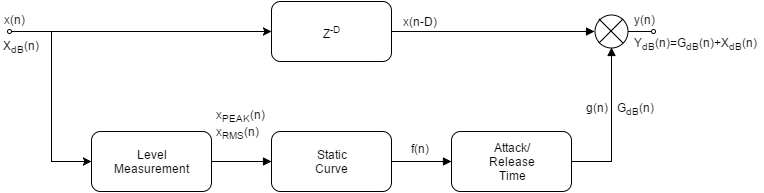
\includegraphics[width=1\textwidth]{figures/Limiter_block.png}
\caption{Limiter block diagram.}
\label{fig:limiter_block}
\end{figure}   

\todo[inline]{referencen Digital_Audio_Signal_Processing bogen kapitel 7}

The level measurement block measures the RMS or peak value of the signal, the static curve applies the gain and the Attack/Release time determines when the limiter should apply and stop applying to the signal. The static curve more detailed described the curve which determines at which the noise gate threshold (NT), expander threshold (ET), compressor threshold (CT) and limiter threshold (LT) should apply as seen on \autoref{fig:limiter_static}. 

When these different thresholds are surpassed a specific linear function will be applied to the signal to for example filter out noise (NT) or compress the signal to limit the output relative to the input as seen on \ref{fig:limiter_static}. 

\begin{figure}[H]
\centering
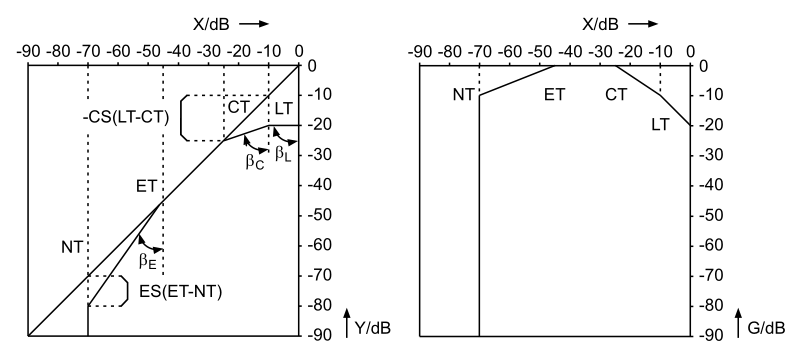
\includegraphics[width=0.8\textwidth]{figures/limiter_static_curve.png}
\caption{Static curve with the parameters (LT, CT, ET and NT).}
\label{fig:limiter_static}
\end{figure}  

Because the focus will be on limiting the signal and not clipping it, which would introduce to much distortion, the focus should be on CT which compresses the signal. The compressor can be designed for hard compression which limits the output more than a soft compression but it also creates more distorted output. The compressor can either apply to all frequencies or be a multiband compressor which only applies to the frequency spectrum which needs compression, which gives a more flexible compressor but also increases the complexity of the system.    

      


\subsection{Automatic volume control}
The last way of processing the signal to avoid surpassing the performance limits of a loudspeaker is an \gls{AVC}. The concept of an AVC is setting a maximum magnitude threshold for the entire frequency spectrum or for a specific frequency bandwidth and then attenuating the magnitude of the entire frequency spectrum down to the threshold if the threshold is exceeded.

\subsection{Choice of signal processing}
The advantage of the AVC over the equalizer and the limiter is that is does not alter the frequency response of the input signal, which means that the music will be played at the maximum magnitude, at which the loudspeaker will not be damaged, with the musics full dynamic range and the with intended frequency response. This means that music which is not bass heavy will be able to play at a higher volume than bass heavy music because the loudspeaker is less likely to be damaged by higher frequencies as described in \todo[inline]{SIGNAL ANALYSIS REFERENCE}

It could also be a disadvantage that the frequency response of the input cannot be altered. Opposed the AVC The equalizer is able to secure that the loudspeaker is not damaged by attenuating the specific frequency bandwidths which has surpassed the performance limits of the loudspeaker, which gives the possibility of turning up the volume but with an altered frequency response because of the attenuated bandwidth. The disadvange is therefore that the music can sound strange if the frequency response is altered when the volume is higher than the threshold.

The limiter versus the AVC and equalizer compresses the signal close the threshold instead of attenuating respectively the whole frequency spectrum and a frequency bandwidth. The advantage of protecting the loudspeaker this way is that an attenuation by an equalizer in a specific frequecy spectrum gives a lower output than a compression by a limiter does, the disadvantage of the limiter though is an increase in distortion when compressing. 

Based on the analysis it is decided to use an equalizer over the AVC and the limiter because the equalizer offers the optimal solution of protecting the loudspeaker against damage and gives the possibility of increasing the volume even though the threshold of a frequency bandwidth has been surpassed, which the AVC does not do. It is also assesed that the increased distortion introduced by the limiter is not to prefer over attenuation by filtering which would give a slightly lower output.  


      


\section{Platform requirements} \label{sec:platformReq}
The purpose of this section is to derive the requirements for the digital development platform. Most of the requirements derived in this section are provided by DALI thus the choice of platform will mostly be based on an analysis of which processor platform will be optimal in order to fulfill the requirements. The requirements for the processor platform have been derived in a mail correspondence with DALI.
\todo[inline]{Reference til CD}
%\subsection*{Demands for the platform}
%The demands for the processor platform have been derived in a mail correspondence with DALI 
%\todo[inline]{Reference til CD}
\begin{itemize}
\item \textbf{Audio sample rate}: The system must be able to handle 96 kHz sample rate since peripheral components will be running at this rate.
\item \textbf{Audio resolution}: There must be support for audio in at least a 24 bit resolution since the \gls{DAC} chosen by DALI is of 24 bit.
\item \textbf{\gls{SNR}}: A minimum \gls{SNR} of 120 dB on the \gls{DAC} must be achieved. This will provide headroom for digital volume control.
\item \textbf{Performance}: The processor must a least be able to run 1024 instructions per sample. which would give approximately 100 \gls{MIPS}.
%\item \textbf{Program space}: The platform will consist of an equalizer and limiter when finished. This project will however focus on the equalizer and sensory system. Hence it only desireable to leave TBD room for an multi band limiter which is desired by DALI. 
\item \textbf{Interfacing to peripherals}: The platform must be able to interface with an ADC and DAC with the bus type \gls{I2S}.

\todo[inline]{Program space has been removed.}

A 32 bit resolution is prefered by DALI over a 24 bit resolution because it would give a increased \gls{SNR} of 48 dB. These demands lead to the analyzation of which platform would be the most optimal.  
\end{itemize}


%\subsection*{Sample rate} 
%The system must be able to handle 96 kHz sample rate since peripheral components will interface be running at this rate.
%
%\subsection*{Bit resolution} 
%There must be support for audio in at least a 24 bit resolution since the \gls{DAC} chosen by DALI is of 24 bit.
%
%\subsection*{\gls{SNR}} 
%A minimum \gls{SNR} of 120 dB on the \gls{DAC} must be achieved. This will provide headroom for digital volume control.
%
%\subsection*{Instructions pr. sample.} 
%The processor must a least be able to run 1024 intructions pr. sample. which would give approximately 100 \gls{MIPS}
%
%
%\subsection*{Memory for both an equalizer and multi band limiter} 
%The platform will consist of an equalizer and limiter when finished. This project will however focus on the equalizer and sensory system. Hence it only desireable to leave TBD room for an multi band limiter which is desired by DALI. 
%
%
%\subsection*{Interfacing} 
%The platform must be able to interface with an ADC and DAC with the bus type \gls{I2S}. Besides the interfacing with the ADC and DAC the platform must be able to interface with the chosen sensor in \autoref{sec:Sensor}.
%
%The 32 bit resolution is prefered by DALI over a 24 bit resolution because it would give a increased \gls{SNR} of 48 dB. These demands lead to the analyzation of which platform would be the most optimal.   

\subsection{Choice of processor platform}
For the choice of processor platform different types of platforms could be used, such as an ASIC chip, an \gls{FPGA}, a microcontroller ($\mu$C) or a \gls{DSP}. These types of processors have different advantage and disadvantages which needs to be analyzed to find the most optimal platform for the demands above. The basic difference between the types of platforms is given in \autoref{tb:summary_DSP_hardware_implementation}. 

\begin{table}[H]
\centering
\begin{tabular}{lllll}
\toprule
 & \multicolumn{1}{c}{ASIC} & \multicolumn{1}{c}{FPGA} & \multicolumn{1}{c}{$\mu$P/$\mu$C} & \multicolumn{1}{c}{\begin{tabular}[c]{@{}c@{}}Digital signal\\ processor\end{tabular}} \\ \hline
\textbf{Flexibility} & None & Limited & High & High \\
\textbf{Design time} & Medium & Medium & Short & Short \\
\textbf{Power consumption} & Low-medium & Medium-high & Medium high & Low-medium \\
\textbf{Performance} & High & Low-medium & Low-medium & Medium-high \\
\textbf{Development cost} & Medium & Low & Low & Low \\ 
\textbf{Production cost} & Low-medium & Medium-high & Medium-high & Low-medium \\ \bottomrule 
\end{tabular}
\caption{Summary of DSP hardware implementations \citep{WileyDSP}.}
\label{tb:summary_DSP_hardware_implementation}
\end{table}


Because filtering is probably needed and the high performance demands from above the natural choice of platform would be a \gls{DSP}. An ASIC chip would not be viable as a prototype platform because it does not have any flexibility. The FPGA lacks flexibility, has an increased design time and is costly. The microcontroller has less performance than a \gls{DSP}, cost more and normally has a bigger power consumption than a \gls{DSP} so as stated before a \gls{DSP} is the choice of platform.     





\section{User interface} \label{sec:user_interface}
In this section an analyzation of the user interface for the equalizer analyzed in \autoref{sec:tech_equalizer} will be made to determine which user interface will be the most optimal for the specific user of the equalizer. 

There are two different intended users for the equalizer: 
\begin{itemize}
\item The developer.
\item The commercial user.
\end{itemize}
This means that there are different requirements for the specific user of the equalizer.

\subsection*{User interface for the developer}
The developer is the user which knows everything about an equalizer and its effects on a system therefore the developer desires a great deal of control and options in the interface of the equalizer. This means that the interface can be complex and must not set no restrictions for the developer.  

Because the developer needs to have full control of the equalizer he needs to have control of: 
\begin{itemize}
\item Center frequency.
\item Q - value.
\item Gain.
\item Band selection.
\end{itemize} 
This leads to a suggestions for a user interface which gives full control to a developer.

\begin{figure}[H]
\centering
\tikzsetnextfilename{InterfaceDev1}
\begin{tikzpicture}
\draw[thick] (2,0) circle [radius=0.5] node at (-1,-0) {Q - value};
\draw[thick] (2,1.5) circle [radius=0.5] node at (-1,1.5) {Gain};
\draw[thick] (2,3) circle [radius=0.5] node at (-1,3) {Center frequency};
\draw node at (-1,4.5)[font=\LARGE]{Band};
\draw[thick][fill=green, draw=black](1.5,4) rectangle(2.5,5) node at (2,4.5)[font=\LARGE]{1};

\draw[thick] (4,0) circle [radius=0.5];
\draw[thick] (4,1.5) circle [radius=0.5];
\draw[thick] (4,3) circle [radius=0.5];
\draw[thick][fill=red, draw=black](1.5+2,4) rectangle(2.5+2,5) node at (2+2,4.5)[font=\LARGE]{2};

\draw[thick] (6,0) circle [radius=0.5];
\draw[thick] (6,1.5) circle [radius=0.5];
\draw[thick] (6,3) circle [radius=0.5];
\draw[thick][fill=red, draw=black](1.5+4,4) rectangle(2.5+4,5) node at (2+4,4.5)[font=\LARGE]{3};

\draw[thick](6,0) -- (6.5,0);
\draw[thick](6,1.5) -- (6.5,1.5);
\draw[thick](6,3) -- (6.5,3);

\draw[thick](4,0) -- (4.5,0);
\draw[thick](4,1.5) -- (4.5,1.5);
\draw[thick](4,3) -- (4.5,3);

\draw[thick](2,0) -- (2.5,0);
\draw[thick](2,1.5) -- (2.5,1.5);
\draw[thick](2,3) -- (2.5,3);
\end{tikzpicture}
\caption{Developer user interface.}
\label{fig:Dev_sug}
\end{figure}

The suggestion on \autoref{fig:Dev_sug} has push buttons on the bands so they can be toggled on and of while the center frequency, gain and Q - value for each band can be changed with the use of knobs. 

\subsection*{User interface for the commercial user}
The commercial user is the user which knows the implication of different the different settings of an equalizer but does not know anything about the technical aspect of an equalizer. This means that the interface needs to be simple and show what implpication a setting has on a system but leave out all technical aspects. 

Because the commercial user only needs presets like for example "rock", "jazz" and "movie" the user only needs to have control of: 
\begin{itemize}
\item Presets.
\end{itemize} 
This leads to some different suggestions for a user interface which consist of a few buttons to keep it as simple as possible.


\begin{figure}[H]
\centering
\begin{subfigure}[t]{0.47\textwidth}
	\centering
	\tikzsetnextfilename{InterfaceUser1}
	\scalebox{0.2}{

\begin{tikzpicture}
\draw [thick](-10,6) circle [radius=3];
\draw [thick](11,6) circle [radius=3];
\draw [thick](-6,4) -- (7,4) -- (7,8) -- (-6,8) -- (-6,4);
\draw[fill] (-12,6) -- (-10,8) -- (-9,8) -- (-11,6) -- (-9,4) -- (-10,4) -- (-12,6);
\draw[fill](13,6) -- (11,8) -- (10,8) -- (12,6) -- (10,4) -- (11,4)--(13,6) ;
\node[scale=8.0] (c) at (0.5,6) {Presets};
\end{tikzpicture}}
	\caption{Suggestion 1}
	\label{fig:UI_sug_1}
\end{subfigure}
\hspace{6mm} 
\begin{subfigure}[t]{0.47\textwidth}
	\centering
	\tikzsetnextfilename{InterfaceUser2}
	\scalebox{0.6}{
\begin{tikzpicture}
\draw [thick](0,0) circle [radius=1] node{Jazz};
\draw [thick](3,0) circle [radius=1] node{Rock};
\draw [thick](6,0) circle [radius=1] node{Classic};
\draw node at (3,2)[font=\huge]{Presets};
\end{tikzpicture}}
	\caption{Suggestion 2}
	\label{fig:UI_sug_2}
\end{subfigure}
\caption{Commercial user interface suggestions.}
\label{fig:UI_sug}
\end{figure}

Suggestion one as seen on \autoref{fig:UI_sug_1} has two push buttons and a small screen so the user can interchange between different settings, while suggestion two has x number of push buttons which represents a preset each. The advantage of suggestion two is the overview and simplicity while suggestion one can have a larger number of presets without changing the appearance of the user interface. 

The suggestions for the user interface for both the developer and the commercial user will be choosen in the requirement specification \todo[inline]{reference}  



\section{Chapter Conclusion}
This chapter has analyzed.

\part{Concept}
%%%%%%%%%%%%%%%%%%%%%%%% Teknisk Analyse %%%%%%%%%%%%%%%%%%%%%%%%
\chapter{Overall System Design}
The purpose of this chapter is to give an outline of the design ideas considered for the system. As the problem statement pointed out, the system will consist of a processing system which will allow for adjustment when in use, such that the speaker will not suffer from the coil hitting the backplate. As shown in \autoref{fig:speaker_block2} the system will be integrated within an active speaker where it will act as the processing system between the external audio source and the amplifier.

\begin{figure}[H]
	\centering
	\tikzsetnextfilename{SpeakerBlock}
	\scalebox{0.9}{
		\begin{tikzpicture}
%% Kasser %%
\node [block, fill=white] (AudioSource) at (0,0) {Audio Source};

%% DSP %%
\node [block, fill=white] (Amplifier) at ($(AudioSource)+(3.5,0)$) {Amplifier};
\node [block, fill=white] (Driver) at ($(Amplifier)+(3.5,0)$) {Driver};

%% Store Blokke %%
\begin{pgfonlayer}{bg}
\draw[thick, fill=black!20] ($(-1.50,1)+(Amplifier)$) -- ($(1.750,1)+(Driver)$) -- ($(1.750,-1.25)+(Driver)$) -- ($(-1.50,-1.25)+(Amplifier)$) -- ($(-1.50,1)+(Amplifier)$); 
\node (Speakertag) at ($(-.25,-1)+(Driver)$) {\textbf{Speaker Enclosure}};
\end{pgfonlayer}

%% Forbindelse %%
\draw[->] (AudioSource) -- (Amplifier);
\draw[->] (Amplifier) -- (Driver);

%\draw[->] ($(EnclosureDriver)+(-1.375,0.3)$) -- ($(EnclosureDriver)+(-1.75,0.3)$) -- ($(EnclosureDriver)+(-1.75,1)$) -- ($(EnclosureDriver)+(-5.5,1)$) |- ($(SpectralAnalysis)+(1.375,0.3)$);

\end{tikzpicture}}
	\caption{Block diagram of an active loudspeaker.}
	\label{fig:speaker_block2}
\end{figure}


%\begin{figure}[H]
%\centering
%\tikzsetnextfilename{SpeakerBlock2}
%\scalebox{0.9}{
%\begin{tikzpicture}
%% Audio Source %%
\node [block, fill=black!80,text=white] (AudioSource) at (0,0) {Audio Source};

%% Subsystems in enclosure %%
\node [block, fill=blue!15] (Signal processing system) at ($(AudioSource)+(4,0)$) {Processing system};
\node [block, fill=black!80,text=white] (Amplifier) at ($(Signal processing system)+(4,0)$) {Amplifier};
\node [block, fill=black!80,text=white] (PSU) at ($(Amplifier)+(0,2)$) {PSU};
\node [block, fill=black!80,text=white] (Driver) at ($(Amplifier)+(3.5,0)$) {Driver};
%% Store Blokke %%
\begin{pgfonlayer}{bg}
\draw[thick, fill=black!10] ($(-6.2,3)+(Amplifier)$) -- ($(1.750,3)+(Driver)$) -- ($(1.750,-1.25)+(Driver)$) -- ($(-6.2,-1.25)+(Amplifier)$) -- ($(-6.2,3)+(Amplifier)$); 
\node (Speakertag) at ($(-.25,-1)+(Driver)$) {\textbf{Speaker Enclosure}};
\end{pgfonlayer}

%% Forbindelse %%
\draw[->,thick] (AudioSource) -- (Signal processing system);
\draw[->,thick] (PSU) -- (Amplifier);
\draw[->,thick] (Signal processing system) -- (Amplifier);
\draw[->,thick] (Amplifier) -- (Driver);
\draw[->, to path={-| (\tikztotarget)},thick] (PSU) edge (Signal processing system);
%\draw[->] ($(EnclosureDriver)+(-1.375,0.3)$) -- ($(EnclosureDriver)+(-1.75,0.3)$) -- ($(EnclosureDriver)+(-1.75,1)$) -- ($(EnclosureDriver)+(-5.5,1)$) |- ($(SpectralAnalysis)+(1.375,0.3)$);

\end{tikzpicture}}
%\caption{Block diagram of an active speaker.}
%\label{fig:speaker_block2}
%\end{figure}

The starting point of the design concept is to determine what type of processing system is going to be developed. Different plausible solution will be reviewed and evaluated in order to determine what solution would be optimally. 


\section{Analog Versus Digital}
It is important to clarify if the processing system is going to be designed as an analog or digital system. Both types have their own advantages and disadvantages and the purposes of this section is to determine which platform will suit the system most. 

The main difference between an analog and digital system is that the analog system works in continuous-time while the digital system works in discrete-time. For a analog system, values of a continuous signal at any given time is defined. For a digital system, values of a signal are only defined at specific points in time with a fixed resolution. The time difference between each point is defined through a sampling period $T_s$ and the resolution of each point is defined by the Analogue-to-Digital Converter (ADC).

For an analog system, components such as resistors, capacitors, inductors, transistors and so on, are usually used. A digital system will typically consist of an ADC to discretize the analog signal, a processor to process the signal and a Digital-to-Analogue Converter (DAC) to convert the signal back to a continuous signal. The advantage of designing an analog system is that no conversion between continuous-time, discrete time and back has to be made, and that the delay in analog systems is very small. The main disadvantages of the digital system therefore lies in the conversion where quantization noise could arise as a problem if the resolution of the conversion is not high enough. 

As the system to be developed, most likely will rely on signal processing, the great disadvantages of an analog system is the flexibility  compared to a digital system. Some applications such as the Fourier transformation is very hard to realize in an analog system while realizable in a digital system through algorithms. %Also, if the system is large, an analog system might turn out to be very complex.%, and use more components which results in more distortion. 
As the system to be developed is relying on signal processing the platform is chosen to be digital.

% \section{Real-time versus None real-time} \label{sec:RealTime}
% Because a digital system is going to be used the question arises of using real-time or none real time. %It diverges again in advantages and disadvantages of both systems. %A brief overview will be given which will be used to support the chosen system.

% A real time system offers the advantages that when in use it can work continuously with the given input and possible adapt to the given situation. This increases the flexibility of the system because adjustment can be done in real time and therefore detect problems and possibly avoid a bad outcome. 
% %\textbf{The real time system can easily be adapted into other system because the algorithm has not changed and only need new parameters.} 
% The system would be able to function when needed for the user, which is important when in e.g. music applications. There is only one big disadvantage of the real time system. Based on the frequency range of the signal the system works with, the real time system should be able to do all the needed calculation before the next sample. This limits the system to a certain amount of time and specific algorithms like large point FFT´s or division. %With a certain time given it might not be possible to finish the needed calculation and if that happens, the system will fail.

% The none real time system has the advantage of all the time it needs. Since it is not made for running in the specific situation it can perform rather complex calculation and not worry about how many iterations it might need. This means that low cost system can be used since computational power is not a problem. The system would be able to consider possible outcomes and generate a perfectly adjusted signal. Considering those advantages the major drawback is that is does not function when the user might need the functions. The none real-time would need time which might not be desirable. A situation could be when listening to music where a loading time of larger proportions are not acceptable 

% Due to the fact that the system revolves around a active speaker system and is going to handle music signals it seems most fit to use a real-time system. This gives the most flexibility and pleases the end user by not having to wait for analysis of the signal.




%% Feedback vs Feed Forward %%
\section{Feedback versus Feedforward System} \label{sec:feedback}

At this point it is yet to be determined if the system will be based on a feedback or a feedforward system. The choices are to design a feedback system that will decide what to do, based on real-time measurements from a sensor e.g. accelerometer, or a feedforward system that will analyse an input signal and react from this analysis. Since there are no well documented experiments concerning sensors in loudspeaker cabinets further experiments are to be deducted. A possible solution for a feedback system is depicted on \autoref{fig:feedbacksystem}. This system depicted will be further investigated to see if it is plausible.

\begin{figure}[H]
\centering
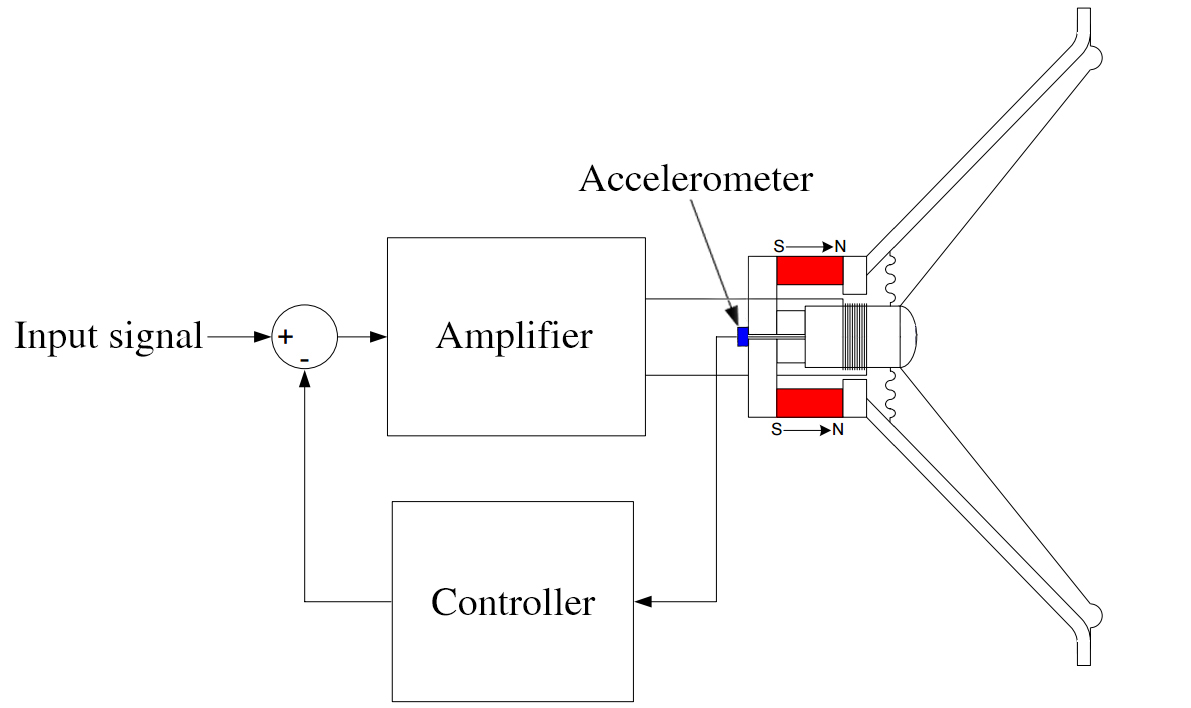
\includegraphics[width=0.75\textwidth]{Feedback_Acc2}
\caption{How a possible feedback system should be implemented in the speaker}
\label{fig:feedbacksystem}
\end{figure}


%\subsection{Distortion from vibration and impulses}\label{subsec:impulses}
%
%A common problem when designing loudspeakers are the vibrations from the enclosure. If the vibrations are strong, they will become audible and distort the overall sound. The sound radiation from the enclosure will become greater when the \gls{SPL} from the speaker increase. This problem is solved with different techniques but yield more or less the same outcome, which is stiffening of the enclosure. Some of the techniques for removing vibrations from the enclosure could be:
%\begin{itemize}
%\item Mechanical decoupling of the drivers from the enclosure.
%\item Denser or heavier construction material with a high natural frequency, making it harder for the enclosure to start vibrating.
%\item Dampening material or complex structural design inside the cabinet to disperse the sound.
%\end{itemize}
%\todo[inline]{Skal nok lige skaffe nogle kilder på de udtagelser}
%
%Another possibility is to use the vibration measurement as an indicator to tell the current performance of the loudspeaker. Since the loudspeaker will vibrate more at higher volumes. 
%
%
%Looking further into the woofer itself, it shows in \autoref{fig:SpeakerModelStress} that parts in the woofer also creates unwanted vibrations. The purpose of the woofer is to reproduce the electrical signal as an acoustical signal. This is done by using a diaphragm which is suspended in a very light and easy to move material. An Induction in the coil is created in a permanent magnet creating a a electro magnetic force resulting in the diaphragm moving. The goal will always be to loose as little as possible energy, giving the most perfect output. The woofer simply needs to be as powerful, light, stiff and efficient as possible.
%
%\begin{figure}[H]
%\centering
%\begin{subfigure}[t]{0.47\textwidth}
%\includegraphics[width=\linewidth]{SpeakerGOOD}
%	\caption{Regular speaker driver showing surround, diaphragm and the magnet.}
%	\label{fig:regularspeaker}
%\end{subfigure}
%\hspace{6mm} 
%\begin{subfigure}[t]{0.47\textwidth}
%\includegraphics[width=\linewidth]{SpeakerBAD}
%	\caption{Regular speaker driver with red markings showing stress areas}
%	\label{fig:badspeaker}
%\end{subfigure}
%\caption{A Speaker driver, where \ref{fig:badspeaker} shows the stress points outlined with red.}
%\label{fig:SpeakerModelStress}
%\end{figure}
%%When this signal has a large amplitude, read overload, the diaphragm reaches physical capacity. 
%In \autoref{fig:badspeaker} it shows that when a diaphragm is pushed to its maximum capacity the surround will affect the diaphragm causing unwanted distortion. This will be one of the major problems if the diaphragm is not sufficiently stiff to withstand the high \gls{SPL} and not twist during playback. 



%\input{1Chapters/1Preanalysis/PartConclusionAmpSpeaker.tex}

\input{1Chapters/1Preanalysis/Loudspeaker_test.tex}

%\input{1Chapters/1Preanalysis/frequency_response.tex}

%\input{1Chapters/1Preanalysis/harmonic_distortion.tex}

\input{1Chapters/1Preanalysis/hit_detection.tex}

\subsubsection{Plausible solution} 
The Previous tests have shown that it is possible to use an accelerometer to estimate the performance of the system by looking at the harmonic distortions. However following up on all of the trails the problems are as follows:
\begin{itemize}
\item Estimating harmonic distortions introduced in a system when playing music, are only well-defined for periodic sinusoids.
\item Frequency response of vibration, using the cheaper accelerometer, on the driver and cabinet hardly changes when exposed for loud playback, thus it will be hard to get usable outputs of the sensors.
\item The price for usable sensor equipment is too high compared to the application it is targeted for. 
\item The sensors did not directly show a pattern for when a possible hit of the back plate were about to occur.
\item The phase of the signal can not assumed "in phase" and it is therefore not possible to apply spectral estimations for detecting specific frequency peaks. e.g. if using a specific frequency as target for attenuation a 180 degrees phase shifted signal might bring false negatives. 
\end{itemize}

It can therefore be concluded that developing a system based on measurements from a accelerometer might turn out to be too complex to be realized in time due to time constraints. The system to be designed will therefore be based on a feedforward system. The concept of a feedforward system which fulfill the problem statement is shown in \autoref{fig:Concept}.

\begin{figure}[H]
\centering
\tikzsetnextfilename{Concept}
\scalebox{0.8}{
\input{figures/Concept.tex}}
\caption{Overview of a feedforward design concept.}
\label{fig:Concept}
\end{figure}

Since the system will be controlled using a feedforward system which should be able to analyze, process and correct signals before the music is played. It gives rise to questioning what kind of platform should be used and what kind of requirements are needed for such a system. On the market there are different plausible platforms which meets with the demands all with different advantages and disadvantages. The preceding section will cover the determination of which platform that will function best in a active loudspeaker system . 

%\textbf{The design concept consist of a signal processing block, which will be analysed to understand which solution is best for the problem stated. A signal analysis block which will not be analysed further in this chapter, a user interface which will be analysed to determine how the user interface should be designed and lastly the processor block which will be analysed to determine which type of processor that should be used.}



%% Krav til Platform %%
\section{Platform requirements} \label{sec:platformReq}
The purpose of this section is to derive the requirements for the digital development platform. Most of the requirements derived in this section are provided by DALI thus the choice of platform will mostly be based on an analysis of which processor platform will be optimal in order to fulfill the requirements. The requirements for the processor platform have been derived in a mail correspondence with DALI.
\todo[inline]{Reference til CD}
%\subsection*{Demands for the platform}
%The demands for the processor platform have been derived in a mail correspondence with DALI 
%\todo[inline]{Reference til CD}
\begin{itemize}
\item \textbf{Audio sample rate}: The system must be able to handle 96 kHz sample rate since peripheral components will be running at this rate.
\item \textbf{Audio resolution}: There must be support for audio in at least a 24 bit resolution since the \gls{DAC} chosen by DALI is of 24 bit.
\item \textbf{\gls{SNR}}: A minimum \gls{SNR} of 120 dB on the \gls{DAC} must be achieved. This will provide headroom for digital volume control.
\item \textbf{Performance}: The processor must a least be able to run 1024 instructions per sample. which would give approximately 100 \gls{MIPS}.
%\item \textbf{Program space}: The platform will consist of an equalizer and limiter when finished. This project will however focus on the equalizer and sensory system. Hence it only desireable to leave TBD room for an multi band limiter which is desired by DALI. 
\item \textbf{Interfacing to peripherals}: The platform must be able to interface with an ADC and DAC with the bus type \gls{I2S}.

\todo[inline]{Program space has been removed.}

A 32 bit resolution is prefered by DALI over a 24 bit resolution because it would give a increased \gls{SNR} of 48 dB. These demands lead to the analyzation of which platform would be the most optimal.  
\end{itemize}


%\subsection*{Sample rate} 
%The system must be able to handle 96 kHz sample rate since peripheral components will interface be running at this rate.
%
%\subsection*{Bit resolution} 
%There must be support for audio in at least a 24 bit resolution since the \gls{DAC} chosen by DALI is of 24 bit.
%
%\subsection*{\gls{SNR}} 
%A minimum \gls{SNR} of 120 dB on the \gls{DAC} must be achieved. This will provide headroom for digital volume control.
%
%\subsection*{Instructions pr. sample.} 
%The processor must a least be able to run 1024 intructions pr. sample. which would give approximately 100 \gls{MIPS}
%
%
%\subsection*{Memory for both an equalizer and multi band limiter} 
%The platform will consist of an equalizer and limiter when finished. This project will however focus on the equalizer and sensory system. Hence it only desireable to leave TBD room for an multi band limiter which is desired by DALI. 
%
%
%\subsection*{Interfacing} 
%The platform must be able to interface with an ADC and DAC with the bus type \gls{I2S}. Besides the interfacing with the ADC and DAC the platform must be able to interface with the chosen sensor in \autoref{sec:Sensor}.
%
%The 32 bit resolution is prefered by DALI over a 24 bit resolution because it would give a increased \gls{SNR} of 48 dB. These demands lead to the analyzation of which platform would be the most optimal.   

\subsection{Choice of processor platform}
For the choice of processor platform different types of platforms could be used, such as an ASIC chip, an \gls{FPGA}, a microcontroller ($\mu$C) or a \gls{DSP}. These types of processors have different advantage and disadvantages which needs to be analyzed to find the most optimal platform for the demands above. The basic difference between the types of platforms is given in \autoref{tb:summary_DSP_hardware_implementation}. 

\begin{table}[H]
\centering
\begin{tabular}{lllll}
\toprule
 & \multicolumn{1}{c}{ASIC} & \multicolumn{1}{c}{FPGA} & \multicolumn{1}{c}{$\mu$P/$\mu$C} & \multicolumn{1}{c}{\begin{tabular}[c]{@{}c@{}}Digital signal\\ processor\end{tabular}} \\ \hline
\textbf{Flexibility} & None & Limited & High & High \\
\textbf{Design time} & Medium & Medium & Short & Short \\
\textbf{Power consumption} & Low-medium & Medium-high & Medium high & Low-medium \\
\textbf{Performance} & High & Low-medium & Low-medium & Medium-high \\
\textbf{Development cost} & Medium & Low & Low & Low \\ 
\textbf{Production cost} & Low-medium & Medium-high & Medium-high & Low-medium \\ \bottomrule 
\end{tabular}
\caption{Summary of DSP hardware implementations \citep{WileyDSP}.}
\label{tb:summary_DSP_hardware_implementation}
\end{table}


Because filtering is probably needed and the high performance demands from above the natural choice of platform would be a \gls{DSP}. An ASIC chip would not be viable as a prototype platform because it does not have any flexibility. The FPGA lacks flexibility, has an increased design time and is costly. The microcontroller has less performance than a \gls{DSP}, cost more and normally has a bigger power consumption than a \gls{DSP} so as stated before a \gls{DSP} is the choice of platform.     






%% GUI %%
%\section{User interface} \label{sec:user_interface}
In this section an analyzation of the user interface for the equalizer analyzed in \autoref{sec:tech_equalizer} will be made to determine which user interface will be the most optimal for the specific user of the equalizer. 

There are two different intended users for the equalizer: 
\begin{itemize}
\item The developer.
\item The commercial user.
\end{itemize}
This means that there are different requirements for the specific user of the equalizer.

\subsection*{User interface for the developer}
The developer is the user which knows everything about an equalizer and its effects on a system therefore the developer desires a great deal of control and options in the interface of the equalizer. This means that the interface can be complex and must not set no restrictions for the developer.  

Because the developer needs to have full control of the equalizer he needs to have control of: 
\begin{itemize}
\item Center frequency.
\item Q - value.
\item Gain.
\item Band selection.
\end{itemize} 
This leads to a suggestions for a user interface which gives full control to a developer.

\begin{figure}[H]
\centering
\tikzsetnextfilename{InterfaceDev1}
\input{figures/InterfaceDev1.tex}
\caption{Developer user interface.}
\label{fig:Dev_sug}
\end{figure}

The suggestion on \autoref{fig:Dev_sug} has push buttons on the bands so they can be toggled on and of while the center frequency, gain and Q - value for each band can be changed with the use of knobs. 

\subsection*{User interface for the commercial user}
The commercial user is the user which knows the implication of different the different settings of an equalizer but does not know anything about the technical aspect of an equalizer. This means that the interface needs to be simple and show what implpication a setting has on a system but leave out all technical aspects. 

Because the commercial user only needs presets like for example "rock", "jazz" and "movie" the user only needs to have control of: 
\begin{itemize}
\item Presets.
\end{itemize} 
This leads to some different suggestions for a user interface which consist of a few buttons to keep it as simple as possible.


\begin{figure}[H]
\centering
\begin{subfigure}[t]{0.47\textwidth}
	\centering
	\tikzsetnextfilename{InterfaceUser1}
	\input{figures/InterfaceUser1.tex}
	\caption{Suggestion 1}
	\label{fig:UI_sug_1}
\end{subfigure}
\hspace{6mm} 
\begin{subfigure}[t]{0.47\textwidth}
	\centering
	\tikzsetnextfilename{InterfaceUser2}
	\input{figures/InterfaceUser2.tex}
	\caption{Suggestion 2}
	\label{fig:UI_sug_2}
\end{subfigure}
\caption{Commercial user interface suggestions.}
\label{fig:UI_sug}
\end{figure}

Suggestion one as seen on \autoref{fig:UI_sug_1} has two push buttons and a small screen so the user can interchange between different settings, while suggestion two has x number of push buttons which represents a preset each. The advantage of suggestion two is the overview and simplicity while suggestion one can have a larger number of presets without changing the appearance of the user interface. 

The suggestions for the user interface for both the developer and the commercial user will be choosen in the requirement specification \todo[inline]{reference}  



\chapter{Signal Processing Tools}
Generally speaking, any signal can be analysed and processed in time domain or frequency domain. If analysed in time domain, the analysis can for instance be extracting signal features and calculating the signal's RMS value. Analysing the signal in frequency domain will reveal the spectral content of the signal. Processing the signal in time domain could be for example filtering or gain control, while processing the signal in frequency domain could be multiplication in frequency domain. So the following sections will cover different relevant techniques for extracting and processing information from an audio signal in both time and frequency domain. A conclusion at the end will determine which analyzing and process methods should be used in the system.

\section{Analysis in time} \label{sec:SignalTime}
The purpose of analysing in time domain is to analyse thresholds of a given signal so when analysing in time domain there are two main ways of analysing, peak or Root-mean-square (RMS) which will be examined.
\subsection*{Root-mean-square}
RMS can be used as a tool to estimate the "mean" value of a periodic signal. The problem with calculating a regular mean value for an audio signal is that the result will be 0 as the signal is approximately evenly distributed on both side of the amplitude axis. By using RMS this problem is avoided. The RMS is calculated as the square root of the mean value of the signal squared as shown in following equation:
\begin{equation}\label{eq:RMS_con}
V_{\text{RMS}}(t) = \sqrt{\frac{1}{T}\int_0^T v(t)^2 dt}
\end{equation}
The definition of the RMS in \autoref{eq:RMS_con} is only defined for continuous signals. If the RMS value is to be calculated for discrete values then following equation is used:
\begin{equation}
V_{\text{RMS}}[n] = \sqrt{\frac{1}{N+1}\sum_{k=0}^{N} v[n-k]^2}
\end{equation}
In analog electronics, the RMS value of a AC voltage can be used to calculate the corresponding power dissipation in a resistor (for instance) that of a DC voltage. The RMS can be useful to estimate the power of the signal, for instance if the RMS value of the signal moves above a certain threshold, the system may warn that the signal will stress the loudspeaker too much.

\subsection*{Signal threshold}
A signal threshold can be used to detect whenever the amplitude of a signal is above a certain level. This can for instance help identify if the signal will result in a too loud playback. The threshold can be used to detect peaks above the threshold or be used to detect if the RMS values of the signal is above a level.

\section{Analysis in frequency} \label{sec:SignalFreq}
The purpose of analysing in frequency domain is to analyse the spectral content of a signal so when analysing in frequency domain there are two main ways of analysing, spectrum analyzer or fast fourier transform (FFT) which will be examined.

\subsection*{Spectrum analyzer}
A spectrum analyser can consist of multiple bandpass filters which divides the signal into frequency bands and for each band, the RMS value or peak value is determined to estimate the energy or amplitude in that corresponding band. %The bandpass filters of the spectrum analyzer could meet the requirements of the standard IEC 6964 (2001) which sets the requirements of octave-band or fractional-octave-band filters, this is also explained in more detail in \ref{app:IEC6964}.  

The advantage of the spectrum analyzer is that it gives the capability of analysing the frequency spectrum of a signal in a very effective way with the use of either RMS or peak analysing. The disadvantage of the spectrum analyzer is that it is not possible to analyse a specific frequency if wanted, but only able to analyse the spectral content of the bandwidth designed.      

\subsection*{Fast fourier transform}
The Fourier transformation is a mathematical equation that breaks the signal up into a sum of sine and cosine function at different frequencies which gives the spectral composition of the signal. To perform a Fourier Transformation (FT) the the Discrete Fourier Transformation (DFT), refer to \todo{APPENDIX}, must be used since the FT cannot be implemented in a causal and discrete system. The DFT is very inefficient in its computation so it is more common to use the more effective FFT which obtains the same result as the DFT. The difference in computation time is given as

\todo[inline]{DFT Appendix}

DFT computation time:
\begin{equation}
C_{DFT} = N^{2}\cdot t_{instr} \enhed{ms}
\end{equation}
\begin{where}
\va{$C_{DFT}$}{is the computation time of the DFT}{ms}
\va{$N$}{is the number of samples}{.}
\va{$t_{instr}$}{is the instruction time of a single instruction}{ms}
\end{where}

FFT computation time:
\begin{equation}
C_{FFT} = \frac{N}{2}\cdot log_{2}(N)\cdot t_{instr} \enhed{ms}
\end{equation}
\begin{where}
\va{$C_{FFT}$}{is the computation time of the FFT}{ms}
\end{where}

The FFT can be used to give a precise spectral composition of the signal, so if its desired to analyse a specific frequency or specific frequencies for example 100 Hz and 200 Hz it will be possible, which in relation to the spectrum analyzer which cannot analyse a specific frequency. So the FFT is good at analysing specific frequencies but the disadvantage of the FFT is that it is bad at analyzing a large spectrum. This is because it takes a lot of computation power if the resolution of the FFT is required to be high, which is very ineffective in relation to the spectrum analyser. This is because the resolution is given as:
\begin{equation}
R_{FFT} = \frac{Fs}{N} \enhed{Hz}
\end{equation}
\begin{where}
\va{$R_{FFT}$}{is the resolution}{Hz}
\end{where} 

So if the sample frequency is high it requires a large number of samples to get a high resolution, but if the resolution is low there is a chance information gets losts. This is also called the fence phenomenon because the FFT is as you look at the spectrum through a fence. 




%%%%%%%%%%%%%%%%%%%%%%%%%%%%%%%%%%%Signal Processing%%%%%%%%%%%%%%%%%%%%%%%%%%%%%%%%%%%%%%%%%%%%





\section{Processing in time}
The reasoning for processing a signal in time is its simplicity. A continous signal is a time signal so there is no need for an FFT and IFFT when processing in time. There are two common ways of processing a signal in time, dynamic gain control and equalizing  


\subsection*{Dynamic gain control}
Dynamic gain control (DGC) gains differently based on certain threshold to for example make sure that a signal does not clip. A DGC system is a feedforward system which can be stated as:
\begin{equation}
y[n] = g[n]\cdot x[n-D]
\end{equation}

Where an input $x[n]$ is delayed by $x[n-D]$ and multiplied by a weighting $g[n]$ to give $y[n]$, or as a logarithmic level representation where multiplication leads to the addition of $G_{dB}[n]$ and $X_{dB}[n]$:
\begin{equation}
Y_{dB}[n] = X_{dB}[n] + G_{dB}[n]
\end{equation}

A DGC is also seen in more detail on \autoref{fig:limiter_block}.

\begin{figure}[H]
\centering
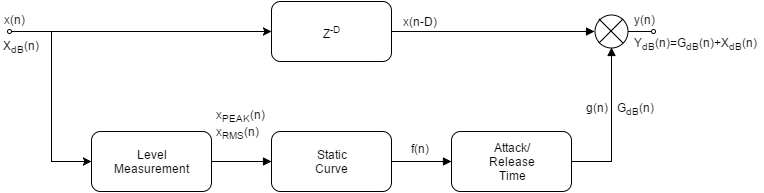
\includegraphics[width=1\textwidth]{figures/Limiter_block.png}
\caption{DGC block diagram.}
\label{fig:limiter_block}
\end{figure}   

\todo[inline]{Ref til Digital Audio Signal Processing bogen kapitel syv} 

The level measurement block measures the RMS or peak value of the signal, the static curve applies a specific gain and the Attack/Release, where the attack determines how fast the DGC should react to inputs that are above the threshold. A high attack time means that the DGC is slow-reacting to inputs changes, thus the DGC will not apply gain variation if the input is only above the threshold for a short time. The release time determines how fast the DGC should release the gain variation after the signal level is under the threshold again.
%time determines when the limiter should apply and stop applying to the signal.
The static curve, more detailed described, is the curve which determines at which the noise gate threshold (NT), expander threshold (ET), compressor threshold (CT) and limiter threshold (LT) should apply as seen on \autoref{fig:limiter_static}. 

When these different thresholds are surpassed, a specific linear function will be applied to the signal to for example filter out noise (NT) or compress the signal to limit the output relative to the input as seen on \autoref{fig:limiter_static}. 

\begin{figure}[H]
\centering
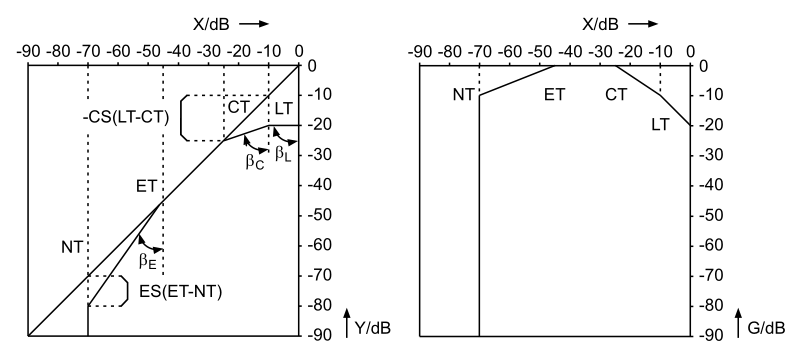
\includegraphics[width=0.8\textwidth]{figures/limiter_static_curve.png}
\caption{Static curve with the parameters (LT, CT, ET and NT).}
\label{fig:limiter_static}
\end{figure}  

Because the focus will be on compressing the signal and not clipping it, which would introduce too much distortion, the focus should be on CT which compresses the signal. The compressor gain as seen \autoref{fig:limiter_static} is a variable gain dependent on the threshold and the input. The compressor can either apply to all frequencies or be a multiband compressor which only applies to the frequency spectrum which needs compression, which gives a more flexible compressor but also increases the complexity of the system. 

\subsection*{Equalizer}
% This section will examine the options for processing the signal so the limit of the loudspeaker never gets surpassed. Three ways for processing the signal are set up:  
% \begin{itemize}
% \item Equalizer.
% \item Limiter.    
% \item Automatic Volume Control. 
% \end{itemize}
% These methods of processing the signal will be analysed to determine which methods is the most optimal for the purpose of protecting the loudspeaker as described in \autoref{sec:problem_statement}.  
%This section will cover the design possibilities of an equalizer and filter in an digital system. 
By implementing an equalizer it is possible to manipulate different areas of the frequency spectrum. Generally speaking, there are two common types of equalizer designs used in audio.

%\subsection{Graphic and parametric equalizer}\label{sec:tech_equalizer}
The first type of equalizer is the graphic equalizer. The graphic equalizer consist of multiple bandpass filters each with a fixed center frequency as seen in \autoref{fig:graphic_eq}. The amount of bandpass filters can vary, but can commonly be seen with 10 bands or more. A high amount of bands gives greater flexibility to adjust the frequency response of the equalizer.

\begin{figure}[H]
\centering
\tikzsetnextfilename{graphic_eq}
% This file was created by matlab2tikz.
%
%The latest updates can be retrieved from
%  http://www.mathworks.com/matlabcentral/fileexchange/22022-matlab2tikz-matlab2tikz
%where you can also make suggestions and rate matlab2tikz.
%
\begin{tikzpicture}

\begin{axis}[%
width=3.5in,
height=2in,
at={(1.011in,0.642in)},
scale only axis,
xmode=log,
xmin=550,
xmax=11500,
xminorticks=true,
xticklabels={\empty},
xlabel={Frequency [Hz]},
yticklabels={\empty},
ymin=0.2,
ymax=1.2,
ylabel={Magnitude [dB]},
axis background/.style={fill=white}
]
\addplot [color=black,solid,line width=1.5pt,forget plot]
  table[row sep=crcr]{%
549.027451372569	1.27474818755282e-06\\
559.02795139757	1.37055169597053e-06\\
569.028451422571	1.47168015573933e-06\\
579.028951447572	1.57832989891761e-06\\
589.029451472574	1.69070104274361e-06\\
599.029951497575	1.80899750613955e-06\\
609.030451522576	1.93342702654008e-06\\
619.030951547577	2.06420117704404e-06\\
629.031451572579	2.20153538387906e-06\\
639.03195159758	2.34564894421938e-06\\
649.032451622581	2.49676504429154e-06\\
659.032951647582	2.65511077784761e-06\\
669.033451672584	2.82091716495128e-06\\
679.033951697585	2.9944191711013e-06\\
689.034451722586	3.17585572669063e-06\\
699.034951747587	3.3654697468032e-06\\
709.035451772589	3.56350815135503e-06\\
719.03595179759	3.77022188557272e-06\\
729.036451822591	3.98586594082186e-06\\
739.036951847592	4.21069937576776e-06\\
749.037451872594	4.44498533791166e-06\\
759.037951897595	4.68899108545001e-06\\
769.038451922596	4.94298800950803e-06\\
779.038951947597	5.20725165671478e-06\\
789.039451972599	5.48206175214773e-06\\
799.0399519976	5.76770222262957e-06\\
809.040452022601	6.06446122039943e-06\\
819.040952047602	6.37263114713215e-06\\
829.041452072604	6.6925086783502e-06\\
839.041952097605	7.02439478818472e-06\\
849.042452122606	7.36859477451746e-06\\
859.042952147607	7.72541828450947e-06\\
869.043452172609	8.09517934049682e-06\\
879.04395219761	8.47819636626287e-06\\
889.044452222611	8.87479221372753e-06\\
899.044952247612	9.28529418997711e-06\\
909.045452272614	9.71003408472483e-06\\
919.045952297615	1.01493481981444e-05\\
929.046452322616	1.06035773691057e-05\\
939.046952347617	1.10730670038125e-05\\
949.047452372619	1.15581671048417e-05\\
959.04795239762	1.2059232300586e-05\\
969.048452422621	1.25766218751046e-05\\
979.048952447622	1.31106997983979e-05\\
989.049452472624	1.36618347570829e-05\\
999.049952497625	1.42304001855008e-05\\
1009.05045252263	1.48167742972383e-05\\
1019.05095254763	1.54213401170782e-05\\
1029.05145257263	1.6044485513379e-05\\
1039.05195259763	1.66866032308872e-05\\
1049.05245262263	1.73480909240019e-05\\
1059.05295264763	1.80293511904401e-05\\
1069.05345267263	1.87307916053911e-05\\
1079.05395269763	1.9452824756097e-05\\
1089.05445272264	2.01958682768746e-05\\
1099.05495274764	2.09603448846272e-05\\
1109.05545277264	2.17466824147754e-05\\
1119.05595279764	2.25553138576756e-05\\
1129.05645282264	2.33866773955117e-05\\
1139.05695284764	2.42412164396376e-05\\
1149.05745287264	2.51193796684019e-05\\
1159.05795289764	2.60216210654671e-05\\
1169.05845292265	2.69483999586e-05\\
1179.05895294765	2.79001810589519e-05\\
1189.05945297265	2.88774345008309e-05\\
1199.05995299765	2.9880635881981e-05\\
1209.06045302265	3.09102663043493e-05\\
1219.06095304765	3.19668124153777e-05\\
1229.06145307265	3.30507664497801e-05\\
1239.06195309765	3.41626262718678e-05\\
1249.06245312266	3.53028954183627e-05\\
1259.06295314766	3.64720831417675e-05\\
1269.06345317266	3.76707044542388e-05\\
1279.06395319766	3.88992801720113e-05\\
1289.06445322266	4.01583369603637e-05\\
1299.06495324766	4.1448407379119e-05\\
1309.06545327266	4.27700299287058e-05\\
1319.06595329766	4.41237490967704e-05\\
1329.06645332267	4.55101154053519e-05\\
1339.06695334767	4.69296854586247e-05\\
1349.06745337267	4.83830219912078e-05\\
1359.06795339767	4.98706939170632e-05\\
1369.06845342267	5.13932763789616e-05\\
1379.06895344767	5.29513507985522e-05\\
1389.06945347267	5.45455049270176e-05\\
1399.06995349767	5.61763328963369e-05\\
1409.07045352268	5.78444352711408e-05\\
1419.07095354768	5.9550419101199e-05\\
1429.07145357268	6.12948979745098e-05\\
1439.07195359768	6.30784920710182e-05\\
1449.07245362268	6.49018282169778e-05\\
1459.07295364768	6.67655399399274e-05\\
1469.07345367268	6.86702675243236e-05\\
1479.07395369768	7.0616658067825e-05\\
1489.07445372269	7.26053655382323e-05\\
1499.07495374769	7.46370508310862e-05\\
1509.07545377269	7.67123818279364e-05\\
1519.07595379769	7.88320334552917e-05\\
1529.07645382269	8.09966877442509e-05\\
1539.07695384769	8.32070338908229e-05\\
1549.07745387269	8.54637683169469e-05\\
1559.07795389769	8.77675947322129e-05\\
1569.0784539227	9.01192241963065e-05\\
1579.0789539477	9.25193751821509e-05\\
1589.0794539727	9.4968773639808e-05\\
1599.0799539977	9.74681530610717e-05\\
1609.0804540227	0.000100018254544852\\
1619.0809540477	0.000102619826863262\\
1629.0814540727	0.000105273626528498\\
1639.0819540977	0.000107980417860474\\
1649.08245412271	0.00011074097305521\\
1659.08295414771	0.000113556072254044\\
1669.08345417271	0.000116426503613597\\
1679.08395419771	0.00011935306337655\\
1689.08445422271	0.000122336555943231\\
1699.08495424771	0.000125377793944017\\
1709.08545427271	0.000128477598312557\\
1719.08595429771	0.000131636798359827\\
1729.08645432272	0.000134856231849036\\
1739.08695434772	0.000138136745071375\\
1749.08745437272	0.000141479192922626\\
1759.08795439772	0.000144884438980643\\
1769.08845442272	0.000148353355583726\\
1779.08895444772	0.000151886823909853\\
1789.08945447272	0.000155485734056841\\
1799.08995449772	0.000159150985123392\\
1809.09045452273	0.000162883485291085\\
1819.09095454773	0.000166684151907257\\
1829.09145457273	0.000170553911568861\\
1839.09195459773	0.000174493700207252\\
1849.09245462273	0.000178504463173927\\
1859.09295464773	0.00018258715532726\\
1869.09345467273	0.000186742741120191\\
1879.09395469773	0.00019097219468892\\
1889.09445472274	0.000195276499942593\\
1899.09495474774	0.000199656650654028\\
1909.09545477274	0.000204113650551425\\
1919.09595479774	0.000208648513411148\\
1929.09645482274	0.000213262263151531\\
1939.09695484774	0.000217955933927765\\
1949.09745487274	0.000222730570227836\\
1959.09795489774	0.000227587226969557\\
1969.09845492275	0.000232526969598691\\
1979.09895494775	0.0002375508741882\\
1989.09945497275	0.000242660027538581\\
1999.09995499775	0.000247855527279368\\
2009.10045502275	0.000253138481971759\\
2019.10095504775	0.000258510011212413\\
2029.10145507275	0.000263971245738415\\
2039.10195509775	0.000269523327533433\\
2049.10245512276	0.000275167409935066\\
2059.10295514776	0.000280904657743407\\
2069.10345517276	0.000286736247330836\\
2079.10395519776	0.000292663366753053\\
2089.10445522276	0.000298687215861372\\
2099.10495524776	0.000304809006416273\\
2109.10545527276	0.00031102996220224\\
2119.10595529776	0.000317351319143918\\
2129.10645532277	0.000323774325423558\\
2139.10695534777	0.000330300241599804\\
2149.10745537277	0.000336930340727831\\
2159.10795539777	0.00034366590848083\\
2169.10845542277	0.000350508243272881\\
2179.10895544777	0.000357458656383217\\
2189.10945547277	0.00036451847208189\\
2199.10995549777	0.00037168902775686\\
2209.11045552278	0.000378971674042556\\
2219.11095554778	0.000386367774949844\\
2229.11145557278	0.000393878707997529\\
2239.11195559778	0.000401505864345301\\
2249.11245562278	0.000409250648928223\\
2259.11295564778	0.000417114480592734\\
2269.11345567278	0.000425098792234218\\
2279.11395569779	0.000433205030936102\\
2289.11445572279	0.000441434658110576\\
2299.11495574779	0.000449789149640901\\
2309.11545577279	0.000458269996025331\\
2319.11595579779	0.000466878702522689\\
2329.11645582279	0.000475616789299597\\
2339.11695584779	0.000484485791579393\\
2349.11745587279	0.000493487259792741\\
2359.11795589779	0.000502622759729963\\
2369.1184559228	0.000511893872695126\\
2379.1189559478	0.000521302195661869\\
2389.1194559728	0.000530849341431046\\
2399.1199559978	0.000540536938790128\\
2409.1204560228	0.000550366632674492\\
2419.1209560478	0.000560340084330501\\
2429.1214560728	0.000570458971480503\\
2439.1219560978	0.000580724988489687\\
2449.12245612281	0.000591139846534883\\
2459.12295614781	0.000601705273775306\\
2469.12345617281	0.000612423015525218\\
2479.12395619781	0.000623294834428655\\
2489.12445622281	0.000634322510636088\\
2499.12495624781	0.000645507841983181\\
2509.12545627281	0.000656852644171584\\
2519.12595629781	0.000668358750951802\\
2529.12645632282	0.00068002801430822\\
2539.12695634782	0.000691862304646211\\
2549.12745637282	0.000703863510981462\\
2559.12795639782	0.000716033541131454\\
2569.12845642282	0.000728374321909184\\
2579.12895644782	0.000740887799319109\\
2589.12945647282	0.000753575938755409\\
2599.12995649782	0.000766440725202494\\
2609.13045652283	0.000779484163437885\\
2619.13095654783	0.000792708278237447\\
2629.13145657283	0.000806115114582999\\
2639.13195659783	0.000819706737872341\\
2649.13245662283	0.00083348523413176\\
2659.13295664783	0.000847452710230983\\
2669.13345667283	0.000861611294100646\\
2679.13395669783	0.000875963134952324\\
2689.13445672284	0.000890510403501116\\
2699.13495674784	0.000905255292190848\\
2709.13545677284	0.000920200015421898\\
2719.13595679784	0.000935346809781725\\
2729.13645682284	0.000950697934278066\\
2739.13695684784	0.000966255670574898\\
2749.13745687284	0.000982022323231169\\
2759.13795689785	0.000998000219942333\\
2769.13845692285	0.00101419171178474\\
2779.13895694785	0.00103059917346289\\
2789.13945697285	0.00104722500355964\\
2799.13995699785	0.00106407162478932\\
2809.14045702285	0.00108114148425386\\
2819.14095704785	0.00109843705370197\\
2829.14145707285	0.00111596082979137\\
2839.14195709786	0.0011337153343541\\
2849.14245712286	0.00115170311466506\\
2859.14295714786	0.00116992674371362\\
2869.14345717286	0.00118838882047858\\
2879.14395719786	0.00120709197020631\\
2889.14445722286	0.00122603884469227\\
2899.14495724786	0.00124523212256582\\
2909.14545727286	0.00126467450957847\\
2919.14595729786	0.0012843687388956\\
2929.14645732287	0.00130431757139159\\
2939.14695734787	0.00132452379594852\\
2949.14745737287	0.0013449902297585\\
2959.14795739787	0.00136571971862953\\
2969.14845742287	0.00138671513729509\\
2979.14895744787	0.00140797938972744\\
2989.14945747287	0.00142951540945466\\
2999.14995749787	0.00145132615988158\\
3009.15045752288	0.00147341463461446\\
3019.15095754788	0.00149578385778971\\
3029.15145757288	0.00151843688440648\\
3039.15195759788	0.00154137680066331\\
3049.15245762288	0.00156460672429888\\
3059.15295764788	0.00158812980493682\\
3069.15345767288	0.00161194922443477\\
3079.15395769788	0.00163606819723761\\
3089.15445772289	0.00166048997073506\\
3099.15495774789	0.0016852178256235\\
3109.15545777289	0.00171025507627237\\
3119.15595779789	0.00173560507109485\\
3129.15645782289	0.0017612711929232\\
3139.15695784789	0.00178725685938865\\
3149.15745787289	0.00181356552330584\\
3159.15795789789	0.00184020067306211\\
3169.1584579229	0.00186716583301143\\
3179.1589579479	0.00189446456387329\\
3189.1594579729	0.00192210046313632\\
3199.1599579979	0.00195007716546701\\
3209.1604580229	0.00197839834312343\\
3219.1609580479	0.00200706770637397\\
3229.1614580729	0.00203608900392131\\
3239.1619580979	0.00206546602333163\\
3249.16245812291	0.00209520259146906\\
3259.16295814791	0.00212530257493559\\
3269.16345817291	0.00215576988051628\\
3279.16395819791	0.00218660845563019\\
3289.16445822291	0.00221782228878674\\
3299.16495824791	0.0022494154100478\\
3309.16545827291	0.0022813918914955\\
3319.16595829792	0.00231375584770595\\
3329.16645832292	0.0023465114362287\\
3339.16695834792	0.00237966285807238\\
3349.16745837292	0.0024132143581962\\
3359.16795839792	0.00244717022600779\\
3369.16845842292	0.0024815347958671\\
3379.16895844792	0.00251631244759676\\
3389.16945847292	0.0025515076069987\\
3399.16995849793	0.00258712474637741\\
3409.17045852293	0.00262316838506966\\
3419.17095854793	0.0026596430899809\\
3429.17145857293	0.00269655347612851\\
3439.17195859793	0.00273390420719183\\
3449.17245862293	0.00277169999606906\\
3459.17295864793	0.00280994560544143\\
3469.17345867293	0.00284864584834424\\
3479.17395869793	0.00288780558874538\\
3489.17445872294	0.00292742974213097\\
3499.17495874794	0.00296752327609862\\
3509.17545877294	0.00300809121095813\\
3519.17595879794	0.00304913862033987\\
3529.17645882294	0.00309067063181091\\
3539.17695884794	0.00313269242749903\\
3549.17745887294	0.00317520924472465\\
3559.17795889794	0.0032182263766409\\
3569.17845892295	0.00326174917288189\\
3579.17895894795	0.0033057830402192\\
3589.17945897295	0.00335033344322688\\
3599.17995899795	0.00339540590495504\\
3609.18045902295	0.00344100600761194\\
3619.18095904795	0.00348713939325503\\
3629.18145907295	0.00353381176449082\\
3639.18195909795	0.00358102888518379\\
3649.18245912296	0.00362879658117448\\
3659.18295914796	0.00367712074100688\\
3669.18345917296	0.00372600731666519\\
3679.18395919796	0.00377546232432023\\
3689.18445922296	0.00382549184508544\\
3699.18495924796	0.0038761020257828\\
3709.18545927296	0.00392729907971864\\
3719.18595929796	0.0039790892874696\\
3729.18645932297	0.0040314789976789\\
3739.18695934797	0.00408447462786289\\
3749.18745937297	0.00413808266522824\\
3759.18795939797	0.00419230966749981\\
3769.18845942297	0.00424716226375936\\
3779.18895944797	0.00430264715529532\\
3789.18945947297	0.0043587711164636\\
3799.18995949797	0.00441554099555988\\
3809.19045952298	0.00447296371570334\\
3819.19095954798	0.00453104627573194\\
3829.19145957298	0.00458979575110973\\
3839.19195959798	0.0046492192948459\\
3849.19245962298	0.00470932413842629\\
3859.19295964798	0.00477011759275696\\
3869.19345967298	0.00483160704912045\\
3879.19395969799	0.00489379998014472\\
3889.19445972299	0.00495670394078497\\
3899.19495974799	0.00502032656931845\\
3909.19545977299	0.0050846755883527\\
3919.19595979799	0.00514975880584714\\
3929.19645982299	0.00521558411614828\\
3939.19695984799	0.0052821595010389\\
3949.19745987299	0.0053494930308012\\
3959.19795989799	0.00541759286529421\\
3969.198459923	0.00548646725504576\\
3979.198959948	0.00555612454235904\\
3989.199459973	0.00562657316243406\\
3999.199959998	0.00569782164450433\\
4009.200460023	0.00576987861298871\\
4019.200960048	0.00584275278865905\\
4029.201460073	0.0059164529898234\\
4039.201960098	0.0059909881335254\\
4049.20246012301	0.00606636723675989\\
4059.20296014801	0.00614259941770499\\
4069.20346017301	0.00621969389697104\\
4079.20396019801	0.00629765999886638\\
4089.20446022301	0.00637650715268055\\
4099.20496024801	0.00645624489398491\\
4109.20546027301	0.00653688286595095\\
4119.20596029802	0.00661843082068692\\
4129.20646032302	0.00670089862059237\\
4139.20696034802	0.00678429623973159\\
4149.20746037302	0.00686863376522577\\
4159.20796039802	0.00695392139866432\\
4169.20846042302	0.00704016945753555\\
4179.20896044802	0.00712738837667724\\
4189.20946047302	0.00721558870974699\\
4199.20996049802	0.00730478113071314\\
4209.21046052303	0.007394976435366\\
4219.21096054803	0.0074861855428504\\
4229.21146057303	0.00757841949721903\\
4239.21196059803	0.00767168946900786\\
4249.21246062303	0.00776600675683295\\
4259.21296064803	0.00786138278900982\\
4269.21346067303	0.00795782912519532\\
4279.21396069803	0.00805535745805225\\
4289.21446072304	0.00815397961493749\\
4299.21496074804	0.00825370755961346\\
4309.21546077304	0.00835455339398376\\
4319.21596079804	0.00845652935985303\\
4329.21646082304	0.00855964784071155\\
4339.21696084804	0.00866392136354492\\
4349.21746087304	0.00876936260066913\\
4359.21796089805	0.00887598437159161\\
4369.21846092305	0.00898379964489847\\
4379.21896094805	0.00909282154016824\\
4389.21946097305	0.00920306332991302\\
4399.21996099805	0.00931453844154671\\
4409.22046102305	0.00942726045938145\\
4419.22096104805	0.00954124312665214\\
4429.22146107305	0.00965650034756992\\
4439.22196109805	0.00977304618940474\\
4449.22246112306	0.00989089488459764\\
4459.22296114806	0.0100100608329032\\
4469.22346117306	0.0101305586035622\\
4479.22396119806	0.0102524029375062\\
4489.22446122306	0.0103756087495924\\
4499.22496124806	0.0105001911308718\\
4509.22546127306	0.0106261653508891\\
4519.22596129807	0.0107535468600157\\
4529.22646132307	0.0108823512918164\\
4539.22696134807	0.0110125944654505\\
4549.22746137307	0.0111442923881065\\
4559.22796139807	0.0112774612574733\\
4569.22846142307	0.0114121174642458\\
4579.22896144807	0.0115482775946674\\
4589.22946147307	0.0116859584331095\\
4599.22996149807	0.0118251769646876\\
4609.23046152308	0.0119659503779164\\
4619.23096154808	0.0121082960674026\\
4629.23146157308	0.0122522316365771\\
4639.23196159808	0.0123977749004675\\
4649.23246162308	0.0125449438885101\\
4659.23296164808	0.0126937568474038\\
4669.23346167308	0.0128442322440052\\
4679.23396169809	0.0129963887682662\\
4689.23446172309	0.0131502453362145\\
4699.23496174809	0.013305821092978\\
4709.23546177309	0.0134631354158536\\
4719.23596179809	0.0136222079174207\\
4729.23646182309	0.013783058448701\\
4739.23696184809	0.0139457071023643\\
4749.23746187309	0.0141101742159822\\
4759.23796189809	0.0142764803753293\\
4769.2384619231	0.0144446464177332\\
4779.2389619481	0.0146146934354745\\
4789.2394619731	0.0147866427792362\\
4799.2399619981	0.0149605160616058\\
4809.2404620231	0.0151363351606272\\
4819.2409620481	0.0153141222234075\\
4829.2414620731	0.0154938996697759\\
4839.2419620981	0.0156756901959978\\
4849.24246212311	0.015859516778544\\
4859.24296214811	0.0160454026779159\\
4869.24346217311	0.0162333714425286\\
4879.24396219811	0.0164234469126506\\
4889.24446222311	0.016615653224404\\
4899.24496224811	0.0168100148138235\\
4909.24546227311	0.0170065564209765\\
4919.24596229812	0.0172053030941456\\
4929.24646232312	0.0174062801940724\\
4939.24696234812	0.0176095133982671\\
4949.24746237312	0.0178150287053811\\
4959.24796239812	0.0180228524396465\\
4969.24846242312	0.0182330112553824\\
4979.24896244812	0.0184455321415684\\
4989.24946247312	0.0186604424264884\\
4999.24996249812	0.0188777697824431\\
5009.25046252313	0.0190975422305354\\
5019.25096254813	0.0193197881455266\\
5029.25146257313	0.0195445362607673\\
5039.25196259813	0.0197718156732027\\
5049.25246262313	0.0200016558484536\\
5059.25296264813	0.0202340866259749\\
5069.25346267313	0.0204691382242926\\
5079.25396269814	0.0207068412463195\\
5089.25446272314	0.0209472266847533\\
5099.25496274814	0.0211903259275557\\
5109.25546277314	0.0214361707635154\\
5119.25596279814	0.0216847933878961\\
5129.25646282314	0.0219362264081706\\
5139.25696284814	0.0221905028498422\\
5149.25746287314	0.0224476561623557\\
5159.25796289814	0.0227077202250981\\
5169.25846292315	0.0229707293534917\\
5179.25896294815	0.0232367183051795\\
5189.25946297315	0.0235057222863073\\
5199.25996299815	0.0237777769578996\\
5209.26046302315	0.0240529184423355\\
5219.26096304815	0.0243311833299223\\
5229.26146307315	0.024612608685571\\
5239.26196309816	0.0248972320555742\\
5249.26246312316	0.0251850914744878\\
5259.26296314816	0.0254762254721184\\
5269.26346317316	0.0257706730806189\\
5279.26396319816	0.0260684738416924\\
5289.26446322316	0.0263696678139074\\
5299.26496324816	0.0266742955801255\\
5309.26546327316	0.0269823982550434\\
5319.26596329816	0.0272940174928512\\
5329.26646332317	0.0276091954950086\\
5339.26696334817	0.0279279750181408\\
5349.26746337317	0.0282503993820561\\
5359.26796339817	0.0285765124778873\\
5369.26846342317	0.0289063587763583\\
5379.26896344817	0.0292399833361783\\
5389.26946347317	0.0295774318125654\\
5399.26996349817	0.029918750465901\\
5409.27046352318	0.0302639861705187\\
5419.27096354818	0.0306131864236277\\
5429.27146357318	0.0309663993543742\\
5439.27196359818	0.031323673733042\\
5449.27246362318	0.0316850589803955\\
5459.27296364818	0.0320506051771655\\
5469.27346367318	0.0324203630736824\\
5479.27396369819	0.0327943840996564\\
5489.27446372319	0.033172720374109\\
5499.27496374819	0.0335554247154566\\
5509.27546377319	0.0339425506517495\\
5519.27596379819	0.0343341524310682\\
5529.27646382319	0.0347302850320788\\
5539.27696384819	0.0351310041747506\\
5549.27746387319	0.0355363663312387\\
5559.27796389819	0.0359464287369316\\
5569.2784639232	0.0363612494016699\\
5579.2789639482	0.0367808871211344\\
5589.2794639732	0.0372054014884108\\
5599.2799639982	0.0376348529057276\\
5609.2804640232	0.0380693025963761\\
5619.2809640482	0.0385088126168096\\
5629.2814640732	0.0389534458689279\\
5639.28196409821	0.0394032661125471\\
5649.28246412321	0.0398583379780602\\
5659.28296414821	0.0403187269792873\\
5669.28346417321	0.0407844995265218\\
5679.28396419821	0.0412557229397724\\
5689.28446422321	0.0417324654622053\\
5699.28496424821	0.0422147962737872\\
5709.28546427321	0.0427027855051348\\
5719.28596429821	0.0431965042515704\\
5729.28646432322	0.0436960245873876\\
5739.28696434822	0.04420141958033\\
5749.28746437322	0.044712763306285\\
5759.28796439822	0.0452301308641957\\
5769.28846442322	0.0457535983911927\\
5779.28896444822	0.04628324307795\\
5789.28946447322	0.0468191431842661\\
5799.28996449823	0.0473613780548734\\
5809.29046452323	0.0479100281354793\\
5819.29096454823	0.04846517498904\\
5829.29146457323	0.0490269013122713\\
5839.29196459823	0.0495952909523973\\
5849.29246462323	0.0501704289241406\\
5859.29296464823	0.0507524014269563\\
5869.29346467323	0.0513412958625115\\
5879.29396469823	0.0519372008524144\\
5889.29446472324	0.0525402062561923\\
5899.29496474824	0.053150403189525\\
5909.29546477324	0.0537678840427312\\
5919.29596479824	0.0543927424995141\\
5929.29646482324	0.055025073555966\\
5939.29696484824	0.0556649735398341\\
5949.29746487324	0.0563125401300506\\
5959.29796489824	0.056967872376528\\
5969.29846492325	0.0576310707202208\\
5979.29896494825	0.0583022370134579\\
5989.29946497325	0.0589814745405429\\
5999.29996499825	0.0596688880386285\\
6009.30046502325	0.0603645837188628\\
6019.30096504825	0.061068669287811\\
6029.30146507325	0.0617812539691501\\
6039.30196509826	0.0625024485256432\\
6049.30246512326	0.0632323652813875\\
6059.30296514826	0.0639711181443418\\
6069.30346517326	0.0647188226291309\\
6079.30396519826	0.0654755958801279\\
6089.30446522326	0.066241556694814\\
6099.30496524826	0.0670168255474166\\
6109.30546527326	0.0678015246128231\\
6119.30596529826	0.0685957777907705\\
6129.30646532327	0.0693997107303121\\
6139.30696534827	0.0702134508545543\\
6149.30746537327	0.0710371273856675\\
6159.30796539827	0.0718708713701656\\
6169.30846542327	0.0727148157044527\\
6179.30896544827	0.0735690951606342\\
6189.30946547327	0.0744338464125896\\
6199.30996549828	0.075309208062301\\
6209.31046552328	0.0761953206664383\\
6219.31096554828	0.0770923267631894\\
6229.31146557328	0.0780003708993375\\
6239.31196559828	0.0789195996575748\\
6249.31246562328	0.0798501616840502\\
6259.31296564828	0.0807922077161402\\
6269.31346567328	0.0817458906104398\\
6279.31396569828	0.0827113653709642\\
6289.31446572329	0.0836887891775498\\
6299.31496574829	0.0846783214144507\\
6309.31546577329	0.0856801236991145\\
6319.31596579829	0.0866943599111317\\
6329.31646582329	0.0877211962213435\\
6339.31696584829	0.0887608011210978\\
6349.31746587329	0.0898133454516369\\
6359.31796589829	0.0908790024336062\\
6369.3184659233	0.091957947696666\\
6379.3189659483	0.0930503593091885\\
6389.3194659733	0.0941564178080272\\
6399.3199659983	0.0952763062283331\\
6409.3204660233	0.0964102101334033\\
6419.3209660483	0.0975583176445388\\
6429.3214660733	0.0987208194708859\\
6439.3219660983	0.0998979089392414\\
6449.32246612331	0.101089782023792\\
6459.32296614831	0.102296637375765\\
6469.32346617331	0.103518676352956\\
6479.32396619831	0.104756103049104\\
6489.32446622331	0.10600912432309\\
6499.32496624831	0.107277949827911\\
6509.32546627331	0.108562792039398\\
6519.32596629831	0.109863866284653\\
6529.32646632332	0.111181390770136\\
6539.32696634832	0.11251558660939\\
6549.32746637332	0.113866677850335\\
6559.32796639832	0.115234891502099\\
6569.32846642332	0.116620457561323\\
6579.32896644832	0.118023609037901\\
6589.32946647332	0.119444581980083\\
6599.32996649833	0.120883615498899\\
6609.33046652333	0.122340951791828\\
6619.33096654833	0.123816836165649\\
6629.33146657333	0.125311517058424\\
6639.33196659833	0.126825246060509\\
6649.33246662333	0.128358277934546\\
6659.33296664833	0.129910870634339\\
6669.33346667333	0.131483285322542\\
6679.33396669833	0.133075786387064\\
6689.33446672334	0.134688641456101\\
6699.33496674834	0.136322121411704\\
6709.33546677334	0.137976500401773\\
6719.33596679834	0.139652055850381\\
6729.33646682334	0.141349068466312\\
6739.33696684834	0.143067822249698\\
6749.33746687334	0.144808604496635\\
6759.33796689835	0.146571705801653\\
6769.33846692335	0.148357420057902\\
6779.33896694835	0.150166044454926\\
6789.33946697335	0.151997879473864\\
6799.33996699835	0.153853228879952\\
6809.34046702335	0.15573239971214\\
6819.34096704835	0.157635702269678\\
6829.34146707335	0.159563450095504\\
6839.34196709835	0.161515959956234\\
6849.34246712336	0.163493551818587\\
6859.34296714836	0.165496548822048\\
6869.34346717336	0.167525277247558\\
6879.34396719836	0.169580066482031\\
6889.34446722336	0.171661248978477\\
6899.34496724836	0.173769160211498\\
6909.34546727336	0.175904138627933\\
6919.34596729836	0.178066525592397\\
6929.34646732337	0.180256665327463\\
6939.34696734837	0.182474904848226\\
6949.34746737337	0.18472159389097\\
6959.34796739837	0.186997084835664\\
6969.34846742337	0.189301732621984\\
6979.34896744837	0.191635894658567\\
6989.34946747337	0.19399993072517\\
6999.34996749838	0.196394202867433\\
7009.35046752338	0.198819075283885\\
7019.35096754838	0.201274914204866\\
7029.35146757338	0.203762087763003\\
7039.35196759838	0.206280965854877\\
7049.35246762338	0.208831919993497\\
7059.35296764838	0.211415323151202\\
7069.35346767338	0.214031549592588\\
7079.35396769838	0.216680974697049\\
7089.35446772339	0.219363974770525\\
7099.35496774839	0.22208092684601\\
7109.35546777339	0.224832208472402\\
7119.35596779839	0.227618197491229\\
7129.35646782339	0.230439271800811\\
7139.35696784839	0.233295809107378\\
7149.35746787339	0.236188186662684\\
7159.3579678984	0.239116780987629\\
7169.3584679234	0.242081967581409\\
7179.3589679484	0.245084120615698\\
7189.3594679734	0.248123612613362\\
7199.3599679984	0.25120081411122\\
7209.3604680234	0.254316093306338\\
7219.3609680484	0.257469815685346\\
7229.3614680734	0.260662343636307\\
7239.3619680984	0.263894036042592\\
7249.36246812341	0.267165247858309\\
7259.36296814841	0.270476329664769\\
7269.36346817341	0.273827627207514\\
7279.36396819841	0.277219480913436\\
7289.36446822341	0.280652225387531\\
7299.36496824841	0.284126188888837\\
7309.36546827341	0.287641692785134\\
7319.36596829842	0.291199050986006\\
7329.36646832342	0.294798569353884\\
7339.36696834842	0.298440545092708\\
7349.36746837342	0.302125266113914\\
7359.36796839842	0.305853010379437\\
7369.36846842342	0.309624045221501\\
7379.36896844842	0.313438626639007\\
7389.36946847342	0.31729699857035\\
7399.36996849842	0.321199392142593\\
7409.37046852343	0.32514602489695\\
7419.37096854843	0.329137099990626\\
7429.37146857343	0.333172805375098\\
7439.37196859843	0.337253312951047\\
7449.37246862343	0.341378777700168\\
7459.37296864843	0.345549336794259\\
7469.37346867343	0.349765108681992\\
7479.37396869843	0.354026192153963\\
7489.37446872344	0.358332665386661\\
7499.37496874844	0.362684584966149\\
7509.37546877344	0.367081984892355\\
7519.37596879844	0.37152487556504\\
7529.37646882344	0.376013242752572\\
7539.37696884844	0.380547046544891\\
7549.37746887344	0.38512622029209\\
7559.37796889845	0.38975066953029\\
7569.37846892345	0.394420270896593\\
7579.37896894845	0.399134871035095\\
7589.37946897345	0.403894285496139\\
7599.37996899845	0.408698297631125\\
7609.38046902345	0.41354665748543\\
7619.38096904845	0.418439080692168\\
7629.38146907345	0.423375247369723\\
7639.38196909845	0.428354801026176\\
7649.38246912346	0.433377347473976\\
7659.38296914846	0.438442453758396\\
7669.38346917346	0.443549647103509\\
7679.38396919846	0.448698413879661\\
7689.38446922346	0.453888198596559\\
7699.38496924846	0.45911840292635\\
7709.38546927346	0.464388384761226\\
7719.38596929847	0.469697457310265\\
7729.38646932347	0.475044888240407\\
7739.38696934847	0.480429898866637\\
7749.38746937347	0.485851663396555\\
7759.38796939847	0.491309308234686\\
7769.38846942347	0.496801911351973\\
7779.38896944847	0.502328501725994\\
7789.38946947347	0.507888058857513\\
7799.38996949847	0.513479512369036\\
7809.39046952348	0.519101741691015\\
7819.39096954848	0.524753575841397\\
7829.39146957348	0.530433793304098\\
7839.39196959848	0.536141122011961\\
7849.39246962348	0.54187423943959\\
7859.39296964848	0.54763177281134\\
7869.39346967348	0.553412299429509\\
7879.39396969849	0.559214347127557\\
7889.39446972349	0.565036394852892\\
7899.39496974849	0.570876873383413\\
7909.39546977349	0.57673416618168\\
7919.39596979849	0.582606610390083\\
7929.39646982349	0.588492497969966\\
7939.39696984849	0.594390076987151\\
7949.39746987349	0.60029755304573\\
7959.39796989849	0.606213090871381\\
7969.3984699235	0.612134816044866\\
7979.3989699485	0.618060816885632\\
7989.3994699735	0.623989146484767\\
7999.3999699985	0.629917824885781\\
8009.4004700235	0.635844841410922\\
8019.4009700485	0.641768157129909\\
8029.4014700735	0.647685707467185\\
8039.4019700985	0.653595404942929\\
8049.40247012351	0.65949514204221\\
8059.40297014851	0.665382794205881\\
8069.40347017351	0.671256222935925\\
8079.40397019851	0.677113279007167\\
8089.40447022351	0.682951805776464\\
8099.40497024851	0.688769642579721\\
8109.40547027351	0.694564628206333\\
8119.40597029852	0.700334604439981\\
8129.40647032352	0.706077419654065\\
8139.40697034852	0.711790932449467\\
8149.40747037352	0.717473015321839\\
8159.40797039852	0.723121558345178\\
8169.40847042352	0.728734472858033\\
8179.40897044852	0.734309695138491\\
8189.40947047352	0.739845190053817\\
8199.40997049853	0.745338954670563\\
8209.41047052353	0.750789021810952\\
8219.41097054853	0.75619346354142\\
8229.41147057353	0.761550394579362\\
8239.41197059853	0.766857975604462\\
8249.41247062353	0.772114416461338\\
8259.41297064853	0.777317979240664\\
8269.41347067353	0.782466981226565\\
8279.41397069854	0.787559797698687\\
8289.41447072354	0.792594864578077\\
8299.41497074854	0.7975706809068\\
8309.41547077354	0.802485811152133\\
8319.41597079854	0.807338887327089\\
8329.41647082354	0.812128610919971\\
8339.41697084854	0.816853754626777\\
8349.41747087354	0.821513163881241\\
8359.41797089854	0.826105758178473\\
8369.41847092355	0.830630532189222\\
8379.41897094855	0.835086556662895\\
8389.41947097355	0.839472979118636\\
8399.41997099855	0.843789024324769\\
8409.42047102355	0.848033994568085\\
8419.42097104855	0.852207269715457\\
8429.42147107355	0.856308307071239\\
8439.42197109855	0.860336641034963\\
8449.42247112356	0.864291882564647\\
8459.42297114856	0.868173718451979\\
8469.42347117356	0.871981910416358\\
8479.42397119856	0.875716294025528\\
8489.42447122356	0.879376777451168\\
8499.42497124856	0.88296334006842\\
8509.42547127356	0.886476030908729\\
8519.42597129856	0.889914966975924\\
8529.42647132357	0.893280331435687\\
8539.42697134857	0.896572371688894\\
8549.42747137357	0.899791397339441\\
8559.42797139857	0.902937778067346\\
8569.42847142357	0.906011941417874\\
8579.42897144857	0.90901437051749\\
8589.42947147357	0.911945601727252\\
8599.42997149858	0.914806222244209\\
8609.43047152358	0.917596867661051\\
8619.43097154858	0.920318219494063\\
8629.43147157358	0.922971002689103\\
8639.43197159858	0.925555983114974\\
8649.43247162358	0.928073965053139\\
8659.43297164858	0.930525788692367\\
8669.43347167358	0.932912327636375\\
8679.43397169859	0.935234486432148\\
8689.43447172359	0.937493198126026\\
8699.43497174859	0.939689421854261\\
8709.43547177359	0.941824140474137\\
8719.43597179859	0.943898358241305\\
8729.43647182359	0.945913098538458\\
8739.43697184859	0.947869401659915\\
8749.43747187359	0.949768322656283\\
8759.43797189859	0.95161092924276\\
8769.4384719236	0.953398299774246\\
8779.4389719486	0.955131521289959\\
8789.4394719736	0.956811687629736\\
8799.4399719986	0.958439897623891\\
8809.4404720236	0.960017253357954\\
8819.4409720486	0.961544858513384\\
8829.4414720736	0.963023816784839\\
8839.4419720986	0.964455230374332\\
8849.44247212361	0.965840198562267\\
8859.44297214861	0.967179816355055\\
8869.44347217361	0.968475173208711\\
8879.44397219861	0.969727351827613\\
8889.44447222361	0.970937427037373\\
8899.44497224861	0.972106464730565\\
8909.44547227361	0.973235520883859\\
8919.44597229862	0.974325640644953\\
8929.44647232362	0.975377857487594\\
8939.44697234862	0.976393192432757\\
8949.44747237362	0.977372653334082\\
8959.44797239862	0.978317234225448\\
8969.44847242362	0.979227914728589\\
8979.44897244862	0.980105659518541\\
8989.44947247362	0.980951417844719\\
8999.44997249863	0.981766123105328\\
9009.45047252363	0.982550692472864\\
9019.45097254863	0.983306026568411\\
9029.45147257363	0.984033009182442\\
9039.45197259863	0.9847325070399\\
9049.45247262363	0.985405369607286\\
9059.45297264863	0.986052428939543\\
9069.45347267363	0.986674499564575\\
9079.45397269863	0.987272378403268\\
9089.45447272364	0.987846844722918\\
9099.45497274864	0.988398660122026\\
9109.45547277364	0.988928568544504\\
9119.45597279864	0.989437296321336\\
9129.45647282364	0.989925552237883\\
9139.45697284864	0.990394027624968\\
9149.45747287364	0.990843396472072\\
9159.45797289864	0.991274315560937\\
9169.45847292365	0.991687424617977\\
9179.45897294865	0.992083346483971\\
9189.45947297365	0.99246268729957\\
9199.45997299865	0.992826036705202\\
9209.46047302365	0.993173968054045\\
9219.46097304865	0.993507038636799\\
9229.46147307365	0.993825789917046\\
9239.46197309865	0.994130747776032\\
9249.46247312366	0.994422422765817\\
9259.46297314866	0.994701310369746\\
9269.46347317366	0.994967891269262\\
9279.46397319866	0.995222631616183\\
9289.46447322366	0.995465983309538\\
9299.46497324866	0.995698384276206\\
9309.46547327366	0.995920258754556\\
9319.46597329867	0.996132017580408\\
9329.46647332367	0.996334058474662\\
9339.46697334867	0.996526766331946\\
9349.46747337367	0.996710513509755\\
9359.46797339867	0.996885660117516\\
9369.46847342367	0.997052554305092\\
9379.46897344867	0.997211532550301\\
9389.46947347367	0.997362919944996\\
9399.46997349868	0.997507030479325\\
9409.47047352368	0.997644167323855\\
9419.47097354868	0.997774623109184\\
9429.47147357368	0.997898680202792\\
9439.47197359868	0.998016610982843\\
9449.47247362368	0.9981286781087\\
9459.47297364868	0.998235134787943\\
9469.47347367368	0.99833622503969\\
9479.47397369868	0.99843218395405\\
9489.47447372369	0.998523237947566\\
9499.47497374869	0.99860960501449\\
9509.47547377369	0.998691494973801\\
9519.47597379869	0.998769109711863\\
9529.47647382369	0.998842643420606\\
9539.47697384869	0.998912282831219\\
9549.47747387369	0.998978207443237\\
9559.47797389869	0.999040589749024\\
9569.4784739237	0.999099595453595\\
9579.4789739487	0.999155383689766\\
9589.4794739737	0.999208107228609\\
9599.4799739987	0.999257912685223\\
9609.4804740237	0.99930494071982\\
9619.4809740487	0.999349326234124\\
9629.4814740737	0.999391198563138\\
9639.4819740987	0.999430681662263\\
9649.48247412371	0.999467894289837\\
9659.48297414871	0.999502950185108\\
9669.48347417371	0.999535958241696\\
9679.48397419871	0.999567022676584\\
9689.48447422371	0.999596243194693\\
9699.48497424871	0.999623715149082\\
9709.48547427371	0.999649529696862\\
9719.48597429872	0.999673773950845\\
9729.48647432372	0.999696531127006\\
9739.48697434872	0.999717880687841\\
9749.48747437372	0.999737898481659\\
9759.48797439872	0.999756656877884\\
9769.48847442372	0.999774224898453\\
9779.48897444872	0.999790668345351\\
9789.48947447372	0.999806049924383\\
9799.48997449873	0.999820429365242\\
9809.49047452373	0.999833863537929\\
9819.49097454873	0.999846406565636\\
9829.49147457373	0.999858109934133\\
9839.49197459873	0.99986902259774\\
9849.49247462373	0.999879191081957\\
9859.49297464873	0.99988865958285\\
9869.49347467373	0.999897470063205\\
9879.49397469873	0.999905662345591\\
9889.49447472374	0.999913274202363\\
9899.49497474874	0.999920341442677\\
9909.49547477374	0.999926897996609\\
9919.49597479874	0.99993297599643\\
9929.49647482374	0.999938605855107\\
9939.49697484874	0.99994381634211\\
9949.49747487374	0.999948634656585\\
9959.49797489874	0.999953086497953\\
9969.49847492375	0.99995719613401\\
9979.49897494875	0.999960986466597\\
9989.49947497375	0.999964479094891\\
9999.49997499875	0.999967694376389\\
10009.5004750238	0.999970651485646\\
10019.5009750488	0.999973368470812\\
10029.5014750738	0.999975862308074\\
10039.5019750988	0.999978148953996\\
10049.5024751238	0.999980243395865\\
10059.5029751488	0.99998215970009\\
10069.5034751738	0.999983911058689\\
10079.5039751988	0.999985509833938\\
10089.5044752238	0.999986967601251\\
10099.5049752488	0.999988295190277\\
10109.5054752738	0.999989502724369\\
10119.5059752988	0.999990599658381\\
10129.5064753238	0.999991594814894\\
10139.5069753488	0.999992496418896\\
10149.5074753738	0.999993312130999\\
10159.5079753988	0.999994049079181\\
10169.5084754238	0.999994713889164\\
10179.5089754488	0.999995312713415\\
10189.5094754738	0.999995851258857\\
10199.5099754988	0.999996334813316\\
10209.5104755238	0.999996768270724\\
10219.5109755488	0.999997156155169\\
10229.5114755738	0.999997502643786\\
10239.5119755988	0.999997811588551\\
10249.5124756238	0.999998086537008\\
10259.5129756488	0.999998330751975\\
10269.5134756738	0.999998547230249\\
10279.5139756988	0.99999873872037\\
10289.5144757238	0.99999890773946\\
10299.5149757488	0.999999056589164\\
10309.5154757738	0.999999187370769\\
10319.5159757988	0.999999301999463\\
10329.5164758238	0.999999402217843\\
10339.5169758488	0.999999489608643\\
10349.5174758738	0.999999565606741\\
10359.5179758988	0.999999631510469\\
10369.5184759238	0.99999968849226\\
10379.5189759488	0.999999737608633\\
10389.5194759738	0.999999779809594\\
10399.5199759988	0.999999815947424\\
10409.5204760238	0.999999846784923\\
10419.5209760488	0.999999873003102\\
10429.5214760738	0.99999989520838\\
10439.5219760988	0.999999913939274\\
10449.5224761238	0.999999929672647\\
10459.5229761488	0.999999942829488\\
10469.5234761738	0.999999953780293\\
10479.5239761988	0.999999962850039\\
10489.5244762238	0.999999970322771\\
10499.5249762488	0.999999976445845\\
10509.5254762738	0.999999981433826\\
10519.5259762988	0.999999985472059\\
10529.5264763238	0.99999998871995\\
10539.5269763488	0.999999991313956\\
10549.5274763738	0.999999993370305\\
10559.5279763988	0.999999994987481\\
10569.5284764238	0.999999996248448\\
10579.5289764488	0.99999999722268\\
10589.5294764738	0.999999997967971\\
10599.5299764988	0.999999998532068\\
10609.5304765238	0.999999998954115\\
10619.5309765488	0.99999999926594\\
10629.5314765738	0.999999999493193\\
10639.5319765988	0.999999999656345\\
10649.5324766238	0.999999999771561\\
10659.5329766488	0.999999999851457\\
10669.5334766738	0.999999999905751\\
10679.5339766988	0.99999999994182\\
10689.5344767238	0.999999999965185\\
10699.5349767488	0.999999999979887\\
10709.5354767738	0.999999999988844\\
10719.5359767988	0.999999999994094\\
10729.5364768238	0.999999999997042\\
10739.5369768488	0.999999999998612\\
10749.5374768738	0.999999999999397\\
10759.5379768988	0.999999999999763\\
10769.5384769238	0.999999999999917\\
10779.5389769488	0.999999999999975\\
10789.5394769738	0.999999999999993\\
10799.5399769989	0.999999999999998\\
10809.5404770239	0.999999999999999\\
10819.5409770489	0.999999999999998\\
10829.5414770739	0.999999999999999\\
10839.5419770989	0.999999999999999\\
10849.5424771239	1\\
10859.5429771489	0.999999999999999\\
10869.5434771739	1\\
10879.5439771989	1\\
10889.5444772239	0.999999999999993\\
10899.5449772489	0.999999999999978\\
10909.5454772739	0.999999999999928\\
10919.5459772989	0.999999999999788\\
10929.5464773239	0.999999999999457\\
10939.5469773489	0.99999999999873\\
10949.5474773739	0.999999999997265\\
10959.5479773989	0.999999999994486\\
10969.5484774239	0.999999999989498\\
10979.5489774489	0.999999999980926\\
10989.5494774739	0.999999999966757\\
10999.5499774989	0.999999999944109\\
11009.5504775239	0.999999999908949\\
11019.5509775489	0.999999999855757\\
11029.5514775739	0.999999999777109\\
11039.5519775989	0.999999999663184\\
11049.5524776239	0.99999999950118\\
11059.5529776489	0.999999999274626\\
11069.5534776739	0.999999998962575\\
11079.5539776989	0.999999998538678\\
11089.5544777239	0.999999997970125\\
11099.5549777489	0.999999997216407\\
11109.5554777739	0.999999996227943\\
11119.5559777989	0.999999994944504\\
11129.5564778239	0.999999993293443\\
11139.5569778489	0.999999991187714\\
11149.5574778739	0.999999988523653\\
11159.5579778989	0.999999985178513\\
11169.5584779239	0.999999981007721\\
11179.5589779489	0.999999975841863\\
11189.5594779739	0.999999969483328\\
11199.5599779989	0.999999961702663\\
11209.5604780239	0.999999952234522\\
11219.5609780489	0.999999940773285\\
11229.5614780739	0.99999992696824\\
11239.5619780989	0.999999910418365\\
11249.5624781239	0.99999989066662\\
11259.5629781489	0.999999867193802\\
11269.5634781739	0.999999839411855\\
11279.5639781989	0.999999806656662\\
11289.5644782239	0.999999768180263\\
11299.5649782489	0.99999972314246\\
11309.5654782739	0.999999670601816\\
11319.5659782989	0.999999609505962\\
11329.5664783239	0.999999538681217\\
11339.5669783489	0.999999456821474\\
11349.5674783739	0.999999362476291\\
11359.5679783989	0.999999254038208\\
11369.5684784239	0.999999129729173\\
11379.5689784489	0.999998987586089\\
11389.5694784739	0.999998825445444\\
11399.5699784989	0.99999864092694\\
11409.5704785239	0.999998431416097\\
11419.5709785489	0.999998194045817\\
11429.5714785739	0.999997925676794\\
11439.5719785989	0.99999762287678\\
11449.5724786239	0.999997281898629\\
11459.5729786489	0.999996898657066\\
11469.5734786739	0.99999646870414\\
11479.5739786989	0.999995987203295\\
11489.5744787239	0.999995448902001\\
11499.5749787489	0.999994848102893\\
};
\addplot [color=black,solid,line width=1.5pt,forget plot]
  table[row sep=crcr]{%
549.027451372569	6.73314137683396e-06\\
559.02795139757	7.24546258070611e-06\\
569.028451422571	7.78696933976435e-06\\
579.028951447572	8.3588036906952e-06\\
589.029451472574	8.96213455246272e-06\\
599.029951497575	9.59815810602538e-06\\
609.030451522576	1.02680981834535e-05\\
619.030951547577	1.09732066665096e-05\\
629.031451572579	1.17147638947745e-05\\
639.03195159758	1.2494079083722e-05\\
649.032451622581	1.33124907526236e-05\\
659.032951647582	1.41713671626968e-05\\
669.033451672584	1.50721067654828e-05\\
679.033951697585	1.60161386618028e-05\\
689.034451722586	1.70049230713627e-05\\
699.034951747587	1.8039951813242e-05\\
709.035451772589	1.91227487974535e-05\\
719.03595179759	2.02548705277951e-05\\
729.036451822591	2.14379066162052e-05\\
739.036951847592	2.26734803087194e-05\\
749.037451872594	2.396324902347e-05\\
759.037951897595	2.5308904900741e-05\\
769.038451922596	2.67121753653858e-05\\
779.038951947597	2.81748237018973e-05\\
789.039451972599	2.96986496422347e-05\\
799.0399519976	3.12854899668175e-05\\
809.040452022601	3.2937219118767e-05\\
819.040952047602	3.46557498318676e-05\\
829.041452072604	3.64430337721972e-05\\
839.041952097605	3.83010621940733e-05\\
849.042452122606	4.02318666102908e-05\\
859.042952147607	4.22375194770771e-05\\
869.043452172609	4.43201348940387e-05\\
879.04395219761	4.64818693193831e-05\\
889.044452222611	4.87249223007306e-05\\
899.044952247612	5.10515372217612e-05\\
909.045452272614	5.34640020652032e-05\\
919.045952297615	5.59646501922763e-05\\
929.046452322616	5.85558611390386e-05\\
939.046952347617	6.12400614299702e-05\\
949.047452372619	6.40197254091516e-05\\
959.04795239762	6.68973760893577e-05\\
969.048452422621	6.98755860195381e-05\\
979.048952447622	7.29569781708903e-05\\
989.049452472624	7.61442268420919e-05\\
999.049952497625	7.94400585840366e-05\\
1009.05045252263	8.28472531443957e-05\\
1019.05095254763	8.63686444325558e-05\\
1029.05145257263	9.00071215052687e-05\\
1039.05195259763	9.37656295734857e-05\\
1049.05245262263	9.76471710308449e-05\\
1059.05295264763	0.000101654806504234\\
1069.05345267263	0.000105791655926956\\
1079.05395269763	0.00011006089963489\\
1089.05445272264	0.000114465779486239\\
1099.05495274764	0.000119009600005382\\
1109.05545277264	0.000123695729551179\\
1119.05595279764	0.000128527601510546\\
1129.05645282264	0.000133508715517552\\
1139.05695284764	0.00013864263869887\\
1149.05745287264	0.000143933006945895\\
1159.05795289764	0.000149383526214345\\
1169.05845292265	0.000154997973851826\\
1179.05895294765	0.000160780199953985\\
1189.05945297265	0.000166734128749935\\
1199.05995299765	0.000172863760017546\\
1209.06045302265	0.000179173170529318\\
1219.06095304765	0.000185666515529506\\
1229.06145307265	0.000192348030243145\\
1239.06195309765	0.000199222031417792\\
1249.06245312266	0.000206292918898563\\
1259.06295314766	0.000213565177237492\\
1269.06345317266	0.000221043377337604\\
1279.06395319766	0.000228732178132855\\
1289.06445322266	0.000236636328304531\\
1299.06495324766	0.000244760668035019\\
1309.06545327266	0.000253110130799787\\
1319.06595329766	0.000261689745198471\\
1329.06645332267	0.00027050463682588\\
1339.06695334767	0.000279560030184004\\
1349.06745337267	0.000288861250635789\\
1359.06795339767	0.00029841372640178\\
1369.06845342267	0.000308222990600499\\
1379.06895344767	0.000318294683333765\\
1389.06945347267	0.000328634553817759\\
1399.06995349767	0.00033924846256112\\
1409.07045352268	0.000350142383591041\\
1419.07095354768	0.000361322406728527\\
1429.07145357268	0.000372794739913955\\
1439.07195359768	0.000384565711584238\\
1449.07245362268	0.000396641773102522\\
1459.07295364768	0.000409029501242086\\
1469.07345367268	0.000421735600725266\\
1479.07395369768	0.000434766906819107\\
1489.07445372269	0.000448130387988803\\
1499.07495374769	0.000461833148610558\\
1509.07545377269	0.00047588243174498\\
1519.07595379769	0.000490285621972838\\
1529.07645382269	0.00050505024829431\\
1539.07695384769	0.000520183987093525\\
1549.07745387269	0.000535694665169852\\
1559.07795389769	0.000551590262837485\\
1569.0784539227	0.000567878917095264\\
1579.0789539477	0.000584568924867997\\
1589.0794539727	0.000601668746321454\\
1599.0799539977	0.000619187008252534\\
1609.0804540227	0.000637132507556647\\
1619.0809540477	0.000655514214774001\\
1629.0814540727	0.000674341277716983\\
1639.0819540977	0.000693623025180311\\
1649.08245412271	0.000713368970736401\\
1659.08295414771	0.00073358881661758\\
1669.08345417271	0.000754292457687817\\
1679.08395419771	0.00077548998550574\\
1689.08445422271	0.000797191692481435\\
1699.08495424771	0.000819408076129448\\
1709.08545427271	0.000842149843420129\\
1719.08595429771	0.000865427915232059\\
1729.08645432272	0.000889253430907891\\
1739.08695434772	0.000913637752916372\\
1749.08745437272	0.000938592471623002\\
1759.08795439772	0.000964129410172449\\
1769.08845442272	0.000990260629485173\\
1779.08895444772	0.00101699843337122\\
1789.08945447272	0.00104435537376451\\
1799.08995449772	0.00107234425608021\\
1809.09045452273	0.00110097814469869\\
1819.09095454773	0.00113027036857916\\
1829.09145457273	0.00116023452700634\\
1839.09195459773	0.00119088449547358\\
1849.09245462273	0.001222234431706\\
1859.09295464773	0.00125429878182704\\
1869.09345467273	0.00128709228667277\\
1879.09395469773	0.00132062998825674\\
1889.09445472274	0.00135492723639045\\
1899.09495474774	0.0013899996954626\\
1909.09545477274	0.00142586335138181\\
1919.09595479774	0.00146253451868672\\
1929.09645482274	0.00150002984782828\\
1939.09695484774	0.00153836633262834\\
1949.09745487274	0.00157756131791943\\
1959.09795489774	0.0016176325073706\\
1969.09845492275	0.0016585979715038\\
1979.09895494775	0.00170047615590668\\
1989.09945497275	0.00174328588964599\\
1999.09995499775	0.0017870463938879\\
2009.10045502275	0.00183177729073017\\
2019.10095504775	0.00187749861225217\\
2029.10145507275	0.0019242308097882\\
2039.10195509775	0.00197199476343064\\
2049.10245512276	0.00202081179176894\\
2059.10295514776	0.00207070366187052\\
2069.10345517276	0.00212169259951051\\
2079.10395519776	0.00217380129965709\\
2089.10445522276	0.0022270529372191\\
2099.10495524776	0.00228147117806349\\
2109.10545527276	0.00233708019030939\\
2119.10595529776	0.00239390465590723\\
2129.10645532277	0.00245196978250993\\
2139.10695534777	0.00251130131564464\\
2149.10745537277	0.00257192555119351\\
2159.10795539777	0.00263386934819121\\
2169.10845542277	0.00269716014194954\\
2179.10895544777	0.00276182595751578\\
2189.10945547277	0.00282789542347742\\
2199.10995549777	0.00289539778611941\\
2209.11045552278	0.00296436292394649\\
2219.11095554778	0.00303482136257965\\
2229.11145557278	0.00310680429003722\\
2239.11195559778	0.00318034357241201\\
2249.11245562278	0.00325547176995522\\
2259.11295564778	0.00333222215357849\\
2269.11345567278	0.00341062872178707\\
2279.11395569779	0.00349072621805492\\
2289.11445572279	0.0035725501486553\\
2299.11495574779	0.00365613680095944\\
2309.11545577279	0.00374152326221765\\
2319.11595579779	0.00382874743883456\\
2329.11645582279	0.00391784807615614\\
2339.11695584779	0.00400886477877919\\
2349.11745587279	0.00410183803140261\\
2359.11795589779	0.00419680922023257\\
2369.1184559228	0.00429382065496028\\
2379.1189559478	0.00439291559132743\\
2389.1194559728	0.00449413825429757\\
2399.1199559978	0.00459753386185078\\
2409.1204560228	0.0047031486494192\\
2419.1209560478	0.00481102989498404\\
2429.1214560728	0.00492122594485175\\
2439.1219560978	0.00503378624013085\\
2449.12245612281	0.00514876134392927\\
2459.12295614781	0.00526620296929397\\
2469.12345617281	0.00538616400791561\\
2479.12395619781	0.00550869855961975\\
2489.12445622281	0.00563386196266906\\
2499.12495624781	0.00576171082490146\\
2509.12545627281	0.00589230305572768\\
2519.12595629781	0.00602569789901582\\
2529.12645632282	0.00616195596688879\\
2539.12695634782	0.00630113927446241\\
2549.12745637282	0.00644331127555329\\
2559.12795639782	0.00658853689938551\\
2569.12845642282	0.00673688258832652\\
2579.12895644782	0.00688841633668428\\
2589.12945647282	0.00704320773059793\\
2599.12995649782	0.00720132798905541\\
2609.13045652283	0.00736285000607307\\
2619.13095654783	0.00752784839407237\\
2629.13145657283	0.0076963995284937\\
2639.13195659783	0.00786858159367999\\
2649.13245662283	0.00804447463007596\\
2659.13295664783	0.00822416058278033\\
2669.13345667283	0.00840772335149283\\
2679.13395669783	0.0085952488419033\\
2689.13445672284	0.00878682501856385\\
2699.13495674784	0.0089825419592936\\
2709.13545677284	0.00918249191116387\\
2719.13595679784	0.00938676934811251\\
2729.13645682284	0.00959547103024042\\
2739.13695684784	0.00980869606484321\\
2749.13745687284	0.0100265459692325\\
2759.13795689785	0.0102491247354062\\
2769.13845692285	0.0104765388966222\\
2779.13895694785	0.0107088975959435\\
2789.13945697285	0.0109463126568106\\
2799.13995699785	0.0111888986557108\\
2809.14045702285	0.0114367729970126\\
2819.14095704785	0.0116900559900306\\
2829.14145707285	0.0119488709283987\\
2839.14195709786	0.0122133441718217\\
2849.14245712286	0.0124836052302857\\
2859.14295714786	0.0127597868508057\\
2869.14345717286	0.0130420251067936\\
2879.14395719786	0.0133304594901333\\
2889.14445722286	0.0136252330060483\\
2899.14495724786	0.0139264922708573\\
2909.14545727286	0.0142343876127102\\
2919.14595729786	0.0145490731754028\\
2929.14645732287	0.0148707070253735\\
2939.14695734787	0.0151994512619831\\
2949.14745737287	0.0155354721311906\\
2959.14795739787	0.0158789401427341\\
2969.14845742287	0.0162300301909367\\
2979.14895744787	0.0165889216792512\\
2989.14945747287	0.0169557986486761\\
2999.14995749787	0.0173308499101652\\
3009.15045752288	0.0177142691811672\\
3019.15095754788	0.0181062552264313\\
3029.15145757288	0.0185070120032217\\
3039.15195759788	0.0189167488110904\\
3049.15245762288	0.0193356804463578\\
3059.15295764788	0.019764027361456\\
3069.15345767288	0.0202020158293082\\
3079.15395769788	0.0206498781128999\\
3089.15445772289	0.021107852640225\\
3099.15495774789	0.0215761841847803\\
3109.15545777289	0.0220551240518025\\
3119.15595779789	0.0225449302704323\\
3129.15645782289	0.023045867792005\\
3139.15695784789	0.0235582086946814\\
3149.15745787289	0.024082232394619\\
3159.15795789789	0.0246182258639098\\
3169.1584579229	0.0251664838555129\\
3179.1589579479	0.0257273091354044\\
3189.1594579729	0.0263010127221987\\
3199.1599579979	0.0268879141344829\\
3209.1604580229	0.0274883416461199\\
3219.1609580479	0.0281026325497847\\
3229.1614580729	0.0287311334290146\\
3239.1619580979	0.0293742004390378\\
3249.16245812291	0.0300321995966879\\
3259.16295814791	0.0307055070796876\\
3269.16345817291	0.031394509535616\\
3279.16395819791	0.0320996044008701\\
3289.16445822291	0.0328212002299495\\
3299.16495824791	0.0335597170353931\\
3309.16545827291	0.0343155866387069\\
3319.16595829792	0.0350892530326378\\
3329.16645832292	0.0358811727551629\\
3339.16695834792	0.036691815275524\\
3349.16745837292	0.0375216633927446\\
3359.16795839792	0.0383712136469479\\
3369.16845842292	0.0392409767439272\\
3379.16895844792	0.0401314779933249\\
3389.16945847292	0.0410432577608555\\
3399.16995849793	0.0419768719349773\\
3409.17045852293	0.0429328924084343\\
3419.17095854793	0.0439119075750973\\
3429.17145857293	0.0449145228425339\\
3439.17195859793	0.0459413611607501\\
3449.17245862293	0.0469930635675355\\
3459.17295864793	0.0480702897508484\\
3469.17345867293	0.0491737186286901\\
3479.17395869793	0.0503040489469226\\
3489.17445872294	0.0514619998954167\\
3499.17495874794	0.0526483117430271\\
3509.17545877294	0.0538637464917581\\
3519.17595879794	0.0551090885505724\\
3529.17645882294	0.0563851454292449\\
3539.17695884794	0.0576927484525899\\
3549.17745887294	0.05903275349551\\
3559.17795889794	0.0604060417391336\\
3569.17845892295	0.0618135204483856\\
3579.17895894795	0.0632561237712575\\
3589.17945897295	0.0647348135600139\\
3599.17995899795	0.0662505802145129\\
3609.18045902295	0.0678044435478039\\
3619.18095904795	0.069397453674017\\
3629.18145907295	0.0710306919186144\\
3639.18195909795	0.0727052717508663\\
3649.18245912296	0.0744223397384232\\
3659.18295914796	0.0761830765236529\\
3669.18345917296	0.0779886978214223\\
3679.18395919796	0.0798404554377182\\
3689.18445922296	0.0817396383085141\\
3699.18495924796	0.083687573557949\\
3709.18545927296	0.0856856275748947\\
3719.18595929796	0.0877352071065734\\
3729.18645932297	0.0898377603678686\\
3739.18695934797	0.0919947781644702\\
3749.18745937297	0.0942077950279727\\
3759.18795939797	0.0964783903605285\\
3769.18845942297	0.0988081895863541\\
3779.18895944797	0.101198865307048\\
3789.18945947297	0.103652138457249\\
3799.18995949797	0.106169779456527\\
3809.19045952298	0.108753609353151\\
3819.19095954798	0.111405500954489\\
3829.19145957298	0.114127379938442\\
3839.19195959798	0.116921225939356\\
3849.19245962298	0.119789073601368\\
3859.19295964798	0.122733013590879\\
3869.19345967298	0.125755193559514\\
3879.19395969799	0.128857819047308\\
3889.19445972299	0.132043154315145\\
3899.19495974799	0.135313523094216\\
3909.19545977299	0.138671309238782\\
3919.19595979799	0.14211895726726\\
3929.19645982299	0.145658972775156\\
3939.19695984799	0.149293922701504\\
3949.19745987299	0.153026435428841\\
3959.19795989799	0.156859200694681\\
3969.198459923	0.160794969290519\\
3979.198959948	0.164836552521947\\
3989.199459973	0.168986821401204\\
3999.199959998	0.173248705540948\\
4009.200460023	0.177625191715202\\
4019.200960048	0.182119322050559\\
4029.201460073	0.186734191807928\\
4039.201960098	0.191472946711525\\
4049.20246012301	0.196338779778835\\
4059.20296014801	0.2013349276018\\
4069.20346017301	0.20646466602561\\
4079.20396019801	0.211731305168398\\
4089.20446022301	0.217138183721046\\
4099.20496024801	0.222688662463126\\
4109.20546027301	0.228386116926667\\
4119.20596029802	0.23423392913744\\
4129.20646032302	0.240235478358554\\
4139.20696034802	0.246394130759626\\
4149.20746037302	0.252713227932102\\
4159.20796039802	0.259196074168542\\
4169.20846042302	0.265845922424422\\
4179.20896044802	0.272665958879125\\
4189.20946047302	0.2796592860145\\
4199.20996049802	0.286828904132149\\
4209.21046052303	0.294177691233486\\
4219.21096054803	0.301708381193821\\
4229.21146057303	0.30942354016836\\
4239.21196059803	0.317325541180158\\
4249.21246062303	0.325416536852158\\
4259.21296064803	0.333698430263715\\
4269.21346067303	0.342172843930751\\
4279.21396069803	0.350841086934828\\
4289.21446072304	0.359704120254012\\
4299.21496074804	0.368762520381773\\
4309.21546077304	0.37801644135949\\
4319.21596079804	0.387465575389492\\
4329.21646082304	0.397109112246546\\
4339.21696084804	0.406945697755889\\
4349.21746087304	0.416973391667067\\
4359.21796089805	0.427189625313065\\
4369.21846092305	0.437591159510667\\
4379.21896094805	0.448174043226715\\
4389.21946097305	0.458933573604653\\
4399.21996099805	0.469864258013016\\
4409.22046102305	0.480959778846852\\
4419.22096104805	0.492212961870956\\
4429.22146107305	0.503615748952562\\
4439.22196109805	0.515159176066794\\
4449.22246112306	0.526833357495646\\
4459.22296114806	0.538627477144372\\
4469.22346117306	0.55052978789543\\
4479.22396119806	0.562527619882306\\
4489.22446122306	0.574607398504426\\
4499.22496124806	0.586754672915863\\
4509.22546127306	0.598954155591007\\
4519.22596129807	0.611189773422096\\
4529.22646132307	0.623444730611529\\
4539.22696134807	0.6357015834073\\
4549.22746137307	0.647942326485668\\
4559.22796139807	0.660148490523461\\
4569.22846142307	0.672301250221901\\
4579.22896144807	0.684381541761876\\
4589.22946147307	0.696370188391244\\
4599.22996149807	0.708248032577164\\
4609.23046152308	0.719996072918406\\
4619.23096154808	0.731595603806891\\
4629.23146157308	0.743028355670287\\
4639.23196159808	0.754276633522065\\
4649.23246162308	0.765323451507486\\
4659.23296164808	0.776152661150782\\
4669.23346167308	0.78674907111194\\
4679.23396169809	0.797098556402975\\
4689.23446172309	0.807188155247829\\
4699.23496174809	0.817006152035399\\
4709.23546177309	0.826542145133228\\
4719.23596179809	0.835787098681238\\
4729.23646182309	0.844733377854893\\
4739.23696184809	0.853374767459013\\
4749.23746187309	0.861706474082288\\
4759.23796189809	0.869725112391937\\
4769.2384619231	0.877428676453306\\
4779.2389619481	0.884816497240673\\
4789.2394619731	0.891889187723512\\
4799.2399619981	0.898648577088654\\
4809.2404620231	0.905097635775229\\
4819.2409620481	0.911240393058959\\
4829.2414620731	0.9170818489451\\
4839.2419620981	0.922627882083016\\
4849.24246212311	0.927885155352718\\
4859.24296214811	0.932861020662743\\
4869.24346217311	0.937563424355568\\
4879.24396219811	0.942000814479435\\
4889.24446222311	0.946182051004528\\
4899.24496224811	0.950116319901479\\
4909.24546227311	0.953813051816223\\
4919.24596229812	0.95728184592769\\
4929.24646232312	0.960532399394248\\
4939.24696234812	0.963574442670439\\
4949.24746237312	0.966417680832341\\
4959.24796239812	0.969071740937545\\
4969.24846242312	0.97154612534889\\
4979.24896244812	0.97385017085985\\
4989.24946247312	0.975993013404364\\
4999.24996249812	0.977983558066599\\
5009.25046252313	0.979830454077844\\
5019.25096254813	0.981542074451606\\
5029.25146257313	0.983126499896847\\
5039.25196259813	0.984591506639041\\
5049.25246262313	0.985944557777937\\
5059.25296264813	0.987192797819376\\
5069.25346267313	0.988343050027766\\
5079.25396269814	0.98940181626573\\
5089.25446272314	0.990375278996152\\
5099.25496274814	0.991269305156314\\
5109.25546277314	0.9920894516215\\
5119.25596279814	0.99284097200772\\
5129.25646282314	0.99352882457964\\
5139.25696284814	0.994157681055245\\
5149.25746287314	0.994731936117817\\
5159.25796289814	0.99525571746843\\
5169.25846292315	0.995732896268642\\
5179.25896294815	0.99616709784192\\
5189.25946297315	0.996561712523644\\
5199.25996299815	0.996919906555991\\
5209.26046302315	0.997244632945446\\
5219.26096304815	0.99753864221278\\
5229.26146307315	0.997804492971328\\
5239.26196309816	0.998044562286686\\
5249.26246312316	0.998261055775834\\
5259.26296314816	0.998456017411377\\
5269.26346317316	0.99863133900952\\
5279.26396319816	0.998788769377055\\
5289.26446322316	0.998929923109381\\
5299.26496324816	0.999056289023467\\
5309.26546327316	0.999169238227942\\
5319.26596329816	0.999270031823895\\
5329.26646332317	0.999359828237567\\
5339.26696334817	0.999439690192892\\
5349.26746337317	0.999510591324167\\
5359.26796339817	0.999573422439877\\
5369.26846342317	0.99962899744607\\
5379.26896344817	0.999678058935401\\
5389.26946347317	0.999721283459974\\
5399.26996349817	0.999759286489574\\
5409.27046352318	0.999792627075491\\
5419.27096354818	0.999821812226875\\
5429.27146357318	0.999847301012355\\
5439.27196359818	0.999869508400927\\
5449.27246362318	0.999888808852104\\
5459.27296364818	0.999905539668635\\
5469.27346367318	0.999920004122045\\
5479.27396369819	0.999932474363874\\
5489.27446372319	0.99994319413361\\
5499.27496374819	0.999952381271835\\
5509.27546377319	0.999960230054914\\
5519.27596379819	0.999966913353266\\
5529.27646382319	0.99997258463081\\
5539.27696384819	0.999977379789778\\
5549.27746387319	0.999981418872163\\
5559.27796389819	0.999984807627976\\
5569.2784639232	0.99998763895347\\
5579.2789639482	0.999989994214465\\
5589.2794639732	0.999991944455549\\
5599.2799639982	0.999993551508281\\
5609.2804640232	0.999994869000169\\
5619.2809640482	0.999995943275134\\
5629.2814640732	0.999996814229343\\
5639.28196409821	0.999997516068668\\
5649.28246412321	0.999998077994819\\
5659.28296414821	0.999998524822692\\
5669.28346417321	0.999998877538003\\
5679.28396419821	0.999999153795675\\
5689.28446422321	0.999999368366377\\
5699.28496424821	0.999999533534183\\
5709.28546427321	0.999999659451351\\
5719.28596429821	0.999999754449843\\
5729.28646432322	0.999999825317302\\
5739.28696434822	0.999999877539762\\
5749.28746437322	0.999999915512895\\
5759.28796439822	0.999999942724153\\
5769.28846442322	0.999999961914105\\
5779.28896444822	0.999999975209457\\
5789.28946447322	0.999999984242466\\
5799.28996449823	0.999999990246875\\
5809.29046452323	0.999999994141423\\
5819.29096454823	0.999999996598422\\
5829.29146457323	0.999999998100448\\
5839.29196459823	0.99999999898589\\
5849.29246462323	0.999999999486398\\
5859.29296464823	0.999999999755745\\
5869.29346467323	0.999999999892223\\
5879.29396469823	0.999999999956667\\
5889.29446472324	0.999999999984739\\
5899.29496474824	0.99999999999556\\
5909.29546477324	0.999999999999029\\
5919.29596479824	1.00000000000007\\
5929.29646482324	1.00000000000029\\
5939.29696484824	1.00000000000035\\
5949.29746487324	1.00000000000042\\
5959.29796489824	1.00000000000031\\
5969.29846492325	1.0000000000003\\
5979.29896494825	1.00000000000035\\
5989.29946497325	1.00000000000026\\
5999.29996499825	1.00000000000031\\
6009.30046502325	0.999999999999984\\
6019.30096504825	0.999999999998629\\
6029.30146507325	0.999999999993786\\
6039.30196509826	0.999999999980561\\
6049.30246512326	0.9999999999476\\
6059.30296514826	0.999999999874337\\
6069.30346517326	0.999999999724118\\
6079.30396519826	0.999999999436227\\
6089.30446522326	0.999999998914513\\
6099.30496524826	0.999999998012566\\
6109.30546527326	0.999999996515123\\
6119.30596529826	0.999999994113655\\
6129.30646532327	0.999999990377488\\
6139.30696534827	0.99999998471873\\
6149.30746537327	0.999999976348183\\
6159.30796539827	0.999999964226294\\
6169.30846542327	0.999999947002651\\
6179.30896544827	0.99999992294668\\
6189.30946547327	0.999999889868367\\
6199.30996549828	0.999999845026314\\
6209.31046552328	0.999999785023093\\
6219.31096554828	0.999999705687926\\
6229.31146557328	0.999999601942695\\
6239.31196559828	0.999999467654381\\
6249.31246562328	0.999999295468281\\
6259.31296564828	0.999999076624033\\
6269.31346567328	0.999998800752345\\
6279.31396569828	0.999998455650253\\
6289.31446572329	0.999998027035942\\
6299.31496574829	0.999997498278212\\
6309.31546577329	0.999996850103961\\
6319.31596579829	0.999996060277839\\
6329.31646582329	0.999995103256475\\
6339.31696584829	0.999993949812741\\
6349.31746587329	0.999992566631157\\
6359.31796589829	0.999990915871868\\
6369.3184659233	0.999988954702008\\
6379.3189659483	0.999986634792306\\
6389.3194659733	0.999983901779329\\
6399.3199659983	0.99998069468983\\
6409.3204660233	0.999976945326767\\
6419.3209660483	0.999972577616063\\
6429.3214660733	0.999967506910636\\
6439.3219660983	0.999961639252608\\
6449.32246612331	0.999954870590984\\
6459.32296614831	0.999947085952539\\
6469.32346617331	0.999938158566157\\
6479.32396619831	0.999927948937961\\
6489.32446622331	0.999916303876033\\
6499.32496624831	0.999903055463736\\
6509.32546627331	0.999888019978698\\
6519.32596629831	0.999870996759007\\
6529.32646632332	0.999851767011747\\
6539.32696634832	0.999830092565368\\
6549.32746637332	0.999805714563829\\
6559.32796639832	0.99977835209996\\
6569.32846642332	0.999747700789947\\
6579.32896644832	0.999713431285015\\
6589.32946647332	0.999675187721759\\
6599.32996649833	0.999632586109103\\
6609.33046652333	0.999585212651474\\
6619.33096654833	0.999532622009161\\
6629.33146657333	0.999474335494395\\
6639.33196659833	0.999409839203891\\
6649.33246662333	0.999338582087535\\
6659.33296664833	0.999259973955544\\
6669.33346667333	0.999173383423899\\
6679.33396669833	0.999078135799247\\
6689.33446672334	0.998973510907074\\
6699.33496674834	0.998858740862243\\
6709.33546677334	0.998733007788473\\
6719.33596679834	0.99859544148765\\
6729.33646682334	0.998445117063566\\
6739.33696684834	0.998281052505758\\
6749.33746687334	0.998102206238167\\
6759.33796689835	0.997907474638232\\
6769.33846692335	0.997695689536432\\
6779.33896694835	0.997465615700669\\
6789.33946697335	0.997215948318524\\
6799.33996699835	0.996945310483787\\
6809.34046702335	0.996652250703153\\
6819.34096704835	0.996335240432712\\
6829.34146707335	0.995992671659447\\
6839.34196709835	0.995622854543827\\
6849.34246712336	0.995224015140647\\
6859.34296714836	0.994794293215634\\
6869.34346717336	0.994331740180465\\
6879.34396719836	0.993834317166317\\
6889.34446722336	0.993299893261164\\
6899.34496724836	0.99272624393602\\
6909.34546727336	0.992111049688441\\
6919.34596729836	0.991451894931274\\
6929.34646732337	0.990746267159761\\
6939.34696734837	0.989991556429637\\
6949.34746737337	0.989185055179323\\
6959.34796739837	0.988323958435841\\
6969.34846742337	0.987405364439764\\
6979.34896744837	0.986426275729809\\
6989.34946747337	0.985383600727533\\
6999.34996749838	0.984274155863145\\
7009.35046752338	0.983094668284171\\
7019.35096754838	0.981841779189681\\
7029.35146757338	0.980512047831125\\
7039.35196759838	0.97910195622151\\
7049.35246762338	0.977607914591397\\
7059.35296764838	0.976026267631397\\
7069.35346767338	0.974353301554087\\
7079.35396769838	0.972585252008897\\
7089.35446772339	0.970718312877099\\
7099.35496774839	0.968748645968014\\
7109.35546777339	0.96667239163568\\
7119.35596779839	0.964485680323742\\
7129.35646782339	0.962184645040735\\
7139.35696784839	0.959765434760328\\
7149.35746787339	0.957224228728901\\
7159.3579678984	0.954557251652419\\
7169.3584679234	0.951760789727301\\
7179.3589679484	0.948831207460362\\
7189.3594679734	0.94576496521806\\
7199.3599679984	0.942558637424646\\
7209.3604680234	0.939208931322034\\
7219.3609680484	0.935712706183197\\
7229.3614680734	0.932066992863433\\
7239.3619680984	0.928269013557005\\
7249.36246812341	0.924316201614065\\
7259.36296814841	0.920206221261962\\
7269.36346817341	0.915936987063597\\
7279.36396819841	0.911506682936749\\
7289.36446822341	0.906913780550848\\
7299.36496824841	0.902157056911256\\
7309.36546827341	0.89723561094198\\
7319.36596829842	0.892148878872037\\
7329.36646832342	0.886896648239746\\
7339.36696834842	0.881479070328731\\
7349.36746837342	0.875896670864225\\
7359.36796839842	0.870150358805288\\
7369.36846842342	0.864241433086855\\
7379.36896844842	0.858171587182808\\
7389.36946847342	0.851942911380944\\
7399.36996849842	0.845557892686773\\
7409.37046852343	0.839019412294463\\
7419.37096854843	0.832330740595836\\
7429.37146857343	0.825495529722076\\
7439.37196859843	0.81851780364427\\
7449.37246862343	0.811401945888886\\
7459.37296864843	0.804152684951549\\
7469.37346867343	0.796775077522072\\
7479.37396869843	0.789274489659675\\
7489.37446872344	0.781656576081272\\
7499.37496874844	0.773927257748705\\
7509.37546877344	0.766092697959682\\
7519.37596879844	0.758159277160884\\
7529.37646882344	0.750133566717548\\
7539.37696884844	0.742022301878581\\
7549.37746887344	0.733832354182982\\
7559.37796889845	0.725570703553663\\
7569.37846892345	0.71724441032171\\
7579.37896894845	0.708860587417267\\
7589.37946897345	0.700426372954715\\
7599.37996899845	0.691948903426009\\
7609.38046902345	0.683435287701138\\
7619.38096904845	0.674892582017319\\
7629.38146907345	0.666327766120246\\
7639.38196909845	0.657747720697812\\
7649.38246912346	0.649159206228899\\
7659.38296914846	0.640568843344983\\
7669.38346917346	0.631983094782624\\
7679.38396919846	0.623408248982582\\
7689.38446922346	0.614850405371645\\
7699.38496924846	0.606315461341941\\
7709.38546927346	0.597809100926297\\
7719.38596929847	0.589336785149683\\
7729.38646932347	0.580903744022113\\
7739.38696934847	0.572514970125163\\
7749.38746937347	0.564175213731122\\
7759.38796939847	0.555888979385721\\
7769.38846942347	0.547660523875163\\
7779.38896944847	0.539493855492987\\
7789.38946947347	0.531392734516843\\
7799.38996949847	0.523360674801634\\
7809.39046952348	0.51540094639428\\
7819.39096954848	0.507516579074037\\
7829.39146957348	0.499710366722982\\
7839.39196959848	0.491984872433041\\
7849.39246962348	0.484342434258204\\
7859.39296964848	0.476785171523626\\
7869.39346967348	0.469314991607248\\
7879.39396969849	0.46193359711396\\
7889.39446972349	0.454642493366541\\
7899.39496974849	0.4474429961432\\
7909.39546977349	0.440336239595866\\
7919.39596979849	0.433323184289225\\
7929.39646982349	0.426404625305153\\
7939.39696984849	0.419581200362881\\
7949.39746987349	0.412853397909458\\
7959.39796989849	0.406221565140832\\
7969.3984699235	0.39968591591782\\
7979.3989699485	0.3932465385461\\
7989.3994699735	0.386903403393181\\
7999.3999699985	0.380656370319817\\
8009.4004700235	0.374505195906219\\
8019.4009700485	0.368449540457595\\
8029.4014700735	0.362488974776043\\
8039.4019700985	0.356622986689079\\
8049.40247012351	0.350850987327467\\
8059.40297014851	0.345172317147353\\
8069.40347017351	0.339586251693896\\
8079.40397019851	0.334092007105448\\
8089.40447022351	0.328688745358717\\
8099.40497024851	0.323375579257143\\
8109.40547027351	0.318151577165786\\
8119.40597029852	0.313015767496955\\
8129.40647032352	0.307967142952051\\
8139.40697034852	0.303004664525463\\
8149.40747037352	0.298127265277315\\
8159.40797039852	0.293333853882147\\
8169.40847042352	0.288623317961056\\
8179.40897044852	0.283994527205234\\
8189.40947047352	0.279446336298783\\
8199.40997049853	0.274977587649133\\
8209.41047052353	0.270587113933199\\
8219.41097054853	0.266273740467461\\
8229.41147057353	0.262036287410334\\
8239.41197059853	0.257873571804649\\
8249.41247062353	0.253784409468423\\
8259.41297064853	0.249767616741573\\
8269.41347067353	0.245822012096229\\
8279.41397069854	0.24194641761801\\
8289.41447072354	0.238139660365471\\
8299.41497074854	0.234400573614579\\
8309.41547077354	0.230727997994975\\
8319.41597079854	0.227120782524357\\
8329.41647082354	0.223577785547234\\
8339.41697084854	0.220097875583872\\
8349.41747087354	0.216679932095165\\
8359.41797089854	0.213322846168712\\
8369.41847092355	0.210025521131287\\
8379.41897094855	0.20678687309261\\
8389.41947097355	0.203605831424922\\
8399.41997099855	0.200481339182951\\
8409.42047102355	0.197412353468228\\
8419.42097104855	0.194397845741815\\
8429.42147107355	0.191436802089124\\
8439.42197109855	0.18852822344033\\
8449.42247112356	0.185671125749687\\
8459.42297114856	0.182864540136849\\
8469.42347117356	0.180107512993156\\
8479.42397119856	0.177399106055604\\
8489.42447122356	0.174738396451098\\
8499.42497124856	0.172124476713399\\
8509.42547127356	0.169556454775056\\
8519.42597129856	0.167033453936435\\
8529.42647132357	0.16455461281384\\
8539.42697134857	0.162119085268565\\
8549.42747137357	0.159726040318653\\
8559.42797139857	0.15737466203494\\
8569.42847142357	0.15506414942293\\
8579.42897144857	0.152793716291866\\
8589.42947147357	0.150562591112361\\
8599.42997149858	0.148370016863753\\
8609.43047152358	0.146215250872341\\
8619.43097154858	0.144097564641552\\
8629.43147157358	0.142016243675011\\
8639.43197159858	0.139970587293404\\
8649.43247162358	0.137959908445985\\
8659.43297164858	0.135983533517483\\
8669.43347167358	0.134040802131137\\
8679.43397169859	0.132131066948501\\
8689.43447172359	0.130253693466637\\
8699.43497174859	0.128408059813245\\
8709.43547177359	0.126593556540251\\
8719.43597179859	0.124809586416304\\
8729.43647182359	0.12305556421865\\
8739.43697184859	0.121330916524724\\
8749.43747187359	0.119635081503877\\
8759.43797189859	0.117967508709523\\
8769.4384719236	0.116327658872025\\
8779.4389719486	0.114715003692589\\
8789.4394719736	0.1131290256384\\
8799.4399719986	0.11156921773925\\
8809.4404720236	0.110035083385814\\
8819.4409720486	0.1085261361298\\
8829.4414720736	0.107041899486097\\
8839.4419720986	0.105581906737085\\
8849.44247212361	0.104145700739218\\
8859.44297214861	0.102732833732013\\
8869.44347217361	0.101342867149516\\
8879.44397219861	0.0999753714343399\\
8889.44447222361	0.0986299258543707\\
8899.44497224861	0.0973061183221546\\
8909.44547227361	0.0960035452170609\\
8919.44597229862	0.0947218112102465\\
8929.44647232362	0.0934605290924524\\
8939.44697234862	0.0922193196046645\\
8949.44747237362	0.09099781127166\\
8959.44797239862	0.0897956402384352\\
8969.44847242362	0.0886124501095487\\
8979.44897244862	0.0874478917913566\\
8989.44947247362	0.0863016233371453\\
8999.44997249863	0.0851733097951535\\
9009.45047252363	0.0840626230594732\\
9019.45097254863	0.0829692417238047\\
9029.45147257363	0.0818928509380536\\
9039.45197259863	0.0808331422677469\\
9049.45247262363	0.0797898135562367\\
9059.45297264863	0.0787625687896705\\
9069.45347267363	0.0777511179646936\\
9079.45397269863	0.0767551769588529\\
9089.45447272364	0.0757744674036721\\
9099.45497274864	0.0748087165603552\\
9109.45547277364	0.0738576571980912\\
9119.45597279864	0.0729210274749143\\
9129.45647282364	0.0719985708210903\\
9139.45697284864	0.0710900358249801\\
9149.45747287364	0.0701951761213466\\
9159.45797289864	0.0693137502820653\\
9169.45847292365	0.0684455217091965\\
9179.45897294865	0.067590258530373\\
9189.45947297365	0.0667477334964728\\
9199.45997299865	0.0659177238815268\\
9209.46047302365	0.0651000113848231\\
9219.46097304865	0.0642943820351664\\
9229.46147307365	0.0635006260972525\\
9239.46197309865	0.0627185379801153\\
9249.46247312366	0.0619479161476059\\
9259.46297314866	0.0611885630308658\\
9269.46347317366	0.0604402849427477\\
9279.46397319866	0.0597028919941543\\
9289.46447322366	0.0589761980122433\\
9299.46497324866	0.0582600204604715\\
9309.46547327366	0.0575541803604325\\
9319.46597329867	0.0568585022154503\\
9329.46647332367	0.0561728139358952\\
9339.46697334867	0.0554969467661798\\
9349.46747337367	0.0548307352134057\\
9359.46797339867	0.0541740169776163\\
9369.46847342367	0.0535266328836282\\
9379.46897344867	0.0528884268144018\\
9389.46947347367	0.0522592456459192\\
9399.46997349868	0.0516389391835345\\
9409.47047352368	0.0510273600997647\\
9419.47097354868	0.0504243638734886\\
9429.47147357368	0.0498298087305203\\
9439.47197359868	0.0492435555855297\\
9449.47247362368	0.0486654679852753\\
9459.47297364868	0.0480954120531226\\
9469.47347367368	0.0475332564348169\\
9479.47397369868	0.0469788722454829\\
9489.47447372369	0.0464321330178223\\
9499.47497374869	0.0458929146514802\\
9509.47547377369	0.0453610953635578\\
9519.47597379869	0.0448365556402396\\
9529.47647382369	0.0443191781895128\\
9539.47697384869	0.0438088478949523\\
9549.47747387369	0.0433054517705463\\
9559.47797389869	0.0428088789165394\\
9569.4784739237	0.0423190204762672\\
9579.4789739487	0.0418357695939619\\
9589.4794739737	0.0413590213735051\\
9599.4799739987	0.0408886728381052\\
9609.4804740237	0.0404246228908766\\
9619.4809740487	0.0399667722763041\\
9629.4814740737	0.039515023542566\\
9639.4819740987	0.0390692810047005\\
9649.48247412371	0.0386294507085913\\
9659.48297414871	0.038195440395757\\
9669.48347417371	0.0377671594689243\\
9679.48397419871	0.0373445189583647\\
9689.48447422371	0.0369274314889785\\
9699.48497424871	0.0365158112481091\\
9709.48547427371	0.0361095739540689\\
9719.48597429872	0.0357086368253608\\
9729.48647432372	0.0353129185505793\\
9739.48697434872	0.0349223392589742\\
9749.48747437372	0.0345368204916632\\
9759.48797439872	0.0341562851734754\\
9769.48847442372	0.0337806575854142\\
9779.48897444872	0.033409863337722\\
9789.48947447372	0.0330438293435357\\
9799.48997449873	0.0326824837931149\\
9809.49047452373	0.032325756128635\\
9819.49097454873	0.0319735770195264\\
9829.49147457373	0.0316258783383515\\
9839.49197459873	0.0312825931372042\\
9849.49247462373	0.0309436556246201\\
9859.49297464873	0.0306090011429875\\
9869.49347467373	0.0302785661464445\\
9879.49397469873	0.0299522881792532\\
9889.49447472374	0.0296301058546394\\
9899.49497474874	0.0293119588340856\\
9909.49547477374	0.0289977878070697\\
9919.49597479874	0.0286875344712354\\
9929.49647482374	0.0283811415129878\\
9939.49697484874	0.0280785525885016\\
9949.49747487374	0.0277797123051347\\
9959.49797489874	0.0274845662032354\\
9969.49847492375	0.0271930607383369\\
9979.49897494875	0.0269051432637279\\
9989.49947497375	0.0266207620133914\\
9999.49997499875	0.0263398660853039\\
10009.5004750238	0.0260624054250864\\
10019.5009750488	0.0257883308099978\\
10029.5014750738	0.0255175938332656\\
10039.5019750988	0.0252501468887432\\
10049.5024751238	0.0249859431558895\\
10059.5029751488	0.0247249365850598\\
10069.5034751738	0.0244670818831049\\
10079.5039751988	0.0242123344992675\\
10089.5044752238	0.0239606506113734\\
10099.5049752488	0.0237119871123059\\
10109.5054752738	0.0234663015967618\\
10119.5059752988	0.0232235523482794\\
10129.5064753238	0.0229836983265338\\
10139.5069753488	0.0227466991548933\\
10149.5074753738	0.02251251510823\\
10159.5079753988	0.0222811071009816\\
10169.5084754238	0.0220524366754549\\
10179.5089754488	0.0218264659903694\\
10189.5094754738	0.021603157809633\\
10199.5099754988	0.0213824754913457\\
10209.5104755238	0.0211643829770264\\
10219.5109755488	0.0209488447810573\\
10229.5114755738	0.0207358259803416\\
10239.5119755988	0.0205252922041691\\
10249.5124756238	0.0203172096242861\\
10259.5129756488	0.0201115449451641\\
10269.5134756738	0.0199082653944631\\
10279.5139756988	0.0197073387136868\\
10289.5144757238	0.0195087331490221\\
10299.5149757488	0.0193124174423632\\
10309.5154757738	0.0191183608225121\\
10319.5159757988	0.018926532996555\\
10329.5164758238	0.018736904141408\\
10339.5169758488	0.0185494448955313\\
10349.5174758738	0.0183641263508052\\
10359.5179758988	0.0181809200445671\\
10369.5184759238	0.0179997979518039\\
10379.5189759488	0.0178207324774979\\
10389.5194759738	0.0176436964491223\\
10399.5199759988	0.0174686631092831\\
10409.5204760238	0.0172956061085039\\
10419.5209760488	0.0171244994981518\\
10429.5214760738	0.0169553177234996\\
10439.5219760988	0.0167880356169231\\
10449.5224761238	0.016622628391229\\
10459.5229761488	0.0164590716331124\\
10469.5234761738	0.0162973412967392\\
10479.5239761988	0.0161374136974529\\
10489.5244762238	0.0159792655056007\\
10499.5249762488	0.0158228737404788\\
10509.5254762738	0.015668215764393\\
10519.5259762988	0.0155152692768318\\
10529.5264763238	0.0153640123087516\\
10539.5269763488	0.0152144232169688\\
10549.5274763738	0.0150664806786596\\
10559.5279763988	0.0149201636859627\\
10569.5284764238	0.0147754515406843\\
10579.5289764488	0.0146323238491027\\
10589.5294764738	0.0144907605168707\\
10599.5299764988	0.014350741744013\\
10609.5304765238	0.0142122480200181\\
10619.5309765488	0.0140752601190212\\
10629.5314765738	0.0139397590950771\\
10639.5319765988	0.0138057262775213\\
10649.5324766238	0.0136731432664168\\
10659.5329766488	0.0135419919280858\\
10669.5334766738	0.0134122543907232\\
10679.5339766988	0.0132839130400923\\
10689.5344767238	0.0131569505152987\\
10699.5349767488	0.0130313497046426\\
10709.5354767738	0.0129070937415466\\
10719.5359767988	0.0127841660005588\\
10729.5364768238	0.0126625500934283\\
10739.5369768488	0.012542229865253\\
10749.5374768738	0.0124231893906966\\
10759.5379768988	0.0123054129702753\\
10769.5384769238	0.0121888851267112\\
10779.5389769488	0.0120735906013523\\
10789.5394769738	0.0119595143506562\\
10799.5399769989	0.0118466415427383\\
10809.5404770239	0.0117349575539817\\
10819.5409770489	0.0116244479657076\\
10829.5414770739	0.0115150985609058\\
10839.5419770989	0.0114068953210239\\
10849.5424771239	0.0112998244228133\\
10859.5429771489	0.0111938722352318\\
10869.5434771739	0.011089025316401\\
10879.5439771989	0.0109852704106182\\
10889.5444772239	0.0108825944454206\\
10899.5449772489	0.0107809845287022\\
10909.5454772739	0.0106804279458807\\
10919.5459772989	0.0105809121571149\\
10929.5464773239	0.0104824247945714\\
10939.5469773489	0.0103849536597379\\
10949.5474773739	0.0102884867207854\\
10959.5479773989	0.0101930121099747\\
10969.5484774239	0.0100985181211097\\
10979.5489774489	0.0100049932070342\\
10989.5494774739	0.00991242597717202\\
10999.5499774989	0.00982080519511081\\
11009.5504775239	0.00973011977622667\\
11019.5509775489	0.00964035878535037\\
11029.5514775739	0.00955151143447378\\
11039.5519775989	0.00946356708049558\\
11049.5524776239	0.0093765152230061\\
11059.5529776489	0.00929034550210965\\
11069.5534776739	0.00920504769628473\\
11079.5539776989	0.00912061172028025\\
11089.5544777239	0.00903702762304813\\
11099.5549777489	0.00895428558571066\\
11109.5554777739	0.00887237591956285\\
11119.5559777989	0.00879128906410824\\
11129.5564778239	0.00871101558512836\\
11139.5569778489	0.00863154617278444\\
11149.5574778739	0.00855287163975155\\
11159.5579778989	0.00847498291938376\\
11169.5584779239	0.00839787106391048\\
11179.5589779489	0.00832152724266284\\
11189.5594779739	0.00824594274032977\\
11199.5599779989	0.00817110895524348\\
11209.5604780239	0.00809701739769323\\
11219.5609780489	0.00802365968826731\\
11229.5614780739	0.00795102755622271\\
11239.5619780989	0.00787911283788155\\
11249.5624781239	0.00780790747505444\\
11259.5629781489	0.00773740351348952\\
11269.5634781739	0.00766759310134741\\
11279.5639781989	0.00759846848770105\\
11289.5644782239	0.00753002202106038\\
11299.5649782489	0.0074622461479212\\
11309.5654782739	0.00739513341133758\\
11319.5659782989	0.00732867644951796\\
11329.5664783239	0.00726286799444401\\
11339.5669783489	0.00719770087051186\\
11349.5674783739	0.0071331679931957\\
11359.5679783989	0.0070692623677328\\
11369.5684784239	0.00700597708783011\\
11379.5689784489	0.00694330533439152\\
11389.5694784739	0.0068812403742659\\
11399.5699784989	0.00681977555901515\\
11409.5704785239	0.00675890432370221\\
11419.5709785489	0.00669862018569837\\
11429.5714785739	0.00663891674350997\\
11439.5719785989	0.00657978767562351\\
11449.5724786239	0.00652122673936957\\
11459.5729786489	0.0064632277698046\\
11469.5734786739	0.00640578467861068\\
11479.5739786989	0.0063488914530126\\
11489.5744787239	0.00629254215471225\\
11499.5749787489	0.00623673091883988\\
};
\addplot [color=black,solid,line width=1.5pt,forget plot]
  table[row sep=crcr]{%
549.027451372569	5.82103372883198e-05\\
559.02795139757	6.281542058568e-05\\
569.028451422571	6.77033296329203e-05\\
579.028951447572	7.28871263388813e-05\\
589.029451472574	7.83803370919222e-05\\
599.029951497575	8.41969683868766e-05\\
609.030451522576	9.03515230620802e-05\\
619.030951547577	9.68590171717639e-05\\
629.031451572579	0.000103734997515806\\
639.03195159758	0.000110995559856933\\
649.032451622581	0.000118657367848197\\
659.032951647582	0.000126737672702252\\
669.033451672584	0.000135254333632496\\
679.033951697585	0.000144225839092537\\
689.034451722586	0.000153671328853418\\
699.034951747587	0.000163610616945051\\
709.035451772589	0.000174064215504766\\
719.03595179759	0.000185053359563645\\
729.036451822591	0.00019660003281248\\
739.036951847592	0.000208726994388051\\
749.037451872594	0.000221457806722333\\
759.037951897595	0.00023481686449647\\
769.038451922596	0.000248829424744155\\
779.038951947597	0.000263521638167397\\
789.039451972599	0.000278920581691895\\
799.0399519976	0.000295054292335418\\
809.040452022601	0.000311951802431726\\
819.040952047602	0.000329643176278276\\
829.041452072604	0.000348159548259015\\
839.041952097605	0.000367533162519733\\
849.042452122606	0.000387797414238449\\
859.042952147607	0.000408986892592086\\
869.043452172609	0.000431137425468615\\
879.04395219761	0.000454286126010327\\
889.044452222611	0.0004784714410718\\
899.044952247612	0.000503733201666944\\
909.045452272614	0.000530112675505567\\
919.045952297615	0.000557652621709813\\
929.046452322616	0.000586397347789156\\
939.046952347617	0.000616392769011198\\
949.047452372619	0.000647686470236059\\
959.04795239762	0.000680327770360824\\
969.048452422621	0.000714367789469963\\
979.048952447622	0.000749859518814724\\
989.049452472624	0.000786857893776272\\
999.049952497625	0.000825419869910861\\
1009.05045252263	0.000865604502250575\\
1019.05095254763	0.000907473027999205\\
1029.05145257263	0.000951088952773285\\
1039.05195259763	0.000996518140570768\\
1049.05245262263	0.00104382890761374\\
1059.05295264763	0.00109309212030664\\
1069.05345267263	0.00114438129740102\\
1079.05395269763	0.00119777271668191\\
1089.05445272264	0.00125334552631191\\
1099.05495274764	0.00131118186108469\\
1109.05545277264	0.00137136696382819\\
1119.05595279764	0.00143398931216194\\
1129.05645282264	0.00149914075095959\\
1139.05695284764	0.00156691663069041\\
1149.05745287264	0.00163741595198495\\
1159.05795289764	0.0017107415167019\\
1169.05845292265	0.00178700008588206\\
1179.05895294765	0.00186630254479927\\
1189.05945297265	0.00194876407559797\\
1199.05995299765	0.00203450433780306\\
1209.06045302265	0.00212364765715101\\
1219.06095304765	0.00221632322312004\\
1229.06145307265	0.00231266529559303\\
1239.06195309765	0.00241281342119135\\
1249.06245312266	0.00251691265965645\\
1259.06295314766	0.00262511382090678\\
1269.06345317266	0.00273757371317939\\
1279.06395319766	0.00285445540301084\\
1289.06445322266	0.00297592848749333\\
1299.06495324766	0.00310216937952596\\
1309.06545327266	0.00323336160679677\\
1319.06595329766	0.0033696961250162\\
1329.06645332267	0.00351137164643719\\
1339.06695334767	0.00365859498418339\\
1349.06745337267	0.00381158141347618\\
1359.06795339767	0.00397055505037971\\
1369.06845342267	0.0041357492493894\\
1379.06895344767	0.00430740702044319\\
1389.06945347267	0.00448578146668957\\
1399.06995349767	0.00467113624410498\\
1409.07045352268	0.00486374604404278\\
1419.07095354768	0.00506389710010168\\
1429.07145357268	0.00527188772046819\\
1439.07195359768	0.00548802884738284\\
1449.07245362268	0.00571264464502777\\
1459.07295364768	0.00594607311754669\\
1469.07345367268	0.00618866675872983\\
1479.07395369768	0.00644079323540489\\
1489.07445372269	0.00670283610614353\\
1499.07495374769	0.00697519557752512\\
1509.07545377269	0.00725828929992727\\
1519.07595379769	0.00755255320509423\\
1529.07645382269	0.00785844238819395\\
1539.07695384769	0.00817643203652059\\
1549.07745387269	0.00850701840770768\\
1559.07795389769	0.00885071986037128\\
1569.0784539227	0.00920807794040208\\
1579.0789539477	0.0095796585256772\\
1589.0794539727	0.00996605303327523\\
1599.0799539977	0.010367879692341\\
1609.0804540227	0.0107857848868095\\
1619.0809540477	0.0112204445720796\\
1629.0814540727	0.0116725657701553\\
1639.0819540977	0.0121428881478446\\
1649.08245412271	0.0126321856829472\\
1659.08295414771	0.0131412684239785\\
1669.08345417271	0.0136709843491703\\
1679.08395419771	0.0142222213305565\\
1689.08445422271	0.0147959092093934\\
1699.08495424771	0.0153930219908346\\
1709.08545427271	0.0160145801633291\\
1719.08595429771	0.0166616531525898\\
1729.08645432272	0.0173353619169699\\
1739.08695434772	0.0180368816929051\\
1749.08745437272	0.0187674449018566\\
1759.08795439772	0.0195283442257048\\
1769.08845442272	0.0203209358633991\\
1779.08895444772	0.0211466429800816\\
1789.08945447272	0.0220069593592015\\
1799.08995449772	0.022903453271861\\
1809.09045452273	0.0238377715769161\\
1819.09095454773	0.0248116440643189\\
1829.09145457273	0.0258268880610141\\
1839.09195459773	0.0268854133107613\\
1849.09245462273	0.0279892271488882\\
1859.09295464773	0.0291404399884813\\
1869.09345467273	0.0303412711380501\\
1879.09395469773	0.0315940549706385\\
1889.09445472274	0.0329012474665504\\
1899.09495474774	0.0342654331508555\\
1909.09545477274	0.0356893324524046\\
1919.09595479774	0.0371758095064862\\
1929.09645482274	0.0387278804293929\\
1939.09695484774	0.0403487220909929\\
1949.09745487274	0.042041681415606\\
1959.09795489774	0.0438102852382022\\
1969.09845492275	0.045658250748835\\
1979.09895494775	0.0475894965550074\\
1989.09945497275	0.0496081543939926\\
1999.09995499775	0.0517185815267492\\
2009.10045502275	0.0539253738482251\\
2019.10095504775	0.0562333797400537\\
2029.10145507275	0.0586477146996272\\
2039.10195509775	0.0611737767741068\\
2049.10245512276	0.0638172628228361\\
2059.10295514776	0.0665841856324202\\
2069.10345517276	0.0694808918957734\\
2079.10395519776	0.0725140810768271\\
2089.10445522276	0.0756908251438685\\
2099.10495524776	0.0790185891796216\\
2109.10545527276	0.0825052528325356\\
2119.10595529776	0.0861591325722895\\
2129.10645532277	0.0899890046798716\\
2139.10695534777	0.0940041288952015\\
2149.10745537277	0.098214272582876\\
2159.10795539777	0.102629735264752\\
2169.10845542277	0.107261373312256\\
2179.10895544777	0.112120624508885\\
2189.10945547277	0.117219532177231\\
2199.10995549777	0.122570768422674\\
2209.11045552278	0.128187655986074\\
2219.11095554778	0.134084188069679\\
2229.11145557278	0.140275045367559\\
2239.11195559778	0.1467756093501\\
2249.11245562278	0.153601970689977\\
2259.11295564778	0.160770931501772\\
2269.11345567278	0.168299999762796\\
2279.11395569779	0.176207374078851\\
2289.11445572279	0.18451191656148\\
2299.11495574779	0.193233111237896\\
2309.11545577279	0.202391005061569\\
2319.11595579779	0.212006128052621\\
2329.11645582279	0.222099388740007\\
2339.11695584779	0.232691940529482\\
2349.11745587279	0.243805014150333\\
2359.11795589779	0.255459710956188\\
2369.1184559228	0.267676751349526\\
2379.1189559478	0.280476172536333\\
2389.1194559728	0.293876969638794\\
2399.1199559978	0.307896674388633\\
2409.1204560228	0.32255086659969\\
2419.1209560478	0.337852614236799\\
2429.1214560728	0.353811840343976\\
2439.1219560978	0.370434617407888\\
2449.12245612281	0.38772239352671\\
2459.12295614781	0.405671159818433\\
2469.12345617281	0.424270574099718\\
2479.12395619781	0.443503063684028\\
2489.12445622281	0.463342937982841\\
2499.12495624781	0.483755550785476\\
2509.12545627281	0.504696561132416\\
2519.12595629781	0.526111349902866\\
2529.12645632282	0.547934655320959\\
2539.12695634782	0.570090493586913\\
2549.12745637282	0.59249242851528\\
2559.12795639782	0.615044245613277\\
2569.12845642282	0.637641069986793\\
2579.12895644782	0.660170944455413\\
2589.12945647282	0.682516853082814\\
2599.12995649782	0.704559140476059\\
2609.13045652283	0.726178240730135\\
2619.13095654783	0.74725759512853\\
2629.13145657283	0.767686611273722\\
2639.13195659783	0.787363501772906\\
2649.13245662283	0.806197839979775\\
2659.13295664783	0.824112686319024\\
2669.13345667283	0.84104616999396\\
2679.13395669783	0.856952450756719\\
2689.13445672284	0.871802036140436\\
2699.13495674784	0.885581474166468\\
2709.13545677284	0.898292486437699\\
2719.13595679784	0.909950638216503\\
2729.13645682284	0.920583662013846\\
2739.13695684784	0.93022955918371\\
2749.13745687284	0.938934600246909\\
2759.13795689785	0.946751330433181\\
2769.13845692285	0.953736669265924\\
2779.13895694785	0.959950169993793\\
2789.13945697285	0.96545248288456\\
2799.13995699785	0.970304045949509\\
2809.14045702285	0.974564010193403\\
2819.14095704785	0.978289392013786\\
2829.14145707285	0.981534436585175\\
2839.14195709786	0.984350170109853\\
2849.14245712286	0.986784114653654\\
2859.14295714786	0.988880139901888\\
2869.14345717286	0.990678425593306\\
2879.14395719786	0.992215511404004\\
2889.14445722286	0.993524412838174\\
2899.14495724786	0.994634785540054\\
2909.14545727286	0.995573121918696\\
2919.14595729786	0.996362968389718\\
2929.14645732287	0.997025152911626\\
2939.14695734787	0.99757801486126\\
2949.14745737287	0.998037631858534\\
2959.14795739787	0.998418038800427\\
2969.14845742287	0.998731436394416\\
2979.14895744787	0.998988387133034\\
2989.14945747287	0.999197997514164\\
2999.14995749787	0.999368086052314\\
3009.15045752288	0.999505337069058\\
3019.15095754788	0.999615440340056\\
3029.15145757288	0.999703217334704\\
3039.15195759788	0.999772734765377\\
3049.15245762288	0.999827405799302\\
3059.15295764788	0.999870080674322\\
3069.15345767288	0.999903126379876\\
3079.15395769788	0.999928497581847\\
3089.15445772289	0.999947798271573\\
3099.15495774789	0.999962336245971\\
3109.15545777289	0.999973170246721\\
3119.15595779789	0.999981151022663\\
3129.15645782289	0.999986956303565\\
3139.15695784789	0.999991121445411\\
3149.15745787289	0.999994065180652\\
3159.15795789789	0.999996111482828\\
3169.1584579229	0.999997508097211\\
3179.1589579479	0.999998442093011\\
3189.1594579729	0.999999052686769\\
3199.1599579979	0.999999441698058\\
3209.1604580229	0.999999682489184\\
3219.1609580479	0.999999826682578\\
3229.1614580729	0.999999909771652\\
3239.1619580979	0.99999995557717\\
3249.16245812291	0.999999979524298\\
3259.16295814791	0.999999991284901\\
3269.16345817291	0.9999999966453\\
3279.16395819791	0.999999998830561\\
3289.16445822291	0.999999999632473\\
3299.16495824791	0.999999999889538\\
3309.16545827291	0.999999999955491\\
3319.16595829792	0.999999999985194\\
3329.16645832292	0.999999999965957\\
3339.16695834792	0.999999999979693\\
3349.16745837292	0.999999999952977\\
3359.16795839792	0.999999999976051\\
3369.16845842292	0.999999999959094\\
3379.16895844792	0.999999999978711\\
3389.16945847292	0.999999999958404\\
3399.16995849793	0.999999999897369\\
3409.17045852293	0.999999999659429\\
3419.17095854793	0.99999999896204\\
3429.17145857293	0.99999999702799\\
3439.17195859793	0.999999992542789\\
3449.17245862293	0.999999982931958\\
3459.17295864793	0.999999963864282\\
3469.17345867293	0.999999928367121\\
3479.17395869793	0.999999865657043\\
3489.17445872294	0.999999759645498\\
3499.17495874794	0.999999587130152\\
3509.17545877294	0.999999315508733\\
3519.17595879794	0.999998899960601\\
3529.17645882294	0.999998280285332\\
3539.17695884794	0.999997376896008\\
3549.17745887294	0.999996086347723\\
3559.17795889794	0.999994276090222\\
3569.17845892295	0.999991778444904\\
3579.17895894795	0.999988383810622\\
3589.17945897295	0.999983832873215\\
3599.17995899795	0.999977807988637\\
3609.18045902295	0.999969923544035\\
3619.18095904795	0.999959715176531\\
3629.18145907295	0.999946627956097\\
3639.18195909795	0.999930003341711\\
3649.18245912296	0.999909064992764\\
3659.18295914796	0.999882903148145\\
3669.18345917296	0.99985045789603\\
3679.18395919796	0.999810500863752\\
3689.18445922296	0.999761615662373\\
3699.18495924796	0.999702176819331\\
3709.18545927296	0.99963032736282\\
3719.18595929796	0.999543954804156\\
3729.18645932297	0.99944066582302\\
3739.18695934797	0.999317759442909\\
3749.18745937297	0.999172198902979\\
3759.18795939797	0.999000582246986\\
3769.18845942297	0.998799111541394\\
3779.18895944797	0.998563561302737\\
3789.18945947297	0.998289245830877\\
3799.18995949797	0.997970986002015\\
3809.19045952298	0.997603075575812\\
3819.19095954798	0.997179247586737\\
3829.19145957298	0.996692640964203\\
3839.19195959798	0.996135768118113\\
3849.19245962298	0.995500483834151\\
3859.19295964798	0.994777956336188\\
3869.19345967298	0.993958641124236\\
3879.19395969799	0.993032258607352\\
3889.19445972299	0.991987776291922\\
3899.19495974799	0.990813396848419\\
3909.19545977299	0.989496553129097\\
3919.19595979799	0.988023911418066\\
3929.19645982299	0.986381384380453\\
3939.19695984799	0.984554155042546\\
3949.19745987299	0.982526713500777\\
3959.19795989799	0.980282907632201\\
3969.198459923	0.977806009453576\\
3979.198959948	0.975078798414789\\
3989.199459973	0.972083662882648\\
3999.199959998	0.968802720694083\\
4009.200460023	0.965217959611488\\
4019.200960048	0.961311397755994\\
4029.201460073	0.957065263753219\\
4039.201960098	0.952462195870537\\
4049.20246012301	0.947485458437976\\
4059.20296014801	0.942119173288634\\
4069.20346017301	0.936348563183936\\
4079.20396019801	0.930160203191977\\
4089.20446022301	0.923542275369477\\
4099.20496024801	0.916484821291285\\
4109.20546027301	0.908979986323977\\
4119.20596029802	0.90102224912902\\
4129.20646032302	0.892608629678662\\
4139.20696034802	0.883738868925484\\
4149.20746037302	0.874415573818376\\
4159.20796039802	0.864644321720859\\
4169.20846042302	0.854433719224783\\
4179.20896044802	0.84379541185676\\
4189.20946047302	0.832744042044149\\
4199.20996049802	0.821297154854544\\
4209.21046052303	0.809475052325785\\
4219.21096054803	0.797300599243531\\
4229.21146057303	0.784798984478757\\
4239.21196059803	0.771997443895058\\
4249.21246062303	0.758924951671901\\
4259.21296064803	0.745611887957838\\
4269.21346067303	0.732089691378665\\
4279.21396069803	0.718390504965801\\
4289.21446072304	0.704546823879485\\
4299.21496074804	0.690591153065306\\
4309.21546077304	0.676555681752699\\
4319.21596079804	0.662471981074998\\
4329.21646082304	0.648370729686057\\
4339.21696084804	0.634281471151389\\
4349.21746087304	0.620232405504426\\
4359.21796089805	0.606250216276772\\
4369.21846092305	0.592359933065624\\
4379.21896094805	0.578584828865501\\
4389.21946097305	0.564946350445334\\
4399.21996099805	0.551464079448368\\
4409.22046102305	0.53815572145881\\
4419.22096104805	0.525037119858312\\
4429.22146107305	0.512122291230949\\
4439.22196109805	0.499423478962537\\
4449.22246112306	0.486951221756827\\
4459.22296114806	0.474714433977686\\
4469.22346117306	0.462720494947772\\
4479.22396119806	0.45097534448167\\
4489.22446122306	0.439483582407759\\
4499.22496124806	0.428248569953211\\
4509.22546127306	0.417272531281099\\
4519.22596129807	0.406556653687253\\
4529.22646132307	0.396101185280852\\
4539.22696134807	0.385905529177287\\
4549.22746137307	0.375968333504687\\
4559.22796139807	0.366287576673794\\
4569.22846142307	0.356860647566604\\
4579.22896144807	0.347684420426988\\
4589.22946147307	0.338755324371221\\
4599.22996149807	0.330069407521088\\
4609.23046152308	0.321622395865135\\
4619.23096154808	0.313409746983179\\
4629.23146157308	0.305426698857659\\
4639.23196159808	0.297668314002818\\
4649.23246162308	0.290129519162236\\
4659.23296164808	0.282805140867539\\
4669.23346167308	0.275689937128582\\
4679.23396169809	0.268778625544865\\
4689.23446172309	0.262065908114329\\
4699.23496174809	0.255546493013267\\
4709.23546177309	0.24921511360551\\
4719.23596179809	0.243066544936348\\
4729.23646182309	0.237095617937366\\
4739.23696184809	0.231297231571541\\
4749.23746187309	0.225666363115027\\
4759.23796189809	0.220198076777366\\
4769.2384619231	0.214887530828783\\
4779.2389619481	0.209729983395553\\
4789.2394619731	0.204720797079314\\
4799.2399619981	0.199855442527803\\
4809.2404620231	0.195129501084275\\
4819.2409620481	0.19053866662624\\
4829.2414620731	0.186078746694103\\
4839.2419620981	0.181745663000578\\
4849.24246212311	0.177535451402444\\
4859.24296214811	0.173444261409964\\
4869.24346217311	0.169468355295223\\
4879.24396219811	0.165604106862593\\
4889.24446222311	0.161847999931945\\
4899.24496224811	0.158196626578739\\
4909.24546227311	0.154646685175659\\
4919.24596229812	0.151194978269563\\
4929.24646232312	0.147838410326668\\
4939.24696234812	0.144573985374885\\
4949.24746237312	0.141398804566594\\
4959.24796239812	0.138310063684841\\
4969.24846242312	0.135305050610333\\
4979.24896244812	0.132381142767587\\
4989.24946247312	0.129535804562939\\
4999.24996249812	0.12676658482635\\
5009.25046252313	0.124071114269234\\
5019.25096254813	0.121447102964916\\
5029.25146257313	0.118892337861753\\
5039.25196259813	0.116404680332483\\
5049.25246262313	0.113982063767577\\
5059.25296264813	0.111622491215327\\
5069.25346267313	0.109324033072744\\
5079.25396269814	0.107084824829768\\
5089.25446272314	0.104903064868886\\
5099.25496274814	0.10277701232252\\
5109.25546277314	0.100704984987852\\
5119.25596279814	0.0986853573007089\\
5129.25646282314	0.0967165583689803\\
5139.25696284814	0.0947970700646436\\
5149.25746287314	0.0929254251748735\\
5159.25796289814	0.0911002056116605\\
5169.25846292315	0.0893200406790329\\
5179.25896294815	0.0875836053967596\\
5189.25946297315	0.0858896188805645\\
5199.25996299815	0.0842368427764768\\
5209.26046302315	0.082624079749163\\
5219.26096304815	0.0810501720223566\\
5229.26146307315	0.0795139999704238\\
5239.26196309816	0.0780144807597171\\
5249.26246312316	0.0765505670378265\\
5259.26296314816	0.0751212456704219\\
5269.26346317316	0.073725536522971\\
5279.26396319816	0.0723624912869443\\
5289.26446322316	0.0710311923488289\\
5299.26496324816	0.0697307517001131\\
5309.26546327316	0.0684603098877032\\
5319.26596329816	0.0672190350028317\\
5329.26646332317	0.0660061217070273\\
5339.26696334817	0.0648207902945876\\
5349.26746337317	0.063662285789483\\
5359.26796339817	0.0625298770759398\\
5369.26846342317	0.0614228560612223\\
5379.26896344817	0.0603405368697208\\
5389.26946347317	0.0592822550669794\\
5399.26996349817	0.0582473669124811\\
5409.27046352318	0.0572352486405404\\
5419.27096354818	0.0562452957678318\\
5429.27146357318	0.0552769224265789\\
5439.27196359818	0.0543295607228108\\
5449.27246362318	0.0534026601183091\\
5459.27296364818	0.0524956868355078\\
5469.27346367318	0.0516081232845922\\
5479.27396369819	0.0507394675117305\\
5489.27446372319	0.0498892326677794\\
5499.27496374819	0.0490569464965701\\
5509.27546377319	0.0482421508421834\\
5519.27596379819	0.0474444011742372\\
5529.27646382319	0.0466632661307098\\
5539.27696384819	0.0458983270775709\\
5549.27746387319	0.0451491776843931\\
5559.27796389819	0.0444154235156981\\
5569.2784639232	0.0436966816369514\\
5579.2789639482	0.0429925802350901\\
5589.2794639732	0.0423027582526964\\
5599.2799639982	0.0416268650354983\\
5609.2804640232	0.0409645599925393\\
5619.2809640482	0.0403155122686146\\
5629.2814640732	0.0396794004284753\\
5639.28196409821	0.0390559121523485\\
5649.28246412321	0.0384447439423173\\
5659.28296414821	0.0378456008391679\\
5669.28346417321	0.037258196149359\\
5679.28396419821	0.0366822511815389\\
5689.28446422321	0.0361174949924941\\
5699.28496424821	0.0355636641419658\\
5709.28546427321	0.0350205024561237\\
5719.28596429821	0.0344877607992904\\
5729.28646432322	0.0339651968536536\\
5739.28696434822	0.0334525749066425\\
5749.28746437322	0.0329496656456455\\
5759.28796439822	0.0324562459599038\\
5769.28846442322	0.0319720987491459\\
5779.28896444822	0.0314970127388573\\
5789.28946447322	0.0310307823018584\\
5799.28996449823	0.0305732072859864\\
5809.29046452323	0.0301240928476228\\
5819.29096454823	0.029683249290887\\
5829.29146457323	0.0292504919122529\\
5839.29196459823	0.0288256408504308\\
5849.29246462323	0.0284085209412565\\
5859.29296464823	0.0279989615774603\\
5869.29346467323	0.0275967965731153\\
5879.29396469823	0.0272018640326008\\
5889.29446472324	0.026814006223888\\
5899.29496474824	0.0264330694560468\\
5909.29546477324	0.0260589039607502\\
5919.29596479824	0.0256913637777014\\
5929.29646482324	0.025330306643787\\
5939.29696484824	0.0249755938858612\\
5949.29746487324	0.0246270903169928\\
5959.29796489824	0.0242846641361069\\
5969.29846492325	0.0239481868308291\\
5979.29896494825	0.0236175330834789\\
5989.29946497325	0.0232925806800724\\
5999.29996499825	0.0229732104222284\\
6009.30046502325	0.022659306041891\\
6019.30096504825	0.0223507541187469\\
6029.30146507325	0.0220474440002603\\
6039.30196509826	0.0217492677242369\\
6049.30246512326	0.0214561199438074\\
6059.30296514826	0.0211678978547688\\
6069.30346517326	0.020884501125198\\
6079.30396519826	0.0206058318272413\\
6089.30446522326	0.0203317943710355\\
6099.30496524826	0.0200622954406599\\
6109.30546527326	0.0197972439320579\\
6119.30596529826	0.0195365508928846\\
6129.30646532327	0.0192801294641635\\
6139.30696534827	0.0190278948237513\\
6149.30746537327	0.0187797641315022\\
6159.30796539827	0.0185356564760997\\
6169.30846542327	0.0182954928235005\\
6179.30896544827	0.0180591959669094\\
6189.30946547327	0.0178266904782781\\
6199.30996549828	0.0175979026612389\\
6209.31046552328	0.0173727605054416\\
6219.31096554828	0.0171511936422537\\
6229.31146557328	0.0169331333017658\\
6239.31196559828	0.0167185122710614\\
6249.31246562328	0.0165072648537254\\
6259.31296564828	0.0162993268305282\\
6269.31346567328	0.0160946354212624\\
6279.31396569828	0.015893129247692\\
6289.31446572329	0.0156947482975688\\
6299.31496574829	0.015499433889707\\
6309.31546577329	0.0153071286400402\\
6319.31596579829	0.0151177764286739\\
6329.31646582329	0.0149313223678757\\
6339.31696584829	0.0147477127709737\\
6349.31746587329	0.014566895122147\\
6359.31796589829	0.0143888180470693\\
6369.3184659233	0.0142134312843848\\
6379.3189659483	0.0140406856579866\\
6389.3194659733	0.0138705330500749\\
6399.3199659983	0.0137029263749659\\
6409.3204660233	0.0135378195536407\\
6419.3209660483	0.0133751674889899\\
6429.3214660733	0.0132149260417581\\
6439.3219660983	0.0130570520071421\\
6449.32246612331	0.0129015030920412\\
6459.32296614831	0.0127482378929322\\
6469.32346617331	0.0125972158743441\\
6479.32396619831	0.0124483973479288\\
6489.32446622331	0.0123017434520979\\
6499.32496624831	0.0121572161322101\\
6509.32546627331	0.0120147781212963\\
6519.32596629831	0.0118743929213055\\
6529.32646632332	0.0117360247848547\\
6539.32696634832	0.0115996386974646\\
6549.32746637332	0.0114652003602731\\
6559.32796639832	0.0113326761732101\\
6569.32846642332	0.0112020332186154\\
6579.32896644832	0.0110732392452925\\
6589.32946647332	0.0109462626529843\\
6599.32996649833	0.0108210724772539\\
6609.33046652333	0.0106976383747653\\
6619.33096654833	0.0105759306089467\\
6629.33146657333	0.0104559200360298\\
6639.33196659833	0.0103375780914499\\
6649.33246662333	0.0102208767765982\\
6659.33296664833	0.01010578864592\\
6669.33346667333	0.0099922867943397\\
6679.33396669833	0.00988034484501421\\
6689.33446672334	0.00976993693739565\\
6699.33496674834	0.0096610377156018\\
6709.33546677334	0.0095536223170807\\
6719.33596679834	0.00944766636156337\\
6729.33646682334	0.00934314594029682\\
6739.33696684834	0.00924003760554859\\
6749.33746687334	0.00913831836037339\\
6759.33796689835	0.00903796564863987\\
6769.33846692335	0.00893895734530253\\
6779.33896694835	0.00884127174692121\\
6789.33946697335	0.00874488756241101\\
6799.33996699835	0.00864978390402636\\
6809.34046702335	0.00855594027856364\\
6819.34096704835	0.0084633365787848\\
6829.34146707335	0.00837195307504786\\
6839.34196709835	0.00828177040714586\\
6849.34246712336	0.00819276957634286\\
6859.34296714836	0.0081049319376049\\
6869.34346717336	0.00801823919201999\\
6879.34396719836	0.00793267337940147\\
6889.34446722336	0.00784821687106996\\
6899.34496724836	0.00776485236280924\\
6909.34546727336	0.00768256286799162\\
6919.34596729836	0.00760133171086775\\
6929.34646732337	0.00752114252001663\\
6939.34696734837	0.00744197922195207\\
6949.34746737337	0.00736382603488069\\
6959.34796739837	0.00728666746260791\\
6969.34846742337	0.00721048828858768\\
6979.34896744837	0.00713527357011282\\
6989.34946747337	0.00706100863264172\\
6999.34996749838	0.00698767906425745\\
7009.35046752338	0.00691527071025729\\
7019.35096754838	0.00684376966786713\\
7029.35146757338	0.00677316228107991\\
7039.35196759838	0.00670343513561276\\
7049.35246762338	0.00663457505398104\\
7059.35296764838	0.0065665690906861\\
7069.35346767338	0.00649940452751336\\
7079.35396769838	0.00643306886893775\\
7089.35446772339	0.00636754983763556\\
7099.35496774839	0.00630283537009717\\
7109.35546777339	0.00623891361234011\\
7119.35596779839	0.00617577291571956\\
7129.35646782339	0.00611340183283329\\
7139.35696784839	0.00605178911351904\\
7149.35746787339	0.00599092370094218\\
7159.3579678984	0.00593079472777074\\
7169.3584679234	0.005871391512436\\
7179.3589679484	0.00581270355547769\\
7189.3594679734	0.00575472053596851\\
7199.3599679984	0.00569743230802021\\
7209.3604680234	0.00564082889736527\\
7219.3609680484	0.00558490049801515\\
7229.3614680734	0.00552963746899179\\
7239.3619680984	0.00547503033113104\\
7249.36246812341	0.00542106976395613\\
7259.36296814841	0.00536774660261882\\
7269.36346817341	0.0053150518349088\\
7279.36396819841	0.00526297659832632\\
7289.36446822341	0.0052115121772199\\
7299.36496824841	0.00516064999998449\\
7309.36546827341	0.00511038163632154\\
7319.36596829842	0.0050606987945567\\
7329.36646832342	0.00501159331901632\\
7339.36696834842	0.00496305718745914\\
7349.36746837342	0.00491508250856365\\
7359.36796839842	0.00486766151946817\\
7369.36846842342	0.00482078658336415\\
7379.36896844842	0.00477445018713952\\
7389.36946847342	0.00472864493907283\\
7399.36996849842	0.0046833635665751\\
7409.37046852343	0.00463859891398017\\
7419.37096854843	0.00459434394038043\\
7429.37146857343	0.00455059171750858\\
7439.37196859843	0.00450733542766348\\
7449.37246862343	0.00446456836167905\\
7459.37296864843	0.00442228391693535\\
7469.37346867343	0.00438047559541125\\
7479.37396869843	0.00433913700177714\\
7489.37446872344	0.00429826184152674\\
7499.37496874844	0.00425784391914791\\
7509.37546877344	0.00421787713633059\\
7519.37596879844	0.00417835549021153\\
7529.37646882344	0.00413927307165509\\
7539.37696884844	0.00410062406356891\\
7549.37746887344	0.00406240273925356\\
7559.37796889845	0.00402460346078637\\
7569.37846892345	0.00398722067743728\\
7579.37896894845	0.00395024892411698\\
7589.37946897345	0.0039136828198564\\
7599.37996899845	0.00387751706631635\\
7609.38046902345	0.00384174644632753\\
7619.38096904845	0.00380636582245944\\
7629.38146907345	0.00377137013561782\\
7639.38196909845	0.00373675440367016\\
7649.38246912346	0.00370251372009843\\
7659.38296914846	0.00366864325267839\\
7669.38346917346	0.00363513824218524\\
7679.38396919846	0.00360199400112453\\
7689.38446922346	0.00356920591248825\\
7699.38496924846	0.00353676942853515\\
7709.38546927346	0.00350468006959513\\
7719.38596929847	0.00347293342289674\\
7729.38646932347	0.00344152514141776\\
7739.38696934847	0.00341045094275802\\
7749.38746937347	0.00337970660803415\\
7759.38796939847	0.00334928798079558\\
7769.38846942347	0.00331919096596161\\
7779.38896944847	0.00328941152877894\\
7789.38946947347	0.0032599456937992\\
7799.38996949847	0.00323078954387607\\
7809.39046952348	0.00320193921918166\\
7819.39096954848	0.00317339091624164\\
7829.39146957348	0.00314514088698866\\
7839.39196959848	0.00311718543783394\\
7849.39246962348	0.0030895209287563\\
7859.39296964848	0.00306214377240854\\
7869.39346967348	0.00303505043324058\\
7879.39396969849	0.00300823742663921\\
7889.39446972349	0.00298170131808397\\
7899.39496974849	0.00295543872231886\\
7909.39546977349	0.0029294463025396\\
7919.39596979849	0.00290372076959585\\
7929.39646982349	0.00287825888120867\\
7939.39696984849	0.00285305744120213\\
7949.39746987349	0.00282811329874945\\
7959.39796989849	0.00280342334763295\\
7969.3984699235	0.00277898452551768\\
7979.3989699485	0.00275479381323852\\
7989.3994699735	0.00273084823410024\\
7999.3999699985	0.00270714485319052\\
8009.4004700235	0.00268368077670554\\
8019.4009700485	0.00266045315128774\\
8029.4014700735	0.0026374591633759\\
8039.4019700985	0.0026146960385668\\
8049.40247012351	0.0025921610409886\\
8059.40297014851	0.00256985147268552\\
8069.40347017351	0.00254776467301366\\
8079.40397019851	0.00252589801804766\\
8089.40447022351	0.00250424891999817\\
8099.40497024851	0.00248281482663956\\
8109.40547027351	0.0024615932207481\\
8119.40597029852	0.00244058161955002\\
8129.40647032352	0.00241977757417961\\
8139.40697034852	0.00239917866914665\\
8149.40747037352	0.00237878252181369\\
8159.40797039852	0.00235858678188224\\
8169.40847042352	0.00233858913088835\\
8179.40897044852	0.00231878728170681\\
8189.40947047352	0.00229917897806437\\
8199.40997049853	0.00227976199406126\\
8209.41047052353	0.00226053413370126\\
8219.41097054853	0.00224149323042998\\
8229.41147057353	0.00222263714668112\\
8239.41197059853	0.00220396377343079\\
8249.41247062353	0.00218547102975939\\
8259.41297064853	0.00216715686242128\\
8269.41347067353	0.00214901924542177\\
8279.41397069854	0.00213105617960155\\
8289.41447072354	0.00211326569222815\\
8299.41497074854	0.00209564583659454\\
8309.41547077354	0.00207819469162459\\
8319.41597079854	0.00206091036148532\\
8329.41647082354	0.00204379097520572\\
8339.41697084854	0.00202683468630221\\
8349.41747087354	0.00201003967241027\\
8359.41797089854	0.00199340413492264\\
8369.41847092355	0.00197692629863332\\
8379.41897094855	0.00196060441138794\\
8389.41947097355	0.00194443674373968\\
8399.41997099855	0.00192842158861141\\
8409.42047102355	0.00191255726096313\\
8419.42097104855	0.00189684209746526\\
8429.42147107355	0.00188127445617728\\
8439.42197109855	0.00186585271623183\\
8449.42247112356	0.00185057527752402\\
8459.42297114856	0.00183544056040597\\
8469.42347117356	0.0018204470053864\\
8479.42397119856	0.00180559307283522\\
8489.42447122356	0.00179087724269307\\
8499.42497124856	0.00177629801418556\\
8509.42547127356	0.00176185390554231\\
8519.42597129856	0.00174754345372058\\
8529.42647132357	0.00173336521413351\\
8539.42697134857	0.00171931776038272\\
8549.42747137357	0.00170539968399535\\
8559.42797139857	0.00169160959416544\\
8569.42847142357	0.00167794611749944\\
8579.42897144857	0.00166440789776592\\
8589.42947147357	0.00165099359564935\\
8599.42997149858	0.00163770188850785\\
8609.43047152358	0.00162453147013492\\
8619.43097154858	0.00161148105052491\\
8629.43147157358	0.00159854935564241\\
8639.43197159858	0.00158573512719524\\
8649.43247162358	0.00157303712241118\\
8659.43297164858	0.0015604541138182\\
8669.43347167358	0.00154798488902827\\
8679.43397169859	0.00153562825052458\\
8689.43447172359	0.00152338301545221\\
8699.43497174859	0.00151124801541205\\
8709.43547177359	0.00149922209625809\\
8719.43597179859	0.00148730411789785\\
8729.43647182359	0.00147549295409601\\
8739.43697184859	0.00146378749228114\\
8749.43747187359	0.00145218663335542\\
8759.43797189859	0.00144068929150747\\
8769.4384719236	0.00142929439402802\\
8779.4389719486	0.00141800088112853\\
8789.4394719736	0.00140680770576257\\
8799.4399719986	0.00139571383345012\\
8809.4404720236	0.0013847182421045\\
8819.4409720486	0.00137381992186203\\
8829.4414720736	0.00136301787491436\\
8839.4419720986	0.00135231111534336\\
8849.44247212361	0.00134169866895859\\
8859.44297214861	0.00133117957313731\\
8869.44347217361	0.00132075287666689\\
8879.44397219861	0.00131041763958967\\
8889.44447222361	0.0013001729330503\\
8899.44497224861	0.00129001783914524\\
8909.44547227361	0.00127995145077473\\
8919.44597229862	0.00126997287149693\\
8929.44647232362	0.00126008121538435\\
8939.44697234862	0.00125027560688239\\
8949.44747237362	0.00124055518067007\\
8959.44797239862	0.00123091908152294\\
8969.44847242362	0.00122136646417793\\
8979.44897244862	0.00121189649320034\\
8989.44947247362	0.00120250834285284\\
8999.44997249863	0.00119320119696639\\
9009.45047252363	0.00118397424881315\\
9019.45097254863	0.00117482670098126\\
9029.45147257363	0.00116575776525155\\
9039.45197259863	0.001156766662476\\
9049.45247262363	0.00114785262245816\\
9059.45297264863	0.0011390148838352\\
9069.45347267363	0.00113025269396183\\
9079.45397269863	0.00112156530879584\\
9089.45447272364	0.0011129519927855\\
9099.45497274864	0.00110441201875842\\
9109.45547277364	0.0010959446678122\\
9119.45597279864	0.00108754922920669\\
9129.45647282364	0.00107922500025774\\
9139.45697284864	0.00107097128623257\\
9149.45747287364	0.00106278740024674\\
9159.45797289864	0.00105467266316249\\
9169.45847292365	0.0010466264034887\\
9179.45897294865	0.0010386479572822\\
9189.45947297365	0.00103073666805063\\
9199.45997299865	0.00102289188665661\\
9209.46047302365	0.00101511297122338\\
9219.46097304865	0.00100739928704175\\
9229.46147307365	0.000999750206478438\\
9239.46197309865	0.000992165108885714\\
9249.46247312366	0.000984643380512352\\
9259.46297314866	0.000977184414415871\\
9269.46347317366	0.000969787610376021\\
9279.46397319866	0.000962452374809531\\
9289.46447322366	0.000955178120686056\\
9299.46497324866	0.000947964267445354\\
9309.46547327366	0.000940810240915627\\
9319.46597329867	0.000933715473233025\\
9329.46647332367	0.000926679402762307\\
9339.46697334867	0.000919701474018619\\
9349.46747337367	0.000912781137590398\\
9359.46797339867	0.000905917850063344\\
9369.46847342367	0.000899111073945487\\
9379.46897344867	0.0008923602775933\\
9389.46947347367	0.00088566493513887\\
9399.46997349868	0.000879024526418057\\
9409.47047352368	0.000872438536899715\\
9419.47097354868	0.000865906457615857\\
9429.47147357368	0.000859427785092823\\
9439.47197359868	0.000853002021283417\\
9449.47247362368	0.000846628673499956\\
9459.47297364868	0.000840307254348292\\
9469.47347367368	0.00083403728166273\\
9479.47397369868	0.000827818278441852\\
9489.47447372369	0.000821649772785234\\
9499.47497374869	0.000815531297831035\\
9509.47547377369	0.000809462391694454\\
9519.47597379869	0.000803442597407032\\
9529.47647382369	0.000797471462856789\\
9539.47697384869	0.000791548540729188\\
9549.47747387369	0.000785673388448905\\
9559.47797389869	0.000779845568122405\\
9569.4784739237	0.000774064646481288\\
9579.4789739487	0.00076833019482643\\
9589.4794739737	0.000762641788972872\\
9599.4799739987	0.000756999009195461\\
9609.4804740237	0.000751401440175233\\
9619.4809740487	0.000745848670946521\\
9629.4814740737	0.000740340294844788\\
9639.4819740987	0.000734875909455154\\
9649.48247412371	0.000729455116561622\\
9659.48297414871	0.000724077522097\\
9669.48347417371	0.000718742736093479\\
9679.48397419871	0.000713450372633893\\
9689.48447422371	0.000708200049803614\\
9699.48497424871	0.00070299138964312\\
9709.48547427371	0.000697824018101165\\
9719.48597429872	0.000692697564988601\\
9729.48647432372	0.000687611663932801\\
9739.48697434872	0.000682565952332695\\
9749.48747437372	0.000677560071314404\\
9759.48797439872	0.000672593665687459\\
9769.48847442372	0.000667666383901608\\
9779.48897444872	0.000662777878004189\\
9789.48947447372	0.000657927803598063\\
9799.48997449873	0.000653115819800114\\
9809.49047452373	0.000648341589200283\\
9819.49097454873	0.000643604777821153\\
9829.49147457373	0.000638905055078048\\
9839.49197459873	0.000634242093739681\\
9849.49247462373	0.000629615569889287\\
9859.49297464873	0.000625025162886289\\
9869.49347467373	0.00062047055532845\\
9879.49397469873	0.000615951433014529\\
9889.49447472374	0.000611467484907408\\
9899.49497474874	0.000607018403097719\\
9909.49547477374	0.000602603882767921\\
9919.49597479874	0.000598223622156859\\
9929.49647482374	0.000593877322524774\\
9939.49697484874	0.000589564688118767\\
9949.49747487374	0.000585285426138705\\
9959.49797489874	0.000581039246703572\\
9969.49847492375	0.000576825862818249\\
9979.49897494875	0.000572644990340719\\
9989.49947497375	0.000568496347949697\\
9999.49997499875	0.000564379657112671\\
10009.5004750238	0.000560294642054353\\
10019.5009750488	0.000556241029725531\\
10029.5014750738	0.000552218549772318\\
10039.5019750988	0.000548226934505796\\
10049.5024751238	0.000544265918872043\\
10059.5029751488	0.000540335240422537\\
10069.5034751738	0.000536434639284942\\
10079.5039751988	0.000532563858134255\\
10089.5044752238	0.000528722642164331\\
10099.5049752488	0.000524910739059747\\
10109.5054752738	0.00052112789896804\\
10119.5059752988	0.000517373874472283\\
10129.5064753238	0.000513648420564007\\
10139.5069753488	0.000509951294616469\\
10149.5074753738	0.000506282256358238\\
10159.5079753988	0.000502641067847137\\
10169.5084754238	0.000499027493444486\\
10179.5089754488	0.000495441299789679\\
10189.5094754738	0.000491882255775073\\
10199.5099754988	0.000488350132521194\\
10209.5104755238	0.000484844703352243\\
10219.5109755488	0.000481365743771913\\
10229.5114755738	0.000477913031439503\\
10239.5119755988	0.000474486346146318\\
10249.5124756238	0.000471085469792381\\
10259.5129756488	0.000467710186363411\\
10269.5134756738	0.000464360281908092\\
10279.5139756988	0.000461035544515631\\
10289.5144757238	0.000457735764293569\\
10299.5149757488	0.000454460733345891\\
10309.5154757738	0.00045121024575138\\
10319.5159757988	0.00044798409754225\\
10329.5164758238	0.000444782086683033\\
10339.5169758488	0.000441604013049727\\
10349.5174758738	0.000438449678409197\\
10359.5179758988	0.000435318886398823\\
10369.5184759238	0.000432211442506396\\
10379.5189759488	0.000429127154050262\\
10389.5194759738	0.000426065830159702\\
10399.5199759988	0.000423027281755548\\
10409.5204760238	0.000420011321531037\\
10419.5209760488	0.000417017763932891\\
10429.5214760738	0.000414046425142628\\
10439.5219760988	0.000411097123058099\\
10449.5224761238	0.000408169677275237\\
10459.5229761488	0.00040526390907004\\
10469.5234761738	0.000402379641380752\\
10479.5239761988	0.000399516698790275\\
10489.5244762238	0.000396674907508774\\
10499.5249762488	0.000393854095356502\\
10509.5254762738	0.00039105409174682\\
10519.5259762988	0.000388274727669426\\
10529.5264763238	0.000385515835673779\\
10539.5269763488	0.00038277724985272\\
10549.5274763738	0.000380058805826284\\
10559.5279763988	0.000377360340725715\\
10569.5284764238	0.000374681693177648\\
10579.5289764488	0.000372022703288501\\
10589.5294764738	0.000369383212629034\\
10599.5299764988	0.0003667630642191\\
10609.5304765238	0.000364162102512562\\
10619.5309765488	0.000361580173382403\\
10629.5314765738	0.000359017124105999\\
10639.5319765988	0.000356472803350568\\
10649.5324766238	0.000353947061158783\\
10659.5329766488	0.000351439748934567\\
10669.5334766738	0.000348950719429036\\
10679.5339766988	0.000346479826726618\\
10689.5344767238	0.000344026926231325\\
10699.5349767488	0.000341591874653192\\
10709.5354767738	0.000339174529994864\\
10719.5359767988	0.000336774751538346\\
10729.5364768238	0.0003343923998319\\
10739.5369768488	0.0003320273366771\\
10749.5374768738	0.000329679425116027\\
10759.5379768988	0.000327348529418619\\
10769.5384769238	0.000325034515070163\\
10779.5389769488	0.000322737248758929\\
10789.5394769738	0.000320456598363949\\
10799.5399769989	0.000318192432942936\\
10809.5404770239	0.000315944622720333\\
10819.5409770489	0.000313713039075514\\
10829.5414770739	0.0003114975545311\\
10839.5419770989	0.000309298042741425\\
10849.5424771239	0.000307114378481121\\
10859.5429771489	0.000304946437633845\\
10869.5434771739	0.000302794097181114\\
10879.5439771989	0.000300657235191294\\
10889.5444772239	0.000298535730808683\\
10899.5449772489	0.000296429464242745\\
10909.5454772739	0.000294338316757443\\
10919.5459772989	0.000292262170660709\\
10929.5464773239	0.000290200909294021\\
10939.5469773489	0.0002881544170221\\
10949.5474773739	0.000286122579222732\\
10959.5479773989	0.000284105282276686\\
10969.5484774239	0.000282102413557759\\
10979.5489774489	0.000280113861422932\\
10989.5494774739	0.000278139515202622\\
10999.5499774989	0.000276179265191062\\
11009.5504775239	0.000274233002636774\\
11019.5509775489	0.000272300619733149\\
11029.5514775739	0.000270382009609144\\
11039.5519775989	0.000268477066320065\\
11049.5524776239	0.000266585684838462\\
11059.5529776489	0.000264707761045124\\
11069.5534776739	0.000262843191720174\\
11079.5539776989	0.000260991874534255\\
11089.5544777239	0.000259153708039825\\
11099.5549777489	0.000257328591662536\\
11109.5554777739	0.000255516425692715\\
11119.5559777989	0.000253717111276939\\
11129.5564778239	0.000251930550409697\\
11139.5569778489	0.000250156645925147\\
11149.5574778739	0.000248395301488961\\
11159.5579778989	0.000246646421590264\\
11169.5584779239	0.000244909911533654\\
11179.5589779489	0.000243185677431314\\
11189.5594779739	0.000241473626195206\\
11199.5599779989	0.000239773665529354\\
11209.5604780239	0.000238085703922208\\
11219.5609780489	0.000236409650639091\\
11229.5614780739	0.00023474541571473\\
11239.5619780989	0.00023309290994586\\
11249.5624781239	0.000231452044883921\\
11259.5629781489	0.000229822732827823\\
11269.5634781739	0.000228204886816794\\
11279.5639781989	0.000226598420623298\\
11289.5644782239	0.000225003248746043\\
11299.5649782489	0.000223419286403049\\
11309.5654782739	0.0002218464495248\\
11319.5659782989	0.000220284654747463\\
11329.5664783239	0.000218733819406186\\
11339.5669783489	0.000217193861528463\\
11349.5674783739	0.000215664699827572\\
11359.5679783989	0.000214146253696075\\
11369.5684784239	0.000212638443199407\\
11379.5689784489	0.000211141189069507\\
11389.5694784739	0.000209654412698539\\
11399.5699784989	0.000208178036132664\\
11409.5704785239	0.000206711982065888\\
11419.5709785489	0.000205256173833971\\
11429.5714785739	0.0002038105354084\\
11439.5719785989	0.000202374991390423\\
11449.5724786239	0.000200949467005157\\
11459.5729786489	0.000199533888095742\\
11469.5734786739	0.000198128181117569\\
11479.5739786989	0.000196732273132562\\
11489.5744787239	0.000195346091803525\\
11499.5749787489	0.000193969565388542\\
};
\addplot [color=black,solid,line width=1.5pt,forget plot]
  table[row sep=crcr]{%
549.027451372569	0.000682164283684036\\
559.02795139757	0.000743168839564375\\
569.028451422571	0.000808829436339482\\
579.028951447572	0.00087946375304686\\
589.029451472574	0.000955410747419015\\
599.029951497575	0.00103703218285237\\
609.030451522576	0.0011247142767553\\
619.030951547577	0.00121886947868227\\
629.031451572579	0.00131993838886884\\
639.03195159758	0.00142839183194244\\
649.032451622581	0.00154473309595632\\
659.032951647582	0.00166950035476369\\
669.033451672584	0.0018032692874135\\
679.033951697585	0.00194665591090332\\
689.034451722586	0.00210031965349933\\
699.034951747587	0.00226496667767724\\
709.035451772589	0.00244135348563701\\
719.03595179759	0.00263029083179192\\
729.036451822591	0.00283264796530435\\
739.036951847592	0.00304935724078031\\
749.037451872594	0.00328141912252303\\
759.037951897595	0.00352990763551271\\
769.038451922596	0.00379597628491858\\
779.038951947597	0.00408086450738433\\
789.039451972599	0.00438590469506248\\
799.0399519976	0.00471252985744333\\
809.040452022601	0.00506228196824894\\
819.040952047602	0.00543682108862024\\
829.041452072604	0.00583793531919894\\
839.041952097605	0.00626755170116987\\
849.042452122606	0.00672774809979256\\
859.042952147607	0.00722076625181039\\
869.043452172609	0.00774902603925429\\
879.04395219761	0.00831514113475265\\
889.044452222611	0.00892193616721411\\
899.044952247612	0.0095724655646707\\
909.045452272614	0.0102700342571936\\
919.045952297615	0.0110182204512811\\
929.046452322616	0.0118209006480655\\
939.046952347617	0.0126822772546317\\
949.047452372619	0.0136069089449249\\
959.04795239762	0.0145997441943287\\
969.048452422621	0.0156661582687928\\
979.048952447622	0.016811994056134\\
989.049452472624	0.0180436072543456\\
999.049952497625	0.0193679163226395\\
1009.05045252263	0.0207924577073665\\
1019.05095254763	0.0223254471764272\\
1029.05145257263	0.0239758475948632\\
1039.05195259763	0.0257534442694219\\
1049.05245262263	0.0276689283960099\\
1059.05295264763	0.0297339897978297\\
1069.05345267263	0.0319614199010254\\
1079.05395269763	0.0343652260447544\\
1089.05445272264	0.0369607585698399\\
1099.05495274764	0.0397648518857672\\
1109.05545277264	0.0427959813540335\\
1119.05595279764	0.0460744371544356\\
1129.05645282264	0.0496225174859809\\
1139.05695284764	0.0534647423963876\\
1149.05745287264	0.0576280904601776\\
1159.05795289764	0.0621422600373527\\
1169.05845292265	0.0670399568576771\\
1179.05895294765	0.0723572092340069\\
1189.05945297265	0.0781337121346484\\
1199.05995299765	0.0844131999451753\\
1209.06045302265	0.0912438467680518\\
1219.06095304765	0.0986786915276518\\
1229.06145307265	0.106776081532632\\
1239.06195309765	0.115600125380868\\
1249.06245312266	0.125221139405307\\
1259.06295314766	0.135716064929435\\
1269.06345317266	0.147168823336566\\
1279.06395319766	0.159670560694877\\
1289.06445322266	0.173319716221983\\
1299.06495324766	0.18822182480033\\
1309.06545327266	0.204488930135033\\
1319.06595329766	0.222238452508549\\
1329.06645332267	0.241591302420298\\
1339.06695334767	0.262668993626795\\
1349.06745337267	0.285589447885672\\
1359.06795339767	0.310461165597722\\
1369.06845342267	0.337375412942569\\
1379.06895344767	0.36639616382972\\
1389.06945347267	0.397547668598174\\
1399.06995349767	0.430799861171433\\
1409.07045352268	0.466052323942918\\
1419.07095354768	0.503118245648192\\
1429.07145357268	0.541710738890254\\
1439.07195359768	0.581434658702101\\
1449.07245362268	0.621787675051729\\
1459.07295364768	0.662173968021128\\
1469.07345367268	0.701932442670289\\
1479.07395369768	0.740378657674454\\
1489.07445372269	0.776855943027319\\
1499.07495374769	0.810788219112191\\
1509.07545377269	0.841725317994322\\
1519.07595379769	0.869372853989984\\
1529.07645382269	0.893602152673063\\
1539.07695384769	0.914440455838967\\
1549.07745387269	0.93204569998968\\
1559.07795389769	0.946672506694938\\
1569.0784539227	0.958636078898088\\
1579.0789539477	0.968279371182253\\
1589.0794539727	0.97594659054017\\
1599.0799539977	0.981964169705006\\
1609.0804540227	0.986628801452054\\
1619.0809540477	0.990201346119414\\
1629.0814540727	0.99290508812747\\
1639.0819540977	0.994926966014268\\
1649.08245412271	0.996420561193912\\
1659.08295414771	0.99750999176249\\
1669.08345417271	0.998294081270358\\
1679.08395419771	0.998850438962087\\
1689.08445422271	0.999239208542086\\
1699.08495424771	0.999506384942014\\
1709.08545427271	0.999686674816999\\
1719.08595429771	0.99980590929078\\
1729.08645432272	0.999883009789954\\
1739.08695434772	0.999931623626646\\
1749.08745437272	0.999961414633384\\
1759.08795439772	0.999979084452762\\
1769.08845442272	0.999989179254465\\
1779.08895444772	0.999994701701906\\
1789.08945447272	0.999997572693735\\
1799.08995449772	0.999998970024025\\
1809.09045452273	0.999999605255482\\
1819.09095454773	0.999999867908931\\
1829.09145457273	0.999999962197993\\
1839.09195459773	0.999999992921574\\
1849.09245462273	0.999999999648863\\
1859.09295464773	1.00000000232476\\
1869.09345467273	1.00000000203576\\
1879.09395469773	1.00000000331281\\
1889.09445472274	1.00000000293697\\
1899.09495474774	1.00000000196895\\
1909.09545477274	1.00000000150597\\
1919.09595479774	1.00000000062963\\
1929.09645482274	0.999999999789439\\
1939.09695484774	0.999999998068047\\
1949.09745487274	0.999999977221709\\
1959.09795489774	0.999999917573056\\
1969.09845492275	0.999999759381924\\
1979.09895494775	0.999999384112302\\
1989.09945497275	0.999998583985965\\
1999.09995499775	0.999997004962712\\
2009.10045502275	0.999994072091712\\
2019.10095504775	0.999988913166262\\
2029.10145507275	0.999980237365863\\
2039.10195509775	0.999966195924466\\
2049.10245512276	0.999944218373466\\
2059.10295514776	0.999910808616263\\
2069.10345517276	0.999861306158859\\
2079.10395519776	0.999789626206299\\
2089.10445522276	0.999687933949314\\
2099.10495524776	0.999546301334996\\
2109.10545527276	0.999352312901235\\
2119.10595529776	0.999090635951768\\
2129.10645532277	0.998742549756487\\
2139.10695534777	0.998285445579022\\
2149.10745537277	0.997692299624932\\
2159.10795539777	0.996931137101455\\
2169.10845542277	0.995964496181342\\
2179.10895544777	0.994748922761784\\
2189.10945547277	0.993234517939876\\
2199.10995549777	0.991364586767614\\
2209.11045552278	0.989075420760517\\
2219.11095554778	0.986296285608242\\
2229.11145557278	0.982949671709875\\
2239.11195559778	0.978951869309546\\
2249.11245562278	0.974213953611141\\
2259.11295564778	0.968643241866403\\
2269.11345567278	0.962145256876079\\
2279.11395569779	0.954626250299064\\
2289.11445572279	0.945996253221144\\
2299.11495574779	0.936172588344213\\
2309.11545577279	0.92508372698874\\
2319.11595579779	0.912673295809279\\
2329.11645582279	0.898903965549231\\
2339.11695584779	0.883760942716868\\
2349.11745587279	0.86725473447465\\
2359.11795589779	0.849422887638332\\
2369.1184559228	0.830330473743631\\
2379.1189559478	0.810069174221348\\
2389.1194559728	0.78875497103102\\
2399.1199559978	0.76652455816953\\
2409.1204560228	0.743530744224297\\
2419.1209560478	0.719937184130887\\
2429.1214560728	0.695912845390601\\
2439.1219560978	0.671626592804163\\
2449.12245612281	0.647242248652572\\
2459.12295614781	0.622914378522319\\
2469.12345617281	0.598784979177474\\
2479.12395619781	0.574981120980122\\
2489.12445622281	0.551613535229701\\
2499.12495624781	0.5287760466772\\
2509.12545627281	0.506545726286458\\
2519.12595629781	0.484983608391655\\
2529.12645632282	0.464135821899796\\
2539.12695634782	0.444034986459728\\
2549.12745637282	0.424701757051215\\
2559.12795639782	0.406146412295828\\
2569.12845642282	0.388370413043859\\
2579.12895644782	0.371367876857752\\
2589.12945647282	0.355126934857752\\
2599.12995649782	0.33963094898939\\
2609.13045652283	0.324859585238014\\
2619.13095654783	0.310789741580576\\
2629.13145657283	0.297396338903815\\
2639.13195659783	0.284652984676772\\
2649.13245662283	0.272532522616599\\
2659.13295664783	0.261007480546334\\
2669.13345667283	0.250050430851298\\
2679.13395669783	0.239634275088304\\
2689.13445672284	0.229732464660385\\
2699.13495674784	0.220319167819003\\
2709.13545677284	0.21136939218217\\
2719.13595679784	0.2028590705968\\
2729.13645682284	0.194765117395449\\
2739.13695684784	0.187065460503985\\
2749.13745687284	0.179739054644876\\
2759.13795689785	0.172765879593042\\
2769.13845692285	0.166126926663611\\
2779.13895694785	0.159804176618433\\
2789.13945697285	0.153780570893902\\
2799.13995699785	0.148039978211972\\
2809.14045702285	0.142567157999431\\
2819.14095704785	0.137347721772257\\
2829.14145707285	0.132368093527245\\
2839.14195709786	0.127615469698787\\
2849.14245712286	0.123077779468516\\
2859.14295714786	0.118743645689376\\
2869.14345717286	0.114602346829327\\
2879.14395719786	0.110643780143641\\
2889.14445722286	0.106858426271529\\
2899.14495724786	0.10323731529844\\
2909.14545727286	0.0997719944332474\\
2919.14595729786	0.0964544972678748\\
2929.14645732287	0.0932773146146065\\
2939.14695734787	0.0902333669582111\\
2949.14745737287	0.0873159784325959\\
2959.14795739787	0.0845188522837079\\
2969.14845742287	0.0818360478090143\\
2979.14895744787	0.0792619586408922\\
2989.14945747287	0.0767912923764985\\
2999.14995749787	0.0744190514370527\\
3009.15045752288	0.0721405151438888\\
3019.15095754788	0.0699512228859499\\
3029.15145757288	0.0678469583723743\\
3039.15195759788	0.0658237348577785\\
3049.15245762288	0.0638777813259954\\
3059.15295764788	0.0620055295407797\\
3069.15345767288	0.0602036019217485\\
3079.15395769788	0.0584688001950952\\
3089.15445772289	0.0567980947720035\\
3099.15495774789	0.0551886147938548\\
3109.15545777289	0.0536376388167465\\
3119.15595779789	0.0521425860884074\\
3129.15645782289	0.0507010083720507\\
3139.15695784789	0.0493105822909075\\
3149.15745787289	0.0479691021519347\\
3159.15795789789	0.0466744732272621\\
3169.1584579229	0.0454247054416975\\
3179.1589579479	0.0442179074671584\\
3189.1594579729	0.0430522811781641\\
3199.1599579979	0.0419261164464048\\
3209.1604580229	0.0408377862621983\\
3219.1609580479	0.0397857421484924\\
3229.1614580729	0.038768509859171\\
3239.1619580979	0.0377846853333307\\
3249.16245812291	0.0368329308976361\\
3259.16295814791	0.0359119716956119\\
3269.16345817291	0.0350205923268518\\
3279.16395819791	0.0341576336902429\\
3289.16445822291	0.0333219900118696\\
3299.16495824791	0.0325126060459377\\
3309.16545827291	0.0317284744420221\\
3319.16595829792	0.0309686332625137\\
3329.16645832292	0.030232163645773\\
3339.16695834792	0.0295181876018578\\
3349.16745837292	0.02882586593541\\
3359.16795839792	0.0281543962844665\\
3369.16845842292	0.0275030112734406\\
3379.16895844792	0.0268709767659219\\
3389.16945847292	0.0262575902177591\\
3399.16995849793	0.0256621791203908\\
3409.17045852293	0.0250840995302045\\
3419.17095854793	0.024522734679022\\
3429.17145857293	0.0239774936591392\\
3439.17195859793	0.0234478101812207\\
3449.17245862293	0.0229331413982515\\
3459.17295864793	0.0224329667926455\\
3469.17345867293	0.0219467871227441\\
3479.17395869793	0.0214741234249309\\
3489.17445872294	0.0210145160687767\\
3499.17495874794	0.0205675238611697\\
3509.17545877294	0.0201327231969925\\
3519.17595879794	0.019709707254727\\
3529.17645882294	0.0192980852321444\\
3539.17695884794	0.0188974816220552\\
3549.17745887294	0.0185075355244714\\
3559.17795889794	0.018127899993869\\
3569.17845892295	0.0177582414188851\\
3579.17895894795	0.0173982389335536\\
3589.17945897295	0.0170475838571856\\
3599.17995899795	0.0167059791627436\\
3609.18045902295	0.0163731389706099\\
3619.18095904795	0.0160487880675642\\
3629.18145907295	0.015732661449071\\
3639.18195909795	0.0154245038835191\\
3649.18245912296	0.0151240694978171\\
3659.18295914796	0.01483112138228\\
3669.18345917296	0.0145454312147753\\
3679.18395919796	0.0142667789024777\\
3689.18445922296	0.013994952240318\\
3699.18495924796	0.0137297465857461\\
3709.18545927296	0.0134709645483905\\
3719.18595929796	0.0132184156940332\\
3729.18645932297	0.0129719162625526\\
3739.18695934797	0.0127312888983729\\
3749.18745937297	0.0124963623935609\\
3759.18795939797	0.0122669714421444\\
3769.18845942297	0.0120429564059893\\
3779.18895944797	0.0118241630908336\\
3789.18945947297	0.0116104425323977\\
3799.18995949797	0.0114016507919272\\
3809.19045952298	0.0111976487610638\\
3819.19095954798	0.0109983019747723\\
3829.19145957298	0.0108034804329374\\
3839.19195959798	0.0106130584293509\\
3849.19245962298	0.0104269143883171\\
3859.19295964798	0.0102449307082049\\
3869.19345967298	0.0100669936116621\\
3879.19395969799	0.00989299300229339\\
3889.19445972299	0.00972282232730993\\
3899.19495974799	0.00955637844610504\\
3909.19545977299	0.00939356150418588\\
3919.19595979799	0.00923427481249854\\
3929.19645982299	0.0090784247316717\\
3939.19695984799	0.00892592056114782\\
3949.19745987299	0.00877667443271488\\
3959.19795989799	0.0086306012086208\\
3969.198459923	0.00848761838361268\\
3979.198959948	0.00834764599106903\\
3989.199459973	0.0082106065129196\\
3999.199959998	0.00807642479314758\\
4009.200460023	0.00794502795474887\\
4019.200960048	0.0078163453200036\\
4029.201460073	0.00769030833393419\\
4039.201960098	0.00756685049069232\\
4049.20246012301	0.00744590726293772\\
4059.20296014801	0.00732741603390769\\
4069.20346017301	0.00721131603211915\\
4079.20396019801	0.00709754826864513\\
4089.20446022301	0.00698605547675909\\
4099.20496024801	0.00687678205393057\\
4109.20546027301	0.00676967400597394\\
4119.20596029802	0.00666467889340186\\
4129.20646032302	0.00656174577971977\\
4139.20696034802	0.00646082518173231\\
4149.20746037302	0.0063618690216566\\
4159.20796039802	0.00626483058108081\\
4169.20846042302	0.00616966445656857\\
4179.20896044802	0.0060763265169523\\
4189.20946047302	0.00598477386215596\\
4199.20996049802	0.0058949647835951\\
4209.21046052303	0.00580685872592736\\
4219.21096054803	0.00572041625025795\\
4229.21146057303	0.00563559899866025\\
4239.21196059803	0.00555236965996514\\
4249.21246062303	0.00547069193678319\\
4259.21296064803	0.00539053051369955\\
4269.21346067303	0.00531185102659869\\
4279.21396069803	0.0052346200330883\\
4289.21446072304	0.00515880498392907\\
4299.21496074804	0.00508437419552491\\
4309.21546077304	0.00501129682330239\\
4319.21596079804	0.00493954283609323\\
4329.21646082304	0.00486908299132484\\
4339.21696084804	0.00479988881114525\\
4349.21746087304	0.00473193255930154\\
4359.21796089805	0.00466518721884874\\
4369.21846092305	0.00459962647061172\\
4379.21896094805	0.00453522467236155\\
4389.21946097305	0.00447195683872274\\
4399.21996099805	0.00440979862172559\\
4409.22046102305	0.00434872629203656\\
4419.22096104805	0.00428871672080272\\
4429.22146107305	0.00422974736209883\\
4439.22196109805	0.00417179623596376\\
4449.22246112306	0.00411484191198974\\
4459.22296114806	0.00405886349345255\\
4469.22346117306	0.00400384060196131\\
4479.22396119806	0.00394975336260765\\
4489.22446122306	0.00389658238960255\\
4499.22496124806	0.00384430877236818\\
4509.22546127306	0.00379291406208441\\
4519.22596129807	0.00374238025866875\\
4529.22646132307	0.00369268979816372\\
4539.22696134807	0.00364382554053257\\
4549.22746137307	0.00359577075784823\\
4559.22796139807	0.00354850912283714\\
4569.22846142307	0.00350202469780297\\
4579.22896144807	0.00345630192388611\\
4589.22946147307	0.00341132561066262\\
4599.22996149807	0.00336708092606653\\
4609.23046152308	0.00332355338662682\\
4619.23096154808	0.00328072884799657\\
4629.23146157308	0.00323859349579149\\
4639.23196159808	0.00319713383668817\\
4649.23246162308	0.00315633668981081\\
4659.23296164808	0.00311618917837306\\
4669.23346167308	0.0030766787215721\\
4679.23396169809	0.00303779302673384\\
4689.23446172309	0.00299952008168328\\
4699.23496174809	0.00296184814736067\\
4709.23546177309	0.00292476575063962\\
4719.23596179809	0.00288826167737266\\
4729.23646182309	0.00285232496563943\\
4739.23696184809	0.00281694489918901\\
4749.23746187309	0.00278211100108499\\
4759.23796189809	0.00274781302752877\\
4769.2384619231	0.00271404096186717\\
4779.2389619481	0.0026807850087779\\
4789.2394619731	0.00264803558861465\\
4799.2399619981	0.00261578333192518\\
4809.2404620231	0.00258401907412459\\
4819.2409620481	0.00255273385031785\\
4829.2414620731	0.00252191889027639\\
4839.2419620981	0.00249156561355366\\
4849.24246212311	0.00246166562474371\\
4859.24296214811	0.00243221070886897\\
4869.24346217311	0.00240319282690327\\
4879.24396219811	0.00237460411141725\\
4889.24446222311	0.00234643686234985\\
4899.24496224811	0.00231868354289255\\
4909.24546227311	0.00229133677549442\\
4919.24596229812	0.00226438933797307\\
4929.24646232312	0.00223783415973544\\
4939.24696234812	0.00221166431810422\\
4949.24746237312	0.00218587303474257\\
4959.24796239812	0.00216045367217772\\
4969.24846242312	0.00213539973042117\\
4979.24896244812	0.00211070484367796\\
4989.24946247312	0.00208636277714772\\
4999.24996249812	0.00206236742391153\\
5009.25046252313	0.00203871280190151\\
5019.25096254813	0.00201539305095324\\
5029.25146257313	0.00199240242993747\\
5039.25196259813	0.0019697353139657\\
5049.25246262313	0.00194738619167487\\
5059.25296264813	0.00192534966257731\\
5069.25346267313	0.00190362043448895\\
5079.25396269814	0.00188219332101742\\
5089.25446272314	0.00186106323912172\\
5099.25496274814	0.00184022520673248\\
5109.25546277314	0.00181967434043732\\
5119.25596279814	0.00179940585322294\\
5129.25646282314	0.00177941505227893\\
5139.25696284814	0.00175969733685535\\
5149.25746287314	0.00174024819617951\\
5159.25796289814	0.00172106320742165\\
5169.25846292315	0.00170213803371654\\
5179.25896294815	0.00168346842223348\\
5189.25946297315	0.00166505020229592\\
5199.25996299815	0.00164687928354947\\
5209.26046302315	0.00162895165417515\\
5219.26096304815	0.00161126337914846\\
5229.26146307315	0.00159381059854187\\
5239.26196309816	0.00157658952587063\\
5249.26246312316	0.00155959644647842\\
5259.26296314816	0.00154282771596498\\
5269.26346317316	0.00152627975865093\\
5279.26396319816	0.00150994906608271\\
5289.26446322316	0.00149383219557283\\
5299.26496324816	0.00147792576877653\\
5309.26546327316	0.00146222647030322\\
5319.26596329816	0.00144673104636309\\
5329.26646332317	0.00143143630344436\\
5339.26696334817	0.00141633910702519\\
5349.26746337317	0.00140143638031561\\
5359.26796339817	0.00138672510302932\\
5369.26846342317	0.00137220231018684\\
5379.26896344817	0.00135786509094556\\
5389.26946347317	0.00134371058745933\\
5399.26996349817	0.00132973599376417\\
5409.27046352318	0.00131593855469145\\
5419.27096354818	0.00130231556480615\\
5429.27146357318	0.00128886436737112\\
5439.27196359818	0.00127558235333476\\
5449.27246362318	0.00126246696034347\\
5459.27296364818	0.00124951567177702\\
5469.27346367318	0.0012367260158062\\
5479.27396369819	0.00122409556447295\\
5489.27446372319	0.00121162193279157\\
5499.27496374819	0.00119930277787108\\
5509.27546377319	0.00118713579805781\\
5519.27596379819	0.00117511873209762\\
5529.27646382319	0.00116324935831775\\
5539.27696384819	0.00115152549382718\\
5549.27746387319	0.00113994499373547\\
5559.27796389819	0.00112850575038944\\
5569.2784639232	0.00111720569262715\\
5579.2789639482	0.00110604278504883\\
5589.2794639732	0.00109501502730447\\
5599.2799639982	0.00108412045339733\\
5609.2804640232	0.00107335713100342\\
5619.2809640482	0.00106272316080574\\
5629.2814640732	0.0010522166758442\\
5639.28196409821	0.00104183584087931\\
5649.28246412321	0.00103157885177053\\
5659.28296414821	0.00102144393486832\\
5669.28346417321	0.00101142934641972\\
5679.28396419821	0.00100153337198673\\
5689.28446422321	0.000991754325878159\\
5699.28496424821	0.000982090550593459\\
5709.28546427321	0.000972540416278681\\
5719.28596429821	0.000963102320194916\\
5729.28646432322	0.000953774686197694\\
5739.28696434822	0.000944555964228246\\
5749.28746437322	0.000935444629815218\\
5759.28796439822	0.000926439183587818\\
5769.28846442322	0.000917538150799029\\
5779.28896444822	0.000908740080859163\\
5789.28946447322	0.000900043546879624\\
5799.28996449823	0.000891447145226217\\
5809.29046452323	0.000882949495082103\\
5819.29096454823	0.000874549238020109\\
5829.29146457323	0.000866245037584056\\
5839.29196459823	0.000858035578878953\\
5849.29246462323	0.000849919568169928\\
5859.29296464823	0.000841895732489686\\
5869.29346467323	0.000833962819253896\\
5879.29396469823	0.000826119595885036\\
5889.29446472324	0.000818364849443994\\
5899.29496474824	0.000810697386269195\\
5909.29546477324	0.000803116031623452\\
5919.29596479824	0.000795619629348015\\
5929.29646482324	0.000788207041523973\\
5939.29696484824	0.000780877148140335\\
5949.29746487324	0.000773628846769344\\
5959.29796489824	0.000766461052248136\\
5969.29846492325	0.000759372696367162\\
5979.29896494825	0.00075236272756481\\
5989.29946497325	0.000745430110628455\\
5999.29996499825	0.000738573826401374\\
6009.30046502325	0.0007317928714958\\
6019.30096504825	0.000725086258011737\\
6029.30146507325	0.00071845301326139\\
6039.30196509826	0.000711892179499201\\
6049.30246512326	0.000705402813657388\\
6059.30296514826	0.000698983987086683\\
6069.30346517326	0.000692634785302314\\
6079.30396519826	0.00068635430773502\\
6089.30446522326	0.000680141667487116\\
6099.30496524826	0.000673995991093288\\
6109.30546527326	0.000667916418286203\\
6119.30596529826	0.000661902101766801\\
6129.30646532327	0.000655952206978929\\
6139.30696534827	0.000650065911888765\\
6149.30746537327	0.000644242406768061\\
6159.30796539827	0.000638480893982213\\
6169.30846542327	0.000632780587781959\\
6179.30896544827	0.000627140714099547\\
6189.30946547327	0.000621560510348535\\
6199.30996549828	0.000616039225227788\\
6209.31046552328	0.000610576118528931\\
6219.31096554828	0.000605170460947851\\
6229.31146557328	0.00059982153389966\\
6239.31196559828	0.000594528629337156\\
6249.31246562328	0.000589291049572966\\
6259.31296564828	0.000584108107104892\\
6269.31346567328	0.00057897912444472\\
6279.31396569828	0.000573903433950269\\
6289.31446572329	0.000568880377660581\\
6299.31496574829	0.000563909307134265\\
6309.31546577329	0.000558989583290932\\
6319.31596579829	0.000554120576255605\\
6329.31646582329	0.000549301665205999\\
6339.31696584829	0.000544532238222777\\
6349.31746587329	0.00053981169214254\\
6359.31796589829	0.000535139432413597\\
6369.3184659233	0.000530514872954403\\
6379.3189659483	0.000525937436014665\\
6389.3194659733	0.000521406552038978\\
6399.3199659983	0.000516921659533086\\
6409.3204660233	0.000512482204932529\\
6419.3209660483	0.000508087642473683\\
6429.3214660733	0.000503737434067344\\
6439.3219660983	0.000499431049174423\\
6449.32246612331	0.00049516796468411\\
6459.32296614831	0.000490947664794095\\
6469.32346617331	0.000486769640893102\\
6479.32396619831	0.000482633391445554\\
6489.32446622331	0.000478538421878247\\
6499.32496624831	0.000474484244469138\\
6509.32546627331	0.000470470378238174\\
6519.32596629831	0.000466496348840039\\
6529.32646632332	0.000462561688458859\\
6539.32696634832	0.000458665935704798\\
6549.32746637332	0.000454808635512486\\
6559.32796639832	0.000450989339041317\\
6569.32846642332	0.000447207603577476\\
6579.32896644832	0.000443462992437732\\
6589.32946647332	0.000439755074874972\\
6599.32996649833	0.000436083425985332\\
6609.33046652333	0.000432447626617076\\
6619.33096654833	0.000428847263280996\\
6629.33146657333	0.000425281928062456\\
6639.33196659833	0.000421751218534933\\
6649.33246662333	0.000418254737675131\\
6659.33296664833	0.000414792093779516\\
6669.33346667333	0.00041136290038237\\
6679.33396669833	0.000407966776175252\\
6689.33446672334	0.000404603344927869\\
6699.33496674834	0.00040127223541028\\
6709.33546677334	0.000397973081316517\\
6719.33596679834	0.000394705521189489\\
6729.33646682334	0.000391469198347181\\
6739.33696684834	0.000388263760810136\\
6749.33746687334	0.000385088861230179\\
6759.33796689835	0.000381944156820377\\
6769.33846692335	0.000378829309286158\\
6779.33896694835	0.000375743984757673\\
6789.33946697335	0.000372687853723263\\
6799.33996699835	0.000369660590964062\\
6809.34046702335	0.000366661875489719\\
6819.34096704835	0.000363691390475233\\
6829.34146707335	0.000360748823198814\\
6839.34196709835	0.000357833864980827\\
6849.34246712336	0.00035494621112373\\
6859.34296714836	0.000352085560853081\\
6869.34346717336	0.000349251617259462\\
6879.34396719836	0.000346444087241427\\
6889.34446722336	0.000343662681449395\\
6899.34496724836	0.000340907114230458\\
6909.34546727336	0.000338177103574138\\
6919.34596729836	0.000335472371059012\\
6929.34646732337	0.000332792641800249\\
6939.34696734837	0.000330137644398017\\
6949.34746737337	0.000327507110886705\\
6959.34796739837	0.000324900776685038\\
6969.34846742337	0.000322318380546947\\
6979.34896744837	0.000319759664513325\\
6989.34946747337	0.000317224373864497\\
6999.34996749838	0.000314712257073506\\
7009.35046752338	0.000312223065760171\\
7019.35096754838	0.000309756554645862\\
7029.35146757338	0.000307312481509037\\
7039.35196759838	0.000304890607141489\\
7049.35246762338	0.000302490695305291\\
7059.35296764838	0.000300112512690477\\
7069.35346767338	0.000297755828873341\\
7079.35396769838	0.000295420416275479\\
7089.35446772339	0.000293106050123428\\
7099.35496774839	0.000290812508409001\\
7109.35546777339	0.000288539571850219\\
7119.35596779839	0.000286287023852887\\
7129.35646782339	0.000284054650472788\\
7139.35696784839	0.000281842240378461\\
7149.35746787339	0.000279649584814581\\
7159.3579678984	0.000277476477565929\\
7169.3584679234	0.000275322714921899\\
7179.3589679484	0.000273188095641619\\
7189.3594679734	0.00027107242091956\\
7199.3599679984	0.000268975494351744\\
7209.3604680234	0.000266897121902443\\
7219.3609680484	0.000264837111871413\\
7229.3614680734	0.000262795274861649\\
7239.3619680984	0.000260771423747634\\
7249.36246812341	0.000258765373644084\\
7259.36296814841	0.000256776941875181\\
7269.36346817341	0.000254805947944284\\
7279.36396819841	0.000252852213504114\\
7289.36446822341	0.00025091556232739\\
7299.36496824841	0.000248995820277932\\
7309.36546827341	0.000247092815282193\\
7319.36596829842	0.00024520637730125\\
7329.36646832342	0.000243336338303203\\
7339.36696834842	0.000241482532236017\\
7349.36746837342	0.000239644795000768\\
7359.36796839842	0.0002378229644253\\
7369.36846842342	0.000236016880238285\\
7379.36896844842	0.000234226384043681\\
7389.36946847342	0.000232451319295568\\
7399.36996849842	0.000230691531273384\\
7409.37046852343	0.000228946867057511\\
7419.37096854843	0.000227217175505254\\
7429.37146857343	0.000225502307227168\\
7439.37196859843	0.000223802114563747\\
7449.37246862343	0.00022211645156246\\
7459.37296864843	0.000220445173955138\\
7469.37346867343	0.000218788139135689\\
7479.37396869843	0.000217145206138161\\
7489.37446872344	0.00021551623561512\\
7499.37496874844	0.000213901089816353\\
7509.37546877344	0.00021229963256789\\
7519.37596879844	0.000210711729251342\\
7529.37646882344	0.000209137246783533\\
7539.37696884844	0.000207576053596443\\
7549.37746887344	0.000206028019617449\\
7559.37796889845	0.000204493016249845\\
7569.37846892345	0.000202970916353664\\
7579.37896894845	0.000201461594226771\\
7589.37946897345	0.000199964925586238\\
7599.37996899845	0.00019848078754999\\
7609.38046902345	0.000197009058618718\\
7619.38096904845	0.000195549618658066\\
7629.38146907345	0.000194102348881056\\
7639.38196909845	0.000192667131830796\\
7649.38246912346	0.000191243851363413\\
7659.38296914846	0.000189832392631254\\
7669.38346917346	0.000188432642066314\\
7679.38396919846	0.000187044487363916\\
7689.38446922346	0.000185667817466619\\
7699.38496924846	0.000184302522548359\\
7709.38546927346	0.000182948493998819\\
7719.38596929847	0.00018160562440802\\
7729.38646932347	0.00018027380755114\\
7739.38696934847	0.000178952938373541\\
7749.38746937347	0.000177642912976015\\
7759.38796939847	0.00017634362860024\\
7769.38846942347	0.000175054983614438\\
7779.38896944847	0.000173776877499248\\
7789.38946947347	0.000172509210833782\\
7799.38996949847	0.000171251885281899\\
7809.39046952348	0.000170004803578652\\
7819.39096954848	0.000168767869516942\\
7829.39146957348	0.000167540987934351\\
7839.39196959848	0.000166324064700165\\
7849.39246962348	0.000165117006702579\\
7859.39296964848	0.000163919721836075\\
7869.39346967348	0.000162732118988981\\
7879.39396969849	0.000161554108031213\\
7889.39446972349	0.000160385599802165\\
7899.39496974849	0.000159226506098792\\
7909.39546977349	0.000158076739663841\\
7919.39596979849	0.000156936214174258\\
7929.39646982349	0.000155804844229743\\
7939.39696984849	0.000154682545341477\\
7949.39746987349	0.000153569233920992\\
7959.39796989849	0.000152464827269203\\
7969.3984699235	0.000151369243565585\\
7979.3989699485	0.000150282401857505\\
7989.3994699735	0.000149204222049694\\
7999.3999699985	0.000148134624893869\\
8009.4004700235	0.00014707353197849\\
8019.4009700485	0.000146020865718664\\
8029.4014700735	0.000144976549346182\\
8039.4019700985	0.00014394050689969\\
8049.40247012351	0.000142912663215005\\
8059.40297014851	0.000141892943915542\\
8069.40347017351	0.000140881275402892\\
8079.40397019851	0.000139877584847513\\
8089.40447022351	0.000138881800179551\\
8099.40497024851	0.000137893850079788\\
8109.40547027351	0.000136913663970705\\
8119.40597029852	0.000135941172007672\\
8129.40647032352	0.000134976305070252\\
8139.40697034852	0.000134018994753623\\
8149.40747037352	0.000133069173360113\\
8159.40797039852	0.000132126773890848\\
8169.40847042352	0.000131191730037517\\
8179.40897044852	0.000130263976174236\\
8189.40947047352	0.000129343447349534\\
8199.40997049853	0.000128430079278429\\
8209.41047052353	0.000127523808334621\\
8219.41097054853	0.000126624571542788\\
8229.41147057353	0.000125732306570975\\
8239.41197059853	0.000124846951723092\\
8249.41247062353	0.000123968445931506\\
8259.41297064853	0.000123096728749732\\
8269.41347067353	0.000122231740345221\\
8279.41397069854	0.00012137342149224\\
8289.41447072354	0.000120521713564846\\
8299.41497074854	0.000119676558529953\\
8309.41547077354	0.00011883789894049\\
8319.41597079854	0.000118005677928644\\
8329.41647082354	0.000117179839199193\\
8339.41697084854	0.000116360327022932\\
8349.41747087354	0.000115547086230169\\
8359.41797089854	0.000114740062204323\\
8369.41847092355	0.000113939200875592\\
8379.41897094855	0.000113144448714708\\
8389.41947097355	0.000112355752726769\\
8399.41997099855	0.000111573060445158\\
8409.42047102355	0.000110796319925528\\
8419.42097104855	0.00011002547973988\\
8429.42147107355	0.000109260488970697\\
8439.42197109855	0.000108501297205174\\
8449.42247112356	0.000107747854529504\\
8459.42297114856	0.000107000111523249\\
8469.42347117356	0.000106258019253776\\
8479.42397119856	0.000105521529270767\\
8489.42447122356	0.000104790593600796\\
8499.42497124856	0.000104065164741978\\
8509.42547127356	0.000103345195658682\\
8519.42597129856	0.000102630639776314\\
8529.42647132357	0.000101921450976165\\
8539.42697134857	0.000101217583590323\\
8549.42747137357	0.000100518992396648\\
8559.42797139857	9.98256326138138e-05\\
8569.42847142357	9.91374598964101e-05\\
8579.42897144857	9.84544303301026e-05\\
8589.42947147357	9.77765004268604e-05\\
8599.42997149858	9.71036271202368e-05\\
8609.43047152358	9.64357677607129e-05\\
8619.43097154858	9.57728801110972e-05\\
8629.43147157358	9.51149223419823e-05\\
8639.43197159858	9.44618530272607e-05\\
8649.43247162358	9.38136311396921e-05\\
8659.43297164858	9.31702160465286e-05\\
8669.43347167358	9.25315675051929e-05\\
8679.43397169859	9.18976456590109e-05\\
8689.43447172359	9.12684110329942e-05\\
8699.43497174859	9.06438245296779e-05\\
8709.43547177359	9.00238474250079e-05\\
8719.43597179859	8.94084413642775e-05\\
8729.43647182359	8.87975683581168e-05\\
8739.43697184859	8.81911907785285e-05\\
8749.43747187359	8.75892713549731e-05\\
8759.43797189859	8.69917731705026e-05\\
8769.4384719236	8.639865965794e-05\\
8779.4389719486	8.58098945961065e-05\\
8789.4394719736	8.52254421060933e-05\\
8799.4399719986	8.464526664758e-05\\
8809.4404720236	8.40693330151971e-05\\
8819.4409720486	8.34976063349313e-05\\
8829.4414720736	8.2930052060577e-05\\
8839.4419720986	8.23666359702271e-05\\
8849.44247212361	8.18073241628095e-05\\
8859.44297214861	8.12520830546632e-05\\
8869.44347217361	8.07008793761561e-05\\
8879.44397219861	8.01536801683422e-05\\
8889.44447222361	7.96104527796626e-05\\
8899.44497224861	7.90711648626814e-05\\
8909.44547227361	7.85357843708628e-05\\
8919.44597229862	7.80042795553876e-05\\
8929.44647232362	7.74766189620049e-05\\
8939.44697234862	7.69527714279252e-05\\
8949.44747237362	7.64327060787453e-05\\
8959.44797239862	7.59163923254147e-05\\
8969.44847242362	7.54037998612351e-05\\
8979.44897244862	7.48948986588961e-05\\
8989.44947247362	7.43896589675455e-05\\
8999.44997249863	7.38880513098954e-05\\
9009.45047252363	7.33900464793613e-05\\
9019.45097254863	7.28956155372351e-05\\
9029.45147257363	7.24047298098913e-05\\
9039.45197259863	7.19173608860267e-05\\
9049.45247262363	7.14334806139314e-05\\
9059.45297264863	7.09530610987928e-05\\
9069.45347267363	7.04760747000298e-05\\
9079.45397269863	7.00024940286595e-05\\
9089.45447272364	6.9532291944694e-05\\
9099.45497274864	6.90654415545673e-05\\
9109.45547277364	6.86019162085922e-05\\
9119.45597279864	6.81416894984477e-05\\
9129.45647282364	6.76847352546934e-05\\
9139.45697284864	6.72310275443158e-05\\
9149.45747287364	6.67805406682994e-05\\
9159.45797289864	6.63332491592286e-05\\
9169.45847292365	6.58891277789164e-05\\
9179.45897294865	6.544815151606e-05\\
9189.45947297365	6.50102955839241e-05\\
9199.45997299865	6.45755354180499e-05\\
9209.46047302365	6.41438466739913e-05\\
9219.46097304865	6.37152052250767e-05\\
9229.46147307365	6.32895871601965e-05\\
9239.46197309865	6.28669687816151e-05\\
9249.46247312366	6.24473266028096e-05\\
9259.46297314866	6.20306373463313e-05\\
9269.46347317366	6.16168779416925e-05\\
9279.46397319866	6.12060255232775e-05\\
9289.46447322366	6.07980574282768e-05\\
9299.46497324866	6.03929511946444e-05\\
9309.46547327366	5.99906845590801e-05\\
9319.46597329867	5.95912354550316e-05\\
9329.46647332367	5.91945820107223e-05\\
9339.46697334867	5.88007025471987e-05\\
9349.46747337367	5.84095755764021e-05\\
9359.46797339867	5.80211797992601e-05\\
9369.46847342367	5.76354941038006e-05\\
9379.46897344867	5.72524975632867e-05\\
9389.46947347367	5.68721694343728e-05\\
9399.46997349868	5.64944891552805e-05\\
9409.47047352368	5.6119436343996e-05\\
9419.47097354868	5.57469907964865e-05\\
9429.47147357368	5.53771324849376e-05\\
9439.47197359868	5.50098415560097e-05\\
9449.47247362368	5.46450983291138e-05\\
9459.47297364868	5.4282883294706e-05\\
9469.47347367368	5.39231771126027e-05\\
9479.47397369868	5.35659606103123e-05\\
9489.47447372369	5.32112147813864e-05\\
9499.47497374869	5.28589207837895e-05\\
9509.47547377369	5.25090599382858e-05\\
9519.47597379869	5.21616137268452e-05\\
9529.47647382369	5.18165637910647e-05\\
9539.47697384869	5.14738919306093e-05\\
9549.47747387369	5.11335801016691e-05\\
9559.47797389869	5.07956104154332e-05\\
9569.4784739237	5.045996513658e-05\\
9579.4789739487	5.01266266817855e-05\\
9589.4794739737	4.97955776182462e-05\\
9599.4799739987	4.9466800662219e-05\\
9609.4804740237	4.91402786775768e-05\\
9619.4809740487	4.88159946743801e-05\\
9629.4814740737	4.84939318074635e-05\\
9639.4819740987	4.81740733750384e-05\\
9649.48247412371	4.785640281731e-05\\
9659.48297414871	4.75409037151101e-05\\
9669.48347417371	4.72275597885436e-05\\
9679.48397419871	4.69163548956515e-05\\
9689.48447422371	4.66072730310857e-05\\
9699.48497424871	4.63002983248007e-05\\
9709.48547427371	4.59954150407575e-05\\
9719.48597429872	4.56926075756428e-05\\
9729.48647432372	4.53918604576005e-05\\
9739.48697434872	4.50931583449781e-05\\
9749.48747437372	4.47964860250863e-05\\
9759.48797439872	4.45018284129709e-05\\
9769.48847442372	4.42091705501993e-05\\
9779.48897444872	4.39184976036587e-05\\
9789.48947447372	4.36297948643677e-05\\
9799.48997449873	4.33430477463007e-05\\
9809.49047452373	4.30582417852242e-05\\
9819.49097454873	4.27753626375464e-05\\
9829.49147457373	4.24943960791778e-05\\
9839.49197459873	4.2215328004405e-05\\
9849.49247462373	4.19381444247756e-05\\
9859.49297464873	4.16628314679956e-05\\
9869.49347467373	4.13893753768377e-05\\
9879.49397469873	4.11177625080617e-05\\
9889.49447472374	4.0847979331346e-05\\
9899.49497474874	4.05800124282305e-05\\
9909.49547477374	4.03138484910704e-05\\
9919.49597479874	4.00494743220009e-05\\
9929.49647482374	3.97868768319134e-05\\
9939.49697484874	3.95260430394419e-05\\
9949.49747487374	3.92669600699594e-05\\
9959.49797489874	3.90096151545865e-05\\
9969.49847492375	3.87539956292084e-05\\
9979.49897494875	3.85000889335036e-05\\
9989.49947497375	3.82478826099817e-05\\
9999.49997499875	3.79973643030324e-05\\
10009.5004750238	3.77485217579827e-05\\
10019.5009750488	3.75013428201655e-05\\
10029.5014750738	3.7255815433997e-05\\
10039.5019750988	3.70119276420634e-05\\
10049.5024751238	3.67696675842183e-05\\
10059.5029751488	3.65290234966878e-05\\
10069.5034751738	3.62899837111859e-05\\
10079.5039751988	3.60525366540388e-05\\
10089.5044752238	3.58166708453181e-05\\
10099.5049752488	3.55823748979826e-05\\
10109.5054752738	3.53496375170298e-05\\
10119.5059752988	3.5118447498655e-05\\
10129.5064753238	3.48887937294201e-05\\
10139.5069753488	3.46606651854297e-05\\
10149.5074753738	3.44340509315169e-05\\
10159.5079753988	3.42089401204364e-05\\
10169.5084754238	3.39853219920664e-05\\
10179.5089754488	3.37631858726182e-05\\
10189.5094754738	3.35425211738545e-05\\
10199.5099754988	3.33233173923147e-05\\
10209.5104755238	3.31055641085488e-05\\
10219.5109755488	3.28892509863591e-05\\
10229.5114755738	3.26743677720489e-05\\
10239.5119755988	3.24609042936794e-05\\
10249.5124756238	3.2248850460334e-05\\
10259.5129756488	3.20381962613897e-05\\
10269.5134756738	3.18289317657964e-05\\
10279.5139756988	3.16210471213628e-05\\
10289.5144757238	3.14145325540503e-05\\
10299.5149757488	3.12093783672728e-05\\
10309.5154757738	3.10055749412051e-05\\
10319.5159757988	3.08031127320966e-05\\
10329.5164758238	3.06019822715929e-05\\
10339.5169758488	3.04021741660644e-05\\
10349.5174758738	3.02036790959402e-05\\
10359.5179758988	3.00064878150504e-05\\
10369.5184759238	2.98105911499738e-05\\
10379.5189759488	2.96159799993921e-05\\
10389.5194759738	2.94226453334516e-05\\
10399.5199759988	2.92305781931296e-05\\
10409.5204760238	2.90397696896087e-05\\
10419.5209760488	2.88502110036562e-05\\
10429.5214760738	2.866189338501e-05\\
10439.5219760988	2.84748081517707e-05\\
10449.5224761238	2.82889466897994e-05\\
10459.5229761488	2.8104300452122e-05\\
10469.5234761738	2.79208609583386e-05\\
10479.5239761988	2.77386197940392e-05\\
10489.5244762238	2.75575686102252e-05\\
10499.5249762488	2.73776991227363e-05\\
10509.5254762738	2.71990031116832e-05\\
10519.5259762988	2.70214724208859e-05\\
10529.5264763238	2.68450989573172e-05\\
10539.5269763488	2.66698746905521e-05\\
10549.5274763738	2.64957916522222e-05\\
10559.5279763988	2.63228419354756e-05\\
10569.5284764238	2.61510176944419e-05\\
10579.5289764488	2.59803111437029e-05\\
10589.5294764738	2.58107145577676e-05\\
10599.5299764988	2.56422202705533e-05\\
10609.5304765238	2.54748206748704e-05\\
10619.5309765488	2.53085082219142e-05\\
10629.5314765738	2.51432754207594e-05\\
10639.5319765988	2.49791148378609e-05\\
10649.5324766238	2.48160190965593e-05\\
10659.5329766488	2.46539808765904e-05\\
10669.5334766738	2.44929929136004e-05\\
10679.5339766988	2.43330479986651e-05\\
10689.5344767238	2.4174138977814e-05\\
10699.5349767488	2.40162587515589e-05\\
10709.5354767738	2.3859400274427e-05\\
10719.5359767988	2.37035565544987e-05\\
10729.5364768238	2.35487206529495e-05\\
10739.5369768488	2.33948856835964e-05\\
10749.5374768738	2.32420448124488e-05\\
10759.5379768988	2.30901912572634e-05\\
10769.5384769238	2.29393182871038e-05\\
10779.5389769488	2.27894192219038e-05\\
10789.5394769738	2.26404874320346e-05\\
10799.5399769989	2.24925163378778e-05\\
10809.5404770239	2.23454994093999e-05\\
10819.5409770489	2.21994301657329e-05\\
10829.5414770739	2.20543021747582e-05\\
10839.5419770989	2.19101090526938e-05\\
10849.5424771239	2.17668444636867e-05\\
10859.5429771489	2.1624502119408e-05\\
10869.5434771739	2.14830757786522e-05\\
10879.5439771989	2.13425592469409e-05\\
10889.5444772239	2.12029463761288e-05\\
10899.5449772489	2.10642310640152e-05\\
10909.5454772739	2.09264072539575e-05\\
10919.5459772989	2.07894689344897e-05\\
10929.5464773239	2.06534101389431e-05\\
10939.5469773489	2.0518224945072e-05\\
10949.5474773739	2.03839074746818e-05\\
10959.5479773989	2.02504518932613e-05\\
10969.5484774239	2.01178524096174e-05\\
10979.5489774489	1.9986103275515e-05\\
10989.5494774739	1.98551987853183e-05\\
10999.5499774989	1.97251332756365e-05\\
11009.5504775239	1.9595901124973e-05\\
11019.5509775489	1.94674967533772e-05\\
11029.5514775739	1.93399146220995e-05\\
11039.5519775989	1.92131492332505e-05\\
11049.5524776239	1.90871951294622e-05\\
11059.5529776489	1.89620468935528e-05\\
11069.5534776739	1.88376991481946e-05\\
11079.5539776989	1.87141465555854e-05\\
11089.5544777239	1.85913838171218e-05\\
11099.5549777489	1.84694056730768e-05\\
11109.5554777739	1.83482069022795e-05\\
11119.5559777989	1.82277823217981e-05\\
11129.5564778239	1.81081267866258e-05\\
11139.5569778489	1.7989235189369e-05\\
11149.5574778739	1.78711024599401e-05\\
11159.5579778989	1.77537235652504e-05\\
11169.5584779239	1.76370935089085e-05\\
11179.5589779489	1.75212073309196e-05\\
11189.5594779739	1.74060601073884e-05\\
11199.5599779989	1.72916469502247e-05\\
11209.5604780239	1.71779630068511e-05\\
11219.5609780489	1.70650034599143e-05\\
11229.5614780739	1.6952763526998e-05\\
11239.5619780989	1.68412384603392e-05\\
11249.5624781239	1.67304235465467e-05\\
11259.5629781489	1.66203141063222e-05\\
11269.5634781739	1.6510905494184e-05\\
11279.5639781989	1.64021930981932e-05\\
11289.5644782239	1.62941723396823e-05\\
11299.5649782489	1.61868386729862e-05\\
11309.5654782739	1.60801875851759e-05\\
11319.5659782989	1.59742145957943e-05\\
11329.5664783239	1.58689152565945e-05\\
11339.5669783489	1.57642851512805e-05\\
11349.5674783739	1.56603198952502e-05\\
11359.5679783989	1.55570151353405e-05\\
11369.5684784239	1.54543665495754e-05\\
11379.5689784489	1.53523698469151e-05\\
11389.5694784739	1.52510207670088e-05\\
11399.5699784989	1.51503150799482e-05\\
11409.5704785239	1.5050248586025e-05\\
11419.5709785489	1.49508171154886e-05\\
11429.5714785739	1.48520165283076e-05\\
11439.5719785989	1.47538427139325e-05\\
11449.5724786239	1.46562915910607e-05\\
11459.5729786489	1.45593591074037e-05\\
11469.5734786739	1.44630412394564e-05\\
11479.5739786989	1.43673339922682e-05\\
11489.5744787239	1.42722333992167e-05\\
11499.5749787489	1.41777355217824e-05\\
};
\addplot [color=black,solid,line width=1.5pt,forget plot]
  table[row sep=crcr]{%
549.027451372569	0.015688131010358\\
559.02795139757	0.017780917778179\\
569.028451422571	0.0201610478773272\\
579.028951447572	0.0228713811665233\\
589.029451472574	0.025961915032487\\
599.029951497575	0.0294911132398343\\
609.030451522576	0.0335274988984343\\
619.030951547577	0.0381515766747152\\
629.031451572579	0.043458154614741\\
639.03195159758	0.0495591281229969\\
649.032451622581	0.0565868423738508\\
659.032951647582	0.0646981118566424\\
669.033451672584	0.0740790135515338\\
679.033951697585	0.0849505251443411\\
689.034451722586	0.0975750534004912\\
699.034951747587	0.112263771077162\\
709.035451772589	0.129384442933858\\
719.03595179759	0.149369033096436\\
729.036451822591	0.172719515752099\\
739.036951847592	0.200009230639362\\
749.037451872594	0.231874502974244\\
759.037951897595	0.268988972699834\\
769.038451922596	0.31200738407938\\
779.038951947597	0.361463609316321\\
789.039451972599	0.417605028559834\\
799.0399519976	0.480158678196297\\
809.040452022601	0.548058876422313\\
819.040952047602	0.619230008893817\\
829.041452072604	0.690591470942395\\
839.041952097605	0.758441097889489\\
849.042452122606	0.819215692796686\\
859.042952147607	0.870346715923877\\
869.043452172609	0.910788037160757\\
879.04395219761	0.940980245885179\\
889.044452222611	0.962378883671274\\
899.044952247612	0.976860351733917\\
909.045452272614	0.986262690076869\\
919.045952297615	0.992136575892309\\
929.046452322616	0.995671018634931\\
939.046952347617	0.997717316297884\\
949.047452372619	0.99885382897717\\
959.04795239762	0.999456388300676\\
969.048452422621	0.999759139926997\\
979.048952447622	0.999901687933736\\
989.049452472624	0.999963817071888\\
999.049952497625	0.999988056353844\\
1009.05045252263	0.999996685393088\\
1019.05095254763	0.999999315590481\\
1029.05145257263	1.0000000544483\\
1039.05195259763	0.999999952424094\\
1049.05245262263	1.00000012893202\\
1059.05295264763	1.00000004868408\\
1069.05345267263	1.00000011013853\\
1079.05395269763	1.00000011669171\\
1089.05445272264	1.00000007449732\\
1099.05495274764	1.00000015345087\\
1109.05545277264	0.999999982758167\\
1119.05595279764	0.999999314082232\\
1129.05645282264	0.999997250071869\\
1139.05695284764	0.999991016412806\\
1149.05745287264	0.99997510834313\\
1159.05795289764	0.999938792445066\\
1169.05845292265	0.999863668118254\\
1179.05895294765	0.999719130913276\\
1189.05945297265	0.999457943105411\\
1199.05995299765	0.999009472890465\\
1209.06045302265	0.998272600734923\\
1219.06095304765	0.997107169230822\\
1229.06145307265	0.995325123787298\\
1239.06195309765	0.992681890159987\\
1249.06245312266	0.988869255492719\\
1259.06295314766	0.983512287200717\\
1269.06345317266	0.976172525244978\\
1279.06395319766	0.966362021417351\\
1289.06445322266	0.953569955896183\\
1299.06495324766	0.937305491256792\\
1309.06545327266	0.917154494670859\\
1319.06595329766	0.892844682159899\\
1329.06645332267	0.864307233001958\\
1339.06695334767	0.831720376939988\\
1349.06745337267	0.795520010148819\\
1359.06795339767	0.756371384762607\\
1369.06845342267	0.71510414338089\\
1379.06895344767	0.672626183919296\\
1389.06945347267	0.629834389901714\\
1399.06995349767	0.587540415318622\\
1409.07045352268	0.546421100807718\\
1419.07095354768	0.506996278093418\\
1429.07145357268	0.469628807584883\\
1439.07195359768	0.434540592263322\\
1449.07245362268	0.401836279956151\\
1459.07295364768	0.371529471237977\\
1469.07345367268	0.343567313939998\\
1479.07395369768	0.317851628089869\\
1489.07445372269	0.294255843513833\\
1499.07495374769	0.272637910692128\\
1509.07545377269	0.252849682866896\\
1519.07595379769	0.234743476780224\\
1529.07645382269	0.21817636848176\\
1539.07695384769	0.203012892083808\\
1549.07745387269	0.189126530662417\\
1559.07795389769	0.176400391021505\\
1569.0784539227	0.164727318890212\\
1579.0789539477	0.154009649159222\\
1589.0794539727	0.144158737291333\\
1599.0799539977	0.135094367265208\\
1609.0804540227	0.126744098133378\\
1619.0809540477	0.119042599049575\\
1629.0814540727	0.111930997779125\\
1639.0819540977	0.105356260513679\\
1649.08245412271	0.0992706134786929\\
1659.08295414771	0.0936310106730071\\
1669.08345417271	0.0883986457452534\\
1679.08395419771	0.083538513186873\\
1689.08445422271	0.0790190108617094\\
1699.08495424771	0.0748115840608113\\
1709.08545427271	0.0708904072007434\\
1719.08595429771	0.0672320985769725\\
1729.08645432272	0.0638154669028497\\
1739.08695434772	0.0606212851006861\\
1749.08745437272	0.0576320885610033\\
1759.08795439772	0.0548319957251687\\
1769.08845442272	0.0522065481650143\\
1779.08895444772	0.0497425679626308\\
1789.08945447272	0.0474280307522685\\
1799.08995449772	0.0452519523193319\\
1809.09045452273	0.0432042873462994\\
1819.09095454773	0.0412758389653233\\
1829.09145457273	0.0394581779496043\\
1839.09195459773	0.0377435702204368\\
1849.09245462273	0.0361249120235519\\
1859.09295464773	0.0345956716617238\\
1869.09345467273	0.0331498373030176\\
1879.09395469773	0.0317818700014012\\
1889.09445472274	0.030486661374224\\
1899.09495474774	0.0292594955973689\\
1909.09545477274	0.0280960150384249\\
1919.09595479774	0.026992189306721\\
1929.09645482274	0.0259442871941771\\
1939.09695484774	0.0249488513708183\\
1949.09745487274	0.0240026754847099\\
1959.09795489774	0.0231027832948879\\
1969.09845492275	0.0222464098739583\\
1979.09895494775	0.0214309844045293\\
1989.09945497275	0.0206541146535044\\
1999.09995499775	0.019913572746992\\
2009.10045502275	0.0192072822668472\\
2019.10095504775	0.0185333064671741\\
2029.10145507275	0.017889837501968\\
2039.10195509775	0.0172751866232837\\
2049.10245512276	0.0166877751689068\\
2059.10295514776	0.0161261263498003\\
2069.10345517276	0.0155888577238095\\
2079.10395519776	0.0150746742628622\\
2089.10445522276	0.0145823620287953\\
2099.10495524776	0.0141107823414008\\
2109.10545527276	0.0136588664276265\\
2119.10595529776	0.0132256104974137\\
2129.10645532277	0.0128100712008532\\
2139.10695534777	0.0124113614575694\\
2149.10745537277	0.0120286465953576\\
2159.10795539777	0.0116611407986643\\
2169.10845542277	0.0113081038209969\\
2179.10895544777	0.0109688379461852\\
2189.10945547277	0.0106426851863281\\
2199.10995549777	0.010329024670294\\
2209.11045552278	0.0100272702497408\\
2219.11095554778	0.00973686825707079\\
2229.11145557278	0.00945729543953279\\
2239.11195559778	0.00918805703559056\\
2249.11245562278	0.00892868499076928\\
2259.11295564778	0.00867873630010489\\
2269.11345567278	0.00843779146453716\\
2279.11395569779	0.00820545305560505\\
2289.11445572279	0.00798134437988383\\
2299.11495574779	0.00776510823205302\\
2309.11545577279	0.00755640573585736\\
2319.11595579779	0.00735491526130309\\
2329.11645582279	0.00716033141236822\\
2339.11695584779	0.00697236408456197\\
2349.11745587279	0.00679073758324764\\
2359.11795589779	0.00661518979834592\\
2369.1184559228	0.00644547143449419\\
2379.1189559478	0.00628134528875893\\
2389.1194559728	0.00612258557381079\\
2399.1199559978	0.00596897728601556\\
2409.1204560228	0.00582031561240567\\
2419.1209560478	0.00567640537253338\\
2429.1214560728	0.00553706049730584\\
2439.1219560978	0.00540210353849408\\
2449.12245612281	0.00527136520868519\\
2459.12295614781	0.00514468394819001\\
2469.12345617281	0.00502190551823844\\
2479.12395619781	0.00490288261889781\\
2489.12445622281	0.00478747452914295\\
2499.12495624781	0.00467554676759259\\
2509.12545627281	0.00456697077374587\\
2519.12595629781	0.00446162360754427\\
2529.12645632282	0.00435938766542609\\
2539.12695634782	0.00426015041395199\\
2549.12745637282	0.00416380413660149\\
2559.12795639782	0.00407024569711116\\
2569.12845642282	0.0039793763138377\\
2579.12895644782	0.00389110134825697\\
2589.12945647282	0.0038053301041624\\
2599.12995649782	0.00372197563836472\\
2609.13045652283	0.0036409545813705\\
2619.13095654783	0.00356218696783128\\
2629.13145657283	0.00348559607658883\\
2639.13195659783	0.00341110827823043\\
2649.13245662283	0.00333865289149702\\
2659.13295664783	0.00326816204733279\\
2669.13345667283	0.0031995705592507\\
2679.13395669783	0.003132815801438\\
2689.13445672284	0.0030678375923415\\
2699.13495674784	0.00300457808464413\\
2709.13545677284	0.00294298166086045\\
2719.13595679784	0.0028829948339038\\
2729.13645682284	0.00282456615310133\\
2739.13695684784	0.00276764611463368\\
2749.13745687284	0.00271218707631698\\
2759.13795689785	0.0026581431770958\\
2769.13845692285	0.00260547025990287\\
2779.13895694785	0.00255412579868417\\
2789.13945697285	0.0025040688287867\\
2799.13995699785	0.00245525988083942\\
2809.14045702285	0.00240766091771749\\
2819.14095704785	0.00236123527440394\\
2829.14145707285	0.00231594760105981\\
2839.14195709786	0.00227176380840772\\
2849.14245712286	0.00222865101580537\\
2859.14295714786	0.00218657750189477\\
2869.14345717286	0.00214551265730335\\
2879.14395719786	0.00210542693958336\\
2889.14445722286	0.00206629183043212\\
2899.14495724786	0.00202807979455282\\
2909.14545727286	0.00199076424057313\\
2919.14595729786	0.00195431948368604\\
2929.14645732287	0.00191872070992299\\
2939.14695734787	0.00188394394211078\\
2949.14745737287	0.00184996600723045\\
2959.14795739787	0.00181676450528604\\
2969.14845742287	0.00178431777957028\\
2979.14895744787	0.0017526048880903\\
2989.14945747287	0.00172160557638823\\
2999.14995749787	0.00169130025149208\\
3009.15045752288	0.00166166995689125\\
3019.15095754788	0.00163269634873296\\
3029.15145757288	0.00160436167291143\\
3039.15195759788	0.00157664874317415\\
3049.15245762288	0.00154954092015675\\
3059.15295764788	0.00152302209130736\\
3069.15345767288	0.00149707665155839\\
3079.15395769788	0.00147168948492768\\
3089.15445772289	0.00144684594679432\\
3099.15495774789	0.00142253184690106\\
3109.15545777289	0.00139873343310455\\
3119.15595779789	0.00137543737575126\\
3129.15645782289	0.00135263075266686\\
3139.15695784789	0.00133030103477622\\
3149.15745787289	0.00130843607231092\\
3159.15795789789	0.00128702408151944\\
3169.1584579229	0.0012660536319527\\
3179.1589579479	0.00124551363422942\\
3189.1594579729	0.00122539332826441\\
3199.1599579979	0.00120568227200075\\
3209.1604580229	0.00118637033053541\\
3219.1609580479	0.00116744766569923\\
3229.1614580729	0.0011489047260061\\
3239.1619580979	0.00113073223702865\\
3249.16245812291	0.00111292119209289\\
3259.16295814791	0.00109546284336594\\
3269.16345817291	0.00107834869326696\\
3279.16395819791	0.00106157048618674\\
3289.16445822291	0.00104512020055257\\
3299.16495824791	0.00102899004113868\\
3309.16545827291	0.00101317243171448\\
3319.16595829792	0.000997660007927547\\
3329.16645832292	0.00098244561046993\\
3339.16695834792	0.000967522278476421\\
3349.16745837292	0.000952883243181053\\
3359.16795839792	0.000938521921787754\\
3369.16845842292	0.000924431911581146\\
3379.16895844792	0.000910606984226298\\
3389.16945847292	0.000897041080296382\\
3399.16995849793	0.000883728303974312\\
3409.17045852293	0.000870662917959207\\
3419.17095854793	0.000857839338539184\\
3429.17145857293	0.000845252130852852\\
3439.17195859793	0.000832896004297818\\
3449.17245862293	0.000820765808118972\\
3459.17295864793	0.000808856527131075\\
3469.17345867293	0.000797163277614734\\
3479.17395869793	0.000785681303315318\\
3489.17445872294	0.000774405971627461\\
3499.17495874794	0.000763332769867022\\
3509.17545877294	0.000752457301686689\\
3519.17595879794	0.000741775283629732\\
3529.17645882294	0.00073128254176646\\
3539.17695884794	0.000720975008471224\\
3549.17745887294	0.000710848719292736\\
3559.17795889794	0.000700899809936964\\
3569.17845892295	0.000691124513344467\\
3579.17895894795	0.000681519156866268\\
3589.17945897295	0.000672080159532644\\
3599.17995899795	0.000662804029413409\\
3609.18045902295	0.0006536873610604\\
3619.18095904795	0.000644726833038488\\
3629.18145907295	0.000635919205530356\\
3639.18195909795	0.000627261318023955\\
3649.18245912296	0.000618750087072992\\
3659.18295914796	0.000610382504124505\\
3669.18345917296	0.000602155633424159\\
3679.18395919796	0.000594066609982657\\
3689.18445922296	0.000586112637603021\\
3699.18495924796	0.000578290986981571\\
3709.18545927296	0.00057059899385638\\
3719.18595929796	0.000563034057219752\\
3729.18645932297	0.000555593637587281\\
3739.18695934797	0.000548275255316568\\
3749.18745937297	0.000541076488982442\\
3759.18795939797	0.000533994973797772\\
3769.18845942297	0.000527028400087027\\
3779.18895944797	0.000520174511803536\\
3789.18945947297	0.00051343110509341\\
3799.18995949797	0.000506796026901852\\
3809.19045952298	0.000500267173623667\\
3819.19095954798	0.000493842489792628\\
3829.19145957298	0.000487519966809913\\
3839.19195959798	0.000481297641713401\\
3849.19245962298	0.000475173595979628\\
3859.19295964798	0.000469145954364993\\
3869.19345967298	0.000463212883778821\\
3879.19395969799	0.000457372592191505\\
3889.19445972299	0.000451623327571828\\
3899.19495974799	0.000445963376859725\\
3909.19545977299	0.000440391064964841\\
3919.19595979799	0.000434904753797691\\
3929.19645982299	0.000429502841325053\\
3939.19695984799	0.000424183760656494\\
3949.19745987299	0.000418945979155455\\
3959.19795989799	0.00041378799757439\\
3969.198459923	0.000408708349217571\\
3979.198959948	0.000403705599125256\\
3989.199459973	0.000398778343283344\\
3999.199959998	0.000393925207851725\\
4009.200460023	0.000389144848418687\\
4019.200960048	0.000384435949273518\\
4029.201460073	0.000379797222700054\\
4039.201960098	0.00037522740828963\\
4049.20246012301	0.000370725272275202\\
4059.20296014801	0.000366289606880102\\
4069.20346017301	0.000361919229688299\\
4079.20396019801	0.000357612983030494\\
4089.20446022301	0.000353369733386806\\
4099.20496024801	0.000349188370806394\\
4109.20546027301	0.00034506780834275\\
4119.20596029802	0.000341006981503781\\
4129.20646032302	0.000337004847717955\\
4139.20696034802	0.000333060385813698\\
4149.20746037302	0.000329172595513024\\
4159.20796039802	0.000325340496939514\\
4169.20846042302	0.000321563130138263\\
4179.20896044802	0.000317839554609673\\
4189.20946047302	0.000314168848854946\\
4199.20996049802	0.000310550109933746\\
4209.21046052303	0.00030698245303395\\
4219.21096054803	0.00030346501105162\\
4229.21146057303	0.00029999693418373\\
4239.21196059803	0.000296577389529633\\
4249.21246062303	0.000293205560704408\\
4259.21296064803	0.000289880647460976\\
4269.21346067303	0.000286601865323316\\
4279.21396069803	0.000283368445228247\\
4289.21446072304	0.000280179633176507\\
4299.21496074804	0.000277034689892845\\
4309.21546077304	0.000273932890495371\\
4319.21596079804	0.000270873524172239\\
4329.21646082304	0.00026785589386742\\
4339.21696084804	0.000264879315974308\\
4349.21746087304	0.000261943120036552\\
4359.21796089805	0.000259046648456989\\
4369.21846092305	0.000256189256213567\\
4379.21896094805	0.000253370310582551\\
4389.21946097305	0.000250589190868441\\
4399.21996099805	0.000247845288140891\\
4409.22046102305	0.000245138004977701\\
4419.22096104805	0.000242466755214744\\
4429.22146107305	0.00023983096370131\\
4439.22196109805	0.000237230066062502\\
4449.22246112306	0.000234663508466105\\
4459.22296114806	0.000232130747396701\\
4469.22346117306	0.000229631249433745\\
4479.22396119806	0.000227164491036147\\
4489.22446122306	0.000224729958331708\\
4499.22496124806	0.00022232714691131\\
4509.22546127306	0.000219955561628706\\
4519.22596129807	0.000217614716404519\\
4529.22646132307	0.000215304134035292\\
4539.22696134807	0.000213023346006944\\
4549.22746137307	0.000210771892312815\\
4559.22796139807	0.00020854932127567\\
4569.22846142307	0.000206355189374445\\
4579.22896144807	0.000204189061074593\\
4589.22946147307	0.000202050508662785\\
4599.22996149807	0.000199939112085129\\
4609.23046152308	0.000197854458789512\\
4619.23096154808	0.000195796143571532\\
4629.23146157308	0.0001937637684237\\
4639.23196159808	0.000191756942388753\\
4649.23246162308	0.000189775281415785\\
4659.23296164808	0.000187818408219885\\
4669.23346167308	0.000185885952145196\\
4679.23396169809	0.000183977549030855\\
4689.23446172309	0.000182092841080072\\
4699.23496174809	0.000180231476732378\\
4709.23546177309	0.00017839311053841\\
4719.23596179809	0.000176577403037961\\
4729.23646182309	0.000174784020640439\\
4739.23696184809	0.000173012635508224\\
4749.23746187309	0.000171262925442517\\
4759.23796189809	0.000169534573771996\\
4769.2384619231	0.00016782726924363\\
4779.2389619481	0.000166140705916167\\
4789.2394619731	0.000164474583055861\\
4799.2399619981	0.000162828605034686\\
4809.2404620231	0.000161202481230566\\
4819.2409620481	0.00015959592593004\\
4829.2414620731	0.000158008658232885\\
4839.2419620981	0.000156440401958945\\
4849.24246212311	0.000154890885556984\\
4859.24296214811	0.000153359842015513\\
4869.24346217311	0.000151847008775571\\
4879.24396219811	0.000150352127645345\\
4889.24446222311	0.000148874944716781\\
4899.24496224811	0.000147415210283863\\
4909.24546227311	0.00014597267876268\\
4919.24596229812	0.000144547108613283\\
4929.24646232312	0.000143138262263161\\
4939.24696234812	0.00014174590603233\\
4949.24746237312	0.000140369810060105\\
4959.24796239812	0.000139009748233374\\
4969.24846242312	0.000137665498116367\\
4979.24896244812	0.000136336840882013\\
4989.24946247312	0.000135023561244635\\
4999.24996249812	0.000133725447394155\\
5009.25046252313	0.00013244229093159\\
5019.25096254813	0.000131173886806018\\
5029.25146257313	0.000129920033252769\\
5039.25196259813	0.00012868053173293\\
5049.25246262313	0.000127455186874128\\
5059.25296264813	0.000126243806412521\\
5069.25346267313	0.000125046201135996\\
5079.25396269814	0.000123862184828561\\
5089.25446272314	0.000122691574215893\\
5099.25496274814	0.000121534188911893\\
5109.25546277314	0.000120389851366518\\
5119.25596279814	0.000119258386814522\\
5129.25646282314	0.000118139623225363\\
5139.25696284814	0.000117033391254031\\
5149.25746287314	0.000115939524192949\\
5159.25796289814	0.000114857857924779\\
5169.25846292315	0.000113788230876295\\
5179.25896294815	0.000112730483973012\\
5189.25946297315	0.000111684460594935\\
5199.25996299815	0.000110650006533025\\
5209.26046302315	0.000109626969946616\\
5219.26096304815	0.000108615201321665\\
5229.26146307315	0.000107614553429873\\
5239.26196309816	0.000106624881288515\\
5249.26246312316	0.000105646042121218\\
5259.26296314816	0.000104677895319368\\
5269.26346317316	0.000103720302404372\\
5279.26396319816	0.000102773126990626\\
5289.26446322316	0.000101836234749239\\
5299.26496324816	0.0001009094933724\\
5309.26546327316	9.99927725385657e-05\\
5319.26596329816	9.90859438781705e-05\\
5329.26646332317	9.81888809401528e-05\\
5339.26696334817	9.73014591590225e-05\\
5349.26746337317	9.64235558226232e-05\\
5359.26796339817	9.55550500405108e-05\\
5369.26846342317	9.46958227129079e-05\\
5379.26896344817	9.38457565003215e-05\\
5389.26946347317	9.30047357936644e-05\\
5399.26996349817	9.21726466850238e-05\\
5409.27046352318	9.13493769389196e-05\\
5419.27096354818	9.05348159641621e-05\\
5429.27146357318	8.97288547862521e-05\\
5439.27196359818	8.89313860202415e-05\\
5449.27246362318	8.81423038441519e-05\\
5459.27296364818	8.736150397293e-05\\
5469.27346367318	8.65888836328102e-05\\
5479.27396369819	8.58243415362188e-05\\
5489.27446372319	8.50677778571503e-05\\
5499.27496374819	8.43190942069804e-05\\
5509.27546377319	8.35781936107225e-05\\
5519.27596379819	8.28449804837746e-05\\
5529.27646382319	8.21193606090496e-05\\
5539.27696384819	8.14012411145584e-05\\
5549.27746387319	8.06905304513946e-05\\
5559.27796389819	7.99871383721339e-05\\
5569.2784639232	7.92909759096294e-05\\
5579.2789639482	7.86019553561993e-05\\
5589.2794639732	7.79199902431846e-05\\
5599.2799639982	7.72449953209059e-05\\
5609.2804640232	7.65768865389613e-05\\
5619.2809640482	7.59155810268987e-05\\
5629.2814640732	7.52609970752379e-05\\
5639.28196409821	7.46130541168282e-05\\
5649.28246412321	7.39716727085629e-05\\
5659.28296414821	7.33367745134003e-05\\
5669.28346417321	7.27082822827279e-05\\
5679.28396419821	7.20861198390444e-05\\
5689.28446422321	7.1470212058935e-05\\
5699.28496424821	7.08604848563764e-05\\
5709.28546427321	7.02568651663112e-05\\
5719.28596429821	6.96592809285536e-05\\
5729.28646432322	6.90676610719446e-05\\
5739.28696434822	6.84819354988157e-05\\
5749.28746437322	6.79020350697069e-05\\
5759.28796439822	6.73278915883825e-05\\
5769.28846442322	6.67594377870786e-05\\
5779.28896444822	6.61966073120425e-05\\
5789.28946447322	6.56393347093e-05\\
5799.28996449823	6.50875554106975e-05\\
5809.29046452323	6.45412057201638e-05\\
5819.29096454823	6.40002228002363e-05\\
5829.29146457323	6.34645446587961e-05\\
5839.29196459823	6.29341101360642e-05\\
5849.29246462323	6.24088588917997e-05\\
5859.29296464823	6.18887313927274e-05\\
5869.29346467323	6.1373668900195e-05\\
5879.29396469823	6.08636134580178e-05\\
5889.29446472324	6.03585078805593e-05\\
5899.29496474824	5.98582957410031e-05\\
5909.29546477324	5.93629213598276e-05\\
5919.29596479824	5.88723297934789e-05\\
5929.29646482324	5.8386466823245e-05\\
5939.29696484824	5.79052789443022e-05\\
5949.29746487324	5.74287133549685e-05\\
5959.29796489824	5.69567179461261e-05\\
5969.29846492325	5.64892412908286e-05\\
5979.29896494825	5.60262326340799e-05\\
5989.29946497325	5.55676418827969e-05\\
5999.29996499825	5.51134195959232e-05\\
6009.30046502325	5.46635169747319e-05\\
6019.30096504825	5.42178858532671e-05\\
6029.30146507325	5.37764786889698e-05\\
6039.30196509826	5.33392485534366e-05\\
6049.30246512326	5.29061491233543e-05\\
6059.30296514826	5.2477134671573e-05\\
6069.30346517326	5.20521600583305e-05\\
6079.30396519826	5.16311807226222e-05\\
6089.30446522326	5.12141526737168e-05\\
6099.30496524826	5.08010324828102e-05\\
6109.30546527326	5.03917772748129e-05\\
6119.30596529826	4.99863447202854e-05\\
6129.30646532327	4.95846930274895e-05\\
6139.30696534827	4.91867809345838e-05\\
6149.30746537327	4.8792567701939e-05\\
6159.30796539827	4.84020131045831e-05\\
6169.30846542327	4.80150774247686e-05\\
6179.30896544827	4.76317214446604e-05\\
6189.30946547327	4.72519064391389e-05\\
6199.30996549828	4.68755941687333e-05\\
6209.31046552328	4.65027468726494e-05\\
6219.31096554828	4.61333272619248e-05\\
6229.31146557328	4.57672985126942e-05\\
6239.31196559828	4.54046242595525e-05\\
6249.31246562328	4.50452685890358e-05\\
6259.31296564828	4.46891960331996e-05\\
6269.31346567328	4.43363715633061e-05\\
6279.31396569828	4.39867605836096e-05\\
6289.31446572329	4.36403289252339e-05\\
6299.31496574829	4.32970428401615e-05\\
6309.31546577329	4.29568689953055e-05\\
6319.31596579829	4.26197744666867e-05\\
6329.31646582329	4.22857267336904e-05\\
6339.31696584829	4.19546936734246e-05\\
6349.31746587329	4.16266435551635e-05\\
6359.31796589829	4.13015450348746e-05\\
6369.3184659233	4.09793671498394e-05\\
6379.3189659483	4.0660079313355e-05\\
6389.3194659733	4.03436513095131e-05\\
6399.3199659983	4.00300532880722e-05\\
6409.3204660233	3.97192557594004e-05\\
6419.3209660483	3.94112295894994e-05\\
6429.3214660733	3.91059459951076e-05\\
6439.3219660983	3.88033765388796e-05\\
6449.32246612331	3.85034931246362e-05\\
6459.32296614831	3.82062679926932e-05\\
6469.32346617331	3.79116737152582e-05\\
6479.32396619831	3.76196831919004e-05\\
6489.32446622331	3.73302696450897e-05\\
6499.32496624831	3.70434066158036e-05\\
6509.32546627331	3.67590679592036e-05\\
6519.32596629831	3.64772278403756e-05\\
6529.32646632332	3.61978607301343e-05\\
6539.32696634832	3.59209414008959e-05\\
6549.32746637332	3.56464449226095e-05\\
6559.32796639832	3.53743466587521e-05\\
6569.32846642332	3.51046222623838e-05\\
6579.32896644832	3.4837247672264e-05\\
6589.32946647332	3.45721991090242e-05\\
6599.32996649833	3.43094530714006e-05\\
6609.33046652333	3.40489863325211e-05\\
6619.33096654833	3.37907759362511e-05\\
6629.33146657333	3.35347991935919e-05\\
6639.33196659833	3.32810336791337e-05\\
6649.33246662333	3.30294572275613e-05\\
6659.33296664833	3.27800479302132e-05\\
6669.33346667333	3.25327841316909e-05\\
6679.33396669833	3.22876444265187e-05\\
6689.33446672334	3.20446076558528e-05\\
6699.33496674834	3.18036529042411e-05\\
6709.33546677334	3.15647594964284e-05\\
6719.33596679834	3.13279069942108e-05\\
6729.33646682334	3.10930751933348e-05\\
6739.33696684834	3.08602441204442e-05\\
6749.33746687334	3.06293940300697e-05\\
6759.33796689835	3.04005054016639e-05\\
6769.33846692335	3.017355893668e-05\\
6779.33896694835	2.99485355556918e-05\\
6789.33946697335	2.97254163955578e-05\\
6799.33996699835	2.9504182806625e-05\\
6809.34046702335	2.92848163499743e-05\\
6819.34096704835	2.90672987947036e-05\\
6829.34146707335	2.88516121152567e-05\\
6839.34196709835	2.8637738488781e-05\\
6849.34246712336	2.84256602925336e-05\\
6859.34296714836	2.82153601013172e-05\\
6869.34346717336	2.80068206849573e-05\\
6879.34396719836	2.78000250058131e-05\\
6889.34446722336	2.75949562163266e-05\\
6899.34496724836	2.73915976566044e-05\\
6909.34546727336	2.71899328520361e-05\\
6919.34596729836	2.69899455109454e-05\\
6929.34646732337	2.67916195222757e-05\\
6939.34696734837	2.65949389533073e-05\\
6949.34746737337	2.63998880474089e-05\\
6959.34796739837	2.62064512218196e-05\\
6969.34846742337	2.60146130654625e-05\\
6979.34896744837	2.58243583367907e-05\\
6989.34946747337	2.5635671961661e-05\\
6999.34996749838	2.54485390312403e-05\\
7009.35046752338	2.52629447999399e-05\\
7019.35096754838	2.50788746833796e-05\\
7029.35146757338	2.48963142563798e-05\\
7039.35196759838	2.47152492509817e-05\\
7049.35246762338	2.45356655544963e-05\\
7059.35296764838	2.43575492075798e-05\\
7069.35346767338	2.41808864023351e-05\\
7079.35396769838	2.40056634804409e-05\\
7089.35446772339	2.3831866931307e-05\\
7099.35496774839	2.36594833902541e-05\\
7109.35546777339	2.34884996367199e-05\\
7119.35596779839	2.33189025924887e-05\\
7129.35646782339	2.31506793199469e-05\\
7139.35696784839	2.29838170203619e-05\\
7149.35746787339	2.28183030321847e-05\\
7159.3579678984	2.26541248293757e-05\\
7169.3584679234	2.24912700197535e-05\\
7179.3589679484	2.23297263433671e-05\\
7189.3594679734	2.21694816708893e-05\\
7199.3599679984	2.20105240020325e-05\\
7209.3604680234	2.18528414639865e-05\\
7219.3609680484	2.16964223098766e-05\\
7229.3614680734	2.15412549172439e-05\\
7239.3619680984	2.13873277865453e-05\\
7249.36246812341	2.12346295396738e-05\\
7259.36296814841	2.10831489185001e-05\\
7269.36346817341	2.09328747834322e-05\\
7279.36396819841	2.07837961119952e-05\\
7289.36446822341	2.0635901997431e-05\\
7299.36496824841	2.04891816473151e-05\\
7309.36546827341	2.03436243821938e-05\\
7319.36596829842	2.01992196342384e-05\\
7329.36646832342	2.00559569459183e-05\\
7339.36696834842	1.99138259686907e-05\\
7349.36746837342	1.97728164617088e-05\\
7359.36796839842	1.96329182905477e-05\\
7369.36846842342	1.94941214259455e-05\\
7379.36896844842	1.93564159425622e-05\\
7389.36946847342	1.92197920177556e-05\\
7399.36996849842	1.90842399303724e-05\\
7409.37046852343	1.89497500595556e-05\\
7419.37096854843	1.8816312883568e-05\\
7429.37146857343	1.86839189786309e-05\\
7439.37196859843	1.85525590177779e-05\\
7449.37246862343	1.84222237697247e-05\\
7459.37296864843	1.82929040977522e-05\\
7469.37346867343	1.81645909586057e-05\\
7479.37396869843	1.80372754014078e-05\\
7489.37446872344	1.79109485665857e-05\\
7499.37496874844	1.77856016848123e-05\\
7509.37546877344	1.76612260759613e-05\\
7519.37596879844	1.75378131480758e-05\\
7529.37646882344	1.74153543963505e-05\\
7539.37696884844	1.72938414021269e-05\\
7549.37746887344	1.71732658319013e-05\\
7559.37796889845	1.70536194363461e-05\\
7569.37846892345	1.69348940493439e-05\\
7579.37896894845	1.68170815870329e-05\\
7589.37946897345	1.67001740468662e-05\\
7599.37996899845	1.65841635066819e-05\\
7609.38046902345	1.6469042123786e-05\\
7619.38096904845	1.63548021340459e-05\\
7629.38146907345	1.62414358509978e-05\\
7639.38196909845	1.61289356649622e-05\\
7649.38246912346	1.60172940421742e-05\\
7659.38296914846	1.5906503523922e-05\\
7669.38346917346	1.57965567256982e-05\\
7679.38396919846	1.56874463363609e-05\\
7689.38446922346	1.55791651173062e-05\\
7699.38496924846	1.54717059016506e-05\\
7709.38546927346	1.53650615934237e-05\\
7719.38596929847	1.52592251667718e-05\\
7729.38646932347	1.51541896651709e-05\\
7739.38696934847	1.50499482006497e-05\\
7749.38746937347	1.49464939530229e-05\\
7759.38796939847	1.48438201691331e-05\\
7769.38846942347	1.47419201621035e-05\\
7779.38896944847	1.46407873105991e-05\\
7789.38946947347	1.4540415058097e-05\\
7799.38996949847	1.4440796912167e-05\\
7809.39046952348	1.43419264437594e-05\\
7819.39096954848	1.42437972865036e-05\\
7829.39146957348	1.41464031360134e-05\\
7839.39196959848	1.40497377492031e-05\\
7849.39246962348	1.39537949436102e-05\\
7859.39296964848	1.38585685967277e-05\\
7869.39346967348	1.3764052645344e-05\\
7879.39396969849	1.36702410848912e-05\\
7889.39446972349	1.35771279688019e-05\\
7899.39496974849	1.34847074078726e-05\\
7909.39546977349	1.33929735696369e-05\\
7919.39596979849	1.33019206777441e-05\\
7929.39646982349	1.32115430113477e-05\\
7939.39696984849	1.31218349044997e-05\\
7949.39746987349	1.30327907455532e-05\\
7959.39796989849	1.29444049765717e-05\\
7969.3984699235	1.28566720927465e-05\\
7979.3989699485	1.27695866418201e-05\\
7989.3994699735	1.26831432235176e-05\\
7999.3999699985	1.25973364889842e-05\\
8009.4004700235	1.25121611402303e-05\\
8019.4009700485	1.24276119295823e-05\\
8029.4014700735	1.23436836591417e-05\\
8039.4019700985	1.22603711802485e-05\\
8049.40247012351	1.21776693929533e-05\\
8059.40297014851	1.20955732454941e-05\\
8069.40347017351	1.20140777337804e-05\\
8079.40397019851	1.19331779008831e-05\\
8089.40447022351	1.18528688365304e-05\\
8099.40497024851	1.17731456766103e-05\\
8109.40547027351	1.16940036026781e-05\\
8119.40597029852	1.16154378414711e-05\\
8129.40647032352	1.15374436644277e-05\\
8139.40697034852	1.14600163872132e-05\\
8149.40747037352	1.13831513692512e-05\\
8159.40797039852	1.13068440132596e-05\\
8169.40847042352	1.12310897647938e-05\\
8179.40897044852	1.11558841117934e-05\\
8189.40947047352	1.10812225841359e-05\\
8199.40997049853	1.10071007531947e-05\\
8209.41047052353	1.09335142314027e-05\\
8219.41097054853	1.08604586718209e-05\\
8229.41147057353	1.07879297677124e-05\\
8239.41197059853	1.07159232521206e-05\\
8249.41247062353	1.06444348974538e-05\\
8259.41297064853	1.0573460515073e-05\\
8269.41347067353	1.05029959548856e-05\\
8279.41397069854	1.04330371049439e-05\\
8289.41447072354	1.03635798910475e-05\\
8299.41497074854	1.02946202763512e-05\\
8309.41547077354	1.02261542609768e-05\\
8319.41597079854	1.01581778816301e-05\\
8329.41647082354	1.00906872112214e-05\\
8339.41697084854	1.00236783584916e-05\\
8349.41747087354	9.95714746764162e-06\\
8359.41797089854	9.8910907179667e-06\\
8369.41847092355	9.8255043234946e-06\\
8379.41897094855	9.76038453262826e-06\\
8389.41947097355	9.69572762779232e-06\\
8399.41997099855	9.63152992508395e-06\\
8409.42047102355	9.56778777392755e-06\\
8419.42097104855	9.5044975567334e-06\\
8429.42147107355	9.44165568856041e-06\\
8439.42197109855	9.37925861678249e-06\\
8449.42247112356	9.31730282075895e-06\\
8459.42297114856	9.25578481150853e-06\\
8469.42347117356	9.1947011313873e-06\\
8479.42397119856	9.13404835376996e-06\\
8489.42447122356	9.07382308273516e-06\\
8499.42497124856	9.01402195275409e-06\\
8509.42547127356	8.95464162838268e-06\\
8519.42597129856	8.89567880395741e-06\\
8529.42647132357	8.83713020329445e-06\\
8539.42697134857	8.7789925793922e-06\\
8549.42747137357	8.72126271413735e-06\\
8559.42797139857	8.66393741801396e-06\\
8569.42847142357	8.60701352981614e-06\\
8579.42897144857	8.55048791636382e-06\\
8589.42947147357	8.49435747222171e-06\\
8599.42997149858	8.43861911942141e-06\\
8609.43047152358	8.38326980718669e-06\\
8619.43097154858	8.32830651166185e-06\\
8629.43147157358	8.27372623564297e-06\\
8639.43197159858	8.21952600831253e-06\\
8649.43247162358	8.16570288497645e-06\\
8659.43297164858	8.11225394680462e-06\\
8669.43347167358	8.05917630057395e-06\\
8679.43397169859	8.00646707841437e-06\\
8689.43447172359	7.95412343755775e-06\\
8699.43497174859	7.90214256008944e-06\\
8709.43547177359	7.85052165270282e-06\\
8719.43597179859	7.79925794645617e-06\\
8729.43647182359	7.74834869653267e-06\\
8739.43697184859	7.69779118200271e-06\\
8749.43747187359	7.64758270558902e-06\\
8759.43797189859	7.59772059343428e-06\\
8769.4384719236	7.54820219487137e-06\\
8779.4389719486	7.49902488219607e-06\\
8789.4394719736	7.45018605044226e-06\\
8799.4399719986	7.4016831171597e-06\\
8809.4404720236	7.35351352219407e-06\\
8819.4409720486	7.30567472746953e-06\\
8829.4414720736	7.25816421677363e-06\\
8839.4419720986	7.21097949554453e-06\\
8849.44247212361	7.1641180906606e-06\\
8859.44297214861	7.11757755023231e-06\\
8869.44347217361	7.07135544339627e-06\\
8879.44397219861	7.02544936011164e-06\\
8889.44447222361	6.97985691095866e-06\\
8899.44497224861	6.93457572693945e-06\\
8909.44547227361	6.88960345928091e-06\\
8919.44597229862	6.84493777923966e-06\\
8929.44647232362	6.80057637790928e-06\\
8939.44697234862	6.75651696602949e-06\\
8949.44747237362	6.71275727379738e-06\\
8959.44797239862	6.66929505068077e-06\\
8969.44847242362	6.62612806523348e-06\\
8979.44897244862	6.58325410491261e-06\\
8989.44947247362	6.54067097589779e-06\\
8999.44997249863	6.49837650291238e-06\\
9009.45047252363	6.45636852904652e-06\\
9019.45097254863	6.41464491558214e-06\\
9029.45147257363	6.37320354181978e-06\\
9039.45197259863	6.33204230490731e-06\\
9049.45247262363	6.29115911967037e-06\\
9059.45297264863	6.25055191844481e-06\\
9069.45347267363	6.21021865091065e-06\\
9079.45397269863	6.170157283928e-06\\
9089.45447272364	6.13036580137467e-06\\
9099.45497274864	6.09084220398539e-06\\
9109.45547277364	6.05158450919293e-06\\
9119.45597279864	6.01259075097068e-06\\
9129.45647282364	5.97385897967707e-06\\
9139.45697284864	5.93538726190152e-06\\
9149.45747287364	5.89717368031199e-06\\
9159.45797289864	5.85921633350431e-06\\
9169.45847292365	5.82151333585281e-06\\
9179.45897294865	5.7840628173628e-06\\
9189.45947297365	5.74686292352434e-06\\
9199.45997299865	5.70991181516779e-06\\
9209.46047302365	5.67320766832063e-06\\
9219.46097304865	5.63674867406595e-06\\
9229.46147307365	5.60053303840232e-06\\
9239.46197309865	5.56455898210515e-06\\
9249.46247312366	5.52882474058949e-06\\
9259.46297314866	5.49332856377426e-06\\
9269.46347317366	5.45806871594787e-06\\
9279.46397319866	5.42304347563523e-06\\
9289.46447322366	5.3882511354662e-06\\
9299.46497324866	5.35369000204529e-06\\
9309.46547327366	5.31935839582279e-06\\
9319.46597329867	5.28525465096721e-06\\
9329.46647332367	5.25137711523902e-06\\
9339.46697334867	5.21772414986571e-06\\
9349.46747337367	5.18429412941807e-06\\
9359.46797339867	5.15108544168788e-06\\
9369.46847342367	5.11809648756667e-06\\
9379.46897344867	5.08532568092589e-06\\
9389.46947347367	5.05277144849823e-06\\
9399.46997349868	5.02043222976009e-06\\
9409.47047352368	4.9883064768154e-06\\
9419.47097354868	4.95639265428047e-06\\
9429.47147357368	4.92468923917014e-06\\
9439.47197359868	4.89319472078503e-06\\
9449.47247362368	4.86190760059989e-06\\
9459.47297364868	4.83082639215319e-06\\
9469.47347367368	4.79994962093773e-06\\
9479.47397369868	4.76927582429242e-06\\
9489.47447372369	4.73880355129516e-06\\
9499.47497374869	4.70853136265673e-06\\
9509.47547377369	4.67845783061583e-06\\
9519.47597379869	4.64858153883516e-06\\
9529.47647382369	4.6189010822985e-06\\
9539.47697384869	4.58941506720889e-06\\
9549.47747387369	4.56012211088779e-06\\
9559.47797389869	4.53102084167529e-06\\
9569.4784739237	4.50210989883126e-06\\
9579.4789739487	4.47338793243758e-06\\
9589.4794739737	4.44485360330124e-06\\
9599.4799739987	4.41650558285854e-06\\
9609.4804740237	4.38834255308008e-06\\
9619.4809740487	4.36036320637687e-06\\
9629.4814740737	4.33256624550726e-06\\
9639.4819740987	4.30495038348486e-06\\
9649.48247412371	4.27751434348729e-06\\
9659.48297414871	4.25025685876598e-06\\
9669.48347417371	4.22317667255672e-06\\
9679.48397419871	4.19627253799116e-06\\
9689.48447422371	4.16954321800919e-06\\
9699.48497424871	4.14298748527222e-06\\
9709.48547427371	4.1166041220772e-06\\
9719.48597429872	4.09039192027164e-06\\
9729.48647432372	4.06434968116933e-06\\
9739.48697434872	4.03847621546701e-06\\
9749.48747437372	4.01277034316175e-06\\
9759.48797439872	3.98723089346922e-06\\
9769.48847442372	3.96185670474275e-06\\
9779.48897444872	3.93664662439314e-06\\
9789.48947447372	3.9115995088093e-06\\
9799.48997449873	3.88671422327966e-06\\
9809.49047452373	3.8619896419143e-06\\
9819.49097454873	3.83742464756797e-06\\
9829.49147457373	3.81301813176367e-06\\
9839.49197459873	3.78876899461712e-06\\
9849.49247462373	3.76467614476193e-06\\
9859.49297464873	3.74073849927551e-06\\
9869.49347467373	3.7169549836056e-06\\
9879.49397469873	3.69332453149764e-06\\
9889.49447472374	3.66984608492284e-06\\
9899.49497474874	3.64651859400681e-06\\
9909.49547477374	3.62334101695905e-06\\
9919.49597479874	3.60031232000297e-06\\
9929.49647482374	3.57743147730676e-06\\
9939.49697484874	3.55469747091469e-06\\
9949.49747487374	3.53210929067934e-06\\
9959.49797489874	3.50966593419427e-06\\
9969.49847492375	3.48736640672742e-06\\
9979.49897494875	3.46520972115518e-06\\
9989.49947497375	3.44319489789704e-06\\
9999.49997499875	3.42132096485086e-06\\
10009.5004750238	3.39958695732883e-06\\
10019.5009750488	3.37799191799396e-06\\
10029.5014750738	3.35653489679723e-06\\
10039.5019750988	3.33521495091528e-06\\
10049.5024751238	3.31403114468885e-06\\
10059.5029751488	3.29298254956153e-06\\
10069.5034751738	3.27206824401939e-06\\
10079.5039751988	3.25128731353099e-06\\
10089.5044752238	3.230638850488e-06\\
10099.5049752488	3.21012195414647e-06\\
10109.5054752738	3.18973573056852e-06\\
10119.5059752988	3.16947929256466e-06\\
10129.5064753238	3.14935175963669e-06\\
10139.5069753488	3.12935225792105e-06\\
10149.5074753738	3.10947992013275e-06\\
10159.5079753988	3.08973388550986e-06\\
10169.5084754238	3.07011329975845e-06\\
10179.5089754488	3.05061731499813e-06\\
10189.5094754738	3.031245089708e-06\\
10199.5099754988	3.01199578867325e-06\\
10209.5104755238	2.99286858293209e-06\\
10219.5109755488	2.97386264972332e-06\\
10229.5114755738	2.95497717243433e-06\\
10239.5119755988	2.93621134054956e-06\\
10249.5124756238	2.91756434959952e-06\\
10259.5129756488	2.89903540111021e-06\\
10269.5134756738	2.88062370255303e-06\\
10279.5139756988	2.86232846729519e-06\\
10289.5144757238	2.84414891455055e-06\\
10299.5149757488	2.82608426933093e-06\\
10309.5154757738	2.80813376239786e-06\\
10319.5159757988	2.79029663021478e-06\\
10329.5164758238	2.77257211489969e-06\\
10339.5169758488	2.75495946417825e-06\\
10349.5174758738	2.7374579313373e-06\\
10359.5179758988	2.72006677517876e-06\\
10369.5184759238	2.70278525997407e-06\\
10379.5189759488	2.68561265541895e-06\\
10389.5194759738	2.66854823658863e-06\\
10399.5199759988	2.65159128389343e-06\\
10409.5204760238	2.63474108303486e-06\\
10419.5209760488	2.61799692496198e-06\\
10429.5214760738	2.60135810582829e-06\\
10439.5219760988	2.58482392694895e-06\\
10449.5224761238	2.56839369475837e-06\\
10459.5229761488	2.55206672076827e-06\\
10469.5234761738	2.53584232152601e-06\\
10479.5239761988	2.51971981857344e-06\\
10489.5244762238	2.50369853840597e-06\\
10499.5249762488	2.48777781243217e-06\\
10509.5254762738	2.47195697693358e-06\\
10519.5259762988	2.45623537302504e-06\\
10529.5264763238	2.44061234661523e-06\\
10539.5269763488	2.42508724836772e-06\\
10549.5274763738	2.40965943366225e-06\\
10559.5279763988	2.39432826255641e-06\\
10569.5284764238	2.37909309974767e-06\\
10579.5289764488	2.36395331453576e-06\\
10589.5294764738	2.34890828078537e-06\\
10599.5299764988	2.33395737688919e-06\\
10609.5304765238	2.31909998573126e-06\\
10619.5309765488	2.30433549465076e-06\\
10629.5314765738	2.28966329540594e-06\\
10639.5319765988	2.27508278413857e-06\\
10649.5324766238	2.26059336133853e-06\\
10659.5329766488	2.24619443180889e-06\\
10669.5334766738	2.23188540463114e-06\\
10679.5339766988	2.21766569313087e-06\\
10689.5344767238	2.20353471484367e-06\\
10699.5349767488	2.18949189148134e-06\\
10709.5354767738	2.17553664889847e-06\\
10719.5359767988	2.16166841705923e-06\\
10729.5364768238	2.14788663000451e-06\\
10739.5369768488	2.13419072581935e-06\\
10749.5374768738	2.12058014660064e-06\\
10759.5379768988	2.10705433842511e-06\\
10769.5384769238	2.0936127513176e-06\\
10779.5389769488	2.08025483921968e-06\\
10789.5394769738	2.0669800599584e-06\\
10799.5399769989	2.05378787521549e-06\\
10809.5404770239	2.0406777504967e-06\\
10819.5409770489	2.02764915510146e-06\\
10829.5414770739	2.01470156209285e-06\\
10839.5419770989	2.00183444826773e-06\\
10849.5424771239	1.98904729412725e-06\\
10859.5429771489	1.97633958384755e-06\\
10869.5434771739	1.9637108052507e-06\\
10879.5439771989	1.951160449776e-06\\
10889.5444772239	1.93868801245138e-06\\
10899.5449772489	1.92629299186518e-06\\
10909.5454772739	1.91397489013812e-06\\
10919.5459772989	1.90173321289554e-06\\
10929.5464773239	1.88956746923981e-06\\
10939.5469773489	1.87747717172312e-06\\
10949.5474773739	1.86546183632035e-06\\
10959.5479773989	1.85352098240231e-06\\
10969.5484774239	1.84165413270911e-06\\
10979.5489774489	1.82986081332386e-06\\
10989.5494774739	1.81814055364647e-06\\
10999.5499774989	1.80649288636784e-06\\
11009.5504775239	1.79491734744413e-06\\
11019.5509775489	1.78341347607133e-06\\
11029.5514775739	1.77198081466004e-06\\
11039.5519775989	1.76061890881043e-06\\
11049.5524776239	1.7493273072875e-06\\
11059.5529776489	1.73810556199643e-06\\
11069.5534776739	1.72695322795828e-06\\
11079.5539776989	1.71586986328579e-06\\
11089.5544777239	1.70485502915945e-06\\
11099.5549777489	1.69390828980377e-06\\
11109.5554777739	1.68302921246369e-06\\
11119.5559777989	1.67221736738133e-06\\
11129.5564778239	1.66147232777275e-06\\
11139.5569778489	1.65079366980512e-06\\
11149.5574778739	1.6401809725739e-06\\
11159.5579778989	1.62963381808033e-06\\
11169.5584779239	1.61915179120908e-06\\
11179.5589779489	1.60873447970606e-06\\
11189.5594779739	1.59838147415649e-06\\
11199.5599779989	1.58809236796309e-06\\
11209.5604780239	1.57786675732448e-06\\
11219.5609780489	1.56770424121378e-06\\
11229.5614780739	1.55760442135735e-06\\
11239.5619780989	1.54756690221378e-06\\
11249.5624781239	1.53759129095299e-06\\
11259.5629781489	1.52767719743553e-06\\
11269.5634781739	1.51782423419208e-06\\
11279.5639781989	1.50803201640307e-06\\
11289.5644782239	1.49830016187856e-06\\
11299.5649782489	1.48862829103818e-06\\
11309.5654782739	1.47901602689134e-06\\
11319.5659782989	1.46946299501753e-06\\
11329.5664783239	1.45996882354684e-06\\
11339.5669783489	1.45053314314062e-06\\
11349.5674783739	1.44115558697229e-06\\
11359.5679783989	1.43183579070836e-06\\
11369.5684784239	1.42257339248954e-06\\
11379.5689784489	1.41336803291207e-06\\
11389.5694784739	1.40421935500919e-06\\
11399.5699784989	1.39512700423272e-06\\
11409.5704785239	1.38609062843489e-06\\
11419.5709785489	1.3771098778502e-06\\
11429.5714785739	1.36818440507754e-06\\
11439.5719785989	1.35931386506241e-06\\
11449.5724786239	1.35049791507928e-06\\
11459.5729786489	1.34173621471412e-06\\
11469.5734786739	1.33302842584706e-06\\
11479.5739786989	1.32437421263522e-06\\
11489.5744787239	1.31577324149563e-06\\
11499.5749787489	1.30722518108837e-06\\
};
\addplot [color=black,solid,line width=1.5pt,forget plot]
  table[row sep=crcr]{%
549.027451372569	0.999797407643586\\
559.02795139757	0.999973305091518\\
569.028451422571	0.999999116628552\\
579.028951447572	0.999967660480075\\
589.029451472574	0.999987857990312\\
599.029951497575	0.999998484438753\\
609.030451522576	1.00000091363269\\
619.030951547577	0.99998978198019\\
629.031451572579	0.999996767030843\\
639.03195159758	0.999975564120199\\
649.032451622581	0.999968976442759\\
659.032951647582	0.999890168431674\\
669.033451672584	0.999619438870803\\
679.033951697585	0.998883835943457\\
689.034451722586	0.99714267097079\\
699.034951747587	0.993460942381997\\
709.035451772589	0.98635332802779\\
719.03595179759	0.97372042499571\\
729.036451822591	0.952931601035774\\
739.036951847592	0.921297074390716\\
749.037451872594	0.876923410478158\\
759.037951897595	0.819755718594575\\
769.038451922596	0.752072612194711\\
779.038951947597	0.678152496179864\\
789.039451972599	0.602867881808117\\
799.0399519976	0.530455283988232\\
809.040452022601	0.463756664155337\\
819.040952047602	0.404170649407774\\
829.041452072604	0.352015559857701\\
839.041952097605	0.306940224160152\\
849.042452122606	0.268257247340081\\
859.042952147607	0.235164289040472\\
869.043452172609	0.20686932096136\\
879.04395219761	0.182647286765459\\
889.044452222611	0.161863800852572\\
899.044952247612	0.143976923882656\\
909.045452272614	0.128530146063434\\
919.045952297615	0.115142135280042\\
929.046452322616	0.103495301731935\\
939.046952347617	0.0933254977963734\\
949.047452372619	0.0844128656811342\\
959.04795239762	0.0765741070481795\\
969.048452422621	0.0696559564280919\\
979.048952447622	0.0635299142757749\\
989.049452472624	0.0580878901148953\\
999.049952497625	0.0532386294546189\\
1009.05045252263	0.0489048164724026\\
1019.05095254763	0.0450207373556368\\
1029.05145257263	0.0415303196181727\\
1039.05195259763	0.038385553595366\\
1049.05245262263	0.0355452021759295\\
1059.05295264763	0.0329737263009197\\
1069.05345267263	0.0306403984188979\\
1079.05395269763	0.0285185620932655\\
1089.05445272264	0.0265850334906591\\
1099.05495274764	0.0248195824896142\\
1109.05545277264	0.0232045121190244\\
1119.05595279764	0.0217242957428942\\
1129.05645282264	0.0203652776205459\\
1139.05695284764	0.0191154141745584\\
1149.05745287264	0.0179640616690676\\
1159.05795289764	0.0169017875303679\\
1169.05845292265	0.0159202167314848\\
1179.05895294765	0.0150118948399621\\
1189.05945297265	0.0141701736357226\\
1199.05995299765	0.0133891113651855\\
1209.06045302265	0.0126633875218851\\
1219.06095304765	0.0119882288214965\\
1229.06145307265	0.0113593443970429\\
1239.06195309765	0.0107728706536633\\
1249.06245312266	0.0102253227047047\\
1259.06295314766	0.00971355155202945\\
1269.06345317266	0.00923470775979613\\
1279.06395319766	0.00878620794517323\\
1289.06445322266	0.0083657070640086\\
1299.06495324766	0.0079710732673407\\
1309.06545327266	0.00760036536320638\\
1319.06595329766	0.00725181334908643\\
1329.06645332267	0.00692380154022825\\
1339.06695334767	0.00661485259620255\\
1349.06745337267	0.00632361428204266\\
1359.06795339767	0.00604884726929693\\
1369.06845342267	0.00578941435303747\\
1379.06895344767	0.00554427072137193\\
1389.06945347267	0.0053124553637166\\
1399.06995349767	0.00509308350502829\\
1409.07045352268	0.00488533941864194\\
1419.07095354768	0.00468847044192231\\
1429.07145357268	0.00450178138255602\\
1439.07195359768	0.00432462930644143\\
1449.07245362268	0.00415641921503719\\
1459.07295364768	0.00399659983824683\\
1469.07345367268	0.00384465996065605\\
1479.07395369768	0.00370012511162479\\
1489.07445372269	0.00356255449852289\\
1499.07495374769	0.00343153827025007\\
1509.07545377269	0.00330669504070107\\
1519.07595379769	0.00318766956376342\\
1529.07645382269	0.00307413072930565\\
1539.07695384769	0.00296576966722011\\
1549.07745387269	0.00286229799845824\\
1559.07795389769	0.00276344630526142\\
1569.0784539227	0.0026689626769066\\
1579.0789539477	0.00257861142671978\\
1589.0794539727	0.00249217185676747\\
1599.0799539977	0.00240943718775491\\
1609.0804540227	0.00233021353556202\\
1619.0809540477	0.00225431899141397\\
1629.0814540727	0.00218158277377451\\
1639.0819540977	0.00211184443517263\\
1649.08245412271	0.00204495315080094\\
1659.08295414771	0.00198076705365199\\
1669.08345417271	0.00191915261893891\\
1679.08395419771	0.0018599841006716\\
1689.08445422271	0.0018031430133485\\
1699.08495424771	0.00174851764105602\\
1709.08545427271	0.00169600260342991\\
1719.08595429771	0.00164549843385699\\
1729.08645432272	0.00159691119972703\\
1739.08695434772	0.0015501521472284\\
1749.08745437272	0.00150513737246897\\
1759.08795439772	0.00146178752124659\\
1769.08845442272	0.00142002749628556\\
1779.08895444772	0.00137978620049916\\
1789.08945447272	0.00134099629003724\\
1799.08995449772	0.00130359394529546\\
1809.09045452273	0.0012675186593039\\
1819.09095454773	0.00123271303926187\\
1829.09145457273	0.00119912262236922\\
1839.09195459773	0.00116669570323419\\
1849.09245462273	0.00113538317260975\\
1859.09295464773	0.00110513836854355\\
1869.09345467273	0.00107591693430793\\
1879.09395469773	0.00104767668799111\\
1889.09445472274	0.00102037750026987\\
1899.09495474774	0.000993981177786635\\
1909.09545477274	0.00096845135733349\\
1919.09595479774	0.00094375340285371\\
1929.09645482274	0.000919854313297922\\
1939.09695484774	0.000896722631102252\\
1949.09745487274	0.000874328361878821\\
1959.09795489774	0.000852642892939824\\
1969.09845492275	0.000831638922308841\\
1979.09895494775	0.000811290388203593\\
1989.09945497275	0.000791572405637602\\
1999.09995499775	0.00077246120329367\\
2009.10045502275	0.000753934067027247\\
2019.10095504775	0.000735969286252554\\
2029.10145507275	0.000718546102034791\\
2039.10195509775	0.000701644659044904\\
2049.10245512276	0.000685245960852145\\
2059.10295514776	0.000669331826632224\\
2069.10345517276	0.000653884850804836\\
2079.10395519776	0.000638888365310857\\
2089.10445522276	0.000624326403242334\\
2099.10495524776	0.000610183665098107\\
2109.10545527276	0.000596445486389695\\
2119.10595529776	0.000583097807563532\\
2129.10645532277	0.00057012714526408\\
2139.10695534777	0.000557520564651391\\
2149.10745537277	0.000545265654330609\\
2159.10795539777	0.000533350501445673\\
2169.10845542277	0.000521763668991581\\
2179.10895544777	0.000510494173694816\\
2189.10945547277	0.000499531465249942\\
2199.10995549777	0.000488865406838258\\
2209.11045552278	0.000478486256219966\\
2219.11095554778	0.000468384648388272\\
2229.11145557278	0.000458551578281209\\
2239.11195559778	0.000448978385321304\\
2249.11245562278	0.000439656737916174\\
2259.11295564778	0.000430578619150586\\
2269.11345567278	0.000421736313133077\\
2279.11395569779	0.000413122392006664\\
2289.11445572279	0.00040472970340052\\
2299.11495574779	0.000396551358898787\\
2309.11545577279	0.000388580722594246\\
2319.11595579779	0.000380811400606092\\
2329.11645582279	0.000373237230804115\\
2339.11695584779	0.000365852273161771\\
2349.11745587279	0.000358650800599599\\
2359.11795589779	0.000351627290093782\\
2369.1184559228	0.00034477641437419\\
2379.1189559478	0.000338093033894361\\
2389.1194559728	0.000331572189283616\\
2399.1199559978	0.000325209093958748\\
2409.1204560228	0.000318999127314854\\
2419.1209560478	0.000312937828020214\\
2429.1214560728	0.00030702088770702\\
2439.1219560978	0.000301244144961386\\
2449.12245612281	0.000295603579543193\\
2459.12295614781	0.000290095306828395\\
2469.12345617281	0.000284715572639816\\
2479.12395619781	0.000279460748095495\\
2489.12445622281	0.000274327324847327\\
2499.12495624781	0.000269311910504396\\
2509.12545627281	0.000264411224151064\\
2519.12595629781	0.000259622092196217\\
2529.12645632282	0.000254941444281287\\
2539.12695634782	0.000250366309433873\\
2549.12745637282	0.000245893812390199\\
2559.12795639782	0.000241521170019661\\
2569.12845642282	0.000237245687925077\\
2579.12895644782	0.000233064757184997\\
2589.12945647282	0.000228975851268409\\
2599.12995649782	0.00022497652300034\\
2609.13045652283	0.000221064401714753\\
2619.13095654783	0.000217237190490035\\
2629.13145657283	0.000213492663531348\\
2639.13195659783	0.000209828663603629\\
2649.13245662283	0.000206243099630987\\
2659.13295664783	0.000202733944349726\\
2669.13345667283	0.000199299232067572\\
2679.13395669783	0.000195937056520172\\
2689.13445672284	0.00019264556879063\\
2699.13495674784	0.00018942297534514\\
2709.13545677284	0.000186267536101323\\
2719.13595679784	0.000183177562615779\\
2729.13645682284	0.000180151416310721\\
2739.13695684784	0.000177187506781607\\
2749.13745687284	0.000174284290171309\\
2759.13795689785	0.000171440267604877\\
2769.13845692285	0.000168653983670703\\
2779.13895694785	0.000165924024989463\\
2789.13945697285	0.000163249018803246\\
2799.13995699785	0.000160627631638799\\
2809.14045702285	0.000158058568014538\\
2819.14095704785	0.000155540569200503\\
2829.14145707285	0.000153072412006815\\
2839.14195709786	0.000150652907645481\\
2849.14245712286	0.000148280900606612\\
2859.14295714786	0.000145955267595937\\
2869.14345717286	0.000143674916495318\\
2879.14395719786	0.000141438785366479\\
2889.14445722286	0.000139245841505797\\
2899.14495724786	0.000137095080504525\\
2909.14545727286	0.000134985525366065\\
2919.14595729786	0.000132916225639181\\
2929.14645732287	0.000130886256597986\\
2939.14695734787	0.000128894718434677\\
2949.14745737287	0.000126940735491606\\
2959.14795739787	0.000125023455513033\\
2969.14845742287	0.000123142048929591\\
2979.14895744787	0.000121295708164444\\
2989.14945747287	0.000119483646959323\\
2999.14995749787	0.00011770509973443\\
3009.15045752288	0.000115959320955526\\
3019.15095754788	0.000114245584538867\\
3029.15145757288	0.000112563183262693\\
3039.15195759788	0.000110911428206919\\
3049.15245762288	0.000109289648208511\\
3059.15295764788	0.00010769718933372\\
3069.15345767288	0.000106133414374437\\
3079.15395769788	0.000104597702352667\\
3089.15445772289	0.00010308944804738\\
3099.15495774789	0.000101608061535806\\
3109.15545777289	0.000100152967747466\\
3119.15595779789	9.87236060373574e-05\\
3129.15645782289	9.73194297678974e-05\\
3139.15695784789	9.59399059080831e-05\\
3149.15745787289	9.45845146446581e-05\\
3159.15795789789	9.32527490059606e-05\\
3169.1584579229	9.19441144969628e-05\\
3179.1589579479	9.06581287472101e-05\\
3189.1594579729	8.93943211688603e-05\\
3199.1599579979	8.81522326264822e-05\\
3209.1604580229	8.69314151183434e-05\\
3219.1609580479	8.57314314647359e-05\\
3229.1614580729	8.45518550082707e-05\\
3239.1619580979	8.33922693235387e-05\\
3249.16245812291	8.22522679354771e-05\\
3259.16295814791	8.11314540458244e-05\\
3269.16345817291	8.00294402700478e-05\\
3279.16395819791	7.8945848378731e-05\\
3289.16445822291	7.7880309051485e-05\\
3299.16495824791	7.68324616347982e-05\\
3309.16545827291	7.58019539094585e-05\\
3319.16595829792	7.47884418630316e-05\\
3329.16645832292	7.37915894718021e-05\\
3339.16695834792	7.28110684868599e-05\\
3349.16745837292	7.1846558228125e-05\\
3359.16795839792	7.08977453838021e-05\\
3369.16845842292	6.99643238167038e-05\\
3379.16895844792	6.90459943750304e-05\\
3389.16945847292	6.81424647099113e-05\\
3399.16995849793	6.72534490979243e-05\\
3409.17045852293	6.63786682685647e-05\\
3419.17095854793	6.55178492373954e-05\\
3429.17145857293	6.46707251434318e-05\\
3439.17195859793	6.38370350917699e-05\\
3449.17245862293	6.30165240005294e-05\\
3459.17295864793	6.22089424525061e-05\\
3469.17345867293	6.14140465501194e-05\\
3479.17395869793	6.06315977763368e-05\\
3489.17445872294	5.98613628580248e-05\\
3499.17495874794	5.91031136336781e-05\\
3509.17545877294	5.83566269249592e-05\\
3519.17595879794	5.76216844119389e-05\\
3529.17645882294	5.68980725122684e-05\\
3539.17695884794	5.61855822624547e-05\\
3549.17745887294	5.54840092039368e-05\\
3559.17795889794	5.47931532714889e-05\\
3569.17845892295	5.41128186851044e-05\\
3579.17895894795	5.34428138445624e-05\\
3589.17945897295	5.27829512274989e-05\\
3599.17995899795	5.21330472892367e-05\\
3609.18045902295	5.14929223668814e-05\\
3619.18095904795	5.08624005846885e-05\\
3629.18145907295	5.02413097625465e-05\\
3639.18195909795	4.96294813272292e-05\\
3649.18245912296	4.90267502256158e-05\\
3659.18295914796	4.84329548404997e-05\\
3669.18345917296	4.78479369083883e-05\\
3679.18395919796	4.72715414402369e-05\\
3689.18445922296	4.67036166431549e-05\\
3699.18495924796	4.61440138455611e-05\\
3709.18545927296	4.55925874230219e-05\\
3719.18595929796	4.50491947269822e-05\\
3729.18645932297	4.45136960152292e-05\\
3739.18695934797	4.39859543835964e-05\\
3749.18745937297	4.34658357003503e-05\\
3759.18795939797	4.2953208541546e-05\\
3769.18845942297	4.24479441286483e-05\\
3779.18895944797	4.19499162673893e-05\\
3789.18945947297	4.14590012883312e-05\\
3799.18995949797	4.09750779890837e-05\\
3809.19045952298	4.04980275777635e-05\\
3819.19095954798	4.0027733618361e-05\\
3829.19145957298	3.95640819769564e-05\\
3839.19195959798	3.91069607696078e-05\\
3849.19245962298	3.86562603117842e-05\\
3859.19295964798	3.82118730685199e-05\\
3869.19345967298	3.7773693606348e-05\\
3879.19395969799	3.73416185463072e-05\\
3889.19445972299	3.69155465179738e-05\\
3899.19495974799	3.64953781147308e-05\\
3909.19545977299	3.60810158504457e-05\\
3919.19595979799	3.56723641166901e-05\\
3929.19645982299	3.52693291414798e-05\\
3939.19695984799	3.48718189489477e-05\\
3949.19745987299	3.44797433197034e-05\\
3959.19795989799	3.40930137527079e-05\\
3969.198459923	3.37115434276208e-05\\
3979.198959948	3.33352471683416e-05\\
3989.199459973	3.29640414073172e-05\\
3999.199959998	3.25978441507482e-05\\
4009.200460023	3.2236574944733e-05\\
4019.200960048	3.188015484211e-05\\
4029.201460073	3.15285063701348e-05\\
4039.201960098	3.11815534990033e-05\\
4049.20246012301	3.08392216111027e-05\\
4059.20296014801	3.05014374709014e-05\\
4069.20346017301	3.01681291957659e-05\\
4079.20396019801	2.98392262272525e-05\\
4089.20446022301	2.95146593032523e-05\\
4099.20496024801	2.91943604307345e-05\\
4109.20546027301	2.88782628590891e-05\\
4119.20596029802	2.85663010541689e-05\\
4129.20646032302	2.8258410672953e-05\\
4139.20696034802	2.7954528538726e-05\\
4149.20746037302	2.76545926169141e-05\\
4159.20796039802	2.73585419914561e-05\\
4169.20846042302	2.70663168417308e-05\\
4179.20896044802	2.67778584199829e-05\\
4189.20946047302	2.64931090293723e-05\\
4199.20996049802	2.62120120024191e-05\\
4209.21046052303	2.59345116799901e-05\\
4219.21096054803	2.56605533908239e-05\\
4229.21146057303	2.53900834314119e-05\\
4239.21196059803	2.51230490464299e-05\\
4249.21246062303	2.48593984096084e-05\\
4259.21296064803	2.45990806049809e-05\\
4269.21346067303	2.43420456086129e-05\\
4279.21396069803	2.40882442707293e-05\\
4289.21446072304	2.38376282982504e-05\\
4299.21496074804	2.35901502376745e-05\\
4309.21546077304	2.33457634584551e-05\\
4319.21596079804	2.3104422136603e-05\\
4329.21646082304	2.28660812387861e-05\\
4339.21696084804	2.26306965067054e-05\\
4349.21746087304	2.23982244418404e-05\\
4359.21796089805	2.21686222905557e-05\\
4369.21846092305	2.19418480294946e-05\\
4379.21896094805	2.17178603513322e-05\\
4389.21946097305	2.14966186508011e-05\\
4399.21996099805	2.12780830110776e-05\\
4409.22046102305	2.10622141904294e-05\\
4419.22096104805	2.08489736091488e-05\\
4429.22146107305	2.06383233368026e-05\\
4439.22196109805	2.0430226079721e-05\\
4449.22246112306	2.02246451688177e-05\\
4459.22296114806	2.00215445475621e-05\\
4469.22346117306	1.98208887603639e-05\\
4479.22396119806	1.96226429410657e-05\\
4489.22446122306	1.94267728017776e-05\\
4499.22496124806	1.92332446218833e-05\\
4509.22546127306	1.9042025237352e-05\\
4519.22596129807	1.88530820301967e-05\\
4529.22646132307	1.86663829182472e-05\\
4539.22696134807	1.84818963450502e-05\\
4549.22746137307	1.82995912700429e-05\\
4559.22796139807	1.81194371589085e-05\\
4569.22846142307	1.7941403974158e-05\\
4579.22896144807	1.77654621658757e-05\\
4589.22946147307	1.75915826626797e-05\\
4599.22996149807	1.74197368628672e-05\\
4609.23046152308	1.72498966257503e-05\\
4619.23096154808	1.70820342631676e-05\\
4629.23146157308	1.69161225311605e-05\\
4639.23196159808	1.67521346218392e-05\\
4649.23246162308	1.65900441554023e-05\\
4659.23296164808	1.64298251723418e-05\\
4669.23346167308	1.62714521257742e-05\\
4679.23396169809	1.61148998739712e-05\\
4689.23446172309	1.59601436729943e-05\\
4699.23496174809	1.58071591695315e-05\\
4709.23546177309	1.56559223938339e-05\\
4719.23596179809	1.55064097528226e-05\\
4729.23646182309	1.53585980233401e-05\\
4739.23696184809	1.52124643455049e-05\\
4749.23746187309	1.50679862162415e-05\\
4759.23796189809	1.49251414829084e-05\\
4769.2384619231	1.47839083370635e-05\\
4779.2389619481	1.46442653083715e-05\\
4789.2394619731	1.45061912586084e-05\\
4799.2399619981	1.43696653757914e-05\\
4809.2404620231	1.42346671684447e-05\\
4819.2409620481	1.41011764599445e-05\\
4829.2414620731	1.39691733830133e-05\\
4839.2419620981	1.38386383742921e-05\\
4849.24246212311	1.37095521690427e-05\\
4859.24296214811	1.35818957959357e-05\\
4869.24346217311	1.34556505719528e-05\\
4879.24396219811	1.33307980973838e-05\\
4889.24446222311	1.32073202509251e-05\\
4899.24496224811	1.30851991848699e-05\\
4909.24546227311	1.29644173203891e-05\\
4919.24596229812	1.28449573429119e-05\\
4929.24646232312	1.27268021975941e-05\\
4939.24696234812	1.26099350848642e-05\\
4949.24746237312	1.2494339456069e-05\\
4959.24796239812	1.23799990091944e-05\\
4969.24846242312	1.22668976846664e-05\\
4979.24896244812	1.21550196612464e-05\\
4989.24946247312	1.20443493519806e-05\\
4999.24996249812	1.19348714002559e-05\\
5009.25046252313	1.18265706759039e-05\\
5019.25096254813	1.1719432271399e-05\\
5029.25146257313	1.16134414981136e-05\\
5039.25196259813	1.15085838826557e-05\\
5049.25246262313	1.1404845163269e-05\\
5059.25296264813	1.13022112863009e-05\\
5069.25346267313	1.12006684027392e-05\\
5079.25396269814	1.11002028648124e-05\\
5089.25446272314	1.1000801222654e-05\\
5099.25496274814	1.09024502210258e-05\\
5109.25546277314	1.0805136796113e-05\\
5119.25596279814	1.07088480723615e-05\\
5129.25646282314	1.0613571359389e-05\\
5139.25696284814	1.05192941489431e-05\\
5149.25746287314	1.04260041119268e-05\\
5159.25796289814	1.03336890954639e-05\\
5169.25846292315	1.02423371200319e-05\\
5179.25896294815	1.01519363766396e-05\\
5189.25946297315	1.00624752240581e-05\\
5199.25996299815	9.97394218610448e-06\\
5209.26046302315	9.8863259489721e-06\\
5219.26096304815	9.79961535861096e-06\\
5229.26146307315	9.71379941815633e-06\\
5239.26196309816	9.6288672854007e-06\\
5249.26246312316	9.5448082703166e-06\\
5259.26296314816	9.46161183261781e-06\\
5269.26346317316	9.37926757937189e-06\\
5279.26396319816	9.29776526264738e-06\\
5289.26446322316	9.21709477720963e-06\\
5299.26496324816	9.13724615825588e-06\\
5309.26546327316	9.05820957918968e-06\\
5319.26596329816	8.97997534943413e-06\\
5329.26646332317	8.90253391228915e-06\\
5339.26696334817	8.82587584281949e-06\\
5349.26746337317	8.74999184578718e-06\\
5359.26796339817	8.67487275361487e-06\\
5369.26846342317	8.60050952438748e-06\\
5379.26896344817	8.52689323988946e-06\\
5389.26946347317	8.45401510367827e-06\\
5399.26996349817	8.38186643918438e-06\\
5409.27046352318	8.31043868785359e-06\\
5419.27096354818	8.23972340731727e-06\\
5429.27146357318	8.16971226959205e-06\\
5439.27196359818	8.10039705931866e-06\\
5449.27246362318	8.03176967202041e-06\\
5459.27296364818	7.96382211240326e-06\\
5469.27346367318	7.89654649267652e-06\\
5479.27396369819	7.82993503090607e-06\\
5489.27446372319	7.76398004939767e-06\\
5499.27496374819	7.69867397310442e-06\\
5509.27546377319	7.63400932806303e-06\\
5519.27596379819	7.56997873985879e-06\\
5529.27646382319	7.50657493211257e-06\\
5539.27696384819	7.44379072499918e-06\\
5549.27746387319	7.38161903378389e-06\\
5559.27796389819	7.32005286739242e-06\\
5569.2784639232	7.25908532699535e-06\\
5579.2789639482	7.19870960462759e-06\\
5589.2794639732	7.13891898181974e-06\\
5599.2799639982	7.07970682826181e-06\\
5609.2804640232	7.02106660048308e-06\\
5619.2809640482	6.9629918405596e-06\\
5629.2814640732	6.90547617483686e-06\\
5639.28196409821	6.84851331268163e-06\\
5649.28246412321	6.79209704524588e-06\\
5659.28296414821	6.73622124426032e-06\\
5669.28346417321	6.68087986084011e-06\\
5679.28396419821	6.6260669243162e-06\\
5689.28446422321	6.57177654108225e-06\\
5699.28496424821	6.5180028934629e-06\\
5709.28546427321	6.46474023859934e-06\\
5719.28596429821	6.41198290735466e-06\\
5729.28646432322	6.35972530323522e-06\\
5739.28696434822	6.30796190133227e-06\\
5749.28746437322	6.25668724727838e-06\\
5759.28796439822	6.20589595622256e-06\\
5769.28846442322	6.15558271182172e-06\\
5779.28896444822	6.10574226524823e-06\\
5789.28946447322	6.05636943421431e-06\\
5799.28996449823	6.00745910201151e-06\\
5809.29046452323	5.95900621656658e-06\\
5819.29096454823	5.91100578951117e-06\\
5829.29146457323	5.86345289526879e-06\\
5839.29196459823	5.8163426701544e-06\\
5849.29246462323	5.76967031148924e-06\\
5859.29296464823	5.72343107673101e-06\\
5869.29346467323	5.67762028261549e-06\\
5879.29396469823	5.6322333043144e-06\\
5889.29446472324	5.58726557460542e-06\\
5899.29496474824	5.54271258305535e-06\\
5909.29546477324	5.49856987521749e-06\\
5919.29596479824	5.45483305183984e-06\\
5929.29646482324	5.41149776808735e-06\\
5939.29696484824	5.36855973277679e-06\\
5949.29746487324	5.32601470762179e-06\\
5959.29796489824	5.28385850649156e-06\\
5969.29846492325	5.24208699468102e-06\\
5979.29896494825	5.20069608819168e-06\\
5989.29946497325	5.15968175302435e-06\\
5999.29996499825	5.11904000448269e-06\\
6009.30046502325	5.07876690648789e-06\\
6019.30096504825	5.03885857090428e-06\\
6029.30146507325	4.99931115687417e-06\\
6039.30196509826	4.96012087016507e-06\\
6049.30246512326	4.92128396252513e-06\\
6059.30296514826	4.88279673105e-06\\
6069.30346517326	4.84465551755814e-06\\
6079.30396519826	4.80685670797732e-06\\
6089.30446522326	4.76939673173902e-06\\
6099.30496524826	4.73227206118387e-06\\
6109.30546527326	4.69547921097404e-06\\
6119.30596529826	4.65901473751712e-06\\
6129.30646532327	4.62287523839682e-06\\
6139.30696534827	4.58705735181311e-06\\
6149.30746537327	4.55155775603136e-06\\
6159.30796539827	4.51637316883925e-06\\
6169.30846542327	4.48150034701197e-06\\
6179.30896544827	4.44693608578593e-06\\
6189.30946547327	4.41267721834027e-06\\
6199.30996549828	4.37872061528588e-06\\
6209.31046552328	4.34506318416273e-06\\
6219.31096554828	4.31170186894421e-06\\
6229.31146557328	4.27863364954968e-06\\
6239.31196559828	4.24585554136329e-06\\
6249.31246562328	4.21336459476084e-06\\
6259.31296564828	4.18115789464388e-06\\
6269.31346567328	4.14923255997958e-06\\
6279.31396569828	4.11758574334913e-06\\
6289.31446572329	4.08621463050171e-06\\
6299.31496574829	4.05511643991485e-06\\
6309.31546577329	4.02428842236289e-06\\
6319.31596579829	3.99372786049022e-06\\
6329.31646582329	3.96343206839145e-06\\
6339.31696584829	3.93339839119794e-06\\
6349.31746587329	3.9036242046705e-06\\
6359.31796589829	3.87410691479724e-06\\
6369.3184659233	3.84484395739868e-06\\
6379.3189659483	3.81583279773767e-06\\
6389.3194659733	3.7870709301349e-06\\
6399.3199659983	3.75855587759132e-06\\
6409.3204660233	3.73028519141431e-06\\
6419.3209660483	3.70225645085093e-06\\
6429.3214660733	3.67446726272519e-06\\
6439.3219660983	3.64691526108165e-06\\
6449.32246612331	3.61959810683346e-06\\
6459.32296614831	3.59251348741581e-06\\
6469.32346617331	3.56565911644458e-06\\
6479.32396619831	3.53903273337925e-06\\
6489.32446622331	3.51263210319175e-06\\
6499.32496624831	3.48645501603877e-06\\
6509.32546627331	3.46049928694003e-06\\
6519.32596629831	3.43476275546026e-06\\
6529.32646632332	3.40924328539626e-06\\
6539.32696634832	3.38393876446822e-06\\
6549.32746637332	3.35884710401541e-06\\
6559.32796639832	3.3339662386964e-06\\
6569.32846642332	3.3092941261934e-06\\
6579.32896644832	3.28482874692086e-06\\
6589.32946647332	3.26056810373817e-06\\
6599.32996649833	3.23651022166636e-06\\
6609.33046652333	3.21265314760929e-06\\
6619.33096654833	3.18899495007782e-06\\
6629.33146657333	3.16553371891892e-06\\
6639.33196659833	3.14226756504792e-06\\
6649.33246662333	3.11919462018469e-06\\
6659.33296664833	3.09631303659374e-06\\
6669.33346667333	3.07362098682751e-06\\
6679.33396669833	3.05111666347391e-06\\
6689.33446672334	3.02879827890661e-06\\
6699.33496674834	3.00666406503951e-06\\
6709.33546677334	2.98471227308412e-06\\
6719.33596679834	2.96294117331072e-06\\
6729.33646682334	2.94134905481249e-06\\
6739.33696684834	2.91993422527315e-06\\
6749.33746687334	2.89869501073775e-06\\
6759.33796689835	2.87762975538651e-06\\
6769.33846692335	2.85673682131204e-06\\
6779.33896694835	2.83601458829928e-06\\
6789.33946697335	2.81546145360887e-06\\
6799.33996699835	2.79507583176318e-06\\
6809.34046702335	2.7748561543354e-06\\
6819.34096704835	2.75480086974153e-06\\
6829.34146707335	2.73490844303509e-06\\
6839.34196709835	2.71517735570492e-06\\
6849.34246712336	2.69560610547542e-06\\
6859.34296714836	2.6761932061097e-06\\
6869.34346717336	2.65693718721528e-06\\
6879.34396719836	2.63783659405258e-06\\
6889.34446722336	2.6188899873459e-06\\
6899.34496724836	2.60009594309695e-06\\
6909.34546727336	2.58145305240095e-06\\
6919.34596729836	2.56295992126525e-06\\
6929.34646732337	2.54461517043019e-06\\
6939.34696734837	2.5264174351927e-06\\
6949.34746737337	2.50836536523202e-06\\
6959.34796739837	2.49045762443769e-06\\
6969.34846742337	2.47269289074019e-06\\
6979.34896744837	2.45506985594353e-06\\
6989.34946747337	2.43758722556018e-06\\
6999.34996749838	2.4202437186482e-06\\
7009.35046752338	2.4030380676506e-06\\
7019.35096754838	2.38596901823667e-06\\
7029.35146757338	2.36903532914565e-06\\
7039.35196759838	2.35223577203217e-06\\
7049.35246762338	2.33556913131412e-06\\
7059.35296764838	2.31903420402218e-06\\
7069.35346767338	2.30262979965151e-06\\
7079.35396769838	2.28635474001541e-06\\
7089.35446772339	2.27020785910073e-06\\
7099.35496774839	2.2541880029255e-06\\
7109.35546777339	2.23829402939804e-06\\
7119.35596779839	2.22252480817826e-06\\
7129.35646782339	2.20687922054058e-06\\
7139.35696784839	2.19135615923859e-06\\
7149.35746787339	2.17595452837179e-06\\
7159.3579678984	2.16067324325361e-06\\
7169.3584679234	2.14551123028157e-06\\
7179.3589679484	2.13046742680884e-06\\
7189.3594679734	2.1155407810176e-06\\
7199.3599679984	2.10073025179402e-06\\
7209.3604680234	2.08603480860486e-06\\
7219.3609680484	2.07145343137556e-06\\
7229.3614680734	2.05698511037015e-06\\
7239.3619680984	2.04262884607242e-06\\
7249.36246812341	2.02838364906875e-06\\
7259.36296814841	2.01424853993254e-06\\
7269.36346817341	2.00022254910995e-06\\
7279.36396819841	1.98630471680719e-06\\
7289.36446822341	1.97249409287924e-06\\
7299.36496824841	1.95878973671999e-06\\
7309.36546827341	1.9451907171538e-06\\
7319.36596829842	1.93169611232842e-06\\
7329.36646832342	1.91830500960922e-06\\
7339.36696834842	1.90501650547492e-06\\
7349.36746837342	1.89182970541442e-06\\
7359.36796839842	1.87874372382517e-06\\
7369.36846842342	1.86575768391261e-06\\
7379.36896844842	1.85287071759108e-06\\
7389.36946847342	1.84008196538579e-06\\
7399.36996849842	1.82739057633615e-06\\
7409.37046852343	1.81479570790034e-06\\
7419.37096854843	1.80229652586093e-06\\
7429.37146857343	1.78989220423179e-06\\
7439.37196859843	1.77758192516621e-06\\
7449.37246862343	1.76536487886605e-06\\
7459.37296864843	1.7532402634921e-06\\
7469.37346867343	1.74120728507554e-06\\
7479.37396869843	1.72926515743052e-06\\
7489.37446872344	1.71741310206776e-06\\
7499.37496874844	1.70565034810937e-06\\
7509.37546877344	1.69397613220452e-06\\
7519.37596879844	1.68238969844633e-06\\
7529.37646882344	1.67089029828973e-06\\
7539.37696884844	1.65947719047028e-06\\
7549.37746887344	1.64814964092411e-06\\
7559.37796889845	1.6369069227087e-06\\
7569.37846892345	1.62574831592475e-06\\
7579.37896894845	1.614673107639e-06\\
7589.37946897345	1.6036805918079e-06\\
7599.37996899845	1.59277006920235e-06\\
7609.38046902345	1.58194084733324e-06\\
7619.38096904845	1.57119224037799e-06\\
7629.38146907345	1.56052356910795e-06\\
7639.38196909845	1.54993416081667e-06\\
7649.38246912346	1.53942334924906e-06\\
7659.38296914846	1.52899047453142e-06\\
7669.38346917346	1.51863488310231e-06\\
7679.38396919846	1.50835592764425e-06\\
7689.38446922346	1.49815296701627e-06\\
7699.38496924846	1.48802536618723e-06\\
7709.38546927346	1.47797249617001e-06\\
7719.38596929847	1.46799373395644e-06\\
7729.38646932347	1.45808846245304e-06\\
7739.38696934847	1.44825607041753e-06\\
7749.38746937347	1.43849595239608e-06\\
7759.38796939847	1.42880750866135e-06\\
7769.38846942347	1.41919014515125e-06\\
7779.38896944847	1.40964327340843e-06\\
7789.38946947347	1.40016631052051e-06\\
7799.38996949847	1.390758679061e-06\\
7809.39046952348	1.38141980703094e-06\\
7819.39096954848	1.37214912780127e-06\\
7829.39146957348	1.36294608005576e-06\\
7839.39196959848	1.3538101077348e-06\\
7849.39246962348	1.34474065997968e-06\\
7859.39296964848	1.3357371910777e-06\\
7869.39346967348	1.32679916040774e-06\\
7879.39396969849	1.31792603238662e-06\\
7889.39446972349	1.3091172764161e-06\\
7899.39496974849	1.30037236683033e-06\\
7909.39546977349	1.29169078284414e-06\\
7919.39596979849	1.28307200850179e-06\\
7929.39646982349	1.27451553262639e-06\\
7939.39696984849	1.26602084876984e-06\\
7949.39746987349	1.25758745516348e-06\\
7959.39796989849	1.24921485466917e-06\\
7969.3984699235	1.24090255473107e-06\\
7979.3989699485	1.23265006732791e-06\\
7989.3994699735	1.22445690892579e-06\\
7999.3999699985	1.21632260043163e-06\\
8009.4004700235	1.20824666714708e-06\\
8019.4009700485	1.20022863872298e-06\\
8029.4014700735	1.19226804911436e-06\\
8039.4019700985	1.18436443653593e-06\\
8049.40247012351	1.17651734341816e-06\\
8059.40297014851	1.16872631636377e-06\\
8069.40347017351	1.1609909061048e-06\\
8079.40397019851	1.15331066746011e-06\\
8089.40447022351	1.14568515929343e-06\\
8099.40497024851	1.13811394447184e-06\\
8109.40547027351	1.13059658982477e-06\\
8119.40597029852	1.12313266610342e-06\\
8129.40647032352	1.11572174794072e-06\\
8139.40697034852	1.10836341381163e-06\\
8149.40747037352	1.10105724599404e-06\\
8159.40797039852	1.09380283052998e-06\\
8169.40847042352	1.08659975718738e-06\\
8179.40897044852	1.07944761942215e-06\\
8189.40947047352	1.07234601434085e-06\\
8199.40997049853	1.06529454266359e-06\\
8209.41047052353	1.0582928086875e-06\\
8219.41097054853	1.05134042025061e-06\\
8229.41147057353	1.04443698869598e-06\\
8239.41197059853	1.03758212883646e-06\\
8249.41247062353	1.03077545891963e-06\\
8259.41297064853	1.02401660059335e-06\\
8269.41347067353	1.01730517887148e-06\\
8279.41397069854	1.01064082210017e-06\\
8289.41447072354	1.00402316192441e-06\\
8299.41497074854	9.97451833255006e-07\\
8309.41547077354	9.90926474235902e-07\\
8319.41597079854	9.84446726211905e-07\\
8329.41647082354	9.78012233696714e-07\\
8339.41697084854	9.71622644341361e-07\\
8349.41747087354	9.65277608902961e-07\\
8359.41797089854	9.58976781213844e-07\\
8369.41847092355	9.52719818150997e-07\\
8379.41897094855	9.46506379605872e-07\\
8389.41947097355	9.40336128454511e-07\\
8399.41997099855	9.34208730528018e-07\\
8409.42047102355	9.28123854583341e-07\\
8419.42097104855	9.22081172274382e-07\\
8429.42147107355	9.16080358123437e-07\\
8439.42197109855	9.10121089492934e-07\\
8449.42247112356	9.04203046557495e-07\\
8459.42297114856	8.98325912276291e-07\\
8469.42347117356	8.92489372365715e-07\\
8479.42397119856	8.86693115272347e-07\\
8489.42447122356	8.8093683214623e-07\\
8499.42497124856	8.75220216814397e-07\\
8509.42547127356	8.69542965754741e-07\\
8519.42597129856	8.63904778070133e-07\\
8529.42647132357	8.58305355462835e-07\\
8539.42697134857	8.52744402209195e-07\\
8549.42747137357	8.47221625134605e-07\\
8559.42797139857	8.41736733588745e-07\\
8569.42847142357	8.36289439421091e-07\\
8579.42897144857	8.30879456956677e-07\\
8589.42947147357	8.25506502972141e-07\\
8599.42997149858	8.20170296672006e-07\\
8609.43047152358	8.14870559665241e-07\\
8619.43097154858	8.09607015942056e-07\\
8629.43147157358	8.04379391850953e-07\\
8639.43197159858	7.99187416076034e-07\\
8649.43247162358	7.94030819614532e-07\\
8659.43297164858	7.88909335754603e-07\\
8669.43347167358	7.83822700053349e-07\\
8679.43397169859	7.78770650315071e-07\\
8689.43447172359	7.73752926569763e-07\\
8699.43497174859	7.68769271051834e-07\\
8709.43547177359	7.63819428179048e-07\\
8719.43597179859	7.58903144531703e-07\\
8729.43647182359	7.54020168832028e-07\\
8739.43697184859	7.49170251923787e-07\\
8749.43747187359	7.44353146752113e-07\\
8759.43797189859	7.39568608343553e-07\\
8769.4384719236	7.34816393786321e-07\\
8779.4389719486	7.30096262210766e-07\\
8789.4394719736	7.25407974770041e-07\\
8799.4399719986	7.20751294620977e-07\\
8809.4404720236	7.16125986905163e-07\\
8819.4409720486	7.11531818730222e-07\\
8829.4414720736	7.06968559151282e-07\\
8839.4419720986	7.02435979152652e-07\\
8849.44247212361	6.97933851629674e-07\\
8859.44297214861	6.9346195137078e-07\\
8869.44347217361	6.89020055039735e-07\\
8879.44397219861	6.84607941158053e-07\\
8889.44447222361	6.80225390087617e-07\\
8899.44497224861	6.75872184013464e-07\\
8909.44547227361	6.71548106926761e-07\\
8919.44597229862	6.67252944607946e-07\\
8929.44647232362	6.62986484610057e-07\\
8939.44697234862	6.5874851624223e-07\\
8949.44747237362	6.54538830553366e-07\\
8959.44797239862	6.50357220315968e-07\\
8969.44847242362	6.46203480010151e-07\\
8979.44897244862	6.42077405807806e-07\\
8989.44947247362	6.37978795556942e-07\\
8999.44997249863	6.33907448766181e-07\\
9009.45047252363	6.29863166589414e-07\\
9019.45097254863	6.25845751810618e-07\\
9029.45147257363	6.21855008828825e-07\\
9039.45197259863	6.17890743643246e-07\\
9049.45247262363	6.13952763838557e-07\\
9059.45297264863	6.10040878570324e-07\\
9069.45347267363	6.06154898550583e-07\\
9079.45397269863	6.02294636033565e-07\\
9089.45447272364	5.98459904801575e-07\\
9099.45497274864	5.94650520151003e-07\\
9109.45547277364	5.90866298878486e-07\\
9119.45597279864	5.87107059267211e-07\\
9129.45647282364	5.83372621073355e-07\\
9139.45697284864	5.79662805512663e-07\\
9149.45747287364	5.75977435247161e-07\\
9159.45797289864	5.72316334372012e-07\\
9169.45847292365	5.68679328402491e-07\\
9179.45897294865	5.65066244261108e-07\\
9189.45947297365	5.61476910264848e-07\\
9199.45997299865	5.5791115611255e-07\\
9209.46047302365	5.54368812872402e-07\\
9219.46097304865	5.50849712969579e-07\\
9229.46147307365	5.47353690173984e-07\\
9239.46197309865	5.43880579588135e-07\\
9249.46247312366	5.40430217635155e-07\\
9259.46297314866	5.37002442046892e-07\\
9269.46347317366	5.3359709185216e-07\\
9279.46397319866	5.30214007365091e-07\\
9289.46447322366	5.26853030173607e-07\\
9299.46497324866	5.23514003128007e-07\\
9309.46547327366	5.20196770329672e-07\\
9319.46597329867	5.16901177119873e-07\\
9329.46647332367	5.13627070068703e-07\\
9339.46697334867	5.10374296964107e-07\\
9349.46747337367	5.07142706801029e-07\\
9359.46797339867	5.03932149770667e-07\\
9369.46847342367	5.00742477249829e-07\\
9379.46897344867	4.97573541790397e-07\\
9389.46947347367	4.94425197108903e-07\\
9399.46997349868	4.91297298076194e-07\\
9409.47047352368	4.88189700707206e-07\\
9419.47097354868	4.85102262150849e-07\\
9429.47147357368	4.82034840679971e-07\\
9439.47197359868	4.78987295681441e-07\\
9449.47247362368	4.75959487646314e-07\\
9459.47297364868	4.72951278160101e-07\\
9469.47347367368	4.69962529893136e-07\\
9479.47397369868	4.66993106591036e-07\\
9489.47447372369	4.64042873065244e-07\\
9499.47497374869	4.61111695183682e-07\\
9509.47547377369	4.58199439861485e-07\\
9519.47597379869	4.55305975051827e-07\\
9529.47647382369	4.52431169736836e-07\\
9539.47697384869	4.49574893918601e-07\\
9549.47747387369	4.46737018610261e-07\\
9559.47797389869	4.43917415827193e-07\\
9569.4784739237	4.41115958578259e-07\\
9579.4789739487	4.38332520857175e-07\\
9589.4794739737	4.35566977633935e-07\\
9599.4799739987	4.32819204846325e-07\\
9609.4804740237	4.30089079391529e-07\\
9619.4809740487	4.27376479117802e-07\\
9629.4814740737	4.24681282816235e-07\\
9639.4819740987	4.22003370212593e-07\\
9649.48247412371	4.19342621959234e-07\\
9659.48297414871	4.16698919627102e-07\\
9669.48347417371	4.14072145697806e-07\\
9679.48397419871	4.11462183555765e-07\\
9689.48447422371	4.08868917480436e-07\\
9699.48497424871	4.06292232638609e-07\\
9709.48547427371	4.03732015076785e-07\\
9719.48597429872	4.01188151713621e-07\\
9729.48647432372	3.98660530332447e-07\\
9739.48697434872	3.96149039573855e-07\\
9749.48747437372	3.93653568928362e-07\\
9759.48797439872	3.91174008729141e-07\\
9769.48847442372	3.8871025014482e-07\\
9779.48897444872	3.86262185172349e-07\\
9789.48947447372	3.83829706629937e-07\\
9799.48997449873	3.81412708150056e-07\\
9809.49047452373	3.7901108417251e-07\\
9819.49097454873	3.76624729937571e-07\\
9829.49147457373	3.74253541479177e-07\\
9839.49197459873	3.71897415618199e-07\\
9849.49247462373	3.69556249955771e-07\\
9859.49297464873	3.67229942866674e-07\\
9869.49347467373	3.64918393492797e-07\\
9879.49397469873	3.62621501736647e-07\\
9889.49447472374	3.6033916825493e-07\\
9899.49497474874	3.58071294452184e-07\\
9909.49547477374	3.55817782474476e-07\\
9919.49597479874	3.53578535203157e-07\\
9929.49647482374	3.51353456248678e-07\\
9939.49697484874	3.49142449944461e-07\\
9949.49747487374	3.46945421340828e-07\\
9959.49797489874	3.44762276198985e-07\\
9969.49847492375	3.42592920985069e-07\\
9979.49897494875	3.40437262864241e-07\\
9989.49947497375	3.38295209694843e-07\\
9999.49997499875	3.361666700226e-07\\
10009.5004750238	3.34051553074884e-07\\
10019.5009750488	3.31949768755032e-07\\
10029.5014750738	3.29861227636704e-07\\
10039.5019750988	3.27785840958312e-07\\
10049.5024751238	3.25723520617484e-07\\
10059.5029751488	3.23674179165589e-07\\
10069.5034751738	3.21637729802312e-07\\
10079.5039751988	3.19614086370273e-07\\
10089.5044752238	3.17603163349701e-07\\
10099.5049752488	3.15604875853158e-07\\
10109.5054752738	3.13619139620306e-07\\
10119.5059752988	3.11645871012726e-07\\
10129.5064753238	3.09684987008786e-07\\
10139.5069753488	3.07736405198555e-07\\
10149.5074753738	3.05800043778757e-07\\
10159.5079753988	3.03875821547783e-07\\
10169.5084754238	3.01963657900742e-07\\
10179.5089754488	3.00063472824555e-07\\
10189.5094754738	2.98175186893101e-07\\
10199.5099754988	2.96298721262398e-07\\
10209.5104755238	2.94433997665839e-07\\
10219.5109755488	2.92580938409462e-07\\
10229.5114755738	2.90739466367266e-07\\
10239.5119755988	2.88909504976574e-07\\
10249.5124756238	2.87090978233429e-07\\
10259.5129756488	2.85283810688045e-07\\
10269.5134756738	2.8348792744028e-07\\
10279.5139756988	2.81703254135173e-07\\
10289.5144757238	2.79929716958504e-07\\
10299.5149757488	2.781672426324e-07\\
10309.5154757738	2.76415758410982e-07\\
10319.5159757988	2.7467519207605e-07\\
10329.5164758238	2.72945471932806e-07\\
10339.5169758488	2.71226526805616e-07\\
10349.5174758738	2.69518286033813e-07\\
10359.5179758988	2.67820679467534e-07\\
10369.5184759238	2.66133637463595e-07\\
10379.5189759488	2.64457090881403e-07\\
10389.5194759738	2.62790971078908e-07\\
10399.5199759988	2.61135209908588e-07\\
10409.5204760238	2.59489739713469e-07\\
10419.5209760488	2.57854493323183e-07\\
10429.5214760738	2.5622940405006e-07\\
10439.5219760988	2.54614405685259e-07\\
10449.5224761238	2.53009432494923e-07\\
10459.5229761488	2.51414419216381e-07\\
10469.5234761738	2.49829301054373e-07\\
10479.5239761988	2.48254013677319e-07\\
10489.5244762238	2.46688493213611e-07\\
10499.5249762488	2.45132676247944e-07\\
10509.5254762738	2.43586499817678e-07\\
10519.5259762988	2.42049901409232e-07\\
10529.5264763238	2.40522818954512e-07\\
10539.5269763488	2.39005190827364e-07\\
10549.5274763738	2.3749695584007e-07\\
10559.5279763988	2.35998053239862e-07\\
10569.5284764238	2.34508422705475e-07\\
10579.5289764488	2.33028004343728e-07\\
10589.5294764738	2.31556738686136e-07\\
10599.5299764988	2.30094566685551e-07\\
10609.5304765238	2.28641429712828e-07\\
10619.5309765488	2.27197269553535e-07\\
10629.5314765738	2.25762028404669e-07\\
10639.5319765988	2.24335648871425e-07\\
10649.5324766238	2.22918073963971e-07\\
10659.5329766488	2.21509247094272e-07\\
10669.5334766738	2.20109112072924e-07\\
10679.5339766988	2.18717613106028e-07\\
10689.5344767238	2.17334694792084e-07\\
10699.5349767488	2.15960302118915e-07\\
10709.5354767738	2.1459438046062e-07\\
10719.5359767988	2.13236875574545e-07\\
10729.5364768238	2.11887733598294e-07\\
10739.5369768488	2.10546901046753e-07\\
10749.5374768738	2.09214324809144e-07\\
10759.5379768988	2.07889952146111e-07\\
10769.5384769238	2.06573730686821e-07\\
10779.5389769488	2.05265608426097e-07\\
10789.5394769738	2.03965533721573e-07\\
10799.5399769989	2.02673455290873e-07\\
10809.5404770239	2.01389322208821e-07\\
10819.5409770489	2.00113083904661e-07\\
10829.5414770739	1.98844690159316e-07\\
10839.5419770989	1.97584091102664e-07\\
10849.5424771239	1.96331237210831e-07\\
10859.5429771489	1.95086079303524e-07\\
10869.5434771739	1.93848568541369e-07\\
10879.5439771989	1.92618656423282e-07\\
10889.5444772239	1.9139629478386e-07\\
10899.5449772489	1.90181435790795e-07\\
10909.5454772739	1.88974031942307e-07\\
10919.5459772989	1.87774036064607e-07\\
10929.5464773239	1.86581401309369e-07\\
10939.5469773489	1.85396081151236e-07\\
10949.5474773739	1.84218029385339e-07\\
10959.5479773989	1.83047200124843e-07\\
10969.5484774239	1.81883547798506e-07\\
10979.5489774489	1.80727027148271e-07\\
10989.5494774739	1.79577593226862e-07\\
10999.5499774989	1.78435201395418e-07\\
11009.5504775239	1.77299807321135e-07\\
11019.5509775489	1.76171366974928e-07\\
11029.5514775739	1.75049836629124e-07\\
11039.5519775989	1.7393517285516e-07\\
11049.5524776239	1.72827332521312e-07\\
11059.5529776489	1.71726272790435e-07\\
11069.5534776739	1.70631951117726e-07\\
11079.5539776989	1.6954432524851e-07\\
11089.5544777239	1.68463353216034e-07\\
11099.5549777489	1.67388993339286e-07\\
11109.5554777739	1.66321204220837e-07\\
11119.5559777989	1.65259944744692e-07\\
11129.5564778239	1.64205174074163e-07\\
11139.5569778489	1.63156851649762e-07\\
11149.5574778739	1.62114937187107e-07\\
11159.5579778989	1.6107939067485e-07\\
11169.5584779239	1.60050172372619e-07\\
11179.5589779489	1.59027242808981e-07\\
11189.5594779739	1.58010562779414e-07\\
11199.5599779989	1.57000093344309e-07\\
11209.5604780239	1.55995795826976e-07\\
11219.5609780489	1.54997631811672e-07\\
11229.5614780739	1.54005563141648e-07\\
11239.5619780989	1.53019551917205e-07\\
11249.5624781239	1.52039560493776e-07\\
11259.5629781489	1.51065551480012e-07\\
11269.5634781739	1.50097487735897e-07\\
11279.5639781989	1.49135332370865e-07\\
11289.5644782239	1.48179048741947e-07\\
11299.5649782489	1.47228600451918e-07\\
11309.5654782739	1.46283951347472e-07\\
11319.5659782989	1.45345065517406e-07\\
11329.5664783239	1.44411907290822e-07\\
11339.5669783489	1.43484441235336e-07\\
11349.5674783739	1.42562632155316e-07\\
11359.5679783989	1.41646445090118e-07\\
11369.5684784239	1.40735845312352e-07\\
11379.5689784489	1.39830798326149e-07\\
11389.5694784739	1.38931269865452e-07\\
11399.5699784989	1.38037225892315e-07\\
11409.5704785239	1.3714863259522e-07\\
11419.5709785489	1.36265456387402e-07\\
11429.5714785739	1.35387663905198e-07\\
11439.5719785989	1.34515222006397e-07\\
11449.5724786239	1.33648097768613e-07\\
11459.5729786489	1.32786258487664e-07\\
11469.5734786739	1.31929671675976e-07\\
11479.5739786989	1.31078305060982e-07\\
11489.5744787239	1.3023212658355e-07\\
11499.5749787489	1.29391104396417e-07\\
};
\end{axis}
\end{tikzpicture}%
\caption{Illustration of a 6-band graphic equalizer.}
\label{fig:graphic_eq}
\end{figure}

The input signal is passed through each band and then summed again at the output of the equalizer as seen on \autoref{fig:graphic_eq_block}. This makes it possible to adjust every desired frequency band of the audio signal independently. To achieve the desired frequency response of the filter, a gain is applied to the desired bands. The graphic equalizer should be designed very carefully if a flat frequency response should be obtained when no gain is applied to any bandpass filter. %which can be achieved with the standard IEC 6964 as mentioned in \autoref{sec:SignalFreq}.

\begin{figure}[H]
\centering
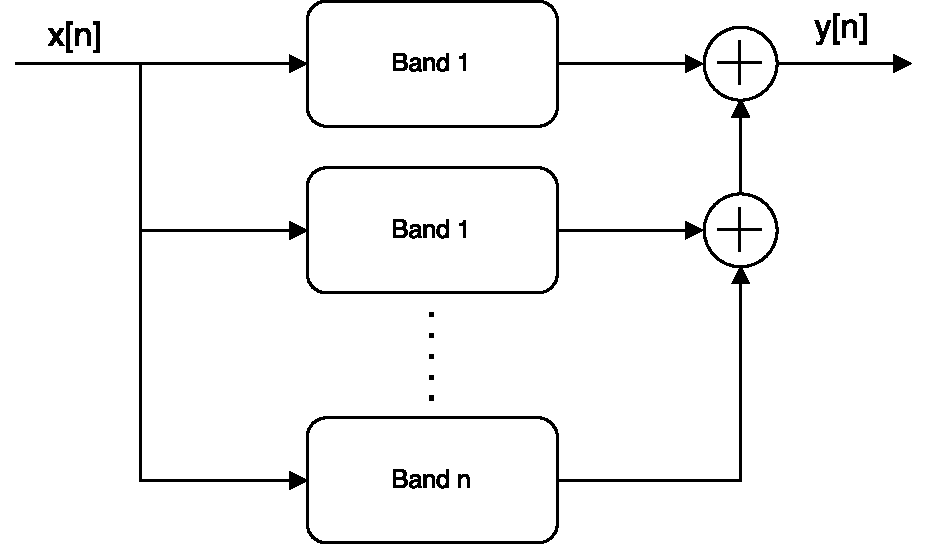
\includegraphics[width=0.6 \textwidth]{figures/graphic_eq_block.pdf}
\caption{Block diagram of the graphic equalizer.}
\label{fig:graphic_eq_block}
\end{figure}

%Typically a graphic equalizer will have one slider available for each band of the equalizer, of which the user can increase or decrease the gain of each band. 
An alternative to the graphic equalizer is the parametric equalizer. The parametric does not have a fixed center frequency and bandwidth contrary the graphic equalizer, thus giving it more flexibility to achieve the desired frequency response. Unlike the graphical equalizer the signal do not pass into bandpass filters in parallel. Instead, the signal is passed through each filter of the equalizer placed in series as shown in \autoref{fig:parametric_eq}. \\

\begin{figure}[H]
\centering
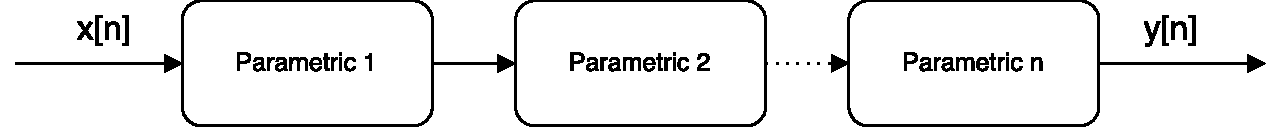
\includegraphics[width=0.8 \textwidth]{figures/parametric_eq.pdf}
\caption{Block diagram of the parametric equalizer.}
\label{fig:parametric_eq}
\end{figure}

The parametric equalizer can be seen as a combined peak- and notch filter, where the peak-filter is used to boost and the notch to attenuate. Implementing the parametric equalizer gives, besides changing the gain, the possibility to change the bandwidth and center frequency as shown in \autoref{fig:parametric_equalizer}.

\begin{figure}[H]
\centering
\hspace*{-1cm}
\begin{subfigure}[t]{0.3\textwidth}
	\tikzsetnextfilename{parametric_eq_preanalysis_Q}
	% This file was created by matlab2tikz.
%
%The latest updates can be retrieved from
%  http://www.mathworks.com/matlabcentral/fileexchange/22022-matlab2tikz-matlab2tikz
%where you can also make suggestions and rate matlab2tikz.
%
\begin{tikzpicture}

\begin{axis}[%
width=2in,
height=1.7in,
at={(1.011in,0.642in)},
scale only axis,
xmode=log,
xmin=10,
xmax=20000,
xminorticks=true,
xlabel={Frequency [Hz]},
xmajorgrids,
xminorgrids,
ymin=-5,
ymax=5,
ymajorgrids,
yticklabels={\empty},
axis background/.style={fill=white}
]
\addplot [color=black,solid,line width=1.0pt,forget plot]
  table[row sep=crcr]{%
0.159154943091895	1.52104528479092e-09\\
5.67189079114852	1.93230452791098e-06\\
11.1846266392052	7.51943373818724e-06\\
16.6973624872618	1.67791992824004e-05\\
22.2100983353184	2.97386492611314e-05\\
27.722834183375	4.64357337452805e-05\\
33.2355700314317	6.6919516788473e-05\\
38.7483058794883	9.12504455800552e-05\\
44.2610417275449	0.000119500686962666\\
49.7737775756016	0.00015175453242015\\
55.2865134236582	0.000188108874101866\\
60.7992492717148	0.000228673755853626\\
66.3119851197714	0.000273573008712253\\
71.8247209678281	0.000322944971695505\\
77.3374568158847	0.000376943308720189\\
82.8501926639413	0.000435737928385534\\
88.362928511998	0.000499516015079531\\
93.8756643600546	0.000568483184814175\\
99.3884002081112	0.000642864774463703\\
104.901136056168	0.000722907281943459\\
110.413871904224	0.000808879967186518\\
115.926607752281	0.00090107664260089\\
121.439343600338	0.000999817659988643\\
126.952079448394	0.00110545212673103\\
132.464815296451	0.00121836037701581\\
137.977551144508	0.00133895672322284\\
143.490286992564	0.0014676925275577\\
149.003022840621	0.00160505963325159\\
154.515758688678	0.00175159419615416\\
160.028494536734	0.00190788097717544\\
165.541230384791	0.00207455814919004\\
171.053966232847	0.00225232269285828\\
176.566702080904	0.00244193645895823\\
182.079437928961	0.00264423299601844\\
187.592173777017	0.00286012524226615\\
193.104909625074	0.00309061422509228\\
198.617645473131	0.00333679889352346\\
204.130381321187	0.0035998872811627\\
209.643117169244	0.00388120918199709\\
215.1558530173	0.00418223059313337\\
220.668588865357	0.00450457019596922\\
226.181324713414	0.00485001821500331\\
231.69406056147	0.00522055805142346\\
237.206796409527	0.00561839115630346\\
242.719532257584	0.00604596571734974\\
248.23226810564	0.00650600982730972\\
253.745003953697	0.00700156994994694\\
259.257739801753	0.0075360556701881\\
264.77047564981	0.00811329191767284\\
270.283211497867	0.00873758011500236\\
275.795947345923	0.00941377003543197\\
281.30868319398	0.0101473445408142\\
286.821419042037	0.0109445199075512\\
292.334154890093	0.0118123650807287\\
297.84689073815	0.0127589440154928\\
303.359626586207	0.0137934863589725\\
308.872362434263	0.0149265930350138\\
314.38509828232	0.0161704851220586\\
319.897834130376	0.0175393066793845\\
325.410569978433	0.0190494952573068\\
330.92330582649	0.0207202378147141\\
336.436041674546	0.0225740352218158\\
341.948777522603	0.0246374057041767\\
347.46151337066	0.026941767528892\\
352.974249218716	0.0295245547390489\\
358.486985066773	0.0324306385239295\\
363.999720914829	0.0357141531425909\\
369.512456762886	0.039440862570496\\
375.025192610943	0.0436912575325603\\
380.537928458999	0.048564650265103\\
386.050664307056	0.054184648799545\\
391.563400155113	0.0607065637125135\\
397.076136003169	0.0683275602848587\\
402.588871851226	0.077300770911441\\
408.101607699282	0.0879552153580892\\
413.614343547339	0.100724392830506\\
419.127079395396	0.116188077803\\
424.639815243452	0.135134653259035\\
430.152551091509	0.158656139597021\\
435.665286939566	0.188296609753382\\
441.178022787622	0.226290199861444\\
446.690758635679	0.275953977089983\\
452.203494483736	0.342356864070059\\
457.716230331792	0.433496108720002\\
463.228966179849	0.562432570648061\\
468.741702027905	0.751262614355034\\
474.254437875962	1.03851439355349\\
479.767173724019	1.49189799388277\\
485.279909572075	2.22208716337385\\
490.792645420132	3.34311701685435\\
496.305381268189	4.6247041751038\\
501.818117116245	4.90410608874762\\
507.330852964302	3.82505415494008\\
512.843588812358	2.61985771101294\\
518.356324660415	1.78382846965615\\
523.869060508472	1.25552325827228\\
529.381796356528	0.919021771091239\\
534.894532204585	0.697266219629312\\
540.407268052642	0.545468778132612\\
545.920003900698	0.437813601428799\\
551.432739748755	0.359040714427765\\
556.945475596812	0.299818721083128\\
562.458211444868	0.254241272727278\\
567.970947292925	0.218447077317677\\
573.483683140981	0.189836549255888\\
578.996418989038	0.16661277724288\\
584.509154837095	0.147504053855288\\
590.021890685151	0.131591195560257\\
595.534626533208	0.11819715359357\\
601.047362381265	0.106814691905798\\
606.560098229321	0.0970579326173343\\
612.072834077378	0.0886292233685626\\
617.585569925434	0.0812960559803955\\
623.098305773491	0.0748747112899249\\
628.611041621548	0.0692184879859231\\
634.123777469604	0.0642091084514587\\
639.636513317661	0.059750360839324\\
645.149249165718	0.0557633378864817\\
650.661985013774	0.0521828310419649\\
656.174720861831	0.0489545708600188\\
661.687456709888	0.046033094400842\\
667.200192557944	0.0433800821776765\\
672.712928406001	0.0409630502277672\\
678.225664254057	0.0387543132948973\\
683.738400102114	0.0367301567900939\\
689.251135950171	0.0348701708602796\\
694.763871798227	0.0331567112872759\\
700.276607646284	0.0315744603585919\\
705.789343494341	0.0301100670650826\\
711.302079342397	0.0287518506571268\\
716.814815190454	0.0274895551298186\\
722.32755103851	0.0263141448589172\\
727.840286886567	0.0252176336998925\\
733.353022734624	0.0241929414171724\\
738.86575858268	0.0232337725625455\\
744.378494430737	0.0223345138732211\\
749.891230278794	0.0214901470217593\\
755.40396612685	0.0206961741416183\\
760.916701974907	0.0199485540338976\\
766.429437822963	0.0192436473393069\\
771.94217367102	0.0185781692575445\\
777.454909519077	0.0179491486526881\\
782.967645367133	0.017353892572703\\
788.48038121519	0.0167899553784511\\
793.993117063246	0.0162551118115383\\
799.505852911303	0.0157473334318375\\
805.01858875936	0.0152647679548883\\
810.531324607416	0.0148057210832129\\
816.044060455473	0.0143686404969937\\
821.55679630353	0.0139521017104333\\
827.069532151586	0.0135547955551384\\
832.582267999643	0.0131755170712662\\
838.0950038477	0.012813155636846\\
843.607739695756	0.01246668617149\\
849.120475543813	0.0121351612900779\\
854.633211391869	0.0118177042848058\\
860.145947239926	0.0115135028395057\\
865.658683087983	0.011221803389484\\
871.171418936039	0.0109419060530408\\
876.684154784096	0.0106731600667184\\
882.196890632153	0.0104149596707135\\
887.709626480209	0.010166740392277\\
893.222362328266	0.00992797568316446\\
898.735098176323	0.00969817387615866\\
904.247834024379	0.00947687542142251\\
909.760569872436	0.00926365037957695\\
915.273305720492	0.00905809613688407\\
920.786041568549	0.00885983533102005\\
926.298777416606	0.00866851395226085\\
931.811513264662	0.00848379961467099\\
937.324249112719	0.00830537997469444\\
942.836984960776	0.00813296128321451\\
948.349720808832	0.00796626705919894\\
953.862456656889	0.00780503687267413\\
959.375192504945	0.00764902522840434\\
964.887928353002	0.00749800053779741\\
970.400664201059	0.00735174417577524\\
975.913400049115	0.00721004960777091\\
981.426135897172	0.00707272158928544\\
986.938871745229	0.00693957542511233\\
992.451607593285	0.00681043628269342\\
997.964343441342	0.00668513856262366\\
1003.4770792894	0.0065635253112589\\
1008.98981513746	0.00644544767835877\\
1014.50255098551	0.00633076441469318\\
1020.01528683357	0.00621934140630503\\
1025.52802268163	0.00611105123922509\\
1031.04075852968	0.00600577279878325\\
1036.55349437774	0.00590339089400462\\
1042.06623022579	0.00580379590976603\\
1047.57896607385	0.00570688348170515\\
1053.09170192191	0.0056125541930468\\
1058.60443776996	0.00552071329318637\\
1064.11717361802	0.00543127043321141\\
1069.62990946608	0.00534413942012012\\
1075.14264531413	0.0052592379865762\\
1080.65538116219	0.00517648757571804\\
1086.16811701025	0.00509581313833509\\
1091.6808528583	0.00501714294610182\\
1097.19358870636	0.00494040841231004\\
1102.70632455442	0.00486554392802055\\
1108.21906040247	0.00479248670487366\\
1113.73179625053	0.00472117662911945\\
1119.24453209859	0.00465155612450848\\
1124.75726794664	0.00458357002297077\\
1130.2700037947	0.00451716544255485\\
1135.78273964276	0.0044522916741971\\
1141.29547549081	0.00438890007307048\\
1146.80821133887	0.0043269439571779\\
1152.32094718693	0.00426637851274\\
1157.83368303498	0.00420716070243075\\
1163.34641888304	0.00414924918155447\\
1168.8591547311	0.00409260421693544\\
1174.37189057915	0.00403718761152211\\
1179.88462642721	0.00398296263238773\\
1185.39736227527	0.00392989394260601\\
1190.91009812332	0.00387794753818219\\
1196.42283397138	0.00382709068586065\\
1201.93556981944	0.00377729186687577\\
1207.44830566749	0.0037285207220526\\
1212.96104151555	0.00368074799995988\\
1218.47377736361	0.00363394550881578\\
1223.98651321166	0.00358808606891927\\
1229.49924905972	0.00354314346991455\\
1235.01198490778	0.00349909242784334\\
1240.52472075583	0.0034559085468669\\
1246.03745660389	0.00341356827984536\\
1251.55019245195	0.00337204889433326\\
1257.0629283	0.00333132843704734\\
1262.57566414806	0.00329138570244961\\
1268.08839999612	0.00325220020158058\\
1273.60113584417	0.00321375213273901\\
1279.11387169223	0.00317602235370764\\
1284.62660754029	0.00313899235481557\\
1290.13934338834	0.00310264423424481\\
1295.6520792364	0.00306696067302852\\
1301.16481508446	0.00303192491288174\\
1306.67755093251	0.00299752073380497\\
1312.19028678057	0.00296373243322678\\
1317.70302262863	0.00293054480564248\\
1323.21575847668	0.00289794312435304\\
1328.72849432474	0.00286591312222918\\
1334.2412301728	0.00283444097538565\\
1339.75396602085	0.00280351328552027\\
1345.26670186891	0.00277311706438818\\
1350.77943771697	0.0027432397188826\\
1356.29217356502	0.00271386903623614\\
1361.80490941308	0.00268499316985941\\
1367.31764526114	0.00265660062629918\\
1372.83038110919	0.00262868025278185\\
1378.34311695725	0.00260122122404099\\
1383.85585280531	0.00257421303140194\\
1389.36858865336	0.00254764547186784\\
1394.88132450142	0.002521508636239\\
1400.39406034948	0.00249579289956674\\
1405.90679619753	0.00247048891134444\\
1411.41953204559	0.00244558758573287\\
1416.93226789365	0.002421080092645\\
1422.4450037417	0.00239695784848904\\
1427.95773958976	0.0023732125088894\\
1433.47047543782	0.00234983595947141\\
1438.98321128587	0.00232682030881676\\
1444.49594713393	0.00230415788105415\\
1450.00868298199	0.00228184120821058\\
1455.52141883004	0.00225986302389273\\
1461.0341546781	0.00223821625641463\\
1466.54689052616	0.0022168940224824\\
1472.05962637421	0.00219588962126232\\
1477.57236222227	0.00217519652836194\\
1483.08509807033	0.00215480839014459\\
1488.59783391838	0.00213471901847157\\
1494.11056976644	0.00211492238540767\\
1499.6233056145	0.00209541261804977\\
1505.13604146255	0.00207618399386629\\
1510.64877731061	0.00205723093592845\\
1516.16151315867	0.00203854800845373\\
1521.67424900672	0.0020201299122875\\
1527.18698485478	0.00200197148114609\\
1532.69972070283	0.00198406767705373\\
1538.21245655089	0.00196641358702312\\
1543.72519239895	0.00194900441871381\\
1549.237928247	0.00193183549725902\\
1554.75066409506	0.00191490226155436\\
1560.26339994312	0.0018982002610304\\
1565.77613579117	0.00188172515230368\\
1571.28887163923	0.00186547269607827\\
1576.80160748729	0.00184943875403952\\
1582.31434333534	0.00183361928609289\\
1587.8270791834	0.00181801034732114\\
1593.33981503146	0.00180260808546209\\
1598.85255087951	0.00178740873816454\\
1604.36528672757	0.00177240863039448\\
1609.87802257563	0.001757604172092\\
1615.39075842368	0.0017429918557586\\
1620.90349427174	0.00172856825387864\\
1626.4162301198	0.00171433001722007\\
1631.92896596785	0.00170027387209956\\
1637.44170181591	0.00168639661886817\\
1642.95443766397	0.00167269512947912\\
1648.46717351202	0.00165916634550482\\
1653.97990936008	0.00164580727659151\\
1659.49264520814	0.00163261499832965\\
1665.00538105619	0.00161958665072776\\
1670.51811690425	0.00160671943604798\\
1676.03085275231	0.00159401061778507\\
1681.54358860036	0.00158145751853466\\
1687.05632444842	0.00156905751874846\\
1692.56906029648	0.00155680805479339\\
1698.08179614453	0.00154470661814053\\
1703.59453199259	0.00153275075328537\\
1709.10726784065	0.00152093805680557\\
1714.6200036887	0.00150926617602739\\
1720.13273953676	0.00149773280721376\\
1725.64547538482	0.00148633569507711\\
1731.15821123287	0.00147507263093657\\
1736.67094708093	0.00146394145175835\\
1742.18368292899	0.0014529400391497\\
1747.69641877704	0.00144206631798664\\
1753.2091546251	0.0014313182555139\\
1758.72189047316	0.0014206938603062\\
1764.23462632121	0.00141019118091697\\
1769.74736216927	0.00139980830552986\\
1775.26009801733	0.00138954336033172\\
1780.77283386538	0.00137939450905026\\
1786.28556971344	0.00136935995170113\\
1791.7983055615	0.00135943792404647\\
1797.31104140955	0.00134962669652705\\
1802.82377725761	0.00133992457329465\\
1808.33651310567	0.00133032989188273\\
1813.84924895372	0.00132084102181647\\
1819.36198480178	0.00131145636443378\\
1824.87472064984	0.00130217435167278\\
1830.38745649789	0.00129299344565364\\
1835.90019234595	0.00128391213778806\\
1841.41292819401	0.00127492894817405\\
1846.92566404206	0.00126604242505828\\
1852.43839989012	0.00125725114395507\\
1857.95113573818	0.00124855370706049\\
1863.46387158623	0.00123994874293254\\
1868.97660743429	0.00123143490542309\\
1874.48934328235	0.0012230108735933\\
1880.0020791304	0.00121467535073426\\
1885.51481497846	0.00120642706401438\\
1891.02755082652	0.00119826476401676\\
1896.54028667457	0.00119018722401632\\
1902.05302252263	0.00118219323974091\\
1907.56575837069	0.00117428162845553\\
1913.07849421874	0.00116645122908594\\
1918.5912300668	0.00115870090108501\\
1924.10396591486	0.00115102952453896\\
1929.61670176291	0.00114343599935377\\
1935.12943761097	0.00113591924508374\\
1940.64217345903	0.00112847820026829\\
1946.15490930708	0.00112111182221618\\
1951.66764515514	0.00111381908650813\\
1957.1803810032	0.00110659898660938\\
1962.69311685125	0.00109945053349381\\
1968.20585269931	0.00109237275532592\\
1973.71858854737	0.00108536469706756\\
1979.23132439542	0.00107842542003069\\
1984.74406024348	0.00107155400169241\\
1990.25679609154	0.00106474953529783\\
1995.76953193959	0.00105801112946678\\
2001.28226778765	0.00105133790797996\\
2006.79500363571	0.00104472900935471\\
2012.30773948376	0.0010381835867218\\
2017.82047533182	0.0010317008072026\\
2023.33321117987	0.00102527985206159\\
2028.84594702793	0.00101891991603342\\
2034.35868287599	0.00101262020730954\\
2039.87141872404	0.00100637994701951\\
2045.3841545721	0.00100019836925045\\
2050.89689042016	0.00099407472056883\\
2056.40962626821	0.000988008259883694\\
2061.92236211627	0.000981998258161303\\
2067.43509796433	0.000976043998249759\\
2072.94783381238	0.000970144774495331\\
2078.46056966044	0.000964299892678894\\
2083.9733055085	0.000958508669655401\\
2089.48604135655	0.000952770433365526\\
2094.99877720461	0.00094708452231314\\
2100.51151305267	0.00094145028544389\\
2106.02424890072	0.000935867082253264\\
2111.53698474878	0.0009303342820905\\
2117.04972059684	0.000924851264451771\\
2122.56245644489	0.000919417418361226\\
2128.07519229295	0.000914032142413475\\
2133.58792814101	0.000908694844696523\\
2139.10066398906	0.000903404942325138\\
2144.61339983712	0.000898161861408133\\
2150.12613568518	0.000892965037038778\\
2155.63887153323	0.000887813912876385\\
2161.15160738129	0.000882707941109721\\
2166.66434322935	0.000877646582254575\\
2172.1770790774	0.000872629305047741\\
2177.68981492546	0.000867655586356437\\
2183.20255077352	0.000862724910740591\\
2188.71528662157	0.000857836770726728\\
2194.22802246963	0.000852990666287338\\
2199.74075831769	0.000848186104993265\\
2205.25349416574	0.000843422601674342\\
2210.7662300138	0.000838699678377012\\
2216.27896586186	0.000834016864229373\\
2221.79170170991	0.000829373695312013\\
2227.30443755797	0.000824769714488344\\
2232.81717340603	0.000820204471418143\\
2238.32990925408	0.000815677522204675\\
2243.84264510214	0.000811188429529727\\
2249.3553809502	0.000806736762325801\\
2254.86811679825	0.000802322095886071\\
2260.38085264631	0.000797944011534653\\
2265.89358849437	0.000793602096618917\\
2271.40632434242	0.0007892959444536\\
2276.91906019048	0.000785025154099057\\
2282.43179603854	0.00078078933042108\\
2287.94453188659	0.00077658808377658\\
2293.45726773465	0.000772421030140901\\
2298.97000358271	0.0007682877908475\\
2304.48273943076	0.00076418799255712\\
2309.99547527882	0.00076012126723082\\
2315.50821112688	0.00075608725191015\\
2321.02094697493	0.000752085588738394\\
2326.53368282299	0.000748115924777387\\
2332.04641867105	0.00074417791204611\\
2337.5591545191	0.000740271207335578\\
2343.07189036716	0.000736395472168364\\
2348.58462621522	0.000732550372709916\\
2354.09736206327	0.000728735579649006\\
2359.61009791133	0.000724950768303823\\
2365.12283375939	0.000721195618276794\\
2370.63556960744	0.000717469813593452\\
2376.1483054555	0.000713773042528897\\
2381.66104130356	0.000710104997542243\\
2387.17377715161	0.000706465375232283\\
2392.68651299967	0.000702853876327865\\
2398.19924884773	0.000699270205496988\\
2403.71198469578	0.00069571407135068\\
2409.22472054384	0.000692185186414083\\
2414.7374563919	0.000688683266962552\\
2420.25019223995	0.000685208033040952\\
2425.76292808801	0.000681759208415467\\
2431.27566393607	0.000678336520482972\\
2436.78839978412	0.000674939700141838\\
2442.30113563218	0.000671568481855594\\
2447.81387148024	0.00066822260361629\\
2453.32660732829	0.000664901806684175\\
2458.83934317635	0.000661605835757408\\
2464.35207902441	0.000658334438796587\\
2469.86481487246	0.000655087367061398\\
2475.37755072052	0.00065186437491585\\
2480.89028656857	0.000648665219972927\\
2486.40302241663	0.000645489662870896\\
2491.91575826469	0.000642337467306096\\
2497.42849411275	0.000639208400034887\\
2502.9412299608	0.000636102230692377\\
2508.45396580886	0.000633018731836788\\
2513.96670165692	0.000629957678980327\\
2519.47943750497	0.000626918850296062\\
2524.99217335303	0.000623902026876351\\
2530.50490920108	0.000620906992540003\\
2536.01764504914	0.000617933533695364\\
2541.5303808972	0.000614981439465678\\
2547.04311674525	0.000612050501664029\\
2552.55585259331	0.000609140514509856\\
2558.06858844137	0.000606251274968383\\
2563.58132428942	0.000603382582299355\\
2569.09406013748	0.00060053423834825\\
2574.60679598554	0.000597706047339941\\
2580.11953183359	0.000594897815913415\\
2585.63226768165	0.000592109353044639\\
2591.14500352971	0.000589340470008002\\
2596.65773937776	0.000586590980358963\\
2602.17047522582	0.000583860700013128\\
2607.68321107388	0.000581149446935767\\
2613.19594692193	0.000578457041384816\\
2618.70868276999	0.000575783305721886\\
2624.22141861805	0.000573128064477843\\
2629.7341544661	0.000570491144262171\\
2635.24689031416	0.000567872373691629\\
2640.75962616222	0.000565271583511748\\
2646.27236201027	0.000562688606340347\\
2651.78509785833	0.000560123276866178\\
2657.29783370639	0.000557575431725507\\
2662.81056955444	0.000555044909413405\\
2668.3233054025	0.000552531550353183\\
2673.83604125056	0.000550035196811542\\
2679.34877709861	0.000547555692929438\\
2684.86151294667	0.000545092884616012\\
2690.37424879473	0.000542646619571745\\
2695.88698464278	0.000540216747276888\\
2701.39972049084	0.000537803118968326\\
2706.9124563389	0.000535405587475657\\
2712.42519218695	0.000533024007504694\\
2717.93792803501	0.000530658235263332\\
2723.45066388307	0.000528308128662121\\
2728.96339973112	0.000525973547240987\\
2734.47613557918	0.000523654352111381\\
2739.98887142724	0.000521350405975565\\
2745.50160727529	0.000519061573093839\\
2751.01434312335	0.00051678771920161\\
2756.52707897141	0.000514528711648259\\
2762.03981481946	0.000512284419140641\\
2767.55255066752	0.000510054711984163\\
2773.06528651558	0.000507839461851364\\
2778.57802236363	0.000505638541833982\\
2784.09075821169	0.000503451826523964\\
2789.60349405975	0.000501279191809044\\
2795.1162299078	0.000499120514990382\\
2800.62896575586	0.000496975674722788\\
2806.14170160392	0.000494844550991583\\
2811.65443745197	0.000492727025091385\\
2817.16717330003	0.000490622979651189\\
2822.67990914809	0.000488532298541794\\
2828.19264499614	0.000486454866933667\\
2833.7053808442	0.000484390571208231\\
2839.21811669226	0.000482339298998371\\
2844.73085254031	0.000480300939173004\\
2850.24358838837	0.000478275381794657\\
2855.75632423643	0.000476262518100185\\
2861.26906008448	0.000474262240450629\\
2866.78179593254	0.000472274442446935\\
2872.2945317806	0.000470299018808455\\
2877.80726762865	0.000468335865340169\\
2883.32000347671	0.000466384878973181\\
2888.83273932477	0.000464445957741586\\
2894.34547517282	0.000462519000741967\\
2899.85821102088	0.000460603908193188\\
2905.37094686894	0.000458700581314892\\
2910.88368271699	0.000456808922358366\\
2916.39641856505	0.000454928834645111\\
2921.90915441311	0.000453060222466561\\
2927.42189026116	0.000451202991172797\\
2932.93462610922	0.000449357047089626\\
2938.44736195728	0.000447522297424078\\
2943.96009780533	0.000445698650468839\\
2949.47283365339	0.000443886015413255\\
2954.98556950145	0.000442084302356831\\
2960.4983053495	0.000440293422417236\\
2966.01104119756	0.000438513287545161\\
2971.52377704562	0.000436743810638106\\
2977.03651289367	0.000434984905455527\\
2982.54924874173	0.000433236486663195\\
2988.06198458979	0.000431498469775337\\
2993.57472043784	0.000429770771214429\\
2999.0874562859	0.000428053308199337\\
3004.60019213395	0.00042634599881668\\
3010.11292798201	0.000424648761984184\\
3015.62566383007	0.000422961517400544\\
3021.13839967812	0.000421284185641853\\
3026.65113552618	0.000419616688018892\\
3032.16387137424	0.000417958946660058\\
3037.67660722229	0.00041631088447665\\
3043.18934307035	0.000414672425137803\\
3048.70207891841	0.000413043493099416\\
3054.21481476646	0.00041142401350194\\
3059.72755061452	0.000409813912340092\\
3065.24028646258	0.000408213116243002\\
3070.75302231063	0.000406621552597641\\
3076.26575815869	0.000405039149502539\\
3081.77849400675	0.00040346583578707\\
3087.2912298548	0.000401901540967096\\
3092.80396570286	0.000400346195243043\\
3098.31670155092	0.000398799729507614\\
3103.82943739897	0.000397262075284075\\
3109.34217324703	0.000395733164867046\\
3114.85490909509	0.000394212931071783\\
3120.36764494314	0.000392701307484899\\
3125.8803807912	0.000391198228267646\\
3131.39311663926	0.000389703628250419\\
3136.90585248731	0.000388217442855616\\
3142.41858833537	0.000386739608176703\\
3147.93132418343	0.000385270060864441\\
3153.44406003148	0.000383808738234877\\
3158.95679587954	0.000382355578149777\\
3164.4695317276	0.000380910519109203\\
3169.98226757565	0.000379473500160863\\
3175.49500342371	0.000378044460952191\\
3181.00773927177	0.00037662334172263\\
3186.52047511982	0.000375210083236131\\
3192.03321096788	0.000373804626819731\\
3197.54594681594	0.000372406914386693\\
3203.05868266399	0.000371016888388293\\
3208.57141851205	0.000369634491786822\\
3214.08415436011	0.000368259668098015\\
3219.59689020816	0.000366892361360194\\
3225.10962605622	0.000365532516184414\\
3230.62236190428	0.000364180077629103\\
3236.13509775233	0.000362834991257925\\
3241.64783360039	0.000361497203191846\\
3247.16056944845	0.000360166660043571\\
3252.6733052965	0.000358843308890538\\
3258.18604114456	0.000357527097309637\\
3263.69877699262	0.000356217973365636\\
3269.21151284067	0.000354915885593831\\
3274.72424868873	0.000353620783015467\\
3280.23698453679	0.000352332615085675\\
3285.74972038484	0.000351051331778324\\
3291.2624562329	0.000349776883452952\\
3296.77519208096	0.000348509220966628\\
3302.28792792901	0.00034724829562766\\
3307.80066377707	0.000345994059155101\\
3313.31339962513	0.000344746463726963\\
3318.82613547318	0.000343505461949356\\
3324.33887132124	0.000342271006815997\\
3329.8516071693	0.000341043051843203\\
3335.36434301735	0.000339821550842324\\
3340.87707886541	0.000338606458131886\\
3346.38981471347	0.000337397728392948\\
3351.90255056152	0.000336195316703817\\
3357.41528640958	0.000334999178597907\\
3362.92802225764	0.000333809269957666\\
3368.44075810569	0.000332625547033864\\
3373.95349395375	0.000331447966532379\\
3379.46622980181	0.00033027648548884\\
3384.97896564986	0.000329111061353486\\
3390.49170149792	0.000327951651906304\\
3396.00443734598	0.000326798215361183\\
3401.51717319403	0.000325650710242473\\
3407.02990904209	0.000324509095442855\\
3412.54264489015	0.000323373330285046\\
3418.0553807382	0.000322243374342447\\
3423.56811658626	0.000321119187616573\\
3429.08085243432	0.000320000730409764\\
3434.59358828237	0.000318887963417761\\
3440.10632413043	0.000317780847606275\\
3445.61905997849	0.000316679344372988\\
3451.13179582654	0.000315583415364339\\
3456.6445316746	0.000314493022587384\\
3462.15726752266	0.000313408128404008\\
3467.67000337071	0.000312328695449924\\
3473.18273921877	0.000311254686719537\\
3478.69547506683	0.000310186065500365\\
3484.20821091488	0.000309122795394258\\
3489.72094676294	0.000308064840348258\\
3495.23368261099	0.000307012164558164\\
3500.74641845905	0.000305964732564967\\
3506.25915430711	0.000304922509216275\\
3511.77189015517	0.000303885459606531\\
3517.28462600322	0.00030285354918501\\
3522.79736185128	0.000301826743653609\\
3528.31009769933	0.00030080500904013\\
3533.82283354739	0.000299788311594136\\
3539.33556939545	0.000298776617914242\\
3544.8483052435	0.000297769894843969\\
3550.36104109156	0.000296768109506459\\
3555.87377693962	0.000295771229312191\\
3561.38651278767	0.000294779221933909\\
3566.89924863573	0.000293792055312407\\
3572.41198448379	0.000292809697654602\\
3577.92472033184	0.000291832117423891\\
3583.4374561799	0.000290859283371009\\
3588.95019202796	0.000289891164468457\\
3594.46292787601	0.000288927729976076\\
3599.97566372407	0.000287968949383185\\
3605.48839957213	0.000287014792454873\\
3611.00113542018	0.000286065229168353\\
3616.51387126824	0.000285120229772748\\
3622.0266071163	0.000284179764775593\\
3627.53934296435	0.000283243804861833\\
3633.05207881241	0.000282312321017254\\
3638.56481466047	0.000281385284457125\\
3644.07755050852	0.000280462666593413\\
3649.59028635658	0.000279544439108068\\
3655.10302220464	0.000278630573883596\\
3660.61575805269	0.000277721043066701\\
3666.12849390075	0.000276815818948713\\
3671.64122974881	0.000275914874160378\\
3677.15396559686	0.000275018181463568\\
3682.66670144492	0.000274125713857354\\
3688.17943729298	0.000273237444572221\\
3693.69217314103	0.00027235334705464\\
3699.20490898909	0.00027147339493814\\
3704.71764483715	0.000270597562095377\\
3710.2303806852	0.000269725822589922\\
3715.74311653326	0.000268858150683976\\
3721.25585238132	0.000267994520859583\\
3726.76858822937	0.000267134907797417\\
3732.28132407743	0.000266279286374853\\
3737.79405992549	0.000265427631669824\\
3743.30679577354	0.000264579918939609\\
3748.8195316216	0.00026373612367483\\
3754.33226746966	0.000262896221520383\\
3759.84500331771	0.000262060188323652\\
3765.35773916577	0.000261228000134508\\
3770.87047501383	0.000260399633168668\\
3776.38321086188	0.000259575063834696\\
3781.89594670994	0.000258754268739785\\
3787.408682558	0.000257937224624189\\
3792.92141840605	0.000257123908505866\\
3798.43415425411	0.000256314297472189\\
3803.94689010217	0.000255508368841953\\
3809.45962595022	0.000254706100111366\\
3814.97236179828	0.000253907468927059\\
3820.48509764634	0.000253112453132362\\
3825.99783349439	0.000252321030722955\\
3831.51056934245	0.000251533179877723\\
3837.02330519051	0.000250748878918252\\
3842.53604103856	0.000249968106364764\\
3848.04877688662	0.000249190840882112\\
3853.56151273468	0.000248417061273999\\
3859.07424858273	0.000247646746560117\\
3864.58698443079	0.000246879875897078\\
3870.09972027885	0.000246116428551412\\
3875.6124561269	0.000245356384028785\\
3881.12519197496	0.000244599721942853\\
3886.63792782302	0.00024384642203455\\
3892.15066367107	0.000243096464276228\\
3897.66339951913	0.000242349828721232\\
3903.17613536719	0.000241606495588755\\
3908.68887121524	0.000240866445258055\\
3914.2016070633	0.000240129658266522\\
3919.71434291136	0.000239396115263397\\
3925.22707875941	0.000238665797075342\\
3930.73981460747	0.000237938684646652\\
3936.25255045553	0.000237214759070116\\
3941.76528630358	0.000236494001602443\\
3947.27802215164	0.000235776393596765\\
3952.7907579997	0.000235061916575919\\
3958.30349384775	0.000234350552201592\\
3963.81622969581	0.000233642282224179\\
3969.32896554387	0.000232937088615854\\
3974.84170139192	0.000232234953371925\\
3980.35443723998	0.00023153585873841\\
3985.86717308804	0.000230839786976746\\
3991.37990893609	0.000230146720568223\\
3996.89264478415	0.000229456642077051\\
4002.4053806322	0.000228769534190864\\
4007.91811648026	0.00022808537974386\\
4013.43085232832	0.000227404161701373\\
4018.94358817637	0.000226725863119375\\
4024.45632402443	0.000226050467217759\\
4029.96905987249	0.000225377957287771\\
4035.48179572054	0.000224708316800005\\
4040.9945315686	0.00022404152929834\\
4046.50726741666	0.000223377578461643\\
4052.02000326472	0.000222716448099923\\
4057.53273911277	0.000222058122115753\\
4063.04547496083	0.000221402584548629\\
4068.55821080888	0.000220749819524826\\
4074.07094665694	0.00022009981131526\\
4079.583682505	0.00021945254428341\\
4085.09641835305	0.000218808002916179\\
4090.60915420111	0.000218166171794965\\
4096.12189004917	0.000217527035636161\\
4101.63462589722	0.000216890579237155\\
4107.14736174528	0.000216256787518759\\
4112.66009759334	0.000215625645511708\\
4118.17283344139	0.00021499713834316\\
4123.68556928945	0.000214371251244414\\
4129.19830513751	0.000213747969550904\\
4134.71104098556	0.000213127278721489\\
4140.22377683362	0.000212509164299882\\
4145.73651268168	0.000211893611930075\\
4151.24924852973	0.0002112806073467\\
4156.76198437779	0.000210670136411669\\
4162.27472022585	0.000210062185073677\\
4167.7874560739	0.000209456739368199\\
4173.30019192196	0.000208853785427135\\
4178.81292777002	0.000208253309523168\\
4184.32566361807	0.000207655297950187\\
4189.83839946613	0.000207059737162154\\
4195.35113531419	0.000206466613680523\\
4200.86387116224	0.000205875914107745\\
4206.3766070103	0.00020528762516584\\
4211.88934285836	0.000204701733655893\\
4217.40207870641	0.000204118226467702\\
4222.91481455447	0.000203537090570132\\
4228.42755040253	0.000202958313049687\\
4233.94028625058	0.000202381881048795\\
4239.45302209864	0.000201807781829453\\
4244.9657579467	0.000201236002732727\\
4250.47849379475	0.000200666531172963\\
4255.99122964281	0.000200099354651291\\
4261.50396549087	0.000199534460765264\\
4267.01670133892	0.000198971837178006\\
4272.52943718698	0.000198411471685708\\
4278.04217303504	0.000197853352098057\\
4283.55490888309	0.000197297466344309\\
4289.06764473115	0.000196743802450145\\
4294.58038057921	0.000196192348489457\\
4300.09311642726	0.000195643092642208\\
4305.60585227532	0.000195096023148139\\
4311.11858812338	0.000194551128337635\\
4316.63132397143	0.000194008396624005\\
4322.14405981949	0.000193467816480341\\
4327.65679566755	0.000192929376460731\\
4333.1695315156	0.000192393065223405\\
4338.68226736366	0.000191858871472875\\
4344.19500321172	0.000191326783990793\\
4349.70773905977	0.000190796791647523\\
4355.22047490783	0.000190268883392497\\
4360.73321075589	0.000189743048207932\\
4366.24594660394	0.000189219275201397\\
4371.758682452	0.000188697553520961\\
4377.27141830006	0.000188177872397616\\
4382.78415414811	0.000187660221118283\\
4388.29688999617	0.000187144589081737\\
4393.80962584423	0.00018663096569832\\
4399.32236169228	0.000186119340480588\\
4404.83509754034	0.000185609703020167\\
4410.3478333884	0.000185102042953034\\
4415.86056923645	0.000184596350001954\\
4421.37330508451	0.000184092613937901\\
4426.88604093257	0.000183590824632133\\
4432.39877678062	0.000183090971959763\\
4437.91151262868	0.000182593045940547\\
4443.42424847673	0.00018209703660002\\
4448.93698432479	0.000181602934052433\\
4454.44972017285	0.000181110728466034\\
4459.96245602091	0.000180620410090069\\
4465.47519186896	0.000180131969220066\\
4470.98792771702	0.000179645396219053\\
4476.50066356508	0.000179160681521413\\
4482.01339941313	0.000178677815605884\\
4487.52613526119	0.000178196789016772\\
4493.03887110924	0.000177717592379384\\
4498.5516069573	0.000177240216344093\\
4504.06434280536	0.000176764651678917\\
4509.57707865341	0.000176290889122941\\
4515.08981450147	0.000175818919565677\\
4520.60255034953	0.000175348733883137\\
4526.11528619758	0.000174880323053542\\
4531.62802204564	0.000174413678114902\\
4537.1407578937	0.000173948790124506\\
4542.65349374176	0.000173485650220644\\
4548.16622958981	0.000173024249601391\\
4553.67896543787	0.00017256457951689\\
4559.19170128592	0.000172106631263568\\
4564.70443713398	0.000171650396214995\\
4570.21717298204	0.000171195865765952\\
4575.72990883009	0.000170743031390291\\
4581.24264467815	0.000170291884610075\\
4586.75538052621	0.00016984241699944\\
4592.26811637426	0.000169394620188447\\
4597.78085222232	0.000168948485855371\\
4603.29358807038	0.00016850400572284\\
4608.80632391843	0.00016806117157327\\
4614.31905976649	0.000167619975262359\\
4619.83179561455	0.000167180408661233\\
4625.34453146261	0.000166742463704659\\
4630.85726731066	0.000166306132389118\\
4636.37000315872	0.000165871406724588\\
4641.88273900677	0.000165438278827119\\
4647.39547485483	0.000165006740826259\\
4652.90821070289	0.00016457678488434\\
4658.42094655094	0.00016414840324855\\
4663.933682399	0.000163721588206577\\
4669.44641824706	0.000163296332071177\\
4674.95915409511	0.000162872627222607\\
4680.47188994317	0.000162450466079693\\
4685.98462579123	0.000162029841111403\\
4691.49736163928	0.000161610744829132\\
4697.01009748734	0.00016119316980599\\
4702.5228333354	0.000160777108624726\\
4708.03556918345	0.000160362553949089\\
4713.54830503151	0.000159949498485258\\
4719.06104087957	0.000159537934956764\\
4724.57377672762	0.000159127856143068\\
4730.08651257568	0.000158719254893058\\
4735.59924842374	0.000158312124061406\\
4741.11198427179	0.000157906456566427\\
4746.62472011985	0.00015750224537465\\
4752.13745596791	0.000157099483483457\\
4757.65019181596	0.000156698163921089\\
4763.16292766402	0.000156298279787143\\
4768.67566351208	0.000155899824208213\\
4774.18839936013	0.000155502790343681\\
4779.70113520819	0.00015510717139921\\
4785.21387105625	0.000154712960644109\\
4790.7266069043	0.000154320151353469\\
4796.23934275236	0.000153928736850595\\
4801.75207860042	0.000153538710526292\\
4807.26481444847	0.00015315006577522\\
4812.77755029653	0.000152762796047968\\
4818.29028614459	0.000152376894831766\\
4823.80302199264	0.000151992355658201\\
4829.3157578407	0.000151609172089717\\
4834.82849368876	0.000151227337738898\\
4840.34122953681	0.0001508468462299\\
4845.85396538487	0.000150467691258237\\
4851.36670123293	0.00015008986653099\\
4856.87943708098	0.000149713365797671\\
4862.39217292904	0.000149338182859861\\
4867.9049087771	0.000148964311542283\\
4873.41764462515	0.000148591745704376\\
4878.93038047321	0.000148220479248003\\
4884.44311632126	0.00014785050610203\\
4889.95585216932	0.000147481820251249\\
4895.46858801738	0.000147114415697808\\
4900.98132386544	0.000146748286468927\\
4906.49405971349	0.000146383426659325\\
4912.00679556155	0.000146019830361792\\
4917.51953140961	0.000145657491742402\\
4923.03226725766	0.000145296404963372\\
4928.54500310572	0.000144936564242849\\
4934.05773895378	0.000144577963829832\\
4939.57047480183	0.000144220598002251\\
4945.08321064989	0.000143864461082393\\
4950.59594649795	0.000143509547402186\\
4956.108682346	0.0001431558513302\\
4961.62141819406	0.000142803367310221\\
4967.13415404211	0.000142452089764816\\
4972.64688989017	0.000142102013180199\\
4978.15962573823	0.000141753132052224\\
4983.67236158629	0.000141405440919172\\
4989.18509743434	0.000141058934359825\\
4994.6978332824	0.00014071360697225\\
5000.21056913046	0.000140369453391157\\
5005.72330497851	0.000140026468276326\\
5011.23604082657	0.000139684646320322\\
5016.74877667463	0.000139343982248495\\
5022.26151252268	0.000139004470815126\\
5027.77424837074	0.000138666106809205\\
5033.2869842188	0.000138328885029368\\
5038.79972006685	0.000137992800334036\\
5044.31245591491	0.000137657847581628\\
5049.82519176296	0.000137324021684563\\
5055.33792761102	0.000136991317566832\\
5060.85066345908	0.00013665973018714\\
5066.36339930714	0.000136329254536975\\
5071.87613515519	0.000135999885629041\\
5077.38887100325	0.00013567161850497\\
5082.9016068513	0.000135344448239178\\
5088.41434269936	0.000135018369923439\\
5093.92707854742	0.000134693378691955\\
5099.43981439547	0.000134369469704\\
5104.95255024353	0.000134046638122701\\
5110.46528609159	0.000133724879174832\\
5115.97802193964	0.000133404188083308\\
5121.4907577877	0.000133084560111542\\
5127.00349363576	0.000132765990549949\\
5132.51622948381	0.000132448474714013\\
5138.02896533187	0.000132132007934648\\
5143.54170117993	0.000131816585589052\\
5149.05443702798	0.000131502203058281\\
5154.56717287604	0.000131188855773533\\
5160.0799087241	0.000130876539164077\\
5165.59264457215	0.00013056524870161\\
5171.10538042021	0.000130254979882901\\
5176.61811626827	0.000129945728218217\\
5182.13085211632	0.000129637489258328\\
5187.64358796438	0.0001293302585675\\
5193.15632381244	0.00012902403173893\\
5198.66905966049	0.000128718804375455\\
5204.18179550855	0.000128414572126199\\
5209.69453135661	0.000128111330667288\\
5215.20726720466	0.000127809075663271\\
5220.72000305272	0.000127507802844272\\
5226.23273890078	0.0001272075079192\\
5231.74547474883	0.000126908186677964\\
5237.25821059689	0.000126609834879614\\
5242.77094644495	0.000126312448323699\\
5248.283682293	0.000126016022857987\\
5253.79641814106	0.000125720554318669\\
5259.30915398912	0.000125426038574724\\
5264.82188983717	0.000125132471524059\\
5270.33462568523	0.000124839849085794\\
5275.84736153329	0.000124548167186765\\
5281.36009738134	0.000124257421800093\\
5286.8728332294	0.000123967608906611\\
5292.38556907746	0.000123678724500654\\
5297.89830492551	0.000123390764615128\\
5303.41104077357	0.000123103725294509\\
5308.92377662163	0.000122817602610275\\
5314.43651246968	0.000122532392641615\\
5319.94924831774	0.000122248091506292\\
5325.4619841658	0.000121964695341354\\
5330.97472001385	0.000121682200270347\\
5336.48745586191	0.000121400602507461\\
5342.00019170997	0.00012111989820903\\
5347.51292755802	0.000120840083600813\\
5353.02566340608	0.000120561154918216\\
5358.53839925414	0.000120283108412069\\
5364.05113510219	0.00012000594035442\\
5369.56387095025	0.0001197296470366\\
5375.07660679831	0.000119454224776941\\
5380.58934264636	0.000119179669897631\\
5386.10207849442	0.000118905978749788\\
5391.61481434248	0.000118633147719242\\
5397.12755019053	0.000118361173182183\\
5402.64028603859	0.000118090051545654\\
5408.15302188665	0.000117819779241773\\
5413.6657577347	0.000117550352716156\\
5419.17849358276	0.000117281768435634\\
5424.69122943082	0.000117014022880536\\
5430.20396527887	0.000116747112558194\\
5435.71670112693	0.00011648103398558\\
5441.22943697499	0.000116215783693166\\
5446.74217282304	0.000115951358246141\\
5452.2549086711	0.000115687754223191\\
5457.76764451916	0.000115424968210718\\
5463.28038036721	0.000115162996820192\\
5468.79311621527	0.000114901836668873\\
5474.30585206333	0.000114641484422233\\
5479.81858791138	0.000114381936730316\\
5485.33132375944	0.000114123190274021\\
5490.8440596075	0.000113865241753535\\
5496.35679545555	0.000113608087878687\\
5501.86953130361	0.00011335172539402\\
5507.38226715167	0.000113096151020934\\
5512.89500299972	0.000112841361546402\\
5518.40773884778	0.000112587353751608\\
5523.92047469583	0.000112334124435095\\
5529.43321054389	0.000112081670399264\\
5534.94594639195	0.000111829988483156\\
5540.45868224001	0.000111579075537386\\
5545.97141808806	0.000111328928418354\\
5551.48415393612	0.000111079544011387\\
5556.99688978417	0.000110830919207599\\
5562.50962563223	0.000110583050923176\\
5568.02236148029	0.000110335936083945\\
5573.53509732834	0.000110089571625377\\
5579.0478331764	0.000109843954511871\\
5584.56056902446	0.000109599081723255\\
5590.07330487251	0.000109354950235499\\
5595.58604072057	0.000109111557072788\\
5601.09877656863	0.000108868899232307\\
5606.61151241668	0.000108626973759455\\
5612.12424826474	0.00010838577771313\\
5617.6369841128	0.000108145308136803\\
5623.14971996085	0.000107905562135659\\
5628.66245580891	0.000107666536780166\\
5634.17519165697	0.000107428229196724\\
5639.68792750503	0.000107190636502089\\
5645.20066335308	0.000106953755834231\\
5650.71339920114	0.000106717584342691\\
5656.22613504919	0.000106482119202082\\
5661.73887089725	0.000106247357590873\\
5667.25160674531	0.00010601329669525\\
5672.76434259336	0.000105779933738038\\
5678.27707844142	0.000105547265938207\\
5683.78981428948	0.000105315290522442\\
5689.30255013753	0.000105084004746355\\
5694.81528598559	0.000104853405888702\\
5700.32802183365	0.000104623491214738\\
5705.8407576817	0.000104394258014789\\
5711.35349352976	0.000104165703592683\\
5716.86622937782	0.000103937825277317\\
5722.37896522587	0.000103710620399518\\
5727.89170107393	0.000103484086286256\\
5733.40443692199	0.000103258220316572\\
5738.91717277004	0.000103033019852149\\
5744.4299086181	0.000102808482281671\\
5749.94264446616	0.000102584604999608\\
5755.45538031421	0.000102361385410071\\
5760.96811616227	0.000102138820944174\\
5766.48085201033	0.0001019169090311\\
5771.99358785838	0.00010169564712896\\
5777.50632370644	0.000101475032688154\\
5783.0190595545	0.000101255063184151\\
5788.53179540255	0.000101035736107848\\
5794.04453125061	0.000100817048948214\\
5799.55726709867	0.00010059899922122\\
5805.07000294672	0.000100381584444763\\
5810.58273879478	0.000100164802156026\\
5816.09547464284	9.99486498999083e-05\\
5821.60821049089	9.97331252367356e-05\\
5827.12094633895	9.95182257364773e-05\\
5832.63368218701	9.93039489787457e-05\\
5838.14641803506	9.90902925527957e-05\\
5843.65915388312	9.88772540748826e-05\\
5849.17188973118	9.86648311554757e-05\\
5854.68462557923	9.84530214185441e-05\\
5860.19736142729	9.8241822513129e-05\\
5865.71009727535	9.80312320844138e-05\\
5871.2228331234	9.78212477968679e-05\\
5876.73556897146	9.76118673246036e-05\\
5882.24830481952	9.74030883552332e-05\\
5887.76104066757	9.71949085763687e-05\\
5893.27377651563	9.69873257064799e-05\\
5898.78651236369	9.67803374621075e-05\\
5904.29924821174	9.65739415578635e-05\\
5909.8119840598	9.6368135746932e-05\\
5915.32471990786	9.6162917786354e-05\\
5920.83745575591	9.59582854196699e-05\\
5926.35019160397	9.57542364386354e-05\\
5931.86292745203	9.55507686118626e-05\\
5937.37566330008	9.53478797426785e-05\\
5942.88839914814	9.51455676286236e-05\\
5948.4011349962	9.49438300884536e-05\\
5953.91387084425	9.47426649409234e-05\\
5959.42660669231	9.45420700337174e-05\\
5964.93934254037	9.43420431990905e-05\\
5970.45207838842	9.41425822982268e-05\\
5975.96481423648	9.39436852000246e-05\\
5981.47755008454	9.37453497810965e-05\\
5986.99028593259	9.35475739141975e-05\\
5992.50302178065	9.33503555087263e-05\\
5998.0157576287	9.31536924740814e-05\\
6003.52849347676	9.2957582719661e-05\\
6009.04122932482	9.27620241683633e-05\\
6014.55396517287	9.25670147585153e-05\\
6020.06670102093	9.23725524361586e-05\\
6025.57943686899	9.21786351589058e-05\\
6031.09217271704	9.19852608843695e-05\\
6036.6049085651	9.1792427591377e-05\\
6042.11764441316	9.1600133260684e-05\\
6047.63038026121	9.14083758904034e-05\\
6053.14311610927	9.12171534805767e-05\\
6058.65585195733	9.10264640428167e-05\\
6064.16858780538	9.08363055906648e-05\\
6069.68132365344	9.06466761665916e-05\\
6075.1940595015	9.04575737995668e-05\\
6080.70679534956	9.02689965513469e-05\\
6086.21953119761	9.00809424644015e-05\\
6091.73226704567	8.98934096082011e-05\\
6097.24500289372	8.97063960637875e-05\\
6102.75773874178	8.95198999141311e-05\\
6108.27047458984	8.93339192557024e-05\\
6113.78321043789	8.91484521791856e-05\\
6119.29594628595	8.89634968138376e-05\\
6124.80868213401	8.87790512599854e-05\\
6130.32141798206	8.85951136565283e-05\\
6135.83415383012	8.84116821404371e-05\\
6141.34688967818	8.82287548602537e-05\\
6146.85962552623	8.80463299568056e-05\\
6152.37236137429	8.78644056037066e-05\\
6157.88509722235	8.76829799668559e-05\\
6163.3978330704	8.75020512314388e-05\\
6168.91056891846	8.73216175807115e-05\\
6174.42330476652	8.71416772114308e-05\\
6179.93604061457	8.69622283261387e-05\\
6185.44877646263	8.67832691408779e-05\\
6190.96151231069	8.66047978697619e-05\\
6196.47424815874	8.64268127558336e-05\\
6201.9869840068	8.62493120151349e-05\\
6207.49971985486	8.60722939157804e-05\\
6213.01245570291	8.58957566950264e-05\\
6218.52519155097	8.57196986094156e-05\\
6224.03792739903	8.55441179463482e-05\\
6229.55066324708	8.53690129662235e-05\\
6235.06339909514	8.5194381954513e-05\\
6240.5761349432	8.50202232140455e-05\\
6246.08887079125	8.48465350360777e-05\\
6251.60160663931	8.46733157292241e-05\\
6257.11434248737	8.45005636059561e-05\\
6262.62707833542	8.43282769961026e-05\\
6268.13981418348	8.41564542256349e-05\\
6273.65255003154	8.39850936301676e-05\\
6279.16528587959	8.38141935607439e-05\\
6284.67802172765	8.36437523645496e-05\\
6290.19075757571	8.34737684119141e-05\\
6295.70349342376	8.33042400538799e-05\\
6301.21622927182	8.31351656762051e-05\\
6306.72896511988	8.2966543666576e-05\\
6312.24170096793	8.27983723972498e-05\\
6317.75443681599	8.26306502771273e-05\\
6323.26717266405	8.24633757035377e-05\\
6328.7799085121	8.22965470950247e-05\\
6334.29264436016	8.2130162864346e-05\\
6339.80538020822	8.19642214339023e-05\\
6345.31811605627	8.1798721247309e-05\\
6350.83085190433	8.1633660725038e-05\\
6356.34358775239	8.14690383261333e-05\\
6361.85632360044	8.1304852499996e-05\\
6367.3690594485	8.11411017056697e-05\\
6372.88179529656	8.09777844137701e-05\\
6378.39453114461	8.08148990891265e-05\\
6383.90726699267	8.06524442216404e-05\\
6389.42000284073	8.04904182934987e-05\\
6394.93273868878	8.03288197907452e-05\\
6400.44547453684	8.01676472225673e-05\\
6405.9582103849	8.00068990981521e-05\\
6411.47094623295	7.9846573924758e-05\\
6416.98368208101	7.96866702154292e-05\\
6422.49641792907	7.95271865082818e-05\\
6428.00915377712	7.93681213317887e-05\\
6433.52188962518	7.92094732240658e-05\\
6439.03462547323	7.90512407309434e-05\\
6444.54736132129	7.88934224059661e-05\\
6450.06009716935	7.87360168084644e-05\\
6455.57283301741	7.85790224977684e-05\\
6461.08556886546	7.84224380467087e-05\\
6466.59830471352	7.82662620339016e-05\\
6472.11104056157	7.81104930398919e-05\\
6477.62377640963	7.79551296625819e-05\\
6483.13651225769	7.78001704883019e-05\\
6488.64924810574	7.76456141168826e-05\\
6494.1619839538	7.74914591616551e-05\\
6499.67471980186	7.73377042378787e-05\\
6505.18745564992	7.71843479646701e-05\\
6510.70019149797	7.70313889611456e-05\\
6516.21292734603	7.6878825865708e-05\\
6521.72566319409	7.67266573129025e-05\\
6527.23839904214	7.65748819507746e-05\\
6532.7511348902	7.64234984196551e-05\\
6538.26387073826	7.62725053849471e-05\\
6543.77660658631	7.61219015004816e-05\\
6549.28934243437	7.59716854316613e-05\\
6554.80207828243	7.58218558612464e-05\\
6560.31481413048	7.56724114604253e-05\\
6565.82754997854	7.55233509100295e-05\\
6571.34028582659	7.53746729005332e-05\\
6576.85302167465	7.52263761339827e-05\\
6582.36575752271	7.50784593066379e-05\\
6587.87849337076	7.49309211205448e-05\\
6593.39122921882	7.47837602931781e-05\\
6598.90396506688	7.46369755400839e-05\\
6604.41670091493	7.44905655883798e-05\\
6609.92943676299	7.43445291516831e-05\\
6615.44217261105	7.41988649860408e-05\\
6620.9549084591	7.40535718069983e-05\\
6626.46764430716	7.39086483802456e-05\\
6631.98038015522	7.37640934406143e-05\\
6637.49311600327	7.36199057480082e-05\\
6643.00585185133	7.34760840584737e-05\\
6648.51858769939	7.33326271512007e-05\\
6654.03132354744	7.3189533784164e-05\\
6659.5440593955	7.30468027346246e-05\\
6665.05679524356	7.29044327837007e-05\\
6670.56953109161	7.27624227240821e-05\\
6676.08226693967	7.2620771340744e-05\\
6681.59500278773	7.24794774321621e-05\\
6687.10773863578	7.2338539800669e-05\\
6692.62047448384	7.21979572524545e-05\\
6698.1332103319	7.20577286014231e-05\\
6703.64594617995	7.19178526576214e-05\\
6709.15868202801	7.17783282465256e-05\\
6714.67141787607	7.16391541993972e-05\\
6720.18415372412	7.15003293397833e-05\\
6725.69688957218	7.13618525124457e-05\\
6731.20962542024	7.12237225505746e-05\\
6736.72236126829	7.10859383027888e-05\\
6742.23509711635	7.09484986215645e-05\\
6747.74783296441	7.08114023613063e-05\\
6753.26056881246	7.06746483783475e-05\\
6758.77330466052	7.05382355540935e-05\\
6764.28604050858	7.0402162735234e-05\\
6769.79877635663	7.02664288108887e-05\\
6775.31151220469	7.01310326586054e-05\\
6780.82424805275	6.99959731597891e-05\\
6786.3369839008	6.98612492074164e-05\\
6791.84971974886	6.97268596886781e-05\\
6797.36245559692	6.95928035042651e-05\\
6802.87519144497	6.94590795587255e-05\\
6808.38792729303	6.93256867508216e-05\\
6813.90066314109	6.91926240043878e-05\\
6819.41339898914	6.90598902297579e-05\\
6824.9261348372	6.89274843391941e-05\\
6830.43887068526	6.8795405270031e-05\\
6835.95160653331	6.86636519422454e-05\\
6841.46434238137	6.85322232970287e-05\\
6846.97707822943	6.84011182620722e-05\\
6852.48981407748	6.82703357939962e-05\\
6858.00254992554	6.81398748262776e-05\\
6863.5152857736	6.8009734319394e-05\\
6869.02802162165	6.78799132203224e-05\\
6874.54075746971	6.77504104972548e-05\\
6880.05349331777	6.76212251068112e-05\\
6885.56622916582	6.74923560248981e-05\\
6891.07896501388	6.73638022139211e-05\\
6896.59170086194	6.72355626575009e-05\\
6902.10443670999	6.7107636335401e-05\\
6907.61717255805	6.69800222312419e-05\\
6913.1299084061	6.68527193267153e-05\\
6918.64264425416	6.67257266305139e-05\\
6924.15538010222	6.65990431320439e-05\\
6929.66811595028	6.64726678264973e-05\\
6935.18085179833	6.63465997283523e-05\\
6940.69358764639	6.62208378443727e-05\\
6946.20632349445	6.60953811832507e-05\\
6951.7190593425	6.59702287671788e-05\\
6957.23179519056	6.58453796144922e-05\\
6962.74453103862	6.57208327550981e-05\\
6968.25726688667	6.5596587215046e-05\\
6973.77000273473	6.54726420261713e-05\\
6979.28273858279	6.53489962241667e-05\\
6984.79547443084	6.52256488582252e-05\\
6990.3082102789	6.5102598960182e-05\\
6995.82094612696	6.49798455869447e-05\\
7001.33368197501	6.48573877954204e-05\\
7006.84641782307	6.47352246309447e-05\\
7012.35915367112	6.46133551639251e-05\\
7017.87188951918	6.44917784474117e-05\\
7023.38462536724	6.43704935518117e-05\\
7028.89736121529	6.42494995552473e-05\\
7034.41009706335	6.41287955281257e-05\\
7039.92283291141	6.40083805447115e-05\\
7045.43556875946	6.38882536927697e-05\\
7050.94830460752	6.37684140600652e-05\\
7056.46104045558	6.36488607324339e-05\\
7061.97377630363	6.35295928053554e-05\\
7067.48651215169	6.34106093685227e-05\\
7072.99924799975	6.32919095309156e-05\\
7078.5119838478	6.31734923918703e-05\\
7084.02471969586	6.30553570642237e-05\\
7089.53745554392	6.29375026550263e-05\\
7095.05019139197	6.28199282751862e-05\\
7100.56292724003	6.27026330510403e-05\\
7106.07566308809	6.25856160973538e-05\\
7111.58839893614	6.24688765404634e-05\\
7117.1011347842	6.23524135105633e-05\\
7122.61387063226	6.22362261417047e-05\\
7128.12660648031	6.21203135640814e-05\\
7133.63934232837	6.20046749252452e-05\\
7139.15207817643	6.18893093553897e-05\\
7144.66481402448	6.17742160001378e-05\\
7150.17754987254	6.16593940243987e-05\\
7155.6902857206	6.1544842568009e-05\\
7161.20302156865	6.14305607843061e-05\\
7166.71575741671	6.13165478439847e-05\\
7172.22849326477	6.12028028926674e-05\\
7177.74122911282	6.10893251087634e-05\\
7183.25396496088	6.09761136610388e-05\\
7188.76670080894	6.08631677124735e-05\\
7194.27943665699	6.07504864472627e-05\\
7199.79217250505	6.06380690399582e-05\\
7205.30490835311	6.05259146651114e-05\\
7210.81764420116	6.04140225184893e-05\\
7216.33038004922	6.03023917881437e-05\\
7221.84311589728	6.01910216544121e-05\\
7227.35585174533	6.00799113227042e-05\\
7232.86858759339	5.99690599849292e-05\\
7238.38132344145	5.98584668426392e-05\\
7243.8940592895	5.97481311012439e-05\\
7249.40679513756	5.9638051958438e-05\\
7254.91953098562	5.95282286389173e-05\\
7260.43226683367	5.9418660344234e-05\\
7265.94500268173	5.9309346291369e-05\\
7271.45773852979	5.92002857050179e-05\\
7276.97047437784	5.90914778040905e-05\\
7282.4832102259	5.89829218113535e-05\\
7287.99594607396	5.88746169592169e-05\\
7293.50868192201	5.87665624704474e-05\\
7299.02141777007	5.86587575909553e-05\\
7304.53415361813	5.85512015454361e-05\\
7310.04688946618	5.84438935797997e-05\\
7315.55962531424	5.83368329399565e-05\\
7321.0723611623	5.82300188660306e-05\\
7326.58509701035	5.81234506020035e-05\\
7332.09783285841	5.80171274072856e-05\\
7337.61056870647	5.79110485393588e-05\\
7343.12330455452	5.78052132422042e-05\\
7348.63604040258	5.76996207829469e-05\\
7354.14877625063	5.75942704287116e-05\\
7359.66151209869	5.74891614389086e-05\\
7365.17424794675	5.73842930806625e-05\\
7370.68698379481	5.727966463267e-05\\
7376.19971964286	5.7175275360127e-05\\
7381.71245549092	5.70711245417299e-05\\
7387.22519133898	5.69672114638896e-05\\
7392.73792718703	5.68635353995165e-05\\
7398.25066303509	5.67600956388788e-05\\
7403.76339888315	5.66568914664586e-05\\
7409.2761347312	5.65539221744524e-05\\
7414.78887057926	5.64511870531284e-05\\
7420.30160642732	5.63486854043261e-05\\
7425.81434227537	5.62464165202421e-05\\
7431.32707812343	5.61443796969302e-05\\
7436.83981397149	5.6042574251659e-05\\
7442.35254981954	5.59409994843395e-05\\
7447.8652856676	5.58396546968112e-05\\
7453.37802151566	5.57385392121285e-05\\
7458.89075736371	5.56376523340596e-05\\
7464.40349321177	5.55369933856587e-05\\
7469.91622905983	5.54365616841945e-05\\
7475.42896490788	5.53363565488638e-05\\
7480.94170075594	5.52363773123642e-05\\
7486.45443660399	5.51366232958212e-05\\
7491.96717245205	5.50370938165031e-05\\
7497.47990830011	5.49377882263936e-05\\
7502.99264414816	5.48387058485469e-05\\
7508.50537999622	5.47398460233746e-05\\
7514.01811584428	5.46412080855028e-05\\
7519.53085169233	5.45427913849862e-05\\
7525.04358754039	5.44445952525933e-05\\
7530.55632338845	5.43466190499509e-05\\
7536.06905923651	5.42488621193991e-05\\
7541.58179508456	5.41513238071354e-05\\
7547.09453093262	5.40540034786436e-05\\
7552.60726678067	5.39569004801212e-05\\
7558.12000262873	5.38600141751232e-05\\
7563.63273847679	5.37633439214187e-05\\
7569.14547432485	5.36668890844915e-05\\
7574.6582101729	5.35706490317537e-05\\
7580.17094602096	5.34746231286889e-05\\
7585.68368186901	5.33788107427094e-05\\
7591.19641771707	5.32832112547277e-05\\
7596.70915356513	5.31878240360132e-05\\
7602.22188941318	5.30926484597639e-05\\
7607.73462526124	5.29976839107497e-05\\
7613.2473611093	5.29029297718114e-05\\
7618.76009695735	5.28083854200044e-05\\
7624.27283280541	5.27140502516701e-05\\
7629.78556865347	5.26199236438636e-05\\
7635.29830450152	5.25260049987123e-05\\
7640.81104034958	5.24322937048429e-05\\
7646.32377619764	5.23387891566681e-05\\
7651.83651204569	5.22454907524581e-05\\
7657.34924789375	5.21523978924112e-05\\
7662.86198374181	5.2059509976726e-05\\
7668.37471958986	5.19668264133155e-05\\
7673.88745543792	5.18743466062356e-05\\
7679.40019128598	5.17820699653278e-05\\
7684.91292713403	5.16899959004337e-05\\
7690.42566298209	5.15981238271807e-05\\
7695.93839883015	5.15064531534817e-05\\
7701.4511346782	5.14149833026788e-05\\
7706.96387052626	5.13237136942564e-05\\
7712.47660637432	5.12326437457706e-05\\
7717.98934222237	5.11417728805632e-05\\
7723.50207807043	5.10511005316193e-05\\
7729.01481391849	5.09606261184234e-05\\
7734.52754976654	5.0870349075889e-05\\
7740.0402856146	5.07802688292864e-05\\
7745.55302146266	5.06903848193152e-05\\
7751.06575731071	5.06006964770316e-05\\
7756.57849315877	5.05112032469922e-05\\
7762.09122900683	5.04219045621818e-05\\
7767.60396485488	5.03327998671569e-05\\
7773.11670070294	5.02438886045456e-05\\
7778.629436551	5.01551702246902e-05\\
7784.14217239905	5.00666441702186e-05\\
7789.65490824711	4.99783098953306e-05\\
7795.16764409517	4.9890166852297e-05\\
7800.68037994322	4.98022144876029e-05\\
7806.19311579128	4.97144522650911e-05\\
7811.70585163934	4.96268796408898e-05\\
7817.21858748739	4.95394960749845e-05\\
7822.73132333545	4.94523010254318e-05\\
7828.24405918351	4.9365293958003e-05\\
7833.75679503156	4.92784743423268e-05\\
7839.26953087962	4.91918416383884e-05\\
7844.78226672768	4.91053953177449e-05\\
7850.29500257573	4.90191348615968e-05\\
7855.80773842379	4.89330597280004e-05\\
7861.32047427185	4.8847169403942e-05\\
7866.8332101199	4.87614633551927e-05\\
7872.34594596796	4.86759410687386e-05\\
7877.85868181602	4.85906020277084e-05\\
7883.37141766407	4.85054457017305e-05\\
7888.88415351213	4.84204715855054e-05\\
7894.39688936019	4.83356791718051e-05\\
7899.90962520824	4.82510679302577e-05\\
7905.4223610563	4.81666373574924e-05\\
7910.93509690436	4.80823869539955e-05\\
7916.44783275241	4.79983162048243e-05\\
7921.96056860047	4.79144246085366e-05\\
7927.47330444853	4.78307116579039e-05\\
7932.98604029658	4.77471768553413e-05\\
7938.49877614464	4.76638197013351e-05\\
7944.01151199269	4.75806396963713e-05\\
7949.52424784075	4.74976363486509e-05\\
7955.03698368881	4.74148091548027e-05\\
7960.54971953686	4.73321576268846e-05\\
7966.06245538492	4.7249681280812e-05\\
7971.57519123298	4.71673796189995e-05\\
7977.08792708104	4.70852521592911e-05\\
7982.60066292909	4.70032984118159e-05\\
7988.11339877715	4.69215178944177e-05\\
7993.6261346252	4.68399101230116e-05\\
7999.13887047326	4.67584746250847e-05\\
8004.65160632132	4.6677210910766e-05\\
8010.16434216938	4.65961185075425e-05\\
8015.67707801743	4.65151969448296e-05\\
8021.18981386549	4.64344457366136e-05\\
8026.70254971355	4.63538644219533e-05\\
8032.2152855616	4.62734525302641e-05\\
8037.72802140966	4.61932095851755e-05\\
8043.24075725771	4.61131351238173e-05\\
8048.75349310577	4.6033228675605e-05\\
8054.26622895383	4.59534897873117e-05\\
8059.77896480189	4.58739179844954e-05\\
8065.29170064994	4.57945128158578e-05\\
8070.804436498	4.57152738166001e-05\\
8076.31717234605	4.56362005277094e-05\\
8081.82990819411	4.5557292499816e-05\\
8087.34264404217	4.54785492719782e-05\\
8092.85537989022	4.53999703948262e-05\\
8098.36811573828	4.53215554132044e-05\\
8103.88085158634	4.52433038816003e-05\\
8109.39358743439	4.51652153525725e-05\\
8114.90632328245	4.50872893748227e-05\\
8120.41905913051	4.5009525508624e-05\\
8125.93179497856	4.49319233026781e-05\\
8131.44453082662	4.48544823191867e-05\\
8136.95726667468	4.47772021184232e-05\\
8142.47000252273	4.47000822625894e-05\\
8147.98273837079	4.46231223119586e-05\\
8153.49547421885	4.45463218306611e-05\\
8159.0082100669	4.44696803866848e-05\\
8164.52094591496	4.4393197538374e-05\\
8170.03368176302	4.43168728652885e-05\\
8175.54641761107	4.42407059277012e-05\\
8181.05915345913	4.41646963032431e-05\\
8186.57188930719	4.40888435656876e-05\\
8192.08462515524	4.40131472868798e-05\\
8197.5973610033	4.39376070425216e-05\\
8203.11009685136	4.3862222404458e-05\\
8208.62283269941	4.37869929599629e-05\\
8214.13556854747	4.37119182866671e-05\\
8219.64830439553	4.36369979622013e-05\\
8225.16104024358	4.35622315757679e-05\\
8230.67377609164	4.34876187049978e-05\\
8236.1865119397	4.3413158941022e-05\\
8241.69924778775	4.33388518691857e-05\\
8247.21198363581	4.32646970806201e-05\\
8252.72471948387	4.3190694156813e-05\\
8258.23745533192	4.31168426985386e-05\\
8263.75019117998	4.30431422930709e-05\\
8269.26292702804	4.29695925373266e-05\\
8274.77566287609	4.28961930282227e-05\\
8280.28839872415	4.2822943353033e-05\\
8285.80113457221	4.27498431202462e-05\\
8291.31387042026	4.26768919287078e-05\\
8296.82660626832	4.26040893753347e-05\\
8302.33934211638	4.25314350647582e-05\\
8307.85207796443	4.24589285919666e-05\\
8313.36481381249	4.23865695770204e-05\\
8318.87754966055	4.23143576149076e-05\\
8324.3902855086	4.22422923199029e-05\\
8329.90302135666	4.21703732985663e-05\\
8335.41575720472	4.20986001593862e-05\\
8340.92849305277	4.20269725108512e-05\\
8346.44122890083	4.19554899768792e-05\\
8351.95396474889	4.18841521640298e-05\\
8357.46670059694	4.18129586827203e-05\\
8362.979436445	4.1741909158797e-05\\
8368.49217229306	4.16710032046056e-05\\
8374.00490814111	4.16002404440637e-05\\
8379.51764398917	4.15296204933743e-05\\
8385.03037983723	4.14591429745264e-05\\
8390.54311568528	4.13888075172234e-05\\
8396.05585153334	4.13186137376683e-05\\
8401.56858738139	4.12485612655644e-05\\
8407.08132322945	4.11786497229008e-05\\
8412.59405907751	4.11088787451666e-05\\
8418.10679492556	4.10392479524222e-05\\
8423.61953077362	4.09697569859426e-05\\
8429.13226662168	4.0900405471574e-05\\
8434.64500246974	4.08311930409484e-05\\
8440.15773831779	4.0762119329555e-05\\
8445.67047416585	4.0693183972883e-05\\
8451.18321001391	4.06243866083503e-05\\
8456.69594586196	4.05557268733748e-05\\
8462.20868171002	4.04872044111601e-05\\
8467.72141755808	4.04188188533383e-05\\
8473.23415340613	4.03505698450416e-05\\
8478.74688925419	4.02824570275452e-05\\
8484.25962510224	4.02144800517672e-05\\
8489.7723609503	4.01466385531969e-05\\
8495.28509679836	4.00789321827524e-05\\
8500.79783264642	4.0011360585566e-05\\
8506.31056849447	3.99439234086986e-05\\
8511.82330434253	3.98766203088544e-05\\
8517.33604019058	3.98094509311657e-05\\
8522.84877603864	3.97424149265504e-05\\
8528.3615118867	3.96755119517128e-05\\
8533.87424773476	3.9608741657571e-05\\
8539.38698358281	3.9542103700829e-05\\
8544.89971943087	3.94755977362621e-05\\
8550.41245527893	3.94092234263604e-05\\
8555.92519112698	3.93429804220419e-05\\
8561.43792697504	3.92768683896538e-05\\
8566.9506628231	3.92108869859001e-05\\
8572.46339867115	3.91450358771279e-05\\
8577.97613451921	3.90793147200412e-05\\
8583.48887036726	3.90137231848443e-05\\
8589.00160621532	3.89482609340273e-05\\
8594.51434206338	3.88829276320084e-05\\
8600.02707791143	3.88177229509208e-05\\
8605.53981375949	3.87526465532543e-05\\
8611.05254960755	3.8687698114999e-05\\
8616.5652854556	3.86228773063595e-05\\
8622.07802130366	3.85581837878967e-05\\
8627.59075715172	3.84936172491015e-05\\
8633.10349299977	3.84291773543922e-05\\
8638.61622884783	3.8364863779759e-05\\
8644.12896469589	3.83006761973348e-05\\
8649.64170054394	3.82366142908245e-05\\
8655.154436392	3.81726777362182e-05\\
8660.66717224006	3.81088662095061e-05\\
8666.17990808811	3.80451793982501e-05\\
8671.69264393617	3.79816169765118e-05\\
8677.20537978423	3.79181786260672e-05\\
8682.71811563228	3.78548640325497e-05\\
8688.23085148034	3.77916728796639e-05\\
8693.7435873284	3.77286048549718e-05\\
8699.25632317645	3.76656596402494e-05\\
8704.76905902451	3.76028369269158e-05\\
8710.28179487257	3.75401364025331e-05\\
8715.79453072062	3.74775577546631e-05\\
8721.30726656868	3.74151006785823e-05\\
8726.82000241674	3.73527648560665e-05\\
8732.33273826479	3.72905499843209e-05\\
8737.84547411285	3.7228455758622e-05\\
8743.35820996091	3.71664818684601e-05\\
8748.87094580896	3.7104628012969e-05\\
8754.38368165702	3.70428938874251e-05\\
8759.89641750508	3.6981279190962e-05\\
8765.40915335313	3.69197836149987e-05\\
8770.92188920119	3.6858406864455e-05\\
8776.43462504925	3.67971486384643e-05\\
8781.9473608973	3.67360086380889e-05\\
8787.46009674536	3.66749865605339e-05\\
8792.97283259342	3.6614082114576e-05\\
8798.48556844147	3.6553295003206e-05\\
8803.99830428953	3.64926249294149e-05\\
8809.51104013759	3.64320715961934e-05\\
8815.02377598564	3.63716347161757e-05\\
8820.5365118337	3.63113139904239e-05\\
8826.04924768176	3.62511091354292e-05\\
8831.56198352981	3.61910198503254e-05\\
8837.07471937787	3.61310458535321e-05\\
8842.58745522593	3.60711868576835e-05\\
8848.10019107398	3.6011442567699e-05\\
8853.61292692204	3.59518126981412e-05\\
8859.1256627701	3.589229696743e-05\\
8864.63839861815	3.58328950862706e-05\\
8870.15113446621	3.57736067730829e-05\\
8875.66387031427	3.57144317385723e-05\\
8881.17660616232	3.56553697088732e-05\\
8886.68934201038	3.55964203985481e-05\\
8892.20207785844	3.55375835202308e-05\\
8897.71481370649	3.54788588077705e-05\\
8903.22754955455	3.54202459738009e-05\\
8908.74028540261	3.53617447386705e-05\\
8914.25302125066	3.53033548285136e-05\\
8919.76575709872	3.5245075967536e-05\\
8925.27849294678	3.51869078780147e-05\\
8930.79122879483	3.51288502880127e-05\\
8936.30396464289	3.50709029198071e-05\\
8941.81670049095	3.50130655033893e-05\\
8947.329436339	3.49553377668225e-05\\
8952.84217218706	3.4897719440098e-05\\
8958.35490803512	3.48402102474217e-05\\
8963.86764388317	3.47828099245709e-05\\
8969.38037973123	3.47255181996086e-05\\
8974.89311557929	3.46683348083123e-05\\
8980.40585142734	3.46112594787448e-05\\
8985.9185872754	3.45542919505409e-05\\
8991.43132312346	3.44974319536921e-05\\
8996.94405897151	3.44406792239757e-05\\
9002.45679481957	3.4384033504884e-05\\
9007.96953066763	3.43274945225509e-05\\
9013.48226651568	3.42710620204685e-05\\
9018.99500236374	3.42147357344142e-05\\
9024.50773821179	3.41585154136659e-05\\
9030.02047405985	3.41024007862864e-05\\
9035.53320990791	3.4046391599625e-05\\
9041.04594575596	3.39904875952448e-05\\
9046.55868160402	3.39346885147092e-05\\
9052.07141745208	3.38789941015101e-05\\
9057.58415330013	3.38234041029968e-05\\
9063.09688914819	3.37679182568751e-05\\
9068.60962499625	3.37125363162801e-05\\
9074.1223608443	3.36572580304898e-05\\
9079.63509669236	3.36020831333527e-05\\
9085.14783254042	3.35470113876472e-05\\
9090.66056838848	3.34920425310792e-05\\
9096.17330423653	3.34371763264269e-05\\
9101.68604008459	3.33824125133249e-05\\
9107.19877593265	3.33277508506942e-05\\
9112.7115117807	3.3273191080098e-05\\
9118.22424762876	3.32187329623858e-05\\
9123.73698347681	3.31643762506928e-05\\
9129.24971932487	3.31101206981538e-05\\
9134.76245517293	3.30559660559753e-05\\
9140.27519102098	3.30019120888642e-05\\
9145.78792686904	3.29479585480268e-05\\
9151.3006627171	3.28941051904553e-05\\
9156.81339856515	3.28403517750707e-05\\
9162.32613441321	3.27866980588652e-05\\
9167.83887026127	3.27331438065457e-05\\
9173.35160610933	3.26796887731757e-05\\
9178.86434195738	3.26263327234621e-05\\
9184.37707780544	3.2573075414397e-05\\
9189.88981365349	3.25199166106872e-05\\
9195.40254950155	3.24668560789683e-05\\
9200.91528534961	3.24138935800896e-05\\
9206.42802119766	3.2361028878758e-05\\
9211.94075704572	3.23082617396802e-05\\
9217.45349289378	3.22555919294916e-05\\
9222.96622874183	3.22030192186848e-05\\
9228.47896458989	3.21505433661807e-05\\
9233.99170043795	3.2098164148258e-05\\
9239.504436286	3.20458813276945e-05\\
9245.01717213406	3.19936946826977e-05\\
9250.52990798212	3.19416039741168e-05\\
9256.04264383017	3.18896089763019e-05\\
9261.55537967823	3.18377094636027e-05\\
9267.06811552629	3.17859052045834e-05\\
9272.58085137434	3.17341959697365e-05\\
9278.0935872224	3.16825815411265e-05\\
9283.60632307046	3.16310616873174e-05\\
9289.11905891851	3.15796361865162e-05\\
9294.63179476657	3.15283048111443e-05\\
9300.14453061463	3.14770673374801e-05\\
9305.65726646268	3.1425923547588e-05\\
9311.17000231074	3.13748732138894e-05\\
9316.6827381588	3.13239161145912e-05\\
9322.19547400685	3.12730520375439e-05\\
9327.70820985491	3.12222807493827e-05\\
9333.22094570297	3.11716020398866e-05\\
9338.73368155102	3.11210156891913e-05\\
9344.24641739908	3.1070521469718e-05\\
9349.75915324714	3.10201191789602e-05\\
9355.27188909519	3.09698085854818e-05\\
9360.78462494325	3.09195894848477e-05\\
9366.29736079131	3.08694616533362e-05\\
9371.81009663936	3.08194248787977e-05\\
9377.32283248742	3.07694789471538e-05\\
9382.83556833548	3.07196236443262e-05\\
9388.34830418353	3.06698587562364e-05\\
9393.86104003159	3.06201840668774e-05\\
9399.37377587965	3.05705993756713e-05\\
9404.8865117277	3.05211044608252e-05\\
9410.39924757576	3.04716991140466e-05\\
9415.91198342382	3.04223831289717e-05\\
9421.42471927187	3.03731562895934e-05\\
9426.93745511993	3.03240183972623e-05\\
9432.45019096799	3.02749692321143e-05\\
9437.96292681604	3.02260085935713e-05\\
9443.4756626641	3.01771362733408e-05\\
9448.98839851216	3.01283520669876e-05\\
9454.50113436021	3.00796557642905e-05\\
9460.01387020827	3.00310471646716e-05\\
9465.52660605632	2.99825260598384e-05\\
9471.03934190438	2.99340922492129e-05\\
9476.55207775244	2.98857455283598e-05\\
9482.06481360049	2.98374856967012e-05\\
9487.57754944855	2.97893125478731e-05\\
9493.09028529661	2.97412258793689e-05\\
9498.60302114467	2.96932254963965e-05\\
9504.11575699272	2.96453111925921e-05\\
9509.62849284078	2.95974827750922e-05\\
9515.14122868884	2.95497400394615e-05\\
9520.65396453689	2.95020827870507e-05\\
9526.16670038495	2.94545108211389e-05\\
9531.67943623301	2.94070239488628e-05\\
9537.19217208106	2.93596219638584e-05\\
9542.70490792912	2.93123046771194e-05\\
9548.21764377718	2.92650718919253e-05\\
9553.73037962523	2.92179234096265e-05\\
9559.24311547329	2.91708590412169e-05\\
9564.75585132134	2.91238785899757e-05\\
9570.2685871694	2.90769818591821e-05\\
9575.78132301746	2.90301686579012e-05\\
9581.29405886551	2.89834388009843e-05\\
9586.80679471357	2.89367920859244e-05\\
9592.31953056163	2.88902283275728e-05\\
9597.83226640968	2.88437473369231e-05\\
9603.34500225774	2.87973489191833e-05\\
9608.8577381058	2.87510328892043e-05\\
9614.37047395386	2.8704799052194e-05\\
9619.88320980191	2.86586472268607e-05\\
9625.39594564997	2.8612577220341e-05\\
9630.90868149802	2.85665888436284e-05\\
9636.42141734608	2.852068191736e-05\\
9641.93415319414	2.84748562506009e-05\\
9647.44688904219	2.84291116562735e-05\\
9652.95962489025	2.83834479550146e-05\\
9658.47236073831	2.83378649558894e-05\\
9663.98509658636	2.82923624776062e-05\\
9669.49783243442	2.82469403330873e-05\\
9675.01056828248	2.82015983506842e-05\\
9680.52330413053	2.81563363317474e-05\\
9686.03603997859	2.8111154106557e-05\\
9691.54877582665	2.80660514880354e-05\\
9697.0615116747	2.80210282968195e-05\\
9702.57424752276	2.79760843535461e-05\\
9708.08698337082	2.79312194788522e-05\\
9713.59971921887	2.78864334875888e-05\\
9719.11245506693	2.78417262100359e-05\\
9724.62519091499	2.77970974591158e-05\\
9730.13792676304	2.77525470612514e-05\\
9735.6506626111	2.77080748390081e-05\\
9741.16339845916	2.76636806149516e-05\\
9746.67613430721	2.76193642155045e-05\\
9752.18887015527	2.75751254593752e-05\\
9757.70160600333	2.75309641749149e-05\\
9763.21434185138	2.74868801904753e-05\\
9768.72707769944	2.74428733247644e-05\\
9774.2398135475	2.73989434061336e-05\\
9779.75254939555	2.73550902629345e-05\\
9785.26528524361	2.73113137273757e-05\\
9790.77802109167	2.72676136162367e-05\\
9796.29075693972	2.72239897655836e-05\\
9801.80349278778	2.71804419979817e-05\\
9807.31622863584	2.71369701494971e-05\\
9812.82896448389	2.70935740465525e-05\\
9818.34170033195	2.70502535174992e-05\\
9823.85443618001	2.70070083984034e-05\\
9829.36717202806	2.69638385137589e-05\\
9834.87990787612	2.69207436977032e-05\\
9840.39264372418	2.68777237863022e-05\\
9845.90537957223	2.68347786040499e-05\\
9851.41811542029	2.67919079908696e-05\\
9856.93085126835	2.67491117751126e-05\\
9862.4435871164	2.67063897986309e-05\\
9867.95632296446	2.66637418859184e-05\\
9873.46905881252	2.66211678768984e-05\\
9878.98179466057	2.65786676076368e-05\\
9884.49453050863	2.65362409141994e-05\\
9890.00726635669	2.6493887628795e-05\\
9895.52000220474	2.64516075932754e-05\\
9901.0327380528	2.64094006379205e-05\\
9906.54547390086	2.63672666065108e-05\\
9912.05820974891	2.63252053370408e-05\\
9917.57094559697	2.62832166675052e-05\\
9923.08368144502	2.62413004378269e-05\\
9928.59641729308	2.61994564821434e-05\\
9934.10915314114	2.6157684644235e-05\\
9939.6218889892	2.61159847620963e-05\\
9945.13462483725	2.6074356683365e-05\\
9950.64736068531	2.60328002402496e-05\\
9956.16009653337	2.5991315280388e-05\\
9961.67283238142	2.59499016475605e-05\\
9967.18556822948	2.59085591759044e-05\\
9972.69830407754	2.5867287714986e-05\\
9978.21103992559	2.58260871085858e-05\\
9983.72377577365	2.57849572004841e-05\\
9989.23651162171	2.57438978306042e-05\\
9994.74924746976	2.57029088465836e-05\\
10000.2619833178	2.56619900941315e-05\\
10005.7747191659	2.56211414189569e-05\\
10011.2874550139	2.55803626667689e-05\\
10016.800190862	2.55396536832765e-05\\
10022.31292671	2.54990143161174e-05\\
10027.8256625581	2.54584444148579e-05\\
10033.3383984062	2.54179438213498e-05\\
10038.8511342542	2.53775123909453e-05\\
10044.3638701023	2.53371499693535e-05\\
10049.8766059503	2.52968564003547e-05\\
10055.3893417984	2.52566315412299e-05\\
10060.9020776464	2.52164752415453e-05\\
10066.4148134945	2.51763873450812e-05\\
10071.9275493426	2.513636770719e-05\\
10077.4402851906	2.50964161793666e-05\\
10082.9530210387	2.50565326111773e-05\\
10088.4657568867	2.50167168579743e-05\\
10093.9784927348	2.49769687673952e-05\\
10099.4912285828	2.49372881947922e-05\\
10105.0039644309	2.48976749916604e-05\\
10110.516700279	2.48581290133518e-05\\
10116.029436127	2.48186501113615e-05\\
10121.5421719751	2.47792381468275e-05\\
10127.0549078231	2.47398929673875e-05\\
10132.5676436712	2.47006144322509e-05\\
10138.0803795192	2.46614023909841e-05\\
10143.5931153673	2.46222567085824e-05\\
10149.1058512153	2.45831772365407e-05\\
10154.6185870634	2.45441638302113e-05\\
10160.1313229115	2.45052163488036e-05\\
10165.6440587595	2.44663346495984e-05\\
10171.1567946076	2.44275185898765e-05\\
10176.6695304556	2.43887680327048e-05\\
10182.1822663037	2.43500828257207e-05\\
10187.6950021517	2.43114628397056e-05\\
10193.2077379998	2.42729079300117e-05\\
10198.7204738479	2.42344179539198e-05\\
10204.2332096959	2.41959927744967e-05\\
10209.745945544	2.41576322509516e-05\\
10215.258681392	2.41193362482802e-05\\
10220.7714172401	2.40811046237631e-05\\
10226.2841530881	2.40429372385384e-05\\
10231.7968889362	2.40048339576014e-05\\
10237.3096247843	2.39667946401617e-05\\
10242.8223606323	2.39288191550719e-05\\
10248.3350964804	2.38909073576841e-05\\
10253.8478323284	2.38530591168509e-05\\
10259.3605681765	2.38152742975677e-05\\
10264.8733040245	2.37775527609726e-05\\
10270.3860398726	2.37398943739895e-05\\
10275.8987757206	2.37022989996852e-05\\
10281.4115115687	2.36647665049836e-05\\
10286.9242474168	2.36272967568088e-05\\
10292.4369832648	2.3589889620156e-05\\
10297.9497191129	2.35525449600206e-05\\
10303.4624549609	2.35152626452553e-05\\
10308.975190809	2.34780425427839e-05\\
10314.487926657	2.34408845214591e-05\\
10320.0006625051	2.34037884462763e-05\\
10325.5133983532	2.33667541880166e-05\\
10331.0261342012	2.33297816174614e-05\\
10336.5388700493	2.32928705976773e-05\\
10342.0516058973	2.32560210052314e-05\\
10347.5643417454	2.32192327031906e-05\\
10353.0770775934	2.31825055661932e-05\\
10358.5898134415	2.31458394650205e-05\\
10364.1025492896	2.31092342665965e-05\\
10369.6152851376	2.30726898455597e-05\\
10375.1280209857	2.30362060726913e-05\\
10380.6407568337	2.29997828187725e-05\\
10386.1534926818	2.2963419958442e-05\\
10391.6662285298	2.29271173624808e-05\\
10397.1789643779	2.28908749016702e-05\\
10402.691700226	2.28546924525774e-05\\
10408.204436074	2.28185698898409e-05\\
10413.7171719221	2.27825070842419e-05\\
10419.2299077701	2.27465039123475e-05\\
10424.7426436182	2.27105602449389e-05\\
10430.2553794662	2.26746759605119e-05\\
10435.7681153143	2.26388509337051e-05\\
10441.2808511623	2.26030850410855e-05\\
10446.7935870104	2.25673781572917e-05\\
10452.3063228585	2.25317301588908e-05\\
10457.8190587065	2.24961409224499e-05\\
10463.3317945546	2.2460610324536e-05\\
10468.8445304026	2.24251382436452e-05\\
10474.3572662507	2.23897245563443e-05\\
10479.8700020987	2.23543691392005e-05\\
10485.3827379468	2.23190718707097e-05\\
10490.8954737949	2.22838326370821e-05\\
10496.4082096429	2.22486513052417e-05\\
10501.920945491	2.22135277633274e-05\\
10507.433681339	2.21784618859776e-05\\
10512.9464171871	2.21434535536168e-05\\
10518.4591530351	2.21085026485981e-05\\
10523.9718888832	2.20736090494171e-05\\
10529.4846247313	2.20387726403555e-05\\
10534.9973605793	2.20039932960518e-05\\
10540.5100964274	2.19692709065736e-05\\
10546.0228322754	2.19346053446307e-05\\
10551.5355681235	2.18999965022194e-05\\
10557.0483039715	2.18654442481922e-05\\
10562.5610398196	2.18309484784025e-05\\
10568.0737756676	2.17965090694175e-05\\
10573.5865115157	2.17621259055189e-05\\
10579.0992473638	2.17277988709882e-05\\
10584.6119832118	2.16935278520359e-05\\
10590.1247190599	2.16593127233003e-05\\
10595.6374549079	2.16251533825636e-05\\
10601.150190756	2.15910497044643e-05\\
10606.662926604	2.15570015809985e-05\\
10612.1756624521	2.15230088925906e-05\\
10617.6883983002	2.14890715293082e-05\\
10623.2011341482	2.14551893715756e-05\\
10628.7138699963	2.14213623094605e-05\\
10634.2266058443	2.13875902349591e-05\\
10639.7393416924	2.1353873020781e-05\\
10645.2520775404	2.13202105685658e-05\\
10650.7648133885	2.12866027587378e-05\\
10656.2775492366	2.12530494794359e-05\\
10661.7902850846	2.12195506187991e-05\\
10667.3030209327	2.11861060668948e-05\\
10672.8157567807	2.11527157118621e-05\\
10678.3284926288	2.11193794418397e-05\\
10683.8412284768	2.1086097148824e-05\\
10689.3539643249	2.10528687170966e-05\\
10694.866700173	2.10196940425109e-05\\
10700.379436021	2.09865730112772e-05\\
10705.8921718691	2.0953505513463e-05\\
10711.4049077171	2.09204914429932e-05\\
10716.9176435652	2.08875306899353e-05\\
10722.4303794132	2.08546231443569e-05\\
10727.9431152613	2.08217686963255e-05\\
10733.4558511094	2.07889672436232e-05\\
10738.9685869574	2.07562186724604e-05\\
10744.4813228055	2.07235228767617e-05\\
10749.9940586535	2.0690879750452e-05\\
10755.5067945016	2.06582891855275e-05\\
10761.0195303496	2.06257510739845e-05\\
10766.5322661977	2.05932653116762e-05\\
10772.0450020457	2.05608317925276e-05\\
10777.5577378938	2.05284504104635e-05\\
10783.0704737419	2.04961210594087e-05\\
10788.5832095899	2.04638436275021e-05\\
10794.095945438	2.04316180221689e-05\\
10799.608681286	2.03994441315481e-05\\
10805.1214171341	2.03673218514931e-05\\
10810.6341529821	2.03352510759287e-05\\
10816.1468888302	2.03032317026371e-05\\
10821.6596246783	2.02712636313288e-05\\
10827.1723605263	2.02393467520716e-05\\
10832.6850963744	2.02074809684333e-05\\
10838.1978322224	2.01756661724102e-05\\
10843.7105680705	2.01439022617842e-05\\
10849.2233039185	2.01121891343376e-05\\
10854.7360397666	2.00805266917096e-05\\
10860.2487756147	2.00489148239678e-05\\
10865.7615114627	2.00173534404661e-05\\
10871.2742473108	1.99858424312721e-05\\
10876.7869831588	1.9954381698025e-05\\
10882.2997190069	1.99229711385069e-05\\
10887.8124548549	1.98916106562859e-05\\
10893.325190703	1.98603001452868e-05\\
10898.837926551	1.98290395110061e-05\\
10904.3506623991	1.9797828651226e-05\\
10909.8633982472	1.97666674637286e-05\\
10915.3761340952	1.9735555850153e-05\\
10920.8888699433	1.97044937159961e-05\\
10926.4016057913	1.96734809571113e-05\\
10931.9143416394	1.96425174809237e-05\\
10937.4270774874	1.96116031813583e-05\\
10942.9398133355	1.95807379639115e-05\\
10948.4525491836	1.95499217321515e-05\\
10953.9652850316	1.95191543896461e-05\\
10959.4780208797	1.94884358361062e-05\\
10964.9907567277	1.9457765973171e-05\\
10970.5034925758	1.94271447082657e-05\\
10976.0162284238	1.93965719430299e-05\\
10981.5289642719	1.936604758296e-05\\
10987.04170012	1.93355715258381e-05\\
10992.554435968	1.93051436829468e-05\\
10998.0671718161	1.92747639520681e-05\\
11003.5799076641	1.92444322444846e-05\\
11009.0926435122	1.92141484618355e-05\\
11014.6053793602	1.91839125096176e-05\\
11020.1181152083	1.91537242913988e-05\\
11025.6308510564	1.9123583716533e-05\\
11031.1435869044	1.90934906905167e-05\\
11036.6563227525	1.90634451149894e-05\\
11042.1690586005	1.90334468993049e-05\\
11047.6817944486	1.90034959508885e-05\\
11053.1945302966	1.89735921752368e-05\\
11058.7072661447	1.8943735479775e-05\\
11064.2200019927	1.89139257699998e-05\\
11069.7327378408	1.88841629591223e-05\\
11075.2454736889	1.88544469507105e-05\\
11080.7582095369	1.88247776483323e-05\\
11086.270945385	1.87951549651989e-05\\
11091.783681233	1.87655788145216e-05\\
11097.2964170811	1.87360490960108e-05\\
11102.8091529291	1.8706565722878e-05\\
11108.3218887772	1.86771286044768e-05\\
11113.8346246253	1.86477376482326e-05\\
11119.3473604733	1.86183927654279e-05\\
11124.8600963214	1.85890938654166e-05\\
11130.3728321694	1.85598408614097e-05\\
11135.8855680175	1.85306336531181e-05\\
11141.3983038655	1.85014721633961e-05\\
11146.9110397136	1.84723562977402e-05\\
11152.4237755617	1.84432859655043e-05\\
11157.9365114097	1.84142610798997e-05\\
11163.4492472578	1.8385281561852e-05\\
11168.9619831058	1.83563472975713e-05\\
11174.4747189539	1.83274582234127e-05\\
11179.9874548019	1.82986142390866e-05\\
11185.50019065	1.82698152635903e-05\\
11191.0129264981	1.82410612043489e-05\\
11196.5256623461	1.82123519745736e-05\\
11202.0383981942	1.81836874874755e-05\\
11207.5511340422	1.81550676620517e-05\\
11213.0638698903	1.81264924037988e-05\\
11218.5766057383	1.80979616278567e-05\\
11224.0893415864	1.80694752551509e-05\\
11229.6020774344	1.80410331873208e-05\\
11235.1148132825	1.80126353530068e-05\\
11240.6275491306	1.79842816519194e-05\\
11246.1402849786	1.79559720030556e-05\\
11251.6530208267	1.79277063311986e-05\\
11257.1657566747	1.78994845399163e-05\\
11262.6784925228	1.78713065501343e-05\\
11268.1912283708	1.78431722750638e-05\\
11273.7039642189	1.78150816317732e-05\\
11279.216700067	1.77870345334737e-05\\
11284.729435915	1.7759030901091e-05\\
11290.2421717631	1.77310706459076e-05\\
11295.7549076111	1.77031536907778e-05\\
11301.2676434592	1.76752799431268e-05\\
11306.7803793072	1.76474493296663e-05\\
11312.2931151553	1.76196617597502e-05\\
11317.8058510034	1.7591917154304e-05\\
11323.3185868514	1.75642154342536e-05\\
11328.8313226995	1.75365565089528e-05\\
11334.3440585475	1.75089403031845e-05\\
11339.8567943956	1.74813667340172e-05\\
11345.3695302436	1.74538357185194e-05\\
11350.8822660917	1.74263471776166e-05\\
11356.3950019397	1.73989010283774e-05\\
11361.9077377878	1.73714971801555e-05\\
11367.4204736359	1.73441355693058e-05\\
11372.9332094839	1.73168161071108e-05\\
11378.445945332	1.72895387125676e-05\\
11383.95868118	1.72623033008158e-05\\
11389.4714170281	1.72351098043531e-05\\
11394.9841528761	1.72079581363906e-05\\
11400.4968887242	1.7180848212068e-05\\
11406.0096245723	1.71537799561684e-05\\
11411.5223604203	1.71267532954033e-05\\
11417.0350962684	1.70997681391266e-05\\
11422.5478321164	1.70728244256218e-05\\
11428.0605679645	1.70459220545994e-05\\
11433.5733038125	1.70190609604857e-05\\
11439.0860396606	1.69922410642064e-05\\
11444.5987755087	1.69654622847584e-05\\
11450.1115113567	1.69387245507822e-05\\
11455.6242472048	1.69120277774173e-05\\
11461.1369830528	1.68853718855896e-05\\
11466.6497189009	1.68587568020105e-05\\
11472.1624547489	1.68321824514632e-05\\
11477.675190597	1.68056487548732e-05\\
11483.1879264451	1.67791556350949e-05\\
11488.7006622931	1.6752703013054e-05\\
11494.2133981412	1.67262908154621e-05\\
11499.7261339892	1.66999189671022e-05\\
11505.2388698373	1.66735873888998e-05\\
11510.7516056853	1.66472960094954e-05\\
11516.2643415334	1.66210447459573e-05\\
11521.7770773814	1.65948335288543e-05\\
11527.2898132295	1.65686622810408e-05\\
11532.8025490776	1.65425309292284e-05\\
11538.3152849256	1.65164393924142e-05\\
11543.8280207737	1.64903876011669e-05\\
11549.3407566217	1.6464375484127e-05\\
11554.8534924698	1.6438402956434e-05\\
11560.3662283178	1.64124699544429e-05\\
11565.8789641659	1.63865763971507e-05\\
11571.391700014	1.63607222170548e-05\\
11576.904435862	1.6334907335081e-05\\
11582.4171717101	1.63091316760122e-05\\
11587.9299075581	1.62833951704173e-05\\
11593.4426434062	1.62576977469366e-05\\
11598.9553792542	1.62320393322816e-05\\
11604.4681151023	1.62064198454494e-05\\
11609.9808509504	1.61808392247234e-05\\
11615.4935867984	1.61552973929579e-05\\
11621.0063226465	1.61297942768646e-05\\
11626.5190584945	1.61043298031549e-05\\
11632.0317943426	1.60789039062552e-05\\
11637.5445301906	1.60535165090197e-05\\
11643.0572660387	1.60281675381599e-05\\
11648.5700018868	1.60028569261735e-05\\
11654.0827377348	1.59775845997719e-05\\
11659.5954735829	1.59523504914528e-05\\
11665.1082094309	1.59271545298564e-05\\
11670.620945279	1.59019966359082e-05\\
11676.133681127	1.58768767459632e-05\\
11681.6464169751	1.58517947925188e-05\\
11687.1591528231	1.58267507003579e-05\\
11692.6718886712	1.58017444019782e-05\\
11698.1846245193	1.57767758260198e-05\\
11703.6973603673	1.57518449049803e-05\\
11709.2100962154	1.57269515655712e-05\\
11714.7228320634	1.57020957383614e-05\\
11720.2355679115	1.56772773597057e-05\\
11725.7483037595	1.5652496354387e-05\\
11731.2610396076	1.56277526568315e-05\\
11736.7737754557	1.56030461976081e-05\\
11742.2865113037	1.55783769072856e-05\\
11747.7992471518	1.55537447222189e-05\\
11753.3119829998	1.55291495652622e-05\\
11758.8247188479	1.55045913766276e-05\\
11764.3374546959	1.54800700849553e-05\\
11769.850190544	1.54555856246716e-05\\
11775.3629263921	1.54311379205592e-05\\
11780.8756622401	1.5406726914759e-05\\
11786.3883980882	1.53823525320538e-05\\
11791.9011339362	1.53580147184418e-05\\
11797.4138697843	1.53337133871339e-05\\
11802.9266056323	1.53094484899141e-05\\
11808.4393414804	1.52852199496367e-05\\
11813.9520773284	1.52610276968705e-05\\
11819.4648131765	1.52368716795423e-05\\
11824.9775490246	1.52127518205062e-05\\
11830.4902848726	1.51886680561172e-05\\
11836.0030207207	1.51646203169439e-05\\
11841.5157565687	1.51406085451272e-05\\
11847.0284924168	1.51166326731646e-05\\
11852.5412282648	1.50926926296962e-05\\
11858.0539641129	1.50687883530056e-05\\
11863.566699961	1.50449197794474e-05\\
11869.079435809	1.50210868434479e-05\\
11874.5921716571	1.49972894794331e-05\\
11880.1049075051	1.49735276218292e-05\\
11885.6176433532	1.49498012069911e-05\\
11891.1303792012	1.49261101732021e-05\\
11896.6431150493	1.49024544529597e-05\\
11902.1558508974	1.4878833986476e-05\\
11907.6685867454	1.48552487004625e-05\\
11913.1813225935	1.48316985447746e-05\\
11918.6940584415	1.48081834441952e-05\\
11924.2067942896	1.47847033447222e-05\\
11929.7195301376	1.47612581730673e-05\\
11935.2322659857	1.47378478732997e-05\\
11940.7450018337	1.47144723817744e-05\\
11946.2577376818	1.46911316348459e-05\\
11951.7704735299	1.46678255669406e-05\\
11957.2832093779	1.46445541182703e-05\\
11962.795945226	1.46213172213327e-05\\
11968.308681074	1.45981148259831e-05\\
11973.8214169221	1.45749468608615e-05\\
11979.3341527701	1.45518132661802e-05\\
11984.8468886182	1.45287139802224e-05\\
11990.3596244663	1.4505648939343e-05\\
11995.8723603143	1.44826180837541e-05\\
12001.3850961624	1.44596213575249e-05\\
12006.8978320104	1.44366586912244e-05\\
12012.4105678585	1.44137300250646e-05\\
12017.9233037065	1.43908352992575e-05\\
12023.4360395546	1.4367974455944e-05\\
12028.9487754027	1.43451474295499e-05\\
12034.4615112507	1.43223541660735e-05\\
12039.9742470988	1.42995945980121e-05\\
12045.4869829468	1.42768686675065e-05\\
12050.9997187949	1.42541763166974e-05\\
12056.5124546429	1.42315174838681e-05\\
12062.025190491	1.42088921111595e-05\\
12067.5379263391	1.41863001329975e-05\\
12073.0506621871	1.41637414973089e-05\\
12078.5633980352	1.41412161404483e-05\\
12084.0761338832	1.41187240045566e-05\\
12089.5888697313	1.40962650298457e-05\\
12095.1016055793	1.40738391603851e-05\\
12100.6143414274	1.40514463344581e-05\\
12106.1270772755	1.40290864884194e-05\\
12111.6398131235	1.40067595721244e-05\\
12117.1525489716	1.39844655180705e-05\\
12122.6652848196	1.39622042818989e-05\\
12128.1780206677	1.39399757961072e-05\\
12133.6907565157	1.3917780002836e-05\\
12139.2034923638	1.38956168442259e-05\\
12144.7162282118	1.38734862604891e-05\\
12150.2289640599	1.38513882034095e-05\\
12155.741699908	1.38293226035559e-05\\
12161.254435756	1.38072894107835e-05\\
12166.7671716041	1.37852885710904e-05\\
12172.2799074521	1.37633200150454e-05\\
12177.7926433002	1.37413836944323e-05\\
12183.3053791482	1.37194795533205e-05\\
12188.8181149963	1.36976075319222e-05\\
12194.3308508444	1.36757675762352e-05\\
12199.8435866924	1.36539596264715e-05\\
12205.3563225405	1.3632183624772e-05\\
12210.8690583885	1.36104395229204e-05\\
12216.3817942366	1.35887272572716e-05\\
12221.8945300846	1.35670467776808e-05\\
12227.4072659327	1.35453980243601e-05\\
12232.9200017808	1.35237809394501e-05\\
12238.4327376288	1.35021954747348e-05\\
12243.9454734769	1.34806415684976e-05\\
12249.4582093249	1.34591191648077e-05\\
12254.970945173	1.34376282135205e-05\\
12260.483681021	1.34161686587052e-05\\
12265.9964168691	1.339474044636e-05\\
12271.5091527171	1.33733435128394e-05\\
12277.0218885652	1.33519778157134e-05\\
12282.5346244133	1.33306432874793e-05\\
12288.0473602613	1.33093398876358e-05\\
12293.5600961094	1.32880675525375e-05\\
12299.0728319574	1.32668262339684e-05\\
12304.5855678055	1.32456158740691e-05\\
12310.0983036535	1.3224436416909e-05\\
12315.6110395016	1.32032878104146e-05\\
12321.1237753497	1.31821700044413e-05\\
12326.6365111977	1.31610829430584e-05\\
12332.1492470458	1.31400265741924e-05\\
12337.6619828938	1.31190008361267e-05\\
12343.1747187419	1.30980056922173e-05\\
12348.6874545899	1.3077041071104e-05\\
12354.200190438	1.30561069342143e-05\\
12359.7129262861	1.3035203215974e-05\\
12365.2256621341	1.30143298778105e-05\\
12370.7383979822	1.29934868541496e-05\\
12376.2511338302	1.29726741064187e-05\\
12381.7638696783	1.29518915690437e-05\\
12387.2766055263	1.29311391938086e-05\\
12392.7893413744	1.29104169324972e-05\\
12398.3020772224	1.28897247253217e-05\\
12403.8148130705	1.28690625298518e-05\\
12409.3275489186	1.28484302901569e-05\\
12414.8402847666	1.28278279580208e-05\\
12420.3530206147	1.28072554697983e-05\\
12425.8657564627	1.27867127888452e-05\\
12431.3784923108	1.27661998553734e-05\\
12436.8912281588	1.27457166192383e-05\\
12442.4039640069	1.27252630302951e-05\\
12447.916699855	1.2704839044185e-05\\
12453.429435703	1.26844445953341e-05\\
12458.9421715511	1.26640796470981e-05\\
12464.4549073991	1.26437441416177e-05\\
12469.9676432472	1.26234380268195e-05\\
12475.4803790952	1.2603161262202e-05\\
12480.9931149433	1.25829137879772e-05\\
12486.5058507914	1.25626955540004e-05\\
12492.0185866394	1.2542506513984e-05\\
12497.5313224875	1.25223466216408e-05\\
12503.0440583355	1.25022158171825e-05\\
12508.5567941836	1.24821140581792e-05\\
12514.0695300316	1.24620412964147e-05\\
12519.5822658797	1.24419974778868e-05\\
12525.0950017278	1.2421982552451e-05\\
12530.6077375758	1.24019964757484e-05\\
12536.1204734239	1.23820391937768e-05\\
12541.6332092719	1.23621106583203e-05\\
12547.14594512	1.234221082502e-05\\
12552.658680968	1.23223396437311e-05\\
12558.1714168161	1.2302497058523e-05\\
12563.6841526642	1.22826830288941e-05\\
12569.1968885122	1.22628975046996e-05\\
12574.7096243603	1.22431404300089e-05\\
12580.2223602083	1.22234117720351e-05\\
12585.7350960564	1.22037114690614e-05\\
12591.2478319044	1.21840394786578e-05\\
12596.7605677525	1.21643957506794e-05\\
12602.2733036005	1.21447802407674e-05\\
12607.7860394486	1.21251928968485e-05\\
12613.2987752967	1.21056336707065e-05\\
12618.8115111447	1.20861025218399e-05\\
12624.3242469928	1.2066599394318e-05\\
12629.8369828408	1.20471242476392e-05\\
12635.3497186889	1.20276770335875e-05\\
12640.8624545369	1.20082577020181e-05\\
12646.375190385	1.19888662047148e-05\\
12651.8879262331	1.19695025011762e-05\\
12657.4006620811	1.19501665412575e-05\\
12662.9133979292	1.19308582728852e-05\\
12668.4261337772	1.19115776594151e-05\\
12673.9388696253	1.18923246468452e-05\\
12679.4516054733	1.18730991927453e-05\\
12684.9643413214	1.18539012488993e-05\\
12690.4770771695	1.1834730767091e-05\\
12695.9898130175	1.18155877048902e-05\\
12701.5025488656	1.17964720179383e-05\\
12707.0152847136	1.17773836580189e-05\\
12712.5280205617	1.17583225769161e-05\\
12718.0407564097	1.17392887321995e-05\\
12723.5534922578	1.17202820737246e-05\\
12729.0662281058	1.17013025629183e-05\\
12734.5789639539	1.16823501515645e-05\\
12740.091699802	1.16634247914472e-05\\
12745.60443565	1.16445264420647e-05\\
12751.1171714981	1.16256550571297e-05\\
12756.6299073461	1.16068105884259e-05\\
12762.1426431942	1.15879929954519e-05\\
12767.6553790422	1.15692022280628e-05\\
12773.1681148903	1.15504382515432e-05\\
12778.6808507384	1.15317010061049e-05\\
12784.1935865864	1.15129904608897e-05\\
12789.7063224345	1.14943065676814e-05\\
12795.2190582825	1.14756492782639e-05\\
12800.7317941306	1.14570185521357e-05\\
12806.2445299786	1.14384143468667e-05\\
12811.7572658267	1.14198366123119e-05\\
12817.2700016748	1.14012853118272e-05\\
12822.7827375228	1.13827603952678e-05\\
12828.2954733709	1.13642618259894e-05\\
12833.8082092189	1.13457895519187e-05\\
12839.320945067	1.13273435364113e-05\\
12844.833680915	1.13089237312512e-05\\
12850.3464167631	1.12905300959368e-05\\
12855.8591526112	1.12721625880379e-05\\
12861.3718884592	1.12538211631957e-05\\
12866.8846243073	1.12355057751227e-05\\
12872.3973601553	1.12172163891033e-05\\
12877.9100960034	1.11989529549927e-05\\
12883.4228318514	1.11807154322894e-05\\
12888.9355676995	1.11625037804918e-05\\
12894.4483035475	1.11443179494551e-05\\
12899.9610393956	1.11261579083211e-05\\
12905.4737752437	1.11080236069449e-05\\
12910.9865110917	1.10899150009678e-05\\
12916.4992469398	1.10718320576027e-05\\
12922.0119827878	1.10537747267049e-05\\
12927.5247186359	1.10357429658442e-05\\
12933.0374544839	1.10177367403049e-05\\
12938.550190332	1.09997559999424e-05\\
12944.0629261801	1.09818007119696e-05\\
12949.5756620281	1.0963870830099e-05\\
12955.0883978762	1.09459663099718e-05\\
12960.6011337242	1.09280871130152e-05\\
12966.1138695723	1.09102331987275e-05\\
12971.6266054203	1.08924045208212e-05\\
12977.1393412684	1.08746010465095e-05\\
12982.6520771165	1.08568227275761e-05\\
12988.1648129645	1.08390695254482e-05\\
12993.6775488126	1.08213414034815e-05\\
12999.1902846606	1.08036383115312e-05\\
13004.7030205087	1.07859602187391e-05\\
13010.2157563567	1.07683070749602e-05\\
13015.7284922048	1.07506788474077e-05\\
13021.2412280529	1.07330754936513e-05\\
13026.7539639009	1.07154969693323e-05\\
13032.266699749	1.06979432416636e-05\\
13037.779435597	1.06804142605005e-05\\
13043.2921714451	1.06629099930559e-05\\
13048.8049072931	1.06454304026858e-05\\
13054.3176431412	1.06279754373164e-05\\
13059.8303789892	1.06105450680184e-05\\
13065.3431148373	1.05931392465754e-05\\
13070.8558506854	1.05757579382718e-05\\
13076.3685865334	1.05584011083922e-05\\
13081.8813223815	1.05410687087202e-05\\
13087.3940582295	1.05237607006831e-05\\
13092.9067940776	1.05064770495651e-05\\
13098.4195299256	1.04892177129362e-05\\
13103.9322657737	1.04719826560806e-05\\
13109.4450016218	1.04547718327109e-05\\
13114.9577374698	1.04375852081114e-05\\
13120.4704733179	1.04204227417807e-05\\
13125.9832091659	1.04032843970744e-05\\
13131.495945014	1.0386170133491e-05\\
13137.008680862	1.03690799124575e-05\\
13142.5214167101	1.03520136954011e-05\\
13148.0341525582	1.03349714437489e-05\\
13153.5468884062	1.03179531208566e-05\\
13159.0596242543	1.03009586862226e-05\\
13164.5723601023	1.02839881032026e-05\\
13170.0850959504	1.02670413332238e-05\\
13175.5978317984	1.02501183357846e-05\\
13181.1105676465	1.02332190761694e-05\\
13186.6233034945	1.02163435138766e-05\\
13192.1360393426	1.01994916161193e-05\\
13197.6487751907	1.01826633366098e-05\\
13203.1615110387	1.01658586425614e-05\\
13208.6742468868	1.01490774973296e-05\\
13214.1869827348	1.01323198623416e-05\\
13219.6997185829	1.01155857028818e-05\\
13225.2124544309	1.00988749726627e-05\\
13230.725190279	1.00821876446832e-05\\
13236.2379261271	1.00655236745845e-05\\
13241.7506619751	1.00488830276509e-05\\
13247.2633978232	1.00322656710955e-05\\
13252.7761336712	1.00156715624881e-05\\
13258.2888695193	9.99910066518435e-06\\
13263.8016053673	9.9825529444687e-06\\
13269.3143412154	9.96602836176821e-06\\
13274.8270770635	9.94952688429592e-06\\
13280.3398129115	9.93304847155025e-06\\
13285.8525487596	9.91659308688692e-06\\
13291.3652846076	9.90016069559033e-06\\
13296.8780204557	9.88375126101619e-06\\
13302.3907563037	9.86736475037755e-06\\
13307.9034921518	9.85100112124416e-06\\
13313.4162279999	9.83466033697177e-06\\
13318.9289638479	9.81834237055935e-06\\
13324.441699696	9.80204717379072e-06\\
13329.954435544	9.78577472352218e-06\\
13335.4671713921	9.76952497346618e-06\\
13340.9799072401	9.75329789469306e-06\\
13346.4926430882	9.73709344670124e-06\\
13352.0053789363	9.7209115947751e-06\\
13357.5181147843	9.70475230805632e-06\\
13363.0308506324	9.688615542186e-06\\
13368.5435864804	9.6725012759491e-06\\
13374.0563223285	9.65640945727212e-06\\
13379.5690581765	9.64034006686865e-06\\
13385.0817940246	9.62429305652249e-06\\
13390.5945298726	9.60826839730399e-06\\
13396.1072657207	9.5922660544975e-06\\
13401.6200015688	9.57628598953011e-06\\
13407.1327374168	9.56032817154348e-06\\
13412.6454732649	9.54439256775064e-06\\
13418.1582091129	9.52847913572136e-06\\
13423.670944961	9.51258785231191e-06\\
13429.183680809	9.49671866930611e-06\\
13434.6964166571	9.48087156163158e-06\\
13440.2091525052	9.46504648685809e-06\\
13445.7218883532	9.44924341991326e-06\\
13451.2346242013	9.43346232608147e-06\\
13456.7473600493	9.41770316100382e-06\\
13462.2600958974	9.40196590346525e-06\\
13467.7728317454	9.38625051103552e-06\\
13473.2855675935	9.37055694707033e-06\\
13478.7983034416	9.35488519035464e-06\\
13484.3110392896	9.33923519460088e-06\\
13489.8237751377	9.32360693087937e-06\\
13495.3365109857	9.3080003644745e-06\\
13500.8492468338	9.29241546259927e-06\\
13506.3619826818	9.2768521924667e-06\\
13511.8747185299	9.26131052128981e-06\\
13517.3874543779	9.24579041435297e-06\\
13522.900190226	9.23029183886919e-06\\
13528.4129260741	9.21481475819418e-06\\
13533.9256619221	9.19935914339826e-06\\
13539.4383977702	9.18392495783714e-06\\
13544.9511336182	9.16851217258115e-06\\
13550.4638694663	9.15312075098599e-06\\
13555.9766053143	9.13775066219333e-06\\
13561.4893411624	9.12240187341618e-06\\
13567.0020770105	9.10707435186755e-06\\
13572.5148128585	9.09176806283181e-06\\
13578.0275487066	9.07648297545063e-06\\
13583.5402845546	9.06121905886566e-06\\
13589.0530204027	9.04597627643261e-06\\
13594.5657562507	9.03075459729315e-06\\
13600.0784920988	9.0155539925176e-06\\
13605.5912279469	9.00037442546165e-06\\
13611.1039637949	8.98521586333833e-06\\
13616.616699643	8.97007827914659e-06\\
13622.129435491	8.95496163624215e-06\\
13627.6421713391	8.93986590376666e-06\\
13633.1549071871	8.92479104893313e-06\\
13638.6676430352	8.90973704088323e-06\\
13644.1803788833	8.89470385068726e-06\\
13649.6931147313	8.87969144170094e-06\\
13655.2058505794	8.86469978499457e-06\\
13660.7185864274	8.84972884585251e-06\\
13666.2313222755	8.83477859341641e-06\\
13671.7440581235	8.81984900454256e-06\\
13677.2567939716	8.80494003872934e-06\\
13682.7695298196	8.7900516651184e-06\\
13688.2822656677	8.77518385478007e-06\\
13693.7950015158	8.76033657492735e-06\\
13699.3077373638	8.74550979663054e-06\\
13704.8204732119	8.73070348710266e-06\\
13710.3332090599	8.71591761934266e-06\\
13715.845944908	8.70115215477758e-06\\
13721.358680756	8.68640706062045e-06\\
13726.8714166041	8.67168232144212e-06\\
13732.3841524522	8.65697789288368e-06\\
13737.8968883002	8.64229374794411e-06\\
13743.4096241483	8.62762985769369e-06\\
13748.9223599963	8.6129861912741e-06\\
13754.4350958444	8.59836271204101e-06\\
13759.9478316924	8.58375939877936e-06\\
13765.4605675405	8.56917621677349e-06\\
13770.9733033886	8.55461313130775e-06\\
13776.4860392366	8.54007011923839e-06\\
13781.9987750847	8.52554714777843e-06\\
13787.5115109327	8.51104418799815e-06\\
13793.0242467808	8.49656120518192e-06\\
13798.5369826288	8.48209817618599e-06\\
13804.0497184769	8.46765506243741e-06\\
13809.562454325	8.45323184272108e-06\\
13815.075190173	8.4388284803927e-06\\
13820.5879260211	8.42444495230853e-06\\
13826.1006618691	8.41008122182426e-06\\
13831.6133977172	8.39573726386749e-06\\
13837.1261335652	8.38141304757989e-06\\
13842.6388694133	8.36710854403175e-06\\
13848.1516052613	8.35282372236471e-06\\
13853.6643411094	8.33855855172043e-06\\
13859.1770769575	8.32431300702651e-06\\
13864.6898128055	8.3100870574246e-06\\
13870.2025486536	8.29588067205635e-06\\
13875.7152845016	8.28169382199205e-06\\
13881.2280203497	8.26752647830201e-06\\
13886.7407561977	8.25337861205652e-06\\
13892.2534920458	8.23925019625454e-06\\
13897.7662278939	8.22514120389501e-06\\
13903.2789637419	8.21105159640498e-06\\
13908.79169959	8.19698135449799e-06\\
13914.304435438	8.18293044924436e-06\\
13919.8171712861	8.16889884207111e-06\\
13925.3299071341	8.15488651562045e-06\\
13930.8426429822	8.14089343131942e-06\\
13936.3553788303	8.12691957181024e-06\\
13941.8681146783	8.11296490430588e-06\\
13947.3808505264	8.0990293940907e-06\\
13952.8935863744	8.08511301609228e-06\\
13958.4063222225	8.07121574909554e-06\\
13963.9190580705	8.05733755452751e-06\\
13969.4317939186	8.04347841310174e-06\\
13974.9445297666	8.02963829010258e-06\\
13980.4572656147	8.01581716045761e-06\\
13985.9700014628	8.00201499523714e-06\\
13991.4827373108	7.98823176936876e-06\\
13996.9954731589	7.97446745199411e-06\\
14002.5082090069	7.96072201225484e-06\\
14008.020944855	7.94699542893584e-06\\
14013.533680703	7.93328767310741e-06\\
14019.0464165511	7.91959871005387e-06\\
14024.5591523992	7.90592852241745e-06\\
14030.0718882472	7.89227707355382e-06\\
14035.5846240953	7.87864434224788e-06\\
14041.0973599433	7.86503030149858e-06\\
14046.6100957914	7.85143491851889e-06\\
14052.1228316394	7.83785816630777e-06\\
14057.6355674875	7.82430002365011e-06\\
14063.1483033356	7.81076045968756e-06\\
14068.6610391836	7.79723944549039e-06\\
14074.1737750317	7.78373695791486e-06\\
14079.6865108797	7.7702529661026e-06\\
14085.1992467278	7.75678744498121e-06\\
14090.7119825758	7.74334036947828e-06\\
14096.2247184239	7.72991170680679e-06\\
14101.7374542719	7.71650143382299e-06\\
14107.25019012	7.70310952931178e-06\\
14112.7629259681	7.68973595662883e-06\\
14118.2756618161	7.67638069455904e-06\\
14123.7883976642	7.66304371610135e-06\\
14129.3011335122	7.64972499232605e-06\\
14134.8138693603	7.63642449816072e-06\\
14140.3266052083	7.62314221239028e-06\\
14145.8393410564	7.60987810029903e-06\\
14151.3520769045	7.59663213681458e-06\\
14156.8648127525	7.58340429879316e-06\\
14162.3775486006	7.57019455923371e-06\\
14167.8902844486	7.55700289499249e-06\\
14173.4030202967	7.5438292713538e-06\\
14178.9157561447	7.53067367288851e-06\\
14184.4284919928	7.51753606295229e-06\\
14189.9412278409	7.50441642418734e-06\\
14195.4539636889	7.49131472766394e-06\\
14200.966699537	7.47823094445237e-06\\
14206.479435385	7.46516505526619e-06\\
14211.9921712331	7.45211702731836e-06\\
14217.5049070811	7.43908683746513e-06\\
14223.0176429292	7.42607446256273e-06\\
14228.5303787773	7.41307987368146e-06\\
14234.0431146253	7.40010304767755e-06\\
14239.5558504734	7.38714395754993e-06\\
14245.0685863214	7.37420257822619e-06\\
14250.5813221695	7.36127888463391e-06\\
14256.0940580175	7.34837284977204e-06\\
14261.6067938656	7.3354844504968e-06\\
14267.1195297136	7.32261366173579e-06\\
14272.6322655617	7.30976045841658e-06\\
14278.1450014098	7.29692481160947e-06\\
14283.6577372578	7.28410669817067e-06\\
14289.1704731059	7.27130609881375e-06\\
14294.6832089539	7.25852297882302e-06\\
14300.195944802	7.24575731891201e-06\\
14305.70868065	7.23300909593697e-06\\
14311.2214164981	7.22027828096819e-06\\
14316.7341523462	7.20756484893322e-06\\
14322.2468881942	7.19486877861698e-06\\
14327.7596240423	7.18219004108973e-06\\
14333.2723598903	7.16952861513636e-06\\
14338.7850957384	7.15688447761311e-06\\
14344.2978315864	7.14425759959025e-06\\
14349.8105674345	7.13164795213807e-06\\
14355.3233032826	7.11905552561336e-06\\
14360.8360391306	7.10648028530044e-06\\
14366.3487749787	7.09392220805555e-06\\
14371.8615108267	7.08138126880627e-06\\
14377.3742466748	7.06885744440882e-06\\
14382.8869825228	7.05635071171946e-06\\
14388.3997183709	7.04386104566574e-06\\
14393.912454219	7.03138842117526e-06\\
14399.425190067	7.01893281510425e-06\\
14404.9379259151	7.00649420623759e-06\\
14410.4506617631	6.99407256564556e-06\\
14415.9633976112	6.98166787404169e-06\\
14421.4761334592	6.96928010442491e-06\\
14426.9888693073	6.9569092317228e-06\\
14432.5016051553	6.94455523472024e-06\\
14438.0143410034	6.93221808834481e-06\\
14443.5270768515	6.91989777331005e-06\\
14449.0398126995	6.90759425682892e-06\\
14454.5525485476	6.89530752347227e-06\\
14460.0652843956	6.88303754816768e-06\\
14465.5780202437	6.87078430391406e-06\\
14471.0907560917	6.85854777142496e-06\\
14476.6034919398	6.84632792562794e-06\\
14482.1162277879	6.83412474337924e-06\\
14487.6289636359	6.82193819960644e-06\\
14493.141699484	6.80976827116577e-06\\
14498.654435332	6.79761494262806e-06\\
14504.1671711801	6.78547817734897e-06\\
14509.6799070281	6.77335796182799e-06\\
14515.1926428762	6.76125427292137e-06\\
14520.7053787243	6.7491670797707e-06\\
14526.2181145723	6.73709636694683e-06\\
14531.7308504204	6.72504211323464e-06\\
14537.2435862684	6.7130042858471e-06\\
14542.7563221165	6.70098286935503e-06\\
14548.2690579645	6.68897784061468e-06\\
14553.7817938126	6.67698917648226e-06\\
14559.2945296607	6.66501685188535e-06\\
14564.8072655087	6.65306084560882e-06\\
14570.3200013568	6.64112113836621e-06\\
14575.8327372048	6.6291977012278e-06\\
14581.3454730529	6.6172905149071e-06\\
14586.8582089009	6.60539955818899e-06\\
14592.370944749	6.59352480600105e-06\\
14597.883680597	6.58166623519951e-06\\
14603.3964164451	6.56982382842655e-06\\
14608.9091522932	6.55799755868108e-06\\
14614.4218881412	6.54618740667663e-06\\
14619.9346239893	6.53439334926945e-06\\
14625.4473598373	6.52261536524438e-06\\
14630.9600956854	6.51085342374305e-06\\
14636.4728315334	6.49910751897957e-06\\
14641.9855673815	6.48737761623823e-06\\
14647.4983032296	6.47566369623256e-06\\
14653.0110390776	6.46396573774745e-06\\
14658.5237749257	6.45228372342507e-06\\
14664.0365107737	6.44061762433568e-06\\
14669.5492466218	6.42896741926416e-06\\
14675.0619824698	6.4173330908527e-06\\
14680.5747183179	6.40571461402886e-06\\
14686.087454166	6.39411197336347e-06\\
14691.600190014	6.3825251360695e-06\\
14697.1129258621	6.37095408671777e-06\\
14702.6256617101	6.35939880409316e-06\\
14708.1383975582	6.34785926698054e-06\\
14713.6511334062	6.3363354541648e-06\\
14719.1638692543	6.32482734057349e-06\\
14724.6766051023	6.31333490692013e-06\\
14730.1893409504	6.30185813584693e-06\\
14735.7020767985	6.29039699842412e-06\\
14741.2148126465	6.2789514772939e-06\\
14746.7275484946	6.26752155509843e-06\\
14752.2402843426	6.25610720483664e-06\\
14757.7530201907	6.24470840722205e-06\\
14763.2657560387	6.23332513911087e-06\\
14768.7784918868	6.2219573831453e-06\\
14774.2912277349	6.21060511811019e-06\\
14779.8039635829	6.19926831700446e-06\\
14785.316699431	6.1879469663276e-06\\
14790.829435279	6.17664104486447e-06\\
14796.3421711271	6.16535052561399e-06\\
14801.8549069751	6.15407539314699e-06\\
14807.3676428232	6.14281562431968e-06\\
14812.8803786713	6.13157119791694e-06\\
14818.3931145193	6.12034209658094e-06\\
14823.9058503674	6.1091282933106e-06\\
14829.4185862154	6.09792977653405e-06\\
14834.9313220635	6.08674651732154e-06\\
14840.4440579115	6.07557850217256e-06\\
14845.9567937596	6.06442570215737e-06\\
14851.4695296077	6.05328810570409e-06\\
14856.9822654557	6.042165683883e-06\\
14862.4950013038	6.03105842126491e-06\\
14868.0077371518	6.019966300492e-06\\
14873.5204729999	6.00888929842049e-06\\
14879.0332088479	5.99782738997794e-06\\
14884.545944696	5.98678055780652e-06\\
14890.058680544	5.97574878840571e-06\\
14895.5714163921	5.96473205284577e-06\\
14901.0841522402	5.95373033569753e-06\\
14906.5968880882	5.9427436138172e-06\\
14912.1096239363	5.93177186984696e-06\\
14917.6223597843	5.92081508064301e-06\\
14923.1350956324	5.90987323270484e-06\\
14928.6478314804	5.89894629903136e-06\\
14934.1605673285	5.88803426419339e-06\\
14939.6733031766	5.8771371069758e-06\\
14945.1860390246	5.86625480809211e-06\\
14950.6987748727	5.85538734439852e-06\\
14956.2115107207	5.84453470239453e-06\\
14961.7242465688	5.83369685507903e-06\\
14967.2369824168	5.82287378702286e-06\\
14972.7497182649	5.81206548279683e-06\\
14978.262454113	5.8012719134712e-06\\
14983.775189961	5.7904930674741e-06\\
14989.2879258091	5.77972892166175e-06\\
14994.8006616571	5.76897945674765e-06\\
15000.3133975052	5.75824465344534e-06\\
15005.8261333532	5.74752449439697e-06\\
15011.3388692013	5.73681895645876e-06\\
15016.8516050494	5.72612802420154e-06\\
15022.3643408974	5.71545167641017e-06\\
15027.8770767455	5.70478989186951e-06\\
15033.3898125935	5.69414265322173e-06\\
15038.9025484416	5.68350994503765e-06\\
15044.4152842896	5.67289174224485e-06\\
15049.9280201377	5.66228803134278e-06\\
15055.4407559857	5.65169878918765e-06\\
15060.9534918338	5.64112399842165e-06\\
15066.4662276819	5.63056363590097e-06\\
15071.9789635299	5.62001769005376e-06\\
15077.491699378	5.60948613773621e-06\\
15083.004435226	5.59896895966183e-06\\
15088.5171710741	5.58846614040147e-06\\
15094.0299069221	5.57797766066862e-06\\
15099.5426427702	5.5675034973195e-06\\
15105.0553786183	5.55704363299627e-06\\
15110.5681144663	5.54659805034111e-06\\
15116.0808503144	5.53616673392483e-06\\
15121.5935861624	5.525749658675e-06\\
15127.1063220105	5.51534681109107e-06\\
15132.6190578585	5.50495816802927e-06\\
15138.1317937066	5.49458371406041e-06\\
15143.6445295547	5.48422343568396e-06\\
15149.1572654027	5.47387730589883e-06\\
15154.6700012508	5.46354530927584e-06\\
15160.1827370988	5.45322742845715e-06\\
15165.6954729469	5.44292364608493e-06\\
15171.2082087949	5.43263394287269e-06\\
15176.720944643	5.42235829567664e-06\\
15182.2336804911	5.41209669485356e-06\\
15187.7464163391	5.40184911725965e-06\\
15193.2591521872	5.39161554553709e-06\\
15198.7718880352	5.38139596425668e-06\\
15204.2846238833	5.37119034834599e-06\\
15209.7973597313	5.36099868623313e-06\\
15215.3100955794	5.35082095670297e-06\\
15220.8228314274	5.34065714432632e-06\\
15226.3355672755	5.33050722981669e-06\\
15231.8483031236	5.32037119581626e-06\\
15237.3610389716	5.31024902303853e-06\\
15242.8737748197	5.30014069798297e-06\\
15248.3865106677	5.2900461975058e-06\\
15253.8992465158	5.27996550424916e-06\\
15259.4119823638	5.26989860471253e-06\\
15264.9247182119	5.25984547768078e-06\\
15270.43745406	5.2498061038674e-06\\
15275.950189908	5.23978047170053e-06\\
15281.4629257561	5.22976855803637e-06\\
15286.9756616041	5.21977034744573e-06\\
15292.4883974522	5.20978582449943e-06\\
15298.0011333002	5.19981496991099e-06\\
15303.5138691483	5.1898577643939e-06\\
15309.0266049964	5.17991419251899e-06\\
15314.5393408444	5.16998423499977e-06\\
15320.0520766925	5.16006788026436e-06\\
15325.5648125405	5.1501651032403e-06\\
15331.0775483886	5.14027589235573e-06\\
15336.5902842366	5.13040022639549e-06\\
15342.1030200847	5.12053809185906e-06\\
15347.6157559327	5.11068946945994e-06\\
15353.1284917808	5.10085433991164e-06\\
15358.6412276289	5.09103268778497e-06\\
15364.1539634769	5.08122450150807e-06\\
15369.666699325	5.07142975793713e-06\\
15375.179435173	5.0616484397143e-06\\
15380.6921710211	5.05188053141042e-06\\
15386.2049068691	5.04212601952493e-06\\
15391.7176427172	5.0323848789854e-06\\
15397.2303785653	5.02265710014859e-06\\
15402.7431144133	5.01294266372801e-06\\
15408.2558502614	5.00324155236583e-06\\
15413.7685861094	4.9935537487042e-06\\
15419.2813219575	4.98387923731394e-06\\
15424.7940578055	4.97421800276585e-06\\
15430.3067936536	4.96457002963076e-06\\
15435.8195295017	4.95493529669352e-06\\
15441.3322653497	4.94531378659628e-06\\
15446.8450011978	4.93570548583852e-06\\
15452.3577370458	4.92611038091969e-06\\
15457.8704728939	4.91652844869601e-06\\
15463.3832087419	4.90695967566692e-06\\
15468.89594459	4.89740404254595e-06\\
15474.4086804381	4.88786154161851e-06\\
15479.9214162861	4.87833214781215e-06\\
15485.4341521342	4.86881584762634e-06\\
15490.9468879822	4.85931262563189e-06\\
15496.4596238303	4.84982246447096e-06\\
15501.9723596783	4.84034535064301e-06\\
15507.4850955264	4.83088126100423e-06\\
15512.9978313744	4.82143018591141e-06\\
15518.5105672225	4.81199210414939e-06\\
15524.0233030706	4.80256700607495e-06\\
15529.5360389186	4.79315486854428e-06\\
15535.0487747667	4.78375567805685e-06\\
15540.5615106147	4.77436942496942e-06\\
15546.0742464628	4.76499608228089e-06\\
15551.5869823108	4.75563563841937e-06\\
15557.0997181589	4.74628807988434e-06\\
15562.612454007	4.73695339124659e-06\\
15568.125189855	4.7276315551483e-06\\
15573.6379257031	4.71832255037429e-06\\
15579.1506615511	4.70902636921001e-06\\
15584.6633973992	4.69974298658299e-06\\
15590.1761332472	4.69047240056462e-06\\
15595.6888690953	4.68121458415379e-06\\
15601.2016049434	4.67196952384995e-06\\
15606.7143407914	4.66273720422392e-06\\
15612.2270766395	4.65351761177517e-06\\
15617.7398124875	4.64431072914584e-06\\
15623.2525483356	4.63511653897809e-06\\
15628.7652841836	4.6259350316287e-06\\
15634.2780200317	4.61676618588251e-06\\
15639.7907558798	4.60760998823898e-06\\
15645.3034917278	4.59846641941161e-06\\
15650.8162275759	4.58933547361449e-06\\
15656.3289634239	4.58021712384649e-06\\
15661.841699272	4.57111136239305e-06\\
15667.35443512	4.56201816996765e-06\\
15672.8671709681	4.55293753692708e-06\\
15678.3799068161	4.54386944012752e-06\\
15683.8926426642	4.53481386799709e-06\\
15689.4053785123	4.52577080896391e-06\\
15694.9181143603	4.51674024181282e-06\\
15700.4308502084	4.50772215304328e-06\\
15705.9435860564	4.4987165272261e-06\\
15711.4563219045	4.48972335471805e-06\\
15716.9690577525	4.48074261430397e-06\\
15722.4817936006	4.47177429248333e-06\\
15727.9945294487	4.46281837189827e-06\\
15733.5072652967	4.45387483904827e-06\\
15739.0200011448	4.44494368429008e-06\\
15744.5327369928	4.43602488833721e-06\\
15750.0454728409	4.42711843190315e-06\\
15755.5582086889	4.41822430534468e-06\\
15761.070944537	4.40934249516125e-06\\
15766.5836803851	4.40047298399501e-06\\
15772.0964162331	4.39161575255947e-06\\
15777.6091520812	4.3827707950687e-06\\
15783.1218879292	4.37393808837888e-06\\
15788.6346237773	4.3651176267041e-06\\
15794.1473596253	4.3563093888292e-06\\
15799.6600954734	4.34751335739633e-06\\
15805.1728313214	4.33872952469091e-06\\
15810.6855671695	4.32995787335509e-06\\
15816.1983030176	4.32119839374564e-06\\
15821.7110388656	4.3124510607901e-06\\
15827.2237747137	4.30371586291657e-06\\
15832.7365105617	4.29499279433913e-06\\
15838.2492464098	4.28628182805667e-06\\
15843.7619822578	4.27758296406922e-06\\
15849.2747181059	4.268896173447e-06\\
15854.787453954	4.26022144847544e-06\\
15860.300189802	4.2515587795113e-06\\
15865.8129256501	4.24290814148211e-06\\
15871.3256614981	4.2342695266733e-06\\
15876.8383973462	4.22564292158433e-06\\
15882.3511331942	4.21702831078599e-06\\
15887.8638690423	4.2084256788491e-06\\
15893.3766048904	4.19983501227311e-06\\
15898.8893407384	4.19125629755747e-06\\
15904.4020765865	4.18268951927299e-06\\
15909.9148124345	4.17413466391913e-06\\
15915.4275482826	4.16559171413804e-06\\
15920.9402841306	4.15706066414378e-06\\
15926.4530199787	4.14854149079255e-06\\
15931.9657558268	4.14003418251246e-06\\
15937.4784916748	4.13153873544624e-06\\
15942.9912275229	4.1230551206641e-06\\
15948.5039633709	4.11458332852282e-06\\
15954.016699219	4.10612334937915e-06\\
15959.529435067	4.09767516973256e-06\\
15965.0421709151	4.08923877029654e-06\\
15970.5549067631	4.08081414142785e-06\\
15976.0676426112	4.0724012715546e-06\\
15981.5803784593	4.06400013753298e-06\\
15987.0931143073	4.05561073357706e-06\\
15992.6058501554	4.04723303847168e-06\\
15998.1185860034	4.03886705221688e-06\\
16003.6313218515	4.03051274781153e-06\\
16009.1440576995	4.02217011754104e-06\\
16014.6567935476	4.01383914790488e-06\\
16020.1695293957	4.00551982347385e-06\\
16025.6822652437	3.99721213074739e-06\\
16031.1950010918	3.98891605622497e-06\\
16036.7077369398	3.98063159026335e-06\\
16042.2204727879	3.97235871164737e-06\\
16047.7332086359	3.96409741073378e-06\\
16053.245944484	3.95584767980802e-06\\
16058.7586803321	3.94760949765491e-06\\
16064.2714161801	3.93938285270256e-06\\
16069.7841520282	3.93116772759312e-06\\
16075.2968878762	3.92296412039797e-06\\
16080.8096237243	3.91477201375926e-06\\
16086.3223595723	3.90659138453316e-06\\
16091.8350954204	3.89842223079106e-06\\
16097.3478312684	3.89026453324645e-06\\
16102.8605671165	3.88211828418474e-06\\
16108.3733029646	3.87398346431943e-06\\
16113.8860388126	3.86586006014997e-06\\
16119.3987746607	3.85774806589043e-06\\
16124.9115105087	3.8496474622543e-06\\
16130.4242463568	3.84155823766969e-06\\
16135.9369822048	3.83348037670739e-06\\
16141.4497180529	3.82541387358148e-06\\
16146.962453901	3.8173587070768e-06\\
16152.475189749	3.80931486947875e-06\\
16157.9879255971	3.80128234535814e-06\\
16163.5006614451	3.79326112121442e-06\\
16169.0133972932	3.78525118547569e-06\\
16174.5261331412	3.77725252657007e-06\\
16180.0388689893	3.76926513292566e-06\\
16185.5516048374	3.76128898139864e-06\\
16191.0643406854	3.75332407198904e-06\\
16196.5770765335	3.74537038541036e-06\\
16202.0898123815	3.7374279100907e-06\\
16207.6025482296	3.72949663445816e-06\\
16213.1152840776	3.72157654115488e-06\\
16218.6280199257	3.71366762439495e-06\\
16224.1407557738	3.70576986296319e-06\\
16229.6534916218	3.69788325493097e-06\\
16235.1662274699	3.6900077810118e-06\\
16240.6789633179	3.68214342577646e-06\\
16246.191699166	3.67429018151037e-06\\
16251.704435014	3.66644803664163e-06\\
16257.2171708621	3.65861697381239e-06\\
16262.7299067101	3.65079698723672e-06\\
16268.2426425582	3.64298805569944e-06\\
16273.7553784063	3.63519017534329e-06\\
16279.2681142543	3.6274033288104e-06\\
16284.7808501024	3.61962750452888e-06\\
16290.2935859504	3.61186268899817e-06\\
16295.8063217985	3.6041088706464e-06\\
16301.3190576465	3.59636604175895e-06\\
16306.8317934946	3.58863418304934e-06\\
16312.3445293427	3.58091328487431e-06\\
16317.8572651907	3.57320333373331e-06\\
16323.3700010388	3.56550432191175e-06\\
16328.8827368868	3.55781623398044e-06\\
16334.3954727349	3.55013905643882e-06\\
16339.9082085829	3.542472777715e-06\\
16345.420944431	3.53481738623708e-06\\
16350.9336802791	3.52717287236182e-06\\
16356.4464161271	3.51953921873136e-06\\
16361.9591519752	3.5119164176311e-06\\
16367.4718878232	3.50430445363186e-06\\
16372.9846236713	3.49670332094769e-06\\
16378.4973595193	3.48911300029208e-06\\
16384.0100953674	3.48153348202178e-06\\
16389.5228312155	3.47396475263626e-06\\
16395.0355670635	3.46640680634956e-06\\
16400.5483029116	3.45885962773249e-06\\
16406.0610387596	3.45132319749854e-06\\
16411.5737746077	3.44379752143369e-06\\
16417.0865104557	3.43628256867951e-06\\
16422.5992463038	3.42877833730736e-06\\
16428.1119821518	3.42128481767401e-06\\
16433.6247179999	3.41380198663563e-06\\
16439.137453848	3.40632984226361e-06\\
16444.650189696	3.39886837105737e-06\\
16450.1629255441	3.39141756144504e-06\\
16455.6756613921	3.38397739992605e-06\\
16461.1883972402	3.3765478749285e-06\\
16466.7011330882	3.36912897488051e-06\\
16472.2138689363	3.36172069013883e-06\\
16477.7266047844	3.3543230110602e-06\\
16483.2393406324	3.34693591642948e-06\\
16488.7520764805	3.33955940238936e-06\\
16494.2648123285	3.33219346122527e-06\\
16499.7775481766	3.32483806979337e-06\\
16505.2902840246	3.3174932242364e-06\\
16510.8030198727	3.31015891298244e-06\\
16516.3157557208	3.30283512060229e-06\\
16521.8284915688	3.29552184323868e-06\\
16527.3412274169	3.28821906353374e-06\\
16532.8539632649	3.28092676798691e-06\\
16538.366699113	3.27364495274091e-06\\
16543.879434961	3.26637359850924e-06\\
16549.3921708091	3.25911269757729e-06\\
16554.9049066571	3.25186224415913e-06\\
16560.4176425052	3.24462221125363e-06\\
16565.9303783533	3.23739260657544e-06\\
16571.4431142013	3.23017340698072e-06\\
16576.9558500494	3.22296460282623e-06\\
16582.4685858974	3.21576618446873e-06\\
16587.9813217455	3.20857814226497e-06\\
16593.4940575935	3.20140046850036e-06\\
16599.0067934416	3.19423313617377e-06\\
16604.5195292897	3.18707614914253e-06\\
16610.0322651377	3.17992949583474e-06\\
16615.5450009858	3.17279315696389e-06\\
16621.0577368338	3.16566712481538e-06\\
16626.5704726819	3.15855139360327e-06\\
16632.0832085299	3.15144594596971e-06\\
16637.595944378	3.14435077420009e-06\\
16643.1086802261	3.13726586479388e-06\\
16648.6214160741	3.13019121196512e-06\\
16654.1341519222	3.12312679449865e-06\\
16659.6468877702	3.11607261432315e-06\\
16665.1596236183	3.10902865215209e-06\\
16670.6723594663	3.10199489834224e-06\\
16676.1850953144	3.09497133939304e-06\\
16681.6978311625	3.0879579714472e-06\\
16687.2105670105	3.08095478293283e-06\\
16692.7233028586	3.07396175649205e-06\\
16698.2360387066	3.06697888826759e-06\\
16703.7487745547	3.06000616090158e-06\\
16709.2615104027	3.05304356860809e-06\\
16714.7742462508	3.0460910998152e-06\\
16720.2869820988	3.03914874102238e-06\\
16725.7997179469	3.03221648644367e-06\\
16731.312453795	3.02529432257853e-06\\
16736.825189643	3.01838223785505e-06\\
16742.3379254911	3.01148022262998e-06\\
16747.8506613391	3.00458826726007e-06\\
16753.3633971872	2.99770636210209e-06\\
16758.8761330352	2.99083449365547e-06\\
16764.3888688833	2.98397265034831e-06\\
16769.9016047314	2.97712082639468e-06\\
16775.4143405794	2.97027900829401e-06\\
16780.9270764275	2.96344718833171e-06\\
16786.4398122755	2.95662535107858e-06\\
16791.9525481236	2.94981348689136e-06\\
16797.4652839716	2.94301159191277e-06\\
16802.9780198197	2.93621964878494e-06\\
16808.4907556678	2.92943764979329e-06\\
16814.0034915158	2.92266558722321e-06\\
16819.5162273639	2.91590344371684e-06\\
16825.0289632119	2.90915121541689e-06\\
16830.54169906	2.90240889268013e-06\\
16836.054434908	2.89567645236271e-06\\
16841.5671707561	2.88895390410794e-06\\
16847.0799066042	2.88224122670064e-06\\
16852.5926424522	2.87553840471159e-06\\
16858.1053783003	2.86884544199813e-06\\
16863.6181141483	2.86216231348778e-06\\
16869.1308499964	2.85548902110921e-06\\
16874.6435858444	2.84882554750456e-06\\
16880.1563216925	2.84217188495924e-06\\
16885.6690575405	2.83552802575864e-06\\
16891.1817933886	2.8288939564022e-06\\
16896.6945292367	2.82226966338939e-06\\
16902.2072650847	2.81565514479155e-06\\
16907.7200009328	2.80905038710813e-06\\
16913.2327367808	2.80245537876724e-06\\
16918.7454726289	2.79587011205427e-06\\
16924.2582084769	2.78929457346866e-06\\
16929.770944325	2.78272875722448e-06\\
16935.2836801731	2.77617265174982e-06\\
16940.7964160211	2.76962624933009e-06\\
16946.3091518692	2.76308953839337e-06\\
16951.8218877172	2.75656250351047e-06\\
16957.3346235653	2.75004514082409e-06\\
16962.8473594133	2.74353744261964e-06\\
16968.3600952614	2.73703939732521e-06\\
16973.8728311095	2.73055099144024e-06\\
16979.3855669575	2.72407221725014e-06\\
16984.8983028056	2.71760306704032e-06\\
16990.4110386536	2.71114352731021e-06\\
16995.9237745017	2.70469359034521e-06\\
17001.4365103497	2.69825324650209e-06\\
17006.9492461978	2.69182248613758e-06\\
17012.4619820459	2.68540130153709e-06\\
17017.9747178939	2.67898968112872e-06\\
17023.487453742	2.67258761719787e-06\\
17029.00018959	2.66619509045802e-06\\
17034.5129254381	2.65981210476649e-06\\
17040.0256612861	2.65343864276543e-06\\
17045.5383971342	2.64707469674022e-06\\
17051.0511329822	2.64072026090494e-06\\
17056.5638688303	2.63437532175902e-06\\
17062.0766046784	2.62803986387325e-06\\
17067.5893405264	2.62171389496227e-06\\
17073.1020763745	2.61539738802492e-06\\
17078.6148122225	2.6090903411326e-06\\
17084.1275480706	2.60279274464203e-06\\
17089.6402839186	2.59650458505266e-06\\
17095.1530197667	2.59022586043586e-06\\
17100.6657556148	2.58395655536241e-06\\
17106.1784914628	2.57769666597503e-06\\
17111.6912273109	2.57144617684449e-06\\
17117.2039631589	2.56520508218486e-06\\
17122.716699007	2.55897337042424e-06\\
17128.229434855	2.55275103577667e-06\\
17133.7421707031	2.54653806474159e-06\\
17139.2549065512	2.54033445346173e-06\\
17144.7676423992	2.53414018650786e-06\\
17150.2803782473	2.5279552600227e-06\\
17155.7931140953	2.52177965857702e-06\\
17161.3058499434	2.51561338217086e-06\\
17166.8185857914	2.50945641151768e-06\\
17172.3313216395	2.50330874468886e-06\\
17177.8440574875	2.49717037011248e-06\\
17183.3567933356	2.49104128007394e-06\\
17188.8695291837	2.48492146300135e-06\\
17194.3822650317	2.47881090925145e-06\\
17199.8950008798	2.47270961496694e-06\\
17205.4077367278	2.46661756278996e-06\\
17210.9204725759	2.46053475464919e-06\\
17216.4332084239	2.45446117125809e-06\\
17221.945944272	2.44839680875939e-06\\
17227.4586801201	2.44234165750982e-06\\
17232.9714159681	2.43629570786613e-06\\
17238.4841518162	2.43025895018508e-06\\
17243.9968876642	2.42423137675205e-06\\
17249.5096235123	2.41821297985247e-06\\
17255.0223593603	2.4122037479144e-06\\
17260.5350952084	2.40620367322327e-06\\
17266.0478310565	2.40021275192177e-06\\
17271.5605669045	2.39423096665205e-06\\
17277.0733027526	2.3882583135568e-06\\
17282.5860386006	2.38229478492143e-06\\
17288.0987744487	2.37634036724537e-06\\
17293.6115102967	2.37039505281404e-06\\
17299.1242461448	2.36445883391282e-06\\
17304.6369819929	2.35853170668443e-06\\
17310.1497178409	2.352613653771e-06\\
17315.662453689	2.34670467517255e-06\\
17321.175189537	2.3408047535312e-06\\
17326.6879253851	2.33491388691832e-06\\
17332.2006612331	2.3290320599047e-06\\
17337.7133970812	2.32315927056169e-06\\
17343.2261329292	2.31729551117469e-06\\
17348.7388687773	2.3114407663145e-06\\
17354.2516046254	2.30559502826651e-06\\
17359.7643404734	2.29975829703073e-06\\
17365.2770763215	2.2939305552493e-06\\
17370.7898121695	2.28811179520762e-06\\
17376.3025480176	2.28230201497705e-06\\
17381.8152838656	2.27650119719972e-06\\
17387.3280197137	2.270709339947e-06\\
17392.8407555618	2.26492643164696e-06\\
17398.3534914098	2.25915246265637e-06\\
17403.8662272579	2.25338743104658e-06\\
17409.3789631059	2.24763132524568e-06\\
17414.891698954	2.24188412789581e-06\\
17420.404434802	2.23614584285428e-06\\
17425.9171706501	2.23041645662054e-06\\
17431.4299064982	2.22469596340864e-06\\
17436.9426423462	2.21898434971802e-06\\
17442.4553781943	2.21328160976273e-06\\
17447.9681140423	2.20758774161412e-06\\
17453.4808498904	2.20190272598569e-06\\
17458.9935857384	2.19622656094878e-06\\
17464.5063215865	2.19055924071746e-06\\
17470.0190574346	2.18490074986251e-06\\
17475.5317932826	2.17925108259797e-06\\
17481.0445291307	2.17361023120925e-06\\
17486.5572649787	2.16797819376771e-06\\
17492.0700008268	2.16235495291548e-06\\
17497.5827366748	2.15674050672392e-06\\
17503.0954725229	2.15113484169247e-06\\
17508.6082083709	2.14553795010652e-06\\
17514.120944219	2.13994983003744e-06\\
17519.6336800671	2.13437046991332e-06\\
17525.1464159151	2.1287998600909e-06\\
17530.6591517632	2.12323799285558e-06\\
17536.1718876112	2.11768486049277e-06\\
17541.6846234593	2.11214045721651e-06\\
17547.1973593073	2.10660477145489e-06\\
17552.7100951554	2.10107780127928e-06\\
17558.2228310035	2.09555953318912e-06\\
17563.7355668515	2.09004995754113e-06\\
17569.2483026996	2.08454907433535e-06\\
17574.7610385476	2.0790568623566e-06\\
17580.2737743957	2.07357332546218e-06\\
17585.7865102437	2.06809845593751e-06\\
17591.2992460918	2.06263224221067e-06\\
17596.8119819399	2.05717467270976e-06\\
17602.3247177879	2.05172574550613e-06\\
17607.837453636	2.04628544902788e-06\\
17613.350189484	2.04085377748905e-06\\
17618.8629253321	2.03543072124639e-06\\
17624.3756611801	2.03001627451396e-06\\
17629.8883970282	2.0246104315058e-06\\
17635.4011328762	2.0192131767927e-06\\
17640.9138687243	2.01382450651736e-06\\
17646.4266045724	2.0084444206798e-06\\
17651.9393404204	2.00307290192214e-06\\
17657.4520762685	1.99770994445844e-06\\
17662.9648121165	1.99235554443141e-06\\
17668.4775479646	1.98700968641182e-06\\
17673.9902838126	1.98167237232835e-06\\
17679.5030196607	1.97634358868042e-06\\
17685.0157555088	1.97102332775344e-06\\
17690.5284913568	1.9657115818328e-06\\
17696.0412272049	1.96040834513256e-06\\
17701.5539630529	1.95511361186677e-06\\
17707.066698901	1.94982737046351e-06\\
17712.579434749	1.9445496170655e-06\\
17718.0921705971	1.93928034010081e-06\\
17723.6049064452	1.93401953185486e-06\\
17729.1176422932	1.92876719232765e-06\\
17734.6303781413	1.92352330801862e-06\\
17740.1431139893	1.91828787121317e-06\\
17745.6558498374	1.91306087419669e-06\\
17751.1685856854	1.90784230925458e-06\\
17756.6813215335	1.90263217445819e-06\\
17762.1940573816	1.89743045630698e-06\\
17767.7067932296	1.89223714708632e-06\\
17773.2195290777	1.88705224293893e-06\\
17778.7322649257	1.88187573807886e-06\\
17784.2450007738	1.87670761900555e-06\\
17789.7577366218	1.87154788186169e-06\\
17795.2704724699	1.86639652086134e-06\\
17800.7832083179	1.86125352636124e-06\\
17806.295944166	1.85611889064679e-06\\
17811.8086800141	1.85099260793204e-06\\
17817.3214158621	1.84587467243105e-06\\
17822.8341517102	1.84076507257189e-06\\
17828.3468875582	1.83566380256862e-06\\
17833.8596234063	1.83057085856394e-06\\
17839.3723592543	1.8254862270573e-06\\
17844.8850951024	1.82040990997735e-06\\
17850.3978309505	1.81534189189488e-06\\
17855.9105667985	1.81028216509528e-06\\
17861.4233026466	1.80523073150722e-06\\
17866.9360384946	1.80018757570148e-06\\
17872.4487743427	1.79515269382077e-06\\
17877.9615101907	1.79012607622182e-06\\
17883.4742460388	1.78510771711869e-06\\
17888.9869818869	1.78009761265408e-06\\
17894.4997177349	1.7750957551134e-06\\
17900.012453583	1.77010212713875e-06\\
17905.525189431	1.76511673644478e-06\\
17911.0379252791	1.7601395656736e-06\\
17916.5506611271	1.75517061482524e-06\\
17922.0633969752	1.75020987039912e-06\\
17927.5761328233	1.74525733239526e-06\\
17933.0888686713	1.74031298538444e-06\\
17938.6016045194	1.73537682936667e-06\\
17944.1143403674	1.73044885277003e-06\\
17949.6270762155	1.72552905559454e-06\\
17955.1398120635	1.72061742241098e-06\\
17960.6525479116	1.71571395514802e-06\\
17966.1652837596	1.71081863451912e-06\\
17971.6780196077	1.70593146631027e-06\\
17977.1907554558	1.70105243509223e-06\\
17982.7034913038	1.69618153893637e-06\\
17988.2162271519	1.69131876819943e-06\\
17993.7289629999	1.68646411709546e-06\\
17999.241698848	1.68161758369582e-06\\
18004.754434696	1.67677915064263e-06\\
18010.2671705441	1.67194881793591e-06\\
18015.7799063922	1.6671265797897e-06\\
18021.2926422402	1.66231242656074e-06\\
18026.8053780883	1.65750635053444e-06\\
18032.3181139363	1.65270834785349e-06\\
18037.8308497844	1.64791841080329e-06\\
18043.3435856324	1.64313653552654e-06\\
18048.8563214805	1.63836270852268e-06\\
18054.3690573286	1.63359692786306e-06\\
18059.8817931766	1.62883918776173e-06\\
18065.3945290247	1.62408947471814e-06\\
18070.9072648727	1.61934779451824e-06\\
18076.4200007208	1.61461412594685e-06\\
18081.9327365688	1.60988847671861e-06\\
18087.4454724169	1.6051708314043e-06\\
18092.958208265	1.6004611822893e-06\\
18098.470944113	1.59575952937363e-06\\
18103.9836799611	1.59106585722807e-06\\
18109.4964158091	1.58638016778128e-06\\
18115.0091516572	1.58170244946135e-06\\
18120.5218875052	1.57703269841098e-06\\
18126.0346233533	1.57237090884423e-06\\
18131.5473592013	1.56771706918917e-06\\
18137.0600950494	1.56307117944582e-06\\
18142.5728308975	1.55843323189958e-06\\
18148.0855667455	1.55380321304987e-06\\
18153.5983025936	1.54918112482537e-06\\
18159.1110384416	1.54456695372549e-06\\
18164.6237742897	1.53996070360758e-06\\
18170.1365101377	1.53536235904239e-06\\
18175.6492459858	1.53077191617264e-06\\
18181.1619818339	1.52618936728371e-06\\
18186.6747176819	1.52161471044697e-06\\
18192.18745353	1.51704793601916e-06\\
18197.700189378	1.51248903821432e-06\\
18203.2129252261	1.50793800738919e-06\\
18208.7256610741	1.5033948435438e-06\\
18214.2383969222	1.49885953317755e-06\\
18219.7511327703	1.49433207821913e-06\\
18225.2638686183	1.48981246709662e-06\\
18230.7766044664	1.48530069402406e-06\\
18236.2893403144	1.48079675514416e-06\\
18241.8020761625	1.47630064274232e-06\\
18247.3148120105	1.47181234717527e-06\\
18252.8275478586	1.46733186651436e-06\\
18258.3402837066	1.46285919497366e-06\\
18263.8530195547	1.45839432483854e-06\\
18269.3657554028	1.45393725032307e-06\\
18274.8784912508	1.44948796371263e-06\\
18280.3912270989	1.44504645922127e-06\\
18285.9039629469	1.44061273492035e-06\\
18291.416698795	1.43618677538064e-06\\
18296.929434643	1.43176858445947e-06\\
18302.4421704911	1.42735815251357e-06\\
18307.9549063392	1.42295547182833e-06\\
18313.4676421872	1.41856053854647e-06\\
18318.9803780353	1.41417334495337e-06\\
18324.4931138833	1.40979388526308e-06\\
18330.0058497314	1.40542215368965e-06\\
18335.5185855794	1.40105814830443e-06\\
18341.0313214275	1.39670185174955e-06\\
18346.5440572756	1.39235326981098e-06\\
18352.0567931236	1.38801238898815e-06\\
18357.5695289717	1.38367921120973e-06\\
18363.0822648197	1.37935372490379e-06\\
18368.5950006678	1.37503592235574e-06\\
18374.1077365158	1.37072580163693e-06\\
18379.6204723639	1.36642335503276e-06\\
18385.133208212	1.36212857868591e-06\\
18390.64594406	1.35784146295314e-06\\
18396.1586799081	1.3535620059058e-06\\
18401.6714157561	1.34929019982929e-06\\
18407.1841516042	1.34502603315168e-06\\
18412.6968874522	1.3407695135876e-06\\
18418.2096233003	1.33652062570784e-06\\
18423.7223591483	1.33227936372643e-06\\
18429.2350949964	1.32804572378608e-06\\
18434.7478308445	1.32381970010084e-06\\
18440.2605666925	1.3196012849561e-06\\
18445.7733025406	1.31539047449455e-06\\
18451.2860383886	1.31118726871622e-06\\
18456.7987742367	1.30699164833457e-06\\
18462.3115100847	1.30280361913557e-06\\
18467.8242459328	1.29862317147596e-06\\
18473.3369817809	1.29445029764113e-06\\
18478.8497176289	1.29028499570243e-06\\
18484.362453477	1.28612725601662e-06\\
18489.875189325	1.28197707858368e-06\\
18495.3879251731	1.27783444990307e-06\\
18500.9006610211	1.27369937190343e-06\\
18506.4133968692	1.26957183494151e-06\\
18511.9261327173	1.2654518313027e-06\\
18517.4388685653	1.26133936484432e-06\\
18522.9516044134	1.25723441820849e-06\\
18528.4643402614	1.25313699332388e-06\\
18533.9770761095	1.2490470766899e-06\\
18539.4898119575	1.24496467409254e-06\\
18545.0025478056	1.24088977395988e-06\\
18550.5152836537	1.23682236857731e-06\\
18556.0280195017	1.23276245794485e-06\\
18561.5407553498	1.22871003049057e-06\\
18567.0534911978	1.22466508428582e-06\\
18572.5662270459	1.22062761161601e-06\\
18578.0789628939	1.21659761248115e-06\\
18583.591698742	1.21257507338065e-06\\
18589.10443459	1.20855999238588e-06\\
18594.6171704381	1.20455236949684e-06\\
18600.1299062862	1.20055218928431e-06\\
18605.6426421342	1.19655945560562e-06\\
18611.1553779823	1.19257415496017e-06\\
18616.6681138303	1.18859629120531e-06\\
18622.1808496784	1.18462584891179e-06\\
18627.6935855264	1.18066282615098e-06\\
18633.2063213745	1.17670722099422e-06\\
18638.7190572226	1.17275902765557e-06\\
18644.2317930706	1.16881823842042e-06\\
18649.7445289187	1.16488484750282e-06\\
18655.2572647667	1.16095885104545e-06\\
18660.7700006148	1.15704024133372e-06\\
18666.2827364628	1.15312901836764e-06\\
18671.7954723109	1.14922517250394e-06\\
18677.308208159	1.14532869602801e-06\\
18682.820944007	1.14143959086852e-06\\
18688.3336798551	1.13755784545355e-06\\
18693.8464157031	1.13368345785445e-06\\
18699.3591515512	1.12981642421393e-06\\
18704.8718873992	1.12595673488872e-06\\
18710.3846232473	1.12210438795018e-06\\
18715.8973590954	1.11825937954101e-06\\
18721.4100949434	1.11442170001793e-06\\
18726.9228307915	1.11059134938098e-06\\
18732.4355666395	1.1067683122009e-06\\
18737.9483024876	1.10295259619234e-06\\
18743.4610383356	1.09914418785472e-06\\
18748.9737741837	1.09534308718805e-06\\
18754.4865100317	1.09154928647772e-06\\
18759.9992458798	1.08776278186644e-06\\
18765.5119817279	1.08398356371093e-06\\
18771.0247175759	1.08021163008255e-06\\
18776.537453424	1.07644697905266e-06\\
18782.050189272	1.0726896048353e-06\\
18787.5629251201	1.06893949585856e-06\\
18793.0756609681	1.06519665597974e-06\\
18798.5883968162	1.06146107169829e-06\\
18804.1011326643	1.0577327430142e-06\\
18809.6138685123	1.05401166414153e-06\\
18815.1266043604	1.05029783122297e-06\\
18820.6393402084	1.04659123654392e-06\\
18826.1520760565	1.04289187624707e-06\\
18831.6648119045	1.03919974647512e-06\\
18837.1775477526	1.03551484337077e-06\\
18842.6902836007	1.03183715921942e-06\\
18848.2030194487	1.0281666843778e-06\\
18853.7157552968	1.02450342656054e-06\\
18859.2284911448	1.0208473703384e-06\\
18864.7412269929	1.01719851764006e-06\\
18870.2539628409	1.01355685496494e-06\\
18875.766698689	1.00992238809901e-06\\
18881.279434537	1.00629510354169e-06\\
18886.7921703851	1.00267500129301e-06\\
18892.3049062332	9.99062073638338e-07\\
18897.8176420812	9.95456316720386e-07\\
18903.3303779293	9.91857728610504e-07\\
18908.8431137773	9.88266301594083e-07\\
18914.3558496254	9.84682029885168e-07\\
18919.8685854734	9.81104909626458e-07\\
18925.3813213215	9.77534936960653e-07\\
18930.8940571696	9.73972108030451e-07\\
18936.4067930176	9.70416413192588e-07\\
18941.9195288657	9.66867854375728e-07\\
18947.4322647137	9.63326423865261e-07\\
18952.9450005618	9.5979211587523e-07\\
18958.4577364098	9.56264922691027e-07\\
18963.9704722579	9.52744846241313e-07\\
18969.483208106	9.4923187881148e-07\\
18974.995943954	9.45726020401535e-07\\
18980.5086798021	9.42227259439559e-07\\
18986.0214156501	9.38735590139596e-07\\
18991.5341514982	9.35251016358965e-07\\
18997.0468873462	9.3177352459709e-07\\
19002.5596231943	9.28303116782635e-07\\
19008.0723590424	9.24839783272335e-07\\
19013.5850948904	9.21383522137544e-07\\
19019.0978307385	9.1793432952096e-07\\
19024.6105665865	9.14492199636627e-07\\
19030.1233024346	9.11057132484555e-07\\
19035.6360382826	9.07629114564169e-07\\
19041.1487741307	9.04208143946821e-07\\
19046.6615099787	9.00794222561176e-07\\
19052.1742458268	8.97387336906657e-07\\
19057.6869816749	8.93987490840584e-07\\
19063.1997175229	8.90594676648345e-07\\
19068.712453371	8.87208888543985e-07\\
19074.225189219	8.83830116884237e-07\\
19079.7379250671	8.80458369383729e-07\\
19085.2506609151	8.77093632541887e-07\\
19090.7633967632	8.73735904430063e-07\\
19096.2761326113	8.70385181190956e-07\\
19101.7888684593	8.67041458967264e-07\\
19107.3016043074	8.63704731973033e-07\\
19112.8143401554	8.60374994422305e-07\\
19118.3270760035	8.57052246315088e-07\\
19123.8398118515	8.53736476079462e-07\\
19129.3525476996	8.5042768564409e-07\\
19134.8652835477	8.4712586729436e-07\\
19140.3780193957	8.43831024887592e-07\\
19145.8907552438	8.40543141065898e-07\\
19151.4034910918	8.37262217757942e-07\\
19156.9162269399	8.33988251106423e-07\\
19162.4289627879	8.30721241111348e-07\\
19167.941698636	8.27461172343488e-07\\
19173.4544344841	8.24208048660159e-07\\
19178.9671703321	8.20961864275405e-07\\
19184.4799061802	8.17722613403269e-07\\
19189.9926420282	8.1449029604376e-07\\
19195.5053778763	8.11264900624956e-07\\
19201.0181137243	8.0804643293283e-07\\
19206.5308495724	8.04834873680842e-07\\
19212.0435854204	8.01630236369582e-07\\
19217.5563212685	7.98432505569821e-07\\
19223.0690571166	7.95241677424255e-07\\
19228.5817929646	7.92057750004239e-07\\
19234.0945288127	7.88880721381126e-07\\
19239.6072646607	7.85710585768957e-07\\
19245.1200005088	7.82547333524468e-07\\
19250.6327363568	7.79390970433629e-07\\
19256.1454722049	7.76241482995865e-07\\
19261.658208053	7.73098875068494e-07\\
19267.170943901	7.69963135079594e-07\\
19272.6836797491	7.66834266886481e-07\\
19278.1964155971	7.63712258917235e-07\\
19283.7091514452	7.60597109243209e-07\\
19289.2218872932	7.57488817864409e-07\\
19294.7346231413	7.54387377066225e-07\\
19300.2473589894	7.51292781062699e-07\\
19305.7600948374	7.48205027925183e-07\\
19311.2728306855	7.4512411958234e-07\\
19316.7855665335	7.42050040604939e-07\\
19322.2983023816	7.38982792921642e-07\\
19327.8110382296	7.35922370746492e-07\\
19333.3237740777	7.32868772150841e-07\\
19338.8365099257	7.29821995206041e-07\\
19344.3492457738	7.26782032197482e-07\\
19349.8619816219	7.23748877339205e-07\\
19355.3747174699	7.20722536417182e-07\\
19360.887453318	7.17702990144873e-07\\
19366.400189166	7.14690244308248e-07\\
19371.9129250141	7.11684295050006e-07\\
19377.4256608621	7.08685136584189e-07\\
19382.9383967102	7.0569276698215e-07\\
19388.4511325583	7.02707178529276e-07\\
19393.9638684063	6.99728365439609e-07\\
19399.4766042544	6.96756335427777e-07\\
19404.9893401024	6.93791074993202e-07\\
19410.5020759505	6.90832578349928e-07\\
19416.0148117985	6.8788084935527e-07\\
19421.5275476466	6.84935876437307e-07\\
19427.0402834947	6.81997667310664e-07\\
19432.5530193427	6.79066204617457e-07\\
19438.0657551908	6.76141490286346e-07\\
19443.5784910388	6.73223518531373e-07\\
19449.0912268869	6.70312293209855e-07\\
19454.6039627349	6.67407800821216e-07\\
19460.116698583	6.64510039436807e-07\\
19465.6294344311	6.61619012913945e-07\\
19471.1421702791	6.58734709680708e-07\\
19476.6549061272	6.55857127808447e-07\\
19482.1676419752	6.52986267297169e-07\\
19487.6803778233	6.50122118503608e-07\\
19493.1931136713	6.47264681427768e-07\\
19498.7058495194	6.44413952212349e-07\\
19504.2185853674	6.41569923142737e-07\\
19509.7313212155	6.38732596147593e-07\\
19515.2440570636	6.3590196158365e-07\\
19520.7567929116	6.3307802523688e-07\\
19526.2695287597	6.30260773606704e-07\\
19531.7822646077	6.2745020669313e-07\\
19537.2950004558	6.24646320638854e-07\\
19542.8077363038	6.21849113515228e-07\\
19548.3204721519	6.19058581464949e-07\\
19553.833208	6.16274716773405e-07\\
19559.345943848	6.13497521369255e-07\\
19564.8586796961	6.10726985609234e-07\\
19570.3714155441	6.07963113350656e-07\\
19575.8841513922	6.05205894950254e-07\\
19581.3968872402	6.02455326550725e-07\\
19586.9096230883	5.99711412009385e-07\\
19592.4223589364	5.96974137825657e-07\\
19597.9350947844	5.94243509785511e-07\\
19603.4478306325	5.91519516317024e-07\\
19608.9605664805	5.88802155491548e-07\\
19614.4733023286	5.860914311664e-07\\
19619.9860381766	5.8338733369831e-07\\
19625.4987740247	5.80689855372666e-07\\
19631.0115098728	5.77999001975439e-07\\
19636.5242457208	5.75314765792016e-07\\
19642.0369815689	5.72637141036438e-07\\
19647.5497174169	5.69966127708712e-07\\
19653.062453265	5.67301716165568e-07\\
19658.575189113	5.64643914121634e-07\\
19664.0879249611	5.61992710004986e-07\\
19669.6006608091	5.59348099958319e-07\\
19675.1133966572	5.56710087838952e-07\\
19680.6261325053	5.54078660146304e-07\\
19686.1388683533	5.51453820737693e-07\\
19691.6516042014	5.48835565755814e-07\\
19697.1643400494	5.46223889414708e-07\\
19702.6770758975	5.43618785928419e-07\\
19708.1898117455	5.41020257225605e-07\\
19713.7025475936	5.38428297520309e-07\\
19719.2152834417	5.35842901026571e-07\\
19724.7280192897	5.33264071601709e-07\\
19730.2407551378	5.30691797673798e-07\\
19735.7534909858	5.28126083100153e-07\\
19741.2662268339	5.25566918237507e-07\\
19746.7789626819	5.23014301157211e-07\\
19752.29169853	5.20468231859271e-07\\
19757.8044343781	5.17928706486381e-07\\
19763.3171702261	5.15395723109895e-07\\
19768.8299060742	5.12869272086542e-07\\
19774.3426419222	5.10349357273639e-07\\
19779.8553777703	5.07835963241952e-07\\
19785.3681136183	5.05329105420726e-07\\
19790.8808494664	5.02828766452073e-07\\
19796.3935853145	5.00334948264653e-07\\
19801.9063211625	4.97847645072508e-07\\
19807.4190570106	4.95366860732953e-07\\
19812.9317928586	4.92892579816755e-07\\
19818.4445287067	4.90424810038538e-07\\
19823.9572645547	4.87963545612345e-07\\
19829.4700004028	4.8550877496625e-07\\
19834.9827362508	4.83060507743535e-07\\
19840.4954720989	4.80618736229585e-07\\
19846.008207947	4.78183454638441e-07\\
19851.520943795	4.75754659112799e-07\\
19857.0336796431	4.73332351581319e-07\\
19862.5464154911	4.70916522400733e-07\\
19868.0591513392	4.68507175428355e-07\\
19873.5718871872	4.66104302949572e-07\\
19879.0846230353	4.63707903035734e-07\\
19884.5973588834	4.61317975686847e-07\\
19890.1100947314	4.58934511259642e-07\\
19895.6228305795	4.56557513611433e-07\\
19901.1355664275	4.54186973098953e-07\\
19906.6483022756	4.51822893579515e-07\\
19912.1610381236	4.49465263481196e-07\\
19917.6737739717	4.47114086661312e-07\\
19923.1865098198	4.44769359262557e-07\\
19928.6992456678	4.42431079356282e-07\\
19934.2119815159	4.40099237299218e-07\\
19939.7247173639	4.37773836948679e-07\\
19945.237453212	4.35454874447363e-07\\
19950.75018906	4.33142344009308e-07\\
19956.2629249081	4.30836243705866e-07\\
19961.7756607561	4.28536567751077e-07\\
19967.2883966042	4.26243323859565e-07\\
19972.8011324523	4.23956494673442e-07\\
19978.3138683003	4.21676087907332e-07\\
19983.8266041484	4.19402091989312e-07\\
19989.3393399964	4.17134514634006e-07\\
19994.8520758445	4.14873346198144e-07\\
20000.3648116925	4.12618586681732e-07\\
20005.8775475406	4.103702264415e-07\\
20011.3902833887	4.08128267406108e-07\\
20016.9030192367	4.05892713432872e-07\\
20022.4157550848	4.03663545235246e-07\\
20027.9284909328	4.01440778242476e-07\\
20033.4412267809	3.99224397025327e-07\\
20038.9539626289	3.97014405441114e-07\\
20044.466698477	3.94810797703877e-07\\
20049.9794343251	3.92613569956311e-07\\
20055.4921701731	3.90422720269766e-07\\
20061.0049060212	3.88238248644247e-07\\
20066.5176418692	3.8606014736514e-07\\
20072.0303777173	3.83888418361105e-07\\
20077.5431135653	3.8172305584618e-07\\
20083.0558494134	3.79564059820372e-07\\
20088.5685852615	3.77411422569065e-07\\
20094.0813211095	3.75265144092265e-07\\
20099.5940569576	3.73125228247285e-07\\
20105.1067928056	3.70991661533546e-07\\
20110.6195286537	3.68864445879709e-07\\
20116.1322645017	3.66743577428467e-07\\
20121.6450003498	3.64629058108481e-07\\
20127.1577361978	3.6252087827648e-07\\
20132.6704720459	3.6041904178978e-07\\
20138.183207894	3.58323540933765e-07\\
20143.695943742	3.56234373779785e-07\\
20149.2086795901	3.54151542256499e-07\\
20154.7214154381	3.52075040577948e-07\\
20160.2341512862	3.50004862958171e-07\\
20165.7468871342	3.47941007468518e-07\\
20171.2596229823	3.45883481823613e-07\\
20176.7723588304	3.43832264808258e-07\\
20182.2850946784	3.41787373780349e-07\\
20187.7978305265	3.39748793310654e-07\\
20193.3105663745	3.37716519541866e-07\\
20198.8233022226	3.35690558259954e-07\\
20204.3360380706	3.33670903678959e-07\\
20209.8487739187	3.31657551941576e-07\\
20215.3615097668	3.29650501119152e-07\\
20220.8742456148	3.27649747354384e-07\\
20226.3869814629	3.25655292575931e-07\\
20231.8997173109	3.23667129069177e-07\\
20237.412453159	3.21685256834127e-07\\
20242.925189007	3.19709672013475e-07\\
20248.4379248551	3.17740374607225e-07\\
20253.9506607032	3.15777358829418e-07\\
20259.4633965512	3.13820622751403e-07\\
20264.9761323993	3.11870170230493e-07\\
20270.4888682473	3.09925987766109e-07\\
20276.0016040954	3.07988083072875e-07\\
20281.5143399434	3.06056444578865e-07\\
20287.0270757915	3.04131078070048e-07\\
20292.5398116395	3.02211975831809e-07\\
20298.0525474876	3.00299139792807e-07\\
20303.5652833357	2.98392562238427e-07\\
20309.0780191837	2.96492243168673e-07\\
20314.5907550318	2.94598180654894e-07\\
20320.1034908798	2.92710372768439e-07\\
20325.6162267279	2.90828813723348e-07\\
20331.1289625759	2.88953511234244e-07\\
20336.641698424	2.87084449871892e-07\\
20342.1544342721	2.85221635422262e-07\\
20347.6671701201	2.83365060170737e-07\\
20353.1799059682	2.81514724117321e-07\\
20358.6926418162	2.79670629190674e-07\\
20364.2053776643	2.77832769604835e-07\\
20369.7181135123	2.76001137645188e-07\\
20375.2308493604	2.74175739097702e-07\\
20380.7435852085	2.72356568176416e-07\\
20386.2563210565	2.70543624881334e-07\\
20391.7690569046	2.6873690149784e-07\\
20397.2817927526	2.66936403811903e-07\\
20402.7945286007	2.65142120251598e-07\\
20408.3072644487	2.63354054674238e-07\\
20413.8200002968	2.61572205151172e-07\\
20419.3327361449	2.59796569753749e-07\\
20424.8454719929	2.58027138838699e-07\\
20430.358207841	2.56263920120645e-07\\
20435.870943689	2.5450690202766e-07\\
20441.3836795371	2.5275609227437e-07\\
20446.8964153851	2.51011481217502e-07\\
20452.4091512332	2.49273066928406e-07\\
20457.9218870812	2.47540853264396e-07\\
20463.4346229293	2.458148305822e-07\\
20468.9473587774	2.44095002739132e-07\\
20474.4600946254	2.42381360091922e-07\\
20479.9728304735	2.40673910355192e-07\\
20485.4855663215	2.38972645814326e-07\\
20490.9983021696	2.37277564540674e-07\\
20496.5110380176	2.35588664605585e-07\\
20502.0237738657	2.33905942151751e-07\\
20507.5365097138	2.32229397179177e-07\\
20513.0492455618	2.30559029687866e-07\\
20518.5619814099	2.28894831963202e-07\\
20524.0747172579	2.27236807862499e-07\\
20529.587453106	2.25584951599795e-07\\
20535.100188954	2.23939263175094e-07\\
20540.6129248021	2.22299738731089e-07\\
20546.1256606502	2.2066637633913e-07\\
20551.6383964982	2.1903917599922e-07\\
20557.1511323463	2.17418129996742e-07\\
20562.6638681943	2.15803244117665e-07\\
20568.1766040424	2.14194508718718e-07\\
20573.6893398904	2.12591927657214e-07\\
20579.2020757385	2.10995502861811e-07\\
20584.7148115865	2.09405218903274e-07\\
20590.2275474346	2.07821083496225e-07\\
20595.7402832827	2.06243092783358e-07\\
20601.2530191307	2.04671242907366e-07\\
20606.7657549788	2.03105531939599e-07\\
20612.2784908268	2.01545963737369e-07\\
20617.7912266749	1.9999253058606e-07\\
20623.3039625229	1.98445232485675e-07\\
20628.816698371	1.96904065578908e-07\\
20634.3294342191	1.95369029865762e-07\\
20639.8421700671	1.93840119560276e-07\\
20645.3549059152	1.92317340448416e-07\\
20650.8676417632	1.90800682886914e-07\\
20656.3803776113	1.89290152661735e-07\\
20661.8931134593	1.87785740129609e-07\\
20667.4058493074	1.86287447219194e-07\\
20672.9185851555	1.84795270073184e-07\\
20678.4313210035	1.83309210620235e-07\\
20683.9440568516	1.81829263074388e-07\\
20689.4567926996	1.80355431292954e-07\\
20694.9695285477	1.78887703704008e-07\\
20700.4822643957	1.77426086093517e-07\\
20705.9950002438	1.75970574604175e-07\\
20711.5077360919	1.74521167307329e-07\\
20717.0204719399	1.73077864202983e-07\\
20722.533207788	1.7164066143383e-07\\
20728.045943636	1.70209551285254e-07\\
20733.5586794841	1.68784545329186e-07\\
20739.0714153321	1.67365631993702e-07\\
20744.5841511802	1.65952813207457e-07\\
20750.0968870282	1.64546085113146e-07\\
20755.6096228763	1.63145447710772e-07\\
20761.1223587244	1.61750897143027e-07\\
20766.6350945724	1.60362437267224e-07\\
20772.1478304205	1.58980056511438e-07\\
20777.6605662685	1.57603760661635e-07\\
20783.1733021166	1.56233547789163e-07\\
20788.6860379646	1.54869412108062e-07\\
20794.1987738127	1.53511353618333e-07\\
20799.7115096608	1.52159374248634e-07\\
20805.2242455088	1.50813464355694e-07\\
20810.7369813569	1.4947363358279e-07\\
20816.2497172049	1.48139870357995e-07\\
20821.762453053	1.46812180467277e-07\\
20827.275188901	1.45490550410055e-07\\
20832.7879247491	1.44174989829605e-07\\
20838.3006605972	1.42865496797275e-07\\
20843.8133964452	1.4156206359845e-07\\
20849.3261322933	1.40264692161785e-07\\
20854.8388681413	1.38973378629975e-07\\
20860.3516039894	1.37688126860332e-07\\
20865.8643398374	1.36408927209583e-07\\
20871.3770756855	1.35135785463696e-07\\
20876.8898115336	1.3386869583671e-07\\
20882.4025473816	1.32607658328627e-07\\
20887.9152832297	1.31352665224829e-07\\
20893.4280190777	1.3010372809725e-07\\
20898.9407549258	1.28860835373961e-07\\
20904.4534907738	1.27623988983621e-07\\
20909.9662266219	1.26393181211613e-07\\
20915.4789624699	1.25168417843904e-07\\
20920.991698318	1.23949698880496e-07\\
20926.5044341661	1.22737014678117e-07\\
20932.0171700141	1.2153036909408e-07\\
20937.5299058622	1.20329760199732e-07\\
20943.0426417102	1.19135187995077e-07\\
20948.5553775583	1.17946642836841e-07\\
20954.0681134063	1.16764136296957e-07\\
20959.5808492544	1.15587654874843e-07\\
20965.0935851025	1.14417202427811e-07\\
20970.6063209505	1.13252778955863e-07\\
20976.1190567986	1.12094378673038e-07\\
20981.6317926466	1.10942005436647e-07\\
20987.1445284947	1.09795655389383e-07\\
20992.6572643427	1.08655326602594e-07\\
20998.1700001908	1.07521017147627e-07\\
21003.6827360388	1.06392723167174e-07\\
21009.1954718869	1.05270448518548e-07\\
21014.708207735	1.04154191273097e-07\\
21020.220943583	1.03043943716202e-07\\
21025.7336794311	1.0193971549114e-07\\
21031.2464152791	1.00841496954641e-07\\
21036.7591511272	9.97492842493945e-08\\
21042.2718869752	9.86630831613694e-08\\
21047.7846228233	9.75828936905674e-08\\
21053.2973586714	9.65087042650613e-08\\
21058.8100945194	9.54405225994729e-08\\
21064.3228303675	9.43783409791849e-08\\
21069.8355662155	9.33221671188191e-08\\
21075.3483020636	9.22719913751031e-08\\
21080.8610379116	9.1227815676694e-08\\
21086.3737737597	9.01896361662841e-08\\
21091.8865096078	8.91574547725306e-08\\
21097.3992454558	8.81312695667805e-08\\
21102.9119813039	8.71110766917263e-08\\
21108.4247171519	8.60968819333348e-08\\
21113.937453	8.50886737196786e-08\\
21119.450188848	8.40864578367245e-08\\
21124.9629246961	8.30902304271648e-08\\
21130.4756605442	8.20999934196565e-08\\
21135.9883963922	8.11157410282368e-08\\
21141.5011322403	8.01374751815626e-08\\
21147.0138680883	7.91651939509812e-08\\
21152.5266039364	7.81988934791847e-08\\
21158.0393397844	7.72385795521398e-08\\
21163.5520756325	7.6284242526574e-08\\
21169.0648114806	7.53358881884539e-08\\
21174.5775473286	7.43935107518167e-08\\
21180.0902831767	7.34571082880096e-08\\
21185.6030190247	7.25266865829991e-08\\
21191.1157548728	7.16022359935126e-08\\
21196.6284907208	7.06837623055169e-08\\
21202.1412265689	6.9771255875739e-08\\
21207.6539624169	6.88647224901458e-08\\
21213.166698265	6.79641602200842e-08\\
21218.6794341131	6.70695709942109e-08\\
21224.1921699611	6.61809451692532e-08\\
21229.7049058092	6.52982885311777e-08\\
21235.2176416572	6.44215991513312e-08\\
21240.7303775053	6.3550869315096e-08\\
21246.2431133533	6.26861086657484e-08\\
21251.7558492014	6.18273075600155e-08\\
21257.2685850495	6.09744698552091e-08\\
21262.7813208975	6.0127589765366e-08\\
21268.2940567456	5.92866730764528e-08\\
21273.8067925936	5.84517120738516e-08\\
21279.3195284417	5.76227106148739e-08\\
21284.8322642897	5.67996629135566e-08\\
21290.3450001378	5.59825747558662e-08\\
21295.8577359859	5.51714364985298e-08\\
21301.3704718339	5.43662519988589e-08\\
21306.883207682	5.35670231855101e-08\\
21312.39594353	5.27737423438653e-08\\
21317.9086793781	5.1986411402581e-08\\
21323.4214152261	5.1205028433004e-08\\
21328.9341510742	5.04295992211007e-08\\
21334.4468869223	4.96601160522529e-08\\
21339.9596227703	4.88965789264623e-08\\
21345.4723586184	4.81389820577655e-08\\
21350.9850944664	4.73873370180938e-08\\
21356.4978303145	4.66416303068642e-08\\
21362.0105661625	4.59018734960078e-08\\
21367.5233020106	4.51680511562867e-08\\
21373.0360378586	4.4440171002322e-08\\
21378.5487737067	4.37182311054605e-08\\
21384.0615095548	4.30022333943584e-08\\
21389.5742454028	4.22921701543976e-08\\
21395.0869812509	4.15880452428893e-08\\
21400.5997170989	4.08898567311802e-08\\
21406.112452947	4.01976026906166e-08\\
21411.625188795	3.95112850498549e-08\\
21417.1379246431	3.88309018802417e-08\\
21422.6506604912	3.81564512531233e-08\\
21428.1633963392	3.74879312398462e-08\\
21433.6761321873	3.68253437690668e-08\\
21439.1888680353	3.61686869121315e-08\\
21444.7016038834	3.55179587403866e-08\\
21450.2143397314	3.48731592538336e-08\\
21455.7270755795	3.42342884524737e-08\\
21461.2398114275	3.36013463363083e-08\\
21466.7525472756	3.29743309766836e-08\\
21472.2652831237	3.23532385162912e-08\\
21477.7780189717	3.17380708837873e-08\\
21483.2907548198	3.1128828079173e-08\\
21488.8034906678	3.05255081737948e-08\\
21494.3162265159	2.99281150249637e-08\\
21499.8289623639	2.93366409180612e-08\\
21505.341698212	2.87510858530886e-08\\
21510.8544340601	2.81714536873568e-08\\
21516.3671699081	2.75977405635573e-08\\
21521.8799057562	2.7029950339001e-08\\
21527.3926416042	2.64680714417596e-08\\
21532.9053774523	2.59121154437637e-08\\
21538.4181133003	2.53620746303948e-08\\
21543.9308491484	2.48179509303089e-08\\
21549.4435849965	2.42797385575424e-08\\
21554.9563208445	2.3747447155371e-08\\
21560.4690566926	2.32210670805211e-08\\
21565.9817925406	2.27006021903038e-08\\
21571.4945283887	2.21860466987551e-08\\
21577.0072642367	2.16774063918411e-08\\
21582.5200000848	2.11746774122529e-08\\
21588.0327359329	2.06778559026816e-08\\
21593.5454717809	2.01869515064029e-08\\
21599.058207629	1.97019545801431e-08\\
21604.570943477	1.92228631952484e-08\\
21610.0836793251	1.87496831376845e-08\\
21615.5964151731	1.82824124787974e-08\\
21621.1091510212	1.78210473612782e-08\\
21626.6218868693	1.73655916424378e-08\\
21632.1346227173	1.69160376076573e-08\\
21637.6473585654	1.64723929715573e-08\\
21643.1600944134	1.6034653876829e-08\\
21648.6728302615	1.56028183948182e-08\\
21654.1855661095	1.51768865255259e-08\\
21659.6983019576	1.47568582689529e-08\\
21665.2110378056	1.43427316964452e-08\\
21670.7237736537	1.39345125939683e-08\\
21676.2365095018	1.35321913182485e-08\\
21681.7492453498	1.31357736552514e-08\\
21687.2619811979	1.27452557476679e-08\\
21692.7747170459	1.23606395241538e-08\\
21698.287452894	1.19819230560549e-08\\
21703.800188742	1.16091063433719e-08\\
21709.3129245901	1.12421855287959e-08\\
21714.8256604382	1.08811702556021e-08\\
21720.3383962862	1.05260470232068e-08\\
21725.8511321343	1.01768254748854e-08\\
21731.3638679823	9.83349789601881e-09\\
21736.8766038304	9.49606814391767e-09\\
21742.3893396784	9.16454007589251e-09\\
21747.9020755265	8.83890404866934e-09\\
21753.4148113746	8.51916391955868e-09\\
21758.9275472226	8.20532161721613e-09\\
21764.4402830707	7.89736942702259e-09\\
21769.9530189187	7.59531313494349e-09\\
21775.4657547668	7.2991565982893e-09\\
21780.9784906148	7.00888631647611e-09\\
21786.4912264629	6.72451579008902e-09\\
21792.003962311	6.44603344719903e-09\\
21797.516698159	6.17344700242643e-09\\
21803.0294340071	5.90675259846191e-09\\
21808.5421698551	5.64594637799615e-09\\
21814.0549057032	5.39103798430434e-09\\
21819.5676415512	5.14201777411234e-09\\
21825.0803773993	4.89888767607559e-09\\
21830.5931132473	4.66164961884951e-09\\
21836.1058490954	4.43030553108952e-09\\
21841.6185849435	4.20484576952144e-09\\
21847.1313207915	3.9852819060753e-09\\
21852.6440566396	3.77160236882197e-09\\
21858.1567924876	3.56381680103654e-09\\
21863.6695283357	3.36191941675464e-09\\
21869.1822641837	3.16591021597667e-09\\
21874.6950000318	2.97578727004811e-09\\
21880.2077358799	2.7915544362792e-09\\
21885.7204717279	2.61321171467032e-09\\
21891.233207576	2.44075910522183e-09\\
21896.745943424	2.27419082196929e-09\\
21902.2586792721	2.1135107222229e-09\\
21907.7714151201	1.95871880598299e-09\\
21913.2841509682	1.80981121594e-09\\
21918.7968868162	1.6667918094041e-09\\
21924.3096226643	1.52966251503052e-09\\
21929.8223585124	1.39841754685474e-09\\
21935.3350943604	1.27306076218689e-09\\
21940.8478302085	1.15358830371736e-09\\
21946.3605660565	1.04000017144639e-09\\
21951.8733019046	9.32300222684085e-10\\
21957.3860377526	8.30486528775721e-10\\
21962.8987736007	7.34562947031374e-10\\
21968.4115094488	6.44519834176575e-10\\
21973.9242452968	5.60362976176307e-10\\
21979.4369811449	4.82090444375807e-10\\
21984.9497169929	4.097060960851e-10\\
21990.462452841	3.43206073994467e-10\\
21995.975188689	2.82592306758978e-10\\
22001.4879245371	2.27860937068887e-10\\
22007.0006603852	1.79015822234174e-10\\
22012.5133962332	1.36058890909871e-10\\
22018.0261320813	9.89843571312647e-11\\
22023.5388679293	6.77922208984315e-11\\
22029.0516037774	4.24882681762339e-11\\
22034.5643396254	2.3066712999924e-11\\
22040.0770754735	9.53141267940746e-12\\
22045.5898113216	1.88236721471181e-12\\
};
\addplot [color=black,solid,line width=1.0pt,forget plot]
  table[row sep=crcr]{%
0.159154943091895	1.5210705948449e-07\\
5.67189079114852	0.000193222262338917\\
11.1846266392052	0.000751819313559868\\
16.6973624872618	0.00167730247094407\\
22.2100983353184	0.00297192593348302\\
27.722834183375	0.00463884772545912\\
33.2355700314317	0.00668214210010031\\
38.7483058794883	0.00910681555892982\\
44.2610417275449	0.0119188265829506\\
49.7737775756016	0.0151251091669812\\
55.2865134236582	0.0187336002791357\\
60.7992492717148	0.0227532713879716\\
66.3119851197714	0.0271941642143629\\
71.8247209678281	0.0320674308880936\\
77.3374568158847	0.0373853787150862\\
82.8501926639413	0.0431615197725391\\
88.362928511998	0.0494106255819038\\
93.8756643600546	0.0561487871241213\\
99.3884002081112	0.0633934804966914\\
104.901136056168	0.0711636385166962\\
110.413871904224	0.0794797286154019\\
115.926607752281	0.0883638373857993\\
121.439343600338	0.0978397621605918\\
126.952079448394	0.107933110041744\\
132.464815296451	0.118671404786674\\
137.977551144508	0.130084202020543\\
143.490286992564	0.142203213207418\\
149.003022840621	0.155062438878988\\
154.515758688678	0.168698311567759\\
160.028494536734	0.183149848939746\\
165.541230384791	0.198458817572243\\
171.053966232847	0.214669907817762\\
176.566702080904	0.231830920153376\\
182.079437928961	0.249992963341947\\
187.592173777017	0.269210664670915\\
193.104909625074	0.289542392397898\\
198.617645473131	0.311050490400526\\
204.130381321187	0.333801524821263\\
209.643117169244	0.357866542256188\\
215.1558530173	0.383321338713143\\
220.668588865357	0.410246738173306\\
226.181324713414	0.43872887908841\\
231.69406056147	0.468859506539442\\
237.206796409527	0.500736267019557\\
242.719532257584	0.534463001892568\\
248.23226810564	0.57015003444396\\
253.745003953697	0.607914444090981\\
259.257739801753	0.647880319668703\\
264.77047564981	0.690178981750977\\
270.283211497867	0.73494916160525\\
275.795947345923	0.782337121595428\\
281.30868319398	0.832496698531138\\
286.821419042037	0.885589247590339\\
292.334154890093	0.941783459888801\\
297.84689073815	1.00125502151401\\
303.359626586207	1.0641860757631\\
308.872362434263	1.13076444341322\\
314.38509828232	1.20118254805303\\
319.897834130376	1.27563598480554\\
325.410569978433	1.35432166130146\\
330.92330582649	1.43743542958823\\
336.436041674546	1.52516911713914\\
341.948777522603	1.61770685468309\\
347.46151337066	1.71522058890724\\
352.974249218716	1.81786466025192\\
358.486985066773	1.92576932148207\\
363.999720914829	2.03903307349299\\
369.512456762886	2.1577137036778\\
375.025192610943	2.28181793270662\\
380.537928458999	2.41128961234928\\
386.050664307056	2.54599647570632\\
391.563400155113	2.68571552850646\\
397.076136003169	2.83011729342691\\
402.588871851226	2.97874928597284\\
408.101607699282	3.13101931631883\\
413.614343547339	3.28617947885844\\
419.127079395396	3.44331200525677\\
424.639815243452	3.60131850096389\\
430.152551091509	3.75891442572775\\
435.665286939566	3.91463095954441\\
441.178022787622	4.06682653526776\\
446.690758635679	4.21371021423122\\
452.203494483736	4.35337861871939\\
457.716230331792	4.48386721974952\\
463.228966179849	4.60321537291162\\
468.741702027905	4.70954266713485\\
474.254437875962	4.80113211235502\\
479.767173724019	4.87651380078238\\
485.279909572075	4.93454138653613\\
490.792645420132	4.97445347508203\\
496.305381268189	4.99591306350251\\
501.818117116245	4.99902049251684\\
507.330852964302	4.98429858559045\\
512.843588812358	4.95265212093652\\
518.356324660415	4.90530679347749\\
523.869060508472	4.8437348018949\\
529.381796356528	4.76957486700996\\
534.894532204585	4.6845539191476\\
540.407268052642	4.59041621533451\\
545.920003900698	4.48886371456844\\
551.432739748755	4.38150958100541\\
556.945475596812	4.26984501304093\\
562.458211444868	4.15521837300403\\
567.970947292925	4.03882484675611\\
573.483683140981	3.92170453444934\\
578.996418989038	3.80474685920552\\
584.509154837095	3.68869936872286\\
590.021890685151	3.57417929998563\\
595.534626533208	3.46168660769383\\
601.047362381265	3.35161747587557\\
606.560098229321	3.24427761322921\\
612.072834077378	3.13989486501446\\
617.585569925434	3.03863085658844\\
623.098305773491	2.94059152031515\\
628.611041621548	2.84583645553634\\
634.123777469604	2.75438713814118\\
639.636513317661	2.66623403919799\\
645.149249165718	2.58134273724777\\
650.661985013774	2.49965912133552\\
656.174720861831	2.42111378552953\\
661.687456709888	2.34562571364574\\
667.200192557944	2.27310534728871\\
672.712928406001	2.20345712270889\\
678.225664254057	2.13658155348674\\
683.738400102114	2.07237692734181\\
689.251135950171	2.01074067695542\\
694.763871798227	1.95157047680299\\
700.276607646284	1.89476511080875\\
705.789343494341	1.84022514917854\\
711.302079342397	1.78785346708505\\
716.814815190454	1.73755563287882\\
722.32755103851	1.6892401891928\\
727.840286886567	1.64281884658964\\
733.353022734624	1.59820660620284\\
738.86575858268	1.55532182513616\\
744.378494430737	1.51408623606457\\
749.891230278794	1.47442493054584\\
755.40396612685	1.43626631390899\\
760.916701974907	1.39954203821276\\
766.429437822963	1.36418691860374\\
771.94217367102	1.33013883744629\\
777.454909519077	1.29733863978273\\
782.967645367133	1.26573002301216\\
788.48038121519	1.23525942311887\\
793.993117063246	1.20587589931618\\
799.505852911303	1.17753101858638\\
805.01858875936	1.15017874128406\\
810.531324607416	1.12377530870562\\
816.044060455473	1.09827913331623\\
821.55679630353	1.07365069214799\\
827.069532151586	1.04985242374087\\
832.582267999643	1.02684862888365\\
838.0950038477	1.00460537531386\\
843.607739695756	0.983090406465944\\
849.120475543813	0.962273054293374\\
854.633211391869	0.942124156143293\\
860.145947239926	0.922615975628927\\
865.658683087983	0.903722127410327\\
871.171418936039	0.885417505779994\\
876.684154784096	0.867678216929102\\
882.196890632153	0.850481514759764\\
887.709626480209	0.833805740105482\\
893.222362328266	0.817630263212522\\
898.735098176323	0.80193542933507\\
904.247834024379	0.786702507301292\\
909.760569872436	0.771913640900097\\
915.273305720492	0.757551802950772\\
920.786041568549	0.743600751915807\\
926.298777416606	0.730044990921086\\
931.811513264662	0.716869729056059\\
937.324249112719	0.704060844829646\\
942.836984960776	0.691604851660888\\
948.349720808832	0.679488865293473\\
953.862456656889	0.667700573022013\\
959.375192504945	0.656228204632726\\
964.887928353002	0.645060504954571\\
970.400664201059	0.634186707932851\\
975.913400049115	0.623596512136867\\
981.426135897172	0.613280057615563\\
986.938871745229	0.603227904028118\\
992.451607593285	0.593431009972147\\
997.964343441342	0.583880713440576\\
1003.4770792894	0.574568713342523\\
1008.98981513746	0.565487052025661\\
1014.50255098551	0.556628098742769\\
1020.01528683357	0.547984534006545\\
1025.52802268163	0.539549334782333\\
1031.04075852968	0.531315760470605\\
1036.55349437774	0.523277339631808\\
1042.06623022579	0.515427857413751\\
1047.57896607385	0.507761343638693\\
1053.09170192191	0.500272061513475\\
1058.60443776996	0.492954496927721\\
1064.11717361802	0.48580334830565\\
1069.62990946608	0.478813516980563\\
1075.14264531413	0.471980098062608\\
1080.65538116219	0.465298371772291\\
1086.16811701025	0.458763795212971\\
1091.6808528583	0.452371994558686\\
1097.19358870636	0.446118757633261\\
1102.70632455442	0.440000026860499\\
1108.21906040247	0.434011892563006\\
1113.73179625053	0.428150586592674\\
1119.24453209859	0.422412476273215\\
1124.75726794664	0.416794058638295\\
1130.2700037947	0.411291954949251\\
1135.78273964276	0.405902905477601\\
1141.29547549081	0.40062376453753\\
1146.80821133887	0.395451495755773\\
1152.32094718693	0.390383167565774\\
1157.83368303498	0.385415948913956\\
1163.34641888304	0.380547105168447\\
1168.8591547311	0.375773994217607\\
1174.37189057915	0.37109406275026\\
1179.88462642721	0.366504842706813\\
1185.39736227527	0.362003947894088\\
1190.91009812332	0.35758907075316\\
1196.42283397138	0.353257979275397\\
1201.93556981944	0.349008514055803\\
1207.44830566749	0.344838585479927\\
1212.96104151555	0.340746171035404\\
1218.47377736361	0.336729312742796\\
1223.98651321166	0.332786114699793\\
1229.49924905972	0.328914740732867\\
1235.01198490778	0.325113412151638\\
1240.52472075583	0.321380405600235\\
1246.03745660389	0.317714051000887\\
1251.55019245195	0.314112729587102\\
1257.0629283	0.310574872018797\\
1262.57566414806	0.307098956578458\\
1268.08839999612	0.303683507443273\\
1273.60113584417	0.300327093029294\\
1279.11387169223	0.297028324404774\\
1284.62660754029	0.293785853769391\\
1290.13934338834	0.290598372996127\\
1295.6520792364	0.287464612232737\\
1301.16481508446	0.284383338560581\\
1306.67755093251	0.281353354707399\\
1312.19028678057	0.278373497812532\\
1317.70302262863	0.275442638241466\\
1323.21575847668	0.272559678447084\\
1328.72849432474	0.269723551877366\\
1334.2412301728	0.266933221925022\\
1339.75396602085	0.264187680918779\\
1345.26670186891	0.261485949154607\\
1350.77943771697	0.258827073963492\\
1356.29217356502	0.256210128816042\\
1361.80490941308	0.253634212461345\\
1367.31764526114	0.251098448098616\\
1372.83038110919	0.24860198258048\\
1378.34311695725	0.246143985646131\\
1383.85585280531	0.243723649183627\\
1389.36858865336	0.241340186520004\\
1394.88132450142	0.23899283173712\\
1400.39406034948	0.236680839013647\\
1405.90679619753	0.234403481990564\\
1411.41953204559	0.232160053160817\\
1416.93226789365	0.229949863280348\\
1422.4450037417	0.227772240800863\\
1427.95773958976	0.225626531323643\\
1433.47047543782	0.223512097071753\\
1438.98321128587	0.221428316382543\\
1444.49594713393	0.219374583216815\\
1450.00868298199	0.217350306686716\\
1455.52141883004	0.215354910599017\\
1461.0341546781	0.213387833015431\\
1466.54689052616	0.21144852582749\\
1472.05962637421	0.209536454346593\\
1477.57236222227	0.207651096908253\\
1483.08509807033	0.205791944489632\\
1488.59783391838	0.203958500340362\\
1494.11056976644	0.202150279626069\\
1499.6233056145	0.200366809083399\\
1505.13604146255	0.198607626687637\\
1510.64877731061	0.196872281330372\\
1516.16151315867	0.195160332508846\\
1521.67424900672	0.193471350025063\\
1527.18698485478	0.191804913694966\\
1532.69972070283	0.190160613067364\\
1538.21245655089	0.188538047152089\\
1543.72519239895	0.186936824156444\\
1549.237928247	0.185356561231039\\
1554.75066409506	0.183796884223229\\
1560.26339994312	0.182257427438822\\
1565.77613579117	0.180737833411073\\
1571.28887163923	0.179237752677282\\
1576.80160748729	0.177756843562703\\
1582.31434333534	0.176294771970627\\
1587.8270791834	0.174851211179619\\
1593.33981503146	0.173425841647001\\
1598.85255087951	0.17201835081801\\
1604.36528672757	0.170628432941592\\
1609.87802257563	0.169255788891515\\
1615.39075842368	0.167900125992625\\
1620.90349427174	0.166561157853096\\
1626.4162301198	0.165238604201316\\
1631.92896596785	0.163932190727986\\
1637.44170181591	0.162641648932521\\
1642.95443766397	0.161366715974953\\
1648.46717351202	0.160107134531234\\
1653.97990936008	0.158862652653512\\
1659.49264520814	0.157633023634374\\
1665.00538105619	0.156418005875113\\
1670.51811690425	0.155217362757794\\
1676.03085275231	0.15403086252117\\
1681.54358860036	0.152858278140027\\
1687.05632444842	0.151699387208386\\
1692.56906029648	0.150553971825715\\
1698.08179614453	0.149421818486659\\
1703.59453199259	0.148302717973655\\
1709.10726784065	0.147196465253059\\
1714.6200036887	0.146102859373684\\
1720.13273953676	0.145021703368786\\
1725.64547538482	0.143952804160145\\
1731.15821123287	0.142895972465591\\
1736.67094708093	0.141851022708375\\
1742.18368292899	0.140817772929712\\
1747.69641877704	0.139796044703317\\
1753.2091546251	0.138785663052349\\
1758.72189047316	0.137786456368933\\
1764.23462632121	0.136798256335443\\
1769.74736216927	0.135820897848442\\
1775.26009801733	0.134854218944159\\
1780.77283386538	0.133898060726405\\
1786.28556971344	0.132952267296228\\
1791.7983055615	0.132016685683419\\
1797.31104140955	0.131091165780075\\
1802.82377725761	0.130175560275565\\
1808.33651310567	0.129269724593709\\
1813.84924895372	0.128373516831093\\
1819.36198480178	0.127486797697464\\
1824.87472064984	0.126609430457236\\
1830.38745649789	0.125741280873161\\
1835.90019234595	0.124882217150594\\
1841.41292819401	0.124032109884157\\
1846.92566404206	0.123190832004906\\
1852.43839989012	0.122358258729518\\
1857.95113573818	0.121534267510411\\
1863.46387158623	0.120718737987369\\
1868.97660743429	0.119911551939976\\
1874.48934328235	0.119112593242019\\
1880.0020791304	0.118321747816083\\
1885.51481497846	0.117538903590122\\
1891.02755082652	0.116763950454696\\
1896.54028667457	0.115996780221197\\
1902.05302252263	0.115237286581575\\
1907.56575837069	0.114485365068434\\
1913.07849421874	0.113740913016664\\
1918.5912300668	0.113003829525664\\
1924.10396591486	0.112274015422726\\
1929.61670176291	0.111551373227052\\
1935.12943761097	0.110835807115015\\
1940.64217345903	0.110127222885818\\
1946.15490930708	0.109425527928246\\
1951.66764515514	0.108730631188376\\
1957.1803810032	0.108042443137687\\
1962.69311685125	0.107360875742084\\
1968.20585269931	0.106685842431823\\
1973.71858854737	0.106017258071855\\
1979.23132439542	0.105355038933159\\
1984.74406024348	0.104699102664574\\
1990.25679609154	0.104049368265303\\
1995.76953193959	0.103405756058165\\
2001.28226778765	0.102768187663243\\
2006.79500363571	0.102136585972512\\
2012.30773948376	0.1015108751247\\
2017.82047533182	0.100890980480881\\
2023.33321117987	0.10027682860067\\
2028.84594702793	0.0996683472188475\\
2034.35868287599	0.0990654652226936\\
2039.87141872404	0.0984681126295338\\
2045.3841545721	0.0978762205651369\\
2050.89689042016	0.0972897212424556\\
2056.40962626821	0.0967085479407528\\
2061.92236211627	0.0961326349852397\\
2067.43509796433	0.0955619177274715\\
2072.94783381238	0.0949963325256111\\
2078.46056966044	0.0944358167255933\\
2083.9733055085	0.0938803086424985\\
2089.48604135655	0.0933297475425128\\
2094.99877720461	0.0927840736250287\\
2100.51151305267	0.0922432280052569\\
2106.02424890072	0.09170715269748\\
2111.53698474878	0.0911757905979623\\
2117.04972059684	0.0906490854692343\\
2122.56245644489	0.0901269819238058\\
2128.07519229295	0.0896094254086911\\
2133.58792814101	0.0890963621903011\\
2139.10066398906	0.088587739339397\\
2144.61339983712	0.088083504716344\\
2150.12613568518	0.0875836069573523\\
2155.63887153323	0.0870879954599624\\
2161.15160738129	0.0865966203697124\\
2166.66434322935	0.0861094325665583\\
2172.1770790774	0.0856263836517778\\
2177.68981492546	0.0851474259352965\\
2183.20255077352	0.0846725124228821\\
2188.71528662157	0.0842015968041381\\
2194.22802246963	0.0837346334401756\\
2199.74075831769	0.0832715773519167\\
2205.25349416574	0.0828123842086664\\
2210.7662300138	0.0823570103164604\\
2216.27896586186	0.0819054126074072\\
2221.79170170991	0.081457548628581\\
2227.30443755797	0.0810133765312124\\
2232.81717340603	0.0805728550607688\\
2238.32990925408	0.0801359435462234\\
2243.84264510214	0.0797026018904099\\
2249.3553809502	0.0792727905599135\\
2254.86811679825	0.0788464705758359\\
2260.38085264631	0.0784236035040443\\
2265.89358849437	0.0780041514460801\\
2271.40632434242	0.0775880770301427\\
2276.91906019048	0.0771753434022031\\
2282.43179603854	0.0767659142172161\\
2287.94453188659	0.0763597536308194\\
2293.45726773465	0.07595682629081\\
2298.97000358271	0.0755570973288633\\
2304.48273943076	0.0751605323528687\\
2309.99547527882	0.0747670974386304\\
2315.50821112688	0.0743767591225206\\
2321.02094697493	0.0739894843936108\\
2326.53368282299	0.073605240686449\\
2332.04641867105	0.0732239958737047\\
2337.5591545191	0.0728457182590291\\
2343.07189036716	0.072470376570059\\
2348.58462621522	0.072097939951545\\
2354.09736206327	0.0717283779585878\\
2359.61009791133	0.0713616605501189\\
2365.12283375939	0.0709977580822777\\
2370.63556960744	0.070636641302225\\
2376.1483054555	0.0702782813417008\\
2381.66104130356	0.0699226497110045\\
2387.17377715161	0.0695697182929707\\
2392.68651299967	0.0692194593371339\\
2398.19924884773	0.0688718454538076\\
2403.71198469578	0.0685268496084911\\
2409.22472054384	0.0681844451162373\\
2414.7374563919	0.0678446056362301\\
2420.25019223995	0.0675073051664316\\
2425.76292808801	0.0671725180382021\\
2431.27566393607	0.0668402189111852\\
2436.78839978412	0.0665103827682711\\
2442.30113563218	0.0661829849104728\\
2447.81387148024	0.0658580009522164\\
2453.32660732829	0.0655354068163447\\
2458.83934317635	0.0652151787294739\\
2464.35207902441	0.0648972932172993\\
2469.86481487246	0.0645817271001816\\
2475.37755072052	0.064268457488499\\
2480.89028656857	0.063957461778363\\
2486.40302241663	0.0636487176471914\\
2491.91575826469	0.063342203049614\\
2497.42849411275	0.063037896213178\\
2502.9412299608	0.0627357756343624\\
2508.45396580886	0.0624358200744076\\
2513.96670165692	0.0621380085555435\\
2519.47943750497	0.0618423203570009\\
2524.99217335303	0.0615487350111575\\
2530.50490920108	0.0612572322999455\\
2536.01764504914	0.0609677922510623\\
2541.5303808972	0.0606803951342928\\
2547.04311674525	0.0603950214581416\\
2552.55585259331	0.0601116519661129\\
2558.06858844137	0.0598302676335246\\
2563.58132428942	0.0595508496638683\\
2569.09406013748	0.0592733794857212\\
2574.60679598554	0.0589978387493573\\
2580.11953183359	0.0587242093235659\\
2585.63226768165	0.0584524732925252\\
2591.14500352971	0.0581826129526307\\
2596.65773937776	0.057914610809607\\
2602.17047522582	0.0576484495753909\\
2607.68321107388	0.0573841121651606\\
2613.19594692193	0.0571215816945552\\
2618.70868276999	0.0568608414766801\\
2624.22141861805	0.0566018750195241\\
2629.7341544661	0.0563446660230119\\
2635.24689031416	0.0560891983763077\\
2640.75962616222	0.0558354561553686\\
2646.27236201027	0.0555834236200149\\
2651.78509785833	0.0553330852115874\\
2657.29783370639	0.0550844255503211\\
2662.81056955444	0.0548374294329461\\
2668.3233054025	0.0545920818300689\\
2673.83604125056	0.0543483678838955\\
2679.34877709861	0.054106272905884\\
2684.86151294667	0.0538657823742528\\
2690.37424879473	0.0536268819318553\\
2695.88698464278	0.0533895573838452\\
2701.39972049084	0.0531537946954585\\
2706.9124563389	0.052919579989813\\
2712.42519218695	0.0526868995458727\\
2717.93792803501	0.0524557397961486\\
2723.45066388307	0.0522260873247441\\
2728.96339973112	0.0519979288652306\\
2734.47613557918	0.0517712512987381\\
2739.98887142724	0.0515460416518601\\
2745.50160727529	0.0513222870947677\\
2751.01434312335	0.0510999749392482\\
2756.52707897141	0.050879092636814\\
2762.03981481946	0.0506596277768891\\
2767.55255066752	0.0504415680849602\\
2773.06528651558	0.050224901420693\\
2778.57802236363	0.0500096157762082\\
2784.09075821169	0.0497956992744392\\
2789.60349405975	0.0495831401672386\\
2795.1162299078	0.0493719268337553\\
2800.62896575586	0.0491620477787771\\
2806.14170160392	0.0489534916310645\\
2811.65443745197	0.0487462471418088\\
2817.16717330003	0.048540303182934\\
2822.67990914809	0.0483356487455093\\
2828.19264499614	0.0481322729383469\\
2833.7053808442	0.0479301649864021\\
2839.21811669226	0.0477293142291721\\
2844.73085254031	0.0475297101194573\\
2850.24358838837	0.0473313422216402\\
2855.75632423643	0.0471342002104684\\
2861.26906008448	0.0469382738695415\\
2866.78179593254	0.0467435530899243\\
2872.2945317806	0.0465500278688072\\
2877.80726762865	0.04635768830812\\
2883.32000347671	0.0461665246132873\\
2888.83273932477	0.0459765270918012\\
2894.34547517282	0.0457876861520675\\
2899.85821102088	0.0455999923019909\\
2905.37094686894	0.0454134361478377\\
2910.88368271699	0.0452280083929774\\
2916.39641856505	0.0450436998366119\\
2921.90915441311	0.0448605013726811\\
2927.42189026116	0.0446784039886165\\
2932.93462610922	0.0444973987641365\\
2938.44736195728	0.0443174768702177\\
2943.96009780533	0.0441386295678838\\
2949.47283365339	0.043960848207128\\
2954.98556950145	0.0437841242257762\\
2960.4983053495	0.0436084491484696\\
2966.01104119756	0.0434338145855601\\
2971.52377704562	0.0432602122320787\\
2977.03651289367	0.043087633866676\\
2982.54924874173	0.0429160713506133\\
2988.06198458979	0.0427455166268113\\
2993.57472043784	0.0425759617187851\\
2999.0874562859	0.0424073987296869\\
3004.60019213395	0.0422398198414103\\
3010.11292798201	0.0420732173135159\\
3015.62566383007	0.0419075834824154\\
3021.13839967812	0.0417429107604154\\
3026.65113552618	0.0415791916347728\\
3032.16387137424	0.041416418666816\\
3037.67660722229	0.0412545844910504\\
3043.18934307035	0.0410936818144204\\
3048.70207891841	0.0409337034151764\\
3054.21481476646	0.0407746421423038\\
3059.72755061452	0.0406164909145291\\
3065.24028646258	0.0404592427195257\\
3070.75302231063	0.0403028906131655\\
3076.26575815869	0.0401474277186124\\
3081.77849400675	0.0399928472256314\\
3087.2912298548	0.0398391423897392\\
3092.80396570286	0.0396863065314972\\
3098.31670155092	0.0395343330356962\\
3103.82943739897	0.0393832153505953\\
3109.34217324703	0.0392329469873522\\
3114.85490909509	0.0390835215189903\\
3120.36764494314	0.038934932579996\\
3125.8803807912	0.038787173865435\\
3131.39311663926	0.0386402391302442\\
3136.90585248731	0.0384941221886871\\
3142.41858833537	0.0383488169134972\\
3147.93132418343	0.0382043172353186\\
3153.44406003148	0.038060617142021\\
3158.95679587954	0.0379177106780592\\
3164.4695317276	0.0377755919437959\\
3169.98226757565	0.0376342550948568\\
3175.49500342371	0.0374936943415934\\
3181.00773927177	0.0373539039483779\\
3186.52047511982	0.0372148782330059\\
3192.03321096788	0.0370766115661281\\
3197.54594681594	0.0369390983705927\\
3203.05868266399	0.0368023331209937\\
3208.57141851205	0.0366663103428979\\
3214.08415436011	0.0365310246124817\\
3219.59689020816	0.0363964705557647\\
3225.10962605622	0.0362626428482427\\
3230.62236190428	0.0361295362142154\\
3236.13509775233	0.035997145426242\\
3241.64783360039	0.0358654653046935\\
3247.16056944845	0.0357344907171638\\
3252.6733052965	0.0356042165779851\\
3258.18604114456	0.0354746378476525\\
3263.69877699262	0.0353457495323735\\
3269.21151284067	0.0352175466835635\\
3274.72424868873	0.0350900243973122\\
3280.23698453679	0.034963177813929\\
3285.74972038484	0.0348370021174631\\
3291.2624562329	0.0347114925352212\\
3296.77519208096	0.0345866443372748\\
3302.28792792901	0.0344624528360478\\
3307.80066377707	0.0343389133857817\\
3313.31339962513	0.034216021382204\\
3318.82613547318	0.0340937722619083\\
3324.33887132124	0.0339721615021165\\
3329.8516071693	0.0338511846201009\\
3335.36434301735	0.0337308371727355\\
3340.87707886541	0.033611114756242\\
3346.38981471347	0.0334920130055833\\
3351.90255056152	0.0333735275941693\\
3357.41528640958	0.0332556542333808\\
3362.92802225764	0.0331383886722019\\
3368.44075810569	0.0330217266968224\\
3373.95349395375	0.0329056641302263\\
3379.46622980181	0.0327901968317838\\
3384.97896564986	0.0326753206969786\\
3390.49170149792	0.0325610316568667\\
3396.00443734598	0.0324473256778073\\
3401.51717319403	0.0323341987610928\\
3407.02990904209	0.0322216469425046\\
3412.54264489015	0.0321096662920965\\
3418.0553807382	0.0319982529136444\\
3423.56811658626	0.0318874029444841\\
3429.08085243432	0.0317771125550294\\
3434.59358828237	0.0316673779485272\\
3440.10632413043	0.0315581953606064\\
3445.61905997849	0.031449561059052\\
3451.13179582654	0.0313414713434324\\
3456.6445316746	0.0312339225447432\\
3462.15726752266	0.0311269110251395\\
3467.67000337071	0.0310204331775624\\
3473.18273921877	0.0309144854254641\\
3478.69547506683	0.0308090642224964\\
3484.20821091488	0.0307041660521352\\
3489.72094676294	0.0305997874275102\\
3495.23368261099	0.0304959248909257\\
3500.74641845905	0.0303925750137675\\
3506.25915430711	0.0302897343960206\\
3511.77189015517	0.0301873996661156\\
3517.28462600322	0.0300855674805553\\
3522.79736185128	0.0299842345236957\\
3528.31009769933	0.0298833975074167\\
3533.82283354739	0.0297830531708683\\
3539.33556939545	0.0296831982802296\\
3544.8483052435	0.029583829628336\\
3550.36104109156	0.0294849440345303\\
3555.87377693962	0.0293865383443567\\
3561.38651278767	0.0292886094292812\\
3566.89924863573	0.0291911541864242\\
3572.41198448379	0.0290941695383598\\
3577.92472033184	0.0289976524328226\\
3583.4374561799	0.0289015998424707\\
3588.95019202796	0.0288060087646176\\
3594.46292787601	0.0287108762210547\\
3599.97566372407	0.0286161992577444\\
3605.48839957213	0.0285219749445771\\
3611.00113542018	0.0284282003752146\\
3616.51387126824	0.0283348726667774\\
3622.0266071163	0.0282419889596572\\
3627.53934296435	0.0281495464172776\\
3633.05207881241	0.028057542225866\\
3638.56481466047	0.0279659735942579\\
3644.07755050852	0.0278748377536655\\
3649.59028635658	0.0277841319574011\\
3655.10302220464	0.0276938534807532\\
3660.61575805269	0.0276039996207556\\
3666.12849390075	0.0275145676959196\\
3671.64122974881	0.0274255550461225\\
3677.15396559686	0.0273369590323027\\
3682.66670144492	0.027248777036304\\
3688.17943729298	0.0271610064607032\\
3693.69217314103	0.0270736447285761\\
3699.20490898909	0.0269866892832861\\
3704.71764483715	0.0269001375883612\\
3710.2303806852	0.0268139871272122\\
3715.74311653326	0.0267282354030327\\
3721.25585238132	0.0266428799385088\\
3726.76858822937	0.0265579182757714\\
3732.28132407743	0.0264733479760696\\
3737.79405992549	0.0263891666196781\\
3743.30679577354	0.0263053718057152\\
3748.8195316216	0.0262219611519232\\
3754.33226746966	0.0261389322945379\\
3759.84500331771	0.0260562828880617\\
3765.35773916577	0.0259740106051633\\
3770.87047501383	0.0258921131364687\\
3776.38321086188	0.0258105881903759\\
3781.89594670994	0.0257294334929243\\
3787.408682558	0.0256486467875986\\
3792.92141840605	0.025568225835232\\
3798.43415425411	0.0254881684137472\\
3803.94689010217	0.0254084723180804\\
3809.45962595022	0.0253291353599816\\
3814.97236179828	0.0252501553678816\\
3820.48509764634	0.0251715301867454\\
3825.99783349439	0.0250932576778701\\
3831.51056934245	0.0250153357187828\\
3837.02330519051	0.0249377622030919\\
3842.53604103856	0.0248605350403159\\
3848.04877688662	0.0247836521557692\\
3853.56151273468	0.0247071114903659\\
3859.07424858273	0.0246309110005348\\
3864.58698443079	0.0245550486580644\\
3870.09972027885	0.0244795224499189\\
3875.6124561269	0.0244043303781754\\
3881.12519197496	0.0243294704598138\\
3886.63792782302	0.024254940726636\\
3892.15066367107	0.0241807392251342\\
3897.66339951913	0.0241068640162846\\
3903.17613536719	0.0240333131755065\\
3908.68887121524	0.0239600847925059\\
3914.2016070633	0.0238871769711095\\
3919.71434291136	0.0238145878291833\\
3925.22707875941	0.0237423154984992\\
3930.73981460747	0.0236703581245825\\
3936.25255045553	0.0235987138666342\\
3941.76528630358	0.0235273808973726\\
3947.27802215164	0.0234563574029075\\
3952.7907579997	0.0233856415826974\\
3958.30349384775	0.0233152316493138\\
3963.81622969581	0.0232451258284099\\
3969.32896554387	0.0231753223586062\\
3974.84170139192	0.0231058194913282\\
3980.35443723998	0.0230366154907113\\
3985.86717308804	0.0229677086334963\\
3991.37990893609	0.0228990972089513\\
3996.89264478415	0.0228307795186942\\
4002.4053806322	0.0227627538766416\\
4007.91811648026	0.0226950186088427\\
4013.43085232832	0.0226275720534667\\
4018.94358817637	0.0225604125606135\\
4024.45632402443	0.0224935384922301\\
4029.96905987249	0.022426948222017\\
4035.48179572054	0.0223606401353662\\
4040.9945315686	0.0222946126291466\\
4046.50726741666	0.0222288641117565\\
4052.02000326472	0.0221633930028846\\
4057.53273911277	0.0220981977335088\\
4063.04547496083	0.0220332767457603\\
4068.55821080888	0.0219686284927942\\
4074.07094665694	0.0219042514388053\\
4079.583682505	0.0218401440588025\\
4085.09641835305	0.0217763048386032\\
4090.60915420111	0.021712732274683\\
4096.12189004917	0.0216494248741701\\
4101.63462589722	0.0215863811546369\\
4107.14736174528	0.0215235996441197\\
4112.66009759334	0.0214610788809584\\
4118.17283344139	0.0213988174137679\\
4123.68556928945	0.0213368138012798\\
4129.19830513751	0.0212750666123117\\
4134.71104098556	0.0212135744256898\\
4140.22377683362	0.0211523358301166\\
4145.73651268168	0.0210913494241005\\
4151.24924852973	0.0210306138159065\\
4156.76198437779	0.0209701276234627\\
4162.27472022585	0.0209098894742784\\
4167.7874560739	0.0208498980052888\\
4173.30019192196	0.020790151862925\\
4178.81292777002	0.0207306497029112\\
4184.32566361807	0.0206713901902569\\
4189.83839946613	0.0206123719991025\\
4195.35113531419	0.0205535938127675\\
4200.86387116224	0.020495054323546\\
4206.3766070103	0.0204367522326834\\
4211.88934285836	0.0203786862503508\\
4217.40207870641	0.0203208550955048\\
4222.91481455447	0.0202632574958058\\
4228.42755040253	0.020205892187651\\
4233.94028625058	0.0201487579159632\\
4239.45302209864	0.0200918534342134\\
4244.9657579467	0.0200351775043145\\
4250.47849379475	0.0199787288966017\\
4255.99122964281	0.0199225063896611\\
4261.50396549087	0.0198665087703809\\
4267.01670133892	0.0198107348338013\\
4272.52943718698	0.0197551833830889\\
4278.04217303504	0.0196998532294383\\
4283.55490888309	0.0196447431920502\\
4289.06764473115	0.019589852098043\\
4294.58038057921	0.0195351787823692\\
4300.09311642726	0.0194807220877769\\
4305.60585227532	0.0194264808647471\\
4311.11858812338	0.0193724539714364\\
4316.63132397143	0.0193186402735911\\
4322.14405981949	0.0192650386444919\\
4327.65679566755	0.0192116479649271\\
4333.1695315156	0.0191584671230898\\
4338.68226736366	0.0191054950145411\\
4344.19500321172	0.019052730542142\\
4349.70773905977	0.0190001726159996\\
4355.22047490783	0.0189478201534273\\
4360.73321075589	0.0188956720788413\\
4366.24594660394	0.0188437273237322\\
4371.758682452	0.0187919848266561\\
4377.27141830006	0.0187404435330882\\
4382.78415414811	0.0186891023953989\\
4388.29688999617	0.0186379603728615\\
4393.80962584423	0.0185870164315105\\
4399.32236169228	0.0185362695441398\\
4404.83509754034	0.0184857186902304\\
4410.3478333884	0.0184353628559158\\
4415.86056923645	0.0183852010338942\\
4421.37330508451	0.0183352322234287\\
4426.88604093257	0.0182854554302477\\
4432.39877678062	0.0182358696665204\\
4437.91151262868	0.0181864739508013\\
4443.42424847673	0.0181372673079688\\
4448.93698432479	0.0180882487692184\\
4454.44972017285	0.0180394173719393\\
4459.96245602091	0.0179907721597423\\
4465.47519186896	0.0179423121823461\\
4470.98792771702	0.0178940364956052\\
4476.50066356508	0.0178459441613923\\
4482.01339941313	0.0177980342475817\\
4487.52613526119	0.0177503058279956\\
4493.03887110924	0.01770275798237\\
4498.5516069573	0.0176553897963183\\
4504.06434280536	0.0176082003612392\\
4509.57707865341	0.0175611887743154\\
4515.08981450147	0.0175143541384792\\
4520.60255034953	0.0174676955623202\\
4526.11528619758	0.0174212121600725\\
4531.62802204564	0.0173749030515667\\
4537.1407578937	0.017328767362215\\
4542.65349374176	0.0172828042229034\\
4548.16622958981	0.0172370127700117\\
4553.67896543787	0.0171913921453424\\
4559.19170128592	0.0171459414960959\\
4564.70443713398	0.0171006599747939\\
4570.21717298204	0.0170555467393164\\
4575.72990883009	0.0170106009527419\\
4581.24264467815	0.0169658217834327\\
4586.75538052621	0.0169212084049159\\
4592.26811637426	0.0168767599958546\\
4597.78085222232	0.0168324757400635\\
4603.29358807038	0.0167883548263864\\
4608.80632391843	0.0167443964487076\\
4614.31905976649	0.0167005998059391\\
4619.83179561455	0.0166569641019281\\
4625.34453146261	0.0166134885454363\\
4630.85726731066	0.0165701723501287\\
4636.37000315872	0.0165270147345043\\
4641.88273900677	0.0164840149218967\\
4647.39547485483	0.0164411721403912\\
4652.90821070289	0.0163984856228332\\
4658.42094655094	0.0163559546067703\\
4663.933682399	0.0163135783344048\\
4669.44641824706	0.0162713560526165\\
4674.95915409511	0.0162292870128502\\
4680.47188994317	0.0161873704711323\\
4685.98462579123	0.0161456056880315\\
4691.49736163928	0.0161039919286104\\
4697.01009748734	0.0160625284624218\\
4702.5228333354	0.0160212145634131\\
4708.03556918345	0.0159800495099803\\
4713.54830503151	0.0159390325848716\\
4719.06104087957	0.015898163075169\\
4724.57377672762	0.0158574402722726\\
4730.08651257568	0.0158168634718624\\
4735.59924842374	0.0157764319738469\\
4741.11198427179	0.015736145082386\\
4746.62472011985	0.0156960021057799\\
4752.13745596791	0.0156560023565151\\
4757.65019181596	0.0156161451511919\\
4763.16292766402	0.0155764298104992\\
4768.67566351208	0.0155368556591939\\
4774.18839936013	0.0154974220260872\\
4779.70113520819	0.0154581282439643\\
4785.21387105625	0.0154189736496134\\
4790.7266069043	0.0153799575837584\\
4796.23934275236	0.0153410793910534\\
4801.75207860042	0.0153023384200384\\
4807.26481444847	0.0152637340231266\\
4812.77755029653	0.0152252655565517\\
4818.29028614459	0.0151869323803807\\
4823.80302199264	0.0151487338584361\\
4829.3157578407	0.0151106693583256\\
4834.82849368876	0.0150727382513553\\
4840.34122953681	0.0150349399125764\\
4845.85396538487	0.0149972737206674\\
4851.36670123293	0.014959739057987\\
4856.87943708098	0.0149223353105062\\
4862.39217292904	0.0148850618678147\\
4867.9049087771	0.0148479181230516\\
4873.41764462515	0.0148109034729208\\
4878.93038047321	0.0147740173176183\\
4884.44311632126	0.0147372590608957\\
4889.95585216932	0.0147006281099257\\
4895.46858801738	0.014664123875358\\
4900.98132386544	0.01462774577126\\
4906.49405971349	0.0145914932150934\\
4912.00679556155	0.0145553656277148\\
4917.51953140961	0.014519362433314\\
4923.03226725766	0.0144834830594335\\
4928.54500310572	0.0144477269369052\\
4934.05773895378	0.0144120934998617\\
4939.57047480183	0.0143765821856716\\
4945.08321064989	0.014341192434968\\
4950.59594649795	0.0143059236916007\\
4956.108682346	0.0142707754025827\\
4961.62141819406	0.0142357470181321\\
4967.13415404211	0.0142008379916149\\
4972.64688989017	0.014166047779499\\
4978.15962573823	0.0141313758413888\\
4983.67236158629	0.0140968216399578\\
4989.18509743434	0.0140623846409453\\
4994.6978332824	0.0140280643131464\\
5000.21056913046	0.0139938601283569\\
5005.72330497851	0.0139597715613845\\
5011.23604082657	0.0139257980900411\\
5016.74877667463	0.0138919391950571\\
5022.26151252268	0.0138581943601344\\
5027.77424837074	0.0138245630718799\\
5033.2869842188	0.013791044819811\\
5038.79972006685	0.0137576390963194\\
5044.31245591491	0.0137243453966651\\
5049.82519176296	0.0136911632189307\\
5055.33792761102	0.0136580920640501\\
5060.85066345908	0.0136251314357472\\
5066.36339930714	0.0135922808405185\\
5071.87613515519	0.0135595397876527\\
5077.38887100325	0.0135269077891535\\
5082.9016068513	0.0134943843597863\\
5088.41434269936	0.0134619690169931\\
5093.92707854742	0.0134296612809432\\
5099.43981439547	0.0133974606744482\\
5104.95255024353	0.013365366722993\\
5110.46528609159	0.0133333789547035\\
5115.97802193964	0.0133014969003095\\
5121.4907577877	0.0132697200931511\\
5127.00349363576	0.0132380480691728\\
5132.51622948381	0.0132064803668543\\
5138.02896533187	0.0131750165272493\\
5143.54170117993	0.0131436560939468\\
5149.05443702798	0.0131123986130346\\
5154.56717287604	0.0130812436331172\\
5160.0799087241	0.0130501907052827\\
5165.59264457215	0.0130192393830682\\
5171.10538042021	0.0129883892224987\\
5176.61811626827	0.0129576397819948\\
5182.13085211632	0.0129269906224168\\
5187.64358796438	0.0128964413070262\\
5193.15632381244	0.0128659914014805\\
5198.66905966049	0.012835640473779\\
5204.18179550855	0.0128053880942996\\
5209.69453135661	0.0127752338357796\\
5215.20726720466	0.0127451772732347\\
5220.72000305272	0.012715217984027\\
5226.23273890078	0.0126853555477935\\
5231.74547474883	0.0126555895464574\\
5237.25821059689	0.0126259195642214\\
5242.77094644495	0.012596345187511\\
5248.283682293	0.0125668660050078\\
5253.79641814106	0.0125374816076092\\
5259.30915398912	0.0125081915884166\\
5264.82188983717	0.0124789955427088\\
5270.33462568523	0.0124498930679881\\
5275.84736153329	0.0124208837638612\\
5281.36009738134	0.0123919672321316\\
5286.8728332294	0.0123631430767225\\
5292.38556907746	0.0123344109036579\\
5297.89830492551	0.0123057703211126\\
5303.41104077357	0.0122772209393236\\
5308.92377662163	0.0122487623706212\\
5314.43651246968	0.0122203942294019\\
5319.94924831774	0.0121921161321074\\
5325.4619841658	0.0121639276972517\\
5330.97472001385	0.0121358285453364\\
5336.48745586191	0.0121078182989063\\
5342.00019170997	0.0120798965824981\\
5347.51292755802	0.0120520630226437\\
5353.02566340608	0.0120243172478418\\
5358.53839925414	0.0119966588885848\\
5364.05113510219	0.0119690875772624\\
5369.56387095025	0.0119416029482621\\
5375.07660679831	0.0119142046378652\\
5380.58934264636	0.0118868922842716\\
5386.10207849442	0.0118596655275966\\
5391.61481434248	0.0118325240098317\\
5397.12755019053	0.0118054673748571\\
5402.64028603859	0.0117784952684176\\
5408.15302188665	0.0117516073381142\\
5413.6657577347	0.0117248032333838\\
5419.17849358276	0.0116980826055098\\
5424.69122943082	0.011671445107581\\
5430.20396527887	0.0116448903945019\\
5435.71670112693	0.0116184181229711\\
5441.22943697499	0.0115920279514912\\
5446.74217282304	0.0115657195403149\\
5452.2549086711	0.0115394925514701\\
5457.76764451916	0.011513346648733\\
5463.28038036721	0.0114872814976379\\
5468.79311621527	0.0114612967654212\\
5474.30585206333	0.0114353921210791\\
5479.81858791138	0.0114095672352874\\
5485.33132375944	0.0113838217804239\\
5490.8440596075	0.0113581554305556\\
5496.35679545555	0.0113325678614478\\
5501.86953130361	0.011307058750507\\
5507.38226715167	0.0112816277768132\\
5512.89500299972	0.0112562746210855\\
5518.40773884778	0.0112309989656859\\
5523.92047469583	0.0112058004946022\\
5529.43321054389	0.0111806788934285\\
5534.94594639195	0.011155633849387\\
5540.45868224001	0.0111306650512732\\
5545.97141808806	0.011105772189478\\
5551.48415393612	0.0110809549559797\\
5556.99688978417	0.0110562130443209\\
5562.50962563223	0.0110315461495988\\
5568.02236148029	0.0110069539684465\\
5573.53509732834	0.0109824361990575\\
5579.0478331764	0.0109579925411514\\
5584.56056902446	0.0109336226959487\\
5590.07330487251	0.0109093263662116\\
5595.58604072057	0.010885103256186\\
5601.09877656863	0.0108609530715977\\
5606.61151241668	0.0108368755196836\\
5612.12424826474	0.0108128703091449\\
5617.6369841128	0.0107889371501381\\
5623.14971996085	0.0107650757542941\\
5628.66245580891	0.0107412858346892\\
5634.17519165697	0.0107175671058067\\
5639.68792750503	0.0106939192836181\\
5645.20066335308	0.010670342085473\\
5650.71339920114	0.0106468352301397\\
5656.22613504919	0.0106233984378093\\
5661.73887089725	0.0106000314300587\\
5667.25160674531	0.0105767339298512\\
5672.76434259336	0.0105535056615379\\
5678.27707844142	0.0105303463508236\\
5683.78981428948	0.010507255724803\\
5689.30255013753	0.010484233511905\\
5694.81528598559	0.0104612794419066\\
5700.32802183365	0.0104383932459438\\
5705.8407576817	0.0104155746564584\\
5711.35349352976	0.0103928234072341\\
5716.86622937782	0.0103701392333507\\
5722.37896522587	0.0103475218712261\\
5727.89170107393	0.010324971058534\\
5733.40443692199	0.0103024865342922\\
5738.91717277004	0.010280068038753\\
5744.4299086181	0.0102577153134838\\
5749.94264446616	0.0102354281012965\\
5755.45538031421	0.0102132061462817\\
5760.96811616227	0.0101910491937625\\
5766.48085201033	0.0101689569903334\\
5771.99358785838	0.0101469292838121\\
5777.50632370644	0.010124965823264\\
5783.0190595545	0.0101030663589551\\
5788.53179540255	0.0100812306423895\\
5794.04453125061	0.0100594584262873\\
5799.55726709867	0.0100377494645413\\
5805.07000294672	0.0100161035122698\\
5810.58273879478	0.00999452032576439\\
5816.09547464284	0.00997299966251858\\
5821.60821049089	0.00995154128117814\\
5827.12094633895	0.00993014494156793\\
5832.63368218701	0.00990881040468232\\
5838.14641803506	0.00988753743265629\\
5843.65915388312	0.00986632578878675\\
5849.17188973118	0.00984517523749199\\
5854.68462557923	0.00982408554435612\\
5860.19736142729	0.0098030564760751\\
5865.71009727535	0.0097820878004568\\
5871.2228331234	0.00976117928643258\\
5876.73556897146	0.00974033070405346\\
5882.24830481952	0.00971954182446896\\
5887.76104066757	0.0096988124199098\\
5893.27377651563	0.00967814226371874\\
5898.78651236369	0.00965753113029862\\
5904.29924821174	0.00963697879515471\\
5909.8119840598	0.00961648503485052\\
5915.32471990786	0.00959604962700773\\
5920.83745575591	0.00957567235032171\\
5926.35019160397	0.00955535298453645\\
5931.86292745203	0.00953509131043112\\
5937.37566330008	0.00951488710984515\\
5942.88839914814	0.00949474016563973\\
5948.4011349962	0.00947465026170936\\
5953.91387084425	0.00945461718296457\\
5959.42660669231	0.00943464071534927\\
5964.93934254037	0.00941472064580997\\
5970.45207838842	0.00939485676229772\\
5975.96481423648	0.00937504885375654\\
5981.47755008454	0.00935529671014279\\
5986.99028593259	0.00933560012239045\\
5992.50302178065	0.00931595888241501\\
5998.0157576287	0.00929637278311739\\
6003.52849347676	0.00927684161837232\\
6009.04122932482	0.00925736518299958\\
6014.55396517287	0.00923794327280821\\
6020.06670102093	0.00921857568454848\\
6025.57943686899	0.0091992622159234\\
6031.09217271704	0.00918000266557913\\
6036.6049085651	0.00916079683311081\\
6042.11764441316	0.00914164451903171\\
6047.63038026121	0.00912254552479449\\
6053.14311610927	0.0091034996527931\\
6058.65585195733	0.00908450670629928\\
6064.16858780538	0.00906556648952613\\
6069.68132365344	0.00904667880760115\\
6075.1940595015	0.00902784346653738\\
6080.70679534956	0.00900906027325846\\
6086.21953119761	0.00899032903557361\\
6091.73226704567	0.0089716495621892\\
6097.24500289372	0.00895302166268182\\
6102.75773874178	0.00893444514752526\\
6108.27047458984	0.00891591982805582\\
6113.78321043789	0.00889744551647434\\
6119.29594628595	0.00887902202585382\\
6124.80868213401	0.00886064917012604\\
6130.32141798206	0.00884232676407192\\
6135.83415383012	0.008824054623335\\
6141.34688967818	0.00880583256439067\\
6146.85962552623	0.00878766040455579\\
6152.37236137429	0.00876953796198489\\
6157.88509722235	0.00875146505567402\\
6163.3978330704	0.00873344150543572\\
6168.91056891846	0.00871546713190291\\
6174.42330476652	0.00869754175653275\\
6179.93604061457	0.00867966520159509\\
6185.44877646263	0.00866183729016481\\
6190.96151231069	0.00864405784611793\\
6196.47424815874	0.00862632669414327\\
6201.9869840068	0.00860864365971543\\
6207.49971985486	0.00859100856909866\\
6213.01245570291	0.00857342124935077\\
6218.52519155097	0.00855588152830001\\
6224.03792739903	0.00853838923457977\\
6229.55066324708	0.00852094419756305\\
6235.06339909514	0.00850354624741651\\
6240.5761349432	0.00848619521506186\\
6246.08887079125	0.0084688909321952\\
6251.60160663931	0.00845163323125429\\
6257.11434248737	0.00843442194543584\\
6262.62707833542	0.00841725690868983\\
6268.13981418348	0.00840013795570792\\
6273.65255003154	0.00838306492192152\\
6279.16528587959	0.0083660376435038\\
6284.67802172765	0.00834905595735999\\
6290.19075757571	0.00833211970111977\\
6295.70349342376	0.0083152287131507\\
6301.21622927182	0.00829838283252552\\
6306.72896511988	0.00828158189904144\\
6312.24170096793	0.00826482575321821\\
6317.75443681599	0.00824811423626729\\
6323.26717266405	0.00823144719012468\\
6328.7799085121	0.00821482445742002\\
6334.29264436016	0.00819824588147863\\
6339.80538020822	0.00818171130632336\\
6345.31811605627	0.00816522057667851\\
6350.83085190433	0.00814877353793709\\
6356.34358775239	0.00813237003618778\\
6361.85632360044	0.00811600991819378\\
6367.3690594485	0.00809969303141013\\
6372.88179529656	0.00808341922394524\\
6378.39453114461	0.00806718834458205\\
6383.90726699267	0.00805100024277227\\
6389.42000284073	0.0080348547686422\\
6394.93273868878	0.00801875177295034\\
6400.44547453684	0.008002691107124\\
6405.9582103849	0.00798667262325933\\
6411.47094623295	0.00797069617406931\\
6416.98368208101	0.00795476161293577\\
6422.49641792907	0.00793886879386511\\
6428.00915377712	0.00792301757152103\\
6433.52188962518	0.00790720780119184\\
6439.03462547323	0.00789143933878464\\
6444.54736132129	0.00787571204086393\\
6450.06009716935	0.00786002576459758\\
6455.57283301741	0.00784438036778007\\
6461.08556886546	0.00782877570881701\\
6466.59830471352	0.00781321164674638\\
6472.11104056157	0.00779768804120962\\
6477.62377640963	0.00778220475244782\\
6483.13651225769	0.00776676164132484\\
6488.64924810574	0.00775135856929452\\
6494.1619839538	0.00773599539841619\\
6499.67471980186	0.00772067199134114\\
6505.18745564992	0.00770538821131648\\
6510.70019149797	0.0076901439221794\\
6516.21292734603	0.0076749389883533\\
6521.72566319409	0.00765977327483628\\
6527.23839904214	0.00764464664723385\\
6532.7511348902	0.00762955897169348\\
6538.26387073826	0.00761451011497781\\
6543.77660658631	0.00759949994437602\\
6549.28934243437	0.00758452832779247\\
6554.80207828243	0.00756959513366197\\
6560.31481413048	0.0075547002309979\\
6565.82754997854	0.00753984348937109\\
6571.34028582659	0.00752502477891748\\
6576.85302167465	0.0075102439703112\\
6582.36575752271	0.00749550093479346\\
6587.87849337076	0.00748079554414363\\
6593.39122921882	0.0074661276706986\\
6598.90396506688	0.00745149718732765\\
6604.41670091493	0.00743690396744407\\
6609.92943676299	0.00742234788499747\\
6615.44217261105	0.00740782881448339\\
6620.9549084591	0.00739334663090286\\
6626.46764430716	0.00737890120982601\\
6631.98038015522	0.007364492427315\\
6637.49311600327	0.00735012015996061\\
6643.00585185133	0.00733578428489964\\
6648.51858769939	0.0073214846797667\\
6654.03132354744	0.00730722122271159\\
6659.5440593955	0.00729299379240895\\
6665.05679524356	0.00727880226803705\\
6670.56953109161	0.00726464652928551\\
6676.08226693967	0.00725052645634184\\
6681.59500278773	0.0072364419299184\\
6687.10773863578	0.00722239283119463\\
6692.62047448384	0.00720837904187291\\
6698.1332103319	0.00719440044415546\\
6703.64594617995	0.0071804569207193\\
6709.15868202801	0.00716654835473747\\
6714.67141787607	0.00715267462988091\\
6720.18415372412	0.00713883563029349\\
6725.69688957218	0.00712503124061317\\
6731.20962542024	0.00711126134595082\\
6736.72236126829	0.00709752583189987\\
6742.23509711635	0.00708382458453053\\
6747.74783296441	0.00707015749038016\\
6753.26056881246	0.00705652443646486\\
6758.77330466052	0.0070429253102756\\
6764.28604050858	0.00702935999975127\\
6769.79877635663	0.00701582839330372\\
6775.31151220469	0.00700233037981585\\
6780.82424805275	0.00698886584862043\\
6786.3369839008	0.00697543468951358\\
6791.84971974886	0.00696203679273745\\
6797.36245559692	0.00694867204899369\\
6802.87519144497	0.00693534034944157\\
6808.38792729303	0.00692204158567292\\
6813.90066314109	0.00690877564974294\\
6819.41339898914	0.00689554243412785\\
6824.9261348372	0.006882341831775\\
6830.43887068526	0.00686917373603927\\
6835.95160653331	0.0068560380407428\\
6841.46434238137	0.00684293464012494\\
6846.97707822943	0.00682986342886148\\
6852.48981407748	0.00681682430206661\\
6858.00254992554	0.00680381715527559\\
6863.5152857736	0.00679084188444666\\
6869.02802162165	0.0067778983859784\\
6874.54075746971	0.00676498655667315\\
6880.05349331777	0.00675210629377165\\
6885.56622916582	0.0067392574949184\\
6891.07896501388	0.00672644005817515\\
6896.59170086194	0.00671365388203631\\
6902.10443670999	0.00670089886538658\\
6907.61717255805	0.00668817490753564\\
6913.1299084061	0.00667548190818343\\
6918.64264425416	0.00666281976746454\\
6924.15538010222	0.00665018838588845\\
6929.66811595028	0.00663758766439541\\
6935.18085179833	0.00662501750430249\\
6940.69358764639	0.0066124778073306\\
6946.20632349445	0.00659996847560446\\
6951.7190593425	0.00658748941164103\\
6957.23179519056	0.00657504051834573\\
6962.74453103862	0.00656262169902392\\
6968.25726688667	0.00655023285735593\\
6973.77000273473	0.00653787389742401\\
6979.28273858279	0.00652554472367763\\
6984.79547443084	0.00651324524097785\\
6990.3082102789	0.00650097535453565\\
6995.82094612696	0.00648873496995622\\
7001.33368197501	0.00647652399323324\\
7006.84641782307	0.00646434233071416\\
7012.35915367112	0.00645218988913875\\
7017.87188951918	0.00644006657561022\\
7023.38462536724	0.00642797229760486\\
7028.89736121529	0.00641590696296624\\
7034.41009706335	0.00640387047990714\\
7039.92283291141	0.0063918627570019\\
7045.43556875946	0.00637988370319985\\
7050.94830460752	0.00636793322779067\\
7056.46104045558	0.00635601124044677\\
7061.97377630363	0.0063441176511867\\
7067.48651215169	0.00633225237038862\\
7072.99924799975	0.00632041530878069\\
7078.5119838478	0.00630860637745647\\
7084.02471969586	0.00629682548784799\\
7089.53745554392	0.0062850725517469\\
7095.05019139197	0.00627334748128717\\
7100.56292724003	0.00626165018894698\\
7106.07566308809	0.00624998058756036\\
7111.58839893614	0.00623833859029012\\
7117.1011347842	0.00622672411065878\\
7122.61387063226	0.00621513706251383\\
7128.12660648031	0.00620357736004315\\
7133.63934232837	0.00619204491777892\\
7139.15207817643	0.00618053965058408\\
7144.66481402448	0.00616906147365621\\
7150.17754987254	0.00615761030251792\\
7155.6902857206	0.00614618605303993\\
7161.20302156865	0.00613478864140259\\
7166.71575741671	0.00612341798412666\\
7172.22849326477	0.00611207399804834\\
7177.74122911282	0.00610075660034037\\
7183.25396496088	0.00608946570849478\\
7188.76670080894	0.0060782012403113\\
7194.27943665699	0.00606696311393203\\
7199.79217250505	0.00605575124780101\\
7205.30490835311	0.00604456556067963\\
7210.81764420116	0.00603340597165817\\
7216.33038004922	0.00602227240013081\\
7221.84311589728	0.00601116476580713\\
7227.35585174533	0.00600008298869097\\
7232.86858759339	0.00598902698912666\\
7238.38132344145	0.00597799668774698\\
7243.8940592895	0.00596699200549632\\
7249.40679513756	0.00595601286362104\\
7254.91953098562	0.00594505918367331\\
7260.43226683367	0.00593413088751305\\
7265.94500268173	0.00592322789728867\\
7271.45773852979	0.00591235013546212\\
7276.97047437784	0.00590149752478194\\
7282.4832102259	0.00589066998830633\\
7287.99594607396	0.0058798674493743\\
7293.50868192201	0.0058690898316365\\
7299.02141777007	0.00585833705901858\\
7304.53415361813	0.00584760905573858\\
7310.04688946618	0.00583690574632809\\
7315.55962531424	0.00582622705558026\\
7321.0723611623	0.00581557290859023\\
7326.58509701035	0.00580494323072628\\
7332.09783285841	0.00579433794767024\\
7337.61056870647	0.00578375698535205\\
7343.12330455452	0.00577320027000364\\
7348.63604040258	0.00576266772813009\\
7354.14877625063	0.00575215928652887\\
7359.66151209869	0.00574167487225516\\
7365.17424794675	0.00573121441266814\\
7370.68698379481	0.00572077783537311\\
7376.19971964286	0.00571036506827552\\
7381.71245549092	0.00569997603953084\\
7387.22519133898	0.00568961067759273\\
7392.73792718703	0.00567926891116489\\
7398.25066303509	0.00566895066922611\\
7403.76339888315	0.00565865588102833\\
7409.2761347312	0.00564838447608315\\
7414.78887057926	0.00563813638417152\\
7420.30160642732	0.00562791153535138\\
7425.81434227537	0.00561770985991918\\
7431.32707812343	0.00560753128845417\\
7436.83981397149	0.00559737575179337\\
7442.35254981954	0.00558724318101806\\
7447.8652856676	0.00557713350749045\\
7453.37802151566	0.00556704666281699\\
7458.89075736371	0.00555698257886579\\
7464.40349321177	0.00554694118776275\\
7469.91622905983	0.00553692242187608\\
7475.42896490788	0.0055269262138357\\
7480.94170075594	0.00551695249652733\\
7486.45443660399	0.00550700120307718\\
7491.96717245205	0.00549707226686924\\
7497.47990830011	0.00548716562153372\\
7502.99264414816	0.00547728120094516\\
7508.50537999622	0.00546741893923205\\
7514.01811584428	0.00545757877075947\\
7519.53085169233	0.00544776063013491\\
7525.04358754039	0.00543796445222558\\
7530.55632338845	0.00542819017212376\\
7536.06905923651	0.00541843772516605\\
7541.58179508456	0.00540870704693339\\
7547.09453093262	0.00539899807324332\\
7552.60726678067	0.00538931074014619\\
7558.12000262873	0.00537964498394052\\
7563.63273847679	0.00537000074114796\\
7569.14547432485	0.00536037794852682\\
7574.6582101729	0.00535077654307976\\
7580.17094602096	0.00534119646202485\\
7585.68368186901	0.00533163764282841\\
7591.19641771707	0.00532210002317794\\
7596.70915356513	0.00531258354098608\\
7602.22188941318	0.00530308813440207\\
7607.73462526124	0.00529361374180607\\
7613.2473611093	0.00528416030178787\\
7618.76009695735	0.00527472775318167\\
7624.27283280541	0.00526531603503132\\
7629.78556865347	0.00525592508661349\\
7635.29830450152	0.00524655484742419\\
7640.81104034958	0.00523720525717487\\
7646.32377619764	0.0052278762558079\\
7651.83651204569	0.00521856778347532\\
7657.34924789375	0.00520927978056007\\
7662.86198374181	0.00520001218764324\\
7668.37471958986	0.0051907649455503\\
7673.88745543792	0.00518153799528752\\
7679.40019128598	0.00517233127810554\\
7684.91292713403	0.00516314473545512\\
7690.42566298209	0.00515397830900248\\
7695.93839883015	0.00514483194062354\\
7701.4511346782	0.00513570557240976\\
7706.96387052626	0.00512659914665843\\
7712.47660637432	0.00511751260587464\\
7717.98934222237	0.00510844589278283\\
7723.50207807043	0.00509939895029406\\
7729.01481391849	0.00509037172155223\\
7734.52754976654	0.00508136414988398\\
7740.0402856146	0.00507237617882762\\
7745.55302146266	0.00506340775212733\\
7751.06575731071	0.00505445881373511\\
7756.57849315877	0.00504552930779534\\
7762.09122900683	0.00503661917866022\\
7767.60396485488	0.00502772837087242\\
7773.11670070294	0.00501885682918627\\
7778.629436551	0.00501000449854851\\
7784.14217239905	0.00500117132410792\\
7789.65490824711	0.00499235725119991\\
7795.16764409517	0.00498356222536192\\
7800.68037994322	0.00497478619233729\\
7806.19311579128	0.00496602909803865\\
7811.70585163934	0.00495729088859417\\
7817.21858748739	0.00494857151031673\\
7822.73132333545	0.0049398709097097\\
7828.24405918351	0.00493118903347271\\
7833.75679503156	0.00492252582848434\\
7839.26953087962	0.00491388124182522\\
7844.78226672768	0.00490525522076068\\
7850.29500257573	0.00489664771273116\\
7855.80773842379	0.00488805866539072\\
7861.32047427185	0.00487948802655501\\
7866.8332101199	0.00487093574422826\\
7872.34594596796	0.00486240176661099\\
7877.85868181602	0.00485388604208458\\
7883.37141766407	0.00484538851920361\\
7888.88415351213	0.00483690914671313\\
7894.39688936019	0.00482844787353718\\
7899.90962520824	0.00482000464878066\\
7905.4223610563	0.00481157942172549\\
7910.93509690436	0.00480317214184028\\
7916.44783275241	0.00479478275876295\\
7921.96056860047	0.00478641122231422\\
7927.47330444853	0.00477805748249187\\
7932.98604029658	0.00476972148946492\\
7938.49877614464	0.00476140319358522\\
7944.01151199269	0.00475310254537973\\
7949.52424784075	0.00474481949553316\\
7955.03698368881	0.00473655399492078\\
7960.54971953686	0.00472830599457947\\
7966.06245538492	0.00472007544573089\\
7971.57519123298	0.00471186229975444\\
7977.08792708104	0.00470366650820275\\
7982.60066292909	0.00469548802280548\\
7988.11339877715	0.00468732679544622\\
7993.6261346252	0.00467918277819719\\
7999.13887047326	0.00467105592327682\\
8004.65160632132	0.00466294618308252\\
8010.16434216938	0.00465485351017914\\
8015.67707801743	0.00464677785729123\\
8021.18981386549	0.004638719177305\\
8026.70254971355	0.00463067742327793\\
8032.2152855616	0.00462265254842723\\
8037.72802140966	0.00461464450613754\\
8043.24075725771	0.00460665324993972\\
8048.75349310577	0.00459867873355135\\
8054.26622895383	0.00459072091082468\\
8059.77896480189	0.00458277973578904\\
8065.29170064994	0.00457485516262192\\
8070.804436498	0.00456694714567016\\
8076.31717234605	0.00455905563943459\\
8081.82990819411	0.00455118059856611\\
8087.34264404217	0.00454332197787921\\
8092.85537989022	0.00453547973234042\\
8098.36811573828	0.00452765381707985\\
8103.88085158634	0.00451984418736617\\
8109.39358743439	0.00451205079864319\\
8114.90632328245	0.00450427360649135\\
8120.41905913051	0.00449651256664696\\
8125.93179497856	0.00448876763500224\\
8131.44453082662	0.00448103876759951\\
8136.95726667468	0.00447332592063506\\
8142.47000252273	0.00446562905044567\\
8147.98273837079	0.0044579481135317\\
8153.49547421885	0.0044502830665263\\
8159.0082100669	0.00444263386622429\\
8164.52094591496	0.00443500046956291\\
8170.03368176302	0.00442738283362565\\
8175.54641761107	0.00441978091564228\\
8181.05915345913	0.00441219467299655\\
8186.57188930719	0.00440462406320883\\
8192.08462515524	0.0043970690439342\\
8197.5973610033	0.004389529573001\\
8203.11009685136	0.00438200560835686\\
8208.62283269941	0.00437449710810146\\
8214.13556854747	0.00436700403047112\\
8219.64830439553	0.00435952633385038\\
8225.16104024358	0.00435206397676617\\
8230.67377609164	0.00434461691787632\\
8236.1865119397	0.00433718511599071\\
8241.69924778775	0.00432976853004619\\
8247.21198363581	0.00432236711913174\\
8252.72471948387	0.00431498084246523\\
8258.23745533192	0.00430760965940313\\
8263.75019117998	0.00430025352944626\\
8269.26292702804	0.00429291241222823\\
8274.77566287609	0.00428558626750775\\
8280.28839872415	0.00427827505520718\\
8285.80113457221	0.00427097873534694\\
8291.31387042026	0.00426369726810728\\
8296.82660626832	0.00425643061380124\\
8302.33934211638	0.0042491787328708\\
8307.85207796443	0.00424194158587726\\
8313.36481381249	0.00423471913353978\\
8318.87754966055	0.00422751133669297\\
8324.3902855086	0.00422031815630813\\
8329.90302135666	0.00421313955347971\\
8335.41575720472	0.0042059754894446\\
8340.92849305277	0.00419882592555903\\
8346.44122890083	0.00419169082331782\\
8351.95396474889	0.00418457014433318\\
8357.46670059694	0.00417746385035013\\
8362.979436445	0.00417037190324844\\
8368.49217229306	0.0041632942650272\\
8374.00490814111	0.00415623089781061\\
8379.51764398917	0.00414918176385762\\
8385.03037983723	0.00414214682554265\\
8390.54311568528	0.00413512604537679\\
8396.05585153334	0.00412811938597891\\
8401.56858738139	0.00412112681011418\\
8407.08132322945	0.00411414828064206\\
8412.59405907751	0.00410718376058373\\
8418.10679492556	0.00410023321304887\\
8423.61953077362	0.00409329660128\\
8429.13226662168	0.00408637388865246\\
8434.64500246974	0.00407946503864549\\
8440.15773831779	0.00407257001487505\\
8445.67047416585	0.00406568878105907\\
8451.18321001391	0.00405882130105409\\
8456.69594586196	0.00405196753882443\\
8462.20868171002	0.0040451274584557\\
8467.72141755808	0.00403830102415089\\
8473.23415340613	0.00403148820023815\\
8478.74688925419	0.00402468895114953\\
8484.25962510224	0.00401790324144994\\
8489.7723609503	0.00401113103580242\\
8495.28509679836	0.00400437229900284\\
8500.79783264642	0.00399762699595295\\
8506.31056849447	0.00399089509167384\\
8511.82330434253	0.00398417655129824\\
8517.33604019058	0.00397747134008015\\
8522.84877603864	0.0039707794233698\\
8528.3615118867	0.0039641007666522\\
8533.87424773476	0.00395743533551822\\
8539.38698358281	0.0039507830956588\\
8544.89971943087	0.00394414401289194\\
8550.41245527893	0.0039375180531396\\
8555.92519112698	0.00393090518244309\\
8561.43792697504	0.00392430536693993\\
8566.9506628231	0.00391771857289089\\
8572.46339867115	0.00391114476666256\\
8577.97613451921	0.00390458391472359\\
8583.48887036726	0.00389803598366775\\
8589.00160621532	0.00389150094018118\\
8594.51434206338	0.00388497875107135\\
8600.02707791143	0.00387846938323805\\
8605.53981375949	0.0038719728037005\\
8611.05254960755	0.00386548897958181\\
8616.5652854556	0.00385901787811101\\
8622.07802130366	0.00385255946661911\\
8627.59075715172	0.00384611371255652\\
8633.10349299977	0.00383968058346024\\
8638.61622884783	0.00383326004697892\\
8644.12896469589	0.00382685207087289\\
8649.64170054394	0.00382045662300257\\
8655.154436392	0.00381407367132269\\
8660.66717224006	0.00380770318390735\\
8666.17990808811	0.00380134512891535\\
8671.69264393617	0.00379499947462676\\
8677.20537978423	0.00378866618940829\\
8682.71811563228	0.00378234524173251\\
8688.23085148034	0.00377603660018175\\
8693.7435873284	0.003769740233423\\
8699.25632317645	0.00376345611024073\\
8704.76905902451	0.0037571841995137\\
8710.28179487257	0.00375092447020538\\
8715.79453072062	0.00374467689140246\\
8721.30726656868	0.0037384414322744\\
8726.82000241674	0.00373221806209655\\
8732.33273826479	0.00372600675023472\\
8737.84547411285	0.00371980746616255\\
8743.35820996091	0.00371362017944606\\
8748.87094580896	0.0037074448597437\\
8754.38368165702	0.00370128147682172\\
8759.89641750508	0.00369513000052914\\
8765.40915335313	0.00368899040082088\\
8770.92188920119	0.0036828626477481\\
8776.43462504925	0.00367674671144282\\
8781.9473608973	0.00367064256215258\\
8787.46009674536	0.00366455017020383\\
8792.97283259342	0.00365846950602317\\
8798.48556844147	0.00365240054013148\\
8803.99830428953	0.00364634324314208\\
8809.51104013759	0.00364029758575685\\
8815.02377598564	0.00363426353877583\\
8820.5365118337	0.0036282410730915\\
8826.04924768176	0.00362223015968295\\
8831.56198352981	0.00361623076962746\\
8837.07471937787	0.00361024287409087\\
8842.58745522593	0.00360426644433145\\
8848.10019107398	0.00359830145168828\\
8853.61292692204	0.00359234786760446\\
8859.1256627701	0.00358640566360582\\
8864.63839861815	0.00358047481130679\\
8870.15113446621	0.00357455528241998\\
8875.66387031427	0.00356864704873499\\
8881.17660616232	0.00356275008213577\\
8886.68934201038	0.00355686435459098\\
8892.20207785844	0.00355098983816554\\
8897.71481370649	0.00354512650500331\\
8903.22754955455	0.0035392743273367\\
8908.74028540261	0.00353343327748669\\
8914.25302125066	0.00352760332786668\\
8919.76575709872	0.00352178445096129\\
8925.27849294678	0.00351597661935912\\
8930.79122879483	0.00351017980571999\\
8936.30396464289	0.00350439398279421\\
8941.81670049095	0.00349861912341681\\
8947.329436339	0.00349285520050946\\
8952.84217218706	0.00348710218707854\\
8958.35490803512	0.00348136005620936\\
8963.86764388317	0.00347562878107195\\
8969.38037973123	0.00346990833492876\\
8974.89311557929	0.00346419869111153\\
8980.40585142734	0.00345849982304445\\
8985.9185872754	0.00345281170422869\\
8991.43132312346	0.003447134308254\\
8996.94405897151	0.00344146760878329\\
9002.45679481957	0.00343581157956803\\
9007.96953066763	0.00343016619444058\\
9013.48226651568	0.00342453142731028\\
9018.99500236374	0.00341890725216541\\
9024.50773821179	0.00341329364308478\\
9030.02047405985	0.00340769057421647\\
9035.53320990791	0.00340209801979715\\
9041.04594575596	0.00339651595413087\\
9046.55868160402	0.00339094435161217\\
9052.07141745208	0.00338538318670684\\
9057.58415330013	0.00337983243397308\\
9063.09688914819	0.00337429206802492\\
9068.60962499625	0.00336876206357268\\
9074.1223608443	0.00336324239539789\\
9079.63509669236	0.00335773303835911\\
9085.14783254042	0.00335223396739001\\
9090.66056838848	0.00334674515751088\\
9096.17330423653	0.00334126658380361\\
9101.68604008459	0.00333579822144255\\
9107.19877593265	0.00333034004565785\\
9112.7115117807	0.00332489203178174\\
9118.22424762876	0.00331945415519841\\
9123.73698347681	0.00331402639137291\\
9129.24971932487	0.00330860871586083\\
9134.76245517293	0.00330320110426778\\
9140.27519102098	0.0032978035322918\\
9145.78792686904	0.00329241597570026\\
9151.3006627171	0.00328703841032984\\
9156.81339856515	0.00328167081209615\\
9162.32613441321	0.00327631315698991\\
9167.83887026127	0.0032709654210596\\
9173.35160610933	0.00326562758044804\\
9178.86434195738	0.00326029961135582\\
9184.37707780544	0.00325498149006248\\
9189.88981365349	0.00324967319291494\\
9195.40254950155	0.00324437469633136\\
9200.91528534961	0.00323908597681466\\
9206.42802119766	0.00323380701091583\\
9211.94075704572	0.00322853777527836\\
9217.45349289378	0.00322327824659958\\
9222.96622874183	0.00321802840166353\\
9228.47896458989	0.00321278821730812\\
9233.99170043795	0.00320755767045023\\
9239.504436286	0.00320233673807798\\
9245.01717213406	0.0031971253972411\\
9250.52990798212	0.00319192362506442\\
9256.04264383017	0.00318673139874595\\
9261.55537967823	0.00318154869553759\\
9267.06811552629	0.00317637549277405\\
9272.58085137434	0.00317121176785168\\
9278.0935872224	0.00316605749823226\\
9283.60632307046	0.00316091266145655\\
9289.11905891851	0.0031557772351192\\
9294.63179476657	0.00315065119688612\\
9300.14453061463	0.00314553452449447\\
9305.65726646268	0.00314042719574687\\
9311.17000231074	0.00313532918850949\\
9316.6827381588	0.00313024048071202\\
9322.19547400685	0.00312516105036315\\
9327.70820985491	0.00312009087551772\\
9333.22094570297	0.00311502993431343\\
9338.73368155102	0.00310997820494378\\
9344.24641739908	0.00310493566566968\\
9349.75915324714	0.00309990229481752\\
9355.27188909519	0.00309487807077529\\
9360.78462494325	0.00308986297200417\\
9366.29736079131	0.00308485697701733\\
9371.81009663936	0.00307986006439531\\
9377.32283248742	0.00307487221279187\\
9382.83556833548	0.00306989340091658\\
9388.34830418353	0.003064923607531\\
9393.86104003159	0.00305996281148143\\
9399.37377587965	0.00305501099166424\\
9404.8865117277	0.00305006812703933\\
9410.39924757576	0.00304513419662824\\
9415.91198342382	0.00304020917952375\\
9421.42471927187	0.00303529305486484\\
9426.93745511993	0.00303038580186369\\
9432.45019096799	0.00302548739979217\\
9437.96292681604	0.00302059782798183\\
9443.4756626641	0.00301571706581815\\
9448.98839851216	0.00301084509276363\\
9454.50113436021	0.003005981888327\\
9460.01387020827	0.00300112743208631\\
9465.52660605632	0.00299628170366966\\
9471.03934190438	0.00299144468277835\\
9476.55207775244	0.00298661634915988\\
9482.06481360049	0.00298179668263108\\
9487.57754944855	0.0029769856630627\\
9493.09028529661	0.00297218327038905\\
9498.60302114467	0.00296738948459832\\
9504.11575699272	0.00296260428574038\\
9509.62849284078	0.00295782765392668\\
9515.14122868884	0.00295305956931489\\
9520.65396453689	0.00294830001213588\\
9526.16670038495	0.00294354896266865\\
9531.67943623301	0.00293880640125189\\
9537.19217208106	0.00293407230828593\\
9542.70490792912	0.00292934666422116\\
9548.21764377718	0.00292462944956958\\
9553.73037962523	0.00291992064490099\\
9559.24311547329	0.00291522023083716\\
9564.75585132134	0.00291052818805957\\
9570.2685871694	0.00290584449730748\\
9575.78132301746	0.00290116913937212\\
9581.29405886551	0.00289650209510446\\
9586.80679471357	0.00289184334540935\\
9592.31953056163	0.00288719287123979\\
9597.83226640968	0.00288255065362585\\
9603.34500225774	0.00287791667362258\\
9608.8577381058	0.00287329091236595\\
9614.37047395386	0.00286867335103236\\
9619.88320980191	0.00286406397085213\\
9625.39594564997	0.00285946275312299\\
9630.90868149802	0.00285486967918502\\
9636.42141734608	0.00285028473043032\\
9641.93415319414	0.00284570788831067\\
9647.44688904219	0.00284113913433563\\
9652.95962489025	0.00283657845006293\\
9658.47236073831	0.00283202581709646\\
9663.98509658636	0.00282748121710372\\
9669.49783243442	0.00282294463180227\\
9675.01056828248	0.00281841604296549\\
9680.52330413053	0.00281389543240529\\
9686.03603997859	0.002809382782001\\
9691.54877582665	0.00280487807368009\\
9697.0615116747	0.00280038128942008\\
9702.57424752276	0.00279589241125052\\
9708.08698337082	0.00279141142124908\\
9713.59971921887	0.00278693830155506\\
9719.11245506693	0.00278247303434823\\
9724.62519091499	0.00277801560186609\\
9730.13792676304	0.00277356598639048\\
9735.6506626111	0.00276912417025905\\
9741.16339845916	0.00276469013586727\\
9746.67613430721	0.00276026386564137\\
9752.18887015527	0.00275584534207119\\
9757.70160600333	0.00275143454770045\\
9763.21434185138	0.00274703146510948\\
9768.72707769944	0.00274263607694217\\
9774.2398135475	0.00273824836587898\\
9779.75254939555	0.00273386831465625\\
9785.26528524361	0.00272949590606423\\
9790.77802109167	0.00272513112293361\\
9796.29075693972	0.00272077394814707\\
9801.80349278778	0.00271642436463547\\
9807.31622863584	0.00271208235537779\\
9812.82896448389	0.00270774790340501\\
9818.34170033195	0.00270342099179435\\
9823.85443618001	0.00269910160366732\\
9829.36717202806	0.00269478972219547\\
9834.87990787612	0.00269048533060241\\
9840.39264372418	0.00268618841215601\\
9845.90537957223	0.00268189895016265\\
9851.41811542029	0.00267761692799421\\
9856.93085126835	0.00267334232905531\\
9862.4435871164	0.00266907513679871\\
9867.95632296446	0.00266481533473303\\
9873.46905881252	0.00266056290640541\\
9878.98179466057	0.00265631783540727\\
9884.49453050863	0.00265208010538398\\
9890.00726635669	0.00264784970002519\\
9895.52000220474	0.00264362660305907\\
9901.0327380528	0.00263941079826773\\
9906.54547390086	0.00263520226948143\\
9912.05820974891	0.00263100100055929\\
9917.57094559697	0.00262680697542594\\
9923.08368144502	0.00262262017803875\\
9928.59641729308	0.00261844059240516\\
9934.10915314114	0.0026142682025769\\
9939.6218889892	0.00261010299264809\\
9945.13462483725	0.0026059449467552\\
9950.64736068531	0.00260179404909058\\
9956.16009653337	0.00259765028387736\\
9961.67283238142	0.00259351363539071\\
9967.18556822948	0.00258938408794236\\
9972.69830407754	0.00258526162589993\\
9978.21103992559	0.00258114623366375\\
9983.72377577365	0.00257703789568232\\
9989.23651162171	0.0025729365964465\\
9994.74924746976	0.00256884232049145\\
10000.2619833178	0.00256475505239086\\
10005.7747191659	0.00256067477677042\\
10011.2874550139	0.00255660147829048\\
10016.800190862	0.00255253514165761\\
10022.31292671	0.00254847575162078\\
10027.8256625581	0.00254442329296745\\
10033.3383984062	0.00254037775053518\\
10038.8511342542	0.00253633910919426\\
10044.3638701023	0.00253230735386505\\
10049.8766059503	0.00252828246950453\\
10055.3893417984	0.00252426444111588\\
10060.9020776464	0.00252025325373503\\
10066.4148134945	0.00251624889244992\\
10071.9275493426	0.00251225134238509\\
10077.4402851906	0.0025082605887055\\
10082.9530210387	0.00250427661662046\\
10088.4657568867	0.00250029941137196\\
10093.9784927348	0.00249632895825211\\
10099.4912285828	0.00249236524258768\\
10105.0039644309	0.0024884082497536\\
10110.516700279	0.00248445796514981\\
10116.029436127	0.00248051437423407\\
10121.5421719751	0.00247657746249108\\
10127.0549078231	0.00247264721545563\\
10132.5676436712	0.00246872361869331\\
10138.0803795192	0.00246480665781404\\
10143.5931153673	0.00246089631846817\\
10149.1058512153	0.00245699258634458\\
10154.6185870634	0.00245309544716486\\
10160.1313229115	0.00244920488670459\\
10165.6440587595	0.00244532089076049\\
10171.1567946076	0.00244144344517745\\
10176.6695304556	0.00243757253584467\\
10182.1822663037	0.00243370814868215\\
10187.6950021517	0.00242985026964456\\
10193.2077379998	0.0024259988847386\\
10198.7204738479	0.00242215397999405\\
10204.2332096959	0.00241831554149466\\
10209.745945544	0.00241448355534147\\
10215.258681392	0.00241065800769527\\
10220.7714172401	0.00240683888474187\\
10226.2841530881	0.00240302617270562\\
10231.7968889362	0.00239921985784935\\
10237.3096247843	0.00239541992648025\\
10242.8223606323	0.00239162636492859\\
10248.3350964804	0.0023878391595805\\
10253.8478323284	0.00238405829683366\\
10259.3605681765	0.00238028376315127\\
10264.8733040245	0.00237651554501191\\
10270.3860398726	0.00237275362894233\\
10275.8987757206	0.00236899800149623\\
10281.4115115687	0.00236524864927935\\
10286.9242474168	0.00236150555891279\\
10292.4369832648	0.00235776871707162\\
10297.9497191129	0.0023540381104598\\
10303.4624549609	0.00235031372581402\\
10308.975190809	0.00234659554991337\\
10314.487926657	0.00234288356957157\\
10320.0006625051	0.00233917777163128\\
10325.5133983532	0.00233547814297943\\
10331.0261342012	0.00233178467053186\\
10336.5388700493	0.00232809734124293\\
10342.0516058973	0.00232441614210359\\
10347.5643417454	0.00232074106013369\\
10353.0770775934	0.00231707208239354\\
10358.5898134415	0.0023134091959781\\
10364.1025492896	0.00230975238801317\\
10369.6152851376	0.00230610164566307\\
10375.1280209857	0.00230245695612677\\
10380.6407568337	0.00229881830663217\\
10386.1534926818	0.00229518568444953\\
10391.6662285298	0.00229155907687413\\
10397.1789643779	0.00228793847124367\\
10402.691700226	0.00228432385491892\\
10408.204436074	0.00228071521531655\\
10413.7171719221	0.00227711253985899\\
10419.2299077701	0.00227351581602067\\
10424.7426436182	0.00226992503130108\\
10430.2553794662	0.00226634017324016\\
10435.7681153143	0.00226276122940287\\
10441.2808511623	0.00225918818739464\\
10446.7935870104	0.00225562103484979\\
10452.3063228585	0.00225205975943732\\
10457.8190587065	0.00224850434885897\\
10463.3317945546	0.00224495479084921\\
10468.8445304026	0.00224141107317143\\
10474.3572662507	0.0022378731836314\\
10479.8700020987	0.00223434111005219\\
10485.3827379468	0.002230814840307\\
10490.8954737949	0.00222729436228441\\
10496.4082096429	0.00222377966391731\\
10501.920945491	0.00222027073316557\\
10507.433681339	0.00221676755801793\\
10512.9464171871	0.00221327012650168\\
10518.4591530351	0.00220977842667686\\
10523.9718888832	0.00220629244662274\\
10529.4846247313	0.00220281217446679\\
10534.9973605793	0.00219933759834993\\
10540.5100964274	0.00219586870645933\\
10546.0228322754	0.00219240548701104\\
10551.5355681235	0.00218894792824618\\
10557.0483039715	0.00218549601843858\\
10562.5610398196	0.00218204974589678\\
10568.0737756676	0.00217860909895626\\
10573.5865115157	0.00217517406598527\\
10579.0992473638	0.00217174463538093\\
10584.6119832118	0.00216832079557505\\
10590.1247190599	0.00216490253502449\\
10595.6374549079	0.00216148984222077\\
10601.150190756	0.00215808270568431\\
10606.662926604	0.00215468111396056\\
10612.1756624521	0.00215128505563353\\
10617.6883983002	0.00214789451931609\\
10623.2011341482	0.00214450949364618\\
10628.7138699963	0.00214112996728675\\
10634.2266058443	0.00213775592894895\\
10639.7393416924	0.00213438736735159\\
10645.2520775404	0.00213102427126168\\
10650.7648133885	0.00212766662945969\\
10656.2775492366	0.00212431443077234\\
10661.7902850846	0.00212096766403596\\
10667.3030209327	0.00211762631813313\\
10672.8157567807	0.00211429038196762\\
10678.3284926288	0.00211095984447401\\
10683.8412284768	0.00210763469461001\\
10689.3539643249	0.00210431492137185\\
10694.866700173	0.00210100051377887\\
10700.379436021	0.00209769146087932\\
10705.8921718691	0.00209438775174649\\
10711.4049077171	0.00209108937549412\\
10716.9176435652	0.00208779632125328\\
10722.4303794132	0.00208450857818204\\
10727.9431152613	0.0020812261354731\\
10733.4558511094	0.00207794898234424\\
10738.9685869574	0.0020746771080479\\
10744.4813228055	0.00207141050185001\\
10749.9940586535	0.00206814915305887\\
10755.5067945016	0.00206489305099821\\
10761.0195303496	0.00206164218502834\\
10766.5322661977	0.00205839654454042\\
10772.0450020457	0.00205515611893906\\
10777.5577378938	0.00205192089766551\\
10783.0704737419	0.00204869087019181\\
10788.5832095899	0.00204546602600544\\
10794.095945438	0.00204224635463624\\
10799.608681286	0.00203903184562368\\
10805.1214171341	0.00203582248855156\\
10810.6341529821	0.00203261827301715\\
10816.1468888302	0.00202941918865047\\
10821.6596246783	0.00202622522510852\\
10827.1723605263	0.00202303637207332\\
10832.6850963744	0.00201985261925582\\
10838.1978322224	0.00201667395639007\\
10843.7105680705	0.00201350037324093\\
10849.2233039185	0.00201033185959062\\
10854.7360397666	0.00200716840525602\\
10860.2487756147	0.002004010000081\\
10865.7615114627	0.00200085663392868\\
10871.2742473108	0.00199770829669687\\
10876.7869831588	0.00199456497829491\\
10882.2997190069	0.00199142666868226\\
10887.8124548549	0.0019882933578145\\
10893.325190703	0.00198516503569347\\
10898.837926551	0.0019820416923422\\
10904.3506623991	0.00197892331780488\\
10909.8633982472	0.00197580990215464\\
10915.3761340952	0.00197270143549155\\
10920.8888699433	0.00196959790793496\\
10926.4016057913	0.00196649930963889\\
10931.9143416394	0.00196340563077084\\
10937.4270774874	0.00196031686153108\\
10942.9398133355	0.00195723299214491\\
10948.4525491836	0.00195415401285689\\
10953.9652850316	0.0019510799139482\\
10959.4780208797	0.00194801068570772\\
10964.9907567277	0.00194494631845899\\
10970.5034925758	0.00194188680255833\\
10976.0162284238	0.00193883212836588\\
10981.5289642719	0.00193578228628613\\
10987.04170012	0.0019327372667351\\
10992.554435968	0.00192969706015964\\
10998.0671718161	0.00192666165702779\\
11003.5799076641	0.00192363104783457\\
11009.0926435122	0.00192060522309812\\
11014.6053793602	0.00191758417335197\\
11020.1181152083	0.00191456788917398\\
11025.6308510564	0.00191155636114201\\
11031.1435869044	0.00190854957987438\\
11036.6563227525	0.00190554753600866\\
11042.1690586005	0.00190255022020362\\
11047.6817944486	0.00189955762314114\\
11053.1945302966	0.00189656973553011\\
11058.7072661447	0.00189358654810055\\
11064.2200019927	0.00189060805161336\\
11069.7327378408	0.00188763423683712\\
11075.2454736889	0.00188466509457509\\
11080.7582095369	0.00188170061565172\\
11086.270945385	0.00187874079091844\\
11091.783681233	0.00187578561123632\\
11097.2964170811	0.00187283506750493\\
11102.8091529291	0.00186988915063736\\
11108.3218887772	0.00186694785157365\\
11113.8346246253	0.00186401116127505\\
11119.3473604733	0.00186107907072592\\
11124.8600963214	0.00185815157092988\\
11130.3728321694	0.00185522865292138\\
11135.8855680175	0.00185231030774643\\
11141.3983038655	0.00184939652648381\\
11146.9110397136	0.00184648730022381\\
11152.4237755617	0.00184358262009146\\
11157.9365114097	0.00184068247722716\\
11163.4492472578	0.00183778686278867\\
11168.9619831058	0.00183489576797034\\
11174.4747189539	0.00183200918397038\\
11179.9874548019	0.00182912710201784\\
11185.50019065	0.00182624951337257\\
11191.0129264981	0.00182337640929444\\
11196.5256623461	0.00182050778108762\\
11202.0383981942	0.00181764362007171\\
11207.5511340422	0.00181478391757013\\
11213.0638698903	0.00181192866495643\\
11218.5766057383	0.00180907785360028\\
11224.0893415864	0.00180623147491183\\
11229.6020774344	0.00180338952031085\\
11235.1148132825	0.00180055198124214\\
11240.6275491306	0.00179771884917559\\
11246.1402849786	0.00179489011559839\\
11251.6530208267	0.00179206577201316\\
11257.1657566747	0.00178924580995335\\
11262.6784925228	0.00178643022096587\\
11268.1912283708	0.00178361899663235\\
11273.7039642189	0.00178081212853247\\
11279.216700067	0.00177800960828829\\
11284.729435915	0.00177521142752573\\
11290.2421717631	0.00177241757790733\\
11295.7549076111	0.00176962805109947\\
11301.2676434592	0.00176684283880899\\
11306.7803793072	0.00176406193273887\\
11312.2931151553	0.0017612853246422\\
11317.8058510034	0.00175851300625665\\
11323.3185868514	0.00175574496937576\\
11328.8313226995	0.00175298120578728\\
11334.3440585475	0.0017502217073156\\
11339.8567943956	0.00174746646579085\\
11345.3695302436	0.00174471547307979\\
11350.8822660917	0.00174196872105303\\
11356.3950019397	0.00173922620161393\\
11361.9077377878	0.00173648790667356\\
11367.4204736359	0.0017337538281796\\
11372.9332094839	0.00173102395808164\\
11378.445945332	0.00172829828835819\\
11383.95868118	0.00172557681100702\\
11389.4714170281	0.00172285951804709\\
11394.9841528761	0.00172014640151085\\
11400.4968887242	0.0017174374534558\\
11406.0096245723	0.00171473266595099\\
11411.5223604203	0.00171203203110402\\
11417.0350962684	0.0017093355410167\\
11422.5478321164	0.00170664318782551\\
11428.0605679645	0.00170395496368622\\
11433.5733038125	0.00170127086076421\\
11439.0860396606	0.00169859087125572\\
11444.5987755087	0.00169591498736851\\
11450.1115113567	0.00169324320132578\\
11455.6242472048	0.00169057550538348\\
11461.1369830528	0.00168791189179948\\
11466.6497189009	0.00168525235286827\\
11472.1624547489	0.00168259688088818\\
11477.675190597	0.00167994546818066\\
11483.1879264451	0.00167729810709415\\
11488.7006622931	0.00167465478997707\\
11494.2133981412	0.00167201550921832\\
11499.7261339892	0.00166938025720872\\
11505.2388698373	0.00166674902636798\\
11510.7516056853	0.00166412180912932\\
11516.2643415334	0.00166149859794327\\
11521.7770773814	0.00165887938528158\\
11527.2898132295	0.00165626416362948\\
11532.8025490776	0.00165365292549725\\
11538.3152849256	0.0016510456634125\\
11543.8280207737	0.00164844236991634\\
11549.3407566217	0.00164584303756913\\
11554.8534924698	0.00164324765895052\\
11560.3662283178	0.00164065622665556\\
11565.8789641659	0.00163806873330436\\
11571.391700014	0.00163548517152278\\
11576.904435862	0.00163290553396755\\
11582.4171717101	0.00163032981330501\\
11587.9299075581	0.00162775800222269\\
11593.4426434062	0.00162519009341969\\
11598.9553792542	0.00162262607962209\\
11604.4681151023	0.00162006595356559\\
11609.9808509504	0.0016175097080071\\
11615.4935867984	0.00161495733572086\\
11621.0063226465	0.00161240882949845\\
11626.5190584945	0.00160986418214686\\
11632.0317943426	0.0016073233864943\\
11637.5445301906	0.00160478643538052\\
11643.0572660387	0.00160225332166453\\
11648.5700018868	0.00159972403822848\\
11654.0827377348	0.00159719857796222\\
11659.5954735829	0.00159467693377872\\
11665.1082094309	0.00159215909860637\\
11670.620945279	0.00158964506538896\\
11676.133681127	0.0015871348270915\\
11681.6464169751	0.00158462837668474\\
11687.1591528231	0.0015821257071761\\
11692.6718886712	0.00157962681156715\\
11698.1846245193	0.00157713168289806\\
11703.6973603673	0.00157464031420702\\
11709.2100962154	0.00157215269855923\\
11714.7228320634	0.00156966882902758\\
11720.2355679115	0.00156718869871774\\
11725.7483037595	0.00156471230073726\\
11731.2610396076	0.00156223962820916\\
11736.7737754557	0.00155977067427953\\
11742.2865113037	0.0015573054321157\\
11747.7992471518	0.00155484389488883\\
11753.3119829998	0.00155238605579706\\
11758.8247188479	0.0015499319080443\\
11764.3374546959	0.00154748144486532\\
11769.850190544	0.00154503465949292\\
11775.3629263921	0.0015425915451869\\
11780.8756622401	0.00154015209522249\\
11786.3883980882	0.00153771630289031\\
11791.9011339362	0.00153528416149832\\
11797.4138697843	0.00153285566436221\\
11802.9266056323	0.00153043080482462\\
11808.4393414804	0.00152800957623592\\
11813.9520773284	0.00152559197196381\\
11819.4648131765	0.00152317798539525\\
11824.9775490246	0.00152076760993264\\
11830.4902848726	0.00151836083898606\\
11836.0030207207	0.00151595766599259\\
11841.5157565687	0.00151355808439506\\
11847.0284924168	0.00151116208765561\\
11852.5412282648	0.00150876966925561\\
11858.0539641129	0.00150638082268994\\
11863.566699961	0.00150399554145925\\
11869.079435809	0.00150161381909118\\
11874.5921716571	0.00149923564913262\\
11880.1049075051	0.00149686102513048\\
11885.6176433532	0.00149448994064321\\
11891.1303792012	0.00149212238927553\\
11896.6431150493	0.00148975836461864\\
11902.1558508974	0.00148739786028496\\
11907.6685867454	0.00148504086990425\\
11913.1813225935	0.00148268738712747\\
11918.6940584415	0.0014803374056094\\
11924.2067942896	0.00147799091902413\\
11929.7195301376	0.00147564792105922\\
11935.2322659857	0.00147330840542536\\
11940.7450018337	0.00147097236583708\\
11946.2577376818	0.00146863979602626\\
11951.7704735299	0.00146631068974405\\
11957.2832093779	0.00146398504074932\\
11962.795945226	0.00146166284282403\\
11968.308681074	0.00145934408975981\\
11973.8214169221	0.00145702877536175\\
11979.3341527701	0.00145471689345424\\
11984.8468886182	0.00145240843786549\\
11990.3596244663	0.00145010340245263\\
11995.8723603143	0.0014478017810728\\
12001.3850961624	0.00144550356760817\\
12006.8978320104	0.00144320875595248\\
12012.4105678585	0.00144091734001297\\
12017.9233037065	0.00143862931371035\\
12023.4360395546	0.00143634467097497\\
12028.9487754027	0.00143406340576031\\
12034.4615112507	0.00143178551202755\\
12039.9742470988	0.00142951098375907\\
12045.4869829468	0.00142723981494689\\
12050.9997187949	0.00142497199958301\\
12056.5124546429	0.00142270753170571\\
12062.025190491	0.00142044640533589\\
12067.5379263391	0.00141818861452338\\
12073.0506621871	0.00141593415332956\\
12078.5633980352	0.00141368301582737\\
12084.0761338832	0.00141143519611098\\
12089.5888697313	0.00140919068827257\\
12095.1016055793	0.00140694948643905\\
12100.6143414274	0.00140471158473348\\
12106.1270772755	0.00140247697729816\\
12111.6398131235	0.00140024565828698\\
12117.1525489716	0.00139801762187692\\
12122.6652848196	0.00139579286225271\\
12128.1780206677	0.00139357137359905\\
12133.6907565157	0.00139135315013532\\
12139.2034923638	0.00138913818608672\\
12144.7162282118	0.00138692647568419\\
12150.2289640599	0.00138471801318181\\
12155.741699908	0.00138251279284137\\
12161.254435756	0.00138031080894007\\
12166.7671716041	0.00137811205577053\\
12172.2799074521	0.00137591652762729\\
12177.7926433002	0.00137372421883574\\
12183.3053791482	0.00137153512371739\\
12188.8181149963	0.00136934923662267\\
12194.3308508444	0.00136716655190201\\
12199.8435866924	0.00136498706392318\\
12205.3563225405	0.00136281076706359\\
12210.8690583885	0.00136063765572569\\
12216.3817942366	0.00135846772431\\
12221.8945300846	0.0013563009672402\\
12227.4072659327	0.00135413737894569\\
12232.9200017808	0.00135197695387328\\
12238.4327376288	0.00134981968647936\\
12243.9454734769	0.0013476655712319\\
12249.4582093249	0.0013455146026201\\
12254.970945173	0.00134336677513695\\
12260.483681021	0.00134122208329477\\
12265.9964168691	0.00133908052160777\\
12271.5091527171	0.00133694208461137\\
12277.0218885652	0.00133480676684869\\
12282.5346244133	0.00133267456288792\\
12288.0473602613	0.00133054546728953\\
12293.5600961094	0.00132841947464289\\
12299.0728319574	0.00132629657954701\\
12304.5855678055	0.00132417677659705\\
12310.0983036535	0.00132206006042477\\
12315.6110395016	0.0013199464256581\\
12321.1237753497	0.00131783586693843\\
12326.6365111977	0.00131572837892644\\
12332.1492470458	0.00131362395629438\\
12337.6619828938	0.00131152259371446\\
12343.1747187419	0.00130942428588592\\
12348.6874545899	0.00130732902751181\\
12354.200190438	0.00130523681331064\\
12359.7129262861	0.00130314763801243\\
12365.2256621341	0.00130106149635302\\
12370.7383979822	0.00129897838308945\\
12376.2511338302	0.00129689829299222\\
12381.7638696783	0.00129482122082992\\
12387.2766055263	0.0012927471613904\\
12392.7893413744	0.0012906761094731\\
12398.3020772224	0.00128860805990442\\
12403.8148130705	0.00128654300749147\\
12409.3275489186	0.00128448094707608\\
12414.8402847666	0.00128242187350777\\
12420.3530206147	0.00128036578164185\\
12425.8657564627	0.00127831266635289\\
12431.3784923108	0.00127626252251932\\
12436.8912281588	0.00127421534503693\\
12442.4039640069	0.00127217112880725\\
12447.916699855	0.00127012986874919\\
12453.429435703	0.00126809155979128\\
12458.9421715511	0.00126605619687362\\
12464.4549073991	0.00126402377494595\\
12469.9676432472	0.0012619942889734\\
12475.4803790952	0.00125996773392112\\
12480.9931149433	0.00125794410478318\\
12486.5058507914	0.00125592339654977\\
12492.0185866394	0.00125390560423614\\
12497.5313224875	0.00125189072285561\\
12503.0440583355	0.00124987874743115\\
12508.5567941836	0.00124786967301269\\
12514.0695300316	0.00124586349465211\\
12519.5822658797	0.0012438602074109\\
12525.0950017278	0.00124185980635827\\
12530.6077375758	0.00123986228658848\\
12536.1204734239	0.00123786764319195\\
12541.6332092719	0.00123587587128028\\
12547.14594512	0.00123388696596314\\
12552.658680968	0.00123190092238298\\
12558.1714168161	0.00122991773566296\\
12563.6841526642	0.00122793740096865\\
12569.1968885122	0.00122595991345212\\
12574.7096243603	0.00122398526828857\\
12580.2223602083	0.0012220134606667\\
12585.7350960564	0.00122004448577712\\
12591.2478319044	0.00121807833882393\\
12596.7605677525	0.00121611501501895\\
12602.2733036005	0.00121415450959327\\
12607.7860394486	0.00121219681778375\\
12613.2987752967	0.00121024193483305\\
12618.8115111447	0.001208289856005\\
12624.3242469928	0.00120634057656345\\
12629.8369828408	0.00120439409179154\\
12635.3497186889	0.00120245039697235\\
12640.8624545369	0.00120050948741023\\
12646.375190385	0.00119857135841719\\
12651.8879262331	0.00119663600530911\\
12657.4006620811	0.00119470342342692\\
12662.9133979292	0.00119277360809999\\
12668.4261337772	0.00119084655468466\\
12673.9388696253	0.00118892225854501\\
12679.4516054733	0.00118700071505857\\
12684.9643413214	0.00118508191959517\\
12690.4770771695	0.0011831658675555\\
12695.9898130175	0.00118125255434215\\
12701.5025488656	0.00117934197537315\\
12707.0152847136	0.00117743412606071\\
12712.5280205617	0.00117552900184599\\
12718.0407564097	0.00117362659817398\\
12723.5534922578	0.00117172691049354\\
12729.0662281058	0.00116982993427471\\
12734.5789639539	0.00116793566498369\\
12740.091699802	0.0011660440981098\\
12745.60443565	0.00116415522914622\\
12751.1171714981	0.00116226905359574\\
12756.6299073461	0.00116038556697083\\
12762.1426431942	0.00115850476479742\\
12767.6553790422	0.00115662664260337\\
12773.1681148903	0.00115475119593582\\
12778.6808507384	0.00115287842034961\\
12784.1935865864	0.00115100831141115\\
12789.7063224345	0.00114914086468106\\
12795.2190582825	0.0011472760757508\\
12800.7317941306	0.00114541394021184\\
12806.2445299786	0.00114355445366334\\
12811.7572658267	0.00114169761171218\\
12817.2700016748	0.0011398434099903\\
12822.7827375228	0.0011379918441219\\
12828.2954733709	0.00113614290974471\\
12833.8082092189	0.00113429660251186\\
12839.320945067	0.00113245291808417\\
12844.833680915	0.00113061185213021\\
12850.3464167631	0.00112877340032236\\
12855.8591526112	0.00112693755835424\\
12861.3718884592	0.00112510432191943\\
12866.8846243073	0.00112327368672697\\
12872.3973601553	0.00112144564849549\\
12877.9100960034	0.00111962020294559\\
12883.4228318514	0.00111779734581133\\
12888.9355676995	0.00111597707283835\\
12894.4483035475	0.00111415937978191\\
12899.9610393956	0.00111234426240693\\
12905.4737752437	0.00111053171647638\\
12910.9865110917	0.00110872173777637\\
12916.4992469398	0.00110691432209878\\
12922.0119827878	0.00110510946523936\\
12927.5247186359	0.00110330716300733\\
12933.0374544839	0.0011015074112235\\
12938.550190332	0.00109971020571057\\
12944.0629261801	0.00109791554231056\\
12949.5756620281	0.00109612341685966\\
12955.0883978762	0.00109433382522108\\
12960.6011337242	0.00109254676325029\\
12966.1138695723	0.00109076222682206\\
12971.6266054203	0.00108898021181884\\
12977.1393412684	0.00108720071412696\\
12982.6520771165	0.00108542372964816\\
12988.1648129645	0.00108364925428803\\
12993.6775488126	0.00108187728396757\\
12999.1902846606	0.00108010781460395\\
13004.7030205087	0.00107834084214322\\
13010.2157563567	0.0010765763625141\\
13015.7284922048	0.00107481437168194\\
13021.2412280529	0.00107305486559664\\
13026.7539639009	0.00107129784023318\\
13032.266699749	0.00106954329157038\\
13037.779435597	0.00106779121559286\\
13043.2921714451	0.00106604160829679\\
13048.8049072931	0.00106429446568603\\
13054.3176431412	0.00106254978377412\\
13059.8303789892	0.00106080755857842\\
13065.3431148373	0.00105906778613558\\
13070.8558506854	0.00105733046247838\\
13076.3685865334	0.00105559558365503\\
13081.8813223815	0.00105386314572337\\
13087.3940582295	0.00105213314474511\\
13092.9067940776	0.00105040557679349\\
13098.4195299256	0.0010486804379495\\
13103.9322657737	0.00104695772430373\\
13109.4450016218	0.00104523743195258\\
13114.9577374698	0.00104351955700013\\
13120.4704733179	0.00104180409556977\\
13125.9832091659	0.00104009104377522\\
13131.495945014	0.00103838039775142\\
13137.008680862	0.00103667215363329\\
13142.5214167101	0.00103496630757505\\
13148.0341525582	0.0010332628557309\\
13153.5468884062	0.00103156179426854\\
13159.0596242543	0.00102986311935179\\
13164.5723601023	0.00102816682716958\\
13170.0850959504	0.00102647291391078\\
13175.5978317984	0.00102478137576622\\
13181.1105676465	0.00102309220894021\\
13186.6233034945	0.00102140540966214\\
13192.1360393426	0.00101972097413437\\
13197.6487751907	0.00101803889859592\\
13203.1615110387	0.00101635917928193\\
13208.6742468868	0.00101468181244298\\
13214.1869827348	0.00101300679432963\\
13219.6997185829	0.00101133412120209\\
13225.2124544309	0.00100966378933213\\
13230.725190279	0.00100799579499343\\
13236.2379261271	0.00100633013447898\\
13241.7506619751	0.00100466680407403\\
13247.2633978232	0.00100300580008889\\
13252.7761336712	0.00100134711882811\\
13258.2888695193	0.00099969075660583\\
13263.8016053673	0.000998036709755514\\
13269.3143412154	0.000996384974602887\\
13274.8270770635	0.000994735547491027\\
13280.3398129115	0.000993088424772651\\
13285.8525487596	0.000991443602796615\\
13291.3652846076	0.000989801077929126\\
13296.8780204557	0.000988160846547957\\
13302.3907563037	0.000986522905025091\\
13307.9034921518	0.00098488724975179\\
13313.4162279999	0.000983253877119313\\
13318.9289638479	0.000981622783534341\\
13324.441699696	0.000979993965405479\\
13329.954435544	0.000978367419150971\\
13335.4671713921	0.000976743141194839\\
13340.9799072401	0.000975121127970746\\
13346.4926430882	0.000973501375916205\\
13352.0053789363	0.000971883881486082\\
13357.5181147843	0.000970268641131382\\
13363.0308506324	0.000968655651316602\\
13368.5435864804	0.000967044908512023\\
13374.0563223285	0.000965436409193705\\
13379.5690581765	0.000963830149849276\\
13385.0817940246	0.000962226126970215\\
13390.5945298726	0.000960624337061497\\
13396.1072657207	0.000959024776624234\\
13401.6200015688	0.000957427442176892\\
13407.1327374168	0.000955832330239859\\
13412.6454732649	0.000954239437347021\\
13418.1582091129	0.000952648760032255\\
13423.670944961	0.00095106029483908\\
13429.183680809	0.000949474038320652\\
13434.6964166571	0.000947889987039763\\
13440.2091525052	0.000946308137557276\\
13445.7218883532	0.000944728486447545\\
13451.2346242013	0.000943151030292638\\
13456.7473600493	0.000941575765680399\\
13462.2600958974	0.000940002689204458\\
13467.7728317454	0.000938431797470008\\
13473.2855675935	0.000936863087080312\\
13478.7983034416	0.000935296554655984\\
13484.3110392896	0.000933732196825347\\
13489.8237751377	0.000932170010210935\\
13495.3365109857	0.000930609991452635\\
13500.8492468338	0.000929052137198042\\
13506.3619826818	0.000927496444096677\\
13511.8747185299	0.000925942908809626\\
13517.3874543779	0.000924391528003759\\
13522.900190226	0.000922842298345939\\
13528.4129260741	0.000921295216520383\\
13533.9256619221	0.000919750279211303\\
13539.4383977702	0.000918207483116408\\
13544.9511336182	0.0009166668249334\\
13550.4638694663	0.000915128301371551\\
13555.9766053143	0.000913591909142055\\
13561.4893411624	0.00091205764497346\\
13567.0020770105	0.000910525505584668\\
13572.5148128585	0.000908995487717715\\
13578.0275487066	0.000907467588108853\\
13583.5402845546	0.000905941803511683\\
13589.0530204027	0.000904418130679803\\
13594.5657562507	0.000902896566372591\\
13600.0784920988	0.000901377107364852\\
13605.5912279469	0.000899859750429457\\
13611.1039637949	0.000898344492348915\\
13616.616699643	0.000896831329907659\\
13622.129435491	0.000895320259913263\\
13627.6421713391	0.000893811279154009\\
13633.1549071871	0.000892304384449034\\
13638.6676430352	0.000890799572609754\\
13644.1803788833	0.000889296840463011\\
13649.6931147313	0.000887796184833714\\
13655.2058505794	0.000886297602556412\\
13660.7185864274	0.00088480109047722\\
13666.2313222755	0.00088330664544032\\
13671.7440581235	0.000881814264307249\\
13677.2567939716	0.000880323943935681\\
13682.7695298196	0.00087883568119293\\
13688.2822656677	0.000877349472959804\\
13693.7950015158	0.000875865316109397\\
13699.3077373638	0.00087438320753408\\
13704.8204732119	0.00087290314413008\\
13710.3332090599	0.000871425122793619\\
13715.845944908	0.000869949140434416\\
13721.358680756	0.000868475193966042\\
13726.8714166041	0.000867003280309779\\
13732.3841524522	0.000865533396386907\\
13737.8968883002	0.000864065539136054\\
13743.4096241483	0.000862599705495851\\
13748.9223599963	0.00086113589240492\\
13754.4350958444	0.000859674096819239\\
13759.9478316924	0.000858214315700566\\
13765.4605675405	0.000856756546006799\\
13770.9733033886	0.000855300784711262\\
13776.4860392366	0.00085384702879306\\
13781.9987750847	0.00085239527523322\\
13787.5115109327	0.000850945521018557\\
13793.0242467808	0.000849497763147448\\
13798.5369826288	0.000848051998620197\\
13804.0497184769	0.000846608224448678\\
13809.562454325	0.000845166437638971\\
13815.075190173	0.000843726635216442\\
13820.5879260211	0.00084228881420838\\
13826.1006618691	0.000840852971645928\\
13831.6133977172	0.000839419104567938\\
13837.1261335652	0.000837987210015191\\
13842.6388694133	0.000836557285045818\\
13848.1516052613	0.000835129326710232\\
13853.6643411094	0.000833703332070416\\
13859.1770769575	0.000832279298203776\\
13864.6898128055	0.000830857222174217\\
13870.2025486536	0.000829437101070709\\
13875.7152845016	0.000828018931980291\\
13881.2280203497	0.000826602711988071\\
13886.7407561977	0.000825188438202294\\
13892.2534920458	0.000823776107719633\\
13897.7662278939	0.00082236571765604\\
13903.2789637419	0.000820957265129395\\
13908.79169959	0.000819550747255644\\
13914.304435438	0.000818146161170016\\
13919.8171712861	0.000816743504001951\\
13925.3299071341	0.000815342772896314\\
13930.8426429822	0.00081394396499218\\
13936.3553788303	0.000812547077451765\\
13941.8681146783	0.000811152107423781\\
13947.3808505264	0.000809759052072364\\
13952.8935863744	0.00080836790857322\\
13958.4063222225	0.000806978674096265\\
13963.9190580705	0.000805591345822982\\
13969.4317939186	0.000804205920940639\\
13974.9445297666	0.000802822396640355\\
13980.4572656147	0.000801440770126747\\
13985.9700014628	0.000800061038594787\\
13991.4827373108	0.000798683199262583\\
13996.9954731589	0.000797307249336673\\
14002.5082090069	0.000795933186042874\\
14008.020944855	0.000794561006607\\
14013.533680703	0.000793190708262578\\
14019.0464165511	0.000791822288243131\\
14024.5591523992	0.000790455743799534\\
14030.0718882472	0.000789091072173018\\
14035.5846240953	0.000787728270624096\\
14041.0973599433	0.000786367336409421\\
14046.6100957914	0.000785008266797213\\
14052.1228316394	0.000783651059059548\\
14057.6355674875	0.000782295710468496\\
14063.1483033356	0.000780942218313484\\
14068.6610391836	0.000779590579880076\\
14074.1737750317	0.000778240792455765\\
14079.6865108797	0.000776892853347322\\
14085.1992467278	0.000775546759857661\\
14090.7119825758	0.000774202509295479\\
14096.2247184239	0.000772860098975252\\
14101.7374542719	0.000771519526221099\\
14107.25019012	0.000770180788359065\\
14112.7629259681	0.000768843882717118\\
14118.2756618161	0.000767508806634795\\
14123.7883976642	0.00076617555745356\\
14129.3011335122	0.000764844132524515\\
14134.8138693603	0.000763514529194904\\
14140.3266052083	0.00076218674483318\\
14145.8393410564	0.000760860776796224\\
14151.3520769045	0.000759536622450553\\
14156.8648127525	0.000758214279178114\\
14162.3775486006	0.000756893744356991\\
14167.8902844486	0.000755575015367196\\
14173.4030202967	0.000754258089606092\\
14178.9157561447	0.000752942964467184\\
14184.4284919928	0.000751629637355546\\
14189.9412278409	0.000750318105666605\\
14195.4539636889	0.000749008366820857\\
14200.966699537	0.000747700418229152\\
14206.479435385	0.000746394257321624\\
14211.9921712331	0.000745089881522615\\
14217.5049070811	0.00074378728825647\\
14223.0176429292	0.000742486474972596\\
14228.5303787773	0.000741187439103044\\
14234.0431146253	0.000739890178106862\\
14239.5558504734	0.000738594689429595\\
14245.0685863214	0.000737300970530283\\
14250.5813221695	0.000736009018869894\\
14256.0940580175	0.000734718831924822\\
14261.6067938656	0.000733430407159885\\
14267.1195297136	0.000732143742057257\\
14272.6322655617	0.000730858834102965\\
14278.1450014098	0.000729575680784962\\
14283.6577372578	0.000728294279591201\\
14289.1704731059	0.000727014628026985\\
14294.6832089539	0.000725736723591832\\
14300.195944802	0.000724460563796826\\
14305.70868065	0.000723186146156908\\
14311.2214164981	0.000721913468190872\\
14316.7341523462	0.000720642527419438\\
14322.2468881942	0.000719373321367181\\
14327.7596240423	0.000718105847577958\\
14333.2723598903	0.00071684010358791\\
14338.7850957384	0.000715576086938961\\
14344.2978315864	0.000714313795176888\\
14349.8105674345	0.000713053225853254\\
14355.3233032826	0.000711794376533117\\
14360.8360391306	0.000710537244779604\\
14366.3487749787	0.000709281828157768\\
14371.8615108267	0.000708028124240375\\
14377.3742466748	0.000706776130604045\\
14382.8869825228	0.000705525844836965\\
14388.3997183709	0.000704277264521536\\
14393.912454219	0.00070303038724787\\
14399.425190067	0.000701785210617648\\
14404.9379259151	0.000700541732230618\\
14410.4506617631	0.000699299949698101\\
14415.9633976112	0.000698059860625625\\
14421.4761334592	0.00069682146263029\\
14426.9888693073	0.000695584753340764\\
14432.5016051553	0.000694349730368356\\
14438.0143410034	0.000693116391355228\\
14443.5270768515	0.000691884733933897\\
14449.0398126995	0.000690654755740738\\
14454.5525485476	0.000689426454421761\\
14460.0652843956	0.000688199827630692\\
14465.5780202437	0.000686974873017395\\
14471.0907560917	0.000685751588241376\\
14476.6034919398	0.000684529970964066\\
14482.1162277879	0.000683310018854608\\
14487.6289636359	0.000682091729589858\\
14493.141699484	0.000680875100840882\\
14498.654435332	0.000679660130294173\\
14504.1671711801	0.000678446815630438\\
14509.6799070281	0.000677235154545806\\
14515.1926428762	0.000676025144734477\\
14520.7053787243	0.000674816783898365\\
14526.2181145723	0.000673610069739378\\
14531.7308504204	0.000672404999967139\\
14537.2435862684	0.000671201572295124\\
14542.7563221165	0.00066999978444645\\
14548.2690579645	0.000668799634140373\\
14553.7817938126	0.000667601119098079\\
14559.2945296607	0.000666404237069676\\
14564.8072655087	0.000665208985772487\\
14570.3200013568	0.000664015362954689\\
14575.8327372048	0.000662823366362526\\
14581.3454730529	0.00066163299374803\\
14586.8582089009	0.000660444242863225\\
14592.370944749	0.000659257111463995\\
14597.883680597	0.000658071597315862\\
14603.3964164451	0.000656887698193988\\
14608.9091522932	0.000655705411854249\\
14614.4218881412	0.000654524736085303\\
14619.9346239893	0.000653345668668092\\
14625.4473598373	0.000652168207379699\\
14630.9600956854	0.000650992350016489\\
14636.4728315334	0.000649818094374827\\
14641.9855673815	0.000648645438247217\\
14647.4983032296	0.000647474379437733\\
14653.0110390776	0.000646304915752374\\
14658.5237749257	0.000645137045008711\\
14664.0365107737	0.000643970765012738\\
14669.5492466218	0.000642806073593592\\
14675.0619824698	0.000641642968566907\\
14680.5747183179	0.000640481447773386\\
14686.087454166	0.000639321509034446\\
14691.600190014	0.000638163150190785\\
14697.1129258621	0.000637006369088886\\
14702.6256617101	0.000635851163565587\\
14708.1383975582	0.000634697531477009\\
14713.6511334062	0.000633545470677342\\
14719.1638692543	0.000632394979022703\\
14724.6766051023	0.000631246054373065\\
14730.1893409504	0.000630098694605755\\
14735.7020767985	0.000628952897576884\\
14741.2148126465	0.000627808661171488\\
14746.7275484946	0.000626665983270745\\
14752.2402843426	0.000625524861751975\\
14757.7530201907	0.000624385294507923\\
14763.2657560387	0.000623247279421689\\
14768.7784918868	0.000622110814401442\\
14774.2912277349	0.000620975897336065\\
14779.8039635829	0.000619842526139509\\
14785.316699431	0.000618710698714152\\
14790.829435279	0.000617580412973942\\
14796.3421711271	0.000616451666836679\\
14801.8549069751	0.000615324458222095\\
14807.3676428232	0.000614198785055701\\
14812.8803786713	0.000613074645261079\\
14818.3931145193	0.000611952036781095\\
14823.9058503674	0.000610830957543184\\
14829.4185862154	0.000609711405494066\\
14834.9313220635	0.000608593378574672\\
14840.4440579115	0.00060747687473943\\
14845.9567937596	0.000606361891936983\\
14851.4695296077	0.000605248428127542\\
14856.9822654557	0.000604136481267459\\
14862.4950013038	0.000603026049326584\\
14868.0077371518	0.000601917130272835\\
14873.5204729999	0.00060080972207799\\
14879.0332088479	0.000599703822719604\\
14884.545944696	0.000598599430179094\\
14890.058680544	0.000597496542439798\\
14895.5714163921	0.000596395157488913\\
14901.0841522402	0.000595295273327133\\
14906.5968880882	0.000594196887945506\\
14912.1096239363	0.000593099999344723\\
14917.6223597843	0.0005920046055274\\
14923.1350956324	0.000590910704507723\\
14928.6478314804	0.000589818294290235\\
14934.1605673285	0.000588727372898759\\
14939.6733031766	0.000587637938349407\\
14945.1860390246	0.000586549988665998\\
14950.6987748727	0.000585463521876211\\
14956.2115107207	0.000584378536013506\\
14961.7242465688	0.000583295029111343\\
14967.2369824168	0.000582212999210891\\
14972.7497182649	0.000581132444357179\\
14978.262454113	0.000580053362589446\\
14983.775189961	0.000578975751966214\\
14989.2879258091	0.000577899610536362\\
14994.8006616571	0.000576824936362268\\
15000.3133975052	0.000575751727506305\\
15005.8261333532	0.000574679982030848\\
15011.3388692013	0.000573609698007909\\
15016.8516050494	0.000572540873507574\\
15022.3643408974	0.000571473506611494\\
15027.8770767455	0.000570407595399395\\
15033.3898125935	0.000569343137954854\\
15038.9025484416	0.000568280132369162\\
15044.4152842896	0.000567218576725895\\
15049.9280201377	0.000566158469131769\\
15055.4407559857	0.000565099807678068\\
15060.9534918338	0.000564042590471507\\
15066.4662276819	0.000562986815616868\\
15071.9789635299	0.000561932481230502\\
15077.491699378	0.000560879585419118\\
15083.004435226	0.000559828126306778\\
15088.5171710741	0.000558778102007901\\
15094.0299069221	0.00055772951065426\\
15099.5426427702	0.000556682350371842\\
15105.0553786183	0.000555636619292418\\
15110.5681144663	0.000554592315553542\\
15116.0808503144	0.000553549437296624\\
15121.5935861624	0.000552507982659215\\
15127.1063220105	0.000551467949790437\\
15132.6190578585	0.000550429336843265\\
15138.1317937066	0.000549392141970675\\
15143.6445295547	0.000548356363327568\\
15149.1572654027	0.000547321999076559\\
15154.6700012508	0.000546289047387974\\
15160.1827370988	0.000545257506422497\\
15165.6954729469	0.00054422737435045\\
15171.2082087949	0.000543198649359513\\
15176.720944643	0.000542171329612293\\
15182.2336804911	0.000541145413306108\\
15187.7464163391	0.000540120898617061\\
15193.2591521872	0.000539097783738611\\
15198.7718880352	0.000538076066862286\\
15204.2846238833	0.000537055746185398\\
15209.7973597313	0.00053603681990526\\
15215.3100955794	0.000535019286228822\\
15220.8228314274	0.000534003143361107\\
15226.3355672755	0.000532988389514849\\
15231.8483031236	0.000531975022900854\\
15237.3610389716	0.000530963041737638\\
15242.8737748197	0.000529952444245646\\
15248.3865106677	0.00052894322864725\\
15253.8992465158	0.000527935393178318\\
15259.4119823638	0.000526928936055435\\
15264.9247182119	0.000525923855526037\\
15270.43745406	0.000524920149820205\\
15275.950189908	0.000523917817181516\\
15281.4629257561	0.000522916855857404\\
15286.9756616041	0.000521917264091445\\
15292.4883974522	0.000520919040136853\\
15298.0011333002	0.000519922182248773\\
15303.5138691483	0.000518926688682347\\
15309.0266049964	0.000517932557702358\\
15314.5393408444	0.000516939787575516\\
15320.0520766925	0.000515948376562743\\
15325.5648125405	0.000514958322944249\\
15331.0775483886	0.000513969624988666\\
15336.5902842366	0.000512982280974271\\
15342.1030200847	0.000511996289183196\\
15347.6157559327	0.000511011647903355\\
15353.1284917808	0.000510028355416878\\
15358.6412276289	0.000509046410025177\\
15364.1539634769	0.000508065810012307\\
15369.666699325	0.000507086553677749\\
15375.179435173	0.000506108639326769\\
15380.6921710211	0.00050513206526463\\
15386.2049068691	0.000504156829792738\\
15391.7176427172	0.000503182931227927\\
15397.2303785653	0.000502210367885099\\
15402.7431144133	0.000501239138073369\\
15408.2558502614	0.000500269240121138\\
15413.7685861094	0.00049930067234909\\
15419.2813219575	0.000498333433083693\\
15424.7940578055	0.000497367520662985\\
15430.3067936536	0.000496402933411505\\
15435.8195295017	0.000495439669665359\\
15441.3322653497	0.000494477727772225\\
15446.8450011978	0.000493517106068207\\
15452.3577370458	0.000492557802900979\\
15457.8704728939	0.000491599816624\\
15463.3832087419	0.000490643145590729\\
15468.89594459	0.000489687788146906\\
15474.4086804381	0.000488733742659486\\
15479.9214162861	0.000487781007489638\\
15485.4341521342	0.000486829581002384\\
15490.9468879822	0.000485879461566603\\
15496.4596238303	0.000484930647551175\\
15501.9723596783	0.000483983137334618\\
15507.4850955264	0.000483036929289664\\
15512.9978313744	0.000482092021800616\\
15518.5105672225	0.000481148413251776\\
15524.0233030706	0.000480206102027442\\
15529.5360389186	0.000479265086519628\\
15535.0487747667	0.000478325365124203\\
15540.5615106147	0.000477386936231248\\
15546.0742464628	0.000476449798242414\\
15551.5869823108	0.00047551394956321\\
15557.0997181589	0.000474579388595285\\
15562.612454007	0.000473646113748\\
15568.125189855	0.000472714123436502\\
15573.6379257031	0.000471783416070151\\
15579.1506615511	0.000470853990069876\\
15584.6633973992	0.000469925843854677\\
15590.1761332472	0.000468998975851268\\
15595.6888690953	0.000468073384482501\\
15601.2016049434	0.000467149068177018\\
15606.7143407914	0.000466226025371169\\
15612.2270766395	0.000465304254503233\\
15617.7398124875	0.000464383754005703\\
15623.2525483356	0.000463464522322641\\
15628.7652841836	0.000462546557898109\\
15634.2780200317	0.000461629859181952\\
15639.7907558798	0.000460714424620157\\
15645.3034917278	0.00045980025267221\\
15650.8162275759	0.000458887341791811\\
15656.3289634239	0.000457975690434587\\
15661.841699272	0.00045706529707159\\
15667.35443512	0.000456156160160373\\
15672.8671709681	0.000455248278168131\\
15678.3799068161	0.000454341649579413\\
15683.8926426642	0.000453436272847913\\
15689.4053785123	0.00045253214646589\\
15694.9181143603	0.000451629268910179\\
15700.4308502084	0.000450727638659538\\
15705.9435860564	0.000449827254202369\\
15711.4563219045	0.000448928114027072\\
15716.9690577525	0.000448030216627831\\
15722.4817936006	0.000447133560496902\\
15727.9945294487	0.000446238144128466\\
15733.5072652967	0.000445343966022491\\
15739.0200011448	0.000444451024686656\\
15744.5327369928	0.000443559318624783\\
15750.0454728409	0.000442668846342621\\
15755.5582086889	0.000441779606355562\\
15761.070944537	0.000440891597177065\\
15766.5836803851	0.000440004817324447\\
15772.0964162331	0.000439119265316955\\
15777.6091520812	0.000438234939673829\\
15783.1218879292	0.000437351838925885\\
15788.6346237773	0.000436469961600077\\
15794.1473596253	0.000435589306227216\\
15799.6600954734	0.000434709871343899\\
15805.1728313214	0.000433831655480935\\
15810.6855671695	0.000432954657178774\\
15816.1983030176	0.000432078874987509\\
15821.7110388656	0.000431204307445659\\
15827.2237747137	0.000430330953099459\\
15832.7365105617	0.000429458810506711\\
15838.2492464098	0.000428587878213646\\
15843.7619822578	0.000427718154781922\\
15849.2747181059	0.000426849638765483\\
15854.787453954	0.000425982328729843\\
15860.300189802	0.000425116223234726\\
15865.8129256501	0.00042425132085336\\
15871.3256614981	0.000423387620151253\\
15876.8383973462	0.000422525119705487\\
15882.3511331942	0.000421663818087355\\
15887.8638690423	0.000420803713870078\\
15893.3766048904	0.000419944805646162\\
15898.8893407384	0.000419087091992682\\
15904.4020765865	0.000418230571490572\\
15909.9148124345	0.000417375242738119\\
15915.4275482826	0.000416521104320111\\
15920.9402841306	0.000415668154834833\\
15926.4530199787	0.000414816392876714\\
15931.9657558268	0.000413965817044038\\
15937.4784916748	0.000413116425940874\\
15942.9912275229	0.000412268218173217\\
15948.5039633709	0.000411421192345134\\
15954.016699219	0.000410575347070334\\
15959.529435067	0.000409730680958667\\
15965.0421709151	0.000408887192625768\\
15970.5549067631	0.000408044880687271\\
15976.0676426112	0.000407203743772309\\
15981.5803784593	0.000406363780492657\\
15987.0931143073	0.000405524989485159\\
15992.6058501554	0.000404687369371232\\
15998.1185860034	0.000403850918781932\\
16003.6313218515	0.000403015636354103\\
16009.1440576995	0.000402181520718798\\
16014.6567935476	0.000401348570522502\\
16020.1695293957	0.000400516784400124\\
16025.6822652437	0.000399686160998147\\
16031.1950010918	0.000398856698966906\\
16036.7077369398	0.000398028396947095\\
16042.2204727879	0.000397201253594836\\
16047.7332086359	0.00039637526756239\\
16053.245944484	0.00039555043751552\\
16058.7586803321	0.0003947267621007\\
16064.2714161801	0.000393904239987548\\
16069.7841520282	0.000393082869834108\\
16075.2968878762	0.000392262650313852\\
16080.8096237243	0.000391443580096394\\
16086.3223595723	0.000390625657851348\\
16091.8350954204	0.000389808882252183\\
16097.3478312684	0.000388993251976223\\
16102.8605671165	0.000388178765700794\\
16108.3733029646	0.000387365422116719\\
16113.8860388126	0.000386553219893607\\
16119.3987746607	0.00038574215773385\\
16124.9115105087	0.000384932234320555\\
16130.4242463568	0.000384123448340685\\
16135.9369822048	0.000383315798498558\\
16141.4497180529	0.000382509283484992\\
16146.962453901	0.00038170390199659\\
16152.475189749	0.000380899652745383\\
16157.9879255971	0.000380096534426042\\
16163.5006614451	0.000379294545746739\\
16169.0133972932	0.000378493685417573\\
16174.5261331412	0.000377693952158285\\
16180.0388689893	0.000376895344669328\\
16185.5516048374	0.000376097861676229\\
16191.0643406854	0.000375301501896796\\
16196.5770765335	0.000374506264050768\\
16202.0898123815	0.000373712146861736\\
16207.6025482296	0.000372919149055223\\
16213.1152840776	0.000372127269358677\\
16218.6280199257	0.000371336506513047\\
16224.1407557738	0.000370546859239994\\
16229.6534916218	0.000369758326280464\\
16235.1662274699	0.000368970906371544\\
16240.6789633179	0.000368184598254181\\
16246.191699166	0.000367399400671245\\
16251.704435014	0.000366615312369465\\
16257.2171708621	0.000365832332095569\\
16262.7299067101	0.00036505045860014\\
16268.2426425582	0.000364269690639547\\
16273.7553784063	0.000363490026956658\\
16279.2681142543	0.00036271146632134\\
16284.7808501024	0.000361934007484173\\
16290.2935859504	0.000361157649215022\\
16295.8063217985	0.000360382390272179\\
16301.3190576465	0.000359608229427438\\
16306.8317934946	0.000358835165441018\\
16312.3445293427	0.000358063197098209\\
16317.8572651907	0.0003572923231573\\
16323.3700010388	0.000356522542405509\\
16328.8827368868	0.000355753853616553\\
16334.3954727349	0.00035498625557186\\
16339.9082085829	0.000354219747047075\\
16345.420944431	0.00035345432684291\\
16350.9336802791	0.00035268999373308\\
16356.4464161271	0.000351926746514439\\
16361.9591519752	0.000351164583974199\\
16367.4718878232	0.000350403504909213\\
16372.9846236713	0.000349643508118261\\
16378.4973595193	0.000348884592400126\\
16384.0100953674	0.000348126756547799\\
16389.5228312155	0.000347369999375489\\
16395.0355670635	0.000346614319681973\\
16400.5483029116	0.000345859716281458\\
16406.0610387596	0.000345106187976576\\
16411.5737746077	0.00034435373358346\\
16417.0865104557	0.00034360235192017\\
16422.5992463038	0.00034285204180091\\
16428.1119821518	0.000342102802041808\\
16433.6247179999	0.000341354631464781\\
16439.137453848	0.000340607528899457\\
16444.650189696	0.00033986149316775\\
16450.1629255441	0.000339116523097357\\
16455.6756613921	0.000338372617517905\\
16461.1883972402	0.000337629775262878\\
16466.7011330882	0.000336887995163827\\
16472.2138689363	0.000336147276065806\\
16477.7266047844	0.000335407616806152\\
16483.2393406324	0.000334669016222202\\
16488.7520764805	0.000333931473155149\\
16494.2648123285	0.000333194986457756\\
16499.7775481766	0.000332459554973144\\
16505.2902840246	0.000331725177552146\\
16510.8030198727	0.00033099185305138\\
16516.3157557208	0.000330259580319751\\
16521.8284915688	0.000329528358213875\\
16527.3412274169	0.000328798185596154\\
16532.8539632649	0.000328069061328989\\
16538.366699113	0.000327340984267067\\
16543.879434961	0.000326613953282431\\
16549.3921708091	0.000325887967245193\\
16554.9049066571	0.000325163025011966\\
16560.4176425052	0.000324439125474076\\
16565.9303783533	0.000323716267484277\\
16571.4431142013	0.000322994449935822\\
16576.9558500494	0.000322273671698821\\
16582.4685858974	0.000321553931653026\\
16587.9813217455	0.000320835228680116\\
16593.4940575935	0.000320117561673341\\
16599.0067934416	0.000319400929508594\\
16604.5195292897	0.000318685331075266\\
16610.0322651377	0.000317970765272391\\
16615.5450009858	0.000317257230985502\\
16621.0577368338	0.000316544727111704\\
16626.5704726819	0.000315833252550027\\
16632.0832085299	0.000315122806197574\\
16637.595944378	0.000314413386957233\\
16643.1086802261	0.000313704993728032\\
16648.6214160741	0.000312997625422501\\
16654.1341519222	0.000312291280939668\\
16659.6468877702	0.000311585959193989\\
16665.1596236183	0.00031088165909799\\
16670.6723594663	0.000310178379564197\\
16676.1850953144	0.000309476119508994\\
16681.6978311625	0.000308774877844903\\
16687.2105670105	0.000308074653501808\\
16692.7233028586	0.000307375445394159\\
16698.2360387066	0.000306677252444121\\
16703.7487745547	0.000305980073583503\\
16709.2615104027	0.000305283907744111\\
16714.7742462508	0.000304588753844251\\
16720.2869820988	0.000303894610821515\\
16725.7997179469	0.000303201477607708\\
16731.312453795	0.000302509353146204\\
16736.825189643	0.000301818236368809\\
16742.3379254911	0.000301128126216966\\
16747.8506613391	0.000300439021632122\\
16753.3633971872	0.000299750921563434\\
16758.8761330352	0.000299063824950419\\
16764.3888688833	0.00029837773074609\\
16769.9016047314	0.000297692637895747\\
16775.4143405794	0.00029700854535626\\
16780.9270764275	0.000296325452078713\\
16786.4398122755	0.000295643357019975\\
16791.9525481236	0.000294962259138843\\
16797.4652839716	0.000294282157397971\\
16802.9780198197	0.000293603050754225\\
16808.4907556678	0.000292924938174114\\
16814.0034915158	0.000292247818624147\\
16819.5162273639	0.000291571691070832\\
16825.0289632119	0.000290896554488391\\
16830.54169906	0.000290222407841401\\
16836.054434908	0.000289549250109869\\
16841.5671707561	0.000288877080266085\\
16847.0799066042	0.000288205897290055\\
16852.5926424522	0.000287535700161782\\
16858.1053783003	0.000286866487859342\\
16863.6181141483	0.00028619825937045\\
16869.1308499964	0.000285531013678968\\
16874.6435858444	0.000284864749768753\\
16880.1563216925	0.000284199466635235\\
16885.6690575405	0.000283535163262272\\
16891.1817933886	0.000282871838653006\\
16896.6945292367	0.000282209491799007\\
16902.2072650847	0.000281548121691846\\
16907.7200009328	0.000280887727336592\\
16913.2327367808	0.000280228307726741\\
16918.7454726289	0.000279569861875077\\
16924.2582084769	0.000278912388775096\\
16929.770944325	0.000278255887445364\\
16935.2836801731	0.00027760035688709\\
16940.7964160211	0.000276945796111126\\
16946.3091518692	0.000276292204126393\\
16951.8218877172	0.000275639579953386\\
16957.3346235653	0.000274987922604882\\
16962.8473594133	0.000274337231099444\\
16968.3600952614	0.000273687504459492\\
16973.8728311095	0.00027303874170166\\
16979.3855669575	0.000272390941852223\\
16984.8983028056	0.000271744103931671\\
16990.4110386536	0.000271098226975921\\
16995.9237745017	0.000270453310003533\\
17001.4365103497	0.000269809352056209\\
17006.9492461978	0.000269166352160221\\
17012.4619820459	0.000268524309349557\\
17017.9747178939	0.000267883222660131\\
17023.487453742	0.000267243091137499\\
17029.00018959	0.000266603913813719\\
17034.5129254381	0.000265965689730487\\
17040.0256612861	0.000265328417939145\\
17045.5383971342	0.000264692097477534\\
17051.0511329822	0.000264056727395065\\
17056.5638688303	0.000263422306745004\\
17062.0766046784	0.000262788834570976\\
17067.5893405264	0.000262156309933963\\
17073.1020763745	0.000261524731883373\\
17078.6148122225	0.000260894099474399\\
17084.1275480706	0.000260264411769951\\
17089.6402839186	0.000259635667829077\\
17095.1530197667	0.000259007866706969\\
17100.6657556148	0.000258381007480035\\
17106.1784914628	0.000257755089201536\\
17111.6912273109	0.000257130110940164\\
17117.2039631589	0.000256506071770393\\
17122.716699007	0.000255882970764772\\
17128.229434855	0.000255260806986202\\
17133.7421707031	0.000254639579514944\\
17139.2549065512	0.000254019287429329\\
17144.7676423992	0.000253399929799972\\
17150.2803782473	0.00025278150571099\\
17155.7931140953	0.000252164014246496\\
17161.3058499434	0.000251547454490606\\
17166.8185857914	0.000250931825515861\\
17172.3313216395	0.000250317126423732\\
17177.8440574875	0.000249703356290618\\
17183.3567933356	0.00024909051421413\\
17188.8695291837	0.000248478599286095\\
17194.3822650317	0.000247867610592552\\
17199.8950008798	0.000247257547240755\\
17205.4077367278	0.000246648408320599\\
17210.9204725759	0.000246040192929695\\
17216.4332084239	0.000245432900171437\\
17221.945944272	0.00024482652914729\\
17227.4586801201	0.000244221078960648\\
17232.9714159681	0.00024361654872262\\
17238.4841518162	0.000243012937528882\\
17243.9968876642	0.000242410244498257\\
17249.5096235123	0.000241808468741849\\
17255.0223593603	0.000241207609366908\\
17260.5350952084	0.000240607665490323\\
17266.0478310565	0.000240008636230914\\
17271.5605669045	0.000239410520695928\\
17277.0733027526	0.000238813318017681\\
17282.5860386006	0.000238217027309206\\
17288.0987744487	0.000237621647698963\\
17293.6115102967	0.000237027178305766\\
17299.1242461448	0.000236433618256147\\
17304.6369819929	0.000235840966684348\\
17310.1497178409	0.000235249222711114\\
17315.662453689	0.000234658385474545\\
17321.175189537	0.000234068454105025\\
17326.6879253851	0.000233479427734867\\
17332.2006612331	0.000232891305506027\\
17337.7133970812	0.000232304086546961\\
17343.2261329292	0.00023171777000348\\
17348.7388687773	0.000231132355021395\\
17354.2516046254	0.000230547840734946\\
17359.7643404734	0.000229964226289943\\
17365.2770763215	0.000229381510836053\\
17370.7898121695	0.000228799693521013\\
17376.3025480176	0.000228218773488705\\
17381.8152838656	0.000227638749896508\\
17387.3280197137	0.000227059621896015\\
17392.8407555618	0.000226481388636891\\
17398.3534914098	0.000225904049280373\\
17403.8662272579	0.000225327602981908\\
17409.3789631059	0.000224752048900803\\
17414.891698954	0.000224177386196364\\
17420.404434802	0.000223603614035609\\
17425.9171706501	0.000223030731577845\\
17431.4299064982	0.000222458737988159\\
17436.9426423462	0.000221887632443214\\
17442.4553781943	0.000221317414096527\\
17447.9681140423	0.000220748082136328\\
17453.4808498904	0.000220179635718064\\
17458.9935857384	0.000219612074028036\\
17464.5063215865	0.000219045396237117\\
17470.0190574346	0.000218479601520036\\
17475.5317932826	0.000217914689057308\\
17481.0445291307	0.000217350658025591\\
17486.5572649787	0.000216787507613112\\
17492.0700008268	0.000216225237000384\\
17497.5827366748	0.000215663845371779\\
17503.0954725229	0.000215103331911665\\
17508.6082083709	0.000214543695815983\\
17514.120944219	0.000213984936265245\\
17519.6336800671	0.00021342705245732\\
17525.1464159151	0.000212870043576573\\
17530.6591517632	0.000212313908828589\\
17536.1718876112	0.000211758647397733\\
17541.6846234593	0.000211204258491516\\
17547.1973593073	0.000210650741303945\\
17552.7100951554	0.000210098095036744\\
17558.2228310035	0.000209546318889706\\
17563.7355668515	0.000208995412072268\\
17569.2483026996	0.000208445373784223\\
17574.7610385476	0.000207896203235006\\
17580.2737743957	0.000207347899630195\\
17585.7865102437	0.000206800462188867\\
17591.2992460918	0.000206253890110814\\
17596.8119819399	0.000205708182613183\\
17602.3247177879	0.000205163338909264\\
17607.837453636	0.000204619358218134\\
17613.350189484	0.000204076239760796\\
17618.8629253321	0.000203533982746682\\
17624.3756611801	0.000202992586402581\\
17629.8883970282	0.000202452049953353\\
17635.4011328762	0.00020191237261807\\
17640.9138687243	0.000201373553619663\\
17646.4266045724	0.000200835592192634\\
17651.9393404204	0.000200298487559912\\
17657.4520762685	0.000199762238952141\\
17662.9648121165	0.000199226845599962\\
17668.4775479646	0.000198692306737876\\
17673.9902838126	0.000198158621598454\\
17679.5030196607	0.000197625789418122\\
17685.0157555088	0.000197093809435237\\
17690.5284913568	0.000196562680886224\\
17696.0412272049	0.000196032403015225\\
17701.5539630529	0.000195502975062523\\
17707.066698901	0.00019497439626647\\
17712.579434749	0.000194446665878921\\
17718.0921705971	0.000193919783142086\\
17723.6049064452	0.000193393747303961\\
17729.1176422932	0.000192868557618326\\
17734.6303781413	0.000192344213329319\\
17740.1431139893	0.000191820713692648\\
17745.6558498374	0.000191298057962095\\
17751.1685856854	0.000190776245391437\\
17756.6813215335	0.000190255275236382\\
17762.1940573816	0.000189735146756494\\
17767.7067932296	0.000189215859211338\\
17773.2195290777	0.000188697411860476\\
17778.7322649257	0.00018817980396733\\
17784.2450007738	0.000187663034799175\\
17789.7577366218	0.000187147103617503\\
17795.2704724699	0.00018663200968959\\
17800.7832083179	0.000186117752282712\\
17806.295944166	0.000185604330668001\\
17811.8086800141	0.000185091744114661\\
17817.3214158621	0.00018457999189961\\
17822.8341517102	0.000184069073295907\\
17828.3468875582	0.000183558987572755\\
17833.8596234063	0.000183049734012855\\
17839.3723592543	0.000182541311895054\\
17844.8850951024	0.000182033720494337\\
17850.3978309505	0.00018152695910112\\
17855.9105667985	0.000181021026984603\\
17861.4233026466	0.00018051592343713\\
17866.9360384946	0.000180011647745258\\
17872.4487743427	0.000179508199195543\\
17877.9615101907	0.000179005577070684\\
17883.4742460388	0.000178503780663023\\
17888.9869818869	0.000178002809268758\\
17894.4997177349	0.000177502662174444\\
17900.012453583	0.000177003338674351\\
17905.525189431	0.000176504838068533\\
17911.0379252791	0.000176007159649329\\
17916.5506611271	0.000175510302714866\\
17922.0633969752	0.000175014266570981\\
17927.5761328233	0.000174519050511942\\
17933.0888686713	0.000174024653837801\\
17938.6016045194	0.000173531075860184\\
17944.1143403674	0.000173038315881068\\
17949.6270762155	0.000172546373200508\\
17955.1398120635	0.000172055247137838\\
17960.6525479116	0.000171564936996968\\
17966.1652837596	0.000171075442085661\\
17971.6780196077	0.000170586761721326\\
17977.1907554558	0.000170098895213655\\
17982.7034913038	0.000169611841881983\\
17988.2162271519	0.000169125601036002\\
17993.7289629999	0.000168640171996974\\
17999.241698848	0.000168155554084235\\
18004.754434696	0.000167671746615189\\
18010.2671705441	0.000167188748916884\\
18015.7799063922	0.000166706560306724\\
18021.2926422402	0.000166225180111756\\
18026.8053780883	0.000165744607657099\\
18032.3181139363	0.000165264842273656\\
18037.8308497844	0.000164785883282687\\
18043.3435856324	0.000164307730018952\\
18048.8563214805	0.000163830381813354\\
18054.3690573286	0.000163353837998723\\
18059.8817931766	0.00016287809790596\\
18065.3945290247	0.000162403160869825\\
18070.9072648727	0.000161929026232791\\
18076.4200007208	0.000161455693329614\\
18081.9327365688	0.000160983161496981\\
18087.4454724169	0.000160511430077364\\
18092.958208265	0.000160040498413233\\
18098.470944113	0.000159570365848989\\
18103.9836799611	0.000159101031727101\\
18109.4964158091	0.000158632495391969\\
18115.0091516572	0.000158164756195705\\
18120.5218875052	0.000157697813484635\\
18126.0346233533	0.000157231666603159\\
18131.5473592013	0.00015676631491303\\
18137.0600950494	0.000156301757756716\\
18142.5728308975	0.000155837994497901\\
18148.0855667455	0.000155375024482909\\
18153.5983025936	0.000154912847071566\\
18159.1110384416	0.000154451461623695\\
18164.6237742897	0.000153990867495263\\
18170.1365101377	0.000153531064048024\\
18175.6492459858	0.000153072050643728\\
18181.1619818339	0.000152613826646057\\
18186.6747176819	0.00015215639141869\\
18192.18745353	0.000151699744325306\\
18197.700189378	0.0001512438847373\\
18203.2129252261	0.000150788812016423\\
18208.7256610741	0.000150334525537923\\
18214.2383969222	0.000149881024671265\\
18219.7511327703	0.000149428308785913\\
18225.2638686183	0.00014897637725326\\
18230.7766044664	0.000148525229460125\\
18236.2893403144	0.000148074864770185\\
18241.8020761625	0.000147625282562547\\
18247.3148120105	0.0001471764822221\\
18252.8275478586	0.000146728463122164\\
18258.3402837066	0.000146281224645701\\
18263.8530195547	0.000145834766175672\\
18269.3657554028	0.000145389087096967\\
18274.8784912508	0.000144944186790617\\
18280.3912270989	0.000144500064645369\\
18285.9039629469	0.000144056720044183\\
18291.416698795	0.000143614152383519\\
18296.929434643	0.000143172361048265\\
18302.4421704911	0.000142731345432952\\
18307.9549063392	0.000142291104926324\\
18313.4676421872	0.000141851638922911\\
18318.9803780353	0.000141412946819173\\
18324.4931138833	0.000140975028011566\\
18330.0058497314	0.000140537881892692\\
18335.5185855794	0.000140101507870579\\
18341.0313214275	0.000139665905337827\\
18346.5440572756	0.000139231073694751\\
18352.0567931236	0.000138797012347449\\
18357.5695289717	0.000138363720698165\\
18363.0822648197	0.000137931198156853\\
18368.5950006678	0.000137499444121899\\
18374.1077365158	0.000137068458005186\\
18379.6204723639	0.000136638239212812\\
18385.133208212	0.00013620878715666\\
18390.64594406	0.000135780101246686\\
18396.1586799081	0.00013535218089863\\
18401.6714157561	0.000134925025518587\\
18407.1841516042	0.000134498634531941\\
18412.6968874522	0.000134073007346715\\
18418.2096233003	0.000133648143380579\\
18423.7223591483	0.000133224042058913\\
18429.2350949964	0.00013280070279167\\
18434.7478308445	0.000132378125008087\\
18440.2605666925	0.000131956308125832\\
18445.7733025406	0.000131535251568355\\
18451.2860383886	0.000131114954759109\\
18456.7987742367	0.000130695417125401\\
18462.3115100847	0.000130276638096469\\
18467.8242459328	0.00012985861709962\\
18473.3369817809	0.000129441353562162\\
18478.8497176289	0.000129024846915258\\
18484.362453477	0.000128609096590074\\
18489.875189325	0.000128194102023559\\
18495.3879251731	0.000127779862644948\\
18500.9006610211	0.000127366377891189\\
18506.4133968692	0.000126953647201161\\
18511.9261327173	0.000126541670011811\\
18517.4388685653	0.000126130445760088\\
18522.9516044134	0.000125719973886796\\
18528.4643402614	0.000125310253834671\\
18533.9770761095	0.000124901285048372\\
18539.4898119575	0.000124493066966776\\
18545.0025478056	0.000124085599032615\\
18550.5152836537	0.000123678880702122\\
18556.0280195017	0.000123272911412242\\
18561.5407553498	0.000122867690619209\\
18567.0534911978	0.000122463217767681\\
18572.5662270459	0.000122059492311963\\
18578.0789628939	0.000121656513698641\\
18583.591698742	0.000121254281387803\\
18589.10443459	0.000120852794829895\\
18594.6171704381	0.000120452053481147\\
18600.1299062862	0.00012005205679586\\
18605.6426421342	0.000119652804232193\\
18611.1553779823	0.000119254295257946\\
18616.6681138303	0.000118856529325491\\
18622.1808496784	0.000118459505894915\\
18627.6935855264	0.00011806322443016\\
18633.2063213745	0.00011766768439517\\
18638.7190572226	0.000117272885257743\\
18644.2317930706	0.000116878826477966\\
18649.7445289187	0.000116485507527493\\
18655.2572647667	0.000116092927877982\\
18660.7700006148	0.000115701086987588\\
18666.2827364628	0.000115309984337609\\
18671.7954723109	0.000114919619391987\\
18677.308208159	0.000114529991635876\\
18682.820944007	0.000114141100527431\\
18688.3336798551	0.00011375294554795\\
18693.8464157031	0.000113365526178729\\
18699.3591515512	0.000112978841891423\\
18704.8718873992	0.000112592892169258\\
18710.3846232473	0.000112207676487742\\
18715.8973590954	0.000111823194328173\\
18721.4100949434	0.000111439445173776\\
18726.9228307915	0.000111056428509703\\
18732.4355666395	0.000110674143813391\\
18737.9483024876	0.000110292590577709\\
18743.4610383356	0.000109911768285879\\
18748.9737741837	0.000109531676430768\\
18754.4865100317	0.000109152314487884\\
18759.9992458798	0.000108773681961665\\
18765.5119817279	0.000108395778331475\\
18771.0247175759	0.000108018603097895\\
18776.537453424	0.000107642155749931\\
18782.050189272	0.000107266435784307\\
18787.5629251201	0.000106891442695815\\
18793.0756609681	0.000106517175977318\\
18798.5883968162	0.000106143635131325\\
18804.1011326643	0.000105770819654556\\
18809.6138685123	0.000105398729047588\\
18815.1266043604	0.000105027362814857\\
18820.6393402084	0.000104656720449226\\
18826.1520760565	0.000104286801460914\\
18831.6648119045	0.000103917605354356\\
18837.1775477526	0.000103549131628199\\
18842.6902836007	0.000103181379802306\\
18848.2030194487	0.000102814349369539\\
18853.7157552968	0.000102448039849759\\
18859.2284911448	0.000102082450747399\\
18864.7412269929	0.000101717581572679\\
18870.2539628409	0.000101353431837743\\
18875.766698689	0.000100990001060525\\
18881.279434537	0.000100627288747385\\
18886.7921703851	0.000100265294422041\\
18892.3049062332	9.99040175966385e-05\\
18897.8176420812	9.95434577871799e-05\\
18903.3303779293	9.91836145154537e-05\\
18908.8431137773	9.88244872974622e-05\\
18914.3558496254	9.84660756569217e-05\\
18919.8685854734	9.81083791156198e-05\\
18925.3813213215	9.77513971972725e-05\\
18930.8940571696	9.73951294198096e-05\\
18936.4067930176	9.70395753146609e-05\\
18941.9195288657	9.66847344074704e-05\\
18947.4322647137	9.6330606221953e-05\\
18952.9450005618	9.59771902856805e-05\\
18958.4577364098	9.56244861320106e-05\\
18963.9704722579	9.52724932904433e-05\\
18969.483208106	9.49212112943358e-05\\
18974.995943954	9.45706396674016e-05\\
18980.5086798021	9.42207779564978e-05\\
18986.0214156501	9.38716256834091e-05\\
18991.5341514982	9.35231823969203e-05\\
18997.0468873462	9.31754476168871e-05\\
19002.5596231943	9.28284208978799e-05\\
19008.0723590424	9.24821017674683e-05\\
19013.5850948904	9.21364897725077e-05\\
19019.0978307385	9.17915844521389e-05\\
19024.6105665865	9.14473853455024e-05\\
19030.1233024346	9.11038919975243e-05\\
19035.6360382826	9.07611039531307e-05\\
19041.1487741307	9.04190207591757e-05\\
19046.6615099787	9.00776419586563e-05\\
19052.1742458268	8.97369671003548e-05\\
19057.6869816749	8.93969957311249e-05\\
19063.1997175229	8.90577274016771e-05\\
19068.712453371	8.87191616646505e-05\\
19074.225189219	8.8381298066898e-05\\
19079.7379250671	8.80441361668439e-05\\
19085.2506609151	8.77076755094121e-05\\
19090.7633967632	8.73719156588123e-05\\
19096.2761326113	8.70368561638251e-05\\
19101.7888684593	8.67024965848027e-05\\
19107.3016043074	8.63688364782396e-05\\
19112.8143401554	8.60358754025588e-05\\
19118.3270760035	8.57036129181118e-05\\
19123.8398118515	8.5372048589107e-05\\
19129.3525476996	8.50411819701094e-05\\
19134.8652835477	8.47110126253269e-05\\
19140.3780193957	8.43815401247533e-05\\
19145.8907552438	8.40527640306673e-05\\
19151.4034910918	8.3724683909205e-05\\
19156.9162269399	8.33972993226446e-05\\
19162.4289627879	8.30706098448362e-05\\
19167.941698636	8.2744615041915e-05\\
19173.4544344841	8.24193144858018e-05\\
19178.9671703321	8.20947077445601e-05\\
19184.4799061802	8.17707943978248e-05\\
19189.9926420282	8.14475740040157e-05\\
19195.5053778763	8.11250461504818e-05\\
19201.0181137243	8.08032104110714e-05\\
19206.5308495724	8.04820663557755e-05\\
19212.0435854204	8.01616135661565e-05\\
19217.5563212685	7.98418516199194e-05\\
19223.0690571166	7.95227800947689e-05\\
19228.5817929646	7.92043985722668e-05\\
19234.0945288127	7.8886706632046e-05\\
19239.6072646607	7.85697038633824e-05\\
19245.1200005088	7.82533898381939e-05\\
19250.6327363568	7.79377641438273e-05\\
19256.1454722049	7.76228263695579e-05\\
19261.658208053	7.73085761046605e-05\\
19267.170943901	7.69950129229809e-05\\
19272.6836797491	7.6682136427294e-05\\
19278.1964155971	7.6369946203017e-05\\
19283.7091514452	7.6058441833638e-05\\
19289.2218872932	7.57476229142167e-05\\
19294.7346231413	7.54374890398128e-05\\
19300.2473589894	7.51280397996996e-05\\
19305.7600948374	7.48192747927937e-05\\
19311.2728306855	7.45111936102965e-05\\
19316.7855665335	7.42037958434096e-05\\
19322.2983023816	7.38970811045491e-05\\
19327.8110382296	7.35910489810587e-05\\
19333.3237740777	7.32856990699251e-05\\
19338.8365099257	7.29810309758494e-05\\
19344.3492457738	7.26770443016036e-05\\
19349.8619816219	7.23737386441739e-05\\
19355.3747174699	7.20711136082604e-05\\
19360.887453318	7.17691688004922e-05\\
19366.400189166	7.1467903825569e-05\\
19371.9129250141	7.11673182843333e-05\\
19377.4256608621	7.08674117911278e-05\\
19382.9383967102	7.05681839467946e-05\\
19388.4511325583	7.02696343676045e-05\\
19393.9638684063	6.99717626582563e-05\\
19399.4766042544	6.96745684330921e-05\\
19404.9893401024	6.93780512987387e-05\\
19410.5020759505	6.90822108714664e-05\\
19416.0148117985	6.87870467656162e-05\\
19421.5275476466	6.84925585974579e-05\\
19427.0402834947	6.8198745977475e-05\\
19432.5530193427	6.79056085277226e-05\\
19438.0657551908	6.76131458606124e-05\\
19443.5784910388	6.73213575981992e-05\\
19449.0912268869	6.70302433625374e-05\\
19454.6039627349	6.67398027679669e-05\\
19460.116698583	6.64500354423276e-05\\
19465.6294344311	6.61609410018876e-05\\
19471.1421702791	6.58725190725578e-05\\
19476.6549061272	6.55847692802489e-05\\
19482.1676419752	6.52976912489429e-05\\
19487.6803778233	6.50112846084074e-05\\
19493.1931136713	6.4725548976838e-05\\
19498.7058495194	6.44404839955737e-05\\
19504.2185853674	6.41560892808811e-05\\
19509.7313212155	6.38723644702416e-05\\
19515.2440570636	6.35893091914932e-05\\
19520.7567929116	6.3306923085974e-05\\
19526.2695287597	6.30252057699499e-05\\
19531.7822646077	6.27441568905445e-05\\
19537.2950004558	6.2463776075595e-05\\
19542.8077363038	6.2184062966439e-05\\
19548.3204721519	6.19050171928417e-05\\
19553.833208	6.16266384038549e-05\\
19559.345943848	6.13489262234575e-05\\
19564.8586796961	6.10718803026294e-05\\
19570.3714155441	6.07955002788499e-05\\
19575.8841513922	6.05197857876691e-05\\
19581.3968872402	6.02447364800664e-05\\
19586.9096230883	5.99703519973777e-05\\
19592.4223589364	5.96966319790098e-05\\
19597.9350947844	5.94235760720843e-05\\
19603.4478306325	5.91511839237222e-05\\
19608.9605664805	5.8879455184902e-05\\
19614.4733023286	5.8608389498887e-05\\
19619.9860381766	5.83379865127978e-05\\
19625.4987740247	5.80682458776123e-05\\
19631.0115098728	5.77991672520223e-05\\
19636.5242457208	5.75307502812193e-05\\
19642.0369815689	5.72629946123231e-05\\
19647.5497174169	5.69958999098111e-05\\
19653.062453265	5.67294658208027e-05\\
19658.575189113	5.64636920020603e-05\\
19664.0879249611	5.61985781122749e-05\\
19669.6006608091	5.59341238062799e-05\\
19675.1133966572	5.56703287427658e-05\\
19680.6261325053	5.54071925823516e-05\\
19686.1388683533	5.514471497987e-05\\
19691.6516042014	5.48828956094402e-05\\
19697.1643400494	5.46217341143228e-05\\
19702.6770758975	5.43612301724937e-05\\
19708.1898117455	5.41013834407137e-05\\
19713.7025475936	5.38421935815293e-05\\
19719.2152834417	5.35836602632726e-05\\
19724.7280192897	5.3325783158133e-05\\
19730.2407551378	5.30685619267277e-05\\
19735.7534909858	5.28119962354596e-05\\
19741.2662268339	5.25560857565176e-05\\
19746.7789626819	5.23008301620902e-05\\
19752.29169853	5.20462291243657e-05\\
19757.8044343781	5.17922823078178e-05\\
19763.3171702261	5.15389893904203e-05\\
19768.8299060742	5.12863500424325e-05\\
19774.3426419222	5.10343639437564e-05\\
19779.8553777703	5.07830307665797e-05\\
19785.3681136183	5.0532350185018e-05\\
19790.8808494664	5.02823218809018e-05\\
19796.3935853145	5.00329455322038e-05\\
19801.9063211625	4.9784220814968e-05\\
19807.4190570106	4.95361474071669e-05\\
19812.9317928586	4.92887250002732e-05\\
19818.4445287067	4.90419532645444e-05\\
19823.9572645547	4.87958318875957e-05\\
19829.4700004028	4.85503605531847e-05\\
19834.9827362508	4.83055389450688e-05\\
19840.4954720989	4.80613667508626e-05\\
19846.008207947	4.78178436504659e-05\\
19851.520943795	4.75749693392076e-05\\
19857.0336796431	4.73327434950583e-05\\
19862.5464154911	4.70911658172039e-05\\
19868.0591513392	4.6850235993258e-05\\
19873.5718871872	4.66099537089055e-05\\
19879.0846230353	4.63703186594742e-05\\
19884.5973588834	4.61313305383631e-05\\
19890.1100947314	4.58929890370426e-05\\
19895.6228305795	4.56552938489114e-05\\
19901.1355664275	4.54182446712252e-05\\
19906.6483022756	4.51818411993111e-05\\
19912.1610381236	4.49460831304245e-05\\
19917.6737739717	4.47109701618207e-05\\
19923.1865098198	4.44765019926835e-05\\
19928.6992456678	4.42426783183391e-05\\
19934.2119815159	4.40094988495429e-05\\
19939.7247173639	4.37769632777635e-05\\
19945.237453212	4.35450713098984e-05\\
19950.75018906	4.33138226470594e-05\\
19956.2629249081	4.30832169903576e-05\\
19961.7756607561	4.28532540563334e-05\\
19967.2883966042	4.26239335364547e-05\\
19972.8011324523	4.23952551453327e-05\\
19978.3138683003	4.21672185840781e-05\\
19983.8266041484	4.19398235673019e-05\\
19989.3393399964	4.1713069809615e-05\\
19994.8520758445	4.14869570063414e-05\\
20000.3648116925	4.12614848759491e-05\\
20005.8775475406	4.1036653134977e-05\\
20011.3902833887	4.08124614845346e-05\\
20016.9030192367	4.05889096488752e-05\\
20022.4157550848	4.03659973387512e-05\\
20027.9284909328	4.01437242668438e-05\\
20033.4412267809	3.99220901516195e-05\\
20038.9539626289	3.97010947134737e-05\\
20044.466698477	3.94807376593009e-05\\
20049.9794343251	3.92610187229964e-05\\
20055.4921701731	3.90419376133832e-05\\
20061.0049060212	3.8823494054713e-05\\
20066.5176418692	3.8605687763523e-05\\
20072.0303777173	3.83885184717792e-05\\
20077.5431135653	3.81719858940898e-05\\
20083.0558494134	3.79560897566345e-05\\
20088.5685852615	3.7740829785593e-05\\
20094.0813211095	3.75262057032875e-05\\
20099.5940569576	3.73122172416832e-05\\
20105.1067928056	3.70988641192447e-05\\
20110.6195286537	3.68861460737229e-05\\
20116.1322645017	3.6674062829368e-05\\
20121.6450003498	3.64626141181445e-05\\
20127.1577361978	3.62517996662308e-05\\
20132.6704720459	3.60416192094487e-05\\
20138.183207894	3.58320724797621e-05\\
20143.695943742	3.56231592110636e-05\\
20149.2086795901	3.5414879135317e-05\\
20154.7214154381	3.52072319844859e-05\\
20160.2341512862	3.50002175040343e-05\\
20165.7468871342	3.47938354201395e-05\\
20171.2596229823	3.45880854782651e-05\\
20176.7723588304	3.43829674123027e-05\\
20182.2850946784	3.41784809619298e-05\\
20187.7978305265	3.39746258668235e-05\\
20193.3105663745	3.37714018705181e-05\\
20198.8233022226	3.35688087146193e-05\\
20204.3360380706	3.33668461388037e-05\\
20209.8487739187	3.31655138866051e-05\\
20215.3615097668	3.2964811709272e-05\\
20220.8742456148	3.27647393368372e-05\\
20226.3869814629	3.25652965340493e-05\\
20231.8997173109	3.23664830309409e-05\\
20237.412453159	3.21682985864744e-05\\
20242.925189007	3.19707429441826e-05\\
20248.4379248551	3.17738158572414e-05\\
20253.9506607032	3.15775170653262e-05\\
20259.4633965512	3.13818463293273e-05\\
20264.9761323993	3.118680340242e-05\\
20270.4888682473	3.09923880300652e-05\\
20276.0016040954	3.0798599971224e-05\\
20281.5143399434	3.06054389771427e-05\\
20287.0270757915	3.04129048009963e-05\\
20292.5398116395	3.02209972036741e-05\\
20298.0525474876	3.00297159422078e-05\\
20303.5652833357	2.98390607659146e-05\\
20309.0780191837	2.96490314453266e-05\\
20314.5907550318	2.94596277297605e-05\\
20320.1034908798	2.92708493839622e-05\\
20325.6162267279	2.908269616882e-05\\
20331.1289625759	2.88951678452222e-05\\
20336.641698424	2.87082641740567e-05\\
20342.1544342721	2.85219849219975e-05\\
20347.6671701201	2.83363298499323e-05\\
20353.1799059682	2.81512987245345e-05\\
20358.6926418162	2.79668913124777e-05\\
20364.2053776643	2.7783107380435e-05\\
20369.7181135123	2.75999466931508e-05\\
20375.2308493604	2.74174090211554e-05\\
20380.7435852085	2.72354941369075e-05\\
20386.2563210565	2.70542018032223e-05\\
20391.7690569046	2.68735317944869e-05\\
20397.2817927526	2.66934838831597e-05\\
20402.7945286007	2.65140578455559e-05\\
20408.3072644487	2.63352534444903e-05\\
20413.8200002968	2.61570704601352e-05\\
20419.3327361449	2.59795086707343e-05\\
20424.8454719929	2.58025678448878e-05\\
20430.358207841	2.56262477627676e-05\\
20435.870943689	2.54505482045454e-05\\
20441.3836795371	2.52754689426783e-05\\
20446.8964153851	2.51010097611951e-05\\
20452.4091512332	2.49271704325526e-05\\
20457.9218870812	2.47539507484937e-05\\
20463.4346229293	2.4581350481475e-05\\
20468.9473587774	2.4409369413596e-05\\
20474.4600946254	2.42380073346706e-05\\
20479.9728304735	2.40672640210121e-05\\
20485.4855663215	2.38971392624342e-05\\
20490.9983021696	2.37276328448932e-05\\
20496.5110380176	2.35587445485591e-05\\
20502.0237738657	2.33904741690313e-05\\
20507.5365097138	2.32228214826221e-05\\
20513.0492455618	2.30557862907164e-05\\
20518.5619814099	2.28893683734839e-05\\
20524.0747172579	2.27235675284516e-05\\
20529.587453106	2.25583835377176e-05\\
20535.100188954	2.23938162007374e-05\\
20540.6129248021	2.22298653092518e-05\\
20546.1256606502	2.2066530653073e-05\\
20551.6383964982	2.1903812031656e-05\\
20557.1511323463	2.17417092328841e-05\\
20562.6638681943	2.15802220619979e-05\\
20568.1766040424	2.14193503068804e-05\\
20573.6893398904	2.12590937727719e-05\\
20579.2020757385	2.10994522494838e-05\\
20584.7148115865	2.09404255422563e-05\\
20590.2275474346	2.07820134505434e-05\\
20595.7402832827	2.06242157737993e-05\\
20601.2530191307	2.04670323095489e-05\\
20606.7657549788	2.03104628688181e-05\\
20612.2784908268	2.01545072491316e-05\\
20617.7912266749	1.99991652538003e-05\\
20623.3039625229	1.98444366899919e-05\\
20628.816698371	1.96903213648742e-05\\
20634.3294342191	1.95368190779002e-05\\
20639.8421700671	1.93839296381659e-05\\
20645.3549059152	1.92316528586246e-05\\
20650.8676417632	1.90799885483722e-05\\
20656.3803776113	1.89289365107183e-05\\
20661.8931134593	1.87784965547584e-05\\
20667.4058493074	1.86286684992312e-05\\
20672.9185851555	1.84794521551605e-05\\
20678.4313210035	1.83308473239269e-05\\
20683.9440568516	1.81828538339118e-05\\
20689.4567926996	1.8035471488424e-05\\
20694.9695285477	1.78887001062015e-05\\
20700.4822643957	1.77425395079107e-05\\
20705.9950002438	1.75969895007174e-05\\
20711.5077360919	1.74520499052876e-05\\
20717.0204719399	1.73077205480733e-05\\
20722.533207788	1.71640012343113e-05\\
20728.045943636	1.70208917923818e-05\\
20733.5586794841	1.68783920410217e-05\\
20739.0714153321	1.67365017989679e-05\\
20744.5841511802	1.65952208926716e-05\\
20750.0968870282	1.64545491427979e-05\\
20755.6096228763	1.63144863738693e-05\\
20761.1223587244	1.61750324065505e-05\\
20766.6350945724	1.60361870730783e-05\\
20772.1478304205	1.58979501921886e-05\\
20777.6605662685	1.57603215941891e-05\\
20783.1733021166	1.56233011074587e-05\\
20788.6860379646	1.5486888556519e-05\\
20794.1987738127	1.5351083773606e-05\\
20799.7115096608	1.5215886587098e-05\\
20805.2242455088	1.50812968292308e-05\\
20810.7369813569	1.49473143303114e-05\\
20816.2497172049	1.48139389225751e-05\\
20821.762453053	1.46811704382571e-05\\
20827.275188901	1.454900871345e-05\\
20832.7879247491	1.44174535803887e-05\\
20838.3006605972	1.4286504877094e-05\\
20843.8133964452	1.41561624358007e-05\\
20849.3261322933	1.40264260964579e-05\\
20854.8388681413	1.38972956932288e-05\\
20860.3516039894	1.37687710679909e-05\\
20865.8643398374	1.36408520587644e-05\\
20871.3770756855	1.35135385074265e-05\\
20876.8898115336	1.3386830251997e-05\\
20882.4025473816	1.32607271343532e-05\\
20887.9152832297	1.31352289983004e-05\\
20893.4280190777	1.30103356857154e-05\\
20898.9407549258	1.28860470423322e-05\\
20904.4534907738	1.27623629042413e-05\\
20909.9662266219	1.26392831287482e-05\\
20915.4789624699	1.25168075558006e-05\\
20920.991698318	1.23949360330604e-05\\
20926.5044341661	1.22736684101182e-05\\
20932.0171700141	1.21530045307785e-05\\
20937.5299058622	1.20329442484888e-05\\
20943.0426417102	1.1913487408982e-05\\
20948.5553775583	1.17946338676341e-05\\
20954.0681134063	1.16763834778923e-05\\
20959.5808492544	1.15587360874176e-05\\
20965.0935851025	1.14416915477284e-05\\
20970.6063209505	1.13252497142001e-05\\
20976.1190567986	1.12094104460652e-05\\
20981.6317926466	1.1094173592913e-05\\
20987.1445284947	1.09795390101186e-05\\
20992.6572643427	1.08655065607714e-05\\
20998.1700001908	1.07520761002462e-05\\
21003.6827360388	1.06392474858464e-05\\
21009.1954718869	1.05270205729464e-05\\
21014.708207735	1.04153952284925e-05\\
21020.220943583	1.03043713059303e-05\\
21025.7336794311	1.01939486722059e-05\\
21031.2464152791	1.00841271904078e-05\\
21036.7591511272	9.97490671976722e-06\\
21042.2718869752	9.86628712722974e-06\\
21047.7846228233	9.75826827202628e-06\\
21053.2973586714	9.6508500249595e-06\\
21058.8100945194	9.54403224718869e-06\\
21064.3228303675	9.43781480758761e-06\\
21069.8355662155	9.33219758467316e-06\\
21075.3483020636	9.22718042610364e-06\\
21080.8610379116	9.12276321232435e-06\\
21086.3737737597	9.01894581413718e-06\\
21091.8865096078	8.91572810041523e-06\\
21097.3992454558	8.81310994196013e-06\\
21102.9119813039	8.71109120957338e-06\\
21108.4247171519	8.60967178177096e-06\\
21113.937453	8.50885152163951e-06\\
21119.450188848	8.40863031155204e-06\\
21124.9629246961	8.30900802809549e-06\\
21130.4756605442	8.20998454785668e-06\\
21135.9883963922	8.11155973585036e-06\\
21141.5011322403	8.01373348216367e-06\\
21147.0138680883	7.91650565566839e-06\\
21152.5266039364	7.8198761425941e-06\\
21158.0393397844	7.7238448175983e-06\\
21163.5520756325	7.62841156305298e-06\\
21169.0648114806	7.53357626518732e-06\\
21174.5775473286	7.43933879672979e-06\\
21180.0902831767	7.3456990439093e-06\\
21185.6030190247	7.25265689488328e-06\\
21191.1157548728	7.16021222816578e-06\\
21196.6284907208	7.06836492805668e-06\\
21202.1412265689	6.97711488271303e-06\\
21207.6539624169	6.88646198029176e-06\\
21213.166698265	6.7964061031637e-06\\
21218.6794341131	6.70694714720014e-06\\
21224.1921699611	6.618084992843e-06\\
21229.7049058092	6.52981953210602e-06\\
21235.2176416572	6.44215065507413e-06\\
21240.7303775053	6.3550782576181e-06\\
21246.2431133533	6.26860222403666e-06\\
21251.7558492014	6.18272244827168e-06\\
21257.2685850495	6.09743882619355e-06\\
21262.7813208975	6.01275125367254e-06\\
21268.2940567456	5.92865961886416e-06\\
21273.8067925936	5.84516381956709e-06\\
21279.3195284417	5.76226375550852e-06\\
21284.8322642897	5.67995932255821e-06\\
21290.3450001378	5.59825041465714e-06\\
21295.8577359859	5.51713693346077e-06\\
21301.3704718339	5.43661878062445e-06\\
21306.883207682	5.35669584623146e-06\\
21312.39594353	5.27736803965152e-06\\
21317.9086793781	5.19863526253959e-06\\
21323.4214152261	5.12049741076453e-06\\
21328.9341510742	5.04295439369569e-06\\
21334.4468869223	4.96600611491629e-06\\
21339.9596227703	4.88965247029484e-06\\
21345.4723586184	4.81389337112894e-06\\
21350.9850944664	4.73872872678741e-06\\
21356.4978303145	4.66415843699569e-06\\
21362.0105661625	4.59018241497965e-06\\
21367.5233020106	4.51680056432179e-06\\
21373.0360378586	4.44401279631908e-06\\
21378.5487737067	4.37181901648242e-06\\
21384.0615095548	4.30021914575179e-06\\
21389.5742454028	4.22921308192323e-06\\
21395.0869812509	4.15880074400783e-06\\
21400.5997170989	4.08898204715925e-06\\
21406.112452947	4.01975689688776e-06\\
21411.625188795	3.95112521027543e-06\\
21417.1379246431	3.88308690440421e-06\\
21422.6506604912	3.81564189442724e-06\\
21428.1633963392	3.74879009549758e-06\\
21433.6761321873	3.68253142469679e-06\\
21439.1888680353	3.61686579910633e-06\\
21444.7016038834	3.55179313773616e-06\\
21450.2143397314	3.48731336152479e-06\\
21455.7270755795	3.42342638948196e-06\\
21461.2398114275	3.36013214061726e-06\\
21466.7525472756	3.29743053586884e-06\\
21472.2652831237	3.23532150388932e-06\\
21477.7780189717	3.17380495983062e-06\\
21483.2907548198	3.11288082848783e-06\\
21488.8034906678	3.05254904044184e-06\\
21494.3162265159	2.99280951277288e-06\\
21499.8289623639	2.93366217606161e-06\\
21505.341698212	2.87510695703126e-06\\
21510.8544340601	2.81714378240494e-06\\
21516.3671699081	2.75977258276296e-06\\
21521.8799057562	2.70299327904221e-06\\
21527.3926416042	2.64680580568005e-06\\
21532.9053774523	2.59121009711372e-06\\
21538.4181133003	2.53620607620841e-06\\
21543.9308491484	2.48179368125842e-06\\
21549.4435849965	2.42797284091466e-06\\
21554.9563208445	2.37474349347118e-06\\
21560.4690566926	2.32210556564999e-06\\
21565.9817925406	2.27005899574489e-06\\
21571.4945283887	2.21860372590689e-06\\
21577.0072642367	2.16773968285763e-06\\
21582.5200000848	2.11746680296188e-06\\
21588.0327359329	2.06778502644164e-06\\
21593.5454717809	2.01869429737607e-06\\
21599.058207629	1.97019455020092e-06\\
21604.570943477	1.92228572320916e-06\\
21610.0836793251	1.87496775855093e-06\\
21615.5964151731	1.82824060030491e-06\\
21621.1091510212	1.78210418483503e-06\\
21626.6218868693	1.73655845621972e-06\\
21632.1346227173	1.6916033623946e-06\\
21637.6473585654	1.64723884743785e-06\\
21643.1600944134	1.60346484964159e-06\\
21648.6728302615	1.56028132465569e-06\\
21654.1855661095	1.517688210772e-06\\
21659.6983019576	1.47568545785419e-06\\
21665.2110378056	1.4342730119085e-06\\
21670.7237736537	1.393450824727e-06\\
21676.2365095018	1.35321884617299e-06\\
21681.7492453498	1.31357702225235e-06\\
21687.2619811979	1.2745253086141e-06\\
21692.7747170459	1.23606365512118e-06\\
21698.287452894	1.19819201163641e-06\\
21703.800188742	1.16091033187979e-06\\
21709.3129245901	1.12421857728582e-06\\
21714.8256604382	1.08811669000233e-06\\
21720.3383962862	1.05260463339226e-06\\
21725.8511321343	1.01768236503242e-06\\
21731.3638679823	9.83349832856252e-07\\
21736.8766038304	9.49607002154966e-07\\
21742.3893396784	9.16453826647719e-07\\
21747.9020755265	8.83890269696825e-07\\
21753.4148113746	8.51916286949854e-07\\
21758.9275472226	8.20531843697533e-07\\
21764.4402830707	7.89736891729883e-07\\
21769.9530189187	7.59531404052007e-07\\
21775.4657547668	7.2991533823965e-07\\
21780.9784906148	7.00888655725746e-07\\
21786.4912264629	6.72451321800418e-07\\
21792.003962311	6.44603303682321e-07\\
21797.516698159	6.17344564732685e-07\\
21803.0294340071	5.9067507024127e-07\\
21808.5421698551	5.64594785497716e-07\\
21814.0549057032	5.39103687363475e-07\\
21819.5676415512	5.14201735341983e-07\\
21825.0803773993	4.89888902437138e-07\\
21830.5931132473	4.66165155866756e-07\\
21836.1058490954	4.43030466705841e-07\\
21841.6185849435	4.20484807957932e-07\\
21847.1313207915	3.98528152626449e-07\\
21852.6440566396	3.7716046985738e-07\\
21858.1567924876	3.56381736511213e-07\\
21863.6695283357	3.36191925591009e-07\\
21869.1822641837	3.16591013957014e-07\\
21874.6950000318	2.97578972683393e-07\\
21880.2077358799	2.79155782487463e-07\\
21885.7204717279	2.61321418300459e-07\\
21891.233207576	2.44075862768114e-07\\
21896.745943424	2.27419086964111e-07\\
21902.2586792721	2.11351075462598e-07\\
21907.7714151201	1.9587180705164e-07\\
21913.2841509682	1.80981262447835e-07\\
21918.7968868162	1.66679422367662e-07\\
21924.3096226643	1.5296627138479e-07\\
21929.8223585124	1.39841792144112e-07\\
21935.3350943604	1.27305963433094e-07\\
21940.8478302085	1.15358777539664e-07\\
21946.3605660565	1.04000213251047e-07\\
21951.8733019046	9.32302628549336e-08\\
21957.3860377526	8.30489012809986e-08\\
21962.8987736007	7.34561343172766e-08\\
21968.4115094488	6.4451934964549e-08\\
21973.9242452968	5.60362935813717e-08\\
21979.4369811449	4.82092043834905e-08\\
21984.9497169929	4.09706596578768e-08\\
21990.462452841	3.43206478340726e-08\\
21995.975188689	2.82591534841902e-08\\
22001.4879245371	2.27861785381166e-08\\
22007.0006603852	1.79017152823445e-08\\
22012.5133962332	1.36057540745922e-08\\
22018.0261320813	9.89829105842293e-09\\
22023.5388679293	6.77932044862557e-09\\
22029.0516037774	4.24884031717912e-09\\
22034.5643396254	2.30684680728804e-09\\
22040.0770754735	9.53339919347061e-10\\
22045.5898113216	1.88313867666485e-10\\
};
\addplot [color=black,solid,line width=1.0pt,forget plot]
  table[row sep=crcr]{%
0.159154943091895	9.50667339876755e-07\\
5.67189079114852	0.0012073677144711\\
11.1846266392052	0.00469476446316602\\
16.6973624872618	0.0104627270216441\\
22.2100983353184	0.0185105582733847\\
27.722834183375	0.0288372593921612\\
33.2355700314317	0.0414415040668028\\
38.7483058794883	0.0563216054579278\\
44.2610417275449	0.0734754759072872\\
49.7737775756016	0.0929005794373619\\
55.2865134236582	0.114593877078764\\
60.7992492717148	0.138551765072349\\
66.3119851197714	0.164770006000835\\
71.8247209678281	0.193243652920367\\
77.3374568158847	0.223966966556742\\
82.8501926639413	0.256933325665373\\
88.362928511998	0.292135130642454\\
93.8756643600546	0.329563700510154\\
99.3884002081112	0.369209163394534\\
104.901136056168	0.411060340653984\\
110.413871904224	0.455104624809661\\
115.926607752281	0.501327851475659\\
121.439343600338	0.549714165499629\\
126.952079448394	0.600245881543257\\
132.464815296451	0.652903339384817\\
137.977551144508	0.707664754239361\\
143.490286992564	0.764506062447551\\
149.003022840621	0.823400762910466\\
154.515758688678	0.884319754724442\\
160.028494536734	0.947231171490661\\
165.541230384791	1.01210021287397\\
171.053966232847	1.07888897402663\\
176.566702080904	1.14755627359\\
182.079437928961	1.21805748106961\\
187.592173777017	1.29034434447622\\
193.104909625074	1.36436481923673\\
198.617645473131	1.44006289950399\\
204.130381321187	1.51737845311348\\
209.643117169244	1.59624706159433\\
215.1558530173	1.67659986678745\\
220.668588865357	1.75836342579287\\
226.181324713414	1.84145957614404\\
231.69406056147	1.9258053132959\\
237.206796409527	2.01131268270187\\
242.719532257584	2.09788868894553\\
248.23226810564	2.18543522460154\\
253.745003953697	2.27384902167057\\
259.257739801753	2.36302162862831\\
264.77047564981	2.45283941627762\\
270.283211497867	2.54318361572902\\
275.795947345923	2.63393039193306\\
281.30868319398	2.72495095623925\\
286.821419042037	2.81611172144815\\
292.334154890093	2.90727450274489\\
297.84689073815	2.99829676774941\\
303.359626586207	3.08903193865544\\
308.872362434263	3.17932974908269\\
314.38509828232	3.26903665777541\\
319.897834130376	3.35799632068982\\
325.410569978433	3.44605012227019\\
330.92330582649	3.53303776585246\\
336.436041674546	3.61879792213681\\
341.948777522603	3.70316893355187\\
347.46151337066	3.78598957111218\\
352.974249218716	3.86709983906088\\
358.486985066773	3.94634182123174\\
363.999720914829	4.02356056167763\\
369.512456762886	4.09860497075973\\
375.025192610943	4.17132874660232\\
380.537928458999	4.24159130065572\\
386.050664307056	4.30925867512135\\
391.563400155113	4.37420443923428\\
397.076136003169	4.43631055092003\\
402.588871851226	4.49546817017349\\
408.101607699282	4.5515784107035\\
413.614343547339	4.6045530169427\\
419.127079395396	4.65431495446204\\
424.639815243452	4.70079890312875\\
430.152551091509	4.74395164399142\\
435.665286939566	4.78373233280735\\
441.178022787622	4.82011265530215\\
446.690758635679	4.85307686158768\\
452.203494483736	4.88262167959182\\
457.716230331792	4.90875610978036\\
463.228966179849	4.93150110580073\\
468.741702027905	4.95088914786962\\
474.254437875962	4.9669637176798\\
479.767173724019	4.9797786852753\\
485.279909572075	4.98939761967224\\
490.792645420132	4.9958930359744\\
496.305381268189	4.9993455923204\\
501.818117116245	4.99984325022089\\
507.330852964302	4.99748041170467\\
512.843588812358	4.99235704623382\\
518.356324660415	4.98457781960623\\
523.869060508472	4.97425123608766\\
529.381796356528	4.96148880385785\\
534.894532204585	4.94640423257092\\
540.407268052642	4.92911267046935\\
545.920003900698	4.90972998710233\\
551.432739748755	4.88837210632759\\
556.945475596812	4.86515439295679\\
562.458211444868	4.84019109516842\\
567.970947292925	4.81359484368205\\
573.483683140981	4.78547620767707\\
578.996418989038	4.7559433065652\\
584.509154837095	4.72510147597753\\
590.021890685151	4.69305298572045\\
595.534626533208	4.65989680697302\\
601.047362381265	4.62572842563496\\
606.560098229321	4.59063969848334\\
612.072834077378	4.55471874864376\\
617.585569925434	4.51804989681049\\
623.098305773491	4.48071362465638\\
628.611041621548	4.44278656693865\\
634.123777469604	4.4043415289191\\
639.636513317661	4.36544752586911\\
645.149249165718	4.32616984161308\\
650.661985013774	4.28657010325945\\
656.174720861831	4.24670636948472\\
661.687456709888	4.20663322995398\\
667.200192557944	4.16640191367678\\
672.712928406001	4.12606040432118\\
678.225664254057	4.08565356070892\\
683.738400102114	4.04522324092213\\
689.251135950171	4.00480842863751\\
694.763871798227	3.96444536048041\\
700.276607646284	3.92416765335932\\
705.789343494341	3.88400643088376\\
711.302079342397	3.84399044811601\\
716.814815190454	3.80414621402175\\
722.32755103851	3.76449811110287\\
727.840286886567	3.72506851179163\\
733.353022734624	3.68587789127498\\
738.86575858268	3.64694493649588\\
744.378494430737	3.60828665114524\\
749.891230278794	3.56991845651758\\
755.40396612685	3.53185428815641\\
760.916701974907	3.49410668825471\\
766.429437822963	3.4566868938174\\
771.94217367102	3.41960492062076\\
777.454909519077	3.38286964303042\\
782.967645367133	3.3464888697618\\
788.48038121519	3.31046941568063\\
793.993117063246	3.27481716976042\\
799.505852911303	3.23953715931753\\
805.01858875936	3.204633610657\\
810.531324607416	3.17011000626593\\
816.044060455473	3.13596913869408\\
821.55679630353	3.1022131612652\\
827.069532151586	3.06884363575983\\
832.582267999643	3.0358615772127\\
838.0950038477	3.00326749596288\\
843.607739695756	2.97106143709601\\
849.120475543813	2.93924301741095\\
854.633211391869	2.90781146004111\\
860.145947239926	2.87676562685745\\
865.658683087983	2.84610404877552\\
871.171418936039	2.81582495407997\\
876.684154784096	2.78592629488488\\
882.196890632153	2.75640577183101\\
887.709626480209	2.7272608571278\\
893.222362328266	2.69848881603579\\
898.735098176323	2.67008672688226\\
904.247834024379	2.64205149970056\\
909.760569872436	2.61437989357496\\
915.273305720492	2.58706853277274\\
920.786041568549	2.56011392173691\\
926.298777416606	2.5335124590128\\
931.811513264662	2.50726045017381\\
937.324249112719	2.48135411981139\\
942.836984960776	2.45578962264871\\
948.349720808832	2.4305630538334\\
953.862456656889	2.40567045846371\\
959.375192504945	2.38110784039767\\
964.887928353002	2.35687117039175\\
970.400664201059	2.33295639361325\\
975.913400049115	2.30935943656849\\
981.426135897172	2.28607621348479\\
986.938871745229	2.26310263218281\\
992.451607593285	2.24043459947466\\
997.964343441342	2.2180680261175\\
1003.4770792894	2.19599883135569\\
1008.98981513746	2.17422294707644\\
1014.50255098551	2.15273632160782\\
1020.01528683357	2.13153492318272\\
1025.52802268163	2.11061474309189\\
1031.04075852968	2.08997179854764\\
1036.55349437774	2.06960213527858\\
1042.06623022579	2.04950182987464\\
1047.57896607385	2.029666991899\\
1053.09170192191	2.01009376578487\\
1058.60443776996	1.99077833253077\\
1064.11717361802	1.971716911211\\
1069.62990946608	1.95290576031233\\
1075.14264531413	1.93434117891157\\
1080.65538116219	1.91601950770405\\
1086.16811701025	1.89793712989609\\
1091.6808528583	1.88009047196872\\
1097.19358870636	1.86247600432535\\
1102.70632455442	1.84509024183023\\
1108.21906040247	1.82792974424666\\
1113.73179625053	1.81099111658271\\
1119.24453209859	1.7942710093518\\
1124.75726794664	1.77776611875459\\
1130.2700037947	1.76147318678885\\
1135.78273964276	1.74538900129255\\
1141.29547549081	1.72951039592644\\
1146.80821133887	1.71383425010043\\
1152.32094718693	1.69835748884932\\
1157.83368303498	1.68307708266094\\
1163.34641888304	1.66799004726288\\
1168.8591547311	1.65309344336928\\
1174.37189057915	1.63838437639302\\
1179.88462642721	1.62385999612591\\
1185.39736227527	1.6095174963897\\
1190.91009812332	1.59535411466132\\
1196.42283397138	1.58136713167462\\
1201.93556981944	1.56755387100119\\
1207.44830566749	1.55391169861237\\
1212.96104151555	1.54043802242518\\
1218.47377736361	1.52713029183308\\
1223.98651321166	1.51398599722432\\
1229.49924905972	1.50100266948899\\
1235.01198490778	1.48817787951712\\
1240.52472075583	1.4755092376877\\
1246.03745660389	1.4629943933517\\
1251.55019245195	1.45063103430967\\
1257.0629283	1.43841688628409\\
1262.57566414806	1.42634971238932\\
1268.08839999612	1.41442731259858\\
1273.60113584417	1.40264752320984\\
1279.11387169223	1.39100821631043\\
1284.62660754029	1.37950729924251\\
1290.13934338834	1.36814271406865\\
1295.6520792364	1.35691243703923\\
1301.16481508446	1.34581447806119\\
1306.67755093251	1.33484688017011\\
1312.19028678057	1.32400771900471\\
1317.70302262863	1.31329510228443\\
1323.21575847668	1.30270716929184\\
1328.72849432474	1.29224209035804\\
1334.2412301728	1.28189806635314\\
1339.75396602085	1.27167332818155\\
1345.26670186891	1.26156613628192\\
1350.77943771697	1.25157478013256\\
1356.29217356502	1.24169757776222\\
1361.80490941308	1.23193287526647\\
1367.31764526114	1.22227904632998\\
1372.83038110919	1.21273449175447\\
1378.34311695725	1.20329763899316\\
1383.85585280531	1.19396694169051\\
1389.36858865336	1.18474087922932\\
1394.88132450142	1.17561795628305\\
1400.39406034948	1.16659670237515\\
1405.90679619753	1.15767567144441\\
1411.41953204559	1.14885344141699\\
1416.93226789365	1.14012861378459\\
1422.4450037417	1.13149981318948\\
1427.95773958976	1.12296568701529\\
1433.47047543782	1.11452490498507\\
1438.98321128587	1.10617615876506\\
1444.49594713393	1.0979181615751\\
1450.00868298199	1.0897496478056\\
1455.52141883004	1.08166937264056\\
1461.0341546781	1.07367611168673\\
1466.54689052616	1.06576866060963\\
1472.05962637421	1.05794583477499\\
1477.57236222227	1.05020646889688\\
1483.08509807033	1.04254941669152\\
1488.59783391838	1.03497355053742\\
1494.11056976644	1.02747776114131\\
1499.6233056145	1.02006095720979\\
1505.13604146255	1.01272206512716\\
1510.64877731061	1.00546002863853\\
1516.16151315867	0.998273808539093\\
1521.67424900672	0.991162382368475\\
1527.18698485478	0.984124744111008\\
1532.69972070283	0.977159903901157\\
1538.21245655089	0.970266887734619\\
1543.72519239895	0.963444737184063\\
1549.237928247	0.956692509121202\\
1554.75066409506	0.950009275442543\\
1560.26339994312	0.943394122801428\\
1565.77613579117	0.936846152344512\\
1571.28887163923	0.930364479452818\\
1576.80160748729	0.923948233488298\\
1582.31434333534	0.917596557544586\\
1587.8270791834	0.911308608202576\\
1593.33981503146	0.905083555290603\\
1598.85255087951	0.898920581649059\\
1604.36528672757	0.892818882899416\\
1609.87802257563	0.886777667217647\\
1615.39075842368	0.880796155111786\\
1620.90349427174	0.874873579203887\\
1626.4162301198	0.86900918401587\\
1631.92896596785	0.863202225759587\\
1637.44170181591	0.857451972130614\\
1642.95443766397	0.851757702106237\\
1648.46717351202	0.846118705747157\\
1653.97990936008	0.840534284002621\\
1659.49264520814	0.835003748519841\\
1665.00538105619	0.829526421456511\\
1670.51811690425	0.824101635297136\\
1676.03085275231	0.818728732672648\\
1681.54358860036	0.813407066183735\\
1687.05632444842	0.80813599822717\\
1692.56906029648	0.802914900825701\\
1698.08179614453	0.797743155460926\\
1703.59453199259	0.792620152909646\\
1709.10726784065	0.787545293082861\\
1714.6200036887	0.782517984868295\\
1720.13273953676	0.777537645975611\\
1725.64547538482	0.772603702784571\\
1731.15821123287	0.767715590196125\\
1736.67094708093	0.76287275148635\\
1742.18368292899	0.758074638163021\\
1747.69641877704	0.753320709824992\\
1753.2091546251	0.748610434024137\\
1758.72189047316	0.743943286130104\\
1764.23462632121	0.739318749197203\\
1769.74736216927	0.734736313834148\\
1775.26009801733	0.73019547807631\\
1780.77283386538	0.72569574725991\\
1786.28556971344	0.721236633898987\\
1791.7983055615	0.716817657564634\\
1797.31104140955	0.712438344766202\\
1802.82377725761	0.708098228835078\\
1808.33651310567	0.703796849810384\\
1813.84924895372	0.699533754326921\\
1819.36198480178	0.695308495505156\\
1824.87472064984	0.69112063284332\\
1830.38745649789	0.68696973211138\\
1835.90019234595	0.682855365247133\\
1841.41292819401	0.678777110254113\\
1846.92566404206	0.67473455110141\\
1852.43839989012	0.670727277625449\\
1857.95113573818	0.666754885433291\\
1863.46387158623	0.662816975808131\\
1868.97660743429	0.658913155616225\\
1874.48934328235	0.655043037215567\\
1880.0020791304	0.651206238366339\\
1885.51481497846	0.647402382143002\\
1891.02755082652	0.643631096847831\\
1896.54028667457	0.639892015926264\\
1902.05302252263	0.636184777883642\\
1907.56575837069	0.632509026203456\\
1913.07849421874	0.628864409267199\\
1918.5912300668	0.625250580275482\\
1924.10396591486	0.621667197170875\\
1929.61670176291	0.618113922561799\\
1935.12943761097	0.614590423648064\\
1940.64217345903	0.611096372147669\\
1946.15490930708	0.607631444224659\\
1951.66764515514	0.60419532041889\\
1957.1803810032	0.600787685576423\\
1962.69311685125	0.597408228781504\\
1968.20585269931	0.594056643289671\\
1973.71858854737	0.590732626462085\\
1979.23132439542	0.587435879700982\\
1984.74406024348	0.584166108386353\\
1990.25679609154	0.580923021813635\\
1995.76953193959	0.57770633313264\\
2001.28226778765	0.574515759287438\\
2006.79500363571	0.571351020957445\\
2012.30773948376	0.568211842499412\\
2017.82047533182	0.565097951890428\\
2023.33321117987	0.562009080672132\\
2028.84594702793	0.558944963895652\\
2034.35868287599	0.555905340067655\\
2039.87141872404	0.552889951097334\\
2045.3841545721	0.549898542244183\\
2050.89689042016	0.546930862066931\\
2056.40962626821	0.543986662373132\\
2061.92236211627	0.541065698169687\\
2067.43509796433	0.538167727614379\\
2072.94783381238	0.53529251196795\\
2078.46056966044	0.532439815547372\\
2083.9733055085	0.529609405679531\\
2089.48604135655	0.526801052656112\\
2094.99877720461	0.524014529688838\\
2100.51151305267	0.521249612865842\\
2106.02424890072	0.51850608110853\\
2111.53698474878	0.515783716129401\\
2117.04972059684	0.513082302390352\\
2122.56245644489	0.510401627061892\\
2128.07519229295	0.50774147998282\\
2133.58792814101	0.505101653620957\\
2139.10066398906	0.5024819430341\\
2144.61339983712	0.499882145831997\\
2150.12613568518	0.497302062138663\\
2155.63887153323	0.494741494555681\\
2161.15160738129	0.492200248125695\\
2166.66434322935	0.489678130296922\\
2172.1770790774	0.487174950887961\\
2177.68981492546	0.484690522053388\\
2183.20255077352	0.482224658249679\\
2188.71528662157	0.4797771762021\\
2194.22802246963	0.477347894871634\\
2199.74075831769	0.474936635422962\\
2205.25349416574	0.472543221192575\\
2210.7662300138	0.470167477657592\\
2216.27896586186	0.467809232405203\\
2221.79170170991	0.465468315102294\\
2227.30443755797	0.463144557465903\\
2232.81717340603	0.460837793233887\\
2238.32990925408	0.458547858136362\\
2243.84264510214	0.456274589867298\\
2249.3553809502	0.454017828056706\\
2254.86811679825	0.45177741424351\\
2260.38085264631	0.449553191848317\\
2265.89358849437	0.447345006147219\\
2271.40632434242	0.445152704245609\\
2276.91906019048	0.442976135052604\\
2282.43179603854	0.440815149255786\\
2287.94453188659	0.438669599296467\\
2293.45726773465	0.436539339345244\\
2298.97000358271	0.434424225277952\\
2304.48273943076	0.432324114652127\\
2309.99547527882	0.430238866683575\\
2315.50821112688	0.428168342223617\\
2321.02094697493	0.426112403736551\\
2326.53368282299	0.424070915277423\\
2332.04641867105	0.42204374247028\\
2337.5591545191	0.420030752486599\\
2343.07189036716	0.418031814024257\\
2348.58462621522	0.416046797286615\\
2354.09736206327	0.414075573962135\\
2359.61009791133	0.412118017204163\\
2365.12283375939	0.410174001611071\\
2370.63556960744	0.408243403206838\\
2376.1483054555	0.406326099421598\\
2381.66104130356	0.404421969072943\\
2387.17377715161	0.402530892347151\\
2392.68651299967	0.400652750780825\\
2398.19924884773	0.398787427242878\\
2403.71198469578	0.396934805916793\\
2409.22472054384	0.395094772282904\\
2414.7374563919	0.393267213101409\\
2420.25019223995	0.391452016395207\\
2425.76292808801	0.389649071433232\\
2431.27566393607	0.387858268713963\\
2436.78839978412	0.386079499949232\\
2442.30113563218	0.384312658048264\\
2447.81387148024	0.382557637101922\\
2453.32660732829	0.380814332367183\\
2458.83934317635	0.37908264025194\\
2464.35207902441	0.377362458299954\\
2469.86481487246	0.375653685176068\\
2475.37755072052	0.373956220651584\\
2480.89028656857	0.372269965589928\\
2486.40302241663	0.370594821932519\\
2491.91575826469	0.368930692684859\\
2497.42849411275	0.367277481902671\\
2502.9412299608	0.365635094678587\\
2508.45396580886	0.364003437128663\\
2513.96670165692	0.362382416379275\\
2519.47943750497	0.36077194055431\\
2524.99217335303	0.359171918762284\\
2530.50490920108	0.357582261083808\\
2536.01764504914	0.356002878559343\\
2541.5303808972	0.35443368317691\\
2547.04311674525	0.352874587860081\\
2552.55585259331	0.351325506456172\\
2558.06858844137	0.349786353724611\\
2563.58132428942	0.348257045325405\\
2569.09406013748	0.346737497807878\\
2574.60679598554	0.345227628599423\\
2580.11953183359	0.343727355994609\\
2585.63226768165	0.342236599144226\\
2591.14500352971	0.340755278044785\\
2596.65773937776	0.339283313527754\\
2602.17047522582	0.337820627249412\\
2607.68321107388	0.336367141680448\\
2613.19594692193	0.334922780096036\\
2618.70868276999	0.333487466565732\\
2624.22141861805	0.332061125943858\\
2629.7341544661	0.330643683859674\\
2635.24689031416	0.329235066708004\\
2640.75962616222	0.327835201639786\\
2646.27236201027	0.326444016552786\\
2651.78509785833	0.325061440082611\\
2657.29783370639	0.323687401593589\\
2662.81056955444	0.322321831169931\\
2668.3233054025	0.320964659607047\\
2673.83604125056	0.319615818402919\\
2679.34877709861	0.318275239749547\\
2684.86151294667	0.316942856524641\\
2690.37424879473	0.315618602283281\\
2695.88698464278	0.314302411249925\\
2701.39972049084	0.312994218310193\\
2706.9124563389	0.311693959003042\\
2712.42519218695	0.310401569512967\\
2717.93792803501	0.309116986662314\\
2723.45066388307	0.307840147903569\\
2728.96339973112	0.306570991312014\\
2734.47613557918	0.305309455578222\\
2739.98887142724	0.304055480000922\\
2745.50160727529	0.302809004479548\\
2751.01434312335	0.301569969507487\\
2756.52707897141	0.300338316164825\\
2762.03981481946	0.299113986111515\\
2767.55255066752	0.297896921580688\\
2773.06528651558	0.296687065371769\\
2778.57802236363	0.295484360843984\\
2784.09075821169	0.294288751909841\\
2789.60349405975	0.293100183028553\\
2795.1162299078	0.291918599199776\\
2800.62896575586	0.2907439459574\\
2806.14170160392	0.289576169363239\\
2811.65443745197	0.288415216000986\\
2817.16717330003	0.287261032970263\\
2822.67990914809	0.286113567880502\\
2828.19264499614	0.28497276884528\\
2833.7053808442	0.283838584476397\\
2839.21811669226	0.282710963878264\\
2844.73085254031	0.281589856642187\\
2850.24358838837	0.280475212840888\\
2855.75632423643	0.279366983022963\\
2861.26906008448	0.278265118207542\\
2866.78179593254	0.27716956987888\\
2872.2945317806	0.276080289981065\\
2877.80726762865	0.274997230912951\\
2883.32000347671	0.273920345522925\\
2888.83273932477	0.272849587103781\\
2894.34547517282	0.271784909387937\\
2899.85821102088	0.270726266542269\\
2905.37094686894	0.269673613163367\\
2910.88368271699	0.268626904272685\\
2916.39641856505	0.267586095311847\\
2921.90915441311	0.266551142137915\\
2927.42189026116	0.265522001018796\\
2932.93462610922	0.264498628628654\\
2938.44736195728	0.26348098204344\\
2943.96009780533	0.262469018736389\\
2949.47283365339	0.261462696573701\\
2954.98556950145	0.260461973810194\\
2960.4983053495	0.259466809084968\\
2966.01104119756	0.258477161417252\\
2971.52377704562	0.257492990202229\\
2977.03651289367	0.256514255206852\\
2982.54924874173	0.255540916565865\\
2988.06198458979	0.254572934777721\\
2993.57472043784	0.253610270700705\\
2999.0874562859	0.252652885548927\\
3004.60019213395	0.251700740888528\\
3010.11292798201	0.25075379863385\\
3015.62566383007	0.249812021043627\\
3021.13839967812	0.248875370717345\\
3026.65113552618	0.247943810591512\\
3032.16387137424	0.247017303936077\\
3037.67660722229	0.246095814350767\\
3043.18934307035	0.245179305761666\\
3048.70207891841	0.244267742417613\\
3054.21481476646	0.243361088886854\\
3059.72755061452	0.242459310053548\\
3065.24028646258	0.241562371114455\\
3070.75302231063	0.240670237575604\\
3076.26575815869	0.239782875248986\\
3081.77849400675	0.238900250249369\\
3087.2912298548	0.238022328991031\\
3092.80396570286	0.237149078184686\\
3098.31670155092	0.236280464834223\\
3103.82943739897	0.235416456233756\\
3109.34217324703	0.234557019964513\\
3114.85490909509	0.233702123891823\\
3120.36764494314	0.232851736162191\\
3125.8803807912	0.2320058252003\\
3131.39311663926	0.231164359706106\\
3136.90585248731	0.230327308652078\\
3142.41858833537	0.229494641280216\\
3147.93132418343	0.228666327099329\\
3153.44406003148	0.22784233588233\\
3158.95679587954	0.227022637663375\\
3164.4695317276	0.22620720273525\\
3169.98226757565	0.225396001646722\\
3175.49500342371	0.224589005199808\\
3181.00773927177	0.22378618444728\\
3186.52047511982	0.22298751069006\\
3192.03321096788	0.222192955474586\\
3197.54594681594	0.221402490590479\\
3203.05868266399	0.220616088067918\\
3208.57141851205	0.219833720175229\\
3214.08415436011	0.219055359416478\\
3219.59689020816	0.218280978529076\\
3225.10962605622	0.217510550481406\\
3230.62236190428	0.21674404847048\\
3236.13509775233	0.215981445919629\\
3241.64783360039	0.215222716476196\\
3247.16056944845	0.214467834009387\\
3252.6733052965	0.213716772607889\\
3258.18604114456	0.212969506577766\\
3263.69877699262	0.21222601044024\\
3269.21151284067	0.211486258929568\\
3274.72424868873	0.210750226990894\\
3280.23698453679	0.210017889778114\\
3285.74972038484	0.209289222651873\\
3291.2624562329	0.208564201177439\\
3296.77519208096	0.207842801122749\\
3302.28792792901	0.207124998456293\\
3307.80066377707	0.206410769345211\\
3313.31339962513	0.205700090153345\\
3318.82613547318	0.204992937439176\\
3324.33887132124	0.204289287954107\\
3329.8516071693	0.203589118640372\\
3335.36434301735	0.202892406629238\\
3340.87707886541	0.202199129239251\\
3346.38981471347	0.201509263974225\\
3351.90255056152	0.200822788521565\\
3357.41528640958	0.200139680750413\\
3362.92802225764	0.199459918709883\\
3368.44075810569	0.19878348062739\\
3373.95349395375	0.198110344906774\\
3379.46622980181	0.197440490126721\\
3384.97896564986	0.196773895039034\\
3390.49170149792	0.196110538566896\\
3396.00443734598	0.195450399803332\\
3401.51717319403	0.194793458009459\\
3407.02990904209	0.19413969261296\\
3412.54264489015	0.193489083206425\\
3418.0553807382	0.192841609545842\\
3423.56811658626	0.192197251548902\\
3429.08085243432	0.191555989293587\\
3434.59358828237	0.190917803016619\\
3440.10632413043	0.190282673111864\\
3445.61905997849	0.189650580128925\\
3451.13179582654	0.189021504771614\\
3456.6445316746	0.188395427896546\\
3462.15726752266	0.187772330511619\\
3467.67000337071	0.187152193774626\\
3473.18273921877	0.186534998991841\\
3478.69547506683	0.185920727616631\\
3484.20821091488	0.185309361248017\\
3489.72094676294	0.184700881629393\\
3495.23368261099	0.184095270647077\\
3500.74641845905	0.183492510329042\\
3506.25915430711	0.182892582843567\\
3511.77189015517	0.182295470497941\\
3517.28462600322	0.181701155737113\\
3522.79736185128	0.181109621142513\\
3528.31009769933	0.180520849430703\\
3533.82283354739	0.179934823452086\\
3539.33556939545	0.179351526189831\\
3544.8483052435	0.178770940758444\\
3550.36104109156	0.178193050402702\\
3555.87377693962	0.177617838496377\\
3561.38651278767	0.177045288541094\\
3566.89924863573	0.1764753841651\\
3572.41198448379	0.175908109122129\\
3577.92472033184	0.175343447290321\\
3583.4374561799	0.174781382670931\\
3588.95019202796	0.174221899387344\\
3594.46292787601	0.173664981683896\\
3599.97566372407	0.173110613924771\\
3605.48839957213	0.17255878059295\\
3611.00113542018	0.172009466289091\\
3616.51387126824	0.171462655730439\\
3622.0266071163	0.170918333749879\\
3627.53934296435	0.170376485294749\\
3633.05207881241	0.169837095425897\\
3638.56481466047	0.16930014931668\\
3644.07755050852	0.168765632251844\\
3649.59028635658	0.168233529626604\\
3655.10302220464	0.167703826945634\\
3660.61575805269	0.167176509822112\\
3666.12849390075	0.166651563976636\\
3671.64122974881	0.166128975236476\\
3677.15396559686	0.16560872953439\\
3682.66670144492	0.165090812907829\\
3688.17943729298	0.164575211497976\\
3693.69217314103	0.1640619115488\\
3699.20490898909	0.163550899406135\\
3704.71764483715	0.163042161516842\\
3710.2303806852	0.162535684427855\\
3715.74311653326	0.162031454785291\\
3721.25585238132	0.161529459333643\\
3726.76858822937	0.16102968491484\\
3732.28132407743	0.160532118467443\\
3737.79405992549	0.16003674702572\\
3743.30679577354	0.159543557718923\\
3748.8195316216	0.159052537770364\\
3754.33226746966	0.15856367449661\\
3759.84500331771	0.158076955306706\\
3765.35773916577	0.157592367701308\\
3770.87047501383	0.157109899271946\\
3776.38321086188	0.156629537700221\\
3781.89594670994	0.156151270756949\\
3787.408682558	0.1556750863015\\
3792.92141840605	0.155200972280979\\
3798.43415425411	0.154728916729436\\
3803.94689010217	0.154258907767157\\
3809.45962595022	0.15379093359992\\
3814.97236179828	0.153324982518255\\
3820.48509764634	0.152861042896687\\
3825.99783349439	0.152399103193045\\
3831.51056934245	0.151939151947739\\
3837.02330519051	0.151481177783063\\
3842.53604103856	0.151025169402481\\
3848.04877688662	0.150571115589945\\
3853.56151273468	0.150119005209176\\
3859.07424858273	0.149668827203065\\
3864.58698443079	0.149220570592877\\
3870.09972027885	0.148774224477703\\
3875.6124561269	0.148329778033761\\
3881.12519197496	0.147887220513689\\
3886.63792782302	0.147446541245989\\
3892.15066367107	0.147007729634323\\
3897.66339951913	0.146570775156891\\
3903.17613536719	0.146135667365837\\
3908.68887121524	0.145702395886561\\
3914.2016070633	0.145270950417187\\
3919.71434291136	0.144841320727883\\
3925.22707875941	0.144413496660303\\
3930.73981460747	0.143987468126966\\
3936.25255045553	0.143563225110664\\
3941.76528630358	0.143140757663896\\
3947.27802215164	0.142720055908248\\
3952.7907579997	0.142301110033881\\
3958.30349384775	0.141883910298897\\
3963.81622969581	0.141468447028827\\
3969.32896554387	0.141054710616014\\
3974.84170139192	0.140642691519141\\
3980.35443723998	0.140232380262608\\
3985.86717308804	0.139823767436009\\
3991.37990893609	0.139416843693664\\
3996.89264478415	0.139011599753972\\
4002.4053806322	0.138608026398957\\
4007.91811648026	0.138206114473728\\
4013.43085232832	0.137805854885997\\
4018.94358817637	0.13740723860549\\
4024.45632402443	0.137010256663496\\
4029.96905987249	0.136614900152404\\
4035.48179572054	0.136221160225073\\
4040.9945315686	0.135829028094492\\
4046.50726741666	0.135438495033172\\
4052.02000326472	0.135049552372756\\
4057.53273911277	0.134662191503465\\
4063.04547496083	0.134276403873676\\
4068.55821080888	0.133892180989408\\
4074.07094665694	0.133509514413915\\
4079.583682505	0.133128395767144\\
4085.09641835305	0.132748816725379\\
4090.60915420111	0.132370769020684\\
4096.12189004917	0.131994244440538\\
4101.63462589722	0.131619234827346\\
4107.14736174528	0.131245732078002\\
4112.66009759334	0.130873728143483\\
4118.17283344139	0.130503215028371\\
4123.68556928945	0.130134184790475\\
4129.19830513751	0.129766629540365\\
4134.71104098556	0.12940054144099\\
4140.22377683362	0.12903591270721\\
4145.73651268168	0.12867273560545\\
4151.24924852973	0.128311002453236\\
4156.76198437779	0.127950705618811\\
4162.27472022585	0.127591837520762\\
4167.7874560739	0.127234390627557\\
4173.30019192196	0.126878357457215\\
4178.81292777002	0.126523730576903\\
4184.32566361807	0.126170502602501\\
4189.83839946613	0.125818666198281\\
4195.35113531419	0.125468214076523\\
4200.86387116224	0.125119138997079\\
4206.3766070103	0.124771433767048\\
4211.88934285836	0.124425091240444\\
4217.40207870641	0.124080104317723\\
4222.91481455447	0.123736465945539\\
4228.42755040253	0.123394169116304\\
4233.94028625058	0.123053206867845\\
4239.45302209864	0.122713572283104\\
4244.9657579467	0.122375258489702\\
4250.47849379475	0.12203825865968\\
4255.99122964281	0.121702566009101\\
4261.50396549087	0.121368173797731\\
4267.01670133892	0.121035075328677\\
4272.52943718698	0.120703263948093\\
4278.04217303504	0.120372733044821\\
4283.55490888309	0.120043476050068\\
4289.06764473115	0.119715486437087\\
4294.58038057921	0.119388757720853\\
4300.09311642726	0.119063283457731\\
4305.60585227532	0.118739057245186\\
4311.11858812338	0.11841607272144\\
4316.63132397143	0.118094323565183\\
4322.14405981949	0.117773803495254\\
4327.65679566755	0.117454506270323\\
4333.1695315156	0.117136425688638\\
4338.68226736366	0.116819555587671\\
4344.19500321172	0.116503889843837\\
4349.70773905977	0.116189422372201\\
4355.22047490783	0.115876147126205\\
4360.73321075589	0.115564058097344\\
4366.24594660394	0.11525314931489\\
4371.758682452	0.114943414845649\\
4377.27141830006	0.114634848793624\\
4382.78415414811	0.114327445299709\\
4388.29688999617	0.114021198541547\\
4393.80962584423	0.113716102733092\\
4399.32236169228	0.113412152124451\\
4404.83509754034	0.113109341001561\\
4410.3478333884	0.112807663685937\\
4415.86056923645	0.112507114534397\\
4421.37330508451	0.112207687938824\\
4426.88604093257	0.111909378325872\\
4432.39877678062	0.111612180156714\\
4437.91151262868	0.111316087926839\\
4443.42424847673	0.111021096165705\\
4448.93698432479	0.110727199436572\\
4454.44972017285	0.110434392336183\\
4459.96245602091	0.110142669494594\\
4465.47519186896	0.109852025574838\\
4470.98792771702	0.109562455272769\\
4476.50066356508	0.109273953316762\\
4482.01339941313	0.108986514467498\\
4487.52613526119	0.108700133517715\\
4493.03887110924	0.108414805291999\\
4498.5516069573	0.108130524646498\\
4504.06434280536	0.10784728646877\\
4509.57707865341	0.107565085677458\\
4515.08981450147	0.107283917222173\\
4520.60255034953	0.10700377608315\\
4526.11528619758	0.106724657271129\\
4531.62802204564	0.106446555827069\\
4537.1407578937	0.10616946682195\\
4542.65349374176	0.105893385356557\\
4548.16622958981	0.105618306561266\\
4553.67896543787	0.105344225595818\\
4559.19170128592	0.105071137649129\\
4564.70443713398	0.104799037939036\\
4570.21717298204	0.104527921712143\\
4575.72990883009	0.104257784243577\\
4581.24264467815	0.103988620836806\\
4586.75538052621	0.103720426823409\\
4592.26811637426	0.103453197562892\\
4597.78085222232	0.103186928442494\\
4603.29358807038	0.102921614876981\\
4608.80632391843	0.102657252308421\\
4614.31905976649	0.102393836206051\\
4619.83179561455	0.102131362066043\\
4625.34453146261	0.101869825411289\\
4630.85726731066	0.101609221791279\\
4636.37000315872	0.101349546781836\\
4641.88273900677	0.101090795984986\\
4647.39547485483	0.100832965028762\\
4652.90821070289	0.100576049566973\\
4658.42094655094	0.100320045279107\\
4663.933682399	0.100064947870065\\
4669.44641824706	0.0998107530700273\\
4674.95915409511	0.099557456634279\\
4680.47188994317	0.0993050543430022\\
4685.98462579123	0.0990535420011298\\
4691.49736163928	0.0988029154381506\\
4697.01009748734	0.0985531705079744\\
4702.5228333354	0.098304303088692\\
4708.03556918345	0.0980563090824815\\
4713.54830503151	0.0978091844154028\\
4719.06104087957	0.0975629250372178\\
4724.57377672762	0.0973175269212593\\
4730.08651257568	0.0970729860642335\\
4735.59924842374	0.0968292984860833\\
4741.11198427179	0.096586460229823\\
4746.62472011985	0.0963444673613709\\
4752.13745596791	0.0961033159693686\\
4757.65019181596	0.0958630021650781\\
4763.16292766402	0.0956235220821671\\
4768.67566351208	0.0953848718766033\\
4774.18839936013	0.0951470477264632\\
4779.70113520819	0.0949100458317974\\
4785.21387105625	0.0946738624144882\\
4790.7266069043	0.0944384937180739\\
4796.23934275236	0.0942039360076169\\
4801.75207860042	0.0939701855695564\\
4807.26481444847	0.0937372387115601\\
4812.77755029653	0.0935050917623644\\
4818.29028614459	0.0932737410716776\\
4823.80302199264	0.093043183009946\\
4829.3157578407	0.0928134139683156\\
4834.82849368876	0.0925844303584367\\
4840.34122953681	0.0923562286123145\\
4845.85396538487	0.0921288051821974\\
4851.36670123293	0.0919021565404453\\
4856.87943708098	0.0916762791793385\\
4862.39217292904	0.0914511696110231\\
4867.9049087771	0.0912268243673099\\
4873.41764462515	0.0910032399995813\\
4878.93038047321	0.0907804130786403\\
4884.44311632126	0.0905583401945823\\
4889.95585216932	0.0903370179566517\\
4895.46858801738	0.090116442993173\\
4900.98132386544	0.0898966119513236\\
4906.49405971349	0.0896775214970888\\
4912.00679556155	0.0894591683151148\\
4917.51953140961	0.0892415491085575\\
4923.03226725766	0.0890246605989958\\
4928.54500310572	0.0888084995262783\\
4934.05773895378	0.0885930626484043\\
4939.57047480183	0.088378346741439\\
4945.08321064989	0.0881643485993508\\
4950.59594649795	0.0879510650338972\\
4956.108682346	0.0877384928745272\\
4961.62141819406	0.0875266289682637\\
4967.13415404211	0.0873154701795591\\
4972.64688989017	0.0871050133901877\\
4978.15962573823	0.0868952554991813\\
4983.67236158629	0.0866861934226262\\
4989.18509743434	0.086477824093629\\
4994.6978332824	0.0862701444621744\\
5000.21056913046	0.0860631514949808\\
5005.72330497851	0.0858568421754607\\
5011.23604082657	0.0856512135035531\\
5016.74877667463	0.0854462624956347\\
5022.26151252268	0.0852419861844186\\
5027.77424837074	0.0850383816188426\\
5033.2869842188	0.0848354458639375\\
5038.79972006685	0.0846331760007797\\
5044.31245591491	0.0844315691263239\\
5049.82519176296	0.0842306223533359\\
5055.33792761102	0.0840303328102939\\
5060.85066345908	0.083830697641255\\
5066.36339930714	0.083631714005773\\
5071.87613515519	0.0834333790788147\\
5077.38887100325	0.0832356900506109\\
5082.9016068513	0.0830386441266299\\
5088.41434269936	0.0828422385273917\\
5093.92707854742	0.0826464704884495\\
5099.43981439547	0.082451337260242\\
5104.95255024353	0.0822568361080136\\
5110.46528609159	0.082062964311741\\
5115.97802193964	0.0818697191659866\\
5121.4907577877	0.0816770979798519\\
5127.00349363576	0.0814850980768668\\
5132.51622948381	0.0812937167948917\\
5138.02896533187	0.0811029514860351\\
5143.54170117993	0.0809127995165635\\
5149.05443702798	0.0807232582667861\\
5154.56717287604	0.0805343251309956\\
5160.0799087241	0.0803459975173774\\
5165.59264457215	0.0801582728478913\\
5171.10538042021	0.0799711485582303\\
5176.61811626827	0.0797846220976636\\
5182.13085211632	0.0795986909290322\\
5187.64358796438	0.0794133525286182\\
5193.15632381244	0.0792286043860452\\
5198.66905966049	0.0790444440042235\\
5204.18179550855	0.0788608688992487\\
5209.69453135661	0.0786778766003509\\
5215.20726720466	0.0784954646497412\\
5220.72000305272	0.0783136306026185\\
5226.23273890078	0.0781323720270158\\
5231.74547474883	0.0779516865037575\\
5237.25821059689	0.0777715716263645\\
5242.77094644495	0.0775920250009695\\
5248.283682293	0.0774130442462643\\
5253.79641814106	0.0772346269933938\\
5259.30915398912	0.0770567708858957\\
5264.82188983717	0.0768794735795811\\
5270.33462568523	0.0767027327425448\\
5275.84736153329	0.0765265460549825\\
5281.36009738134	0.0763509112091999\\
5286.8728332294	0.0761758259094921\\
5292.38556907746	0.0760012878720801\\
5297.89830492551	0.0758272948250407\\
5303.41104077357	0.0756538445082534\\
5308.92377662163	0.0754809346732504\\
5314.43651246968	0.0753085630832418\\
5319.94924831774	0.075136727512979\\
5325.4619841658	0.0749654257487147\\
5330.97472001385	0.0747946555881103\\
5336.48745586191	0.0746244148401824\\
5342.00019170997	0.074454701325214\\
5347.51292755802	0.0742855128747186\\
5353.02566340608	0.0741168473313217\\
5358.53839925414	0.0739487025487427\\
5364.05113510219	0.07378107639169\\
5369.56387095025	0.0736139667358117\\
5375.07660679831	0.0734473714676216\\
5380.58934264636	0.0732812884844343\\
5386.10207849442	0.0731157156943121\\
5391.61481434248	0.0729506510159738\\
5397.12755019053	0.0727860923787336\\
5402.64028603859	0.0726220377224729\\
5408.15302188665	0.0724584849975258\\
5413.6657577347	0.0722954321646427\\
5419.17849358276	0.0721328771949375\\
5424.69122943082	0.0719708180697825\\
5430.20396527887	0.071809252780797\\
5435.71670112693	0.0716481793297443\\
5441.22943697499	0.0714875957284915\\
5446.74217282304	0.0713274999989605\\
5452.2549086711	0.0711678901730222\\
5457.76764451916	0.0710087642924858\\
5463.28038036721	0.0708501204090026\\
5468.79311621527	0.0706919565840248\\
5474.30585206333	0.0705342708887741\\
5479.81858791138	0.0703770614041027\\
5485.33132375944	0.07022032622052\\
5490.8440596075	0.070064063438072\\
5496.35679545555	0.0699082711663335\\
5501.86953130361	0.0697529475243319\\
5507.38226715167	0.0695980906404665\\
5512.89500299972	0.0694436986524914\\
5518.40773884778	0.0692897697074312\\
5523.92047469583	0.0691363019615388\\
5529.43321054389	0.0689832935802456\\
5534.94594639195	0.0688307427380867\\
5540.45868224001	0.0686786476186643\\
5545.97141808806	0.0685270064145905\\
5551.48415393612	0.0683758173274274\\
5556.99688978417	0.0682250785676414\\
5562.50962563223	0.0680747883545546\\
5568.02236148029	0.0679249449162592\\
5573.53509732834	0.0677755464896223\\
5579.0478331764	0.0676265913201848\\
5584.56056902446	0.067478077662132\\
5590.07330487251	0.0673300037782421\\
5595.58604072057	0.0671823679398337\\
5601.09877656863	0.0670351684267048\\
5606.61151241668	0.0668884035270938\\
5612.12424826474	0.066742071537643\\
5617.6369841128	0.0665961707633179\\
5623.14971996085	0.0664506995173913\\
5628.66245580891	0.0663056561213628\\
5634.17519165697	0.0661610389049202\\
5639.68792750503	0.0660168462059348\\
5645.20066335308	0.0658730763703333\\
5650.71339920114	0.0657297277521218\\
5656.22613504919	0.065586798713292\\
5661.73887089725	0.065444287623809\\
5667.25160674531	0.0653021928615418\\
5672.76434259336	0.0651605128122287\\
5678.27707844142	0.0650192458694172\\
5683.78981428948	0.0648783904344446\\
5689.30255013753	0.0647379449163722\\
5694.81528598559	0.0645979077319311\\
5700.32802183365	0.0644582773055201\\
5705.8407576817	0.064319052069107\\
5711.35349352976	0.0641802304622344\\
5716.86622937782	0.0640418109319268\\
5722.37896522587	0.0639037919327109\\
5727.89170107393	0.0637661719264913\\
5733.40443692199	0.0636289493825911\\
5738.91717277004	0.0634921227776448\\
5744.4299086181	0.0633556905955973\\
5749.94264446616	0.0632196513276383\\
5755.45538031421	0.0630840034721611\\
5760.96811616227	0.062948745534751\\
5766.48085201033	0.0628138760281058\\
5771.99358785838	0.0626793934720178\\
5777.50632370644	0.0625452963933218\\
5783.0190595545	0.062411583325863\\
5788.53179540255	0.0622782528104609\\
5794.04453125061	0.0621453033948502\\
5799.55726709867	0.0620127336336693\\
5805.07000294672	0.0618805420883901\\
5810.58273879478	0.0617487273273021\\
5816.09547464284	0.0616172879254735\\
5821.60821049089	0.0614862224646985\\
5827.12094633895	0.0613555295334621\\
5832.63368218701	0.0612252077269124\\
5838.14641803506	0.0610952556468332\\
5843.65915388312	0.0609656719015549\\
5849.17188973118	0.0608364551059884\\
5854.68462557923	0.0607076038815339\\
5860.19736142729	0.0605791168560667\\
5865.71009727535	0.0604509926639003\\
5871.2228331234	0.0603232299457431\\
5876.73556897146	0.0601958273486688\\
5882.24830481952	0.0600687835260928\\
5887.76104066757	0.0599420971376925\\
5893.27377651563	0.0598157668494254\\
5898.78651236369	0.0596897913334657\\
5904.29924821174	0.0595641692681796\\
5909.8119840598	0.0594388993380655\\
5915.32471990786	0.0593139802337699\\
5920.83745575591	0.059189410651999\\
5926.35019160397	0.0590651892955228\\
5931.86292745203	0.0589413148731265\\
5937.37566330008	0.0588177860995695\\
5942.88839914814	0.0586946016955633\\
5948.4011349962	0.0585717603877606\\
5953.91387084425	0.0584492609086532\\
5959.42660669231	0.0583271019966301\\
5964.93934254037	0.0582052823958676\\
5970.45207838842	0.0580838008563433\\
5975.96481423648	0.0579626561337855\\
5981.47755008454	0.0578418469896567\\
5986.99028593259	0.0577213721910913\\
5992.50302178065	0.0576012305108947\\
5998.0157576287	0.0574814207275113\\
6003.52849347676	0.0573619416249645\\
6009.04122932482	0.0572427919928647\\
6014.55396517287	0.0571239706263357\\
6020.06670102093	0.0570054763260405\\
6025.57943686899	0.0568873078980921\\
6031.09217271704	0.0567694641540482\\
6036.6049085651	0.0566519439109106\\
6042.11764441316	0.0565347459910396\\
6047.63038026121	0.0564178692221699\\
6053.14311610927	0.0563013124373582\\
6058.65585195733	0.0561850744749681\\
6064.16858780538	0.0560691541786219\\
6069.68132365344	0.0559535503971868\\
6075.1940595015	0.0558382619847596\\
6080.70679534956	0.0557232878006016\\
6086.21953119761	0.0556086267091395\\
6091.73226704567	0.0554942775799337\\
6097.24500289372	0.0553802392876367\\
6102.75773874178	0.0552665107119885\\
6108.27047458984	0.0551530907377612\\
6113.78321043789	0.0550399782547544\\
6119.29594628595	0.0549271721577553\\
6124.80868213401	0.0548146713465228\\
6130.32141798206	0.0547024747257453\\
6135.83415383012	0.0545905812050344\\
6141.34688967818	0.0544789896988751\\
6146.85962552623	0.0543676991266214\\
6152.37236137429	0.0542567084124508\\
6157.88509722235	0.0541460164853721\\
6163.3978330704	0.054035622279137\\
6168.91056891846	0.0539255247322858\\
6174.42330476652	0.0538157227880797\\
6179.93604061457	0.0537062153944744\\
6185.44877646263	0.0535970015041209\\
6190.96151231069	0.0534880800743159\\
6196.47424815874	0.0533794500669973\\
6201.9869840068	0.0532711104486926\\
6207.49971985486	0.0531630601905312\\
6213.01245570291	0.0530552982681725\\
6218.52519155097	0.0529478236618442\\
6224.03792739903	0.0528406353562477\\
6229.55066324708	0.052733732340589\\
6235.06339909514	0.0526271136085317\\
6240.5761349432	0.0525207781581763\\
6246.08887079125	0.0524147249920396\\
6251.60160663931	0.0523089531170211\\
6257.11434248737	0.0522034615444015\\
6262.62707833542	0.0520982492897898\\
6268.13981418348	0.051993315373131\\
6273.65255003154	0.0518886588186673\\
6279.16528587959	0.0517842786549091\\
6284.67802172765	0.0516801739146169\\
6290.19075757571	0.0515763436348091\\
6295.70349342376	0.0514727868566789\\
6301.21622927182	0.0513695026256362\\
6306.72896511988	0.0512664899912398\\
6312.24170096793	0.0511637480071917\\
6317.75443681599	0.0510612757313286\\
6323.26717266405	0.0509590722255719\\
6328.7799085121	0.0508571365559328\\
6334.29264436016	0.0507554677924834\\
6339.80538020822	0.0506540650093194\\
6345.31811605627	0.0505529272845585\\
6350.83085190433	0.0504520537003217\\
6356.34358775239	0.0503514433426954\\
6361.85632360044	0.0502510953017072\\
6367.3690594485	0.0501510086713532\\
6372.88179529656	0.0500511825495062\\
6378.39453114461	0.0499516160379454\\
6383.90726699267	0.0498523082423298\\
6389.42000284073	0.0497532582721639\\
6394.93273868878	0.0496544652407777\\
6400.44547453684	0.049555928265319\\
6405.9582103849	0.0494576464667331\\
6411.47094623295	0.0493596189697421\\
6416.98368208101	0.049261844902803\\
6422.49641792907	0.0491643233981274\\
6428.00915377712	0.0490670535916307\\
6433.52188962518	0.0489700346229355\\
6439.03462547323	0.0488732656353344\\
6444.54736132129	0.048776745775771\\
6450.06009716935	0.0486804741948501\\
6455.57283301741	0.0485844500467804\\
6461.08556886546	0.0484886724893731\\
6466.59830471352	0.0483931406840404\\
6472.11104056157	0.0482978537957406\\
6477.62377640963	0.0482028109929935\\
6483.13651225769	0.0481080114478367\\
6488.64924810574	0.0480134543358381\\
6494.1619839538	0.0479191388360437\\
6499.67471980186	0.0478250641309825\\
6505.18745564992	0.0477312294066438\\
6510.70019149797	0.0476376338524447\\
6516.21292734603	0.0475442766612576\\
6521.72566319409	0.0474511570293187\\
6527.23839904214	0.0473582741562835\\
6532.7511348902	0.0472656272451721\\
6538.26387073826	0.04717321550236\\
6543.77660658631	0.0470810381375549\\
6549.28934243437	0.0469890943637977\\
6554.80207828243	0.0468973833974187\\
6560.31481413048	0.0468059044580529\\
6565.82754997854	0.0467146567685851\\
6571.34028582659	0.0466236395551851\\
6576.85302167465	0.0465328520472343\\
6582.36575752271	0.0464422934773423\\
6587.87849337076	0.0463519630813374\\
6593.39122921882	0.0462618600982225\\
6598.90396506688	0.0461719837701894\\
6604.41670091493	0.0460823333425767\\
6609.92943676299	0.0459929080638701\\
6615.44217261105	0.045903707185682\\
6620.9549084591	0.045814729962734\\
6626.46764430716	0.0457259756528483\\
6631.98038015522	0.0456374435169303\\
6637.49311600327	0.0455491328189349\\
6643.00585185133	0.0454610428258776\\
6648.51858769939	0.0453731728078109\\
6654.03132354744	0.0452855220378063\\
6659.5440593955	0.0451980897919269\\
6665.05679524356	0.0451108753492538\\
6670.56953109161	0.0450238779918099\\
6676.08226693967	0.0449370970045971\\
6681.59500278773	0.0448505316755653\\
6687.10773863578	0.0447641812955883\\
6692.62047448384	0.0446780451584521\\
6698.1332103319	0.0445921225608577\\
6703.64594617995	0.0445064128023922\\
6709.15868202801	0.0444209151854949\\
6714.67141787607	0.0443356290155014\\
6720.18415372412	0.0442505536005618\\
6725.69688957218	0.0441656882516636\\
6731.20962542024	0.0440810322826324\\
6736.72236126829	0.0439965850100725\\
6742.23509711635	0.0439123457533883\\
6747.74783296441	0.0438283138347656\\
6753.26056881246	0.0437444885791505\\
6758.77330466052	0.0436608693142328\\
6764.28604050858	0.0435774553704421\\
6769.79877635663	0.0434942460809309\\
6775.31151220469	0.0434112407815636\\
6780.82424805275	0.0433284388108934\\
6786.3369839008	0.0432458395101688\\
6791.84971974886	0.0431634422232951\\
6797.36245559692	0.0430812462968444\\
6802.87519144497	0.042999251080027\\
6808.38792729303	0.0429174559246883\\
6813.90066314109	0.0428358601852853\\
6819.41339898914	0.0427544632188971\\
6824.9261348372	0.0426732643851845\\
6830.43887068526	0.042592263046381\\
6835.95160653331	0.0425114585673003\\
6841.46434238137	0.0424308503153139\\
6846.97707822943	0.0423504376603282\\
6852.48981407748	0.0422702199747887\\
6858.00254992554	0.0421901966336569\\
6863.5152857736	0.0421103670143997\\
6869.02802162165	0.042030730496981\\
6874.54075746971	0.0419512864638439\\
6880.05349331777	0.0418720342999061\\
6885.56622916582	0.0417929733925492\\
6891.07896501388	0.0417141031315939\\
6896.59170086194	0.0416354229092984\\
6902.10443670999	0.0415569321203526\\
6907.61717255805	0.0414786301618477\\
6913.1299084061	0.0414005164332751\\
6918.64264425416	0.041322590336539\\
6924.15538010222	0.0412448512758905\\
6929.66811595028	0.0411672986579657\\
6935.18085179833	0.0410899318917533\\
6940.69358764639	0.0410127503885873\\
6946.20632349445	0.0409357535621221\\
6951.7190593425	0.0408589408283562\\
6957.23179519056	0.0407823116055837\\
6962.74453103862	0.040705865314403\\
6968.25726688667	0.040629601377703\\
6973.77000273473	0.0405535192206483\\
6979.28273858279	0.0404776182706677\\
6984.79547443084	0.0404018979574622\\
6990.3082102789	0.0403263577129534\\
6995.82094612696	0.0402509969713278\\
7001.33368197501	0.0401758151689776\\
7006.84641782307	0.0401008117445123\\
7012.35915367112	0.0400259861387552\\
7017.87188951918	0.0399513377947033\\
7023.38462536724	0.03987686615756\\
7028.89736121529	0.0398025706746932\\
7034.41009706335	0.0397284507956257\\
7039.92283291141	0.0396545059720397\\
7045.43556875946	0.039580735657767\\
7050.94830460752	0.0395071393087585\\
7056.46104045558	0.0394337163831018\\
7061.97377630363	0.0393604663409852\\
7067.48651215169	0.0392873886447105\\
7072.99924799975	0.0392144827586558\\
7078.5119838478	0.0391417481493038\\
7084.02471969586	0.0390691842852001\\
7089.53745554392	0.038996790636957\\
7095.05019139197	0.0389245666772366\\
7100.56292724003	0.0388525118807451\\
7106.07566308809	0.0387806257242388\\
7111.58839893614	0.0387089076864803\\
7117.1011347842	0.0386373572482536\\
7122.61387063226	0.038565973892359\\
7128.12660648031	0.0384947571035919\\
7133.63934232837	0.0384237063687354\\
7139.15207817643	0.0383528211765411\\
7144.66481402448	0.0382821010177412\\
7150.17754987254	0.0382115453850308\\
7155.6902857206	0.038141153773061\\
7161.20302156865	0.0380709256784022\\
7166.71575741671	0.0380008605995964\\
7172.22849326477	0.0379309580370705\\
7177.74122911282	0.0378612174932024\\
7183.25396496088	0.0377916384722573\\
7188.76670080894	0.0377222204804015\\
7194.27943665699	0.0376529630256948\\
7199.79217250505	0.0375838656180871\\
7205.30490835311	0.0375149277693798\\
7210.81764420116	0.0374461489932549\\
7216.33038004922	0.0373775288052541\\
7221.84311589728	0.0373090667227503\\
7227.35585174533	0.0372407622649625\\
7232.86858759339	0.0371726149529416\\
7238.38132344145	0.0371046243095658\\
7243.8940592895	0.0370367898595123\\
7249.40679513756	0.0369691111292769\\
7254.91953098562	0.0369015876471469\\
7260.43226683367	0.0368342189431918\\
7265.94500268173	0.0367670045492903\\
7271.45773852979	0.0366999439990596\\
7276.97047437784	0.0366330368278937\\
7282.4832102259	0.036566282572952\\
7287.99594607396	0.036499680773129\\
7293.50868192201	0.0364332309690773\\
7299.02141777007	0.0363669327031636\\
7304.53415361813	0.0363007855194919\\
7310.04688946618	0.0362347889638807\\
7315.55962531424	0.036168942583857\\
7321.0723611623	0.0361032459286552\\
7326.58509701035	0.0360376985491917\\
7332.09783285841	0.0359722999980785\\
7337.61056870647	0.0359070498296105\\
7343.12330455452	0.0358419475997455\\
7348.63604040258	0.0357769928661072\\
7354.14877625063	0.0357121851879846\\
7359.66151209869	0.0356475241263018\\
7365.17424794675	0.0355830092436316\\
7370.68698379481	0.035518640104178\\
7376.19971964286	0.0354544162737844\\
7381.71245549092	0.0353903373198972\\
7387.22519133898	0.0353264028115868\\
7392.73792718703	0.035262612319519\\
7398.25066303509	0.035198965415963\\
7403.76339888315	0.0351354616747856\\
7409.2761347312	0.0350721006714285\\
7414.78887057926	0.0350088819829042\\
7420.30160642732	0.0349458051878253\\
7425.81434227537	0.0348828698663217\\
7431.32707812343	0.0348200756001161\\
7436.83981397149	0.0347574219724641\\
7442.35254981954	0.034694908568168\\
7447.8652856676	0.0346325349735559\\
7453.37802151566	0.0345703007765083\\
7458.89075736371	0.0345082055664013\\
7464.40349321177	0.0344462489341347\\
7469.91622905983	0.0343844304721193\\
7475.42896490788	0.0343227497742691\\
7480.94170075594	0.0342612064359879\\
7486.45443660399	0.0341998000541715\\
7491.96717245205	0.0341385302271962\\
7497.47990830011	0.0340773965549171\\
7502.99264414816	0.0340163986386429\\
7508.50537999622	0.0339555360811732\\
7514.01811584428	0.0338948084867285\\
7519.53085169233	0.0338342154610088\\
7525.04358754039	0.0337737566111435\\
7530.55632338845	0.0337134315456969\\
7536.06905923651	0.0336532398746785\\
7541.58179508456	0.0335931812094965\\
7547.09453093262	0.0335332551630065\\
7552.60726678067	0.0334734613494474\\
7558.12000262873	0.0334137993844886\\
7563.63273847679	0.0333542688851849\\
7569.14547432485	0.0332948694699833\\
7574.6582101729	0.0332356007587264\\
7580.17094602096	0.0331764623726371\\
7585.68368186901	0.0331174539343017\\
7591.19641771707	0.0330585750676929\\
7596.70915356513	0.0329998253981413\\
7602.22188941318	0.0329412045523255\\
7607.73462526124	0.0328827121582859\\
7613.2473611093	0.0328243478453997\\
7618.76009695735	0.0327661112443968\\
7624.27283280541	0.0327080019873323\\
7629.78556865347	0.032650019707587\\
7635.29830450152	0.0325921640398754\\
7640.81104034958	0.0325344346202145\\
7646.32377619764	0.0324768310859398\\
7651.83651204569	0.0324193530756934\\
7657.34924789375	0.0323620002294227\\
7662.86198374181	0.032304772188351\\
7668.37471958986	0.0322476685950091\\
7673.88745543792	0.0321906890931963\\
7679.40019128598	0.0321338333280098\\
7684.91292713403	0.0320771009457926\\
7690.42566298209	0.0320204915941702\\
7695.93839883015	0.0319640049220315\\
7701.4511346782	0.0319076405795098\\
7706.96387052626	0.0318513982180018\\
7712.47660637432	0.0317952774901391\\
7717.98934222237	0.031739278049794\\
7723.50207807043	0.0316833995520795\\
7729.01481391849	0.0316276416533342\\
7734.52754976654	0.0315720040111146\\
7740.0402856146	0.0315164862842104\\
7745.55302146266	0.0314610881326123\\
7751.06575731071	0.0314058092175136\\
7756.57849315877	0.0313506492013374\\
7762.09122900683	0.0312956077476753\\
7767.60396485488	0.0312406845213256\\
7773.11670070294	0.0311858791882801\\
7778.629436551	0.0311311914156957\\
7784.14217239905	0.0310766208719224\\
7789.65490824711	0.0310221672264834\\
7795.16764409517	0.030967830150057\\
7800.68037994322	0.0309136093144962\\
7806.19311579128	0.0308595043928058\\
7811.70585163934	0.0308055150591443\\
7817.21858748739	0.0307516409888259\\
7822.73132333545	0.0306978818582938\\
7828.24405918351	0.0306442373451469\\
7833.75679503156	0.0305907071281019\\
7839.26953087962	0.0305372908870101\\
7844.78226672768	0.0304839883028542\\
7850.29500257573	0.0304307990577324\\
7855.80773842379	0.0303777228348477\\
7861.32047427185	0.0303247593185284\\
7866.8332101199	0.0302719081941939\\
7872.34594596796	0.0302191691483779\\
7877.85868181602	0.0301665418686995\\
7883.37141766407	0.0301140260438789\\
7888.88415351213	0.0300616213637138\\
7894.39688936019	0.0300093275190938\\
7899.90962520824	0.0299571442019786\\
7905.4223610563	0.0299050711053964\\
7910.93509690436	0.0298531079234654\\
7916.44783275241	0.0298012543513492\\
7921.96056860047	0.0297495100852724\\
7927.47330444853	0.0296978748225285\\
7932.98604029658	0.0296463482614531\\
7938.49877614464	0.0295949301014179\\
7944.01151199269	0.0295436200428654\\
7949.52424784075	0.029492417787248\\
7955.03698368881	0.0294413230370658\\
7960.54971953686	0.0293903354958459\\
7966.06245538492	0.0293394548681462\\
7971.57519123298	0.0292886808595307\\
7977.08792708104	0.0292380131766\\
7982.60066292909	0.0291874515269511\\
7988.11339877715	0.029136995619195\\
7993.6261346252	0.0290866451629526\\
7999.13887047326	0.0290363998688375\\
8004.65160632132	0.0289862594484584\\
8010.16434216938	0.0289362236144222\\
8015.67707801743	0.0288862920803236\\
8021.18981386549	0.0288364645607287\\
8026.70254971355	0.0287867407712047\\
8032.2152855616	0.0287371204282735\\
8037.72802140966	0.0286876032494423\\
8043.24075725771	0.0286381889531755\\
8048.75349310577	0.0285888772589151\\
8054.26622895383	0.0285396678870486\\
8059.77896480189	0.0284905605589225\\
8065.29170064994	0.0284415549968478\\
8070.804436498	0.028392650924062\\
8076.31717234605	0.0283438480647673\\
8081.82990819411	0.0282951461440981\\
8087.34264404217	0.0282465448881154\\
8092.85537989022	0.0281980440238317\\
8098.36811573828	0.0281496432791708\\
8103.88085158634	0.0281013423829867\\
8109.39358743439	0.0280531410650702\\
8114.90632328245	0.028005039056104\\
8120.41905913051	0.0279570360877034\\
8125.93179497856	0.0279091318923837\\
8131.44453082662	0.027861326203572\\
8136.95726667468	0.0278136187555933\\
8142.47000252273	0.0277660092836863\\
8147.98273837079	0.0277184975239534\\
8153.49547421885	0.0276710832134202\\
8159.0082100669	0.0276237660899916\\
8164.52094591496	0.0275765458924498\\
8170.03368176302	0.0275294223604619\\
8175.54641761107	0.0274823952345707\\
8181.05915345913	0.0274354642561982\\
8186.57188930719	0.02738862916764\\
8192.08462515524	0.0273418897120388\\
8197.5973610033	0.0272952456334204\\
8203.11009685136	0.0272486966766671\\
8208.62283269941	0.0272022425875084\\
8214.13556854747	0.027155883112536\\
8219.64830439553	0.0271096179991848\\
8225.16104024358	0.0270634469957484\\
8230.67377609164	0.0270173698513406\\
8236.1865119397	0.0269713863159397\\
8241.69924778775	0.0269254961403368\\
8247.21198363581	0.0268796990761701\\
8252.72471948387	0.0268339948759078\\
8258.23745533192	0.026788383292835\\
8263.75019117998	0.0267428640810648\\
8269.26292702804	0.0266974369955349\\
8274.77566287609	0.0266521017919842\\
8280.28839872415	0.02660685822698\\
8285.80113457221	0.0265617060578932\\
8291.31387042026	0.0265166450428941\\
8296.82660626832	0.0264716749409701\\
8302.33934211638	0.0264267955119006\\
8307.85207796443	0.026382006516257\\
8313.36481381249	0.0263373077154162\\
8318.87754966055	0.0262926988715321\\
8324.3902855086	0.0262481797475584\\
8329.90302135666	0.0262037501072313\\
8335.41575720472	0.0261594097150563\\
8340.92849305277	0.0261151583363236\\
8346.44122890083	0.0260709957371119\\
8351.95396474889	0.0260269216842442\\
8357.46670059694	0.0259829359453379\\
8362.979436445	0.0259390382887722\\
8368.49217229306	0.0258952284836708\\
8374.00490814111	0.0258515062999286\\
8379.51764398917	0.0258078715082066\\
8385.03037983723	0.0257643238799062\\
8390.54311568528	0.0257208631871872\\
8396.05585153334	0.025677489202952\\
8401.56858738139	0.0256342017008477\\
8407.08132322945	0.0255910004552701\\
8412.59405907751	0.0255478852413541\\
8418.10679492556	0.0255048558349601\\
8423.61953077362	0.0254619120126897\\
8429.13226662168	0.0254190535518776\\
8434.64500246974	0.0253762802305731\\
8440.15773831779	0.0253335918275722\\
8445.67047416585	0.0252909881223621\\
8451.18321001391	0.0252484688951886\\
8456.69594586196	0.0252060339269773\\
8462.20868171002	0.0251636829993817\\
8467.72141755808	0.0251214158947715\\
8473.23415340613	0.0250792323962214\\
8478.74688925419	0.0250371322874937\\
8484.25962510224	0.0249951153530882\\
8489.7723609503	0.0249531813781675\\
8495.28509679836	0.0249113301486261\\
8500.79783264642	0.0248695614510154\\
8506.31056849447	0.0248278750726095\\
8511.82330434253	0.0247862708013525\\
8517.33604019058	0.0247447484258904\\
8522.84877603864	0.0247033077355354\\
8528.3615118867	0.02466194852029\\
8533.87424773476	0.0246206705708386\\
8539.38698358281	0.0245794736785345\\
8544.89971943087	0.0245383576354035\\
8550.41245527893	0.0244973222341521\\
8555.92519112698	0.0244563672681342\\
8561.43792697504	0.0244154925313958\\
8566.9506628231	0.0243746978186192\\
8572.46339867115	0.0243339829251692\\
8577.97613451921	0.0242933476470505\\
8583.48887036726	0.0242527917809352\\
8589.00160621532	0.0242123151241412\\
8594.51434206338	0.0241719174746347\\
8600.02707791143	0.0241315986310428\\
8605.53981375949	0.0240913583926162\\
8611.05254960755	0.0240511965592687\\
8616.5652854556	0.0240111129315431\\
8622.07802130366	0.0239711073106186\\
8627.59075715172	0.0239311794983171\\
8633.10349299977	0.0238913292970893\\
8638.61622884783	0.0238515565100128\\
8644.12896469589	0.0238118609408022\\
8649.64170054394	0.0237722423937895\\
8655.154436392	0.0237327006739261\\
8660.66717224006	0.0236932355867965\\
8666.17990808811	0.0236538469386008\\
8671.69264393617	0.0236145345361491\\
8677.20537978423	0.0235752981868632\\
8682.71811563228	0.0235361376987868\\
8688.23085148034	0.0234970528805695\\
8693.7435873284	0.0234580435414577\\
8699.25632317645	0.0234191094913136\\
8704.76905902451	0.0233802505406017\\
8710.28179487257	0.0233414665003738\\
8715.79453072062	0.0233027571822918\\
8721.30726656868	0.0232641223986123\\
8726.82000241674	0.0232255619621794\\
8732.33273826479	0.023187075686426\\
8737.84547411285	0.0231486633853839\\
8743.35820996091	0.0231103248736663\\
8748.87094580896	0.0230720599664605\\
8754.38368165702	0.0230338684795541\\
8759.89641750508	0.0229957502293014\\
8765.40915335313	0.022957705032634\\
8770.92188920119	0.0229197327070712\\
8776.43462504925	0.0228818330706907\\
8781.9473608973	0.022844005942154\\
8787.46009674536	0.0228062511406791\\
8792.97283259342	0.0227685684860601\\
8798.48556844147	0.0227309577986496\\
8803.99830428953	0.0226934188993708\\
8809.51104013759	0.0226559516097014\\
8815.02377598564	0.0226185557516781\\
8820.5365118337	0.0225812311478887\\
8826.04924768176	0.0225439776214873\\
8831.56198352981	0.0225067949961698\\
8837.07471937787	0.0224696830961908\\
8842.58745522593	0.0224326417463408\\
8848.10019107398	0.0223956707719691\\
8853.61292692204	0.022358769998963\\
8859.1256627701	0.0223219392537455\\
8864.63839861815	0.0222851783632889\\
8870.15113446621	0.0222484871551037\\
8875.66387031427	0.0222118654572323\\
8881.17660616232	0.0221753130982473\\
8886.68934201038	0.0221388299072554\\
8892.20207785844	0.0221024157139032\\
8897.71481370649	0.0220660703483505\\
8903.22754955455	0.0220297936412889\\
8908.74028540261	0.0219935854239408\\
8914.25302125066	0.0219574455280394\\
8919.76575709872	0.0219213737858426\\
8925.27849294678	0.0218853700301293\\
8930.79122879483	0.0218494340941932\\
8936.30396464289	0.0218135658118393\\
8941.81670049095	0.0217777650173877\\
8947.329436339	0.0217420315456718\\
8952.84217218706	0.0217063652320246\\
8958.35490803512	0.0216707659122981\\
8963.86764388317	0.0216352334228405\\
8969.38037973123	0.0215997676005054\\
8974.89311557929	0.0215643682826481\\
8980.40585142734	0.0215290353071258\\
8985.9185872754	0.021493768512286\\
8991.43132312346	0.0214585677369799\\
8996.94405897151	0.0214234328205471\\
9002.45679481957	0.0213883636028291\\
9007.96953066763	0.0213533599241386\\
9013.48226651568	0.0213184216252939\\
9018.99500236374	0.0212835485475942\\
9024.50773821179	0.0212487405328234\\
9030.02047405985	0.0212139974232518\\
9035.53320990791	0.0211793190616269\\
9041.04594575596	0.0211447052911732\\
9046.55868160402	0.0211101559556037\\
9052.07141745208	0.0210756708990989\\
9057.58415330013	0.0210412499663144\\
9063.09688914819	0.0210068930023754\\
9068.60962499625	0.0209725998528936\\
9074.1223608443	0.0209383703639329\\
9079.63509669236	0.0209042043820308\\
9085.14783254042	0.0208701017541843\\
9090.66056838848	0.0208360623278754\\
9096.17330423653	0.0208020859510232\\
9101.68604008459	0.0207681724720217\\
9107.19877593265	0.0207343217397174\\
9112.7115117807	0.0207005336034188\\
9118.22424762876	0.0206668079128961\\
9123.73698347681	0.0206331445183565\\
9129.24971932487	0.0205995432704749\\
9134.76245517293	0.020566004020373\\
9140.27519102098	0.0205325266196131\\
9145.78792686904	0.0204991109202214\\
9151.3006627171	0.0204657567746576\\
9156.81339856515	0.0204324640358256\\
9162.32613441321	0.0203992325570824\\
9167.83887026127	0.0203660621922158\\
9173.35160610933	0.0203329527954586\\
9178.86434195738	0.0202999042214807\\
9184.37707780544	0.0202669163253853\\
9189.88981365349	0.0202339889627127\\
9195.40254950155	0.0202011219894405\\
9200.91528534961	0.0201683152619717\\
9206.42802119766	0.0201355686371429\\
9211.94075704572	0.0201028819722183\\
9217.45349289378	0.0200702551248875\\
9222.96622874183	0.0200376879532721\\
9228.47896458989	0.0200051803159131\\
9233.99170043795	0.0199727320717681\\
9239.504436286	0.019940343080226\\
9245.01717213406	0.0199080132010956\\
9250.52990798212	0.0198757422945927\\
9256.04264383017	0.0198435302213623\\
9261.55537967823	0.0198113768424506\\
9267.06811552629	0.0197792820193293\\
9272.58085137434	0.0197472456138789\\
9278.0935872224	0.0197152674883904\\
9283.60632307046	0.0196833475055633\\
9289.11905891851	0.0196514855285018\\
9294.63179476657	0.0196196814207247\\
9300.14453061463	0.0195879350461458\\
9305.65726646268	0.0195562462690877\\
9311.17000231074	0.0195246149542756\\
9316.6827381588	0.0194930409668361\\
9322.19547400685	0.0194615241722869\\
9327.70820985491	0.0194300644365507\\
9333.22094570297	0.0193986616259512\\
9338.73368155102	0.0193673156071919\\
9344.24641739908	0.0193360262473834\\
9349.75915324714	0.0193047934140274\\
9355.27188909519	0.019273616975004\\
9360.78462494325	0.0192424967985961\\
9366.29736079131	0.0192114327534705\\
9371.81009663936	0.0191804247086777\\
9377.32283248742	0.0191494725336581\\
9382.83556833548	0.0191185760982337\\
9388.34830418353	0.0190877352726029\\
9393.86104003159	0.0190569499273576\\
9399.37377587965	0.0190262199334639\\
9404.8865117277	0.0189955451622585\\
9410.39924757576	0.0189649254854694\\
9415.91198342382	0.0189343607751937\\
9421.42471927187	0.0189038509038946\\
9426.93745511993	0.0188733957444273\\
9432.45019096799	0.0188429951700058\\
9437.96292681604	0.018812649054213\\
9443.4756626641	0.0187823572710098\\
9448.98839851216	0.0187521196947199\\
9454.50113436021	0.0187219362000301\\
9460.01387020827	0.0186918066620093\\
9465.52660605632	0.0186617309560681\\
9471.03934190438	0.0186317089579916\\
9476.55207775244	0.0186017405439296\\
9482.06481360049	0.0185718255903875\\
9487.57754944855	0.0185419639742295\\
9493.09028529661	0.0185121555726791\\
9498.60302114467	0.018482400263317\\
9504.11575699272	0.0184526979240772\\
9509.62849284078	0.0184230484332492\\
9515.14122868884	0.0183934516694776\\
9520.65396453689	0.0183639075117588\\
9526.16670038495	0.0183344158394288\\
9531.67943623301	0.0183049765321871\\
9537.19217208106	0.0182755894700786\\
9542.70490792912	0.0182462545334884\\
9548.21764377718	0.0182169716031551\\
9553.73037962523	0.0181877405601535\\
9559.24311547329	0.0181585612859078\\
9564.75585132134	0.0181294336621808\\
9570.2685871694	0.0181003575710846\\
9575.78132301746	0.0180713328950561\\
9581.29405886551	0.018042359516884\\
9586.80679471357	0.0180134373196892\\
9592.31953056163	0.0179845661869272\\
9597.83226640968	0.0179557460023933\\
9603.34500225774	0.0179269766502155\\
9608.8577381058	0.0178982580148485\\
9614.37047395386	0.0178695899810889\\
9619.88320980191	0.0178409724340525\\
9625.39594564997	0.0178124052591971\\
9630.90868149802	0.017783888342292\\
9636.42141734608	0.0177554215694543\\
9641.93415319414	0.0177270048271066\\
9647.44688904219	0.0176986380020158\\
9652.95962489025	0.0176703209812582\\
9658.47236073831	0.0176420536522386\\
9663.98509658636	0.0176138359026795\\
9669.49783243442	0.0175856676206276\\
9675.01056828248	0.0175575486944552\\
9680.52330413053	0.0175294790128359\\
9686.03603997859	0.0175014584647724\\
9691.54877582665	0.0174734869395863\\
9697.0615116747	0.017445564326911\\
9702.57424752276	0.0174176905166834\\
9708.08698337082	0.0173898653991674\\
9713.59971921887	0.0173620888649327\\
9719.11245506693	0.0173343608048606\\
9724.62519091499	0.0173066811101437\\
9730.13792676304	0.0172790496722824\\
9735.6506626111	0.0172514663830848\\
9741.16339845916	0.0172239311346573\\
9746.67613430721	0.0171964438194252\\
9752.18887015527	0.017169004330116\\
9757.70160600333	0.0171416125597516\\
9763.21434185138	0.0171142684016652\\
9768.72707769944	0.0170869717494806\\
9774.2398135475	0.017059722497141\\
9779.75254939555	0.0170325205388742\\
9785.26528524361	0.0170053657692063\\
9790.77802109167	0.0169782580829652\\
9796.29075693972	0.0169511973752792\\
9801.80349278778	0.0169241835415593\\
9807.31622863584	0.0168972164775242\\
9812.82896448389	0.0168702960791796\\
9818.34170033195	0.0168434222428253\\
9823.85443618001	0.0168165948650479\\
9829.36717202806	0.0167898138427304\\
9834.87990787612	0.0167630790730444\\
9840.39264372418	0.0167363904534483\\
9845.90537957223	0.016709747881687\\
9851.41811542029	0.0166831512557944\\
9856.93085126835	0.016656600474089\\
9862.4435871164	0.0166300954351762\\
9867.95632296446	0.0166036360379386\\
9873.46905881252	0.0165772221815492\\
9878.98179466057	0.0165508537654566\\
9884.49453050863	0.0165245306893959\\
9890.00726635669	0.0164982528533795\\
9895.52000220474	0.0164720201576951\\
9901.0327380528	0.0164458325029173\\
9906.54547390086	0.0164196897898882\\
9912.05820974891	0.0163935919197311\\
9917.57094559697	0.0163675387938463\\
9923.08368144502	0.0163415303139\\
9928.59641729308	0.0163155663818493\\
9934.10915314114	0.0162896468999031\\
9939.6218889892	0.0162637717705556\\
9945.13462483725	0.0162379408965666\\
9950.64736068531	0.0162121541809638\\
9956.16009653337	0.0161864115270519\\
9961.67283238142	0.0161607128383957\\
9967.18556822948	0.0161350580188278\\
9972.69830407754	0.0161094469724523\\
9978.21103992559	0.016083879603637\\
9983.72377577365	0.0160583558170101\\
9989.23651162171	0.016032875517469\\
9994.74924746976	0.0160074386101677\\
10000.2619833178	0.0159820450005276\\
10005.7747191659	0.0159566945942305\\
10011.2874550139	0.0159313872972122\\
10016.800190862	0.0159061230156784\\
10022.31292671	0.0158809016560852\\
10027.8256625581	0.0158557231251468\\
10033.3383984062	0.0158305873298375\\
10038.8511342542	0.015805494177388\\
10044.3638701023	0.0157804435752813\\
10049.8766059503	0.0157554354312509\\
10055.3893417984	0.0157304696532963\\
10060.9020776464	0.0157055461496578\\
10066.4148134945	0.01568066482883\\
10071.9275493426	0.0156558255995622\\
10077.4402851906	0.0156310283708442\\
10082.9530210387	0.015606273051936\\
10088.4657568867	0.0155815595523208\\
10093.9784927348	0.0155568877817481\\
10099.4912285828	0.0155322576502005\\
10105.0039644309	0.0155076690679151\\
10110.516700279	0.0154831219453794\\
10116.029436127	0.0154586161933086\\
10121.5421719751	0.0154341517226762\\
10127.0549078231	0.0154097284446965\\
10132.5676436712	0.0153853462708173\\
10138.0803795192	0.0153610051127351\\
10143.5931153673	0.015336704882389\\
10149.1058512153	0.01531244549195\\
10154.6185870634	0.0152882268538316\\
10160.1313229115	0.0152640488806905\\
10165.6440587595	0.0152399114854109\\
10171.1567946076	0.0152158145811219\\
10176.6695304556	0.015191758081186\\
10182.1822663037	0.015167741899199\\
10187.6950021517	0.01514376594899\\
10193.2077379998	0.0151198301446274\\
10198.7204738479	0.0150959344004091\\
10204.2332096959	0.0150720786308604\\
10209.745945544	0.015048262750748\\
10215.258681392	0.0150244866750603\\
10220.7714172401	0.015000750319019\\
10226.2841530881	0.0149770535980738\\
10231.7968889362	0.0149533964279035\\
10237.3096247843	0.0149297787244169\\
10242.8223606323	0.0149062004037463\\
10248.3350964804	0.0148826613822499\\
10253.8478323284	0.0148591615765097\\
10259.3605681765	0.0148357009033412\\
10264.8733040245	0.0148122792797721\\
10270.3860398726	0.0147888966230598\\
10275.8987757206	0.0147655528506892\\
10281.4115115687	0.0147422478803521\\
10286.9242474168	0.0147189816299793\\
10292.4369832648	0.0146957540177062\\
10297.9497191129	0.0146725649618999\\
10303.4624549609	0.014649414381134\\
10308.975190809	0.0146263021942157\\
10314.487926657	0.0146032283201586\\
10320.0006625051	0.0145801926781908\\
10325.5133983532	0.0145571951877737\\
10331.0261342012	0.01453423576856\\
10336.5388700493	0.0145113143404399\\
10342.0516058973	0.0144884308235042\\
10347.5643417454	0.0144655851380563\\
10353.0770775934	0.0144427772046195\\
10358.5898134415	0.0144200069439279\\
10364.1025492896	0.0143972742769237\\
10369.6152851376	0.0143745791247618\\
10375.1280209857	0.0143519214088056\\
10380.6407568337	0.014329301050627\\
10386.1534926818	0.0143067179720144\\
10391.6662285298	0.0142841720949511\\
10397.1789643779	0.0142616633416424\\
10402.691700226	0.014239191634487\\
10408.204436074	0.0142167568960998\\
10413.7171719221	0.0141943590492985\\
10419.2299077701	0.0141719980170999\\
10424.7426436182	0.0141496737227293\\
10430.2553794662	0.0141273860896167\\
10435.7681153143	0.0141051350413953\\
10441.2808511623	0.014082920501893\\
10446.7935870104	0.0140607423951506\\
10452.3063228585	0.0140386006454019\\
10457.8190587065	0.0140164951770855\\
10463.3317945546	0.0139944259148333\\
10468.8445304026	0.0139723927834841\\
10474.3572662507	0.0139503957080697\\
10479.8700020987	0.0139284346138231\\
10485.3827379468	0.0139065094261684\\
10490.8954737949	0.0138846200707368\\
10496.4082096429	0.0138627664733408\\
10501.920945491	0.013840948560004\\
10507.433681339	0.0138191662569334\\
10512.9464171871	0.013797419490533\\
10518.4591530351	0.0137757081874044\\
10523.9718888832	0.0137540322743345\\
10529.4846247313	0.0137323916783132\\
10534.9973605793	0.0137107863265102\\
10540.5100964274	0.0136892161462887\\
10546.0228322754	0.0136676810652128\\
10551.5355681235	0.0136461810110246\\
10557.0483039715	0.0136247159116614\\
10562.5610398196	0.0136032856952443\\
10568.0737756676	0.0135818902900877\\
10573.5865115157	0.0135605296246918\\
10579.0992473638	0.0135392036277442\\
10584.6119832118	0.0135179122281164\\
10590.1247190599	0.0134966553548674\\
10595.6374549079	0.0134754329372418\\
10601.150190756	0.0134542449046644\\
10606.662926604	0.013433091186755\\
10612.1756624521	0.0134119717133021\\
10617.6883983002	0.0133908864142911\\
10623.2011341482	0.0133698352198759\\
10628.7138699963	0.013348818060406\\
10634.2266058443	0.0133278348664046\\
10639.7393416924	0.0133068855685695\\
10645.2520775404	0.0132859700977936\\
10650.7648133885	0.0132650883851344\\
10656.2775492366	0.013244240361841\\
10661.7902850846	0.0132234259593326\\
10667.3030209327	0.0132026451092068\\
10672.8157567807	0.0131818977432428\\
10678.3284926288	0.0131611837933922\\
10683.8412284768	0.0131405031917884\\
10689.3539643249	0.0131198558707278\\
10694.866700173	0.0130992417626978\\
10700.379436021	0.0130786608003528\\
10705.8921718691	0.0130581129165193\\
10711.4049077171	0.0130375980441979\\
10716.9176435652	0.0130171161165714\\
10722.4303794132	0.0129966670669794\\
10727.9431152613	0.0129762508289433\\
10733.4558511094	0.0129558673361571\\
10738.9685869574	0.012935516522483\\
10744.4813228055	0.0129151983219442\\
10749.9940586535	0.0128949126687553\\
10755.5067945016	0.0128746594972784\\
10761.0195303496	0.0128544387420555\\
10766.5322661977	0.0128342503377932\\
10772.0450020457	0.0128140942193746\\
10777.5577378938	0.0127939703218316\\
10783.0704737419	0.0127738785803824\\
10788.5832095899	0.0127538189303979\\
10794.095945438	0.0127337913074237\\
10799.608681286	0.0127137956471619\\
10805.1214171341	0.0126938318854875\\
10810.6341529821	0.0126738999584359\\
10816.1468888302	0.0126539998022036\\
10821.6596246783	0.0126341313531555\\
10827.1723605263	0.0126142945478096\\
10832.6850963744	0.0125944893228622\\
10838.1978322224	0.0125747156151609\\
10843.7105680705	0.0125549733617099\\
10849.2233039185	0.0125352624996845\\
10854.7360397666	0.0125155829664106\\
10860.2487756147	0.0124959346993869\\
10865.7615114627	0.0124763176362538\\
10871.2742473108	0.0124567317148295\\
10876.7869831588	0.0124371768730703\\
10882.2997190069	0.0124176530491068\\
10887.8124548549	0.0123981601812188\\
10893.325190703	0.0123786982078491\\
10898.837926551	0.0123592670675858\\
10904.3506623991	0.0123398666991877\\
10909.8633982472	0.012320497041559\\
10915.3761340952	0.0123011580337514\\
10920.8888699433	0.0122818496149946\\
10926.4016057913	0.0122625717246488\\
10931.9143416394	0.0122433243022406\\
10937.4270774874	0.0122241072874422\\
10942.9398133355	0.0122049206200924\\
10948.4525491836	0.0121857642401603\\
10953.9652850316	0.0121666380877874\\
10959.4780208797	0.012147542103253\\
10964.9907567277	0.0121284762269935\\
10970.5034925758	0.0121094403995947\\
10976.0162284238	0.012090434561788\\
10981.5289642719	0.0120714586544637\\
10987.04170012	0.01205251261865\\
10992.554435968	0.0120335963955322\\
10998.0671718161	0.0120147099264374\\
11003.5799076641	0.0119958531528459\\
11009.0926435122	0.0119770260163795\\
11014.6053793602	0.0119582284588117\\
11020.1181152083	0.0119394604220652\\
11025.6308510564	0.011920721848191\\
11031.1435869044	0.0119020126794107\\
11036.6563227525	0.0118833328580723\\
11042.1690586005	0.0118646823266787\\
11047.6817944486	0.0118460610278693\\
11053.1945302966	0.0118274689044286\\
11058.7072661447	0.0118089058992927\\
11064.2200019927	0.0117903719555336\\
11069.7327378408	0.0117718670163593\\
11075.2454736889	0.0117533910251369\\
11080.7582095369	0.011734943925356\\
11086.270945385	0.0117165256606653\\
11091.783681233	0.0116981361748397\\
11097.2964170811	0.0116797754118018\\
11102.8091529291	0.011661443315614\\
11108.3218887772	0.0116431398304729\\
11113.8346246253	0.0116248649007243\\
11119.3473604733	0.0116066184708406\\
11124.8600963214	0.0115884004854378\\
11130.3728321694	0.0115702108892757\\
11135.8855680175	0.0115520496272404\\
11141.3983038655	0.0115339166443655\\
11146.9110397136	0.0115158118858151\\
11152.4237755617	0.0114977352968909\\
11157.9365114097	0.0114796868230252\\
11163.4492472578	0.0114616664097976\\
11168.9619831058	0.0114436740029123\\
11174.4747189539	0.0114257095482134\\
11179.9874548019	0.011407772991679\\
11185.50019065	0.0113898642794137\\
11191.0129264981	0.0113719833576717\\
11196.5256623461	0.0113541301728199\\
11202.0383981942	0.0113363046713711\\
11207.5511340422	0.0113185067999683\\
11213.0638698903	0.0113007365053885\\
11218.5766057383	0.0112829937345277\\
11224.0893415864	0.0112652784344313\\
11229.6020774344	0.0112475905522632\\
11235.1148132825	0.0112299300353218\\
11240.6275491306	0.0112122968310319\\
11246.1402849786	0.0111946908869502\\
11251.6530208267	0.0111771121507678\\
11257.1657566747	0.0111595605702927\\
11262.6784925228	0.0111420360934726\\
11268.1912283708	0.0111245386683741\\
11273.7039642189	0.0111070682432056\\
11279.216700067	0.0110896247662848\\
11284.729435915	0.0110722081860689\\
11290.2421717631	0.0110548184511364\\
11295.7549076111	0.0110374555101917\\
11301.2676434592	0.011020119312068\\
11306.7803793072	0.0110028098057247\\
11312.2931151553	0.0109855269402441\\
11317.8058510034	0.0109682706648289\\
11323.3185868514	0.0109510409288124\\
11328.8313226995	0.0109338376816522\\
11334.3440585475	0.010916660872923\\
11339.8567943956	0.0108995104523317\\
11345.3695302436	0.0108823863697057\\
11350.8822660917	0.0108652885749858\\
11356.3950019397	0.0108482170182486\\
11361.9077377878	0.01083117164968\\
11367.4204736359	0.0108141524195943\\
11372.9332094839	0.0107971592784285\\
11378.445945332	0.0107801921767364\\
11383.95868118	0.0107632510651965\\
11389.4714170281	0.0107463358946022\\
11394.9841528761	0.0107294466158695\\
11400.4968887242	0.0107125831800314\\
11406.0096245723	0.0106957455382473\\
11411.5223604203	0.010678933641784\\
11417.0350962684	0.0106621474420347\\
11422.5478321164	0.0106453868905115\\
11428.0605679645	0.0106286519388376\\
11433.5733038125	0.0106119425387628\\
11439.0860396606	0.0105952586421382\\
11444.5987755087	0.0105786002009514\\
11450.1115113567	0.0105619671672931\\
11455.6242472048	0.0105453594933711\\
11461.1369830528	0.010528777131512\\
11466.6497189009	0.0105122200341613\\
11472.1624547489	0.0104956881538696\\
11477.675190597	0.0104791814433145\\
11483.1879264451	0.0104626998552748\\
11488.7006622931	0.010446243342654\\
11494.2133981412	0.0104298118584628\\
11499.7261339892	0.0104134053558311\\
11505.2388698373	0.0103970237879899\\
11510.7516056853	0.010380667108301\\
11516.2643415334	0.0103643352702216\\
11521.7770773814	0.0103480282273319\\
11527.2898132295	0.0103317459333232\\
11532.8025490776	0.0103154883419882\\
11538.3152849256	0.0102992554072387\\
11543.8280207737	0.0102830470831032\\
11549.3407566217	0.01026686332371\\
11554.8534924698	0.0102507040832986\\
11560.3662283178	0.0102345693162234\\
11565.8789641659	0.0102184589769482\\
11571.391700014	0.0102023730200381\\
11576.904435862	0.0101863114001832\\
11582.4171717101	0.0101702740721577\\
11587.9299075581	0.01015426099087\\
11593.4426434062	0.0101382721113205\\
11598.9553792542	0.0101223073886266\\
11604.4681151023	0.0101063667779938\\
11609.9808509504	0.0100904502347619\\
11615.4935867984	0.0100745577143645\\
11621.0063226465	0.0100586891723331\\
11626.5190584945	0.0100428445643197\\
11632.0317943426	0.0100270238460783\\
11637.5445301906	0.0100112269734662\\
11643.0572660387	0.00999545390243632\\
11648.5700018868	0.00997970458907241\\
11654.0827377348	0.00996397898952878\\
11659.5954735829	0.00994827706010183\\
11665.1082094309	0.00993259875715872\\
11670.620945279	0.00991694403718941\\
11676.133681127	0.00990131285677773\\
11681.6464169751	0.00988570517261876\\
11687.1591528231	0.0098701209415111\\
11692.6718886712	0.00985456012034723\\
11698.1846245193	0.00983902266612511\\
11703.6973603673	0.00982350853595008\\
11709.2100962154	0.00980801768701751\\
11714.7228320634	0.00979255007664176\\
11720.2355679115	0.00977710566222141\\
11725.7483037595	0.00976168440126826\\
11731.2610396076	0.00974628625137837\\
11736.7737754557	0.00973091117027638\\
11742.2865113037	0.00971555911575774\\
11747.7992471518	0.009700230045733\\
11753.3119829998	0.00968492391821435\\
11758.8247188479	0.00966964069129632\\
11764.3374546959	0.00965438032319627\\
11769.850190544	0.00963914277220622\\
11775.3629263921	0.00962392799674102\\
11780.8756622401	0.00960873595528824\\
11786.3883980882	0.00959356660645252\\
11791.9011339362	0.00957841990893049\\
11797.4138697843	0.00956329582151464\\
11802.9266056323	0.00954819430308755\\
11808.4393414804	0.00953311531264693\\
11813.9520773284	0.00951805880926709\\
11819.4648131765	0.00950302475213169\\
11824.9775490246	0.00948801310051256\\
11830.4902848726	0.00947302381378511\\
11836.0030207207	0.00945805685140904\\
11841.5157565687	0.00944311217295153\\
11847.0284924168	0.00942818973807175\\
11852.5412282648	0.00941328950651126\\
11858.0539641129	0.00939841143812873\\
11863.566699961	0.00938355549284207\\
11869.079435809	0.00936872163070556\\
11874.5921716571	0.00935390981183273\\
11880.1049075051	0.00933911999645039\\
11885.6176433532	0.00932435214486769\\
11891.1303792012	0.00930960621749358\\
11896.6431150493	0.00929488217482325\\
11902.1558508974	0.00928017997745355\\
11907.6685867454	0.00926549958605413\\
11913.1813225935	0.00925084096141559\\
11918.6940584415	0.00923620406439358\\
11924.2067942896	0.00922158885594738\\
11929.7195301376	0.00920699529712447\\
11935.2322659857	0.00919242334906436\\
11940.7450018337	0.00917787297300058\\
11946.2577376818	0.00916334413024518\\
11951.7704735299	0.00914883678221387\\
11957.2832093779	0.00913435089040093\\
11962.795945226	0.00911988641639845\\
11968.308681074	0.00910544332189062\\
11973.8214169221	0.00909102156863249\\
11979.3341527701	0.00907662111849043\\
11984.8468886182	0.00906224193340363\\
11990.3596244663	0.00904788397539948\\
11995.8723603143	0.00903354720661096\\
12001.3850961624	0.00901923158923995\\
12006.8978320104	0.0090049370855824\\
12012.4105678585	0.00899066365802435\\
12017.9233037065	0.00897641126903818\\
12023.4360395546	0.0089621798811729\\
12028.9487754027	0.0089479694570812\\
12034.4615112507	0.0089337799594905\\
12039.9742470988	0.00891961135121642\\
12045.4869829468	0.00890546359516672\\
12050.9997187949	0.00889133665431617\\
12056.5124546429	0.00887723049175474\\
12062.025190491	0.00886314507062985\\
12067.5379263391	0.00884908035419061\\
12073.0506621871	0.00883503630576476\\
12078.5633980352	0.00882101288876055\\
12084.0761338832	0.00880701006668029\\
12089.5888697313	0.00879302780310488\\
12095.1016055793	0.00877906606169961\\
12100.6143414274	0.00876512480621418\\
12106.1270772755	0.00875120400047305\\
12111.6398131235	0.00873730360839856\\
12117.1525489716	0.00872342359398782\\
12122.6652848196	0.00870956392132042\\
12128.1780206677	0.00869572455455841\\
12133.6907565157	0.0086819054579502\\
12139.2034923638	0.00866810659582664\\
12144.7162282118	0.00865432793258184\\
12150.2289640599	0.00864056943272511\\
12155.741699908	0.00862683106081358\\
12161.254435756	0.00861311278150805\\
12166.7671716041	0.00859941455954604\\
12172.2799074521	0.00858573635973406\\
12177.7926433002	0.00857207814697267\\
12183.3053791482	0.00855843988623337\\
12188.8181149963	0.00854482154257592\\
12194.3308508444	0.00853122308113488\\
12199.8435866924	0.00851764446712537\\
12205.3563225405	0.0085040856658373\\
12210.8690583885	0.0084905466426508\\
12216.3817942366	0.00847702736301499\\
12221.8945300846	0.00846352779246151\\
12227.4072659327	0.00845004789660063\\
12232.9200017808	0.00843658764111744\\
12238.4327376288	0.00842314699178145\\
12243.9454734769	0.00840972591443888\\
12249.4582093249	0.00839632437500308\\
12254.970945173	0.00838294233948337\\
12260.483681021	0.0083695797739504\\
12265.9964168691	0.00835623664456116\\
12271.5091527171	0.00834291291753786\\
12277.0218885652	0.00832960855920059\\
12282.5346244133	0.00831632353592501\\
12288.0473602613	0.00830305781416929\\
12293.5600961094	0.00828981136047605\\
12299.0728319574	0.00827658414145308\\
12304.5855678055	0.00826337612378685\\
12310.0983036535	0.00825018727424055\\
12315.6110395016	0.00823701755965993\\
12321.1237753497	0.00822386694694049\\
12326.6365111977	0.00821073540308721\\
12332.1492470458	0.00819762289515489\\
12337.6619828938	0.00818452939028274\\
12343.1747187419	0.00817145485568098\\
12348.6874545899	0.00815839925863655\\
12354.200190438	0.00814536256650352\\
12359.7129262861	0.00813234474672043\\
12365.2256621341	0.00811934576679101\\
12370.7383979822	0.00810636559428995\\
12376.2511338302	0.00809340419688221\\
12381.7638696783	0.00808046154228638\\
12387.2766055263	0.00806753759829008\\
12392.7893413744	0.00805463233278086\\
12398.3020772224	0.00804174571369408\\
12403.8148130705	0.00802887770904191\\
12409.3275489186	0.00801602828691709\\
12414.8402847666	0.00800319741547569\\
12420.3530206147	0.00799038506294087\\
12425.8657564627	0.00797759119762415\\
12431.3784923108	0.00796481578789261\\
12436.8912281588	0.0079520588021901\\
12442.4039640069	0.00793932020903148\\
12447.916699855	0.00792659997700259\\
12453.429435703	0.00791389807475639\\
12458.9421715511	0.00790121447102459\\
12464.4549073991	0.00788854913459251\\
12469.9676432472	0.00787590203433191\\
12475.4803790952	0.00786327313917591\\
12480.9931149433	0.00785066241813055\\
12486.5058507914	0.0078380698402671\\
12492.0185866394	0.00782549537472781\\
12497.5313224875	0.00781293899072789\\
12503.0440583355	0.00780040065754776\\
12508.5567941836	0.00778788034453115\\
12514.0695300316	0.0077753780211024\\
12519.5822658797	0.00776289365674341\\
12525.0950017278	0.00775042722100322\\
12530.6077375758	0.00773797868351149\\
12536.1204734239	0.00772554801395544\\
12541.6332092719	0.00771313518208751\\
12547.14594512	0.00770074015773115\\
12552.658680968	0.0076883629107866\\
12558.1714168161	0.00767600341120008\\
12563.6841526642	0.00766366162901001\\
12569.1968885122	0.00765133753429116\\
12574.7096243603	0.00763903109721242\\
12580.2223602083	0.00762674228800022\\
12585.7350960564	0.00761447107693662\\
12591.2478319044	0.00760221743438238\\
12596.7605677525	0.00758998133075773\\
12602.2733036005	0.00757776273655008\\
12607.7860394486	0.00756556162231399\\
12613.2987752967	0.00755337795866351\\
12618.8115111447	0.00754121171628757\\
12624.3242469928	0.00752906286592876\\
12629.8369828408	0.00751693137840459\\
12635.3497186889	0.00750481722459201\\
12640.8624545369	0.00749272037542359\\
12646.375190385	0.00748064080192031\\
12651.8879262331	0.00746857847513944\\
12657.4006620811	0.00745653336622283\\
12662.9133979292	0.00744450544636406\\
12668.4261337772	0.00743249468682198\\
12673.9388696253	0.00742050105892841\\
12679.4516054733	0.007408524534065\\
12684.9643413214	0.00739656508368445\\
12690.4770771695	0.00738462267930278\\
12695.9898130175	0.00737269729249166\\
12701.5025488656	0.00736078889489378\\
12707.0152847136	0.00734889745821133\\
12712.5280205617	0.00733702295420597\\
12718.0407564097	0.00732516535470269\\
12723.5534922578	0.007313324631586\\
12729.0662281058	0.00730150075681913\\
12734.5789639539	0.00728969370239784\\
12740.091699802	0.00727790344040242\\
12745.60443565	0.00726612994296494\\
12751.1171714981	0.00725437318228275\\
12756.6299073461	0.00724263313060497\\
12762.1426431942	0.00723090976025757\\
12767.6553790422	0.00721920304361059\\
12773.1681148903	0.00720751295310512\\
12778.6808507384	0.00719583946123982\\
12784.1935865864	0.00718418254057092\\
12789.7063224345	0.00717254216372187\\
12795.2190582825	0.00716091830336402\\
12800.7317941306	0.00714931093224367\\
12806.2445299786	0.00713772002315504\\
12811.7572658267	0.00712614554894993\\
12817.2700016748	0.00711458748255311\\
12822.7827375228	0.00710304579693732\\
12828.2954733709	0.00709152046513672\\
12833.8082092189	0.00708001146024688\\
12839.320945067	0.00706851875541134\\
12844.833680915	0.00705704232385047\\
12850.3464167631	0.0070455821388326\\
12855.8591526112	0.00703413817367978\\
12861.3718884592	0.00702271040177935\\
12866.8846243073	0.00701129879657622\\
12872.3973601553	0.00699990333157289\\
12877.9100960034	0.00698852398032175\\
12883.4228318514	0.0069771607164424\\
12888.9355676995	0.00696581351361201\\
12894.4483035475	0.00695448234555187\\
12899.9610393956	0.00694316718606205\\
12905.4737752437	0.006931868008979\\
12910.9865110917	0.00692058478820447\\
12916.4992469398	0.00690931749770167\\
12922.0119827878	0.00689806611147596\\
12927.5247186359	0.0068868306036038\\
12933.0374544839	0.00687561094821537\\
12938.550190332	0.00686440711948883\\
12944.0629261801	0.00685321909166762\\
12949.5756620281	0.00684204683904124\\
12955.0883978762	0.0068308903359606\\
12960.6011337242	0.00681974955683233\\
12966.1138695723	0.0068086244761206\\
12971.6266054203	0.00679751506833953\\
12977.1393412684	0.00678642130806078\\
12982.6520771165	0.0067753431699098\\
12988.1648129645	0.00676428062856769\\
12993.6775488126	0.00675323365876932\\
12999.1902846606	0.00674220223530712\\
13004.7030205087	0.00673118633302346\\
13010.2157563567	0.00672018592682408\\
13015.7284922048	0.00670920099165303\\
13021.2412280529	0.00669823150251971\\
13026.7539639009	0.0066872774344834\\
13032.266699749	0.00667633876266484\\
13037.779435597	0.00666541546222888\\
13043.2921714451	0.00665450750839029\\
13048.8049072931	0.006643614876433\\
13054.3176431412	0.00663273754167929\\
13059.8303789892	0.00662187547951287\\
13065.3431148373	0.00661102866536741\\
13070.8558506854	0.00660019707472643\\
13076.3685865334	0.00658938068312917\\
13081.8813223815	0.00657857946617247\\
13087.3940582295	0.00656779339949344\\
13092.9067940776	0.00655702245879067\\
13098.4195299256	0.00654626661981263\\
13103.9322657737	0.00653552585835967\\
13109.4450016218	0.00652480015028586\\
13114.9577374698	0.00651408947148943\\
13120.4704733179	0.00650339379792813\\
13125.9832091659	0.0064927131056135\\
13131.495945014	0.00648204737059349\\
13137.008680862	0.00647139656898715\\
13142.5214167101	0.00646076067694805\\
13148.0341525582	0.00645013967069315\\
13153.5468884062	0.00643953352647775\\
13159.0596242543	0.00642894222062059\\
13164.5723601023	0.00641836572947873\\
13170.0850959504	0.00640780402947072\\
13175.5978317984	0.00639725709705926\\
13181.1105676465	0.00638672490875888\\
13186.6233034945	0.00637620744113017\\
13192.1360393426	0.00636570467079137\\
13197.6487751907	0.00635521657440677\\
13203.1615110387	0.00634474312868287\\
13208.6742468868	0.00633428431039152\\
13214.1869827348	0.00632384009634292\\
13219.6997185829	0.00631341046339527\\
13225.2124544309	0.00630299538846249\\
13230.725190279	0.00629259484850261\\
13236.2379261271	0.00628220882052746\\
13241.7506619751	0.0062718372815911\\
13247.2633978232	0.00626148020880906\\
13252.7761336712	0.00625113757932174\\
13258.2888695193	0.00624080937034647\\
13263.8016053673	0.00623049555912736\\
13269.3143412154	0.00622019612296809\\
13274.8270770635	0.00620991103921651\\
13280.3398129115	0.00619964028526459\\
13285.8525487596	0.00618938383856581\\
13291.3652846076	0.0061791416765966\\
13296.8780204557	0.00616891377691415\\
13302.3907563037	0.00615870011709283\\
13307.9034921518	0.00614850067477236\\
13313.4162279999	0.00613831542763082\\
13318.9289638479	0.00612814435340973\\
13324.441699696	0.00611798742986585\\
13329.954435544	0.00610784463483285\\
13335.4671713921	0.00609771594617701\\
13340.9799072401	0.00608760134181646\\
13346.4926430882	0.00607750079971928\\
13352.0053789363	0.00606741429788612\\
13357.5181147843	0.00605734181437723\\
13363.0308506324	0.00604728332728931\\
13368.5435864804	0.00603723881477669\\
13374.0563223285	0.00602720825503209\\
13379.5690581765	0.00601719162630011\\
13385.0817940246	0.00600718890685406\\
13390.5945298726	0.00599720007503651\\
13396.1072657207	0.00598722510922258\\
13401.6200015688	0.00597726398782968\\
13407.1327374168	0.0059673166893309\\
13412.6454732649	0.00595738319223965\\
13418.1582091129	0.00594746347510775\\
13423.670944961	0.00593755751654658\\
13429.183680809	0.00592766529520203\\
13434.6964166571	0.00591778678976421\\
13440.2091525052	0.00590792197896927\\
13445.7218883532	0.00589807084160719\\
13451.2346242013	0.00588823335649863\\
13456.7473600493	0.00587840950251612\\
13462.2600958974	0.00586859925858021\\
13467.7728317454	0.00585880260364021\\
13473.2855675935	0.00584901951670502\\
13478.7983034416	0.00583924997682577\\
13484.3110392896	0.00582949396308814\\
13489.8237751377	0.00581975145462582\\
13495.3365109857	0.00581002243062441\\
13500.8492468338	0.00580030687030209\\
13506.3619826818	0.00579060475292315\\
13511.8747185299	0.00578091605780378\\
13517.3874543779	0.00577124076428697\\
13522.900190226	0.00576157885176954\\
13528.4129260741	0.00575193029969248\\
13533.9256619221	0.0057422950875352\\
13539.4383977702	0.00573267319482509\\
13544.9511336182	0.0057230646011222\\
13550.4638694663	0.0057134692860423\\
13555.9766053143	0.00570388722922993\\
13561.4893411624	0.00569431841038536\\
13567.0020770105	0.00568476280924149\\
13572.5148128585	0.00567522040557925\\
13578.0275487066	0.00566569117921219\\
13583.5402845546	0.00565617511001152\\
13589.0530204027	0.00564667217787915\\
13594.5657562507	0.00563718236275733\\
13600.0784920988	0.00562770564463247\\
13605.5912279469	0.00561824200353903\\
13611.1039637949	0.00560879141954794\\
13616.616699643	0.00559935387276662\\
13622.129435491	0.00558992934335243\\
13627.6421713391	0.00558051781149539\\
13633.1549071871	0.00557111925743544\\
13638.6676430352	0.00556173366144711\\
13644.1803788833	0.00555236100384718\\
13649.6931147313	0.0055430012649966\\
13655.2058505794	0.00553365442529089\\
13660.7185864274	0.00552432046516976\\
13666.2313222755	0.00551499936511131\\
13671.7440581235	0.0055056911056417\\
13677.2567939716	0.00549639566731778\\
13682.7695298196	0.00548711303073675\\
13688.2822656677	0.00547784317654576\\
13693.7950015158	0.00546858608542461\\
13699.3077373638	0.00545934173808765\\
13704.8204732119	0.00545011011530304\\
13710.3332090599	0.00544089119786581\\
13715.845944908	0.00543168496661711\\
13721.358680756	0.00542249140243648\\
13726.8714166041	0.00541331048624577\\
13732.3841524522	0.00540414219899748\\
13737.8968883002	0.0053949865216922\\
13743.4096241483	0.00538584343536699\\
13748.9223599963	0.00537671292109348\\
13754.4350958444	0.00536759495999519\\
13759.9478316924	0.00535848953321095\\
13765.4605675405	0.00534939662194303\\
13770.9733033886	0.00534031620742252\\
13776.4860392366	0.00533124827091696\\
13781.9987750847	0.00532219279372848\\
13787.5115109327	0.00531314975721304\\
13793.0242467808	0.00530411914275345\\
13798.5369826288	0.00529510093176708\\
13804.0497184769	0.00528609510571744\\
13809.562454325	0.00527710164610259\\
13815.075190173	0.00526812053446288\\
13820.5879260211	0.0052591517523713\\
13826.1006618691	0.00525019528144116\\
13831.6133977172	0.00524125110332038\\
13837.1261335652	0.0052323191996972\\
13842.6388694133	0.00522339955230406\\
13848.1516052613	0.00521449214289643\\
13853.6643411094	0.00520559695327396\\
13859.1770769575	0.00519671396527859\\
13864.6898128055	0.00518784316077913\\
13870.2025486536	0.00517898452169821\\
13875.7152845016	0.00517013802996992\\
13881.2280203497	0.00516130366759374\\
13886.7407561977	0.00515248141658255\\
13892.2534920458	0.00514367125900113\\
13897.7662278939	0.00513487317694111\\
13903.2789637419	0.00512608715253835\\
13908.79169959	0.00511731316795556\\
13914.304435438	0.00510855120540546\\
13919.8171712861	0.00509980124712376\\
13925.3299071341	0.00509106327539425\\
13930.8426429822	0.00508233727252564\\
13936.3553788303	0.00507362322086894\\
13941.8681146783	0.00506492110281166\\
13947.3808505264	0.00505623090077203\\
13952.8935863744	0.00504755259721056\\
13958.4063222225	0.00503888617462234\\
13963.9190580705	0.00503023161552934\\
13969.4317939186	0.00502158890250158\\
13974.9445297666	0.00501295801813982\\
13980.4572656147	0.00500433894507552\\
13985.9700014628	0.00499573166598053\\
13991.4827373108	0.00498713616356125\\
13996.9954731589	0.00497855242055869\\
14002.5082090069	0.00496998041974456\\
14008.020944855	0.00496142014393673\\
14013.533680703	0.00495287157597607\\
14019.0464165511	0.00494433469874383\\
14024.5591523992	0.00493580949515776\\
14030.0718882472	0.00492729594816441\\
14035.5846240953	0.0049187940407507\\
14041.0973599433	0.00491030375593235\\
14046.6100957914	0.00490182507676737\\
14052.1228316394	0.00489335798634063\\
14057.6355674875	0.00488490246777932\\
14063.1483033356	0.00487645850422785\\
14068.6610391836	0.00486802607888449\\
14074.1737750317	0.00485960517497825\\
14079.6865108797	0.00485119577575729\\
14085.1992467278	0.004842797864514\\
14090.7119825758	0.00483441142458501\\
14096.2247184239	0.00482603643931645\\
14101.7374542719	0.00481767289211412\\
14107.25019012	0.00480932076639526\\
14112.7629259681	0.00480098004561941\\
14118.2756618161	0.00479265071328842\\
14123.7883976642	0.00478433275291944\\
14129.3011335122	0.00477602614808156\\
14134.8138693603	0.00476773088235919\\
14140.3266052083	0.00475944693938481\\
14145.8393410564	0.00475117430281587\\
14151.3520769045	0.00474291295634247\\
14156.8648127525	0.00473466288369315\\
14162.3775486006	0.00472642406862335\\
14167.8902844486	0.00471819649492116\\
14173.4030202967	0.00470998014641697\\
14178.9157561447	0.00470177500695842\\
14184.4284919928	0.00469358106044124\\
14189.9412278409	0.00468539829077647\\
14195.4539636889	0.00467722668192901\\
14200.966699537	0.0046690662178714\\
14206.479435385	0.00466091688262808\\
14211.9921712331	0.00465277866024847\\
14217.5049070811	0.00464465153481273\\
14223.0176429292	0.00463653549043369\\
14228.5303787773	0.0046284305112549\\
14234.0431146253	0.00462033658146031\\
14239.5558504734	0.00461225368525111\\
14245.0685863214	0.0046041818068708\\
14250.5813221695	0.00459612093059168\\
14256.0940580175	0.00458807104071295\\
14261.6067938656	0.00458003212157806\\
14267.1195297136	0.00457200415754766\\
14272.6322655617	0.00456398713302092\\
14278.1450014098	0.00455598103242769\\
14283.6577372578	0.00454798584022861\\
14289.1704731059	0.00454000154091118\\
14294.6832089539	0.00453202811900138\\
14300.195944802	0.00452406555904627\\
14305.70868065	0.00451611384563909\\
14311.2214164981	0.00450817296339226\\
14316.7341523462	0.00450024289694509\\
14322.2468881942	0.00449232363098113\\
14327.7596240423	0.00448441515020117\\
14333.2723598903	0.00447651743934833\\
14338.7850957384	0.00446863048318876\\
14344.2978315864	0.00446075426651743\\
14349.8105674345	0.00445288877416776\\
14355.3233032826	0.00444503399099815\\
14360.8360391306	0.00443718990189195\\
14366.3487749787	0.00442935649177483\\
14371.8615108267	0.00442153374559359\\
14377.3742466748	0.00441372164832959\\
14382.8869825228	0.00440592018498728\\
14388.3997183709	0.00439812934061339\\
14393.912454219	0.00439034910026614\\
14399.425190067	0.0043825794490557\\
14404.9379259151	0.00437482037210177\\
14410.4506617631	0.00436707185456641\\
14415.9633976112	0.00435933388163275\\
14421.4761334592	0.00435160643852047\\
14426.9888693073	0.00434388951048001\\
14432.5016051553	0.00433618308277907\\
14438.0143410034	0.00432848714072571\\
14443.5270768515	0.00432080166965301\\
14449.0398126995	0.00431312665492475\\
14454.5525485476	0.00430546208193358\\
14460.0652843956	0.00429780793610096\\
14465.5780202437	0.00429016420287909\\
14471.0907560917	0.00428253086773938\\
14476.6034919398	0.00427490791619747\\
14482.1162277879	0.00426729533378243\\
14487.6289636359	0.0042596931060637\\
14493.141699484	0.00425210121863378\\
14498.654435332	0.00424451965711783\\
14504.1671711801	0.0042369484071641\\
14509.6799070281	0.00422938745444963\\
14515.1926428762	0.00422183678468608\\
14520.7053787243	0.00421429638360817\\
14526.2181145723	0.00420676623697558\\
14531.7308504204	0.00419924633058647\\
14537.2435862684	0.00419173665025625\\
14542.7563221165	0.00418423718183495\\
14548.2690579645	0.00417674791120145\\
14553.7817938126	0.00416926882425764\\
14559.2945296607	0.00416179990693621\\
14564.8072655087	0.00415434114519093\\
14570.3200013568	0.00414689252502179\\
14575.8327372048	0.00413945403243253\\
14581.3454730529	0.00413202565347307\\
14586.8582089009	0.00412460737420868\\
14592.370944749	0.00411719918074118\\
14597.883680597	0.00410980105919156\\
14603.3964164451	0.0041024129957193\\
14608.9091522932	0.00409503497649537\\
14614.4218881412	0.00408766698773305\\
14619.9346239893	0.00408030901566483\\
14625.4473598373	0.00407296104655204\\
14630.9600956854	0.00406562306668675\\
14636.4728315334	0.00405829506237638\\
14641.9855673815	0.0040509770199707\\
14647.4983032296	0.00404366892583674\\
14653.0110390776	0.00403637076637034\\
14658.5237749257	0.00402908252800006\\
14664.0365107737	0.00402180419715823\\
14669.5492466218	0.00401453576033879\\
14675.0619824698	0.00400727720403945\\
14680.5747183179	0.00400002851478677\\
14686.087454166	0.00399278967913998\\
14691.600190014	0.00398556068367561\\
14697.1129258621	0.0039783415150125\\
14702.6256617101	0.00397113215977714\\
14708.1383975582	0.00396393260463063\\
14713.6511334062	0.00395674283626292\\
14719.1638692543	0.00394956284138892\\
14724.6766051023	0.00394239260674664\\
14730.1893409504	0.00393523211909903\\
14735.7020767985	0.0039280813652379\\
14741.2148126465	0.00392094033198198\\
14746.7275484946	0.00391380900617689\\
14752.2402843426	0.00390668737468941\\
14757.7530201907	0.00389957542441128\\
14763.2657560387	0.00389247314227081\\
14768.7784918868	0.00388538051520394\\
14774.2912277349	0.00387829753018893\\
14779.8039635829	0.00387122417422327\\
14785.316699431	0.00386416043432171\\
14790.829435279	0.00385710629753942\\
14796.3421711271	0.0038500617509469\\
14801.8549069751	0.00384302678164352\\
14807.3676428232	0.00383600137675168\\
14812.8803786713	0.00382898552342073\\
14818.3931145193	0.0038219792088269\\
14823.9058503674	0.00381498242016372\\
14829.4185862154	0.00380799514465935\\
14834.9313220635	0.00380101736956114\\
14840.4440579115	0.00379404908214723\\
14845.9567937596	0.00378709026971109\\
14851.4695296077	0.00378014091957699\\
14856.9822654557	0.00377320101909416\\
14862.4950013038	0.00376627055563298\\
14868.0077371518	0.00375934951659848\\
14873.5204729999	0.00375243788940136\\
14879.0332088479	0.00374553566149855\\
14884.545944696	0.00373864282035653\\
14890.058680544	0.00373175935347065\\
14895.5714163921	0.00372488524836122\\
14901.0841522402	0.00371802049256778\\
14906.5968880882	0.00371116507366835\\
14912.1096239363	0.00370431897925246\\
14917.6223597843	0.00369748219692883\\
14923.1350956324	0.00369065471434661\\
14928.6478314804	0.00368383651917029\\
14934.1605673285	0.00367702759908552\\
14939.6733031766	0.00367022794180291\\
14945.1860390246	0.00366343753506966\\
14950.6987748727	0.0036566563666329\\
14956.2115107207	0.00364988442428979\\
14961.7242465688	0.00364312169583939\\
14967.2369824168	0.00363636816911728\\
14972.7497182649	0.00362962383197636\\
14978.262454113	0.00362288867229643\\
14983.775189961	0.00361616267798229\\
14989.2879258091	0.00360944583695989\\
14994.8006616571	0.00360273813717246\\
15000.3133975052	0.00359603956660362\\
15005.8261333532	0.00358935011323891\\
15011.3388692013	0.00358266976510423\\
15016.8516050494	0.00357599851024281\\
15022.3643408974	0.00356933633671321\\
15027.8770767455	0.00356268323261442\\
15033.3898125935	0.00355603918605115\\
15038.9025484416	0.00354940418516082\\
15044.4152842896	0.00354277821810198\\
15049.9280201377	0.00353616127305434\\
15055.4407559857	0.00352955333822452\\
15060.9534918338	0.0035229544018403\\
15066.4662276819	0.00351636445214287\\
15071.9789635299	0.00350978347741385\\
15077.491699378	0.00350321146594446\\
15083.004435226	0.00349664840605473\\
15088.5171710741	0.00349009428608008\\
15094.0299069221	0.00348354909438865\\
15099.5426427702	0.0034770128193639\\
15105.0553786183	0.00347048544940855\\
15110.5681144663	0.00346396697295994\\
15116.0808503144	0.00345745737846884\\
15121.5935861624	0.00345095665440717\\
15127.1063220105	0.00344446478927571\\
15132.6190578585	0.00343798177159251\\
15138.1317937066	0.00343150758989873\\
15143.6445295547	0.00342504223275471\\
15149.1572654027	0.00341858568875353\\
15154.6700012508	0.00341213794649783\\
15160.1827370988	0.00340569899461912\\
15165.6954729469	0.00339926882176428\\
15171.2082087949	0.00339284741661866\\
15176.720944643	0.00338643476786564\\
15182.2336804911	0.00338003086422711\\
15187.7464163391	0.00337363569444222\\
15193.2591521872	0.00336724924726938\\
15198.7718880352	0.00336087151149196\\
15204.2846238833	0.00335450247591452\\
15209.7973597313	0.00334814212936465\\
15215.3100955794	0.00334179046068728\\
15220.8228314274	0.00333544745874845\\
15226.3355672755	0.00332911311244502\\
15231.8483031236	0.00332278741068147\\
15237.3610389716	0.00331647034239309\\
15242.8737748197	0.00331016189653054\\
15248.3865106677	0.00330386206207718\\
15253.8992465158	0.00329757082802404\\
15259.4119823638	0.00329128818338714\\
15264.9247182119	0.00328501411720365\\
15270.43745406	0.00327874861853963\\
15275.950189908	0.00327249167647647\\
15281.4629257561	0.00326624328011094\\
15286.9756616041	0.00326000341856483\\
15292.4883974522	0.00325377208098492\\
15298.0011333002	0.00324754925653915\\
15303.5138691483	0.00324133493440503\\
15309.0266049964	0.00323512910379859\\
15314.5393408444	0.0032289317539358\\
15320.0520766925	0.00322274287407112\\
15325.5648125405	0.00321656245347055\\
15331.0775483886	0.00321039048142313\\
15336.5902842366	0.00320422694723909\\
15342.1030200847	0.00319807184024594\\
15347.6157559327	0.00319192514979233\\
15353.1284917808	0.00318578686525773\\
15358.6412276289	0.00317965697602347\\
15364.1539634769	0.0031735354715113\\
15369.666699325	0.00316742234113908\\
15375.179435173	0.00316131757437088\\
15380.6921710211	0.0031552211606765\\
15386.2049068691	0.00314913308954304\\
15391.7176427172	0.0031430533504903\\
15397.2303785653	0.00313698193304192\\
15402.7431144133	0.00313091882676002\\
15408.2558502614	0.0031248640212086\\
15413.7685861094	0.00311881750598632\\
15419.2813219575	0.00311277927070527\\
15424.7940578055	0.00310674930499677\\
15430.3067936536	0.00310072759851137\\
15435.8195295017	0.00309471414092464\\
15441.3322653497	0.0030887089219275\\
15446.8450011978	0.00308271193123012\\
15452.3577370458	0.00307672315856574\\
15457.8704728939	0.00307074259368105\\
15463.3832087419	0.0030647702263516\\
15468.89594459	0.00305880604636447\\
15474.4086804381	0.00305285004352981\\
15479.9214162861	0.00304690220768087\\
15485.4341521342	0.00304096252865855\\
15490.9468879822	0.00303503099633647\\
15496.4596238303	0.00302910760059786\\
15501.9723596783	0.00302319233135287\\
15507.4850955264	0.00301728517852318\\
15512.9978313744	0.0030113861320574\\
15518.5105672225	0.00300549518192532\\
15524.0233030706	0.00299961231809664\\
15529.5360389186	0.00299373753058541\\
15535.0487747667	0.0029878708094075\\
15540.5615106147	0.00298201214460577\\
15546.0742464628	0.00297616152624036\\
15551.5869823108	0.00297031894438871\\
15557.0997181589	0.00296448438914749\\
15562.612454007	0.00295865785063455\\
15568.125189855	0.00295283931898694\\
15573.6379257031	0.00294702878435712\\
15579.1506615511	0.00294122623691676\\
15584.6633973992	0.00293543166685676\\
15590.1761332472	0.00292964506439496\\
15595.6888690953	0.00292386641975304\\
15601.2016049434	0.00291809572317958\\
15606.7143407914	0.00291233296493858\\
15612.2270766395	0.00290657813532286\\
15617.7398124875	0.00290083122462718\\
15623.2525483356	0.00289509222317706\\
15628.7652841836	0.00288936112131726\\
15634.2780200317	0.00288363790939828\\
15639.7907558798	0.00287792257779758\\
15645.3034917278	0.00287221511691376\\
15650.8162275759	0.00286651551716466\\
15656.3289634239	0.00286082376897387\\
15661.841699272	0.00285513986279768\\
15667.35443512	0.00284946378910008\\
15672.8671709681	0.00284379553836427\\
15678.3799068161	0.00283813510110234\\
15683.8926426642	0.0028324824678321\\
15689.4053785123	0.00282683762909834\\
15694.9181143603	0.00282120057545348\\
15700.4308502084	0.00281557129747882\\
15705.9435860564	0.00280994978576529\\
15711.4563219045	0.00280433603092687\\
15716.9690577525	0.00279873002359293\\
15722.4817936006	0.00279313175441209\\
15727.9945294487	0.00278754121405026\\
15733.5072652967	0.00278195839319067\\
15739.0200011448	0.00277638328253386\\
15744.5327369928	0.00277081587280152\\
15750.0454728409	0.00276525615472108\\
15755.5582086889	0.0027597041190585\\
15761.070944537	0.00275415975657777\\
15766.5836803851	0.00274862305806981\\
15772.0964162331	0.002743094014339\\
15777.6091520812	0.00273757261621668\\
15783.1218879292	0.00273205885453413\\
15788.6346237773	0.00272655272015923\\
15794.1473596253	0.00272105420396368\\
15799.6600954734	0.00271556329684226\\
15805.1728313214	0.00271007998970127\\
15810.6855671695	0.00270460427347783\\
15816.1983030176	0.00269913613910901\\
15821.7110388656	0.00269367557756077\\
15827.2237747137	0.00268822257980864\\
15832.7365105617	0.00268277713685707\\
15838.2492464098	0.00267733923971428\\
15843.7619822578	0.00267190887941162\\
15849.2747181059	0.00266648604699966\\
15854.787453954	0.00266107073353663\\
15860.300189802	0.0026556629301116\\
15865.8129256501	0.0026502626278232\\
15871.3256614981	0.0026448698177797\\
15876.8383973462	0.00263948449111821\\
15882.3511331942	0.00263410663898932\\
15887.8638690423	0.00262873625255515\\
15893.3766048904	0.00262337332300667\\
15898.8893407384	0.00261801784153099\\
15904.4020765865	0.00261266979935178\\
15909.9148124345	0.00260732918769849\\
15915.4275482826	0.00260199599782362\\
15920.9402841306	0.00259667022099124\\
15926.4530199787	0.00259135184848657\\
15931.9657558268	0.00258604087160443\\
15937.4784916748	0.00258073728165695\\
15942.9912275229	0.00257544106998708\\
15948.5039633709	0.00257015222793579\\
15954.016699219	0.00256487074686715\\
15959.529435067	0.00255959661816449\\
15965.0421709151	0.00255432983322648\\
15970.5549067631	0.00254907038346145\\
15976.0676426112	0.00254381826030656\\
15981.5803784593	0.00253857345519704\\
15987.0931143073	0.00253333595960854\\
15992.6058501554	0.00252810576501284\\
15998.1185860034	0.00252288286289902\\
16003.6313218515	0.00251766724478698\\
16009.1440576995	0.00251245890220042\\
16014.6567935476	0.00250725782668422\\
16020.1695293957	0.00250206400978903\\
16025.6822652437	0.0024968774430982\\
16031.1950010918	0.00249169811819698\\
16036.7077369398	0.00248652602669761\\
16042.2204727879	0.00248136116021223\\
16047.7332086359	0.00247620351039157\\
16053.245944484	0.00247105306888241\\
16058.7586803321	0.00246590982735659\\
16064.2714161801	0.00246077377749747\\
16069.7841520282	0.00245564491100574\\
16075.2968878762	0.00245052321960324\\
16080.8096237243	0.00244540869502335\\
16086.3223595723	0.00244030132900714\\
16091.8350954204	0.00243520111332646\\
16097.3478312684	0.002430108039757\\
16102.8605671165	0.00242502210008986\\
16108.3733029646	0.00241994328614112\\
16113.8860388126	0.00241487158973649\\
16119.3987746607	0.00240980700271709\\
16124.9115105087	0.00240474951693745\\
16130.4242463568	0.00239969912426753\\
16135.9369822048	0.00239465581660231\\
16141.4497180529	0.00238961958584251\\
16146.962453901	0.00238459042390231\\
16152.475189749	0.00237956832271899\\
16157.9879255971	0.00237455327424139\\
16163.5006614451	0.00236954527042791\\
16169.0133972932	0.00236454430326395\\
16174.5261331412	0.00235955036474641\\
16180.0388689893	0.00235456344687604\\
16185.5516048374	0.00234958354168053\\
16191.0643406854	0.00234461064120296\\
16196.5770765335	0.00233964473749409\\
16202.0898123815	0.00233468582262779\\
16207.6025482296	0.00232973388868174\\
16213.1152840776	0.00232478892776058\\
16218.6280199257	0.00231985093198243\\
16224.1407557738	0.00231491989346728\\
16229.6534916218	0.00230999580436209\\
16235.1662274699	0.00230507865683307\\
16240.6789633179	0.00230016844304639\\
16246.191699166	0.00229526515519132\\
16251.704435014	0.00229036878547832\\
16257.2171708621	0.0022854793261178\\
16262.7299067101	0.00228059676934327\\
16268.2426425582	0.00227572110740945\\
16273.7553784063	0.00227085233256713\\
16279.2681142543	0.00226599043710371\\
16284.7808501024	0.00226113541330465\\
16290.2935859504	0.00225628725347656\\
16295.8063217985	0.00225144594993953\\
16301.3190576465	0.00224661149502904\\
16306.8317934946	0.00224178388109981\\
16312.3445293427	0.00223696310050653\\
16317.8572651907	0.002232149145627\\
16323.3700010388	0.00222734200886597\\
16328.8827368868	0.00222254168262046\\
16334.3954727349	0.00221774815931252\\
16339.9082085829	0.0022129614313815\\
16345.420944431	0.00220818149127061\\
16350.9336802791	0.00220340833144998\\
16356.4464161271	0.00219864194440131\\
16361.9591519752	0.00219388232261011\\
16367.4718878232	0.00218912945858501\\
16372.9846236713	0.00218438334484614\\
16378.4973595193	0.00217964397393099\\
16384.0100953674	0.00217491133838472\\
16389.5228312155	0.00217018543077751\\
16395.0355670635	0.00216546624368339\\
16400.5483029116	0.00216075376968404\\
16406.0610387596	0.00215604800140163\\
16411.5737746077	0.00215134893144286\\
16417.0865104557	0.00214665655244909\\
16422.5992463038	0.00214197085705782\\
16428.1119821518	0.00213729183793928\\
16433.6247179999	0.00213261948776368\\
16439.137453848	0.00212795379921661\\
16444.650189696	0.00212329476500485\\
16450.1629255441	0.00211864237784672\\
16455.6756613921	0.00211399663046243\\
16461.1883972402	0.00210935751560686\\
16466.7011330882	0.00210472502603489\\
16472.2138689363	0.00210009915451096\\
16477.7266047844	0.00209547989382846\\
16483.2393406324	0.00209086723677685\\
16488.7520764805	0.00208626117617642\\
16494.2648123285	0.0020816617048513\\
16499.7775481766	0.00207706881563329\\
16505.2902840246	0.00207248250138115\\
16510.8030198727	0.00206790275495557\\
16516.3157557208	0.00206332956924415\\
16521.8284915688	0.00205876293713452\\
16527.3412274169	0.00205420285153737\\
16532.8539632649	0.00204964930536532\\
16538.366699113	0.00204510229155794\\
16543.879434961	0.00204056180305862\\
16549.3921708091	0.00203602783282424\\
16554.9049066571	0.00203150037383478\\
16560.4176425052	0.00202697941907211\\
16565.9303783533	0.00202246496153928\\
16571.4431142013	0.00201795699424705\\
16576.9558500494	0.00201345551021961\\
16582.4685858974	0.00200896050249657\\
16587.9813217455	0.00200447196413487\\
16593.4940575935	0.00199998988819527\\
16599.0067934416	0.00199551426775584\\
16604.5195292897	0.00199104509591392\\
16610.0322651377	0.00198658236576876\\
16615.5450009858	0.00198212607044269\\
16621.0577368338	0.00197767620305996\\
16626.5704726819	0.00197323275676987\\
16632.0832085299	0.0019687957247313\\
16637.595944378	0.00196436510010699\\
16643.1086802261	0.00195994087608662\\
16648.6214160741	0.00195552304585793\\
16654.1341519222	0.00195111160263177\\
16659.6468877702	0.00194670653963053\\
16665.1596236183	0.00194230785009007\\
16670.6723594663	0.00193791552725585\\
16676.1850953144	0.00193352956438683\\
16681.6978311625	0.00192914995475734\\
16687.2105670105	0.0019247766916494\\
16692.7233028586	0.00192040976835851\\
16698.2360387066	0.00191604917819943\\
16703.7487745547	0.00191169491449651\\
16709.2615104027	0.00190734697058181\\
16714.7742462508	0.0019030053398047\\
16720.2869820988	0.00189867001552803\\
16725.7997179469	0.00189434099112233\\
16731.312453795	0.00189001825997547\\
16736.825189643	0.00188570181548492\\
16742.3379254911	0.00188139165105969\\
16747.8506613391	0.00187708776012614\\
16753.3633971872	0.00187279013612022\\
16758.8761330352	0.00186849877248943\\
16764.3888688833	0.00186421366269474\\
16769.9016047314	0.00185993480020868\\
16775.4143405794	0.0018556621785153\\
16780.9270764275	0.00185139579111793\\
16786.4398122755	0.00184713563151984\\
16791.9525481236	0.00184288169324744\\
16797.4652839716	0.00183863396983289\\
16802.9780198197	0.00183439245482568\\
16808.4907556678	0.00183015714178299\\
16814.0034915158	0.00182592802428125\\
16819.5162273639	0.00182170509589687\\
16825.0289632119	0.00181748835022937\\
16830.54169906	0.00181327778088788\\
16836.054434908	0.0018090733814873\\
16841.5671707561	0.00180487514566178\\
16847.0799066042	0.00180068306705509\\
16852.5926424522	0.00179649713932832\\
16858.1053783003	0.00179231735614641\\
16863.6181141483	0.00178814371118583\\
16869.1308499964	0.00178397619814038\\
16874.6435858444	0.00177981481072118\\
16880.1563216925	0.00177565954263357\\
16885.6690575405	0.00177151038761369\\
16891.1817933886	0.00176736733939958\\
16896.6945292367	0.001763230391737\\
16902.2072650847	0.0017590995384025\\
16907.7200009328	0.00175497477315335\\
16913.2327367808	0.001750856089795\\
16918.7454726289	0.00174674348211549\\
16924.2582084769	0.00174263694392987\\
16929.770944325	0.00173853646905893\\
16935.2836801731	0.00173444205133694\\
16940.7964160211	0.00173035368461164\\
16946.3091518692	0.00172627136274039\\
16951.8218877172	0.0017221950795921\\
16957.3346235653	0.0017181248290472\\
16962.8473594133	0.00171406060500157\\
16968.3600952614	0.00171000240135294\\
16973.8728311095	0.00170595021202413\\
16979.3855669575	0.00170190403093983\\
16984.8983028056	0.00169786385203822\\
16990.4110386536	0.00169382966926711\\
16995.9237745017	0.00168980147659547\\
17001.4365103497	0.00168577926799226\\
17006.9492461978	0.00168176303743992\\
17012.4619820459	0.00167775277894014\\
17017.9747178939	0.00167374848650423\\
17023.487453742	0.00166975015413963\\
17029.00018959	0.00166575777588459\\
17034.5129254381	0.00166177134578314\\
17040.0256612861	0.00165779085788121\\
17045.5383971342	0.00165381630625362\\
17051.0511329822	0.00164984768495975\\
17056.5638688303	0.00164588498811103\\
17062.0766046784	0.00164192820978028\\
17067.5893405264	0.00163797734409624\\
17073.1020763745	0.00163403238517218\\
17078.6148122225	0.00163009332714065\\
17084.1275480706	0.00162616016414187\\
17089.6402839186	0.0016222328903392\\
17095.1530197667	0.00161831149989017\\
17100.6657556148	0.00161439598697159\\
17106.1784914628	0.00161048634577951\\
17111.6912273109	0.00160658257050611\\
17117.2039631589	0.00160268465536092\\
17122.716699007	0.00159879259457078\\
17128.229434855	0.00159490638236058\\
17133.7421707031	0.00159102601297835\\
17139.2549065512	0.00158715148067977\\
17144.7676423992	0.00158328277972247\\
17150.2803782473	0.00157941990438911\\
17155.7931140953	0.00157556284896617\\
17161.3058499434	0.00157171160775169\\
17166.8185857914	0.00156786617505141\\
17172.3313216395	0.00156402654518647\\
17177.8440574875	0.00156019271248568\\
17183.3567933356	0.00155636467129521\\
17188.8695291837	0.00155254241596313\\
17194.3822650317	0.00154872594085677\\
17199.8950008798	0.00154491524034344\\
17205.4077367278	0.00154111030881741\\
17210.9204725759	0.00153731114066138\\
17216.4332084239	0.00153351773029273\\
17221.945944272	0.00152973007212303\\
17227.4586801201	0.00152594816057926\\
17232.9714159681	0.00152217199009802\\
17238.4841518162	0.0015184015551371\\
17243.9968876642	0.00151463685014463\\
17249.5096235123	0.0015108778696015\\
17255.0223593603	0.00150712460797507\\
17260.5350952084	0.00150337705977125\\
17266.0478310565	0.00149963521948245\\
17271.5605669045	0.00149589908162032\\
17277.0733027526	0.00149216864071192\\
17282.5860386006	0.00148844389129395\\
17288.0987744487	0.00148472482790305\\
17293.6115102967	0.00148101144509323\\
17299.1242461448	0.00147730373743776\\
17304.6369819929	0.00147360169950408\\
17310.1497178409	0.0014699053258847\\
17315.662453689	0.0014662146111644\\
17321.175189537	0.00146252954996455\\
17326.6879253851	0.0014588501368911\\
17332.2006612331	0.00145517636657119\\
17337.7133970812	0.0014515082336512\\
17343.2261329292	0.00144784573277366\\
17348.7388687773	0.00144418885859071\\
17354.2516046254	0.00144053760578339\\
17359.7643404734	0.00143689196901923\\
17365.2770763215	0.00143325194299467\\
17370.7898121695	0.00142961752240804\\
17376.3025480176	0.00142598870196345\\
17381.8152838656	0.00142236547638621\\
17387.3280197137	0.00141874784040158\\
17392.8407555618	0.00141513578875219\\
17398.3534914098	0.00141152931618835\\
17403.8662272579	0.00140792841746997\\
17409.3789631059	0.00140433308736663\\
17414.891698954	0.00140074332065748\\
17420.404434802	0.00139715911213712\\
17425.9171706501	0.00139358045660397\\
17431.4299064982	0.00139000734886606\\
17436.9426423462	0.00138643978374877\\
17442.4553781943	0.00138287775607941\\
17447.9681140423	0.00137932126069872\\
17453.4808498904	0.00137577029246095\\
17458.9935857384	0.00137222484622034\\
17464.5063215865	0.00136868491685617\\
17470.0190574346	0.00136515049923997\\
17475.5317932826	0.00136162158827027\\
17481.0445291307	0.00135809817883978\\
17486.5572649787	0.00135458026585665\\
17492.0700008268	0.00135106784425403\\
17497.5827366748	0.0013475609089516\\
17503.0954725229	0.00134405945489406\\
17508.6082083709	0.00134056347702032\\
17514.120944219	0.00133707297030591\\
17519.6336800671	0.00133358792970705\\
17525.1464159151	0.00133010835020501\\
17530.6591517632	0.00132663422679263\\
17536.1718876112	0.00132316555446849\\
17541.6846234593	0.00131970232823502\\
17547.1973593073	0.00131624454311394\\
17552.7100951554	0.00131279219413269\\
17558.2228310035	0.0013093452763303\\
17563.7355668515	0.00130590378474576\\
17569.2483026996	0.0013024677144412\\
17574.7610385476	0.00129903706047871\\
17580.2737743957	0.0012956118179416\\
17585.7865102437	0.00129219198190929\\
17591.2992460918	0.00128877754747853\\
17596.8119819399	0.001285368509748\\
17602.3247177879	0.00128196486384141\\
17607.837453636	0.00127856660487669\\
17613.350189484	0.00127517372798331\\
17618.8629253321	0.00127178622831192\\
17624.3756611801	0.00126840410100548\\
17629.8883970282	0.00126502734123195\\
17635.4011328762	0.00126165594415932\\
17640.9138687243	0.00125828990496903\\
17646.4266045724	0.00125492921885022\\
17651.9393404204	0.00125157388099974\\
17657.4520762685	0.00124822388662598\\
17662.9648121165	0.0012448792309566\\
17668.4775479646	0.00124153990920575\\
17673.9902838126	0.00123820591661456\\
17679.5030196607	0.00123487724843184\\
17685.0157555088	0.0012315538999064\\
17690.5284913568	0.00122823586631016\\
17696.0412272049	0.00122492314291312\\
17701.5539630529	0.00122161572499874\\
17707.066698901	0.00121831360785817\\
17712.579434749	0.0012150167867922\\
17718.0921705971	0.00121172525711511\\
17723.6049064452	0.00120843901414499\\
17729.1176422932	0.00120515805320959\\
17734.6303781413	0.00120188236964626\\
17740.1431139893	0.00119861195880777\\
17745.6558498374	0.00119534681604687\\
17751.1685856854	0.0011920869367298\\
17756.6813215335	0.00118883231623049\\
17762.1940573816	0.00118558294993442\\
17767.7067932296	0.00118233883323478\\
17773.2195290777	0.00117909996153052\\
17778.7322649257	0.00117586633023792\\
17784.2450007738	0.0011726379347752\\
17789.7577366218	0.00116941477056825\\
17795.2704724699	0.00116619683305838\\
17800.7832083179	0.00116298411769267\\
17806.295944166	0.00115977661992783\\
17811.8086800141	0.00115657433523211\\
17817.3214158621	0.00115337725907377\\
17822.8341517102	0.0011501853869403\\
17828.3468875582	0.00114699871431729\\
17833.8596234063	0.00114381723671535\\
17839.3723592543	0.00114064094963736\\
17844.8850951024	0.0011374698486055\\
17850.3978309505	0.00113430392914576\\
17855.9105667985	0.0011311431867957\\
17861.4233026466	0.00112798761710056\\
17866.9360384946	0.00112483721561716\\
17872.4487743427	0.00112169197790035\\
17877.9615101907	0.00111855189953199\\
17883.4742460388	0.00111541697608426\\
17888.9869818869	0.0011122872031544\\
17894.4997177349	0.00110916257633579\\
17900.012453583	0.00110604309123526\\
17905.525189431	0.00110292874347124\\
17911.0379252791	0.00109981952866405\\
17916.5506611271	0.0010967154424494\\
17922.0633969752	0.00109361648047653\\
17927.5761328233	0.00109052263838305\\
17933.0888686713	0.00108743391183552\\
17938.6016045194	0.00108435029649659\\
17944.1143403674	0.00108127178805015\\
17949.6270762155	0.00107819838217617\\
17955.1398120635	0.001075130074572\\
17960.6525479116	0.00107206686093496\\
17966.1652837596	0.0010690087369797\\
17971.6780196077	0.00106595569842666\\
17977.1907554558	0.00106290774100011\\
17982.7034913038	0.00105986486043973\\
17988.2162271519	0.00105682705249098\\
17993.7289629999	0.00105379431290124\\
17999.241698848	0.00105076663744678\\
18004.754434696	0.00104774402188458\\
18010.2671705441	0.00104472646199667\\
18015.7799063922	0.00104171395357666\\
18021.2926422402	0.00103870649241619\\
18026.8053780883	0.00103570407431847\\
18032.3181139363	0.00103270669510211\\
18037.8308497844	0.00102971435058186\\
18043.3435856324	0.00102672703659366\\
18048.8563214805	0.00102374474897345\\
18054.3690573286	0.00102076748356486\\
18059.8817931766	0.00101779523622692\\
18065.3945290247	0.00101482800282252\\
18070.9072648727	0.00101186577922033\\
18076.4200007208	0.00100890856130632\\
18081.9327365688	0.00100595634496071\\
18087.4454724169	0.00100300912608682\\
18092.958208265	0.00100006690058796\\
18098.470944113	0.000997129664377068\\
18103.9836799611	0.00099419741337478\\
18109.4964158091	0.000991270143511365\\
18115.0091516572	0.00098834785072286\\
18120.5218875052	0.000985430530960716\\
18126.0346233533	0.000982518180174441\\
18131.5473592013	0.000979610794328959\\
18137.0600950494	0.000976708369398819\\
18142.5728308975	0.000973810901356629\\
18148.0855667455	0.000970918386192339\\
18153.5983025936	0.000968030819901673\\
18159.1110384416	0.00096514819848805\\
18164.6237742897	0.000962270517958735\\
18170.1365101377	0.000959397774344122\\
18175.6492459858	0.000956529963663018\\
18181.1619818339	0.000953667081953502\\
18186.6747176819	0.000950809125259424\\
18192.18745353	0.00094795608963812\\
18197.700189378	0.0009451079711392\\
18203.2129252261	0.000942264765843113\\
18208.7256610741	0.000939426469814868\\
18214.2383969222	0.000936593079150317\\
18219.7511327703	0.000933764589929869\\
18225.2638686183	0.000930940998260919\\
18230.7766044664	0.000928122300254706\\
18236.2893403144	0.000925308492018597\\
18241.8020761625	0.000922499569685017\\
18247.3148120105	0.000919695529384449\\
18252.8275478586	0.000916896367249292\\
18258.3402837066	0.000914102079442785\\
18263.8530195547	0.000911312662108871\\
18269.3657554028	0.000908528111412691\\
18274.8784912508	0.000905748423530947\\
18280.3912270989	0.000902973594636468\\
18285.9039629469	0.000900203620925212\\
18291.416698795	0.000897438498585411\\
18296.929434643	0.000894678223826497\\
18302.4421704911	0.000891922792855959\\
18307.9549063392	0.000889172201894775\\
18313.4676421872	0.000886426447169692\\
18318.9803780353	0.000883685524909376\\
18324.4931138833	0.000880949431363691\\
18330.0058497314	0.000878218162778633\\
18335.5185855794	0.000875491715415611\\
18341.0313214275	0.000872770085536022\\
18346.5440572756	0.00087005326941668\\
18352.0567931236	0.000867341263338239\\
18357.5695289717	0.000864634063592916\\
18363.0822648197	0.000861931666467126\\
18368.5950006678	0.000859234068274272\\
18374.1077365158	0.000856541265325815\\
18379.6204723639	0.000853853253937062\\
18385.133208212	0.000851170030436805\\
18390.64594406	0.000848491591165395\\
18396.1586799081	0.000845817932457386\\
18401.6714157561	0.000843149050668531\\
18407.1841516042	0.0008404849421565\\
18412.6968874522	0.000837825603284736\\
18418.2096233003	0.000835171030426313\\
18423.7223591483	0.000832521219962005\\
18429.2350949964	0.000829876168282218\\
18434.7478308445	0.000827235871783128\\
18440.2605666925	0.000824600326866687\\
18445.7733025406	0.000821969529946406\\
18451.2860383886	0.000819343477435781\\
18456.7987742367	0.000816722165761799\\
18462.3115100847	0.00081410559136493\\
18467.8242459328	0.00081149375067985\\
18473.3369817809	0.000808886640156649\\
18478.8497176289	0.000806284256249262\\
18484.362453477	0.000803686595427042\\
18489.875189325	0.000801093654159326\\
18495.3879251731	0.000798505428917372\\
18500.9006610211	0.000795921916195564\\
18506.4133968692	0.000793343112486349\\
18511.9261327173	0.000790769014287945\\
18517.4388685653	0.00078819961811013\\
18522.9516044134	0.000785634920466527\\
18528.4643402614	0.00078307491788232\\
18533.9770761095	0.000780519606884607\\
18539.4898119575	0.000777968984017832\\
18545.0025478056	0.000775423045820642\\
18550.5152836537	0.000772881788850956\\
18556.0280195017	0.000770345209664755\\
18561.5407553498	0.000767813304825721\\
18567.0534911978	0.000765286070918737\\
18572.5662270459	0.000762763504515177\\
18578.0789628939	0.000760245602209544\\
18583.591698742	0.000757732360598258\\
18589.10443459	0.000755223776283515\\
18594.6171704381	0.000752719845879067\\
18600.1299062862	0.000750220566000585\\
18605.6426421342	0.000747725933267587\\
18611.1553779823	0.000745235944326576\\
18616.6681138303	0.000742750595806689\\
18622.1808496784	0.000740269884360193\\
18627.6935855264	0.000737793806633558\\
18633.2063213745	0.00073532235930217\\
18638.7190572226	0.000732855539025976\\
18644.2317930706	0.000730393342478413\\
18649.7445289187	0.000727935766348333\\
18655.2572647667	0.000725482807328433\\
18660.7700006148	0.000723034462105615\\
18666.2827364628	0.00072059072739184\\
18671.7954723109	0.000718151599900986\\
18677.308208159	0.000715717076343064\\
18682.820944007	0.000713287153451215\\
18688.3336798551	0.000710861827958569\\
18693.8464157031	0.000708441096598246\\
18699.3591515512	0.000706024956130353\\
18704.8718873992	0.000703613403295701\\
18710.3846232473	0.000701206434862091\\
18715.8973590954	0.000698804047601167\\
18721.4100949434	0.000696406238280708\\
18726.9228307915	0.000694013003687766\\
18732.4355666395	0.00069162434061131\\
18737.9483024876	0.000689240245848015\\
18743.4610383356	0.000686860716202255\\
18748.9737741837	0.000684485748482254\\
18754.4865100317	0.000682115339503939\\
18759.9992458798	0.000679749486098651\\
18765.5119817279	0.000677388185093868\\
18771.0247175759	0.000675031433326696\\
18776.537453424	0.000672679227643875\\
18782.050189272	0.000670331564901777\\
18787.5629251201	0.000667988441954835\\
18793.0756609681	0.000665649855667112\\
18798.5883968162	0.000663315802918092\\
18804.1011326643	0.000660986280581459\\
18809.6138685123	0.000658661285550176\\
18815.1266043604	0.000656340814713335\\
18820.6393402084	0.000654024864977375\\
18826.1520760565	0.000651713433242941\\
18831.6648119045	0.000649406516429951\\
18837.1775477526	0.000647104111456384\\
18842.6902836007	0.00064480621525371\\
18848.2030194487	0.000642512824749529\\
18853.7157552968	0.000640223936896504\\
18859.2284911448	0.000637939548635716\\
18864.7412269929	0.000635659656927519\\
18870.2539628409	0.000633384258726474\\
18875.766698689	0.000631113351008345\\
18881.279434537	0.000628846930748884\\
18886.7921703851	0.000626584994929619\\
18892.3049062332	0.000624327540533999\\
18897.8176420812	0.000622074564564745\\
18903.3303779293	0.000619826064026498\\
18908.8431137773	0.000617582035923888\\
18914.3558496254	0.000615342477275036\\
18919.8685854734	0.000613107385103837\\
18925.3813213215	0.000610876756438035\\
18930.8940571696	0.000608650588316933\\
18936.4067930176	0.000606428877777897\\
18941.9195288657	0.000604211621877568\\
18947.4322647137	0.000601998817670648\\
18952.9450005618	0.000599790462217617\\
18958.4577364098	0.000597586552592441\\
18963.9704722579	0.000595387085869079\\
18969.483208106	0.000593192059131122\\
18974.995943954	0.000591001469467938\\
18980.5086798021	0.00058881531397274\\
18986.0214156501	0.000586633589758018\\
18991.5341514982	0.000584456293924682\\
18997.0468873462	0.000582283423592914\\
19002.5596231943	0.000580114975888678\\
19008.0723590424	0.000577950947932135\\
19013.5850948904	0.000575791336864658\\
19019.0978307385	0.000573636139827605\\
19024.6105665865	0.00057148535397197\\
19030.1233024346	0.000569338976454521\\
19035.6360382826	0.000567197004433945\\
19041.1487741307	0.000565059435080494\\
19046.6615099787	0.00056292626557212\\
19052.1742458268	0.00056079749308484\\
19057.6869816749	0.000558673114815875\\
19063.1997175229	0.000556553127950865\\
19068.712453371	0.000554437529696654\\
19074.225189219	0.000552326317254291\\
19079.7379250671	0.000550219487849888\\
19085.2506609151	0.000548117038694119\\
19090.7633967632	0.000546018967016931\\
19096.2761326113	0.000543925270055981\\
19101.7888684593	0.000541835945045055\\
19107.3016043074	0.000539750989235289\\
19112.8143401554	0.00053767039987781\\
19118.3270760035	0.000535594174235305\\
19123.8398118515	0.000533522309568526\\
19129.3525476996	0.000531454803153641\\
19134.8652835477	0.000529391652264883\\
19140.3780193957	0.000527332854191902\\
19145.8907552438	0.000525278406228198\\
19151.4034910918	0.000523228305661475\\
19156.9162269399	0.000521182549806428\\
19162.4289627879	0.000519141135971957\\
19167.941698636	0.000517104061470809\\
19173.4544344841	0.000515071323627296\\
19178.9671703321	0.000513042919771505\\
19184.4799061802	0.000511018847241226\\
19189.9926420282	0.000508999103376173\\
19195.5053778763	0.000506983685529547\\
19201.0181137243	0.000504972591052614\\
19206.5308495724	0.000502965817302416\\
19212.0435854204	0.000500963361657199\\
19217.5563212685	0.000498965221479773\\
19223.0690571166	0.000496971394156081\\
19228.5817929646	0.000494981877073988\\
19234.0945288127	0.000492996667617489\\
19239.6072646607	0.000491015763197572\\
19245.1200005088	0.000489039161211718\\
19250.6327363568	0.000487066859068968\\
19256.1454722049	0.000485098854195711\\
19261.658208053	0.000483135144008688\\
19267.170943901	0.000481175725938127\\
19272.6836797491	0.000479220597423893\\
19278.1964155971	0.000477269755909697\\
19283.7091514452	0.000475323198837315\\
19289.2218872932	0.00047338092366587\\
19294.7346231413	0.000471442927858334\\
19300.2473589894	0.000469509208879599\\
19305.7600948374	0.000467579764200334\\
19311.2728306855	0.000465654591308556\\
19316.7855665335	0.000463733687678774\\
19322.2983023816	0.00046181705080863\\
19327.8110382296	0.000459904678197689\\
19333.3237740777	0.00045799656735129\\
19338.8365099257	0.000456092715774765\\
19344.3492457738	0.00045419312098308\\
19349.8619816219	0.000452297780504693\\
19355.3747174699	0.000450406691868053\\
19360.887453318	0.000448519852603528\\
19366.400189166	0.000446637260253052\\
19371.9129250141	0.000444758912364334\\
19377.4256608621	0.000442884806488931\\
19382.9383967102	0.000441014940191895\\
19388.4511325583	0.000439149311028623\\
19393.9638684063	0.000437287916577649\\
19399.4766042544	0.00043543075441364\\
19404.9893401024	0.0004335778221209\\
19410.5020759505	0.000431729117285649\\
19416.0148117985	0.000429884637505675\\
19421.5275476466	0.000428044380386469\\
19427.0402834947	0.000426208343527729\\
19432.5530193427	0.000424376524544572\\
19438.0657551908	0.000422548921059824\\
19443.5784910388	0.000420725530698229\\
19449.0912268869	0.000418906351086452\\
19454.6039627349	0.000417091379868507\\
19460.116698583	0.000415280614684543\\
19465.6294344311	0.000413474053180487\\
19471.1421702791	0.000411671693015756\\
19476.6549061272	0.000409873531849762\\
19482.1676419752	0.000408079567353477\\
19487.6803778233	0.000406289797195939\\
19493.1931136713	0.000404504219053891\\
19498.7058495194	0.000402722830623355\\
19504.2185853674	0.000400945629582985\\
19509.7313212155	0.000399172613634574\\
19515.2440570636	0.000397403780479903\\
19520.7567929116	0.000395639127830391\\
19526.2695287597	0.000393878653399376\\
19531.7822646077	0.000392122354904045\\
19537.2950004558	0.000390370230073151\\
19542.8077363038	0.000388622276639293\\
19548.3204721519	0.000386878492338922\\
19553.833208	0.00038513887492005\\
19559.345943848	0.000383403422126826\\
19564.8586796961	0.000381672131716892\\
19570.3714155441	0.000379945001457522\\
19575.8841513922	0.000378222029106341\\
19581.3968872402	0.000376503212442183\\
19586.9096230883	0.000374788549243869\\
19592.4223589364	0.000373078037296003\\
19597.9350947844	0.000371371674387035\\
19603.4478306325	0.000369669458315053\\
19608.9605664805	0.000367971386883921\\
19614.4733023286	0.000366277457899424\\
19619.9860381766	0.000364587669175054\\
19625.4987740247	0.000362902018532011\\
19631.0115098728	0.000361220503797272\\
19636.5242457208	0.000359543122799734\\
19642.0369815689	0.000357869873376002\\
19647.5497174169	0.00035620075336653\\
19653.062453265	0.000354535760627194\\
19658.575189113	0.000352874893006146\\
19664.0879249611	0.000351218148365034\\
19669.6006608091	0.000349565524569353\\
19675.1133966572	0.000347917019490377\\
19680.6261325053	0.000346272631007086\\
19686.1388683533	0.000344632357000381\\
19691.6516042014	0.000342996195360802\\
19697.1643400494	0.000341364143980805\\
19702.6770758975	0.000339736200758628\\
19708.1898117455	0.000338112363606\\
19713.7025475936	0.000336492630428857\\
19719.2152834417	0.0003348769991447\\
19724.7280192897	0.000333265467680665\\
19730.2407551378	0.000331658033960022\\
19735.7534909858	0.000330054695925323\\
19741.2662268339	0.000328455451501751\\
19746.7789626819	0.000326860298647272\\
19752.29169853	0.000325269235308269\\
19757.8044343781	0.000323682259444622\\
19763.3171702261	0.000322099369016201\\
19768.8299060742	0.000320520561988654\\
19774.3426419222	0.000318945836339196\\
19779.8553777703	0.000317375190045032\\
19785.3681136183	0.000315808621093005\\
19790.8808494664	0.000314246127473805\\
19796.3935853145	0.000312687707181976\\
19801.9063211625	0.000311133358217838\\
19807.4190570106	0.000309583078595204\\
19812.9317928586	0.000308036866318236\\
19818.4445287067	0.000306494719410379\\
19823.9572645547	0.000304956635896994\\
19829.4700004028	0.000303422613805367\\
19834.9827362508	0.00030189265117049\\
19840.4954720989	0.000300366746029277\\
19846.008207947	0.000298844896439849\\
19851.520943795	0.000297327100442963\\
19857.0336796431	0.000295813356096726\\
19862.5464154911	0.000294303661470809\\
19868.0591513392	0.000292798014629092\\
19873.5718871872	0.000291296413647018\\
19879.0846230353	0.00028979885660388\\
19884.5973588834	0.000288305341586679\\
19890.1100947314	0.00028681586668241\\
19895.6228305795	0.000285330429985773\\
19901.1355664275	0.000283849029603035\\
19906.6483022756	0.000282371663642384\\
19912.1610381236	0.000280898330210071\\
19917.6737739717	0.00027942902742777\\
19923.1865098198	0.000277963753421006\\
19928.6992456678	0.000276502506315297\\
19934.2119815159	0.000275045284247724\\
19939.7247173639	0.00027359208535922\\
19945.237453212	0.000272142907788781\\
19950.75018906	0.000270697749694685\\
19956.2629249081	0.000269256609233272\\
19961.7756607561	0.000267819484558948\\
19967.2883966042	0.000266386373845396\\
19972.8011324523	0.000264957275262437\\
19978.3138683003	0.000263532186991457\\
19983.8266041484	0.000262111107213835\\
19989.3393399964	0.000260694034118656\\
19994.8520758445	0.000259280965898857\\
20000.3648116925	0.000257871900757012\\
20005.8775475406	0.000256466836895687\\
20011.3902833887	0.000255065772529013\\
20016.9030192367	0.000253668705871114\\
20022.4157550848	0.000252275635139966\\
20027.9284909328	0.000250886558568965\\
20033.4412267809	0.000249501474383788\\
20038.9539626289	0.000248120380827462\\
20044.466698477	0.000246743276141078\\
20049.9794343251	0.000245370158567651\\
20055.4921701731	0.000244001026371401\\
20061.0049060212	0.000242635877804972\\
20066.5176418692	0.000241274711132574\\
20072.0303777173	0.000239917524624192\\
20077.5431135653	0.000238564316557524\\
20083.0558494134	0.00023721508520833\\
20088.5685852615	0.000235869828865863\\
20094.0813211095	0.000234528545819371\\
20099.5940569576	0.000233191234369668\\
20105.1067928056	0.000231857892813702\\
20110.6195286537	0.000230528519461915\\
20116.1322645017	0.000229203112622816\\
20121.6450003498	0.000227881670616478\\
20127.1577361978	0.000226564191764895\\
20132.6704720459	0.000225250674395842\\
20138.183207894	0.000223941116846729\\
20143.695943742	0.000222635517453033\\
20149.2086795901	0.000221333874563723\\
20154.7214154381	0.000220036186520049\\
20160.2341512862	0.000218742451680609\\
20165.7468871342	0.000217452668403999\\
20171.2596229823	0.000216166835062305\\
20176.7723588304	0.000214884950017966\\
20182.2850946784	0.000213607011648842\\
20187.7978305265	0.000212333018336644\\
20193.3105663745	0.000211062968470793\\
20198.8233022226	0.000209796860434915\\
20204.3360380706	0.000208534692635775\\
20209.8487739187	0.00020727646346856\\
20215.3615097668	0.000206022171343879\\
20220.8742456148	0.000204771814672334\\
20226.3869814629	0.000203525391868379\\
20231.8997173109	0.000202282901361891\\
20237.412453159	0.000201044341576954\\
20242.925189007	0.000199809710949218\\
20248.4379248551	0.000198579007912397\\
20253.9506607032	0.000197352230913701\\
20259.4633965512	0.00019612937840226\\
20264.9761323993	0.000194910448831058\\
20270.4888682473	0.000193695440662714\\
20276.0016040954	0.000192484352357912\\
20281.5143399434	0.000191277182388902\\
20287.0270757915	0.000190073929225999\\
20292.5398116395	0.000188874591354942\\
20298.0525474876	0.000187679167259533\\
20303.5652833357	0.000186487655427428\\
20309.0780191837	0.000185300054355916\\
20314.5907550318	0.000184116362542284\\
20320.1034908798	0.000182936578501168\\
20325.6162267279	0.000181760700735627\\
20331.1289625759	0.000180588727769928\\
20336.641698424	0.000179420658114833\\
20342.1544342721	0.000178256490300383\\
20347.6671701201	0.000177096222862399\\
20353.1799059682	0.000175939854332838\\
20358.6926418162	0.000174787383255224\\
20364.2053776643	0.000173638808178861\\
20369.7181135123	0.000172494127653046\\
20375.2308493604	0.000171353340234783\\
20380.7435852085	0.00017021644448686\\
20386.2563210565	0.000169083438977841\\
20391.7690569046	0.000167954322278214\\
20397.2817927526	0.000166829092968105\\
20402.7945286007	0.000165707749627633\\
20408.3072644487	0.000164590290846555\\
20413.8200002968	0.000163476715212691\\
20419.3327361449	0.000162367021333144\\
20424.8454719929	0.000161261207805368\\
20430.358207841	0.000160159273234524\\
20435.870943689	0.000159061216239267\\
20441.3836795371	0.000157967035438249\\
20446.8964153851	0.000156876729450113\\
20452.4091512332	0.00015579029690507\\
20457.9218870812	0.000154707736435252\\
20463.4346229293	0.00015362904668243\\
20468.9473587774	0.000152554226290296\\
20474.4600946254	0.000151483273902538\\
20479.9728304735	0.000150416188178265\\
20485.4855663215	0.000149352967770796\\
20490.9983021696	0.000148293611346945\\
20496.5110380176	0.000147238117573518\\
20502.0237738657	0.000146186485132745\\
20507.5365097138	0.000145138712691423\\
20513.0492455618	0.000144094798937557\\
20518.5619814099	0.000143054742563001\\
20524.0747172579	0.00014201854225575\\
20529.587453106	0.000140986196721148\\
20535.100188954	0.000139957704662606\\
20540.6129248021	0.000138933064783529\\
20546.1256606502	0.000137912275796959\\
20551.6383964982	0.000136895336427504\\
20557.1511323463	0.000135882245399768\\
20562.6638681943	0.000134873001438346\\
20568.1766040424	0.000133867603273616\\
20573.6893398904	0.000132866049657163\\
20579.2020757385	0.000131868339317426\\
20584.7148115865	0.000130874471015622\\
20590.2275474346	0.000129884443491748\\
20595.7402832827	0.000128898255520512\\
20601.2530191307	0.000127915905855399\\
20606.7657549788	0.000126937393267248\\
20612.2784908268	0.00012596271653075\\
20617.7912266749	0.000124991874424446\\
20623.3039625229	0.000124024865726872\\
20628.816698371	0.000123061689233916\\
20634.3294342191	0.000122102343731818\\
20639.8421700671	0.00012114682802224\\
20645.3549059152	0.000120195140912625\\
20650.8676417632	0.000119247281204626\\
20656.3803776113	0.000118303247713387\\
20661.8931134593	0.000117363039259836\\
20667.4058493074	0.000116426654661038\\
20672.9185851555	0.000115494092751407\\
20678.4313210035	0.00011456535235764\\
20683.9440568516	0.000113640432321856\\
20689.4567926996	0.000112719331482312\\
20694.9695285477	0.000111802048694617\\
20700.4822643957	0.000110888582806659\\
20705.9950002438	0.000109978932670179\\
20711.5077360919	0.00010907309715234\\
20717.0204719399	0.00010817107512223\\
20722.533207788	0.00010727286545086\\
20728.045943636	0.00010637846701309\\
20733.5586794841	0.000105487878693422\\
20739.0714153321	0.000104601099378277\\
20744.5841511802	0.000103718127954073\\
20750.0968870282	0.00010283896332458\\
20755.6096228763	0.000101963604385847\\
20761.1223587244	0.000101092050049348\\
20766.6350945724	0.000100224299220765\\
20772.1478304205	9.93603508192742e-05\\
20777.6605662685	9.85002037621187e-05\\
20783.1733021166	9.76438569838937e-05\\
20788.6860379646	9.67913094018313e-05\\
20794.1987738127	9.59425599640162e-05\\
20799.7115096608	9.50976076030987e-05\\
20805.2242455088	9.42564512632954e-05\\
20810.7369813569	9.34190899023182e-05\\
20816.2497172049	9.25855224701589e-05\\
20821.762453053	9.17557479264471e-05\\
20827.275188901	9.09297652346643e-05\\
20832.7879247491	9.01075733640726e-05\\
20838.3006605972	8.92891712897147e-05\\
20843.8133964452	8.84745579943423e-05\\
20849.3261322933	8.76637324587734e-05\\
20854.8388681413	8.68566936696063e-05\\
20860.3516039894	8.60534406230773e-05\\
20865.8643398374	8.52539723134887e-05\\
20871.3770756855	8.44582877505665e-05\\
20876.8898115336	8.36663859382458e-05\\
20882.4025473816	8.28782658881704e-05\\
20887.9152832297	8.20939266196939e-05\\
20893.4280190777	8.13133671579501e-05\\
20898.9407549258	8.05365865280677e-05\\
20904.4534907738	7.97635837551701e-05\\
20909.9662266219	7.89943578875191e-05\\
20915.4789624699	7.82289079579422e-05\\
20920.991698318	7.74672330204764e-05\\
20926.5044341661	7.67093321156531e-05\\
20932.0171700141	7.59552043129282e-05\\
20937.5299058622	7.52048486643944e-05\\
20943.0426417102	7.44582642337109e-05\\
20948.5553775583	7.37154500980326e-05\\
20954.0681134063	7.2976405326794e-05\\
20959.5808492544	7.22411290029253e-05\\
20965.0935851025	7.15096202112799e-05\\
20970.6063209505	7.07818780367062e-05\\
20976.1190567986	7.00579015833334e-05\\
20981.6317926466	6.93376899437142e-05\\
20987.1445284947	6.86212422142529e-05\\
20992.6572643427	6.79085575183498e-05\\
20998.1700001908	6.71996349601136e-05\\
21003.6827360388	6.64944736590769e-05\\
21009.1954718869	6.57930727366958e-05\\
21014.708207735	6.50954313240644e-05\\
21020.220943583	6.44015485522717e-05\\
21025.7336794311	6.37114235581874e-05\\
21031.2464152791	6.30250554825333e-05\\
21036.7591511272	6.23424434698835e-05\\
21042.2718869752	6.166358667445e-05\\
21047.7846228233	6.0988484254297e-05\\
21053.2973586714	6.03171353674835e-05\\
21058.8100945194	5.96495391817067e-05\\
21064.3228303675	5.898569486273e-05\\
21069.8355662155	5.83256015859548e-05\\
21075.3483020636	5.76692585364208e-05\\
21080.8610379116	5.70166648953052e-05\\
21086.3737737597	5.63678198476372e-05\\
21091.8865096078	5.5722722595799e-05\\
21097.3992454558	5.50813723344529e-05\\
21102.9119813039	5.44437682640422e-05\\
21108.4247171519	5.3809909596577e-05\\
21113.937453	5.31797955402047e-05\\
21119.450188848	5.25534253184973e-05\\
21124.9629246961	5.19307981511639e-05\\
21130.4756605442	5.13119132617663e-05\\
21135.9883963922	5.06967698873615e-05\\
21141.5011322403	5.00853672611441e-05\\
21147.0138680883	4.94777046201611e-05\\
21152.5266039364	4.88737812188123e-05\\
21158.0393397844	4.82735962979916e-05\\
21163.5520756325	4.76771491217321e-05\\
21169.0648114806	4.70844389463468e-05\\
21174.5775473286	4.649546503393e-05\\
21180.0902831767	4.5910226656214e-05\\
21185.6030190247	4.53287230887833e-05\\
21191.1157548728	4.4750953605289e-05\\
21196.6284907208	4.41769174909489e-05\\
21202.1412265689	4.36066140329043e-05\\
21207.6539624169	4.30400425260065e-05\\
21213.166698265	4.24772022670299e-05\\
21218.6794341131	4.19180925566017e-05\\
21224.1921699611	4.13627127030584e-05\\
21229.7049058092	4.08110620166603e-05\\
21235.2176416572	4.02631398134485e-05\\
21240.7303775053	3.97189454133167e-05\\
21246.2431133533	3.91784781419392e-05\\
21251.7558492014	3.86417373307715e-05\\
21257.2685850495	3.81087223131928e-05\\
21262.7813208975	3.75794324283633e-05\\
21268.2940567456	3.70538670192954e-05\\
21273.8067925936	3.65320254328538e-05\\
21279.3195284417	3.60139070332563e-05\\
21284.8322642897	3.54995111635006e-05\\
21290.3450001378	3.49888371974376e-05\\
21295.8577359859	3.44818844934843e-05\\
21301.3704718339	3.39786524293391e-05\\
21306.883207682	3.3479140380767e-05\\
21312.39594353	3.29833477293139e-05\\
21317.9086793781	3.24912738584494e-05\\
21323.4214152261	3.20029181612815e-05\\
21328.9341510742	3.15182800289845e-05\\
21334.4468869223	3.10373588700859e-05\\
21339.9596227703	3.05601540776788e-05\\
21345.4723586184	3.00866650660667e-05\\
21350.9850944664	2.96168912495483e-05\\
21356.4978303145	2.91508320443457e-05\\
21362.0105661625	2.86884868763197e-05\\
21367.5233020106	2.82298551713262e-05\\
21373.0360378586	2.77749363629304e-05\\
21378.5487737067	2.73237298846932e-05\\
21384.0615095548	2.68762351778848e-05\\
21389.5742454028	2.64324516953426e-05\\
21395.0869812509	2.59923788821845e-05\\
21400.5997170989	2.55560161950954e-05\\
21406.112452947	2.51233630907553e-05\\
21411.625188795	2.46944190412686e-05\\
21417.1379246431	2.4269183507163e-05\\
21422.6506604912	2.38476559663191e-05\\
21428.1633963392	2.34298359004699e-05\\
21433.6761321873	2.30157227894151e-05\\
21439.1888680353	2.26053161187352e-05\\
21444.7016038834	2.21986153817209e-05\\
21450.2143397314	2.17956200793721e-05\\
21455.7270755795	2.13963297068984e-05\\
21461.2398114275	2.10007437768622e-05\\
21466.7525472756	2.06088617941065e-05\\
21472.2652831237	2.02206832750413e-05\\
21477.7780189717	1.98362077437866e-05\\
21483.2907548198	1.94554347225286e-05\\
21488.8034906678	1.90783637373063e-05\\
21494.3162265159	1.87049943257255e-05\\
21499.8289623639	1.83353260253875e-05\\
21505.341698212	1.79693583777459e-05\\
21510.8544340601	1.76070909358214e-05\\
21516.3671699081	1.7248523241058e-05\\
21521.8799057562	1.68936548580387e-05\\
21527.3926416042	1.65424853436273e-05\\
21532.9053774523	1.61950142701116e-05\\
21538.4181133003	1.5851241203989e-05\\
21543.9308491484	1.55111657194666e-05\\
21549.4435849965	1.5174787394604e-05\\
21554.9563208445	1.4842105819028e-05\\
21560.4690566926	1.45131205785032e-05\\
21565.9817925406	1.41878312684328e-05\\
21571.4945283887	1.38662374803578e-05\\
21577.0072642367	1.35483388270296e-05\\
21582.5200000848	1.32341349076943e-05\\
21588.0327359329	1.29236253350939e-05\\
21593.5454717809	1.26168097277514e-05\\
21599.058207629	1.23136877080424e-05\\
21604.570943477	1.20142588944806e-05\\
21610.0836793251	1.17185229267897e-05\\
21615.5964151731	1.14264794331173e-05\\
21621.1091510212	1.11381280531776e-05\\
21626.6218868693	1.08534684324664e-05\\
21632.1346227173	1.05725002164745e-05\\
21637.6473585654	1.02952230641886e-05\\
21643.1600944134	1.00216366268761e-05\\
21648.6728302615	9.75174057122875e-06\\
21654.1855661095	9.48553455814776e-06\\
21659.6983019576	9.22301826588732e-06\\
21665.2110378056	8.96419136305368e-06\\
21670.7237736537	8.70905353560622e-06\\
21676.2365095018	8.45760446757092e-06\\
21681.7492453498	8.20984384296903e-06\\
21687.2619811979	7.9657713651036e-06\\
21692.7747170459	7.72538672377237e-06\\
21698.287452894	7.48868962805489e-06\\
21703.800188742	7.2556797850973e-06\\
21709.3129245901	7.02635690396971e-06\\
21714.8256604382	6.80072070530938e-06\\
21720.3383962862	6.57877090396292e-06\\
21725.8511321343	6.36050723598739e-06\\
21731.3638679823	6.14592942007725e-06\\
21736.8766038304	5.93503720192339e-06\\
21742.3893396784	5.72783031371141e-06\\
21747.9020755265	5.52430850690873e-06\\
21753.4148113746	5.32447152140612e-06\\
21758.9275472226	5.12831912023352e-06\\
21764.4402830707	4.93585105291553e-06\\
21769.9530189187	4.74706708440131e-06\\
21775.4657547668	4.56196698349261e-06\\
21780.9784906148	4.38055052091512e-06\\
21786.4912264629	4.20281747317578e-06\\
21792.003962311	4.02876762063416e-06\\
21797.516698159	3.85840074557375e-06\\
21803.0294340071	3.69171664377393e-06\\
21808.5421698551	3.52871510136612e-06\\
21814.0549057032	3.36939592569222e-06\\
21819.5676415512	3.21375891444616e-06\\
21825.0803773993	3.06180387688911e-06\\
21830.5931132473	2.9135306280635e-06\\
21836.1058490954	2.76893898107841e-06\\
21841.6185849435	2.62802876061016e-06\\
21847.1313207915	2.49079978940171e-06\\
21852.6440566396	2.35725189983462e-06\\
21858.1567924876	2.22738493007169e-06\\
21863.6695283357	2.10119871441376e-06\\
21869.1822641837	1.97869310065753e-06\\
21874.6950000318	1.85986794045234e-06\\
21880.2077358799	1.74472307965688e-06\\
21885.7204717279	1.63325837762573e-06\\
21891.233207576	1.52547370528071e-06\\
21896.745943424	1.42136892389569e-06\\
21902.2586792721	1.32094390245446e-06\\
21907.7714151201	1.22419851765076e-06\\
21913.2841509682	1.13113265388827e-06\\
21918.7968868162	1.04174619556598e-06\\
21924.3096226643	9.56039029006853e-07\\
21929.8223585124	8.74011052101102e-07\\
21935.3350943604	7.95662158876954e-07\\
21940.8478302085	7.20992258787192e-07\\
21946.3605660565	6.50001257422615e-07\\
21951.8733019046	5.82689066155305e-07\\
21957.3860377526	5.19055602138633e-07\\
21962.8987736007	4.59100790235912e-07\\
21968.4115094488	4.02824549519817e-07\\
21973.9242452968	3.50226812558926e-07\\
21979.4369811449	3.01307521560421e-07\\
21984.9497169929	2.56066609083532e-07\\
21990.462452841	2.14504023112055e-07\\
21995.975188689	1.766197077678e-07\\
22001.4879245371	1.42413618739834e-07\\
22007.0006603852	1.11885713641206e-07\\
22012.5133962332	8.50359597235632e-08\\
22018.0261320813	6.18643145906085e-08\\
22023.5388679293	4.23707589852288e-08\\
22029.0516037774	2.65552601450544e-08\\
22034.5643396254	1.4417804589592e-08\\
22040.0770754735	5.95837883367604e-09\\
22045.5898113216	1.17696167284855e-09\\
};
\addplot [color=black,solid,line width=1.0pt,forget plot]
  table[row sep=crcr]{%
0.159154943091895	3.80266696663029e-06\\
5.67189079114852	0.00482559770191316\\
11.1846266392052	0.0187206516875422\\
16.6973624872618	0.041562093579765\\
22.2100983353184	0.0731437056974351\\
27.722834183375	0.113185100382366\\
33.2355700314317	0.161338564591356\\
38.7483058794883	0.217197236890478\\
44.2610417275449	0.280304236952635\\
49.7737775756016	0.350162351965394\\
55.2865134236582	0.42624389565213\\
60.7992492717148	0.508000389710679\\
66.3119851197714	0.594871768561699\\
71.8247209678281	0.686294869802349\\
77.3374568158847	0.781711038375059\\
82.8501926639413	0.880572736658776\\
88.362928511998	0.98234911121141\\
93.8756643600546	1.08653051694748\\
99.3884002081112	1.19263203959399\\
104.901136056168	1.30019608702163\\
110.413871904224	1.40879414006877\\
115.926607752281	1.51802776486297\\
121.439343600338	1.62752899290648\\
126.952079448394	1.73696017383421\\
132.464815296451	1.8460134003421\\
137.977551144508	1.954409596619\\
143.490286992564	2.06189735184478\\
149.003022840621	2.16825156986418\\
154.515758688678	2.27327199563724\\
160.028494536734	2.3767816690509\\
165.541230384791	2.47862534739734\\
171.053966232847	2.57866792951176\\
176.566702080904	2.67679290727054\\
182.079437928961	2.77290086388315\\
187.592173777017	2.86690803313232\\
193.104909625074	2.95874492933963\\
198.617645473131	3.04835505428264\\
204.130381321187	3.13569368441969\\
209.643117169244	3.22072673956198\\
215.1558530173	3.30342973239881\\
220.668588865357	3.38378679699608\\
226.181324713414	3.46178979345413\\
231.69406056147	3.53743748525935\\
237.206796409527	3.61073478544507\\
242.719532257584	3.68169206743339\\
248.23226810564	3.7503245363313\\
253.745003953697	3.81665165645489\\
259.257739801753	3.8806966309387\\
264.77047564981	3.94248592942545\\
270.283211497867	4.00204886000759\\
275.795947345923	4.05941718179585\\
281.30868319398	4.11462475470579\\
286.821419042037	4.16770722327667\\
292.334154890093	4.21870173156117\\
297.84689073815	4.2676466663443\\
303.359626586207	4.31458142615992\\
308.872362434263	4.35954621377904\\
314.38509828232	4.40258185003312\\
319.897834130376	4.44372960701818\\
325.410569978433	4.48303105888965\\
330.92330582649	4.52052794861916\\
336.436041674546	4.55626206922409\\
341.948777522603	4.59027515811523\\
347.46151337066	4.622608803331\\
352.974249218716	4.653304360536\\
358.486985066773	4.68240287976556\\
363.999720914829	4.7099450409909\\
369.512456762886	4.73597109766388\\
375.025192610943	4.76052082747757\\
380.537928458999	4.78363348965069\\
386.050664307056	4.80534778810522\\
391.563400155113	4.82570183996702\\
397.076136003169	4.84473314887074\\
402.588871851226	4.8624785825978\\
408.101607699282	4.87897435462048\\
413.614343547339	4.89425600916392\\
419.127079395396	4.9083584094335\\
424.639815243452	4.92131572868773\\
430.152551091509	4.93316144386607\\
435.665286939566	4.94392833150724\\
441.178022787622	4.95364846571897\\
446.690758635679	4.9623532179806\\
452.203494483736	4.97007325858111\\
457.716230331792	4.9768385595128\\
463.228966179849	4.98267839865699\\
468.741702027905	4.9876213651141\\
474.254437875962	4.99169536554273\\
479.767173724019	4.99492763138587\\
485.279909572075	4.9973447268733\\
490.792645420132	4.9989725576991\\
496.305381268189	4.99983638028324\\
501.818117116245	4.99996081153421\\
507.330852964302	4.99936983903773\\
512.843588812358	4.99808683160333\\
518.356324660415	4.99613455010738\\
523.869060508472	4.99353515857712\\
529.381796356528	4.99031023546487\\
534.894532204585	4.98648078506751\\
540.407268052642	4.98206724905013\\
545.920003900698	4.97708951803692\\
551.432739748755	4.97156694323639\\
556.945475596812	4.96551834807102\\
562.458211444868	4.95896203978483\\
567.970947292925	4.95191582100508\\
573.483683140981	4.94439700123693\\
578.996418989038	4.93642240827218\\
584.509154837095	4.92800839949542\\
590.021890685151	4.91917087307291\\
595.534626533208	4.90992527901122\\
601.047362381265	4.90028663007445\\
606.560098229321	4.89026951254989\\
612.072834077378	4.87988809685418\\
617.585569925434	4.86915614797242\\
623.098305773491	4.85808703572375\\
628.611041621548	4.84669374484941\\
634.123777469604	4.83498888491779\\
639.636513317661	4.82298470004411\\
645.149249165718	4.81069307842163\\
650.661985013774	4.79812556166287\\
656.174720861831	4.78529335394919\\
661.687456709888	4.77220733098824\\
667.200192557944	4.758878048779\\
672.712928406001	4.74531575218482\\
678.225664254057	4.73153038331479\\
683.738400102114	4.71753158971468\\
689.251135950171	4.70332873236876\\
694.763871798227	4.68893089351389\\
700.276607646284	4.67434688426833\\
705.789343494341	4.6595852520763\\
711.302079342397	4.64465428797203\\
716.814815190454	4.62956203366435\\
722.32755103851	4.61431628844528\\
727.840286886567	4.59892461592527\\
733.353022734624	4.58339435059744\\
738.86575858268	4.56773260423449\\
744.378494430737	4.55194627212062\\
749.891230278794	4.53604203912198\\
755.40396612685	4.5200263855985\\
760.916701974907	4.5039055931605\\
766.429437822963	4.48768575027289\\
771.94217367102	4.47137275771065\\
777.454909519077	4.45497233386836\\
782.967645367133	4.43849001992736\\
788.48038121519	4.4219311848828\\
793.993117063246	4.40530103043577\\
799.505852911303	4.38860459575121\\
805.01858875936	4.37184676208623\\
810.531324607416	4.35503225729208\\
816.044060455473	4.33816566019166\\
821.55679630353	4.32125140483686\\
827.069532151586	4.30429378464777\\
832.582267999643	4.28729695643755\\
838.0950038477	4.27026494432486\\
843.607739695756	4.25320164353792\\
849.120475543813	4.23611082411186\\
854.633211391869	4.21899613448277\\
860.145947239926	4.2018611049811\\
865.658683087983	4.18470915122693\\
871.171418936039	4.16754357742966\\
876.684154784096	4.15036757959478\\
882.196890632153	4.13318424864042\\
887.709626480209	4.11599657342548\\
893.222362328266	4.09880744369263\\
898.735098176323	4.08161965292762\\
904.247834024379	4.06443590113772\\
909.760569872436	4.04725879755166\\
915.273305720492	4.03009086324243\\
920.786041568549	4.01293453367609\\
926.298777416606	3.99579216118802\\
931.811513264662	3.9786660173885\\
937.324249112719	3.96155829550047\\
942.836984960776	3.94447111263019\\
948.349720808832	3.92740651197356\\
953.862456656889	3.91036646495965\\
959.375192504945	3.89335287333311\\
964.887928353002	3.8763675711773\\
970.400664201059	3.85941232687981\\
975.913400049115	3.84248884504192\\
981.426135897172	3.82559876833373\\
986.938871745229	3.80874367929656\\
992.451607593285	3.79192510209368\\
997.964343441342	3.77514450421146\\
1003.4770792894	3.75840329811216\\
1008.98981513746	3.74170284283914\\
1014.50255098551	3.72504444557705\\
1020.01528683357	3.70842936316708\\
1025.52802268163	3.69185880357939\\
1031.04075852968	3.67533392734334\\
1036.55349437774	3.65885584893769\\
1042.06623022579	3.64242563814035\\
1047.57896607385	3.6260443213405\\
1053.09170192191	3.60971288281317\\
1058.60443776996	3.59343226595759\\
1064.11717361802	3.57720337450038\\
1069.62990946608	3.56102707366464\\
1075.14264531413	3.544904191306\\
1080.65538116219	3.528835519016\\
1086.16811701025	3.51282181319488\\
1091.6808528583	3.49686379609325\\
1097.19358870636	3.48096215682495\\
1102.70632455442	3.46511755235058\\
1108.21906040247	3.44933060843363\\
1113.73179625053	3.43360192056958\\
1119.24453209859	3.41793205488841\\
1124.75726794664	3.40232154903176\\
1130.2700037947	3.38677091300568\\
1135.78273964276	3.37128063000855\\
1141.29547549081	3.35585115723633\\
1146.80821133887	3.34048292666476\\
1152.32094718693	3.32517634580958\\
1157.83368303498	3.30993179846519\\
1163.34641888304	3.29474964542275\\
1168.8591547311	3.27963022516791\\
1174.37189057915	3.26457385455891\\
1179.88462642721	3.24958082948558\\
1185.39736227527	3.2346514255098\\
1190.91009812332	3.21978589848808\\
1196.42283397138	3.20498448517649\\
1201.93556981944	3.19024740381862\\
1207.44830566749	3.17557485471706\\
1212.96104151555	3.1609670207889\\
1218.47377736361	3.14642406810546\\
1223.98651321166	3.13194614641703\\
1229.49924905972	3.11753338966283\\
1235.01198490778	3.10318591646663\\
1240.52472075583	3.08890383061865\\
1246.03745660389	3.07468722154353\\
1251.55019245195	3.06053616475585\\
1257.0629283	3.04645072230217\\
1262.57566414806	3.03243094319114\\
1268.08839999612	3.01847686381149\\
1273.60113584417	3.00458850833812\\
1279.11387169223	2.99076588912706\\
1284.62660754029	2.97700900709914\\
1290.13934338834	2.9633178521132\\
1295.6520792364	2.94969240332847\\
1301.16481508446	2.93613262955711\\
1306.67755093251	2.92263848960671\\
1312.19028678057	2.9092099326133\\
1317.70302262863	2.89584689836497\\
1323.21575847668	2.88254931761635\\
1328.72849432474	2.86931711239443\\
1334.2412301728	2.85615019629569\\
1339.75396602085	2.84304847477492\\
1345.26670186891	2.83001184542603\\
1350.77943771697	2.81704019825479\\
1356.29217356502	2.80413341594403\\
1361.80490941308	2.79129137411152\\
1367.31764526114	2.77851394156034\\
1372.83038110919	2.7658009805224\\
1378.34311695725	2.75315234689499\\
1383.85585280531	2.74056789047088\\
1389.36858865336	2.7280474551616\\
1394.88132450142	2.71559087921482\\
1400.39406034948	2.70319799542532\\
1405.90679619753	2.69086863134007\\
1411.41953204559	2.67860260945764\\
1416.93226789365	2.66639974742176\\
1422.4450037417	2.65425985820966\\
1427.95773958976	2.64218275031484\\
1433.47047543782	2.63016822792489\\
1438.98321128587	2.61821609109389\\
1444.49594713393	2.60632613591056\\
1450.00868298199	2.59449815466084\\
1455.52141883004	2.58273193598656\\
1461.0341546781	2.57102726503898\\
1466.54689052616	2.55938392362853\\
1472.05962637421	2.5478016903697\\
1477.57236222227	2.53628034082231\\
1483.08509807033	2.52481964762827\\
1488.59783391838	2.51341938064483\\
1494.11056976644	2.50207930707359\\
1499.6233056145	2.49079919158621\\
1505.13604146255	2.47957879644614\\
1510.64877731061	2.46841788162707\\
1516.16151315867	2.45731620492778\\
1521.67424900672	2.44627352208386\\
1527.18698485478	2.43528958687595\\
1532.69972070283	2.42436415123502\\
1538.21245655089	2.41349696534446\\
1543.72519239895	2.40268777773922\\
1549.237928247	2.39193633540216\\
1554.75066409506	2.38124238385723\\
1560.26339994312	2.37060566726033\\
1565.77613579117	2.36002592848726\\
1571.28887163923	2.34950290921902\\
1576.80160748729	2.3390363500247\\
1582.31434333534	2.32862599044181\\
1587.8270791834	2.31827156905431\\
1593.33981503146	2.30797282356826\\
1598.85255087951	2.29772949088508\\
1604.36528672757	2.28754130717278\\
1609.87802257563	2.27740800793495\\
1615.39075842368	2.26732932807768\\
1620.90349427174	2.25730500197437\\
1626.4162301198	2.24733476352866\\
1631.92896596785	2.23741834623542\\
1637.44170181591	2.22755548323971\\
1642.95443766397	2.21774590739417\\
1648.46717351202	2.20798935131435\\
1653.97990936008	2.19828554743257\\
1659.49264520814	2.18863422804995\\
1665.00538105619	2.17903512538676\\
1670.51811690425	2.1694879716313\\
1676.03085275231	2.1599924989872\\
1681.54358860036	2.15054843971911\\
1687.05632444842	2.14115552619705\\
1692.56906029648	2.13181349093929\\
1698.08179614453	2.12252206665376\\
1703.59453199259	2.11328098627815\\
1709.10726784065	2.10408998301888\\
1714.6200036887	2.09494879038845\\
1720.13273953676	2.08585714224176\\
1725.64547538482	2.07681477281126\\
1731.15821123287	2.06782141674068\\
1736.67094708093	2.05887680911787\\
1742.18368292899	2.04998068550641\\
1747.69641877704	2.04113278197611\\
1753.2091546251	2.03233283513254\\
1758.72189047316	2.02358058214536\\
1764.23462632121	2.01487576077588\\
1769.74736216927	2.00621810940344\\
1775.26009801733	1.99760736705103\\
1780.77283386538	1.98904327340976\\
1786.28556971344	1.98052556886268\\
1791.7983055615	1.97205399450757\\
1797.31104140955	1.96362829217889\\
1802.82377725761	1.95524820446895\\
1808.33651310567	1.94691347474839\\
1813.84924895372	1.93862384718548\\
1819.36198480178	1.93037906676525\\
1824.87472064984	1.92217887930732\\
1830.38745649789	1.91402303148343\\
1835.90019234595	1.905911270834\\
1841.41292819401	1.89784334578411\\
1846.92566404206	1.88981900565888\\
1852.43839989012	1.88183800069818\\
1857.95113573818	1.87390008207057\\
1863.46387158623	1.86600500188681\\
1868.97660743429	1.85815251321272\\
1874.48934328235	1.8503423700815\\
1880.0020791304	1.84257432750542\\
1885.51481497846	1.83484814148692\\
1891.02755082652	1.82716356902949\\
1896.54028667457	1.81952036814757\\
1902.05302252263	1.81191829787644\\
1907.56575837069	1.80435711828111\\
1913.07849421874	1.79683659046529\\
1918.5912300668	1.78935647657942\\
1924.10396591486	1.78191653982863\\
1929.61670176291	1.77451654447999\\
1935.12943761097	1.76715625586948\\
1940.64217345903	1.75983544040854\\
1946.15490930708	1.75255386559023\\
1951.66764515514	1.74531129999499\\
1957.1803810032	1.73810751329601\\
1962.69311685125	1.73094227626423\\
1968.20585269931	1.72381536077312\\
1973.71858854737	1.71672653980284\\
1979.23132439542	1.70967558744441\\
1984.74406024348	1.70266227890331\\
1990.25679609154	1.69568639050287\\
1995.76953193959	1.6887476996873\\
2001.28226778765	1.68184598502449\\
2006.79500363571	1.67498102620856\\
2012.30773948376	1.66815260406197\\
2017.82047533182	1.66136050053745\\
2023.33321117987	1.65460449871985\\
2028.84594702793	1.64788438282735\\
2034.35868287599	1.64119993821279\\
2039.87141872404	1.63455095136463\\
2045.3841545721	1.6279372099075\\
2050.89689042016	1.62135850260293\\
2056.40962626821	1.61481461934947\\
2061.92236211627	1.60830535118279\\
2067.43509796433	1.60183049027557\\
2072.94783381238	1.59538982993716\\
2078.46056966044	1.5889831646131\\
2083.9733055085	1.58261028988434\\
2089.48604135655	1.57627100246637\\
2094.99877720461	1.5699651002083\\
2100.51151305267	1.56369238209147\\
2106.02424890072	1.55745264822808\\
2111.53698474878	1.55124569985984\\
2117.04972059684	1.54507133935608\\
2122.56245644489	1.53892937021195\\
2128.07519229295	1.53281959704652\\
2133.58792814101	1.52674182560064\\
2139.10066398906	1.52069586273463\\
2144.61339983712	1.51468151642604\\
2150.12613568518	1.50869859576699\\
2155.63887153323	1.50274691096172\\
2161.15160738129	1.49682627332373\\
2166.66434322935	1.49093649527305\\
2172.1770790774	1.48507739033319\\
2177.68981492546	1.47924877312822\\
2183.20255077352	1.47345045937953\\
2188.71528662157	1.46768226590257\\
2194.22802246963	1.46194401060366\\
2199.74075831769	1.45623551247641\\
2205.25349416574	1.45055659159827\\
2210.7662300138	1.44490706912702\\
2216.27896586186	1.43928676729698\\
2221.79170170991	1.4336955094154\\
2227.30443755797	1.4281331198585\\
2232.81717340603	1.42259942406774\\
2238.32990925408	1.41709424854576\\
2243.84264510214	1.41161742085244\\
2249.3553809502	1.40616876960076\\
2254.86811679825	1.40074812445277\\
2260.38085264631	1.39535531611526\\
2265.89358849437	1.38999017633568\\
2271.40632434242	1.38465253789775\\
2276.91906019048	1.37934223461712\\
2282.43179603854	1.37405910133702\\
2287.94453188659	1.36880297392382\\
2293.45726773465	1.36357368926256\\
2298.97000358271	1.35837108525241\\
2304.48273943076	1.3531950008022\\
2309.99547527882	1.34804527582573\\
2315.50821112688	1.34292175123721\\
2321.02094697493	1.33782426894662\\
2326.53368282299	1.33275267185504\\
2332.04641867105	1.32770680384981\\
2337.5591545191	1.32268650980002\\
2343.07189036716	1.31769163555154\\
2348.58462621522	1.31272202792236\\
2354.09736206327	1.30777753469773\\
2359.61009791133	1.30285800462536\\
2365.12283375939	1.29796328741058\\
2370.63556960744	1.29309323371143\\
2376.1483054555	1.28824769513381\\
2381.66104130356	1.28342652422665\\
2387.17377715161	1.2786295744769\\
2392.68651299967	1.27385670030466\\
2398.19924884773	1.26910775705827\\
2403.71198469578	1.26438260100935\\
2409.22472054384	1.25968108934785\\
2414.7374563919	1.25500308017712\\
2420.25019223995	1.2503484325089\\
2425.76292808801	1.24571700625843\\
2431.27566393607	1.24110866223944\\
2436.78839978412	1.23652326215918\\
2442.30113563218	1.23196066861345\\
2447.81387148024	1.22742074508158\\
2453.32660732829	1.22290335592159\\
2458.83934317635	1.21840836636508\\
2464.35207902441	1.21393564251233\\
2469.86481487246	1.20948505132726\\
2475.37755072052	1.2050564606326\\
2480.89028656857	1.20064973910476\\
2486.40302241663	1.19626475626904\\
2491.91575826469	1.19190138249455\\
2497.42849411275	1.18755948898931\\
2502.9412299608	1.18323894779535\\
2508.45396580886	1.1789396317837\\
2513.96670165692	1.17466141464959\\
2519.47943750497	1.17040417090741\\
2524.99217335303	1.16616777588589\\
2530.50490920108	1.16195210572315\\
2536.01764504914	1.1577570373619\\
2541.5303808972	1.15358244854447\\
2547.04311674525	1.14942821780804\\
2552.55585259331	1.14529422447974\\
2558.06858844137	1.14118034867182\\
2563.58132428942	1.13708647127688\\
2569.09406013748	1.13301247396301\\
2574.60679598554	1.12895823916897\\
2580.11953183359	1.12492365009954\\
2585.63226768165	1.12090859072062\\
2591.14500352971	1.11691294575455\\
2596.65773937776	1.11293660067537\\
2602.17047522582	1.10897944170411\\
2607.68321107388	1.10504135580406\\
2613.19594692193	1.10112223067613\\
2618.70868276999	1.09722195475417\\
2624.22141861805	1.09334041720032\\
2629.7341544661	1.08947750790034\\
2635.24689031416	1.08563311745912\\
2640.75962616222	1.08180713719588\\
2646.27236201027	1.07799945913987\\
2651.78509785833	1.07420997602556\\
2657.29783370639	1.07043858128822\\
2662.81056955444	1.06668516905942\\
2668.3233054025	1.06294963416247\\
2673.83604125056	1.05923187210801\\
2679.34877709861	1.05553177908949\\
2684.86151294667	1.05184925197872\\
2690.37424879473	1.04818418832157\\
2695.88698464278	1.0445364863334\\
2701.39972049084	1.04090604489483\\
2706.9124563389	1.03729276354729\\
2712.42519218695	1.03369654248874\\
2717.93792803501	1.03011728256933\\
2723.45066388307	1.02655488528708\\
2728.96339973112	1.02300925278367\\
2734.47613557918	1.01948028784014\\
2739.98887142724	1.01596789387266\\
2745.50160727529	1.01247197492838\\
2751.01434312335	1.00899243568114\\
2756.52707897141	1.00552918142741\\
2762.03981481946	1.00208211808207\\
2767.55255066752	0.998651152174333\\
2773.06528651558	0.99523619084364\\
2778.57802236363	0.991837141835533\\
2784.09075821169	0.988453913497707\\
2789.60349405975	0.98508641477584\\
2795.1162299078	0.981734555209693\\
2800.62896575586	0.978398244929054\\
2806.14170160392	0.975077394649818\\
2811.65443745197	0.971771915670002\\
2817.16717330003	0.968481719865823\\
2822.67990914809	0.96520671968785\\
2828.19264499614	0.961946828157066\\
2833.7053808442	0.958701958861047\\
2839.21811669226	0.955472025950104\\
2844.73085254031	0.95225694413347\\
2850.24358838837	0.949056628675556\\
2855.75632423643	0.945870995392128\\
2861.26906008448	0.942699960646606\\
2866.78179593254	0.939543441346287\\
2872.2945317806	0.936401354938704\\
2877.80726762865	0.933273619407955\\
2883.32000347671	0.930160153270935\\
2888.83273932477	0.927060875573823\\
2894.34547517282	0.923975705888443\\
2899.85821102088	0.920904564308636\\
2905.37094686894	0.917847371446735\\
2910.88368271699	0.914804048429963\\
2916.39641856505	0.911774516896975\\
2921.90915441311	0.908758698994305\\
2927.42189026116	0.905756517372947\\
2932.93462610922	0.902767895184802\\
2938.44736195728	0.899792756079308\\
2943.96009780533	0.896831024200044\\
2949.47283365339	0.893882624181259\\
2954.98556950145	0.890947481144583\\
2960.4983053495	0.888025520695588\\
2966.01104119756	0.885116668920564\\
2971.52377704562	0.882220852383126\\
2977.03651289367	0.879337998120931\\
2982.54924874173	0.876468033642496\\
2988.06198458979	0.873610886923848\\
2993.57472043784	0.870766486405353\\
2999.0874562859	0.86793476098852\\
3004.60019213395	0.865115640032826\\
3010.11292798201	0.862309053352489\\
3015.62566383007	0.859514931213408\\
3021.13839967812	0.856733204330014\\
3026.65113552618	0.85396380386217\\
3032.16387137424	0.851206661412058\\
3037.67660722229	0.848461709021201\\
3043.18934307035	0.84572887916735\\
3048.70207891841	0.843008104761505\\
3054.21481476646	0.84029931914491\\
3059.72755061452	0.837602456086084\\
3065.24028646258	0.834917449777816\\
3070.75302231063	0.832244234834323\\
3076.26575815869	0.829582746288245\\
3081.77849400675	0.826932919587796\\
3087.2912298548	0.824294690593826\\
3092.80396570286	0.821667995577055\\
3098.31670155092	0.81905277121516\\
3103.82943739897	0.816448954589984\\
3109.34217324703	0.813856483184731\\
3114.85490909509	0.811275294881185\\
3120.36764494314	0.80870532795694\\
3125.8803807912	0.806146521082671\\
3131.39311663926	0.803598813319391\\
3136.90585248731	0.801062144115775\\
3142.41858833537	0.798536453305415\\
3147.93132418343	0.796021681104244\\
3153.44406003148	0.793517768107778\\
3158.95679587954	0.79102465528856\\
3164.4695317276	0.788542283993529\\
3169.98226757565	0.786070595941402\\
3175.49500342371	0.783609533220131\\
3181.00773927177	0.781159038284309\\
3186.52047511982	0.778719053952661\\
3192.03321096788	0.776289523405485\\
3197.54594681594	0.773870390182161\\
3203.05868266399	0.771461598178696\\
3208.57141851205	0.769063091645171\\
3214.08415436011	0.766674815183388\\
3219.59689020816	0.764296713744364\\
3225.10962605622	0.761928732625905\\
3230.62236190428	0.759570817470251\\
3236.13509775233	0.757222914261686\\
3241.64783360039	0.754884969324092\\
3247.16056944845	0.752556929318709\\
3252.6733052965	0.750238741241729\\
3258.18604114456	0.747930352421987\\
3263.69877699262	0.745631710518656\\
3269.21151284067	0.743342763518984\\
3274.72424868873	0.741063459736005\\
3280.23698453679	0.738793747806276\\
3285.74972038484	0.736533576687671\\
3291.2624562329	0.734282895657123\\
3296.77519208096	0.732041654308444\\
3302.28792792901	0.729809802550117\\
3307.80066377707	0.727587290603122\\
3313.31339962513	0.725374068998816\\
3318.82613547318	0.723170088576709\\
3324.33887132124	0.720975300482422\\
3329.8516071693	0.718789656165492\\
3335.36434301735	0.716613107377371\\
3340.87707886541	0.714445606169238\\
3346.38981471347	0.712287104890013\\
3351.90255056152	0.710137556184229\\
3357.41528640958	0.707996912990084\\
3362.92802225764	0.70586512853732\\
3368.44075810569	0.7037421563453\\
3373.95349395375	0.701627950220955\\
3379.46622980181	0.699522464256825\\
3384.97896564986	0.697425652829083\\
3390.49170149792	0.695337470595576\\
3396.00443734598	0.693257872493944\\
3401.51717319403	0.691186813739594\\
3407.02990904209	0.689124249823875\\
3412.54264489015	0.68707013651218\\
3418.0553807382	0.685024429841961\\
3423.56811658626	0.682987086121007\\
3429.08085243432	0.680958061925475\\
3434.59358828237	0.678937314098101\\
3440.10632413043	0.676924799746337\\
3445.61905997849	0.674920476240589\\
3451.13179582654	0.672924301212334\\
3456.6445316746	0.670936232552443\\
3462.15726752266	0.668956228409253\\
3467.67000337071	0.666984247186942\\
3473.18273921877	0.665020247543718\\
3478.69547506683	0.663064188390079\\
3484.20821091488	0.661116028887078\\
3489.72094676294	0.659175728444636\\
3495.23368261099	0.65724324671984\\
3500.74641845905	0.655318543615224\\
3506.25915430711	0.653401579277136\\
3511.77189015517	0.651492314094015\\
3517.28462600322	0.649590708694793\\
3522.79736185128	0.647696723947258\\
3528.31009769933	0.645810320956356\\
3533.82283354739	0.643931461062662\\
3539.33556939545	0.642060105840704\\
3544.8483052435	0.640196217097426\\
3550.36104109156	0.638339756870556\\
3555.87377693962	0.636490687427072\\
3561.38651278767	0.63464897126164\\
3566.89924863573	0.632814571095046\\
3572.41198448379	0.630987449872677\\
3577.92472033184	0.629167570762997\\
3583.4374561799	0.627354897155999\\
3588.95019202796	0.625549392661774\\
3594.46292787601	0.623751021108936\\
3599.97566372407	0.621959746543206\\
3605.48839957213	0.620175533225908\\
3611.00113542018	0.618398345632523\\
3616.51387126824	0.616628148451204\\
3622.0266071163	0.614864906581406\\
3627.53934296435	0.613108585132402\\
3633.05207881241	0.61135914942188\\
3638.56481466047	0.609616564974538\\
3644.07755050852	0.6078807975207\\
3649.59028635658	0.606151812994904\\
3655.10302220464	0.604429577534531\\
3660.61575805269	0.60271405747846\\
3666.12849390075	0.601005219365687\\
3671.64122974881	0.599303029933968\\
3677.15396559686	0.597607456118546\\
3682.66670144492	0.595918465050727\\
3688.17943729298	0.594236024056631\\
3693.69217314103	0.592560100655872\\
3699.20490898909	0.590890662560243\\
3704.71764483715	0.589227677672423\\
3710.2303806852	0.587571114084736\\
3715.74311653326	0.585920940077826\\
3721.25585238132	0.584277124119434\\
3726.76858822937	0.582639634863136\\
3732.28132407743	0.5810084411471\\
3737.79405992549	0.579383511992814\\
3743.30679577354	0.57776481660393\\
3748.8195316216	0.576152324365033\\
3754.33226746966	0.57454600484036\\
3759.84500331771	0.572945827772663\\
3765.35773916577	0.571351763082052\\
3770.87047501383	0.569763780864734\\
3776.38321086188	0.568181851391878\\
3781.89594670994	0.566605945108451\\
3787.408682558	0.56503603263208\\
3792.92141840605	0.563472084751883\\
3798.43415425411	0.561914072427285\\
3803.94689010217	0.560361966786967\\
3809.45962595022	0.558815739127725\\
3814.97236179828	0.557275360913307\\
3820.48509764634	0.555740803773348\\
3825.99783349439	0.554212039502269\\
3831.51056934245	0.552689040058167\\
3837.02330519051	0.551171777561734\\
3842.53604103856	0.54966022429521\\
3848.04877688662	0.548154352701302\\
3853.56151273468	0.546654135382088\\
3859.07424858273	0.545159545098012\\
3864.58698443079	0.543670554766834\\
3870.09972027885	0.542187137462553\\
3875.6124561269	0.54070926641443\\
3881.12519197496	0.539236915005946\\
3886.63792782302	0.537770056773747\\
3892.15066367107	0.536308665406729\\
3897.66339951913	0.53485271474493\\
3903.17613536719	0.533402178778603\\
3908.68887121524	0.531957031647242\\
3914.2016070633	0.530517247638556\\
3919.71434291136	0.529082801187497\\
3925.22707875941	0.527653666875372\\
3930.73981460747	0.526229819428786\\
3936.25255045553	0.524811233718751\\
3941.76528630358	0.52339788475973\\
3947.27802215164	0.521989747708674\\
3952.7907579997	0.520586797864161\\
3958.30349384775	0.519189010665367\\
3963.81622969581	0.517796361691248\\
3969.32896554387	0.51640882665957\\
3974.84170139192	0.515026381426035\\
3980.35443723998	0.513649001983367\\
3985.86717308804	0.5122766644604\\
3991.37990893609	0.510909345121262\\
3996.89264478415	0.50954702036445\\
4002.4053806322	0.50818966672191\\
4007.91811648026	0.506837260858268\\
4013.43085232832	0.50548977956991\\
4018.94358817637	0.504147199784151\\
4024.45632402443	0.502809498558366\\
4029.96905987249	0.501476653079177\\
4035.48179572054	0.500148640661583\\
4040.9945315686	0.498825438748164\\
4046.50726741666	0.497507024908237\\
4052.02000326472	0.496193376837053\\
4057.53273911277	0.494884472354954\\
4063.04547496083	0.493580289406636\\
4068.55821080888	0.492280806060236\\
4074.07094665694	0.490986000506662\\
4079.583682505	0.489695851058708\\
4085.09641835305	0.488410336150331\\
4090.60915420111	0.48712943433584\\
4096.12189004917	0.485853124289131\\
4101.63462589722	0.484581384802934\\
4107.14736174528	0.483314194788019\\
4112.66009759334	0.482051533272489\\
4118.17283344139	0.480793379400978\\
4123.68556928945	0.479539712433956\\
4129.19830513751	0.478290511746929\\
4134.71104098556	0.477045756829779\\
4140.22377683362	0.475805427285949\\
4145.73651268168	0.474569502831794\\
4151.24924852973	0.47333796329582\\
4156.76198437779	0.472110788617976\\
4162.27472022585	0.470887958848963\\
4167.7874560739	0.469669454149504\\
4173.30019192196	0.468455254789654\\
4178.81292777002	0.467245341148122\\
4184.32566361807	0.466039693711545\\
4189.83839946613	0.46483829307387\\
4195.35113531419	0.463641119935582\\
4200.86387116224	0.462448155103108\\
4206.3766070103	0.461259379488093\\
4211.88934285836	0.460074774106794\\
4217.40207870641	0.458894320079358\\
4222.91481455447	0.457717998629189\\
4228.42755040253	0.456545791082308\\
4233.94028625058	0.455377678866704\\
4239.45302209864	0.454213643511668\\
4244.9657579467	0.453053666647181\\
4250.47849379475	0.451897730003273\\
4255.99122964281	0.450745815409394\\
4261.50396549087	0.449597904793768\\
4267.01670133892	0.448453980182814\\
4272.52943718698	0.447314023700513\\
4278.04217303504	0.446178017567776\\
4283.55490888309	0.445045944101849\\
4289.06764473115	0.443917785715728\\
4294.58038057921	0.442793524917531\\
4300.09311642726	0.441673144309953\\
4305.60585227532	0.440556626589584\\
4311.11858812338	0.439443954546422\\
4316.63132397143	0.438335111063238\\
4322.14405981949	0.437230079115002\\
4327.65679566755	0.436128841768309\\
4333.1695315156	0.435031382180832\\
4338.68226736366	0.43393768360073\\
4344.19500321172	0.432847729366066\\
4349.70773905977	0.431761502904314\\
4355.22047490783	0.430678987731757\\
4360.73321075589	0.429600167452926\\
4366.24594660394	0.428525025760088\\
4371.758682452	0.427453546432693\\
4377.27141830006	0.426385713336815\\
4382.78415414811	0.42532151042462\\
4388.29688999617	0.42426092173389\\
4393.80962584423	0.423203931387385\\
4399.32236169228	0.422150523592428\\
4404.83509754034	0.421100682640331\\
4410.3478333884	0.420054392905865\\
4415.86056923645	0.419011638846779\\
4421.37330508451	0.417972405003274\\
4426.88604093257	0.416936675997516\\
4432.39877678062	0.415904436533073\\
4437.91151262868	0.414875671394496\\
4443.42424847673	0.413850365446768\\
4448.93698432479	0.412828503634842\\
4454.44972017285	0.411810070983095\\
4459.96245602091	0.41079505259493\\
4465.47519186896	0.409783433652222\\
4470.98792771702	0.408775199414863\\
4476.50066356508	0.407770335220289\\
4482.01339941313	0.406768826483013\\
4487.52613526119	0.40577065869412\\
4493.03887110924	0.404775817420833\\
4498.5516069573	0.403784288306063\\
4504.06434280536	0.402796057067903\\
4509.57707865341	0.401811109499199\\
4515.08981450147	0.400829431467111\\
4520.60255034953	0.399851008912611\\
4526.11528619758	0.398875827850086\\
4531.62802204564	0.397903874366883\\
4537.1407578937	0.396935134622845\\
4542.65349374176	0.395969594849888\\
4548.16622958981	0.395007241351568\\
4553.67896543787	0.394048060502636\\
4559.19170128592	0.393092038748609\\
4564.70443713398	0.39213916260537\\
4570.21717298204	0.391189418658714\\
4575.72990883009	0.390242793563915\\
4581.24264467815	0.389299274045368\\
4586.75538052621	0.388358846896095\\
4592.26811637426	0.387421498977397\\
4597.78085222232	0.386487217218415\\
4603.29358807038	0.385555988615709\\
4608.80632391843	0.38462780023287\\
4614.31905976649	0.383702639200151\\
4619.83179561455	0.382780492714005\\
4625.34453146261	0.381861348036741\\
4630.85726731066	0.380945192496072\\
4636.37000315872	0.380032013484801\\
4641.88273900677	0.379121798460372\\
4647.39547485483	0.378214534944517\\
4652.90821070289	0.37731021052284\\
4658.42094655094	0.37640881284446\\
4663.933682399	0.375510329621667\\
4669.44641824706	0.374614748629452\\
4674.95915409511	0.373722057705229\\
4680.47188994317	0.37283224474842\\
4685.98462579123	0.371945297720088\\
4691.49736163928	0.371061204642573\\
4697.01009748734	0.370179953599145\\
4702.5228333354	0.369301532733616\\
4708.03556918345	0.368425930250008\\
4713.54830503151	0.36755313441218\\
4719.06104087957	0.366683133543497\\
4724.57377672762	0.36581591602643\\
4730.08651257568	0.364951470302271\\
4735.59924842374	0.364089784870725\\
4741.11198427179	0.363230848289629\\
4746.62472011985	0.362374649174544\\
4752.13745596791	0.361521176198471\\
4757.65019181596	0.360670418091475\\
4763.16292766402	0.35982236364037\\
4768.67566351208	0.358977001688394\\
4774.18839936013	0.358134321134853\\
4779.70113520819	0.357294310934789\\
4785.21387105625	0.356456960098695\\
4790.7266069043	0.355622257692176\\
4796.23934275236	0.354790192835571\\
4801.75207860042	0.353960754703714\\
4807.26481444847	0.353133932525571\\
4812.77755029653	0.352309715583926\\
4818.29028614459	0.351488093215098\\
4823.80302199264	0.350669054808564\\
4829.3157578407	0.349852589806742\\
4834.82849368876	0.349038687704591\\
4840.34122953681	0.348227338049365\\
4845.85396538487	0.347418530440301\\
4851.36670123293	0.346612254528299\\
4856.87943708098	0.345808500015614\\
4862.39217292904	0.345007256655609\\
4867.9049087771	0.344208514252408\\
4873.41764462515	0.343412262660635\\
4878.93038047321	0.34261849178507\\
4884.44311632126	0.341827191580455\\
4889.95585216932	0.341038352051104\\
4895.46858801738	0.340251963250673\\
4900.98132386544	0.339468015281874\\
4906.49405971349	0.338686498296158\\
4912.00679556155	0.337907402493495\\
4917.51953140961	0.337130718122034\\
4923.03226725766	0.336356435477846\\
4928.54500310572	0.335584544904681\\
4934.05773895378	0.334815036793642\\
4939.57047480183	0.334047901582952\\
4945.08321064989	0.333283129757672\\
4950.59594649795	0.332520711849423\\
4956.108682346	0.331760638436132\\
4961.62141819406	0.331002900141781\\
4967.13415404211	0.330247487636109\\
4972.64688989017	0.329494391634371\\
4978.15962573823	0.328743602897088\\
4983.67236158629	0.327995112229769\\
4989.18509743434	0.327248910482658\\
4994.6978332824	0.326504988550514\\
5000.21056913046	0.325763337372289\\
5005.72330497851	0.325023947930951\\
5011.23604082657	0.324286811253189\\
5016.74877667463	0.323551918409163\\
5022.26151252268	0.322819260512295\\
5027.77424837074	0.322088828718993\\
5033.2869842188	0.321360614228406\\
5038.79972006685	0.320634608282204\\
5044.31245591491	0.319910802164315\\
5049.82519176296	0.319189187200701\\
5055.33792761102	0.318469754759121\\
5060.85066345908	0.317752496248889\\
5066.36339930714	0.317037403120645\\
5071.87613515519	0.316324466866103\\
5077.38887100325	0.315613679017859\\
5082.9016068513	0.31490503114913\\
5088.41434269936	0.314198514873525\\
5093.92707854742	0.31349412184485\\
5099.43981439547	0.312791843756835\\
5104.95255024353	0.312091672342951\\
5110.46528609159	0.311393599376184\\
5115.97802193964	0.310697616668777\\
5121.4907577877	0.31000371607204\\
5127.00349363576	0.309311889476159\\
5132.51622948381	0.308622128809902\\
5138.02896533187	0.307934426040494\\
5143.54170117993	0.307248773173326\\
5149.05443702798	0.306565162251781\\
5154.56717287604	0.305883585357029\\
5160.0799087241	0.305204034607797\\
5165.59264457215	0.304526502160173\\
5171.10538042021	0.30385098020738\\
5176.61811626827	0.303177460979586\\
5182.13085211632	0.302505936743708\\
5187.64358796438	0.301836399803201\\
5193.15632381244	0.301168842497826\\
5198.66905966049	0.300503257203502\\
5204.18179550855	0.299839636332051\\
5209.69453135661	0.29917797233108\\
5215.20726720466	0.298518257683653\\
5220.72000305272	0.297860484908235\\
5226.23273890078	0.297204646558424\\
5231.74547474883	0.296550735222752\\
5237.25821059689	0.295898743524535\\
5242.77094644495	0.295248664121624\\
5248.283682293	0.294600489706271\\
5253.79641814106	0.293954213004933\\
5259.30915398912	0.293309826778026\\
5264.82188983717	0.292667323819812\\
5270.33462568523	0.292026696958179\\
5275.84736153329	0.291387939054453\\
5281.36009738134	0.290751043003231\\
5286.8728332294	0.290116001732189\\
5292.38556907746	0.289482808201906\\
5297.89830492551	0.28885145540568\\
5303.41104077357	0.288221936369345\\
5308.92377662163	0.287594244151126\\
5314.43651246968	0.286968371841408\\
5319.94924831774	0.286344312562594\\
5325.4619841658	0.285722059468954\\
5330.97472001385	0.285101605746394\\
5336.48745586191	0.28448294461234\\
5342.00019170997	0.28386606931552\\
5347.51292755802	0.283250973135842\\
5353.02566340608	0.282637649384176\\
5358.53839925414	0.282026091402231\\
5364.05113510219	0.281416292562347\\
5369.56387095025	0.280808246267382\\
5375.07660679831	0.280201945950476\\
5380.58934264636	0.279597385074959\\
5386.10207849442	0.278994557134151\\
5391.61481434248	0.278393455651188\\
5397.12755019053	0.277794074178901\\
5402.64028603859	0.277196406299617\\
5408.15302188665	0.276600445625039\\
5413.6657577347	0.276006185796051\\
5419.17849358276	0.275413620482584\\
5424.69122943082	0.274822743383442\\
5430.20396527887	0.274233548226204\\
5435.71670112693	0.273646028766956\\
5441.22943697499	0.273060178790261\\
5446.74217282304	0.272475992108936\\
5452.2549086711	0.271893462563921\\
5457.76764451916	0.271312584024128\\
5463.28038036721	0.270733350386281\\
5468.79311621527	0.270155755574779\\
5474.30585206333	0.269579793541572\\
5479.81858791138	0.26900545826595\\
5485.33132375944	0.268432743754464\\
5490.8440596075	0.267861644040745\\
5496.35679545555	0.267292153185373\\
5501.86953130361	0.266724265275721\\
5507.38226715167	0.266157974425827\\
5512.89500299972	0.265593274776251\\
5518.40773884778	0.265030160493932\\
5523.92047469583	0.264468625772035\\
5529.43321054389	0.263908664829837\\
5534.94594639195	0.263350271912592\\
5540.45868224001	0.262793441291335\\
5545.97141808806	0.262238167262823\\
5551.48415393612	0.261684444149371\\
5556.99688978417	0.261132266298688\\
5562.50962563223	0.260581628083799\\
5568.02236148029	0.260032523902841\\
5573.53509732834	0.259484948179012\\
5579.0478331764	0.258938895360366\\
5584.56056902446	0.258394359919743\\
5590.07330487251	0.257851336354584\\
5595.58604072057	0.25730981918684\\
5601.09877656863	0.256769802962849\\
5606.61151241668	0.256231282253178\\
5612.12424826474	0.2556942516525\\
5617.6369841128	0.255158705779487\\
5623.14971996085	0.254624639276685\\
5628.66245580891	0.254092046810376\\
5634.17519165697	0.253560923070448\\
5639.68792750503	0.253031262770302\\
5645.20066335308	0.252503060646702\\
5650.71339920114	0.251976311459655\\
5656.22613504919	0.2514510099923\\
5661.73887089725	0.250927151050801\\
5667.25160674531	0.250404729464184\\
5672.76434259336	0.249883740084278\\
5678.27707844142	0.249364177785544\\
5683.78981428948	0.248846037464979\\
5689.30255013753	0.248329314042009\\
5694.81528598559	0.247814002458352\\
5700.32802183365	0.247300097677932\\
5705.8407576817	0.246787594686727\\
5711.35349352976	0.246276488492683\\
5716.86622937782	0.2457667741256\\
5722.37896522587	0.245258446636998\\
5727.89170107393	0.244751501100027\\
5733.40443692199	0.244245932609353\\
5738.91717277004	0.243741736281025\\
5744.4299086181	0.243238907252402\\
5749.94264446616	0.242737440682023\\
5755.45538031421	0.242237331749468\\
5760.96811616227	0.241738575655321\\
5766.48085201033	0.241241167621015\\
5771.99358785838	0.240745102888719\\
5777.50632370644	0.240250376721255\\
5783.0190595545	0.23975698440198\\
5788.53179540255	0.239264921234689\\
5794.04453125061	0.238774182543509\\
5799.55726709867	0.238284763672792\\
5805.07000294672	0.237796659986998\\
5810.58273879478	0.237309866870637\\
5816.09547464284	0.236824379728113\\
5821.60821049089	0.236340193983656\\
5827.12094633895	0.235857305081215\\
5832.63368218701	0.235375708484357\\
5838.14641803506	0.234895399676149\\
5843.65915388312	0.234416374159107\\
5849.17188973118	0.233938627455044\\
5854.68462557923	0.233462155105001\\
5860.19736142729	0.232986952669152\\
5865.71009727535	0.232513015726675\\
5871.2228331234	0.232040339875711\\
5876.73556897146	0.231568920733223\\
5882.24830481952	0.231098753934924\\
5887.76104066757	0.230629835135146\\
5893.27377651563	0.230162160006817\\
5898.78651236369	0.229695724241296\\
5904.29924821174	0.229230523548309\\
5909.8119840598	0.228766553655888\\
5915.32471990786	0.228303810310207\\
5920.83745575591	0.227842289275552\\
5926.35019160397	0.227381986334219\\
5931.86292745203	0.226922897286394\\
5937.37566330008	0.226465017950103\\
5942.88839914814	0.226008344161096\\
5948.4011349962	0.225552871772766\\
5953.91387084425	0.225098596656061\\
5959.42660669231	0.224645514699402\\
5964.93934254037	0.224193621808591\\
5970.45207838842	0.22374291390672\\
5975.96481423648	0.223293386934085\\
5981.47755008454	0.222845036848119\\
5986.99028593259	0.222397859623283\\
5992.50302178065	0.221951851250977\\
5998.0157576287	0.2215070077395\\
6003.52849347676	0.221063325113912\\
6009.04122932482	0.220620799415983\\
6014.55396517287	0.220179426704099\\
6020.06670102093	0.219739203053178\\
6025.57943686899	0.219300124554612\\
6031.09217271704	0.218862187316132\\
6036.6049085651	0.218425387461815\\
6042.11764441316	0.21798972113188\\
6047.63038026121	0.217555184482734\\
6053.14311610927	0.217121773686817\\
6058.65585195733	0.216689484932543\\
6064.16858780538	0.216258314424213\\
6069.68132365344	0.215828258381952\\
6075.1940595015	0.215399313041633\\
6080.70679534956	0.214971474654775\\
6086.21953119761	0.214544739488479\\
6091.73226704567	0.21411910382538\\
6097.24500289372	0.213694563963508\\
6102.75773874178	0.213271116216286\\
6108.27047458984	0.212848756912391\\
6113.78321043789	0.212427482395722\\
6119.29594628595	0.212007289025294\\
6124.80868213401	0.211588173175199\\
6130.32141798206	0.211170131234515\\
6135.83415383012	0.210753159607211\\
6141.34688967818	0.210337254712105\\
6146.85962552623	0.209922412982786\\
6152.37236137429	0.20950863086754\\
6157.88509722235	0.209095904829263\\
6163.3978330704	0.208684231345426\\
6168.91056891846	0.208273606907955\\
6174.42330476652	0.207864028023201\\
6179.93604061457	0.207455491211869\\
6185.44877646263	0.207047993008907\\
6190.96151231069	0.206641529963484\\
6196.47424815874	0.20623609863891\\
6201.9869840068	0.20583169561254\\
6207.49971985486	0.205428317475756\\
6213.01245570291	0.20502596083383\\
6218.52519155097	0.20462462230594\\
6224.03792739903	0.204224298525028\\
6229.55066324708	0.203824986137782\\
6235.06339909514	0.203426681804548\\
6240.5761349432	0.203029382199269\\
6246.08887079125	0.202633084009429\\
6251.60160663931	0.202237783935967\\
6257.11434248737	0.201843478693238\\
6262.62707833542	0.201450165008927\\
6268.13981418348	0.201057839623984\\
6273.65255003154	0.200666499292594\\
6279.16528587959	0.200276140782069\\
6284.67802172765	0.199886760872819\\
6290.19075757571	0.199498356358269\\
6295.70349342376	0.199110924044803\\
6301.21622927182	0.198724460751709\\
6306.72896511988	0.198338963311109\\
6312.24170096793	0.197954428567898\\
6317.75443681599	0.197570853379687\\
6323.26717266405	0.197188234616743\\
6328.7799085121	0.196806569161925\\
6334.29264436016	0.196425853910622\\
6339.80538020822	0.196046085770705\\
6345.31811605627	0.195667261662466\\
6350.83085190433	0.19528937851853\\
6356.34358775239	0.194912433283837\\
6361.85632360044	0.194536422915565\\
6367.3690594485	0.194161344383075\\
6372.88179529656	0.193787194667847\\
6378.39453114461	0.193413970763423\\
6383.90726699267	0.19304166967537\\
6389.42000284073	0.192670288421198\\
6394.93273868878	0.192299824030304\\
6400.44547453684	0.191930273543942\\
6405.9582103849	0.191561634015152\\
6411.47094623295	0.191193902508681\\
6416.98368208101	0.190827076100973\\
6422.49641792907	0.190461151880075\\
6428.00915377712	0.190096126945615\\
6433.52188962518	0.189731998408721\\
6439.03462547323	0.189368763391976\\
6444.54736132129	0.189006419029363\\
6450.06009716935	0.18864496246622\\
6455.57283301741	0.188284390859195\\
6461.08556886546	0.187924701376143\\
6466.59830471352	0.187565891196148\\
6472.11104056157	0.187207957509399\\
6477.62377640963	0.186850897517203\\
6483.13651225769	0.186494708431874\\
6488.64924810574	0.186139387476726\\
6494.1619839538	0.185784931886006\\
6499.67471980186	0.18543133890483\\
6505.18745564992	0.185078605789148\\
6510.70019149797	0.184726729805694\\
6516.21292734603	0.184375708231939\\
6521.72566319409	0.184025538356016\\
6527.23839904214	0.183676217476706\\
6532.7511348902	0.183327742903361\\
6538.26387073826	0.182980111955877\\
6543.77660658631	0.182633321964607\\
6549.28934243437	0.182287370270379\\
6554.80207828243	0.181942254224374\\
6560.31481413048	0.181597971188128\\
6565.82754997854	0.18125451853346\\
6571.34028582659	0.180911893642451\\
6576.85302167465	0.180570093907346\\
6582.36575752271	0.180229116730572\\
6587.87849337076	0.179888959524641\\
6593.39122921882	0.179549619712126\\
6598.90396506688	0.179211094725609\\
6604.41670091493	0.17887338200764\\
6609.92943676299	0.178536479010685\\
6615.44217261105	0.178200383197076\\
6620.9549084591	0.177865092038982\\
6626.46764430716	0.177530603018349\\
6631.98038015522	0.177196913626871\\
6637.49311600327	0.176864021365916\\
6643.00585185133	0.17653192374652\\
6648.51858769939	0.176200618289312\\
6654.03132354744	0.175870102524491\\
6659.5440593955	0.17554037399176\\
6665.05679524356	0.175211430240315\\
6670.56953109161	0.174883268828764\\
6676.08226693967	0.17455588732511\\
6681.59500278773	0.174229283306713\\
6687.10773863578	0.173903454360209\\
6692.62047448384	0.173578398081524\\
6698.1332103319	0.173254112075778\\
6703.64594617995	0.172930593957279\\
6709.15868202801	0.172607841349481\\
6714.67141787607	0.172285851884906\\
6720.18415372412	0.171964623205144\\
6725.69688957218	0.171644152960798\\
6731.20962542024	0.171324438811435\\
6736.72236126829	0.171005478425553\\
6742.23509711635	0.170687269480545\\
6747.74783296441	0.170369809662643\\
6753.26056881246	0.170053096666895\\
6758.77330466052	0.169737128197132\\
6764.28604050858	0.169421901965894\\
6769.79877635663	0.169107415694416\\
6775.31151220469	0.168793667112604\\
6780.82424805275	0.168480653958946\\
6786.3369839008	0.168168373980541\\
6791.84971974886	0.167856824932985\\
6797.36245559692	0.167546004580411\\
6802.87519144497	0.167235910695378\\
6808.38792729303	0.166926541058885\\
6813.90066314109	0.166617893460315\\
6819.41339898914	0.166309965697391\\
6824.9261348372	0.166002755576152\\
6830.43887068526	0.165696260910894\\
6835.95160653331	0.165390479524169\\
6841.46434238137	0.165085409246716\\
6846.97707822943	0.164781047917438\\
6852.48981407748	0.164477393383356\\
6858.00254992554	0.164174443499601\\
6863.5152857736	0.163872196129329\\
6869.02802162165	0.163570649143739\\
6874.54075746971	0.163269800422002\\
6880.05349331777	0.162969647851228\\
6885.56622916582	0.162670189326453\\
6891.07896501388	0.162371422750569\\
6896.59170086194	0.162073346034333\\
6902.10443670999	0.161775957096294\\
6907.61717255805	0.16147925386278\\
6913.1299084061	0.161183234267843\\
6918.64264425416	0.160887896253256\\
6924.15538010222	0.160593237768453\\
6929.66811595028	0.1602992567705\\
6935.18085179833	0.160005951224071\\
6940.69358764639	0.159713319101417\\
6946.20632349445	0.159421358382294\\
6951.7190593425	0.159130067053991\\
6957.23179519056	0.158839443111248\\
6962.74453103862	0.158549484556255\\
6968.25726688667	0.158260189398598\\
6973.77000273473	0.15797155565523\\
6979.28273858279	0.157683581350442\\
6984.79547443084	0.157396264515841\\
6990.3082102789	0.157109603190299\\
6995.82094612696	0.156823595419937\\
7001.33368197501	0.156538239258088\\
7006.84641782307	0.15625353276525\\
7012.35915367112	0.155969474009091\\
7017.87188951918	0.155686061064372\\
7023.38462536724	0.155403292012965\\
7028.89736121529	0.155121164943773\\
7034.41009706335	0.154839677952742\\
7039.92283291141	0.154558829142796\\
7045.43556875946	0.15427861662383\\
7050.94830460752	0.153999038512669\\
7056.46104045558	0.153720092933047\\
7061.97377630363	0.153441778015565\\
7067.48651215169	0.153164091897665\\
7072.99924799975	0.152887032723611\\
7078.5119838478	0.152610598644437\\
7084.02471969586	0.152334787817946\\
7089.53745554392	0.152059598408648\\
7095.05019139197	0.15178502858777\\
7100.56292724003	0.151511076533179\\
7106.07566308809	0.151237740429418\\
7111.58839893614	0.150965018467605\\
7117.1011347842	0.150692908845451\\
7122.61387063226	0.150421409767222\\
7128.12660648031	0.150150519443709\\
7133.63934232837	0.149880236092191\\
7139.15207817643	0.149610557936426\\
7144.66481402448	0.149341483206602\\
7150.17754987254	0.149073010139334\\
7155.6902857206	0.14880513697761\\
7161.20302156865	0.148537861970769\\
7166.71575741671	0.1482711833745\\
7172.22849326477	0.148005099450787\\
7177.74122911282	0.147739608467882\\
7183.25396496088	0.147474708700302\\
7188.76670080894	0.147210398428771\\
7194.27943665699	0.14694667594022\\
7199.79217250505	0.146683539527751\\
7205.30490835311	0.1464209874906\\
7210.81764420116	0.146159018134125\\
7216.33038004922	0.145897629769777\\
7221.84311589728	0.145636820715068\\
7227.35585174533	0.145376589293554\\
7232.86858759339	0.145116933834797\\
7238.38132344145	0.144857852674364\\
7243.8940592895	0.144599344153759\\
7249.40679513756	0.144341406620444\\
7254.91953098562	0.144084038427784\\
7260.43226683367	0.143827237935037\\
7265.94500268173	0.143571003507317\\
7271.45773852979	0.143315333515569\\
7276.97047437784	0.143060226336569\\
7282.4832102259	0.142805680352862\\
7287.99594607396	0.142551693952772\\
7293.50868192201	0.142298265530354\\
7299.02141777007	0.142045393485378\\
7304.53415361813	0.141793076223303\\
7310.04688946618	0.141541312155254\\
7315.55962531424	0.14129009969801\\
7321.0723611623	0.141039437273959\\
7326.58509701035	0.140789323311083\\
7332.09783285841	0.140539756242939\\
7337.61056870647	0.140290734508637\\
7343.12330455452	0.140042256552803\\
7348.63604040258	0.139794320825572\\
7354.14877625063	0.139546925782555\\
7359.66151209869	0.139300069884817\\
7365.17424794675	0.139053751598864\\
7370.68698379481	0.138807969396601\\
7376.19971964286	0.138562721755328\\
7381.71245549092	0.138318007157716\\
7387.22519133898	0.138073824091762\\
7392.73792718703	0.137830171050793\\
7398.25066303509	0.137587046533438\\
7403.76339888315	0.137344449043589\\
7409.2761347312	0.137102377090413\\
7414.78887057926	0.136860829188287\\
7420.30160642732	0.136619803856816\\
7425.81434227537	0.136379299620781\\
7431.32707812343	0.136139315010137\\
7436.83981397149	0.135899848559984\\
7442.35254981954	0.135660898810538\\
7447.8652856676	0.135422464307137\\
7453.37802151566	0.135184543600185\\
7458.89075736371	0.134947135245146\\
7464.40349321177	0.134710237802534\\
7469.91622905983	0.134473849837875\\
7475.42896490788	0.134237969921693\\
7480.94170075594	0.134002596629495\\
7486.45443660399	0.133767728541735\\
7491.96717245205	0.133533364243825\\
7497.47990830011	0.133299502326064\\
7502.99264414816	0.133066141383668\\
7508.50537999622	0.13283328001672\\
7514.01811584428	0.132600916830163\\
7519.53085169233	0.132369050433765\\
7525.04358754039	0.13213767944213\\
7530.55632338845	0.131906802474637\\
7536.06905923651	0.131676418155458\\
7541.58179508456	0.131446525113514\\
7547.09453093262	0.131217121982455\\
7552.60726678067	0.130988207400663\\
7558.12000262873	0.130759780011214\\
7563.63273847679	0.130531838461856\\
7569.14547432485	0.130304381405006\\
7574.6582101729	0.13007740749772\\
7580.17094602096	0.129850915401668\\
7585.68368186901	0.129624903783137\\
7591.19641771707	0.129399371312995\\
7596.70915356513	0.129174316666661\\
7602.22188941318	0.128949738524117\\
7607.73462526124	0.128725635569868\\
7613.2473611093	0.12850200649293\\
7618.76009695735	0.128278849986806\\
7624.27283280541	0.128056164749482\\
7629.78556865347	0.127833949483392\\
7635.29830450152	0.127612202895413\\
7640.81104034958	0.127390923696828\\
7646.32377619764	0.127170110603338\\
7651.83651204569	0.126949762335016\\
7657.34924789375	0.126729877616307\\
7662.86198374181	0.126510455175997\\
7668.37471958986	0.126291493747217\\
7673.88745543792	0.126072992067387\\
7679.40019128598	0.125854948878243\\
7684.91292713403	0.125637362925794\\
7690.42566298209	0.125420232960309\\
7695.93839883015	0.125203557736297\\
7701.4511346782	0.124987336012493\\
7706.96387052626	0.12477156655185\\
7712.47660637432	0.124556248121503\\
7717.98934222237	0.124341379492779\\
7723.50207807043	0.124126959441137\\
7729.01481391849	0.123912986746207\\
7734.52754976654	0.123699460191732\\
7740.0402856146	0.123486378565555\\
7745.55302146266	0.123273740659627\\
7751.06575731071	0.123061545269962\\
7756.57849315877	0.122849791196651\\
7762.09122900683	0.12263847724381\\
7767.60396485488	0.122427602219593\\
7773.11670070294	0.12221716493616\\
7778.629436551	0.122007164209667\\
7784.14217239905	0.121797598860261\\
7789.65490824711	0.121588467712029\\
7795.16764409517	0.12137976959303\\
7800.68037994322	0.12117150333524\\
7806.19311579128	0.120963667774552\\
7811.70585163934	0.120756261750764\\
7817.21858748739	0.120549284107563\\
7822.73132333545	0.120342733692496\\
7828.24405918351	0.120136609356969\\
7833.75679503156	0.119930909956227\\
7839.26953087962	0.119725634349344\\
7844.78226672768	0.119520781399187\\
7850.29500257573	0.119316349972434\\
7855.80773842379	0.119112338939531\\
7861.32047427185	0.11890874717469\\
7866.8332101199	0.118705573555876\\
7872.34594596796	0.118502816964777\\
7877.85868181602	0.11830047628682\\
7883.37141766407	0.118098550411106\\
7888.88415351213	0.117897038230457\\
7894.39688936019	0.117695938641351\\
7899.90962520824	0.117495250543926\\
7905.4223610563	0.117294972841981\\
7910.93509690436	0.11709510444294\\
7916.44783275241	0.116895644257832\\
7921.96056860047	0.116696591201304\\
7927.47330444853	0.116497944191593\\
7932.98604029658	0.116299702150506\\
7938.49877614464	0.116101864003403\\
7944.01151199269	0.115904428679209\\
7949.52424784075	0.115707395110367\\
7955.03698368881	0.11551076223285\\
7960.54971953686	0.115314528986129\\
7966.06245538492	0.115118694313167\\
7971.57519123298	0.114923257160417\\
7977.08792708104	0.114728216477778\\
7982.60066292909	0.114533571218615\\
7988.11339877715	0.114339320339726\\
7993.6261346252	0.114145462801327\\
7999.13887047326	0.113951997567063\\
8004.65160632132	0.113758923603944\\
8010.16434216938	0.113566239882402\\
8015.67707801743	0.113373945376219\\
8021.18981386549	0.113182039062533\\
8026.70254971355	0.112990519921839\\
8032.2152855616	0.112799386937954\\
8037.72802140966	0.112608639098018\\
8043.24075725771	0.112418275392485\\
8048.75349310577	0.112228294815085\\
8054.26622895383	0.112038696362838\\
8059.77896480189	0.11184947903604\\
8065.29170064994	0.111660641838229\\
8070.804436498	0.111472183776189\\
8076.31717234605	0.111284103859946\\
8081.82990819411	0.111096401102724\\
8087.34264404217	0.110909074520967\\
8092.85537989022	0.110722123134306\\
8098.36811573828	0.11053554596555\\
8103.88085158634	0.110349342040689\\
8109.39358743439	0.110163510388853\\
8114.90632328245	0.109978050042331\\
8120.41905913051	0.109792960036525\\
8125.93179497856	0.109608239409978\\
8131.44453082662	0.10942388720432\\
8136.95726667468	0.1092399024643\\
8142.47000252273	0.109056284237734\\
8147.98273837079	0.108873031575515\\
8153.49547421885	0.108690143531589\\
8159.0082100669	0.108507619162972\\
8164.52094591496	0.108325457529689\\
8170.03368176302	0.108143657694814\\
8175.54641761107	0.107962218724424\\
8181.05915345913	0.107781139687596\\
8186.57188930719	0.107600419656407\\
8192.08462515524	0.107420057705902\\
8197.5973610033	0.107240052914102\\
8203.11009685136	0.107060404361988\\
8208.62283269941	0.106881111133475\\
8214.13556854747	0.106702172315422\\
8219.64830439553	0.106523586997605\\
8225.16104024358	0.106345354272719\\
8230.67377609164	0.106167473236352\\
8236.1865119397	0.105989942986986\\
8241.69924778775	0.105812762625982\\
8247.21198363581	0.105635931257573\\
8252.72471948387	0.105459447988836\\
8258.23745533192	0.105283311929713\\
8263.75019117998	0.105107522192966\\
8269.26292702804	0.104932077894185\\
8274.77566287609	0.104756978151779\\
8280.28839872415	0.104582222086963\\
8285.80113457221	0.104407808823726\\
8291.31387042026	0.104233737488868\\
8296.82660626832	0.104060007211938\\
8302.33934211638	0.103886617125257\\
8307.85207796443	0.103713566363894\\
8313.36481381249	0.103540854065659\\
8318.87754966055	0.103368479371092\\
8324.3902855086	0.103196441423452\\
8329.90302135666	0.103024739368711\\
8335.41575720472	0.102853372355529\\
8340.92849305277	0.102682339535282\\
8346.44122890083	0.102511640062001\\
8351.95396474889	0.102341273092386\\
8357.46670059694	0.102171237785817\\
8362.979436445	0.102001533304299\\
8368.49217229306	0.101832158812496\\
8374.00490814111	0.101663113477685\\
8379.51764398917	0.101494396469782\\
8385.03037983723	0.10132600696129\\
8390.54311568528	0.101157944127331\\
8396.05585153334	0.100990207145612\\
8401.56858738139	0.100822795196416\\
8407.08132322945	0.100655707462596\\
8412.59405907751	0.100488943129578\\
8418.10679492556	0.100322501385331\\
8423.61953077362	0.100156381420365\\
8429.13226662168	0.0999905824277341\\
8434.64500246974	0.0998251036030021\\
8440.15773831779	0.0996599441442527\\
8445.67047416585	0.0994951032520768\\
8451.18321001391	0.0993305801295639\\
8456.69594586196	0.0991663739822798\\
8462.20868171002	0.0990024840182687\\
8467.72141755808	0.0988389094480619\\
8473.23415340613	0.0986756494846188\\
8478.74688925419	0.098512703343379\\
8484.25962510224	0.0983500702421923\\
8489.7723609503	0.0981877494013632\\
8495.28509679836	0.098025740043615\\
8500.79783264642	0.0978640413940787\\
8506.31056849447	0.0977026526802903\\
8511.82330434253	0.0975415731321869\\
8517.33604019058	0.0973808019820901\\
8522.84877603864	0.0972203384646974\\
8528.3615118867	0.0970601818170767\\
8533.87424773476	0.0969003312786626\\
8539.38698358281	0.0967407860912347\\
8544.89971943087	0.0965815454989159\\
8550.41245527893	0.0964226087481706\\
8555.92519112698	0.0962639750877868\\
8561.43792697504	0.0961056437688665\\
8566.9506628231	0.0959476140448244\\
8572.46339867115	0.0957898851713695\\
8577.97613451921	0.0956324564065187\\
8583.48887036726	0.0954753270105573\\
8589.00160621532	0.0953184962460511\\
8594.51434206338	0.0951619633778386\\
8600.02707791143	0.0950057276730038\\
8605.53981375949	0.0948497884009005\\
8611.05254960755	0.0946941448331116\\
8616.5652854556	0.0945387962434566\\
8622.07802130366	0.0943837419079789\\
8627.59075715172	0.0942289811049541\\
8633.10349299977	0.0940745131148462\\
8638.61622884783	0.0939203372203388\\
8644.12896469589	0.0937664527062992\\
8649.64170054394	0.0936128588597903\\
8655.154436392	0.0934595549700368\\
8660.66717224006	0.0933065403284522\\
8666.17990808811	0.0931538142286029\\
8671.69264393617	0.0930013759662109\\
8677.20537978423	0.0928492248391406\\
8682.71811563228	0.0926973601474029\\
8688.23085148034	0.0925457811931351\\
8693.7435873284	0.0923944872806008\\
8699.25632317645	0.0922434777161754\\
8704.76905902451	0.0920927518083483\\
8710.28179487257	0.0919423088677024\\
8715.79453072062	0.0917921482069144\\
8721.30726656868	0.0916422691407532\\
8726.82000241674	0.0914926709860636\\
8732.33273826479	0.0913433530617452\\
8737.84547411285	0.0911943146887853\\
8743.35820996091	0.0910455551902121\\
8748.87094580896	0.0908970738911021\\
8754.38368165702	0.0907488701185731\\
8759.89641750508	0.0906009432017809\\
8765.40915335313	0.0904532924719025\\
8770.92188920119	0.0903059172621362\\
8776.43462504925	0.0901588169076908\\
8781.9473608973	0.0900119907457804\\
8787.46009674536	0.0898654381156108\\
8792.97283259342	0.0897191583583846\\
8798.48556844147	0.0895731508172835\\
8803.99830428953	0.0894274148374733\\
8809.51104013759	0.089281949766071\\
8815.02377598564	0.0891367549521727\\
8820.5365118337	0.0889918297468211\\
8826.04924768176	0.088847173502998\\
8831.56198352981	0.0887027855756501\\
8837.07471937787	0.0885586653216374\\
8842.58745522593	0.0884148120997487\\
8848.10019107398	0.0882712252706969\\
8853.61292692204	0.0881279041971146\\
8859.1256627701	0.0879848482435249\\
8864.63839861815	0.0878420567763637\\
8870.15113446621	0.0876995291639599\\
8875.66387031427	0.087557264776518\\
8881.17660616232	0.0874152629861283\\
8886.68934201038	0.0872735231667536\\
8892.20207785844	0.0871320446942281\\
8897.71481370649	0.0869908269462341\\
8903.22754955455	0.0868498693023167\\
8908.74028540261	0.0867091711438621\\
8914.25302125066	0.0865687318540987\\
8919.76575709872	0.0864285508180875\\
8925.27849294678	0.0862886274227131\\
8930.79122879483	0.0861489610566895\\
8936.30396464289	0.0860095511105339\\
8941.81670049095	0.0858703969765748\\
8947.329436339	0.085731498048948\\
8952.84217218706	0.0855928537235786\\
8958.35490803512	0.0854544633981747\\
8963.86764388317	0.085316326472242\\
8969.38037973123	0.085178442347043\\
8974.89311557929	0.0850408104256271\\
8980.40585142734	0.0849034301128014\\
8985.9185872754	0.0847663008151159\\
8991.43132312346	0.0846294219409006\\
8996.94405897151	0.0844927929002042\\
9002.45679481957	0.0843564131048286\\
9007.96953066763	0.0842202819683071\\
9013.48226651568	0.0840843989058867\\
9018.99500236374	0.0839487633345593\\
9024.50773821179	0.0838133746730011\\
9030.02047405985	0.0836782323416316\\
9035.53320990791	0.0835433357625457\\
9041.04594575596	0.0834086843595365\\
9046.55868160402	0.0832742775581147\\
9052.07141745208	0.0831401147854348\\
9057.58415330013	0.0830061954703715\\
9063.09688914819	0.0828725190434377\\
9068.60962499625	0.0827390849368406\\
9074.1223608443	0.082605892584432\\
9079.63509669236	0.0824729414217278\\
9085.14783254042	0.0823402308858912\\
9090.66056838848	0.0822077604157288\\
9096.17330423653	0.0820755294516877\\
9101.68604008459	0.0819435374358456\\
9107.19877593265	0.0818117838119055\\
9112.7115117807	0.081680268025202\\
9118.22424762876	0.0815489895226765\\
9123.73698347681	0.0814179477528833\\
9129.24971932487	0.0812871421659764\\
9134.76245517293	0.0811565722137193\\
9140.27519102098	0.0810262373494626\\
9145.78792686904	0.0808961370281459\\
9151.3006627171	0.0807662707062943\\
9156.81339856515	0.0806366378420055\\
9162.32613441321	0.0805072378949517\\
9167.83887026127	0.0803780703263706\\
9173.35160610933	0.0802491345990595\\
9178.86434195738	0.0801204301773761\\
9184.37707780544	0.0799919565272229\\
9189.88981365349	0.079863713116052\\
9195.40254950155	0.0797356994128549\\
9200.91528534961	0.0796079148881503\\
9206.42802119766	0.0794803590139913\\
9211.94075704572	0.0793530312639583\\
9217.45349289378	0.0792259311131403\\
9222.96622874183	0.0790990580381576\\
9228.47896458989	0.078972411517111\\
9233.99170043795	0.0788459910296315\\
9239.504436286	0.0787197960568344\\
9245.01717213406	0.0785938260813257\\
9250.52990798212	0.0784680805872082\\
9256.04264383017	0.0783425590600637\\
9261.55537967823	0.0782172609869391\\
9267.06811552629	0.0780921858563762\\
9272.58085137434	0.0779673331583687\\
9278.0935872224	0.0778427023843734\\
9283.60632307046	0.0777182930273109\\
9289.11905891851	0.077594104581552\\
9294.63179476657	0.0774701365429126\\
9300.14453061463	0.0773463884086538\\
9305.65726646268	0.0772228596774664\\
9311.17000231074	0.0770995498494912\\
9316.6827381588	0.07697645842628\\
9322.19547400685	0.0768535849108156\\
9327.70820985491	0.0767309288074946\\
9333.22094570297	0.076608489622139\\
9338.73368155102	0.0764862668619621\\
9344.24641739908	0.0763642600355881\\
9349.75915324714	0.0762424686530423\\
9355.27188909519	0.0761208922257496\\
9360.78462494325	0.075999530266514\\
9366.29736079131	0.0758783822895279\\
9371.81009663936	0.0757574478103668\\
9377.32283248742	0.075636726345978\\
9382.83556833548	0.0755162174146847\\
9388.34830418353	0.075395920536173\\
9393.86104003159	0.0752758352314859\\
9399.37377587965	0.0751559610230335\\
9404.8865117277	0.0750362974345759\\
9410.39924757576	0.0749168439912137\\
9415.91198342382	0.0747976002193979\\
9421.42471927187	0.0746785656469149\\
9426.93745511993	0.0745597398028941\\
9432.45019096799	0.0744411222177798\\
9437.96292681604	0.0743227124233556\\
9443.4756626641	0.0742045099527189\\
9448.98839851216	0.0740865143402894\\
9454.50113436021	0.0739687251217837\\
9460.01387020827	0.0738511418342508\\
9465.52660605632	0.0737337640160255\\
9471.03934190438	0.0736165912067412\\
9476.55207775244	0.0734996229473399\\
9482.06481360049	0.0733828587800361\\
9487.57754944855	0.073266298248344\\
9493.09028529661	0.0731499408970544\\
9498.60302114467	0.0730337862722367\\
9504.11575699272	0.0729178339212339\\
9509.62849284078	0.0728020833926546\\
9515.14122868884	0.0726865342363718\\
9520.65396453689	0.0725711860035243\\
9526.16670038495	0.0724560382465118\\
9531.67943623301	0.072341090518968\\
9537.19217208106	0.0722263423757915\\
9542.70490792912	0.0721117933731212\\
9548.21764377718	0.0719974430683283\\
9553.73037962523	0.0718832910200289\\
9559.24311547329	0.0717693367880641\\
9564.75585132134	0.0716555799335048\\
9570.2685871694	0.0715420200186454\\
9575.78132301746	0.0714286566070029\\
9581.29405886551	0.0713154892633028\\
9586.80679471357	0.0712025175534856\\
9592.31953056163	0.0710897410447014\\
9597.83226640968	0.0709771593052998\\
9603.34500225774	0.070864771904825\\
9608.8577381058	0.0707525784140309\\
9614.37047395386	0.0706405784048471\\
9619.88320980191	0.0705287714504036\\
9625.39594564997	0.0704171571250027\\
9630.90868149802	0.070305735004138\\
9636.42141734608	0.0701945046644622\\
9641.93415319414	0.0700834656838234\\
9647.44688904219	0.0699726176412141\\
9652.95962489025	0.0698619601168032\\
9658.47236073831	0.0697514926919215\\
9663.98509658636	0.069641214949048\\
9669.49783243442	0.0695311264718238\\
9675.01056828248	0.0694212268450312\\
9680.52330413053	0.0693115156546049\\
9686.03603997859	0.0692019924876097\\
9691.54877582665	0.0690926569322618\\
9697.0615116747	0.0689835085779033\\
9702.57424752276	0.0688745470150053\\
9708.08698337082	0.068765771835171\\
9713.59971921887	0.0686571826311232\\
9719.11245506693	0.0685487789967059\\
9724.62519091499	0.068440560526873\\
9730.13792676304	0.0683325268177039\\
9735.6506626111	0.0682246774663656\\
9741.16339845916	0.0681170120711448\\
9746.67613430721	0.0680095302314256\\
9752.18887015527	0.0679022315476915\\
9757.70160600333	0.0677951156215158\\
9763.21434185138	0.0676881820555637\\
9768.72707769944	0.0675814304535926\\
9774.2398135475	0.0674748604204291\\
9779.75254939555	0.0673684715619943\\
9785.26528524361	0.0672622634852787\\
9790.77802109167	0.0671562357983522\\
9796.29075693972	0.0670503881103412\\
9801.80349278778	0.0669447200314422\\
9807.31622863584	0.0668392311729256\\
9812.82896448389	0.0667339211471073\\
9818.34170033195	0.066628789567366\\
9823.85443618001	0.0665238360481244\\
9829.36717202806	0.0664190602048623\\
9834.87990787612	0.0663144616541076\\
9840.39264372418	0.0662100400134152\\
9845.90537957223	0.0661057949013921\\
9851.41811542029	0.0660017259376745\\
9856.93085126835	0.0658978327429318\\
9862.4435871164	0.0657941149388611\\
9867.95632296446	0.0656905721481869\\
9873.46905881252	0.0655872039946562\\
9878.98179466057	0.0654840101030267\\
9884.49453050863	0.0653809900990841\\
9890.00726635669	0.0652781436096157\\
9895.52000220474	0.0651754702624162\\
9901.0327380528	0.0650729696862992\\
9906.54547390086	0.0649706415110687\\
9912.05820974891	0.0648684853675328\\
9917.57094559697	0.0647665008874882\\
9923.08368144502	0.0646646877037415\\
9928.59641729308	0.0645630454500675\\
9934.10915314114	0.0644615737612375\\
9939.6218889892	0.0643602722730106\\
9945.13462483725	0.0642591406221252\\
9950.64736068531	0.0641581784462809\\
9956.16009653337	0.0640573853841728\\
9961.67283238142	0.063956761075449\\
9967.18556822948	0.0638563051607403\\
9972.69830407754	0.063756017281631\\
9978.21103992559	0.0636558970806687\\
9983.72377577365	0.0635559442013665\\
9989.23651162171	0.063456158288182\\
9994.74924746976	0.0633565389865329\\
10000.2619833178	0.0632570859427869\\
10005.7747191659	0.0631577988042494\\
10011.2874550139	0.0630586772191742\\
10016.800190862	0.0629597208367587\\
10022.31292671	0.0628609293071337\\
10027.8256625581	0.0627623022813697\\
10033.3383984062	0.0626638394114558\\
10038.8511342542	0.0625655403503192\\
10044.3638701023	0.0624674047518136\\
10049.8766059503	0.0623694322707114\\
10055.3893417984	0.0622716225627027\\
10060.9020776464	0.0621739752843985\\
10066.4148134945	0.0620764900933252\\
10071.9275493426	0.061979166647908\\
10077.4402851906	0.061882004607499\\
10082.9530210387	0.0617850036323395\\
10088.4657568867	0.0616881633835811\\
10093.9784927348	0.0615914835232685\\
10099.4912285828	0.0614949637143531\\
10105.0039644309	0.06139860362067\\
10110.516700279	0.0613024029069457\\
10116.029436127	0.0612063612388065\\
10121.5421719751	0.0611104782827508\\
10127.0549078231	0.0610147537061654\\
10132.5676436712	0.0609191871773136\\
10138.0803795192	0.0608237783653433\\
10143.5931153673	0.060728526940262\\
10149.1058512153	0.0606334325729674\\
10154.6185870634	0.0605384949352136\\
10160.1313229115	0.0604437136996241\\
10165.6440587595	0.0603490885396824\\
10171.1567946076	0.0602546191297381\\
10176.6695304556	0.0601603051449972\\
10182.1822663037	0.0600661462615165\\
10187.6950021517	0.0599721421562115\\
10193.2077379998	0.0598782925068428\\
10198.7204738479	0.0597845969920205\\
10204.2332096959	0.0596910552912038\\
10209.745945544	0.0595976670846843\\
10215.258681392	0.0595044320536011\\
10220.7714172401	0.0594113498799199\\
10226.2841530881	0.0593184202464583\\
10231.7968889362	0.0592256428368432\\
10237.3096247843	0.0591330173355517\\
10242.8223606323	0.0590405434278687\\
10248.3350964804	0.0589482207999139\\
10253.8478323284	0.0588560491386286\\
10259.3605681765	0.058764028131768\\
10264.8733040245	0.0586721574679033\\
10270.3860398726	0.0585804368364275\\
10275.8987757206	0.0584888659275324\\
10281.4115115687	0.0583974444322242\\
10286.9242474168	0.058306172042318\\
10292.4369832648	0.0582150484504278\\
10297.9497191129	0.0581240733499729\\
10303.4624549609	0.058033246435166\\
10308.975190809	0.0579425674010215\\
10314.487926657	0.0578520359433454\\
10320.0006625051	0.0577616517587264\\
10325.5133983532	0.0576714145445605\\
10331.0261342012	0.0575813239990131\\
10336.5388700493	0.0574913798210396\\
10342.0516058973	0.0574015817103787\\
10347.5643417454	0.057311929367542\\
10353.0770775934	0.0572224224938302\\
10358.5898134415	0.0571330607913056\\
10364.1025492896	0.0570438439628044\\
10369.6152851376	0.0569547717119364\\
10375.1280209857	0.0568658437430776\\
10380.6407568337	0.05677705976137\\
10386.1534926818	0.0566884194727124\\
10391.6662285298	0.0565999225837701\\
10397.1789643779	0.0565115688019631\\
10402.691700226	0.0564233578354668\\
10408.204436074	0.0563352893932095\\
10413.7171719221	0.056247363184871\\
10419.2299077701	0.0561595789208866\\
10424.7426436182	0.056071936312418\\
10430.2553794662	0.055984435071394\\
10435.7681153143	0.0558970749104664\\
10441.2808511623	0.0558098555430426\\
10446.7935870104	0.0557227766832532\\
10452.3063228585	0.055635838045977\\
10457.8190587065	0.0555490393468104\\
10463.3317945546	0.0554623803020884\\
10468.8445304026	0.055375860628881\\
10474.3572662507	0.0552894800449686\\
10479.8700020987	0.0552032382688704\\
10485.3827379468	0.055117135019814\\
10490.8954737949	0.0550311700177605\\
10496.4082096429	0.0549453429833757\\
10501.920945491	0.0548596536380416\\
10507.433681339	0.0547741017038645\\
10512.9464171871	0.0546886869036478\\
10518.4591530351	0.0546034089609098\\
10523.9718888832	0.0545182675998755\\
10529.4846247313	0.0544332625454715\\
10534.9973605793	0.0543483935233297\\
10540.5100964274	0.0542636602597778\\
10546.0228322754	0.0541790624818469\\
10551.5355681235	0.0540945999172604\\
10557.0483039715	0.0540102722944299\\
10562.5610398196	0.0539260793424688\\
10568.0737756676	0.0538420207911754\\
10573.5865115157	0.0537580963710308\\
10579.0992473638	0.0536743058132102\\
10584.6119832118	0.0535906488495663\\
10590.1247190599	0.0535071252126349\\
10595.6374549079	0.0534237346356291\\
10601.150190756	0.0533404768524374\\
10606.662926604	0.053257351597628\\
10612.1756624521	0.0531743586064388\\
10617.6883983002	0.0530914976147836\\
10623.2011341482	0.0530087683592367\\
10628.7138699963	0.0529261705770464\\
10634.2266058443	0.0528437040061254\\
10639.7393416924	0.0527613683850432\\
10645.2520775404	0.0526791634530323\\
10650.7648133885	0.0525970889499915\\
10656.2775492366	0.0525151446164691\\
10661.7902850846	0.0524333301936726\\
10667.3030209327	0.0523516454234532\\
10672.8157567807	0.0522700900483309\\
10678.3284926288	0.0521886638114584\\
10683.8412284768	0.0521073664566415\\
10689.3539643249	0.0520261977283306\\
10694.866700173	0.0519451573716219\\
10700.379436021	0.051864245132252\\
10705.8921718691	0.0517834607565943\\
10711.4049077171	0.0517028039916587\\
10716.9176435652	0.0516222745851035\\
10722.4303794132	0.0515418722851987\\
10727.9431152613	0.051461596840865\\
10733.4558511094	0.0513814480016481\\
10738.9685869574	0.0513014255177177\\
10744.4813228055	0.0512215291398708\\
10749.9940586535	0.0511417586195339\\
10755.5067945016	0.0510621137087515\\
10761.0195303496	0.0509825941601884\\
10766.5322661977	0.0509031997271291\\
10772.0450020457	0.0508239301634806\\
10777.5577378938	0.0507447852237544\\
10783.0704737419	0.0506657646630826\\
10788.5832095899	0.0505868682372117\\
10794.095945438	0.0505080957024876\\
10799.608681286	0.0504294468158749\\
10805.1214171341	0.0503509213349373\\
10810.6341529821	0.0502725190178422\\
10816.1468888302	0.0501942396233679\\
10821.6596246783	0.0501160829108905\\
10827.1723605263	0.0500380486403722\\
10832.6850963744	0.0499601365723887\\
10838.1978322224	0.0498823464681114\\
10843.7105680705	0.0498046780892906\\
10849.2233039185	0.0497271311982785\\
10854.7360397666	0.0496497055580157\\
10860.2487756147	0.049572400932041\\
10865.7615114627	0.0494952170844608\\
10871.2742473108	0.0494181537799795\\
10876.7869831588	0.0493412107838829\\
10882.2997190069	0.0492643878620376\\
10887.8124548549	0.0491876847808898\\
10893.325190703	0.0491111013074648\\
10898.837926551	0.0490346372093576\\
10904.3506623991	0.0489582922547545\\
10909.8633982472	0.0488820662123922\\
10915.3761340952	0.0488059588516023\\
10920.8888699433	0.0487299699422675\\
10926.4016057913	0.0486540992548461\\
10931.9143416394	0.0485783465603667\\
10937.4270774874	0.0485027116304163\\
10942.9398133355	0.0484271942371506\\
10948.4525491836	0.0483517941532742\\
10953.9652850316	0.0482765111520699\\
10959.4780208797	0.048201345007364\\
10964.9907567277	0.0481262954935495\\
10970.5034925758	0.0480513623855667\\
10976.0162284238	0.0479765454589152\\
10981.5289642719	0.0479018444896383\\
10987.04170012	0.0478272592543404\\
10992.554435968	0.047752789530166\\
10998.0671718161	0.0476784350948033\\
11003.5799076641	0.0476041957265001\\
11009.0926435122	0.0475300712040367\\
11014.6053793602	0.0474560613067355\\
11020.1181152083	0.0473821658144669\\
11025.6308510564	0.0473083845076283\\
11031.1435869044	0.047234717167169\\
11036.6563227525	0.0471611635745653\\
11042.1690586005	0.0470877235118245\\
11047.6817944486	0.0470143967614982\\
11053.1945302966	0.0469411831066616\\
11058.7072661447	0.0468680823309168\\
11064.2200019927	0.0467950942184032\\
11069.7327378408	0.0467222185537737\\
11075.2454736889	0.0466494551222224\\
11080.7582095369	0.0465768037094572\\
11086.270945385	0.0465042641017059\\
11091.783681233	0.0464318360857238\\
11097.2964170811	0.0463595194487843\\
11102.8091529291	0.0462873139786711\\
11108.3218887772	0.0462152194636938\\
11113.8346246253	0.0461432356926665\\
11119.3473604733	0.0460713624549295\\
11124.8600963214	0.0459995995403199\\
11130.3728321694	0.0459279467391953\\
11135.8855680175	0.04585640384242\\
11141.3983038655	0.0457849706413634\\
11146.9110397136	0.0457136469279015\\
11152.4237755617	0.0456424324944158\\
11157.9365114097	0.0455713271337907\\
11163.4492472578	0.0455003306394083\\
11168.9619831058	0.0454294428051556\\
11174.4747189539	0.0453586634254155\\
11179.9874548019	0.0452879922950646\\
11185.50019065	0.0452174292094888\\
11191.0129264981	0.0451469739645503\\
11196.5256623461	0.0450766263566191\\
11202.0383981942	0.0450063861825435\\
11207.5511340422	0.0449362532396754\\
11213.0638698903	0.0448662273258456\\
11218.5766057383	0.0447963082393731\\
11224.0893415864	0.0447264957790672\\
11229.6020774344	0.0446567897442201\\
11235.1148132825	0.0445871899346045\\
11240.6275491306	0.0445176961504818\\
11246.1402849786	0.0444483081925828\\
11251.6530208267	0.0443790258621248\\
11257.1657566747	0.0443098489608026\\
11262.6784925228	0.0442407772907859\\
11268.1912283708	0.044171810654718\\
11273.7039642189	0.0441029488557195\\
11279.216700067	0.0440341916973786\\
11284.729435915	0.0439655389837551\\
11290.2421717631	0.0438969905193882\\
11295.7549076111	0.0438285461092657\\
11301.2676434592	0.0437602055588626\\
11306.7803793072	0.0436919686741064\\
11312.2931151553	0.0436238352613944\\
11317.8058510034	0.0435558051275844\\
11323.3185868514	0.0434878780799983\\
11328.8313226995	0.0434200539264186\\
11334.3440585475	0.0433523324750784\\
11339.8567943956	0.043284713534683\\
11345.3695302436	0.043217196914381\\
11350.8822660917	0.0431497824237854\\
11356.3950019397	0.0430824698729582\\
11361.9077377878	0.0430152590724164\\
11367.4204736359	0.0429481498331242\\
11372.9332094839	0.042881141966501\\
11378.445945332	0.0428142352844076\\
11383.95868118	0.0427474295991657\\
11389.4714170281	0.042680724723529\\
11394.9841528761	0.0426141204707045\\
11400.4968887242	0.042547616654339\\
11406.0096245723	0.0424812130885212\\
11411.5223604203	0.042414909587791\\
11417.0350962684	0.0423487059671113\\
11422.5478321164	0.042282602041898\\
11428.0605679645	0.0422165976279998\\
11433.5733038125	0.0421506925417013\\
11439.0860396606	0.0420848865997197\\
11444.5987755087	0.0420191796192102\\
11450.1115113567	0.0419535714177609\\
11455.6242472048	0.0418880618133862\\
11461.1369830528	0.0418226506245373\\
11466.6497189009	0.0417573376700901\\
11472.1624547489	0.0416921227693494\\
11477.675190597	0.0416270057420489\\
11483.1879264451	0.0415619864083433\\
11488.7006622931	0.0414970645888127\\
11494.2133981412	0.0414322401044677\\
11499.7261339892	0.0413675127767291\\
11505.2388698373	0.0413028824274463\\
11510.7516056853	0.0412383488788866\\
11516.2643415334	0.0411739119537329\\
11521.7770773814	0.0411095714750912\\
11527.2898132295	0.0410453272664739\\
11532.8025490776	0.0409811791518189\\
11538.3152849256	0.0409171269554737\\
11543.8280207737	0.0408531705021981\\
11549.3407566217	0.0407893096171602\\
11554.8534924698	0.0407255441259417\\
11560.3662283178	0.0406618738545407\\
11565.8789641659	0.0405982986293459\\
11571.391700014	0.040534818277172\\
11576.904435862	0.0404714326252244\\
11582.4171717101	0.0404081415011172\\
11587.9299075581	0.0403449447328767\\
11593.4426434062	0.0402818421489241\\
11598.9553792542	0.0402188335780796\\
11604.4681151023	0.0401559188495663\\
11609.9808509504	0.0400930977930137\\
11615.4935867984	0.0400303702384371\\
11621.0063226465	0.0399677360162525\\
11626.5190584945	0.039905194957279\\
11632.0317943426	0.0398427468927232\\
11637.5445301906	0.0397803916541852\\
11643.0572660387	0.0397181290736603\\
11648.5700018868	0.0396559589835353\\
11654.0827377348	0.0395938812165848\\
11659.5954735829	0.0395318956059768\\
11665.1082094309	0.0394700019852652\\
11670.620945279	0.039408200188388\\
11676.133681127	0.0393464900496746\\
11681.6464169751	0.0392848714038407\\
11687.1591528231	0.039223344085976\\
11692.6718886712	0.0391619079315682\\
11698.1846245193	0.0391005627764678\\
11703.6973603673	0.0390393084569208\\
11709.2100962154	0.0389781448095539\\
11714.7228320634	0.0389170716713662\\
11720.2355679115	0.0388560888797317\\
11725.7483037595	0.0387951962724102\\
11731.2610396076	0.038734393687529\\
11736.7737754557	0.0386736809635974\\
11742.2865113037	0.0386130579394903\\
11747.7992471518	0.0385525244544608\\
11753.3119829998	0.0384920803481332\\
11758.8247188479	0.0384317254604952\\
11764.3374546959	0.0383714596319188\\
11769.850190544	0.0383112827031338\\
11775.3629263921	0.0382511945152353\\
11780.8756622401	0.0381911949096894\\
11786.3883980882	0.0381312837283374\\
11791.9011339362	0.0380714608133666\\
11797.4138697843	0.0380117260073339\\
11802.9266056323	0.0379520791531692\\
11808.4393414804	0.0378925200941505\\
11813.9520773284	0.0378330486739254\\
11819.4648131765	0.0377736647364974\\
11824.9775490246	0.0377143681262298\\
11830.4902848726	0.0376551586878381\\
11836.0030207207	0.0375960362664074\\
11841.5157565687	0.0375370007073672\\
11847.0284924168	0.0374780518565013\\
11852.5412282648	0.0374191895599553\\
11858.0539641129	0.0373604136642234\\
11863.566699961	0.0373017240161522\\
11869.079435809	0.0372431204629365\\
11874.5921716571	0.037184602852124\\
11880.1049075051	0.0371261710316126\\
11885.6176433532	0.037067824849643\\
11891.1303792012	0.0370095641548125\\
11896.6431150493	0.0369513887960533\\
11902.1558508974	0.0368932986226525\\
11907.6685867454	0.0368352934842359\\
11913.1813225935	0.0367773732307724\\
11918.6940584415	0.0367195377125818\\
11924.2067942896	0.0366617867803133\\
11929.7195301376	0.0366041202849651\\
11935.2322659857	0.0365465380778705\\
11940.7450018337	0.0364890400107082\\
11946.2577376818	0.0364316259354845\\
11951.7704735299	0.0363742957045528\\
11957.2832093779	0.0363170491705999\\
11962.795945226	0.0362598861866427\\
11968.308681074	0.036202806606041\\
11973.8214169221	0.0361458102824809\\
11979.3341527701	0.0360888970699859\\
11984.8468886182	0.0360320668229036\\
11990.3596244663	0.0359753193959173\\
11995.8723603143	0.0359186546440459\\
12001.3850961624	0.0358620724226308\\
12006.8978320104	0.0358055725873413\\
12012.4105678585	0.035749154994167\\
12017.9233037065	0.0356928194994488\\
12023.4360395546	0.035636565959827\\
12028.9487754027	0.0355803942322738\\
12034.4615112507	0.0355243041740952\\
12039.9742470988	0.0354682956429007\\
12045.4869829468	0.0354123684966471\\
12050.9997187949	0.0353565225935849\\
12056.5124546429	0.0353007577923062\\
12062.025190491	0.0352450739517163\\
12067.5379263391	0.0351894709310351\\
12073.0506621871	0.0351339485898054\\
12078.5633980352	0.0350785067878768\\
12084.0761338832	0.0350231453854355\\
12089.5888697313	0.0349678642429572\\
12095.1016055793	0.0349126632212579\\
12100.6143414274	0.0348575421814436\\
12106.1270772755	0.0348025009849467\\
12111.6398131235	0.0347475394935129\\
12117.1525489716	0.0346926575691915\\
12122.6652848196	0.0346378550743428\\
12128.1780206677	0.0345831318716484\\
12133.6907565157	0.0345284878240758\\
12139.2034923638	0.0344739227949214\\
12144.7162282118	0.0344194366477834\\
12150.2289640599	0.0343650292465615\\
12155.741699908	0.0343107004554594\\
12161.254435756	0.0342564501389901\\
12166.7671716041	0.0342022781619724\\
12172.2799074521	0.0341481843895231\\
12177.7926433002	0.0340941686870646\\
12183.3053791482	0.0340402309203176\\
12188.8181149963	0.0339863709553026\\
12194.3308508444	0.033932588658348\\
12199.8435866924	0.0338788838960723\\
12205.3563225405	0.0338252565353944\\
12210.8690583885	0.0337717064435313\\
12216.3817942366	0.0337182334879962\\
12221.8945300846	0.0336648375366044\\
12227.4072659327	0.033611518457456\\
12232.9200017808	0.033558276118953\\
12238.4327376288	0.0335051103897826\\
12243.9454734769	0.0334520211389377\\
12249.4582093249	0.0333990082356922\\
12254.970945173	0.0333460715496127\\
12260.483681021	0.0332932109505662\\
12265.9964168691	0.0332404263086927\\
12271.5091527171	0.0331877174944387\\
12277.0218885652	0.0331350843785181\\
12282.5346244133	0.0330825268319587\\
12288.0473602613	0.0330300447260504\\
12293.5600961094	0.032977637932389\\
12299.0728319574	0.0329253063228382\\
12304.5855678055	0.0328730497695563\\
12310.0983036535	0.032820868144985\\
12315.6110395016	0.032768761321845\\
12321.1237753497	0.0327167291731404\\
12326.6365111977	0.0326647715721623\\
12332.1492470458	0.0326128883924775\\
12337.6619828938	0.0325610795079243\\
12343.1747187419	0.0325093447926419\\
12348.6874545899	0.0324576841210255\\
12354.200190438	0.0324060973677655\\
12359.7129262861	0.032354584407822\\
12365.2256621341	0.0323031451164231\\
12370.7383979822	0.0322517793690918\\
12376.2511338302	0.0322004870416136\\
12381.7638696783	0.0321492680100436\\
12387.2766055263	0.0320981221507225\\
12392.7893413744	0.0320470493402589\\
12398.3020772224	0.0319960494555336\\
12403.8148130705	0.0319451223736972\\
12409.3275489186	0.0318942679721666\\
12414.8402847666	0.0318434861286481\\
12420.3530206147	0.031792776721089\\
12425.8657564627	0.0317421396277301\\
12431.3784923108	0.0316915747270666\\
12436.8912281588	0.0316410818978623\\
12442.4039640069	0.0315906610191586\\
12447.916699855	0.0315403119702384\\
12453.429435703	0.0314900346306777\\
12458.9421715511	0.0314398288803037\\
12464.4549073991	0.031389694599204\\
12469.9676432472	0.0313396316677348\\
12475.4803790952	0.0312896399665146\\
12480.9931149433	0.0312397193764248\\
12486.5058507914	0.0311898697786016\\
12492.0185866394	0.0311400910544552\\
12497.5313224875	0.0310903830856357\\
12503.0440583355	0.0310407457540691\\
12508.5567941836	0.0309911789419307\\
12514.0695300316	0.0309416825316586\\
12519.5822658797	0.0308922564059496\\
12525.0950017278	0.0308429004477461\\
12530.6077375758	0.0307936145402608\\
12536.1204734239	0.0307443985669541\\
12541.6332092719	0.0306952524115392\\
12547.14594512	0.0306461759579865\\
12552.658680968	0.0305971690905159\\
12558.1714168161	0.0305482316936042\\
12563.6841526642	0.0304993636519796\\
12569.1968885122	0.0304505648506217\\
12574.7096243603	0.0304018351747574\\
12580.2223602083	0.0303531745098632\\
12585.7350960564	0.0303045827416767\\
12591.2478319044	0.0302560597561657\\
12596.7605677525	0.0302076054395608\\
12602.2733036005	0.0301592196783289\\
12607.7860394486	0.0301109023591958\\
12613.2987752967	0.0300626533691237\\
12618.8115111447	0.030014472595326\\
12624.3242469928	0.0299663599252561\\
12629.8369828408	0.0299183152466173\\
12635.3497186889	0.0298703384473563\\
12640.8624545369	0.0298224294156564\\
12646.375190385	0.0297745880399464\\
12651.8879262331	0.0297268142089011\\
12657.4006620811	0.0296791078114332\\
12662.9133979292	0.0296314687366938\\
12668.4261337772	0.0295838968740818\\
12673.9388696253	0.0295363921132264\\
12679.4516054733	0.0294889543440009\\
12684.9643413214	0.0294415834565149\\
12690.4770771695	0.0293942793411141\\
12695.9898130175	0.0293470418883887\\
12701.5025488656	0.0292998709891532\\
12707.0152847136	0.0292527665344682\\
12712.5280205617	0.0292057284156252\\
12718.0407564097	0.0291587565241556\\
12723.5534922578	0.0291118507518118\\
12729.0662281058	0.0290650109905907\\
12734.5789639539	0.0290182371327232\\
12740.091699802	0.0289715290706674\\
12745.60443565	0.0289248866971119\\
12751.1171714981	0.0288783099049799\\
12756.6299073461	0.0288317985874255\\
12762.1426431942	0.0287853526378293\\
12767.6553790422	0.028738971949805\\
12773.1681148903	0.0286926564171967\\
12778.6808507384	0.0286464059340584\\
12784.1935865864	0.0286002203947035\\
12789.7063224345	0.0285540996936515\\
12795.2190582825	0.0285080437256468\\
12800.7317941306	0.028462052385674\\
12806.2445299786	0.028416125568926\\
12811.7572658267	0.0283702631708338\\
12817.2700016748	0.028324465087046\\
12822.7827375228	0.0282787312134344\\
12828.2954733709	0.0282330614461076\\
12833.8082092189	0.0281874556813701\\
12839.320945067	0.0281419138157712\\
12844.833680915	0.0280964357460718\\
12850.3464167631	0.0280510213692599\\
12855.8591526112	0.0280056705825371\\
12861.3718884592	0.0279603832833245\\
12866.8846243073	0.0279151593692724\\
12872.3973601553	0.0278699987382406\\
12877.9100960034	0.0278249012883051\\
12883.4228318514	0.0277798669177647\\
12888.9355676995	0.0277348955251419\\
12894.4483035475	0.0276899870091575\\
12899.9610393956	0.0276451412687671\\
12905.4737752437	0.0276003582031326\\
12910.9865110917	0.0275556377116257\\
12916.4992469398	0.0275109796938416\\
12922.0119827878	0.0274663840495893\\
12927.5247186359	0.0274218506788801\\
12933.0374544839	0.0273773794819584\\
12938.550190332	0.0273329703592613\\
12944.0629261801	0.0272886232114435\\
12949.5756620281	0.0272443379393739\\
12955.0883978762	0.0272001144441331\\
12960.6011337242	0.0271559526270003\\
12966.1138695723	0.0271118523894841\\
12971.6266054203	0.0270678136332876\\
12977.1393412684	0.0270238362603224\\
12982.6520771165	0.0269799201727176\\
12988.1648129645	0.0269360652728011\\
12993.6775488126	0.0268922714631108\\
12999.1902846606	0.026848538646393\\
13004.7030205087	0.0268048667255981\\
13010.2157563567	0.0267612556038795\\
13015.7284922048	0.0267177051846021\\
13021.2412280529	0.0266742153713319\\
13026.7539639009	0.0266307860678352\\
13032.266699749	0.0265874171780886\\
13037.779435597	0.0265441086062655\\
13043.2921714451	0.0265008602567477\\
13048.8049072931	0.0264576720341156\\
13054.3176431412	0.0264145438431483\\
13059.8303789892	0.0263714755888355\\
13065.3431148373	0.0263284671763536\\
13070.8558506854	0.0262855185110956\\
13076.3685865334	0.0262426294986338\\
13081.8813223815	0.0261998000447623\\
13087.3940582295	0.0261570300554511\\
13092.9067940776	0.0261143194368901\\
13098.4195299256	0.0260716680954487\\
13103.9322657737	0.0260290759377031\\
13109.4450016218	0.0259865428704262\\
13114.9577374698	0.0259440688005763\\
13120.4704733179	0.025901653635326\\
13125.9832091659	0.0258592972820296\\
13131.495945014	0.0258169996482382\\
13137.008680862	0.0257747606416981\\
13142.5214167101	0.0257325801703506\\
13148.0341525582	0.0256904581423262\\
13153.5468884062	0.0256483944659584\\
13159.0596242543	0.0256063890497566\\
13164.5723601023	0.0255644418024403\\
13170.0850959504	0.0255225526329093\\
13175.5978317984	0.0254807214502524\\
13181.1105676465	0.0254389481637555\\
13186.6233034945	0.0253972326828901\\
13192.1360393426	0.0253555749173269\\
13197.6487751907	0.0253139747769064\\
13203.1615110387	0.02527243217168\\
13208.6742468868	0.0252309470118712\\
13214.1869827348	0.0251895192078965\\
13219.6997185829	0.025148148670364\\
13225.2124544309	0.0251068353100617\\
13230.725190279	0.0250655790379651\\
13236.2379261271	0.0250243797652411\\
13241.7506619751	0.0249832374032325\\
13247.2633978232	0.0249421518634813\\
13252.7761336712	0.0249011230576962\\
13258.2888695193	0.0248601508977904\\
13263.8016053673	0.0248192352958361\\
13269.3143412154	0.0247783761641142\\
13274.8270770635	0.0247375734150702\\
13280.3398129115	0.0246968269613411\\
13285.8525487596	0.0246561367157438\\
13291.3652846076	0.0246155025912695\\
13296.8780204557	0.0245749245011046\\
13302.3907563037	0.0245344023586099\\
13307.9034921518	0.0244939360773164\\
13313.4162279999	0.024453525570945\\
13318.9289638479	0.024413170753404\\
13324.441699696	0.0243728715387588\\
13329.954435544	0.0243326278412683\\
13335.4671713921	0.0242924395753677\\
13340.9799072401	0.0242523066556682\\
13346.4926430882	0.0242122289969631\\
13352.0053789363	0.0241722065142085\\
13357.5181147843	0.0241322391225483\\
13363.0308506324	0.0240923267373025\\
13368.5435864804	0.0240524692739636\\
13374.0563223285	0.0240126666481966\\
13379.5690581765	0.0239729187758484\\
13385.0817940246	0.0239332255729328\\
13390.5945298726	0.0238935869556415\\
13396.1072657207	0.0238540028403312\\
13401.6200015688	0.0238144731435503\\
13407.1327374168	0.0237749977820003\\
13412.6454732649	0.0237355766725687\\
13418.1582091129	0.0236962097323003\\
13423.670944961	0.0236568968784236\\
13429.183680809	0.023617638028338\\
13434.6964166571	0.0235784330995999\\
13440.2091525052	0.0235392820099517\\
13445.7218883532	0.0235001846772987\\
13451.2346242013	0.023461141019715\\
13456.7473600493	0.0234221509554433\\
13462.2600958974	0.023383214402895\\
13467.7728317454	0.0233443312806524\\
13473.2855675935	0.0233055015074643\\
13478.7983034416	0.023266725002237\\
13484.3110392896	0.0232280016840645\\
13489.8237751377	0.0231893314721885\\
13495.3365109857	0.0231507142860216\\
13500.8492468338	0.0231121500451527\\
13506.3619826818	0.0230736386693182\\
13511.8747185299	0.0230351800784351\\
13517.3874543779	0.0229967741925719\\
13522.900190226	0.0229584209319733\\
13528.4129260741	0.0229201202170396\\
13533.9256619221	0.0228818719683343\\
13539.4383977702	0.0228436761065893\\
13544.9511336182	0.0228055325526943\\
13550.4638694663	0.0227674412277056\\
13555.9766053143	0.022729402052837\\
13561.4893411624	0.0226914149494692\\
13567.0020770105	0.0226534798391324\\
13572.5148128585	0.0226155966435318\\
13578.0275487066	0.0225777652845219\\
13583.5402845546	0.0225399856841263\\
13589.0530204027	0.0225022577645184\\
13594.5657562507	0.0224645814480363\\
13600.0784920988	0.0224269566571837\\
13605.5912279469	0.0223893833146058\\
13611.1039637949	0.022351861343119\\
13616.616699643	0.0223143906656932\\
13622.129435491	0.0222769712054614\\
13627.6421713391	0.0222396028856949\\
13633.1549071871	0.0222022856298512\\
13638.6676430352	0.0221650193615127\\
13644.1803788833	0.0221278040044441\\
13649.6931147313	0.0220906394825446\\
13655.2058505794	0.0220535257198861\\
13660.7185864274	0.0220164626406809\\
13666.2313222755	0.0219794501693044\\
13671.7440581235	0.0219424882302817\\
13677.2567939716	0.0219055767482995\\
13682.7695298196	0.0218687156481788\\
13688.2822656677	0.0218319048549115\\
13693.7950015158	0.0217951442936414\\
13699.3077373638	0.0217584338896583\\
13704.8204732119	0.0217217735684035\\
13710.3332090599	0.0216851632554724\\
13715.845944908	0.0216486028766081\\
13721.358680756	0.0216120923577054\\
13726.8714166041	0.0215756316248188\\
13732.3841524522	0.0215392206041411\\
13737.8968883002	0.0215028592220207\\
13743.4096241483	0.0214665474049501\\
13748.9223599963	0.0214302850795775\\
13754.4350958444	0.0213940721726954\\
13759.9478316924	0.0213579086112459\\
13765.4605675405	0.0213217943223213\\
13770.9733033886	0.0212857292331542\\
13776.4860392366	0.0212497132711385\\
13781.9987750847	0.0212137463638028\\
13787.5115109327	0.0211778284388217\\
13793.0242467808	0.0211419594240257\\
13798.5369826288	0.0211061392473817\\
13804.0497184769	0.0210703678370065\\
13809.562454325	0.0210346451211633\\
13815.075190173	0.020998971028261\\
13820.5879260211	0.0209633454868494\\
13826.1006618691	0.020927768425624\\
13831.6133977172	0.0208922397734229\\
13837.1261335652	0.0208567594592341\\
13842.6388694133	0.0208213274121804\\
13848.1516052613	0.0207859435615343\\
13853.6643411094	0.0207506078366994\\
13859.1770769575	0.0207153201672446\\
13864.6898128055	0.0206800804828524\\
13870.2025486536	0.0206448887133668\\
13875.7152845016	0.0206097447887704\\
13881.2280203497	0.0205746486391765\\
13886.7407561977	0.0205396001948486\\
13892.2534920458	0.0205045993861868\\
13897.7662278939	0.0204696461437433\\
13903.2789637419	0.0204347403981856\\
13908.79169959	0.0203998820803352\\
13914.304435438	0.0203650711211581\\
13919.8171712861	0.0203303074517451\\
13925.3299071341	0.0202955910033413\\
13930.8426429822	0.020260921707309\\
13936.3553788303	0.0202262994951743\\
13941.8681146783	0.0201917242985786\\
13947.3808505264	0.0201571960493097\\
13952.8935863744	0.0201227146792941\\
13958.4063222225	0.0200882801205871\\
13963.9190580705	0.0200538923053925\\
13969.4317939186	0.0200195511660372\\
13974.9445297666	0.0199852566349867\\
13980.4572656147	0.019951008644851\\
13985.9700014628	0.0199168071283614\\
13991.4827373108	0.0198826520183975\\
13996.9954731589	0.0198485432479659\\
14002.5082090069	0.0198144807501987\\
14008.020944855	0.0197804644583798\\
14013.533680703	0.0197464943059148\\
14019.0464165511	0.0197125702263476\\
14024.5591523992	0.0196786921533476\\
14030.0718882472	0.0196448600207249\\
14035.5846240953	0.0196110737624165\\
14041.0973599433	0.0195773333124945\\
14046.6100957914	0.0195436386051599\\
14052.1228316394	0.0195099895747487\\
14057.6355674875	0.019476386155726\\
14063.1483033356	0.019442828282686\\
14068.6610391836	0.0194093158903521\\
14074.1737750317	0.0193758489135844\\
14079.6865108797	0.0193424272873703\\
14085.1992467278	0.0193090509468204\\
14090.7119825758	0.0192757198271863\\
14096.2247184239	0.0192424338638312\\
14101.7374542719	0.0192091929922668\\
14107.25019012	0.0191759971481147\\
14112.7629259681	0.0191428462671429\\
14118.2756618161	0.0191097402852371\\
14123.7883976642	0.0190766791384066\\
14129.3011335122	0.0190436627627933\\
14134.8138693603	0.0190106910946668\\
14140.3266052083	0.0189777640704238\\
14145.8393410564	0.0189448816265824\\
14151.3520769045	0.0189120436997883\\
14156.8648127525	0.0188792502268198\\
14162.3775486006	0.0188465011445713\\
14167.8902844486	0.0188137963900703\\
14173.4030202967	0.0187811359004618\\
14178.9157561447	0.018748519613024\\
14184.4284919928	0.0187159474651488\\
14189.9412278409	0.0186834193943615\\
14195.4539636889	0.0186509353383067\\
14200.966699537	0.0186184952347526\\
14206.479435385	0.0185860990215891\\
14211.9921712331	0.0185537466368411\\
14217.5049070811	0.0185214380186376\\
14223.0176429292	0.0184891731052447\\
14228.5303787773	0.0184569518350424\\
14234.0431146253	0.0184247741465342\\
14239.5558504734	0.0183926399783472\\
14245.0685863214	0.0183605492692299\\
14250.5813221695	0.0183285019580526\\
14256.0940580175	0.0182964979838015\\
14261.6067938656	0.0182645372855861\\
14267.1195297136	0.0182326198026415\\
14272.6322655617	0.0182007454743149\\
14278.1450014098	0.0181689142400693\\
14283.6577372578	0.0181371260395066\\
14289.1704731059	0.0181053808123274\\
14294.6832089539	0.0180736784983614\\
14300.195944802	0.0180420190375526\\
14305.70868065	0.0180104023699721\\
14311.2214164981	0.0179788284357976\\
14316.7341523462	0.0179472971753262\\
14322.2468881942	0.0179158085289827\\
14327.7596240423	0.0178843624372963\\
14333.2723598903	0.0178529588409254\\
14338.7850957384	0.0178215976806366\\
14344.2978315864	0.0177902788973186\\
14349.8105674345	0.0177590024319677\\
14355.3233032826	0.0177277682257025\\
14360.8360391306	0.0176965762197668\\
14366.3487749787	0.0176654263555013\\
14371.8615108267	0.0176343185743721\\
14377.3742466748	0.0176032528179613\\
14382.8869825228	0.0175722290279633\\
14388.3997183709	0.0175412471461844\\
14393.912454219	0.0175103071145508\\
14399.425190067	0.0174794088751027\\
14404.9379259151	0.0174485523699829\\
14410.4506617631	0.0174177375414636\\
14415.9633976112	0.0173869643319195\\
14421.4761334592	0.0173562326838433\\
14426.9888693073	0.0173255425398416\\
14432.5016051553	0.0172948938426218\\
14438.0143410034	0.0172642865350168\\
14443.5270768515	0.0172337205599699\\
14449.0398126995	0.0172031958605287\\
14454.5525485476	0.0171727123798608\\
14460.0652843956	0.01714227006124\\
14465.5780202437	0.0171118688480525\\
14471.0907560917	0.0170815086837947\\
14476.6034919398	0.0170511895120752\\
14482.1162277879	0.0170209112766109\\
14487.6289636359	0.0169906739212289\\
14493.141699484	0.0169604773898668\\
14498.654435332	0.0169303216265705\\
14504.1671711801	0.0169002065754998\\
14509.6799070281	0.0168701321809193\\
14515.1926428762	0.0168400983872018\\
14520.7053787243	0.0168101051388326\\
14526.2181145723	0.016780152380403\\
14531.7308504204	0.0167502400566054\\
14537.2435862684	0.0167203681122559\\
14542.7563221165	0.0166905364922673\\
14548.2690579645	0.0166607451416589\\
14553.7817938126	0.0166309940055663\\
14559.2945296607	0.0166012830292256\\
14564.8072655087	0.0165716121579717\\
14570.3200013568	0.0165419813372674\\
14575.8327372048	0.0165123905126587\\
14581.3454730529	0.0164828396298096\\
14586.8582089009	0.0164533286344926\\
14592.370944749	0.0164238574725772\\
14597.883680597	0.0163944260900412\\
14603.3964164451	0.0163650344329767\\
14608.9091522932	0.0163356824475611\\
14614.4218881412	0.0163063700800975\\
14619.9346239893	0.0162770972769823\\
14625.4473598373	0.0162478639847143\\
14630.9600956854	0.0162186701498991\\
14636.4728315334	0.0161895157192543\\
14641.9855673815	0.0161604006395833\\
14647.4983032296	0.0161313248578091\\
14653.0110390776	0.0161022883209481\\
14658.5237749257	0.0160732909761269\\
14664.0365107737	0.0160443327705731\\
14669.5492466218	0.016015413651611\\
14675.0619824698	0.015986533566662\\
14680.5747183179	0.0159576924632733\\
14686.087454166	0.015928890289068\\
14691.600190014	0.0159001269917851\\
14697.1129258621	0.0158714025192648\\
14702.6256617101	0.0158427168194382\\
14708.1383975582	0.0158140698403469\\
14713.6511334062	0.0157854615301296\\
14719.1638692543	0.0157568918370257\\
14724.6766051023	0.0157283607093756\\
14730.1893409504	0.0156998680956203\\
14735.7020767985	0.0156714139442941\\
14741.2148126465	0.0156429982040437\\
14746.7275484946	0.0156146208236051\\
14752.2402843426	0.0155862817518132\\
14757.7530201907	0.0155579809376075\\
14763.2657560387	0.0155297183300209\\
14768.7784918868	0.0155014938781889\\
14774.2912277349	0.015473307531344\\
14779.8039635829	0.0154451592388179\\
14785.316699431	0.0154170489500332\\
14790.829435279	0.0153889766145233\\
14796.3421711271	0.0153609421819089\\
14801.8549069751	0.0153329456019076\\
14807.3676428232	0.0153049868243363\\
14812.8803786713	0.0152770657991143\\
14818.3931145193	0.0152491824762526\\
14823.9058503674	0.0152213368058513\\
14829.4185862154	0.0151935287381229\\
14834.9313220635	0.0151657582233637\\
14840.4440579115	0.0151380252119688\\
14845.9567937596	0.0151103296544287\\
14851.4695296077	0.0150826715013305\\
14856.9822654557	0.0150550507033571\\
14862.4950013038	0.015027467211284\\
14868.0077371518	0.0149999209759841\\
14873.5204729999	0.0149724119484217\\
14879.0332088479	0.0149449400796599\\
14884.545944696	0.0149175053208475\\
14890.058680544	0.0148901076232398\\
14895.5714163921	0.014862746938176\\
14901.0841522402	0.0148354232170942\\
14906.5968880882	0.0148081364115238\\
14912.1096239363	0.0147808864730837\\
14917.6223597843	0.0147536733534955\\
14923.1350956324	0.014726497004559\\
14928.6478314804	0.0146993573781843\\
14934.1605673285	0.0146722544263614\\
14939.6733031766	0.0146451881011717\\
14945.1860390246	0.0146181583547994\\
14950.6987748727	0.0145911651395105\\
14956.2115107207	0.0145642084076702\\
14961.7242465688	0.0145372881117232\\
14967.2369824168	0.0145104042042212\\
14972.7497182649	0.0144835566377938\\
14978.262454113	0.0144567453651677\\
14983.775189961	0.0144299703391629\\
14989.2879258091	0.0144032315126849\\
14994.8006616571	0.0143765288387251\\
15000.3133975052	0.0143498622703776\\
15005.8261333532	0.0143232317608163\\
15011.3388692013	0.0142966372633087\\
15016.8516050494	0.0142700787312115\\
15022.3643408974	0.0142435561179692\\
15027.8770767455	0.0142170693771193\\
15033.3898125935	0.0141906184622794\\
15038.9025484416	0.0141642033271721\\
15044.4152842896	0.014137823925588\\
15049.9280201377	0.0141114802114266\\
15055.4407559857	0.0140851721386578\\
15060.9534918338	0.0140588996613484\\
15066.4662276819	0.0140326627336549\\
15071.9789635299	0.0140064613098195\\
15077.491699378	0.0139802953441659\\
15083.004435226	0.0139541647911174\\
15088.5171710741	0.0139280696051692\\
15094.0299069221	0.0139020097409233\\
15099.5426427702	0.0138759851530387\\
15105.0553786183	0.0138499957962927\\
15110.5681144663	0.0138240416255309\\
15116.0808503144	0.0137981225956942\\
15121.5935861624	0.0137722386617959\\
15127.1063220105	0.0137463897789522\\
15132.6190578585	0.0137205759023494\\
15138.1317937066	0.0136947969872714\\
15143.6445295547	0.0136690529890837\\
15149.1572654027	0.0136433438632317\\
15154.6700012508	0.0136176695652526\\
15160.1827370988	0.0135920300507631\\
15165.6954729469	0.0135664252754717\\
15171.2082087949	0.0135408551951647\\
15176.720944643	0.0135153197657124\\
15182.2336804911	0.0134898189430764\\
15187.7464163391	0.0134643526832907\\
15193.2591521872	0.0134389209424884\\
15198.7718880352	0.0134135236768691\\
15204.2846238833	0.0133881608427258\\
15209.7973597313	0.0133628323964374\\
15215.3100955794	0.0133375382944548\\
15220.8228314274	0.0133122784933264\\
15226.3355672755	0.0132870529496708\\
15231.8483031236	0.0132618616201944\\
15237.3610389716	0.0132367044616835\\
15242.8737748197	0.013211581431012\\
15248.3865106677	0.0131864924851301\\
15253.8992465158	0.0131614375810717\\
15259.4119823638	0.0131364166759545\\
15264.9247182119	0.0131114297269706\\
15270.43745406	0.0130864766914035\\
15275.950189908	0.0130615575266129\\
15281.4629257561	0.0130366721900383\\
15286.9756616041	0.0130118206392034\\
15292.4883974522	0.0129870028317058\\
15298.0011333002	0.012962218725231\\
15303.5138691483	0.0129374682775502\\
15309.0266049964	0.0129127514464915\\
15314.5393408444	0.0128880681899919\\
15320.0520766925	0.0128634184660416\\
15325.5648125405	0.0128388022327395\\
15331.0775483886	0.0128142194482375\\
15336.5902842366	0.0127896700707814\\
15342.1030200847	0.0127651540586869\\
15347.6157559327	0.0127406713703559\\
15353.1284917808	0.0127162219642777\\
15358.6412276289	0.0126918057989969\\
15364.1539634769	0.0126674228331572\\
15369.666699325	0.012643073025469\\
15375.179435173	0.0126187563347303\\
15380.6921710211	0.0125944727198077\\
15386.2049068691	0.0125702221396535\\
15391.7176427172	0.0125460045532905\\
15397.2303785653	0.0125218199198255\\
15402.7431144133	0.0124976681984394\\
15408.2558502614	0.0124735493483933\\
15413.7685861094	0.0124494633290205\\
15419.2813219575	0.0124254100997384\\
15424.7940578055	0.0124013896200309\\
15430.3067936536	0.0123774018494695\\
15435.8195295017	0.0123534467477003\\
15441.3322653497	0.0123295242744339\\
15446.8450011978	0.0123056343894687\\
15452.3577370458	0.0122817770526832\\
15457.8704728939	0.0122579522240185\\
15463.3832087419	0.012234159863496\\
15468.89594459	0.012210399931223\\
15474.4086804381	0.0121866723873692\\
15479.9214162861	0.0121629771921828\\
15485.4341521342	0.01213931430599\\
15490.9468879822	0.0121156836891935\\
15496.4596238303	0.0120920853022621\\
15501.9723596783	0.0120685191057492\\
15507.4850955264	0.0120449850602762\\
15512.9978313744	0.0120214831265429\\
15518.5105672225	0.0119980132653236\\
15524.0233030706	0.0119745754374589\\
15529.5360389186	0.0119511696038756\\
15535.0487747667	0.0119277957255649\\
15540.5615106147	0.0119044537635925\\
15546.0742464628	0.0118811436791044\\
15551.5869823108	0.0118578654333091\\
15557.0997181589	0.011834618987503\\
15562.612454007	0.0118114043030377\\
15568.125189855	0.0117882213413486\\
15573.6379257031	0.0117650700639496\\
15579.1506615511	0.0117419504324132\\
15584.6633973992	0.0117188624083904\\
15590.1761332472	0.0116958059536121\\
15595.6888690953	0.0116727810298626\\
15601.2016049434	0.0116497875990158\\
15606.7143407914	0.0116268256230163\\
15612.2270766395	0.0116038950638693\\
15617.7398124875	0.0115809958836585\\
15623.2525483356	0.01155812804454\\
15628.7652841836	0.0115352915087423\\
15634.2780200317	0.0115124862385566\\
15639.7907558798	0.0114897121963526\\
15645.3034917278	0.0114669693445742\\
15650.8162275759	0.0114442576457262\\
15656.3289634239	0.0114215770623879\\
15661.841699272	0.011398927557213\\
15667.35443512	0.0113763090929237\\
15672.8671709681	0.0113537216323069\\
15678.3799068161	0.01133116513823\\
15683.8926426642	0.0113086395736152\\
15689.4053785123	0.0112861449014728\\
15694.9181143603	0.0112636810848623\\
15700.4308502084	0.011241248086937\\
15705.9435860564	0.0112188458708976\\
15711.4563219045	0.011196474400025\\
15716.9690577525	0.0111741336376649\\
15722.4817936006	0.0111518235472354\\
15727.9945294487	0.0111295440922214\\
15733.5072652967	0.0111072952361765\\
15739.0200011448	0.0110850769427247\\
15744.5327369928	0.0110628891755549\\
15750.0454728409	0.0110407318984305\\
15755.5582086889	0.0110186050751737\\
15761.070944537	0.0109965086696795\\
15766.5836803851	0.010974442645917\\
15772.0964162331	0.010952406967905\\
15777.6091520812	0.0109304015997577\\
15783.1218879292	0.0109084265056331\\
15788.6346237773	0.0108864816497597\\
15794.1473596253	0.0108645669964482\\
15799.6600954734	0.0108426825100586\\
15805.1728313214	0.0108208281550253\\
15810.6855671695	0.0107990038958498\\
15816.1983030176	0.0107772096971038\\
15821.7110388656	0.0107554455234183\\
15827.2237747137	0.0107337113394947\\
15832.7365105617	0.0107120071101014\\
15838.2492464098	0.0106903328000656\\
15843.7619822578	0.0106686883742929\\
15849.2747181059	0.0106470737977462\\
15854.787453954	0.0106254890354569\\
15860.300189802	0.0106039340525213\\
15865.8129256501	0.0105824088140986\\
15871.3256614981	0.0105609132854166\\
15876.8383973462	0.010539447431772\\
15882.3511331942	0.0105180112185166\\
15887.8638690423	0.0104966046110786\\
15893.3766048904	0.0104752275749433\\
15898.8893407384	0.010453880075661\\
15904.4020765865	0.0104325620788487\\
15909.9148124345	0.0104112735501882\\
15915.4275482826	0.0103900144554263\\
15920.9402841306	0.0103687847603725\\
15926.4530199787	0.0103475844308994\\
15931.9657558268	0.0103264134329426\\
15937.4784916748	0.0103052717325121\\
15942.9912275229	0.0102841592956654\\
15948.5039633709	0.0102630760885365\\
15954.016699219	0.0102420220773126\\
15959.529435067	0.0102209972282576\\
15965.0421709151	0.0102000015076845\\
15970.5549067631	0.0101790348819715\\
15976.0676426112	0.0101580973175749\\
15981.5803784593	0.0101371887809949\\
15987.0931143073	0.010116309238808\\
15992.6058501554	0.0100954586576403\\
15998.1185860034	0.0100746370041942\\
16003.6313218515	0.0100538442452275\\
16009.1440576995	0.0100330803475589\\
16014.6567935476	0.0100123452780721\\
16020.1695293957	0.0099916390037118\\
16025.6822652437	0.0099709614914857\\
16031.1950010918	0.00995031270846249\\
16036.7077369398	0.00992969262176809\\
16042.2204727879	0.00990910119860101\\
16047.7332086359	0.00988853840620928\\
16053.245944484	0.00986800421191159\\
16058.7586803321	0.00984749858308384\\
16064.2714161801	0.00982702148715913\\
16069.7841520282	0.00980657289163354\\
16075.2968878762	0.00978615276407386\\
16080.8096237243	0.00976576107209058\\
16086.3223595723	0.00974539778337262\\
16091.8350954204	0.00972506286565644\\
16097.3478312684	0.00970475628674154\\
16102.8605671165	0.00968447801449037\\
16108.3733029646	0.00966422801682264\\
16113.8860388126	0.00964400626172294\\
16119.3987746607	0.00962381271722926\\
16124.9115105087	0.00960364735144644\\
16130.4242463568	0.00958351013253077\\
16135.9369822048	0.00956340102870922\\
16141.4497180529	0.00954332000825639\\
16146.962453901	0.00952326703951566\\
16152.475189749	0.009503242090878\\
16157.9879255971	0.00948324513080703\\
16163.5006614451	0.00946327612782168\\
16169.0133972932	0.00944333505049233\\
16174.5261331412	0.00942342186745239\\
16180.0388689893	0.00940353654740019\\
16185.5516048374	0.00938367905908363\\
16191.0643406854	0.0093638493713194\\
16196.5770765335	0.00934404745296599\\
16202.0898123815	0.00932427327295653\\
16207.6025482296	0.00930452680027366\\
16213.1152840776	0.00928480800395918\\
16218.6280199257	0.00926511685311797\\
16224.1407557738	0.00924545331690441\\
16229.6534916218	0.00922581736453786\\
16235.1662274699	0.00920620896528916\\
16240.6789633179	0.00918662808849217\\
16246.191699166	0.00916707470353612\\
16251.704435014	0.0091475487798636\\
16257.2171708621	0.00912805028697835\\
16262.7299067101	0.00910857919444907\\
16268.2426425582	0.00908913547187861\\
16273.7553784063	0.00906971908894634\\
16279.2681142543	0.00905033001538699\\
16284.7808501024	0.00903096822098484\\
16290.2935859504	0.00901163367558723\\
16295.8063217985	0.00899232634908722\\
16301.3190576465	0.00897304621145055\\
16306.8317934946	0.00895379323268096\\
16312.3445293427	0.00893456738285298\\
16317.8572651907	0.00891536863208876\\
16323.3700010388	0.00889619695056969\\
16328.8827368868	0.00887705230853056\\
16334.3954727349	0.00885793467627116\\
16339.9082085829	0.00883884402412738\\
16345.420944431	0.00881978032250781\\
16350.9336802791	0.00880074354187447\\
16356.4464161271	0.00878173365273705\\
16361.9591519752	0.00876275062566443\\
16367.4718878232	0.00874379443128282\\
16372.9846236713	0.00872486504026993\\
16378.4973595193	0.00870596242335691\\
16384.0100953674	0.00868708655133798\\
16389.5228312155	0.0086682373950512\\
16395.0355670635	0.00864941492539768\\
16400.5483029116	0.00863061911332816\\
16406.0610387596	0.0086118499298468\\
16411.5737746077	0.00859310734601701\\
16417.0865104557	0.00857439133295372\\
16422.5992463038	0.00855570186182726\\
16428.1119821518	0.0085370389038556\\
16433.6247179999	0.00851840243032369\\
16439.137453848	0.00849979241255259\\
16444.650189696	0.00848120882193222\\
16450.1629255441	0.00846265162989635\\
16455.6756613921	0.00844412080793798\\
16461.1883972402	0.00842561632760166\\
16466.7011330882	0.00840713816048925\\
16472.2138689363	0.00838868627824453\\
16477.7266047844	0.00837026065257629\\
16483.2393406324	0.00835186125523718\\
16488.7520764805	0.00833348805803909\\
16494.2648123285	0.00831514103284546\\
16499.7775481766	0.00829682015157129\\
16505.2902840246	0.00827852538618118\\
16510.8030198727	0.00826025670869901\\
16516.3157557208	0.00824201409119442\\
16521.8284915688	0.0082237975057944\\
16527.3412274169	0.00820560692467554\\
16532.8539632649	0.00818744232006603\\
16538.366699113	0.00816930366424556\\
16543.879434961	0.00815119092955123\\
16549.3921708091	0.00813310408836587\\
16554.9049066571	0.00811504311312773\\
16560.4176425052	0.00809700797631509\\
16565.9303783533	0.00807899865047897\\
16571.4431142013	0.00806101510820655\\
16576.9558500494	0.00804305732213657\\
16582.4685858974	0.00802512526497091\\
16587.9813217455	0.0080072189094476\\
16593.4940575935	0.00798933822836587\\
16599.0067934416	0.00797148319456883\\
16604.5195292897	0.00795365378095695\\
16610.0322651377	0.00793584996048032\\
16615.5450009858	0.00791807170613293\\
16621.0577368338	0.00790031899096611\\
16626.5704726819	0.00788259178808086\\
16632.0832085299	0.00786489007063167\\
16637.595944378	0.00784721381181306\\
16643.1086802261	0.00782956298487692\\
16648.6214160741	0.00781193756313058\\
16654.1341519222	0.00779433751991559\\
16659.6468877702	0.00777676282864246\\
16665.1596236183	0.00775921346275787\\
16670.6723594663	0.00774168939576391\\
16676.1850953144	0.00772419060121046\\
16681.6978311625	0.00770671705269511\\
16687.2105670105	0.00768926872387089\\
16692.7233028586	0.00767184558843473\\
16698.2360387066	0.00765444762014095\\
16703.7487745547	0.00763707479278195\\
16709.2615104027	0.00761972708020369\\
16714.7742462508	0.00760240445630177\\
16720.2869820988	0.00758510689502727\\
16725.7997179469	0.00756783437036166\\
16731.312453795	0.00755058685635923\\
16736.825189643	0.00753336432711045\\
16742.3379254911	0.00751616675674968\\
16747.8506613391	0.00749899411946675\\
16753.3633971872	0.00748184638950117\\
16758.8761330352	0.00746472354113829\\
16764.3888688833	0.00744762554870157\\
16769.9016047314	0.00743055238658728\\
16775.4143405794	0.00741350402921442\\
16780.9270764275	0.00739648045107091\\
16786.4398122755	0.00737948162667512\\
16791.9525481236	0.00736250753059897\\
16797.4652839716	0.00734555813746596\\
16802.9780198197	0.00732863342194932\\
16808.4907556678	0.00731173335876041\\
16814.0034915158	0.00729485792266605\\
16819.5162273639	0.00727800708847697\\
16825.0289632119	0.00726118083105363\\
16830.54169906	0.0072443791253023\\
16836.054434908	0.00722760194617319\\
16841.5671707561	0.00721084926866622\\
16847.0799066042	0.0071941210678329\\
16852.5926424522	0.00717741731876293\\
16858.1053783003	0.00716073799660532\\
16863.6181141483	0.00714408307653951\\
16869.1308499964	0.00712745253380817\\
16874.6435858444	0.00711084634368438\\
16880.1563216925	0.00709426448150057\\
16885.6690575405	0.00707770692262924\\
16891.1817933886	0.00706117364248877\\
16896.6945292367	0.00704466461655301\\
16902.2072650847	0.00702817982033204\\
16907.7200009328	0.00701171922937989\\
16913.2327367808	0.00699528281930607\\
16918.7454726289	0.0069788705657621\\
16924.2582084769	0.00696248244444152\\
16929.770944325	0.0069461184310953\\
16935.2836801731	0.00692977850150098\\
16940.7964160211	0.00691346263149741\\
16946.3091518692	0.00689717079696546\\
16951.8218877172	0.00688090297382606\\
16957.3346235653	0.0068646591380576\\
16962.8473594133	0.0068484392656689\\
16968.3600952614	0.00683224333272433\\
16973.8728311095	0.00681607131532445\\
16979.3855669575	0.00679992318962536\\
16984.8983028056	0.00678379893182518\\
16990.4110386536	0.00676769851816212\\
16995.9237745017	0.00675162192492027\\
17001.4365103497	0.00673556912843152\\
17006.9492461978	0.00671954010507365\\
17012.4619820459	0.00670353483126262\\
17017.9747178939	0.00668755328346604\\
17023.487453742	0.00667159543819549\\
17029.00018959	0.00665566127199299\\
17034.5129254381	0.00663975076147154\\
17040.0256612861	0.00662386388326301\\
17045.5383971342	0.00660800061405482\\
17051.0511329822	0.00659216093057449\\
17056.5638688303	0.00657634480960119\\
17062.0766046784	0.00656055222795039\\
17067.5893405264	0.00654478316248726\\
17073.1020763745	0.00652903759011133\\
17078.6148122225	0.00651331548777572\\
17084.1275480706	0.00649761683247368\\
17089.6402839186	0.00648194160123662\\
17095.1530197667	0.00646628977114958\\
17100.6657556148	0.00645066131933578\\
17106.1784914628	0.0064350562229547\\
17111.6912273109	0.00641947445922523\\
17117.2039631589	0.00640391600539671\\
17122.716699007	0.00638838083876442\\
17128.229434855	0.00637286893666566\\
17133.7421707031	0.0063573802764875\\
17139.2549065512	0.00634191483564943\\
17144.7676423992	0.00632647259162068\\
17150.2803782473	0.00631105352191257\\
17155.7931140953	0.00629565760407844\\
17161.3058499434	0.00628028481570985\\
17166.8185857914	0.00626493513445003\\
17172.3313216395	0.00624960853798237\\
17177.8440574875	0.00623430500401495\\
17183.3567933356	0.00621902451033068\\
17188.8695291837	0.00620376703472562\\
17194.3822650317	0.00618853255504945\\
17199.8950008798	0.00617332104920357\\
17205.4077367278	0.0061581324951102\\
17210.9204725759	0.00614296687074908\\
17216.4332084239	0.00612782415414007\\
17221.945944272	0.00611270432334125\\
17227.4586801201	0.0060976073564489\\
17232.9714159681	0.00608253323160909\\
17238.4841518162	0.00606748192700994\\
17243.9968876642	0.00605245342087203\\
17249.5096235123	0.0060374476914657\\
17255.0223593603	0.00602246471709179\\
17260.5350952084	0.00600750447610672\\
17266.0478310565	0.00599256694690127\\
17271.5605669045	0.00597765210790251\\
17277.0733027526	0.00596275993759115\\
17282.5860386006	0.0059478904144784\\
17288.0987744487	0.00593304351711564\\
17293.6115102967	0.0059182192241021\\
17299.1242461448	0.00590341751407523\\
17304.6369819929	0.00588863836571263\\
17310.1497178409	0.00587388175773206\\
17315.662453689	0.00585914766888951\\
17321.175189537	0.00584443607798689\\
17326.6879253851	0.00582974696386629\\
17332.2006612331	0.00581508030540994\\
17337.7133970812	0.00580043608152866\\
17343.2261329292	0.00578581427119079\\
17348.7388687773	0.0057712148533971\\
17354.2516046254	0.00575663780718468\\
17359.7643404734	0.00574208311164042\\
17365.2770763215	0.00572755074588366\\
17370.7898121695	0.00571304068907581\\
17376.3025480176	0.00569855292041654\\
17381.8152838656	0.00568408741914569\\
17387.3280197137	0.00566964416454901\\
17392.8407555618	0.00565522313594282\\
17398.3534914098	0.00564082431268937\\
17403.8662272579	0.0056264476741853\\
17409.3789631059	0.0056120931998732\\
17414.891698954	0.00559776086922811\\
17420.404434802	0.0055834506617749\\
17425.9171706501	0.00556916255706124\\
17431.4299064982	0.00555489653468463\\
17436.9426423462	0.00554065257428852\\
17442.4553781943	0.00552643065553916\\
17447.9681140423	0.00551223075815652\\
17453.4808498904	0.00549805286188527\\
17458.9935857384	0.00548389694652764\\
17464.5063215865	0.00546976299190097\\
17470.0190574346	0.00545565097788591\\
17475.5317932826	0.00544156088438594\\
17481.0445291307	0.00542749269134664\\
17486.5572649787	0.00541344637874991\\
17492.0700008268	0.0053994219266275\\
17497.5827366748	0.0053854193150359\\
17503.0954725229	0.00537143852407563\\
17508.6082083709	0.00535747953388548\\
17514.120944219	0.00534354232464442\\
17519.6336800671	0.00532962687656584\\
17525.1464159151	0.00531573316989942\\
17530.6591517632	0.00530186118494471\\
17536.1718876112	0.00528801090202792\\
17541.6846234593	0.00527418230151162\\
17547.1973593073	0.00526037536381012\\
17552.7100951554	0.00524659006935672\\
17558.2228310035	0.00523282639864034\\
17563.7355668515	0.00521908433217272\\
17569.2483026996	0.00520536385051546\\
17574.7610385476	0.00519166493426069\\
17580.2737743957	0.00517798756404076\\
17585.7865102437	0.00516433172052048\\
17591.2992460918	0.00515069738441259\\
17596.8119819399	0.0051370845364565\\
17602.3247177879	0.00512349315743379\\
17607.837453636	0.00510992322816234\\
17613.350189484	0.00509637472949833\\
17618.8629253321	0.00508284764233042\\
17624.3756611801	0.00506934194759517\\
17629.8883970282	0.00505585762625586\\
17635.4011328762	0.00504239465931405\\
17640.9138687243	0.00502895302780957\\
17646.4266045724	0.00501553271282051\\
17651.9393404204	0.00500213369546326\\
17657.4520762685	0.00498875595688862\\
17662.9648121165	0.00497539947827604\\
17668.4775479646	0.00496206424085865\\
17673.9902838126	0.00494875022589438\\
17679.5030196607	0.00493545741467559\\
17685.0157555088	0.00492218578853676\\
17690.5284913568	0.00490893532885261\\
17696.0412272049	0.00489570601702453\\
17701.5539630529	0.0048824978344961\\
17707.066698901	0.00486931076274528\\
17712.579434749	0.0048561447832845\\
17718.0921705971	0.00484299987766639\\
17723.6049064452	0.00482987602747414\\
17729.1176422932	0.00481677321433502\\
17734.6303781413	0.00480369141990304\\
17740.1431139893	0.00479063062587818\\
17745.6558498374	0.0047775908139833\\
17751.1685856854	0.0047645719659892\\
17756.6813215335	0.00475157406369146\\
17762.1940573816	0.00473859708893167\\
17767.7067932296	0.00472564102358006\\
17773.2195290777	0.00471270584954711\\
17778.7322649257	0.00469979154877386\\
17784.2450007738	0.00468689810323965\\
17789.7577366218	0.00467402549495632\\
17795.2704724699	0.00466117370597788\\
17800.7832083179	0.00464834271838506\\
17806.295944166	0.00463553251430075\\
17811.8086800141	0.00462274307587649\\
17817.3214158621	0.00460997438530405\\
17822.8341517102	0.00459722642480771\\
17828.3468875582	0.00458449917664814\\
17833.8596234063	0.00457179262312042\\
17839.3723592543	0.00455910674655413\\
17844.8850951024	0.00454644152931131\\
17850.3978309505	0.00453379695379234\\
17855.9105667985	0.00452117300243011\\
17861.4233026466	0.00450856965769581\\
17866.9360384946	0.00449598690209316\\
17872.4487743427	0.00448342471815453\\
17877.9615101907	0.0044708830884564\\
17883.4742460388	0.00445836199560005\\
17888.9869818869	0.00444586142223664\\
17894.4997177349	0.00443338135102478\\
17900.012453583	0.0044209217646884\\
17905.525189431	0.00440848264596851\\
17911.0379252791	0.00439606397763674\\
17916.5506611271	0.00438366574250686\\
17922.0633969752	0.00437128792342713\\
17927.5761328233	0.00435893050327831\\
17933.0888686713	0.00434659346496791\\
17938.6016045194	0.00433427679145334\\
17944.1143403674	0.00432198046570139\\
17949.6270762155	0.00430970447074415\\
17955.1398120635	0.00429744878962119\\
17960.6525479116	0.00428521340541425\\
17966.1652837596	0.0042729983012453\\
17971.6780196077	0.00426080346025538\\
17977.1907554558	0.00424862886563925\\
17982.7034913038	0.00423647450060299\\
17988.2162271519	0.00422434034840258\\
17993.7289629999	0.00421222639232267\\
17999.241698848	0.00420013261567662\\
18004.754434696	0.00418805900181607\\
18010.2671705441	0.00417600553412522\\
18015.7799063922	0.00416397219601888\\
18021.2926422402	0.00415195897095019\\
18026.8053780883	0.00413996584239902\\
18032.3181139363	0.00412799279388359\\
18037.8308497844	0.00411603980894695\\
18043.3435856324	0.00410410687118009\\
18048.8563214805	0.00409219396418536\\
18054.3690573286	0.00408030107162463\\
18059.8817931766	0.00406842817716918\\
18065.3945290247	0.00405657526453442\\
18070.9072648727	0.00404474231746442\\
18076.4200007208	0.00403292931973774\\
18081.9327365688	0.00402113625516741\\
18087.4454724169	0.00400936310759516\\
18092.958208265	0.00399760986089332\\
18098.470944113	0.00398587649897836\\
18103.9836799611	0.00397416300578192\\
18109.4964158091	0.00396246936528556\\
18115.0091516572	0.00395079556148988\\
18120.5218875052	0.00393914157843383\\
18126.0346233533	0.00392750740018312\\
18131.5473592013	0.00391589301084564\\
18137.0600950494	0.00390429839455414\\
18142.5728308975	0.00389272353547004\\
18148.0855667455	0.00388116841779313\\
18153.5983025936	0.00386963302575766\\
18159.1110384416	0.00385811734362272\\
18164.6237742897	0.0038466213556819\\
18170.1365101377	0.00383514504626132\\
18175.6492459858	0.0038236883997139\\
18181.1619818339	0.00381225140043667\\
18186.6747176819	0.00380083403284764\\
18192.18745353	0.0037894362813974\\
18197.700189378	0.00377805813057101\\
18203.2129252261	0.00376669956488223\\
18208.7256610741	0.00375536056887932\\
18214.2383969222	0.00374404112714502\\
18219.7511327703	0.00373274122427922\\
18225.2638686183	0.00372146084493362\\
18230.7766044664	0.00371019997377323\\
18236.2893403144	0.00369895859550526\\
18241.8020761625	0.00368773669486175\\
18247.3148120105	0.00367653425661697\\
18252.8275478586	0.00366535126555845\\
18258.3402837066	0.0036541877065198\\
18263.8530195547	0.00364304356435754\\
18269.3657554028	0.00363191882396847\\
18274.8784912508	0.00362081347026655\\
18280.3912270989	0.00360972748820598\\
18285.9039629469	0.00359866086276972\\
18291.416698795	0.00358761357897517\\
18296.929434643	0.00357658562186465\\
18302.4421704911	0.00356557697651299\\
18307.9549063392	0.00355458762802762\\
18313.4676421872	0.0035436175615389\\
18318.9803780353	0.00353266676222709\\
18324.4931138833	0.00352173521527807\\
18330.0058497314	0.00351082290592952\\
18335.5185855794	0.00349992981943052\\
18341.0313214275	0.00348905594107621\\
18346.5440572756	0.00347820125618851\\
18352.0567931236	0.00346736575011036\\
18357.5695289717	0.00345654940822882\\
18363.0822648197	0.00344575221595199\\
18368.5950006678	0.00343497415871858\\
18374.1077365158	0.00342421522199989\\
18379.6204723639	0.00341347539129789\\
18385.133208212	0.00340275465214515\\
18390.64594406	0.00339205299009916\\
18396.1586799081	0.00338137039075959\\
18401.6714157561	0.00337070683973363\\
18407.1841516042	0.00336006232268805\\
18412.6968874522	0.00334943682529134\\
18418.2096233003	0.00333883033325423\\
18423.7223591483	0.00332824283232578\\
18429.2350949964	0.00331767430826838\\
18434.7478308445	0.00330712474688856\\
18440.2605666925	0.00329659413400615\\
18445.7733025406	0.00328608245549283\\
18451.2860383886	0.0032755896972259\\
18456.7987742367	0.00326511584513449\\
18462.3115100847	0.00325466088515142\\
18467.8242459328	0.00324422480326714\\
18473.3369817809	0.00323380758547962\\
18478.8497176289	0.00322340921783486\\
18484.362453477	0.00321302968638829\\
18489.875189325	0.00320266897723756\\
18495.3879251731	0.003192327076511\\
18500.9006610211	0.00318200397035409\\
18506.4133968692	0.00317169964495068\\
18511.9261327173	0.00316141408651335\\
18517.4388685653	0.00315114728128536\\
18522.9516044134	0.00314089921553674\\
18528.4643402614	0.00313066987555664\\
18533.9770761095	0.00312045924768029\\
18539.4898119575	0.003110267318262\\
18545.0025478056	0.00310009407368485\\
18550.5152836537	0.00308993950037218\\
18556.0280195017	0.00307980358475102\\
18561.5407553498	0.00306968631330414\\
18567.0534911978	0.00305958767252953\\
18572.5662270459	0.00304950764895586\\
18578.0789628939	0.00303944622914245\\
18583.591698742	0.00302940339967159\\
18589.10443459	0.00301937914716008\\
18594.6171704381	0.00300937345824961\\
18600.1299062862	0.00299938631961832\\
18605.6426421342	0.0029894177179538\\
18611.1553779823	0.00297946763999746\\
18616.6681138303	0.00296953607250402\\
18622.1808496784	0.00295962300225308\\
18627.6935855264	0.00294972841606069\\
18633.2063213745	0.00293985230077358\\
18638.7190572226	0.00292999464325758\\
18644.2317930706	0.00292015543040919\\
18649.7445289187	0.0029103346491575\\
18655.2572647667	0.00290053228645651\\
18660.7700006148	0.00289074832928894\\
18666.2827364628	0.00288098276466819\\
18671.7954723109	0.00287123557963256\\
18677.308208159	0.00286150676124136\\
18682.820944007	0.00285179629659809\\
18688.3336798551	0.0028421041728215\\
18693.8464157031	0.002832430377061\\
18699.3591515512	0.00282277489649476\\
18704.8718873992	0.00281313771833355\\
18710.3846232473	0.00280351882980338\\
18715.8973590954	0.00279391821817252\\
18721.4100949434	0.00278433587072835\\
18726.9228307915	0.00277477177478505\\
18732.4355666395	0.00276522591768558\\
18737.9483024876	0.00275569828680548\\
18743.4610383356	0.00274618886954327\\
18748.9737741837	0.00273669765332235\\
18754.4865100317	0.00272722462560454\\
18759.9992458798	0.00271776977386302\\
18765.5119817279	0.00270833308561326\\
18771.0247175759	0.00269891454838402\\
18776.537453424	0.00268951414974827\\
18782.050189272	0.00268013187729421\\
18787.5629251201	0.00267076771863496\\
18793.0756609681	0.00266142166142009\\
18798.5883968162	0.00265209369331828\\
18804.1011326643	0.00264278380203663\\
18809.6138685123	0.00263349197529555\\
18815.1266043604	0.00262421820084999\\
18820.6393402084	0.00261496246648174\\
18826.1520760565	0.00260572476000134\\
18831.6648119045	0.00259650506923651\\
18837.1775477526	0.00258730338205339\\
18842.6902836007	0.00257811968634107\\
18848.2030194487	0.0025689539700097\\
18853.7157552968	0.00255980622101167\\
18859.2284911448	0.00255067642730694\\
18864.7412269929	0.00254156457689772\\
18870.2539628409	0.00253247065779954\\
18875.766698689	0.00252339465806249\\
18881.279434537	0.00251433656576927\\
18886.7921703851	0.00250529636901399\\
18892.3049062332	0.00249627405593302\\
18897.8176420812	0.00248726961467414\\
18903.3303779293	0.00247828303342545\\
18908.8431137773	0.00246931430039033\\
18914.3558496254	0.00246036340381055\\
18919.8685854734	0.00245143033194122\\
18925.3813213215	0.00244251507307586\\
18930.8940571696	0.00243361761551749\\
18936.4067930176	0.00242473794761906\\
18941.9195288657	0.00241587605774303\\
18947.4322647137	0.00240703193427678\\
18952.9450005618	0.00239820556564415\\
18958.4577364098	0.00238939694029197\\
18963.9704722579	0.00238060604668617\\
18969.483208106	0.00237183287332728\\
18974.995943954	0.00236307740874263\\
18980.5086798021	0.00235433964147289\\
18986.0214156501	0.00234561956010103\\
18991.5341514982	0.00233691715322911\\
18997.0468873462	0.00232823240947834\\
19002.5596231943	0.00231956531750641\\
19008.0723590424	0.00231091586599204\\
19013.5850948904	0.00230228404364083\\
19019.0978307385	0.00229366983918134\\
19024.6105665865	0.00228507324137284\\
19030.1233024346	0.0022764942389995\\
19035.6360382826	0.00226793282086464\\
19041.1487741307	0.00225938897580227\\
19046.6615099787	0.00225086269267709\\
19052.1742458268	0.00224235396037102\\
19057.6869816749	0.00223386276779473\\
19063.1997175229	0.00222538910388962\\
19068.712453371	0.0022169329576085\\
19074.225189219	0.00220849431794257\\
19079.7379250671	0.00220007317390798\\
19085.2506609151	0.00219166951454191\\
19090.7633967632	0.00218328332890457\\
19096.2761326113	0.00217491460608877\\
19101.7888684593	0.00216656333520646\\
19107.3016043074	0.00215822950539644\\
19112.8143401554	0.00214991310583014\\
19118.3270760035	0.00214161412569235\\
19123.8398118515	0.00213333255420048\\
19129.3525476996	0.00212506838059108\\
19134.8652835477	0.00211682159413912\\
19140.3780193957	0.00210859218412522\\
19145.8907552438	0.00210038013987611\\
19151.4034910918	0.00209218545072417\\
19156.9162269399	0.00208400810603634\\
19162.4289627879	0.00207584809521221\\
19167.941698636	0.00206770540765891\\
19173.4544344841	0.00205958003282396\\
19178.9671703321	0.00205147196017205\\
19184.4799061802	0.00204338117918895\\
19189.9926420282	0.00203530767939695\\
19195.5053778763	0.00202725145033358\\
19201.0181137243	0.00201921248156517\\
19206.5308495724	0.00201119076268492\\
19212.0435854204	0.00200318628330515\\
19217.5563212685	0.00199519903306504\\
19223.0690571166	0.00198722900162869\\
19228.5817929646	0.00197927617869093\\
19234.0945288127	0.00197134055395992\\
19239.6072646607	0.00196342211717648\\
19245.1200005088	0.00195552085810057\\
19250.6327363568	0.00194763676652479\\
19256.1454722049	0.00193976983225701\\
19261.658208053	0.00193192004513583\\
19267.170943901	0.00192408739502286\\
19272.6836797491	0.00191627187180269\\
19278.1964155971	0.00190847346538485\\
19283.7091514452	0.00190069216570571\\
19289.2218872932	0.00189292796272082\\
19294.7346231413	0.00188518084641642\\
19300.2473589894	0.00187745080679789\\
19305.7600948374	0.00186973783389749\\
19311.2728306855	0.00186204191777046\\
19316.7855665335	0.001854363048497\\
19322.2983023816	0.00184670121617835\\
19327.8110382296	0.00183905641095036\\
19333.3237740777	0.00183142862296028\\
19338.8365099257	0.0018238178423861\\
19344.3492457738	0.00181622405942689\\
19349.8619816219	0.00180864726430855\\
19355.3747174699	0.00180108744728002\\
19360.887453318	0.00179354459861516\\
19366.400189166	0.00178601870860891\\
19371.9129250141	0.00177850976758112\\
19377.4256608621	0.00177101776588048\\
19382.9383967102	0.00176354269386901\\
19388.4511325583	0.00175608454194523\\
19393.9638684063	0.00174864330052491\\
19399.4766042544	0.00174121896004296\\
19404.9893401024	0.00173381151096884\\
19410.5020759505	0.00172642094378543\\
19416.0148117985	0.00171904724900821\\
19421.5275476466	0.0017116904171699\\
19427.0402834947	0.00170435043882818\\
19432.5530193427	0.00169702730456757\\
19438.0657551908	0.00168972100499175\\
19443.5784910388	0.00168243153073126\\
19449.0912268869	0.00167515887243965\\
19454.6039627349	0.00166790302079351\\
19460.116698583	0.0016606639664924\\
19465.6294344311	0.00165344170026469\\
19471.1421702791	0.00164623621284828\\
19476.6549061272	0.00163904749501949\\
19482.1676419752	0.00163187553757572\\
19487.6803778233	0.00162472033132582\\
19493.1931136713	0.00161758186711708\\
19498.7058495194	0.0016104601358121\\
19504.2185853674	0.00160335512829839\\
19509.7313212155	0.0015962668354865\\
19515.2440570636	0.00158919524830805\\
19520.7567929116	0.00158214035772348\\
19526.2695287597	0.00157510215471237\\
19531.7822646077	0.0015680806302773\\
19537.2950004558	0.00156107577544582\\
19542.8077363038	0.00155408758127042\\
19548.3204721519	0.0015471160388208\\
19553.833208	0.00154016113919741\\
19559.345943848	0.00153322287351406\\
19564.8586796961	0.00152630123291144\\
19570.3714155441	0.00151939620856675\\
19575.8841513922	0.00151250779165707\\
19581.3968872402	0.00150563597339599\\
19586.9096230883	0.00149878074502012\\
19592.4223589364	0.00149194209778716\\
19597.9350947844	0.00148512002297396\\
19603.4478306325	0.0014783145118862\\
19608.9605664805	0.00147152555584676\\
19614.4733023286	0.0014647531462112\\
19619.9860381766	0.00145799727434459\\
19625.4987740247	0.00145125793163888\\
19631.0115098728	0.00144453510951869\\
19636.5242457208	0.00143782879942006\\
19642.0369815689	0.00143113899280594\\
19647.5497174169	0.00142446568116036\\
19653.062453265	0.00141780885599035\\
19658.575189113	0.00141116850883177\\
19664.0879249611	0.00140454463122999\\
19669.6006608091	0.00139793721476691\\
19675.1133966572	0.00139134625104164\\
19680.6261325053	0.00138477173166864\\
19686.1388683533	0.00137821364829693\\
19691.6516042014	0.00137167199259083\\
19697.1643400494	0.00136514675623578\\
19702.6770758975	0.00135863793094409\\
19708.1898117455	0.00135214550845495\\
19713.7025475936	0.00134566948051513\\
19719.2152834417	0.00133920983890601\\
19724.7280192897	0.00133276657543198\\
19730.2407551378	0.00132633968191084\\
19735.7534909858	0.0013199291501911\\
19741.2662268339	0.0013135349721385\\
19746.7789626819	0.00130715713963991\\
19752.29169853	0.0013007956446129\\
19757.8044343781	0.00129445047898653\\
19763.3171702261	0.0012881216347225\\
19768.8299060742	0.0012818091037959\\
19774.3426419222	0.00127551287820872\\
19779.8553777703	0.00126923294998594\\
19785.3681136183	0.00126296931116402\\
19790.8808494664	0.00125672195381981\\
19796.3935853145	0.00125049087003965\\
19801.9063211625	0.00124427605193295\\
19807.4190570106	0.00123807749163598\\
19812.9317928586	0.00123189518130032\\
19818.4445287067	0.00122572911311215\\
19823.9572645547	0.00121957927925948\\
19829.4700004028	0.00121344567197068\\
19834.9827362508	0.00120732828348753\\
19840.4954720989	0.00120122710607289\\
19846.008207947	0.00119514213201651\\
19851.520943795	0.00118907335362925\\
19857.0336796431	0.00118302076323533\\
19862.5464154911	0.00117698435319554\\
19868.0591513392	0.0011709641158763\\
19873.5718871872	0.00116496004368058\\
19879.0846230353	0.00115897212902475\\
19884.5973588834	0.00115300036434431\\
19890.1100947314	0.00114704474210941\\
19895.6228305795	0.00114110525479392\\
19901.1355664275	0.00113518189490824\\
19906.6483022756	0.00112927465497616\\
19912.1610381236	0.00112338352755028\\
19917.6737739717	0.00111750850519468\\
19923.1865098198	0.00111164958050417\\
19928.6992456678	0.00110580674609466\\
19934.2119815159	0.00109997999459354\\
19939.7247173639	0.00109416931866662\\
19945.237453212	0.00108837471098158\\
19950.75018906	0.00108259616424259\\
19956.2629249081	0.00107683367117302\\
19961.7756607561	0.00107108722450963\\
19967.2883966042	0.00106535681701797\\
19972.8011324523	0.00105964244148472\\
19978.3138683003	0.00105394409071575\\
19983.8266041484	0.00104826175753799\\
19989.3393399964	0.00104259543480145\\
19994.8520758445	0.00103694511537528\\
20000.3648116925	0.00103131079215748\\
20005.8775475406	0.00102569245805171\\
20011.3902833887	0.0010200901060001\\
20016.9030192367	0.00101450372895623\\
20022.4157550848	0.00100893331989674\\
20027.9284909328	0.00100337887181935\\
20033.4412267809	0.000997840377740967\\
20038.9539626289	0.000992317830713119\\
20044.466698477	0.000986811223783355\\
20049.9794343251	0.000981320550045406\\
20055.4921701731	0.000975845802600611\\
20061.0049060212	0.000970386974573345\\
20066.5176418692	0.000964944059109094\\
20072.0303777173	0.000959517049378304\\
20077.5431135653	0.000954105938568677\\
20083.0558494134	0.00094871071989095\\
20088.5685852615	0.000943331386571182\\
20094.0813211095	0.000937967931866185\\
20099.5940569576	0.000932620349048096\\
20105.1067928056	0.000927288631404374\\
20110.6195286537	0.000921972772262871\\
20116.1322645017	0.000916672764945552\\
20121.6450003498	0.000911388602818635\\
20127.1577361978	0.000906120279254016\\
20132.6704720459	0.000900867787652419\\
20138.183207894	0.000895631121433749\\
20143.695943742	0.000890410274035162\\
20149.2086795901	0.000885205238922642\\
20154.7214154381	0.000880016009573642\\
20160.2341512862	0.000874842579490579\\
20165.7468871342	0.000869684942198913\\
20171.2596229823	0.000864543091245216\\
20176.7723588304	0.000859417020189455\\
20182.2850946784	0.000854306722620426\\
20187.7978305265	0.000849212192144177\\
20193.3105663745	0.000844133422385943\\
20198.8233022226	0.000839070406993996\\
20204.3360380706	0.000834023139639653\\
20209.8487739187	0.000828991614005698\\
20215.3615097668	0.000823975823813387\\
20220.8742456148	0.000818975762781945\\
20226.3869814629	0.000813991424663284\\
20231.8997173109	0.000809022803236212\\
20237.412453159	0.000804069892285223\\
20242.925189007	0.000799132685629427\\
20248.4379248551	0.000794211177095545\\
20253.9506607032	0.000789305360542987\\
20259.4633965512	0.000784415229840701\\
20264.9761323993	0.000779540778888398\\
20270.4888682473	0.000774682001597256\\
20276.0016040954	0.000769838891909214\\
20281.5143399434	0.000765011443769968\\
20287.0270757915	0.000760199651165613\\
20292.5398116395	0.000755403508089861\\
20298.0525474876	0.00075062300855754\\
20303.5652833357	0.000745858146608451\\
20309.0780191837	0.000741108916299651\\
20314.5907550318	0.000736375311713174\\
20320.1034908798	0.000731657326940594\\
20325.6162267279	0.000726954956108107\\
20331.1289625759	0.000722268193349521\\
20336.641698424	0.000717597032829405\\
20342.1544342721	0.000712941468723802\\
20347.6671701201	0.000708301495233729\\
20353.1799059682	0.000703677106577464\\
20358.6926418162	0.000699068296998258\\
20364.2053776643	0.00069447506075855\\
20369.7181135123	0.000689897392138043\\
20375.2308493604	0.000685335285435626\\
20380.7435852085	0.000680788734971307\\
20386.2563210565	0.000676257735091998\\
20391.7690569046	0.000671742280154157\\
20397.2817927526	0.000667242364541147\\
20402.7945286007	0.00066275798265552\\
20408.3072644487	0.000658289128919019\\
20413.8200002968	0.000653835797772577\\
20419.3327361449	0.000649397983676317\\
20424.8454719929	0.000644975681117268\\
20430.358207841	0.000640568884593933\\
20435.870943689	0.000636177588627867\\
20441.3836795371	0.00063180178776174\\
20446.8964153851	0.000627441476559345\\
20452.4091512332	0.000623096649599808\\
20457.9218870812	0.000618767301485305\\
20463.4346229293	0.000614453426839128\\
20468.9473587774	0.000610155020301838\\
20474.4600946254	0.00060587207653704\\
20479.9728304735	0.000601604590223677\\
20485.4855663215	0.000597352556065669\\
20490.9983021696	0.000593115968782271\\
20496.5110380176	0.000588894823113859\\
20502.0237738657	0.000584689113825788\\
20507.5365097138	0.000580498835692961\\
20513.0492455618	0.00057632398351912\\
20518.5619814099	0.000572164552125269\\
20524.0747172579	0.000568020536351605\\
20529.587453106	0.00056389193105752\\
20535.100188954	0.000559778731119669\\
20540.6129248021	0.000555680931445475\\
20546.1256606502	0.000551598526942265\\
20551.6383964982	0.000547531512561634\\
20557.1511323463	0.000543479883253157\\
20562.6638681943	0.000539443633999101\\
20568.1766040424	0.000535422759795143\\
20573.6893398904	0.000531417255660012\\
20579.2020757385	0.000527427116635487\\
20584.7148115865	0.000523452337767115\\
20590.2275474346	0.00051949291414278\\
20595.7402832827	0.000515548840852203\\
20601.2530191307	0.000511620113015873\\
20606.7657549788	0.000507706725761901\\
20612.2784908268	0.000503808674254951\\
20617.7912266749	0.000499925953661527\\
20623.3039625229	0.000496058559178898\\
20628.816698371	0.000492206486019672\\
20634.3294342191	0.000488369729417583\\
20639.8421700671	0.000484548284625559\\
20645.3549059152	0.000480742146913796\\
20650.8676417632	0.000476951311573615\\
20656.3803776113	0.000473175773923249\\
20661.8931134593	0.000469415529282767\\
20667.4058493074	0.000465670573006868\\
20672.9185851555	0.000461940900465586\\
20678.4313210035	0.000458226507044297\\
20683.9440568516	0.000454527388155287\\
20689.4567926996	0.000450843539224256\\
20694.9695285477	0.000447174955701885\\
20700.4822643957	0.000443521633044551\\
20705.9950002438	0.000439883566750974\\
20711.5077360919	0.000436260752315928\\
20717.0204719399	0.000432653185266884\\
20722.533207788	0.00042906086115051\\
20728.045943636	0.000425483775524961\\
20733.5586794841	0.0004219219239753\\
20739.0714153321	0.000418375302105792\\
20744.5841511802	0.000414843905532184\\
20750.0968870282	0.000411327729899064\\
20755.6096228763	0.000407826770860578\\
20761.1223587244	0.00040434102409971\\
20766.6350945724	0.000400870485314788\\
20772.1478304205	0.00039741515022141\\
20777.6605662685	0.000393975014554373\\
20783.1733021166	0.000390550074073459\\
20788.6860379646	0.000387140324546076\\
20794.1987738127	0.000383745761774263\\
20799.7115096608	0.000380366381565755\\
20805.2242455088	0.000377002179755204\\
20810.7369813569	0.00037365315219453\\
20816.2497172049	0.000370319294752928\\
20821.762453053	0.00036700060331879\\
20827.275188901	0.000363697073803565\\
20832.7879247491	0.000360408702134046\\
20838.3006605972	0.000357135484256227\\
20843.8133964452	0.000353877416135301\\
20849.3261322933	0.000350634493759518\\
20854.8388681413	0.000347406713130545\\
20860.3516039894	0.000344194070275034\\
20865.8643398374	0.000340996561229194\\
20871.3770756855	0.000337814182060008\\
20876.8898115336	0.000334646928845944\\
20882.4025473816	0.000331494797684673\\
20887.9152832297	0.000328357784694994\\
20893.4280190777	0.000325235886016837\\
20898.9407549258	0.000322129097803546\\
20904.4534907738	0.000319037416229597\\
20909.9662266219	0.000315960837492524\\
20915.4789624699	0.000312899357805205\\
20920.991698318	0.000309852973397792\\
20926.5044341661	0.000306821680519637\\
20932.0171700141	0.000303805475447011\\
20937.5299058622	0.000300804354461886\\
20943.0426417102	0.000297818313873148\\
20948.5553775583	0.000294847350010818\\
20954.0681134063	0.00029189145921833\\
20959.5808492544	0.000288950637860252\\
20965.0935851025	0.000286024882318423\\
20970.6063209505	0.000283114188999674\\
20976.1190567986	0.000280218554318462\\
20981.6317926466	0.000277337974718096\\
20987.1445284947	0.000274472446659154\\
20992.6572643427	0.000271621966613706\\
20998.1700001908	0.000268786531082665\\
21003.6827360388	0.000265966136576509\\
21009.1954718869	0.000263160779634557\\
21014.708207735	0.000260370456803763\\
21020.220943583	0.000257595164657997\\
21025.7336794311	0.000254834899788407\\
21031.2464152791	0.00025208965880534\\
21036.7591511272	0.000249359438330637\\
21042.2718869752	0.000246644235016911\\
21047.7846228233	0.00024394404552441\\
21053.2973586714	0.000241258866538368\\
21058.8100945194	0.000238588694761299\\
21064.3228303675	0.00023593352691299\\
21069.8355662155	0.000233293359738218\\
21075.3483020636	0.000230668189993251\\
21080.8610379116	0.000228058014449702\\
21086.3737737597	0.000225462829908036\\
21091.8865096078	0.000222882633187917\\
21097.3992454558	0.000220317421112789\\
21102.9119813039	0.00021776719053687\\
21108.4247171519	0.000215231938339371\\
21113.937453	0.000212711661397491\\
21119.450188848	0.000210206356621135\\
21124.9629246961	0.000207716020943271\\
21130.4756605442	0.000205240651306427\\
21135.9883963922	0.000202780244670411\\
21141.5011322403	0.000200334798021947\\
21147.0138680883	0.000197904308355397\\
21152.5266039364	0.000195488772695896\\
21158.0393397844	0.000193088188076214\\
21163.5520756325	0.000190702551559901\\
21169.0648114806	0.00018833186021428\\
21174.5775473286	0.000185976111135526\\
21180.0902831767	0.000183635301437089\\
21185.6030190247	0.000181309428247768\\
21191.1157548728	0.000178998488717498\\
21196.6284907208	0.000176702480011562\\
21202.1412265689	0.000174421399316378\\
21207.6539624169	0.000172155243839498\\
21213.166698265	0.000169904010799966\\
21218.6794341131	0.000167667697445677\\
21224.1921699611	0.000165446301026373\\
21229.7049058092	0.00016323981883029\\
21235.2176416572	0.000161048248147512\\
21240.7303775053	0.000158871586295046\\
21246.2431133533	0.000156709830607174\\
21251.7558492014	0.000154562978437387\\
21257.2685850495	0.000152431027156454\\
21262.7813208975	0.000150313974146636\\
21268.2940567456	0.00014821181682483\\
21273.8067925936	0.000146124552607855\\
21279.3195284417	0.000144052178949093\\
21284.8322642897	0.000141994693305706\\
21290.3450001378	0.000139952093161775\\
21295.8577359859	0.000137924376010948\\
21301.3704718339	0.000135911539373794\\
21306.883207682	0.000133913580786231\\
21312.39594353	0.000131930497807244\\
21317.9086793781	0.000129962288005381\\
21323.4214152261	0.000128008948972255\\
21328.9341510742	0.000126070478314829\\
21334.4468869223	0.00012414687366699\\
21339.9596227703	0.000122238132672189\\
21345.4723586184	0.000120344252989226\\
21350.9850944664	0.000118465232311539\\
21356.4978303145	0.000116601068332489\\
21362.0105661625	0.000114751758776216\\
21367.5233020106	0.000112917301376424\\
21373.0360378586	0.000111097693887955\\
21378.5487737067	0.000109292934092573\\
21384.0615095548	0.000107503019775822\\
21389.5742454028	0.000105727948752097\\
21395.0869812509	0.000103967718853073\\
21400.5997170989	0.000102222327918062\\
21406.112452947	0.000100491773821013\\
21411.625188795	9.87760544377262e-05\\
21417.1379246431	9.70751676805678e-05\\
21422.6506604912	9.53891114637554e-05\\
21428.1633963392	9.37178837226438e-05\\
21433.6761321873	9.206148242144e-05\\
21439.1888680353	9.04199055339164e-05\\
21444.7016038834	8.87931510472684e-05\\
21450.2143397314	8.71812169814011e-05\\
21455.7270755795	8.55841013580707e-05\\
21461.2398114275	8.40018022336713e-05\\
21466.7525472756	8.24343176683776e-05\\
21472.2652831237	8.08816457492875e-05\\
21477.7780189717	7.9343784578851e-05\\
21483.2907548198	7.78207322748702e-05\\
21488.8034906678	7.63124869782137e-05\\
21494.3162265159	7.48190468508879e-05\\
21499.8289623639	7.33404100606085e-05\\
21505.341698212	7.18765748058723e-05\\
21510.8544340601	7.04275392947423e-05\\
21516.3671699081	6.89933017602771e-05\\
21521.8799057562	6.75738604508875e-05\\
21527.3926416042	6.61692136264796e-05\\
21532.9053774523	6.4779359581598e-05\\
21538.4181133003	6.34042966068536e-05\\
21543.9308491484	6.20440230371392e-05\\
21549.4435849965	6.0698537191842e-05\\
21554.9563208445	5.93678374442745e-05\\
21560.4690566926	5.80519221676727e-05\\
21565.9817925406	5.67507897448393e-05\\
21571.4945283887	5.54644385990022e-05\\
21577.0072642367	5.41928671513842e-05\\
21582.5200000848	5.29360738520611e-05\\
21588.0327359329	5.16940571664618e-05\\
21593.5454717809	5.04668155792254e-05\\
21599.058207629	4.92543475884149e-05\\
21604.570943477	4.80566517190184e-05\\
21610.0836793251	4.68737265055909e-05\\
21615.5964151731	4.57055705038264e-05\\
21621.1091510212	4.45521822905578e-05\\
21626.6218868693	4.34135604560424e-05\\
21632.1346227173	4.22897036097481e-05\\
21637.6473585654	4.11806103784244e-05\\
21643.1600944134	4.00862794157458e-05\\
21648.6728302615	3.90067093810971e-05\\
21654.1855661095	3.79418989530732e-05\\
21659.6983019576	3.68918468371946e-05\\
21665.2110378056	3.58565517524061e-05\\
21670.7237736537	3.48360124310775e-05\\
21676.2365095018	3.38302276344322e-05\\
21681.7492453498	3.28391961294041e-05\\
21687.2619811979	3.18629167098522e-05\\
21692.7747170459	3.09013881830604e-05\\
21698.287452894	2.99546093755233e-05\\
21703.800188742	2.90225791310179e-05\\
21709.3129245901	2.81052963183177e-05\\
21714.8256604382	2.72027598119069e-05\\
21720.3383962862	2.63149685151236e-05\\
21725.8511321343	2.54419213408737e-05\\
21731.3638679823	2.45836172270599e-05\\
21736.8766038304	2.37400551211529e-05\\
21742.3893396784	2.29112340052633e-05\\
21747.9020755265	2.20971528594978e-05\\
21753.4148113746	2.12978106908888e-05\\
21758.9275472226	2.0513206529537e-05\\
21764.4402830707	1.97433394112538e-05\\
21769.9530189187	1.89882084045621e-05\\
21775.4657547668	1.82478125856243e-05\\
21780.9784906148	1.75221510498139e-05\\
21786.4912264629	1.68112229155729e-05\\
21792.003962311	1.61150273109113e-05\\
21797.516698159	1.5433563390765e-05\\
21803.0294340071	1.47668303234953e-05\\
21808.5421698551	1.41148272928173e-05\\
21814.0549057032	1.34775535074436e-05\\
21819.5676415512	1.28550081875834e-05\\
21825.0803773993	1.22471905765148e-05\\
21830.5931132473	1.16540999328696e-05\\
21836.1058490954	1.10757355344914e-05\\
21841.6185849435	1.05120966668631e-05\\
21847.1313207915	9.96318265396561e-06\\
21852.6440566396	9.42899282356212e-06\\
21858.1567924876	8.90952652262725e-06\\
21863.6695283357	8.40478311734718e-06\\
21869.1822641837	7.91476199311954e-06\\
21874.6950000318	7.43946255262489e-06\\
21880.2077358799	6.9788842216126e-06\\
21885.7204717279	6.53302642768576e-06\\
21891.233207576	6.10188863501689e-06\\
21896.745943424	5.68547031348952e-06\\
21902.2586792721	5.28377096184206e-06\\
21907.7714151201	4.89679008645262e-06\\
21913.2841509682	4.52452721098227e-06\\
21918.7968868162	4.16698188987566e-06\\
21924.3096226643	3.82415368135983e-06\\
21929.8223585124	3.49604216865948e-06\\
21935.3350943604	3.18264695613961e-06\\
21940.8478302085	2.88396765580499e-06\\
21946.3605660565	2.60000390658669e-06\\
21951.8733019046	2.33075535891289e-06\\
21957.3860377526	2.07622169013807e-06\\
21962.8987736007	1.83640258911382e-06\\
21968.4115094488	1.61129776004616e-06\\
21973.9242452968	1.40090693021014e-06\\
21979.4369811449	1.20522984223525e-06\\
21984.9497169929	1.02426625989139e-06\\
21990.462452841	8.58015960374227e-07\\
21995.975188689	7.06478742019871e-07\\
22001.4879245371	5.69654418518871e-07\\
22007.0006603852	4.47542826630861e-07\\
22012.5133962332	3.40143812683973e-07\\
22018.0261320813	2.47457248004083e-07\\
22023.5388679293	1.69483021200195e-07\\
22029.0516037774	1.0622103816444e-07\\
22034.5643396254	5.76712143574647e-08\\
22040.0770754735	2.38335018095956e-08\\
22045.5898113216	4.70785054774716e-09\\
};
\addplot [color=black,solid,line width=1.0pt,forget plot]
  table[row sep=crcr]{%
0.159154943091895	8.55599168620838e-06\\
5.67189079114852	0.0108431042940267\\
11.1846266392052	0.0419044100604056\\
16.6973624872618	0.0924530650656953\\
22.2100983353184	0.161319712118364\\
27.722834183375	0.246977196591698\\
33.2355700314317	0.347628530190593\\
38.7483058794883	0.461301194120878\\
44.2610417275449	0.585939003235128\\
49.7737775756016	0.719484601438165\\
55.2865134236582	0.85994807384748\\
60.7992492717148	1.00545958733355\\
66.3119851197714	1.15430601208486\\
71.8247209678281	1.30495293688838\\
77.3374568158847	1.45605434663141\\
82.8501926639413	1.60645257104787\\
88.362928511998	1.75517107800716\\
93.8756643600546	1.90140241499874\\
99.3884002081112	2.04449321788145\\
104.901136056168	2.18392779235017\\
110.413871904224	2.31931138482484\\
115.926607752281	2.45035392374333\\
121.439343600338	2.57685473975204\\
126.952079448394	2.69868856294667\\
132.464815296451	2.81579294017453\\
137.977551144508	2.92815710605871\\
143.490286992564	3.03581226818342\\
149.003022840621	3.13882322106535\\
154.515758688678	3.23728117771541\\
160.028494536734	3.33129769590971\\
165.541230384791	3.42099957414576\\
171.053966232847	3.50652459632267\\
176.566702080904	3.58801801196294\\
182.079437928961	3.66562964858078\\
187.592173777017	3.73951156342262\\
193.104909625074	3.80981615246775\\
198.617645473131	3.87669464481412\\
204.130381321187	3.9402959200863\\
209.643117169244	4.0007655951577\\
215.1558530173	4.05824533421972\\
220.668588865357	4.11287234306955\\
226.181324713414	4.16477901446277\\
231.69406056147	4.21409269656981\\
237.206796409527	4.26093556103908\\
242.719532257584	4.30542455100155\\
248.23226810564	4.34767139261782\\
253.745003953697	4.38778265654262\\
259.257739801753	4.42585985802864\\
264.77047564981	4.46199958637522\\
270.283211497867	4.49629365608978\\
275.795947345923	4.52882927353024\\
281.30868319398	4.55968921396344\\
286.821419042037	4.58895200495085\\
292.334154890093	4.61669211278379\\
297.84689073815	4.64298012936336\\
303.359626586207	4.66788295747788\\
308.872362434263	4.69146399288959\\
314.38509828232	4.7137833020204\\
319.897834130376	4.73489779433533\\
325.410569978433	4.75486138877508\\
330.92330582649	4.77372517379317\\
336.436041674546	4.79153756071917\\
341.948777522603	4.80834443030061\\
347.46151337066	4.82418927238212\\
352.974249218716	4.8391133187635\\
358.486985066773	4.8531556693412\\
363.999720914829	4.86635341168847\\
369.512456762886	4.87874173426521\\
375.025192610943	4.89035403347508\\
380.537928458999	4.90122201480655\\
386.050664307056	4.91137578830554\\
391.563400155113	4.92084395863445\\
397.076136003169	4.92965370997429\\
402.588871851226	4.93783088602566\\
408.101607699282	4.94540006536084\\
413.614343547339	4.95238463237352\\
419.127079395396	4.95880684406567\\
424.639815243452	4.96468789290294\\
430.152551091509	4.97004796596117\\
435.665286939566	4.97490630057693\\
441.178022787622	4.97928123670565\\
446.690758635679	4.98319026618103\\
452.203494483736	4.98665007905955\\
457.716230331792	4.98967660722467\\
463.228966179849	4.99228506541523\\
468.741702027905	4.99448998983446\\
474.254437875962	4.99630527448587\\
479.767173724019	4.99774420537516\\
485.279909572075	4.99881949270799\\
490.792645420132	4.99954330120673\\
496.305381268189	4.99992727866093\\
501.818117116245	4.99998258282007\\
507.330852964302	4.99971990673025\\
512.843588812358	4.99914950260987\\
518.356324660415	4.9982812043539\\
523.869060508472	4.99712444875076\\
529.381796356528	4.99568829549003\\
534.894532204585	4.99398144603509\\
540.407268052642	4.99201226142935\\
545.920003900698	4.98978877910108\\
551.432739748755	4.98731872872734\\
556.945475596812	4.98460954721341\\
562.458211444868	4.98166839284193\\
567.970947292925	4.97850215864027\\
573.483683140981	4.97511748501395\\
578.996418989038	4.97152077168928\\
584.509154837095	4.96771818900632\\
590.021890685151	4.96371568860071\\
595.534626533208	4.95951901351032\\
601.047362381265	4.9551337077405\\
606.560098229321	4.95056512531944\\
612.072834077378	4.94581843887375\\
617.585569925434	4.94089864775155\\
623.098305773491	4.93581058571958\\
628.611041621548	4.93055892825872\\
634.123777469604	4.92514819948098\\
639.636513317661	4.91958277868935\\
645.149249165718	4.91386690660105\\
650.661985013774	4.90800469125302\\
656.174720861831	4.90200011360768\\
661.687456709888	4.89585703287558\\
667.200192557944	4.8895791915708\\
672.712928406001	4.88317022031411\\
678.225664254057	4.87663364239761\\
683.738400102114	4.86997287812403\\
689.251135950171	4.86319124893294\\
694.763871798227	4.85629198132597\\
700.276607646284	4.84927821060118\\
705.789343494341	4.84215298440745\\
711.302079342397	4.83491926612862\\
716.814815190454	4.82757993810587\\
722.32755103851	4.82013780470771\\
727.840286886567	4.81259559525525\\
733.353022734624	4.80495596681044\\
738.86575858268	4.79722150683451\\
744.378494430737	4.78939473572348\\
749.891230278794	4.78147810922695\\
755.40396612685	4.77347402075654\\
760.916701974907	4.76538480358927\\
766.429437822963	4.75721273297154\\
771.94217367102	4.74896002812883\\
777.454909519077	4.74062885418576\\
782.967645367133	4.73222132400117\\
788.48038121519	4.72373949992225\\
793.993117063246	4.71518539546228\\
799.505852911303	4.7065609769054\\
805.01858875936	4.69786816484192\\
810.531324607416	4.68910883563839\\
816.044060455473	4.68028482284436\\
821.55679630353	4.67139791854038\\
827.069532151586	4.66244987462887\\
832.582267999643	4.65344240407154\\
838.0950038477	4.64437718207527\\
843.607739695756	4.63525584722963\\
849.120475543813	4.62608000259752\\
854.633211391869	4.61685121676204\\
860.145947239926	4.60757102483088\\
865.658683087983	4.59824092940101\\
871.171418936039	4.58886240148479\\
876.684154784096	4.57943688139992\\
882.196890632153	4.56996577962457\\
887.709626480209	4.56045047761925\\
893.222362328266	4.55089232861743\\
898.735098176323	4.54129265838577\\
904.247834024379	4.53165276595572\\
909.760569872436	4.52197392432762\\
915.273305720492	4.51225738114882\\
920.786041568549	4.50250435936635\\
926.298777416606	4.49271605785635\\
931.811513264662	4.48289365202999\\
937.324249112719	4.47303829441826\\
942.836984960776	4.46315111523537\\
948.349720808832	4.4532332229227\\
953.862456656889	4.44328570467329\\
959.375192504945	4.43330962693854\\
964.887928353002	4.42330603591722\\
970.400664201059	4.41327595802782\\
975.913400049115	4.4032204003652\\
981.426135897172	4.39314035114171\\
986.938871745229	4.38303678011385\\
992.451607593285	4.37291063899485\\
997.964343441342	4.36276286185392\\
1003.4770792894	4.35259436550276\\
1008.98981513746	4.34240604986942\\
1014.50255098551	4.33219879836072\\
1020.01528683357	4.32197347821325\\
1025.52802268163	4.31173094083349\\
1031.04075852968	4.30147202212743\\
1036.55349437774	4.29119754282054\\
1042.06623022579	4.28090830876773\\
1047.57896607385	4.27060511125444\\
1053.09170192191	4.26028872728882\\
1058.60443776996	4.24995991988538\\
1064.11717361802	4.23961943834045\\
1069.62990946608	4.22926801849999\\
1075.14264531413	4.21890638301971\\
1080.65538116219	4.20853524161801\\
1086.16811701025	4.19815529132205\\
1091.6808528583	4.18776721670698\\
1097.19358870636	4.17737169012882\\
1102.70632455442	4.16696937195118\\
1108.21906040247	4.15656091076594\\
1113.73179625053	4.14614694360824\\
1119.24453209859	4.1357280961659\\
1124.75726794664	4.12530498298348\\
1130.2700037947	4.1148782076614\\
1135.78273964276	4.10444836304983\\
1141.29547549081	4.094016031438\\
1146.80821133887	4.08358178473884\\
1152.32094718693	4.07314618466924\\
1157.83368303498	4.06270978292583\\
1163.34641888304	4.05227312135693\\
1168.8591547311	4.04183673213019\\
1174.37189057915	4.03140113789663\\
1179.88462642721	4.02096685195077\\
1185.39736227527	4.0105343783872\\
1190.91009812332	4.00010421225375\\
1196.42283397138	3.98967683970125\\
1201.93556981944	3.97925273812983\\
1207.44830566749	3.96883237633241\\
1212.96104151555	3.95841621463495\\
1218.47377736361	3.94800470503374\\
1223.98651321166	3.93759829132971\\
1229.49924905972	3.92719740926029\\
1235.01198490778	3.91680248662832\\
1240.52472075583	3.90641394342842\\
1246.03745660389	3.89603219197078\\
1251.55019245195	3.8856576370027\\
1257.0629283	3.8752906758274\\
1262.57566414806	3.86493169842095\\
1268.08839999612	3.85458108754652\\
1273.60113584417	3.84423921886681\\
1279.11387169223	3.83390646105418\\
1284.62660754029	3.82358317589868\\
1290.13934338834	3.81326971841428\\
1295.6520792364	3.80296643694303\\
1301.16481508446	3.79267367325719\\
1306.67755093251	3.78239176265986\\
1312.19028678057	3.7721210340835\\
1317.70302262863	3.76186181018685\\
1323.21575847668	3.75161440745024\\
1328.72849432474	3.74137913626898\\
1334.2412301728	3.73115630104537\\
1339.75396602085	3.72094620027912\\
1345.26670186891	3.7107491266561\\
1350.77943771697	3.70056536713575\\
1356.29217356502	3.69039520303692\\
1361.80490941308	3.68023891012236\\
1367.31764526114	3.67009675868172\\
1372.83038110919	3.6599690136134\\
1378.34311695725	3.64985593450482\\
1383.85585280531	3.63975777571156\\
1389.36858865336	3.62967478643524\\
1394.88132450142	3.61960721080003\\
1400.39406034948	3.60955528792813\\
1405.90679619753	3.59951925201389\\
1411.41953204559	3.58949933239691\\
1416.93226789365	3.57949575363402\\
1422.4450037417	3.56950873556997\\
1427.95773958976	3.55953849340725\\
1433.47047543782	3.54958523777472\\
1438.98321128587	3.53964917479526\\
1444.49594713393	3.52973050615241\\
1450.00868298199	3.51982942915584\\
1455.52141883004	3.50994613680626\\
1461.0341546781	3.50008081785877\\
1466.54689052616	3.49023365688588\\
1472.05962637421	3.48040483433913\\
1477.57236222227	3.47059452661006\\
1483.08509807033	3.46080290609039\\
1488.59783391838	3.45103014123084\\
1494.11056976644	3.44127639659977\\
1499.6233056145	3.43154183294042\\
1505.13604146255	3.42182660722762\\
1510.64877731061	3.41213087272363\\
1516.16151315867	3.40245477903315\\
1521.67424900672	3.39279847215758\\
1527.18698485478	3.38316209454848\\
1532.69972070283	3.37354578516037\\
1538.21245655089	3.36394967950257\\
1543.72519239895	3.35437390969064\\
1549.237928247	3.34481860449684\\
1554.75066409506	3.33528388939993\\
1560.26339994312	3.32576988663436\\
1565.77613579117	3.31627671523873\\
1571.28887163923	3.30680449110366\\
1576.80160748729	3.29735332701873\\
1582.31434333534	3.28792333271914\\
1587.8270791834	3.27851461493153\\
1593.33981503146	3.26912727741912\\
1598.85255087951	3.25976142102638\\
1604.36528672757	3.25041714372301\\
1609.87802257563	3.24109454064723\\
1615.39075842368	3.23179370414873\\
1620.90349427174	3.22251472383085\\
1626.4162301198	3.21325768659206\\
1631.92896596785	3.20402267666729\\
1637.44170181591	3.19480977566821\\
1642.95443766397	3.18561906262333\\
1648.46717351202	3.1764506140175\\
1653.97990936008	3.16730450383061\\
1659.49264520814	3.1581808035761\\
1665.00538105619	3.1490795823388\\
1670.51811690425	3.14000090681227\\
1676.03085275231	3.13094484133561\\
1681.54358860036	3.12191144792983\\
1687.05632444842	3.1129007863337\\
1692.56906029648	3.10391291403919\\
1698.08179614453	3.09494788632627\\
1703.59453199259	3.08600575629738\\
1709.10726784065	3.07708657491148\\
1714.6200036887	3.06819039101744\\
1720.13273953676	3.05931725138717\\
1725.64547538482	3.05046720074829\\
1731.15821123287	3.04164028181617\\
1736.67094708093	3.03283653532587\\
1742.18368292899	3.02405600006331\\
1747.69641877704	3.01529871289632\\
1753.2091546251	3.00656470880496\\
1758.72189047316	2.99785402091179\\
1764.23462632121	2.98916668051143\\
1769.74736216927	2.98050271709991\\
1775.26009801733	2.97186215840345\\
1780.77283386538	2.96324503040718\\
1786.28556971344	2.95465135738301\\
1791.7983055615	2.94608116191757\\
1797.31104140955	2.93753446493946\\
1802.82377725761	2.92901128574633\\
1808.33651310567	2.92051164203146\\
1813.84924895372	2.91203554991012\\
1819.36198480178	2.90358302394537\\
1824.87472064984	2.89515407717384\\
1830.38745649789	2.88674872113074\\
1835.90019234595	2.87836696587494\\
1841.41292819401	2.87000882001341\\
1846.92566404206	2.86167429072553\\
1852.43839989012	2.85336338378694\\
1857.95113573818	2.84507610359312\\
1863.46387158623	2.83681245318272\\
1868.97660743429	2.82857243426039\\
1874.48934328235	2.82035604721953\\
1880.0020791304	2.81216329116453\\
1885.51481497846	2.80399416393284\\
1891.02755082652	2.7958486621167\\
1896.54028667457	2.78772678108455\\
1902.05302252263	2.77962851500221\\
1907.56575837069	2.77155385685363\\
1913.07849421874	2.76350279846163\\
1918.5912300668	2.75547533050797\\
1924.10396591486	2.7474714425536\\
1929.61670176291	2.73949112305818\\
1935.12943761097	2.73153435939972\\
1940.64217345903	2.72360113789363\\
1946.15490930708	2.71569144381179\\
1951.66764515514	2.70780526140113\\
1957.1803810032	2.69994257390212\\
1962.69311685125	2.6921033635669\\
1968.20585269931	2.68428761167718\\
1973.71858854737	2.67649529856198\\
1979.23132439542	2.66872640361498\\
1984.74406024348	2.66098090531177\\
1990.25679609154	2.65325878122674\\
1995.76953193959	2.64556000804982\\
2001.28226778765	2.63788456160298\\
2006.79500363571	2.63023241685646\\
2012.30773948376	2.62260354794482\\
2017.82047533182	2.61499792818266\\
2023.33321117987	2.60741553008036\\
2028.84594702793	2.59985632535929\\
2034.35868287599	2.59232028496705\\
2039.87141872404	2.58480737909239\\
2045.3841545721	2.57731757717993\\
2050.89689042016	2.56985084794466\\
2056.40962626821	2.56240715938632\\
2061.92236211627	2.55498647880349\\
2067.43509796433	2.54758877280747\\
2072.94783381238	2.54021400733606\\
2078.46056966044	2.53286214766702\\
2083.9733055085	2.52553315843152\\
2089.48604135655	2.51822700362713\\
2094.99877720461	2.51094364663093\\
2100.51151305267	2.50368305021218\\
2106.02424890072	2.49644517654495\\
2111.53698474878	2.4892299872206\\
2117.04972059684	2.48203744325987\\
2122.56245644489	2.4748675051251\\
2128.07519229295	2.467720132732\\
2133.58792814101	2.46059528546144\\
2139.10066398906	2.45349292217096\\
2144.61339983712	2.44641300120618\\
2150.12613568518	2.43935548041198\\
2155.63887153323	2.43232031714365\\
2161.15160738129	2.42530746827763\\
2166.66434322935	2.41831689022242\\
2172.1770790774	2.41134853892902\\
2177.68981492546	2.40440236990148\\
2183.20255077352	2.39747833820706\\
2188.71528662157	2.39057639848648\\
2194.22802246963	2.38369650496379\\
2199.74075831769	2.37683861145625\\
2205.25349416574	2.370002671384\\
2210.7662300138	2.36318863777968\\
2216.27896586186	2.35639646329773\\
2221.79170170991	2.3496261002237\\
2227.30443755797	2.34287750048341\\
2232.81717340603	2.33615061565186\\
2238.32990925408	2.32944539696221\\
2243.84264510214	2.32276179531442\\
2249.3553809502	2.31609976128385\\
2254.86811679825	2.30945924512977\\
2260.38085264631	2.30284019680367\\
2265.89358849437	2.29624256595752\\
2271.40632434242	2.28966630195184\\
2276.91906019048	2.28311135386365\\
2282.43179603854	2.27657767049434\\
2287.94453188659	2.27006520037741\\
2293.45726773465	2.26357389178609\\
2298.97000358271	2.25710369274087\\
2304.48273943076	2.25065455101678\\
2309.99547527882	2.24422641415079\\
2315.50821112688	2.23781922944892\\
2321.02094697493	2.23143294399326\\
2326.53368282299	2.22506750464898\\
2332.04641867105	2.21872285807113\\
2337.5591545191	2.21239895071138\\
2343.07189036716	2.20609572882464\\
2348.58462621522	2.19981313847563\\
2354.09736206327	2.19355112554521\\
2359.61009791133	2.18730963573686\\
2365.12283375939	2.18108861458273\\
2370.63556960744	2.17488800744988\\
2376.1483054555	2.16870775954631\\
2381.66104130356	2.16254781592684\\
2387.17377715161	2.15640812149904\\
2392.68651299967	2.15028862102888\\
2398.19924884773	2.14418925914648\\
2403.71198469578	2.13810998035166\\
2409.22472054384	2.13205072901934\\
2414.7374563919	2.12601144940508\\
2420.25019223995	2.1199920856503\\
2425.76292808801	2.11399258178751\\
2431.27566393607	2.10801288174549\\
2436.78839978412	2.10205292935425\\
2442.30113563218	2.09611266835016\\
2447.81387148024	2.09019204238071\\
2453.32660732829	2.08429099500941\\
2458.83934317635	2.07840946972045\\
2464.35207902441	2.07254740992347\\
2469.86481487246	2.066704758958\\
2475.37755072052	2.06088146009813\\
2480.89028656857	2.05507745655679\\
2486.40302241663	2.04929269149023\\
2491.91575826469	2.04352710800226\\
2497.42849411275	2.0377806491484\\
2502.9412299608	2.03205325794019\\
2508.45396580886	2.02634487734912\\
2513.96670165692	2.02065545031068\\
2519.47943750497	2.01498491972832\\
2524.99217335303	2.00933322847736\\
2530.50490920108	2.00370031940869\\
2536.01764504914	1.99808613535262\\
2541.5303808972	1.99249061912253\\
2547.04311674525	1.98691371351842\\
2552.55585259331	1.98135536133058\\
2558.06858844137	1.975815505343\\
2563.58132428942	1.97029408833685\\
2569.09406013748	1.96479105309379\\
2574.60679598554	1.9593063423994\\
2580.11953183359	1.95383989904628\\
2585.63226768165	1.94839166583739\\
2591.14500352971	1.94296158558915\\
2596.65773937776	1.93754960113448\\
2602.17047522582	1.93215565532584\\
2607.68321107388	1.92677969103834\\
2613.19594692193	1.92142165117248\\
2618.70868276999	1.91608147865712\\
2624.22141861805	1.91075911645231\\
2629.7341544661	1.90545450755201\\
2635.24689031416	1.90016759498687\\
2640.75962616222	1.89489832182683\\
2646.27236201027	1.88964663118379\\
2651.78509785833	1.8844124662142\\
2657.29783370639	1.87919577012152\\
2662.81056955444	1.87399648615873\\
2668.3233054025	1.8688145576308\\
2673.83604125056	1.863649927897\\
2679.34877709861	1.85850254037331\\
2684.86151294667	1.85337233853467\\
2690.37424879473	1.84825926591726\\
2695.88698464278	1.84316326612071\\
2701.39972049084	1.83808428281024\\
2706.9124563389	1.83302225971879\\
2712.42519218695	1.82797714064917\\
2717.93792803501	1.822948869476\\
2723.45066388307	1.8179373901478\\
2728.96339973112	1.81294264668887\\
2734.47613557918	1.80796458320131\\
2739.98887142724	1.80300314386683\\
2745.50160727529	1.79805827294866\\
2751.01434312335	1.79312991479328\\
2756.52707897141	1.78821801383227\\
2762.03981481946	1.78332251458404\\
2767.55255066752	1.77844336165545\\
2773.06528651558	1.77358049974362\\
2778.57802236363	1.76873387363741\\
2784.09075821169	1.76390342821915\\
2789.60349405975	1.75908910846609\\
2795.1162299078	1.75429085945202\\
2800.62896575586	1.74950862634874\\
2806.14170160392	1.74474235442749\\
2811.65443745197	1.73999198906043\\
2817.16717330003	1.73525747572204\\
2822.67990914809	1.73053875999046\\
2828.19264499614	1.72583578754888\\
2833.7053808442	1.7211485041868\\
2839.21811669226	1.71647685580134\\
2844.73085254031	1.7118207883985\\
2850.24358838837	1.70718024809438\\
2855.75632423643	1.70255518111636\\
2861.26906008448	1.69794553380428\\
2866.78179593254	1.69335125261159\\
2872.2945317806	1.68877228410647\\
2877.80726762865	1.68420857497286\\
2883.32000347671	1.67966007201162\\
2888.83273932477	1.67512672214148\\
2894.34547517282	1.67060847240009\\
2899.85821102088	1.66610526994502\\
2905.37094686894	1.66161706205465\\
2910.88368271699	1.65714379612922\\
2916.39641856505	1.65268541969162\\
2921.90915441311	1.64824188038837\\
2927.42189026116	1.64381312599046\\
2932.93462610922	1.63939910439418\\
2938.44736195728	1.63499976362193\\
2943.96009780533	1.63061505182308\\
2949.47283365339	1.62624491727464\\
2954.98556950145	1.62188930838216\\
2960.4983053495	1.61754817368031\\
2966.01104119756	1.61322146183371\\
2971.52377704562	1.60890912163758\\
2977.03651289367	1.60461110201838\\
2982.54924874173	1.60032735203456\\
2988.06198458979	1.59605782087705\\
2993.57472043784	1.59180245787003\\
2999.0874562859	1.58756121247139\\
3004.60019213395	1.5833340342734\\
3010.11292798201	1.57912087300323\\
3015.62566383007	1.57492167852349\\
3021.13839967812	1.57073640083276\\
3026.65113552618	1.56656499006608\\
3032.16387137424	1.56240739649547\\
3037.67660722229	1.55826357053039\\
3043.18934307035	1.55413346271814\\
3048.70207891841	1.55001702374439\\
3054.21481476646	1.54591420443353\\
3059.72755061452	1.54182495574911\\
3065.24028646258	1.53774922879422\\
3070.75302231063	1.53368697481185\\
3076.26575815869	1.52963814518528\\
3081.77849400675	1.52560269143842\\
3087.2912298548	1.52158056523611\\
3092.80396570286	1.51757171838445\\
3098.31670155092	1.51357610283113\\
3103.82943739897	1.50959367066566\\
3109.34217324703	1.50562437411973\\
3114.85490909509	1.50166816556736\\
3120.36764494314	1.49772499752523\\
3125.8803807912	1.49379482265291\\
3131.39311663926	1.48987759375301\\
3136.90585248731	1.48597326377147\\
3142.41858833537	1.48208178579774\\
3147.93132418343	1.47820311306491\\
3153.44406003148	1.47433719894994\\
3158.95679587954	1.4704839969738\\
3164.4695317276	1.46664346080162\\
3169.98226757565	1.46281554424278\\
3175.49500342371	1.45900020125116\\
3181.00773927177	1.45519738592512\\
3186.52047511982	1.45140705250767\\
3192.03321096788	1.44762915538655\\
3197.54594681594	1.44386364909432\\
3203.05868266399	1.44011048830845\\
3208.57141851205	1.43636962785129\\
3214.08415436011	1.43264102269028\\
3219.59689020816	1.42892462793784\\
3225.10962605622	1.42522039885149\\
3230.62236190428	1.42152829083385\\
3236.13509775233	1.41784825943268\\
3241.64783360039	1.41418026034081\\
3247.16056944845	1.41052424939622\\
3252.6733052965	1.40688018258199\\
3258.18604114456	1.40324801602629\\
3263.69877699262	1.39962770600232\\
3269.21151284067	1.39601920892831\\
3274.72424868873	1.39242248136746\\
3280.23698453679	1.3888374800279\\
3285.74972038484	1.38526416176259\\
3291.2624562329	1.38170248356927\\
3296.77519208096	1.37815240259042\\
3302.28792792901	1.37461387611311\\
3307.80066377707	1.37108686156894\\
3313.31339962513	1.36757131653395\\
3318.82613547318	1.36406719872852\\
3324.33887132124	1.3605744660172\\
3329.8516071693	1.35709307640868\\
3335.36434301735	1.35362298805556\\
3340.87707886541	1.35016415925431\\
3346.38981471347	1.34671654844508\\
3351.90255056152	1.34328011421157\\
3357.41528640958	1.33985481528085\\
3362.92802225764	1.33644061052324\\
3368.44075810569	1.33303745895214\\
3373.95349395375	1.32964531972383\\
3379.46622980181	1.32626415213735\\
3384.97896564986	1.32289391563423\\
3390.49170149792	1.31953456979843\\
3396.00443734598	1.31618607435598\\
3401.51717319403	1.31284838917496\\
3407.02990904209	1.30952147426518\\
3412.54264489015	1.30620528977802\\
3418.0553807382	1.3028997960062\\
3423.56811658626	1.29960495338355\\
3429.08085243432	1.29632072248485\\
3434.59358828237	1.29304706402551\\
3440.10632413043	1.28978393886143\\
3445.61905997849	1.28653130798869\\
3451.13179582654	1.28328913254336\\
3456.6445316746	1.28005737380124\\
3462.15726752266	1.2768359931776\\
3467.67000337071	1.27362495222694\\
3473.18273921877	1.27042421264275\\
3478.69547506683	1.26723373625718\\
3484.20821091488	1.26405348504089\\
3489.72094676294	1.26088342110265\\
3495.23368261099	1.25772350668921\\
3500.74641845905	1.2545737041849\\
3506.25915430711	1.2514339761114\\
3511.77189015517	1.24830428512747\\
3517.28462600322	1.24518459402869\\
3522.79736185128	1.24207486574707\\
3528.31009769933	1.23897506335088\\
3533.82283354739	1.23588515004424\\
3539.33556939545	1.23280508916695\\
3544.8483052435	1.22973484419407\\
3550.36104109156	1.22667437873567\\
3555.87377693962	1.22362365653652\\
3561.38651278767	1.22058264147581\\
3566.89924863573	1.21755129756676\\
3572.41198448379	1.21452958895637\\
3577.92472033184	1.21151747992509\\
3583.4374561799	1.20851493488648\\
3588.95019202796	1.20552191838693\\
3594.46292787601	1.20253839510528\\
3599.97566372407	1.19956432985251\\
3605.48839957213	1.19659968757146\\
3611.00113542018	1.19364443333643\\
3616.51387126824	1.19069853235289\\
3622.0266071163	1.18776194995711\\
3627.53934296435	1.18483465161586\\
3633.05207881241	1.18191660292606\\
3638.56481466047	1.17900776961443\\
3644.07755050852	1.17610811753712\\
3649.59028635658	1.17321761267942\\
3655.10302220464	1.1703362211554\\
3660.61575805269	1.16746390920752\\
3666.12849390075	1.16460064320632\\
3671.64122974881	1.16174638965006\\
3677.15396559686	1.15890111516436\\
3682.66670144492	1.15606478650186\\
3688.17943729298	1.15323737054184\\
3693.69217314103	1.15041883428988\\
3699.20490898909	1.14760914487752\\
3704.71764483715	1.14480826956184\\
3710.2303806852	1.14201617572517\\
3715.74311653326	1.13923283087469\\
3721.25585238132	1.13645820264205\\
3726.76858822937	1.13369225878305\\
3732.28132407743	1.13093496717723\\
3737.79405992549	1.12818629582753\\
3743.30679577354	1.12544621285996\\
3748.8195316216	1.12271468652313\\
3754.33226746966	1.11999168518796\\
3759.84500331771	1.1172771773473\\
3765.35773916577	1.11457113161554\\
3770.87047501383	1.11187351672824\\
3776.38321086188	1.10918430154177\\
3781.89594670994	1.10650345503294\\
3787.408682558	1.10383094629859\\
3792.92141840605	1.10116674455527\\
3798.43415425411	1.09851081913881\\
3803.94689010217	1.09586313950402\\
3809.45962595022	1.09322367522419\\
3814.97236179828	1.09059239599084\\
3820.48509764634	1.08796927161328\\
3825.99783349439	1.08535427201826\\
3831.51056934245	1.08274736724954\\
3837.02330519051	1.08014852746755\\
3842.53604103856	1.07755772294903\\
3848.04877688662	1.07497492408665\\
3853.56151273468	1.07240010138853\\
3859.07424858273	1.06983322547803\\
3864.58698443079	1.0672742670932\\
3870.09972027885	1.06472319708654\\
3875.6124561269	1.06217998642455\\
3881.12519197496	1.05964460618735\\
3886.63792782302	1.05711702756826\\
3892.15066367107	1.05459722187357\\
3897.66339951913	1.05208516052198\\
3903.17613536719	1.04958081504432\\
3908.68887121524	1.04708415708316\\
3914.2016070633	1.04459515839239\\
3919.71434291136	1.04211379083689\\
3925.22707875941	1.03964002639211\\
3930.73981460747	1.03717383714373\\
3936.25255045553	1.0347151952872\\
3941.76528630358	1.03226407312748\\
3947.27802215164	1.02982044307856\\
3952.7907579997	1.02738427766311\\
3958.30349384775	1.02495554951211\\
3963.81622969581	1.02253423136447\\
3969.32896554387	1.02012029606665\\
3974.84170139192	1.01771371657229\\
3980.35443723998	1.01531446594177\\
3985.86717308804	1.01292251734193\\
3991.37990893609	1.01053784404562\\
3996.89264478415	1.00816041943134\\
4002.4053806322	1.00579021698289\\
4007.91811648026	1.00342721028895\\
4013.43085232832	1.00107137304272\\
4018.94358817637	0.998722679041568\\
4024.45632402443	0.996381102186607\\
4029.96905987249	0.994046616482383\\
4035.48179572054	0.991719196036409\\
4040.9945315686	0.989398815058899\\
4046.50726741666	0.987085447862308\\
4052.02000326472	0.984779068860985\\
4057.53273911277	0.982479652570837\\
4063.04547496083	0.980187173608903\\
4068.55821080888	0.977901606692989\\
4074.07094665694	0.975622926641346\\
4079.583682505	0.973351108372222\\
4085.09641835305	0.971086126903582\\
4090.60915420111	0.968827957352644\\
4096.12189004917	0.966576574935593\\
4101.63462589722	0.964331954967155\\
4107.14736174528	0.962094072860253\\
4112.66009759334	0.959862904125639\\
4118.17283344139	0.957638424371528\\
4123.68556928945	0.955420609303222\\
4129.19830513751	0.953209434722753\\
4134.71104098556	0.95100487652854\\
4140.22377683362	0.948806910714959\\
4145.73651268168	0.94661551337206\\
4151.24924852973	0.944430660685153\\
4156.76198437779	0.942252328934471\\
4162.27472022585	0.940080494494789\\
4167.7874560739	0.93791513383508\\
4173.30019192196	0.93575622351816\\
4178.81292777002	0.933603740200298\\
4184.32566361807	0.931457660630888\\
4189.83839946613	0.929317961652097\\
4195.35113531419	0.927184620198482\\
4200.86387116224	0.925057613296638\\
4206.3766070103	0.922936918064883\\
4211.88934285836	0.920822511712845\\
4217.40207870641	0.918714371541156\\
4222.91481455447	0.916612474941076\\
4228.42755040253	0.914516799394139\\
4233.94028625058	0.912427322471827\\
4239.45302209864	0.910344021835191\\
4244.9657579467	0.908266875234525\\
4250.47849379475	0.906195860508995\\
4255.99122964281	0.904130955586317\\
4261.50396549087	0.90207213848241\\
4267.01670133892	0.900019387301008\\
4272.52943718698	0.897972680233379\\
4278.04217303504	0.89593199555793\\
4283.55490888309	0.893897311639888\\
4289.06764473115	0.891868606930963\\
4294.58038057921	0.889845859968991\\
4300.09311642726	0.887829049377605\\
4305.60585227532	0.885818153865886\\
4311.11858812338	0.883813152228033\\
4316.63132397143	0.881814023343045\\
4322.14405981949	0.879820746174335\\
4327.65679566755	0.877833299769435\\
4333.1695315156	0.875851663259662\\
4338.68226736366	0.873875815859768\\
4344.19500321172	0.871905736867586\\
4349.70773905977	0.869941405663774\\
4355.22047490783	0.867982801711398\\
4360.73321075589	0.866029904555661\\
4366.24594660394	0.86408269382355\\
4371.758682452	0.862141149223497\\
4377.27141830006	0.860205250545087\\
4382.78415414811	0.858274977658713\\
4388.29688999617	0.856350310515246\\
4393.80962584423	0.854431229145711\\
4399.32236169228	0.852517713660979\\
4404.83509754034	0.850609744251438\\
4410.3478333884	0.848707301186651\\
4415.86056923645	0.846810364815089\\
4421.37330508451	0.844918915563764\\
4426.88604093257	0.843032933937933\\
4432.39877678062	0.841152400520752\\
4437.91151262868	0.839277295973\\
4443.42424847673	0.837407601032761\\
4448.93698432479	0.835543296515074\\
4454.44972017285	0.833684363311669\\
4459.96245602091	0.831830782390594\\
4465.47519186896	0.829982534795984\\
4470.98792771702	0.828139601647679\\
4476.50066356508	0.826301964140934\\
4482.01339941313	0.824469603546149\\
4487.52613526119	0.822642501208534\\
4493.03887110924	0.820820638547771\\
4498.5516069573	0.81900399705779\\
4504.06434280536	0.817192558306373\\
4509.57707865341	0.815386303934926\\
4515.08981450147	0.813585215658139\\
4520.60255034953	0.811789275263686\\
4526.11528619758	0.80999846461196\\
4531.62802204564	0.808212765635729\\
4537.1407578937	0.80643216033984\\
4542.65349374176	0.804656630800979\\
4548.16622958981	0.802886159167316\\
4553.67896543787	0.801120727658248\\
4559.19170128592	0.799360318564069\\
4564.70443713398	0.797604914245704\\
4570.21717298204	0.795854497134419\\
4575.72990883009	0.794109049731533\\
4581.24264467815	0.792368554608089\\
4586.75538052621	0.790632994404643\\
4592.26811637426	0.788902351830879\\
4597.78085222232	0.787176609665414\\
4603.29358807038	0.785455750755455\\
4608.80632391843	0.783739758016544\\
4614.31905976649	0.782028614432238\\
4619.83179561455	0.780322303053891\\
4625.34453146261	0.778620807000312\\
4630.85726731066	0.776924109457509\\
4636.37000315872	0.775232193678411\\
4641.88273900677	0.773545042982593\\
4647.39547485483	0.771862640755991\\
4652.90821070289	0.770184970450611\\
4658.42094655094	0.768512015584329\\
4663.933682399	0.766843759740476\\
4669.44641824706	0.765180186567716\\
4674.95915409511	0.763521279779684\\
4680.47188994317	0.761867023154745\\
4685.98462579123	0.760217400535693\\
4691.49736163928	0.758572395829545\\
4697.01009748734	0.756931993007202\\
4702.5228333354	0.755296176103241\\
4708.03556918345	0.75366492921561\\
4713.54830503151	0.752038236505364\\
4719.06104087957	0.750416082196442\\
4724.57377672762	0.748798450575359\\
4730.08651257568	0.747185325990954\\
4735.59924842374	0.745576692854159\\
4741.11198427179	0.743972535637684\\
4746.62472011985	0.742372838875821\\
4752.13745596791	0.740777587164128\\
4757.65019181596	0.739186765159227\\
4763.16292766402	0.737600357578518\\
4768.67566351208	0.736018349199898\\
4774.18839936013	0.734440724861555\\
4779.70113520819	0.732867469461706\\
4785.21387105625	0.731298567958316\\
4790.7266069043	0.729734005368878\\
4796.23934275236	0.728173766770152\\
4801.75207860042	0.726617837297902\\
4807.26481444847	0.725066202146677\\
4812.77755029653	0.723518846569534\\
4818.29028614459	0.721975755877816\\
4823.80302199264	0.720436915440901\\
4829.3157578407	0.718902310685938\\
4834.82849368876	0.717371927097627\\
4840.34122953681	0.715845750217981\\
4845.85396538487	0.714323765646044\\
4851.36670123293	0.712805959037712\\
4856.87943708098	0.711292316105445\\
4862.39217292904	0.709782822618043\\
4867.9049087771	0.708277464400411\\
4873.41764462515	0.706776227333338\\
4878.93038047321	0.705279097353219\\
4884.44311632126	0.703786060451877\\
4889.95585216932	0.702297102676261\\
4895.46858801738	0.700812210128296\\
4900.98132386544	0.699331368964567\\
4906.49405971349	0.697854565396159\\
4912.00679556155	0.696381785688366\\
4917.51953140961	0.694913016160523\\
4923.03226725766	0.693448243185719\\
4928.54500310572	0.691987453190625\\
4934.05773895378	0.690530632655217\\
4939.57047480183	0.689077768112575\\
4945.08321064989	0.687628846148672\\
4950.59594649795	0.686183853402147\\
4956.108682346	0.684742776564033\\
4961.62141819406	0.683305602377598\\
4967.13415404211	0.681872317638111\\
4972.64688989017	0.680442909192592\\
4978.15962573823	0.679017363939622\\
4983.67236158629	0.677595668829114\\
4989.18509743434	0.676177810862103\\
4994.6978332824	0.674763777090505\\
5000.21056913046	0.673353554616948\\
5005.72330497851	0.671947130594517\\
5011.23604082657	0.670544492226543\\
5016.74877667463	0.669145626766429\\
5022.26151252268	0.667750521517389\\
5027.77424837074	0.666359163832252\\
5033.2869842188	0.664971541113291\\
5038.79972006685	0.663587640811949\\
5044.31245591491	0.662207450428682\\
5049.82519176296	0.660830957512722\\
5055.33792761102	0.659458149661897\\
5060.85066345908	0.658089014522375\\
5066.36339930714	0.65672353978854\\
5071.87613515519	0.655361713202708\\
5077.38887100325	0.654003522554971\\
5082.9016068513	0.65264895568298\\
5088.41434269936	0.651298000471743\\
5093.92707854742	0.64995064485342\\
5099.43981439547	0.64860687680715\\
5104.95255024353	0.647266684358808\\
5110.46528609159	0.64593005558084\\
5115.97802193964	0.644596978592071\\
5121.4907577877	0.643267441557469\\
5127.00349363576	0.641941432687987\\
5132.51622948381	0.640618940240355\\
5138.02896533187	0.639299952516898\\
5143.54170117993	0.637984457865296\\
5149.05443702798	0.636672444678479\\
5154.56717287604	0.635363901394344\\
5160.0799087241	0.634058816495619\\
5165.59264457215	0.632757178509667\\
5171.10538042021	0.631458976008257\\
5176.61811626827	0.630164197607457\\
5182.13085211632	0.628872831967351\\
5187.64358796438	0.627584867791924\\
5193.15632381244	0.626300293828839\\
5198.66905966049	0.625019098869281\\
5204.18179550855	0.623741271747724\\
5209.69453135661	0.622466801341812\\
5215.20726720466	0.621195676572127\\
5220.72000305272	0.619927886402022\\
5226.23273890078	0.618663419837451\\
5231.74547474883	0.617402265926761\\
5237.25821059689	0.616144413760551\\
5242.77094644495	0.614889852471466\\
5248.283682293	0.61363857123402\\
5253.79641814106	0.612390559264429\\
5259.30915398912	0.611145805820428\\
5264.82188983717	0.609904300201109\\
5270.33462568523	0.6086660317467\\
5275.84736153329	0.607430989838473\\
5281.36009738134	0.606199163898489\\
5286.8728332294	0.604970543389463\\
5292.38556907746	0.603745117814606\\
5297.89830492551	0.602522876717415\\
5303.41104077357	0.601303809681529\\
5308.92377662163	0.60008790633056\\
5314.43651246968	0.598875156327917\\
5319.94924831774	0.597665549376627\\
5325.4619841658	0.596459075219202\\
5330.97472001385	0.595255723637424\\
5336.48745586191	0.594055484452202\\
5342.00019170997	0.592858347523435\\
5347.51292755802	0.591664302749811\\
5353.02566340608	0.590473340068629\\
5358.53839925414	0.589285449455687\\
5364.05113510219	0.588100620925097\\
5369.56387095025	0.586918844529089\\
5375.07660679831	0.58574011035789\\
5380.58934264636	0.584564408539575\\
5386.10207849442	0.583391729239862\\
5391.61481434248	0.582222062661976\\
5397.12755019053	0.581055399046512\\
5402.64028603859	0.579891728671215\\
5408.15302188665	0.578731041850922\\
5413.6657577347	0.57757332893729\\
5419.17849358276	0.576418580318738\\
5424.69122943082	0.575266786420238\\
5430.20396527887	0.574117937703176\\
5435.71670112693	0.572972024665199\\
5441.22943697499	0.571829037840065\\
5446.74217282304	0.570688967797468\\
5452.2549086711	0.56955180514293\\
5457.76764451916	0.568417540517613\\
5463.28038036721	0.567286164598183\\
5468.79311621527	0.56615766809666\\
5474.30585206333	0.565032041760263\\
5479.81858791138	0.563909276371265\\
5485.33132375944	0.562789362746863\\
5490.8440596075	0.561672291738993\\
5496.35679545555	0.56055805423422\\
5501.86953130361	0.559446641153577\\
5507.38226715167	0.558338043452407\\
5512.89500299972	0.557232252120249\\
5518.40773884778	0.556129258180675\\
5523.92047469583	0.55502905269114\\
5529.43321054389	0.553931626742867\\
5534.94594639195	0.552836971460659\\
5540.45868224001	0.551745078002816\\
5545.97141808806	0.550655937560954\\
5551.48415393612	0.549569541359862\\
5556.99688978417	0.548485880657398\\
5562.50962563223	0.547404946744309\\
5568.02236148029	0.546326730944121\\
5573.53509732834	0.545251224613014\\
5579.0478331764	0.544178419139611\\
5584.56056902446	0.543108305944942\\
5590.07330487251	0.542040876482246\\
5595.58604072057	0.540976122236843\\
5601.09877656863	0.539914034726018\\
5606.61151241668	0.538854605498869\\
5612.12424826474	0.537797826136183\\
5617.6369841128	0.536743688250305\\
5623.14971996085	0.535692183484992\\
5628.66245580891	0.534643303515298\\
5634.17519165697	0.53359704004744\\
5639.68792750503	0.532553384818651\\
5645.20066335308	0.53151232959708\\
5650.71339920114	0.530473866181631\\
5656.22613504919	0.529437986401852\\
5661.73887089725	0.52840468211782\\
5667.25160674531	0.527373945219964\\
5672.76434259336	0.526345767629003\\
5678.27707844142	0.525320141295773\\
5683.78981428948	0.524297058201112\\
5689.30255013753	0.523276510355756\\
5694.81528598559	0.522258489800178\\
5700.32802183365	0.521242988604487\\
5705.8407576817	0.520229998868321\\
5711.35349352976	0.519219512720664\\
5716.86622937782	0.518211522319791\\
5722.37896522587	0.517206019853105\\
5727.89170107393	0.516202997537034\\
5733.40443692199	0.515202447616904\\
5738.91717277004	0.514204362366813\\
5744.4299086181	0.513208734089518\\
5749.94264446616	0.51221555511632\\
5755.45538031421	0.511224817806926\\
5760.96811616227	0.510236514549348\\
5766.48085201033	0.5092506377598\\
5771.99358785838	0.508267179882533\\
5777.50632370644	0.507286133389764\\
5783.0190595545	0.506307490781545\\
5788.53179540255	0.505331244585626\\
5794.04453125061	0.504357387357391\\
5799.55726709867	0.503385911679667\\
5805.07000294672	0.502416810162701\\
5810.58273879478	0.501450075443975\\
5816.09547464284	0.500485700188111\\
5821.60821049089	0.499523677086784\\
5827.12094633895	0.498563998858568\\
5832.63368218701	0.49760665824887\\
5838.14641803506	0.496651648029784\\
5843.65915388312	0.495698960999976\\
5849.17188973118	0.494748589984629\\
5854.68462557923	0.493800527835256\\
5860.19736142729	0.492854767429644\\
5865.71009727535	0.491911301671739\\
5871.2228331234	0.490970123491509\\
5876.73556897146	0.490031225844872\\
5882.24830481952	0.489094601713564\\
5887.76104066757	0.48816024410505\\
5893.27377651563	0.487228146052399\\
5898.78651236369	0.486298300614188\\
5904.29924821174	0.485370700874411\\
5909.8119840598	0.484445339942335\\
5915.32471990786	0.483522210952438\\
5920.83745575591	0.482601307064287\\
5926.35019160397	0.481682621462425\\
5931.86292745203	0.48076614735628\\
5937.37566330008	0.479851877980061\\
5942.88839914814	0.478939806592668\\
5948.4011349962	0.478029926477556\\
5953.91387084425	0.477122230942658\\
5959.42660669231	0.476216713320281\\
5964.93934254037	0.475313366967025\\
5970.45207838842	0.474412185263639\\
5975.96481423648	0.473513161614949\\
5981.47755008454	0.472616289449778\\
5986.99028593259	0.471721562220797\\
5992.50302178065	0.470828973404478\\
5998.0157576287	0.469938516500951\\
6003.52849347676	0.469050185033949\\
6009.04122932482	0.468163972550684\\
6014.55396517287	0.467279872621745\\
6020.06670102093	0.46639787884105\\
6025.57943686899	0.465517984825669\\
6031.09217271704	0.464640184215816\\
6036.6049085651	0.463764470674691\\
6042.11764441316	0.462890837888411\\
6047.63038026121	0.462019279565914\\
6053.14311610927	0.461149789438871\\
6058.65585195733	0.460282361261576\\
6064.16858780538	0.459416988810878\\
6069.68132365344	0.458553665886061\\
6075.1940595015	0.457692386308769\\
6080.70679534956	0.456833143922921\\
6086.21953119761	0.455975932594599\\
6091.73226704567	0.455120746211976\\
6097.24500289372	0.454267578685213\\
6102.75773874178	0.453416423946379\\
6108.27047458984	0.452567275949361\\
6113.78321043789	0.451720128669756\\
6119.29594628595	0.450874976104816\\
6124.80868213401	0.450031812273333\\
6130.32141798206	0.44919063121556\\
6135.83415383012	0.44835142699312\\
6141.34688967818	0.447514193688935\\
6146.85962552623	0.446678925407108\\
6152.37236137429	0.445845616272874\\
6157.88509722235	0.445014260432472\\
6163.3978330704	0.444184852053109\\
6168.91056891846	0.44335738532283\\
6174.42330476652	0.442531854450457\\
6179.93604061457	0.441708253665502\\
6185.44877646263	0.440886577218077\\
6190.96151231069	0.440066819378818\\
6196.47424815874	0.439248974438787\\
6201.9869840068	0.438433036709417\\
6207.49971985486	0.43761900052239\\
6213.01245570291	0.436806860229591\\
6218.52519155097	0.435996610203008\\
6224.03792739903	0.435188244834663\\
6229.55066324708	0.434381758536502\\
6235.06339909514	0.433577145740363\\
6240.5761349432	0.432774400897836\\
6246.08887079125	0.431973518480228\\
6251.60160663931	0.431174492978477\\
6257.11434248737	0.430377318903055\\
6262.62707833542	0.429581990783904\\
6268.13981418348	0.428788503170348\\
6273.65255003154	0.427996850631015\\
6279.16528587959	0.427207027753784\\
6284.67802172765	0.42641902914566\\
6290.19075757571	0.42563284943274\\
6295.70349342376	0.424848483260111\\
6301.21622927182	0.424065925291783\\
6306.72896511988	0.423285170210614\\
6312.24170096793	0.422506212718232\\
6317.75443681599	0.421729047534963\\
6323.26717266405	0.420953669399739\\
6328.7799085121	0.420180073070046\\
6334.29264436016	0.419408253321837\\
6339.80538020822	0.418638204949454\\
6345.31811605627	0.417869922765575\\
6350.83085190433	0.417103401601106\\
6356.34358775239	0.416338636305142\\
6361.85632360044	0.415575621744876\\
6367.3690594485	0.414814352805523\\
6372.88179529656	0.414054824390259\\
6378.39453114461	0.413297031420145\\
6383.90726699267	0.412540968834057\\
6389.42000284073	0.411786631588606\\
6394.93273868878	0.41103401465807\\
6400.44547453684	0.410283113034345\\
6405.9582103849	0.409533921726833\\
6411.47094623295	0.408786435762407\\
6416.98368208101	0.408040650185329\\
6422.49641792907	0.40729656005718\\
6428.00915377712	0.406554160456785\\
6433.52188962518	0.405813446480152\\
6439.03462547323	0.405074413240417\\
6444.54736132129	0.404337055867742\\
6450.06009716935	0.403601369509267\\
6455.57283301741	0.402867349329048\\
6461.08556886546	0.402134990507989\\
6466.59830471352	0.401404288243745\\
6472.11104056157	0.400675237750704\\
6477.62377640963	0.399947834259876\\
6483.13651225769	0.399222073018858\\
6488.64924810574	0.39849794929175\\
6494.1619839538	0.397775458359092\\
6499.67471980186	0.397054595517819\\
6505.18745564992	0.396335356081147\\
6510.70019149797	0.395617735378569\\
6516.21292734603	0.394901728755752\\
6521.72566319409	0.39418733157448\\
6527.23839904214	0.393474539212585\\
6532.7511348902	0.39276334706391\\
6538.26387073826	0.3920537505382\\
6543.77660658631	0.391345745061096\\
6549.28934243437	0.390639326074011\\
6554.80207828243	0.389934489034123\\
6560.31481413048	0.389231229414269\\
6565.82754997854	0.388529542702908\\
6571.34028582659	0.387829424404056\\
6576.85302167465	0.387130870037216\\
6582.36575752271	0.386433875137312\\
6587.87849337076	0.385738435254661\\
6593.39122921882	0.385044545954878\\
6598.90396506688	0.384352202818825\\
6604.41670091493	0.383661401442548\\
6609.92943676299	0.38297213743723\\
6615.44217261105	0.382284406429117\\
6620.9549084591	0.381598204059478\\
6626.46764430716	0.380913525984515\\
6631.98038015522	0.380230367875325\\
6637.49311600327	0.379548725417851\\
6643.00585185133	0.378868594312802\\
6648.51858769939	0.378189970275597\\
6654.03132354744	0.377512849036331\\
6659.5440593955	0.376837226339685\\
6665.05679524356	0.376163097944877\\
6670.56953109161	0.375490459625648\\
6676.08226693967	0.374819307170123\\
6681.59500278773	0.374149636380836\\
6687.10773863578	0.373481443074616\\
6692.62047448384	0.372814723082566\\
6698.1332103319	0.372149472249985\\
6703.64594617995	0.371485686436335\\
6709.15868202801	0.370823361515157\\
6714.67141787607	0.37016249337403\\
6720.18415372412	0.369503077914529\\
6725.69688957218	0.368845111052157\\
6731.20962542024	0.36818858871629\\
6736.72236126829	0.36753350685011\\
6742.23509711635	0.366879861410584\\
6747.74783296441	0.366227648368398\\
6753.26056881246	0.365576863707876\\
6758.77330466052	0.36492750342695\\
6764.28604050858	0.364279563537131\\
6769.79877635663	0.363633040063409\\
6775.31151220469	0.362987929044215\\
6780.82424805275	0.362344226531398\\
6786.3369839008	0.361701928590137\\
6791.84971974886	0.361061031298905\\
6797.36245559692	0.360421530749405\\
6802.87519144497	0.359783423046552\\
6808.38792729303	0.359146704308378\\
6813.90066314109	0.358511370666009\\
6819.41339898914	0.357877418263597\\
6824.9261348372	0.35724484325829\\
6830.43887068526	0.356613641820178\\
6835.95160653331	0.355983810132206\\
6841.46434238137	0.355355344390187\\
6846.97707822943	0.3547282408027\\
6852.48981407748	0.354102495591058\\
6858.00254992554	0.353478104989265\\
6863.5152857736	0.352855065243964\\
6869.02802162165	0.352233372614384\\
6874.54075746971	0.351613023372286\\
6880.05349331777	0.350994013801939\\
6885.56622916582	0.350376340200037\\
6891.07896501388	0.34975999887568\\
6896.59170086194	0.349144986150311\\
6902.10443670999	0.348531298357668\\
6907.61717255805	0.347918931843746\\
6913.1299084061	0.347307882966754\\
6918.64264425416	0.346698148097032\\
6924.15538010222	0.346089723617058\\
6929.66811595028	0.345482605921362\\
6935.18085179833	0.344876791416489\\
6940.69358764639	0.344272276520965\\
6946.20632349445	0.343669057665237\\
6951.7190593425	0.343067131291628\\
6957.23179519056	0.342466493854303\\
6962.74453103862	0.341867141819201\\
6968.25726688667	0.341269071664027\\
6973.77000273473	0.340672279878167\\
6979.28273858279	0.340076762962668\\
6984.79547443084	0.339482517430182\\
6990.3082102789	0.338889539804931\\
6995.82094612696	0.338297826622653\\
7001.33368197501	0.337707374430566\\
7006.84641782307	0.337118179787313\\
7012.35915367112	0.336530239262931\\
7017.87188951918	0.335943549438806\\
7023.38462536724	0.335358106907621\\
7028.89736121529	0.334773908273315\\
7034.41009706335	0.334190950151046\\
7039.92283291141	0.333609229167154\\
7045.43556875946	0.333028741959086\\
7050.94830460752	0.332449485175398\\
7056.46104045558	0.331871455475699\\
7061.97377630363	0.331294649530561\\
7067.48651215169	0.330719064021559\\
7072.99924799975	0.330144695641177\\
7078.5119838478	0.329571541092762\\
7084.02471969586	0.328999597090521\\
7089.53745554392	0.328428860359442\\
7095.05019139197	0.327859327635269\\
7100.56292724003	0.327290995664467\\
7106.07566308809	0.326723861204177\\
7111.58839893614	0.326157921022147\\
7117.1011347842	0.325593171896755\\
7122.61387063226	0.325029610616916\\
7128.12660648031	0.324467233982041\\
7133.63934232837	0.323906038802048\\
7139.15207817643	0.323346021897246\\
7144.66481402448	0.322787180098382\\
7150.17754987254	0.322229510246521\\
7155.6902857206	0.321673009193062\\
7161.20302156865	0.321117673799684\\
7166.71575741671	0.320563500938287\\
7172.22849326477	0.320010487490989\\
7177.74122911282	0.319458630350045\\
7183.25396496088	0.318907926417858\\
7188.76670080894	0.318358372606901\\
7194.27943665699	0.31780996583969\\
7199.79217250505	0.317262703048756\\
7205.30490835311	0.316716581176604\\
7210.81764420116	0.316171597175658\\
7216.33038004922	0.315627748008248\\
7221.84311589728	0.315085030646568\\
7227.35585174533	0.314543442072612\\
7232.86858759339	0.31400297927819\\
7238.38132344145	0.313463639264829\\
7243.8940592895	0.312925419043783\\
7249.40679513756	0.31238831563598\\
7254.91953098562	0.311852326071986\\
7260.43226683367	0.311317447391966\\
7265.94500268173	0.310783676645653\\
7271.45773852979	0.310251010892314\\
7276.97047437784	0.30971944720071\\
7282.4832102259	0.30918898264906\\
7287.99594607396	0.308659614324993\\
7293.50868192201	0.30813133932556\\
7299.02141777007	0.307604154757136\\
7304.53415361813	0.30707805773542\\
7310.04688946618	0.306553045385414\\
7315.55962531424	0.306029114841349\\
7321.0723611623	0.305506263246678\\
7326.58509701035	0.304984487754032\\
7332.09783285841	0.304463785525197\\
7337.61056870647	0.303944153731062\\
7343.12330455452	0.303425589551596\\
7348.63604040258	0.30290809017582\\
7354.14877625063	0.302391652801752\\
7359.66151209869	0.301876274636405\\
7365.17424794675	0.301361952895721\\
7370.68698379481	0.300848684804568\\
7376.19971964286	0.30033646759667\\
7381.71245549092	0.299825298514619\\
7387.22519133898	0.299315174809804\\
7392.73792718703	0.298806093742404\\
7398.25066303509	0.298298052581335\\
7403.76339888315	0.29779104860424\\
7409.2761347312	0.297285079097432\\
7414.78887057926	0.296780141355881\\
7420.30160642732	0.296276232683167\\
7425.81434227537	0.295773350391466\\
7431.32707812343	0.295271491801516\\
7436.83981397149	0.294770654242556\\
7442.35254981954	0.294270835052328\\
7447.8652856676	0.293772031577034\\
7453.37802151566	0.293274241171311\\
7458.89075736371	0.29277746119819\\
7464.40349321177	0.292281689029055\\
7469.91622905983	0.29178692204365\\
7475.42896490788	0.291293157630012\\
7480.94170075594	0.290800393184452\\
7486.45443660399	0.290308626111527\\
7491.96717245205	0.289817853824004\\
7497.47990830011	0.289328073742848\\
7502.99264414816	0.288839283297168\\
7508.50537999622	0.28835147992419\\
7514.01811584428	0.287864661069249\\
7519.53085169233	0.287378824185738\\
7525.04358754039	0.286893966735077\\
7530.55632338845	0.286410086186709\\
7536.06905923651	0.285927180018035\\
7541.58179508456	0.28544524571442\\
7547.09453093262	0.28496428076913\\
7552.60726678067	0.284484282683328\\
7558.12000262873	0.284005248966042\\
7563.63273847679	0.283527177134127\\
7569.14547432485	0.283050064712236\\
7574.6582101729	0.282573909232803\\
7580.17094602096	0.28209870823601\\
7585.68368186901	0.281624459269743\\
7591.19641771707	0.281151159889595\\
7596.70915356513	0.280678807658802\\
7602.22188941318	0.280207400148253\\
7607.73462526124	0.279736934936432\\
7613.2473611093	0.279267409609403\\
7618.76009695735	0.278798821760773\\
7624.27283280541	0.278331168991686\\
7629.78556865347	0.277864448910774\\
7635.29830450152	0.277398659134138\\
7640.81104034958	0.276933797285319\\
7646.32377619764	0.276469860995275\\
7651.83651204569	0.276006847902351\\
7657.34924789375	0.275544755652249\\
7662.86198374181	0.275083581898013\\
7668.37471958986	0.274623324299985\\
7673.88745543792	0.274163980525802\\
7679.40019128598	0.273705548250332\\
7684.91292713403	0.273248025155695\\
7690.42566298209	0.272791408931198\\
7695.93839883015	0.272335697273338\\
7701.4511346782	0.271880887885742\\
7706.96387052626	0.271426978479185\\
7712.47660637432	0.270973966771522\\
7717.98934222237	0.270521850487693\\
7723.50207807043	0.270070627359678\\
7729.01481391849	0.269620295126476\\
7734.52754976654	0.269170851534107\\
7740.0402856146	0.268722294335526\\
7745.55302146266	0.268274621290661\\
7751.06575731071	0.267827830166357\\
7756.57849315877	0.267381918736342\\
7762.09122900683	0.266936884781238\\
7767.60396485488	0.266492726088496\\
7773.11670070294	0.266049440452398\\
7778.629436551	0.265607025674026\\
7784.14217239905	0.265165479561228\\
7789.65490824711	0.264724799928601\\
7795.16764409517	0.26428498459748\\
7800.68037994322	0.263846031395891\\
7806.19311579128	0.263407938158534\\
7811.70585163934	0.262970702726775\\
7817.21858748739	0.262534322948594\\
7822.73132333545	0.26209879667859\\
7828.24405918351	0.261664121777938\\
7833.75679503156	0.261230296114371\\
7839.26953087962	0.260797317562161\\
7844.78226672768	0.260365184002086\\
7850.29500257573	0.259933893321416\\
7855.80773842379	0.259503443413886\\
7861.32047427185	0.259073832179677\\
7866.8332101199	0.258645057525387\\
7872.34594596796	0.258217117364001\\
7877.85868181602	0.257790009614897\\
7883.37141766407	0.257363732203791\\
7888.88415351213	0.256938283062726\\
7894.39688936019	0.256513660130059\\
7899.90962520824	0.256089861350422\\
7905.4223610563	0.255666884674719\\
7910.93509690436	0.255244728060091\\
7916.44783275241	0.254823389469877\\
7921.96056860047	0.254402866873645\\
7927.47330444853	0.253983158247106\\
7932.98604029658	0.253564261572135\\
7938.49877614464	0.253146174836737\\
7944.01151199269	0.252728896035016\\
7949.52424784075	0.252312423167178\\
7955.03698368881	0.251896754239476\\
7960.54971953686	0.251481887264213\\
7966.06245538492	0.251067820259719\\
7971.57519123298	0.250654551250317\\
7977.08792708104	0.250242078266304\\
7982.60066292909	0.24983039934396\\
7988.11339877715	0.249419512525474\\
7993.6261346252	0.249009415858961\\
7999.13887047326	0.248600107398436\\
8004.65160632132	0.24819158520378\\
8010.16434216938	0.24778384734074\\
8015.67707801743	0.247376891880879\\
8021.18981386549	0.246970716901593\\
8026.70254971355	0.246565320486053\\
8032.2152855616	0.24616070072321\\
8037.72802140966	0.245756855707771\\
8043.24075725771	0.245353783540161\\
8048.75349310577	0.24495148232652\\
8054.26622895383	0.244549950178701\\
8059.77896480189	0.244149185214199\\
8065.29170064994	0.243749185556174\\
8070.804436498	0.243349949333411\\
8076.31717234605	0.242951474680323\\
8081.82990819411	0.242553759736897\\
8087.34264404217	0.242156802648703\\
8092.85537989022	0.241760601566859\\
8098.36811573828	0.24136515464802\\
8103.88085158634	0.240970460054352\\
8109.39358743439	0.240576515953526\\
8114.90632328245	0.240183320518678\\
8120.41905913051	0.239790871928407\\
8125.93179497856	0.239399168366741\\
8131.44453082662	0.239008208023146\\
8136.95726667468	0.238617989092468\\
8142.47000252273	0.238228509774943\\
8147.98273837079	0.237839768276172\\
8153.49547421885	0.237451762807098\\
8159.0082100669	0.237064491583985\\
8164.52094591496	0.236677952828412\\
8170.03368176302	0.236292144767237\\
8175.54641761107	0.235907065632599\\
8181.05915345913	0.235522713661872\\
8186.57188930719	0.235139087097687\\
8192.08462515524	0.234756184187869\\
8197.5973610033	0.234374003185459\\
8203.11009685136	0.233992542348656\\
8208.62283269941	0.233611799940838\\
8214.13556854747	0.23323177423052\\
8219.64830439553	0.232852463491337\\
8225.16104024358	0.232473866002054\\
8230.67377609164	0.23209598004649\\
8236.1865119397	0.231718803913574\\
8241.69924778775	0.231342335897267\\
8247.21198363581	0.23096657429657\\
8252.72471948387	0.230591517415518\\
8258.23745533192	0.23021716356313\\
8263.75019117998	0.229843511053433\\
8269.26292702804	0.2294705582054\\
8274.77566287609	0.229098303342968\\
8280.28839872415	0.228726744795013\\
8285.80113457221	0.228355880895314\\
8291.31387042026	0.227985709982565\\
8296.82660626832	0.227616230400337\\
8302.33934211638	0.227247440497069\\
8307.85207796443	0.226879338626047\\
8313.36481381249	0.226511923145394\\
8318.87754966055	0.226145192418058\\
8324.3902855086	0.22577914481177\\
8329.90302135666	0.225413778699059\\
8335.41575720472	0.225049092457216\\
8340.92849305277	0.224685084468292\\
8346.44122890083	0.224321753119053\\
8351.95396474889	0.223959096801005\\
8357.46670059694	0.223597113910353\\
8362.979436445	0.223235802847973\\
8368.49217229306	0.222875162019438\\
8374.00490814111	0.222515189834948\\
8379.51764398917	0.222155884709363\\
8385.03037983723	0.221797245062154\\
8390.54311568528	0.221439269317402\\
8396.05585153334	0.221081955903791\\
8401.56858738139	0.220725303254559\\
8407.08132322945	0.220369309807525\\
8412.59405907751	0.220013974005035\\
8418.10679492556	0.219659294293985\\
8423.61953077362	0.219305269125765\\
8429.13226662168	0.218951896956275\\
8434.64500246974	0.218599176245897\\
8440.15773831779	0.21824710545948\\
8445.67047416585	0.21789568306632\\
8451.18321001391	0.217544907540166\\
8456.69594586196	0.217194777359173\\
8462.20868171002	0.216845291005916\\
8467.72141755808	0.216496446967354\\
8473.23415340613	0.21614824373483\\
8478.74688925419	0.215800679804049\\
8484.25962510224	0.215453753675067\\
8489.7723609503	0.215107463852266\\
8495.28509679836	0.214761808844347\\
8500.79783264642	0.214416787164335\\
8506.31056849447	0.214072397329511\\
8511.82330434253	0.213728637861464\\
8517.33604019058	0.213385507286031\\
8522.84877603864	0.213043004133287\\
8528.3615118867	0.212701126937554\\
8533.87424773476	0.212359874237365\\
8539.38698358281	0.212019244575451\\
8544.89971943087	0.211679236498748\\
8550.41245527893	0.211339848558355\\
8555.92519112698	0.211001079309537\\
8561.43792697504	0.210662927311707\\
8566.9506628231	0.21032539112841\\
8572.46339867115	0.209988469327314\\
8577.97613451921	0.209652160480183\\
8583.48887036726	0.209316463162897\\
8589.00160621532	0.208981375955379\\
8594.51434206338	0.208646897441648\\
8600.02707791143	0.208313026209761\\
8605.53981375949	0.207979760851814\\
8611.05254960755	0.20764709996392\\
8616.5652854556	0.207315042146218\\
8622.07802130366	0.206983586002833\\
8627.59075715172	0.206652730141876\\
8633.10349299977	0.206322473175428\\
8638.61622884783	0.205992813719532\\
8644.12896469589	0.20566375039417\\
8649.64170054394	0.205335281823259\\
8655.154436392	0.205007406634626\\
8660.66717224006	0.20468012346001\\
8666.17990808811	0.204353430935042\\
8671.69264393617	0.204027327699228\\
8677.20537978423	0.203701812395941\\
8682.71811563228	0.203376883672411\\
8688.23085148034	0.203052540179696\\
8693.7435873284	0.202728780572698\\
8699.25632317645	0.202405603510123\\
8704.76905902451	0.20208300765448\\
8710.28179487257	0.201760991672077\\
8715.79453072062	0.201439554232981\\
8721.30726656868	0.201118694011034\\
8726.82000241674	0.200798409683837\\
8732.33273826479	0.200478699932717\\
8737.84547411285	0.20015956344273\\
8743.35820996091	0.199840998902649\\
8748.87094580896	0.199523005004964\\
8754.38368165702	0.199205580445827\\
8759.89641750508	0.198888723925093\\
8765.40915335313	0.198572434146265\\
8770.92188920119	0.198256709816508\\
8776.43462504925	0.197941549646627\\
8781.9473608973	0.197626952351063\\
8787.46009674536	0.19731291664786\\
8792.97283259342	0.196999441258681\\
8798.48556844147	0.19668652490878\\
8803.99830428953	0.196374166326987\\
8809.51104013759	0.196062364245707\\
8815.02377598564	0.195751117400905\\
8820.5365118337	0.19544042453209\\
8826.04924768176	0.195130284382307\\
8831.56198352981	0.194820695698121\\
8837.07471937787	0.19451165722961\\
8842.58745522593	0.194203167730361\\
8848.10019107398	0.193895225957436\\
8853.61292692204	0.193587830671383\\
8859.1256627701	0.19328098063622\\
8864.63839861815	0.192974674619403\\
8870.15113446621	0.192668911391856\\
8875.66387031427	0.19236368972791\\
8881.17660616232	0.192059008405326\\
8886.68934201038	0.191754866205289\\
8892.20207785844	0.191451261912365\\
8897.71481370649	0.191148194314509\\
8903.22754955455	0.19084566220306\\
8908.74028540261	0.190543664372712\\
8914.25302125066	0.190242199621523\\
8919.76575709872	0.189941266750893\\
8925.27849294678	0.189640864565554\\
8930.79122879483	0.18934099187355\\
8936.30396464289	0.189041647486249\\
8941.81670049095	0.188742830218312\\
8947.329436339	0.188444538887691\\
8952.84217218706	0.188146772315612\\
8958.35490803512	0.187849529326579\\
8963.86764388317	0.187552808748347\\
8969.38037973123	0.187256609411919\\
8974.89311557929	0.186960930151528\\
8980.40585142734	0.186665769804638\\
8985.9185872754	0.186371127211933\\
8991.43132312346	0.186077001217296\\
8996.94405897151	0.185783390667803\\
9002.45679481957	0.185490294413714\\
9007.96953066763	0.18519771130847\\
9013.48226651568	0.184905640208665\\
9018.99500236374	0.184614079974051\\
9024.50773821179	0.184323029467531\\
9030.02047405985	0.184032487555126\\
9035.53320990791	0.183742453105989\\
9041.04594575596	0.18345292499238\\
9046.55868160402	0.183163902089673\\
9052.07141745208	0.182875383276321\\
9057.58415330013	0.182587367433865\\
9063.09688914819	0.182299853446919\\
9068.60962499625	0.182012840203158\\
9074.1223608443	0.181726326593318\\
9079.63509669236	0.181440311511163\\
9085.14783254042	0.181154793853503\\
9090.66056838848	0.180869772520169\\
9096.17330423653	0.180585246413996\\
9101.68604008459	0.180301214440843\\
9107.19877593265	0.180017675509541\\
9112.7115117807	0.179734628531923\\
9118.22424762876	0.179452072422788\\
9123.73698347681	0.179170006099902\\
9129.24971932487	0.17888842848399\\
9134.76245517293	0.178607338498721\\
9140.27519102098	0.178326735070706\\
9145.78792686904	0.178046617129476\\
9151.3006627171	0.177766983607485\\
9156.81339856515	0.177487833440102\\
9162.32613441321	0.177209165565581\\
9167.83887026127	0.176930978925084\\
9173.35160610933	0.176653272462641\\
9178.86434195738	0.17637604512516\\
9184.37707780544	0.176099295862411\\
9189.88981365349	0.175823023627021\\
9195.40254950155	0.175547227374454\\
9200.91528534961	0.175271906063016\\
9206.42802119766	0.17499705865384\\
9211.94075704572	0.174722684110872\\
9217.45349289378	0.174448781400873\\
9222.96622874183	0.174175349493397\\
9228.47896458989	0.173902387360799\\
9233.99170043795	0.173629893978197\\
9239.504436286	0.173357868323506\\
9245.01717213406	0.173086309377385\\
9250.52990798212	0.172815216123261\\
9256.04264383017	0.172544587547306\\
9261.55537967823	0.172274422638427\\
9267.06811552629	0.172004720388261\\
9272.58085137434	0.171735479791167\\
9278.0935872224	0.171466699844212\\
9283.60632307046	0.171198379547178\\
9289.11905891851	0.170930517902527\\
9294.63179476657	0.170663113915419\\
9300.14453061463	0.170396166593687\\
9305.65726646268	0.170129674947832\\
9311.17000231074	0.169863637991019\\
9316.6827381588	0.16959805473907\\
9322.19547400685	0.169332924210445\\
9327.70820985491	0.169068245426234\\
9333.22094570297	0.168804017410173\\
9338.73368155102	0.1685402391886\\
9344.24641739908	0.168276909790475\\
9349.75915324714	0.168014028247352\\
9355.27188909519	0.16775159359339\\
9360.78462494325	0.167489604865327\\
9366.29736079131	0.167228061102478\\
9371.81009663936	0.166966961346741\\
9377.32283248742	0.166706304642559\\
9382.83556833548	0.166446090036944\\
9388.34830418353	0.166186316579443\\
9393.86104003159	0.165926983322147\\
9399.37377587965	0.165668089319679\\
9404.8865117277	0.165409633629181\\
9410.39924757576	0.165151615310308\\
9415.91198342382	0.164894033425228\\
9421.42471927187	0.164636887038598\\
9426.93745511993	0.164380175217577\\
9432.45019096799	0.1641238970318\\
9437.96292681604	0.163868051553376\\
9443.4756626641	0.163612637856886\\
9448.98839851216	0.163357655019373\\
9454.50113436021	0.163103102120325\\
9460.01387020827	0.162848978241681\\
9465.52660605632	0.162595282467815\\
9471.03934190438	0.162342013885525\\
9476.55207775244	0.162089171584043\\
9482.06481360049	0.161836754655001\\
9487.57754944855	0.161584762192449\\
9493.09028529661	0.16133319329283\\
9498.60302114467	0.161082047054979\\
9504.11575699272	0.160831322580122\\
9509.62849284078	0.160581018971856\\
9515.14122868884	0.160331135336143\\
9520.65396453689	0.160081670781317\\
9526.16670038495	0.159832624418062\\
9531.67943623301	0.159583995359414\\
9537.19217208106	0.159335782720743\\
9542.70490792912	0.159087985619755\\
9548.21764377718	0.158840603176477\\
9553.73037962523	0.158593634513265\\
9559.24311547329	0.15834707875478\\
9564.75585132134	0.158100935027988\\
9570.2685871694	0.157855202462149\\
9575.78132301746	0.157609880188815\\
9581.29405886551	0.157364967341831\\
9586.80679471357	0.157120463057301\\
9592.31953056163	0.156876366473612\\
9597.83226640968	0.156632676731397\\
9603.34500225774	0.156389392973564\\
9608.8577381058	0.156146514345257\\
9614.37047395386	0.155904039993859\\
9619.88320980191	0.155661969068997\\
9625.39594564997	0.155420300722512\\
9630.90868149802	0.15517903410848\\
9636.42141734608	0.154938168383182\\
9641.93415319414	0.154697702705105\\
9647.44688904219	0.154457636234943\\
9652.95962489025	0.154217968135577\\
9658.47236073831	0.153978697572069\\
9663.98509658636	0.153739823711677\\
9669.49783243442	0.153501345723824\\
9675.01056828248	0.153263262780091\\
9680.52330413053	0.153025574054232\\
9686.03603997859	0.152788278722146\\
9691.54877582665	0.15255137596189\\
9697.0615116747	0.152314864953641\\
9702.57424752276	0.152078744879728\\
9708.08698337082	0.151843014924601\\
9713.59971921887	0.151607674274821\\
9719.11245506693	0.151372722119083\\
9724.62519091499	0.151138157648168\\
9730.13792676304	0.150903980054975\\
9735.6506626111	0.150670188534492\\
9741.16339845916	0.150436782283789\\
9746.67613430721	0.150203760502026\\
9752.18887015527	0.149971122390437\\
9757.70160600333	0.149738867152323\\
9763.21434185138	0.149506993993052\\
9768.72707769944	0.149275502120043\\
9774.2398135475	0.149044390742769\\
9779.75254939555	0.148813659072751\\
9785.26528524361	0.148583306323535\\
9790.77802109167	0.148353331710718\\
9796.29075693972	0.148123734451905\\
9801.80349278778	0.147894513766729\\
9807.31622863584	0.147665668876839\\
9812.82896448389	0.147437199005887\\
9818.34170033195	0.147209103379527\\
9823.85443618001	0.1469813812254\\
9829.36717202806	0.146754031773157\\
9834.87990787612	0.146527054254413\\
9840.39264372418	0.146300447902765\\
9845.90537957223	0.146074211953779\\
9851.41811542029	0.145848345645004\\
9856.93085126835	0.145622848215921\\
9862.4435871164	0.145397718907979\\
9867.95632296446	0.145172956964577\\
9873.46905881252	0.144948561631046\\
9878.98179466057	0.144724532154667\\
9884.49453050863	0.144500867784629\\
9890.00726635669	0.144277567772065\\
9895.52000220474	0.144054631370022\\
9901.0327380528	0.143832057833447\\
9906.54547390086	0.143609846419216\\
9912.05820974891	0.143387996386084\\
9917.57094559697	0.143166506994711\\
9923.08368144502	0.142945377507648\\
9928.59641729308	0.142724607189332\\
9934.10915314114	0.142504195306067\\
9939.6218889892	0.14228414112604\\
9945.13462483725	0.142064443919301\\
9950.64736068531	0.141845102957766\\
9956.16009653337	0.141626117515203\\
9961.67283238142	0.14140748686722\\
9967.18556822948	0.141189210291289\\
9972.69830407754	0.140971287066715\\
9978.21103992559	0.140753716474625\\
9983.72377577365	0.140536497797997\\
9989.23651162171	0.140319630321597\\
9994.74924746976	0.140103113332048\\
10000.2619833178	0.139886946117756\\
10005.7747191659	0.139671127968946\\
10011.2874550139	0.139455658177646\\
10016.800190862	0.139240536037667\\
10022.31292671	0.139025760844628\\
10027.8256625581	0.138811331895915\\
10033.3383984062	0.138597248490707\\
10038.8511342542	0.138383509929951\\
10044.3638701023	0.138170115516369\\
10049.8766059503	0.137957064554438\\
10055.3893417984	0.1377443563504\\
10060.9020776464	0.137531990212252\\
10066.4148134945	0.137319965449728\\
10071.9275493426	0.137108281374322\\
10077.4402851906	0.136896937299249\\
10082.9530210387	0.13668593253947\\
10088.4657568867	0.13647526641167\\
10093.9784927348	0.136264938234247\\
10099.4912285828	0.136054947327328\\
10105.0039644309	0.135845293012748\\
10110.516700279	0.135635974614048\\
10116.029436127	0.135426991456475\\
10121.5421719751	0.135218342866965\\
10127.0549078231	0.135010028174158\\
10132.5676436712	0.134802046708367\\
10138.0803795192	0.134594397801602\\
10143.5931153673	0.134387080787536\\
10149.1058512153	0.134180095001527\\
10154.6185870634	0.133973439780587\\
10160.1313229115	0.133767114463402\\
10165.6440587595	0.133561118390309\\
10171.1567946076	0.133355450903303\\
10176.6695304556	0.133150111346019\\
10182.1822663037	0.132945099063735\\
10187.6950021517	0.13274041340338\\
10193.2077379998	0.132536053713499\\
10198.7204738479	0.132332019344277\\
10204.2332096959	0.132128309647518\\
10209.745945544	0.131924923976644\\
10215.258681392	0.131721861686698\\
10220.7714172401	0.131519122134319\\
10226.2841530881	0.131316704677763\\
10231.7968889362	0.131114608676882\\
10237.3096247843	0.130912833493121\\
10242.8223606323	0.130711378489519\\
10248.3350964804	0.130510243030699\\
10253.8478323284	0.130309426482867\\
10259.3605681765	0.130108928213798\\
10264.8733040245	0.129908747592849\\
10270.3860398726	0.129708883990941\\
10275.8987757206	0.129509336780556\\
10281.4115115687	0.129310105335737\\
10286.9242474168	0.129111189032077\\
10292.4369832648	0.128912587246721\\
10297.9497191129	0.12871429935836\\
10303.4624549609	0.128516324747225\\
10308.975190809	0.128318662795075\\
10314.487926657	0.12812131288521\\
10320.0006625051	0.127924274402452\\
10325.5133983532	0.127727546733145\\
10331.0261342012	0.127531129265158\\
10336.5388700493	0.127335021387861\\
10342.0516058973	0.127139222492143\\
10347.5643417454	0.126943731970395\\
10353.0770775934	0.126748549216505\\
10358.5898134415	0.126553673625862\\
10364.1025492896	0.126359104595343\\
10369.6152851376	0.126164841523318\\
10375.1280209857	0.125970883809625\\
10380.6407568337	0.125777230855604\\
10386.1534926818	0.125583882064048\\
10391.6662285298	0.125390836839235\\
10397.1789643779	0.125198094586898\\
10402.691700226	0.125005654714238\\
10408.204436074	0.124813516629915\\
10413.7171719221	0.124621679744038\\
10419.2299077701	0.124430143468163\\
10424.7426436182	0.124238907215295\\
10430.2553794662	0.124047970399879\\
10435.7681153143	0.123857332437798\\
10441.2808511623	0.123666992746363\\
10446.7935870104	0.12347695074432\\
10452.3063228585	0.123287205851828\\
10457.8190587065	0.123097757490481\\
10463.3317945546	0.122908605083275\\
10468.8445304026	0.122719748054627\\
10474.3572662507	0.122531185830359\\
10479.8700020987	0.122342917837692\\
10485.3827379468	0.122154943505258\\
10490.8954737949	0.121967262263072\\
10496.4082096429	0.121779873542546\\
10501.920945491	0.121592776776483\\
10507.433681339	0.121405971399074\\
10512.9464171871	0.121219456845867\\
10518.4591530351	0.121033232553817\\
10523.9718888832	0.120847297961223\\
10529.4846247313	0.120661652507773\\
10534.9973605793	0.120476295634509\\
10540.5100964274	0.120291226783831\\
10546.0228322754	0.120106445399499\\
10551.5355681235	0.119921950926632\\
10557.0483039715	0.119737742811679\\
10562.5610398196	0.119553820502456\\
10568.0737756676	0.119370183448105\\
10573.5865115157	0.119186831099108\\
10579.0992473638	0.119003762907282\\
10584.6119832118	0.118820978325774\\
10590.1247190599	0.118638476809055\\
10595.6374549079	0.118456257812915\\
10601.150190756	0.118274320794466\\
10606.662926604	0.118092665212137\\
10612.1756624521	0.117911290525664\\
10617.6883983002	0.117730196196081\\
10623.2011341482	0.117549381685742\\
10628.7138699963	0.117368846458289\\
10634.2266058443	0.117188589978667\\
10639.7393416924	0.117008611713103\\
10645.2520775404	0.116828911129122\\
10650.7648133885	0.116649487695531\\
10656.2775492366	0.116470340882417\\
10661.7902850846	0.11629147016114\\
10667.3030209327	0.116112875004338\\
10672.8157567807	0.115934554885927\\
10678.3284926288	0.115756509281084\\
10683.8412284768	0.115578737666234\\
10689.3539643249	0.115401239519084\\
10694.866700173	0.115224014318591\\
10700.379436021	0.115047061544954\\
10705.8921718691	0.114870380679628\\
10711.4049077171	0.114693971205317\\
10716.9176435652	0.114517832605961\\
10722.4303794132	0.114341964366744\\
10727.9431152613	0.114166365974078\\
10733.4558511094	0.113991036915606\\
10738.9685869574	0.113815976680208\\
10744.4813228055	0.11364118475798\\
10749.9940586535	0.113466660640244\\
10755.5067945016	0.113292403819532\\
10761.0195303496	0.113118413789599\\
10766.5322661977	0.112944690045407\\
10772.0450020457	0.112771232083129\\
10777.5577378938	0.112598039400129\\
10783.0704737419	0.112425111494983\\
10788.5832095899	0.112252447867471\\
10794.095945438	0.112080048018546\\
10799.608681286	0.111907911450369\\
10805.1214171341	0.111736037666278\\
10810.6341529821	0.111564426170803\\
10816.1468888302	0.11139307646965\\
10821.6596246783	0.111221988069701\\
10827.1723605263	0.111051160479014\\
10832.6850963744	0.110880593206814\\
10838.1978322224	0.110710285763498\\
10843.7105680705	0.11054023766063\\
10849.2233039185	0.11037044841092\\
10854.7360397666	0.110200917528257\\
10860.2487756147	0.110031644527663\\
10865.7615114627	0.109862628925327\\
10871.2742473108	0.109693870238583\\
10876.7869831588	0.109525367985899\\
10882.2997190069	0.109357121686895\\
10887.8124548549	0.109189130862327\\
10893.325190703	0.109021395034085\\
10898.837926551	0.108853913725195\\
10904.3506623991	0.108686686459801\\
10909.8633982472	0.108519712763188\\
10915.3761340952	0.108352992161754\\
10920.8888699433	0.108186524183018\\
10926.4016057913	0.108020308355612\\
10931.9143416394	0.10785434420929\\
10937.4270774874	0.107688631274909\\
10942.9398133355	0.107523169084439\\
10948.4525491836	0.107357957170942\\
10953.9652850316	0.107192995068596\\
10959.4780208797	0.107028282312667\\
10964.9907567277	0.106863818439523\\
10970.5034925758	0.106699602986619\\
10976.0162284238	0.1065356354925\\
10981.5289642719	0.106371915496793\\
10987.04170012	0.106208442540215\\
10992.554435968	0.106045216164555\\
10998.0671718161	0.10588223591269\\
11003.5799076641	0.105719501328561\\
11009.0926435122	0.105557011957184\\
11014.6053793602	0.105394767344639\\
11020.1181152083	0.105232767038079\\
11025.6308510564	0.105071010585708\\
11031.1435869044	0.104909497536802\\
11036.6563227525	0.104748227441682\\
11042.1690586005	0.104587199851727\\
11047.6817944486	0.104426414319371\\
11053.1945302966	0.104265870398089\\
11058.7072661447	0.104105567642403\\
11064.2200019927	0.103945505607875\\
11069.7327378408	0.103785683851107\\
11075.2454736889	0.103626101929739\\
11080.7582095369	0.103466759402442\\
11086.270945385	0.103307655828922\\
11091.783681233	0.103148790769907\\
11097.2964170811	0.102990163787147\\
11102.8091529291	0.102831774443428\\
11108.3218887772	0.102673622302538\\
11113.8346246253	0.102515706929293\\
11119.3473604733	0.102358027889522\\
11124.8600963214	0.102200584750051\\
11130.3728321694	0.102043377078739\\
11135.8855680175	0.101886404444431\\
11141.3983038655	0.101729666416975\\
11146.9110397136	0.101573162567232\\
11152.4237755617	0.101416892467043\\
11157.9365114097	0.10126085568926\\
11163.4492472578	0.101105051807717\\
11168.9619831058	0.100949480397236\\
11174.4747189539	0.100794141033631\\
11179.9874548019	0.100639033293698\\
11185.50019065	0.100484156755213\\
11191.0129264981	0.100329510996926\\
11196.5256623461	0.100175095598571\\
11202.0383981942	0.100020910140849\\
11207.5511340422	0.0998669542054371\\
11213.0638698903	0.0997132273749716\\
11218.5766057383	0.0995597292330567\\
11224.0893415864	0.0994064593642687\\
11229.6020774344	0.0992534173541272\\
11235.1148132825	0.0991006027891246\\
11240.6275491306	0.0989480152566953\\
11246.1402849786	0.0987956543452374\\
11251.6530208267	0.0986435196440875\\
11257.1657566747	0.0984916107435386\\
11262.6784925228	0.0983399272348188\\
11268.1912283708	0.0981884687101033\\
11273.7039642189	0.0980372347625089\\
11279.216700067	0.0978862249860863\\
11284.729435915	0.0977354389758185\\
11290.2421717631	0.097584876327623\\
11295.7549076111	0.0974345366383479\\
11301.2676434592	0.0972844195057573\\
11306.7803793072	0.0971345245285556\\
11312.2931151553	0.096984851306358\\
11317.8058510034	0.0968353994397052\\
11323.3185868514	0.096686168530043\\
11328.8313226995	0.096537158179751\\
11334.3440585475	0.0963883679920988\\
11339.8567943956	0.0962397975712808\\
11345.3695302436	0.0960914465223894\\
11350.8822660917	0.0959433144514345\\
11356.3950019397	0.0957954009653108\\
11361.9077377878	0.0956477056718195\\
11367.4204736359	0.0955002281796645\\
11372.9332094839	0.0953529680984332\\
11378.445945332	0.095205925038622\\
11383.95868118	0.0950590986115996\\
11389.4714170281	0.0949124884296326\\
11394.9841528761	0.0947660941058718\\
11400.4968887242	0.0946199152543491\\
11406.0096245723	0.0944739514899751\\
11411.5223604203	0.0943282024285418\\
11417.0350962684	0.0941826676867128\\
11422.5478321164	0.0940373468820334\\
11428.0605679645	0.0938922396329111\\
11433.5733038125	0.0937473455586261\\
11439.0860396606	0.093602664279327\\
11444.5987755087	0.0934581954160216\\
11450.1115113567	0.093313938590583\\
11455.6242472048	0.0931698934257439\\
11461.1369830528	0.0930260595450928\\
11466.6497189009	0.0928824365730705\\
11472.1624547489	0.0927390241349819\\
11477.675190597	0.092595821856969\\
11483.1879264451	0.0924528293660268\\
11488.7006622931	0.0923100462899955\\
11494.2133981412	0.0921674722575646\\
11499.7261339892	0.0920251068982578\\
11505.2388698373	0.0918829498424387\\
11510.7516056853	0.0917410007213153\\
11516.2643415334	0.0915992591669224\\
11521.7770773814	0.0914577248121296\\
11527.2898132295	0.0913163972906358\\
11532.8025490776	0.0911752762369693\\
11538.3152849256	0.091034361286488\\
11543.8280207737	0.0908936520753662\\
11549.3407566217	0.0907531482406061\\
11554.8534924698	0.0906128494200227\\
11560.3662283178	0.0904727552522536\\
11565.8789641659	0.0903328653767555\\
11571.391700014	0.0901931794337846\\
11576.904435862	0.0900536970644206\\
11582.4171717101	0.0899144179105469\\
11587.9299075581	0.0897753416148495\\
11593.4426434062	0.0896364678208262\\
11598.9553792542	0.0894977961727755\\
11604.4681151023	0.0893593263157875\\
11609.9808509504	0.0892210578957663\\
11615.4935867984	0.0890829905593926\\
11621.0063226465	0.0889451239541578\\
11626.5190584945	0.0888074577283357\\
11632.0317943426	0.0886699915309903\\
11637.5445301906	0.0885327250119795\\
11643.0572660387	0.0883956578219386\\
11648.5700018868	0.0882587896122893\\
11654.0827377348	0.0881221200352405\\
11659.5954735829	0.0879856487437727\\
11665.1082094309	0.0878493753916421\\
11670.620945279	0.0877132996333885\\
11676.133681127	0.0875774211243201\\
11681.6464169751	0.0874417395205174\\
11687.1591528231	0.0873062544788294\\
11692.6718886712	0.0871709656568722\\
11698.1846245193	0.0870358727130251\\
11703.6973603673	0.0869009753064382\\
11709.2100962154	0.08676627309701\\
11714.7228320634	0.0866317657454141\\
11720.2355679115	0.0864974529130646\\
11725.7483037595	0.0863633342621437\\
11731.2610396076	0.0862294094555785\\
11736.7737754557	0.0860956781570561\\
11742.2865113037	0.0859621400310016\\
11747.7992471518	0.0858287947425967\\
11753.3119829998	0.0856956419577665\\
11758.8247188479	0.0855626813431744\\
11764.3374546959	0.0854299125662351\\
11769.850190544	0.0852973352950918\\
11775.3629263921	0.0851649491986303\\
11780.8756622401	0.0850327539464783\\
11786.3883980882	0.084900749208987\\
11791.9011339362	0.0847689346572408\\
11797.4138697843	0.0846373099630705\\
11802.9266056323	0.0845058747990074\\
11808.4393414804	0.0843746288383282\\
11813.9520773284	0.0842435717550332\\
11819.4648131765	0.0841127032238394\\
11824.9775490246	0.0839820229201861\\
11830.4902848726	0.0838515305202272\\
11836.0030207207	0.083721225700847\\
11841.5157565687	0.083591108139626\\
11847.0284924168	0.0834611775148785\\
11852.5412282648	0.0833314335056077\\
11858.0539641129	0.0832018757915456\\
11863.566699961	0.0830725040531167\\
11869.079435809	0.082943317971469\\
11874.5921716571	0.0828143172284376\\
11880.1049075051	0.0826855015065676\\
11885.6176433532	0.0825568704891034\\
11891.1303792012	0.082428423859986\\
11896.6431150493	0.0823001613038634\\
11902.1558508974	0.082172082506058\\
11907.6685867454	0.0820441871526048\\
11913.1813225935	0.0819164749302193\\
11918.6940584415	0.0817889455263164\\
11924.2067942896	0.0816615986289879\\
11929.7195301376	0.0815344339270159\\
11935.2322659857	0.081407451109867\\
11940.7450018337	0.0812806498676965\\
11946.2577376818	0.0811540298913292\\
11951.7704735299	0.0810275908722788\\
11957.2832093779	0.0809013325027289\\
11962.795945226	0.0807752544755424\\
11968.308681074	0.0806493564842563\\
11973.8214169221	0.0805236382230774\\
11979.3341527701	0.0803980993868834\\
11984.8468886182	0.0802727396712293\\
11990.3596244663	0.0801475587723164\\
11995.8723603143	0.0800225563870391\\
12001.3850961624	0.0798977322129304\\
12006.8978320104	0.0797730859481977\\
12012.4105678585	0.0796486172917043\\
12017.9233037065	0.0795243259429785\\
12023.4360395546	0.0794002116021972\\
12028.9487754027	0.0792762739701969\\
12034.4615112507	0.0791525127484683\\
12039.9742470988	0.0790289276391451\\
12045.4869829468	0.0789055183450306\\
12050.9997187949	0.0787822845695539\\
12056.5124546429	0.0786592260168025\\
12062.025190491	0.0785363423915132\\
12067.5379263391	0.0784136333990523\\
12073.0506621871	0.0782910987454455\\
12078.5633980352	0.0781687381373443\\
12084.0761338832	0.078046551282048\\
12089.5888697313	0.0779245378874825\\
12095.1016055793	0.0778026976622232\\
12100.6143414274	0.0776810303154686\\
12106.1270772755	0.0775595355570517\\
12111.6398131235	0.0774382130974344\\
12117.1525489716	0.0773170626477191\\
12122.6652848196	0.0771960839196164\\
12128.1780206677	0.0770752766254832\\
12133.6907565157	0.0769546404782828\\
12139.2034923638	0.0768341751916098\\
12144.7162282118	0.0767138804796771\\
12150.2289640599	0.0765937560573193\\
12155.741699908	0.0764738016399952\\
12161.254435756	0.0763540169437665\\
12166.7671716041	0.0762344016853114\\
12172.2799074521	0.0761149555819328\\
12177.7926433002	0.0759956783515403\\
12183.3053791482	0.0758765697126434\\
12188.8181149963	0.0757576293843742\\
12194.3308508444	0.0756388570864666\\
12199.8435866924	0.0755202525392582\\
12205.3563225405	0.0754018154636885\\
12210.8690583885	0.0752835455813125\\
12216.3817942366	0.0751654426142644\\
12221.8945300846	0.0750475062853015\\
12227.4072659327	0.0749297363177627\\
12232.9200017808	0.0748121324355831\\
12238.4327376288	0.0746946943633065\\
12243.9454734769	0.0745774218260562\\
12249.4582093249	0.0744603145495542\\
12254.970945173	0.0743433722601122\\
12260.483681021	0.0742265946846312\\
12265.9964168691	0.0741099815505961\\
12271.5091527171	0.0739935325860815\\
12277.0218885652	0.0738772475197479\\
12282.5346244133	0.0737611260808324\\
12288.0473602613	0.073645167999162\\
12293.5600961094	0.0735293730051364\\
12299.0728319574	0.073413740829738\\
12304.5855678055	0.0732982712045298\\
12310.0983036535	0.073182963861642\\
12315.6110395016	0.0730678185337841\\
12321.1237753497	0.0729528349542422\\
12326.6365111977	0.0728380128568687\\
12332.1492470458	0.0727233519760871\\
12337.6619828938	0.072608852046887\\
12343.1747187419	0.0724945128048355\\
12348.6874545899	0.0723803339860503\\
12354.200190438	0.072266315327227\\
12359.7129262861	0.0721524565656175\\
12365.2256621341	0.0720387574390347\\
12370.7383979822	0.0719252176858597\\
12376.2511338302	0.0718118370450189\\
12381.7638696783	0.0716986152560093\\
12387.2766055263	0.0715855520588735\\
12392.7893413744	0.0714726471942209\\
12398.3020772224	0.0713599004031989\\
12403.8148130705	0.0712473114275221\\
12409.3275489186	0.0711348800094489\\
12414.8402847666	0.0710226058917743\\
12420.3530206147	0.0709104888178681\\
12425.8657564627	0.0707985285316235\\
12431.3784923108	0.0706867247774914\\
12436.8912281588	0.0705750773004613\\
12442.4039640069	0.0704635858460617\\
12447.916699855	0.0703522501603771\\
12453.429435703	0.0702410699900044\\
12458.9421715511	0.0701300450821137\\
12464.4549073991	0.0700191751843877\\
12469.9676432472	0.0699084600450445\\
12475.4803790952	0.0697978994128527\\
12480.9931149433	0.0696874930371014\\
12486.5058507914	0.0695772406676115\\
12492.0185866394	0.0694671420547472\\
12497.5313224875	0.0693571969493875\\
12503.0440583355	0.0692474051029357\\
12508.5567941836	0.0691377662673446\\
12514.0695300316	0.0690282801950722\\
12519.5822658797	0.0689189466391032\\
12525.0950017278	0.0688097653529489\\
12530.6077375758	0.0687007360906473\\
12536.1204734239	0.068591858606744\\
12541.6332092719	0.0684831326563113\\
12547.14594512	0.0683745579949411\\
12552.658680968	0.068266134378733\\
12558.1714168161	0.0681578615643059\\
12563.6841526642	0.0680497393088021\\
12569.1968885122	0.0679417673698607\\
12574.7096243603	0.067833945505642\\
12580.2223602083	0.0677262734748093\\
12585.7350960564	0.0676187510365431\\
12591.2478319044	0.0675113779505234\\
12596.7605677525	0.0674041539769478\\
12602.2733036005	0.0672970788764977\\
12607.7860394486	0.0671901524103899\\
12613.2987752967	0.0670833743403059\\
12618.8115111447	0.0669767444284625\\
12624.3242469928	0.066870262437557\\
12629.8369828408	0.0667639281307915\\
12635.3497186889	0.0666577412718657\\
12640.8624545369	0.0665517016249749\\
12646.375190385	0.0664458089548138\\
12651.8879262331	0.0663400630265599\\
12657.4006620811	0.0662344636058937\\
12662.9133979292	0.0661290104589921\\
12668.4261337772	0.0660237033525065\\
12673.9388696253	0.0659185420535905\\
12679.4516054733	0.0658135263298782\\
12684.9643413214	0.0657086559494943\\
12690.4770771695	0.0656039306810504\\
12695.9898130175	0.0654993502936407\\
12701.5025488656	0.0653949145568426\\
12707.0152847136	0.0652906232407146\\
12712.5280205617	0.0651864761157985\\
12718.0407564097	0.0650824729531152\\
12723.5534922578	0.0649786135241654\\
12729.0662281058	0.0648748976009213\\
12734.5789639539	0.064771324955837\\
12740.091699802	0.0646678953618478\\
12745.60443565	0.064564608592346\\
12751.1171714981	0.0644614644212132\\
12756.6299073461	0.0643584626227954\\
12762.1426431942	0.0642556029719054\\
12767.6553790422	0.0641528852438376\\
12773.1681148903	0.0640503092143418\\
12778.6808507384	0.063947874659644\\
12784.1935865864	0.0638455813564311\\
12789.7063224345	0.0637434290818552\\
12795.2190582825	0.0636414176135351\\
12800.7317941306	0.0635395467295529\\
12806.2445299786	0.0634378162084461\\
12811.7572658267	0.0633362258292232\\
12817.2700016748	0.0632347753713387\\
12822.7827375228	0.0631334646147166\\
12828.2954733709	0.0630322933397323\\
12833.8082092189	0.0629312613272177\\
12839.320945067	0.062830368358462\\
12844.833680915	0.0627296142152088\\
12850.3464167631	0.0626289986796499\\
12855.8591526112	0.0625285215344353\\
12861.3718884592	0.0624281825626539\\
12866.8846243073	0.0623279815478641\\
12872.3973601553	0.0622279182740482\\
12877.9100960034	0.0621279925256582\\
12883.4228318514	0.0620282040875777\\
12888.9355676995	0.0619285527451428\\
12894.4483035475	0.061829038284129\\
12899.9610393956	0.0617296604907608\\
12905.4737752437	0.0616304191517001\\
12910.9865110917	0.0615313140540503\\
12916.4992469398	0.0614323449853522\\
12922.0119827878	0.0613335117335942\\
12927.5247186359	0.0612348140871907\\
12933.0374544839	0.0611362518350132\\
12938.550190332	0.0610378247663365\\
12944.0629261801	0.0609395326709002\\
12949.5756620281	0.0608413753388627\\
12955.0883978762	0.0607433525608223\\
12960.6011337242	0.0606454641277983\\
12966.1138695723	0.0605477098312498\\
12971.6266054203	0.060450089463063\\
12977.1393412684	0.0603526028155525\\
12982.6520771165	0.0602552496814655\\
12988.1648129645	0.060158029853959\\
12993.6775488126	0.0600609431266378\\
12999.1902846606	0.0599639892935149\\
13004.7030205087	0.0598671681490356\\
13010.2157563567	0.0597704794880594\\
13015.7284922048	0.0596739231058764\\
13021.2412280529	0.0595774987981908\\
13026.7539639009	0.059481206361132\\
13032.266699749	0.0593850455912435\\
13037.779435597	0.0592890162854805\\
13043.2921714451	0.059193118241228\\
13048.8049072931	0.0590973512562771\\
13054.3176431412	0.0590017151288371\\
13059.8303789892	0.0589062096575275\\
13065.3431148373	0.0588108346413821\\
13070.8558506854	0.0587155898798547\\
13076.3685865334	0.0586204751727945\\
13081.8813223815	0.0585254903204687\\
13087.3940582295	0.0584306351235514\\
13092.9067940776	0.0583359093831255\\
13098.4195299256	0.0582413129006807\\
13103.9322657737	0.0581468454781157\\
13109.4450016218	0.0580525069177246\\
13114.9577374698	0.0579582970222087\\
13120.4704733179	0.0578642155946819\\
13125.9832091659	0.0577702624386522\\
13131.495945014	0.0576764373580288\\
13137.008680862	0.0575827401571168\\
13142.5214167101	0.0574891706406286\\
13148.0341525582	0.0573957286136704\\
13153.5468884062	0.0573024138817485\\
13159.0596242543	0.0572092262507552\\
13164.5723601023	0.0571161655269982\\
13170.0850959504	0.0570232315171641\\
13175.5978317984	0.0569304240283354\\
13181.1105676465	0.0568377428679872\\
13186.6233034945	0.0567451878439905\\
13192.1360393426	0.0566527587646072\\
13197.6487751907	0.0565604554384818\\
13203.1615110387	0.0564682776746534\\
13208.6742468868	0.056376225282546\\
13214.1869827348	0.0562842980719801\\
13219.6997185829	0.056192495853142\\
13225.2124544309	0.0561008184366336\\
13230.725190279	0.0560092656334136\\
13236.2379261271	0.0559178372548349\\
13241.7506619751	0.0558265331126399\\
13247.2633978232	0.0557353530189368\\
13252.7761336712	0.0556442967862269\\
13258.2888695193	0.0555533642273931\\
13263.8016053673	0.0554625551556861\\
13269.3143412154	0.0553718693847445\\
13274.8270770635	0.0552813067285823\\
13280.3398129115	0.0551908670015803\\
13285.8525487596	0.0551005500185161\\
13291.3652846076	0.0550103555945185\\
13296.8780204557	0.0549202835451097\\
13302.3907563037	0.0548303336861631\\
13307.9034921518	0.0547405058339532\\
13313.4162279999	0.0546507998050944\\
13318.9289638479	0.0545612154165983\\
13324.441699696	0.0544717524858262\\
13329.954435544	0.0543824108305175\\
13335.4671713921	0.0542931902687881\\
13340.9799072401	0.0542040906190939\\
13346.4926430882	0.0541151117002865\\
13352.0053789363	0.0540262533315654\\
13357.5181147843	0.0539375153324989\\
13363.0308506324	0.0538488975230204\\
13368.5435864804	0.053760399723421\\
13374.0563223285	0.0536720217543626\\
13379.5690581765	0.0535837634368628\\
13385.0817940246	0.053495624592297\\
13390.5945298726	0.0534076050423982\\
13396.1072657207	0.0533197046092723\\
13401.6200015688	0.053231923115366\\
13407.1327374168	0.0531442603834913\\
13412.6454732649	0.0530567162368106\\
13418.1582091129	0.0529692904988553\\
13423.670944961	0.0528819829934904\\
13429.183680809	0.0527947935449575\\
13434.6964166571	0.0527077219778278\\
13440.2091525052	0.052620768117042\\
13445.7218883532	0.0525339317878893\\
13451.2346242013	0.052447212815998\\
13456.7473600493	0.0523606110273563\\
13462.2600958974	0.0522741262483031\\
13467.7728317454	0.0521877583055166\\
13473.2855675935	0.052101507026031\\
13478.7983034416	0.0520153722372104\\
13484.3110392896	0.0519293537667925\\
13489.8237751377	0.0518434514428295\\
13495.3365109857	0.0517576650937453\\
13500.8492468338	0.0516719945482823\\
13506.3619826818	0.0515864396355451\\
13511.8747185299	0.0515010001849644\\
13517.3874543779	0.051415676026316\\
13522.900190226	0.0513304669897347\\
13528.4129260741	0.051245372905662\\
13533.9256619221	0.0511603936048981\\
13539.4383977702	0.0510755289185811\\
13544.9511336182	0.0509907786781792\\
13550.4638694663	0.0509061427155059\\
13555.9766053143	0.0508216208626935\\
13561.4893411624	0.0507372129522235\\
13567.0020770105	0.0506529188169098\\
13572.5148128585	0.0505687382898964\\
13578.0275487066	0.0504846712046615\\
13583.5402845546	0.0504007173950079\\
13589.0530204027	0.0503168766950821\\
13594.5657562507	0.0502331489393518\\
13600.0784920988	0.0501495339626128\\
13605.5912279469	0.0500660315999936\\
13611.1039637949	0.0499826416869552\\
13616.616699643	0.0498993640592697\\
13622.129435491	0.0498161985530594\\
13627.6421713391	0.04973314500475\\
13633.1549071871	0.0496502032511021\\
13638.6676430352	0.049567373129201\\
13644.1803788833	0.0494846544764552\\
13649.6931147313	0.0494020471305925\\
13655.2058505794	0.0493195509296717\\
13660.7185864274	0.0492371657120533\\
13666.2313222755	0.0491548913164425\\
13671.7440581235	0.0490727275818486\\
13677.2567939716	0.0489906743476019\\
13682.7695298196	0.0489087314533605\\
13688.2822656677	0.0488268987390861\\
13693.7950015158	0.048745176045068\\
13699.3077373638	0.0486635632119036\\
13704.8204732119	0.0485820600805176\\
13710.3332090599	0.0485006664921389\\
13715.845944908	0.0484193822883144\\
13721.358680756	0.0483382073108992\\
13726.8714166041	0.0482571414020701\\
13732.3841524522	0.0481761844043102\\
13737.8968883002	0.0480953361604151\\
13743.4096241483	0.0480145965134941\\
13748.9223599963	0.0479339653069557\\
13754.4350958444	0.0478534423845302\\
13759.9478316924	0.0477730275902525\\
13765.4605675405	0.0476927207684603\\
13770.9733033886	0.0476125217638056\\
13776.4860392366	0.0475324304212395\\
13781.9987750847	0.0474524465860254\\
13787.5115109327	0.047372570103726\\
13793.0242467808	0.0472928008202162\\
13798.5369826288	0.0472131385816628\\
13804.0497184769	0.0471335832345468\\
13809.562454325	0.0470541346256485\\
13815.075190173	0.0469747926020493\\
13820.5879260211	0.0468955570111224\\
13826.1006618691	0.0468164277005534\\
13831.6133977172	0.0467374045183238\\
13837.1261335652	0.0466584873127237\\
13842.6388694133	0.0465796759323141\\
13848.1516052613	0.0465009702259898\\
13853.6643411094	0.0464223700429048\\
13859.1770769575	0.0463438752325434\\
13864.6898128055	0.0462654856446624\\
13870.2025486536	0.0461872011293202\\
13875.7152845016	0.0461090215368807\\
13881.2280203497	0.046030946717986\\
13886.7407561977	0.0459529765235818\\
13892.2534920458	0.0458751108048888\\
13897.7662278939	0.0457973494134424\\
13903.2789637419	0.0457196922010589\\
13908.79169959	0.0456421390198368\\
13914.304435438	0.0455646897221842\\
13919.8171712861	0.0454873441607746\\
13925.3299071341	0.0454101021885888\\
13930.8426429822	0.0453329636588885\\
13936.3553788303	0.0452559284252142\\
13941.8681146783	0.0451789963414121\\
13947.3808505264	0.0451021672615977\\
13952.8935863744	0.0450254410401751\\
13958.4063222225	0.0449488175318387\\
13963.9190580705	0.0448722965915678\\
13969.4317939186	0.0447958780746129\\
13974.9445297666	0.044719561836521\\
13980.4572656147	0.0446433477331141\\
13985.9700014628	0.0445672356204936\\
13991.4827373108	0.0444912253550493\\
13996.9954731589	0.0444153167934465\\
14002.5082090069	0.0443395097926317\\
14008.020944855	0.0442638042098324\\
14013.533680703	0.0441881999025419\\
14019.0464165511	0.0441126967285501\\
14024.5591523992	0.0440372945459128\\
14030.0718882472	0.0439619932129651\\
14035.5846240953	0.0438867925883196\\
14041.0973599433	0.0438116925308606\\
14046.6100957914	0.0437366928997478\\
14052.1228316394	0.0436617935544207\\
14057.6355674875	0.0435869943545884\\
14063.1483033356	0.0435122951602224\\
14068.6610391836	0.043437695831589\\
14074.1737750317	0.0433631962292053\\
14079.6865108797	0.0432887962138738\\
14085.1992467278	0.0432144956466592\\
14090.7119825758	0.0431402943889041\\
14096.2247184239	0.0430661923022076\\
14101.7374542719	0.0429921892484507\\
14107.25019012	0.0429182850897745\\
14112.7629259681	0.0428444796885945\\
14118.2756618161	0.0427707729075846\\
14123.7883976642	0.042697164609695\\
14129.3011335122	0.0426236546581322\\
14134.8138693603	0.0425502429163793\\
14140.3266052083	0.0424769292481682\\
14145.8393410564	0.042403713517505\\
14151.3520769045	0.0423305955886664\\
14156.8648127525	0.0422575753261724\\
14162.3775486006	0.0421846525948306\\
14167.8902844486	0.0421118272596886\\
14173.4030202967	0.0420390991860642\\
14178.9157561447	0.0419664682395343\\
14184.4284919928	0.0418939342859425\\
14189.9412278409	0.0418214971913778\\
14195.4539636889	0.0417491568222077\\
14200.966699537	0.0416769130450355\\
14206.479435385	0.0416047657267431\\
14211.9921712331	0.0415327147344576\\
14217.5049070811	0.0414607599355657\\
14223.0176429292	0.0413889011977074\\
14228.5303787773	0.0413171383887876\\
14234.0431146253	0.0412454713769588\\
14239.5558504734	0.0411739000306273\\
14245.0685863214	0.0411024242184525\\
14250.5813221695	0.0410310438093555\\
14256.0940580175	0.040959758672503\\
14261.6067938656	0.0408885686773191\\
14267.1195297136	0.0408174736934721\\
14272.6322655617	0.0407464735908895\\
14278.1450014098	0.0406755682397449\\
14283.6577372578	0.0406047575104638\\
14289.1704731059	0.0405340412737194\\
14294.6832089539	0.040463419400433\\
14300.195944802	0.0403928917617856\\
14305.70868065	0.0403224582291905\\
14311.2214164981	0.040252118674319\\
14316.7341523462	0.0401818729690808\\
14322.2468881942	0.040111720985643\\
14327.7596240423	0.0400416625964137\\
14333.2723598903	0.0399716976740332\\
14338.7850957384	0.0399018260914116\\
14344.2978315864	0.0398320477216858\\
14349.8105674345	0.039762362438239\\
14355.3233032826	0.0396927701147028\\
14360.8360391306	0.0396232706249493\\
14366.3487749787	0.0395538638430892\\
14371.8615108267	0.0394845496434779\\
14377.3742466748	0.0394153279007113\\
14382.8869825228	0.0393461984896298\\
14388.3997183709	0.0392771612853089\\
14393.912454219	0.0392082161630647\\
14399.425190067	0.0391393629984502\\
14404.9379259151	0.039070601667265\\
14410.4506617631	0.0390019320455362\\
14415.9633976112	0.0389333540095428\\
14421.4761334592	0.0388648674357803\\
14426.9888693073	0.0387964722010017\\
14432.5016051553	0.0387281681821803\\
14438.0143410034	0.0386599552565397\\
14443.5270768515	0.0385918333015251\\
14449.0398126995	0.0385238021948209\\
14454.5525485476	0.0384558618143429\\
14460.0652843956	0.0383880120382498\\
14465.5780202437	0.0383202527449277\\
14471.0907560917	0.0382525838129906\\
14476.6034919398	0.0381850051212876\\
14482.1162277879	0.0381175165489051\\
14487.6289636359	0.0380501179751552\\
14493.141699484	0.0379828092795798\\
14498.654435332	0.0379155903419521\\
14504.1671711801	0.0378484610422751\\
14509.6799070281	0.0377814212607814\\
14515.1926428762	0.0377144708779373\\
14520.7053787243	0.0376476097744233\\
14526.2181145723	0.0375808378311611\\
14531.7308504204	0.0375141549292909\\
14537.2435862684	0.0374475609501863\\
14542.7563221165	0.0373810557754468\\
14548.2690579645	0.0373146392868905\\
14553.7817938126	0.037248311366567\\
14559.2945296607	0.0371820718967463\\
14564.8072655087	0.0371159207599282\\
14570.3200013568	0.0370498578388347\\
14575.8327372048	0.0369838830164045\\
14581.3454730529	0.036917996175808\\
14586.8582089009	0.0368521972004378\\
14592.370944749	0.0367864859739031\\
14597.883680597	0.0367208623800319\\
14603.3964164451	0.0366553263028836\\
14608.9091522932	0.0365898776267327\\
14614.4218881412	0.0365245162360722\\
14619.9346239893	0.0364592420156115\\
14625.4473598373	0.0363940548502904\\
14630.9600956854	0.0363289546252634\\
14636.4728315334	0.0362639412258899\\
14641.9855673815	0.0361990145377695\\
14647.4983032296	0.036134174446699\\
14653.0110390776	0.0360694208387095\\
14658.5237749257	0.0360047536000295\\
14664.0365107737	0.0359401726171198\\
14669.5492466218	0.0358756777766484\\
14675.0619824698	0.0358112689655\\
14680.5747183179	0.0357469460707762\\
14686.087454166	0.0356827089797919\\
14691.600190014	0.0356185575800709\\
14697.1129258621	0.0355544917593599\\
14702.6256617101	0.0354905114056031\\
14708.1383975582	0.0354266164069773\\
14713.6511334062	0.035362806651853\\
14719.1638692543	0.0352990820288236\\
14724.6766051023	0.0352354424266861\\
14730.1893409504	0.0351718877344543\\
14735.7020767985	0.0351084178413517\\
14741.2148126465	0.0350450326368032\\
14746.7275484946	0.0349817320104528\\
14752.2402843426	0.0349185158521484\\
14757.7530201907	0.0348553840519527\\
14763.2657560387	0.034792336500121\\
14768.7784918868	0.0347293730871369\\
14774.2912277349	0.0346664937036707\\
14779.8039635829	0.0346036982406157\\
14785.316699431	0.0345409865890648\\
14790.829435279	0.0344783586403151\\
14796.3421711271	0.034415814285871\\
14801.8549069751	0.0343533534174449\\
14807.3676428232	0.0342909759269431\\
14812.8803786713	0.0342286817064934\\
14818.3931145193	0.034166470648408\\
14823.9058503674	0.0341043426452184\\
14829.4185862154	0.0340422975896544\\
14834.9313220635	0.0339803353746343\\
14840.4440579115	0.0339184558933014\\
14845.9567937596	0.0338566590389896\\
14851.4695296077	0.0337949447052272\\
14856.9822654557	0.0337333127857521\\
14862.4950013038	0.0336717631745065\\
14868.0077371518	0.0336102957656192\\
14873.5204729999	0.0335489104534248\\
14879.0332088479	0.0334876071324681\\
14884.545944696	0.0334263856974708\\
14890.058680544	0.0333652460433704\\
14895.5714163921	0.0333041880652988\\
14901.0841522402	0.0332432116585767\\
14906.5968880882	0.0331823167187348\\
14912.1096239363	0.0331215031414888\\
14917.6223597843	0.0330607708227583\\
14923.1350956324	0.0330001196586522\\
14928.6478314804	0.0329395495454889\\
14934.1605673285	0.0328790603797606\\
14939.6733031766	0.0328186520581694\\
14945.1860390246	0.0327583244776085\\
14950.6987748727	0.0326980775351691\\
14956.2115107207	0.0326379111281204\\
14961.7242465688	0.0325778251539412\\
14967.2369824168	0.0325178195102976\\
14972.7497182649	0.0324578940950447\\
14978.262454113	0.0323980488062323\\
14983.775189961	0.032338283542103\\
14989.2879258091	0.0322785982010885\\
14994.8006616571	0.0322189926818096\\
15000.3133975052	0.0321594668830819\\
15005.8261333532	0.0321000207039043\\
15011.3388692013	0.0320406540434762\\
15016.8516050494	0.0319813668011729\\
15022.3643408974	0.0319221588765703\\
15027.8770767455	0.0318630301694237\\
15033.3898125935	0.0318039805796815\\
15038.9025484416	0.0317450100074755\\
15044.4152842896	0.0316861183531287\\
15049.9280201377	0.031627305517155\\
15055.4407559857	0.0315685714002386\\
15060.9534918338	0.0315099159032699\\
15066.4662276819	0.0314513389273155\\
15071.9789635299	0.0313928403736214\\
15077.491699378	0.0313344201436248\\
15083.004435226	0.0312760781389542\\
15088.5171710741	0.0312178142614101\\
15094.0299069221	0.0311596284129861\\
15099.5426427702	0.0311015204958539\\
15105.0553786183	0.0310434904123665\\
15110.5681144663	0.0309855380650664\\
15116.0808503144	0.0309276633566742\\
15121.5935861624	0.0308698661900918\\
15127.1063220105	0.030812146468407\\
15132.6190578585	0.0307545040948854\\
15138.1317937066	0.0306969389729706\\
15143.6445295547	0.0306394510062954\\
15149.1572654027	0.0305820400986612\\
15154.6700012508	0.0305247061540608\\
15160.1827370988	0.0304674490766649\\
15165.6954729469	0.0304102687708068\\
15171.2082087949	0.030353165141021\\
15176.720944643	0.0302961380920044\\
15182.2336804911	0.0302391875286476\\
15187.7464163391	0.0301823133560017\\
15193.2591521872	0.0301255154793018\\
15198.7718880352	0.0300687938039649\\
15204.2846238833	0.0300121482355764\\
15209.7973597313	0.0299555786799075\\
15215.3100955794	0.0298990850428943\\
15220.8228314274	0.0298426672306564\\
15226.3355672755	0.0297863251494823\\
15231.8483031236	0.0297300587058442\\
15237.3610389716	0.0296738678063811\\
15242.8737748197	0.0296177523579042\\
15248.3865106677	0.029561712267409\\
15253.8992465158	0.0295057474420594\\
15259.4119823638	0.0294498577891782\\
15264.9247182119	0.0293940432162917\\
15270.43745406	0.0293383036310659\\
15275.950189908	0.0292826389413584\\
15281.4629257561	0.0292270490551957\\
15286.9756616041	0.029171533880771\\
15292.4883974522	0.029116093326448\\
15298.0011333002	0.0290607273007707\\
15303.5138691483	0.0290054357124424\\
15309.0266049964	0.0289502184703445\\
15314.5393408444	0.0288950754835178\\
15320.0520766925	0.0288400066611773\\
15325.5648125405	0.0287850119127224\\
15331.0775483886	0.0287300911476906\\
15336.5902842366	0.0286752442758131\\
15342.1030200847	0.0286204712069782\\
15347.6157559327	0.0285657718512453\\
15353.1284917808	0.0285111461188348\\
15358.6412276289	0.0284565939201416\\
15364.1539634769	0.028402115165724\\
15369.666699325	0.0283477097663128\\
15375.179435173	0.0282933776327866\\
15380.6921710211	0.0282391186762083\\
15386.2049068691	0.028184932807804\\
15391.7176427172	0.0281308199389534\\
15397.2303785653	0.0280767799812146\\
15402.7431144133	0.0280228128462936\\
15408.2558502614	0.0279689184460809\\
15413.7685861094	0.0279150966926126\\
15419.2813219575	0.0278613474981019\\
15424.7940578055	0.0278076707749095\\
15430.3067936536	0.027754066435573\\
15435.8195295017	0.0277005343927913\\
15441.3322653497	0.0276470745594131\\
15446.8450011978	0.0275936868484621\\
15452.3577370458	0.0275403711731175\\
15457.8704728939	0.0274871274467197\\
15463.3832087419	0.027433955582767\\
15468.89594459	0.0273808554949305\\
15474.4086804381	0.0273278270970312\\
15479.9214162861	0.0272748703030419\\
15485.4341521342	0.0272219850271143\\
15490.9468879822	0.027169171183546\\
15496.4596238303	0.0271164286867963\\
15501.9723596783	0.0270637574514877\\
15507.4850955264	0.027011157392391\\
15512.9978313744	0.0269586284244497\\
15518.5105672225	0.0269061704627461\\
15524.0233030706	0.0268537834225373\\
15529.5360389186	0.0268014672192305\\
15535.0487747667	0.0267492217683829\\
15540.5615106147	0.026697046985723\\
15546.0742464628	0.0266449427871196\\
15551.5869823108	0.0265929090886107\\
15557.0997181589	0.0265409458063809\\
15562.612454007	0.0264890528567741\\
15568.125189855	0.0264372301562865\\
15573.6379257031	0.0263854776215719\\
15579.1506615511	0.0263337951694362\\
15584.6633973992	0.0262821827168395\\
15590.1761332472	0.0262306401808975\\
15595.6888690953	0.0261791674788781\\
15601.2016049434	0.0261277645282014\\
15606.7143407914	0.0260764312464433\\
15612.2270766395	0.026025167551326\\
15617.7398124875	0.0259739733607318\\
15623.2525483356	0.025922848592689\\
15628.7652841836	0.0258717931653763\\
15634.2780200317	0.0258208069971381\\
15639.7907558798	0.0257698900064478\\
15645.3034917278	0.0257190421119425\\
15650.8162275759	0.0256682632324134\\
15656.3289634239	0.0256175532867887\\
15661.841699272	0.02556691219416\\
15667.35443512	0.025516339873758\\
15672.8671709681	0.0254658362449751\\
15678.3799068161	0.0254154012273367\\
15683.8926426642	0.0253650347405282\\
15689.4053785123	0.0253147367043795\\
15694.9181143603	0.0252645070388691\\
15700.4308502084	0.0252143456641257\\
15705.9435860564	0.0251642525004244\\
15711.4563219045	0.0251142274681796\\
15716.9690577525	0.025064270487973\\
15722.4817936006	0.025014381480506\\
15727.9945294487	0.0249645603666518\\
15733.5072652967	0.0249148070674106\\
15739.0200011448	0.0248651215039353\\
15744.5327369928	0.0248155035975368\\
15750.0454728409	0.0247659532696455\\
15755.5582086889	0.0247164704418637\\
15761.070944537	0.0246670550359173\\
15766.5836803851	0.0246177069736881\\
15772.0964162331	0.0245684261771991\\
15777.6091520812	0.0245192125686218\\
15783.1218879292	0.0244700660702609\\
15788.6346237773	0.0244209866045755\\
15794.1473596253	0.0243719740941598\\
15799.6600954734	0.0243230284617528\\
15805.1728313214	0.0242741496302422\\
15810.6855671695	0.0242253375226527\\
15816.1983030176	0.0241765920621482\\
15821.7110388656	0.0241279131720392\\
15827.2237747137	0.0240793007757734\\
15832.7365105617	0.0240307547969472\\
15838.2492464098	0.0239822751592921\\
15843.7619822578	0.0239338617866789\\
15849.2747181059	0.0238855146031232\\
15854.787453954	0.0238372335327777\\
15860.300189802	0.0237890184999382\\
15865.8129256501	0.0237408694290337\\
15871.3256614981	0.0236927862446422\\
15876.8383973462	0.0236447688714747\\
15882.3511331942	0.023596817234376\\
15887.8638690423	0.0235489312583432\\
15893.3766048904	0.0235011108684937\\
15898.8893407384	0.0234533559901029\\
15904.4020765865	0.0234056665485684\\
15909.9148124345	0.0233580424694365\\
15915.4275482826	0.0233104836783755\\
15920.9402841306	0.023262990101212\\
15926.4530199787	0.023215561663887\\
15931.9657558268	0.0231681982924999\\
15937.4784916748	0.0231208999132642\\
15942.9912275229	0.0230736664525426\\
15948.5039633709	0.0230264978368368\\
15954.016699219	0.0229793939927745\\
15959.529435067	0.0229323548471226\\
15965.0421709151	0.0228853803267815\\
15970.5549067631	0.0228384703587928\\
15976.0676426112	0.0227916248703184\\
15981.5803784593	0.0227448437886709\\
15987.0931143073	0.0226981270412848\\
15992.6058501554	0.0226514745557362\\
15998.1185860034	0.0226048862597307\\
16003.6313218515	0.0225583620811017\\
16009.1440576995	0.0225119019478241\\
16014.6567935476	0.02246550578801\\
16020.1695293957	0.0224191735298862\\
16025.6822652437	0.0223729051018281\\
16031.1950010918	0.0223267004323316\\
16036.7077369398	0.0222805594500397\\
16042.2204727879	0.0222344820837077\\
16047.7332086359	0.0221884682622306\\
16053.245944484	0.0221425179146425\\
16058.7586803321	0.0220966309700903\\
16064.2714161801	0.0220508073578737\\
16069.7841520282	0.0220050470074031\\
16075.2968878762	0.0219593498482244\\
16080.8096237243	0.0219137158100232\\
16086.3223595723	0.0218681448225975\\
16091.8350954204	0.0218226368158925\\
16097.3478312684	0.0217771917199659\\
16102.8605671165	0.0217318094650153\\
16108.3733029646	0.0216864899813715\\
16113.8860388126	0.0216412331994669\\
16119.3987746607	0.0215960390498942\\
16124.9115105087	0.0215509074633571\\
16130.4242463568	0.0215058383706909\\
16135.9369822048	0.0214608317028533\\
16141.4497180529	0.0214158873909359\\
16146.962453901	0.0213710053661601\\
16152.475189749	0.0213261855598582\\
16157.9879255971	0.0212814279035076\\
16163.5006614451	0.0212367323286948\\
16169.0133972932	0.0211920987671498\\
16174.5261331412	0.0211475271507112\\
16180.0388689893	0.0211030174113536\\
16185.5516048374	0.0210585694811795\\
16191.0643406854	0.0210141832924045\\
16196.5770765335	0.0209698587773795\\
16202.0898123815	0.0209255958685724\\
16207.6025482296	0.0208813944985848\\
16213.1152840776	0.0208372546001292\\
16218.6280199257	0.0207931761060558\\
16224.1407557738	0.0207491589493316\\
16229.6534916218	0.0207052030630457\\
16235.1662274699	0.0206613083804118\\
16240.6789633179	0.0206174748347698\\
16246.191699166	0.020573702359578\\
16251.704435014	0.0205299908884193\\
16257.2171708621	0.020486340354993\\
16262.7299067101	0.0204427506931364\\
16268.2426425582	0.0203992218367901\\
16273.7553784063	0.0203557537200265\\
16279.2681142543	0.0203123462770388\\
16284.7808501024	0.020268999442133\\
16290.2935859504	0.0202257131497528\\
16295.8063217985	0.0201824873344453\\
16301.3190576465	0.0201393219308878\\
16306.8317934946	0.0200962168738744\\
16312.3445293427	0.0200531720983253\\
16317.8572651907	0.0200101875392738\\
16323.3700010388	0.0199672631318622\\
16328.8827368868	0.0199243988113843\\
16334.3954727349	0.0198815945132216\\
16339.9082085829	0.0198388501728918\\
16345.420944431	0.0197961657260197\\
16350.9336802791	0.0197535411083584\\
16356.4464161271	0.0197109762557798\\
16361.9591519752	0.019668471104263\\
16367.4718878232	0.019626025589921\\
16372.9846236713	0.0195836396489685\\
16378.4973595193	0.0195413132177408\\
16384.0100953674	0.0194990462327053\\
16389.5228312155	0.019456838630433\\
16395.0355670635	0.0194146903476077\\
16400.5483029116	0.0193726013210418\\
16406.0610387596	0.0193305714876566\\
16411.5737746077	0.0192886007844885\\
16417.0865104557	0.0192466891487044\\
16422.5992463038	0.0192048365175665\\
16428.1119821518	0.019163042828466\\
16433.6247179999	0.0191213080188989\\
16439.137453848	0.019079632026492\\
16444.650189696	0.0190380147889676\\
16450.1629255441	0.0189964562441823\\
16455.6756613921	0.0189549563300962\\
16461.1883972402	0.0189135149847825\\
16466.7011330882	0.0188721321464312\\
16472.2138689363	0.0188308077533494\\
16477.7266047844	0.0187895417439535\\
16483.2393406324	0.0187483340567766\\
16488.7520764805	0.0187071846304613\\
16494.2648123285	0.0186660934037671\\
16499.7775481766	0.0186250603155686\\
16505.2902840246	0.018584085304842\\
16510.8030198727	0.0185431683106901\\
16516.3157557208	0.0185023092723172\\
16521.8284915688	0.0184615081290466\\
16527.3412274169	0.0184207648203073\\
16532.8539632649	0.0183800792856488\\
16538.366699113	0.0183394514647262\\
16543.879434961	0.0182988812972984\\
16549.3921708091	0.0182583687232546\\
16554.9049066571	0.0182179136825798\\
16560.4176425052	0.0181775161153705\\
16565.9303783533	0.018137175961842\\
16571.4431142013	0.0180968931623114\\
16576.9558500494	0.0180566676572129\\
16582.4685858974	0.018016499387088\\
16587.9813217455	0.01797638829258\\
16593.4940575935	0.0179363343144589\\
16599.0067934416	0.017896337393585\\
16604.5195292897	0.0178563974709469\\
16610.0322651377	0.0178165144876219\\
16615.5450009858	0.0177766883848156\\
16621.0577368338	0.0177369191038277\\
16626.5704726819	0.0176972065860753\\
16632.0832085299	0.017657550773075\\
16637.595944378	0.0176179516064607\\
16643.1086802261	0.0175784090279661\\
16648.6214160741	0.0175389229794401\\
16654.1341519222	0.0174994934028374\\
16659.6468877702	0.0174601202402103\\
16665.1596236183	0.0174208034337324\\
16670.6723594663	0.0173815429256752\\
16676.1850953144	0.0173423386584215\\
16681.6978311625	0.0173031905744521\\
16687.2105670105	0.0172640986163651\\
16692.7233028586	0.0172250627268583\\
16698.2360387066	0.0171860828487431\\
16703.7487745547	0.0171471589249229\\
16709.2615104027	0.0171082908984165\\
16714.7742462508	0.0170694787123522\\
16720.2869820988	0.0170307223099448\\
16725.7997179469	0.0169920216345359\\
16731.312453795	0.0169533766295632\\
16736.825189643	0.0169147872385701\\
16742.3379254911	0.0168762534051924\\
16747.8506613391	0.0168377750731925\\
16753.3633971872	0.0167993521864234\\
16758.8761330352	0.0167609846888379\\
16764.3888688833	0.0167226725245022\\
16769.9016047314	0.0166844156375827\\
16775.4143405794	0.0166462139723475\\
16780.9270764275	0.0166080674731744\\
16786.4398122755	0.0165699760845315\\
16791.9525481236	0.0165319397510023\\
16797.4652839716	0.0164939584172665\\
16802.9780198197	0.0164560320281057\\
16808.4907556678	0.016418160528413\\
16814.0034915158	0.0163803438631702\\
16819.5162273639	0.0163425819774704\\
16825.0289632119	0.0163048748165069\\
16830.54169906	0.016267222325569\\
16836.054434908	0.0162296244500578\\
16841.5671707561	0.0161920811354629\\
16847.0799066042	0.0161545923273909\\
16852.5926424522	0.0161171579715298\\
16858.1053783003	0.0160797780136864\\
16863.6181141483	0.0160424523997563\\
16869.1308499964	0.0160051810757428\\
16874.6435858444	0.0159679639877454\\
16880.1563216925	0.0159308010819618\\
16885.6690575405	0.0158936923046936\\
16891.1817933886	0.0158566376023445\\
16896.6945292367	0.0158196369214124\\
16902.2072650847	0.0157826902084916\\
16907.7200009328	0.0157457974102861\\
16913.2327367808	0.0157089584735941\\
16918.7454726289	0.0156721733453044\\
16924.2582084769	0.0156354419724176\\
16929.770944325	0.0155987643020227\\
16935.2836801731	0.0155621402813185\\
16940.7964160211	0.0155255698575867\\
16946.3091518692	0.0154890529782246\\
16951.8218877172	0.0154525895907101\\
16957.3346235653	0.0154161796426275\\
16962.8473594133	0.0153798230816627\\
16968.3600952614	0.0153435198555887\\
16973.8728311095	0.0153072699122842\\
16979.3855669575	0.0152710731997185\\
16984.8983028056	0.0152349296659689\\
16990.4110386536	0.0151988392591898\\
16995.9237745017	0.0151628019276568\\
17001.4365103497	0.0151268176197149\\
17006.9492461978	0.0150908862838327\\
17012.4619820459	0.0150550078685536\\
17017.9747178939	0.0150191823225293\\
17023.487453742	0.0149834095944979\\
17029.00018959	0.0149476896333019\\
17034.5129254381	0.014912022387874\\
17040.0256612861	0.0148764078072438\\
17045.5383971342	0.0148408458405291\\
17051.0511329822	0.0148053364369618\\
17056.5638688303	0.0147698795458507\\
17062.0766046784	0.0147344751165974\\
17067.5893405264	0.0146991230987112\\
17073.1020763745	0.0146638234417922\\
17078.6148122225	0.0146285760955272\\
17084.1275480706	0.0145933810097016\\
17089.6402839186	0.014558238134193\\
17095.1530197667	0.0145231474189796\\
17100.6657556148	0.0144881088141263\\
17106.1784914628	0.0144531222697906\\
17111.6912273109	0.0144181877362284\\
17117.2039631589	0.0143833051637805\\
17122.716699007	0.0143484745028879\\
17128.229434855	0.0143136957040882\\
17133.7421707031	0.0142789687179944\\
17139.2549065512	0.014244293495333\\
17144.7676423992	0.0142096699869061\\
17150.2803782473	0.0141750981436198\\
17155.7931140953	0.0141405779164633\\
17161.3058499434	0.0141061092565242\\
17166.8185857914	0.0140716921149789\\
17172.3313216395	0.0140373264430887\\
17177.8440574875	0.0140030121922211\\
17183.3567933356	0.0139687493138171\\
17188.8695291837	0.0139345377594314\\
17194.3822650317	0.0139003774806825\\
17199.8950008798	0.0138662684293029\\
17205.4077367278	0.0138322105571041\\
17210.9204725759	0.0137982038159904\\
17216.4332084239	0.0137642481579531\\
17221.945944272	0.013730343535076\\
17227.4586801201	0.0136964898995397\\
17232.9714159681	0.0136626872036037\\
17238.4841518162	0.0136289353996225\\
17243.9968876642	0.0135952344400393\\
17249.5096235123	0.0135615842773918\\
17255.0223593603	0.0135279848642991\\
17260.5350952084	0.013494436153469\\
17266.0478310565	0.0134609380977061\\
17271.5605669045	0.0134274906499037\\
17277.0733027526	0.0133940937630306\\
17282.5860386006	0.0133607473901579\\
17288.0987744487	0.0133274514844418\\
17293.6115102967	0.0132942059991198\\
17299.1242461448	0.0132610108875296\\
17304.6369819929	0.0132278661030865\\
17310.1497178409	0.0131947715993005\\
17315.662453689	0.0131617273297607\\
17321.175189537	0.0131287332481549\\
17326.6879253851	0.0130957893082521\\
17332.2006612331	0.0130628954639045\\
17337.7133970812	0.0130300516690571\\
17343.2261329292	0.0129972578777455\\
17348.7388687773	0.0129645140440869\\
17354.2516046254	0.0129318201222778\\
17359.7643404734	0.0128991760666111\\
17365.2770763215	0.0128665818314746\\
17370.7898121695	0.0128340373713219\\
17376.3025480176	0.0128015426407035\\
17381.8152838656	0.0127690975942566\\
17387.3280197137	0.0127367021867038\\
17392.8407555618	0.0127043563728508\\
17398.3534914098	0.0126720601075883\\
17403.8662272579	0.0126398133458982\\
17409.3789631059	0.0126076160428454\\
17414.891698954	0.0125754681535723\\
17420.404434802	0.0125433696333124\\
17425.9171706501	0.0125113204373955\\
17431.4299064982	0.012479320521212\\
17436.9426423462	0.0124473698402583\\
17442.4553781943	0.0124154683501008\\
17447.9681140423	0.0123836160063967\\
17453.4808498904	0.0123518127648903\\
17458.9935857384	0.0123200585814035\\
17464.5063215865	0.0122883534118451\\
17470.0190574346	0.0122566972122152\\
17475.5317932826	0.0122250899385775\\
17481.0445291307	0.0121935315470987\\
17486.5572649787	0.0121620219940244\\
17492.0700008268	0.0121305612356781\\
17497.5827366748	0.0120991492284683\\
17503.0954725229	0.0120677859288889\\
17508.6082083709	0.0120364712935189\\
17514.120944219	0.0120052052790108\\
17519.6336800671	0.0119739878421104\\
17525.1464159151	0.0119428189396349\\
17530.6591517632	0.0119116985284947\\
17536.1718876112	0.0118806265656794\\
17541.6846234593	0.0118496030082545\\
17547.1973593073	0.0118186278133763\\
17552.7100951554	0.0117877009382711\\
17558.2228310035	0.0117568223402579\\
17563.7355668515	0.0117259919767432\\
17569.2483026996	0.0116952098051954\\
17574.7610385476	0.0116644757831703\\
17580.2737743957	0.0116337898683184\\
17585.7865102437	0.0116031520183622\\
17591.2992460918	0.0115725621911015\\
17596.8119819399	0.0115420203444177\\
17602.3247177879	0.0115115264362756\\
17607.837453636	0.0114810804247214\\
17613.350189484	0.0114506822678826\\
17618.8629253321	0.0114203319239607\\
17624.3756611801	0.011390029351246\\
17629.8883970282	0.0113597745081028\\
17635.4011328762	0.0113295673529807\\
17640.9138687243	0.0112994078443972\\
17646.4266045724	0.0112692959409648\\
17651.9393404204	0.0112392316013639\\
17657.4520762685	0.0112092147843602\\
17662.9648121165	0.0111792454488011\\
17668.4775479646	0.0111493235536017\\
17673.9902838126	0.0111194490577702\\
17679.5030196607	0.0110896219203888\\
17685.0157555088	0.0110598421006113\\
17690.5284913568	0.011030109557679\\
17696.0412272049	0.0110004242509086\\
17701.5539630529	0.0109707861396966\\
17707.066698901	0.0109411951835171\\
17712.579434749	0.0109116513419181\\
17718.0921705971	0.0108821545745327\\
17723.6049064452	0.0108527048410681\\
17729.1176422932	0.0108233021013128\\
17734.6303781413	0.0107939463151234\\
17740.1431139893	0.0107646374424497\\
17745.6558498374	0.0107353754433054\\
17751.1685856854	0.0107061602777861\\
17756.6813215335	0.0106769919060667\\
17762.1940573816	0.010647870288396\\
17767.7067932296	0.0106187953851045\\
17773.2195290777	0.0105897671565907\\
17778.7322649257	0.010560785563344\\
17784.2450007738	0.0105318505659165\\
17789.7577366218	0.0105029621249416\\
17795.2704724699	0.0104741202011342\\
17800.7832083179	0.0104453247552757\\
17806.295944166	0.0104165757482382\\
17811.8086800141	0.0103878731409528\\
17817.3214158621	0.0103592168944374\\
17822.8341517102	0.0103306069697822\\
17828.3468875582	0.010302043328157\\
17833.8596234063	0.0102735259308035\\
17839.3723592543	0.0102450547390372\\
17844.8850951024	0.0102166297142533\\
17850.3978309505	0.0101882508179211\\
17855.9105667985	0.0101599180115815\\
17861.4233026466	0.0101316312568573\\
17866.9360384946	0.0101033905154373\\
17872.4487743427	0.0100751957490978\\
17877.9615101907	0.0100470469196774\\
17883.4742460388	0.0100189439890905\\
17888.9869818869	0.00999088691933502\\
17894.4997177349	0.0099628756724752\\
17900.012453583	0.00993491021065101\\
17905.525189431	0.00990699049608602\\
17911.0379252791	0.00987911649105845\\
17916.5506611271	0.00985128815793969\\
17922.0633969752	0.00982350545915966\\
17927.5761328233	0.00979576835723377\\
17933.0888686713	0.00976807681474557\\
17938.6016045194	0.00974043079435255\\
17944.1143403674	0.00971283025878616\\
17949.6270762155	0.00968527517084984\\
17955.1398120635	0.00965776549342677\\
17960.6525479116	0.00963030118945672\\
17966.1652837596	0.00960288222197077\\
17971.6780196077	0.00957550855406818\\
17977.1907554558	0.00954818014891444\\
17982.7034913038	0.00952089696974902\\
17988.2162271519	0.00949365897988919\\
17993.7289629999	0.00946646614272043\\
17999.241698848	0.00943931842170409\\
18004.754434696	0.00941221578037166\\
18010.2671705441	0.00938515818232281\\
18015.7799063922	0.009358145591237\\
18021.2926422402	0.009331177970858\\
18026.8053780883	0.00930425528500167\\
18032.3181139363	0.00927737749756746\\
18037.8308497844	0.00925054457251729\\
18043.3435856324	0.00922375647387549\\
18048.8563214805	0.00919701316575194\\
18054.3690573286	0.00917031461232669\\
18059.8817931766	0.00914366077784414\\
18065.3945290247	0.00911705162661887\\
18070.9072648727	0.00909048712304713\\
18076.4200007208	0.00906396723158767\\
18081.9327365688	0.00903749191676745\\
18087.4454724169	0.00901106114318937\\
18092.958208265	0.00898467487552845\\
18098.470944113	0.00895833307852792\\
18103.9836799611	0.00893203571699351\\
18109.4964158091	0.00890578275581844\\
18115.0091516572	0.0088795741599507\\
18120.5218875052	0.00885340989440848\\
18126.0346233533	0.00882728992429362\\
18131.5473592013	0.00880121421476468\\
18137.0600950494	0.00877518273105039\\
18142.5728308975	0.00874919543846125\\
18148.0855667455	0.00872325230236447\\
18153.5983025936	0.00869735328820128\\
18159.1110384416	0.00867149836148509\\
18164.6237742897	0.0086456874877937\\
18170.1365101377	0.00861992063277512\\
18175.6492459858	0.00859419776214951\\
18181.1619818339	0.00856851884169952\\
18186.6747176819	0.00854288383728188\\
18192.18745353	0.00851729271482547\\
18197.700189378	0.00849174544031782\\
18203.2129252261	0.00846624197982054\\
18208.7256610741	0.00844078229947317\\
18214.2383969222	0.00841536636546045\\
18219.7511327703	0.0083899941440508\\
18225.2638686183	0.00836466560159256\\
18230.7766044664	0.00833938070446765\\
18236.2893403144	0.00831413941916103\\
18241.8020761625	0.00828894171221053\\
18247.3148120105	0.0082637875502146\\
18252.8275478586	0.0082386768998535\\
18258.3402837066	0.00821360972786619\\
18263.8530195547	0.00818858600106186\\
18269.3657554028	0.00816360568631613\\
18274.8784912508	0.00813866875057101\\
18280.3912270989	0.00811377516084262\\
18285.9039629469	0.00808892488420195\\
18291.416698795	0.00806411788779986\\
18296.929434643	0.00803935413884017\\
18302.4421704911	0.00801463360461044\\
18307.9549063392	0.00798995625244732\\
18313.4676421872	0.00796532204976736\\
18318.9803780353	0.00794073096404583\\
18324.4931138833	0.00791618296283409\\
18330.0058497314	0.0078916780137364\\
18335.5185855794	0.00786721608443119\\
18341.0313214275	0.00784279714265946\\
18346.5440572756	0.0078184211562383\\
18352.0567931236	0.0077940880930358\\
18357.5695289717	0.00776979792099616\\
18363.0822648197	0.00774555060812999\\
18368.5950006678	0.00772134612250282\\
18374.1077365158	0.00769718443225624\\
18379.6204723639	0.00767306550559254\\
18385.133208212	0.00764898931078815\\
18390.64594406	0.0076249558161667\\
18396.1586799081	0.00760096499013756\\
18401.6714157561	0.00757701680116112\\
18407.1841516042	0.0075531112177662\\
18412.6968874522	0.00752924820855192\\
18418.2096233003	0.00750542774217616\\
18423.7223591483	0.00748164978736329\\
18429.2350949964	0.00745791431290221\\
18434.7478308445	0.00743422128764832\\
18440.2605666925	0.00741057068052155\\
18445.7733025406	0.00738696246050257\\
18451.2860383886	0.00736339659663848\\
18456.7987742367	0.00733987305804099\\
18462.3115100847	0.00731639181388635\\
18467.8242459328	0.00729295283341539\\
18473.3369817809	0.00726955608593348\\
18478.8497176289	0.00724620154080675\\
18484.362453477	0.00722288916746394\\
18489.875189325	0.00719961893540416\\
18495.3879251731	0.00717639081418532\\
18500.9006610211	0.00715320477343375\\
18506.4133968692	0.00713006078282496\\
18511.9261327173	0.00710695881212024\\
18517.4388685653	0.00708389883112813\\
18522.9516044134	0.00706088080972366\\
18528.4643402614	0.00703790471784841\\
18533.9770761095	0.00701497052549889\\
18539.4898119575	0.00699207820274973\\
18545.0025478056	0.00696922771972278\\
18550.5152836537	0.00694641904660838\\
18556.0280195017	0.00692365215366143\\
18561.5407553498	0.0069009270112034\\
18567.0534911978	0.00687824358960493\\
18572.5662270459	0.00685560185931478\\
18578.0789628939	0.00683300179082895\\
18583.591698742	0.00681044335472157\\
18589.10443459	0.00678792652161595\\
18594.6171704381	0.00676545126220389\\
18600.1299062862	0.00674301754723601\\
18605.6426421342	0.00672062534753336\\
18611.1553779823	0.00669827463396618\\
18616.6681138303	0.00667596537747319\\
18622.1808496784	0.00665369754905583\\
18627.6935855264	0.00663147111977629\\
18633.2063213745	0.00660928606075372\\
18638.7190572226	0.00658714234317959\\
18644.2317930706	0.0065650399382946\\
18649.7445289187	0.00654297881740987\\
18655.2572647667	0.00652095895188961\\
18660.7700006148	0.00649898031317036\\
18666.2827364628	0.00647704287273792\\
18671.7954723109	0.00645514660214272\\
18677.308208159	0.00643329147300176\\
18682.820944007	0.00641147745698901\\
18688.3336798551	0.00638970452583538\\
18693.8464157031	0.00636797265133642\\
18699.3591515512	0.00634628180535622\\
18704.8718873992	0.00632463195980038\\
18710.3846232473	0.00630302308664882\\
18715.8973590954	0.00628145515794033\\
18721.4100949434	0.00625992814577646\\
18726.9228307915	0.00623844202230607\\
18732.4355666395	0.00621699675975619\\
18737.9483024876	0.00619559233039925\\
18743.4610383356	0.00617422870657427\\
18748.9737741837	0.00615290586067727\\
18754.4865100317	0.00613162376517085\\
18759.9992458798	0.00611038239256689\\
18765.5119817279	0.00608918171544581\\
18771.0247175759	0.00606802170644692\\
18776.537453424	0.00604690233826268\\
18782.050189272	0.00602582358365022\\
18787.5629251201	0.00600478541542558\\
18793.0756609681	0.00598378780645988\\
18798.5883968162	0.00596283072969084\\
18804.1011326643	0.00594191415811126\\
18809.6138685123	0.005921038064769\\
18815.1266043604	0.00590020242277855\\
18820.6393402084	0.00587940720531523\\
18826.1520760565	0.00585865238559597\\
18831.6648119045	0.0058379379369159\\
18837.1775477526	0.00581726383262326\\
18842.6902836007	0.0057966300461137\\
18848.2030194487	0.00577603655086105\\
18853.7157552968	0.00575548332038074\\
18859.2284911448	0.00573497032825869\\
18864.7412269929	0.00571449754812821\\
18870.2539628409	0.00569406495368925\\
18875.766698689	0.00567367251869684\\
18881.279434537	0.00565332021696498\\
18886.7921703851	0.00563300802236658\\
18892.3049062332	0.00561273590882583\\
18897.8176420812	0.00559250385033546\\
18903.3303779293	0.00557231182093564\\
18908.8431137773	0.00555215979473315\\
18914.3558496254	0.00553204774589184\\
18919.8685854734	0.00551197564862487\\
18925.3813213215	0.00549194347720819\\
18930.8940571696	0.00547195120597867\\
18936.4067930176	0.00545199880932441\\
18941.9195288657	0.00543208626169444\\
18947.4322647137	0.00541221353759284\\
18952.9450005618	0.00539238061158465\\
18958.4577364098	0.00537258745828998\\
18963.9704722579	0.00535283405238215\\
18969.483208106	0.00533312036859732\\
18974.995943954	0.00531344638172673\\
18980.5086798021	0.00529381206662065\\
18986.0214156501	0.00527421739817479\\
18991.5341514982	0.00525466235136123\\
18997.0468873462	0.00523514690118594\\
19002.5596231943	0.00521567102273511\\
19008.0723590424	0.00519623469113461\\
19013.5850948904	0.00517683788156933\\
19019.0978307385	0.00515748056928889\\
19024.6105665865	0.00513816272958654\\
19030.1233024346	0.00511888433782218\\
19035.6360382826	0.00509964536941088\\
19041.1487741307	0.00508044579981706\\
19046.6615099787	0.00506128560456993\\
19052.1742458268	0.00504216475924228\\
19057.6869816749	0.00502308323947551\\
19063.1997175229	0.00500404102096815\\
19068.712453371	0.00498503807945842\\
19074.225189219	0.00496607439075319\\
19079.7379250671	0.00494714993071451\\
19085.2506609151	0.00492826467525569\\
19090.7633967632	0.00490941860034717\\
19096.2761326113	0.00489061168201837\\
19101.7888684593	0.00487184389634425\\
19107.3016043074	0.00485311521946842\\
19112.8143401554	0.00483442562757617\\
19118.3270760035	0.00481577509692143\\
19123.8398118515	0.00479716360380368\\
19129.3525476996	0.00477859112457949\\
19134.8652835477	0.00476005763566253\\
19140.3780193957	0.00474156311351971\\
19145.8907552438	0.00472310753467504\\
19151.4034910918	0.00470469087570001\\
19156.9162269399	0.00468631311323669\\
19162.4289627879	0.00466797422395922\\
19167.941698636	0.00464967418461618\\
19173.4544344841	0.00463141297200169\\
19178.9671703321	0.00461319056296508\\
19184.4799061802	0.00459500693441469\\
19189.9926420282	0.00457686206330636\\
19195.5053778763	0.00455875592665304\\
19201.0181137243	0.004540688501519\\
19206.5308495724	0.00452265976503144\\
19212.0435854204	0.00450466969436503\\
19217.5563212685	0.0044867182667477\\
19223.0690571166	0.00446880545946451\\
19228.5817929646	0.00445093124985573\\
19234.0945288127	0.00443309561530525\\
19239.6072646607	0.00441529853326567\\
19245.1200005088	0.0043975399812332\\
19250.6327363568	0.00437981993676121\\
19256.1454722049	0.00436213837745441\\
19261.658208053	0.00434449528097658\\
19267.170943901	0.00432689062504284\\
19272.6836797491	0.00430932438741197\\
19278.1964155971	0.00429179654591145\\
19283.7091514452	0.00427430707840854\\
19289.2218872932	0.00425685596283924\\
19294.7346231413	0.00423944317717354\\
19300.2473589894	0.00422206869945399\\
19305.7600948374	0.00420473250776104\\
19311.2728306855	0.00418743458023612\\
19316.7855665335	0.00417017489507011\\
19322.2983023816	0.00415295343051103\\
19327.8110382296	0.00413577016485637\\
19333.3237740777	0.0041186250764569\\
19338.8365099257	0.0041015181437109\\
19344.3492457738	0.00408444934508347\\
19349.8619816219	0.00406741865907951\\
19355.3747174699	0.00405042606425915\\
19360.887453318	0.00403347153923968\\
19366.400189166	0.00401655506268399\\
19371.9129250141	0.00399967661331601\\
19377.4256608621	0.00398283616989946\\
19382.9383967102	0.00396603371126296\\
19388.4511325583	0.00394926921628264\\
19393.9638684063	0.00393254266388797\\
19399.4766042544	0.00391585403305208\\
19404.9893401024	0.00389920330280914\\
19410.5020759505	0.00388259045225049\\
19416.0148117985	0.00386601546050152\\
19421.5275476466	0.00384947830676022\\
19427.0402834947	0.00383297897025862\\
19432.5530193427	0.00381651743028786\\
19438.0657551908	0.00380009366619627\\
19443.5784910388	0.00378370765737587\\
19449.0912268869	0.00376735938327586\\
19454.6039627349	0.00375104882338913\\
19460.116698583	0.00373477595726963\\
19465.6294344311	0.00371854076451497\\
19471.1421702791	0.00370234322478\\
19476.6549061272	0.00368618331776709\\
19482.1676419752	0.00367006102322809\\
19487.6803778233	0.003653976320974\\
19493.1931136713	0.00363792919086142\\
19498.7058495194	0.00362191961279647\\
19504.2185853674	0.0036059475667405\\
19509.7313212155	0.00359001303270439\\
19515.2440570636	0.00357411599074462\\
19520.7567929116	0.00355825642098262\\
19526.2695287597	0.00354243430357193\\
19531.7822646077	0.0035266496187291\\
19537.2950004558	0.00351090234672595\\
19542.8077363038	0.00349519246786839\\
19548.3204721519	0.00347951996252723\\
19553.833208	0.00346388481111894\\
19559.345943848	0.0034482869941114\\
19564.8586796961	0.00343272649201817\\
19570.3714155441	0.00341720328540999\\
19575.8841513922	0.0034017173549052\\
19581.3968872402	0.00338626868117357\\
19586.9096230883	0.00337085724493051\\
19592.4223589364	0.0033554830269506\\
19597.9350947844	0.00334014600804827\\
19603.4478306325	0.00332484616909712\\
19608.9605664805	0.00330958349101445\\
19614.4733023286	0.00329435795477096\\
19619.9860381766	0.00327916954138301\\
19625.4987740247	0.00326401823192801\\
19631.0115098728	0.00324890400751558\\
19636.5242457208	0.00323382684932024\\
19642.0369815689	0.00321878673856222\\
19647.5497174169	0.00320378365650351\\
19653.062453265	0.00318881758447109\\
19658.575189113	0.00317388850382795\\
19664.0879249611	0.00315899639599431\\
19669.6006608091	0.00314414124243415\\
19675.1133966572	0.00312932302466674\\
19680.6261325053	0.00311454172425319\\
19686.1388683533	0.00309979732281761\\
19691.6516042014	0.00308508980201439\\
19697.1643400494	0.00307041914356865\\
19702.6770758975	0.00305578532923189\\
19708.1898117455	0.00304118834082445\\
19713.7025475936	0.00302662816020655\\
19719.2152834417	0.00301210476928602\\
19724.7280192897	0.00299761815002604\\
19730.2407551378	0.00298316828442964\\
19735.7534909858	0.00296875515456293\\
19741.2662268339	0.00295437874252419\\
19746.7789626819	0.00294003903047666\\
19752.29169853	0.00292573600061581\\
19757.8044343781	0.0029114696352001\\
19763.3171702261	0.00289723991652986\\
19768.8299060742	0.00288304682695303\\
19774.3426419222	0.00286889034887095\\
19779.8553777703	0.00285477046473259\\
19785.3681136183	0.00284068715702683\\
19790.8808494664	0.00282664040830751\\
19796.3935853145	0.00281263020116071\\
19801.9063211625	0.00279865651823166\\
19807.4190570106	0.00278471934220746\\
19812.9317928586	0.00277081865582669\\
19818.4445287067	0.00275695444187363\\
19823.9572645547	0.0027431266831879\\
19829.4700004028	0.00272933536264327\\
19834.9827362508	0.00271558046318041\\
19840.4954720989	0.00270186196777027\\
19846.008207947	0.00268817985944109\\
19851.520943795	0.00267453412127258\\
19857.0336796431	0.00266092473637862\\
19862.5464154911	0.00264735168793421\\
19868.0591513392	0.00263381495916198\\
19873.5718871872	0.00262031453332065\\
19879.0846230353	0.00260685039372814\\
19884.5973588834	0.00259342252374038\\
19890.1100947314	0.00258003090677829\\
19895.6228305795	0.00256667552628731\\
19901.1355664275	0.00255335636577593\\
19906.6483022756	0.00254007340879837\\
19912.1610381236	0.00252682663895073\\
19917.6737739717	0.00251361603988059\\
19923.1865098198	0.0025004415952832\\
19928.6992456678	0.00248730328890337\\
19934.2119815159	0.00247420110452202\\
19939.7247173639	0.00246113502598119\\
19945.237453212	0.00244810503716288\\
19950.75018906	0.00243511112200061\\
19956.2629249081	0.00242215326446783\\
19961.7756607561	0.00240923144859337\\
19967.2883966042	0.00239634565844598\\
19972.8011324523	0.00238349587814404\\
19978.3138683003	0.00237068209185934\\
19983.8266041484	0.00235790428380171\\
19989.3393399964	0.00234516243823057\\
19994.8520758445	0.00233245653945106\\
20000.3648116925	0.00231978657181793\\
20005.8775475406	0.00230715251973745\\
20011.3902833887	0.00229455436764812\\
20016.9030192367	0.00228199210004769\\
20022.4157550848	0.00226946570147771\\
20027.9284909328	0.00225697515652163\\
20033.4412267809	0.00224452044981635\\
20038.9539626289	0.00223210156604064\\
20044.466698477	0.00221971848992482\\
20049.9794343251	0.00220737120623724\\
20055.4921701731	0.00219505969979778\\
20061.0049060212	0.00218278395547977\\
20066.5176418692	0.00217054395818494\\
20072.0303777173	0.00215833969288005\\
20077.5431135653	0.00214617114456413\\
20083.0558494134	0.00213403829829544\\
20088.5685852615	0.00212194113916256\\
20094.0813211095	0.00210987965231527\\
20099.5940569576	0.0020978538229433\\
20105.1067928056	0.0020858636362783\\
20110.6195286537	0.00207390907759958\\
20116.1322645017	0.00206199013224765\\
20121.6450003498	0.0020501067855837\\
20127.1577361978	0.00203825902303204\\
20132.6704720459	0.00202644683005888\\
20138.183207894	0.00201467019217233\\
20143.695943742	0.00200292909493013\\
20149.2086795901	0.00199122352394155\\
20154.7214154381	0.00197955346484622\\
20160.2341512862	0.00196791890334108\\
20165.7468871342	0.00195631982516884\\
20171.2596229823	0.0019447562161122\\
20176.7723588304	0.00193322806200348\\
20182.2850946784	0.00192173534871691\\
20187.7978305265	0.00191027806218213\\
20193.3105663745	0.00189885618835912\\
20198.8233022226	0.00188746971326328\\
20204.3360380706	0.00187611862295385\\
20209.8487739187	0.0018648029035339\\
20215.3615097668	0.00185352254115422\\
20220.8742456148	0.00184227752200364\\
20226.3869814629	0.0018310678323303\\
20231.8997173109	0.00181989345841264\\
20237.412453159	0.00180875438658456\\
20242.925189007	0.00179765060321993\\
20248.4379248551	0.00178658209473646\\
20253.9506607032	0.00177554884760153\\
20259.4633965512	0.00176455084832827\\
20264.9761323993	0.00175358808347174\\
20270.4888682473	0.001742660539627\\
20276.0016040954	0.00173176820344647\\
20281.5143399434	0.00172091106161484\\
20287.0270757915	0.0017100891008703\\
20292.5398116395	0.00169930230799105\\
20298.0525474876	0.00168855066980878\\
20303.5652833357	0.00167783417317976\\
20309.0780191837	0.00166715280503111\\
20314.5907550318	0.00165650655231644\\
20320.1034908798	0.0016458954020352\\
20325.6162267279	0.00163531934124413\\
20331.1289625759	0.00162477835703039\\
20336.641698424	0.00161427243653462\\
20342.1544342721	0.00160380156693553\\
20347.6671701201	0.00159336573546343\\
20353.1799059682	0.00158296492938477\\
20358.6926418162	0.00157259913602143\\
20364.2053776643	0.00156226834272568\\
20369.7181135123	0.0015519725369052\\
20375.2308493604	0.00154171170600963\\
20380.7435852085	0.00153148583753053\\
20386.2563210565	0.00152129491900336\\
20391.7690569046	0.00151113893801514\\
20397.2817927526	0.00150101788218327\\
20402.7945286007	0.00149093173918445\\
20408.3072644487	0.00148088049672961\\
20413.8200002968	0.00147086414257741\\
20419.3327361449	0.00146088266452846\\
20424.8454719929	0.00145093605042723\\
20430.358207841	0.00144102428816595\\
20435.870943689	0.0014311473656807\\
20441.3836795371	0.00142130527094952\\
20446.8964153851	0.0014114979919924\\
20452.4091512332	0.00140172551687322\\
20457.9218870812	0.00139198783370357\\
20463.4346229293	0.00138228493063701\\
20468.9473587774	0.0013726167958729\\
20474.4600946254	0.00136298341765065\\
20479.9728304735	0.00135338478425158\\
20485.4855663215	0.0013438208840125\\
20490.9983021696	0.00133429170529867\\
20496.5110380176	0.00132479723653079\\
20502.0237738657	0.00131533746615996\\
20507.5365097138	0.00130591238269658\\
20513.0492455618	0.00129652197469304\\
20518.5619814099	0.00128716623072243\\
20524.0747172579	0.00127784513943262\\
20529.587453106	0.00126855868949606\\
20535.100188954	0.0012593068696349\\
20540.6129248021	0.00125008966861323\\
20546.1256606502	0.00124090707523518\\
20551.6383964982	0.00123175907835456\\
20557.1511323463	0.00122264566686328\\
20562.6638681943	0.00121356682970102\\
20568.1766040424	0.00120452255584746\\
20573.6893398904	0.00119551283432814\\
20579.2020757385	0.00118653765420668\\
20584.7148115865	0.00117759700459641\\
20590.2275474346	0.00116869087464682\\
20595.7402832827	0.00115981925356286\\
20601.2530191307	0.00115098213057606\\
20606.7657549788	0.00114217949496952\\
20612.2784908268	0.00113341133607604\\
20617.7912266749	0.00112467764326077\\
20623.3039625229	0.00111597840593079\\
20628.816698371	0.00110731361354675\\
20634.3294342191	0.00109868325560741\\
20639.8421700671	0.00109008732164773\\
20645.3549059152	0.00108152580126005\\
20650.8676417632	0.00107299868405941\\
20656.3803776113	0.00106450595972405\\
20661.8931134593	0.00105604761796066\\
20667.4058493074	0.00104762364852758\\
20672.9185851555	0.00103923404122317\\
20678.4313210035	0.00103087878588587\\
20683.9440568516	0.00102255787239413\\
20689.4567926996	0.00101427129068385\\
20694.9695285477	0.00100601903071552\\
20700.4822643957	0.000997801082507061\\
20705.9950002438	0.000989617436102931\\
20711.5077360919	0.000981468081606935\\
20717.0204719399	0.000973353009153285\\
20722.533207788	0.000965272208925891\\
20728.045943636	0.000957225671146789\\
20733.5586794841	0.000949213386083857\\
20739.0714153321	0.000941235344045027\\
20744.5841511802	0.000933291535384074\\
20750.0968870282	0.000925381950489044\\
20755.6096228763	0.00091750657980154\\
20761.1223587244	0.000909665413795512\\
20766.6350945724	0.000901858442994606\\
20772.1478304205	0.000894085657960605\\
20777.6605662685	0.000886347049293417\\
20783.1733021166	0.00087864260765423\\
20788.6860379646	0.00087097232371729\\
20794.1987738127	0.000863336188223904\\
20799.7115096608	0.000855734191945801\\
20805.2242455088	0.000848166325698628\\
20810.7369813569	0.000840632580338094\\
20816.2497172049	0.000833132946771546\\
20821.762453053	0.000825667415938678\\
20827.275188901	0.000818235978819251\\
20832.7879247491	0.000810838626446591\\
20838.3006605972	0.000803475349886374\\
20843.8133964452	0.000796146140248201\\
20849.3261322933	0.000788850988685597\\
20854.8388681413	0.000781589886397939\\
20860.3516039894	0.000774362824613103\\
20865.8643398374	0.000767169794618316\\
20871.3770756855	0.000760010787727376\\
20876.8898115336	0.000752885795303794\\
20882.4025473816	0.000745794808753078\\
20887.9152832297	0.000738737819522735\\
20893.4280190777	0.000731714819098416\\
20898.9407549258	0.0007247257990097\\
20904.4534907738	0.000717770750828167\\
20909.9662266219	0.000710849666165468\\
20915.4789624699	0.000703962536679115\\
20920.991698318	0.000697109354060906\\
20926.5044341661	0.000690290110052358\\
20932.0171700141	0.000683504796435059\\
20937.5299058622	0.000676753405028748\\
20943.0426417102	0.000670035927697093\\
20948.5553775583	0.000663352356339983\\
20954.0681134063	0.000656702682907025\\
20959.5808492544	0.000650086899384047\\
20965.0935851025	0.000643504997806596\\
20970.6063209505	0.000636956970236799\\
20976.1190567986	0.000630442808790358\\
20981.6317926466	0.000623962505623057\\
20987.1445284947	0.0006175160529269\\
20992.6572643427	0.000611103442939759\\
20998.1700001908	0.000604724667941511\\
21003.6827360388	0.00059837972025019\\
21009.1954718869	0.000592068592225834\\
21014.708207735	0.000585791276264711\\
21020.220943583	0.000579547764820525\\
21025.7336794311	0.000573338050373562\\
21031.2464152791	0.000567162125448049\\
21036.7591511272	0.000561019982614084\\
21042.2718869752	0.000554911614477988\\
21047.7846228233	0.000548837013691955\\
21053.2973586714	0.000542796172948262\\
21058.8100945194	0.000536789084971557\\
21064.3228303675	0.000530815742540075\\
21069.8355662155	0.000524876138470205\\
21075.3483020636	0.000518970265614569\\
21080.8610379116	0.00051309811686973\\
21086.3737737597	0.000507259685176198\\
21091.8865096078	0.000501454963514569\\
21097.3992454558	0.000495683944897812\\
21102.9119813039	0.000489946622392487\\
21108.4247171519	0.000484242989099453\\
21113.937453	0.000478573038159664\\
21119.450188848	0.0004729367627638\\
21124.9629246961	0.000467334156127209\\
21130.4756605442	0.000461765211522681\\
21135.9883963922	0.000456229922259243\\
21141.5011322403	0.000450728281678298\\
21147.0138680883	0.000445260283172911\\
21152.5266039364	0.000439825920174314\\
21158.0393397844	0.000434425186149969\\
21163.5520756325	0.000429058074609364\\
21169.0648114806	0.000423724579113649\\
21174.5775473286	0.000418424693246711\\
21180.0902831767	0.000413158410644103\\
21185.6030190247	0.000407925724985328\\
21191.1157548728	0.000402726629984199\\
21196.6284907208	0.000397561119396553\\
21202.1412265689	0.000392429187018322\\
21207.6539624169	0.000387330826691317\\
21213.166698265	0.000382266032287807\\
21218.6794341131	0.000377234797733654\\
21224.1921699611	0.000372237116983246\\
21229.7049058092	0.000367272984046498\\
21235.2176416572	0.000362342392952206\\
21240.7303775053	0.000357445337788552\\
21246.2431133533	0.000352581812679957\\
21251.7558492014	0.000347751811789013\\
21257.2685850495	0.000342955329316484\\
21262.7813208975	0.000338192359512871\\
21268.2940567456	0.000333462896655281\\
21273.8067925936	0.000328766935076345\\
21279.3195284417	0.000324104469137225\\
21284.8322642897	0.000319475493246896\\
21290.3450001378	0.000314880001850578\\
21295.8577359859	0.000310317989439377\\
21301.3704718339	0.000305789450542575\\
21306.883207682	0.000301294379723765\\
21312.39594353	0.000296832771594361\\
21317.9086793781	0.000292404620800091\\
21323.4214152261	0.000288009922040287\\
21328.9341510742	0.000283648670037027\\
21334.4468869223	0.000279320859565992\\
21339.9596227703	0.000275026485433323\\
21345.4723586184	0.000270765542494911\\
21350.9850944664	0.000266538025640961\\
21356.4978303145	0.000262343929805643\\
21362.0105661625	0.000258183249959375\\
21367.5233020106	0.000254055981114606\\
21373.0360378586	0.000249962118325821\\
21378.5487737067	0.000245901656691469\\
21384.0615095548	0.000241874591336602\\
21389.5742454028	0.00023788091743988\\
21395.0869812509	0.000233920630218142\\
21400.5997170989	0.000229993724920618\\
21406.112452947	0.000226100196846288\\
21411.625188795	0.000222240041326527\\
21417.1379246431	0.000218413253744387\\
21422.6506604912	0.000214619829507601\\
21428.1633963392	0.00021085976407558\\
21433.6761321873	0.00020713305294206\\
21439.1888680353	0.000203439691646668\\
21444.7016038834	0.000199779675763359\\
21450.2143397314	0.000196153000910051\\
21455.7270755795	0.000192559662738985\\
21461.2398114275	0.000188999656950231\\
21466.7525472756	0.000185472979283963\\
21472.2652831237	0.000181979625514684\\
21477.7780189717	0.000178519591455076\\
21483.2907548198	0.000175092872965649\\
21488.8034906678	0.000171699465948949\\
21494.3162265159	0.000168339366334137\\
21499.8289623639	0.000165012570102054\\
21505.341698212	0.000161719073269796\\
21510.8544340601	0.000158458871892644\\
21516.3671699081	0.000155231962073705\\
21521.8799057562	0.000152038339944624\\
21527.3926416042	0.000148878001686806\\
21532.9053774523	0.000145750943514052\\
21538.4181133003	0.00014265716168799\\
21543.9308491484	0.000139596652502647\\
21549.4435849965	0.000136569412296023\\
21554.9563208445	0.000133575437450087\\
21560.4690566926	0.000130614724375349\\
21565.9817925406	0.000127687269534007\\
21571.4945283887	0.000124793069420658\\
21577.0072642367	0.000121932120570013\\
21582.5200000848	0.000119104419568472\\
21588.0327359329	0.000116309963023259\\
21593.5454717809	0.000113548747595218\\
21599.058207629	0.000110820769977591\\
21604.570943477	0.00010812602691338\\
21610.0836793251	0.000105464515176059\\
21615.5964151731	0.000102836231583074\\
21621.1091510212	0.000100241172984276\\
21626.6218868693	9.76793362850577e-05\\
21632.1346227173	9.51507184135718e-05\\
21637.6473585654	9.26553163535168e-05\\
21643.1600944134	9.01931271152074e-05\\
21648.6728302615	8.77641477529325e-05\\
21654.1855661095	8.53683753591693e-05\\
21659.6983019576	8.30058070761557e-05\\
21665.2110378056	8.06764400823896e-05\\
21670.7237736537	7.83802715772001e-05\\
21676.2365095018	7.61172988270351e-05\\
21681.7492453498	7.38875191230312e-05\\
21687.2619811979	7.1690929802229e-05\\
21692.7747170459	6.95275282282869e-05\\
21698.287452894	6.7397311824268e-05\\
21703.800188742	6.53002780417821e-05\\
21709.3129245901	6.32364243667718e-05\\
21714.8256604382	6.12057483465134e-05\\
21720.3383962862	5.92082475394728e-05\\
21725.8511321343	5.72439195615926e-05\\
21731.3638679823	5.53127620650772e-05\\
21736.8766038304	5.34147727422507e-05\\
21742.3893396784	5.15499493255563e-05\\
21747.9020755265	4.97182895856287e-05\\
21753.4148113746	4.79197913293645e-05\\
21758.9275472226	4.61544524114952e-05\\
21764.4402830707	4.44222707172288e-05\\
21769.9530189187	4.27232441815369e-05\\
21775.4657547668	4.10573707717965e-05\\
21780.9784906148	3.94246484935765e-05\\
21786.4912264629	3.78250754041381e-05\\
21792.003962311	3.62586495835052e-05\\
21797.516698159	3.47253691614659e-05\\
21803.0294340071	3.32252323098573e-05\\
21808.5421698551	3.1758237229066e-05\\
21814.0549057032	3.03243821730998e-05\\
21819.5676415512	2.89236654225873e-05\\
21825.0803773993	2.75560853079215e-05\\
21830.5931132473	2.6221640191902e-05\\
21836.1058490954	2.49203284832358e-05\\
21841.6185849435	2.36521486268943e-05\\
21847.1313207915	2.24170991002555e-05\\
21852.6440566396	2.12151784362487e-05\\
21858.1567924876	2.00463851963528e-05\\
21863.6695283357	1.89107179860259e-05\\
21869.1822641837	1.78081754431333e-05\\
21874.6950000318	1.67387562533772e-05\\
21880.2077358799	1.57024591367956e-05\\
21885.7204717279	1.46992828593347e-05\\
21891.233207576	1.37292262232058e-05\\
21896.745943424	1.27922880630276e-05\\
21902.2586792721	1.18884672631846e-05\\
21907.7714151201	1.10177627423978e-05\\
21913.2841509682	1.01801734652963e-05\\
21918.7968868162	9.37569842698892e-06\\
21924.3096226643	8.60433666656413e-06\\
21929.8223585124	7.86608726130443e-06\\
21935.3350943604	7.16094933632969e-06\\
21940.8478302085	6.48892203952461e-06\\
21946.3605660565	5.85000457625459e-06\\
21951.8733019046	5.24419617657866e-06\\
21957.3860377526	4.67149612225066e-06\\
21962.8987736007	4.13190372550409e-06\\
21968.4115094488	3.62541834255275e-06\\
21973.9242452968	3.15203936973344e-06\\
21979.4369811449	2.711766243506e-06\\
21984.9497169929	2.30459843081009e-06\\
21990.462452841	1.93053545220907e-06\\
21995.975188689	1.58957685488883e-06\\
22001.4879245371	1.28172223773036e-06\\
22007.0006603852	1.00697123202323e-06\\
22012.5133962332	7.65323507251561e-07\\
22018.0261320813	5.56778771094027e-07\\
22023.5388679293	3.8133678292449e-07\\
22029.0516037774	2.38997328739481e-07\\
22034.5643396254	1.29760236587457e-07\\
22040.0770754735	5.3625378497461e-08\\
22045.5898113216	1.05926627645153e-08\\
};
\end{axis}
\end{tikzpicture}%
	\caption{Q-value.}
	\label{fig:parametric_q}
\end{subfigure}
\hspace{2mm} 
\begin{subfigure}[t]{0.3\textwidth}
	\tikzsetnextfilename{parametric_eq_preanalysis_db}
	% This file was created by matlab2tikz.
%
%The latest updates can be retrieved from
%  http://www.mathworks.com/matlabcentral/fileexchange/22022-matlab2tikz-matlab2tikz
%where you can also make suggestions and rate matlab2tikz.
%
\begin{tikzpicture}

\begin{axis}[%
width=2in,
height=1.7in,
at={(1.011in,0.642in)},
scale only axis,
unbounded coords=jump,
xmode=log,
xmin=10,
xmax=20000,
xminorticks=true,
xlabel={Frequency [Hz]},
xmajorgrids,
xminorgrids,
ymin=-5,
ymax=5,
ymajorgrids,
yticklabels={\empty},
axis background/.style={fill=white}
]
\addplot [color=black,solid,line width=1.0pt,forget plot]
  table[row sep=crcr]{%
0.159154943091895	-6.76058748649941e-07\\
22.2100983353184	-0.0131792209368894\\
44.2610417275449	-0.0524977248528344\\
66.3119851197714	-0.11841679230081\\
88.362928511998	-0.211669051432683\\
110.413871904224	-0.333205011733822\\
132.464815296451	-0.484109559649171\\
154.515758688678	-0.665481734673923\\
176.566702080904	-0.878269124262541\\
198.617645473131	-1.12304794384191\\
220.668588865357	-1.39974140975748\\
242.719532257584	-1.70727360002581\\
264.77047564981	-2.04316550792318\\
286.821419042037	-2.40309707233203\\
308.872362434263	-2.78048666417806\\
330.92330582649	-3.16617946312176\\
352.974249218716	-3.54838395177158\\
375.025192610943	-3.91303292453086\\
397.076136003169	-4.24473261818622\\
419.127079395396	-4.5283490305297\\
441.178022787622	-4.75104178277422\\
463.228966179849	-4.90426585739014\\
485.279909572075	-4.98510523426627\\
507.330852964302	-4.99645778032346\\
529.381796356528	-4.94603264149291\\
551.432739748755	-4.84458336871655\\
573.483683140981	-4.70399811547319\\
595.534626533208	-4.53574532541999\\
617.585569925434	-4.34989277457256\\
639.636513317661	-4.15467260533357\\
661.687456709888	-3.95644161092091\\
683.738400102114	-3.75986886099448\\
705.789343494341	-3.56821959580025\\
727.840286886567	-3.38365293793705\\
749.891230278794	-3.20749084347987\\
771.94217367102	-3.04044188616636\\
793.993117063246	-2.88277805599617\\
816.044060455473	-2.73446957649289\\
838.0950038477	-2.59528507826158\\
860.145947239926	-2.46486452373853\\
882.196890632153	-2.34277136287792\\
904.247834024379	-2.22852920082203\\
926.298777416606	-2.12164710004197\\
948.349720808832	-2.02163664715798\\
970.400664201059	-1.92802311714397\\
992.451607593285	-1.84035245050419\\
1014.50255098551	-1.75819529287769\\
1036.55349437774	-1.68114900006291\\
1058.60443776996	-1.60883825677073\\
1080.65538116219	-1.54091477165098\\
1102.70632455442	-1.47705637642577\\
1124.75726794664	-1.41696575971351\\
1146.80821133887	-1.36036899618738\\
1168.8591547311	-1.30701398160059\\
1190.91009812332	-1.25666884844489\\
1212.96104151555	-1.20912041159592\\
1235.01198490778	-1.16417267535129\\
1257.0629283	-1.12164542067346\\
1279.11387169223	-1.08137288271449\\
1301.16481508446	-1.04320252270922\\
1323.21575847668	-1.00699389429935\\
1345.26670186891	-0.972617601724851\\
1367.31764526114	-0.939954345668409\\
1389.36858865336	-0.908894051585928\\
1411.41953204559	-0.879335074873854\\
1433.47047543782	-0.851183477071236\\
1455.52141883004	-0.824352367354457\\
1477.57236222227	-0.79876130378804\\
1499.6233056145	-0.774335749080402\\
1521.67424900672	-0.751006575931387\\
1543.72519239895	-0.728709617415332\\
1565.77613579117	-0.707385258205464\\
1587.8270791834	-0.686978062800027\\
1609.87802257563	-0.667436437248109\\
1631.92896596785	-0.648712321194434\\
1653.97990936008	-0.63076090735744\\
1676.03085275231	-0.613540385831363\\
1698.08179614453	-0.597011710852997\\
1720.13273953676	-0.581138387904987\\
1742.18368292899	-0.565886279234604\\
1764.23462632121	-0.55122342605671\\
1786.28556971344	-0.537119885880264\\
1808.33651310567	-0.523547583551689\\
1830.38745649789	-0.510480174746611\\
1852.43839989012	-0.497892920766762\\
1874.48934328235	-0.485762573611513\\
1896.54028667457	-0.474067270392776\\
1918.5912300668	-0.46278643625425\\
1940.64217345903	-0.451900695036433\\
1962.69311685125	-0.441391787002143\\
1984.74406024348	-0.431242493002901\\
2006.79500363571	-0.421436564525681\\
2028.84594702793	-0.411958659112447\\
2050.89689042016	-0.402794280692683\\
2072.94783381238	-0.393929724411967\\
2094.99877720461	-0.385352025578251\\
2117.04972059684	-0.377048912382813\\
2139.10066398906	-0.369008762083204\\
2161.15160738129	-0.36122056036485\\
2183.20255077352	-0.353673863622836\\
2205.25349416574	-0.346358763928689\\
2227.30443755797	-0.339265856467897\\
2249.3553809502	-0.332386209252483\\
2271.40632434242	-0.325711334930047\\
2293.45726773465	-0.319233164526537\\
2315.50821112688	-0.312944022973394\\
2337.5591545191	-0.306836606282591\\
2359.61009791133	-0.300903960245086\\
2381.66104130356	-0.295139460537923\\
2403.71198469578	-0.289536794135062\\
2425.76292808801	-0.284089941925841\\
2447.81387148024	-0.278793162452606\\
2469.86481487246	-0.273640976686083\\
2491.91575826469	-0.268628153764108\\
2513.96670165692	-0.263749697624593\\
2536.01764504914	-0.259000834469798\\
2558.06858844137	-0.254377001003188\\
2580.11953183359	-0.249873833385344\\
2602.17047522582	-0.245487156859324\\
2624.22141861805	-0.241212975999256\\
2646.27236201027	-0.237047465540311\\
2668.3233054025	-0.232986961750611\\
2690.37424879473	-0.229027954308841\\
2712.42519218695	-0.22516707865414\\
2734.47613557918	-0.221401108777172\\
2756.52707897141	-0.217726950423612\\
2778.57802236363	-0.214141634683295\\
2800.62896575586	-0.21064231194028\\
2822.67990914809	-0.207226246160801\\
2844.73085254031	-0.203890809497817\\
2866.78179593254	-0.200633477192242\\
2888.83273932477	-0.197451822752267\\
2910.88368271699	-0.194343513393737\\
2932.93462610922	-0.191306305725652\\
2954.98556950145	-0.18833804166551\\
2977.03651289367	-0.185436644570865\\
2999.0874562859	-0.182600115574331\\
3021.13839967812	-0.179826530109259\\
3043.18934307035	-0.177114034615617\\
3065.24028646258	-0.174460843414791\\
3087.2912298548	-0.171865235744072\\
3109.34217324703	-0.169325552941003\\
3131.39311663926	-0.166840195769516\\
3153.44406003148	-0.164407621879344\\
3175.49500342371	-0.162026343391462\\
3197.54594681594	-0.15969492460241\\
3219.59689020816	-0.157411979800488\\
3241.64783360039	-0.155176171188353\\
3263.69877699262	-0.152986206905404\\
3285.74972038484	-0.150840839145021\\
3307.80066377707	-0.148738862361136\\
3329.8516071693	-0.146679111559695\\
3351.90255056152	-0.144660460669986\\
3373.95349395375	-0.142681820992206\\
3396.00443734598	-0.140742139716381\\
3418.0553807382	-0.138840398509868\\
3440.10632413043	-0.136975612169069\\
3462.15726752266	-0.135146827332368\\
3484.20821091488	-0.133353121251166\\
3506.25915430711	-0.131593600615933\\
3528.31009769933	-0.12986740043444\\
3550.36104109156	-0.128173682959659\\
3572.41198448379	-0.126511636664843\\
3594.46292787601	-0.124880475263197\\
3616.51387126824	-0.123279436770246\\
3638.56481466047	-0.121707782606482\\
3660.61575805269	-0.120164796738688\\
3682.66670144492	-0.118649784857596\\
3704.71764483715	-0.117162073590609\\
3726.76858822937	-0.11570100974742\\
3748.8195316216	-0.114265959597325\\
3770.87047501383	-0.112856308176599\\
3792.92141840605	-0.111471458624427\\
3814.97236179828	-0.110110831546121\\
3837.02330519051	-0.108773864402451\\
3859.07424858273	-0.107460010923619\\
3881.12519197496	-0.106168740547036\\
3903.17613536719	-0.104899537877587\\
3925.22707875941	-0.103651902169416\\
3947.27802215164	-0.102425346828418\\
3969.32896554387	-0.101219398934121\\
3991.37990893609	-0.100033598780546\\
4013.43085232832	-0.0988674994348977\\
4035.48179572054	-0.0977206663133158\\
4057.53273911277	-0.0965926767730808\\
4079.583682505	-0.0954831197204738\\
4101.63462589722	-0.0943915952334715\\
4123.68556928945	-0.0933177141989435\\
4145.73651268168	-0.0922610979633481\\
4167.7874560739	-0.0912213779967311\\
4189.83839946613	-0.0901981955690886\\
4211.88934285836	-0.0891912014389205\\
4233.94028625058	-0.088200055553116\\
4255.99122964281	-0.0872244267580096\\
4278.04217303504	-0.0862639925209384\\
4300.09311642726	-0.0853184386618721\\
4322.14405981949	-0.0843874590949072\\
4344.19500321172	-0.08347075557881\\
4366.24594660394	-0.0825680374767743\\
4388.29688999617	-0.0816790215245414\\
4410.3478333884	-0.0808034316067297\\
4432.39877678062	-0.0799409985412489\\
4454.44972017285	-0.0790914598710184\\
4476.50066356508	-0.0782545596631032\\
4498.5516069573	-0.0774300483148113\\
4520.60255034953	-0.0766176823664857\\
4542.65349374176	-0.0758172243206505\\
4564.70443713398	-0.0750284424674619\\
4586.75538052621	-0.0742511107160672\\
4608.80632391843	-0.0734850084316106\\
4630.85726731066	-0.0727299202778217\\
4652.90821070289	-0.0719856360648209\\
4674.95915409511	-0.071251950602021\\
4697.01009748734	-0.0705286635559801\\
4719.06104087957	-0.0698155793128292\\
4741.11198427179	-0.0691125068453388\\
4763.16292766402	-0.0684192595843164\\
4785.21387105625	-0.067735655294117\\
4807.26481444847	-0.0670615159523321\\
4829.3157578407	-0.066396667633217\\
4851.36670123293	-0.0657409403950026\\
4873.41764462515	-0.065094168170689\\
4895.46858801738	-0.0644561886624192\\
4917.51953140961	-0.0638268432391416\\
4939.57047480183	-0.0632059768375282\\
4961.62141819406	-0.0625934378659752\\
4983.67236158629	-0.0619890781116794\\
5005.72330497851	-0.0613927526504849\\
5027.77424837074	-0.0608043197596858\\
5049.82519176296	-0.0602236408333477\\
5071.87613515519	-0.0596505803003807\\
5093.92707854742	-0.059085005545017\\
5115.97802193964	-0.0585267868297659\\
5138.02896533187	-0.0579757972206644\\
5160.0799087241	-0.0574319125148363\\
5182.13085211632	-0.0568950111701777\\
5204.18179550855	-0.0563649742371795\\
5226.23273890078	-0.0558416852927619\\
5248.283682293	-0.0553250303760851\\
5270.33462568523	-0.0548148979262707\\
5292.38556907746	-0.0543111787218987\\
5314.43651246968	-0.0538137658223576\\
5336.48745586191	-0.0533225545108585\\
5358.53839925414	-0.0528374422390656\\
5380.58934264636	-0.0523583285734361\\
5402.64028603859	-0.0518851151430275\\
5424.69122943082	-0.0514177055887714\\
5446.74217282304	-0.0509560055143406\\
5468.79311621527	-0.0504999224382133\\
5490.8440596075	-0.0500493657472836\\
5512.89500299972	-0.0496042466516528\\
5534.94594639195	-0.0491644781407773\\
5556.99688978417	-0.0487299749407539\\
5579.0478331764	-0.0483006534728901\\
5601.09877656863	-0.0478764318133789\\
5623.14971996085	-0.047457229654098\\
5645.20066335308	-0.0470429682644447\\
5667.25160674531	-0.046633570454297\\
5689.30255013753	-0.046228960537956\\
5711.35349352976	-0.0458290642990396\\
5733.40443692199	-0.0454338089563574\\
5755.45538031421	-0.0450431231307149\\
5777.50632370644	-0.0446569368125792\\
5799.55726709867	-0.0442751813306647\\
5821.60821049089	-0.0438977893212655\\
5843.65915388312	-0.0435246946985424\\
5865.71009727535	-0.0431558326254641\\
5887.76104066757	-0.0427911394855656\\
5909.8119840598	-0.0424305528554883\\
5931.86292745203	-0.0420740114781731\\
5953.91387084425	-0.0417214552368231\\
5975.96481423648	-0.0413728251294652\\
5998.0157576287	-0.0410280632442223\\
6020.06670102093	-0.040687112735244\\
6042.11764441316	-0.0403499177991763\\
6064.16858780538	-0.0400164236523232\\
6086.21953119761	-0.0396865765083395\\
6108.27047458984	-0.0393603235564917\\
6130.32141798206	-0.0390376129404871\\
6152.37236137429	-0.0387183937378632\\
6174.42330476652	-0.0384026159398126\\
6196.47424815874	-0.0380902304315816\\
6218.52519155097	-0.0377811889733917\\
6240.5761349432	-0.037475444181704\\
6262.62707833542	-0.0371729495111109\\
6284.67802172765	-0.0368736592365306\\
6306.72896511988	-0.0365775284359528\\
6328.7799085121	-0.0362845129735332\\
6350.83085190433	-0.0359945694831332\\
6372.88179529656	-0.0357076553522781\\
6394.93273868878	-0.0354237287064469\\
6416.98368208101	-0.0351427483937985\\
6439.03462547323	-0.0348646739702479\\
6461.08556886546	-0.0345894656849021\\
6483.13651225769	-0.0343170844658215\\
6505.18745564992	-0.034047491906158\\
6527.23839904214	-0.0337806502506132\\
6549.28934243437	-0.0335165223821964\\
6571.34028582659	-0.033255071809307\\
6593.39122921882	-0.0329962626531396\\
6615.44217261105	-0.0327400596353587\\
6637.49311600327	-0.0324864280660732\\
6659.5440593955	-0.032235333832087\\
6681.59500278773	-0.0319867433854414\\
6703.64594617995	-0.0317406237321766\\
6725.69688957218	-0.0314969424214256\\
6747.74783296441	-0.0312556675346648\\
6769.79877635663	-0.0310167676753026\\
6791.84971974886	-0.0307802119584527\\
6813.90066314109	-0.03054597000095\\
6835.95160653331	-0.0303140119115945\\
6858.00254992554	-0.0300843082816373\\
6880.05349331777	-0.0298568301754174\\
6902.10443670999	-0.0296315491213179\\
6924.15538010222	-0.0294084371027988\\
6946.20632349445	-0.0291874665497352\\
6968.25726688667	-0.028968610329874\\
6990.3082102789	-0.0287518417405311\\
7012.35915367112	-0.0285371345004376\\
7034.41009706335	-0.0283244627417999\\
7056.46104045558	-0.0281138010024931\\
7078.5119838478	-0.027905124218462\\
7100.56292724003	-0.0276984077162638\\
7122.61387063226	-0.0274936272057908\\
7144.66481402448	-0.0272907587731334\\
7166.71575741671	-0.0270897788736167\\
7188.76670080894	-0.0268906643249765\\
7210.81764420116	-0.0266933923006679\\
7232.86858759339	-0.0264979403233694\\
7254.91953098562	-0.0263042862585293\\
7276.97047437784	-0.0261124083081841\\
7299.02141777007	-0.0259222850047748\\
7321.0723611623	-0.0257338952051611\\
7343.12330455452	-0.0255472180847949\\
7365.17424794675	-0.0253622331319179\\
7387.22519133898	-0.0251789201419941\\
7409.2761347312	-0.0249972592121518\\
7431.32707812343	-0.0248172307358416\\
7453.37802151566	-0.0246388153975107\\
7475.42896490788	-0.0244619941674694\\
7497.47990830011	-0.0242867482968183\\
7519.53085169233	-0.0241130593124739\\
7541.58179508456	-0.0239409090123406\\
7563.63273847679	-0.0237702794605314\\
7585.68368186901	-0.0236011529827131\\
7607.73462526124	-0.0234335121615577\\
7629.78556865347	-0.0232673398322313\\
7651.83651204569	-0.0231026190780744\\
7673.88745543792	-0.0229393332262569\\
7695.93839883015	-0.0227774658435762\\
7717.98934222237	-0.0226170007323667\\
7740.0402856146	-0.0224579219264349\\
7762.09122900683	-0.0223002136871126\\
7784.14217239905	-0.0221438604993666\\
7806.19311579128	-0.0219888470680077\\
7828.24405918351	-0.0218351583139384\\
7850.29500257573	-0.021682779370549\\
7872.34594596796	-0.0215316955800826\\
7894.39688936019	-0.0213818924901472\\
7916.44783275241	-0.0212333558502747\\
7938.49877614464	-0.0210860716085471\\
7960.54971953686	-0.0209400259082625\\
7982.60066292909	-0.0207952050847285\\
8004.65160632132	-0.0206515956620369\\
8026.70254971355	-0.0205091843499887\\
8048.75349310577	-0.0203679580409845\\
8070.804436498	-0.0202279038070611\\
8092.85537989022	-0.0200890088969181\\
8114.90632328245	-0.0199512607330394\\
8136.95726667468	-0.0198146469088783\\
8159.0082100669	-0.0196791551860416\\
8181.05915345913	-0.0195447734915907\\
8203.11009685136	-0.0194114899153467\\
8225.16104024358	-0.0192792927072835\\
8247.21198363581	-0.0191481702749289\\
8269.26292702804	-0.019018111180865\\
8291.31387042026	-0.0188891041402182\\
8313.36481381249	-0.0187611380182463\\
8335.41575720472	-0.018634201827929\\
8357.46670059694	-0.0185082847276507\\
8379.51764398917	-0.0183833760188777\\
8401.56858738139	-0.0182594651438925\\
8423.61953077362	-0.0181365416836057\\
8445.67047416585	-0.0180145953553507\\
8467.72141755808	-0.0178936160107524\\
8489.7723609503	-0.01777359363365\\
8511.82330434253	-0.0176545183379994\\
8533.87424773476	-0.0175363803658934\\
8555.92519112698	-0.0174191700855315\\
8577.97613451921	-0.0173028779893163\\
8600.02707791143	-0.0171874946918811\\
8622.07802130366	-0.0170730109282802\\
8644.12896469589	-0.0169594175520801\\
8666.17990808811	-0.0168467055335699\\
8688.23085148034	-0.0167348659579981\\
8710.28179487257	-0.0166238900237643\\
8732.33273826479	-0.0165137690407902\\
8754.38368165702	-0.0164044944287411\\
8776.43462504925	-0.016296057715426\\
8798.48556844147	-0.016188450535137\\
8820.5365118337	-0.0160816646270748\\
8842.58745522593	-0.0159756918337419\\
8864.63839861815	-0.0158705240994315\\
8886.68934201038	-0.0157661534686908\\
8908.74028540261	-0.0156625720848214\\
8930.79122879483	-0.0155597721884322\\
8952.84217218706	-0.0154577461159968\\
8974.89311557929	-0.0153564862984107\\
8996.94405897151	-0.0152559852596341\\
9018.99500236374	-0.0151562356152984\\
9041.04594575596	-0.0150572300713867\\
9063.09688914819	-0.0149589614228896\\
9085.14783254042	-0.0148614225525123\\
9107.19877593265	-0.0147646064294068\\
9129.24971932487	-0.0146685061079002\\
9151.3006627171	-0.0145731147262855\\
9173.35160610933	-0.0144784255055837\\
9195.40254950155	-0.0143844317483612\\
9217.45349289378	-0.0142911268375606\\
9239.504436286	-0.014198504235347\\
9261.55537967823	-0.0141065574819651\\
9283.60632307046	-0.0140152801946349\\
9305.65726646268	-0.0139246660664474\\
9327.70820985491	-0.0138347088652974\\
9349.75915324714	-0.0137454024328043\\
9371.81009663936	-0.0136567406832995\\
9393.86104003159	-0.013568717602767\\
9415.91198342382	-0.0134813272478564\\
9437.96292681604	-0.0133945637448779\\
9460.01387020827	-0.0133084212888473\\
9482.06481360049	-0.0132228941425048\\
9504.11575699272	-0.0131379766353668\\
9526.16670038495	-0.0130536631628207\\
9548.21764377718	-0.0129699481852019\\
9570.2685871694	-0.0128868262268774\\
9592.31953056163	-0.0128042918753833\\
9614.37047395386	-0.0127223397805388\\
9636.42141734608	-0.0126409646536078\\
9658.47236073831	-0.012560161266429\\
9680.52330413053	-0.0124799244506211\\
9702.57424752276	-0.0124002490967236\\
9724.62519091499	-0.0123211301534498\\
9746.67613430721	-0.0122425626268338\\
9768.72707769944	-0.0121645415795077\\
9790.77802109167	-0.0120870621298976\\
9812.82896448389	-0.012010119451484\\
9834.87990787612	-0.0119337087720849\\
9856.93085126835	-0.0118578253730638\\
9878.98179466057	-0.0117824645886824\\
9901.0327380528	-0.0117076218053527\\
9923.08368144502	-0.0116332924609302\\
9945.13462483725	-0.0115594720440696\\
9967.18556822948	-0.0114861560935149\\
9989.23651162171	-0.011413340197457\\
10011.2874550139	-0.0113410199928505\\
10033.3383984062	-0.0112691911648227\\
10055.3893417984	-0.0111978494459696\\
10077.4402851906	-0.0111269906157978\\
10099.4912285828	-0.0110566105000603\\
10121.5421719751	-0.0109867049701819\\
10143.5931153673	-0.0109172699426514\\
10165.6440587595	-0.010848301378432\\
10187.6950021517	-0.0107797952823891\\
10209.745945544	-0.0107117477027208\\
10231.7968889362	-0.0106441547303796\\
10253.8478323284	-0.010577012498562\\
10275.8987757206	-0.0105103171821195\\
10297.9497191129	-0.0104440649970481\\
10320.0006625051	-0.0103782521999426\\
10342.0516058973	-0.0103128750875041\\
10364.1025492896	-0.0102479299960068\\
10386.1534926818	-0.0101834133007851\\
10408.204436074	-0.0101193214157725\\
10430.2553794662	-0.0100556507929722\\
10452.3063228585	-0.00999239792199761\\
10474.3572662507	-0.00992955932958718\\
10496.4082096429	-0.00986713157915755\\
10518.4591530351	-0.00980511127030232\\
10540.5100964274	-0.00974349503837019\\
10562.5610398196	-0.00968227955400936\\
10584.6119832118	-0.00962146152272257\\
10606.662926604	-0.00956103768443184\\
10628.7138699963	-0.00950100481305688\\
10650.7648133885	-0.00944135971607893\\
10672.8157567807	-0.00938209923413756\\
10694.866700173	-0.00932322024061692\\
10716.9176435652	-0.00926471964124546\\
10738.9685869574	-0.00920659437367845\\
10761.0195303496	-0.00914884140713545\\
10783.0704737419	-0.00909145774198676\\
10805.1214171341	-0.00903444040937943\\
10827.1723605263	-0.00897778647087491\\
10849.2233039185	-0.00892149301805976\\
10871.2742473108	-0.00886555717219017\\
10893.325190703	-0.00880997608382872\\
10915.3761340952	-0.00875474693248902\\
10937.4270774874	-0.00869986692628807\\
10959.4780208797	-0.00864533330159574\\
10981.5289642719	-0.00859114332269684\\
11003.5799076641	-0.00853729428146969\\
11025.6308510564	-0.00848378349702604\\
11047.6817944486	-0.00843060831540227\\
11069.7327378408	-0.00837776610924956\\
11091.783681233	-0.00832525427749527\\
11113.8346246253	-0.00827307024503219\\
11135.8855680175	-0.0082212114624311\\
11157.9365114097	-0.00816967540561091\\
11179.9874548019	-0.00811845957554634\\
11202.0383981942	-0.00806756149799608\\
11224.0893415864	-0.00801697872316326\\
11246.1402849786	-0.00796670882545837\\
11268.1912283708	-0.00791674940318493\\
11290.2421717631	-0.00786709807825225\\
11312.2931151553	-0.00781775249593744\\
11334.3440585475	-0.00776871032457696\\
11356.3950019397	-0.00771996925530941\\
11378.445945332	-0.00767152700182116\\
11400.4968887242	-0.00762338130007278\\
11422.5478321164	-0.00757552990803706\\
11444.5987755087	-0.00752797060546308\\
11466.6497189009	-0.00748070119360945\\
11488.7006622931	-0.00743371949500169\\
11510.7516056853	-0.00738702335318485\\
11532.8025490776	-0.00734061063249828\\
11554.8534924698	-0.00729447921780993\\
11576.904435862	-0.00724862701431728\\
11598.9553792542	-0.00720305194727397\\
11621.0063226465	-0.00715775196180327\\
11643.0572660387	-0.00711272502263729\\
11665.1082094309	-0.0070679691139267\\
11687.1591528231	-0.00702348223900411\\
11709.2100962154	-0.00697926242015319\\
11731.2610396076	-0.00693530769843398\\
11753.3119829998	-0.00689161613342979\\
11775.3629263921	-0.0068481858030735\\
11797.4138697843	-0.00680501480341871\\
11819.4648131765	-0.00676210124845824\\
11841.5157565687	-0.0067194432698896\\
11863.566699961	-0.00667703901697696\\
11885.6176433532	-0.00663488665627607\\
11907.6685867454	-0.00659298437152527\\
11929.7195301376	-0.00655133036339261\\
11951.7704735299	-0.00650992284932155\\
11973.8214169221	-0.00646876006333213\\
11995.8723603143	-0.00642784025584744\\
12017.9233037065	-0.0063871616935141\\
12039.9742470988	-0.00634672265900752\\
12062.025190491	-0.0063065214508843\\
12084.0761338832	-0.00626655638338745\\
12106.1270772755	-0.00622682578626416\\
12128.1780206677	-0.00618732800464624\\
12150.2289640599	-0.00614806139883806\\
12172.2799074521	-0.006109024344142\\
12194.3308508444	-0.0060702152307622\\
12216.3817942366	-0.0060316324635712\\
12238.4327376288	-0.00599327446198761\\
12260.483681021	-0.00595513965982487\\
12282.5346244133	-0.00591722650510521\\
12304.5855678055	-0.00587953345994705\\
12326.6365111977	-0.00584205900039248\\
12348.6874545899	-0.00580480161625222\\
12370.7383979822	-0.00576775981096984\\
12392.7893413744	-0.00573093210148119\\
12414.8402847666	-0.00569431701806508\\
12436.8912281588	-0.00565791310419124\\
12458.9421715511	-0.00562171891639994\\
12480.9931149433	-0.00558573302416052\\
12503.0440583355	-0.00554995400971641\\
12525.0950017278	-0.00551438046796195\\
12547.14594512	-0.00547901100632311\\
12569.1968885122	-0.00544384424463148\\
12591.2478319044	-0.00540887881493552\\
12613.2987752967	-0.00537411336145271\\
12635.3497186889	-0.00533954654038666\\
12657.4006620811	-0.00530517701982325\\
12679.4516054733	-0.00527100347960954\\
12701.5025488656	-0.00523702461122392\\
12723.5534922578	-0.00520323911766844\\
12745.60443565	-0.00516964571332847\\
12767.6553790422	-0.00513624312386695\\
12789.7063224345	-0.00510303008612451\\
12811.7572658267	-0.00507000534797527\\
12833.8082092189	-0.00503716766822786\\
12855.8591526112	-0.00500451581652468\\
12877.9100960034	-0.00497204857320914\\
12899.9610393956	-0.00493976472923269\\
12922.0119827878	-0.00490766308603462\\
12944.0629261801	-0.00487574245545192\\
12966.1138695723	-0.00484400165959924\\
12988.1648129645	-0.00481243953076319\\
13010.2157563567	-0.00478105491132578\\
13032.266699749	-0.00474984665361827\\
13054.3176431412	-0.00471881361986574\\
13076.3685865334	-0.00468795468205647\\
13098.4195299256	-0.00465726872186432\\
13120.4704733179	-0.00462675463053064\\
13142.5214167101	-0.00459641130879633\\
13164.5723601023	-0.00456623766677219\\
13186.6233034945	-0.00453623262387868\\
13208.6742468868	-0.00450639510874239\\
13230.725190279	-0.00447672405908462\\
13252.7761336712	-0.00444721842167865\\
13274.8270770635	-0.00441787715218726\\
13296.8780204557	-0.00438869921516429\\
13318.9289638479	-0.00435968358388069\\
13340.9799072401	-0.00433082924030095\\
13363.0308506324	-0.00430213517497188\\
13385.0817940246	-0.00427360038694506\\
13407.1327374168	-0.00424522388368486\\
13429.183680809	-0.00421700468099384\\
13451.2346242013	-0.00418894180292466\\
13473.2855675935	-0.004161034281717\\
13495.3365109857	-0.00413328115769699\\
13517.3874543779	-0.00410568147920546\\
13539.4383977702	-0.00407823430253397\\
13561.4893411624	-0.00405093869182713\\
13583.5402845546	-0.00402379371902533\\
13605.5912279469	-0.00399679846376511\\
13627.6421713391	-0.00396995201334222\\
13649.6931147313	-0.00394325346260231\\
13671.7440581235	-0.00391670191387702\\
13693.7950015158	-0.00389029647694701\\
13715.845944908	-0.00386403626890859\\
13737.8968883002	-0.00383792041416283\\
13759.9478316924	-0.00381194804431403\\
13781.9987750847	-0.00378611829810093\\
13804.0497184769	-0.00376043032134344\\
13826.1006618691	-0.0037348832668758\\
13848.1516052613	-0.00370947629445472\\
13870.2025486536	-0.00368420857073402\\
13892.2534920458	-0.00365907926917181\\
13914.304435438	-0.0036340875699714\\
13936.3553788303	-0.00360923266001065\\
13958.4063222225	-0.00358451373280894\\
13980.4572656147	-0.00355992998843916\\
14002.5082090069	-0.00353548063346287\\
14024.5591523992	-0.00351116488089436\\
14046.6100957914	-0.00348698195011364\\
14068.6610391836	-0.00346293106682862\\
14090.7119825758	-0.00343901146300732\\
14112.7629259681	-0.00341522237681791\\
14134.8138693603	-0.00339156305256385\\
14156.8648127525	-0.00336803274067116\\
14178.9157561447	-0.00334463069756279\\
14200.966699537	-0.00332135618566234\\
14223.0176429292	-0.00329820847330216\\
14245.0685863214	-0.00327518683469814\\
14267.1195297136	-0.00325229054986846\\
14289.1704731059	-0.00322951890459963\\
14311.2214164981	-0.00320687119038946\\
14333.2723598903	-0.00318434670439759\\
14355.3233032826	-0.00316194474938367\\
14377.3742466748	-0.00313966463366757\\
14399.425190067	-0.00311750567107137\\
14421.4761334592	-0.00309546718088253\\
14443.5270768515	-0.00307354848778713\\
14465.5780202437	-0.00305174892183792\\
14487.6289636359	-0.0030300678183924\\
14509.6799070281	-0.00300850451807407\\
14531.7308504204	-0.00298705836672406\\
14553.7817938126	-0.00296572871535466\\
14575.8327372048	-0.002944514920099\\
14597.883680597	-0.00292341634217523\\
14619.9346239893	-0.00290243234782366\\
14641.9855673815	-0.00288156230828539\\
14664.0365107737	-0.00286080559973947\\
14686.087454166	-0.00284016160327188\\
14708.1383975582	-0.00281962970482236\\
14730.1893409504	-0.0027992092951418\\
14752.2402843426	-0.00277889976977475\\
14774.2912277349	-0.00275870052896286\\
14796.3421711271	-0.00273861097768325\\
14818.3931145193	-0.00271863052551246\\
14840.4440579115	-0.00269875858668318\\
14862.4950013038	-0.00267899457995874\\
14884.545944696	-0.00265933792865997\\
14906.5968880882	-0.00263978806058411\\
14928.6478314804	-0.00262034440796698\\
14950.6987748727	-0.00260100640749164\\
14972.7497182649	-0.00258177350019654\\
14994.8006616571	-0.00256264513144172\\
15016.8516050494	-0.00254362075091154\\
15038.9025484416	-0.00252469981254994\\
15060.9534918338	-0.00250588177451792\\
15083.004435226	-0.00248716609917605\\
15105.0553786183	-0.00246855225303803\\
15127.1063220105	-0.00245003970673108\\
15149.1572654027	-0.00243162793497844\\
15171.2082087949	-0.00241331641654237\\
15193.2591521872	-0.00239510463422018\\
15215.3100955794	-0.00237699207476505\\
15237.3610389716	-0.00235897822890036\\
15259.4119823638	-0.00234106259125019\\
15281.4629257561	-0.00232324466033434\\
15303.5138691483	-0.00230552393852394\\
15325.5648125405	-0.00228789993199014\\
15347.6157559327	-0.00227037215070604\\
15369.666699325	-0.00225294010839925\\
15391.7176427172	-0.0022356033225094\\
15413.7685861094	-0.00221836131419096\\
15435.8195295017	-0.0022012136082369\\
15457.8704728939	-0.00218415973308443\\
15479.9214162861	-0.00216719922077341\\
15501.9723596783	-0.00215033160690674\\
15524.0233030706	-0.0021335564306464\\
15546.0742464628	-0.00211687323465357\\
15568.125189855	-0.00210028156507892\\
15590.1761332472	-0.0020837809715403\\
15612.2270766395	-0.00206737100706964\\
15634.2780200317	-0.00205105122810805\\
15656.3289634239	-0.00203482119446716\\
15678.3799068161	-0.00201868046930973\\
15700.4308502084	-0.00200262861911487\\
15722.4817936006	-0.00198666521364322\\
15744.5327369928	-0.00197078982593788\\
15766.5836803851	-0.00195500203226836\\
15788.6346237773	-0.00193930141213533\\
15810.6855671695	-0.00192368754820595\\
15832.7365105617	-0.00190816002632725\\
15854.787453954	-0.00189271843546827\\
15876.8383973462	-0.00187736236772089\\
15898.8893407384	-0.00186209141826118\\
15920.9402841306	-0.00184690518533106\\
15942.9912275229	-0.00183180327021022\\
15965.0421709151	-0.00181678527718905\\
15987.0931143073	-0.00180185081355507\\
16009.1440576995	-0.00178699948955626\\
16031.1950010918	-0.0017722309183961\\
16053.245944484	-0.00175754471619595\\
16075.2968878762	-0.00174294050196315\\
16097.3478312684	-0.00172841789759863\\
16119.3987746607	-0.00171397652784966\\
16141.4497180529	-0.00169961602029045\\
16163.5006614451	-0.00168533600532017\\
16185.5516048374	-0.00167113611610601\\
16207.6025482296	-0.0016570159885966\\
16229.6534916218	-0.00164297526148339\\
16251.704435014	-0.00162901357616874\\
16273.7553784063	-0.00161513057678328\\
16295.8063217985	-0.00160132591011731\\
16317.8572651907	-0.00158759922563816\\
16339.9082085829	-0.00157395017544285\\
16361.9591519752	-0.00156037841426575\\
16384.0100953674	-0.00154688359943034\\
16406.0610387596	-0.0015334653908462\\
16428.1119821518	-0.00152012345099651\\
16450.1629255441	-0.0015068574448868\\
16472.2138689363	-0.00149366704006422\\
16494.2648123285	-0.00148055190657606\\
16516.3157557208	-0.00146751171695901\\
16538.366699113	-0.00145454614621412\\
16560.4176425052	-0.0014416548718067\\
16582.4685858974	-0.00142883757360552\\
16604.5195292897	-0.00141609393392619\\
16626.5704726819	-0.00140342363745297\\
16648.6214160741	-0.00139082637127441\\
16670.6723594663	-0.00137830182481291\\
16692.7233028586	-0.00136584968985843\\
16714.7742462508	-0.00135346966051252\\
16736.825189643	-0.00134116143319501\\
16758.8761330352	-0.00132892470661214\\
16780.9270764275	-0.00131675918175749\\
16802.9780198197	-0.00130466456186374\\
16825.0289632119	-0.00129264055243054\\
16847.0799066042	-0.00128068686117054\\
16869.1308499964	-0.00126880319801216\\
16891.1817933886	-0.00125698927507648\\
16913.2327367808	-0.00124524480666653\\
16935.2836801731	-0.0012335695092509\\
16957.3346235653	-0.00122196310144343\\
16979.3855669575	-0.00121042530399354\\
17001.4365103497	-0.00119895583977169\\
17023.487453742	-0.00118755443374627\\
17045.5383971342	-0.00117622081297963\\
17067.5893405264	-0.00116495470660107\\
17089.6402839186	-0.00115375584580684\\
17111.6912273109	-0.00114262396384075\\
17133.7421707031	-0.00113155879595368\\
17155.7931140953	-0.00112056007945465\\
17177.8440574875	-0.00110962755361048\\
17199.8950008798	-0.00109876095971711\\
17221.945944272	-0.00108796004101377\\
17243.9968876642	-0.0010772245427244\\
17266.0478310565	-0.00106655421199683\\
17288.0987744487	-0.00105594879794235\\
17310.1497178409	-0.00104540805157102\\
17332.2006612331	-0.00103493172581286\\
17354.2516046254	-0.00102451957549179\\
17376.3025480176	-0.00101417135731306\\
17398.3534914098	-0.00100388682984684\\
17420.404434802	-0.000993665753529126\\
17442.4553781943	-0.000983507890641474\\
17464.5063215865	-0.000973413005287831\\
17486.5572649787	-0.000963380863402214\\
17508.6082083709	-0.000953411232728432\\
17530.6591517632	-0.000943503882799807\\
17552.7100951554	-0.000933658584931428\\
17574.7610385476	-0.000923875112224953\\
17596.8119819399	-0.000914153239529998\\
17618.8629253321	-0.000904492743451831\\
17640.9138687243	-0.000894893402331094\\
17662.9648121165	-0.000885354996240883\\
17685.0157555088	-0.000875877306969361\\
17707.066698901	-0.000866460117993699\\
17729.1176422932	-0.000857103214512839\\
17751.1685856854	-0.000847806383381889\\
17773.2195290777	-0.00083856941314103\\
17795.2704724699	-0.000829392093997176\\
17817.3214158621	-0.000820274217790186\\
17839.3723592543	-0.000811215578015994\\
17861.4233026466	-0.000802215969793795\\
17883.4742460388	-0.000793275189867949\\
17905.525189431	-0.000784393036588671\\
17927.5761328233	-0.000775569309891761\\
17949.6270762155	-0.000766803811336187\\
17971.6780196077	-0.000758096344026916\\
17993.7289629999	-0.000749446712657327\\
18015.7799063922	-0.000740854723472538\\
18037.8308497844	-0.000732320184276142\\
18059.8817931766	-0.000723842904406072\\
18081.9327365688	-0.000715422694732654\\
18103.9836799611	-0.000707059367654728\\
18126.0346233533	-0.00069875273707263\\
18148.0855667455	-0.000690502618403593\\
18170.1365101377	-0.000682308828549915\\
18192.18745353	-0.000674171185911465\\
18214.2383969222	-0.000666089510346135\\
18236.2893403144	-0.000658063623202602\\
18258.3402837066	-0.000650093347270165\\
18280.3912270989	-0.000642178506802838\\
18302.4421704911	-0.000634318927494255\\
18324.4931138833	-0.000626514436460296\\
18346.5440572756	-0.000618764862259317\\
18368.5950006678	-0.00061107003485935\\
18390.64594406	-0.000603429785639046\\
18412.6968874522	-0.000595843947370299\\
18434.7478308445	-0.000588312354236554\\
18456.7987742367	-0.000580834841779749\\
18478.8497176289	-0.000573411246949484\\
18500.9006610211	-0.000566041408043208\\
18522.9516044134	-0.000558725164728391\\
18545.0025478056	-0.00055146235802225\\
18567.0534911978	-0.000544252830291737\\
18589.10443459	-0.00053709642524677\\
18611.1553779823	-0.000529992987920935\\
18633.2063213745	-0.000522942364672432\\
18655.2572647667	-0.000515944403192738\\
18677.308208159	-0.000508998952453556\\
18699.3591515512	-0.000502105862755015\\
18721.4100949434	-0.000495264985682264\\
18743.4610383356	-0.000488476174108345\\
18765.5119817279	-0.000481739282202863\\
18787.5629251201	-0.000475054165382787\\
18809.6138685123	-0.00046842068035294\\
18831.6648119045	-0.000461838685074162\\
18853.7157552968	-0.000455308038771012\\
18875.766698689	-0.000448828601896073\\
18897.8176420812	-0.000442400236164655\\
18919.8685854734	-0.000436022804516209\\
18941.9195288657	-0.000429696171122992\\
18963.9704722579	-0.000423420201380415\\
18986.0214156501	-0.000417194761884842\\
19008.0723590424	-0.000411019720472163\\
19030.1233024346	-0.000404894946157017\\
19052.1742458268	-0.00039882030916847\\
19074.225189219	-0.000392795680922028\\
19096.2761326113	-0.000386820934009027\\
19118.3270760035	-0.000380895942214936\\
19140.3780193957	-0.000375020580500063\\
19162.4289627879	-0.00036919472498315\\
19184.4799061802	-0.000363418252951002\\
19206.5308495724	-0.000357691042851729\\
19228.5817929646	-0.000352012974282196\\
19250.6327363568	-0.000346383927985123\\
19272.6836797491	-0.000340803785848105\\
19294.7346231413	-0.000335272430879495\\
19316.7855665335	-0.000329789747247936\\
19338.8365099257	-0.000324355620212911\\
19360.887453318	-0.00031896993617874\\
19382.9383967102	-0.00031363258265214\\
19404.9893401024	-0.000308343448258605\\
19427.0402834947	-0.000303102422716364\\
19449.0912268869	-0.000297909396850832\\
19471.1421702791	-0.000292764262583032\\
19493.1931136713	-0.000287666912921868\\
19515.2440570636	-0.000282617241962191\\
19537.2950004558	-0.000277615144873212\\
19559.345943848	-0.000272660517910071\\
19581.3968872402	-0.000267753258391645\\
19603.4478306325	-0.000262893264701504\\
19625.4987740247	-0.000258080436297548\\
19647.5497174169	-0.000253314673678243\\
19669.6006608091	-0.000248595878405758\\
19691.6516042014	-0.000243923953092459\\
19713.7025475936	-0.000239298801383539\\
19735.7534909858	-0.000234720327970511\\
19757.8044343781	-0.000230188438584451\\
19779.8553777703	-0.00022570303998249\\
19801.9063211625	-0.000221264039954555\\
19823.9572645547	-0.000216871347302147\\
19846.008207947	-0.000212524871864369\\
19868.0591513392	-0.00020822452447549\\
19890.1100947314	-0.000203970216997724\\
19912.1610381236	-0.000199761862292292\\
19934.2119815159	-0.000195599374224236\\
19956.2629249081	-0.00019148266765856\\
19978.3138683003	-0.00018741165845925\\
20000.3648116925	-0.000183386263481559\\
20022.4157550848	-0.000179406400561392\\
20044.466698477	-0.000175471988539404\\
20066.5176418692	-0.000171582947213744\\
20088.5685852615	-0.000167739197376693\\
20110.6195286537	-0.000163940660789585\\
20132.6704720459	-0.000160187260186658\\
20154.7214154381	-0.000156478919269259\\
20176.7723588304	-0.000152815562701022\\
20198.8233022226	-0.000149197116105928\\
20220.8742456148	-0.000145623506078909\\
20242.925189007	-0.000142094660150163\\
20264.9761323993	-0.000138610506812147\\
20287.0270757915	-0.000135170975502214\\
20309.0780191837	-0.000131775996611289\\
20331.1289625759	-0.000128425501461681\\
20353.1799059682	-0.000125119422317686\\
20375.2308493604	-0.000121857692379795\\
20397.2817927526	-0.000118640245794336\\
20419.3327361449	-0.000115467017622605\\
20441.3836795371	-0.000112337943854363\\
20463.4346229293	-0.000109252961424228\\
20485.4855663215	-0.0001062120081567\\
20507.5365097138	-0.000103215022824014\\
20529.587453106	-0.000100261945105641\\
20551.6383964982	-9.73527155902028e-05\\
20573.6893398904	-9.44872757899398e-05\\
20595.7402832827	-9.16655681137005e-05\\
20617.7912266749	-8.88875358823687e-05\\
20639.8421700671	-8.61531233346445e-05\\
20661.8931134593	-8.34622755855737e-05\\
20683.9440568516	-8.08149386728316e-05\\
20705.9950002438	-7.82110595104313e-05\\
20728.045943636	-7.5650585932114e-05\\
20750.0968870282	-7.31334666498793e-05\\
20772.1478304205	-7.065965126266e-05\\
20794.1987738127	-6.82290902640331e-05\\
20816.2497172049	-6.58417350422159e-05\\
20838.3006605972	-6.3497537857883e-05\\
20860.3516039894	-6.11964518489838e-05\\
20882.4025473816	-5.89384310509907e-05\\
20904.4534907738	-5.67234303689295e-05\\
20926.5044341661	-5.45514055821978e-05\\
20948.5553775583	-5.24223133532407e-05\\
20970.6063209505	-5.03361112034393e-05\\
20992.6572643427	-4.829275753818e-05\\
21014.708207735	-4.62922116208148e-05\\
21036.7591511272	-4.43344335986949e-05\\
21058.8100945194	-4.241938446363e-05\\
21080.8610379116	-4.0547026089495e-05\\
21102.9119813039	-3.87173211994391e-05\\
21124.9629246961	-3.69302333919205e-05\\
21147.0138680883	-3.51857271137023e-05\\
21169.0648114806	-3.34837676637073e-05\\
21191.1157548728	-3.18243212219448e-05\\
21213.166698265	-3.02073547877921e-05\\
21235.2176416572	-2.86328362513511e-05\\
21257.2685850495	-2.71007343278727e-05\\
21279.3195284417	-2.56110185905411e-05\\
21301.3704718339	-2.41636594714358e-05\\
21323.4214152261	-2.27586282403146e-05\\
21345.4723586184	-2.13958970152188e-05\\
21367.5233020106	-2.00754387653644e-05\\
21389.5742454028	-1.87972273024609e-05\\
21411.625188795	-1.75612372816737e-05\\
21433.6761321873	-1.63674441987295e-05\\
21455.7270755795	-1.52158243937719e-05\\
21477.7780189717	-1.41063550465375e-05\\
21499.8289623639	-1.30390141763546e-05\\
21521.8799057562	-1.20137806373203e-05\\
21543.9308491484	-1.10306341346917e-05\\
21565.9817925406	-1.00895551911336e-05\\
21588.0327359329	-9.19052518239714e-06\\
21610.0836793251	-8.33352630838827e-06\\
21632.1346227173	-7.51854161245335e-06\\
21654.1855661095	-6.74555496498421e-06\\
21676.2365095018	-6.01455106823864e-06\\
21698.287452894	-5.32551547273282e-06\\
21720.3383962862	-4.67843453384557e-06\\
21742.3893396784	-4.07329546678401e-06\\
21764.4402830707	-3.51008629643762e-06\\
21786.4912264629	-2.98879588630716e-06\\
21808.5421698551	-2.50941393753958e-06\\
21830.5931132473	-2.07193095903309e-06\\
21852.6440566396	-1.67633831179556e-06\\
21874.6950000318	-1.32262817904972e-06\\
21896.745943424	-1.01079356044665e-06\\
21918.7968868162	-7.40828298102117e-07\\
21940.8478302085	-5.12727055380893e-07\\
21962.8987736007	-3.26485321718045e-07\\
21984.9497169929	-1.8209942419052e-07\\
22007.0006603852	-7.9566499551384e-08\\
22029.0516037774	-1.88845279810809e-08\\
};
\addplot [color=black,solid,line width=1.0pt,forget plot]
  table[row sep=crcr]{%
0.159154943091895	-5.30385936728065e-07\\
22.2100983353184	-0.0103410572217024\\
44.2610417275449	-0.0412112309620665\\
66.3119851197714	-0.0930290614734396\\
88.362928511998	-0.166463651266814\\
110.413871904224	-0.262391902518404\\
132.464815296451	-0.381829910935425\\
154.515758688678	-0.525831298136537\\
176.566702080904	-0.695343283508616\\
198.617645473131	-0.891011082395193\\
220.668588865357	-1.11292330480837\\
242.719532257584	-1.36029696029076\\
264.77047564981	-1.63111241926521\\
286.821419042037	-1.92172826163148\\
308.872362434263	-2.22653436456187\\
330.92330582649	-2.53773652795184\\
352.974249218716	-2.84539798426695\\
375.025192610943	-3.1378718908734\\
397.076136003169	-3.40271425294197\\
419.127079395396	-3.628044078203\\
441.178022787622	-3.80413009428296\\
463.228966179849	-3.92481014356308\\
485.279909572075	-3.98831260701176\\
507.330852964302	-3.99722091798198\\
529.381796356528	-3.95763436740331\\
551.432739748755	-3.87785223831019\\
573.483683140981	-3.76699834465905\\
595.534626533208	-3.63390486714672\\
617.585569925434	-3.48639338545315\\
639.636513317661	-3.3309364618468\\
661.687456709888	-3.17260267314525\\
683.738400102114	-3.01517303925957\\
705.789343494341	-2.86133747942157\\
727.840286886567	-2.71291060351998\\
749.891230278794	-2.57103306244465\\
771.94217367102	-2.43634351506011\\
793.993117063246	-2.30911754485678\\
816.044060455473	-2.18937566827131\\
838.0950038477	-2.07696498399521\\
860.145947239926	-1.97161954429026\\
882.196890632153	-1.87300415650277\\
904.247834024379	-1.7807456010444\\
926.298777416606	-1.69445446860318\\
948.349720808832	-1.61374010512696\\
970.400664201059	-1.53822055473068\\
992.451607593285	-1.46752891316675\\
1014.50255098551	-1.40131713499533\\
1036.55349437774	-1.33925805750056\\
1058.60443776996	-1.28104619511213\\
1080.65538116219	-1.22639770330457\\
1102.70632455442	-1.17504979735498\\
1124.75726794664	-1.1267598284731\\
1146.80821133887	-1.08130415967526\\
1168.8591547311	-1.03847694031455\\
1190.91009812332	-0.998088846927171\\
1212.96104151555	-0.959965835681226\\
1235.01198490778	-0.923947935801714\\
1257.0629283	-0.889888102096771\\
1279.11387169223	-0.857651136840787\\
1301.16481508446	-0.827112685828673\\
1323.21575847668	-0.798158309715033\\
1345.26670186891	-0.770682629300062\\
1367.31764526114	-0.74458854185099\\
1389.36858865336	-0.719786504603045\\
1411.41953204559	-0.69619388106971\\
1433.47047543782	-0.673734345579933\\
1455.52141883004	-0.652337341447951\\
1477.57236222227	-0.631937588304562\\
1499.6233056145	-0.612474634321501\\
1521.67424900672	-0.593892449317513\\
1543.72519239895	-0.576139055010935\\
1565.77613579117	-0.559166188972948\\
1587.8270791834	-0.542928999118821\\
1609.87802257563	-0.527385765849351\\
1631.92896596785	-0.512497649215519\\
1653.97990936008	-0.498228458721757\\
1676.03085275231	-0.484544443609886\\
1698.08179614453	-0.471414101671877\\
1720.13273953676	-0.458808004830352\\
1742.18368292899	-0.446698639896681\\
1764.23462632121	-0.435060263074442\\
1786.28556971344	-0.423868766916133\\
1808.33651310567	-0.413101558569551\\
1830.38745649789	-0.402737448264681\\
1852.43839989012	-0.392756547095757\\
1874.48934328235	-0.383140173246275\\
1896.54028667457	-0.373870765887949\\
1918.5912300668	-0.364931806060261\\
1940.64217345903	-0.356307743904682\\
1962.69311685125	-0.347983931687489\\
1984.74406024348	-0.339946562100908\\
2006.79500363571	-0.332182611380059\\
2028.84594702793	-0.32467978681736\\
2050.89689042016	-0.317426478296311\\
2072.94783381238	-0.310411713500905\\
2094.99877720461	-0.303625116489956\\
2117.04972059684	-0.297056869353775\\
2139.10066398906	-0.290697676696924\\
2161.15160738129	-0.284538732713747\\
2183.20255077352	-0.278571690644959\\
2205.25349416574	-0.272788634422257\\
2227.30443755797	-0.267182052325072\\
2249.3553809502	-0.261744812489452\\
2271.40632434242	-0.256470140122568\\
2293.45726773465	-0.251351596289848\\
2315.50821112688	-0.246383058152349\\
2337.5591545191	-0.241558700542837\\
2359.61009791133	-0.236872978778938\\
2381.66104130356	-0.232320612619583\\
2403.71198469578	-0.22789657127903\\
2425.76292808801	-0.223596059420021\\
2447.81387148024	-0.219414504054145\\
2469.86481487246	-0.21534754228278\\
2491.91575826469	-0.211391009818217\\
2513.96670165692	-0.207540930228373\\
2536.01764504914	-0.203793504854377\\
2558.06858844137	-0.20014510335263\\
2580.11953183359	-0.196592254818519\\
2602.17047522582	-0.193131639450606\\
2624.22141861805	-0.189760080718704\\
2646.27236201027	-0.18647453800096\\
2668.3233054025	-0.183272099658595\\
2690.37424879473	-0.180149976518513\\
2712.42519218695	-0.17710549573686\\
2734.47613557918	-0.174136095018257\\
2756.52707897141	-0.171239317167284\\
2778.57802236363	-0.168412804950819\\
2800.62896575586	-0.165654296250987\\
2822.67990914809	-0.162961619490058\\
2844.73085254031	-0.160332689310209\\
2866.78179593254	-0.157765502491953\\
2888.83273932477	-0.15525813409621\\
2910.88368271699	-0.152808733816343\\
2932.93462610922	-0.150415522527076\\
2954.98556950145	-0.148076789018158\\
2977.03651289367	-0.145790886901888\\
2999.0874562859	-0.143556231683469\\
3021.13839967812	-0.141371297985265\\
3043.18934307035	-0.13923461691484\\
3065.24028646258	-0.137144773569085\\
3087.2912298548	-0.135100404666196\\
3109.34217324703	-0.133100196297814\\
3131.39311663926	-0.131142881795005\\
3153.44406003148	-0.129227239700829\\
3175.49500342371	-0.127352091844109\\
3197.54594681594	-0.125516301508178\\
3219.59689020816	-0.123718771689501\\
3241.64783360039	-0.121958443441251\\
3263.69877699262	-0.120234294296867\\
3285.74972038484	-0.118545336769526\\
3307.80066377707	-0.116890616923072\\
3329.8516071693	-0.115269213010804\\
3351.90255056152	-0.113680234178217\\
3373.95349395375	-0.11212281922659\\
3396.00443734598	-0.11059613543374\\
3418.0553807382	-0.109099377429496\\
3440.10632413043	-0.107631766122403\\
3462.15726752266	-0.106192547675622\\
3484.20821091488	-0.104780992528833\\
3506.25915430711	-0.103396394464409\\
3528.31009769933	-0.102038069715038\\
3550.36104109156	-0.100705356111119\\
3572.41198448379	-0.0993976122657141\\
3594.46292787601	-0.098114216795099\\
3616.51387126824	-0.0968545675734642\\
3638.56481466047	-0.095618081019619\\
3660.61575805269	-0.0944041914146116\\
3682.66670144492	-0.0932123502482732\\
3704.71764483715	-0.0920420255937651\\
3726.76858822937	-0.0908927015082578\\
3748.8195316216	-0.0897638774590891\\
3770.87047501383	-0.0886550677734801\\
3792.92141840605	-0.0875658011114142\\
3814.97236179828	-0.086495619959986\\
3837.02330519051	-0.0854440801486302\\
3859.07424858273	-0.0844107503840202\\
3881.12519197496	-0.0833952118037635\\
3903.17613536719	-0.0823970575482288\\
3925.22707875941	-0.0814158923492519\\
3947.27802215164	-0.0804513321354895\\
3969.32896554387	-0.0795030036531582\\
3991.37990893609	-0.0785705441018403\\
4013.43085232832	-0.0776536007844913\\
4035.48179572054	-0.0767518307710469\\
4057.53273911277	-0.0758649005750224\\
4079.583682505	-0.0749924858426779\\
4101.63462589722	-0.0741342710539098\\
4123.68556928945	-0.073289949234629\\
4145.73651268168	-0.0724592216800163\\
4167.7874560739	-0.071641797688108\\
4189.83839946613	-0.0708373943035008\\
4211.88934285836	-0.0700457360704642\\
4233.94028625058	-0.0692665547952411\\
4255.99122964281	-0.0684995893171604\\
4278.04217303504	-0.067744585288043\\
4300.09311642726	-0.0670012949597053\\
4322.14405981949	-0.0662694769791699\\
4344.19500321172	-0.0655488961912151\\
4366.24594660394	-0.0648393234480906\\
4388.29688999617	-0.0641405354259303\\
4410.3478333884	-0.0634523144477487\\
4432.39877678062	-0.0627744483126976\\
4454.44972017285	-0.0621067301312696\\
4476.50066356508	-0.0614489581663181\\
4498.5516069573	-0.0608009356795862\\
4520.60255034953	-0.06016247078356\\
4542.65349374176	-0.0595333762984106\\
4564.70443713398	-0.0589134696138472\\
4586.75538052621	-0.0583025725557244\\
4608.80632391843	-0.0577005112570975\\
4630.85726731066	-0.057107116033708\\
4652.90821070289	-0.0565222212635892\\
4674.95915409511	-0.0559456652707834\\
4697.01009748734	-0.0553772902128513\\
4719.06104087957	-0.0548169419721572\\
4741.11198427179	-0.0542644700507001\\
4763.16292766402	-0.0537197274684579\\
4785.21387105625	-0.0531825706649716\\
4807.26481444847	-0.0526528594042253\\
4829.3157578407	-0.0521304566824833\\
4851.36670123293	-0.0516152286392589\\
4873.41764462515	-0.0511070444709306\\
4895.46858801738	-0.0506057763473436\\
4917.51953140961	-0.0501112993308711\\
4939.57047480183	-0.049623491298136\\
4961.62141819406	-0.0491422328641769\\
4983.67236158629	-0.0486674073089663\\
5005.72330497851	-0.0481989005062541\\
5027.77424837074	-0.0477366008546373\\
5049.82519176296	-0.0472803992106571\\
5071.87613515519	-0.0468301888241122\\
5093.92707854742	-0.046385865275237\\
5115.97802193964	-0.0459473264137976\\
5138.02896533187	-0.045514472300145\\
5160.0799087241	-0.0450872051479342\\
5182.13085211632	-0.0446654292686066\\
5204.18179550855	-0.0442490510175841\\
5226.23273890078	-0.0438379787419604\\
5248.283682293	-0.0434321227299138\\
5270.33462568523	-0.0430313951614325\\
5292.38556907746	-0.0426357100606005\\
5314.43651246968	-0.0422449832493264\\
5336.48745586191	-0.0418591323022602\\
5358.53839925414	-0.0414780765032065\\
5380.58934264636	-0.0411017368026583\\
5402.64028603859	-0.0407300357766765\\
5424.69122943082	-0.040362897586825\\
5446.74217282304	-0.0400002479413646\\
5468.79311621527	-0.0396420140575099\\
5490.8440596075	-0.0392881246247159\\
5512.89500299972	-0.0389385097690703\\
5534.94594639195	-0.0385931010186565\\
5556.99688978417	-0.0382518312698992\\
5579.0478331764	-0.0379146347548146\\
5601.09877656863	-0.0375814470092236\\
5623.14971996085	-0.0372522048418154\\
5645.20066335308	-0.0369268463040684\\
5667.25160674531	-0.0366053106610104\\
5689.30255013753	-0.036287538362752\\
5711.35349352976	-0.03597347101683\\
5733.40443692199	-0.0356630513612809\\
5755.45538031421	-0.0353562232384413\\
5777.50632370644	-0.0350529315694761\\
5799.55726709867	-0.0347531223295762\\
5821.60821049089	-0.0344567425237823\\
5843.65915388312	-0.0341637401635609\\
5865.71009727535	-0.0338740642438632\\
5887.76104066757	-0.0335876647208937\\
5909.8119840598	-0.033304492490418\\
5931.86292745203	-0.033024499366683\\
5953.91387084425	-0.0327476380617822\\
5975.96481423648	-0.0324738621657318\\
5998.0157576287	-0.0322031261268833\\
6020.06670102093	-0.0319353852329597\\
6042.11764441316	-0.0316705955925509\\
6064.16858780538	-0.0314087141170596\\
6086.21953119761	-0.0311496985031314\\
6108.27047458984	-0.0308935072155335\\
6130.32141798206	-0.0306400994704756\\
6152.37236137429	-0.030389435219299\\
6174.42330476652	-0.0301414751326657\\
6196.47424815874	-0.0298961805850493\\
6218.52519155097	-0.0296535136397075\\
6240.5761349432	-0.0294134370339401\\
6262.62707833542	-0.029175914164777\\
6284.67802172765	-0.0289409090749978\\
6306.72896511988	-0.0287083864395034\\
6328.7799085121	-0.028478311551993\\
6350.83085190433	-0.028250650311984\\
6372.88179529656	-0.0280253692122235\\
6394.93273868878	-0.0278024353262605\\
6416.98368208101	-0.0275818162964034\\
6439.03462547323	-0.0273634803220253\\
6461.08556886546	-0.0271473961480031\\
6483.13651225769	-0.0269335330535803\\
6505.18745564992	-0.0267218608413895\\
6527.23839904214	-0.0265123498268127\\
6549.28934243437	-0.0263049708275484\\
6571.34028582659	-0.0260996951534134\\
6593.39122921882	-0.025896494596459\\
6615.44217261105	-0.0256953414212204\\
6637.49311600327	-0.0254962083552831\\
6659.5440593955	-0.0252990685799978\\
6681.59500278773	-0.0251038957214707\\
6703.64594617995	-0.0249106638417211\\
6725.69688957218	-0.0247193474300552\\
6747.74783296441	-0.0245299213946498\\
6769.79877635663	-0.024342361054327\\
6791.84971974886	-0.024156642130471\\
6813.90066314109	-0.0239727407392461\\
6835.95160653331	-0.0237906333838156\\
6858.00254992554	-0.0236102969469096\\
6880.05349331777	-0.0234317086834776\\
6902.10443670999	-0.023254846213473\\
6924.15538010222	-0.0230796875148873\\
6946.20632349445	-0.0229062109168586\\
6968.25726688667	-0.0227343950930206\\
6990.3082102789	-0.0225642190548756\\
7012.35915367112	-0.0223956621454553\\
7034.41009706335	-0.0222287040330196\\
7056.46104045558	-0.0220633247049193\\
7078.5119838478	-0.0218995044616315\\
7100.56292724003	-0.0217372239108709\\
7122.61387063226	-0.0215764639618716\\
7144.66481402448	-0.0214172058197502\\
7166.71575741671	-0.0212594309800644\\
7188.76670080894	-0.0211031212233768\\
7210.81764420116	-0.0209482586100591\\
7232.86858759339	-0.0207948254751189\\
7254.91953098562	-0.0206428044231639\\
7276.97047437784	-0.0204921783234964\\
7299.02141777007	-0.0203429303052868\\
7321.0723611623	-0.0201950437528393\\
7343.12330455452	-0.0200485023009921\\
7365.17424794675	-0.0199032898305882\\
7387.22519133898	-0.0197593904640563\\
7409.2761347312	-0.0196167885610624\\
7431.32707812343	-0.0194754687142891\\
7453.37802151566	-0.0193354157452568\\
7475.42896490788	-0.0191966147002664\\
7497.47990830011	-0.01905905084643\\
7519.53085169233	-0.0189227096677424\\
7541.58179508456	-0.0187875768612732\\
7563.63273847679	-0.0186536383334206\\
7585.68368186901	-0.0185208801962552\\
7607.73462526124	-0.0183892887639137\\
7629.78556865347	-0.0182588505490765\\
7651.83651204569	-0.0181295522595426\\
7673.88745543792	-0.0180013807948409\\
7695.93839883015	-0.0178743232428967\\
7717.98934222237	-0.0177483668768413\\
7740.0402856146	-0.017623499151761\\
7762.09122900683	-0.0174997077016647\\
7784.14217239905	-0.017376980336361\\
7806.19311579128	-0.0172553050385182\\
7828.24405918351	-0.0171346699606819\\
7850.29500257573	-0.0170150634224538\\
7872.34594596796	-0.0168964739076262\\
7894.39688936019	-0.0167788900614492\\
7916.44783275241	-0.0166623006879098\\
7938.49877614464	-0.0165466947470892\\
7960.54971953686	-0.0164320613525355\\
7982.60066292909	-0.0163183897687204\\
8004.65160632132	-0.0162056694085551\\
8026.70254971355	-0.0160938898309104\\
8048.75349310577	-0.0159830407382065\\
8070.804436498	-0.0158731119740647\\
8092.85537989022	-0.015764093520997\\
8114.90632328245	-0.0156559754981115\\
8136.95726667468	-0.015548748158894\\
8159.0082100669	-0.0154424018890373\\
8181.05915345913	-0.0153369272042613\\
8203.11009685136	-0.0152323147482396\\
8225.16104024358	-0.0151285552905125\\
8247.21198363581	-0.0150256397244783\\
8269.26292702804	-0.0149235590653931\\
8291.31387042026	-0.0148223044484226\\
8313.36481381249	-0.0147218671267281\\
8335.41575720472	-0.0146222384695951\\
8357.46670059694	-0.0145234099605616\\
8379.51764398917	-0.0144253731956473\\
8401.56858738139	-0.0143281198815556\\
8423.61953077362	-0.0142316418339104\\
8445.67047416585	-0.0141359309755913\\
8467.72141755808	-0.0140409793350069\\
8489.7723609503	-0.0139467790444689\\
8511.82330434253	-0.0138533223385694\\
8533.87424773476	-0.0137606015525889\\
8555.92519112698	-0.0136686091209135\\
8577.97613451921	-0.0135773375755576\\
8600.02707791143	-0.013486779544594\\
8622.07802130366	-0.0133969277507074\\
8644.12896469589	-0.0133077750097358\\
8666.17990808811	-0.0132193142292556\\
8688.23085148034	-0.013131538407153\\
8710.28179487257	-0.0130444406302818\\
8732.33273826479	-0.0129580140730905\\
8754.38368165702	-0.012872251996287\\
8776.43462504925	-0.0127871477455681\\
8798.48556844147	-0.0127026947502913\\
8820.5365118337	-0.0126188865222629\\
8842.58745522593	-0.0125357166544732\\
8864.63839861815	-0.0124531788198853\\
8886.68934201038	-0.0123712667702392\\
8908.74028540261	-0.0122899743348967\\
8930.79122879483	-0.0122092954196567\\
8952.84217218706	-0.0121292240056529\\
8974.89311557929	-0.0120497541482365\\
8996.94405897151	-0.0119708799758507\\
9018.99500236374	-0.0118925956889967\\
9041.04594575596	-0.0118148955591417\\
9063.09688914819	-0.0117377739277209\\
9085.14783254042	-0.0116612252050754\\
9107.19877593265	-0.0115852438694647\\
9129.24971932487	-0.011509824466084\\
9151.3006627171	-0.0114349616060879\\
9173.35160610933	-0.0113606499656509\\
9195.40254950155	-0.0112868842850018\\
9217.45349289378	-0.0112136593675286\\
9239.504436286	-0.0111409700788554\\
9261.55537967823	-0.0110688113459714\\
9283.60632307046	-0.0109971781563174\\
9305.65726646268	-0.0109260655569618\\
9327.70820985491	-0.0108554686537463\\
9349.75915324714	-0.0107853826104308\\
9371.81009663936	-0.010715802647889\\
9393.86104003159	-0.0106467240433144\\
9415.91198342382	-0.0105781421293877\\
9437.96292681604	-0.0105100522935537\\
9460.01387020827	-0.0104424499772027\\
9482.06481360049	-0.0103753306749445\\
9504.11575699272	-0.0103086899338578\\
9526.16670038495	-0.0102425233527609\\
9548.21764377718	-0.0101768265814908\\
9570.2685871694	-0.0101115953202033\\
9592.31953056163	-0.0100468253186622\\
9614.37047395386	-0.0099825123755786\\
9636.42141734608	-0.00991865233792731\\
9658.47236073831	-0.00985524110026323\\
9680.52330413053	-0.00979227460410533\\
9702.57424752276	-0.00972974883727157\\
9724.62519091499	-0.00966765983326412\\
9746.67613430721	-0.00960600367062658\\
9768.72707769944	-0.00954477647234383\\
9790.77802109167	-0.00948397440526218\\
9812.82896448389	-0.00942359367944785\\
9834.87990787612	-0.00936363054765748\\
9856.93085126835	-0.00930408130472571\\
9878.98179466057	-0.0092449422870136\\
9901.0327380528	-0.00918620987187363\\
9923.08368144502	-0.00912788047705477\\
9945.13462483725	-0.0090699505602072\\
9967.18556822948	-0.00901241661834353\\
9989.23651162171	-0.00895527518729342\\
10011.2874550139	-0.00889852284121704\\
10033.3383984062	-0.00884215619208494\\
10055.3893417984	-0.00878617188918486\\
10077.4402851906	-0.00873056661862681\\
10099.4912285828	-0.0086753371028693\\
10121.5421719751	-0.00862048010021969\\
10143.5931153673	-0.00856599240440016\\
10165.6440587595	-0.0085118708440645\\
10187.6950021517	-0.00845811228234588\\
10209.745945544	-0.00840471361641142\\
10231.7968889362	-0.0083516717770264\\
10253.8478323284	-0.00829898372811381\\
10275.8987757206	-0.00824664646632634\\
10297.9497191129	-0.00819465702063501\\
10320.0006625051	-0.00814301245189448\\
10342.0516058973	-0.00809170985246457\\
10364.1025492896	-0.00804074634578053\\
10386.1534926818	-0.00799011908597073\\
10408.204436074	-0.00793982525745699\\
10430.2553794662	-0.00788986207458387\\
10452.3063228585	-0.00784022678122298\\
10474.3572662507	-0.00779091665041299\\
10496.4082096429	-0.00774192898398907\\
10518.4591530351	-0.00769326111220754\\
10540.5100964274	-0.00764491039341303\\
10562.5610398196	-0.00759687421365354\\
10584.6119832118	-0.0075491499863757\\
10606.662926604	-0.0075017351520389\\
10628.7138699963	-0.00745462717781541\\
10650.7648133885	-0.00740782355723748\\
10672.8157567807	-0.00736132180986753\\
10694.866700173	-0.00731511948099746\\
10716.9176435652	-0.00726921414130636\\
10738.9685869574	-0.00722360338656661\\
10761.0195303496	-0.00717828483732388\\
10783.0704737419	-0.00713325613859459\\
10805.1214171341	-0.00708851495956912\\
10827.1723605263	-0.00704405899331609\\
10849.2233039185	-0.00699988595648855\\
10871.2742473108	-0.00695599358904367\\
10893.325190703	-0.00691237965394426\\
10915.3761340952	-0.0068690419368968\\
10937.4270774874	-0.00682597824606937\\
10959.4780208797	-0.00678318641182116\\
10981.5289642719	-0.00674066428642999\\
11003.5799076641	-0.00669840974383832\\
11025.6308510564	-0.00665642067938275\\
11047.6817944486	-0.00661469500954875\\
11069.7327378408	-0.00657323067170602\\
11091.783681233	-0.00653202562387285\\
11113.8346246253	-0.00649107784445546\\
11135.8855680175	-0.00645038533202008\\
11157.9365114097	-0.00640994610504585\\
11179.9874548019	-0.00636975820168826\\
11202.0383981942	-0.00632981967954655\\
11224.0893415864	-0.00629012861545038\\
11246.1402849786	-0.00625068310520312\\
11268.1912283708	-0.0062114812633946\\
11290.2421717631	-0.00617252122314734\\
11312.2931151553	-0.00613380113592457\\
11334.3440585475	-0.00609531917130054\\
11356.3950019397	-0.00605707351676954\\
11378.445945332	-0.00601906237751341\\
11400.4968887242	-0.00598128397620284\\
11422.5478321164	-0.00594373655282379\\
11444.5987755087	-0.00590641836441993\\
11466.6497189009	-0.0058693276849519\\
11488.7006622931	-0.00583246280508517\\
11510.7516056853	-0.00579582203196344\\
11532.8025490776	-0.005759403689093\\
11554.8534924698	-0.00572320611606505\\
11576.904435862	-0.00568722766846321\\
11598.9553792542	-0.00565146671760132\\
11621.0063226465	-0.00561592165040592\\
11643.0572660387	-0.00558059086919166\\
11665.1082094309	-0.00554547279153517\\
11687.1591528231	-0.00551056585006012\\
11709.2100962154	-0.00547586849227346\\
11731.2610396076	-0.00544137918043353\\
11753.3119829998	-0.00540709639134\\
11775.3629263921	-0.00537301861618944\\
11797.4138697843	-0.00533914436043574\\
11819.4648131765	-0.00530547214357622\\
11841.5157565687	-0.00527200049905647\\
11863.566699961	-0.00523872797406804\\
11885.6176433532	-0.0052056531294263\\
11907.6685867454	-0.00517277453940291\\
11929.7195301376	-0.0051400907915747\\
11951.7704735299	-0.00510760048669093\\
11973.8214169221	-0.00507530223852896\\
11995.8723603143	-0.00504319467371519\\
12017.9233037065	-0.00501127643164056\\
12039.9742470988	-0.00497954616427285\\
12062.025190491	-0.00494800253604618\\
12084.0761338832	-0.00491664422371473\\
12106.1270772755	-0.00488546991620468\\
12128.1780206677	-0.00485447831452299\\
12150.2289640599	-0.00482366813158513\\
12172.2799074521	-0.00479303809209116\\
12194.3308508444	-0.00476258693243065\\
12216.3817942366	-0.00473231340051916\\
12238.4327376288	-0.00470221625568975\\
12260.483681021	-0.00467229426856609\\
12282.5346244133	-0.00464254622095205\\
12304.5855678055	-0.00461297090569714\\
12326.6365111977	-0.0045835671265948\\
12348.6874545899	-0.00455433369824589\\
12370.7383979822	-0.00452526944595025\\
12392.7893413744	-0.0044963732056059\\
12414.8402847666	-0.00446764382358523\\
12436.8912281588	-0.00443908015661583\\
12458.9421715511	-0.00441068107169333\\
12480.9931149433	-0.00438244544594881\\
12503.0440583355	-0.00435437216656644\\
12525.0950017278	-0.00432646013064123\\
12547.14594512	-0.00429870824512855\\
12569.1968885122	-0.00427111542668553\\
12591.2478319044	-0.00424368060160892\\
12613.2987752967	-0.00421640270570743\\
12635.3497186889	-0.00418928068423096\\
12657.4006620811	-0.00416231349174576\\
12679.4516054733	-0.00413550009204443\\
12701.5025488656	-0.00410883945806931\\
12723.5534922578	-0.00408233057178102\\
12745.60443565	-0.00405597242411661\\
12767.6553790422	-0.00402976401483101\\
12789.7063224345	-0.00400370435247654\\
12811.7572658267	-0.00397779245425586\\
12833.8082092189	-0.00395202734596386\\
12855.8591526112	-0.00392640806189282\\
12877.9100960034	-0.00390093364474908\\
12899.9610393956	-0.00387560314555445\\
12922.0119827878	-0.00385041562356674\\
12944.0629261801	-0.00382537014620814\\
12966.1138695723	-0.00380046578897327\\
12988.1648129645	-0.00377570163533825\\
13010.2157563567	-0.00375107677670928\\
13032.266699749	-0.00372659031229411\\
13054.3176431412	-0.00370224134907473\\
13076.3685865334	-0.00367802900169522\\
13098.4195299256	-0.00365395239241137\\
13120.4704733179	-0.00363001065096593\\
13142.5214167101	-0.00360620291459807\\
13164.5723601023	-0.00358252832787139\\
13186.6233034945	-0.00355898604266793\\
13208.6742468868	-0.00353557521809238\\
13230.725190279	-0.00351229502040342\\
13252.7761336712	-0.00348914462293823\\
13274.8270770635	-0.00346612320605435\\
13296.8780204557	-0.00344322995704656\\
13318.9289638479	-0.00342046407007428\\
13340.9799072401	-0.00339782474612663\\
13363.0308506324	-0.00337531119291614\\
13385.0817940246	-0.003352922624837\\
13407.1327374168	-0.0033306582628897\\
13429.183680809	-0.00330851733461322\\
13451.2346242013	-0.00328649907404341\\
13473.2855675935	-0.00326460272161343\\
13495.3365109857	-0.00324282752413135\\
13517.3874543779	-0.00322117273467964\\
13539.4383977702	-0.00319963761259283\\
13561.4893411624	-0.00317822142335022\\
13583.5402845546	-0.0031569234385738\\
13605.5912279469	-0.00313574293592674\\
13627.6421713391	-0.00311467919906504\\
13649.6931147313	-0.00309373151759198\\
13671.7440581235	-0.00307289918698272\\
13693.7950015158	-0.00305218150853302\\
13715.845944908	-0.00303157778933204\\
13737.8968883002	-0.00301108734215611\\
13759.9478316924	-0.00299070948546082\\
13781.9987750847	-0.00297044354330079\\
13804.0497184769	-0.00295028884528036\\
13826.1006618691	-0.00293024472651\\
13848.1516052613	-0.00291031052755312\\
13870.2025486536	-0.00289048559436319\\
13892.2534920458	-0.00287076927823927\\
13914.304435438	-0.0028511609357969\\
13936.3553788303	-0.00283165992886185\\
13958.4063222225	-0.0028122656244941\\
13980.4572656147	-0.00279297739487775\\
14002.5082090069	-0.00277379461732278\\
14024.5591523992	-0.00275471667416174\\
14046.6100957914	-0.00273574295276405\\
14068.6610391836	-0.00271687284544333\\
14090.7119825758	-0.00269810574943211\\
14112.7629259681	-0.00267944106682679\\
14134.8138693603	-0.00266087820455565\\
14156.8648127525	-0.00264241657432857\\
14178.9157561447	-0.00262405559258\\
14200.966699537	-0.00260579468044186\\
14223.0176429292	-0.00258763326370382\\
14245.0685863214	-0.0025695707727544\\
14267.1195297136	-0.00255160664255092\\
14289.1704731059	-0.00253374031257212\\
14311.2214164981	-0.00251597122676309\\
14333.2723598903	-0.00249829883355154\\
14355.3233032826	-0.00248072258572233\\
14377.3742466748	-0.00246324194044623\\
14399.425190067	-0.00244585635921429\\
14421.4761334592	-0.0024285653077953\\
14443.5270768515	-0.00241136825620572\\
14465.5780202437	-0.00239426467866526\\
14487.6289636359	-0.00237725405356014\\
14509.6799070281	-0.00236033586342268\\
14531.7308504204	-0.00234350959486566\\
14553.7817938126	-0.00232677473856583\\
14575.8327372048	-0.00231013078922133\\
14597.883680597	-0.00229357724551498\\
14619.9346239893	-0.0022771136100814\\
14641.9855673815	-0.00226073938946735\\
14664.0365107737	-0.00224445409411333\\
14686.087454166	-0.00222825723829656\\
14708.1383975582	-0.00221214834011358\\
14730.1893409504	-0.00219612692142609\\
14752.2402843426	-0.00218019250786284\\
14774.2912277349	-0.00216434462875684\\
14796.3421711271	-0.00214858281712598\\
14818.3931145193	-0.00213290660963339\\
14840.4440579115	-0.00211731554655558\\
14862.4950013038	-0.0021018091717659\\
14884.545944696	-0.00208638703269208\\
14906.5968880882	-0.00207104868027657\\
14928.6478314804	-0.002055793668962\\
14950.6987748727	-0.00204062155665834\\
14972.7497182649	-0.00202553190470325\\
14994.8006616571	-0.00201052427783405\\
15016.8516050494	-0.00199559824418282\\
15038.9025484416	-0.00198075337520593\\
15060.9534918338	-0.00196598924568589\\
15083.004435226	-0.00195130543370524\\
15105.0553786183	-0.00193670152058475\\
15127.1063220105	-0.00192217709090651\\
15149.1572654027	-0.00190773173243478\\
15171.2082087949	-0.00189336503612748\\
15193.2591521872	-0.0018790765960908\\
15215.3100955794	-0.00186486600955116\\
15237.3610389716	-0.0018507328768494\\
15259.4119823638	-0.00183667680137507\\
15281.4629257561	-0.00182269738959535\\
15303.5138691483	-0.00180879425097203\\
15325.5648125405	-0.00179496699797976\\
15347.6157559327	-0.00178121524606744\\
15369.666699325	-0.00176753861361667\\
15391.7176427172	-0.00175393672193976\\
15413.7685861094	-0.00174040919525751\\
15435.8195295017	-0.00172695566064416\\
15457.8704728939	-0.00171357574803892\\
15479.9214162861	-0.00170026909020733\\
15501.9723596783	-0.0016870353227142\\
15524.0233030706	-0.00167387408390909\\
15546.0742464628	-0.00166078501489252\\
15568.125189855	-0.00164776775951589\\
15590.1761332472	-0.00163482196433128\\
15612.2270766395	-0.00162194727857601\\
15634.2780200317	-0.00160914335417251\\
15656.3289634239	-0.00159640984568302\\
15678.3799068161	-0.00158374641030373\\
15700.4308502084	-0.00157115270781744\\
15722.4817936006	-0.00155862840060899\\
15744.5327369928	-0.001546173153616\\
15766.5836803851	-0.00153378663432787\\
15788.6346237773	-0.00152146851274424\\
15810.6855671695	-0.00150921846137404\\
15832.7365105617	-0.00149703615521125\\
15854.787453954	-0.00148492127170889\\
15876.8383973462	-0.00147287349075387\\
15898.8893407384	-0.0014608924946785\\
15920.9402841306	-0.00144897796819394\\
15942.9912275229	-0.00143712959840848\\
15965.0421709151	-0.00142534707480237\\
15987.0931143073	-0.00141363008919122\\
16009.1440576995	-0.00140197833572586\\
16031.1950010918	-0.00139039151087021\\
16053.245944484	-0.00137886931338285\\
16075.2968878762	-0.0013674114442852\\
16097.3478312684	-0.0013560176068759\\
16119.3987746607	-0.00134468750666911\\
16141.4497180529	-0.00133342085142142\\
16163.5006614451	-0.00132221735108073\\
16185.5516048374	-0.00131107671779587\\
16207.6025482296	-0.00129999866587698\\
16229.6534916218	-0.0012889829117955\\
16251.704435014	-0.00127802917415713\\
16273.7553784063	-0.00126713717368832\\
16295.8063217985	-0.00125630663322364\\
16317.8572651907	-0.00124553727768553\\
16339.9082085829	-0.0012348288340727\\
16361.9591519752	-0.00122418103143502\\
16384.0100953674	-0.00121359360087441\\
16406.0610387596	-0.00120306627551305\\
16428.1119821518	-0.00119259879048365\\
16450.1629255441	-0.00118219088291692\\
16472.2138689363	-0.00117184229193764\\
16494.2648123285	-0.00116155275861356\\
16516.3157557208	-0.00115132202597366\\
16538.366699113	-0.0011411498389956\\
16560.4176425052	-0.00113103594456711\\
16582.4685858974	-0.00112098009148692\\
16604.5195292897	-0.00111098203045222\\
16626.5704726819	-0.00110104151404412\\
16648.6214160741	-0.0010911582966968\\
16670.6723594663	-0.00108133213470712\\
16692.7233028586	-0.00107156278621527\\
16714.7742462508	-0.00106185001117491\\
16736.825189643	-0.00105219357136562\\
16758.8761330352	-0.00104259323035531\\
16780.9270764275	-0.00103304875351075\\
16802.9780198197	-0.00102355990795903\\
16825.0289632119	-0.00101412646259326\\
16847.0799066042	-0.00100474818805235\\
16869.1308499964	-0.000995424856726721\\
16891.1817933886	-0.000986156242699496\\
16913.2327367808	-0.000976942121793698\\
16935.2836801731	-0.000967782271506664\\
16957.3346235653	-0.000958676471048594\\
16979.3855669575	-0.000949624501275019\\
17001.4365103497	-0.000940626144726322\\
17023.487453742	-0.000931681185585278\\
17045.5383971342	-0.000922789409669318\\
17067.5893405264	-0.000913950604428578\\
17089.6402839186	-0.000905164558935271\\
17111.6912273109	-0.00089643106384605\\
17133.7421707031	-0.000887749911444425\\
17155.7931140953	-0.000879120895564552\\
17177.8440574875	-0.000870543811628825\\
17199.8950008798	-0.000862018456618921\\
17221.945944272	-0.00085354462905746\\
17243.9968876642	-0.00084512212902245\\
17266.0478310565	-0.000836750758106762\\
17288.0987744487	-0.000828430319424862\\
17310.1497178409	-0.000820160617605075\\
17332.2006612331	-0.000811941458769319\\
17354.2516046254	-0.000803772650523433\\
17376.3025480176	-0.000795654001959099\\
17398.3534914098	-0.000787585323627775\\
17420.404434802	-0.000779566427541648\\
17442.4553781943	-0.000771597127163005\\
17464.5063215865	-0.000763677237390713\\
17486.5572649787	-0.000755806574551527\\
17508.6082083709	-0.000747984956385599\\
17530.6591517632	-0.000740212202060937\\
17552.7100951554	-0.000732488132127087\\
17574.7610385476	-0.000724812568528627\\
17596.8119819399	-0.000717185334607073\\
17618.8629253321	-0.000709606255052647\\
17640.9138687243	-0.000702075155941872\\
17662.9648121165	-0.000694591864689335\\
17685.0157555088	-0.000687156210069854\\
17707.066698901	-0.000679768022187602\\
17729.1176422932	-0.000672427132478019\\
17751.1685856854	-0.000665133373698156\\
17773.2195290777	-0.000657886579913157\\
17795.2704724699	-0.000650686586502996\\
17817.3214158621	-0.000643533230127742\\
17839.3723592543	-0.000636426348742015\\
17861.4233026466	-0.000629365781585325\\
17883.4742460388	-0.000622351369155055\\
17905.525189431	-0.00061538295322863\\
17927.5761328233	-0.000608460376819141\\
17949.6270762155	-0.000601583484203299\\
17971.6780196077	-0.000594752120887666\\
17993.7289629999	-0.000587966133623111\\
18015.7799063922	-0.00058122537035947\\
18037.8308497844	-0.000574529680292786\\
18059.8817931766	-0.000567878913813223\\
18081.9327365688	-0.00056127292251566\\
18103.9836799611	-0.000554711559184247\\
18126.0346233533	-0.000548194677801075\\
18148.0855667455	-0.000541722133522054\\
18170.1365101377	-0.000535293782673042\\
18192.18745353	-0.000528909482754655\\
18214.2383969222	-0.00052256909242008\\
18236.2893403144	-0.000516272471478911\\
18258.3402837066	-0.000510019480877862\\
18280.3912270989	-0.000503809982717139\\
18302.4421704911	-0.000497643840213791\\
18324.4931138833	-0.000491520917720983\\
18346.5440572756	-0.000485441080705804\\
18368.5950006678	-0.000479404195744436\\
18390.64594406	-0.000473410130527929\\
18412.6968874522	-0.00046745875384194\\
18434.7478308445	-0.000461549935563827\\
18456.7987742367	-0.000455683546655891\\
18478.8497176289	-0.000449859459168257\\
18500.9006610211	-0.000444077546226328\\
18522.9516044134	-0.000438337682012453\\
18545.0025478056	-0.000432639741779417\\
18567.0534911978	-0.000426983601844647\\
18589.10443459	-0.000421369139560304\\
18611.1553779823	-0.000415796233336423\\
18633.2063213745	-0.00041026476261004\\
18655.2572647667	-0.000404774607868329\\
18677.308208159	-0.000399325650607127\\
18699.3591515512	-0.000393917773357924\\
18721.4100949434	-0.000388550859672427\\
18743.4610383356	-0.000383224794096513\\
18765.5119817279	-0.0003779394621924\\
18787.5629251201	-0.000372694750524173\\
18809.6138685123	-0.000367490546653919\\
18831.6648119045	-0.000362326739121467\\
18853.7157552968	-0.000357203217460773\\
18875.766698689	-0.00035211987218352\\
18897.8176420812	-0.000347076594774285\\
18919.8685854734	-0.000342073277686676\\
18941.9195288657	-0.000337109814348146\\
18963.9704722579	-0.000332186099131052\\
18986.0214156501	-0.000327302027359401\\
19008.0723590424	-0.000322457495332951\\
19030.1233024346	-0.00031765240026259\\
19052.1742458268	-0.000312886640334941\\
19074.225189219	-0.000308160114643888\\
19096.2761326113	-0.000303472723217565\\
19118.3270760035	-0.000298824367024141\\
19140.3780193957	-0.000294214947943846\\
19162.4289627879	-0.00028964436877571\\
19184.4799061802	-0.000285112533227918\\
19206.5308495724	-0.000280619345932266\\
19228.5817929646	-0.000276164712401721\\
19250.6327363568	-0.000271748539058386\\
19272.6836797491	-0.000267370733228666\\
19294.7346231413	-0.000263031203121085\\
19316.7855665335	-0.000258729857833031\\
19338.8365099257	-0.00025446660734303\\
19360.887453318	-0.000250241362510744\\
19382.9383967102	-0.000246054035067323\\
19404.9893401024	-0.000241904537624073\\
19427.0402834947	-0.000237792783646415\\
19449.0912268869	-0.000233718687471238\\
19471.1421702791	-0.000229682164287609\\
19493.1931136713	-0.000225683130149296\\
19515.2440570636	-0.000221721501951626\\
19537.2950004558	-0.000217797197442082\\
19559.345943848	-0.000213910135218372\\
19581.3968872402	-0.000210060234707208\\
19603.4478306325	-0.000206247416180691\\
19625.4987740247	-0.000202471600732199\\
19647.5497174169	-0.000198732710303388\\
19669.6006608091	-0.000195030667646569\\
19691.6516042014	-0.000191365396343032\\
19713.7025475936	-0.000187736820796287\\
19735.7534909858	-0.000184144866212774\\
19757.8044343781	-0.000180589458632718\\
19779.8553777703	-0.000177070524882869\\
19801.9063211625	-0.000173587992616999\\
19823.9572645547	-0.000170141790273472\\
19846.008207947	-0.000166731847105125\\
19868.0591513392	-0.000163358093149378\\
19890.1100947314	-0.000160020459252331\\
19912.1610381236	-0.000156718877030191\\
19934.2119815159	-0.000153453278906873\\
19956.2629249081	-0.000150223598070602\\
19978.3138683003	-0.000147029768513449\\
20000.3648116925	-0.000143871724991782\\
20022.4157550848	-0.000140749403035916\\
20044.466698477	-0.000137662738960705\\
20066.5176418692	-0.000134611669837581\\
20088.5685852615	-0.000131596133517689\\
20110.6195286537	-0.000128616068611636\\
20132.6704720459	-0.000125671414482733\\
20154.7214154381	-0.000122762111276887\\
20176.7723588304	-0.000119888099874382\\
20198.8233022226	-0.000117049321915911\\
20220.8742456148	-0.00011424571980257\\
20242.925189007	-0.000111477236669824\\
20264.9761323993	-0.000108743816413533\\
20287.0270757915	-0.000106045403667775\\
20309.0780191837	-0.000103381943806765\\
20331.1289625759	-0.000100753382948716\\
20353.1799059682	-9.81596679384723e-05\\
20375.2308493604	-9.56007463745095e-05\\
20397.2817927526	-9.30765665703582e-05\\
20419.3327361449	-9.05870775719584e-05\\
20441.3836795371	-8.8132229170193e-05\\
20463.4346229293	-8.5711971859418e-05\\
20485.4855663215	-8.33262568702473e-05\\
20507.5365097138	-8.09750361512272e-05\\
20529.587453106	-7.86582623726907e-05\\
20551.6383964982	-7.63758889219331e-05\\
20573.6893398904	-7.41278699032094e-05\\
20595.7402832827	-7.19141601300163e-05\\
20617.7912266749	-6.97347151250902e-05\\
20639.8421700671	-6.75894911396908e-05\\
20661.8931134593	-6.547844510056e-05\\
20683.9440568516	-6.34015346754944e-05\\
20705.9950002438	-6.13587182135538e-05\\
20728.045943636	-5.93499547682029e-05\\
20750.0968870282	-5.73752041050235e-05\\
20772.1478304205	-5.54344266795322e-05\\
20794.1987738127	-5.35275836410358e-05\\
20816.2497172049	-5.16546368509511e-05\\
20838.3006605972	-4.98155488413363e-05\\
20860.3516039894	-4.80102828582839e-05\\
20882.4025473816	-4.62388028223809e-05\\
20904.4534907738	-4.4501073353779e-05\\
20926.5044341661	-4.27970597586924e-05\\
20948.5553775583	-4.11267280245736e-05\\
20970.6063209505	-3.94900448287907e-05\\
20992.6572643427	-3.78869775260893e-05\\
21014.708207735	-3.63174941620905e-05\\
21036.7591511272	-3.47815634559321e-05\\
21058.8100945194	-3.3279154812802e-05\\
21080.8610379116	-3.18102383046509e-05\\
21102.9119813039	-3.03747846923692e-05\\
21124.9629246961	-2.89727654026419e-05\\
21147.0138680883	-2.76041525462691e-05\\
21169.0648114806	-2.62689188979136e-05\\
21191.1157548728	-2.49670379144212e-05\\
21213.166698265	-2.3698483706854e-05\\
21235.2176416572	-2.24632310732757e-05\\
21257.2685850495	-2.12612554678923e-05\\
21279.3195284417	-2.00925330319084e-05\\
21301.3704718339	-1.89570405385595e-05\\
21323.4214152261	-1.78547554654354e-05\\
21345.4723586184	-1.67856559289042e-05\\
21367.5233020106	-1.57497207159344e-05\\
21389.5742454028	-1.47469292821645e-05\\
21411.625188795	-1.37772617364728e-05\\
21433.6761321873	-1.28406988641203e-05\\
21455.7270755795	-1.19372220814257e-05\\
21477.7780189717	-1.10668134955534e-05\\
21499.8289623639	-1.02294558553309e-05\\
21521.8799057562	-9.4251325686064e-06\\
21543.9308491484	-8.65382771285516e-06\\
21565.9817925406	-7.91552600528443e-06\\
21588.0327359329	-7.21021283176247e-06\\
21610.0836793251	-6.53787422945978e-06\\
21632.1346227173	-5.89849688491968e-06\\
21654.1855661095	-5.29206814755812e-06\\
21676.2365095018	-4.71857601616237e-06\\
21698.287452894	-4.17800914178332e-06\\
21720.3383962862	-3.67035683737814e-06\\
21742.3893396784	-3.19560905177277e-06\\
21764.4402830707	-2.7537564014842e-06\\
21786.4912264629	-2.34479014661174e-06\\
21808.5421698551	-1.96870219758682e-06\\
21830.5931132473	-1.6254851219228e-06\\
21852.6440566396	-1.31513212974967e-06\\
21874.6950000318	-1.03763708634988e-06\\
21896.745943424	-7.9299450926506e-07\\
21918.7968868162	-5.81199554795081e-07\\
21940.8478302085	-4.0224804885628e-07\\
21962.8987736007	-2.561364406935e-07\\
21984.9497169929	-1.42861853024916e-07\\
22007.0006603852	-6.2422042504449e-08\\
22029.0516037774	-1.48154161152027e-08\\
};
\addplot [color=black,solid,line width=1.0pt,forget plot]
  table[row sep=crcr]{%
0.159154943091895	-3.91750879097223e-07\\
22.2100983353184	-0.00763897225552281\\
44.2610417275449	-0.0304535933832158\\
66.3119851197714	-0.0687851598676089\\
88.362928511998	-0.123181798105217\\
110.413871904224	-0.194366941282438\\
132.464815296451	-0.283187543491303\\
154.515758688678	-0.390535422313651\\
176.566702080904	-0.517233298581186\\
198.617645473131	-0.663876825878803\\
220.668588865357	-0.830625907353712\\
242.719532257584	-1.01694448863662\\
264.77047564981	-1.22129967453488\\
286.821419042037	-1.44084991511937\\
308.872362434263	-1.67117774190494\\
330.92330582649	-1.90615049395452\\
352.974249218716	-2.13801131286361\\
375.025192610943	-2.35779397378408\\
397.076136003169	-2.55609932161727\\
419.127079395396	-2.72416295756533\\
441.178022787622	-2.8550117360409\\
463.228966179849	-2.94441613713893\\
485.279909572075	-2.99136635189103\\
507.330852964302	-2.99794726144315\\
529.381796356528	-2.96869293589644\\
551.432739748755	-2.90965546298933\\
573.483683140981	-2.82745740212167\\
595.534626533208	-2.72852526899881\\
617.585569925434	-2.61858814045103\\
639.636513317661	-2.50243094465809\\
661.687456709888	-2.38384158245178\\
683.738400102114	-2.26567981983829\\
705.789343494341	-2.15000713183951\\
727.840286886567	-2.03823532090943\\
749.891230278794	-1.9312690724906\\
771.94217367102	-1.82963040362855\\
793.993117063246	-1.73356106642301\\
816.044060455473	-1.64310344806509\\
838.0950038477	-1.55816259075193\\
860.145947239926	-1.4785526254283\\
882.196890632153	-1.40403084548626\\
904.247834024379	-1.33432225036822\\
926.298777416606	-1.26913689219879\\
948.349720808832	-1.2081818750389\\
970.400664201059	-1.15116943459722\\
992.451607593285	-1.09782217996931\\
1014.50255098551	-1.04787630519001\\
1036.55349437774	-1.00108336727381\\
1058.60443776996	-0.957211067462435\\
1080.65538116219	-0.916043352719763\\
1102.70632455442	-0.877380065826923\\
1124.75726794664	-0.841036307189052\\
1146.80821133887	-0.806841623769339\\
1168.8591547311	-0.774639105881298\\
1190.91009812332	-0.744284447480034\\
1212.96104151555	-0.715645007537786\\
1235.01198490778	-0.688598897179141\\
1257.0629283	-0.663034108078694\\
1279.11387169223	-0.638847691172127\\
1301.16481508446	-0.615944990242615\\
1323.21575847668	-0.594238931870459\\
1345.26670186891	-0.573649371174934\\
1367.31764526114	-0.554102491442811\\
1389.36858865336	-0.535530254913659\\
1411.41953204559	-0.517869901531218\\
1433.47047543782	-0.501063492253321\\
1455.52141883004	-0.485057493468487\\
1477.57236222227	-0.469802399135173\\
1499.6233056145	-0.45525238739704\\
1521.67424900672	-0.441365008611831\\
1543.72519239895	-0.428100901933777\\
1565.77613579117	-0.415423537808005\\
1587.8270791834	-0.40329898394583\\
1609.87802257563	-0.391695692561189\\
1631.92896596785	-0.380584306845975\\
1653.97990936008	-0.369937484847943\\
1676.03085275231	-0.359729739088709\\
1698.08179614453	-0.349937290418165\\
1720.13273953676	-0.340537934747387\\
1742.18368292899	-0.33151092143539\\
1764.23462632121	-0.322836842225759\\
1786.28556971344	-0.31449752973734\\
1808.33651310567	-0.30647596461304\\
1830.38745649789	-0.298756190518796\\
1852.43839989012	-0.29132323626447\\
1874.48934328235	-0.284163044391103\\
1896.54028667457	-0.277262405632892\\
1918.5912300668	-0.270608898720493\\
1940.64217345903	-0.264190835044428\\
1962.69311685125	-0.257997207743919\\
1984.74406024348	-0.252017644828689\\
2006.79500363571	-0.24624236597897\\
2028.84594702793	-0.240662142702639\\
2050.89689042016	-0.235268261559114\\
2072.94783381238	-0.230052490187021\\
2094.99877720461	-0.225007045896741\\
2117.04972059684	-0.220124566612093\\
2139.10066398906	-0.215398083964454\\
2161.15160738129	-0.210820998360884\\
2183.20255077352	-0.206387055864191\\
2205.25349416574	-0.202090326737747\\
2227.30443755797	-0.1979251855197\\
2249.3553809502	-0.193886292505595\\
2271.40632434242	-0.189968576526356\\
2293.45726773465	-0.186167218920699\\
2315.50821112688	-0.182477638608475\\
2337.5591545191	-0.178895478180002\\
2359.61009791133	-0.175416590923788\\
2381.66104130356	-0.172037028720719\\
2403.71198469578	-0.168753030740508\\
2425.76292808801	-0.165561012879713\\
2447.81387148024	-0.162457557886767\\
2469.86481487246	-0.159439406123888\\
2491.91575826469	-0.156503446918916\\
2513.96670165692	-0.153646710465271\\
2536.01764504914	-0.150866360230418\\
2558.06858844137	-0.148159685836676\\
2580.11953183359	-0.145524096381682\\
2602.17047522582	-0.14295711416732\\
2624.22141861805	-0.1404563688091\\
2646.27236201027	-0.138019591700068\\
2668.3233054025	-0.13564461080468\\
2690.37424879473	-0.133329345760896\\
2712.42519218695	-0.131071803269466\\
2734.47613557918	-0.128870072751633\\
2756.52707897141	-0.126722322257232\\
2778.57802236363	-0.124626794607375\\
2800.62896575586	-0.122581803755835\\
2822.67990914809	-0.120585731355569\\
2844.73085254031	-0.118637023517219\\
2866.78179593254	-0.116734187747159\\
2888.83273932477	-0.114875790054163\\
2910.88368271699	-0.113060452213901\\
2932.93462610922	-0.111286849181678\\
2954.98556950145	-0.10955370664432\\
2977.03651289367	-0.107859798702322\\
2999.0874562859	-0.10620394567529\\
3021.13839967812	-0.104585012022116\\
3043.18934307035	-0.103001904369918\\
3065.24028646258	-0.101453569645064\\
3087.2912298548	-0.0999389933001331\\
3109.34217324703	-0.0984571976312044\\
3131.39311663926	-0.097007240180675\\
3153.44406003148	-0.0955882122201728\\
3175.49500342371	-0.0941992373091624\\
3197.54594681594	-0.0928394699251876\\
3219.59689020816	-0.0915080941612754\\
3241.64783360039	-0.0902043224873331\\
3263.69877699262	-0.0889273945712516\\
3285.74972038484	-0.0876765761571738\\
3307.80066377707	-0.0864511579972468\\
3329.8516071693	-0.0852504548342774\\
3351.90255056152	-0.0840738044322139\\
3373.95349395375	-0.0829205666525114\\
3396.00443734598	-0.0817901225729247\\
3418.0553807382	-0.0806818736476742\\
3440.10632413043	-0.0795952409057812\\
3462.15726752266	-0.0785296641862361\\
3484.20821091488	-0.0774846014077735\\
3506.25915430711	-0.0764595278716405\\
3528.31009769933	-0.0754539355954059\\
3550.36104109156	-0.0744673326766433\\
3572.41198448379	-0.0734992426846358\\
3594.46292787601	-0.0725492040787557\\
3616.51387126824	-0.0716167696522404\\
3638.56481466047	-0.0707015060002517\\
3660.61575805269	-0.0698029930106782\\
3682.66670144492	-0.0689208233768234\\
3704.71764483715	-0.068054602130891\\
3726.76858822937	-0.0672039461971461\\
3748.8195316216	-0.0663684839639048\\
3770.87047501383	-0.0655478548733995\\
3792.92141840605	-0.06474170902871\\
3814.97236179828	-0.0639497068169387\\
3837.02330519051	-0.0631715185478351\\
3859.07424858273	-0.0624068241071964\\
3881.12519197496	-0.0616553126242824\\
3903.17613536719	-0.0609166821527543\\
3925.22707875941	-0.0601906393643068\\
3947.27802215164	-0.0594768992546134\\
3969.32896554387	-0.0587751848607975\\
3991.37990893609	-0.0580852269902141\\
4013.43085232832	-0.0574067639597268\\
4035.48179572054	-0.0567395413452539\\
4057.53273911277	-0.0560833117409005\\
4079.583682505	-0.0554378345275427\\
4101.63462589722	-0.054802875650099\\
4123.68556928945	-0.0541782074034338\\
4145.73651268168	-0.0535636082263514\\
4167.7874560739	-0.052958862503307\\
4189.83839946613	-0.0523637603735749\\
4211.88934285836	-0.0517780975475781\\
4233.94028625058	-0.051201675130005\\
4255.99122964281	-0.0506342994494158\\
4278.04217303504	-0.0500757818941933\\
4300.09311642726	-0.0495259387543733\\
4322.14405981949	-0.0489845910693558\\
4344.19500321172	-0.0484515644809682\\
4366.24594660394	-0.0479266890919277\\
4388.29688999617	-0.0474097993293391\\
4410.3478333884	-0.0469007338129656\\
4432.39877678062	-0.0463993352283341\\
4454.44972017285	-0.045905450204133\\
4476.50066356508	-0.0454189291939744\\
4498.5516069573	-0.0449396263623531\\
4520.60255034953	-0.0444673994744294\\
4542.65349374176	-0.0440021097896899\\
4564.70443713398	-0.0435436219592922\\
4586.75538052621	-0.0430918039268239\\
4608.80632391843	-0.0426465268325079\\
4630.85726731066	-0.0422076649206603\\
4652.90821070289	-0.04177509545017\\
4674.95915409511	-0.0413486986081142\\
4697.01009748734	-0.0409283574261266\\
4719.06104087957	-0.0405139576996345\\
4741.11198427179	-0.0401053879096917\\
4763.16292766402	-0.0397025391474948\\
4785.21387105625	-0.0393053050411806\\
4807.26481444847	-0.0389135816852214\\
4829.3157578407	-0.038527267571941\\
4851.36670123293	-0.0381462635253263\\
4873.41764462515	-0.037770472636955\\
4895.46858801738	-0.0373998002039595\\
4917.51953140961	-0.0370341536689442\\
4939.57047480183	-0.0366734425618526\\
4961.62141819406	-0.0363175784436267\\
4983.67236158629	-0.0359664748516572\\
5005.72330497851	-0.0356200472469249\\
5027.77424837074	-0.0352782129628198\\
5049.82519176296	-0.0349408911554517\\
5071.87613515519	-0.0346080027556436\\
5093.92707854742	-0.0342794704222501\\
5115.97802193964	-0.0339552184970149\\
5138.02896533187	-0.0336351729606873\\
5160.0799087241	-0.0333192613905998\\
5182.13085211632	-0.0330074129194264\\
5204.18179550855	-0.0326995581952023\\
5226.23273890078	-0.032395629342581\\
5248.283682293	-0.0320955599251824\\
5270.33462568523	-0.031799284909084\\
5292.38556907746	-0.0315067406274066\\
5314.43651246968	-0.0312178647459349\\
5336.48745586191	-0.0309325962297205\\
5358.53839925414	-0.0306508753106473\\
5380.58934264636	-0.0303726434560277\\
5402.64028603859	-0.0300978433379843\\
5424.69122943082	-0.0298264188037833\\
5446.74217282304	-0.0295583148470402\\
5468.79311621527	-0.0292934775796604\\
5490.8440596075	-0.0290318542046887\\
5512.89500299972	-0.0287733929897991\\
5534.94594639195	-0.0285180432416536\\
5556.99688978417	-0.0282657552809351\\
5579.0478331764	-0.0280164804180117\\
5601.09877656863	-0.0277701709294063\\
5623.14971996085	-0.0275267800348146\\
5645.20066335308	-0.0272862618748095\\
5667.25160674531	-0.0270485714891388\\
5689.30255013753	-0.0268136647956228\\
5711.35349352976	-0.026581498569651\\
5733.40443692199	-0.0263520304241769\\
5755.45538031421	-0.0261252187903308\\
5777.50632370644	-0.0259010228984791\\
5799.55726709867	-0.0256794027598857\\
5821.60821049089	-0.0254603191487456\\
5843.65915388312	-0.025243733584832\\
5865.71009727535	-0.0250296083164671\\
5887.76104066757	-0.0248179063040596\\
5909.8119840598	-0.024608591204005\\
5931.86292745203	-0.0244016273530555\\
5953.91387084425	-0.0241969797530422\\
5975.96481423648	-0.0239946140560621\\
5998.0157576287	-0.023794496549989\\
6020.06670102093	-0.0235965941444093\\
6042.11764441316	-0.0234008743568907\\
6064.16858780538	-0.0232073052996188\\
6086.21953119761	-0.0230158556663422\\
6108.27047458984	-0.0228264947197157\\
6130.32141798206	-0.0226391922788833\\
6152.37236137429	-0.0224539187074663\\
6174.42330476652	-0.0222706449017633\\
6196.47424815874	-0.0220893422793203\\
6218.52519155097	-0.0219099827677286\\
6240.5761349432	-0.0217325387937606\\
6262.62707833542	-0.0215569832727217\\
6284.67802172765	-0.0213832895980915\\
6306.72896511988	-0.0212114316314505\\
6328.7799085121	-0.0210413836925609\\
6350.83085190433	-0.0208731205498114\\
6372.88179529656	-0.0207066174108253\\
6394.93273868878	-0.0205418499132593\\
6416.98368208101	-0.0203787941159446\\
6439.03462547323	-0.0202174264901078\\
6461.08556886546	-0.0200577239109376\\
6483.13651225769	-0.0198996636492099\\
6505.18745564992	-0.0197432233632341\\
6527.23839904214	-0.0195883810909207\\
6549.28934243437	-0.0194351152420925\\
6571.34028582659	-0.0192834045909043\\
6593.39122921882	-0.0191332282685065\\
6615.44217261105	-0.0189845657558564\\
6637.49311600327	-0.0188373968767091\\
6659.5440593955	-0.018691701790729\\
6681.59500278773	-0.0185474609868314\\
6703.64594617995	-0.0184046552766211\\
6725.69688957218	-0.0182632657880264\\
6747.74783296441	-0.0181232739590161\\
6769.79877635663	-0.0179846615315514\\
6791.84971974886	-0.0178474105455745\\
6813.90066314109	-0.017711503333257\\
6835.95160653331	-0.0175769225132314\\
6858.00254992554	-0.0174436509850742\\
6880.05349331777	-0.0173116719238666\\
6902.10443670999	-0.0171809687748899\\
6924.15538010222	-0.0170515252483864\\
6946.20632349445	-0.016923325314549\\
6968.25726688667	-0.0167963531984955\\
6990.3082102789	-0.0166705933754634\\
7012.35915367112	-0.0165460305660321\\
7034.41009706335	-0.0164226497314792\\
7056.46104045558	-0.0163004360692754\\
7078.5119838478	-0.0161793750086072\\
7100.56292724003	-0.0160594522060599\\
7122.61387063226	-0.0159406535413518\\
7144.66481402448	-0.0158229651131795\\
7166.71575741671	-0.0157063732351901\\
7188.76670080894	-0.0155908644319444\\
7210.81764420116	-0.0154764254350639\\
7232.86858759339	-0.0153630431794129\\
7254.91953098562	-0.0152507047993809\\
7276.97047437784	-0.0151393976252094\\
7299.02141777007	-0.015029109179463\\
7321.0723611623	-0.014919827173487\\
7343.12330455452	-0.0148115395040339\\
7365.17424794675	-0.0147042342498871\\
7387.22519133898	-0.014597899668601\\
7409.2761347312	-0.0144925241932621\\
7431.32707812343	-0.0143880964293957\\
7453.37802151566	-0.0142846051518408\\
7475.42896490788	-0.0141820393017677\\
7497.47990830011	-0.014080387983727\\
7519.53085169233	-0.0139796404627435\\
7541.58179508456	-0.0138797861615049\\
7563.63273847679	-0.0137808146575789\\
7585.68368186901	-0.0136827156807069\\
7607.73462526124	-0.0135854791101278\\
7629.78556865347	-0.0134890949720043\\
7651.83651204569	-0.0133935534368437\\
7673.88745543792	-0.0132988448169983\\
7695.93839883015	-0.0132049595642318\\
7717.98934222237	-0.0131118882673132\\
7740.0402856146	-0.0130196216496364\\
7762.09122900683	-0.0129281505669753\\
7784.14217239905	-0.0128374660051497\\
7806.19311579128	-0.0127475590778722\\
7828.24405918351	-0.0126584210245391\\
7850.29500257573	-0.0125700432081266\\
7872.34594596796	-0.0124824171130827\\
7894.39688936019	-0.0123955343433058\\
7916.44783275241	-0.0123093866201173\\
7938.49877614464	-0.0122239657803088\\
7960.54971953686	-0.0121392637742155\\
7982.60066292909	-0.0120552726638311\\
8004.65160632132	-0.0119719846209204\\
8026.70254971355	-0.0118893919252456\\
8048.75349310577	-0.0118074869627646\\
8070.804436498	-0.011726262223889\\
8092.85537989022	-0.0116457103017478\\
8114.90632328245	-0.0115658238905388\\
8136.95726667468	-0.0114865957838481\\
8159.0082100669	-0.0114080188730641\\
8181.05915345913	-0.0113300861457523\\
8203.11009685136	-0.011252790684117\\
8225.16104024358	-0.0111761256634949\\
8247.21198363581	-0.0111000843508042\\
8269.26292702804	-0.0110246601031248\\
8291.31387042026	-0.0109498463662148\\
8313.36481381249	-0.0108756366731156\\
8335.41575720472	-0.0108020246427573\\
8357.46670059694	-0.0107290039785948\\
8379.51764398917	-0.0106565684672608\\
8401.56858738139	-0.0105847119772587\\
8423.61953077362	-0.0105134284576651\\
8445.67047416585	-0.0104427119368642\\
8467.72141755808	-0.0103725565213228\\
8489.7723609503	-0.0103029563943216\\
8511.82330434253	-0.0102339058148282\\
8533.87424773476	-0.0101653991162512\\
8555.92519112698	-0.0100974307053169\\
8577.97613451921	-0.0100299950609383\\
8600.02707791143	-0.00996308673308589\\
8622.07802130366	-0.00989670034171082\\
8644.12896469589	-0.00983083057563968\\
8666.17990808811	-0.00976547219156054\\
8688.23085148034	-0.0097006200129516\\
8710.28179487257	-0.00963626892908702\\
8732.33273826479	-0.00957241389401883\\
8754.38368165702	-0.00950904992560531\\
8776.43462504925	-0.00944617210453561\\
8798.48556844147	-0.00938377557339791\\
8820.5365118337	-0.00932185553573328\\
8842.58745522593	-0.00926040725513307\\
8864.63839861815	-0.00919942605432771\\
8886.68934201038	-0.00913890731430367\\
8908.74028540261	-0.00907884647344553\\
8930.79122879483	-0.00901923902668696\\
8952.84217218706	-0.00896008052465015\\
8974.89311557929	-0.00890136657284035\\
8996.94405897151	-0.00884309283084252\\
9018.99500236374	-0.00878525501149481\\
9041.04594575596	-0.0087278488801356\\
9063.09688914819	-0.00867087025383215\\
9085.14783254042	-0.00861431500061628\\
9107.19877593265	-0.00855817903873733\\
9129.24971932487	-0.00850245833594239\\
9151.3006627171	-0.00844714890876901\\
9173.35160610933	-0.00839224682180824\\
9195.40254950155	-0.00833774818704091\\
9217.45349289378	-0.00828364916312977\\
9239.504436286	-0.00822994595478304\\
9261.55537967823	-0.00817663481205527\\
9283.60632307046	-0.00812371202974488\\
9305.65726646268	-0.00807117394669997\\
9327.70820985491	-0.00801901694523822\\
9349.75915324714	-0.00796723745051364\\
9371.81009663936	-0.00791583192991049\\
9393.86104003159	-0.00786479689245466\\
9415.91198342382	-0.00781412888819893\\
9437.96292681604	-0.00776382450768855\\
9460.01387020827	-0.00771388038136404\\
9482.06481360049	-0.00766429317900368\\
9504.11575699272	-0.00761505960919882\\
9526.16670038495	-0.00756617641878102\\
9548.21764377718	-0.00751764039231684\\
9570.2685871694	-0.00746944835156783\\
9592.31953056163	-0.00742159715498448\\
9614.37047395386	-0.00737408369721072\\
9636.42141734608	-0.00732690490855384\\
9658.47236073831	-0.00728005775452964\\
9680.52330413053	-0.0072335392353623\\
9702.57424752276	-0.00718734638550845\\
9724.62519091499	-0.00714147627320443\\
9746.67613430721	-0.00709592599998558\\
9768.72707769944	-0.00705069270025578\\
9790.77802109167	-0.00700577354083102\\
9812.82896448389	-0.00696116572049737\\
9834.87990787612	-0.0069168664695952\\
9856.93085126835	-0.00687287304957626\\
9878.98179466057	-0.00682918275260533\\
9901.0327380528	-0.00678579290113188\\
9923.08368144502	-0.00674270084748889\\
9945.13462483725	-0.00669990397351478\\
9967.18556822948	-0.00665739969012327\\
9989.23651162171	-0.0066151854369477\\
10011.2874550139	-0.00657325868196106\\
10033.3383984062	-0.00653161692108466\\
10055.3893417984	-0.00649025767782182\\
10077.4402851906	-0.00644917850290702\\
10099.4912285828	-0.00640837697394746\\
10121.5421719751	-0.00636785069505776\\
10143.5931153673	-0.00632759729652088\\
10165.6440587595	-0.00628761443445667\\
10187.6950021517	-0.00624789979046449\\
10209.745945544	-0.00620845107132465\\
10231.7968889362	-0.00616926600863237\\
10253.8478323284	-0.00613034235850991\\
10275.8987757206	-0.00609167790127628\\
10297.9497191129	-0.00605327044113145\\
10320.0006625051	-0.0060151178058589\\
10342.0516058973	-0.00597721784652434\\
10364.1025492896	-0.00593956843717352\\
10386.1534926818	-0.00590216747453679\\
10408.204436074	-0.00586501287774234\\
10430.2553794662	-0.00582810258803725\\
10452.3063228585	-0.00579143456849791\\
10474.3572662507	-0.00575500680376164\\
10496.4082096429	-0.00571881729975653\\
10518.4591530351	-0.00568286408340895\\
10540.5100964274	-0.00564714520243035\\
10562.5610398196	-0.00561165872499686\\
10584.6119832118	-0.00557640273953895\\
10606.662926604	-0.00554137535446267\\
10628.7138699963	-0.00550657469791513\\
10650.7648133885	-0.00547199891752319\\
10672.8157567807	-0.00543764618018504\\
10694.866700173	-0.00540351467177699\\
10716.9176435652	-0.00536960259697514\\
10738.9685869574	-0.0053359081789872\\
10761.0195303496	-0.00530242965934524\\
10783.0704737419	-0.00526916529765689\\
10805.1214171341	-0.00523611337141447\\
10827.1723605263	-0.00520327217575206\\
10849.2233039185	-0.00517064002323052\\
10871.2742473108	-0.00513821524365728\\
10893.325190703	-0.0051059961838309\\
10915.3761340952	-0.0050739812073657\\
10937.4270774874	-0.00504216869447495\\
10959.4780208797	-0.00501055704178102\\
10981.5289642719	-0.00497914466210831\\
11003.5799076641	-0.00494792998429239\\
11025.6308510564	-0.00491691145298842\\
11047.6817944486	-0.00488608752846879\\
11069.7327378408	-0.00485545668646621\\
11091.783681233	-0.00482501741796178\\
11113.8346246253	-0.00479476822900878\\
11135.8855680175	-0.00476470764056423\\
11157.9365114097	-0.00473483418829721\\
11179.9874548019	-0.00470514642243396\\
11202.0383981942	-0.00467564290756528\\
11224.0893415864	-0.0046463222224926\\
11246.1402849786	-0.004617182960047\\
11268.1912283708	-0.00458822372694393\\
11290.2421717631	-0.00455944314359846\\
11312.2931151553	-0.00453083984398289\\
11334.3440585475	-0.00450241247545739\\
11356.3950019397	-0.00447415969861518\\
11378.445945332	-0.00444608018714407\\
11400.4968887242	-0.00441817262764743\\
11422.5478321164	-0.00439043571952319\\
11444.5987755087	-0.00436286817477519\\
11466.6497189009	-0.00433546871792884\\
11488.7006622931	-0.00430823608583862\\
11510.7516056853	-0.00428116902755356\\
11532.8025490776	-0.00425426630419429\\
11554.8534924698	-0.00422752668880018\\
11576.904435862	-0.00420094896619865\\
11598.9553792542	-0.0041745319328726\\
11621.0063226465	-0.00414827439682304\\
11643.0572660387	-0.00412217517744803\\
11665.1082094309	-0.00409623310539667\\
11687.1591528231	-0.00407044702245389\\
11709.2100962154	-0.0040448157814185\\
11731.2610396076	-0.00401933824596295\\
11753.3119829998	-0.00399401329052876\\
11775.3629263921	-0.00396883980021426\\
11797.4138697843	-0.00394381667060248\\
11819.4648131765	-0.00391894280769913\\
11841.5157565687	-0.00389421712781352\\
11863.566699961	-0.00386963855740487\\
11885.6176433532	-0.00384520603299901\\
11907.6685867454	-0.00382091850107905\\
11929.7195301376	-0.00379677491795866\\
11951.7704735299	-0.0037727742496824\\
11973.8214169221	-0.00374891547191833\\
11995.8723603143	-0.0037251975698516\\
12017.9233037065	-0.00370161953807703\\
12039.9742470988	-0.00367818038050529\\
12062.025190491	-0.00365487911023908\\
12084.0761338832	-0.00363171474951405\\
12106.1270772755	-0.00360868632953639\\
12128.1780206677	-0.00358579289045657\\
12150.2289640599	-0.00356303348121177\\
12172.2799074521	-0.00354040715946875\\
12194.3308508444	-0.00351791299151839\\
12216.3817942366	-0.00349555005216163\\
12238.4327376288	-0.00347331742466964\\
12260.483681021	-0.003451214200636\\
12282.5346244133	-0.00342923947991085\\
12304.5855678055	-0.00340739237052248\\
12326.6365111977	-0.0033856719885749\\
12348.6874545899	-0.00336407745816746\\
12370.7383979822	-0.00334260791131077\\
12392.7893413744	-0.00332126248784055\\
12414.8402847666	-0.00330004033533065\\
12436.8912281588	-0.00327894060901948\\
12458.9421715511	-0.00325796247172104\\
12480.9931149433	-0.0032371050937466\\
12503.0440583355	-0.00321636765283404\\
12525.0950017278	-0.00319574933405123\\
12547.14594512	-0.00317524932975136\\
12569.1968885122	-0.00315486683945711\\
12591.2478319044	-0.00313460106980728\\
12613.2987752967	-0.00311445123448144\\
12635.3497186889	-0.00309441655413023\\
12657.4006620811	-0.00307449625629417\\
12679.4516054733	-0.0030546895753215\\
12701.5025488656	-0.00303499575233901\\
12723.5534922578	-0.0030154140351352\\
12745.60443565	-0.00299594367810313\\
12767.6553790422	-0.00297658394220076\\
12789.7063224345	-0.00295733409484655\\
12811.7572658267	-0.00293819340987785\\
12833.8082092189	-0.00291916116746099\\
12855.8591526112	-0.00290023665406608\\
12877.9100960034	-0.0028814191623472\\
12899.9610393956	-0.0028627079911442\\
12922.0119827878	-0.00284410244535231\\
12944.0629261801	-0.0028256018359239\\
12966.1138695723	-0.00280720547974587\\
12988.1648129645	-0.00278891269963945\\
13010.2157563567	-0.0027707228242511\\
13032.266699749	-0.00275263518802436\\
13054.3176431412	-0.00273464913113317\\
13076.3685865334	-0.00271676399941226\\
13098.4195299256	-0.00269897914431172\\
13120.4704733179	-0.00268129392284183\\
13142.5214167101	-0.00266370769753148\\
13164.5723601023	-0.0026462198363229\\
13186.6233034945	-0.00262882971258311\\
13208.6742468868	-0.00261153670499187\\
13230.725190279	-0.00259434019753676\\
13252.7761336712	-0.00257723957942144\\
13274.8270770635	-0.00256023424505195\\
13296.8780204557	-0.00254332359394313\\
13318.9289638479	-0.00252650703070493\\
13340.9799072401	-0.00250978396497669\\
13363.0308506324	-0.00249315381137114\\
13385.0817940246	-0.00247661598943568\\
13407.1327374168	-0.00246016992360208\\
13429.183680809	-0.00244381504314108\\
13451.2346242013	-0.00242755078211789\\
13473.2855675935	-0.00241137657931203\\
13495.3365109857	-0.00239529187824617\\
13517.3874543779	-0.00237929612704326\\
13539.4383977702	-0.0023633887784737\\
13561.4893411624	-0.00234756928983755\\
13583.5402845546	-0.00233183712297218\\
13605.5912279469	-0.00231619174418271\\
13627.6421713391	-0.00230063262420136\\
13649.6931147313	-0.00228515923815465\\
13671.7440581235	-0.00226977106550631\\
13693.7950015158	-0.00225446759003797\\
13715.845944908	-0.00223924829977861\\
13737.8968883002	-0.00222411268700062\\
13759.9478316924	-0.00220906024812908\\
13781.9987750847	-0.00219409048376573\\
13804.0497184769	-0.00217920289859538\\
13826.1006618691	-0.00216439700136459\\
13848.1516052613	-0.00214967230486709\\
13870.2025486536	-0.00213502832586561\\
13892.2534920458	-0.00212046458507925\\
13914.304435438	-0.00210598060715155\\
13936.3553788303	-0.00209157592058101\\
13958.4063222225	-0.00207725005773447\\
13980.4572656147	-0.00206300255475254\\
14002.5082090069	-0.00204883295158327\\
14024.5591523992	-0.002034740791876\\
14046.6100957914	-0.00202072562299378\\
14068.6610391836	-0.00200678699596707\\
14090.7119825758	-0.00199292446544924\\
14112.7629259681	-0.00197913758970496\\
14134.8138693603	-0.00196542593055033\\
14156.8648127525	-0.00195178905334314\\
14178.9157561447	-0.00193822652693462\\
14200.966699537	-0.00192473792364233\\
14223.0176429292	-0.00191132281922699\\
14245.0685863214	-0.00189798079285184\\
14267.1195297136	-0.00188471142704601\\
14289.1704731059	-0.00187151430768026\\
14311.2214164981	-0.00185838902395062\\
14333.2723598903	-0.00184533516832516\\
14355.3233032826	-0.0018323523365267\\
14377.3742466748	-0.00181944012750082\\
14399.425190067	-0.00180659814338112\\
14421.4761334592	-0.00179382598947956\\
14443.5270768515	-0.00178112327423229\\
14465.5780202437	-0.00176848960918813\\
14487.6289636359	-0.00175592460897662\\
14509.6799070281	-0.00174342789127616\\
14531.7308504204	-0.00173099907680334\\
14553.7817938126	-0.00171863778925309\\
14575.8327372048	-0.00170634365531118\\
14597.883680597	-0.00169411630460014\\
14619.9346239893	-0.00168195536965609\\
14641.9855673815	-0.00166986048592864\\
14664.0365107737	-0.00165783129171049\\
14686.087454166	-0.00164586742815374\\
14708.1383975582	-0.00163396853922838\\
14730.1893409504	-0.00162213427168466\\
14752.2402843426	-0.00161036427505297\\
14774.2912277349	-0.0015986582016024\\
14796.3421711271	-0.00158701570632523\\
14818.3931145193	-0.00157543644691274\\
14840.4440579115	-0.00156392008371861\\
14862.4950013038	-0.00155246627975393\\
14884.545944696	-0.00154107470066412\\
14906.5968880882	-0.0015297450146864\\
14928.6478314804	-0.0015184768926372\\
14950.6987748727	-0.0015072700079054\\
14972.7497182649	-0.00149612403640887\\
14994.8006616571	-0.00148503865658479\\
15016.8516050494	-0.00147401354935873\\
15038.9025484416	-0.00146304839813117\\
15060.9534918338	-0.00145214288876483\\
15083.004435226	-0.00144129670953264\\
15105.0553786183	-0.00143050955112824\\
15127.1063220105	-0.001419781106639\\
15149.1572654027	-0.00140911107151605\\
15171.2082087949	-0.00139849914355398\\
15193.2591521872	-0.00138794502288988\\
15215.3100955794	-0.00137744841195988\\
15237.3610389716	-0.00136700901549236\\
15259.4119823638	-0.0013566265404896\\
15281.4629257561	-0.00134630069619882\\
15303.5138691483	-0.00133603119411021\\
15325.5648125405	-0.0013258177479212\\
15347.6157559327	-0.0013156600735326\\
15369.666699325	-0.00130555788899743\\
15391.7176427172	-0.00129551091457104\\
15413.7685861094	-0.00128551887261272\\
15435.8195295017	-0.00127558148762328\\
15457.8704728939	-0.00126569848620546\\
15479.9214162861	-0.00125586959705426\\
15501.9723596783	-0.00124609455092802\\
15524.0233030706	-0.00123637308065508\\
15546.0742464628	-0.00122670492108073\\
15568.125189855	-0.00121708980908941\\
15590.1761332472	-0.0012075274835689\\
15612.2270766395	-0.00119801768537762\\
15634.2780200317	-0.00118856015736763\\
15656.3289634239	-0.00117915464433938\\
15678.3799068161	-0.00116980089302715\\
15700.4308502084	-0.00116049865209519\\
15722.4817936006	-0.00115124767212032\\
15744.5327369928	-0.00114204770556976\\
15766.5836803851	-0.00113289850678949\\
15788.6346237773	-0.00112379983198591\\
15810.6855671695	-0.00111475143922102\\
15832.7365105617	-0.00110575308838729\\
15854.787453954	-0.00109680454119317\\
15876.8383973462	-0.00108790556115347\\
15898.8893407384	-0.00107905591357672\\
15920.9402841306	-0.001070255365544\\
15942.9912275229	-0.00106150368590406\\
15965.0421709151	-0.00105280064524534\\
15987.0931143073	-0.00104414601590077\\
16009.1440576995	-0.00103553957191398\\
16031.1950010918	-0.00102698108904315\\
16053.245944484	-0.00101847034473497\\
16075.2968878762	-0.00101000711812554\\
16097.3478312684	-0.00100159119001143\\
16119.3987746607	-0.000993222342848715\\
16141.4497180529	-0.000984900360729802\\
16163.5006614451	-0.000976625029379537\\
16185.5516048374	-0.000968396136141697\\
16207.6025482296	-0.000960213469961608\\
16229.6534916218	-0.000952076821373588\\
16251.704435014	-0.000943985982497071\\
16273.7553784063	-0.000935940747018267\\
16295.8063217985	-0.00092794091017567\\
16317.8572651907	-0.000919986268753297\\
16339.9082085829	-0.000912076621071988\\
16361.9591519752	-0.000904211766964311\\
16384.0100953674	-0.000896391507772618\\
16406.0610387596	-0.00088861564634517\\
16428.1119821518	-0.000880883987014904\\
16450.1629255441	-0.000873196335571445\\
16472.2138689363	-0.000865552499291953\\
16494.2648123285	-0.000857952286900602\\
16516.3157557208	-0.000850395508559883\\
16538.366699113	-0.00084288197585612\\
16560.4176425052	-0.00083541150181489\\
16582.4685858974	-0.000827983900851817\\
16604.5195292897	-0.000820598988794741\\
16626.5704726819	-0.000813256582869238\\
16648.6214160741	-0.000805956501648452\\
16670.6723594663	-0.000798698565118662\\
16692.7233028586	-0.000791482594576078\\
16714.7742462508	-0.000784308412709761\\
16736.825189643	-0.000777175843530246\\
16758.8761330352	-0.000770084712364705\\
16780.9270764275	-0.000763034845886831\\
16802.9780198197	-0.000756026072047384\\
16825.0289632119	-0.000749058220138795\\
16847.0799066042	-0.00074213112070257\\
16869.1308499964	-0.000735244605596783\\
16891.1817933886	-0.00072839850793338\\
16913.2327367808	-0.000721592662094558\\
16935.2836801731	-0.000714826903709608\\
16957.3346235653	-0.000708101069666474\\
16979.3855669575	-0.000701414998082811\\
17001.4365103497	-0.000694768528301149\\
17023.487453742	-0.000688161500890809\\
17045.5383971342	-0.000681593757624748\\
17067.5893405264	-0.000675065141489189\\
17089.6402839186	-0.000668575496651783\\
17111.6912273109	-0.000662124668479927\\
17133.7421707031	-0.000655712503505063\\
17155.7931140953	-0.000649338849428455\\
17177.8440574875	-0.000643003555126004\\
17199.8950008798	-0.000636706470611584\\
17221.945944272	-0.000630447447054394\\
17243.9968876642	-0.000624226336756768\\
17266.0478310565	-0.000618042993149334\\
17288.0987744487	-0.000611897270790051\\
17310.1497178409	-0.00060578902534008\\
17332.2006612331	-0.000599718113581134\\
17354.2516046254	-0.000593684393383649\\
17376.3025480176	-0.00058768772370773\\
17398.3534914098	-0.000581727964618578\\
17420.404434802	-0.000575804977219935\\
17442.4553781943	-0.000569918623729295\\
17464.5063215865	-0.000564068767391102\\
17486.5572649787	-0.00055825527252689\\
17508.6082083709	-0.000552478004498623\\
17530.6591517632	-0.0005467368297029\\
17552.7100951554	-0.000541031615589276\\
17574.7610385476	-0.000535362230618775\\
17596.8119819399	-0.000529728544277388\\
17618.8629253321	-0.000524130427075101\\
17640.9138687243	-0.000518567750509235\\
17662.9648121165	-0.000513040387104946\\
17685.0157555088	-0.000507548210355422\\
17707.066698901	-0.000502091094760453\\
17729.1176422932	-0.000496668915795558\\
17751.1685856854	-0.000491281549913911\\
17773.2195290777	-0.000485928874534757\\
17795.2704724699	-0.000480610768039546\\
17817.3214158621	-0.000475327109774822\\
17839.3723592543	-0.000470077780030031\\
17861.4233026466	-0.000464862660039443\\
17883.4742460388	-0.000459681631984074\\
17905.525189431	-0.000454534578968534\\
17927.5761328233	-0.000449421385037412\\
17949.6270762155	-0.000444341935135731\\
17971.6780196077	-0.00043929611514848\\
17993.7289629999	-0.000434283811850457\\
18015.7799063922	-0.000429304912943877\\
18037.8308497844	-0.000424359306999535\\
18059.8817931766	-0.000419446883505983\\
18081.9327365688	-0.000414567532834806\\
18103.9836799611	-0.000409721146235792\\
18126.0346233533	-0.000404907615833072\\
18148.0855667455	-0.000400126834632823\\
18170.1365101377	-0.000395378696496264\\
18192.18745353	-0.000390663096156039\\
18214.2383969222	-0.000385979929196928\\
18236.2893403144	-0.00038132909205391\\
18258.3402837066	-0.000376710482006369\\
18280.3912270989	-0.00037212399719063\\
18302.4421704911	-0.000367569536549797\\
18324.4931138833	-0.000363046999882939\\
18346.5440572756	-0.000358556287808433\\
18368.5950006678	-0.000354097301768782\\
18390.64594406	-0.000349669944017106\\
18412.6968874522	-0.000345274117619067\\
18434.7478308445	-0.00034090972645672\\
18456.7987742367	-0.000336576675209222\\
18478.8497176289	-0.000332274869350894\\
18500.9006610211	-0.000328004215153149\\
18522.9516044134	-0.000323764619683519\\
18545.0025478056	-0.000319555990787327\\
18567.0534911978	-0.000315378237085755\\
18589.10443459	-0.00031123126798548\\
18611.1553779823	-0.000307114993660349\\
18633.2063213745	-0.000303029325052335\\
18655.2572647667	-0.000298974173873465\\
18677.308208159	-0.000294949452581701\\
18699.3591515512	-0.000290955074405047\\
18721.4100949434	-0.000286990953314544\\
18743.4610383356	-0.000283057004021369\\
18765.5119817279	-0.00027915314199901\\
18787.5629251201	-0.000275279283440833\\
18809.6138685123	-0.000271435345284184\\
18831.6648119045	-0.000267621245202672\\
18853.7157552968	-0.000263836901584945\\
18875.766698689	-0.000260082233548188\\
18897.8176420812	-0.0002563571609333\\
18919.8685854734	-0.000252661604300064\\
18941.9195288657	-0.000248995484909786\\
18963.9704722579	-0.000245358724734933\\
18986.0214156501	-0.000241751246467811\\
19008.0723590424	-0.000238172973482949\\
19030.1233024346	-0.000234623829859274\\
19052.1742458268	-0.000231103740376252\\
19074.225189219	-0.000227612630500383\\
19096.2761326113	-0.000224150426380373\\
19118.3270760035	-0.000220717054855811\\
19140.3780193957	-0.000217312443451379\\
19162.4289627879	-0.000213936520352741\\
19184.4799061802	-0.000210589214441252\\
19206.5308495724	-0.000207270455250561\\
19228.5817929646	-0.000203980172993611\\
19250.6327363568	-0.000200718298544309\\
19272.6836797491	-0.000197484763435597\\
19294.7346231413	-0.000194279499866197\\
19316.7855665335	-0.000191102440684213\\
19338.8365099257	-0.000187953519381345\\
19360.887453318	-0.000184832670122776\\
19382.9383967102	-0.000181739827693169\\
19404.9893401024	-0.00017867492753813\\
19427.0402834947	-0.000175637905739127\\
19449.0912268869	-0.000172628699008672\\
19471.1421702791	-0.000169647244701888\\
19493.1931136713	-0.000166693480799143\\
19515.2440570636	-0.000163767345920518\\
19537.2950004558	-0.000160868779302658\\
19559.345943848	-0.000157997720800695\\
19581.3968872402	-0.000155154110909464\\
19603.4478306325	-0.000152337890722032\\
19625.4987740247	-0.000149549001962484\\
19647.5497174169	-0.000146787386956021\\
19669.6006608091	-0.000144052988641501\\
19691.6516042014	-0.000141345750572395\\
19713.7025475936	-0.000138665616899426\\
19735.7534909858	-0.000136012532377322\\
19757.8044343781	-0.000133386442367699\\
19779.8553777703	-0.000130787292812063\\
19801.9063211625	-0.000128215030276165\\
19823.9572645547	-0.000125669601899852\\
19846.008207947	-0.000123150955403814\\
19868.0591513392	-0.000120659039128158\\
19890.1100947314	-0.000118193801971649\\
19912.1610381236	-0.000115755193428358\\
19934.2119815159	-0.000113343163575114\\
19956.2629249081	-0.000110957663057046\\
19978.3138683003	-0.000108598643119398\\
20000.3648116925	-0.000106266055555453\\
20022.4157550848	-0.000103959852748966\\
20044.466698477	-0.000101679987651977\\
20066.5176418692	-9.94264137857738e-05\\
20088.5685852615	-9.71990852302853e-05\\
20110.6195286537	-9.49979566404704e-05\\
20132.6704720459	-9.2822983227994e-05\\
20154.7214154381	-9.06741207718331e-05\\
20176.7723588304	-8.85513256076667e-05\\
20198.8233022226	-8.64545546182308e-05\\
20220.8742456148	-8.43837652487453e-05\\
20242.925189007	-8.2338915511734e-05\\
20264.9761323993	-8.03199639484494e-05\\
20287.0270757915	-7.83268696635867e-05\\
20309.0780191837	-7.63595923011735e-05\\
20331.1289625759	-7.44180920715695e-05\\
20353.1799059682	-7.25023296955334e-05\\
20375.2308493604	-7.06122664582233e-05\\
20397.2817927526	-6.87478641966595e-05\\
20419.3327361449	-6.69090852659702e-05\\
20441.3836795371	-6.50958925663916e-05\\
20463.4346229293	-6.33082495336231e-05\\
20485.4855663215	-6.15461201436467e-05\\
20507.5365097138	-5.98094688982611e-05\\
20529.587453106	-5.8098260837616e-05\\
20551.6383964982	-5.64124615267099e-05\\
20573.6893398904	-5.47520370582818e-05\\
20595.7402832827	-5.31169540566666e-05\\
20617.7912266749	-5.15071796691154e-05\\
20639.8421700671	-4.99226815744722e-05\\
20661.8931134593	-4.83634279609932e-05\\
20683.9440568516	-4.68293875475608e-05\\
20705.9950002438	-4.53205295663241e-05\\
20728.045943636	-4.38368237819843e-05\\
20750.0968870282	-4.23782404618987e-05\\
20772.1478304205	-4.09447503953667e-05\\
20794.1987738127	-3.95363248936281e-05\\
20816.2497172049	-3.8152935770575e-05\\
20838.3006605972	-3.67945553610735e-05\\
20860.3516039894	-3.54611565026396e-05\\
20882.4025473816	-3.41527125547249e-05\\
20904.4534907738	-3.28691973736431e-05\\
20926.5044341661	-3.16105853328192e-05\\
20948.5553775583	-3.03768513035022e-05\\
20970.6063209505	-2.91679706769437e-05\\
20992.6572643427	-2.79839193393238e-05\\
21014.708207735	-2.68246736813939e-05\\
21036.7591511272	-2.56902105936536e-05\\
21058.8100945194	-2.45805074846721e-05\\
21080.8610379116	-2.34955422357639e-05\\
21102.9119813039	-2.24352932559545e-05\\
21124.9629246961	-2.13997394308699e-05\\
21147.0138680883	-2.0388860167095e-05\\
21169.0648114806	-1.94026353468494e-05\\
21191.1157548728	-1.84410453588446e-05\\
21213.166698265	-1.75040710953905e-05\\
21235.2176416572	-1.65916939253935e-05\\
21257.2685850495	-1.57038957184635e-05\\
21279.3195284417	-1.48406588526283e-05\\
21301.3704718339	-1.40019661738305e-05\\
21323.4214152261	-1.31878010373933e-05\\
21345.4723586184	-1.23981472819827e-05\\
21367.5233020106	-1.16329892373214e-05\\
21389.5742454028	-1.08923117261173e-05\\
21411.625188795	-1.01761000602047e-05\\
21433.6761321873	-9.48434002897244e-06\\
21455.7270755795	-8.81701792636419e-06\\
21477.7780189717	-8.17412052676968e-06\\
21499.8289623639	-7.55563508020258e-06\\
21521.8799057562	-6.96154933544374e-06\\
21543.9308491484	-6.3918515313618e-06\\
21565.9817925406	-5.84653037376879e-06\\
21588.0327359329	-5.32557507302843e-06\\
21610.0836793251	-4.82897531030422e-06\\
21632.1346227173	-4.35672125588123e-06\\
21654.1855661095	-3.90880355759374e-06\\
21676.2365095018	-3.48521335914711e-06\\
21698.287452894	-3.08594227504482e-06\\
21720.3383962862	-2.7109824011958e-06\\
21742.3893396784	-2.36032631877134e-06\\
21764.4402830707	-2.03396710384812e-06\\
21786.4912264629	-1.73189828690611e-06\\
21808.5421698551	-1.45411390297333e-06\\
21830.5931132473	-1.20060845401687e-06\\
21852.6440566396	-9.71376929193497e-07\\
21874.6950000318	-7.66414797134849e-07\\
21896.745943424	-5.857180049829e-07\\
21918.7968868162	-4.29282978389796e-07\\
21940.8478302085	-2.97106624410695e-07\\
21962.8987736007	-1.89186335360938e-07\\
21984.9497169929	-1.05519972422376e-07\\
22007.0006603852	-4.61058839655052e-08\\
22029.0516037774	-1.09428939774626e-08\\
};
\addplot [color=black,solid,line width=1.0pt,forget plot]
  table[row sep=crcr]{%
0.159154943091895	-2.58314910507295e-07\\
22.2100983353184	-0.00503744505008488\\
44.2610417275449	-0.0200873135420905\\
66.3119851197714	-0.0453896580918702\\
88.362928511998	-0.0813311964444702\\
110.413871904224	-0.128424740694782\\
132.464815296451	-0.187274766457593\\
154.515758688678	-0.258524116795262\\
176.566702080904	-0.342775420184982\\
198.617645473131	-0.440480512760956\\
220.668588865357	-0.551792667738299\\
242.719532257584	-0.676381083848307\\
264.77047564981	-0.813216378256373\\
286.821419042037	-0.960350742284977\\
308.872362434263	-1.11473600342099\\
330.92330582649	-1.27214232189687\\
352.974249218716	-1.42724967720823\\
375.025192610943	-1.57396999339\\
397.076136003169	-1.70600912640519\\
419.127079395396	-1.81759909434759\\
441.178022787622	-1.90424944175578\\
463.228966179849	-1.96332672944023\\
485.279909572075	-1.99430656376545\\
507.330852964302	-1.99864642465505\\
529.381796356528	-1.97934954275812\\
551.432739748755	-1.94037020983662\\
573.483683140981	-1.88602043643632\\
595.534626533208	-1.82049128772848\\
617.585569925434	-1.74753640603856\\
639.636513317661	-1.67031142672866\\
661.687456709888	-1.59133383685278\\
683.738400102114	-1.51252057560249\\
705.789343494341	-1.43526642319516\\
727.840286886567	-1.36053673509334\\
749.891230278794	-1.28895831276931\\
771.94217367102	-1.22090006549315\\
793.993117063246	-1.15654031262433\\
816.044060455473	-1.09592059098929\\
838.0950038477	-1.0389873354323\\
860.145947239926	-0.985623371962354\\
882.196890632153	-0.935671218832373\\
904.247834024379	-0.888949998284136\\
926.298777416606	-0.845267476346895\\
948.349720808832	-0.804428452709205\\
970.400664201059	-0.766240455898317\\
992.451607593285	-0.730517474767771\\
1014.50255098551	-0.697082276902547\\
1036.55349437774	-0.665767723583686\\
1058.60443776996	-0.636417382990147\\
1080.65538116219	-0.608885661836892\\
1102.70632455442	-0.583037614818952\\
1124.75726794664	-0.558748546217219\\
1146.80821133887	-0.535903484935552\\
1168.8591547311	-0.514396590070126\\
1190.91009812332	-0.494130526560074\\
1212.96104151555	-0.475015837788236\\
1235.01198490778	-0.456970332905667\\
1257.0629283	-0.43991850016723\\
1279.11387169223	-0.423790952989106\\
1301.16481508446	-0.408523912241641\\
1323.21575847668	-0.394058726090636\\
1345.26670186891	-0.380341427219411\\
1367.31764526114	-0.367322326295824\\
1389.36858865336	-0.354955639942544\\
1411.41953204559	-0.343199151123392\\
1433.47047543782	-0.332013899685888\\
1455.52141883004	-0.321363900754172\\
1477.57236222227	-0.311215888698549\\
1499.6233056145	-0.301539084493483\\
1521.67424900672	-0.292304984393871\\
1543.72519239895	-0.283487167993686\\
1565.77613579117	-0.275061123875057\\
1587.8270791834	-0.267004091198847\\
1609.87802257563	-0.259294915728065\\
1631.92896596785	-0.251913918910841\\
1653.97990936008	-0.244842778773907\\
1676.03085275231	-0.238064421496791\\
1698.08179614453	-0.231562922643623\\
1720.13273953676	-0.225323417129906\\
1742.18368292899	-0.219332017090757\\
1764.23462632121	-0.21357573690029\\
1786.28556971344	-0.208042424665308\\
1808.33651310567	-0.202720699584067\\
1830.38745649789	-0.197599894621129\\
1852.43839989012	-0.192670004003501\\
1874.48934328235	-0.187921635093055\\
1896.54028667457	-0.18334596423303\\
1918.5912300668	-0.178934696206776\\
1940.64217345903	-0.174680026982454\\
1962.69311685125	-0.170574609448046\\
1984.74406024348	-0.166611521871347\\
2006.79500363571	-0.162784238843768\\
2028.84594702793	-0.159086604490801\\
2050.89689042016	-0.155512807752224\\
2072.94783381238	-0.152057359553601\\
2094.99877720461	-0.148715071708243\\
2117.04972059684	-0.145481037402301\\
2139.10066398906	-0.142350613131323\\
2161.15160738129	-0.139319401966258\\
2183.20255077352	-0.136383238040447\\
2205.25349416574	-0.133538172157204\\
2227.30443755797	-0.130780458427367\\
2249.3553809502	-0.128106541854135\\
2271.40632434242	-0.125513046789747\\
2293.45726773465	-0.122996766195499\\
2315.50821112688	-0.120554651641774\\
2337.5591545191	-0.118183803991143\\
2359.61009791133	-0.115881464711951\\
2381.66104130356	-0.113645007774316\\
2403.71198469578	-0.111471932084492\\
2425.76292808801	-0.109359854417436\\
2447.81387148024	-0.107306502810649\\
2469.86481487246	-0.105309710385106\\
2491.91575826469	-0.103367409562325\\
2513.96670165692	-0.101477626648819\\
2536.01764504914	-0.0996384767618176\\
2558.06858844137	-0.0978481590714376\\
2580.11953183359	-0.0961049523377916\\
2602.17047522582	-0.0944072107215822\\
2624.22141861805	-0.0927533598497382\\
2646.27236201027	-0.091141893118552\\
2668.3233054025	-0.0895713682177522\\
2690.37424879473	-0.088040403860899\\
2712.42519218695	-0.0865476767080615\\
2734.47613557918	-0.0850919184681884\\
2756.52707897141	-0.083671913169054\\
2778.57802236363	-0.0822864945839199\\
2800.62896575586	-0.0809345438048486\\
2822.67990914809	-0.079614986952877\\
2844.73085254031	-0.0783267930166972\\
2866.78179593254	-0.0770689718113709\\
2888.83273932477	-0.0758405720497067\\
2910.88368271699	-0.0746406795191727\\
2932.93462610922	-0.0734684153577277\\
2954.98556950145	-0.0723229344227432\\
2977.03651289367	-0.0712034237469235\\
2999.0874562859	-0.0701091010763489\\
3021.13839967812	-0.069039213485508\\
3043.18934307035	-0.0679930360646306\\
3065.24028646258	-0.0669698706752\\
3087.2912298548	-0.0659690447696245\\
3109.34217324703	-0.0649899102711541\\
3131.39311663926	-0.0640318425106812\\
3153.44406003148	-0.0630942392172016\\
3175.49500342371	-0.062176519558725\\
3197.54594681594	-0.0612781232307193\\
3219.59689020816	-0.0603985095897756\\
3241.64783360039	-0.0595371568294268\\
3263.69877699262	-0.0586935611962102\\
3285.74972038484	-0.057867236243601\\
3307.80066377707	-0.0570577121216302\\
3329.8516071693	-0.056264534900386\\
3351.90255056152	-0.0554872659255938\\
3373.95349395375	-0.0547254812043343\\
3396.00443734598	-0.0539787708195823\\
3418.0553807382	-0.0532467383717762\\
3440.10632413043	-0.0525290004461249\\
3462.15726752266	-0.0518251861044136\\
3484.20821091488	-0.0511349363997162\\
3506.25915430711	-0.0504579039131062\\
3528.31009769933	-0.049793752311241\\
3550.36104109156	-0.0491421559235165\\
3572.41198448379	-0.0485027993379941\\
3594.46292787601	-0.0478753770152442\\
3616.51387126824	-0.0472595929188617\\
3638.56481466047	-0.0466551601622061\\
3660.61575805269	-0.0460618006702897\\
3682.66670144492	-0.0454792448562986\\
3704.71764483715	-0.0449072313117481\\
3726.76858822937	-0.0443455065099468\\
3748.8195316216	-0.0437938245218196\\
3770.87047501383	-0.0432519467436824\\
3792.92141840605	-0.0427196416364225\\
3814.97236179828	-0.0421966844753076\\
3837.02330519051	-0.0416828571102465\\
3859.07424858273	-0.0411779477357656\\
3881.12519197496	-0.0406817506703645\\
3903.17613536719	-0.0401940661447908\\
3925.22707875941	-0.0397147000987807\\
3947.27802215164	-0.0392434639859901\\
3969.32896554387	-0.0387801745865926\\
3991.37990893609	-0.0383246538274037\\
4013.43085232832	-0.0378767286088726\\
4035.48179572054	-0.0374362306390518\\
4057.53273911277	-0.0370029962738488\\
4079.583682505	-0.0365768663634723\\
4101.63462589722	-0.0361576861048576\\
4123.68556928945	-0.035745304899671\\
4145.73651268168	-0.0353395762176716\\
4167.7874560739	-0.0349403574652877\\
4189.83839946613	-0.0345475098591093\\
4211.88934285836	-0.0341608983041359\\
4233.94028625058	-0.0337803912764414\\
4255.99122964281	-0.0334058607103649\\
4278.04217303504	-0.033037181889664\\
4300.09311642726	-0.0326742333427561\\
4322.14405981949	-0.0323168967416881\\
4344.19500321172	-0.0319650568048959\\
4366.24594660394	-0.0316186012033168\\
4388.29688999617	-0.0312774204699372\\
4410.3478333884	-0.0309414079125795\\
4432.39877678062	-0.0306104595297226\\
4454.44972017285	-0.0302844739293288\\
4476.50066356508	-0.0299633522505504\\
4498.5516069573	-0.0296469980880675\\
4520.60255034953	-0.0293353174191561\\
4542.65349374176	-0.0290282185332548\\
4564.70443713398	-0.0287256119638817\\
4586.75538052621	-0.0284274104229723\\
4608.80632391843	-0.0281335287374179\\
4630.85726731066	-0.0278438837877481\\
4652.90821070289	-0.0275583944488548\\
4674.95915409511	-0.0272769815328126\\
4697.01009748734	-0.0269995677334196\\
4719.06104087957	-0.0267260775727977\\
4741.11198427179	-0.0264564373495975\\
4763.16292766402	-0.0261905750889578\\
4785.21387105625	-0.0259284204941673\\
4807.26481444847	-0.0256699048997721\\
4829.3157578407	-0.0254149612263359\\
4851.36670123293	-0.025163523936575\\
4873.41764462515	-0.0249155289929548\\
4895.46858801738	-0.0246709138165797\\
4917.51953140961	-0.024429617247493\\
4939.57047480183	-0.0241915795061245\\
4961.62141819406	-0.0239567421560348\\
4983.67236158629	-0.0237250480677952\\
5005.72330497851	-0.0234964413840214\\
5027.77424837074	-0.0232708674854259\\
5049.82519176296	-0.023048272958046\\
5071.87613515519	-0.0228286055613671\\
5093.92707854742	-0.0226118141974829\\
5115.97802193964	-0.0223978488811945\\
5138.02896533187	-0.0221866607110017\\
5160.0799087241	-0.0219782018409873\\
5182.13085211632	-0.0217724254535475\\
5204.18179550855	-0.0215692857329497\\
5226.23273890078	-0.0213687378396773\\
5248.283682293	-0.021170737885511\\
5270.33462568523	-0.0209752429093923\\
5292.38556907746	-0.0207822108539913\\
5314.43651246968	-0.0205916005429216\\
5336.48745586191	-0.0204033716587032\\
5358.53839925414	-0.0202174847212634\\
5380.58934264636	-0.020033901067169\\
5402.64028603859	-0.0198525828293689\\
5424.69122943082	-0.0196734929176113\\
5446.74217282304	-0.0194965949993107\\
5468.79311621527	-0.0193218534810667\\
5490.8440596075	-0.0191492334906435\\
5512.89500299972	-0.0189787008594952\\
5534.94594639195	-0.0188102221057604\\
5556.99688978417	-0.0186437644177496\\
5579.0478331764	-0.0184792956378713\\
5601.09877656863	-0.0183167842470748\\
5623.14971996085	-0.0181561993495981\\
5645.20066335308	-0.017997510658282\\
5667.25160674531	-0.0178406884801982\\
5689.30255013753	-0.0176857037026616\\
5711.35349352976	-0.0175325277797189\\
5733.40443692199	-0.0173811327189056\\
5755.45538031421	-0.0172314910683824\\
5777.50632370644	-0.0170835759044907\\
5799.55726709867	-0.016937360819542\\
5821.60821049089	-0.0167928199100098\\
5843.65915388312	-0.0166499277649936\\
5865.71009727535	-0.0165086594549903\\
5887.76104066757	-0.0163689905210243\\
5909.8119840598	-0.0162308969639755\\
5931.86292745203	-0.0160943552342388\\
5953.91387084425	-0.0159593422216487\\
5975.96481423648	-0.0158258352456872\\
5998.0157576287	-0.0156938120458602\\
6020.06670102093	-0.0155632507724725\\
6042.11764441316	-0.0154341299774628\\
6064.16858780538	-0.0153064286056374\\
6086.21953119761	-0.0151801259860266\\
6108.27047458984	-0.0150552018234887\\
6130.32141798206	-0.0149316361905273\\
6152.37236137429	-0.0148094095193476\\
6174.42330476652	-0.0146885025940353\\
6196.47424815874	-0.0145688965430428\\
6218.52519155097	-0.0144505728317508\\
6240.5761349432	-0.014333513255284\\
6262.62707833542	-0.0142176999314895\\
6284.67802172765	-0.0141031152941168\\
6306.72896511988	-0.0139897420860615\\
6328.7799085121	-0.0138775633529425\\
6350.83085190433	-0.0137665624366789\\
6372.88179529656	-0.0136567229693338\\
6394.93273868878	-0.0135480288670266\\
6416.98368208101	-0.0134404643240676\\
6439.03462547323	-0.0133340138071777\\
6461.08556886546	-0.0132286620498642\\
6483.13651225769	-0.013124394046956\\
6505.18745564992	-0.013021195049229\\
6527.23839904214	-0.0129190505581876\\
6549.28934243437	-0.0128179463209574\\
6571.34028582659	-0.0127178683253253\\
6593.39122921882	-0.012618802794841\\
6615.44217261105	-0.0125207361840874\\
6637.49311600327	-0.0124236551740595\\
6659.5440593955	-0.0123275466675879\\
6681.59500278773	-0.012232397784959\\
6703.64594617995	-0.0121381958595753\\
6725.69688957218	-0.0120449284337271\\
6747.74783296441	-0.0119525832544853\\
6769.79877635663	-0.0118611482696693\\
6791.84971974886	-0.0117706116238863\\
6813.90066314109	-0.0116809616547114\\
6835.95160653331	-0.0115921868889224\\
6858.00254992554	-0.0115042760388153\\
6880.05349331777	-0.0114172179986199\\
6902.10443670999	-0.0113310018409939\\
6924.15538010222	-0.0112456168135732\\
6946.20632349445	-0.011161052335656\\
6968.25726688667	-0.0110772979948634\\
6990.3082102789	-0.0109943435439893\\
7012.35915367112	-0.0109121788978402\\
7034.41009706335	-0.0108307941301622\\
7056.46104045558	-0.010750179470654\\
7078.5119838478	-0.0106703253020364\\
7100.56292724003	-0.0105912221571628\\
7122.61387063226	-0.0105128607162428\\
7144.66481402448	-0.0104352318040708\\
7166.71575741671	-0.0103583263873598\\
7188.76670080894	-0.0102821355720992\\
7210.81764420116	-0.01020665060099\\
7232.86858759339	-0.0101318628509449\\
7254.91953098562	-0.0100577638305905\\
7276.97047437784	-0.00998434517788754\\
7299.02141777007	-0.00991159865777361\\
7321.0723611623	-0.00983951615983298\\
7343.12330455452	-0.00976808969605616\\
7365.17424794675	-0.00969731139861893\\
7387.22519133898	-0.00962717351773798\\
7409.2761347312	-0.00955766841951814\\
7431.32707812343	-0.00948878858390521\\
7453.37802151566	-0.00942052660263993\\
7475.42896490788	-0.00935287517726934\\
7497.47990830011	-0.0092858271172065\\
7519.53085169233	-0.00921937533782732\\
7541.58179508456	-0.00915351285856177\\
7563.63273847679	-0.00908823280112631\\
7585.68368186901	-0.00902352838768121\\
7607.73462526124	-0.00895939293909055\\
7629.78556865347	-0.00889581987321321\\
7651.83651204569	-0.00883280270319412\\
7673.88745543792	-0.00877033503583402\\
7695.93839883015	-0.00870841056995923\\
7717.98934222237	-0.00864702309483333\\
7740.0402856146	-0.00858616648861813\\
7762.09122900683	-0.00852583471683684\\
7784.14217239905	-0.00846602183088853\\
7806.19311579128	-0.0084067219665831\\
7828.24405918351	-0.00834792934269953\\
7850.29500257573	-0.00828963825960807\\
7872.34594596796	-0.00823184309785877\\
7894.39688936019	-0.00817453831684451\\
7916.44783275241	-0.00811771845349699\\
7938.49877614464	-0.00806137812095105\\
7960.54971953686	-0.00800551200728828\\
7982.60066292909	-0.00795011487430583\\
8004.65160632132	-0.00789518155627864\\
8026.70254971355	-0.00784070695874307\\
8048.75349310577	-0.00778668605734332\\
8070.804436498	-0.00773311389668191\\
8092.85537989022	-0.00767998558915291\\
8114.90632328245	-0.00762729631387172\\
8136.95726667468	-0.0075750413155501\\
8159.0082100669	-0.00752321590346096\\
8181.05915345913	-0.00747181545035986\\
8203.11009685136	-0.00742083539149256\\
8225.16104024358	-0.00737027122352732\\
8247.21198363581	-0.00732011850363314\\
8269.26292702804	-0.00727037284844892\\
8291.31387042026	-0.00722102993318603\\
8313.36481381249	-0.00717208549063821\\
8335.41575720472	-0.00712353531030071\\
8357.46670059694	-0.0070753752374586\\
8379.51764398917	-0.00702760117228963\\
8401.56858738139	-0.00698020906901643\\
8423.61953077362	-0.00693319493504045\\
8445.67047416585	-0.00688655483011549\\
8467.72141755808	-0.00684028486551275\\
8489.7723609503	-0.00679438120322538\\
8511.82330434253	-0.00674884005518386\\
8533.87424773476	-0.00670365768245491\\
8555.92519112698	-0.00665883039450042\\
8577.97613451921	-0.0066143545484229\\
8600.02707791143	-0.00657022654821962\\
8622.07802130366	-0.00652644284407652\\
8644.12896469589	-0.00648299993165143\\
8666.17990808811	-0.00643989435135355\\
8688.23085148034	-0.00639712268772246\\
8710.28179487257	-0.0063546815686787\\
8732.33273826479	-0.0063125676649231\\
8754.38368165702	-0.00627077768924358\\
8776.43462504925	-0.0062293083959232\\
8798.48556844147	-0.00618815658007215\\
8820.5365118337	-0.0061473190770427\\
8842.58745522593	-0.00610679276180567\\
8864.63839861815	-0.00606657454837415\\
8886.68934201038	-0.00602666138919937\\
8908.74028540261	-0.00598705027462545\\
8930.79122879483	-0.0059477382322901\\
8952.84217218706	-0.00590872232660945\\
8974.89311557929	-0.00586999965820488\\
8996.94405897151	-0.00583156736339751\\
9018.99500236374	-0.00579342261364007\\
9041.04594575596	-0.00575556261504323\\
9063.09688914819	-0.00571798460785194\\
9085.14783254042	-0.00568068586593713\\
9107.19877593265	-0.00564366369632713\\
9129.24971932487	-0.00560691543869558\\
9151.3006627171	-0.00557043846492567\\
9173.35160610933	-0.005534230178605\\
9195.40254950155	-0.00549828801460041\\
9217.45349289378	-0.0054626094385973\\
9239.504436286	-0.00542719194663309\\
9261.55537967823	-0.00539203306470408\\
9283.60632307046	-0.00535713034831255\\
9305.65726646268	-0.00532248138202926\\
9327.70820985491	-0.00528808377913513\\
9349.75915324714	-0.00525393518115012\\
9371.81009663936	-0.00522003325747202\\
9393.86104003159	-0.00518637570497774\\
9415.91198342382	-0.00515296024762938\\
9437.96292681604	-0.00511978463608327\\
9460.01387020827	-0.00508684664734725\\
9482.06481360049	-0.00505414408437624\\
9504.11575699272	-0.00502167477573537\\
9526.16670038495	-0.00498943657522935\\
9548.21764377718	-0.00495742736155604\\
9570.2685871694	-0.0049256450379744\\
9592.31953056163	-0.00489408753193305\\
9614.37047395386	-0.00486275279476629\\
9636.42141734608	-0.00483163880135544\\
9658.47236073831	-0.00480074354980369\\
9680.52330413053	-0.00477006506111584\\
9702.57424752276	-0.00473960137889731\\
9724.62519091499	-0.0047093505690252\\
9746.67613430721	-0.00467931071936572\\
9768.72707769944	-0.00464947993946647\\
9790.77802109167	-0.00461985636025365\\
9812.82896448389	-0.00459043813376881\\
9834.87990787612	-0.00456122343286219\\
9856.93085126835	-0.00453221045090441\\
9878.98179466057	-0.00450339740155125\\
9901.0327380528	-0.00447478251842551\\
9923.08368144502	-0.00444636405487599\\
9945.13462483725	-0.0044181402837124\\
9967.18556822948	-0.00439010949694711\\
9989.23651162171	-0.00436227000552811\\
10011.2874550139	-0.00433462013909426\\
10033.3383984062	-0.00430715824574691\\
10055.3893417984	-0.00427988269177431\\
10077.4402851906	-0.00425279186143581\\
10099.4912285828	-0.00422588415671133\\
10121.5421719751	-0.0041991579970885\\
10143.5931153673	-0.0041726118193151\\
10165.6440587595	-0.00414624407717556\\
10187.6950021517	-0.00412005324128008\\
10209.745945544	-0.004094037798847\\
10231.7968889362	-0.00406819625346681\\
10253.8478323284	-0.00404252712491541\\
10275.8987757206	-0.00401702894893553\\
10297.9497191129	-0.0039917002770211\\
10320.0006625051	-0.0039665396762353\\
10342.0516058973	-0.00394154572899014\\
10364.1025492896	-0.00391671703287033\\
10386.1534926818	-0.00389205220042155\\
10408.204436074	-0.00386754985897246\\
10430.2553794662	-0.0038432086504451\\
10452.3063228585	-0.00381902723116247\\
10474.3572662507	-0.00379500427166482\\
10496.4082096429	-0.00377113845655476\\
10518.4591530351	-0.00374742848428273\\
10540.5100964274	-0.00372387306700955\\
10562.5610398196	-0.00370047093040341\\
10584.6119832118	-0.00367722081348799\\
10606.662926604	-0.00365412146847616\\
10628.7138699963	-0.00363117166060554\\
10650.7648133885	-0.00360837016795579\\
10672.8157567807	-0.00358571578132381\\
10694.866700173	-0.00356320730403327\\
10716.9176435652	-0.00354084355181371\\
10738.9685869574	-0.0035186233526091\\
10761.0195303496	-0.0034965455464589\\
10783.0704737419	-0.00347460898534042\\
10805.1214171341	-0.00345281253300545\\
10827.1723605263	-0.00343115506486611\\
10849.2233039185	-0.00340963546783049\\
10871.2742473108	-0.00338825264017022\\
10893.325190703	-0.00336700549137539\\
10915.3761340952	-0.00334589294203851\\
10937.4270774874	-0.00332491392369311\\
10959.4780208797	-0.00330406737870343\\
10981.5289642719	-0.00328335226011464\\
11003.5799076641	-0.00326276753154353\\
11025.6308510564	-0.00324231216704604\\
11047.6817944486	-0.00322198515097039\\
11069.7327378408	-0.00320178547787866\\
11091.783681233	-0.00318171215237863\\
11113.8346246253	-0.00316176418902711\\
11135.8855680175	-0.00314194061221869\\
11157.9365114097	-0.00312224045605048\\
11179.9874548019	-0.00310266276422536\\
11202.0383981942	-0.00308320658990994\\
11224.0893415864	-0.00306387099567161\\
11246.1402849786	-0.00304465505330276\\
11268.1912283708	-0.00302555784378386\\
11290.2421717631	-0.00300657845711348\\
11312.2931151553	-0.00298771599224535\\
11334.3440585475	-0.00296896955696175\\
11356.3950019397	-0.00295033826777011\\
11378.445945332	-0.0029318212498266\\
11400.4968887242	-0.00291341763679696\\
11422.5478321164	-0.00289512657079364\\
11444.5987755087	-0.00287694720225693\\
11466.6497189009	-0.00285887868986021\\
11488.7006622931	-0.00284092020043747\\
11510.7516056853	-0.00282307090884894\\
11532.8025490776	-0.00280532999793663\\
11554.8534924698	-0.00278769665838129\\
11576.904435862	-0.00277017008866274\\
11598.9553792542	-0.00275274949493715\\
11621.0063226465	-0.00273543409096553\\
11643.0572660387	-0.00271822309802087\\
11665.1082094309	-0.0027011157448051\\
11687.1591528231	-0.00268411126736495\\
11709.2100962154	-0.00266720890900403\\
11731.2610396076	-0.00265040792022573\\
11753.3119829998	-0.00263370755860866\\
11775.3629263921	-0.00261710708875825\\
11797.4138697843	-0.00260060578223231\\
11819.4648131765	-0.0025842029174319\\
11841.5157565687	-0.00256789777957222\\
11863.566699961	-0.00255168966054262\\
11885.6176433532	-0.00253557785890452\\
11907.6685867454	-0.00251956167976877\\
11929.7195301376	-0.00250364043472796\\
11951.7704735299	-0.00248781344180426\\
11973.8214169221	-0.00247208002537107\\
11995.8723603143	-0.00245643951605747\\
12017.9233037065	-0.00244089125073261\\
12039.9742470988	-0.00242543457238213\\
12062.025190491	-0.00241006883008394\\
12084.0761338832	-0.00239479337890293\\
12106.1270772755	-0.00237960757985707\\
12128.1780206677	-0.00236451079984502\\
12150.2289640599	-0.00234950241156974\\
12172.2799074521	-0.0023345817934921\\
12194.3308508444	-0.00231974832975265\\
12216.3817942366	-0.00230500141013386\\
12238.4327376288	-0.00229034042995587\\
12260.483681021	-0.00227576479008311\\
12282.5346244133	-0.00226127389678917\\
12304.5855678055	-0.00224686716175185\\
12326.6365111977	-0.00223254400198943\\
12348.6874545899	-0.00221830383978048\\
12370.7383979822	-0.00220414610262326\\
12392.7893413744	-0.00219007022318933\\
12414.8402847666	-0.00217607563923085\\
12436.8912281588	-0.00216216179358722\\
12458.9421715511	-0.00214832813407024\\
12480.9931149433	-0.00213457411345242\\
12503.0440583355	-0.00212089918939262\\
12525.0950017278	-0.00210730282440125\\
12547.14594512	-0.00209378448576879\\
12569.1968885122	-0.00208034364554256\\
12591.2478319044	-0.00206697978044659\\
12613.2987752967	-0.00205369237185645\\
12635.3497186889	-0.00204048090575285\\
12657.4006620811	-0.0020273448726425\\
12679.4516054733	-0.00201428376754548\\
12701.5025488656	-0.00200129708993052\\
12723.5534922578	-0.00198838434367059\\
12745.60443565	-0.00197554503700132\\
12767.6553790422	-0.0019627786824804\\
12789.7063224345	-0.0019500847969403\\
12811.7572658267	-0.00193746290142545\\
12833.8082092189	-0.00192491252117098\\
12855.8591526112	-0.00191243318557081\\
12877.9100960034	-0.00190002442809559\\
12899.9610393956	-0.00188768578628204\\
12922.0119827878	-0.00187541680168559\\
12944.0629261801	-0.00186321701983694\\
12966.1138695723	-0.00185108599020246\\
12988.1648129645	-0.00183902326613199\\
13010.2157563567	-0.00182702840485208\\
13032.266699749	-0.00181510096739066\\
13054.3176431412	-0.00180324051855675\\
13076.3685865334	-0.00179144662690855\\
13098.4195299256	-0.00177971886469359\\
13120.4704733179	-0.00176805680783615\\
13142.5214167101	-0.00175646003588892\\
13164.5723601023	-0.00174492813198866\\
13186.6233034945	-0.00173346068283679\\
13208.6742468868	-0.00172205727865788\\
13230.725190279	-0.00171071751315812\\
13252.7761336712	-0.00169944098350407\\
13274.8270770635	-0.00168822729027049\\
13296.8780204557	-0.00167707603741715\\
13318.9289638479	-0.00166598683227049\\
13340.9799072401	-0.00165495928545118\\
13363.0308506324	-0.00164399301088276\\
13385.0817940246	-0.00163308762573378\\
13407.1327374168	-0.00162224275039837\\
13429.183680809	-0.00161145800846155\\
13451.2346242013	-0.00160073302666538\\
13473.2855675935	-0.00159006743487711\\
13495.3365109857	-0.00157946086605826\\
13517.3874543779	-0.0015689129562501\\
13539.4383977702	-0.00155842334453023\\
13561.4893411624	-0.00154799167297394\\
13583.5402845546	-0.00153761758664451\\
13605.5912279469	-0.00152730073354787\\
13627.6421713391	-0.0015170407646229\\
13649.6931147313	-0.00150683733369892\\
13671.7440581235	-0.00149669009746678\\
13693.7950015158	-0.00148659871546814\\
13715.845944908	-0.00147656285004535\\
13737.8968883002	-0.00146658216632783\\
13759.9478316924	-0.00145665633221379\\
13781.9987750847	-0.00144678501832577\\
13804.0497184769	-0.00143696789798457\\
13826.1006618691	-0.00142720464721212\\
13848.1516052613	-0.00141749494466877\\
13870.2025486536	-0.00140783847165996\\
13892.2534920458	-0.00139823491208704\\
13914.304435438	-0.0013886839524366\\
13936.3553788303	-0.00137918528174862\\
13958.4063222225	-0.00136973859160584\\
13980.4572656147	-0.00136034357608934\\
14002.5082090069	-0.00135099993177754\\
14024.5591523992	-0.0013417073577028\\
14046.6100957914	-0.00133246555534557\\
14068.6610391836	-0.00132327422859386\\
14090.7119825758	-0.00131413308373937\\
14112.7629259681	-0.00130504182945237\\
14134.8138693603	-0.00129600017674016\\
14156.8648127525	-0.00128700783894327\\
14178.9157561447	-0.00127806453172378\\
14200.966699537	-0.00126916997301615\\
14223.0176429292	-0.00126032388301943\\
14245.0685863214	-0.00125152598419248\\
14267.1195297136	-0.00124277600120661\\
14289.1704731059	-0.00123407366093983\\
14311.2214164981	-0.00122541869246229\\
14333.2723598903	-0.00121681082699969\\
14355.3233032826	-0.00120824979792835\\
14377.3742466748	-0.00119973534073954\\
14399.425190067	-0.00119126719305682\\
14421.4761334592	-0.00118284509455403\\
14443.5270768515	-0.00117446878701214\\
14465.5780202437	-0.00116613801422767\\
14487.6289636359	-0.00115785252205984\\
14509.6799070281	-0.0011496120583554\\
14531.7308504204	-0.00114141637297845\\
14553.7817938126	-0.00113326521774678\\
14575.8327372048	-0.00112515834646177\\
14597.883680597	-0.00111709551486105\\
14619.9346239893	-0.00110907648059638\\
14641.9855673815	-0.00110110100324029\\
14664.0365107737	-0.00109316884425335\\
14686.087454166	-0.00108527976696674\\
14708.1383975582	-0.0010774335365803\\
14730.1893409504	-0.00106962992012299\\
14752.2402843426	-0.00106186868646636\\
14774.2912277349	-0.00105414960627246\\
14796.3421711271	-0.00104647245201117\\
14818.3931145193	-0.00103883699792932\\
14840.4440579115	-0.00103124302003235\\
14862.4950013038	-0.00102369029607079\\
14884.545944696	-0.00101617860554121\\
14906.5968880882	-0.00100870772964183\\
14928.6478314804	-0.00100127745127732\\
14950.6987748727	-0.000993887555053006\\
14972.7497182649	-0.00098653782723725\\
14994.8006616571	-0.000979228055758515\\
15016.8516050494	-0.000971958030185107\\
15038.9025484416	-0.000964727541723234\\
15060.9534918338	-0.000957536383189977\\
15083.004435226	-0.000950384349018102\\
15105.0553786183	-0.000943271235214571\\
15127.1063220105	-0.000936196839376921\\
15149.1572654027	-0.000929160960642136\\
15171.2082087949	-0.000922163399724243\\
15193.2591521872	-0.000915203958859324\\
15215.3100955794	-0.000908282441801644\\
15237.3610389716	-0.000901398653824601\\
15259.4119823638	-0.000894552401694673\\
15281.4629257561	-0.000887743493673329\\
15303.5138691483	-0.000880971739478442\\
15325.5648125405	-0.000874236950307419\\
15347.6157559327	-0.000867538938782216\\
15369.666699325	-0.000860877518980183\\
15391.7176427172	-0.000854252506400301\\
15413.7685861094	-0.000847663717946771\\
15435.8195295017	-0.000841110971924177\\
15457.8704728939	-0.000834594088040369\\
15479.9214162861	-0.000828112887363052\\
15501.9723596783	-0.00082166719233713\\
15524.0233030706	-0.000815256826756728\\
15546.0742464628	-0.000808881615767106\\
15568.125189855	-0.000802541385845363\\
15590.1761332472	-0.000796235964777275\\
15612.2270766395	-0.000789965181677538\\
15634.2780200317	-0.000783728866955036\\
15656.3289634239	-0.000777526852309939\\
15678.3799068161	-0.000771358970716329\\
15700.4308502084	-0.000765225056422191\\
15722.4817936006	-0.000759124944942651\\
15744.5327369928	-0.000753058473025246\\
15766.5836803851	-0.000747025478663412\\
15788.6346237773	-0.000741025801087802\\
15810.6855671695	-0.000735059280737333\\
15832.7365105617	-0.000729125759269791\\
15854.787453954	-0.000723225079535781\\
15876.8383973462	-0.000717357085570034\\
15898.8893407384	-0.000711521622610689\\
15920.9402841306	-0.000705718537043345\\
15942.9912275229	-0.000699947676423235\\
15965.0421709151	-0.000694208889468462\\
15987.0931143073	-0.000688502026033956\\
16009.1440576995	-0.000682826937100852\\
16031.1950010918	-0.000677183474792875\\
16053.245944484	-0.000671571492338723\\
16075.2968878762	-0.000665990844073022\\
16097.3478312684	-0.0006604413854556\\
16119.3987746607	-0.000654922973002049\\
16141.4497180529	-0.000649435464335786\\
16163.5006614451	-0.000643978718149478\\
16185.5516048374	-0.000638552594191522\\
16207.6025482296	-0.000633156953281474\\
16229.6534916218	-0.000627791657281107\\
16251.704435014	-0.000622456569100186\\
16273.7553784063	-0.000617151552679108\\
16295.8063217985	-0.000611876472979242\\
16317.8572651907	-0.000606631195982929\\
16339.9082085829	-0.000601415588697325\\
16361.9591519752	-0.000596229519108106\\
16384.0100953674	-0.000591072856210322\\
16406.0610387596	-0.000585945469982349\\
16428.1119821518	-0.000580847231384916\\
16450.1629255441	-0.000575778012353388\\
16472.2138689363	-0.000570737685789073\\
16494.2648123285	-0.000565726125538967\\
16516.3157557208	-0.000560743206417926\\
16538.366699113	-0.000555788804174907\\
16560.4176425052	-0.00055086279549778\\
16582.4685858974	-0.000545965058009469\\
16604.5195292897	-0.000541095470246723\\
16626.5704726819	-0.000536253911671688\\
16648.6214160741	-0.000531440262652607\\
16670.6723594663	-0.000526654404454173\\
16692.7233028586	-0.00052189621925199\\
16714.7742462508	-0.000517165590094951\\
16736.825189643	-0.000512462400925489\\
16758.8761330352	-0.000507786536558349\\
16780.9270764275	-0.000503137882685411\\
16802.9780198197	-0.000498516325853497\\
16825.0289632119	-0.000493921753476904\\
16847.0799066042	-0.000489354053811361\\
16869.1308499964	-0.000484813115961737\\
16891.1817933886	-0.000480298829883968\\
16913.2327367808	-0.000475811086341646\\
16935.2836801731	-0.00047134977695617\\
16957.3346235653	-0.000466914794147907\\
16979.3855669575	-0.000462506031163196\\
17001.4365103497	-0.000458123382059869\\
17023.487453742	-0.000453766741689892\\
17045.5383971342	-0.000449436005712861\\
17067.5893405264	-0.000445131070586352\\
17089.6402839186	-0.000440851833540841\\
17111.6912273109	-0.000436598192593203\\
17133.7421707031	-0.000432370046548633\\
17155.7931140953	-0.000428167294964963\\
17177.8440574875	-0.00042398983818544\\
17199.8950008798	-0.000419837577298225\\
17221.945944272	-0.000415710414155668\\
17243.9968876642	-0.000411608251346343\\
17266.0478310565	-0.000407530992224936\\
17288.0987744487	-0.000403478540876557\\
17310.1497178409	-0.000399450802109027\\
17332.2006612331	-0.000395447681484688\\
17354.2516046254	-0.000391469085262545\\
17376.3025480176	-0.000387514920442619\\
17398.3534914098	-0.00038358509473219\\
17420.404434802	-0.000379679516546757\\
17442.4553781943	-0.000375798095015822\\
17464.5063215865	-0.00037194073995588\\
17486.5572649787	-0.000368107361894528\\
17508.6082083709	-0.000364297872038633\\
17530.6591517632	-0.000360512182291691\\
17552.7100951554	-0.000356750205230674\\
17574.7610385476	-0.000353011854111815\\
17596.8119819399	-0.000349297042874461\\
17618.8629253321	-0.000345605686117924\\
17640.9138687243	-0.000341937699105334\\
17662.9648121165	-0.00033829299776364\\
17685.0157555088	-0.000334671498678776\\
17707.066698901	-0.000331073119079272\\
17729.1176422932	-0.000327497776850709\\
17751.1685856854	-0.000323945390515469\\
17773.2195290777	-0.000320415879238515\\
17795.2704724699	-0.000316909162820635\\
17817.3214158621	-0.000313425161688802\\
17839.3723592543	-0.000309963796907735\\
17861.4233026466	-0.000306524990148076\\
17883.4742460388	-0.000303108663716283\\
17905.525189431	-0.000299714740533405\\
17927.5761328233	-0.000296343144114835\\
17949.6270762155	-0.000292993798604055\\
17971.6780196077	-0.000289666628729235\\
17993.7289629999	-0.000286361559844703\\
18015.7799063922	-0.000283078517873073\\
18037.8308497844	-0.00027981742935154\\
18059.8817931766	-0.000276578221391366\\
18081.9327365688	-0.000273360821695239\\
18103.9836799611	-0.000270165158553414\\
18126.0346233533	-0.000266991160821527\\
18148.0855667455	-0.000263838757946632\\
18170.1365101377	-0.000260707879938266\\
18192.18745353	-0.000257598457368447\\
18214.2383969222	-0.00025451042138228\\
18236.2893403144	-0.000251443703686378\\
18258.3402837066	-0.000248398236545973\\
18280.3912270989	-0.000245373952770443\\
18302.4421704911	-0.000242370785736455\\
18324.4931138833	-0.000239388669357102\\
18346.5440572756	-0.000236427538091548\\
18368.5950006678	-0.000233487326949843\\
18390.64594406	-0.000230567971473635\\
18412.6968874522	-0.000227669407740025\\
18434.7478308445	-0.000224791572359636\\
18456.7987742367	-0.000221934402469861\\
18478.8497176289	-0.000219097835752216\\
18500.9006610211	-0.000216281810378337\\
18522.9516044134	-0.000213486265071694\\
18545.0025478056	-0.000210711139057446\\
18567.0534911978	-0.000207956372077862\\
18589.10443459	-0.000205221904397148\\
18611.1553779823	-0.000202507676771544\\
18633.2063213745	-0.000199813630473434\\
18655.2572647667	-0.000197139707282663\\
18677.308208159	-0.000194485849469178\\
18699.3591515512	-0.000191851999807489\\
18721.4100949434	-0.000189238101570882\\
18743.4610383356	-0.000186644098515989\\
18765.5119817279	-0.000184069934893392\\
18787.5629251201	-0.00018151555544569\\
18809.6138685123	-0.000178980905395932\\
18831.6648119045	-0.000176465930450499\\
18853.7157552968	-0.000173970576793322\\
18875.766698689	-0.000171494791082024\\
18897.8176420812	-0.000169038520468161\\
18919.8685854734	-0.000166601712549014\\
18941.9195288657	-0.000164184315413867\\
18963.9704722579	-0.000161786277600613\\
18986.0214156501	-0.000159407548125647\\
19008.0723590424	-0.000157048076462649\\
19030.1233024346	-0.000154707812550295\\
19052.1742458268	-0.00015238670676815\\
19074.225189219	-0.000150084709986808\\
19096.2761326113	-0.000147801773492675\\
19118.3270760035	-0.000145537849042933\\
19140.3780193957	-0.000143292888842395\\
19162.4289627879	-0.000141066845537716\\
19184.4799061802	-0.000138859672224145\\
19206.5308495724	-0.000136671322437803\\
19228.5817929646	-0.00013450175015376\\
19250.6327363568	-0.000132350909791814\\
19272.6836797491	-0.000130218756197202\\
19294.7346231413	-0.000128105244660857\\
19316.7855665335	-0.000126010330894324\\
19338.8365099257	-0.000123933971050982\\
19360.887453318	-0.000121876121699034\\
19382.9383967102	-0.000119836739852372\\
19404.9893401024	-0.000117815782925245\\
19427.0402834947	-0.000115813208774693\\
19449.0912268869	-0.000113828975660039\\
19471.1421702791	-0.000111863042279539\\
19493.1931136713	-0.000109915367730836\\
19515.2440570636	-0.000107985911531213\\
19537.2950004558	-0.000106074633616628\\
19559.345943848	-0.000104181494324352\\
19581.3968872402	-0.000102306454408401\\
19603.4478306325	-0.000100449475031816\\
19625.4987740247	-9.86105177589488e-05\\
19647.5497174169	-9.6789544561248e-05\\
19669.6006608091	-9.49865178037551e-05\\
19691.6516042014	-9.32014002634264e-05\\
19713.7025475936	-9.14341551146671e-05\\
19735.7534909858	-8.96847459302941e-05\\
19757.8044343781	-8.795313666707e-05\\
19779.8553777703	-8.62392916965604e-05\\
19801.9063211625	-8.4543175758845e-05\\
19823.9572645547	-8.28647540020542e-05\\
19846.008207947	-8.12039919679028e-05\\
19868.0591513392	-7.95608555646876e-05\\
19890.1100947314	-7.79353111106815e-05\\
19912.1610381236	-7.63273252974877e-05\\
19934.2119815159	-7.47368651938958e-05\\
19956.2629249081	-7.31638982680609e-05\\
19978.3138683003	-7.16083923576078e-05\\
20000.3648116925	-7.00703156763806e-05\\
20022.4157550848	-6.85496368260135e-05\\
20044.466698477	-6.70463247785721e-05\\
20066.5176418692	-6.55603488861957e-05\\
20088.5685852615	-6.40916788685599e-05\\
20110.6195286537	-6.26402848176974e-05\\
20132.6704720459	-6.12061372028187e-05\\
20154.7214154381	-5.97892068616326e-05\\
20176.7723588304	-5.83894649974517e-05\\
20198.8233022226	-5.70068831820849e-05\\
20220.8742456148	-5.56414333539078e-05\\
20242.925189007	-5.42930878140046e-05\\
20264.9761323993	-5.29618192300244e-05\\
20287.0270757915	-5.16476006381093e-05\\
20309.0780191837	-5.03504054255353e-05\\
20331.1289625759	-4.90702073364978e-05\\
20353.1799059682	-4.78069804856113e-05\\
20375.2308493604	-4.65606993482653e-05\\
20397.2817927526	-4.53313387432657e-05\\
20419.3327361449	-4.41188738482632e-05\\
20441.3836795371	-4.29232802016814e-05\\
20463.4346229293	-4.17445336911438e-05\\
20485.4855663215	-4.05826105631168e-05\\
20507.5365097138	-3.94374874074794e-05\\
20529.587453106	-3.83091411594513e-05\\
20551.6383964982	-3.71975491314151e-05\\
20573.6893398904	-3.61026889463769e-05\\
20595.7402832827	-3.50245386102902e-05\\
20617.7912266749	-3.39630764416594e-05\\
20639.8421700671	-3.29182811371136e-05\\
20661.8931134593	-3.18901317164391e-05\\
20683.9440568516	-3.08786075544014e-05\\
20705.9950002438	-2.988368835953e-05\\
20728.045943636	-2.89053541914751e-05\\
20750.0968870282	-2.7943585442685e-05\\
20772.1478304205	-2.69983628547994e-05\\
20794.1987738127	-2.60696675051476e-05\\
20816.2497172049	-2.51574808077132e-05\\
20838.3006605972	-2.42617845227757e-05\\
20860.3516039894	-2.3382560732803e-05\\
20882.4025473816	-2.25197918723439e-05\\
20904.4534907738	-2.16734607010273e-05\\
20926.5044341661	-2.08435503189905e-05\\
20948.5553775583	-2.00300441620572e-05\\
20970.6063209505	-1.92329259978797e-05\\
20992.6572643427	-1.84521799134022e-05\\
21014.708207735	-1.76877903563262e-05\\
21036.7591511272	-1.69397420791797e-05\\
21058.8100945194	-1.62080201836749e-05\\
21080.8610379116	-1.54926100888858e-05\\
21102.9119813039	-1.47934975543912e-05\\
21124.9629246961	-1.41106686571306e-05\\
21147.0138680883	-1.34441098145475e-05\\
21169.0648114806	-1.27938077604811e-05\\
21191.1157548728	-1.21597495692739e-05\\
21213.166698265	-1.15419226306987e-05\\
21235.2176416572	-1.09403146624949e-05\\
21257.2685850495	-1.03549137122966e-05\\
21279.3195284417	-9.78570815281036e-06\\
21301.3704718339	-9.23268668085107e-06\\
21323.4214152261	-8.69583831059091e-06\\
21345.4723586184	-8.17515239091716e-06\\
21367.5233020106	-7.67061858325227e-06\\
21389.5742454028	-7.18222688951912e-06\\
21411.625188795	-6.70996761067462e-06\\
21433.6761321873	-6.25383138624691e-06\\
21455.7270755795	-5.81380917022685e-06\\
21477.7780189717	-5.38989224071111e-06\\
21499.8289623639	-4.98207219893756e-06\\
21521.8799057562	-4.5903409577131e-06\\
21543.9308491484	-4.21469076648597e-06\\
21565.9817925406	-3.85511417759407e-06\\
21588.0327359329	-3.51160406651562e-06\\
21610.0836793251	-3.18415363958358e-06\\
21632.1346227173	-2.87275640891297e-06\\
21654.1855661095	-2.57740620879422e-06\\
21676.2365095018	-2.29809719665735e-06\\
21698.287452894	-2.03482384921452e-06\\
21720.3383962862	-1.78758094703057e-06\\
21742.3893396784	-1.55636360827442e-06\\
21764.4402830707	-1.34116725207442e-06\\
21786.4912264629	-1.14198762841242e-06\\
21808.5421698551	-9.58820787265145e-07\\
21830.5931132473	-7.91663113319896e-07\\
21852.6440566396	-6.40511300901926e-07\\
21874.6950000318	-5.05362358795985e-07\\
21896.745943424	-3.86213619889515e-07\\
21918.7968868162	-2.83062721886026e-07\\
21940.8478302085	-1.95907626591578e-07\\
21962.8987736007	-1.24746614128763e-07\\
21984.9497169929	-6.95782800436742e-08\\
22007.0006603852	-3.04015266269184e-08\\
22029.0516037774	-7.21558220013699e-09\\
};
\addplot [color=black,solid,line width=1.0pt,forget plot]
  table[row sep=crcr]{%
0.159154943091895	-1.28306229407612e-07\\
22.2100983353184	-0.00250224638945522\\
44.2610417275449	-0.00997943217142957\\
66.3119851197714	-0.0225552373797403\\
88.362928511998	-0.0404292627769869\\
110.413871904224	-0.0638669130181564\\
132.464815296451	-0.093182258362403\\
154.515758688678	-0.128711187466167\\
176.566702080904	-0.170771387522705\\
198.617645473131	-0.219605500959407\\
220.668588865357	-0.275304608502484\\
242.719532257584	-0.337711734575338\\
264.77047564981	-0.406310207745381\\
286.821419042037	-0.480109926777012\\
308.872362434263	-0.557555176947286\\
330.92330582649	-0.636487641510205\\
352.974249218716	-0.714201881259341\\
375.025192610943	-0.787620585200575\\
397.076136003169	-0.853588994420219\\
419.127079395396	-0.909246672919284\\
441.178022787622	-0.952396554880944\\
463.228966179849	-0.981777681013552\\
485.279909572075	-0.997171885273455\\
507.330852964302	-0.999327663999876\\
529.381796356528	-0.98974074002982\\
551.432739748755	-0.970364455031654\\
573.483683140981	-0.94332427940376\\
595.534626533208	-0.910687932222088\\
617.585569925434	-0.874312428288938\\
639.636513317661	-0.83576504860838\\
661.687456709888	-0.796301933307037\\
683.738400102114	-0.756884474969028\\
705.789343494341	-0.718216095769746\\
727.840286886567	-0.680786703883155\\
749.891230278794	-0.644916851877841\\
771.94217367102	-0.61079734639856\\
793.993117063246	-0.578522585097032\\
816.044060455473	-0.548117406656642\\
838.0950038477	-0.519558022890129\\
860.145947239926	-0.492787923614274\\
882.196890632153	-0.467729703263148\\
904.247834024379	-0.444293683803709\\
926.298777416606	-0.422384080138991\\
948.349720808832	-0.401903315042399\\
970.400664201059	-0.382754961912303\\
992.451607593285	-0.364845683706295\\
1014.50255098551	-0.348086446976612\\
1036.55349437774	-0.332393219431754\\
1058.60443776996	-0.317687305096734\\
1080.65538116219	-0.303895429895291\\
1102.70632455442	-0.290949659547626\\
1124.75726794664	-0.278787208701347\\
1146.80821133887	-0.267350183273969\\
1168.8591547311	-0.256585285575556\\
1190.91009812332	-0.246443502747844\\
1212.96104151555	-0.236879792517759\\
1235.01198490778	-0.227852775560567\\
1257.0629283	-0.219324440412692\\
1279.11387169223	-0.21125986449783\\
1301.16481508446	-0.203626953168433\\
1323.21575847668	-0.196396197518441\\
1345.26670186891	-0.189540450947821\\
1367.31764526114	-0.183034723952719\\
1389.36858865336	-0.176855996292946\\
1411.41953204559	-0.170983045505461\\
1433.47047543782	-0.165396290637096\\
1455.52141883004	-0.160077650041676\\
1477.57236222227	-0.155010412098399\\
1499.6233056145	-0.150179117750082\\
1521.67424900672	-0.145569453817468\\
1543.72519239895	-0.141168156111116\\
1565.77613579117	-0.136962921437\\
1587.8270791834	-0.132942327661001\\
1609.87802257563	-0.129095761069385\\
1631.92896596785	-0.12541335033147\\
1653.97990936008	-0.12188590643122\\
1676.03085275231	-0.118504867996791\\
1698.08179614453	-0.115262251510161\\
1720.13273953676	-0.112150605929751\\
1742.18368292899	-0.109162971304116\\
1764.23462632121	-0.106292840997527\\
1786.28556971344	-0.103534127184667\\
1808.33651310567	-0.100881129305803\\
1830.38745649789	-0.0983285052059171\\
1852.43839989012	-0.0958712447060151\\
1874.48934328235	-0.0935046453830263\\
1896.54028667457	-0.0912242903539028\\
1918.5912300668	-0.0890260278817422\\
1940.64217345903	-0.086905952638287\\
1962.69311685125	-0.0848603884743244\\
1984.74406024348	-0.0828858725631275\\
2006.79500363571	-0.0809791407954969\\
2028.84594702793	-0.0791371143168502\\
2050.89689042016	-0.0773568871067386\\
2072.94783381238	-0.0756357145106749\\
2094.99877720461	-0.0739710026433212\\
2117.04972059684	-0.0723602985886463\\
2139.10066398906	-0.0708012813302751\\
2161.15160738129	-0.0692917533511482\\
2183.20255077352	-0.0678296328473326\\
2205.25349416574	-0.0664129465053021\\
2227.30443755797	-0.0650398227972662\\
2249.3553809502	-0.063708485752983\\
2271.40632434242	-0.0624172491697589\\
2293.45726773465	-0.061164511225886\\
2315.50821112688	-0.0599487494665576\\
2337.5591545191	-0.0587685161325879\\
2359.61009791133	-0.0576224338059323\\
2381.66104130356	-0.0565091913478091\\
2403.71198469578	-0.0554275401072716\\
2425.76292808801	-0.0543762903796288\\
2447.81387148024	-0.0533543080967804\\
2469.86481487246	-0.0523605117317618\\
2491.91575826469	-0.0513938694021937\\
2513.96670165692	-0.0504533961579773\\
2536.01764504914	-0.0495381514403257\\
2558.06858844137	-0.0486472366995144\\
2580.11953183359	-0.0477797931604929\\
2602.17047522582	-0.0469349997259098\\
2624.22141861805	-0.0461120710065998\\
2646.27236201027	-0.0453102554716518\\
2668.3233054025	-0.0445288337088418\\
2690.37424879473	-0.0437671167886873\\
2712.42519218695	-0.0430244447248213\\
2734.47613557918	-0.0423001850244476\\
2756.52707897141	-0.0415937313227415\\
2778.57802236363	-0.0409045020957307\\
2800.62896575586	-0.0402319394466985\\
2822.67990914809	-0.0395755079611758\\
2844.73085254031	-0.0389346936261471\\
2866.78179593254	-0.0383090028095867\\
2888.83273932477	-0.0376979612961872\\
2910.88368271699	-0.0371011133760594\\
2932.93462610922	-0.0365180209829785\\
2954.98556950145	-0.0359482628791006\\
2977.03651289367	-0.0353914338833142\\
2999.0874562859	-0.0348471441407906\\
3021.13839967812	-0.0343150184307356\\
3043.18934307035	-0.0337946955107514\\
3065.24028646258	-0.0332858274949995\\
3087.2912298548	-0.0327880792645143\\
3109.34217324703	-0.0323011279077534\\
3131.39311663926	-0.0318246621896055\\
3153.44406003148	-0.0313583820470399\\
3175.49500342371	-0.0309019981102096\\
3197.54594681594	-0.0304552312472222\\
3219.59689020816	-0.0300178121315683\\
3241.64783360039	-0.0295894808305001\\
3263.69877699262	-0.0291699864137931\\
3285.74972038484	-0.0287590865811059\\
3307.80066377707	-0.0283565473074437\\
3329.8516071693	-0.0279621425054185\\
3351.90255056152	-0.0275756537036385\\
3373.95349395375	-0.0271968697400014\\
3396.00443734598	-0.0268255864696285\\
3418.0553807382	-0.0264616064860511\\
3440.10632413043	-0.0261047388554579\\
3462.15726752266	-0.0257547988630521\\
3484.20821091488	-0.0254116077709052\\
3506.25915430711	-0.0250749925868287\\
3528.31009769933	-0.0247447858436271\\
3550.36104109156	-0.0244208253880963\\
3572.41198448379	-0.0241029541795473\\
3594.46292787601	-0.0237910200969976\\
3616.51387126824	-0.0234848757550426\\
3638.56481466047	-0.0231843783275681\\
3660.61575805269	-0.0228893893790438\\
3682.66670144492	-0.0225997747033583\\
3704.71764483715	-0.0223154041690796\\
3726.76858822937	-0.022036151571717\\
3748.8195316216	-0.0217618944919782\\
3770.87047501383	-0.0214925141599767\\
3792.92141840605	-0.0212278953252034\\
3814.97236179828	-0.0209679261318032\\
3837.02330519051	-0.020712497998969\\
3859.07424858273	-0.0204615055063473\\
3881.12519197496	-0.0202148462839445\\
3903.17613536719	-0.0199724209066335\\
3925.22707875941	-0.0197341327928212\\
3947.27802215164	-0.0194998881071569\\
3969.32896554387	-0.0192695956671796\\
3991.37990893609	-0.0190431668536241\\
4013.43085232832	-0.0188205155241683\\
4035.48179572054	-0.0186015579307473\\
4057.53273911277	-0.0183862126398212\\
4079.583682505	-0.0181744004559658\\
4101.63462589722	-0.0179660443482381\\
4123.68556928945	-0.0177610693794823\\
4145.73651268168	-0.0175594026381573\\
4167.7874560739	-0.0173609731728893\\
4189.83839946613	-0.0171657119294832\\
4211.88934285836	-0.0169735516901501\\
4233.94028625058	-0.0167844270151124\\
4255.99122964281	-0.0165982741863884\\
4278.04217303504	-0.0164150311535305\\
4300.09311642726	-0.0162346374814656\\
4322.14405981949	-0.0160570343001508\\
4344.19500321172	-0.0158821642561185\\
4366.24594660394	-0.0157099714657023\\
4388.29688999617	-0.0155404014699687\\
4410.3478333884	-0.015373401191334\\
4432.39877678062	-0.0152089188915474\\
4454.44972017285	-0.0150469041313051\\
4476.50066356508	-0.0148873077312142\\
4498.5516069573	-0.0147300817341764\\
4520.60255034953	-0.0145751793689838\\
4542.65349374176	-0.0144225550152559\\
4564.70443713398	-0.0142721641695913\\
4586.75538052621	-0.0141239634127671\\
4608.80632391843	-0.0139779103782296\\
4630.85726731066	-0.0138339637214569\\
4652.90821070289	-0.0136920830905556\\
4674.95915409511	-0.0135522290976726\\
4697.01009748734	-0.0134143632914429\\
4719.06104087957	-0.0132784481303838\\
4741.11198427179	-0.0131444469571183\\
4763.16292766402	-0.013012323973403\\
4785.21387105625	-0.0128820442161378\\
4807.26481444847	-0.0127535735339316\\
4829.3157578407	-0.0126268785646584\\
4851.36670123293	-0.0125019267135529\\
4873.41764462515	-0.0123786861321428\\
4895.46858801738	-0.012257125697748\\
4917.51953140961	-0.0121372149937277\\
4939.57047480183	-0.0120189242902978\\
4961.62141819406	-0.0119022245259553\\
4983.67236158629	-0.0117870872895414\\
5005.72330497851	-0.0116734848027663\\
5027.77424837074	-0.0115613899033808\\
5049.82519176296	-0.011450776028833\\
5071.87613515519	-0.0113416172003534\\
5093.92707854742	-0.0112338880077019\\
5115.97802193964	-0.0111275635941785\\
5138.02896533187	-0.0110226196422809\\
5160.0799087241	-0.0109190323596163\\
5182.13085211632	-0.0108167784654053\\
5204.18179550855	-0.0107158351772712\\
5226.23273890078	-0.0106161801984896\\
5248.283682293	-0.0105177917055791\\
5270.33462568523	-0.0104206483363155\\
5292.38556907746	-0.0103247291780108\\
5314.43651246968	-0.0102300137562332\\
5336.48745586191	-0.0101364820237914\\
5358.53839925414	-0.0100441143500873\\
5380.58934264636	-0.00995289151071428\\
5402.64028603859	-0.00986279467743988\\
5424.69122943082	-0.00977380540841986\\
5446.74217282304	-0.00968590563867924\\
5468.79311621527	-0.00959907767094239\\
5490.8440596075	-0.00951330416663556\\
5512.89500299972	-0.00942856813720384\\
5534.94594639195	-0.00934485293563033\\
5556.99688978417	-0.00926214224827635\\
5579.0478331764	-0.00918042008679728\\
5601.09877656863	-0.00909967078047392\\
5623.14971996085	-0.00901987896859048\\
5645.20066335308	-0.00894102959312168\\
5667.25160674531	-0.00886310789159965\\
5689.30255013753	-0.00878609939013447\\
5711.35349352976	-0.00870998989673114\\
5733.40443692199	-0.00863476549462891\\
5755.45538031421	-0.0085604125359861\\
5777.50632370644	-0.00848691763561615\\
5799.55726709867	-0.00841426766495339\\
5821.60821049089	-0.00834244974617016\\
5843.65915388312	-0.00827145124641273\\
5865.71009727535	-0.00820125977226755\\
5887.76104066757	-0.00813186316430285\\
5909.8119840598	-0.00806324949176716\\
5931.86292745203	-0.00799540704747886\\
5953.91387084425	-0.00792832434278392\\
5975.96481423648	-0.00786199010266495\\
5998.0157576287	-0.00779639326102553\\
6020.06670102093	-0.0077315229560052\\
6042.11764441316	-0.00766736852550828\\
6064.16858780538	-0.00760391950278537\\
6086.21953119761	-0.00754116561215166\\
6108.27047458984	-0.00747909676481367\\
6130.32141798206	-0.00741770305480477\\
6152.37236137429	-0.00735697475500128\\
6174.42330476652	-0.00729690231327315\\
6196.47424815874	-0.00723747634873073\\
6218.52519155097	-0.00717868764800476\\
6240.5761349432	-0.00712052716171698\\
6262.62707833542	-0.00706298600092408\\
6284.67802172765	-0.00700605543377828\\
6306.72896511988	-0.00694972688217765\\
6328.7799085121	-0.00689399191849988\\
6350.83085190433	-0.00683884226246854\\
6372.88179529656	-0.00678426977808055\\
6394.93273868878	-0.00673026647057549\\
6416.98368208101	-0.00667682448347952\\
6439.03462547323	-0.00662393609581084\\
6461.08556886546	-0.00657159371921007\\
6483.13651225769	-0.00651978989523996\\
6505.18745564992	-0.00646851729274222\\
6527.23839904214	-0.00641776870521201\\
6549.28934243437	-0.0063675370482644\\
6571.34028582659	-0.00631781535716771\\
6593.39122921882	-0.00626859678441559\\
6615.44217261105	-0.00621987459736121\\
6637.49311600327	-0.006171642175925\\
6659.5440593955	-0.00612389301032378\\
6681.59500278773	-0.00607662069888706\\
6703.64594617995	-0.0060298189459034\\
6725.69688957218	-0.00598348155949787\\
6747.74783296441	-0.00593760244962837\\
6769.79877635663	-0.00589217562603494\\
6791.84971974886	-0.00584719519631075\\
6813.90066314109	-0.00580265536397525\\
6835.95160653331	-0.00575855042661118\\
6858.00254992554	-0.00571487477403162\\
6880.05349331777	-0.00567162288650032\\
6902.10443670999	-0.00562878933298596\\
6924.15538010222	-0.00558636876944257\\
6946.20632349445	-0.00554435593715094\\
6968.25726688667	-0.0055027456611074\\
6990.3082102789	-0.00546153284839738\\
7012.35915367112	-0.00542071248662692\\
7034.41009706335	-0.00538027964246914\\
7056.46104045558	-0.00534022946006714\\
7078.5119838478	-0.00530055715967816\\
7100.56292724003	-0.00526125803616546\\
7122.61387063226	-0.00522232745766202\\
7144.66481402448	-0.00518376086417265\\
7166.71575741671	-0.0051455537662408\\
7188.76670080894	-0.00510770174366186\\
7210.81764420116	-0.00507020044418872\\
7232.86858759339	-0.00503304558226462\\
7254.91953098562	-0.00499623293784372\\
7276.97047437784	-0.00495975835516267\\
7299.02141777007	-0.00492361774156046\\
7321.0723611623	-0.00488780706635338\\
7343.12330455452	-0.00485232235969944\\
7365.17424794675	-0.00481715971151014\\
7387.22519133898	-0.00478231527034881\\
7409.2761347312	-0.00474778524241108\\
7431.32707812343	-0.00471356589046771\\
7453.37802151566	-0.004679653532852\\
7475.42896490788	-0.00464604454250788\\
7497.47990830011	-0.00461273534596303\\
7519.53085169233	-0.00457972242243788\\
7541.58179508456	-0.00454700230287286\\
7563.63273847679	-0.00451457156904335\\
7585.68368186901	-0.00448242685265358\\
7607.73462526124	-0.00445056483447784\\
7629.78556865347	-0.00441898224349586\\
7651.83651204569	-0.00438767585605254\\
7673.88745543792	-0.00435664249503686\\
7695.93839883015	-0.00432587902910149\\
7717.98934222237	-0.00429538237182638\\
7740.0402856146	-0.00426514948099349\\
7762.09122900683	-0.00423517735779676\\
7784.14217239905	-0.00420546304612561\\
7806.19311579128	-0.00417600363181555\\
7828.24405918351	-0.00414679624195973\\
7850.29500257573	-0.00411783804417412\\
7872.34594596796	-0.00408912624596024\\
7894.39688936019	-0.00406065809397336\\
7916.44783275241	-0.00403243087343931\\
7938.49877614464	-0.00400444190744691\\
7960.54971953686	-0.00397668855633104\\
7982.60066292909	-0.00394916821707515\\
8004.65160632132	-0.00392187832267126\\
8026.70254971355	-0.00389481634155337\\
8048.75349310577	-0.00386797977697783\\
8070.804436498	-0.00384136616648574\\
8092.85537989022	-0.00381497308130654\\
8114.90632328245	-0.00378879812584072\\
8136.95726667468	-0.00376283893709145\\
8159.0082100669	-0.00373709318412131\\
8181.05915345913	-0.00371155856759396\\
8203.11009685136	-0.00368623281917883\\
8225.16104024358	-0.00366111370111403\\
8247.21198363581	-0.0036361990056854\\
8269.26292702804	-0.00361148655475094\\
8291.31387042026	-0.00358697419925842\\
8313.36481381249	-0.0035626598187872\\
8335.41575720472	-0.00353854132109975\\
8357.46670059694	-0.00351461664168541\\
8379.51764398917	-0.00349088374329647\\
8401.56858738139	-0.00346734061557208\\
8423.61953077362	-0.00344398527456761\\
8445.67047416585	-0.00342081576236032\\
8467.72141755808	-0.003397830146625\\
8489.7723609503	-0.00337502652025318\\
8511.82330434253	-0.00335240300094431\\
8533.87424773476	-0.00332995773083074\\
8555.92519112698	-0.00330768887608441\\
8577.97613451921	-0.00328559462657364\\
8600.02707791143	-0.0032636731954323\\
8622.07802130366	-0.00324192281879859\\
8644.12896469589	-0.00322034175536783\\
8666.17990808811	-0.00319892828610915\\
8688.23085148034	-0.00317768071389446\\
8710.28179487257	-0.00315659736317658\\
8732.33273826479	-0.00313567657966169\\
8754.38368165702	-0.00311491672995949\\
8776.43462504925	-0.00309431620132318\\
8798.48556844147	-0.00307387340128333\\
8820.5365118337	-0.00305358675736753\\
8842.58745522593	-0.00303345471679993\\
8864.63839861815	-0.00301347574620066\\
8886.68934201038	-0.00299364833129986\\
8908.74028540261	-0.00297397097664677\\
8930.79122879483	-0.0029544422053469\\
8952.84217218706	-0.00293506055875193\\
8974.89311557929	-0.0029158245962248\\
8996.94405897151	-0.00289673289487019\\
9018.99500236374	-0.00287778404924558\\
9041.04594575596	-0.00285897667113227\\
9063.09688914819	-0.00284030938928318\\
9085.14783254042	-0.00282178084914942\\
9107.19877593265	-0.00280338971266675\\
9129.24971932487	-0.0027851346579918\\
9151.3006627171	-0.00276701437928664\\
9173.35160610933	-0.00274902758648296\\
9195.40254950155	-0.00273117300502903\\
9217.45349289378	-0.0027134493757022\\
9239.504436286	-0.00269585545437316\\
9261.55537967823	-0.00267839001178471\\
9283.60632307046	-0.00266105183334984\\
9305.65726646268	-0.00264383971893143\\
9327.70820985491	-0.00262675248264809\\
9349.75915324714	-0.00260978895265388\\
9371.81009663936	-0.00259294797096534\\
9393.86104003159	-0.00257622839324514\\
9415.91198342382	-0.00255962908861849\\
9437.96292681604	-0.00254314893947802\\
9460.01387020827	-0.00252678684130116\\
9482.06481360049	-0.00251054170247916\\
9504.11575699272	-0.00249441244411038\\
9526.16670038495	-0.00247839799984762\\
9548.21764377718	-0.00246249731570205\\
9570.2685871694	-0.00244670934989634\\
9592.31953056163	-0.00243103307268307\\
9614.37047395386	-0.0024154674661612\\
9636.42141734608	-0.00240001152415721\\
9658.47236073831	-0.0023846642520165\\
9680.52330413053	-0.00236942466647391\\
9702.57424752276	-0.00235429179549146\\
9724.62519091499	-0.00233926467810569\\
9746.67613430721	-0.00232434236426545\\
9768.72707769944	-0.00230952391470914\\
9790.77802109167	-0.002294808400788\\
9812.82896448389	-0.00228019490435308\\
9834.87990787612	-0.00226568251758522\\
9856.93085126835	-0.00225127034287919\\
9878.98179466057	-0.00223695749268522\\
9901.0327380528	-0.00222274308939698\\
9923.08368144502	-0.00220862626520478\\
9945.13462483725	-0.00219460616196323\\
9967.18556822948	-0.0021806819310676\\
9989.23651162171	-0.00216685273333116\\
10011.2874550139	-0.00215311773885767\\
10033.3383984062	-0.00213947612690237\\
10055.3893417984	-0.00212592708578204\\
10077.4402851906	-0.00211246981273407\\
10099.4912285828	-0.00209910351380633\\
10121.5421719751	-0.00208582740373161\\
10143.5931153673	-0.00207264070583009\\
10165.6440587595	-0.00205954265189243\\
10187.6950021517	-0.0020465324820649\\
10209.745945544	-0.0020336094447344\\
10231.7968889362	-0.00202077279644062\\
10253.8478323284	-0.00200802180175912\\
10275.8987757206	-0.00199535573319707\\
10297.9497191129	-0.00198277387109185\\
10320.0006625051	-0.00197027550351442\\
10342.0516058973	-0.00195785992616026\\
10364.1025492896	-0.00194552644227205\\
10386.1534926818	-0.00193327436252188\\
10408.204436074	-0.00192110300492723\\
10430.2553794662	-0.00190901169474376\\
10452.3063228585	-0.0018969997644093\\
10474.3572662507	-0.00188506655340771\\
10496.4082096429	-0.00187321140821667\\
10518.4591530351	-0.00186143368218995\\
10540.5100964274	-0.00184973273549553\\
10562.5610398196	-0.00183810793501712\\
10584.6119832118	-0.00182655865426535\\
10606.662926604	-0.00181508427331978\\
10628.7138699963	-0.00180368417870533\\
10650.7648133885	-0.00179235776336522\\
10672.8157567807	-0.00178110442652579\\
10694.866700173	-0.00176992357365979\\
10716.9176435652	-0.00175881461639369\\
10738.9685869574	-0.00174777697242754\\
10761.0195303496	-0.00173681006547217\\
10783.0704737419	-0.0017259133251604\\
10805.1214171341	-0.00171508618699289\\
10827.1723605263	-0.00170432809224941\\
10849.2233039185	-0.00169363848792307\\
10871.2742473108	-0.00168301682666342\\
10893.325190703	-0.00167246256668179\\
10915.3761340952	-0.00166197517171268\\
10937.4270774874	-0.00165155411092587\\
10959.4780208797	-0.00164119885887335\\
10981.5289642719	-0.00163090889541106\\
11003.5799076641	-0.00162068370565162\\
11025.6308510564	-0.00161052277988897\\
11047.6817944486	-0.00160042561354243\\
11069.7327378408	-0.00159039170708325\\
11091.783681233	-0.00158042056600376\\
11113.8346246253	-0.00157051170071886\\
11135.8855680175	-0.00156066462653417\\
11157.9365114097	-0.00155087886358422\\
11179.9874548019	-0.00154115393677162\\
11202.0383981942	-0.00153148937569759\\
11224.0893415864	-0.00152188471463292\\
11246.1402849786	-0.00151233949244753\\
11268.1912283708	-0.00150285325255352\\
11290.2421717631	-0.00149342554286746\\
11312.2931151553	-0.00148405591573225\\
11334.3440585475	-0.00147474392789099\\
11356.3950019397	-0.0014654891404233\\
11378.445945332	-0.00145629111870283\\
11400.4968887242	-0.0014471494323287\\
11422.5478321164	-0.00143806365509653\\
11444.5987755087	-0.00142903336494441\\
11466.6497189009	-0.00142005814389588\\
11488.7006622931	-0.00141113757803294\\
11510.7516056853	-0.00140227125742269\\
11532.8025490776	-0.00139345877609892\\
11554.8534924698	-0.00138469973198687\\
11576.904435862	-0.00137599372690126\\
11598.9553792542	-0.00136734036644591\\
11621.0063226465	-0.00135873926002723\\
11643.0572660387	-0.00135019002077026\\
11665.1082094309	-0.00134169226549739\\
11687.1591528231	-0.00133324561467434\\
11709.2100962154	-0.00132484969237152\\
11731.2610396076	-0.00131650412624759\\
11753.3119829998	-0.00130820854745974\\
11775.3629263921	-0.00129996259067427\\
11797.4138697843	-0.00129176589400383\\
11819.4648131765	-0.00128361809895243\\
11841.5157565687	-0.00127551885042697\\
11863.566699961	-0.00126746779663112\\
11885.6176433532	-0.0012594645891029\\
11907.6685867454	-0.00125150888261626\\
11929.7195301376	-0.00124360033518585\\
11951.7704735299	-0.00123573860799665\\
11973.8214169221	-0.00122792336540868\\
11995.8723603143	-0.00122015427487985\\
12017.9233037065	-0.00121243100697075\\
12039.9742470988	-0.0012047532352848\\
12062.025190491	-0.00119712063644897\\
12084.0761338832	-0.00118953289006068\\
12106.1270772755	-0.00118198967868388\\
12128.1780206677	-0.00117449068779701\\
12150.2289640599	-0.00116703560576303\\
12172.2799074521	-0.00115962412381009\\
12194.3308508444	-0.00115225593598622\\
12216.3817942366	-0.00114493073913417\\
12238.4327376288	-0.00113764823287118\\
12260.483681021	-0.00113040811953299\\
12282.5346244133	-0.00112321010418248\\
12304.5855678055	-0.0011160538945364\\
12326.6365111977	-0.0011089392009807\\
12348.6874545899	-0.00110186573650402\\
12370.7383979822	-0.00109483321671114\\
12392.7893413744	-0.00108784135974099\\
12414.8402847666	-0.00108088988629072\\
12436.8912281588	-0.00107397851956266\\
12458.9421715511	-0.00106710698524305\\
12480.9931149433	-0.00106027501147792\\
12503.0440583355	-0.00105348232883642\\
12525.0950017278	-0.00104672867030404\\
12547.14594512	-0.00104001377123825\\
12569.1968885122	-0.00103333736935686\\
12591.2478319044	-0.00102669920471681\\
12613.2987752967	-0.00102009901966402\\
12635.3497186889	-0.00101353655884392\\
12657.4006620811	-0.00100701156915616\\
12679.4516054733	-0.00100052379972081\\
12701.5025488656	-0.000994073001895671\\
12723.5534922578	-0.000987658929207851\\
12745.60443565	-0.000981281337374903\\
12767.6553790422	-0.000974939984224785\\
12789.7063224345	-0.000968634629727662\\
12811.7572658267	-0.000962365035961172\\
12833.8082092189	-0.000956130967066041\\
12855.8591526112	-0.000949932189255712\\
12877.9100960034	-0.000943768470764248\\
12899.9610393956	-0.000937639581854033\\
12922.0119827878	-0.000931545294781998\\
12944.0629261801	-0.000925485383771636\\
12966.1138695723	-0.000919459625007203\\
12988.1648129645	-0.000913467796615374\\
13010.2157563567	-0.000907509678619903\\
13032.266699749	-0.000901585052957035\\
13054.3176431412	-0.000895693703435954\\
13076.3685865334	-0.000889835415726226\\
13098.4195299256	-0.000884009977325\\
13120.4704733179	-0.000878217177565665\\
13142.5214167101	-0.000872456807579269\\
13164.5723601023	-0.00086672866028003\\
13186.6233034945	-0.00086103253035279\\
13208.6742468868	-0.000855368214234678\\
13230.725190279	-0.000849735510075551\\
13252.7761336712	-0.000844134217767882\\
13274.8270770635	-0.000838564138888881\\
13296.8780204557	-0.00083302507669373\\
13318.9289638479	-0.000827516836116537\\
13340.9799072401	-0.000822039223713422\\
13363.0308506324	-0.000816592047705904\\
13385.0817940246	-0.000811175117908558\\
13407.1327374168	-0.000805788245744432\\
13429.183680809	-0.000800431244214178\\
13451.2346242013	-0.000795103927895073\\
13473.2855675935	-0.000789806112933293\\
13495.3365109857	-0.000784537616980253\\
13517.3874543779	-0.000779298259230203\\
13539.4383977702	-0.000774087860385506\\
13561.4893411624	-0.000768906242648905\\
13583.5402845546	-0.000763753229696513\\
13605.5912279469	-0.000758628646663336\\
13627.6421713391	-0.00075353232015194\\
13649.6931147313	-0.000748464078197729\\
13671.7440581235	-0.000743423750249638\\
13693.7950015158	-0.00073841116717688\\
13715.845944908	-0.000733426161244827\\
13737.8968883002	-0.000728468566107282\\
13759.9478316924	-0.000723538216770786\\
13781.9987750847	-0.000718634949627405\\
13804.0497184769	-0.000713758602383347\\
13826.1006618691	-0.000708909014104285\\
13848.1516052613	-0.00070408602515652\\
13870.2025486536	-0.000699289477223365\\
13892.2534920458	-0.000694519213274274\\
13914.304435438	-0.000689775077568698\\
13936.3553788303	-0.000685056915637745\\
13958.4063222225	-0.000680364574257175\\
13980.4572656147	-0.00067569790147632\\
14002.5082090069	-0.000671056746546712\\
14024.5591523992	-0.000666440959967403\\
14046.6100957914	-0.00066185039344445\\
14068.6610391836	-0.000657284899879338\\
14090.7119825758	-0.000652744333370898\\
14112.7629259681	-0.000648228549196014\\
14134.8138693603	-0.000643737403789362\\
14156.8648127525	-0.000639270754754976\\
14178.9157561447	-0.000634828460831525\\
14200.966699537	-0.000630410381917376\\
14223.0176429292	-0.000626016379009833\\
14245.0685863214	-0.000621646314233099\\
14267.1195297136	-0.000617300050819941\\
14289.1704731059	-0.000612977453090473\\
14311.2214164981	-0.000608678386458895\\
14333.2723598903	-0.000604402717407452\\
14355.3233032826	-0.000600150313481603\\
14377.3742466748	-0.000595921043305445\\
14399.425190067	-0.000591714776512274\\
14421.4761334592	-0.000587531383800509\\
14443.5270768515	-0.000583370736890293\\
14465.5780202437	-0.000579232708517698\\
14487.6289636359	-0.000575117172422181\\
14509.6799070281	-0.000571024003354299\\
14531.7308504204	-0.000566953077050622\\
14553.7817938126	-0.000562904270238555\\
14575.8327372048	-0.000558877460601611\\
14597.883680597	-0.000554872526802553\\
14619.9346239893	-0.000550889348455423\\
14641.9855673815	-0.000546927806129388\\
14664.0365107737	-0.00054298778131981\\
14686.087454166	-0.000539069156471385\\
14708.1383975582	-0.00053517181492702\\
14730.1893409504	-0.000531295640976055\\
14752.2402843426	-0.000527440519791568\\
14774.2912277349	-0.000523606337449659\\
14796.3421711271	-0.000519792980931376\\
14818.3931145193	-0.000516000338081239\\
14840.4440579115	-0.000512228297634239\\
14862.4950013038	-0.000508476749185938\\
14884.545944696	-0.000504745583200181\\
14906.5968880882	-0.000501034690985943\\
14928.6478314804	-0.000497343964704077\\
14950.6987748727	-0.000493673297341273\\
14972.7497182649	-0.000490022582739947\\
14994.8006616571	-0.000486391715551948\\
15016.8516050494	-0.00048278059123373\\
15038.9025484416	-0.000479189106071425\\
15060.9534918338	-0.000475617157155763\\
15083.004435226	-0.00047206464235603\\
15105.0553786183	-0.000468531460340316\\
15127.1063220105	-0.000465017510569725\\
15149.1572654027	-0.000461522693266547\\
15171.2082087949	-0.000458046909422934\\
15193.2591521872	-0.000454590060810536\\
15215.3100955794	-0.000451152049940002\\
15237.3610389716	-0.000447732780080254\\
15259.4119823638	-0.000444332155242097\\
15281.4629257561	-0.000440950080174354\\
15303.5138691483	-0.000437586460362898\\
15325.5648125405	-0.000434241202013292\\
15347.6157559327	-0.000430914212046925\\
15369.666699325	-0.000427605398103905\\
15391.7176427172	-0.000424314668531481\\
15413.7685861094	-0.000421041932387899\\
15435.8195295017	-0.000417787099404787\\
15457.8704728939	-0.000414550080021869\\
15479.9214162861	-0.000411330785359959\\
15501.9723596783	-0.000408129127217103\\
15524.0233030706	-0.000404945018062787\\
15546.0742464628	-0.000401778371036007\\
15568.125189855	-0.000398629099928871\\
15590.1761332472	-0.000395497119216491\\
15612.2270766395	-0.000392382343996225\\
15634.2780200317	-0.000389284690025285\\
15656.3289634239	-0.000386204073704341\\
15678.3799068161	-0.000383140412059193\\
15700.4308502084	-0.000380093622758127\\
15722.4817936006	-0.000377063624086841\\
15744.5327369928	-0.000374050334955192\\
15766.5836803851	-0.000371053674890439\\
15788.6346237773	-0.000368073564015067\\
15810.6855671695	-0.000365109923082459\\
15832.7365105617	-0.000362162673431573\\
15854.787453954	-0.000359231736990796\\
15876.8383973462	-0.000356317036302048\\
15898.8893407384	-0.000353418494471599\\
15920.9402841306	-0.000350536035198036\\
15942.9912275229	-0.000347669582757789\\
15965.0421709151	-0.000344819061997418\\
15987.0931143073	-0.000341984398325894\\
16009.1440576995	-0.000339165517740636\\
16031.1950010918	-0.000336362346758074\\
16053.245944484	-0.000333574812487901\\
16075.2968878762	-0.000330802842571355\\
16097.3478312684	-0.000328046365193749\\
16119.3987746607	-0.000325305309091224\\
16141.4497180529	-0.000322579603540137\\
16163.5006614451	-0.000319869178337768\\
16185.5516048374	-0.00031717396382065\\
16207.6025482296	-0.000314493890854911\\
16229.6534916218	-0.000311828890814104\\
16251.704435014	-0.000309178895604269\\
16273.7553784063	-0.000306543837630183\\
16295.8063217985	-0.000303923649824289\\
16317.8572651907	-0.000301318265604258\\
16339.9082085829	-0.000298727618905783\\
16361.9591519752	-0.000296151644160389\\
16384.0100953674	-0.000293590276289648\\
16406.0610387596	-0.000291043450702286\\
16428.1119821518	-0.000288511103295144\\
16450.1629255441	-0.00028599317045896\\
16472.2138689363	-0.000283489589055229\\
16494.2648123285	-0.000281000296425836\\
16516.3157557208	-0.000278525230376668\\
16538.366699113	-0.000276064329188216\\
16560.4176425052	-0.000273617531605932\\
16582.4685858974	-0.000271184776846975\\
16604.5195292897	-0.000268766004571283\\
16626.5704726819	-0.000266361154894103\\
16648.6214160741	-0.000263970168399493\\
16670.6723594663	-0.000261592986099819\\
16692.7233028586	-0.000259229549471432\\
16714.7742462508	-0.000256879800418986\\
16736.825189643	-0.00025454368128508\\
16758.8761330352	-0.000252221134872438\\
16780.9270764275	-0.000249912104370614\\
16802.9780198197	-0.000247616533445678\\
16825.0289632119	-0.000245334366156314\\
16847.0799066042	-0.000243065547003967\\
16869.1308499964	-0.00024081002090198\\
16891.1817933886	-0.000238567733178487\\
16913.2327367808	-0.00023633862958316\\
16935.2836801731	-0.000234122656269853\\
16957.3346235653	-0.000231919759805277\\
16979.3855669575	-0.000229729887156464\\
17001.4365103497	-0.000227552985701371\\
17023.487453742	-0.000225389003205737\\
17045.5383971342	-0.000223237887845259\\
17067.5893405264	-0.000221099588168948\\
17089.6402839186	-0.000218974053145415\\
17111.6912273109	-0.000216861232115618\\
17133.7421707031	-0.000214761074797681\\
17155.7931140953	-0.000212673531312931\\
17177.8440574875	-0.000210598552146358\\
17199.8950008798	-0.000208536088166865\\
17221.945944272	-0.000206486090625341\\
17243.9968876642	-0.000204448511134404\\
17266.0478310565	-0.000202423301679975\\
17288.0987744487	-0.000200410414621275\\
17310.1497178409	-0.000198409802672504\\
17332.2006612331	-0.000196421418919232\\
17354.2516046254	-0.000194445216804896\\
17376.3025480176	-0.000192481150121157\\
17398.3534914098	-0.000190529173029116\\
17420.404434802	-0.000188589240040021\\
17442.4553781943	-0.000186661306004666\\
17464.5063215865	-0.000184745326132667\\
17486.5572649787	-0.000182841255975113\\
17508.6082083709	-0.000180949051431308\\
17530.6591517632	-0.000179068668734308\\
17552.7100951554	-0.000177200064459597\\
17574.7610385476	-0.000175343195520268\\
17596.8119819399	-0.000173498019164126\\
17618.8629253321	-0.000171664492966938\\
17640.9138687243	-0.000169842574842074\\
17662.9648121165	-0.000168032223027971\\
17685.0157555088	-0.000166233396082346\\
17707.066698901	-0.000164446052893766\\
17729.1176422932	-0.000162670152675863\\
17751.1685856854	-0.000160905654950938\\
17773.2195290777	-0.000159152519568283\\
17795.2704724699	-0.000157410706692606\\
17817.3214158621	-0.000155680176785712\\
17839.3723592543	-0.000153960890650859\\
17861.4233026466	-0.000152252809369111\\
17883.4742460388	-0.000150555894352374\\
17905.525189431	-0.000148870107310613\\
17927.5761328233	-0.00014719541025281\\
17949.6270762155	-0.000145531765495644\\
17971.6780196077	-0.000143879135652886\\
17993.7289629999	-0.000142237483645035\\
18015.7799063922	-0.000140606772670392\\
18037.8308497844	-0.000138986966235918\\
18059.8817931766	-0.00013737802814373\\
18081.9327365688	-0.000135779922478564\\
18103.9836799611	-0.000134192613613563\\
18126.0346233533	-0.000132616066217026\\
18148.0855667455	-0.000131050245238904\\
18170.1365101377	-0.000129495115909835\\
18192.18745353	-0.000127950643744042\\
18214.2383969222	-0.00012641679454029\\
18236.2893403144	-0.000124893534374173\\
18258.3402837066	-0.000123380829602937\\
18280.3912270989	-0.000121878646841366\\
18302.4421704911	-0.000120386953005183\\
18324.4931138833	-0.000118905715263792\\
18346.5440572756	-0.000117434901054743\\
18368.5950006678	-0.000115974478103985\\
18390.64594406	-0.000114524414388254\\
18412.6968874522	-0.000113084678152431\\
18434.7478308445	-0.000111655237915326\\
18456.7987742367	-0.000110236062448467\\
18478.8497176289	-0.000108827120789593\\
18500.9006610211	-0.00010742838223398\\
18522.9516044134	-0.000106039816341187\\
18545.0025478056	-0.000104661392925416\\
18567.0534911978	-0.000103293082050686\\
18589.10443459	-0.000101934854041443\\
18611.1553779823	-0.000100586679475806\\
18633.2063213745	-9.92485291797831e-05\\
18655.2572647667	-9.79203742291995e-05\\
18677.308208159	-9.66021859545172e-05\\
18699.3591515512	-9.52939359244415e-05\\
18721.4100949434	-9.3995595964243e-05\\
18743.4610383356	-9.27071381326129e-05\\
18765.5119817279	-9.14285347399849e-05\\
18787.5629251201	-9.01597583302122e-05\\
18809.6138685123	-8.89007817094972e-05\\
18831.6648119045	-8.76515778952812e-05\\
18853.7157552968	-8.64121201596391e-05\\
18875.766698689	-8.51823820090277e-05\\
18897.8176420812	-8.3962337186214e-05\\
18919.8685854734	-8.27519596596672e-05\\
18941.9195288657	-8.15512236467019e-05\\
18963.9704722579	-8.03601035893697e-05\\
18986.0214156501	-7.91785741592802e-05\\
19008.0723590424	-7.80066102518146e-05\\
19030.1233024346	-7.68441870044475e-05\\
19052.1742458268	-7.56912797745671e-05\\
19074.225189219	-7.45478641491178e-05\\
19096.2761326113	-7.34139159359209e-05\\
19118.3270760035	-7.22894111684958e-05\\
19140.3780193957	-7.11743261050954e-05\\
19162.4289627879	-7.00686372306341e-05\\
19184.4799061802	-6.89723212335438e-05\\
19206.5308495724	-6.78853550472394e-05\\
19228.5817929646	-6.68077157951517e-05\\
19250.6327363568	-6.57393808524443e-05\\
19272.6836797491	-6.46803277746524e-05\\
19294.7346231413	-6.36305343593999e-05\\
19316.7855665335	-6.25899786136119e-05\\
19338.8365099257	-6.1558638748692e-05\\
19360.887453318	-6.05364931920949e-05\\
19382.9383967102	-5.9523520593111e-05\\
19404.9893401024	-5.85196997949014e-05\\
19427.0402834947	-5.75250098663197e-05\\
19449.0912268869	-5.65394300768395e-05\\
19471.1421702791	-5.55629399033042e-05\\
19493.1931136713	-5.45955190299269e-05\\
19515.2440570636	-5.36371473550399e-05\\
19537.2950004558	-5.26878049698796e-05\\
19559.345943848	-5.17474721720865e-05\\
19581.3968872402	-5.08161294763128e-05\\
19603.4478306325	-4.98937575756483e-05\\
19625.4987740247	-4.89803373917662e-05\\
19647.5497174169	-4.80758500267053e-05\\
19669.6006608091	-4.71802767966218e-05\\
19691.6516042014	-4.62935991999661e-05\\
19713.7025475936	-4.54157989454479e-05\\
19735.7534909858	-4.4546857943357e-05\\
19757.8044343781	-4.36867582882051e-05\\
19779.8553777703	-4.28354822780121e-05\\
19801.9063211625	-4.19930124065913e-05\\
19823.9572645547	-4.11593313587272e-05\\
19846.008207947	-4.03344220140328e-05\\
19868.0591513392	-3.95182674411632e-05\\
19890.1100947314	-3.87108509093874e-05\\
19912.1610381236	-3.79121558721945e-05\\
19934.2119815159	-3.71221659740434e-05\\
19956.2629249081	-3.63408650513273e-05\\
19978.3138683003	-3.55682371333375e-05\\
20000.3648116925	-3.48042664268342e-05\\
20022.4157550848	-3.4048937337261e-05\\
20044.466698477	-3.33022344504228e-05\\
20066.5176418692	-3.25641425440575e-05\\
20088.5685852615	-3.18346465724062e-05\\
20110.6195286537	-3.1113731688393e-05\\
20132.6704720459	-3.04013832156588e-05\\
20154.7214154381	-2.96975866755625e-05\\
20176.7723588304	-2.90023277543936e-05\\
20198.8233022226	-2.83155923371234e-05\\
20220.8742456148	-2.76373664804037e-05\\
20242.925189007	-2.69676364318532e-05\\
20264.9761323993	-2.63063886146276e-05\\
20287.0270757915	-2.56536096254915e-05\\
20309.0780191837	-2.50092862531397e-05\\
20331.1289625759	-2.43734054521606e-05\\
20353.1799059682	-2.37459543738944e-05\\
20375.2308493604	-2.31269203240024e-05\\
20397.2817927526	-2.25162908010399e-05\\
20419.3327361449	-2.19140534752408e-05\\
20441.3836795371	-2.13201961971968e-05\\
20463.4346229293	-2.07347069959278e-05\\
20485.4855663215	-2.01575740586315e-05\\
20507.5365097138	-1.95887857653986e-05\\
20529.587453106	-1.90283306554614e-05\\
20551.6383964982	-1.84761974638381e-05\\
20573.6893398904	-1.79323750692587e-05\\
20595.7402832827	-1.73968525472031e-05\\
20617.7912266749	-1.68696191361494e-05\\
20639.8421700671	-1.63506642452882e-05\\
20661.8931134593	-1.58399774583802e-05\\
20683.9440568516	-1.53375485231478e-05\\
20705.9950002438	-1.48433673715264e-05\\
20728.045943636	-1.43574240859126e-05\\
20750.0968870282	-1.38797089367727e-05\\
20772.1478304205	-1.34102123537128e-05\\
20794.1987738127	-1.29489249370507e-05\\
20816.2497172049	-1.24958374520298e-05\\
20838.3006605972	-1.20509408481053e-05\\
20860.3516039894	-1.16142262097636e-05\\
20882.4025473816	-1.11856848269179e-05\\
20904.4534907738	-1.07653081283698e-05\\
20926.5044341661	-1.03530877203819e-05\\
20948.5553775583	-9.94901537317706e-06\\
20970.6063209505	-9.55308302479612e-06\\
20992.6572643427	-9.16528277723992e-06\\
21014.708207735	-8.78560689743381e-06\\
21036.7591511272	-8.41404781144146e-06\\
21058.8100945194	-8.0505981218227e-06\\
21080.8610379116	-7.69525058738251e-06\\
21102.9119813039	-7.34799812606393e-06\\
21124.9629246961	-7.00883383037717e-06\\
21147.0138680883	-6.67775095389894e-06\\
21169.0648114806	-6.3547429025934e-06\\
21191.1157548728	-6.03980326084894e-06\\
21213.166698265	-5.73292575483358e-06\\
21235.2176416572	-5.4341042920324e-06\\
21257.2685850495	-5.14333293521054e-06\\
21279.3195284417	-4.86060590627044e-06\\
21301.3704718339	-4.58591759396642e-06\\
21323.4214152261	-4.31926253365367e-06\\
21345.4723586184	-4.06063544489698e-06\\
21367.5233020106	-3.81003118614727e-06\\
21389.5742454028	-3.56744478849296e-06\\
21411.625188795	-3.3328714373377e-06\\
21433.6761321873	-3.10630648590089e-06\\
21455.7270755795	-2.88774543785972e-06\\
21477.7780189717	-2.67718396181399e-06\\
21499.8289623639	-2.47461788260713e-06\\
21521.8799057562	-2.28004319000511e-06\\
21543.9308491484	-2.09345602326709e-06\\
21565.9817925406	-1.91485269621792e-06\\
21588.0327359329	-1.74422966060365e-06\\
21610.0836793251	-1.58158354370022e-06\\
21632.1346227173	-1.42691112227659e-06\\
21654.1855661095	-1.28020933802396e-06\\
21676.2365095018	-1.14147528309075e-06\\
21698.287452894	-1.01070621840486e-06\\
21720.3383962862	-8.87899544743756e-07\\
21742.3893396784	-7.73052849022165e-07\\
21764.4402830707	-6.66163839682105e-07\\
21786.4912264629	-5.67230416124437e-07\\
21808.5421698551	-4.76250618563792e-07\\
21830.5931132473	-3.93222646350783e-07\\
21852.6440566396	-3.18144857007638e-07\\
21874.6950000318	-2.51015768156844e-07\\
21896.745943424	-1.91834048842173e-07\\
21918.7968868162	-1.40598533029248e-07\\
21940.8478302085	-9.73082061049473e-08\\
21962.8987736007	-6.19622048773855e-08\\
21984.9497169929	-3.45598445770738e-08\\
22007.0006603852	-1.51005725691909e-08\\
22029.0516037774	-3.58401271263911e-09\\
};
\addplot [color=black,solid,line width=1.0pt,forget plot]
  table[row sep=crcr]{%
0.159154943091895	nan\\
22.2100983353184	nan\\
44.2610417275449	nan\\
66.3119851197714	nan\\
88.362928511998	nan\\
110.413871904224	nan\\
132.464815296451	nan\\
154.515758688678	nan\\
176.566702080904	nan\\
198.617645473131	nan\\
220.668588865357	nan\\
242.719532257584	nan\\
264.77047564981	nan\\
286.821419042037	nan\\
308.872362434263	nan\\
330.92330582649	nan\\
352.974249218716	nan\\
375.025192610943	nan\\
397.076136003169	nan\\
419.127079395396	nan\\
441.178022787622	nan\\
463.228966179849	nan\\
485.279909572075	nan\\
507.330852964302	nan\\
529.381796356528	nan\\
551.432739748755	nan\\
573.483683140981	nan\\
595.534626533208	nan\\
617.585569925434	nan\\
639.636513317661	nan\\
661.687456709888	nan\\
683.738400102114	nan\\
705.789343494341	nan\\
727.840286886567	nan\\
749.891230278794	nan\\
771.94217367102	nan\\
793.993117063246	nan\\
816.044060455473	nan\\
838.0950038477	nan\\
860.145947239926	nan\\
882.196890632153	nan\\
904.247834024379	nan\\
926.298777416606	nan\\
948.349720808832	nan\\
970.400664201059	nan\\
992.451607593285	nan\\
1014.50255098551	nan\\
1036.55349437774	nan\\
1058.60443776996	nan\\
1080.65538116219	nan\\
1102.70632455442	nan\\
1124.75726794664	nan\\
1146.80821133887	nan\\
1168.8591547311	nan\\
1190.91009812332	nan\\
1212.96104151555	nan\\
1235.01198490778	nan\\
1257.0629283	nan\\
1279.11387169223	nan\\
1301.16481508446	nan\\
1323.21575847668	nan\\
1345.26670186891	nan\\
1367.31764526114	nan\\
1389.36858865336	nan\\
1411.41953204559	nan\\
1433.47047543782	nan\\
1455.52141883004	nan\\
1477.57236222227	nan\\
1499.6233056145	nan\\
1521.67424900672	nan\\
1543.72519239895	nan\\
1565.77613579117	nan\\
1587.8270791834	nan\\
1609.87802257563	nan\\
1631.92896596785	nan\\
1653.97990936008	nan\\
1676.03085275231	nan\\
1698.08179614453	nan\\
1720.13273953676	nan\\
1742.18368292899	nan\\
1764.23462632121	nan\\
1786.28556971344	nan\\
1808.33651310567	nan\\
1830.38745649789	nan\\
1852.43839989012	nan\\
1874.48934328235	nan\\
1896.54028667457	nan\\
1918.5912300668	nan\\
1940.64217345903	nan\\
1962.69311685125	nan\\
1984.74406024348	nan\\
2006.79500363571	nan\\
2028.84594702793	nan\\
2050.89689042016	nan\\
2072.94783381238	nan\\
2094.99877720461	nan\\
2117.04972059684	nan\\
2139.10066398906	nan\\
2161.15160738129	nan\\
2183.20255077352	nan\\
2205.25349416574	nan\\
2227.30443755797	nan\\
2249.3553809502	nan\\
2271.40632434242	nan\\
2293.45726773465	nan\\
2315.50821112688	nan\\
2337.5591545191	nan\\
2359.61009791133	nan\\
2381.66104130356	nan\\
2403.71198469578	nan\\
2425.76292808801	nan\\
2447.81387148024	nan\\
2469.86481487246	nan\\
2491.91575826469	nan\\
2513.96670165692	nan\\
2536.01764504914	nan\\
2558.06858844137	nan\\
2580.11953183359	nan\\
2602.17047522582	nan\\
2624.22141861805	nan\\
2646.27236201027	nan\\
2668.3233054025	nan\\
2690.37424879473	nan\\
2712.42519218695	nan\\
2734.47613557918	nan\\
2756.52707897141	nan\\
2778.57802236363	nan\\
2800.62896575586	nan\\
2822.67990914809	nan\\
2844.73085254031	nan\\
2866.78179593254	nan\\
2888.83273932477	nan\\
2910.88368271699	nan\\
2932.93462610922	nan\\
2954.98556950145	nan\\
2977.03651289367	nan\\
2999.0874562859	nan\\
3021.13839967812	nan\\
3043.18934307035	nan\\
3065.24028646258	nan\\
3087.2912298548	nan\\
3109.34217324703	nan\\
3131.39311663926	nan\\
3153.44406003148	nan\\
3175.49500342371	nan\\
3197.54594681594	nan\\
3219.59689020816	nan\\
3241.64783360039	nan\\
3263.69877699262	nan\\
3285.74972038484	nan\\
3307.80066377707	nan\\
3329.8516071693	nan\\
3351.90255056152	nan\\
3373.95349395375	nan\\
3396.00443734598	nan\\
3418.0553807382	nan\\
3440.10632413043	nan\\
3462.15726752266	nan\\
3484.20821091488	nan\\
3506.25915430711	nan\\
3528.31009769933	nan\\
3550.36104109156	nan\\
3572.41198448379	nan\\
3594.46292787601	nan\\
3616.51387126824	nan\\
3638.56481466047	nan\\
3660.61575805269	nan\\
3682.66670144492	nan\\
3704.71764483715	nan\\
3726.76858822937	nan\\
3748.8195316216	nan\\
3770.87047501383	nan\\
3792.92141840605	nan\\
3814.97236179828	nan\\
3837.02330519051	nan\\
3859.07424858273	nan\\
3881.12519197496	nan\\
3903.17613536719	nan\\
3925.22707875941	nan\\
3947.27802215164	nan\\
3969.32896554387	nan\\
3991.37990893609	nan\\
4013.43085232832	nan\\
4035.48179572054	nan\\
4057.53273911277	nan\\
4079.583682505	nan\\
4101.63462589722	nan\\
4123.68556928945	nan\\
4145.73651268168	nan\\
4167.7874560739	nan\\
4189.83839946613	nan\\
4211.88934285836	nan\\
4233.94028625058	nan\\
4255.99122964281	nan\\
4278.04217303504	nan\\
4300.09311642726	nan\\
4322.14405981949	nan\\
4344.19500321172	nan\\
4366.24594660394	nan\\
4388.29688999617	nan\\
4410.3478333884	nan\\
4432.39877678062	nan\\
4454.44972017285	nan\\
4476.50066356508	nan\\
4498.5516069573	nan\\
4520.60255034953	nan\\
4542.65349374176	nan\\
4564.70443713398	nan\\
4586.75538052621	nan\\
4608.80632391843	nan\\
4630.85726731066	nan\\
4652.90821070289	nan\\
4674.95915409511	nan\\
4697.01009748734	nan\\
4719.06104087957	nan\\
4741.11198427179	nan\\
4763.16292766402	nan\\
4785.21387105625	nan\\
4807.26481444847	nan\\
4829.3157578407	nan\\
4851.36670123293	nan\\
4873.41764462515	nan\\
4895.46858801738	nan\\
4917.51953140961	nan\\
4939.57047480183	nan\\
4961.62141819406	nan\\
4983.67236158629	nan\\
5005.72330497851	nan\\
5027.77424837074	nan\\
5049.82519176296	nan\\
5071.87613515519	nan\\
5093.92707854742	nan\\
5115.97802193964	nan\\
5138.02896533187	nan\\
5160.0799087241	nan\\
5182.13085211632	nan\\
5204.18179550855	nan\\
5226.23273890078	nan\\
5248.283682293	nan\\
5270.33462568523	nan\\
5292.38556907746	nan\\
5314.43651246968	nan\\
5336.48745586191	nan\\
5358.53839925414	nan\\
5380.58934264636	nan\\
5402.64028603859	nan\\
5424.69122943082	nan\\
5446.74217282304	nan\\
5468.79311621527	nan\\
5490.8440596075	nan\\
5512.89500299972	nan\\
5534.94594639195	nan\\
5556.99688978417	nan\\
5579.0478331764	nan\\
5601.09877656863	nan\\
5623.14971996085	nan\\
5645.20066335308	nan\\
5667.25160674531	nan\\
5689.30255013753	nan\\
5711.35349352976	nan\\
5733.40443692199	nan\\
5755.45538031421	nan\\
5777.50632370644	nan\\
5799.55726709867	nan\\
5821.60821049089	nan\\
5843.65915388312	nan\\
5865.71009727535	nan\\
5887.76104066757	nan\\
5909.8119840598	nan\\
5931.86292745203	nan\\
5953.91387084425	nan\\
5975.96481423648	nan\\
5998.0157576287	nan\\
6020.06670102093	nan\\
6042.11764441316	nan\\
6064.16858780538	nan\\
6086.21953119761	nan\\
6108.27047458984	nan\\
6130.32141798206	nan\\
6152.37236137429	nan\\
6174.42330476652	nan\\
6196.47424815874	nan\\
6218.52519155097	nan\\
6240.5761349432	nan\\
6262.62707833542	nan\\
6284.67802172765	nan\\
6306.72896511988	nan\\
6328.7799085121	nan\\
6350.83085190433	nan\\
6372.88179529656	nan\\
6394.93273868878	nan\\
6416.98368208101	nan\\
6439.03462547323	nan\\
6461.08556886546	nan\\
6483.13651225769	nan\\
6505.18745564992	nan\\
6527.23839904214	nan\\
6549.28934243437	nan\\
6571.34028582659	nan\\
6593.39122921882	nan\\
6615.44217261105	nan\\
6637.49311600327	nan\\
6659.5440593955	nan\\
6681.59500278773	nan\\
6703.64594617995	nan\\
6725.69688957218	nan\\
6747.74783296441	nan\\
6769.79877635663	nan\\
6791.84971974886	nan\\
6813.90066314109	nan\\
6835.95160653331	nan\\
6858.00254992554	nan\\
6880.05349331777	nan\\
6902.10443670999	nan\\
6924.15538010222	nan\\
6946.20632349445	nan\\
6968.25726688667	nan\\
6990.3082102789	nan\\
7012.35915367112	nan\\
7034.41009706335	nan\\
7056.46104045558	nan\\
7078.5119838478	nan\\
7100.56292724003	nan\\
7122.61387063226	nan\\
7144.66481402448	nan\\
7166.71575741671	nan\\
7188.76670080894	nan\\
7210.81764420116	nan\\
7232.86858759339	nan\\
7254.91953098562	nan\\
7276.97047437784	nan\\
7299.02141777007	nan\\
7321.0723611623	nan\\
7343.12330455452	nan\\
7365.17424794675	nan\\
7387.22519133898	nan\\
7409.2761347312	nan\\
7431.32707812343	nan\\
7453.37802151566	nan\\
7475.42896490788	nan\\
7497.47990830011	nan\\
7519.53085169233	nan\\
7541.58179508456	nan\\
7563.63273847679	nan\\
7585.68368186901	nan\\
7607.73462526124	nan\\
7629.78556865347	nan\\
7651.83651204569	nan\\
7673.88745543792	nan\\
7695.93839883015	nan\\
7717.98934222237	nan\\
7740.0402856146	nan\\
7762.09122900683	nan\\
7784.14217239905	nan\\
7806.19311579128	nan\\
7828.24405918351	nan\\
7850.29500257573	nan\\
7872.34594596796	nan\\
7894.39688936019	nan\\
7916.44783275241	nan\\
7938.49877614464	nan\\
7960.54971953686	nan\\
7982.60066292909	nan\\
8004.65160632132	nan\\
8026.70254971355	nan\\
8048.75349310577	nan\\
8070.804436498	nan\\
8092.85537989022	nan\\
8114.90632328245	nan\\
8136.95726667468	nan\\
8159.0082100669	nan\\
8181.05915345913	nan\\
8203.11009685136	nan\\
8225.16104024358	nan\\
8247.21198363581	nan\\
8269.26292702804	nan\\
8291.31387042026	nan\\
8313.36481381249	nan\\
8335.41575720472	nan\\
8357.46670059694	nan\\
8379.51764398917	nan\\
8401.56858738139	nan\\
8423.61953077362	nan\\
8445.67047416585	nan\\
8467.72141755808	nan\\
8489.7723609503	nan\\
8511.82330434253	nan\\
8533.87424773476	nan\\
8555.92519112698	nan\\
8577.97613451921	nan\\
8600.02707791143	nan\\
8622.07802130366	nan\\
8644.12896469589	nan\\
8666.17990808811	nan\\
8688.23085148034	nan\\
8710.28179487257	nan\\
8732.33273826479	nan\\
8754.38368165702	nan\\
8776.43462504925	nan\\
8798.48556844147	nan\\
8820.5365118337	nan\\
8842.58745522593	nan\\
8864.63839861815	nan\\
8886.68934201038	nan\\
8908.74028540261	nan\\
8930.79122879483	nan\\
8952.84217218706	nan\\
8974.89311557929	nan\\
8996.94405897151	nan\\
9018.99500236374	nan\\
9041.04594575596	nan\\
9063.09688914819	nan\\
9085.14783254042	nan\\
9107.19877593265	nan\\
9129.24971932487	nan\\
9151.3006627171	nan\\
9173.35160610933	nan\\
9195.40254950155	nan\\
9217.45349289378	nan\\
9239.504436286	nan\\
9261.55537967823	nan\\
9283.60632307046	nan\\
9305.65726646268	nan\\
9327.70820985491	nan\\
9349.75915324714	nan\\
9371.81009663936	nan\\
9393.86104003159	nan\\
9415.91198342382	nan\\
9437.96292681604	nan\\
9460.01387020827	nan\\
9482.06481360049	nan\\
9504.11575699272	nan\\
9526.16670038495	nan\\
9548.21764377718	nan\\
9570.2685871694	nan\\
9592.31953056163	nan\\
9614.37047395386	nan\\
9636.42141734608	nan\\
9658.47236073831	nan\\
9680.52330413053	nan\\
9702.57424752276	nan\\
9724.62519091499	nan\\
9746.67613430721	nan\\
9768.72707769944	nan\\
9790.77802109167	nan\\
9812.82896448389	nan\\
9834.87990787612	nan\\
9856.93085126835	nan\\
9878.98179466057	nan\\
9901.0327380528	nan\\
9923.08368144502	nan\\
9945.13462483725	nan\\
9967.18556822948	nan\\
9989.23651162171	nan\\
10011.2874550139	nan\\
10033.3383984062	nan\\
10055.3893417984	nan\\
10077.4402851906	nan\\
10099.4912285828	nan\\
10121.5421719751	nan\\
10143.5931153673	nan\\
10165.6440587595	nan\\
10187.6950021517	nan\\
10209.745945544	nan\\
10231.7968889362	nan\\
10253.8478323284	nan\\
10275.8987757206	nan\\
10297.9497191129	nan\\
10320.0006625051	nan\\
10342.0516058973	nan\\
10364.1025492896	nan\\
10386.1534926818	nan\\
10408.204436074	nan\\
10430.2553794662	nan\\
10452.3063228585	nan\\
10474.3572662507	nan\\
10496.4082096429	nan\\
10518.4591530351	nan\\
10540.5100964274	nan\\
10562.5610398196	nan\\
10584.6119832118	nan\\
10606.662926604	nan\\
10628.7138699963	nan\\
10650.7648133885	nan\\
10672.8157567807	nan\\
10694.866700173	nan\\
10716.9176435652	nan\\
10738.9685869574	nan\\
10761.0195303496	nan\\
10783.0704737419	nan\\
10805.1214171341	nan\\
10827.1723605263	nan\\
10849.2233039185	nan\\
10871.2742473108	nan\\
10893.325190703	nan\\
10915.3761340952	nan\\
10937.4270774874	nan\\
10959.4780208797	nan\\
10981.5289642719	nan\\
11003.5799076641	nan\\
11025.6308510564	nan\\
11047.6817944486	nan\\
11069.7327378408	nan\\
11091.783681233	nan\\
11113.8346246253	nan\\
11135.8855680175	nan\\
11157.9365114097	nan\\
11179.9874548019	nan\\
11202.0383981942	nan\\
11224.0893415864	nan\\
11246.1402849786	nan\\
11268.1912283708	nan\\
11290.2421717631	nan\\
11312.2931151553	nan\\
11334.3440585475	nan\\
11356.3950019397	nan\\
11378.445945332	nan\\
11400.4968887242	nan\\
11422.5478321164	nan\\
11444.5987755087	nan\\
11466.6497189009	nan\\
11488.7006622931	nan\\
11510.7516056853	nan\\
11532.8025490776	nan\\
11554.8534924698	nan\\
11576.904435862	nan\\
11598.9553792542	nan\\
11621.0063226465	nan\\
11643.0572660387	nan\\
11665.1082094309	nan\\
11687.1591528231	nan\\
11709.2100962154	nan\\
11731.2610396076	nan\\
11753.3119829998	nan\\
11775.3629263921	nan\\
11797.4138697843	nan\\
11819.4648131765	nan\\
11841.5157565687	nan\\
11863.566699961	nan\\
11885.6176433532	nan\\
11907.6685867454	nan\\
11929.7195301376	nan\\
11951.7704735299	nan\\
11973.8214169221	nan\\
11995.8723603143	nan\\
12017.9233037065	nan\\
12039.9742470988	nan\\
12062.025190491	nan\\
12084.0761338832	nan\\
12106.1270772755	nan\\
12128.1780206677	nan\\
12150.2289640599	nan\\
12172.2799074521	nan\\
12194.3308508444	nan\\
12216.3817942366	nan\\
12238.4327376288	nan\\
12260.483681021	nan\\
12282.5346244133	nan\\
12304.5855678055	nan\\
12326.6365111977	nan\\
12348.6874545899	nan\\
12370.7383979822	nan\\
12392.7893413744	nan\\
12414.8402847666	nan\\
12436.8912281588	nan\\
12458.9421715511	nan\\
12480.9931149433	nan\\
12503.0440583355	nan\\
12525.0950017278	nan\\
12547.14594512	nan\\
12569.1968885122	nan\\
12591.2478319044	nan\\
12613.2987752967	nan\\
12635.3497186889	nan\\
12657.4006620811	nan\\
12679.4516054733	nan\\
12701.5025488656	nan\\
12723.5534922578	nan\\
12745.60443565	nan\\
12767.6553790422	nan\\
12789.7063224345	nan\\
12811.7572658267	nan\\
12833.8082092189	nan\\
12855.8591526112	nan\\
12877.9100960034	nan\\
12899.9610393956	nan\\
12922.0119827878	nan\\
12944.0629261801	nan\\
12966.1138695723	nan\\
12988.1648129645	nan\\
13010.2157563567	nan\\
13032.266699749	nan\\
13054.3176431412	nan\\
13076.3685865334	nan\\
13098.4195299256	nan\\
13120.4704733179	nan\\
13142.5214167101	nan\\
13164.5723601023	nan\\
13186.6233034945	nan\\
13208.6742468868	nan\\
13230.725190279	nan\\
13252.7761336712	nan\\
13274.8270770635	nan\\
13296.8780204557	nan\\
13318.9289638479	nan\\
13340.9799072401	nan\\
13363.0308506324	nan\\
13385.0817940246	nan\\
13407.1327374168	nan\\
13429.183680809	nan\\
13451.2346242013	nan\\
13473.2855675935	nan\\
13495.3365109857	nan\\
13517.3874543779	nan\\
13539.4383977702	nan\\
13561.4893411624	nan\\
13583.5402845546	nan\\
13605.5912279469	nan\\
13627.6421713391	nan\\
13649.6931147313	nan\\
13671.7440581235	nan\\
13693.7950015158	nan\\
13715.845944908	nan\\
13737.8968883002	nan\\
13759.9478316924	nan\\
13781.9987750847	nan\\
13804.0497184769	nan\\
13826.1006618691	nan\\
13848.1516052613	nan\\
13870.2025486536	nan\\
13892.2534920458	nan\\
13914.304435438	nan\\
13936.3553788303	nan\\
13958.4063222225	nan\\
13980.4572656147	nan\\
14002.5082090069	nan\\
14024.5591523992	nan\\
14046.6100957914	nan\\
14068.6610391836	nan\\
14090.7119825758	nan\\
14112.7629259681	nan\\
14134.8138693603	nan\\
14156.8648127525	nan\\
14178.9157561447	nan\\
14200.966699537	nan\\
14223.0176429292	nan\\
14245.0685863214	nan\\
14267.1195297136	nan\\
14289.1704731059	nan\\
14311.2214164981	nan\\
14333.2723598903	nan\\
14355.3233032826	nan\\
14377.3742466748	nan\\
14399.425190067	nan\\
14421.4761334592	nan\\
14443.5270768515	nan\\
14465.5780202437	nan\\
14487.6289636359	nan\\
14509.6799070281	nan\\
14531.7308504204	nan\\
14553.7817938126	nan\\
14575.8327372048	nan\\
14597.883680597	nan\\
14619.9346239893	nan\\
14641.9855673815	nan\\
14664.0365107737	nan\\
14686.087454166	nan\\
14708.1383975582	nan\\
14730.1893409504	nan\\
14752.2402843426	nan\\
14774.2912277349	nan\\
14796.3421711271	nan\\
14818.3931145193	nan\\
14840.4440579115	nan\\
14862.4950013038	nan\\
14884.545944696	nan\\
14906.5968880882	nan\\
14928.6478314804	nan\\
14950.6987748727	nan\\
14972.7497182649	nan\\
14994.8006616571	nan\\
15016.8516050494	nan\\
15038.9025484416	nan\\
15060.9534918338	nan\\
15083.004435226	nan\\
15105.0553786183	nan\\
15127.1063220105	nan\\
15149.1572654027	nan\\
15171.2082087949	nan\\
15193.2591521872	nan\\
15215.3100955794	nan\\
15237.3610389716	nan\\
15259.4119823638	nan\\
15281.4629257561	nan\\
15303.5138691483	nan\\
15325.5648125405	nan\\
15347.6157559327	nan\\
15369.666699325	nan\\
15391.7176427172	nan\\
15413.7685861094	nan\\
15435.8195295017	nan\\
15457.8704728939	nan\\
15479.9214162861	nan\\
15501.9723596783	nan\\
15524.0233030706	nan\\
15546.0742464628	nan\\
15568.125189855	nan\\
15590.1761332472	nan\\
15612.2270766395	nan\\
15634.2780200317	nan\\
15656.3289634239	nan\\
15678.3799068161	nan\\
15700.4308502084	nan\\
15722.4817936006	nan\\
15744.5327369928	nan\\
15766.5836803851	nan\\
15788.6346237773	nan\\
15810.6855671695	nan\\
15832.7365105617	nan\\
15854.787453954	nan\\
15876.8383973462	nan\\
15898.8893407384	nan\\
15920.9402841306	nan\\
15942.9912275229	nan\\
15965.0421709151	nan\\
15987.0931143073	nan\\
16009.1440576995	nan\\
16031.1950010918	nan\\
16053.245944484	nan\\
16075.2968878762	nan\\
16097.3478312684	nan\\
16119.3987746607	nan\\
16141.4497180529	nan\\
16163.5006614451	nan\\
16185.5516048374	nan\\
16207.6025482296	nan\\
16229.6534916218	nan\\
16251.704435014	nan\\
16273.7553784063	nan\\
16295.8063217985	nan\\
16317.8572651907	nan\\
16339.9082085829	nan\\
16361.9591519752	nan\\
16384.0100953674	nan\\
16406.0610387596	nan\\
16428.1119821518	nan\\
16450.1629255441	nan\\
16472.2138689363	nan\\
16494.2648123285	nan\\
16516.3157557208	nan\\
16538.366699113	nan\\
16560.4176425052	nan\\
16582.4685858974	nan\\
16604.5195292897	nan\\
16626.5704726819	nan\\
16648.6214160741	nan\\
16670.6723594663	nan\\
16692.7233028586	nan\\
16714.7742462508	nan\\
16736.825189643	nan\\
16758.8761330352	nan\\
16780.9270764275	nan\\
16802.9780198197	nan\\
16825.0289632119	nan\\
16847.0799066042	nan\\
16869.1308499964	nan\\
16891.1817933886	nan\\
16913.2327367808	nan\\
16935.2836801731	nan\\
16957.3346235653	nan\\
16979.3855669575	nan\\
17001.4365103497	nan\\
17023.487453742	nan\\
17045.5383971342	nan\\
17067.5893405264	nan\\
17089.6402839186	nan\\
17111.6912273109	nan\\
17133.7421707031	nan\\
17155.7931140953	nan\\
17177.8440574875	nan\\
17199.8950008798	nan\\
17221.945944272	nan\\
17243.9968876642	nan\\
17266.0478310565	nan\\
17288.0987744487	nan\\
17310.1497178409	nan\\
17332.2006612331	nan\\
17354.2516046254	nan\\
17376.3025480176	nan\\
17398.3534914098	nan\\
17420.404434802	nan\\
17442.4553781943	nan\\
17464.5063215865	nan\\
17486.5572649787	nan\\
17508.6082083709	nan\\
17530.6591517632	nan\\
17552.7100951554	nan\\
17574.7610385476	nan\\
17596.8119819399	nan\\
17618.8629253321	nan\\
17640.9138687243	nan\\
17662.9648121165	nan\\
17685.0157555088	nan\\
17707.066698901	nan\\
17729.1176422932	nan\\
17751.1685856854	nan\\
17773.2195290777	nan\\
17795.2704724699	nan\\
17817.3214158621	nan\\
17839.3723592543	nan\\
17861.4233026466	nan\\
17883.4742460388	nan\\
17905.525189431	nan\\
17927.5761328233	nan\\
17949.6270762155	nan\\
17971.6780196077	nan\\
17993.7289629999	nan\\
18015.7799063922	nan\\
18037.8308497844	nan\\
18059.8817931766	nan\\
18081.9327365688	nan\\
18103.9836799611	nan\\
18126.0346233533	nan\\
18148.0855667455	nan\\
18170.1365101377	nan\\
18192.18745353	nan\\
18214.2383969222	nan\\
18236.2893403144	nan\\
18258.3402837066	nan\\
18280.3912270989	nan\\
18302.4421704911	nan\\
18324.4931138833	nan\\
18346.5440572756	nan\\
18368.5950006678	nan\\
18390.64594406	nan\\
18412.6968874522	nan\\
18434.7478308445	nan\\
18456.7987742367	nan\\
18478.8497176289	nan\\
18500.9006610211	nan\\
18522.9516044134	nan\\
18545.0025478056	nan\\
18567.0534911978	nan\\
18589.10443459	nan\\
18611.1553779823	nan\\
18633.2063213745	nan\\
18655.2572647667	nan\\
18677.308208159	nan\\
18699.3591515512	nan\\
18721.4100949434	nan\\
18743.4610383356	nan\\
18765.5119817279	nan\\
18787.5629251201	nan\\
18809.6138685123	nan\\
18831.6648119045	nan\\
18853.7157552968	nan\\
18875.766698689	nan\\
18897.8176420812	nan\\
18919.8685854734	nan\\
18941.9195288657	nan\\
18963.9704722579	nan\\
18986.0214156501	nan\\
19008.0723590424	nan\\
19030.1233024346	nan\\
19052.1742458268	nan\\
19074.225189219	nan\\
19096.2761326113	nan\\
19118.3270760035	nan\\
19140.3780193957	nan\\
19162.4289627879	nan\\
19184.4799061802	nan\\
19206.5308495724	nan\\
19228.5817929646	nan\\
19250.6327363568	nan\\
19272.6836797491	nan\\
19294.7346231413	nan\\
19316.7855665335	nan\\
19338.8365099257	nan\\
19360.887453318	nan\\
19382.9383967102	nan\\
19404.9893401024	nan\\
19427.0402834947	nan\\
19449.0912268869	nan\\
19471.1421702791	nan\\
19493.1931136713	nan\\
19515.2440570636	nan\\
19537.2950004558	nan\\
19559.345943848	nan\\
19581.3968872402	nan\\
19603.4478306325	nan\\
19625.4987740247	nan\\
19647.5497174169	nan\\
19669.6006608091	nan\\
19691.6516042014	nan\\
19713.7025475936	nan\\
19735.7534909858	nan\\
19757.8044343781	nan\\
19779.8553777703	nan\\
19801.9063211625	nan\\
19823.9572645547	nan\\
19846.008207947	nan\\
19868.0591513392	nan\\
19890.1100947314	nan\\
19912.1610381236	nan\\
19934.2119815159	nan\\
19956.2629249081	nan\\
19978.3138683003	nan\\
20000.3648116925	nan\\
20022.4157550848	nan\\
20044.466698477	nan\\
20066.5176418692	nan\\
20088.5685852615	nan\\
20110.6195286537	nan\\
20132.6704720459	nan\\
20154.7214154381	nan\\
20176.7723588304	nan\\
20198.8233022226	nan\\
20220.8742456148	nan\\
20242.925189007	nan\\
20264.9761323993	nan\\
20287.0270757915	nan\\
20309.0780191837	nan\\
20331.1289625759	nan\\
20353.1799059682	nan\\
20375.2308493604	nan\\
20397.2817927526	nan\\
20419.3327361449	nan\\
20441.3836795371	nan\\
20463.4346229293	nan\\
20485.4855663215	nan\\
20507.5365097138	nan\\
20529.587453106	nan\\
20551.6383964982	nan\\
20573.6893398904	nan\\
20595.7402832827	nan\\
20617.7912266749	nan\\
20639.8421700671	nan\\
20661.8931134593	nan\\
20683.9440568516	nan\\
20705.9950002438	nan\\
20728.045943636	nan\\
20750.0968870282	nan\\
20772.1478304205	nan\\
20794.1987738127	nan\\
20816.2497172049	nan\\
20838.3006605972	nan\\
20860.3516039894	nan\\
20882.4025473816	nan\\
20904.4534907738	nan\\
20926.5044341661	nan\\
20948.5553775583	nan\\
20970.6063209505	nan\\
20992.6572643427	nan\\
21014.708207735	nan\\
21036.7591511272	nan\\
21058.8100945194	nan\\
21080.8610379116	nan\\
21102.9119813039	nan\\
21124.9629246961	nan\\
21147.0138680883	nan\\
21169.0648114806	nan\\
21191.1157548728	nan\\
21213.166698265	nan\\
21235.2176416572	nan\\
21257.2685850495	nan\\
21279.3195284417	nan\\
21301.3704718339	nan\\
21323.4214152261	nan\\
21345.4723586184	nan\\
21367.5233020106	nan\\
21389.5742454028	nan\\
21411.625188795	nan\\
21433.6761321873	nan\\
21455.7270755795	nan\\
21477.7780189717	nan\\
21499.8289623639	nan\\
21521.8799057562	nan\\
21543.9308491484	nan\\
21565.9817925406	nan\\
21588.0327359329	nan\\
21610.0836793251	nan\\
21632.1346227173	nan\\
21654.1855661095	nan\\
21676.2365095018	nan\\
21698.287452894	nan\\
21720.3383962862	nan\\
21742.3893396784	nan\\
21764.4402830707	nan\\
21786.4912264629	nan\\
21808.5421698551	nan\\
21830.5931132473	nan\\
21852.6440566396	nan\\
21874.6950000318	nan\\
21896.745943424	nan\\
21918.7968868162	nan\\
21940.8478302085	nan\\
21962.8987736007	nan\\
21984.9497169929	nan\\
22007.0006603852	nan\\
22029.0516037774	nan\\
};
\addplot [color=black,solid,line width=1.0pt,forget plot]
  table[row sep=crcr]{%
0.159154943091895	1.28306032718152e-07\\
22.2100983353184	0.00250224638928996\\
44.2610417275449	0.0099794321713023\\
66.3119851197714	0.0225552373797098\\
88.362928511998	0.0404292627769903\\
110.413871904224	0.0638669130182369\\
132.464815296451	0.093182258362585\\
154.515758688678	0.128711187466113\\
176.566702080904	0.170771387522725\\
198.617645473131	0.219605500959257\\
220.668588865357	0.275304608502509\\
242.719532257584	0.337711734575169\\
264.77047564981	0.406310207744965\\
286.821419042037	0.480109926777153\\
308.872362434263	0.557555176947256\\
330.92330582649	0.636487641510246\\
352.974249218716	0.714201881259314\\
375.025192610943	0.787620585200607\\
397.076136003169	0.853588994420129\\
419.127079395396	0.909246672919308\\
441.178022787622	0.952396554880968\\
463.228966179849	0.981777681013558\\
485.279909572075	0.997171885273415\\
507.330852964302	0.99932766399987\\
529.381796356528	0.989740740029831\\
551.432739748755	0.970364455031689\\
573.483683140981	0.943324279403788\\
595.534626533208	0.910687932222046\\
617.585569925434	0.87431242828899\\
639.636513317661	0.835765048608393\\
661.687456709888	0.796301933307058\\
683.738400102114	0.756884474969052\\
705.789343494341	0.718216095769708\\
727.840286886567	0.680786703883057\\
749.891230278794	0.644916851877855\\
771.94217367102	0.610797346398534\\
793.993117063246	0.578522585097019\\
816.044060455473	0.548117406656606\\
838.0950038477	0.519558022890126\\
860.145947239926	0.492787923614364\\
882.196890632153	0.467729703263134\\
904.247834024379	0.444293683803654\\
926.298777416606	0.422384080139059\\
948.349720808832	0.401903315042361\\
970.400664201059	0.382754961912313\\
992.451607593285	0.364845683706351\\
1014.50255098551	0.348086446976696\\
1036.55349437774	0.332393219431752\\
1058.60443776996	0.31768730509671\\
1080.65538116219	0.303895429895332\\
1102.70632455442	0.290949659547639\\
1124.75726794664	0.278787208701336\\
1146.80821133887	0.267350183273911\\
1168.8591547311	0.256585285575526\\
1190.91009812332	0.246443502747812\\
1212.96104151555	0.236879792517739\\
1235.01198490778	0.227852775560552\\
1257.0629283	0.219324440412695\\
1279.11387169223	0.211259864497835\\
1301.16481508446	0.203626953168445\\
1323.21575847668	0.196396197518391\\
1345.26670186891	0.189540450947817\\
1367.31764526114	0.1830347239527\\
1389.36858865336	0.176855996292948\\
1411.41953204559	0.170983045505426\\
1433.47047543782	0.1653962906371\\
1455.52141883004	0.160077650041709\\
1477.57236222227	0.15501041209841\\
1499.6233056145	0.150179117750125\\
1521.67424900672	0.145569453817496\\
1543.72519239895	0.14116815611109\\
1565.77613579117	0.136962921437016\\
1587.8270791834	0.132942327660968\\
1609.87802257563	0.129095761069361\\
1631.92896596785	0.125413350331487\\
1653.97990936008	0.12188590643122\\
1676.03085275231	0.118504867996777\\
1698.08179614453	0.115262251510178\\
1720.13273953676	0.11215060592974\\
1742.18368292899	0.10916297130409\\
1764.23462632121	0.106292840997527\\
1786.28556971344	0.103534127184637\\
1808.33651310567	0.100881129305817\\
1830.38745649789	0.0983285052058963\\
1852.43839989012	0.0958712447060001\\
1874.48934328235	0.0935046453830019\\
1896.54028667457	0.0912242903538808\\
1918.5912300668	0.0890260278817164\\
1940.64217345903	0.0869059526382988\\
1962.69311685125	0.0848603884743491\\
1984.74406024348	0.08288587256313\\
2006.79500363571	0.0809791407955128\\
2028.84594702793	0.0791371143168623\\
2050.89689042016	0.0773568871067301\\
2072.94783381238	0.0756357145106722\\
2094.99877720461	0.0739710026433285\\
2117.04972059684	0.0723602985886439\\
2139.10066398906	0.0708012813302481\\
2161.15160738129	0.0692917533511501\\
2183.20255077352	0.0678296328473673\\
2205.25349416574	0.0664129465052938\\
2227.30443755797	0.0650398227972544\\
2249.3553809502	0.0637084857529972\\
2271.40632434242	0.0624172491697443\\
2293.45726773465	0.0611645112258788\\
2315.50821112688	0.0599487494665569\\
2337.5591545191	0.0587685161325666\\
2359.61009791133	0.0576224338059041\\
2381.66104130356	0.0565091913478433\\
2403.71198469578	0.0554275401072622\\
2425.76292808801	0.0543762903796223\\
2447.81387148024	0.0533543080967738\\
2469.86481487246	0.0523605117317627\\
2491.91575826469	0.0513938694021884\\
2513.96670165692	0.0504533961579692\\
2536.01764504914	0.0495381514403017\\
2558.06858844137	0.0486472366994953\\
2580.11953183359	0.0477797931605015\\
2602.17047522582	0.0469349997258989\\
2624.22141861805	0.0461120710065886\\
2646.27236201027	0.0453102554716553\\
2668.3233054025	0.0445288337088611\\
2690.37424879473	0.0437671167886734\\
2712.42519218695	0.0430244447248082\\
2734.47613557918	0.0423001850244522\\
2756.52707897141	0.0415937313227449\\
2778.57802236363	0.0409045020957247\\
2800.62896575586	0.0402319394467057\\
2822.67990914809	0.0395755079611565\\
2844.73085254031	0.0389346936261449\\
2866.78179593254	0.0383090028095966\\
2888.83273932477	0.0376979612961885\\
2910.88368271699	0.0371011133760744\\
2932.93462610922	0.0365180209829983\\
2954.98556950145	0.0359482628791039\\
2977.03651289367	0.0353914338833303\\
2999.0874562859	0.0348471441407655\\
3021.13839967812	0.0343150184307484\\
3043.18934307035	0.0337946955107489\\
3065.24028646258	0.0332858274950161\\
3087.2912298548	0.032788079264501\\
3109.34217324703	0.0323011279077691\\
3131.39311663926	0.0318246621896137\\
3153.44406003148	0.0313583820470424\\
3175.49500342371	0.0309019981102012\\
3197.54594681594	0.030455231247215\\
3219.59689020816	0.0300178121315459\\
3241.64783360039	0.0295894808304912\\
3263.69877699262	0.0291699864137854\\
3285.74972038484	0.0287590865811073\\
3307.80066377707	0.0283565473074297\\
3329.8516071693	0.0279621425054227\\
3351.90255056152	0.0275756537036251\\
3373.95349395375	0.0271968697400292\\
3396.00443734598	0.0268255864696271\\
3418.0553807382	0.0264616064860542\\
3440.10632413043	0.0261047388554709\\
3462.15726752266	0.025754798863054\\
3484.20821091488	0.0254116077708897\\
3506.25915430711	0.0250749925868296\\
3528.31009769933	0.0247447858436281\\
3550.36104109156	0.0244208253880886\\
3572.41198448379	0.0241029541795344\\
3594.46292787601	0.0237910200969862\\
3616.51387126824	0.0234848757550403\\
3638.56481466047	0.0231843783275494\\
3660.61575805269	0.0228893893790604\\
3682.66670144492	0.0225997747033522\\
3704.71764483715	0.0223154041690677\\
3726.76858822937	0.0220361515717256\\
3748.8195316216	0.0217618944919743\\
3770.87047501383	0.0214925141599763\\
3792.92141840605	0.0212278953252078\\
3814.97236179828	0.0209679261317961\\
3837.02330519051	0.0207124979989657\\
3859.07424858273	0.0204615055063446\\
3881.12519197496	0.0202148462839518\\
3903.17613536719	0.0199724209066443\\
3925.22707875941	0.0197341327928164\\
3947.27802215164	0.0194998881071494\\
3969.32896554387	0.019269595667174\\
3991.37990893609	0.0190431668536145\\
4013.43085232832	0.0188205155241768\\
4035.48179572054	0.0186015579307521\\
4057.53273911277	0.0183862126398211\\
4079.583682505	0.0181744004559652\\
4101.63462589722	0.0179660443482526\\
4123.68556928945	0.0177610693794808\\
4145.73651268168	0.0175594026381468\\
4167.7874560739	0.0173609731728926\\
4189.83839946613	0.0171657119294819\\
4211.88934285836	0.016973551690139\\
4233.94028625058	0.0167844270151135\\
4255.99122964281	0.016598274186393\\
4278.04217303504	0.0164150311535379\\
4300.09311642726	0.0162346374814706\\
4322.14405981949	0.016057034300157\\
4344.19500321172	0.0158821642561147\\
4366.24594660394	0.0157099714656921\\
4388.29688999617	0.0155404014699637\\
4410.3478333884	0.0153734011913309\\
4432.39877678062	0.015208918891543\\
4454.44972017285	0.0150469041312976\\
4476.50066356508	0.0148873077312066\\
4498.5516069573	0.0147300817341764\\
4520.60255034953	0.0145751793689811\\
4542.65349374176	0.0144225550152605\\
4564.70443713398	0.0142721641695883\\
4586.75538052621	0.0141239634127725\\
4608.80632391843	0.0139779103782292\\
4630.85726731066	0.0138339637214558\\
4652.90821070289	0.0136920830905599\\
4674.95915409511	0.013552229097662\\
4697.01009748734	0.0134143632914375\\
4719.06104087957	0.013278448130389\\
4741.11198427179	0.0131444469571177\\
4763.16292766402	0.0130123239734085\\
4785.21387105625	0.0128820442161276\\
4807.26481444847	0.0127535735339266\\
4829.3157578407	0.0126268785646534\\
4851.36670123293	0.0125019267135561\\
4873.41764462515	0.0123786861321404\\
4895.46858801738	0.0122571256977514\\
4917.51953140961	0.0121372149937263\\
4939.57047480183	0.0120189242902935\\
4961.62141819406	0.0119022245259638\\
4983.67236158629	0.0117870872895434\\
5005.72330497851	0.0116734848027605\\
5027.77424837074	0.0115613899033936\\
5049.82519176296	0.0114507760288314\\
5071.87613515519	0.0113416172003517\\
5093.92707854742	0.0112338880077002\\
5115.97802193964	0.0111275635941857\\
5138.02896533187	0.0110226196422786\\
5160.0799087241	0.0109190323596145\\
5182.13085211632	0.0108167784654002\\
5204.18179550855	0.0107158351772662\\
5226.23273890078	0.0106161801984804\\
5248.283682293	0.0105177917055831\\
5270.33462568523	0.0104206483363201\\
5292.38556907746	0.0103247291780064\\
5314.43651246968	0.0102300137562408\\
5336.48745586191	0.0101364820237972\\
5358.53839925414	0.0100441143500837\\
5380.58934264636	0.00995289151071411\\
5402.64028603859	0.00986279467744273\\
5424.69122943082	0.00977380540841967\\
5446.74217282304	0.0096859056386887\\
5468.79311621527	0.00959907767093981\\
5490.8440596075	0.00951330416663375\\
5512.89500299972	0.00942856813720031\\
5534.94594639195	0.00934485293563187\\
5556.99688978417	0.009262142248272\\
5579.0478331764	0.00918042008679548\\
5601.09877656863	0.00909967078047197\\
5623.14971996085	0.00901987896859421\\
5645.20066335308	0.00894102959312845\\
5667.25160674531	0.00886310789159109\\
5689.30255013753	0.0087860993901399\\
5711.35349352976	0.00870998989672587\\
5733.40443692199	0.00863476549463133\\
5755.45538031421	0.00856041253598963\\
5777.50632370644	0.0084869176356141\\
5799.55726709867	0.00841426766495332\\
5821.60821049089	0.00834244974616869\\
5843.65915388312	0.00827145124641164\\
5865.71009727535	0.00820125977227143\\
5887.76104066757	0.00813186316429734\\
5909.8119840598	0.00806324949176479\\
5931.86292745203	0.00799540704747925\\
5953.91387084425	0.00792832434277989\\
5975.96481423648	0.0078619901026658\\
5998.0157576287	0.00779639326102565\\
6020.06670102093	0.00773152295600542\\
6042.11764441316	0.00766736852551049\\
6064.16858780538	0.00760391950279178\\
6086.21953119761	0.00754116561215483\\
6108.27047458984	0.00747909676482041\\
6130.32141798206	0.00741770305480011\\
6152.37236137429	0.00735697475500263\\
6174.42330476652	0.00729690231327602\\
6196.47424815874	0.00723747634873075\\
6218.52519155097	0.00717868764800649\\
6240.5761349432	0.00712052716170991\\
6262.62707833542	0.00706298600092533\\
6284.67802172765	0.00700605543378276\\
6306.72896511988	0.00694972688217587\\
6328.7799085121	0.00689399191849301\\
6350.83085190433	0.00683884226246938\\
6372.88179529656	0.00678426977808501\\
6394.93273868878	0.00673026647057419\\
6416.98368208101	0.00667682448348666\\
6439.03462547323	0.00662393609581583\\
6461.08556886546	0.00657159371920775\\
6483.13651225769	0.00651978989523905\\
6505.18745564992	0.00646851729273903\\
6527.23839904214	0.00641776870521736\\
6549.28934243437	0.00636753704826656\\
6571.34028582659	0.00631781535717421\\
6593.39122921882	0.0062685967844174\\
6615.44217261105	0.00621987459736313\\
6637.49311600327	0.00617164217592607\\
6659.5440593955	0.00612389301032828\\
6681.59500278773	0.00607662069888758\\
6703.64594617995	0.00602981894590207\\
6725.69688957218	0.00598348155949982\\
6747.74783296441	0.00593760244962703\\
6769.79877635663	0.00589217562603222\\
6791.84971974886	0.00584719519630998\\
6813.90066314109	0.00580265536397726\\
6835.95160653331	0.00575855042660926\\
6858.00254992554	0.00571487477403493\\
6880.05349331777	0.00567162288650526\\
6902.10443670999	0.00562878933298484\\
6924.15538010222	0.00558636876944515\\
6946.20632349445	0.00554435593715382\\
6968.25726688667	0.00550274566111421\\
6990.3082102789	0.0054615328483948\\
7012.35915367112	0.00542071248663402\\
7034.41009706335	0.0053802796424697\\
7056.46104045558	0.00534022946007052\\
7078.5119838478	0.00530055715967512\\
7100.56292724003	0.00526125803616574\\
7122.61387063226	0.00522232745766104\\
7144.66481402448	0.00518376086417434\\
7166.71575741671	0.00514555376623896\\
7188.76670080894	0.00510770174366076\\
7210.81764420116	0.00507020044418175\\
7232.86858759339	0.00503304558226139\\
7254.91953098562	0.00499623293784605\\
7276.97047437784	0.00495975835516159\\
7299.02141777007	0.00492361774155794\\
7321.0723611623	0.00488780706635538\\
7343.12330455452	0.00485232235970054\\
7365.17424794675	0.00481715971150896\\
7387.22519133898	0.00478231527035167\\
7409.2761347312	0.00474778524241114\\
7431.32707812343	0.00471356589046601\\
7453.37802151566	0.00467965353285848\\
7475.42896490788	0.00464604454250972\\
7497.47990830011	0.00461273534596615\\
7519.53085169233	0.00457972242244171\\
7541.58179508456	0.00454700230287365\\
7563.63273847679	0.00451457156904181\\
7585.68368186901	0.00448242685265312\\
7607.73462526124	0.00445056483447821\\
7629.78556865347	0.00441898224349356\\
7651.83651204569	0.00438767585605078\\
7673.88745543792	0.00435664249503797\\
7695.93839883015	0.00432587902910087\\
7717.98934222237	0.00429538237182539\\
7740.0402856146	0.00426514948098754\\
7762.09122900683	0.00423517735779948\\
7784.14217239905	0.00420546304612853\\
7806.19311579128	0.0041760036318202\\
7828.24405918351	0.00414679624195764\\
7850.29500257573	0.00411783804417496\\
7872.34594596796	0.0040891262459512\\
7894.39688936019	0.00406065809397955\\
7916.44783275241	0.00403243087344199\\
7938.49877614464	0.00400444190744582\\
7960.54971953686	0.00397668855633298\\
7982.60066292909	0.00394916821707988\\
8004.65160632132	0.00392187832267409\\
8026.70254971355	0.00389481634155077\\
8048.75349310577	0.00386797977697698\\
8070.804436498	0.00384136616648609\\
8092.85537989022	0.00381497308130452\\
8114.90632328245	0.00378879812584578\\
8136.95726667468	0.00376283893708702\\
8159.0082100669	0.00373709318412285\\
8181.05915345913	0.00371155856758802\\
8203.11009685136	0.00368623281917844\\
8225.16104024358	0.00366111370111433\\
8247.21198363581	0.00363619900568812\\
8269.26292702804	0.00361148655475649\\
8291.31387042026	0.00358697419925739\\
8313.36481381249	0.0035626598187849\\
8335.41575720472	0.00353854132110237\\
8357.46670059694	0.00351461664168062\\
8379.51764398917	0.0034908837432958\\
8401.56858738139	0.0034673406155753\\
8423.61953077362	0.00344398527456864\\
8445.67047416585	0.00342081576235876\\
8467.72141755808	0.00339783014662716\\
8489.7723609503	0.00337502652024975\\
8511.82330434253	0.00335240300094286\\
8533.87424773476	0.00332995773082825\\
8555.92519112698	0.00330768887608872\\
8577.97613451921	0.00328559462657356\\
8600.02707791143	0.00326367319543292\\
8622.07802130366	0.00324192281879456\\
8644.12896469589	0.0032203417553635\\
8666.17990808811	0.00319892828610837\\
8688.23085148034	0.00317768071389572\\
8710.28179487257	0.00315659736317634\\
8732.33273826479	0.00313567657965812\\
8754.38368165702	0.00311491672995957\\
8776.43462504925	0.00309431620132503\\
8798.48556844147	0.00307387340128012\\
8820.5365118337	0.00305358675736812\\
8842.58745522593	0.00303345471680156\\
8864.63839861815	0.00301347574620241\\
8886.68934201038	0.00299364833129991\\
8908.74028540261	0.0029739709766534\\
8930.79122879483	0.00295444220534628\\
8952.84217218706	0.00293506055875123\\
8974.89311557929	0.00291582459622794\\
8996.94405897151	0.0028967328948672\\
9018.99500236374	0.00287778404924256\\
9041.04594575596	0.00285897667113315\\
9063.09688914819	0.00284030938928113\\
9085.14783254042	0.00282178084914729\\
9107.19877593265	0.00280338971266074\\
9129.24971932487	0.00278513465799186\\
9151.3006627171	0.00276701437929041\\
9173.35160610933	0.0027490275864796\\
9195.40254950155	0.00273117300502708\\
9217.45349289378	0.00271344937570035\\
9239.504436286	0.00269585545437245\\
9261.55537967823	0.00267839001178315\\
9283.60632307046	0.00266105183335039\\
9305.65726646268	0.00264383971893344\\
9327.70820985491	0.00262675248264424\\
9349.75915324714	0.00260978895265686\\
9371.81009663936	0.00259294797096487\\
9393.86104003159	0.00257622839324474\\
9415.91198342382	0.00255962908861704\\
9437.96292681604	0.00254314893947321\\
9460.01387020827	0.00252678684130231\\
9482.06481360049	0.00251054170247921\\
9504.11575699272	0.00249441244411444\\
9526.16670038495	0.00247839799984627\\
9548.21764377718	0.00246249731570402\\
9570.2685871694	0.00244670934989818\\
9592.31953056163	0.00243103307268375\\
9614.37047395386	0.00241546746616767\\
9636.42141734608	0.00240001152415482\\
9658.47236073831	0.00238466425201905\\
9680.52330413053	0.00236942466647204\\
9702.57424752276	0.00235429179549027\\
9724.62519091499	0.0023392646781031\\
9746.67613430721	0.00232434236426578\\
9768.72707769944	0.00230952391470924\\
9790.77802109167	0.00229480840078988\\
9812.82896448389	0.00228019490435292\\
9834.87990787612	0.002265682517586\\
9856.93085126835	0.00225127034287674\\
9878.98179466057	0.00223695749268759\\
9901.0327380528	0.00222274308939594\\
9923.08368144502	0.00220862626520564\\
9945.13462483725	0.00219460616195824\\
9967.18556822948	0.00218068193106562\\
9989.23651162171	0.00216685273333472\\
10011.2874550139	0.00215311773885785\\
10033.3383984062	0.00213947612690479\\
10055.3893417984	0.00212592708578227\\
10077.4402851906	0.00211246981273382\\
10099.4912285828	0.00209910351381074\\
10121.5421719751	0.00208582740373152\\
10143.5931153673	0.00207264070583376\\
10165.6440587595	0.00205954265189497\\
10187.6950021517	0.00204653248206338\\
10209.745945544	0.00203360944473264\\
10231.7968889362	0.00202077279644179\\
10253.8478323284	0.00200802180175962\\
10275.8987757206	0.00199535573319616\\
10297.9497191129	0.00198277387109096\\
10320.0006625051	0.00197027550351101\\
10342.0516058973	0.00195785992616602\\
10364.1025492896	0.00194552644227358\\
10386.1534926818	0.00193327436252652\\
10408.204436074	0.00192110300491942\\
10430.2553794662	0.00190901169474496\\
10452.3063228585	0.0018969997644069\\
10474.3572662507	0.00188506655340679\\
10496.4082096429	0.00187321140821672\\
10518.4591530351	0.0018614336821908\\
10540.5100964274	0.00184973273549582\\
10562.5610398196	0.00183810793501494\\
10584.6119832118	0.00182655865426294\\
10606.662926604	0.001815084273315\\
10628.7138699963	0.0018036841787065\\
10650.7648133885	0.00179235776336372\\
10672.8157567807	0.00178110442652294\\
10694.866700173	0.00176992357365916\\
10716.9176435652	0.00175881461639368\\
10738.9685869574	0.00174777697243053\\
10761.0195303496	0.00173681006546978\\
10783.0704737419	0.00172591332516136\\
10805.1214171341	0.00171508618699136\\
10827.1723605263	0.00170432809224551\\
10849.2233039185	0.00169363848792628\\
10871.2742473108	0.00168301682666241\\
10893.325190703	0.00167246256668192\\
10915.3761340952	0.00166197517171197\\
10937.4270774874	0.00165155411092683\\
10959.4780208797	0.00164119885887278\\
10981.5289642719	0.00163090889541416\\
11003.5799076641	0.0016206837056525\\
11025.6308510564	0.00161052277989182\\
11047.6817944486	0.00160042561354041\\
11069.7327378408	0.00159039170708773\\
11091.783681233	0.00158042056600226\\
11113.8346246253	0.0015705117007181\\
11135.8855680175	0.00156066462654055\\
11157.9365114097	0.00155087886358442\\
11179.9874548019	0.00154115393677027\\
11202.0383981942	0.00153148937569528\\
11224.0893415864	0.00152188471463136\\
11246.1402849786	0.00151233949244615\\
11268.1912283708	0.00150285325255296\\
11290.2421717631	0.00149342554286837\\
11312.2931151553	0.00148405591572941\\
11334.3440585475	0.00147474392789356\\
11356.3950019397	0.00146548914042702\\
11378.445945332	0.00145629111870857\\
11400.4968887242	0.00144714943233131\\
11422.5478321164	0.00143806365509688\\
11444.5987755087	0.00142903336494617\\
11466.6497189009	0.00142005814389178\\
11488.7006622931	0.0014111375780355\\
11510.7516056853	0.00140227125742368\\
11532.8025490776	0.00139345877609554\\
11554.8534924698	0.00138469973198673\\
11576.904435862	0.00137599372690049\\
11598.9553792542	0.00136734036644792\\
11621.0063226465	0.00135873926003259\\
11643.0572660387	0.00135019002076957\\
11665.1082094309	0.001341692265499\\
11687.1591528231	0.0013332456146704\\
11709.2100962154	0.00132484969237553\\
11731.2610396076	0.00131650412623848\\
11753.3119829998	0.00130820854745814\\
11775.3629263921	0.00129996259067327\\
11797.4138697843	0.00129176589400108\\
11819.4648131765	0.00128361809895436\\
11841.5157565687	0.00127551885042225\\
11863.566699961	0.00126746779663168\\
11885.6176433532	0.00125946458910497\\
11907.6685867454	0.00125150888261556\\
11929.7195301376	0.00124360033518415\\
11951.7704735299	0.00123573860799582\\
11973.8214169221	0.00122792336540201\\
11995.8723603143	0.00122015427488195\\
12017.9233037065	0.00121243100697137\\
12039.9742470988	0.00120475323528759\\
12062.025190491	0.00119712063645048\\
12084.0761338832	0.00118953289005745\\
12106.1270772755	0.00118198967868536\\
12128.1780206677	0.00117449068779225\\
12150.2289640599	0.00116703560576168\\
12172.2799074521	0.00115962412381216\\
12194.3308508444	0.00115225593598365\\
12216.3817942366	0.00114493073913377\\
12238.4327376288	0.00113764823287026\\
12260.483681021	0.00113040811953181\\
12282.5346244133	0.00112321010417259\\
12304.5855678055	0.00111605389453726\\
12326.6365111977	0.00110893920097802\\
12348.6874545899	0.00110186573650674\\
12370.7383979822	0.00109483321670627\\
12392.7893413744	0.0010878413597401\\
12414.8402847666	0.00108088988629261\\
12436.8912281588	0.00107397851956329\\
12458.9421715511	0.00106710698524558\\
12480.9931149433	0.00106027501147672\\
12503.0440583355	0.00105348232883395\\
12525.0950017278	0.00104672867029979\\
12547.14594512	0.00104001377123509\\
12569.1968885122	0.0010333373693578\\
12591.2478319044	0.00102669920471797\\
12613.2987752967	0.00102009901966881\\
12635.3497186889	0.00101353655884744\\
12657.4006620811	0.00100701156915369\\
12679.4516054733	0.00100052379972119\\
12701.5025488656	0.00099407300189426\\
12723.5534922578	0.000987658929212497\\
12745.60443565	0.000981281337374147\\
12767.6553790422	0.000974939984222633\\
12789.7063224345	0.000968634629723422\\
12811.7572658267	0.000962365035960196\\
12833.8082092189	0.000956130967067367\\
12855.8591526112	0.000949932189259023\\
12877.9100960034	0.000943768470763379\\
12899.9610393956	0.000937639581857503\\
12922.0119827878	0.000931545294784413\\
12944.0629261801	0.000925485383772372\\
12966.1138695723	0.00091945962500984\\
12988.1648129645	0.000913467796610774\\
13010.2157563567	0.00090750967862043\\
13032.266699749	0.000901585052959452\\
13054.3176431412	0.000895693703439315\\
13076.3685865334	0.000889835415723771\\
13098.4195299256	0.000884009977323079\\
13120.4704733179	0.00087821717756509\\
13142.5214167101	0.000872456807579836\\
13164.5723601023	0.000866728660284112\\
13186.6233034945	0.000861032530356425\\
13208.6742468868	0.000855368214227362\\
13230.725190279	0.000849735510075746\\
13252.7761336712	0.000844134217766938\\
13274.8270770635	0.000838564138893351\\
13296.8780204557	0.000833025076695391\\
13318.9289638479	0.000827516836113541\\
13340.9799072401	0.000822039223715089\\
13363.0308506324	0.000816592047707641\\
13385.0817940246	0.000811175117908278\\
13407.1327374168	0.000805788245743566\\
13429.183680809	0.000800431244218712\\
13451.2346242013	0.000795103927904079\\
13473.2855675935	0.000789806112933262\\
13495.3365109857	0.000784537616979967\\
13517.3874543779	0.000779298259229084\\
13539.4383977702	0.000774087860386349\\
13561.4893411624	0.000768906242651351\\
13583.5402845546	0.000763753229698258\\
13605.5912279469	0.000758628646670044\\
13627.6421713391	0.00075353232015921\\
13649.6931147313	0.000748464078198157\\
13671.7440581235	0.00074342375024955\\
13693.7950015158	0.000738411167173542\\
13715.845944908	0.000733426161243214\\
13737.8968883002	0.000728468566098302\\
13759.9478316924	0.000723538216770271\\
13781.9987750847	0.000718634949626404\\
13804.0497184769	0.000713758602387163\\
13826.1006618691	0.000708909014106916\\
13848.1516052613	0.000704086025160443\\
13870.2025486536	0.000699289477221734\\
13892.2534920458	0.00069451921327171\\
13914.304435438	0.000689775077571232\\
13936.3553788303	0.000685056915630254\\
13958.4063222225	0.000680364574259903\\
13980.4572656147	0.00067569790147027\\
14002.5082090069	0.000671056746543706\\
14024.5591523992	0.000666440959965404\\
14046.6100957914	0.000661850393444617\\
14068.6610391836	0.00065728489988381\\
14090.7119825758	0.000652744333376743\\
14112.7629259681	0.000648228549193044\\
14134.8138693603	0.000643737403787864\\
14156.8648127525	0.00063927075475174\\
14178.9157561447	0.000634828460835673\\
14200.966699537	0.000630410381914494\\
14223.0176429292	0.000626016379008084\\
14245.0685863214	0.000621646314231238\\
14267.1195297136	0.000617300050820676\\
14289.1704731059	0.000612977453088757\\
14311.2214164981	0.000608678386456276\\
14333.2723598903	0.000604402717404257\\
14355.3233032826	0.000600150313485529\\
14377.3742466748	0.000595921043303518\\
14399.425190067	0.000591714776514183\\
14421.4761334592	0.000587531383800949\\
14443.5270768515	0.000583370736895931\\
14465.5780202437	0.000579232708514366\\
14487.6289636359	0.000575117172422117\\
14509.6799070281	0.00057102400335854\\
14531.7308504204	0.000566953077055776\\
14553.7817938126	0.000562904270238751\\
14575.8327372048	0.000558877460605902\\
14597.883680597	0.000554872526807964\\
14619.9346239893	0.000550889348459552\\
14641.9855673815	0.000546927806127587\\
14664.0365107737	0.000542987781321666\\
14686.087454166	0.000539069156468994\\
14708.1383975582	0.000535171814929815\\
14730.1893409504	0.000531295640978132\\
14752.2402843426	0.000527440519792073\\
14774.2912277349	0.00052360633745582\\
14796.3421711271	0.000519792980932617\\
14818.3931145193	0.0005160003380802\\
14840.4440579115	0.000512228297635377\\
14862.4950013038	0.000508476749190887\\
14884.545944696	0.00050474558320312\\
14906.5968880882	0.000501034690986338\\
14928.6478314804	0.000497343964699173\\
14950.6987748727	0.000493673297342711\\
14972.7497182649	0.000490022582739276\\
14994.8006616571	0.000486391715551723\\
15016.8516050494	0.000482780591231369\\
15038.9025484416	0.000479189106070071\\
15060.9534918338	0.000475617157150085\\
15083.004435226	0.000472064642353713\\
15105.0553786183	0.000468531460344024\\
15127.1063220105	0.000465017510566784\\
15149.1572654027	0.000461522693263958\\
15171.2082087949	0.000458046909429361\\
15193.2591521872	0.00045459006081059\\
15215.3100955794	0.000451152049937953\\
15237.3610389716	0.000447732780080116\\
15259.4119823638	0.000444332155242182\\
15281.4629257561	0.000440950080177263\\
15303.5138691483	0.000437586460363339\\
15325.5648125405	0.00043424120201098\\
15347.6157559327	0.00043091421204406\\
15369.666699325	0.00042760539810362\\
15391.7176427172	0.000424314668534371\\
15413.7685861094	0.000421041932388552\\
15435.8195295017	0.000417787099406651\\
15457.8704728939	0.000414550080027048\\
15479.9214162861	0.000411330785362879\\
15501.9723596783	0.000408129127215533\\
15524.0233030706	0.000404945018057306\\
15546.0742464628	0.00040177837102754\\
15568.125189855	0.000398629099926844\\
15590.1761332472	0.000395497119213238\\
15612.2270766395	0.000392382343996371\\
15634.2780200317	0.000389284690025954\\
15656.3289634239	0.00038620407370333\\
15678.3799068161	0.000383140412060268\\
15700.4308502084	0.000380093622757031\\
15722.4817936006	0.000377063624086242\\
15744.5327369928	0.000374050334957455\\
15766.5836803851	0.000371053674889441\\
15788.6346237773	0.000368073564015982\\
15810.6855671695	0.00036510992308394\\
15832.7365105617	0.000362162673433978\\
15854.787453954	0.000359231736992843\\
15876.8383973462	0.000356317036298446\\
15898.8893407384	0.00035341849447093\\
15920.9402841306	0.000350536035201105\\
15942.9912275229	0.000347669582758165\\
15965.0421709151	0.0003448190619974\\
15987.0931143073	0.000341984398327417\\
16009.1440576995	0.000339165517739071\\
16031.1950010918	0.000336362346761106\\
16053.245944484	0.000333574812485232\\
16075.2968878762	0.000330802842568055\\
16097.3478312684	0.00032804636519251\\
16119.3987746607	0.000325305309092929\\
16141.4497180529	0.000322579603541548\\
16163.5006614451	0.000319869178338864\\
16185.5516048374	0.000317173963823281\\
16207.6025482296	0.000314493890855683\\
16229.6534916218	0.000311828890817507\\
16251.704435014	0.000309178895601103\\
16273.7553784063	0.00030654383762902\\
16295.8063217985	0.000303923649823153\\
16317.8572651907	0.000301318265606672\\
16339.9082085829	0.000298727618907882\\
16361.9591519752	0.000296151644162152\\
16384.0100953674	0.000293590276286846\\
16406.0610387596	0.00029104345070254\\
16428.1119821518	0.000288511103294451\\
16450.1629255441	0.000285993170460654\\
16472.2138689363	0.000283489589058084\\
16494.2648123285	0.000281000296425679\\
16516.3157557208	0.000278525230374739\\
16538.366699113	0.000276064329185073\\
16560.4176425052	0.000273617531608856\\
16582.4685858974	0.000271184776847486\\
16604.5195292897	0.000268766004567017\\
16626.5704726819	0.000266361154892375\\
16648.6214160741	0.000263970168399641\\
16670.6723594663	0.000261592986096774\\
16692.7233028586	0.000259229549467962\\
16714.7742462508	0.000256879800419629\\
16736.825189643	0.000254543681290076\\
16758.8761330352	0.0002522211348707\\
16780.9270764275	0.000249912104377064\\
16802.9780198197	0.000247616533446969\\
16825.0289632119	0.000245334366157819\\
16847.0799066042	0.000243065547005398\\
16869.1308499964	0.000240810020903881\\
16891.1817933886	0.000238567733181972\\
16913.2327367808	0.000236338629584837\\
16935.2836801731	0.000234122656270245\\
16957.3346235653	0.000231919759808575\\
16979.3855669575	0.000229729887159667\\
17001.4365103497	0.00022755298569983\\
17023.487453742	0.000225389003204481\\
17045.5383971342	0.000223237887842365\\
17067.5893405264	0.000221099588167837\\
17089.6402839186	0.000218974053147868\\
17111.6912273109	0.000216861232111901\\
17133.7421707031	0.000214761074798136\\
17155.7931140953	0.000212673531311106\\
17177.8440574875	0.000210598552142892\\
17199.8950008798	0.000208536088169265\\
17221.945944272	0.000206486090622688\\
17243.9968876642	0.000204448511132817\\
17266.0478310565	0.000202423301682145\\
17288.0987744487	0.000200410414621434\\
17310.1497178409	0.000198409802669712\\
17332.2006612331	0.000196421418918132\\
17354.2516046254	0.000194445216799119\\
17376.3025480176	0.000192481150119155\\
17398.3534914098	0.000190529173029848\\
17420.404434802	0.00018858924003951\\
17442.4553781943	0.000186661306005442\\
17464.5063215865	0.00018474532613586\\
17486.5572649787	0.000182841255980257\\
17508.6082083709	0.000180949051431333\\
17530.6591517632	0.000179068668738492\\
17552.7100951554	0.000177200064457704\\
17574.7610385476	0.000175343195520931\\
17596.8119819399	0.000173498019164774\\
17618.8629253321	0.000171664492965186\\
17640.9138687243	0.00016984257484326\\
17662.9648121165	0.000168032223028585\\
17685.0157555088	0.000166233396080465\\
17707.066698901	0.0001644460528937\\
17729.1176422932	0.000162670152677378\\
17751.1685856854	0.000160905654951014\\
17773.2195290777	0.000159152519569626\\
17795.2704724699	0.000157410706685162\\
17817.3214158621	0.000155680176787004\\
17839.3723592543	0.000153960890646033\\
17861.4233026466	0.00015225280936864\\
17883.4742460388	0.000150555894354289\\
17905.525189431	0.000148870107309022\\
17927.5761328233	0.000147195410251248\\
17949.6270762155	0.00014553176549245\\
17971.6780196077	0.000143879135654553\\
17993.7289629999	0.000142237483644845\\
18015.7799063922	0.000140606772671409\\
18037.8308497844	0.000138986966239269\\
18059.8817931766	0.000137378028146531\\
18081.9327365688	0.000135779922478598\\
18103.9836799611	0.000134192613615885\\
18126.0346233533	0.000132616066220321\\
18148.0855667455	0.000131050245241135\\
18170.1365101377	0.000129495115909068\\
18192.18745353	0.000127950643746021\\
18214.2383969222	0.000126416794541909\\
18236.2893403144	0.00012489353437781\\
18258.3402837066	0.000123380829600884\\
18280.3912270989	0.000121878646845601\\
18302.4421704911	0.000120386953006729\\
18324.4931138833	0.000118905715262486\\
18346.5440572756	0.000117434901057182\\
18368.5950006678	0.000115974478107001\\
18390.64594406	0.000114524414390364\\
18412.6968874522	0.000113084678153711\\
18434.7478308445	0.000111655237913433\\
18456.7987742367	0.00011023606244623\\
18478.8497176289	0.000108827120791038\\
18500.9006610211	0.000107428382235529\\
18522.9516044134	0.000106039816345044\\
18545.0025478056	0.000104661392927874\\
18567.0534911978	0.000103293082052623\\
18589.10443459	0.000101934854042419\\
18611.1553779823	0.000100586679476844\\
18633.2063213745	9.92485291822925e-05\\
18655.2572647667	9.79203742319714e-05\\
18677.308208159	9.66021859536143e-05\\
18699.3591515512	9.52939359275545e-05\\
18721.4100949434	9.39955959616526e-05\\
18743.4610383356	9.27071381279414e-05\\
18765.5119817279	9.14285347375539e-05\\
18787.5629251201	9.01597583349381e-05\\
18809.6138685123	8.89007817094292e-05\\
18831.6648119045	8.76515778952501e-05\\
18853.7157552968	8.64121201618687e-05\\
18875.766698689	8.51823820062839e-05\\
18897.8176420812	8.39623371838839e-05\\
18919.8685854734	8.275195966216e-05\\
18941.9195288657	8.15512236477074e-05\\
18963.9704722579	8.03601035881545e-05\\
18986.0214156501	7.91785741548058e-05\\
19008.0723590424	7.80066102522853e-05\\
19030.1233024346	7.68441870088935e-05\\
19052.1742458268	7.56912797785371e-05\\
19074.225189219	7.45478641484436e-05\\
19096.2761326113	7.34139159333756e-05\\
19118.3270760035	7.22894111717743e-05\\
19140.3780193957	7.11743261064735e-05\\
19162.4289627879	7.00686372290584e-05\\
19184.4799061802	6.89723212335789e-05\\
19206.5308495724	6.78853550435509e-05\\
19228.5817929646	6.68077158003849e-05\\
19250.6327363568	6.57393808518144e-05\\
19272.6836797491	6.46803277788973e-05\\
19294.7346231413	6.36305343632294e-05\\
19316.7855665335	6.25899786120172e-05\\
19338.8365099257	6.15586387484348e-05\\
19360.887453318	6.05364931981241e-05\\
19382.9383967102	5.95235205891949e-05\\
19404.9893401024	5.8519699796584e-05\\
19427.0402834947	5.75250098649101e-05\\
19449.0912268869	5.65394300779052e-05\\
19471.1421702791	5.55629399024839e-05\\
19493.1931136713	5.45955190311746e-05\\
19515.2440570636	5.36371473531895e-05\\
19537.2950004558	5.26878049659972e-05\\
19559.345943848	5.17474721733943e-05\\
19581.3968872402	5.08161294739335e-05\\
19603.4478306325	4.9893757574425e-05\\
19625.4987740247	4.89803373937939e-05\\
19647.5497174169	4.80758500283645e-05\\
19669.6006608091	4.7180276790434e-05\\
19691.6516042014	4.62935991967008e-05\\
19713.7025475936	4.54157989451209e-05\\
19735.7534909858	4.45468579399807e-05\\
19757.8044343781	4.36867582880398e-05\\
19779.8553777703	4.28354822792453e-05\\
19801.9063211625	4.1993012406018e-05\\
19823.9572645547	4.11593313613243e-05\\
19846.008207947	4.03344220136041e-05\\
19868.0591513392	3.95182674434151e-05\\
19890.1100947314	3.87108509106463e-05\\
19912.1610381236	3.79121558718762e-05\\
19934.2119815159	3.71221659745867e-05\\
19956.2629249081	3.6340865049449e-05\\
19978.3138683003	3.55682371296105e-05\\
20000.3648116925	3.48042664275509e-05\\
20022.4157550848	3.40489373350828e-05\\
20044.466698477	3.33022344503527e-05\\
20066.5176418692	3.25641425431258e-05\\
20088.5685852615	3.18346465740725e-05\\
20110.6195286537	3.11137316870544e-05\\
20132.6704720459	3.04013832206959e-05\\
20154.7214154381	2.96975866755978e-05\\
20176.7723588304	2.90023277529104e-05\\
20198.8233022226	2.83155923331185e-05\\
20220.8742456148	2.76373664837563e-05\\
20242.925189007	2.69676364343349e-05\\
20264.9761323993	2.63063886149159e-05\\
20287.0270757915	2.56536096291104e-05\\
20309.0780191837	2.50092862540789e-05\\
20331.1289625759	2.4373405455961e-05\\
20353.1799059682	2.37459543705892e-05\\
20375.2308493604	2.3126920322775e-05\\
20397.2817927526	2.2516290803166e-05\\
20419.3327361449	2.1914053477889e-05\\
20441.3836795371	2.13201962039791e-05\\
20463.4346229293	2.07347069965936e-05\\
20485.4855663215	2.0157574057941e-05\\
20507.5365097138	1.95887857618528e-05\\
20529.587453106	1.9028330659569e-05\\
20551.6383964982	1.8476197460452e-05\\
20573.6893398904	1.793237507056e-05\\
20595.7402832827	1.73968525502164e-05\\
20617.7912266749	1.68696191352255e-05\\
20639.8421700671	1.63506642465157e-05\\
20661.8931134593	1.58399774592813e-05\\
20683.9440568516	1.53375485261264e-05\\
20705.9950002438	1.48433673693505e-05\\
20728.045943636	1.43574240867349e-05\\
20750.0968870282	1.38797089361128e-05\\
20772.1478304205	1.34102123527283e-05\\
20794.1987738127	1.29489249357353e-05\\
20816.2497172049	1.24958374539838e-05\\
20838.3006605972	1.20509408440914e-05\\
20860.3516039894	1.16142262104434e-05\\
20882.4025473816	1.11856848232644e-05\\
20904.4534907738	1.07653081263327e-05\\
20926.5044341661	1.03530877215515e-05\\
20948.5553775583	9.94901537280644e-06\\
20970.6063209505	9.55308302332312e-06\\
20992.6572643427	9.16528277445244e-06\\
21014.708207735	8.78560689531381e-06\\
21036.7591511272	8.4140478112234e-06\\
21058.8100945194	8.05059812298073e-06\\
21080.8610379116	7.69525058372495e-06\\
21102.9119813039	7.34799812400748e-06\\
21124.9629246961	7.0088338325055e-06\\
21147.0138680883	6.67775095602211e-06\\
21169.0648114806	6.35474290527234e-06\\
21191.1157548728	6.03980325874059e-06\\
21213.166698265	5.73292575689474e-06\\
21235.2176416572	5.43410429447159e-06\\
21257.2685850495	5.14333293590624e-06\\
21279.3195284417	4.86060590568887e-06\\
21301.3704718339	4.5859175883648e-06\\
21323.4214152261	4.31926253239192e-06\\
21345.4723586184	4.06063544242611e-06\\
21367.5233020106	3.81003118510731e-06\\
21389.5742454028	3.56744478905956e-06\\
21411.625188795	3.33287143717647e-06\\
21433.6761321873	3.10630648783649e-06\\
21455.7270755795	2.88774543825853e-06\\
21477.7780189717	2.67718396307511e-06\\
21499.8289623639	2.47461788733125e-06\\
21521.8799057562	2.28004319034187e-06\\
21543.9308491484	2.09345602497836e-06\\
21565.9817925406	1.91485269452477e-06\\
21588.0327359329	1.74422965846386e-06\\
21610.0836793251	1.58158354404906e-06\\
21632.1346227173	1.426911121232e-06\\
21654.1855661095	1.28020933737834e-06\\
21676.2365095018	1.14147528448068e-06\\
21698.287452894	1.0107062126592e-06\\
21720.3383962862	8.87899545590921e-07\\
21742.3893396784	7.73052843865302e-07\\
21764.4402830707	6.66163839700061e-07\\
21786.4912264629	5.67230415726003e-07\\
21808.5421698551	4.76250620416287e-07\\
21830.5931132473	3.93222646871253e-07\\
21852.6440566396	3.18144854033646e-07\\
21874.6950000318	2.51015768617295e-07\\
21896.745943424	1.91834048462691e-07\\
21918.7968868162	1.40598530753379e-07\\
21940.8478302085	9.73082030861465e-08\\
21962.8987736007	6.19622092570053e-08\\
21984.9497169929	3.45598434752379e-08\\
22007.0006603852	1.51005754359207e-08\\
22029.0516037774	3.58401174683279e-09\\
};
\addplot [color=black,solid,line width=1.0pt,forget plot]
  table[row sep=crcr]{%
0.159154943091895	2.58314535416359e-07\\
22.2100983353184	0.00503744504941132\\
44.2610417275449	0.0200873135416813\\
66.3119851197714	0.0453896580915043\\
88.362928511998	0.0813311964436248\\
110.413871904224	0.128424740693923\\
132.464815296451	0.1872747664569\\
154.515758688678	0.25852411679486\\
176.566702080904	0.342775420184155\\
198.617645473131	0.440480512760509\\
220.668588865357	0.551792667737743\\
242.719532257584	0.676381083847696\\
264.77047564981	0.81321637825594\\
286.821419042037	0.960350742284603\\
308.872362434263	1.11473600342068\\
330.92330582649	1.27214232189632\\
352.974249218716	1.42724967720792\\
375.025192610943	1.57396999338991\\
397.076136003169	1.70600912640497\\
419.127079395396	1.8175990943474\\
441.178022787622	1.90424944175559\\
463.228966179849	1.96332672944011\\
485.279909572075	1.99430656376544\\
507.330852964302	1.99864642465505\\
529.381796356528	1.97934954275812\\
551.432739748755	1.94037020983669\\
573.483683140981	1.88602043643648\\
595.534626533208	1.82049128772852\\
617.585569925434	1.7475364060387\\
639.636513317661	1.67031142672889\\
661.687456709888	1.59133383685293\\
683.738400102114	1.51252057560263\\
705.789343494341	1.4352664231953\\
727.840286886567	1.36053673509344\\
749.891230278794	1.28895831276952\\
771.94217367102	1.22090006549333\\
793.993117063246	1.15654031262441\\
816.044060455473	1.09592059098944\\
838.0950038477	1.03898733543247\\
860.145947239926	0.985623371962458\\
882.196890632153	0.935671218832484\\
904.247834024379	0.888949998284215\\
926.298777416606	0.845267476347058\\
948.349720808832	0.804428452709368\\
970.400664201059	0.766240455898409\\
992.451607593285	0.7305174747679\\
1014.50255098551	0.697082276902675\\
1036.55349437774	0.665767723583769\\
1058.60443776996	0.636417382990245\\
1080.65538116219	0.608885661836985\\
1102.70632455442	0.583037614819096\\
1124.75726794664	0.558748546217301\\
1146.80821133887	0.535903484935624\\
1168.8591547311	0.514396590070178\\
1190.91009812332	0.494130526560098\\
1212.96104151555	0.475015837788267\\
1235.01198490778	0.456970332905733\\
1257.0629283	0.439918500167303\\
1279.11387169223	0.423790952989174\\
1301.16481508446	0.40852391224172\\
1323.21575847668	0.394058726090691\\
1345.26670186891	0.380341427219502\\
1367.31764526114	0.367322326295897\\
1389.36858865336	0.354955639942616\\
1411.41953204559	0.343199151123491\\
1433.47047543782	0.332013899685947\\
1455.52141883004	0.321363900754266\\
1477.57236222227	0.311215888698592\\
1499.6233056145	0.301539084493556\\
1521.67424900672	0.292304984393946\\
1543.72519239895	0.283487167993718\\
1565.77613579117	0.275061123875121\\
1587.8270791834	0.267004091198872\\
1609.87802257563	0.259294915728095\\
1631.92896596785	0.251913918910874\\
1653.97990936008	0.244842778773969\\
1676.03085275231	0.238064421496828\\
1698.08179614453	0.231562922643678\\
1720.13273953676	0.225323417129962\\
1742.18368292899	0.219332017090805\\
1764.23462632121	0.21357573690032\\
1786.28556971344	0.208042424665336\\
1808.33651310567	0.202720699584131\\
1830.38745649789	0.197599894621167\\
1852.43839989012	0.192670004003544\\
1874.48934328235	0.187921635093096\\
1896.54028667457	0.183345964233055\\
1918.5912300668	0.178934696206825\\
1940.64217345903	0.174680026982498\\
1962.69311685125	0.1705746094481\\
1984.74406024348	0.166611521871387\\
2006.79500363571	0.162784238843795\\
2028.84594702793	0.159086604490825\\
2050.89689042016	0.155512807752255\\
2072.94783381238	0.152057359553625\\
2094.99877720461	0.148715071708263\\
2117.04972059684	0.145481037402346\\
2139.10066398906	0.14235061313136\\
2161.15160738129	0.139319401966303\\
2183.20255077352	0.13638323804046\\
2205.25349416574	0.133538172157228\\
2227.30443755797	0.130780458427398\\
2249.3553809502	0.128106541854148\\
2271.40632434242	0.125513046789771\\
2293.45726773465	0.122996766195521\\
2315.50821112688	0.1205546516418\\
2337.5591545191	0.118183803991156\\
2359.61009791133	0.115881464711976\\
2381.66104130356	0.113645007774355\\
2403.71198469578	0.111471932084507\\
2425.76292808801	0.109359854417434\\
2447.81387148024	0.107306502810676\\
2469.86481487246	0.105309710385139\\
2491.91575826469	0.10336740956234\\
2513.96670165692	0.101477626648843\\
2536.01764504914	0.0996384767618246\\
2558.06858844137	0.0978481590714614\\
2580.11953183359	0.0961049523378293\\
2602.17047522582	0.0944072107215764\\
2624.22141861805	0.0927533598497371\\
2646.27236201027	0.0911418931185736\\
2668.3233054025	0.0895713682177882\\
2690.37424879473	0.0880404038609146\\
2712.42519218695	0.0865476767080689\\
2734.47613557918	0.0850919184682032\\
2756.52707897141	0.0836719131690582\\
2778.57802236363	0.0822864945839326\\
2800.62896575586	0.0809345438048707\\
2822.67990914809	0.0796149869528907\\
2844.73085254031	0.0783267930167042\\
2866.78179593254	0.0770689718113763\\
2888.83273932477	0.0758405720497056\\
2910.88368271699	0.0746406795191793\\
2932.93462610922	0.0734684153577502\\
2954.98556950145	0.0723229344227656\\
2977.03651289367	0.0712034237469331\\
2999.0874562859	0.0701091010763598\\
3021.13839967812	0.069039213485521\\
3043.18934307035	0.0679930360646571\\
3065.24028646258	0.0669698706752103\\
3087.2912298548	0.0659690447696286\\
3109.34217324703	0.0649899102711523\\
3131.39311663926	0.064031842510675\\
3153.44406003148	0.0630942392172172\\
3175.49500342371	0.0621765195587315\\
3197.54594681594	0.0612781232307308\\
3219.59689020816	0.06039850958978\\
3241.64783360039	0.0595371568294171\\
3263.69877699262	0.0586935611962108\\
3285.74972038484	0.0578672362436156\\
3307.80066377707	0.0570577121216344\\
3329.8516071693	0.0562645349004005\\
3351.90255056152	0.0554872659255991\\
3373.95349395375	0.0547254812043545\\
3396.00443734598	0.0539787708195999\\
3418.0553807382	0.0532467383717685\\
3440.10632413043	0.0525290004461403\\
3462.15726752266	0.051825186104425\\
3484.20821091488	0.0511349363997223\\
3506.25915430711	0.0504579039131227\\
3528.31009769933	0.0497937523112505\\
3550.36104109156	0.0491421559235091\\
3572.41198448379	0.0485027993379909\\
3594.46292787601	0.0478753770152461\\
3616.51387126824	0.0472595929188697\\
3638.56481466047	0.0466551601622\\
3660.61575805269	0.0460618006703097\\
3682.66670144492	0.0454792448563032\\
3704.71764483715	0.0449072313117555\\
3726.76858822937	0.044345506509961\\
3748.8195316216	0.0437938245218137\\
3770.87047501383	0.0432519467436922\\
3792.92141840605	0.0427196416364271\\
3814.97236179828	0.0421966844753099\\
3837.02330519051	0.0416828571102491\\
3859.07424858273	0.0411779477357715\\
3881.12519197496	0.0406817506703847\\
3903.17613536719	0.0401940661448127\\
3925.22707875941	0.0397147000987831\\
3947.27802215164	0.0392434639859813\\
3969.32896554387	0.0387801745866026\\
3991.37990893609	0.038324653827402\\
4013.43085232832	0.0378767286088818\\
4035.48179572054	0.0374362306390786\\
4057.53273911277	0.0370029962738484\\
4079.583682505	0.0365768663634703\\
4101.63462589722	0.0361576861048663\\
4123.68556928945	0.0357453048996887\\
4145.73651268168	0.035339576217671\\
4167.7874560739	0.0349403574652917\\
4189.83839946613	0.0345475098591112\\
4211.88934285836	0.0341608983041342\\
4233.94028625058	0.0337803912764526\\
4255.99122964281	0.0334058607103709\\
4278.04217303504	0.0330371818896826\\
4300.09311642726	0.0326742333427547\\
4322.14405981949	0.0323168967416983\\
4344.19500321172	0.0319650568049068\\
4366.24594660394	0.031618601203317\\
4388.29688999617	0.0312774204699478\\
4410.3478333884	0.0309414079125873\\
4432.39877678062	0.0306104595297185\\
4454.44972017285	0.0302844739293281\\
4476.50066356508	0.0299633522505533\\
4498.5516069573	0.0296469980880647\\
4520.60255034953	0.0293353174191738\\
4542.65349374176	0.0290282185332649\\
4564.70443713398	0.0287256119638793\\
4586.75538052621	0.0284274104229745\\
4608.80632391843	0.028133528737425\\
4630.85726731066	0.02784388378775\\
4652.90821070289	0.0275583944488663\\
4674.95915409511	0.0272769815328129\\
4697.01009748734	0.0269995677334247\\
4719.06104087957	0.0267260775728037\\
4741.11198427179	0.0264564373495943\\
4763.16292766402	0.0261905750889634\\
4785.21387105625	0.0259284204941677\\
4807.26481444847	0.025669904899779\\
4829.3157578407	0.0254149612263411\\
4851.36670123293	0.0251635239365873\\
4873.41764462515	0.0249155289929612\\
4895.46858801738	0.0246709138165825\\
4917.51953140961	0.0244296172474955\\
4939.57047480183	0.0241915795061242\\
4961.62141819406	0.0239567421560383\\
4983.67236158629	0.0237250480678015\\
5005.72330497851	0.0234964413840238\\
5027.77424837074	0.023270867485431\\
5049.82519176296	0.0230482729580572\\
5071.87613515519	0.0228286055613741\\
5093.92707854742	0.0226118141974937\\
5115.97802193964	0.0223978488812013\\
5138.02896533187	0.0221866607109995\\
5160.0799087241	0.0219782018409852\\
5182.13085211632	0.0217724254535452\\
5204.18179550855	0.0215692857329492\\
5226.23273890078	0.0213687378396808\\
5248.283682293	0.0211707378855106\\
5270.33462568523	0.020975242909397\\
5292.38556907746	0.0207822108539947\\
5314.43651246968	0.0205916005429263\\
5336.48745586191	0.020403371658705\\
5358.53839925414	0.0202174847212658\\
5380.58934264636	0.0200339010671681\\
5402.64028603859	0.019852582829377\\
5424.69122943082	0.0196734929176152\\
5446.74217282304	0.0194965949993166\\
5468.79311621527	0.0193218534810654\\
5490.8440596075	0.0191492334906461\\
5512.89500299972	0.0189787008594998\\
5534.94594639195	0.0188102221057717\\
5556.99688978417	0.0186437644177505\\
5579.0478331764	0.0184792956378826\\
5601.09877656863	0.0183167842470759\\
5623.14971996085	0.0181561993496021\\
5645.20066335308	0.0179975106582914\\
5667.25160674531	0.0178406884801969\\
5689.30255013753	0.0176857037026611\\
5711.35349352976	0.0175325277797207\\
5733.40443692199	0.017381132718903\\
5755.45538031421	0.0172314910683865\\
5777.50632370644	0.0170835759044868\\
5799.55726709867	0.0169373608195482\\
5821.60821049089	0.0167928199100132\\
5843.65915388312	0.0166499277649884\\
5865.71009727535	0.0165086594549964\\
5887.76104066757	0.016368990521028\\
5909.8119840598	0.016230896963977\\
5931.86292745203	0.0160943552342405\\
5953.91387084425	0.0159593422216539\\
5975.96481423648	0.0158258352456833\\
5998.0157576287	0.0156938120458662\\
6020.06670102093	0.0155632507724726\\
6042.11764441316	0.0154341299774626\\
6064.16858780538	0.015306428605639\\
6086.21953119761	0.0151801259860319\\
6108.27047458984	0.015055201823491\\
6130.32141798206	0.0149316361905322\\
6152.37236137429	0.0148094095193414\\
6174.42330476652	0.0146885025940371\\
6196.47424815874	0.0145688965430492\\
6218.52519155097	0.0144505728317515\\
6240.5761349432	0.01433351325528\\
6262.62707833542	0.0142176999315002\\
6284.67802172765	0.0141031152941117\\
6306.72896511988	0.0139897420860641\\
6328.7799085121	0.0138775633529475\\
6350.83085190433	0.0137665624366827\\
6372.88179529656	0.0136567229693361\\
6394.93273868878	0.0135480288670326\\
6416.98368208101	0.0134404643240719\\
6439.03462547323	0.0133340138071796\\
6461.08556886546	0.0132286620498658\\
6483.13651225769	0.0131243940469585\\
6505.18745564992	0.013021195049227\\
6527.23839904214	0.0129190505581858\\
6549.28934243437	0.0128179463209613\\
6571.34028582659	0.012717868325323\\
6593.39122921882	0.0126188027948391\\
6615.44217261105	0.0125207361840959\\
6637.49311600327	0.0124236551740602\\
6659.5440593955	0.0123275466675909\\
6681.59500278773	0.0122323977849634\\
6703.64594617995	0.0121381958595706\\
6725.69688957218	0.01204492843373\\
6747.74783296441	0.011952583254491\\
6769.79877635663	0.0118611482696742\\
6791.84971974886	0.0117706116238903\\
6813.90066314109	0.0116809616547164\\
6835.95160653331	0.011592186888926\\
6858.00254992554	0.0115042760388178\\
6880.05349331777	0.0114172179986231\\
6902.10443670999	0.0113310018409919\\
6924.15538010222	0.0112456168135776\\
6946.20632349445	0.0111610523356547\\
6968.25726688667	0.0110772979948651\\
6990.3082102789	0.0109943435439936\\
7012.35915367112	0.0109121788978422\\
7034.41009706335	0.0108307941301669\\
7056.46104045558	0.0107501794706642\\
7078.5119838478	0.0106703253020398\\
7100.56292724003	0.01059122215716\\
7122.61387063226	0.0105128607162448\\
7144.66481402448	0.0104352318040677\\
7166.71575741671	0.0103583263873627\\
7188.76670080894	0.0102821355720961\\
7210.81764420116	0.0102066506009917\\
7232.86858759339	0.0101318628509451\\
7254.91953098562	0.0100577638305936\\
7276.97047437784	0.00998434517789005\\
7299.02141777007	0.0099115986577763\\
7321.0723611623	0.00983951615983863\\
7343.12330455452	0.00976808969605583\\
7365.17424794675	0.00969731139862368\\
7387.22519133898	0.00962717351774265\\
7409.2761347312	0.00955766841952082\\
7431.32707812343	0.00948878858390735\\
7453.37802151566	0.00942052660264301\\
7475.42896490788	0.00935287517726818\\
7497.47990830011	0.00928582711720962\\
7519.53085169233	0.00921937533782457\\
7541.58179508456	0.00915351285856013\\
7563.63273847679	0.00908823280112985\\
7585.68368186901	0.00902352838768034\\
7607.73462526124	0.00895939293909447\\
7629.78556865347	0.00889581987321537\\
7651.83651204569	0.00883280270319733\\
7673.88745543792	0.0087703350358353\\
7695.93839883015	0.00870841056995781\\
7717.98934222237	0.00864702309483693\\
7740.0402856146	0.00858616648861548\\
7762.09122900683	0.00852583471683802\\
7784.14217239905	0.00846602183088723\\
7806.19311579128	0.00840672196657821\\
7828.24405918351	0.00834792934270237\\
7850.29500257573	0.00828963825960783\\
7872.34594596796	0.00823184309785674\\
7894.39688936019	0.00817453831685159\\
7916.44783275241	0.0081177184535037\\
7938.49877614464	0.00806137812095176\\
7960.54971953686	0.00800551200728591\\
7982.60066292909	0.00795011487430834\\
8004.65160632132	0.0078951815562783\\
8026.70254971355	0.00784070695874177\\
8048.75349310577	0.00778668605734368\\
8070.804436498	0.00773311389668235\\
8092.85537989022	0.00767998558915225\\
8114.90632328245	0.00762729631387148\\
8136.95726667468	0.00757504131554737\\
8159.0082100669	0.00752321590346152\\
8181.05915345913	0.00747181545036411\\
8203.11009685136	0.00742083539148956\\
8225.16104024358	0.00737027122352958\\
8247.21198363581	0.00732011850362552\\
8269.26292702804	0.00727037284844915\\
8291.31387042026	0.00722102993318708\\
8313.36481381249	0.00717208549063868\\
8335.41575720472	0.00712353531030438\\
8357.46670059694	0.00707537523745838\\
8379.51764398917	0.00702760117229261\\
8401.56858738139	0.00698020906901436\\
8423.61953077362	0.00693319493504207\\
8445.67047416585	0.00688655483011435\\
8467.72141755808	0.00684028486551073\\
8489.7723609503	0.00679438120322983\\
8511.82330434253	0.00674884005518296\\
8533.87424773476	0.00670365768245895\\
8555.92519112698	0.0066588303945002\\
8577.97613451921	0.00661435454842517\\
8600.02707791143	0.00657022654821976\\
8622.07802130366	0.00652644284407698\\
8644.12896469589	0.00648299993164408\\
8666.17990808811	0.00643989435135633\\
8688.23085148034	0.00639712268772449\\
8710.28179487257	0.00635468156867812\\
8732.33273826479	0.00631256766492229\\
8754.38368165702	0.00627077768924992\\
8776.43462504925	0.00622930839592544\\
8798.48556844147	0.00618815658007402\\
8820.5365118337	0.00614731907704589\\
8842.58745522593	0.00610679276181127\\
8864.63839861815	0.00606657454837659\\
8886.68934201038	0.00602666138920438\\
8908.74028540261	0.0059870502746217\\
8930.79122879483	0.00594773823229198\\
8952.84217218706	0.00590872232660792\\
8974.89311557929	0.00586999965821142\\
8996.94405897151	0.00583156736339604\\
9018.99500236374	0.00579342261363457\\
9041.04594575596	0.00575556261504114\\
9063.09688914819	0.00571798460785052\\
9085.14783254042	0.00568068586593797\\
9107.19877593265	0.00564366369632547\\
9129.24971932487	0.00560691543868988\\
9151.3006627171	0.00557043846492121\\
9173.35160610933	0.0055342301786037\\
9195.40254950155	0.00549828801460286\\
9217.45349289378	0.00546260943859475\\
9239.504436286	0.00542719194663561\\
9261.55537967823	0.00539203306470642\\
9283.60632307046	0.00535713034830375\\
9305.65726646268	0.00532248138203241\\
9327.70820985491	0.00528808377913259\\
9349.75915324714	0.00525393518115155\\
9371.81009663936	0.00522003325747647\\
9393.86104003159	0.00518637570497521\\
9415.91198342382	0.00515296024762551\\
9437.96292681604	0.00511978463608626\\
9460.01387020827	0.00508684664734791\\
9482.06481360049	0.00505414408437887\\
9504.11575699272	0.0050216747757353\\
9526.16670038495	0.00498943657523261\\
9548.21764377718	0.00495742736155904\\
9570.2685871694	0.00492564503797406\\
9592.31953056163	0.00489408753193155\\
9614.37047395386	0.00486275279476471\\
9636.42141734608	0.00483163880135544\\
9658.47236073831	0.00480074354980183\\
9680.52330413053	0.00477006506111642\\
9702.57424752276	0.00473960137889944\\
9724.62519091499	0.00470935056902356\\
9746.67613430721	0.00467931071936682\\
9768.72707769944	0.00464947993946264\\
9790.77802109167	0.00461985636025587\\
9812.82896448389	0.00459043813377202\\
9834.87990787612	0.00456122343286171\\
9856.93085126835	0.00453221045090458\\
9878.98179466057	0.00450339740155175\\
9901.0327380528	0.00447478251842394\\
9923.08368144502	0.00444636405487702\\
9945.13462483725	0.00441814028371554\\
9967.18556822948	0.00439010949694855\\
9989.23651162171	0.00436227000552628\\
10011.2874550139	0.00433462013909981\\
10033.3383984062	0.00430715824574611\\
10055.3893417984	0.0042798826917701\\
10077.4402851906	0.00425279186143158\\
10099.4912285828	0.00422588415671452\\
10121.5421719751	0.00419915799709059\\
10143.5931153673	0.00417261181931154\\
10165.6440587595	0.0041462440771746\\
10187.6950021517	0.00412005324128022\\
10209.745945544	0.00409403779884557\\
10231.7968889362	0.00406819625346613\\
10253.8478323284	0.00404252712491762\\
10275.8987757206	0.00401702894893294\\
10297.9497191129	0.0039917002770215\\
10320.0006625051	0.00396653967623258\\
10342.0516058973	0.00394154572899009\\
10364.1025492896	0.00391671703287135\\
10386.1534926818	0.00389205220042056\\
10408.204436074	0.00386754985897196\\
10430.2553794662	0.00384320865044401\\
10452.3063228585	0.00381902723115667\\
10474.3572662507	0.00379500427166612\\
10496.4082096429	0.00377113845655117\\
10518.4591530351	0.00374742848428455\\
10540.5100964274	0.00372387306700776\\
10562.5610398196	0.00370047093040428\\
10584.6119832118	0.00367722081349175\\
10606.662926604	0.0036541214684797\\
10628.7138699963	0.00363117166060419\\
10650.7648133885	0.00360837016795465\\
10672.8157567807	0.00358571578132005\\
10694.866700173	0.00356320730403504\\
10716.9176435652	0.00354084355181453\\
10738.9685869574	0.0035186233526075\\
10761.0195303496	0.00349654554645665\\
10783.0704737419	0.00347460898533678\\
10805.1214171341	0.00345281253300285\\
10827.1723605263	0.00343115506486498\\
10849.2233039185	0.00340963546783068\\
10871.2742473108	0.00338825264016833\\
10893.325190703	0.00336700549137442\\
10915.3761340952	0.00334589294204088\\
10937.4270774874	0.00332491392369341\\
10959.4780208797	0.00330406737870309\\
10981.5289642719	0.00328335226011704\\
11003.5799076641	0.00326276753154493\\
11025.6308510564	0.00324231216704362\\
11047.6817944486	0.00322198515097088\\
11069.7327378408	0.00320178547787579\\
11091.783681233	0.00318171215237562\\
11113.8346246253	0.0031617641890269\\
11135.8855680175	0.00314194061221773\\
11157.9365114097	0.00312224045605043\\
11179.9874548019	0.00310266276422225\\
11202.0383981942	0.0030832065899157\\
11224.0893415864	0.00306387099566771\\
11246.1402849786	0.00304465505330626\\
11268.1912283708	0.00302555784378476\\
11290.2421717631	0.00300657845711482\\
11312.2931151553	0.00298771599224694\\
11334.3440585475	0.00296896955695893\\
11356.3950019397	0.00295033826776738\\
11378.445945332	0.0029318212498238\\
11400.4968887242	0.00291341763679143\\
11422.5478321164	0.00289512657079532\\
11444.5987755087	0.00287694720225864\\
11466.6497189009	0.00285887868986238\\
11488.7006622931	0.0028409202004376\\
11510.7516056853	0.00282307090885764\\
11532.8025490776	0.00280532999793611\\
11554.8534924698	0.00278769665838468\\
11576.904435862	0.00277017008865899\\
11598.9553792542	0.00275274949493763\\
11621.0063226465	0.00273543409096811\\
11643.0572660387	0.00271822309801684\\
11665.1082094309	0.00270111574480184\\
11687.1591528231	0.00268411126736374\\
11709.2100962154	0.00266720890901004\\
11731.2610396076	0.00265040792022846\\
11753.3119829998	0.00263370755861001\\
11775.3629263921	0.00261710708876045\\
11797.4138697843	0.00260060578222718\\
11819.4648131765	0.00258420291743768\\
11841.5157565687	0.0025678977795666\\
11863.566699961	0.00255168966054366\\
11885.6176433532	0.00253557785890533\\
11907.6685867454	0.00251956167976405\\
11929.7195301376	0.00250364043472942\\
11951.7704735299	0.00248781344180411\\
11973.8214169221	0.00247208002536481\\
11995.8723603143	0.00245643951605818\\
12017.9233037065	0.00244089125073157\\
12039.9742470988	0.002425434572385\\
12062.025190491	0.0024100688300825\\
12084.0761338832	0.00239479337890412\\
12106.1270772755	0.0023796075798573\\
12128.1780206677	0.00236451079984229\\
12150.2289640599	0.00234950241156938\\
12172.2799074521	0.00233458179349343\\
12194.3308508444	0.00231974832975616\\
12216.3817942366	0.00230500141012648\\
12238.4327376288	0.00229034042995626\\
12260.483681021	0.0022757647900782\\
12282.5346244133	0.00226127389678289\\
12304.5855678055	0.00224686716175325\\
12326.6365111977	0.0022325440019876\\
12348.6874545899	0.00221830383978426\\
12370.7383979822	0.00220414610262407\\
12392.7893413744	0.002190070223184\\
12414.8402847666	0.00217607563923501\\
12436.8912281588	0.00216216179358431\\
12458.9421715511	0.00214832813407356\\
12480.9931149433	0.00213457411345359\\
12503.0440583355	0.00212089918938836\\
12525.0950017278	0.00210730282440106\\
12547.14594512	0.00209378448576621\\
12569.1968885122	0.00208034364554061\\
12591.2478319044	0.00206697978044773\\
12613.2987752967	0.00205369237186429\\
12635.3497186889	0.00204048090575092\\
12657.4006620811	0.00202734487263876\\
12679.4516054733	0.0020142837675466\\
12701.5025488656	0.00200129708992893\\
12723.5534922578	0.00198838434366444\\
12745.60443565	0.00197554503699821\\
12767.6553790422	0.00196277868248205\\
12789.7063224345	0.001950084796936\\
12811.7572658267	0.00193746290141948\\
12833.8082092189	0.00192491252116965\\
12855.8591526112	0.00191243318557254\\
12877.9100960034	0.00190002442809761\\
12899.9610393956	0.00188768578628234\\
12922.0119827878	0.00187541680168603\\
12944.0629261801	0.00186321701983976\\
12966.1138695723	0.00185108599019628\\
12988.1648129645	0.00183902326613397\\
13010.2157563567	0.00182702840485273\\
13032.266699749	0.00181510096739145\\
13054.3176431412	0.00180324051855282\\
13076.3685865334	0.0017914466269092\\
13098.4195299256	0.00177971886469084\\
13120.4704733179	0.001768056807838\\
13142.5214167101	0.00175646003588528\\
13164.5723601023	0.00174492813198872\\
13186.6233034945	0.00173346068283522\\
13208.6742468868	0.00172205727865796\\
13230.725190279	0.00171071751316328\\
13252.7761336712	0.00169944098350556\\
13274.8270770635	0.00168822729027\\
13296.8780204557	0.00167707603742056\\
13318.9289638479	0.00166598683226917\\
13340.9799072401	0.00165495928544881\\
13363.0308506324	0.00164399301088458\\
13385.0817940246	0.00163308762573402\\
13407.1327374168	0.00162224275040063\\
13429.183680809	0.00161145800846451\\
13451.2346242013	0.00160073302666312\\
13473.2855675935	0.00159006743487011\\
13495.3365109857	0.00157946086606259\\
13517.3874543779	0.00156891295625174\\
13539.4383977702	0.00155842334453108\\
13561.4893411624	0.00154799167297817\\
13583.5402845546	0.00153761758664307\\
13605.5912279469	0.00152730073354836\\
13627.6421713391	0.00151704076462176\\
13649.6931147313	0.00150683733369801\\
13671.7440581235	0.00149669009746498\\
13693.7950015158	0.00148659871546949\\
13715.845944908	0.00147656285004402\\
13737.8968883002	0.00146658216632803\\
13759.9478316924	0.00145665633221394\\
13781.9987750847	0.00144678501831831\\
13804.0497184769	0.00143696789798372\\
13826.1006618691	0.00142720464721527\\
13848.1516052613	0.00141749494466701\\
13870.2025486536	0.00140783847166135\\
13892.2534920458	0.00139823491208877\\
13914.304435438	0.0013886839524368\\
13936.3553788303	0.00137918528174954\\
13958.4063222225	0.00136973859160649\\
13980.4572656147	0.00136034357609175\\
14002.5082090069	0.00135099993177664\\
14024.5591523992	0.00134170735770052\\
14046.6100957914	0.00133246555534183\\
14068.6610391836	0.00132327422859119\\
14090.7119825758	0.00131413308374172\\
14112.7629259681	0.00130504182944862\\
14134.8138693603	0.00129600017674074\\
14156.8648127525	0.00128700783894544\\
14178.9157561447	0.00127806453172136\\
14200.966699537	0.00126916997301413\\
14223.0176429292	0.00126032388302166\\
14245.0685863214	0.00125152598419033\\
14267.1195297136	0.00124277600120341\\
14289.1704731059	0.00123407366093874\\
14311.2214164981	0.00122541869246094\\
14333.2723598903	0.0012168108269984\\
14355.3233032826	0.00120824979792584\\
14377.3742466748	0.00119973534073938\\
14399.425190067	0.00119126719305068\\
14421.4761334592	0.00118284509455618\\
14443.5270768515	0.00117446878700623\\
14465.5780202437	0.00116613801422827\\
14487.6289636359	0.00115785252205551\\
14509.6799070281	0.00114961205835393\\
14531.7308504204	0.00114141637297025\\
14553.7817938126	0.00113326521774544\\
14575.8327372048	0.00112515834646077\\
14597.883680597	0.00111709551486095\\
14619.9346239893	0.00110907648059438\\
14641.9855673815	0.00110110100323822\\
14664.0365107737	0.00109316884425026\\
14686.087454166	0.00108527976696692\\
14708.1383975582	0.00107743353657638\\
14730.1893409504	0.00106962992012621\\
14752.2402843426	0.00106186868646561\\
14774.2912277349	0.0010541496062724\\
14796.3421711271	0.00104647245201253\\
14818.3931145193	0.0010388369979305\\
14840.4440579115	0.00103124302003196\\
14862.4950013038	0.00102369029607416\\
14884.545944696	0.00101617860553889\\
14906.5968880882	0.00100870772963835\\
14928.6478314804	0.00100127745128042\\
14950.6987748727	0.000993887555059067\\
14972.7497182649	0.000986537827240809\\
14994.8006616571	0.000979228055755143\\
15016.8516050494	0.000971958030184894\\
15038.9025484416	0.000964727541721886\\
15060.9534918338	0.000957536383193949\\
15083.004435226	0.000950384349018661\\
15105.0553786183	0.000943271235216854\\
15127.1063220105	0.000936196839374071\\
15149.1572654027	0.000929160960642501\\
15171.2082087949	0.000922163399729428\\
15193.2591521872	0.000915203958860604\\
15215.3100955794	0.000908282441795694\\
15237.3610389716	0.000901398653822503\\
15259.4119823638	0.000894552401697208\\
15281.4629257561	0.000887743493669443\\
15303.5138691483	0.00088097173947653\\
15325.5648125405	0.000874236950304918\\
15347.6157559327	0.000867538938774776\\
15369.666699325	0.000860877518978572\\
15391.7176427172	0.000854252506400089\\
15413.7685861094	0.000847663717945299\\
15435.8195295017	0.000841110971921158\\
15457.8704728939	0.000834594088037551\\
15479.9214162861	0.000828112887362946\\
15501.9723596783	0.000821667192335981\\
15524.0233030706	0.000815256826755832\\
15546.0742464628	0.000808881615768727\\
15568.125189855	0.00080254138583903\\
15590.1761332472	0.000796235964774323\\
15612.2270766395	0.000789965181677207\\
15634.2780200317	0.000783728866956884\\
15656.3289634239	0.000777526852307953\\
15678.3799068161	0.000771358970718139\\
15700.4308502084	0.000765225056425875\\
15722.4817936006	0.000759124944939597\\
15744.5327369928	0.000753058473020402\\
15766.5836803851	0.000747025478664699\\
15788.6346237773	0.000741025801088794\\
15810.6855671695	0.000735059280738541\\
15832.7365105617	0.000729125759271995\\
15854.787453954	0.000723225079534356\\
15876.8383973462	0.000717357085575333\\
15898.8893407384	0.000711521622610582\\
15920.9402841306	0.000705718537042932\\
15942.9912275229	0.000699947676423825\\
15965.0421709151	0.000694208889466823\\
15987.0931143073	0.000688502026032189\\
16009.1440576995	0.000682826937103759\\
16031.1950010918	0.000677183474790874\\
16053.245944484	0.000671571492334176\\
16075.2968878762	0.000665990844074765\\
16097.3478312684	0.000660441385452274\\
16119.3987746607	0.000654922973001023\\
16141.4497180529	0.000649435464334599\\
16163.5006614451	0.000643978718143938\\
16185.5516048374	0.000638552594187688\\
16207.6025482296	0.000633156953280648\\
16229.6534916218	0.000627791657280275\\
16251.704435014	0.000622456569098266\\
16273.7553784063	0.000617151552679349\\
16295.8063217985	0.000611876472976223\\
16317.8572651907	0.000606631195984278\\
16339.9082085829	0.000601415588693386\\
16361.9591519752	0.000596229519107204\\
16384.0100953674	0.000591072856206526\\
16406.0610387596	0.000585945469985944\\
16428.1119821518	0.000580847231384422\\
16450.1629255441	0.000575778012354733\\
16472.2138689363	0.000570737685786321\\
16494.2648123285	0.000565726125540029\\
16516.3157557208	0.000560743206417241\\
16538.366699113	0.000555788804177252\\
16560.4176425052	0.000550862795498701\\
16582.4685858974	0.000545965058008506\\
16604.5195292897	0.000541095470251017\\
16626.5704726819	0.000536253911674518\\
16648.6214160741	0.000531440262650521\\
16670.6723594663	0.00052665440445449\\
16692.7233028586	0.000521896219246556\\
16714.7742462508	0.000517165590088885\\
16736.825189643	0.000512462400922539\\
16758.8761330352	0.000507786536559771\\
16780.9270764275	0.000503137882684027\\
16802.9780198197	0.000498516325851882\\
16825.0289632119	0.00049392175347569\\
16847.0799066042	0.000489354053810089\\
16869.1308499964	0.00048481311596358\\
16891.1817933886	0.000480298829881171\\
16913.2327367808	0.000475811086338601\\
16935.2836801731	0.000471349776957774\\
16957.3346235653	0.000466914794148905\\
16979.3855669575	0.0004625060311626\\
17001.4365103497	0.000458123382057072\\
17023.487453742	0.000453766741690434\\
17045.5383971342	0.000449436005718778\\
17067.5893405264	0.000445131070584603\\
17089.6402839186	0.000440851833536112\\
17111.6912273109	0.000436598192594426\\
17133.7421707031	0.00043237004654395\\
17155.7931140953	0.000428167294965162\\
17177.8440574875	0.000423989838182547\\
17199.8950008798	0.000419837577299314\\
17221.945944272	0.00041571041414919\\
17243.9968876642	0.000411608251346564\\
17266.0478310565	0.00040753099222671\\
17288.0987744487	0.000403478540874715\\
17310.1497178409	0.000399450802111988\\
17332.2006612331	0.000395447681482762\\
17354.2516046254	0.000391469085263741\\
17376.3025480176	0.000387514920439034\\
17398.3534914098	0.000383585094732947\\
17420.404434802	0.000379679516544411\\
17442.4553781943	0.000375798095014488\\
17464.5063215865	0.000371940739956951\\
17486.5572649787	0.000368107361892995\\
17508.6082083709	0.000364297872035818\\
17530.6591517632	0.000360512182288692\\
17552.7100951554	0.000356750205223759\\
17574.7610385476	0.000353011854109027\\
17596.8119819399	0.000349297042875595\\
17618.8629253321	0.000345605686117653\\
17640.9138687243	0.000341937699104055\\
17662.9648121165	0.000338292997766759\\
17685.0157555088	0.00033467149867768\\
17707.066698901	0.000331073119075697\\
17729.1176422932	0.000327497776847371\\
17751.1685856854	0.000323945390515376\\
17773.2195290777	0.000320415879238502\\
17795.2704724699	0.000316909162825162\\
17817.3214158621	0.000313425161690962\\
17839.3723592543	0.000309963796908849\\
17861.4233026466	0.00030652499014933\\
17883.4742460388	0.000303108663719046\\
17905.525189431	0.00029971474053763\\
17927.5761328233	0.000296343144114571\\
17949.6270762155	0.000292993798601286\\
17971.6780196077	0.00028966662872941\\
17993.7289629999	0.000286361559841655\\
18015.7799063922	0.000283078517874458\\
18037.8308497844	0.000279817429348338\\
18059.8817931766	0.000276578221387187\\
18081.9327365688	0.000273360821695132\\
18103.9836799611	0.000270165158550745\\
18126.0346233533	0.000266991160822482\\
18148.0855667455	0.000263838757949398\\
18170.1365101377	0.000260707879933431\\
18192.18745353	0.000257598457360626\\
18214.2383969222	0.000254510421381848\\
18236.2893403144	0.000251443703683854\\
18258.3402837066	0.00024839823654523\\
18280.3912270989	0.000245373952770818\\
18302.4421704911	0.000242370785734147\\
18324.4931138833	0.000239388669354296\\
18346.5440572756	0.000236427538090107\\
18368.5950006678	0.000233487326949832\\
18390.64594406	0.00023056797147378\\
18412.6968874522	0.000227669407736244\\
18434.7478308445	0.000224791572357077\\
18456.7987742367	0.000221934402472769\\
18478.8497176289	0.000219097835746085\\
18500.9006610211	0.000216281810377645\\
18522.9516044134	0.000213486265071209\\
18545.0025478056	0.000210711139058752\\
18567.0534911978	0.000207956372083108\\
18589.10443459	0.000205221904397973\\
18611.1553779823	0.000202507676769833\\
18633.2063213745	0.000199813630474115\\
18655.2572647667	0.000197139707279754\\
18677.308208159	0.000194485849468486\\
18699.3591515512	0.000191851999809774\\
18721.4100949434	0.000189238101568528\\
18743.4610383356	0.000186644098512818\\
18765.5119817279	0.000184069934892667\\
18787.5629251201	0.000181515555445832\\
18809.6138685123	0.000178980905393953\\
18831.6648119045	0.000176465930446411\\
18853.7157552968	0.000173970576788758\\
18875.766698689	0.00017149479108465\\
18897.8176420812	0.00016903852046813\\
18919.8685854734	0.000166601712549419\\
18941.9195288657	0.000164184315407202\\
18963.9704722579	0.000161786277596345\\
18986.0214156501	0.000159407548124753\\
19008.0723590424	0.000157048076457229\\
19030.1233024346	0.000154707812540549\\
19052.1742458268	0.000152386706768746\\
19074.225189219	0.000150084709985042\\
19096.2761326113	0.000147801773487636\\
19118.3270760035	0.000145537849043206\\
19140.3780193957	0.00014329288884255\\
19162.4289627879	0.000141066845531448\\
19184.4799061802	0.000138859672224164\\
19206.5308495724	0.000136671322435944\\
19228.5817929646	0.000134501750156308\\
19250.6327363568	0.00013235090978926\\
19272.6836797491	0.000130218756197653\\
19294.7346231413	0.000128105244660757\\
19316.7855665335	0.000126010330893547\\
19338.8365099257	0.000123933971050564\\
19360.887453318	0.000121876121700844\\
19382.9383967102	0.000119836739851058\\
19404.9893401024	0.000117815782924308\\
19427.0402834947	0.000115813208771689\\
19449.0912268869	0.000113828975660728\\
19471.1421702791	0.000111863042281167\\
19493.1931136713	0.000109915367729534\\
19515.2440570636	0.000107985911528434\\
19537.2950004558	0.000106074633613049\\
19559.345943848	0.000104181494319564\\
19581.3968872402	0.000102306454408317\\
19603.4478306325	0.000100449475031011\\
19625.4987740247	9.86105177577165e-05\\
19647.5497174169	9.67895445575849e-05\\
19669.6006608091	9.49865178007809e-05\\
19691.6516042014	9.32014002604106e-05\\
19713.7025475936	9.14341551163807e-05\\
19735.7534909858	8.96847459283985e-05\\
19757.8044343781	8.7953136672617e-05\\
19779.8553777703	8.62392916914919e-05\\
19801.9063211625	8.45431757574273e-05\\
19823.9572645547	8.28647540014175e-05\\
19846.008207947	8.12039919651215e-05\\
19868.0591513392	7.95608555622906e-05\\
19890.1100947314	7.79353111134858e-05\\
19912.1610381236	7.63273252920764e-05\\
19934.2119815159	7.47368651898151e-05\\
19956.2629249081	7.3163898266694e-05\\
19978.3138683003	7.16083923548034e-05\\
20000.3648116925	7.00703156737615e-05\\
20022.4157550848	6.85496368249296e-05\\
20044.466698477	6.70463247798412e-05\\
20066.5176418692	6.5560348885989e-05\\
20088.5685852615	6.40916788629684e-05\\
20110.6195286537	6.26402848159789e-05\\
20132.6704720459	6.12061372011096e-05\\
20154.7214154381	5.97892068600556e-05\\
20176.7723588304	5.83894649950464e-05\\
20198.8233022226	5.70068831784903e-05\\
20220.8742456148	5.56414333491175e-05\\
20242.925189007	5.42930878139101e-05\\
20264.9761323993	5.29618192326733e-05\\
20287.0270757915	5.16476006392518e-05\\
20309.0780191837	5.03504054222438e-05\\
20331.1289625759	4.90702073327164e-05\\
20353.1799059682	4.78069804919212e-05\\
20375.2308493604	4.65606993507933e-05\\
20397.2817927526	4.53313387420255e-05\\
20419.3327361449	4.41188738453535e-05\\
20441.3836795371	4.29232801991287e-05\\
20463.4346229293	4.17445336906753e-05\\
20485.4855663215	4.0582610562077e-05\\
20507.5365097138	3.94374874024635e-05\\
20529.587453106	3.83091411576541e-05\\
20551.6383964982	3.71975491282298e-05\\
20573.6893398904	3.61026889483187e-05\\
20595.7402832827	3.50245386048835e-05\\
20617.7912266749	3.39630764435079e-05\\
20639.8421700671	3.29182811356098e-05\\
20661.8931134593	3.1890131715087e-05\\
20683.9440568516	3.08786075513163e-05\\
20705.9950002438	2.98836883607258e-05\\
20728.045943636	2.89053541836522e-05\\
20750.0968870282	2.79435854402718e-05\\
20772.1478304205	2.69983628515267e-05\\
20794.1987738127	2.60696675027704e-05\\
20816.2497172049	2.51574808090534e-05\\
20838.3006605972	2.42617845189801e-05\\
20860.3516039894	2.33825607320679e-05\\
20882.4025473816	2.25197918698177e-05\\
20904.4534907738	2.16734607007866e-05\\
20926.5044341661	2.08435503213025e-05\\
20948.5553775583	2.003004416125e-05\\
20970.6063209505	1.92329259937141e-05\\
20992.6572643427	1.84521799118375e-05\\
21014.708207735	1.76877903558214e-05\\
21036.7591511272	1.69397420782107e-05\\
21058.8100945194	1.62080201805385e-05\\
21080.8610379116	1.54926100901829e-05\\
21102.9119813039	1.4793497552653e-05\\
21124.9629246961	1.41106686566613e-05\\
21147.0138680883	1.34441098129091e-05\\
21169.0648114806	1.27938077618018e-05\\
21191.1157548728	1.21597495695915e-05\\
21213.166698265	1.15419226303065e-05\\
21235.2176416572	1.09403146580365e-05\\
21257.2685850495	1.03549137120059e-05\\
21279.3195284417	9.78570815221485e-06\\
21301.3704718339	9.23268667608418e-06\\
21323.4214152261	8.6958383107409e-06\\
21345.4723586184	8.17515239373209e-06\\
21367.5233020106	7.67061858652578e-06\\
21389.5742454028	7.18222688801175e-06\\
21411.625188795	6.7099676094294e-06\\
21433.6761321873	6.25383138593984e-06\\
21455.7270755795	5.81380917084029e-06\\
21477.7780189717	5.38989223749291e-06\\
21499.8289623639	4.98207219475431e-06\\
21521.8799057562	4.59034095804599e-06\\
21543.9308491484	4.21469076285509e-06\\
21565.9817925406	3.85511417437794e-06\\
21588.0327359329	3.51160406630501e-06\\
21610.0836793251	3.18415363817904e-06\\
21632.1346227173	2.87275640575196e-06\\
21654.1855661095	2.57740621062829e-06\\
21676.2365095018	2.29809719712152e-06\\
21698.287452894	2.03482384697002e-06\\
21720.3383962862	1.78758094847872e-06\\
21742.3893396784	1.55636360809119e-06\\
21764.4402830707	1.34116725038978e-06\\
21786.4912264629	1.14198762581035e-06\\
21808.5421698551	9.58820781712583e-07\\
21830.5931132473	7.91663112525115e-07\\
21852.6440566396	6.40511301885978e-07\\
21874.6950000318	5.05362359287148e-07\\
21896.745943424	3.86213618145965e-07\\
21918.7968868162	2.83062720375971e-07\\
21940.8478302085	1.95907627958905e-07\\
21962.8987736007	1.24746617158791e-07\\
21984.9497169929	6.95782746646804e-08\\
22007.0006603852	3.04015226632e-08\\
22029.0516037774	7.21558026548789e-09\\
};
\addplot [color=black,solid,line width=1.0pt,forget plot]
  table[row sep=crcr]{%
0.159154943091895	3.91750844070587e-07\\
22.2100983353184	0.00763897225617896\\
44.2610417275449	0.0304535933834776\\
66.3119851197714	0.068785159867514\\
88.362928511998	0.123181798105501\\
110.413871904224	0.194366941282641\\
132.464815296451	0.283187543491433\\
154.515758688678	0.390535422313962\\
176.566702080904	0.517233298581043\\
198.617645473131	0.663876825878884\\
220.668588865357	0.83062590735357\\
242.719532257584	1.01694448863644\\
264.77047564981	1.22129967453484\\
286.821419042037	1.44084991511942\\
308.872362434263	1.67117774190511\\
330.92330582649	1.90615049395457\\
352.974249218716	2.13801131286357\\
375.025192610943	2.35779397378433\\
397.076136003169	2.55609932161722\\
419.127079395396	2.72416295756546\\
441.178022787622	2.85501173604084\\
463.228966179849	2.94441613713888\\
485.279909572075	2.99136635189099\\
507.330852964302	2.9979472614431\\
529.381796356528	2.96869293589647\\
551.432739748755	2.90965546298933\\
573.483683140981	2.82745740212169\\
595.534626533208	2.72852526899879\\
617.585569925434	2.61858814045105\\
639.636513317661	2.5024309446582\\
661.687456709888	2.38384158245178\\
683.738400102114	2.2656798198384\\
705.789343494341	2.15000713183936\\
727.840286886567	2.03823532090946\\
749.891230278794	1.9312690724905\\
771.94217367102	1.82963040362847\\
793.993117063246	1.73356106642299\\
816.044060455473	1.64310344806511\\
838.0950038477	1.55816259075195\\
860.145947239926	1.47855262542837\\
882.196890632153	1.40403084548628\\
904.247834024379	1.33432225036814\\
926.298777416606	1.26913689219891\\
948.349720808832	1.20818187503894\\
970.400664201059	1.15116943459719\\
992.451607593285	1.09782217996937\\
1014.50255098551	1.04787630519003\\
1036.55349437774	1.0010833672738\\
1058.60443776996	0.957211067462357\\
1080.65538116219	0.916043352719802\\
1102.70632455442	0.87738006582696\\
1124.75726794664	0.841036307189016\\
1146.80821133887	0.806841623769301\\
1168.8591547311	0.774639105881352\\
1190.91009812332	0.744284447479991\\
1212.96104151555	0.715645007537735\\
1235.01198490778	0.688598897179129\\
1257.0629283	0.663034108078685\\
1279.11387169223	0.638847691172157\\
1301.16481508446	0.615944990242631\\
1323.21575847668	0.594238931870414\\
1345.26670186891	0.573649371174945\\
1367.31764526114	0.554102491442837\\
1389.36858865336	0.535530254913643\\
1411.41953204559	0.517869901531233\\
1433.47047543782	0.501063492253305\\
1455.52141883004	0.485057493468516\\
1477.57236222227	0.469802399135138\\
1499.6233056145	0.455252387397085\\
1521.67424900672	0.441365008611805\\
1543.72519239895	0.428100901933758\\
1565.77613579117	0.415423537808008\\
1587.8270791834	0.403298983945812\\
1609.87802257563	0.391695692561208\\
1631.92896596785	0.38058430684599\\
1653.97990936008	0.369937484847925\\
1676.03085275231	0.359729739088691\\
1698.08179614453	0.349937290418201\\
1720.13273953676	0.340537934747383\\
1742.18368292899	0.3315109214354\\
1764.23462632121	0.322836842225738\\
1786.28556971344	0.314497529737311\\
1808.33651310567	0.306475964613033\\
1830.38745649789	0.298756190518776\\
1852.43839989012	0.291323236264465\\
1874.48934328235	0.284163044391118\\
1896.54028667457	0.277262405632904\\
1918.5912300668	0.270608898720498\\
1940.64217345903	0.264190835044408\\
1962.69311685125	0.25799720774392\\
1984.74406024348	0.252017644828711\\
2006.79500363571	0.246242365978983\\
2028.84594702793	0.24066214270264\\
2050.89689042016	0.23526826155913\\
2072.94783381238	0.23005249018702\\
2094.99877720461	0.225007045896724\\
2117.04972059684	0.220124566612077\\
2139.10066398906	0.215398083964475\\
2161.15160738129	0.210820998360883\\
2183.20255077352	0.206387055864207\\
2205.25349416574	0.202090326737733\\
2227.30443755797	0.197925185519687\\
2249.3553809502	0.193886292505601\\
2271.40632434242	0.189968576526354\\
2293.45726773465	0.186167218920683\\
2315.50821112688	0.182477638608459\\
2337.5591545191	0.178895478180018\\
2359.61009791133	0.175416590923784\\
2381.66104130356	0.172037028720716\\
2403.71198469578	0.16875303074051\\
2425.76292808801	0.165561012879686\\
2447.81387148024	0.16245755788678\\
2469.86481487246	0.159439406123879\\
2491.91575826469	0.156503446918904\\
2513.96670165692	0.153646710465267\\
2536.01764504914	0.150866360230413\\
2558.06858844137	0.148159685836673\\
2580.11953183359	0.145524096381696\\
2602.17047522582	0.142957114167327\\
2624.22141861805	0.140456368809111\\
2646.27236201027	0.138019591700073\\
2668.3233054025	0.13564461080468\\
2690.37424879473	0.133329345760889\\
2712.42519218695	0.131071803269465\\
2734.47613557918	0.128870072751618\\
2756.52707897141	0.126722322257218\\
2778.57802236363	0.124626794607395\\
2800.62896575586	0.122581803755837\\
2822.67990914809	0.120585731355565\\
2844.73085254031	0.118637023517217\\
2866.78179593254	0.11673418774716\\
2888.83273932477	0.114875790054154\\
2910.88368271699	0.113060452213885\\
2932.93462610922	0.111286849181686\\
2954.98556950145	0.109553706644305\\
2977.03651289367	0.10785979870234\\
2999.0874562859	0.106203945675302\\
3021.13839967812	0.104585012022104\\
3043.18934307035	0.103001904369915\\
3065.24028646258	0.101453569645068\\
3087.2912298548	0.0999389933001325\\
3109.34217324703	0.098457197631195\\
3131.39311663926	0.0970072401806858\\
3153.44406003148	0.0955882122201768\\
3175.49500342371	0.0941992373091809\\
3197.54594681594	0.0928394699251763\\
3219.59689020816	0.091508094161289\\
3241.64783360039	0.090204322487342\\
3263.69877699262	0.0889273945712448\\
3285.74972038484	0.0876765761571804\\
3307.80066377707	0.086451157997251\\
3329.8516071693	0.0852504548342579\\
3351.90255056152	0.0840738044322412\\
3373.95349395375	0.082920566652508\\
3396.00443734598	0.0817901225729231\\
3418.0553807382	0.080681873647659\\
3440.10632413043	0.0795952409057812\\
3462.15726752266	0.0785296641862285\\
3484.20821091488	0.0774846014077836\\
3506.25915430711	0.0764595278716348\\
3528.31009769933	0.0754539355953891\\
3550.36104109156	0.0744673326766547\\
3572.41198448379	0.0734992426846509\\
3594.46292787601	0.0725492040787486\\
3616.51387126824	0.0716167696522409\\
3638.56481466047	0.0707015060002492\\
3660.61575805269	0.0698029930106782\\
3682.66670144492	0.068920823376826\\
3704.71764483715	0.0680546021308937\\
3726.76858822937	0.0672039461971558\\
3748.8195316216	0.066368483963923\\
3770.87047501383	0.0655478548733958\\
3792.92141840605	0.0647417090287139\\
3814.97236179828	0.0639497068169415\\
3837.02330519051	0.0631715185478463\\
3859.07424858273	0.0624068241071898\\
3881.12519197496	0.0616553126242776\\
3903.17613536719	0.0609166821527455\\
3925.22707875941	0.0601906393643254\\
3947.27802215164	0.0594768992546299\\
3969.32896554387	0.0587751848608019\\
3991.37990893609	0.0580852269902245\\
4013.43085232832	0.0574067639597344\\
4035.48179572054	0.0567395413452498\\
4057.53273911277	0.0560833117409032\\
4079.583682505	0.055437834527535\\
4101.63462589722	0.0548028756500812\\
4123.68556928945	0.0541782074034414\\
4145.73651268168	0.0535636082263587\\
4167.7874560739	0.0529588625033083\\
4189.83839946613	0.0523637603735823\\
4211.88934285836	0.0517780975475819\\
4233.94028625058	0.0512016751300025\\
4255.99122964281	0.0506342994494066\\
4278.04217303504	0.0500757818941857\\
4300.09311642726	0.0495259387543759\\
4322.14405981949	0.0489845910693525\\
4344.19500321172	0.0484515644809674\\
4366.24594660394	0.0479266890919395\\
4388.29688999617	0.0474097993293282\\
4410.3478333884	0.0469007338129729\\
4432.39877678062	0.0463993352283457\\
4454.44972017285	0.0459054502041378\\
4476.50066356508	0.0454189291939836\\
4498.5516069573	0.0449396263623551\\
4520.60255034953	0.0444673994744186\\
4542.65349374176	0.0440021097896847\\
4564.70443713398	0.0435436219592953\\
4586.75538052621	0.0430918039268121\\
4608.80632391843	0.0426465268325077\\
4630.85726731066	0.0422076649206626\\
4652.90821070289	0.0417750954501731\\
4674.95915409511	0.0413486986081148\\
4697.01009748734	0.0409283574261258\\
4719.06104087957	0.0405139576996226\\
4741.11198427179	0.0401053879096988\\
4763.16292766402	0.0397025391474888\\
4785.21387105625	0.0393053050411941\\
4807.26481444847	0.0389135816852181\\
4829.3157578407	0.0385272675719357\\
4851.36670123293	0.0381462635253248\\
4873.41764462515	0.037770472636949\\
4895.46858801738	0.0373998002039532\\
4917.51953140961	0.0370341536689447\\
4939.57047480183	0.0366734425618571\\
4961.62141819406	0.0363175784436257\\
4983.67236158629	0.0359664748516588\\
5005.72330497851	0.035620047246931\\
5027.77424837074	0.0352782129628104\\
5049.82519176296	0.0349408911554465\\
5071.87613515519	0.0346080027556413\\
5093.92707854742	0.0342794704222553\\
5115.97802193964	0.0339552184970141\\
5138.02896533187	0.0336351729606924\\
5160.0799087241	0.0333192613905997\\
5182.13085211632	0.0330074129194239\\
5204.18179550855	0.032699558195205\\
5226.23273890078	0.0323956293425885\\
5248.283682293	0.0320955599251772\\
5270.33462568523	0.0317992849090781\\
5292.38556907746	0.0315067406274056\\
5314.43651246968	0.0312178647459372\\
5336.48745586191	0.0309325962297183\\
5358.53839925414	0.0306508753106522\\
5380.58934264636	0.0303726434560251\\
5402.64028603859	0.0300978433379777\\
5424.69122943082	0.0298264188037864\\
5446.74217282304	0.0295583148470395\\
5468.79311621527	0.0292934775796695\\
5490.8440596075	0.0290318542046824\\
5512.89500299972	0.0287733929897965\\
5534.94594639195	0.0285180432416615\\
5556.99688978417	0.028265755280935\\
5579.0478331764	0.0280164804180095\\
5601.09877656863	0.0277701709294059\\
5623.14971996085	0.0275267800348139\\
5645.20066335308	0.0272862618748007\\
5667.25160674531	0.0270485714891422\\
5689.30255013753	0.0268136647956255\\
5711.35349352976	0.0265814985696477\\
5733.40443692199	0.0263520304241809\\
5755.45538031421	0.0261252187903232\\
5777.50632370644	0.0259010228984781\\
5799.55726709867	0.0256794027598778\\
5821.60821049089	0.0254603191487442\\
5843.65915388312	0.0252437335848282\\
5865.71009727535	0.0250296083164607\\
5887.76104066757	0.0248179063040564\\
5909.8119840598	0.0246085912040071\\
5931.86292745203	0.0244016273530528\\
5953.91387084425	0.0241969797530466\\
5975.96481423648	0.0239946140560623\\
5998.0157576287	0.0237944965499876\\
6020.06670102093	0.0235965941444067\\
6042.11764441316	0.0234008743568967\\
6064.16858780538	0.0232073052996191\\
6086.21953119761	0.0230158556663478\\
6108.27047458984	0.0228264947197155\\
6130.32141798206	0.0226391922788824\\
6152.37236137429	0.0224539187074727\\
6174.42330476652	0.0222706449017671\\
6196.47424815874	0.0220893422793212\\
6218.52519155097	0.0219099827677319\\
6240.5761349432	0.0217325387937615\\
6262.62707833542	0.0215569832727114\\
6284.67802172765	0.0213832895980966\\
6306.72896511988	0.0212114316314526\\
6328.7799085121	0.0210413836925582\\
6350.83085190433	0.0208731205498172\\
6372.88179529656	0.0207066174108264\\
6394.93273868878	0.0205418499132603\\
6416.98368208101	0.0203787941159335\\
6439.03462547323	0.0202174264901103\\
6461.08556886546	0.0200577239109365\\
6483.13651225769	0.0198996636492071\\
6505.18745564992	0.0197432233632255\\
6527.23839904214	0.019588381090922\\
6549.28934243437	0.019435115242093\\
6571.34028582659	0.0192834045909032\\
6593.39122921882	0.0191332282685007\\
6615.44217261105	0.0189845657558617\\
6637.49311600327	0.0188373968767088\\
6659.5440593955	0.0186917017907242\\
6681.59500278773	0.0185474609868267\\
6703.64594617995	0.0184046552766267\\
6725.69688957218	0.0182632657880261\\
6747.74783296441	0.0181232739590209\\
6769.79877635663	0.0179846615315467\\
6791.84971974886	0.0178474105455842\\
6813.90066314109	0.0177115033332614\\
6835.95160653331	0.0175769225132246\\
6858.00254992554	0.0174436509850712\\
6880.05349331777	0.0173116719238731\\
6902.10443670999	0.0171809687748895\\
6924.15538010222	0.017051525248388\\
6946.20632349445	0.0169233253145503\\
6968.25726688667	0.0167963531984991\\
6990.3082102789	0.016670593375463\\
7012.35915367112	0.0165460305660276\\
7034.41009706335	0.0164226497314793\\
7056.46104045558	0.0163004360692731\\
7078.5119838478	0.0161793750086073\\
7100.56292724003	0.0160594522060584\\
7122.61387063226	0.0159406535413424\\
7144.66481402448	0.0158229651131845\\
7166.71575741671	0.0157063732351894\\
7188.76670080894	0.0155908644319426\\
7210.81764420116	0.0154764254350639\\
7232.86858759339	0.0153630431794158\\
7254.91953098562	0.0152507047993825\\
7276.97047437784	0.0151393976252101\\
7299.02141777007	0.0150291091794587\\
7321.0723611623	0.0149198271734888\\
7343.12330455452	0.0148115395040338\\
7365.17424794675	0.0147042342498907\\
7387.22519133898	0.0145978996686025\\
7409.2761347312	0.0144925241932653\\
7431.32707812343	0.0143880964293937\\
7453.37802151566	0.0142846051518366\\
7475.42896490788	0.0141820393017667\\
7497.47990830011	0.0140803879837234\\
7519.53085169233	0.0139796404627439\\
7541.58179508456	0.013879786161505\\
7563.63273847679	0.0137808146575744\\
7585.68368186901	0.0136827156807053\\
7607.73462526124	0.0135854791101253\\
7629.78556865347	0.0134890949720067\\
7651.83651204569	0.0133935534368394\\
7673.88745543792	0.0132988448169965\\
7695.93839883015	0.0132049595642313\\
7717.98934222237	0.0131118882673095\\
7740.0402856146	0.0130196216496394\\
7762.09122900683	0.0129281505669755\\
7784.14217239905	0.0128374660051493\\
7806.19311579128	0.0127475590778702\\
7828.24405918351	0.0126584210245385\\
7850.29500257573	0.0125700432081244\\
7872.34594596796	0.0124824171130843\\
7894.39688936019	0.0123955343433062\\
7916.44783275241	0.0123093866201141\\
7938.49877614464	0.0122239657803128\\
7960.54971953686	0.0121392637742185\\
7982.60066292909	0.0120552726638319\\
8004.65160632132	0.0119719846209184\\
8026.70254971355	0.011889391925246\\
8048.75349310577	0.0118074869627648\\
8070.804436498	0.0117262622238852\\
8092.85537989022	0.0116457103017468\\
8114.90632328245	0.0115658238905406\\
8136.95726667468	0.0114865957838528\\
8159.0082100669	0.0114080188730647\\
8181.05915345913	0.0113300861457466\\
8203.11009685136	0.0112527906841224\\
8225.16104024358	0.011176125663494\\
8247.21198363581	0.0111000843508057\\
8269.26292702804	0.0110246601031256\\
8291.31387042026	0.0109498463662113\\
8313.36481381249	0.0108756366731128\\
8335.41575720472	0.0108020246427568\\
8357.46670059694	0.0107290039785952\\
8379.51764398917	0.0106565684672622\\
8401.56858738139	0.0105847119772553\\
8423.61953077362	0.0105134284576674\\
8445.67047416585	0.0104427119368648\\
8467.72141755808	0.0103725565213217\\
8489.7723609503	0.0103029563943243\\
8511.82330434253	0.0102339058148284\\
8533.87424773476	0.0101653991162478\\
8555.92519112698	0.0100974307053192\\
8577.97613451921	0.0100299950609387\\
8600.02707791143	0.00996308673308762\\
8622.07802130366	0.00989670034170573\\
8644.12896469589	0.00983083057563756\\
8666.17990808811	0.00976547219155952\\
8688.23085148034	0.00970062001295096\\
8710.28179487257	0.00963626892908834\\
8732.33273826479	0.00957241389401802\\
8754.38368165702	0.00950904992560407\\
8776.43462504925	0.00944617210453552\\
8798.48556844147	0.00938377557339893\\
8820.5365118337	0.00932185553573547\\
8842.58745522593	0.0092604072551345\\
8864.63839861815	0.00919942605432311\\
8886.68934201038	0.00913890731429999\\
8908.74028540261	0.0090788464734459\\
8930.79122879483	0.00901923902668813\\
8952.84217218706	0.0089600805246513\\
8974.89311557929	0.00890136657284657\\
8996.94405897151	0.00884309283083966\\
9018.99500236374	0.00878525501148989\\
9041.04594575596	0.00872784888012958\\
9063.09688914819	0.00867087025383189\\
9085.14783254042	0.00861431500061112\\
9107.19877593265	0.0085581790387328\\
9129.24971932487	0.00850245833594275\\
9151.3006627171	0.00844714890876926\\
9173.35160610933	0.00839224682180594\\
9195.40254950155	0.00833774818703689\\
9217.45349289378	0.00828364916313284\\
9239.504436286	0.00822994595478581\\
9261.55537967823	0.00817663481205907\\
9283.60632307046	0.0081237120297467\\
9305.65726646268	0.00807117394670026\\
9327.70820985491	0.00801901694523835\\
9349.75915324714	0.0079672374505136\\
9371.81009663936	0.00791583192991046\\
9393.86104003159	0.00786479689244879\\
9415.91198342382	0.00781412888819882\\
9437.96292681604	0.00776382450768842\\
9460.01387020827	0.00771388038136424\\
9482.06481360049	0.00766429317900079\\
9504.11575699272	0.0076150596092\\
9526.16670038495	0.00756617641878087\\
9548.21764377718	0.00751764039231174\\
9570.2685871694	0.00746944835156534\\
9592.31953056163	0.00742159715498734\\
9614.37047395386	0.00737408369721298\\
9636.42141734608	0.00732690490855476\\
9658.47236073831	0.00728005775453061\\
9680.52330413053	0.00723353923536103\\
9702.57424752276	0.00718734638550877\\
9724.62519091499	0.00714147627320287\\
9746.67613430721	0.00709592599998401\\
9768.72707769944	0.00705069270025547\\
9790.77802109167	0.00700577354082641\\
9812.82896448389	0.00696116572049752\\
9834.87990787612	0.00691686646959643\\
9856.93085126835	0.00687287304957873\\
9878.98179466057	0.00682918275261151\\
9901.0327380528	0.00678579290112993\\
9923.08368144502	0.00674270084748815\\
9945.13462483725	0.00669990397351394\\
9967.18556822948	0.00665739969012093\\
9989.23651162171	0.00661518543694606\\
10011.2874550139	0.00657325868196371\\
10033.3383984062	0.00653161692108447\\
10055.3893417984	0.00649025767781747\\
10077.4402851906	0.00644917850290562\\
10099.4912285828	0.00640837697394938\\
10121.5421719751	0.0063678506950574\\
10143.5931153673	0.00632759729652023\\
10165.6440587595	0.00628761443445136\\
10187.6950021517	0.00624789979046661\\
10209.745945544	0.00620845107132126\\
10231.7968889362	0.00616926600863568\\
10253.8478323284	0.00613034235851114\\
10275.8987757206	0.00609167790127474\\
10297.9497191129	0.0060532704411298\\
10320.0006625051	0.00601511780585834\\
10342.0516058973	0.00597721784652927\\
10364.1025492896	0.00593956843717384\\
10386.1534926818	0.00590216747453619\\
10408.204436074	0.00586501287774483\\
10430.2553794662	0.00582810258803817\\
10452.3063228585	0.00579143456849763\\
10474.3572662507	0.00575500680376343\\
10496.4082096429	0.00571881729975228\\
10518.4591530351	0.00568286408341361\\
10540.5100964274	0.00564714520242791\\
10562.5610398196	0.00561165872499959\\
10584.6119832118	0.00557640273953983\\
10606.662926604	0.00554137535446325\\
10628.7138699963	0.00550657469791315\\
10650.7648133885	0.00547199891752537\\
10672.8157567807	0.00543764618018433\\
10694.866700173	0.0054035146717772\\
10716.9176435652	0.00536960259697309\\
10738.9685869574	0.00533590817898677\\
10761.0195303496	0.00530242965934434\\
10783.0704737419	0.00526916529765659\\
10805.1214171341	0.00523611337141158\\
10827.1723605263	0.00520327217574994\\
10849.2233039185	0.00517064002323041\\
10871.2742473108	0.00513821524365523\\
10893.325190703	0.00510599618382794\\
10915.3761340952	0.00507398120735945\\
10937.4270774874	0.00504216869447212\\
10959.4780208797	0.00501055704177876\\
10981.5289642719	0.00497914466210793\\
11003.5799076641	0.00494792998429254\\
11025.6308510564	0.00491691145298933\\
11047.6817944486	0.00488608752846938\\
11069.7327378408	0.00485545668646841\\
11091.783681233	0.00482501741795991\\
11113.8346246253	0.00479476822901121\\
11135.8855680175	0.00476470764056235\\
11157.9365114097	0.00473483418829758\\
11179.9874548019	0.00470514642243384\\
11202.0383981942	0.00467564290756711\\
11224.0893415864	0.00464632222249181\\
11246.1402849786	0.00461718296004518\\
11268.1912283708	0.00458822372694202\\
11290.2421717631	0.00455944314359596\\
11312.2931151553	0.0045308398439831\\
11334.3440585475	0.00450241247545556\\
11356.3950019397	0.00447415969861665\\
11378.445945332	0.00444608018714592\\
11400.4968887242	0.00441817262764549\\
11422.5478321164	0.00439043571951515\\
11444.5987755087	0.00436286817477554\\
11466.6497189009	0.00433546871793167\\
11488.7006622931	0.00430823608583848\\
11510.7516056853	0.00428116902755669\\
11532.8025490776	0.00425426630419514\\
11554.8534924698	0.00422752668879556\\
11576.904435862	0.00420094896619614\\
11598.9553792542	0.00417453193287189\\
11621.0063226465	0.00414827439682714\\
11643.0572660387	0.00412217517744746\\
11665.1082094309	0.00409623310539212\\
11687.1591528231	0.00407044702245373\\
11709.2100962154	0.00404481578141598\\
11731.2610396076	0.00401933824596337\\
11753.3119829998	0.00399401329053318\\
11775.3629263921	0.00396883980021362\\
11797.4138697843	0.0039438166705996\\
11819.4648131765	0.0039189428077025\\
11841.5157565687	0.0038942171278155\\
11863.566699961	0.00386963855740026\\
11885.6176433532	0.00384520603299848\\
11907.6685867454	0.00382091850108\\
11929.7195301376	0.00379677491796209\\
11951.7704735299	0.00377277424968065\\
11973.8214169221	0.0037489154719172\\
11995.8723603143	0.00372519756985465\\
12017.9233037065	0.00370161953808117\\
12039.9742470988	0.00367818038050567\\
12062.025190491	0.00365487911024819\\
12084.0761338832	0.00363171474951103\\
12106.1270772755	0.00360868632953853\\
12128.1780206677	0.00358579289045926\\
12150.2289640599	0.00356303348121111\\
12172.2799074521	0.00354040715947019\\
12194.3308508444	0.00351791299151042\\
12216.3817942366	0.00349555005216517\\
12238.4327376288	0.00347331742467134\\
12260.483681021	0.00345121420063112\\
12282.5346244133	0.00342923947991\\
12304.5855678055	0.00340739237051942\\
12326.6365111977	0.00338567198857457\\
12348.6874545899	0.00336407745816551\\
12370.7383979822	0.00334260791131298\\
12392.7893413744	0.00332126248784338\\
12414.8402847666	0.00330004033532917\\
12436.8912281588	0.00327894060902163\\
12458.9421715511	0.00325796247171614\\
12480.9931149433	0.0032371050937427\\
12503.0440583355	0.00321636765283509\\
12525.0950017278	0.00319574933405584\\
12547.14594512	0.00317524932975212\\
12569.1968885122	0.00315486683945565\\
12591.2478319044	0.00313460106980582\\
12613.2987752967	0.00311445123448236\\
12635.3497186889	0.00309441655413034\\
12657.4006620811	0.00307449625628713\\
12679.4516054733	0.00305468957532662\\
12701.5025488656	0.00303499575233991\\
12723.5534922578	0.00301541403513353\\
12745.60443565	0.00299594367810235\\
12767.6553790422	0.00297658394219896\\
12789.7063224345	0.00295733409484895\\
12811.7572658267	0.00293819340987591\\
12833.8082092189	0.00291916116746109\\
12855.8591526112	0.00290023665405874\\
12877.9100960034	0.00288141916235\\
12899.9610393956	0.00286270799114279\\
12922.0119827878	0.00284410244535459\\
12944.0629261801	0.00282560183592201\\
12966.1138695723	0.0028072054797508\\
12988.1648129645	0.00278891269964078\\
13010.2157563567	0.00277072282425708\\
13032.266699749	0.00275263518802809\\
13054.3176431412	0.00273464913113599\\
13076.3685865334	0.00271676399940885\\
13098.4195299256	0.00269897914430732\\
13120.4704733179	0.00268129392284572\\
13142.5214167101	0.00266370769753237\\
13164.5723601023	0.00264621983632343\\
13186.6233034945	0.00262882971257681\\
13208.6742468868	0.00261153670499056\\
13230.725190279	0.00259434019753358\\
13252.7761336712	0.00257723957942648\\
13274.8270770635	0.00256023424505298\\
13296.8780204557	0.00254332359394272\\
13318.9289638479	0.00252650703070961\\
13340.9799072401	0.00250978396498068\\
13363.0308506324	0.00249315381137106\\
13385.0817940246	0.00247661598943787\\
13407.1327374168	0.00246016992360123\\
13429.183680809	0.00244381504314057\\
13451.2346242013	0.00242755078211367\\
13473.2855675935	0.00241137657931636\\
13495.3365109857	0.00239529187824402\\
13517.3874543779	0.00237929612704347\\
13539.4383977702	0.00236338877847259\\
13561.4893411624	0.00234756928983681\\
13583.5402845546	0.00233183712297181\\
13605.5912279469	0.00231619174418581\\
13627.6421713391	0.00230063262420181\\
13649.6931147313	0.00228515923815187\\
13671.7440581235	0.00226977106550977\\
13693.7950015158	0.00225446759003706\\
13715.845944908	0.00223924829978125\\
13737.8968883002	0.00222411268699683\\
13759.9478316924	0.00220906024813187\\
13781.9987750847	0.00219409048377218\\
13804.0497184769	0.00217920289859318\\
13826.1006618691	0.0021643970013658\\
13848.1516052613	0.00214967230486588\\
13870.2025486536	0.00213502832586469\\
13892.2534920458	0.00212046458507878\\
13914.304435438	0.00210598060715087\\
13936.3553788303	0.00209157592058043\\
13958.4063222225	0.00207725005773154\\
13980.4572656147	0.00206300255475771\\
14002.5082090069	0.00204883295158268\\
14024.5591523992	0.0020347407918774\\
14046.6100957914	0.00202072562299448\\
14068.6610391836	0.00200678699596445\\
14090.7119825758	0.00199292446545337\\
14112.7629259681	0.00197913758970702\\
14134.8138693603	0.00196542593055479\\
14156.8648127525	0.00195178905334229\\
14178.9157561447	0.00193822652693717\\
14200.966699537	0.00192473792364435\\
14223.0176429292	0.00191132281923118\\
14245.0685863214	0.00189798079284646\\
14267.1195297136	0.00188471142704178\\
14289.1704731059	0.00187151430767896\\
14311.2214164981	0.00185838902395137\\
14333.2723598903	0.00184533516832806\\
14355.3233032826	0.00183235233652486\\
14377.3742466748	0.00181944012749677\\
14399.425190067	0.00180659814338015\\
14421.4761334592	0.00179382598947541\\
14443.5270768515	0.00178112327423359\\
14465.5780202437	0.00176848960918698\\
14487.6289636359	0.0017559246089762\\
14509.6799070281	0.00174342789128077\\
14531.7308504204	0.00173099907680187\\
14553.7817938126	0.00171863778925082\\
14575.8327372048	0.00170634365531244\\
14597.883680597	0.00169411630459695\\
14619.9346239893	0.0016819553696612\\
14641.9855673815	0.00166986048592581\\
14664.0365107737	0.00165783129170994\\
14686.087454166	0.00164586742815418\\
14708.1383975582	0.00163396853923025\\
14730.1893409504	0.00162213427168514\\
14752.2402843426	0.0016103642750527\\
14774.2912277349	0.00159865820160165\\
14796.3421711271	0.00158701570632596\\
14818.3931145193	0.00157543644690825\\
14840.4440579115	0.00156392008371599\\
14862.4950013038	0.00155246627975337\\
14884.545944696	0.0015410747006651\\
14906.5968880882	0.00152974501468451\\
14928.6478314804	0.00151847689263735\\
14950.6987748727	0.00150727000790716\\
14972.7497182649	0.00149612403641217\\
14994.8006616571	0.00148503865658221\\
15016.8516050494	0.00147401354936258\\
15038.9025484416	0.0014630483981331\\
15060.9534918338	0.00145214288876408\\
15083.004435226	0.00144129670952961\\
15105.0553786183	0.00143050955112875\\
15127.1063220105	0.00141978110664317\\
15149.1572654027	0.00140911107151792\\
15171.2082087949	0.00139849914355758\\
15193.2591521872	0.00138794502289162\\
15215.3100955794	0.00137744841195895\\
15237.3610389716	0.00136700901549065\\
15259.4119823638	0.00135662654048879\\
15281.4629257561	0.00134630069620327\\
15303.5138691483	0.00133603119411072\\
15325.5648125405	0.00132581774792217\\
15347.6157559327	0.00131566007352336\\
15369.666699325	0.00130555788899979\\
15391.7176427172	0.0012955109145693\\
15413.7685861094	0.00128551887261101\\
15435.8195295017	0.001275581487621\\
15457.8704728939	0.0012656984862046\\
15479.9214162861	0.00125586959705333\\
15501.9723596783	0.00124609455092752\\
15524.0233030706	0.0012363730806564\\
15546.0742464628	0.00122670492107826\\
15568.125189855	0.00121708980909265\\
15590.1761332472	0.00120752748356774\\
15612.2270766395	0.00119801768537901\\
15634.2780200317	0.00118856015736678\\
15656.3289634239	0.00117915464434012\\
15678.3799068161	0.00116980089302483\\
15700.4308502084	0.00116049865209815\\
15722.4817936006	0.00115124767211935\\
15744.5327369928	0.00114204770557414\\
15766.5836803851	0.00113289850678985\\
15788.6346237773	0.00112379983198556\\
15810.6855671695	0.00111475143922392\\
15832.7365105617	0.00110575308838806\\
15854.787453954	0.00109680454119316\\
15876.8383973462	0.00108790556115369\\
15898.8893407384	0.00107905591357766\\
15920.9402841306	0.00107025536554735\\
15942.9912275229	0.00106150368590585\\
15965.0421709151	0.00105280064524933\\
15987.0931143073	0.00104414601589817\\
16009.1440576995	0.00103553957191433\\
16031.1950010918	0.00102698108903966\\
16053.245944484	0.00101847034473641\\
16075.2968878762	0.00101000711812554\\
16097.3478312684	0.00100159119001375\\
16119.3987746607	0.000993222342851086\\
16141.4497180529	0.000984900360730921\\
16163.5006614451	0.000976625029380366\\
16185.5516048374	0.000968396136139062\\
16207.6025482296	0.000960213469957276\\
16229.6534916218	0.000952076821372775\\
16251.704435014	0.000943985982495421\\
16273.7553784063	0.000935940747016826\\
16295.8063217985	0.000927940910177592\\
16317.8572651907	0.000919986268755756\\
16339.9082085829	0.000912076621072592\\
16361.9591519752	0.000904211766963704\\
16384.0100953674	0.000896391507773256\\
16406.0610387596	0.000888615646346276\\
16428.1119821518	0.000880883987013245\\
16450.1629255441	0.000873196335568901\\
16472.2138689363	0.000865552499295397\\
16494.2648123285	0.000857952286904461\\
16516.3157557208	0.000850395508560559\\
16538.366699113	0.00084288197586162\\
16560.4176425052	0.000835411501812056\\
16582.4685858974	0.000827983900851704\\
16604.5195292897	0.000820598988796062\\
16626.5704726819	0.000813256582867152\\
16648.6214160741	0.000805956501649187\\
16670.6723594663	0.000798698565111726\\
16692.7233028586	0.000791482594578828\\
16714.7742462508	0.000784308412711717\\
16736.825189643	0.000777175843528077\\
16758.8761330352	0.000770084712363496\\
16780.9270764275	0.000763034845883052\\
16802.9780198197	0.000756026072050472\\
16825.0289632119	0.000749058220131999\\
16847.0799066042	0.000742131120700265\\
16869.1308499964	0.000735244605595735\\
16891.1817933886	0.000728398507932503\\
16913.2327367808	0.000721592662090591\\
16935.2836801731	0.000714826903710178\\
16957.3346235653	0.000708101069664615\\
16979.3855669575	0.000701414998079715\\
17001.4365103497	0.000694768528300991\\
17023.487453742	0.000688161500885945\\
17045.5383971342	0.000681593757627228\\
17067.5893405264	0.000675065141489009\\
17089.6402839186	0.000668575496655197\\
17111.6912273109	0.000662124668479316\\
17133.7421707031	0.000655712503505725\\
17155.7931140953	0.000649338849431065\\
17177.8440574875	0.000643003555121619\\
17199.8950008798	0.000636706470611402\\
17221.945944272	0.000630447447052025\\
17243.9968876642	0.000624226336760921\\
17266.0478310565	0.000618042993151929\\
17288.0987744487	0.000611897270791232\\
17310.1497178409	0.000605789025343365\\
17332.2006612331	0.000599718113580873\\
17354.2516046254	0.000593684393378533\\
17376.3025480176	0.000587687723709504\\
17398.3534914098	0.000581727964612559\\
17420.404434802	0.000575804977222944\\
17442.4553781943	0.000569918623729964\\
17464.5063215865	0.000564068767392419\\
17486.5572649787	0.000558255272527045\\
17508.6082083709	0.000552478004496947\\
17530.6591517632	0.000546736829705826\\
17552.7100951554	0.000541031615590275\\
17574.7610385476	0.000535362230619785\\
17596.8119819399	0.000529728544281326\\
17618.8629253321	0.000524130427075501\\
17640.9138687243	0.000518567750510766\\
17662.9648121165	0.000513040387097655\\
17685.0157555088	0.000507548210356502\\
17707.066698901	0.000502091094763447\\
17729.1176422932	0.000496668915796738\\
17751.1685856854	0.000491281549915513\\
17773.2195290777	0.000485928874532818\\
17795.2704724699	0.000480610768040683\\
17817.3214158621	0.000475327109777342\\
17839.3723592543	0.000470077780031102\\
17861.4233026466	0.000464862660036489\\
17883.4742460388	0.000459681631985832\\
17905.525189431	0.00045453457897141\\
17927.5761328233	0.000449421385033674\\
17949.6270762155	0.000444341935134255\\
17971.6780196077	0.000439296115148258\\
17993.7289629999	0.000434283811854624\\
18015.7799063922	0.00042930491294578\\
18037.8308497844	0.000424359306998721\\
18059.8817931766	0.000419446883509728\\
18081.9327365688	0.000414567532832659\\
18103.9836799611	0.000409721146234888\\
18126.0346233533	0.000404907615835596\\
18148.0855667455	0.000400126834634706\\
18170.1365101377	0.00039537869649746\\
18192.18745353	0.000390663096156354\\
18214.2383969222	0.000385979929197647\\
18236.2893403144	0.000381329092051721\\
18258.3402837066	0.00037671048200659\\
18280.3912270989	0.000372123997188617\\
18302.4421704911	0.000367569536549022\\
18324.4931138833	0.000363046999883177\\
18346.5440572756	0.000358556287811318\\
18368.5950006678	0.000354097301766988\\
18390.64594406	0.00034966994401825\\
18412.6968874522	0.000345274117621413\\
18434.7478308445	0.000340909726457675\\
18456.7987742367	0.000336576675206132\\
18478.8497176289	0.000332274869351498\\
18500.9006610211	0.000328004215157106\\
18522.9516044134	0.000323764619686133\\
18545.0025478056	0.000319555990784245\\
18567.0534911978	0.000315378237081532\\
18589.10443459	0.00031123126798287\\
18611.1553779823	0.000307114993658282\\
18633.2063213745	0.000303029325052588\\
18655.2572647667	0.000298974173873835\\
18677.308208159	0.000294949452583664\\
18699.3591515512	0.000290955074406953\\
18721.4100949434	0.00028699095331254\\
18743.4610383356	0.000283057004022867\\
18765.5119817279	0.00027915314199663\\
18787.5629251201	0.000275279283438423\\
18809.6138685123	0.000271435345287178\\
18831.6648119045	0.000267621245200732\\
18853.7157552968	0.000263836901582838\\
18875.766698689	0.000260082233546525\\
18897.8176420812	0.000256357160933385\\
18919.8685854734	0.000252661604296226\\
18941.9195288657	0.000248995484910639\\
18963.9704722579	0.000245358724738369\\
18986.0214156501	0.000241751246467812\\
19008.0723590424	0.000238172973485094\\
19030.1233024346	0.000234623829860572\\
19052.1742458268	0.000231103740377771\\
19074.225189219	0.000227612630496739\\
19096.2761326113	0.000224150426379129\\
19118.3270760035	0.000220717054855412\\
19140.3780193957	0.000217312443448026\\
19162.4289627879	0.00021393652035402\\
19184.4799061802	0.000210589214439276\\
19206.5308495724	0.000207270455250081\\
19228.5817929646	0.000203980172995773\\
19250.6327363568	0.000200718298546818\\
19272.6836797491	0.000197484763436743\\
19294.7346231413	0.000194279499865991\\
19316.7855665335	0.000191102440682646\\
19338.8365099257	0.000187953519382429\\
19360.887453318	0.00018483267012028\\
19382.9383967102	0.000181739827692998\\
19404.9893401024	0.000178674927539248\\
19427.0402834947	0.000175637905737633\\
19449.0912268869	0.0001726286990067\\
19471.1421702791	0.000169647244699155\\
19493.1931136713	0.000166693480799937\\
19515.2440570636	0.000163767345920439\\
19537.2950004558	0.000160868779298506\\
19559.345943848	0.000157997720800371\\
19581.3968872402	0.000155154110909082\\
19603.4478306325	0.000152337890722582\\
19625.4987740247	0.000149549001957561\\
19647.5497174169	0.000146787386955255\\
19669.6006608091	0.000144052988640937\\
19691.6516042014	0.000141345750570214\\
19713.7025475936	0.000138665616896243\\
19735.7534909858	0.000136012532377442\\
19757.8044343781	0.000133386442362071\\
19779.8553777703	0.000130787292817159\\
19801.9063211625	0.000128215030278365\\
19823.9572645547	0.000125669601898195\\
19846.008207947	0.000123150955411289\\
19868.0591513392	0.000120659039126711\\
19890.1100947314	0.000118193801974236\\
19912.1610381236	0.000115755193429137\\
19934.2119815159	0.000113343163573902\\
19956.2629249081	0.00011095766305774\\
19978.3138683003	0.00010859864311972\\
20000.3648116925	0.000106266055557921\\
20022.4157550848	0.000103959852752573\\
20044.466698477	0.000101679987652564\\
20066.5176418692	9.94264137831516e-05\\
20088.5685852615	9.71990852286112e-05\\
20110.6195286537	9.49979566399509e-05\\
20132.6704720459	9.28229832310564e-05\\
20154.7214154381	9.06741207690505e-05\\
20176.7723588304	8.85513256051528e-05\\
20198.8233022226	8.64545546148943e-05\\
20220.8742456148	8.43837652521209e-05\\
20242.925189007	8.23389155084942e-05\\
20264.9761323993	8.03199639501373e-05\\
20287.0270757915	7.83268696617067e-05\\
20309.0780191837	7.63595923061813e-05\\
20331.1289625759	7.44180920689341e-05\\
20353.1799059682	7.25023296924492e-05\\
20375.2308493604	7.06122664608949e-05\\
20397.2817927526	6.87478641981965e-05\\
20419.3327361449	6.69090852661095e-05\\
20441.3836795371	6.50958925642209e-05\\
20463.4346229293	6.33082495338088e-05\\
20485.4855663215	6.1546120140486e-05\\
20507.5365097138	5.98094689012022e-05\\
20529.587453106	5.80982608360301e-05\\
20551.6383964982	5.64124615240972e-05\\
20573.6893398904	5.47520370573004e-05\\
20595.7402832827	5.31169540576644e-05\\
20617.7912266749	5.15071796734868e-05\\
20639.8421700671	4.99226815735533e-05\\
20661.8931134593	4.83634279587107e-05\\
20683.9440568516	4.68293875406536e-05\\
20705.9950002438	4.53205295612122e-05\\
20728.045943636	4.38368237807815e-05\\
20750.0968870282	4.23782404590363e-05\\
20772.1478304205	4.09447503992916e-05\\
20794.1987738127	3.95363248964301e-05\\
20816.2497172049	3.81529357735479e-05\\
20838.3006605972	3.67945553607405e-05\\
20860.3516039894	3.54611565008902e-05\\
20882.4025473816	3.41527125515956e-05\\
20904.4534907738	3.28691973697438e-05\\
20926.5044341661	3.16105853288693e-05\\
20948.5553775583	3.03768513037259e-05\\
20970.6063209505	2.9167970679931e-05\\
20992.6572643427	2.79839193385378e-05\\
21014.708207735	2.68246736811081e-05\\
21036.7591511272	2.56902105949984e-05\\
21058.8100945194	2.458050748229e-05\\
21080.8610379116	2.34955422327894e-05\\
21102.9119813039	2.24352932510298e-05\\
21124.9629246961	2.13997394312003e-05\\
21147.0138680883	2.03888601610032e-05\\
21169.0648114806	1.94026353486568e-05\\
21191.1157548728	1.84410453592504e-05\\
21213.166698265	1.75040710938198e-05\\
21235.2176416572	1.65916939237742e-05\\
21257.2685850495	1.57038957178978e-05\\
21279.3195284417	1.48406588539228e-05\\
21301.3704718339	1.40019661760996e-05\\
21323.4214152261	1.3187801037628e-05\\
21345.4723586184	1.23981472813713e-05\\
21367.5233020106	1.16329892417856e-05\\
21389.5742454028	1.08923117294914e-05\\
21411.625188795	1.0176100060204e-05\\
21433.6761321873	9.48434002966146e-06\\
21455.7270755795	8.81701792326861e-06\\
21477.7780189717	8.17412052381226e-06\\
21499.8289623639	7.55563508060328e-06\\
21521.8799057562	6.9615493384069e-06\\
21543.9308491484	6.39185152972864e-06\\
21565.9817925406	5.84653037481483e-06\\
21588.0327359329	5.32557507008113e-06\\
21610.0836793251	4.82897530932818e-06\\
21632.1346227173	4.35672125288359e-06\\
21654.1855661095	3.90880356038947e-06\\
21676.2365095018	3.48521335801569e-06\\
21698.287452894	3.08594227317603e-06\\
21720.3383962862	2.71098239595546e-06\\
21742.3893396784	2.36032632154086e-06\\
21764.4402830707	2.03396710393361e-06\\
21786.4912264629	1.73189828487975e-06\\
21808.5421698551	1.45411389965613e-06\\
21830.5931132473	1.2006084539269e-06\\
21852.6440566396	9.71376929529629e-07\\
21874.6950000318	7.66414797976138e-07\\
21896.745943424	5.85718001166131e-07\\
21918.7968868162	4.29282978388535e-07\\
21940.8478302085	2.9710662774855e-07\\
21962.8987736007	1.89186333168948e-07\\
21984.9497169929	1.05519970176146e-07\\
22007.0006603852	4.61058846850963e-08\\
22029.0516037774	1.09428949280037e-08\\
};
\addplot [color=black,solid,line width=1.0pt,forget plot]
  table[row sep=crcr]{%
0.159154943091895	5.30386107814227e-07\\
22.2100983353184	0.010341057222346\\
44.2610417275449	0.0412112309625624\\
66.3119851197714	0.0930290614735993\\
88.362928511998	0.16646365126702\\
110.413871904224	0.262391902518532\\
132.464815296451	0.381829910935735\\
154.515758688678	0.525831298137104\\
176.566702080904	0.695343283508917\\
198.617645473131	0.891011082395576\\
220.668588865357	1.1129233048082\\
242.719532257584	1.36029696029113\\
264.77047564981	1.63111241926526\\
286.821419042037	1.92172826163167\\
308.872362434263	2.22653436456211\\
330.92330582649	2.53773652795213\\
352.974249218716	2.84539798426728\\
375.025192610943	3.13787189087349\\
397.076136003169	3.40271425294216\\
419.127079395396	3.62804407820326\\
441.178022787622	3.80413009428302\\
463.228966179849	3.92481014356311\\
485.279909572075	3.98831260701181\\
507.330852964302	3.99722091798195\\
529.381796356528	3.95763436740329\\
551.432739748755	3.87785223831015\\
573.483683140981	3.76699834465914\\
595.534626533208	3.63390486714663\\
617.585569925434	3.48639338545317\\
639.636513317661	3.33093646184674\\
661.687456709888	3.17260267314524\\
683.738400102114	3.01517303925952\\
705.789343494341	2.86133747942142\\
727.840286886567	2.71291060351996\\
749.891230278794	2.57103306244455\\
771.94217367102	2.43634351506007\\
793.993117063246	2.30911754485664\\
816.044060455473	2.18937566827133\\
838.0950038477	2.07696498399524\\
860.145947239926	1.97161954429017\\
882.196890632153	1.87300415650275\\
904.247834024379	1.78074560104418\\
926.298777416606	1.69445446860309\\
948.349720808832	1.61374010512696\\
970.400664201059	1.53822055473052\\
992.451607593285	1.46752891316678\\
1014.50255098551	1.40131713499532\\
1036.55349437774	1.33925805750051\\
1058.60443776996	1.28104619511207\\
1080.65538116219	1.22639770330459\\
1102.70632455442	1.17504979735493\\
1124.75726794664	1.12675982847308\\
1146.80821133887	1.08130415967517\\
1168.8591547311	1.03847694031453\\
1190.91009812332	0.998088846927145\\
1212.96104151555	0.959965835681204\\
1235.01198490778	0.923947935801668\\
1257.0629283	0.889888102096707\\
1279.11387169223	0.857651136840762\\
1301.16481508446	0.827112685828588\\
1323.21575847668	0.798158309715012\\
1345.26670186891	0.770682629300041\\
1367.31764526114	0.744588541850972\\
1389.36858865336	0.719786504602992\\
1411.41953204559	0.696193881069704\\
1433.47047543782	0.673734345579882\\
1455.52141883004	0.652337341447943\\
1477.57236222227	0.631937588304527\\
1499.6233056145	0.612474634321515\\
1521.67424900672	0.59389244931752\\
1543.72519239895	0.576139055010896\\
1565.77613579117	0.559166188972939\\
1587.8270791834	0.542928999118802\\
1609.87802257563	0.527385765849354\\
1631.92896596785	0.512497649215523\\
1653.97990936008	0.498228458721752\\
1676.03085275231	0.484544443609844\\
1698.08179614453	0.471414101671863\\
1720.13273953676	0.458808004830344\\
1742.18368292899	0.446698639896667\\
1764.23462632121	0.435060263074417\\
1786.28556971344	0.423868766916129\\
1808.33651310567	0.413101558569539\\
1830.38745649789	0.402737448264643\\
1852.43839989012	0.392756547095738\\
1874.48934328235	0.383140173246294\\
1896.54028667457	0.373870765887937\\
1918.5912300668	0.364931806060264\\
1940.64217345903	0.356307743904657\\
1962.69311685125	0.347983931687481\\
1984.74406024348	0.339946562100895\\
2006.79500363571	0.332182611380037\\
2028.84594702793	0.324679786817332\\
2050.89689042016	0.317426478296297\\
2072.94783381238	0.310411713500887\\
2094.99877720461	0.303625116489932\\
2117.04972059684	0.297056869353751\\
2139.10066398906	0.290697676696916\\
2161.15160738129	0.284538732713735\\
2183.20255077352	0.278571690644946\\
2205.25349416574	0.272788634422248\\
2227.30443755797	0.267182052325068\\
2249.3553809502	0.261744812489417\\
2271.40632434242	0.256470140122554\\
2293.45726773465	0.25135159628986\\
2315.50821112688	0.246383058152349\\
2337.5591545191	0.241558700542825\\
2359.61009791133	0.236872978778921\\
2381.66104130356	0.232320612619589\\
2403.71198469578	0.227896571279013\\
2425.76292808801	0.223596059420015\\
2447.81387148024	0.219414504054138\\
2469.86481487246	0.215347542282807\\
2491.91575826469	0.211391009818216\\
2513.96670165692	0.20754093022838\\
2536.01764504914	0.203793504854361\\
2558.06858844137	0.200145103352626\\
2580.11953183359	0.196592254818526\\
2602.17047522582	0.193131639450606\\
2624.22141861805	0.189760080718713\\
2646.27236201027	0.18647453800096\\
2668.3233054025	0.183272099658619\\
2690.37424879473	0.18014997651851\\
2712.42519218695	0.177105495736862\\
2734.47613557918	0.174136095018249\\
2756.52707897141	0.171239317167268\\
2778.57802236363	0.168412804950801\\
2800.62896575586	0.165654296250974\\
2822.67990914809	0.162961619490037\\
2844.73085254031	0.160332689310208\\
2866.78179593254	0.157765502491943\\
2888.83273932477	0.155258134096211\\
2910.88368271699	0.152808733816364\\
2932.93462610922	0.150415522527083\\
2954.98556950145	0.148076789018162\\
2977.03651289367	0.145790886901854\\
2999.0874562859	0.143556231683452\\
3021.13839967812	0.141371297985261\\
3043.18934307035	0.139234616914832\\
3065.24028646258	0.137144773569104\\
3087.2912298548	0.13510040466618\\
3109.34217324703	0.1331001962978\\
3131.39311663926	0.13114288179498\\
3153.44406003148	0.129227239700812\\
3175.49500342371	0.127352091844108\\
3197.54594681594	0.125516301508164\\
3219.59689020816	0.123718771689505\\
3241.64783360039	0.121958443441251\\
3263.69877699262	0.120234294296867\\
3285.74972038484	0.118545336769534\\
3307.80066377707	0.116890616923071\\
3329.8516071693	0.1152692130108\\
3351.90255056152	0.113680234178222\\
3373.95349395375	0.112122819226579\\
3396.00443734598	0.110596135433744\\
3418.0553807382	0.109099377429483\\
3440.10632413043	0.107631766122412\\
3462.15726752266	0.106192547675616\\
3484.20821091488	0.104780992528827\\
3506.25915430711	0.10339639446441\\
3528.31009769933	0.102038069715036\\
3550.36104109156	0.100705356111103\\
3572.41198448379	0.0993976122657083\\
3594.46292787601	0.0981142167950973\\
3616.51387126824	0.0968545675734636\\
3638.56481466047	0.0956180810196247\\
3660.61575805269	0.0944041914146138\\
3682.66670144492	0.0932123502482795\\
3704.71764483715	0.0920420255937546\\
3726.76858822937	0.0908927015082626\\
3748.8195316216	0.0897638774590823\\
3770.87047501383	0.088655067773479\\
3792.92141840605	0.0875658011114002\\
3814.97236179828	0.0864956199599847\\
3837.02330519051	0.0854440801486259\\
3859.07424858273	0.0844107503840067\\
3881.12519197496	0.0833952118037778\\
3903.17613536719	0.0823970575482339\\
3925.22707875941	0.08141589234925\\
3947.27802215164	0.0804513321354804\\
3969.32896554387	0.079503003653151\\
3991.37990893609	0.0785705441018429\\
4013.43085232832	0.0776536007844947\\
4035.48179572054	0.0767518307710391\\
4057.53273911277	0.0758649005750162\\
4079.583682505	0.0749924858426694\\
4101.63462589722	0.0741342710539022\\
4123.68556928945	0.0732899492346317\\
4145.73651268168	0.0724592216800137\\
4167.7874560739	0.0716417976881031\\
4189.83839946613	0.070837394303494\\
4211.88934285836	0.0700457360704563\\
4233.94028625058	0.0692665547952425\\
4255.99122964281	0.0684995893171645\\
4278.04217303504	0.0677445852880433\\
4300.09311642726	0.0670012949596997\\
4322.14405981949	0.0662694769791659\\
4344.19500321172	0.0655488961912101\\
4366.24594660394	0.0648393234480814\\
4388.29688999617	0.0641405354259297\\
4410.3478333884	0.0634523144477499\\
4432.39877678062	0.0627744483126963\\
4454.44972017285	0.0621067301312736\\
4476.50066356508	0.0614489581663224\\
4498.5516069573	0.0608009356795894\\
4520.60255034953	0.0601624707835661\\
4542.65349374176	0.0595333762984073\\
4564.70443713398	0.0589134696138416\\
4586.75538052621	0.0583025725557222\\
4608.80632391843	0.0577005112570902\\
4630.85726731066	0.0571071160337002\\
4652.90821070289	0.056522221263591\\
4674.95915409511	0.0559456652707818\\
4697.01009748734	0.0553772902128537\\
4719.06104087957	0.0548169419721567\\
4741.11198427179	0.0542644700507028\\
4763.16292766402	0.0537197274684553\\
4785.21387105625	0.0531825706649663\\
4807.26481444847	0.0526528594042179\\
4829.3157578407	0.0521304566824746\\
4851.36670123293	0.0516152286392508\\
4873.41764462515	0.051107044470927\\
4895.46858801738	0.0506057763473432\\
4917.51953140961	0.0501112993308731\\
4939.57047480183	0.0496234912981415\\
4961.62141819406	0.0491422328641813\\
4983.67236158629	0.0486674073089658\\
5005.72330497851	0.0481989005062586\\
5027.77424837074	0.0477366008546364\\
5049.82519176296	0.0472803992106579\\
5071.87613515519	0.0468301888241134\\
5093.92707854742	0.0463858652752254\\
5115.97802193964	0.0459473264137963\\
5138.02896533187	0.0455144723001464\\
5160.0799087241	0.0450872051479327\\
5182.13085211632	0.0446654292686053\\
5204.18179550855	0.0442490510175767\\
5226.23273890078	0.0438379787419613\\
5248.283682293	0.0434321227299122\\
5270.33462568523	0.0430313951614259\\
5292.38556907746	0.042635710060598\\
5314.43651246968	0.0422449832493282\\
5336.48745586191	0.0418591323022601\\
5358.53839925414	0.0414780765032032\\
5380.58934264636	0.0411017368026559\\
5402.64028603859	0.0407300357766711\\
5424.69122943082	0.0403628975868196\\
5446.74217282304	0.0400002479413671\\
5468.79311621527	0.039642014057507\\
5490.8440596075	0.0392881246247163\\
5512.89500299972	0.0389385097690675\\
5534.94594639195	0.0385931010186616\\
5556.99688978417	0.0382518312699047\\
5579.0478331764	0.0379146347548152\\
5601.09877656863	0.0375814470092206\\
5623.14971996085	0.0372522048418126\\
5645.20066335308	0.036926846304068\\
5667.25160674531	0.0366053106610049\\
5689.30255013753	0.0362875383627493\\
5711.35349352976	0.0359734710168283\\
5733.40443692199	0.035663051361277\\
5755.45538031421	0.0353562232384438\\
5777.50632370644	0.0350529315694756\\
5799.55726709867	0.0347531223295732\\
5821.60821049089	0.0344567425237817\\
5843.65915388312	0.0341637401635563\\
5865.71009727535	0.0338740642438592\\
5887.76104066757	0.0335876647208916\\
5909.8119840598	0.0333044924904236\\
5931.86292745203	0.0330244993666768\\
5953.91387084425	0.0327476380617866\\
5975.96481423648	0.0324738621657311\\
5998.0157576287	0.0322031261268809\\
6020.06670102093	0.0319353852329616\\
6042.11764441316	0.0316705955925468\\
6064.16858780538	0.0314087141170608\\
6086.21953119761	0.0311496985031307\\
6108.27047458984	0.0308935072155306\\
6130.32141798206	0.0306400994704746\\
6152.37236137429	0.0303894352192968\\
6174.42330476652	0.0301414751326616\\
6196.47424815874	0.0298961805850482\\
6218.52519155097	0.0296535136397073\\
6240.5761349432	0.0294134370339386\\
6262.62707833542	0.0291759141647787\\
6284.67802172765	0.0289409090750018\\
6306.72896511988	0.0287083864395058\\
6328.7799085121	0.0284783115519822\\
6350.83085190433	0.028250650311987\\
6372.88179529656	0.0280253692122256\\
6394.93273868878	0.0278024353262592\\
6416.98368208101	0.0275818162964013\\
6439.03462547323	0.0273634803220266\\
6461.08556886546	0.0271473961480026\\
6483.13651225769	0.0269335330535749\\
6505.18745564992	0.0267218608413901\\
6527.23839904214	0.0265123498268203\\
6549.28934243437	0.0263049708275511\\
6571.34028582659	0.0260996951534144\\
6593.39122921882	0.0258964945964562\\
6615.44217261105	0.0256953414212247\\
6637.49311600327	0.0254962083552799\\
6659.5440593955	0.0252990685799926\\
6681.59500278773	0.025103895721474\\
6703.64594617995	0.0249106638417209\\
6725.69688957218	0.0247193474300555\\
6747.74783296441	0.0245299213946547\\
6769.79877635663	0.0243423610543211\\
6791.84971974886	0.0241566421304753\\
6813.90066314109	0.0239727407392422\\
6835.95160653331	0.0237906333838161\\
6858.00254992554	0.0236102969469104\\
6880.05349331777	0.0234317086834768\\
6902.10443670999	0.0232548462134747\\
6924.15538010222	0.0230796875148813\\
6946.20632349445	0.0229062109168599\\
6968.25726688667	0.0227343950930207\\
6990.3082102789	0.0225642190548732\\
7012.35915367112	0.0223956621454535\\
7034.41009706335	0.0222287040330205\\
7056.46104045558	0.0220633247049151\\
7078.5119838478	0.0218995044616315\\
7100.56292724003	0.0217372239108687\\
7122.61387063226	0.0215764639618707\\
7144.66481402448	0.0214172058197494\\
7166.71575741671	0.0212594309800637\\
7188.76670080894	0.0211031212233791\\
7210.81764420116	0.0209482586100588\\
7232.86858759339	0.0207948254751144\\
7254.91953098562	0.0206428044231631\\
7276.97047437784	0.0204921783234964\\
7299.02141777007	0.0203429303052901\\
7321.0723611623	0.0201950437528395\\
7343.12330455452	0.0200485023009914\\
7365.17424794675	0.0199032898305903\\
7387.22519133898	0.019759390464054\\
7409.2761347312	0.0196167885610612\\
7431.32707812343	0.0194754687142883\\
7453.37802151566	0.0193354157452583\\
7475.42896490788	0.0191966147002671\\
7497.47990830011	0.0190590508464328\\
7519.53085169233	0.0189227096677404\\
7541.58179508456	0.0187875768612718\\
7563.63273847679	0.0186536383334164\\
7585.68368186901	0.018520880196254\\
7607.73462526124	0.0183892887639101\\
7629.78556865347	0.0182588505490758\\
7651.83651204569	0.0181295522595452\\
7673.88745543792	0.0180013807948415\\
7695.93839883015	0.0178743232429051\\
7717.98934222237	0.0177483668768388\\
7740.0402856146	0.0176234991517635\\
7762.09122900683	0.0174997077016639\\
7784.14217239905	0.0173769803363641\\
7806.19311579128	0.0172553050385195\\
7828.24405918351	0.0171346699606837\\
7850.29500257573	0.0170150634224509\\
7872.34594596796	0.016896473907623\\
7894.39688936019	0.0167788900614493\\
7916.44783275241	0.0166623006879135\\
7938.49877614464	0.016546694747093\\
7960.54971953686	0.0164320613525334\\
7982.60066292909	0.016318389768722\\
8004.65160632132	0.0162056694085595\\
8026.70254971355	0.016093889830911\\
8048.75349310577	0.0159830407382034\\
8070.804436498	0.0158731119740666\\
8092.85537989022	0.0157640935209945\\
8114.90632328245	0.0156559754981083\\
8136.95726667468	0.0155487481588983\\
8159.0082100669	0.0154424018890429\\
8181.05915345913	0.0153369272042615\\
8203.11009685136	0.0152323147482405\\
8225.16104024358	0.0151285552905141\\
8247.21198363581	0.0150256397244801\\
8269.26292702804	0.0149235590653945\\
8291.31387042026	0.0148223044484184\\
8313.36481381249	0.0147218671267307\\
8335.41575720472	0.0146222384695929\\
8357.46670059694	0.014523409960564\\
8379.51764398917	0.0144253731956507\\
8401.56858738139	0.0143281198815562\\
8423.61953077362	0.0142316418339108\\
8445.67047416585	0.0141359309755908\\
8467.72141755808	0.0140409793350085\\
8489.7723609503	0.0139467790444711\\
8511.82330434253	0.0138533223385676\\
8533.87424773476	0.013760601552587\\
8555.92519112698	0.0136686091209185\\
8577.97613451921	0.0135773375755572\\
8600.02707791143	0.0134867795445963\\
8622.07802130366	0.0133969277507033\\
8644.12896469589	0.0133077750097388\\
8666.17990808811	0.0132193142292536\\
8688.23085148034	0.0131315384071527\\
8710.28179487257	0.0130444406302845\\
8732.33273826479	0.0129580140730891\\
8754.38368165702	0.012872251996285\\
8776.43462504925	0.0127871477455615\\
8798.48556844147	0.0127026947502877\\
8820.5365118337	0.0126188865222663\\
8842.58745522593	0.0125357166544748\\
8864.63839861815	0.0124531788198863\\
8886.68934201038	0.0123712667702412\\
8908.74028540261	0.0122899743348946\\
8930.79122879483	0.0122092954196565\\
8952.84217218706	0.0121292240056566\\
8974.89311557929	0.0120497541482401\\
8996.94405897151	0.0119708799758489\\
9018.99500236374	0.0118925956889886\\
9041.04594575596	0.0118148955591421\\
9063.09688914819	0.011737773927727\\
9085.14783254042	0.0116612252050738\\
9107.19877593265	0.0115852438694618\\
9129.24971932487	0.0115098244660804\\
9151.3006627171	0.0114349616060872\\
9173.35160610933	0.01136064996565\\
9195.40254950155	0.0112868842850012\\
9217.45349289378	0.011213659367525\\
9239.504436286	0.0111409700788543\\
9261.55537967823	0.0110688113459676\\
9283.60632307046	0.0109971781563137\\
9305.65726646268	0.0109260655569609\\
9327.70820985491	0.0108554686537468\\
9349.75915324714	0.0107853826104262\\
9371.81009663936	0.0107158026478911\\
9393.86104003159	0.0106467240433103\\
9415.91198342382	0.010578142129385\\
9437.96292681604	0.0105100522935531\\
9460.01387020827	0.0104424499772013\\
9482.06481360049	0.0103753306749483\\
9504.11575699272	0.0103086899338587\\
9526.16670038495	0.0102425233527587\\
9548.21764377718	0.0101768265814926\\
9570.2685871694	0.0101115953202026\\
9592.31953056163	0.0100468253186652\\
9614.37047395386	0.00998251237558186\\
9636.42141734608	0.00991865233792466\\
9658.47236073831	0.00985524110026197\\
9680.52330413053	0.00979227460410349\\
9702.57424752276	0.00972974883727607\\
9724.62519091499	0.00966765983326273\\
9746.67613430721	0.00960600367062454\\
9768.72707769944	0.00954477647234534\\
9790.77802109167	0.00948397440526107\\
9812.82896448389	0.0094235936794487\\
9834.87990787612	0.00936363054765926\\
9856.93085126835	0.00930408130472398\\
9878.98179466057	0.00924494228701605\\
9901.0327380528	0.00918620987187009\\
9923.08368144502	0.00912788047705154\\
9945.13462483725	0.00906995056020869\\
9967.18556822948	0.00901241661834391\\
9989.23651162171	0.00895527518729058\\
10011.2874550139	0.00889852284121696\\
10033.3383984062	0.00884215619208949\\
10055.3893417984	0.00878617188918617\\
10077.4402851906	0.00873056661862529\\
10099.4912285828	0.00867533710286713\\
10121.5421719751	0.00862048010021559\\
10143.5931153673	0.00856599240439873\\
10165.6440587595	0.00851187084406267\\
10187.6950021517	0.00845811228234237\\
10209.745945544	0.00840471361640934\\
10231.7968889362	0.00835167177702503\\
10253.8478323284	0.00829898372811341\\
10275.8987757206	0.00824664646632594\\
10297.9497191129	0.00819465702063132\\
10320.0006625051	0.00814301245189385\\
10342.0516058973	0.008091709852467\\
10364.1025492896	0.0080407463457832\\
10386.1534926818	0.00799011908597239\\
10408.204436074	0.00793982525745941\\
10430.2553794662	0.00788986207458252\\
10452.3063228585	0.00784022678122342\\
10474.3572662507	0.00779091665041608\\
10496.4082096429	0.00774192898398822\\
10518.4591530351	0.00769326111220862\\
10540.5100964274	0.00764491039340928\\
10562.5610398196	0.00759687421365382\\
10584.6119832118	0.00754914998637113\\
10606.662926604	0.00750173515203721\\
10628.7138699963	0.00745462717781646\\
10650.7648133885	0.00740782355723574\\
10672.8157567807	0.00736132180986604\\
10694.866700173	0.00731511948099843\\
10716.9176435652	0.00726921414131219\\
10738.9685869574	0.00722360338656994\\
10761.0195303496	0.00717828483732232\\
10783.0704737419	0.00713325613859539\\
10805.1214171341	0.00708851495956826\\
10827.1723605263	0.00704405899331243\\
10849.2233039185	0.00699988595648867\\
10871.2742473108	0.00695599358904005\\
10893.325190703	0.00691237965394275\\
10915.3761340952	0.00686904193689705\\
10937.4270774874	0.00682597824607045\\
10959.4780208797	0.00678318641182131\\
10981.5289642719	0.00674066428643424\\
11003.5799076641	0.00669840974384181\\
11025.6308510564	0.00665642067938485\\
11047.6817944486	0.00661469500954769\\
11069.7327378408	0.00657323067170489\\
11091.783681233	0.00653202562387184\\
11113.8346246253	0.00649107784445917\\
11135.8855680175	0.00645038533201755\\
11157.9365114097	0.00640994610504406\\
11179.9874548019	0.00636975820168649\\
11202.0383981942	0.0063298196795458\\
11224.0893415864	0.00629012861545365\\
11246.1402849786	0.00625068310520543\\
11268.1912283708	0.00621148126339553\\
11290.2421717631	0.00617252122314267\\
11312.2931151553	0.00613380113592704\\
11334.3440585475	0.00609531917129444\\
11356.3950019397	0.00605707351677232\\
11378.445945332	0.00601906237751228\\
11400.4968887242	0.00598128397620606\\
11422.5478321164	0.00594373655281856\\
11444.5987755087	0.0059064183644152\\
11466.6497189009	0.0058693276849546\\
11488.7006622931	0.00583246280508126\\
11510.7516056853	0.00579582203196635\\
11532.8025490776	0.00575940368909078\\
11554.8534924698	0.00572320611606855\\
11576.904435862	0.00568722766846067\\
11598.9553792542	0.00565146671759851\\
11621.0063226465	0.00561592165040723\\
11643.0572660387	0.00558059086918874\\
11665.1082094309	0.00554547279153948\\
11687.1591528231	0.00551056585005627\\
11709.2100962154	0.00547586849227529\\
11731.2610396076	0.00544137918043377\\
11753.3119829998	0.00540709639133765\\
11775.3629263921	0.00537301861619259\\
11797.4138697843	0.00533914436043314\\
11819.4648131765	0.00530547214357682\\
11841.5157565687	0.00527200049905319\\
11863.566699961	0.00523872797406574\\
11885.6176433532	0.0052056531294286\\
11907.6685867454	0.0051727745394033\\
11929.7195301376	0.00514009079157022\\
11951.7704735299	0.00510760048669617\\
11973.8214169221	0.00507530223852289\\
11995.8723603143	0.00504319467371366\\
12017.9233037065	0.00501127643163987\\
12039.9742470988	0.00497954616427361\\
12062.025190491	0.00494800253605329\\
12084.0761338832	0.00491664422370871\\
12106.1270772755	0.00488546991620762\\
12128.1780206677	0.00485447831452876\\
12150.2289640599	0.00482366813158333\\
12172.2799074521	0.00479303809209206\\
12194.3308508444	0.00476258693243156\\
12216.3817942366	0.00473231340051906\\
12238.4327376288	0.00470221625568566\\
12260.483681021	0.00467229426856309\\
12282.5346244133	0.00464254622094918\\
12304.5855678055	0.00461297090569844\\
12326.6365111977	0.00458356712659527\\
12348.6874545899	0.00455433369824643\\
12370.7383979822	0.00452526944594843\\
12392.7893413744	0.00449637320561088\\
12414.8402847666	0.00446764382358721\\
12436.8912281588	0.00443908015661534\\
12458.9421715511	0.00441068107169276\\
12480.9931149433	0.00438244544595163\\
12503.0440583355	0.00435437216655888\\
12525.0950017278	0.00432646013064723\\
12547.14594512	0.00429870824512854\\
12569.1968885122	0.00427111542668841\\
12591.2478319044	0.00424368060160916\\
12613.2987752967	0.00421640270570852\\
12635.3497186889	0.00418928068423391\\
12657.4006620811	0.00416231349174715\\
12679.4516054733	0.00413550009204768\\
12701.5025488656	0.00410883945806491\\
12723.5534922578	0.00408233057178724\\
12745.60443565	0.00405597242411586\\
12767.6553790422	0.00402976401483228\\
12789.7063224345	0.00400370435247335\\
12811.7572658267	0.0039777924542583\\
12833.8082092189	0.00395202734596759\\
12855.8591526112	0.00392640806189691\\
12877.9100960034	0.00390093364475729\\
12899.9610393956	0.00387560314555386\\
12922.0119827878	0.00385041562356883\\
12944.0629261801	0.00382537014621135\\
12966.1138695723	0.00380046578897157\\
12988.1648129645	0.00377570163533992\\
13010.2157563567	0.003751076776709\\
13032.266699749	0.00372659031229681\\
13054.3176431412	0.00370224134907564\\
13076.3685865334	0.00367802900170095\\
13098.4195299256	0.00365395239240759\\
13120.4704733179	0.00363001065097144\\
13142.5214167101	0.00360620291459975\\
13164.5723601023	0.00358252832787358\\
13186.6233034945	0.00355898604267091\\
13208.6742468868	0.00353557521809549\\
13230.725190279	0.00351229502040775\\
13252.7761336712	0.00348914462294202\\
13274.8270770635	0.00346612320605865\\
13296.8780204557	0.00344322995704004\\
13318.9289638479	0.00342046407007742\\
13340.9799072401	0.00339782474612642\\
13363.0308506324	0.00337531119291309\\
13385.0817940246	0.00335292262483961\\
13407.1327374168	0.00333065826289005\\
13429.183680809	0.00330851733461512\\
13451.2346242013	0.00328649907404369\\
13473.2855675935	0.00326460272161937\\
13495.3365109857	0.00324282752413127\\
13517.3874543779	0.00322117273467756\\
13539.4383977702	0.00319963761258471\\
13561.4893411624	0.00317822142334977\\
13583.5402845546	0.00315692343857315\\
13605.5912279469	0.00313574293592595\\
13627.6421713391	0.00311467919906917\\
13649.6931147313	0.00309373151759608\\
13671.7440581235	0.00307289918698031\\
13693.7950015158	0.0030521815085355\\
13715.845944908	0.00303157778933259\\
13737.8968883002	0.00301108734215758\\
13759.9478316924	0.00299070948546343\\
13781.9987750847	0.00297044354329701\\
13804.0497184769	0.00295028884527802\\
13826.1006618691	0.00293024472651045\\
13848.1516052613	0.00291031052755574\\
13870.2025486536	0.00289048559436353\\
13892.2534920458	0.00287076927824287\\
13914.304435438	0.0028511609357968\\
13936.3553788303	0.00283165992886083\\
13958.4063222225	0.00281226562449726\\
13980.4572656147	0.00279297739487964\\
14002.5082090069	0.00277379461732377\\
14024.5591523992	0.00275471667416636\\
14046.6100957914	0.00273574295276514\\
14068.6610391836	0.00271687284544695\\
14090.7119825758	0.00269810574943269\\
14112.7629259681	0.00267944106682775\\
14134.8138693603	0.00266087820455664\\
14156.8648127525	0.00264241657432837\\
14178.9157561447	0.00262405559258068\\
14200.966699537	0.00260579468044542\\
14223.0176429292	0.00258763326370436\\
14245.0685863214	0.00256957077275647\\
14267.1195297136	0.00255160664255064\\
14289.1704731059	0.00253374031256641\\
14311.2214164981	0.00251597122676595\\
14333.2723598903	0.00249829883354788\\
14355.3233032826	0.00248072258572034\\
14377.3742466748	0.0024632419404491\\
14399.425190067	0.00244585635921521\\
14421.4761334592	0.00242856530779197\\
14443.5270768515	0.00241136825620452\\
14465.5780202437	0.00239426467866058\\
14487.6289636359	0.00237725405356208\\
14509.6799070281	0.00236033586342427\\
14531.7308504204	0.00234350959487005\\
14553.7817938126	0.00232677473856643\\
14575.8327372048	0.00231013078922462\\
14597.883680597	0.00229357724551722\\
14619.9346239893	0.00227711361008023\\
14641.9855673815	0.00226073938946878\\
14664.0365107737	0.00224445409411677\\
14686.087454166	0.00222825723829833\\
14708.1383975582	0.00221214834010676\\
14730.1893409504	0.00219612692142372\\
14752.2402843426	0.00218019250786343\\
14774.2912277349	0.00216434462875727\\
14796.3421711271	0.00214858281713079\\
14818.3931145193	0.00213290660963435\\
14840.4440579115	0.00211731554655475\\
14862.4950013038	0.00210180917176712\\
14884.545944696	0.00208638703268871\\
14906.5968880882	0.002071048680279\\
14928.6478314804	0.00205579366896453\\
14950.6987748727	0.00204062155665634\\
14972.7497182649	0.00202553190470379\\
14994.8006616571	0.00201052427783674\\
15016.8516050494	0.0019955982441869\\
15038.9025484416	0.00198075337520683\\
15060.9534918338	0.00196598924568937\\
15083.004435226	0.00195130543370594\\
15105.0553786183	0.00193670152058738\\
15127.1063220105	0.00192217709090855\\
15149.1572654027	0.00190773173243635\\
15171.2082087949	0.00189336503612785\\
15193.2591521872	0.00187907659609374\\
15215.3100955794	0.00186486600955207\\
15237.3610389716	0.00185073287684572\\
15259.4119823638	0.00183667680137298\\
15281.4629257561	0.00182269738959155\\
15303.5138691483	0.0018087942509703\\
15325.5648125405	0.00179496699797976\\
15347.6157559327	0.00178121524606709\\
15369.666699325	0.00176753861361755\\
15391.7176427172	0.00175393672194687\\
15413.7685861094	0.00174040919525308\\
15435.8195295017	0.00172695566064165\\
15457.8704728939	0.00171357574804261\\
15479.9214162861	0.00170026909020871\\
15501.9723596783	0.00168703532271733\\
15524.0233030706	0.00167387408390699\\
15546.0742464628	0.00166078501489277\\
15568.125189855	0.00164776775951622\\
15590.1761332472	0.00163482196432617\\
15612.2270766395	0.00162194727857102\\
15634.2780200317	0.00160914335416991\\
15656.3289634239	0.00159640984568379\\
15678.3799068161	0.00158374641030011\\
15700.4308502084	0.00157115270781735\\
15722.4817936006	0.00155862840060661\\
15744.5327369928	0.00154617315361926\\
15766.5836803851	0.00153378663432343\\
15788.6346237773	0.00152146851274066\\
15810.6855671695	0.00150921846137266\\
15832.7365105617	0.00149703615521296\\
15854.787453954	0.00148492127170834\\
15876.8383973462	0.00147287349075696\\
15898.8893407384	0.00146089249467566\\
15920.9402841306	0.00144897796819222\\
15942.9912275229	0.00143712959841075\\
15965.0421709151	0.00142534707480589\\
15987.0931143073	0.0014136300891882\\
16009.1440576995	0.00140197833572537\\
16031.1950010918	0.00139039151087285\\
16053.245944484	0.00137886931338738\\
16075.2968878762	0.00136741144429233\\
16097.3478312684	0.00135601760687386\\
16119.3987746607	0.00134468750667136\\
16141.4497180529	0.00133342085141957\\
16163.5006614451	0.00132221735107952\\
16185.5516048374	0.00131107671779806\\
16207.6025482296	0.00129999866588088\\
16229.6534916218	0.00128898291179835\\
16251.704435014	0.00127802917415854\\
16273.7553784063	0.00126713717369185\\
16295.8063217985	0.001256306633224\\
16317.8572651907	0.00124553727768578\\
16339.9082085829	0.00123482883407444\\
16361.9591519752	0.00122418103143448\\
16384.0100953674	0.00121359360087695\\
16406.0610387596	0.00120306627551006\\
16428.1119821518	0.00119259879048744\\
16450.1629255441	0.00118219088292137\\
16472.2138689363	0.00117184229193872\\
16494.2648123285	0.00116155275861162\\
16516.3157557208	0.0011513220259767\\
16538.366699113	0.00114114983899465\\
16560.4176425052	0.00113103594456379\\
16582.4685858974	0.00112098009148723\\
16604.5195292897	0.00111098203044984\\
16626.5704726819	0.00110104151404136\\
16648.6214160741	0.00109115829669283\\
16670.6723594663	0.00108133213470744\\
16692.7233028586	0.00107156278621429\\
16714.7742462508	0.00106185001117614\\
16736.825189643	0.00105219357136628\\
16758.8761330352	0.00104259323035504\\
16780.9270764275	0.00103304875350986\\
16802.9780198197	0.00102355990795286\\
16825.0289632119	0.00101412646259172\\
16847.0799066042	0.00100474818805606\\
16869.1308499964	0.000995424856724492\\
16891.1817933886	0.000986156242701476\\
16913.2327367808	0.00097694212179228\\
16935.2836801731	0.000967782271512647\\
16957.3346235653	0.00095867647104832\\
16979.3855669575	0.00094962450127628\\
17001.4365103497	0.000940626144730051\\
17023.487453742	0.0009316811855843\\
17045.5383971342	0.000922789409668356\\
17067.5893405264	0.00091395060442959\\
17089.6402839186	0.000905164558931508\\
17111.6912273109	0.000896431063849917\\
17133.7421707031	0.000887749911445946\\
17155.7931140953	0.000879120895564137\\
17177.8440574875	0.000870543811634398\\
17199.8950008798	0.000862018456614162\\
17221.945944272	0.00085354462905784\\
17243.9968876642	0.000845122129020411\\
17266.0478310565	0.000836750758107583\\
17288.0987744487	0.000828430319423746\\
17310.1497178409	0.0008201606176067\\
17332.2006612331	0.000811941458767893\\
17354.2516046254	0.000803772650523293\\
17376.3025480176	0.000795654001958698\\
17398.3534914098	0.000787585323623961\\
17420.404434802	0.000779566427540732\\
17442.4553781943	0.000771597127163896\\
17464.5063215865	0.000763677237391238\\
17486.5572649787	0.00075580657454996\\
17508.6082083709	0.000747984956388985\\
17530.6591517632	0.000740212202063542\\
17552.7100951554	0.000732488132129401\\
17574.7610385476	0.000724812568531318\\
17596.8119819399	0.000717185334604976\\
17618.8629253321	0.000709606255053865\\
17640.9138687243	0.000702075155941577\\
17662.9648121165	0.000694591864689899\\
17685.0157555088	0.000687156210069182\\
17707.066698901	0.000679768022186788\\
17729.1176422932	0.000672427132477459\\
17751.1685856854	0.000665133373695622\\
17773.2195290777	0.000657886579917329\\
17795.2704724699	0.000650686586499774\\
17817.3214158621	0.000643533230125662\\
17839.3723592543	0.000636426348741514\\
17861.4233026466	0.000629365781582748\\
17883.4742460388	0.000622351369154408\\
17905.525189431	0.000615382953227324\\
17927.5761328233	0.000608460376818836\\
17949.6270762155	0.000601583484204382\\
17971.6780196077	0.000594752120890508\\
17993.7289629999	0.0005879661336226\\
18015.7799063922	0.000581225370357893\\
18037.8308497844	0.000574529680296343\\
18059.8817931766	0.000567878913816998\\
18081.9327365688	0.00056127292251465\\
18103.9836799611	0.000554711559190206\\
18126.0346233533	0.000548194677804418\\
18148.0855667455	0.000541722133524176\\
18170.1365101377	0.000535293782674307\\
18192.18745353	0.000528909482754945\\
18214.2383969222	0.000522569092420329\\
18236.2893403144	0.000516272471473027\\
18258.3402837066	0.000510019480879376\\
18280.3912270989	0.000503809982713567\\
18302.4421704911	0.000497643840213581\\
18324.4931138833	0.000491520917719489\\
18346.5440572756	0.000485441080706249\\
18368.5950006678	0.000479404195747069\\
18390.64594406	0.000473410130526921\\
18412.6968874522	0.000467458753842555\\
18434.7478308445	0.000461549935560072\\
18456.7987742367	0.000455683546657372\\
18478.8497176289	0.000449859459170155\\
18500.9006610211	0.000444077546224727\\
18522.9516044134	0.000438337682011\\
18545.0025478056	0.00043263974177865\\
18567.0534911978	0.000426983601846768\\
18589.10443459	0.000421369139561443\\
18611.1553779823	0.000415796233338196\\
18633.2063213745	0.000410264762611848\\
18655.2572647667	0.000404774607867389\\
18677.308208159	0.000399325650609126\\
18699.3591515512	0.000393917773360693\\
18721.4100949434	0.000388550859668917\\
18743.4610383356	0.000383224794094187\\
18765.5119817279	0.000377939462189243\\
18787.5629251201	0.000372694750528115\\
18809.6138685123	0.000367490546654062\\
18831.6648119045	0.000362326739122007\\
18853.7157552968	0.000357203217459973\\
18875.766698689	0.00035211987218452\\
18897.8176420812	0.000347076594775685\\
18919.8685854734	0.000342073277690483\\
18941.9195288657	0.000337109814347494\\
18963.9704722579	0.000332186099126863\\
18986.0214156501	0.000327302027356815\\
19008.0723590424	0.000322457495332941\\
19030.1233024346	0.000317652400268067\\
19052.1742458268	0.00031288664033662\\
19074.225189219	0.000308160114637986\\
19096.2761326113	0.000303472723217737\\
19118.3270760035	0.000298824367023279\\
19140.3780193957	0.000294214947946287\\
19162.4289627879	0.000289644368776427\\
19184.4799061802	0.00028511253323029\\
19206.5308495724	0.000280619345928256\\
19228.5817929646	0.000276164712398362\\
19250.6327363568	0.000271748539058944\\
19272.6836797491	0.000267370733226363\\
19294.7346231413	0.000263031203118866\\
19316.7855665335	0.000258729857833451\\
19338.8365099257	0.000254466607340087\\
19360.887453318	0.000250241362508718\\
19382.9383967102	0.000246054035068774\\
19404.9893401024	0.0002419045376246\\
19427.0402834947	0.000237792783647749\\
19449.0912268869	0.000233718687471205\\
19471.1421702791	0.000229682164285528\\
19493.1931136713	0.000225683130146576\\
19515.2440570636	0.000221721501948511\\
19537.2950004558	0.000217797197445015\\
19559.345943848	0.000213910135220373\\
19581.3968872402	0.000210060234708756\\
19603.4478306325	0.000206247416178807\\
19625.4987740247	0.000202471600733638\\
19647.5497174169	0.000198732710305055\\
19669.6006608091	0.000195030667645845\\
19691.6516042014	0.000191365396343284\\
19713.7025475936	0.000187736820794068\\
19735.7534909858	0.000184144866215891\\
19757.8044343781	0.000180589458630092\\
19779.8553777703	0.000177070524882873\\
19801.9063211625	0.000173587992614449\\
19823.9572645547	0.00017014179027448\\
19846.008207947	0.000166731847102787\\
19868.0591513392	0.000163358093148647\\
19890.1100947314	0.000160020459247652\\
19912.1610381236	0.000156718877029427\\
19934.2119815159	0.000153453278904135\\
19956.2629249081	0.000150223598070197\\
19978.3138683003	0.000147029768516222\\
20000.3648116925	0.000143871724990157\\
20022.4157550848	0.000140749403034003\\
20044.466698477	0.000137662738962604\\
20066.5176418692	0.00013461166984051\\
20088.5685852615	0.000131596133518626\\
20110.6195286537	0.000128616068609137\\
20132.6704720459	0.000125671414485521\\
20154.7214154381	0.000122762111278687\\
20176.7723588304	0.000119888099873128\\
20198.8233022226	0.000117049321916562\\
20220.8742456148	0.000114245719800657\\
20242.925189007	0.00011147723667067\\
20264.9761323993	0.000108743816415811\\
20287.0270757915	0.000106045403667317\\
20309.0780191837	0.0001033819438081\\
20331.1289625759	0.000100753382947677\\
20353.1799059682	9.81596679395304e-05\\
20375.2308493604	9.56007463753257e-05\\
20397.2817927526	9.30765665675582e-05\\
20419.3327361449	9.05870775726983e-05\\
20441.3836795371	8.81322291719091e-05\\
20463.4346229293	8.57119718575485e-05\\
20485.4855663215	8.33262568717451e-05\\
20507.5365097138	8.0975036150471e-05\\
20529.587453106	7.86582623756172e-05\\
20551.6383964982	7.63758889209953e-05\\
20573.6893398904	7.41278699024845e-05\\
20595.7402832827	7.19141601298185e-05\\
20617.7912266749	6.9734715123946e-05\\
20639.8421700671	6.75894911363197e-05\\
20661.8931134593	6.54784451045402e-05\\
20683.9440568516	6.34015346755023e-05\\
20705.9950002438	6.13587182131121e-05\\
20728.045943636	5.93499547655023e-05\\
20750.0968870282	5.73752041036079e-05\\
20772.1478304205	5.54344266768097e-05\\
20794.1987738127	5.35275836437946e-05\\
20816.2497172049	5.16546368494146e-05\\
20838.3006605972	4.98155488439753e-05\\
20860.3516039894	4.80102828562369e-05\\
20882.4025473816	4.62388028242751e-05\\
20904.4534907738	4.45010733569101e-05\\
20926.5044341661	4.27970597607095e-05\\
20948.5553775583	4.11267280245617e-05\\
20970.6063209505	3.94900448293205e-05\\
20992.6572643427	3.78869775208066e-05\\
21014.708207735	3.63174941618823e-05\\
21036.7591511272	3.47815634553083e-05\\
21058.8100945194	3.32791548112475e-05\\
21080.8610379116	3.18102383029082e-05\\
21102.9119813039	3.03747846896894e-05\\
21124.9629246961	2.89727654036823e-05\\
21147.0138680883	2.76041525477431e-05\\
21169.0648114806	2.62689188993518e-05\\
21191.1157548728	2.49670379106141e-05\\
21213.166698265	2.36984837063339e-05\\
21235.2176416572	2.24632310724432e-05\\
21257.2685850495	2.12612554695041e-05\\
21279.3195284417	2.0092533026924e-05\\
21301.3704718339	1.89570405390999e-05\\
21323.4214152261	1.78547554615624e-05\\
21345.4723586184	1.67856559264062e-05\\
21367.5233020106	1.57497207172188e-05\\
21389.5742454028	1.47469292806538e-05\\
21411.625188795	1.37772617418611e-05\\
21433.6761321873	1.28406988620579e-05\\
21455.7270755795	1.19372220790313e-05\\
21477.7780189717	1.10668134936391e-05\\
21499.8289623639	1.02294558563096e-05\\
21521.8799057562	9.42513257282947e-06\\
21543.9308491484	8.65382771591588e-06\\
21565.9817925406	7.91552600785987e-06\\
21588.0327359329	7.21021283402768e-06\\
21610.0836793251	6.53787423128972e-06\\
21632.1346227173	5.89849688416405e-06\\
21654.1855661095	5.2920681460323e-06\\
21676.2365095018	4.71857601406791e-06\\
21698.287452894	4.17800914273741e-06\\
21720.3383962862	3.6703568360864e-06\\
21742.3893396784	3.19560905545484e-06\\
21764.4402830707	2.75375640404833e-06\\
21786.4912264629	2.34479014815387e-06\\
21808.5421698551	1.96870219785381e-06\\
21830.5931132473	1.62548512052689e-06\\
21852.6440566396	1.31513212927673e-06\\
21874.6950000318	1.03763708871818e-06\\
21896.745943424	7.92994509191706e-07\\
21918.7968868162	5.81199556406987e-07\\
21940.8478302085	4.02248045657204e-07\\
21962.8987736007	2.56136443747946e-07\\
21984.9497169929	1.42861853568167e-07\\
22007.0006603852	6.24220391628641e-08\\
22029.0516037774	1.48154160899322e-08\\
};
\addplot [color=black,solid,line width=1.0pt,forget plot]
  table[row sep=crcr]{%
0.159154943091895	6.76058299690936e-07\\
22.2100983353184	0.0131792209369474\\
44.2610417275449	0.0524977248529419\\
66.3119851197714	0.118416792300898\\
88.362928511998	0.211669051432382\\
110.413871904224	0.333205011733469\\
132.464815296451	0.484109559648663\\
154.515758688678	0.665481734673894\\
176.566702080904	0.878269124262272\\
198.617645473131	1.1230479438418\\
220.668588865357	1.39974140975726\\
242.719532257584	1.70727360002574\\
264.77047564981	2.04316550792291\\
286.821419042037	2.403097072332\\
308.872362434263	2.78048666417784\\
330.92330582649	3.16617946312179\\
352.974249218716	3.54838395177158\\
375.025192610943	3.91303292453076\\
397.076136003169	4.24473261818608\\
419.127079395396	4.52834903052959\\
441.178022787622	4.7510417827741\\
463.228966179849	4.9042658573901\\
485.279909572075	4.98510523426621\\
507.330852964302	4.99645778032349\\
529.381796356528	4.94603264149296\\
551.432739748755	4.84458336871656\\
573.483683140981	4.70399811547333\\
595.534626533208	4.53574532541991\\
617.585569925434	4.3498927745727\\
639.636513317661	4.15467260533371\\
661.687456709888	3.95644161092103\\
683.738400102114	3.75986886099463\\
705.789343494341	3.56821959580027\\
727.840286886567	3.38365293793709\\
749.891230278794	3.20749084347982\\
771.94217367102	3.04044188616652\\
793.993117063246	2.8827780559962\\
816.044060455473	2.73446957649296\\
838.0950038477	2.5952850782617\\
860.145947239926	2.46486452373865\\
882.196890632153	2.34277136287802\\
904.247834024379	2.22852920082203\\
926.298777416606	2.121647100042\\
948.349720808832	2.02163664715804\\
970.400664201059	1.92802311714399\\
992.451607593285	1.84035245050419\\
1014.50255098551	1.75819529287773\\
1036.55349437774	1.68114900006293\\
1058.60443776996	1.60883825677079\\
1080.65538116219	1.54091477165105\\
1102.70632455442	1.47705637642579\\
1124.75726794664	1.41696575971353\\
1146.80821133887	1.3603689961874\\
1168.8591547311	1.30701398160066\\
1190.91009812332	1.25666884844489\\
1212.96104151555	1.20912041159596\\
1235.01198490778	1.16417267535133\\
1257.0629283	1.12164542067348\\
1279.11387169223	1.08137288271459\\
1301.16481508446	1.04320252270923\\
1323.21575847668	1.00699389429939\\
1345.26670186891	0.972617601724912\\
1367.31764526114	0.939954345668438\\
1389.36858865336	0.908894051585943\\
1411.41953204559	0.879335074873854\\
1433.47047543782	0.851183477071249\\
1455.52141883004	0.824352367354501\\
1477.57236222227	0.798761303788051\\
1499.6233056145	0.774335749080426\\
1521.67424900672	0.751006575931403\\
1543.72519239895	0.728709617415338\\
1565.77613579117	0.707385258205482\\
1587.8270791834	0.686978062800026\\
1609.87802257563	0.667436437248123\\
1631.92896596785	0.648712321194449\\
1653.97990936008	0.630760907357443\\
1676.03085275231	0.613540385831328\\
1698.08179614453	0.597011710852999\\
1720.13273953676	0.581138387904999\\
1742.18368292899	0.565886279234632\\
1764.23462632121	0.551223426056694\\
1786.28556971344	0.537119885880283\\
1808.33651310567	0.523547583551729\\
1830.38745649789	0.510480174746608\\
1852.43839989012	0.497892920766774\\
1874.48934328235	0.485762573611527\\
1896.54028667457	0.474067270392772\\
1918.5912300668	0.462786436254277\\
1940.64217345903	0.451900695036467\\
1962.69311685125	0.441391787002152\\
1984.74406024348	0.431242493002905\\
2006.79500363571	0.421436564525694\\
2028.84594702793	0.41195865911248\\
2050.89689042016	0.402794280692724\\
2072.94783381238	0.393929724411965\\
2094.99877720461	0.385352025578269\\
2117.04972059684	0.377048912382813\\
2139.10066398906	0.369008762083213\\
2161.15160738129	0.361220560364858\\
2183.20255077352	0.35367386362284\\
2205.25349416574	0.346358763928693\\
2227.30443755797	0.339265856467928\\
2249.3553809502	0.332386209252495\\
2271.40632434242	0.325711334930047\\
2293.45726773465	0.319233164526562\\
2315.50821112688	0.312944022973386\\
2337.5591545191	0.30683660628259\\
2359.61009791133	0.300903960245094\\
2381.66104130356	0.295139460537936\\
2403.71198469578	0.289536794135059\\
2425.76292808801	0.284089941925858\\
2447.81387148024	0.278793162452622\\
2469.86481487246	0.273640976686094\\
2491.91575826469	0.268628153764112\\
2513.96670165692	0.263749697624599\\
2536.01764504914	0.259000834469802\\
2558.06858844137	0.254377001003194\\
2580.11953183359	0.24987383338534\\
2602.17047522582	0.245487156859337\\
2624.22141861805	0.241212975999264\\
2646.27236201027	0.237047465540334\\
2668.3233054025	0.232986961750612\\
2690.37424879473	0.229027954308859\\
2712.42519218695	0.225167078654139\\
2734.47613557918	0.221401108777166\\
2756.52707897141	0.217726950423606\\
2778.57802236363	0.214141634683309\\
2800.62896575586	0.210642311940276\\
2822.67990914809	0.207226246160796\\
2844.73085254031	0.203890809497824\\
2866.78179593254	0.200633477192254\\
2888.83273932477	0.197451822752264\\
2910.88368271699	0.194343513393734\\
2932.93462610922	0.191306305725662\\
2954.98556950145	0.188338041665518\\
2977.03651289367	0.185436644570873\\
2999.0874562859	0.18260011557434\\
3021.13839967812	0.179826530109265\\
3043.18934307035	0.177114034615615\\
3065.24028646258	0.174460843414801\\
3087.2912298548	0.171865235744088\\
3109.34217324703	0.169325552941\\
3131.39311663926	0.166840195769516\\
3153.44406003148	0.164407621879336\\
3175.49500342371	0.16202634339147\\
3197.54594681594	0.159694924602407\\
3219.59689020816	0.157411979800493\\
3241.64783360039	0.155176171188346\\
3263.69877699262	0.152986206905416\\
3285.74972038484	0.150840839145018\\
3307.80066377707	0.148738862361148\\
3329.8516071693	0.146679111559694\\
3351.90255056152	0.144660460670006\\
3373.95349395375	0.14268182099218\\
3396.00443734598	0.140742139716377\\
3418.0553807382	0.138840398509884\\
3440.10632413043	0.136975612169072\\
3462.15726752266	0.135146827332368\\
3484.20821091488	0.13335312125118\\
3506.25915430711	0.13159360061594\\
3528.31009769933	0.129867400434436\\
3550.36104109156	0.128173682959671\\
3572.41198448379	0.126511636664852\\
3594.46292787601	0.124880475263215\\
3616.51387126824	0.12327943677025\\
3638.56481466047	0.121707782606481\\
3660.61575805269	0.120164796738681\\
3682.66670144492	0.118649784857609\\
3704.71764483715	0.117162073590611\\
3726.76858822937	0.115701009747413\\
3748.8195316216	0.114265959597323\\
3770.87047501383	0.112856308176604\\
3792.92141840605	0.111471458624427\\
3814.97236179828	0.110110831546127\\
3837.02330519051	0.108773864402448\\
3859.07424858273	0.107460010923624\\
3881.12519197496	0.106168740547028\\
3903.17613536719	0.104899537877586\\
3925.22707875941	0.103651902169431\\
3947.27802215164	0.102425346828425\\
3969.32896554387	0.101219398934122\\
3991.37990893609	0.100033598780565\\
4013.43085232832	0.098867499434899\\
4035.48179572054	0.0977206663133104\\
4057.53273911277	0.0965926767730917\\
4079.583682505	0.0954831197204734\\
4101.63462589722	0.0943915952334735\\
4123.68556928945	0.0933177141989461\\
4145.73651268168	0.092261097963349\\
4167.7874560739	0.0912213779967281\\
4189.83839946613	0.0901981955690921\\
4211.88934285836	0.0891912014389207\\
4233.94028625058	0.0882000555531158\\
4255.99122964281	0.0872244267580105\\
4278.04217303504	0.0862639925209316\\
4300.09311642726	0.0853184386618815\\
4322.14405981949	0.0843874590948957\\
4344.19500321172	0.0834707555788057\\
4366.24594660394	0.0825680374767791\\
4388.29688999617	0.081679021524525\\
4410.3478333884	0.0808034316067301\\
4432.39877678062	0.0799409985412621\\
4454.44972017285	0.0790914598710157\\
4476.50066356508	0.0782545596631102\\
4498.5516069573	0.0774300483148233\\
4520.60255034953	0.0766176823664846\\
4542.65349374176	0.0758172243206509\\
4564.70443713398	0.0750284424674643\\
4586.75538052621	0.0742511107160705\\
4608.80632391843	0.0734850084316165\\
4630.85726731066	0.0727299202778269\\
4652.90821070289	0.0719856360648186\\
4674.95915409511	0.0712519506020351\\
4697.01009748734	0.070528663555976\\
4719.06104087957	0.0698155793128288\\
4741.11198427179	0.0691125068453486\\
4763.16292766402	0.0684192595843132\\
4785.21387105625	0.067735655294123\\
4807.26481444847	0.0670615159523285\\
4829.3157578407	0.0663966676332177\\
4851.36670123293	0.0657409403949996\\
4873.41764462515	0.0650941681706862\\
4895.46858801738	0.0644561886624133\\
4917.51953140961	0.0638268432391401\\
4939.57047480183	0.0632059768375299\\
4961.62141819406	0.0625934378659799\\
4983.67236158629	0.0619890781116761\\
5005.72330497851	0.0613927526504964\\
5027.77424837074	0.0608043197596813\\
5049.82519176296	0.0602236408333467\\
5071.87613515519	0.059650580300384\\
5093.92707854742	0.0590850055450156\\
5115.97802193964	0.0585267868297649\\
5138.02896533187	0.0579757972206688\\
5160.0799087241	0.0574319125148406\\
5182.13085211632	0.0568950111701845\\
5204.18179550855	0.0563649742371809\\
5226.23273890078	0.0558416852927634\\
5248.283682293	0.0553250303760827\\
5270.33462568523	0.0548148979262739\\
5292.38556907746	0.0543111787219052\\
5314.43651246968	0.0538137658223699\\
5336.48745586191	0.0533225545108543\\
5358.53839925414	0.0528374422390625\\
5380.58934264636	0.0523583285734363\\
5402.64028603859	0.0518851151430204\\
5424.69122943082	0.0514177055887826\\
5446.74217282304	0.0509560055143406\\
5468.79311621527	0.0504999224382128\\
5490.8440596075	0.0500493657472804\\
5512.89500299972	0.0496042466516565\\
5534.94594639195	0.0491644781407801\\
5556.99688978417	0.048729974940755\\
5579.0478331764	0.0483006534728903\\
5601.09877656863	0.0478764318133879\\
5623.14971996085	0.0474572296540996\\
5645.20066335308	0.0470429682644361\\
5667.25160674531	0.0466335704542993\\
5689.30255013753	0.0462289605379614\\
5711.35349352976	0.0458290642990383\\
5733.40443692199	0.045433808956362\\
5755.45538031421	0.0450431231307144\\
5777.50632370644	0.0446569368125812\\
5799.55726709867	0.044275181330659\\
5821.60821049089	0.0438977893212685\\
5843.65915388312	0.0435246946985487\\
5865.71009727535	0.0431558326254623\\
5887.76104066757	0.0427911394855668\\
5909.8119840598	0.0424305528554858\\
5931.86292745203	0.0420740114781744\\
5953.91387084425	0.0417214552368283\\
5975.96481423648	0.0413728251294663\\
5998.0157576287	0.0410280632442227\\
6020.06670102093	0.0406871127352439\\
6042.11764441316	0.0403499177991813\\
6064.16858780538	0.0400164236523253\\
6086.21953119761	0.0396865765083434\\
6108.27047458984	0.0393603235564872\\
6130.32141798206	0.0390376129404879\\
6152.37236137429	0.0387183937378642\\
6174.42330476652	0.0384026159398033\\
6196.47424815874	0.0380902304315794\\
6218.52519155097	0.0377811889733891\\
6240.5761349432	0.037475444181705\\
6262.62707833542	0.037172949511109\\
6284.67802172765	0.0368736592365332\\
6306.72896511988	0.0365775284359513\\
6328.7799085121	0.0362845129735291\\
6350.83085190433	0.0359945694831385\\
6372.88179529656	0.0357076553522839\\
6394.93273868878	0.0354237287064418\\
6416.98368208101	0.0351427483937942\\
6439.03462547323	0.0348646739702465\\
6461.08556886546	0.0345894656848983\\
6483.13651225769	0.0343170844658148\\
6505.18745564992	0.0340474919061598\\
6527.23839904214	0.0337806502506163\\
6549.28934243437	0.0335165223821978\\
6571.34028582659	0.0332550718093079\\
6593.39122921882	0.0329962626531369\\
6615.44217261105	0.0327400596353572\\
6637.49311600327	0.0324864280660681\\
6659.5440593955	0.0322353338320871\\
6681.59500278773	0.0319867433854404\\
6703.64594617995	0.0317406237321818\\
6725.69688957218	0.0314969424214235\\
6747.74783296441	0.0312556675346665\\
6769.79877635663	0.031016767675307\\
6791.84971974886	0.0307802119584521\\
6813.90066314109	0.0305459700009488\\
6835.95160653331	0.0303140119115913\\
6858.00254992554	0.0300843082816329\\
6880.05349331777	0.0298568301754167\\
6902.10443670999	0.0296315491213147\\
6924.15538010222	0.0294084371028019\\
6946.20632349445	0.0291874665497353\\
6968.25726688667	0.028968610329877\\
6990.3082102789	0.0287518417405308\\
7012.35915367112	0.028537134500439\\
7034.41009706335	0.0283244627418013\\
7056.46104045558	0.0281138010024954\\
7078.5119838478	0.0279051242184622\\
7100.56292724003	0.027698407716262\\
7122.61387063226	0.0274936272057879\\
7144.66481402448	0.0272907587731289\\
7166.71575741671	0.0270897788736176\\
7188.76670080894	0.0268906643249706\\
7210.81764420116	0.0266933923006705\\
7232.86858759339	0.0264979403233643\\
7254.91953098562	0.0263042862585343\\
7276.97047437784	0.0261124083081895\\
7299.02141777007	0.0259222850047699\\
7321.0723611623	0.0257338952051598\\
7343.12330455452	0.0255472180847954\\
7365.17424794675	0.0253622331319196\\
7387.22519133898	0.0251789201419907\\
7409.2761347312	0.0249972592121508\\
7431.32707812343	0.0248172307358431\\
7453.37802151566	0.0246388153975095\\
7475.42896490788	0.0244619941674695\\
7497.47990830011	0.024286748296819\\
7519.53085169233	0.0241130593124796\\
7541.58179508456	0.0239409090123434\\
7563.63273847679	0.0237702794605378\\
7585.68368186901	0.0236011529827138\\
7607.73462526124	0.0234335121615514\\
7629.78556865347	0.0232673398322348\\
7651.83651204569	0.0231026190780785\\
7673.88745543792	0.0229393332262515\\
7695.93839883015	0.0227774658435749\\
7717.98934222237	0.0226170007323666\\
7740.0402856146	0.0224579219264385\\
7762.09122900683	0.0223002136871155\\
7784.14217239905	0.0221438604993682\\
7806.19311579128	0.0219888470680063\\
7828.24405918351	0.0218351583139403\\
7850.29500257573	0.0216827793705494\\
7872.34594596796	0.0215316955800846\\
7894.39688936019	0.0213818924901482\\
7916.44783275241	0.0212333558502738\\
7938.49877614464	0.0210860716085459\\
7960.54971953686	0.0209400259082568\\
7982.60066292909	0.0207952050847301\\
8004.65160632132	0.0206515956620388\\
8026.70254971355	0.0205091843499849\\
8048.75349310577	0.0203679580409893\\
8070.804436498	0.0202279038070592\\
8092.85537989022	0.0200890088969152\\
8114.90632328245	0.0199512607330381\\
8136.95726667468	0.0198146469088804\\
8159.0082100669	0.0196791551860466\\
8181.05915345913	0.0195447734915895\\
8203.11009685136	0.0194114899153449\\
8225.16104024358	0.0192792927072807\\
8247.21198363581	0.0191481702749275\\
8269.26292702804	0.0190181111808656\\
8291.31387042026	0.0188891041402194\\
8313.36481381249	0.0187611380182448\\
8335.41575720472	0.0186342018279286\\
8357.46670059694	0.0185082847276495\\
8379.51764398917	0.0183833760188745\\
8401.56858738139	0.0182594651438896\\
8423.61953077362	0.0181365416836089\\
8445.67047416585	0.0180145953553526\\
8467.72141755808	0.0178936160107525\\
8489.7723609503	0.0177735936336502\\
8511.82330434253	0.0176545183379985\\
8533.87424773476	0.0175363803658945\\
8555.92519112698	0.0174191700855339\\
8577.97613451921	0.0173028779893131\\
8600.02707791143	0.0171874946918837\\
8622.07802130366	0.0170730109282831\\
8644.12896469589	0.0169594175520805\\
8666.17990808811	0.0168467055335719\\
8688.23085148034	0.0167348659579927\\
8710.28179487257	0.0166238900237656\\
8732.33273826479	0.0165137690407896\\
8754.38368165702	0.016404494428743\\
8776.43462504925	0.0162960577154255\\
8798.48556844147	0.016188450535139\\
8820.5365118337	0.0160816646270698\\
8842.58745522593	0.0159756918337419\\
8864.63839861815	0.0158705240994348\\
8886.68934201038	0.0157661534686882\\
8908.74028540261	0.0156625720848232\\
8930.79122879483	0.0155597721884349\\
8952.84217218706	0.0154577461159933\\
8974.89311557929	0.015356486298409\\
8996.94405897151	0.0152559852596337\\
9018.99500236374	0.0151562356152974\\
9041.04594575596	0.0150572300713903\\
9063.09688914819	0.0149589614228915\\
9085.14783254042	0.0148614225525115\\
9107.19877593265	0.0147646064294075\\
9129.24971932487	0.0146685061078983\\
9151.3006627171	0.0145731147262829\\
9173.35160610933	0.0144784255055784\\
9195.40254950155	0.0143844317483607\\
9217.45349289378	0.0142911268375619\\
9239.504436286	0.0141985042353475\\
9261.55537967823	0.0141065574819647\\
9283.60632307046	0.0140152801946349\\
9305.65726646268	0.0139246660664477\\
9327.70820985491	0.0138347088652973\\
9349.75915324714	0.0137454024328052\\
9371.81009663936	0.0136567406833022\\
9393.86104003159	0.0135687176027658\\
9415.91198342382	0.0134813272478505\\
9437.96292681604	0.013394563744875\\
9460.01387020827	0.0133084212888477\\
9482.06481360049	0.013222894142502\\
9504.11575699272	0.0131379766353657\\
9526.16670038495	0.0130536631628231\\
9548.21764377718	0.0129699481852033\\
9570.2685871694	0.0128868262268782\\
9592.31953056163	0.0128042918753837\\
9614.37047395386	0.0127223397805383\\
9636.42141734608	0.0126409646536065\\
9658.47236073831	0.0125601612664305\\
9680.52330413053	0.0124799244506222\\
9702.57424752276	0.0124002490967276\\
9724.62519091499	0.0123211301534471\\
9746.67613430721	0.0122425626268344\\
9768.72707769944	0.0121645415795051\\
9790.77802109167	0.0120870621298949\\
9812.82896448389	0.0120101194514873\\
9834.87990787612	0.0119337087720831\\
9856.93085126835	0.0118578253730646\\
9878.98179466057	0.0117824645886877\\
9901.0327380528	0.0117076218053516\\
9923.08368144502	0.0116332924609298\\
9945.13462483725	0.0115594720440699\\
9967.18556822948	0.0114861560935182\\
9989.23651162171	0.0114133401974532\\
10011.2874550139	0.0113410199928534\\
10033.3383984062	0.0112691911648172\\
10055.3893417984	0.0111978494459656\\
10077.4402851906	0.011126990615796\\
10099.4912285828	0.0110566105000585\\
10121.5421719751	0.010986704970182\\
10143.5931153673	0.0109172699426506\\
10165.6440587595	0.0108483013784334\\
10187.6950021517	0.0107797952823879\\
10209.745945544	0.0107117477027161\\
10231.7968889362	0.0106441547303796\\
10253.8478323284	0.0105770124985616\\
10275.8987757206	0.010510317182118\\
10297.9497191129	0.0104440649970471\\
10320.0006625051	0.0103782521999404\\
10342.0516058973	0.0103128750875044\\
10364.1025492896	0.0102479299960036\\
10386.1534926818	0.0101834133007879\\
10408.204436074	0.0101193214157755\\
10430.2553794662	0.010055650792975\\
10452.3063228585	0.00999239792199675\\
10474.3572662507	0.00992955932959391\\
10496.4082096429	0.00986713157916064\\
10518.4591530351	0.00980511127030166\\
10540.5100964274	0.00974349503836693\\
10562.5610398196	0.00968227955401146\\
10584.6119832118	0.00962146152272225\\
10606.662926604	0.00956103768443188\\
10628.7138699963	0.00950100481305498\\
10650.7648133885	0.00944135971607857\\
10672.8157567807	0.00938209923413697\\
10694.866700173	0.00932322024062133\\
10716.9176435652	0.00926471964124672\\
10738.9685869574	0.00920659437368271\\
10761.0195303496	0.00914884140713391\\
10783.0704737419	0.00909145774198584\\
10805.1214171341	0.00903444040937765\\
10827.1723605263	0.00897778647087685\\
10849.2233039185	0.00892149301806153\\
10871.2742473108	0.00886555717219308\\
10893.325190703	0.00880997608382917\\
10915.3761340952	0.00875474693249062\\
10937.4270774874	0.00869986692628388\\
10959.4780208797	0.00864533330159482\\
10981.5289642719	0.00859114332269959\\
11003.5799076641	0.00853729428146988\\
11025.6308510564	0.00848378349702029\\
11047.6817944486	0.00843060831540197\\
11069.7327378408	0.00837776610924803\\
11091.783681233	0.00832525427749208\\
11113.8346246253	0.00827307024503289\\
11135.8855680175	0.00822121146242975\\
11157.9365114097	0.00816967540560748\\
11179.9874548019	0.00811845957554597\\
11202.0383981942	0.00806756149799478\\
11224.0893415864	0.00801697872316449\\
11246.1402849786	0.00796670882546056\\
11268.1912283708	0.00791674940318038\\
11290.2421717631	0.00786709807825474\\
11312.2931151553	0.00781775249593528\\
11334.3440585475	0.00776871032457627\\
11356.3950019397	0.00771996925530855\\
11378.445945332	0.00767152700182708\\
11400.4968887242	0.00762338130007248\\
11422.5478321164	0.00757552990804164\\
11444.5987755087	0.00752797060546731\\
11466.6497189009	0.00748070119360751\\
11488.7006622931	0.00743371949500398\\
11510.7516056853	0.00738702335319257\\
11532.8025490776	0.00734061063249639\\
11554.8534924698	0.00729447921780927\\
11576.904435862	0.00724862701431764\\
11598.9553792542	0.00720305194727432\\
11621.0063226465	0.00715775196179931\\
11643.0572660387	0.00711272502263427\\
11665.1082094309	0.00706796911392982\\
11687.1591528231	0.0070234822390019\\
11709.2100962154	0.00697926242015367\\
11731.2610396076	0.00693530769843187\\
11753.3119829998	0.00689161613343326\\
11775.3629263921	0.00684818580307249\\
11797.4138697843	0.00680501480342125\\
11819.4648131765	0.00676210124845497\\
11841.5157565687	0.00671944326989377\\
11863.566699961	0.00667703901697615\\
11885.6176433532	0.00663488665627488\\
11907.6685867454	0.00659298437152649\\
11929.7195301376	0.00655133036339127\\
11951.7704735299	0.0065099228493193\\
11973.8214169221	0.00646876006332977\\
11995.8723603143	0.00642784025584415\\
12017.9233037065	0.00638716169351365\\
12039.9742470988	0.00634672265901195\\
12062.025190491	0.00630652145088956\\
12084.0761338832	0.00626655638338387\\
12106.1270772755	0.00622682578626385\\
12128.1780206677	0.00618732800464588\\
12150.2289640599	0.00614806139883646\\
12172.2799074521	0.00610902434414802\\
12194.3308508444	0.00607021523076472\\
12216.3817942366	0.00603163246356982\\
12238.4327376288	0.00599327446198642\\
12260.483681021	0.00595513965982206\\
12282.5346244133	0.00591722650510568\\
12304.5855678055	0.00587953345994564\\
12326.6365111977	0.00584205900039361\\
12348.6874545899	0.00580480161624868\\
12370.7383979822	0.00576775981096741\\
12392.7893413744	0.00573093210148337\\
12414.8402847666	0.00569431701806512\\
12436.8912281588	0.00565791310418967\\
12458.9421715511	0.00562171891640628\\
12480.9931149433	0.00558573302415588\\
12503.0440583355	0.00554995400971003\\
12525.0950017278	0.00551438046795372\\
12547.14594512	0.00547901100632811\\
12569.1968885122	0.0054438442446288\\
12591.2478319044	0.00540887881494079\\
12613.2987752967	0.00537411336145022\\
12635.3497186889	0.00533954654038709\\
12657.4006620811	0.00530517701981762\\
12679.4516054733	0.0052710034796101\\
12701.5025488656	0.00523702461122535\\
12723.5534922578	0.00520323911766326\\
12745.60443565	0.00516964571332452\\
12767.6553790422	0.00513624312386848\\
12789.7063224345	0.00510303008612693\\
12811.7572658267	0.00507000534797546\\
12833.8082092189	0.00503716766822982\\
12855.8591526112	0.00500451581652499\\
12877.9100960034	0.00497204857320769\\
12899.9610393956	0.00493976472923469\\
12922.0119827878	0.00490766308603448\\
12944.0629261801	0.00487574245545374\\
12966.1138695723	0.00484400165959587\\
12988.1648129645	0.00481243953076552\\
13010.2157563567	0.00478105491132252\\
13032.266699749	0.00474984665362062\\
13054.3176431412	0.00471881361986335\\
13076.3685865334	0.00468795468206197\\
13098.4195299256	0.00465726872186244\\
13120.4704733179	0.00462675463053038\\
13142.5214167101	0.00459641130879336\\
13164.5723601023	0.00456623766677196\\
13186.6233034945	0.00453623262387982\\
13208.6742468868	0.00450639510874313\\
13230.725190279	0.00447672405908336\\
13252.7761336712	0.00444721842167716\\
13274.8270770635	0.00441787715218901\\
13296.8780204557	0.00438869921516192\\
13318.9289638479	0.00435968358387706\\
13340.9799072401	0.00433082924030205\\
13363.0308506324	0.00430213517497565\\
13385.0817940246	0.00427360038694829\\
13407.1327374168	0.00424522388368799\\
13429.183680809	0.00421700468099388\\
13451.2346242013	0.00418894180292524\\
13473.2855675935	0.00416103428171501\\
13495.3365109857	0.00413328115769689\\
13517.3874543779	0.00410568147920152\\
13539.4383977702	0.0040782343025375\\
13561.4893411624	0.00405093869182588\\
13583.5402845546	0.00402379371902556\\
13605.5912279469	0.00399679846376772\\
13627.6421713391	0.00396995201334266\\
13649.6931147313	0.00394325346260173\\
13671.7440581235	0.00391670191388242\\
13693.7950015158	0.00389029647694888\\
13715.845944908	0.00386403626890928\\
13737.8968883002	0.00383792041416594\\
13759.9478316924	0.00381194804431342\\
13781.9987750847	0.00378611829810022\\
13804.0497184769	0.00376043032134421\\
13826.1006618691	0.00373488326687308\\
13848.1516052613	0.00370947629445521\\
13870.2025486536	0.00368420857073437\\
13892.2534920458	0.00365907926917402\\
13914.304435438	0.00363408756996886\\
13936.3553788303	0.0036092326600104\\
13958.4063222225	0.00358451373281193\\
13980.4572656147	0.00355992998843941\\
14002.5082090069	0.00353548063346729\\
14024.5591523992	0.00351116488089393\\
14046.6100957914	0.00348698195011481\\
14068.6610391836	0.00346293106682827\\
14090.7119825758	0.00343901146300489\\
14112.7629259681	0.00341522237681249\\
14134.8138693603	0.00339156305257197\\
14156.8648127525	0.00336803274067273\\
14178.9157561447	0.00334463069756317\\
14200.966699537	0.00332135618566223\\
14223.0176429292	0.0032982084733056\\
14245.0685863214	0.00327518683469575\\
14267.1195297136	0.0032522905498713\\
14289.1704731059	0.00322951890459538\\
14311.2214164981	0.00320687119038854\\
14333.2723598903	0.0031843467043979\\
14355.3233032826	0.00316194474938374\\
14377.3742466748	0.00313966463366384\\
14399.425190067	0.00311750567107313\\
14421.4761334592	0.00309546718087901\\
14443.5270768515	0.00307354848778731\\
14465.5780202437	0.00305174892183064\\
14487.6289636359	0.00303006781838977\\
14509.6799070281	0.00300850451807034\\
14531.7308504204	0.00298705836672235\\
14553.7817938126	0.00296572871535356\\
14575.8327372048	0.00294451492009872\\
14597.883680597	0.00292341634217739\\
14619.9346239893	0.00290243234782463\\
14641.9855673815	0.00288156230828922\\
14664.0365107737	0.0028608055997432\\
14686.087454166	0.00284016160327238\\
14708.1383975582	0.00281962970482244\\
14730.1893409504	0.00279920929514324\\
14752.2402843426	0.00277889976976767\\
14774.2912277349	0.00275870052896748\\
14796.3421711271	0.00273861097768206\\
14818.3931145193	0.00271863052551472\\
14840.4440579115	0.0026987585866846\\
14862.4950013038	0.00267899457995937\\
14884.545944696	0.00265933792866489\\
14906.5968880882	0.00263978806057942\\
14928.6478314804	0.00262034440797024\\
14950.6987748727	0.00260100640749557\\
14972.7497182649	0.00258177350019301\\
14994.8006616571	0.00256264513143923\\
15016.8516050494	0.00254362075091343\\
15038.9025484416	0.00252469981254924\\
15060.9534918338	0.00250588177451946\\
15083.004435226	0.00248716609917439\\
15105.0553786183	0.00246855225303623\\
15127.1063220105	0.00245003970673164\\
15149.1572654027	0.0024316279349784\\
15171.2082087949	0.00241331641654693\\
15193.2591521872	0.00239510463421798\\
15215.3100955794	0.00237699207476344\\
15237.3610389716	0.00235897822890018\\
15259.4119823638	0.00234106259125349\\
15281.4629257561	0.00232324466033795\\
15303.5138691483	0.00230552393852468\\
15325.5648125405	0.00228789993199135\\
15347.6157559327	0.00227037215070491\\
15369.666699325	0.00225294010840046\\
15391.7176427172	0.00223560332251387\\
15413.7685861094	0.00221836131419151\\
15435.8195295017	0.00220121360823635\\
15457.8704728939	0.00218415973308684\\
15479.9214162861	0.00216719922077262\\
15501.9723596783	0.00215033160690503\\
15524.0233030706	0.0021335564306405\\
15546.0742464628	0.00211687323464978\\
15568.125189855	0.0021002815650776\\
15590.1761332472	0.0020837809715388\\
15612.2270766395	0.00206737100706452\\
15634.2780200317	0.00205105122810796\\
15656.3289634239	0.00203482119446934\\
15678.3799068161	0.00201868046930946\\
15700.4308502084	0.00200262861911309\\
15722.4817936006	0.00198666521364283\\
15744.5327369928	0.00197078982593722\\
15766.5836803851	0.00195500203227034\\
15788.6346237773	0.00193930141213645\\
15810.6855671695	0.00192368754820569\\
15832.7365105617	0.00190816002632613\\
15854.787453954	0.001892718435464\\
15876.8383973462	0.00187736236772311\\
15898.8893407384	0.00186209141826195\\
15920.9402841306	0.00184690518533233\\
15942.9912275229	0.00183180327021006\\
15965.0421709151	0.00181678527718727\\
15987.0931143073	0.00180185081355322\\
16009.1440576995	0.00178699948955576\\
16031.1950010918	0.00177223091839565\\
16053.245944484	0.00175754471619382\\
16075.2968878762	0.00174294050196057\\
16097.3478312684	0.00172841789759565\\
16119.3987746607	0.00171397652784783\\
16141.4497180529	0.00169961602028985\\
16163.5006614451	0.00168533600531662\\
16185.5516048374	0.00167113611610856\\
16207.6025482296	0.00165701598859702\\
16229.6534916218	0.00164297526148164\\
16251.704435014	0.00162901357616873\\
16273.7553784063	0.00161513057678287\\
16295.8063217985	0.00160132591011878\\
16317.8572651907	0.00158759922563558\\
16339.9082085829	0.00157395017544526\\
16361.9591519752	0.0015603784142684\\
16384.0100953674	0.00154688359943035\\
16406.0610387596	0.00153346539084781\\
16428.1119821518	0.00152012345099413\\
16450.1629255441	0.00150685744488396\\
16472.2138689363	0.00149366704006749\\
16494.2648123285	0.00148055190657656\\
16516.3157557208	0.00146751171696127\\
16538.366699113	0.00145454614621874\\
16560.4176425052	0.00144165487180855\\
16582.4685858974	0.00142883757360651\\
16604.5195292897	0.00141609393392401\\
16626.5704726819	0.00140342363745984\\
16648.6214160741	0.00139082637126937\\
16670.6723594663	0.00137830182481281\\
16692.7233028586	0.00136584968985886\\
16714.7742462508	0.00135346966051365\\
16736.825189643	0.00134116143319378\\
16758.8761330352	0.0013289247066129\\
16780.9270764275	0.0013167591817547\\
16802.9780198197	0.00130466456186143\\
16825.0289632119	0.00129264055243007\\
16847.0799066042	0.00128068686117185\\
16869.1308499964	0.00126880319801039\\
16891.1817933886	0.001256989275074\\
16913.2327367808	0.00124524480666491\\
16935.2836801731	0.00123356950924959\\
16957.3346235653	0.00122196310144729\\
16979.3855669575	0.00121042530399727\\
17001.4365103497	0.00119895583977229\\
17023.487453742	0.00118755443374981\\
17045.5383971342	0.00117622081298109\\
17067.5893405264	0.00116495470660476\\
17089.6402839186	0.00115375584580829\\
17111.6912273109	0.0011426239638338\\
17133.7421707031	0.00113155879595686\\
17155.7931140953	0.00112056007945188\\
17177.8440574875	0.00110962755361133\\
17199.8950008798	0.00109876095971887\\
17221.945944272	0.00108796004101267\\
17243.9968876642	0.00107722454271633\\
17266.0478310565	0.00106655421199458\\
17288.0987744487	0.00105594879794167\\
17310.1497178409	0.00104540805157184\\
17332.2006612331	0.00103493172581736\\
17354.2516046254	0.00102451957549003\\
17376.3025480176	0.00101417135731011\\
17398.3534914098	0.00100388682984659\\
17420.404434802	0.000993665753526842\\
17442.4553781943	0.000983507890640524\\
17464.5063215865	0.000973413005287522\\
17486.5572649787	0.000963380863406915\\
17508.6082083709	0.000953411232732645\\
17530.6591517632	0.000943503882797404\\
17552.7100951554	0.000933658584934588\\
17574.7610385476	0.000923875112224323\\
17596.8119819399	0.000914153239526283\\
17618.8629253321	0.00090449274345271\\
17640.9138687243	0.000894893402331802\\
17662.9648121165	0.000885354996240523\\
17685.0157555088	0.000875877306967986\\
17707.066698901	0.000866460117996194\\
17729.1176422932	0.000857103214511632\\
17751.1685856854	0.000847806383380228\\
17773.2195290777	0.000838569413143512\\
17795.2704724699	0.000829392093991645\\
17817.3214158621	0.000820274217788513\\
17839.3723592543	0.000811215578013894\\
17861.4233026466	0.000802215969794337\\
17883.4742460388	0.000793275189868473\\
17905.525189431	0.000784393036587034\\
17927.5761328233	0.000775569309895523\\
17949.6270762155	0.000766803811332302\\
17971.6780196077	0.000758096344024762\\
17993.7289629999	0.000749446712654628\\
18015.7799063922	0.000740854723475335\\
18037.8308497844	0.000732320184277341\\
18059.8817931766	0.000723842904405496\\
18081.9327365688	0.000715422694732073\\
18103.9836799611	0.000707059367654852\\
18126.0346233533	0.000698752737075926\\
18148.0855667455	0.000690502618405584\\
18170.1365101377	0.000682308828550753\\
18192.18745353	0.000674171185909234\\
18214.2383969222	0.000666089510344649\\
18236.2893403144	0.000658063623201889\\
18258.3402837066	0.00065009334727242\\
18280.3912270989	0.00064217850680394\\
18302.4421704911	0.000634318927494614\\
18324.4931138833	0.000626514436460307\\
18346.5440572756	0.000618764862259673\\
18368.5950006678	0.000611070034863311\\
18390.64594406	0.000603429785636433\\
18412.6968874522	0.00059584394737166\\
18434.7478308445	0.000588312354231184\\
18456.7987742367	0.000580834841779571\\
18478.8497176289	0.00057341124695292\\
18500.9006610211	0.000566041408045379\\
18522.9516044134	0.000558725164724591\\
18545.0025478056	0.000551462358022062\\
18567.0534911978	0.000544252830294612\\
18589.10443459	0.000537096425247529\\
18611.1553779823	0.000529992987919158\\
18633.2063213745	0.000522942364675128\\
18655.2572647667	0.000515944403185226\\
18677.308208159	0.00050899895245234\\
18699.3591515512	0.000502105862754613\\
18721.4100949434	0.000495264985685964\\
18743.4610383356	0.00048847617411174\\
18765.5119817279	0.000481739282201517\\
18787.5629251201	0.000475054165378971\\
18809.6138685123	0.00046842068035082\\
18831.6648119045	0.00046183868507598\\
18853.7157552968	0.000455308038767509\\
18875.766698689	0.000448828601896475\\
18897.8176420812	0.00044240023616497\\
18919.8685854734	0.000436022804517692\\
18941.9195288657	0.000429696171124606\\
18963.9704722579	0.000423420201375164\\
18986.0214156501	0.000417194761886037\\
19008.0723590424	0.000411019720470267\\
19030.1233024346	0.000404894946158495\\
19052.1742458268	0.000398820309170043\\
19074.225189219	0.000392795680918712\\
19096.2761326113	0.000386820934007009\\
19118.3270760035	0.000380895942212656\\
19140.3780193957	0.000375020580500175\\
19162.4289627879	0.000369194724980397\\
19184.4799061802	0.000363418252954834\\
19206.5308495724	0.000357691042850115\\
19228.5817929646	0.000352012974283566\\
19250.6327363568	0.000346383927984156\\
19272.6836797491	0.000340803785846502\\
19294.7346231413	0.000335272430884596\\
19316.7855665335	0.000329789747245315\\
19338.8365099257	0.000324355620210357\\
19360.887453318	0.000318969936180826\\
19382.9383967102	0.000313632582654099\\
19404.9893401024	0.000308343448256617\\
19427.0402834947	0.000303102422716898\\
19449.0912268869	0.000297909396852049\\
19471.1421702791	0.000292764262581268\\
19493.1931136713	0.000287666912922002\\
19515.2440570636	0.000282617241959098\\
19537.2950004558	0.000277615144871811\\
19559.345943848	0.000272660517910668\\
19581.3968872402	0.000267753258391696\\
19603.4478306325	0.000262893264702211\\
19625.4987740247	0.000258080436296973\\
19647.5497174169	0.000253314673680837\\
19669.6006608091	0.000248595878406829\\
19691.6516042014	0.000243923953091587\\
19713.7025475936	0.000239298801380655\\
19735.7534909858	0.000234720327967771\\
19757.8044343781	0.000230188438583311\\
19779.8553777703	0.000225703039982717\\
19801.9063211625	0.0002212640399523\\
19823.9572645547	0.000216871347301525\\
19846.008207947	0.000212524871863022\\
19868.0591513392	0.000208224524475236\\
19890.1100947314	0.00020397021699979\\
19912.1610381236	0.000199761862290638\\
19934.2119815159	0.000195599374221067\\
19956.2629249081	0.000191482667654781\\
19978.3138683003	0.000187411658457475\\
20000.3648116925	0.000183386263479487\\
20022.4157550848	0.000179406400565447\\
20044.466698477	0.000175471988534994\\
20066.5176418692	0.00017158294720979\\
20088.5685852615	0.00016773919737495\\
20110.6195286537	0.00016394066078676\\
20132.6704720459	0.000160187260188118\\
20154.7214154381	0.000156478919268036\\
20176.7723588304	0.00015281556269829\\
20198.8233022226	0.000149197116110284\\
20220.8742456148	0.000145623506083481\\
20242.925189007	0.000142094660149269\\
20264.9761323993	0.00013861050681218\\
20287.0270757915	0.000135170975505539\\
20309.0780191837	0.000131775996610754\\
20331.1289625759	0.000128425501459249\\
20353.1799059682	0.000125119422313189\\
20375.2308493604	0.000121857692382833\\
20397.2817927526	0.00011864024579762\\
20419.3327361449	0.000115467017623526\\
20441.3836795371	0.000112337943859211\\
20463.4346229293	0.000109252961422529\\
20485.4855663215	0.000106212008156312\\
20507.5365097138	0.000103215022822595\\
20529.587453106	0.000100261945104544\\
20551.6383964982	9.73527155891079e-05\\
20573.6893398904	9.44872757863048e-05\\
20595.7402832827	9.16655681118723e-05\\
20617.7912266749	8.88875358853417e-05\\
20639.8421700671	8.61531233319709e-05\\
20661.8931134593	8.34622755866063e-05\\
20683.9440568516	8.08149386666861e-05\\
20705.9950002438	7.82110595127455e-05\\
20728.045943636	7.56505859324905e-05\\
20750.0968870282	7.31334666470889e-05\\
20772.1478304205	7.06596512583874e-05\\
20794.1987738127	6.82290902682021e-05\\
20816.2497172049	6.58417350416778e-05\\
20838.3006605972	6.34975378535788e-05\\
20860.3516039894	6.11964518477916e-05\\
20882.4025473816	5.89384310508285e-05\\
20904.4534907738	5.67234303679737e-05\\
20926.5044341661	5.4551405583287e-05\\
20948.5553775583	5.24223133499639e-05\\
20970.6063209505	5.03361111999815e-05\\
20992.6572643427	4.82927575344592e-05\\
21014.708207735	4.62922116217326e-05\\
21036.7591511272	4.43344335954281e-05\\
21058.8100945194	4.24193844660378e-05\\
21080.8610379116	4.05470260842779e-05\\
21102.9119813039	3.87173212008799e-05\\
21124.9629246961	3.69302333933044e-05\\
21147.0138680883	3.51857271120316e-05\\
21169.0648114806	3.34837676651346e-05\\
21191.1157548728	3.18243212202109e-05\\
21213.166698265	3.02073547908838e-05\\
21235.2176416572	2.8632836250306e-05\\
21257.2685850495	2.71007343273041e-05\\
21279.3195284417	2.56110185909523e-05\\
21301.3704718339	2.41636594679318e-05\\
21323.4214152261	2.27586282425337e-05\\
21345.4723586184	2.139589701423e-05\\
21367.5233020106	2.00754387632507e-05\\
21389.5742454028	1.87972273023687e-05\\
21411.625188795	1.75612372788306e-05\\
21433.6761321873	1.63674441975027e-05\\
21455.7270755795	1.52158243958e-05\\
21477.7780189717	1.41063550475451e-05\\
21499.8289623639	1.30390141764708e-05\\
21521.8799057562	1.2013780642721e-05\\
21543.9308491484	1.10306341351375e-05\\
21565.9817925406	1.00895551905481e-05\\
21588.0327359329	9.19052518026746e-06\\
21610.0836793251	8.33352631009853e-06\\
21632.1346227173	7.51854161261904e-06\\
21654.1855661095	6.74555496839805e-06\\
21676.2365095018	6.01455107128136e-06\\
21698.287452894	5.32551547275158e-06\\
21720.3383962862	4.67843453564158e-06\\
21742.3893396784	4.07329546499388e-06\\
21764.4402830707	3.51008629648964e-06\\
21786.4912264629	2.988795888735e-06\\
21808.5421698551	2.50941393290505e-06\\
21830.5931132473	2.07193095660196e-06\\
21852.6440566396	1.67633831614101e-06\\
21874.6950000318	1.32262817726468e-06\\
21896.745943424	1.01079356143096e-06\\
21918.7968868162	7.40828295668754e-07\\
21940.8478302085	5.12727051151516e-07\\
21962.8987736007	3.26485323911023e-07\\
21984.9497169929	1.82099423265793e-07\\
22007.0006603852	7.95665007511754e-08\\
22029.0516037774	1.88845289043504e-08\\
};
\end{axis}
\end{tikzpicture}%
	\caption{Gain.}
	\label{fig:parametric_db}
\end{subfigure}
\hspace{2mm}
\begin{subfigure}[t]{0.3\textwidth}
	\tikzsetnextfilename{parametric_eq_preanalysis_fc}
	% This file was created by matlab2tikz.
%
%The latest updates can be retrieved from
%  http://www.mathworks.com/matlabcentral/fileexchange/22022-matlab2tikz-matlab2tikz
%where you can also make suggestions and rate matlab2tikz.
%
\begin{tikzpicture}

\begin{axis}[%
width=6.028in,
height=4.754in,
at={(1.011in,0.642in)},
scale only axis,
xmode=log,
xmin=10,
xmax=20000,
xminorticks=true,
xlabel={Frequency [Hz]},
xmajorgrids,
xminorgrids,
ymin=-5,
ymax=10,
ylabel={Magnitude [dB]},
ymajorgrids,
axis background/.style={fill=white}
]
\addplot [color=black,solid,line width=1.0pt,forget plot]
  table[row sep=crcr]{%
0.159154943091895	1.4864748705184e-06\\
11.1846266392052	0.00737513844192361\\
22.2100983353184	0.0294815501212124\\
33.2355700314317	0.0675313225504031\\
44.2610417275449	0.123634317781192\\
55.2865134236582	0.200952384213408\\
66.3119851197714	0.303917170304987\\
77.3374568158847	0.438506569782773\\
88.362928511998	0.612548458565554\\
99.3884002081112	0.835961617657503\\
110.413871904224	1.12071930471151\\
121.439343600338	1.48008130991461\\
132.464815296451	1.92623336199628\\
143.490286992564	2.46493235949006\\
154.515758688678	3.08550957722384\\
165.541230384791	3.7462077296504\\
176.566702080904	4.36172662243929\\
187.592173777017	4.81284935166351\\
198.617645473131	4.99771488117722\\
209.643117169244	4.89693987585988\\
220.668588865357	4.58128106983772\\
231.69406056147	4.15486620992128\\
242.719532257584	3.70186441590612\\
253.745003953697	3.27126281471635\\
264.77047564981	2.884555631119\\
275.795947345923	2.54725741265527\\
286.821419042037	2.2571751636523\\
297.84689073815	2.0090855856173\\
308.872362434263	1.79705120840128\\
319.897834130376	1.61544120578891\\
330.92330582649	1.45930612685039\\
341.948777522603	1.32445359976593\\
352.974249218716	1.20739827624914\\
363.999720914829	1.10526826922619\\
375.025192610943	1.01570494875465\\
386.050664307056	0.936771096336351\\
397.076136003169	0.866872263595278\\
408.101607699282	0.804691720428332\\
419.127079395396	0.749137619702839\\
430.152551091509	0.699300487495662\\
441.178022787622	0.654419165197214\\
452.203494483736	0.613853550497465\\
463.228966179849	0.577062757200309\\
474.254437875962	0.54358757521705\\
485.279909572075	0.513036338603915\\
496.305381268189	0.485073496505914\\
507.330852964302	0.459410332060952\\
518.356324660415	0.435797393176468\\
529.381796356528	0.414018292316101\\
540.407268052642	0.393884605291539\\
551.432739748755	0.375231655865762\\
562.458211444868	0.357915017300854\\
573.483683140981	0.341807596625436\\
584.509154837095	0.326797194524651\\
595.534626533208	0.31278445505772\\
606.560098229321	0.299681136210731\\
617.585569925434	0.287408645564922\\
628.611041621548	0.275896795903655\\
639.636513317661	0.265082743989549\\
650.661985013774	0.254910082455625\\
661.687456709888	0.24532806016014\\
672.712928406001	0.236290910694224\\
683.738400102114	0.227757272271299\\
694.763871798227	0.219689685067005\\
705.789343494341	0.212054154426791\\
716.814815190454	0.204819770259681\\
727.840286886567	0.19795837450484\\
738.86575858268	0.191444269851152\\
749.891230278794	0.185253963955748\\
760.916701974907	0.179365944296414\\
771.94217367102	0.173760479525422\\
782.967645367133	0.168419443814209\\
793.993117063246	0.16332616118795\\
805.01858875936	0.158465267286923\\
816.044060455473	0.153822586351564\\
827.069532151586	0.149385021539984\\
838.0950038477	0.145140456947928\\
849.120475543813	0.14107766991653\\
860.145947239926	0.13718625241179\\
871.171418936039	0.133456540410557\\
882.196890632153	0.129879550374136\\
893.222362328266	0.126446922001602\\
904.247834024379	0.123150866563498\\
915.273305720492	0.11998412019574\\
926.298777416606	0.116939901619594\\
937.324249112719	0.114011873808018\\
948.349720808832	0.111194109183365\\
959.375192504945	0.108481057976417\\
970.400664201059	0.105867519422777\\
981.426135897172	0.103348615506735\\
992.451607593285	0.100919766996471\\
1003.4770792894	0.0985766715460972\\
1014.50255098551	0.0963152836593947\\
1025.52802268163	0.0941317963378861\\
1036.55349437774	0.092022624251083\\
1047.57896607385	0.0899843882858546\\
1058.60443776996	0.0880139013474122\\
1069.62990946608	0.0861081552949759\\
1080.65538116219	0.0842643089111839\\
1091.6808528583	0.0824796768107408\\
1102.70632455442	0.0807517192052487\\
1113.73179625053	0.0790780324503513\\
1124.75726794664	0.077456340304806\\
1135.78273964276	0.0758844858431402\\
1146.80821133887	0.0743604239648205\\
1157.83368303498	0.0728822144495874\\
1168.8591547311	0.0714480155149511\\
1179.88462642721	0.070056077833723\\
1190.91009812332	0.0687047389741525\\
1201.93556981944	0.0673924182291672\\
1212.96104151555	0.0661176118031763\\
1223.98651321166	0.0648788883290694\\
1235.01198490778	0.063674884688526\\
1246.03745660389	0.0625043021133402\\
1257.0629283	0.061365902546091\\
1268.08839999612	0.0602585052395889\\
1279.11387169223	0.0591809835782555\\
1290.13934338834	0.0581322621049255\\
1301.16481508446	0.0571113137372097\\
1312.19028678057	0.0561171571600469\\
1323.21575847668	0.0551488543827783\\
1334.2412301728	0.0542055084461582\\
1345.26670186891	0.0532862612725597\\
1356.29217356502	0.0523902916459725\\
1367.31764526114	0.0515168133145838\\
1378.34311695725	0.0506650732070006\\
1389.36858865336	0.0498343497545094\\
1400.39406034948	0.0490239513114033\\
1411.41953204559	0.0482332146689303\\
1422.4450037417	0.0474615036531457\\
1433.47047543782	0.0467082078056798\\
1444.49594713393	0.0459727411367098\\
1455.52141883004	0.0452545409508407\\
1466.54689052616	0.0445530667368112\\
1477.57236222227	0.0438677991197196\\
1488.59783391838	0.0431982388706398\\
1499.6233056145	0.0425439059698555\\
1510.64877731061	0.0419043387217982\\
1521.67424900672	0.0412790929159862\\
1532.69972070283	0.040667741034295\\
1543.72519239895	0.0400698714989893\\
1554.75066409506	0.039485087960377\\
1565.77613579117	0.0389130086218391\\
1576.80160748729	0.0383532655995609\\
1587.8270791834	0.0378055043147896\\
1598.85255087951	0.037269382917528\\
1609.87802257563	0.0367445717387124\\
1620.90349427174	0.0362307527701752\\
1631.92896596785	0.0357276191705319\\
1642.95443766397	0.0352348747952364\\
1653.97990936008	0.0347522337496765\\
1665.00538105619	0.0342794199641531\\
1676.03085275231	0.033816166789266\\
1687.05632444842	0.0333622166108006\\
1698.08179614453	0.0329173204827988\\
1709.10726784065	0.0324812377780796\\
1720.13273953676	0.0320537358552335\\
1731.15821123287	0.0316345897409879\\
1742.18368292899	0.0312235818272456\\
1753.2091546251	0.0308205015825579\\
1764.23462632121	0.0304251452757753\\
1775.26009801733	0.0300373157134225\\
1786.28556971344	0.0296568219879099\\
1797.31104140955	0.0292834792378268\\
1808.33651310567	0.028917108418138\\
1819.36198480178	0.0285575360810421\\
1830.38745649789	0.0282045941664486\\
1841.41292819401	0.0278581198013372\\
1852.43839989012	0.0275179551077976\\
1863.46387158623	0.027183947019855\\
1874.48934328235	0.0268559471073087\\
1885.51481497846	0.0265338114078571\\
1896.54028667457	0.0262174002656785\\
1907.56575837069	0.0259065781773772\\
1918.5912300668	0.0256012136437289\\
1929.61670176291	0.0253011790282725\\
1940.64217345903	0.0250063504208996\\
1951.66764515514	0.0247166075080955\\
1962.69311685125	0.0244318334473102\\
1973.71858854737	0.0241519147472413\\
1984.74406024348	0.0238767411527612\\
1995.76953193959	0.0236062055341091\\
2006.79500363571	0.0233402037810085\\
2017.82047533182	0.0230786347003785\\
2028.84594702793	0.0228213999188974\\
2039.87141872404	0.022568403788211\\
2050.89689042016	0.0223195532951132\\
2061.92236211627	0.0220747579741973\\
2072.94783381238	0.0218339298242888\\
2083.9733055085	0.0215969832282923\\
2094.99877720461	0.0213638348753052\\
2106.02424890072	0.0211344036867693\\
2117.04972059684	0.0209086107443233\\
2128.07519229295	0.0206863792212001\\
2139.10066398906	0.0204676343155772\\
2150.12613568518	0.0202523031867493\\
2161.15160738129	0.0200403148935339\\
2172.1770790774	0.0198316003348017\\
2183.20255077352	0.0196260921925107\\
2194.22802246963	0.0194237248763935\\
2205.25349416574	0.0192244344709391\\
2216.27896586186	0.0190281586841272\\
2227.30443755797	0.0188348367979507\\
2238.32990925408	0.0186444096209331\\
2249.3553809502	0.0184568194419486\\
2260.38085264631	0.0182720099861132\\
2271.40632434242	0.0180899263717106\\
2282.43179603854	0.0179105150690511\\
2293.45726773465	0.0177337238604537\\
2304.48273943076	0.0175595018018533\\
2315.50821112688	0.0173877991853938\\
2326.53368282299	0.0172185675036845\\
2337.5591545191	0.0170517594149274\\
2348.58462621522	0.0168873287095057\\
2359.61009791133	0.0167252302773468\\
2370.63556960744	0.0165654200767943\\
2381.66104130356	0.0164078551041528\\
2392.68651299967	0.0162524933644151\\
2403.71198469578	0.0160992938429473\\
2414.7374563919	0.015948216478001\\
2425.76292808801	0.0157992221343269\\
2436.78839978412	0.0156522725772934\\
2447.81387148024	0.0155073304483215\\
2458.83934317635	0.0153643592405938\\
2469.86481487246	0.0152233232759098\\
2480.89028656857	0.015084187682216\\
2491.91575826469	0.0149469183716417\\
2502.9412299608	0.0148114820194434\\
2513.96670165692	0.0146778460435136\\
2524.99217335303	0.0145459785846806\\
2536.01764504914	0.0144158484872787\\
2547.04311674525	0.0142874252807089\\
2558.06858844137	0.0141606791613101\\
2569.09406013748	0.0140355809749292\\
2580.11953183359	0.0139121021998635\\
2591.14500352971	0.0137902149305616\\
2602.17047522582	0.0136698918615692\\
2613.19594692193	0.0135511062720897\\
2624.22141861805	0.0134338320111128\\
2635.24689031416	0.0133180434825501\\
2646.27236201027	0.0132037156315376\\
2657.29783370639	0.0130908239303862\\
2668.3233054025	0.0129793443655169\\
2679.34877709861	0.0128692534244061\\
2690.37424879473	0.0127605280831223\\
2701.39972049084	0.0126531457941739\\
2712.42519218695	0.0125470844746574\\
2723.45066388307	0.0124423224948378\\
2734.47613557918	0.0123388386670247\\
2745.50160727529	0.0122366122346052\\
2756.52707897141	0.012135622861724\\
2767.55255066752	0.0120358506229843\\
2778.57802236363	0.0119372759934777\\
2789.60349405975	0.0118398798391937\\
2800.62896575586	0.0117436434076857\\
2811.65443745197	0.0116485483189001\\
2822.67990914809	0.0115545765562566\\
2833.7053808442	0.011461710458173\\
2844.73085254031	0.0113699327095894\\
2855.75632423643	0.0112792263338728\\
2866.78179593254	0.0111895746848415\\
2877.80726762865	0.0111009614391262\\
2888.83273932477	0.0110133705886333\\
2899.85821102088	0.0109267864332059\\
2910.88368271699	0.0108411935736234\\
2921.90915441311	0.0107565769046454\\
2932.93462610922	0.0106729216082494\\
2943.96009780533	0.0105902131471275\\
2954.98556950145	0.010508437258359\\
2966.01104119756	0.0104275799471126\\
2977.03651289367	0.0103476274806602\\
2988.06198458979	0.0102685663825182\\
2999.0874562859	0.0101903834266768\\
3010.11292798201	0.0101130656320616\\
3021.13839967812	0.0100366002570516\\
3032.16387137424	0.00996097479423795\\
3043.18934307035	0.0098861769652234\\
3054.21481476646	0.00981219471564128\\
3065.24028646258	0.00973901621020997\\
3076.26575815869	0.00966662982802377\\
3087.2912298548	0.00959502415785639\\
3098.31670155092	0.00952418799359881\\
3109.34217324703	0.00945411032993527\\
3120.36764494314	0.00938478035798974\\
3131.39311663926	0.00931618746107199\\
3142.41858833537	0.00924832121062735\\
3153.44406003148	0.00918117136228787\\
3164.4695317276	0.00911472785190384\\
3175.49500342371	0.00904898079178082\\
3186.52047511982	0.00898392046694899\\
3197.54594681594	0.00891953733160532\\
3208.57141851205	0.00885582200551303\\
3219.59689020816	0.00879276527058922\\
3230.62236190428	0.00873035806757319\\
3241.64783360039	0.00866859149271728\\
3252.6733052965	0.00860745679458529\\
3263.69877699262	0.0085469453709873\\
3274.72424868873	0.00848704876581387\\
3285.74972038484	0.00842775866618978\\
3296.77519208096	0.00836906689951561\\
3307.80066377707	0.00831096543062843\\
3318.82613547318	0.00825344635902004\\
3329.8516071693	0.00819650191614725\\
3340.87707886541	0.00814012446281519\\
3351.90255056152	0.00808430648656409\\
3362.92802225764	0.00802904059914637\\
3373.95349395375	0.00797431953412679\\
3384.97896564986	0.00792013614438781\\
3396.00443734598	0.00786648339983715\\
3407.02990904209	0.00781335438511884\\
3418.0553807382	0.00776074229732794\\
3429.08085243432	0.00770864044386757\\
3440.10632413043	0.00765704224025371\\
3451.13179582654	0.00760594120809706\\
3462.15726752266	0.00755533097296906\\
3473.18273921877	0.00750520526245458\\
3484.20821091488	0.0074555579042064\\
3495.23368261099	0.00740638282398789\\
3506.25915430711	0.00735767404381185\\
3517.28462600322	0.00730942568020828\\
3528.31009769933	0.00726163194228003\\
3539.33556939545	0.00721428713006464\\
3550.36104109156	0.00716738563278617\\
3561.38651278767	0.00712092192719552\\
3572.41198448379	0.00707489057592798\\
3583.4374561799	0.00702928622589908\\
3594.46292787601	0.00698410360674469\\
3605.48839957213	0.00693933752931878\\
3616.51387126824	0.00689498288411776\\
3627.53934296435	0.00685103463991675\\
3638.56481466047	0.00680748784225147\\
3649.59028635658	0.00676433761201761\\
3660.61575805269	0.00672157914419918\\
3671.64122974881	0.00667920770634815\\
3682.66670144492	0.00663721863747635\\
3693.69217314103	0.00659560734654068\\
3704.71764483715	0.0065543693113984\\
3715.74311653326	0.00651350007741545\\
3726.76858822937	0.00647299525632903\\
3737.79405992549	0.00643285052504266\\
3748.8195316216	0.00639306162447894\\
3759.84500331771	0.00635362435844377\\
3770.87047501383	0.00631453459248088\\
3781.89594670994	0.00627578825283416\\
3792.92141840605	0.00623738132534826\\
3803.94689010217	0.00619930985442114\\
3814.97236179828	0.00616156994198733\\
3825.99783349439	0.00612415774656095\\
3837.02330519051	0.00608706948215521\\
3848.04877688662	0.00605030141741006\\
3859.07424858273	0.00601384987460405\\
3870.09972027885	0.0059777112287337\\
3881.12519197496	0.00594188190661192\\
3892.15066367107	0.00590635838601085\\
3903.17613536719	0.00587113719474088\\
3914.2016070633	0.00583621490983383\\
3925.22707875941	0.00580158815667586\\
3936.25255045553	0.005767253608229\\
3947.27802215164	0.00573320798419293\\
3958.30349384775	0.00569944805023406\\
3969.32896554387	0.00566597061724743\\
3980.35443723998	0.00563277254049128\\
3991.37990893609	0.00559985071900106\\
4002.4053806322	0.00556720209471622\\
4013.43085232832	0.005534823651871\\
4024.45632402443	0.00550271241622326\\
4035.48179572054	0.00547086545441432\\
4046.50726741666	0.00543927987330955\\
4057.53273911277	0.00540795281925209\\
4068.55821080888	0.00537688147751123\\
4079.583682505	0.00534606307160938\\
4090.60915420111	0.00531549486268555\\
4101.63462589722	0.00528517414891854\\
4112.66009759334	0.00525509826489234\\
4123.68556928945	0.00522526458102503\\
4134.71104098556	0.00519567050299575\\
4145.73651268168	0.00516631347114849\\
4156.76198437779	0.00513719096001152\\
4167.7874560739	0.00510830047764907\\
4178.81292777002	0.00507963956519803\\
4189.83839946613	0.00505120579633135\\
4200.86387116224	0.00502299677671185\\
4211.88934285836	0.00499501014354612\\
4222.91481455447	0.00496724356499969\\
4233.94028625058	0.00493969473979141\\
4244.9657579467	0.00491236139667792\\
4255.99122964281	0.00488524129399015\\
4267.01670133892	0.00485833221916018\\
4278.04217303504	0.00483163198831162\\
4289.06764473115	0.00480513844571511\\
4300.09311642726	0.00477884946349626\\
4311.11858812338	0.00475276294106985\\
4322.14405981949	0.00472687680480152\\
4333.1695315156	0.00470118900759801\\
4344.19500321172	0.00467569752840113\\
4355.22047490783	0.00465040037193604\\
4366.24594660394	0.00462529556821284\\
4377.27141830006	0.00460038117215536\\
4388.29688999617	0.00457565526327804\\
4399.32236169228	0.00455111594525308\\
4410.3478333884	0.00452676134558342\\
4421.37330508451	0.0045025896152141\\
4432.39877678062	0.00447859892821494\\
4443.42424847673	0.00445478748140149\\
4454.44972017285	0.00443115349403691\\
4465.47519186896	0.00440769520743749\\
4476.50066356508	0.00438441088469763\\
4487.52613526119	0.0043612988103474\\
4498.5516069573	0.00433835729003309\\
4509.57707865341	0.00431558465021527\\
4520.60255034953	0.00429297923783391\\
4531.62802204564	0.0042705394200661\\
4542.65349374176	0.00424826358395072\\
4553.67896543787	0.00422615013618852\\
4564.70443713398	0.00420419750276482\\
4575.72990883009	0.00418240412874384\\
4586.75538052621	0.00416076847792987\\
4597.78085222232	0.00413928903266543\\
4608.80632391843	0.00411796429351174\\
4619.83179561455	0.00409679277897357\\
4630.85726731066	0.00407577302529727\\
4641.88273900677	0.00405490358618599\\
4652.90821070289	0.00403418303254563\\
4663.933682399	0.00401360995224051\\
4674.95915409511	0.00399318294986823\\
4685.98462579123	0.00397290064650177\\
4697.01009748734	0.00395276167947601\\
4708.03556918345	0.00393276470214707\\
4719.06104087957	0.00391290838364025\\
4730.08651257568	0.00389319140871159\\
4741.11198427179	0.00387361247742443\\
4752.13745596791	0.00385417030499744\\
4763.16292766402	0.00383486362159298\\
4774.18839936013	0.00381569117206491\\
4785.21387105625	0.00379665171583365\\
4796.23934275236	0.00377774402658382\\
4807.26481444847	0.00375896689214322\\
4818.29028614459	0.0037403191142652\\
4829.3157578407	0.00372179950844406\\
4840.34122953681	0.00370340690368968\\
4851.36670123293	0.00368514014238528\\
4862.39217292904	0.00366699808010645\\
4873.41764462515	0.00364897958538437\\
4884.44311632126	0.00363108353961162\\
4895.46858801738	0.00361330883680533\\
4906.49405971349	0.00359565438344943\\
4917.51953140961	0.0035781190983503\\
4928.54500310572	0.0035607019124404\\
4939.57047480183	0.00354340176862628\\
4950.59594649795	0.00352621762164612\\
4961.62141819406	0.00350914843788112\\
4972.64688989017	0.00349219319521496\\
4983.67236158629	0.00347535088287791\\
4994.6978332824	0.00345862050131217\\
5005.72330497851	0.00344200106198499\\
5016.74877667463	0.00342549158727336\\
5027.77424837074	0.00340909111032534\\
5038.79972006685	0.00339279867489449\\
5049.82519176296	0.00337661333520907\\
5060.85066345908	0.00336053415583526\\
5071.87613515519	0.0033445602115483\\
5082.9016068513	0.00332869058719769\\
5093.92707854742	0.00331292437754738\\
5104.95255024353	0.00329726068720851\\
5115.97802193964	0.00328169863043137\\
5127.00349363576	0.00326623733106127\\
5138.02896533187	0.00325087592236712\\
5149.05443702798	0.00323561354689319\\
5160.0799087241	0.00322044935643418\\
5171.10538042021	0.00320538251180988\\
5182.13085211632	0.00319041218282291\\
5193.15632381244	0.00317553754810849\\
5204.18179550855	0.00316075779503825\\
5215.20726720466	0.00314607211958732\\
5226.23273890078	0.00313147972626125\\
5237.25821059689	0.00311697982795159\\
5248.283682293	0.00310257164584733\\
5259.30915398912	0.0030882544093348\\
5270.33462568523	0.00307402735587251\\
5281.36009738134	0.00305988973092767\\
5292.38556907746	0.00304584078782018\\
5303.41104077357	0.00303187978768225\\
5314.43651246968	0.00301800599931975\\
5325.4619841658	0.00300421869915645\\
5336.48745586191	0.00299051717107215\\
5347.51292755802	0.0029769007063932\\
5358.53839925414	0.00296336860373071\\
5369.56387095025	0.00294992016894011\\
5380.58934264636	0.00293655471499989\\
5391.61481434248	0.00292327156193455\\
5402.64028603859	0.00291007003672797\\
5413.6657577347	0.00289694947325026\\
5424.69122943082	0.00288390921214415\\
5435.71670112693	0.00287094860076143\\
5446.74217282304	0.00285806699309755\\
5457.76764451916	0.00284526374967023\\
5468.79311621527	0.00283253823748104\\
5479.81858791138	0.00281988982990943\\
5490.8440596075	0.0028073179066338\\
5501.86953130361	0.00279482185360077\\
5512.89500299972	0.00278240106287676\\
5523.92047469583	0.00277005493262697\\
5534.94594639195	0.00275778286704405\\
5545.97141808806	0.0027455842762287\\
5556.99688978417	0.00273345857618204\\
5568.02236148029	0.0027214051886804\\
5579.0478331764	0.00270942354125416\\
5590.07330487251	0.00269751306706638\\
5601.09877656863	0.00268567320489557\\
5612.12424826474	0.00267390339904125\\
5623.14971996085	0.00266220309927007\\
5634.17519165697	0.00265057176074457\\
5645.20066335308	0.00263900884395189\\
5656.22613504919	0.0026275138146807\\
5667.25160674531	0.00261608614390374\\
5678.27707844142	0.00260472530774887\\
5689.30255013753	0.00259343078744718\\
5700.32802183365	0.00258220206924624\\
5711.35349352976	0.00257103864437741\\
5722.37896522587	0.00255994000897302\\
5733.40443692199	0.00254890566402785\\
5744.4299086181	0.00253793511535294\\
5755.45538031421	0.00252702787348504\\
5766.48085201033	0.00251618345366545\\
5777.50632370644	0.00250540137576685\\
5788.53179540255	0.00249468116425668\\
5799.55726709867	0.00248402234810469\\
5810.58273879478	0.00247342446081\\
5821.60821049089	0.00246288704026231\\
5832.63368218701	0.00245240962873231\\
5843.65915388312	0.00244199177284482\\
5854.68462557923	0.00243163302348233\\
5865.71009727535	0.002421332935762\\
5876.73556897146	0.002411091069001\\
5887.76104066757	0.00240090698662784\\
5898.78651236369	0.00239078025618437\\
5909.8119840598	0.00238071044924678\\
5920.83745575591	0.002370697141389\\
5931.86292745203	0.00236073991213073\\
5942.88839914814	0.00235083834492782\\
5953.91387084425	0.00234099202708168\\
5964.93934254037	0.00233120054971625\\
5975.96481423648	0.00232146350774328\\
5986.99028593259	0.00231178049982769\\
5998.0157576287	0.00230215112829508\\
6009.04122932482	0.00229257499916649\\
6020.06670102093	0.00228305172206198\\
6031.09217271704	0.00227358091017567\\
6042.11764441316	0.00226416218024684\\
6053.14311610927	0.00225479515250982\\
6064.16858780538	0.0022454794506613\\
6075.1940595015	0.00223621470181981\\
6086.21953119761	0.00222700053648728\\
6097.24500289372	0.00221783658852201\\
6108.27047458984	0.00220872249508284\\
6119.29594628595	0.00219965789661953\\
6130.32141798206	0.00219064243680532\\
6141.34688967818	0.00218167576253502\\
6152.37236137429	0.00217275752386917\\
6163.3978330704	0.00216388737399544\\
6174.42330476652	0.00215506496922683\\
6185.44877646263	0.00214628996893028\\
6196.47424815874	0.00213756203551134\\
6207.49971985486	0.00212888083438331\\
6218.52519155097	0.00212024603393645\\
6229.55066324708	0.00211165730549749\\
6240.5761349432	0.00210311432329886\\
6251.60160663931	0.00209461676446131\\
6262.62707833542	0.00208616430894385\\
6273.65255003154	0.00207775663954184\\
6284.67802172765	0.00206939344182147\\
6295.70349342376	0.00206107440411589\\
6306.72896511988	0.00205279921747711\\
6317.75443681599	0.00204456757567789\\
6328.7799085121	0.00203637917515973\\
6339.80538020822	0.00202823371499821\\
6350.83085190433	0.00202013089689526\\
6361.85632360044	0.00201207042514261\\
6372.88179529656	0.00200405200658899\\
6383.90726699267	0.00199607535063629\\
6394.93273868878	0.00198814016917988\\
6405.9582103849	0.00198024617660855\\
6416.98368208101	0.00197239308976219\\
6428.00915377712	0.00196458062792404\\
6439.03462547323	0.00195680851278604\\
6450.06009716935	0.00194907646841415\\
6461.08556886546	0.00194138422123678\\
6472.11104056157	0.00193373150002747\\
6483.13651225769	0.00192611803585286\\
6494.1619839538	0.00191854356208427\\
6505.18745564992	0.00191100781434953\\
6516.21292734603	0.00190351053052141\\
6527.23839904214	0.00189605145068102\\
6538.26387073826	0.00188863031712168\\
6549.28934243437	0.00188124687429691\\
6560.31481413048	0.00187390086881461\\
6571.34028582659	0.00186659204941784\\
6582.36575752271	0.00185932016695397\\
6593.39122921882	0.0018520849743612\\
6604.41670091493	0.00184488622663968\\
6615.44217261105	0.00183772368084571\\
6626.46764430716	0.00183059709604358\\
6637.49311600327	0.00182350623330943\\
6648.51858769939	0.00181645085572356\\
6659.5440593955	0.00180943072829909\\
6670.56953109161	0.00180244561801671\\
6681.59500278773	0.00179549529377455\\
6692.62047448384	0.00178857952639397\\
6703.64594617995	0.00178169808855597\\
6714.67141787607	0.0017748507548301\\
6725.69688957218	0.00176803730163981\\
6736.72236126829	0.00176125750724313\\
6747.74783296441	0.00175451115168837\\
6758.77330466052	0.00174779801685656\\
6769.79877635663	0.00174111788638626\\
6780.82424805275	0.00173447054568703\\
6791.84971974886	0.00172785578190289\\
6802.87519144497	0.00172127338391804\\
6813.90066314109	0.00171472314232222\\
6824.9261348372	0.00170820484940876\\
6835.95160653331	0.00170171829913027\\
6846.97707822943	0.00169526328711791\\
6858.00254992554	0.00168883961064481\\
6869.02802162165	0.00168244706861446\\
6880.05349331777	0.00167608546154533\\
6891.07896501388	0.00166975459154582\\
6902.10443670999	0.00166345426232387\\
6913.1299084061	0.00165718427913691\\
6924.15538010222	0.00165094444881302\\
6935.18085179833	0.0016447345797124\\
6946.20632349445	0.00163855448171197\\
6957.23179519056	0.00163240396620727\\
6968.25726688667	0.00162628284608938\\
6979.28273858279	0.00162019093571985\\
6990.3082102789	0.00161412805093452\\
7001.33368197501	0.00160809400902433\\
7012.35915367112	0.00160208862871021\\
7023.38462536724	0.00159611173015659\\
7034.41009706335	0.00159016313491551\\
7045.43556875946	0.00158424266595168\\
7056.46104045558	0.00157835014761359\\
7067.48651215169	0.00157248540562385\\
7078.5119838478	0.00156664826706574\\
7089.53745554392	0.00156083856035809\\
7100.56292724003	0.00155505611527272\\
7111.58839893614	0.00154930076289969\\
7122.61387063226	0.0015435723356126\\
7133.63934232837	0.0015378706671207\\
7144.66481402448	0.00153219559240137\\
7155.6902857206	0.00152654694768665\\
7166.71575741671	0.00152092457050762\\
7177.74122911282	0.00151532829962878\\
7188.76670080894	0.00150975797503657\\
7199.79217250505	0.00150421343797597\\
7210.81764420116	0.00149869453088494\\
7221.84311589728	0.0014932010974099\\
7232.86858759339	0.0014877329823941\\
7243.8940592895	0.00148229003187963\\
7254.91953098562	0.0014768720930476\\
7265.94500268173	0.00147147901426059\\
7276.97047437784	0.00146611064503566\\
7287.99594607396	0.00146076683602507\\
7299.02141777007	0.00145544743899893\\
7310.04688946618	0.0014501523068703\\
7321.0723611623	0.00144488129364309\\
7332.09783285841	0.00143963425443139\\
7343.12330455452	0.00143441104542862\\
7354.14877625063	0.00142921152392292\\
7365.17424794675	0.00142403554825672\\
7376.19971964286	0.00141888297784215\\
7387.22519133898	0.0014137536731456\\
7398.25066303509	0.00140864749566271\\
7409.2761347312	0.00140356430793372\\
7420.30160642732	0.0013985039735108\\
7431.32707812343	0.00139346635697339\\
7442.35254981954	0.00138845132390128\\
7453.37802151566	0.00138345874085141\\
7464.40349321177	0.00137848847540036\\
7475.42896490788	0.00137354039607683\\
7486.45443660399	0.0013686143723983\\
7497.47990830011	0.00136371027482282\\
7508.50537999622	0.00135882797477987\\
7519.53085169233	0.00135396734463757\\
7530.55632338845	0.00134912825769115\\
7541.58179508456	0.00134431058817065\\
7552.60726678067	0.00133951421123512\\
7563.63273847679	0.00133473900293796\\
7574.6582101729	0.00132998484024616\\
7585.68368186901	0.00132525160101914\\
7596.70915356513	0.00132053916400679\\
7607.73462526124	0.00131584740883986\\
7618.76009695735	0.00131117621601451\\
7629.78556865347	0.00130652546689429\\
7640.81104034958	0.00130189504371009\\
7651.83651204569	0.00129728482953124\\
7662.86198374181	0.00129269470827327\\
7673.88745543792	0.00128812456468819\\
7684.91292713403	0.00128357428435686\\
7695.93839883015	0.00127904375367738\\
7706.96387052626	0.00127453285986705\\
7717.98934222237	0.00127004149094498\\
7729.01481391849	0.00126556953573022\\
7740.0402856146	0.00126111688384172\\
7751.06575731071	0.0012566834256752\\
7762.09122900683	0.00125226905242247\\
7773.11670070294	0.00124787365602705\\
7784.14217239905	0.0012434971292131\\
7795.16764409517	0.00123913936545846\\
7806.19311579128	0.00123480025900039\\
7817.21858748739	0.00123047970481826\\
7828.24405918351	0.00122617759863548\\
7839.26953087962	0.00122189383690596\\
7850.29500257573	0.00121762831681802\\
7861.32047427185	0.00121338093627511\\
7872.34594596796	0.00120915159390349\\
7883.37141766407	0.0012049401890349\\
7894.39688936019	0.00120074662171043\\
7905.4223610563	0.0011965707926593\\
7916.44783275241	0.00119241260331428\\
7927.47330444853	0.00118827195578859\\
7938.49877614464	0.00118414875288163\\
7949.52424784075	0.00118004289805977\\
7960.54971953686	0.00117595429546594\\
7971.57519123298	0.00117188284990807\\
7982.60066292909	0.00116782846684372\\
7993.6261346252	0.00116379105239156\\
8004.65160632132	0.00115977051331604\\
8015.67707801743	0.00115576675702155\\
8026.70254971355	0.00115177969155437\\
8037.72802140966	0.00114780922559688\\
8048.75349310577	0.00114385526843095\\
8059.77896480189	0.00113991772999962\\
8070.804436498	0.00113599652082996\\
8081.82990819411	0.00113209155208133\\
8092.85537989022	0.00112820273550872\\
8103.88085158634	0.00112432998347043\\
8114.90632328245	0.00112047320891464\\
8125.93179497856	0.00111663232539671\\
8136.95726667468	0.00111280724704838\\
8147.98273837079	0.00110899788857964\\
8159.0082100669	0.00110520416529036\\
8170.03368176302	0.00110142599303943\\
8181.05915345913	0.00109766328826399\\
8192.08462515524	0.00109391596795639\\
8203.11009685136	0.00109018394967952\\
8214.13556854747	0.00108646715153409\\
8225.16104024358	0.00108276549218369\\
8236.1865119397	0.00107907889082971\\
8247.21198363581	0.00107540726722102\\
8258.23745533192	0.00107175054163849\\
8269.26292702804	0.00106810863490274\\
8280.28839872415	0.00106448146834716\\
8291.31387042026	0.00106086896383909\\
8302.33934211638	0.00105727104377404\\
8313.36481381249	0.00105368763104296\\
8324.3902855086	0.00105011864907074\\
8335.41575720472	0.00104656402176996\\
8346.44122890083	0.001043023673566\\
8357.46670059694	0.00103949752938926\\
8368.49217229306	0.00103598551465013\\
8379.51764398917	0.00103248755526794\\
8390.54311568528	0.00102900357763425\\
8401.56858738139	0.00102553350863417\\
8412.59405907751	0.00102207727563082\\
8423.61953077362	0.00101863480646157\\
8434.64500246974	0.00101520602943412\\
8445.67047416585	0.00101179087333621\\
8456.69594586196	0.00100838926740661\\
8467.72141755808	0.00100500114135641\\
8478.74688925419	0.00100162642533813\\
8489.7723609503	0.000998265049988151\\
8500.79783264642	0.000994916946365027\\
8511.82330434253	0.000991582045982242\\
8522.84877603864	0.000988260280808228\\
8533.87424773476	0.000984951583245155\\
8544.89971943087	0.00098165588612121\\
8555.92519112698	0.000978373122715679\\
8566.9506628231	0.000975103226726156\\
8577.97613451921	0.00097184613228205\\
8589.00160621532	0.000968601773933017\\
8600.02707791143	0.000965370086654739\\
8611.05254960755	0.000962151005837364\\
8622.07802130366	0.000958944467279718\\
8633.10349299977	0.00095575040719895\\
8644.12896469589	0.000952568762217034\\
8655.154436392	0.000949399469354986\\
8666.17990808811	0.000946242466046364\\
8677.20537978423	0.000943097690112199\\
8688.23085148034	0.0009399650797745\\
8699.25632317645	0.000936844573650464\\
8710.28179487257	0.000933736110737056\\
8721.30726656868	0.000930639630428362\\
8732.33273826479	0.000927555072490523\\
8743.35820996091	0.000924482377077163\\
8754.38368165702	0.000921421484721678\\
8765.40915335313	0.000918372336325665\\
8776.43462504925	0.000915334873168569\\
8787.46009674536	0.000912309036899965\\
8798.48556844147	0.000909294769524138\\
8809.51104013759	0.000906292013419366\\
8820.5365118337	0.000903300711326349\\
8831.56198352981	0.00090032080633857\\
8842.58745522593	0.000897352241898442\\
8853.61292692204	0.000894394961820446\\
8864.63839861815	0.000891448910252566\\
8875.66387031427	0.00088851403169943\\
8886.68934201038	0.000885590270999173\\
8897.71481370649	0.000882677573350433\\
8908.74028540261	0.000879775884275715\\
8919.76575709872	0.000876885149642602\\
8930.79122879483	0.000874005315646403\\
8941.81670049095	0.000871136328827508\\
8952.84217218706	0.000868278136040535\\
8963.86764388317	0.000865430684483258\\
8974.89311557929	0.00086259392167154\\
8985.9185872754	0.000859767795435474\\
8996.94405897151	0.00085695225393674\\
9007.96953066763	0.000854147245653184\\
9018.99500236374	0.000851352719378813\\
9030.02047405985	0.000848568624212228\\
9041.04594575596	0.000845794909577839\\
9052.07141745208	0.000843031525189223\\
9063.09688914819	0.000840278421087696\\
9074.1223608443	0.000837535547607601\\
9085.14783254042	0.000834802855376311\\
9096.17330423653	0.000832080295341225\\
9107.19877593265	0.000829367818736988\\
9118.22424762876	0.000826665377093205\\
9129.24971932487	0.000823972922224799\\
9140.27519102098	0.000821290406257084\\
9151.3006627171	0.00081861778159298\\
9162.32613441321	0.000815955000924585\\
9173.35160610933	0.000813302017217749\\
9184.37707780544	0.000810658783742932\\
9195.40254950155	0.000808025254036631\\
9206.42802119766	0.000805401381911028\\
9217.45349289378	0.000802787121469418\\
9228.47896458989	0.000800182427083063\\
9239.504436286	0.000797587253387344\\
9250.52990798212	0.00079500155530104\\
9261.55537967823	0.00079242528800705\\
9272.58085137434	0.000789858406954316\\
9283.60632307046	0.000787300867859756\\
9294.63179476657	0.000784752626698624\\
9305.65726646268	0.000782213639716078\\
9316.6827381588	0.000779683863405969\\
9327.70820985491	0.000777163254532058\\
9338.73368155102	0.000774651770101013\\
9349.75915324714	0.000772149367383627\\
9360.78462494325	0.000769656003895531\\
9371.81009663936	0.000767171637414554\\
9382.83556833548	0.000764696225949868\\
9393.86104003159	0.000762229727772842\\
9404.8865117277	0.000759772101393901\\
9415.91198342382	0.00075732330556446\\
9426.93745511993	0.000754883299282704\\
9437.96292681604	0.00075245204178588\\
9448.98839851216	0.000750029492548363\\
9460.01387020827	0.000747615611279737\\
9471.03934190438	0.00074521035792286\\
9482.06481360049	0.000742813692669294\\
9493.09028529661	0.000740425575918811\\
9504.11575699272	0.000738045968317958\\
9515.14122868884	0.00073567483073885\\
9526.16670038495	0.000733312124281096\\
9537.19217208106	0.000730957810262157\\
9548.21764377718	0.000728611850232774\\
9559.24311547329	0.000726274205959616\\
9570.2685871694	0.000723944839434921\\
9581.29405886551	0.000721623712868779\\
9592.31953056163	0.000719310788685283\\
9603.34500225774	0.000717006029526379\\
9614.37047395386	0.000714709398259588\\
9625.39594564997	0.000712420857947144\\
9636.42141734608	0.000710140371876856\\
9647.44688904219	0.000707867903537033\\
9658.47236073831	0.000705603416635774\\
9669.49783243442	0.000703346875089397\\
9680.52330413053	0.000701098242999294\\
9691.54877582665	0.000698857484694363\\
9702.57424752276	0.000696624564700151\\
9713.59971921887	0.000694399447738852\\
9724.62519091499	0.000692182098740883\\
9735.6506626111	0.000689972482829454\\
9746.67613430721	0.000687770565328283\\
9757.70160600333	0.000685576311757739\\
9768.72707769944	0.000683389687834843\\
9779.75254939555	0.000681210659465557\\
9790.77802109167	0.00067903919275635\\
9801.80349278778	0.00067687525399299\\
9812.82896448389	0.000674718809665613\\
9823.85443618001	0.000672569826441725\\
9834.87990787612	0.000670428271177773\\
9845.90537957223	0.000668294110923003\\
9856.93085126835	0.000666167312904032\\
9867.95632296446	0.000664047844538349\\
9878.98179466057	0.000661935673416958\\
9890.00726635669	0.000659830767317878\\
9901.0327380528	0.000657733094202287\\
9912.05820974891	0.000655642622199095\\
9923.08368144502	0.000653559319624227\\
9934.10915314114	0.000651483154972914\\
9945.13462483725	0.000649414096900402\\
9956.16009653337	0.000647352114252816\\
9967.18556822948	0.000645297176038226\\
9978.21103992559	0.000643249251440152\\
9989.23651162171	0.000641208309813706\\
10000.2619833178	0.00063917432068366\\
10011.2874550139	0.000637147253742526\\
10022.31292671	0.000635127078844763\\
10033.3383984062	0.000633113766020281\\
10044.3638701023	0.000631107285460941\\
10055.3893417984	0.000629107607516701\\
10066.4148134945	0.000627114702705253\\
10077.4402851906	0.0006251285417101\\
10088.4657568867	0.000623149095367055\\
10099.4912285828	0.000621176334677743\\
10110.516700279	0.000619210230801882\\
10121.5421719751	0.000617250755045719\\
10132.5676436712	0.00061529787889674\\
10143.5931153673	0.0006133515739716\\
10154.6185870634	0.000611411812062409\\
10165.6440587595	0.000609478565098164\\
10176.6695304556	0.000607551805169814\\
10187.6950021517	0.000605631504514839\\
10198.7204738479	0.000603717635526891\\
10209.745945544	0.000601810170748078\\
10220.7714172401	0.000599909082867036\\
10231.7968889362	0.000598014344718933\\
10242.8223606323	0.000596125929287395\\
10253.8478323284	0.000594243809704506\\
10264.8733040245	0.000592367959243097\\
10275.8987757206	0.000590498351322528\\
10286.9242474168	0.000588634959497121\\
10297.9497191129	0.000586777757481227\\
10308.975190809	0.000584926719110662\\
10320.0006625051	0.000583081818373558\\
10331.0261342012	0.000581243029393008\\
10342.0516058973	0.000579410326432853\\
10353.0770775934	0.00057758368388804\\
10364.1025492896	0.000575763076303907\\
10375.1280209857	0.000573948478347254\\
10386.1534926818	0.00057213986482756\\
10397.1789643779	0.00057033721068348\\
10408.204436074	0.00056854049099442\\
10419.2299077701	0.000566749680965108\\
10430.2553794662	0.000564964755935235\\
10441.2808511623	0.000563185691373672\\
10452.3063228585	0.000561412462880397\\
10463.3317945546	0.000559645046186499\\
10474.3572662507	0.000557883417142603\\
10485.3827379468	0.000556127551736226\\
10496.4082096429	0.000554377426084071\\
10507.433681339	0.00055263301641466\\
10518.4591530351	0.000550894299093414\\
10529.4846247313	0.000549161250607219\\
10540.5100964274	0.000547433847564431\\
10551.5355681235	0.000545712066702587\\
10562.5610398196	0.000543995884867191\\
10573.5865115157	0.000542285279040647\\
10584.6119832118	0.000540580226317182\\
10595.6374549079	0.000538880703910566\\
10606.662926604	0.000537186689161822\\
10617.6883983002	0.000535498159516086\\
10628.7138699963	0.000533815092549609\\
10639.7393416924	0.000532137465946609\\
10650.7648133885	0.000530465257510848\\
10661.7902850846	0.000528798445161772\\
10672.8157567807	0.000527137006932583\\
10683.8412284768	0.000525480920966385\\
10694.866700173	0.000523830165531609\\
10705.8921718691	0.000522184718993087\\
10716.9176435652	0.000520544559840979\\
10727.9431152613	0.000518909666663776\\
10738.9685869574	0.00051728001817144\\
10749.9940586535	0.000515655593181907\\
10761.0195303496	0.000514036370615299\\
10772.0450020457	0.000512422329509356\\
10783.0704737419	0.000510813449002074\\
10794.095945438	0.000509209708343283\\
10805.1214171341	0.000507611086883072\\
10816.1468888302	0.000506017564085287\\
10827.1723605263	0.000504429119515967\\
10838.1978322224	0.000502845732839479\\
10849.2233039185	0.000501267383833954\\
10860.2487756147	0.000499694052375851\\
10871.2742473108	0.000498125718441894\\
10882.2997190069	0.000496562362114852\\
10893.325190703	0.000495003963575826\\
10904.3506623991	0.000493450503113894\\
10915.3761340952	0.000491901961106826\\
10926.4016057913	0.000490358318034579\\
10937.4270774874	0.000488819554485089\\
10948.4525491836	0.000487285651136912\\
10959.4780208797	0.000485756588765008\\
10970.5034925758	0.000484232348250385\\
10981.5289642719	0.000482712910556959\\
10992.554435968	0.000481198256754695\\
11003.5799076641	0.000479688368009961\\
11014.6053793602	0.000478183225577821\\
11025.6308510564	0.000476682810805888\\
11036.6563227525	0.00047518710514975\\
11047.6817944486	0.000473696090140191\\
11058.7072661447	0.000472209747410188\\
11069.7327378408	0.00047072805868141\\
11080.7582095369	0.000469251005770004\\
11091.783681233	0.000467778570584671\\
11102.8091529291	0.000466310735117016\\
11113.8346246253	0.000464847481456983\\
11124.8600963214	0.000463388791769711\\
11135.8855680175	0.00046193464833603\\
11146.9110397136	0.000460485033490754\\
11157.9365114097	0.000459039929684388\\
11168.9619831058	0.000457599319440706\\
11179.9874548019	0.000456163185374103\\
11191.0129264981	0.000454731510185742\\
11202.0383981942	0.000453304276657768\\
11213.0638698903	0.000451881467664876\\
11224.0893415864	0.000450463066162743\\
11235.1148132825	0.0004490490551861\\
11246.1402849786	0.000447639417858374\\
11257.1657566747	0.000446234137391686\\
11268.1912283708	0.000444833197071426\\
11279.216700067	0.000443436580269753\\
11290.2421717631	0.000442044270437876\\
11301.2676434592	0.000440656251119562\\
11312.2931151553	0.000439272505920272\\
11323.3185868514	0.000437893018532236\\
11334.3440585475	0.000436517772740239\\
11345.3695302436	0.00043514675239462\\
11356.3950019397	0.000433779941428629\\
11367.4204736359	0.0004324173238565\\
11378.445945332	0.000431058883767665\\
11389.4714170281	0.000429704605326752\\
11400.4968887242	0.000428354472777447\\
11411.5223604203	0.000427008470450202\\
11422.5478321164	0.000425666582731384\\
11433.5733038125	0.000424328794105701\\
11444.5987755087	0.000422995089113774\\
11455.6242472048	0.000421665452377206\\
11466.6497189009	0.000420339868606302\\
11477.675190597	0.000419018322555707\\
11488.7006622931	0.000417700799086121\\
11499.7261339892	0.000416387283108374\\
11510.7516056853	0.000415077759612352\\
11521.7770773814	0.000413772213666997\\
11532.8025490776	0.000412470630410664\\
11543.8280207737	0.000411172995047267\\
11554.8534924698	0.000409879292853988\\
11565.8789641659	0.000408589509185141\\
11576.904435862	0.000407303629450952\\
11587.9299075581	0.000406021639152276\\
11598.9553792542	0.00040474352383624\\
11609.9808509504	0.000403469269136744\\
11621.0063226465	0.000402198860760957\\
11632.0317943426	0.000400932284458466\\
11643.0572660387	0.000399669526069485\\
11654.0827377348	0.000398410571490145\\
11665.1082094309	0.000397155406697561\\
11676.133681127	0.000395904017715124\\
11687.1591528231	0.000394656390652995\\
11698.1846245193	0.000393412511673393\\
11709.2100962154	0.000392172367011812\\
11720.2355679115	0.00039093594296159\\
11731.2610396076	0.000389703225895122\\
11742.2865113037	0.000388474202229149\\
11753.3119829998	0.000387248858469112\\
11764.3374546959	0.000386027181155157\\
11775.3629263921	0.00038480915691613\\
11786.3883980882	0.000383594772429079\\
11797.4138697843	0.000382384014444325\\
11808.4393414804	0.000381176869764251\\
11819.4648131765	0.000379973325270298\\
11830.4902848726	0.000378773367874751\\
11841.5157565687	0.000377576984588243\\
11852.5412282648	0.000376384162456108\\
11863.566699961	0.00037519488858924\\
11874.5921716571	0.000374009150171809\\
11885.6176433532	0.000372826934434257\\
11896.6431150493	0.000371648228672587\\
11907.6685867454	0.000370473020238721\\
11918.6940584415	0.000369301296544355\\
11929.7195301376	0.000368133045062886\\
11940.7450018337	0.000366968253329417\\
11951.7704735299	0.000365806908931111\\
11962.795945226	0.000364648999503335\\
11973.8214169221	0.000363494512764373\\
11984.8468886182	0.000362343436465285\\
11995.8723603143	0.000361195758422691\\
12006.8978320104	0.000360051466520703\\
12017.9233037065	0.000358910548680062\\
12028.9487754027	0.000357772992890931\\
12039.9742470988	0.000356638787191675\\
12050.9997187949	0.000355507919686221\\
12062.025190491	0.0003543803785132\\
12073.0506621871	0.000353256151892234\\
12084.0761338832	0.000352135228081507\\
12095.1016055793	0.000351017595393192\\
12106.1270772755	0.000349903242193453\\
12117.1525489716	0.000348792156912086\\
12128.1780206677	0.000347684328017452\\
12139.2034923638	0.000346579744039615\\
12150.2289640599	0.000345478393560701\\
12161.254435756	0.000344380265216826\\
12172.2799074521	0.000343285347690386\\
12183.3053791482	0.000342193629713906\\
12194.3308508444	0.000341105100081621\\
12205.3563225405	0.000340019747635967\\
12216.3817942366	0.000338937561261804\\
12227.4072659327	0.000337858529899908\\
12238.4327376288	0.000336782642546976\\
12249.4582093249	0.000335709888240199\\
12260.483681021	0.000334640256076541\\
12271.5091527171	0.00033357373519346\\
12282.5346244133	0.000332510314786262\\
12293.5600961094	0.000331449984086889\\
12304.5855678055	0.000330392732387057\\
12315.6110395016	0.00032933854902862\\
12326.6365111977	0.000328287423390065\\
12337.6619828938	0.000327239344911585\\
12348.6874545899	0.000326194303064224\\
12359.7129262861	0.000325152287386516\\
12370.7383979822	0.000324113287447844\\
12381.7638696783	0.000323077292875443\\
12392.7893413744	0.000322044293335108\\
12403.8148130705	0.000321014278546629\\
12414.8402847666	0.000319987238266431\\
12425.8657564627	0.000318963162308786\\
12436.8912281588	0.000317942040522676\\
12447.916699855	0.000316923862813003\\
12458.9421715511	0.000315908619123231\\
12469.9676432472	0.000314896299433463\\
12480.9931149433	0.000313886893795149\\
12492.0185866394	0.000312880392279019\\
12503.0440583355	0.000311876785004008\\
12514.0695300316	0.000310876062146905\\
12525.0950017278	0.000309878213917274\\
12536.1204734239	0.000308883230561316\\
12547.14594512	0.000307891102386939\\
12558.1714168161	0.000306901819729046\\
12569.1968885122	0.000305915372978458\\
12580.2223602083	0.000304931752566493\\
12591.2478319044	0.000303950948949532\\
12602.2733036005	0.000302972952655305\\
12613.2987752967	0.00030199775422311\\
12624.3242469928	0.000301025344257808\\
12635.3497186889	0.000300055713397038\\
12646.375190385	0.000299088852315078\\
12657.4006620811	0.000298124751738269\\
12668.4261337772	0.000297163402425732\\
12679.4516054733	0.000296204795179011\\
12690.4770771695	0.000295248920838213\\
12701.5025488656	0.000294295770291655\\
12712.5280205617	0.000293345334458505\\
12723.5534922578	0.000292397604308067\\
12734.5789639539	0.000291452570832781\\
12745.60443565	0.000290510225077154\\
12756.6299073461	0.000289570558131972\\
12767.6553790422	0.000288633561109228\\
12778.6808507384	0.000287699225171055\\
12789.7063224345	0.000286767541520078\\
12800.7317941306	0.000285838501385916\\
12811.7572658267	0.000284912096046397\\
12822.7827375228	0.000283988316819844\\
12833.8082092189	0.000283067155049645\\
12844.833680915	0.000282148602127397\\
12855.8591526112	0.000281232649481333\\
12866.8846243073	0.000280319288578254\\
12877.9100960034	0.000279408510911955\\
12888.9355676995	0.000278500308026366\\
12899.9610393956	0.000277594671492414\\
12910.9865110917	0.000276691592917664\\
12922.0119827878	0.000275791063959816\\
12933.0374544839	0.000274893076299711\\
12944.0629261801	0.000273997621649037\\
12955.0883978762	0.000273104691777339\\
12966.1138695723	0.000272214278463797\\
12977.1393412684	0.000271326373541587\\
12988.1648129645	0.000270440968872806\\
12999.1902846606	0.000269558056354264\\
13010.2157563567	0.000268677627919406\\
13021.2412280529	0.000267799675530601\\
13032.266699749	0.000266924191194572\\
13043.2921714451	0.000266051166948892\\
13054.3176431412	0.000265180594854274\\
13065.3431148373	0.000264312467027353\\
13076.3685865334	0.000263446775600188\\
13087.3940582295	0.000262583512745335\\
13098.4195299256	0.000261722670670057\\
13109.4450016218	0.000260864241610544\\
13120.4704733179	0.000260008217847335\\
13131.495945014	0.000259154591674467\\
13142.5214167101	0.000258303355436114\\
13153.5468884062	0.000257454501503447\\
13164.5723601023	0.000256608022280415\\
13175.5978317984	0.000255763910201824\\
13186.6233034945	0.000254922157735258\\
13197.6487751907	0.000254082757388798\\
13208.6742468868	0.00025324570168402\\
13219.6997185829	0.000252410983186853\\
13230.725190279	0.000251578594501794\\
13241.7506619751	0.000250748528248763\\
13252.7761336712	0.000249920777086248\\
13263.8016053673	0.000249095333707447\\
13274.8270770635	0.000248272190828696\\
13285.8525487596	0.000247451341206827\\
13296.8780204557	0.000246632777619884\\
13307.9034921518	0.000245816492882548\\
13318.9289638479	0.000245002479838424\\
13329.954435544	0.000244190731358115\\
13340.9799072401	0.000243381240348861\\
13352.0053789363	0.000242573999741041\\
13363.0308506324	0.000241769002499747\\
13374.0563223285	0.000240966241615136\\
13385.0817940246	0.000240165710114004\\
13396.1072657207	0.000239367401046286\\
13407.1327374168	0.000238571307490844\\
13418.1582091129	0.000237777422563176\\
13429.183680809	0.000236985739398065\\
13440.2091525052	0.000236196251159216\\
13451.2346242013	0.000235408951050832\\
13462.2600958974	0.000234623832294469\\
13473.2855675935	0.000233840888146394\\
13484.3110392896	0.000233060111882155\\
13495.3365109857	0.000232281496819728\\
13506.3619826818	0.000231505036286724\\
13517.3874543779	0.00023073072365511\\
13528.4129260741	0.000229958552319994\\
13539.4383977702	0.000229188515697691\\
13550.4638694663	0.000228420607235372\\
13561.4893411624	0.000227654820414919\\
13572.5148128585	0.000226891148733638\\
13583.5402845546	0.000226129585721619\\
13594.5657562507	0.000225370124937876\\
13605.5912279469	0.000224612759962634\\
13616.616699643	0.000223857484406972\\
13627.6421713391	0.000223104291905109\\
13638.6676430352	0.000222353176127903\\
13649.6931147313	0.000221604130755852\\
13660.7185864274	0.000220857149508023\\
13671.7440581235	0.000220112226132406\\
13682.7695298196	0.000219369354380848\\
13693.7950015158	0.000218628528057262\\
13704.8204732119	0.000217889740975202\\
13715.845944908	0.000217152986984862\\
13726.8714166041	0.000216418259949932\\
13737.8968883002	0.000215685553766884\\
13748.9223599963	0.000214954862359189\\
13759.9478316924	0.000214226179661886\\
13770.9733033886	0.000213499499660152\\
13781.9987750847	0.000212774816335306\\
13793.0242467808	0.000212052123709164\\
13804.0497184769	0.000211331415834395\\
13815.075190173	0.000210612686773309\\
13826.1006618691	0.000209895930611355\\
13837.1261335652	0.000209181141480267\\
13848.1516052613	0.000208468313509844\\
13859.1770769575	0.000207757440868457\\
13870.2025486536	0.000207048517745687\\
13881.2280203497	0.000206341538358112\\
13892.2534920458	0.00020563649693388\\
13903.2789637419	0.00020493338773585\\
13914.304435438	0.000204232205050021\\
13925.3299071341	0.000203532943181674\\
13936.3553788303	0.000202835596461161\\
13947.3808505264	0.000202140159238115\\
13958.4063222225	0.000201446625894954\\
13969.4317939186	0.000200754990823734\\
13980.4572656147	0.000200065248451225\\
13991.4827373108	0.00019937739322155\\
14002.5082090069	0.000198691419596187\\
14013.533680703	0.000198007322065541\\
14024.5591523992	0.000197325095147014\\
14035.5846240953	0.000196644733373433\\
14046.6100957914	0.00019596623129498\\
14057.6355674875	0.000195289583496551\\
14068.6610391836	0.00019461478457268\\
14079.6865108797	0.000193941829148757\\
14090.7119825758	0.000193270711873311\\
14101.7374542719	0.000192601427402584\\
14112.7629259681	0.000191933970425603\\
14123.7883976642	0.000191268335652604\\
14134.8138693603	0.000190604517816965\\
14145.8393410564	0.000189942511659775\\
14156.8648127525	0.000189282311962623\\
14167.8902844486	0.000188623913514808\\
14178.9157561447	0.000187967311130699\\
14189.9412278409	0.000187312499647804\\
14200.966699537	0.000186659473917131\\
14211.9921712331	0.000186008228814757\\
14223.0176429292	0.000185358759247613\\
14234.0431146253	0.000184711060122627\\
14245.0685863214	0.000184065126381442\\
14256.0940580175	0.000183420952983053\\
14267.1195297136	0.000182778534903812\\
14278.1450014098	0.000182137867143212\\
14289.1704731059	0.000181498944720026\\
14300.195944802	0.000180861762674245\\
14311.2214164981	0.000180226316059352\\
14322.2468881942	0.00017959259995969\\
14333.2723598903	0.000178960609471169\\
14344.2978315864	0.000178330339705126\\
14355.3233032826	0.000177701785805681\\
14366.3487749787	0.000177074942926596\\
14377.3742466748	0.000176449806240916\\
14388.3997183709	0.000175826370948684\\
14399.425190067	0.000175204632259585\\
14410.4506617631	0.000174584585406444\\
14421.4761334592	0.000173966225643299\\
14432.5016051553	0.000173349548239613\\
14443.5270768515	0.000172734548487992\\
14454.5525485476	0.000172121221688753\\
14465.5780202437	0.00017150956317307\\
14476.6034919398	0.00017089956828947\\
14487.6289636359	0.00017029123239998\\
14498.654435332	0.000169684550883982\\
14509.6799070281	0.000169079519143998\\
14520.7053787243	0.000168476132603764\\
14531.7308504204	0.000167874386688941\\
14542.7563221165	0.000167274276861833\\
14553.7817938126	0.000166675798594384\\
14564.8072655087	0.000166078947375894\\
14575.8327372048	0.000165483718720732\\
14586.8582089009	0.000164890108145194\\
14597.883680597	0.000164298111198361\\
14608.9091522932	0.000163707723446668\\
14619.9346239893	0.000163118940462335\\
14630.9600956854	0.000162531757842652\\
14641.9855673815	0.000161946171200334\\
14653.0110390776	0.000161362176173168\\
14664.0365107737	0.000160779768402797\\
14675.0619824698	0.00016019894355593\\
14686.087454166	0.000159619697314708\\
14697.1129258621	0.000159042025378624\\
14708.1383975582	0.000158465923470313\\
14719.1638692543	0.000157891387312409\\
14730.1893409504	0.00015731841266033\\
14741.2148126465	0.000156746995275278\\
14752.2402843426	0.00015617713095124\\
14763.2657560387	0.000155608815476414\\
14774.2912277349	0.000155042044675641\\
14785.316699431	0.000154476814369903\\
14796.3421711271	0.000153913120416823\\
14807.3676428232	0.000153350958681736\\
14818.3931145193	0.000152790325041549\\
14829.4185862154	0.000152231215396309\\
14840.4440579115	0.000151673625657633\\
14851.4695296077	0.000151117551754495\\
14862.4950013038	0.000150562989633222\\
14873.5204729999	0.000150009935253642\\
14884.545944696	0.000149458384594868\\
14895.5714163921	0.000148908333643722\\
14906.5968880882	0.000148359778410172\\
14917.6223597843	0.000147812714921539\\
14928.6478314804	0.000147267139210929\\
14939.6733031766	0.000146723047340375\\
14950.6987748727	0.000146180435369981\\
14961.7242465688	0.000145639299390706\\
14972.7497182649	0.000145099635501222\\
14983.775189961	0.000144561439817557\\
14994.8006616571	0.000144024708469238\\
15005.8261333532	0.000143489437601219\\
15016.8516050494	0.00014295562337388\\
15027.8770767455	0.000142423261961103\\
15038.9025484416	0.000141892349559908\\
15049.9280201377	0.000141362882365387\\
15060.9534918338	0.000140834856601559\\
15071.9789635299	0.000140308268505942\\
15083.004435226	0.000139783114321839\\
15094.0299069221	0.000139259390309907\\
15105.0553786183	0.000138737092761661\\
15116.0808503144	0.000138216217951255\\
15127.1063220105	0.000137696762201061\\
15138.1317937066	0.000137178721818015\\
15149.1572654027	0.0001366620931457\\
15160.1827370988	0.000136146872531552\\
15171.2082087949	0.000135633056336506\\
15182.2336804911	0.000135120640938854\\
15193.2591521872	0.000134609622728458\\
15204.2846238833	0.000134099998114465\\
15215.3100955794	0.000133591763509877\\
15226.3355672755	0.000133084915352766\\
15237.3610389716	0.000132579450083133\\
15248.3865106677	0.000132075364166048\\
15259.4119823638	0.000131572654074296\\
15270.43745406	0.000131071316296086\\
15281.4629257561	0.000130571347329274\\
15292.4883974522	0.000130072743690995\\
15303.5138691483	0.000129575501906101\\
15314.5393408444	0.000129079618516799\\
15325.5648125405	0.000128585090074938\\
15336.5902842366	0.000128091913153579\\
15347.6157559327	0.000127600084321926\\
15358.6412276289	0.000127109600191611\\
15369.666699325	0.00012662045735305\\
15380.6921710211	0.000126132652433301\\
15391.7176427172	0.000125646182067134\\
15402.7431144133	0.00012516104289125\\
15413.7685861094	0.000124677231571273\\
15424.7940578055	0.000124194744780543\\
15435.8195295017	0.000123713579196258\\
15446.8450011978	0.000123233731516824\\
15457.8704728939	0.00012275519845608\\
15468.89594459	0.00012227797672979\\
15479.9214162861	0.000121802063076859\\
15490.9468879822	0.000121327454243908\\
15501.9723596783	0.000120854146987198\\
15512.9978313744	0.000120382138080347\\
15524.0233030706	0.000119911424306614\\
15535.0487747667	0.000119442002462758\\
15546.0742464628	0.00011897386935518\\
15557.0997181589	0.000118507021811494\\
15568.125189855	0.000118041456655455\\
15579.1506615511	0.000117577170741678\\
15590.1761332472	0.000117114160918986\\
15601.2016049434	0.000116652424055491\\
15612.2270766395	0.000116191957038587\\
15623.2525483356	0.000115732756759528\\
15634.2780200317	0.000115274820115348\\
15645.3034917278	0.000114818144028156\\
15656.3289634239	0.000114362725437414\\
15667.35443512	0.0001139085612633\\
15678.3799068161	0.000113455648464561\\
15689.4053785123	0.000113003984005729\\
15700.4308502084	0.000112553564862908\\
15711.4563219045	0.000112104388016056\\
15722.4817936006	0.000111656450468275\\
15733.5072652967	0.000111209749228451\\
15744.5327369928	0.000110764281311255\\
15755.5582086889	0.000110320043756429\\
15766.5836803851	0.000109877033597929\\
15777.6091520812	0.000109435247896708\\
15788.6346237773	0.000108994683721435\\
15799.6600954734	0.000108555338134992\\
15810.6855671695	0.000108117208231116\\
15821.7110388656	0.000107680291117044\\
15832.7365105617	0.000107244583892299\\
15843.7619822578	0.000106810083677616\\
15854.787453954	0.00010637678760723\\
15865.8129256501	0.000105944692828876\\
15876.8383973462	0.000105513796484501\\
15887.8638690423	0.00010508409574498\\
15898.8893407384	0.000104655587783118\\
15909.9148124345	0.000104228269787145\\
15920.9402841306	0.000103802138949149\\
15931.9657558268	0.000103377192478574\\
15942.9912275229	0.000102953427586793\\
15954.016699219	0.000102530841514105\\
15965.0421709151	0.000102109431485381\\
15976.0676426112	0.000101689194756348\\
15987.0931143073	0.000101270128584661\\
15998.1185860034	0.000100852230239546\\
16009.1440576995	0.000100435496997942\\
16020.1695293957	0.000100019926158002\\
16031.1950010918	9.96055150120927e-05\\
16042.2204727879	9.91922608737946e-05\\
16053.245944484	9.87801610663301e-05\\
16064.2714161801	9.83692129167781e-05\\
16075.2968878762	9.79594137676454e-05\\
16086.3223595723	9.75507609672239e-05\\
16097.3478312684	9.71432518811623e-05\\
16108.3733029646	9.67368838770369e-05\\
16119.3987746607	9.63316543397808e-05\\
16130.4242463568	9.59275606523974e-05\\
16141.4497180529	9.55246002248902e-05\\
16152.475189749	9.51227704634044e-05\\
16163.5006614451	9.47220687837276e-05\\
16174.5261331412	9.43224926228613e-05\\
16185.5516048374	9.39240394178062e-05\\
16196.5770765335	9.35267066190623e-05\\
16207.6025482296	9.31304916848436e-05\\
16218.6280199257	9.2735392083006e-05\\
16229.6534916218	9.23414052929767e-05\\
16240.6789633179	9.19485288038249e-05\\
16251.704435014	9.15567601065477e-05\\
16262.7299067101	9.11660967152848e-05\\
16273.7553784063	9.07765361422464e-05\\
16284.7808501024	9.03880759092853e-05\\
16295.8063217985	9.00007135594681e-05\\
16306.8317934946	8.96144466300747e-05\\
16317.8572651907	8.92292726776707e-05\\
16328.8827368868	8.88451892684636e-05\\
16339.9082085829	8.84621939628748e-05\\
16350.9336802791	8.80802843502537e-05\\
16361.9591519752	8.76994580218779e-05\\
16372.9846236713	8.73197125709528e-05\\
16384.0100953674	8.69410456118979e-05\\
16395.0355670635	8.65634547610604e-05\\
16406.0610387596	8.61869376367156e-05\\
16417.0865104557	8.58114918841385e-05\\
16428.1119821518	8.54371151408893e-05\\
16439.137453848	8.50638050618844e-05\\
16450.1629255441	8.46915593116833e-05\\
16461.1883972402	8.43203755567729e-05\\
16472.2138689363	8.39502514790686e-05\\
16483.2393406324	8.35811847643421e-05\\
16494.2648123285	8.32131731157222e-05\\
16505.2902840246	8.2846214230551e-05\\
16516.3157557208	8.24803058331708e-05\\
16527.3412274169	8.21154456305652e-05\\
16538.366699113	8.17516313702186e-05\\
16549.3921708091	8.13888607880427e-05\\
16560.4176425052	8.10271316295917e-05\\
16571.4431142013	8.06664416519909e-05\\
16582.4685858974	8.0306788622008e-05\\
16593.4940575935	7.99481703121959e-05\\
16604.5195292897	7.9590584508607e-05\\
16615.5450009858	7.9234028999222e-05\\
16626.5704726819	7.88785015874497e-05\\
16637.595944378	7.85240000709123e-05\\
16648.6214160741	7.81705222742322e-05\\
16659.6468877702	7.78180660201025e-05\\
16670.6723594663	7.74666291427874e-05\\
16681.6978311625	7.71162094746218e-05\\
16692.7233028586	7.67668048730119e-05\\
16703.7487745547	7.64184131876492e-05\\
16714.7742462508	7.60710322875102e-05\\
16725.7997179469	7.57246600434999e-05\\
16736.825189643	7.53792943400229e-05\\
16747.8506613391	7.50349330653402e-05\\
16758.8761330352	7.46915741115697e-05\\
16769.9016047314	7.43492153881861e-05\\
16780.9270764275	7.40078548027349e-05\\
16791.9525481236	7.36674902859047e-05\\
16802.9780198197	7.33281197606687e-05\\
16814.0034915158	7.29897411577141e-05\\
16825.0289632119	7.26523524289424e-05\\
16836.054434908	7.23159515223971e-05\\
16847.0799066042	7.19805364015503e-05\\
16858.1053783003	7.16461050337308e-05\\
16869.1308499964	7.13126553920524e-05\\
16880.1563216925	7.09801854554143e-05\\
16891.1817933886	7.06486932277874e-05\\
16902.2072650847	7.0318176691927e-05\\
16913.2327367808	6.99886338633745e-05\\
16924.2582084769	6.96600627518847e-05\\
16935.2836801731	6.93324613787838e-05\\
16946.3091518692	6.90058277711833e-05\\
16957.3346235653	6.86801599696942e-05\\
16968.3600952614	6.83554560072129e-05\\
16979.3855669575	6.80317139474929e-05\\
16990.4110386536	6.77089318407868e-05\\
17001.4365103497	6.73871077566331e-05\\
17012.4619820459	6.70662397645696e-05\\
17023.487453742	6.6746325947634e-05\\
17034.5129254381	6.6427364390792e-05\\
17045.5383971342	6.61093531886519e-05\\
17056.5638688303	6.57922904512507e-05\\
17067.5893405264	6.54761742770526e-05\\
17078.6148122225	6.51610027857368e-05\\
17089.6402839186	6.48467741046959e-05\\
17100.6657556148	6.45334863651796e-05\\
17111.6912273109	6.42211376984369e-05\\
17122.716699007	6.39097262550027e-05\\
17133.7421707031	6.35992501815539e-05\\
17144.7676423992	6.32897076498392e-05\\
17155.7931140953	6.29810968123205e-05\\
17166.8185857914	6.26734158484599e-05\\
17177.8440574875	6.23666629357905e-05\\
17188.8695291837	6.20608362614878e-05\\
17199.8950008798	6.17559340281562e-05\\
17210.9204725759	6.14519544248987e-05\\
17221.945944272	6.1148895667819e-05\\
17232.9714159681	6.0846755963377e-05\\
17243.9968876642	6.05455335431042e-05\\
17255.0223593603	6.02452266269601e-05\\
17266.0478310565	5.9945833458047e-05\\
17277.0733027526	5.96473522717524e-05\\
17288.0987744487	5.93497813208206e-05\\
17299.1242461448	5.90531188560673e-05\\
17310.1497178409	5.87573631437363e-05\\
17321.175189537	5.84625124539286e-05\\
17332.2006612331	5.81685650548158e-05\\
17343.2261329292	5.78755192377126e-05\\
17354.2516046254	5.75833732804329e-05\\
17365.2770763215	5.72921254916483e-05\\
17376.3025480176	5.70017741607433e-05\\
17387.3280197137	5.67123176041033e-05\\
17398.3534914098	5.64237541361841e-05\\
17409.3789631059	5.61360820714412e-05\\
17420.404434802	5.58492997455448e-05\\
17431.4299064982	5.55634054864498e-05\\
17442.4553781943	5.52783976413971e-05\\
17453.4808498904	5.49942745537698e-05\\
17464.5063215865	5.47110345746654e-05\\
17475.5317932826	5.44286760725382e-05\\
17486.5572649787	5.41471974023419e-05\\
17497.5827366748	5.38665969421732e-05\\
17508.6082083709	5.35868730720571e-05\\
17519.6336800671	5.33080241778041e-05\\
17530.6591517632	5.30300486510099e-05\\
17541.6846234593	5.27529448832701e-05\\
17552.7100951554	5.2476711285466e-05\\
17563.7355668515	5.22013462626925e-05\\
17574.7610385476	5.19268482354733e-05\\
17585.7865102437	5.1653215622403e-05\\
17596.8119819399	5.1380446851719e-05\\
17607.837453636	5.11085403632298e-05\\
17618.8629253321	5.08374945948152e-05\\
17629.8883970282	5.05673079920689e-05\\
17640.9138687243	5.02979790102274e-05\\
17651.9393404204	5.00295061045268e-05\\
17662.9648121165	4.97618877437032e-05\\
17673.9902838126	4.9495122398421e-05\\
17685.0157555088	4.92292085470587e-05\\
17696.0412272049	4.89641446660656e-05\\
17707.066698901	4.86999292492485e-05\\
17718.0921705971	4.8436560794271e-05\\
17729.1176422932	4.81740377910818e-05\\
17740.1431139893	4.79123587604873e-05\\
17751.1685856854	4.76515222040071e-05\\
17762.1940573816	4.73915266463041e-05\\
17773.2195290777	4.71323706081836e-05\\
17784.2450007738	4.6874052618165e-05\\
17795.2704724699	4.66165712144104e-05\\
17806.295944166	4.63599249427961e-05\\
17817.3214158621	4.61041123434122e-05\\
17828.3468875582	4.58491319717774e-05\\
17839.3723592543	4.55949823891959e-05\\
17850.3978309505	4.53416621531144e-05\\
17861.4233026466	4.50891698402654e-05\\
17872.4487743427	4.48375040273812e-05\\
17883.4742460388	4.45866632873362e-05\\
17894.4997177349	4.43366462180769e-05\\
17905.525189431	4.40874514021204e-05\\
17916.5506611271	4.38390774470555e-05\\
17927.5761328233	4.3591522948899e-05\\
17938.6016045194	4.33447865248821e-05\\
17949.6270762155	4.30988667806641e-05\\
17960.6525479116	4.2853762346976e-05\\
17971.6780196077	4.2609471841048e-05\\
17982.7034913038	4.23659938955393e-05\\
17993.7289629999	4.21233271546801e-05\\
18004.754434696	4.18814702549861e-05\\
18015.7799063922	4.16404218445443e-05\\
18026.8053780883	4.14001805752987e-05\\
18037.8308497844	4.11607451107646e-05\\
18048.8563214805	4.09221141067426e-05\\
18059.8817931766	4.06842862441051e-05\\
18070.9072648727	4.04472601902238e-05\\
18081.9327365688	4.02110346259705e-05\\
18092.958208265	3.99756082380025e-05\\
18103.9836799611	3.97409797206913e-05\\
18115.0091516572	3.95071477606937e-05\\
18126.0346233533	3.92741110678095e-05\\
18137.0600950494	3.90418683460526e-05\\
18148.0855667455	3.88104183052223e-05\\
18159.1110384416	3.85797596666892e-05\\
18170.1365101377	3.83498911479667e-05\\
18181.1619818339	3.81208114819968e-05\\
18192.18745353	3.78925193940065e-05\\
18203.2129252261	3.76650136285089e-05\\
18214.2383969222	3.74382929280884e-05\\
18225.2638686183	3.72123560391859e-05\\
18236.2893403144	3.69872017120997e-05\\
18247.3148120105	3.67628287125566e-05\\
18258.3402837066	3.653923579664e-05\\
18269.3657554028	3.63164217358621e-05\\
18280.3912270989	3.60943853036633e-05\\
18291.416698795	3.58731252831271e-05\\
18302.4421704911	3.56526404515507e-05\\
18313.4676421872	3.54329296016598e-05\\
18324.4931138833	3.52139915242517e-05\\
18335.5185855794	3.49958250197661e-05\\
18346.5440572756	3.47784288905712e-05\\
18357.5695289717	3.45618019467497e-05\\
18368.5950006678	3.43459430041695e-05\\
18379.6204723639	3.41308508767699e-05\\
18390.64594406	3.39165243900614e-05\\
18401.6714157561	3.37029623714832e-05\\
18412.6968874522	3.34901636561885e-05\\
18423.7223591483	3.32781270831876e-05\\
18434.7478308445	3.30668514934192e-05\\
18445.7733025406	3.28563357297501e-05\\
18456.7987742367	3.26465786543335e-05\\
18467.8242459328	3.2437579119679e-05\\
18478.8497176289	3.22293359898677e-05\\
18489.875189325	3.20218481289804e-05\\
18500.9006610211	3.18151144126696e-05\\
18511.9261327173	3.16091337165874e-05\\
18522.9516044134	3.14039049221714e-05\\
18533.9770761095	3.1199426907002e-05\\
18545.0025478056	3.09956985737313e-05\\
18556.0280195017	3.07927188192254e-05\\
18567.0534911978	3.05904865345642e-05\\
18578.0789628939	3.03890006262562e-05\\
18589.10443459	3.01882600085245e-05\\
18600.1299062862	2.99882635936631e-05\\
18611.1553779823	2.97890103016805e-05\\
18622.1808496784	2.95904990506559e-05\\
18633.2063213745	2.93927287779549e-05\\
18644.2317930706	2.91956984074425e-05\\
18655.2572647667	2.89994068803409e-05\\
18666.2827364628	2.88038531398007e-05\\
18677.308208159	2.86090361309012e-05\\
18688.3336798551	2.84149548083641e-05\\
18699.3591515512	2.82216081211255e-05\\
18710.3846232473	2.80289950354785e-05\\
18721.4100949434	2.78371145138591e-05\\
18732.4355666395	2.76459655225599e-05\\
18743.4610383356	2.74555470413741e-05\\
18754.4865100317	2.72658580443084e-05\\
18765.5119817279	2.70768975130841e-05\\
18776.537453424	2.68886644371367e-05\\
18787.5629251201	2.67011578097586e-05\\
18798.5883968162	2.6514376624242e-05\\
18809.6138685123	2.63283198815937e-05\\
18820.6393402084	2.61429865866771e-05\\
18831.6648119045	2.5958375748213e-05\\
18842.6902836007	2.57744863845648e-05\\
18853.7157552968	2.55913175083101e-05\\
18864.7412269929	2.54088681435979e-05\\
18875.766698689	2.52271373165055e-05\\
18886.7921703851	2.50461240588962e-05\\
18897.8176420812	2.486582740649e-05\\
18908.8431137773	2.46862463988642e-05\\
18919.8685854734	2.45073800833104e-05\\
18930.8940571696	2.43292275032624e-05\\
18941.9195288657	2.41517877137259e-05\\
18952.9450005618	2.39750597697064e-05\\
18963.9704722579	2.37990427339235e-05\\
18974.995943954	2.36237356748826e-05\\
18986.0214156501	2.34491376572316e-05\\
18997.0468873462	2.32752477610473e-05\\
19008.0723590424	2.31020650586918e-05\\
19019.0978307385	2.29295886340985e-05\\
19030.1233024346	2.27578175750583e-05\\
19041.1487741307	2.25867509693616e-05\\
19052.1742458268	2.24163879221563e-05\\
19063.1997175229	2.22467275212325e-05\\
19074.225189219	2.20777688736663e-05\\
19085.2506609151	2.19095110865338e-05\\
19096.2761326113	2.17419532784825e-05\\
19107.3016043074	2.1575094550802e-05\\
19118.3270760035	2.14089340375686e-05\\
19129.3525476996	2.12434708535721e-05\\
19140.3780193957	2.10787041348168e-05\\
19151.4034910918	2.09146330076639e-05\\
19162.4289627879	2.07512566100462e-05\\
19173.4544344841	2.0588574079896e-05\\
19184.4799061802	2.04265845647888e-05\\
19195.5053778763	2.02652872161574e-05\\
19206.5308495724	2.01046811815767e-05\\
19217.5563212685	1.99447656201935e-05\\
19228.5817929646	1.97855396892255e-05\\
19239.6072646607	1.96270025536052e-05\\
19250.6327363568	1.94691533917649e-05\\
19261.658208053	1.93119913628505e-05\\
19272.6836797491	1.91555156510801e-05\\
19283.7091514452	1.89997254310283e-05\\
19294.7346231413	1.88446198984845e-05\\
19305.7600948374	1.86901982299517e-05\\
19316.7855665335	1.85364596270047e-05\\
19327.8110382296	1.8383403277718e-05\\
19338.8365099257	1.82310283913806e-05\\
19349.8619816219	1.80793341657097e-05\\
19360.887453318	1.79283198099941e-05\\
19371.9129250141	1.77779845354509e-05\\
19382.9383967102	1.76283275610118e-05\\
19393.9638684063	1.74793481075367e-05\\
19404.9893401024	1.73310453978142e-05\\
19416.0148117985	1.71834186546325e-05\\
19427.0402834947	1.70364671123516e-05\\
19438.0657551908	1.68901900111172e-05\\
19449.0912268869	1.67445865814315e-05\\
19460.116698583	1.65996560750117e-05\\
19471.1421702791	1.64553977339316e-05\\
19482.1676419752	1.6311810804122e-05\\
19493.1931136713	1.61688945527286e-05\\
19504.2185853674	1.60266482276106e-05\\
19515.2440570636	1.5885071092056e-05\\
19526.2695287597	1.57441624151386e-05\\
19537.2950004558	1.56039214678608e-05\\
19548.3204721519	1.54643475173672e-05\\
19559.345943848	1.53254398462317e-05\\
19570.3714155441	1.51871977331706e-05\\
19581.3968872402	1.50496204607573e-05\\
19592.4223589364	1.49127073231367e-05\\
19603.4478306325	1.47764576067394e-05\\
19614.4733023286	1.46408706134244e-05\\
19625.4987740247	1.45059456315505e-05\\
19636.5242457208	1.43716819764771e-05\\
19647.5497174169	1.42380789500628e-05\\
19658.575189113	1.4105135861881e-05\\
19669.6006608091	1.3972852029219e-05\\
19680.6261325053	1.38412267693643e-05\\
19691.6516042014	1.37102594015327e-05\\
19702.6770758975	1.35799492487971e-05\\
19713.7025475936	1.34502956477309e-05\\
19724.7280192897	1.33212979252639e-05\\
19735.7534909858	1.31929554237549e-05\\
19746.7789626819	1.30652674739909e-05\\
19757.8044343781	1.29382334260448e-05\\
19768.8299060742	1.28118526242037e-05\\
19779.8553777703	1.26861244185404e-05\\
19790.8808494664	1.25610481668419e-05\\
19801.9063211625	1.24366232268954e-05\\
19812.9317928586	1.23128489526303e-05\\
19823.9572645547	1.21897247211197e-05\\
19834.9827362508	1.20672498940074e-05\\
19846.008207947	1.19454238425803e-05\\
19857.0336796431	1.18242459400535e-05\\
19868.0591513392	1.17037155731429e-05\\
19879.0846230353	1.15838321227779e-05\\
19890.1100947314	1.1464594969888e-05\\
19901.1355664275	1.13460035108315e-05\\
19912.1610381236	1.12280571361807e-05\\
19923.1865098198	1.1110755246151e-05\\
19934.2119815159	1.09940972351716e-05\\
19945.237453212	1.08780825092435e-05\\
19956.2629249081	1.07627104801534e-05\\
19967.2883966042	1.06479805539019e-05\\
19978.3138683003	1.05338921499901e-05\\
19989.3393399964	1.04204446744183e-05\\
20000.3648116925	1.03076375621162e-05\\
20011.3902833887	1.01954702345131e-05\\
20022.4157550848	1.00839421168953e-05\\
20033.4412267809	9.97305264033479e-06\\
20044.466698477	9.86280124747542e-06\\
20055.4921701731	9.75318736746026e-06\\
20066.5176418692	9.64421044486146e-06\\
20077.5431135653	9.53586992810827e-06\\
20088.5685852615	9.42816526755846e-06\\
20099.5940569576	9.3210959097123e-06\\
20110.6195286537	9.21466131457049e-06\\
20121.6450003498	9.10886094213353e-06\\
20132.6704720459	9.00369424854448e-06\\
20143.695943742	8.89916070537546e-06\\
20154.7214154381	8.79525978226973e-06\\
20165.7468871342	8.69199094887044e-06\\
20176.7723588304	8.58935368446381e-06\\
20187.7978305265	8.48734746254995e-06\\
20198.8233022226	8.38597177398667e-06\\
20209.8487739187	8.28522610191704e-06\\
20220.8742456148	8.18510993141258e-06\\
20231.8997173109	8.08562276297391e-06\\
20242.925189007	7.9867640874582e-06\\
20253.9506607032	7.88853340343708e-06\\
20264.9761323993	7.79093021719665e-06\\
20276.0016040954	7.69395403309417e-06\\
20287.0270757915	7.59760436320138e-06\\
20298.0525474876	7.50188071573254e-06\\
20309.0780191837	7.40678261240233e-06\\
20320.1034908798	7.31230956721067e-06\\
20331.1289625759	7.21846110765788e-06\\
20342.1544342721	7.12523675352954e-06\\
20353.1799059682	7.03263604196891e-06\\
20364.2053776643	6.94065850433318e-06\\
20375.2308493604	6.84930366812206e-06\\
20386.2563210565	6.75857107819298e-06\\
20397.2817927526	6.66846028133188e-06\\
20408.3072644487	6.57897081660994e-06\\
20419.3327361449	6.49010223659875e-06\\
20430.358207841	6.40185409001244e-06\\
20441.3836795371	6.31422593713692e-06\\
20452.4091512332	6.22721733247199e-06\\
20463.4346229293	6.14082783630324e-06\\
20474.4600946254	6.05505702048807e-06\\
20485.4855663215	5.96990444916906e-06\\
20496.5110380176	5.88536969613198e-06\\
20507.5365097138	5.80145233323373e-06\\
20518.5619814099	5.71815193811706e-06\\
20529.587453106	5.63546809421053e-06\\
20540.6129248021	5.55340038687119e-06\\
20551.6383964982	5.47194840145597e-06\\
20562.6638681943	5.39111173489356e-06\\
20573.6893398904	5.31088997254057e-06\\
20584.7148115865	5.23128271132541e-06\\
20595.7402832827	5.15228955781961e-06\\
20606.7657549788	5.07391011859453e-06\\
20617.7912266749	4.99614399057814e-06\\
20628.816698371	4.9189907899848e-06\\
20639.8421700671	4.84245012531412e-06\\
20650.8676417632	4.76652161663747e-06\\
20661.8931134593	4.69120488595474e-06\\
20672.9185851555	4.61649954755107e-06\\
20683.9440568516	4.54240523692664e-06\\
20694.9695285477	4.46892157608091e-06\\
20705.9950002438	4.39604819858513e-06\\
20717.0204719399	4.32378474186771e-06\\
20728.045943636	4.25213083757098e-06\\
20739.0714153321	4.18108613662362e-06\\
20750.0968870282	4.11065028031096e-06\\
20761.1223587244	4.04082290991814e-06\\
20772.1478304205	3.97160368601673e-06\\
20783.1733021166	3.90299225374892e-06\\
20794.1987738127	3.83498827754331e-06\\
20805.2242455088	3.76759141218508e-06\\
20816.2497172049	3.70080132210254e-06\\
20827.275188901	3.63461768136714e-06\\
20838.3006605972	3.56904014476367e-06\\
20849.3261322933	3.50406839600656e-06\\
20860.3516039894	3.43970210530954e-06\\
20871.3770756855	3.37594095638679e-06\\
20882.4025473816	3.31278462523773e-06\\
20893.4280190777	3.25023280136223e-06\\
20904.4534907738	3.18828517040271e-06\\
20915.4789624699	3.12694142571607e-06\\
20926.5044341661	3.06620125873042e-06\\
20937.5299058622	3.00606436473105e-06\\
20948.5553775583	2.94653044864639e-06\\
20959.5808492544	2.88759921347608e-06\\
20970.6063209505	2.82927036221963e-06\\
20981.6317926466	2.77154360751966e-06\\
20992.6572643427	2.71441866009004e-06\\
21003.6827360388	2.6578952345018e-06\\
21014.708207735	2.60197304918315e-06\\
21025.7336794311	2.54665183027678e-06\\
21036.7591511272	2.49193129813928e-06\\
21047.7846228233	2.4378111827704e-06\\
21058.8100945194	2.38429121224109e-06\\
21069.8355662155	2.33137112233678e-06\\
21080.8610379116	2.27905064884279e-06\\
21091.8865096078	2.2273295314016e-06\\
21102.9119813039	2.17620751544153e-06\\
21113.937453	2.12568434253345e-06\\
21124.9629246961	2.07575976389141e-06\\
21135.9883963922	2.02643353072927e-06\\
21147.0138680883	1.97770539811813e-06\\
21158.0393397844	1.92957512691489e-06\\
21169.0648114806	1.88204247604767e-06\\
21180.0902831767	1.83510720251581e-06\\
21191.1157548728	1.78876908453373e-06\\
21202.1412265689	1.74302788681512e-06\\
21213.166698265	1.69788337985953e-06\\
21224.1921699611	1.6533353457383e-06\\
21235.2176416572	1.6093835549507e-06\\
21246.2431133533	1.56602779728244e-06\\
21257.2685850495	1.52326785287582e-06\\
21268.2940567456	1.48110351537359e-06\\
21279.3195284417	1.43953456491781e-06\\
21290.3450001378	1.3985608028656e-06\\
21301.3704718339	1.35818202671664e-06\\
21312.39594353	1.31839803589915e-06\\
21323.4214152261	1.27920862791256e-06\\
21334.4468869223	1.24061361375677e-06\\
21345.4723586184	1.20261280250288e-06\\
21356.4978303145	1.16520599936458e-06\\
21367.5233020106	1.12839302884196e-06\\
21378.5487737067	1.09217370000576e-06\\
21389.5742454028	1.05654783542716e-06\\
21400.5997170989	1.02151526153456e-06\\
21411.625188795	9.87075800898896e-07\\
21422.6506604912	9.53229287662915e-07\\
21433.6761321873	9.19975550183279e-07\\
21444.7016038834	8.87314424531144e-07\\
21455.7270755795	8.55245750634851e-07\\
21466.7525472756	8.23769368422619e-07\\
21477.7780189717	7.92885121679851e-07\\
21488.8034906678	7.62592858049137e-07\\
21499.8289623639	7.32892430958909e-07\\
21510.8544340601	7.037836841942e-07\\
21521.8799057562	6.75266482755124e-07\\
21532.9053774523	6.47340681998399e-07\\
21543.9308491484	6.20006146923892e-07\\
21554.9563208445	5.93262736745387e-07\\
21565.9817925406	5.6711032224847e-07\\
21577.0072642367	5.41548774218608e-07\\
21588.0327359329	5.16577967298453e-07\\
21599.058207629	4.92197776130538e-07\\
21610.0836793251	4.68408079214582e-07\\
21621.1091510212	4.4520875890749e-07\\
21632.1346227173	4.2259970142336e-07\\
21643.1600944134	4.00580798762127e-07\\
21654.1855661095	3.791519390663e-07\\
21665.2110378056	3.58313014335574e-07\\
21676.2365095018	3.38063922355487e-07\\
21687.2619811979	3.18404562840112e-07\\
21698.287452894	2.99334841289363e-07\\
21709.3129245901	2.80854663203038e-07\\
21720.3383962862	2.62963932152154e-07\\
21731.3638679823	2.45662567136849e-07\\
21742.3893396784	2.28950477513865e-07\\
21753.4148113746	2.12827584211754e-07\\
21764.4402830707	1.97293804301637e-07\\
21775.4657547668	1.82349062569132e-07\\
21786.4912264629	1.67993285728395e-07\\
21797.516698159	1.54226398564805e-07\\
21808.5421698551	1.41048339364205e-07\\
21819.5676415512	1.28459040626354e-07\\
21830.5931132473	1.16458438708199e-07\\
21841.6185849435	1.05046473823878e-07\\
21852.6440566396	9.42230919733751e-08\\
21863.6695283357	8.39882410852064e-08\\
21874.6950000318	7.43418671591151e-08\\
21885.7204717279	6.5283921980689e-08\\
21896.745943424	5.68143650500155e-08\\
21907.7714151201	4.89331520097528e-08\\
21918.7968868162	4.16402423597489e-08\\
21929.8223585124	3.49356052430068e-08\\
21940.8478302085	2.88192001591354e-08\\
21951.8733019046	2.32910039655182e-08\\
21962.8987736007	1.83509838761445e-08\\
21973.9242452968	1.39991206054686e-08\\
21984.9497169929	1.02353871532054e-08\\
21995.975188689	7.05976809088012e-09\\
22007.0006603852	4.4722479898983e-09\\
22018.0261320813	2.47281527885593e-09\\
22029.0516037774	1.06145452891968e-09\\
22040.0770754735	2.38165740376199e-10\\
};
\addplot [color=black,solid,line width=1.0pt,forget plot]
  table[row sep=crcr]{%
0.159154943091895	2.42873323307171e-07\\
11.1846266392052	0.00120035783879976\\
22.2100983353184	0.00474390317127974\\
33.2355700314317	0.0106622121988497\\
44.2610417275449	0.0190077349193126\\
55.2865134236582	0.0298546776025958\\
66.3119851197714	0.0432999041276469\\
77.3374568158847	0.0594641057478573\\
88.362928511998	0.0784932468054946\\
99.3884002081112	0.100560293852644\\
110.413871904224	0.125867234164611\\
121.439343600338	0.154647386235176\\
132.464815296451	0.187167998750256\\
143.490286992564	0.223733124638628\\
154.515758688678	0.264686741825769\\
165.541230384791	0.310416070291712\\
176.566702080904	0.361355003620381\\
187.592173777017	0.417987529299246\\
198.617645473131	0.480850951526596\\
209.643117169244	0.550538648279927\\
220.668588865357	0.627701984747501\\
231.69406056147	0.713050860663102\\
242.719532257584	0.807352181517767\\
253.745003953697	0.911425304418274\\
264.77047564981	1.02613321089836\\
275.795947345923	1.15236779653847\\
286.821419042037	1.29102724321468\\
297.84689073815	1.44298297006392\\
308.872362434263	1.60903318369349\\
319.897834130376	1.78983964695109\\
330.92330582649	1.98584410262833\\
341.948777522603	2.19716106452008\\
352.974249218716	2.42344480054583\\
363.999720914829	2.66373083223238\\
375.025192610943	2.91625689160513\\
386.050664307056	3.17827582540025\\
397.076136003169	3.44588400492805\\
408.101607699282	3.71390304966525\\
419.127079395396	3.97586764872724\\
430.152551091509	4.22418196092457\\
441.178022787622	4.45050136151035\\
452.203494483736	4.64636343749514\\
463.228966179849	4.80402651919784\\
474.254437875962	4.91738771470295\\
485.279909572075	4.98278108986042\\
496.305381268189	4.99944699744121\\
507.330852964302	4.9695406556301\\
518.356324660415	4.89768695261735\\
529.381796356528	4.79022249620256\\
540.407268052642	4.6543322190288\\
551.432739748755	4.49726901681302\\
562.458211444868	4.32577099326273\\
573.483683140981	4.14570824910342\\
584.509154837095	3.96193190278608\\
595.534626533208	3.778270783629\\
606.560098229321	3.59761880056632\\
617.585569925434	3.42206663543826\\
628.611041621548	3.25304576779405\\
639.636513317661	3.09146572177564\\
650.661985013774	2.93783497067301\\
661.687456709888	2.7923621330986\\
672.712928406001	2.65503766913277\\
683.738400102114	2.52569806772519\\
694.763871798227	2.40407519593895\\
705.789343494341	2.28983354339872\\
716.814815190454	2.18259785356478\\
727.840286886567	2.08197327170087\\
738.86575858268	1.98755975810261\\
749.891230278794	1.89896216336206\\
760.916701974907	1.81579705990109\\
771.94217367102	1.73769717460828\\
782.967645367133	1.66431406752689\\
793.993117063246	1.59531954442379\\
805.01858875936	1.53040616928295\\
816.044060455473	1.46928714936793\\
827.069532151586	1.41169579444317\\
838.0950038477	1.35738469804721\\
849.120475543813	1.3061247483501\\
860.145947239926	1.25770404595505\\
871.171418936039	1.21192678354526\\
882.196890632153	1.16861212565279\\
893.222362328266	1.12759311458025\\
904.247834024379	1.08871561955172\\
915.273305720492	1.05183733966364\\
926.298777416606	1.01682686653201\\
937.324249112719	0.983562809213566\\
948.349720808832	0.951932981659439\\
959.375192504945	0.921833651383564\\
970.400664201059	0.893168846984505\\
981.426135897172	0.865849721513671\\
992.451607593285	0.839793968313653\\
1003.4770792894	0.814925285787318\\
1014.50255098551	0.791172887527193\\
1025.52802268163	0.768471054308432\\
1036.55349437774	0.746758724577807\\
1047.57896607385	0.725979120245688\\
1058.60443776996	0.706079404778864\\
1069.62990946608	0.687010370802737\\
1080.65538116219	0.668726154623495\\
1091.6808528583	0.651183975284994\\
1102.70632455442	0.634343895975868\\
1113.73179625053	0.618168605780285\\
1124.75726794664	0.602623219946755\\
1135.78273964276	0.587675097008239\\
1146.80821133887	0.573293671238249\\
1157.83368303498	0.5594502990646\\
1168.8591547311	0.546118118191193\\
1179.88462642721	0.533271918291297\\
1190.91009812332	0.520888022242624\\
1201.93556981944	0.508944176970725\\
1212.96104151555	0.497419453052481\\
1223.98651321166	0.486294152312208\\
1235.01198490778	0.475549722712759\\
1246.03745660389	0.46516867991024\\
1257.0629283	0.455134534897306\\
1268.08839999612	0.445431727215631\\
1279.11387169223	0.436045563263606\\
1290.13934338834	0.426962159269387\\
1301.16481508446	0.41816838853942\\
1312.19028678057	0.409651832626431\\
1323.21575847668	0.401400736093551\\
1334.2412301728	0.393403964580977\\
1345.26670186891	0.385650965905731\\
1356.29217356502	0.378131733951278\\
1367.31764526114	0.370836775123079\\
1378.34311695725	0.363757077166771\\
1389.36858865336	0.356884080163382\\
1400.39406034948	0.350209649531347\\
1411.41953204559	0.343726050879991\\
1422.4450037417	0.337425926571983\\
1433.47047543782	0.331302273865667\\
1444.49594713393	0.325348424516154\\
1455.52141883004	0.319558025727702\\
1466.54689052616	0.31392502235514\\
1477.57236222227	0.308443640263908\\
1488.59783391838	0.303108370762619\\
1499.6233056145	0.297913956031344\\
1510.64877731061	0.292855375472766\\
1521.67424900672	0.287927832922084\\
1532.69972070283	0.28312674465308\\
1543.72519239895	0.278447728125405\\
1554.75066409506	0.273886591421157\\
1565.77613579117	0.26943932332344\\
1576.80160748729	0.265102083992179\\
1587.8270791834	0.26087119619734\\
1598.85255087951	0.256743137071356\\
1609.87802257563	0.252714530346343\\
1620.90349427174	0.248782139043769\\
1631.92896596785	0.244942858586525\\
1642.95443766397	0.241193710306265\\
1653.97990936008	0.237531835320088\\
1665.00538105619	0.233954488752335\\
1676.03085275231	0.230459034280762\\
1687.05632444842	0.227042938984286\\
1698.08179614453	0.223703768476313\\
1709.10726784065	0.220439182302663\\
1720.13273953676	0.217246929590267\\
1731.15821123287	0.214124844929406\\
1742.18368292899	0.211070844476336\\
1753.2091546251	0.208082922262718\\
1764.23462632121	0.205159146698576\\
1775.26009801733	0.202297657258517\\
1786.28556971344	0.199496661339464\\
1797.31104140955	0.196754431280047\\
1808.33651310567	0.194069301532339\\
1819.36198480178	0.191439665976721\\
1830.38745649789	0.188863975372161\\
1841.41292819401	0.186340734933635\\
1852.43839989012	0.183868502029883\\
1863.46387158623	0.181445883994493\\
1874.48934328235	0.179071536043894\\
1885.51481497846	0.176744159296574\\
1896.54028667457	0.174462498887716\\
1907.56575837069	0.172225342174139\\
1918.5912300668	0.170031517024384\\
1929.61670176291	0.167879890189894\\
1940.64217345903	0.165769365752109\\
1951.66764515514	0.163698883642201\\
1962.69311685125	0.16166741822915\\
1973.71858854737	0.15967397697272\\
1984.74406024348	0.157717599137645\\
1995.76953193959	0.155797354566748\\
2006.79500363571	0.153912342508397\\
2017.82047533182	0.152061690497137\\
2028.84594702793	0.150244553283708\\
2039.87141872404	0.148460111812398\\
2050.89689042016	0.146707572243284\\
2061.92236211627	0.144986165016851\\
2072.94783381238	0.14329514395952\\
2083.9733055085	0.141633785427254\\
2094.99877720461	0.140001387485978\\
2106.02424890072	0.138397269126918\\
2117.04972059684	0.136820769514653\\
2128.07519229295	0.135271247267273\\
2139.10066398906	0.1337480797661\\
2150.12613568518	0.132250662494205\\
2161.15160738129	0.130778408402237\\
2172.1770790774	0.129330747299986\\
2183.20255077352	0.12790712527287\\
2194.22802246963	0.126507004122028\\
2205.25349416574	0.125129860826911\\
2216.27896586186	0.123775187029126\\
2227.30443755797	0.122442488537139\\
2238.32990925408	0.121131284850335\\
2249.3553809502	0.119841108701786\\
2260.38085264631	0.118571505618905\\
2271.40632434242	0.117322033501065\\
2282.43179603854	0.116092262213649\\
2293.45726773465	0.114881773197497\\
2304.48273943076	0.113690159093493\\
2315.50821112688	0.112517023381118\\
2326.53368282299	0.111361980030872\\
2337.5591545191	0.110224653169527\\
2348.58462621522	0.109104676758057\\
2359.61009791133	0.108001694281376\\
2370.63556960744	0.106915358449613\\
2381.66104130356	0.105845330910205\\
2392.68651299967	0.104791281970693\\
2403.71198469578	0.103752890331374\\
2414.7374563919	0.102729842827842\\
2425.76292808801	0.101721834182419\\
2436.78839978412	0.100728566764897\\
2447.81387148024	0.0997497503613763\\
2458.83934317635	0.0987851019514798\\
2469.86481487246	0.0978343454934901\\
2480.89028656857	0.0968972117166898\\
2491.91575826469	0.0959734379212121\\
2502.9412299608	0.0950627677846756\\
2513.96670165692	0.0941649511754543\\
2524.99217335303	0.0932797439725468\\
2536.01764504914	0.0924069078912115\\
2547.04311674525	0.0915462103149177\\
2558.06858844137	0.0906974241326422\\
2569.09406013748	0.0898603275818616\\
2580.11953183359	0.0890347040965975\\
2591.14500352971	0.0882203421605767\\
2602.17047522582	0.0874170351654556\\
2613.19594692193	0.0866245812732117\\
2624.22141861805	0.0858427832836066\\
2635.24689031416	0.0850714485055105\\
2646.27236201027	0.0843103886327611\\
2657.29783370639	0.0835594196237489\\
2668.3233054025	0.082818361584939\\
2679.34877709861	0.082087038658285\\
2690.37424879473	0.0813652789119362\\
2701.39972049084	0.080652914234646\\
2712.42519218695	0.0799497802334414\\
2723.45066388307	0.079255716134314\\
2734.47613557918	0.0785705646863933\\
2745.50160727529	0.0778941720686814\\
2756.52707897141	0.0772263877999855\\
2767.55255066752	0.076567064651383\\
2778.57802236363	0.075916058561651\\
2789.60349405975	0.0752732285548473\\
2800.62896575586	0.0746384366609694\\
2811.65443745197	0.0740115478384041\\
2822.67990914809	0.0733924298991732\\
2833.7053808442	0.0727809534361964\\
2844.73085254031	0.0721769917527263\\
2855.75632423643	0.0715804207939552\\
2866.78179593254	0.0709911190806802\\
2877.80726762865	0.0704089676446467\\
2888.83273932477	0.0698338499662017\\
2899.85821102088	0.0692656519133791\\
2910.88368271699	0.0687042616830632\\
2921.90915441311	0.0681495697436558\\
2932.93462610922	0.0676014687793166\\
2943.96009780533	0.0670598536361975\\
2954.98556950145	0.0665246212697441\\
2966.01104119756	0.0659956706937277\\
2977.03651289367	0.0654729029307746\\
2988.06198458979	0.0649562209641427\\
2999.0874562859	0.0644455296908648\\
3010.11292798201	0.0639407358763817\\
3021.13839967812	0.0634417481102031\\
3032.16387137424	0.0629484767629027\\
3043.18934307035	0.0624608339443385\\
3054.21481476646	0.0619787334629277\\
3065.24028646258	0.0615020907861746\\
3076.26575815869	0.0610308230020533\\
3087.2912298548	0.0605648487817043\\
3098.31670155092	0.0601040883428815\\
3109.34217324703	0.0596484634146657\\
3120.36764494314	0.0591978972028053\\
3131.39311663926	0.0587523143562299\\
3142.41858833537	0.0583116409343876\\
3153.44406003148	0.0578758043753568\\
3164.4695317276	0.0574447334649408\\
3175.49500342371	0.0570183583064975\\
3186.52047511982	0.0565966102914857\\
3197.54594681594	0.0561794220710126\\
3208.57141851205	0.055766727527805\\
3219.59689020816	0.0553584617492388\\
3230.62236190428	0.0549545610007139\\
3241.64783360039	0.0545549627000779\\
3252.6733052965	0.0541596053923877\\
3263.69877699262	0.0537684287255067\\
3274.72424868873	0.0533813734262592\\
3285.74972038484	0.0529983812771586\\
3296.77519208096	0.0526193950938484\\
3307.80066377707	0.0522443587028939\\
3318.82613547318	0.0518732169203224\\
3329.8516071693	0.0515059155306166\\
3340.87707886541	0.0511424012662705\\
3351.90255056152	0.0507826217877435\\
3362.92802225764	0.0504265256640645\\
3373.95349395375	0.0500740623537875\\
3384.97896564986	0.0497251821864887\\
3396.00443734598	0.0493798363446988\\
3407.02990904209	0.0490379768461798\\
3418.0553807382	0.0486995565267765\\
3429.08085243432	0.0483645290236551\\
3440.10632413043	0.0480328487588298\\
3451.13179582654	0.047704470923185\\
3462.15726752266	0.0473793514608495\\
3473.18273921877	0.0470574470539876\\
3484.20821091488	0.0467387151078714\\
3495.23368261099	0.0464231137363006\\
3506.25915430711	0.0461106017475229\\
3517.28462600322	0.0458011386302674\\
3528.31009769933	0.0454946845402361\\
3539.33556939545	0.045191200286915\\
3550.36104109156	0.0448906473206187\\
3561.38651278767	0.0445929877198558\\
3572.41198448379	0.0442981841790372\\
3583.4374561799	0.0440061999964292\\
3594.46292787601	0.043716999062385\\
3605.48839957213	0.0434305458477979\\
3616.51387126824	0.0431468053929336\\
3627.53934296435	0.0428657432963639\\
3638.56481466047	0.042587325704323\\
3649.59028635658	0.0423115193001267\\
3660.61575805269	0.0420382912939584\\
3671.64122974881	0.0417676094128327\\
3682.66670144492	0.0414994418907726\\
3693.69217314103	0.0412337574592164\\
3704.71764483715	0.04097052533768\\
3715.74311653326	0.0407097152245226\\
3726.76858822937	0.0404512972880651\\
3737.79405992549	0.0401952421577195\\
3748.8195316216	0.0399415209154393\\
3759.84500331771	0.039690105087391\\
3770.87047501383	0.0394409666356632\\
3781.89594670994	0.0391940779502233\\
3792.92141840605	0.0389494118411271\\
3803.94689010217	0.0387069415307902\\
3814.97236179828	0.0384666406464459\\
3825.99783349439	0.0382284832127965\\
3837.02330519051	0.0379924436447695\\
3848.04877688662	0.0377584967405272\\
3859.07424858273	0.0375266176744864\\
3870.09972027885	0.037296781990602\\
3881.12519197496	0.0370689655957224\\
3892.15066367107	0.0368431447531547\\
3903.17613536719	0.0366192960762258\\
3914.2016070633	0.0363973965221505\\
3925.22707875941	0.0361774233859368\\
3936.25255045553	0.0359593542943719\\
3947.27802215164	0.0357431672002516\\
3958.30349384775	0.0355288403766211\\
3969.32896554387	0.035316352411207\\
3980.35443723998	0.0351056822008966\\
3991.37990893609	0.0348968089464172\\
4002.4053806322	0.0346897121469819\\
4013.43085232832	0.0344843715952658\\
4024.45632402443	0.0342807673722204\\
4035.48179572054	0.0340788798421976\\
4046.50726741666	0.0338786896481189\\
4057.53273911277	0.033680177706613\\
4068.55821080888	0.0334833252034713\\
4079.583682505	0.0332881135890486\\
4090.60915420111	0.0330945245737477\\
4101.63462589722	0.0329025401236549\\
4112.66009759334	0.0327121424562691\\
4123.68556928945	0.0325233140362315\\
4134.71104098556	0.03233603757125\\
4145.73651268168	0.032150296007981\\
4156.76198437779	0.0319660725281274\\
4167.7874560739	0.0317833505444735\\
4178.81292777002	0.0316021136970911\\
4189.83839946613	0.0314223458496447\\
4200.86387116224	0.0312440310856143\\
4211.88934285836	0.0310671537047606\\
4222.91481455447	0.0308916982195841\\
4233.94028625058	0.0307176493518472\\
4244.9657579467	0.0305449920291575\\
4255.99122964281	0.0303737113816396\\
4267.01670133892	0.0302037927387158\\
4278.04217303504	0.0300352216257853\\
4289.06764473115	0.0298679837611639\\
4300.09311642726	0.0297020650529537\\
4311.11858812338	0.0295374515960324\\
4322.14405981949	0.0293741296690245\\
4333.1695315156	0.0292120857314658\\
4344.19500321172	0.0290513064208208\\
4355.22047490783	0.0288917785497928\\
4366.24594660394	0.0287334891034785\\
4377.27141830006	0.0285764252366395\\
4388.29688999617	0.028420574271149\\
4399.32236169228	0.0282659236932545\\
4410.3478333884	0.0281124611511034\\
4421.37330508451	0.0279601744521709\\
4432.39877678062	0.0278090515607865\\
4443.42424847673	0.0276590805957739\\
4454.44972017285	0.0275102498279751\\
4465.47519186896	0.0273625476779821\\
4476.50066356508	0.0272159627137863\\
4487.52613526119	0.0270704836485447\\
4498.5516069573	0.0269260993384039\\
4509.57707865341	0.0267827987802143\\
4520.60255034953	0.0266405711095086\\
4531.62802204564	0.0264994055983403\\
4542.65349374176	0.0263592916532124\\
4553.67896543787	0.0262202188130916\\
4564.70443713398	0.0260821767473842\\
4575.72990883009	0.0259451552539724\\
4586.75538052621	0.0258091442573385\\
4597.78085222232	0.0256741338066333\\
4608.80632391843	0.025540114073853\\
4619.83179561455	0.0254070753519487\\
4630.85726731066	0.0252750080531412\\
4641.88273900677	0.0251439027070618\\
4652.90821070289	0.0250137499590971\\
4663.933682399	0.024884540568629\\
4674.95915409511	0.0247562654074014\\
4685.98462579123	0.0246289154578614\\
4697.01009748734	0.0245024818115426\\
4708.03556918345	0.0243769556675015\\
4719.06104087957	0.0242523283307327\\
4730.08651257568	0.0241285912106352\\
4741.11198427179	0.0240057358195267\\
4752.13745596791	0.0238837537711194\\
4763.16292766402	0.0237626367791426\\
4774.18839936013	0.0236423766558157\\
4785.21387105625	0.0235229653104862\\
4796.23934275236	0.0234043947482652\\
4807.26481444847	0.0232866570685873\\
4818.29028614459	0.0231697444640018\\
4829.3157578407	0.0230536492187206\\
4840.34122953681	0.0229383637073926\\
4851.36670123293	0.022823880393819\\
4862.39217292904	0.0227101918297078\\
4873.41764462515	0.0225972906534076\\
4884.44311632126	0.0224851695887575\\
4895.46858801738	0.0223738214438189\\
4906.49405971349	0.0222632391097555\\
4917.51953140961	0.0221534155596663\\
4928.54500310572	0.0220443438474478\\
4939.57047480183	0.0219360171066729\\
4950.59594649795	0.0218284285494913\\
4961.62141819406	0.0217215714655665\\
4972.64688989017	0.0216154392209962\\
4983.67236158629	0.0215100252572579\\
4994.6978332824	0.0214053230901942\\
5005.72330497851	0.0213013263090004\\
5016.74877667463	0.0211980285752248\\
5027.77424837074	0.0210954236217655\\
5038.79972006685	0.0209935052519374\\
5049.82519176296	0.0208922673385114\\
5060.85066345908	0.0207917038227497\\
5071.87613515519	0.0206918087135374\\
5082.9016068513	0.0205925760864344\\
5093.92707854742	0.0204940000827934\\
5104.95255024353	0.020396074908894\\
5115.97802193964	0.0202987948350701\\
5127.00349363576	0.0202021541948342\\
5138.02896533187	0.0201061473841041\\
5149.05443702798	0.0200107688602924\\
5160.0799087241	0.019916013141564\\
5171.10538042021	0.0198218748060134\\
5182.13085211632	0.0197283484908642\\
5193.15632381244	0.0196354288917002\\
5204.18179550855	0.0195431107617164\\
5215.20726720466	0.0194513889109595\\
5226.23273890078	0.0193602582055747\\
5237.25821059689	0.0192697135670845\\
5248.283682293	0.0191797499716929\\
5259.30915398912	0.019090362449535\\
5270.33462568523	0.0190015460840178\\
5281.36009738134	0.0189132960111232\\
5292.38556907746	0.0188256074187156\\
5303.41104077357	0.0187384755459049\\
5314.43651246968	0.0186518956823707\\
5325.4619841658	0.0185658631677156\\
5336.48745586191	0.018480373390851\\
5347.51292755802	0.0183954217893459\\
5358.53839925414	0.0183110038488242\\
5369.56387095025	0.0182271151023482\\
5380.58934264636	0.0181437511298286\\
5391.61481434248	0.018060907557416\\
5402.64028603859	0.0179785800569435\\
5413.6657577347	0.0178967643453539\\
5424.69122943082	0.0178154561840908\\
5435.71670112693	0.0177346513785907\\
5446.74217282304	0.0176543457777298\\
5457.76764451916	0.0175745352732605\\
5468.79311621527	0.017495215799294\\
5479.81858791138	0.0174163833317694\\
5490.8440596075	0.0173380338879404\\
5501.86953130361	0.0172601635258654\\
5512.89500299972	0.0171827683439204\\
5523.92047469583	0.0171058444802547\\
5534.94594639195	0.0170293881123636\\
5545.97141808806	0.0169533954565703\\
5556.99688978417	0.0168778627675659\\
5568.02236148029	0.0168027863379264\\
5579.0478331764	0.0167281624976728\\
5590.07330487251	0.0166539876138153\\
5601.09877656863	0.0165802580898829\\
5612.12424826474	0.0165069703654996\\
5623.14971996085	0.0164341209159603\\
5634.17519165697	0.0163617062517604\\
5645.20066335308	0.0162897229182222\\
5656.22613504919	0.0162181674950491\\
5667.25160674531	0.0161470365959284\\
5678.27707844142	0.0160763268681014\\
5689.30255013753	0.0160060349920061\\
5700.32802183365	0.0159361576808205\\
5711.35349352976	0.0158666916801455\\
5722.37896522587	0.015797633767571\\
5733.40443692199	0.0157289807523262\\
5744.4299086181	0.0156607294748591\\
5755.45538031421	0.0155928768065482\\
5766.48085201033	0.0155254196492588\\
5777.50632370644	0.015458354935047\\
5788.53179540255	0.0153916796257791\\
5799.55726709867	0.0153253907127569\\
5810.58273879478	0.015259485216443\\
5821.60821049089	0.015193960186053\\
5832.63368218701	0.0151288126992654\\
5843.65915388312	0.0150640398618732\\
5854.68462557923	0.0149996388074691\\
5865.71009727535	0.0149356066971064\\
5876.73556897146	0.0148719407190129\\
5887.76104066757	0.0148086380882424\\
5898.78651236369	0.0147456960463976\\
5909.8119840598	0.014683111861315\\
5920.83745575591	0.0146208828267602\\
5931.86292745203	0.0145590062621379\\
5942.88839914814	0.0144974795122007\\
5953.91387084425	0.0144362999467549\\
5964.93934254037	0.0143754649603853\\
5975.96481423648	0.0143149719721638\\
5986.99028593259	0.014254818425396\\
5998.0157576287	0.0141950017873107\\
6009.04122932482	0.0141355195488323\\
6020.06670102093	0.0140763692242695\\
6031.09217271704	0.0140175483511005\\
6042.11764441316	0.0139590544896829\\
6053.14311610927	0.0139008852230044\\
6064.16858780538	0.0138430381564383\\
6075.1940595015	0.0137855109174832\\
6086.21953119761	0.013728301155526\\
6097.24500289372	0.0136714065416006\\
6108.27047458984	0.0136148247681315\\
6119.29594628595	0.0135585535487256\\
6130.32141798206	0.0135025906179175\\
6141.34688967818	0.0134469337309514\\
6152.37236137429	0.013391580663538\\
6163.3978330704	0.0133365292116461\\
6174.42330476652	0.0132817771912751\\
6185.44877646263	0.0132273224382478\\
6196.47424815874	0.0131731628079523\\
6207.49971985486	0.013119296175197\\
6218.52519155097	0.0130657204339419\\
6229.55066324708	0.0130124334971039\\
6240.5761349432	0.0129594332964\\
6251.60160663931	0.0129067177820539\\
6262.62707833542	0.0128542849226798\\
6273.65255003154	0.0128021327050391\\
6284.67802172765	0.0127502591338739\\
6295.70349342376	0.0126986622316696\\
6306.72896511988	0.0126473400385248\\
6317.75443681599	0.0125962906119082\\
6328.7799085121	0.0125455120265209\\
6339.80538020822	0.0124950023740702\\
6350.83085190433	0.0124447597631206\\
6361.85632360044	0.0123947823188982\\
6372.88179529656	0.0123450681831246\\
6383.90726699267	0.0122956155138328\\
6394.93273868878	0.0122464224852005\\
6405.9582103849	0.0121974872873858\\
6416.98368208101	0.0121488081263355\\
6428.00915377712	0.0121003832236685\\
6439.03462547323	0.0120522108164419\\
6450.06009716935	0.012004289157067\\
6461.08556886546	0.0119566165130815\\
6472.11104056157	0.0119091911670304\\
6483.13651225769	0.0118620114163018\\
6494.1619839538	0.0118150755729789\\
6505.18745564992	0.0117683819636645\\
6516.21292734603	0.01172192892935\\
6527.23839904214	0.0116757148252763\\
6538.26387073826	0.0116297380207668\\
6549.28934243437	0.0115839968990818\\
6560.31481413048	0.0115384898572922\\
6571.34028582659	0.0114932153061266\\
6582.36575752271	0.0114481716698461\\
6593.39122921882	0.0114033573860745\\
6604.41670091493	0.0113587709056983\\
6615.44217261105	0.0113144106926923\\
6626.46764430716	0.0112702752240456\\
6637.49311600327	0.0112263629895537\\
6648.51858769939	0.01118267249176\\
6659.5440593955	0.011139202245779\\
6670.56953109161	0.0110959507791912\\
6681.59500278773	0.0110529166319069\\
6692.62047448384	0.0110100983560554\\
6703.64594617995	0.0109674945158448\\
6714.67141787607	0.0109251036874645\\
6725.69688957218	0.0108829244589259\\
6736.72236126829	0.0108409554300015\\
6747.74783296441	0.0107991952120639\\
6758.77330466052	0.0107576424279587\\
6769.79877635663	0.0107162957119499\\
6780.82424805275	0.0106751537095563\\
6791.84971974886	0.0106342150774388\\
6802.87519144497	0.0105934784833235\\
6813.90066314109	0.0105529426058757\\
6824.9261348372	0.010512606134588\\
6835.95160653331	0.010472467769666\\
6846.97707822943	0.0104325262219475\\
6858.00254992554	0.01039278021278\\
6869.02802162165	0.0103532284739151\\
6880.05349331777	0.0103138697474242\\
6891.07896501388	0.0102747027855877\\
6902.10443670999	0.010235726350787\\
6913.1299084061	0.010196939215417\\
6924.15538010222	0.0101583401617975\\
6935.18085179833	0.0101199279820548\\
6946.20632349445	0.0100817014780405\\
6957.23179519056	0.0100436594612286\\
6968.25726688667	0.0100058007526446\\
6979.28273858279	0.00996812418274411\\
6990.3082102789	0.00993062859133686\\
7001.33368197501	0.00989331282751357\\
7012.35915367112	0.00985617574951358\\
7023.38462536724	0.00981921622468865\\
7034.41009706335	0.0097824331293628\\
7045.43556875946	0.00974582534880183\\
7056.46104045558	0.0097093917770828\\
7067.48651215169	0.00967313131703278\\
7078.5119838478	0.0096370428801483\\
7089.53745554392	0.00960112538649176\\
7100.56292724003	0.00956537776463979\\
7111.58839893614	0.00952979895157765\\
7122.61387063226	0.00949438789263223\\
7133.63934232837	0.00945914354139919\\
7144.66481402448	0.00942406485964314\\
7155.6902857206	0.00938915081724602\\
7166.71575741671	0.00935440039211878\\
7177.74122911282	0.00931981257012281\\
7188.76670080894	0.00928538634500476\\
7199.79217250505	0.00925112071831594\\
7210.81764420116	0.00921701469934335\\
7221.84311589728	0.0091830673050387\\
7232.86858759339	0.00914927755994553\\
7243.8940592895	0.00911564449612248\\
7254.91953098562	0.0090821671530839\\
7265.94500268173	0.00904884457773462\\
7276.97047437784	0.00901567582428745\\
7287.99594607396	0.00898265995419414\\
7299.02141777007	0.00894979603609747\\
7310.04688946618	0.00891708314575453\\
7321.0723611623	0.0088845203659734\\
7332.09783285841	0.00885210678653642\\
7343.12330455452	0.00881984150415995\\
7354.14877625063	0.00878772362241766\\
7365.17424794675	0.00875575225166177\\
7376.19971964286	0.00872392650900019\\
7387.22519133898	0.0086922455181986\\
7398.25066303509	0.00866070840964017\\
7409.2761347312	0.00862931432026617\\
7420.30160642732	0.00859806239349525\\
7431.32707812343	0.00856695177918908\\
7442.35254981954	0.00853598163359858\\
7453.37802151566	0.00850515111926598\\
7464.40349321177	0.0084744594050173\\
7475.42896490788	0.00844390566587786\\
7486.45443660399	0.00841348908302048\\
7497.47990830011	0.00838320884371946\\
7508.50537999622	0.00835306414128148\\
7519.53085169233	0.00832305417500536\\
7530.55632338845	0.00829317815012638\\
7541.58179508456	0.00826343527775298\\
7552.60726678067	0.00823382477482646\\
7563.63273847679	0.00820434586406536\\
7574.6582101729	0.00817499777391941\\
7585.68368186901	0.00814577973850039\\
7596.70915356513	0.00811669099755345\\
7607.73462526124	0.00808773079639948\\
7618.76009695735	0.0080588983858891\\
7629.78556865347	0.00803019302233732\\
7640.81104034958	0.00800161396750258\\
7651.83651204569	0.00797316048852141\\
7662.86198374181	0.00794483185786431\\
7673.88745543792	0.00791662735328971\\
7684.91292713403	0.00788854625780174\\
7695.93839883015	0.00786058785959842\\
7706.96387052626	0.00783275145202751\\
7717.98934222237	0.00780503633355394\\
7729.01481391849	0.00777744180768676\\
7740.0402856146	0.00774996718297548\\
7751.06575731071	0.00772261177292352\\
7762.09122900683	0.00769537489599031\\
7773.11670070294	0.00766825587549705\\
7784.14217239905	0.00764125403963649\\
7795.16764409517	0.00761436872139991\\
7806.19311579128	0.00758759925853487\\
7817.21858748739	0.00756094499353186\\
7828.24405918351	0.00753440527354166\\
7839.26953087962	0.00750797945037543\\
7850.29500257573	0.0074816668804394\\
7861.32047427185	0.00745546692471381\\
7872.34594596796	0.00742937894870296\\
7883.37141766407	0.00740340232238137\\
7894.39688936019	0.00737753642019402\\
7905.4223610563	0.00735178062098701\\
7916.44783275241	0.00732613430798659\\
7927.47330444853	0.00730059686875495\\
7938.49877614464	0.00727516769514991\\
7949.52424784075	0.00724984618329804\\
7960.54971953686	0.00722463173355051\\
7971.57519123298	0.00719952375046398\\
7982.60066292909	0.00717452164273321\\
7993.6261346252	0.00714962482319128\\
8004.65160632132	0.00712483270875375\\
8015.67707801743	0.00710014472039575\\
8026.70254971355	0.00707556028310964\\
8037.72802140966	0.00705107882587049\\
8048.75349310577	0.00702669978161886\\
8059.77896480189	0.00700242258720114\\
8070.804436498	0.0069782466833678\\
8081.82990819411	0.00695417151471567\\
8092.85537989022	0.00693019652966494\\
8103.88085158634	0.00690632118043804\\
8114.90632328245	0.00688254492301744\\
8125.93179497856	0.00685886721710136\\
8136.95726667468	0.00683528752610778\\
8147.98273837079	0.00681180531711672\\
8159.0082100669	0.00678842006084531\\
8170.03368176302	0.00676513123161512\\
8181.05915345913	0.00674193830734652\\
8192.08462515524	0.00671884076948549\\
8203.11009685136	0.00669583810302692\\
8214.13556854747	0.00667292979643374\\
8225.16104024358	0.00665011534165628\\
8236.1865119397	0.00662739423406303\\
8247.21198363581	0.00660476597243876\\
8258.23745533192	0.00658223005894998\\
8269.26292702804	0.00655978599912382\\
8280.28839872415	0.00653743330179993\\
8291.31387042026	0.00651517147912096\\
8302.33934211638	0.00649300004651724\\
8313.36481381249	0.006470918522649\\
8324.3902855086	0.00644892642940657\\
8335.41575720472	0.00642702329186987\\
8346.44122890083	0.00640520863829512\\
8357.46670059694	0.00638348200007246\\
8368.49217229306	0.00636184291172414\\
8379.51764398917	0.0063402909108564\\
8390.54311568528	0.00631882553814417\\
8401.56858738139	0.00629744633731957\\
8412.59405907751	0.0062761528551161\\
8423.61953077362	0.00625494464128031\\
8434.64500246974	0.00623382124852945\\
8445.67047416585	0.00621278223252264\\
8456.69594586196	0.00619182715185328\\
8467.72141755808	0.00617095556800477\\
8478.74688925419	0.00615016704535829\\
8489.7723609503	0.00612946115114086\\
8500.79783264642	0.00610883745542155\\
8511.82330434253	0.00608829553107493\\
8522.84877603864	0.00606783495376961\\
8533.87424773476	0.00604745530194321\\
8544.89971943087	0.00602715615677934\\
8555.92519112698	0.00600693710219225\\
8566.9506628231	0.00598679772479219\\
8577.97613451921	0.00596673761387779\\
8589.00160621532	0.00594675636141105\\
8600.02707791143	0.00592685356199047\\
8611.05254960755	0.00590702881284141\\
8622.07802130366	0.00588728171378924\\
8633.10349299977	0.00586761186723624\\
8644.12896469589	0.00584801887815399\\
8655.154436392	0.00582850235404097\\
8666.17990808811	0.00580906190493426\\
8677.20537978423	0.00578969714335365\\
8688.23085148034	0.00577040768432873\\
8699.25632317645	0.00575119314532182\\
8710.28179487257	0.00573205314625504\\
8721.30726656868	0.0057129873094853\\
8732.33273826479	0.00569399525975811\\
8743.35820996091	0.00567507662422691\\
8754.38368165702	0.005656231032403\\
8765.40915335313	0.00563745811615755\\
8776.43462504925	0.00561875750968501\\
8787.46009674536	0.00560012884951476\\
8798.48556844147	0.00558157177446296\\
8809.51104013759	0.00556308592563453\\
8820.5365118337	0.00554467094639237\\
8831.56198352981	0.00552632648235741\\
8842.58745522593	0.00550805218136628\\
8853.61292692204	0.00548984769348482\\
8864.63839861815	0.00547171267096576\\
8875.66387031427	0.00545364676825066\\
8886.68934201038	0.0054356496419411\\
8897.71481370649	0.00541772095077556\\
8908.74028540261	0.00539986035565067\\
8919.76575709872	0.00538206751955962\\
8930.79122879483	0.00536434210759602\\
8941.81670049095	0.0053466837869424\\
8952.84217218706	0.00532909222685292\\
8963.86764388317	0.00531156709863412\\
8974.89311557929	0.00529410807562377\\
8985.9185872754	0.00527671483319094\\
8996.94405897151	0.00525938704870903\\
9007.96953066763	0.00524212440154619\\
9018.99500236374	0.00522492657304414\\
9030.02047405985	0.00520779324652212\\
9041.04594575596	0.00519072410722869\\
9052.07141745208	0.00517371884236494\\
9063.09688914819	0.00515677714104595\\
9074.1223608443	0.0051398986942816\\
9085.14783254042	0.00512308319499777\\
9096.17330423653	0.00510633033798242\\
9107.19877593265	0.0050896398198953\\
9118.22424762876	0.00507301133923711\\
9129.24971932487	0.00505644459636304\\
9140.27519102098	0.00503993929344237\\
9151.3006627171	0.00502349513444881\\
9162.32613441321	0.00500711182517214\\
9173.35160610933	0.00499078907316812\\
9184.37707780544	0.00497452658778167\\
9195.40254950155	0.00495832408009293\\
9206.42802119766	0.00494218126295391\\
9217.45349289378	0.00492609785093842\\
9228.47896458989	0.00491007356033824\\
9239.504436286	0.00489410810915546\\
9250.52990798212	0.00487820121709288\\
9261.55537967823	0.00486235260553666\\
9272.58085137434	0.00484656199753712\\
9283.60632307046	0.00483082911780877\\
9294.63179476657	0.00481515369272259\\
9305.65726646268	0.00479953545027142\\
9316.6827381588	0.00478397412008154\\
9327.70820985491	0.00476846943339149\\
9338.73368155102	0.0047530211230386\\
9349.75915324714	0.0047376289234494\\
9360.78462494325	0.00472229257062618\\
9371.81009663936	0.00470701180215083\\
9382.83556833548	0.00469178635714634\\
9393.86104003159	0.00467661597628647\\
9404.8865117277	0.00466150040178809\\
9415.91198342382	0.00464643937737645\\
9426.93745511993	0.00463143264829877\\
9437.96292681604	0.00461647996129533\\
9448.98839851216	0.00460158106461685\\
9460.01387020827	0.00458673570796857\\
9471.03934190438	0.00457194364254315\\
9482.06481360049	0.00455720462099361\\
9493.09028529661	0.00454251839741029\\
9504.11575699272	0.0045278847273324\\
9515.14122868884	0.00451330336773074\\
9526.16670038495	0.00449877407698649\\
9537.19217208106	0.0044842966148951\\
9548.21764377718	0.00446987074265668\\
9559.24311547329	0.00445549622285291\\
9570.2685871694	0.0044411728194451\\
9581.29405886551	0.00442690029777812\\
9592.31953056163	0.00441267842453989\\
9603.34500225774	0.00439850696778265\\
9614.37047395386	0.00438438569689792\\
9625.39594564997	0.00437031438260494\\
9636.42141734608	0.00435629279695261\\
9647.44688904219	0.00434232071330416\\
9658.47236073831	0.00432839790632359\\
9669.49783243442	0.00431452415197769\\
9680.52330413053	0.0043006992275129\\
9691.54877582665	0.00428692291146496\\
9702.57424752276	0.0042731949836262\\
9713.59971921887	0.00425951522506096\\
9724.62519091499	0.00424588341808438\\
9735.6506626111	0.00423229934625093\\
9746.67613430721	0.00421876279435628\\
9757.70160600333	0.0042052735484123\\
9768.72707769944	0.00419183139566444\\
9779.75254939555	0.00417843612456282\\
9790.77802109167	0.00416508752474875\\
9801.80349278778	0.00415178538707981\\
9812.82896448389	0.00413852950357206\\
9823.85443618001	0.00412531966744439\\
9834.87990787612	0.0041121556730742\\
9845.90537957223	0.0040990373159916\\
9856.93085126835	0.00408596439290265\\
9867.95632296446	0.00407293670163916\\
9878.98179466057	0.00405995404118383\\
9890.00726635669	0.00404701621164521\\
9901.0327380528	0.00403412301425188\\
9912.05820974891	0.00402127425135255\\
9923.08368144502	0.00400846972641021\\
9934.10915314114	0.00399570924398102\\
9945.13462483725	0.00398299260970656\\
9956.16009653337	0.00397031963033316\\
9967.18556822948	0.00395769011366756\\
9978.21103992559	0.00394510386860777\\
9989.23651162171	0.00393256070509298\\
10000.2619833178	0.00392006043414214\\
10011.2874550139	0.00390760286780575\\
10022.31292671	0.00389518781919097\\
10033.3383984062	0.00388281510243268\\
10044.3638701023	0.00387048453270512\\
10055.3893417984	0.00385819592619488\\
10066.4148134945	0.00384594910010861\\
10077.4402851906	0.00383374387266345\\
10088.4657568867	0.0038215800630793\\
10099.4912285828	0.00380945749156726\\
10110.516700279	0.00379737597933546\\
10121.5421719751	0.00378533534856976\\
10132.5676436712	0.00377333542243189\\
10143.5931153673	0.00376137602505554\\
10154.6185870634	0.00374945698154066\\
10165.6440587595	0.00373757811793607\\
10176.6695304556	0.00372573926124722\\
10187.6950021517	0.00371394023943621\\
10198.7204738479	0.00370218088137549\\
10209.745945544	0.00369046101689418\\
10220.7714172401	0.0036787804767434\\
10231.7968889362	0.00366713909258851\\
10242.8223606323	0.00365553669701112\\
10253.8478323284	0.00364397312350328\\
10264.8733040245	0.00363244820645978\\
10275.8987757206	0.00362096178117434\\
10286.9242474168	0.00360951368382223\\
10297.9497191129	0.00359810375147768\\
10308.975190809	0.00358673182208107\\
10320.0006625051	0.00357539773445827\\
10331.0261342012	0.00356410132829363\\
10342.0516058973	0.00355284244414542\\
10353.0770775934	0.00354162092341308\\
10364.1025492896	0.00353043660836228\\
10375.1280209857	0.00351928934209797\\
10386.1534926818	0.0035081789685682\\
10397.1789643779	0.00349710533255456\\
10408.204436074	0.0034860682796644\\
10419.2299077701	0.00347506765634247\\
10430.2553794662	0.00346410330983815\\
10441.2808511623	0.00345317508822856\\
10452.3063228585	0.00344228284038584\\
10463.3317945546	0.00343142641600028\\
10474.3572662507	0.00342060566554946\\
10485.3827379468	0.00340982044030987\\
10496.4082096429	0.00339907059234534\\
10507.433681339	0.00338835597450704\\
10518.4591530351	0.00337767644041806\\
10529.4846247313	0.00336703184447924\\
10540.5100964274	0.00335642204186142\\
10551.5355681235	0.0033458468884978\\
10562.5610398196	0.00333530624108004\\
10573.5865115157	0.00332479995705637\\
10584.6119832118	0.00331432789462386\\
10595.6374549079	0.0033038899127227\\
10606.662926604	0.00329348587103809\\
10617.6883983002	0.00328311562998099\\
10628.7138699963	0.00327277905071125\\
10639.7393416924	0.00326247599509524\\
10650.7648133885	0.00325220632573088\\
10661.7902850846	0.00324196990593803\\
10672.8157567807	0.00323176659974116\\
10683.8412284768	0.00322159627188091\\
10694.866700173	0.00321145878779097\\
10705.8921718691	0.00320135401361735\\
10716.9176435652	0.00319128181619336\\
10727.9431152613	0.00318124206304539\\
10738.9685869574	0.00317123462239291\\
10749.9940586535	0.00316125936312534\\
10761.0195303496	0.00315131615482329\\
10772.0450020457	0.00314140486772575\\
10783.0704737419	0.00313152537276681\\
10794.095945438	0.00312167754151964\\
10805.1214171341	0.00311186124623518\\
10816.1468888302	0.00310207635981699\\
10827.1723605263	0.00309232275582711\\
10838.1978322224	0.0030826003084706\\
10849.2233039185	0.00307290889259941\\
10860.2487756147	0.00306324838371241\\
10871.2742473108	0.00305361865793997\\
10882.2997190069	0.00304401959205357\\
10893.325190703	0.00303445106344466\\
10904.3506623991	0.00302491295014198\\
10915.3761340952	0.00301540513078458\\
10926.4016057913	0.00300592748464496\\
10937.4270774874	0.00299647989160019\\
10948.4525491836	0.00298706223213959\\
10959.4780208797	0.00297767438736282\\
10970.5034925758	0.00296831623896642\\
10981.5289642719	0.00295898766926111\\
10992.554435968	0.00294968856113716\\
11003.5799076641	0.00294041879808943\\
11014.6053793602	0.0029311782642\\
11025.6308510564	0.00292196684413051\\
11036.6563227525	0.00291278442313372\\
11047.6817944486	0.00290363088703807\\
11058.7072661447	0.00289450612223808\\
11069.7327378408	0.00288541001571554\\
11080.7582095369	0.00287634245500869\\
11091.783681233	0.00286730332822957\\
11102.8091529291	0.00285829252404279\\
11113.8346246253	0.00284930993167716\\
11124.8600963214	0.00284035544091408\\
11135.8855680175	0.00283142894208757\\
11146.9110397136	0.00282253032608236\\
11157.9365114097	0.00281365948432229\\
11168.9619831058	0.00280481630877613\\
11179.9874548019	0.0027960006919518\\
11191.0129264981	0.00278721252689443\\
11202.0383981942	0.00277845170717289\\
11213.0638698903	0.00276971812689714\\
11224.0893415864	0.00276101168069126\\
11235.1148132825	0.00275233226371461\\
11246.1402849786	0.00274367977163492\\
11257.1657566747	0.00273505410063982\\
11268.1912283708	0.00272645514743489\\
11279.216700067	0.0027178828092341\\
11290.2421717631	0.0027093369837559\\
11301.2676434592	0.00270081756922132\\
11312.2931151553	0.00269232446436746\\
11323.3185868514	0.00268385756841282\\
11334.3440585475	0.0026754167810804\\
11345.3695302436	0.00266700200258038\\
11356.3950019397	0.00265861313361976\\
11367.4204736359	0.00265025007538888\\
11378.445945332	0.00264191272956525\\
11389.4714170281	0.0026336009983078\\
11400.4968887242	0.00262531478424531\\
11411.5223604203	0.00261705399049183\\
11422.5478321164	0.00260881852063514\\
11433.5733038125	0.00260060827872709\\
11444.5987755087	0.00259242316929324\\
11455.6242472048	0.00258426309731554\\
11466.6497189009	0.00257612796824776\\
11477.675190597	0.00256801768799425\\
11488.7006622931	0.00255993216292732\\
11499.7261339892	0.00255187129986027\\
11510.7516056853	0.00254383500607628\\
11521.7770773814	0.00253582318928024\\
11532.8025490776	0.00252783575765464\\
11543.8280207737	0.00251987261979986\\
11554.8534924698	0.00251193368477266\\
11565.8789641659	0.00250401886206696\\
11576.904435862	0.00249612806160613\\
11587.9299075581	0.00248826119375452\\
11598.9553792542	0.00248041816930016\\
11609.9808509504	0.00247259889946823\\
11621.0063226465	0.00246480329591145\\
11632.0317943426	0.00245703127069076\\
11643.0572660387	0.00244928273631008\\
11654.0827377348	0.00244155760567195\\
11665.1082094309	0.00243385579211415\\
11676.133681127	0.00242617720937887\\
11687.1591528231	0.00241852177161658\\
11698.1846245193	0.00241088939339758\\
11709.2100962154	0.0024032799896966\\
11720.2355679115	0.00239569347588701\\
11731.2610396076	0.00238812976774852\\
11742.2865113037	0.00238058878146722\\
11753.3119829998	0.002373070433624\\
11764.3374546959	0.00236557464118489\\
11775.3629263921	0.00235810132152617\\
11786.3883980882	0.0023506503924112\\
11797.4138697843	0.00234322177198273\\
11808.4393414804	0.00233581537878604\\
11819.4648131765	0.00232843113173423\\
11830.4902848726	0.0023210689501391\\
11841.5157565687	0.00231372875368798\\
11852.5412282648	0.00230641046243794\\
11863.566699961	0.00229911399683708\\
11874.5921716571	0.00229183927769745\\
11885.6176433532	0.00228458622621052\\
11896.6431150493	0.00227735476392597\\
11907.6685867454	0.00227014481277871\\
11918.6940584415	0.00226295629505413\\
11929.7195301376	0.00225578913340934\\
11940.7450018337	0.00224864325086739\\
11951.7704735299	0.00224151857079993\\
11962.795945226	0.00223441501694838\\
11973.8214169221	0.00222733251339892\\
11984.8468886182	0.00222027098460753\\
11995.8723603143	0.00221323035535372\\
12006.8978320104	0.00220621055081382\\
12017.9233037065	0.0021992114964626\\
12028.9487754027	0.00219223311814662\\
12039.9742470988	0.00218527534206103\\
12050.9997187949	0.0021783380947303\\
12062.025190491	0.00217142130302949\\
12073.0506621871	0.00216452489416295\\
12084.0761338832	0.00215764879567983\\
12095.1016055793	0.00215079293546054\\
12106.1270772755	0.00214395724171871\\
12117.1525489716	0.00213714164300887\\
12128.1780206677	0.00213034606819372\\
12139.2034923638	0.00212357044648073\\
12150.2289640599	0.00211681470740865\\
12161.254435756	0.00211007878082439\\
12172.2799074521	0.00210336259690424\\
12183.3053791482	0.00209666608614613\\
12194.3308508444	0.00208998917936388\\
12205.3563225405	0.00208333180769295\\
12216.3817942366	0.00207669390257891\\
12227.4072659327	0.00207007539579672\\
12238.4327376288	0.00206347621940636\\
12249.4582093249	0.00205689630580299\\
12260.483681021	0.00205033558767065\\
12271.5091527171	0.00204379399802087\\
12282.5346244133	0.00203727147015791\\
12293.5600961094	0.00203076793769038\\
12304.5855678055	0.00202428333452928\\
12315.6110395016	0.00201781759488997\\
12326.6365111977	0.0020113706532844\\
12337.6619828938	0.00200494244452503\\
12348.6874545899	0.0019985329037113\\
12359.7129262861	0.00199214196624507\\
12370.7383979822	0.00198576956781904\\
12381.7638696783	0.00197941564441871\\
12392.7893413744	0.0019730801323127\\
12403.8148130705	0.00196676296806051\\
12414.8402847666	0.00196046408851249\\
12425.8657564627	0.00195418343079827\\
12436.8912281588	0.00194792093233065\\
12447.916699855	0.0019416765308133\\
12458.9421715511	0.00193545016421567\\
12469.9676432472	0.0019292417707981\\
12480.9931149433	0.00192305128909638\\
12492.0185866394	0.0019168786579121\\
12503.0440583355	0.00191072381633773\\
12514.0695300316	0.00190458670372576\\
12525.0950017278	0.00189846725970224\\
12536.1204734239	0.00189236542417057\\
12547.14594512	0.00188628113729614\\
12558.1714168161	0.00188021433950822\\
12569.1968885122	0.00187416497151348\\
12580.2223602083	0.00186813297428057\\
12591.2478319044	0.00186211828902658\\
12602.2733036005	0.0018561208572499\\
12613.2987752967	0.00185014062069738\\
12624.3242469928	0.00184417752137591\\
12635.3497186889	0.00183823150155245\\
12646.375190385	0.00183230250375786\\
12657.4006620811	0.00182639047075992\\
12668.4261337772	0.00182049534559611\\
12679.4516054733	0.00181461707155048\\
12690.4770771695	0.00180875559215169\\
12701.5025488656	0.00180291085119044\\
12712.5280205617	0.0017970827926943\\
12723.5534922578	0.00179127136095289\\
12734.5789639539	0.00178547650047922\\
12745.60443565	0.00177969815605411\\
12756.6299073461	0.00177393627268566\\
12767.6553790422	0.0017681907956305\\
12778.6808507384	0.00176246167038409\\
12789.7063224345	0.00175674884269044\\
12800.7317941306	0.00175105225850732\\
12811.7572658267	0.0017453718640584\\
12822.7827375228	0.00173970760578886\\
12833.8082092189	0.00173405943038082\\
12844.833680915	0.0017284272847418\\
12855.8591526112	0.00172281111602781\\
12866.8846243073	0.00171721087161449\\
12877.9100960034	0.00171162649911054\\
12888.9355676995	0.0017060579463501\\
12899.9610393956	0.00170050516140228\\
12910.9865110917	0.00169496809255197\\
12922.0119827878	0.00168944668831911\\
12933.0374544839	0.00168394089743935\\
12944.0629261801	0.00167845066887762\\
12955.0883978762	0.00167297595181845\\
12966.1138695723	0.00166751669567563\\
12977.1393412684	0.00166207285005556\\
12988.1648129645	0.00165664436481513\\
12999.1902846606	0.00165123119000575\\
13010.2157563567	0.0016458332759139\\
13021.2412280529	0.00164045057302638\\
13032.266699749	0.0016350830320477\\
13043.2921714451	0.00162973060389235\\
13054.3176431412	0.00162439323969828\\
13065.3431148373	0.00161907089080189\\
13076.3685865334	0.00161376350875533\\
13087.3940582295	0.00160847104531495\\
13098.4195299256	0.00160319345245097\\
13109.4450016218	0.00159793068233587\\
13120.4704733179	0.00159268268735019\\
13131.495945014	0.00158744942007483\\
13142.5214167101	0.00158223083329684\\
13153.5468884062	0.0015770268800094\\
13164.5723601023	0.00157183751339253\\
13175.5978317984	0.00156666268685172\\
13186.6233034945	0.00156150235396964\\
13197.6487751907	0.00155635646853706\\
13208.6742468868	0.00155122498454124\\
13219.6997185829	0.00154610785616403\\
13230.725190279	0.00154100503777606\\
13241.7506619751	0.0015359164839657\\
13252.7761336712	0.00153084214949083\\
13263.8016053673	0.00152578198930968\\
13274.8270770635	0.00152073595857124\\
13285.8525487596	0.00151570401262485\\
13296.8780204557	0.00151068610699323\\
13307.9034921518	0.00150568219739949\\
13318.9289638479	0.00150069223974973\\
13329.954435544	0.00149571619014081\\
13340.9799072401	0.00149075400485261\\
13352.0053789363	0.00148580564034995\\
13363.0308506324	0.00148087105327877\\
13374.0563223285	0.00147595020048151\\
13385.0817940246	0.00147104303896437\\
13396.1072657207	0.00146614952593007\\
13407.1327374168	0.00146126961875088\\
13418.1582091129	0.00145640327498785\\
13429.183680809	0.00145155045237739\\
13440.2091525052	0.0014467111088312\\
13451.2346242013	0.00144188520244018\\
13462.2600958974	0.00143707269147055\\
13473.2855675935	0.00143227353437347\\
13484.3110392896	0.00142748768974846\\
13495.3365109857	0.00142271511640314\\
13506.3619826818	0.00141795577329152\\
13517.3874543779	0.00141320961955259\\
13528.4129260741	0.00140847661448717\\
13539.4383977702	0.00140375671758491\\
13550.4638694663	0.00139904988847801\\
13561.4893411624	0.00139435608698943\\
13572.5148128585	0.00138967527309432\\
13583.5402845546	0.00138500740695281\\
13594.5657562507	0.00138035244887529\\
13605.5912279469	0.00137571035933785\\
13616.616699643	0.00137108109899386\\
13627.6421713391	0.00136646462865273\\
13638.6676430352	0.00136186090928185\\
13649.6931147313	0.00135726990202204\\
13660.7185864274	0.00135269156816439\\
13671.7440581235	0.00134812586917145\\
13682.7695298196	0.00134357276665416\\
13693.7950015158	0.00133903222239299\\
13704.8204732119	0.00133450419832255\\
13715.845944908	0.00132998865653159\\
13726.8714166041	0.00132548555927264\\
13737.8968883002	0.00132099486894657\\
13748.9223599963	0.00131651654811804\\
13759.9478316924	0.00131205055949814\\
13770.9733033886	0.00130759686596173\\
13781.9987750847	0.00130315543053009\\
13793.0242467808	0.00129872621636903\\
13804.0497184769	0.00129430918681391\\
13815.075190173	0.00128990430534457\\
13826.1006618691	0.00128551153557576\\
13837.1261335652	0.00128113084129948\\
13848.1516052613	0.00127676218643102\\
13859.1770769575	0.00127240553504756\\
13870.2025486536	0.00126806085137076\\
13881.2280203497	0.00126372809977065\\
13892.2534920458	0.00125940724476177\\
13903.2789637419	0.00125509825100509\\
13914.304435438	0.00125080108330033\\
13925.3299071341	0.00124651570659554\\
13936.3553788303	0.00124224208599295\\
13947.3808505264	0.00123798018671614\\
13958.4063222225	0.00123372997414288\\
13969.4317939186	0.0012294914137954\\
13980.4572656147	0.00122526447133086\\
13991.4827373108	0.00122104911254897\\
14002.5082090069	0.00121684530338046\\
14013.533680703	0.00121265300991409\\
14024.5591523992	0.0012084721983542\\
14035.5846240953	0.0012043028350593\\
14046.6100957914	0.00120014488651313\\
14057.6355674875	0.00119599831934394\\
14068.6610391836	0.00119186310031295\\
14079.6865108797	0.00118773919631047\\
14090.7119825758	0.00118362657437324\\
14101.7374542719	0.00117952520165748\\
14112.7629259681	0.00117543504546584\\
14123.7883976642	0.00117135607321853\\
14134.8138693603	0.00116728825248409\\
14145.8393410564	0.00116323155095058\\
14156.8648127525	0.00115918593644281\\
14167.8902844486	0.00115515137690895\\
14178.9157561447	0.00115112784043011\\
14189.9412278409	0.00114711529522229\\
14200.966699537	0.00114311370961902\\
14211.9921712331	0.00113912305209066\\
14223.0176429292	0.00113514329122507\\
14234.0431146253	0.00113117439574117\\
14245.0685863214	0.00112721633448892\\
14256.0940580175	0.00112326907643772\\
14267.1195297136	0.00111933259067838\\
14278.1450014098	0.00111540684643273\\
14289.1704731059	0.00111149181304981\\
14300.195944802	0.00110758745998843\\
14311.2214164981	0.00110369375683658\\
14322.2468881942	0.00109981067330358\\
14333.2723598903	0.00109593817922789\\
14344.2978315864	0.00109207624455589\\
14355.3233032826	0.0010882248393611\\
14366.3487749787	0.00108438393383847\\
14377.3742466748	0.00108055349829661\\
14388.3997183709	0.0010767335031617\\
14399.425190067	0.00107292391899096\\
14410.4506617631	0.00106912471644176\\
14421.4761334592	0.00106533586629872\\
14432.5016051553	0.00106155733946394\\
14443.5270768515	0.00105778910694555\\
14454.5525485476	0.00105403113988076\\
14465.5780202437	0.00105028340951085\\
14476.6034919398	0.00104654588719464\\
14487.6289636359	0.00104281854440849\\
14498.654435332	0.00103910135273862\\
14509.6799070281	0.00103539428388298\\
14520.7053787243	0.00103169730965132\\
14531.7308504204	0.00102801040197285\\
14542.7563221165	0.00102433353287889\\
14553.7817938126	0.00102066667451642\\
14564.8072655087	0.0010170097991403\\
14575.8327372048	0.00101336287912103\\
14586.8582089009	0.0010097258869293\\
14597.883680597	0.0010060987951495\\
14608.9091522932	0.00100248157647778\\
14619.9346239893	0.000998874203714376\\
14630.9600956854	0.000995276649761616\\
14641.9855673815	0.000991688887641332\\
14653.0110390776	0.000988110890471697\\
14664.0365107737	0.000984542631480726\\
14675.0619824698	0.000980984084002422\\
14686.087454166	0.00097743522147292\\
14697.1129258621	0.000973896017438198\\
14708.1383975582	0.000970366445542511\\
14719.1638692543	0.000966846479538031\\
14730.1893409504	0.000963336093273276\\
14741.2148126465	0.000959835260714327\\
14752.2402843426	0.000956343955912043\\
14763.2657560387	0.000952862153030987\\
14774.2912277349	0.000949389826333999\\
14785.316699431	0.000945926950182199\\
14796.3421711271	0.000942473499036914\\
14807.3676428232	0.000939029447469323\\
14818.3931145193	0.000935594770133453\\
14829.4185862154	0.000932169441802827\\
14840.4440579115	0.000928753437329965\\
14851.4695296077	0.000925346731679166\\
14862.4950013038	0.000921949299907226\\
14873.5204729999	0.000918561117167295\\
14884.545944696	0.00091518215871659\\
14895.5714163921	0.000911812399902898\\
14906.5968880882	0.000908451816168433\\
14917.6223597843	0.000905100383059477\\
14928.6478314804	0.0009017580762071\\
14939.6733031766	0.00089842487134451\\
14950.6987748727	0.000895100744301276\\
14961.7242465688	0.000891785670995607\\
14972.7497182649	0.000888479627440144\\
14983.775189961	0.000885182589745812\\
14994.8006616571	0.000881894534110254\\
15005.8261333532	0.000878615436823616\\
15016.8516050494	0.000875345274280115\\
15027.8770767455	0.000872084022951045\\
15038.9025484416	0.000868831659405988\\
15049.9280201377	0.000865588160301244\\
15060.9534918338	0.000862353502393332\\
15071.9789635299	0.000859127662519704\\
15083.004435226	0.000855910617604533\\
15094.0299069221	0.000852702344676066\\
15105.0553786183	0.000849502820837701\\
15116.0808503144	0.0008463120232892\\
15127.1063220105	0.000843129929315115\\
15138.1317937066	0.000839956516292507\\
15149.1572654027	0.000836791761675517\\
15160.1827370988	0.000833635643018507\\
15171.2082087949	0.000830488137952918\\
15182.2336804911	0.00082734922420463\\
15193.2591521872	0.000824218879574675\\
15204.2846238833	0.000821097081960451\\
15215.3100955794	0.000817983809342223\\
15226.3355672755	0.000814879039779268\\
15237.3610389716	0.0008117827514253\\
15248.3865106677	0.000808694922505332\\
15259.4119823638	0.000805615531344602\\
15270.43745406	0.000802544556341574\\
15281.4629257561	0.000799481975975652\\
15292.4883974522	0.00079642776881297\\
15303.5138691483	0.000793381913508315\\
15314.5393408444	0.000790344388783917\\
15325.5648125405	0.000787315173462234\\
15336.5902842366	0.00078429424642931\\
15347.6157559327	0.000781281586663703\\
15358.6412276289	0.000778277173224914\\
15369.666699325	0.000775280985245674\\
15380.6921710211	0.000772293001943516\\
15391.7176427172	0.000769313202616916\\
15402.7431144133	0.000766341566635654\\
15413.7685861094	0.000763378073465882\\
15424.7940578055	0.000760422702631555\\
15435.8195295017	0.000757475433753002\\
15446.8450011978	0.000754536246516072\\
15457.8704728939	0.000751605120689486\\
15468.89594459	0.000748682036124843\\
15479.9214162861	0.000745766972741187\\
15490.9468879822	0.000742859910536582\\
15501.9723596783	0.000739960829591969\\
15512.9978313744	0.000737069710059594\\
15524.0233030706	0.000734186532168794\\
15535.0487747667	0.00073131127622214\\
15546.0742464628	0.000728443922601225\\
15557.0997181589	0.000725584451760876\\
15568.125189855	0.000722732844233013\\
15579.1506615511	0.000719889080615079\\
15590.1761332472	0.00071705314159125\\
15601.2016049434	0.000714225007913155\\
15612.2270766395	0.000711404660403731\\
15623.2525483356	0.000708592079959151\\
15634.2780200317	0.000705787247564254\\
15645.3034917278	0.000702990144246261\\
15656.3289634239	0.000700200751130702\\
15667.35443512	0.000697419049402843\\
15678.3799068161	0.000694645020323119\\
15689.4053785123	0.000691878645229061\\
15700.4308502084	0.000689119905514082\\
15711.4563219045	0.000686368782656404\\
15722.4817936006	0.000683625258203633\\
15733.5072652967	0.000680889313763117\\
15744.5327369928	0.000678160931023154\\
15755.5582086889	0.000675440091737571\\
15766.5836803851	0.000672726777729579\\
15777.6091520812	0.000670020970889844\\
15788.6346237773	0.000667322653184199\\
15799.6600954734	0.000664631806638224\\
15810.6855671695	0.000661948413356522\\
15821.7110388656	0.000659272455495726\\
15832.7365105617	0.00065660391530114\\
15843.7619822578	0.000653942775064309\\
15854.787453954	0.000651289017167381\\
15865.8129256501	0.000648642624031029\\
15876.8383973462	0.000646003578170388\\
15887.8638690423	0.000643371862144906\\
15898.8893407384	0.000640747458596917\\
15909.9148124345	0.000638130350224644\\
15920.9402841306	0.000635520519793767\\
15931.9657558268	0.000632917950141283\\
15942.9912275229	0.000630322624162006\\
15954.016699219	0.000627734524818209\\
15965.0421709151	0.000625153635133838\\
15976.0676426112	0.000622579938202231\\
15987.0931143073	0.000620013417178395\\
15998.1185860034	0.000617454055284803\\
16009.1440576995	0.000614901835801743\\
16020.1695293957	0.000612356742073106\\
16031.1950010918	0.000609818757510248\\
16042.2204727879	0.000607287865586196\\
16053.245944484	0.000604764049833728\\
16064.2714161801	0.000602247293853082\\
16075.2968878762	0.000599737581300388\\
16086.3223595723	0.000597234895899237\\
16097.3478312684	0.000594739221429112\\
16108.3733029646	0.000592250541736959\\
16119.3987746607	0.000589768840727544\\
16130.4242463568	0.000587294102361524\\
16141.4497180529	0.000584826310676664\\
16152.475189749	0.00058236544975312\\
16163.5006614451	0.000579911503738512\\
16174.5261331412	0.00057746445684021\\
16185.5516048374	0.000575024293327264\\
16196.5770765335	0.000572590997532329\\
16207.6025482296	0.000570164553830455\\
16218.6280199257	0.000567744946669943\\
16229.6534916218	0.000565332160556915\\
16240.6789633179	0.000562926180055317\\
16251.704435014	0.000560526989784987\\
16262.7299067101	0.000558134574425517\\
16273.7553784063	0.000555748918710464\\
16284.7808501024	0.000553370007440852\\
16295.8063217985	0.000550997825462026\\
16306.8317934946	0.000548632357686801\\
16317.8572651907	0.000546273589081958\\
16328.8827368868	0.0005439215046721\\
16339.9082085829	0.000541576089533871\\
16350.9336802791	0.000539237328807525\\
16361.9591519752	0.000536905207679568\\
16372.9846236713	0.00053457971140976\\
16384.0100953674	0.000532260825298331\\
16395.0355670635	0.000529948534699476\\
16406.0610387596	0.000527642825029076\\
16417.0865104557	0.000525343681764692\\
16428.1119821518	0.000523051090424356\\
16439.137453848	0.000520765036595495\\
16450.1629255441	0.000518485505904079\\
16461.1883972402	0.000516212484045474\\
16472.2138689363	0.000513945956765161\\
16483.2393406324	0.000511685909849088\\
16494.2648123285	0.000509432329156459\\
16505.2902840246	0.000507185200592736\\
16516.3157557208	0.000504944510113491\\
16527.3412274169	0.000502710243722482\\
16538.366699113	0.000500482387492867\\
16549.3921708091	0.000498260927536345\\
16560.4176425052	0.000496045850022443\\
16571.4431142013	0.000493837141172732\\
16582.4685858974	0.000491634787258895\\
16593.4940575935	0.000489438774600804\\
16604.5195292897	0.000487249089587726\\
16615.5450009858	0.000485065718637833\\
16626.5704726819	0.000482888648236767\\
16637.595944378	0.000480717864910642\\
16648.6214160741	0.00047855335524533\\
16659.6468877702	0.000476395105871035\\
16670.6723594663	0.000474243103471929\\
16681.6978311625	0.000472097334780374\\
16692.7233028586	0.000469957786580777\\
16703.7487745547	0.000467824445709587\\
16714.7742462508	0.000465697299047586\\
16725.7997179469	0.000463576333527598\\
16736.825189643	0.000461461536132565\\
16747.8506613391	0.000459352893897476\\
16758.8761330352	0.000457250393905504\\
16769.9016047314	0.000455154023280298\\
16780.9270764275	0.000453063769209126\\
16791.9525481236	0.000450979618912013\\
16802.9780198197	0.000448901559662959\\
16814.0034915158	0.000446829578799583\\
16825.0289632119	0.000444763663686478\\
16836.054434908	0.000442703801740281\\
16847.0799066042	0.000440649980437395\\
16858.1053783003	0.00043860218728505\\
16869.1308499964	0.000436560409856025\\
16880.1563216925	0.000434524635748147\\
16891.1817933886	0.000432494852628645\\
16902.2072650847	0.000430471048201368\\
16913.2327367808	0.000428453210214497\\
16924.2582084769	0.000426441326464405\\
16935.2836801731	0.000424435384795654\\
16946.3091518692	0.00042243537309714\\
16957.3346235653	0.000420441279313664\\
16968.3600952614	0.000418453091417003\\
16979.3855669575	0.000416470797438697\\
16990.4110386536	0.000414494385452692\\
17001.4365103497	0.000412523843579195\\
17012.4619820459	0.000410559159976964\\
17023.487453742	0.000408600322858731\\
17034.5129254381	0.000406647320481566\\
17045.5383971342	0.000404700141137228\\
17056.5638688303	0.000402758773173385\\
17067.5893405264	0.00040082320497625\\
17078.6148122225	0.000398893424978305\\
17089.6402839186	0.000396969421658291\\
17100.6657556148	0.000395051183531573\\
17111.6912273109	0.000393138699165564\\
17122.716699007	0.000391231957170084\\
17133.7421707031	0.000389330946191577\\
17144.7676423992	0.000387435654922748\\
17155.7931140953	0.00038554607211221\\
17166.8185857914	0.0003836621865317\\
17177.8440574875	0.000381783987005003\\
17188.8695291837	0.000379911462400241\\
17199.8950008798	0.000378044601633731\\
17210.9204725759	0.000376183393646838\\
17221.945944272	0.000374327827436837\\
17232.9714159681	0.000372477892041482\\
17243.9968876642	0.000370633576537079\\
17255.0223593603	0.00036879487004427\\
17266.0478310565	0.000366961761729963\\
17277.0733027526	0.000365134240789973\\
17288.0987744487	0.000363312296476028\\
17299.1242461448	0.00036149591806876\\
17310.1497178409	0.000359685094898928\\
17321.175189537	0.000357879816333912\\
17332.2006612331	0.000356080071783502\\
17343.2261329292	0.00035428585069604\\
17354.2516046254	0.000352497142568064\\
17365.2770763215	0.00035071393692502\\
17376.3025480176	0.000348936223338622\\
17387.3280197137	0.000347163991426851\\
17398.3534914098	0.000345397230834668\\
17409.3789631059	0.000343635931253302\\
17420.404434802	0.000341880082424106\\
17431.4299064982	0.00034012967410963\\
17442.4553781943	0.000338384696126403\\
17453.4808498904	0.000336645138317939\\
17464.5063215865	0.000334910990579803\\
17475.5317932826	0.000333182242842258\\
17486.5572649787	0.000331458885066404\\
17497.5827366748	0.000329740907259611\\
17508.6082083709	0.000328028299475517\\
17519.6336800671	0.000326321051788955\\
17530.6591517632	0.000324619154324885\\
17541.6846234593	0.000322922597250677\\
17552.7100951554	0.000321231370760685\\
17563.7355668515	0.000319545465091672\\
17574.7610385476	0.0003178648705151\\
17585.7865102437	0.00031618957735063\\
17596.8119819399	0.000314519575948759\\
17607.837453636	0.000312854856696613\\
17618.8629253321	0.000311195410019872\\
17629.8883970282	0.000309541226380841\\
17640.9138687243	0.00030789229628424\\
17651.9393404204	0.00030624861026177\\
17662.9648121165	0.000304610158897187\\
17673.9902838126	0.000302976932793518\\
17685.0157555088	0.000301348922603915\\
17696.0412272049	0.000299726119010445\\
17707.066698901	0.000298108512739512\\
17718.0921705971	0.000296496094546437\\
17729.1176422932	0.000294888855225094\\
17740.1431139893	0.000293286785607914\\
17751.1685856854	0.000291689876562025\\
17762.1940573816	0.000290098118987327\\
17773.2195290777	0.000288511503824203\\
17784.2450007738	0.000286930022047736\\
17795.2704724699	0.00028535366466385\\
17806.295944166	0.000283782422722812\\
17817.3214158621	0.000282216287303801\\
17828.3468875582	0.000280655249518768\\
17839.3723592543	0.000279099300527863\\
17850.3978309505	0.000277548431508576\\
17861.4233026466	0.000276002633684672\\
17872.4487743427	0.000274461898310755\\
17883.4742460388	0.000272926216683844\\
17894.4997177349	0.000271395580124088\\
17905.525189431	0.000269869979990189\\
17916.5506611271	0.000268349407681339\\
17927.5761328233	0.000266833854617928\\
17938.6016045194	0.00026532331227433\\
17949.6270762155	0.000263817772140335\\
17960.6525479116	0.000262317225744292\\
17971.6780196077	0.000260821664653105\\
17982.7034913038	0.000259331080464522\\
17993.7289629999	0.000257845464814848\\
18004.754434696	0.000256364809367375\\
18015.7799063922	0.000254889105816238\\
18026.8053780883	0.000253418345897988\\
18037.8308497844	0.000251952521383875\\
18048.8563214805	0.000250491624058635\\
18059.8817931766	0.000249035645768709\\
18070.9072648727	0.000247584578366305\\
18081.9327365688	0.000246138413755692\\
18092.958208265	0.000244697143866198\\
18103.9836799611	0.000243260760663779\\
18115.0091516572	0.000241829256133663\\
18126.0346233533	0.000240402622318925\\
18137.0600950494	0.000238980851266482\\
18148.0855667455	0.000237563935073381\\
18159.1110384416	0.000236151865867514\\
18170.1365101377	0.000234744635799904\\
18181.1619818339	0.000233342237065917\\
18192.18745353	0.000231944661876334\\
18203.2129252261	0.00023055190249207\\
18214.2383969222	0.00022916395119331\\
18225.2638686183	0.000227780800296871\\
18236.2893403144	0.000226402442148486\\
18247.3148120105	0.000225028869124732\\
18258.3402837066	0.000223660073640746\\
18269.3657554028	0.000222296048130938\\
18280.3912270989	0.000220936785074065\\
18291.416698795	0.000219582276966228\\
18302.4421704911	0.000218232516338228\\
18313.4676421872	0.000216887495771001\\
18324.4931138833	0.000215547207847397\\
18335.5185855794	0.000214211645194612\\
18346.5440572756	0.000212880800466831\\
18357.5695289717	0.000211554666360656\\
18368.5950006678	0.000210233235586177\\
18379.6204723639	0.000208916500892043\\
18390.64594406	0.00020760445505775\\
18401.6714157561	0.000206297090893639\\
18412.6968874522	0.000204994401233184\\
18423.7223591483	0.00020369637894456\\
18434.7478308445	0.000202403016928718\\
18445.7733025406	0.000201114308117455\\
18456.7987742367	0.000199830245457983\\
18467.8242459328	0.000198550821943792\\
18478.8497176289	0.000197276030593432\\
18489.875189325	0.000196005864448582\\
18500.9006610211	0.000194740316587557\\
18511.9261327173	0.000193479380115657\\
18522.9516044134	0.000192223048161319\\
18533.9770761095	0.000190971313893465\\
18545.0025478056	0.000189724170502223\\
18556.0280195017	0.000188481611210496\\
18567.0534911978	0.000187243629266246\\
18578.0789628939	0.000186010217946355\\
18589.10443459	0.000184781370560481\\
18600.1299062862	0.000183557080449127\\
18611.1553779823	0.000182337340970143\\
18622.1808496784	0.000181122145519941\\
18633.2063213745	0.000179911487514207\\
18644.2317930706	0.000178705360412978\\
18655.2572647667	0.000177503757685918\\
18666.2827364628	0.000176306672843186\\
18677.308208159	0.000175114099419999\\
18688.3336798551	0.000173926030976637\\
18699.3591515512	0.000172742461104228\\
18710.3846232473	0.00017156338341896\\
18721.4100949434	0.000170388791567869\\
18732.4355666395	0.000169218679224981\\
18743.4610383356	0.000168053040093242\\
18754.4865100317	0.000166891867900659\\
18765.5119817279	0.0001657351564003\\
18776.537453424	0.000164582899378011\\
18787.5629251201	0.000163435090646626\\
18798.5883968162	0.000162291724040187\\
18809.6138685123	0.000161152793435153\\
18820.6393402084	0.000160018292706046\\
18831.6648119045	0.000158888215785234\\
18842.6902836007	0.000157762556622436\\
18853.7157552968	0.000156641309178931\\
18864.7412269929	0.000155524467466133\\
18875.766698689	0.000154412025505087\\
18886.7921703851	0.000153303977353476\\
18897.8176420812	0.000152200317084399\\
18908.8431137773	0.000151101038815305\\
18919.8685854734	0.000150006136673277\\
18930.8940571696	0.00014891560482203\\
18941.9195288657	0.00014782943744263\\
18952.9450005618	0.000146747628754704\\
18963.9704722579	0.000145670172991371\\
18974.995943954	0.000144597064422383\\
18986.0214156501	0.000143528297330985\\
18997.0468873462	0.000142463866044769\\
19008.0723590424	0.000141403764899032\\
19019.0978307385	0.000140347988267638\\
19030.1233024346	0.000139296530541795\\
19041.1487741307	0.000138249386143561\\
19052.1742458268	0.00013720654952006\\
19063.1997175229	0.000136168015143474\\
19074.225189219	0.000135133777507194\\
19085.2506609151	0.000134103831139318\\
19096.2761326113	0.00013307817058529\\
19107.3016043074	0.000132056790421405\\
19118.3270760035	0.000131039685243235\\
19129.3525476996	0.000130026849679129\\
19140.3780193957	0.000129018278374786\\
19151.4034910918	0.00012801396601061\\
19162.4289627879	0.000127013907280498\\
19173.4544344841	0.000126018096913054\\
19184.4799061802	0.00012502652965423\\
19195.5053778763	0.000124039200286612\\
19206.5308495724	0.000123056103596638\\
19217.5563212685	0.000122077234420878\\
19228.5817929646	0.000121102587601683\\
19239.6072646607	0.000120132158016108\\
19250.6327363568	0.000119165940560487\\
19261.658208053	0.000118203930156219\\
19272.6836797491	0.00011724612175555\\
19283.7091514452	0.000116292510326148\\
19294.7346231413	0.000115343090864604\\
19305.7600948374	0.000114397858388712\\
19316.7855665335	0.000113456807949047\\
19327.8110382296	0.000112519934607747\\
19338.8365099257	0.000111587233465515\\
19349.8619816219	0.00011065869963076\\
19360.887453318	0.000109734328246597\\
19371.9129250141	0.000108814114485064\\
19382.9383967102	0.000107898053529762\\
19393.9638684063	0.000106986140593214\\
19404.9893401024	0.000106078370911079\\
19416.0148117985	0.000105174739744078\\
19427.0402834947	0.000104275242381857\\
19438.0657551908	0.000103379874127551\\
19449.0912268869	0.000102488630307434\\
19460.116698583	0.000101601506284415\\
19471.1421702791	0.000100718497432965\\
19482.1676419752	9.98395991564798e-05\\
19493.1931136713	9.8964806879561e-05\\
19504.2185853674	9.8094116051875e-05\\
19515.2440570636	9.72275221404383e-05\\
19526.2695287597	9.6365020641189e-05\\
19537.2950004558	9.55066070809161e-05\\
19548.3204721519	9.46522769883295e-05\\
19559.345943848	9.3802025938419e-05\\
19570.3714155441	9.29558495158098e-05\\
19581.3968872402	9.21137433263349e-05\\
19592.4223589364	9.12757030066779e-05\\
19603.4478306325	9.04417242166585e-05\\
19614.4733023286	8.96118026257324e-05\\
19625.4987740247	8.87859339438493e-05\\
19636.5242457208	8.79641138905945e-05\\
19647.5497174169	8.71463382183332e-05\\
19658.575189113	8.63326026929235e-05\\
19669.6006608091	8.55229031110745e-05\\
19680.6261325053	8.47172352829888e-05\\
19691.6516042014	8.3915595047791e-05\\
19702.6770758975	8.31179782677424e-05\\
19713.7025475936	8.23243808224549e-05\\
19724.7280192897	8.15347986166057e-05\\
19735.7534909858	8.07492275799369e-05\\
19746.7789626819	7.99676636614703e-05\\
19757.8044343781	7.91901028275782e-05\\
19768.8299060742	7.84165410774127e-05\\
19779.8553777703	7.76469744313343e-05\\
19790.8808494664	7.68813989154821e-05\\
19801.9063211625	7.61198105945613e-05\\
19812.9317928586	7.53622055564138e-05\\
19823.9572645547	7.46085798985178e-05\\
19834.9827362508	7.38589297492029e-05\\
19846.008207947	7.31132512560785e-05\\
19857.0336796431	7.23715405879619e-05\\
19868.0591513392	7.16337939425935e-05\\
19879.0846230353	7.09000075215642e-05\\
19890.1100947314	7.01701775669595e-05\\
19901.1355664275	6.94443003382161e-05\\
19912.1610381236	6.87223721063359e-05\\
19923.1865098198	6.80043891751009e-05\\
19934.2119815159	6.72903478637159e-05\\
19945.237453212	6.65802445203084e-05\\
19956.2629249081	6.58740755007141e-05\\
19967.2883966042	6.5171837199335e-05\\
19978.3138683003	6.4473526018281e-05\\
19989.3393399964	6.37791383885852e-05\\
20000.3648116925	6.30886707528462e-05\\
20011.3902833887	6.24021195903001e-05\\
20022.4157550848	6.17194813936773e-05\\
20033.4412267809	6.10407526672736e-05\\
20044.466698477	6.03659299597371e-05\\
20055.4921701731	5.96950098139236e-05\\
20066.5176418692	5.90279888093269e-05\\
20077.5431135653	5.83648635485781e-05\\
20088.5685852615	5.77056306478026e-05\\
20099.5940569576	5.70502867443345e-05\\
20110.6195286537	5.63988285025027e-05\\
20121.6450003498	5.57512526039878e-05\\
20132.6704720459	5.5107555745893e-05\\
20143.695943742	5.44677346561739e-05\\
20154.7214154381	5.3831786078209e-05\\
20165.7468871342	5.31997067746572e-05\\
20176.7723588304	5.25714935390293e-05\\
20187.7978305265	5.19471431648303e-05\\
20198.8233022226	5.13266524879891e-05\\
20209.8487739187	5.07100183521432e-05\\
20220.8742456148	5.00972376259964e-05\\
20231.8997173109	4.94883071994616e-05\\
20242.925189007	4.88832239817322e-05\\
20253.9506607032	4.82819848935673e-05\\
20264.9761323993	4.76845868981503e-05\\
20276.0016040954	4.70910269586589e-05\\
20287.0270757915	4.65013020671942e-05\\
20298.0525474876	4.59154092312807e-05\\
20309.0780191837	4.53333454892953e-05\\
20320.1034908798	4.47551078853952e-05\\
20331.1289625759	4.41806934984471e-05\\
20342.1544342721	4.36100994150264e-05\\
20353.1799059682	4.30433227487041e-05\\
20364.2053776643	4.24803606323314e-05\\
20375.2308493604	4.1921210216112e-05\\
20386.2563210565	4.13658686772445e-05\\
20397.2817927526	4.08143332044938e-05\\
20408.3072644487	4.02666010155488e-05\\
20419.3327361449	3.97226693358073e-05\\
20430.358207841	3.9182535419591e-05\\
20441.3836795371	3.86461965424311e-05\\
20452.4091512332	3.8113649997211e-05\\
20463.4346229293	3.7584893090309e-05\\
20474.4600946254	3.70599231608846e-05\\
20485.4855663215	3.65387375577352e-05\\
20496.5110380176	3.60213336508675e-05\\
20507.5365097138	3.5507708831498e-05\\
20518.5619814099	3.49978605178384e-05\\
20529.587453106	3.44917861319524e-05\\
20540.6129248021	3.39894831306138e-05\\
20551.6383964982	3.34909489783054e-05\\
20562.6638681943	3.29961811703629e-05\\
20573.6893398904	3.2505177215617e-05\\
20584.7148115865	3.20179346383223e-05\\
20595.7402832827	3.15344509897288e-05\\
20606.7657549788	3.10547238422965e-05\\
20617.7912266749	3.0578750778123e-05\\
20628.816698371	3.01065294024442e-05\\
20639.8421700671	2.9638057347492e-05\\
20650.8676417632	2.91733322551358e-05\\
20661.8931134593	2.87123517923125e-05\\
20672.9185851555	2.82551136452397e-05\\
20683.9440568516	2.7801615511702e-05\\
20694.9695285477	2.73518551203366e-05\\
20705.9950002438	2.69058302132765e-05\\
20717.0204719399	2.64635385519353e-05\\
20728.045943636	2.60249779131511e-05\\
20739.0714153321	2.55901461007573e-05\\
20750.0968870282	2.51590409397976e-05\\
20761.1223587244	2.47316602591677e-05\\
20772.1478304205	2.43080019205449e-05\\
20783.1733021166	2.3888063799102e-05\\
20794.1987738127	2.34718437970077e-05\\
20805.2242455088	2.30593398202829e-05\\
20816.2497172049	2.26505498077301e-05\\
20827.275188901	2.22454717116476e-05\\
20838.3006605972	2.18441035055434e-05\\
20849.3261322933	2.14464431802783e-05\\
20860.3516039894	2.10524887440659e-05\\
20871.3770756855	2.06622382263298e-05\\
20882.4025473816	2.02756896777035e-05\\
20893.4280190777	1.98928411584591e-05\\
20904.4534907738	1.95136907616501e-05\\
20915.4789624699	1.91382365880402e-05\\
20926.5044341661	1.87664767615312e-05\\
20937.5299058622	1.83984094272356e-05\\
20948.5553775583	1.80340327379751e-05\\
20959.5808492544	1.76733448851395e-05\\
20970.6063209505	1.73163440562564e-05\\
20981.6317926466	1.69630284754927e-05\\
20992.6572643427	1.66133963785822e-05\\
21003.6827360388	1.62674460147543e-05\\
21014.708207735	1.59251756640918e-05\\
21025.7336794311	1.55865836143874e-05\\
21036.7591511272	1.5251668178501e-05\\
21047.7846228233	1.49204276847171e-05\\
21058.8100945194	1.45928604825301e-05\\
21069.8355662155	1.42689649349304e-05\\
21080.8610379116	1.39487394299757e-05\\
21091.8865096078	1.36321823750055e-05\\
21102.9119813039	1.33192921812117e-05\\
21113.937453	1.30100673002829e-05\\
21124.9629246961	1.27045061877603e-05\\
21135.9883963922	1.24026073184666e-05\\
21147.0138680883	1.21043691961496e-05\\
21158.0393397844	1.18097903284094e-05\\
21169.0648114806	1.15188692459853e-05\\
21180.0902831767	1.12316045104702e-05\\
21191.1157548728	1.09479946873092e-05\\
21202.1412265689	1.06680383612294e-05\\
21213.166698265	1.03917341420256e-05\\
21224.1921699611	1.01190806587743e-05\\
21235.2176416572	9.85007655019029e-06\\
21246.2431133533	9.58472047619907e-06\\
21257.2685850495	9.3230111217937e-06\\
21268.2940567456	9.06494718353443e-06\\
21279.3195284417	8.8105273772633e-06\\
21290.3450001378	8.55975044003281e-06\\
21301.3704718339	8.31261512431993e-06\\
21312.39594353	8.06912020188346e-06\\
21323.4214152261	7.82926445990668e-06\\
21334.4468869223	7.59304671449799e-06\\
21345.4723586184	7.36046578176108e-06\\
21356.4978303145	7.13152051443934e-06\\
21367.5233020106	6.90620977105746e-06\\
21378.5487737067	6.68453243135063e-06\\
21389.5742454028	6.46648740012183e-06\\
21400.5997170989	6.25207358602673e-06\\
21411.625188795	6.04128993243206e-06\\
21422.6506604912	5.83413539041452e-06\\
21433.6761321873	5.63060893033272e-06\\
21444.7016038834	5.43070954375578e-06\\
21455.7270755795	5.23443623767744e-06\\
21466.7525472756	5.04178803451603e-06\\
21477.7780189717	4.8527639836864e-06\\
21488.8034906678	4.66736315002804e-06\\
21499.8289623639	4.48558460223308e-06\\
21510.8544340601	4.30742745141949e-06\\
21521.8799057562	4.13289080677193e-06\\
21532.9053774523	3.96197380061434e-06\\
21543.9308491484	3.79467559033856e-06\\
21554.9563208445	3.63099534683241e-06\\
21565.9817925406	3.47093225447972e-06\\
21577.0072642367	3.31448552273225e-06\\
21588.0327359329	3.16165437646639e-06\\
21599.058207629	3.01243805212592e-06\\
21610.0836793251	2.86683581700849e-06\\
21621.1091510212	2.72484694612184e-06\\
21632.1346227173	2.58647073954163e-06\\
21643.1600944134	2.45170650505359e-06\\
21654.1855661095	2.3205535812974e-06\\
21665.2110378056	2.19301131269411e-06\\
21676.2365095018	2.06907907451875e-06\\
21687.2619811979	1.94875624589907e-06\\
21698.287452894	1.83204222717354e-06\\
21709.3129245901	1.71893645532049e-06\\
21720.3383962862	1.60943835767047e-06\\
21731.3638679823	1.50354739240798e-06\\
21742.3893396784	1.40126304085685e-06\\
21753.4148113746	1.30258479590833e-06\\
21764.4402830707	1.20751216202107e-06\\
21775.4657547668	1.11604467450769e-06\\
21786.4912264629	1.02818187831957e-06\\
21797.516698159	9.4392333769013e-07\\
21808.5421698551	8.63268639992151e-07\\
21819.5676415512	7.86217380308526e-07\\
21830.5931132473	7.12769180718815e-07\\
21841.6185849435	6.4292367487001e-07\\
21852.6440566396	5.76680519548468e-07\\
21863.6695283357	5.14039385036633e-07\\
21874.6950000318	4.54999960899011e-07\\
21885.7204717279	3.99561955982163e-07\\
21896.745943424	3.47725094557403e-07\\
21907.7714151201	2.99489124035419e-07\\
21918.7968868162	2.54853801465687e-07\\
21929.8223585124	2.1381890703706e-07\\
21940.8478302085	1.76384236363147e-07\\
21951.8733019046	1.42549606268282e-07\\
21962.8987736007	1.12314852858868e-07\\
21973.9242452968	8.56798180227943e-08\\
21984.9497169929	6.26443764306069e-08\\
21995.975188689	4.32084104629942e-08\\
22007.0006603852	2.73718256400278e-08\\
22018.0261320813	1.51345429065434e-08\\
22029.0516037774	6.49650441810589e-09\\
22040.0770754735	1.45766196908017e-09\\
};
\addplot [color=black,solid,line width=1.0pt,forget plot]
  table[row sep=crcr]{%
0.159154943091895	5.00989621932119e-08\\
11.1846266392052	0.000247456116700045\\
22.2100983353184	0.0009762387916994\\
33.2355700314317	0.00218772767100337\\
44.2610417275449	0.0038841339791434\\
55.2865134236582	0.00606855622739308\\
66.3119851197714	0.00874498806811564\\
77.3374568158847	0.0119183284092042\\
88.362928511998	0.0155943938060599\\
99.3884002081112	0.0197799331531074\\
110.413871904224	0.024482644699673\\
121.439343600338	0.0297111954174648\\
132.464815296451	0.0354752427500195\\
143.490286992564	0.0417854587754495\\
154.515758688678	0.0486535568149856\\
165.541230384791	0.0560923205209232\\
176.566702080904	0.0641156354755507\\
187.592173777017	0.0727385233307191\\
198.617645473131	0.0819771785162439\\
209.643117169244	0.0918490075378395\\
220.668588865357	0.102372670880787\\
231.69406056147	0.113568127524838\\
242.719532257584	0.125456682066162\\
253.745003953697	0.138061034426404\\
264.77047564981	0.151405332111357\\
275.795947345923	0.165515224962244\\
286.821419042037	0.180417922312547\\
297.84689073815	0.196142252435744\\
308.872362434263	0.212718724130771\\
319.897834130376	0.230179590246404\\
330.92330582649	0.248558912896818\\
341.948777522603	0.2678926300579\\
352.974249218716	0.288218623161926\\
363.999720914829	0.309576785229869\\
375.025192610943	0.33200908897814\\
386.050664307056	0.35555965423433\\
397.076136003169	0.380274813860285\\
408.101607699282	0.406203177243116\\
419.127079395396	0.433395690239528\\
430.152551091509	0.461905690273955\\
441.178022787622	0.491788955067881\\
452.203494483736	0.52310374323406\\
463.228966179849	0.555910824687494\\
474.254437875962	0.59027349850868\\
485.279909572075	0.626257595541181\\
496.305381268189	0.663931462605369\\
507.330852964302	0.703365924766781\\
518.356324660415	0.744634221602354\\
529.381796356528	0.787811912864367\\
540.407268052642	0.832976748336736\\
551.432739748755	0.880208496022615\\
562.458211444868	0.929588722087355\\
573.483683140981	0.981200515210477\\
584.509154837095	1.03512814717756\\
595.534626533208	1.09145666067287\\
606.560098229321	1.15027137433187\\
617.585569925434	1.21165729418334\\
628.611041621548	1.27569841968771\\
639.636513317661	1.34247693167768\\
650.661985013774	1.41207224868078\\
661.687456709888	1.48455993738464\\
672.712928406001	1.5600104624788\\
683.738400102114	1.63848776083557\\
694.763871798227	1.72004762509181\\
705.789343494341	1.80473588228617\\
716.814815190454	1.89258635444975\\
727.840286886567	1.98361859012631\\
738.86575858268	2.07783535894025\\
749.891230278794	2.17521990579448\\
760.916701974907	2.27573296735493\\
771.94217367102	2.37930956150827\\
782.967645367133	2.48585557079964\\
793.993117063246	2.59524415383425\\
805.01858875936	2.70731203458061\\
816.044060455473	2.82185573870865\\
827.069532151586	2.93862786864357\\
838.0950038477	3.05733353481711\\
849.120475543813	3.17762708920752\\
860.145947239926	3.2991093377539\\
871.171418936039	3.42132543908948\\
882.196890632153	3.54376372592882\\
893.222362328266	3.66585570918788\\
904.247834024379	3.78697753937469\\
915.273305720492	3.90645319999262\\
926.298777416606	4.02355968813022\\
937.324249112719	4.1375343925379\\
948.349720808832	4.24758480464318\\
959.375192504945	4.35290059043325\\
970.400664201059	4.45266791154569\\
981.426135897172	4.54608571743969\\
992.451607593285	4.632383547859\\
1003.4770792894	4.71084020227437\\
1014.50255098551	4.78080247161645\\
1025.52802268163	4.84170301072258\\
1036.55349437774	4.89307637963243\\
1047.57896607385	4.934572314794\\
1058.60443776996	4.96596541434987\\
1069.62990946608	4.98716062951743\\
1080.65538116219	4.99819422815505\\
1091.6808528583	4.99923020755917\\
1102.70632455442	4.9905524457399\\
1113.73179625053	4.97255315809635\\
1124.75726794664	4.94571843978065\\
1135.78273964276	4.91061180400393\\
1146.80821133887	4.86785666698011\\
1157.83368303498	4.81811868747114\\
1168.8591547311	4.76208875911227\\
1179.88462642721	4.70046729862966\\
1190.91009812332	4.63395029590754\\
1201.93556981944	4.56321741357921\\
1212.96104151555	4.4889222608022\\
1223.98651321166	4.41168482892015\\
1235.01198490778	4.33208597109352\\
1246.03745660389	4.25066373442104\\
1257.0629283	4.16791130893447\\
1268.08839999612	4.08427633853574\\
1279.11387169223	4.00016133896225\\
1290.13934338834	3.91592498174804\\
1301.16481508446	3.83188402596081\\
1312.19028678057	3.74831570716875\\
1323.21575847668	3.6654604224749\\
1334.2412301728	3.5835245793135\\
1345.26670186891	3.50268350254006\\
1356.29217356502	3.42308431833023\\
1367.31764526114	3.34484875412492\\
1378.34311695725	3.26807581128375\\
1389.36858865336	3.19284428138322\\
1400.39406034948	3.11921508852211\\
1411.41953204559	3.04723344891453\\
1422.4450037417	2.97693084584458\\
1433.47047543782	2.90832682307021\\
1444.49594713393	2.84143060333787\\
1455.52141883004	2.77624254108759\\
1466.54689052616	2.71275541994392\\
1477.57236222227	2.65095560641039\\
1488.59783391838	2.59082407148486\\
1499.6233056145	2.53233729183531\\
1510.64877731061	2.47546804182257\\
1521.67424900672	2.42018608712497\\
1532.69972070283	2.36645879006854\\
1543.72519239895	2.3142516360521\\
1554.75066409506	2.26352868971162\\
1565.77613579117	2.21425298872721\\
1576.80160748729	2.16638688244861\\
1587.8270791834	2.11989232182456\\
1598.85255087951	2.0747311064675\\
1609.87802257563	2.03086509407912\\
1620.90349427174	1.98825637690127\\
1631.92896596785	1.94686742934497\\
1642.95443766397	1.90666123048415\\
1653.97990936008	1.86760136467898\\
1665.00538105619	1.82965210321434\\
1676.03085275231	1.79277846949952\\
1687.05632444842	1.75694629006883\\
1698.08179614453	1.72212223335352\\
1709.10726784065	1.68827383795355\\
1720.13273953676	1.65536953192313\\
1731.15821123287	1.62337864439517\\
1742.18368292899	1.59227141070203\\
1753.2091546251	1.56201897200196\\
1764.23462632121	1.53259337029037\\
1775.26009801733	1.50396753956035\\
1786.28556971344	1.47611529377629\\
1797.31104140955	1.44901131223486\\
1808.33651310567	1.42263112281174\\
1819.36198480178	1.39695108352253\\
1830.38745649789	1.37194836276743\\
1841.41292819401	1.34760091857813\\
1852.43839989012	1.32388747713746\\
1863.46387158623	1.30078751080525\\
1874.48934328235	1.27828121584732\\
1885.51481497846	1.25634949003494\\
1896.54028667457	1.23497391025618\\
1907.56575837069	1.2141367102571\\
1918.5912300668	1.19382075861145\\
1929.61670176291	1.17400953700012\\
1940.64217345903	1.15468711886702\\
1951.66764515514	1.1358381485046\\
1962.69311685125	1.11744782061231\\
1973.71858854737	1.09950186036034\\
1984.74406024348	1.08198650398454\\
1995.76953193959	1.06488847992959\\
2006.79500363571	1.04819499055316\\
2017.82047533182	1.03189369439797\\
2028.84594702793	1.01597268903418\\
2039.87141872404	1.0004204944715\\
2050.89689042016	0.985226037137476\\
2061.92236211627	0.970378634414801\\
2072.94783381238	0.955867979730112\\
2083.9733055085	0.94168412818369\\
2094.99877720461	0.927817482708658\\
2106.02424890072	0.914258780747343\\
2117.04972059684	0.900999081431426\\
2128.07519229295	0.888029753251756\\
2139.10066398906	0.875342462203799\\
2150.12613568518	0.862929160393778\\
2161.15160738129	0.85078207509078\\
2172.1770790774	0.838893698209904\\
2183.20255077352	0.827256776211895\\
2194.22802246963	0.815864300404182\\
2205.25349416574	0.804709497629019\\
2216.27896586186	0.793785821324528\\
2227.30443755797	0.783086942944374\\
2238.32990925408	0.772606743722813\\
2249.3553809502	0.762339306771084\\
2260.38085264631	0.752278909493107\\
2271.40632434242	0.742420016306799\\
2282.43179603854	0.732757271659677\\
2293.45726773465	0.723285493326333\\
2304.48273943076	0.713999665976726\\
2315.50821112688	0.7048949350038\\
2326.53368282299	0.695966600600114\\
2337.5591545191	0.687210112073209\\
2348.58462621522	0.678621062389465\\
2359.61009791133	0.670195182937448\\
2370.63556960744	0.661928338501047\\
2381.66104130356	0.653816522434132\\
2392.68651299967	0.645855852027779\\
2403.71198469578	0.638042564062592\\
2414.7374563919	0.630373010537559\\
2425.76292808801	0.622843654568863\\
2436.78839978412	0.615451066450668\\
2447.81387148024	0.608191919871789\\
2458.83934317635	0.601062988281061\\
2469.86481487246	0.59406114139565\\
2480.89028656857	0.587183341845901\\
2491.91575826469	0.580426641951243\\
2502.9412299608	0.573788180621443\\
2513.96670165692	0.567265180378187\\
2524.99217335303	0.560854944491588\\
2536.01764504914	0.554554854227231\\
2547.04311674525	0.548362366198903\\
2558.06858844137	0.542275009822347\\
2569.09406013748	0.536290384866561\\
2580.11953183359	0.530406159097747\\
2591.14500352971	0.524620066012586\\
2602.17047522582	0.518929902657092\\
2613.19594692193	0.513333527527366\\
2624.22141861805	0.507828858548844\\
2635.24689031416	0.502413871131094\\
2646.27236201027	0.497086596294798\\
2657.29783370639	0.49184511886799\\
2668.3233054025	0.48668757574904\\
2679.34877709861	0.481612154232983\\
2690.37424879473	0.476617090399652\\
2701.39972049084	0.471700667560013\\
2712.42519218695	0.466861214759243\\
2723.45066388307	0.46209710533376\\
2734.47613557918	0.457406755520187\\
2745.50160727529	0.452788623114251\\
2756.52707897141	0.448241206177725\\
2767.55255066752	0.443763041790904\\
2778.57802236363	0.439352704849881\\
2789.60349405975	0.435008806905703\\
2800.62896575586	0.430729995044724\\
2811.65443745197	0.42651495080786\\
2822.67990914809	0.422362389147671\\
2833.7053808442	0.418271057421524\\
2844.73085254031	0.414239734419696\\
2855.75632423643	0.410267229426697\\
2866.78179593254	0.406352381315017\\
2877.80726762865	0.402494057669658\\
2888.83273932477	0.398691153942455\\
2899.85821102088	0.394942592635032\\
2910.88368271699	0.391247322509301\\
2921.90915441311	0.387604317824487\\
2932.93462610922	0.3840125775996\\
2943.96009780533	0.380471124900521\\
2954.98556950145	0.376979006150691\\
2966.01104119756	0.373535290464644\\
2977.03651289367	0.370139069003232\\
2988.06198458979	0.36678945435025\\
2999.0874562859	0.3634855799092\\
3010.11292798201	0.360226599319693\\
3021.13839967812	0.357011685892736\\
3032.16387137424	0.353840032064172\\
3043.18934307035	0.350710848865762\\
3054.21481476646	0.347623365412916\\
3065.24028646258	0.344576828409027\\
3076.26575815869	0.341570501665303\\
3087.2912298548	0.338603665635759\\
3098.31670155092	0.335675616966943\\
3109.34217324703	0.332785668061593\\
3120.36764494314	0.32993314665598\\
3131.39311663926	0.327117395410428\\
3142.41858833537	0.324337771512315\\
3153.44406003148	0.321593646291444\\
3164.4695317276	0.318884404847145\\
3175.49500342371	0.316209445686837\\
3186.52047511982	0.313568180375368\\
3197.54594681594	0.310960033195321\\
3208.57141851205	0.308384440817176\\
3219.59689020816	0.305840851979741\\
3230.62236190428	0.303328727179852\\
3241.64783360039	0.30084753837153\\
3252.6733052965	0.298396768673911\\
3263.69877699262	0.295975912087971\\
3274.72424868873	0.293584473221422\\
3285.74972038484	0.291221967021812\\
3296.77519208096	0.28888791851731\\
3307.80066377707	0.286581862565164\\
3318.82613547318	0.284303343607306\\
3329.8516071693	0.28205191543313\\
3340.87707886541	0.279827140949011\\
3351.90255056152	0.277628591954456\\
3362.92802225764	0.275455848924643\\
3373.95349395375	0.273308500799169\\
3384.97896564986	0.271186144776652\\
3396.00443734598	0.269088386115329\\
3407.02990904209	0.267014837939071\\
3418.0553807382	0.264965121048868\\
3429.08085243432	0.262938863739709\\
3440.10632413043	0.260935701622304\\
3451.13179582654	0.258955277449906\\
3462.15726752266	0.256997240949932\\
3473.18273921877	0.255061248660019\\
3484.20821091488	0.253146963768696\\
3495.23368261099	0.251254055960494\\
3506.25915430711	0.249382201264986\\
3517.28462600322	0.247531081910159\\
3528.31009769933	0.245700386179562\\
3539.33556939545	0.243889808273459\\
3550.36104109156	0.242099048173487\\
3561.38651278767	0.240327811511087\\
3572.41198448379	0.238575809439333\\
3583.4374561799	0.236842758508206\\
3594.46292787601	0.235128380543094\\
3605.48839957213	0.233432402526532\\
3616.51387126824	0.231754556482944\\
3627.53934296435	0.230094579366568\\
3638.56481466047	0.228452212952043\\
3649.59028635658	0.226827203728017\\
3660.61575805269	0.225219302793442\\
3671.64122974881	0.22362826575648\\
3682.66670144492	0.222053852636033\\
3693.69217314103	0.22049582776578\\
3704.71764483715	0.218953959700686\\
3715.74311653326	0.217428021125765\\
3726.76858822937	0.215917788767262\\
3737.79405992549	0.214423043306031\\
3748.8195316216	0.212943569293024\\
3759.84500331771	0.211479155066929\\
3770.87047501383	0.210029592673901\\
3781.89594670994	0.208594677789171\\
3792.92141840605	0.207174209640694\\
3803.94689010217	0.205767990934605\\
3814.97236179828	0.20437582778254\\
3825.99783349439	0.202997529630691\\
3837.02330519051	0.201632909190647\\
3848.04877688662	0.200281782371806\\
3859.07424858273	0.198943968215614\\
3870.09972027885	0.197619288831084\\
3881.12519197496	0.196307569332197\\
3892.15066367107	0.19500863777658\\
3903.17613536719	0.193722325105658\\
3914.2016070633	0.192448465086344\\
3925.22707875941	0.19118689425401\\
3936.25255045553	0.189937451856782\\
3947.27802215164	0.188699979801304\\
3958.30349384775	0.187474322599549\\
3969.32896554387	0.18626032731704\\
3980.35443723998	0.18505784352219\\
3991.37990893609	0.183866723236883\\
4002.4053806322	0.182686820888068\\
4013.43085232832	0.181517993260697\\
4024.45632402443	0.180360099451447\\
4035.48179572054	0.179213000823761\\
4046.50726741666	0.178076560963804\\
4057.53273911277	0.176950645637334\\
4068.55821080888	0.175835122747753\\
4079.583682505	0.174729862294921\\
4090.60915420111	0.173634736334985\\
4101.63462589722	0.172549618941108\\
4112.66009759334	0.171474386165028\\
4123.68556928945	0.170408915999501\\
4134.71104098556	0.169353088341644\\
4145.73651268168	0.168306784956917\\
4156.76198437779	0.167269889444152\\
4167.7874560739	0.166242287201049\\
4178.81292777002	0.165223865390701\\
4189.83839946613	0.164214512908707\\
4200.86387116224	0.163214120351001\\
4211.88934285836	0.16222257998246\\
4222.91481455447	0.161239785706062\\
4233.94028625058	0.160265633032895\\
4244.9657579467	0.159300019052627\\
4255.99122964281	0.158342842404683\\
4267.01670133892	0.157394003250103\\
4278.04217303504	0.156453403243869\\
4289.06764473115	0.155520945507925\\
4300.09311642726	0.154596534604726\\
4311.11858812338	0.153680076511344\\
4322.14405981949	0.15277147859413\\
4333.1695315156	0.151870649583911\\
4344.19500321172	0.15097749955168\\
4355.22047490783	0.150091939884819\\
4366.24594660394	0.149213883263825\\
4377.27141830006	0.148343243639442\\
4388.29688999617	0.147479936210419\\
4399.32236169228	0.146623877401551\\
4410.3478333884	0.145774984842261\\
4421.37330508451	0.144933177345663\\
4432.39877678062	0.144098374887937\\
4443.42424847673	0.143270498588226\\
4454.44972017285	0.142449470688884\\
4465.47519186896	0.141635214536154\\
4476.50066356508	0.140827654561196\\
4487.52613526119	0.140026716261561\\
4498.5516069573	0.139232326182958\\
4509.57707865341	0.138444411901465\\
4520.60255034953	0.137662902006024\\
4531.62802204564	0.13688772608131\\
4542.65349374176	0.136118814690989\\
4553.67896543787	0.135356099361214\\
4564.70443713398	0.134599512564533\\
4575.72990883009	0.133848987704021\\
4586.75538052621	0.133104459097831\\
4597.78085222232	0.132365861963961\\
4608.80632391843	0.131633132405375\\
4619.83179561455	0.130906207395322\\
4630.85726731066	0.130185024763092\\
4641.88273900677	0.1294695231799\\
4652.90821070289	0.128759642145081\\
4663.933682399	0.12805532197266\\
4674.95915409511	0.12735650377796\\
4685.98462579123	0.12666312946472\\
4697.01009748734	0.12597514171222\\
4708.03556918345	0.125292483962845\\
4719.06104087957	0.124615100409756\\
4730.08651257568	0.123942935984859\\
4741.11198427179	0.123275936346958\\
4752.13745596791	0.122614047870166\\
4763.16292766402	0.121957217632534\\
4774.18839936013	0.121305393404843\\
4785.21387105625	0.120658523639669\\
4796.23934275236	0.120016557460603\\
4807.26481444847	0.119379444651667\\
4818.29028614459	0.118747135647026\\
4829.3157578407	0.118119581520711\\
4840.34122953681	0.117496733976702\\
4851.36670123293	0.116878545339054\\
4862.39217292904	0.116264968542357\\
4873.41764462515	0.115655957122188\\
4884.44311632126	0.115051465205901\\
4895.46858801738	0.114451447503467\\
4906.49405971349	0.113855859298559\\
4917.51953140961	0.113264656439733\\
4928.54500310572	0.112677795331824\\
4939.57047480183	0.112095232927457\\
4950.59594649795	0.111516926718728\\
4961.62141819406	0.110942834729012\\
4972.64688989017	0.110372915504962\\
4983.67236158629	0.109807128108608\\
4994.6978332824	0.109245432109583\\
5005.72330497851	0.108687787577564\\
5016.74877667463	0.108134155074732\\
5027.77424837074	0.107584495648473\\
5038.79972006685	0.107038770824149\\
5049.82519176296	0.106496942597986\\
5060.85066345908	0.105958973430122\\
5071.87613515519	0.105424826237748\\
5082.9016068513	0.104894464388398\\
5093.92707854742	0.104367851693315\\
5104.95255024353	0.103844952400956\\
5115.97802193964	0.10332573119061\\
5127.00349363576	0.102810153166125\\
5138.02896533187	0.102298183849706\\
5149.05443702798	0.101789789175895\\
5160.0799087241	0.101284935485572\\
5171.10538042021	0.100783589520106\\
5182.13085211632	0.100285718415604\\
5193.15632381244	0.0997912896972169\\
5204.18179550855	0.0993002712736066\\
5215.20726720466	0.0988126314314203\\
5226.23273890078	0.0983283388299703\\
5237.25821059689	0.0978473624958884\\
5248.283682293	0.0973696718179344\\
5259.30915398912	0.0968952365418825\\
5270.33462568523	0.0964240267654722\\
5281.36009738134	0.095956012933482\\
5292.38556907746	0.0954911658328294\\
5303.41104077357	0.0950294565877969\\
5314.43651246968	0.0945708566553277\\
5325.4619841658	0.0941153378203841\\
5336.48745586191	0.0936628721913758\\
5347.51292755802	0.0932134321956911\\
5358.53839925414	0.0927669905752988\\
5369.56387095025	0.0923235203823682\\
5380.58934264636	0.0918829949750503\\
5391.61481434248	0.0914453880132317\\
5402.64028603859	0.0910106734544439\\
5413.6657577347	0.0905788255497531\\
5424.69122943082	0.0901498188397935\\
5435.71670112693	0.0897236281508092\\
5446.74217282304	0.0893002285908031\\
5457.76764451916	0.0888795955456879\\
5468.79311621527	0.0884617046755989\\
5479.81858791138	0.0880465319110958\\
5490.8440596075	0.0876340534496335\\
5501.86953130361	0.0872242457519473\\
5512.89500299972	0.0868170855384902\\
5523.92047469583	0.0864125497860383\\
5534.94594639195	0.0860106157242194\\
5545.97141808806	0.085611260832207\\
5556.99688978417	0.0852144628353595\\
5568.02236148029	0.0848201997020195\\
5579.0478331764	0.0844284496402616\\
5590.07330487251	0.0840391910947843\\
5601.09877656863	0.0836524027437649\\
5612.12424826474	0.0832680634958171\\
5623.14971996085	0.0828861524869874\\
5634.17519165697	0.0825066490777797\\
5645.20066335308	0.0821295328502422\\
5656.22613504919	0.0817547836050833\\
5667.25160674531	0.0813823813588683\\
5678.27707844142	0.0810123063411776\\
5689.30255013753	0.0806445389919195\\
5700.32802183365	0.0802790599585885\\
5711.35349352976	0.0799158500936059\\
5722.37896522587	0.0795548904517284\\
5733.40443692199	0.0791961622874097\\
5744.4299086181	0.0788396470523106\\
5755.45538031421	0.0784853263927354\\
5766.48085201033	0.0781331821472298\\
5777.50632370644	0.0777831963440712\\
5788.53179540255	0.0774353511989443\\
5799.55726709867	0.0770896291125222\\
5810.58273879478	0.0767460126681817\\
5821.60821049089	0.0764044846296824\\
5832.63368218701	0.0760650279389109\\
5843.65915388312	0.0757276257136857\\
5854.68462557923	0.0753922612455317\\
5865.71009727535	0.0750589179975137\\
5876.73556897146	0.0747275796021606\\
5887.76104066757	0.0743982298592956\\
5898.78651236369	0.0740708527340101\\
5909.8119840598	0.0737454323546417\\
5920.83745575591	0.0734219530107206\\
5931.86292745203	0.0731003991510196\\
5942.88839914814	0.0727807553816014\\
5953.91387084425	0.0724630064638848\\
5964.93934254037	0.0721471373127626\\
5975.96481423648	0.0718331329947267\\
5986.99028593259	0.0715209787260268\\
5998.0157576287	0.0712106598708516\\
6009.04122932482	0.0709021619395516\\
6020.06670102093	0.0705954705868755\\
6031.09217271704	0.0702905716102007\\
6042.11764441316	0.0699874509478474\\
6053.14311610927	0.069686094677405\\
6064.16858780538	0.0693864890140267\\
6075.1940595015	0.0690886203087942\\
6086.21953119761	0.0687924750471347\\
6097.24500289372	0.0684980398471643\\
6108.27047458984	0.0682053014581667\\
6119.29594628595	0.0679142467590106\\
6130.32141798206	0.0676248627566157\\
6141.34688967818	0.0673371365844774\\
6152.37236137429	0.0670510555011266\\
6163.3978330704	0.0667666068887069\\
6174.42330476652	0.0664837782514745\\
6185.44877646263	0.0662025572144466\\
6196.47424815874	0.0659229315218997\\
6207.49971985486	0.0656448890360584\\
6218.52519155097	0.0653684177356823\\
6229.55066324708	0.0650935057147165\\
6240.5761349432	0.0648201411809788\\
6251.60160663931	0.0645483124548185\\
6262.62707833542	0.0642780079678323\\
6273.65255003154	0.0640092162616022\\
6284.67802172765	0.0637419259863872\\
6295.70349342376	0.0634761258999155\\
6306.72896511988	0.0632118048661395\\
6317.75443681599	0.0629489518540273\\
6328.7799085121	0.0626875559363807\\
6339.80538020822	0.0624276062886183\\
6350.83085190433	0.0621690921876273\\
6361.85632360044	0.0619120030106435\\
6372.88179529656	0.0616563282340936\\
6383.90726699267	0.0614020574324487\\
6394.93273868878	0.061149180277163\\
6405.9582103849	0.0608976865355818\\
6416.98368208101	0.0606475660698237\\
6428.00915377712	0.0603988088357755\\
6439.03462547323	0.0601514048820076\\
6450.06009716935	0.0599053443487512\\
6461.08556886546	0.0596606174668847\\
6472.11104056157	0.0594172145569105\\
6483.13651225769	0.0591751260279822\\
6494.1619839538	0.0589343423769132\\
6505.18745564992	0.0586948541872125\\
6516.21292734603	0.0584566521281229\\
6527.23839904214	0.0582197269536808\\
6538.26387073826	0.057984069501786\\
6549.28934243437	0.0577496706932917\\
6560.31481413048	0.0575165215310865\\
6571.34028582659	0.0572846130991985\\
6582.36575752271	0.0570539365619078\\
6593.39122921882	0.0568244831629128\\
6604.41670091493	0.0565962442243975\\
6615.44217261105	0.056369211146255\\
6626.46764430716	0.0561433754051842\\
6637.49311600327	0.055918728553907\\
6648.51858769939	0.0556952622203334\\
6659.5440593955	0.055472968106749\\
6670.56953109161	0.0552518379890176\\
6681.59500278773	0.0550318637158026\\
6692.62047448384	0.0548130372077827\\
6703.64594617995	0.0545953504568778\\
6714.67141787607	0.0543787955255023\\
6725.69688957218	0.0541633645457988\\
6736.72236126829	0.0539490497189339\\
6747.74783296441	0.0537358433143125\\
6758.77330466052	0.0535237376689135\\
6769.79877635663	0.0533127251865241\\
6780.82424805275	0.0531027983370789\\
6791.84971974886	0.0528939496559472\\
6802.87519144497	0.0526861717432413\\
6813.90066314109	0.0524794572631504\\
6824.9261348372	0.0522737989432562\\
6835.95160653331	0.0520691895738844\\
6846.97707822943	0.051865622007453\\
6858.00254992554	0.0516630891577988\\
6869.02802162165	0.0514615839995966\\
6880.05349331777	0.0512610995676538\\
6891.07896501388	0.0510616289563581\\
6902.10443670999	0.0508631653190178\\
6913.1299084061	0.0506657018672802\\
6924.15538010222	0.0504692318705076\\
6935.18085179833	0.0502737486552143\\
6946.20632349445	0.0500792456044525\\
6957.23179519056	0.0498857161572462\\
6968.25726688667	0.0496931538080339\\
6979.28273858279	0.0495015521060687\\
6990.3082102789	0.0493109046549018\\
7001.33368197501	0.0491212051118013\\
7012.35915367112	0.0489324471872091\\
7023.38462536724	0.048744624644228\\
7034.41009706335	0.0485577312980566\\
7045.43556875946	0.048371761015496\\
7056.46104045558	0.0481867077143918\\
7067.48651215169	0.0480025653631627\\
7078.5119838478	0.0478193279802602\\
7089.53745554392	0.0476369896336928\\
7100.56292724003	0.04745554444051\\
7111.58839893614	0.0472749865663225\\
7122.61387063226	0.0470953102248184\\
7133.63934232837	0.046916509677291\\
7144.66481402448	0.0467385792321406\\
7155.6902857206	0.0465615132444485\\
7166.71575741671	0.0463853061154766\\
7177.74122911282	0.0462099522922387\\
7188.76670080894	0.046035446267031\\
7199.79217250505	0.0458617825769929\\
7210.81764420116	0.0456889558036781\\
7221.84311589728	0.0455169605725899\\
7232.86858759339	0.0453457915527842\\
7243.8940592895	0.0451754434564243\\
7254.91953098562	0.0450059110383586\\
7265.94500268173	0.044837189095717\\
7276.97047437784	0.0446692724674996\\
7287.99594607396	0.0445021560341431\\
7299.02141777007	0.0443358347171525\\
7310.04688946618	0.0441703034787056\\
7321.0723611623	0.0440055573212181\\
7332.09783285841	0.0438415912869967\\
7343.12330455452	0.0436784004578409\\
7354.14877625063	0.0435159799546635\\
7365.17424794675	0.0433543249371146\\
7376.19971964286	0.0431934306032136\\
7387.22519133898	0.0430332921889752\\
7398.25066303509	0.0428739049680598\\
7409.2761347312	0.0427152642513996\\
7420.30160642732	0.0425573653868488\\
7431.32707812343	0.0424002037588438\\
7442.35254981954	0.04224377478804\\
7453.37802151566	0.0420880739309754\\
7464.40349321177	0.0419330966797399\\
7475.42896490788	0.0417788385616233\\
7486.45443660399	0.0416252951388017\\
7497.47990830011	0.0414724620079874\\
7508.50537999622	0.0413203348001244\\
7519.53085169233	0.041168909180061\\
7530.55632338845	0.0410181808462322\\
7541.58179508456	0.0408681455303432\\
7552.60726678067	0.0407187989970575\\
7563.63273847679	0.0405701370437015\\
7574.6582101729	0.0404221554999386\\
7585.68368186901	0.0402748502275063\\
7596.70915356513	0.0401282171198677\\
7607.73462526124	0.039982252101967\\
7618.76009695735	0.0398369511299075\\
7629.78556865347	0.0396923101906732\\
7640.81104034958	0.0395483253018579\\
7651.83651204569	0.0394049925113442\\
7662.86198374181	0.0392623078970831\\
7673.88745543792	0.0391202675667702\\
7684.91292713403	0.0389788676575966\\
7695.93839883015	0.0388381043359618\\
7706.96387052626	0.0386979737972331\\
7717.98934222237	0.0385584722654575\\
7729.01481391849	0.0384195959931261\\
7740.0402856146	0.0382813412608839\\
7751.06575731071	0.0381437043772964\\
7762.09122900683	0.0380066816785973\\
7773.11670070294	0.0378702695284261\\
7784.14217239905	0.0377344643175953\\
7795.16764409517	0.0375992624638293\\
7806.19311579128	0.0374646604115354\\
7817.21858748739	0.0373306546315681\\
7828.24405918351	0.0371972416209646\\
7839.26953087962	0.0370644179027496\\
7850.29500257573	0.0369321800256709\\
7861.32047427185	0.0368005245639827\\
7872.34594596796	0.0366694481172292\\
7883.37141766407	0.0365389473099913\\
7894.39688936019	0.036409018791693\\
7905.4223610563	0.0362796592363652\\
7916.44783275241	0.0361508653424274\\
7927.47330444853	0.0360226338324838\\
7938.49877614464	0.035894961453099\\
7949.52424784075	0.0357678449745866\\
7960.54971953686	0.0356412811908075\\
7971.57519123298	0.0355152669189585\\
7982.60066292909	0.0353897989993689\\
7993.6261346252	0.0352648742952965\\
8004.65160632132	0.0351404896927235\\
8015.67707801743	0.0350166421001648\\
8026.70254971355	0.0348933284484733\\
8037.72802140966	0.0347705456906415\\
8048.75349310577	0.0346482908015884\\
8059.77896480189	0.0345265607780147\\
8070.804436498	0.0344053526381774\\
8081.82990819411	0.0342846634217147\\
8092.85537989022	0.0341644901894573\\
8103.88085158634	0.0340448300232565\\
8114.90632328245	0.0339256800257876\\
8125.93179497856	0.0338070373203862\\
8136.95726667468	0.0336888990508571\\
8147.98273837079	0.0335712623813006\\
8159.0082100669	0.0334541244959599\\
8170.03368176302	0.0333374825990072\\
8181.05915345913	0.0332213339144213\\
8192.08462515524	0.0331056756857836\\
8203.11009685136	0.0329905051761193\\
8214.13556854747	0.0328758196677503\\
8225.16104024358	0.0327616164620964\\
8236.1865119397	0.032647892879557\\
8247.21198363581	0.0325346462592966\\
8258.23745533192	0.0324218739591537\\
8269.26292702804	0.032309573355422\\
8280.28839872415	0.0321977418427227\\
8291.31387042026	0.0320863768338497\\
8302.33934211638	0.0319754757596159\\
8313.36481381249	0.0318650360686932\\
8324.3902855086	0.0317550552274797\\
8335.41575720472	0.03164553071993\\
8346.44122890083	0.0315364600474283\\
8357.46670059694	0.0314278407286315\\
8368.49217229306	0.0313196702993316\\
8379.51764398917	0.0312119463123057\\
8390.54311568528	0.0311046663371803\\
8401.56858738139	0.0309978279602877\\
8412.59405907751	0.0308914287845389\\
8423.61953077362	0.0307854664292689\\
8434.64500246974	0.0306799385301177\\
8445.67047416585	0.0305748427388821\\
8456.69594586196	0.0304701767233955\\
8467.72141755808	0.0303659381673817\\
8478.74688925419	0.0302621247703341\\
8489.7723609503	0.0301587342473888\\
8500.79783264642	0.0300557643291906\\
8511.82330434253	0.0299532127617601\\
8522.84877603864	0.0298510773063904\\
8533.87424773476	0.0297493557394947\\
8544.89971943087	0.0296480458525053\\
8555.92519112698	0.0295471454517343\\
8566.9506628231	0.0294466523582669\\
8577.97613451921	0.0293465644078296\\
8589.00160621532	0.0292468794506934\\
8600.02707791143	0.0291475953515224\\
8611.05254960755	0.0290487099892863\\
8622.07802130366	0.0289502212571274\\
8633.10349299977	0.0288521270622602\\
8644.12896469589	0.0287544253258504\\
8655.154436392	0.0286571139829088\\
8666.17990808811	0.0285601909821626\\
8677.20537978423	0.0284636542859684\\
8688.23085148034	0.0283675018701947\\
8699.25632317645	0.0282717317241064\\
8710.28179487257	0.0281763418502762\\
8721.30726656868	0.0280813302644512\\
8732.33273826479	0.0279866949954723\\
8743.35820996091	0.0278924340851659\\
8754.38368165702	0.0277985455882322\\
8765.40915335313	0.0277050275721448\\
8776.43462504925	0.0276118781170541\\
8787.46009674536	0.0275190953157004\\
8798.48556844147	0.0274266772732676\\
8809.51104013759	0.0273346221073572\\
8820.5365118337	0.0272429279478192\\
8831.56198352981	0.0271515929367147\\
8842.58745522593	0.0270606152281599\\
8853.61292692204	0.0269699929882985\\
8864.63839861815	0.0268797243951552\\
8875.66387031427	0.0267898076385677\\
8886.68934201038	0.026700240920088\\
8897.71481370649	0.02661102245289\\
8908.74028540261	0.0265221504616911\\
8919.76575709872	0.0264336231826335\\
8930.79122879483	0.0263454388632306\\
8941.81670049095	0.0262575957622555\\
8952.84217218706	0.0261700921496652\\
8963.86764388317	0.0260829263065072\\
8974.89311557929	0.0259960965248351\\
8985.9185872754	0.02590960110763\\
8996.94405897151	0.025823438368712\\
9007.96953066763	0.0257376066326527\\
9018.99500236374	0.0256521042346954\\
9030.02047405985	0.0255669295206837\\
9041.04594575596	0.0254820808469583\\
9052.07141745208	0.0253975565803086\\
9063.09688914819	0.0253133550978482\\
9074.1223608443	0.0252294747869899\\
9085.14783254042	0.0251459140453133\\
9096.17330423653	0.0250626712805338\\
9107.19877593265	0.0249797449103996\\
9118.22424762876	0.0248971333626139\\
9129.24971932487	0.0248148350747703\\
9140.27519102098	0.0247328484942853\\
9151.3006627171	0.0246511720782947\\
9162.32613441321	0.0245698042936188\\
9173.35160610933	0.0244887436166529\\
9184.37707780544	0.0244079885333231\\
9195.40254950155	0.0243275375390001\\
9206.42802119766	0.0242473891384252\\
9217.45349289378	0.0241675418456559\\
9228.47896458989	0.0240879941839874\\
9239.504436286	0.0240087446858714\\
9250.52990798212	0.0239297918928687\\
9261.55537967823	0.0238511343555748\\
9272.58085137434	0.0237727706335367\\
9283.60632307046	0.0236946992952133\\
9294.63179476657	0.0236169189178855\\
9305.65726646268	0.0235394280876036\\
9316.6827381588	0.0234622253991207\\
9327.70820985491	0.0233853094558245\\
9338.73368155102	0.0233086788696744\\
9349.75915324714	0.0232323322611446\\
9360.78462494325	0.0231562682591523\\
9371.81009663936	0.0230804855009964\\
9382.83556833548	0.0230049826323011\\
9393.86104003159	0.0229297583069605\\
9404.8865117277	0.0228548111870606\\
9415.91198342382	0.0227801399428306\\
9426.93745511993	0.0227057432525832\\
9437.96292681604	0.0226316198026487\\
9448.98839851216	0.0225577682873312\\
9460.01387020827	0.0224841874088325\\
9471.03934190438	0.0224108758772048\\
9482.06481360049	0.0223378324102915\\
9493.09028529661	0.0222650557336767\\
9504.11575699272	0.0221925445806118\\
9515.14122868884	0.0221202976919805\\
9526.16670038495	0.02204831381623\\
9537.19217208106	0.0219765917093253\\
9548.21764377718	0.0219051301346849\\
9559.24311547329	0.0218339278631405\\
9570.2685871694	0.0217629836728613\\
9581.29405886551	0.0216922963493352\\
9592.31953056163	0.021621864685279\\
9603.34500225774	0.021551687480612\\
9614.37047395386	0.0214817635424031\\
9625.39594564997	0.0214120916847999\\
9636.42141734608	0.021342670729001\\
9647.44688904219	0.0212734995031963\\
9658.47236073831	0.0212045768425103\\
9669.49783243442	0.0211359015889622\\
9680.52330413053	0.0210674725914245\\
9691.54877582665	0.020999288705548\\
9702.57424752276	0.0209313487937378\\
9713.59971921887	0.0208636517250939\\
9724.62519091499	0.0207961963753758\\
9735.6506626111	0.020728981626937\\
9746.67613430721	0.0206620063686951\\
9757.70160600333	0.0205952694960767\\
9768.72707769944	0.0205287699109676\\
9779.75254939555	0.0204625065216846\\
9790.77802109167	0.0203964782429167\\
9801.80349278778	0.0203306839956733\\
9812.82896448389	0.0202651227072616\\
9823.85443618001	0.0201997933112241\\
9834.87990787612	0.0201346947473003\\
9845.90537957223	0.0200698259613943\\
9856.93085126835	0.0200051859055066\\
9867.95632296446	0.0199407735377207\\
9878.98179466057	0.0198765878221402\\
9890.00726635669	0.0198126277288509\\
9901.0327380528	0.0197488922338962\\
9912.05820974891	0.0196853803192101\\
9923.08368144502	0.0196220909725893\\
9934.10915314114	0.0195590231876566\\
9945.13462483725	0.0194961759638113\\
9956.16009653337	0.0194335483061957\\
9967.18556822948	0.0193711392256504\\
9978.21103992559	0.0193089477386885\\
9989.23651162171	0.0192469728674324\\
10000.2619833178	0.0191852136396004\\
10011.2874550139	0.0191236690884519\\
10022.31292671	0.0190623382527527\\
10033.3383984062	0.019001220176745\\
10044.3638701023	0.0189403139101053\\
10055.3893417984	0.0188796185079025\\
10066.4148134945	0.0188191330305618\\
10077.4402851906	0.0187588565438383\\
10088.4657568867	0.0186987881187747\\
10099.4912285828	0.0186389268316559\\
10110.516700279	0.0185792717639919\\
10121.5421719751	0.0185198220024684\\
10132.5676436712	0.0184605766389138\\
10143.5931153673	0.0184015347702718\\
10154.6185870634	0.0183426954985563\\
10165.6440587595	0.0182840579308279\\
10176.6695304556	0.0182256211791531\\
10187.6950021517	0.0181673843605646\\
10198.7204738479	0.0181093465970537\\
10209.745945544	0.0180515070154979\\
10220.7714172401	0.0179938647476649\\
10231.7968889362	0.0179364189301551\\
10242.8223606323	0.0178791687043753\\
10253.8478323284	0.0178221132165255\\
10264.8733040245	0.0177652516175354\\
10275.8987757206	0.0177085830630499\\
10286.9242474168	0.0176521067134041\\
10297.9497191129	0.0175958217335791\\
10308.975190809	0.0175397272931781\\
10320.0006625051	0.0174838225663893\\
10331.0261342012	0.0174281067319619\\
10342.0516058973	0.017372578973175\\
10353.0770775934	0.0173172384778135\\
10364.1025492896	0.0172620844381219\\
10375.1280209857	0.0172071160507815\\
10386.1534926818	0.0171523325168972\\
10397.1789643779	0.0170977330419443\\
10408.204436074	0.0170433168357549\\
10419.2299077701	0.0169890831124875\\
10430.2553794662	0.016935031090591\\
10441.2808511623	0.0168811599927852\\
10452.3063228585	0.0168274690460272\\
10463.3317945546	0.0167739574814918\\
10474.3572662507	0.0167206245345315\\
10485.3827379468	0.016667469444654\\
10496.4082096429	0.0166144914555087\\
10507.433681339	0.0165616898148371\\
10518.4591530351	0.0165090637744574\\
10529.4846247313	0.016456612590246\\
10540.5100964274	0.016404335522095\\
10551.5355681235	0.0163522318339011\\
10562.5610398196	0.0163003007935235\\
10573.5865115157	0.0162485416727725\\
10584.6119832118	0.0161969537473852\\
10595.6374549079	0.0161455362969806\\
10606.662926604	0.0160942886050609\\
10617.6883983002	0.0160432099589647\\
10628.7138699963	0.0159922996498542\\
10639.7393416924	0.0159415569726904\\
10650.7648133885	0.0158909812262025\\
10661.7902850846	0.015840571712863\\
10672.8157567807	0.0157903277388747\\
10683.8412284768	0.0157402486141438\\
10694.866700173	0.0156903336522397\\
10705.8921718691	0.0156405821703973\\
10716.9176435652	0.015590993489473\\
10727.9431152613	0.0155415669339293\\
10738.9685869574	0.0154923018318196\\
10749.9940586535	0.0154431975147485\\
10761.0195303496	0.0153942533178579\\
10772.0450020457	0.0153454685798219\\
10783.0704737419	0.0152968426427833\\
10794.095945438	0.0152483748523807\\
10805.1214171341	0.0152000645576815\\
10816.1468888302	0.0151519111111897\\
10827.1723605263	0.0151039138688195\\
10838.1978322224	0.0150560721898621\\
10849.2233039185	0.0150083854369729\\
10860.2487756147	0.0149608529761507\\
10871.2742473108	0.0149134741767162\\
10882.2997190069	0.0148662484112915\\
10893.325190703	0.0148191750557749\\
10904.3506623991	0.0147722534893259\\
10915.3761340952	0.0147254830943385\\
10926.4016057913	0.0146788632564317\\
10937.4270774874	0.0146323933644225\\
10948.4525491836	0.0145860728103015\\
10959.4780208797	0.0145399009892213\\
10970.5034925758	0.0144938772994716\\
10981.5289642719	0.014448001142462\\
10992.554435968	0.0144022719227014\\
11003.5799076641	0.0143566890477882\\
11014.6053793602	0.0143112519283719\\
11025.6308510564	0.0142659599781499\\
11036.6563227525	0.0142208126138458\\
11047.6817944486	0.0141758092551834\\
11058.7072661447	0.0141309493248728\\
11069.7327378408	0.0140862322486069\\
11080.7582095369	0.0140416574550115\\
11091.783681233	0.0139972243756555\\
11102.8091529291	0.0139529324450135\\
11113.8346246253	0.0139087811004672\\
11124.8600963214	0.0138647697822699\\
11135.8855680175	0.0138208979335394\\
11146.9110397136	0.0137771650002351\\
11157.9365114097	0.0137335704311408\\
11168.9619831058	0.013690113677853\\
11179.9874548019	0.0136467941947622\\
11191.0129264981	0.0136036114390298\\
11202.0383981942	0.0135605648705729\\
11213.0638698903	0.0135176539520583\\
11224.0893415864	0.0134748781488649\\
11235.1148132825	0.0134322369290985\\
11246.1402849786	0.0133897297635423\\
11257.1657566747	0.0133473561256589\\
11268.1912283708	0.0133051154915633\\
11279.216700067	0.0132630073400351\\
11290.2421717631	0.0132210311524562\\
11301.2676434592	0.013179186412833\\
11312.2931151553	0.013137472607771\\
11323.3185868514	0.0130958892264498\\
11334.3440585475	0.0130544357606122\\
11345.3695302436	0.0130131117045543\\
11356.3950019397	0.0129719165551123\\
11367.4204736359	0.0129308498116277\\
11378.445945332	0.0128899109759576\\
11389.4714170281	0.0128490995524437\\
11400.4968887242	0.0128084150479006\\
11411.5223604203	0.0127678569716012\\
11422.5478321164	0.0127274248352761\\
11433.5733038125	0.0126871181530682\\
11444.5987755087	0.0126469364415496\\
11455.6242472048	0.0126068792196853\\
11466.6497189009	0.0125669460088355\\
11477.675190597	0.0125271363327227\\
11488.7006622931	0.0124874497174453\\
11499.7261339892	0.012447885691424\\
11510.7516056853	0.0124084437854403\\
11521.7770773814	0.0123691235325597\\
11532.8025490776	0.0123299244681815\\
11543.8280207737	0.0122908461299818\\
11554.8534924698	0.0122518880579091\\
11565.8789641659	0.012213049794187\\
11576.904435862	0.0121743308832808\\
11587.9299075581	0.0121357308718984\\
11598.9553792542	0.0120972493089667\\
11609.9808509504	0.0120588857456281\\
11621.0063226465	0.0120206397352197\\
11632.0317943426	0.0119825108332669\\
11643.0572660387	0.0119444985974689\\
11654.0827377348	0.0119066025876791\\
11665.1082094309	0.0118688223659052\\
11676.133681127	0.0118311574962807\\
11687.1591528231	0.0117936075450723\\
11698.1846245193	0.0117561720806534\\
11709.2100962154	0.011718850673483\\
11720.2355679115	0.0116816428961323\\
11731.2610396076	0.0116445483232162\\
11742.2865113037	0.0116075665314313\\
11753.3119829998	0.0115706970995236\\
11764.3374546959	0.0115339396082633\\
11775.3629263921	0.0114972936404586\\
11786.3883980882	0.0114607587809365\\
11797.4138697843	0.0114243346165122\\
11808.4393414804	0.0113880207360059\\
11819.4648131765	0.0113518167302073\\
11830.4902848726	0.0113157221918805\\
11841.5157565687	0.0112797367157534\\
11852.5412282648	0.0112438598984861\\
11863.566699961	0.0112080913386834\\
11874.5921716571	0.011172430636875\\
11885.6176433532	0.0111368773955023\\
11896.6431150493	0.0111014312189052\\
11907.6685867454	0.0110660917133161\\
11918.6940584415	0.0110308584868526\\
11929.7195301376	0.0109957311495018\\
11940.7450018337	0.0109607093131073\\
11951.7704735299	0.0109257925913593\\
11962.795945226	0.010890980599793\\
11973.8214169221	0.0108562729557655\\
11984.8468886182	0.0108216692784558\\
11995.8723603143	0.0107871691888496\\
12006.8978320104	0.0107527723097336\\
12017.9233037065	0.0107184782656723\\
12028.9487754027	0.0106842866830102\\
12039.9742470988	0.0106501971898679\\
12050.9997187949	0.0106162094161094\\
12062.025190491	0.0105823229933637\\
12073.0506621871	0.0105485375549723\\
12084.0761338832	0.0105148527360283\\
12095.1016055793	0.0104812681733396\\
12106.1270772755	0.0104477835054061\\
12117.1525489716	0.0104143983724407\\
12128.1780206677	0.0103811124163366\\
12139.2034923638	0.0103479252806832\\
12150.2289640599	0.0103148366107233\\
12161.254435756	0.0102818460533709\\
12172.2799074521	0.0102489532571936\\
12183.3053791482	0.0102161578723917\\
12194.3308508444	0.0101834595508079\\
12205.3563225405	0.0101508579459023\\
12216.3817942366	0.0101183527127657\\
12227.4072659327	0.0100859435080836\\
12238.4327376288	0.0100536299901415\\
12249.4582093249	0.0100214118188137\\
12260.483681021	0.00998928865555188\\
12271.5091527171	0.0099572601633926\\
12282.5346244133	0.00992532600692676\\
12293.5600961094	0.00989348585229575\\
12304.5855678055	0.00986173936718956\\
12315.6110395016	0.00983008622084494\\
12326.6365111977	0.00979852608401274\\
12337.6619828938	0.00976705862897912\\
12348.6874545899	0.00973568352953479\\
12359.7129262861	0.00970440046096743\\
12370.7383979822	0.009673209100079\\
12381.7638696783	0.00964210912514156\\
12392.7893413744	0.0096111002159185\\
12403.8148130705	0.00958018205364146\\
12414.8402847666	0.00954935432100079\\
12425.8657564627	0.00951861670215137\\
12436.8912281588	0.0094879688826915\\
12447.916699855	0.00945741054965329\\
12458.9421715511	0.00942694139151045\\
12469.9676432472	0.00939656109815714\\
12480.9931149433	0.00936626936090803\\
12492.0185866394	0.00933606587247527\\
12503.0440583355	0.00930595032698968\\
12514.0695300316	0.00927592241996232\\
12525.0950017278	0.00924598184829413\\
12536.1204734239	0.00921612831026837\\
12547.14594512	0.00918636150553706\\
12558.1714168161	0.00915668113511345\\
12569.1968885122	0.00912708690137005\\
12580.2223602083	0.00909757850803683\\
12591.2478319044	0.00906815566017809\\
12602.2733036005	0.00903881806418486\\
12613.2987752967	0.00900956542779226\\
12624.3242469928	0.00898039746004872\\
12635.3497186889	0.00895131387131605\\
12646.375190385	0.00892231437325985\\
12657.4006620811	0.00889339867886113\\
12668.4261337772	0.00886456650237395\\
12679.4516054733	0.00883581755934859\\
12690.4770771695	0.00880715156661236\\
12701.5025488656	0.00877856824226962\\
12712.5280205617	0.00875006730568259\\
12723.5534922578	0.00872164847747714\\
12734.5789639539	0.00869331147953131\\
12745.60443565	0.00866505603497339\\
12756.6299073461	0.00863688186815698\\
12767.6553790422	0.00860878870468604\\
12778.6808507384	0.00858077627137639\\
12789.7063224345	0.00855284429627506\\
12800.7317941306	0.00852499250863142\\
12811.7572658267	0.00849722063890684\\
12822.7827375228	0.00846952841876512\\
12833.8082092189	0.00844191558106483\\
12844.833680915	0.00841438185984777\\
12855.8591526112	0.00838692699034097\\
12866.8846243073	0.00835955070894322\\
12877.9100960034	0.00833225275323091\\
12888.9355676995	0.00830503286193686\\
12899.9610393956	0.00827789077495231\\
12910.9865110917	0.00825082623332116\\
12922.0119827878	0.00822383897923617\\
12933.0374544839	0.00819692875601588\\
12944.0629261801	0.00817009530812777\\
12955.0883978762	0.00814333838116324\\
12966.1138695723	0.00811665772182611\\
12977.1393412684	0.00809005307794998\\
12988.1648129645	0.00806352419847132\\
12999.1902846606	0.00803707083342562\\
13010.2157563567	0.00801069273395516\\
13021.2412280529	0.00798438965229749\\
13032.266699749	0.00795816134176618\\
13043.2921714451	0.00793200755676245\\
13054.3176431412	0.00790592805277131\\
13065.3431148373	0.00787992258633657\\
13076.3685865334	0.00785399091507825\\
13087.3940582295	0.00782813279766559\\
13098.4195299256	0.00780234799381903\\
13109.4450016218	0.00777663626432953\\
13120.4704733179	0.00775099737100848\\
13131.495945014	0.00772543107671475\\
13142.5214167101	0.00769993714534504\\
13153.5468884062	0.00767451534181469\\
13164.5723601023	0.00764916543206348\\
13175.5978317984	0.00762388718305372\\
13186.6233034945	0.00759868036275106\\
13197.6487751907	0.00757354474013988\\
13208.6742468868	0.00754848008519061\\
13219.6997185829	0.00752348616888672\\
13230.725190279	0.00749856276319008\\
13241.7506619751	0.00747370964105832\\
13252.7761336712	0.00744892657642369\\
13263.8016053673	0.00742421334420077\\
13274.8270770635	0.00739956972026725\\
13285.8525487596	0.00737499548148324\\
13296.8780204557	0.00735049040564888\\
13307.9034921518	0.00732605427154874\\
13318.9289638479	0.0073016868588901\\
13329.954435544	0.00727738794835128\\
13340.9799072401	0.00725315732153722\\
13352.0053789363	0.00722899476100467\\
13363.0308506324	0.00720490005022938\\
13374.0563223285	0.00718087297362738\\
13385.0817940246	0.00715691331653186\\
13396.1072657207	0.00713302086519707\\
13407.1327374168	0.00710919540679831\\
13418.1582091129	0.00708543672940889\\
13429.183680809	0.00706174462201554\\
13440.2091525052	0.0070381188745011\\
13451.2346242013	0.00701455927765612\\
13462.2600958974	0.00699106562315191\\
13473.2855675935	0.00696763770354824\\
13484.3110392896	0.00694427531229728\\
13495.3365109857	0.00692097824371854\\
13506.3619826818	0.00689774629301624\\
13517.3874543779	0.00687457925625623\\
13528.4129260741	0.00685147693037756\\
13539.4383977702	0.00682843911317709\\
13550.4638694663	0.00680546560330956\\
13561.4893411624	0.00678255620028369\\
13572.5148128585	0.00675971070445841\\
13583.5402845546	0.00673692891702744\\
13594.5657562507	0.00671421064004437\\
13605.5912279469	0.00669155567638225\\
13616.616699643	0.00666896382975474\\
13627.6421713391	0.00664643490470467\\
13638.6676430352	0.00662396870658854\\
13649.6931147313	0.00660156504159593\\
13660.7185864274	0.00657922371673209\\
13671.7440581235	0.00655694453979871\\
13682.7695298196	0.00653472731943061\\
13693.7950015158	0.0065125718650456\\
13704.8204732119	0.00649047798686959\\
13715.845944908	0.00646844549593082\\
13726.8714166041	0.00644647420403868\\
13737.8968883002	0.00642456392380109\\
13748.9223599963	0.0064027144686014\\
13759.9478316924	0.00638092565262151\\
13770.9733033886	0.0063591972907976\\
13781.9987750847	0.00633752919885868\\
13793.0242467808	0.00631592119329386\\
13804.0497184769	0.00629437309135816\\
13815.075190173	0.00627288471107826\\
13826.1006618691	0.00625145587122177\\
13837.1261335652	0.00623008639133381\\
13848.1516052613	0.00620877609169851\\
13859.1770769575	0.00618752479333901\\
13870.2025486536	0.00616633231804065\\
13881.2280203497	0.00614519848832588\\
13892.2534920458	0.00612412312744086\\
13903.2789637419	0.00610310605938045\\
13914.304435438	0.00608214710886905\\
13925.3299071341	0.00606124610133933\\
13936.3553788303	0.00604040286296896\\
13947.3808505264	0.00601961722065163\\
13958.4063222225	0.00599888900197401\\
13969.4317939186	0.00597821803527743\\
13980.4572656147	0.00595760414957115\\
13991.4827373108	0.00593704717459983\\
14002.5082090069	0.00591654694079349\\
14013.533680703	0.00589610327928866\\
14024.5591523992	0.0058757160219227\\
14035.5846240953	0.00585538500121446\\
14046.6100957914	0.0058351100503759\\
14057.6355674875	0.00581489100331216\\
14068.6610391836	0.00579472769460604\\
14079.6865108797	0.00577461995952008\\
14090.7119825758	0.00575456763399456\\
14101.7374542719	0.00573457055463983\\
14112.7629259681	0.00571462855874021\\
14123.7883976642	0.00569474148424627\\
14134.8138693603	0.00567490916977677\\
14145.8393410564	0.00565513145460136\\
14156.8648127525	0.00563540817865216\\
14167.8902844486	0.00561573918251988\\
14178.9157561447	0.00559612430744424\\
14189.9412278409	0.00557656339530821\\
14200.966699537	0.00555705628864379\\
14211.9921712331	0.00553760283063587\\
14223.0176429292	0.00551820286508952\\
14234.0431146253	0.00549885623646272\\
14245.0685863214	0.00547956278983368\\
14256.0940580175	0.00546032237092584\\
14267.1195297136	0.00544113482607325\\
14278.1450014098	0.00542200000224947\\
14289.1704731059	0.00540291774704444\\
14300.195944802	0.00538388790866647\\
14311.2214164981	0.00536491033593836\\
14322.2468881942	0.00534598487829552\\
14333.2723598903	0.00532711138579368\\
14344.2978315864	0.00530828970908382\\
14355.3233032826	0.00528951969942573\\
14366.3487749787	0.00527080120868801\\
14377.3742466748	0.005252134089323\\
14388.3997183709	0.00523351819439767\\
14399.425190067	0.00521495337756276\\
14410.4506617631	0.00519643949305283\\
14421.4761334592	0.0051779763957094\\
14432.5016051553	0.00515956394094624\\
14443.5270768515	0.00514120198476483\\
14454.5525485476	0.00512289038373895\\
14465.5780202437	0.00510462899502819\\
14476.6034919398	0.00508641767637217\\
14487.6289636359	0.00506825628606744\\
14498.654435332	0.00505014468299253\\
14509.6799070281	0.0050320827265868\\
14520.7053787243	0.00501407027686197\\
14531.7308504204	0.00499610719437711\\
14542.7563221165	0.00497819334026948\\
14553.7817938126	0.004960328576216\\
14564.8072655087	0.00494251276445639\\
14575.8327372048	0.00492474576778934\\
14586.8582089009	0.00490702744954165\\
14597.883680597	0.00488935767361263\\
14608.9091522932	0.00487173630442586\\
14619.9346239893	0.00485416320695625\\
14630.9600956854	0.00483663824672037\\
14641.9855673815	0.004819161289763\\
14653.0110390776	0.0048017322026706\\
14664.0365107737	0.00478435085255596\\
14675.0619824698	0.00476701710707166\\
14686.087454166	0.00474973083438694\\
14697.1129258621	0.0047324919032051\\
14708.1383975582	0.00471530018274423\\
14719.1638692543	0.00469815554274877\\
14730.1893409504	0.0046810578534741\\
14741.2148126465	0.00466400698570586\\
14752.2402843426	0.0046470028107252\\
14763.2657560387	0.0046300452003378\\
14774.2912277349	0.00461313402684682\\
14785.316699431	0.00459626916307413\\
14796.3421711271	0.00457945048234106\\
14807.3676428232	0.0045626778584665\\
14818.3931145193	0.00454595116577458\\
14829.4185862154	0.004529270279087\\
14840.4440579115	0.00451263507372302\\
14851.4695296077	0.00449604542548216\\
14862.4950013038	0.00447950121067309\\
14873.5204729999	0.00446300230608087\\
14884.545944696	0.00444654858898434\\
14895.5714163921	0.00443013993714454\\
14906.5968880882	0.00441377622880089\\
14917.6223597843	0.00439745734267888\\
14928.6478314804	0.00438118315798623\\
14939.6733031766	0.00436495355439173\\
14950.6987748727	0.00434876841205221\\
14961.7242465688	0.00433262761159519\\
14972.7497182649	0.00431653103411121\\
14983.775189961	0.00430047856116348\\
14994.8006616571	0.00428447007477627\\
15005.8261333532	0.00426850545744272\\
15016.8516050494	0.00425258459212475\\
15027.8770767455	0.00423670736222424\\
15038.9025484416	0.00422087365162154\\
15049.9280201377	0.00420508334464083\\
15060.9534918338	0.00418933632605777\\
15071.9789635299	0.00417363248110923\\
15083.004435226	0.00415797169547974\\
15094.0299069221	0.00414235385529574\\
15105.0553786183	0.0041267788471391\\
15116.0808503144	0.00411124655802399\\
15127.1063220105	0.00409575687541807\\
15138.1317937066	0.00408030968721938\\
15149.1572654027	0.00406490488177373\\
15160.1827370988	0.00404954234785344\\
15171.2082087949	0.00403422197467671\\
15182.2336804911	0.00401894365188634\\
15193.2591521872	0.00400370726955558\\
15204.2846238833	0.00398851271819388\\
15215.3100955794	0.00397335988873154\\
15226.3355672755	0.0039582486725235\\
15237.3610389716	0.00394317896135132\\
15248.3865106677	0.0039281506474174\\
15259.4119823638	0.00391316362334692\\
15270.43745406	0.00389821778217819\\
15281.4629257561	0.00388331301736653\\
15292.4883974522	0.00386844922278621\\
15303.5138691483	0.0038536262927208\\
15314.5393408444	0.00383884412186322\\
15325.5648125405	0.00382410260531955\\
15336.5902842366	0.00380940163859942\\
15347.6157559327	0.00379474111762377\\
15358.6412276289	0.00378012093871514\\
15369.666699325	0.00376554099859583\\
15380.6921710211	0.00375100119439171\\
15391.7176427172	0.00373650142362647\\
15402.7431144133	0.00372204158421584\\
15413.7685861094	0.00370762157448686\\
15424.7940578055	0.00369324129314707\\
15435.8195295017	0.00367890063929221\\
15446.8450011978	0.00366459951242744\\
15457.8704728939	0.00365033781242495\\
15468.89594459	0.00363611543956441\\
15479.9214162861	0.00362193229450025\\
15490.9468879822	0.0036077882782655\\
15501.9723596783	0.00359368329229494\\
15512.9978313744	0.00357961723837884\\
15524.0233030706	0.00356559001871116\\
15535.0487747667	0.0035516015358452\\
15546.0742464628	0.00353765169272449\\
15557.0997181589	0.00352374039265963\\
15568.125189855	0.00350986753933024\\
15579.1506615511	0.00349603303680041\\
15590.1761332472	0.00348223678949166\\
15601.2016049434	0.00346847870220229\\
15612.2270766395	0.00345475868008805\\
15623.2525483356	0.00344107662868535\\
15634.2780200317	0.00342743245388036\\
15645.3034917278	0.00341382606192253\\
15656.3289634239	0.00340025735943617\\
15667.35443512	0.00338672625338962\\
15678.3799068161	0.00337323265111451\\
15689.4053785123	0.00335977646030388\\
15700.4308502084	0.00334635758899864\\
15711.4563219045	0.00333297594559146\\
15722.4817936006	0.00331963143883835\\
15733.5072652967	0.00330632397783938\\
15744.5327369928	0.00329305347203676\\
15755.5582086889	0.0032798198312399\\
15766.5836803851	0.00326662296557722\\
15777.6091520812	0.00325346278554438\\
15788.6346237773	0.00324033920197726\\
15799.6600954734	0.00322725212604428\\
15810.6855671695	0.00321420146926567\\
15821.7110388656	0.00320118714349036\\
15832.7365105617	0.00318820906091523\\
15843.7619822578	0.0031752671340678\\
15854.787453954	0.00316236127581587\\
15865.8129256501	0.00314949139935016\\
15876.8383973462	0.0031366574182094\\
15887.8638690423	0.00312385924625331\\
15898.8893407384	0.00311109679767035\\
15909.9148124345	0.00309836998698738\\
15920.9402841306	0.00308567872905224\\
15931.9657558268	0.00307302293903385\\
15942.9912275229	0.00306040253243759\\
15954.016699219	0.00304781742507829\\
15965.0421709151	0.00303526753310921\\
15976.0676426112	0.0030227527729854\\
15987.0931143073	0.0030102730615003\\
15998.1185860034	0.00299782831575108\\
16009.1440576995	0.00298541845316177\\
16020.1695293957	0.00297304339146399\\
16031.1950010918	0.00296070304870851\\
16042.2204727879	0.00294839734325757\\
16053.245944484	0.00293612619378677\\
16064.2714161801	0.00292388951928321\\
16075.2968878762	0.00291168723904156\\
16086.3223595723	0.00289951927266414\\
16097.3478312684	0.00288738554006089\\
16108.3733029646	0.00287528596144744\\
16119.3987746607	0.00286322045734707\\
16130.4242463568	0.0028511889485849\\
16141.4497180529	0.00283919135628405\\
16152.475189749	0.00282722760187147\\
16163.5006614451	0.00281529760707979\\
16174.5261331412	0.00280340129392813\\
16185.5516048374	0.00279153858474133\\
16196.5770765335	0.00277970940214419\\
16207.6025482296	0.00276791366904991\\
16218.6280199257	0.00275615130866201\\
16229.6534916218	0.00274442224448978\\
16240.6789633179	0.00273272640031933\\
16251.704435014	0.00272106370024257\\
16262.7299067101	0.00270943406862824\\
16273.7553784063	0.00269783743014121\\
16284.7808501024	0.00268627370972323\\
16295.8063217985	0.00267474283262184\\
16306.8317934946	0.00266324472434599\\
16317.8572651907	0.00265177931070662\\
16328.8827368868	0.00264034651778958\\
16339.9082085829	0.00262894627196148\\
16350.9336802791	0.00261757849986969\\
16361.9591519752	0.00260624312845193\\
16372.9846236713	0.00259494008490937\\
16384.0100953674	0.00258366929672196\\
16395.0355670635	0.00257243069166204\\
16406.0610387596	0.00256122419775952\\
16417.0865104557	0.00255004974332321\\
16428.1119821518	0.0025389072569388\\
16439.137453848	0.00252779666746122\\
16450.1629255441	0.00251671790401844\\
16461.1883972402	0.00250567089601348\\
16472.2138689363	0.00249465557310121\\
16483.2393406324	0.00248367186522114\\
16494.2648123285	0.00247271970257625\\
16505.2902840246	0.00246179901562912\\
16516.3157557208	0.00245090973511542\\
16527.3412274169	0.00244005179202851\\
16538.366699113	0.00242922511763097\\
16549.3921708091	0.00241842964343926\\
16560.4176425052	0.00240766530123905\\
16571.4431142013	0.00239693202306795\\
16582.4685858974	0.00238622974123283\\
16593.4940575935	0.00237555838828476\\
16604.5195292897	0.00236491789704603\\
16615.5450009858	0.00235430820058699\\
16626.5704726819	0.0023437292322357\\
16637.595944378	0.00233318092557408\\
16648.6214160741	0.00232266321443022\\
16659.6468877702	0.00231217603290149\\
16670.6723594663	0.00230171931531794\\
16681.6978311625	0.00229129299627312\\
16692.7233028586	0.00228089701060483\\
16703.7487745547	0.0022705312934009\\
16714.7742462508	0.00226019577998955\\
16725.7997179469	0.00224989040596254\\
16736.825189643	0.00223961510713852\\
16747.8506613391	0.00222936981959584\\
16758.8761330352	0.0022191544796436\\
16769.9016047314	0.0022089690238506\\
16780.9270764275	0.00219881338900486\\
16791.9525481236	0.0021886875121637\\
16802.9780198197	0.00217859133059984\\
16814.0034915158	0.00216852478183604\\
16825.0289632119	0.00215848780364321\\
16836.054434908	0.00214848033401725\\
16847.0799066042	0.00213850231118487\\
16858.1053783003	0.00212855367362866\\
16869.1308499964	0.00211863436005233\\
16880.1563216925	0.00210874430940008\\
16891.1817933886	0.00209888346084302\\
16902.2072650847	0.00208905175379467\\
16913.2327367808	0.00207924912788971\\
16924.2582084769	0.00206947552299944\\
16935.2836801731	0.00205973087922981\\
16946.3091518692	0.00205001513690411\\
16957.3346235653	0.00204032823658805\\
16968.3600952614	0.00203067011906078\\
16979.3855669575	0.00202104072534195\\
16990.4110386536	0.00201143999666469\\
17001.4365103497	0.00200186787450261\\
17012.4619820459	0.00199232430053701\\
17023.487453742	0.00198280921667815\\
17034.5129254381	0.00197332256507095\\
17045.5383971342	0.00196386428806614\\
17056.5638688303	0.00195443432824146\\
17067.5893405264	0.00194503262839585\\
17078.6148122225	0.00193565913155333\\
17089.6402839186	0.00192631378094566\\
17100.6657556148	0.00191699652003161\\
17111.6912273109	0.0019077072924796\\
17122.716699007	0.00189844604218122\\
17133.7421707031	0.00188921271324737\\
17144.7676423992	0.00188000724998897\\
17155.7931140953	0.00187082959694398\\
17166.8185857914	0.00186167969886196\\
17177.8440574875	0.00185255750070215\\
17188.8695291837	0.00184346294763924\\
17199.8950008798	0.00183439598505378\\
17210.9204725759	0.0018253565585437\\
17221.945944272	0.00181634461391084\\
17232.9714159681	0.00180736009716865\\
17243.9968876642	0.00179840295453837\\
17255.0223593603	0.00178947313245286\\
17266.0478310565	0.00178057057754309\\
17277.0733027526	0.00177169523665556\\
17288.0987744487	0.00176284705683487\\
17299.1242461448	0.00175402598533536\\
17310.1497178409	0.00174523196961333\\
17321.175189537	0.00173646495732713\\
17332.2006612331	0.00172772489634094\\
17343.2261329292	0.00171901173472095\\
17354.2516046254	0.00171032542073152\\
17365.2770763215	0.00170166590283322\\
17376.3025480176	0.00169303312969828\\
17387.3280197137	0.00168442705019132\\
17398.3534914098	0.00167584761337511\\
17409.3789631059	0.00166729476851252\\
17420.404434802	0.00165876846505879\\
17431.4299064982	0.00165026865267315\\
17442.4553781943	0.00164179528120333\\
17453.4808498904	0.00163334830069911\\
17464.5063215865	0.00162492766139494\\
17475.5317932826	0.0016165333137331\\
17486.5572649787	0.00160816520833478\\
17497.5827366748	0.00159982329602318\\
17508.6082083709	0.00159150752781009\\
17519.6336800671	0.00158321785489583\\
17530.6591517632	0.0015749542286789\\
17541.6846234593	0.00156671660074252\\
17552.7100951554	0.00155850492285459\\
17563.7355668515	0.00155031914698123\\
17574.7610385476	0.00154215922527134\\
17585.7865102437	0.00153402511006234\\
17596.8119819399	0.00152591675387835\\
17607.837453636	0.00151783410943008\\
17618.8629253321	0.00150977712961106\\
17629.8883970282	0.00150174576750336\\
17640.9138687243	0.00149373997636994\\
17651.9393404204	0.0014857597096604\\
17662.9648121165	0.00147780492101291\\
17673.9902838126	0.00146987556423303\\
17685.0157555088	0.00146197159332259\\
17696.0412272049	0.00145409296245661\\
17707.066698901	0.00144623962599482\\
17718.0921705971	0.00143841153847204\\
17729.1176422932	0.00143060865461171\\
17740.1431139893	0.00142283092930847\\
17751.1685856854	0.00141507831763787\\
17762.1940573816	0.0014073507748525\\
17773.2195290777	0.0013996482563858\\
17784.2450007738	0.00139197071784055\\
17795.2704724699	0.00138431811500044\\
17806.295944166	0.00137669040382617\\
17817.3214158621	0.00136908754045163\\
17828.3468875582	0.00136150948118197\\
17839.3723592543	0.00135395618250709\\
17850.3978309505	0.00134642760107467\\
17861.4233026466	0.00133892369371327\\
17872.4487743427	0.00133144441741693\\
17883.4742460388	0.0013239897293722\\
17894.4997177349	0.00131655958691372\\
17905.525189431	0.00130915394755514\\
17916.5506611271	0.00130177276897943\\
17927.5761328233	0.00129441600903507\\
17938.6016045194	0.00128708362575144\\
17949.6270762155	0.00127977557731958\\
17960.6525479116	0.00127249182208828\\
17971.6780196077	0.00126523231859113\\
17982.7034913038	0.00125799702551372\\
17993.7289629999	0.00125078590171677\\
18004.754434696	0.00124359890622652\\
18015.7799063922	0.0012364359982289\\
18026.8053780883	0.0012292971370831\\
18037.8308497844	0.0012221822823022\\
18048.8563214805	0.00121509139356869\\
18059.8817931766	0.00120802443073053\\
18070.9072648727	0.00120098135379159\\
18081.9327365688	0.00119396212292508\\
18092.958208265	0.00118696669846396\\
18103.9836799611	0.0011799950408932\\
18115.0091516572	0.00117304711088065\\
18126.0346233533	0.00116612286922497\\
18137.0600950494	0.00115922227690961\\
18148.0855667455	0.00115234529506044\\
18159.1110384416	0.00114549188497268\\
18170.1365101377	0.00113866200809745\\
18181.1619818339	0.00113185562603982\\
18192.18745353	0.00112507270056657\\
18203.2129252261	0.00111831319359453\\
18214.2383969222	0.00111157706720804\\
18225.2638686183	0.00110486428363959\\
18236.2893403144	0.00109817480527759\\
18247.3148120105	0.00109150859466055\\
18258.3402837066	0.0010848656144983\\
18269.3657554028	0.00107824582763152\\
18280.3912270989	0.00107164919707798\\
18291.416698795	0.00106507568598824\\
18302.4421704911	0.00105852525767454\\
18313.4676421872	0.0010519978756108\\
18324.4931138833	0.00104549350340373\\
18335.5185855794	0.00103901210482365\\
18346.5440572756	0.00103255364378714\\
18357.5695289717	0.00102611808436286\\
18368.5950006678	0.00101970539077151\\
18379.6204723639	0.00101331552737815\\
18390.64594406	0.00100694845870375\\
18401.6714157561	0.00100060414940977\\
18412.6968874522	0.00099428256431358\\
18423.7223591483	0.000987983668375001\\
18434.7478308445	0.000981707426700115\\
18445.7733025406	0.000975453804552863\\
18456.7987742367	0.000969222767329972\\
18467.8242459328	0.000963014280582167\\
18478.8497176289	0.000956828310000675\\
18489.875189325	0.000950664821426871\\
18500.9006610211	0.000944523780848417\\
18511.9261327173	0.000938405154385769\\
18522.9516044134	0.000932308908323031\\
18533.9770761095	0.00092623500906746\\
18545.0025478056	0.000920183423180325\\
18556.0280195017	0.000914154117367258\\
18567.0534911978	0.000908147058472481\\
18578.0789628939	0.000902162213480726\\
18589.10443459	0.000896199549519174\\
18600.1299062862	0.000890259033861302\\
18611.1553779823	0.000884340633911469\\
18622.1808496784	0.000878444317228049\\
18633.2063213745	0.000872570051492581\\
18644.2317930706	0.000866717804544486\\
18655.2572647667	0.000860887544348275\\
18666.2827364628	0.000855079239014774\\
18677.308208159	0.00084929285678762\\
18688.3336798551	0.000843528366049046\\
18699.3591515512	0.00083778573533146\\
18710.3846232473	0.000832064933286583\\
18721.4100949434	0.000826365928716313\\
18732.4355666395	0.000820688690549579\\
18743.4610383356	0.00081503318785777\\
18754.4865100317	0.000809399389847029\\
18765.5119817279	0.000803787265856318\\
18776.537453424	0.000798196785361279\\
18787.5629251201	0.000792627917976165\\
18798.5883968162	0.000787080633442269\\
18809.6138685123	0.00078155490164721\\
18820.6393402084	0.000776050692590222\\
18831.6648119045	0.000770567976428438\\
18842.6902836007	0.000765106723432537\\
18853.7157552968	0.000759666904019529\\
18864.7412269929	0.000754248488731541\\
18875.766698689	0.000748851448239679\\
18886.7921703851	0.000743475753359455\\
18897.8176420812	0.000738121375029572\\
18908.8431137773	0.000732788284308073\\
18919.8685854734	0.000727476452407052\\
18930.8940571696	0.000722185850646372\\
18941.9195288657	0.000716916450492237\\
18952.9450005618	0.00071166822353019\\
18963.9704722579	0.000706441141482477\\
18974.995943954	0.000701235176192616\\
18986.0214156501	0.000696050299636968\\
18997.0468873462	0.000690886483918957\\
19008.0723590424	0.000685743701272923\\
19019.0978307385	0.000680621924052557\\
19030.1233024346	0.000675521124750183\\
19041.1487741307	0.000670441275975547\\
19052.1742458268	0.000665382350469318\\
19063.1997175229	0.000660344321097303\\
19074.225189219	0.00065532716084852\\
19085.2506609151	0.000650330842844841\\
19096.2761326113	0.000645355340323637\\
19107.3016043074	0.000640400626658992\\
19118.3270760035	0.000635466675336634\\
19129.3525476996	0.000630553459977076\\
19140.3780193957	0.000625660954320193\\
19151.4034910918	0.000620789132227147\\
19162.4289627879	0.000615937967688107\\
19173.4544344841	0.000611107434814529\\
19184.4799061802	0.000606297507839165\\
19195.5053778763	0.00060150816111413\\
19206.5308495724	0.000596739369124402\\
19217.5563212685	0.000591991106466614\\
19228.5817929646	0.000587263347866408\\
19239.6072646607	0.000582556068155294\\
19250.6327363568	0.000577869242311151\\
19261.658208053	0.000573202845411943\\
19272.6836797491	0.000568556852660789\\
19283.7091514452	0.000563931239387896\\
19294.7346231413	0.000559325981038986\\
19305.7600948374	0.000554741053177225\\
19316.7855665335	0.000550176431483227\\
19327.8110382296	0.000545632091762764\\
19338.8365099257	0.000541108009940989\\
19349.8619816219	0.000536604162054713\\
19360.887453318	0.000532120524263985\\
19371.9129250141	0.000527657072844375\\
19382.9383967102	0.000523213784192762\\
19393.9638684063	0.000518790634819618\\
19404.9893401024	0.000514387601349014\\
19416.0148117985	0.000510004660528259\\
19427.0402834947	0.000505641789227899\\
19438.0657551908	0.000501298964416656\\
19449.0912268869	0.000496976163192275\\
19460.116698583	0.000492673362764173\\
19471.1421702791	0.000488390540459227\\
19482.1676419752	0.000484127673717913\\
19493.1931136713	0.000479884740098169\\
19504.2185853674	0.000475661717267677\\
19515.2440570636	0.000471458583009653\\
19526.2695287597	0.000467275315232488\\
19537.2950004558	0.000463111891940822\\
19548.3204721519	0.000458968291266401\\
19559.345943848	0.000454844491444936\\
19570.3714155441	0.000450740470839246\\
19581.3968872402	0.00044665620790647\\
19592.4223589364	0.00044259168123279\\
19603.4478306325	0.000438546869506422\\
19614.4733023286	0.000434521751534982\\
19625.4987740247	0.00043051630623391\\
19636.5242457208	0.000426530512626473\\
19647.5497174169	0.000422564349861123\\
19658.575189113	0.000418617797184497\\
19669.6006608091	0.000414690833952989\\
19680.6261325053	0.000410783439650109\\
19691.6516042014	0.000406895593853698\\
19702.6770758975	0.000403027276259069\\
19713.7025475936	0.000399178466661653\\
19724.7280192897	0.000395349144989786\\
19735.7534909858	0.000391539291260349\\
19746.7789626819	0.000387748885603846\\
19757.8044343781	0.000383977908268256\\
19768.8299060742	0.00038022633959782\\
19779.8553777703	0.00037649416005812\\
19790.8808494664	0.000372781350214855\\
19801.9063211625	0.000369087890745421\\
19812.9317928586	0.000365413762438909\\
19823.9572645547	0.000361758946182604\\
19834.9827362508	0.000358123422981275\\
19846.008207947	0.000354507173939815\\
19857.0336796431	0.000350910180274816\\
19868.0591513392	0.000347332423310709\\
19879.0846230353	0.000343773884475912\\
19890.1100947314	0.000340234545304754\\
19901.1355664275	0.000336714387443268\\
19912.1610381236	0.000333213392635683\\
19923.1865098198	0.000329731542739862\\
19934.2119815159	0.000326268819713796\\
19945.237453212	0.00032282520562718\\
19956.2629249081	0.000319400682645983\\
19967.2883966042	0.00031599523305752\\
19978.3138683003	0.000312608839231883\\
19989.3393399964	0.000309241483660511\\
20000.3648116925	0.000305893148934978\\
20011.3902833887	0.000302563817754706\\
20022.4157550848	0.000299253472911538\\
20033.4412267809	0.000295962097312883\\
20044.466698477	0.000292689673970141\\
20055.4921701731	0.000289436185992923\\
20066.5176418692	0.000286201616590976\\
20077.5431135653	0.000282985949089613\\
20088.5685852615	0.000279789166910431\\
20099.5940569576	0.000276611253575164\\
20110.6195286537	0.000273452192705688\\
20121.6450003498	0.000270311968039444\\
20132.6704720459	0.000267190563404375\\
20143.695943742	0.000264087962736278\\
20154.7214154381	0.000261004150074949\\
20165.7468871342	0.000257939109552612\\
20176.7723588304	0.000254892825409349\\
20187.7978305265	0.00025186528199117\\
20198.8233022226	0.000248856463734588\\
20209.8487739187	0.000245866355187829\\
20220.8742456148	0.000242894940993481\\
20231.8997173109	0.000239942205900063\\
20242.925189007	0.000237008134750452\\
20253.9506607032	0.000234092712489602\\
20264.9761323993	0.000231195924170328\\
20276.0016040954	0.00022831775493595\\
20287.0270757915	0.000225458190031864\\
20298.0525474876	0.000222617214811327\\
20309.0780191837	0.000219794814710392\\
20320.1034908798	0.000216990975284542\\
20331.1289625759	0.000214205682177843\\
20342.1544342721	0.000211438921130651\\
20353.1799059682	0.000208690677987332\\
20364.2053776643	0.000205960938694329\\
20375.2308493604	0.000203249689286669\\
20386.2563210565	0.000200556915907243\\
20397.2817927526	0.000197882604797166\\
20408.3072644487	0.000195226742288064\\
20419.3327361449	0.000192589314819431\\
20430.358207841	0.000189970308911628\\
20441.3836795371	0.000187369711210242\\
20452.4091512332	0.000184787508434015\\
20463.4346229293	0.000182223687409559\\
20474.4600946254	0.000179678235059785\\
20485.4855663215	0.0001771511384039\\
20496.5110380176	0.000174642384561271\\
20507.5365097138	0.000172151960745633\\
20518.5619814099	0.000169679854265095\\
20529.587453106	0.000167226052527922\\
20540.6129248021	0.000164790543036752\\
20551.6383964982	0.000162373313394382\\
20562.6638681943	0.000159974351299909\\
20573.6893398904	0.000157593644537163\\
20584.7148115865	0.00015523118100556\\
20595.7402832827	0.000152886948677676\\
20606.7657549788	0.000150560935645537\\
20617.7912266749	0.000148253130078181\\
20628.816698371	0.000145963520244811\\
20639.8421700671	0.000143692094516719\\
20650.8676417632	0.000141438841355716\\
20661.8931134593	0.000139203749314133\\
20672.9185851555	0.000136986807048319\\
20683.9440568516	0.000134788003301289\\
20694.9695285477	0.000132607326918146\\
20705.9950002438	0.000130444766830659\\
20717.0204719399	0.000128300312070762\\
20728.045943636	0.000126173951762836\\
20739.0714153321	0.000124065675127571\\
20750.0968870282	0.000121975471480038\\
20761.1223587244	0.000119903330218114\\
20772.1478304205	0.000117849240853341\\
20783.1733021166	0.000115813192972358\\
20794.1987738127	0.000113795176269684\\
20805.2242455088	0.000111795180524575\\
20816.2497172049	0.00010981319560874\\
20827.275188901	0.000107849211497912\\
20838.3006605972	0.000105903218246779\\
20849.3261322933	0.000103975206015981\\
20860.3516039894	0.000102065165047041\\
20871.3770756855	0.000100173085687437\\
20882.4025473816	9.82989583693852e-05\\
20893.4280190777	9.64427736137012e-05\\
20904.4534907738	9.46045220490839e-05\\
20915.4789624699	9.27841943735443e-05\\
20926.5044341661	9.09817814045497e-05\\
20937.5299058622	8.91972740269512e-05\\
20948.5553775583	8.7430663235414e-05\\
20959.5808492544	8.56819401074164e-05\\
20970.6063209505	8.3951095816751e-05\\
20981.6317926466	8.22381216277388e-05\\
20992.6572643427	8.05430088933007e-05\\
21003.6827360388	7.88657490665299e-05\\
21014.708207735	7.72063336756199e-05\\
21025.7336794311	7.55647543682229e-05\\
21036.7591511272	7.39410028478058e-05\\
21047.7846228233	7.23350709430807e-05\\
21058.8100945194	7.07469505482179e-05\\
21069.8355662155	6.91766336672044e-05\\
21080.8610379116	6.7624112379129e-05\\
21091.8865096078	6.60893788709692e-05\\
21102.9119813039	6.45724254048049e-05\\
21113.937453	6.30732443409616e-05\\
21124.9629246961	6.1591828130297e-05\\
21135.9883963922	6.0128169316129e-05\\
21147.0138680883	5.86822605284508e-05\\
21158.0393397844	5.72540944877877e-05\\
21169.0648114806	5.58436640109838e-05\\
21180.0902831767	5.44509619957728e-05\\
21191.1157548728	5.30759814381359e-05\\
21202.1412265689	5.17187154207306e-05\\
21213.166698265	5.0379157120605e-05\\
21224.1921699611	4.90572997956978e-05\\
21235.2176416572	4.77531368021961e-05\\
21246.2431133533	4.6466661582964e-05\\
21257.2685850495	4.51978676713999e-05\\
21268.2940567456	4.3946748689508e-05\\
21279.3195284417	4.27132983517559e-05\\
21290.3450001378	4.14975104573604e-05\\
21301.3704718339	4.02993789018589e-05\\
21312.39594353	3.91188976655387e-05\\
21323.4214152261	3.79560608192223e-05\\
21334.4468869223	3.68108625223391e-05\\
21345.4723586184	3.56832970209974e-05\\
21356.4978303145	3.45733586614845e-05\\
21367.5233020106	3.34810418651947e-05\\
21378.5487737067	3.24063411517735e-05\\
21389.5742454028	3.13492511256167e-05\\
21400.5997170989	3.03097664835856e-05\\
21411.625188795	2.92878820072924e-05\\
21422.6506604912	2.82835925746724e-05\\
21433.6761321873	2.72968931426259e-05\\
21444.7016038834	2.63277787605193e-05\\
21455.7270755795	2.53762445701853e-05\\
21466.7525472756	2.44422858001367e-05\\
21477.7780189717	2.35258977655668e-05\\
21488.8034906678	2.26270758741356e-05\\
21499.8289623639	2.17458156124692e-05\\
21510.8544340601	2.08821125673752e-05\\
21521.8799057562	2.00359624123419e-05\\
21532.9053774523	1.92073608998247e-05\\
21543.9308491484	1.83963038805318e-05\\
21554.9563208445	1.76027872899242e-05\\
21565.9817925406	1.68268071501445e-05\\
21577.0072642367	1.60683595738744e-05\\
21588.0327359329	1.53274407624059e-05\\
21599.058207629	1.46040470037127e-05\\
21610.0836793251	1.38981746743795e-05\\
21621.1091510212	1.32098202357443e-05\\
21632.1346227173	1.25389802416131e-05\\
21643.1600944134	1.18856513344033e-05\\
21654.1855661095	1.12498302374283e-05\\
21665.2110378056	1.06315137722563e-05\\
21676.2365095018	1.00306988432807e-05\\
21687.2619811979	9.44738243964878e-06\\
21698.287452894	8.88156163526225e-06\\
21709.3129245901	8.33323360806343e-06\\
21720.3383962862	7.80239560724844e-06\\
21731.3638679823	7.28904497448243e-06\\
21742.3893396784	6.79317914775693e-06\\
21753.4148113746	6.31479563824614e-06\\
21764.4402830707	5.85389205345081e-06\\
21775.4657547668	5.41046608755506e-06\\
21786.4912264629	4.9845155194978e-06\\
21797.516698159	4.5760382206874e-06\\
21808.5421698551	4.1850321453585e-06\\
21819.5676415512	3.81149533635799e-06\\
21830.5931132473	3.45542592900246e-06\\
21841.6185849435	3.1168221375776e-06\\
21852.6440566396	2.79568226883886e-06\\
21863.6695283357	2.49200471622556e-06\\
21874.6950000318	2.20578795793224e-06\\
21885.7204717279	1.93703057233797e-06\\
21896.745943424	1.68573119943333e-06\\
21907.7714151201	1.45188859868002e-06\\
21918.7968868162	1.23550158536534e-06\\
21929.8223585124	1.03656908846187e-06\\
21940.8478302085	8.55090108197073e-07\\
21951.8733019046	6.91063737268547e-07\\
21962.8987736007	5.44489155058079e-07\\
21973.9242452968	4.15365623774363e-07\\
21984.9497169929	3.03692507739569e-07\\
21995.975188689	2.09469240602234e-07\\
22007.0006603852	1.32695356195751e-07\\
22018.0261320813	7.3370465394527e-08\\
22029.0516037774	3.14942754005455e-08\\
22040.0770754735	7.06657624278845e-09\\
};
\addplot [color=black,solid,line width=1.0pt,forget plot]
  table[row sep=crcr]{%
0.159154943091895	1.16420689847896e-08\\
11.1846266392052	5.74975101026912e-05\\
22.2100983353184	0.000226753439102351\\
33.2355700314317	0.000507851797455086\\
44.2610417275449	0.000900912787952869\\
55.2865134236582	0.00140610452033315\\
66.3119851197714	0.00202364311268277\\
77.3374568158847	0.00275379282187673\\
88.362928511998	0.00359686620279716\\
99.3884002081112	0.00455322429689604\\
110.413871904224	0.0056232768498338\\
121.439343600338	0.00680748255819425\\
132.464815296451	0.00810634934587995\\
143.490286992564	0.00952043466990532\\
154.515758688678	0.0110503458556683\\
165.541230384791	0.0126967404622238\\
176.566702080904	0.0144603266774395\\
187.592173777017	0.0163418637433014\\
198.617645473131	0.0183421624114764\\
209.643117169244	0.0204620854293502\\
220.668588865357	0.022702548056876\\
231.69406056147	0.0250645186143102\\
242.719532257584	0.0275490190608594\\
253.745003953697	0.0301571256050304\\
264.77047564981	0.0328899693462703\\
275.795947345923	0.035748736948451\\
286.821419042037	0.0387346713456157\\
297.84689073815	0.0418490724796791\\
308.872362434263	0.0450932980708453\\
319.897834130376	0.0484687644207913\\
330.92330582649	0.0519769472488079\\
341.948777522603	0.0556193825610841\\
352.974249218716	0.0593976675536022\\
363.999720914829	0.0633134615485695\\
375.025192610943	0.0673684869648337\\
386.050664307056	0.0715645303223626\\
397.076136003169	0.0759034432809565\\
408.101607699282	0.0803871437134845\\
419.127079395396	0.0850176168134398\\
430.152551091509	0.0897969162376916\\
441.178022787622	0.0947271652836164\\
452.203494483736	0.0998105581011597\\
463.228966179849	0.10504936094009\\
474.254437875962	0.110445913431823\\
485.279909572075	0.11600262990625\\
496.305381268189	0.121722000743412\\
507.330852964302	0.127606593759619\\
518.356324660415	0.133659055628089\\
529.381796356528	0.13988211333373\\
540.407268052642	0.146278575661666\\
551.432739748755	0.152851334719213\\
562.458211444868	0.159603367490695\\
573.483683140981	0.16653773742456\\
584.509154837095	0.173657596052151\\
595.534626533208	0.18096618463716\\
606.560098229321	0.18846683585489\\
617.585569925434	0.196162975500666\\
628.611041621548	0.204058124225352\\
639.636513317661	0.212155899297441\\
650.661985013774	0.220460016389904\\
661.687456709888	0.228974291389785\\
672.712928406001	0.23770264222931\\
683.738400102114	0.246649090735625\\
694.763871798227	0.255817764497659\\
705.789343494341	0.265212898746807\\
716.814815190454	0.274838838249003\\
727.840286886567	0.284700039205091\\
738.86575858268	0.294801071155854\\
749.891230278794	0.305146618888016\\
760.916701974907	0.315741484337264\\
771.94217367102	0.326590588483726\\
782.967645367133	0.337698973234979\\
793.993117063246	0.349071803291261\\
805.01858875936	0.360714367987458\\
816.044060455473	0.372632083104979\\
827.069532151586	0.38483049264751\\
838.0950038477	0.39731527057251\\
849.120475543813	0.410092222471231\\
860.145947239926	0.423167287187959\\
871.171418936039	0.436546538370093\\
882.196890632153	0.450236185937938\\
893.222362328266	0.464242577464615\\
904.247834024379	0.478572199453511\\
915.273305720492	0.493231678501483\\
926.298777416606	0.508227782334054\\
937.324249112719	0.523567420698186\\
948.349720808832	0.53925764609751\\
959.375192504945	0.555305654353176\\
970.400664201059	0.57171878497254\\
981.426135897172	0.588504521307217\\
992.451607593285	0.605670490479369\\
1003.4770792894	0.623224463055571\\
1014.50255098551	0.641174352444171\\
1025.52802268163	0.659528213992134\\
1036.55349437774	0.678294243754735\\
1047.57896607385	0.69748077691008\\
1058.60443776996	0.717096285788851\\
1069.62990946608	0.737149377487304\\
1080.65538116219	0.757648791030036\\
1091.6808528583	0.778603394046646\\
1102.70632455442	0.800022178924466\\
1113.73179625053	0.821914258396979\\
1124.75726794664	0.844288860525895\\
1135.78273964276	0.867155323031155\\
1146.80821133887	0.890523086922178\\
1157.83368303498	0.91440168937951\\
1168.8591547311	0.938800755834657\\
1179.88462642721	0.963729991191807\\
1190.91009812332	0.989199170133638\\
1201.93556981944	1.01521812644904\\
1212.96104151555	1.04179674131894\\
1223.98651321166	1.06894493049213\\
1235.01198490778	1.096672630281\\
1246.03745660389	1.124989782303\\
1257.0629283	1.15390631689117\\
1268.08839999612	1.18343213509395\\
1279.11387169223	1.21357708918079\\
1290.13934338834	1.24435096156789\\
1301.16481508446	1.27576344207477\\
1312.19028678057	1.30782410342049\\
1323.21575847668	1.34054237486442\\
1334.2412301728	1.37392751389556\\
1345.26670186891	1.40798857587113\\
1356.29217356502	1.44273438150427\\
1367.31764526114	1.47817348209843\\
1378.34311695725	1.51431412242611\\
1389.36858865336	1.55116420114873\\
1400.39406034948	1.58873122867461\\
1411.41953204559	1.62702228235371\\
1422.4450037417	1.66604395890937\\
1433.47047543782	1.70580232401016\\
1444.49594713393	1.74630285888958\\
1455.52141883004	1.78755040392636\\
1466.54689052616	1.82954909910495\\
1477.57236222227	1.87230232128478\\
1488.59783391838	1.91581261821686\\
1499.6233056145	1.9600816392587\\
1510.64877731061	2.00511006275366\\
1521.67424900672	2.05089752005753\\
1532.69972070283	2.09744251621563\\
1543.72519239895	2.14474234731657\\
1554.75066409506	2.19279301457517\\
1565.77613579117	2.24158913522725\\
1576.80160748729	2.29112385035267\\
1587.8270791834	2.34138872978158\\
1598.85255087951	2.39237367428093\\
1609.87802257563	2.44406681526644\\
1620.90349427174	2.49645441233686\\
1631.92896596785	2.54952074898594\\
1642.95443766397	2.6032480269105\\
1653.97990936008	2.65761625940137\\
1665.00538105619	2.71260316437952\\
1676.03085275231	2.76818405771851\\
1687.05632444842	2.82433174758151\\
1698.08179614453	2.8810164305908\\
1709.10726784065	2.93820559074374\\
1720.13273953676	2.99586390208944\\
1731.15821123287	3.05395313628218\\
1742.18368292899	3.11243207623438\\
1753.2091546251	3.17125643719634\\
1764.23462632121	3.23037879669631\\
1775.26009801733	3.28974853487529\\
1786.28556971344	3.34931178684857\\
1797.31104140955	3.40901140881356\\
1808.33651310567	3.46878695970094\\
1819.36198480178	3.52857470022757\\
1830.38745649789	3.58830761125332\\
1841.41292819401	3.64791543336307\\
1852.43839989012	3.70732472958756\\
1863.46387158623	3.76645897313651\\
1874.48934328235	3.8252386619399\\
1885.51481497846	3.88358146167394\\
1896.54028667457	3.94140237878314\\
1907.56575837069	3.99861396479433\\
1918.5912300668	4.05512655294987\\
1929.61670176291	4.11084852786364\\
1940.64217345903	4.16568662852282\\
1951.66764515514	4.21954628452372\\
1962.69311685125	4.27233198494004\\
1973.71858854737	4.32394767868588\\
1984.74406024348	4.37429720465613\\
1995.76953193959	4.42328474931639\\
2006.79500363571	4.47081532878095\\
2017.82047533182	4.51679529177997\\
2028.84594702793	4.56113283928552\\
2039.87141872404	4.60373855596451\\
2050.89689042016	4.64452594806919\\
2061.92236211627	4.68341198188666\\
2072.94783381238	4.72031761646448\\
2083.9733055085	4.75516832403085\\
2094.99877720461	4.78789459135169\\
2106.02424890072	4.8184323952271\\
2117.04972059684	4.84672364543799\\
2128.07519229295	4.87271658871528\\
2139.10066398906	4.8963661677208\\
2150.12613568518	4.91763432959789\\
2161.15160738129	4.93649027935789\\
2172.1770790774	4.95291067420481\\
2183.20255077352	4.96687975584014\\
2194.22802246963	4.9783894188127\\
2205.25349416574	4.98743921405089\\
2216.27896586186	4.99403628781269\\
2227.30443755797	4.99819525737529\\
2238.32990925408	4.99993802583401\\
2249.3553809502	4.99929353935869\\
2260.38085264631	4.99629749113849\\
2271.40632434242	4.99099197701269\\
2282.43179603854	4.98342510841443\\
2293.45726773465	4.97365058874084\\
2304.48273943076	4.96172725959203\\
2315.50821112688	4.9477186235004\\
2326.53368282299	4.93169234979887\\
2337.5591545191	4.91371977016392\\
2348.58462621522	4.89387537013024\\
2359.61009791133	4.87223628252168\\
2370.63556960744	4.84888178829942\\
2381.66104130356	4.82389282981051\\
2392.68651299967	4.79735154084831\\
2403.71198469578	4.76934079733058\\
2414.7374563919	4.73994379177949\\
2425.76292808801	4.70924363416705\\
2436.78839978412	4.67732298108356\\
2447.81387148024	4.64426369460963\\
2458.83934317635	4.61014653173249\\
2469.86481487246	4.57505086465252\\
2480.89028656857	4.53905443188276\\
2491.91575826469	4.50223311965418\\
2502.9412299608	4.46466077280493\\
2513.96670165692	4.42640903405135\\
2524.99217335303	4.38754721031228\\
2536.01764504914	4.34814216458099\\
2547.04311674525	4.30825823170846\\
2558.06858844137	4.2679571563744\\
2569.09406013748	4.22729805147173\\
2580.11953183359	4.18633737511341\\
2591.14500352971	4.14512892448156\\
2602.17047522582	4.10372384477406\\
2613.19594692193	4.06217065155878\\
2624.22141861805	4.02051526491557\\
2635.24689031416	3.9788010538282\\
2646.27236201027	3.93706888937986\\
2657.29783370639	3.89535720540154\\
2668.3233054025	3.85370206532337\\
2679.34877709861	3.81213723407929\\
2690.37424879473	3.77069425401621\\
2701.39972049084	3.72940252385728\\
2712.42519218695	3.68828937986369\\
2723.45066388307	3.64738017843122\\
2734.47613557918	3.60669837944337\\
2745.50160727529	3.56626562978516\\
2756.52707897141	3.52610184649649\\
2767.55255066752	3.48622529911524\\
2778.57802236363	3.44665269082396\\
2789.60349405975	3.40739923807409\\
2800.62896575586	3.36847874841457\\
2811.65443745197	3.3299036963007\\
2822.67990914809	3.29168529670286\\
2833.7053808442	3.25383357637331\\
2844.73085254031	3.21635744266421\\
2855.75632423643	3.17926474982038\\
2866.78179593254	3.14256236269758\\
2877.80726762865	3.10625621787972\\
2888.83273932477	3.07035138218957\\
2899.85821102088	3.03485210860407\\
2910.88368271699	2.99976188960105\\
2921.90915441311	2.96508350797576\\
2932.93462610922	2.93081908517671\\
2943.96009780533	2.89697012721861\\
2954.98556950145	2.86353756823709\\
2966.01104119756	2.83052181175539\\
2977.03651289367	2.79792276973747\\
2988.06198458979	2.76573989950477\\
2999.0874562859	2.73397223859658\\
3010.11292798201	2.70261843765406\\
3021.13839967812	2.67167679141014\\
3032.16387137424	2.6411452678657\\
3043.18934307035	2.61102153573309\\
3054.21481476646	2.58130299022636\\
3065.24028646258	2.55198677727641\\
3076.26575815869	2.5230698162475\\
3087.2912298548	2.49454882122938\\
3098.31670155092	2.46642032097765\\
3109.34217324703	2.4386806775722\\
3120.36764494314	2.41132610386144\\
3131.39311663926	2.38435267975733\\
3142.41858833537	2.35775636744413\\
3153.44406003148	2.33153302556064\\
3164.4695317276	2.3056784224139\\
3175.49500342371	2.28018824827883\\
3186.52047511982	2.25505812683703\\
3197.54594681594	2.23028362580419\\
3208.57141851205	2.20586026679437\\
3219.59689020816	2.18178353446605\\
3230.62236190428	2.1580488849933\\
3241.64783360039	2.13465175390302\\
3252.6733052965	2.1115875633168\\
3263.69877699262	2.08885172863425\\
3274.72424868873	2.06643966469264\\
3285.74972038484	2.04434679143552\\
3296.77519208096	2.02256853912161\\
3307.80066377707	2.00110035310317\\
3318.82613547318	1.97993769820142\\
3329.8516071693	1.95907606270556\\
3340.87707886541	1.93851096201935\\
3351.90255056152	1.91823794197908\\
3362.92802225764	1.89825258186433\\
3373.95349395375	1.87855049712226\\
3384.97896564986	1.85912734182471\\
3396.00443734598	1.83997881087635\\
3407.02990904209	1.82110064199078\\
3418.0553807382	1.8024886174509\\
3429.08085243432	1.78413856566828\\
3440.10632413043	1.76604636255608\\
3451.13179582654	1.74820793272837\\
3462.15726752266	1.73061925053856\\
3473.18273921877	1.71327634096853\\
3484.20821091488	1.6961752803795\\
3495.23368261099	1.67931219713452\\
3506.25915430711	1.66268327210274\\
3517.28462600322	1.6462847390539\\
3528.31009769933	1.63011288495184\\
3539.33556939545	1.61416405015465\\
3550.36104109156	1.59843462852888\\
3561.38651278767	1.58292106748475\\
3572.41198448379	1.56761986793873\\
3583.4374561799	1.55252758420937\\
3594.46292787601	1.53764082385229\\
3605.48839957213	1.52295624743922\\
3616.51387126824	1.50847056828615\\
3627.53934296435	1.49418055213509\\
3638.56481466047	1.48008301679377\\
3649.59028635658	1.46617483173702\\
3660.61575805269	1.45245291767377\\
3671.64122974881	1.43891424608282\\
3682.66670144492	1.42555583872093\\
3693.69217314103	1.41237476710571\\
3704.71764483715	1.39936815197656\\
3715.74311653326	1.38653316273583\\
3726.76858822937	1.37386701687282\\
3737.79405992549	1.36136697937273\\
3748.8195316216	1.34903036211251\\
3759.84500331771	1.33685452324576\\
3770.87047501383	1.32483686657813\\
3781.89594670994	1.31297484093503\\
3792.92141840605	1.30126593952313\\
3803.94689010217	1.28970769928691\\
3814.97236179828	1.27829770026169\\
3825.99783349439	1.26703356492428\\
3837.02330519051	1.25591295754213\\
3848.04877688662	1.24493358352237\\
3859.07424858273	1.23409318876119\\
3870.09972027885	1.2233895589948\\
3881.12519197496	1.21282051915241\\
3892.15066367107	1.20238393271225\\
3903.17613536719	1.19207770106086\\
3914.2016070633	1.18189976285669\\
3925.22707875941	1.17184809339815\\
3936.25255045553	1.16192070399676\\
3947.27802215164	1.15211564135586\\
3958.30349384775	1.14243098695517\\
3969.32896554387	1.13286485644158\\
3980.35443723998	1.1234153990265\\
3991.37990893609	1.11408079689001\\
4002.4053806322	1.10485926459208\\
4013.43085232832	1.0957490484911\\
4024.45632402443	1.08674842616973\\
4035.48179572054	1.07785570586849\\
4046.50726741666	1.06906922592704\\
4057.53273911277	1.06038735423334\\
4068.55821080888	1.0518084876807\\
4079.583682505	1.04333105163292\\
4090.60915420111	1.03495349939747\\
4101.63462589722	1.02667431170676\\
4112.66009759334	1.01849199620763\\
4123.68556928945	1.01040508695889\\
4134.71104098556	1.00241214393715\\
4145.73651268168	0.994511752550616\\
4156.76198437779	0.986702523161159\\
4167.7874560739	0.978983090614402\\
4178.81292777002	0.971352113777854\\
4189.83839946613	0.963808275087043\\
4200.86387116224	0.956350280099662\\
4211.88934285836	0.948976857057458\\
4222.91481455447	0.941686756456035\\
4233.94028625058	0.934478750622453\\
4244.9657579467	0.927351633300332\\
4255.99122964281	0.920304219242652\\
4267.01670133892	0.913335343812036\\
4278.04217303504	0.906443862588396\\
4289.06764473115	0.899628650983967\\
4300.09311642726	0.892888603865501\\
4311.11858812338	0.886222635183598\\
4322.14405981949	0.879629677609087\\
4333.1695315156	0.873108682176315\\
4344.19500321172	0.866658617933266\\
4355.22047490783	0.860278471598391\\
4366.24594660394	0.853967247224122\\
4377.27141830006	0.847723965866773\\
4388.29688999617	0.841547665263015\\
4399.32236169228	0.835437399512485\\
4410.3478333884	0.829392238766764\\
4421.37330508451	0.823411268924348\\
4432.39877678062	0.81749359133166\\
4443.42424847673	0.811638322489874\\
4454.44972017285	0.80584459376768\\
4465.47519186896	0.800111551119614\\
4476.50066356508	0.794438354809961\\
4487.52613526119	0.788824179142196\\
4498.5516069573	0.783268212193836\\
4509.57707865341	0.777769655556465\\
4520.60255034953	0.772327724081068\\
4531.62802204564	0.766941645628313\\
4542.65349374176	0.761610660823967\\
4553.67896543787	0.756334022819094\\
4564.70443713398	0.751110997055111\\
4575.72990883009	0.745940861033559\\
4586.75538052621	0.740822904090428\\
4597.78085222232	0.735756427175102\\
4608.80632391843	0.730740742633614\\
4619.83179561455	0.725775173996416\\
4630.85726731066	0.720859055770226\\
4641.88273900677	0.71599173323423\\
4652.90821070289	0.711172562240268\\
4663.933682399	0.706400909017026\\
4674.95915409511	0.701676149978261\\
4685.98462579123	0.696997671534749\\
4697.01009748734	0.692364869910109\\
4708.03556918345	0.687777150960271\\
4719.06104087957	0.683233929996577\\
4730.08651257568	0.678734631612451\\
4741.11198427179	0.67427868951349\\
4752.13745596791	0.669865546351015\\
4763.16292766402	0.665494653558945\\
4774.18839936013	0.661165471193878\\
4785.21387105625	0.656877467778478\\
4796.23934275236	0.652630120147862\\
4807.26481444847	0.648422913299166\\
4818.29028614459	0.644255340244049\\
4829.3157578407	0.640126901864153\\
4840.34122953681	0.636037106769451\\
4851.36670123293	0.631985471159393\\
4862.39217292904	0.627971518686832\\
4873.41764462515	0.623994780324634\\
4884.44311632126	0.620054794234952\\
4895.46858801738	0.616151105641076\\
4906.49405971349	0.612283266701837\\
4917.51953140961	0.608450836388452\\
4928.54500310572	0.604653380363848\\
4939.57047480183	0.600890470864359\\
4950.59594649795	0.597161686583705\\
4961.62141819406	0.593466612559334\\
4972.64688989017	0.589804840060889\\
4983.67236158629	0.586175966481018\\
4994.6978332824	0.582579595228117\\
5005.72330497851	0.579015335621394\\
5016.74877667463	0.575482802787776\\
5027.77424837074	0.571981617560986\\
5038.79972006685	0.568511406382516\\
5049.82519176296	0.565071801204538\\
5060.85066345908	0.56166243939464\\
5071.87613515519	0.55828296364255\\
5082.9016068513	0.554933021868519\\
5093.92707854742	0.551612267133573\\
5104.95255024353	0.548320357551449\\
5115.97802193964	0.545056956202222\\
5127.00349363576	0.541821731047652\\
5138.02896533187	0.538614354848086\\
5149.05443702798	0.535434505080981\\
5160.0799087241	0.532281863861036\\
5171.10538042021	0.529156117861737\\
5182.13085211632	0.526056958238518\\
5193.15632381244	0.522984080553302\\
5204.18179550855	0.519937184700539\\
5215.20726720466	0.516915974834578\\
5226.23273890078	0.513920159298493\\
5237.25821059689	0.510949450554184\\
5248.283682293	0.508003565113845\\
5259.30915398912	0.505082223472722\\
5270.33462568523	0.502185150043067\\
5281.36009738134	0.499312073089468\\
5292.38556907746	0.496462724665231\\
5303.41104077357	0.493636840550081\\
5314.43651246968	0.490834160188967\\
5325.4619841658	0.488054426632007\\
5336.48745586191	0.485297386475558\\
5347.51292755802	0.482562789804406\\
5358.53839925414	0.479850390134979\\
5369.56387095025	0.477159944359628\\
5380.58934264636	0.474491212691987\\
5391.61481434248	0.471843958613259\\
5402.64028603859	0.469217948819548\\
5413.6657577347	0.466612953170129\\
5424.69122943082	0.46402874463666\\
5435.71670112693	0.461465099253387\\
5446.74217282304	0.458921796068153\\
5457.76764451916	0.456398617094401\\
5468.79311621527	0.453895347263981\\
5479.81858791138	0.451411774380818\\
5490.8440596075	0.448947689075486\\
5501.86953130361	0.446502884760527\\
5512.89500299972	0.444077157586587\\
5523.92047469583	0.441670306399383\\
5534.94594639195	0.439282132697456\\
5545.97141808806	0.436912440590533\\
5556.99688978417	0.434561036758855\\
5568.02236148029	0.432227730413096\\
5579.0478331764	0.429912333254982\\
5590.07330487251	0.427614659438684\\
5601.09877656863	0.42533452553287\\
5612.12424826474	0.423071750483401\\
5623.14971996085	0.42082615557673\\
5634.17519165697	0.418597564403901\\
5645.20066335308	0.416385802825225\\
5656.22613504919	0.414190698935579\\
5667.25160674531	0.412012083030236\\
5678.27707844142	0.409849787571402\\
5689.30255013753	0.407703647155268\\
5700.32802183365	0.40557349847965\\
5711.35349352976	0.403459180312209\\
5722.37896522587	0.401360533459186\\
5733.40443692199	0.399277400734745\\
5744.4299086181	0.397209626930746\\
5755.45538031421	0.395157058787172\\
5766.48085201033	0.393119544962925\\
5777.50632370644	0.391096936007208\\
5788.53179540255	0.389089084331421\\
5799.55726709867	0.38709584418142\\
5810.58273879478	0.385117071610418\\
5821.60821049089	0.383152624452168\\
5832.63368218701	0.38120236229476\\
5843.65915388312	0.37926614645475\\
5854.68462557923	0.377343839951807\\
5865.71009727535	0.375435307483711\\
5876.73556897146	0.373540415401866\\
5887.76104066757	0.371659031687112\\
5898.78651236369	0.369791025926068\\
5909.8119840598	0.367936269287762\\
5920.83745575591	0.366094634500724\\
5931.86292745203	0.364265995830438\\
5942.88839914814	0.362450229057156\\
5953.91387084425	0.360647211454076\\
5964.93934254037	0.358856821765962\\
5975.96481423648	0.357078940187981\\
5986.99028593259	0.35531344834503\\
5998.0157576287	0.353560229271279\\
6009.04122932482	0.35181916739016\\
6020.06670102093	0.350090148494602\\
6031.09217271704	0.348373059727643\\
6042.11764441316	0.346667789563317\\
6053.14311610927	0.344974227787913\\
6064.16858780538	0.343292265481465\\
6075.1940595015	0.341621794999595\\
6086.21953119761	0.339962709955626\\
6097.24500289372	0.338314905203003\\
6108.27047458984	0.336678276818009\\
6119.29594628595	0.335052722082672\\
6130.32141798206	0.333438139468098\\
6141.34688967818	0.331834428617937\\
6152.37236137429	0.330241490332175\\
6163.3978330704	0.328659226551176\\
6174.42330476652	0.32708754033999\\
6185.44877646263	0.325526335872885\\
6196.47424815874	0.323975518418135\\
6207.49971985486	0.322434994323076\\
6218.52519155097	0.320904670999349\\
6229.55066324708	0.319384456908418\\
6240.5761349432	0.317874261547318\\
6251.60160663931	0.31637399543455\\
6262.62707833542	0.314883570096331\\
6273.65255003154	0.313402898052953\\
6284.67802172765	0.311931892805372\\
6295.70349342376	0.310470468822067\\
6306.72896511988	0.309018541526014\\
6317.75443681599	0.307576027281929\\
6328.7799085121	0.306142843383693\\
6339.80538020822	0.304718908041963\\
6350.83085190433	0.303304140371976\\
6361.85632360044	0.301898460381525\\
6372.88179529656	0.300501788959192\\
6383.90726699267	0.299114047862637\\
6394.93273868878	0.297735159707189\\
6405.9582103849	0.296365047954541\\
6416.98368208101	0.295003636901639\\
6428.00915377712	0.293650851669731\\
6439.03462547323	0.29230661819361\\
6450.06009716935	0.29097086321095\\
6461.08556886546	0.289643514251925\\
6472.11104056157	0.288324499628855\\
6483.13651225769	0.287013748426077\\
6494.1619839538	0.285711190489994\\
6505.18745564992	0.284416756419159\\
6516.21292734603	0.283130377554677\\
6527.23839904214	0.281851985970592\\
6538.26387073826	0.280581514464501\\
6549.28934243437	0.279318896548314\\
6560.31481413048	0.2780640664391\\
6571.34028582659	0.276816959050102\\
6582.36575752271	0.275577509981899\\
6593.39122921882	0.274345655513662\\
6604.41670091493	0.273121332594545\\
6615.44217261105	0.271904478835257\\
6626.46764430716	0.270695032499667\\
6637.49311600327	0.269492932496621\\
6648.51858769939	0.268298118371802\\
6659.5440593955	0.267110530299774\\
6670.56953109161	0.265930109076093\\
6681.59500278773	0.264756796109575\\
6692.62047448384	0.263590533414633\\
6703.64594617995	0.262431263603743\\
6714.67141787607	0.261278929880048\\
6725.69688957218	0.260133476030021\\
6736.72236126829	0.258994846416264\\
6747.74783296441	0.257862985970404\\
6758.77330466052	0.256737840186075\\
6769.79877635663	0.255619355112026\\
6780.82424805275	0.254507477345335\\
6791.84971974886	0.253402154024646\\
6802.87519144497	0.252303332823612\\
6813.90066314109	0.251210961944353\\
6824.9261348372	0.250124990111032\\
6835.95160653331	0.249045366563516\\
6846.97707822943	0.247972041051149\\
6858.00254992554	0.246904963826556\\
6869.02802162165	0.245844085639618\\
6880.05349331777	0.244789357731457\\
6891.07896501388	0.243740731828535\\
6902.10443670999	0.242698160136852\\
6913.1299084061	0.241661595336191\\
6924.15538010222	0.240630990574471\\
6935.18085179833	0.239606299462165\\
6946.20632349445	0.238587476066794\\
6957.23179519056	0.237574474907506\\
6968.25726688667	0.236567250949709\\
6979.28273858279	0.235565759599849\\
6990.3082102789	0.234569956700117\\
7001.33368197501	0.233579798523402\\
7012.35915367112	0.232595241768176\\
7023.38462536724	0.231616243553526\\
7034.41009706335	0.230642761414218\\
7045.43556875946	0.229674753295842\\
7056.46104045558	0.228712177550034\\
7067.48651215169	0.227754992929721\\
7078.5119838478	0.226803158584493\\
7089.53745554392	0.225856634055989\\
7100.56292724003	0.224915379273352\\
7111.58839893614	0.223979354548758\\
7122.61387063226	0.223048520573021\\
7133.63934232837	0.22212283841122\\
7144.66481402448	0.221202269498388\\
7155.6902857206	0.220286775635296\\
7166.71575741671	0.219376318984274\\
7177.74122911282	0.218470862065062\\
7188.76670080894	0.217570367750742\\
7199.79217250505	0.216674799263731\\
7210.81764420116	0.215784120171823\\
7221.84311589728	0.214898294384252\\
7232.86858759339	0.21401728614784\\
7243.8940592895	0.213141060043214\\
7254.91953098562	0.212269580980992\\
7265.94500268173	0.21140281419814\\
7276.97047437784	0.21054072525425\\
7287.99594607396	0.209683280027975\\
7299.02141777007	0.208830444713413\\
7310.04688946618	0.20798218581665\\
7321.0723611623	0.207138470152229\\
7332.09783285841	0.206299264839742\\
7343.12330455452	0.205464537300459\\
7354.14877625063	0.204634255253981\\
7365.17424794675	0.203808386714919\\
7376.19971964286	0.202986899989678\\
7387.22519133898	0.202169763673215\\
7398.25066303509	0.201356946645885\\
7409.2761347312	0.200548418070302\\
7420.30160642732	0.199744147388246\\
7431.32707812343	0.198944104317626\\
7442.35254981954	0.198148258849448\\
7453.37802151566	0.197356581244862\\
7464.40349321177	0.1965690420322\\
7475.42896490788	0.195785612004117\\
7486.45443660399	0.195006262214688\\
7497.47990830011	0.194230963976603\\
7508.50537999622	0.193459688858384\\
7519.53085169233	0.192692408681609\\
7530.55632338845	0.191929095518206\\
7541.58179508456	0.191169721687778\\
7552.60726678067	0.190414259754918\\
7563.63273847679	0.189662682526625\\
7574.6582101729	0.188914963049691\\
7585.68368186901	0.188171074608172\\
7596.70915356513	0.187430990720832\\
7607.73462526124	0.186694685138688\\
7618.76009695735	0.18596213184254\\
7629.78556865347	0.185233305040517\\
7640.81104034958	0.184508179165698\\
7651.83651204569	0.183786728873763\\
7662.86198374181	0.183068929040605\\
7673.88745543792	0.182354754760057\\
7684.91292713403	0.181644181341582\\
7695.93839883015	0.180937184308044\\
7706.96387052626	0.180233739393449\\
7717.98934222237	0.179533822540781\\
7729.01481391849	0.178837409899788\\
7740.0402856146	0.178144477824874\\
7751.06575731071	0.177455002872937\\
7762.09122900683	0.176768961801317\\
7773.11670070294	0.176086331565678\\
7784.14217239905	0.175407089318014\\
7795.16764409517	0.174731212404583\\
7806.19311579128	0.174058678363936\\
7817.21858748739	0.173389464924945\\
7828.24405918351	0.172723550004834\\
7839.26953087962	0.172060911707286\\
7850.29500257573	0.171401528320503\\
7861.32047427185	0.170745378315361\\
7872.34594596796	0.170092440343531\\
7883.37141766407	0.169442693235653\\
7894.39688936019	0.168796115999521\\
7905.4223610563	0.168152687818283\\
7916.44783275241	0.167512388048696\\
7927.47330444853	0.166875196219337\\
7938.49877614464	0.166241092028914\\
7949.52424784075	0.165610055344523\\
7960.54971953686	0.164982066199984\\
7971.57519123298	0.164357104794171\\
7982.60066292909	0.163735151489344\\
7993.6261346252	0.163116186809529\\
8004.65160632132	0.162500191438918\\
8015.67707801743	0.161887146220271\\
8026.70254971355	0.16127703215332\\
8037.72802140966	0.160669830393249\\
8048.75349310577	0.160065522249145\\
8059.77896480189	0.159464089182453\\
8070.804436498	0.158865512805516\\
8081.82990819411	0.158269774880061\\
8092.85537989022	0.157676857315743\\
8103.88085158634	0.157086742168689\\
8114.90632328245	0.156499411640075\\
8125.93179497856	0.155914848074685\\
8136.95726667468	0.15533303395954\\
8147.98273837079	0.154753951922492\\
8159.0082100669	0.154177584730866\\
8170.03368176302	0.153603915290092\\
8181.05915345913	0.153032926642378\\
8192.08462515524	0.152464601965386\\
8203.11009685136	0.151898924570941\\
8214.13556854747	0.151335877903671\\
8225.16104024358	0.150775445539823\\
8236.1865119397	0.150217611185933\\
8247.21198363581	0.149662358677587\\
8258.23745533192	0.149109671978205\\
8269.26292702804	0.148559535177795\\
8280.28839872415	0.148011932491767\\
8291.31387042026	0.14746684825971\\
8302.33934211638	0.146924266944242\\
8313.36481381249	0.146384173129819\\
8324.3902855086	0.145846551521586\\
8335.41575720472	0.145311386944235\\
8346.44122890083	0.144778664340876\\
8357.46670059694	0.144248368771919\\
8368.49217229306	0.143720485413961\\
8379.51764398917	0.143194999558713\\
8390.54311568528	0.142671896611895\\
8401.56858738139	0.14215116209218\\
8412.59405907751	0.141632781630143\\
8423.61953077362	0.141116740967197\\
8434.64500246974	0.140603025954567\\
8445.67047416585	0.14009162255229\\
8456.69594586196	0.139582516828153\\
8467.72141755808	0.139075694956752\\
8478.74688925419	0.138571143218449\\
8489.7723609503	0.138068847998422\\
8500.79783264642	0.137568795785696\\
8511.82330434253	0.137070973172178\\
8522.84877603864	0.136575366851703\\
8533.87424773476	0.136081963619117\\
8544.89971943087	0.135590750369327\\
8555.92519112698	0.135101714096403\\
8566.9506628231	0.13461484189265\\
8577.97613451921	0.134130120947739\\
8589.00160621532	0.133647538547786\\
8600.02707791143	0.133167082074497\\
8611.05254960755	0.132688739004286\\
8622.07802130366	0.132212496907436\\
8633.10349299977	0.131738343447209\\
8644.12896469589	0.131266266379049\\
8655.154436392	0.130796253549713\\
8666.17990808811	0.130328292896471\\
8677.20537978423	0.129862372446274\\
8688.23085148034	0.129398480314973\\
8699.25632317645	0.12893660470648\\
8710.28179487257	0.12847673391202\\
8721.30726656868	0.128018856309313\\
8732.33273826479	0.127562960361835\\
8743.35820996091	0.127109034618032\\
8754.38368165702	0.12665706771057\\
8765.40915335313	0.126207048355574\\
8776.43462504925	0.125758965351898\\
8787.46009674536	0.125312807580404\\
8798.48556844147	0.124868564003202\\
8809.51104013759	0.124426223662967\\
8820.5365118337	0.1239857756822\\
8831.56198352981	0.123547209262543\\
8842.58745522593	0.123110513684068\\
8853.61292692204	0.122675678304614\\
8864.63839861815	0.122242692559056\\
8875.66387031427	0.121811545958699\\
8886.68934201038	0.121382228090534\\
8897.71481370649	0.120954728616639\\
8908.74028540261	0.120529037273486\\
8919.76575709872	0.120105143871314\\
8930.79122879483	0.119683038293485\\
8941.81670049095	0.119262710495829\\
8952.84217218706	0.118844150506047\\
8963.86764388317	0.118427348423061\\
8974.89311557929	0.118012294416428\\
8985.9185872754	0.117598978725696\\
8996.94405897151	0.117187391659832\\
9007.96953066763	0.116777523596602\\
9018.99500236374	0.116369364981999\\
9030.02047405985	0.115962906329645\\
9041.04594575596	0.115558138220214\\
9052.07141745208	0.115155051300869\\
9063.09688914819	0.114753636284674\\
9074.1223608443	0.114353883950051\\
9085.14783254042	0.113955785140214\\
9096.17330423653	0.11355933076263\\
9107.19877593265	0.113164511788448\\
9118.22424762876	0.112771319251997\\
9129.24971932487	0.112379744250207\\
9140.27519102098	0.111989777942131\\
9151.3006627171	0.111601411548367\\
9162.32613441321	0.111214636350591\\
9173.35160610933	0.110829443691002\\
9184.37707780544	0.110445824971833\\
9195.40254950155	0.110063771654845\\
9206.42802119766	0.109683275260838\\
9217.45349289378	0.109304327369129\\
9228.47896458989	0.108926919617102\\
9239.504436286	0.108551043699688\\
9250.52990798212	0.10817669136891\\
9261.55537967823	0.107803854433408\\
9272.58085137434	0.107432524757934\\
9283.60632307046	0.107062694262947\\
9294.63179476657	0.106694354924096\\
9305.65726646268	0.106327498771797\\
9316.6827381588	0.105962117890765\\
9327.70820985491	0.105598204419582\\
9338.73368155102	0.105235750550234\\
9349.75915324714	0.104874748527685\\
9360.78462494325	0.104515190649447\\
9371.81009663936	0.10415706926513\\
9382.83556833548	0.103800376776037\\
9393.86104003159	0.103445105634725\\
9404.8865117277	0.103091248344609\\
9415.91198342382	0.102738797459508\\
9426.93745511993	0.102387745583286\\
9437.96292681604	0.102038085369401\\
9448.98839851216	0.10168980952053\\
9460.01387020827	0.10134291078816\\
9471.03934190438	0.100997381972194\\
9482.06481360049	0.100653215920561\\
9493.09028529661	0.100310405528825\\
9504.11575699272	0.0999689437398138\\
9515.14122868884	0.0996288235432174\\
9526.16670038495	0.0992900379752262\\
9537.19217208106	0.0989525801181693\\
9548.21764377718	0.0986164431001153\\
9559.24311547329	0.0982816200945252\\
9570.2685871694	0.0979481043198985\\
9581.29405886551	0.0976158890393897\\
9592.31953056163	0.0972849675604666\\
9603.34500225774	0.0969553332345669\\
9614.37047395386	0.0966269794567312\\
9625.39594564997	0.0962998996652665\\
9636.42141734608	0.095974087341402\\
9647.44688904219	0.0956495360089517\\
9658.47236073831	0.0953262392339738\\
9669.49783243442	0.0950041906244425\\
9680.52330413053	0.0946833838299125\\
9691.54877582665	0.0943638125411944\\
9702.57424752276	0.0940454704900358\\
9713.59971921887	0.0937283514487923\\
9724.62519091499	0.0934124492301028\\
9735.6506626111	0.0930977576866057\\
9746.67613430721	0.092784270710589\\
9757.70160600333	0.0924719822336985\\
9768.72707769944	0.0921608862266371\\
9779.75254939555	0.091850976698846\\
9790.77802109167	0.0915422476982168\\
9801.80349278778	0.0912346933107802\\
9812.82896448389	0.0909283076604268\\
9823.85443618001	0.0906230849086037\\
9834.87990787612	0.0903190192540229\\
9845.90537957223	0.090016104932381\\
9856.93085126835	0.0897143362160669\\
9867.95632296446	0.0894137074138867\\
9878.98179466057	0.0891142128707735\\
9890.00726635669	0.0888158469675266\\
9901.0327380528	0.0885186041205218\\
9912.05820974891	0.0882224787814417\\
9923.08368144502	0.087927465437011\\
9934.10915314114	0.0876335586087267\\
9945.13462483725	0.0873407528525981\\
9956.16009653337	0.0870490427588659\\
9967.18556822948	0.0867584229517684\\
9978.21103992559	0.0864688880892656\\
9989.23651162171	0.0861804328627754\\
10000.2619833178	0.085893051996956\\
10011.2874550139	0.085606740249415\\
10022.31292671	0.0853214924104823\\
10033.3383984062	0.0850373033029588\\
10044.3638701023	0.0847541677818701\\
10055.3893417984	0.0844720807342187\\
10066.4148134945	0.0841910370787638\\
10077.4402851906	0.0839110317657603\\
10088.4657568867	0.0836320597767325\\
10099.4912285828	0.083354116124249\\
10110.516700279	0.0830771958516677\\
10121.5421719751	0.0828012940329252\\
10132.5676436712	0.082526405772311\\
10143.5931153673	0.0822525262042255\\
10154.6185870634	0.0819796504929711\\
10165.6440587595	0.081707773832522\\
10176.6695304556	0.0814368914463065\\
10187.6950021517	0.081166998586989\\
10198.7204738479	0.0808980905362516\\
10209.745945544	0.0806301626045869\\
10220.7714172401	0.0803632101310784\\
10231.7968889362	0.0800972284831941\\
10242.8223606323	0.0798322130565729\\
10253.8478323284	0.0795681592748198\\
10264.8733040245	0.0793050625893093\\
10275.8987757206	0.0790429184789687\\
10286.9242474168	0.0787817224500814\\
10297.9497191129	0.0785214700360913\\
10308.975190809	0.0782621567974035\\
10320.0006625051	0.0780037783211715\\
10331.0261342012	0.0777463302211342\\
10342.0516058973	0.0774898081373988\\
10353.0770775934	0.0772342077362471\\
10364.1025492896	0.0769795247099697\\
10375.1280209857	0.0767257547766437\\
10386.1534926818	0.0764728936799839\\
10397.1789643779	0.0762209371891238\\
10408.204436074	0.0759698810984513\\
10419.2299077701	0.0757197212274284\\
10430.2553794662	0.0754704534203898\\
10441.2808511623	0.0752220735463967\\
10452.3063228585	0.0749745774990263\\
10463.3317945546	0.074727961196223\\
10474.3572662507	0.074482220580109\\
10485.3827379468	0.0742373516168045\\
10496.4082096429	0.0739933502962803\\
10507.433681339	0.0737502126321703\\
10518.4591530351	0.0735079346616067\\
10529.4846247313	0.0732665124450457\\
10540.5100964274	0.0730259420661156\\
10551.5355681235	0.0727862196314505\\
10562.5610398196	0.0725473412705092\\
10573.5865115157	0.0723093031354414\\
10584.6119832118	0.0720721014008989\\
10595.6374549079	0.071835732263905\\
10606.662926604	0.0716001919436645\\
10617.6883983002	0.0713654766814453\\
10628.7138699963	0.071131582740387\\
10639.7393416924	0.0708985064053728\\
10650.7648133885	0.0706662439828643\\
10661.7902850846	0.0704347918007566\\
10672.8157567807	0.0702041462082143\\
10683.8412284768	0.0699743035755537\\
10694.866700173	0.0697452602940574\\
10705.8921718691	0.0695170127758544\\
10716.9176435652	0.0692895574537616\\
10727.9431152613	0.06906289078115\\
10738.9685869574	0.0688370092317959\\
10749.9940586535	0.0686119092997337\\
10761.0195303496	0.0683875874991314\\
10772.0450020457	0.0681640403641342\\
10783.0704737419	0.0679412644487415\\
10794.095945438	0.067719256326652\\
10805.1214171341	0.0674980125911452\\
10816.1468888302	0.0672775298549371\\
10827.1723605263	0.0670578047500525\\
10838.1978322224	0.0668388339276861\\
10849.2233039185	0.0666206140580708\\
10860.2487756147	0.0664031418303522\\
10871.2742473108	0.0661864139524604\\
10882.2997190069	0.0659704271509698\\
10893.325190703	0.0657551781709889\\
10904.3506623991	0.0655406637760165\\
10915.3761340952	0.065326880747832\\
10926.4016057913	0.0651138258863605\\
10937.4270774874	0.0649014960095569\\
10948.4525491836	0.064689887953268\\
10959.4780208797	0.0644789985711369\\
10970.5034925758	0.0642688247344631\\
10981.5289642719	0.0640593633320803\\
10992.554435968	0.0638506112702601\\
11003.5799076641	0.0636425654725672\\
11014.6053793602	0.0634352228797641\\
11025.6308510564	0.0632285804496805\\
11036.6563227525	0.0630226351571157\\
11047.6817944486	0.0628173839936995\\
11058.7072661447	0.0626128239678092\\
11069.7327378408	0.0624089521044257\\
11080.7582095369	0.0622057654450562\\
11091.783681233	0.0620032610475888\\
11102.8091529291	0.0618014359862145\\
11113.8346246253	0.0616002873512973\\
11124.8600963214	0.0613998122492751\\
11135.8855680175	0.0612000078025585\\
11146.9110397136	0.0610008711494027\\
11157.9365114097	0.0608023994438312\\
11168.9619831058	0.0606045898555132\\
11179.9874548019	0.0604074395696626\\
11191.0129264981	0.0602109457869343\\
11202.0383981942	0.0600151057233345\\
11213.0638698903	0.0598199166100981\\
11224.0893415864	0.0596253756936122\\
11235.1148132825	0.0594314802352931\\
11246.1402849786	0.0592382275115022\\
11257.1657566747	0.0590456148134464\\
11268.1912283708	0.0588536394470763\\
11279.216700067	0.0586622987329975\\
11290.2421717631	0.0584715900063619\\
11301.2676434592	0.058281510616777\\
11312.2931151553	0.0580920579282289\\
11323.3185868514	0.0579032293189615\\
11334.3440585475	0.0577150221813992\\
11345.3695302436	0.0575274339220513\\
11356.3950019397	0.0573404619614302\\
11367.4204736359	0.0571541037339313\\
11378.445945332	0.0569683566877798\\
11389.4714170281	0.0567832182849177\\
11400.4968887242	0.0565986860009245\\
11411.5223604203	0.0564147573249248\\
11422.5478321164	0.056231429759501\\
11433.5733038125	0.056048700820609\\
11444.5987755087	0.0558665680374906\\
11455.6242472048	0.0556850289525911\\
11466.6497189009	0.0555040811214619\\
11477.675190597	0.0553237221127051\\
11488.7006622931	0.0551439495078529\\
11499.7261339892	0.054964760901314\\
11510.7516056853	0.0547861539002745\\
11521.7770773814	0.054608126124624\\
11532.8025490776	0.0544306752068749\\
11543.8280207737	0.0542537987920745\\
11554.8534924698	0.0540774945377373\\
11565.8789641659	0.0539017601137557\\
11576.904435862	0.0537265932023226\\
11587.9299075581	0.0535519914978626\\
11598.9553792542	0.0533779527069302\\
11609.9808509504	0.0532044745481734\\
11621.0063226465	0.0530315547522182\\
11632.0317943426	0.052859191061617\\
11643.0572660387	0.0526873812307561\\
11654.0827377348	0.0525161230258019\\
11665.1082094309	0.0523454142246028\\
11676.133681127	0.0521752526166411\\
11687.1591528231	0.0520056360029308\\
11698.1846245193	0.0518365621959793\\
11709.2100962154	0.051668029019687\\
11720.2355679115	0.0515000343092858\\
11731.2610396076	0.0513325759112731\\
11742.2865113037	0.0511656516833354\\
11753.3119829998	0.0509992594942837\\
11764.3374546959	0.0508333972239752\\
11775.3629263921	0.0506680627632545\\
11786.3883980882	0.0505032540138792\\
11797.4138697843	0.0503389688884569\\
11808.4393414804	0.0501752053103748\\
11819.4648131765	0.0500119612137271\\
11830.4902848726	0.0498492345432638\\
11841.5157565687	0.0496870232543082\\
11852.5412282648	0.0495253253127075\\
11863.566699961	0.0493641386947508\\
11874.5921716571	0.0492034613871211\\
11885.6176433532	0.0490432913868134\\
11896.6431150493	0.0488836267011003\\
11907.6685867454	0.0487244653474303\\
11918.6940584415	0.0485658053534052\\
11929.7195301376	0.0484076447566751\\
11940.7450018337	0.0482499816049205\\
11951.7704735299	0.0480928139557591\\
11962.795945226	0.0479361398767055\\
11973.8214169221	0.0477799574450905\\
11984.8468886182	0.047624264748025\\
11995.8723603143	0.0474690598823173\\
12006.8978320104	0.0473143409544275\\
12017.9233037065	0.0471601060804152\\
12028.9487754027	0.0470063533858595\\
12039.9742470988	0.0468530810058297\\
12050.9997187949	0.0467002870847898\\
12062.025190491	0.0465479697765845\\
12073.0506621871	0.0463961272443571\\
12084.0761338832	0.0462447576604977\\
12095.1016055793	0.046093859206583\\
12106.1270772755	0.0459434300733365\\
12117.1525489716	0.0457934684605591\\
12128.1780206677	0.0456439725770711\\
12139.2034923638	0.0454949406406744\\
12150.2289640599	0.0453463708780901\\
12161.254435756	0.0451982615249109\\
12172.2799074521	0.0450506108255237\\
12183.3053791482	0.0449034170330889\\
12194.3308508444	0.0447566784094742\\
12205.3563225405	0.044610393225205\\
12216.3817942366	0.0444645597593984\\
12227.4072659327	0.0443191762997443\\
12238.4327376288	0.0441742411424203\\
12249.4582093249	0.0440297525920586\\
12260.483681021	0.0438857089617021\\
12271.5091527171	0.0437421085727287\\
12282.5346244133	0.0435989497548319\\
12293.5600961094	0.0434562308459554\\
12304.5855678055	0.0433139501922538\\
12315.6110395016	0.0431721061480239\\
12326.6365111977	0.0430306970756787\\
12337.6619828938	0.0428897213457029\\
12348.6874545899	0.042749177336574\\
12359.7129262861	0.0426090634347467\\
12370.7383979822	0.042469378034596\\
12381.7638696783	0.0423301195383618\\
12392.7893413744	0.0421912863561252\\
12403.8148130705	0.0420528769057386\\
12414.8402847666	0.0419148896127854\\
12425.8657564627	0.04177732291055\\
12436.8912281588	0.0416401752399565\\
12447.916699855	0.0415034450495333\\
12458.9421715511	0.0413671307953664\\
12469.9676432472	0.0412312309410471\\
12480.9931149433	0.0410957439576466\\
12492.0185866394	0.0409606683236573\\
12503.0440583355	0.0408260025249489\\
12514.0695300316	0.0406917450547477\\
12525.0950017278	0.0405578944135557\\
12536.1204734239	0.0404244491091561\\
12547.14594512	0.0402914076565197\\
12558.1714168161	0.0401587685778108\\
12569.1968885122	0.0400265304023148\\
12580.2223602083	0.0398946916664093\\
12591.2478319044	0.0397632509135188\\
12602.2733036005	0.0396322066940855\\
12613.2987752967	0.039501557565505\\
12624.3242469928	0.039371302092116\\
12635.3497186889	0.0392414388451404\\
12646.375190385	0.0391119664026512\\
12657.4006620811	0.0389828833495262\\
12668.4261337772	0.0388541882774278\\
12679.4516054733	0.0387258797847407\\
12690.4770771695	0.0385979564765503\\
12701.5025488656	0.0384704169645916\\
12712.5280205617	0.0383432598672333\\
12723.5534922578	0.0382164838094058\\
12734.5789639539	0.0380900874226022\\
12745.60443565	0.0379640693448126\\
12756.6299073461	0.0378384282205016\\
12767.6553790422	0.0377131627005674\\
12778.6808507384	0.037588271442295\\
12789.7063224345	0.0374637531093528\\
12800.7317941306	0.0373396063717158\\
12811.7572658267	0.0372158299056619\\
12822.7827375228	0.0370924223937083\\
12833.8082092189	0.0369693825246121\\
12844.833680915	0.0368467089932946\\
12855.8591526112	0.0367244005008502\\
12866.8846243073	0.0366024557544605\\
12877.9100960034	0.036480873467415\\
12888.9355676995	0.0363596523590347\\
12899.9610393956	0.0362387911546622\\
12910.9865110917	0.036118288585616\\
12922.0119827878	0.0359981433891665\\
12933.0374544839	0.0358783543084895\\
12944.0629261801	0.0357589200926509\\
12955.0883978762	0.0356398394965605\\
12966.1138695723	0.0355211112809452\\
12977.1393412684	0.0354027342123122\\
12988.1648129645	0.0352847070629282\\
12999.1902846606	0.0351670286107688\\
13010.2157563567	0.0350496976395116\\
13021.2412280529	0.0349327129384813\\
13032.266699749	0.0348160733026257\\
13043.2921714451	0.0346997775324991\\
13054.3176431412	0.0345838244342096\\
13065.3431148373	0.0344682128194044\\
13076.3685865334	0.0343529415052325\\
13087.3940582295	0.0342380093143123\\
13098.4195299256	0.0341234150747102\\
13109.4450016218	0.034009157619904\\
13120.4704733179	0.0338952357887519\\
13131.495945014	0.0337816484254659\\
13142.5214167101	0.0336683943795953\\
13153.5468884062	0.0335554725059722\\
13164.5723601023	0.0334428816646946\\
13175.5978317984	0.0333306207211136\\
13186.6233034945	0.0332186885457715\\
13197.6487751907	0.0331070840144038\\
13208.6742468868	0.0329958060079034\\
13219.6997185829	0.0328848534122742\\
13230.725190279	0.0327742251186287\\
13241.7506619751	0.0326639200231495\\
13252.7761336712	0.0325539370270623\\
13263.8016053673	0.0324442750366028\\
13274.8270770635	0.0323349329629974\\
13285.8525487596	0.0322259097224416\\
13296.8780204557	0.0321172042360598\\
13307.9034921518	0.0320088154298796\\
13318.9289638479	0.0319007422348264\\
13329.954435544	0.0317929835866645\\
13340.9799072401	0.0316855384260037\\
13352.0053789363	0.0315784056982501\\
13363.0308506324	0.0314715843535817\\
13374.0563223285	0.0313650733469433\\
13385.0817940246	0.0312588716380028\\
13396.1072657207	0.0311529781911215\\
13407.1327374168	0.0310473919753526\\
13418.1582091129	0.0309421119643918\\
13429.183680809	0.0308371371365667\\
13440.2091525052	0.0307324664748044\\
13451.2346242013	0.0306280989666153\\
13462.2600958974	0.0305240336040684\\
13473.2855675935	0.0304202693837476\\
13484.3110392896	0.0303168053067587\\
13495.3365109857	0.0302136403786832\\
13506.3619826818	0.0301107736095679\\
13517.3874543779	0.0300082040138847\\
13528.4129260741	0.0299059306105259\\
13539.4383977702	0.0298039524227699\\
13550.4638694663	0.0297022684782624\\
13561.4893411624	0.0296008778089889\\
13572.5148128585	0.0294997794512589\\
13583.5402845546	0.0293989724456765\\
13594.5657562507	0.0292984558371273\\
13605.5912279469	0.0291982286747404\\
13616.616699643	0.0290982900118774\\
13627.6421713391	0.0289986389061179\\
13638.6676430352	0.0288992744192117\\
13649.6931147313	0.0288001956170871\\
13660.7185864274	0.0287014015698074\\
13671.7440581235	0.0286028913515617\\
13682.7695298196	0.0285046640406384\\
13693.7950015158	0.028406718719403\\
13704.8204732119	0.0283090544742791\\
13715.845944908	0.0282116703957316\\
13726.8714166041	0.0281145655782293\\
13737.8968883002	0.0280177391202446\\
13748.9223599963	0.0279211901242299\\
13759.9478316924	0.027824917696575\\
13770.9733033886	0.0277289209476198\\
13781.9987750847	0.0276331989916042\\
13793.0242467808	0.0275377509466713\\
13804.0497184769	0.0274425759348344\\
13815.075190173	0.0273476730819549\\
13826.1006618691	0.0272530415177293\\
13837.1261335652	0.0271586803756743\\
13848.1516052613	0.0270645887931018\\
13859.1770769575	0.026970765911078\\
13870.2025486536	0.0268772108744539\\
13881.2280203497	0.0267839228317927\\
13892.2534920458	0.0266909009353941\\
13903.2789637419	0.0265981443412417\\
13914.304435438	0.0265056522090084\\
13925.3299071341	0.0264134237020197\\
13936.3553788303	0.0263214579872503\\
13947.3808505264	0.0262297542352961\\
13958.4063222225	0.0261383116203568\\
13969.4317939186	0.0260471293202235\\
13980.4572656147	0.0259562065162497\\
13991.4827373108	0.0258655423933521\\
14002.5082090069	0.0257751361399649\\
14013.533680703	0.0256849869480495\\
14024.5591523992	0.0255950940130587\\
14035.5846240953	0.0255054565339314\\
14046.6100957914	0.0254160737130619\\
14057.6355674875	0.025326944756293\\
14068.6610391836	0.025238068872897\\
14079.6865108797	0.025149445275551\\
14090.7119825758	0.0250610731803337\\
14101.7374542719	0.0249729518066968\\
14112.7629259681	0.0248850803774483\\
14123.7883976642	0.0247974581187427\\
14134.8138693603	0.0247100842600631\\
14145.8393410564	0.0246229580341956\\
14156.8648127525	0.0245360786772286\\
14167.8902844486	0.024449445428516\\
14178.9157561447	0.0243630575306856\\
14189.9412278409	0.0242769142295916\\
14200.966699537	0.0241910147743393\\
14211.9921712331	0.0241053584172227\\
14223.0176429292	0.0240199444137573\\
14234.0431146253	0.0239347720226131\\
14245.0685863214	0.0238498405056437\\
14256.0940580175	0.0237651491278466\\
14267.1195297136	0.023680697157348\\
14278.1450014098	0.0235964838653993\\
14289.1704731059	0.0235125085263505\\
14300.195944802	0.0234287704176447\\
14311.2214164981	0.02334526881979\\
14322.2468881942	0.0232620030163555\\
14333.2723598903	0.0231789722939583\\
14344.2978315864	0.0230961759422277\\
14355.3233032826	0.0230136132538281\\
14366.3487749787	0.0229312835244037\\
14377.3742466748	0.0228491860525887\\
14388.3997183709	0.0227673201399803\\
14399.425190067	0.0226856850911509\\
14410.4506617631	0.0226042802135791\\
14421.4761334592	0.0225231048176998\\
14432.5016051553	0.0224421582168434\\
14443.5270768515	0.0223614397272435\\
14454.5525485476	0.022280948668012\\
14465.5780202437	0.0222006843611363\\
14476.6034919398	0.0221206461314537\\
14487.6289636359	0.0220408333066487\\
14498.654435332	0.0219612452172296\\
14509.6799070281	0.0218818811965176\\
14520.7053787243	0.0218027405806448\\
14531.7308504204	0.0217238227085148\\
14542.7563221165	0.0216451269218196\\
14553.7817938126	0.0215666525650018\\
14564.8072655087	0.0214883989852585\\
14575.8327372048	0.021410365532515\\
14586.8582089009	0.0213325515594229\\
14597.883680597	0.0212549564213354\\
14608.9091522932	0.0211775794763037\\
14619.9346239893	0.0211004200850679\\
14630.9600956854	0.0210234776110302\\
14641.9855673815	0.0209467514202434\\
14653.0110390776	0.0208702408814155\\
14664.0365107737	0.0207939453658864\\
14675.0619824698	0.0207178642476076\\
14686.087454166	0.0206419969031397\\
14697.1129258621	0.0205663427116343\\
14708.1383975582	0.0204909010548319\\
14719.1638692543	0.0204156713170389\\
14730.1893409504	0.0203406528851188\\
14741.2148126465	0.0202658451484803\\
14752.2402843426	0.0201912474990665\\
14763.2657560387	0.0201168593313434\\
14774.2912277349	0.0200426800422732\\
14785.316699431	0.0199687090313434\\
14796.3421711271	0.019894945700498\\
14807.3676428232	0.0198213894541739\\
14818.3931145193	0.0197480396992632\\
14829.4185862154	0.0196748958451129\\
14840.4440579115	0.0196019573035062\\
14851.4695296077	0.0195292234886513\\
14862.4950013038	0.0194566938171852\\
14873.5204729999	0.0193843677081396\\
14884.545944696	0.0193122445829445\\
14895.5714163921	0.0192403238654158\\
14906.5968880882	0.0191686049817295\\
14917.6223597843	0.0190970873604401\\
14928.6478314804	0.0190257704324439\\
14939.6733031766	0.0189546536309655\\
14950.6987748727	0.0188837363915819\\
14961.7242465688	0.018813018152164\\
14972.7497182649	0.0187424983529085\\
14983.775189961	0.0186721764362914\\
14994.8006616571	0.0186020518470837\\
15005.8261333532	0.0185321240323346\\
15016.8516050494	0.018462392441348\\
15027.8770767455	0.0183928565256894\\
15038.9025484416	0.0183235157391698\\
15049.9280201377	0.0182543695378233\\
15060.9534918338	0.0181854173799151\\
15071.9789635299	0.0181166587259241\\
15083.004435226	0.0180480930385259\\
15094.0299069221	0.0179797197825968\\
15105.0553786183	0.0179115384251835\\
15116.0808503144	0.017843548435524\\
15127.1063220105	0.017775749285002\\
15138.1317937066	0.0177081404471623\\
15149.1572654027	0.0176407213976939\\
15160.1827370988	0.0175734916144106\\
15171.2082087949	0.017506450577261\\
15182.2336804911	0.0174395977683\\
15193.2591521872	0.0173729326716906\\
15204.2846238833	0.0173064547736891\\
15215.3100955794	0.0172401635626427\\
15226.3355672755	0.0171740585289597\\
15237.3610389716	0.0171081391651361\\
15248.3865106677	0.0170424049657077\\
15259.4119823638	0.0169768554272661\\
15270.43745406	0.0169114900484448\\
15281.4629257561	0.0168463083298968\\
15292.4883974522	0.0167813097743022\\
15303.5138691483	0.0167164938863587\\
15314.5393408444	0.0166518601727496\\
15325.5648125405	0.016587408142172\\
15336.5902842366	0.0165231373052837\\
15347.6157559327	0.0164590471747457\\
15358.6412276289	0.0163951372651641\\
15369.666699325	0.0163314070931124\\
15380.6921710211	0.0162678561771112\\
15391.7176427172	0.0162044840376217\\
15402.7431144133	0.0161412901970378\\
15413.7685861094	0.0160782741796785\\
15424.7940578055	0.0160154355117764\\
15435.8195295017	0.0159527737214668\\
15446.8450011978	0.0158902883387853\\
15457.8704728939	0.015827978895659\\
15468.89594459	0.0157658449258965\\
15479.9214162861	0.0157038859651768\\
15490.9468879822	0.0156421015510416\\
15501.9723596783	0.0155804912228956\\
15512.9978313744	0.0155190545219855\\
15524.0233030706	0.0154577909914019\\
15535.0487747667	0.0153967001760642\\
15546.0742464628	0.0153357816227168\\
15557.0997181589	0.0152750348799217\\
15568.125189855	0.015214459498049\\
15579.1506615511	0.0151540550292672\\
15590.1761332472	0.0150938210275321\\
15601.2016049434	0.0150337570485964\\
15612.2270766395	0.0149738626499792\\
15623.2525483356	0.0149141373909717\\
15634.2780200317	0.014854580832624\\
15645.3034917278	0.0147951925377414\\
15656.3289634239	0.0147359720708807\\
15667.35443512	0.0146769189983235\\
15678.3799068161	0.014618032888097\\
15689.4053785123	0.0145593133099423\\
15700.4308502084	0.0145007598353194\\
15711.4563219045	0.0144423720373926\\
15722.4817936006	0.0143841494910323\\
15733.5072652967	0.0143260917728073\\
15744.5327369928	0.0142681984609583\\
15755.5582086889	0.0142104691354133\\
15766.5836803851	0.014152903377776\\
15777.6091520812	0.0140955007713089\\
15788.6346237773	0.0140382609009372\\
15799.6600954734	0.0139811833532255\\
15810.6855671695	0.0139242677163978\\
15821.7110388656	0.0138675135803044\\
15832.7365105617	0.0138109205364242\\
15843.7619822578	0.0137544881778627\\
15854.787453954	0.0136982160993427\\
15865.8129256501	0.0136421038971852\\
15876.8383973462	0.0135861511693246\\
15887.8638690423	0.013530357515288\\
15898.8893407384	0.0134747225361818\\
15909.9148124345	0.013419245834707\\
15920.9402841306	0.0133639270151326\\
15931.9657558268	0.0133087656832878\\
15942.9912275229	0.0132537614465818\\
15954.016699219	0.013198913913961\\
15965.0421709151	0.0131442226959345\\
15976.0676426112	0.0130896874045413\\
15987.0931143073	0.0130353076533624\\
15998.1185860034	0.0129810830575048\\
16009.1440576995	0.0129270132336022\\
16020.1695293957	0.0128730977997918\\
16031.1950010918	0.0128193363757433\\
16042.2204727879	0.0127657285826071\\
16053.245944484	0.012712274043045\\
16064.2714161801	0.0126589723811998\\
16075.2968878762	0.0126058232227067\\
16086.3223595723	0.0125528261946783\\
16097.3478312684	0.0124999809256947\\
16108.3733029646	0.012447287045806\\
16119.3987746607	0.0123947441865224\\
16130.4242463568	0.0123423519808047\\
16141.4497180529	0.0122901100630646\\
16152.475189749	0.0122380180691611\\
16163.5006614451	0.0121860756363768\\
16174.5261331412	0.0121342824034344\\
16185.5516048374	0.0120826380104727\\
16196.5770765335	0.012031142099061\\
16207.6025482296	0.0119797943121698\\
16218.6280199257	0.0119285942941827\\
16229.6534916218	0.011877541690881\\
16240.6789633179	0.0118266361494381\\
16251.704435014	0.0117758773184252\\
16262.7299067101	0.0117252648477925\\
16273.7553784063	0.011674798388867\\
16284.7808501024	0.0116244775943507\\
16295.8063217985	0.0115743021183115\\
16306.8317934946	0.0115242716161788\\
16317.8572651907	0.0114743857447365\\
16328.8827368868	0.0114246441621245\\
16339.9082085829	0.0113750465278142\\
16350.9336802791	0.0113255925026333\\
16361.9591519752	0.0112762817487354\\
16372.9846236713	0.0112271139295939\\
16384.0100953674	0.0111780887100217\\
16395.0355670635	0.0111292057561385\\
16406.0610387596	0.0110804647353784\\
16417.0865104557	0.0110318653164864\\
16428.1119821518	0.0109834071695066\\
16439.137453848	0.0109350899657789\\
16450.1629255441	0.0108869133779406\\
16461.1883972402	0.0108388770798997\\
16472.2138689363	0.0107909807468696\\
16483.2393406324	0.0107432240553155\\
16494.2648123285	0.0106956066829886\\
16505.2902840246	0.0106481283089038\\
16516.3157557208	0.0106007886133333\\
16527.3412274169	0.0105535872778073\\
16538.366699113	0.0105065239851021\\
16549.3921708091	0.0104595984192481\\
16560.4176425052	0.0104128102655142\\
16571.4431142013	0.0103661592103969\\
16582.4685858974	0.0103196449416351\\
16593.4940575935	0.0102732671481876\\
16604.5195292897	0.0102270255202387\\
16615.5450009858	0.0101809197491847\\
16626.5704726819	0.0101349495276364\\
16637.595944378	0.0100891145494108\\
16648.6214160741	0.0100434145095259\\
16659.6468877702	0.00999784910420053\\
16670.6723594663	0.00995241803084311\\
16681.6978311625	0.00990712098805143\\
16692.7233028586	0.0098619576756129\\
16703.7487745547	0.0098169277944796\\
16714.7742462508	0.0097720310467933\\
16725.7997179469	0.00972726713585481\\
16736.825189643	0.00968263576613556\\
16747.8506613391	0.00963813664326227\\
16758.8761330352	0.00959376947402859\\
16769.9016047314	0.0095495339663663\\
16780.9270764275	0.00950542982936653\\
16791.9525481236	0.00946145677325289\\
16802.9780198197	0.00941761450939502\\
16814.0034915158	0.00937390275029713\\
16825.0289632119	0.00933032120957682\\
16836.054434908	0.00928686960200761\\
16847.0799066042	0.00924354764345152\\
16858.1053783003	0.00920035505091311\\
16869.1308499964	0.00915729154248948\\
16880.1563216925	0.00911435683739533\\
16891.1817933886	0.0090715506559496\\
16902.2072650847	0.00902887271957743\\
16913.2327367808	0.00898632275078328\\
16924.2582084769	0.00894390047317217\\
16935.2836801731	0.00890160561143434\\
16946.3091518692	0.00885943789134725\\
16957.3346235653	0.00881739703976602\\
16968.3600952614	0.00877548278461575\\
16979.3855669575	0.00873369485489357\\
16990.4110386536	0.0086920329806706\\
17001.4365103497	0.0086504968930689\\
17012.4619820459	0.00860908632427885\\
17023.487453742	0.00856780100754385\\
17034.5129254381	0.00852664067715071\\
17045.5383971342	0.00848560506844516\\
17056.5638688303	0.00844469391780683\\
17067.5893405264	0.00840390696265896\\
17078.6148122225	0.00836324394145113\\
17089.6402839186	0.00832270459367667\\
17100.6657556148	0.00828228865985342\\
17111.6912273109	0.00824199588151612\\
17122.716699007	0.00820182600121644\\
17133.7421707031	0.00816177876253655\\
17144.7676423992	0.00812185391006414\\
17155.7931140953	0.00808205118938859\\
17166.8185857914	0.00804237034711453\\
17177.8440574875	0.00800281113083689\\
17188.8695291837	0.00796337328915822\\
17199.8950008798	0.00792405657166187\\
17210.9204725759	0.00788486072894279\\
17221.945944272	0.00784578551256138\\
17232.9714159681	0.0078068306750667\\
17243.9968876642	0.00776799596998873\\
17255.0223593603	0.00772928115183662\\
17266.0478310565	0.00769068597608708\\
17277.0733027526	0.00765221019918255\\
17288.0987744487	0.00761385357853898\\
17299.1242461448	0.00757561587252273\\
17310.1497178409	0.00753749684046799\\
17321.175189537	0.00749949624265369\\
17332.2006612331	0.00746161384032284\\
17343.2261329292	0.00742384939565174\\
17354.2516046254	0.00738620267177704\\
17365.2770763215	0.00734867343275527\\
17376.3025480176	0.00731126144359955\\
17387.3280197137	0.00727396647024882\\
17398.3534914098	0.00723678827956591\\
17409.3789631059	0.00719972663935692\\
17420.404434802	0.00716278131833847\\
17431.4299064982	0.00712595208615319\\
17442.4553781943	0.00708923871336012\\
17453.4808498904	0.00705264097143094\\
17464.5063215865	0.00701615863274997\\
17475.5317932826	0.00697979147061811\\
17486.5572649787	0.00694353925921818\\
17497.5827366748	0.00690740177365545\\
17508.6082083709	0.006871378789923\\
17519.6336800671	0.00683547008491335\\
17530.6591517632	0.00679967543640497\\
17541.6846234593	0.00676399462307007\\
17552.7100951554	0.00672842742446886\\
17563.7355668515	0.00669297362103034\\
17574.7610385476	0.00665763299408124\\
17585.7865102437	0.00662240532581134\\
17596.8119819399	0.00658729039928516\\
17607.837453636	0.00655228799844581\\
17618.8629253321	0.00651739790808996\\
17629.8883970282	0.00648261991388915\\
17640.9138687243	0.00644795380236859\\
17651.9393404204	0.00641339936092454\\
17662.9648121165	0.00637895637779163\\
17673.9902838126	0.00634462464206024\\
17685.0157555088	0.00631040394368036\\
17696.0412272049	0.00627629407344049\\
17707.066698901	0.00624229482296956\\
17718.0921705971	0.00620840598474667\\
17729.1176422932	0.00617462735207601\\
17740.1431139893	0.00614095871910622\\
17751.1685856854	0.00610739988081499\\
17762.1940573816	0.00607395063300528\\
17773.2195290777	0.00604061077231303\\
17784.2450007738	0.00600738009618989\\
17795.2704724699	0.00597425840291481\\
17806.295944166	0.00594124549158251\\
17817.3214158621	0.00590834116210354\\
17828.3468875582	0.00587554521519274\\
17839.3723592543	0.00584285745238663\\
17850.3978309505	0.00581027767601648\\
17861.4233026466	0.00577780568923145\\
17872.4487743427	0.00574544129596784\\
17883.4742460388	0.00571318430097413\\
17894.4997177349	0.00568103450978213\\
17905.525189431	0.00564899172872631\\
17916.5506611271	0.00561705576493033\\
17927.5761328233	0.00558522642629745\\
17938.6016045194	0.0055535035215279\\
17949.6270762155	0.00552188686009772\\
17960.6525479116	0.00549037625226846\\
17971.6780196077	0.00545897150907176\\
17982.7034913038	0.00542767244232291\\
17993.7289629999	0.00539647886460737\\
18004.754434696	0.00536539058927698\\
18015.7799063922	0.00533440743044997\\
18026.8053780883	0.0053035292030168\\
18037.8308497844	0.00527275572262667\\
18048.8563214805	0.00524208680568761\\
18059.8817931766	0.0052115222693684\\
18070.9072648727	0.00518106193158898\\
18081.9327365688	0.00515070561101855\\
18092.958208265	0.00512045312709297\\
18103.9836799611	0.00509030429997816\\
18115.0091516572	0.0050602589505875\\
18126.0346233533	0.00503031690059146\\
18137.0600950494	0.00500047797238684\\
18148.0855667455	0.00497074198911028\\
18159.1110384416	0.00494110877464405\\
18170.1365101377	0.00491157815358723\\
18181.1619818339	0.00488214995128844\\
18192.18745353	0.00485282399381124\\
18203.2129252261	0.00482360010795724\\
18214.2383969222	0.00479447812123729\\
18225.2638686183	0.0047654578618984\\
18236.2893403144	0.00473653915890266\\
18247.3148120105	0.00470772184192529\\
18258.3402837066	0.00467900574136049\\
18269.3657554028	0.00465039068831565\\
18280.3912270989	0.00462187651460371\\
18291.416698795	0.00459346305275666\\
18302.4421704911	0.00456515013599858\\
18313.4676421872	0.00453693759827077\\
18324.4931138833	0.00450882527420859\\
18335.5185855794	0.00448081299914539\\
18346.5440572756	0.00445290060912409\\
18357.5695289717	0.00442508794086638\\
18368.5950006678	0.00439737483179393\\
18379.6204723639	0.00436976112002267\\
18390.64594406	0.00434224664436277\\
18401.6714157561	0.0043148312442956\\
18412.6968874522	0.00428751475999299\\
18423.7223591483	0.00426029703231727\\
18434.7478308445	0.00423317790280011\\
18445.7733025406	0.0042061572136618\\
18456.7987742367	0.00417923480779203\\
18467.8242459328	0.00415241052875567\\
18478.8497176289	0.00412568422079282\\
18489.875189325	0.00409905572881305\\
18500.9006610211	0.00407252489839158\\
18511.9261327173	0.00404609157577122\\
18522.9516044134	0.00401975560785854\\
18533.9770761095	0.00399351684222392\\
18545.0025478056	0.00396737512709964\\
18556.0280195017	0.00394133031137025\\
18567.0534911978	0.00391538224458032\\
18578.0789628939	0.00388953077693063\\
18589.10443459	0.00386377575927045\\
18600.1299062862	0.00383811704310339\\
18611.1553779823	0.0038125544805816\\
18622.1808496784	0.00378708792450004\\
18633.2063213745	0.0037617172282965\\
18644.2317930706	0.00373644224606128\\
18655.2572647667	0.00371126283251981\\
18666.2827364628	0.00368617884303854\\
18677.308208159	0.00366119013361141\\
18688.3336798551	0.00363629656088687\\
18699.3591515512	0.00361149798213517\\
18710.3846232473	0.00358679425525414\\
18721.4100949434	0.00356218523877883\\
18732.4355666395	0.00353767079187388\\
18743.4610383356	0.00351325077432579\\
18754.4865100317	0.00348892504654682\\
18765.5119817279	0.00346469346957114\\
18776.537453424	0.00344055590506065\\
18787.5629251201	0.00341651221528574\\
18798.5883968162	0.00339256226314262\\
18809.6138685123	0.0033687059121399\\
18820.6393402084	0.00334494302639858\\
18831.6648119045	0.00332127347065787\\
18842.6902836007	0.00329769711026748\\
18853.7157552968	0.00327421381117034\\
18864.7412269929	0.00325082343994497\\
18875.766698689	0.00322752586374388\\
18886.7921703851	0.00320432095034945\\
18897.8176420812	0.00318120856813154\\
18908.8431137773	0.00315818858606298\\
18919.8685854734	0.00313526087372532\\
18930.8940571696	0.00311242530127999\\
18941.9195288657	0.0030896817394991\\
18952.9450005618	0.00306703005973854\\
18963.9704722579	0.00304447013395336\\
18974.995943954	0.00302200183469016\\
18986.0214156501	0.00299962503507545\\
18997.0468873462	0.00297733960883502\\
19008.0723590424	0.00295514543027079\\
19019.0978307385	0.00293304237427629\\
19030.1233024346	0.00291103031631927\\
19041.1487741307	0.00288910913246106\\
19052.1742458268	0.00286727869933343\\
19063.1997175229	0.00284553889414823\\
19074.225189219	0.00282388959469168\\
19085.2506609151	0.00280233067933589\\
19096.2761326113	0.00278086202701194\\
19107.3016043074	0.00275948351723109\\
19118.3270760035	0.00273819503007708\\
19129.3525476996	0.00271699644619652\\
19140.3780193957	0.00269588764681048\\
19151.4034910918	0.00267486851369328\\
19162.4289627879	0.00265393892920533\\
19173.4544344841	0.00263309877624681\\
19184.4799061802	0.00261234793830211\\
19195.5053778763	0.00259168629939349\\
19206.5308495724	0.00257111374411782\\
19217.5563212685	0.00255063015763305\\
19228.5817929646	0.00253023542563122\\
19239.6072646607	0.00250992943438289\\
19250.6327363568	0.00248971207069466\\
19261.658208053	0.00246958322194011\\
19272.6836797491	0.00244954277603084\\
19283.7091514452	0.0024295906214281\\
19294.7346231413	0.00240972664715435\\
19305.7600948374	0.0023899507427605\\
19316.7855665335	0.002370262798351\\
19327.8110382296	0.00235066270458193\\
19338.8365099257	0.00233115035263404\\
19349.8619816219	0.00231172563424164\\
19360.887453318	0.00229238844167917\\
19371.9129250141	0.00227313866774963\\
19382.9383967102	0.00225397620580194\\
19393.9638684063	0.00223490094971556\\
19404.9893401024	0.00221591279390818\\
19416.0148117985	0.00219701163332804\\
19427.0402834947	0.00217819736345977\\
19438.0657551908	0.00215946988031083\\
19449.0912268869	0.00214082908042317\\
19460.116698583	0.00212227486086356\\
19471.1421702791	0.00210380711923327\\
19482.1676419752	0.002085425753643\\
19493.1931136713	0.00206713066274956\\
19504.2185853674	0.00204892174571535\\
19515.2440570636	0.00203079890222771\\
19526.2695287597	0.00201276203250467\\
19537.2950004558	0.00199481103727187\\
19548.3204721519	0.00197694581777605\\
19559.345943848	0.00195916627578505\\
19570.3714155441	0.00194147231358207\\
19581.3968872402	0.00192386383395989\\
19592.4223589364	0.00190634074022668\\
19603.4478306325	0.00188890293620404\\
19614.4733023286	0.00187155032622517\\
19625.4987740247	0.00185428281513286\\
19636.5242457208	0.00183710030828151\\
19647.5497174169	0.00182000271152361\\
19658.575189113	0.0018029899312271\\
19669.6006608091	0.00178606187426578\\
19680.6261325053	0.00176921844801158\\
19691.6516042014	0.0017524595603423\\
19702.6770758975	0.00173578511964161\\
19713.7025475936	0.00171919503478944\\
19724.7280192897	0.00170268921516391\\
19735.7534909858	0.00168626757064908\\
19746.7789626819	0.00166993001161948\\
19757.8044343781	0.00165367644895177\\
19768.8299060742	0.00163750679401313\\
19779.8553777703	0.00162142095867093\\
19790.8808494664	0.00160541885527537\\
19801.9063211625	0.00158950039668848\\
19812.9317928586	0.00157366549624162\\
19823.9572645547	0.0015579140677722\\
19834.9827362508	0.00154224602560054\\
19846.008207947	0.0015266612845337\\
19857.0336796431	0.00151115975986554\\
19868.0591513392	0.00149574136738635\\
19879.0846230353	0.00148040602335975\\
19890.1100947314	0.00146515364453614\\
19901.1355664275	0.00144998414815278\\
19912.1610381236	0.00143489745192992\\
19923.1865098198	0.00141989347406113\\
19934.2119815159	0.00140497213323268\\
19945.237453212	0.00139013334859648\\
19956.2629249081	0.00137537703978749\\
19967.2883966042	0.00136070312693333\\
19978.3138683003	0.00134611153061\\
19989.3393399964	0.00133160217189198\\
20000.3648116925	0.00131717497231756\\
20011.3902833887	0.00130282985390231\\
20022.4157550848	0.00128856673913337\\
20033.4412267809	0.00127438555096747\\
20044.466698477	0.00126028621284255\\
20055.4921701731	0.00124626864865076\\
20066.5176418692	0.00123233278276353\\
20077.5431135653	0.00121847854002004\\
20088.5685852615	0.00120470584572143\\
20099.5940569576	0.00119101462564429\\
20110.6195286537	0.00117740480601948\\
20121.6450003498	0.00116387631355721\\
20132.6704720459	0.00115042907541427\\
20143.695943742	0.00113706301922103\\
20154.7214154381	0.00112377807306986\\
20165.7468871342	0.00111057416551134\\
20176.7723588304	0.00109745122555998\\
20187.7978305265	0.00108440918268853\\
20198.8233022226	0.00107144796682212\\
20209.8487739187	0.00105856750835183\\
20220.8742456148	0.00104576773812697\\
20231.8997173109	0.0010330485874435\\
20242.925189007	0.00102040998806526\\
20253.9506607032	0.00100785187220088\\
20264.9761323993	0.000995374172519143\\
20276.0016040954	0.00098297682213749\\
20287.0270757915	0.000970659754629707\\
20298.0525474876	0.000958422904018229\\
20309.0780191837	0.000946266204778011\\
20320.1034908798	0.000934189591830746\\
20331.1289625759	0.000922193000554521\\
20342.1544342721	0.000910276366770323\\
20353.1799059682	0.000898439626740122\\
20364.2053776643	0.000886682717197734\\
20375.2308493604	0.000875005575290979\\
20386.2563210565	0.000863408138637609\\
20397.2817927526	0.000851890345284826\\
20408.3072644487	0.000840452133740142\\
20419.3327361449	0.000829093442936677\\
20430.358207841	0.000817814212256306\\
20441.3836795371	0.000806614381535458\\
20452.4091512332	0.000795493891034264\\
20463.4346229293	0.000784452681461639\\
20474.4600946254	0.000773490693967574\\
20485.4855663215	0.000762607870135432\\
20496.5110380176	0.000751804151997381\\
20507.5365097138	0.000741079482011264\\
20518.5619814099	0.000730433803076034\\
20529.587453106	0.000719867058537545\\
20540.6129248021	0.00070937919216349\\
20551.6383964982	0.000698970148158842\\
20562.6638681943	0.000688639871175495\\
20573.6893398904	0.000678388306283352\\
20584.7148115865	0.000668215398997328\\
20595.7402832827	0.000658121095258072\\
20606.7657549788	0.000648105341441621\\
20617.7912266749	0.000638168084355543\\
20628.816698371	0.000628309271233168\\
20639.8421700671	0.000618528849747087\\
20650.8676417632	0.000608826767993735\\
20661.8931134593	0.000599202974495326\\
20672.9185851555	0.000589657418213358\\
20683.9440568516	0.000580190048521625\\
20694.9695285477	0.000570800815237074\\
20705.9950002438	0.000561489668596676\\
20717.0204719399	0.000552256559259356\\
20728.045943636	0.000543101438315647\\
20739.0714153321	0.00053402425727612\\
20750.0968870282	0.000525024968081039\\
20761.1223587244	0.000516103523090721\\
20772.1478304205	0.000507259875089402\\
20783.1733021166	0.00049849397728524\\
20794.1987738127	0.00048980578330647\\
20805.2242455088	0.000481195247207188\\
20816.2497172049	0.000472662323459652\\
20827.275188901	0.00046420696695428\\
20838.3006605972	0.000455829133009305\\
20849.3261322933	0.000447528777353419\\
20860.3516039894	0.000439305856139285\\
20871.3770756855	0.000431160325939678\\
20882.4025473816	0.000423092143741714\\
20893.4280190777	0.000415101266952632\\
20904.4534907738	0.000407187653397881\\
20915.4789624699	0.00039935126131533\\
20926.5044341661	0.00039159204936107\\
20937.5299058622	0.000383909976605551\\
20948.5553775583	0.000376305002543241\\
20959.5808492544	0.00036877708707141\\
20970.6063209505	0.000361326190505566\\
20981.6317926466	0.000353952273577533\\
20992.6572643427	0.000346655297429669\\
21003.6827360388	0.000339435223620659\\
21014.708207735	0.000332292014115873\\
21025.7336794311	0.000325225631302804\\
21036.7591511272	0.000318236037971787\\
21047.7846228233	0.000311323197319858\\
21058.8100945194	0.000304487072971976\\
21069.8355662155	0.00029772762894824\\
21080.8610379116	0.000291044829685111\\
21091.8865096078	0.0002844386400277\\
21102.9119813039	0.000277909025231702\\
21113.937453	0.000271455950957614\\
21124.9629246961	0.000265079383278457\\
21135.9883963922	0.000258779288666276\\
21147.0138680883	0.000252555634019147\\
21158.0393397844	0.000246408386622612\\
21169.0648114806	0.000240337514182464\\
21180.0902831767	0.000234342984803541\\
21191.1157548728	0.000228424766997442\\
21202.1412265689	0.000222582829694107\\
21213.166698265	0.000216817142203243\\
21224.1921699611	0.000211127674266404\\
21235.2176416572	0.000205514396016496\\
21246.2431133533	0.000199977277981633\\
21257.2685850495	0.000194516291119861\\
21268.2940567456	0.000189131406767085\\
21279.3195284417	0.000183822596685293\\
21290.3450001378	0.00017858983301241\\
21301.3704718339	0.000173433088316308\\
21312.39594353	0.000168352335552379\\
21323.4214152261	0.000163347548077034\\
21334.4468869223	0.000158418699661213\\
21345.4723586184	0.000153565764461459\\
21356.4978303145	0.000148788717043058\\
21367.5233020106	0.000144087532374265\\
21378.5487737067	0.000139462185826303\\
21389.5742454028	0.000134912653161792\\
21400.5997170989	0.000130438910552117\\
21411.625188795	0.00012604093455621\\
21422.6506604912	0.000121718702151412\\
21433.6761321873	0.000117472190698764\\
21444.7016038834	0.000113301377964222\\
21455.7270755795	0.000109206242110946\\
21466.7525472756	0.000105186761699303\\
21477.7780189717	0.000101242915696513\\
21488.8034906678	9.73746834612225e-05\\
21499.8289623639	9.35820447435087e-05\\
21510.8544340601	8.98649797060945e-05\\
21521.8799057562	8.62234688954233e-05\\
21532.9053774523	8.26574932667334e-05\\
21543.9308491484	7.91670341589883e-05\\
21554.9563208445	7.57520733199515e-05\\
21565.9817925406	7.24125928869021e-05\\
21577.0072642367	6.91485753962809e-05\\
21588.0327359329	6.59600037817635e-05\\
21599.058207629	6.28468613704056e-05\\
21610.0836793251	5.98091318865025e-05\\
21621.1091510212	5.68467994458049e-05\\
21632.1346227173	5.3959848569022e-05\\
21643.1600944134	5.11482641625367e-05\\
21654.1855661095	4.84120315299794e-05\\
21665.2110378056	4.57511363741591e-05\\
21676.2365095018	4.316556478935e-05\\
21687.2619811979	4.06553032651509e-05\\
21698.287452894	3.82203386845585e-05\\
21709.3129245901	3.58606583239689e-05\\
21720.3383962862	3.35762498589652e-05\\
21731.3638679823	3.13671013546758e-05\\
21742.3893396784	2.92332012677049e-05\\
21753.4148113746	2.71745384577056e-05\\
21764.4402830707	2.51911021623089e-05\\
21775.4657547668	2.32828820376271e-05\\
21786.4912264629	2.14498681023239e-05\\
21797.516698159	1.96920507896893e-05\\
21808.5421698551	1.80094209244976e-05\\
21819.5676415512	1.64019697133643e-05\\
21830.5931132473	1.48696887717493e-05\\
21841.6185849435	1.34125700873132e-05\\
21852.6440566396	1.20306060604201e-05\\
21863.6695283357	1.07237894771374e-05\\
21874.6950000318	9.49211350537956e-06\\
21885.7204717279	8.33557172576726e-06\\
21896.745943424	7.25415809498397e-06\\
21907.7714151201	6.24786696892054e-06\\
21918.7968868162	5.31669309303264e-06\\
21929.8223585124	4.46063161005606e-06\\
21940.8478302085	3.67967804457814e-06\\
21951.8733019046	2.97382833196814e-06\\
21962.8987736007	2.34307877980466e-06\\
21973.9242452968	1.78742609680601e-06\\
21984.9497169929	1.30686738318727e-06\\
21995.975188689	9.01400126803447e-07\\
22007.0006603852	5.71022220507617e-07\\
22018.0261320813	3.15731931292775e-07\\
22029.0516037774	1.35527929221861e-07\\
22040.0770754735	3.04092777846589e-08\\
};
\end{axis}
\end{tikzpicture}%
	\caption{Center frequency.}
	\label{fig:parametric_fc}
\end{subfigure}
\caption{There are three parameters that can be changed for a parametric equalizer.}
\label{fig:parametric_equalizer}
\end{figure}

Another advantages of implementing a parametric equalizer is that any parametric filter can be realized as a second order filter. This means the implementation can be done efficiently and without a high risk of IIR filters getting unstable, since it is only a second order filter. For instance, if an attenuation is desired in the bass with a high bandwidth and boost at a high frequency with low bandwidth, this can easily be realized with a parametric equalizer, since the bandwidth of the parametric equalizer is variable. An illustration of frequency response of a parametric filter is shown in \autoref{fig:parametric_eq_preanalysis_comb}.

\begin{figure}[H]
\centering
\tikzsetnextfilename{parametric_eq_preanalysis_comb}
% This file was created by matlab2tikz.
%
%The latest updates can be retrieved from
%  http://www.mathworks.com/matlabcentral/fileexchange/22022-matlab2tikz-matlab2tikz
%where you can also make suggestions and rate matlab2tikz.
%
\begin{tikzpicture}

\begin{axis}[%
width=4in,
height=2.5in,
at={(1.011in,0.642in)},
scale only axis,
unbounded coords=jump,
xmode=log,
xmin=10,
xmax=20000,
xminorticks=true,
xlabel={Frequency [Hz]},
xmajorgrids,
xminorgrids,
ymin=-6,
ymax=6,
ylabel={Magnitude [dB]},
ymajorgrids,
yticklabels={\empty},
axis background/.style={fill=white}
]
\addplot [color=black,dashdotted,line width=1.0pt,forget plot]
  table[row sep=crcr]{%
0.159154943091895	-2.59308016428024e-07\\
11.1846266392052	-0.00128143830710427\\
22.2100983353184	-0.0050626220439554\\
33.2355700314317	-0.0113720981391969\\
44.2610417275449	-0.020257006719968\\
55.2865134236582	-0.0317835907371118\\
66.3119851197714	-0.0460375280469935\\
77.3374568158847	-0.0631243258254823\\
88.362928511998	-0.0831697498401766\\
99.3884002081112	-0.106320251026755\\
110.413871904224	-0.132743339149559\\
121.439343600338	-0.162627837421839\\
132.464815296451	-0.196183932096249\\
143.490286992564	-0.233642906526957\\
154.515758688678	-0.275256419355591\\
165.541230384791	-0.321295150712409\\
176.566702080904	-0.372046598463861\\
187.592173777017	-0.427811758866537\\
198.617645473131	-0.488900373788274\\
209.643117169244	-0.555624372631949\\
220.668588865357	-0.628289086140713\\
231.69406056147	-0.707181769249409\\
242.719532257584	-0.792556953026297\\
253.745003953697	-0.884618168595497\\
264.77047564981	-0.983495671761445\\
275.795947345923	-1.08921997506648\\
286.821419042037	-1.20169129847317\\
297.84689073815	-1.32064551638741\\
308.872362434263	-1.44561783707034\\
319.897834130376	-1.57590631173325\\
330.92330582649	-1.71053830834201\\
341.948777522603	-1.84824421119674\\
352.974249218716	-1.9874436461014\\
363.999720914829	-2.12625020302483\\
375.025192610943	-2.26250056014364\\
386.050664307056	-2.39381269576123\\
397.076136003169	-2.5176751871433\\
408.101607699282	-2.63156539046817\\
419.127079395396	-2.73308899543675\\
430.152551091509	-2.82012804362845\\
441.178022787622	-2.89098043637233\\
452.203494483736	-2.94447272934785\\
463.228966179849	-2.98003055649148\\
474.254437875962	-2.99769719473964\\
485.279909572075	-2.9980991950489\\
496.305381268189	-2.98236647862696\\
507.330852964302	-2.95202066035439\\
518.356324660415	-2.90884826452324\\
529.381796356528	-2.85477479726574\\
540.407268052642	-2.79175223077757\\
551.432739748755	-2.72166773871217\\
562.458211444868	-2.64627683476625\\
573.483683140981	-2.56716030780126\\
584.509154837095	-2.48570189048468\\
595.534626533208	-2.4030823986223\\
606.560098229321	-2.32028585434528\\
617.585569925434	-2.23811350870397\\
628.611041621548	-2.15720239659672\\
639.636513317661	-2.07804586169961\\
650.661985013774	-2.00101424153538\\
661.687456709888	-1.92637453431639\\
672.712928406001	-1.85430835936674\\
683.738400102114	-1.78492787942135\\
694.763871798227	-1.71828959674193\\
705.789343494341	-1.65440609041348\\
716.814815190454	-1.59325585258034\\
727.840286886567	-1.53479142632988\\
738.86575858268	-1.47894606268356\\
749.891230278794	-1.42563911006364\\
760.916701974907	-1.37478033464613\\
771.94217367102	-1.32627334962388\\
782.967645367133	-1.28001830910545\\
793.993117063246	-1.2359140003164\\
805.01858875936	-1.19385944718086\\
816.044060455473	-1.15375511985523\\
827.069532151586	-1.11550382857468\\
838.0950038477	-1.07901136625031\\
849.120475543813	-1.04418695245816\\
860.145947239926	-1.01094352158574\\
871.171418936039	-0.979197889702961\\
882.196890632153	-0.948870827969076\\
893.222362328266	-0.919887064846705\\
904.247834024379	-0.89217523488758\\
915.273305720492	-0.865667788183585\\
926.298777416606	-0.840300871618828\\
937.324249112719	-0.816014190665707\\
948.349720808832	-0.792750858549394\\
959.375192504945	-0.770457238069023\\
970.400664201059	-0.749082780131802\\
981.426135897172	-0.72857986208236\\
992.451607593285	-0.708903628129534\\
1003.4770792894	-0.690011833564395\\
1014.50255098551	-0.671864693974389\\
1025.52802268163	-0.654424740286856\\
1036.55349437774	-0.637656680175713\\
1047.57896607385	-0.621527266141301\\
1058.60443776996	-0.606005170396374\\
1069.62990946608	-0.591060866562236\\
1080.65538116219	-0.576666518077761\\
1091.6808528583	-0.562795873154839\\
1102.70632455442	-0.549424166059845\\
1113.73179625053	-0.536528024468389\\
1124.75726794664	-0.524085382616755\\
1135.78273964276	-0.512075399960452\\
1146.80821133887	-0.500478385047388\\
1157.83368303498	-0.489275724310165\\
1168.8591547311	-0.478449815491164\\
1179.88462642721	-0.467984005416474\\
1190.91009812332	-0.457862531850311\\
1201.93556981944	-0.448070469167377\\
1212.96104151555	-0.438593677597627\\
1223.98651321166	-0.429418755806841\\
1235.01198490778	-0.42053299659285\\
1246.03745660389	-0.411924345486025\\
1257.0629283	-0.403581362060191\\
1268.08839999612	-0.395493183767216\\
1279.11387169223	-0.387649492125075\\
1290.13934338834	-0.380040481097244\\
1301.16481508446	-0.372656827513017\\
1312.19028678057	-0.365489663389487\\
1323.21575847668	-0.358530550023957\\
1334.2412301728	-0.351771453735911\\
1345.26670186891	-0.345204723145033\\
1356.29217356502	-0.338823067880805\\
1367.31764526114	-0.332619538625449\\
1378.34311695725	-0.326587508400373\\
1389.36858865336	-0.32072065501079\\
1400.39406034948	-0.315012944571235\\
1411.41953204559	-0.309458616038437\\
1422.4450037417	-0.304052166684521\\
1433.47047543782	-0.298788338448059\\
1444.49594713393	-0.293662105103267\\
1455.52141883004	-0.288668660195393\\
1466.54689052616	-0.283803405689813\\
1477.57236222227	-0.279061941289469\\
1488.59783391838	-0.274440054377054\\
1499.6233056145	-0.269933710540162\\
1510.64877731061	-0.265539044643811\\
1521.67424900672	-0.261252352413832\\
1532.69972070283	-0.257070082499173\\
1543.72519239895	-0.252988828982572\\
1554.75066409506	-0.24900532431187\\
1565.77613579117	-0.245116432624669\\
1576.80160748729	-0.241319143443171\\
1587.8270791834	-0.237610565714884\\
1598.85255087951	-0.233987922179333\\
1609.87802257563	-0.230448544039746\\
1620.90349427174	-0.226989865921936\\
1631.92896596785	-0.223609421102443\\
1642.95443766397	-0.220304836990478\\
1653.97990936008	-0.21707383084808\\
1665.00538105619	-0.21391420573429\\
1676.03085275231	-0.210823846660657\\
1687.05632444842	-0.207800716945195\\
1698.08179614453	-0.204842854753679\\
1709.10726784065	-0.201948369817026\\
1720.13273953676	-0.199115440315198\\
1731.15821123287	-0.196342309917569\\
1742.18368292899	-0.193627284971281\\
1753.2091546251	-0.190968731829225\\
1764.23462632121	-0.188365074309434\\
1775.26009801733	-0.185814791279248\\
1786.28556971344	-0.18331641435674\\
1797.31104140955	-0.180868525723337\\
1808.33651310567	-0.178469756041323\\
1819.36198480178	-0.176118782470873\\
1830.38745649789	-0.173814326780896\\
1841.41292819401	-0.171555153548624\\
1852.43839989012	-0.169340068443867\\
1863.46387158623	-0.167167916592643\\
1874.48934328235	-0.165037581016277\\
1885.51481497846	-0.162947981142515\\
1896.54028667457	-0.160898071384086\\
1907.56575837069	-0.158886839781998\\
1918.5912300668	-0.156913306709414\\
1929.61670176291	-0.154976523634191\\
1940.64217345903	-0.153075571935767\\
1951.66764515514	-0.151209561774563\\
1962.69311685125	-0.149377631011322\\
1973.71858854737	-0.147578944172846\\
1984.74406024348	-0.145812691463381\\
1995.76953193959	-0.144078087818173\\
2006.79500363571	-0.14237437199754\\
2017.82047533182	-0.140700805719668\\
2028.84594702793	-0.139056672830082\\
2039.87141872404	-0.137441278505994\\
2050.89689042016	-0.135853948493894\\
2061.92236211627	-0.13429402837901\\
2072.94783381238	-0.132760882884641\\
2083.9733055085	-0.131253895200597\\
2094.99877720461	-0.129772466338767\\
2106.02424890072	-0.128316014515314\\
2117.04972059684	-0.126883974557008\\
2128.07519229295	-0.125475797332209\\
2139.10066398906	-0.124090949204205\\
2150.12613568518	-0.12272891150605\\
2161.15160738129	-0.121389180036453\\
2172.1770790774	-0.120071264575249\\
2183.20255077352	-0.11877468841776\\
2194.22802246963	-0.117498987927392\\
2205.25349416574	-0.116243712105161\\
2216.27896586186	-0.11500842217623\\
2227.30443755797	-0.113792691191532\\
2238.32990925408	-0.112596103645234\\
2249.3553809502	-0.111418255106086\\
2260.38085264631	-0.110258751862803\\
2271.40632434242	-0.109117210582729\\
2282.43179603854	-0.107993257983143\\
2293.45726773465	-0.106886530514574\\
2304.48273943076	-0.105796674055948\\
2315.50821112688	-0.104723343620662\\
2326.53368282299	-0.103666203073457\\
2337.5591545191	-0.10262492485759\\
2348.58462621522	-0.101599189731595\\
2359.61009791133	-0.100588686515625\\
2370.63556960744	-0.0995931118468657\\
2381.66104130356	-0.0986121699433707\\
2392.68651299967	-0.097645572376515\\
2403.71198469578	-0.0966930378511288\\
2414.7374563919	-0.0957542919934995\\
2425.76292808801	-0.0948290671466972\\
2436.78839978412	-0.0939171021727435\\
2447.81387148024	-0.0930181422619672\\
2458.83934317635	-0.0921319387485318\\
2469.86481487246	-0.0912582489323262\\
2480.89028656857	-0.0903968359069243\\
2491.91575826469	-0.0895474683934143\\
2502.9412299608	-0.0887099205794937\\
2513.96670165692	-0.0878839719643362\\
2524.99217335303	-0.0870694072081827\\
2536.01764504914	-0.08626601598725\\
2547.04311674525	-0.0854735928531741\\
2558.06858844137	-0.0846919370972066\\
2569.09406013748	-0.0839208526186183\\
2580.11953183359	-0.0831601477976233\\
2591.14500352971	-0.0824096353722155\\
2602.17047522582	-0.0816691323189535\\
2613.19594692193	-0.0809384597377207\\
2624.22141861805	-0.0802174427399125\\
2635.24689031416	-0.0795059103403668\\
2646.27236201027	-0.0788036953524835\\
2657.29783370639	-0.0781106342869353\\
2668.3233054025	-0.0774265672530845\\
2679.34877709861	-0.0767513378640725\\
2690.37424879473	-0.0760847931441694\\
2701.39972049084	-0.0754267834394481\\
2712.42519218695	-0.0747771623311154\\
2723.45066388307	-0.0741357865512767\\
2734.47613557918	-0.0735025159014196\\
2745.50160727529	-0.0728772131734603\\
2756.52707897141	-0.0722597440728676\\
2767.55255066752	-0.0716499771443997\\
2778.57802236363	-0.0710477836998589\\
2789.60349405975	-0.0704530377480554\\
2800.62896575586	-0.0698656159268208\\
2811.65443745197	-0.0692853974370629\\
2822.67990914809	-0.068712263978724\\
2833.7053808442	-0.0681460996885946\\
2844.73085254031	-0.0675867910799816\\
2855.75632423643	-0.0670342269840639\\
2866.78179593254	-0.0664882984928687\\
2877.80726762865	-0.0659488989042706\\
2888.83273932477	-0.0654159236679126\\
2899.85821102088	-0.0648892703332565\\
2910.88368271699	-0.0643688384987697\\
2921.90915441311	-0.0638545297626125\\
2932.93462610922	-0.0633462476749303\\
2943.96009780533	-0.062843897691063\\
2954.98556950145	-0.0623473871263667\\
2966.01104119756	-0.0618566251123072\\
2977.03651289367	-0.0613715225535651\\
2988.06198458979	-0.0608919920863842\\
2999.0874562859	-0.0604179480382462\\
3010.11292798201	-0.0599493063883788\\
3021.13839967812	-0.0594859847295121\\
3032.16387137424	-0.0590279022306255\\
3043.18934307035	-0.058574979600616\\
3054.21481476646	-0.0581271390531796\\
3065.24028646258	-0.0576843042722949\\
3076.26575815869	-0.0572464003789039\\
3087.2912298548	-0.0568133538983556\\
3098.31670155092	-0.056385092728742\\
3109.34217324703	-0.0559615461100395\\
3120.36764494314	-0.0555426445940413\\
3131.39311663926	-0.0551283200152782\\
3142.41858833537	-0.0547185054622656\\
3153.44406003148	-0.0543131352500063\\
3164.4695317276	-0.0539121448928342\\
3175.49500342371	-0.0535154710781116\\
3186.52047511982	-0.05312305164055\\
3197.54594681594	-0.0527348255372708\\
3208.57141851205	-0.052350732823355\\
3219.59689020816	-0.0519707146281611\\
3230.62236190428	-0.0515947131321636\\
3241.64783360039	-0.0512226715443306\\
3252.6733052965	-0.0508545340802538\\
3263.69877699262	-0.0504902459405586\\
3274.72424868873	-0.0501297532900634\\
3285.74972038484	-0.0497730032373318\\
3296.77519208096	-0.0494199438149101\\
3307.80066377707	-0.0490705239596962\\
3318.82613547318	-0.0487246934942775\\
3329.8516071693	-0.0483824031082292\\
3340.87707886541	-0.0480436043402487\\
3351.90255056152	-0.0477082495605468\\
3362.92802225764	-0.0473762919536626\\
3373.95349395375	-0.0470476855016934\\
3384.97896564986	-0.0467223849681015\\
3396.00443734598	-0.0464003458815953\\
3407.02990904209	-0.0460815245206671\\
3418.0553807382	-0.0457658778983693\\
3429.08085243432	-0.0454533637474768\\
3440.10632413043	-0.0451439405059925\\
3451.13179582654	-0.0448375673029869\\
3462.15726752266	-0.0445342039448541\\
3473.18273921877	-0.0442338109017344\\
3484.20821091488	-0.0439363492943778\\
3495.23368261099	-0.0436417808812571\\
3506.25915430711	-0.043350068046018\\
3517.28462600322	-0.0430611737851617\\
3528.31009769933	-0.0427750616960623\\
3539.33556939545	-0.0424916959652262\\
3550.36104109156	-0.0422110413568033\\
3561.38651278767	-0.0419330632015015\\
3572.41198448379	-0.0416577273854844\\
3583.4374561799	-0.0413850003397461\\
3594.46292787601	-0.0411148490296618\\
3605.48839957213	-0.0408472409447534\\
3616.51387126824	-0.0405821440886934\\
3627.53934296435	-0.0403195269694892\\
3638.56481466047	-0.0400593585899712\\
3649.59028635658	-0.0398016084384882\\
3660.61575805269	-0.0395462464796625\\
3671.64122974881	-0.0392932431455234\\
3682.66670144492	-0.0390425693267402\\
3693.69217314103	-0.0387941963641187\\
3704.71764483715	-0.0385480960401294\\
3715.74311653326	-0.0383042405708406\\
3726.76858822937	-0.0380626025978606\\
3737.79405992549	-0.0378231551804983\\
3748.8195316216	-0.0375858717880862\\
3759.84500331771	-0.0373507262925211\\
3770.87047501383	-0.0371176929608805\\
3781.89594670994	-0.0368867464482896\\
3792.92141840605	-0.0366578617908316\\
3803.94689010217	-0.0364310143986796\\
3814.97236179828	-0.0362061800494071\\
3825.99783349439	-0.0359833348813199\\
3837.02330519051	-0.0357624553870556\\
3848.04877688662	-0.0355435184072334\\
3859.07424858273	-0.0353265011242398\\
3870.09972027885	-0.0351113810562452\\
3881.12519197496	-0.0348981360511922\\
3892.15066367107	-0.0346867442809728\\
3903.17613536719	-0.0344771842358307\\
3914.2016070633	-0.034269434718648\\
3925.22707875941	-0.0340634748396052\\
3936.25255045553	-0.0338592840107738\\
3947.27802215164	-0.0336568419408637\\
3958.30349384775	-0.033456128630061\\
3969.32896554387	-0.0332571243651173\\
3980.35443723998	-0.0330598097142807\\
3991.37990893609	-0.0328641655224972\\
4002.4053806322	-0.0326701729067525\\
4013.43085232832	-0.0324778132513273\\
4024.45632402443	-0.0322870682033265\\
4035.48179572054	-0.0320979196681714\\
4046.50726741666	-0.0319103498052474\\
4057.53273911277	-0.031724341023659\\
4068.55821080888	-0.0315398759779361\\
4079.583682505	-0.0313569375640133\\
4090.60915420111	-0.0311755089151398\\
4101.63462589722	-0.0309955733979792\\
4112.66009759334	-0.0308171146086173\\
4123.68556928945	-0.0306401163688926\\
4134.71104098556	-0.0304645627225745\\
4145.73651268168	-0.0302904379317424\\
4156.76198437779	-0.0301177264731794\\
4167.7874560739	-0.0299464130348606\\
4178.81292777002	-0.0297764825124946\\
4189.83839946613	-0.0296079200061578\\
4200.86387116224	-0.0294407108169421\\
4211.88934285836	-0.0292748404437181\\
4222.91481455447	-0.0291102945799303\\
4233.94028625058	-0.0289470591104714\\
4244.9657579467	-0.0287851201085756\\
4255.99122964281	-0.0286244638328299\\
4267.01670133892	-0.0284650767241756\\
4278.04217303504	-0.0283069454030665\\
4289.06764473115	-0.0281500566665324\\
4300.09311642726	-0.0279943974854188\\
4311.11858812338	-0.0278399550016548\\
4322.14405981949	-0.0276867165255444\\
4333.1695315156	-0.027534669533058\\
4344.19500321172	-0.0273838016633388\\
4355.22047490783	-0.0272341007160669\\
4366.24594660394	-0.0270855546489887\\
4377.27141830006	-0.0269381515754355\\
4388.29688999617	-0.0267918797619609\\
4399.32236169228	-0.0266467276258825\\
4410.3478333884	-0.0265026837330234\\
4421.37330508451	-0.0263597367954372\\
4432.39877678062	-0.0262178756690572\\
4443.42424847673	-0.0260770893516259\\
4454.44972017285	-0.0259373669804426\\
4465.47519186896	-0.0257986978302471\\
4476.50066356508	-0.0256610713111623\\
4487.52613526119	-0.0255244769666073\\
4498.5516069573	-0.025388904471326\\
4509.57707865341	-0.0252543436293299\\
4520.60255034953	-0.025120784372037\\
4531.62802204564	-0.0249882167562934\\
4542.65349374176	-0.0248566309625798\\
4553.67896543787	-0.0247260172930513\\
4564.70443713398	-0.0245963661698157\\
4575.72990883009	-0.0244676681331166\\
4586.75538052621	-0.0243399138395963\\
4597.78085222232	-0.0242130940605428\\
4608.80632391843	-0.0240871996802443\\
4619.83179561455	-0.0239622216943317\\
4630.85726731066	-0.0238381512080557\\
4641.88273900677	-0.0237149794347985\\
4652.90821070289	-0.0235926976944543\\
4663.933682399	-0.0234712974118246\\
4674.95915409511	-0.0233507701151783\\
4685.98462579123	-0.02323110743469\\
4697.01009748734	-0.0231123011010084\\
4708.03556918345	-0.02299434294378\\
4719.06104087957	-0.0228772248902564\\
4730.08651257568	-0.0227609389638407\\
4741.11198427179	-0.0226454772827666\\
4752.13745596791	-0.0225308320587333\\
4763.16292766402	-0.0224169955955268\\
4774.18839936013	-0.0223039602877939\\
4785.21387105625	-0.0221917186196793\\
4796.23934275236	-0.0220802631635979\\
4807.26481444847	-0.021969586578994\\
4818.29028614459	-0.021859681611082\\
4829.3157578407	-0.021750541089685\\
4840.34122953681	-0.0216421579280311\\
4851.36670123293	-0.0215345251215623\\
4862.39217292904	-0.021427635746852\\
4873.41764462515	-0.0213214829604158\\
4884.44311632126	-0.0212160599976126\\
4895.46858801738	-0.0211113601716078\\
4906.49405971349	-0.0210073768722246\\
4917.51953140961	-0.0209041035649262\\
4928.54500310572	-0.020801533789783\\
4939.57047480183	-0.0206996611604328\\
4950.59594649795	-0.0205984793630771\\
4961.62141819406	-0.0204979821554874\\
4972.64688989017	-0.020398163366058\\
4983.67236158629	-0.0202990168928127\\
4994.6978332824	-0.0202005367024765\\
5005.72330497851	-0.0201027168295448\\
5016.74877667463	-0.0200055513753757\\
5027.77424837074	-0.0199090345072708\\
5038.79972006685	-0.0198131604576139\\
5049.82519176296	-0.019717923522974\\
5060.85066345908	-0.019623318063297\\
5071.87613515519	-0.0195293385009756\\
5082.9016068513	-0.0194359793200943\\
5093.92707854742	-0.0193432350655941\\
5104.95255024353	-0.0192511003424284\\
5115.97802193964	-0.0191595698148223\\
5127.00349363576	-0.0190686382054465\\
5138.02896533187	-0.0189783002946738\\
5149.05443702798	-0.0188885509198412\\
5160.0799087241	-0.0187993849744315\\
5171.10538042021	-0.0187107974074136\\
5182.13085211632	-0.0186227832224983\\
5193.15632381244	-0.0185353374774022\\
5204.18179550855	-0.0184484552831634\\
5215.20726720466	-0.018362131803475\\
5226.23273890078	-0.0182763622539376\\
5237.25821059689	-0.0181911419014752\\
5248.283682293	-0.0181064660636126\\
5259.30915398912	-0.018022330107836\\
5270.33462568523	-0.0179387294509876\\
5281.36009738134	-0.0178556595585772\\
5292.38556907746	-0.0177731159442225\\
5303.41104077357	-0.017691094168983\\
5314.43651246968	-0.0176095898407976\\
5325.4619841658	-0.0175285986138614\\
5336.48745586191	-0.0174481161880605\\
5347.51292755802	-0.0173681383083953\\
5358.53839925414	-0.0172886607643864\\
5369.56387095025	-0.0172096793895438\\
5380.58934264636	-0.0171311900608096\\
5391.61481434248	-0.0170531886980069\\
5402.64028603859	-0.0169756712633022\\
5413.6657577347	-0.0168986337606775\\
5424.69122943082	-0.0168220722354394\\
5435.71670112693	-0.0167459827736652\\
5446.74217282304	-0.016670361501714\\
5457.76764451916	-0.0165952045857339\\
5468.79311621527	-0.0165205082311668\\
5479.81858791138	-0.0164462686822753\\
5490.8440596075	-0.0163724822216444\\
5501.86953130361	-0.0162991451697202\\
5512.89500299972	-0.0162262538843711\\
5523.92047469583	-0.0161538047603951\\
5534.94594639195	-0.0160817942290869\\
5545.97141808806	-0.0160102187578014\\
5556.99688978417	-0.0159390748494861\\
5568.02236148029	-0.0158683590423133\\
5579.0478331764	-0.0157980679091661\\
5590.07330487251	-0.015728198057306\\
5601.09877656863	-0.0156587461279001\\
5612.12424826474	-0.0155897087956357\\
5623.14971996085	-0.015521082768324\\
5634.17519165697	-0.0154528647864985\\
5645.20066335308	-0.0153850516230288\\
5656.22613504919	-0.0153176400827104\\
5667.25160674531	-0.0152506270019286\\
5678.27707844142	-0.0151840092482437\\
5689.30255013753	-0.0151177837200545\\
5700.32802183365	-0.0150519473462071\\
5711.35349352976	-0.0149864970856496\\
5722.37896522587	-0.0149214299270779\\
5733.40443692199	-0.0148567428885876\\
5744.4299086181	-0.0147924330173159\\
5755.45538031421	-0.014728497389138\\
5766.48085201033	-0.0146649331082676\\
5777.50632370644	-0.0146017373069872\\
5788.53179540255	-0.0145389071452972\\
5799.55726709867	-0.0144764398106151\\
5810.58273879478	-0.0144143325173995\\
5821.60821049089	-0.0143525825069075\\
5832.63368218701	-0.0142911870468526\\
5843.65915388312	-0.0142301434310878\\
5854.68462557923	-0.014169448979337\\
5865.71009727535	-0.0141091010368848\\
5876.73556897146	-0.0140490969742559\\
5887.76104066757	-0.0139894341869772\\
5898.78651236369	-0.0139301100952646\\
5909.8119840598	-0.0138711221437307\\
5920.83745575591	-0.0138124678011331\\
5931.86292745203	-0.0137541445600927\\
5942.88839914814	-0.0136961499368094\\
5953.91387084425	-0.0136384814708079\\
5964.93934254037	-0.0135811367246873\\
5975.96481423648	-0.0135241132838427\\
5986.99028593259	-0.0134674087561935\\
5998.0157576287	-0.0134110207719853\\
6009.04122932482	-0.0133549469834886\\
6020.06670102093	-0.0132991850647617\\
6031.09217271704	-0.0132437327114424\\
6042.11764441316	-0.0131885876404664\\
6053.14311610927	-0.0131337475898497\\
6064.16858780538	-0.0130792103184578\\
6075.1940595015	-0.0130249736057595\\
6086.21953119761	-0.0129710352516135\\
6097.24500289372	-0.0129173930760596\\
6108.27047458984	-0.0128640449190421\\
6119.29594628595	-0.0128109886402577\\
6130.32141798206	-0.012758222118885\\
6141.34688967818	-0.0127057432534107\\
6152.37236137429	-0.0126535499613933\\
6163.3978330704	-0.0126016401792732\\
6174.42330476652	-0.0125500118621427\\
6185.44877646263	-0.0124986629835777\\
6196.47424815874	-0.0124475915354007\\
6207.49971985486	-0.0123967955275167\\
6218.52519155097	-0.0123462729876945\\
6229.55066324708	-0.0122960219613861\\
6240.5761349432	-0.0122460405115255\\
6251.60160663931	-0.0121963267183637\\
6262.62707833542	-0.0121468786792559\\
6273.65255003154	-0.0120976945084828\\
6284.67802172765	-0.0120487723370969\\
6295.70349342376	-0.012000110312717\\
6306.72896511988	-0.0119517065993386\\
6317.75443681599	-0.0119035593772228\\
6328.7799085121	-0.011855666842633\\
6339.80538020822	-0.0118080272077504\\
6350.83085190433	-0.0117606387004408\\
6361.85632360044	-0.0117134995641527\\
6372.88179529656	-0.0116666080576872\\
6383.90726699267	-0.011619962455069\\
6394.93273868878	-0.0115735610454145\\
6405.9582103849	-0.0115274021326983\\
6416.98368208101	-0.011481484035697\\
6428.00915377712	-0.0114358050877286\\
6439.03462547323	-0.0113903636365952\\
6450.06009716935	-0.0113451580443796\\
6461.08556886546	-0.0113001866872867\\
6472.11104056157	-0.0112554479555595\\
6483.13651225769	-0.0112109402532551\\
6494.1619839538	-0.011166661998163\\
6505.18745564992	-0.0111226116216351\\
6516.21292734603	-0.0110787875684522\\
6527.23839904214	-0.0110351882966894\\
6538.26387073826	-0.0109918122775527\\
6549.28934243437	-0.0109486579953218\\
6560.31481413048	-0.0109057239470959\\
6571.34028582659	-0.010863008642785\\
6582.36575752271	-0.0108205106048893\\
6593.39122921882	-0.0107782283684303\\
6604.41670091493	-0.0107361604807755\\
6615.44217261105	-0.0106943055015691\\
6626.46764430716	-0.0106526620025321\\
6637.49311600327	-0.0106112285674315\\
6648.51858769939	-0.010570003791875\\
6659.5440593955	-0.0105289862832468\\
6670.56953109161	-0.0104881746605755\\
6681.59500278773	-0.0104475675543945\\
6692.62047448384	-0.0104071636066537\\
6703.64594617995	-0.0103669614706125\\
6714.67141787607	-0.0103269598106858\\
6725.69688957218	-0.0102871573023653\\
6736.72236126829	-0.0102475526321271\\
6747.74783296441	-0.0102081444972606\\
6758.77330466052	-0.010168931605816\\
6769.79877635663	-0.010129912676485\\
6780.82424805275	-0.0100910864384819\\
6791.84971974886	-0.0100524516314621\\
6802.87519144497	-0.0100140070053885\\
6813.90066314109	-0.00997575132046504\\
6824.9261348372	-0.00993768334700056\\
6835.95160653331	-0.00989980186534893\\
6846.97707822943	-0.00986210566577176\\
6858.00254992554	-0.00982459354837218\\
6869.02802162165	-0.0097872643229834\\
6880.05349331777	-0.00975011680907649\\
6891.07896501388	-0.00971314983566726\\
6902.10443670999	-0.00967636224122411\\
6913.1299084061	-0.00963975287357974\\
6924.15538010222	-0.00960332058983318\\
6935.18085179833	-0.00956706425626445\\
6946.20632349445	-0.00953098274824818\\
6957.23179519056	-0.00949507495016246\\
6968.25726688667	-0.00945933975530253\\
6979.28273858279	-0.00942377606580795\\
6990.3082102789	-0.00938838279254926\\
7001.33368197501	-0.00935315885506868\\
7012.35915367112	-0.00931810318149387\\
7023.38462536724	-0.00928321470844864\\
7034.41009706335	-0.00924849238098218\\
7045.43556875946	-0.00921393515246825\\
7056.46104045558	-0.00917954198456527\\
7067.48651215169	-0.00914531184709236\\
7078.5119838478	-0.00911124371797782\\
7089.53745554392	-0.00907733658318836\\
7100.56292724003	-0.00904358943663023\\
7111.58839893614	-0.00901000128008908\\
7122.61387063226	-0.00897657112317164\\
7133.63934232837	-0.0089432979831848\\
7144.66481402448	-0.00891018088512655\\
7155.6902857206	-0.00887721886155245\\
7166.71575741671	-0.00884441095255889\\
7177.74122911282	-0.0088117562056583\\
7188.76670080894	-0.00877925367577878\\
7199.79217250505	-0.00874690242512194\\
7210.81764420116	-0.00871470152313942\\
7221.84311589728	-0.00868265004646791\\
7232.86858759339	-0.00865074707883717\\
7243.8940592895	-0.0086189917110205\\
7254.91953098562	-0.00858738304076689\\
7265.94500268173	-0.00855592017274669\\
7276.97047437784	-0.00852460221846349\\
7287.99594607396	-0.00849342829622393\\
7299.02141777007	-0.00846239753104475\\
7310.04688946618	-0.00843150905460234\\
7321.0723611623	-0.00840076200518616\\
7332.09783285841	-0.00837015552762896\\
7343.12330455452	-0.00833968877321579\\
7354.14877625063	-0.0083093608996944\\
7365.17424794675	-0.00827917107114564\\
7376.19971964286	-0.0082491184579793\\
7387.22519133898	-0.00821920223683646\\
7398.25066303509	-0.00818942159055252\\
7409.2761347312	-0.00815977570811163\\
7420.30160642732	-0.0081302637845779\\
7431.32707812343	-0.00810088502103438\\
7442.35254981954	-0.0080716386245365\\
7453.37802151566	-0.00804252380807228\\
7464.40349321177	-0.00801353979047717\\
7475.42896490788	-0.00798468579641837\\
7486.45443660399	-0.00795596105631066\\
7497.47990830011	-0.00792736480629113\\
7508.50537999622	-0.00789889628815036\\
7519.53085169233	-0.00787055474928499\\
7530.55632338845	-0.00784233944266276\\
7541.58179508456	-0.00781424962675085\\
7552.60726678067	-0.00778628456548098\\
7563.63273847679	-0.00775844352820381\\
7574.6582101729	-0.00773072578962606\\
7585.68368186901	-0.0077031306297794\\
7596.70915356513	-0.00767565733396911\\
7607.73462526124	-0.00764830519272372\\
7618.76009695735	-0.00762107350173884\\
7629.78556865347	-0.00759396156187409\\
7640.81104034958	-0.00756696867904289\\
7651.83651204569	-0.0075400941642316\\
7662.86198374181	-0.00751333733341343\\
7673.88745543792	-0.00748669750752027\\
7684.91292713403	-0.00746017401239432\\
7695.93839883015	-0.00743376617876373\\
7706.96387052626	-0.00740747334217878\\
7717.98934222237	-0.00738129484296633\\
7729.01481391849	-0.00735523002622485\\
7740.0402856146	-0.00732927824172582\\
7751.06575731071	-0.00730343884393094\\
7762.09122900683	-0.00727771119191186\\
7773.11670070294	-0.00725209464932979\\
7784.14217239905	-0.00722658858440347\\
7795.16764409517	-0.00720119236983472\\
7806.19311579128	-0.00717590538281315\\
7817.21858748739	-0.00715072700494742\\
7828.24405918351	-0.00712565662224491\\
7839.26953087962	-0.00710069362505748\\
7850.29500257573	-0.00707583740807172\\
7861.32047427185	-0.00705108737023637\\
7872.34594596796	-0.00702644291476034\\
7883.37141766407	-0.00700190344905265\\
7894.39688936019	-0.0069774683846944\\
7905.4223610563	-0.00695313713740961\\
7916.44783275241	-0.00692890912702073\\
7927.47330444853	-0.00690478377742826\\
7938.49877614464	-0.00688076051654402\\
7949.52424784075	-0.00685683877631804\\
7960.54971953686	-0.00683301799263132\\
7971.57519123298	-0.00680929760531599\\
7982.60066292909	-0.00678567705809726\\
7993.6261346252	-0.00676215579857791\\
8004.65160632132	-0.0067387332781908\\
8015.67707801743	-0.00671540895216315\\
8026.70254971355	-0.00669218227951152\\
8037.72802140966	-0.00666905272298866\\
8048.75349310577	-0.00664601974906025\\
8059.77896480189	-0.00662308282785261\\
8070.804436498	-0.00660024143316042\\
8081.82990819411	-0.00657749504238956\\
8092.85537989022	-0.00655484313653394\\
8103.88085158634	-0.00653228520015797\\
8114.90632328245	-0.0065098207213405\\
8125.93179497856	-0.00648744919166604\\
8136.95726667468	-0.00646517010620051\\
8147.98273837079	-0.0064429829634381\\
8159.0082100669	-0.00642088726530309\\
8170.03368176302	-0.00639888251709665\\
8181.05915345913	-0.00637696822749388\\
8192.08462515524	-0.00635514390849161\\
8203.11009685136	-0.00633340907538511\\
8214.13556854747	-0.00631176324677575\\
8225.16104024358	-0.00629020594449372\\
8236.1865119397	-0.00626873669359498\\
8247.21198363581	-0.00624735502234581\\
8258.23745533192	-0.00622606046218021\\
8269.26292702804	-0.00620485254769503\\
8280.28839872415	-0.00618373081658132\\
8291.31387042026	-0.00616269480966288\\
8302.33934211638	-0.00614174407080547\\
8313.36481381249	-0.0061208781469466\\
8324.3902855086	-0.00610009658802602\\
8335.41575720472	-0.00607939894700108\\
8346.44122890083	-0.0060587847798022\\
8357.46670059694	-0.0060382536453068\\
8368.49217229306	-0.00601780510532762\\
8379.51764398917	-0.00599743872456728\\
8390.54311568528	-0.00597715407062787\\
8401.56858738139	-0.00595695071396262\\
8412.59405907751	-0.00593682822786231\\
8423.61953077362	-0.00591678618843879\\
8434.64500246974	-0.00589682417458057\\
8445.67047416585	-0.00587694176795554\\
8456.69594586196	-0.00585713855298977\\
8467.72141755808	-0.00583741411681336\\
8478.74688925419	-0.00581776804927678\\
8489.7723609503	-0.00579819994291604\\
8500.79783264642	-0.00577870939291698\\
8511.82330434253	-0.00575929599712091\\
8522.84877603864	-0.00573995935597832\\
8533.87424773476	-0.00572069907254969\\
8544.89971943087	-0.00570151475247075\\
8555.92519112698	-0.0056824060039389\\
8566.9506628231	-0.00566337243769284\\
8577.97613451921	-0.00564441366699808\\
8589.00160621532	-0.00562552930760248\\
8600.02707791143	-0.00560671897775548\\
8611.05254960755	-0.00558798229815786\\
8622.07802130366	-0.00556931889196267\\
8633.10349299977	-0.00555072838473558\\
8644.12896469589	-0.00553221040445869\\
8655.154436392	-0.00551376458148901\\
8666.17990808811	-0.0054953905485709\\
8677.20537978423	-0.0054770879407907\\
8688.23085148034	-0.00545885639555445\\
8699.25632317645	-0.00544069555260331\\
8710.28179487257	-0.00542260505397103\\
8721.30726656868	-0.00540458454395688\\
8732.33273826479	-0.00538663366914199\\
8743.35820996091	-0.00536875207833529\\
8754.38368165702	-0.00535093942258983\\
8765.40915335313	-0.00533319535516129\\
8776.43462504925	-0.00531551953148758\\
8787.46009674536	-0.00529791160921012\\
8798.48556844147	-0.00528037124811484\\
8809.51104013759	-0.00526289811013124\\
8820.5365118337	-0.0052454918593294\\
8831.56198352981	-0.00522815216186398\\
8842.58745522593	-0.00521087868602436\\
8853.61292692204	-0.00519367110216221\\
8864.63839861815	-0.0051765290826905\\
8875.66387031427	-0.00515945230207089\\
8886.68934201038	-0.00514244043680887\\
8897.71481370649	-0.00512549316542958\\
8908.74028540261	-0.00510861016844789\\
8919.76575709872	-0.00509179112838376\\
8930.79122879483	-0.00507503572971686\\
8941.81670049095	-0.00505834365889907\\
8952.84217218706	-0.00504171460432548\\
8963.86764388317	-0.00502514825631413\\
8974.89311557929	-0.00500864430709336\\
8985.9185872754	-0.0049922024508163\\
8996.94405897151	-0.0049758223835087\\
9007.96953066763	-0.00495950380306888\\
9018.99500236374	-0.00494324640925709\\
9030.02047405985	-0.00492704990368199\\
9041.04594575596	-0.00491091398978707\\
9052.07141745208	-0.00489483837282743\\
9063.09688914819	-0.0048788227598756\\
9074.1223608443	-0.00486286685978383\\
9085.14783254042	-0.00484697038319466\\
9096.17330423653	-0.00483113304250427\\
9107.19877593265	-0.00481535455187973\\
9118.22424762876	-0.00479963462721466\\
9129.24971932487	-0.00478397298613397\\
9140.27519102098	-0.00476836934798034\\
9151.3006627171	-0.00475282343380164\\
9162.32613441321	-0.00473733496632964\\
9173.35160610933	-0.00472190366998004\\
9184.37707780544	-0.00470652927083115\\
9195.40254950155	-0.00469121149662291\\
9206.42802119766	-0.00467595007672119\\
9217.45349289378	-0.00466074474213795\\
9228.47896458989	-0.00464559522549558\\
9239.504436286	-0.00463050126102878\\
9250.52990798212	-0.0046154625845623\\
9261.55537967823	-0.00460047893350902\\
9272.58085137434	-0.00458555004684964\\
9283.60632307046	-0.00457067566512785\\
9294.63179476657	-0.00455585553044157\\
9305.65726646268	-0.00454108938642077\\
9316.6827381588	-0.00452637697822937\\
9327.70820985491	-0.00451171805253816\\
9338.73368155102	-0.00449711235754024\\
9349.75915324714	-0.00448255964290759\\
9360.78462494325	-0.00446805965981414\\
9371.81009663936	-0.0044536121608866\\
9382.83556833548	-0.00443921690023623\\
9393.86104003159	-0.00442487363342216\\
9404.8865117277	-0.00441058211743304\\
9415.91198342382	-0.0043963421107092\\
9426.93745511993	-0.00438215337310017\\
9437.96292681604	-0.00436801566588397\\
9448.98839851216	-0.00435392875171975\\
9460.01387020827	-0.00433989239467196\\
9471.03934190438	-0.00432590636019775\\
9482.06481360049	-0.00431197041510735\\
9493.09028529661	-0.00429808432758825\\
9504.11575699272	-0.00428424786718096\\
9515.14122868884	-0.00427046080477135\\
9526.16670038495	-0.00425672291257224\\
9537.19217208106	-0.0042430339641321\\
9548.21764377718	-0.00422939373431183\\
9559.24311547329	-0.00421580199928766\\
9570.2685871694	-0.00420225853651832\\
9581.29405886551	-0.00418876312476817\\
9592.31953056163	-0.00417531554407051\\
9603.34500225774	-0.00416191557574687\\
9614.37047395386	-0.00414856300235968\\
9625.39594564997	-0.00413525760774413\\
9636.42141734608	-0.00412199917697338\\
9647.44688904219	-0.00410878749635374\\
9658.47236073831	-0.00409562235342464\\
9669.49783243442	-0.0040825035369557\\
9680.52330413053	-0.00406943083690236\\
9691.54877582665	-0.00405640404444732\\
9702.57424752276	-0.0040434229519629\\
9713.59971921887	-0.00403048735300235\\
9724.62519091499	-0.00401759704229981\\
9735.6506626111	-0.00400475181575968\\
9746.67613430721	-0.00399195147045758\\
9757.70160600333	-0.00397919580461333\\
9768.72707769944	-0.00396648461759764\\
9779.75254939555	-0.00395381770991862\\
9790.77802109167	-0.0039411948832227\\
9801.80349278778	-0.00392861594027343\\
9812.82896448389	-0.00391608068494466\\
9823.85443618001	-0.00390358892223598\\
9834.87990787612	-0.00389114045823317\\
9845.90537957223	-0.00387873510012356\\
9856.93085126835	-0.00386637265618063\\
9867.95632296446	-0.00385405293574758\\
9878.98179466057	-0.00384177574925465\\
9890.00726635669	-0.00382954090818153\\
9901.0327380528	-0.00381734822506886\\
9912.05820974891	-0.00380519751352212\\
9923.08368144502	-0.00379308858816914\\
9934.10915314114	-0.00378102126468614\\
9945.13462483725	-0.00376899535977359\\
9956.16009653337	-0.0037570106911649\\
9967.18556822948	-0.00374506707759163\\
9978.21103992559	-0.00373316433880666\\
9989.23651162171	-0.00372130229556392\\
10000.2619833178	-0.00370948076960387\\
10011.2874550139	-0.00369769958367379\\
10022.31292671	-0.00368595856148527\\
10033.3383984062	-0.00367425752772967\\
10044.3638701023	-0.00366259630807518\\
10055.3893417984	-0.00365097472915237\\
10066.4148134945	-0.0036393926185329\\
10077.4402851906	-0.00362784980476236\\
10088.4657568867	-0.00361634611731296\\
10099.4912285828	-0.00360488138660281\\
10110.516700279	-0.00359345544396887\\
10121.5421719751	-0.00358206812169981\\
10132.5676436712	-0.00357071925297706\\
10143.5931153673	-0.00355940867190187\\
10154.6185870634	-0.00354813621349816\\
10165.6440587595	-0.00353690171367588\\
10176.6695304556	-0.00352570500924637\\
10187.6950021517	-0.0035145459379012\\
10198.7204738479	-0.0035034243382372\\
10209.745945544	-0.00349234004971109\\
10220.7714172401	-0.0034812929126501\\
10231.7968889362	-0.0034702827682597\\
10242.8223606323	-0.00345930945861003\\
10253.8478323284	-0.00344837282661278\\
10264.8733040245	-0.0034374727160385\\
10275.8987757206	-0.00342660897149733\\
10286.9242474168	-0.00341578143844283\\
10297.9497191129	-0.00340498996316428\\
10308.975190809	-0.00339423439277406\\
10320.0006625051	-0.00338351457520192\\
10331.0261342012	-0.00337283035921615\\
10342.0516058973	-0.00336218159437247\\
10353.0770775934	-0.0033515681310603\\
10364.1025492896	-0.00334098982044102\\
10375.1280209857	-0.0033304465144981\\
10386.1534926818	-0.00331993806598795\\
10397.1789643779	-0.00330946432847744\\
10408.204436074	-0.00329902515629383\\
10419.2299077701	-0.00328862040454204\\
10430.2553794662	-0.00327824992911528\\
10441.2808511623	-0.00326791358666034\\
10452.3063228585	-0.0032576112345862\\
10463.3317945546	-0.00324734273106795\\
10474.3572662507	-0.00323710793502453\\
10485.3827379468	-0.00322690670612261\\
10496.4082096429	-0.00321673890478334\\
10507.433681339	-0.00320660439214276\\
10518.4591530351	-0.00319650303009909\\
10529.4846247313	-0.0031864346812635\\
10540.5100964274	-0.00317639920896685\\
10551.5355681235	-0.00316639647727131\\
10562.5610398196	-0.00315642635095192\\
10573.5865115157	-0.003146488695488\\
10584.6119832118	-0.00313658337706983\\
10595.6374549079	-0.00312671026259194\\
10606.662926604	-0.00311686921964146\\
10617.6883983002	-0.00310706011650202\\
10628.7138699963	-0.00309728282214022\\
10639.7393416924	-0.0030875372062201\\
10650.7648133885	-0.00307782313907128\\
10661.7902850846	-0.00306814049170633\\
10672.8157567807	-0.00305848913581688\\
10683.8412284768	-0.00304886894374376\\
10694.866700173	-0.00303927978850875\\
10705.8921718691	-0.00302972154378475\\
10716.9176435652	-0.00302019408389858\\
10727.9431152613	-0.00301069728383587\\
10738.9685869574	-0.00300123101922075\\
10749.9940586535	-0.00299179516632647\\
10761.0195303496	-0.00298238960206189\\
10772.0450020457	-0.00297301420397916\\
10783.0704737419	-0.00296366885024771\\
10794.095945438	-0.00295435341967447\\
10805.1214171341	-0.00294506779169134\\
10816.1468888302	-0.00293581184634359\\
10827.1723605263	-0.00292658546429952\\
10838.1978322224	-0.00291738852682822\\
10849.2233039185	-0.00290822091582182\\
10860.2487756147	-0.00289908251376552\\
10871.2742473108	-0.00288997320375594\\
10882.2997190069	-0.00288089286947409\\
10893.325190703	-0.00287184139520949\\
10904.3506623991	-0.00286281866583314\\
10915.3761340952	-0.0028538245667985\\
10926.4016057913	-0.00284485898415494\\
10937.4270774874	-0.0028359218045208\\
10948.4525491836	-0.00282701291509392\\
10959.4780208797	-0.00281813220364106\\
10970.5034925758	-0.00280927955850657\\
10981.5289642719	-0.00280045486859503\\
10992.554435968	-0.00279165802337023\\
11003.5799076641	-0.0027828889128649\\
11014.6053793602	-0.00277414742764588\\
11025.6308510564	-0.00276543345885951\\
11036.6563227525	-0.00275674689818145\\
11047.6817944486	-0.00274808763784562\\
11058.7072661447	-0.00273945557061716\\
11069.7327378408	-0.00273085058980305\\
11080.7582095369	-0.00272227258925115\\
11091.783681233	-0.00271372146333667\\
11102.8091529291	-0.00270519710696411\\
11113.8346246253	-0.00269669941557206\\
11124.8600963214	-0.00268822828510716\\
11135.8855680175	-0.00267978361205208\\
11146.9110397136	-0.00267136529339848\\
11157.9365114097	-0.00266297322664604\\
11168.9619831058	-0.00265460730982564\\
11179.9874548019	-0.00264626744144338\\
11191.0129264981	-0.00263795352054037\\
11202.0383981942	-0.00262966544664161\\
11213.0638698903	-0.0026214031197811\\
11224.0893415864	-0.00261316644048441\\
11235.1148132825	-0.00260495530976485\\
11246.1402849786	-0.00259676962913409\\
11257.1657566747	-0.00258860930058477\\
11268.1912283708	-0.00258047422660204\\
11279.216700067	-0.00257236431014145\\
11290.2421717631	-0.00256427945463948\\
11301.2676434592	-0.00255621956401743\\
11312.2931151553	-0.00254818454266018\\
11323.3185868514	-0.00254017429542874\\
11334.3440585475	-0.00253218872764575\\
11345.3695302436	-0.00252422774510131\\
11356.3950019397	-0.00251629125404229\\
11367.4204736359	-0.0025083791611917\\
11378.445945332	-0.00250049137370522\\
11389.4714170281	-0.00249262779921656\\
11400.4968887242	-0.00248478834579016\\
11411.5223604203	-0.00247697292195017\\
11422.5478321164	-0.00246918143666593\\
11433.5733038125	-0.00246141379935008\\
11444.5987755087	-0.00245366991984885\\
11455.6242472048	-0.00244594970845275\\
11466.6497189009	-0.00243825307590033\\
11477.675190597	-0.00243057993334257\\
11488.7006622931	-0.00242293019236981\\
11499.7261339892	-0.00241530376499638\\
11510.7516056853	-0.00240770056368081\\
11521.7770773814	-0.00240012050127181\\
11532.8025490776	-0.00239256349108449\\
11543.8280207737	-0.00238502944680291\\
11554.8534924698	-0.00237751828256112\\
11565.8789641659	-0.00237002991289492\\
11576.904435862	-0.00236256425276016\\
11587.9299075581	-0.0023551212175106\\
11598.9553792542	-0.00234770072290558\\
11609.9808509504	-0.00234030268512065\\
11621.0063226465	-0.00233292702072341\\
11632.0317943426	-0.00232557364668516\\
11643.0572660387	-0.00231824248038661\\
11654.0827377348	-0.00231093343957932\\
11665.1082094309	-0.00230364644241851\\
11676.133681127	-0.0022963814074659\\
11687.1591528231	-0.00228913825364154\\
11698.1846245193	-0.00228191690028163\\
11709.2100962154	-0.00227471726708165\\
11720.2355679115	-0.00226753927414453\\
11731.2610396076	-0.00226038284192477\\
11742.2865113037	-0.00225324789128044\\
11753.3119829998	-0.00224613434342794\\
11764.3374546959	-0.00223904211996602\\
11775.3629263921	-0.00223197114286232\\
11786.3883980882	-0.00222492133445048\\
11797.4138697843	-0.00221789261743781\\
11808.4393414804	-0.00221088491489087\\
11819.4648131765	-0.00220389815023833\\
11830.4902848726	-0.00219693224728447\\
11841.5157565687	-0.00218998713017252\\
11852.5412282648	-0.00218306272342039\\
11863.566699961	-0.00217615895187814\\
11874.5921716571	-0.00216927574077341\\
11885.6176433532	-0.00216241301567084\\
11896.6431150493	-0.00215557070249522\\
11907.6685867454	-0.00214874872750644\\
11918.6940584415	-0.00214194701731296\\
11929.7195301376	-0.00213516549887376\\
11940.7450018337	-0.00212840409948386\\
11951.7704735299	-0.00212166274677526\\
11962.795945226	-0.00211494136871987\\
11973.8214169221	-0.00210823989362658\\
11984.8468886182	-0.00210155825014417\\
11995.8723603143	-0.00209489636724201\\
12006.8978320104	-0.00208825417422163\\
12017.9233037065	-0.00208163160072249\\
12028.9487754027	-0.00207502857670563\\
12039.9742470988	-0.00206844503245265\\
12050.9997187949	-0.00206188089856763\\
12062.025190491	-0.00205533610599553\\
12073.0506621871	-0.00204881058597097\\
12084.0761338832	-0.00204230427006265\\
12095.1016055793	-0.002035817090156\\
12106.1270772755	-0.00202934897845603\\
12117.1525489716	-0.00202289986746225\\
12128.1780206677	-0.00201646969000344\\
12139.2034923638	-0.00201005837920383\\
12150.2289640599	-0.00200366586850821\\
12161.254435756	-0.00199729209165009\\
12172.2799074521	-0.00199093698268643\\
12183.3053791482	-0.00198460047596962\\
12194.3308508444	-0.00197828250614563\\
12205.3563225405	-0.00197198300816937\\
12216.3817942366	-0.00196570191728637\\
12227.4072659327	-0.00195943916904246\\
12238.4327376288	-0.00195319469927893\\
12249.4582093249	-0.00194696844412477\\
12260.483681021	-0.00194076034000832\\
12271.5091527171	-0.00193457032363886\\
12282.5346244133	-0.00192839833201921\\
12293.5600961094	-0.00192224430244086\\
12304.5855678055	-0.00191610817246664\\
12315.6110395016	-0.00190998987996734\\
12326.6365111977	-0.00190388936307737\\
12337.6619828938	-0.0018978065602121\\
12348.6874545899	-0.00189174141006882\\
12359.7129262861	-0.00188569385163061\\
12370.7383979822	-0.00187966382414799\\
12381.7638696783	-0.0018736512671428\\
12392.7893413744	-0.00186765612042073\\
12403.8148130705	-0.00186167832405105\\
12414.8402847666	-0.00185571781837723\\
12425.8657564627	-0.00184977454400633\\
12436.8912281588	-0.00184384844181284\\
12447.916699855	-0.00183793945295123\\
12458.9421715511	-0.00183204751882702\\
12469.9676432472	-0.00182617258110834\\
12480.9931149433	-0.0018203145817259\\
12492.0185866394	-0.00181447346288175\\
12503.0440583355	-0.00180864916702507\\
12514.0695300316	-0.00180284163686285\\
12525.0950017278	-0.00179705081535983\\
12536.1204734239	-0.00179127664575109\\
12547.14594512	-0.00178551907150152\\
12558.1714168161	-0.00177977803633567\\
12569.1968885122	-0.00177405348423881\\
12580.2223602083	-0.00176834535943177\\
12591.2478319044	-0.0017626536064018\\
12602.2733036005	-0.00175697816986504\\
12613.2987752967	-0.00175131899478281\\
12624.3242469928	-0.00174567602637902\\
12635.3497186889	-0.00174004921010739\\
12646.375190385	-0.00173443849166491\\
12657.4006620811	-0.00172884381699477\\
12668.4261337772	-0.00172326513226895\\
12679.4516054733	-0.00171770238390662\\
12690.4770771695	-0.00171215551856247\\
12701.5025488656	-0.00170662448312099\\
12712.5280205617	-0.00170110922471092\\
12723.5534922578	-0.00169560969068595\\
12734.5789639539	-0.00169012582863242\\
12745.60443565	-0.00168465758637418\\
12756.6299073461	-0.00167920491195327\\
12767.6553790422	-0.00167376775365017\\
12778.6808507384	-0.00166834605997321\\
12789.7063224345	-0.00166293977965179\\
12800.7317941306	-0.0016575488616393\\
12811.7572658267	-0.00165217325511117\\
12822.7827375228	-0.00164681290947645\\
12833.8082092189	-0.00164146777434887\\
12844.833680915	-0.00163613779958639\\
12855.8591526112	-0.00163082293523428\\
12866.8846243073	-0.00162552313158589\\
12877.9100960034	-0.00162023833913346\\
12888.9355676995	-0.00161496850859417\\
12899.9610393956	-0.00160971359089564\\
12910.9865110917	-0.00160447353717981\\
12922.0119827878	-0.00159924829878753\\
12933.0374544839	-0.00159403782730574\\
12944.0629261801	-0.00158884207450199\\
12955.0883978762	-0.00158366099235905\\
12966.1138695723	-0.0015784945330702\\
12977.1393412684	-0.00157334264904104\\
12988.1648129645	-0.00156820529287704\\
12999.1902846606	-0.00156308241739123\\
13010.2157563567	-0.00155797397559549\\
13021.2412280529	-0.00155287992070539\\
13032.266699749	-0.00154780020615951\\
13043.2921714451	-0.00154273478556441\\
13054.3176431412	-0.00153768361274962\\
13065.3431148373	-0.0015326466417397\\
13076.3685865334	-0.00152762382673491\\
13087.3940582295	-0.00152261512216717\\
13098.4195299256	-0.00151762048264989\\
13109.4450016218	-0.00151263986298089\\
13120.4704733179	-0.00150767321817129\\
13131.495945014	-0.00150272050340987\\
13142.5214167101	-0.00149778167407653\\
13153.5468884062	-0.00149285668576066\\
13164.5723601023	-0.00148794549422154\\
13175.5978317984	-0.00148304805541345\\
13186.6233034945	-0.00147816432549049\\
13197.6487751907	-0.00147329426077476\\
13208.6742468868	-0.00146843781779392\\
13219.6997185829	-0.0014635949532504\\
13230.725190279	-0.00145876562402328\\
13241.7506619751	-0.0014539497871953\\
13252.7761336712	-0.0014491474000143\\
13263.8016053673	-0.00144435841992501\\
13274.8270770635	-0.00143958280453437\\
13285.8525487596	-0.00143482051164043\\
13296.8780204557	-0.00143007149923335\\
13307.9034921518	-0.00142533572545195\\
13318.9289638479	-0.00142061314864739\\
13329.954435544	-0.00141590372730506\\
13340.9799072401	-0.00141120742012652\\
13352.0053789363	-0.00140652418596204\\
13363.0308506324	-0.00140185398384816\\
13374.0563223285	-0.00139719677299518\\
13385.0817940246	-0.00139255251276979\\
13396.1072657207	-0.0013879211627327\\
13407.1327374168	-0.00138330268259327\\
13418.1582091129	-0.00137869703224909\\
13429.183680809	-0.00137410417175319\\
13440.2091525052	-0.00136952406133616\\
13451.2346242013	-0.00136495666139178\\
13462.2600958974	-0.00136040193247982\\
13473.2855675935	-0.00135585983531935\\
13484.3110392896	-0.00135133033081088\\
13495.3365109857	-0.00134681337999878\\
13506.3619826818	-0.00134230894410405\\
13517.3874543779	-0.00133781698451275\\
13528.4129260741	-0.00133333746275285\\
13539.4383977702	-0.00132887034054245\\
13550.4638694663	-0.00132441557972421\\
13561.4893411624	-0.00131997314234056\\
13572.5148128585	-0.00131554299055366\\
13583.5402845546	-0.00131112508670903\\
13594.5657562507	-0.00130671939330282\\
13605.5912279469	-0.0013023258729846\\
13616.616699643	-0.00129794448855843\\
13627.6421713391	-0.00129357520297797\\
13638.6676430352	-0.00128921797936869\\
13649.6931147313	-0.00128487278099697\\
13660.7185864274	-0.00128053957128174\\
13671.7440581235	-0.00127621831378862\\
13682.7695298196	-0.00127190897225215\\
13693.7950015158	-0.00126761151053333\\
13704.8204732119	-0.00126332589266689\\
13715.845944908	-0.00125905208281209\\
13726.8714166041	-0.00125479004529516\\
13737.8968883002	-0.00125053974458809\\
13748.9223599963	-0.0012463011453009\\
13759.9478316924	-0.00124207421218551\\
13770.9733033886	-0.00123785891015791\\
13781.9987750847	-0.00123365520426151\\
13793.0242467808	-0.001229463059698\\
13804.0497184769	-0.00122528244179556\\
13815.075190173	-0.00122111331603483\\
13826.1006618691	-0.00121695564805091\\
13837.1261335652	-0.00121280940358602\\
13848.1516052613	-0.00120867454855615\\
13859.1770769575	-0.00120455104900177\\
13870.2025486536	-0.00120043887110622\\
13881.2280203497	-0.00119633798119087\\
13892.2534920458	-0.00119224834571414\\
13903.2789637419	-0.00118816993127634\\
13914.304435438	-0.00118410270460326\\
13925.3299071341	-0.00118004663256643\\
13936.3553788303	-0.00117600168217058\\
13947.3808505264	-0.0011719678205575\\
13958.4063222225	-0.00116794501499832\\
13969.4317939186	-0.0011639332328993\\
13980.4572656147	-0.00115993244180278\\
13991.4827373108	-0.00115594260937853\\
14002.5082090069	-0.00115196370343238\\
14013.533680703	-0.00114799569189567\\
14024.5591523992	-0.00114403854283001\\
14035.5846240953	-0.00114009222444085\\
14046.6100957914	-0.00113615670503689\\
14057.6355674875	-0.00113223195308514\\
14068.6610391836	-0.00112831793715203\\
14079.6865108797	-0.00112441462596224\\
14090.7119825758	-0.00112052198833315\\
14101.7374542719	-0.00111663999323559\\
14112.7629259681	-0.00111276860975331\\
14123.7883976642	-0.00110890780710133\\
14134.8138693603	-0.0011050575546047\\
14145.8393410564	-0.00110121782174\\
14156.8648127525	-0.00109738857806971\\
14167.8902844486	-0.00109356979331749\\
14178.9157561447	-0.00108976143730257\\
14189.9412278409	-0.00108596347997638\\
14200.966699537	-0.00108217589140618\\
14211.9921712331	-0.00107839864178665\\
14223.0176429292	-0.00107463170143599\\
14234.0431146253	-0.00107087504076602\\
14245.0685863214	-0.00106712863034396\\
14256.0940580175	-0.00106339244082776\\
14267.1195297136	-0.00105966644300758\\
14278.1450014098	-0.00105595060778554\\
14289.1704731059	-0.0010522449061738\\
14300.195944802	-0.00104854930932156\\
14311.2214164981	-0.00104486378846682\\
14322.2468881942	-0.00104118831498946\\
14333.2723598903	-0.00103752286035717\\
14344.2978315864	-0.00103386739617374\\
14355.3233032826	-0.00103022189413467\\
14366.3487749787	-0.0010265863260792\\
14377.3742466748	-0.00102296066393254\\
14388.3997183709	-0.00101934487974629\\
14399.425190067	-0.0010157389456599\\
14410.4506617631	-0.00101214283396722\\
14421.4761334592	-0.00100855651703064\\
14432.5016051553	-0.00100497996734573\\
14443.5270768515	-0.00100141315750651\\
14454.5525485476	-0.000997856060231495\\
14465.5780202437	-0.000994308648320278\\
14476.6034919398	-0.000990770894712382\\
14487.6289636359	-0.000987242772429383\\
14498.654435332	-0.000983724254617341\\
14509.6799070281	-0.000980215314517873\\
14520.7053787243	-0.000976715925484547\\
14531.7308504204	-0.000973226060973232\\
14542.7563221165	-0.000969745694545963\\
14553.7817938126	-0.000966274799870933\\
14564.8072655087	-0.000962813350719604\\
14575.8327372048	-0.000959361320964777\\
14586.8582089009	-0.000955918684588304\\
14597.883680597	-0.000952485415667591\\
14608.9091522932	-0.000949061488392951\\
14619.9346239893	-0.000945646877042532\\
14630.9600956854	-0.000942241556008357\\
14641.9855673815	-0.000938845499776067\\
14653.0110390776	-0.000935458682938424\\
14664.0365107737	-0.000932081080177954\\
14675.0619824698	-0.000928712666289123\\
14686.087454166	-0.000925353416158089\\
14697.1129258621	-0.00092200330477041\\
14708.1383975582	-0.000918662307208158\\
14719.1638692543	-0.000915330398662452\\
14730.1893409504	-0.000912007554408381\\
14741.2148126465	-0.000908693749821403\\
14752.2402843426	-0.000905388960382164\\
14763.2657560387	-0.000902093161657208\\
14774.2912277349	-0.000898806329312482\\
14785.316699431	-0.000895528439113333\\
14796.3421711271	-0.00089225946691197\\
14807.3676428232	-0.000888999388665788\\
14818.3931145193	-0.000885748180420975\\
14829.4185862154	-0.00088250581830672\\
14840.4440579115	-0.000879272278563185\\
14851.4695296077	-0.000876047537516427\\
14862.4950013038	-0.000872831571581294\\
14873.5204729999	-0.000869624357269136\\
14884.545944696	-0.00086642587118395\\
14895.5714163921	-0.000863236090016591\\
14906.5968880882	-0.000860054990554417\\
14917.6223597843	-0.000856882549667787\\
14928.6478314804	-0.000853718744322597\\
14939.6733031766	-0.000850563551579316\\
14950.6987748727	-0.000847416948572732\\
14961.7242465688	-0.000844278912544744\\
14972.7497182649	-0.000841149420811566\\
14983.775189961	-0.000838028450784953\\
14994.8006616571	-0.000834915979960616\\
15005.8261333532	-0.000831811985928842\\
15016.8516050494	-0.000828716446354232\\
15027.8770767455	-0.000825629339005601\\
15038.9025484416	-0.000822550641716437\\
15049.9280201377	-0.000819480332430227\\
15060.9534918338	-0.00081641838915706\\
15071.9789635299	-0.000813364789995804\\
15083.004435226	-0.000810319513143754\\
15094.0299069221	-0.000807282536863841\\
15105.0553786183	-0.00080425383951549\\
15116.0808503144	-0.000801233399535334\\
15127.1063220105	-0.000798221195452643\\
15138.1317937066	-0.000795217205860392\\
15149.1572654027	-0.00079222140946541\\
15160.1827370988	-0.000789233785028587\\
15171.2082087949	-0.000786254311401518\\
15182.2336804911	-0.000783282967524578\\
15193.2591521872	-0.000780319732411489\\
15204.2846238833	-0.000777364585156069\\
15215.3100955794	-0.000774417504942843\\
15226.3355672755	-0.000771478471023898\\
15237.3610389716	-0.000768547462741057\\
15248.3865106677	-0.000765624459512386\\
15259.4119823638	-0.000762709440831223\\
15270.43745406	-0.000759802386281611\\
15281.4629257561	-0.000756903275507436\\
15292.4883974522	-0.000754012088250037\\
15303.5138691483	-0.000751128804318312\\
15314.5393408444	-0.000748253403600289\\
15325.5648125405	-0.000745385866065054\\
15336.5902842366	-0.000742526171743463\\
15347.6157559327	-0.00073967430077154\\
15358.6412276289	-0.000736830233341294\\
15369.666699325	-0.000733993949716145\\
15380.6921710211	-0.00073116543024925\\
15391.7176427172	-0.000728344655365179\\
15402.7431144133	-0.000725531605567631\\
15413.7685861094	-0.000722726261414355\\
15424.7940578055	-0.000719928603567305\\
15435.8195295017	-0.000717138612747305\\
15446.8450011978	-0.000714356269739844\\
15457.8704728939	-0.000711581555427858\\
15468.89594459	-0.000708814450742547\\
15479.9214162861	-0.000706054936700991\\
15490.9468879822	-0.000703302994395534\\
15501.9723596783	-0.000700558604986075\\
15512.9978313744	-0.000697821749704885\\
15524.0233030706	-0.000695092409852752\\
15535.0487747667	-0.000692370566809587\\
15546.0742464628	-0.000689656202022854\\
15557.0997181589	-0.000686949297005638\\
15568.125189855	-0.000684249833352076\\
15579.1506615511	-0.000681557792718068\\
15590.1761332472	-0.000678873156833817\\
15601.2016049434	-0.00067619590749418\\
15612.2270766395	-0.000673526026570246\\
15623.2525483356	-0.00067086349600065\\
15634.2780200317	-0.000668208297785793\\
15645.3034917278	-0.000665560414005194\\
15656.3289634239	-0.000662919826801101\\
15667.35443512	-0.000660286518386202\\
15678.3799068161	-0.000657660471030125\\
15689.4053785123	-0.000655041667093192\\
15700.4308502084	-0.00065243008897916\\
15711.4563219045	-0.000649825719172838\\
15722.4817936006	-0.000647228540216937\\
15733.5072652967	-0.000644638534729428\\
15744.5327369928	-0.00064205568538715\\
15755.5582086889	-0.000639479974935454\\
15766.5836803851	-0.000636911386191092\\
15777.6091520812	-0.000634349902022934\\
15788.6346237773	-0.000631795505378002\\
15799.6600954734	-0.000629248179259291\\
15810.6855671695	-0.000626707906741198\\
15821.7110388656	-0.000624174670956988\\
15832.7365105617	-0.000621648455109394\\
15843.7619822578	-0.000619129242451341\\
15854.787453954	-0.000616617016322579\\
15865.8129256501	-0.000614111760110156\\
15876.8383973462	-0.000611613457256121\\
15887.8638690423	-0.000609122091291287\\
15898.8893407384	-0.000606637645788935\\
15909.9148124345	-0.000604160104383136\\
15920.9402841306	-0.000601689450784186\\
15931.9657558268	-0.000599225668757386\\
15942.9912275229	-0.000596768742124005\\
15954.016699219	-0.000594318654774784\\
15965.0421709151	-0.00059187539065547\\
15976.0676426112	-0.00058943893377742\\
15987.0931143073	-0.000587009268212784\\
15998.1185860034	-0.000584586378086787\\
16009.1440576995	-0.0005821702475893\\
16020.1695293957	-0.000579760860974844\\
16031.1950010918	-0.000577358202559694\\
16042.2204727879	-0.000574962256697768\\
16053.245944484	-0.000572573007824027\\
16064.2714161801	-0.000570190440432291\\
16075.2968878762	-0.00056781453906174\\
16086.3223595723	-0.000565445288320057\\
16097.3478312684	-0.000563082672870893\\
16108.3733029646	-0.000560726677427114\\
16119.3987746607	-0.00055837728677877\\
16130.4242463568	-0.000556034485759337\\
16141.4497180529	-0.000553698259260189\\
16152.475189749	-0.000551368592228665\\
16163.5006614451	-0.000549045469680606\\
16174.5261331412	-0.000546728876673351\\
16185.5516048374	-0.000544418798332745\\
16196.5770765335	-0.000542115219835774\\
16207.6025482296	-0.000539818126411529\\
16218.6280199257	-0.000537527503354714\\
16229.6534916218	-0.000535243336004422\\
16240.6789633179	-0.00053296560976246\\
16251.704435014	-0.000530694310087567\\
16262.7299067101	-0.000528429422486727\\
16273.7553784063	-0.000526170932523855\\
16284.7808501024	-0.000523918825822686\\
16295.8063217985	-0.000521673088054238\\
16306.8317934946	-0.000519433704945493\\
16317.8572651907	-0.000517200662286147\\
16328.8827368868	-0.00051497394589775\\
16339.9082085829	-0.000512753541682885\\
16350.9336802791	-0.000510539435580815\\
16361.9591519752	-0.000508331613580974\\
16372.9846236713	-0.000506130061738407\\
16384.0100953674	-0.000503934766150615\\
16395.0355670635	-0.000501745712972027\\
16406.0610387596	-0.000499562888414964\\
16417.0865104557	-0.000497386278729383\\
16428.1119821518	-0.000495215870231812\\
16439.137453848	-0.000493051649277379\\
16450.1629255441	-0.00049089360228682\\
16461.1883972402	-0.000488741715717542\\
16472.2138689363	-0.000486595976091592\\
16483.2393406324	-0.000484456369976371\\
16494.2648123285	-0.000482322883983666\\
16505.2902840246	-0.000480195504785083\\
16516.3157557208	-0.00047807421909758\\
16527.3412274169	-0.000475959013692144\\
16538.366699113	-0.00047384987539283\\
16549.3921708091	-0.000471746791056509\\
16560.4176425052	-0.000469649747609509\\
16571.4431142013	-0.000467558732017727\\
16582.4685858974	-0.000465473731295302\\
16593.4940575935	-0.000463394732513295\\
16604.5195292897	-0.000461321722783297\\
16615.5450009858	-0.000459254689274788\\
16626.5704726819	-0.000457193619189095\\
16637.595944378	-0.000455138499798934\\
16648.6214160741	-0.000453089318401154\\
16659.6468877702	-0.00045104606236303\\
16670.6723594663	-0.000449008719083683\\
16681.6978311625	-0.000446977276016264\\
16692.7233028586	-0.000444951720664095\\
16703.7487745547	-0.000442932040569098\\
16714.7742462508	-0.000440918223332044\\
16725.7997179469	-0.000438910256584588\\
16736.825189643	-0.00043690812802688\\
16747.8506613391	-0.000434911825386093\\
16758.8761330352	-0.000432921336443431\\
16769.9016047314	-0.000430936649022551\\
16780.9270764275	-0.000428957751004997\\
16791.9525481236	-0.000426984630307052\\
16802.9780198197	-0.000425017274898063\\
16814.0034915158	-0.000423055672785009\\
16825.0289632119	-0.000421099812021183\\
16836.054434908	-0.000419149680709081\\
16847.0799066042	-0.000417205266996548\\
16858.1053783003	-0.000415266559082563\\
16869.1308499964	-0.000413333545194092\\
16880.1563216925	-0.00041140621361695\\
16891.1817933886	-0.000409484552671694\\
16902.2072650847	-0.000407568550737724\\
16913.2327367808	-0.00040565819621761\\
16924.2582084769	-0.000403753477580484\\
16935.2836801731	-0.00040185438332443\\
16946.3091518692	-0.000399960901991914\\
16957.3346235653	-0.000398073022174606\\
16968.3600952614	-0.000396190732505665\\
16979.3855669575	-0.000394314021660702\\
16990.4110386536	-0.000392442878359712\\
17001.4365103497	-0.000390577291361282\\
17012.4619820459	-0.000388717249469347\\
17023.487453742	-0.00038686274153801\\
17034.5129254381	-0.000385013756451287\\
17045.5383971342	-0.000383170283143363\\
17056.5638688303	-0.000381332310586054\\
17067.5893405264	-0.000379499827797483\\
17078.6148122225	-0.000377672823837264\\
17089.6402839186	-0.000375851287800709\\
17100.6657556148	-0.000374035208837156\\
17111.6912273109	-0.000372224576121036\\
17122.716699007	-0.000370419378879839\\
17133.7421707031	-0.000368619606378684\\
17144.7676423992	-0.000366825247924177\\
17155.7931140953	-0.000365036292867307\\
17166.8185857914	-0.000363252730587043\\
17177.8440574875	-0.000361474550519275\\
17188.8695291837	-0.000359701742131734\\
17199.8950008798	-0.000357934294932674\\
17210.9204725759	-0.000356172198471833\\
17221.945944272	-0.00035441544233658\\
17232.9714159681	-0.00035266401616059\\
17243.9968876642	-0.00035091790960649\\
17255.0223593603	-0.000349177112388998\\
17266.0478310565	-0.000347441614256605\\
17277.0733027526	-0.000345711404989641\\
17288.0987744487	-0.000343986474419568\\
17299.1242461448	-0.00034226681241644\\
17310.1497178409	-0.000340552408875402\\
17321.175189537	-0.000338843253748511\\
17332.2006612331	-0.000337139337013885\\
17343.2261329292	-0.000335440648696908\\
17354.2516046254	-0.000333747178845164\\
17365.2770763215	-0.000332058917569903\\
17376.3025480176	-0.000330375854997821\\
17387.3280197137	-0.00032869798130674\\
17398.3534914098	-0.000327025286707292\\
17409.3789631059	-0.000325357761444839\\
17420.404434802	-0.000323695395812016\\
17431.4299064982	-0.000322038180135224\\
17442.4553781943	-0.000320386104767887\\
17453.4808498904	-0.000318739160110697\\
17464.5063215865	-0.000317097336608722\\
17475.5317932826	-0.000315460624728265\\
17486.5572649787	-0.000313829014973253\\
17497.5827366748	-0.000312202497906456\\
17508.6082083709	-0.000310581064102233\\
17519.6336800671	-0.000308964704175462\\
17530.6591517632	-0.000307353408789254\\
17541.6846234593	-0.000305747168642418\\
17552.7100951554	-0.000304145974453065\\
17563.7355668515	-0.00030254981698947\\
17574.7610385476	-0.000300958687056568\\
17585.7865102437	-0.000299372575482456\\
17596.8119819399	-0.000297791473149247\\
17607.837453636	-0.000296215370959324\\
17618.8629253321	-0.000294644259863303\\
17629.8883970282	-0.000293078130829171\\
17640.9138687243	-0.000291516974877974\\
17651.9393404204	-0.000289960783062594\\
17662.9648121165	-0.000288409546454251\\
17673.9902838126	-0.000286863256184935\\
17685.0157555088	-0.000285321903402081\\
17696.0412272049	-0.000283785479300392\\
17707.066698901	-0.000282253975090014\\
17718.0921705971	-0.000280727382042829\\
17729.1176422932	-0.00027920569143941\\
17740.1431139893	-0.000277688894618208\\
17751.1685856854	-0.000276176982923475\\
17762.1940573816	-0.00027466994776505\\
17773.2195290777	-0.000273167780563399\\
17784.2450007738	-0.000271670472776607\\
17795.2704724699	-0.000270178015912925\\
17806.295944166	-0.000268690401489293\\
17817.3214158621	-0.000267207621070883\\
17828.3468875582	-0.000265729666255673\\
17839.3723592543	-0.000264256528675402\\
17850.3978309505	-0.000262788199986899\\
17861.4233026466	-0.000261324671885582\\
17872.4487743427	-0.000259865936110274\\
17883.4742460388	-0.000258411984403675\\
17894.4997177349	-0.000256962808575997\\
17905.525189431	-0.000255518400445186\\
17916.5506611271	-0.000254078751877415\\
17927.5761328233	-0.000252643854757195\\
17938.6016045194	-0.000251213701008588\\
17949.6270762155	-0.000249788282592315\\
17960.6525479116	-0.000248367591488397\\
17971.6780196077	-0.000246951619727978\\
17982.7034913038	-0.000245540359355718\\
17993.7289629999	-0.000244133802457754\\
18004.754434696	-0.00024273194114724\\
18015.7799063922	-0.000241334767574952\\
18026.8053780883	-0.000239942273916751\\
18037.8308497844	-0.000238554452385159\\
18048.8563214805	-0.000237171295220672\\
18059.8817931766	-0.000235792794695626\\
18070.9072648727	-0.000234418943113227\\
18081.9327365688	-0.000233049732810446\\
18092.958208265	-0.000231685156157055\\
18103.9836799611	-0.000230325205537302\\
18115.0091516572	-0.000228969873390417\\
18126.0346233533	-0.000227619152170107\\
18137.0600950494	-0.000226273034368664\\
18148.0855667455	-0.000224931512499608\\
18159.1110384416	-0.000223594579115046\\
18170.1365101377	-0.000222262226797956\\
18181.1619818339	-0.000220934448154472\\
18192.18745353	-0.000219611235829313\\
18203.2129252261	-0.000218292582490355\\
18214.2383969222	-0.000216978480836345\\
18225.2638686183	-0.000215668923599793\\
18236.2893403144	-0.000214363903540224\\
18247.3148120105	-0.000213063413448996\\
18258.3402837066	-0.000211767446141588\\
18269.3657554028	-0.000210475994471102\\
18280.3912270989	-0.000209189051308007\\
18291.416698795	-0.000207906609573893\\
18302.4421704911	-0.00020662866219133\\
18313.4676421872	-0.000205355202131112\\
18324.4931138833	-0.000204086222392013\\
18335.5185855794	-0.000202821715998854\\
18346.5440572756	-0.000201561675995755\\
18357.5695289717	-0.000200306095468313\\
18368.5950006678	-0.000199054967531068\\
18379.6204723639	-0.000197808285323642\\
18390.64594406	-0.000196566042003991\\
18401.6714157561	-0.000195328230779265\\
18412.6968874522	-0.000194094844868194\\
18423.7223591483	-0.000192865877531952\\
18434.7478308445	-0.000191641322043297\\
18445.7733025406	-0.000190421171708746\\
18456.7987742367	-0.000189205419871475\\
18467.8242459328	-0.000187994059895884\\
18478.8497176289	-0.000186787085178208\\
18489.875189325	-0.000185584489137837\\
18500.9006610211	-0.0001843862652231\\
18511.9261327173	-0.000183192406908375\\
18522.9516044134	-0.000182002907704696\\
18533.9770761095	-0.000180817761140464\\
18545.0025478056	-0.000179636960767235\\
18556.0280195017	-0.000178460500184791\\
18567.0534911978	-0.000177288373002571\\
18578.0789628939	-0.00017612057285895\\
18589.10443459	-0.000174957093425104\\
18600.1299062862	-0.000173797928395361\\
18611.1553779823	-0.000172643071490099\\
18622.1808496784	-0.000171492516461525\\
18633.2063213745	-0.00017034625709079\\
18644.2317930706	-0.000169204287175446\\
18655.2572647667	-0.000168066600539094\\
18666.2827364628	-0.000166933191049702\\
18677.308208159	-0.000165804052587787\\
18688.3336798551	-0.00016467917905991\\
18699.3591515512	-0.000163558564397716\\
18710.3846232473	-0.000162442202574326\\
18721.4100949434	-0.000161330087569621\\
18732.4355666395	-0.000160222213405921\\
18743.4610383356	-0.000159118574113274\\
18754.4865100317	-0.000158019163768984\\
18765.5119817279	-0.000156923976459049\\
18776.537453424	-0.000155833006310941\\
18787.5629251201	-0.000154746247460817\\
18798.5883968162	-0.000153663694083423\\
18809.6138685123	-0.000152585340374724\\
18820.6393402084	-0.000151511180550949\\
18831.6648119045	-0.000150441208870764\\
18842.6902836007	-0.000149375419596704\\
18853.7157552968	-0.000148313807036636\\
18864.7412269929	-0.000147256365510007\\
18875.766698689	-0.000146203089361347\\
18886.7921703851	-0.000145153972973769\\
18897.8176420812	-0.000144109010736178\\
18908.8431137773	-0.000143068197086671\\
18919.8685854734	-0.000142031526466248\\
18930.8940571696	-0.000140998993350632\\
18941.9195288657	-0.000139970592244485\\
18952.9450005618	-0.000138946317670801\\
18963.9704722579	-0.000137926164170904\\
18974.995943954	-0.000136910126327593\\
18986.0214156501	-0.000135898198740071\\
18997.0468873462	-0.000134890376024905\\
19008.0723590424	-0.000133886652837246\\
19019.0978307385	-0.00013288702384286\\
19030.1233024346	-0.000131891483745132\\
19041.1487741307	-0.000130900027263846\\
19052.1742458268	-0.000129912649144835\\
19063.1997175229	-0.000128929344154189\\
19074.225189219	-0.000127950107089831\\
19085.2506609151	-0.000126974932767047\\
19096.2761326113	-0.000126003816033923\\
19107.3016043074	-0.000125036751756873\\
19118.3270760035	-0.000124073734812927\\
19129.3525476996	-0.000123114760131197\\
19140.3780193957	-0.000122159822641768\\
19151.4034910918	-0.000121208917305592\\
19162.4289627879	-0.00012026203911545\\
19173.4544344841	-0.000119319183072813\\
19184.4799061802	-0.000118380344215802\\
19195.5053778763	-0.000117445517599906\\
19206.5308495724	-0.000116514698300872\\
19217.5563212685	-0.000115587881419525\\
19228.5817929646	-0.00011466506209624\\
19239.6072646607	-0.000113746235469469\\
19250.6327363568	-0.000112831396711422\\
19261.658208053	-0.000111920541025177\\
19272.6836797491	-0.000111013663623463\\
19283.7091514452	-0.000110110759758553\\
19294.7346231413	-0.000109211824687551\\
19305.7600948374	-0.000108316853699391\\
19316.7855665335	-0.000107425842104228\\
19327.8110382296	-0.00010653878524598\\
19338.8365099257	-0.000105655678475318\\
19349.8619816219	-0.00010477651717089\\
19360.887453318	-0.000103901296739316\\
19371.9129250141	-0.000103030012604579\\
19382.9383967102	-0.000102162660215746\\
19393.9638684063	-0.000101299235040211\\
19404.9893401024	-0.000100439732574306\\
19416.0148117985	-9.9584148331727e-05\\
19427.0402834947	-9.87324778512517e-05\\
19438.0657551908	-9.78847166957725e-05\\
19449.0912268869	-9.70408604455468e-05\\
19460.116698583	-9.62009047049476e-05\\
19471.1421702791	-9.53648451034275e-05\\
19482.1676419752	-9.45326772887688e-05\\
19493.1931136713	-9.37043969357616e-05\\
19504.2185853674	-9.28799997307755e-05\\
19515.2440570636	-9.20594813987601e-05\\
19526.2695287597	-9.12428376704579e-05\\
19537.2950004558	-9.04300643122989e-05\\
19548.3204721519	-8.96211570965055e-05\\
19559.345943848	-8.88161118338807e-05\\
19570.3714155441	-8.80149243477703e-05\\
19581.3968872402	-8.72175904788851e-05\\
19592.4223589364	-8.64241061084446e-05\\
19603.4478306325	-8.56344671138176e-05\\
19614.4733023286	-8.48486694157746e-05\\
19625.4987740247	-8.40667089389501e-05\\
19636.5242457208	-8.32885816446299e-05\\
19647.5497174169	-8.25142835095359e-05\\
19658.575189113	-8.17438105277542e-05\\
19669.6006608091	-8.09771587232721e-05\\
19680.6261325053	-8.02143241326196e-05\\
19691.6516042014	-7.94553028183703e-05\\
19702.6770758975	-7.87000908604622e-05\\
19713.7025475936	-7.79486843677697e-05\\
19724.7280192897	-7.72010794694247e-05\\
19735.7534909858	-7.64572722993871e-05\\
19746.7789626819	-7.57172590340538e-05\\
19757.8044343781	-7.49810358594715e-05\\
19768.8299060742	-7.424859898773e-05\\
19779.8553777703	-7.35199446434619e-05\\
19790.8808494664	-7.27950690850576e-05\\
19801.9063211625	-7.20739685805571e-05\\
19812.9317928586	-7.13566394259724e-05\\
19823.9572645547	-7.06430779308222e-05\\
19834.9827362508	-6.99332804306683e-05\\
19846.008207947	-6.92272432861516e-05\\
19857.0336796431	-6.85249628656334e-05\\
19868.0591513392	-6.7826435571233e-05\\
19879.0846230353	-6.7131657820505e-05\\
19890.1100947314	-6.64406260435465e-05\\
19901.1355664275	-6.57533367061406e-05\\
19912.1610381236	-6.50697862808272e-05\\
19923.1865098198	-6.43899712719748e-05\\
19934.2119815159	-6.37138881993874e-05\\
19945.237453212	-6.30415335992685e-05\\
19956.2629249081	-6.23729040338643e-05\\
19967.2883966042	-6.1707996076035e-05\\
19978.3138683003	-6.10468063410768e-05\\
19989.3393399964	-6.03893314394706e-05\\
20000.3648116925	-5.97355680125612e-05\\
20011.3902833887	-5.90855127200221e-05\\
20022.4157550848	-5.84391622485334e-05\\
20033.4412267809	-5.77965132992462e-05\\
20044.466698477	-5.71575625829606e-05\\
20055.4921701731	-5.65223068567705e-05\\
20066.5176418692	-5.58907428710249e-05\\
20077.5431135653	-5.52628674079018e-05\\
20088.5685852615	-5.46386772659782e-05\\
20099.5940569576	-5.40181692718025e-05\\
20110.6195286537	-5.34013402654293e-05\\
20121.6450003498	-5.27881871033126e-05\\
20132.6704720459	-5.21787066650559e-05\\
20143.695943742	-5.15728958543763e-05\\
20154.7214154381	-5.09707515846402e-05\\
20165.7468871342	-5.03722708029709e-05\\
20176.7723588304	-4.97774504642117e-05\\
20187.7978305265	-4.9186287538641e-05\\
20198.8233022226	-4.85987790370445e-05\\
20209.8487739187	-4.8014921966356e-05\\
20220.8742456148	-4.74347133701592e-05\\
20231.8997173109	-4.68581502987938e-05\\
20242.925189007	-4.6285229829606e-05\\
20253.9506607032	-4.57159490582696e-05\\
20264.9761323993	-4.51503050997507e-05\\
20276.0016040954	-4.45882950834855e-05\\
20287.0270757915	-4.40299161678454e-05\\
20298.0525474876	-4.34751655179576e-05\\
20309.0780191837	-4.2924040332706e-05\\
20320.1034908798	-4.23765378158016e-05\\
20331.1289625759	-4.18326551969975e-05\\
20342.1544342721	-4.1292389729196e-05\\
20353.1799059682	-4.07557386797697e-05\\
20364.2053776643	-4.02226993238109e-05\\
20375.2308493604	-3.96932689836693e-05\\
20386.2563210565	-3.91674449739853e-05\\
20397.2817927526	-3.86452246470133e-05\\
20408.3072644487	-3.81266053521197e-05\\
20419.3327361449	-3.76115844820711e-05\\
20430.358207841	-3.71001594373538e-05\\
20441.3836795371	-3.6592327627138e-05\\
20452.4091512332	-3.60880864982083e-05\\
20463.4346229293	-3.55874335069972e-05\\
20474.4600946254	-3.50903661205501e-05\\
20485.4855663215	-3.45968818483481e-05\\
20496.5110380176	-3.41069781873408e-05\\
20507.5365097138	-3.36206526836638e-05\\
20518.5619814099	-3.31379028776716e-05\\
20529.587453106	-3.26587263434753e-05\\
20540.6129248021	-3.21831206667631e-05\\
20551.6383964982	-3.17110834563717e-05\\
20562.6638681943	-3.12426123346436e-05\\
20573.6893398904	-3.07777049383912e-05\\
20584.7148115865	-3.03163589516839e-05\\
20595.7402832827	-2.98585720335234e-05\\
20606.7657549788	-2.94043418872755e-05\\
20617.7912266749	-2.89536662327044e-05\\
20628.816698371	-2.85065428098303e-05\\
20639.8421700671	-2.80629693683213e-05\\
20650.8676417632	-2.76229436732796e-05\\
20661.8931134593	-2.71864635312786e-05\\
20672.9185851555	-2.6753526739253e-05\\
20683.9440568516	-2.63241311307869e-05\\
20694.9695285477	-2.58982745491126e-05\\
20705.9950002438	-2.54759548606108e-05\\
20717.0204719399	-2.50571699432392e-05\\
20728.045943636	-2.46419176971395e-05\\
20739.0714153321	-2.4230196044638e-05\\
20750.0968870282	-2.38220029234948e-05\\
20761.1223587244	-2.3417336286904e-05\\
20772.1478304205	-2.30161941044581e-05\\
20783.1733021166	-2.26185743708268e-05\\
20794.1987738127	-2.22244750941849e-05\\
20805.2242455088	-2.1833894302963e-05\\
20816.2497172049	-2.14468300439185e-05\\
20827.275188901	-2.10632803695994e-05\\
20838.3006605972	-2.06832433749888e-05\\
20849.3261322933	-2.03067171570031e-05\\
20860.3516039894	-1.99336998212423e-05\\
20871.3770756855	-1.95641895147771e-05\\
20882.4025473816	-1.91981843866113e-05\\
20893.4280190777	-1.88356826069687e-05\\
20904.4534907738	-1.84766823643999e-05\\
20915.4789624699	-1.81211818686751e-05\\
20926.5044341661	-1.77691793372838e-05\\
20937.5299058622	-1.74206730195429e-05\\
20948.5553775583	-1.70756611705598e-05\\
20959.5808492544	-1.67341420734118e-05\\
20970.6063209505	-1.63961140131095e-05\\
20981.6317926466	-1.6061575316134e-05\\
20992.6572643427	-1.57305243070424e-05\\
21003.6827360388	-1.54029593306469e-05\\
21014.708207735	-1.50788787616585e-05\\
21025.7336794311	-1.47582809747928e-05\\
21036.7591511272	-1.44411643804497e-05\\
21047.7846228233	-1.41275273938554e-05\\
21058.8100945194	-1.38173684475983e-05\\
21069.8355662155	-1.35106859993437e-05\\
21080.8610379116	-1.32074785250838e-05\\
21091.8865096078	-1.29077445152799e-05\\
21102.9119813039	-1.26114824690766e-05\\
21113.937453	-1.2318690914553e-05\\
21124.9629246961	-1.20293683942572e-05\\
21135.9883963922	-1.17435134700284e-05\\
21147.0138680883	-1.1461124715282e-05\\
21158.0393397844	-1.11822007294747e-05\\
21169.0648114806	-1.09067401207464e-05\\
21180.0902831767	-1.06347415155636e-05\\
21191.1157548728	-1.03662035702913e-05\\
21202.1412265689	-1.01011249403344e-05\\
21213.166698265	-9.83950431196085e-06\\
21224.1921699611	-9.58134038301456e-06\\
21235.2176416572	-9.32663187352339e-06\\
21246.2431133533	-9.07537751026978e-06\\
21257.2685850495	-8.82757605186328e-06\\
21268.2940567456	-8.58322625981065e-06\\
21279.3195284417	-8.34232692262415e-06\\
21290.3450001378	-8.10487684521383e-06\\
21301.3704718339	-7.87087484792324e-06\\
21312.39594353	-7.64031976942243e-06\\
21323.4214152261	-7.41321046092192e-06\\
21334.4468869223	-7.189545795816e-06\\
21345.4723586184	-6.96932466582542e-06\\
21356.4978303145	-6.75254597328275e-06\\
21367.5233020106	-6.53920864752596e-06\\
21378.5487737067	-6.32931162368318e-06\\
21389.5742454028	-6.12285386967387e-06\\
21400.5997170989	-5.91983435149304e-06\\
21411.625188795	-5.72025206406972e-06\\
21422.6506604912	-5.52410602162368e-06\\
21433.6761321873	-5.33139524609346e-06\\
21444.7016038834	-5.14211878352999e-06\\
21455.7270755795	-4.95627569541759e-06\\
21466.7525472756	-4.77386506253131e-06\\
21477.7780189717	-4.59488597047196e-06\\
21488.8034906678	-4.41933754341764e-06\\
21499.8289623639	-4.24721890747921e-06\\
21510.8544340601	-4.07852920998692e-06\\
21521.8799057562	-3.91326760598974e-06\\
21532.9053774523	-3.75143329104253e-06\\
21543.9308491484	-3.59302545491833e-06\\
21554.9563208445	-3.43804331053813e-06\\
21565.9817925406	-3.28648609879256e-06\\
21577.0072642367	-3.1383530586477e-06\\
21588.0327359329	-2.99364345703922e-06\\
21599.058207629	-2.85235658501509e-06\\
21610.0836793251	-2.71449174327067e-06\\
21621.1091510212	-2.58004823925567e-06\\
21632.1346227173	-2.44902541321106e-06\\
21643.1600944134	-2.32142261502515e-06\\
21654.1855661095	-2.19723921291256e-06\\
21665.2110378056	-2.07647458762824e-06\\
21676.2365095018	-1.95912814982538e-06\\
21687.2619811979	-1.84519931594721e-06\\
21698.287452894	-1.73468751690591e-06\\
21709.3129245901	-1.62759221061893e-06\\
21720.3383962862	-1.52391286368671e-06\\
21731.3638679823	-1.42364896778627e-06\\
21742.3893396784	-1.32680002134898e-06\\
21753.4148113746	-1.23336554884708e-06\\
21764.4402830707	-1.14334508632883e-06\\
21775.4657547668	-1.05673818527574e-06\\
21786.4912264629	-9.73544422245897e-07\\
21797.516698159	-8.93763388266347e-07\\
21808.5421698551	-8.17394675332491e-07\\
21819.5676415512	-7.44437918838509e-07\\
21830.5931132473	-6.74892748396649e-07\\
21841.6185849435	-6.0875882930331e-07\\
21852.6440566396	-5.46035823001611e-07\\
21863.6695283357	-4.86723433369111e-07\\
21874.6950000318	-4.30821357537099e-07\\
21885.7204717279	-3.78329319642064e-07\\
21896.745943424	-3.29247063111064e-07\\
21907.7714151201	-2.83574342947112e-07\\
21918.7968868162	-2.41310930550806e-07\\
21929.8223585124	-2.02456624327935e-07\\
21940.8478302085	-1.67011221723977e-07\\
21951.8733019046	-1.349745577972e-07\\
21962.8987736007	-1.0634647050287e-07\\
21973.9242452968	-8.11268170868168e-08\\
21984.9497169929	-5.93154711924521e-08\\
21995.975188689	-4.09123257537505e-08\\
22007.0006603852	-2.59172920309217e-08\\
22018.0261320813	-1.43302976817546e-08\\
22029.0516037774	-6.15128097565225e-09\\
22040.0770754735	-1.38020429421618e-09\\
};
\addplot [color=black,dashdotted,line width=1.0pt,forget plot]
  table[row sep=crcr]{%
0.159154943091895	-1.50203964548277e-08\\
11.1846266392052	-7.42133310013486e-05\\
22.2100983353184	-0.000293027440091384\\
33.2355700314317	-0.000657594189488223\\
44.2610417275449	-0.00116981272889308\\
55.2865134236582	-0.0018323620203448\\
66.3119851197714	-0.00264872565358242\\
77.3374568158847	-0.00362322432668429\\
88.362928511998	-0.00476105646012951\\
99.3884002081112	-0.00606834753665128\\
110.413871904224	-0.00755220888573341\\
121.439343600338	-0.00922080679242661\\
132.464815296451	-0.0110834429595192\\
143.490286992564	-0.0131506475534903\\
154.515758688678	-0.0154342862683678\\
165.541230384791	-0.0179476830801665\\
176.566702080904	-0.020705760646663\\
187.592173777017	-0.0237252006190682\\
198.617645473131	-0.0270246264904404\\
209.643117169244	-0.030624812029937\\
220.668588865357	-0.0345489188244305\\
231.69406056147	-0.0388227670050201\\
242.719532257584	-0.0434751438653913\\
253.745003953697	-0.0485381558074354\\
264.77047564981	-0.0540476298790638\\
275.795947345923	-0.0600435721139446\\
286.821419042037	-0.0665706909488107\\
297.84689073815	-0.0736789951927995\\
308.872362434263	-0.0814244773476321\\
319.897834130376	-0.0898698945220986\\
330.92330582649	-0.0990856607103553\\
341.948777522603	-0.109150865781208\\
352.974249218716	-0.120154438022103\\
363.999720914829	-0.132196468375778\\
375.025192610943	-0.145389715333228\\
386.050664307056	-0.159861309408487\\
397.076136003169	-0.175754674661616\\
408.101607699282	-0.193231680945612\\
419.127079395396	-0.212475033161535\\
430.152551091509	-0.233690890910077\\
441.178022787622	-0.257111690786206\\
452.203494483736	-0.282999110299218\\
463.228966179849	-0.31164706149097\\
474.254437875962	-0.343384526214505\\
485.279909572075	-0.37857793345607\\
496.305381268189	-0.417632618631316\\
507.330852964302	-0.460992678766666\\
518.356324660415	-0.509138226594178\\
529.381796356528	-0.562578631768975\\
540.407268052642	-0.621839806181867\\
551.432739748755	-0.687442950203853\\
562.458211444868	-0.759871479229363\\
573.483683140981	-0.839522231068406\\
584.509154837095	-0.92663679422859\\
595.534626533208	-1.02120939183721\\
606.560098229321	-1.12286998017101\\
617.585569925434	-1.23074610099499\\
628.611041621548	-1.34331559039575\\
639.636513317661	-1.45827484450257\\
650.661985013774	-1.57246240537233\\
661.687456709888	-1.68189010576035\\
672.712928406001	-1.78193462063432\\
683.738400102114	-1.86771980291676\\
694.763871798227	-1.93466877475506\\
705.789343494341	-1.97913433935329\\
716.814815190454	-1.99895737682637\\
727.840286886567	-1.9937943967407\\
738.86575858268	-1.96511641574807\\
749.891230278794	-1.91588909362497\\
760.916701974907	-1.85004414448616\\
771.94217367102	-1.77189655170132\\
782.967645367133	-1.68564131677554\\
793.993117063246	-1.59500385822859\\
805.01858875936	-1.50305618352484\\
816.044060455473	-1.41216978455559\\
827.069532151586	-1.3240602889117\\
838.0950038477	-1.23988109592533\\
849.120475543813	-1.1603338788313\\
860.145947239926	-1.08577583169705\\
871.171418936039	-1.01631333510901\\
882.196890632153	-0.951878360014792\\
893.222362328266	-0.892287796823563\\
904.247834024379	-0.83728777747423\\
915.273305720492	-0.786585705594795\\
926.298777416606	-0.739872685982037\\
937.324249112719	-0.69683871238745\\
948.349720808832	-0.657182541524585\\
959.375192504945	-0.62061775895027\\
970.400664201059	-0.586876175636184\\
981.426135897172	-0.555709396067944\\
992.451607593285	-0.526889166753737\\
1003.4770792894	-0.500206938724123\\
1014.50255098551	-0.475472947921955\\
1025.52802268163	-0.452515023041392\\
1036.55349437774	-0.431177262669783\\
1047.57896607385	-0.411318675578113\\
1058.60443776996	-0.392811844350154\\
1069.62990946608	-0.37554164922308\\
1080.65538116219	-0.359404073074051\\
1091.6808528583	-0.34430509776164\\
1102.70632455442	-0.330159694972974\\
1113.73179625053	-0.316890910205622\\
1124.75726794664	-0.304429035753673\\
1135.78273964276	-0.292710866994232\\
1146.80821133887	-0.281679035500357\\
1157.83368303498	-0.271281412258372\\
1168.8591547311	-0.261470574362963\\
1179.88462642721	-0.252203328852059\\
1190.91009812332	-0.243440287759013\\
1201.93556981944	-0.235145488925152\\
1212.96104151555	-0.227286057607222\\
1223.98651321166	-0.219831904386013\\
1235.01198490778	-0.212755455350463\\
1246.03745660389	-0.206031410951302\\
1257.0629283	-0.199636530317345\\
1268.08839999612	-0.193549438182729\\
1279.11387169223	-0.187750451896129\\
1290.13934338834	-0.182221426273689\\
1301.16481508446	-0.17694561431245\\
1312.19028678057	-0.171907542011947\\
1323.21575847668	-0.167092895754593\\
1334.2412301728	-0.162488420871633\\
1345.26670186891	-0.158081830185356\\
1356.29217356502	-0.153861721451269\\
1367.31764526114	-0.149817502752732\\
1378.34311695725	-0.145939325005991\\
1389.36858865336	-0.142218020828511\\
1400.39406034948	-0.138645049111005\\
1411.41953204559	-0.135212444703683\\
1422.4450037417	-0.13191277269568\\
1433.47047543782	-0.128739086823123\\
1444.49594713393	-0.125684891591917\\
1455.52141883004	-0.122744107747408\\
1466.54689052616	-0.119911040761832\\
1477.57236222227	-0.11718035204585\\
1488.59783391838	-0.114547032622519\\
1499.6233056145	-0.112006379028078\\
1510.64877731061	-0.109553971229764\\
1521.67424900672	-0.107185652371984\\
1532.69972070283	-0.104897510181969\\
1543.72519239895	-0.102685859881711\\
1554.75066409506	-0.100547228471161\\
1565.77613579117	-0.0984783402580886\\
1576.80160748729	-0.0964761035243689\\
1587.8270791834	-0.0945375982285194\\
1598.85255087951	-0.0926600646537288\\
1609.87802257563	-0.0908408929204943\\
1620.90349427174	-0.0890776132891575\\
1631.92896596785	-0.0873678871855204\\
1642.95443766397	-0.0857094988893413\\
1653.97990936008	-0.0841003478303182\\
1665.00538105619	-0.0825384414414111\\
1676.03085275231	-0.0810218885242313\\
1687.05632444842	-0.0795488930855383\\
1698.08179614453	-0.0781177486062813\\
1709.10726784065	-0.0767268327096374\\
1720.13273953676	-0.0753746021964915\\
1731.15821123287	-0.0740595884198731\\
1742.18368292899	-0.0727803929716711\\
1753.2091546251	-0.071535683658941\\
1764.23462632121	-0.0703241907463969\\
1775.26009801733	-0.0691447034464587\\
1786.28556971344	-0.0679960666376338\\
1797.31104140955	-0.0668771777948183\\
1808.33651310567	-0.0657869841155807\\
1819.36198480178	-0.0647244798290329\\
1830.38745649789	-0.0636887036732694\\
1841.41292819401	-0.0626787365300246\\
1852.43839989012	-0.061693699205385\\
1863.46387158623	-0.0607327503457518\\
1874.48934328235	-0.0597950844808148\\
1885.51481497846	-0.0588799301836158\\
1896.54028667457	-0.0579865483403393\\
1907.56575837069	-0.0571142305225965\\
1918.5912300668	-0.0562622974546988\\
1929.61670176291	-0.0554300975702202\\
1940.64217345903	-0.0546170056514427\\
1951.66764515514	-0.053822421546896\\
1962.69311685125	-0.0530457689611746\\
1973.71858854737	-0.0522864943129527\\
1984.74406024348	-0.0515440656566254\\
1995.76953193959	-0.0508179716635719\\
2006.79500363571	-0.0501077206592229\\
2017.82047533182	-0.0494128397126919\\
2028.84594702793	-0.0487328737752769\\
2039.87141872404	-0.048067384865352\\
2050.89689042016	-0.0474159512963992\\
2061.92236211627	-0.0467781669458908\\
2072.94783381238	-0.0461536405624002\\
2083.9733055085	-0.045541995108479\\
2094.99877720461	-0.0449428671376788\\
2106.02424890072	-0.0443559062033555\\
2117.04972059684	-0.0437807742973498\\
2128.07519229295	-0.0432171453170695\\
2139.10066398906	-0.0426647045592567\\
2150.12613568518	-0.0421231482388024\\
2161.15160738129	-0.041592183031196\\
2172.1770790774	-0.0410715256376847\\
2183.20255077352	-0.0405609023711702\\
2194.22802246963	-0.0400600487622136\\
2205.25349416574	-0.0395687091841003\\
2216.27896586186	-0.0390866364955027\\
2227.30443755797	-0.0386135916999549\\
2238.32990925408	-0.038149343621542\\
2249.3553809502	-0.0376936685956451\\
2260.38085264631	-0.0372463501736756\\
2271.40632434242	-0.0368071788418483\\
2282.43179603854	-0.0363759517522843\\
2293.45726773465	-0.0359524724667469\\
2304.48273943076	-0.0355365507116149\\
2315.50821112688	-0.0351280021439346\\
2326.53368282299	-0.0347266481277083\\
2337.5591545191	-0.0343323155203393\\
2348.58462621522	-0.0339448364682201\\
2359.61009791133	-0.0335640482111258\\
2370.63556960744	-0.0331897928953946\\
2381.66104130356	-0.0328219173947238\\
2392.68651299967	-0.0324602731390674\\
2403.71198469578	-0.03210471595047\\
2414.7374563919	-0.0317551058858898\\
2425.76292808801	-0.0314113070865896\\
2436.78839978412	-0.0310731876339932\\
2447.81387148024	-0.030740619411236\\
2458.83934317635	-0.0304134779705355\\
2469.86481487246	-0.0300916424060339\\
2480.89028656857	-0.0297749952317003\\
2491.91575826469	-0.0294634222641897\\
2502.9412299608	-0.0291568125104341\\
2513.96670165692	-0.0288550580596916\\
2524.99217335303	-0.0285580539799794\\
2536.01764504914	-0.0282656982183172\\
2547.04311674525	-0.0279778915051555\\
2558.06858844137	-0.0276945372625062\\
2569.09406013748	-0.027415541515369\\
2580.11953183359	-0.0271408128068804\\
2591.14500352971	-0.0268702621165181\\
2602.17047522582	-0.0266038027815583\\
2613.19594692193	-0.0263413504212881\\
2624.22141861805	-0.0260828228643085\\
2635.24689031416	-0.0258281400784324\\
2646.27236201027	-0.025577224103217\\
2657.29783370639	-0.0253299989848995\\
2668.3233054025	-0.0250863907139938\\
2679.34877709861	-0.0248463271647516\\
2690.37424879473	-0.0246097380372874\\
2701.39972049084	-0.0243765548014196\\
2712.42519218695	-0.0241467106427675\\
2723.45066388307	-0.0239201404105825\\
2734.47613557918	-0.023696780567744\\
2745.50160727529	-0.0234765691421365\\
2756.52707897141	-0.0232594456800213\\
2767.55255066752	-0.0230453512009191\\
2778.57802236363	-0.0228342281541431\\
2789.60349405975	-0.0226260203767543\\
2800.62896575586	-0.0224206730530046\\
2811.65443745197	-0.0222181326751499\\
2822.67990914809	-0.022018347005698\\
2833.7053808442	-0.0218212650407856\\
2844.73085254031	-0.0216268369749138\\
2855.75632423643	-0.0214350141667275\\
2866.78179593254	-0.0212457491062054\\
2877.80726762865	-0.0210589953825521\\
2888.83273932477	-0.0208747076536144\\
2899.85821102088	-0.0206928416157935\\
2910.88368271699	-0.0205133539754306\\
2921.90915441311	-0.0203362024207554\\
2932.93462610922	-0.0201613455950153\\
2943.96009780533	-0.0199887430701956\\
2954.98556950145	-0.0198183553218806\\
2966.01104119756	-0.0196501437046859\\
2977.03651289367	-0.0194840704286267\\
2988.06198458979	-0.0193200985360716\\
2999.0874562859	-0.0191581918796439\\
3010.11292798201	-0.0189983151005502\\
3021.13839967812	-0.0188404336078243\\
3032.16387137424	-0.0186845135581386\\
3043.18934307035	-0.0185305218360456\\
3054.21481476646	-0.0183784260352779\\
3065.24028646258	-0.0182281944400715\\
3076.26575815869	-0.0180797960074698\\
3087.2912298548	-0.0179332003499994\\
3098.31670155092	-0.0177883777188825\\
3109.34217324703	-0.0176452989878093\\
3120.36764494314	-0.0175039356370287\\
3131.39311663926	-0.0173642597382097\\
3142.41858833537	-0.0172262439394235\\
3153.44406003148	-0.0170898614507885\\
3164.4695317276	-0.0169550860305132\\
3175.49500342371	-0.0168218919712245\\
3186.52047511982	-0.0166902540868042\\
3197.54594681594	-0.0165601476995818\\
3208.57141851205	-0.0164315486279388\\
3219.59689020816	-0.0163044331741233\\
3230.62236190428	-0.0161787781126259\\
3241.64783360039	-0.0160545606786464\\
3252.6733052965	-0.0159317585571512\\
3263.69877699262	-0.0158103498720031\\
3274.72424868873	-0.0156903131755749\\
3285.74972038484	-0.0155716274385151\\
3296.77519208096	-0.0154542720398673\\
3307.80066377707	-0.0153382267574889\\
3318.82613547318	-0.015223471758729\\
3329.8516071693	-0.0151099875912096\\
3340.87707886541	-0.0149977551741624\\
3351.90255056152	-0.0148867557897003\\
3362.92802225764	-0.014776971074488\\
3373.95349395375	-0.0146683830115887\\
3384.97896564986	-0.0145609739226171\\
3396.00443734598	-0.0144547264599407\\
3407.02990904209	-0.0143496235992357\\
3418.0553807382	-0.0142456486321433\\
3429.08085243432	-0.0141427851592265\\
3440.10632413043	-0.0140410170829439\\
3451.13179582654	-0.0139403286010673\\
3462.15726752266	-0.013840704199956\\
3473.18273921877	-0.0137421286482837\\
3484.20821091488	-0.013644586990769\\
3495.23368261099	-0.0135480645421155\\
3506.25915430711	-0.013452546881119\\
3517.28462600322	-0.0133580198448766\\
3528.31009769933	-0.0132644695232666\\
3539.33556939545	-0.0131718822533641\\
3550.36104109156	-0.0130802446142127\\
3561.38651278767	-0.0129895434216059\\
3572.41198448379	-0.0128997657230139\\
3583.4374561799	-0.0128108987926311\\
3594.46292787601	-0.0127229301266362\\
3605.48839957213	-0.0126358474384331\\
3616.51387126824	-0.0125496386541403\\
3627.53934296435	-0.012464291908062\\
3638.56481466047	-0.0123797955383988\\
3649.59028635658	-0.0122961380829586\\
3660.61575805269	-0.0122133082750585\\
3671.64122974881	-0.0121312950394568\\
3682.66670144492	-0.0120500874884156\\
3693.69217314103	-0.0119696749178972\\
3704.71764483715	-0.0118900468036958\\
3715.74311653326	-0.0118111927979589\\
3726.76858822937	-0.0117331027254365\\
3737.79405992549	-0.0116557665800665\\
3748.8195316216	-0.0115791745216192\\
3759.84500331771	-0.0115033168722573\\
3770.87047501383	-0.0114281841133545\\
3781.89594670994	-0.0113537668823723\\
3792.92141840605	-0.0112800559696232\\
3803.94689010217	-0.0112070423153941\\
3814.97236179828	-0.0111347170068925\\
3825.99783349439	-0.0110630712754111\\
3837.02330519051	-0.0109920964934814\\
3848.04877688662	-0.0109217841721387\\
3859.07424858273	-0.010852125958182\\
3870.09972027885	-0.010783113631653\\
3881.12519197496	-0.0107147391031257\\
3892.15066367107	-0.0106469944112889\\
3903.17613536719	-0.0105798717204423\\
3914.2016070633	-0.0105133633181702\\
3925.22707875941	-0.0104474616128734\\
3936.25255045553	-0.0103821591316107\\
3947.27802215164	-0.0103174485177411\\
3958.30349384775	-0.0102533225287957\\
3969.32896554387	-0.0101897740343286\\
3980.35443723998	-0.0101267960137685\\
3991.37990893609	-0.0100643815544568\\
4002.4053806322	-0.0100025238495837\\
4013.43085232832	-0.00994121619619337\\
4024.45632402443	-0.00988045199333688\\
4035.48179572054	-0.00982022474017101\\
4046.50726741666	-0.0097605280340915\\
4057.53273911277	-0.00970135556896866\\
4068.55821080888	-0.00964270113338415\\
4079.583682505	-0.00958455860888057\\
4090.60915420111	-0.00952692196832217\\
4101.63462589722	-0.00946978527418445\\
4112.66009759334	-0.00941314267702431\\
4123.68556928945	-0.00935698841382988\\
4134.71104098556	-0.00930131680650745\\
4145.73651268168	-0.00924612226034744\\
4156.76198437779	-0.00919139926255032\\
4167.7874560739	-0.00913714238080873\\
4178.81292777002	-0.00908334626182311\\
4189.83839946613	-0.0090300056299478\\
4200.86387116224	-0.00897711528585085\\
4211.88934285836	-0.00892467010510727\\
4222.91481455447	-0.00887266503699237\\
4233.94028625058	-0.00882109510308588\\
4244.9657579467	-0.00876995539612828\\
4255.99122964281	-0.00871924107871309\\
4267.01670133892	-0.00866894738210184\\
4278.04217303504	-0.00861906960508658\\
4289.06764473115	-0.00856960311277029\\
4300.09311642726	-0.00852054333548076\\
4311.11858812338	-0.00847188576763046\\
4322.14405981949	-0.00842362596668171\\
4333.1695315156	-0.00837575955197876\\
4344.19500321172	-0.0083282822038339\\
4355.22047490783	-0.00828118966238574\\
4366.24594660394	-0.00823447772666622\\
4377.27141830006	-0.00818814225359616\\
4388.29688999617	-0.00814217915702539\\
4399.32236169228	-0.00809658440675651\\
4410.3478333884	-0.00805135402767298\\
4421.37330508451	-0.0080064840987824\\
4432.39877678062	-0.0079619707523515\\
4443.42424847673	-0.0079178101729988\\
4454.44972017285	-0.00787399859689539\\
4465.47519186896	-0.00783053231086353\\
4476.50066356508	-0.00778740765156503\\
4487.52613526119	-0.00774462100474865\\
4498.5516069573	-0.00770216880434786\\
4509.57707865341	-0.00766004753183649\\
4520.60255034953	-0.00761825371531795\\
4531.62802204564	-0.00757678392890703\\
4542.65349374176	-0.00753563479191772\\
4553.67896543787	-0.00749480296815634\\
4564.70443713398	-0.00745428516523012\\
4575.72990883009	-0.00741407813383171\\
4586.75538052621	-0.00737417866707786\\
4597.78085222232	-0.00733458359980946\\
4608.80632391843	-0.00729528980796892\\
4619.83179561455	-0.00725629420795917\\
4630.85726731066	-0.00721759375594494\\
4641.88273900677	-0.00717918544731318\\
4652.90821070289	-0.00714106631601878\\
4663.933682399	-0.00710323343399691\\
4674.95915409511	-0.00706568391058311\\
4685.98462579123	-0.00702841489190543\\
4697.01009748734	-0.0069914235603519\\
4708.03556918345	-0.00695470713400333\\
4719.06104087957	-0.00691826286610179\\
4730.08651257568	-0.00688208804444102\\
4741.11198427179	-0.00684617999096337\\
4752.13745596791	-0.0068105360611329\\
4763.16292766402	-0.00677515364347545\\
4774.18839936013	-0.0067400301590879\\
4785.21387105625	-0.00670516306109726\\
4796.23934275236	-0.00667054983426452\\
4807.26481444847	-0.00663618799442551\\
4818.29028614459	-0.0066020750880572\\
4829.3157578407	-0.00656820869184595\\
4840.34122953681	-0.00653458641220375\\
4851.36670123293	-0.00650120588484903\\
4862.39217292904	-0.00646806477435771\\
4873.41764462515	-0.00643516077374219\\
4884.44311632126	-0.00640249160405546\\
4895.46858801738	-0.00637005501394313\\
4906.49405971349	-0.00633784877925829\\
4917.51953140961	-0.00630587070264824\\
4928.54500310572	-0.0062741186132196\\
4939.57047480183	-0.00624259036605665\\
4950.59594649795	-0.00621128384195877\\
4961.62141819406	-0.00618019694696367\\
4972.64688989017	-0.00614932761205887\\
4983.67236158629	-0.00611867379278117\\
4994.6978332824	-0.0060882334688867\\
5005.72330497851	-0.00605800464399094\\
5016.74877667463	-0.00602798534524364\\
5027.77424837074	-0.00599817362296699\\
5038.79972006685	-0.00596856755036043\\
5049.82519176296	-0.005939165223137\\
5060.85066345908	-0.00590996475925901\\
5071.87613515519	-0.00588096429856575\\
5082.9016068513	-0.00585216200251408\\
5093.92707854742	-0.00582355605383793\\
5104.95255024353	-0.00579514465628126\\
5115.97802193964	-0.0057669260342721\\
5127.00349363576	-0.00573889843267669\\
5138.02896533187	-0.00571106011648709\\
5149.05443702798	-0.00568340937053872\\
5160.0799087241	-0.00565594449924625\\
5171.10538042021	-0.00562866382633752\\
5182.13085211632	-0.00560156569458561\\
5193.15632381244	-0.00557464846554476\\
5204.18179550855	-0.00554791051928729\\
5215.20726720466	-0.00552135025416267\\
5226.23273890078	-0.00549496608653833\\
5237.25821059689	-0.00546875645057808\\
5248.283682293	-0.00544271979794723\\
5259.30915398912	-0.00541685459764702\\
5270.33462568523	-0.00539115933572166\\
5281.36009738134	-0.00536563251506288\\
5292.38556907746	-0.00534027265517493\\
5303.41104077357	-0.00531507829195303\\
5314.43651246968	-0.00529004797744171\\
5325.4619841658	-0.00526518027965955\\
5336.48745586191	-0.00524047378235849\\
5347.51292755802	-0.0052159270848236\\
5358.53839925414	-0.00519153880166801\\
5369.56387095025	-0.00516730756262982\\
5380.58934264636	-0.00514323201237193\\
5391.61481434248	-0.00511931081028277\\
5402.64028603859	-0.00509554263029259\\
5413.6657577347	-0.00507192616065877\\
5424.69122943082	-0.00504846010384094\\
5435.71670112693	-0.00502514317622365\\
5446.74217282304	-0.00500197410800401\\
5457.76764451916	-0.00497895164299352\\
5468.79311621527	-0.004956074538443\\
5479.81858791138	-0.00493334156485696\\
5490.8440596075	-0.00491075150584079\\
5501.86953130361	-0.00488830315791798\\
5512.89500299972	-0.00486599533037351\\
5523.92047469583	-0.00484382684509712\\
5534.94594639195	-0.00482179653639486\\
5545.97141808806	-0.00479990325086618\\
5556.99688978417	-0.00477814584721641\\
5568.02236148029	-0.00475652319612813\\
5579.0478331764	-0.00473503418009774\\
5590.07330487251	-0.00471367769328369\\
5601.09877656863	-0.0046924526413653\\
5612.12424826474	-0.00467135794139674\\
5623.14971996085	-0.00465039252166492\\
5634.17519165697	-0.00462955532153769\\
5645.20066335308	-0.00460884529134681\\
5656.22613504919	-0.0045882613922362\\
5667.25160674531	-0.00456780259603719\\
5678.27707844142	-0.00454746788512639\\
5689.30255013753	-0.00452725625228556\\
5700.32802183365	-0.00450716670061157\\
5711.35349352976	-0.00448719824334542\\
5722.37896522587	-0.00446734990377738\\
5733.40443692199	-0.00444762071508469\\
5744.4299086181	-0.00442800972028882\\
5755.45538031421	-0.00440851597204301\\
5766.48085201033	-0.00438913853257123\\
5777.50632370644	-0.0043698764735319\\
5788.53179540255	-0.00435072887590961\\
5799.55726709867	-0.00433169482991554\\
5810.58273879478	-0.00431277343482992\\
5821.60821049089	-0.00429396379895847\\
5832.63368218701	-0.00427526503947198\\
5843.65915388312	-0.00425667628230576\\
5854.68462557923	-0.00423819666208326\\
5865.71009727535	-0.00421982532199039\\
5876.73556897146	-0.00420156141368178\\
5887.76104066757	-0.00418340409715801\\
5898.78651236369	-0.00416535254071145\\
5909.8119840598	-0.00414740592076297\\
5920.83745575591	-0.00412956342184925\\
5931.86292745203	-0.0041118242364412\\
5942.88839914814	-0.0040941875649129\\
5953.91387084425	-0.0040766526154112\\
5964.93934254037	-0.00405921860379091\\
5975.96481423648	-0.00404188475349594\\
5986.99028593259	-0.00402465029551477\\
5998.0157576287	-0.0040075144682404\\
6009.04122932482	-0.00399047651739973\\
6020.06670102093	-0.00397353569602065\\
6031.09217271704	-0.00395669126425916\\
6042.11764441316	-0.00393994248937896\\
6053.14311610927	-0.00392328864565192\\
6064.16858780538	-0.00390672901427596\\
6075.1940595015	-0.00389026288328901\\
6086.21953119761	-0.00387388954751486\\
6097.24500289372	-0.00385760830844242\\
6108.27047458984	-0.00384141847420628\\
6119.29594628595	-0.00382531935945539\\
6130.32141798206	-0.00380931028531432\\
6141.34688967818	-0.00379339057929532\\
6152.37236137429	-0.00377755957522587\\
6163.3978330704	-0.00376181661318586\\
6174.42330476652	-0.00374616103942634\\
6185.44877646263	-0.00373059220631646\\
6196.47424815874	-0.00371510947225062\\
6207.49971985486	-0.0036997122015944\\
6218.52519155097	-0.00368439976462655\\
6229.55066324708	-0.00366917153744719\\
6240.5761349432	-0.00365402690193433\\
6251.60160663931	-0.00363896524568584\\
6262.62707833542	-0.00362398596192579\\
6273.65255003154	-0.00360908844946187\\
6284.67802172765	-0.00359427211263611\\
6295.70349342376	-0.00357953636122057\\
6306.72896511988	-0.00356488061042591\\
6317.75443681599	-0.00355030428076049\\
6328.7799085121	-0.00353580679802826\\
6339.80538020822	-0.00352138759326027\\
6350.83085190433	-0.00350704610265369\\
6361.85632360044	-0.0034927817674985\\
6372.88179529656	-0.00347859403414549\\
6383.90726699267	-0.00346448235394156\\
6394.93273868878	-0.00345044618318718\\
6405.9582103849	-0.0034364849830495\\
6416.98368208101	-0.00342259821954968\\
6428.00915377712	-0.0034087853634818\\
6439.03462547323	-0.00339504589038481\\
6450.06009716935	-0.00338137928047199\\
6461.08556886546	-0.00336778501857205\\
6472.11104056157	-0.00335426259412034\\
6483.13651225769	-0.00334081150107973\\
6494.1619839538	-0.00332743123787098\\
6505.18745564992	-0.00331412130737564\\
6516.21292734603	-0.00330088121687033\\
6527.23839904214	-0.0032877104779418\\
6538.26387073826	-0.00327460860650518\\
6549.28934243437	-0.00326157512269776\\
6560.31481413048	-0.00324860955088767\\
6571.34028582659	-0.00323571141958113\\
6582.36575752271	-0.00322288026141375\\
6593.39122921882	-0.0032101156130887\\
6604.41670091493	-0.00319741701534385\\
6615.44217261105	-0.00318478401291602\\
6626.46764430716	-0.00317221615446856\\
6637.49311600327	-0.00315971299257777\\
6648.51858769939	-0.00314727408367496\\
6659.5440593955	-0.00313489898805607\\
6670.56953109161	-0.00312258726974749\\
6681.59500278773	-0.00311033849656386\\
6692.62047448384	-0.00309815223999712\\
6703.64594617995	-0.00308602807522513\\
6714.67141787607	-0.00307396558105562\\
6725.69688957218	-0.00306196433987505\\
6736.72236126829	-0.00305002393764277\\
6747.74783296441	-0.0030381439638311\\
6758.77330466052	-0.00302632401140125\\
6769.79877635663	-0.00301456367674819\\
6780.82424805275	-0.00300286255969585\\
6791.84971974886	-0.00299122026344687\\
6802.87519144497	-0.00297963639452562\\
6813.90066314109	-0.00296811056280136\\
6824.9261348372	-0.00295664238138684\\
6835.95160653331	-0.00294523146666241\\
6846.97707822943	-0.00293387743819878\\
6858.00254992554	-0.00292257991875795\\
6869.02802162165	-0.00291133853424687\\
6880.05349331777	-0.00290015291368551\\
6891.07896501388	-0.002889022689177\\
6902.10443670999	-0.00287794749587086\\
6913.1299084061	-0.00286692697194463\\
6924.15538010222	-0.00285596075858458\\
6935.18085179833	-0.00284504849990172\\
6946.20632349445	-0.00283418984296552\\
6957.23179519056	-0.00282338443774115\\
6968.25726688667	-0.00281263193708562\\
6979.28273858279	-0.00280193199666669\\
6990.3082102789	-0.00279128427500528\\
7001.33368197501	-0.00278068843339246\\
7012.35915367112	-0.00277014413589137\\
7023.38462536724	-0.00275965104929277\\
7034.41009706335	-0.00274920884311023\\
7045.43556875946	-0.00273881718951734\\
7056.46104045558	-0.00272847576337571\\
7067.48651215169	-0.00271818424214033\\
7078.5119838478	-0.00270794230590397\\
7089.53745554392	-0.00269774963731512\\
7100.56292724003	-0.00268760592159824\\
7111.58839893614	-0.00267751084647844\\
7122.61387063226	-0.00266746410221815\\
7133.63934232837	-0.00265746538153315\\
7144.66481402448	-0.00264751437961376\\
7155.6902857206	-0.00263761079408332\\
7166.71575741671	-0.00262775432496924\\
7177.74122911282	-0.00261794467467209\\
7188.76670080894	-0.00260818154798486\\
7199.79217250505	-0.00259846465202928\\
7210.81764420116	-0.00258879369623842\\
7221.84311589728	-0.0025791683923441\\
7232.86858759339	-0.00256958845436921\\
7243.8940592895	-0.00256005359856971\\
7254.91953098562	-0.00255056354344048\\
7265.94500268173	-0.00254111800970271\\
7276.97047437784	-0.00253171672023345\\
7287.99594607396	-0.00252235940012154\\
7299.02141777007	-0.00251304577657309\\
7310.04688946618	-0.00250377557892876\\
7321.0723611623	-0.00249454853863963\\
7332.09783285841	-0.00248536438926144\\
7343.12330455452	-0.00247622286638986\\
7354.14877625063	-0.00246712370769527\\
7365.17424794675	-0.00245806665287057\\
7376.19971964286	-0.00244905144361388\\
7387.22519133898	-0.00244007782362938\\
7398.25066303509	-0.00243114553858398\\
7409.2761347312	-0.00242225433610627\\
7420.30160642732	-0.0024134039657653\\
7431.32707812343	-0.00240459417905029\\
7442.35254981954	-0.00239582472934167\\
7453.37802151566	-0.00238709537192364\\
7464.40349321177	-0.00237840586393971\\
7475.42896490788	-0.00236975596437344\\
7486.45443660399	-0.00236114543405804\\
7497.47990830011	-0.00235257403563488\\
7508.50537999622	-0.00234404153355445\\
7519.53085169233	-0.00233554769403771\\
7530.55632338845	-0.00232709228507807\\
7541.58179508456	-0.00231867507643263\\
7552.60726678067	-0.00231029583956719\\
7563.63273847679	-0.00230195434769583\\
7574.6582101729	-0.00229365037572778\\
7585.68368186901	-0.00228538370024521\\
7596.70915356513	-0.00227715409953127\\
7607.73462526124	-0.00226896135350052\\
7618.76009695735	-0.00226080524373274\\
7629.78556865347	-0.00225268555342273\\
7640.81104034958	-0.00224460206738125\\
7651.83651204569	-0.00223655457203119\\
7662.86198374181	-0.00222854285536504\\
7673.88745543792	-0.00222056670695554\\
7684.91292713403	-0.0022126259179219\\
7695.93839883015	-0.00220472028094809\\
7706.96387052626	-0.00219684959022108\\
7717.98934222237	-0.00218901364146945\\
7729.01481391849	-0.00218121223190839\\
7740.0402856146	-0.00217344516023673\\
7751.06575731071	-0.0021657122266534\\
7762.09122900683	-0.00215801323279468\\
7773.11670070294	-0.00215034798177084\\
7784.14217239905	-0.00214271627810344\\
7795.16764409517	-0.00213511792776194\\
7806.19311579128	-0.00212755273811167\\
7817.21858748739	-0.00212002051793688\\
7828.24405918351	-0.00211252107738869\\
7839.26953087962	-0.0021050542280063\\
7850.29500257573	-0.0020976197826909\\
7861.32047427185	-0.00209021755569219\\
7872.34594596796	-0.00208284736259968\\
7883.37141766407	-0.0020755090203378\\
7894.39688936019	-0.00206820234713899\\
7905.4223610563	-0.00206092716255514\\
7916.44783275241	-0.0020536832874104\\
7927.47330444853	-0.00204647054383394\\
7938.49877614464	-0.00203928875521362\\
7949.52424784075	-0.00203213774620661\\
7960.54971953686	-0.00202501734270948\\
7971.57519123298	-0.00201792737187166\\
7982.60066292909	-0.00201086766205882\\
7993.6261346252	-0.00200383804286827\\
8004.65160632132	-0.00199683834509229\\
8015.67707801743	-0.00198986840072584\\
8026.70254971355	-0.00198292804295787\\
8037.72802140966	-0.00197601710613854\\
8048.75349310577	-0.00196913542581196\\
8059.77896480189	-0.0019622828386535\\
8070.804436498	-0.00195545918249777\\
8081.82990819411	-0.00194866429631351\\
8092.85537989022	-0.0019418980202065\\
8103.88085158634	-0.00193516019539539\\
8114.90632328245	-0.00192845066419728\\
8125.93179497856	-0.00192176927005659\\
8136.95726667468	-0.00191511585748146\\
8147.98273837079	-0.00190849027207933\\
8159.0082100669	-0.00190189236051654\\
8170.03368176302	-0.0018953219705404\\
8181.05915345913	-0.00188877895093874\\
8192.08462515524	-0.00188226315155529\\
8203.11009685136	-0.001875774423254\\
8214.13556854747	-0.00186931261794993\\
8225.16104024358	-0.00186287758856384\\
8236.1865119397	-0.00185646918903477\\
8247.21198363581	-0.00185008727431038\\
8258.23745533192	-0.00184373170031413\\
8269.26292702804	-0.00183740232397037\\
8280.28839872415	-0.00183109900318986\\
8291.31387042026	-0.00182482159684081\\
8302.33934211638	-0.00181856996474985\\
8313.36481381249	-0.00181234396771649\\
8324.3902855086	-0.0018061434674784\\
8335.41575720472	-0.00179996832670655\\
8346.44122890083	-0.00179381840900812\\
8357.46670059694	-0.00178769357892359\\
8368.49217229306	-0.00178159370189589\\
8379.51764398917	-0.00177551864428386\\
8390.54311568528	-0.00176946827334394\\
8401.56858738139	-0.00176344245723593\\
8412.59405907751	-0.0017574410649912\\
8423.61953077362	-0.00175146396654252\\
8434.64500246974	-0.00174551103267974\\
8445.67047416585	-0.00173958213505844\\
8456.69594586196	-0.00173367714620569\\
8467.72141755808	-0.0017277959394815\\
8478.74688925419	-0.00172193838910775\\
8489.7723609503	-0.00171610437014017\\
8500.79783264642	-0.00171029375845583\\
8511.82330434253	-0.00170450643077725\\
8522.84877603864	-0.00169874226462512\\
8533.87424773476	-0.00169300113834238\\
8544.89971943087	-0.00168728293107305\\
8555.92519112698	-0.00168158752276124\\
8566.9506628231	-0.00167591479415401\\
8577.97613451921	-0.00167026462676666\\
8589.00160621532	-0.00166463690290299\\
8600.02707791143	-0.00165903150564759\\
8611.05254960755	-0.00165344831884069\\
8622.07802130366	-0.00164788722708596\\
8633.10349299977	-0.00164234811576298\\
8644.12896469589	-0.00163683087097131\\
8655.154436392	-0.00163133537957101\\
8666.17990808811	-0.00162586152915562\\
8677.20537978423	-0.0016204092080531\\
8688.23085148034	-0.00161497830532006\\
8699.25632317645	-0.00160956871073018\\
8710.28179487257	-0.00160418031477419\\
8721.30726656868	-0.00159881300864638\\
8732.33273826479	-0.00159346668425423\\
8743.35820996091	-0.00158814123420876\\
8754.38368165702	-0.00158283655179752\\
8765.40915335313	-0.00157755253099906\\
8776.43462504925	-0.00157228906649158\\
8787.46009674536	-0.00156704605360958\\
8798.48556844147	-0.00156182338837657\\
8809.51104013759	-0.00155662096746174\\
8820.5365118337	-0.00155143868822426\\
8831.56198352981	-0.00154627644865159\\
8842.58745522593	-0.00154113414740767\\
8853.61292692204	-0.00153601168378762\\
8864.63839861815	-0.00153090895772832\\
8875.66387031427	-0.00152582586980936\\
8886.68934201038	-0.00152076232123955\\
8897.71481370649	-0.001515718213855\\
8908.74028540261	-0.00151069345011138\\
8919.76575709872	-0.00150568793309163\\
8930.79122879483	-0.00150070156647704\\
8941.81670049095	-0.00149573425456457\\
8952.84217218706	-0.00149078590226015\\
8963.86764388317	-0.00148585641506031\\
8974.89311557929	-0.00148094569905988\\
8985.9185872754	-0.00147605366093373\\
8996.94405897151	-0.00147118020796561\\
9007.96953066763	-0.00146632524799999\\
9018.99500236374	-0.00146148868945747\\
9030.02047405985	-0.00145667044134247\\
9041.04594575596	-0.00145187041322395\\
9052.07141745208	-0.0014470885152258\\
9063.09688914819	-0.0014423246580528\\
9074.1223608443	-0.00143757875293572\\
9085.14783254042	-0.00143285071168333\\
9096.17330423653	-0.00142814044663713\\
9107.19877593265	-0.00142344787068384\\
9118.22424762876	-0.0014187728972448\\
9129.24971932487	-0.00141411544029429\\
9140.27519102098	-0.00140947541431421\\
9151.3006627171	-0.00140485273433168\\
9162.32613441321	-0.00140024731588333\\
9173.35160610933	-0.00139565907503754\\
9184.37707780544	-0.00139108792837314\\
9195.40254950155	-0.00138653379297467\\
9206.42802119766	-0.00138199658644193\\
9217.45349289378	-0.00137747622688137\\
9228.47896458989	-0.00137297263289064\\
9239.504436286	-0.00136848572357302\\
9250.52990798212	-0.00136401541852008\\
9261.55537967823	-0.00135956163780687\\
9272.58085137434	-0.00135512430201409\\
9283.60632307046	-0.00135070333218657\\
9294.63179476657	-0.00134629864985072\\
9305.65726646268	-0.00134191017701733\\
9316.6827381588	-0.00133753783616234\\
9327.70820985491	-0.00133318155022969\\
9338.73368155102	-0.00132884124263327\\
9349.75915324714	-0.0013245168372434\\
9360.78462494325	-0.00132020825838686\\
9371.81009663936	-0.00131591543086226\\
9382.83556833548	-0.00131163827990153\\
9393.86104003159	-0.00130737673119202\\
9404.8865117277	-0.00130313071086115\\
9415.91198342382	-0.00129890014548889\\
9426.93745511993	-0.00129468496208655\\
9437.96292681604	-0.00129048508810931\\
9448.98839851216	-0.00128630045143118\\
9460.01387020827	-0.00128213098037003\\
9471.03934190438	-0.00127797660366349\\
9482.06481360049	-0.00127383725046509\\
9493.09028529661	-0.00126971285036451\\
9504.11575699272	-0.00126560333336639\\
9515.14122868884	-0.00126150862987579\\
9526.16670038495	-0.00125742867072237\\
9537.19217208106	-0.00125336338714397\\
9548.21764377718	-0.001249312710775\\
9559.24311547329	-0.00124527657366193\\
9570.2685871694	-0.00124125490825553\\
9581.29405886551	-0.00123724764737807\\
9592.31953056163	-0.00123325472427833\\
9603.34500225774	-0.00122927607258817\\
9614.37047395386	-0.00122531162630903\\
9625.39594564997	-0.00122136131985051\\
9636.42141734608	-0.00121742508799564\\
9647.44688904219	-0.00121350286591343\\
9658.47236073831	-0.00120959458914631\\
9669.49783243442	-0.00120570019360919\\
9680.52330413053	-0.00120181961560198\\
9691.54877582665	-0.0011979527917845\\
9702.57424752276	-0.00119409965918422\\
9713.59971921887	-0.0011902601551972\\
9724.62519091499	-0.00118643421759005\\
9735.6506626111	-0.00118262178446804\\
9746.67613430721	-0.00117882279431086\\
9757.70160600333	-0.00117503718595617\\
9768.72707769944	-0.00117126489857645\\
9779.75254939555	-0.00116750587171086\\
9790.77802109167	-0.0011637600452411\\
9801.80349278778	-0.00116002735939143\\
9812.82896448389	-0.00115630775473055\\
9823.85443618001	-0.00115260117217167\\
9834.87990787612	-0.00114890755295799\\
9845.90537957223	-0.00114522683867908\\
9856.93085126835	-0.00114155897124974\\
9867.95632296446	-0.00113790389291954\\
9878.98179466057	-0.00113426154626711\\
9890.00726635669	-0.00113063187419625\\
9901.0327380528	-0.00112701481994076\\
9912.05820974891	-0.00112341032704897\\
9923.08368144502	-0.00111981833939443\\
9934.10915314114	-0.00111623880116809\\
9945.13462483725	-0.00111267165687838\\
9956.16009653337	-0.00110911685134056\\
9967.18556822948	-0.0011055743296912\\
9978.21103992559	-0.00110204403736696\\
9989.23651162171	-0.00109852592011903\\
10000.2619833178	-0.00109501992400064\\
10011.2874550139	-0.00109152599536797\\
10022.31292671	-0.00108804408087922\\
10033.3383984062	-0.0010845741274946\\
10044.3638701023	-0.00108111608246958\\
10055.3893417984	-0.0010776698933539\\
10066.4148134945	-0.00107423550798486\\
10077.4402851906	-0.00107081287450657\\
10088.4657568867	-0.00106740194133331\\
10099.4912285828	-0.00106400265718427\\
10110.516700279	-0.00106061497105074\\
10121.5421719751	-0.00105723883221344\\
10132.5676436712	-0.00105387419023777\\
10143.5931153673	-0.00105052099495734\\
10154.6185870634	-0.00104717919650583\\
10165.6440587595	-0.00104384874526877\\
10176.6695304556	-0.0010405295919163\\
10187.6950021517	-0.00103722168739068\\
10198.7204738479	-0.00103392498290915\\
10209.745945544	-0.00103063942995137\\
10220.7714172401	-0.00102736498026816\\
10231.7968889362	-0.00102410158586407\\
10242.8223606323	-0.00102084919903216\\
10253.8478323284	-0.00101760777229994\\
10264.8733040245	-0.00101437725847763\\
10275.8987757206	-0.00101115761061089\\
10286.9242474168	-0.00100794878202707\\
10297.9497191129	-0.00100475072628611\\
10308.975190809	-0.00100156339721903\\
10320.0006625051	-0.000998386748894219\\
10331.0261342012	-0.000995220735645397\\
10342.0516058973	-0.000992065312032065\\
10353.0770775934	-0.000988920432893515\\
10364.1025492896	-0.000985786053278429\\
10375.1280209857	-0.00098266212850756\\
10386.1534926818	-0.000979548614120692\\
10397.1789643779	-0.000976445465924858\\
10408.204436074	-0.000973352639939366\\
10419.2299077701	-0.000970270092429559\\
10430.2553794662	-0.000967197779910661\\
10441.2808511623	-0.000964135659113069\\
10452.3063228585	-0.000961083687014167\\
10463.3317945546	-0.0009580418208094\\
10474.3572662507	-0.000955010017931559\\
10485.3827379468	-0.000951988236043063\\
10496.4082096429	-0.000948976433033067\\
10507.433681339	-0.000945974567011675\\
10518.4591530351	-0.000942982596314759\\
10529.4846247313	-0.000940000479506854\\
10540.5100964274	-0.000937028175368615\\
10551.5355681235	-0.000934065642884287\\
10562.5610398196	-0.000931112841295702\\
10573.5865115157	-0.000928169730025132\\
10584.6119832118	-0.000925236268719646\\
10595.6374549079	-0.000922312417257866\\
10606.662926604	-0.000919398135707526\\
10617.6883983002	-0.000916493384359229\\
10628.7138699963	-0.000913598123713909\\
10639.7393416924	-0.000910712314482828\\
10650.7648133885	-0.000907835917574075\\
10661.7902850846	-0.000904968894121497\\
10672.8157567807	-0.000902111205440336\\
10683.8412284768	-0.00089926281306677\\
10694.866700173	-0.000896423678729939\\
10705.8921718691	-0.000893593764368348\\
10716.9176435652	-0.000890773032112499\\
10727.9431152613	-0.000887961444294537\\
10738.9685869574	-0.000885158963447288\\
10749.9940586535	-0.000882365552290751\\
10761.0195303496	-0.000879581173747531\\
10772.0450020457	-0.000876805790933196\\
10783.0704737419	-0.000874039367149521\\
10794.095945438	-0.000871281865895098\\
10805.1214171341	-0.000868533250860514\\
10816.1468888302	-0.000865793485915813\\
10827.1723605263	-0.000863062535130744\\
10838.1978322224	-0.000860340362754516\\
10849.2233039185	-0.000857626933219645\\
10860.2487756147	-0.000854922211144854\\
10871.2742473108	-0.000852226161336998\\
10882.2997190069	-0.00084953874877949\\
10893.325190703	-0.000846859938637125\\
10904.3506623991	-0.000844189696255112\\
10915.3761340952	-0.000841527987160041\\
10926.4016057913	-0.000838874777046376\\
10937.4270774874	-0.000836230031791891\\
10948.4525491836	-0.000833593717455733\\
10959.4780208797	-0.000830965800263001\\
10970.5034925758	-0.00082834624660859\\
10981.5289642719	-0.000825735023067812\\
10992.554435968	-0.000823132096388673\\
11003.5799076641	-0.000820537433478368\\
11014.6053793602	-0.000817951001418719\\
11025.6308510564	-0.000815372767462312\\
11036.6563227525	-0.000812802699021887\\
11047.6817944486	-0.0008102407636877\\
11058.7072661447	-0.00080768692920148\\
11069.7327378408	-0.00080514116347572\\
11080.7582095369	-0.000802603434585958\\
11091.783681233	-0.00080007371077078\\
11102.8091529291	-0.000797551960421208\\
11113.8346246253	-0.00079503815209613\\
11124.8600963214	-0.00079253225451748\\
11135.8855680175	-0.000790034236549982\\
11146.9110397136	-0.000787544067235871\\
11157.9365114097	-0.000785061715755348\\
11168.9619831058	-0.000782587151450696\\
11179.9874548019	-0.000780120343818555\\
11191.0129264981	-0.000777661262512823\\
11202.0383981942	-0.00077520987733308\\
11213.0638698903	-0.000772766158229407\\
11224.0893415864	-0.000770330075313962\\
11235.1148132825	-0.000767901598840725\\
11246.1402849786	-0.000765480699208391\\
11257.1657566747	-0.000763067346966156\\
11268.1912283708	-0.000760661512813718\\
11279.216700067	-0.000758263167595487\\
11290.2421717631	-0.000755872282306374\\
11301.2676434592	-0.000753488828071536\\
11312.2931151553	-0.000751112776179166\\
11323.3185868514	-0.000748744098038061\\
11334.3440585475	-0.000746382765208477\\
11345.3695302436	-0.000744028749400206\\
11356.3950019397	-0.000741682022454248\\
11367.4204736359	-0.000739342556356311\\
11378.445945332	-0.000737010323226209\\
11389.4714170281	-0.000734685295320746\\
11400.4968887242	-0.000732367445033721\\
11411.5223604203	-0.000730056744901715\\
11422.5478321164	-0.000727753167591547\\
11433.5733038125	-0.000725456685896422\\
11444.5987755087	-0.000723167272760041\\
11455.6242472048	-0.000720884901253448\\
11466.6497189009	-0.000718609544556715\\
11477.675190597	-0.000716341176032229\\
11488.7006622931	-0.000714079769124398\\
11499.7261339892	-0.000711825297420405\\
11510.7516056853	-0.000709577734659856\\
11521.7770773814	-0.000707337054678837\\
11532.8025490776	-0.000705103231454286\\
11543.8280207737	-0.000702876239087587\\
11554.8534924698	-0.000700656051830618\\
11565.8789641659	-0.00069844264401052\\
11576.904435862	-0.000696235990129036\\
11587.9299075581	-0.000694036064780533\\
11598.9553792542	-0.000691842842689611\\
11609.9808509504	-0.000689656298727505\\
11621.0063226465	-0.00068747640783396\\
11632.0317943426	-0.000685303145122355\\
11643.0572660387	-0.000683136485802551\\
11654.0827377348	-0.000680976405208854\\
11665.1082094309	-0.000678822878791341\\
11676.133681127	-0.000676675882121641\\
11687.1591528231	-0.000674535390888114\\
11698.1846245193	-0.00067240138089296\\
11709.2100962154	-0.000670273828066682\\
11720.2355679115	-0.000668152708440118\\
11731.2610396076	-0.00066603799816373\\
11742.2865113037	-0.000663929673511462\\
11753.3119829998	-0.000661827710858555\\
11764.3374546959	-0.000659732086692159\\
11775.3629263921	-0.000657642777635441\\
11786.3883980882	-0.00065555976038972\\
11797.4138697843	-0.000653483011784616\\
11808.4393414804	-0.000651412508779981\\
11819.4648131765	-0.00064934822839067\\
11830.4902848726	-0.00064729014780806\\
11841.5157565687	-0.000645238244280463\\
11852.5412282648	-0.000643192495189312\\
11863.566699961	-0.000641152878018301\\
11874.5921716571	-0.00063911937035049\\
11885.6176433532	-0.000637091949888561\\
11896.6431150493	-0.000635070594428773\\
11907.6685867454	-0.000633055281880256\\
11918.6940584415	-0.000631045990247645\\
11929.7195301376	-0.000629042697660019\\
11940.7450018337	-0.000627045382322674\\
11951.7704735299	-0.000625054022555703\\
11962.795945226	-0.00062306859678628\\
11973.8214169221	-0.00062108908353612\\
11984.8468886182	-0.000619115461437875\\
11995.8723603143	-0.000617147709207169\\
12006.8978320104	-0.000615185805670561\\
12017.9233037065	-0.000613229729756866\\
12028.9487754027	-0.000611279460489443\\
12039.9742470988	-0.000609334976993904\\
12050.9997187949	-0.000607396258474012\\
12062.025190491	-0.000605463284262784\\
12073.0506621871	-0.000603536033758849\\
12084.0761338832	-0.000601614486486235\\
12095.1016055793	-0.000599698622042295\\
12106.1270772755	-0.000597788420123742\\
12117.1525489716	-0.000595883860525687\\
12128.1780206677	-0.000593984923136816\\
12139.2034923638	-0.000592091587948069\\
12150.2289640599	-0.000590203835022744\\
12161.254435756	-0.000588321644518677\\
12172.2799074521	-0.00058644499671621\\
12183.3053791482	-0.000584573871947791\\
12194.3308508444	-0.00058270825066355\\
12205.3563225405	-0.000580848113395618\\
12216.3817942366	-0.000578993440750411\\
12227.4072659327	-0.000577144213462636\\
12238.4327376288	-0.000575300412306568\\
12249.4582093249	-0.000573462018187663\\
12260.483681021	-0.000571629012072164\\
12271.5091527171	-0.000569801375026632\\
12282.5346244133	-0.000567979088200594\\
12293.5600961094	-0.000566162132832328\\
12304.5855678055	-0.000564350490247895\\
12315.6110395016	-0.000562544141844746\\
12326.6365111977	-0.000560743069122583\\
12337.6619828938	-0.000558947253664072\\
12348.6874545899	-0.000557156677126159\\
12359.7129262861	-0.000555371321254541\\
12370.7383979822	-0.000553591167877875\\
12381.7638696783	-0.000551816198914532\\
12392.7893413744	-0.000550046396353306\\
12403.8148130705	-0.00054828174226981\\
12414.8402847666	-0.000546522218831299\\
12425.8657564627	-0.000544767808262914\\
12436.8912281588	-0.00054301849289108\\
12447.916699855	-0.000541274255114573\\
12458.9421715511	-0.000539535077423812\\
12469.9676432472	-0.000537800942364207\\
12480.9931149433	-0.000536071832577629\\
12492.0185866394	-0.000534347730780229\\
12503.0440583355	-0.000532628619769192\\
12514.0695300316	-0.000530914482409229\\
12525.0950017278	-0.000529205301663441\\
12536.1204734239	-0.000527501060551852\\
12547.14594512	-0.000525801742168762\\
12558.1714168161	-0.000524107329706863\\
12569.1968885122	-0.000522417806409979\\
12580.2223602083	-0.000520733155612608\\
12591.2478319044	-0.000519053360717741\\
12602.2733036005	-0.000517378405207469\\
12613.2987752967	-0.000515708272630448\\
12624.3242469928	-0.000514042946617323\\
12635.3497186889	-0.000512382410860486\\
12646.375190385	-0.000510726649143962\\
12657.4006620811	-0.000509075645303873\\
12668.4261337772	-0.00050742938326123\\
12679.4516054733	-0.000505787847001674\\
12690.4770771695	-0.000504151020595733\\
12701.5025488656	-0.000502518888160246\\
12712.5280205617	-0.000500891433910439\\
12723.5534922578	-0.000499268642108809\\
12734.5789639539	-0.000497650497103705\\
12745.60443565	-0.00049603698330618\\
12756.6299073461	-0.000494428085189991\\
12767.6553790422	-0.000492823787309919\\
12778.6808507384	-0.000491224074294061\\
12789.7063224345	-0.000489628930805247\\
12800.7317941306	-0.000488038341615303\\
12811.7572658267	-0.000486452291548149\\
12822.7827375228	-0.000484870765473048\\
12833.8082092189	-0.000483293748363437\\
12844.833680915	-0.000481721225227485\\
12855.8591526112	-0.000480153181163069\\
12866.8846243073	-0.000478589601310517\\
12877.9100960034	-0.000477030470902752\\
12888.9355676995	-0.0004754757752084\\
12899.9610393956	-0.000473925499585788\\
12910.9865110917	-0.000472379629440519\\
12922.0119827878	-0.000470838150250538\\
12933.0374544839	-0.000469301047553601\\
12944.0629261801	-0.000467768306953057\\
12955.0883978762	-0.000466239914122672\\
12966.1138695723	-0.000464715854775768\\
12977.1393412684	-0.000463196114709586\\
12988.1648129645	-0.000461680679782137\\
12999.1902846606	-0.000460169535903526\\
13010.2157563567	-0.000458662669053309\\
13021.2412280529	-0.000457160065258313\\
13032.266699749	-0.00045566171062446\\
13043.2921714451	-0.000454167591307834\\
13054.3176431412	-0.000452677693526257\\
13065.3431148373	-0.000451192003555428\\
13076.3685865334	-0.000449710507745319\\
13087.3940582295	-0.00044823319247292\\
13098.4195299256	-0.000446760044205888\\
13109.4450016218	-0.000445291049455292\\
13120.4704733179	-0.000443826194802614\\
13131.495945014	-0.000442365466861178\\
13142.5214167101	-0.000440908852335938\\
13153.5468884062	-0.000439456337965614\\
13164.5723601023	-0.000438007910551627\\
13175.5978317984	-0.00043656355695424\\
13186.6233034945	-0.000435123264090627\\
13197.6487751907	-0.000433687018935839\\
13208.6742468868	-0.000432254808518949\\
13219.6997185829	-0.000430826619924974\\
13230.725190279	-0.000429402440284273\\
13241.7506619751	-0.000427982256798583\\
13252.7761336712	-0.000426566056725588\\
13263.8016053673	-0.000425153827362525\\
13274.8270770635	-0.000423745556063542\\
13285.8525487596	-0.000422341230249345\\
13296.8780204557	-0.000420940837385013\\
13307.9034921518	-0.000419544364990608\\
13318.9289638479	-0.00041815180063828\\
13329.954435544	-0.000416763131958058\\
13340.9799072401	-0.000415378346627236\\
13352.0053789363	-0.000413997432376162\\
13363.0308506324	-0.000412620376995953\\
13374.0563223285	-0.000411247168315349\\
13385.0817940246	-0.000409877794222895\\
13396.1072657207	-0.000408512242661152\\
13407.1327374168	-0.000407150501618984\\
13418.1582091129	-0.000405792559135416\\
13429.183680809	-0.000404438403307346\\
13440.2091525052	-0.000403088022275084\\
13451.2346242013	-0.000401741404233918\\
13462.2600958974	-0.000400398537415796\\
13473.2855675935	-0.000399059410129829\\
13484.3110392896	-0.00039772401071407\\
13495.3365109857	-0.000396392327546123\\
13506.3619826818	-0.000395064349075932\\
13517.3874543779	-0.000393740063793956\\
13528.4129260741	-0.000392419460236957\\
13539.4383977702	-0.000391102526985104\\
13550.4638694663	-0.000389789252672583\\
13561.4893411624	-0.000388479625989524\\
13572.5148128585	-0.000387173635659823\\
13583.5402845546	-0.000385871270453676\\
13594.5657562507	-0.000384572519201082\\
13605.5912279469	-0.000383277370774482\\
13616.616699643	-0.000381985814086833\\
13627.6421713391	-0.000380697838099321\\
13638.6676430352	-0.000379413431828113\\
13649.6931147313	-0.000378132584322174\\
13660.7185864274	-0.000376855284677735\\
13671.7440581235	-0.000375581522057578\\
13682.7695298196	-0.000374311285638964\\
13693.7950015158	-0.000373044564663774\\
13704.8204732119	-0.000371781348423085\\
13715.845944908	-0.000370521626232091\\
13726.8714166041	-0.000369265387456146\\
13737.8968883002	-0.000368012621523297\\
13748.9223599963	-0.00036676331789439\\
13759.9478316924	-0.00036551746605825\\
13770.9733033886	-0.000364275055576035\\
13781.9987750847	-0.000363036076022419\\
13793.0242467808	-0.000361800517049233\\
13804.0497184769	-0.000360568368316997\\
13815.075190173	-0.000359339619548927\\
13826.1006618691	-0.000358114260514535\\
13837.1261335652	-0.000356892281005527\\
13848.1516052613	-0.000355673670869549\\
13859.1770769575	-0.000354458419999583\\
13870.2025486536	-0.000353246518326231\\
13881.2280203497	-0.000352037955813857\\
13892.2534920458	-0.000350832722477946\\
13903.2789637419	-0.000349630808375461\\
13914.304435438	-0.000348432203597126\\
13925.3299071341	-0.000347236898278034\\
13936.3553788303	-0.000346044882596687\\
13947.3808505264	-0.000344856146760524\\
13958.4063222225	-0.000343670681042571\\
13969.4317939186	-0.000342488475720685\\
13980.4572656147	-0.000341309521144096\\
13991.4827373108	-0.000340133807689043\\
14002.5082090069	-0.000338961325759742\\
14013.533680703	-0.000337792065821172\\
14024.5591523992	-0.000336626018361465\\
14035.5846240953	-0.000335463173912161\\
14046.6100957914	-0.000334303523051094\\
14057.6355674875	-0.000333147056382147\\
14068.6610391836	-0.000331993764555501\\
14079.6865108797	-0.000330843638255096\\
14090.7119825758	-0.000329696668205387\\
14101.7374542719	-0.000328552845171339\\
14112.7629259681	-0.000327412159949748\\
14123.7883976642	-0.000326274603375994\\
14134.8138693603	-0.000325140166332719\\
14145.8393410564	-0.000324008839724755\\
14156.8648127525	-0.000322880614496478\\
14167.8902844486	-0.000321755481640492\\
14178.9157561447	-0.000320633432172553\\
14189.9412278409	-0.000319514457156645\\
14200.966699537	-0.000318398547686651\\
14211.9921712331	-0.000317285694884433\\
14223.0176429292	-0.000316175889928756\\
14234.0431146253	-0.000315069124011893\\
14245.0685863214	-0.00031396538837145\\
14256.0940580175	-0.000312864674290368\\
14267.1195297136	-0.000311766973065093\\
14278.1450014098	-0.000310672276049944\\
14289.1704731059	-0.000309580574609852\\
14300.195944802	-0.000308491860170514\\
14311.2214164981	-0.000307406124174024\\
14322.2468881942	-0.000306323358100097\\
14333.2723598903	-0.000305243553475707\\
14344.2978315864	-0.000304166701842303\\
14355.3233032826	-0.000303092794779912\\
14366.3487749787	-0.000302021823917755\\
14377.3742466748	-0.000300953780909166\\
14388.3997183709	-0.000299888657427738\\
14399.425190067	-0.000298826445202041\\
14410.4506617631	-0.000297767135977044\\
14421.4761334592	-0.000296710721545943\\
14432.5016051553	-0.000295657193722191\\
14443.5270768515	-0.000294606544357824\\
14454.5525485476	-0.000293558765334778\\
14465.5780202437	-0.00029251384856875\\
14476.6034919398	-0.000291471786013052\\
14487.6289636359	-0.000290432569643185\\
14498.654435332	-0.000289396191474193\\
14509.6799070281	-0.000288362643553917\\
14520.7053787243	-0.000287331917947562\\
14531.7308504204	-0.000286304006772415\\
14542.7563221165	-0.000285278902163128\\
14553.7817938126	-0.000284256596293899\\
14564.8072655087	-0.000283237081365932\\
14575.8327372048	-0.000282220349608408\\
14586.8582089009	-0.00028120639328619\\
14597.883680597	-0.000280195204697904\\
14608.9091522932	-0.000279186776165327\\
14619.9346239893	-0.000278181100041098\\
14630.9600956854	-0.000277178168711619\\
14641.9855673815	-0.000276177974600905\\
14653.0110390776	-0.00027518051014648\\
14664.0365107737	-0.00027418576782541\\
14675.0619824698	-0.000273193740148524\\
14686.087454166	-0.000272204419645941\\
14697.1129258621	-0.000271217798886359\\
14708.1383975582	-0.000270233870459702\\
14719.1638692543	-0.000269252626997363\\
14730.1893409504	-0.00026827406114328\\
14741.2148126465	-0.000267298165586721\\
14752.2402843426	-0.000266324933035283\\
14763.2657560387	-0.000265354356227426\\
14774.2912277349	-0.000264386427935371\\
14785.316699431	-0.000263421140955452\\
14796.3421711271	-0.000262458488105225\\
14807.3676428232	-0.000261498462243718\\
14818.3931145193	-0.000260541056255039\\
14829.4185862154	-0.000259586263044516\\
14840.4440579115	-0.000258634075549308\\
14851.4695296077	-0.000257684486744189\\
14862.4950013038	-0.000256737489605865\\
14873.5204729999	-0.000255793077166017\\
14884.545944696	-0.000254851242467906\\
14895.5714163921	-0.000253911978595297\\
14906.5968880882	-0.000252975278632928\\
14917.6223597843	-0.000252041135724366\\
14928.6478314804	-0.000251109543023792\\
14939.6733031766	-0.000250180493710464\\
14950.6987748727	-0.000249253980998365\\
14961.7242465688	-0.000248329998118838\\
14972.7497182649	-0.000247408538336987\\
14983.775189961	-0.000246489594944919\\
14994.8006616571	-0.000245573161257894\\
15005.8261333532	-0.000244659230608534\\
15016.8516050494	-0.000243747796371898\\
15027.8770767455	-0.000242838851940407\\
15038.9025484416	-0.000241932390732525\\
15049.9280201377	-0.000241028406193725\\
15060.9534918338	-0.000240126891793591\\
15071.9789635299	-0.000239227841029679\\
15083.004435226	-0.00023833124742173\\
15094.0299069221	-0.000237437104517456\\
15105.0553786183	-0.000236545405883861\\
15116.0808503144	-0.000235656145124598\\
15127.1063220105	-0.000234769315854899\\
15138.1317937066	-0.000233884911726645\\
15149.1572654027	-0.000233002926406186\\
15160.1827370988	-0.000232123353588809\\
15171.2082087949	-0.000231246187001627\\
15182.2336804911	-0.000230371420384296\\
15193.2591521872	-0.000229499047499622\\
15204.2846238833	-0.000228629062147057\\
15215.3100955794	-0.000227761458146312\\
15226.3355672755	-0.000226896229327709\\
15237.3610389716	-0.000226033369569793\\
15248.3865106677	-0.000225172872753042\\
15259.4119823638	-0.000224314732788797\\
15270.43745406	-0.000223458943622156\\
15281.4629257561	-0.000222605499200149\\
15292.4883974522	-0.000221754393511278\\
15303.5138691483	-0.000220905620557552\\
15314.5393408444	-0.000220059174377628\\
15325.5648125405	-0.000219215049016916\\
15336.5902842366	-0.000218373238544943\\
15347.6157559327	-0.000217533737072703\\
15358.6412276289	-0.000216696538715054\\
15369.666699325	-0.000215861637608074\\
15380.6921710211	-0.000215029027930275\\
15391.7176427172	-0.000214198703864032\\
15402.7431144133	-0.00021337065961969\\
15413.7685861094	-0.000212544889435562\\
15424.7940578055	-0.000211721387559612\\
15435.8195295017	-0.0002109001482697\\
15446.8450011978	-0.000210081165871658\\
15457.8704728939	-0.000209264434690607\\
15468.89594459	-0.000208449949056496\\
15479.9214162861	-0.000207637703348457\\
15490.9468879822	-0.000206827691942736\\
15501.9723596783	-0.000206019909256082\\
15512.9978313744	-0.000205214349710073\\
15524.0233030706	-0.000204411007762933\\
15535.0487747667	-0.000203609877886393\\
15546.0742464628	-0.000202810954573402\\
15557.0997181589	-0.000202014232335237\\
15568.125189855	-0.000201219705716928\\
15579.1506615511	-0.000200427369263512\\
15590.1761332472	-0.000199637217569209\\
15601.2016049434	-0.000198849245216672\\
15612.2270766395	-0.000198063446830989\\
15623.2525483356	-0.000197279817055572\\
15634.2780200317	-0.000196498350549268\\
15645.3034917278	-0.000195719041987322\\
15656.3289634239	-0.000194941886079698\\
15667.35443512	-0.000194166877546008\\
15678.3799068161	-0.000193394011129009\\
15689.4053785123	-0.000192623281585931\\
15700.4308502084	-0.000191854683699078\\
15711.4563219045	-0.000191088212276794\\
15722.4817936006	-0.000190323862134179\\
15733.5072652967	-0.000189561628117195\\
15744.5327369928	-0.000188801505086271\\
15755.5582086889	-0.000188043487924985\\
15766.5836803851	-0.000187287571527526\\
15777.6091520812	-0.000186533750818946\\
15788.6346237773	-0.000185782020742622\\
15799.6600954734	-0.000185032376243863\\
15810.6855671695	-0.000184284812314271\\
15821.7110388656	-0.00018353932394545\\
15832.7365105617	-0.000182795906151187\\
15843.7619822578	-0.00018205455397324\\
15854.787453954	-0.000181315262466869\\
15865.8129256501	-0.000180578026692161\\
15876.8383973462	-0.000179842841753564\\
15887.8638690423	-0.000179109702756495\\
15898.8893407384	-0.000178378604833375\\
15909.9148124345	-0.000177649543129164\\
15920.9402841306	-0.000176922512812937\\
15931.9657558268	-0.000176197509063411\\
15942.9912275229	-0.00017547452709306\\
15954.016699219	-0.000174753562116292\\
15965.0421709151	-0.000174034609371623\\
15976.0676426112	-0.000173317664124576\\
15987.0931143073	-0.000172602721636819\\
15998.1185860034	-0.000171889777216312\\
16009.1440576995	-0.00017117882617198\\
16020.1695293957	-0.000170469863828183\\
16031.1950010918	-0.000169762885531464\\
16042.2204727879	-0.000169057886651511\\
16053.245944484	-0.000168354862569589\\
16064.2714161801	-0.000167653808683359\\
16075.2968878762	-0.000166954720413629\\
16086.3223595723	-0.000166257593188925\\
16097.3478312684	-0.000165562422469599\\
16108.3733029646	-0.000164869203720826\\
16119.3987746607	-0.000164177932427073\\
16130.4242463568	-0.000163488604097883\\
16141.4497180529	-0.000162801214250514\\
16152.475189749	-0.000162115758427301\\
16163.5006614451	-0.000161432232180225\\
16174.5261331412	-0.000160750631075737\\
16185.5516048374	-0.000160070950710181\\
16196.5770765335	-0.000159393186687622\\
16207.6025482296	-0.000158717334625628\\
16218.6280199257	-0.000158043390169733\\
16229.6534916218	-0.000157371348970299\\
16240.6789633179	-0.00015670120669794\\
16251.704435014	-0.00015603295904931\\
16262.7299067101	-0.000155366601716242\\
16273.7553784063	-0.000154702130431079\\
16284.7808501024	-0.000154039540925196\\
16295.8063217985	-0.000153378828950228\\
16306.8317934946	-0.0001527199902742\\
16317.8572651907	-0.000152063020693111\\
16328.8827368868	-0.00015140791600296\\
16339.9082085829	-0.000150754672017106\\
16350.9336802791	-0.00015010328457302\\
16361.9591519752	-0.000149453749513962\\
16372.9846236713	-0.000148806062708266\\
16384.0100953674	-0.000148160220040664\\
16395.0355670635	-0.000147516217403603\\
16406.0610387596	-0.000146874050704964\\
16417.0865104557	-0.000146233715878667\\
16428.1119821518	-0.000145595208861527\\
16439.137453848	-0.000144958525619291\\
16450.1629255441	-0.000144323662112888\\
16461.1883972402	-0.000143690614341823\\
16472.2138689363	-0.000143059378309459\\
16483.2393406324	-0.000142429950026878\\
16494.2648123285	-0.0001418023255312\\
16505.2902840246	-0.000141176500878836\\
16516.3157557208	-0.000140552472126197\\
16527.3412274169	-0.000139930235350914\\
16538.366699113	-0.000139309786656656\\
16549.3921708091	-0.000138691122139379\\
16560.4176425052	-0.000138074237928796\\
16571.4431142013	-0.000137459130170048\\
16582.4685858974	-0.000136845795006353\\
16593.4940575935	-0.000136234228606965\\
16604.5195292897	-0.000135624427158501\\
16615.5450009858	-0.000135016386846615\\
16626.5704726819	-0.000134410103899393\\
16637.595944378	-0.000133805574528532\\
16648.6214160741	-0.000133202794978516\\
16659.6468877702	-0.000132601761498654\\
16670.6723594663	-0.000132002470364294\\
16681.6978311625	-0.000131404917849823\\
16692.7233028586	-0.000130809100260488\\
16703.7487745547	-0.000130215013903465\\
16714.7742462508	-0.000129622655103294\\
16725.7997179469	-0.000129032020195122\\
16736.825189643	-0.000128443105536278\\
16747.8506613391	-0.000127855907486987\\
16758.8761330352	-0.000127270422434478\\
16769.9016047314	-0.000126686646765981\\
16780.9270764275	-0.000126104576898622\\
16791.9525481236	-0.000125524209241815\\
16802.9780198197	-0.000124945540237765\\
16814.0034915158	-0.000124368566333497\\
16825.0289632119	-0.000123793283990508\\
16836.054434908	-0.000123219689682828\\
16847.0799066042	-0.000122647779904745\\
16858.1053783003	-0.00012207755115151\\
16869.1308499964	-0.000121508999938628\\
16880.1563216925	-0.000120942122802821\\
16891.1817933886	-0.000120376916276957\\
16902.2072650847	-0.00011981337692187\\
16913.2327367808	-0.000119251501309004\\
16924.2582084769	-0.000118691286009806\\
16935.2836801731	-0.000118132727620796\\
16946.3091518692	-0.000117575822759713\\
16957.3346235653	-0.00011702056803851\\
16968.3600952614	-0.000116466960087466\\
16979.3855669575	-0.000115914995561934\\
16990.4110386536	-0.000115364671111481\\
17001.4365103497	-0.00011481598341268\\
17012.4619820459	-0.000114268929146927\\
17023.487453742	-0.000113723505016834\\
17034.5129254381	-0.000113179707727908\\
17045.5383971342	-0.000112637534003981\\
17056.5638688303	-0.000112096980577565\\
17067.5893405264	-0.000111558044193711\\
17078.6148122225	-0.000111020721623507\\
17089.6402839186	-0.000110485009623581\\
17100.6657556148	-0.000109950904989133\\
17111.6912273109	-0.000109418404513438\\
17122.716699007	-0.000108887505003272\\
17133.7421707031	-0.000108358203281807\\
17144.7676423992	-0.000107830496182826\\
17155.7931140953	-0.000107304380551682\\
17166.8185857914	-0.000106779853250128\\
17177.8440574875	-0.000106256911141843\\
17188.8695291837	-0.000105735551111726\\
17199.8950008798	-0.00010521577004757\\
17210.9204725759	-0.000104697564864169\\
17221.945944272	-0.000104180932474394\\
17232.9714159681	-0.00010366586980558\\
17243.9968876642	-0.000103152373802421\\
17255.0223593603	-0.000102640441413471\\
17266.0478310565	-0.000102130069608502\\
17277.0733027526	-0.000101621255365001\\
17288.0987744487	-0.000101113995660456\\
17299.1242461448	-0.000100608287510931\\
17310.1497178409	-0.000100104127913206\\
17321.175189537	-9.96015138958831e-05\\
17332.2006612331	-9.91004424904606e-05\\
17343.2261329292	-9.8600910742903e-05\\
17354.2516046254	-9.81029157194272e-05\\
17365.2770763215	-9.76064544746799e-05\\
17376.3025480176	-9.71115240941678e-05\\
17387.3280197137	-9.6618121671114e-05\\
17398.3534914098	-9.61262443035645e-05\\
17409.3789631059	-9.56358891069251e-05\\
17420.404434802	-9.51470532101037e-05\\
17431.4299064982	-9.46597337439382e-05\\
17442.4553781943	-9.41739278508402e-05\\
17453.4808498904	-9.36896326982955e-05\\
17464.5063215865	-9.32068454528267e-05\\
17475.5317932826	-9.27255632906015e-05\\
17486.5572649787	-9.224578340804e-05\\
17497.5827366748	-9.17675029977063e-05\\
17508.6082083709	-9.12907192830249e-05\\
17519.6336800671	-9.08154294748849e-05\\
17530.6591517632	-9.03416308256437e-05\\
17541.6846234593	-8.98693205654801e-05\\
17552.7100951554	-8.93984959573618e-05\\
17563.7355668515	-8.89291542613648e-05\\
17574.7610385476	-8.84612927645679e-05\\
17585.7865102437	-8.79949087434435e-05\\
17596.8119819399	-8.75299995062888e-05\\
17607.837453636	-8.7066562359473e-05\\
17618.8629253321	-8.66045946190107e-05\\
17629.8883970282	-8.61440936134537e-05\\
17640.9138687243	-8.5685056693535e-05\\
17651.9393404204	-8.522748120131e-05\\
17662.9648121165	-8.47713645019794e-05\\
17673.9902838126	-8.4316703960745e-05\\
17685.0157555088	-8.38634969698117e-05\\
17696.0412272049	-8.34117409098134e-05\\
17707.066698901	-8.29614331970655e-05\\
17718.0921705971	-8.25125712305272e-05\\
17729.1176422932	-8.20651524448389e-05\\
17740.1431139893	-8.16191742659633e-05\\
17751.1685856854	-8.11746341372227e-05\\
17762.1940573816	-8.07315295154409e-05\\
17773.2195290777	-8.02898578622651e-05\\
17784.2450007738	-7.9849616649951e-05\\
17795.2704724699	-7.94108033603991e-05\\
17806.295944166	-7.89734154928692e-05\\
17817.3214158621	-7.85374505475866e-05\\
17828.3468875582	-7.81029060334566e-05\\
17839.3723592543	-7.76697794786728e-05\\
17850.3978309505	-7.72380684191444e-05\\
17861.4233026466	-7.68077703898176e-05\\
17872.4487743427	-7.63788829429977e-05\\
17883.4742460388	-7.59514036512423e-05\\
17894.4997177349	-7.55253300726452e-05\\
17905.525189431	-7.51006598009816e-05\\
17916.5506611271	-7.4677390415563e-05\\
17927.5761328233	-7.42555195342754e-05\\
17938.6016045194	-7.38350447480044e-05\\
17949.6270762155	-7.34159636862105e-05\\
17960.6525479116	-7.29982739773906e-05\\
17971.6780196077	-7.25819732625795e-05\\
17982.7034913038	-7.21670591876344e-05\\
17993.7289629999	-7.17535294148075e-05\\
18004.754434696	-7.13413816053879e-05\\
18015.7799063922	-7.0930613441881e-05\\
18026.8053780883	-7.05212226067933e-05\\
18037.8308497844	-7.01132067884184e-05\\
18048.8563214805	-6.97065637078386e-05\\
18059.8817931766	-6.93012910668504e-05\\
18070.9072648727	-6.88973865875023e-05\\
18081.9327365688	-6.84948480101664e-05\\
18092.958208265	-6.80936730703942e-05\\
18103.9836799611	-6.76938595249536e-05\\
18115.0091516572	-6.72954051238631e-05\\
18126.0346233533	-6.68983076441438e-05\\
18137.0600950494	-6.65025648676395e-05\\
18148.0855667455	-6.61081745675158e-05\\
18159.1110384416	-6.5715134549727e-05\\
18170.1365101377	-6.53234426154067e-05\\
18181.1619818339	-6.49330965840117e-05\\
18192.18745353	-6.45440942730713e-05\\
18203.2129252261	-6.41564335194025e-05\\
18214.2383969222	-6.37701121578946e-05\\
18225.2638686183	-6.33851280388673e-05\\
18236.2893403144	-6.30014790271062e-05\\
18247.3148120105	-6.26191629806478e-05\\
18258.3402837066	-6.22381777826021e-05\\
18269.3657554028	-6.18585213122226e-05\\
18280.3912270989	-6.14801914680509e-05\\
18291.416698795	-6.11031861486291e-05\\
18302.4421704911	-6.07275032688943e-05\\
18313.4676421872	-6.03531407457131e-05\\
18324.4931138833	-5.99800965055964e-05\\
18335.5185855794	-5.96083684818063e-05\\
18346.5440572756	-5.92379546307501e-05\\
18357.5695289717	-5.88688528914778e-05\\
18368.5950006678	-5.8501061244507e-05\\
18379.6204723639	-5.81345776462475e-05\\
18390.64594406	-5.77694000772186e-05\\
18401.6714157561	-5.74055265314413e-05\\
18412.6968874522	-5.70429550039017e-05\\
18423.7223591483	-5.66816834944085e-05\\
18434.7478308445	-5.63217100201294e-05\\
18445.7733025406	-5.59630326001616e-05\\
18456.7987742367	-5.5605649261318e-05\\
18467.8242459328	-5.52495580477702e-05\\
18478.8497176289	-5.48947570036909e-05\\
18489.875189325	-5.45412441828969e-05\\
18500.9006610211	-5.41890176469207e-05\\
18511.9261327173	-5.38380754611528e-05\\
18522.9516044134	-5.34884157189505e-05\\
18533.9770761095	-5.31400364924564e-05\\
18545.0025478056	-5.27929358894946e-05\\
18556.0280195017	-5.24471120034247e-05\\
18567.0534911978	-5.21025629526802e-05\\
18578.0789628939	-5.17592868518379e-05\\
18589.10443459	-5.14172818299405e-05\\
18600.1299062862	-5.10765460333896e-05\\
18611.1553779823	-5.07370775815863e-05\\
18622.1808496784	-5.03988746488994e-05\\
18633.2063213745	-5.00619353894478e-05\\
18644.2317930706	-4.97262579602441e-05\\
18655.2572647667	-4.93918405510889e-05\\
18666.2827364628	-4.9058681334426e-05\\
18677.308208159	-4.87267785048793e-05\\
18688.3336798551	-4.83961302667172e-05\\
18699.3591515512	-4.80667348213156e-05\\
18710.3846232473	-4.77385903845164e-05\\
18721.4100949434	-4.74116951750553e-05\\
18732.4355666395	-4.70860474290267e-05\\
18743.4610383356	-4.67616453844546e-05\\
18754.4865100317	-4.64384872861139e-05\\
18765.5119817279	-4.61165713816736e-05\\
18776.537453424	-4.57958959371257e-05\\
18787.5629251201	-4.54764592242488e-05\\
18798.5883968162	-4.51582595119294e-05\\
18809.6138685123	-4.4841295092199e-05\\
18820.6393402084	-4.45255642503392e-05\\
18831.6648119045	-4.42110652889905e-05\\
18842.6902836007	-4.38977965127228e-05\\
18853.7157552968	-4.35857562357502e-05\\
18864.7412269929	-4.32749427809665e-05\\
18875.766698689	-4.29653544809095e-05\\
18886.7921703851	-4.26569896681179e-05\\
18897.8176420812	-4.23498466838099e-05\\
18908.8431137773	-4.20439238884914e-05\\
18919.8685854734	-4.17392196339899e-05\\
18930.8940571696	-4.14357322914203e-05\\
18941.9195288657	-4.11334602290051e-05\\
18952.9450005618	-4.08324018352188e-05\\
18963.9704722579	-4.05325554927505e-05\\
18974.995943954	-4.02339196026123e-05\\
18986.0214156501	-3.99364925648527e-05\\
18997.0468873462	-3.96402727853069e-05\\
19008.0723590424	-3.93452586890976e-05\\
19019.0978307385	-3.90514486994194e-05\\
19030.1233024346	-3.87588412481466e-05\\
19041.1487741307	-3.84674347729404e-05\\
19052.1742458268	-3.81772277230344e-05\\
19063.1997175229	-3.78882185495918e-05\\
19074.225189219	-3.76004057211343e-05\\
19085.2506609151	-3.73137876955768e-05\\
19096.2761326113	-3.70283629549431e-05\\
19107.3016043074	-3.6744129979329e-05\\
19118.3270760035	-3.64610872546172e-05\\
19129.3525476996	-3.61792332830843e-05\\
19140.3780193957	-3.58985665660436e-05\\
19151.4034910918	-3.56190856154167e-05\\
19162.4289627879	-3.53407889479474e-05\\
19173.4544344841	-3.50636750871306e-05\\
19184.4799061802	-3.4787742568998e-05\\
19195.5053778763	-3.45129899276536e-05\\
19206.5308495724	-3.42394157039521e-05\\
19217.5563212685	-3.39670184628574e-05\\
19228.5817929646	-3.36957967577619e-05\\
19239.6072646607	-3.34257491497733e-05\\
19250.6327363568	-3.31568742183224e-05\\
19261.658208053	-3.28891705438048e-05\\
19272.6836797491	-3.26226367095099e-05\\
19283.7091514452	-3.23572713131927e-05\\
19294.7346231413	-3.2093072953573e-05\\
19305.7600948374	-3.18300402399791e-05\\
19316.7855665335	-3.15681717827041e-05\\
19327.8110382296	-3.13074662016852e-05\\
19338.8365099257	-3.10479221293964e-05\\
19349.8619816219	-3.0789538197348e-05\\
19360.887453318	-3.05323130515161e-05\\
19371.9129250141	-3.02762453349841e-05\\
19382.9383967102	-3.00213337024083e-05\\
19393.9638684063	-2.97675768161601e-05\\
19404.9893401024	-2.95149733443975e-05\\
19416.0148117985	-2.92635219629938e-05\\
19427.0402834947	-2.90132213497516e-05\\
19438.0657551908	-2.87640701950104e-05\\
19449.0912268869	-2.85160671997179e-05\\
19460.116698583	-2.82692110474645e-05\\
19471.1421702791	-2.8023500462343e-05\\
19482.1676419752	-2.77789341510889e-05\\
19493.1931136713	-2.75355108387607e-05\\
19504.2185853674	-2.72932292446313e-05\\
19515.2440570636	-2.70520881111183e-05\\
19526.2695287597	-2.68120861758181e-05\\
19537.2950004558	-2.65732221850067e-05\\
19548.3204721519	-2.63354948888182e-05\\
19559.345943848	-2.60989030528162e-05\\
19570.3714155441	-2.58634454367793e-05\\
19581.3968872402	-2.56291208188086e-05\\
19592.4223589364	-2.53959279798989e-05\\
19603.4478306325	-2.51638656962241e-05\\
19614.4733023286	-2.4932932763245e-05\\
19625.4987740247	-2.47031279889595e-05\\
19636.5242457208	-2.44744501630435e-05\\
19647.5497174169	-2.4246898105068e-05\\
19658.575189113	-2.40204706288184e-05\\
19669.6006608091	-2.37951665615814e-05\\
19680.6261325053	-2.35709847267869e-05\\
19691.6516042014	-2.33479239681161e-05\\
19702.6770758975	-2.31259831244295e-05\\
19713.7025475936	-2.2905161044231e-05\\
19724.7280192897	-2.26854565847044e-05\\
19735.7534909858	-2.24668685982122e-05\\
19746.7789626819	-2.2249395965083e-05\\
19757.8044343781	-2.20330375560027e-05\\
19768.8299060742	-2.18177922416578e-05\\
19779.8553777703	-2.16036589178078e-05\\
19790.8808494664	-2.13906364744269e-05\\
19801.9063211625	-2.11787238053469e-05\\
19812.9317928586	-2.09679198198297e-05\\
19823.9572645547	-2.07582234281019e-05\\
19834.9827362508	-2.05496335452124e-05\\
19846.008207947	-2.03421490977824e-05\\
19857.0336796431	-2.0135769010505e-05\\
19868.0591513392	-1.99304922215747e-05\\
19879.0846230353	-1.97263176682218e-05\\
19890.1100947314	-1.95232443050354e-05\\
19901.1355664275	-1.93212710788902e-05\\
19912.1610381236	-1.91203969540195e-05\\
19923.1865098198	-1.89206208917642e-05\\
19934.2119815159	-1.87219418631089e-05\\
19945.237453212	-1.85243588525392e-05\\
19956.2629249081	-1.83278708339338e-05\\
19967.2883966042	-1.81324768072087e-05\\
19978.3138683003	-1.79381757607085e-05\\
19989.3393399964	-1.77449666933859e-05\\
20000.3648116925	-1.75528486196233e-05\\
20011.3902833887	-1.73618205528394e-05\\
20022.4157550848	-1.7171881505489e-05\\
20033.4412267809	-1.6983030509314e-05\\
20044.466698477	-1.67952665921994e-05\\
20055.4921701731	-1.66085887964957e-05\\
20066.5176418692	-1.64229961578037e-05\\
20077.5431135653	-1.62384877271537e-05\\
20088.5685852615	-1.6055062562327e-05\\
20099.5940569576	-1.58727197211052e-05\\
20110.6195286537	-1.56914582718784e-05\\
20121.6450003498	-1.55112772830366e-05\\
20132.6704720459	-1.53321758393643e-05\\
20143.695943742	-1.51541530208248e-05\\
20154.7214154381	-1.49772079179893e-05\\
20165.7468871342	-1.48013396214296e-05\\
20176.7723588304	-1.46265472410045e-05\\
20187.7978305265	-1.44528298798231e-05\\
20198.8233022226	-1.42801866487095e-05\\
20209.8487739187	-1.41086166710245e-05\\
20220.8742456148	-1.39381190643435e-05\\
20231.8997173109	-1.37686929636002e-05\\
20242.925189007	-1.36003375085505e-05\\
20253.9506607032	-1.34330518331648e-05\\
20264.9761323993	-1.32668350878073e-05\\
20276.0016040954	-1.3101686428629e-05\\
20287.0270757915	-1.29376050108168e-05\\
20298.0525474876	-1.277459000113e-05\\
20309.0780191837	-1.26126405634356e-05\\
20320.1034908798	-1.24517558837803e-05\\
20331.1289625759	-1.22919351366394e-05\\
20342.1544342721	-1.21331775080609e-05\\
20353.1799059682	-1.1975482196629e-05\\
20364.2053776643	-1.18188483951428e-05\\
20375.2308493604	-1.1663275311831e-05\\
20386.2563210565	-1.15087621510652e-05\\
20397.2817927526	-1.13553081365044e-05\\
20408.3072644487	-1.12029124840932e-05\\
20419.3327361449	-1.10515744165269e-05\\
20430.358207841	-1.09012931738592e-05\\
20441.3836795371	-1.07520679826438e-05\\
20452.4091512332	-1.06038980983644e-05\\
20463.4346229293	-1.04567827591474e-05\\
20474.4600946254	-1.03107212262636e-05\\
20485.4855663215	-1.01657127590554e-05\\
20496.5110380176	-1.00217566178301e-05\\
20507.5365097138	-9.87885208314614e-06\\
20518.5619814099	-9.7369984172404e-06\\
20529.587453106	-9.59619491803018e-06\\
20540.6129248021	-9.45644085643206e-06\\
20551.6383964982	-9.31773553711453e-06\\
20562.6638681943	-9.18007825413889e-06\\
20573.6893398904	-9.04346831121016e-06\\
20584.7148115865	-8.9079050197484e-06\\
20595.7402832827	-8.77338769213844e-06\\
20606.7657549788	-8.63991565330178e-06\\
20617.7912266749	-8.50748822141003e-06\\
20628.816698371	-8.37610473585048e-06\\
20639.8421700671	-8.24576452251021e-06\\
20650.8676417632	-8.11646693427792e-06\\
20661.8931134593	-7.98821131054213e-06\\
20672.9185851555	-7.86099700612102e-06\\
20683.9440568516	-7.73482338740513e-06\\
20694.9695285477	-7.60968980728481e-06\\
20705.9950002438	-7.48559563697305e-06\\
20717.0204719399	-7.3625402553979e-06\\
20728.045943636	-7.24052303955914e-06\\
20739.0714153321	-7.11954337320726e-06\\
20750.0968870282	-6.99960065070078e-06\\
20761.1223587244	-6.88069426157696e-06\\
20772.1478304205	-6.76282361176706e-06\\
20783.1733021166	-6.64598810816708e-06\\
20794.1987738127	-6.53018716538802e-06\\
20805.2242455088	-6.41542019032668e-06\\
20816.2497172049	-6.30168661591711e-06\\
20827.275188901	-6.18898586062884e-06\\
20838.3006605972	-6.07731736896866e-06\\
20849.3261322933	-5.96668057194315e-06\\
20860.3516039894	-5.85707491888155e-06\\
20871.3770756855	-5.74849984561287e-06\\
20882.4025473816	-5.64095482268234e-06\\
20893.4280190777	-5.53443930134903e-06\\
20904.4534907738	-5.42895274637297e-06\\
20915.4789624699	-5.32449463408656e-06\\
20926.5044341661	-5.22106443407225e-06\\
20937.5299058622	-5.11866162748484e-06\\
20948.5553775583	-5.01728570415848e-06\\
20959.5808492544	-4.91693614814171e-06\\
20970.6063209505	-4.81761246469871e-06\\
20981.6317926466	-4.71931415234371e-06\\
20992.6572643427	-4.62204071152003e-06\\
21003.6827360388	-4.5257916658152e-06\\
21014.708207735	-4.43056652435225e-06\\
21025.7336794311	-4.3363648145768e-06\\
21036.7591511272	-4.24318605911322e-06\\
21047.7846228233	-4.15102979794418e-06\\
21058.8100945194	-4.0598955604451e-06\\
21069.8355662155	-3.96978290106432e-06\\
21080.8610379116	-3.880691354964e-06\\
21091.8865096078	-3.79262049202247e-06\\
21102.9119813039	-3.70556985801027e-06\\
21113.937453	-3.61953902377081e-06\\
21124.9629246961	-3.53452755339761e-06\\
21135.9883963922	-3.45053503027109e-06\\
21147.0138680883	-3.36756102427148e-06\\
21158.0393397844	-3.28560512456595e-06\\
21169.0648114806	-3.2046669270723e-06\\
21180.0902831767	-3.12474601710113e-06\\
21191.1157548728	-3.04584199732131e-06\\
21202.1412265689	-2.96795447908102e-06\\
21213.166698265	-2.8910830660142e-06\\
21224.1921699611	-2.81522738297035e-06\\
21235.2176416572	-2.7403870384058e-06\\
21246.2431133533	-2.66656166970705e-06\\
21257.2685850495	-2.59375090172474e-06\\
21268.2940567456	-2.52195437088179e-06\\
21279.3195284417	-2.45117171842312e-06\\
21290.3450001378	-2.38140259716597e-06\\
21301.3704718339	-2.31264664739168e-06\\
21312.39594353	-2.24490353541879e-06\\
21323.4214152261	-2.17817291985159e-06\\
21334.4468869223	-2.11245446604504e-06\\
21345.4723586184	-2.04774784803341e-06\\
21356.4978303145	-1.98405274177997e-06\\
21367.5233020106	-1.92136883385599e-06\\
21378.5487737067	-1.85969580408277e-06\\
21389.5742454028	-1.79903335253288e-06\\
21400.5997170989	-1.73938116674299e-06\\
21411.625188795	-1.68073895932263e-06\\
21422.6506604912	-1.62310642745249e-06\\
21433.6761321873	-1.56648329338608e-06\\
21444.7016038834	-1.5108692716627e-06\\
21455.7270755795	-1.45626408550094e-06\\
21466.7525472756	-1.40266745811973e-06\\
21477.7780189717	-1.35007912816762e-06\\
21488.8034906678	-1.29849882754322e-06\\
21499.8289623639	-1.24792630936072e-06\\
21510.8544340601	-1.19836131323404e-06\\
21521.8799057562	-1.14980358842078e-06\\
21532.9053774523	-1.10225290153676e-06\\
21543.9308491484	-1.05570901630518e-06\\
21554.9563208445	-1.01017169741393e-06\\
21565.9817925406	-9.65640717265878e-07\\
21577.0072642367	-9.22115853085866e-07\\
21588.0327359329	-8.79596887885072e-07\\
21599.058207629	-8.38083615282625e-07\\
21610.0836793251	-7.97575822147717e-07\\
21621.1091510212	-7.58073314636443e-07\\
21632.1346227173	-7.19575888297645e-07\\
21643.1600944134	-6.82083357002746e-07\\
21654.1855661095	-6.45595527873224e-07\\
21665.2110378056	-6.10112227317461e-07\\
21676.2365095018	-5.75633275958226e-07\\
21687.2619811979	-5.42158494418638e-07\\
21698.287452894	-5.09687725501702e-07\\
21709.3129245901	-4.78220804296151e-07\\
21720.3383962862	-4.47757575534344e-07\\
21731.3638679823	-4.18297885877648e-07\\
21742.3893396784	-3.89841591631052e-07\\
21753.4148113746	-3.6238854717124e-07\\
21764.4402830707	-3.35938614589867e-07\\
21775.4657547668	-3.10491668515194e-07\\
21786.4912264629	-2.86047581647175e-07\\
21797.516698159	-2.62606227650442e-07\\
21808.5421698551	-2.40167492726233e-07\\
21819.5676415512	-2.1873126404046e-07\\
21830.5931132473	-1.9829743840266e-07\\
21841.6185849435	-1.78865910694062e-07\\
21852.6440566396	-1.60436586403846e-07\\
21863.6695283357	-1.43009371021539e-07\\
21874.6950000318	-1.26584177751637e-07\\
21885.7204717279	-1.11160933299566e-07\\
21896.745943424	-9.67395499061885e-08\\
21907.7714151201	-8.33199600635909e-08\\
21918.7968868162	-7.09020991571892e-08\\
21929.8223585124	-5.94859045014013e-08\\
21940.8478302085	-4.90713172683018e-08\\
21951.8733019046	-3.96582873092593e-08\\
21962.8987736007	-3.12467692976266e-08\\
21973.9242452968	-2.3836714049793e-08\\
21984.9497169929	-1.74280955263539e-08\\
21995.975188689	-1.20208761163214e-08\\
22007.0006603852	-7.61503074531104e-09\\
22018.0261320813	-4.21053433928496e-09\\
22029.0516037774	-1.80736953917127e-09\\
22040.0770754735	-4.05530558174054e-10\\
};
\addplot [color=black,dashdotted,line width=1.0pt,forget plot]
  table[row sep=crcr]{%
0.159154943091895	-5.90826080882895e-10\\
11.1846266392052	-2.91873191943824e-06\\
22.2100983353184	-1.15184761556333e-05\\
33.2355700314317	-2.58267550117838e-05\\
44.2610417275449	-4.58884580889466e-05\\
55.2865134236582	-7.17666966234334e-05\\
66.3119851197714	-0.000103543174066497\\
77.3374568158847	-0.000141318668773059\\
88.362928511998	-0.000185213633434118\\
99.3884002081112	-0.000235368916267711\\
110.413871904224	-0.000291946611811515\\
121.439343600338	-0.000355131050760443\\
132.464815296451	-0.000425129935836491\\
143.490286992564	-0.000502175639988073\\
154.515758688678	-0.000586526676041397\\
165.541230384791	-0.000678469356245585\\
176.566702080904	-0.000778319658728969\\
187.592173777017	-0.000886425321183224\\
198.617645473131	-0.00100316818633661\\
209.643117169244	-0.00112896682420891\\
220.668588865357	-0.00126427946402997\\
231.69406056147	-0.00140960726914534\\
242.719532257584	-0.00156549799613061\\
253.745003953697	-0.00173255008357567\\
264.77047564981	-0.0019114172229265\\
275.795947345923	-0.00210281347237735\\
286.821419042037	-0.00230751898238173\\
297.84689073815	-0.00252638641256515\\
308.872362434263	-0.00276034813228269\\
319.897834130376	-0.00301042431067491\\
330.92330582649	-0.00327773201782839\\
341.948777522603	-0.00356349548100981\\
352.974249218716	-0.00386905765849286\\
363.999720914829	-0.00419589332565919\\
375.025192610943	-0.00454562389496004\\
386.050664307056	-0.00492003423273418\\
397.076136003169	-0.00532109178073323\\
408.101607699282	-0.00575096834205183\\
419.127079395396	-0.0062120649581005\\
430.152551091509	-0.00670704037772978\\
441.178022787622	-0.00723884371792022\\
452.203494483736	-0.00781075202031\\
463.228966179849	-0.00842641355264921\\
474.254437875962	-0.0090898978626213\\
485.279909572075	-0.00980575380045989\\
496.305381268189	-0.0105790769687439\\
507.330852964302	-0.0114155883659913\\
518.356324660415	-0.012321726366191\\
529.381796356528	-0.0133047546416519\\
540.407268052642	-0.0143728892123017\\
551.432739748755	-0.0155354485357358\\
562.458211444868	-0.0168030314503193\\
573.483683140981	-0.0181877289327245\\
584.509154837095	-0.0197033770735646\\
595.534626533208	-0.0213658605148348\\
606.560098229321	-0.0231934779362569\\
617.585569925434	-0.0252073841910268\\
628.611041621548	-0.0274321275693581\\
639.636513317661	-0.0298963056892665\\
650.661985013774	-0.0326333700507908\\
661.687456709888	-0.0356826178208203\\
672.712928406001	-0.039090420608678\\
683.738400102114	-0.0429117547250516\\
694.763871798227	-0.0472121168666057\\
705.789343494341	-0.0520699348846202\\
716.814815190454	-0.0575796173200806\\
727.840286886567	-0.0638554303021836\\
738.86575858268	-0.0710364493614418\\
749.891230278794	-0.0792929102280424\\
760.916701974907	-0.0888343799085795\\
771.94217367102	-0.099920288216828\\
782.967645367133	-0.112873494714818\\
793.993117063246	-0.128097694420047\\
805.01858875936	-0.146099527603143\\
816.044060455473	-0.167516112130645\\
827.069532151586	-0.193148045410227\\
838.0950038477	-0.223996058580681\\
849.120475543813	-0.261295092808059\\
860.145947239926	-0.306530009409364\\
871.171418936039	-0.361397916973561\\
882.196890632153	-0.427646770754993\\
893.222362328266	-0.506664233192227\\
904.247834024379	-0.5986303681342\\
915.273305720492	-0.701065668458368\\
926.298777416606	-0.806922821328265\\
937.324249112719	-0.9032726132009\\
948.349720808832	-0.972813766946903\\
959.375192504945	-0.999920539476964\\
970.400664201059	-0.97869394290542\\
981.426135897172	-0.916303572586368\\
992.451607593285	-0.828382370966439\\
1003.4770792894	-0.731142514409398\\
1014.50255098551	-0.636313404674174\\
1025.52802268163	-0.550260568290765\\
1036.55349437774	-0.475336495773026\\
1047.57896607385	-0.411568356285378\\
1058.60443776996	-0.357899532973531\\
1069.62990946608	-0.312913611243238\\
1080.65538116219	-0.275193925689593\\
1091.6808528583	-0.243473438246328\\
1102.70632455442	-0.216678259924284\\
1113.73179625053	-0.193923074061669\\
1124.75726794664	-0.174488185496841\\
1135.78273964276	-0.15779216237691\\
1146.80821133887	-0.143366000900052\\
1157.83368303498	-0.130830889493213\\
1168.8591547311	-0.119879921978815\\
1179.88462642721	-0.110263414204081\\
1190.91009812332	-0.101777260744851\\
1201.93556981944	-0.094253756625109\\
1212.96104151555	-0.0875543756549787\\
1223.98651321166	-0.0815640843732071\\
1235.01198490778	-0.0761868546449594\\
1246.03745660389	-0.0713421102395065\\
1257.0629283	-0.0669619015755055\\
1268.08839999612	-0.0629886493641855\\
1279.11387169223	-0.0593733341080426\\
1290.13934338834	-0.0560740363372864\\
1301.16481508446	-0.0530547539219509\\
1312.19028678057	-0.050284439237988\\
1323.21575847668	-0.0477362115870139\\
1334.2412301728	-0.045386709964763\\
1345.26670186891	-0.0432155587477209\\
1356.29217356502	-0.0412049246474272\\
1367.31764526114	-0.0393391477670524\\
1378.34311695725	-0.0376044330895871\\
1389.36858865336	-0.0359885914649718\\
1400.39406034948	-0.0344808213103708\\
1411.41953204559	-0.0330715239351615\\
1422.4450037417	-0.0317521467477432\\
1433.47047543782	-0.0305150496708431\\
1444.49594713393	-0.0293533909472424\\
1455.52141883004	-0.0282610292049781\\
1466.54689052616	-0.0272324392043604\\
1477.57236222227	-0.0262626391370041\\
1488.59783391838	-0.0253471277093268\\
1499.6233056145	-0.024481829543052\\
1510.64877731061	-0.0236630476608952\\
1521.67424900672	-0.0228874220337994\\
1532.69972070283	-0.022151893321779\\
1543.72519239895	-0.0214536710816592\\
1554.75066409506	-0.0207902058250312\\
1565.77613579117	-0.0201591644034628\\
1576.80160748729	-0.0195584082778461\\
1587.8270791834	-0.0189859742916315\\
1598.85255087951	-0.0184400576249021\\
1609.87802257563	-0.0179189966512076\\
1620.90349427174	-0.0174212594587823\\
1631.92896596785	-0.0169454318303029\\
1642.95443766397	-0.0164902065036257\\
1653.97990936008	-0.0160543735607849\\
1665.00538105619	-0.0156368118101482\\
1676.03085275231	-0.0152364810482726\\
1687.05632444842	-0.0148524150987829\\
1698.08179614453	-0.0144837155411146\\
1709.10726784065	-0.0141295460515019\\
1720.13273953676	-0.0137891272894514\\
1731.15821123287	-0.0134617322702489\\
1742.18368292899	-0.0131466821706869\\
1753.2091546251	-0.0128433425236508\\
1764.23462632121	-0.012551119758747\\
1775.26009801733	-0.0122694580562528\\
1786.28556971344	-0.0119978364793728\\
1797.31104140955	-0.0117357663592708\\
1808.33651310567	-0.0114827889065967\\
1819.36198480178	-0.0112384730272685\\
1830.38745649789	-0.0110024133233691\\
1841.41292819401	-0.0107742282609951\\
1852.43839989012	-0.0105535584893021\\
1863.46387158623	-0.0103400652965957\\
1874.48934328235	-0.0101334291913572\\
1885.51481497846	-0.00993334859560813\\
1896.54028667457	-0.00973953864192931\\
1907.56575837069	-0.00955173006367788\\
1918.5912300668	-0.00936966817094015\\
1929.61670176291	-0.00919311190421181\\
1940.64217345903	-0.00902183295973897\\
1951.66764515514	-0.00885561497959739\\
1962.69311685125	-0.00869425280160693\\
1973.71858854737	-0.00853755176409579\\
1984.74406024348	-0.00838532706061821\\
1995.76953193959	-0.00823740314062987\\
2006.79500363571	-0.00809361315280715\\
2017.82047533182	-0.0079537984271848\\
2028.84594702793	-0.00781780799285272\\
2039.87141872404	-0.00768549812909162\\
2050.89689042016	-0.00755673194654068\\
2061.92236211627	-0.00743137899692374\\
2072.94783381238	-0.00730931490855305\\
2083.9733055085	-0.00719042104552557\\
2094.99877720461	-0.00707458418974753\\
2106.02424890072	-0.00696169624263475\\
2117.04972059684	-0.00685165394709881\\
2128.07519229295	-0.00674435862602109\\
2139.10066398906	-0.0066397159376497\\
2150.12613568518	-0.00653763564639704\\
2161.15160738129	-0.00643803140717513\\
2172.1770790774	-0.00634082056365535\\
2183.20255077352	-0.00624592395802981\\
2194.22802246963	-0.00615326575271874\\
2205.25349416574	-0.00606277326240836\\
2216.27896586186	-0.00597437679602963\\
2227.30443755797	-0.00588800950802686\\
2238.32990925408	-0.00580360725821626\\
2249.3553809502	-0.00572110847969105\\
2260.38085264631	-0.00564045405414978\\
2271.40632434242	-0.00556158719460182\\
2282.43179603854	-0.0054844533341891\\
2293.45726773465	-0.00540900002148851\\
2304.48273943076	-0.00533517682147331\\
2315.50821112688	-0.00526293522193376\\
2326.53368282299	-0.00519222854496581\\
2337.5591545191	-0.00512301186307358\\
2348.58462621522	-0.00505524192008521\\
2359.61009791133	-0.00498887705569452\\
2370.63556960744	-0.00492387713480292\\
2381.66104130356	-0.00486020347947526\\
2392.68651299967	-0.00479781880548723\\
2403.71198469578	-0.00473668716128667\\
2414.7374563919	-0.00467677387054356\\
2425.76292808801	-0.0046180454773581\\
2436.78839978412	-0.00456046969455466\\
2447.81387148024	-0.00450401535390831\\
2458.83934317635	-0.00444865235965325\\
2469.86481487246	-0.00439435164358137\\
2480.89028656857	-0.00434108512257494\\
2491.91575826469	-0.0042888256584341\\
2502.9412299608	-0.00423754701917676\\
2513.96670165692	-0.00418722384253537\\
2524.99217335303	-0.00413783160092269\\
2536.01764504914	-0.00408934656846746\\
2547.04311674525	-0.00404174578889443\\
2558.06858844137	-0.00399500704562152\\
2569.09406013748	-0.00394910883273558\\
2580.11953183359	-0.00390403032747396\\
2591.14500352971	-0.00385975136400109\\
2602.17047522582	-0.00381625240825537\\
2613.19594692193	-0.00377351453404458\\
2624.22141861805	-0.00373151939995075\\
2635.24689031416	-0.00369024922766377\\
2646.27236201027	-0.00364968678098807\\
2657.29783370639	-0.00360981534552065\\
2668.3233054025	-0.00357061870997627\\
2679.34877709861	-0.00353208114743703\\
2690.37424879473	-0.00349418739810535\\
2701.39972049084	-0.0034569226522453\\
2712.42519218695	-0.00342027253417876\\
2723.45066388307	-0.00338422308698288\\
2734.47613557918	-0.00334876075749269\\
2745.50160727529	-0.00331387238229437\\
2756.52707897141	-0.00327954517405038\\
2767.55255066752	-0.00324576670851141\\
2778.57802236363	-0.00321252491200091\\
2789.60349405975	-0.00317980804938847\\
2800.62896575586	-0.00314760471260239\\
2811.65443745197	-0.00311590380960487\\
2822.67990914809	-0.00308469455369794\\
2833.7053808442	-0.00305396645333925\\
2844.73085254031	-0.00302370930248529\\
2855.75632423643	-0.00299391317092251\\
2866.78179593254	-0.00296456839537852\\
2877.80726762865	-0.00293566557076981\\
2888.83273932477	-0.00290719554187815\\
2899.85821102088	-0.00287914939524372\\
2910.88368271699	-0.00285151845143178\\
2921.90915441311	-0.00282429425751987\\
2932.93462610922	-0.00279746858007724\\
2943.96009780533	-0.00277103339805984\\
2954.98556950145	-0.00274498089620819\\
2966.01104119756	-0.0027193034588276\\
2977.03651289367	-0.00269399366329375\\
2988.06198458979	-0.00266904427431783\\
2999.0874562859	-0.00264444823820216\\
3010.11292798201	-0.00262019867714738\\
3021.13839967812	-0.00259628888410379\\
3032.16387137424	-0.00257271231756226\\
3043.18934307035	-0.00254946259653247\\
3054.21481476646	-0.00252653349585131\\
3065.24028646258	-0.00250391894150875\\
3076.26575815869	-0.00248161300619978\\
3087.2912298548	-0.00245960990498827\\
3098.31670155092	-0.00243790399127021\\
3109.34217324703	-0.00241648975259998\\
3120.36764494314	-0.00239536180690949\\
3131.39311663926	-0.00237451489876414\\
3142.41858833537	-0.0023539438957056\\
3153.44406003148	-0.00233364378475218\\
3164.4695317276	-0.00231360966912485\\
3175.49500342371	-0.00229383676478057\\
3186.52047511982	-0.00227432039745217\\
3197.54594681594	-0.00225505599944133\\
3208.57141851205	-0.00223603910681015\\
3219.59689020816	-0.0022172653563605\\
3230.62236190428	-0.00219873048300041\\
3241.64783360039	-0.00218043031698213\\
3252.6733052965	-0.00216236078138537\\
3263.69877699262	-0.00214451788948389\\
3274.72424868873	-0.00212689774250962\\
3285.74972038484	-0.00210949652707917\\
3296.77519208096	-0.00209231051309217\\
3307.80066377707	-0.00207533605142617\\
3318.82613547318	-0.00205856957184855\\
3329.8516071693	-0.00204200758091415\\
3340.87707886541	-0.00202564665996027\\
3351.90255056152	-0.00200948346321276\\
3362.92802225764	-0.00199351471581296\\
3373.95349395375	-0.00197773721200401\\
3384.97896564986	-0.00196214781347522\\
3396.00443734598	-0.00194674344747514\\
3407.02990904209	-0.00193152110526511\\
3418.0553807382	-0.00191647784042141\\
3429.08085243432	-0.00190161076730243\\
3440.10632413043	-0.00188691705956121\\
3451.13179582654	-0.00187239394860011\\
3462.15726752266	-0.00185803872211819\\
3473.18273921877	-0.00184384872285244\\
3484.20821091488	-0.00182982134704418\\
3495.23368261099	-0.00181595404327683\\
3506.25915430711	-0.00180224431111505\\
3517.28462600322	-0.00178868969985768\\
3528.31009769933	-0.00177528780742098\\
3539.33556939545	-0.00176203627907236\\
3550.36104109156	-0.00174893280635222\\
3561.38651278767	-0.0017359751259457\\
3572.41198448379	-0.0017231610185843\\
3583.4374561799	-0.00171048830811255\\
3594.46292787601	-0.0016979548603038\\
3605.48839957213	-0.00168555858200799\\
3616.51387126824	-0.0016732974201324\\
3627.53934296435	-0.00166116936074894\\
3638.56481466047	-0.00164917242815024\\
3649.59028635658	-0.00163730468396947\\
3660.61575805269	-0.00162556422633099\\
3671.64122974881	-0.00161394918905898\\
3682.66670144492	-0.00160245774075575\\
3693.69217314103	-0.00159108808413098\\
3704.71764483715	-0.00157983845516018\\
3715.74311653326	-0.00156870712235213\\
3726.76858822937	-0.00155769238601451\\
3737.79405992549	-0.00154679257757728\\
3748.8195316216	-0.00153600605884582\\
3759.84500331771	-0.0015253312213745\\
3770.87047501383	-0.00151476648575163\\
3781.89594670994	-0.00150431030108594\\
3792.92141840605	-0.00149396114419222\\
3803.94689010217	-0.00148371751920418\\
3814.97236179828	-0.00147357795676487\\
3825.99783349439	-0.00146354101363385\\
3837.02330519051	-0.00145360527201846\\
3848.04877688662	-0.0014437693390565\\
3859.07424858273	-0.00143403184629806\\
3870.09972027885	-0.0014243914491718\\
3881.12519197496	-0.001414846826489\\
3892.15066367107	-0.00140539667991465\\
3903.17613536719	-0.00139603973351011\\
3914.2016070633	-0.00138677473330938\\
3925.22707875941	-0.00137760044675657\\
3936.25255045553	-0.00136851566240669\\
3947.27802215164	-0.00135951918929946\\
3958.30349384775	-0.00135060985670056\\
3969.32896554387	-0.00134178651359896\\
3980.35443723998	-0.001333048028346\\
3991.37990893609	-0.00132439328821533\\
4002.4053806322	-0.00131582119909411\\
4013.43085232832	-0.00130733068496488\\
4024.45632402443	-0.00129892068771248\\
4035.48179572054	-0.00129059016664646\\
4046.50726741666	-0.00128233809818646\\
4057.53273911277	-0.00127416347553797\\
4068.55821080888	-0.00126606530830834\\
4079.583682505	-0.00125804262222496\\
4090.60915420111	-0.00125009445883323\\
4101.63462589722	-0.00124221987510578\\
4112.66009759334	-0.00123441794324945\\
4123.68556928945	-0.00122668775029331\\
4134.71104098556	-0.00121902839787441\\
4145.73651268168	-0.00121143900197529\\
4156.76198437779	-0.00120391869251781\\
4167.7874560739	-0.00119646661327625\\
4178.81292777002	-0.00118908192146242\\
4189.83839946613	-0.00118176378751725\\
4200.86387116224	-0.00117451139490618\\
4211.88934285836	-0.00116732393978247\\
4222.91481455447	-0.00116020063084142\\
4233.94028625058	-0.00115314068900107\\
4244.9657579467	-0.00114614334721589\\
4255.99122964281	-0.00113920785024723\\
4267.01670133892	-0.00113233345442874\\
4278.04217303504	-0.00112551942746094\\
4289.06764473115	-0.00111876504820373\\
4300.09311642726	-0.00111206960647374\\
4311.11858812338	-0.00110543240280316\\
4322.14405981949	-0.00109885274831426\\
4333.1695315156	-0.00109232996444443\\
4344.19500321172	-0.00108586338282845\\
4355.22047490783	-0.00107945234505439\\
4366.24594660394	-0.00107309620253236\\
4377.27141830006	-0.00106679431628323\\
4388.29688999617	-0.00106054605678908\\
4399.32236169228	-0.0010543508037867\\
4410.3478333884	-0.00104820794615952\\
4421.37330508451	-0.00104211688171476\\
4432.39877678062	-0.00103607701705991\\
4443.42424847673	-0.00103008776745414\\
4454.44972017285	-0.00102414855661146\\
4465.47519186896	-0.0010182588165927\\
4476.50066356508	-0.00101241798764531\\
4487.52613526119	-0.00100662551805863\\
4498.5516069573	-0.00100088086403559\\
4509.57707865341	-0.000995183489531575\\
4520.60255034953	-0.000989532866137665\\
4531.62802204564	-0.000983928472931116\\
4542.65349374176	-0.000978369796392352\\
4553.67896543787	-0.0009728563302236\\
4564.70443713398	-0.000967387575233115\\
4575.72990883009	-0.000961963039259898\\
4586.75538052621	-0.000956582236982697\\
4597.78085222232	-0.000951244689880414\\
4608.80632391843	-0.000945949926041109\\
4619.83179561455	-0.000940697480126265\\
4630.85726731066	-0.000935486893202939\\
4641.88273900677	-0.000930317712639561\\
4652.90821070289	-0.000925189492052848\\
4663.933682399	-0.000920101791140922\\
4674.95915409511	-0.000915054175620576\\
4685.98462579123	-0.000910046217109584\\
4697.01009748734	-0.000905077493040826\\
4708.03556918345	-0.000900147586560023\\
4719.06104087957	-0.000895256086434083\\
4730.08651257568	-0.000890402586947871\\
4741.11198427179	-0.000885586687841487\\
4752.13745596791	-0.000880807994203189\\
4763.16292766402	-0.0008760661163623\\
4774.18839936013	-0.000871360669845786\\
4785.21387105625	-0.000866691275275993\\
4796.23934275236	-0.000862057558282855\\
4807.26481444847	-0.00085745914942189\\
4818.29028614459	-0.000852895684107626\\
4829.3157578407	-0.000848366802532564\\
4840.34122953681	-0.000843872149576491\\
4851.36670123293	-0.000839411374767882\\
4862.39217292904	-0.000834984132165246\\
4873.41764462515	-0.0008305900803166\\
4884.44311632126	-0.000826228882179394\\
4895.46858801738	-0.00082190020504912\\
4906.49405971349	-0.000817603720498534\\
4917.51953140961	-0.000813339104305297\\
4928.54500310572	-0.000809106036379624\\
4939.57047480183	-0.000804904200725686\\
4950.59594649795	-0.000800733285353825\\
4961.62141819406	-0.000796592982209168\\
4972.64688989017	-0.00079248298715521\\
4983.67236158629	-0.000788402999877353\\
4994.6978332824	-0.000784352723825988\\
5005.72330497851	-0.000780331866160535\\
5016.74877667463	-0.000776340137728213\\
5027.77424837074	-0.000772377252963721\\
5038.79972006685	-0.000768442929836175\\
5049.82519176296	-0.000764536889825947\\
5060.85066345908	-0.000760658857864854\\
5071.87613515519	-0.000756808562258024\\
5082.9016068513	-0.000752985734653983\\
5093.92707854742	-0.000749190110008956\\
5104.95255024353	-0.000745421426481729\\
5115.97802193964	-0.000741679425486681\\
5127.00349363576	-0.000737963851524991\\
5138.02896533187	-0.000734274452222239\\
5149.05443702798	-0.00073061097827053\\
5160.0799087241	-0.000726973183339747\\
5171.10538042021	-0.000723360824110334\\
5182.13085211632	-0.00071977366013344\\
5193.15632381244	-0.000716211453880093\\
5204.18179550855	-0.000712673970641851\\
5215.20726720466	-0.000709160978501859\\
5226.23273890078	-0.000705672248313618\\
5237.25821059689	-0.000702207553638289\\
5248.283682293	-0.000698766670709961\\
5259.30915398912	-0.00069534937842503\\
5270.33462568523	-0.000691955458240931\\
5281.36009738134	-0.000688584694222409\\
5292.38556907746	-0.000685236872926752\\
5303.41104077357	-0.000681911783422103\\
5314.43651246968	-0.00067860921723826\\
5325.4619841658	-0.0006753289683117\\
5336.48745586191	-0.000672070832980746\\
5347.51292755802	-0.000668834609908405\\
5358.53839925414	-0.00066562010011804\\
5369.56387095025	-0.000662427106897886\\
5380.58934264636	-0.000659255435804899\\
5391.61481434248	-0.000656104894608811\\
5402.64028603859	-0.00065297529327862\\
5413.6657577347	-0.000649866443958472\\
5424.69122943082	-0.00064677816091268\\
5435.71670112693	-0.000643710260515108\\
5446.74217282304	-0.000640662561209627\\
5457.76764451916	-0.00063763488351492\\
5468.79311621527	-0.000634627049923222\\
5479.81858791138	-0.000631638884952383\\
5490.8440596075	-0.000628670215087036\\
5501.86953130361	-0.00062572086872844\\
5512.89500299972	-0.000622790676195437\\
5523.92047469583	-0.000619879469717694\\
5534.94594639195	-0.000616987083343115\\
5545.97141808806	-0.000614113353002449\\
5556.99688978417	-0.000611258116398377\\
5568.02236148029	-0.000608421213032508\\
5579.0478331764	-0.000605602484184157\\
5590.07330487251	-0.000602801772848619\\
5601.09877656863	-0.000600018923763198\\
5612.12424826474	-0.000597253783330053\\
5623.14971996085	-0.000594506199651872\\
5634.17519165697	-0.000591776022458575\\
5645.20066335308	-0.00058906310311502\\
5656.22613504919	-0.000586367294599785\\
5667.25160674531	-0.000583688451452118\\
5678.27707844142	-0.000581026429824973\\
5689.30255013753	-0.000578381087356744\\
5700.32802183365	-0.000575752283244551\\
5711.35349352976	-0.000573139878182513\\
5722.37896522587	-0.000570543734354995\\
5733.40443692199	-0.000567963715398027\\
5744.4299086181	-0.000565399686400261\\
5755.45538031421	-0.00056285151388947\\
5766.48085201033	-0.000560319065792031\\
5777.50632370644	-0.000557802211425216\\
5788.53179540255	-0.000555300821481749\\
5799.55726709867	-0.000552814768021124\\
5810.58273879478	-0.000550343924421385\\
5821.60821049089	-0.000547888165400334\\
5832.63368218701	-0.000545447366989489\\
5843.65915388312	-0.000543021406468507\\
5854.68462557923	-0.000540610162431715\\
5865.71009727535	-0.00053821351471771\\
5876.73556897146	-0.000535831344402605\\
5887.76104066757	-0.000533463533790381\\
5898.78651236369	-0.0005311099663907\\
5909.8119840598	-0.000528770526911191\\
5920.83745575591	-0.000526445101248761\\
5931.86292745203	-0.000524133576452952\\
5942.88839914814	-0.000521835840728824\\
5953.91387084425	-0.000519551783409954\\
5964.93934254037	-0.000517281294988325\\
5975.96481423648	-0.000515024267014994\\
5986.99028593259	-0.000512780592166629\\
5998.0157576287	-0.000510550164199218\\
6009.04122932482	-0.000508332877943243\\
6020.06670102093	-0.000506128629254491\\
6031.09217271704	-0.000503937315074811\\
6042.11764441316	-0.000501758833348209\\
6053.14311610927	-0.000499593083045916\\
6064.16858780538	-0.000497439964143245\\
6075.1940595015	-0.000495299377599332\\
6086.21953119761	-0.000493171225385102\\
6097.24500289372	-0.000491055410403224\\
6108.27047458984	-0.000488951836539219\\
6119.29594628595	-0.000486860408625775\\
6130.32141798206	-0.000484781032408993\\
6141.34688967818	-0.000482713614588887\\
6152.37236137429	-0.000480658062761519\\
6163.3978330704	-0.000478614285418034\\
6174.42330476652	-0.000476582191958155\\
6185.44877646263	-0.000474561692668005\\
6196.47424815874	-0.000472552698672847\\
6207.49971985486	-0.000470555121998801\\
6218.52519155097	-0.000468568875486053\\
6229.55066324708	-0.000466593872849602\\
6240.5761349432	-0.000464630028606934\\
6251.60160663931	-0.000462677258109844\\
6262.62707833542	-0.000460735477521287\\
6273.65255003154	-0.000458804603814413\\
6284.67802172765	-0.000456884554723381\\
6295.70349342376	-0.000454975248818581\\
6306.72896511988	-0.000453076605391868\\
6317.75443681599	-0.000451188544538532\\
6328.7799085121	-0.000449310987085937\\
6339.80538020822	-0.000447443854634982\\
6350.83085190433	-0.000445587069500309\\
6361.85632360044	-0.000443740554753703\\
6372.88179529656	-0.0004419042341614\\
6383.90726699267	-0.000440078032222661\\
6394.93273868878	-0.000438261874148558\\
6405.9582103849	-0.000436455685830144\\
6416.98368208101	-0.000434659393873173\\
6428.00915377712	-0.000432872925530587\\
6439.03462547323	-0.000431096208778704\\
6450.06009716935	-0.000429329172217884\\
6461.08556886546	-0.000427571745136178\\
6472.11104056157	-0.00042582385745532\\
6483.13651225769	-0.000424085439761586\\
6494.1619839538	-0.000422356423264324\\
6505.18745564992	-0.000420636739815242\\
6516.21292734603	-0.000418926321877543\\
6527.23839904214	-0.000417225102542323\\
6538.26387073826	-0.000415533015515065\\
6549.28934243437	-0.000413849995087669\\
6560.31481413048	-0.000412175976166425\\
6571.34028582659	-0.000410510894235357\\
6582.36575752271	-0.000408854685383229\\
6593.39122921882	-0.00040720728624568\\
6604.41670091493	-0.000405568634048622\\
6615.44217261105	-0.000403938666585089\\
6626.46764430716	-0.000402317322204632\\
6637.49311600327	-0.000400704539801744\\
6648.51858769939	-0.000399100258816824\\
6659.5440593955	-0.000397504419255461\\
6670.56953109161	-0.000395916961626715\\
6681.59500278773	-0.000394337826997122\\
6692.62047448384	-0.000392766956916432\\
6703.64594617995	-0.00039120429350923\\
6714.67141787607	-0.000389649779367881\\
6725.69688957218	-0.000388103357610401\\
6736.72236126829	-0.000386564971846694\\
6747.74783296441	-0.00038503456619013\\
6758.77330466052	-0.000383512085245004\\
6769.79877635663	-0.00038199747410075\\
6780.82424805275	-0.000380490678322297\\
6791.84971974886	-0.000378991643958743\\
6802.87519144497	-0.000377500317526968\\
6813.90066314109	-0.00037601664599716\\
6824.9261348372	-0.000374540576815961\\
6835.95160653331	-0.000373072057886219\\
6846.97707822943	-0.000371611037550585\\
6858.00254992554	-0.000370157464602127\\
6869.02802162165	-0.000368711288273718\\
6880.05349331777	-0.000367272458245751\\
6891.07896501388	-0.000365840924618169\\
6902.10443670999	-0.000364416637934578\\
6913.1299084061	-0.000362999549135953\\
6924.15538010222	-0.000361589609604036\\
6935.18085179833	-0.000360186771137224\\
6946.20632349445	-0.000358790985931283\\
6957.23179519056	-0.000357402206593811\\
6968.25726688667	-0.00035602038613363\\
6979.28273858279	-0.00035464547795982\\
6990.3082102789	-0.000353277435877865\\
7001.33368197501	-0.000351916214071322\\
7012.35915367112	-0.000350561767127866\\
7023.38462536724	-0.000349214049997815\\
7034.41009706335	-0.000347873018024995\\
7045.43556875946	-0.000346538626919731\\
7056.46104045558	-0.000345210832765602\\
7067.48651215169	-0.000343889592019438\\
7078.5119838478	-0.000342574861477568\\
7089.53745554392	-0.00034126659832307\\
7100.56292724003	-0.000339964760080451\\
7111.58839893614	-0.000338669304631069\\
7122.61387063226	-0.000337380190199638\\
7133.63934232837	-0.000336097375371582\\
7144.66481402448	-0.000334820819046747\\
7155.6902857206	-0.000333550480489545\\
7166.71575741671	-0.000332286319287489\\
7177.74122911282	-0.000331028295353119\\
7188.76670080894	-0.000329776368949073\\
7199.79217250505	-0.000328530500641805\\
7210.81764420116	-0.000327290651322789\\
7221.84311589728	-0.000326056782217206\\
7232.86858759339	-0.000324828854844405\\
7243.8940592895	-0.00032360683105647\\
7254.91953098562	-0.000322390672998688\\
7265.94500268173	-0.000321180343136547\\
7276.97047437784	-0.000319975804225839\\
7287.99594607396	-0.000318777019330987\\
7299.02141777007	-0.000317583951812504\\
7310.04688946618	-0.000316396565322173\\
7321.0723611623	-0.000315214823811724\\
7332.09783285841	-0.000314038691513546\\
7343.12330455452	-0.000312868132946475\\
7354.14877625063	-0.000311703112917723\\
7365.17424794675	-0.0003105435965113\\
7376.19971964286	-0.000309389549093805\\
7387.22519133898	-0.00030824093629803\\
7398.25066303509	-0.000307097724038388\\
7409.2761347312	-0.00030595987849259\\
7420.30160642732	-0.000304827366118042\\
7431.32707812343	-0.000303700153619051\\
7442.35254981954	-0.00030257820797094\\
7453.37802151566	-0.000301461496414254\\
7464.40349321177	-0.000300349986439336\\
7475.42896490788	-0.000299243645795003\\
7486.45443660399	-0.000298142442477939\\
7497.47990830011	-0.000297046344745231\\
7508.50537999622	-0.000295955321088329\\
7519.53085169233	-0.000294869340254265\\
7530.55632338845	-0.000293788371229256\\
7541.58179508456	-0.000292712383241596\\
7552.60726678067	-0.000291641345754909\\
7563.63273847679	-0.000290575228473932\\
7574.6582101729	-0.000289514001332942\\
7585.68368186901	-0.000288457634503472\\
7596.70915356513	-0.000287406098381774\\
7607.73462526124	-0.000286359363593638\\
7618.76009695735	-0.000285317400988609\\
7629.78556865347	-0.000284280181644807\\
7640.81104034958	-0.000283247676859283\\
7651.83651204569	-0.000282219858149947\\
7662.86198374181	-0.000281196697240139\\
7673.88745543792	-0.000280178166091416\\
7684.91292713403	-0.000279164236848584\\
7695.93839883015	-0.000278154881900451\\
7706.96387052626	-0.00027715007382004\\
7717.98934222237	-0.000276149785402194\\
7729.01481391849	-0.000275153989636577\\
7740.0402856146	-0.000274162659734673\\
7751.06575731071	-0.000273175769079643\\
7762.09122900683	-0.000272193291285148\\
7773.11670070294	-0.000271215200151952\\
7784.14217239905	-0.000270241469668887\\
7795.16764409517	-0.000269272074033107\\
7806.19311579128	-0.000268306987621152\\
7817.21858748739	-0.000267346185012096\\
7828.24405918351	-0.000266389640965363\\
7839.26953087962	-0.000265437330440985\\
7850.29500257573	-0.000264489228573555\\
7861.32047427185	-0.000263545310680916\\
7872.34594596796	-0.000262605552274758\\
7883.37141766407	-0.000261669929032661\\
7894.39688936019	-0.000260738416826055\\
7905.4223610563	-0.000259810991703828\\
7916.44783275241	-0.000258887629872075\\
7927.47330444853	-0.000257968307737493\\
7938.49877614464	-0.00025705300186109\\
7949.52424784075	-0.000256141688985189\\
7960.54971953686	-0.000255234346019928\\
7971.57519123298	-0.000254330950039397\\
7982.60066292909	-0.000253431478291289\\
7993.6261346252	-0.000252535908190143\\
8004.65160632132	-0.000251644217300952\\
8015.67707801743	-0.000250756383378701\\
8026.70254971355	-0.000249872384310508\\
8037.72802140966	-0.000248992198151301\\
8048.75349310577	-0.000248115803127678\\
8059.77896480189	-0.000247243177621511\\
8070.804436498	-0.000246374300146804\\
8081.82990819411	-0.000245509149396942\\
8092.85537989022	-0.000244647704210943\\
8103.88085158634	-0.000243789943577312\\
8114.90632328245	-0.000242935846635971\\
8125.93179497856	-0.000242085392685009\\
8136.95726667468	-0.00024123856115368\\
8147.98273837079	-0.00024039533162651\\
8159.0082100669	-0.000239555683835587\\
8170.03368176302	-0.000238719597653804\\
8181.05915345913	-0.000237887053099684\\
8192.08462515524	-0.000237058030325808\\
8203.11009685136	-0.000236232509635208\\
8214.13556854747	-0.000235410471466902\\
8225.16104024358	-0.000234591896394927\\
8236.1865119397	-0.000233776765135094\\
8247.21198363581	-0.000232965058532446\\
8258.23745533192	-0.000232156757573801\\
8269.26292702804	-0.0002313518433646\\
8280.28839872415	-0.000230550297167486\\
8291.31387042026	-0.000229752100364693\\
8302.33934211638	-0.000228957234445507\\
8313.36481381249	-0.000228165681071846\\
8324.3902855086	-0.000227377421996287\\
8335.41575720472	-0.000226592439117998\\
8346.44122890083	-0.000225810714457667\\
8357.46670059694	-0.000225032230154606\\
8368.49217229306	-0.000224256968480255\\
8379.51764398917	-0.000223484911819857\\
8390.54311568528	-0.000222716042692709\\
8401.56858738139	-0.000221950343730947\\
8412.59405907751	-0.000221187797685333\\
8423.61953077362	-0.000220428387419467\\
8434.64500246974	-0.00021967209592811\\
8445.67047416585	-0.000218918906322719\\
8456.69594586196	-0.000218168801809267\\
8467.72141755808	-0.000217421765733567\\
8478.74688925419	-0.000216677781546555\\
8489.7723609503	-0.000215936832800433\\
8500.79783264642	-0.000215198903177599\\
8511.82330434253	-0.000214463976455931\\
8522.84877603864	-0.00021373203653868\\
8533.87424773476	-0.000213003067424579\\
8544.89971943087	-0.000212277053223266\\
8555.92519112698	-0.000211553978160113\\
8566.9506628231	-0.000210833826560791\\
8577.97613451921	-0.0002101165828532\\
8589.00160621532	-0.000209402231579043\\
8600.02707791143	-0.000208690757378392\\
8611.05254960755	-0.00020798214498873\\
8622.07802130366	-0.000207276379261338\\
8633.10349299977	-0.000206573445149728\\
8644.12896469589	-0.000205873327689388\\
8655.154436392	-0.000205176012038287\\
8666.17990808811	-0.000204481483443121\\
8677.20537978423	-0.000203789727241243\\
8688.23085148034	-0.000203100728876091\\
8699.25632317645	-0.000202414473898153\\
8710.28179487257	-0.000201730947931217\\
8721.30726656868	-0.00020105013671094\\
8732.33273826479	-0.000200372026062672\\
8743.35820996091	-0.00019969660189856\\
8754.38368165702	-0.000199023850238768\\
8765.40915335313	-0.000198353757175789\\
8776.43462504925	-0.000197686308917847\\
8787.46009674536	-0.000197021491737785\\
8798.48556844147	-0.000196359292017422\\
8809.51104013759	-0.00019569969621959\\
8820.5365118337	-0.000195042690892954\\
8831.56198352981	-0.000194388262682621\\
8842.58745522593	-0.000193736398322424\\
8853.61292692204	-0.000193087084618527\\
8864.63839861815	-0.000192440308473538\\
8875.66387031427	-0.000191796056871075\\
8886.68934201038	-0.000191154316886374\\
8897.71481370649	-0.00019051507566797\\
8908.74028540261	-0.000189878320450228\\
8919.76575709872	-0.000189244038563957\\
8930.79122879483	-0.000188612217394936\\
8941.81670049095	-0.000187982844432139\\
8952.84217218706	-0.000187355907247477\\
8963.86764388317	-0.000186731393465906\\
8974.89311557929	-0.000186109290819431\\
8985.9185872754	-0.000185489587115281\\
8996.94405897151	-0.000184872270220482\\
9007.96953066763	-0.000184257328098497\\
9018.99500236374	-0.000183644748772587\\
9030.02047405985	-0.000183034520365343\\
9041.04594575596	-0.000182426631056261\\
9052.07141745208	-0.000181821069104881\\
9063.09688914819	-0.000181217822851754\\
9074.1223608443	-0.000180616880700118\\
9085.14783254042	-0.000180018231133258\\
9096.17330423653	-0.000179421862711612\\
9107.19877593265	-0.000178827764056375\\
9118.22424762876	-0.000178235923865897\\
9129.24971932487	-0.000177646330921464\\
9140.27519102098	-0.00017705897405355\\
9151.3006627171	-0.000176473842178462\\
9162.32613441321	-0.000175890924277121\\
9173.35160610933	-0.000175310209396028\\
9184.37707780544	-0.00017473168666366\\
9195.40254950155	-0.000174155345261537\\
9206.42802119766	-0.000173581174434828\\
9217.45349289378	-0.000173009163520323\\
9228.47896458989	-0.00017243930189821\\
9239.504436286	-0.0001718715790239\\
9250.52990798212	-0.000171305984417421\\
9261.55537967823	-0.000170742507657631\\
9272.58085137434	-0.000170181138400537\\
9283.60632307046	-0.00016962186636387\\
9294.63179476657	-0.000169064681318406\\
9305.65726646268	-0.000168509573099534\\
9316.6827381588	-0.000167956531613045\\
9327.70820985491	-0.000167405546829344\\
9338.73368155102	-0.00016685660876899\\
9349.75915324714	-0.000166309707523902\\
9360.78462494325	-0.000165764833240011\\
9371.81009663936	-0.000165221976125932\\
9382.83556833548	-0.000164681126454895\\
9393.86104003159	-0.00016414227455221\\
9404.8865117277	-0.000163605410804908\\
9415.91198342382	-0.000163070525662705\\
9426.93745511993	-0.000162537609626433\\
9437.96292681604	-0.000162006653260574\\
9448.98839851216	-0.000161477647180722\\
9460.01387020827	-0.000160950582065161\\
9471.03934190438	-0.000160425448650035\\
9482.06481360049	-0.000159902237724533\\
9493.09028529661	-0.000159380940126065\\
9504.11575699272	-0.000158861546765332\\
9515.14122868884	-0.000158344048587759\\
9526.16670038495	-0.00015782843660724\\
9537.19217208106	-0.000157314701884925\\
9548.21764377718	-0.000156802835539829\\
9559.24311547329	-0.000156292828740153\\
9570.2685871694	-0.000155784672713889\\
9581.29405886551	-0.00015527835873532\\
9592.31953056163	-0.000154773878126953\\
9603.34500225774	-0.00015427122227687\\
9614.37047395386	-0.000153770382610767\\
9625.39594564997	-0.000153271350610275\\
9636.42141734608	-0.00015277411781296\\
9647.44688904219	-0.000152278675799786\\
9658.47236073831	-0.000151785016203797\\
9669.49783243442	-0.000151293130708183\\
9680.52330413053	-0.000150803011046285\\
9691.54877582665	-0.000150314648999661\\
9702.57424752276	-0.000149828036391343\\
9713.59971921887	-0.000149343165102224\\
9724.62519091499	-0.000148860027068168\\
9735.6506626111	-0.000148378614246256\\
9746.67613430721	-0.000147898918666865\\
9757.70160600333	-0.000147420932396053\\
9768.72707769944	-0.000146944647544241\\
9779.75254939555	-0.000146470056273928\\
9790.77802109167	-0.000145997150791975\\
9801.80349278778	-0.00014552592334382\\
9812.82896448389	-0.000145056366231799\\
9823.85443618001	-0.000144588471794897\\
9834.87990787612	-0.000144122232424174\\
9845.90537957223	-0.000143657640546376\\
9856.93085126835	-0.000143194688633574\\
9867.95632296446	-0.000142733369207023\\
9878.98179466057	-0.000142273674821732\\
9890.00726635669	-0.000141815598092505\\
9901.0327380528	-0.000141359131659217\\
9912.05820974891	-0.000140904268211894\\
9923.08368144502	-0.000140451000491675\\
9934.10915314114	-0.000139999321256092\\
9945.13462483725	-0.000139549223333081\\
9956.16009653337	-0.000139100699576613\\
9967.18556822948	-0.000138653742878275\\
9978.21103992559	-0.00013820834618462\\
9989.23651162171	-0.000137764502469208\\
10000.2619833178	-0.000137322204749959\\
10011.2874550139	-0.000136881446094941\\
10022.31292671	-0.000136442219592478\\
10033.3383984062	-0.000136004518382003\\
10044.3638701023	-0.000135568335648278\\
10055.3893417984	-0.000135133664598245\\
10066.4148134945	-0.000134700498491888\\
10077.4402851906	-0.000134268830617159\\
10088.4657568867	-0.000133838654307337\\
10099.4912285828	-0.000133409962927524\\
10110.516700279	-0.000132982749891044\\
10121.5421719751	-0.00013255700863533\\
10132.5676436712	-0.000132132732640247\\
10143.5931153673	-0.000131709915426168\\
10154.6185870634	-0.000131288550542395\\
10165.6440587595	-0.000130868631578735\\
10176.6695304556	-0.000130450152169357\\
10187.6950021517	-0.000130033105964827\\
10198.7204738479	-0.000129617486667785\\
10209.745945544	-0.000129203288004984\\
10220.7714172401	-0.0001287905037485\\
10231.7968889362	-0.000128379127707059\\
10242.8223606323	-0.000127969153703852\\
10253.8478323284	-0.000127560575615111\\
10264.8733040245	-0.00012715338735275\\
10275.8987757206	-0.000126747582848937\\
10286.9242474168	-0.000126343156076345\\
10297.9497191129	-0.000125940101042362\\
10308.975190809	-0.000125538411785239\\
10320.0006625051	-0.000125138082382766\\
10331.0261342012	-0.00012473910693588\\
10342.0516058973	-0.0001243414795812\\
10353.0770775934	-0.00012394519449006\\
10364.1025492896	-0.000123550245862731\\
10375.1280209857	-0.000123156627941912\\
10386.1534926818	-0.000122764334982844\\
10397.1789643779	-0.000122373361290913\\
10408.204436074	-0.000121983701190793\\
10419.2299077701	-0.000121595349036092\\
10430.2553794662	-0.000121208299232492\\
10441.2808511623	-0.000120822546188571\\
10452.3063228585	-0.00012043808436209\\
10463.3317945546	-0.000120054908230097\\
10474.3572662507	-0.000119673012311109\\
10485.3827379468	-0.00011929239114486\\
10496.4082096429	-0.000118913039300017\\
10507.433681339	-0.000118534951379961\\
10518.4591530351	-0.000118158122019903\\
10529.4846247313	-0.000117782545872409\\
10540.5100964274	-0.000117408217626695\\
10551.5355681235	-0.000117035132006691\\
10562.5610398196	-0.000116663283749833\\
10573.5865115157	-0.000116292667632129\\
10584.6119832118	-0.000115923278462378\\
10595.6374549079	-0.000115555111064808\\
10606.662926604	-0.000115188160299332\\
10617.6883983002	-0.000114822421050933\\
10628.7138699963	-0.000114457888237387\\
10639.7393416924	-0.000114094556792863\\
10650.7648133885	-0.000113732421685284\\
10661.7902850846	-0.000113371477919217\\
10672.8157567807	-0.000113011720505021\\
10683.8412284768	-0.000112653144496446\\
10694.866700173	-0.000112295744963643\\
10705.8921718691	-0.00011193951701051\\
10716.9176435652	-0.000111584455762168\\
10727.9431152613	-0.000111230556373628\\
10738.9685869574	-0.000110877814020157\\
10749.9940586535	-0.000110526223909811\\
10761.0195303496	-0.000110175781268967\\
10772.0450020457	-0.000109826481345221\\
10783.0704737419	-0.000109478319436315\\
10794.095945438	-0.000109131290832278\\
10805.1214171341	-0.000108785390869428\\
10816.1468888302	-0.00010844061489662\\
10827.1723605263	-0.000108096958294535\\
10838.1978322224	-0.000107754416470855\\
10849.2233039185	-0.000107412984846765\\
10860.2487756147	-0.000107072658876239\\
10871.2742473108	-0.000106733434032538\\
10882.2997190069	-0.000106395305814961\\
10893.325190703	-0.000106058269747882\\
10904.3506623991	-0.000105722321373033\\
10915.3761340952	-0.000105387456266865\\
10926.4016057913	-0.000105053670013543\\
10937.4270774874	-0.000104720958232915\\
10948.4525491836	-0.000104389316556402\\
10959.4780208797	-0.000104058740649177\\
10970.5034925758	-0.000103729226197629\\
10981.5289642719	-0.000103400768901652\\
10992.554435968	-0.000103073364490068\\
11003.5799076641	-0.000102747008719666\\
11014.6053793602	-0.000102421697354953\\
11025.6308510564	-0.000102097426191294\\
11036.6563227525	-0.000101774191040449\\
11047.6817944486	-0.000101451987750824\\
11058.7072661447	-0.000101130812170827\\
11069.7327378408	-0.000100810660184546\\
11080.7582095369	-0.000100491527693428\\
11091.783681233	-0.000100173410616281\\
11102.8091529291	-9.98563049008414e-05\\
11113.8346246253	-9.95402065073856e-05\\
11124.8600963214	-9.92251114222264e-05\\
11135.8855680175	-9.89110156509649e-05\\
11146.9110397136	-9.85979152165609e-05\\
11157.9365114097	-9.82858061680125e-05\\
11168.9619831058	-9.7974684572641e-05\\
11179.9874548019	-9.76645465131982e-05\\
11191.0129264981	-9.73553880965451e-05\\
11202.0383981942	-9.70472054449729e-05\\
11213.0638698903	-9.67399947203119e-05\\
11224.0893415864	-9.64337520612487e-05\\
11235.1148132825	-9.61284736730104e-05\\
11246.1402849786	-9.58241557521458e-05\\
11257.1657566747	-9.55207945308853e-05\\
11268.1912283708	-9.52183862376024e-05\\
11279.216700067	-9.49169271334592e-05\\
11290.2421717631	-9.461641350662e-05\\
11301.2676434592	-9.43168416645367e-05\\
11312.2931151553	-9.40182079040543e-05\\
11323.3185868514	-9.37205085789145e-05\\
11334.3440585475	-9.34237400322523e-05\\
11345.3695302436	-9.3127898640955e-05\\
11356.3950019397	-9.28329807934829e-05\\
11367.4204736359	-9.25389829043344e-05\\
11378.445945332	-9.22459013957229e-05\\
11389.4714170281	-9.19537327159002e-05\\
11400.4968887242	-9.1662473331441e-05\\
11411.5223604203	-9.13721197118138e-05\\
11422.5478321164	-9.10826683602397e-05\\
11433.5733038125	-9.07941157972987e-05\\
11444.5987755087	-9.05064585474288e-05\\
11455.6242472048	-9.02196931591771e-05\\
11466.6497189009	-8.99338162138791e-05\\
11477.675190597	-8.96488242861206e-05\\
11488.7006622931	-8.93647139717034e-05\\
11499.7261339892	-8.90814818992176e-05\\
11510.7516056853	-8.87991246962897e-05\\
11521.7770773814	-8.85176390185127e-05\\
11532.8025490776	-8.82370215282305e-05\\
11543.8280207737	-8.79572689205753e-05\\
11554.8534924698	-8.76783778781436e-05\\
11565.8789641659	-8.7400345136571e-05\\
11576.904435862	-8.71231674247436e-05\\
11587.9299075581	-8.68468414850487e-05\\
11598.9553792542	-8.65713640830185e-05\\
11609.9808509504	-8.62967320092586e-05\\
11621.0063226465	-8.60229420447319e-05\\
11632.0317943426	-8.57499910244046e-05\\
11643.0572660387	-8.54778757514206e-05\\
11654.0827377348	-8.52065930896779e-05\\
11665.1082094309	-8.4936139883788e-05\\
11676.133681127	-8.46665130217584e-05\\
11687.1591528231	-8.43977093780964e-05\\
11698.1846245193	-8.41297258668478e-05\\
11709.2100962154	-8.38625594039877e-05\\
11720.2355679115	-8.35962069382793e-05\\
11731.2610396076	-8.33306653934135e-05\\
11742.2865113037	-8.30659317576925e-05\\
11753.3119829998	-8.28020029962748e-05\\
11764.3374546959	-8.25388761090361e-05\\
11775.3629263921	-8.22765480948877e-05\\
11786.3883980882	-8.20150159961371e-05\\
11797.4138697843	-8.17542768367698e-05\\
11808.4393414804	-8.14943276658447e-05\\
11819.4648131765	-8.12351655565296e-05\\
11830.4902848726	-8.09767875819929e-05\\
11841.5157565687	-8.07191908404764e-05\\
11852.5412282648	-8.04623724408299e-05\\
11863.566699961	-8.02063295073334e-05\\
11874.5921716571	-7.99510591594457e-05\\
11885.6176433532	-7.96965585667716e-05\\
11896.6431150493	-7.94428248883086e-05\\
11907.6685867454	-7.9189855291734e-05\\
11918.6940584415	-7.8937646971727e-05\\
11929.7195301376	-7.86861971287532e-05\\
11940.7450018337	-7.84355029864229e-05\\
11951.7704735299	-7.81855617673826e-05\\
11962.795945226	-7.7936370722245e-05\\
11973.8214169221	-7.76879271045163e-05\\
11984.8468886182	-7.74402281879544e-05\\
11995.8723603143	-7.71932712424602e-05\\
12006.8978320104	-7.69470535707226e-05\\
12017.9233037065	-7.67015724870031e-05\\
12028.9487754027	-7.64568253036349e-05\\
12039.9742470988	-7.62128093589887e-05\\
12050.9997187949	-7.5969521997222e-05\\
12062.025190491	-7.57269605788861e-05\\
12073.0506621871	-7.54851224741764e-05\\
12084.0761338832	-7.52440050619678e-05\\
12095.1016055793	-7.50036057423508e-05\\
12106.1270772755	-7.47639219347035e-05\\
12117.1525489716	-7.45249510429746e-05\\
12128.1780206677	-7.42866905039011e-05\\
12139.2034923638	-7.40491377696496e-05\\
12150.2289640599	-7.38122902856369e-05\\
12161.254435756	-7.35761455329606e-05\\
12172.2799074521	-7.33407009763251e-05\\
12183.3053791482	-7.31059541219016e-05\\
12194.3308508444	-7.28719024720044e-05\\
12205.3563225405	-7.26385435308771e-05\\
12216.3817942366	-7.24058748423011e-05\\
12227.4072659327	-7.21738939317363e-05\\
12238.4327376288	-7.19425983545372e-05\\
12249.4582093249	-7.17119856670229e-05\\
12260.483681021	-7.14820534554077e-05\\
12271.5091527171	-7.12527992972269e-05\\
12282.5346244133	-7.10242207777313e-05\\
12293.5600961094	-7.07963155159235e-05\\
12304.5855678055	-7.0569081128878e-05\\
12315.6110395016	-7.03425152365627e-05\\
12326.6365111977	-7.01166154869116e-05\\
12337.6619828938	-6.98913795307521e-05\\
12348.6874545899	-6.96668050256624e-05\\
12359.7129262861	-6.94428896407931e-05\\
12370.7383979822	-6.92196310665104e-05\\
12381.7638696783	-6.89970269922168e-05\\
12392.7893413744	-6.87750751266018e-05\\
12403.8148130705	-6.85537731841412e-05\\
12414.8402847666	-6.83331188793112e-05\\
12425.8657564627	-6.81131099632333e-05\\
12436.8912281588	-6.78937441687068e-05\\
12447.916699855	-6.76750192632474e-05\\
12458.9421715511	-6.74569330105141e-05\\
12469.9676432472	-6.72394831818806e-05\\
12480.9931149433	-6.70226675660793e-05\\
12492.0185866394	-6.6806483970165e-05\\
12503.0440583355	-6.65909301934786e-05\\
12514.0695300316	-6.63760040565763e-05\\
12525.0950017278	-6.61617033809792e-05\\
12536.1204734239	-6.59480260065311e-05\\
12547.14594512	-6.57349697827195e-05\\
12558.1714168161	-6.55225325696398e-05\\
12569.1968885122	-6.53107122225663e-05\\
12580.2223602083	-6.50995066295609e-05\\
12591.2478319044	-6.48889136719353e-05\\
12602.2733036005	-6.4678931239681e-05\\
12613.2987752967	-6.4469557247862e-05\\
12624.3242469928	-6.42607896047927e-05\\
12635.3497186889	-6.40526262351813e-05\\
12646.375190385	-6.38450650743441e-05\\
12657.4006620811	-6.36381040604908e-05\\
12668.4261337772	-6.34317411511178e-05\\
12679.4516054733	-6.32259743066152e-05\\
12690.4770771695	-6.30208014931592e-05\\
12701.5025488656	-6.281622069332e-05\\
12712.5280205617	-6.2612229891597e-05\\
12723.5534922578	-6.24088270879189e-05\\
12734.5789639539	-6.22060102937871e-05\\
12745.60443565	-6.20037775187743e-05\\
12756.6299073461	-6.18021267927047e-05\\
12767.6553790422	-6.16010561396168e-05\\
12778.6808507384	-6.14005636095864e-05\\
12789.7063224345	-6.12006472517252e-05\\
12800.7317941306	-6.10013051190027e-05\\
12811.7572658267	-6.08025352923542e-05\\
12822.7827375228	-6.06043358363217e-05\\
12833.8082092189	-6.04067048472705e-05\\
12844.833680915	-6.02096404071011e-05\\
12855.8591526112	-6.00131406227872e-05\\
12866.8846243073	-5.98172036051597e-05\\
12877.9100960034	-5.96218274833727e-05\\
12888.9355676995	-5.94270103740437e-05\\
12899.9610393956	-5.92327504130775e-05\\
12910.9865110917	-5.90390457460223e-05\\
12922.0119827878	-5.88458945174624e-05\\
12933.0374544839	-5.86532949086269e-05\\
12944.0629261801	-5.84612450689224e-05\\
12955.0883978762	-5.82697431824715e-05\\
12966.1138695723	-5.80787874305043e-05\\
12977.1393412684	-5.78883760125734e-05\\
12988.1648129645	-5.76985071224455e-05\\
12999.1902846606	-5.75091789741389e-05\\
13010.2157563567	-5.73203897768502e-05\\
13021.2412280529	-5.71321377609918e-05\\
13032.266699749	-5.69444211589049e-05\\
13043.2921714451	-5.6757238205824e-05\\
13054.3176431412	-5.65705871504845e-05\\
13065.3431148373	-5.6384466250301e-05\\
13076.3685865334	-5.61988737713676e-05\\
13087.3940582295	-5.6013807975921e-05\\
13098.4195299256	-5.58292671474136e-05\\
13109.4450016218	-5.56452495712268e-05\\
13120.4704733179	-5.54617535452785e-05\\
13131.495945014	-5.5278777353986e-05\\
13142.5214167101	-5.50963193232335e-05\\
13153.5468884062	-5.49143777586542e-05\\
13164.5723601023	-5.47329509890257e-05\\
13175.5978317984	-5.45520373383041e-05\\
13186.6233034945	-5.43716351410532e-05\\
13197.6487751907	-5.41917427549814e-05\\
13208.6742468868	-5.4012358517546e-05\\
13219.6997185829	-5.38334807941703e-05\\
13230.725190279	-5.36551079483494e-05\\
13241.7506619751	-5.34772383570789e-05\\
13252.7761336712	-5.32998703963905e-05\\
13263.8016053673	-5.31230024567811e-05\\
13274.8270770635	-5.29466329277835e-05\\
13285.8525487596	-5.27707602105026e-05\\
13296.8780204557	-5.25953827176157e-05\\
13307.9034921518	-5.24204988618001e-05\\
13318.9289638479	-5.22461070644125e-05\\
13329.954435544	-5.20722057506671e-05\\
13340.9799072401	-5.18987933592789e-05\\
13352.0053789363	-5.17258683289631e-05\\
13363.0308506324	-5.15534291138646e-05\\
13374.0563223285	-5.1381474161378e-05\\
13385.0817940246	-5.12100019343274e-05\\
13396.1072657207	-5.1039010909038e-05\\
13407.1327374168	-5.08684995541204e-05\\
13418.1582091129	-5.06984663507216e-05\\
13429.183680809	-5.05289097848107e-05\\
13440.2091525052	-5.03598283655009e-05\\
13451.2346242013	-5.01912205739398e-05\\
13462.2600958974	-5.00230849298487e-05\\
13473.2855675935	-4.98554199365554e-05\\
13484.3110392896	-4.9688224121496e-05\\
13495.3365109857	-4.95214960111429e-05\\
13506.3619826818	-4.93552341348613e-05\\
13517.3874543779	-4.91894370355173e-05\\
13528.4129260741	-4.90241032530844e-05\\
13539.4383977702	-4.88592313400724e-05\\
13550.4638694663	-4.86948198586346e-05\\
13561.4893411624	-4.85308673651387e-05\\
13572.5148128585	-4.83673724342748e-05\\
13583.5402845546	-4.820433363784e-05\\
13594.5657562507	-4.80417495543822e-05\\
13605.5912279469	-4.78796187827003e-05\\
13616.616699643	-4.77179399071285e-05\\
13627.6421713391	-4.75567115312875e-05\\
13638.6676430352	-4.7395932262656e-05\\
13649.6931147313	-4.72356007038909e-05\\
13660.7185864274	-4.70757154730786e-05\\
13671.7440581235	-4.69162752027707e-05\\
13682.7695298196	-4.67572785149115e-05\\
13693.7950015158	-4.65987240468744e-05\\
13704.8204732119	-4.64406104341046e-05\\
13715.845944908	-4.62829363284412e-05\\
13726.8714166041	-4.61257003778658e-05\\
13737.8968883002	-4.59689012371106e-05\\
13748.9223599963	-4.58125375763376e-05\\
13759.9478316924	-4.56566080599225e-05\\
13770.9733033886	-4.55011113667066e-05\\
13781.9987750847	-4.53460461687805e-05\\
13793.0242467808	-4.51914111507718e-05\\
13804.0497184769	-4.50372050108086e-05\\
13815.075190173	-4.48834264421977e-05\\
13826.1006618691	-4.47300741469248e-05\\
13837.1261335652	-4.4577146826976e-05\\
13848.1516052613	-4.4424643197838e-05\\
13859.1770769575	-4.42725619836768e-05\\
13870.2025486536	-4.41209019019081e-05\\
13881.2280203497	-4.39696616786269e-05\\
13892.2534920458	-4.38188400466786e-05\\
13903.2789637419	-4.36684357504807e-05\\
13914.304435438	-4.35184475431297e-05\\
13925.3299071341	-4.33688741420423e-05\\
13936.3553788303	-4.32197143350314e-05\\
13947.3808505264	-4.30709668655507e-05\\
13958.4063222225	-4.29226305069484e-05\\
13969.4317939186	-4.27747040258226e-05\\
13980.4572656147	-4.26271861858785e-05\\
13991.4827373108	-4.24800757865016e-05\\
14002.5082090069	-4.23333716000765e-05\\
14013.533680703	-4.21870724211672e-05\\
14024.5591523992	-4.20411770453027e-05\\
14035.5846240953	-4.18956842699403e-05\\
14046.6100957914	-4.17505929060383e-05\\
14057.6355674875	-4.16059017529832e-05\\
14068.6610391836	-4.14616096352342e-05\\
14079.6865108797	-4.13177153714646e-05\\
14090.7119825758	-4.11742177793836e-05\\
14101.7374542719	-4.10311156969514e-05\\
14112.7629259681	-4.08884079553781e-05\\
14123.7883976642	-4.07460933926242e-05\\
14134.8138693603	-4.0604170851472e-05\\
14145.8393410564	-4.04626391833829e-05\\
14156.8648127525	-4.03214972369256e-05\\
14167.8902844486	-4.01807438751335e-05\\
14178.9157561447	-4.00403779629693e-05\\
14189.9412278409	-3.99003983615381e-05\\
14200.966699537	-3.97608039406243e-05\\
14211.9921712331	-3.9621593583513e-05\\
14223.0176429292	-3.94827661715608e-05\\
14234.0431146253	-3.93443205851601e-05\\
14245.0685863214	-3.92062557182041e-05\\
14256.0940580175	-3.90685704655503e-05\\
14267.1195297136	-3.89312637220564e-05\\
14278.1450014098	-3.87943343912593e-05\\
14289.1704731059	-3.86577813882679e-05\\
14300.195944802	-3.85216036204766e-05\\
14311.2214164981	-3.83858000087805e-05\\
14322.2468881942	-3.82503694682889e-05\\
14333.2723598903	-3.81153109343622e-05\\
14344.2978315864	-3.79806233240385e-05\\
14355.3233032826	-3.78463055842504e-05\\
14366.3487749787	-3.77123566465012e-05\\
14377.3742466748	-3.75787754557951e-05\\
14388.3997183709	-3.74455609609937e-05\\
14399.425190067	-3.73127121157802e-05\\
14410.4506617631	-3.71802278651592e-05\\
14421.4761334592	-3.70481071840294e-05\\
14432.5016051553	-3.69163490222173e-05\\
14443.5270768515	-3.67849523623365e-05\\
14454.5525485476	-3.66539161609639e-05\\
14465.5780202437	-3.65232394142141e-05\\
14476.6034919398	-3.63929210883074e-05\\
14487.6289636359	-3.62629601648938e-05\\
14498.654435332	-3.613335565166e-05\\
14509.6799070281	-3.60041065244701e-05\\
14520.7053787243	-3.58752117890825e-05\\
14531.7308504204	-3.57466704425767e-05\\
14542.7563221165	-3.561848149264e-05\\
14553.7817938126	-3.54906439459955e-05\\
14564.8072655087	-3.53631568190096e-05\\
14575.8327372048	-3.52360191270846e-05\\
14586.8582089009	-3.51092298943017e-05\\
14597.883680597	-3.49827881389564e-05\\
14608.9091522932	-3.48566928918805e-05\\
14619.9346239893	-3.4730943195478e-05\\
14630.9600956854	-3.46055380719018e-05\\
14641.9855673815	-3.44804765712708e-05\\
14653.0110390776	-3.43557577350247e-05\\
14664.0365107737	-3.4231380611354e-05\\
14675.0619824698	-3.41073442503775e-05\\
14686.087454166	-3.39836477080005e-05\\
14697.1129258621	-3.3860290045914e-05\\
14708.1383975582	-3.37372703315955e-05\\
14719.1638692543	-3.36145876238433e-05\\
14730.1893409504	-3.34922410007424e-05\\
14741.2148126465	-3.33702295220559e-05\\
14752.2402843426	-3.32485522880486e-05\\
14763.2657560387	-3.31272083594479e-05\\
14774.2912277349	-3.30061968432693e-05\\
14785.316699431	-3.28855168012046e-05\\
14796.3421711271	-3.27651673470197e-05\\
14807.3676428232	-3.26451475694082e-05\\
14818.3931145193	-3.25254565724926e-05\\
14829.4185862154	-3.24060934536455e-05\\
14840.4440579115	-3.22870573227759e-05\\
14851.4695296077	-3.21683472897928e-05\\
14862.4950013038	-3.20499624723199e-05\\
14873.5204729999	-3.1931901982195e-05\\
14884.545944696	-3.18141649399351e-05\\
14895.5714163921	-3.16967504766648e-05\\
14906.5968880882	-3.15796577157941e-05\\
14917.6223597843	-3.14628857884478e-05\\
14928.6478314804	-3.13464338296082e-05\\
14939.6733031766	-3.12303009790792e-05\\
14950.6987748727	-3.11144863785934e-05\\
14961.7242465688	-3.09989891727766e-05\\
14972.7497182649	-3.08838085004687e-05\\
14983.775189961	-3.07689435294396e-05\\
14994.8006616571	-3.06543934033508e-05\\
15005.8261333532	-3.05401572870794e-05\\
15016.8516050494	-3.04262343377878e-05\\
15027.8770767455	-3.0312623728068e-05\\
15038.9025484416	-3.01993246141181e-05\\
15049.9280201377	-3.00863361733517e-05\\
15060.9534918338	-2.99736575831827e-05\\
15071.9789635299	-2.98612880171675e-05\\
15083.004435226	-2.97492266604345e-05\\
15094.0299069221	-2.96374726952193e-05\\
15105.0553786183	-2.95260253056864e-05\\
15116.0808503144	-2.94148836914293e-05\\
15127.1063220105	-2.93040470385412e-05\\
15138.1317937066	-2.91935145417943e-05\\
15149.1572654027	-2.90832854133188e-05\\
15160.1827370988	-2.89733588498157e-05\\
15171.2082087949	-2.88637340614866e-05\\
15182.2336804911	-2.87544102440685e-05\\
15193.2591521872	-2.8645386622228e-05\\
15204.2846238833	-2.85366624100245e-05\\
15215.3100955794	-2.84282368292318e-05\\
15226.3355672755	-2.83201091006597e-05\\
15237.3610389716	-2.82122784451178e-05\\
15248.3865106677	-2.81047440911307e-05\\
15259.4119823638	-2.79975052681872e-05\\
15270.43745406	-2.78905612192769e-05\\
15281.4629257561	-2.77839111729245e-05\\
15292.4883974522	-2.76775543682623e-05\\
15303.5138691483	-2.75714900492444e-05\\
15314.5393408444	-2.746571747429e-05\\
15325.5648125405	-2.73602358709596e-05\\
15336.5902842366	-2.72550445015299e-05\\
15347.6157559327	-2.71501426253844e-05\\
15358.6412276289	-2.70455294922636e-05\\
15369.666699325	-2.69412043644442e-05\\
15380.6921710211	-2.68371665070961e-05\\
15391.7176427172	-2.67334151834605e-05\\
15402.7431144133	-2.66299496673864e-05\\
15413.7685861094	-2.65267692250079e-05\\
15424.7940578055	-2.64238731301743e-05\\
15435.8195295017	-2.63212606711996e-05\\
15446.8450011978	-2.62189311132539e-05\\
15457.8704728939	-2.61168837485088e-05\\
15468.89594459	-2.60151178594926e-05\\
15479.9214162861	-2.59136327403056e-05\\
15490.9468879822	-2.5812427673476e-05\\
15501.9723596783	-2.57115019559975e-05\\
15512.9978313744	-2.5610854886792e-05\\
15524.0233030706	-2.55104857609244e-05\\
15535.0487747667	-2.5410393888889e-05\\
15546.0742464628	-2.53105785734654e-05\\
15557.0997181589	-2.52110391126116e-05\\
15568.125189855	-2.51117748245367e-05\\
15579.1506615511	-2.5012785022628e-05\\
15590.1761332472	-2.49140690222017e-05\\
15601.2016049434	-2.48156261366454e-05\\
15612.2270766395	-2.47174556947759e-05\\
15623.2525483356	-2.46195570080523e-05\\
15634.2780200317	-2.45219294139705e-05\\
15645.3034917278	-2.44245722374903e-05\\
15656.3289634239	-2.43274848103218e-05\\
15667.35443512	-2.42306664622464e-05\\
15678.3799068161	-2.41341165317246e-05\\
15689.4053785123	-2.40378343601101e-05\\
15700.4308502084	-2.39418192829705e-05\\
15711.4563219045	-2.38460706570888e-05\\
15722.4817936006	-2.37505878122466e-05\\
15733.5072652967	-2.36553701090845e-05\\
15744.5327369928	-2.35604168985994e-05\\
15755.5582086889	-2.34657275250384e-05\\
15766.5836803851	-2.33713013509705e-05\\
15777.6091520812	-2.32771377408938e-05\\
15788.6346237773	-2.31832360515915e-05\\
15799.6600954734	-2.30895956465974e-05\\
15810.6855671695	-2.29962158913737e-05\\
15821.7110388656	-2.29030961571691e-05\\
15832.7365105617	-2.28102358123388e-05\\
15843.7619822578	-2.27176342290958e-05\\
15854.787453954	-2.26252907873677e-05\\
15865.8129256501	-2.2533204869975e-05\\
15876.8383973462	-2.24413758462378e-05\\
15887.8638690423	-2.2349803105727e-05\\
15898.8893407384	-2.2258486033192e-05\\
15909.9148124345	-2.2167424018204e-05\\
15920.9402841306	-2.20766164455124e-05\\
15931.9657558268	-2.19860627143316e-05\\
15942.9912275229	-2.18957622190547e-05\\
15954.016699219	-2.18057143511815e-05\\
15965.0421709151	-2.17159185157127e-05\\
15976.0676426112	-2.16263741060769e-05\\
15987.0931143073	-2.15370805417397e-05\\
15998.1185860034	-2.14480372142014e-05\\
16009.1440576995	-2.1359243540999e-05\\
16020.1695293957	-2.12706989223117e-05\\
16031.1950010918	-2.11824027862843e-05\\
16042.2204727879	-2.1094354535989e-05\\
16053.245944484	-2.10065535966778e-05\\
16064.2714161801	-2.09189993839593e-05\\
16075.2968878762	-2.08316913240499e-05\\
16086.3223595723	-2.07446288364155e-05\\
16097.3478312684	-2.06578113501656e-05\\
16108.3733029646	-2.0571238295374e-05\\
16119.3987746607	-2.04849090972928e-05\\
16130.4242463568	-2.03988231898532e-05\\
16141.4497180529	-2.0312980017594e-05\\
16152.475189749	-2.02273790048033e-05\\
16163.5006614451	-2.01420196008415e-05\\
16174.5261331412	-2.00569012425331e-05\\
16185.5516048374	-1.99720233763457e-05\\
16196.5770765335	-1.98873854419966e-05\\
16207.6025482296	-1.98029868984901e-05\\
16218.6280199257	-1.97188271884364e-05\\
16229.6534916218	-1.96349057660182e-05\\
16240.6789633179	-1.95512220825249e-05\\
16251.704435014	-1.94677755940678e-05\\
16262.7299067101	-1.93845657654371e-05\\
16273.7553784063	-1.93015920508154e-05\\
16284.7808501024	-1.9218853917886e-05\\
16295.8063217985	-1.9136350827582e-05\\
16306.8317934946	-1.90540822504796e-05\\
16317.8572651907	-1.89720476436548e-05\\
16328.8827368868	-1.88902464940775e-05\\
16339.9082085829	-1.88086782636453e-05\\
16350.9336802791	-1.87273424325779e-05\\
16361.9591519752	-1.86462384743449e-05\\
16372.9846236713	-1.85653658710949e-05\\
16384.0100953674	-1.84847241001547e-05\\
16395.0355670635	-1.84043126465661e-05\\
16406.0610387596	-1.83241309895847e-05\\
16417.0865104557	-1.82441786277527e-05\\
16428.1119821518	-1.81644550364687e-05\\
16439.137453848	-1.80849597123462e-05\\
16450.1629255441	-1.80056921471775e-05\\
16461.1883972402	-1.79266518375764e-05\\
16472.2138689363	-1.78478382772635e-05\\
16483.2393406324	-1.77692509628529e-05\\
16494.2648123285	-1.76908894006017e-05\\
16505.2902840246	-1.76127530890525e-05\\
16516.3157557208	-1.75348415296409e-05\\
16527.3412274169	-1.74571542305528e-05\\
16538.366699113	-1.737969069901e-05\\
16549.3921708091	-1.7302450450913e-05\\
16560.4176425052	-1.72254329876977e-05\\
16571.4431142013	-1.71486378300864e-05\\
16582.4685858974	-1.70720644872296e-05\\
16593.4940575935	-1.69957124788854e-05\\
16604.5195292897	-1.69195813305979e-05\\
16615.5450009858	-1.68436705563393e-05\\
16626.5704726819	-1.67679796710462e-05\\
16637.595944378	-1.66925082147278e-05\\
16648.6214160741	-1.66172557052136e-05\\
16659.6468877702	-1.65422216699767e-05\\
16670.6723594663	-1.64674056442046e-05\\
16681.6978311625	-1.63928071544061e-05\\
16692.7233028586	-1.63184257328758e-05\\
16703.7487745547	-1.62442609244448e-05\\
16714.7742462508	-1.61703122556217e-05\\
16725.7997179469	-1.60965792654518e-05\\
16736.825189643	-1.60230615035878e-05\\
16747.8506613391	-1.59497585003958e-05\\
16758.8761330352	-1.58766698084217e-05\\
16769.9016047314	-1.58037949686394e-05\\
16780.9270764275	-1.5731133534559e-05\\
16791.9525481236	-1.56586850500474e-05\\
16802.9780198197	-1.55864490734367e-05\\
16814.0034915158	-1.55144251418434e-05\\
16825.0289632119	-1.54426128222784e-05\\
16836.054434908	-1.53710116730739e-05\\
16847.0799066042	-1.52996212419541e-05\\
16858.1053783003	-1.52284410930371e-05\\
16869.1308499964	-1.51574707856193e-05\\
16880.1563216925	-1.50867098857474e-05\\
16891.1817933886	-1.50161579604326e-05\\
16902.2072650847	-1.49458145670427e-05\\
16913.2327367808	-1.48756792841608e-05\\
16924.2582084769	-1.48057516749407e-05\\
16935.2836801731	-1.47360313054295e-05\\
16946.3091518692	-1.46665177561388e-05\\
16957.3346235653	-1.45972105998659e-05\\
16968.3600952614	-1.45281094103726e-05\\
16979.3855669575	-1.44592137691349e-05\\
16990.4110386536	-1.4390523253772e-05\\
17001.4365103497	-1.43220374438315e-05\\
17012.4619820459	-1.42537559227183e-05\\
17023.487453742	-1.41856782767305e-05\\
17034.5129254381	-1.41178040834873e-05\\
17045.5383971342	-1.40501329418228e-05\\
17056.5638688303	-1.39826644283921e-05\\
17067.5893405264	-1.39153981449224e-05\\
17078.6148122225	-1.38483336777119e-05\\
17089.6402839186	-1.37814706217378e-05\\
17100.6657556148	-1.37148085710129e-05\\
17111.6912273109	-1.36483471224431e-05\\
17122.716699007	-1.35820858748629e-05\\
17133.7421707031	-1.35160244261426e-05\\
17144.7676423992	-1.34501623809026e-05\\
17155.7931140953	-1.33844993427994e-05\\
17166.8185857914	-1.33190349106674e-05\\
17177.8440574875	-1.32537686900918e-05\\
17188.8695291837	-1.31887002991938e-05\\
17199.8950008798	-1.31238293377724e-05\\
17210.9204725759	-1.30591554181629e-05\\
17221.945944272	-1.29946781527008e-05\\
17232.9714159681	-1.29303971517928e-05\\
17243.9968876642	-1.28663120364534e-05\\
17255.0223593603	-1.28024224132318e-05\\
17266.0478310565	-1.27387279137503e-05\\
17277.0733027526	-1.26752281474513e-05\\
17288.0987744487	-1.26119227411354e-05\\
17299.1242461448	-1.25488113129239e-05\\
17310.1497178409	-1.24858934876888e-05\\
17321.175189537	-1.24231688874089e-05\\
17332.2006612331	-1.23606371446708e-05\\
17343.2261329292	-1.22982978862751e-05\\
17354.2516046254	-1.22361507438439e-05\\
17365.2770763215	-1.21741953374277e-05\\
17376.3025480176	-1.21124313121493e-05\\
17387.3280197137	-1.2050858290952e-05\\
17398.3534914098	-1.19894759247448e-05\\
17409.3789631059	-1.19282838374354e-05\\
17420.404434802	-1.18672816683609e-05\\
17431.4299064982	-1.18064690568582e-05\\
17442.4553781943	-1.17458456480504e-05\\
17453.4808498904	-1.16854110841675e-05\\
17464.5063215865	-1.16251650093684e-05\\
17475.5317932826	-1.1565107065883e-05\\
17486.5572649787	-1.15052368959416e-05\\
17497.5827366748	-1.14455541552749e-05\\
17508.6082083709	-1.13860584899704e-05\\
17519.6336800671	-1.13267495547946e-05\\
17530.6591517632	-1.12676269919776e-05\\
17541.6846234593	-1.12086904649651e-05\\
17552.7100951554	-1.11499396217731e-05\\
17563.7355668515	-1.10913741219899e-05\\
17574.7610385476	-1.10329936252038e-05\\
17585.7865102437	-1.09747977842526e-05\\
17596.8119819399	-1.09167862616176e-05\\
17607.837453636	-1.08589587207445e-05\\
17618.8629253321	-1.08013148221858e-05\\
17629.8883970282	-1.07438542293872e-05\\
17640.9138687243	-1.06865766096517e-05\\
17651.9393404204	-1.06294816302822e-05\\
17662.9648121165	-1.05725689547245e-05\\
17673.9902838126	-1.05158382608893e-05\\
17685.0157555088	-1.04592892122222e-05\\
17696.0412272049	-1.04029214798836e-05\\
17707.066698901	-1.03467347427487e-05\\
17718.0921705971	-1.02907286700491e-05\\
17729.1176422932	-1.02349029396957e-05\\
17740.1431139893	-1.01792572334565e-05\\
17751.1685856854	-1.01237912176704e-05\\
17762.1940573816	-1.00685045856773e-05\\
17773.2195290777	-1.0013397011531e-05\\
17784.2450007738	-9.95846817796371e-06\\
17795.2704724699	-9.90371777060109e-06\\
17806.295944166	-9.84914547024699e-06\\
17817.3214158621	-9.79475096059826e-06\\
17828.3468875582	-9.74053393885242e-06\\
17839.3723592543	-9.68649408484905e-06\\
17850.3978309505	-9.63263109096405e-06\\
17861.4233026466	-9.578944648609e-06\\
17872.4487743427	-9.52543445015983e-06\\
17883.4742460388	-9.47210018702814e-06\\
17894.4997177349	-9.41894155544723e-06\\
17905.525189431	-9.36595825165039e-06\\
17916.5506611271	-9.31314997283525e-06\\
17927.5761328233	-9.26051641234217e-06\\
17938.6016045194	-9.20805727894076e-06\\
17949.6270762155	-9.15577226500709e-06\\
17960.6525479116	-9.10366107545348e-06\\
17971.6780196077	-9.05172341133499e-06\\
17982.7034913038	-8.99995898334996e-06\\
17993.7289629999	-8.94836749062482e-06\\
18004.754434696	-8.89694864192929e-06\\
18015.7799063922	-8.84570214410445e-06\\
18026.8053780883	-8.79462770977739e-06\\
18037.8308497844	-8.74372503807459e-06\\
18048.8563214805	-8.69299385415943e-06\\
18059.8817931766	-8.64243386487306e-06\\
18070.9072648727	-8.59204478669994e-06\\
18081.9327365688	-8.54182632744559e-06\\
18092.958208265	-8.49177821034479e-06\\
18103.9836799611	-8.44190014802473e-06\\
18115.0091516572	-8.39219185696993e-06\\
18126.0346233533	-8.34265306523688e-06\\
18137.0600950494	-8.29328348641714e-06\\
18148.0855667455	-8.24408284085259e-06\\
18159.1110384416	-8.19505086335006e-06\\
18170.1365101377	-8.1461872617152e-06\\
18181.1619818339	-8.09749176593323e-06\\
18192.18745353	-8.04896411756131e-06\\
18203.2129252261	-8.00060402054783e-06\\
18214.2383969222	-7.95241121741432e-06\\
18225.2638686183	-7.90438543236009e-06\\
18236.2893403144	-7.85652640019207e-06\\
18247.3148120105	-7.80883385089558e-06\\
18258.3402837066	-7.76130751927759e-06\\
18269.3657554028	-7.7139471343591e-06\\
18280.3912270989	-7.66675243769741e-06\\
18291.416698795	-7.61972316217088e-06\\
18302.4421704911	-7.57285904162221e-06\\
18313.4676421872	-7.52615981953739e-06\\
18324.4931138833	-7.47962523650947e-06\\
18335.5185855794	-7.43325502927416e-06\\
18346.5440572756	-7.38704894228183e-06\\
18357.5695289717	-7.34100671419691e-06\\
18368.5950006678	-7.29512809236278e-06\\
18379.6204723639	-7.24941282026553e-06\\
18390.64594406	-7.20386064814155e-06\\
18401.6714157561	-7.15847131851264e-06\\
18412.6968874522	-7.11324457582925e-06\\
18423.7223591483	-7.06818017900678e-06\\
18434.7478308445	-7.02327787442438e-06\\
18445.7733025406	-6.97853740942554e-06\\
18456.7987742367	-6.93395853906837e-06\\
18467.8242459328	-6.88954101648237e-06\\
18478.8497176289	-6.84528459576136e-06\\
18489.875189325	-6.80118903485649e-06\\
18500.9006610211	-6.75725408496864e-06\\
18511.9261327173	-6.71347950694198e-06\\
18522.9516044134	-6.669865062585e-06\\
18533.9770761095	-6.62641050792027e-06\\
18545.0025478056	-6.58311560475631e-06\\
18556.0280195017	-6.53998010815138e-06\\
18567.0534911978	-6.49700378955733e-06\\
18578.0789628939	-6.45418640885407e-06\\
18589.10443459	-6.41152773074318e-06\\
18600.1299062862	-6.36902752378356e-06\\
18611.1553779823	-6.32668555074815e-06\\
18622.1808496784	-6.28450158116021e-06\\
18633.2063213745	-6.24247538261435e-06\\
18644.2317930706	-6.20060672849116e-06\\
18655.2572647667	-6.1588953873496e-06\\
18666.2827364628	-6.11734112292703e-06\\
18677.308208159	-6.07594372017599e-06\\
18688.3336798551	-6.03470295344148e-06\\
18699.3591515512	-5.99361857971057e-06\\
18710.3846232473	-5.9526903955078e-06\\
18721.4100949434	-5.9119181655349e-06\\
18732.4355666395	-5.87130167185153e-06\\
18743.4610383356	-5.83084068880272e-06\\
18754.4865100317	-5.79053499941247e-06\\
18765.5119817279	-5.75038438670479e-06\\
18776.537453424	-5.71038862695343e-06\\
18787.5629251201	-5.67054750511107e-06\\
18798.5883968162	-5.63086080420176e-06\\
18809.6138685123	-5.59132830917822e-06\\
18820.6393402084	-5.55194980692185e-06\\
18831.6648119045	-5.51272507370643e-06\\
18842.6902836007	-5.47365390798531e-06\\
18853.7157552968	-5.43473609374694e-06\\
18864.7412269929	-5.39597142462304e-06\\
18875.766698689	-5.35735968460208e-06\\
18886.7921703851	-5.31890066731581e-06\\
18897.8176420812	-5.28059416832467e-06\\
18908.8431137773	-5.24243997258147e-06\\
18919.8685854734	-5.20443788143263e-06\\
18930.8940571696	-5.16658767983101e-06\\
18941.9195288657	-5.12888917105169e-06\\
18952.9450005618	-5.09134215547681e-06\\
18963.9704722579	-5.05394642480953e-06\\
18974.995943954	-5.0167017755747e-06\\
18986.0214156501	-4.97960801297612e-06\\
18997.0468873462	-4.94266493353863e-06\\
19008.0723590424	-4.90587233860874e-06\\
19019.0978307385	-4.86923002856865e-06\\
19030.1233024346	-4.83273781055085e-06\\
19041.1487741307	-4.79639548879487e-06\\
19052.1742458268	-4.76020286464725e-06\\
19063.1997175229	-4.72415973849024e-06\\
19074.225189219	-4.68826593867158e-06\\
19085.2506609151	-4.65252124532266e-06\\
19096.2761326113	-4.61692548389826e-06\\
19107.3016043074	-4.58147846442393e-06\\
19118.3270760035	-4.54617998535333e-06\\
19129.3525476996	-4.51102986346231e-06\\
19140.3780193957	-4.47602791938408e-06\\
19151.4034910918	-4.44117395542961e-06\\
19162.4289627879	-4.40646778741048e-06\\
19173.4544344841	-4.37190922728098e-06\\
19184.4799061802	-4.33749809760299e-06\\
19195.5053778763	-4.30323421418812e-06\\
19206.5308495724	-4.26911738609771e-06\\
19217.5563212685	-4.23514744457263e-06\\
19228.5817929646	-4.20132419674557e-06\\
19239.6072646607	-4.16764746614281e-06\\
19250.6327363568	-4.13411707629062e-06\\
19261.658208053	-4.100732846858e-06\\
19272.6836797491	-4.06749459558528e-06\\
19283.7091514452	-4.03440215757072e-06\\
19294.7346231413	-4.00145534380437e-06\\
19305.7600948374	-3.96865399034884e-06\\
19316.7855665335	-3.93599792073047e-06\\
19327.8110382296	-3.9034869546183e-06\\
19338.8365099257	-3.87112092711064e-06\\
19349.8619816219	-3.83889966366251e-06\\
19360.887453318	-3.8068229945506e-06\\
19371.9129250141	-3.77489074426563e-06\\
19382.9383967102	-3.7431027565849e-06\\
19393.9638684063	-3.71145885117749e-06\\
19404.9893401024	-3.67995886892774e-06\\
19416.0148117985	-3.64860263818372e-06\\
19427.0402834947	-3.61738999307949e-06\\
19438.0657551908	-3.58632077353506e-06\\
19449.0912268869	-3.55539481175586e-06\\
19460.116698583	-3.52461194476894e-06\\
19471.1421702791	-3.49397201056569e-06\\
19482.1676419752	-3.46347485003053e-06\\
19493.1931136713	-3.43312029826187e-06\\
19504.2185853674	-3.40290819710846e-06\\
19515.2440570636	-3.37283839034769e-06\\
19526.2695287597	-3.34291071886401e-06\\
19537.2950004558	-3.31312502257751e-06\\
19548.3204721519	-3.28348114430131e-06\\
19559.345943848	-3.25397893649179e-06\\
19570.3714155441	-3.2246182323188e-06\\
19581.3968872402	-3.19539888520306e-06\\
19592.4223589364	-3.16632074277937e-06\\
19603.4478306325	-3.13738364496788e-06\\
19614.4733023286	-3.10858744808234e-06\\
19625.4987740247	-3.07993199686457e-06\\
19636.5242457208	-3.05141714184237e-06\\
19647.5497174169	-3.0230427354722e-06\\
19658.575189113	-2.99480862635322e-06\\
19669.6006608091	-2.96671466983489e-06\\
19680.6261325053	-2.9387607183737e-06\\
19691.6516042014	-2.91094662056884e-06\\
19702.6770758975	-2.88327223948442e-06\\
19713.7025475936	-2.8557374227553e-06\\
19724.7280192897	-2.8283420324813e-06\\
19735.7534909858	-2.80108592304759e-06\\
19746.7789626819	-2.77396895269669e-06\\
19757.8044343781	-2.74699098063543e-06\\
19768.8299060742	-2.72015186510634e-06\\
19779.8553777703	-2.69345146917358e-06\\
19790.8808494664	-2.66688964625807e-06\\
19801.9063211625	-2.64046626617428e-06\\
19812.9317928586	-2.61418118620043e-06\\
19823.9572645547	-2.58803427325805e-06\\
19834.9827362508	-2.56202539041135e-06\\
19846.008207947	-2.53615439686722e-06\\
19857.0336796431	-2.51042116726184e-06\\
19868.0591513392	-2.48482556273079e-06\\
19879.0846230353	-2.45936745115995e-06\\
19890.1100947314	-2.43404670236386e-06\\
19901.1355664275	-2.40886317940678e-06\\
19912.1610381236	-2.38381675885358e-06\\
19923.1865098198	-2.35890730473285e-06\\
19934.2119815159	-2.33413469168082e-06\\
19945.237453212	-2.30949878951207e-06\\
19956.2629249081	-2.28499946996985e-06\\
19967.2883966042	-2.26063660865472e-06\\
19978.3138683003	-2.23641007827429e-06\\
19989.3393399964	-2.21231975346481e-06\\
20000.3648116925	-2.18836550789821e-06\\
20011.3902833887	-2.16454722296107e-06\\
20022.4157550848	-2.14086476943234e-06\\
20033.4412267809	-2.11731802387698e-06\\
20044.466698477	-2.09390687153889e-06\\
20055.4921701731	-2.07063118994735e-06\\
20066.5176418692	-2.04749085470299e-06\\
20077.5431135653	-2.02448575394273e-06\\
20088.5685852615	-2.00161575555259e-06\\
20099.5940569576	-1.97888075056249e-06\\
20110.6195286537	-1.95628062518069e-06\\
20121.6450003498	-1.93381525982951e-06\\
20132.6704720459	-1.9114845358956e-06\\
20143.695943742	-1.88928834055159e-06\\
20154.7214154381	-1.86722655518413e-06\\
20165.7468871342	-1.84529907660914e-06\\
20176.7723588304	-1.82350578332032e-06\\
20187.7978305265	-1.80184656441898e-06\\
20198.8233022226	-1.78032131286374e-06\\
20209.8487739187	-1.75892991196997e-06\\
20220.8742456148	-1.73767225758927e-06\\
20231.8997173109	-1.71654823400136e-06\\
20242.925189007	-1.69555773898653e-06\\
20253.9506607032	-1.67470065971747e-06\\
20264.9761323993	-1.65397689493882e-06\\
20276.0016040954	-1.6333863356806e-06\\
20287.0270757915	-1.61292887586583e-06\\
20298.0525474876	-1.59260440941751e-06\\
20309.0780191837	-1.57241282929435e-06\\
20320.1034908798	-1.55235404195565e-06\\
20331.1289625759	-1.53242793553847e-06\\
20342.1544342721	-1.51263440782318e-06\\
20353.1799059682	-1.49297336719774e-06\\
20364.2053776643	-1.47344470469222e-06\\
20375.2308493604	-1.45404832194433e-06\\
20386.2563210565	-1.43478412059175e-06\\
20397.2817927526	-1.41565200130787e-06\\
20408.3072644487	-1.39665186669471e-06\\
20419.3327361449	-1.37778361742566e-06\\
20430.358207841	-1.35904716381741e-06\\
20441.3836795371	-1.34044240075738e-06\\
20452.4091512332	-1.32196923759794e-06\\
20463.4346229293	-1.30362758658443e-06\\
20474.4600946254	-1.28541734163998e-06\\
20485.4855663215	-1.26733842079592e-06\\
20496.5110380176	-1.24939072954733e-06\\
20507.5365097138	-1.23157416953196e-06\\
20518.5619814099	-1.21388865299522e-06\\
20529.587453106	-1.19633409121815e-06\\
20540.6129248021	-1.17891039741047e-06\\
20551.6383964982	-1.16161748092462e-06\\
20562.6638681943	-1.14445525593464e-06\\
20573.6893398904	-1.12742362600701e-06\\
20584.7148115865	-1.11052251399476e-06\\
20595.7402832827	-1.09375182925031e-06\\
20606.7657549788	-1.07711149076941e-06\\
20617.7912266749	-1.06060140308287e-06\\
20628.816698371	-1.04422149868702e-06\\
20639.8421700671	-1.02797168114837e-06\\
20650.8676417632	-1.01185187139132e-06\\
20661.8931134593	-9.95861991304614e-07\\
20672.9185851555	-9.80001956991037e-07\\
20683.9440568516	-9.64271684553379e-07\\
20694.9695285477	-9.48671100702039e-07\\
20705.9950002438	-9.33200118646838e-07\\
20717.0204719399	-9.17858667991169e-07\\
20728.045943636	-9.02646666766504e-07\\
20739.0714153321	-8.87564037825958e-07\\
20750.0968870282	-8.72610703058323e-07\\
20761.1223587244	-8.57786588209709e-07\\
20772.1478304205	-8.43091619026233e-07\\
20783.1733021166	-8.28525718361036e-07\\
20794.1987738127	-8.14088818710537e-07\\
20805.2242455088	-7.99780840999235e-07\\
20816.2497172049	-7.85601712901926e-07\\
20827.275188901	-7.71551364022068e-07\\
20838.3006605972	-7.5762972589178e-07\\
20849.3261322933	-7.43836721364238e-07\\
20860.3516039894	-7.30172287757539e-07\\
20871.3770756855	-7.16636352746512e-07\\
20882.4025473816	-7.0322884689897e-07\\
20893.4280190777	-6.89949704640048e-07\\
20904.4534907738	-6.76798855573246e-07\\
20915.4789624699	-6.63776238945346e-07\\
20926.5044341661	-6.5088178050255e-07\\
20937.5299058622	-6.38115422384636e-07\\
20948.5553775583	-6.25477098052439e-07\\
20959.5808492544	-6.12966743859783e-07\\
20970.6063209505	-6.00584294231842e-07\\
20981.6317926466	-5.88329687451108e-07\\
20992.6572643427	-5.76202862764405e-07\\
21003.6827360388	-5.6420376038289e-07\\
21014.708207735	-5.52332316660418e-07\\
21025.7336794311	-5.40588470843832e-07\\
21036.7591511272	-5.28972172787582e-07\\
21047.7846228233	-5.17483351130919e-07\\
21058.8100945194	-5.06121951870997e-07\\
21069.8355662155	-4.94887923897957e-07\\
21080.8610379116	-4.83781205494344e-07\\
21091.8865096078	-4.72801740728672e-07\\
21102.9119813039	-4.61949475598119e-07\\
21113.937453	-4.51224358028522e-07\\
21124.9629246961	-4.40626326302448e-07\\
21135.9883963922	-4.30155332203058e-07\\
21147.0138680883	-4.19811323656205e-07\\
21158.0393397844	-4.09594246659095e-07\\
21169.0648114806	-3.99504051066251e-07\\
21180.0902831767	-3.89540686732198e-07\\
21191.1157548728	-3.79704096761178e-07\\
21202.1412265689	-3.69994241615333e-07\\
21213.166698265	-3.60411065363241e-07\\
21224.1921699611	-3.50954521716763e-07\\
21235.2176416572	-3.41624565352093e-07\\
21246.2431133533	-3.32421151909758e-07\\
21257.2685850495	-3.23344223529706e-07\\
21268.2940567456	-3.14393744531422e-07\\
21279.3195284417	-3.05569668626795e-07\\
21290.3450001378	-2.96871949527721e-07\\
21301.3704718339	-2.88300543839081e-07\\
21312.39594353	-2.79855405272783e-07\\
21323.4214152261	-2.71536499112668e-07\\
21334.4468869223	-2.63343778106326e-07\\
21345.4723586184	-2.55277201751646e-07\\
21356.4978303145	-2.47336727617866e-07\\
21367.5233020106	-2.39522321953178e-07\\
21378.5487737067	-2.31833941362504e-07\\
21389.5742454028	-2.24271545343756e-07\\
21400.5997170989	-2.16835099180814e-07\\
21411.625188795	-2.09524567193238e-07\\
21422.6506604912	-2.02339904057318e-07\\
21433.6761321873	-1.95281085664555e-07\\
21444.7016038834	-1.8834806669125e-07\\
21455.7270755795	-1.81540819171604e-07\\
21466.7525472756	-1.74859303567894e-07\\
21477.7780189717	-1.68303490950007e-07\\
21488.8034906678	-1.61873344673213e-07\\
21499.8289623639	-1.55568836771736e-07\\
21510.8544340601	-1.49389927707875e-07\\
21521.8799057562	-1.43336597230486e-07\\
21532.9053774523	-1.37408807730534e-07\\
21543.9308491484	-1.31606527384955e-07\\
21554.9563208445	-1.25929733049638e-07\\
21565.9817925406	-1.2037840061615e-07\\
21577.0072642367	-1.14952487653841e-07\\
21588.0327359329	-1.09651978733237e-07\\
21599.058207629	-1.04476841066974e-07\\
21610.0836793251	-9.94270544039506e-08\\
21621.1091510212	-9.45025888497965e-08\\
21632.1346227173	-8.9703421260439e-08\\
21643.1600944134	-8.50295294561386e-08\\
21654.1855661095	-8.04808825782138e-08\\
21665.2110378056	-7.60574719475206e-08\\
21676.2365095018	-7.17592580264412e-08\\
21687.2619811979	-6.75862340644974e-08\\
21698.287452894	-6.35383711316846e-08\\
21709.3129245901	-5.96156537985882e-08\\
21720.3383962862	-5.58180569925243e-08\\
21731.3638679823	-5.21455652840893e-08\\
21742.3893396784	-4.85981574579201e-08\\
21753.4148113746	-4.5175816155969e-08\\
21764.4402830707	-4.18785307704859e-08\\
21775.4657547668	-3.87062752644868e-08\\
21786.4912264629	-3.56590419232149e-08\\
21797.516698159	-3.27368085670067e-08\\
21808.5421698551	-2.99395665167889e-08\\
21819.5676415512	-2.72672955215638e-08\\
21830.5931132473	-2.47199897952514e-08\\
21841.6185849435	-2.22976290868647e-08\\
21852.6440566396	-2.00002066460071e-08\\
21863.6695283357	-1.78277109006497e-08\\
21874.6950000318	-1.57801254571318e-08\\
21885.7204717279	-1.38574426007453e-08\\
21896.745943424	-1.20596584740975e-08\\
21907.7714151201	-1.03867586121987e-08\\
21918.7968868162	-8.8387304787198e-09\\
21929.8223585124	-7.41557889523125e-09\\
21940.8478302085	-6.1172836107949e-09\\
21951.8733019046	-4.94384462535477e-09\\
21962.8987736007	-3.89525036693065e-09\\
21973.9242452968	-2.97150758576958e-09\\
21984.9497169929	-2.17260663855708e-09\\
21995.975188689	-1.49853595332908e-09\\
22007.0006603852	-9.49298423038929e-10\\
22018.0261320813	-5.2489019035308e-10\\
22029.0516037774	-2.25309326598298e-10\\
22040.0770754735	-5.05500457968704e-11\\
};
\addplot [color=black,dashdotted,line width=1.0pt,forget plot]
  table[row sep=crcr]{%
0.159154943091895	nan\\
11.1846266392052	nan\\
22.2100983353184	nan\\
33.2355700314317	nan\\
44.2610417275449	nan\\
55.2865134236582	nan\\
66.3119851197714	nan\\
77.3374568158847	nan\\
88.362928511998	nan\\
99.3884002081112	nan\\
110.413871904224	nan\\
121.439343600338	nan\\
132.464815296451	nan\\
143.490286992564	nan\\
154.515758688678	nan\\
165.541230384791	nan\\
176.566702080904	nan\\
187.592173777017	nan\\
198.617645473131	nan\\
209.643117169244	nan\\
220.668588865357	nan\\
231.69406056147	nan\\
242.719532257584	nan\\
253.745003953697	nan\\
264.77047564981	nan\\
275.795947345923	nan\\
286.821419042037	nan\\
297.84689073815	nan\\
308.872362434263	nan\\
319.897834130376	nan\\
330.92330582649	nan\\
341.948777522603	nan\\
352.974249218716	nan\\
363.999720914829	nan\\
375.025192610943	nan\\
386.050664307056	nan\\
397.076136003169	nan\\
408.101607699282	nan\\
419.127079395396	nan\\
430.152551091509	nan\\
441.178022787622	nan\\
452.203494483736	nan\\
463.228966179849	nan\\
474.254437875962	nan\\
485.279909572075	nan\\
496.305381268189	nan\\
507.330852964302	nan\\
518.356324660415	nan\\
529.381796356528	nan\\
540.407268052642	nan\\
551.432739748755	nan\\
562.458211444868	nan\\
573.483683140981	nan\\
584.509154837095	nan\\
595.534626533208	nan\\
606.560098229321	nan\\
617.585569925434	nan\\
628.611041621548	nan\\
639.636513317661	nan\\
650.661985013774	nan\\
661.687456709888	nan\\
672.712928406001	nan\\
683.738400102114	nan\\
694.763871798227	nan\\
705.789343494341	nan\\
716.814815190454	nan\\
727.840286886567	nan\\
738.86575858268	nan\\
749.891230278794	nan\\
760.916701974907	nan\\
771.94217367102	nan\\
782.967645367133	nan\\
793.993117063246	nan\\
805.01858875936	nan\\
816.044060455473	nan\\
827.069532151586	nan\\
838.0950038477	nan\\
849.120475543813	nan\\
860.145947239926	nan\\
871.171418936039	nan\\
882.196890632153	nan\\
893.222362328266	nan\\
904.247834024379	nan\\
915.273305720492	nan\\
926.298777416606	nan\\
937.324249112719	nan\\
948.349720808832	nan\\
959.375192504945	nan\\
970.400664201059	nan\\
981.426135897172	nan\\
992.451607593285	nan\\
1003.4770792894	nan\\
1014.50255098551	nan\\
1025.52802268163	nan\\
1036.55349437774	nan\\
1047.57896607385	nan\\
1058.60443776996	nan\\
1069.62990946608	nan\\
1080.65538116219	nan\\
1091.6808528583	nan\\
1102.70632455442	nan\\
1113.73179625053	nan\\
1124.75726794664	nan\\
1135.78273964276	nan\\
1146.80821133887	nan\\
1157.83368303498	nan\\
1168.8591547311	nan\\
1179.88462642721	nan\\
1190.91009812332	nan\\
1201.93556981944	nan\\
1212.96104151555	nan\\
1223.98651321166	nan\\
1235.01198490778	nan\\
1246.03745660389	nan\\
1257.0629283	nan\\
1268.08839999612	nan\\
1279.11387169223	nan\\
1290.13934338834	nan\\
1301.16481508446	nan\\
1312.19028678057	nan\\
1323.21575847668	nan\\
1334.2412301728	nan\\
1345.26670186891	nan\\
1356.29217356502	nan\\
1367.31764526114	nan\\
1378.34311695725	nan\\
1389.36858865336	nan\\
1400.39406034948	nan\\
1411.41953204559	nan\\
1422.4450037417	nan\\
1433.47047543782	nan\\
1444.49594713393	nan\\
1455.52141883004	nan\\
1466.54689052616	nan\\
1477.57236222227	nan\\
1488.59783391838	nan\\
1499.6233056145	nan\\
1510.64877731061	nan\\
1521.67424900672	nan\\
1532.69972070283	nan\\
1543.72519239895	nan\\
1554.75066409506	nan\\
1565.77613579117	nan\\
1576.80160748729	nan\\
1587.8270791834	nan\\
1598.85255087951	nan\\
1609.87802257563	nan\\
1620.90349427174	nan\\
1631.92896596785	nan\\
1642.95443766397	nan\\
1653.97990936008	nan\\
1665.00538105619	nan\\
1676.03085275231	nan\\
1687.05632444842	nan\\
1698.08179614453	nan\\
1709.10726784065	nan\\
1720.13273953676	nan\\
1731.15821123287	nan\\
1742.18368292899	nan\\
1753.2091546251	nan\\
1764.23462632121	nan\\
1775.26009801733	nan\\
1786.28556971344	nan\\
1797.31104140955	nan\\
1808.33651310567	nan\\
1819.36198480178	nan\\
1830.38745649789	nan\\
1841.41292819401	nan\\
1852.43839989012	nan\\
1863.46387158623	nan\\
1874.48934328235	nan\\
1885.51481497846	nan\\
1896.54028667457	nan\\
1907.56575837069	nan\\
1918.5912300668	nan\\
1929.61670176291	nan\\
1940.64217345903	nan\\
1951.66764515514	nan\\
1962.69311685125	nan\\
1973.71858854737	nan\\
1984.74406024348	nan\\
1995.76953193959	nan\\
2006.79500363571	nan\\
2017.82047533182	nan\\
2028.84594702793	nan\\
2039.87141872404	nan\\
2050.89689042016	nan\\
2061.92236211627	nan\\
2072.94783381238	nan\\
2083.9733055085	nan\\
2094.99877720461	nan\\
2106.02424890072	nan\\
2117.04972059684	nan\\
2128.07519229295	nan\\
2139.10066398906	nan\\
2150.12613568518	nan\\
2161.15160738129	nan\\
2172.1770790774	nan\\
2183.20255077352	nan\\
2194.22802246963	nan\\
2205.25349416574	nan\\
2216.27896586186	nan\\
2227.30443755797	nan\\
2238.32990925408	nan\\
2249.3553809502	nan\\
2260.38085264631	nan\\
2271.40632434242	nan\\
2282.43179603854	nan\\
2293.45726773465	nan\\
2304.48273943076	nan\\
2315.50821112688	nan\\
2326.53368282299	nan\\
2337.5591545191	nan\\
2348.58462621522	nan\\
2359.61009791133	nan\\
2370.63556960744	nan\\
2381.66104130356	nan\\
2392.68651299967	nan\\
2403.71198469578	nan\\
2414.7374563919	nan\\
2425.76292808801	nan\\
2436.78839978412	nan\\
2447.81387148024	nan\\
2458.83934317635	nan\\
2469.86481487246	nan\\
2480.89028656857	nan\\
2491.91575826469	nan\\
2502.9412299608	nan\\
2513.96670165692	nan\\
2524.99217335303	nan\\
2536.01764504914	nan\\
2547.04311674525	nan\\
2558.06858844137	nan\\
2569.09406013748	nan\\
2580.11953183359	nan\\
2591.14500352971	nan\\
2602.17047522582	nan\\
2613.19594692193	nan\\
2624.22141861805	nan\\
2635.24689031416	nan\\
2646.27236201027	nan\\
2657.29783370639	nan\\
2668.3233054025	nan\\
2679.34877709861	nan\\
2690.37424879473	nan\\
2701.39972049084	nan\\
2712.42519218695	nan\\
2723.45066388307	nan\\
2734.47613557918	nan\\
2745.50160727529	nan\\
2756.52707897141	nan\\
2767.55255066752	nan\\
2778.57802236363	nan\\
2789.60349405975	nan\\
2800.62896575586	nan\\
2811.65443745197	nan\\
2822.67990914809	nan\\
2833.7053808442	nan\\
2844.73085254031	nan\\
2855.75632423643	nan\\
2866.78179593254	nan\\
2877.80726762865	nan\\
2888.83273932477	nan\\
2899.85821102088	nan\\
2910.88368271699	nan\\
2921.90915441311	nan\\
2932.93462610922	nan\\
2943.96009780533	nan\\
2954.98556950145	nan\\
2966.01104119756	nan\\
2977.03651289367	nan\\
2988.06198458979	nan\\
2999.0874562859	nan\\
3010.11292798201	nan\\
3021.13839967812	nan\\
3032.16387137424	nan\\
3043.18934307035	nan\\
3054.21481476646	nan\\
3065.24028646258	nan\\
3076.26575815869	nan\\
3087.2912298548	nan\\
3098.31670155092	nan\\
3109.34217324703	nan\\
3120.36764494314	nan\\
3131.39311663926	nan\\
3142.41858833537	nan\\
3153.44406003148	nan\\
3164.4695317276	nan\\
3175.49500342371	nan\\
3186.52047511982	nan\\
3197.54594681594	nan\\
3208.57141851205	nan\\
3219.59689020816	nan\\
3230.62236190428	nan\\
3241.64783360039	nan\\
3252.6733052965	nan\\
3263.69877699262	nan\\
3274.72424868873	nan\\
3285.74972038484	nan\\
3296.77519208096	nan\\
3307.80066377707	nan\\
3318.82613547318	nan\\
3329.8516071693	nan\\
3340.87707886541	nan\\
3351.90255056152	nan\\
3362.92802225764	nan\\
3373.95349395375	nan\\
3384.97896564986	nan\\
3396.00443734598	nan\\
3407.02990904209	nan\\
3418.0553807382	nan\\
3429.08085243432	nan\\
3440.10632413043	nan\\
3451.13179582654	nan\\
3462.15726752266	nan\\
3473.18273921877	nan\\
3484.20821091488	nan\\
3495.23368261099	nan\\
3506.25915430711	nan\\
3517.28462600322	nan\\
3528.31009769933	nan\\
3539.33556939545	nan\\
3550.36104109156	nan\\
3561.38651278767	nan\\
3572.41198448379	nan\\
3583.4374561799	nan\\
3594.46292787601	nan\\
3605.48839957213	nan\\
3616.51387126824	nan\\
3627.53934296435	nan\\
3638.56481466047	nan\\
3649.59028635658	nan\\
3660.61575805269	nan\\
3671.64122974881	nan\\
3682.66670144492	nan\\
3693.69217314103	nan\\
3704.71764483715	nan\\
3715.74311653326	nan\\
3726.76858822937	nan\\
3737.79405992549	nan\\
3748.8195316216	nan\\
3759.84500331771	nan\\
3770.87047501383	nan\\
3781.89594670994	nan\\
3792.92141840605	nan\\
3803.94689010217	nan\\
3814.97236179828	nan\\
3825.99783349439	nan\\
3837.02330519051	nan\\
3848.04877688662	nan\\
3859.07424858273	nan\\
3870.09972027885	nan\\
3881.12519197496	nan\\
3892.15066367107	nan\\
3903.17613536719	nan\\
3914.2016070633	nan\\
3925.22707875941	nan\\
3936.25255045553	nan\\
3947.27802215164	nan\\
3958.30349384775	nan\\
3969.32896554387	nan\\
3980.35443723998	nan\\
3991.37990893609	nan\\
4002.4053806322	nan\\
4013.43085232832	nan\\
4024.45632402443	nan\\
4035.48179572054	nan\\
4046.50726741666	nan\\
4057.53273911277	nan\\
4068.55821080888	nan\\
4079.583682505	nan\\
4090.60915420111	nan\\
4101.63462589722	nan\\
4112.66009759334	nan\\
4123.68556928945	nan\\
4134.71104098556	nan\\
4145.73651268168	nan\\
4156.76198437779	nan\\
4167.7874560739	nan\\
4178.81292777002	nan\\
4189.83839946613	nan\\
4200.86387116224	nan\\
4211.88934285836	nan\\
4222.91481455447	nan\\
4233.94028625058	nan\\
4244.9657579467	nan\\
4255.99122964281	nan\\
4267.01670133892	nan\\
4278.04217303504	nan\\
4289.06764473115	nan\\
4300.09311642726	nan\\
4311.11858812338	nan\\
4322.14405981949	nan\\
4333.1695315156	nan\\
4344.19500321172	nan\\
4355.22047490783	nan\\
4366.24594660394	nan\\
4377.27141830006	nan\\
4388.29688999617	nan\\
4399.32236169228	nan\\
4410.3478333884	nan\\
4421.37330508451	nan\\
4432.39877678062	nan\\
4443.42424847673	nan\\
4454.44972017285	nan\\
4465.47519186896	nan\\
4476.50066356508	nan\\
4487.52613526119	nan\\
4498.5516069573	nan\\
4509.57707865341	nan\\
4520.60255034953	nan\\
4531.62802204564	nan\\
4542.65349374176	nan\\
4553.67896543787	nan\\
4564.70443713398	nan\\
4575.72990883009	nan\\
4586.75538052621	nan\\
4597.78085222232	nan\\
4608.80632391843	nan\\
4619.83179561455	nan\\
4630.85726731066	nan\\
4641.88273900677	nan\\
4652.90821070289	nan\\
4663.933682399	nan\\
4674.95915409511	nan\\
4685.98462579123	nan\\
4697.01009748734	nan\\
4708.03556918345	nan\\
4719.06104087957	nan\\
4730.08651257568	nan\\
4741.11198427179	nan\\
4752.13745596791	nan\\
4763.16292766402	nan\\
4774.18839936013	nan\\
4785.21387105625	nan\\
4796.23934275236	nan\\
4807.26481444847	nan\\
4818.29028614459	nan\\
4829.3157578407	nan\\
4840.34122953681	nan\\
4851.36670123293	nan\\
4862.39217292904	nan\\
4873.41764462515	nan\\
4884.44311632126	nan\\
4895.46858801738	nan\\
4906.49405971349	nan\\
4917.51953140961	nan\\
4928.54500310572	nan\\
4939.57047480183	nan\\
4950.59594649795	nan\\
4961.62141819406	nan\\
4972.64688989017	nan\\
4983.67236158629	nan\\
4994.6978332824	nan\\
5005.72330497851	nan\\
5016.74877667463	nan\\
5027.77424837074	nan\\
5038.79972006685	nan\\
5049.82519176296	nan\\
5060.85066345908	nan\\
5071.87613515519	nan\\
5082.9016068513	nan\\
5093.92707854742	nan\\
5104.95255024353	nan\\
5115.97802193964	nan\\
5127.00349363576	nan\\
5138.02896533187	nan\\
5149.05443702798	nan\\
5160.0799087241	nan\\
5171.10538042021	nan\\
5182.13085211632	nan\\
5193.15632381244	nan\\
5204.18179550855	nan\\
5215.20726720466	nan\\
5226.23273890078	nan\\
5237.25821059689	nan\\
5248.283682293	nan\\
5259.30915398912	nan\\
5270.33462568523	nan\\
5281.36009738134	nan\\
5292.38556907746	nan\\
5303.41104077357	nan\\
5314.43651246968	nan\\
5325.4619841658	nan\\
5336.48745586191	nan\\
5347.51292755802	nan\\
5358.53839925414	nan\\
5369.56387095025	nan\\
5380.58934264636	nan\\
5391.61481434248	nan\\
5402.64028603859	nan\\
5413.6657577347	nan\\
5424.69122943082	nan\\
5435.71670112693	nan\\
5446.74217282304	nan\\
5457.76764451916	nan\\
5468.79311621527	nan\\
5479.81858791138	nan\\
5490.8440596075	nan\\
5501.86953130361	nan\\
5512.89500299972	nan\\
5523.92047469583	nan\\
5534.94594639195	nan\\
5545.97141808806	nan\\
5556.99688978417	nan\\
5568.02236148029	nan\\
5579.0478331764	nan\\
5590.07330487251	nan\\
5601.09877656863	nan\\
5612.12424826474	nan\\
5623.14971996085	nan\\
5634.17519165697	nan\\
5645.20066335308	nan\\
5656.22613504919	nan\\
5667.25160674531	nan\\
5678.27707844142	nan\\
5689.30255013753	nan\\
5700.32802183365	nan\\
5711.35349352976	nan\\
5722.37896522587	nan\\
5733.40443692199	nan\\
5744.4299086181	nan\\
5755.45538031421	nan\\
5766.48085201033	nan\\
5777.50632370644	nan\\
5788.53179540255	nan\\
5799.55726709867	nan\\
5810.58273879478	nan\\
5821.60821049089	nan\\
5832.63368218701	nan\\
5843.65915388312	nan\\
5854.68462557923	nan\\
5865.71009727535	nan\\
5876.73556897146	nan\\
5887.76104066757	nan\\
5898.78651236369	nan\\
5909.8119840598	nan\\
5920.83745575591	nan\\
5931.86292745203	nan\\
5942.88839914814	nan\\
5953.91387084425	nan\\
5964.93934254037	nan\\
5975.96481423648	nan\\
5986.99028593259	nan\\
5998.0157576287	nan\\
6009.04122932482	nan\\
6020.06670102093	nan\\
6031.09217271704	nan\\
6042.11764441316	nan\\
6053.14311610927	nan\\
6064.16858780538	nan\\
6075.1940595015	nan\\
6086.21953119761	nan\\
6097.24500289372	nan\\
6108.27047458984	nan\\
6119.29594628595	nan\\
6130.32141798206	nan\\
6141.34688967818	nan\\
6152.37236137429	nan\\
6163.3978330704	nan\\
6174.42330476652	nan\\
6185.44877646263	nan\\
6196.47424815874	nan\\
6207.49971985486	nan\\
6218.52519155097	nan\\
6229.55066324708	nan\\
6240.5761349432	nan\\
6251.60160663931	nan\\
6262.62707833542	nan\\
6273.65255003154	nan\\
6284.67802172765	nan\\
6295.70349342376	nan\\
6306.72896511988	nan\\
6317.75443681599	nan\\
6328.7799085121	nan\\
6339.80538020822	nan\\
6350.83085190433	nan\\
6361.85632360044	nan\\
6372.88179529656	nan\\
6383.90726699267	nan\\
6394.93273868878	nan\\
6405.9582103849	nan\\
6416.98368208101	nan\\
6428.00915377712	nan\\
6439.03462547323	nan\\
6450.06009716935	nan\\
6461.08556886546	nan\\
6472.11104056157	nan\\
6483.13651225769	nan\\
6494.1619839538	nan\\
6505.18745564992	nan\\
6516.21292734603	nan\\
6527.23839904214	nan\\
6538.26387073826	nan\\
6549.28934243437	nan\\
6560.31481413048	nan\\
6571.34028582659	nan\\
6582.36575752271	nan\\
6593.39122921882	nan\\
6604.41670091493	nan\\
6615.44217261105	nan\\
6626.46764430716	nan\\
6637.49311600327	nan\\
6648.51858769939	nan\\
6659.5440593955	nan\\
6670.56953109161	nan\\
6681.59500278773	nan\\
6692.62047448384	nan\\
6703.64594617995	nan\\
6714.67141787607	nan\\
6725.69688957218	nan\\
6736.72236126829	nan\\
6747.74783296441	nan\\
6758.77330466052	nan\\
6769.79877635663	nan\\
6780.82424805275	nan\\
6791.84971974886	nan\\
6802.87519144497	nan\\
6813.90066314109	nan\\
6824.9261348372	nan\\
6835.95160653331	nan\\
6846.97707822943	nan\\
6858.00254992554	nan\\
6869.02802162165	nan\\
6880.05349331777	nan\\
6891.07896501388	nan\\
6902.10443670999	nan\\
6913.1299084061	nan\\
6924.15538010222	nan\\
6935.18085179833	nan\\
6946.20632349445	nan\\
6957.23179519056	nan\\
6968.25726688667	nan\\
6979.28273858279	nan\\
6990.3082102789	nan\\
7001.33368197501	nan\\
7012.35915367112	nan\\
7023.38462536724	nan\\
7034.41009706335	nan\\
7045.43556875946	nan\\
7056.46104045558	nan\\
7067.48651215169	nan\\
7078.5119838478	nan\\
7089.53745554392	nan\\
7100.56292724003	nan\\
7111.58839893614	nan\\
7122.61387063226	nan\\
7133.63934232837	nan\\
7144.66481402448	nan\\
7155.6902857206	nan\\
7166.71575741671	nan\\
7177.74122911282	nan\\
7188.76670080894	nan\\
7199.79217250505	nan\\
7210.81764420116	nan\\
7221.84311589728	nan\\
7232.86858759339	nan\\
7243.8940592895	nan\\
7254.91953098562	nan\\
7265.94500268173	nan\\
7276.97047437784	nan\\
7287.99594607396	nan\\
7299.02141777007	nan\\
7310.04688946618	nan\\
7321.0723611623	nan\\
7332.09783285841	nan\\
7343.12330455452	nan\\
7354.14877625063	nan\\
7365.17424794675	nan\\
7376.19971964286	nan\\
7387.22519133898	nan\\
7398.25066303509	nan\\
7409.2761347312	nan\\
7420.30160642732	nan\\
7431.32707812343	nan\\
7442.35254981954	nan\\
7453.37802151566	nan\\
7464.40349321177	nan\\
7475.42896490788	nan\\
7486.45443660399	nan\\
7497.47990830011	nan\\
7508.50537999622	nan\\
7519.53085169233	nan\\
7530.55632338845	nan\\
7541.58179508456	nan\\
7552.60726678067	nan\\
7563.63273847679	nan\\
7574.6582101729	nan\\
7585.68368186901	nan\\
7596.70915356513	nan\\
7607.73462526124	nan\\
7618.76009695735	nan\\
7629.78556865347	nan\\
7640.81104034958	nan\\
7651.83651204569	nan\\
7662.86198374181	nan\\
7673.88745543792	nan\\
7684.91292713403	nan\\
7695.93839883015	nan\\
7706.96387052626	nan\\
7717.98934222237	nan\\
7729.01481391849	nan\\
7740.0402856146	nan\\
7751.06575731071	nan\\
7762.09122900683	nan\\
7773.11670070294	nan\\
7784.14217239905	nan\\
7795.16764409517	nan\\
7806.19311579128	nan\\
7817.21858748739	nan\\
7828.24405918351	nan\\
7839.26953087962	nan\\
7850.29500257573	nan\\
7861.32047427185	nan\\
7872.34594596796	nan\\
7883.37141766407	nan\\
7894.39688936019	nan\\
7905.4223610563	nan\\
7916.44783275241	nan\\
7927.47330444853	nan\\
7938.49877614464	nan\\
7949.52424784075	nan\\
7960.54971953686	nan\\
7971.57519123298	nan\\
7982.60066292909	nan\\
7993.6261346252	nan\\
8004.65160632132	nan\\
8015.67707801743	nan\\
8026.70254971355	nan\\
8037.72802140966	nan\\
8048.75349310577	nan\\
8059.77896480189	nan\\
8070.804436498	nan\\
8081.82990819411	nan\\
8092.85537989022	nan\\
8103.88085158634	nan\\
8114.90632328245	nan\\
8125.93179497856	nan\\
8136.95726667468	nan\\
8147.98273837079	nan\\
8159.0082100669	nan\\
8170.03368176302	nan\\
8181.05915345913	nan\\
8192.08462515524	nan\\
8203.11009685136	nan\\
8214.13556854747	nan\\
8225.16104024358	nan\\
8236.1865119397	nan\\
8247.21198363581	nan\\
8258.23745533192	nan\\
8269.26292702804	nan\\
8280.28839872415	nan\\
8291.31387042026	nan\\
8302.33934211638	nan\\
8313.36481381249	nan\\
8324.3902855086	nan\\
8335.41575720472	nan\\
8346.44122890083	nan\\
8357.46670059694	nan\\
8368.49217229306	nan\\
8379.51764398917	nan\\
8390.54311568528	nan\\
8401.56858738139	nan\\
8412.59405907751	nan\\
8423.61953077362	nan\\
8434.64500246974	nan\\
8445.67047416585	nan\\
8456.69594586196	nan\\
8467.72141755808	nan\\
8478.74688925419	nan\\
8489.7723609503	nan\\
8500.79783264642	nan\\
8511.82330434253	nan\\
8522.84877603864	nan\\
8533.87424773476	nan\\
8544.89971943087	nan\\
8555.92519112698	nan\\
8566.9506628231	nan\\
8577.97613451921	nan\\
8589.00160621532	nan\\
8600.02707791143	nan\\
8611.05254960755	nan\\
8622.07802130366	nan\\
8633.10349299977	nan\\
8644.12896469589	nan\\
8655.154436392	nan\\
8666.17990808811	nan\\
8677.20537978423	nan\\
8688.23085148034	nan\\
8699.25632317645	nan\\
8710.28179487257	nan\\
8721.30726656868	nan\\
8732.33273826479	nan\\
8743.35820996091	nan\\
8754.38368165702	nan\\
8765.40915335313	nan\\
8776.43462504925	nan\\
8787.46009674536	nan\\
8798.48556844147	nan\\
8809.51104013759	nan\\
8820.5365118337	nan\\
8831.56198352981	nan\\
8842.58745522593	nan\\
8853.61292692204	nan\\
8864.63839861815	nan\\
8875.66387031427	nan\\
8886.68934201038	nan\\
8897.71481370649	nan\\
8908.74028540261	nan\\
8919.76575709872	nan\\
8930.79122879483	nan\\
8941.81670049095	nan\\
8952.84217218706	nan\\
8963.86764388317	nan\\
8974.89311557929	nan\\
8985.9185872754	nan\\
8996.94405897151	nan\\
9007.96953066763	nan\\
9018.99500236374	nan\\
9030.02047405985	nan\\
9041.04594575596	nan\\
9052.07141745208	nan\\
9063.09688914819	nan\\
9074.1223608443	nan\\
9085.14783254042	nan\\
9096.17330423653	nan\\
9107.19877593265	nan\\
9118.22424762876	nan\\
9129.24971932487	nan\\
9140.27519102098	nan\\
9151.3006627171	nan\\
9162.32613441321	nan\\
9173.35160610933	nan\\
9184.37707780544	nan\\
9195.40254950155	nan\\
9206.42802119766	nan\\
9217.45349289378	nan\\
9228.47896458989	nan\\
9239.504436286	nan\\
9250.52990798212	nan\\
9261.55537967823	nan\\
9272.58085137434	nan\\
9283.60632307046	nan\\
9294.63179476657	nan\\
9305.65726646268	nan\\
9316.6827381588	nan\\
9327.70820985491	nan\\
9338.73368155102	nan\\
9349.75915324714	nan\\
9360.78462494325	nan\\
9371.81009663936	nan\\
9382.83556833548	nan\\
9393.86104003159	nan\\
9404.8865117277	nan\\
9415.91198342382	nan\\
9426.93745511993	nan\\
9437.96292681604	nan\\
9448.98839851216	nan\\
9460.01387020827	nan\\
9471.03934190438	nan\\
9482.06481360049	nan\\
9493.09028529661	nan\\
9504.11575699272	nan\\
9515.14122868884	nan\\
9526.16670038495	nan\\
9537.19217208106	nan\\
9548.21764377718	nan\\
9559.24311547329	nan\\
9570.2685871694	nan\\
9581.29405886551	nan\\
9592.31953056163	nan\\
9603.34500225774	nan\\
9614.37047395386	nan\\
9625.39594564997	nan\\
9636.42141734608	nan\\
9647.44688904219	nan\\
9658.47236073831	nan\\
9669.49783243442	nan\\
9680.52330413053	nan\\
9691.54877582665	nan\\
9702.57424752276	nan\\
9713.59971921887	nan\\
9724.62519091499	nan\\
9735.6506626111	nan\\
9746.67613430721	nan\\
9757.70160600333	nan\\
9768.72707769944	nan\\
9779.75254939555	nan\\
9790.77802109167	nan\\
9801.80349278778	nan\\
9812.82896448389	nan\\
9823.85443618001	nan\\
9834.87990787612	nan\\
9845.90537957223	nan\\
9856.93085126835	nan\\
9867.95632296446	nan\\
9878.98179466057	nan\\
9890.00726635669	nan\\
9901.0327380528	nan\\
9912.05820974891	nan\\
9923.08368144502	nan\\
9934.10915314114	nan\\
9945.13462483725	nan\\
9956.16009653337	nan\\
9967.18556822948	nan\\
9978.21103992559	nan\\
9989.23651162171	nan\\
10000.2619833178	nan\\
10011.2874550139	nan\\
10022.31292671	nan\\
10033.3383984062	nan\\
10044.3638701023	nan\\
10055.3893417984	nan\\
10066.4148134945	nan\\
10077.4402851906	nan\\
10088.4657568867	nan\\
10099.4912285828	nan\\
10110.516700279	nan\\
10121.5421719751	nan\\
10132.5676436712	nan\\
10143.5931153673	nan\\
10154.6185870634	nan\\
10165.6440587595	nan\\
10176.6695304556	nan\\
10187.6950021517	nan\\
10198.7204738479	nan\\
10209.745945544	nan\\
10220.7714172401	nan\\
10231.7968889362	nan\\
10242.8223606323	nan\\
10253.8478323284	nan\\
10264.8733040245	nan\\
10275.8987757206	nan\\
10286.9242474168	nan\\
10297.9497191129	nan\\
10308.975190809	nan\\
10320.0006625051	nan\\
10331.0261342012	nan\\
10342.0516058973	nan\\
10353.0770775934	nan\\
10364.1025492896	nan\\
10375.1280209857	nan\\
10386.1534926818	nan\\
10397.1789643779	nan\\
10408.204436074	nan\\
10419.2299077701	nan\\
10430.2553794662	nan\\
10441.2808511623	nan\\
10452.3063228585	nan\\
10463.3317945546	nan\\
10474.3572662507	nan\\
10485.3827379468	nan\\
10496.4082096429	nan\\
10507.433681339	nan\\
10518.4591530351	nan\\
10529.4846247313	nan\\
10540.5100964274	nan\\
10551.5355681235	nan\\
10562.5610398196	nan\\
10573.5865115157	nan\\
10584.6119832118	nan\\
10595.6374549079	nan\\
10606.662926604	nan\\
10617.6883983002	nan\\
10628.7138699963	nan\\
10639.7393416924	nan\\
10650.7648133885	nan\\
10661.7902850846	nan\\
10672.8157567807	nan\\
10683.8412284768	nan\\
10694.866700173	nan\\
10705.8921718691	nan\\
10716.9176435652	nan\\
10727.9431152613	nan\\
10738.9685869574	nan\\
10749.9940586535	nan\\
10761.0195303496	nan\\
10772.0450020457	nan\\
10783.0704737419	nan\\
10794.095945438	nan\\
10805.1214171341	nan\\
10816.1468888302	nan\\
10827.1723605263	nan\\
10838.1978322224	nan\\
10849.2233039185	nan\\
10860.2487756147	nan\\
10871.2742473108	nan\\
10882.2997190069	nan\\
10893.325190703	nan\\
10904.3506623991	nan\\
10915.3761340952	nan\\
10926.4016057913	nan\\
10937.4270774874	nan\\
10948.4525491836	nan\\
10959.4780208797	nan\\
10970.5034925758	nan\\
10981.5289642719	nan\\
10992.554435968	nan\\
11003.5799076641	nan\\
11014.6053793602	nan\\
11025.6308510564	nan\\
11036.6563227525	nan\\
11047.6817944486	nan\\
11058.7072661447	nan\\
11069.7327378408	nan\\
11080.7582095369	nan\\
11091.783681233	nan\\
11102.8091529291	nan\\
11113.8346246253	nan\\
11124.8600963214	nan\\
11135.8855680175	nan\\
11146.9110397136	nan\\
11157.9365114097	nan\\
11168.9619831058	nan\\
11179.9874548019	nan\\
11191.0129264981	nan\\
11202.0383981942	nan\\
11213.0638698903	nan\\
11224.0893415864	nan\\
11235.1148132825	nan\\
11246.1402849786	nan\\
11257.1657566747	nan\\
11268.1912283708	nan\\
11279.216700067	nan\\
11290.2421717631	nan\\
11301.2676434592	nan\\
11312.2931151553	nan\\
11323.3185868514	nan\\
11334.3440585475	nan\\
11345.3695302436	nan\\
11356.3950019397	nan\\
11367.4204736359	nan\\
11378.445945332	nan\\
11389.4714170281	nan\\
11400.4968887242	nan\\
11411.5223604203	nan\\
11422.5478321164	nan\\
11433.5733038125	nan\\
11444.5987755087	nan\\
11455.6242472048	nan\\
11466.6497189009	nan\\
11477.675190597	nan\\
11488.7006622931	nan\\
11499.7261339892	nan\\
11510.7516056853	nan\\
11521.7770773814	nan\\
11532.8025490776	nan\\
11543.8280207737	nan\\
11554.8534924698	nan\\
11565.8789641659	nan\\
11576.904435862	nan\\
11587.9299075581	nan\\
11598.9553792542	nan\\
11609.9808509504	nan\\
11621.0063226465	nan\\
11632.0317943426	nan\\
11643.0572660387	nan\\
11654.0827377348	nan\\
11665.1082094309	nan\\
11676.133681127	nan\\
11687.1591528231	nan\\
11698.1846245193	nan\\
11709.2100962154	nan\\
11720.2355679115	nan\\
11731.2610396076	nan\\
11742.2865113037	nan\\
11753.3119829998	nan\\
11764.3374546959	nan\\
11775.3629263921	nan\\
11786.3883980882	nan\\
11797.4138697843	nan\\
11808.4393414804	nan\\
11819.4648131765	nan\\
11830.4902848726	nan\\
11841.5157565687	nan\\
11852.5412282648	nan\\
11863.566699961	nan\\
11874.5921716571	nan\\
11885.6176433532	nan\\
11896.6431150493	nan\\
11907.6685867454	nan\\
11918.6940584415	nan\\
11929.7195301376	nan\\
11940.7450018337	nan\\
11951.7704735299	nan\\
11962.795945226	nan\\
11973.8214169221	nan\\
11984.8468886182	nan\\
11995.8723603143	nan\\
12006.8978320104	nan\\
12017.9233037065	nan\\
12028.9487754027	nan\\
12039.9742470988	nan\\
12050.9997187949	nan\\
12062.025190491	nan\\
12073.0506621871	nan\\
12084.0761338832	nan\\
12095.1016055793	nan\\
12106.1270772755	nan\\
12117.1525489716	nan\\
12128.1780206677	nan\\
12139.2034923638	nan\\
12150.2289640599	nan\\
12161.254435756	nan\\
12172.2799074521	nan\\
12183.3053791482	nan\\
12194.3308508444	nan\\
12205.3563225405	nan\\
12216.3817942366	nan\\
12227.4072659327	nan\\
12238.4327376288	nan\\
12249.4582093249	nan\\
12260.483681021	nan\\
12271.5091527171	nan\\
12282.5346244133	nan\\
12293.5600961094	nan\\
12304.5855678055	nan\\
12315.6110395016	nan\\
12326.6365111977	nan\\
12337.6619828938	nan\\
12348.6874545899	nan\\
12359.7129262861	nan\\
12370.7383979822	nan\\
12381.7638696783	nan\\
12392.7893413744	nan\\
12403.8148130705	nan\\
12414.8402847666	nan\\
12425.8657564627	nan\\
12436.8912281588	nan\\
12447.916699855	nan\\
12458.9421715511	nan\\
12469.9676432472	nan\\
12480.9931149433	nan\\
12492.0185866394	nan\\
12503.0440583355	nan\\
12514.0695300316	nan\\
12525.0950017278	nan\\
12536.1204734239	nan\\
12547.14594512	nan\\
12558.1714168161	nan\\
12569.1968885122	nan\\
12580.2223602083	nan\\
12591.2478319044	nan\\
12602.2733036005	nan\\
12613.2987752967	nan\\
12624.3242469928	nan\\
12635.3497186889	nan\\
12646.375190385	nan\\
12657.4006620811	nan\\
12668.4261337772	nan\\
12679.4516054733	nan\\
12690.4770771695	nan\\
12701.5025488656	nan\\
12712.5280205617	nan\\
12723.5534922578	nan\\
12734.5789639539	nan\\
12745.60443565	nan\\
12756.6299073461	nan\\
12767.6553790422	nan\\
12778.6808507384	nan\\
12789.7063224345	nan\\
12800.7317941306	nan\\
12811.7572658267	nan\\
12822.7827375228	nan\\
12833.8082092189	nan\\
12844.833680915	nan\\
12855.8591526112	nan\\
12866.8846243073	nan\\
12877.9100960034	nan\\
12888.9355676995	nan\\
12899.9610393956	nan\\
12910.9865110917	nan\\
12922.0119827878	nan\\
12933.0374544839	nan\\
12944.0629261801	nan\\
12955.0883978762	nan\\
12966.1138695723	nan\\
12977.1393412684	nan\\
12988.1648129645	nan\\
12999.1902846606	nan\\
13010.2157563567	nan\\
13021.2412280529	nan\\
13032.266699749	nan\\
13043.2921714451	nan\\
13054.3176431412	nan\\
13065.3431148373	nan\\
13076.3685865334	nan\\
13087.3940582295	nan\\
13098.4195299256	nan\\
13109.4450016218	nan\\
13120.4704733179	nan\\
13131.495945014	nan\\
13142.5214167101	nan\\
13153.5468884062	nan\\
13164.5723601023	nan\\
13175.5978317984	nan\\
13186.6233034945	nan\\
13197.6487751907	nan\\
13208.6742468868	nan\\
13219.6997185829	nan\\
13230.725190279	nan\\
13241.7506619751	nan\\
13252.7761336712	nan\\
13263.8016053673	nan\\
13274.8270770635	nan\\
13285.8525487596	nan\\
13296.8780204557	nan\\
13307.9034921518	nan\\
13318.9289638479	nan\\
13329.954435544	nan\\
13340.9799072401	nan\\
13352.0053789363	nan\\
13363.0308506324	nan\\
13374.0563223285	nan\\
13385.0817940246	nan\\
13396.1072657207	nan\\
13407.1327374168	nan\\
13418.1582091129	nan\\
13429.183680809	nan\\
13440.2091525052	nan\\
13451.2346242013	nan\\
13462.2600958974	nan\\
13473.2855675935	nan\\
13484.3110392896	nan\\
13495.3365109857	nan\\
13506.3619826818	nan\\
13517.3874543779	nan\\
13528.4129260741	nan\\
13539.4383977702	nan\\
13550.4638694663	nan\\
13561.4893411624	nan\\
13572.5148128585	nan\\
13583.5402845546	nan\\
13594.5657562507	nan\\
13605.5912279469	nan\\
13616.616699643	nan\\
13627.6421713391	nan\\
13638.6676430352	nan\\
13649.6931147313	nan\\
13660.7185864274	nan\\
13671.7440581235	nan\\
13682.7695298196	nan\\
13693.7950015158	nan\\
13704.8204732119	nan\\
13715.845944908	nan\\
13726.8714166041	nan\\
13737.8968883002	nan\\
13748.9223599963	nan\\
13759.9478316924	nan\\
13770.9733033886	nan\\
13781.9987750847	nan\\
13793.0242467808	nan\\
13804.0497184769	nan\\
13815.075190173	nan\\
13826.1006618691	nan\\
13837.1261335652	nan\\
13848.1516052613	nan\\
13859.1770769575	nan\\
13870.2025486536	nan\\
13881.2280203497	nan\\
13892.2534920458	nan\\
13903.2789637419	nan\\
13914.304435438	nan\\
13925.3299071341	nan\\
13936.3553788303	nan\\
13947.3808505264	nan\\
13958.4063222225	nan\\
13969.4317939186	nan\\
13980.4572656147	nan\\
13991.4827373108	nan\\
14002.5082090069	nan\\
14013.533680703	nan\\
14024.5591523992	nan\\
14035.5846240953	nan\\
14046.6100957914	nan\\
14057.6355674875	nan\\
14068.6610391836	nan\\
14079.6865108797	nan\\
14090.7119825758	nan\\
14101.7374542719	nan\\
14112.7629259681	nan\\
14123.7883976642	nan\\
14134.8138693603	nan\\
14145.8393410564	nan\\
14156.8648127525	nan\\
14167.8902844486	nan\\
14178.9157561447	nan\\
14189.9412278409	nan\\
14200.966699537	nan\\
14211.9921712331	nan\\
14223.0176429292	nan\\
14234.0431146253	nan\\
14245.0685863214	nan\\
14256.0940580175	nan\\
14267.1195297136	nan\\
14278.1450014098	nan\\
14289.1704731059	nan\\
14300.195944802	nan\\
14311.2214164981	nan\\
14322.2468881942	nan\\
14333.2723598903	nan\\
14344.2978315864	nan\\
14355.3233032826	nan\\
14366.3487749787	nan\\
14377.3742466748	nan\\
14388.3997183709	nan\\
14399.425190067	nan\\
14410.4506617631	nan\\
14421.4761334592	nan\\
14432.5016051553	nan\\
14443.5270768515	nan\\
14454.5525485476	nan\\
14465.5780202437	nan\\
14476.6034919398	nan\\
14487.6289636359	nan\\
14498.654435332	nan\\
14509.6799070281	nan\\
14520.7053787243	nan\\
14531.7308504204	nan\\
14542.7563221165	nan\\
14553.7817938126	nan\\
14564.8072655087	nan\\
14575.8327372048	nan\\
14586.8582089009	nan\\
14597.883680597	nan\\
14608.9091522932	nan\\
14619.9346239893	nan\\
14630.9600956854	nan\\
14641.9855673815	nan\\
14653.0110390776	nan\\
14664.0365107737	nan\\
14675.0619824698	nan\\
14686.087454166	nan\\
14697.1129258621	nan\\
14708.1383975582	nan\\
14719.1638692543	nan\\
14730.1893409504	nan\\
14741.2148126465	nan\\
14752.2402843426	nan\\
14763.2657560387	nan\\
14774.2912277349	nan\\
14785.316699431	nan\\
14796.3421711271	nan\\
14807.3676428232	nan\\
14818.3931145193	nan\\
14829.4185862154	nan\\
14840.4440579115	nan\\
14851.4695296077	nan\\
14862.4950013038	nan\\
14873.5204729999	nan\\
14884.545944696	nan\\
14895.5714163921	nan\\
14906.5968880882	nan\\
14917.6223597843	nan\\
14928.6478314804	nan\\
14939.6733031766	nan\\
14950.6987748727	nan\\
14961.7242465688	nan\\
14972.7497182649	nan\\
14983.775189961	nan\\
14994.8006616571	nan\\
15005.8261333532	nan\\
15016.8516050494	nan\\
15027.8770767455	nan\\
15038.9025484416	nan\\
15049.9280201377	nan\\
15060.9534918338	nan\\
15071.9789635299	nan\\
15083.004435226	nan\\
15094.0299069221	nan\\
15105.0553786183	nan\\
15116.0808503144	nan\\
15127.1063220105	nan\\
15138.1317937066	nan\\
15149.1572654027	nan\\
15160.1827370988	nan\\
15171.2082087949	nan\\
15182.2336804911	nan\\
15193.2591521872	nan\\
15204.2846238833	nan\\
15215.3100955794	nan\\
15226.3355672755	nan\\
15237.3610389716	nan\\
15248.3865106677	nan\\
15259.4119823638	nan\\
15270.43745406	nan\\
15281.4629257561	nan\\
15292.4883974522	nan\\
15303.5138691483	nan\\
15314.5393408444	nan\\
15325.5648125405	nan\\
15336.5902842366	nan\\
15347.6157559327	nan\\
15358.6412276289	nan\\
15369.666699325	nan\\
15380.6921710211	nan\\
15391.7176427172	nan\\
15402.7431144133	nan\\
15413.7685861094	nan\\
15424.7940578055	nan\\
15435.8195295017	nan\\
15446.8450011978	nan\\
15457.8704728939	nan\\
15468.89594459	nan\\
15479.9214162861	nan\\
15490.9468879822	nan\\
15501.9723596783	nan\\
15512.9978313744	nan\\
15524.0233030706	nan\\
15535.0487747667	nan\\
15546.0742464628	nan\\
15557.0997181589	nan\\
15568.125189855	nan\\
15579.1506615511	nan\\
15590.1761332472	nan\\
15601.2016049434	nan\\
15612.2270766395	nan\\
15623.2525483356	nan\\
15634.2780200317	nan\\
15645.3034917278	nan\\
15656.3289634239	nan\\
15667.35443512	nan\\
15678.3799068161	nan\\
15689.4053785123	nan\\
15700.4308502084	nan\\
15711.4563219045	nan\\
15722.4817936006	nan\\
15733.5072652967	nan\\
15744.5327369928	nan\\
15755.5582086889	nan\\
15766.5836803851	nan\\
15777.6091520812	nan\\
15788.6346237773	nan\\
15799.6600954734	nan\\
15810.6855671695	nan\\
15821.7110388656	nan\\
15832.7365105617	nan\\
15843.7619822578	nan\\
15854.787453954	nan\\
15865.8129256501	nan\\
15876.8383973462	nan\\
15887.8638690423	nan\\
15898.8893407384	nan\\
15909.9148124345	nan\\
15920.9402841306	nan\\
15931.9657558268	nan\\
15942.9912275229	nan\\
15954.016699219	nan\\
15965.0421709151	nan\\
15976.0676426112	nan\\
15987.0931143073	nan\\
15998.1185860034	nan\\
16009.1440576995	nan\\
16020.1695293957	nan\\
16031.1950010918	nan\\
16042.2204727879	nan\\
16053.245944484	nan\\
16064.2714161801	nan\\
16075.2968878762	nan\\
16086.3223595723	nan\\
16097.3478312684	nan\\
16108.3733029646	nan\\
16119.3987746607	nan\\
16130.4242463568	nan\\
16141.4497180529	nan\\
16152.475189749	nan\\
16163.5006614451	nan\\
16174.5261331412	nan\\
16185.5516048374	nan\\
16196.5770765335	nan\\
16207.6025482296	nan\\
16218.6280199257	nan\\
16229.6534916218	nan\\
16240.6789633179	nan\\
16251.704435014	nan\\
16262.7299067101	nan\\
16273.7553784063	nan\\
16284.7808501024	nan\\
16295.8063217985	nan\\
16306.8317934946	nan\\
16317.8572651907	nan\\
16328.8827368868	nan\\
16339.9082085829	nan\\
16350.9336802791	nan\\
16361.9591519752	nan\\
16372.9846236713	nan\\
16384.0100953674	nan\\
16395.0355670635	nan\\
16406.0610387596	nan\\
16417.0865104557	nan\\
16428.1119821518	nan\\
16439.137453848	nan\\
16450.1629255441	nan\\
16461.1883972402	nan\\
16472.2138689363	nan\\
16483.2393406324	nan\\
16494.2648123285	nan\\
16505.2902840246	nan\\
16516.3157557208	nan\\
16527.3412274169	nan\\
16538.366699113	nan\\
16549.3921708091	nan\\
16560.4176425052	nan\\
16571.4431142013	nan\\
16582.4685858974	nan\\
16593.4940575935	nan\\
16604.5195292897	nan\\
16615.5450009858	nan\\
16626.5704726819	nan\\
16637.595944378	nan\\
16648.6214160741	nan\\
16659.6468877702	nan\\
16670.6723594663	nan\\
16681.6978311625	nan\\
16692.7233028586	nan\\
16703.7487745547	nan\\
16714.7742462508	nan\\
16725.7997179469	nan\\
16736.825189643	nan\\
16747.8506613391	nan\\
16758.8761330352	nan\\
16769.9016047314	nan\\
16780.9270764275	nan\\
16791.9525481236	nan\\
16802.9780198197	nan\\
16814.0034915158	nan\\
16825.0289632119	nan\\
16836.054434908	nan\\
16847.0799066042	nan\\
16858.1053783003	nan\\
16869.1308499964	nan\\
16880.1563216925	nan\\
16891.1817933886	nan\\
16902.2072650847	nan\\
16913.2327367808	nan\\
16924.2582084769	nan\\
16935.2836801731	nan\\
16946.3091518692	nan\\
16957.3346235653	nan\\
16968.3600952614	nan\\
16979.3855669575	nan\\
16990.4110386536	nan\\
17001.4365103497	nan\\
17012.4619820459	nan\\
17023.487453742	nan\\
17034.5129254381	nan\\
17045.5383971342	nan\\
17056.5638688303	nan\\
17067.5893405264	nan\\
17078.6148122225	nan\\
17089.6402839186	nan\\
17100.6657556148	nan\\
17111.6912273109	nan\\
17122.716699007	nan\\
17133.7421707031	nan\\
17144.7676423992	nan\\
17155.7931140953	nan\\
17166.8185857914	nan\\
17177.8440574875	nan\\
17188.8695291837	nan\\
17199.8950008798	nan\\
17210.9204725759	nan\\
17221.945944272	nan\\
17232.9714159681	nan\\
17243.9968876642	nan\\
17255.0223593603	nan\\
17266.0478310565	nan\\
17277.0733027526	nan\\
17288.0987744487	nan\\
17299.1242461448	nan\\
17310.1497178409	nan\\
17321.175189537	nan\\
17332.2006612331	nan\\
17343.2261329292	nan\\
17354.2516046254	nan\\
17365.2770763215	nan\\
17376.3025480176	nan\\
17387.3280197137	nan\\
17398.3534914098	nan\\
17409.3789631059	nan\\
17420.404434802	nan\\
17431.4299064982	nan\\
17442.4553781943	nan\\
17453.4808498904	nan\\
17464.5063215865	nan\\
17475.5317932826	nan\\
17486.5572649787	nan\\
17497.5827366748	nan\\
17508.6082083709	nan\\
17519.6336800671	nan\\
17530.6591517632	nan\\
17541.6846234593	nan\\
17552.7100951554	nan\\
17563.7355668515	nan\\
17574.7610385476	nan\\
17585.7865102437	nan\\
17596.8119819399	nan\\
17607.837453636	nan\\
17618.8629253321	nan\\
17629.8883970282	nan\\
17640.9138687243	nan\\
17651.9393404204	nan\\
17662.9648121165	nan\\
17673.9902838126	nan\\
17685.0157555088	nan\\
17696.0412272049	nan\\
17707.066698901	nan\\
17718.0921705971	nan\\
17729.1176422932	nan\\
17740.1431139893	nan\\
17751.1685856854	nan\\
17762.1940573816	nan\\
17773.2195290777	nan\\
17784.2450007738	nan\\
17795.2704724699	nan\\
17806.295944166	nan\\
17817.3214158621	nan\\
17828.3468875582	nan\\
17839.3723592543	nan\\
17850.3978309505	nan\\
17861.4233026466	nan\\
17872.4487743427	nan\\
17883.4742460388	nan\\
17894.4997177349	nan\\
17905.525189431	nan\\
17916.5506611271	nan\\
17927.5761328233	nan\\
17938.6016045194	nan\\
17949.6270762155	nan\\
17960.6525479116	nan\\
17971.6780196077	nan\\
17982.7034913038	nan\\
17993.7289629999	nan\\
18004.754434696	nan\\
18015.7799063922	nan\\
18026.8053780883	nan\\
18037.8308497844	nan\\
18048.8563214805	nan\\
18059.8817931766	nan\\
18070.9072648727	nan\\
18081.9327365688	nan\\
18092.958208265	nan\\
18103.9836799611	nan\\
18115.0091516572	nan\\
18126.0346233533	nan\\
18137.0600950494	nan\\
18148.0855667455	nan\\
18159.1110384416	nan\\
18170.1365101377	nan\\
18181.1619818339	nan\\
18192.18745353	nan\\
18203.2129252261	nan\\
18214.2383969222	nan\\
18225.2638686183	nan\\
18236.2893403144	nan\\
18247.3148120105	nan\\
18258.3402837066	nan\\
18269.3657554028	nan\\
18280.3912270989	nan\\
18291.416698795	nan\\
18302.4421704911	nan\\
18313.4676421872	nan\\
18324.4931138833	nan\\
18335.5185855794	nan\\
18346.5440572756	nan\\
18357.5695289717	nan\\
18368.5950006678	nan\\
18379.6204723639	nan\\
18390.64594406	nan\\
18401.6714157561	nan\\
18412.6968874522	nan\\
18423.7223591483	nan\\
18434.7478308445	nan\\
18445.7733025406	nan\\
18456.7987742367	nan\\
18467.8242459328	nan\\
18478.8497176289	nan\\
18489.875189325	nan\\
18500.9006610211	nan\\
18511.9261327173	nan\\
18522.9516044134	nan\\
18533.9770761095	nan\\
18545.0025478056	nan\\
18556.0280195017	nan\\
18567.0534911978	nan\\
18578.0789628939	nan\\
18589.10443459	nan\\
18600.1299062862	nan\\
18611.1553779823	nan\\
18622.1808496784	nan\\
18633.2063213745	nan\\
18644.2317930706	nan\\
18655.2572647667	nan\\
18666.2827364628	nan\\
18677.308208159	nan\\
18688.3336798551	nan\\
18699.3591515512	nan\\
18710.3846232473	nan\\
18721.4100949434	nan\\
18732.4355666395	nan\\
18743.4610383356	nan\\
18754.4865100317	nan\\
18765.5119817279	nan\\
18776.537453424	nan\\
18787.5629251201	nan\\
18798.5883968162	nan\\
18809.6138685123	nan\\
18820.6393402084	nan\\
18831.6648119045	nan\\
18842.6902836007	nan\\
18853.7157552968	nan\\
18864.7412269929	nan\\
18875.766698689	nan\\
18886.7921703851	nan\\
18897.8176420812	nan\\
18908.8431137773	nan\\
18919.8685854734	nan\\
18930.8940571696	nan\\
18941.9195288657	nan\\
18952.9450005618	nan\\
18963.9704722579	nan\\
18974.995943954	nan\\
18986.0214156501	nan\\
18997.0468873462	nan\\
19008.0723590424	nan\\
19019.0978307385	nan\\
19030.1233024346	nan\\
19041.1487741307	nan\\
19052.1742458268	nan\\
19063.1997175229	nan\\
19074.225189219	nan\\
19085.2506609151	nan\\
19096.2761326113	nan\\
19107.3016043074	nan\\
19118.3270760035	nan\\
19129.3525476996	nan\\
19140.3780193957	nan\\
19151.4034910918	nan\\
19162.4289627879	nan\\
19173.4544344841	nan\\
19184.4799061802	nan\\
19195.5053778763	nan\\
19206.5308495724	nan\\
19217.5563212685	nan\\
19228.5817929646	nan\\
19239.6072646607	nan\\
19250.6327363568	nan\\
19261.658208053	nan\\
19272.6836797491	nan\\
19283.7091514452	nan\\
19294.7346231413	nan\\
19305.7600948374	nan\\
19316.7855665335	nan\\
19327.8110382296	nan\\
19338.8365099257	nan\\
19349.8619816219	nan\\
19360.887453318	nan\\
19371.9129250141	nan\\
19382.9383967102	nan\\
19393.9638684063	nan\\
19404.9893401024	nan\\
19416.0148117985	nan\\
19427.0402834947	nan\\
19438.0657551908	nan\\
19449.0912268869	nan\\
19460.116698583	nan\\
19471.1421702791	nan\\
19482.1676419752	nan\\
19493.1931136713	nan\\
19504.2185853674	nan\\
19515.2440570636	nan\\
19526.2695287597	nan\\
19537.2950004558	nan\\
19548.3204721519	nan\\
19559.345943848	nan\\
19570.3714155441	nan\\
19581.3968872402	nan\\
19592.4223589364	nan\\
19603.4478306325	nan\\
19614.4733023286	nan\\
19625.4987740247	nan\\
19636.5242457208	nan\\
19647.5497174169	nan\\
19658.575189113	nan\\
19669.6006608091	nan\\
19680.6261325053	nan\\
19691.6516042014	nan\\
19702.6770758975	nan\\
19713.7025475936	nan\\
19724.7280192897	nan\\
19735.7534909858	nan\\
19746.7789626819	nan\\
19757.8044343781	nan\\
19768.8299060742	nan\\
19779.8553777703	nan\\
19790.8808494664	nan\\
19801.9063211625	nan\\
19812.9317928586	nan\\
19823.9572645547	nan\\
19834.9827362508	nan\\
19846.008207947	nan\\
19857.0336796431	nan\\
19868.0591513392	nan\\
19879.0846230353	nan\\
19890.1100947314	nan\\
19901.1355664275	nan\\
19912.1610381236	nan\\
19923.1865098198	nan\\
19934.2119815159	nan\\
19945.237453212	nan\\
19956.2629249081	nan\\
19967.2883966042	nan\\
19978.3138683003	nan\\
19989.3393399964	nan\\
20000.3648116925	nan\\
20011.3902833887	nan\\
20022.4157550848	nan\\
20033.4412267809	nan\\
20044.466698477	nan\\
20055.4921701731	nan\\
20066.5176418692	nan\\
20077.5431135653	nan\\
20088.5685852615	nan\\
20099.5940569576	nan\\
20110.6195286537	nan\\
20121.6450003498	nan\\
20132.6704720459	nan\\
20143.695943742	nan\\
20154.7214154381	nan\\
20165.7468871342	nan\\
20176.7723588304	nan\\
20187.7978305265	nan\\
20198.8233022226	nan\\
20209.8487739187	nan\\
20220.8742456148	nan\\
20231.8997173109	nan\\
20242.925189007	nan\\
20253.9506607032	nan\\
20264.9761323993	nan\\
20276.0016040954	nan\\
20287.0270757915	nan\\
20298.0525474876	nan\\
20309.0780191837	nan\\
20320.1034908798	nan\\
20331.1289625759	nan\\
20342.1544342721	nan\\
20353.1799059682	nan\\
20364.2053776643	nan\\
20375.2308493604	nan\\
20386.2563210565	nan\\
20397.2817927526	nan\\
20408.3072644487	nan\\
20419.3327361449	nan\\
20430.358207841	nan\\
20441.3836795371	nan\\
20452.4091512332	nan\\
20463.4346229293	nan\\
20474.4600946254	nan\\
20485.4855663215	nan\\
20496.5110380176	nan\\
20507.5365097138	nan\\
20518.5619814099	nan\\
20529.587453106	nan\\
20540.6129248021	nan\\
20551.6383964982	nan\\
20562.6638681943	nan\\
20573.6893398904	nan\\
20584.7148115865	nan\\
20595.7402832827	nan\\
20606.7657549788	nan\\
20617.7912266749	nan\\
20628.816698371	nan\\
20639.8421700671	nan\\
20650.8676417632	nan\\
20661.8931134593	nan\\
20672.9185851555	nan\\
20683.9440568516	nan\\
20694.9695285477	nan\\
20705.9950002438	nan\\
20717.0204719399	nan\\
20728.045943636	nan\\
20739.0714153321	nan\\
20750.0968870282	nan\\
20761.1223587244	nan\\
20772.1478304205	nan\\
20783.1733021166	nan\\
20794.1987738127	nan\\
20805.2242455088	nan\\
20816.2497172049	nan\\
20827.275188901	nan\\
20838.3006605972	nan\\
20849.3261322933	nan\\
20860.3516039894	nan\\
20871.3770756855	nan\\
20882.4025473816	nan\\
20893.4280190777	nan\\
20904.4534907738	nan\\
20915.4789624699	nan\\
20926.5044341661	nan\\
20937.5299058622	nan\\
20948.5553775583	nan\\
20959.5808492544	nan\\
20970.6063209505	nan\\
20981.6317926466	nan\\
20992.6572643427	nan\\
21003.6827360388	nan\\
21014.708207735	nan\\
21025.7336794311	nan\\
21036.7591511272	nan\\
21047.7846228233	nan\\
21058.8100945194	nan\\
21069.8355662155	nan\\
21080.8610379116	nan\\
21091.8865096078	nan\\
21102.9119813039	nan\\
21113.937453	nan\\
21124.9629246961	nan\\
21135.9883963922	nan\\
21147.0138680883	nan\\
21158.0393397844	nan\\
21169.0648114806	nan\\
21180.0902831767	nan\\
21191.1157548728	nan\\
21202.1412265689	nan\\
21213.166698265	nan\\
21224.1921699611	nan\\
21235.2176416572	nan\\
21246.2431133533	nan\\
21257.2685850495	nan\\
21268.2940567456	nan\\
21279.3195284417	nan\\
21290.3450001378	nan\\
21301.3704718339	nan\\
21312.39594353	nan\\
21323.4214152261	nan\\
21334.4468869223	nan\\
21345.4723586184	nan\\
21356.4978303145	nan\\
21367.5233020106	nan\\
21378.5487737067	nan\\
21389.5742454028	nan\\
21400.5997170989	nan\\
21411.625188795	nan\\
21422.6506604912	nan\\
21433.6761321873	nan\\
21444.7016038834	nan\\
21455.7270755795	nan\\
21466.7525472756	nan\\
21477.7780189717	nan\\
21488.8034906678	nan\\
21499.8289623639	nan\\
21510.8544340601	nan\\
21521.8799057562	nan\\
21532.9053774523	nan\\
21543.9308491484	nan\\
21554.9563208445	nan\\
21565.9817925406	nan\\
21577.0072642367	nan\\
21588.0327359329	nan\\
21599.058207629	nan\\
21610.0836793251	nan\\
21621.1091510212	nan\\
21632.1346227173	nan\\
21643.1600944134	nan\\
21654.1855661095	nan\\
21665.2110378056	nan\\
21676.2365095018	nan\\
21687.2619811979	nan\\
21698.287452894	nan\\
21709.3129245901	nan\\
21720.3383962862	nan\\
21731.3638679823	nan\\
21742.3893396784	nan\\
21753.4148113746	nan\\
21764.4402830707	nan\\
21775.4657547668	nan\\
21786.4912264629	nan\\
21797.516698159	nan\\
21808.5421698551	nan\\
21819.5676415512	nan\\
21830.5931132473	nan\\
21841.6185849435	nan\\
21852.6440566396	nan\\
21863.6695283357	nan\\
21874.6950000318	nan\\
21885.7204717279	nan\\
21896.745943424	nan\\
21907.7714151201	nan\\
21918.7968868162	nan\\
21929.8223585124	nan\\
21940.8478302085	nan\\
21951.8733019046	nan\\
21962.8987736007	nan\\
21973.9242452968	nan\\
21984.9497169929	nan\\
21995.975188689	nan\\
22007.0006603852	nan\\
22018.0261320813	nan\\
22029.0516037774	nan\\
22040.0770754735	nan\\
};
\addplot [color=black,dashdotted,line width=1.0pt,forget plot]
  table[row sep=crcr]{%
0.159154943091895	1.17156143910769e-10\\
11.1846266392052	5.78706301409272e-07\\
22.2100983353184	2.28280673805445e-06\\
33.2355700314317	5.11479798614146e-06\\
44.2610417275449	9.07863741383651e-06\\
55.2865134236582	1.41798710436362e-05\\
66.3119851197714	2.04256478019329e-05\\
77.3374568158847	2.7824738498242e-05\\
88.362928511998	3.63875588454459e-05\\
99.3884002081112	4.61261970860055e-05\\
110.413871904224	5.70544461448893e-05\\
121.439343600338	6.918784040352e-05\\
132.464815296451	8.25436974416546e-05\\
143.490286992564	9.71411646447057e-05\\
154.515758688678	0.000113001271312641\\
165.541230384791	0.000130146986110024\\
176.566702080904	0.000148603280248316\\
187.592173777017	0.000168397196868628\\
198.617645473131	0.000189557926500992\\
209.643117169244	0.000212116889826189\\
220.668588865357	0.000236107826624734\\
231.69406056147	0.000261566893315387\\
242.719532257584	0.000288532767778622\\
253.745003953697	0.000317046763045643\\
264.77047564981	0.000347152949927159\\
275.795947345923	0.000378898289635747\\
286.821419042037	0.000412332776350428\\
297.84689073815	0.000447509591544577\\
308.872362434263	0.000484485269740049\\
319.897834130376	0.000523319877313505\\
330.92330582649	0.000564077205369361\\
341.948777522603	0.000606824976883537\\
352.974249218716	0.000651635070613068\\
363.999720914829	0.000698583762007968\\
375.025192610943	0.000747751982528229\\
386.050664307056	0.000799225600018061\\
397.076136003169	0.00085309572023576\\
408.101607699282	0.000909459012834518\\
419.127079395396	0.000968418062427621\\
430.152551091509	0.00103008174887489\\
441.178022787622	0.0010945656566087\\
452.203494483736	0.00116199251876239\\
463.228966179849	0.00123249269623011\\
474.254437875962	0.00130620469714515\\
485.279909572075	0.00138327573899756\\
496.305381268189	0.00146386235843392\\
507.330852964302	0.0015481310722222\\
518.356324660415	0.00163625909528478\\
529.381796356528	0.00172843512032188\\
540.407268052642	0.00182486016642612\\
551.432739748755	0.0019257485017101\\
562.458211444868	0.00203132864901358\\
573.483683140981	0.00214184448246627\\
584.509154837095	0.00225755642408972\\
595.534626533208	0.00237874275124756\\
606.560098229321	0.00250570102654589\\
617.585569925434	0.00263874966333999\\
628.611041621548	0.0027782296413494\\
639.636513317661	0.00292450638918498\\
650.661985013774	0.00307797185240665\\
661.687456709888	0.0032390467675292\\
672.712928406001	0.00340818316675874\\
683.738400102114	0.00358586713849906\\
694.763871798227	0.00377262187549783\\
705.789343494341	0.00396901104419753\\
716.814815190454	0.0041756425138711\\
727.840286886567	0.00439317249044102\\
738.86575858268	0.00462231010578228\\
749.891230278794	0.00486382251856981\\
760.916701974907	0.00511854059470647\\
771.94217367102	0.00538736524150443\\
782.967645367133	0.00567127448264119\\
793.993117063246	0.00597133137463262\\
805.01858875936	0.00628869287834513\\
816.044060455473	0.00662461982078137\\
827.069532151586	0.00698048809981333\\
838.0950038477	0.0073578013111449\\
849.120475543813	0.00775820500653636\\
860.145947239926	0.00818350282539821\\
871.171418936039	0.00863567478496266\\
882.196890632153	0.00911689806111059\\
893.222362328266	0.00962957065263083\\
904.247834024379	0.0101763383905637\\
915.273305720492	0.010760125837409\\
926.298777416606	0.0113841717255315\\
937.324249112719	0.0120520697029097\\
948.349720808832	0.012767815304898\\
959.375192504945	0.0135358602523512\\
970.400664201059	0.0143611753931725\\
981.426135897172	0.0152493238807537\\
992.451607593285	0.0162065465090416\\
1003.4770792894	0.0172398615395418\\
1014.50255098551	0.0183571818616752\\
1025.52802268163	0.0195674529633261\\
1036.55349437774	0.020880815979057\\
1047.57896607385	0.0223088010780514\\
1058.60443776996	0.0238645577071253\\
1069.62990946608	0.0255631297902642\\
1080.65538116219	0.0274217860053168\\
1091.6808528583	0.0294604178356634\\
1102.70632455442	0.031702021408332\\
1113.73179625053	0.0341732833950227\\
1124.75726794664	0.0369052967865745\\
1135.78273964276	0.0399344395431852\\
1146.80821133887	0.0433034585245575\\
1157.83368303498	0.0470628134261974\\
1168.8591547311	0.0512723516655995\\
1179.88462642721	0.0560034065354349\\
1190.91009812332	0.0613414391536763\\
1201.93556981944	0.0673893819379414\\
1212.96104151555	0.0742718901933251\\
1223.98651321166	0.0821407720288229\\
1235.01198490778	0.0911819483918696\\
1246.03745660389	0.101624396573365\\
1257.0629283	0.113751650329649\\
1268.08839999612	0.127916555875195\\
1279.11387169223	0.144560079858843\\
1290.13934338834	0.164234945059132\\
1301.16481508446	0.187634532316622\\
1312.19028678057	0.215626403177989\\
1323.21575847668	0.2492870779262\\
1334.2412301728	0.289928592993257\\
1345.26670186891	0.339094622604112\\
1356.29217356502	0.398479321480725\\
1367.31764526114	0.469679320807486\\
1378.34311695725	0.553629260513089\\
1389.36858865336	0.649528974876331\\
1400.39406034948	0.753176024934318\\
1411.41953204559	0.855142230966431\\
1422.4450037417	0.94034378947287\\
1433.47047543782	0.991363447988812\\
1444.49594713393	0.995917400250541\\
1455.52141883004	0.95375688819902\\
1466.54689052616	0.876623380729086\\
1477.57236222227	0.781399623312475\\
1488.59783391838	0.682843396152325\\
1499.6233056145	0.590365043287146\\
1510.64877731061	0.508383929619296\\
1521.67424900672	0.438016711291676\\
1532.69972070283	0.378642733267485\\
1543.72519239895	0.328928251382069\\
1554.75066409506	0.287379488259978\\
1565.77613579117	0.252596960182011\\
1576.80160748729	0.223368468048416\\
1587.8270791834	0.198684630052473\\
1598.85255087951	0.177721852883911\\
1609.87802257563	0.15981470446594\\
1620.90349427174	0.144427517716642\\
1631.92896596785	0.131129069351227\\
1642.95443766397	0.119571407249272\\
1653.97990936008	0.109472720904341\\
1665.00538105619	0.100603722039941\\
1676.03085275231	0.0927769103405762\\
1687.05632444842	0.0858381433140324\\
1698.08179614453	0.0796600181061864\\
1709.10726784065	0.0741366670606431\\
1720.13273953676	0.0691796527407921\\
1731.15821123287	0.0647147176916419\\
1742.18368292899	0.0606791997058487\\
1753.2091546251	0.057019966692005\\
1764.23462632121	0.0536917586743152\\
1775.26009801733	0.0506558501107635\\
1786.28556971344	0.0478789653393783\\
1797.31104140955	0.0453323949801593\\
1808.33651310567	0.0429912726201529\\
1819.36198480178	0.0408339799476855\\
1830.38745649789	0.0388416553055908\\
1841.41292819401	0.0369977858942745\\
1852.43839989012	0.03528786794577\\
1863.46387158623	0.0336991223697555\\
1874.48934328235	0.0322202558698204\\
1885.51481497846	0.0308412594864759\\
1896.54028667457	0.0295532380729362\\
1907.56575837069	0.0283482654373165\\
1918.5912300668	0.0272192608643395\\
1929.61670176291	0.02615988350938\\
1940.64217345903	0.0251644417886872\\
1951.66764515514	0.0242278153966473\\
1962.69311685125	0.023345387987679\\
1973.71858854737	0.0225129888992571\\
1984.74406024348	0.0217268425598497\\
1995.76953193959	0.0209835244505536\\
2006.79500363571	0.020279922673265\\
2017.82047533182	0.0196132043251175\\
2028.84594702793	0.0189807860097518\\
2039.87141872404	0.0183803079133452\\
2050.89689042016	0.0178096109642201\\
2061.92236211627	0.0172667166650167\\
2072.94783381238	0.0167498092460854\\
2083.9733055085	0.0162572198416623\\
2094.99877720461	0.0157874124301856\\
2106.02424890072	0.0153389713196017\\
2117.04972059684	0.0149105899853484\\
2128.07519229295	0.0145010610983317\\
2139.10066398906	0.0141092675988005\\
2150.12613568518	0.0137341746939137\\
2161.15160738129	0.0133748226711745\\
2172.1770790774	0.013030320433734\\
2183.20255077352	0.0126998396765104\\
2194.22802246963	0.0123826096313313\\
2205.25349416574	0.012077912318233\\
2216.27896586186	0.0117850782488638\\
2227.30443755797	0.0115034825320596\\
2238.32990925408	0.0112325413408043\\
2249.3553809502	0.0109717087011893\\
2260.38085264631	0.0107204735715204\\
2271.40632434242	0.0104783571812877\\
2282.43179603854	0.0102449106039325\\
2293.45726773465	0.0100197125407183\\
2304.48273943076	0.00980236729418941\\
2315.50821112688	0.00959250291385475\\
2326.53368282299	0.0093897694964809\\
2337.5591545191	0.00919383762747802\\
2348.58462621522	0.0090043969493524\\
2359.61009791133	0.00882115484594913\\
2370.63556960744	0.00864383523165946\\
2381.66104130356	0.00847217743632414\\
2392.68651299967	0.00830593517712781\\
2403.71198469578	0.0081448756097057\\
2414.7374563919	0.00798877845202632\\
2425.76292808801	0.00783743517405937\\
2436.78839978412	0.00769064824828705\\
2447.81387148024	0.00754823045512454\\
2458.83934317635	0.00741000423982148\\
2469.86481487246	0.00727580111517262\\
2480.89028656857	0.00714546110748508\\
2491.91575826469	0.00701883224159057\\
2502.9412299608	0.00689577006182971\\
2513.96670165692	0.00677613718671858\\
2524.99217335303	0.0066598028939056\\
2536.01764504914	0.00654664273328618\\
2547.04311674525	0.00643653816655366\\
2558.06858844137	0.00632937623051611\\
2569.09406013748	0.00622504922255788\\
2580.11953183359	0.00612345440726776\\
2591.14500352971	0.00602449374127764\\
2602.17047522582	0.00592807361652902\\
2613.19594692193	0.00583410461924318\\
2624.22141861805	0.00574250130466891\\
2635.24689031416	0.00565318198541838\\
2646.27236201027	0.00556606853320394\\
2657.29783370639	0.00548108619268979\\
2668.3233054025	0.00539816340639168\\
2679.34877709861	0.00531723165066782\\
2690.37424879473	0.00523822528104761\\
2701.39972049084	0.00516108138676151\\
2712.42519218695	0.00508573965416576\\
2723.45066388307	0.00501214223770874\\
2734.47613557918	0.0049402336385312\\
2745.50160727529	0.00486996059007162\\
2756.52707897141	0.00480127194997259\\
2767.55255066752	0.00473411859839748\\
2778.57802236363	0.00466845334158447\\
2789.60349405975	0.00460423082105574\\
2800.62896575586	0.00454140742783465\\
2811.65443745197	0.00447994122119033\\
2822.67990914809	0.00441979185165956\\
2833.7053808442	0.0043609204886303\\
2844.73085254031	0.00430328975125564\\
2855.75632423643	0.0042468636434545\\
2866.78179593254	0.00419160749213026\\
2877.80726762865	0.00413748788834188\\
2888.83273932477	0.00408447263211418\\
2899.85821102088	0.00403253067954803\\
2910.88368271699	0.00398163209277255\\
2921.90915441311	0.00393174799261633\\
2932.93462610922	0.00388285051321919\\
2943.96009780533	0.00383491275953329\\
2954.98556950145	0.00378790876614276\\
2966.01104119756	0.00374181345879783\\
2977.03651289367	0.0036966026174203\\
2988.06198458979	0.00365225284103747\\
2999.0874562859	0.00360874151431512\\
3010.11292798201	0.00356604677582275\\
3021.13839967812	0.00352414748764377\\
3032.16387137424	0.00348302320643107\\
3043.18934307035	0.0034426541560238\\
3054.21481476646	0.00340302120101441\\
3065.24028646258	0.00336410582169984\\
3076.26575815869	0.00332589009027236\\
3087.2912298548	0.00328835664788398\\
3098.31670155092	0.0032514886828235\\
3109.34217324703	0.00321526990979291\\
3120.36764494314	0.00317968454988215\\
3131.39311663926	0.00314471731161829\\
3142.41858833537	0.00311035337278078\\
3153.44406003148	0.00307657836291149\\
3164.4695317276	0.0030433783467934\\
3175.49500342371	0.00301073980842365\\
3186.52047511982	0.00297864963588414\\
3197.54594681594	0.00294709510660636\\
3208.57141851205	0.00291606387346049\\
3219.59689020816	0.00288554395140289\\
3230.62236190428	0.00285552370448516\\
3241.64783360039	0.00282599183384583\\
3252.6733052965	0.00279693736550079\\
3263.69877699262	0.00276834963942293\\
3274.72424868873	0.00274021829843996\\
3285.74972038484	0.0027125332779529\\
3296.77519208096	0.00268528479582573\\
3307.80066377707	0.00265846334291647\\
3318.82613547318	0.00263205967373118\\
3329.8516071693	0.00260606479770224\\
3340.87707886541	0.00258046997059145\\
3351.90255056152	0.00255526668634968\\
3362.92802225764	0.00253044666927309\\
3373.95349395375	0.00250600186645588\\
3384.97896564986	0.00248192444049522\\
3396.00443734598	0.00245820676252178\\
3407.02990904209	0.00243484140551524\\
3418.0553807382	0.00241182113777761\\
3429.08085243432	0.00238913891678036\\
3440.10632413043	0.00236678788310958\\
3451.13179582654	0.00234476135471552\\
3462.15726752266	0.00232305282140293\\
3473.18273921877	0.00230165593939827\\
3484.20821091488	0.00228056452626186\\
3495.23368261099	0.00225977255587503\\
3506.25915430711	0.00223927415365454\\
3517.28462600322	0.00221906359199436\\
3528.31009769933	0.00219913528568227\\
3539.33556939545	0.0021794837877828\\
3550.36104109156	0.00216010378532917\\
3561.38651278767	0.00214099009536989\\
3572.41198448379	0.00212213766120605\\
3583.4374561799	0.00210354154854559\\
3594.46292787601	0.00208519694195053\\
3605.48839957213	0.00206709914139969\\
3616.51387126824	0.00204924355887456\\
3627.53934296435	0.00203162571515705\\
3638.56481466047	0.00201424123673129\\
3649.59028635658	0.00199708585268917\\
3660.61575805269	0.00198015539184985\\
3671.64122974881	0.00196344577991963\\
3682.66670144492	0.00194695303681754\\
3693.69217314103	0.00193067327391221\\
3704.71764483715	0.00191460269163848\\
3715.74311653326	0.00189873757683623\\
3726.76858822937	0.0018830743005327\\
3737.79405992549	0.00186760931550875\\
3748.8195316216	0.00185233915413303\\
3759.84500331771	0.00183726042619036\\
3770.87047501383	0.00182236981669269\\
3781.89594670994	0.00180766408401583\\
3792.92141840605	0.00179314005778164\\
3803.94689010217	0.00177879463701199\\
3814.97236179828	0.00176462478831942\\
3825.99783349439	0.00175062754406289\\
3837.02330519051	0.00173680000063472\\
3848.04877688662	0.0017231393167995\\
3859.07424858273	0.00170964271207729\\
3870.09972027885	0.00169630746509602\\
3881.12519197496	0.00168313091214037\\
3892.15066367107	0.00167011044566414\\
3903.17613536719	0.00165724351280054\\
3914.2016070633	0.00164452761399593\\
3925.22707875941	0.00163196030170131\\
3936.25255045553	0.00161953917896744\\
3947.27802215164	0.00160726189824616\\
3958.30349384775	0.00159512616013776\\
3969.32896554387	0.00158312971218847\\
3980.35443723998	0.00157127034769747\\
3991.37990893609	0.00155954590465705\\
4002.4053806322	0.0015479542645557\\
4013.43085232832	0.00153649335140695\\
4024.45632402443	0.00152516113066618\\
4035.48179572054	0.00151395560823234\\
4046.50726741666	0.00150287482946126\\
4057.53273911277	0.00149191687823667\\
4068.55821080888	0.00148107987603938\\
4079.583682505	0.00147036198102793\\
4090.60915420111	0.00145976138723501\\
4101.63462589722	0.00144927632363263\\
4112.66009759334	0.00143890505336901\\
4123.68556928945	0.00142864587291277\\
4134.71104098556	0.0014184971113862\\
4145.73651268168	0.00140845712964195\\
4156.76198437779	0.00139852431968495\\
4167.7874560739	0.00138869710385322\\
4178.81292777002	0.00137897393418767\\
4189.83839946613	0.001369353291665\\
4200.86387116224	0.00135983368563877\\
4211.88934285836	0.00135041365314172\\
4222.91481455447	0.00134109175826896\\
4233.94028625058	0.00133186659154969\\
4244.9657579467	0.00132273676942489\\
4255.99122964281	0.00131370093355532\\
4267.01670133892	0.00130475775038986\\
4278.04217303504	0.00129590591051398\\
4289.06764473115	0.00128714412815442\\
4300.09311642726	0.00127847114069738\\
4311.11858812338	0.00126988570809285\\
4322.14405981949	0.0012613866124499\\
4333.1695315156	0.00125297265755101\\
4344.19500321172	0.00124464266828337\\
4355.22047490783	0.00123639549031319\\
4366.24594660394	0.00122822998957689\\
4377.27141830006	0.00122014505181648\\
4388.29688999617	0.00121213958225199\\
4399.32236169228	0.00120421250505903\\
4410.3478333884	0.00119636276307203\\
4421.37330508451	0.00118858931728304\\
4432.39877678062	0.00118089114657383\\
4443.42424847673	0.0011732672472629\\
4454.44972017285	0.00116571663273926\\
4465.47519186896	0.00115823833321767\\
4476.50066356508	0.00115083139523934\\
4487.52613526119	0.0011434948814079\\
4498.5516069573	0.00113622787010797\\
4509.57707865341	0.00112902945508494\\
4520.60255034953	0.00112189874523105\\
4531.62802204564	0.00111483486417474\\
4542.65349374176	0.00110783695007062\\
4553.67896543787	0.00110090415527753\\
4564.70443713398	0.00109403564605398\\
4575.72990883009	0.00108723060229791\\
4586.75538052621	0.00108048821729616\\
4597.78085222232	0.00107380769740249\\
4608.80632391843	0.00106718826186027\\
4619.83179561455	0.00106062914243045\\
4630.85726731066	0.00105412958328747\\
4641.88273900677	0.0010476888406877\\
4652.90821070289	0.0010413061827227\\
4663.933682399	0.00103498088916309\\
4674.95915409511	0.00102871225115012\\
4685.98462579123	0.00102249957103567\\
4697.01009748734	0.00101634216216252\\
4708.03556918345	0.00101023934860214\\
4719.06104087957	0.00100419046499667\\
4730.08651257568	0.000998194856389284\\
4741.11198427179	0.000992251877917623\\
4752.13745596791	0.000986360894717483\\
4763.16292766402	0.000980521281743521\\
4774.18839936013	0.000974732423495497\\
4785.21387105625	0.000968993713935412\\
4796.23934275236	0.000963304556227239\\
4807.26481444847	0.000957664362640568\\
4818.29028614459	0.000952072554342391\\
4829.3157578407	0.000946528561256393\\
4840.34122953681	0.000941031821841237\\
4851.36670123293	0.00093558178301927\\
4862.39217292904	0.000930177899974093\\
4873.41764462515	0.000924819635982841\\
4884.44311632126	0.000919506462344883\\
4895.46858801738	0.000914237858125393\\
4906.49405971349	0.000909013310118755\\
4917.51953140961	0.000903832312651916\\
4928.54500310572	0.000898694367480293\\
4939.57047480183	0.000893598983602691\\
4950.59594649795	0.000888545677205422\\
4961.62141819406	0.000883533971492647\\
4972.64688989017	0.000878563396557208\\
4983.67236158629	0.000873633489284253\\
4994.6978332824	0.000868743793191213\\
5005.72330497851	0.000863893858385413\\
5016.74877667463	0.000859083241351983\\
5027.77424837074	0.000854311504926899\\
5038.79972006685	0.000849578218135024\\
5049.82519176296	0.000844882956128439\\
5060.85066345908	0.000840225300020625\\
5071.87613515519	0.000835604836830576\\
5082.9016068513	0.000831021159380621\\
5093.92707854742	0.000826473866159536\\
5104.95255024353	0.000821962561287863\\
5115.97802193964	0.000817486854344381\\
5127.00349363576	0.000813046360339133\\
5138.02896533187	0.000808640699605467\\
5149.05443702798	0.000804269497695922\\
5160.0799087241	0.000799932385283905\\
5171.10538042021	0.00079562899811551\\
5182.13085211632	0.000791358976916973\\
5193.15632381244	0.000787121967273207\\
5204.18179550855	0.00078291761959697\\
5215.20726720466	0.000778745589003543\\
5226.23273890078	0.000774605535295318\\
5237.25821059689	0.000770497122805625\\
5248.283682293	0.000766420020387173\\
5259.30915398912	0.000762373901315661\\
5270.33462568523	0.000758358443218433\\
5281.36009738134	0.000754373328003158\\
5292.38556907746	0.000750418241790342\\
5303.41104077357	0.000746492874838148\\
5314.43651246968	0.000742596921484554\\
5325.4619841658	0.000738730080081809\\
5336.48745586191	0.000734892052952093\\
5347.51292755802	0.000731082546262186\\
5358.53839925414	0.000727301270042769\\
5369.56387095025	0.000723547938051523\\
5380.58934264636	0.000719822267773142\\
5391.61481434248	0.000716123980328712\\
5402.64028603859	0.000712452800433303\\
5413.6657577347	0.000708808456341983\\
5424.69122943082	0.000705190679747629\\
5435.71670112693	0.000701599205806008\\
5446.74217282304	0.000698033773037441\\
5457.76764451916	0.000694494123257392\\
5468.79311621527	0.000690980001574553\\
5479.81858791138	0.000687491156292506\\
5490.8440596075	0.000684027338878881\\
5501.86953130361	0.000680588303942223\\
5512.89500299972	0.000677173809152942\\
5523.92047469583	0.000673783615183542\\
5534.94594639195	0.000670417485704773\\
5545.97141808806	0.000667075187320076\\
5556.99688978417	0.000663756489503883\\
5568.02236148029	0.000660461164595846\\
5579.0478331764	0.000657188987731416\\
5590.07330487251	0.000653939736795577\\
5601.09877656863	0.000650713192403565\\
5612.12424826474	0.000647509137846887\\
5623.14971996085	0.000644327359050902\\
5634.17519165697	0.000641167644549758\\
5645.20066335308	0.000638029785403481\\
5656.22613504919	0.000634913575263549\\
5667.25160674531	0.000631818810193556\\
5678.27707844142	0.000628745288759855\\
5689.30255013753	0.000625692811908148\\
5700.32802183365	0.000622661182990492\\
5711.35349352976	0.000619650207680453\\
5722.37896522587	0.000616659693967327\\
5733.40443692199	0.000613689452140728\\
5744.4299086181	0.000610739294676803\\
5755.45538031421	0.000607809036330818\\
5766.48085201033	0.000604898493988666\\
5777.50632370644	0.000602007486703517\\
5788.53179540255	0.000599135835661113\\
5799.55726709867	0.000596283364098778\\
5810.58273879478	0.000593449897343993\\
5821.60821049089	0.000590635262729551\\
5832.63368218701	0.00058783928960128\\
5843.65915388312	0.000585061809279473\\
5854.68462557923	0.000582302655024188\\
5865.71009727535	0.000579561662000537\\
5876.73556897146	0.000576838667288337\\
5887.76104066757	0.000574133509808831\\
5898.78651236369	0.000571446030324697\\
5909.8119840598	0.000568776071434264\\
5920.83745575591	0.00056612347748281\\
5931.86292745203	0.000563488094612708\\
5942.88839914814	0.000560869770682432\\
5953.91387084425	0.000558268355280066\\
5964.93934254037	0.000555683699669305\\
5975.96481423648	0.000553115656793324\\
5986.99028593259	0.000550564081249708\\
5998.0157576287	0.00054802882922296\\
6009.04122932482	0.000545509758536575\\
6020.06670102093	0.000543006728562408\\
6031.09217271704	0.000540519600265029\\
6042.11764441316	0.000538048236097592\\
6053.14311610927	0.000535592500071265\\
6064.16858780538	0.000533152257674238\\
6075.1940595015	0.000530727375867866\\
6086.21953119761	0.000528317723086677\\
6097.24500289372	0.000525923169172806\\
6108.27047458984	0.000523543585408784\\
6119.29594628595	0.000521178844469328\\
6130.32141798206	0.000518828820405916\\
6141.34688967818	0.00051649338863715\\
6152.37236137429	0.000514172425912119\\
6163.3978330704	0.000511865810333541\\
6174.42330476652	0.000509573421276773\\
6185.44877646263	0.000507295139449595\\
6196.47424815874	0.000505030846790003\\
6207.49971985486	0.000502780426531785\\
6218.52519155097	0.000500543763140879\\
6229.55066324708	0.000498320742284522\\
6240.5761349432	0.000496111250889109\\
6251.60160663931	0.000493915177020626\\
6262.62707833542	0.00049173240995601\\
6273.65255003154	0.000489562840140726\\
6284.67802172765	0.000487406359155981\\
6295.70349342376	0.000485262859711015\\
6306.72896511988	0.000483132235662391\\
6317.75443681599	0.000481014381931067\\
6328.7799085121	0.000478909194577617\\
6339.80538020822	0.000476816570709656\\
6350.83085190433	0.00047473640849728\\
6361.85632360044	0.000472668607182706\\
6372.88179529656	0.000470613067024346\\
6383.90726699267	0.000468569689321887\\
6394.93273868878	0.000466538376381572\\
6405.9582103849	0.000464519031510422\\
6416.98368208101	0.000462511558979595\\
6428.00915377712	0.000460515864080313\\
6439.03462547323	0.000458531853033229\\
6450.06009716935	0.000456559433015423\\
6461.08556886546	0.000454598512146909\\
6472.11104056157	0.000452648999471348\\
6483.13651225769	0.000450710804954124\\
6494.1619839538	0.000448783839459202\\
6505.18745564992	0.00044686801475299\\
6516.21292734603	0.000444963243471553\\
6527.23839904214	0.000443069439134115\\
6538.26387073826	0.000441186516116063\\
6549.28934243437	0.00043931438966052\\
6560.31481413048	0.000437452975816631\\
6571.34028582659	0.000435602191491639\\
6582.36575752271	0.000433761954420028\\
6593.39122921882	0.000431932183111455\\
6604.41670091493	0.000430112796918249\\
6615.44217261105	0.000428303715944775\\
6626.46764430716	0.000426504861113002\\
6637.49311600327	0.000424716154095008\\
6648.51858769939	0.000422937517339981\\
6659.5440593955	0.00042116887404722\\
6670.56953109161	0.000419410148142995\\
6681.59500278773	0.000417661264322977\\
6692.62047448384	0.000415922147994382\\
6703.64594617995	0.000414192725272115\\
6714.67141787607	0.000412472923011559\\
6725.69688957218	0.000410762668743003\\
6736.72236126829	0.000409061890710218\\
6747.74783296441	0.000407370517831883\\
6758.77330466052	0.000405688479701589\\
6769.79877635663	0.000404015706607128\\
6780.82424805275	0.000402352129470703\\
6791.84971974886	0.000400697679895221\\
6802.87519144497	0.000399052290096792\\
6813.90066314109	0.000397415892981872\\
6824.9261348372	0.000395788422039265\\
6835.95160653331	0.000394169811407627\\
6846.97707822943	0.00039255999585232\\
6858.00254992554	0.000390958910732632\\
6869.02802162165	0.000389366492021059\\
6880.05349331777	0.000387782676287882\\
6891.07896501388	0.000386207400685737\\
6902.10443670999	0.000384640602966976\\
6913.1299084061	0.000383082221443165\\
6924.15538010222	0.000381532195008229\\
6935.18085179833	0.000379990463119169\\
6946.20632349445	0.000378456965797989\\
6957.23179519056	0.000376931643604699\\
6968.25726688667	0.000375414437643102\\
6979.28273858279	0.00037390528957815\\
6990.3082102789	0.000372404141589663\\
7001.33368197501	0.000370910936391611\\
7012.35915367112	0.000369425617218619\\
7023.38462536724	0.000367948127825964\\
7034.41009706335	0.000366478412468368\\
7045.43556875946	0.000365016415921206\\
7056.46104045558	0.000363562083441939\\
7067.48651215169	0.000362115360795188\\
7078.5119838478	0.000360676194229588\\
7089.53745554392	0.000359244530472005\\
7100.56292724003	0.000357820316729469\\
7111.58839893614	0.000356403500693024\\
7122.61387063226	0.00035499403050688\\
7133.63934232837	0.000353591854779979\\
7144.66481402448	0.000352196922570572\\
7155.6902857206	0.000350809183411286\\
7166.71575741671	0.000349428587278275\\
7177.74122911282	0.000348055084566139\\
7188.76670080894	0.000346688626128436\\
7199.79217250505	0.000345329163241032\\
7210.81764420116	0.000343976647631034\\
7221.84311589728	0.000342631031420858\\
7232.86858759339	0.00034129226716488\\
7243.8940592895	0.000339960307830144\\
7254.91953098562	0.000338635106804078\\
7265.94500268173	0.000337316617861713\\
7276.97047437784	0.000336004795200394\\
7287.99594607396	0.000334699593395425\\
7299.02141777007	0.000333400967434785\\
7310.04688946618	0.000332108872678624\\
7321.0723611623	0.000330823264888199\\
7332.09783285841	0.000329544100193084\\
7343.12330455452	0.000328271335102743\\
7354.14877625063	0.000327004926510389\\
7365.17424794675	0.000325744831662125\\
7376.19971964286	0.00032449100818202\\
7387.22519133898	0.00032324341405089\\
7398.25066303509	0.000322002007606304\\
7409.2761347312	0.000320766747554151\\
7420.30160642732	0.000319537592916574\\
7431.32707812343	0.000318314503101393\\
7442.35254981954	0.000317097437840398\\
7453.37802151566	0.000315886357212486\\
7464.40349321177	0.000314681221622454\\
7475.42896490788	0.00031348199181835\\
7486.45443660399	0.000312288628872191\\
7497.47990830011	0.000311101094191536\\
7508.50537999622	0.000309919349490554\\
7519.53085169233	0.0003087433568151\\
7530.55632338845	0.000307573078521501\\
7541.58179508456	0.000306408477291979\\
7552.60726678067	0.000305249516098017\\
7563.63273847679	0.000304096158240854\\
7574.6582101729	0.000302948367299416\\
7585.68368186901	0.000301806107184315\\
7596.70915356513	0.000300669342074208\\
7607.73462526124	0.000299538036460154\\
7618.76009695735	0.000298412155118613\\
7629.78556865347	0.000297291663121094\\
7640.81104034958	0.00029617652581679\\
7651.83651204569	0.000295066708846088\\
7662.86198374181	0.000293962178121275\\
7673.88745543792	0.000292862899843901\\
7684.91292713403	0.000291768840471993\\
7695.93839883015	0.000290679966762481\\
7706.96387052626	0.000289596245713344\\
7717.98934222237	0.000288517644604109\\
7729.01481391849	0.000287444130980425\\
7740.0402856146	0.000286375672650201\\
7751.06575731071	0.000285312237666256\\
7762.09122900683	0.000284253794355243\\
7773.11670070294	0.000283200311288722\\
7784.14217239905	0.000282151757287017\\
7795.16764409517	0.000281108101425004\\
7806.19311579128	0.000280069313028252\\
7817.21858748739	0.000279035361663383\\
7828.24405918351	0.000278006217126496\\
7839.26953087962	0.000276981849474031\\
7850.29500257573	0.000275962228978405\\
7861.32047427185	0.000274947326174306\\
7872.34594596796	0.000273937111804685\\
7883.37141766407	0.000272931556843904\\
7894.39688936019	0.000271930632518953\\
7905.4223610563	0.000270934310247727\\
7916.44783275241	0.000269942561704608\\
7927.47330444853	0.000268955358770316\\
7938.49877614464	0.000267972673543481\\
7949.52424784075	0.00026699447833679\\
7960.54971953686	0.000266020745700125\\
7971.57519123298	0.000265051448376211\\
7982.60066292909	0.000264086559319898\\
7993.6261346252	0.000263126051707806\\
8004.65160632132	0.000262169898913254\\
8015.67707801743	0.000261218074519759\\
8026.70254971355	0.000260270552324896\\
8037.72802140966	0.000259327306307507\\
8048.75349310577	0.000258388310652779\\
8059.77896480189	0.000257453539758026\\
8070.804436498	0.000256522968201835\\
8081.82990819411	0.000255596570755633\\
8092.85537989022	0.000254674322391406\\
8103.88085158634	0.000253756198279768\\
8114.90632328245	0.000252842173762965\\
8125.93179497856	0.000251932224378011\\
8136.95726667468	0.000251026325847052\\
8147.98273837079	0.000250124454079292\\
8159.0082100669	0.000249226585163278\\
8170.03368176302	0.000248332695366904\\
8181.05915345913	0.000247442761143192\\
8192.08462515524	0.000246556759105223\\
8203.11009685136	0.000245674666068566\\
8214.13556854747	0.000244796459001137\\
8225.16104024358	0.000243922115048265\\
8236.1865119397	0.00024305161153077\\
8247.21198363581	0.000242184925937246\\
8258.23745533192	0.000241322035916345\\
8269.26292702804	0.000240462919303782\\
8280.28839872415	0.000239607554072187\\
8291.31387042026	0.000238755918377394\\
8302.33934211638	0.000237907990529513\\
8313.36481381249	0.000237063749000643\\
8324.3902855086	0.00023622317242487\\
8335.41575720472	0.000235386239586701\\
8346.44122890083	0.000234552929430704\\
8357.46670059694	0.000233723221049936\\
8368.49217229306	0.000232897093705229\\
8379.51764398917	0.000232074526805908\\
8390.54311568528	0.000231255499890499\\
8401.56858738139	0.000230439992676879\\
8412.59405907751	0.000229627985008269\\
8423.61953077362	0.000228819456889885\\
8434.64500246974	0.00022801438846193\\
8445.67047416585	0.0002272127600131\\
8456.69594586196	0.000226414551978654\\
8467.72141755808	0.000225619744923055\\
8478.74688925419	0.000224828319563114\\
8489.7723609503	0.000224040256754494\\
8500.79783264642	0.00022325553748013\\
8511.82330434253	0.000222474142869526\\
8522.84877603864	0.000221696054189101\\
8533.87424773476	0.000220921252830626\\
8544.89971943087	0.000220149720322793\\
8555.92519112698	0.000219381438329283\\
8566.9506628231	0.000218616388633345\\
8577.97613451921	0.000217854553166717\\
8589.00160621532	0.000217095913978774\\
8600.02707791143	0.00021634045324231\\
8611.05254960755	0.000215588153272829\\
8622.07802130366	0.000214838996480325\\
8633.10349299977	0.000214092965438715\\
8644.12896469589	0.00021335004281448\\
8655.154436392	0.000212610211405236\\
8666.17990808811	0.00021187345413395\\
8677.20537978423	0.000211139754043155\\
8688.23085148034	0.000210409094291089\\
8699.25632317645	0.000209681458149771\\
8710.28179487257	0.00020895682901464\\
8721.30726656868	0.000208235190402632\\
8732.33273826479	0.000207516525930959\\
8743.35820996091	0.000206800819342185\\
8754.38368165702	0.000206088054483011\\
8765.40915335313	0.000205378215327419\\
8776.43462504925	0.000204671285943881\\
8787.46009674536	0.000203967250524296\\
8798.48556844147	0.000203266093355054\\
8809.51104013759	0.000202567798842113\\
8820.5365118337	0.000201872351501352\\
8831.56198352981	0.000201179735948931\\
8842.58745522593	0.00020048993690129\\
8853.61292692204	0.000199802939194435\\
8864.63839861815	0.000199118727753081\\
8875.66387031427	0.000198437287627294\\
8886.68934201038	0.000197758603938494\\
8897.71481370649	0.000197082661929593\\
8908.74028540261	0.000196409446949571\\
8919.76575709872	0.000195738944416832\\
8930.79122879483	0.000195071139892487\\
8941.81670049095	0.000194406019003217\\
8952.84217218706	0.000193743567474051\\
8963.86764388317	0.000193083771151517\\
8974.89311557929	0.000192426615947708\\
8985.9185872754	0.000191772087888498\\
8996.94405897151	0.000191120173086543\\
9007.96953066763	0.000190470857754778\\
9018.99500236374	0.000189824128194851\\
9030.02047405985	0.000189179970791332\\
9041.04594575596	0.000188538372031001\\
9052.07141745208	0.000187899318489348\\
9063.09688914819	0.000187262796836361\\
9074.1223608443	0.000186628793809521\\
9085.14783254042	0.000185997296263947\\
9096.17330423653	0.00018536829112033\\
9107.19877593265	0.00018474176539578\\
9118.22424762876	0.000184117706199979\\
9129.24971932487	0.000183496100704317\\
9140.27519102098	0.000182876936193965\\
9151.3006627171	0.000182260200015806\\
9162.32613441321	0.000181645879609292\\
9173.35160610933	0.000181033962502582\\
9184.37707780544	0.000180424436295192\\
9195.40254950155	0.00017981728866956\\
9206.42802119766	0.000179212507394908\\
9217.45349289378	0.000178610080317597\\
9228.47896458989	0.000178009995366913\\
9239.504436286	0.000177412240531924\\
9250.52990798212	0.000176816803909695\\
9261.55537967823	0.000176223673657073\\
9272.58085137434	0.000175632838008044\\
9283.60632307046	0.00017504428528145\\
9294.63179476657	0.000174458003861699\\
9305.65726646268	0.000173873982216126\\
9316.6827381588	0.00017329220888149\\
9327.70820985491	0.000172712672467833\\
9338.73368155102	0.000172135361671981\\
9349.75915324714	0.000171560265248612\\
9360.78462494325	0.00017098737202376\\
9371.81009663936	0.000170416670908312\\
9382.83556833548	0.000169848150872938\\
9393.86104003159	0.000169281800959664\\
9404.8865117277	0.00016871761029344\\
9415.91198342382	0.000168155568057069\\
9426.93745511993	0.000167595663498927\\
9437.96292681604	0.000167037885940668\\
9448.98839851216	0.000166482224779162\\
9460.01387020827	0.000165928669463344\\
9471.03934190438	0.000165377209527007\\
9482.06481360049	0.000164827834563725\\
9493.09028529661	0.000164280534217212\\
9504.11575699272	0.000163735298217967\\
9515.14122868884	0.000163192116354342\\
9526.16670038495	0.000162650978476402\\
9537.19217208106	0.000162111874497853\\
9548.21764377718	0.000161574794401824\\
9559.24311547329	0.000161039728223517\\
9570.2685871694	0.000160506666069487\\
9581.29405886551	0.000159975598115715\\
9592.31953056163	0.000159446514572895\\
9603.34500225774	0.000158919405744289\\
9614.37047395386	0.0001583942619698\\
9625.39594564997	0.000157871073664545\\
9636.42141734608	0.000157349831299565\\
9647.44688904219	0.000156830525397971\\
9658.47236073831	0.000156313146546516\\
9669.49783243442	0.000155797685393663\\
9680.52330413053	0.000155284132645733\\
9691.54877582665	0.000154772479057256\\
9702.57424752276	0.000154262715448333\\
9713.59971921887	0.000153754832698851\\
9724.62519091499	0.000153248821727262\\
9735.6506626111	0.00015274467353302\\
9746.67613430721	0.000152242379152219\\
9757.70160600333	0.000151741929680734\\
9768.72707769944	0.000151243316270372\\
9779.75254939555	0.000150746530132719\\
9790.77802109167	0.000150251562517933\\
9801.80349278778	0.000149758404739813\\
9812.82896448389	0.000149267048171943\\
9823.85443618001	0.000148777484218759\\
9834.87990787612	0.0001482897043657\\
9845.90537957223	0.000147803700127127\\
9856.93085126835	0.00014731946307719\\
9867.95632296446	0.000146836984836318\\
9878.98179466057	0.000146356257092444\\
9890.00726635669	0.000145877271550851\\
9901.0327380528	0.000145400020005539\\
9912.05820974891	0.000144924494275576\\
9923.08368144502	0.000144450686230171\\
9934.10915314114	0.000143978587794461\\
9945.13462483725	0.000143508190943724\\
9956.16009653337	0.000143039487693737\\
9967.18556822948	0.000142572470110417\\
9978.21103992559	0.000142107130315611\\
9989.23651162171	0.000141643460467804\\
10000.2619833178	0.000141181452765982\\
10011.2874550139	0.000140721099482415\\
10022.31292671	0.000140262392902871\\
10033.3383984062	0.000139805325386402\\
10044.3638701023	0.000139349889322918\\
10055.3893417984	0.000138896077137039\\
10066.4148134945	0.000138443881326672\\
10077.4402851906	0.000137993294409007\\
10088.4657568867	0.000137544308962948\\
10099.4912285828	0.000137096917598254\\
10110.516700279	0.000136651112969041\\
10121.5421719751	0.000136206887785351\\
10132.5676436712	0.000135764234788082\\
10143.5931153673	0.000135323146762491\\
10154.6185870634	0.000134883616532401\\
10165.6440587595	0.000134445636983351\\
10176.6695304556	0.000134009201016306\\
10187.6950021517	0.000133574301592017\\
10198.7204738479	0.000133140931696305\\
10209.745945544	0.000132709084376703\\
10220.7714172401	0.000132278752707743\\
10231.7968889362	0.000131849929796744\\
10242.8223606323	0.000131422608812736\\
10253.8478323284	0.000130996782947892\\
10264.8733040245	0.000130572445436811\\
10275.8987757206	0.000130149589556522\\
10286.9242474168	0.000129728208616837\\
10297.9497191129	0.000129308295977711\\
10308.975190809	0.000128889845026096\\
10320.0006625051	0.000128472849185588\\
10331.0261342012	0.00012805730193571\\
10342.0516058973	0.000127643196773342\\
10353.0770775934	0.000127230527233933\\
10364.1025492896	0.00012681928691079\\
10375.1280209857	0.000126409469403003\\
10386.1534926818	0.000126001068377162\\
10397.1789643779	0.000125594077513356\\
10408.204436074	0.000125188490532174\\
10419.2299077701	0.000124784301206275\\
10430.2553794662	0.000124381503316031\\
10441.2808511623	0.000123980090707386\\
10452.3063228585	0.000123580057230138\\
10463.3317945546	0.000123181396801587\\
10474.3572662507	0.000122784103342888\\
10485.3827379468	0.000122388170829194\\
10496.4082096429	0.00012199359326266\\
10507.433681339	0.000121600364684009\\
10518.4591530351	0.000121208479159037\\
10529.4846247313	0.000120817930792109\\
10540.5100964274	0.000120428713724233\\
10551.5355681235	0.000120040822129203\\
10562.5610398196	0.000119654250198166\\
10573.5865115157	0.000119268992176272\\
10584.6119832118	0.000118885042327954\\
10595.6374549079	0.000118502394960075\\
10606.662926604	0.000118121044394923\\
10617.6883983002	0.000117740984997216\\
10628.7138699963	0.000117362211168314\\
10639.7393416924	0.000116984717325004\\
10650.7648133885	0.000116608497934217\\
10661.7902850846	0.000116233547474452\\
10672.8157567807	0.000115859860470496\\
10683.8412284768	0.000115487431462562\\
10694.866700173	0.000115116255042936\\
10705.8921718691	0.000114746325811615\\
10716.9176435652	0.000114377638411027\\
10727.9431152613	0.000114010187506738\\
10738.9685869574	0.000113643967793248\\
10749.9940586535	0.00011327897400555\\
10761.0195303496	0.000112915200890213\\
10772.0450020457	0.00011255264324009\\
10783.0704737419	0.00011219129586153\\
10794.095945438	0.000111831153601387\\
10805.1214171341	0.000111472211327725\\
10816.1468888302	0.000111114463939465\\
10827.1723605263	0.000110757906356744\\
10838.1978322224	0.000110402533540195\\
10849.2233039185	0.000110048340463955\\
10860.2487756147	0.000109695322148442\\
10871.2742473108	0.000109343473614075\\
10882.2997190069	0.000108992789931418\\
10893.325190703	0.000108643266188387\\
10904.3506623991	0.000108294897499902\\
10915.3761340952	0.00010794767900595\\
10926.4016057913	0.000107601605879307\\
10937.4270774874	0.000107256673312032\\
10948.4525491836	0.000106912876523185\\
10959.4780208797	0.00010657021076268\\
10970.5034925758	0.000106228671303577\\
10981.5289642719	0.000105888253436291\\
10992.554435968	0.000105548952487879\\
11003.5799076641	0.000105210763800827\\
11014.6053793602	0.000104873682756192\\
11025.6308510564	0.000104537704746602\\
11036.6563227525	0.000104202825189755\\
11047.6817944486	0.000103869039541923\\
11058.7072661447	0.00010353634326516\\
11069.7327378408	0.000103204731858164\\
11080.7582095369	0.00010287420083699\\
11091.783681233	0.00010254474574855\\
11102.8091529291	0.000102216362151326\\
11113.8346246253	0.000101889045644301\\
11124.8600963214	0.000101562791836098\\
11135.8855680175	0.000101237596360415\\
11146.9110397136	0.000100913454885661\\
11157.9365114097	0.000100590363084104\\
11168.9619831058	0.00010026831666658\\
11179.9874548019	9.99473113574271e-05\\
11191.0129264981	9.96273429137693e-05\\
11202.0383981942	9.93084070965856e-05\\
11213.0638698903	9.89904997150704e-05\\
11224.0893415864	9.86736165764886e-05\\
11235.1148132825	9.83577535247477e-05\\
11246.1402849786	9.80429064191837e-05\\
11257.1657566747	9.7729071138418e-05\\
11268.1912283708	9.74162435919288e-05\\
11279.216700067	9.71044197007656e-05\\
11290.2421717631	9.67935954129776e-05\\
11301.2676434592	9.64837666997566e-05\\
11312.2931151553	9.61749295380795e-05\\
11323.3185868514	9.58670799550669e-05\\
11334.3440585475	9.55602139701238e-05\\
11345.3695302436	9.52543276412269e-05\\
11356.3950019397	9.49494170282808e-05\\
11367.4204736359	9.46454782374763e-05\\
11378.445945332	9.43425073615031e-05\\
11389.4714170281	9.4040500554766e-05\\
11400.4968887242	9.37394539543116e-05\\
11411.5223604203	9.34393637376868e-05\\
11422.5478321164	9.31402260959379e-05\\
11433.5733038125	9.28420372336111e-05\\
11444.5987755087	9.25447933918957e-05\\
11455.6242472048	9.22484908196946e-05\\
11466.6497189009	9.19531257832679e-05\\
11477.675190597	9.16586945643037e-05\\
11488.7006622931	9.13651934830619e-05\\
11499.7261339892	9.10726188617306e-05\\
11510.7516056853	9.07809670398546e-05\\
11521.7770773814	9.04902343762642e-05\\
11532.8025490776	9.0200417272219e-05\\
11543.8280207737	8.99115121174059e-05\\
11554.8534924698	8.96235153265835e-05\\
11565.8789641659	8.93364233434389e-05\\
11576.904435862	8.90502326309452e-05\\
11587.9299075581	8.87649396405023e-05\\
11598.9553792542	8.84805408890837e-05\\
11609.9808509504	8.81970328628033e-05\\
11621.0063226465	8.79144121037053e-05\\
11632.0317943426	8.76326751538327e-05\\
11643.0572660387	8.73518185687286e-05\\
11654.0827377348	8.70718389270788e-05\\
11665.1082094309	8.67927328287833e-05\\
11676.133681127	8.65144968930281e-05\\
11687.1591528231	8.6237127744784e-05\\
11698.1846245193	8.59606220225218e-05\\
11709.2100962154	8.56849764052131e-05\\
11720.2355679115	8.54101875718285e-05\\
11731.2610396076	8.51362522109812e-05\\
11742.2865113037	8.48631670402134e-05\\
11753.3119829998	8.45909287944243e-05\\
11764.3374546959	8.4319534216227e-05\\
11775.3629263921	8.40489800675203e-05\\
11786.3883980882	8.37792631294886e-05\\
11797.4138697843	8.35103801948876e-05\\
11808.4393414804	8.32423280854019e-05\\
11819.4648131765	8.29751036207869e-05\\
11830.4902848726	8.27087036381548e-05\\
11841.5157565687	8.24431250016186e-05\\
11852.5412282648	8.2178364586862e-05\\
11863.566699961	8.19144192772829e-05\\
11874.5921716571	8.1651285985208e-05\\
11885.6176433532	8.13889616306782e-05\\
11896.6431150493	8.11274431375908e-05\\
11907.6685867454	8.08667274703441e-05\\
11918.6940584415	8.0606811585621e-05\\
11929.7195301376	8.03476924632477e-05\\
11940.7450018337	8.00893671061933e-05\\
11951.7704735299	7.98318325193551e-05\\
11962.795945226	7.95750857307734e-05\\
11973.8214169221	7.93191237762025e-05\\
11984.8468886182	7.90639437068253e-05\\
11995.8723603143	7.88095425969676e-05\\
12006.8978320104	7.85559175228835e-05\\
12017.9233037065	7.83030655936133e-05\\
12028.9487754027	7.80509839066249e-05\\
12039.9742470988	7.77996695902439e-05\\
12050.9997187949	7.75491197862957e-05\\
12062.025190491	7.7299331650106e-05\\
12073.0506621871	7.70503023427854e-05\\
12084.0761338832	7.68020290466593e-05\\
12095.1016055793	7.65545089536958e-05\\
12106.1270772755	7.63077392770772e-05\\
12117.1525489716	7.60617172377002e-05\\
12128.1780206677	7.5816440066104e-05\\
12139.2034923638	7.55719050121136e-05\\
12150.2289640599	7.53281093390542e-05\\
12161.254435756	7.50850503198935e-05\\
12172.2799074521	7.4842725246885e-05\\
12183.3053791482	7.46011314122821e-05\\
12194.3308508444	7.4360266131481e-05\\
12205.3563225405	7.4120126739164e-05\\
12216.3817942366	7.38807105661555e-05\\
12227.4072659327	7.36420149702805e-05\\
12238.4327376288	7.34040373151493e-05\\
12249.4582093249	7.31667749817298e-05\\
12260.483681021	7.29302253452031e-05\\
12271.5091527171	7.26943858308947e-05\\
12282.5346244133	7.24592538371286e-05\\
12293.5600961094	7.22248268027299e-05\\
12304.5855678055	7.1991102151094e-05\\
12315.6110395016	7.17580773557605e-05\\
12326.6365111977	7.15257498671249e-05\\
12337.6619828938	7.12941171587259e-05\\
12348.6874545899	7.10631767291741e-05\\
12359.7129262861	7.08329260674366e-05\\
12370.7383979822	7.06033626933381e-05\\
12381.7638696783	7.03744841267028e-05\\
12392.7893413744	7.01462879047126e-05\\
12403.8148130705	6.99187715761205e-05\\
12414.8402847666	6.9691932695465e-05\\
12425.8657564627	6.94657688288563e-05\\
12436.8912281588	6.92402775771194e-05\\
12447.916699855	6.90154565063635e-05\\
12458.9421715511	6.87913032386279e-05\\
12469.9676432472	6.85678153824512e-05\\
12480.9931149433	6.83449905695151e-05\\
12492.0185866394	6.81228264334295e-05\\
12503.0440583355	6.79013206270904e-05\\
12514.0695300316	6.76804708111081e-05\\
12525.0950017278	6.74602746480208e-05\\
12536.1204734239	6.7240729831225e-05\\
12547.14594512	6.70218340386873e-05\\
12558.1714168161	6.68035849908042e-05\\
12569.1968885122	6.65859803848282e-05\\
12580.2223602083	6.636901796237e-05\\
12591.2478319044	6.61526954438249e-05\\
12602.2733036005	6.59370105862322e-05\\
12613.2987752967	6.57219611427732e-05\\
12624.3242469928	6.55075448762725e-05\\
12635.3497186889	6.52937595688403e-05\\
12646.375190385	6.50806030064439e-05\\
12657.4006620811	6.48680729846936e-05\\
12668.4261337772	6.46561673146283e-05\\
12679.4516054733	6.44448838169297e-05\\
12690.4770771695	6.42342203064935e-05\\
12701.5025488656	6.40241746367875e-05\\
12712.5280205617	6.38147446535648e-05\\
12723.5534922578	6.36059282025783e-05\\
12734.5789639539	6.33977231681532e-05\\
12745.60443565	6.31901274172565e-05\\
12756.6299073461	6.29831388380702e-05\\
12767.6553790422	6.27767553361334e-05\\
12778.6808507384	6.25709748111994e-05\\
12789.7063224345	6.23657951842357e-05\\
12800.7317941306	6.2161214370424e-05\\
12811.7572658267	6.19572303215897e-05\\
12822.7827375228	6.17538409683426e-05\\
12833.8082092189	6.15510442721509e-05\\
12844.833680915	6.13488381983394e-05\\
12855.8591526112	6.11472207141614e-05\\
12866.8846243073	6.09461898080849e-05\\
12877.9100960034	6.0745743460863e-05\\
12888.9355676995	6.05458796898928e-05\\
12899.9610393956	6.03465964913559e-05\\
12910.9865110917	6.01478918884347e-05\\
12922.0119827878	5.9949763910097e-05\\
12933.0374544839	5.97522105872394e-05\\
12944.0629261801	5.95552299700441e-05\\
12955.0883978762	5.93588201144793e-05\\
12966.1138695723	5.91629790822986e-05\\
12977.1393412684	5.89677049410415e-05\\
12988.1648129645	5.87729957736762e-05\\
12999.1902846606	5.85788496747423e-05\\
13010.2157563567	5.83852647407081e-05\\
13021.2412280529	5.819223906997e-05\\
13032.266699749	5.79997707898539e-05\\
13043.2921714451	5.78078580141849e-05\\
13054.3176431412	5.76164988741455e-05\\
13065.3431148373	5.74256915163473e-05\\
13076.3685865334	5.723543408933e-05\\
13087.3940582295	5.70457247416332e-05\\
13098.4195299256	5.68565616449399e-05\\
13109.4450016218	5.66679429805761e-05\\
13120.4704733179	5.64798669182955e-05\\
13131.495945014	5.62923316529242e-05\\
13142.5214167101	5.61053353754306e-05\\
13153.5468884062	5.59188762999263e-05\\
13164.5723601023	5.57329526405231e-05\\
13175.5978317984	5.55475626113323e-05\\
13186.6233034945	5.536270444768e-05\\
13197.6487751907	5.51783763887495e-05\\
13208.6742468868	5.49945766795095e-05\\
13219.6997185829	5.48113035687861e-05\\
13230.725190279	5.46285553169766e-05\\
13241.7506619751	5.44463301960504e-05\\
13252.7761336712	5.42646264876194e-05\\
13263.8016053673	5.40834424675097e-05\\
13274.8270770635	5.3902776432762e-05\\
13285.8525487596	5.37226266765596e-05\\
13296.8780204557	5.35429915133006e-05\\
13307.9034921518	5.33638692496682e-05\\
13318.9289638479	5.31852582097034e-05\\
13329.954435544	5.30071567232327e-05\\
13340.9799072401	5.2829563127797e-05\\
13352.0053789363	5.2652475766723e-05\\
13363.0308506324	5.24758929910515e-05\\
13374.0563223285	5.22998131537519e-05\\
13385.0817940246	5.21242346251513e-05\\
13396.1072657207	5.19491557755763e-05\\
13407.1327374168	5.17745749946398e-05\\
13418.1582091129	5.16004906584542e-05\\
13429.183680809	5.14269011566319e-05\\
13440.2091525052	5.12538049019289e-05\\
13451.2346242013	5.10812002936006e-05\\
13462.2600958974	5.09090857501884e-05\\
13473.2855675935	5.07374596979484e-05\\
13484.3110392896	5.05663205592788e-05\\
13495.3365109857	5.03956667681498e-05\\
13506.3619826818	5.02254967720317e-05\\
13517.3874543779	5.00558090126088e-05\\
13528.4129260741	4.98866019566374e-05\\
13539.4383977702	4.97178740593018e-05\\
13550.4638694663	4.95496237892868e-05\\
13561.4893411624	4.93818496268486e-05\\
13572.5148128585	4.92145500503148e-05\\
13583.5402845546	4.90477235534416e-05\\
13594.5657562507	4.88813686280567e-05\\
13605.5912279469	4.87154837737022e-05\\
13616.616699643	4.85500675014916e-05\\
13627.6421713391	4.83851183321816e-05\\
13638.6676430352	4.82206347788141e-05\\
13649.6931147313	4.80566153679313e-05\\
13660.7185864274	4.78930586472905e-05\\
13671.7440581235	4.77299631434334e-05\\
13682.7695298196	4.75673274099028e-05\\
13693.7950015158	4.74051499944553e-05\\
13704.8204732119	4.7243429456419e-05\\
13715.845944908	4.70821643705514e-05\\
13726.8714166041	4.69213533000375e-05\\
13737.8968883002	4.67609948254202e-05\\
13748.9223599963	4.66010875272423e-05\\
13759.9478316924	4.64416299937606e-05\\
13770.9733033886	4.62826208325185e-05\\
13781.9987750847	4.61240586317729e-05\\
13793.0242467808	4.59659420067811e-05\\
13804.0497184769	4.58082695650861e-05\\
13815.075190173	4.56510399373742e-05\\
13826.1006618691	4.54942517350452e-05\\
13837.1261335652	4.53379036061429e-05\\
13848.1516052613	4.518199417171e-05\\
13859.1770769575	4.50265220797901e-05\\
13870.2025486536	4.48714859842124e-05\\
13881.2280203497	4.47168845445919e-05\\
13892.2534920458	4.45627163993286e-05\\
13903.2789637419	4.44089802331095e-05\\
13914.304435438	4.42556747151925e-05\\
13925.3299071341	4.41027985167638e-05\\
13936.3553788303	4.39503503302247e-05\\
13947.3808505264	4.37983288286898e-05\\
13958.4063222225	4.3646732716132e-05\\
13969.4317939186	4.34955606984525e-05\\
13980.4572656147	4.33448114641946e-05\\
13991.4827373108	4.31944837385458e-05\\
14002.5082090069	4.30445762312643e-05\\
14013.533680703	4.28950876656085e-05\\
14024.5591523992	4.27460167648367e-05\\
14035.5846240953	4.25973622618505e-05\\
14046.6100957914	4.24491228972656e-05\\
14057.6355674875	4.23012974078405e-05\\
14068.6610391836	4.21538845476912e-05\\
14079.6865108797	4.20068830670766e-05\\
14090.7119825758	4.18602917297554e-05\\
14101.7374542719	4.17141092840576e-05\\
14112.7629259681	4.15683345149569e-05\\
14123.7883976642	4.14229661919979e-05\\
14134.8138693603	4.1278003090511e-05\\
14145.8393410564	4.11334439954695e-05\\
14156.8648127525	4.09892877053473e-05\\
14167.8902844486	4.08455329993316e-05\\
14178.9157561447	4.07021786913251e-05\\
14189.9412278409	4.05592235701581e-05\\
14200.966699537	4.04166664651621e-05\\
14211.9921712331	4.02745061709529e-05\\
14223.0176429292	4.01327415187906e-05\\
14234.0431146253	3.99913713264346e-05\\
14245.0685863214	3.98503944328591e-05\\
14256.0940580175	3.97098096519658e-05\\
14267.1195297136	3.95696158497301e-05\\
14278.1450014098	3.94298118496964e-05\\
14289.1704731059	3.92903965081967e-05\\
14300.195944802	3.91513686757762e-05\\
14311.2214164981	3.90127272106952e-05\\
14322.2468881942	3.8874470978928e-05\\
14333.2723598903	3.87365988406631e-05\\
14344.2978315864	3.85991096734465e-05\\
14355.3233032826	3.84620023490384e-05\\
14366.3487749787	3.83252757604137e-05\\
14377.3742466748	3.81889287812609e-05\\
14388.3997183709	3.80529603122695e-05\\
14399.425190067	3.79173692386994e-05\\
14410.4506617631	3.77821544593112e-05\\
14421.4761334592	3.76473148921517e-05\\
14432.5016051553	3.75128494340526e-05\\
14443.5270768515	3.73787569992031e-05\\
14454.5525485476	3.7245036509507e-05\\
14465.5780202437	3.71116868810822e-05\\
14476.6034919398	3.69787070493326e-05\\
14487.6289636359	3.68460959380904e-05\\
14498.654435332	3.67138524904741e-05\\
14509.6799070281	3.65819756361014e-05\\
14520.7053787243	3.64504643200192e-05\\
14531.7308504204	3.63193175027035e-05\\
14542.7563221165	3.61885341253435e-05\\
14553.7817938126	3.60581131426292e-05\\
14564.8072655087	3.5928053532394e-05\\
14575.8327372048	3.57983542377555e-05\\
14586.8582089009	3.56690142481188e-05\\
14597.883680597	3.55400325239592e-05\\
14608.9091522932	3.54114080488958e-05\\
14619.9346239893	3.52831398046186e-05\\
14630.9600956854	3.51552267747465e-05\\
14641.9855673815	3.50276679563986e-05\\
14653.0110390776	3.4900462340908e-05\\
14664.0365107737	3.47736089215364e-05\\
14675.0619824698	3.46471067108319e-05\\
14686.087454166	3.45209547059131e-05\\
14697.1129258621	3.43951519270427e-05\\
14708.1383975582	3.42696973867682e-05\\
14719.1638692543	3.41445900976374e-05\\
14730.1893409504	3.40198290837697e-05\\
14741.2148126465	3.38954133808563e-05\\
14752.2402843426	3.3771342014945e-05\\
14763.2657560387	3.36476140140123e-05\\
14774.2912277349	3.35242284233925e-05\\
14785.316699431	3.34011842826335e-05\\
14796.3421711271	3.32784806409267e-05\\
14807.3676428232	3.31561165474633e-05\\
14818.3931145193	3.30340910591489e-05\\
14829.4185862154	3.29124032290318e-05\\
14840.4440579115	3.27910521178748e-05\\
14851.4695296077	3.26700367960839e-05\\
14862.4950013038	3.25493563340648e-05\\
14873.5204729999	3.24290097964374e-05\\
14884.545944696	3.23089962651793e-05\\
14895.5714163921	3.21893148222678e-05\\
14906.5968880882	3.20699645438944e-05\\
14917.6223597843	3.1950944531323e-05\\
14928.6478314804	3.18322538665305e-05\\
14939.6733031766	3.17138916392089e-05\\
14950.6987748727	3.15958569583361e-05\\
14961.7242465688	3.14781489290328e-05\\
14972.7497182649	3.13607666467765e-05\\
14983.775189961	3.12437092263309e-05\\
14994.8006616571	3.11269757786024e-05\\
15005.8261333532	3.1010565422212e-05\\
15016.8516050494	3.0894477277709e-05\\
15027.8770767455	3.07787104714288e-05\\
15038.9025484416	3.06632641200635e-05\\
15049.9280201377	3.05481373634487e-05\\
15060.9534918338	3.04333293375627e-05\\
15071.9789635299	3.0318839172598e-05\\
15083.004435226	3.02046660122471e-05\\
15094.0299069221	3.00908090021314e-05\\
15105.0553786183	2.99772672898009e-05\\
15116.0808503144	2.98640400266626e-05\\
15127.1063220105	2.97511263660522e-05\\
15138.1317937066	2.96385254709486e-05\\
15149.1572654027	2.95262364927587e-05\\
15160.1827370988	2.9414258606033e-05\\
15171.2082087949	2.93025909718214e-05\\
15182.2336804911	2.91912327666032e-05\\
15193.2591521872	2.90801831649285e-05\\
15204.2846238833	2.89694413452051e-05\\
15215.3100955794	2.88590064819831e-05\\
15226.3355672755	2.87488777594558e-05\\
15237.3610389716	2.86390543753172e-05\\
15248.3865106677	2.85295355118317e-05\\
15259.4119823638	2.84203203724791e-05\\
15270.43745406	2.83114081414524e-05\\
15281.4629257561	2.82027980299457e-05\\
15292.4883974522	2.80944892395097e-05\\
15303.5138691483	2.79864809678379e-05\\
15314.5393408444	2.78787724357674e-05\\
15325.5648125405	2.77713628525634e-05\\
15336.5902842366	2.76642514352055e-05\\
15347.6157559327	2.75574374006733e-05\\
15358.6412276289	2.74509199717323e-05\\
15369.666699325	2.7344698376934e-05\\
15380.6921710211	2.72387718351863e-05\\
15391.7176427172	2.71331395962556e-05\\
15402.7431144133	2.70278008771213e-05\\
15413.7685861094	2.69227549217635e-05\\
15424.7940578055	2.68180009741625e-05\\
15435.8195295017	2.67135382725125e-05\\
15446.8450011978	2.6609366064651e-05\\
15457.8704728939	2.65054835984151e-05\\
15468.89594459	2.64018901351428e-05\\
15479.9214162861	2.62985849168853e-05\\
15490.9468879822	2.61955672126948e-05\\
15501.9723596783	2.6092836278123e-05\\
15512.9978313744	2.59903913802935e-05\\
15524.0233030706	2.58882317882582e-05\\
15535.0487747667	2.57863567633546e-05\\
15546.0742464628	2.56847655784919e-05\\
15557.0997181589	2.55834575181513e-05\\
15568.125189855	2.54824318610278e-05\\
15579.1506615511	2.53816878800305e-05\\
15590.1761332472	2.52812248634976e-05\\
15601.2016049434	2.51810420978386e-05\\
15612.2270766395	2.50811388733202e-05\\
15623.2525483356	2.49815144802091e-05\\
15634.2780200317	2.48821682203438e-05\\
15645.3034917278	2.47830993801335e-05\\
15656.3289634239	2.46843072768458e-05\\
15667.35443512	2.45857911949613e-05\\
15678.3799068161	2.44875504517474e-05\\
15689.4053785123	2.43895843567569e-05\\
15700.4308502084	2.42918922214712e-05\\
15711.4563219045	2.41944733573717e-05\\
15722.4817936006	2.40973270778682e-05\\
15733.5072652967	2.40004527040854e-05\\
15744.5327369928	2.39038495687195e-05\\
15755.5582086889	2.3807516981323e-05\\
15766.5836803851	2.37114542823067e-05\\
15777.6091520812	2.36156607985808e-05\\
15788.6346237773	2.35201358531983e-05\\
15799.6600954734	2.34248787923556e-05\\
15810.6855671695	2.33298889545347e-05\\
15821.7110388656	2.32351656743603e-05\\
15832.7365105617	2.31407082941715e-05\\
15843.7619822578	2.30465161678792e-05\\
15854.787453954	2.29525886339652e-05\\
15865.8129256501	2.2858925054055e-05\\
15876.8383973462	2.27655247666302e-05\\
15887.8638690423	2.26723871410307e-05\\
15898.8893407384	2.25795115273101e-05\\
15909.9148124345	2.24868972986655e-05\\
15920.9402841306	2.23945438032215e-05\\
15931.9657558268	2.23024504141753e-05\\
15942.9912275229	2.22106164989378e-05\\
15954.016699219	2.21190414249202e-05\\
15965.0421709151	2.20277245711053e-05\\
15976.0676426112	2.19366653068327e-05\\
15987.0931143073	2.18458630149424e-05\\
15998.1185860034	2.17553170744172e-05\\
16009.1440576995	2.16650268642397e-05\\
16020.1695293957	2.15749917807505e-05\\
16031.1950010918	2.14852111990748e-05\\
16042.2204727879	2.13956845174816e-05\\
16053.245944484	2.13064111245967e-05\\
16064.2714161801	2.12173904090458e-05\\
16075.2968878762	2.11286217806697e-05\\
16086.3223595723	2.10401046319512e-05\\
16097.3478312684	2.09518383630879e-05\\
16108.3733029646	2.0863822380063e-05\\
16119.3987746607	2.07760560927172e-05\\
16130.4242463568	2.06885389031765e-05\\
16141.4497180529	2.06012702270673e-05\\
16152.475189749	2.05142494761587e-05\\
16163.5006614451	2.04274760641485e-05\\
16174.5261331412	2.03409494085917e-05\\
16185.5516048374	2.02546689328291e-05\\
16196.5770765335	2.01686340621303e-05\\
16207.6025482296	2.00828442121215e-05\\
16218.6280199257	1.9997298813858e-05\\
16229.6534916218	1.99119972906805e-05\\
16240.6789633179	1.98269390852162e-05\\
16251.704435014	1.97421236246632e-05\\
16262.7299067101	1.96575503439337e-05\\
16273.7553784063	1.95732186798691e-05\\
16284.7808501024	1.94891280770248e-05\\
16295.8063217985	1.9405277972242e-05\\
16306.8317934946	1.93216678081476e-05\\
16317.8572651907	1.92382970350831e-05\\
16328.8827368868	1.91551651033898e-05\\
16339.9082085829	1.90722714614807e-05\\
16350.9336802791	1.89896155596969e-05\\
16361.9591519752	1.89071968560946e-05\\
16372.9846236713	1.88250148068008e-05\\
16384.0100953674	1.87430688698715e-05\\
16395.0355670635	1.86613585091484e-05\\
16406.0610387596	1.8579883184616e-05\\
16417.0865104557	1.84986423639732e-05\\
16428.1119821518	1.84176355091331e-05\\
16439.137453848	1.8336862095509e-05\\
16450.1629255441	1.82563215908e-05\\
16461.1883972402	1.81760134704194e-05\\
16472.2138689363	1.8095937213638e-05\\
16483.2393406324	1.80160922939404e-05\\
16494.2648123285	1.79364781905973e-05\\
16505.2902840246	1.78570943848079e-05\\
16516.3157557208	1.77779403635574e-05\\
16527.3412274169	1.76990156099735e-05\\
16538.366699113	1.76203196091128e-05\\
16549.3921708091	1.75418518537461e-05\\
16560.4176425052	1.74636118327872e-05\\
16571.4431142013	1.73855990428643e-05\\
16582.4685858974	1.73078129825341e-05\\
16593.4940575935	1.72302531407104e-05\\
16604.5195292897	1.71529190217357e-05\\
16615.5450009858	1.70758101280242e-05\\
16626.5704726819	1.69989259562038e-05\\
16637.595944378	1.69222660183318e-05\\
16648.6214160741	1.68458298168221e-05\\
16659.6468877702	1.67696168637319e-05\\
16670.6723594663	1.66936266730469e-05\\
16681.6978311625	1.6617858747181e-05\\
16692.7233028586	1.65423126059058e-05\\
16703.7487745547	1.64669877747789e-05\\
16714.7742462508	1.63918837581426e-05\\
16725.7997179469	1.63170000796259e-05\\
16736.825189643	1.62423362705721e-05\\
16747.8506613391	1.61678918430381e-05\\
16758.8761330352	1.609366632451e-05\\
16769.9016047314	1.60196592521171e-05\\
16780.9270764275	1.59458701456307e-05\\
16791.9525481236	1.58722985402514e-05\\
16802.9780198197	1.57989439653938e-05\\
16814.0034915158	1.57258059620444e-05\\
16825.0289632119	1.56528840634749e-05\\
16836.054434908	1.55801778048858e-05\\
16847.0799066042	1.55076867291922e-05\\
16858.1053783003	1.54354103812376e-05\\
16869.1308499964	1.53633483020083e-05\\
16880.1563216925	1.5291500036348e-05\\
16891.1817933886	1.52198651348861e-05\\
16902.2072650847	1.51484431443947e-05\\
16913.2327367808	1.50772336097174e-05\\
16924.2582084769	1.50062360911268e-05\\
16935.2836801731	1.49354501469669e-05\\
16946.3091518692	1.48648753220811e-05\\
16957.3346235653	1.47945111786705e-05\\
16968.3600952614	1.47243572750792e-05\\
16979.3855669575	1.46544131754368e-05\\
16990.4110386536	1.4584678440016e-05\\
17001.4365103497	1.4515152640661e-05\\
17012.4619820459	1.44458353299296e-05\\
17023.487453742	1.43767260873808e-05\\
17034.5129254381	1.4307824479073e-05\\
17045.5383971342	1.42391300710643e-05\\
17056.5638688303	1.41706424429136e-05\\
17067.5893405264	1.41023611645365e-05\\
17078.6148122225	1.40342858174203e-05\\
17089.6402839186	1.3966415975338e-05\\
17100.6657556148	1.38987512197767e-05\\
17111.6912273109	1.38312911283666e-05\\
17122.716699007	1.3764035288381e-05\\
17133.7421707031	1.36969832813071e-05\\
17144.7676423992	1.36301346982754e-05\\
17155.7931140953	1.35634891188445e-05\\
17166.8185857914	1.34970461322163e-05\\
17177.8440574875	1.34308053391643e-05\\
17188.8695291837	1.33647663211758e-05\\
17199.8950008798	1.32989286790245e-05\\
17210.9204725759	1.32332920115552e-05\\
17221.945944272	1.31678559041124e-05\\
17232.9714159681	1.31026199651842e-05\\
17243.9968876642	1.30375837859008e-05\\
17255.0223593603	1.29727469843938e-05\\
17266.0478310565	1.29081091440787e-05\\
17277.0733027526	1.28436698830867e-05\\
17288.0987744487	1.27794288060488e-05\\
17299.1242461448	1.27153855137382e-05\\
17310.1497178409	1.26515396262149e-05\\
17321.175189537	1.2587890746181e-05\\
17332.2006612331	1.25244384917675e-05\\
17343.2261329292	1.24611824772484e-05\\
17354.2516046254	1.23981223111115e-05\\
17365.2770763215	1.23352576153454e-05\\
17376.3025480176	1.22725880157957e-05\\
17387.3280197137	1.2210113111307e-05\\
17398.3534914098	1.21478325527974e-05\\
17409.3789631059	1.20857459391115e-05\\
17420.404434802	1.20238529038094e-05\\
17431.4299064982	1.19621530765941e-05\\
17442.4553781943	1.19006460833111e-05\\
17453.4808498904	1.18393315459488e-05\\
17464.5063215865	1.17782091019245e-05\\
17475.5317932826	1.1717278380941e-05\\
17486.5572649787	1.16565390165584e-05\\
17497.5827366748	1.15959906461942e-05\\
17508.6082083709	1.1535632899551e-05\\
17519.6336800671	1.14754654236894e-05\\
17530.6591517632	1.14154878463834e-05\\
17541.6846234593	1.13556998166224e-05\\
17552.7100951554	1.12961009698948e-05\\
17563.7355668515	1.12366909609758e-05\\
17574.7610385476	1.11774694234252e-05\\
17585.7865102437	1.11184360062323e-05\\
17596.8119819399	1.1059590364172e-05\\
17607.837453636	1.10009321327328e-05\\
17618.8629253321	1.09424609705471e-05\\
17629.8883970282	1.08841765323897e-05\\
17640.9138687243	1.08260784614638e-05\\
17651.9393404204	1.07681664221876e-05\\
17662.9648121165	1.071044006355e-05\\
17673.9902838126	1.06528990480405e-05\\
17685.0157555088	1.05955430265766e-05\\
17696.0412272049	1.05383716732198e-05\\
17707.066698901	1.04813846350303e-05\\
17718.0921705971	1.04245815802834e-05\\
17729.1176422932	1.03679621733972e-05\\
17740.1431139893	1.03115260787898e-05\\
17751.1685856854	1.02552729647364e-05\\
17762.1940573816	1.01992024995123e-05\\
17773.2195290777	1.01433143494643e-05\\
17784.2450007738	1.00876081867247e-05\\
17795.2704724699	1.00320836834262e-05\\
17806.295944166	9.97674051170131e-06\\
17817.3214158621	9.92157834368251e-06\\
17828.3468875582	9.8665968669315e-06\\
17839.3723592543	9.8117957477948e-06\\
17850.3978309505	9.75717466226216e-06\\
17861.4233026466	9.70273330175251e-06\\
17872.4487743427	9.64847134032692e-06\\
17883.4742460388	9.59438845976105e-06\\
17894.4997177349	9.54048434375917e-06\\
17905.525189431	9.48675868181151e-06\\
17916.5506611271	9.4332111499077e-06\\
17927.5761328233	9.3798414471812e-06\\
17938.6016045194	9.32664926119351e-06\\
17949.6270762155	9.27363427757748e-06\\
17960.6525479116	9.22079618389459e-06\\
17971.6780196077	9.16813467927821e-06\\
17982.7034913038	9.11564945321844e-06\\
17993.7289629999	9.06334020484861e-06\\
18004.754434696	9.01120662944475e-06\\
18015.7799063922	8.95924842228284e-06\\
18026.8053780883	8.90746528635349e-06\\
18037.8308497844	8.85585691307535e-06\\
18048.8563214805	8.80442301122493e-06\\
18059.8817931766	8.75316328379278e-06\\
18070.9072648727	8.70207742798345e-06\\
18081.9327365688	8.65116515257341e-06\\
18092.958208265	8.6004261624818e-06\\
18103.9836799611	8.5498601684137e-06\\
18115.0091516572	8.49946687335957e-06\\
18126.0346233533	8.44924598995309e-06\\
18137.0600950494	8.39919722889931e-06\\
18148.0855667455	8.34932030283189e-06\\
18159.1110384416	8.29961492438448e-06\\
18170.1365101377	8.25008080426206e-06\\
18181.1619818339	8.20071766088421e-06\\
18192.18745353	8.15152522038509e-06\\
18203.2129252261	8.10250317996907e-06\\
18214.2383969222	8.05365127541354e-06\\
18225.2638686183	8.00496922128072e-06\\
18236.2893403144	7.95645673406145e-06\\
18247.3148120105	7.90811355146172e-06\\
18258.3402837066	7.8599393841864e-06\\
18269.3657554028	7.81193395644088e-06\\
18280.3912270989	7.76409700014517e-06\\
18291.416698795	7.7164282414333e-06\\
18302.4421704911	7.66892740451062e-06\\
18313.4676421872	7.62159422322573e-06\\
18324.4931138833	7.57442842564128e-06\\
18335.5185855794	7.52742974753449e-06\\
18346.5440572756	7.48059791311065e-06\\
18357.5695289717	7.43393266779024e-06\\
18368.5950006678	7.38743373770717e-06\\
18379.6204723639	7.34110086056726e-06\\
18390.64594406	7.29493377407632e-06\\
18401.6714157561	7.24893221979744e-06\\
18412.6968874522	7.2030959354364e-06\\
18423.7223591483	7.15742465869898e-06\\
18434.7478308445	7.11191813307686e-06\\
18445.7733025406	7.06657610591905e-06\\
18456.7987742367	7.02139831107396e-06\\
18467.8242459328	6.97638450167653e-06\\
18478.8497176289	6.93153441736108e-06\\
18489.875189325	6.88684781511983e-06\\
18500.9006610211	6.84232443651575e-06\\
18511.9261327173	6.79796402889774e-06\\
18522.9516044134	6.75376634154337e-06\\
18533.9770761095	6.70973113915938e-06\\
18545.0025478056	6.66585815559407e-06\\
18556.0280195017	6.62214715748285e-06\\
18567.0534911978	6.57859789988915e-06\\
18578.0789628939	6.5352101263045e-06\\
18589.10443459	6.49198360722155e-06\\
18600.1299062862	6.44891808613179e-06\\
18611.1553779823	6.40601333545652e-06\\
18622.1808496784	6.3632691102591e-06\\
18633.2063213745	6.32068516560292e-06\\
18644.2317930706	6.27826127583786e-06\\
18655.2572647667	6.23599719409862e-06\\
18666.2827364628	6.19389268316314e-06\\
18677.308208159	6.15194751545263e-06\\
18688.3336798551	6.11016145374499e-06\\
18699.3591515512	6.06853426081814e-06\\
18710.3846232473	6.02706571295054e-06\\
18721.4100949434	5.98575557292008e-06\\
18732.4355666395	5.94460361507653e-06\\
18743.4610383356	5.90360960991237e-06\\
18754.4865100317	5.86277332406274e-06\\
18765.5119817279	5.82209453959201e-06\\
18776.537453424	5.7815730231353e-06\\
18787.5629251201	5.74120855289963e-06\\
18798.5883968162	5.70100090516338e-06\\
18809.6138685123	5.66094985813354e-06\\
18820.6393402084	5.62105518423116e-06\\
18831.6648119045	5.58131666937781e-06\\
18842.6902836007	5.54173409756644e-06\\
18853.7157552968	5.50230724121804e-06\\
18864.7412269929	5.4630358843255e-06\\
18875.766698689	5.42391980702442e-06\\
18886.7921703851	5.3849588048796e-06\\
18897.8176420812	5.34615265224063e-06\\
18908.8431137773	5.30750113695767e-06\\
18919.8685854734	5.26900404880954e-06\\
18930.8940571696	5.23066117371771e-06\\
18941.9195288657	5.19247229953232e-06\\
18952.9450005618	5.15443722181808e-06\\
18963.9704722579	5.11655572263915e-06\\
18974.995943954	5.07882760334619e-06\\
18986.0214156501	5.04125264986062e-06\\
18997.0468873462	5.00383066160444e-06\\
19008.0723590424	4.96656142642771e-06\\
19019.0978307385	4.92944474568103e-06\\
19030.1233024346	4.89248041300042e-06\\
19041.1487741307	4.85566822202184e-06\\
19052.1742458268	4.81900798373916e-06\\
19063.1997175229	4.78249948793102e-06\\
19074.225189219	4.74614253209069e-06\\
19085.2506609151	4.70993692142602e-06\\
19096.2761326113	4.67388246693083e-06\\
19107.3016043074	4.63797896031237e-06\\
19118.3270760035	4.60222620870713e-06\\
19129.3525476996	4.56662401346561e-06\\
19140.3780193957	4.53117219136754e-06\\
19151.4034910918	4.49587053797745e-06\\
19162.4289627879	4.46071886621774e-06\\
19173.4544344841	4.42571697936751e-06\\
19184.4799061802	4.39086469806378e-06\\
19195.5053778763	4.35616181979966e-06\\
19206.5308495724	4.32160816906944e-06\\
19217.5563212685	4.2872035491522e-06\\
19228.5817929646	4.25294777104161e-06\\
19239.6072646607	4.21884065923192e-06\\
19250.6327363568	4.18488202085949e-06\\
19261.658208053	4.15107167463257e-06\\
19272.6836797491	4.11740943347346e-06\\
19283.7091514452	4.08389511801906e-06\\
19294.7346231413	4.05052854890625e-06\\
19305.7600948374	4.01730954098594e-06\\
19316.7855665335	3.98423792068098e-06\\
19327.8110382296	3.9513135047709e-06\\
19338.8365099257	3.91853611196389e-06\\
19349.8619816219	3.88590557639738e-06\\
19360.887453318	3.85342171099357e-06\\
19371.9129250141	3.82108434410389e-06\\
19382.9383967102	3.78889330600842e-06\\
19393.9638684063	3.75684841348665e-06\\
19404.9893401024	3.72494950453325e-06\\
19416.0148117985	3.69319639785634e-06\\
19427.0402834947	3.66158892566461e-06\\
19438.0657551908	3.63012692402405e-06\\
19449.0912268869	3.59881021935737e-06\\
19460.116698583	3.56763864001592e-06\\
19471.1421702791	3.53661202013701e-06\\
19482.1676419752	3.50573019000063e-06\\
19493.1931136713	3.47499299724464e-06\\
19504.2185853674	3.44440026250573e-06\\
19515.2440570636	3.41395183149311e-06\\
19526.2695287597	3.38364753255807e-06\\
19537.2950004558	3.35348720755247e-06\\
19548.3204721519	3.32347069447086e-06\\
19559.345943848	3.29359783323643e-06\\
19570.3714155441	3.26386846184371e-06\\
19581.3968872402	3.23428242407319e-06\\
19592.4223589364	3.20483955984802e-06\\
19603.4478306325	3.17553971487733e-06\\
19614.4733023286	3.1463827271556e-06\\
19625.4987740247	3.1173684481779e-06\\
19636.5242457208	3.08849671786736e-06\\
19647.5497174169	3.0597673800044e-06\\
19658.575189113	3.03118028994136e-06\\
19669.6006608091	3.0027352856727e-06\\
19680.6261325053	2.97443222062208e-06\\
19691.6516042014	2.94627094628452e-06\\
19702.6770758975	2.91825131029769e-06\\
19713.7025475936	2.89037315644199e-06\\
19724.7280192897	2.86263635164161e-06\\
19735.7534909858	2.83504073389096e-06\\
19746.7789626819	2.80758616432826e-06\\
19757.8044343781	2.78027249637714e-06\\
19768.8299060742	2.75309958153253e-06\\
19779.8553777703	2.72606727900399e-06\\
19790.8808494664	2.69917544414375e-06\\
19801.9063211625	2.67242393809002e-06\\
19812.9317928586	2.64581260848039e-06\\
19823.9572645547	2.61934132802497e-06\\
19834.9827362508	2.59300994436134e-06\\
19846.008207947	2.56681832248497e-06\\
19857.0336796431	2.54076632739131e-06\\
19868.0591513392	2.51485381828985e-06\\
19879.0846230353	2.4890806621047e-06\\
19890.1100947314	2.46344671225935e-06\\
19901.1355664275	2.4379518395352e-06\\
19912.1610381236	2.41259591471362e-06\\
19923.1865098198	2.38737879121809e-06\\
19934.2119815159	2.36230034561596e-06\\
19945.237453212	2.3373604429026e-06\\
19956.2629249081	2.31255895385936e-06\\
19967.2883966042	2.28789574926758e-06\\
19978.3138683003	2.26337068640802e-06\\
19989.3393399964	2.23898364570526e-06\\
20000.3648116925	2.21473450372659e-06\\
20011.3902833887	2.19062312161005e-06\\
20022.4157550848	2.16664938170884e-06\\
20033.4412267809	2.14281315094697e-06\\
20044.466698477	2.11911430974898e-06\\
20055.4921701731	2.0955527269675e-06\\
20066.5176418692	2.07212828495571e-06\\
20077.5431135653	2.04884086028085e-06\\
20088.5685852615	2.02569032565282e-06\\
20099.5940569576	2.00267656342478e-06\\
20110.6195286537	1.97979945016394e-06\\
20121.6450003498	1.9570588624375e-06\\
20132.6704720459	1.93445469417051e-06\\
20143.695943742	1.9119868122869e-06\\
20154.7214154381	1.88965510685441e-06\\
20165.7468871342	1.8674594582975e-06\\
20176.7723588304	1.84539975282661e-06\\
20187.7978305265	1.8234758747235e-06\\
20198.8233022226	1.80168770634127e-06\\
20209.8487739187	1.78003513389033e-06\\
20220.8742456148	1.75851804743838e-06\\
20231.8997173109	1.7371363293385e-06\\
20242.925189007	1.71588987351568e-06\\
20253.9506607032	1.69477856425166e-06\\
20264.9761323993	1.67380229161409e-06\\
20276.0016040954	1.65296094952797e-06\\
20287.0270757915	1.63225442420365e-06\\
20298.0525474876	1.61168261535204e-06\\
20309.0780191837	1.59124540918348e-06\\
20320.1034908798	1.57094269383697e-06\\
20331.1289625759	1.55077438059533e-06\\
20342.1544342721	1.5307403460256e-06\\
20353.1799059682	1.5108404975533e-06\\
20364.2053776643	1.49107472717468e-06\\
20375.2308493604	1.47144293074331e-06\\
20386.2563210565	1.45194500797007e-06\\
20397.2817927526	1.43258085663716e-06\\
20408.3072644487	1.41335038031274e-06\\
20419.3327361449	1.39425346906439e-06\\
20430.358207841	1.37529003031757e-06\\
20441.3836795371	1.35645996571176e-06\\
20452.4091512332	1.3377631788151e-06\\
20463.4346229293	1.31919956355245e-06\\
20474.4600946254	1.30076903506385e-06\\
20485.4855663215	1.2824714892028e-06\\
20496.5110380176	1.26430683725203e-06\\
20507.5365097138	1.24627498085098e-06\\
20518.5619814099	1.22837582356775e-06\\
20529.587453106	1.2106092786137e-06\\
20540.6129248021	1.19297525148557e-06\\
20551.6383964982	1.17547364768007e-06\\
20562.6638681943	1.15810438233721e-06\\
20573.6893398904	1.14086736288236e-06\\
20584.7148115865	1.12376249866953e-06\\
20595.7402832827	1.10678970483869e-06\\
20606.7657549788	1.0899488849579e-06\\
20617.7912266749	1.07323996381037e-06\\
20628.816698371	1.05666284496414e-06\\
20639.8421700671	1.04021744548782e-06\\
20650.8676417632	1.02390368437864e-06\\
20661.8931134593	1.00772147099058e-06\\
20672.9185851555	9.91670730106852e-07\\
20683.9440568516	9.75751365295434e-07\\
20694.9695285477	9.5996330519683e-07\\
20705.9950002438	9.44306464950947e-07\\
20717.0204719399	9.28780769340961e-07\\
20728.045943636	9.13386127720803e-07\\
20739.0714153321	8.98122468730943e-07\\
20750.0968870282	8.8298970943992e-07\\
20761.1223587244	8.67987770773573e-07\\
20772.1478304205	8.53116577515045e-07\\
20783.1733021166	8.38376060233436e-07\\
20794.1987738127	8.23766126353984e-07\\
20805.2242455088	8.09286712231741e-07\\
20816.2497172049	7.94937742649824e-07\\
20827.275188901	7.80719142391343e-07\\
20838.3006605972	7.6663083431075e-07\\
20849.3261322933	7.52672748977105e-07\\
20860.3516039894	7.3884481888812e-07\\
20871.3770756855	7.25146963040916e-07\\
20882.4025473816	7.11579119719156e-07\\
20893.4280190777	6.98141217563222e-07\\
20904.4534907738	6.84833183284836e-07\\
20915.4789624699	6.71654951310332e-07\\
20926.5044341661	6.58606452208727e-07\\
20937.5299058622	6.45687618477691e-07\\
20948.5553775583	6.32898386472191e-07\\
20959.5808492544	6.2023869061854e-07\\
20970.6063209505	6.07708461485729e-07\\
20981.6317926466	5.9530763928602e-07\\
20992.6572643427	5.83036158445705e-07\\
21003.6827360388	5.70893955319722e-07\\
21014.708207735	5.58880968191661e-07\\
21025.7336794311	5.46997139202413e-07\\
21036.7591511272	5.35242395063625e-07\\
21047.7846228233	5.23616693345415e-07\\
21058.8100945194	5.12119958830763e-07\\
21069.8355662155	5.00752141375157e-07\\
21080.8610379116	4.89513175404838e-07\\
21091.8865096078	4.78403012703935e-07\\
21102.9119813039	4.6742158769868e-07\\
21113.937453	4.56568850244534e-07\\
21124.9629246961	4.45844738625026e-07\\
21135.9883963922	4.35249206552915e-07\\
21147.0138680883	4.24782188454407e-07\\
21158.0393397844	4.14443641899562e-07\\
21169.0648114806	4.04233507100536e-07\\
21180.0902831767	3.94151731984103e-07\\
21191.1157548728	3.84198266405683e-07\\
21202.1412265689	3.74373058292036e-07\\
21213.166698265	3.64676059427227e-07\\
21224.1921699611	3.55107219666659e-07\\
21235.2176416572	3.45666494651692e-07\\
21246.2431133533	3.36353824594445e-07\\
21257.2685850495	3.27169165136268e-07\\
21268.2940567456	3.18112475775815e-07\\
21279.3195284417	3.09183710225768e-07\\
21290.3450001378	3.00382808698222e-07\\
21301.3704718339	2.91709748049708e-07\\
21312.39594353	2.83164466563651e-07\\
21323.4214152261	2.74746929524642e-07\\
21334.4468869223	2.66457086788025e-07\\
21345.4723586184	2.58294903638379e-07\\
21356.4978303145	2.50260329931035e-07\\
21367.5233020106	2.4235333866518e-07\\
21378.5487737067	2.34573871981517e-07\\
21389.5742454028	2.26921900950564e-07\\
21400.5997170989	2.19397381213595e-07\\
21411.625188795	2.1200027998381e-07\\
21422.6506604912	2.04730556759781e-07\\
21433.6761321873	1.9758817296873e-07\\
21444.7016038834	1.90573091966529e-07\\
21455.7270755795	1.83685282895007e-07\\
21466.7525472756	1.76924703324059e-07\\
21477.7780189717	1.70291322395505e-07\\
21488.8034906678	1.63785111179812e-07\\
21499.8289623639	1.57406025318204e-07\\
21510.8544340601	1.51154041667101e-07\\
21521.8799057562	1.45029123582335e-07\\
21532.9053774523	1.39031240205697e-07\\
21543.9308491484	1.33160362607626e-07\\
21554.9563208445	1.27416463787211e-07\\
21565.9817925406	1.2179951095757e-07\\
21577.0072642367	1.16309467474507e-07\\
21588.0327359329	1.10946315980367e-07\\
21599.058207629	1.05710031402873e-07\\
21610.0836793251	1.0060058095512e-07\\
21621.1091510212	9.56179357075083e-08\\
21632.1346227173	9.07620744450519e-08\\
21643.1600944134	8.60329759527596e-08\\
21654.1855661095	8.14306113010146e-08\\
21665.2110378056	7.69549573461594e-08\\
21676.2365095018	7.26059928731859e-08\\
21687.2619811979	6.83836928097703e-08\\
21698.287452894	6.42880359408933e-08\\
21709.3129245901	6.03190087661497e-08\\
21720.3383962862	5.64765823558891e-08\\
21731.3638679823	5.27607393523853e-08\\
21742.3893396784	4.91714623979064e-08\\
21753.4148113746	4.57087322060602e-08\\
21764.4402830707	4.23725314191037e-08\\
21775.4657547668	3.91628446079432e-08\\
21786.4912264629	3.607964862886e-08\\
21797.516698159	3.31229396246788e-08\\
21808.5421698551	3.02926925230149e-08\\
21819.5676415512	2.75888957520622e-08\\
21830.5931132473	2.50115338826994e-08\\
21841.6185849435	2.25606011290743e-08\\
21852.6440566396	2.02360801333996e-08\\
21863.6695283357	1.80379535378823e-08\\
21874.6950000318	1.59662194139636e-08\\
21885.7204717279	1.40208623324944e-08\\
21896.745943424	1.220187072163e-08\\
21907.7714151201	1.050924072414e-08\\
21918.7968868162	8.94295883951379e-09\\
21929.8223585124	7.50301928185482e-09\\
21940.8478302085	6.18941626526118e-09\\
21951.8733019046	5.00214014651553e-09\\
21962.8987736007	3.94118513970487e-09\\
21973.9242452968	3.00654931622056e-09\\
21984.9497169929	2.19822303282872e-09\\
21995.975188689	1.51620243225473e-09\\
22007.0006603852	9.60489443183299e-10\\
22018.0261320813	5.31076351018924e-10\\
22029.0516037774	2.27965084435272e-10\\
22040.0770754735	5.11517861357019e-11\\
};
\addplot [color=black,dashdotted,line width=1.0pt,forget plot]
  table[row sep=crcr]{%
0.159154943091895	5.10719398201205e-10\\
11.1846266392052	2.52235800802119e-06\\
22.2100983353184	9.94891787555394e-06\\
33.2355700314317	2.22877234010574e-05\\
44.2610417275449	3.95512974972475e-05\\
55.2865134236582	6.17571769062751e-05\\
66.3119851197714	8.8927945245827e-05\\
77.3374568158847	0.000121091275783547\\
88.362928511998	0.000158279984212496\\
99.3884002081112	0.000200532091088702\\
110.413871904224	0.00024789089445178\\
121.439343600338	0.000300405052848386\\
132.464815296451	0.00035812867891821\\
143.490286992564	0.000421121443950665\\
154.515758688678	0.0004894486936677\\
165.541230384791	0.000563181575578475\\
176.566702080904	0.000642397178343759\\
187.592173777017	0.000727178683778467\\
198.617645473131	0.000817615531572521\\
209.643117169244	0.000913803597843473\\
220.668588865357	0.00101584538753255\\
231.69406056147	0.00112385024166195\\
242.719532257584	0.00123793456025248\\
253.745003953697	0.0013582220409038\\
264.77047564981	0.00148484393512114\\
275.795947345923	0.00161793932196088\\
286.821419042037	0.00175765540112367\\
297.84689073815	0.0019041478052139\\
308.872362434263	0.00205758093403065\\
319.897834130376	0.00221812831019598\\
330.92330582649	0.00238597295893487\\
341.948777522603	0.00256130781241491\\
352.974249218716	0.00274433614103257\\
363.999720914829	0.00293527201224189\\
375.025192610943	0.00313434077985422\\
386.050664307056	0.00334177960448551\\
397.076136003169	0.00355783800853049\\
408.101607699282	0.00378277846648537\\
419.127079395396	0.00401687703442853\\
430.152551091509	0.00426042401983725\\
441.178022787622	0.00451372469570109\\
452.203494483736	0.00477710006131881\\
463.228966179849	0.00505088765304271\\
474.254437875962	0.00533544240908867\\
485.279909572075	0.00563113759115823\\
496.305381268189	0.00593836576810127\\
507.330852964302	0.00625753986572677\\
518.356324660415	0.00658909428686181\\
529.381796356528	0.00693348610826505\\
540.407268052642	0.00729119635940967\\
551.432739748755	0.00766273138874836\\
562.458211444868	0.00804862432544925\\
573.483683140981	0.00844943664301097\\
584.509154837095	0.00886575983314265\\
595.534626533208	0.00929821719831396\\
606.560098229321	0.00974746577288753\\
617.585569925434	0.0102141983825544\\
628.611041621548	0.0106991458537749\\
639.636513317661	0.0112030793855657\\
650.661985013774	0.0117268130965254\\
661.687456709888	0.0122712067623075\\
672.712928406001	0.0128371687598249\\
683.738400102114	0.013425659234617\\
694.763871798227	0.0140376935123743\\
705.789343494341	0.0146743457742957\\
716.814815190454	0.0153367530205323\\
727.840286886567	0.0160261193467538\\
738.86575858268	0.0167437205622484\\
749.891230278794	0.0174909091801849\\
760.916701974907	0.0182691198145925\\
771.94217367102	0.0190798750214362\\
782.967645367133	0.0199247916252168\\
793.993117063246	0.020805587577457\\
805.01858875936	0.0217240893971517\\
816.044060455473	0.0226822402504301\\
827.069532151586	0.0236821087307994\\
838.0950038477	0.024725898409725\\
849.120475543813	0.0258159582342945\\
860.145947239926	0.0269547938570449\\
871.171418936039	0.0281450799937622\\
882.196890632153	0.02938967391439\\
893.222362328266	0.0306916301858546\\
904.247834024379	0.0320542167982345\\
915.273305720492	0.0334809328223944\\
926.298777416606	0.0349755277640444\\
937.324249112719	0.0365420227986417\\
948.349720808832	0.0381847340956078\\
959.375192504945	0.0399082984645282\\
970.400664201059	0.0417177015854259\\
981.426135897172	0.0436183091185721\\
992.451607593285	0.0456159010257528\\
1003.4770792894	0.0477167094793048\\
1014.50255098551	0.0499274607821109\\
1025.52802268163	0.0522554217790017\\
1036.55349437774	0.054708451302402\\
1047.57896607385	0.0572950572683303\\
1058.60443776996	0.0600244601222995\\
1069.62990946608	0.0629066634299158\\
1080.65538116219	0.065952532516053\\
1091.6808528583	0.0691738821832611\\
1102.70632455442	0.0725835746837424\\
1113.73179625053	0.0761956292850853\\
1124.75726794664	0.0800253449619928\\
1135.78273964276	0.0840894379645606\\
1146.80821133887	0.0884061962669424\\
1157.83368303498	0.0929956531911203\\
1168.8591547311	0.0978797828328141\\
1179.88462642721	0.103082720301886\\
1190.91009812332	0.108631010226254\\
1201.93556981944	0.114553887472598\\
1212.96104151555	0.120883594608725\\
1223.98651321166	0.127655741281824\\
1235.01198490778	0.134909711422817\\
1246.03745660389	0.142689125005991\\
1257.0629283	0.151042362008631\\
1268.08839999612	0.160023157209114\\
1279.11387169223	0.169691275533843\\
1290.13934338834	0.180113278773528\\
1301.16481508446	0.191363395597073\\
1312.19028678057	0.203524507809451\\
1323.21575847668	0.216689266592716\\
1334.2412301728	0.23096135283943\\
1345.26670186891	0.246456895317299\\
1356.29217356502	0.263306058825331\\
1367.31764526114	0.281654811032208\\
1378.34311695725	0.301666870314738\\
1389.36858865336	0.323525826178356\\
1400.39406034948	0.347437406657406\\
1411.41953204559	0.373631840483175\\
1422.4450037417	0.402366221617627\\
1433.47047543782	0.433926724227893\\
1444.49594713393	0.468630429537326\\
1455.52141883004	0.506826401977184\\
1466.54689052616	0.548895477670424\\
1477.57236222227	0.595247988034439\\
1488.59783391838	0.646318318679793\\
1499.6233056145	0.702554785143267\\
1510.64877731061	0.764402789802191\\
1521.67424900672	0.832278633019217\\
1532.69972070283	0.906530765147699\\
1543.72519239895	0.98738486140889\\
1554.75066409506	1.07486921381207\\
1565.77613579117	1.1687181220274\\
1576.80160748729	1.26825404394082\\
1587.8270791834	1.37225521936289\\
1598.85255087951	1.47882508938386\\
1609.87802257563	1.585292846629\\
1620.90349427174	1.68818823498654\\
1631.92896596785	1.78334189162928\\
1642.95443766397	1.8661550704789\\
1653.97990936008	1.93204972722213\\
1665.00538105619	1.97705083150823\\
1676.03085275231	1.99838484862153\\
1687.05632444842	1.9949368458548\\
1698.08179614453	1.96742771728666\\
1709.10726784065	1.91825671463113\\
1720.13273953676	1.85106515645706\\
1731.15821123287	1.77015838009251\\
1742.18368292899	1.67993956079949\\
1753.2091546251	1.58446742908345\\
1764.23462632121	1.48718431723394\\
1775.26009801733	1.39080486791925\\
1786.28556971344	1.29732488027898\\
1797.31104140955	1.20810272507838\\
1808.33651310567	1.12397316174142\\
1819.36198480178	1.04536594641325\\
1830.38745649789	0.97241350966865\\
1841.41292819401	0.905040820716415\\
1852.43839989012	0.843036105632408\\
1863.46387158623	0.786104040224504\\
1874.48934328235	0.73390426471404\\
1885.51481497846	0.686078293911462\\
1896.54028667457	0.642267624881681\\
1907.56575837069	0.602125379372831\\
1918.5912300668	0.565323325605347\\
1929.61670176291	0.531555680664634\\
1940.64217345903	0.500540728138757\\
1951.66764515514	0.472020997850184\\
1962.69311685125	0.445762536352365\\
1973.71858854737	0.42155363561681\\
1984.74406024348	0.399203270447515\\
1995.76953193959	0.378539411779189\\
2006.79500363571	0.35940732435891\\
2017.82047533182	0.341667916605125\\
2028.84594702793	0.325196182576593\\
2039.87141872404	0.30987975722428\\
2050.89689042016	0.295617593713105\\
2061.92236211627	0.282318763634489\\
2072.94783381238	0.269901376008486\\
2083.9733055085	0.258291608103772\\
2094.99877720461	0.247422839616158\\
2106.02424890072	0.237234881157472\\
2117.04972059684	0.227673287994815\\
2128.07519229295	0.218688750320522\\
2139.10066398906	0.210236551876162\\
2150.12613568518	0.202276089399692\\
2161.15160738129	0.194770446046622\\
2172.1770790774	0.187686012616275\\
2183.20255077352	0.180992151062618\\
2194.22802246963	0.174660895376506\\
2205.25349416574	0.168666685483635\\
2216.27896586186	0.162986130305195\\
2227.30443755797	0.157597796584176\\
2238.32990925408	0.152482020480469\\
2249.3553809502	0.147620739300089\\
2260.38085264631	0.14299734103906\\
2271.40632434242	0.138596529700435\\
2282.43179603854	0.13440420459141\\
2293.45726773465	0.130407352020894\\
2304.48273943076	0.126593948007483\\
2315.50821112688	0.122952870774325\\
2326.53368282299	0.11947382195203\\
2337.5591545191	0.116147255538799\\
2348.58462621522	0.112964313776823\\
2359.61009791133	0.109916769205104\\
2370.63556960744	0.106996972230954\\
2381.66104130356	0.104197803640339\\
2392.68651299967	0.101512631532617\\
2403.71198469578	0.0989352722232443\\
2414.7374563919	0.0964599547085422\\
2425.76292808801	0.0940812883336581\\
2436.78839978412	0.0917942333417996\\
2447.81387148024	0.0895940740200938\\
2458.83934317635	0.0874763941867568\\
2469.86481487246	0.0854370547930738\\
2480.89028656857	0.083472173435712\\
2491.91575826469	0.0815781055987222\\
2502.9412299608	0.079751427461708\\
2513.96670165692	0.077988920128057\\
2524.99217335303	0.0762875551425453\\
2536.01764504914	0.0746444811801396\\
2547.04311674525	0.0730570117999094\\
2558.06858844137	0.0715226141691833\\
2569.09406013748	0.0700388986713591\\
2580.11953183359	0.0686036093197413\\
2591.14500352971	0.0672146149077977\\
2602.17047522582	0.0658699008317933\\
2613.19594692193	0.0645675615289361\\
2624.22141861805	0.0633057934788076\\
2635.24689031416	0.0620828887207648\\
2646.27236201027	0.0608972288451319\\
2657.29783370639	0.0597472794185862\\
2668.3233054025	0.0586315848089944\\
2679.34877709861	0.0575487633771717\\
2690.37424879473	0.0564975030064622\\
2701.39972049084	0.0554765569433054\\
2712.42519218695	0.054484739924574\\
2723.45066388307	0.0535209245691773\\
2734.47613557918	0.0525840380139891\\
2745.50160727529	0.0516730587750117\\
2756.52707897141	0.0507870138170481\\
2767.55255066752	0.0499249758162451\\
2778.57802236363	0.0490860606010982\\
2789.60349405975	0.0482694247588484\\
2800.62896575586	0.047474263395159\\
2811.65443745197	0.0466998080360889\\
2822.67990914809	0.0459453246620509\\
2833.7053808442	0.0452101118643458\\
2844.73085254031	0.0444934991158416\\
2855.75632423643	0.043794845147582\\
2866.78179593254	0.0431135364240572\\
2877.80726762865	0.0424489857105514\\
2888.83273932477	0.0418006307258643\\
2899.85821102088	0.0411679328751333\\
2910.88368271699	0.0405503760569857\\
2921.90915441311	0.0399474655402536\\
2932.93462610922	0.0393587269057502\\
2943.96009780533	0.0387837050485873\\
2954.98556950145	0.0382219632374155\\
2966.01104119756	0.0376730822265633\\
2977.03651289367	0.0371366594181051\\
2988.06198458979	0.0366123080703254\\
2999.0874562859	0.0360996565498851\\
3010.11292798201	0.0355983476248032\\
3021.13839967812	0.0351080377959167\\
3032.16387137424	0.0346283966642965\\
3043.18934307035	0.034159106332413\\
3054.21481476646	0.0336998608371361\\
3065.24028646258	0.033250365612542\\
3076.26575815869	0.0328103369808052\\
3087.2912298548	0.0323795016694651\\
3098.31670155092	0.0319575963536216\\
3109.34217324703	0.0315443672213304\\
3120.36764494314	0.0311395695613572\\
3131.39311663926	0.0307429673713189\\
3142.41858833537	0.0303543329857938\\
3153.44406003148	0.0299734467225397\\
3164.4695317276	0.0296000965464746\\
3175.49500342371	0.0292340777498293\\
3186.52047511982	0.0288751926481238\\
3197.54594681594	0.0285232502903941\\
3208.57141851205	0.0281780661839239\\
3219.59689020816	0.0278394620313724\\
3230.62236190428	0.0275072654810585\\
3241.64783360039	0.027181309888233\\
3252.6733052965	0.0268614340881256\\
3263.69877699262	0.0265474821791134\\
3274.72424868873	0.0262393033160589\\
3285.74972038484	0.0259367515129264\\
3296.77519208096	0.0256396854545511\\
3307.80066377707	0.0253479683167515\\
3318.82613547318	0.0250614675946543\\
3329.8516071693	0.024780054938482\\
3340.87707886541	0.0245036059967462\\
3351.90255056152	0.0242320002662831\\
3362.92802225764	0.0239651209488519\\
3373.95349395375	0.0237028548139681\\
3384.97896564986	0.0234450920676365\\
3396.00443734598	0.0231917262266259\\
3407.02990904209	0.0229426539984158\\
3418.0553807382	0.0226977751657608\\
3429.08085243432	0.0224569924764926\\
3440.10632413043	0.0222202115377005\\
3451.13179582654	0.0219873407145205\\
3462.15726752266	0.0217582910328979\\
3473.18273921877	0.0215329760864635\\
3484.20821091488	0.0213113119472136\\
3495.23368261099	0.0210932170797108\\
3506.25915430711	0.0208786122588807\\
3517.28462600322	0.0206674204910532\\
3528.31009769933	0.0204595669381213\\
3539.33556939545	0.0202549788446788\\
3550.36104109156	0.0200535854682208\\
3561.38651278767	0.0198553180118169\\
3572.41198448379	0.0196601095595854\\
3583.4374561799	0.0194678950146063\\
3594.46292787601	0.0192786110392062\\
3605.48839957213	0.0190921959975973\\
3616.51387126824	0.018908589900702\\
3627.53934296435	0.0187277343529101\\
3638.56481466047	0.018549572501026\\
3649.59028635658	0.0183740489851313\\
3660.61575805269	0.0182011098911161\\
3671.64122974881	0.0180307027050788\\
3682.66670144492	0.0178627762694147\\
3693.69217314103	0.0176972807404966\\
3704.71764483715	0.0175341675478864\\
3715.74311653326	0.0173733893550019\\
3726.76858822937	0.0172149000212766\\
3737.79405992549	0.0170586545656329\\
3748.8195316216	0.016904609131208\\
3759.84500331771	0.0167527209514479\\
3770.87047501383	0.0166029483173201\\
3781.89594670994	0.0164552505456362\\
3792.92141840605	0.016309587948652\\
3803.94689010217	0.0161659218045023\\
3814.97236179828	0.0160242143288394\\
3825.99783349439	0.015884428647326\\
3837.02330519051	0.0157465287691643\\
3848.04877688662	0.0156104795615109\\
3859.07424858273	0.015476246724621\\
3870.09972027885	0.0153437967680793\\
3881.12519197496	0.0152130969875642\\
3892.15066367107	0.0150841154426374\\
3903.17613536719	0.0149568209350628\\
3914.2016070633	0.014831182987971\\
3925.22707875941	0.0147071718256466\\
3936.25255045553	0.0145847583540672\\
3947.27802215164	0.0144639141418945\\
3958.30349384775	0.0143446114023056\\
3969.32896554387	0.0142268229752021\\
3980.35443723998	0.0141105223102175\\
3991.37990893609	0.0139956834500044\\
4002.4053806322	0.0138822810143417\\
4013.43085232832	0.0137702901844139\\
4024.45632402443	0.0136596866879107\\
4035.48179572054	0.0135504467844438\\
4046.50726741666	0.0134425472513125\\
4057.53273911277	0.0133359653699439\\
4068.55821080888	0.0132306789125839\\
4079.583682505	0.0131266661294324\\
4090.60915420111	0.0130239057362358\\
4101.63462589722	0.0129223769021805\\
4112.66009759334	0.0128220592381652\\
4123.68556928945	0.0127229327855074\\
4134.71104098556	0.0126249780048691\\
4145.73651268168	0.0125281757656295\\
4156.76198437779	0.012432507335454\\
4167.7874560739	0.0123379543703117\\
4178.81292777002	0.0122444989047071\\
4189.83839946613	0.0121521233421295\\
4200.86387116224	0.0120608104459763\\
4211.88934285836	0.011970543330519\\
4222.91481455447	0.0118813054523478\\
4233.94028625058	0.0117930806018887\\
4244.9657579467	0.0117058528952095\\
4255.99122964281	0.0116196067661809\\
4267.01670133892	0.0115343269586366\\
4278.04217303504	0.011449998519015\\
4289.06764473115	0.0113666067889677\\
4300.09311642726	0.0112841373983956\\
4311.11858812338	0.01120257625844\\
4322.14405981949	0.0111219095549426\\
4333.1695315156	0.0110421237418311\\
4344.19500321172	0.010963205534895\\
4355.22047490783	0.0108851419055876\\
4366.24594660394	0.0108079200750572\\
4377.27141830006	0.0107315275083796\\
4388.29688999617	0.0106559519088667\\
4399.32236169228	0.010581181212574\\
4410.3478333884	0.0105072035829864\\
4421.37330508451	0.010434007405766\\
4432.39877678062	0.0103615812837367\\
4443.42424847673	0.0102899140318993\\
4454.44972017285	0.01021899467273\\
4465.47519186896	0.0101488124313595\\
4476.50066356508	0.0100793567311851\\
4487.52613526119	0.0100106171893526\\
4498.5516069573	0.00994258361245715\\
4509.57707865341	0.00987524599237344\\
4520.60255034953	0.00980859450213262\\
4531.62802204564	0.00974261949194748\\
4542.65349374176	0.00967731148535457\\
4553.67896543787	0.00961266117543284\\
4564.70443713398	0.00954865942107195\\
4575.72990883009	0.009485297243427\\
4586.75538052621	0.00942256582242868\\
4597.78085222232	0.00936045649333345\\
4608.80632391843	0.0092989607434082\\
4619.83179561455	0.00923807020874741\\
4630.85726731066	0.00917777667102838\\
4641.88273900677	0.00911807205447593\\
4652.90821070289	0.00905894842286354\\
4663.933682399	0.00900039797657757\\
4674.95915409511	0.00894241304975447\\
4685.98462579123	0.00888498610746582\\
4697.01009748734	0.00882810974306292\\
4708.03556918345	0.00877177667548455\\
4719.06104087957	0.00871597974667806\\
4730.08651257568	0.00866071191903373\\
4741.11198427179	0.008605966272998\\
4752.13745596791	0.00855173600461133\\
4763.16292766402	0.00849801442317293\\
4774.18839936013	0.00844479494896118\\
4785.21387105625	0.00839207111097502\\
4796.23934275236	0.00833983654478099\\
4807.26481444847	0.0082880849903274\\
4818.29028614459	0.00823681028993551\\
4829.3157578407	0.00818600638619997\\
4840.34122953681	0.00813566732002583\\
4851.36670123293	0.00808578722871546\\
4862.39217292904	0.00803636034403414\\
4873.41764462515	0.007987380990366\\
4884.44311632126	0.00793884358294102\\
4895.46858801738	0.00789074262600229\\
4906.49405971349	0.00784307271115404\\
4917.51953140961	0.00779582851562101\\
4928.54500310572	0.00774900480062132\\
4939.57047480183	0.00770259640973918\\
4950.59594649795	0.0076565982673861\\
4961.62141819406	0.00761100537718103\\
4972.64688989017	0.0075658128205905\\
4983.67236158629	0.00752101575527579\\
4994.6978332824	0.00747660941378475\\
5005.72330497851	0.00743258910211462\\
5016.74877667463	0.00738895019830338\\
5027.77424837074	0.00734568815111949\\
5038.79972006685	0.0073027984787263\\
5049.82519176296	0.0072602767673927\\
5060.85066345908	0.00721811867026724\\
5071.87613515519	0.00717631990610004\\
5082.9016068513	0.00713487625806688\\
5093.92707854742	0.00709378357257764\\
5104.95255024353	0.00705303775812905\\
5115.97802193964	0.00701263478418429\\
5127.00349363576	0.00697257068002941\\
5138.02896533187	0.00693284153375105\\
5149.05443702798	0.00689344349115434\\
5160.0799087241	0.00685437275467111\\
5171.10538042021	0.00681562558244523\\
5182.13085211632	0.00677719828725231\\
5193.15632381244	0.00673908723560414\\
5204.18179550855	0.00670128884672407\\
5215.20726720466	0.0066637995916649\\
5226.23273890078	0.00662661599237463\\
5237.25821059689	0.00658973462082001\\
5248.283682293	0.00655315209809266\\
5259.30915398912	0.00651686509356912\\
5270.33462568523	0.0064808703240457\\
5281.36009738134	0.00644516455294661\\
5292.38556907746	0.00640974458951272\\
5303.41104077357	0.00637460728798254\\
5314.43651246968	0.00633974954688301\\
5325.4619841658	0.00630516830817572\\
5336.48745586191	0.00627086055662082\\
5347.51292755802	0.00623682331894815\\
5358.53839925414	0.00620305366326162\\
5369.56387095025	0.00616954869820826\\
5380.58934264636	0.00613630557239599\\
5391.61481434248	0.00610332147368981\\
5402.64028603859	0.00607059362853116\\
5413.6657577347	0.00603811930132273\\
5424.69122943082	0.00600589579378818\\
5435.71670112693	0.00597392044435111\\
5446.74217282304	0.00594219062751778\\
5457.76764451916	0.00591070375331195\\
5468.79311621527	0.00587945726663826\\
5479.81858791138	0.00584844864677477\\
5490.8440596075	0.00581767540674014\\
5501.86953130361	0.0057871350928247\\
5512.89500299972	0.00575682528395944\\
5523.92047469583	0.00572674359126822\\
5534.94594639195	0.00569688765748104\\
5545.97141808806	0.00566725515648234\\
5556.99688978417	0.00563784379276277\\
5568.02236148029	0.0056086513009539\\
5579.0478331764	0.00557967544534935\\
5590.07330487251	0.00555091401939898\\
5601.09877656863	0.00552236484529931\\
5612.12424826474	0.00549402577350506\\
5623.14971996085	0.00546589468225397\\
5634.17519165697	0.00543796947721316\\
5645.20066335308	0.0054102480909616\\
5656.22613504919	0.00538272848259392\\
5667.25160674531	0.0053554086373513\\
5678.27707844142	0.00532828656617127\\
5689.30255013753	0.00530136030527613\\
5700.32802183365	0.00527462791580753\\
5711.35349352976	0.00524808748345148\\
5722.37896522587	0.00522173711803432\\
5733.40443692199	0.00519557495314961\\
5744.4299086181	0.005169599145837\\
5755.45538031421	0.00514380787616469\\
5766.48085201033	0.00511819934691987\\
5777.50632370644	0.00509277178324701\\
5788.53179540255	0.00506752343232864\\
5799.55726709867	0.00504245256301786\\
5810.58273879478	0.00501755746553444\\
5821.60821049089	0.00499283645115709\\
5832.63368218701	0.00496828785187524\\
5843.65915388312	0.0049439100200889\\
5854.68462557923	0.0049197013283337\\
5865.71009727535	0.00489566016895183\\
5876.73556897146	0.00487178495378812\\
5887.76104066757	0.00484807411393997\\
5898.78651236369	0.00482452609945533\\
5909.8119840598	0.00480113937902674\\
5920.83745575591	0.00477791243977986\\
5931.86292745203	0.00475484378692698\\
5942.88839914814	0.00473193194355941\\
5953.91387084425	0.00470917545039737\\
5964.93934254037	0.004686572865457\\
5975.96481423648	0.00466412276389472\\
5986.99028593259	0.00464182373769158\\
5998.0157576287	0.00461967439543009\\
6009.04122932482	0.00459767336210193\\
6020.06670102093	0.00457581927878073\\
6031.09217271704	0.00455411080247399\\
6042.11764441316	0.00453254660584988\\
6053.14311610927	0.00451112537704868\\
6064.16858780538	0.0044898458194249\\
6075.1940595015	0.00446870665135878\\
6086.21953119761	0.00444770660605233\\
6097.24500289372	0.00442684443129072\\
6108.27047458984	0.00440611888925754\\
6119.29594628595	0.00438552875632127\\
6130.32141798206	0.00436507282286401\\
6141.34688967818	0.00434474989305633\\
6152.37236137429	0.00432455878466483\\
6163.3978330704	0.004304498328906\\
6174.42330476652	0.00428456737019977\\
6185.44877646263	0.00426476476601566\\
6196.47424815874	0.00424508938674198\\
6207.49971985486	0.00422554011540856\\
6218.52519155097	0.00420611584758684\\
6229.55066324708	0.00418681549122242\\
6240.5761349432	0.00416763796639057\\
6251.60160663931	0.00414858220524445\\
6262.62707833542	0.00412964715173586\\
6273.65255003154	0.00411083176155578\\
6284.67802172765	0.00409213500190716\\
6295.70349342376	0.00407355585137604\\
6306.72896511988	0.00405509329978525\\
6317.75443681599	0.00403674634803668\\
6328.7799085121	0.00401851400794757\\
6339.80538020822	0.0040003953021217\\
6350.83085190433	0.00398238926384736\\
6361.85632360044	0.00396449493684705\\
6372.88179529656	0.00394671137524104\\
6383.90726699267	0.00392903764337413\\
6394.93273868878	0.00391147281568476\\
6405.9582103849	0.00389401597653947\\
6416.98368208101	0.00387666622017521\\
6428.00915377712	0.00385942265049146\\
6439.03462547323	0.00384228438099442\\
6450.06009716935	0.00382525053460258\\
6461.08556886546	0.00380832024357942\\
6472.11104056157	0.00379149264938129\\
6483.13651225769	0.00377476690258244\\
6494.1619839538	0.0037581421626863\\
6505.18745564992	0.00374161759807549\\
6516.21292734603	0.00372519238584818\\
6527.23839904214	0.00370886571175268\\
6538.26387073826	0.00369263677005273\\
6549.28934243437	0.00367650476342156\\
6560.31481413048	0.00366046890281682\\
6571.34028582659	0.00364452840741129\\
6582.36575752271	0.00362868250447548\\
6593.39122921882	0.00361293042925245\\
6604.41670091493	0.0035972714248963\\
6615.44217261105	0.00358170474233542\\
6626.46764430716	0.00356622964019362\\
6637.49311600327	0.00355084538472664\\
6648.51858769939	0.00353555124964108\\
6659.5440593955	0.00352034651609456\\
6670.56953109161	0.00350523047253004\\
6681.59500278773	0.00349020241465475\\
6692.62047448384	0.00347526164527262\\
6703.64594617995	0.00346040747426896\\
6714.67141787607	0.00344563921847951\\
6725.69688957218	0.00343095620161732\\
6736.72236126829	0.00341635775418804\\
6747.74783296441	0.00340184321340517\\
6758.77330466052	0.00338741192312278\\
6769.79877635663	0.00337306323372955\\
6780.82424805275	0.00335879650207947\\
6791.84971974886	0.00334461109143995\\
6802.87519144497	0.00333050637135306\\
6813.90066314109	0.00331648171763377\\
6824.9261348372	0.00330253651223507\\
6835.95160653331	0.0032886701432018\\
6846.97707822943	0.00327488200458981\\
6858.00254992554	0.00326117149641786\\
6869.02802162165	0.00324753802454623\\
6880.05349331777	0.00323398100065564\\
6891.07896501388	0.0032204998421529\\
6902.10443670999	0.00320709397211502\\
6913.1299084061	0.00319376281919878\\
6924.15538010222	0.00318050581761762\\
6935.18085179833	0.00316732240702995\\
6946.20632349445	0.0031542120325103\\
6957.23179519056	0.00314117414445108\\
6968.25726688667	0.00312820819855113\\
6979.28273858279	0.00311531365570587\\
6990.3082102789	0.00310248998196112\\
7001.33368197501	0.00308973664845729\\
7012.35915367112	0.00307705313138319\\
7023.38462536724	0.00306443891187199\\
7034.41009706335	0.00305189347601861\\
7045.43556875946	0.00303941631474686\\
7056.46104045558	0.00302700692380362\\
7067.48651215169	0.00301466480367226\\
7078.5119838478	0.00300238945954371\\
7089.53745554392	0.00299018040125102\\
7100.56292724003	0.0029780371432058\\
7111.58839893614	0.00296595920437324\\
7122.61387063226	0.00295394610818344\\
7133.63934232837	0.00294199738252384\\
7144.66481402448	0.00293011255964668\\
7155.6902857206	0.00291829117615558\\
7166.71575741671	0.00290653277292851\\
7177.74122911282	0.00289483689507542\\
7188.76670080894	0.00288320309192287\\
7199.79217250505	0.00287163091691384\\
7210.81764420116	0.00286011992759815\\
7221.84311589728	0.00284866968558239\\
7232.86858759339	0.00283727975646636\\
7243.8940592895	0.00282594970982191\\
7254.91953098562	0.00281467911912936\\
7265.94500268173	0.00280346756176215\\
7276.97047437784	0.00279231461890205\\
7287.99594607396	0.00278121987552574\\
7299.02141777007	0.00277018292036819\\
7310.04688946618	0.00275920334586295\\
7321.0723611623	0.00274828074810367\\
7332.09783285841	0.002737414726821\\
7343.12330455452	0.00272660488532477\\
7354.14877625063	0.00271585083047516\\
7365.17424794675	0.00270515217262873\\
7376.19971964286	0.00269450852563269\\
7387.22519133898	0.00268391950674592\\
7398.25066303509	0.00267338473663703\\
7409.2761347312	0.00266290383932856\\
7420.30160642732	0.00265247644217192\\
7431.32707812343	0.00264210217578573\\
7442.35254981954	0.00263178067406744\\
7453.37802151566	0.00262151157410855\\
7464.40349321177	0.0026112945161985\\
7475.42896490788	0.00260112914376298\\
7486.45443660399	0.00259101510335631\\
7497.47990830011	0.00258095204459782\\
7508.50537999622	0.00257093962017576\\
7519.53085169233	0.00256097748577018\\
7530.55632338845	0.00255106530007231\\
7541.58179508456	0.0025412027247132\\
7552.60726678067	0.00253138942424257\\
7563.63273847679	0.00252162506612115\\
7574.6582101729	0.00251190932064741\\
7585.68368186901	0.00250224186095956\\
7596.70915356513	0.00249262236301048\\
7607.73462526124	0.00248305050549839\\
7618.76009695735	0.00247352596989769\\
7629.78556865347	0.00246404844037803\\
7640.81104034958	0.0024546176038005\\
7651.83651204569	0.00244523314968869\\
7662.86198374181	0.00243589477019023\\
7673.88745543792	0.00242660216007097\\
7684.91292713403	0.00241735501666108\\
7695.93839883015	0.00240815303984346\\
7706.96387052626	0.00239899593204608\\
7717.98934222237	0.00238988339815719\\
7729.01481391849	0.00238081514559281\\
7740.0402856146	0.00237179088416562\\
7751.06575731071	0.00236281032614097\\
7762.09122900683	0.0023538731861848\\
7773.11670070294	0.00234497918132894\\
7784.14217239905	0.00233612803094423\\
7795.16764409517	0.00232731945676164\\
7806.19311579128	0.00231855318277405\\
7817.21858748739	0.00230982893530566\\
7828.24405918351	0.00230114644288474\\
7839.26953087962	0.0022925054363073\\
7850.29500257573	0.00228390564858698\\
7861.32047427185	0.00227534681489917\\
7872.34594596796	0.002266828672608\\
7883.37141766407	0.00225835096122588\\
7894.39688936019	0.0022499134223827\\
7905.4223610563	0.00224151579981618\\
7916.44783275241	0.00223315783934875\\
7927.47330444853	0.00222483928886255\\
7938.49877614464	0.00221655989829747\\
7949.52424784075	0.00220831941957985\\
7960.54971953686	0.00220011760669193\\
7971.57519123298	0.00219195421554845\\
7982.60066292909	0.00218382900405453\\
7993.6261346252	0.00217574173205745\\
8004.65160632132	0.00216769216133322\\
8015.67707801743	0.00215968005554415\\
8026.70254971355	0.00215170518027359\\
8037.72802140966	0.00214376730294687\\
8048.75349310577	0.00213586619284871\\
8059.77896480189	0.00212800162110585\\
8070.804436498	0.0021201733606601\\
8081.82990819411	0.00211238118622976\\
8092.85537989022	0.00210462487435404\\
8103.88085158634	0.00209690420330045\\
8114.90632328245	0.00208921895310346\\
8125.93179497856	0.00208156890551625\\
8136.95726667468	0.00207395384402427\\
8147.98273837079	0.0020663735537835\\
8159.0082100669	0.00205882782165909\\
8170.03368176302	0.00205131643616557\\
8181.05915345913	0.00204383918746492\\
8192.08462515524	0.00203639586737242\\
8203.11009685136	0.00202898626928914\\
8214.13556854747	0.00202161018825979\\
8225.16104024358	0.00201426742088408\\
8236.1865119397	0.00200695776534564\\
8247.21198363581	0.00199968102140044\\
8258.23745533192	0.00199243699031899\\
8269.26292702804	0.00198522547493647\\
8280.28839872415	0.0019780462795737\\
8291.31387042026	0.00197089921006221\\
8302.33934211638	0.00196378407373655\\
8313.36481381249	0.00195670067936871\\
8324.3902855086	0.00194964883722412\\
8335.41575720472	0.00194262835900375\\
8346.44122890083	0.00193563905783065\\
8357.46670059694	0.00192868074826346\\
8368.49217229306	0.00192175324625017\\
8379.51764398917	0.00191485636914542\\
8390.54311568528	0.00190798993567973\\
8401.56858738139	0.00190115376594791\\
8412.59405907751	0.00189434768140329\\
8423.61953077362	0.00188757150484616\\
8434.64500246974	0.0018808250604045\\
8445.67047416585	0.00187410817351086\\
8456.69594586196	0.00186742067093322\\
8467.72141755808	0.00186076238071137\\
8478.74688925419	0.00185413313216846\\
8489.7723609503	0.00184753275591107\\
8500.79783264642	0.00184096108380024\\
8511.82330434253	0.00183441794893611\\
8522.84877603864	0.00182790318566943\\
8533.87424773476	0.00182141662957463\\
8544.89971943087	0.00181495811743248\\
8555.92519112698	0.00180852748723003\\
8566.9506628231	0.00180212457816265\\
8577.97613451921	0.00179574923058381\\
8589.00160621532	0.00178940128604179\\
8600.02707791143	0.00178308058723145\\
8611.05254960755	0.00177678697799039\\
8622.07802130366	0.00177052030333176\\
8633.10349299977	0.0017642804093729\\
8644.12896469589	0.0017580671433469\\
8655.154436392	0.00175188035361617\\
8666.17990808811	0.00174571988964345\\
8677.20537978423	0.00173958560195717\\
8688.23085148034	0.00173347734219771\\
8699.25632317645	0.00172739496307111\\
8710.28179487257	0.00172133831832405\\
8721.30726656868	0.00171530726279398\\
8732.33273826479	0.00170930165233391\\
8743.35820996091	0.00170332134384328\\
8754.38368165702	0.00169736619524098\\
8765.40915335313	0.00169143606547114\\
8776.43462504925	0.00168553081448383\\
8787.46009674536	0.0016796503032274\\
8798.48556844147	0.0016737943936388\\
8809.51104013759	0.00166796294864941\\
8820.5365118337	0.00166215583215609\\
8831.56198352981	0.00165637290900771\\
8842.58745522593	0.00165061404503215\\
8853.61292692204	0.00164487910700353\\
8864.63839861815	0.0016391679626229\\
8875.66387031427	0.00163348048053182\\
8886.68934201038	0.00162781653030842\\
8897.71481370649	0.00162217598243275\\
8908.74028540261	0.00161655870829064\\
8919.76575709872	0.00161096458018914\\
8930.79122879483	0.00160539347130633\\
8941.81670049095	0.00159984525572035\\
8952.84217218706	0.00159431980839003\\
8963.86764388317	0.00158881700513183\\
8974.89311557929	0.00158333672264677\\
8985.9185872754	0.00157787883846459\\
8996.94405897151	0.00157244323098998\\
9007.96953066763	0.00156702977946212\\
9018.99500236374	0.00156163836394309\\
9030.02047405985	0.00155626886534106\\
9041.04594575596	0.00155092116536781\\
9052.07141745208	0.00154559514657157\\
9063.09688914819	0.00154029069228495\\
9074.1223608443	0.00153500768665963\\
9085.14783254042	0.00152974601462783\\
9096.17330423653	0.0015245055619158\\
9107.19877593265	0.00151928621503223\\
9118.22424762876	0.00151408786125675\\
9129.24971932487	0.00150891038863986\\
9140.27519102098	0.00150375368599142\\
9151.3006627171	0.00149861764287678\\
9162.32613441321	0.00149350214960905\\
9173.35160610933	0.00148840709725494\\
9184.37707780544	0.00148333237760193\\
9195.40254950155	0.00147827788318337\\
9206.42802119766	0.001473243507238\\
9217.45349289378	0.00146822914375812\\
9228.47896458989	0.00146323468740482\\
9239.504436286	0.00145826003358503\\
9250.52990798212	0.00145330507838218\\
9261.55537967823	0.00144836971859087\\
9272.58085137434	0.0014434538516841\\
9283.60632307046	0.00143855737582487\\
9294.63179476657	0.00143368018986229\\
9305.65726646268	0.00142882219330268\\
9316.6827381588	0.00142398328633658\\
9327.70820985491	0.00141916336980981\\
9338.73368155102	0.00141436234523117\\
9349.75915324714	0.00140958011474745\\
9360.78462494325	0.00140481658116841\\
9371.81009663936	0.00140007164793984\\
9382.83556833548	0.0013953452191397\\
9393.86104003159	0.00139063719948199\\
9404.8865117277	0.00138594749431285\\
9415.91198342382	0.00138127600957592\\
9426.93745511993	0.00137662265187014\\
9437.96292681604	0.00137198732837459\\
9448.98839851216	0.00136736994688508\\
9460.01387020827	0.00136277041579108\\
9471.03934190438	0.00135818864410845\\
9482.06481360049	0.00135362454141198\\
9493.09028529661	0.00134907801787972\\
9504.11575699272	0.00134454898426989\\
9515.14122868884	0.00134003735192275\\
9526.16670038495	0.00133554303274524\\
9537.19217208106	0.0013310659392167\\
9548.21764377718	0.00132660598439665\\
9559.24311547329	0.00132216308187848\\
9570.2685871694	0.00131773714582802\\
9581.29405886551	0.00131332809096235\\
9592.31953056163	0.00130893583254592\\
9603.34500225774	0.00130456028638093\\
9614.37047395386	0.00130020136881697\\
9625.39594564997	0.00129585899673173\\
9636.42141734608	0.00129153308753489\\
9647.44688904219	0.00128722355917194\\
9658.47236073831	0.00128293033009528\\
9669.49783243442	0.00127865331928735\\
9680.52330413053	0.00127439244624717\\
9691.54877582665	0.00127014763096907\\
9702.57424752276	0.00126591879397553\\
9713.59971921887	0.0012617058562728\\
9724.62519091499	0.00125750873937599\\
9735.6506626111	0.00125332736529555\\
9746.67613430721	0.0012491616565373\\
9757.70160600333	0.00124501153607349\\
9768.72707769944	0.00124087692739294\\
9779.75254939555	0.00123675775443355\\
9790.77802109167	0.00123265394163631\\
9801.80349278778	0.00122856541389516\\
9812.82896448389	0.00122449209658397\\
9823.85443618001	0.00122043391554114\\
9834.87990787612	0.00121639079706573\\
9845.90537957223	0.00121236266791362\\
9856.93085126835	0.00120834945529942\\
9867.95632296446	0.00120435108688686\\
9878.98179466057	0.00120036749079261\\
9890.00726635669	0.0011963985955844\\
9901.0327380528	0.00119244433024819\\
9912.05820974891	0.00118850462423643\\
9923.08368144502	0.00118457940740824\\
9934.10915314114	0.00118066861009502\\
9945.13462483725	0.00117677216301554\\
9956.16009653337	0.00117288999733581\\
9967.18556822948	0.00116902204464586\\
9978.21103992559	0.00116516823694051\\
9989.23651162171	0.00116132850665018\\
10000.2619833178	0.0011575027866024\\
10011.2874550139	0.00115369101003327\\
10022.31292671	0.00114989311060302\\
10033.3383984062	0.00114610902235926\\
10044.3638701023	0.00114233867976982\\
10055.3893417984	0.00113858201767455\\
10066.4148134945	0.00113483897132963\\
10077.4402851906	0.00113110947636906\\
10088.4657568867	0.00112739346883739\\
10099.4912285828	0.00112369088513963\\
10110.516700279	0.00112000166207593\\
10121.5421719751	0.00111632573683003\\
10132.5676436712	0.00111266304697696\\
10143.5931153673	0.00110901353043099\\
10154.6185870634	0.00110537712551505\\
10165.6440587595	0.0011017537708971\\
10176.6695304556	0.00109814340562289\\
10187.6950021517	0.00109454596911213\\
10198.7204738479	0.00109096140113149\\
10209.745945544	0.00108738964181195\\
10220.7714172401	0.00108383063165074\\
10231.7968889362	0.00108028431146889\\
10242.8223606323	0.00107675062248262\\
10253.8478323284	0.00107322950622811\\
10264.8733040245	0.00106972090459816\\
10275.8987757206	0.00106622475981709\\
10286.9242474168	0.00106274101447356\\
10297.9497191129	0.00105926961147233\\
10308.975190809	0.00105581049407672\\
10320.0006625051	0.00105236360586038\\
10331.0261342012	0.00104892889075548\\
10342.0516058973	0.00104550629300457\\
10353.0770775934	0.00104209575717593\\
10364.1025492896	0.00103869722818096\\
10375.1280209857	0.00103531065123758\\
10386.1534926818	0.00103193597189715\\
10397.1789643779	0.00102857313600983\\
10408.204436074	0.00102522208976119\\
10419.2299077701	0.00102188277964905\\
10430.2553794662	0.00101855515246619\\
10441.2808511623	0.00101523915533114\\
10452.3063228585	0.00101193473565542\\
10463.3317945546	0.00100864184117441\\
10474.3572662507	0.00100536041990878\\
10485.3827379468	0.00100209042019339\\
10496.4082096429	0.000998831790650338\\
10507.433681339	0.00099558448020434\\
10518.4591530351	0.000992348438073128\\
10529.4846247313	0.000989123613763576\\
10540.5100964274	0.000985909957083275\\
10551.5355681235	0.000982707418115467\\
10562.5610398196	0.000979515947242182\\
10573.5865115157	0.000976335495115318\\
10584.6119832118	0.000973166012685568\\
10595.6374549079	0.000970007451167704\\
10606.662926604	0.000966859762077226\\
10617.6883983002	0.000963722897170577\\
10628.7138699963	0.000960596808520352\\
10639.7393416924	0.000957481448442024\\
10650.7648133885	0.000954376769534437\\
10661.7902850846	0.000951282724664381\\
10672.8157567807	0.000948199266960808\\
10683.8412284768	0.000945126349826405\\
10694.866700173	0.000942063926922165\\
10705.8921718691	0.000939011952169319\\
10716.9176435652	0.000935970379751264\\
10727.9431152613	0.000932939164115492\\
10738.9685869574	0.000929918259956236\\
10749.9940586535	0.000926907622227969\\
10761.0195303496	0.000923907206135765\\
10772.0450020457	0.000920916967141084\\
10783.0704737419	0.000917936860946342\\
10794.095945438	0.000914966843510346\\
10805.1214171341	0.000912006871029007\\
10816.1468888302	0.000909056899954623\\
10827.1723605263	0.000906116886974673\\
10838.1978322224	0.000903186789019525\\
10849.2233039185	0.0009002665632528\\
10860.2487756147	0.000897356167092583\\
10871.2742473108	0.000894455558178641\\
10882.2997190069	0.000891564694391709\\
10893.325190703	0.000888683533838062\\
10904.3506623991	0.000885812034876514\\
10915.3761340952	0.000882950156060568\\
10926.4016057913	0.000880097856211693\\
10937.4270774874	0.000877255094357621\\
10948.4525491836	0.000874421829749698\\
10959.4780208797	0.000871598021874459\\
10970.5034925758	0.000868783630428556\\
10981.5289642719	0.000865978615338047\\
10992.554435968	0.000863182936746824\\
11003.5799076641	0.000860396555024327\\
11014.6053793602	0.000857619430738546\\
11025.6308510564	0.000854851524692666\\
11036.6563227525	0.00085209279789228\\
11047.6817944486	0.000849343211558891\\
11058.7072661447	0.000846602727122198\\
11069.7327378408	0.000843871306231668\\
11080.7582095369	0.000841148910729538\\
11091.783681233	0.000838435502681673\\
11102.8091529291	0.000835731044344779\\
11113.8346246253	0.000833035498191475\\
11124.8600963214	0.000830348826887157\\
11135.8855680175	0.000827670993311204\\
11146.9110397136	0.000825001960535771\\
11157.9365114097	0.000822341691831572\\
11168.9619831058	0.000819690150660172\\
11179.9874548019	0.000817047300704834\\
11191.0129264981	0.000814413105814603\\
11202.0383981942	0.000811787530046729\\
11213.0638698903	0.000809170537658954\\
11224.0893415864	0.000806562093078657\\
11235.1148132825	0.00080396216094721\\
11246.1402849786	0.000801370706077552\\
11257.1657566747	0.000798787693477331\\
11268.1912283708	0.000796213088343121\\
11279.216700067	0.000793646856052704\\
11290.2421717631	0.000791088962168935\\
11301.2676434592	0.000788539372435879\\
11312.2931151553	0.000785998052792314\\
11323.3185868514	0.000783464969327374\\
11334.3440585475	0.00078094008835191\\
11345.3695302436	0.00077842337632327\\
11356.3950019397	0.000775914799883877\\
11367.4204736359	0.000773414325857371\\
11378.445945332	0.000770921921240891\\
11389.4714170281	0.000768437553201226\\
11400.4968887242	0.000765961189078667\\
11411.5223604203	0.000763492796387008\\
11422.5478321164	0.000761032342823193\\
11433.5733038125	0.000758579796228742\\
11444.5987755087	0.000756135124624467\\
11455.6242472048	0.000753698296214328\\
11466.6497189009	0.000751269279339153\\
11477.675190597	0.000748848042538344\\
11488.7006622931	0.000746434554482389\\
11499.7261339892	0.000744028784028779\\
11510.7516056853	0.000741630700187304\\
11521.7770773814	0.000739240272139334\\
11532.8025490776	0.000736857469203108\\
11543.8280207737	0.000734482260881944\\
11554.8534924698	0.000732114616823748\\
11565.8789641659	0.000729754506836433\\
11576.904435862	0.000727401900886001\\
11587.9299075581	0.000725056769090749\\
11598.9553792542	0.000722719081719346\\
11609.9808509504	0.00072038880921012\\
11621.0063226465	0.000718065922138267\\
11632.0317943426	0.000715750391229359\\
11643.0572660387	0.000713442187365124\\
11654.0827377348	0.000711141281593092\\
11665.1082094309	0.000708847645076454\\
11676.133681127	0.000706561249151916\\
11687.1591528231	0.000704282065285348\\
11698.1846245193	0.000702010065108418\\
11709.2100962154	0.000699745220387747\\
11720.2355679115	0.000697487503017185\\
11731.2610396076	0.00069523688506796\\
11742.2865113037	0.000692993338728891\\
11753.3119829998	0.000690756836335318\\
11764.3374546959	0.000688527350363316\\
11775.3629263921	0.000686304853443193\\
11786.3883980882	0.000684089318311283\\
11797.4138697843	0.000681880717885151\\
11808.4393414804	0.000679679025178745\\
11819.4648131765	0.000677484213371822\\
11830.4902848726	0.000675296255771373\\
11841.5157565687	0.000673115125805845\\
11852.5412282648	0.000670940797048279\\
11863.566699961	0.000668773243220169\\
11874.5921716571	0.000666612438145176\\
11885.6176433532	0.000664458355793487\\
11896.6431150493	0.000662310970283744\\
11907.6685867454	0.000660170255825185\\
11918.6940584415	0.000658036186789003\\
11929.7195301376	0.000655908737662062\\
11940.7450018337	0.000653787883064253\\
11951.7704735299	0.000651673597740778\\
11962.795945226	0.000649565856550585\\
11973.8214169221	0.00064746463449529\\
11984.8468886182	0.000645369906699895\\
11995.8723603143	0.000643281648395433\\
12006.8978320104	0.000641199834963322\\
12017.9233037065	0.000639124441873653\\
12028.9487754027	0.000637055444756546\\
12039.9742470988	0.000634992819332726\\
12050.9997187949	0.000632936541455944\\
12062.025190491	0.000630886587097559\\
12073.0506621871	0.000628842932358099\\
12084.0761338832	0.000626805553428698\\
12095.1016055793	0.000624774426643166\\
12106.1270772755	0.000622749528449057\\
12117.1525489716	0.00062073083539803\\
12128.1780206677	0.000618718324172851\\
12139.2034923638	0.000616711971552673\\
12150.2289640599	0.000614711754447756\\
12161.254435756	0.000612717649870536\\
12172.2799074521	0.000610729634951056\\
12183.3053791482	0.00060874768692925\\
12194.3308508444	0.000606771783158802\\
12205.3563225405	0.000604801901099429\\
12216.3817942366	0.000602838018334244\\
12227.4072659327	0.000600880112531178\\
12238.4327376288	0.000598928161495059\\
12249.4582093249	0.000596982143117463\\
12260.483681021	0.000595042035407575\\
12271.5091527171	0.000593107816480616\\
12282.5346244133	0.000591179464553991\\
12293.5600961094	0.000589256957953065\\
12304.5855678055	0.000587340275113104\\
12315.6110395016	0.000585429394569622\\
12326.6365111977	0.000583524294960317\\
12337.6619828938	0.000581624955023138\\
12348.6874545899	0.000579731353609788\\
12359.7129262861	0.000577843469664511\\
12370.7383979822	0.000575961282233731\\
12381.7638696783	0.000574084770479554\\
12392.7893413744	0.0005722139136277\\
12403.8148130705	0.000570348691050428\\
12414.8402847666	0.000568489082191322\\
12425.8657564627	0.000566635066594224\\
12436.8912281588	0.000564786623901299\\
12447.916699855	0.000562943733860756\\
12458.9421715511	0.000561106376311417\\
12469.9676432472	0.000559274531190429\\
12480.9931149433	0.000557448178519769\\
12492.0185866394	0.00055562729844867\\
12503.0440583355	0.000553811871180335\\
12514.0695300316	0.000552001877035582\\
12525.0950017278	0.000550197296427773\\
12536.1204734239	0.000548398109857024\\
12547.14594512	0.00054660429791407\\
12558.1714168161	0.000544815841303402\\
12569.1968885122	0.000543032720781553\\
12580.2223602083	0.000541254917228461\\
12591.2478319044	0.000539482411614676\\
12602.2733036005	0.000537715184980153\\
12613.2987752967	0.000535953218467031\\
12624.3242469928	0.000534196493300354\\
12635.3497186889	0.000532444990811211\\
12646.375190385	0.000530698692394304\\
12657.4006620811	0.000528957579538815\\
12668.4261337772	0.000527221633836111\\
12679.4516054733	0.000525490836952747\\
12690.4770771695	0.000523765170634326\\
12701.5025488656	0.000522044616720927\\
12712.5280205617	0.000520329157139387\\
12723.5534922578	0.000518618773901377\\
12734.5789639539	0.000516913449084115\\
12745.60443565	0.000515213164884367\\
12756.6299073461	0.000513517903547087\\
12767.6553790422	0.000511827647417492\\
12778.6808507384	0.000510142378919848\\
12789.7063224345	0.00050846208056711\\
12800.7317941306	0.000506786734935853\\
12811.7572658267	0.000505116324702915\\
12822.7827375228	0.000503450832612611\\
12833.8082092189	0.000501790241501804\\
12844.833680915	0.00050013453426712\\
12855.8591526112	0.000498483693903521\\
12866.8846243073	0.00049683770348309\\
12877.9100960034	0.000495196546137671\\
12888.9355676995	0.000493560205099373\\
12899.9610393956	0.000491928663667786\\
12910.9865110917	0.00049030190521576\\
12922.0119827878	0.000488679913202912\\
12933.0374544839	0.000487062671154408\\
12944.0629261801	0.00048545016268218\\
12955.0883978762	0.000483842371463709\\
12966.1138695723	0.000482239281251671\\
12977.1393412684	0.00048064087587972\\
12988.1648129645	0.000479047139260562\\
12999.1902846606	0.000477458055358954\\
13010.2157563567	0.00047587360823992\\
13021.2412280529	0.000474293782020532\\
13032.266699749	0.000472718560900774\\
13043.2921714451	0.000471147929151967\\
13054.3176431412	0.000469581871105197\\
13065.3431148373	0.000468020371193747\\
13076.3685865334	0.000466463413877879\\
13087.3940582295	0.000464910983729693\\
13098.4195299256	0.000463363065367559\\
13109.4450016218	0.000461819643483109\\
13120.4704733179	0.000460280702839318\\
13131.495945014	0.000458746228278212\\
13142.5214167101	0.000457216204693871\\
13153.5468884062	0.000455690617061355\\
13164.5723601023	0.000454169450415495\\
13175.5978317984	0.000452652689866315\\
13186.6233034945	0.000451140320577823\\
13197.6487751907	0.000449632327802724\\
13208.6742468868	0.000448128696830348\\
13219.6997185829	0.000446629413050294\\
13230.725190279	0.000445134461896499\\
13241.7506619751	0.0004436438288646\\
13252.7761336712	0.000442157499538929\\
13263.8016053673	0.000440675459540445\\
13274.8270770635	0.00043919769457302\\
13285.8525487596	0.000437724190396437\\
13296.8780204557	0.000436254932843747\\
13307.9034921518	0.000434789907801988\\
13318.9289638479	0.000433329101221822\\
13329.954435544	0.000431872499121395\\
13340.9799072401	0.000430420087570911\\
13352.0053789363	0.000428971852727342\\
13363.0308506324	0.000427527780774644\\
13374.0563223285	0.000426087857991258\\
13385.0817940246	0.000424652070699967\\
13396.1072657207	0.000423220405279469\\
13407.1327374168	0.000421792848179799\\
13418.1582091129	0.000420369385901126\\
13429.183680809	0.000418950005024599\\
13440.2091525052	0.000417534692162212\\
13451.2346242013	0.000416123434006943\\
13462.2600958974	0.0004147162173019\\
13473.2855675935	0.000413313028848031\\
13484.3110392896	0.000411913855502201\\
13495.3365109857	0.00041051868418683\\
13506.3619826818	0.00040912750188604\\
13517.3874543779	0.000407740295628293\\
13528.4129260741	0.000406357052501827\\
13539.4383977702	0.000404977759660434\\
13550.4638694663	0.000403602404309965\\
13561.4893411624	0.000402230973704472\\
13572.5148128585	0.000400863455163565\\
13583.5402845546	0.000399499836068554\\
13594.5657562507	0.00039814010383545\\
13605.5912279469	0.000396784245953538\\
13616.616699643	0.000395432249960302\\
13627.6421713391	0.000394084103451071\\
13638.6676430352	0.000392739794067447\\
13649.6931147313	0.000391399309514663\\
13660.7185864274	0.000390062637546151\\
13671.7440581235	0.00038872976597319\\
13682.7695298196	0.000387400682649474\\
13693.7950015158	0.000386075375498112\\
13704.8204732119	0.000384753832480774\\
13715.845944908	0.000383436041613116\\
13726.8714166041	0.000382121990976356\\
13737.8968883002	0.000380811668682553\\
13748.9223599963	0.000379505062918971\\
13759.9478316924	0.00037820216190372\\
13770.9733033886	0.000376902953912753\\
13781.9987750847	0.000375607427276012\\
13793.0242467808	0.000374315570379357\\
13804.0497184769	0.000373027371637564\\
13815.075190173	0.000371742819530968\\
13826.1006618691	0.000370461902603539\\
13837.1261335652	0.00036918460941466\\
13848.1516052613	0.000367910928604705\\
13859.1770769575	0.000366640848846823\\
13870.2025486536	0.000365374358856579\\
13881.2280203497	0.000364111447420885\\
13892.2534920458	0.000362852103353643\\
13903.2789637419	0.000361596315532386\\
13914.304435438	0.000360344072863564\\
13925.3299071341	0.000359095364319189\\
13936.3553788303	0.000357850178913691\\
13947.3808505264	0.000356608505705847\\
13958.4063222225	0.000355370333794923\\
13969.4317939186	0.000354135652347673\\
13980.4572656147	0.000352904450552059\\
13991.4827373108	0.000351676717653886\\
14002.5082090069	0.000350452442954879\\
14013.533680703	0.000349231615781826\\
14024.5591523992	0.000348014225523216\\
14035.5846240953	0.00034680026160996\\
14046.6100957914	0.000345589713513457\\
14057.6355674875	0.000344382570745597\\
14068.6610391836	0.000343178822874189\\
14079.6865108797	0.000341978459501747\\
14090.7119825758	0.000340781470288631\\
14101.7374542719	0.000339587844914479\\
14112.7629259681	0.000338397573139919\\
14123.7883976642	0.000337210644733284\\
14134.8138693603	0.000336027049516898\\
14145.8393410564	0.000334846777367075\\
14156.8648127525	0.000333669818190978\\
14167.8902844486	0.000332496161947831\\
14178.9157561447	0.000331325798627708\\
14189.9412278409	0.000330158718276602\\
14200.966699537	0.000328994910971353\\
14211.9921712331	0.000327834366831223\\
14223.0176429292	0.000326677076031392\\
14234.0431146253	0.00032552302876246\\
14245.0685863214	0.000324372215286377\\
14256.0940580175	0.00032322462588244\\
14267.1195297136	0.000322080250878153\\
14278.1450014098	0.000320939080653083\\
14289.1704731059	0.000319801105606072\\
14300.195944802	0.000318666316195743\\
14311.2214164981	0.000317534702905781\\
14322.2468881942	0.000316406256268075\\
14333.2723598903	0.000315280966853079\\
14344.2978315864	0.000314158825273669\\
14355.3233032826	0.000313039822173567\\
14366.3487749787	0.000311923948244704\\
14377.3742466748	0.000310811194202144\\
14388.3997183709	0.000309701550826516\\
14399.425190067	0.000308595008911941\\
14410.4506617631	0.000307491559304603\\
14421.4761334592	0.000306391192883465\\
14432.5016051553	0.000305293900560267\\
14443.5270768515	0.000304199673302671\\
14454.5525485476	0.000303108502097616\\
14465.5780202437	0.000302020377974465\\
14476.6034919398	0.000300935292012713\\
14487.6289636359	0.000299853235303421\\
14498.654435332	0.000298774198993571\\
14509.6799070281	0.000297698174259065\\
14520.7053787243	0.00029662515233173\\
14531.7308504204	0.000295555124445309\\
14542.7563221165	0.000294488081897187\\
14553.7817938126	0.000293424016004022\\
14564.8072655087	0.000292362918130683\\
14575.8327372048	0.000291304779678674\\
14586.8582089009	0.000290249592066849\\
14597.883680597	0.000289197346769983\\
14608.9091522932	0.000288148035291774\\
14619.9346239893	0.00028710164916677\\
14630.9600956854	0.000286058179962298\\
14641.9855673815	0.000285017619288107\\
14653.0110390776	0.000283979958784797\\
14664.0365107737	0.000282945190131533\\
14675.0619824698	0.000281913305034471\\
14686.087454166	0.000280884295236406\\
14697.1129258621	0.000279858152518699\\
14708.1383975582	0.000278834868687772\\
14719.1638692543	0.000277814435590545\\
14730.1893409504	0.000276796845110573\\
14741.2148126465	0.000275782089152617\\
14752.2402843426	0.000274770159658078\\
14763.2657560387	0.000273761048612705\\
14774.2912277349	0.000272754748029245\\
14785.316699431	0.000271751249943577\\
14796.3421711271	0.000270750546432077\\
14807.3676428232	0.000269752629611614\\
14818.3931145193	0.000268757491610623\\
14829.4185862154	0.000267765124607676\\
14840.4440579115	0.00026677552080641\\
14851.4695296077	0.000265788672441314\\
14862.4950013038	0.000264804571781585\\
14873.5204729999	0.000263823211127273\\
14884.545944696	0.00026284458280349\\
14895.5714163921	0.000261868679179704\\
14906.5968880882	0.00026089549264466\\
14917.6223597843	0.000259925015617956\\
14928.6478314804	0.000258957240559685\\
14939.6733031766	0.00025799215996079\\
14950.6987748727	0.000257029766316066\\
14961.7242465688	0.000256070052195518\\
14972.7497182649	0.000255113010161431\\
14983.775189961	0.000254158632820442\\
14994.8006616571	0.00025320691280811\\
15005.8261333532	0.000252257842798562\\
15016.8516050494	0.000251311415475561\\
15027.8770767455	0.000250367623573008\\
15038.9025484416	0.000249426459842158\\
15049.9280201377	0.000248487917065115\\
15060.9534918338	0.000247551988056766\\
15071.9789635299	0.000246618665664777\\
15083.004435226	0.000245687942742596\\
15094.0299069221	0.000244759812209238\\
15105.0553786183	0.000243834266979853\\
15116.0808503144	0.000242911300017803\\
15127.1063220105	0.000241990904303802\\
15138.1317937066	0.000241073072851345\\
15149.1572654027	0.00024015779870092\\
15160.1827370988	0.000239245074923871\\
15171.2082087949	0.000238334894618534\\
15182.2336804911	0.000237427250906386\\
15193.2591521872	0.000236522136935896\\
15204.2846238833	0.000235619545897959\\
15215.3100955794	0.00023471947099311\\
15226.3355672755	0.000233821905448876\\
15237.3610389716	0.000232926842537139\\
15248.3865106677	0.000232034275543275\\
15259.4119823638	0.000231144197785442\\
15270.43745406	0.000230256602597221\\
15281.4629257561	0.000229371483354621\\
15292.4883974522	0.000228488833445213\\
15303.5138691483	0.000227608646298995\\
15314.5393408444	0.00022673091535946\\
15325.5648125405	0.000225855634102883\\
15336.5902842366	0.000224982796034463\\
15347.6157559327	0.000224112394663251\\
15358.6412276289	0.000223244423550367\\
15369.666699325	0.000222378876281997\\
15380.6921710211	0.000221515746455895\\
15391.7176427172	0.00022065502769681\\
15402.7431144133	0.000219796713650702\\
15413.7685861094	0.00021894079801174\\
15424.7940578055	0.000218087274479877\\
15435.8195295017	0.000217236136785918\\
15446.8450011978	0.000216387378676091\\
15457.8704728939	0.000215540993942908\\
15468.89594459	0.00021469697637309\\
15479.9214162861	0.000213855319811212\\
15490.9468879822	0.000213016018099917\\
15501.9723596783	0.000212179065122343\\
15512.9978313744	0.000211344454773197\\
15524.0233030706	0.000210512180987679\\
15535.0487747667	0.000209682237710633\\
15546.0742464628	0.000208854618913896\\
15557.0997181589	0.000208029318596301\\
15568.125189855	0.000207206330785609\\
15579.1506615511	0.000206385649517287\\
15590.1761332472	0.000205567268865374\\
15601.2016049434	0.000204751182921261\\
15612.2270766395	0.000203937385799478\\
15623.2525483356	0.000203125871639622\\
15634.2780200317	0.000202316634608288\\
15645.3034917278	0.000201509668877854\\
15656.3289634239	0.000200704968672763\\
15667.35443512	0.000199902528211672\\
15678.3799068161	0.000199102341751803\\
15689.4053785123	0.000198304403565805\\
15700.4308502084	0.000197508707964896\\
15711.4563219045	0.000196715249254502\\
15722.4817936006	0.000195924021786334\\
15733.5072652967	0.000195135019925598\\
15744.5327369928	0.000194348238058712\\
15755.5582086889	0.000193563670597161\\
15766.5836803851	0.000192781311977501\\
15777.6091520812	0.000192001156647852\\
15788.6346237773	0.000191223199091049\\
15799.6600954734	0.000190447433793778\\
15810.6855671695	0.000189673855285152\\
15821.7110388656	0.000188902458101995\\
15832.7365105617	0.00018813323680427\\
15843.7619822578	0.000187366185980867\\
15854.787453954	0.000186601300234171\\
15865.8129256501	0.000185838574189707\\
15876.8383973462	0.000185078002494214\\
15887.8638690423	0.000184319579821424\\
15898.8893407384	0.000183563300854712\\
15909.9148124345	0.000182809160306377\\
15920.9402841306	0.000182057152904144\\
15931.9657558268	0.000181307273404663\\
15942.9912275229	0.000180559516574226\\
15954.016699219	0.000179813877206119\\
15965.0421709151	0.000179070350124486\\
15976.0676426112	0.000178328930147678\\
15987.0931143073	0.000177589612132619\\
15998.1185860034	0.000176852390957441\\
16009.1440576995	0.000176117261509918\\
16020.1695293957	0.000175384218710607\\
16031.1950010918	0.000174653257491632\\
16042.2204727879	0.000173924372800545\\
16053.245944484	0.000173197559611894\\
16064.2714161801	0.000172472812923367\\
16075.2968878762	0.000171750127746149\\
16086.3223595723	0.000171029499106853\\
16097.3478312684	0.000170310922061015\\
16108.3733029646	0.0001695943916796\\
16119.3987746607	0.000168879903045139\\
16130.4242463568	0.000168167451276805\\
16141.4497180529	0.000167457031499554\\
16152.475189749	0.000166748638859552\\
16163.5006614451	0.000166042268518394\\
16174.5261331412	0.000165337915668527\\
16185.5516048374	0.000164635575513968\\
16196.5770765335	0.000163935243266445\\
16207.6025482296	0.000163236914178186\\
16218.6280199257	0.000162540583497557\\
16229.6534916218	0.000161846246517278\\
16240.6789633179	0.000161153898522355\\
16251.704435014	0.000160463534832504\\
16262.7299067101	0.000159775150780938\\
16273.7553784063	0.000159088741712442\\
16284.7808501024	0.000158404303008439\\
16295.8063217985	0.000157721830046492\\
16306.8317934946	0.000157041318233093\\
16317.8572651907	0.000156362762994014\\
16328.8827368868	0.000155686159774314\\
16339.9082085829	0.000155011504026761\\
16350.9336802791	0.000154338791231122\\
16361.9591519752	0.000153668016878734\\
16372.9846236713	0.000152999176484072\\
16384.0100953674	0.000152332265569325\\
16395.0355670635	0.000151667279693324\\
16406.0610387596	0.000151004214412966\\
16417.0865104557	0.000150343065308291\\
16428.1119821518	0.000149683827978622\\
16439.137453848	0.000149026498044493\\
16450.1629255441	0.000148371071134153\\
16461.1883972402	0.00014771754289513\\
16472.2138689363	0.000147065909000027\\
16483.2393406324	0.000146416165129154\\
16494.2648123285	0.000145768306980179\\
16505.2902840246	0.000145122330270052\\
16516.3157557208	0.000144478230738867\\
16527.3412274169	0.000143836004134426\\
16538.366699113	0.000143195646216103\\
16549.3921708091	0.000142557152776055\\
16560.4176425052	0.000141920519610294\\
16571.4431142013	0.000141285742536045\\
16582.4685858974	0.000140652817384031\\
16593.4940575935	0.000140021740006185\\
16604.5195292897	0.000139392506258299\\
16615.5450009858	0.000138765112032803\\
16626.5704726819	0.000138139553216341\\
16637.595944378	0.000137515825728339\\
16648.6214160741	0.000136893925494009\\
16659.6468877702	0.000136273848461703\\
16670.6723594663	0.000135655590591341\\
16681.6978311625	0.000135039147850559\\
16692.7233028586	0.000134424516237845\\
16703.7487745547	0.000133811691753615\\
16714.7742462508	0.000133200670436855\\
16725.7997179469	0.000132591448309191\\
16736.825189643	0.000131984021436606\\
16747.8506613391	0.000131378385875437\\
16758.8761330352	0.000130774537716733\\
16769.9016047314	0.000130172473066971\\
16780.9270764275	0.000129572188024912\\
16791.9525481236	0.000128973678733671\\
16802.9780198197	0.000128376941332507\\
16814.0034915158	0.000127781971981888\\
16825.0289632119	0.000127188766855783\\
16836.054434908	0.000126597322149372\\
16847.0799066042	0.00012600763406362\\
16858.1053783003	0.000125419698816846\\
16869.1308499964	0.000124833512642799\\
16880.1563216925	0.000124249071790651\\
16891.1817933886	0.000123666372526933\\
16902.2072650847	0.000123085411127814\\
16913.2327367808	0.000122506183884894\\
16924.2582084769	0.000121928687107123\\
16935.2836801731	0.000121352917115027\\
16946.3091518692	0.000120778870242626\\
16957.3346235653	0.000120206542839368\\
16968.3600952614	0.000119635931273986\\
16979.3855669575	0.000119067031922925\\
16990.4110386536	0.000118499841181916\\
17001.4365103497	0.000117934355446685\\
17012.4619820459	0.000117370571149602\\
17023.487453742	0.000116808484717249\\
17034.5129254381	0.000116248092607063\\
17045.5383971342	0.000115689391274553\\
17056.5638688303	0.00011513237719451\\
17067.5893405264	0.000114577046866795\\
17078.6148122225	0.000114023396783556\\
17089.6402839186	0.000113471423473579\\
17100.6657556148	0.000112921123457936\\
17111.6912273109	0.000112372493286625\\
17122.716699007	0.000111825529513502\\
17133.7421707031	0.000111280228717492\\
17144.7676423992	0.000110736587473659\\
17155.7931140953	0.000110194602393711\\
17166.8185857914	0.000109654270077784\\
17177.8440574875	0.000109115587154939\\
17188.8695291837	0.000108578550263879\\
17199.8950008798	0.000108043156060664\\
17210.9204725759	0.000107509401203279\\
17221.945944272	0.000106977282374782\\
17232.9714159681	0.000106446796248584\\
17243.9968876642	0.000105917939559811\\
17255.0223593603	0.000105390708995372\\
17266.0478310565	0.000104865101301961\\
17277.0733027526	0.000104341113218557\\
17288.0987744487	0.000103818741499566\\
17299.1242461448	0.000103297982910962\\
17310.1497178409	0.00010277883423415\\
17321.175189537	0.000102261292262102\\
17332.2006612331	0.000101745353805149\\
17343.2261329292	0.000101231015679402\\
17354.2516046254	0.000100718274710619\\
17365.2770763215	0.000100207127749623\\
17376.3025480176	9.96975716510968e-05\\
17387.3280197137	9.91896032812917e-05\\
17398.3534914098	9.86832195238152e-05\\
17409.3789631059	9.81784172680593e-05\\
17420.404434802	9.76751934246292e-05\\
17431.4299064982	9.71735449041286e-05\\
17442.4553781943	9.66734686383746e-05\\
17453.4808498904	9.61749615784692e-05\\
17464.5063215865	9.56780206620121e-05\\
17475.5317932826	9.51826428748176e-05\\
17486.5572649787	9.4688825177626e-05\\
17497.5827366748	9.41965645658917e-05\\
17508.6082083709	9.37058580485679e-05\\
17519.6336800671	9.32167026288204e-05\\
17530.6591517632	9.27290953426002e-05\\
17541.6846234593	9.22430332162137e-05\\
17552.7100951554	9.175851331261e-05\\
17563.7355668515	9.12755326793073e-05\\
17574.7610385476	9.07940883927523e-05\\
17585.7865102437	9.03141775467476e-05\\
17596.8119819399	8.98357972235226e-05\\
17607.837453636	8.9358944543878e-05\\
17618.8629253321	8.888361661897e-05\\
17629.8883970282	8.84098105792395e-05\\
17640.9138687243	8.79375235686265e-05\\
17651.9393404204	8.74667527407127e-05\\
17662.9648121165	8.69974952625791e-05\\
17673.9902838126	8.65297482993764e-05\\
17685.0157555088	8.6063509052898e-05\\
17696.0412272049	8.55987747133642e-05\\
17707.066698901	8.51355424922088e-05\\
17718.0921705971	8.46738096143648e-05\\
17729.1176422932	8.42135733066924e-05\\
17740.1431139893	8.37548308134081e-05\\
17751.1685856854	8.3297579390299e-05\\
17762.1940573816	8.2841816302794e-05\\
17773.2195290777	8.23875388278924e-05\\
17784.2450007738	8.19347442503068e-05\\
17795.2704724699	8.14834298701776e-05\\
17806.295944166	8.10335929992155e-05\\
17817.3214158621	8.05852309510587e-05\\
17828.3468875582	8.01383410605591e-05\\
17839.3723592543	7.96929206664245e-05\\
17850.3978309505	7.92489671266478e-05\\
17861.4233026466	7.88064778011494e-05\\
17872.4487743427	7.83654500614201e-05\\
17883.4742460388	7.79258812924498e-05\\
17894.4997177349	7.74877688946563e-05\\
17905.525189431	7.70511102588133e-05\\
17916.5506611271	7.6615902816194e-05\\
17927.5761328233	7.6182143992285e-05\\
17938.6016045194	7.57498312145e-05\\
17949.6270762155	7.53189619372525e-05\\
17960.6525479116	7.48895336168833e-05\\
17971.6780196077	7.44615437193755e-05\\
17982.7034913038	7.40349897261396e-05\\
17993.7289629999	7.36098691262999e-05\\
18004.754434696	7.31861794089792e-05\\
18015.7799063922	7.27639180941574e-05\\
18026.8053780883	7.23430827018134e-05\\
18037.8308497844	7.19236707557818e-05\\
18048.8563214805	7.15056797972542e-05\\
18059.8817931766	7.10891073809212e-05\\
18070.9072648727	7.06739510595438e-05\\
18081.9327365688	7.02602084032394e-05\\
18092.958208265	6.98478769936962e-05\\
18103.9836799611	6.94369544222445e-05\\
18115.0091516572	6.90274382859992e-05\\
18126.0346233533	6.86193261975033e-05\\
18137.0600950494	6.8212615773156e-05\\
18148.0855667455	6.7807304646713e-05\\
18159.1110384416	6.74033904480717e-05\\
18170.1365101377	6.70008708399153e-05\\
18181.1619818339	6.65997434675679e-05\\
18192.18745353	6.62000060052825e-05\\
18203.2129252261	6.58016561350251e-05\\
18214.2383969222	6.54046915349037e-05\\
18225.2638686183	6.50091099061687e-05\\
18236.2893403144	6.46149089597127e-05\\
18247.3148120105	6.42220864083559e-05\\
18258.3402837066	6.38306399803463e-05\\
18269.3657554028	6.34405674116459e-05\\
18280.3912270989	6.30518664420724e-05\\
18291.416698795	6.26645348345864e-05\\
18302.4421704911	6.22785703367183e-05\\
18313.4676421872	6.18939707422848e-05\\
18324.4931138833	6.15107338181007e-05\\
18335.5185855794	6.11288573676239e-05\\
18346.5440572756	6.07483391846678e-05\\
18357.5695289717	6.03691770784743e-05\\
18368.5950006678	5.99913688737132e-05\\
18379.6204723639	5.96149123969821e-05\\
18390.64594406	5.92398054883778e-05\\
18401.6714157561	5.88660459879963e-05\\
18412.6968874522	5.84936317629336e-05\\
18423.7223591483	5.81225606744988e-05\\
18434.7478308445	5.77528305936429e-05\\
18445.7733025406	5.73844394067456e-05\\
18456.7987742367	5.70173850098284e-05\\
18467.8242459328	5.66516652969833e-05\\
18478.8497176289	5.6287278185445e-05\\
18489.875189325	5.59242215943762e-05\\
18500.9006610211	5.55624934448667e-05\\
18511.9261327173	5.52020916850069e-05\\
18522.9516044134	5.48430142513141e-05\\
18533.9770761095	5.44852591053771e-05\\
18545.0025478056	5.41288242049263e-05\\
18556.0280195017	5.37737075346924e-05\\
18567.0534911978	5.34199070659046e-05\\
18578.0789628939	5.30674207890775e-05\\
18589.10443459	5.27162467043682e-05\\
18600.1299062862	5.23663828235045e-05\\
18611.1553779823	5.20178271562847e-05\\
18622.1808496784	5.16705777317928e-05\\
18633.2063213745	5.13246325791118e-05\\
18644.2317930706	5.09799897485387e-05\\
18655.2572647667	5.06366472845839e-05\\
18666.2827364628	5.0294603247186e-05\\
18677.308208159	4.99538557097831e-05\\
18688.3336798551	4.96144027361694e-05\\
18699.3591515512	4.92762424152105e-05\\
18710.3846232473	4.89393728531288e-05\\
18721.4100949434	4.86037921310737e-05\\
18732.4355666395	4.82694983764809e-05\\
18743.4610383356	4.79364896936417e-05\\
18754.4865100317	4.76047642215621e-05\\
18765.5119817279	4.72743200876755e-05\\
18776.537453424	4.69451554348433e-05\\
18787.5629251201	4.66172684174982e-05\\
18798.5883968162	4.62906571958578e-05\\
18809.6138685123	4.59653199320677e-05\\
18820.6393402084	4.56412548114163e-05\\
18831.6648119045	4.53184600095478e-05\\
18842.6902836007	4.49969337252496e-05\\
18853.7157552968	4.46766741592368e-05\\
18864.7412269929	4.43576795102948e-05\\
18875.766698689	4.40399480099956e-05\\
18886.7921703851	4.37234778725521e-05\\
18897.8176420812	4.34082673353206e-05\\
18908.8431137773	4.30943146395135e-05\\
18919.8685854734	4.27816180340573e-05\\
18930.8940571696	4.24701757717347e-05\\
18941.9195288657	4.21599861207569e-05\\
18952.9450005618	4.1851047357049e-05\\
18963.9704722579	4.15433577623211e-05\\
18974.995943954	4.12369156144252e-05\\
18986.0214156501	4.09317192201424e-05\\
18997.0468873462	4.06277668804669e-05\\
19008.0723590424	4.03250569098927e-05\\
19019.0978307385	4.00235876248417e-05\\
19030.1233024346	3.9723357353307e-05\\
19041.1487741307	3.94243644367813e-05\\
19052.1742458268	3.91266072109706e-05\\
19063.1997175229	3.88300840385814e-05\\
19074.225189219	3.85347932611041e-05\\
19085.2506609151	3.82407332566728e-05\\
19096.2761326113	3.79479024014921e-05\\
19107.3016043074	3.76562990717659e-05\\
19118.3270760035	3.73659216610552e-05\\
19129.3525476996	3.70767685590629e-05\\
19140.3780193957	3.67888381805638e-05\\
19151.4034910918	3.65021289306884e-05\\
19162.4289627879	3.62166392357818e-05\\
19173.4544344841	3.59323675144738e-05\\
19184.4799061802	3.56493122066085e-05\\
19195.5053778763	3.53674717558867e-05\\
19206.5308495724	3.50868446156515e-05\\
19217.5563212685	3.48074292296024e-05\\
19228.5817929646	3.45292240742249e-05\\
19239.6072646607	3.42522276240752e-05\\
19250.6327363568	3.39764383440657e-05\\
19261.658208053	3.37018547376809e-05\\
19272.6836797491	3.34284752929756e-05\\
19283.7091514452	3.31562985095757e-05\\
19294.7346231413	3.28853229006067e-05\\
19305.7600948374	3.26155469772653e-05\\
19316.7855665335	3.23469692642476e-05\\
19327.8110382296	3.20795882920351e-05\\
19338.8365099257	3.18134026103952e-05\\
19349.8619816219	3.15484107536653e-05\\
19360.887453318	3.12846112696828e-05\\
19371.9129250141	3.10220027313567e-05\\
19382.9383967102	3.07605836942377e-05\\
19393.9638684063	3.05003527408767e-05\\
19404.9893401024	3.02413084518954e-05\\
19416.0148117985	2.99834494098436e-05\\
19427.0402834947	2.97267742146281e-05\\
19438.0657551908	2.94712814700124e-05\\
19449.0912268869	2.9216969787474e-05\\
19460.116698583	2.8963837776561e-05\\
19471.1421702791	2.87118840622502e-05\\
19482.1676419752	2.84611072868755e-05\\
19493.1931136713	2.82115060773409e-05\\
19504.2185853674	2.79630790836938e-05\\
19515.2440570636	2.77158249501947e-05\\
19526.2695287597	2.74697423481049e-05\\
19537.2950004558	2.72248299371128e-05\\
19548.3204721519	2.69810863884783e-05\\
19559.345943848	2.67385103888899e-05\\
19570.3714155441	2.64971006173209e-05\\
19581.3968872402	2.62568557701015e-05\\
19592.4223589364	2.60177745474191e-05\\
19603.4478306325	2.57798556571747e-05\\
19614.4733023286	2.55430978149833e-05\\
19625.4987740247	2.53074997422455e-05\\
19636.5242457208	2.50730601642184e-05\\
19647.5497174169	2.48397778177305e-05\\
19658.575189113	2.46076514396095e-05\\
19669.6006608091	2.43766797878979e-05\\
19680.6261325053	2.41468616090655e-05\\
19691.6516042014	2.39181956688682e-05\\
19702.6770758975	2.36906807388471e-05\\
19713.7025475936	2.34643155828282e-05\\
19724.7280192897	2.32390989954953e-05\\
19735.7534909858	2.30150297541737e-05\\
19746.7789626819	2.27921066670467e-05\\
19757.8044343781	2.25703285249388e-05\\
19768.8299060742	2.23496941437469e-05\\
19779.8553777703	2.21302023335809e-05\\
19790.8808494664	2.19118519161224e-05\\
19801.9063211625	2.16946417265526e-05\\
19812.9317928586	2.14785705942665e-05\\
19823.9572645547	2.12636373621591e-05\\
19834.9827362508	2.10498408769818e-05\\
19846.008207947	2.0837179995129e-05\\
19857.0336796431	2.06256535787804e-05\\
19868.0591513392	2.04152604959012e-05\\
19879.0846230353	2.02059996144558e-05\\
19890.1100947314	1.99978698274807e-05\\
19901.1355664275	1.97908700106539e-05\\
19912.1610381236	1.95849990627968e-05\\
19923.1865098198	1.93802558846588e-05\\
19934.2119815159	1.91766393789173e-05\\
19945.237453212	1.89741484636786e-05\\
19956.2629249081	1.87727820551197e-05\\
19967.2883966042	1.85725390887034e-05\\
19978.3138683003	1.83734184786771e-05\\
19989.3393399964	1.81754191740033e-05\\
20000.3648116925	1.79785401217152e-05\\
20011.3902833887	1.77827802688455e-05\\
20022.4157550848	1.75881385778556e-05\\
20033.4412267809	1.73946140054206e-05\\
20044.466698477	1.72022055275013e-05\\
20055.4921701731	1.70109121239154e-05\\
20066.5176418692	1.68207327667655e-05\\
20077.5431135653	1.66316664551549e-05\\
20088.5685852615	1.64437121881861e-05\\
20099.5940569576	1.62568689533894e-05\\
20110.6195286537	1.60711357710817e-05\\
20121.6450003498	1.58865116500072e-05\\
20132.6704720459	1.57029956085533e-05\\
20143.695943742	1.55205866805356e-05\\
20154.7214154381	1.53392838939835e-05\\
20165.7468871342	1.51590862865693e-05\\
20176.7723588304	1.49799929056078e-05\\
20187.7978305265	1.48020028099852e-05\\
20198.8233022226	1.46251150431583e-05\\
20209.8487739187	1.44493286794414e-05\\
20220.8742456148	1.42746427854341e-05\\
20231.8997173109	1.41010564373784e-05\\
20242.925189007	1.39285687153735e-05\\
20253.9506607032	1.37571787130183e-05\\
20264.9761323993	1.35868855219828e-05\\
20276.0016040954	1.34176882416511e-05\\
20287.0270757915	1.3249585975264e-05\\
20298.0525474876	1.30825778453483e-05\\
20309.0780191837	1.29166629590015e-05\\
20320.1034908798	1.27518404503211e-05\\
20331.1289625759	1.25881094437615e-05\\
20342.1544342721	1.24254690792054e-05\\
20353.1799059682	1.22639184984639e-05\\
20364.2053776643	1.21034568549194e-05\\
20375.2308493604	1.19440832923108e-05\\
20386.2563210565	1.17857969852346e-05\\
20397.2817927526	1.1628597087072e-05\\
20408.3072644487	1.14724827839906e-05\\
20419.3327361449	1.13174532428711e-05\\
20430.358207841	1.11635076537376e-05\\
20441.3836795371	1.1010645204685e-05\\
20452.4091512332	1.0858865093451e-05\\
20463.4346229293	1.07081665274162e-05\\
20474.4600946254	1.05585487101034e-05\\
20485.4855663215	1.04100108527495e-05\\
20496.5110380176	1.02625521800915e-05\\
20507.5365097138	1.01161719187947e-05\\
20518.5619814099	9.9708692955238e-06\\
20529.587453106	9.8266435485151e-06\\
20540.6129248021	9.68349392950496e-06\\
20551.6383964982	9.54141968444332e-06\\
20562.6638681943	9.400420063137e-06\\
20573.6893398904	9.26049433275024e-06\\
20584.7148115865	9.12164175273223e-06\\
20595.7402832827	8.98386160567553e-06\\
20606.7657549788	8.84715316260037e-06\\
20617.7912266749	8.71151570802707e-06\\
20628.816698371	8.57694853804746e-06\\
20639.8421700671	8.44345094489562e-06\\
20650.8676417632	8.31102223044843e-06\\
20661.8931134593	8.17966170236832e-06\\
20672.9185851555	8.04936867410323e-06\\
20683.9440568516	7.92014245910068e-06\\
20694.9695285477	7.79198239395157e-06\\
20705.9950002438	7.66488779981717e-06\\
20717.0204719399	7.53885801521617e-06\\
20728.045943636	7.41389238059551e-06\\
20739.0714153321	7.28999025183089e-06\\
20750.0968870282	7.1671509655111e-06\\
20761.1223587244	7.04537389294022e-06\\
20772.1478304205	6.92465840349327e-06\\
20783.1733021166	6.80500385497291e-06\\
20794.1987738127	6.68640963025391e-06\\
20805.2242455088	6.56887511413921e-06\\
20816.2497172049	6.45239968178812e-06\\
20827.275188901	6.33698273921795e-06\\
20838.3006605972	6.22262367894503e-06\\
20849.3261322933	6.1093219089145e-06\\
20860.3516039894	5.99707683707107e-06\\
20871.3770756855	5.88588787521635e-06\\
20882.4025473816	5.77575445058077e-06\\
20893.4280190777	5.66667598846569e-06\\
20904.4534907738	5.55865191610069e-06\\
20915.4789624699	5.45168167807286e-06\\
20926.5044341661	5.34576471704018e-06\\
20937.5299058622	5.24090048144622e-06\\
20948.5553775583	5.13708842359143e-06\\
20959.5808492544	5.03432800927642e-06\\
20970.6063209505	4.93261870044409e-06\\
20981.6317926466	4.83195997060889e-06\\
20992.6572643427	4.73235129135615e-06\\
21003.6827360388	4.63379214970006e-06\\
21014.708207735	4.53628203458308e-06\\
21025.7336794311	4.43982043880453e-06\\
21036.7591511272	4.34440686287797e-06\\
21047.7846228233	4.25004081117387e-06\\
21058.8100945194	4.15672179384825e-06\\
21069.8355662155	4.06444932491403e-06\\
21080.8610379116	3.97322292609837e-06\\
21091.8865096078	3.88304212684264e-06\\
21102.9119813039	3.79390645851646e-06\\
21113.937453	3.70581545634635e-06\\
21124.9629246961	3.61876867098771e-06\\
21135.9883963922	3.53276563766626e-06\\
21147.0138680883	3.4478059282518e-06\\
21158.0393397844	3.36388908761254e-06\\
21169.0648114806	3.28101469147479e-06\\
21180.0902831767	3.19918230013522e-06\\
21191.1157548728	3.11839150281993e-06\\
21202.1412265689	3.03864186753944e-06\\
21213.166698265	2.95993299509098e-06\\
21224.1921699611	2.88226446312756e-06\\
21235.2176416572	2.80563588401757e-06\\
21246.2431133533	2.73004685469978e-06\\
21257.2685850495	2.65549698561316e-06\\
21268.2940567456	2.58198588333896e-06\\
21279.3195284417	2.50951318338789e-06\\
21290.3450001378	2.43807849234045e-06\\
21301.3704718339	2.36768145727848e-06\\
21312.39594353	2.2983216982823e-06\\
21323.4214152261	2.22999887400492e-06\\
21334.4468869223	2.16271262188377e-06\\
21345.4723586184	2.09646259285649e-06\\
21356.4978303145	2.03124845328955e-06\\
21367.5233020106	1.96706985411984e-06\\
21378.5487737067	1.90392646942768e-06\\
21389.5742454028	1.8418179752217e-06\\
21400.5997170989	1.78074404943878e-06\\
21411.625188795	1.72070437001545e-06\\
21422.6506604912	1.661698641889e-06\\
21433.6761321873	1.60372654878115e-06\\
21444.7016038834	1.5467877936998e-06\\
21455.7270755795	1.49088207965244e-06\\
21466.7525472756	1.43600912314681e-06\\
21477.7780189717	1.38216864454756e-06\\
21488.8034906678	1.32936035650434e-06\\
21499.8289623639	1.27758398709568e-06\\
21510.8544340601	1.22683928175761e-06\\
21521.8799057562	1.17712596663925e-06\\
21532.9053774523	1.12844378717589e-06\\
21543.9308491484	1.08079249458843e-06\\
21554.9563208445	1.03417184009735e-06\\
21565.9817925406	9.88581588423394e-07\\
21577.0072642367	9.44021504286901e-07\\
21588.0327359329	9.00491350479195e-07\\
21599.058207629	8.57990909077776e-07\\
21610.0836793251	8.16519958302461e-07\\
21621.1091510212	7.76078289873283e-07\\
21632.1346227173	7.36665685866631e-07\\
21643.1600944134	6.98281947645069e-07\\
21654.1855661095	6.60926880428105e-07\\
21665.2110378056	6.24600287506221e-07\\
21676.2365095018	5.8930198759877e-07\\
21687.2619811979	5.55031789781463e-07\\
21698.287452894	5.21789524344844e-07\\
21709.3129245901	4.89575017721782e-07\\
21720.3383962862	4.58388107916706e-07\\
21731.3638679823	4.28228627147715e-07\\
21742.3893396784	3.99096423061777e-07\\
21753.4148113746	3.70991343305496e-07\\
21764.4402830707	3.43913250954347e-07\\
21775.4657547668	3.17862001368822e-07\\
21786.4912264629	2.92837461480972e-07\\
21797.516698159	2.68839496293832e-07\\
21808.5421698551	2.45867993953926e-07\\
21819.5676415512	2.23922825249523e-07\\
21830.5931132473	2.03003884112381e-07\\
21841.6185849435	1.83111058687933e-07\\
21852.6440566396	1.64244248693173e-07\\
21863.6695283357	1.46403357702042e-07\\
21874.6950000318	1.29588293145427e-07\\
21885.7204717279	1.13798964382505e-07\\
21896.745943424	9.90353000586385e-08\\
21907.7714151201	8.52972133895852e-08\\
21918.7968868162	7.25846407345999e-08\\
21929.8223585124	6.08975145952631e-08\\
21940.8478302085	5.02357732587565e-08\\
21951.8733019046	4.05993607978634e-08\\
21962.8987736007	3.19882309282781e-08\\
21973.9242452968	2.44023392939865e-08\\
21984.9497169929	1.78416453959215e-08\\
21995.975188689	1.23061164492723e-08\\
22007.0006603852	7.7957235261749e-09\\
22018.0261320813	4.31044348436713e-09\\
22029.0516037774	1.85025896718859e-09\\
22040.0770754735	4.15152617615934e-10\\
};
\addplot [color=black,solid,line width=1.5pt,forget plot]
  table[row sep=crcr]{%
0.159154943091895	1.02482165712465e-09\\
11.1846266392052	5.06161278661999e-06\\
22.2100983353184	1.99632330620651e-05\\
33.2355700314317	4.47173056044405e-05\\
44.2610417275449	7.93428088600181e-05\\
55.2865134236582	0.00012386630707645\\
66.3119851197714	0.000178321987757335\\
77.3374568158847	0.000242751710359034\\
88.362928511998	0.000317205065918507\\
99.3884002081112	0.000401739447676474\\
110.413871904224	0.000496420133172222\\
121.439343600338	0.000601320377838363\\
132.464815296451	0.000716521519941845\\
143.490286992564	0.000842113098126592\\
154.515758688678	0.000978192980559885\\
165.541230384791	0.00112486750689198\\
176.566702080904	0.00128225164328683\\
187.592173777017	0.00145046915025262\\
198.617645473131	0.00162965276439211\\
209.643117169244	0.00181994439442822\\
220.668588865357	0.00202149533116313\\
231.69406056147	0.00223446647334958\\
242.719532257584	0.00245902856843257\\
253.745003953697	0.00269536247000426\\
264.77047564981	0.00294365941192476\\
275.795947345923	0.00320412129999035\\
286.821419042037	0.00347696102197593\\
297.84689073815	0.00376240277663322\\
308.872362434263	0.00406068242285902\\
319.897834130376	0.00437204784922774\\
330.92330582649	0.00469675936593103\\
341.948777522603	0.00503509011893245\\
352.974249218716	0.00538732652836945\\
363.999720914829	0.00575376875209231\\
375.025192610943	0.00613473117524272\\
386.050664307056	0.00653054292785997\\
397.076136003169	0.00694154843137573\\
408.101607699282	0.0073681079758431\\
419.127079395396	0.00781059832920185\\
430.152551091509	0.00826941338085998\\
441.178022787622	0.00874496482083181\\
452.203494483736	0.00923768285682556\\
463.228966179849	0.00974801697112009\\
474.254437875962	0.010276436719667\\
485.279909572075	0.0108234325757142\\
496.305381268189	0.0113895168205479\\
507.330852964302	0.0119752244840078\\
518.356324660415	0.0125811143379579\\
529.381796356528	0.0132077699453325\\
540.407268052642	0.0138558007686833\\
551.432739748755	0.0145258433414053\\
562.458211444868	0.0152185625055171\\
573.483683140981	0.0159346527203545\\
584.509154837095	0.0166748394461088\\
595.534626533208	0.0174398806071893\\
606.560098229321	0.0182305681404148\\
617.585569925434	0.0190477296334764\\
628.611041621548	0.019892230059027\\
639.636513317661	0.0207649736111595\\
650.661985013774	0.0216669056505612\\
661.687456709888	0.0225990147655257\\
672.712928406001	0.023562334956449\\
683.738400102114	0.0245579479522521\\
694.763871798227	0.0255869856672366\\
705.789343494341	0.0266506328082169\\
716.814815190454	0.0277501296417745\\
727.840286886567	0.0288867749330796\\
738.86575858268	0.0300619290676857\\
749.891230278794	0.0312770173696451\\
760.916701974907	0.0325335336289591\\
771.94217367102	0.0338330438541214\\
782.967645367133	0.0351771902646918\\
793.993117063246	0.0365676955425552\\
805.01858875936	0.038006367358944\\
816.044060455473	0.0394951031993627\\
827.069532151586	0.0410358955060269\\
838.0950038477	0.0426308371636127\\
849.120475543813	0.0442821273521087\\
860.145947239926	0.0459920777959097\\
871.171418936039	0.0477631194378492\\
882.196890632153	0.0495978095718059\\
893.222362328266	0.051498839468617\\
904.247834024379	0.0534690425334757\\
915.273305720492	0.0555114030366555\\
926.298777416606	0.0576290654628442\\
937.324249112719	0.059825344527799\\
948.349720808832	0.0621037359157868\\
959.375192504945	0.0644679277963071\\
970.400664201059	0.0669218131825711\\
981.426135897172	0.0694695032015884\\
992.451607593285	0.0721153413496986\\
1003.4770792894	0.0748639188166062\\
1014.50255098551	0.0777200909661147\\
1025.52802268163	0.0806889950714855\\
1036.55349437774	0.0837760694116626\\
1047.57896607385	0.0869870738443431\\
1058.60443776996	0.0903281119828262\\
1069.62990946608	0.0938056551152091\\
1080.65538116219	0.0974265680178075\\
1091.6808528583	0.101198136828363\\
1102.70632455442	0.105128099160704\\
1113.73179625053	0.109224676659428\\
1124.75726794664	0.113496610212177\\
1135.78273964276	0.117953198057239\\
1146.80821133887	0.122604337047511\\
1157.83368303498	0.127460567355884\\
1168.8591547311	0.132533120935413\\
1179.88462642721	0.1378339740751\\
1190.91009812332	0.143375904427433\\
1201.93556981944	0.149172552916185\\
1212.96104151555	0.155238490973893\\
1223.98651321166	0.161589293597666\\
1235.01198490778	0.168241618759885\\
1246.03745660389	0.175213293755777\\
1257.0629283	0.18252340912494\\
1268.08839999612	0.19019242083801\\
1279.11387169223	0.198242261498913\\
1290.13934338834	0.206696461376022\\
1301.16481508446	0.215580280139749\\
1312.19028678057	0.224920850250758\\
1323.21575847668	0.234747333009623\\
1334.2412301728	0.245091088344938\\
1345.26670186891	0.2559858594783\\
1356.29217356502	0.267467973660087\\
1367.31764526114	0.279576560213331\\
1378.34311695725	0.292353787149711\\
1389.36858865336	0.305845117623705\\
1400.39406034948	0.320099587455896\\
1411.41953204559	0.33517010487733\\
1422.4450037417	0.351113773497274\\
1433.47047543782	0.367992239263698\\
1444.49594713393	0.385872061836017\\
1455.52141883004	0.404825110286715\\
1466.54689052616	0.424928982350366\\
1477.57236222227	0.446267445480928\\
1488.59783391838	0.468930896694665\\
1499.6233056145	0.49301683646585\\
1510.64877731061	0.518630349697524\\
1521.67424900672	0.545884583861602\\
1532.69972070283	0.574901210617812\\
1543.72519239895	0.605810852361668\\
1554.75066409506	0.638753448961369\\
1565.77613579117	0.673878532111409\\
1576.80160748729	0.71134536489894\\
1587.8270791834	0.75132289194074\\
1598.85255087951	0.793989430358401\\
1609.87802257563	0.839532013457672\\
1620.90349427174	0.888145276839829\\
1631.92896596785	0.94002975047603\\
1642.95443766397	0.995389389932268\\
1653.97990936008	1.0544281457741\\
1665.00538105619	1.11734533324311\\
1676.03085275231	1.18432952670971\\
1687.05632444842	1.25555066896264\\
1698.08179614453	1.33115006023065\\
1709.10726784065	1.41122788533331\\
1720.13273953676	1.4958279630862\\
1731.15821123287	1.58491947868895\\
1742.18368292899	1.67837561142723\\
1753.2091546251	1.77594922565149\\
1764.23462632121	1.8772461838673\\
1775.26009801733	1.98169739427534\\
1786.28556971344	2.08853143375669\\
1797.31104140955	2.19675047161904\\
1808.33651310567	2.30511318480781\\
1819.36198480178	2.41212924683312\\
1830.38745649789	2.51607053735903\\
1841.41292819401	2.61500411281143\\
1852.43839989012	2.70685081817414\\
1863.46387158623	2.78947090485681\\
1874.48934328235	2.86077410770243\\
1885.51481497846	2.91884673452359\\
1896.54028667457	2.96208339026975\\
1907.56575837069	2.98930737932659\\
1918.5912300668	2.99986301542398\\
1929.61670176291	2.99366586903257\\
1940.64217345903	2.97120317418323\\
1951.66764515514	2.93348479448106\\
1962.69311685125	2.8819531625728\\
1973.71858854737	2.81836638318558\\
1984.74406024348	2.74467100130676\\
1995.76953193959	2.66287975227512\\
2006.79500363571	2.57496589352224\\
2017.82047533182	2.48278088506963\\
2028.84594702793	2.38799754304781\\
2039.87141872404	2.29207718523213\\
2050.89689042016	2.19625703804486\\
2061.92236211627	2.10155318974537\\
2072.94783381238	2.00877434398383\\
2083.9733055085	1.91854218686328\\
2094.99877720461	1.8313150134487\\
2106.02424890072	1.74741214140827\\
2117.04972059684	1.6670374367983\\
2128.07519229295	1.5903009286827\\
2139.10066398906	1.51723798208129\\
2150.12613568518	1.44782584644689\\
2161.15160738129	1.38199762513904\\
2172.1770790774	1.31965384833506\\
2183.20255077352	1.26067190316408\\
2194.22802246963	1.20491360164742\\
2205.25349416574	1.15223116544346\\
2216.27896586186	1.10247188814677\\
2227.30443755797	1.05548170906342\\
2238.32990925408	1.0111079022979\\
2249.3553809502	0.969201054937817\\
2260.38085264631	0.929616480010778\\
2271.40632434242	0.892215184662421\\
2282.43179603854	0.856864492024158\\
2293.45726773465	0.823438396493105\\
2304.48273943076	0.791817716416432\\
2315.50821112688	0.761890095143074\\
2326.53368282299	0.733549890728805\\
2337.5591545191	0.706697985901828\\
2348.58462621522	0.681241542899403\\
2359.61009791133	0.657093722177714\\
2370.63556960744	0.634173379530881\\
2381.66104130356	0.612404752616357\\
2392.68651299967	0.591717145096535\\
2403.71198469578	0.572044614421598\\
2414.7374563919	0.553325667576241\\
2425.76292808801	0.5355029677962\\
2436.78839978412	0.518523054245587\\
2447.81387148024	0.502336075875288\\
2458.83934317635	0.486895540097639\\
2469.86481487246	0.472158076479695\\
2480.89028656857	0.458083215335961\\
2491.91575826469	0.444633180873774\\
2502.9412299608	0.43177269838371\\
2513.96670165692	0.419468814860293\\
2524.99217335303	0.407690732372771\\
2536.01764504914	0.396409653468796\\
2547.04311674525	0.385598637882311\\
2558.06858844137	0.375232469818756\\
2569.09406013748	0.365287535108504\\
2580.11953183359	0.355741707542259\\
2591.14500352971	0.346574243731813\\
2602.17047522582	0.33776568587427\\
2613.19594692193	0.329297771832192\\
2624.22141861805	0.321153351977551\\
2635.24689031416	0.313316312285196\\
2646.27236201027	0.305771503194469\\
2657.29783370639	0.298504673794299\\
2668.3233054025	0.291502410916219\\
2679.34877709861	0.284752082754679\\
2690.37424879473	0.278241786659218\\
2701.39972049084	0.271960300773654\\
2712.42519218695	0.265897039220389\\
2723.45066388307	0.260042010553688\\
2734.47613557918	0.254385779226248\\
2745.50160727529	0.248919429834956\\
2756.52707897141	0.243634533929668\\
2767.55255066752	0.238523119186989\\
2778.57802236363	0.233577640766201\\
2789.60349405975	0.228790954680475\\
2800.62896575586	0.22415629302806\\
2811.65443745197	0.219667240943106\\
2822.67990914809	0.215317715134936\\
2833.7053808442	0.211101943896399\\
2844.73085254031	0.207014448471089\\
2855.75632423643	0.20305002567792\\
2866.78179593254	0.199203731700263\\
2877.80726762865	0.195470866953156\\
2888.83273932477	0.191846961950208\\
2899.85821102088	0.188327764096869\\
2910.88368271699	0.184909225343483\\
2921.90915441311	0.181587490635637\\
2932.93462610922	0.178358887105574\\
2943.96009780533	0.175219913951303\\
2954.98556950145	0.172167232955466\\
2966.01104119756	0.169197659598646\\
2977.03651289367	0.166308154726015\\
2988.06198458979	0.163495816728953\\
2999.0874562859	0.160757874206157\\
3010.11292798201	0.158091679071526\\
3021.13839967812	0.155494700078759\\
3032.16387137424	0.152964516734176\\
3043.18934307035	0.150498813572086\\
3054.21481476646	0.148095374768741\\
3065.24028646258	0.145752079071827\\
3076.26575815869	0.143466895026004\\
3087.2912298548	0.141237876473807\\
3098.31670155092	0.139063158315275\\
3109.34217324703	0.136940952509014\\
3120.36764494314	0.134869544299662\\
3131.39311663926	0.132847288656975\\
3142.41858833537	0.130872606913806\\
3153.44406003148	0.128943983589899\\
3164.4695317276	0.127059963390567\\
3175.49500342371	0.125219148368982\\
3186.52047511982	0.123420195242332\\
3197.54594681594	0.121661812852367\\
3208.57141851205	0.119942759761675\\
3219.59689020816	0.118261841977423\\
3230.62236190428	0.116617910795237\\
3241.64783360039	0.115009860755598\\
3252.6733052965	0.113436627706649\\
3263.69877699262	0.111897186966998\\
3274.72424868873	0.110390551582509\\
3285.74972038484	0.108915770671979\\
3296.77519208096	0.107471927856451\\
3307.80066377707	0.106058139767325\\
3318.82613547318	0.104673554628963\\
3329.8516071693	0.103317350911551\\
3340.87707886541	0.101988736050093\\
3351.90255056152	0.100686945226274\\
3362.92802225764	0.0994112402093709\\
3373.95349395375	0.0981609082530955\\
3384.97896564986	0.0969352610452482\\
3396.00443734598	0.0957336337076258\\
3407.02990904209	0.0945553838429609\\
3418.0553807382	0.0933998906269446\\
3429.08085243432	0.092266553942433\\
3440.10632413043	0.0911547935540028\\
3451.13179582654	0.0900640483204576\\
3462.15726752266	0.0889937754435595\\
3473.18273921877	0.0879434497508282\\
3484.20821091488	0.0869125630109407\\
3495.23368261099	0.0859006232797706\\
3506.25915430711	0.0849071542758437\\
3517.28462600322	0.083931694783313\\
3528.31009769933	0.0829737980815896\\
3539.33556939545	0.0820330313996157\\
3550.36104109156	0.0811089753942864\\
3561.38651278767	0.0802012236513747\\
3572.41198448379	0.0793093822078383\\
3583.4374561799	0.0784330690947372\\
3594.46292787601	0.0775719138995695\\
3605.48839957213	0.0767255573471118\\
3616.51387126824	0.0758936508979036\\
3627.53934296435	0.0750758563635653\\
3638.56481466047	0.0742718455379977\\
3649.59028635658	0.0734812998440879\\
3660.61575805269	0.0727039099945324\\
3671.64122974881	0.0719393756669472\\
3682.66670144492	0.0711874051918914\\
3693.69217314103	0.0704477152535835\\
3704.71764483715	0.0697200306026834\\
3715.74311653326	0.0690040837805602\\
3726.76858822937	0.0682996148542842\\
3737.79405992549	0.0676063711625186\\
3748.8195316216	0.0669241070709074\\
3759.84500331771	0.0662525837374475\\
3770.87047501383	0.0655915688866168\\
3781.89594670994	0.0649408365925171\\
3792.92141840605	0.0643001670701143\\
3803.94689010217	0.0636693464747127\\
3814.97236179828	0.0630481667087858\\
3825.99783349439	0.0624364252362499\\
3837.02330519051	0.0618339249037378\\
3848.04877688662	0.0612404737685004\\
3859.07424858273	0.0606558849327334\\
3870.09972027885	0.0600799763840269\\
3881.12519197496	0.0595125708416936\\
3892.15066367107	0.0589534956087027\\
3903.17613536719	0.0584025824291124\\
3914.2016070633	0.0578596673504732\\
3925.22707875941	0.0573245905913274\\
3936.25255045553	0.056797196413551\\
3947.27802215164	0.056277332998985\\
3958.30349384775	0.0557648523306554\\
3969.32896554387	0.0552596100781456\\
3980.35443723998	0.0547614654869875\\
3991.37990893609	0.0542702812718441\\
4002.4053806322	0.0537859235136059\\
4013.43085232832	0.0533082615597419\\
4024.45632402443	0.0528371679284631\\
4035.48179572054	0.052372518215786\\
4046.50726741666	0.051914191006092\\
4057.53273911277	0.051462067785485\\
4068.55821080888	0.0510160328582328\\
4079.583682505	0.0505759732658904\\
4090.60915420111	0.0501417787092348\\
4101.63462589722	0.0497133414727816\\
4112.66009759334	0.0492905563516532\\
4123.68556928945	0.0488733205811852\\
4134.71104098556	0.0484615337683963\\
4145.73651268168	0.0480550978261243\\
4156.76198437779	0.0476539169090311\\
4167.7874560739	0.0472578973517794\\
4178.81292777002	0.0468669476091603\\
4189.83839946613	0.0464809781981879\\
4200.86387116224	0.0460999016420231\\
4211.88934285836	0.0457236324156203\\
4222.91481455447	0.0453520868932247\\
4233.94028625058	0.0449851832973167\\
4244.9657579467	0.0446228416494037\\
4255.99122964281	0.0442649837221325\\
4267.01670133892	0.0439115329929955\\
4278.04217303504	0.0435624145994517\\
4289.06764473115	0.043217555295444\\
4300.09311642726	0.0428768834091609\\
4311.11858812338	0.0425403288022196\\
4322.14405981949	0.0422078228299835\\
4333.1695315156	0.0418792983030909\\
4344.19500321172	0.0415546894502418\\
4355.22047490783	0.0412339318819344\\
4366.24594660394	0.0409169625553752\\
4377.27141830006	0.0406037197405417\\
4388.29688999617	0.0402941429869553\\
4399.32236169228	0.0399881730917338\\
4410.3478333884	0.0396857520684244\\
4421.37330508451	0.0393868231167448\\
4432.39877678062	0.0390913305932906\\
4443.42424847673	0.0387992199829899\\
4454.44972017285	0.038510437871417\\
4465.47519186896	0.0382249319179627\\
4476.50066356508	0.03794265082966\\
4487.52613526119	0.0376635443358539\\
4498.5516069573	0.0373875631635233\\
4509.57707865341	0.0371146590133359\\
4520.60255034953	0.0368447845363192\\
4531.62802204564	0.0365778933112869\\
4542.65349374176	0.0363139398228208\\
4553.67896543787	0.0360528794398551\\
4564.70443713398	0.0357946683948684\\
4575.72990883009	0.0355392637636964\\
4586.75538052621	0.0352866234458368\\
4597.78085222232	0.0350367061452939\\
4608.80632391843	0.034789471351955\\
4619.83179561455	0.0345448793235674\\
4630.85726731066	0.0343028910679972\\
4641.88273900677	0.0340634683261225\\
4652.90821070289	0.0338265735551926\\
4663.933682399	0.0335921699125121\\
4674.95915409511	0.0333602212396555\\
4685.98462579123	0.0331306920470657\\
4697.01009748734	0.0329035474990892\\
4708.03556918345	0.03267875339934\\
4719.06104087957	0.0324562761765003\\
4730.08651257568	0.0322360828704787\\
4741.11198427179	0.0320181411189347\\
4752.13745596791	0.0318024191441175\\
4763.16292766402	0.0315888857400748\\
4774.18839936013	0.0313775102601917\\
4785.21387105625	0.0311682626050469\\
4796.23934275236	0.0309611132105443\\
4807.26481444847	0.0307560330363848\\
4818.29028614459	0.0305529935547997\\
4829.3157578407	0.0303519667396108\\
4840.34122953681	0.0301529250555359\\
4851.36670123293	0.0299558414477325\\
4862.39217292904	0.0297606893316528\\
4873.41764462515	0.0295674425831445\\
4884.44311632126	0.0293760755287537\\
4895.46858801738	0.0291865629362974\\
4906.49405971349	0.0289988800057111\\
4917.51953140961	0.0288130023600003\\
4928.54500310572	0.0286289060365264\\
4939.57047480183	0.0284465674784741\\
4950.59594649795	0.0282659635264911\\
4961.62141819406	0.0280870714105551\\
4972.64688989017	0.0279098687420363\\
4983.67236158629	0.0277343335059786\\
4994.6978332824	0.027560444053448\\
5005.72330497851	0.0273881790942382\\
5016.74877667463	0.0272175176896312\\
5027.77424837074	0.0270484392453185\\
5038.79972006685	0.0268809235045674\\
5049.82519176296	0.0267149505414794\\
5060.85066345908	0.0265505007544733\\
5071.87613515519	0.0263875548598205\\
5082.9016068513	0.0262260938854251\\
5093.92707854742	0.026066099164731\\
5104.95255024353	0.0259075523306672\\
5115.97802193964	0.0257504353099298\\
5127.00349363576	0.0255947303171755\\
5138.02896533187	0.0254404198495121\\
5149.05443702798	0.025287486681025\\
5160.0799087241	0.0251359138574659\\
5171.10538042021	0.0249856846910694\\
5182.13085211632	0.0248367827554053\\
5193.15632381244	0.0246891918804957\\
5204.18179550855	0.0245428961478695\\
5215.20726720466	0.0243978798858795\\
5226.23273890078	0.024254127664997\\
5237.25821059689	0.0241116242933303\\
5248.283682293	0.0239703548121182\\
5259.30915398912	0.0238303044914195\\
5270.33462568523	0.0236914588258676\\
5281.36009738134	0.0235538035304792\\
5292.38556907746	0.0234173245366176\\
5303.41104077357	0.023282007988007\\
5314.43651246968	0.0231478402368232\\
5325.4619841658	0.0230148078398844\\
5336.48745586191	0.022882897554959\\
5347.51292755802	0.0227520963370548\\
5358.53839925414	0.0226223913349344\\
5369.56387095025	0.022493769887499\\
5380.58934264636	0.0223662195205059\\
5391.61481434248	0.022239727943108\\
5402.64028603859	0.0221142830446394\\
5413.6657577347	0.0219898728913801\\
5424.69122943082	0.0218664857234322\\
5435.71670112693	0.0217441099516296\\
5446.74217282304	0.0216227341545047\\
5457.76764451916	0.0215023470753936\\
5468.79311621527	0.021382937619489\\
5479.81858791138	0.0212644948510659\\
5490.8440596075	0.0211470079906466\\
5501.86953130361	0.0210304664123633\\
5512.89500299972	0.0209148596411919\\
5523.92047469583	0.0208001773504932\\
5534.94594639195	0.020686409359308\\
5545.97141808806	0.0205735456299834\\
5556.99688978417	0.0204615762656015\\
5568.02236148029	0.0203504915076931\\
5579.0478331764	0.0202402817338366\\
5590.07330487251	0.0201309374553151\\
5601.09877656863	0.0200224493149199\\
5612.12424826474	0.0199148080846859\\
5623.14971996085	0.019808004663767\\
5634.17519165697	0.0197020300762493\\
5645.20066335308	0.0195968754691396\\
5656.22613504919	0.0194925321102337\\
5667.25160674531	0.0193889913861958\\
5678.27707844142	0.0192862448005205\\
5689.30255013753	0.0191842839716579\\
5700.32802183365	0.0190831006310688\\
5711.35349352976	0.0189826866214475\\
5722.37896522587	0.018883033894824\\
5733.40443692199	0.0187841345108288\\
5744.4299086181	0.0186859806349385\\
5755.45538031421	0.0185885645367284\\
5766.48085201033	0.0184918785882372\\
5777.50632370644	0.018395915262278\\
5788.53179540255	0.0183006671308256\\
5799.55726709867	0.0182061268634678\\
5810.58273879478	0.0181122872257495\\
5821.60821049089	0.018019141077787\\
5832.63368218701	0.0179266813726136\\
5843.65915388312	0.0178349011548065\\
5854.68462557923	0.0177437935590325\\
5865.71009727535	0.0176533518085934\\
5876.73556897146	0.0175635692140152\\
5887.76104066757	0.0174744391717799\\
5898.78651236369	0.0173859551628645\\
5909.8119840598	0.0172981107515162\\
5920.83745575591	0.0172108995838929\\
5931.86292745203	0.0171243153868613\\
5942.88839914814	0.0170383519666735\\
5953.91387084425	0.0169530032077937\\
5964.93934254037	0.0168682630717087\\
5975.96481423648	0.0167841255956951\\
5986.99028593259	0.0167005848917174\\
5998.0157576287	0.0166176351452471\\
6009.04122932482	0.0165352706141567\\
6020.06670102093	0.0164534856276691\\
6031.09217271704	0.0163722745851839\\
6042.11764441316	0.0162916319553208\\
6053.14311610927	0.0162115522748172\\
6064.16858780538	0.0161320301475107\\
6075.1940595015	0.0160530602433778\\
6086.21953119761	0.0159746372974946\\
6097.24500289372	0.015896756109098\\
6108.27047458984	0.0158194115406526\\
6119.29594628595	0.015742598516859\\
6130.32141798206	0.0156663120237977\\
6141.34688967818	0.0155905471079741\\
6152.37236137429	0.0155152988754826\\
6163.3978330704	0.0154405624910844\\
6174.42330476652	0.0153663331773965\\
6185.44877646263	0.0152926062139923\\
6196.47424815874	0.0152193769366575\\
6207.49971985486	0.015146640736485\\
6218.52519155097	0.0150743930591573\\
6229.55066324708	0.0150026294040951\\
6240.5761349432	0.0149313453237264\\
6251.60160663931	0.0148605364227092\\
6262.62707833542	0.0147901983571935\\
6273.65255003154	0.0147203268340723\\
6284.67802172765	0.0146509176102777\\
6295.70349342376	0.0145819664920593\\
6306.72896511988	0.014513469334309\\
6317.75443681599	0.014445422039823\\
6328.7799085121	0.0143778205586888\\
6339.80538020822	0.014310660887574\\
6350.83085190433	0.0142439390691181\\
6361.85632360044	0.0141776511912355\\
6372.88179529656	0.0141117933865301\\
6383.90726699267	0.0140463618316592\\
6394.93273868878	0.013981352746727\\
6405.9582103849	0.0139167623946548\\
6416.98368208101	0.0138525870806446\\
6428.00915377712	0.0137888231515341\\
6439.03462547323	0.0137254669952856\\
6450.06009716935	0.0136625150403845\\
6461.08556886546	0.0135999637552998\\
6472.11104056157	0.0135378096479205\\
6483.13651225769	0.0134760492650507\\
6494.1619839538	0.0134146791918596\\
6505.18745564992	0.0133536960513744\\
6516.21292734603	0.0132930965039532\\
6527.23839904214	0.0132328772468049\\
6538.26387073826	0.0131730350134774\\
6549.28934243437	0.0131135665733634\\
6560.31481413048	0.0130544687312664\\
6571.34028582659	0.0129957383268576\\
6582.36575752271	0.0129373722342843\\
6593.39122921882	0.0128793673616538\\
6604.41670091493	0.0128217206506299\\
6615.44217261105	0.0127644290759401\\
6626.46764430716	0.0127074896450043\\
6637.49311600327	0.0126508993974464\\
6648.51858769939	0.0125946554047013\\
6659.5440593955	0.0125387547695935\\
6670.56953109161	0.0124831946259351\\
6681.59500278773	0.0124279721380886\\
6692.62047448384	0.0123730845006281\\
6703.64594617995	0.0123185289378946\\
6714.67141787607	0.0122643027036359\\
6725.69688957218	0.012210403080637\\
6736.72236126829	0.0121568273803116\\
6747.74783296441	0.0121035729423669\\
6758.77330466052	0.0120506371344381\\
6769.79877635663	0.0119980173517003\\
6780.82424805275	0.0119457110165729\\
6791.84971974886	0.0118937155783176\\
6802.87519144497	0.0118420285127272\\
6813.90066314109	0.0117906473217859\\
6824.9261348372	0.0117395695333434\\
6835.95160653331	0.0116887927007665\\
6846.97707822943	0.0116383144026359\\
6858.00254992554	0.0115881322424416\\
6869.02802162165	0.0115382438482402\\
6880.05349331777	0.0114886468723917\\
6891.07896501388	0.0114393389911938\\
6902.10443670999	0.011390317904644\\
6913.1299084061	0.0113415813361123\\
6924.15538010222	0.0112931270320779\\
6935.18085179833	0.0112449527618059\\
6946.20632349445	0.0111970563170956\\
6957.23179519056	0.0111494355119994\\
6968.25726688667	0.0111020881825576\\
6979.28273858279	0.0110550121864881\\
6990.3082102789	0.0110082054029872\\
7001.33368197501	0.0109616657324016\\
7012.35915367112	0.0109153910960153\\
7023.38462536724	0.0108693794357859\\
7034.41009706335	0.0108236287140923\\
7045.43556875946	0.0107781369134711\\
7056.46104045558	0.010732902036407\\
7067.48651215169	0.0106879221050589\\
7078.5119838478	0.0106431951610546\\
7089.53745554392	0.0105987192652342\\
7100.56292724003	0.0105544924974173\\
7111.58839893614	0.0105105129562258\\
7122.61387063226	0.0104667787587778\\
7133.63934232837	0.0104232880405467\\
7144.66481402448	0.0103800389550923\\
7155.6902857206	0.0103370296738707\\
7166.71575741671	0.0102942583860162\\
7177.74122911282	0.0102517232981378\\
7188.76670080894	0.0102094226341042\\
7199.79217250505	0.0101673546348561\\
7210.81764420116	0.0101255175581857\\
7221.84311589728	0.0100839096785716\\
7232.86858759339	0.0100425292869408\\
7243.8940592895	0.0100013746905292\\
7254.91953098562	0.00996044421264141\\
7265.94500268173	0.00991973619250326\\
7276.97047437784	0.00987924898505839\\
7287.99594607396	0.0098389809607957\\
7299.02141777007	0.00979893050556128\\
7310.04688946618	0.00975909602038775\\
7321.0723611623	0.00971947592133124\\
7332.09783285841	0.00968006863927952\\
7343.12330455452	0.00964087261979467\\
7354.14877625063	0.00960188632293661\\
7365.17424794675	0.00956310822311739\\
7376.19971964286	0.00952453680892076\\
7387.22519133898	0.009486170582941\\
7398.25066303509	0.00944800806164494\\
7409.2761347312	0.00941004777519723\\
7420.30160642732	0.00937228826729919\\
7431.32707812343	0.0093347280950642\\
7442.35254981954	0.00929736582885266\\
7453.37802151566	0.0092602000521146\\
7464.40349321177	0.00922322936124001\\
7475.42896490788	0.00918645236545733\\
7486.45443660399	0.00914986768665101\\
7497.47990830011	0.00911347395921758\\
7508.50537999622	0.00907726982995062\\
7519.53085169233	0.00904125395789104\\
7530.55632338845	0.00900542501419853\\
7541.58179508456	0.00896978168201725\\
7552.60726678067	0.00893432265633568\\
7563.63273847679	0.00889904664386197\\
7574.6582101729	0.00886395236290493\\
7585.68368186901	0.00882903854323392\\
7596.70915356513	0.00879430392595604\\
7607.73462526124	0.00875974726340293\\
7618.76009695735	0.00872536731900025\\
7629.78556865347	0.00869116286715447\\
7640.81104034958	0.00865713269312037\\
7651.83651204569	0.00862327559290905\\
7662.86198374181	0.00858959037312266\\
7673.88745543792	0.0085560758509221\\
7684.91292713403	0.00852273085382899\\
7695.93839883015	0.00848955421967023\\
7706.96387052626	0.00845654479644357\\
7717.98934222237	0.00842370144221199\\
7729.01481391849	0.00839102302500786\\
7740.0402856146	0.00835850842271575\\
7751.06575731071	0.00832615652296878\\
7762.09122900683	0.0082939662230604\\
7773.11670070294	0.00826193642981569\\
7784.14217239905	0.00823006605950692\\
7795.16764409517	0.00819835403775763\\
7806.19311579128	0.00816679929944658\\
7817.21858748739	0.00813540078860032\\
7828.24405918351	0.00810415745827977\\
7839.26953087962	0.00807306827053628\\
7850.29500257573	0.0080421321962829\\
7861.32047427185	0.00801134821519835\\
7872.34594596796	0.00798071531564644\\
7883.37141766407	0.00795023249459352\\
7894.39688936019	0.00791989875751637\\
7905.4223610563	0.00788971311829648\\
7916.44783275241	0.00785967459915296\\
7927.47330444853	0.00782978223054648\\
7938.49877614464	0.0078000350511141\\
7949.52424784075	0.00777043210754236\\
7960.54971953686	0.00774097245454831\\
7971.57519123298	0.00771165515473145\\
7982.60066292909	0.00768247927854509\\
7993.6261346252	0.00765344390417912\\
8004.65160632132	0.00762454811750437\\
8015.67707801743	0.00759579101199969\\
8026.70254971355	0.00756717168865201\\
8037.72802140966	0.0075386892558853\\
8048.75349310577	0.00751034282951267\\
8059.77896480189	0.00748213153262489\\
8070.804436498	0.00745405449554047\\
8081.82990819411	0.0074261108557347\\
8092.85537989022	0.00739829975775119\\
8103.88085158634	0.00737062035313663\\
8114.90632328245	0.00734307180038901\\
8125.93179497856	0.00731565326486146\\
8136.95726667468	0.00728836391871628\\
8147.98273837079	0.00726120294085387\\
8159.0082100669	0.00723416951681657\\
8170.03368176302	0.00720726283877542\\
8181.05915345913	0.00718048210542055\\
8192.08462515524	0.00715382652191705\\
8203.11009685136	0.00712729529983774\\
8214.13556854747	0.00710088765709596\\
8225.16104024358	0.00707460281789756\\
8236.1865119397	0.0070484400126602\\
8247.21198363581	0.00702239847795961\\
8258.23745533192	0.00699647745647962\\
8269.26292702804	0.00697067619695269\\
8280.28839872415	0.0069449939540714\\
8291.31387042026	0.00691942998846941\\
8302.33934211638	0.0068939835666426\\
8313.36481381249	0.00686865396089921\\
8324.3902855086	0.00684344044930406\\
8335.41575720472	0.00681834231561519\\
8346.44122890083	0.00679335884923584\\
8357.46670059694	0.00676848934517415\\
8368.49217229306	0.00674373310395279\\
8379.51764398917	0.00671908943159174\\
8390.54311568528	0.0066945576395391\\
8401.56858738139	0.0066701370446308\\
8412.59405907751	0.00664582696901751\\
8423.61953077362	0.00662162674014747\\
8434.64500246974	0.00659753569067414\\
8445.67047416585	0.00657355315844672\\
8456.69594586196	0.00654967848644477\\
8467.72141755808	0.00652591102272251\\
8478.74688925419	0.00650225012037036\\
8489.7723609503	0.006478695137467\\
8500.79783264642	0.00645524543702353\\
8511.82330434253	0.00643190038696249\\
8522.84877603864	0.00640865936003703\\
8533.87424773476	0.00638552173380982\\
8544.89971943087	0.00636248689060315\\
8555.92519112698	0.00633955421745274\\
8566.9506628231	0.00631672310605977\\
8577.97613451921	0.00629399295276009\\
8589.00160621532	0.00627136315846468\\
8600.02707791143	0.00624883312863854\\
8611.05254960755	0.00622640227323337\\
8622.07802130366	0.00620407000667228\\
8633.10349299977	0.00618183574778827\\
8644.12896469589	0.00615969891978381\\
8655.154436392	0.00613765895021561\\
8666.17990808811	0.00611571527092726\\
8677.20537978423	0.00609386731802235\\
8688.23085148034	0.00607211453182993\\
8699.25632317645	0.00605045635684291\\
8710.28179487257	0.00602889224171435\\
8721.30726656868	0.00600742163920551\\
8732.33273826479	0.00598604400611853\\
8743.35820996091	0.00596475880332735\\
8754.38368165702	0.00594356549566799\\
8765.40915335313	0.00592246355194246\\
8776.43462504925	0.00590145244490351\\
8787.46009674536	0.00588053165114481\\
8798.48556844147	0.00585970065115123\\
8809.51104013759	0.00583895892922177\\
8820.5365118337	0.00581830597341962\\
8831.56198352981	0.00579774127557799\\
8842.58745522593	0.00577726433124627\\
8853.61292692204	0.00575687463964576\\
8864.63839861815	0.00573657170367753\\
8875.66387031427	0.00571635502982222\\
8886.68934201038	0.00569622412818067\\
8897.71481370649	0.00567617851239495\\
8908.74028540261	0.00565621769964651\\
8919.76575709872	0.00563634121058308\\
8930.79122879483	0.00561654856934569\\
8941.81670049095	0.00559683930347818\\
8952.84217218706	0.00557721294396008\\
8963.86764388317	0.00555766902511413\\
8974.89311557929	0.00553820708461603\\
8985.9185872754	0.00551882666346174\\
8996.94405897151	0.00549952730593675\\
9007.96953066763	0.0054803085595583\\
9018.99500236374	0.0054611699750909\\
9030.02047405985	0.00544211110650206\\
9041.04594575596	0.00542313151092769\\
9052.07141745208	0.00540423074863554\\
9063.09688914819	0.00538540838303493\\
9074.1223608443	0.00536666398060934\\
9085.14783254042	0.00534799711091263\\
9096.17330423653	0.00532940734653829\\
9107.19877593265	0.0053108942630848\\
9118.22424762876	0.00529245743914994\\
9129.24971932487	0.00527409645627876\\
9140.27519102098	0.00525581089895795\\
9151.3006627171	0.00523760035458885\\
9162.32613441321	0.00521946441345286\\
9173.35160610933	0.00520140266869606\\
9184.37707780544	0.00518341471630234\\
9195.40254950155	0.00516550015506254\\
9206.42802119766	0.00514765858655726\\
9217.45349289378	0.00512988961514912\\
9228.47896458989	0.00511219284792316\\
9239.504436286	0.00509456789468683\\
9250.52990798212	0.0050770143679585\\
9261.55537967823	0.00505953188291167\\
9272.58085137434	0.00504212005738844\\
9283.60632307046	0.00502477851184373\\
9294.63179476657	0.00500750686934919\\
9305.65726646268	0.00499030475557009\\
9316.6827381588	0.0049731717987172\\
9327.70820985491	0.00495610762955458\\
9338.73368155102	0.004939111881363\\
9349.75915324714	0.00492218418994188\\
9360.78462494325	0.0049053241935381\\
9371.81009663936	0.0048885315328961\\
9382.83556833548	0.0048718058511558\\
9393.86104003159	0.00485514679392012\\
9404.8865117277	0.00483855400916828\\
9415.91198342382	0.00482202714725007\\
9426.93745511993	0.00480556586089555\\
9437.96292681604	0.00478916980517265\\
9448.98839851216	0.00477283863745259\\
9460.01387020827	0.00475657201742721\\
9471.03934190438	0.00474036960707435\\
9482.06481360049	0.00472423107061549\\
9493.09028529661	0.00470815607453893\\
9504.11575699272	0.00469214428755741\\
9515.14122868884	0.00467619538058311\\
9526.16670038495	0.00466030902674505\\
9537.19217208106	0.00464448490131393\\
9548.21764377718	0.0046287226817504\\
9559.24311547329	0.00461302204762603\\
9570.2685871694	0.00459738268065616\\
9581.29405886551	0.00458180426464979\\
9592.31953056163	0.00456628648551157\\
9603.34500225774	0.00455082903122064\\
9614.37047395386	0.0045354315917998\\
9625.39594564997	0.00452009385931367\\
9636.42141734608	0.00450481552786095\\
9647.44688904219	0.00448959629353213\\
9658.47236073831	0.00447443585441909\\
9669.49783243442	0.00445933391058629\\
9680.52330413053	0.00444429016405149\\
9691.54877582665	0.00442930431877807\\
9702.57424752276	0.00441437608066548\\
9713.59971921887	0.00439950515751643\\
9724.62519091499	0.00438469125903508\\
9735.6506626111	0.00436993409680772\\
9746.67613430721	0.00435523338429324\\
9757.70160600333	0.00434058883679803\\
9768.72707769944	0.00432600017146645\\
9779.75254939555	0.00431146710727694\\
9790.77802109167	0.00429698936500549\\
9801.80349278778	0.00428256666722755\\
9812.82896448389	0.00426819873831616\\
9823.85443618001	0.004253885304388\\
9834.87990787612	0.00423962609333043\\
9845.90537957223	0.00422542083477256\\
9856.93085126835	0.00421126926005254\\
9867.95632296446	0.00419717110224075\\
9878.98179466057	0.00418312609610699\\
9890.00726635669	0.00416913397809937\\
9901.0327380528	0.00415519448634817\\
9912.05820974891	0.00414130736063886\\
9923.08368144502	0.00412747234241797\\
9934.10915314114	0.00411368917474484\\
9945.13462483725	0.00409995760232836\\
9956.16009653337	0.00408627737148262\\
9967.18556822948	0.00407264823009995\\
9978.21103992559	0.00405906992768178\\
9989.23651162171	0.00404554221530206\\
10000.2619833178	0.00403206484558225\\
10011.2874550139	0.00401863757271634\\
10022.31292671	0.00400526015241503\\
10033.3383984062	0.00399193234192693\\
10044.3638701023	0.00397865390002704\\
10055.3893417984	0.00396542458697048\\
10066.4148134945	0.00395224416452533\\
10077.4402851906	0.0039391123959302\\
10088.4657568867	0.00392602904590392\\
10099.4912285828	0.00391299388060508\\
10110.516700279	0.0039000066676706\\
10121.5421719751	0.00388706717614826\\
10132.5676436712	0.00387417517652378\\
10143.5931153673	0.00386133044070148\\
10154.6185870634	0.00384853274198125\\
10165.6440587595	0.00383578185507007\\
10176.6695304556	0.00382307755604931\\
10187.6950021517	0.00381041962238051\\
10198.7204738479	0.00379780783288805\\
10209.745945544	0.00378524196774762\\
10220.7714172401	0.00377272180848432\\
10231.7968889362	0.00376024713795143\\
10242.8223606323	0.00374781774032665\\
10253.8478323284	0.00373543340110625\\
10264.8733040245	0.00372309390708974\\
10275.8987757206	0.00371079904636829\\
10286.9242474168	0.00369854860832283\\
10297.9497191129	0.00368634238360478\\
10308.975190809	0.00367418016413994\\
10320.0006625051	0.00366206174310152\\
10331.0261342012	0.00364998691492944\\
10342.0516058973	0.00363795547527633\\
10353.0770775934	0.0036259672210346\\
10364.1025492896	0.00361402195034028\\
10375.1280209857	0.00360211946251135\\
10386.1534926818	0.00359025955807859\\
10397.1789643779	0.00357844203877406\\
10408.204436074	0.00356666670751185\\
10419.2299077701	0.00355493336838031\\
10430.2553794662	0.00354324182664024\\
10441.2808511623	0.00353159188871133\\
10452.3063228585	0.00351998336216067\\
10463.3317945546	0.00350841605571815\\
10474.3572662507	0.00349688977922444\\
10485.3827379468	0.00348540434365799\\
10496.4082096429	0.00347395956111771\\
10507.433681339	0.00346255524482104\\
10518.4591530351	0.00345119120907313\\
10529.4846247313	0.00343986726928036\\
10540.5100964274	0.00342858324194263\\
10551.5355681235	0.00341733894463793\\
10562.5610398196	0.00340613419600699\\
10573.5865115157	0.00339496881577254\\
10584.6119832118	0.00338384262469497\\
10595.6374549079	0.00337275544460129\\
10606.662926604	0.00336170709834078\\
10617.6883983002	0.00335069740981974\\
10628.7138699963	0.00333972620396677\\
10639.7393416924	0.00332879330670772\\
10650.7648133885	0.00331789854500815\\
10661.7902850846	0.00330704174683475\\
10672.8157567807	0.00329622274113998\\
10683.8412284768	0.0032854413578832\\
10694.866700173	0.00327469742799995\\
10705.8921718691	0.00326399078339996\\
10716.9176435652	0.00325332125698066\\
10727.9431152613	0.0032426886825829\\
10738.9685869574	0.00323209289502562\\
10749.9940586535	0.00322153373005575\\
10761.0195303496	0.00321101102438485\\
10772.0450020457	0.00320052461565445\\
10783.0704737419	0.00319007434243215\\
10794.095945438	0.0031796600442194\\
10805.1214171341	0.00316928156142834\\
10816.1468888302	0.00315893873539148\\
10827.1723605263	0.0031486314083366\\
10838.1978322224	0.00313835942340225\\
10849.2233039185	0.00312812262460688\\
10860.2487756147	0.00311792085687389\\
10871.2742473108	0.00310775396598929\\
10882.2997190069	0.0030976217986248\\
10893.325190703	0.00308752420231858\\
10904.3506623991	0.0030774610254714\\
10915.3761340952	0.00306743211734089\\
10926.4016057913	0.00305743732803763\\
10937.4270774874	0.00304747650852139\\
10948.4525491836	0.00303754951057793\\
10959.4780208797	0.0030276561868441\\
10970.5034925758	0.00301779639077317\\
10981.5289642719	0.00300796997664639\\
10992.554435968	0.00299817679955949\\
11003.5799076641	0.00298841671541885\\
11014.6053793602	0.00297868958094151\\
11025.6308510564	0.00296899525364748\\
11036.6563227525	0.00295933359184043\\
11047.6817944486	0.00294970445462318\\
11058.7072661447	0.00294010770188415\\
11069.7327378408	0.00293054319428779\\
11080.7582095369	0.00292101079326684\\
11091.783681233	0.00291151036103778\\
11102.8091529291	0.0029020417605584\\
11113.8346246253	0.00289260485556833\\
11124.8600963214	0.0028831995105524\\
11135.8855680175	0.00287382559074065\\
11146.9110397136	0.00286448296210833\\
11157.9365114097	0.00285517149137015\\
11168.9619831058	0.00284589104596675\\
11179.9874548019	0.00283664149409177\\
11191.0129264981	0.00282742270462815\\
11202.0383981942	0.00281823454720605\\
11213.0638698903	0.00280907689215846\\
11224.0893415864	0.00279994961052896\\
11235.1148132825	0.002790852574064\\
11246.1402849786	0.00278178565522063\\
11257.1657566747	0.00277274872714334\\
11268.1912283708	0.00276374166365446\\
11279.216700067	0.00275476433929081\\
11290.2421717631	0.00274581662926318\\
11301.2676434592	0.00273689840943901\\
11312.2931151553	0.00272800955638482\\
11323.3185868514	0.00271914994731992\\
11334.3440585475	0.0027103194601415\\
11345.3695302436	0.00270151797339767\\
11356.3950019397	0.00269274536629317\\
11367.4204736359	0.00268400151867792\\
11378.445945332	0.00267528631106815\\
11389.4714170281	0.00266659962460208\\
11400.4968887242	0.00265794134107659\\
11411.5223604203	0.00264931134291057\\
11422.5478321164	0.002640709513143\\
11433.5733038125	0.00263213573547346\\
11444.5987755087	0.00262358989418691\\
11455.6242472048	0.00261507187421737\\
11466.6497189009	0.00260658156108812\\
11477.675190597	0.00259811884095221\\
11488.7006622931	0.00258968360056161\\
11499.7261339892	0.00258127572726915\\
11510.7516056853	0.00257289510902855\\
11521.7770773814	0.00256454163438858\\
11532.8025490776	0.00255621519248927\\
11543.8280207737	0.00254791567305997\\
11554.8534924698	0.0025396429664155\\
11565.8789641659	0.00253139696344456\\
11576.904435862	0.00252317755562522\\
11587.9299075581	0.00251498463498437\\
11598.9553792542	0.00250681809413248\\
11609.9808509504	0.00249867782625588\\
11621.0063226465	0.00249056372509169\\
11632.0317943426	0.0024824756849259\\
11643.0572660387	0.00247441360062617\\
11654.0827377348	0.0024663773675782\\
11665.1082094309	0.00245836688174164\\
11676.133681127	0.00245038203960574\\
11687.1591528231	0.00244242273820676\\
11698.1846245193	0.00243448887512214\\
11709.2100962154	0.00242658034845702\\
11720.2355679115	0.00241869705684811\\
11731.2610396076	0.00241083889945792\\
11742.2865113037	0.00240300577598823\\
11753.3119829998	0.00239519758663578\\
11764.3374546959	0.00238741423214048\\
11775.3629263921	0.00237965561373717\\
11786.3883980882	0.00237192163318652\\
11797.4138697843	0.00236421219274225\\
11808.4393414804	0.00235652719518003\\
11819.4648131765	0.00234886654377438\\
11830.4902848726	0.00234123014227551\\
11841.5157565687	0.00233361789496141\\
11852.5412282648	0.00232602970657999\\
11863.566699961	0.00231846548237802\\
11874.5921716571	0.00231092512809533\\
11885.6176433532	0.00230340854994172\\
11896.6431150493	0.00229591565460655\\
11907.6685867454	0.00228844634927421\\
11918.6940584415	0.00228100054158364\\
11929.7195301376	0.00227357813966105\\
11940.7450018337	0.00226617905208915\\
11951.7704735299	0.00225880318793026\\
11962.795945226	0.00225145045669545\\
11973.8214169221	0.00224412076836577\\
11984.8468886182	0.00223681403337107\\
11995.8723603143	0.00222953016261114\\
12006.8978320104	0.00222226906741532\\
12017.9233037065	0.0022150306595829\\
12028.9487754027	0.00220781485135043\\
12039.9742470988	0.00220062155539937\\
12050.9997187949	0.0021934506848465\\
12062.025190491	0.00218630215325738\\
12073.0506621871	0.00217917587462326\\
12084.0761338832	0.0021720717633842\\
12095.1016055793	0.00216498973438278\\
12106.1270772755	0.00215792970292005\\
12117.1525489716	0.00215089158469769\\
12128.1780206677	0.00214387529586233\\
12139.2034923638	0.00213688075296315\\
12150.2289640599	0.0021299078729712\\
12161.254435756	0.00212295657328128\\
12172.2799074521	0.00211602677168881\\
12183.3053791482	0.00210911838640917\\
12194.3308508444	0.0021022313360545\\
12205.3563225405	0.00209536553965302\\
12216.3817942366	0.00208852091663361\\
12227.4072659327	0.00208169738682194\\
12238.4327376288	0.0020748948704424\\
12249.4582093249	0.00206811328811621\\
12260.483681021	0.00206135256085945\\
12271.5091527171	0.00205461261007924\\
12282.5346244133	0.00204789335756795\\
12293.5600961094	0.00204119472551088\\
12304.5855678055	0.00203451663646513\\
12315.6110395016	0.00202785901337497\\
12326.6365111977	0.00202122177958533\\
12337.6619828938	0.00201460485877824\\
12348.6874545899	0.00200800817504795\\
12359.7129262861	0.00200143165284124\\
12370.7383979822	0.00199487521698242\\
12381.7638696783	0.0019883387926618\\
12392.7893413744	0.00198182230543184\\
12403.8148130705	0.00197532568122835\\
12414.8402847666	0.00196884884631458\\
12425.8657564627	0.0019623917273564\\
12436.8912281588	0.00195595425134332\\
12447.916699855	0.00194953634564237\\
12458.9421715511	0.00194313793795771\\
12469.9676432472	0.0019367589563518\\
12480.9931149433	0.00193039932924926\\
12492.0185866394	0.00192405898539832\\
12503.0440583355	0.00191773785390935\\
12514.0695300316	0.00191143586423759\\
12525.0950017278	0.00190515294617149\\
12536.1204734239	0.00189888902984627\\
12547.14594512	0.00189264404572462\\
12558.1714168161	0.00188641792460636\\
12569.1968885122	0.00188021059764961\\
12580.2223602083	0.00187402199630722\\
12591.2478319044	0.00186785205239038\\
12602.2733036005	0.0018617006980223\\
12613.2987752967	0.00185556786566337\\
12624.3242469928	0.00184945348808793\\
12635.3497186889	0.00184335749839786\\
12646.375190385	0.00183727983002057\\
12657.4006620811	0.00183122041669171\\
12668.4261337772	0.00182517919247635\\
12679.4516054733	0.001819156091742\\
12690.4770771695	0.00181315104917596\\
12701.5025488656	0.00180716399977762\\
12712.5280205617	0.00180119487886039\\
12723.5534922578	0.00179524362203239\\
12734.5789639539	0.00178931016522157\\
12745.60443565	0.00178339444466025\\
12756.6299073461	0.00177749639686971\\
12767.6553790422	0.00177161595868331\\
12778.6808507384	0.00176575306723111\\
12789.7063224345	0.00175990765994947\\
12800.7317941306	0.00175407967455601\\
12811.7572658267	0.00174826904906888\\
12822.7827375228	0.00174247572181064\\
12833.8082092189	0.00173669963136774\\
12844.833680915	0.0017309407166484\\
12855.8591526112	0.00172519891681894\\
12866.8846243073	0.00171947417136169\\
12877.9100960034	0.00171376642001707\\
12888.9355676995	0.00170807560282029\\
12899.9610393956	0.00170240166009362\\
12910.9865110917	0.00169674453242323\\
12922.0119827878	0.00169110416069202\\
12933.0374544839	0.00168548048604872\\
12944.0629261801	0.00167987344990985\\
12955.0883978762	0.00167428299399634\\
12966.1138695723	0.00166870906026415\\
12977.1393412684	0.00166315159095822\\
12988.1648129645	0.00165761052858936\\
12999.1902846606	0.00165208581594773\\
13010.2157563567	0.00164657739607202\\
13021.2412280529	0.00164108521227255\\
13032.266699749	0.00163560920812361\\
13043.2921714451	0.00163014932746534\\
13054.3176431412	0.00162470551439026\\
13065.3431148373	0.0016192777132529\\
13076.3685865334	0.00161386586866983\\
13087.3940582295	0.00160846992550421\\
13098.4195299256	0.00160308982888892\\
13109.4450016218	0.00159772552419382\\
13120.4704733179	0.00159237695705271\\
13131.495945014	0.00158704407334794\\
13142.5214167101	0.00158172681919687\\
13153.5468884062	0.00157642514098663\\
13164.5723601023	0.00157113898533745\\
13175.5978317984	0.00156586829911809\\
13186.6233034945	0.00156061302944971\\
13197.6487751907	0.00155537312367118\\
13208.6742468868	0.00155014852938723\\
13219.6997185829	0.00154493919443575\\
13230.725190279	0.00153974506688965\\
13241.7506619751	0.00153456609505496\\
13252.7761336712	0.00152940222749015\\
13263.8016053673	0.00152425341297134\\
13274.8270770635	0.00151911960051359\\
13285.8525487596	0.00151400073937089\\
13296.8780204557	0.00150889677901874\\
13307.9034921518	0.00150380766916968\\
13318.9289638479	0.0014987333597597\\
13329.954435544	0.00149367380095796\\
13340.9799072401	0.00148862894313973\\
13352.0053789363	0.00148359873693657\\
13363.0308506324	0.00147858313318811\\
13374.0563223285	0.00147358208294205\\
13385.0817940246	0.00146859553750044\\
13396.1072657207	0.00146362344835029\\
13407.1327374168	0.0014586657672252\\
13418.1582091129	0.00145372244606498\\
13429.183680809	0.00144879343701362\\
13440.2091525052	0.00144387869245599\\
13451.2346242013	0.0014389781649754\\
13462.2600958974	0.00143409180736903\\
13473.2855675935	0.00142921957264983\\
13484.3110392896	0.00142436141403503\\
13495.3365109857	0.00141951728496726\\
13506.3619826818	0.0014146871390799\\
13517.3874543779	0.00140987093022407\\
13528.4129260741	0.00140506861244739\\
13539.4383977702	0.00140028014002487\\
13550.4638694663	0.00139550546740877\\
13561.4893411624	0.00139074454927292\\
13572.5148128585	0.00138599734049348\\
13583.5402845546	0.00138126379612385\\
13594.5657562507	0.00137654387144867\\
13605.5912279469	0.00137183752193752\\
13616.616699643	0.00136714470324884\\
13627.6421713391	0.00136246537126456\\
13638.6676430352	0.00135779948203617\\
13649.6931147313	0.00135314699181747\\
13660.7185864274	0.00134850785706458\\
13671.7440581235	0.00134388203441474\\
13682.7695298196	0.00133926948071137\\
13693.7950015158	0.00133467015296742\\
13704.8204732119	0.00133008400841553\\
13715.845944908	0.00132551100444247\\
13726.8714166041	0.00132095109865081\\
13737.8968883002	0.00131640424881462\\
13748.9223599963	0.0013118704129045\\
13759.9478316924	0.00130734954907411\\
13770.9733033886	0.00130284161564473\\
13781.9987750847	0.00129834657115154\\
13793.0242467808	0.00129386437427806\\
13804.0497184769	0.00128939498391401\\
13815.075190173	0.00128493835911865\\
13826.1006618691	0.00128049445913432\\
13837.1261335652	0.00127606324338253\\
13848.1516052613	0.00127164467145438\\
13859.1770769575	0.00126723870312592\\
13870.2025486536	0.00126284529834858\\
13881.2280203497	0.00125846441724332\\
13892.2534920458	0.00125409602011227\\
13903.2789637419	0.0012497400674213\\
13914.304435438	0.00124539651982129\\
13925.3299071341	0.00124106533812305\\
13936.3553788303	0.00123674648330694\\
13947.3808505264	0.0012324399165364\\
13958.4063222225	0.00122814559913286\\
13969.4317939186	0.00122386349258154\\
13980.4572656147	0.00121959355855264\\
13991.4827373108	0.00121533575886089\\
14002.5082090069	0.00121109005550022\\
14013.533680703	0.00120685641062255\\
14024.5591523992	0.00120263478655133\\
14035.5846240953	0.00119842514576413\\
14046.6100957914	0.00119422745090426\\
14057.6355674875	0.00119004166478074\\
14068.6610391836	0.00118586775035095\\
14079.6865108797	0.0011817056707438\\
14090.7119825758	0.00117755538924425\\
14101.7374542719	0.0011734168692895\\
14112.7629259681	0.00116929007448249\\
14123.7883976642	0.00116517496858028\\
14134.8138693603	0.00116107151548255\\
14145.8393410564	0.00115697967926818\\
14156.8648127525	0.00115289942414322\\
14167.8902844486	0.00114883071449103\\
14178.9157561447	0.0011447735148356\\
14189.9412278409	0.00114072778985512\\
14200.966699537	0.00113669350437612\\
14211.9921712331	0.00113267062337354\\
14223.0176429292	0.00112865911198994\\
14234.0431146253	0.0011246589354893\\
14245.0685863214	0.00112067005929745\\
14256.0940580175	0.00111669244899633\\
14267.1195297136	0.00111272607030083\\
14278.1450014098	0.00110877088907614\\
14289.1704731059	0.00110482687133392\\
14300.195944802	0.00110089398323033\\
14311.2214164981	0.00109697219106031\\
14322.2468881942	0.001093061461271\\
14333.2723598903	0.00108916176044445\\
14344.2978315864	0.00108527305530723\\
14355.3233032826	0.00108139531273239\\
14366.3487749787	0.00107752849971819\\
14377.3742466748	0.00107367258341516\\
14388.3997183709	0.00106982753111256\\
14399.425190067	0.00106599331023842\\
14410.4506617631	0.00106216988834408\\
14421.4761334592	0.00105835723313311\\
14432.5016051553	0.001054555312444\\
14443.5270768515	0.00105076409424047\\
14454.5525485476	0.00104698354663851\\
14465.5780202437	0.00104321363787356\\
14476.6034919398	0.00103945433631982\\
14487.6289636359	0.00103570561048059\\
14498.654435332	0.00103196742899988\\
14509.6799070281	0.00102823976064499\\
14520.7053787243	0.001024522574322\\
14531.7308504204	0.00102081583906224\\
14542.7563221165	0.00101711952402615\\
14553.7817938126	0.0010134335985033\\
14564.8072655087	0.00100975803192006\\
14575.8327372048	0.00100609279381845\\
14586.8582089009	0.00100243785387923\\
14597.883680597	0.000998793181896842\\
14608.9091522932	0.000995158747808366\\
14619.9346239893	0.000991534521664561\\
14630.9600956854	0.000987920473643377\\
14641.9855673815	0.000984316574044174\\
14653.0110390776	0.00098072279330507\\
14664.0365107737	0.000977139101964381\\
14675.0619824698	0.000973565470695328\\
14686.087454166	0.000970001870306041\\
14697.1129258621	0.000966448271689415\\
14708.1383975582	0.000962904645913756\\
14719.1638692543	0.000959370964103209\\
14730.1893409504	0.0009558471975554\\
14741.2148126465	0.000952333317662367\\
14752.2402843426	0.000948829295935633\\
14763.2657560387	0.000945335104010059\\
14774.2912277349	0.000941850713632279\\
14785.316699431	0.000938376096674197\\
14796.3421711271	0.00093491122511756\\
14807.3676428232	0.000931456071059745\\
14818.3931145193	0.000928010606719543\\
14829.4185862154	0.000924574804419807\\
14840.4440579115	0.000921148636606731\\
14851.4695296077	0.000917732075834431\\
14862.4950013038	0.000914325094778438\\
14873.5204729999	0.0009109276662222\\
14884.545944696	0.000907539763055159\\
14895.5714163921	0.000904161358286247\\
14906.5968880882	0.000900792425032314\\
14917.6223597843	0.00089743293652199\\
14928.6478314804	0.000894082866089895\\
14939.6733031766	0.000890742187188218\\
14950.6987748727	0.000887410873369351\\
14961.7242465688	0.000884088898309039\\
14972.7497182649	0.000880776235762025\\
14983.775189961	0.00087747285961797\\
14994.8006616571	0.000874178743870605\\
15005.8261333532	0.000870893862598446\\
15016.8516050494	0.000867618190016856\\
15027.8770767455	0.000864351700424058\\
15038.9025484416	0.000861094368224271\\
15049.9280201377	0.000857846167943141\\
15060.9534918338	0.000854607074196882\\
15071.9789635299	0.000851377061703853\\
15083.004435226	0.000848156105288412\\
15094.0299069221	0.000844944179890559\\
15105.0553786183	0.000841741260531224\\
15116.0808503144	0.000838547322343122\\
15127.1063220105	0.00083536234055726\\
15138.1317937066	0.000832186290514498\\
15149.1572654027	0.000829019147644346\\
15160.1827370988	0.000825860887490029\\
15171.2082087949	0.000822711485669919\\
15182.2336804911	0.000819570917931535\\
15193.2591521872	0.000816439160095614\\
15204.2846238833	0.000813316188098541\\
15215.3100955794	0.000810201977959563\\
15226.3355672755	0.000807096505813576\\
15237.3610389716	0.00080399974787641\\
15248.3865106677	0.000800911680464117\\
15259.4119823638	0.000797832279987183\\
15270.43745406	0.000794761522956317\\
15281.4629257561	0.000791699385978592\\
15292.4883974522	0.000788645845749732\\
15303.5138691483	0.000785600879065685\\
15314.5393408444	0.000782564462805265\\
15325.5648125405	0.000779536573949436\\
15336.5902842366	0.000776517189571676\\
15347.6157559327	0.00077350628683797\\
15358.6412276289	0.000770503843004886\\
15369.666699325	0.000767509835423431\\
15380.6921710211	0.000764524241527484\\
15391.7176427172	0.000761547038847288\\
15402.7431144133	0.000758578205013316\\
15413.7685861094	0.000755617717723481\\
15424.7940578055	0.000752665554791352\\
15435.8195295017	0.000749721694097941\\
15446.8450011978	0.000746786113626414\\
15457.8704728939	0.000743858791442812\\
15468.89594459	0.000740939705701831\\
15479.9214162861	0.000738028834648753\\
15490.9468879822	0.000735126156609805\\
15501.9723596783	0.000732231650011444\\
15512.9978313744	0.000729345293343715\\
15524.0233030706	0.000726467065200749\\
15535.0487747667	0.000723596944265338\\
15546.0742464628	0.000720734909293505\\
15557.0997181589	0.000717880939129932\\
15568.125189855	0.000715035012711822\\
15579.1506615511	0.000712197109043822\\
15590.1761332472	0.000709367207232741\\
15601.2016049434	0.000706545286458621\\
15612.2270766395	0.000703731325992096\\
15623.2525483356	0.000700925305173176\\
15634.2780200317	0.00069812720343246\\
15645.3034917278	0.000695337000289213\\
15656.3289634239	0.000692554675335935\\
15667.35443512	0.000689780208248001\\
15678.3799068161	0.000687013578783667\\
15689.4053785123	0.000684254766780209\\
15700.4308502084	0.000681503752155855\\
15711.4563219045	0.000678760514903997\\
15722.4817936006	0.000676025035114406\\
15733.5072652967	0.000673297292932734\\
15744.5327369928	0.000670577268597156\\
15755.5582086889	0.000667864942422941\\
15766.5836803851	0.00066516029480824\\
15777.6091520812	0.000662463306222513\\
15788.6346237773	0.000659773957202673\\
15799.6600954734	0.000657092228385873\\
15810.6855671695	0.000654418100470932\\
15821.7110388656	0.000651751554243409\\
15832.7365105617	0.000649092570550532\\
15843.7619822578	0.000646441130326269\\
15854.787453954	0.0006437972145759\\
15865.8129256501	0.00064116080438566\\
15876.8383973462	0.000638531880915023\\
15887.8638690423	0.000635910425392851\\
15898.8893407384	0.000633296419125101\\
15909.9148124345	0.000630689843490973\\
15920.9402841306	0.000628090679946768\\
15931.9657558268	0.000625498910022028\\
15942.9912275229	0.00062291451531375\\
15954.016699219	0.000620337477501821\\
15965.0421709151	0.000617767778323939\\
15976.0676426112	0.000615205399604548\\
15987.0931143073	0.000612650323233619\\
15998.1185860034	0.000610102531172441\\
16009.1440576995	0.000607562005451688\\
16020.1695293957	0.000605028728175281\\
16031.1950010918	0.000602502681522311\\
16042.2204727879	0.000599983847731617\\
16053.245944484	0.000597472209124925\\
16064.2714161801	0.000594967748083707\\
16075.2968878762	0.000592470447064608\\
16086.3223595723	0.000589980288587879\\
16097.3478312684	0.000587497255252801\\
16108.3733029646	0.000585021329714544\\
16119.3987746607	0.000582552494701526\\
16130.4242463568	0.000580090733021199\\
16141.4497180529	0.000577636027529187\\
16152.475189749	0.000575188361167866\\
16163.5006614451	0.000572747716927785\\
16174.5261331412	0.000570314077886244\\
16185.5516048374	0.000567887427168716\\
16196.5770765335	0.000565467747979713\\
16207.6025482296	0.000563055023587348\\
16218.6280199257	0.000560649237317559\\
16229.6534916218	0.000558250372579172\\
16240.6789633179	0.000555858412829195\\
16251.704435014	0.000553473341594024\\
16262.7299067101	0.000551095142469452\\
16273.7553784063	0.000548723799118734\\
16284.7808501024	0.000546359295255232\\
16295.8063217985	0.000544001614675205\\
16306.8317934946	0.000541650741215372\\
16317.8572651907	0.000539306658801136\\
16328.8827368868	0.000536969351400291\\
16339.9082085829	0.000534638803057742\\
16350.9336802791	0.000532314997876214\\
16361.9591519752	0.000529997920018188\\
16372.9846236713	0.000527687553709751\\
16384.0100953674	0.000525383883240599\\
16395.0355670635	0.000523086892967898\\
16406.0610387596	0.000520796567295065\\
16417.0865104557	0.000518512890698769\\
16428.1119821518	0.00051623584771736\\
16439.137453848	0.000513965422933517\\
16450.1629255441	0.00051170160101474\\
16461.1883972402	0.000509444366674782\\
16472.2138689363	0.000507193704683297\\
16483.2393406324	0.000504949599887047\\
16494.2648123285	0.000502712037171335\\
16505.2902840246	0.000500481001494718\\
16516.3157557208	0.000498256477869722\\
16527.3412274169	0.000496038451370557\\
16538.366699113	0.000493826907121545\\
16549.3921708091	0.000491621830320264\\
16560.4176425052	0.000489423206206688\\
16571.4431142013	0.000487231020092121\\
16582.4685858974	0.000485045257336049\\
16593.4940575935	0.000482865903355787\\
16604.5195292897	0.000480692943638048\\
16615.5450009858	0.000478526363706159\\
16626.5704726819	0.000476366149158633\\
16637.595944378	0.000474212285644094\\
16648.6214160741	0.000472064758861283\\
16659.6468877702	0.000469923554572554\\
16670.6723594663	0.000467788658596162\\
16681.6978311625	0.000465660056798547\\
16692.7233028586	0.000463537735109763\\
16703.7487745547	0.000461421679513838\\
16714.7742462508	0.000459311876048772\\
16725.7997179469	0.000457208310800749\\
16736.825189643	0.00045511096992343\\
16747.8506613391	0.000453019839610944\\
16758.8761330352	0.000450934906124897\\
16769.9016047314	0.000448856155769294\\
16780.9270764275	0.000446783574909828\\
16791.9525481236	0.000444717149962309\\
16802.9780198197	0.000442656867394592\\
16814.0034915158	0.000440602713736219\\
16825.0289632119	0.000438554675555279\\
16836.054434908	0.000436512739479618\\
16847.0799066042	0.000434476892198773\\
16858.1053783003	0.000432447120438897\\
16869.1308499964	0.000430423410982047\\
16880.1563216925	0.000428405750675825\\
16891.1817933886	0.000426394126402523\\
16902.2072650847	0.000424388525104193\\
16913.2327367808	0.000422388933771076\\
16924.2582084769	0.000420395339445461\\
16935.2836801731	0.000418407729227469\\
16946.3091518692	0.000416426090257697\\
16957.3346235653	0.000414450409732645\\
16968.3600952614	0.000412480674883503\\
16979.3855669575	0.000410516873026297\\
16990.4110386536	0.000408558991500169\\
17001.4365103497	0.000406607017694381\\
17012.4619820459	0.000404660939063744\\
17023.487453742	0.000402720743097758\\
17034.5129254381	0.000400786417332186\\
17045.5383971342	0.000398857949366413\\
17056.5638688303	0.000396935326849939\\
17067.5893405264	0.000395018537459247\\
17078.6148122225	0.000393107568936364\\
17089.6402839186	0.000391202409073439\\
17100.6657556148	0.000389303045703099\\
17111.6912273109	0.000387409466706163\\
17122.716699007	0.000385521660021283\\
17133.7421707031	0.000383639613612163\\
17144.7676423992	0.000381763315519627\\
17155.7931140953	0.000379892753807619\\
17166.8185857914	0.000378027916597919\\
17177.8440574875	0.000376168792058572\\
17188.8695291837	0.000374315368401959\\
17199.8950008798	0.000372467633894438\\
17210.9204725759	0.000370625576829346\\
17221.945944272	0.00036878918556943\\
17232.9714159681	0.000366958448512127\\
17243.9968876642	0.000365133354104999\\
17255.0223593603	0.000363313890832228\\
17266.0478310565	0.000361500047231978\\
17277.0733027526	0.000359691811886746\\
17288.0987744487	0.000357889173427227\\
17299.1242461448	0.000356092120513021\\
17310.1497178409	0.000354300641873139\\
17321.175189537	0.000352514726261643\\
17332.2006612331	0.000350734362486573\\
17343.2261329292	0.000348959539398381\\
17354.2516046254	0.000347190245886069\\
17365.2770763215	0.000345426470898406\\
17376.3025480176	0.000343668203405355\\
17387.3280197137	0.000341915432444361\\
17398.3534914098	0.000340168147079849\\
17409.3789631059	0.000338426336428296\\
17420.404434802	0.000336689989637019\\
17431.4299064982	0.000334959095916958\\
17442.4553781943	0.000333233644500247\\
17453.4808498904	0.00033151362467879\\
17464.5063215865	0.000329799025784972\\
17475.5317932826	0.000328089837176228\\
17486.5572649787	0.000326386048279408\\
17497.5827366748	0.000324687648540626\\
17508.6082083709	0.00032299462745805\\
17519.6336800671	0.000321306974574189\\
17530.6591517632	0.00031962467946239\\
17541.6846234593	0.000317947731753839\\
17552.7100951554	0.000316276121116348\\
17563.7355668515	0.000314609837242783\\
17574.7610385476	0.000312948869889634\\
17585.7865102437	0.00031129320883652\\
17596.8119819399	0.000309642843918967\\
17607.837453636	0.000307997765001415\\
17618.8629253321	0.000306357961994572\\
17629.8883970282	0.000304723424853488\\
17640.9138687243	0.00030309414356405\\
17651.9393404204	0.000301470108158416\\
17662.9648121165	0.000299851308705371\\
17673.9902838126	0.000298237735321895\\
17685.0157555088	0.000296629378155813\\
17696.0412272049	0.0002950262273935\\
17707.066698901	0.000293428273267604\\
17718.0921705971	0.000291835506051257\\
17729.1176422932	0.00029024791604843\\
17740.1431139893	0.000288665493605507\\
17751.1685856854	0.000287088229115143\\
17762.1940573816	0.000285516112998906\\
17773.2195290777	0.000283949135720775\\
17784.2450007738	0.000282387287785215\\
17795.2704724699	0.000280830559729461\\
17806.295944166	0.000279278942135088\\
17817.3214158621	0.00027773242562223\\
17828.3468875582	0.000276191000847647\\
17839.3723592543	0.000274654658495084\\
17850.3978309505	0.000273123389308056\\
17861.4233026466	0.000271597184053206\\
17872.4487743427	0.000270076033526093\\
17883.4742460388	0.000268559928589759\\
17894.4997177349	0.000267048860114944\\
17905.525189431	0.000265542819014806\\
17916.5506611271	0.000264041796256485\\
17927.5761328233	0.000262545782824466\\
17938.6016045194	0.000261054769751432\\
17949.6270762155	0.00025956874810091\\
17960.6525479116	0.000258087708980769\\
17971.6780196077	0.000256611643525866\\
17982.7034913038	0.000255140542915398\\
17993.7289629999	0.00025367439835555\\
18004.754434696	0.000252213201098778\\
18015.7799063922	0.000250756942428383\\
18026.8053780883	0.000249305613660435\\
18037.8308497844	0.000247859206149563\\
18048.8563214805	0.000246417711292813\\
18059.8817931766	0.000244981120514215\\
18070.9072648727	0.000243549425274428\\
18081.9327365688	0.000242122617074601\\
18092.958208265	0.00024070068743708\\
18103.9836799611	0.000239283627934344\\
18115.0091516572	0.000237871430175499\\
18126.0346233533	0.000236464085785067\\
18137.0600950494	0.000235061586445417\\
18148.0855667455	0.000233663923858186\\
18159.1110384416	0.000232271089759717\\
18170.1365101377	0.000230883075938408\\
18181.1619818339	0.000229499874188433\\
18192.18745353	0.000228121476363737\\
18203.2129252261	0.000226747874341397\\
18214.2383969222	0.000225379060025474\\
18225.2638686183	0.000224015025364379\\
18236.2893403144	0.000222655762343149\\
18247.3148120105	0.000221301262968026\\
18258.3402837066	0.00021995151929538\\
18269.3657554028	0.000218606523389284\\
18280.3912270989	0.000217266267371658\\
18291.416698795	0.000215930743391409\\
18302.4421704911	0.000214599943618643\\
18313.4676421872	0.00021327386027746\\
18324.4931138833	0.000211952485599657\\
18335.5185855794	0.00021063581187488\\
18346.5440572756	0.000209323831406261\\
18357.5695289717	0.000208016536543209\\
18368.5950006678	0.00020671391965826\\
18379.6204723639	0.000205415973162514\\
18390.64594406	0.000204122689486344\\
18401.6714157561	0.000202834061110252\\
18412.6968874522	0.000201550080539805\\
18423.7223591483	0.000200270740315268\\
18434.7478308445	0.000198996032988468\\
18445.7733025406	0.000197725951176795\\
18456.7987742367	0.000196460487507268\\
18467.8242459328	0.000195199634649323\\
18478.8497176289	0.000193943385280101\\
18489.875189325	0.000192691732144232\\
18500.9006610211	0.000191444667997906\\
18511.9261327173	0.000190202185616588\\
18522.9516044134	0.000188964277835517\\
18533.9770761095	0.00018773093749571\\
18545.0025478056	0.000186502157488313\\
18556.0280195017	0.000185277930717964\\
18567.0534911978	0.000184058250137503\\
18578.0789628939	0.000182843108713261\\
18589.10443459	0.000181632499452056\\
18600.1299062862	0.000180426415397343\\
18611.1553779823	0.000179224849606062\\
18622.1808496784	0.000178027795173718\\
18633.2063213745	0.000176835245232446\\
18644.2317930706	0.000175647192941372\\
18655.2572647667	0.000174463631478898\\
18666.2827364628	0.000173284554065845\\
18677.308208159	0.000172109953955808\\
18688.3336798551	0.000170939824413946\\
18699.3591515512	0.000169774158745904\\
18710.3846232473	0.000168612950297823\\
18721.4100949434	0.000167456192427401\\
18732.4355666395	0.000166303878536685\\
18743.4610383356	0.000165156002037357\\
18754.4865100317	0.000164012556393157\\
18765.5119817279	0.00016287353508132\\
18776.537453424	0.000161738931615711\\
18787.5629251201	0.000160608739541044\\
18798.5883968162	0.000159482952417451\\
18809.6138685123	0.000158361563853272\\
18820.6393402084	0.000157244567470335\\
18831.6648119045	0.000156131956923245\\
18842.6902836007	0.000155023725899383\\
18853.7157552968	0.000153919868115052\\
18864.7412269929	0.000152820377301971\\
18875.766698689	0.000151725247241996\\
18886.7921703851	0.000150634471728544\\
18897.8176420812	0.000149548044582022\\
18908.8431137773	0.000148465959669115\\
18919.8685854734	0.000147388210858428\\
18930.8940571696	0.000146314792072557\\
18941.9195288657	0.000145245697243732\\
18952.9450005618	0.000144180920346603\\
18963.9704722579	0.000143120455365453\\
18974.995943954	0.000142064296328915\\
18986.0214156501	0.000141012437284899\\
18997.0468873462	0.000139964872306378\\
19008.0723590424	0.000138921595501029\\
19019.0978307385	0.000137882601009309\\
19030.1233024346	0.00013684788297745\\
19041.1487741307	0.000135817435599892\\
19052.1742458268	0.000134791253084565\\
19063.1997175229	0.000133769329679891\\
19074.225189219	0.000132751659647784\\
19085.2506609151	0.000131738237284865\\
19096.2761326113	0.000130729056914746\\
19107.3016043074	0.000129724112882245\\
19118.3270760035	0.000128723399566887\\
19129.3525476996	0.000127726911369402\\
19140.3780193957	0.000126734642717512\\
19151.4034910918	0.000125746588067863\\
19162.4289627879	0.000124762741898302\\
19173.4544344841	0.000123783098719459\\
19184.4799061802	0.000122807653067024\\
19195.5053778763	0.000121836399503681\\
19206.5308495724	0.00012086933261139\\
19217.5563212685	0.000119906447004893\\
19228.5817929646	0.000118947737325921\\
19239.6072646607	0.000117993198233554\\
19250.6327363568	0.000117042824429295\\
19261.658208053	0.000116096610616569\\
19272.6836797491	0.000115154551548932\\
19283.7091514452	0.000114216641991509\\
19294.7346231413	0.000113282876732557\\
19305.7600948374	0.000112353250604684\\
19316.7855665335	0.000111427758442419\\
19327.8110382296	0.000110506395118855\\
19338.8365099257	0.000109589155536007\\
19349.8619816219	0.000108676034607454\\
19360.887453318	0.000107767027287266\\
19371.9129250141	0.000106862128533364\\
19382.9383967102	0.000105961333359593\\
19393.9638684063	0.000105064636783645\\
19404.9893401024	0.000104172033854062\\
19416.0148117985	0.000103283519640594\\
19427.0402834947	0.000102399089236128\\
19438.0657551908	0.000101518737770186\\
19449.0912268869	0.000100642460389639\\
19460.116698583	9.97702522664243e-05\\
19471.1421702791	9.89021085936855e-05\\
19482.1676419752	9.80380245934886e-05\\
19493.1931136713	9.71779955148923e-05\\
19504.2185853674	9.63220166204487e-05\\
19515.2440570636	9.54700832170606e-05\\
19526.2695287597	9.46221906116235e-05\\
19537.2950004558	9.37783341553838e-05\\
19548.3204721519	9.29385092111525e-05\\
19559.345943848	9.21027111803058e-05\\
19570.3714155441	9.1270935466141e-05\\
19581.3968872402	9.04431775182354e-05\\
19592.4223589364	8.96194328015883e-05\\
19603.4478306325	8.8799696798549e-05\\
19614.4733023286	8.79839650261752e-05\\
19625.4987740247	8.71722330227324e-05\\
19636.5242457208	8.63644963438367e-05\\
19647.5497174169	8.55607505720975e-05\\
19658.575189113	8.47609913209758e-05\\
19669.6006608091	8.39652142174256e-05\\
19680.6261325053	8.31734149192521e-05\\
19691.6516042014	8.23855891054684e-05\\
19702.6770758975	8.16017324782242e-05\\
19713.7025475936	8.08218407647347e-05\\
19724.7280192897	8.00459097095657e-05\\
19735.7534909858	7.92739350862055e-05\\
19746.7789626819	7.85059126951365e-05\\
19757.8044343781	7.77418383522635e-05\\
19768.8299060742	7.69817079024138e-05\\
19779.8553777703	7.62255172039084e-05\\
19790.8808494664	7.54732621594201e-05\\
19801.9063211625	7.47249386677578e-05\\
19812.9317928586	7.3980542668225e-05\\
19823.9572645547	7.32400701213333e-05\\
19834.9827362508	7.25035170088029e-05\\
19846.008207947	7.17708793258477e-05\\
19857.0336796431	7.10421531101051e-05\\
19868.0591513392	7.03173344069202e-05\\
19879.0846230353	6.95964192828468e-05\\
19890.1100947314	6.8879403841076e-05\\
19901.1355664275	6.81662841944359e-05\\
19912.1610381236	6.74570564846775e-05\\
19923.1865098198	6.67517168747602e-05\\
19934.2119815159	6.60502615488523e-05\\
19945.237453212	6.5352686714259e-05\\
19956.2629249081	6.4658988601423e-05\\
19967.2883966042	6.39691634697101e-05\\
19978.3138683003	6.32832075804085e-05\\
19989.3393399964	6.26011172430158e-05\\
20000.3648116925	6.19228887708808e-05\\
20011.3902833887	6.12485185101329e-05\\
20022.4157550848	6.05780028223242e-05\\
20033.4412267809	5.9911338088287e-05\\
20044.466698477	5.92485207235631e-05\\
20055.4921701731	5.8589547159117e-05\\
20066.5176418692	5.79344138394075e-05\\
20077.5431135653	5.72831172416743e-05\\
20088.5685852615	5.66356538682233e-05\\
20099.5940569576	5.59920202271401e-05\\
20110.6195286537	5.53522128670057e-05\\
20121.6450003498	5.47162283421809e-05\\
20132.6704720459	5.40840632398077e-05\\
20143.695943742	5.34557141643794e-05\\
20154.7214154381	5.28311777415987e-05\\
20165.7468871342	5.22104506241631e-05\\
20176.7723588304	5.15935294744074e-05\\
20187.7978305265	5.09804109874475e-05\\
20198.8233022226	5.0371091881537e-05\\
20209.8487739187	4.97655688845668e-05\\
20220.8742456148	4.91638387475656e-05\\
20231.8997173109	4.85658982620579e-05\\
20242.925189007	4.79717442157049e-05\\
20253.9506607032	4.73813734308777e-05\\
20264.9761323993	4.67947827530852e-05\\
20276.0016040954	4.62119690374738e-05\\
20287.0270757915	4.56329291758285e-05\\
20298.0525474876	4.50576600657142e-05\\
20309.0780191837	4.44861586394059e-05\\
20320.1034908798	4.39184218407447e-05\\
20331.1289625759	4.3354446640567e-05\\
20342.1544342721	4.27942300212755e-05\\
20353.1799059682	4.22377690019113e-05\\
20364.2053776643	4.1685060607296e-05\\
20375.2308493604	4.11361018950326e-05\\
20386.2563210565	4.05908899381473e-05\\
20397.2817927526	4.00494218250904e-05\\
20408.3072644487	3.95116946732358e-05\\
20419.3327361449	3.89777056211674e-05\\
20430.358207841	3.84474518190352e-05\\
20441.3836795371	3.79209304516994e-05\\
20452.4091512332	3.73981387098005e-05\\
20463.4346229293	3.68790738167608e-05\\
20474.4600946254	3.63637330075687e-05\\
20485.4855663215	3.58521135480658e-05\\
20496.5110380176	3.53442127118027e-05\\
20507.5365097138	3.48400277993255e-05\\
20518.5619814099	3.43395561478195e-05\\
20529.587453106	3.38427950771066e-05\\
20540.6129248021	3.33497419590769e-05\\
20551.6383964982	3.28603941771869e-05\\
20562.6638681943	3.23747491361032e-05\\
20573.6893398904	3.18928042578445e-05\\
20584.7148115865	3.14145569798536e-05\\
20595.7402832827	3.09400047742838e-05\\
20606.7657549788	3.04691451229262e-05\\
20617.7912266749	3.00019755287817e-05\\
20628.816698371	2.95384935160613e-05\\
20639.8421700671	2.90786966340431e-05\\
20650.8676417632	2.86225824397145e-05\\
20661.8931134593	2.81701485305595e-05\\
20672.9185851555	2.77213925040567e-05\\
20683.9440568516	2.72763119827522e-05\\
20694.9695285477	2.68349046200452e-05\\
20705.9950002438	2.63971680731871e-05\\
20717.0204719399	2.5963100037997e-05\\
20728.045943636	2.55326982045033e-05\\
20739.0714153321	2.51059603128737e-05\\
20750.0968870282	2.46828840994139e-05\\
20761.1223587244	2.42634673351402e-05\\
20772.1478304205	2.38477078026354e-05\\
20783.1733021166	2.34356033056928e-05\\
20794.1987738127	2.30271516693155e-05\\
20805.2242455088	2.26223507358598e-05\\
20816.2497172049	2.2221198372749e-05\\
20827.275188901	2.18236924647596e-05\\
20838.3006605972	2.14298309101635e-05\\
20849.3261322933	2.10396116361574e-05\\
20860.3516039894	2.06530325853623e-05\\
20871.3770756855	2.02700917235381e-05\\
20882.4025473816	1.98907870241543e-05\\
20893.4280190777	1.95151164973197e-05\\
20904.4534907738	1.91430781608531e-05\\
20915.4789624699	1.8774670055712e-05\\
20926.5044341661	1.84098902440642e-05\\
20937.5299058622	1.80487368015732e-05\\
20948.5553775583	1.76912078347561e-05\\
20959.5808492544	1.73373014559111e-05\\
20970.6063209505	1.69870158004752e-05\\
20981.6317926466	1.66403490366679e-05\\
20992.6572643427	1.62972993365611e-05\\
21003.6827360388	1.59578648934368e-05\\
21014.708207735	1.56220439237164e-05\\
21025.7336794311	1.52898346727461e-05\\
21036.7591511272	1.49612353839387e-05\\
21047.7846228233	1.4636244329632e-05\\
21058.8100945194	1.43148598091602e-05\\
21069.8355662155	1.39970801334245e-05\\
21080.8610379116	1.36829036306795e-05\\
21091.8865096078	1.3372328661962e-05\\
21102.9119813039	1.30653535844468e-05\\
21113.937453	1.2761976788091e-05\\
21124.9629246961	1.24621966898483e-05\\
21135.9883963922	1.21660117105249e-05\\
21147.0138680883	1.18734203037094e-05\\
21158.0393397844	1.15844209249145e-05\\
21169.0648114806	1.12990120643638e-05\\
21180.0902831767	1.1017192225777e-05\\
21191.1157548728	1.07389599321555e-05\\
21202.1412265689	1.04643137257828e-05\\
21213.166698265	1.0193252168224e-05\\
21224.1921699611	9.92577383261191e-06\\
21235.2176416572	9.66187732486143e-06\\
21246.2431133533	9.401561262455e-06\\
21257.2685850495	9.14482427829963e-06\\
21268.2940567456	8.89166503037022e-06\\
21279.3195284417	8.64208219206633e-06\\
21290.3450001378	8.39607446185544e-06\\
21301.3704718339	8.15364054591507e-06\\
21312.39594353	7.91477917934799e-06\\
21323.4214152261	7.67948911268164e-06\\
21334.4468869223	7.4477691099395e-06\\
21345.4723586184	7.21961796599895e-06\\
21356.4978303145	6.99503448344749e-06\\
21367.5233020106	6.77401748994055e-06\\
21378.5487737067	6.55656582277236e-06\\
21389.5742454028	6.34267835394836e-06\\
21400.5997170989	6.13235396511279e-06\\
21411.625188795	5.92559154754866e-06\\
21422.6506604912	5.72239003303621e-06\\
21433.6761321873	5.5227483533512e-06\\
21444.7016038834	5.32666545955146e-06\\
21455.7270755795	5.13414034319206e-06\\
21466.7525472756	4.94517198425172e-06\\
21477.7780189717	4.75975939163446e-06\\
21488.8034906678	4.57790161859894e-06\\
21499.8289623639	4.39959769718415e-06\\
21510.8544340601	4.22484669992638e-06\\
21521.8799057562	4.05364771864402e-06\\
21532.9053774523	3.8859998547943e-06\\
21543.9308491484	3.72190223490254e-06\\
21554.9563208445	3.56135400670483e-06\\
21565.9817925406	3.40435432371879e-06\\
21577.0072642367	3.25090237224478e-06\\
21588.0327359329	3.10099735400797e-06\\
21599.058207629	2.9546384765151e-06\\
21610.0836793251	2.81182498969889e-06\\
21621.1091510212	2.67255614155905e-06\\
21632.1346227173	2.53683120323471e-06\\
21643.1600944134	2.40464946900449e-06\\
21654.1855661095	2.27601025050054e-06\\
21665.2110378056	2.15091287863715e-06\\
21676.2365095018	2.02935669396751e-06\\
21687.2619811979	1.91134107175625e-06\\
21698.287452894	1.79686539112091e-06\\
21709.3129245901	1.68592905817586e-06\\
21720.3383962862	1.57853149060303e-06\\
21731.3638679823	1.47467212343789e-06\\
21742.3893396784	1.37435043028464e-06\\
21753.4148113746	1.27756588088583e-06\\
21764.4402830707	1.18431796619487e-06\\
21775.4657547668	1.09460620801931e-06\\
21786.4912264629	1.00843013009099e-06\\
21797.516698159	9.2578929085323e-07\\
21808.5421698551	8.46683260316918e-07\\
21819.5676415512	7.71111616203241e-07\\
21830.5931132473	6.99073976730809e-07\\
21841.6185849435	6.3056995625659e-07\\
21852.6440566396	5.65599207706327e-07\\
21863.6695283357	5.04161385930094e-07\\
21874.6950000318	4.46256170846157e-07\\
21885.7204717279	3.91883261655011e-07\\
21896.745943424	3.41042378768037e-07\\
21907.7714151201	2.93733254164231e-07\\
21918.7968868162	2.49955644890786e-07\\
21929.8223585124	2.09709315705205e-07\\
21940.8478302085	1.72994060290499e-07\\
21951.8733019046	1.39809689683267e-07\\
21962.8987736007	1.10156030345036e-07\\
21973.9242452968	8.40329280195742e-08\\
21984.9497169929	6.14402400182722e-08\\
21995.975188689	4.23778602926579e-08\\
22007.0006603852	2.68456789326438e-08\\
22018.0261320813	1.48436226682807e-08\\
22029.0516037774	6.37162401127975e-09\\
22040.0770754735	1.42964247021666e-09\\
};
\end{axis}
\end{tikzpicture}%
\caption{Combining all three parameters.}
\label{fig:parametric_eq_preanalysis_comb}
\end{figure}

\todo[inline]{Burde det ikke ikke være stiplede linjer men konstante linjer}

%A disadvantages of the parametric equalizer is however the ease of use. If the user is not experienced with using a parametric equalizer, it can be difficult to examine if the equalizer has the desired frequency response. The parametric equalizer may be flexible but should be interfaced to a display, so the user can see the frequency response of the equalizer.

Another type of parametric equalizer is the high- and low-shelf filters. They have of the same characteristic as the regular parametric equalizer, but the low-shelf filter does not have a lower cut-off frequency and the high-shelf does not have a higher cut-off frequency. Likewise, other parameters that are changeable are the bandwidth (Q-value), cut-off frequency and gain. The frequency response of the high- and low-shelf filter is illustrated in \autoref{fig:shelf_filter}.

\begin{figure}[H]
\centering
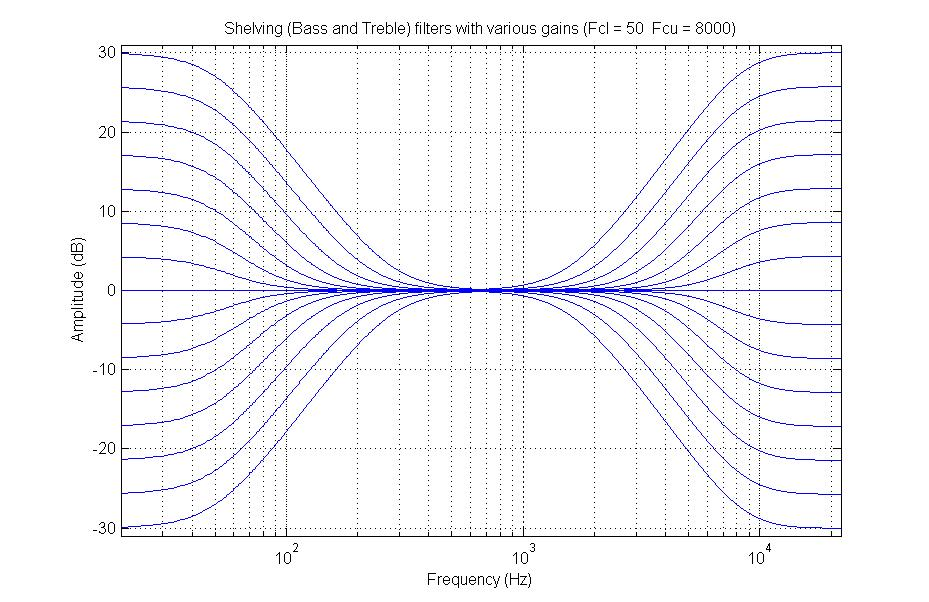
\includegraphics[width=0.75\textwidth]{figures/shelf_filter.jpg}
\caption{The filter cutting and boosting the lower frequency region is the low-shelf filter, while a high-shelf filter is used for higher frequency regions.}
\label{fig:shelf_filter}
\end{figure}

\todo[inline]{Sort farve?}

One of the advantages of implementing shelf filters is that they are good at applying a gain to a wide region. For instance if a attenuation of the bass region is desired, it may be more convient to bass attenuate the whole bass region including the subbass region, rather than only apply a gain centered around a center frequency in the bass.

\section{Processing in frequency}
The reasoning for processing a signal in frequency is its flexibility. When the signal is transformed from time to frequency no convolution is needed because convolution in time domain equals multiplication in frequency domain. This results in no addition is needed when filtering the signal in frequency domain, which means an algorithm can be parallelized which gives a much faster computation time. 

Another advantage of processing in frequency domain is how easy it is to change the frequency response of a filter for example. This makes the implementation of a parametric equalizer very simple. The disadvantage of processing in frequency domain is the transformation from time domain to frequency domain and back which could take op a lot of computation time in its own. 



\section{Multi-rate Signal Processing}

A multi-rate processing system is a system that takes advantages of having multiple sample rates of the original signal. For instance a 48 kHz sample rate may be downsampled to 24 kHz. This also means that the highest frequency component that fulfills the Nyquist criterion is maximum 12 kHz. To avoid loss of data a highpass filter must be applied to the original signal such that the signal is split into two bands between 0 Hz to 24 kHz. The advantage of having a multi-rate system, is that the filter order for a filter is decreased for a downsampled subsystem. By doing so, the amount of computation is thus also decreased, but the disadvantage is an increase in delay from the filter. 

To downsample a signal, an anti-aliasing filter must first be applied. The purpose of the anti-aliasing filter is to filter higher frequencies components away, as aliasing will arise because of the Nyquist criterion. If not, a 13 kHz signal will appear as a 1 kHz signal if downsampling is performed without an anti-aliasing filter. A system consisting of both an anti-aliasing filter and a downsampler is called a decimator and the task is called decimation.

To upsample to a higher sampling rate an interpolator is needed. Interpolation is the opposite of decimation. The interpolator consist of an upsampler followed by an anti-aliasing. If the interpolation factor is desired to be 2 then the upsampler will insert a zero in-between each sample. This is afterwards filtered by an anti-aliasing filter to smooth the signal and gained with the upsampling factor.  

A multi-rate system is especially useful when implementing high order FIR-filters. The order of a FIR filter will be large if the impulse response of a FIR filter is long. By downsampling the signal, only a lower order FIR-filter is needed to achieve an equivalent filter response if filtered at the original $f_s$.





\section{Signal Processing Tools Conclusion}
This section will conclude on which methods for signal analysis and processing should be used for the system to optimally protect the loudspeaker according to \autoref{sec:problem_statement} building onto \autoref{fig:speaker_block2}.

The following methods for analysing and processing signals have been examined:
\begin{itemize}
\item Analysing
\begin{itemize}
\item RMS
\item Peak
\item Spectrum analyzer
\item FFT
\end{itemize}
\item Processing
\begin{itemize}
\item Compressor
\item Equalizer
\item Processing in freuqency domain
\end{itemize}
\item Multirate
\end{itemize}

The optimal way of determing how much the diapragm moves is by measuring the RMS value of a signal and not the peak value, because the peak value does not give any information of the power which RMS does. In effect this means that a high peak value could result in a small movement in the diapragm while a high RMS value will always result in a large movement in the diapraghm. This is because a peak value could just be a single sample while the RMS is the average over a time interval. 

Because its only large RMS values in 500 Hz \todo{Hvordan argumenter vi for det dali?}and below which could result in the coil hitting the backplate the analyzed signals spectrum should be 500 Hz and below, which can either be done with a spectrum analyzer or a FFT. The method choosen to analyse the signal spectrum is the spectrum analyzer, because it is firstly faster computational wise because no transformation is necessary, secondly because the information wanted is the RMS value of the band and not a specific frequency which sorts out the FFT. %This spectrum analyzer should meet the standard IEC 61260 relating to octave-band and fractional-octave-band filters. 

For attenuating the signal both a compressor or an equalizer could be used. The method choosen is the compressor because of the spectrum analyzer. The spectrum analyzer divides the signal into the correct band/bands so there is no need for an equalizer. If the FFT had been choosen as the analyser of the signal spectrum the equalizer processed in the frequency domain would have been optimally, because the transform from time to frequency is given because of the needed FFT. 

The use of multirate should be considered if computation time is a problem in the system.

%The graphic equalizer is given free because of the spectrum analyzer so it is choosen to implement a user controlled gain in each band. This concludes the concept of the system which leads to an overview of the system before the requirements are set up for the system.







\section{Single-band vs multi-band system}
This section will examine if the system should use multi-band or single-band. When the system is to be designed a question whether one or more bands should be implemented arises. The multiband solution could create a to unnatural frequency response, making the sound more unpleasant. If one one of the bands are attenuate to much it could result in a band acting like a notch filter. This could potentially remove the "richness" of the bass. The singleband solution will be attenuating every frequency keeping the amplitude relation intact. However the singleband will also be attenuating many frequencies which are not contributing to the problem. In order to determine which solution is to be preferred a listning test is conducted of both a single-band and a multi-band compressor, to conclude if a multi-band compressor sounds better than a single-band compressor. 

In the test a group of 10 people were subjected to the following effectblocks:
\noindent\begin{minipage}[t]{0.5\linewidth}
    \textbf{Singleband:}
    \begin{itemize}
    \item 1 band in entire frequency spectrum
    \item 12 dB attenuation at 0 dBFS
    \item Attack time of 0.5 ms and release time of 1 ms
    \end{itemize}
    \end{minipage}%
    \begin{minipage}[t]{0.5\linewidth}
    \textbf{Multiband:}
    \begin{itemize}
    \item 1 band from 0 to 100 Hz
    \item 1 band from 100 to 300 Hz
    \item 1 band from 300 to 1000 Hz
    \item 1 Limiter in entire frequency spectrum
    \item Attack time of 0.5 ms and release time of 1 ms
    \end{itemize}
\end{minipage}\par\bigskip

The test concluded with the following results which can be seen in \autoref{fig:piechartsongsReport}. A rather large portion of the test person were favourable of the mulitband compressor because of the lower attenuation which ultimately created less distortion than the single band. The test is fully described in \autoref{app:journal_ListningTest}.

\begin{figure}[H]
\centering
\resizebox{0.4\textwidth}{!}{
\tikzsetnextfilename{Piechartsongs}
\begin{tikzpicture}
[
    pie chart,
    slice type={comet}{blu},
    slice type={legno}{rosso},
    slice type={coltello}{giallo},
    slice type={sedia}{viola},
    slice type={caffe}{verde},
    pie values/.style={font={\small}},
    scale=2
]
%    \pie{2008}{73/comet,13/legno,7/sedia,7/coltello}
%    \pie[xshift=2.2cm,values of coltello/.style={pos=1.1}]%
%        {2009}{52/comet,23/legno,17/sedia,3/coltello,5/caffe}
    \pie[values of caffe/.style={pos=1.1}]%
       {}{87.5/comet,10/legno,2.5/caffe}
%    \pie{2008}{87.5/comet,2.5/legno,10/sedia}
    \legend[shift={(1.5cm,0.5cm)}]{{Multiband}/comet, {Uncertain}/caffe, {Singleband}/legno}
%    \legend[shift={(3cm,-1cm)}]{{Chair (Manzano)}/sedia, {Coffee (Trieste)}/caffe}
\end{tikzpicture}}
\caption{Overall comparison of the answers. This figure is extracted from \autoref{app:journal_ListningTest}}
\label{fig:piechartsongsReport}
\end{figure}

%\section{Chapter Conclusion}
This chapter has analyzed.



\chapter{Overview} \label{ch:overview}
This chapter will describe an overview of the system before the needed requirements of the system is set up. A graphical overview of the system can be seen on \autoref{fig:SystemOverview} which shows a feedback system which will regulate the volume of the lower frequency based on the \textbf{TBD} model, seen on \textbf{figure TBD}, comparing the second and third harmonic relative to keynote. Besides the feed forward system a user controlled equalizer should also be part of the system to give the user more flexibility. The following chapter describes the individual blocks in more detail.          

\begin{figure}[H]
\centering
\tikzsetnextfilename{SystemOverview}
\scalebox{0.8}{
\begin{tikzpicture}
%% Kasser %%
\node [block, fill=white] (AudioSource) at (0,0) {Audio Source};

%% DSP %%
\node [Twolineblock, fill=white] (Equalizer) at ($(AudioSource)+(3.5,0)$) {User Equalizer};

\node [Twolineblock, fill=white] (Decisionblock) at ($(Equalizer)+(0,-2)$) {RMS Detection};

\node [block, fill=white] (Delay) at ($(Equalizer)+(3.25,0)$) {Delay};

\node [block, fill=gray,text=white] (Limiter) at ($(Delay)+(6.5,0)$) {Limiter};

\node [Twolineblock, fill=white] (AmplitudeDetect) at ($(Delay)+(0,-2)$) {Spectrum Analysis};

\node [Twolineblock, fill=white] (Spectrum) at ($(AmplitudeDetect)+(3.25,0)$) {Decision};

\node [Twolineblock, fill=white] (NewEQ) at ($(Spectrum)+(3.25,0)$) {Equalizer};

\node [circle, fill=white] (Sum) at ($(Equalizer)+(0,-2)$) {+};

%\node [Twolineblock, fill=white] (SpectralAnalysis) at ($(Decisionblock)+(3.5,0)$) {Spectral analysis};


%% External %%
\node [block, fill=white] (UserInterface) at ($(Equalizer)+(-2,2)$) {User interface};
%\node [Twolineblock, fill=white] (EffectController) at ($(Equalizer)+(2,2)$) {Effect controller};

%% Speaker Enclosure %%
\node [Twolineblock, fill=black!80,text=white] (Amplifier) at ($(Limiter)+(4,0)$) {Amplification stage};
\node [Twolineblock, fill=black!80,text=white] (Driver) at ($(Amplifier)+(0,-2)$) {Speaker driver};

%\node [Twolineblock, fill=white] (SensorDriver) at ($(Amplifier)+(0,-2)$) {Sensor on driver};
%\node [Twolineblock, fill=gray,text=white] (EnclosureDriver) at ($(Driver)+(0,-2)$) {Sensor in enclosure};

\node (User) at ($(-2.5,0)+(UserInterface)$) {\textbf{User}};
\draw[->] (User) -- (UserInterface);

%\node (Developer) at ($(3.5,0)+(EffectController)$) {\textbf{Developer}};
%\draw[<-] (EffectController) -- (Developer);

%% Store Blokke %%
\begin{pgfonlayer}{bg}
\draw[thick, fill=black!20] ($(-1.50,1)+(Equalizer)$) -- ($(1.750,1)+(Limiter)$) |- ($(1.750,-1.25)+(Decisionblock)$) -- ($(-1.50,-1.25)+(Decisionblock)$) -- ($(-1.50,1)+(Equalizer)$);
\node (DSPtag) at ($(1,-3)+(Limiter)$) {\textbf{DSP}};

\draw[thick, fill=black!20] ($(-1.50,1)+(Amplifier)$) -| ($(1.750,1)+(Driver)$) |- ($(-1.50,-1.25)+(Driver)$) -| ($(-1.50,1)+(Amplifier)$);
\node (DSPtag) at ($(0,-1)+(Driver)$) {\scalebox{0.7}{\textbf{Speaker Enclosure}}};
\end{pgfonlayer}

%% Forbindelse %%
\draw[->] (AudioSource) -- (Equalizer);
\draw[->] (Equalizer) -- (Delay);
\draw[->] (Delay) -- (Limiter);
\draw[->] (NewEQ) -- (Limiter);

\draw[->] (Limiter) -- (Amplifier);
\draw[->] (Amplifier) -- (Driver);

\draw[->] (UserInterface) -| ($(Equalizer)+(-.25,.6)$);
%\draw[->] (EffectController) -| ($(Equalizer)+(.25,.6)$);

%\draw[->] ($(SensorDriver)+(-1.375,-0.3)$) -- ($(SpectralAnalysis)+(1.375,-0.3)$);

%\draw[->] ($(EnclosureDriver)+(-1.375,0.3)$) -- ($(EnclosureDriver)+(-1.75,0.3)$) -- ($(EnclosureDriver)+(-1.75,1)$) -- ($(EnclosureDriver)+(-5.5,1)$) |- ($(SpectralAnalysis)+(1.375,0.3)$);

%\draw[->] (SpectralAnalysis) -- (Decisionblock);
\draw[<-] (Decisionblock) -- (Equalizer);
\draw[->] (Decisionblock) -- (AmplitudeDetect);
\draw[->] (AmplitudeDetect) -- (Spectrum);
\draw[->] (Spectrum) -- (NewEQ);
\end{tikzpicture}}
\caption{Block overview of the entire system. Black boxes are not static non changeable variable. Grey boxes are also static but has to be taken into account.}
\label{fig:SystemOverview}
\end{figure}
A more detailed description of every block will now follow in the preceding section.

\textbf{Audio source} \\
The audio source in this system will be based on the IEC 60268-15 specification. Meaning that it will in be limited to a analogue signal with a maximum peak voltage of 2 Volt RMS but otherwise nominal 0.5 Volt RMS. This input will handled by an onboard TLV320AIC3204 codec located on the eZdsp development board.

\textbf{User} \\
The system will be able to be partially controlled by the end user. The user will be able to affect the entire system with the desired preference. The preference will be restricted to gain in the lower frequency as wished by DALI.
\todo[inline]{Reference til Samtale med DALI}

\textbf{User interface}\\
The user interface will be based on physical hardware. The hardware will be simple of construction. The user will be browsing through the different preset using a push down button. The different preset will be displayed on the on board LCD display.

\textbf{Effect controller} \\
The effect controller will be consisting of a graphical user interface in which the developer can adjust the entire frequency response according to the wanted output. The effect controller is thought as a fast prototyping function in which the developer can adjust on the fly when tuning the speaker system.

\textbf{Developer} \\
The developer is DALI or the specific engineer who wishes to tune and adjust the product.

\textbf{User Equalizer} \\
The user equalizers job is to compensate for any needed or unwanted adjustment in the system. This equalizer will only be changing whenever the user wants it or during the design period. The equalizer will consist of 4 Bi-quad bands an a high/low shelf which is to be spread equally across a frequency spectrum of 20 Hz trough 20 kHz.

\textbf{Delay} \\
The delay is created in order to give the monitoring system time for analysis. The delay will be adjusted accordingly to the analysis time needed in the feed forward system.


\textbf{Spectral Analysis} \\
The spectral analysis block will be consisting of a spectral analysis and estimation of the incoming system. The system will evaluating the signal to achieve the frequency content and correlating amplitude.

\textbf{Decision and Model} \\
The Decision and model block will consist of two parts:
\begin{enumerate}
\item Will be to determine by a model how much the current frequencies are going to produce a potential backplate hit. The frequencies are weighted and inspected when run through the model
\item When the model shows fluctuations above a certain threshold it should determine which frequency area are in need of attenuation and adjust accordingly.
\end{enumerate}

\textbf{Auto Equalizer} \\
This equalizer will receive filter constants released/updated by the Decision and Model block. If there is no need of adjustment it will simply adjust by a gain of 1 in the entire spectrum. The equalizer will be consisting of a shelf filter which will adjust attenuation, slope and frequency according the information given. 

\textbf{Limiter} \\
The limiter is greyed out and will not be discussed further on. It is noted that there should be room in the code for implementation of a multi band limiter wished by DALI.

\textbf{Amplification stage and Speaker driver} \\
The speaker is in this project seen as a black box which will not be tampered with. The black box will function as an actuator which is to be controlled by the DSP system. How ever it is assumed that the DSP system will prolong the life of the speaker driver when pushed to its limits.


\vspace{5mm}
The overall system has now been described in detail. The different functions placed in the boxes have been outlined and it is now possible to determine more specific requirements for the system.


\chapter{Requirements} \label{ch:requirements}
This chapter will post the requirements for the system described in \autoref{ch:overview}.  

As described in \autoref{sec:problem_statement} the coil must not hit the backplate because this damages the loudspeaker significantly. To be able to secure this, the system must run in real time which is explained in \autoref{sec:RealTime}. However the delay of the full system must not be larger than 100 ms which is a delay a normal modern television today is able to delay the video with. This means that the system is not applicable with e.g. live music where the sound should not be delayed by more than maximum 20 ms, but only applicable with delayed video and normal audio listening. This leads to the following requirements for the overall system.

\begin{itemize}
\item Overall system
\begin{enumerate}
\item [\textlabel{1}{coil}] The coil must not hit the backplate.\\
\item [\textlabel{2}{realtime}] The system must run in real time. \\
\item [\textlabel{3}{delay}] The system must not have a delay bigger than 100 ms.
\end{enumerate}
\end{itemize}

The processor has been chosen to be a DSP as explained in \autoref{sec:platformReq}. This section also explains all the requirements for the platform regarding, 96 kHz sample rate, 24 bit resolution, SNR of 120 dB, 100 MIPS and infacing through $I^2S$ to an ADC and DAC. However these demands would be considered necessary for a finish product but because of time constraints and the complexity of a system meeting theese requirements, the demands have been scaled to 48 kHz sample rate, 16 bit resolution, SNR of \textbf{XX} while maintaining infacing through $I^2S$ to an ADC and DAC. 

The hardware must also be able to meet the specifications of IEC 60268-15 which concerns specifications for an Hi-fi system which leads to the following requirements for the hardware platform.

\begin{itemize}
\item Hardware platform
\begin{enumerate}
\item [\textlabel{4}{samplerate44}] The sample rate of the audio codec must be at least 44.1 kHz.\\
\item [\textlabel{5}{samplerate96}] The sample rate of the audio codec must be compatible with 96 kHz.\\
\item [\textlabel{6}{resolution}]  A bit resolution of 24 bit must supported by the audio codec and the DSP.\\
\item [\textlabel{7}{I2S}] The DSP must have at least two I2S ports for interfacing with audio codec.\\
\item [\textlabel{8}{MIPS}] The DSP must have at least 100 MIPS available.\todo{hmmmmmm den her vil sofus ikke kunne lide}\\
\item [\textlabel{9}{IEC}] The interface must comply with IEC 60268-15 specification.
\end{enumerate}
\end{itemize}

The RMS compressor must have four bands which comply with the class 2 of IEC 6964 standard (2001) which descibed in \autoref{app:IEC6964}, the reason for class 2 is that it has the biggest tolerances for the filters which should be designed. These bands must be placed below 500 Hz which was desired by DALI which can me seen in (\textbf{MAIL correnspondance}) and is explained in (\textbf{Multiband vs single band section}). The system must also distort less than soft clipping which is fomulated in the problem statement seen in \autoref{sec:problem_statement} and argued for in \autoref{sec:PreAnalysisCon}.

The RMS compressor must have a threshold at 150 W determined in 

\begin{itemize}
\item RMS compressor
\begin{enumerate}
\item [\textlabel{10}{Threshold}] The compressor must have a threshold at 150 W.\\
\item [\textlabel{11}{bands}] The compressor must have 4 bands.\\
\item [\textlabel{12}{standardband}] The bands of the compressor must comply with the class 2 of IEC 6964 standard (2001).\\
\item [\textlabel{13}{500below}] The compressor must apply to frequencies below 500 Hz.\\
\item [\textlabel{14}{clipping}] The system must distort less than clipping.
\end{enumerate}
\end{itemize}

The requirements of this chapter will be the basis for the final system.
\todo[inline]{REFERENCER I CHAPTER}

% \begin{itemize}
% \item Functionality
% \begin{enumerate}
% \item The coil must not hit the backplate when the system is activated.
% \end{enumerate}
% \end{itemize}

% \begin{itemize}
% \item Overall system
% \begin{enumerate}
% \item The system must be a real time system. 
% \item The system must not have SNR be lower than 120 dB.
% \end{enumerate}
% \end{itemize}

% \begin{itemize}
% \item DSP platform
% \begin{enumerate}
% \item The sample rate of the ADC/DAC must be 96 kHz.
% \item A bit resolution of 24 bit must supported by the ADC/DAC and the DSP.
% \item The DSP must have at least two \gls{I2S} ports for interfacing with ADC/DAC.
% \item The DSP must have at least 1024 instructions pr. sample to support both the system and a limiter build by DALI. 
% \end{enumerate}
% \end{itemize}
% \todo[inline]{Tjek op på om kravet med 1024 er realistisk/"do-able"}
% \todo[inline]{Tjek op på om kravet med 24-bit er realistisk/"do-able"}

% \begin{itemize}
% \item Regulating equalizer
% \begin{enumerate}
% \item The equalizer must be able to regulate between 11 Hz - 100 Hz with a tolerance of $\pm$ 10 Hz. 
% \item The maximum gain of the user controlled equalizer must be minimum $\pm$ 12 dB SPL with a tolerance of $\pm$ 1 dB SPL.
% \item The resolution of the gain must be 1 dB with a tolerance of 0.1 dB.
% \item The regulating part should be designed as a shelf filter.
% \end{enumerate}
% \end{itemize}


% \begin{itemize}
% \item User controlled equalizer
% \begin{enumerate}
% \item There must be \textbf{TBD} n bands in which the equalizer can be controlled with. 
% \item The bands of the equalizer must function between 50 Hz - 15000 Hz with a cut off tolerance of \textbf{TBD}. 
% \item The maximum gain of the user controlled equalizer must be minimum $\pm$ 6 dB with a tolerance of $\pm$ 1 dB.
% \item The resolution of the gain must be 1 dB with a tolerance of 0.1 dB.
% \end{enumerate}
% \end{itemize}

% \begin{itemize}
% \item Interface
% \begin{enumerate}
% \item 
% \end{enumerate}
% \end{itemize}






\chapter{Development Platform}

To implement the system a hardware platform is needed. The hardware platform can be developed from scratch or be bought as a development board. Developing the hardware platform gives a higher level of customizability, but the development time will be bigger compared to a complete development board. Because of limited time, the system will be developed upon a complete development board. The choice of development board will be based on the requirements, which are listed below.

As previously mentioned, the choice of processor is a DSP, as the DSP has a high performance versus cost. The DSP is also very suitable for signal processing as the CPU architecture usually comes with specialized hardware for tasks such as multiply-accumulate, which can be executed in one instruction. The requirements for the DSP are as follows:

\begin{enumerate}
\item[6] A bit resolution of 24 bit must supported by the DSP.\\
\item[7] The DSP must have at least two I2S ports for interfacing with audio codec.
\end{enumerate}

The development board should also have an integrated audio codec, which handles the conversion between analog and digital signals. The requirements for the audio codec are as follows:

\begin{enumerate}
\item[4] The sample rate of the audio codec must be at least 44.1 kHz.\\
\item[5] The sample rate of the audio codec must be compatible with 96 kHz.\\
\item[6] A bit resolution of 24 bit must supported by the audio codec.\\
\item[8] The interface must comply with IEC 60268-15 standard.
\end{enumerate}

Further more, the development platform needs accessible external GPIO to allow external interaction with the system, since it is required that the user can change settings on a equalizer. 


\section{Development Board TMDX5515EZDSP}

The TMDX5515EZDSP, seen in \autoref{fig:TMDX5515EZDSP_overview}, from Spectrum Digital is chosen as the development board because it fulfills all the hardware requirements except requirement eight, but this is deemed acceptable. \todo{Skal der skrives mere til at vi ikke opfylder dette krav} The TMDX5515EZDSP uses a TMS320C5515 DSP from Texas Instruments as the CPU and is interfaced with a TLV320AIC3204 audio codec. Furthermore the development board is interfaced to peripherals such as an OLED screen, two buttons, microSD and a expansion connector with 60 ports. 

\begin{figure}[H]
\centering
\begin{subfigure}[t]{0.47\textwidth}
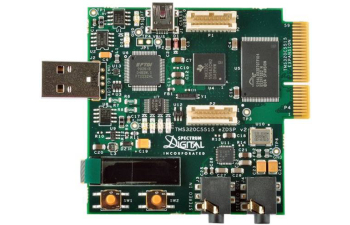
\includegraphics[width=\linewidth]{dsp_board}
	\caption{TMDX5515EZDSP.}
	\label{fig:TMDX5515EZDSP}
\end{subfigure}
\hspace{6mm} 
\begin{subfigure}[t]{0.35\textwidth}
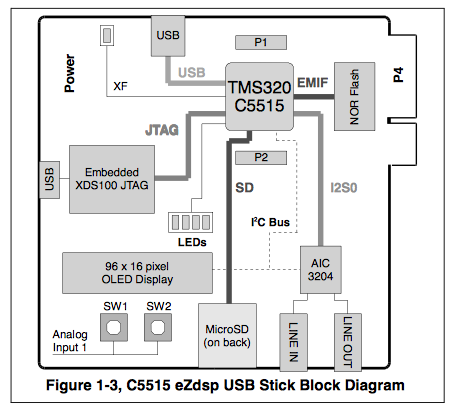
\includegraphics[width=\linewidth]{dsp_blockdiagram}
	\caption{Block diagram overview of the TMDX5515EZDSP.}
	\label{fig:TMDX5515EZDSP_blockdiagram}
\end{subfigure}
\caption{Overview of the TMDX5515EZDSP.}
\label{fig:TMDX5515EZDSP_overview}
\end{figure}

The TMS320C5515 is interfaced to the audio codec through an $\text{I}^2$S bus and $\text{I}^2$C bus. The $\text{I}^2$S bus is used to transmit and receive serial audio data between each unit, while the $\text{I}^2$C is used by the DSP to control the audio codec. According to the datasheet for the TLV320AIC3204 the rated ADC and DAC input voltage is 0.5 $\text{V}_\text{RMS}$ or 0.7071 $\text{V}_\text{peak}$. If the input signal exceeds the voltage level, the audio codec will clip the signal. To avoid this, the audio source must not exceed a peak voltage of 0.7071 V.

















\section{System Interface}

In this section the interface, between the DSP and its peripheral, is explained. It has been chosen that the interaction between the user and the system is through a GUI on a PC. The block diagram of the system is seen in \autoref{fig:interfaceBlock}. Even though the DSP and audio codec support 24-bit and 96 kHz sampling rate, the chosen bit-resolution is 16-bit and a sampling rate of 48 kHz for the system prototype as a prove of concept.

\begin{figure}[H]
\centering
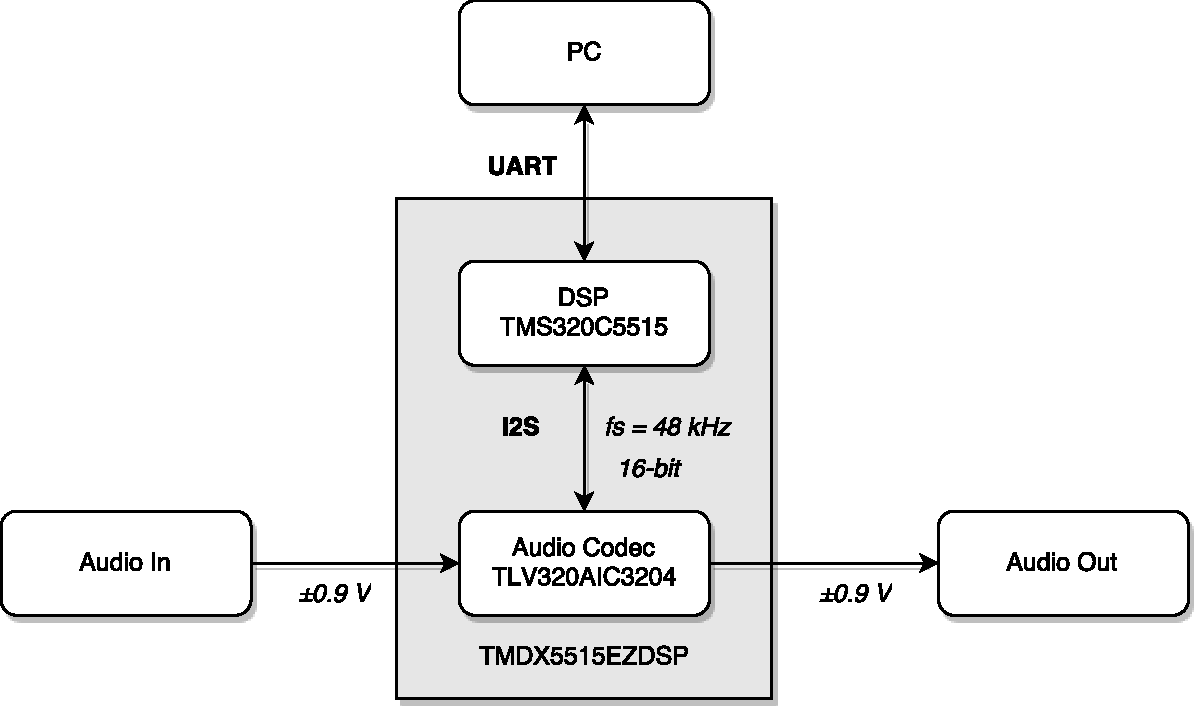
\includegraphics[width=0.75\textwidth]{figures/interfaceBlock.pdf}
\caption{}
\label{fig:interfaceBlock}
\end{figure}

\subsection*{I$^2$C Interface to Audio Codec}

As mentioned the audio codec supports a sampling rate of 96 kHz and at least 48 kHz. The bit-resolution of the audio codec can also be adjusted to 24-bit and 32-bit. A $\text{I}^2$C-bus is linked between the DSP and the audio codec to setup the registers in the audio codec. In \autoref{fig:i2c_aic3204} the communication protocol between the DSP and audio codec is shown, where the DSP works as the master of the bus. Since the same $\text{I}^2$C-bus is used to interface with the OLED-display, the DSP must transmit 7-bit to specify the address of the audio codec. Afterwards a byte is transmitted to specify the register address for the next data byte which is transmitted afterwards.

\begin{figure}[H]
\centering
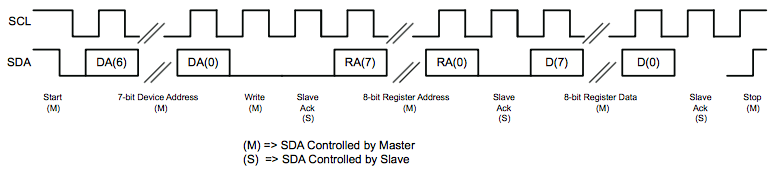
\includegraphics[width=0.98\textwidth]{i2c_aic3204}
\caption{Setup of the TLV320AIC3204 with $\text{I}^2$C.}
\label{fig:i2c_aic3204}
\end{figure}  

By using the protocol above, the registers of the audio codec is then set to be mono, 16-bit and 48 kHz. When a audio sample is transmitted through the $\text{I}^2$S to the DSP, an interrupt flag for the $\text{I}^2$S is set high to tell the processor that data can be read from the data register. 

\subsection*{I$^2$S Audio Interface to Audio Codec}

To transfer audio data between the audio codec and DSP, a full-duplex I$^2$S-bus is used. The I$^2$S-bus has a data transmitter, receiver, clock, and frame synchronization. The transmitter and receiver is used for data exchange between the DSP and audio codec. The data transmitted consist of binary values thus the clock is used to synchronize the bit transmission between the DSP and audio codec.

\subsection*{UART interface with PC}

To communicate with a PC, serial communication is used to exchange data between the DSP and PC. The development platform supports UART interface through its expansion pins. Since UART is easy to implement, it has been chosen. Furthermore, the UART from the DSP needs to be converted to an USB protocol. To do so the FTDI FT-232R-3V3-WE is used, as it is a chip that handles the conversion between USB and UART.

With the hardware platform choosen and the interfaces defined a system can now be designed.











\chapter{Total Overview}





\part{Design}

\chapter{Design Realization} \label{ch:designRealization}
Evaluating the concept design from \autoref{ch:overview} it is seen that the concept has four bands-pass filters and one high-pass that needs to be designed. 
\begin{figure}[H]
\centering
\tikzsetnextfilename{SystemOverview}
\scalebox{0.8}{
\begin{circuitikz}
%% TOP BAND %% 
\node[] (AudioIN) at (-0.5,0) {Audio in};
\node[] (AudioIN) at (0,0) {};
\node[summation] (Summation) at (12.5,0) {};
\node[summation] (Summation2) at (12.5,-2) {};
\node[summation] (Summation3) at (12.5,-4) {};
\node[summation] (Summation4) at (12.5,-6) {};
\node[] (AudioOUT) at (14.5,0) {Audio out};
\draw[-] ($(AudioIN)+(1,0)$) -- ($(AudioIN)+(1,-8)$);
\draw[-] ($(AudioIN)+(1,0)$) -- ($(AudioIN)+(0.5,0)$);

%% Summation %%
\draw [->] (Summation2) -- node[at end,yshift=2mm,xshift=0mm]{\scalebox{0.5}{+}} (Summation);
\draw [->] (Summation) -- (AudioOUT);
\draw [->] (Summation3) -- node[at end,yshift=2mm,xshift=0mm]{\scalebox{0.5}{+}} (Summation2);
\draw [->] (Summation4) -- node[at end,yshift=2mm,xshift=0mm]{\scalebox{0.5}{+}} (Summation3);


%%% GUI %%
\node[gain] (GUI) at ($(7,1)+(AudioIN)$) {GUI};
\draw[->,red] ($(GUI)+(0.5,0.25)$) -- ($(GUI)+(1,0.25)$);
\draw[<-,blue] ($(GUI)+(0.5,-0.25)$) -- ($(GUI)+(1,-0.25)$);

\draw [->,red] ($(4,.25)+(AudioIN)$) -- ($(4.5,.25)+(AudioIN)$); %% add (.5,.25) to the coordinate

%% Second Band
\draw [->,red] ($(4,-1.75)+(AudioIN)$) -- ($(4.5,-1.75)+(AudioIN)$);
\draw [<-,blue] ($(7.7,-2.75)+(AudioIN)$) -- ($(8.2,-2.75)+(AudioIN)$);
%% Third Band
\draw [->,red] ($(4,-3.75)+(AudioIN)$) -- ($(4.5,-3.75)+(AudioIN)$);
\draw [<-,blue] ($(7.7,-4.75)+(AudioIN)$) -- ($(8.2,-4.75)+(AudioIN)$);
%% Fourth Band
\draw [->,red] ($(4,-5.75)+(AudioIN)$) -- ($(4.5,-5.75)+(AudioIN)$);
\draw [<-,blue] ($(7.7,-6.75)+(AudioIN)$) -- ($(8.2,-6.75)+(AudioIN)$);
%% Fifth Band
\draw [->,red] ($(4,-7.75)+(AudioIN)$) -- ($(4.5,-7.75)+(AudioIN)$);
\draw [<-,blue] ($(7.7,-8.75)+(AudioIN)$) -- ($(8.2,-8.75)+(AudioIN)$);


%% Box EQ %%
\draw [-,dashed,thick] ($(1.25,1.25)+(AudioIN)$) -| ($(6,-9.75)+(AudioIN)$) -| ($(1.25,1.25)+(AudioIN)$);
\node [] at ($(3.75,.9)+(AudioIN)$) {\textbf{Equalizer}};

\draw [-,dashed,thick] ($(6.5,-0.75)+(AudioIN)$) -| ($(11.5,-9.75)+(AudioIN)$) -| ($(6.5,-0.75)+(AudioIN)$);
\node [] at ($(9,-1)+(AudioIN)$) {\textbf{RMS Limiter}};


%% Box Compressor %%





%% First Band %% 
\draw ($(1,0)+(AudioIN)$) to[highpass] node[yshift=-5mm,xshift=-10mm, below,midway]{High Pass} ($(4,0)+(AudioIN)$);
\draw ($(4,0)+(AudioIN)$) to node[yshift=0mm,gain,label=below:Gain 5]{$G_{5}$} ($(6,0)+(AudioIN)$);
\draw [->]($(6,0)+(AudioIN)$) -- node[at end,yshift=0mm,xshift=2mm]{\scalebox{0.5}{+}} (Summation);

%% Second Band %%
\draw ($(1,-2)+(AudioIN)$) to[bandpass] node[yshift=-5mm,xshift=-10mm, below,midway]{Band 4} ($(4,-2)+(AudioIN)$);
\draw ($(4,-2)+(AudioIN)$) to node[yshift=0mm,gain,label=below:Gain 4]{$G_4$} ($(6,-2)+(AudioIN)$);
%%% Second band - Compressor%%%
\draw [->]($(6,-2)+(AudioIN)$) to node[yshift=0mm,gain,near end]{$G_{4}$} ($(-.5,0)+(Summation2)$) -- node[at end,yshift=0mm,xshift=2mm]{\scalebox{0.5}{+}} (Summation2);
\draw ($(6,-2)+(AudioIN)$) -| ($(7,-3)+(AudioIN)$) to node[yshift=0mm,gain]{RMS} ($(10.5,-3)+(AudioIN)$) -| ($(10.5,-2.52)+(AudioIN)$);

%% Third Band %%
\draw ($(1,-4)+(AudioIN)$) to[bandpass] node[yshift=-5mm,xshift=-10mm, below,midway]{Band 3} ($(4,-4)+(AudioIN)$);
\draw ($(4,-4)+(AudioIN)$) to node[yshift=0mm,gain,label=below:Gain 3]{$G_3$} ($(6,-4)+(AudioIN)$);
%%% Third band - Compressor%%%
\draw [->]($(6,-4)+(AudioIN)$) to node[yshift=0mm,gain,near end]{$G_{3}$} ($(-.5,0)+(Summation3)$) -- node[at end,yshift=0mm,xshift=2mm]{\scalebox{0.5}{+}} (Summation3);
\draw ($(6,-4)+(AudioIN)$) -| ($(7,-5)+(AudioIN)$) to node[yshift=0mm,gain]{RMS} ($(10.5,-5)+(AudioIN)$) -| ($(10.5,-4.52)+(AudioIN)$);

%% Fourth Band %%
\draw ($(1,-6)+(AudioIN)$) to[bandpass] node[yshift=-5mm,xshift=-10mm, below,midway]{Band 2} ($(4,-6)+(AudioIN)$);
\draw ($(4,-6)+(AudioIN)$) to node[yshift=0mm,gain,label=below:Gain 2]{$G_2$} ($(6,-6)+(AudioIN)$);
%%% Fourth band - Compressor%%%
\draw [->]($(6,-6)+(AudioIN)$) to node[yshift=0mm,gain,near end]{$G_{2}$} ($(-.5,0)+(Summation4)$) -- node[at end,yshift=0mm,xshift=2mm]{\scalebox{0.5}{+}} (Summation4);
\draw ($(6,-6)+(AudioIN)$) -| ($(7,-7)+(AudioIN)$) to node[yshift=0mm,gain]{RMS} ($(10.5,-7)+(AudioIN)$) -| ($(10.5,-6.52)+(AudioIN)$);
%
%% Fifth band %% 
\draw ($(1,-8)+(AudioIN)$) to[lowpass] node[yshift=-5mm,xshift=-10mm, below,midway]{Low Pass} ($(4,-8)+(AudioIN)$);
\draw ($(4,-8)+(AudioIN)$) to node[yshift=0mm,gain,label=below:Gain 1]{$G_1$} ($(6,-8)+(AudioIN)$);
%%% Fourth band - Compressor%%%
\draw [->]($(6,-8)+(AudioIN)$) to node[yshift=0mm,gain,near end]{$G_{1}$} ($(-.5,-2)+(Summation4)$) --($(0,-2)+(Summation4)$) -- node[at end,yshift=2mm,xshift=0mm]{\scalebox{0.5}{+}} (Summation4);
\draw ($(6,-8)+(AudioIN)$) -| ($(7,-9)+(AudioIN)$) to node[yshift=0mm,gain]{RMS} ($(10.5,-9)+(AudioIN)$) -| ($(10.5,-8.52)+(AudioIN)$);
\end{circuitikz}}
\caption{Block overview of the entire system.}
\label{fig:SystemOverview2}
\end{figure}
%\section{Practical Design Considerations}
Before designing the band-pass filters, RMS analysis, and RMS limiter, practical design considerations needs to be considered. This is necessary since the concept system may not be realizable due to hardware constraints. Therefore this chapter will cover the following topics:
\begin{itemize}
\item[•] Phase response and group delay.
\item[•] Computational constraints.
\item[•] Multirate signal processing with multistages.
\end{itemize}


\section{Phase Response and Group Delay}
As the signal needs to be reconstructed in the end of the system, it is desirable that the reconstructed signal do not have frequency bands which are out of phase compared to the other bands. If the bands are out of phase the resulting sound may be unpleasant to listen to. Therefore a design requirement to the system is to ensure that the signals from each band are added together without changing the relative phase between each band.

One of the properties in non-statical filters such as low-pass and band-pass filters are the phase shift. For filters such as the Butterworth low-pass filter, the phase shift begins at the frequency at one decade below the cutoff frequency and ends one decade above. The phase shift in-between for most analog filter except Bessel filter, have a non-linear phase response. Because the phase response is non-linear, the group-delay will likewise not be linear as seen on \autoref{fig:groupDelayIirPrev}.

\begin{figure}[H]
\centering
\begin{subfigure}[t]{0.435\textwidth}
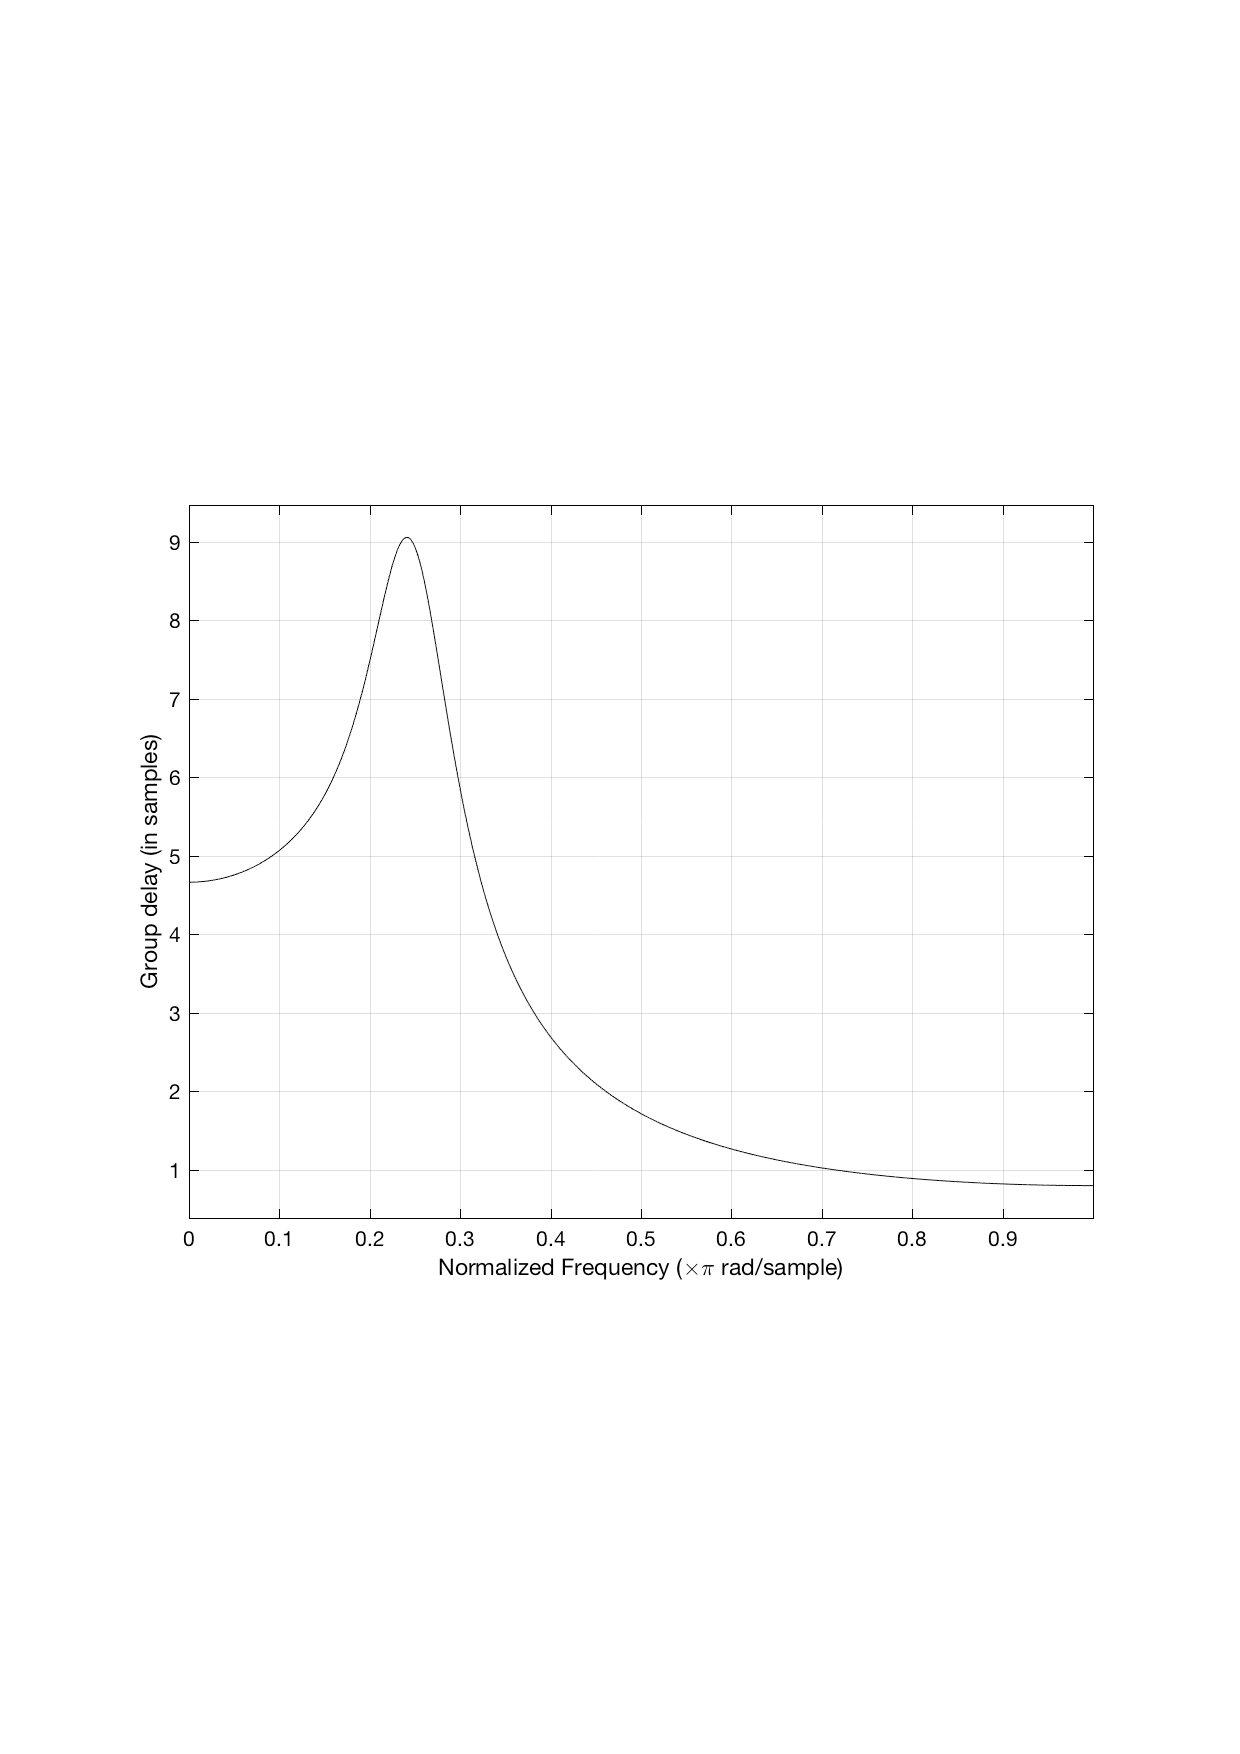
\includegraphics[width=\linewidth]{groupDelayIirPrev}
	\caption{Group delay of a 4th order IIR filter.}
	\label{fig:groupDelayIirPrev}
\end{subfigure}
\hspace{6mm} 
\begin{subfigure}[t]{0.47\textwidth}
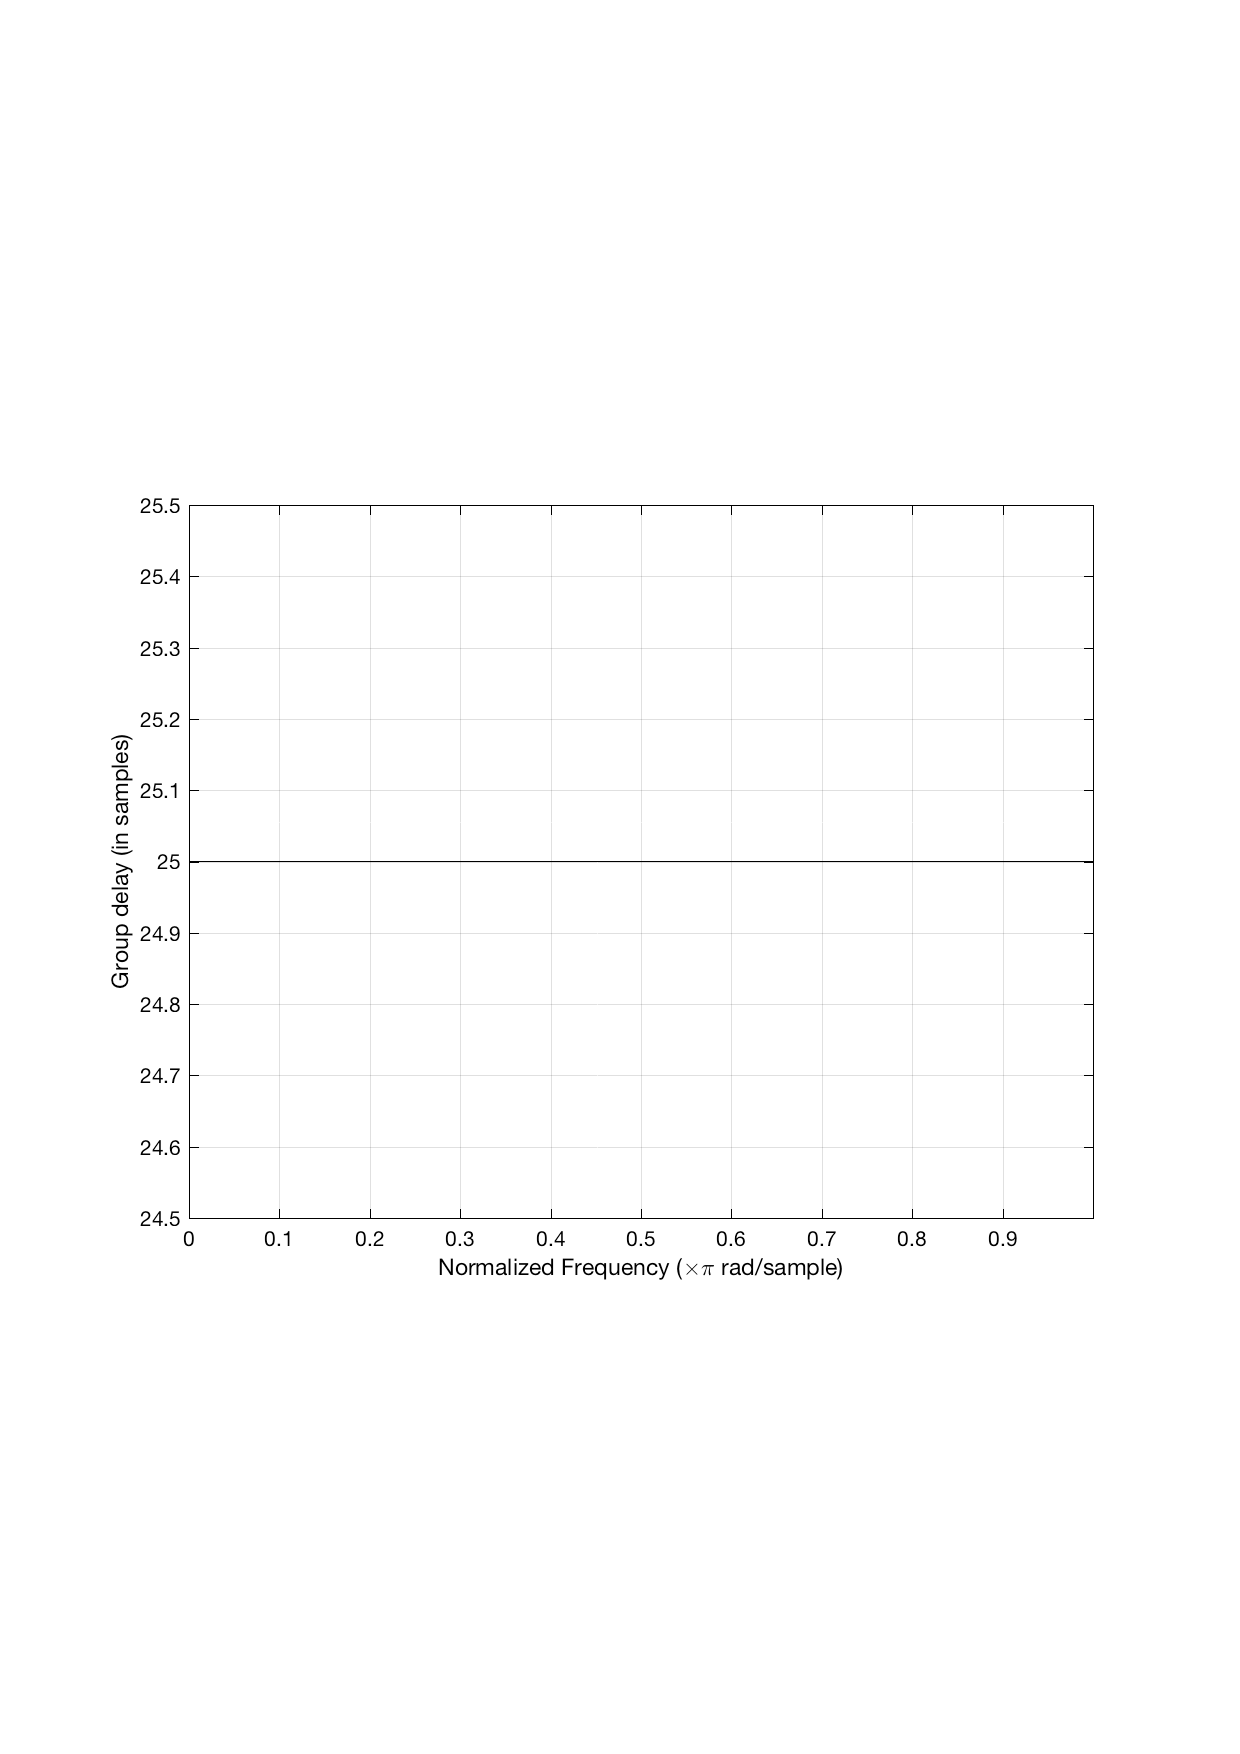
\includegraphics[width=\linewidth]{groupDelayFirPrev}
	\caption{Group delay of a 50th order FIR filter.}
	\label{fig:groupDelayFirPrev}
\end{subfigure}
\caption{Example of group delay of an IIR and a FIR filter.}
\label{fig:filterGroupDelay}
\end{figure}

The group delay is an important parameter to take into account, as it specifies the sample delay for each frequency. 1 sample delay is equivalent to 20.83 $\mu$s in a 48 kHz system. \autoref{fig:groupDelayIirPrev} shows that the group delay for IIR filters is non-linear with a peak at the normalized frequency 0.25 $\pi rad$. To calculate the time delay at 0.25 $\pi$ rad following expression can be used:
\begin{equation}
t_{d}= \frac{n_{s}}{f_s} \enhed{s}
\end{equation}
\begin{where}
\va{$n_{s}$}{is the number of samples delayed}{.}
\end{where}

A non-linear group delay will be hard to compensate compared to a constant group delay, thus a constant group delay is desirable. To achieve a constant group delay a linear phase filter is needed as the phase response is linear. Linear phase can be found in FIR filters and Bessel filters. Because of the constant group delay in linear phase filters, it eases the design as constant delays can be implemented to compensate for the phase shift in filters. Bessel filters have a constant group delay until the cutoff frequency and gets non-linear afterwards. Because the Bessel filter do not have a very sharp cutoff compared to other filter types, a high order Bessel filter will be needed. A high order IIR however has risk of being unstable. FIR filters are therefore chosen as they have all the required properties and do not get unstable. 


\section{Computational Constraints}
Another subject to consider is the constraints regarding computational power to perform filter algorithms. For FIR filters the amount of instructions to compute the filter output increases by the filter order, as calculating each tap in the filter is equal to a multiply and accumulate. Therefore even though a very high order filter in theory is realizable, the computational constraint needs to be considered. 

The performance of the DSP is 100 MIPS. At a sample rate of 48 kHz, this will result in approximately 2083 instructions available in-between each sample. A 10000 order FIR filter for instance is thus not realizable on the platform with a sampling rate of 48 kHz as the DSP will not finish calculating the filter output in time before the next sample. This is true because the fastest way to compute the convolution between the input signal x[n] and the impulse response h[n] is by using a Multiply-Accumulate (MAC) instruction which takes 1 clock cycle to perform if a single MAC is used. This gives a total number of 10000 clock cycles to perform one single convolution. Designing FIR filters will therefore be difficult as the cutoff frequencies for all required filters are very low relative to the sampling rate. A cutoff frequency located far from the sampling rate results in a long impulse response for a FIR filter. To a achieve a steep cut more samples of the impulse response are needed thus increasing the order of the filter. 

\section{Multirate Signal Processing with Multistages}
A solution to avoid very high order filters is to downsample the signal into a signal with a lower sampling rate. By downsampling the signal the impulse response of an equivalent FIR filter at the same cutoff frequency is shortened and the amount of taps is therefore reduced. In \autoref{fig:downsample_FIR} it is shown how decreasing the sampling rate by an integer factor of L is equivalent to increasing the cutoff frequency by a factor of L.

% vis fordele ved multirate
% - båndpas filter har en højere cutoff
% - Ulempe er anti aliserings filter --> Høj orden

\begin{figure}[H]
\centering
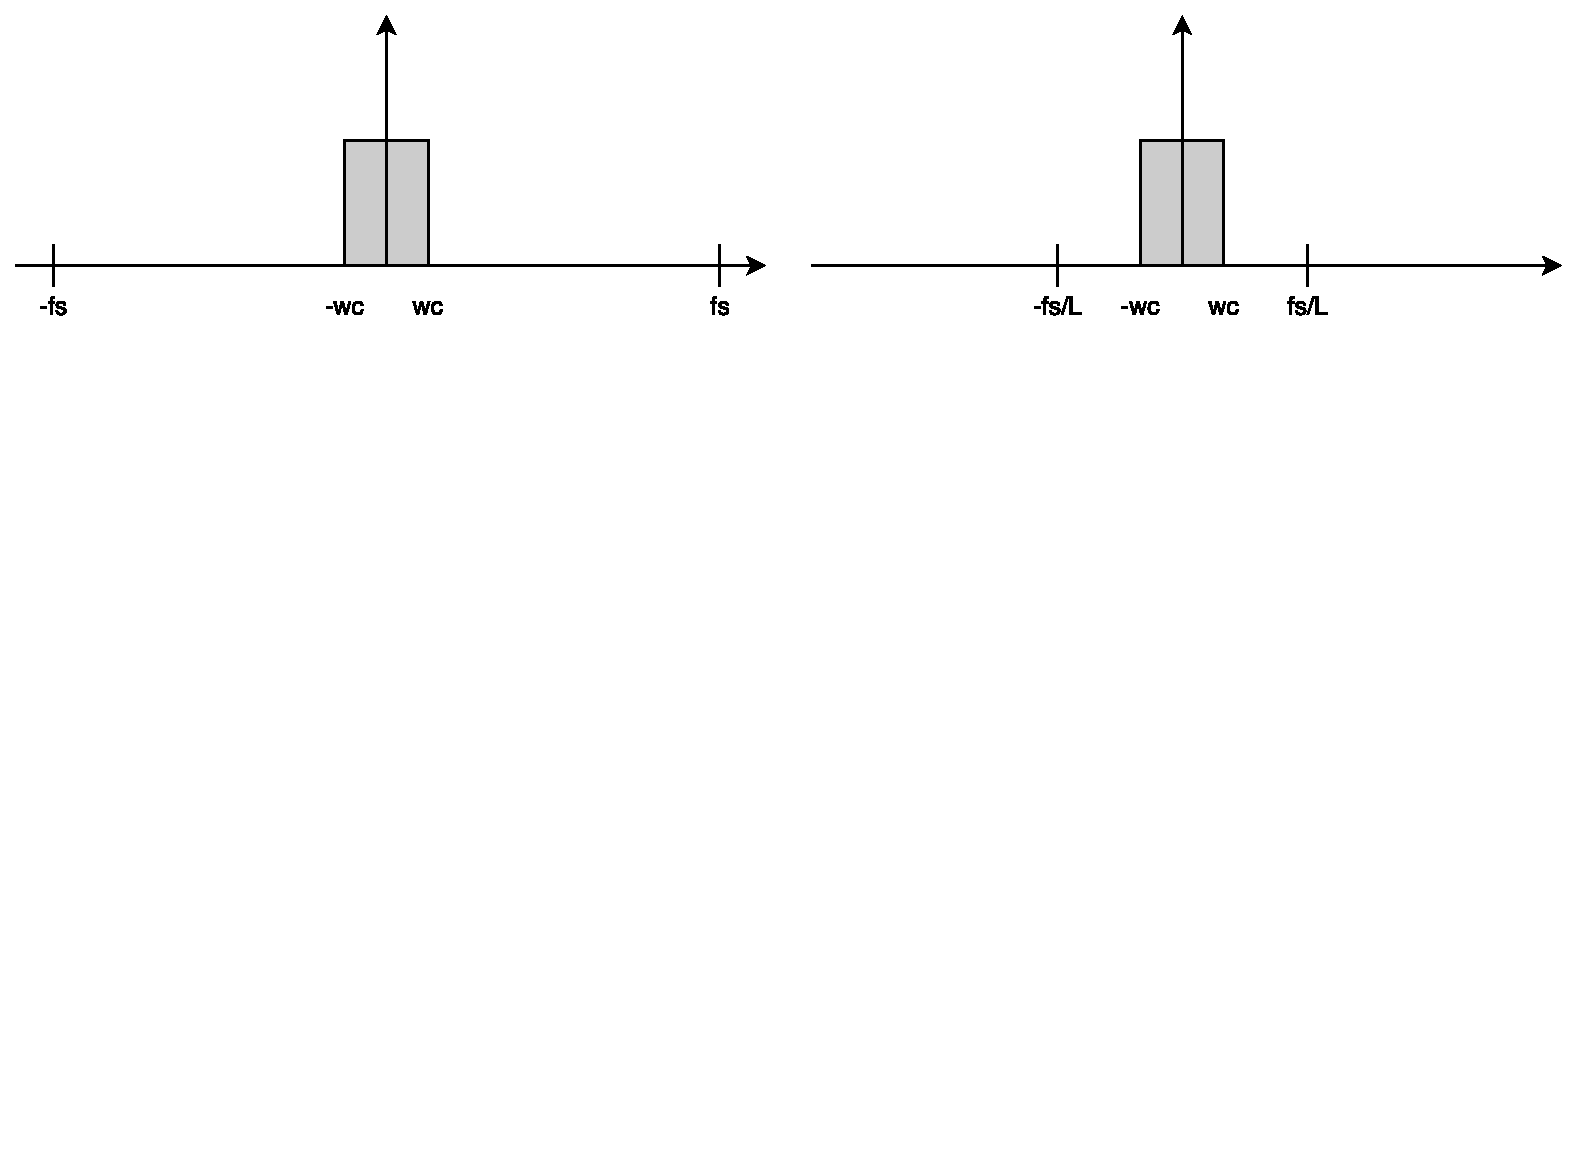
\includegraphics[width=0.75\textwidth]{figures/downsample_FIR.pdf}
\caption{Frequency spectrum of a signal with different sampling frequencies.}
\label{fig:downsample_FIR}
\end{figure}

An example of how to reduce the order of the FIR filter by multirate is shown in \autoref{fig:fir_downsample}. \autoref{fig:fir_downsample1} is a 100 order FIR filter with a sampling frequency of 48 kHz and cutoff frequency at $\frac{f_s}{10}$ and \autoref{fig:fir_downsample2} is a 50 order FIR filter with a sampling frequency of 24 kHz and cutoff frequency at $\frac{f_s}{5}$. 

\begin{figure}[H]
\centering
\begin{subfigure}[t]{0.44\textwidth}
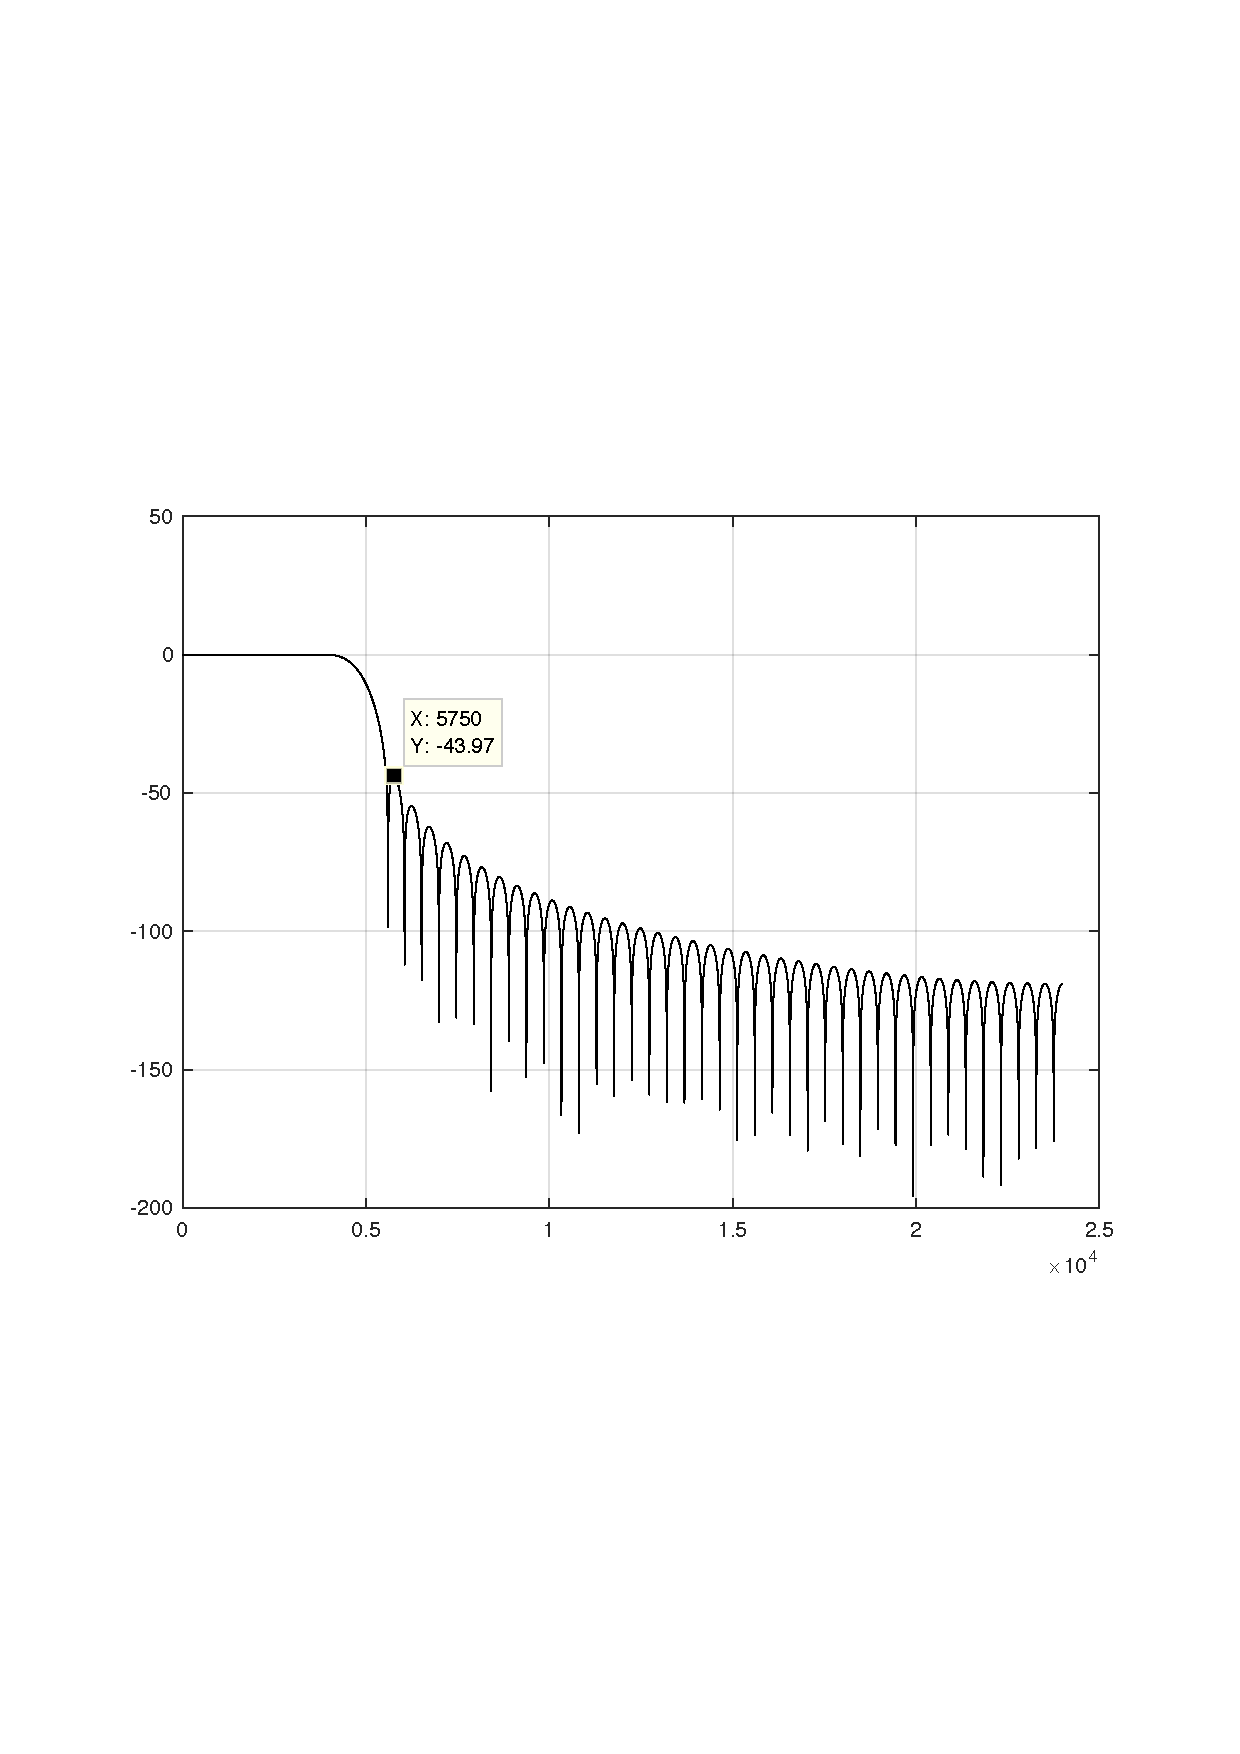
\includegraphics[width=\linewidth]{fir_downsample1}
	\caption{Frequency response of a FIR filter at $f_s$.}
	\label{fig:fir_downsample1}
\end{subfigure}
\hspace{6mm} 
\begin{subfigure}[t]{0.47\textwidth}
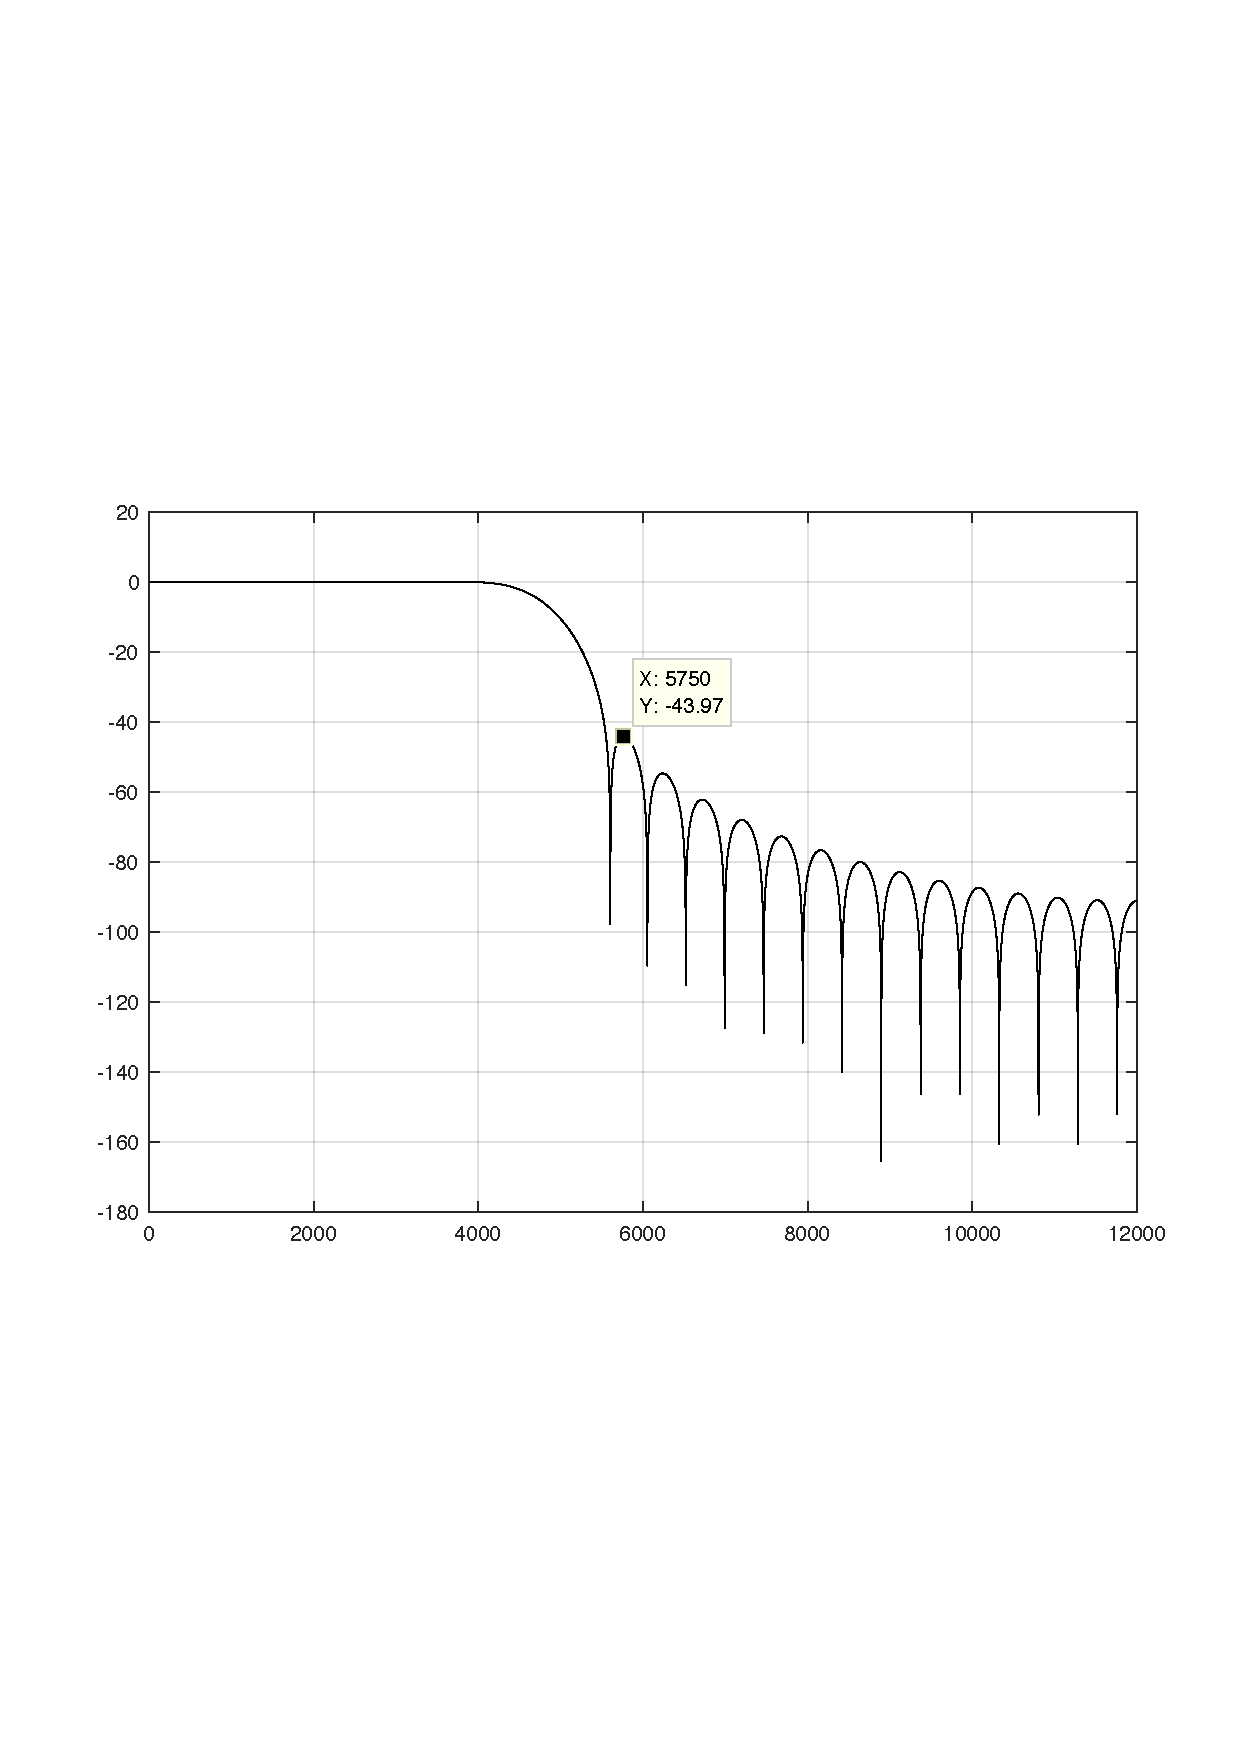
\includegraphics[width=\linewidth]{fir_downsample2}
	\caption{Frequency response of a FIR filter at $\frac{f_s}{2}$ with half the order.}
	\label{fig:fir_downsample2}
\end{subfigure}
\caption{Frequency response of two different FIR filters at different sampling frequencies.}
\label{fig:fir_downsample}
\end{figure}

It is seen that the attenuation at the top of the first side lope is -43.97 dB for both filters, thus the frequency response of both are the same at $0 \leq f \leq 24 \text{kHz}$. Because the frequency bands for the multi-band limiter are placed low, a multirate system will be implemented into the system as this helps decreasing the filter orders significantly.

%\subsection*{Avoiding Aliasing when Downsampling}
To downsample however requires an anti-aliasing filter to avoid aliasing as seen in \autoref{fig:aliasing}. The bandwidth of the audio signal is assumed to be 0 Hz to 20 kHz at a sampling rate of 48 kHz. The anti-aliasing filter has two requirements. The cutoff frequency should be low enough to limit the bandwidth and the attenuation at the new sampling rate $\frac{f_s}{2}$ should be high enough for aliasing not to occur. 

\begin{figure}[H]
\centering
\begin{subfigure}[t]{0.44\textwidth}
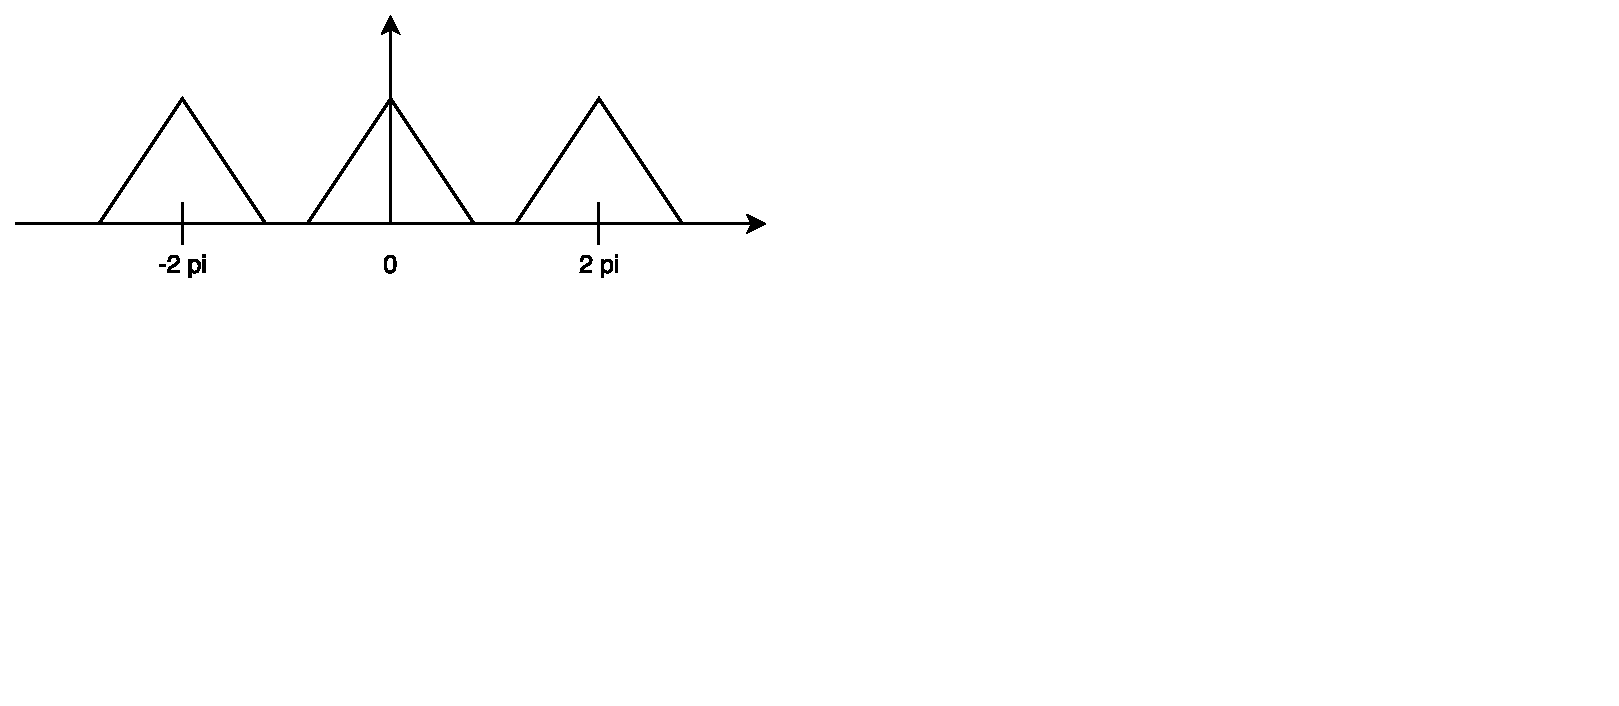
\includegraphics[width=\linewidth]{aliasing1}
	\caption{Signal bandwidth with sampling rate $f_s$.}
	\label{fig:aliasing1}
\end{subfigure}
\hspace{6mm} 
\begin{subfigure}[t]{0.47\textwidth}
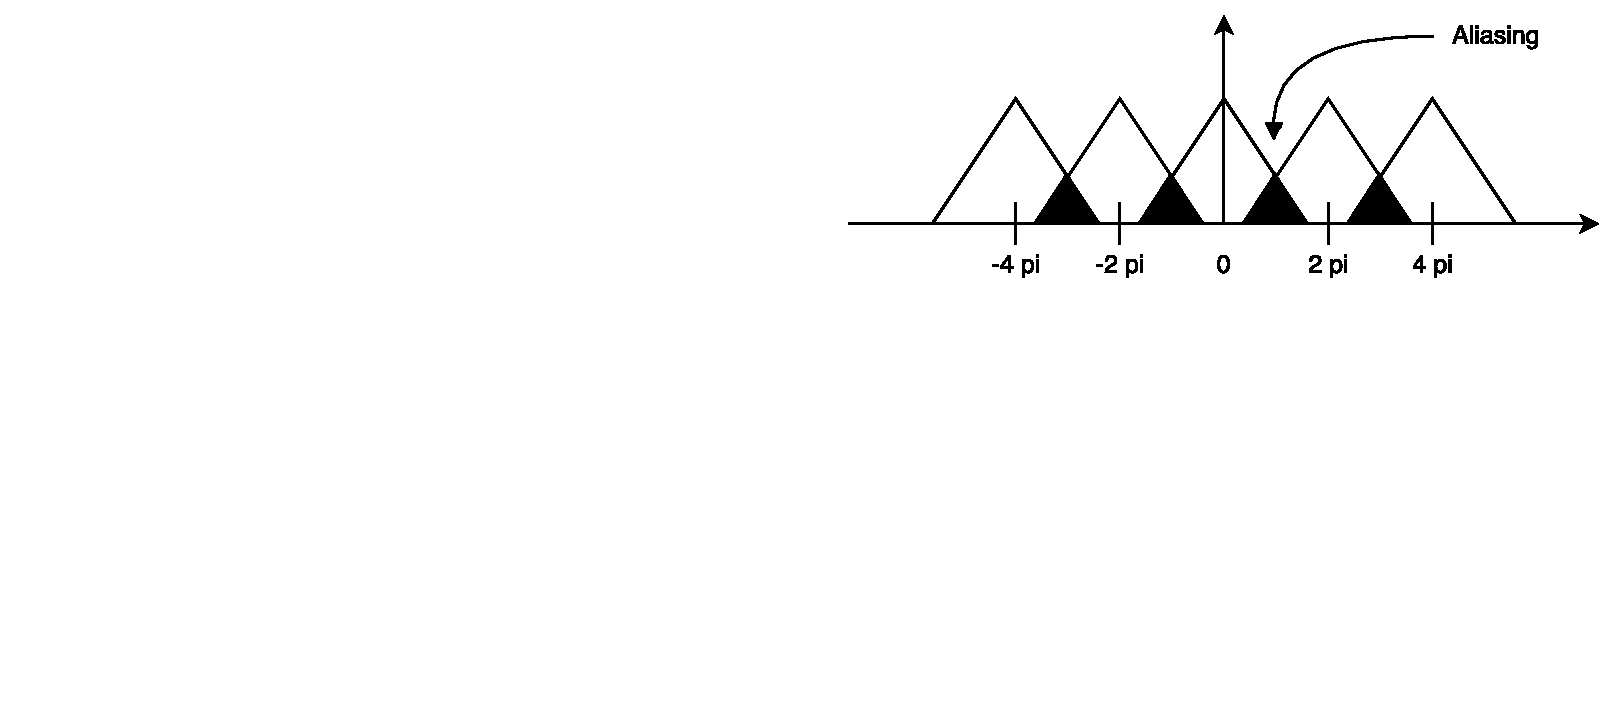
\includegraphics[width=\linewidth]{aliasing2}
	\caption{Aliasing occurs when downsampling to sampling rate $\frac{f_s}{L}$ without anti-aliasing filter.}
	\label{fig:aliasing2}
\end{subfigure}
\hspace{6mm}
\begin{subfigure}[b]{0.44\textwidth}
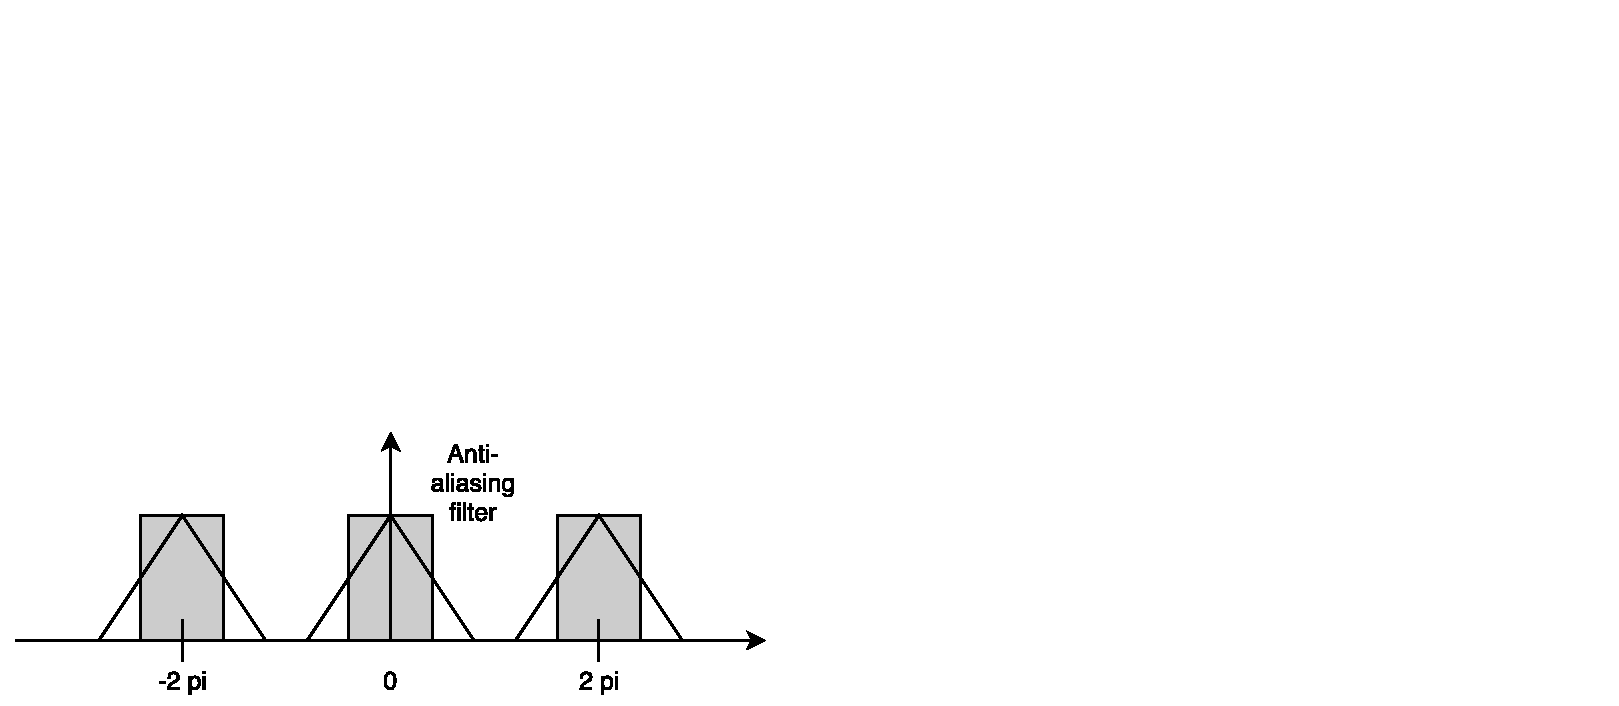
\includegraphics[width=\linewidth]{aliasing3}
	\caption{Aliasing filter applied to reduce the signal bandwidth.}
	\label{fig:aliasing3}
\end{subfigure}
\hspace{6mm} 
\begin{subfigure}[b]{0.47\textwidth}
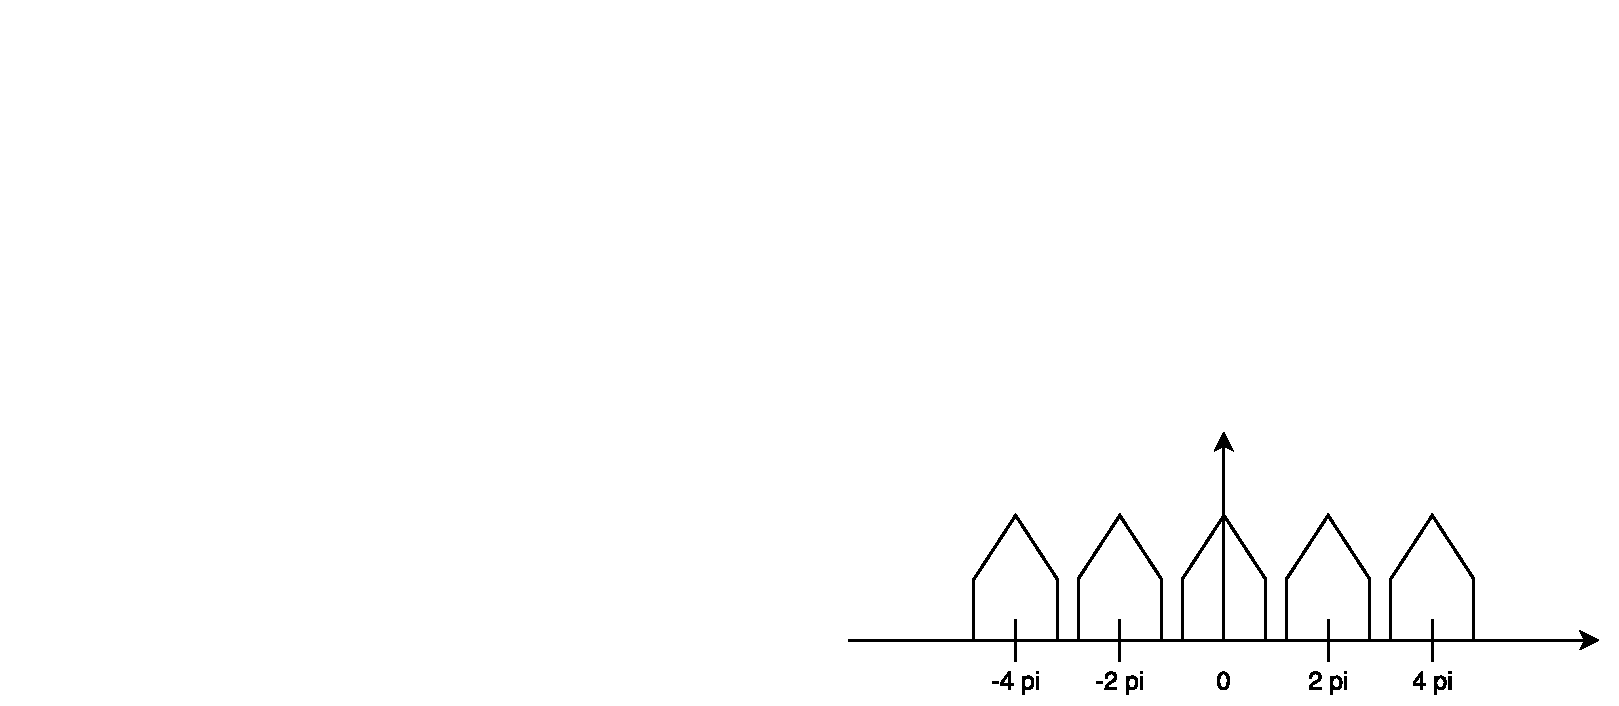
\includegraphics[width=\linewidth]{aliasing4}
	\caption{Aliasing at downsampling no longer occurs.}
	\label{fig:aliasing4}
\end{subfigure}
\caption{An anti-aliasing filter needs to applied to reduce the bandwidth to avoid aliasing when downsampling.}
\label{fig:aliasing}
\end{figure}

% Same number of taps required
If a high downsampling factor, L, is desired, then the order of the anti-aliasing filters will necessarily get bigger. A rule of thumb is the attenuation at $\frac{f_s}{2L}$ should approximately be -60 dB, since an ideal brick wall low-pass filter is not realizable. As the frequency bands for the system is located at the lower spectrum, a high order anti-aliasing filter is needed to downsample the signal. As a high order anti-aliasing filter is not desirable, the downsampling is performed in multistages to ease the amount of computation. If the downsampling is performed with a factor of 2 each time, then the total amount of computation needed to perform the filter algorithm for all stages pr. sample is given as a geometric series:

\begin{equation} \label{eq:z_transformation_example}
\sum_{k=0}^{\infty}M \left( \frac{1}{2} \right)^k  = \frac{M}{1-\frac{1}{2}} = 2M
\end{equation}
\begin{where}
\va{$M$}{is the filter order}{.}
\va{$k$}{is the number of downsamples}{.}
\end{where}

By doing so the filter order for each anti-aliasing filter is kept low as the cutoff frequency of each band is closer to the sampling frequency. Also, the whole bandwidth of the audio signal is split into octave bands which is an advantages if an equalizer and spectrum analyser are desired.

After downsampling, an upsampler is used to upsample the signal to the original sampling frequency. To upsample by a factor of L, L amount of zeros are inserted in-between each sample. This creates high frequency component that needs to be filtered to avoid artefacts from the mirrored spectrum. \autoref{fig:upsampling} illustrates the processes which is called interpolation

\begin{figure}[H]
\centering
\begin{subfigure}[t]{0.44\textwidth}
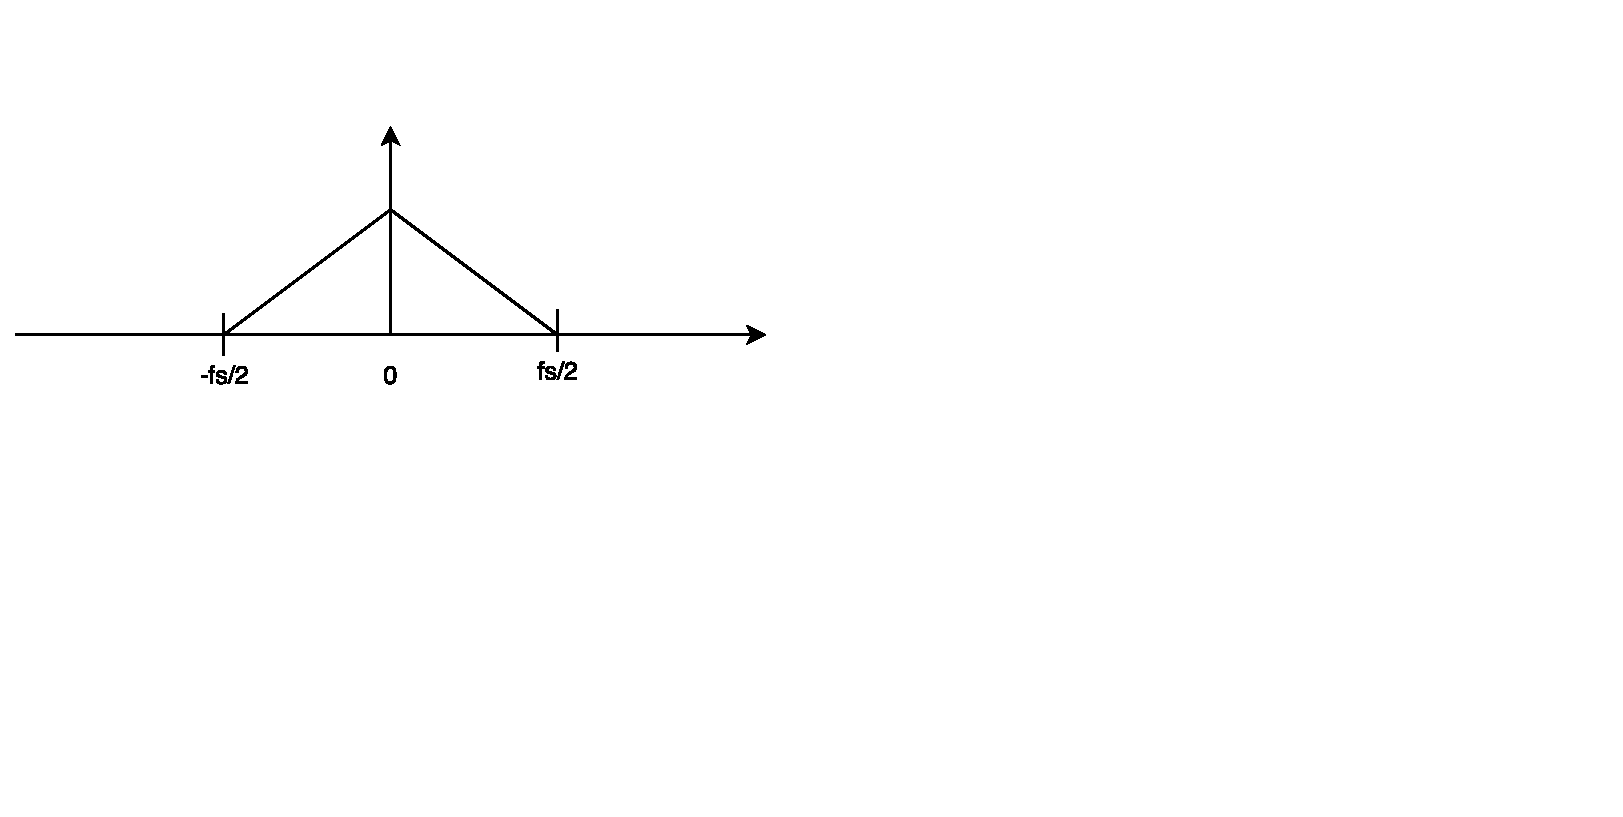
\includegraphics[width=\linewidth]{upsampling1}
	\caption{Signal bandwidth with sampling rate $f_s$.}
	\label{fig:upsampling1}
\end{subfigure}
\hspace{6mm} 
\begin{subfigure}[t]{0.47\textwidth}
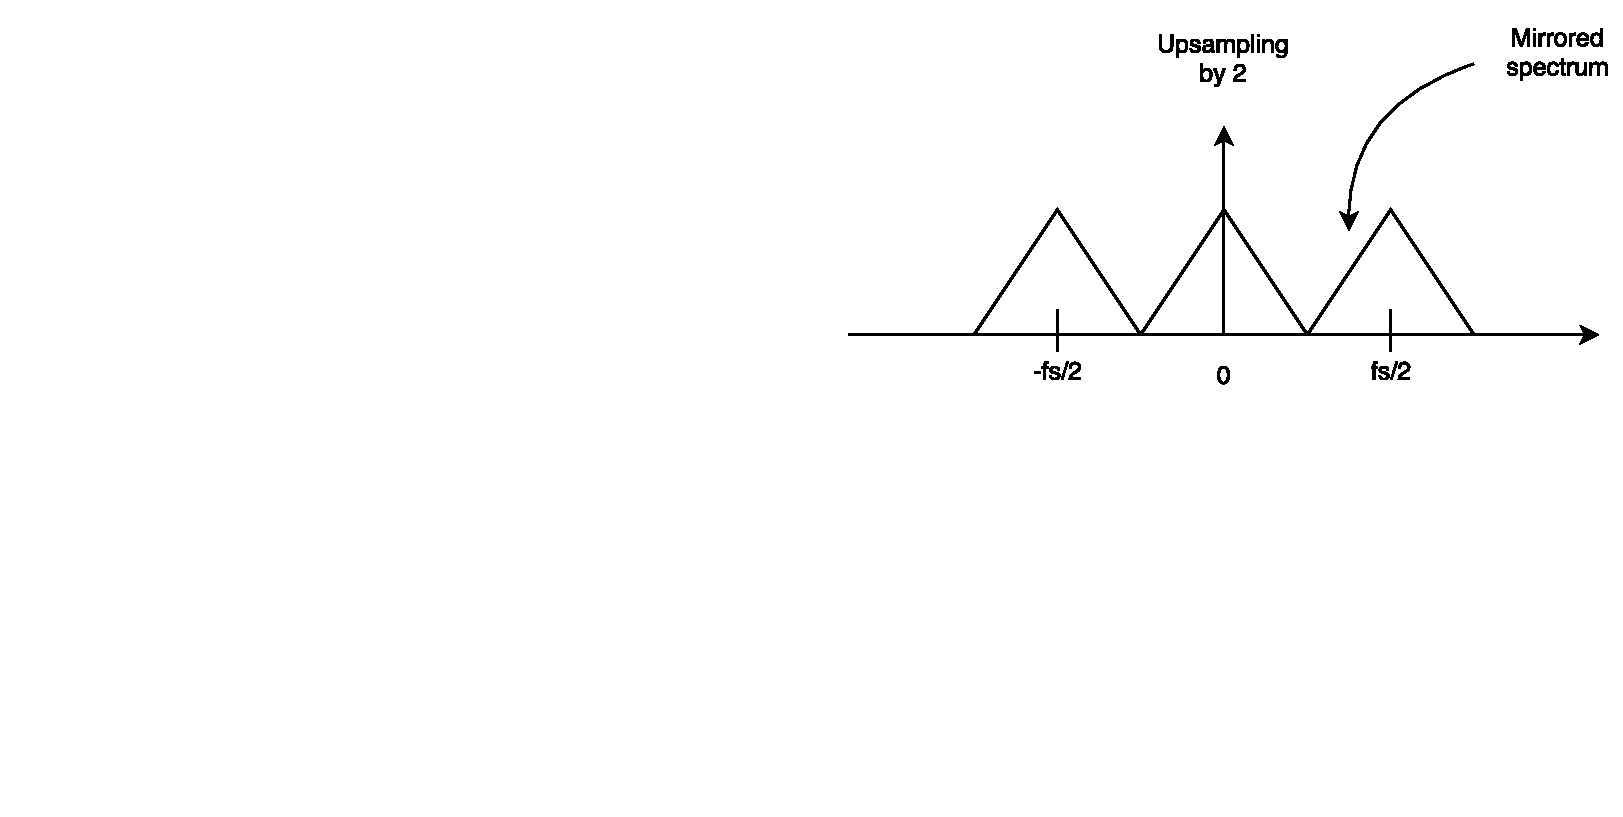
\includegraphics[width=\linewidth]{upsampling2}
	\caption{Upsampling mirrors the spectrum. The sampling frequency is increased by 2.}
	\label{fig:upsampling2}
\end{subfigure}
\hspace{6mm}
\begin{subfigure}[b]{0.44\textwidth}
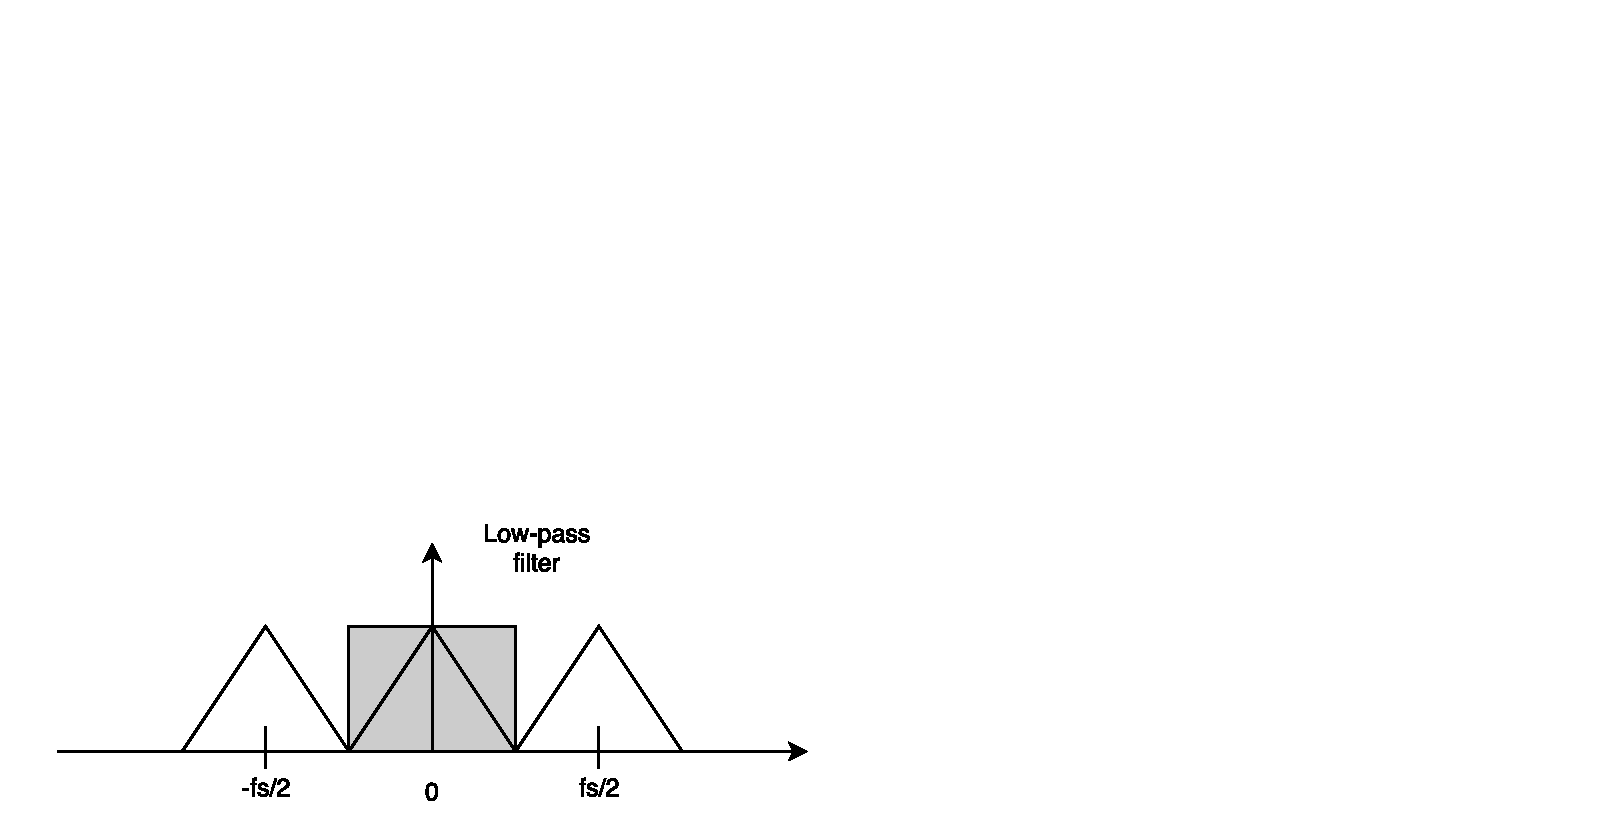
\includegraphics[width=\linewidth]{upsampling3}
	\caption{A low-pass filter removes artefacts from the mirrored spectrum.}
	\label{fig:upsampling3}
\end{subfigure}
\hspace{6mm} 
\begin{subfigure}[b]{0.47\textwidth}
\includegraphics[width=\linewidth]{upsampling4}
	\caption{Aliasing at upsampling no longer occurs.}
	\label{fig:upsampling4}
\end{subfigure}
\caption{Processes of interpolation.}
\label{fig:upsampling}
\end{figure}






% Løsning:
% - Flere Downsamplings
% - Lavere ordens AA filtre
% - samlet samme orden, men AA-filtre ved lavere sampling frekvens skal processeres færre gange
% Processeringsmængden set fra den oprindelige samplingfrekvens er en geometrisk række

% Example downsample in 4 multistages vs 1 downsampling stage

Applying the considerations to the system, the following new overall system may be presented.

\begin{figure}[H]
\centering
\includegraphics[width=0.75\textwidth]{figures/designRealBlock1.pdf}
\caption{Overall system with practical considerations.}
\label{fig:designRealBlock}
\end{figure}

In comparison to previous system overview, "HP and Decimator" and "interpolator" blocks are added to the system. The design of these blocks including the RMS and model will be discussed in following sections. 

Because a downsampling factor of 2 is used, the total amount of bands is 8, which means the equalizer to be designed has 8 adjustable bands.


\section{High-Pass Filter and Decimator}

A decimator is, as previously mentioned, a subsystem consisting of an anti-aliasing filter and a downsampler. As the anti-aliasing essentially is a low-pass filter, applying a design technique called spectral inversion, to the low-pass filtered signal results in high-pass filter. Applying this technique is equivalent to design a mirror filter of the low-pass filter. The technique saves the need for designing a mirror filter of the low-pass filter. The high-pass and decimation block is seen in figure \autoref{fig:designRealDecimator}.

\begin{figure}[H]
\centering
\includegraphics[width=0.75\textwidth]{figures/designRealDecimator.pdf}
\caption{The decimation block consist of a decimator and a spectral inversion to achieve a high-pass filter.}
\label{fig:designRealDecimator}
\end{figure}

A great advantage of using this technique rather than designing a mirror filter/highpass filter, is the algorithm to perform it, which is only a subtraction. To apply spectral inversion, a delay of the input signal before subtraction is required. This is due to the delay of the anti-aliasing filter.


\section{Interpolator}

Opposite to the decimator is the interpolator. As it is desired to reconstruct the signal, upsampling is applied to the downsampled signal. To upsample the downsampled signal, zero-padding is applied. Since the upsampling factor is 2, a zero is added in-between each sample. This adds high frequency components which is then filtered by using a low-pass filter. The requirement for the upsampling filter is that the attenuation at $\frac{f_s}{2}$ of the zero-padded signal is high enough to attenuate the mirrored spectrum and not influencing the bandwidth of the signal. The block diagram of the interpolator is seen in \autoref{fig:designRealInterpolator}.

\begin{figure}[H]
\centering
\includegraphics[width=0.75\textwidth]{figures/designRealInterpolator.pdf}
\caption{The interpolator consist of an upsampler, low-pass filter and a gain factor determined by the upsampling factor.}
\label{fig:designRealInterpolator}
\end{figure}

After low-pass filtering the signal, a gain of 2 corresponding to L is applied.


\section{RMS and Model}

To design an RMS limiter, an RMS analysis and a mathematical function of the gain is needed. For each band, the signal is fed into an RMS block, which calculates the RMS-value. The RMS-value is sent to a Model-block which checks if the RMS-value is above a defined threshold. If the RMS-value is above the threshold the model will apply a gain. If the RMS-value is below, the output will be a gain of 1. The block diagram of the RMS and model is seen in \autoref{fig:designRealRMS}.

\begin{figure}[H]
\centering
\includegraphics[width=0.75\textwidth]{figures/designRealRMS.pdf}
\caption{The RMS-value is first calculated and then fed into a subsystem that determines which gain to apply on the signal.}
\label{fig:designRealRMS}
\end{figure}

%To determine the threshold of the "model", a test of the loudspeaker needs to be done. The purpose of the test is to examine at which RMS-level the loudspeaker is either performing bad or damaging itself. To perform a RMS-analysis the minimum aount of samples needed is the amount of samples to represent the lowest frequency in that band. This introduces a small attact time, meaning the RMS-limiter cannot catch fast transients.



\section{Complete System} \label{sec:CompleteSystem}

The RMS limiter cannot protect the driver against transients such as kick drums and short spikes with high amplitude due to the attack time in the RMS calculation which is not instantanious. To avoid potential damage, a peak limiter is inserted in the upsampled 530 Hz band. The threshold of this limiter is set very high, as the main purpose it to protect the driver at cases where the RMS-limiter is not fast enough to respond. Another RMS-limiter is inserted in the upsampled 530 band. Because the signal is split into 4 bands, the 530 Hz band RMS-limiter ensures that the sum of all 4 bands do not exceed the threshold.

\begin{figure}[H]
\centering
\includegraphics[width=0.75\textwidth]{figures/designRealFull.pdf}
\caption{The complete overall system to be designed.}
\label{fig:designRealBlockFull}
\end{figure}


The complete system is now explained and each subsystem of the system may now be designed in the following chapters.


\chapter{Filter design}
This chapter will describe how the filters in the system are designed for the decimator and interpolator, in more detail the chapter will examine the requirements, the design and the simulation of the quantisized filters. From \autoref{ch:designRealisation} it was concluded that decimation and interpolation should be used to reduce the order of the filters.  
Is was also concluded that the filters used for system should be FIR filters because of spectral inversion which would reduce the number of filters in the system, because they have linear phase and no noise. The requirements affecting the filters are as follows:   

\vspace*{-5mm}
\begin{enumerate}
\item[11] The limiter must have 4 bands.
\item[12] The bands of the limiter must comply with the class 2 of IEC 6964 standard (2001). 
\item[13] The limiters must apply to frequencies below 500 Hz.
\end{enumerate}

\vspace*{-5mm}
A filter for decimation will be designed which must meet requirement 12, and a filter for interpolation will be designed which must not influence the decimated signals bandwidth, because it would otherwise influence the frequency response of the system making it non linear. The decimation filter will be deigned first.

Because the system is a multirate system with octave bands as mentioned in \autoref{ch:designRealization} only one filter needs to be designed because the sampling frequency is halved for every octave resulting in the same coefficients for all decimation and interpolation filters.

\section{Decimation filter}\label{sec:decFilter}
The decimation filter must meet requirement 12 as just mentioned which states the requirements for the filter. The requirements can be seen in \autoref{fig:band1_reqOverview} and \autoref{tb:normalizedReqClass2} which states the requirements to the figure.

\begin{figure}[H]
\centering
\begin{subfigure}[t]{0.45\textwidth}
	\tikzsetnextfilename{Band1Req}
	% This file was created by matlab2tikz.
%
%The latest updates can be retrieved from
%  http://www.mathworks.com/matlabcentral/fileexchange/22022-matlab2tikz-matlab2tikz
%where you can also make suggestions and rate matlab2tikz.
%
\begin{tikzpicture}

\begin{axis}[%
width=2.2in,
height=1.7in,
at={(0.758in,0.481in)},
scale only axis,
unbounded coords=jump,
xmode=log,
xmin=0.05,
xmax=20,
xminorticks=true,
xlabel={Normalized frequency [f/fm]},
xmajorgrids,
xminorgrids,
ymin=-60,
ymax=10,
ylabel={Relative gain [dB]},
ymajorgrids,
axis background/.style={fill=white}
]
\addplot [color=black!30!red,solid,forget plot]
  table[row sep=crcr]{%
1.4142	-5\\
1.4142	-60\\
};
\addplot [color=black!30!red,solid,forget plot]
  table[row sep=crcr]{%
0.7071	-5\\
0.7071	-60\\
};
\addplot [color=black!30!red,solid,forget plot]
  table[row sep=crcr]{%
0.0625	-60\\
0.125	-55\\
0.25	-41\\
0.5	-16.5\\
0.707106781186547	-1.6\\
0.707106781186547	0.5\\
0.77110541270397	0.5\\
0.840896415253715	0.5\\
0.917004043204671	0.5\\
1	0.5\\
1.09050773266526	0.5\\
1.18920711500272	0.5\\
1.29683955465101	0.5\\
1.4142135623731	0.5\\
1.4142135623731	-1.6\\
2	-16.5\\
4	-41\\
8	-55\\
16	-60\\
};
\addplot [color=black!30!red,solid,forget plot]
  table[row sep=crcr]{%
0.0625	-inf\\
0.125	-inf\\
0.25	-inf\\
0.5	-inf\\
0.707106781186547	-5\\
0.707106781186547	-5\\
0.77110541270397	-1.3\\
0.840896415253715	-0.6\\
0.917004043204671	-0.4\\
1	-0.3\\
1.09050773266526	-0.4\\
1.18920711500272	-0.6\\
1.29683955465101	-1.3\\
1.4142135623731	-5\\
1.4142135623731	-5\\
2	-inf\\
4	-inf\\
8	-inf\\
16	-inf\\
};
\end{axis}
\end{tikzpicture}%
	\caption{Band requirements.}
	\label{fig:band1_req}
\end{subfigure}
\begin{subfigure}[t]{0.45\textwidth}
	\tikzsetnextfilename{Band1ReqZoom}
	% This file was created by matlab2tikz.
%
%The latest updates can be retrieved from
%  http://www.mathworks.com/matlabcentral/fileexchange/22022-matlab2tikz-matlab2tikz
%where you can also make suggestions and rate matlab2tikz.
%
\begin{tikzpicture}

\begin{axis}[%
width=2.3in,
height=2in,
at={(0.758in,0.504in)},
scale only axis,
unbounded coords=jump,
xmode=log,
xmin=3774.50218155918,
xmax=9480.85426960068,
xminorticks=true,
xlabel={Frequency [Hz]},
xmajorgrids,
xminorgrids,
ymin=-5.26838030133928,
ymax=1.43014090401786,
ylabel={Gain [dB]},
ymajorgrids,
axis background/.style={fill=white}
]
\addplot [color=red,solid,forget plot]
  table[row sep=crcr]{%
375	-60\\
750	-55\\
1500	-41\\
3000	-16.5\\
4242.64068711928	-1.6\\
4242.64068711928	0.5\\
4626.63247622382	0.5\\
5045.37849152229	0.5\\
5502.02425922803	0.5\\
6000	0.5\\
6543.04639599155	0.5\\
7135.24269001633	0.5\\
7781.03732790606	0.5\\
8485.28137423857	0.5\\
8485.28137423857	-1.6\\
12000	-16.5\\
24000	-41\\
48000	-55\\
96000	-60\\
};
\addplot [color=blue,solid,forget plot]
  table[row sep=crcr]{%
375	-inf\\
750	-inf\\
1500	-inf\\
3000	-inf\\
4242.64068711928	-5\\
4242.64068711928	-5\\
4626.63247622382	-1.3\\
5045.37849152229	-0.6\\
5502.02425922803	-0.4\\
6000	-0.3\\
6543.04639599155	-0.4\\
7135.24269001633	-0.6\\
7781.03732790606	-1.3\\
8485.28137423857	-5\\
8485.28137423857	-5\\
12000	-inf\\
24000	-inf\\
48000	-inf\\
96000	-inf\\
};
\end{axis}
\end{tikzpicture}%
	\caption{Band requirements zoomed in.}
	\label{fig:band1_reqZoom}
\end{subfigure}
\caption{Band requirements without and with zoom.}
\label{fig:band1_reqOverview}
\end{figure}


\begin{table}[H]
\centering
\begin{tabular}{|c|c|}
\hline
\multirow{3}{*}{\begin{tabular}[c]{@{}c@{}}Normalized\\ frequency\\ $f/f_m=\Omega$\end{tabular}}                        & \begin{tabular}[c]{@{}c@{}}Minimum;Maximum attenuation limits\\ dB\end{tabular}                        \\ \cline{2-2} 
                                                                                                                        & Filter class                                                                                           \\ \cline{2-2} 
                                                                                                                        & 2                                                                                                      \\ \hline
$G^0$                                                                                                                   & -0,5;+0,5                                                                                              \\ \hline
$G^{\pm 1/8}$                                                                                                           & -0,5; +0,6                                                                                             \\ \hline
$G^{\pm 1/4}$                                                                                                           & -0,5; +0,8                                                                                             \\ \hline
$G^{\pm 3/8}$                                                                                                           & -0,5; +1,6                                                                                             \\ \hline
$<G^{\pm 1/2}$                                                                                                          & -0,5; +5,5*                                                                                            \\ \hline
$>G^{\pm 1/2}$                                                                                                          & +1,6; +5,5*                                                                                            \\ \hline
$G^{\pm 1}$                                                                                                             & +16,5; +$\infty$                                                                                       \\ \hline
$G^{\pm 2}$                                                                                                             & +41; +$\infty$                                                                                         \\ \hline
$G^{\pm 3}$                                                                                                             & +55; +$\infty$                                                                                         \\ \hline
$\geq G^{\pm +4}$                                                                                                       & +60; +$\infty$                                                                                         \\ \hline
$\leq G^{\pm -4}$                                                                                                       & +60; +$\infty$                                                                                         \\ \hline
\multicolumn{2}{|l|}{\begin{tabular}[c]{@{}l@{}}* At frequencies less than the lower band-edge frequency and greater than the\\ upper band-edge frequency, the limit on maximum relative attenuation is +$\infty$;\end{tabular}} \\ \hline
\end{tabular}
\caption{Normalized requirements for the filters. G=2.}
\label{tb:normalizedReqClass2}
\end{table} 
 
Only a lowpass filter should be designed because of spectral inversion, as described in \autoref{ch:designRealization}, so instead of bandpass requirements only one side of the requirements are shown from now on. %From system overview the octave bands are given for frequencies below 530 Hz, see \autoref{tb:freqBands} which meets requirement 8 and 10.


To take advantage of multirate processing extra octave bands have been added, see \autoref{tb:filterBands}, increasing the number of downsamples which results in the following bands given in \autoref{tb:filterBands} and seen in \autoref{fig:allBands}.
\begin{table}[H]
\centering
\begin{tabular}{|c|c|c|c|}
\hline
       & f1 {[}Hz{]} & fm {[}Hz{]} & f2 {[}Hz{]} \\ \hline
Band 7 & 2121        & 3000        & 4243        \\ \hline
Band 6 & 1061        & 1500        & 2121        \\ \hline
Band 5 & 530,3       & 750         & 1061        \\ \hline
Band 4 & 265,2       & 375         & 530,3       \\ \hline
Band 3 & 132,6       & 187,5       & 265,2       \\ \hline
Band 2 & 66,29       & 93,75       & 132,6       \\ \hline
Band 1 & 33,15       & 46,87       & 66,29       \\ \hline
\end{tabular}
\caption{Bands}
\label{tb:filterBands}
\end{table}   

\begin{figure}[H]
	\centering
	\tikzsetnextfilename{allBands}
	% This file was created by matlab2tikz.
%
%The latest updates can be retrieved from
%  http://www.mathworks.com/matlabcentral/fileexchange/22022-matlab2tikz-matlab2tikz
%where you can also make suggestions and rate matlab2tikz.
%
\definecolor{mycolor1}{rgb}{0.70000,0.70000,0.00000}%
\definecolor{mycolor2}{rgb}{0.70000,0.00000,0.70000}%
\definecolor{mycolor3}{rgb}{0.00000,0.70000,0.70000}%
\definecolor{mycolor4}{rgb}{0.70000,0.20000,0.80000}%
%
\begin{tikzpicture}

\begin{axis}[%
width=5.5in,
height=2.5in,
at={(0.758in,0.481in)},
scale only axis,
unbounded coords=jump,
xmode=log,
xmin=1,
xmax=100000,
xminorticks=true,
xmajorgrids,
xminorgrids,
ylabel={Magnitude [dB]},
xlabel={Frequency [Hz]}
ymin=-60,
ymax=10,
ymajorgrids,
axis background/.style={fill=white}
]
\addplot [color=black!30!red,solid,forget plot]
  table[row sep=crcr]{%
187.5	-60\\
375	-55\\
750	-41\\
1500	-16.5\\
2121.32034355964	-1.6\\
2121.32034355964	0.5\\
2313.31623811191	0.5\\
2522.68924576114	0.5\\
2751.01212961401	0.5\\
3000	0.5\\
3271.52319799577	0.5\\
3567.62134500816	0.5\\
3890.51866395303	0.5\\
4242.64068711929	0.5\\
4242.64068711929	-1.6\\
6000	-16.5\\
12000	-41\\
24000	-55\\
48000	-60\\
};
\addplot [color=black!30!red,solid,forget plot]
  table[row sep=crcr]{%
187.5	-inf\\
375	-inf\\
750	-inf\\
1500	-inf\\
2121.32034355964	-5.5\\
2121.32034355964	-5.5\\
2313.31623811191	-1.6\\
2522.68924576114	-0.8\\
2751.01212961401	-0.6\\
3000	-0.5\\
3271.52319799577	-0.6\\
3567.62134500816	-0.8\\
3890.51866395303	-1.6\\
4242.64068711929	-5.5\\
4242.64068711929	-5.5\\
6000	-inf\\
12000	-inf\\
24000	-inf\\
48000	-inf\\
};
\addplot [color=black!30!green,solid,forget plot]
  table[row sep=crcr]{%
93.75	-60\\
187.5	-55\\
375	-41\\
750	-16.5\\
1060.66017177982	-1.6\\
1060.66017177982	0.5\\
1156.65811905596	0.5\\
1261.34462288057	0.5\\
1375.50606480701	0.5\\
1500	0.5\\
1635.76159899789	0.5\\
1783.81067250408	0.5\\
1945.25933197651	0.5\\
2121.32034355964	0.5\\
2121.32034355964	-1.6\\
3000	-16.5\\
6000	-41\\
12000	-55\\
24000	-60\\
};
\addplot [color=black!30!green,solid,forget plot]
  table[row sep=crcr]{%
93.75	-inf\\
187.5	-inf\\
375	-inf\\
750	-inf\\
1060.66017177982	-5.5\\
1060.66017177982	-5.5\\
1156.65811905596	-1.6\\
1261.34462288057	-0.8\\
1375.50606480701	-0.6\\
1500	-0.5\\
1635.76159899789	-0.6\\
1783.81067250408	-0.8\\
1945.25933197651	-1.6\\
2121.32034355964	-5.5\\
2121.32034355964	-5.5\\
3000	-inf\\
6000	-inf\\
12000	-inf\\
24000	-inf\\
};
\addplot [color=black!30!blue,solid,forget plot]
  table[row sep=crcr]{%
46.875	-60\\
93.75	-55\\
187.5	-41\\
375	-16.5\\
530.330085889911	-1.6\\
530.330085889911	0.5\\
578.329059527978	0.5\\
630.672311440286	0.5\\
687.753032403503	0.5\\
750	0.5\\
817.880799498943	0.5\\
891.905336252041	0.5\\
972.629665988257	0.5\\
1060.66017177982	0.5\\
1060.66017177982	-1.6\\
1500	-16.5\\
3000	-41\\
6000	-55\\
12000	-60\\
};
\addplot [color=black!30!blue,solid,forget plot]
  table[row sep=crcr]{%
46.875	-inf\\
93.75	-inf\\
187.5	-inf\\
375	-inf\\
530.330085889911	-5.5\\
530.330085889911	-5.5\\
578.329059527978	-1.6\\
630.672311440286	-0.8\\
687.753032403503	-0.6\\
750	-0.5\\
817.880799498943	-0.6\\
891.905336252041	-0.8\\
972.629665988257	-1.6\\
1060.66017177982	-5.5\\
1060.66017177982	-5.5\\
1500	-inf\\
3000	-inf\\
6000	-inf\\
12000	-inf\\
};
\addplot [color=mycolor1,solid,forget plot]
  table[row sep=crcr]{%
23.4375	-60\\
46.875	-55\\
93.75	-41\\
187.5	-16.5\\
265.165042944955	-1.6\\
265.165042944955	0.5\\
289.164529763989	0.5\\
315.336155720143	0.5\\
343.876516201752	0.5\\
375	0.5\\
408.940399749472	0.5\\
445.95266812602	0.5\\
486.314832994129	0.5\\
530.330085889911	0.5\\
530.330085889911	-1.6\\
750	-16.5\\
1500	-41\\
3000	-55\\
6000	-60\\
};
\addplot [color=mycolor1,solid,forget plot]
  table[row sep=crcr]{%
23.4375	-inf\\
46.875	-inf\\
93.75	-inf\\
187.5	-inf\\
265.165042944955	-5.5\\
265.165042944955	-5.5\\
289.164529763989	-1.6\\
315.336155720143	-0.8\\
343.876516201752	-0.6\\
375	-0.5\\
408.940399749472	-0.6\\
445.95266812602	-0.8\\
486.314832994129	-1.6\\
530.330085889911	-5.5\\
530.330085889911	-5.5\\
750	-inf\\
1500	-inf\\
3000	-inf\\
6000	-inf\\
};
\addplot [color=mycolor2,solid,forget plot]
  table[row sep=crcr]{%
11.71875	-60\\
23.4375	-55\\
46.875	-41\\
93.75	-16.5\\
132.582521472478	-1.6\\
132.582521472478	0.5\\
144.582264881994	0.5\\
157.668077860071	0.5\\
171.938258100876	0.5\\
187.5	0.5\\
204.470199874736	0.5\\
222.97633406301	0.5\\
243.157416497064	0.5\\
265.165042944955	0.5\\
265.165042944955	-1.6\\
375	-16.5\\
750	-41\\
1500	-55\\
3000	-60\\
};
\addplot [color=mycolor2,solid,forget plot]
  table[row sep=crcr]{%
11.71875	-inf\\
23.4375	-inf\\
46.875	-inf\\
93.75	-inf\\
132.582521472478	-5.5\\
132.582521472478	-5.5\\
144.582264881994	-1.6\\
157.668077860071	-0.8\\
171.938258100876	-0.6\\
187.5	-0.5\\
204.470199874736	-0.6\\
222.97633406301	-0.8\\
243.157416497064	-1.6\\
265.165042944955	-5.5\\
265.165042944955	-5.5\\
375	-inf\\
750	-inf\\
1500	-inf\\
3000	-inf\\
};
\addplot [color=mycolor3,solid,forget plot]
  table[row sep=crcr]{%
5.859375	-60\\
11.71875	-55\\
23.4375	-41\\
46.875	-16.5\\
66.2912607362388	-1.6\\
66.2912607362388	0.5\\
72.2911324409972	0.5\\
78.8340389300357	0.5\\
85.9691290504379	0.5\\
93.75	0.5\\
102.235099937368	0.5\\
111.488167031505	0.5\\
121.578708248532	0.5\\
132.582521472478	0.5\\
132.582521472478	-1.6\\
187.5	-16.5\\
375	-41\\
750	-55\\
1500	-60\\
};
\addplot [color=mycolor3,solid,forget plot]
  table[row sep=crcr]{%
5.859375	-inf\\
11.71875	-inf\\
23.4375	-inf\\
46.875	-inf\\
66.2912607362388	-5.5\\
66.2912607362388	-5.5\\
72.2911324409972	-1.6\\
78.8340389300357	-0.8\\
85.9691290504379	-0.6\\
93.75	-0.5\\
102.235099937368	-0.6\\
111.488167031505	-0.8\\
121.578708248532	-1.6\\
132.582521472478	-5.5\\
132.582521472478	-5.5\\
187.5	-inf\\
375	-inf\\
750	-inf\\
1500	-inf\\
};
\addplot [color=mycolor4,solid,forget plot]
  table[row sep=crcr]{%
2.9296875	-60\\
5.859375	-55\\
11.71875	-41\\
23.4375	-16.5\\
33.1456303681194	-1.6\\
33.1456303681194	0.5\\
36.1455662204986	0.5\\
39.4170194650179	0.5\\
42.984564525219	0.5\\
46.875	0.5\\
51.117549968684	0.5\\
55.7440835157526	0.5\\
60.7893541242661	0.5\\
66.2912607362388	0.5\\
66.2912607362388	-1.6\\
93.75	-16.5\\
187.5	-41\\
375	-55\\
750	-60\\
};
\addplot [color=mycolor4,solid,forget plot]
  table[row sep=crcr]{%
2.9296875	-inf\\
5.859375	-inf\\
11.71875	-inf\\
23.4375	-inf\\
33.1456303681194	-5.5\\
33.1456303681194	-5.5\\
36.1455662204986	-1.6\\
39.4170194650179	-0.8\\
42.984564525219	-0.6\\
46.875	-0.5\\
51.117549968684	-0.6\\
55.7440835157526	-0.8\\
60.7893541242661	-1.6\\
66.2912607362388	-5.5\\
66.2912607362388	-5.5\\
93.75	-inf\\
187.5	-inf\\
375	-inf\\
750	-inf\\
};
\addplot [color=white!30!black,solid,forget plot]
  table[row sep=crcr]{%
1.46484375	-60\\
2.9296875	-55\\
5.859375	-41\\
11.71875	-16.5\\
16.5728151840597	-1.6\\
16.5728151840597	0.5\\
18.0727831102493	0.5\\
19.7085097325089	0.5\\
21.4922822626095	0.5\\
23.4375	0.5\\
25.558774984342	0.5\\
27.8720417578763	0.5\\
30.394677062133	0.5\\
33.1456303681194	0.5\\
33.1456303681194	-1.6\\
46.875	-16.5\\
93.75	-41\\
187.5	-55\\
375	-60\\
};
\addplot [color=white!30!black,solid,forget plot]
  table[row sep=crcr]{%
1.46484375	-inf\\
2.9296875	-inf\\
5.859375	-inf\\
11.71875	-inf\\
16.5728151840597	-5.5\\
16.5728151840597	-5.5\\
18.0727831102493	-1.6\\
19.7085097325089	-0.8\\
21.4922822626095	-0.6\\
23.4375	-0.5\\
25.558774984342	-0.6\\
27.8720417578763	-0.8\\
30.394677062133	-1.6\\
33.1456303681194	-5.5\\
33.1456303681194	-5.5\\
46.875	-inf\\
93.75	-inf\\
187.5	-inf\\
375	-inf\\
};
\end{axis}
\end{tikzpicture}%
	\caption{Overview of all band requirements}
	\label{fig:allBands}
\end{figure}
The reason for downsampling seven times and not more or less is because of several reasons. Firstly the bandwidth of the decimation filter must not be influenced by the interpolation filter which would give a non flat frequency response so every band is set to have a center frequency 1/16 of Fs, secondly the lower the center frequency in relation to Fs the higher the filter order which is desired as low as possible, lastly increasing the number of downsamples increases the delay of the system which is not desired in relation to real time applications.       
\todo[inline]{Skal det være mere begrundet? skal vi skrive at det er baseret på trial and error senere i forløbet?}

Because there will be downsampled by two for every octave band the following relation can be made between a band and Fs as seen on \autoref{fig:relFsBand}.
\begin{figure}[H]
	\centering
	\tikzsetnextfilename{relativeFsBand}
	% This file was created by matlab2tikz.
%
%The latest updates can be retrieved from
%  http://www.mathworks.com/matlabcentral/fileexchange/22022-matlab2tikz-matlab2tikz
%where you can also make suggestions and rate matlab2tikz.
%
\begin{tikzpicture}

\begin{axis}[%
width=5.5in,
height=2in,
at={(0.758in,0.481in)},
scale only axis,
unbounded coords=jump,
xmin=0,
xmax=1,
xlabel={Normalized frequency [fm/fs]},
xmajorgrids,
ymin=-60,
ymax=10,
ylabel={Magnitude [dB]},
ymajorgrids,
axis background/.style={fill=white}
]
\addplot [color=black!30!red,solid,forget plot]
  table[row sep=crcr]{%
0.1768	-5.5\\
0.1768	-60\\
};
\addplot [color=black!30!red,solid,forget plot]
  table[row sep=crcr]{%
0.0078125	0.5\\
0.015625	0.5\\
0.03125	0.5\\
0.0625	0.5\\
0.0883883476483184	0.5\\
0.0883883476483184	0.5\\
0.0963881765879963	0.5\\
0.105112051906714	0.5\\
0.114625505400584	0.5\\
0.125	0.5\\
0.136313466583157	0.5\\
0.14865088937534	0.5\\
0.162104944331376	0.5\\
0.176776695296637	0.5\\
0.176776695296637	-1.6\\
0.25	-16.5\\
0.5	-41\\
1	-55\\
2	-60\\
};
\addplot [color=black!30!red,solid,forget plot]
  table[row sep=crcr]{%
0.0078125	-0.5\\
0.015625	-0.5\\
0.03125	-0.5\\
0.0625	-0.5\\
0.0883883476483184	-0.5\\
0.0883883476483184	-0.5\\
0.0963881765879963	-0.5\\
0.105112051906714	-0.5\\
0.114625505400584	-0.5\\
0.125	-0.5\\
0.136313466583157	-0.6\\
0.14865088937534	-0.8\\
0.162104944331376	-1.6\\
0.176776695296637	-5.5\\
0.176776695296637	-5.5\\
0.25	-inf\\
0.5	-inf\\
1	-inf\\
2	-inf\\
};
\end{axis}
\end{tikzpicture}%
	\caption{Band relative to Fs}
	\label{fig:relFsBand}
\end{figure}

From \autoref{fig:relFsBand} two points are selected giving the following specifications to the lowpass filter:

$\omega_{pass}=3.000\textrm{ Hz }\cdot 2/Fs=0.1250 \enhed{rad/sample}$\\
$A_{pass}=-1 \enhed{dB}$\\
$\omega_{stop}=6.500\textrm{ Hz }\cdot 2/Fs=0.2708 \enhed{rad/sample}$\\
$A_{stop}=-60 \enhed{dB}$

The design method used for designing the filter is the Kaiser window method, explained in detail in \autoref{app:FIR_theory}. The reason for using the Kaiser window method is that it gives the approximate order of the filter and the beta value of the window applied to impulse reponse. This means that no trial and error method is needed to meet the requierments of the filter.

With the specification stated and using the matlab script explained in \autoref{app:FIR_Matlab} which uses the FIR theoy explained in \autoref{app:FIR_theory} about the Kaiser window method, general FIR theory and deriving the coefficients of the filter, the following filter is given with quantisized coefficients, see \autoref{fig:band1_filt} for magnitude response and \autoref{fig:band1_filtPhase} for phase response. The order of the filter is 50, it is a type 1 FIR filter and has linear phase which means that the group delay is constant at 25 samples.  

\begin{figure}[H]
\centering
	\tikzsetnextfilename{Band1Filt}
	% This file was created by matlab2tikz.
%
%The latest updates can be retrieved from
%  http://www.mathworks.com/matlabcentral/fileexchange/22022-matlab2tikz-matlab2tikz
%where you can also make suggestions and rate matlab2tikz.
%
\definecolor{mycolor1}{rgb}{0.00000,0.44700,0.74100}%
%
\begin{tikzpicture}

\begin{axis}[%
width=5.5in,
height=2.75in,
at={(1.281in,0.447in)},
scale only axis,
unbounded coords=jump,
xmin=0,
xmax=1,
xlabel={$\text{Normalized Frequency (}\times\pi\text{ rad/sample)}$},
xmajorgrids,
ymin=-95.4207080394785,
ymax=4.7713185812425,
ylabel={Magnitude [dB]},
ymajorgrids,
axis background/.style={fill=white},
]
\addplot [color=mycolor1,solid,forget plot]
  table[row sep=crcr]{%
0	0.002385323281203\\
0.0001220703125	0.00238515620543467\\
0.000244140625	0.00238465500069651\\
0.0003662109375	0.00238381973514379\\
0.00048828125	0.00238265052200859\\
0.0006103515625	0.00238114752011143\\
0.000732421875	0.00237931093340649\\
0.0008544921875	0.00237714101120901\\
0.0009765625	0.00237463804796789\\
0.0010986328125	0.00237180238360679\\
0.001220703125	0.00236863440289881\\
0.0013427734375	0.00236513453592124\\
0.00146484375	0.00236130325782824\\
0.0015869140625	0.00235714108868024\\
0.001708984375	0.00235264859355766\\
0.0018310546875	0.00234782638233355\\
0.001953125	0.00234267510978725\\
0.0020751953125	0.0023371954752065\\
0.002197265625	0.00233138822267165\\
0.0023193359375	0.00232525414077145\\
0.00244140625	0.00231879406231883\\
0.0025634765625	0.00231200886469196\\
0.002685546875	0.00230489946932266\\
0.0028076171875	0.00229746684169641\\
0.0029296875	0.00228971199135231\\
0.0030517578125	0.00228163597159892\\
0.003173828125	0.00227323987945738\\
0.0032958984375	0.00226452485554773\\
0.00341796875	0.00225549208369102\\
0.0035400390625	0.00224614279125035\\
0.003662109375	0.00223647824844875\\
0.0037841796875	0.00222649976865341\\
0.00390625	0.00221620870775041\\
0.0040283203125	0.00220560646437207\\
0.004150390625	0.00219469447961274\\
0.0042724609375	0.0021834742366309\\
0.00439453125	0.00217194726076286\\
0.0045166015625	0.002160115119068\\
0.004638671875	0.00214797942038558\\
0.0047607421875	0.00213554181482323\\
0.0048828125	0.0021228039938137\\
0.0050048828125	0.00210976768977389\\
0.005126953125	0.00209643467593423\\
0.0052490234375	0.00208280676594086\\
0.00537109375	0.00206888581396925\\
0.0054931640625	0.00205467371409895\\
0.005615234375	0.00204017240037047\\
0.0057373046875	0.0020253838462736\\
0.005859375	0.00201031006480434\\
0.0059814453125	0.00199495310783959\\
0.006103515625	0.00197931506625082\\
0.0062255859375	0.0019633980693925\\
0.00634765625	0.00194720428476103\\
0.0064697265625	0.00193073591810844\\
0.006591796875	0.00191399521258973\\
0.0067138671875	0.00189698444904707\\
0.0068359375	0.00187970594521403\\
0.0069580078125	0.00186216205582923\\
0.007080078125	0.00184435517201109\\
0.0072021484375	0.00182628772120097\\
0.00732421875	0.00180796216670842\\
0.0074462890625	0.0017893810073133\\
0.007568359375	0.00177054677726574\\
0.0076904296875	0.00175146204554721\\
0.0078125	0.00173212941587053\\
0.0079345703125	0.00171255152616823\\
0.008056640625	0.00169273104819467\\
0.0081787109375	0.00167267068746924\\
0.00830078125	0.0016523731825373\\
0.0084228515625	0.00163184130502714\\
0.008544921875	0.0016110778589109\\
0.0086669921875	0.00159008568039098\\
0.0087890625	0.00156886763744524\\
0.0089111328125	0.00154742662942908\\
0.009033203125	0.00152576558673445\\
0.0091552734375	0.00150388747044872\\
0.00927734375	0.00148179527189996\\
0.0093994140625	0.00145949201237272\\
0.009521484375	0.00143698074248277\\
0.0096435546875	0.00141426454212024\\
0.009765625	0.00139134651976747\\
0.0098876953125	0.00136822981221485\\
0.010009765625	0.00134491758416289\\
0.0101318359375	0.00132141302776745\\
0.01025390625	0.00129771936218503\\
0.0103759765625	0.00127383983328855\\
0.010498046875	0.00124977771315571\\
0.0106201171875	0.00122553629967115\\
0.0107421875	0.00120111891595798\\
0.0108642578125	0.0011765289102641\\
0.010986328125	0.00115176965510955\\
0.0111083984375	0.00112684454722967\\
0.01123046875	0.00110175700689297\\
0.0113525390625	0.00107651047756008\\
0.011474609375	0.00105110842537215\\
0.0115966796875	0.00102555433869611\\
0.01171875	0.000999851727783607\\
0.0118408203125	0.000974004124145722\\
0.011962890625	0.000948015080211917\\
0.0120849609375	0.000921888168818441\\
0.01220703125	0.000895626982753583\\
0.0123291015625	0.000869235134302926\\
0.012451171875	0.000842716254624065\\
0.0125732421875	0.000816073993576083\\
0.0126953125	0.000789312018923738\\
0.0128173828125	0.000762434016110092\\
0.012939453125	0.000735443687460702\\
0.0130615234375	0.000708344752126777\\
0.01318359375	0.000681140945175684\\
0.0133056640625	0.000653836017420417\\
0.013427734375	0.000626433734680631\\
0.0135498046875	0.000598937877441585\\
0.013671875	0.000571352240285705\\
0.0137939453125	0.000543680631437837\\
0.013916015625	0.000515926872139971\\
0.0140380859375	0.000488094796423866\\
0.01416015625	0.000460188250258398\\
0.0142822265625	0.000432211091322188\\
0.014404296875	0.000404167188264637\\
0.0145263671875	0.000376060420308022\\
0.0146484375	0.000347894676849592\\
0.0147705078125	0.000319673856722602\\
0.014892578125	0.000291401867798413\\
0.0150146484375	0.000263082626418054\\
0.01513671875	0.00023472005699432\\
0.0152587890625	0.000206318091272806\\
0.015380859375	0.000177880668047692\\
0.0155029296875	0.000149411732422777\\
0.015625	0.000120915235413577\\
0.0157470703125	9.23951334357298e-05\\
0.015869140625	6.38553876228798e-05\\
0.0159912109375	3.52999635424567e-05\\
0.01611328125	6.73283045671269e-06\\
0.0162353515625	-2.18420391888685e-05\\
0.016357421875	-5.04206701634757e-05\\
0.0164794921875	-7.89990851330913e-05\\
0.0166015625	-0.000107573305172082\\
0.0167236328125	-0.000136139350047415\\
0.016845703125	-0.000164693239241842\\
0.0169677734375	-0.00019323099201074\\
0.01708984375	-0.000221748628234764\\
0.0172119140625	-0.000250242168704062\\
0.017333984375	-0.000278707636027775\\
0.0174560546875	-0.000307141054690874\\
0.017578125	-0.000335538451963657\\
0.0177001953125	-0.000363895858299657\\
0.017822265625	-0.000392209307847224\\
0.0179443359375	-0.000420474839074814\\
0.01806640625	-0.000448688495225724\\
0.0181884765625	-0.000476846324943381\\
0.018310546875	-0.00050494438272608\\
0.0184326171875	-0.000532978729438582\\
0.0185546875	-0.000560945432937388\\
0.0186767578125	-0.000588840568696014\\
0.018798828125	-0.000616660220032372\\
0.0189208984375	-0.000644400478904572\\
0.01904296875	-0.000672057446479357\\
0.0191650390625	-0.000699627233359479\\
0.019287109375	-0.000727105960436347\\
0.0194091796875	-0.000754489759344779\\
0.01953125	-0.000781774772860899\\
0.0196533203125	-0.00080895715564111\\
0.019775390625	-0.00083603307444946\\
0.0198974609375	-0.000862998709010299\\
0.02001953125	-0.00088985025246302\\
0.0201416015625	-0.000916583911646285\\
0.020263671875	-0.00094319590800751\\
0.0203857421875	-0.00096968247771656\\
0.0205078125	-0.000996039872518395\\
0.0206298828125	-0.00102226436018782\\
0.020751953125	-0.0010483522248137\\
0.0208740234375	-0.00107429976765161\\
0.02099609375	-0.00110010330740806\\
0.0211181640625	-0.00112575918086577\\
0.021240234375	-0.00115126374339525\\
0.0213623046875	-0.00117661336929586\\
0.021484375	-0.0012018044526485\\
0.0216064453125	-0.00122683340742924\\
0.021728515625	-0.00125169666830516\\
0.0218505859375	-0.00127639069108909\\
0.02197265625	-0.001300911952967\\
0.0220947265625	-0.00132525695352115\\
0.022216796875	-0.00134942221467327\\
0.0223388671875	-0.00137340428153721\\
0.0224609375	-0.00139719972275998\\
0.0225830078125	-0.00142080513114706\\
0.022705078125	-0.0014442171239466\\
0.0228271484375	-0.00146743234347468\\
0.02294921875	-0.0014904474575701\\
0.0230712890625	-0.00151325916010592\\
0.023193359375	-0.00153586417133056\\
0.0233154296875	-0.00155825923854991\\
0.0234375	-0.00158044113641154\\
0.0235595703125	-0.00160240666741629\\
0.023681640625	-0.00162415266248672\\
0.0238037109375	-0.001645675981365\\
0.02392578125	-0.00166697351295397\\
0.0240478515625	-0.00168804217588558\\
0.024169921875	-0.00170887891908933\\
0.0242919921875	-0.00172948072201962\\
0.0244140625	-0.00174984459516736\\
0.0245361328125	-0.00176996758062842\\
0.024658203125	-0.00178984675221727\\
0.0247802734375	-0.00180947921643337\\
0.02490234375	-0.00182886211234745\\
0.0250244140625	-0.00184799261228363\\
0.025146484375	-0.00186686792238788\\
0.0252685546875	-0.001885485282628\\
0.025390625	-0.0019038419677031\\
0.0255126953125	-0.00192193528698681\\
0.025634765625	-0.00193976258526618\\
0.0257568359375	-0.00195732124313963\\
0.02587890625	-0.00197460867707377\\
0.0260009765625	-0.00199162234019923\\
0.026123046875	-0.00200835972248115\\
0.0262451171875	-0.00202481835128765\\
0.0263671875	-0.00204099579133299\\
0.0264892578125	-0.00205688964575756\\
0.026611328125	-0.00207249755578687\\
0.0267333984375	-0.00208781720164097\\
0.02685546875	-0.00210284630253454\\
0.0269775390625	-0.00211758261724526\\
0.027099609375	-0.00213202394439804\\
0.0272216796875	-0.0021461681228061\\
0.02734375	-0.00216001303186886\\
0.0274658203125	-0.00217355659185614\\
0.027587890625	-0.00218679676419242\\
0.0277099609375	-0.00219973155202524\\
0.02783203125	-0.00221235900016836\\
0.0279541015625	-0.00222467719572705\\
0.028076171875	-0.00223668426843915\\
0.0281982421875	-0.00224837839073189\\
0.0283203125	-0.00225975777811982\\
0.0284423828125	-0.0022708206897164\\
0.028564453125	-0.00228156542817715\\
0.0286865234375	-0.0022919903403249\\
0.02880859375	-0.0023020938172067\\
0.0289306640625	-0.0023118742944348\\
0.029052734375	-0.00232133025252779\\
0.0291748046875	-0.00233046021702421\\
0.029296875	-0.00233926275899421\\
0.0294189453125	-0.0023477364950395\\
0.029541015625	-0.00235588008769128\\
0.0296630859375	-0.00236369224552391\\
0.02978515625	-0.00237117172355283\\
0.0299072265625	-0.00237831732351879\\
0.030029296875	-0.0023851278937741\\
0.0301513671875	-0.00239160232990798\\
0.0302734375	-0.00239773957468969\\
0.0303955078125	-0.00240353861840958\\
0.030517578125	-0.00240899849904963\\
0.0306396484375	-0.00241411830245397\\
0.03076171875	-0.00241889716261312\\
0.0308837890625	-0.00242333426177765\\
0.031005859375	-0.0024274288305719\\
0.0311279296875	-0.00243118014827814\\
0.03125	-0.00243458754306403\\
0.0313720703125	-0.00243765039192567\\
0.031494140625	-0.00244036812108561\\
0.0316162109375	-0.00244274020593593\\
0.03173828125	-0.00244476617137934\\
0.0318603515625	-0.00244644559177232\\
0.031982421875	-0.00244777809115249\\
0.0321044921875	-0.002448763343466\\
0.0322265625	-0.00244940107251068\\
0.0323486328125	-0.00244969105204973\\
0.032470703125	-0.00244963310615276\\
0.0325927734375	-0.00244922710896844\\
0.03271484375	-0.00244847298506556\\
0.0328369140625	-0.00244737070943302\\
0.032958984375	-0.00244592030753665\\
0.0330810546875	-0.00244412185537612\\
0.033203125	-0.0024419754797691\\
0.0333251953125	-0.00243948135795335\\
0.033447265625	-0.00243663971821206\\
0.0335693359375	-0.00243345083941904\\
0.03369140625	-0.00242991505143664\\
0.0338134765625	-0.00242603273483155\\
0.033935546875	-0.00242180432132955\\
0.0340576171875	-0.00241723029330387\\
0.0341796875	-0.00241231118434371\\
0.0343017578125	-0.00240704757874255\\
0.034423828125	-0.00240144011183929\\
0.0345458984375	-0.00239548947007506\\
0.03466796875	-0.00238919639048163\\
0.0347900390625	-0.00238256166136352\\
0.034912109375	-0.00237558612161592\\
0.0350341796875	-0.00236827066112255\\
0.03515625	-0.00236061622064199\\
0.0352783203125	-0.0023526237915803\\
0.035400390625	-0.00234429441604789\\
0.0355224609375	-0.00233562918691632\\
0.03564453125	-0.00232662924753413\\
0.0357666015625	-0.00231729579178364\\
0.035888671875	-0.00230763006408097\\
0.0360107421875	-0.00229763335897815\\
0.0361328125	-0.00228730702150415\\
0.0362548828125	-0.00227665244659647\\
0.036376953125	-0.00226567107949904\\
0.0364990234375	-0.00225436441508009\\
0.03662109375	-0.00224273399823005\\
0.0367431640625	-0.00223078142346367\\
0.036865234375	-0.00221850833469261\\
0.0369873046875	-0.00220591642545287\\
0.037109375	-0.00219300743833628\\
0.0372314453125	-0.00217978316510425\\
0.037353515625	-0.00216624544640354\\
0.0374755859375	-0.00215239617165253\\
0.03759765625	-0.00213823727892759\\
0.0377197265625	-0.00212377075445147\\
0.037841796875	-0.00210899863299119\\
0.0379638671875	-0.00209392299706224\\
0.0380859375	-0.00207854597704227\\
0.0382080078125	-0.00206286975094372\\
0.038330078125	-0.0020468965441296\\
0.0384521484375	-0.00203062862914294\\
0.03857421875	-0.00201406832536577\\
0.0386962890625	-0.0019972179989054\\
0.038818359375	-0.00198008006236705\\
0.0389404296875	-0.00196265697445597\\
0.0390625	-0.00194495123980687\\
0.0391845703125	-0.00192696540869974\\
0.039306640625	-0.00190870207694616\\
0.0394287109375	-0.00189016388526397\\
0.03955078125	-0.00187135351933421\\
0.0396728515625	-0.00185227370934626\\
0.039794921875	-0.00183292722977058\\
0.0399169921875	-0.00181331689884701\\
0.0400390625	-0.00179344557864169\\
0.0401611328125	-0.00177331617442178\\
0.040283203125	-0.00175293163448487\\
0.0404052734375	-0.00173229494964744\\
0.04052734375	-0.00171140915324486\\
0.0406494140625	-0.00169027732044924\\
0.040771484375	-0.00166890256804209\\
0.0408935546875	-0.00164728805413006\\
0.041015625	-0.00162543697774709\\
0.0411376953125	-0.00160335257839961\\
0.041259765625	-0.00158103813578236\\
0.0413818359375	-0.00155849696932364\\
0.04150390625	-0.0015357324379579\\
0.0416259765625	-0.00151274793944367\\
0.041748046875	-0.00148954691024983\\
0.0418701171875	-0.00146613282504404\\
0.0419921875	-0.00144250919629485\\
0.0421142578125	-0.00141867957364639\\
0.042236328125	-0.00139464754391838\\
0.0423583984375	-0.00137041673031035\\
0.04248046875	-0.00134599079211739\\
0.0426025390625	-0.00132137342427541\\
0.042724609375	-0.00129656835684955\\
0.0428466796875	-0.00127157935469313\\
0.04296875	-0.00124641021693606\\
0.0430908203125	-0.00122106477641637\\
0.043212890625	-0.00119554689933921\\
0.0433349609375	-0.00116986048493573\\
0.04345703125	-0.00114400946455362\\
0.0435791015625	-0.00111799780154342\\
0.043701171875	-0.00109182949069009\\
0.0438232421875	-0.00106550855758769\\
0.0439453125	-0.00103903905829839\\
0.0440673828125	-0.00101242507867028\\
0.044189453125	-0.000985670733996358\\
0.0443115234375	-0.000958780168389239\\
0.04443359375	-0.000931757554269552\\
0.0445556640625	-0.000904607091854359\\
0.044677734375	-0.000877333008645564\\
0.0447998046875	-0.000849939558804635\\
0.044921875	-0.000822431022641013\\
0.0450439453125	-0.000794811706214205\\
0.045166015625	-0.000767085940424295\\
0.0452880859375	-0.000739258080955096\\
0.04541015625	-0.000711332507080442\\
0.0455322265625	-0.00068331362177787\\
0.045654296875	-0.000655205850591756\\
0.0457763671875	-0.000627013641349095\\
0.0458984375	-0.000598741463477381\\
0.0460205078125	-0.000570393807493019\\
0.046142578125	-0.000541975184319199\\
0.0462646484375	-0.000513490124717464\\
0.04638671875	-0.000484943178662434\\
0.0465087890625	-0.000456338914830212\\
0.046630859375	-0.000427681919916267\\
0.0467529296875	-0.000398976798010153\\
0.046875	-0.000370228170027076\\
0.0469970703125	-0.000341440672968929\\
0.047119140625	-0.000312618959469546\\
0.0472412109375	-0.000283767696998893\\
0.04736328125	-0.000254891567465165\\
0.0474853515625	-0.000225995266191603\\
0.047607421875	-0.000197083501632278\\
0.0477294921875	-0.000168160994633126\\
0.0478515625	-0.000139232477636142\\
0.0479736328125	-0.000110302694281472\\
0.048095703125	-8.13763983842364e-05\\
0.0482177734375	-5.24583537071521e-05\\
0.04833984375	-2.35533330510407e-05\\
0.0484619140625	5.33388254098099e-06\\
0.048583984375	3.41985040677173e-05\\
0.0487060546875	6.30357355930755e-05\\
0.048828125	9.18407747576566e-05\\
0.0489501953125	0.000120608813460876\\
0.049072265625	0.000149335038599929\\
0.0491943359375	0.000178014632695067\\
0.04931640625	0.000206642774685406\\
0.0494384765625	0.000235214640440518\\
0.049560546875	0.000263725403556236\\
0.0496826171875	0.000292170236036782\\
0.0498046875	0.000320544309147408\\
0.0499267578125	0.000348842793698623\\
0.050048828125	0.000377060861239897\\
0.0501708984375	0.000405193684400729\\
0.05029296875	0.000433236437800133\\
0.0504150390625	0.000461184298558237\\
0.050537109375	0.00048903244731946\\
0.0506591796875	0.000516776068593572\\
0.05078125	0.000544410351835722\\
0.0509033203125	0.000571930491730654\\
0.051025390625	0.000599331689386418\\
0.0511474609375	0.000626609152618585\\
0.05126953125	0.00065375809708712\\
0.0513916015625	0.000680773746580599\\
0.051513671875	0.000707651334039383\\
0.0516357421875	0.000734386102294593\\
0.0517578125	0.00076097330452285\\
0.0518798828125	0.000787408205326301\\
0.052001953125	0.00081368608101684\\
0.0521240234375	0.000839802220866659\\
0.05224609375	0.000865751927392466\\
0.0523681640625	0.000891530517378669\\
0.052490234375	0.00091713332233212\\
0.0526123046875	0.000942555689618985\\
0.052734375	0.000967792982635274\\
0.0528564453125	0.000992840582057397\\
0.052978515625	0.00101769388629691\\
0.0531005859375	0.00104234831229633\\
0.05322265625	0.00106679929626807\\
0.0533447265625	0.00109104229443346\\
0.053466796875	0.00111507278364797\\
0.0535888671875	0.00113888626236758\\
0.0537109375	0.00116247825098981\\
0.0538330078125	0.00118584429316115\\
0.053955078125	0.00120897995577707\\
0.0540771484375	0.00123188083051673\\
0.05419921875	0.00125454253378621\\
0.0543212890625	0.00127696070802585\\
0.054443359375	0.00129913102216506\\
0.0545654296875	0.00132104917247489\\
0.0546875	0.00134271088313653\\
0.0548095703125	0.0013641119071508\\
0.054931640625	0.00138524802679285\\
0.0550537109375	0.00140611505469224\\
0.05517578125	0.00142670883428764\\
0.0552978515625	0.00144702524062268\\
0.055419921875	0.00146706018114173\\
0.0555419921875	0.00148680959614467\\
0.0556640625	0.00150626945986687\\
0.0557861328125	0.00152543578087716\\
0.055908203125	0.00154430460304411\\
0.0560302734375	0.00156287200599081\\
0.05615234375	0.00158113410600436\\
0.0562744140625	0.00159908705660428\\
0.056396484375	0.00161672704928151\\
0.0565185546875	0.00163405031435104\\
0.056640625	0.00165105312134983\\
0.0567626953125	0.00166773177994628\\
0.056884765625	0.00168408264056552\\
0.0570068359375	0.00170010209512839\\
0.05712890625	0.00171578657767668\\
0.0572509765625	0.00173113256499846\\
0.057373046875	0.00174613657748068\\
0.0574951171875	0.00176079517967764\\
0.0576171875	0.00177510498087941\\
0.0577392578125	0.00178906263596446\\
0.057861328125	0.00180266484602498\\
0.0579833984375	0.00181590835899215\\
0.05810546875	0.00182878997020453\\
0.0582275390625	0.00184130652326076\\
0.058349609375	0.00185345491053113\\
0.0584716796875	0.00186523207378286\\
0.05859375	0.00187663500503277\\
0.0587158203125	0.0018876607467746\\
0.058837890625	0.00189830639317279\\
0.0589599609375	0.00190856909023296\\
0.05908203125	0.00191844603648406\\
0.0592041015625	0.00192793448394468\\
0.059326171875	0.00193703173829363\\
0.0594482421875	0.00194573515977936\\
0.0595703125	0.00195404216373163\\
0.0596923828125	0.00196195022118673\\
0.059814453125	0.00196945685939909\\
0.0599365234375	0.00197655966246657\\
0.06005859375	0.00198325627212625\\
0.0601806640625	0.00198954438798182\\
0.060302734375	0.00199542176835621\\
0.0604248046875	0.0020008862306895\\
0.060546875	0.00200593565227791\\
0.0606689453125	0.00201056797067167\\
0.060791015625	0.00201478118435716\\
0.0609130859375	0.00201857335315481\\
0.06103515625	0.00202194259884436\\
0.0611572265625	0.00202488710584703\\
0.061279296875	0.00202740512150967\\
0.0614013671875	0.00202949495678695\\
0.0615234375	0.00203115498663919\\
0.0616455078125	0.00203238365065772\\
0.061767578125	0.00203317945351955\\
0.0618896484375	0.00203354096555586\\
0.06201171875	0.00203346682309302\\
0.0621337890625	0.00203295572913476\\
0.062255859375	0.00203200645358947\\
0.0623779296875	0.00203061783400926\\
0.0625	0.00202878877593093\\
0.0626220703125	0.00202651825327393\\
0.062744140625	0.00202380530885193\\
0.0628662109375	0.00202064905494126\\
0.06298828125	0.00201704867345143\\
0.0631103515625	0.00201300341655042\\
0.063232421875	0.00200851260700574\\
0.0633544921875	0.00200357563875286\\
0.0634765625	0.00199819197706574\\
0.0635986328125	0.00199236115901158\\
0.063720703125	0.00198608279401924\\
0.0638427734375	0.00197935656410664\\
0.06396484375	0.00197218222416495\\
0.0640869140625	0.00196455960264075\\
0.064208984375	0.00195648860153597\\
0.0643310546875	0.00194796919709006\\
0.064453125	0.00193900143972314\\
0.0645751953125	0.00192958545477495\\
0.064697265625	0.00191972144267538\\
0.0648193359375	0.00190940967911502\\
0.06494140625	0.00189865051549987\\
0.0650634765625	0.00188744437934929\\
0.065185546875	0.00187579177429598\\
0.0653076171875	0.00186369328065439\\
0.0654296875	0.00185114955553445\\
0.0655517578125	0.00183816133312575\\
0.065673828125	0.00182472942503864\\
0.0657958984375	0.00181085472036102\\
0.06591796875	0.00179653818616998\\
0.0660400390625	0.00178178086741809\\
0.066162109375	0.00176658388744499\\
0.0662841796875	0.00175094844803425\\
0.06640625	0.00173487582969756\\
0.0665283203125	0.00171836739173159\\
0.066650390625	0.00170142457255906\\
0.0667724609375	0.00168404888978557\\
0.06689453125	0.00166624194025644\\
0.0670166015625	0.00164800540056831\\
0.067138671875	0.00162934102678491\\
0.0672607421875	0.001610250654835\\
0.0673828125	0.00159073620051231\\
0.0675048828125	0.00157079965964613\\
0.067626953125	0.00155044310815811\\
0.0677490234375	0.00152966870211912\\
0.06787109375	0.00150847867797665\\
0.0679931640625	0.00148687535238423\\
0.068115234375	0.00146486112248567\\
0.0682373046875	0.00144243846574454\\
0.068359375	0.00141960994017154\\
0.0684814453125	0.00139637818426763\\
0.068603515625	0.00137274591702408\\
0.0687255859375	0.00134871593786556\\
0.06884765625	0.00132429112682075\\
0.0689697265625	0.00129947444435174\\
0.069091796875	0.00127426893124039\\
0.0692138671875	0.00124867770887249\\
0.0693359375	0.0012227039787831\\
0.0694580078125	0.00119635102288385\\
0.069580078125	0.00116962220323558\\
0.0697021484375	0.00114252096210521\\
0.06982421875	0.00111505082162466\\
0.0699462890625	0.00108721538390455\\
0.070068359375	0.00105901833080679\\
0.0701904296875	0.0010304634238878\\
0.0703125	0.00100155450411421\\
0.0704345703125	0.000972295491806108\\
0.070556640625	0.000942690386523282\\
0.0706787109375	0.000912743266667349\\
0.07080078125	0.000882458289595434\\
0.0709228515625	0.00085183969110858\\
0.071044921875	0.000820891785451749\\
0.0711669921875	0.00078961896497276\\
0.0712890625	0.000758025699894915\\
0.0714111328125	0.000726116538203314\\
0.071533203125	0.000693896105076419\\
0.0716552734375	0.000661369102886056\\
0.07177734375	0.000628540310856351\\
0.0718994140625	0.000595414584665832\\
0.072021484375	0.000561996856163205\\
0.0721435546875	0.000528292133026298\\
0.072265625	0.00049430549859153\\
0.0723876953125	0.000460042111228631\\
0.072509765625	0.000425507204170117\\
0.0726318359375	0.000390706085056536\\
0.07275390625	0.000355644135595412\\
0.0728759765625	0.000320326811163341\\
0.072998046875	0.000284759640237553\\
0.0731201171875	0.000248948224225387\\
0.0732421875	0.000212898236725323\\
0.0733642578125	0.000176615423470139\\
0.073486328125	0.000140105601417417\\
0.0736083984375	0.000103374658579014\\
0.07373046875	6.64285533957809e-05\\
0.0738525390625	2.92733142828183e-05\\
0.073974609375	-8.08496088211541e-06\\
0.0740966796875	-4.56401052701949e-05\\
0.07421875	-8.33858838404922e-05\\
0.0743408203125	-0.000121315993510507\\
0.074462890625	-0.000159424064122504\\
0.0745849609375	-0.000197703658841419\\
0.07470703125	-0.000236148274609604\\
0.0748291015625	-0.000274751343056323\\
0.074951171875	-0.000313506230952498\\
0.0750732421875	-0.000352406240779146\\
0.0751953125	-0.000391444611466341\\
0.0753173828125	-0.000430614519132178\\
0.075439453125	-0.000469909077594366\\
0.0755615234375	-0.000509321339052349\\
0.07568359375	-0.000548844295053641\\
0.0758056640625	-0.000588470876778047\\
0.075927734375	-0.000628193956117684\\
0.0760498046875	-0.000668006346359107\\
0.076171875	-0.000707900802694894\\
0.0762939453125	-0.000747870023303676\\
0.076416015625	-0.000787906649861725\\
0.0765380859375	-0.000828003268622979\\
0.07666015625	-0.000868152410930634\\
0.0767822265625	-0.000908346554126638\\
0.076904296875	-0.000948578122518029\\
0.0770263671875	-0.000988839488059057\\
0.0771484375	-0.00102912297126068\\
0.0772705078125	-0.0010694208420432\\
0.077392578125	-0.00110972532075948\\
0.0775146484375	-0.00115002857882018\\
0.07763671875	-0.00119032273977382\\
0.0777587890625	-0.00123059988032992\\
0.077880859375	-0.00127085203104116\\
0.0780029296875	-0.00131107117738338\\
0.078125	-0.00135124926077879\\
0.0782470703125	-0.00139137817944857\\
0.078369140625	-0.00143144978949294\\
0.0784912109375	-0.00147145590585751\\
0.07861328125	-0.0015113883033564\\
0.0787353515625	-0.00155123871752494\\
0.078857421875	-0.00159099884609759\\
0.0789794921875	-0.00163066034951953\\
0.0791015625	-0.00167021485236774\\
0.0792236328125	-0.00170965394437417\\
0.079345703125	-0.00174896918139211\\
0.0794677734375	-0.00178815208670358\\
0.07958984375	-0.00182719415187194\\
0.0797119140625	-0.00186608683804934\\
0.079833984375	-0.00190482157717042\\
0.0799560546875	-0.00194338977286179\\
0.080078125	-0.00198178280186312\\
0.0802001953125	-0.00201999201510716\\
0.080322265625	-0.00205800873891349\\
0.0804443359375	-0.00209582427612531\\
0.08056640625	-0.00213342990741694\\
0.0806884765625	-0.00217081689254428\\
0.080810546875	-0.00220797647153859\\
0.0809326171875	-0.00224489986584331\\
0.0810546875	-0.00228157827979203\\
0.0811767578125	-0.00231800290191586\\
0.081298828125	-0.00235416490585294\\
0.0814208984375	-0.00239005545216742\\
0.08154296875	-0.00242566568914526\\
0.0816650390625	-0.00246098675472695\\
0.081787109375	-0.00249600977713271\\
0.0819091796875	-0.00253072587696579\\
0.08203125	-0.00256512616783766\\
0.0821533203125	-0.00259920175841444\\
0.082275390625	-0.00263294375332634\\
0.0823974609375	-0.00266634325481618\\
0.08251953125	-0.00269939136398989\\
0.0826416015625	-0.00273207918240814\\
0.082763671875	-0.00276439781345061\\
0.0828857421875	-0.00279633836362336\\
0.0830078125	-0.00282789194426414\\
0.0831298828125	-0.00285904967284978\\
0.083251953125	-0.00288980267453098\\
0.0833740234375	-0.0029201420835534\\
0.08349609375	-0.00295005904484924\\
0.0836181640625	-0.00297954471562889\\
0.083740234375	-0.00300859026663147\\
0.0838623046875	-0.00303718688388699\\
0.083984375	-0.00306532577019425\\
0.0841064453125	-0.00309299814676933\\
0.084228515625	-0.00312019525466667\\
0.0843505859375	-0.00314690835637066\\
0.08447265625	-0.00317312873755782\\
0.0845947265625	-0.00319884770851786\\
0.084716796875	-0.003224056605859\\
0.0848388671875	-0.00324874679409959\\
0.0849609375	-0.00327290966720284\\
0.0850830078125	-0.00329653665045271\\
0.085205078125	-0.0033196192019318\\
0.0853271484375	-0.00334214881422668\\
0.08544921875	-0.00336411701607631\\
0.0855712890625	-0.00338551537407739\\
0.085693359375	-0.00340633549444647\\
0.0858154296875	-0.00342656902449789\\
0.0859375	-0.00344620765469017\\
0.0860595703125	-0.00346524312004703\\
0.086181640625	-0.00348366720209015\\
0.0863037109375	-0.00350147173048754\\
0.08642578125	-0.00351864858464523\\
0.0865478515625	-0.00353518969592415\\
0.086669921875	-0.00355108704889062\\
0.0867919921875	-0.00356633268341966\\
0.0869140625	-0.00358091869634336\\
0.0870361328125	-0.00359483724326992\\
0.087158203125	-0.00360808054051631\\
0.0872802734375	-0.00362064086664304\\
0.08740234375	-0.00363251056455738\\
0.0875244140625	-0.00364368204310495\\
0.087646484375	-0.0036541477791161\\
0.0877685546875	-0.00366390031905439\\
0.087890625	-0.00367293228111976\\
0.0880126953125	-0.00368123635672646\\
0.088134765625	-0.00368880531289051\\
0.0882568359375	-0.00369563199348022\\
0.08837890625	-0.00370170932177416\\
0.0885009765625	-0.00370703030171171\\
0.088623046875	-0.00371158802028049\\
0.0887451171875	-0.0037153756491648\\
0.0888671875	-0.00371838644673517\\
0.0889892578125	-0.00372061375998101\\
0.089111328125	-0.00372205102627277\\
0.0892333984375	-0.00372269177557882\\
0.08935546875	-0.00372252963228448\\
0.0894775390625	-0.00372155831695409\\
0.089599609375	-0.00371977164854798\\
0.0897216796875	-0.00371716354618457\\
0.08984375	-0.00371372803135728\\
0.0899658203125	-0.00370945922952615\\
0.090087890625	-0.0037043513724484\\
0.0902099609375	-0.00369839879994061\\
0.09033203125	-0.00369159596198188\\
0.0904541015625	-0.00368393742064654\\
0.090576171875	-0.00367541785203684\\
0.0906982421875	-0.00366603204861349\\
0.0908203125	-0.00365577492061675\\
0.0909423828125	-0.00364464149868127\\
0.091064453125	-0.00363262693542765\\
0.0911865234375	-0.00361972650779308\\
0.09130859375	-0.00360593561873657\\
0.0914306640625	-0.0035912497995696\\
0.091552734375	-0.00357566471188875\\
0.0916748046875	-0.00355917614939472\\
0.091796875	-0.00354178004027972\\
0.0919189453125	-0.00352347244916018\\
0.092041015625	-0.00350424957895257\\
0.0921630859375	-0.00348410777314712\\
0.09228515625	-0.00346304351774052\\
0.0924072265625	-0.00344105344333911\\
0.092529296875	-0.00341813432726212\\
0.0926513671875	-0.00339428309553114\\
0.0927734375	-0.00336949682480281\\
0.0928955078125	-0.00334377274492681\\
0.093017578125	-0.00331710824036691\\
0.0931396484375	-0.00328950085275892\\
0.09326171875	-0.00326094828290024\\
0.0933837890625	-0.00323144839256884\\
0.093505859375	-0.00320099920696748\\
0.0936279296875	-0.00316959891654278\\
0.09375	-0.00313724587914521\\
0.0938720703125	-0.00310393862218916\\
0.093994140625	-0.00306967584458562\\
0.0941162109375	-0.0030344564190159\\
0.09423828125	-0.00299827939386432\\
0.0943603515625	-0.00296114399543512\\
0.094482421875	-0.00292304962982826\\
0.0946044921875	-0.00288399588538368\\
0.0947265625	-0.00284398253438667\\
0.0948486328125	-0.00280300953539836\\
0.094970703125	-0.00276107703524531\\
0.0950927734375	-0.00271818537123636\\
0.09521484375	-0.00267433507303849\\
0.0953369140625	-0.00262952686495055\\
0.095458984375	-0.00258376166800645\\
0.0955810546875	-0.00253704060179416\\
0.095703125	-0.00248936498684316\\
0.0958251953125	-0.00244073634655706\\
0.095947265625	-0.00239115640948739\\
0.0960693359375	-0.00234062711098204\\
0.09619140625	-0.00228915059580004\\
0.0963134765625	-0.00223672921976004\\
0.096435546875	-0.00218336555212773\\
0.0965576171875	-0.00212906237749166\\
0.0966796875	-0.00207382269786649\\
0.0968017578125	-0.00201764973479612\\
0.096923828125	-0.00196054693151382\\
0.0970458984375	-0.00190251795481799\\
0.09716796875	-0.00184356669723229\\
0.0972900390625	-0.00178369727905192\\
0.097412109375	-0.00172291405039005\\
0.0975341796875	-0.00166122159333781\\
0.09765625	-0.00159862472372652\\
0.0977783203125	-0.00153512849357185\\
0.097900390625	-0.00147073819266552\\
0.0980224609375	-0.00140545935101954\\
0.09814453125	-0.00133929774062835\\
0.0982666015625	-0.00127225937757203\\
0.098388671875	-0.00120435052411949\\
0.0985107421875	-0.00113557769060435\\
0.0986328125	-0.00106594763758494\\
0.0987548828125	-0.000995467377606474\\
0.098876953125	-0.000924144177531616\\
0.0989990234375	-0.000851985560302637\\
0.09912109375	-0.000778999307044614\\
0.0992431640625	-0.000705193458884423\\
0.099365234375	-0.000630576319167631\\
0.0994873046875	-0.00055515645522064\\
0.099609375	-0.000478942700510743\\
0.0997314453125	-0.000401944156408263\\
0.099853515625	-0.000324170194176077\\
0.0999755859375	-0.000245630457186508\\
0.10009765625	-0.00016633486234241\\
0.1002197265625	-8.62936025782801e-05\\
0.100341796875	-5.51714839502893e-06\\
0.1004638671875	7.59837502073424e-05\\
0.1005859375	0.000158198061512849\\
0.1007080078125	0.000241114470554749\\
0.100830078125	0.000324721377012338\\
0.1009521484375	0.000409006893335118\\
0.10107421875	0.000493958842923803\\
0.1011962890625	0.000579564758254492\\
0.101318359375	0.000665811879116518\\
0.1014404296875	0.000752687150452402\\
0.1015625	0.00084017722082308\\
0.1016845703125	0.000928268440475222\\
0.101806640625	0.00101694685952225\\
0.1019287109375	0.0011061982260685\\
0.10205078125	0.00119600798439023\\
0.1021728515625	0.00128636127340087\\
0.102294921875	0.00137724292443409\\
0.1024169921875	0.00146863745993642\\
0.1025390625	0.00156052909119353\\
0.1026611328125	0.0016529017171365\\
0.102783203125	0.00174573892201124\\
0.1029052734375	0.00183902397418478\\
0.10302734375	0.00193273982398523\\
0.1031494140625	0.00202686910239436\\
0.103271484375	0.00212139411883072\\
0.1033935546875	0.00221629686006963\\
0.103515625	0.00231155898802626\\
0.1036376953125	0.0024071618383914\\
0.103759765625	0.00250308641886932\\
0.1038818359375	0.00259931340764297\\
0.10400390625	0.00269582315155503\\
0.1041259765625	0.00279259566462997\\
0.104248046875	0.00288961062636872\\
0.1043701171875	0.00298684738027077\\
0.1044921875	0.00308428493218571\\
0.1046142578125	0.00318190194872159\\
0.104736328125	0.00327967675559648\\
0.1048583984375	0.00337758733644478\\
0.10498046875	0.00347561133077079\\
0.1051025390625	0.00357372603286876\\
0.105224609375	0.00367190839011755\\
0.1053466796875	0.00377013500138901\\
0.10546875	0.00386838211585427\\
0.1055908203125	0.00396662563122163\\
0.105712890625	0.00406484109248595\\
0.1058349609375	0.00416300369045075\\
0.10595703125	0.00426108826019345\\
0.1060791015625	0.00435906927975793\\
0.106201171875	0.00445692086867666\\
0.1063232421875	0.00455461678677693\\
0.1064453125	0.00465213043247559\\
0.1065673828125	0.00474943484186952\\
0.106689453125	0.00484650268697351\\
0.1068115234375	0.00494330627458339\\
0.10693359375	0.00503981754502547\\
0.1070556640625	0.00513600807079229\\
0.107177734375	0.00523184905523522\\
0.1072998046875	0.00532731133137077\\
0.107421875	0.00542236536045948\\
0.1075439453125	0.0055169812311533\\
0.107666015625	0.00561112865773339\\
0.1077880859375	0.0057047769794849\\
0.10791015625	0.00579789515904849\\
0.1080322265625	0.00589045178151082\\
0.108154296875	0.005982415053154\\
0.1082763671875	0.0060737528002619\\
0.1083984375	0.00616443246821063\\
0.1085205078125	0.00625442112016117\\
0.108642578125	0.0063436854359793\\
0.1087646484375	0.00643219171121245\\
0.10888671875	0.00651990585618023\\
0.1090087890625	0.00660679339466697\\
0.109130859375	0.00669281946295541\\
0.1092529296875	0.00677794880903093\\
0.109375	0.00686214579144462\\
0.1094970703125	0.00694537437817644\\
0.109619140625	0.00702759814600995\\
0.1097412109375	0.00710878027933859\\
0.10986328125	0.00718888356931302\\
0.1099853515625	0.00726787041315902\\
0.110107421875	0.00734570281281322\\
0.1102294921875	0.00742234237446837\\
0.1103515625	0.00749775030755018\\
0.1104736328125	0.0075718874239783\\
0.110595703125	0.00764471413720003\\
0.1107177734375	0.00771619046156502\\
0.11083984375	0.00778627601130211\\
0.1109619140625	0.00785493000012139\\
0.111083984375	0.00792211124002051\\
0.1112060546875	0.00798777814100049\\
0.111328125	0.00805188871004248\\
0.1114501953125	0.00811440055048251\\
0.111572265625	0.0081752708614431\\
0.1116943359375	0.0082344564370942\\
0.11181640625	0.00829191366608484\\
0.1119384765625	0.00834759853069045\\
0.112060546875	0.00840146660658547\\
0.1121826171875	0.00845347306199074\\
0.1123046875	0.008503572657105\\
0.1124267578125	0.00855171974370705\\
0.112548828125	0.00859786826464415\\
0.1126708984375	0.00864197175303616\\
0.11279296875	0.00868398333216192\\
0.1129150390625	0.00872385571466339\\
0.113037109375	0.00876154120237516\\
0.1131591796875	0.0087969916856423\\
0.11328125	0.008830158643093\\
0.1134033203125	0.00886099314107014\\
0.113525390625	0.0088894458334039\\
0.1136474609375	0.00891546696095702\\
0.11376953125	0.00893900635128375\\
0.1138916015625	0.00896001341845931\\
0.114013671875	0.0089784371625683\\
0.1141357421875	0.00899422616942047\\
0.1142578125	0.00900732861049391\\
0.1143798828125	0.00901769224248028\\
0.114501953125	0.00902526440722795\\
0.1146240234375	0.00902999203128729\\
0.11474609375	0.00903182162602434\\
0.1148681640625	0.0090306992871092\\
0.114990234375	0.00902657069474344\\
0.1151123046875	0.00901938111320533\\
0.115234375	0.00900907539084983\\
0.1153564453125	0.00899559796005178\\
0.115478515625	0.00897889283703535\\
0.1156005859375	0.00895890362193086\\
0.11572265625	0.00893557349854746\\
0.1158447265625	0.00890884523465729\\
0.115966796875	0.00887866118165448\\
0.1160888671875	0.00884496327472561\\
0.1162109375	0.00880769303290663\\
0.1163330078125	0.00876679155908278\\
0.116455078125	0.00872219954010234\\
0.1165771484375	0.00867385724689029\\
0.11669921875	0.00862170453433464\\
0.1168212890625	0.00856568084179798\\
0.116943359375	0.00850572519283332\\
0.1170654296875	0.00844177619569564\\
0.1171875	0.00837377204339873\\
0.1173095703125	0.00830165051382892\\
0.117431640625	0.00822534897008609\\
0.1175537109375	0.00814480436071108\\
0.11767578125	0.00805995321974251\\
0.1177978515625	0.00797073166728524\\
0.117919921875	0.0078770754097377\\
0.1180419921875	0.00777891973979195\\
0.1181640625	0.00767619953728627\\
0.1182861328125	0.00756884926903467\\
0.118408203125	0.00745680298950901\\
0.1185302734375	0.0073399943411232\\
0.11865234375	0.00721835655474479\\
0.1187744140625	0.00709182244980866\\
0.118896484375	0.00696032443505601\\
0.1190185546875	0.00682379450898907\\
0.119140625	0.00668216426009849\\
0.1192626953125	0.00653536486754547\\
0.119384765625	0.00638332710155964\\
0.1195068359375	0.00622598132417806\\
0.11962890625	0.00606325748941572\\
0.1197509765625	0.00589508514417503\\
0.119873046875	0.00572139342864375\\
0.1199951171875	0.00554211107697711\\
0.1201171875	0.00535716641775252\\
0.1202392578125	0.00516648737482228\\
0.120361328125	0.00497000146776827\\
0.1204833984375	0.00476763581264095\\
0.12060546875	0.00455931712258462\\
0.1207275390625	0.00434497170874693\\
0.120849609375	0.00412452548061992\\
0.1209716796875	0.00389790394712008\\
0.12109375	0.00366503221715675\\
0.1212158203125	0.00342583500025739\\
0.121337890625	0.00318023660781819\\
0.1214599609375	0.00292816095327453\\
0.12158203125	0.00266953155346528\\
0.1217041015625	0.00240427152903067\\
0.121826171875	0.00213230360566286\\
0.1219482421875	0.00185355011450383\\
0.1220703125	0.00156793299345281\\
0.1221923828125	0.00127537378779152\\
0.122314453125	0.000975793651093682\\
0.1224365234375	0.000669113346361883\\
0.12255859375	0.000355253246652865\\
0.1226806640625	3.41333363849117e-05\\
0.122802734375	-0.000294326788093713\\
0.1229248046875	-0.000630207917197367\\
0.123046875	-0.000973591227250381\\
0.1231689453125	-0.00132455827940703\\
0.123291015625	-0.00168319101874204\\
0.1234130859375	-0.00204957177311371\\
0.12353515625	-0.00242378325219761\\
0.1236572265625	-0.00280590854612228\\
0.123779296875	-0.00319603112490086\\
0.1239013671875	-0.00359423483689625\\
0.1240234375	-0.00400060390785484\\
0.1241455078125	-0.00441522293976959\\
0.124267578125	-0.00483817690985688\\
0.1243896484375	-0.00526955116919225\\
0.12451171875	-0.00570943144168723\\
0.1246337890625	-0.00615790382295245\\
0.124755859375	-0.00661505477881974\\
0.1248779296875	-0.00708097114454631\\
0.125	-0.00755574012327997\\
0.1251220703125	-0.00803944928492228\\
0.125244140625	-0.00853218656493482\\
0.1253662109375	-0.00903404026297494\\
0.12548828125	-0.00954509904181577\\
0.1256103515625	-0.0100654519256977\\
0.125732421875	-0.0105951882995328\\
0.1258544921875	-0.0111343979070853\\
0.1259765625	-0.0116831708500627\\
0.1260986328125	-0.0122415975865806\\
0.126220703125	-0.0128097689297419\\
0.1263427734375	-0.0133877760464998\\
0.12646484375	-0.0139757104561795\\
0.1265869140625	-0.0145736640290011\\
0.126708984375	-0.015181728984885\\
0.1268310546875	-0.0157999978919179\\
0.126953125	-0.0164285636649879\\
0.1270751953125	-0.0170675195643071\\
0.127197265625	-0.0177169591940469\\
0.1273193359375	-0.0183769765008606\\
0.12744140625	-0.0190476657724048\\
0.1275634765625	-0.019729121635919\\
0.127685546875	-0.020421439056804\\
0.1278076171875	-0.021124713336917\\
0.1279296875	-0.0218390401133775\\
0.1280517578125	-0.0225645153568053\\
0.128173828125	-0.0233012353698427\\
0.1282958984375	-0.0240492967859609\\
0.12841796875	-0.0248087965673562\\
0.1285400390625	-0.0255798320038707\\
0.128662109375	-0.0263625007113433\\
0.1287841796875	-0.0271569006297909\\
0.12890625	-0.027963130022215\\
0.1290283203125	-0.028781287472782\\
0.129150390625	-0.0296114718852891\\
0.1292724609375	-0.0304537824815725\\
0.12939453125	-0.0313083187999723\\
0.1295166015625	-0.0321751806936845\\
0.129638671875	-0.0330544683289418\\
0.1297607421875	-0.0339462821838197\\
0.1298828125	-0.0348507230461905\\
0.1300048828125	-0.0357678920122453\\
0.130126953125	-0.036697890484902\\
0.1302490234375	-0.0376408201721574\\
0.13037109375	-0.0385967830851541\\
0.1304931640625	-0.039565881536987\\
0.130615234375	-0.0405482181405432\\
0.1307373046875	-0.0415438958070808\\
0.130859375	-0.0425530177446376\\
0.1309814453125	-0.0435756874560411\\
0.131103515625	-0.0446120087373743\\
0.1312255859375	-0.0456620856763266\\
0.13134765625	-0.0467260226504891\\
0.1314697265625	-0.0478039243253079\\
0.131591796875	-0.0488958956528904\\
0.1317138671875	-0.0500020418697886\\
0.1318359375	-0.0511224684956915\\
0.1319580078125	-0.0522572813312649\\
0.132080078125	-0.053406586456731\\
0.1322021484375	-0.0545704902299917\\
0.13232421875	-0.0557490992849239\\
0.1324462890625	-0.0569425205295602\\
0.132568359375	-0.0581508611443269\\
0.1326904296875	-0.0593742285803955\\
0.1328125	-0.0606127305577502\\
0.1329345703125	-0.0618664750635389\\
0.133056640625	-0.063135570350255\\
0.1331787109375	-0.0644201249339176\\
0.13330078125	-0.0657202475923668\\
0.1334228515625	-0.0670360473634446\\
0.133544921875	-0.0683676335432324\\
0.1336669921875	-0.0697151156840619\\
0.1337890625	-0.0710786035930937\\
0.1339111328125	-0.0724582073302145\\
0.134033203125	-0.0738540372063312\\
0.1341552734375	-0.0752662037814957\\
0.13427734375	-0.0766948178634266\\
0.1343994140625	-0.0781399905051217\\
0.134521484375	-0.0796018330036077\\
0.1346435546875	-0.0810804568978369\\
0.134765625	-0.0825759739669252\\
0.1348876953125	-0.0840884962284463\\
0.135009765625	-0.0856181359363859\\
0.1351318359375	-0.0871650055795499\\
0.13525390625	-0.0887292178796315\\
0.1353759765625	-0.0903108857895063\\
0.135498046875	-0.0919101224912993\\
0.1356201171875	-0.0935270413944522\\
0.1357421875	-0.0951617561343596\\
0.1358642578125	-0.0968143805699242\\
0.135986328125	-0.0984850287823065\\
0.1361083984375	-0.100173815072765\\
0.13623046875	-0.101880853960893\\
0.1363525390625	-0.103606260182858\\
0.136474609375	-0.105350148689638\\
0.1365966796875	-0.107112634644977\\
0.13671875	-0.108893833423906\\
0.1368408203125	-0.110693860610525\\
0.136962890625	-0.112512831996639\\
0.1370849609375	-0.114350863579546\\
0.13720703125	-0.116208071560322\\
0.1373291015625	-0.118084572342298\\
0.137451171875	-0.119980482528888\\
0.1375732421875	-0.12189591892178\\
0.1376953125	-0.123830998519509\\
0.1378173828125	-0.125785838515299\\
0.137939453125	-0.127760556295357\\
0.1380615234375	-0.129755269436998\\
0.13818359375	-0.131770095707111\\
0.1383056640625	-0.133805153060052\\
0.138427734375	-0.135860559636001\\
0.1385498046875	-0.137936433759137\\
0.138671875	-0.140032893935938\\
0.1387939453125	-0.14215005885319\\
0.138916015625	-0.144288047376392\\
0.1390380859375	-0.146446978547942\\
0.13916015625	-0.148626971585372\\
0.1392822265625	-0.150828145879359\\
0.139404296875	-0.153050620992303\\
0.1395263671875	-0.155294516656284\\
0.1396484375	-0.157559952771578\\
0.1397705078125	-0.159847049404448\\
0.139892578125	-0.162155926785886\\
0.1400146484375	-0.164486705309628\\
0.14013671875	-0.166839505530277\\
0.1402587890625	-0.169214448161824\\
0.140380859375	-0.171611654075889\\
0.1405029296875	-0.174031244299613\\
0.140625	-0.176473340014468\\
0.1407470703125	-0.178938062554153\\
0.140869140625	-0.181425533403058\\
0.1409912109375	-0.18393587419439\\
0.14111328125	-0.186469206708693\\
0.1412353515625	-0.189025652871862\\
0.141357421875	-0.191605334753774\\
0.1414794921875	-0.194208374566301\\
0.1416015625	-0.196834894661663\\
0.1417236328125	-0.19948501753106\\
0.141845703125	-0.202158865802573\\
0.1419677734375	-0.204856562239684\\
0.14208984375	-0.207578229739624\\
0.1422119140625	-0.210323991331791\\
0.142333984375	-0.213093970175919\\
0.1424560546875	-0.215888289560496\\
0.142578125	-0.218707072901111\\
0.1427001953125	-0.221550443739034\\
0.142822265625	-0.224418525739225\\
0.1429443359375	-0.227311442688972\\
0.14306640625	-0.230229318496129\\
0.1431884765625	-0.233172277187691\\
0.143310546875	-0.236140442908038\\
0.1434326171875	-0.239133939917338\\
0.1435546875	-0.24215289259007\\
0.1436767578125	-0.24519742541338\\
0.143798828125	-0.248267662985427\\
0.1439208984375	-0.251363730014077\\
0.14404296875	-0.254485751314974\\
0.1441650390625	-0.25763385181034\\
0.144287109375	-0.260808156527219\\
0.1444091796875	-0.264008790596051\\
0.14453125	-0.267235879248972\\
0.1446533203125	-0.270489547818556\\
0.144775390625	-0.273769921736175\\
0.1448974609375	-0.277077126530401\\
0.14501953125	-0.280411287825586\\
0.1451416015625	-0.283772531340503\\
0.145263671875	-0.287160982886689\\
0.1453857421875	-0.290576768366975\\
0.1455078125	-0.294020013774286\\
0.1456298828125	-0.297490845189714\\
0.145751953125	-0.300989388781488\\
0.1458740234375	-0.304515770803505\\
0.14599609375	-0.308070117593502\\
0.1461181640625	-0.311652555572209\\
0.146240234375	-0.315263211241529\\
0.1463623046875	-0.318902211183172\\
0.146484375	-0.322569682057576\\
0.1466064453125	-0.326265750602033\\
0.146728515625	-0.329990543629776\\
0.1468505859375	-0.333744188028334\\
0.14697265625	-0.33752681075822\\
0.1470947265625	-0.34133853885163\\
0.147216796875	-0.345179499411188\\
0.1473388671875	-0.349049819608354\\
0.1474609375	-0.352949626682459\\
0.1475830078125	-0.356879047939003\\
0.147705078125	-0.360838210748625\\
0.1478271484375	-0.364827242545857\\
0.14794921875	-0.368846270827532\\
0.1480712890625	-0.372895423151874\\
0.148193359375	-0.376974827136905\\
0.1483154296875	-0.381084610459538\\
0.1484375	-0.385224900853871\\
0.1485595703125	-0.389395826110558\\
0.148681640625	-0.393597514074997\\
0.1488037109375	-0.397830092646529\\
0.14892578125	-0.402093689776962\\
0.1490478515625	-0.406388433469601\\
0.149169921875	-0.410714451777949\\
0.1492919921875	-0.41507187280439\\
0.1494140625	-0.419460824699399\\
0.1495361328125	-0.423881435660007\\
0.149658203125	-0.428333833928889\\
0.1497802734375	-0.432818147793171\\
0.14990234375	-0.437334505583294\\
0.1500244140625	-0.441883035671879\\
0.150146484375	-0.446463866472584\\
0.1502685546875	-0.451077126439316\\
0.150390625	-0.455722944064632\\
0.1505126953125	-0.460401447879121\\
0.150634765625	-0.465112766450204\\
0.1507568359375	-0.469857028380886\\
0.15087890625	-0.474634362309132\\
0.1510009765625	-0.479444896906386\\
0.151123046875	-0.484288760876836\\
0.1512451171875	-0.489166082956388\\
0.1513671875	-0.494076991911527\\
0.1514892578125	-0.499021616538528\\
0.151611328125	-0.504000085662312\\
0.1517333984375	-0.509012528135543\\
0.15185546875	-0.514059072837711\\
0.1519775390625	-0.519139848674229\\
0.152099609375	-0.524254984575236\\
0.1522216796875	-0.529404609495089\\
0.15234375	-0.534588852411162\\
0.1524658203125	-0.539807842323057\\
0.152587890625	-0.545061708251524\\
0.1527099609375	-0.550350579238057\\
0.15283203125	-0.555674584343478\\
0.1529541015625	-0.561033852647427\\
0.153076171875	-0.566428513247331\\
0.1531982421875	-0.571858695257902\\
0.1533203125	-0.577324527809765\\
0.1534423828125	-0.582826140049178\\
0.153564453125	-0.588363661137009\\
0.1536865234375	-0.593937220247824\\
0.15380859375	-0.599546946569433\\
0.1539306640625	-0.605192969301754\\
0.154052734375	-0.610875417656416\\
0.1541748046875	-0.616594420855733\\
0.154296875	-0.622350108132139\\
0.1544189453125	-0.628142608727444\\
0.154541015625	-0.633972051891988\\
0.1546630859375	-0.639838566884237\\
0.15478515625	-0.64574228296982\\
0.1549072265625	-0.651683329420905\\
0.155029296875	-0.657661835515626\\
0.1551513671875	-0.663677930537517\\
0.1552734375	-0.669731743774548\\
0.1553955078125	-0.675823404518781\\
0.155517578125	-0.681953042065686\\
0.1556396484375	-0.688120785713579\\
0.15576171875	-0.694326764762764\\
0.1558837890625	-0.700571108515362\\
0.156005859375	-0.70685394627435\\
0.1561279296875	-0.713175407343385\\
0.15625	-0.719535621025841\\
0.1563720703125	-0.725934716624636\\
0.156494140625	-0.732372823441438\\
0.1566162109375	-0.738850070776323\\
0.15673828125	-0.745366587927208\\
0.1568603515625	-0.751922504189281\\
0.156982421875	-0.758517948854717\\
0.1571044921875	-0.765153051212053\\
0.1572265625	-0.771827940545734\\
0.1573486328125	-0.778542746135713\\
0.157470703125	-0.785297597257056\\
0.1575927734375	-0.792092623179315\\
0.15771484375	-0.798927953166469\\
0.1578369140625	-0.805803716476191\\
0.157958984375	-0.812720042359672\\
0.1580810546875	-0.819677060060997\\
0.158203125	-0.826674898817146\\
0.1583251953125	-0.833713687857312\\
0.158447265625	-0.84079355640273\\
0.1585693359375	-0.847914633666221\\
0.15869140625	-0.855077048852024\\
0.1588134765625	-0.862280931155397\\
0.158935546875	-0.869526409762159\\
0.1590576171875	-0.876813613848867\\
0.1591796875	-0.884142672581959\\
0.1593017578125	-0.891513715117981\\
0.159423828125	-0.898926870602963\\
0.1595458984375	-0.906382268172422\\
0.15966796875	-0.91388003695107\\
0.1597900390625	-0.921420306052482\\
0.159912109375	-0.929003204579033\\
0.1600341796875	-0.936628861621728\\
0.16015625	-0.94429740625975\\
0.1602783203125	-0.952008967560573\\
0.160400390625	-0.959763674579733\\
0.1605224609375	-0.967561656360544\\
0.16064453125	-0.975403041934158\\
0.1607666015625	-0.983287960319217\\
0.160888671875	-0.991216540521918\\
0.1610107421875	-0.999188911535839\\
0.1611328125	-1.00720520234177\\
0.1612548828125	-1.01526554190775\\
0.161376953125	-1.02337005918889\\
0.1614990234375	-1.03151888312749\\
0.16162109375	-1.03971214265266\\
0.1617431640625	-1.04794996668068\\
0.161865234375	-1.05623248411456\\
0.1619873046875	-1.06455982384443\\
0.162109375	-1.07293211474718\\
0.1622314453125	-1.08134948568664\\
0.162353515625	-1.08981206551368\\
0.1624755859375	-1.09831998306601\\
0.16259765625	-1.10687336716836\\
0.1627197265625	-1.11547234663254\\
0.162841796875	-1.12411705025744\\
0.1629638671875	-1.13280760682909\\
0.1630859375	-1.1415441451208\\
0.1632080078125	-1.15032679389321\\
0.163330078125	-1.1591556818945\\
0.1634521484375	-1.16803093786018\\
0.16357421875	-1.17695269051376\\
0.1636962890625	-1.18592106856624\\
0.163818359375	-1.19493620071682\\
0.1639404296875	-1.2039982156528\\
0.1640625	-1.21310724204966\\
0.1641845703125	-1.22226340857139\\
0.164306640625	-1.23146684387069\\
0.1644287109375	-1.24071767658916\\
0.16455078125	-1.25001603535731\\
0.1646728515625	-1.25936204879508\\
0.164794921875	-1.26875584551192\\
0.1649169921875	-1.27819755410695\\
0.1650390625	-1.28768730316943\\
0.1651611328125	-1.29722522127895\\
0.165283203125	-1.30681143700548\\
0.1654052734375	-1.31644607890996\\
0.16552734375	-1.32612927554447\\
0.1656494140625	-1.33586115545256\\
0.165771484375	-1.34564184716953\\
0.1658935546875	-1.35547147922279\\
0.166015625	-1.36535018013211\\
0.1661376953125	-1.37527807841019\\
0.166259765625	-1.38525530256283\\
0.1663818359375	-1.39528198108934\\
0.16650390625	-1.40535824248286\\
0.1666259765625	-1.415484215231\\
0.166748046875	-1.42566002781587\\
0.1668701171875	-1.43588580871489\\
0.1669921875	-1.44616168640084\\
0.1671142578125	-1.45648778934259\\
0.167236328125	-1.46686424600529\\
0.1673583984375	-1.47729118485114\\
0.16748046875	-1.48776873433957\\
0.1676025390625	-1.49829702292777\\
0.167724609375	-1.50887617907131\\
0.1678466796875	-1.51950633122448\\
0.16796875	-1.53018760784096\\
0.1680908203125	-1.54092013737414\\
0.168212890625	-1.55170404827788\\
0.1683349609375	-1.56253946900671\\
0.16845703125	-1.57342652801685\\
0.1685791015625	-1.58436535376626\\
0.168701171875	-1.5953560747156\\
0.1688232421875	-1.6063988193286\\
0.1689453125	-1.61749371607277\\
0.1690673828125	-1.62864089341986\\
0.169189453125	-1.63984047984661\\
0.1693115234375	-1.65109260383525\\
0.16943359375	-1.66239739387419\\
0.1695556640625	-1.67375497845876\\
0.169677734375	-1.68516548609165\\
0.1697998046875	-1.69662904528371\\
0.169921875	-1.70814578455452\\
0.1700439453125	-1.71971583243322\\
0.170166015625	-1.73133931745912\\
0.1702880859375	-1.7430163681824\\
0.17041015625	-1.75474711316468\\
0.1705322265625	-1.76653168098005\\
0.170654296875	-1.77837020021553\\
0.1707763671875	-1.79026279947192\\
0.1708984375	-1.80220960736466\\
0.1710205078125	-1.81421075252422\\
0.171142578125	-1.82626636359737\\
0.1712646484375	-1.83837656924754\\
0.17138671875	-1.85054149815591\\
0.1715087890625	-1.86276127902198\\
0.171630859375	-1.87503604056451\\
0.1717529296875	-1.88736591152241\\
0.171875	-1.89975102065529\\
0.1719970703125	-1.91219149674458\\
0.172119140625	-1.92468746859441\\
0.1722412109375	-1.93723906503214\\
0.17236328125	-1.94984641490953\\
0.1724853515625	-1.9625096471035\\
0.172607421875	-1.97522889051714\\
0.1727294921875	-1.98800427408042\\
0.1728515625	-2.00083592675117\\
0.1729736328125	-2.01372397751612\\
0.173095703125	-2.02666855539167\\
0.1732177734375	-2.03966978942492\\
0.17333984375	-2.05272780869467\\
0.1734619140625	-2.06584274231216\\
0.173583984375	-2.07901471942222\\
0.1737060546875	-2.09224386920437\\
0.173828125	-2.10553032087341\\
0.1739501953125	-2.11887420368089\\
0.174072265625	-2.13227564691573\\
0.1741943359375	-2.14573477990547\\
0.17431640625	-2.1592517320172\\
0.1744384765625	-2.17282663265871\\
0.174560546875	-2.1864596112793\\
0.1746826171875	-2.20015079737124\\
0.1748046875	-2.21390032047026\\
0.1749267578125	-2.2277083101572\\
0.175048828125	-2.24157489605886\\
0.1751708984375	-2.25550020784897\\
0.17529296875	-2.26948437524953\\
0.1754150390625	-2.28352752803175\\
0.175537109375	-2.29762979601725\\
0.1756591796875	-2.3117913090793\\
0.17578125	-2.32601219714371\\
0.1759033203125	-2.34029259019024\\
0.176025390625	-2.35463261825373\\
0.1761474609375	-2.369032411425\\
0.17626953125	-2.38349209985245\\
0.1763916015625	-2.39801181374298\\
0.176513671875	-2.41259168336325\\
0.1766357421875	-2.42723183904099\\
0.1767578125	-2.44193241116614\\
0.1768798828125	-2.45669353019201\\
0.177001953125	-2.47151532663679\\
0.1771240234375	-2.48639793108447\\
0.17724609375	-2.50134147418635\\
0.1773681640625	-2.51634608666228\\
0.177490234375	-2.53141189930182\\
0.1776123046875	-2.54653904296572\\
0.177734375	-2.56172764858701\\
0.1778564453125	-2.57697784717249\\
0.177978515625	-2.59228976980404\\
0.1781005859375	-2.6076635476399\\
0.17822265625	-2.62309931191595\\
0.1783447265625	-2.63859719394731\\
0.178466796875	-2.6541573251294\\
0.1785888671875	-2.66977983693954\\
0.1787109375	-2.68546486093823\\
0.1788330078125	-2.70121252877061\\
0.178955078125	-2.7170229721678\\
0.1790771484375	-2.73289632294842\\
0.17919921875	-2.74883271301979\\
0.1793212890625	-2.76483227437978\\
0.179443359375	-2.78089513911783\\
0.1795654296875	-2.79702143941654\\
0.1796875	-2.81321130755333\\
0.1798095703125	-2.82946487590175\\
0.179931640625	-2.84578227693288\\
0.1800537109375	-2.86216364321706\\
0.18017578125	-2.87860910742518\\
0.1802978515625	-2.89511880233044\\
0.180419921875	-2.91169286080958\\
0.1805419921875	-2.92833141584475\\
0.1806640625	-2.94503460052476\\
0.1807861328125	-2.96180254804688\\
0.180908203125	-2.97863539171817\\
0.1810302734375	-2.99553326495737\\
0.18115234375	-3.01249630129621\\
0.1812744140625	-3.02952463438123\\
0.181396484375	-3.04661839797524\\
0.1815185546875	-3.06377772595891\\
0.181640625	-3.08100275233272\\
0.1817626953125	-3.0982936112182\\
0.181884765625	-3.11565043685988\\
0.1820068359375	-3.13307336362681\\
0.18212890625	-3.1505625260142\\
0.1822509765625	-3.1681180586454\\
0.182373046875	-3.18574009627326\\
0.1824951171875	-3.20342877378192\\
0.1826171875	-3.22118422618871\\
0.1827392578125	-3.23900658864579\\
0.182861328125	-3.2568959964417\\
0.1829833984375	-3.27485258500337\\
0.18310546875	-3.29287648989799\\
0.1832275390625	-3.31096784683427\\
0.183349609375	-3.32912679166481\\
0.1834716796875	-3.34735346038758\\
0.18359375	-3.36564798914776\\
0.1837158203125	-3.38401051423972\\
0.183837890625	-3.40244117210864\\
0.1839599609375	-3.42094009935249\\
0.18408203125	-3.43950743272393\\
0.1842041015625	-3.45814330913197\\
0.184326171875	-3.47684786564423\\
0.1844482421875	-3.49562123948829\\
0.1845703125	-3.51446356805417\\
0.1846923828125	-3.53337498889584\\
0.184814453125	-3.55235563973326\\
0.1849365234375	-3.57140565845441\\
0.18505859375	-3.59052518311717\\
0.1851806640625	-3.60971435195131\\
0.185302734375	-3.62897330336034\\
0.1854248046875	-3.64830217592379\\
0.185546875	-3.66770110839877\\
0.1856689453125	-3.68717023972249\\
0.185791015625	-3.70670970901392\\
0.1859130859375	-3.72631965557588\\
0.18603515625	-3.74600021889722\\
0.1861572265625	-3.7657515386548\\
0.186279296875	-3.78557375471559\\
0.1864013671875	-3.80546700713865\\
0.1865234375	-3.82543143617738\\
0.1866455078125	-3.8454671822816\\
0.186767578125	-3.86557438609958\\
0.1868896484375	-3.88575318848029\\
0.18701171875	-3.9060037304755\\
0.1871337890625	-3.92632615334185\\
0.187255859375	-3.94672059854321\\
0.1873779296875	-3.96718720775277\\
0.1875	-3.98772612285529\\
0.1876220703125	-4.00833748594914\\
0.187744140625	-4.02902143934875\\
0.1878662109375	-4.04977812558684\\
0.18798828125	-4.07060768741644\\
0.1881103515625	-4.09151026781348\\
0.188232421875	-4.1124860099788\\
0.1883544921875	-4.13353505734068\\
0.1884765625	-4.15465755355683\\
0.1885986328125	-4.17585364251715\\
0.188720703125	-4.19712346834569\\
0.1888427734375	-4.21846717540325\\
0.18896484375	-4.23988490828947\\
0.1890869140625	-4.26137681184548\\
0.189208984375	-4.28294303115632\\
0.1893310546875	-4.30458371155305\\
0.189453125	-4.32629899861547\\
0.1895751953125	-4.34808903817429\\
0.189697265625	-4.36995397631387\\
0.1898193359375	-4.3918939593745\\
0.18994140625	-4.41390913395492\\
0.1900634765625	-4.43599964691487\\
0.190185546875	-4.45816564537756\\
0.1903076171875	-4.48040727673214\\
0.1904296875	-4.50272468863631\\
0.1905517578125	-4.52511802901893\\
0.190673828125	-4.54758744608256\\
0.1907958984375	-4.57013308830585\\
0.19091796875	-4.5927551044465\\
0.1910400390625	-4.61545364354367\\
0.191162109375	-4.6382288549205\\
0.1912841796875	-4.66108088818714\\
0.19140625	-4.684009893243\\
0.1915283203125	-4.7070160202797\\
0.191650390625	-4.7300994197837\\
0.1917724609375	-4.75326024253894\\
0.19189453125	-4.77649863962972\\
0.1920166015625	-4.79981476244342\\
0.192138671875	-4.82320876267306\\
0.1922607421875	-4.84668079232046\\
0.1923828125	-4.87023100369862\\
0.1925048828125	-4.89385954943498\\
0.192626953125	-4.91756658247374\\
0.1927490234375	-4.94135225607931\\
0.19287109375	-4.96521672383864\\
0.1929931640625	-4.98916013966442\\
0.193115234375	-5.01318265779798\\
0.1932373046875	-5.03728443281204\\
0.193359375	-5.06146561961384\\
0.1934814453125	-5.08572637344798\\
0.193603515625	-5.11006684989934\\
0.1937255859375	-5.1344872048964\\
0.19384765625	-5.15898759471389\\
0.1939697265625	-5.18356817597589\\
0.194091796875	-5.2082291056592\\
0.1942138671875	-5.23297054109599\\
0.1943359375	-5.25779263997708\\
0.1944580078125	-5.28269556035525\\
0.194580078125	-5.30767946064793\\
0.1947021484375	-5.33274449964074\\
0.19482421875	-5.35789083649058\\
0.1949462890625	-5.38311863072857\\
0.195068359375	-5.40842804226367\\
0.1951904296875	-5.43381923138554\\
0.1953125	-5.45929235876804\\
0.1954345703125	-5.48484758547238\\
0.195556640625	-5.51048507295053\\
0.1956787109375	-5.53620498304832\\
0.19580078125	-5.56200747800904\\
0.1959228515625	-5.58789272047665\\
0.196044921875	-5.61386087349911\\
0.1961669921875	-5.63991210053194\\
0.1962890625	-5.66604656544166\\
0.1964111328125	-5.69226443250886\\
0.196533203125	-5.71856586643219\\
0.1966552734375	-5.74495103233153\\
0.19677734375	-5.77142009575158\\
0.1968994140625	-5.79797322266541\\
0.197021484375	-5.82461057947802\\
0.1971435546875	-5.85133233302992\\
0.197265625	-5.87813865060076\\
0.1973876953125	-5.9050296999128\\
0.197509765625	-5.93200564913491\\
0.1976318359375	-5.95906666688586\\
0.19775390625	-5.98621292223828\\
0.1978759765625	-6.01344458472227\\
0.197998046875	-6.04076182432931\\
0.1981201171875	-6.06816481151577\\
0.1982421875	-6.09565371720697\\
0.1983642578125	-6.12322871280082\\
0.198486328125	-6.15088997017187\\
0.1986083984375	-6.17863766167494\\
0.19873046875	-6.20647196014926\\
0.1988525390625	-6.23439303892229\\
0.198974609375	-6.26240107181366\\
0.1990966796875	-6.29049623313932\\
0.19921875	-6.3186786977152\\
0.1993408203125	-6.34694864086168\\
0.199462890625	-6.3753062384074\\
0.1995849609375	-6.40375166669344\\
0.19970703125	-6.43228510257728\\
0.1998291015625	-6.46090672343729\\
0.199951171875	-6.48961670717654\\
0.2000732421875	-6.51841523222737\\
0.2001953125	-6.54730247755526\\
0.2003173828125	-6.57627862266338\\
0.200439453125	-6.60534384759683\\
0.2005615234375	-6.63449833294681\\
0.20068359375	-6.66374225985527\\
0.2008056640625	-6.69307581001897\\
0.200927734375	-6.72249916569416\\
0.2010498046875	-6.75201250970093\\
0.201171875	-6.7816160254277\\
0.2012939453125	-6.81130989683567\\
0.201416015625	-6.8410943084636\\
0.2015380859375	-6.87096944543197\\
0.20166015625	-6.90093549344812\\
0.2017822265625	-6.93099263881044\\
0.201904296875	-6.96114106841333\\
0.2020263671875	-6.99138096975173\\
0.2021484375	-7.02171253092604\\
0.2022705078125	-7.05213594064679\\
0.202392578125	-7.08265138823947\\
0.2025146484375	-7.11325906364942\\
0.20263671875	-7.14395915744666\\
0.2027587890625	-7.17475186083078\\
0.202880859375	-7.20563736563611\\
0.2030029296875	-7.23661586433644\\
0.203125	-7.2676875500502\\
0.2032470703125	-7.29885261654562\\
0.203369140625	-7.33011125824555\\
0.2034912109375	-7.36146367023287\\
0.20361328125	-7.39291004825554\\
0.2037353515625	-7.42445058873187\\
0.203857421875	-7.45608548875583\\
0.2039794921875	-7.48781494610216\\
0.2041015625	-7.51963915923193\\
0.2042236328125	-7.55155832729787\\
0.204345703125	-7.58357265014956\\
0.2044677734375	-7.61568232833929\\
0.20458984375	-7.64788756312714\\
0.2047119140625	-7.680188556487\\
0.204833984375	-7.71258551111163\\
0.2049560546875	-7.74507863041867\\
0.205078125	-7.77766811855622\\
0.2052001953125	-7.81035418040841\\
0.205322265625	-7.84313702160142\\
0.2054443359375	-7.8760168485091\\
0.20556640625	-7.90899386825879\\
0.2056884765625	-7.94206828873735\\
0.205810546875	-7.975240318597\\
0.2059326171875	-8.00851016726148\\
0.2060546875	-8.04187804493176\\
0.2061767578125	-8.07534416259239\\
0.206298828125	-8.10890873201765\\
0.2064208984375	-8.14257196577751\\
0.20654296875	-8.17633407724395\\
0.2066650390625	-8.21019528059747\\
0.206787109375	-8.24415579083296\\
0.2069091796875	-8.27821582376646\\
0.20703125	-8.31237559604153\\
0.2071533203125	-8.34663532513542\\
0.207275390625	-8.38099522936614\\
0.2073974609375	-8.41545552789842\\
0.20751953125	-8.45001644075091\\
0.2076416015625	-8.4846781888026\\
0.207763671875	-8.51944099379944\\
0.2078857421875	-8.55430507836149\\
0.2080078125	-8.58927066598943\\
0.2081298828125	-8.62433798107168\\
0.208251953125	-8.65950724889132\\
0.2083740234375	-8.69477869563315\\
0.20849609375	-8.73015254839061\\
0.2086181640625	-8.76562903517316\\
0.208740234375	-8.80120838491337\\
0.2088623046875	-8.83689082747401\\
0.208984375	-8.87267659365574\\
0.2091064453125	-8.90856591520418\\
0.209228515625	-8.94455902481752\\
0.2093505859375	-8.98065615615394\\
0.20947265625	-9.01685754383931\\
0.2095947265625	-9.05316342347453\\
0.209716796875	-9.08957403164368\\
0.2098388671875	-9.12608960592144\\
0.2099609375	-9.16271038488088\\
0.2100830078125	-9.19943660810179\\
0.210205078125	-9.23626851617803\\
0.2103271484375	-9.27320635072613\\
0.21044921875	-9.31025035439308\\
0.2105712890625	-9.34740077086457\\
0.210693359375	-9.38465784487317\\
0.2108154296875	-9.42202182220689\\
0.2109375	-9.45949294971723\\
0.2110595703125	-9.49707147532786\\
0.211181640625	-9.53475764804313\\
0.2113037109375	-9.57255171795663\\
0.21142578125	-9.61045393625989\\
0.2115478515625	-9.64846455525111\\
0.211669921875	-9.68658382834417\\
0.2117919921875	-9.72481201007724\\
0.2119140625	-9.76314935612214\\
0.2120361328125	-9.801596123293\\
0.212158203125	-9.84015256955593\\
0.2122802734375	-9.87881895403768\\
0.21240234375	-9.91759553703554\\
0.2125244140625	-9.95648258002626\\
0.212646484375	-9.9954803456759\\
0.2127685546875	-10.0345890978492\\
0.212890625	-10.0738091016192\\
0.2130126953125	-10.1131406232773\\
0.213134765625	-10.1525839303428\\
0.2132568359375	-10.1921392915729\\
0.21337890625	-10.2318069769728\\
0.2135009765625	-10.2715872578059\\
0.213623046875	-10.3114804066035\\
0.2137451171875	-10.3514866971759\\
0.2138671875	-10.3916064046222\\
0.2139892578125	-10.4318398053408\\
0.214111328125	-10.4721871770406\\
0.2142333984375	-10.5126487987509\\
0.21435546875	-10.5532249508327\\
0.2144775390625	-10.5939159149893\\
0.214599609375	-10.6347219742777\\
0.2147216796875	-10.6756434131192\\
0.21484375	-10.716680517311\\
0.2149658203125	-10.7578335740372\\
0.215087890625	-10.7991028718806\\
0.2152099609375	-10.8404887008337\\
0.21533203125	-10.881991352311\\
0.2154541015625	-10.9236111191601\\
0.215576171875	-10.9653482956739\\
0.2156982421875	-11.0072031776028\\
0.2158203125	-11.0491760621661\\
0.2159423828125	-11.0912672480649\\
0.216064453125	-11.1334770354942\\
0.2161865234375	-11.1758057261552\\
0.21630859375	-11.2182536232679\\
0.2164306640625	-11.2608210315842\\
0.216552734375	-11.3035082573999\\
0.2166748046875	-11.3463156085687\\
0.216796875	-11.3892433945142\\
0.2169189453125	-11.432291926244\\
0.217041015625	-11.4754615163625\\
0.2171630859375	-11.5187524790845\\
0.21728515625	-11.5621651302489\\
0.2174072265625	-11.6056997873322\\
0.217529296875	-11.6493567694628\\
0.2176513671875	-11.6931363974344\\
0.2177734375	-11.7370389937207\\
0.2178955078125	-11.7810648824897\\
0.218017578125	-11.8252143896175\\
0.2181396484375	-11.8694878427037\\
0.21826171875	-11.9138855710857\\
0.2183837890625	-11.9584079058536\\
0.218505859375	-12.0030551798652\\
0.2186279296875	-12.0478277277617\\
0.21875	-12.0927258859824\\
0.2188720703125	-12.1377499927804\\
0.218994140625	-12.1829003882387\\
0.2191162109375	-12.2281774142853\\
0.21923828125	-12.27358141471\\
0.2193603515625	-12.3191127351798\\
0.219482421875	-12.364771723256\\
0.2196044921875	-12.41055872841\\
0.2197265625	-12.4564741020406\\
0.2198486328125	-12.5025181974904\\
0.219970703125	-12.548691370063\\
0.2200927734375	-12.5949939770404\\
0.22021484375	-12.6414263777002\\
0.2203369140625	-12.6879889333333\\
0.220458984375	-12.7346820072615\\
0.2205810546875	-12.7815059648557\\
0.220703125	-12.8284611735539\\
0.2208251953125	-12.8755480028798\\
0.220947265625	-12.922766824461\\
0.2210693359375	-12.9701180120481\\
0.22119140625	-13.0176019415334\\
0.2213134765625	-13.0652189909704\\
0.221435546875	-13.1129695405928\\
0.2215576171875	-13.1608539728343\\
0.2216796875	-13.2088726723485\\
0.2218017578125	-13.2570260260289\\
0.221923828125	-13.305314423029\\
0.2220458984375	-13.3537382547827\\
0.22216796875	-13.4022979150254\\
0.2222900390625	-13.4509937998148\\
0.222412109375	-13.4998263075517\\
0.2225341796875	-13.548795839002\\
0.22265625	-13.5979027973178\\
0.2227783203125	-13.6471475880598\\
0.222900390625	-13.696530619219\\
0.2230224609375	-13.7460523012396\\
0.22314453125	-13.7957130470409\\
0.2232666015625	-13.8455132720411\\
0.223388671875	-13.8954533941799\\
0.2235107421875	-13.945533833942\\
0.2236328125	-13.9957550143809\\
0.2237548828125	-14.0461173611431\\
0.223876953125	-14.0966213024919\\
0.2239990234375	-14.1472672693324\\
0.22412109375	-14.1980556952359\\
0.2242431640625	-14.2489870164654\\
0.224365234375	-14.3000616720008\\
0.2244873046875	-14.3512801035647\\
0.224609375	-14.4026427556485\\
0.2247314453125	-14.4541500755383\\
0.224853515625	-14.5058025133423\\
0.2249755859375	-14.557600522017\\
0.22509765625	-14.6095445573948\\
0.2252197265625	-14.6616350782118\\
0.225341796875	-14.7138725461353\\
0.2254638671875	-14.7662574257924\\
0.2255859375	-14.8187901847986\\
0.2257080078125	-14.8714712937865\\
0.225830078125	-14.9243012264353\\
0.2259521484375	-14.9772804595005\\
0.22607421875	-15.030409472844\\
0.2261962890625	-15.0836887494639\\
0.226318359375	-15.1371187755263\\
0.2264404296875	-15.1907000403955\\
0.2265625	-15.244433036666\\
0.2266845703125	-15.2983182601944\\
0.226806640625	-15.3523562101316\\
0.2269287109375	-15.4065473889555\\
0.22705078125	-15.4608923025042\\
0.2271728515625	-15.5153914600099\\
0.227294921875	-15.570045374132\\
0.2274169921875	-15.6248545609923\\
0.2275390625	-15.6798195402096\\
0.2276611328125	-15.7349408349346\\
0.227783203125	-15.7902189718864\\
0.2279052734375	-15.8456544813878\\
0.22802734375	-15.9012478974026\\
0.2281494140625	-15.9569997575724\\
0.228271484375	-16.0129106032543\\
0.2283935546875	-16.0689809795589\\
0.228515625	-16.1252114353888\\
0.2286376953125	-16.181602523478\\
0.228759765625	-16.2381548004312\\
0.2288818359375	-16.2948688267638\\
0.22900390625	-16.3517451669427\\
0.2291259765625	-16.4087843894278\\
0.229248046875	-16.4659870667127\\
0.2293701171875	-16.5233537753681\\
0.2294921875	-16.5808850960839\\
0.2296142578125	-16.6385816137129\\
0.229736328125	-16.6964439173144\\
0.2298583984375	-16.7544726001993\\
0.22998046875	-16.8126682599748\\
0.2301025390625	-16.8710314985904\\
0.230224609375	-16.929562922384\\
0.2303466796875	-16.9882631421294\\
0.23046875	-17.0471327730834\\
0.2305908203125	-17.1061724350346\\
0.230712890625	-17.1653827523518\\
0.2308349609375	-17.2247643540343\\
0.23095703125	-17.2843178737618\\
0.2310791015625	-17.3440439499452\\
0.231201171875	-17.403943225779\\
0.2313232421875	-17.4640163492932\\
0.2314453125	-17.5242639734066\\
0.2315673828125	-17.5846867559809\\
0.231689453125	-17.6452853598752\\
0.2318115234375	-17.7060604530013\\
0.23193359375	-17.7670127083805\\
0.2320556640625	-17.8281428042\\
0.232177734375	-17.8894514238711\\
0.2322998046875	-17.9509392560877\\
0.232421875	-18.0126069948861\\
0.2325439453125	-18.074455339705\\
0.232666015625	-18.136484995447\\
0.2327880859375	-18.1986966725406\\
0.23291015625	-18.2610910870032\\
0.2330322265625	-18.3236689605054\\
0.233154296875	-18.3864310204352\\
0.2332763671875	-18.4493779999647\\
0.2333984375	-18.512510638116\\
0.2335205078125	-18.5758296798297\\
0.233642578125	-18.6393358760336\\
0.2337646484375	-18.7030299837118\\
0.23388671875	-18.7669127659767\\
0.2340087890625	-18.8309849921401\\
0.234130859375	-18.8952474377863\\
0.2342529296875	-18.9597008848465\\
0.234375	-19.0243461216739\\
0.2344970703125	-19.08918394312\\
0.234619140625	-19.1542151506121\\
0.2347412109375	-19.219440552232\\
0.23486328125	-19.2848609627962\\
0.2349853515625	-19.3504772039367\\
0.235107421875	-19.4162901041836\\
0.2352294921875	-19.4823004990487\\
0.2353515625	-19.5485092311103\\
0.2354736328125	-19.6149171501001\\
0.235595703125	-19.6815251129901\\
0.2357177734375	-19.7483339840823\\
0.23583984375	-19.8153446350985\\
0.2359619140625	-19.8825579452727\\
0.236083984375	-19.9499748014443\\
0.2362060546875	-20.0175960981528\\
0.236328125	-20.0854227377339\\
0.2364501953125	-20.1534556304181\\
0.236572265625	-20.2216956944295\\
0.2366943359375	-20.290143856087\\
0.23681640625	-20.3588010499072\\
0.2369384765625	-20.4276682187088\\
0.237060546875	-20.4967463137182\\
0.2371826171875	-20.5660362946779\\
0.2373046875	-20.6355391299559\\
0.2374267578125	-20.7052557966571\\
0.237548828125	-20.7751872807362\\
0.2376708984375	-20.8453345771138\\
0.23779296875	-20.9156986897922\\
0.2379150390625	-20.9862806319756\\
0.238037109375	-21.0570814261904\\
0.2381591796875	-21.1281021044085\\
0.23828125	-21.1993437081725\\
0.2384033203125	-21.2708072887232\\
0.238525390625	-21.3424939071285\\
0.2386474609375	-21.4144046344159\\
0.23876953125	-21.4865405517056\\
0.2388916015625	-21.5589027503476\\
0.239013671875	-21.6314923320598\\
0.2391357421875	-21.7043104090692\\
0.2392578125	-21.7773581042557\\
0.2393798828125	-21.8506365512977\\
0.239501953125	-21.9241468948211\\
0.2396240234375	-21.9978902905506\\
0.23974609375	-22.0718679054631\\
0.2398681640625	-22.1460809179451\\
0.239990234375	-22.2205305179518\\
0.2401123046875	-22.2952179071695\\
0.240234375	-22.370144299181\\
0.2403564453125	-22.4453109196339\\
0.240478515625	-22.5207190064119\\
0.2406005859375	-22.5963698098091\\
0.24072265625	-22.6722645927081\\
0.2408447265625	-22.7484046307609\\
0.240966796875	-22.8247912125726\\
0.2410888671875	-22.90142563989\\
0.2412109375	-22.9783092277921\\
0.2413330078125	-23.0554433048857\\
0.241455078125	-23.1328292135029\\
0.2415771484375	-23.2104683099041\\
0.24169921875	-23.2883619644837\\
0.2418212890625	-23.3665115619801\\
0.241943359375	-23.44491850169\\
0.2420654296875	-23.5235841976859\\
0.2421875	-23.6025100790389\\
0.2423095703125	-23.6816975900451\\
0.242431640625	-23.7611481904567\\
0.2425537109375	-23.8408633557173\\
0.24267578125	-23.9208445772024\\
0.2427978515625	-24.0010933624638\\
0.242919921875	-24.08161123548\\
0.2430419921875	-24.1623997369098\\
0.2431640625	-24.2434604243532\\
0.2432861328125	-24.3247948726154\\
0.243408203125	-24.4064046739779\\
0.2435302734375	-24.4882914384734\\
0.24365234375	-24.570456794168\\
0.2437744140625	-24.6529023874474\\
0.243896484375	-24.7356298833106\\
0.2440185546875	-24.8186409656685\\
0.244140625	-24.9019373376491\\
0.2442626953125	-24.9855207219093\\
0.244384765625	-25.0693928609521\\
0.2445068359375	-25.1535555174522\\
0.24462890625	-25.238010474587\\
0.2447509765625	-25.3227595363753\\
0.244873046875	-25.4078045280223\\
0.2449951171875	-25.4931472962738\\
0.2451171875	-25.5787897097761\\
0.2452392578125	-25.6647336594442\\
0.245361328125	-25.7509810588389\\
0.2454833984375	-25.8375338445506\\
0.24560546875	-25.9243939765929\\
0.2457275390625	-26.0115634388035\\
0.245849609375	-26.0990442392551\\
0.2459716796875	-26.1868384106749\\
0.24609375	-26.2749480108731\\
0.2462158203125	-26.3633751231818\\
0.246337890625	-26.4521218569028\\
0.2464599609375	-26.5411903477665\\
0.24658203125	-26.6305827584005\\
0.2467041015625	-26.720301278809\\
0.246826171875	-26.8103481268637\\
0.2469482421875	-26.9007255488053\\
0.2470703125	-26.9914358197569\\
0.2471923828125	-27.0824812442495\\
0.247314453125	-27.1738641567598\\
0.2474365234375	-27.2655869222602\\
0.24755859375	-27.3576519367824\\
0.2476806640625	-27.4500616279938\\
0.247802734375	-27.542818455788\\
0.2479248046875	-27.6359249128897\\
0.248046875	-27.7293835254731\\
0.2481689453125	-27.8231968537972\\
0.248291015625	-27.9173674928544\\
0.2484130859375	-28.0118980730364\\
0.24853515625	-28.1067912608164\\
0.2486572265625	-28.2020497594474\\
0.248779296875	-28.2976763096788\\
0.2489013671875	-28.3936736904901\\
0.2490234375	-28.4900447198437\\
0.2491455078125	-28.5867922554565\\
0.249267578125	-28.6839191955909\\
0.2493896484375	-28.7814284798663\\
0.24951171875	-28.8793230900915\\
0.2496337890625	-28.9776060511183\\
0.249755859375	-29.0762804317172\\
0.2498779296875	-29.1753493454771\\
0.25	-29.2748159517266\\
0.2501220703125	-29.3746834564816\\
0.250244140625	-29.4749551134173\\
0.2503662109375	-29.5756342248656\\
0.25048828125	-29.6767241428403\\
0.2506103515625	-29.7782282700896\\
0.250732421875	-29.8801500611771\\
0.2508544921875	-29.982493023592\\
0.2509765625	-30.0852607188912\\
0.2510986328125	-30.1884567638711\\
0.251220703125	-30.2920848317738\\
0.2513427734375	-30.3961486535254\\
0.25146484375	-30.5006520190109\\
0.2515869140625	-30.6055987783835\\
0.251708984375	-30.7109928434126\\
0.2518310546875	-30.8168381888696\\
0.251953125	-30.9231388539537\\
0.2520751953125	-31.0298989437602\\
0.252197265625	-31.1371226307895\\
0.2523193359375	-31.244814156503\\
0.25244140625	-31.3529778329228\\
0.2525634765625	-31.4616180442803\\
0.252685546875	-31.5707392487137\\
0.2528076171875	-31.6803459800168\\
0.2529296875	-31.7904428494404\\
0.2530517578125	-31.9010345475494\\
0.253173828125	-32.0121258461363\\
0.2532958984375	-32.1237216001939\\
0.25341796875	-32.2358267499498\\
0.2535400390625	-32.3484463229641\\
0.253662109375	-32.4615854362938\\
0.2537841796875	-32.5752492987249\\
0.25390625	-32.6894432130774\\
0.2540283203125	-32.8041725785824\\
0.254150390625	-32.9194428933378\\
0.2542724609375	-33.0352597568437\\
0.25439453125	-33.1516288726201\\
0.2545166015625	-33.2685560509123\\
0.254638671875	-33.3860472114857\\
0.2547607421875	-33.5041083865145\\
0.2548828125	-33.6227457235672\\
0.2550048828125	-33.7419654886949\\
0.255126953125	-33.8617740696239\\
0.2552490234375	-33.9821779790595\\
0.25537109375	-34.1031838581035\\
0.2554931640625	-34.2247984797918\\
0.255615234375	-34.3470287527571\\
0.2557373046875	-34.4698817250203\\
0.255859375	-34.5933645879188\\
0.2559814453125	-34.7174846801753\\
0.256103515625	-34.8422494921151\\
0.2562255859375	-34.9676666700366\\
0.25634765625	-35.0937440207443\\
0.2564697265625	-35.2204895162486\\
0.256591796875	-35.3479112986425\\
0.2567138671875	-35.4760176851618\\
0.2568359375	-35.6048171734375\\
0.2569580078125	-35.7343184469501\\
0.257080078125	-35.8645303806932\\
0.2572021484375	-35.9954620470596\\
0.25732421875	-36.1271227219563\\
0.2574462890625	-36.2595218911623\\
0.257568359375	-36.3926692569405\\
0.2576904296875	-36.5265747449149\\
0.2578125	-36.6612485112266\\
0.2579345703125	-36.7967009499832\\
0.258056640625	-36.9329427010146\\
0.2581787109375	-37.0699846579514\\
0.25830078125	-37.2078379766436\\
0.2584228515625	-37.3465140839338\\
0.258544921875	-37.4860246868063\\
0.2586669921875	-37.6263817819292\\
0.2587890625	-37.7675976656121\\
0.2589111328125	-37.9096849442\\
0.259033203125	-38.0526565449266\\
0.2591552734375	-38.1965257272532\\
0.25927734375	-38.3413060947177\\
0.2593994140625	-38.4870116073224\\
0.259521484375	-38.6336565944919\\
0.2596435546875	-38.7812557686294\\
0.259765625	-38.9298242393091\\
0.2598876953125	-39.0793775281379\\
0.260009765625	-39.2299315843266\\
0.2601318359375	-39.3815028010107\\
0.26025390625	-39.5341080323657\\
0.2603759765625	-39.6877646115628\\
0.260498046875	-39.8424903696161\\
0.2606201171875	-39.9983036551747\\
0.2607421875	-40.155223355317\\
0.2608642578125	-40.3132689174111\\
0.260986328125	-40.4724603721028\\
0.2611083984375	-40.632818357508\\
0.26123046875	-40.794364144683\\
0.2613525390625	-40.9571196644533\\
0.261474609375	-41.1211075356928\\
0.2615966796875	-41.2863510951474\\
0.26171875	-41.4528744289022\\
0.2618408203125	-41.6207024056095\\
0.261962890625	-41.7898607115901\\
0.2620849609375	-41.9603758879412\\
0.26220703125	-42.1322753697891\\
0.2623291015625	-42.3055875278374\\
0.262451171875	-42.4803417123729\\
0.2625732421875	-42.6565682999102\\
0.2626953125	-42.8342987426614\\
0.2628173828125	-43.013565621045\\
0.262939453125	-43.1944026994585\\
0.2630615234375	-43.3768449855602\\
0.26318359375	-43.5609287933342\\
0.2633056640625	-43.7466918102263\\
0.263427734375	-43.9341731686749\\
0.2635498046875	-44.1234135223877\\
0.263671875	-44.3144551277436\\
0.2637939453125	-44.5073419307444\\
0.263916015625	-44.7021196599745\\
0.2640380859375	-44.8988359260738\\
0.26416015625	-45.0975403282836\\
0.2642822265625	-45.2982845686736\\
0.264404296875	-45.5011225747299\\
0.2645263671875	-45.7061106310468\\
0.2646484375	-45.9133075209489\\
0.2647705078125	-46.1227746789559\\
0.264892578125	-46.3345763551031\\
0.2650146484375	-46.5487797922431\\
0.26513671875	-46.7654554175805\\
0.2652587890625	-46.9846770498323\\
0.265380859375	-47.2065221235735\\
0.2655029296875	-47.4310719325077\\
0.265625	-47.6584118936128\\
0.2657470703125	-47.8886318343502\\
0.265869140625	-48.1218263054024\\
0.2659912109375	-48.358094921706\\
0.26611328125	-48.5975427349206\\
0.2662353515625	-48.8402806408696\\
0.266357421875	-49.0864258259764\\
0.2664794921875	-49.3361022572652\\
0.2666015625	-49.5894412211274\\
0.2667236328125	-49.846581916804\\
0.266845703125	-50.1076721113924\\
0.2669677734375	-50.3728688641978\\
0.26708984375	-50.6423393294275\\
0.2672119140625	-50.9162616476375\\
0.267333984375	-51.1948259379671\\
0.2674560546875	-51.4782354051617\\
0.267578125	-51.7667075777041\\
0.2677001953125	-52.0604756961443\\
0.267822265625	-52.3597902740402\\
0.2679443359375	-52.6649208579383\\
0.26806640625	-52.9761580176375\\
0.2681884765625	-53.2938156038953\\
0.268310546875	-53.6182333178899\\
0.2684326171875	-53.9497796455824\\
0.2685546875	-54.2888552209975\\
0.2686767578125	-54.6358966959379\\
0.268798828125	-54.9913812105017\\
0.2689208984375	-55.3558315799542\\
0.26904296875	-55.7298223402799\\
0.2691650390625	-56.1139868288838\\
0.269287109375	-56.5090255207085\\
0.2694091796875	-56.9157158967482\\
0.26953125	-57.3349241959613\\
0.2696533203125	-57.7676194991135\\
0.269775390625	-58.2148907228784\\
0.2698974609375	-58.6779672771058\\
0.27001953125	-59.1582443756817\\
0.2701416015625	-59.6573143186318\\
0.270263671875	-60.1770055200519\\
0.2703857421875	-60.7194317039242\\
0.2705078125	-61.2870546223026\\
0.2706298828125	-61.8827650169656\\
0.270751953125	-62.5099885880893\\
0.2708740234375	-63.1728268527444\\
0.27099609375	-63.8762476559162\\
0.2711181640625	-64.6263479409562\\
0.271240234375	-65.4307243880913\\
0.2713623046875	-66.2990098483625\\
0.271484375	-67.2436733924717\\
0.2716064453125	-68.2812565424402\\
0.271728515625	-69.4343663697666\\
0.2718505859375	-70.7350601147011\\
0.27197265625	-72.2309792604394\\
0.2720947265625	-73.9974428890819\\
0.272216796875	-76.1641632297521\\
0.2723388671875	-78.9847904058561\\
0.2724609375	-83.0726442597575\\
0.2725830078125	-90.7724444982913\\
0.272705078125	-98.8391251182011\\
0.2728271484375	-85.867336430366\\
0.27294921875	-80.9676322207133\\
0.2730712890625	-77.9141858823178\\
0.273193359375	-75.7055965465625\\
0.2733154296875	-73.9837654857437\\
0.2734375	-72.5790017522801\\
0.2735595703125	-71.3973764758825\\
0.273681640625	-70.381412537626\\
0.2738037109375	-69.4933664359895\\
0.27392578125	-68.7071160623156\\
0.2740478515625	-68.0038312144142\\
0.274169921875	-67.3694895988845\\
0.2742919921875	-66.7933680506955\\
0.2744140625	-66.2670827907522\\
0.2745361328125	-65.7839551517868\\
0.274658203125	-65.3385786967787\\
0.2747802734375	-64.9265155563773\\
0.27490234375	-64.5440782943376\\
0.2750244140625	-64.1881699290788\\
0.275146484375	-63.8561644439953\\
0.2752685546875	-63.5458160802378\\
0.275390625	-63.255189473528\\
0.2755126953125	-62.982605139055\\
0.275634765625	-62.7265964282961\\
0.2757568359375	-62.4858751776319\\
0.27587890625	-62.2593040242933\\
0.2760009765625	-62.0458738948061\\
0.276123046875	-61.8446855480467\\
0.2762451171875	-61.6549343271416\\
0.2763671875	-61.4758974733892\\
0.2764892578125	-61.3069235025388\\
0.276611328125	-61.1474232539308\\
0.2767333984375	-60.9968623061928\\
0.27685546875	-60.8547545166986\\
0.2769775390625	-60.7206564909006\\
0.277099609375	-60.5941628255709\\
0.2772216796875	-60.4749019997163\\
0.27734375	-60.3625328102943\\
0.2774658203125	-60.2567412684767\\
0.277587890625	-60.1572378870019\\
0.2777099609375	-60.0637553011097\\
0.27783203125	-59.9760461751824\\
0.2779541015625	-59.8938813550621\\
0.278076171875	-59.8170482324028\\
0.2781982421875	-59.7453492927014\\
0.2783203125	-59.6786008229698\\
0.2784423828125	-59.6166317586232\\
0.278564453125	-59.5592826521521\\
0.2786865234375	-59.5064047486488\\
0.27880859375	-59.4578591553667\\
0.2789306640625	-59.4135160942584\\
0.279052734375	-59.3732542279304\\
0.2791748046875	-59.336960050744\\
0.279296875	-59.304527337848\\
0.2794189453125	-59.275856645868\\
0.279541015625	-59.2508548597787\\
0.2796630859375	-59.2294347811333\\
0.27978515625	-59.2115147534544\\
0.2799072265625	-59.1970183210577\\
0.280029296875	-59.185873918053\\
0.2801513671875	-59.1780145846234\\
0.2802734375	-59.1733777080296\\
0.2803955078125	-59.1719047860818\\
0.280517578125	-59.1735412110614\\
0.2806396484375	-59.1782360723142\\
0.28076171875	-59.1859419759214\\
0.2808837890625	-59.1966148800426\\
0.281005859375	-59.210213944667\\
0.2811279296875	-59.2267013946525\\
0.28125	-59.2460423950512\\
0.2813720703125	-59.2682049378347\\
0.281494140625	-59.2931597392249\\
0.2816162109375	-59.3208801469225\\
0.28173828125	-59.3513420566076\\
0.2818603515625	-59.3845238371704\\
0.281982421875	-59.420406264162\\
0.2821044921875	-59.4589724610603\\
0.2822265625	-59.5002078479593\\
0.2823486328125	-59.5441000973755\\
0.282470703125	-59.59063909688\\
0.2825927734375	-59.6398169183438\\
0.28271484375	-59.6916277935911\\
0.2828369140625	-59.7460680963305\\
0.282958984375	-59.8031363302362\\
0.2830810546875	-59.8628331231227\\
0.283203125	-59.9251612271694\\
0.2833251953125	-59.9901255251978\\
0.283447265625	-60.0577330430373\\
0.2835693359375	-60.1279929680628\\
0.28369140625	-60.2009166739977\\
0.2838134765625	-60.2765177521545\\
0.283935546875	-60.3548120492811\\
0.2840576171875	-60.4358177122633\\
0.2841796875	-60.5195552399516\\
0.2843017578125	-60.6060475424458\\
0.284423828125	-60.6953200081911\\
0.2845458984375	-60.7874005793524\\
0.28466796875	-60.8823198359273\\
0.2847900390625	-60.9801110891732\\
0.284912109375	-61.0808104849717\\
0.2850341796875	-61.1844571178351\\
0.28515625	-61.2910931563722\\
0.2852783203125	-61.4007639810846\\
0.285400390625	-61.5135183355163\\
0.2855224609375	-61.6294084918881\\
0.28564453125	-61.7484904324625\\
0.2857666015625	-61.8708240480939\\
0.285888671875	-61.9964733555315\\
0.2860107421875	-62.1255067352911\\
0.2861328125	-62.2579971921139\\
0.2862548828125	-62.3940226402888\\
0.286376953125	-62.5336662164144\\
0.2864990234375	-62.677016622506\\
0.28662109375	-62.8241685027482\\
0.2867431640625	-62.9752228576239\\
0.286865234375	-63.1302874996751\\
0.2869873046875	-63.2894775557303\\
0.287109375	-63.452916021131\\
0.2872314453125	-63.6207343722785\\
0.287353515625	-63.7930732447671\\
0.2874755859375	-63.9700831854532\\
0.28759765625	-64.1519254880895\\
0.2877197265625	-64.3387731236783\\
0.287841796875	-64.5308117784772\\
0.2879638671875	-64.7282410147104\\
0.2880859375	-64.9312755715956\\
0.2882080078125	-65.1401468272722\\
0.288330078125	-65.3551044459136\\
0.2884521484375	-65.5764182386627\\
0.28857421875	-65.804380272331\\
0.2886962890625	-66.0393072663485\\
0.288818359375	-66.2815433262916\\
0.2889404296875	-66.5314630721435\\
0.2890625	-66.789475231501\\
0.2891845703125	-67.0560267829371\\
0.289306640625	-67.3316077535839\\
0.2894287109375	-67.6167567986953\\
0.28955078125	-67.9120677210743\\
0.2896728515625	-68.2181971267533\\
0.289794921875	-68.5358734628963\\
0.2899169921875	-68.8659077484053\\
0.2900390625	-69.2092063922824\\
0.2901611328125	-69.566786606642\\
0.290283203125	-69.9397950711298\\
0.2904052734375	-70.3295307077891\\
0.29052734375	-70.7374727027487\\
0.2906494140625	-71.1653152951682\\
0.290771484375	-71.6150113942906\\
0.2908935546875	-72.0888278569385\\
0.291015625	-72.5894163781407\\
0.2911376953125	-73.1199056049143\\
0.291259765625	-73.6840225856208\\
0.2913818359375	-74.2862555327302\\
0.29150390625	-74.9320760018224\\
0.2916259765625	-75.6282485783744\\
0.291748046875	-76.3832729944978\\
0.2918701171875	-77.208033040417\\
0.2919921875	-78.1167804319971\\
0.2921142578125	-79.1286852473324\\
0.292236328125	-80.2703960231905\\
0.2923583984375	-81.5805183175152\\
0.29248046875	-83.1180461695374\\
0.2926025390625	-84.9798494623707\\
0.292724609375	-87.3421707662172\\
0.2928466796875	-90.581271766135\\
0.29296875	-95.7745422046866\\
nan	nan\\
0.293212890625	-99.8498669418012\\
0.2933349609375	-92.6529243147527\\
0.29345703125	-88.7876334778967\\
0.2935791015625	-86.1340496682238\\
0.293701171875	-84.1140426715708\\
0.2938232421875	-82.484642436095\\
0.2939453125	-81.1204821374179\\
0.2940673828125	-79.9483441100802\\
0.294189453125	-78.9217276286964\\
0.2943115234375	-78.0092485617531\\
0.29443359375	-77.1887229575537\\
0.2945556640625	-76.4438888728245\\
0.294677734375	-75.7624696017982\\
0.2947998046875	-75.134969180278\\
0.294921875	-74.5538911570167\\
0.2950439453125	-74.0132138073402\\
0.295166015625	-73.508026968349\\
0.2952880859375	-73.0342742149116\\
0.29541015625	-72.588565711782\\
0.2955322265625	-72.1680396962617\\
0.295654296875	-71.7702581735886\\
0.2957763671875	-71.393127160238\\
0.2958984375	-71.0348348529071\\
0.2960205078125	-70.6938030957656\\
0.296142578125	-70.3686488548802\\
0.2962646484375	-70.0581533214934\\
0.29638671875	-69.7612369001407\\
0.2965087890625	-69.4769387858041\\
0.296630859375	-69.2044001553795\\
0.2967529296875	-68.9428502320432\\
0.296875	-68.6915946527142\\
0.2969970703125	-68.4500056964345\\
0.297119140625	-68.2175140274677\\
0.2972412109375	-67.9936016798035\\
0.29736328125	-67.7777960656496\\
0.2974853515625	-67.5696648335959\\
0.297607421875	-67.3688114358613\\
0.2977294921875	-67.1748712904359\\
0.2978515625	-66.9875084447821\\
0.2979736328125	-66.8064126644722\\
0.298095703125	-66.6312968834239\\
0.2982177734375	-66.4618949631346\\
0.29833984375	-66.2979597170608\\
0.2984619140625	-66.1392611633527\\
0.298583984375	-65.9855849750149\\
0.2987060546875	-65.8367311012915\\
0.298828125	-65.6925125380882\\
0.2989501953125	-65.5527542285257\\
0.299072265625	-65.4172920773977\\
0.2991943359375	-65.2859720657339\\
0.29931640625	-65.1586494534673\\
0.2994384765625	-65.0351880599037\\
0.299560546875	-64.9154596130932\\
0.2996826171875	-64.7993431603049\\
0.2998046875	-64.6867245328855\\
0.2999267578125	-64.577495859573\\
0.300048828125	-64.4715551231205\\
0.3001708984375	-64.3688057556854\\
0.30029296875	-64.2691562689952\\
0.3004150390625	-64.1725199157754\\
0.300537109375	-64.0788143793269\\
0.3006591796875	-63.9879614885012\\
0.30078125	-63.8998869556249\\
0.3009033203125	-63.81452013521\\
0.301025390625	-63.7317938014934\\
0.3011474609375	-63.6516439431065\\
0.30126953125	-63.5740095732958\\
0.3013916015625	-63.4988325543285\\
0.301513671875	-63.4260574348446\\
0.3016357421875	-63.3556312990169\\
0.3017578125	-63.2875036265354\\
0.3018798828125	-63.2216261624946\\
0.302001953125	-63.1579527963715\\
0.3021240234375	-63.096439449346\\
0.30224609375	-63.03704396931\\
0.3023681640625	-62.9797260329296\\
0.302490234375	-62.9244470542427\\
0.3026123046875	-62.8711700992479\\
0.302734375	-62.8198598060707\\
0.3028564453125	-62.7704823102644\\
0.302978515625	-62.7230051748644\\
0.3031005859375	-62.6773973248655\\
0.30322265625	-62.6336289857922\\
0.3033447265625	-62.5916716260668\\
0.303466796875	-62.55149790293\\
0.3035888671875	-62.5130816116462\\
0.3037109375	-62.47639763778\\
0.3038330078125	-62.4414219123454\\
0.303955078125	-62.4081313696139\\
0.3040771484375	-62.3765039074372\\
0.30419921875	-62.3465183499081\\
0.3043212890625	-62.3181544122016\\
0.304443359375	-62.2913926674815\\
0.3045654296875	-62.2662145157327\\
0.3046875	-62.2426021544005\\
0.3048095703125	-62.2205385507444\\
0.304931640625	-62.2000074157797\\
0.3050537109375	-62.1809931797534\\
0.30517578125	-62.1634809690236\\
0.3052978515625	-62.1474565843042\\
0.305419921875	-62.1329064801762\\
0.3055419921875	-62.1198177458066\\
0.3056640625	-62.1081780868153\\
0.3057861328125	-62.0979758082208\\
0.305908203125	-62.0891997984274\\
0.3060302734375	-62.0818395141825\\
0.30615234375	-62.0758849664837\\
0.3062744140625	-62.0713267073671\\
0.306396484375	-62.0681558175563\\
0.3065185546875	-62.0663638949281\\
0.306640625	-62.0659430437546\\
0.3067626953125	-62.0668858647103\\
0.306884765625	-62.0691854455902\\
0.3070068359375	-62.0728353527375\\
0.30712890625	-62.0778296231317\\
0.3072509765625	-62.0841627571379\\
0.307373046875	-62.0918297118913\\
0.3074951171875	-62.1008258952804\\
0.3076171875	-62.1111471605437\\
0.3077392578125	-62.1227898014387\\
0.307861328125	-62.1357505479892\\
0.3079833984375	-62.1500265627776\\
0.30810546875	-62.1656154378107\\
0.3082275390625	-62.1825151918976\\
0.308349609375	-62.2007242685814\\
0.3084716796875	-62.2202415345971\\
0.30859375	-62.2410662788457\\
0.3087158203125	-62.2631982118996\\
0.308837890625	-62.2866374660262\\
0.3089599609375	-62.3113845957294\\
0.30908203125	-62.337440578823\\
0.3092041015625	-62.3648068180215\\
0.309326171875	-62.3934851430644\\
0.3094482421875	-62.4234778133813\\
0.3095703125	-62.4547875212913\\
0.3096923828125	-62.4874173957651\\
0.309814453125	-62.521371006736\\
0.3099365234375	-62.5566523700058\\
0.31005859375	-62.5932659527186\\
0.3101806640625	-62.6312166794446\\
0.310302734375	-62.6705099388888\\
0.3104248046875	-62.7111515912326\\
0.310546875	-62.7531479761342\\
0.3106689453125	-62.7965059214121\\
0.310791015625	-62.8412327524372\\
0.3109130859375	-62.8873363022577\\
0.31103515625	-62.9348249224803\\
0.3111572265625	-62.9837074949594\\
0.311279296875	-63.0339934443048\\
0.3114013671875	-63.0856927512604\\
0.3115234375	-63.138815966993\\
0.3116455078125	-63.193374228331\\
0.311767578125	-63.2493792740007\\
0.3118896484375	-63.3068434619192\\
0.31201171875	-63.3657797875851\\
0.3121337890625	-63.4262019036488\\
0.312255859375	-63.4881241406939\\
0.3123779296875	-63.5515615293392\\
0.3125	-63.6165298236988\\
0.3126220703125	-63.6830455263186\\
0.312744140625	-63.7511259146344\\
0.3128662109375	-63.820789069095\\
0.31298828125	-63.8920539030034\\
0.3131103515625	-63.964940194232\\
0.313232421875	-64.0394686188935\\
0.3133544921875	-64.1156607871345\\
0.3134765625	-64.1935392811568\\
0.3135986328125	-64.2731276956458\\
0.313720703125	-64.3544506807562\\
0.3138427734375	-64.4375339878486\\
0.31396484375	-64.5224045181571\\
0.3140869140625	-64.6090903746138\\
0.314208984375	-64.6976209170534\\
0.3143310546875	-64.788026821061\\
0.314453125	-64.880340140718\\
0.3145751953125	-64.9745943755736\\
0.314697265625	-65.070824542153\\
0.3148193359375	-65.1690672503554\\
0.31494140625	-65.269360785159\\
0.3150634765625	-65.3717451940489\\
0.315185546875	-65.4762623806384\\
0.3153076171875	-65.5829562050097\\
0.3154296875	-65.6918725913534\\
0.3155517578125	-65.8030596435397\\
0.315673828125	-65.9165677692827\\
0.3157958984375	-66.0324498137271\\
0.31591796875	-66.1507612032647\\
0.3160400390625	-66.2715601005332\\
0.316162109375	-66.3949075716568\\
0.3162841796875	-66.5208677668865\\
0.31640625	-66.6495081159252\\
0.3165283203125	-66.7808995393948\\
0.316650390625	-66.9151166780746\\
0.3167724609375	-67.0522381416685\\
0.31689453125	-67.1923467791801\\
0.3170166015625	-67.3355299731439\\
0.317138671875	-67.4818799602648\\
0.3172607421875	-67.631494181364\\
0.3173828125	-67.7844756639033\\
0.3175048828125	-67.9409334407403\\
0.317626953125	-68.1009830093579\\
0.3177490234375	-68.2647468362891\\
0.31787109375	-68.4323549122073\\
0.3179931640625	-68.6039453638716\\
0.318115234375	-68.7796651300875\\
0.3182373046875	-68.9596707098254\\
0.318359375	-69.144128991971\\
0.3184814453125	-69.3332181776065\\
0.318603515625	-69.5271288074813\\
0.3187255859375	-69.7260649093752\\
0.31884765625	-69.9302452825497\\
0.3189697265625	-70.1399049394053\\
0.319091796875	-70.3552967279929\\
0.3192138671875	-70.5766931632922\\
0.3193359375	-70.8043885003513\\
0.3194580078125	-71.0387010886232\\
0.319580078125	-71.2799760545278\\
0.3197021484375	-71.528588368757\\
0.31982421875	-71.7849463664213\\
0.3199462890625	-72.049495802753\\
0.320068359375	-72.322724545149\\
0.3201904296875	-72.6051680253209\\
0.3203125	-72.8974156041365\\
0.3204345703125	-73.2001180389768\\
0.320556640625	-73.5139962909125\\
0.3206787109375	-73.8398519709844\\
0.32080078125	-74.1785798058195\\
0.3209228515625	-74.5311826098709\\
0.321044921875	-74.8987893945348\\
0.3211669921875	-75.2826774374503\\
0.3212890625	-75.6842993988863\\
0.3214111328125	-76.1053169368994\\
0.321533203125	-76.5476427848358\\
0.3216552734375	-77.0134939836137\\
0.32177734375	-77.5054600170425\\
0.3218994140625	-78.0265911553637\\
0.322021484375	-78.5805146553894\\
0.3221435546875	-79.1715900711976\\
0.322265625	-79.8051206195826\\
0.3223876953125	-80.4876467794688\\
0.322509765625	-81.2273637820189\\
0.3226318359375	-82.0347315558993\\
0.32275390625	-82.9233945012694\\
0.3228759765625	-83.9116215266014\\
0.322998046875	-85.0246650638147\\
0.3231201171875	-86.2988471832496\\
0.3232421875	-87.7891546951068\\
0.3233642578125	-89.5847242617534\\
0.323486328125	-91.8447006359027\\
0.3236083984375	-94.8985546291639\\
0.32373046875	-99.633166252051\\
nan	nan\\
0.3240966796875	-98.3295313789821\\
0.32421875	-94.158467576157\\
0.3243408203125	-91.3602683608433\\
0.324462890625	-89.2536338779398\\
0.3245849609375	-87.5649468850692\\
0.32470703125	-86.1565148454341\\
0.3248291015625	-84.9492049687013\\
0.324951171875	-83.8933241587236\\
0.3250732421875	-82.9556139944435\\
0.3251953125	-82.1127179180212\\
0.3253173828125	-81.3476029833892\\
0.325439453125	-80.6474648629169\\
0.3255615234375	-80.0024344624466\\
0.32568359375	-79.4047441037431\\
0.3258056640625	-78.8481702567093\\
0.325927734375	-78.3276495683641\\
0.3260498046875	-77.8390072888249\\
0.326171875	-77.378760786969\\
0.3262939453125	-76.9439745414838\\
0.326416015625	-76.5321512270837\\
0.3265380859375	-76.1411486235974\\
0.32666015625	-75.7691153324601\\
0.3267822265625	-75.4144404126169\\
0.326904296875	-75.0757134687636\\
0.3270263671875	-74.7516926921778\\
0.3271484375	-74.4412790253368\\
0.3272705078125	-74.1434950940591\\
0.327392578125	-73.8574678889108\\
0.3275146484375	-73.5824144226507\\
0.32763671875	-73.317629770354\\
0.3277587890625	-73.0624770325032\\
0.327880859375	-72.8163788615105\\
0.3280029296875	-72.5788102682823\\
0.328125	-72.3492924835405\\
0.3282470703125	-72.1273876936318\\
0.328369140625	-71.9126945054156\\
0.3284912109375	-71.7048440223944\\
0.32861328125	-71.5034964357363\\
0.3287353515625	-71.3083380512595\\
0.328857421875	-71.1190786870916\\
0.3289794921875	-70.9354493879238\\
0.3291015625	-70.7572004107319\\
0.3292236328125	-70.5840994441586\\
0.329345703125	-70.415930029796\\
0.3294677734375	-70.2524901585016\\
0.32958984375	-70.0935910189537\\
0.3297119140625	-69.939055879068\\
0.329833984375	-69.7887190837006\\
0.3299560546875	-69.6424251544379\\
0.330078125	-69.5000279792271\\
0.3302001953125	-69.3613900813333\\
0.330322265625	-69.2263819584406\\
0.3304443359375	-69.0948814840401\\
0.33056640625	-68.9667733641302\\
0.3306884765625	-68.8419486432404\\
0.330810546875	-68.720304254527\\
0.3309326171875	-68.6017426092544\\
0.3310546875	-68.4861712216463\\
0.3311767578125	-68.3735023654974\\
0.331298828125	-68.2636527593648\\
0.3314208984375	-68.1565432775644\\
0.33154296875	-68.0520986844414\\
0.3316650390625	-67.9502473897441\\
0.331787109375	-67.8509212230864\\
0.3319091796875	-67.7540552257816\\
0.33203125	-67.6595874584311\\
0.3321533203125	-67.5674588228885\\
0.332275390625	-67.4776128973284\\
0.3323974609375	-67.389995783281\\
0.33251953125	-67.3045559635905\\
0.3326416015625	-67.2212441704269\\
0.332763671875	-67.1400132624514\\
0.3328857421875	-67.0608181104326\\
0.3330078125	-66.9836154906197\\
0.3331298828125	-66.9083639852363\\
0.333251953125	-66.835023889563\\
0.3333740234375	-66.7635571250601\\
0.33349609375	-66.693927158118\\
0.3336181640625	-66.6260989239543\\
0.333740234375	-66.5600387553177\\
0.3338623046875	-66.4957143156252\\
0.333984375	-66.4330945361995\\
0.3341064453125	-66.3721495573372\\
0.334228515625	-66.3128506729175\\
0.3343505859375	-66.2551702783054\\
0.33447265625	-66.1990818213323\\
0.3345947265625	-66.1445597561254\\
0.334716796875	-66.0915794996106\\
0.3348388671875	-66.0401173904951\\
0.3349609375	-65.9901506505896\\
0.3350830078125	-65.9416573482765\\
0.335205078125	-65.89461636404\\
0.3353271484375	-65.8490073578685\\
0.33544921875	-65.8048107384756\\
0.3355712890625	-65.7620076341532\\
0.335693359375	-65.7205798652228\\
0.3358154296875	-65.6805099179618\\
0.3359375	-65.6417809198925\\
0.3360595703125	-65.6043766163955\\
0.336181640625	-65.5682813485445\\
0.3363037109375	-65.5334800321004\\
0.33642578125	-65.4999581375904\\
0.3365478515625	-65.46770167142\\
0.336669921875	-65.4366971579572\\
0.3367919921875	-65.4069316225397\\
0.3369140625	-65.3783925753413\\
0.3370361328125	-65.3510679960661\\
0.337158203125	-65.3249463194276\\
0.3372802734375	-65.3000164213589\\
0.33740234375	-65.2762676059273\\
0.3375244140625	-65.2536895929125\\
0.337646484375	-65.2322725060206\\
0.3377685546875	-65.2120068616987\\
0.337890625	-65.1928835585236\\
0.3380126953125	-65.1748938671364\\
0.338134765625	-65.1580294206964\\
0.3382568359375	-65.1422822058318\\
0.33837890625	-65.1276445540662\\
0.3385009765625	-65.1141091337123\\
0.338623046875	-65.1016689421708\\
0.3387451171875	-65.0903172986774\\
0.3388671875	-65.0800478374321\\
0.3389892578125	-65.0708545011224\\
0.339111328125	-65.0627315348045\\
0.3392333984375	-65.0556734801535\\
0.33935546875	-65.0496751700507\\
0.3394775390625	-65.0447317235007\\
0.339599609375	-65.0408385408686\\
0.3397216796875	-65.0379912994301\\
0.33984375	-65.0361859492221\\
0.3399658203125	-65.0354187091759\\
0.340087890625	-65.0356860635484\\
0.3402099609375	-65.036984758613\\
0.34033203125	-65.039311799633\\
0.3404541015625	-65.0426644480904\\
0.340576171875	-65.0470402191681\\
0.3406982421875	-65.0524368794861\\
0.3408203125	-65.0588524450999\\
0.3409423828125	-65.0662851797158\\
0.341064453125	-65.0747335931594\\
0.3411865234375	-65.0841964400865\\
0.34130859375	-65.0946727189101\\
0.3414306640625	-65.1061616709832\\
0.341552734375	-65.1186627799785\\
0.3416748046875	-65.132175771533\\
0.341796875	-65.1467006131018\\
0.3419189453125	-65.162237514022\\
0.342041015625	-65.1787869258505\\
0.3421630859375	-65.1963495428875\\
0.34228515625	-65.21492630295\\
0.3424072265625	-65.2345183883712\\
0.342529296875	-65.2551272272374\\
0.3426513671875	-65.2767544948575\\
0.3427734375	-65.2994021154644\\
0.3428955078125	-65.3230722641791\\
0.343017578125	-65.3477673691957\\
0.3431396484375	-65.3734901142406\\
0.34326171875	-65.4002434412622\\
0.3433837890625	-65.4280305534108\\
0.343505859375	-65.4568549182665\\
0.3436279296875	-65.4867202713452\\
0.34375	-65.5176306198902\\
0.3438720703125	-65.5495902469518\\
0.343994140625	-65.5826037157669\\
0.3441162109375	-65.6166758744449\\
0.34423828125	-65.6518118609727\\
0.3443603515625	-65.6880171085471\\
0.344482421875	-65.725297351259\\
0.3446044921875	-65.7636586301106\\
0.3447265625	-65.8031072994194\\
0.3448486328125	-65.8436500336047\\
0.344970703125	-65.8852938343477\\
0.3450927734375	-65.9280460381985\\
0.34521484375	-65.9719143245911\\
0.3453369140625	-66.0169067243223\\
0.345458984375	-66.0630316284978\\
0.3455810546875	-66.1102977979738\\
0.345703125	-66.1587143733167\\
0.3458251953125	-66.2082908853033\\
0.345947265625	-66.2590372659881\\
0.3460693359375	-66.310963860375\\
0.34619140625	-66.3640814387072\\
0.3463134765625	-66.4184012094298\\
0.346435546875	-66.473934832839\\
0.3465576171875	-66.530694435464\\
0.3466796875	-66.5886926252306\\
0.3468017578125	-66.647942507434\\
0.346923828125	-66.708457701576\\
0.3470458984375	-66.7702523591095\\
0.34716796875	-66.8333411821527\\
0.3472900390625	-66.89773944323\\
0.347412109375	-66.963463006066\\
0.3475341796875	-67.0305283475727\\
0.34765625	-67.0989525810012\\
0.3477783203125	-67.1687534804344\\
0.347900390625	-67.2399495066147\\
0.3480224609375	-67.3125598342671\\
0.34814453125	-67.3866043809364\\
0.3482666015625	-67.4621038375295\\
0.348388671875	-67.5390797005812\\
0.3485107421875	-67.6175543064299\\
0.3486328125	-67.697550867403\\
0.3487548828125	-67.7790935101439\\
0.348876953125	-67.8622073162462\\
0.3489990234375	-67.9469183653545\\
0.34912109375	-68.0332537809044\\
0.3492431640625	-68.121241778673\\
0.349365234375	-68.2109117183984\\
0.3494873046875	-68.3022941586484\\
0.349609375	-68.3954209151833\\
0.3497314453125	-68.4903251231214\\
0.349853515625	-68.5870413031516\\
0.3499755859375	-68.6856054321617\\
0.35009765625	-68.786055018553\\
0.3502197265625	-68.8884291827387\\
0.350341796875	-68.9927687431114\\
0.3504638671875	-69.0991163080533\\
0.3505859375	-69.2075163744274\\
0.3507080078125	-69.3180154331002\\
0.350830078125	-69.4306620821685\\
0.3509521484375	-69.5455071484698\\
0.35107421875	-69.6626038182059\\
0.3511962890625	-69.782007777452\\
0.351318359375	-69.9037773634563\\
0.3514404296875	-70.027973727778\\
0.3515625	-70.1546610123363\\
0.3516845703125	-70.283906539647\\
0.351806640625	-70.4157810186342\\
0.3519287109375	-70.5503587675339\\
0.35205078125	-70.6877179556721\\
0.3521728515625	-70.8279408660112\\
0.352294921875	-70.9711141806789\\
0.3524169921875	-71.117329291886\\
0.3525390625	-71.2666826410489\\
0.3526611328125	-71.4192760891898\\
0.352783203125	-71.5752173221309\\
0.3529052734375	-71.7346202945365\\
0.35302734375	-71.8976057172784\\
0.3531494140625	-72.0643015933533\\
0.353271484375	-72.2348438082131\\
0.3533935546875	-72.4093767813518\\
0.353515625	-72.5880541868397\\
0.3536376953125	-72.7710397517956\\
0.353759765625	-72.9585081431512\\
0.3538818359375	-73.1506459546385\\
0.35400390625	-73.3476528078933\\
0.3541259765625	-73.5497425839832\\
0.354248046875	-73.7571448041754\\
0.3543701171875	-73.9701061823467\\
0.3544921875	-74.1888923751549\\
0.3546142578125	-74.4137899611023\\
0.354736328125	-74.6451086852793\\
0.3548583984375	-74.8831840138225\\
0.35498046875	-75.1283800508017\\
0.3551025390625	-75.3810928810595\\
0.355224609375	-75.6417544158201\\
0.3553466796875	-75.9108368347535\\
0.35546875	-76.1888577389271\\
0.3555908203125	-76.4763861557591\\
0.355712890625	-76.7740495708309\\
0.3558349609375	-77.0825422046655\\
0.35595703125	-77.4026348087931\\
0.3560791015625	-77.7351863284946\\
0.356201171875	-78.081157876049\\
0.3563232421875	-78.4416295865099\\
0.3564453125	-78.8178211003162\\
0.3565673828125	-79.211116651617\\
0.356689453125	-79.6230960635394\\
0.3568115234375	-80.0555734025853\\
0.35693359375	-80.5106456813447\\
0.3570556640625	-80.9907549172522\\
0.357177734375	-81.4987681986395\\
0.3572998046875	-82.0380824167578\\
0.357421875	-82.6127633844687\\
0.3575439453125	-83.2277338479072\\
0.357666015625	-83.8890325806277\\
0.3577880859375	-84.604179466784\\
0.35791015625	-85.3827032755423\\
0.3580322265625	-86.2369277144606\\
0.358154296875	-87.1831840535429\\
0.3582763671875	-88.2437623063471\\
0.3583984375	-89.4502165939198\\
0.3585205078125	-90.849337056702\\
0.358642578125	-92.5148755905187\\
0.3587646484375	-94.5733033144018\\
0.35888671875	-97.2702958333311\\
nan	nan\\
0.359619140625	-95.9197227079681\\
0.3597412109375	-93.5962464181841\\
0.35986328125	-91.7694556722758\\
0.3599853515625	-90.2648346525762\\
0.360107421875	-88.9862838879159\\
0.3602294921875	-87.8752039789451\\
0.3603515625	-86.893211629524\\
0.3604736328125	-86.0137923520738\\
0.360595703125	-85.2178611234458\\
0.3607177734375	-84.4912222743222\\
0.36083984375	-83.8230299773711\\
0.3609619140625	-83.204810699027\\
0.361083984375	-82.629818117747\\
0.3612060546875	-82.0925934208013\\
0.361328125	-81.5886571900194\\
0.3614501953125	-81.1142882769058\\
0.361572265625	-80.6663617645678\\
0.3616943359375	-80.2422280270864\\
0.36181640625	-79.8396209800949\\
0.3619384765625	-79.4565874552326\\
0.362060546875	-79.091432118518\\
0.3621826171875	-78.7426739998306\\
0.3623046875	-78.409011814791\\
0.3624267578125	-78.0892960278313\\
0.362548828125	-77.782506142411\\
0.3626708984375	-77.4877320871935\\
0.36279296875	-77.2041588422524\\
0.3629150390625	-76.9310536513749\\
0.363037109375	-76.6677553153321\\
0.3631591796875	-76.4136651725339\\
0.36328125	-76.1682394576969\\
0.3634033203125	-75.930982793317\\
0.363525390625	-75.701442618252\\
0.3636474609375	-75.4792043960024\\
0.36376953125	-75.263887475353\\
0.3638916015625	-75.0551414995341\\
0.364013671875	-74.852643279003\\
0.3641357421875	-74.6560940578044\\
0.3642578125	-74.4652171155233\\
0.3643798828125	-74.2797556565395\\
0.364501953125	-74.0994709463247\\
0.3646240234375	-73.9241406607804\\
0.36474609375	-73.7535574201574\\
0.3648681640625	-73.5875274832199\\
0.364990234375	-73.4258695811725\\
0.3651123046875	-73.268413873741\\
0.365234375	-73.1150010123453\\
0.3653564453125	-72.9654812975031\\
0.365478515625	-72.8197139192797\\
0.3656005859375	-72.6775662711244\\
0.36572265625	-72.538913328845\\
0.3658447265625	-72.4036370873118\\
0.365966796875	-72.2716260486842\\
0.3660888671875	-72.1427747565239\\
0.3662109375	-72.0169833710061\\
0.3663330078125	-71.8941572809188\\
0.366455078125	-71.7742067486956\\
0.3665771484375	-71.6570465852068\\
0.36669921875	-71.5425958512861\\
0.3668212890625	-71.4307775834946\\
0.366943359375	-71.3215185417107\\
0.3670654296875	-71.2147489765718\\
0.3671875	-71.1104024148714\\
0.3673095703125	-71.0084154612884\\
0.367431640625	-70.9087276150009\\
0.3675537109375	-70.8112810998545\\
0.36767578125	-70.7160207068629\\
0.3677978515625	-70.622893648066\\
0.367919921875	-70.5318494206971\\
0.3680419921875	-70.4428396808361\\
0.3681640625	-70.3558181257914\\
0.3682861328125	-70.2707403844303\\
0.368408203125	-70.1875639148955\\
0.3685302734375	-70.1062479090775\\
0.36865234375	-70.0267532033184\\
0.3687744140625	-69.9490421949066\\
0.368896484375	-69.8730787638444\\
0.3690185546875	-69.7988281995833\\
0.369140625	-69.7262571322778\\
0.3692626953125	-69.6553334682944\\
0.369384765625	-69.5860263296005\\
0.3695068359375	-69.5183059968307\\
0.36962890625	-69.4521438556835\\
0.3697509765625	-69.3875123465085\\
0.369873046875	-69.3243849167925\\
0.3699951171875	-69.2627359763626\\
0.3701171875	-69.2025408551773\\
0.3702392578125	-69.1437757634276\\
0.370361328125	-69.0864177539149\\
0.3704833984375	-69.030444686457\\
0.37060546875	-68.9758351942556\\
0.3707275390625	-68.9225686520747\\
0.370849609375	-68.870625146123\\
0.3709716796875	-68.8199854455147\\
0.37109375	-68.7706309752515\\
0.3712158203125	-68.722543790595\\
0.371337890625	-68.6757065527513\\
0.3714599609375	-68.6301025058332\\
0.37158203125	-68.5857154549379\\
0.3717041015625	-68.5425297453715\\
0.371826171875	-68.5005302428842\\
0.3719482421875	-68.4597023148959\\
0.3720703125	-68.4200318126297\\
0.3721923828125	-68.3815050541338\\
0.372314453125	-68.3441088081117\\
0.3724365234375	-68.3078302785351\\
0.37255859375	-68.2726570899921\\
0.3726806640625	-68.2385772737262\\
0.372802734375	-68.2055792543451\\
0.3729248046875	-68.173651837144\\
0.373046875	-68.1427841960174\\
0.3731689453125	-68.1129658619467\\
0.373291015625	-68.0841867120099\\
0.3734130859375	-68.0564369589033\\
0.37353515625	-68.0297071409332\\
0.3736572265625	-68.0039881124827\\
0.373779296875	-67.9792710348975\\
0.3739013671875	-67.9555473678006\\
0.3740234375	-67.9328088607905\\
0.3741455078125	-67.9110475455241\\
0.374267578125	-67.890255728142\\
0.3743896484375	-67.8704259820786\\
0.37451171875	-67.8515511411351\\
0.3746337890625	-67.8336242929366\\
0.374755859375	-67.816638772627\\
0.3748779296875	-67.8005881568917\\
0.375	-67.7854662582353\\
0.3751220703125	-67.7712671195269\\
0.375244140625	-67.7579850088042\\
0.3753662109375	-67.7456144143084\\
0.37548828125	-67.7341500397567\\
0.3756103515625	-67.7235867998456\\
0.375732421875	-67.7139198159478\\
0.3758544921875	-67.7051444120568\\
0.3759765625	-67.6972561108728\\
0.3760986328125	-67.6902506301482\\
0.376220703125	-67.6841238791572\\
0.3763427734375	-67.678871955385\\
0.37646484375	-67.6744911413749\\
0.3765869140625	-67.6709779017523\\
0.376708984375	-67.6683288803953\\
0.3768310546875	-67.6665408977876\\
0.376953125	-67.6656109484956\\
0.3770751953125	-67.6655361988252\\
0.377197265625	-67.6663139846002\\
0.3773193359375	-67.6679418090971\\
0.37744140625	-67.6704173411044\\
0.3775634765625	-67.6737384131297\\
0.377685546875	-67.6779030197364\\
0.3778076171875	-67.6829093159949\\
0.3779296875	-67.6887556160836\\
0.3780517578125	-67.6954403920001\\
0.378173828125	-67.7029622723877\\
0.3782958984375	-67.711320041505\\
0.37841796875	-67.7205126382912\\
0.3785400390625	-67.7305391555633\\
0.378662109375	-67.7413988393189\\
0.3787841796875	-67.7530910881663\\
0.37890625	-67.7656154528507\\
0.3790283203125	-67.7789716359144\\
0.379150390625	-67.7931594914505\\
0.3792724609375	-67.808179024986\\
0.37939453125	-67.8240303934618\\
0.3795166015625	-67.8407139053302\\
0.379638671875	-67.8582300207673\\
0.3797607421875	-67.8765793519988\\
0.3798828125	-67.895762663735\\
0.3800048828125	-67.9157808737096\\
0.380126953125	-67.9366350533662\\
0.3802490234375	-67.9583264286107\\
0.38037109375	-67.9808563807313\\
0.3804931640625	-68.0042264473963\\
0.380615234375	-68.0284383237987\\
0.3807373046875	-68.0534938639085\\
0.380859375	-68.079395081849\\
0.3809814453125	-68.1061441534089\\
0.381103515625	-68.1337434176744\\
0.3812255859375	-68.1621953787861\\
0.38134765625	-68.1915027078563\\
0.3814697265625	-68.2216682449815\\
0.381591796875	-68.2526950014388\\
0.3817138671875	-68.2845861619998\\
0.3818359375	-68.3173450873918\\
0.3819580078125	-68.3509753169339\\
0.382080078125	-68.3854805712922\\
0.3822021484375	-68.4208647554509\\
0.38232421875	-68.4571319617846\\
0.3824462890625	-68.4942864733584\\
0.382568359375	-68.5323327673756\\
0.3826904296875	-68.571275518811\\
0.3828125	-68.6111196042625\\
0.3829345703125	-68.6518701059459\\
0.383056640625	-68.693532315961\\
0.3831787109375	-68.7361117407115\\
0.38330078125	-68.7796141055852\\
0.3834228515625	-68.8240453598465\\
0.383544921875	-68.8694116817743\\
0.3836669921875	-68.9157194840379\\
0.3837890625	-68.9629754193583\\
0.3839111328125	-69.011186386409\\
0.384033203125	-69.0603595360241\\
0.3841552734375	-69.1105022776866\\
0.38427734375	-69.1616222863408\\
0.3843994140625	-69.2137275095039\\
0.384521484375	-69.2668261747574\\
0.3846435546875	-69.3209267975335\\
0.384765625	-69.3760381893354\\
0.3848876953125	-69.4321694663008\\
0.385009765625	-69.4893300581977\\
0.3851318359375	-69.5475297178435\\
0.38525390625	-69.6067785309711\\
0.3853759765625	-69.667086926578\\
0.385498046875	-69.7284656877602\\
0.3856201171875	-69.7909259630923\\
0.3857421875	-69.8544792785325\\
0.3858642578125	-69.9191375499435\\
0.385986328125	-69.984913096196\\
0.3861083984375	-70.0518186529375\\
0.38623046875	-70.1198673870536\\
0.3863525390625	-70.1890729118289\\
0.386474609375	-70.259449302895\\
0.3865966796875	-70.3310111149714\\
0.38671875	-70.4037733994693\\
0.3868408203125	-70.4777517230128\\
0.386962890625	-70.5529621868913\\
0.3870849609375	-70.6294214475648\\
0.38720703125	-70.7071467382234\\
0.3873291015625	-70.7861558915118\\
0.387451171875	-70.8664673634633\\
0.3875732421875	-70.9481002587411\\
0.3876953125	-71.0310743572386\\
0.3878173828125	-71.115410142178\\
0.387939453125	-71.2011288297561\\
0.3880615234375	-71.2882524004429\\
0.38818359375	-71.3768036321047\\
0.3883056640625	-71.466806134992\\
0.388427734375	-71.558284388765\\
0.3885498046875	-71.6512637817079\\
0.388671875	-71.745770652247\\
0.3887939453125	-71.8418323329892\\
0.388916015625	-71.9394771973882\\
0.3890380859375	-72.0387347093245\\
0.38916015625	-72.1396354757269\\
0.3892822265625	-72.2422113025124\\
0.389404296875	-72.3464952540898\\
0.3895263671875	-72.4525217166846\\
0.3896484375	-72.5603264657952\\
0.3897705078125	-72.6699467381182\\
0.389892578125	-72.7814213082375\\
0.3900146484375	-72.8947905705793\\
0.39013671875	-73.0100966269281\\
0.3902587890625	-73.1273833800824\\
0.390380859375	-73.2466966340788\\
0.3905029296875	-73.3680842016451\\
0.390625	-73.4915960193751\\
0.3907470703125	-73.6172842714423\\
0.390869140625	-73.7452035225376\\
0.3909912109375	-73.8754108609027\\
0.39111328125	-74.0079660523393\\
0.3912353515625	-74.1429317062882\\
0.391357421875	-74.2803734550928\\
0.3914794921875	-74.4203601477354\\
0.3916015625	-74.5629640594155\\
0.3917236328125	-74.7082611186644\\
0.391845703125	-74.856331153663\\
0.3919677734375	-75.0072581597691\\
0.39208984375	-75.1611305906306\\
0.3922119140625	-75.3180416751208\\
0.392333984375	-75.4780897632373\\
0.3924560546875	-75.6413787039179\\
0.392578125	-75.8080182585367\\
0.3927001953125	-75.9781245541499\\
0.392822265625	-76.1518205811412\\
0.3929443359375	-76.3292367406312\\
0.39306640625	-76.510511447715\\
0.3931884765625	-76.6957917975009\\
0.393310546875	-76.8852343019939\\
0.3934326171875	-77.0790057070029\\
0.3935546875	-77.2772838998192\\
0.3936767578125	-77.4802589198736\\
0.393798828125	-77.6881340870169\\
0.3939208984375	-77.9011272638519\\
0.39404296875	-78.1194722720602\\
0.3941650390625	-78.3434204855583\\
0.394287109375	-78.5732426278224\\
0.3944091796875	-78.809230805525\\
0.39453125	-79.0517008167946\\
0.3946533203125	-79.3009947798537\\
0.394775390625	-79.5574841368617\\
0.3948974609375	-79.8215730992436\\
0.39501953125	-80.0937026145803\\
0.3951416015625	-80.3743549528457\\
0.395263671875	-80.6640590318695\\
0.3953857421875	-80.9633966295351\\
0.3955078125	-81.2730096662988\\
0.3956298828125	-81.5936087870321\\
0.395751953125	-81.9259835308046\\
0.3958740234375	-82.2710144546965\\
0.39599609375	-82.6296876804286\\
0.3961181640625	-83.0031124688123\\
0.396240234375	-83.3925426115973\\
0.3963623046875	-83.7994026807157\\
0.396484375	-84.2253205222042\\
0.3966064453125	-84.672167866439\\
0.396728515625	-85.1421116162705\\
0.3968505859375	-85.6376793701243\\
0.39697265625	-86.1618442010009\\
0.3970947265625	-86.718135908575\\
0.397216796875	-87.3107893289617\\
0.3973388671875	-87.9449455784331\\
0.3974609375	-88.6269306573764\\
0.3975830078125	-89.3646500943219\\
0.397705078125	-90.1681629413893\\
0.3978271484375	-91.0505427986299\\
0.39794921875	-92.0292174379101\\
0.3980712890625	-93.1281466492779\\
0.398193359375	-94.3815589274927\\
0.3983154296875	-95.8408131667453\\
nan	nan\\
0.399658203125	-96.1819861099951\\
0.3997802734375	-94.7429492078742\\
0.39990234375	-93.5148722909567\\
0.4000244140625	-92.444592963365\\
0.400146484375	-91.4968390029193\\
0.4002685546875	-90.6470048559697\\
0.400390625	-89.8772419187497\\
0.4005126953125	-89.1741907169039\\
0.400634765625	-88.5275912973758\\
0.4007568359375	-87.9293929033927\\
0.40087890625	-87.373162020732\\
0.4010009765625	-86.8536763061171\\
0.401123046875	-86.3666384737155\\
0.4012451171875	-85.9084699774633\\
0.4013671875	-85.476159188765\\
0.4014892578125	-85.0671476598909\\
0.401611328125	-84.6792435539655\\
0.4017333984375	-84.3105548084448\\
0.40185546875	-83.959436869104\\
0.4019775390625	-83.6244513412626\\
0.402099609375	-83.304332931367\\
0.4022216796875	-82.997962760968\\
0.40234375	-82.7043466335153\\
0.4024658203125	-82.4225971904035\\
0.402587890625	-82.1519191498155\\
0.4027099609375	-81.8915970105721\\
0.40283203125	-81.6409847427927\\
0.4029541015625	-81.3994970925413\\
0.403076171875	-81.1666022059506\\
0.4031982421875	-80.9418153400387\\
0.4033203125	-80.7246934734013\\
0.4034423828125	-80.5148306665297\\
0.403564453125	-80.3118540501368\\
0.4036865234375	-80.1154203421253\\
0.40380859375	-79.9252128117332\\
0.4039306640625	-79.7409386236947\\
0.404052734375	-79.5623265067923\\
0.4041748046875	-79.3891247003172\\
0.404296875	-79.221099139688\\
0.4044189453125	-79.0580318484355\\
0.404541015625	-78.8997195092614\\
0.4046630859375	-78.7459721905315\\
0.40478515625	-78.5966122084498\\
0.4049072265625	-78.4514731079566\\
0.405029296875	-78.3103987478124\\
0.4051513671875	-78.1732424771866\\
0.4052734375	-78.0398663932403\\
0.4053955078125	-77.9101406701469\\
0.405517578125	-77.7839429515207\\
0.4056396484375	-77.6611577992405\\
0.40576171875	-77.5416761924218\\
0.4058837890625	-77.4253950712843\\
0.406005859375	-77.3122169210649\\
0.4061279296875	-77.2020493919039\\
0.40625	-77.0948049510387\\
0.4063720703125	-76.9904005640322\\
0.406494140625	-76.8887574022355\\
0.4066162109375	-76.7898005738973\\
0.40673828125	-76.6934588767009\\
0.4068603515625	-76.5996645697143\\
0.406982421875	-76.5083531629301\\
0.4071044921875	-76.4194632228406\\
0.4072265625	-76.3329361926014\\
0.4073486328125	-76.2487162254751\\
0.407470703125	-76.1667500304187\\
0.4075927734375	-76.0869867287722\\
0.40771484375	-76.0093777211446\\
0.4078369140625	-75.9338765635558\\
0.407958984375	-75.8604388521911\\
0.4080810546875	-75.7890221159907\\
0.408203125	-75.7195857164883\\
0.4083251953125	-75.6520907543034\\
0.408447265625	-75.5864999817799\\
0.4085693359375	-75.5227777213421\\
0.40869140625	-75.4608897890402\\
0.4088134765625	-75.4008034229983\\
0.408935546875	-75.342487216352\\
0.4090576171875	-75.2859110543424\\
0.4091796875	-75.2310460553049\\
0.4093017578125	-75.177864515257\\
0.409423828125	-75.1263398558202\\
0.4095458984375	-75.0764465752718\\
0.40966796875	-75.0281602024922\\
0.4097900390625	-74.9814572536482\\
0.409912109375	-74.9363151913749\\
0.4100341796875	-74.8927123863351\\
0.41015625	-74.8506280810023\\
0.4102783203125	-74.8100423554975\\
0.410400390625	-74.7709360953835\\
0.4105224609375	-74.7332909612792\\
0.41064453125	-74.6970893601485\\
0.4107666015625	-74.6623144182786\\
0.410888671875	-74.6289499556618\\
0.4110107421875	-74.5969804618911\\
0.4111328125	-74.5663910733467\\
0.4112548828125	-74.5371675516634\\
0.411376953125	-74.5092962633947\\
0.4114990234375	-74.4827641607988\\
0.41162109375	-74.4575587636903\\
0.4117431640625	-74.4336681423157\\
0.411865234375	-74.4110809011675\\
0.4119873046875	-74.3897861637352\\
0.412109375	-74.3697735580823\\
0.4122314453125	-74.3510332032923\\
0.412353515625	-74.3335556966408\\
0.4124755859375	-74.3173321015783\\
0.41259765625	-74.3023539363572\\
0.4127197265625	-74.2886131633911\\
0.412841796875	-74.2761021792429\\
0.4129638671875	-74.2648138052379\\
0.4130859375	-74.254741278663\\
0.4132080078125	-74.2458782445819\\
0.413330078125	-74.2382187481505\\
0.4134521484375	-74.2317572274993\\
0.41357421875	-74.2264885071337\\
0.4136962890625	-74.2224077917965\\
0.413818359375	-74.2195106608614\\
0.4139404296875	-74.2177930631665\\
0.4140625	-74.2172513122904\\
0.4141845703125	-74.2178820823094\\
0.414306640625	-74.2196824039651\\
0.4144287109375	-74.222649661246\\
0.41455078125	-74.2267815884139\\
0.4146728515625	-74.2320762674115\\
0.414794921875	-74.2385321256893\\
0.4149169921875	-74.2461479344108\\
0.4150390625	-74.2549228070798\\
0.4151611328125	-74.2648561985267\\
0.415283203125	-74.2759479043057\\
0.4154052734375	-74.2881980604414\\
0.41552734375	-74.3016071436157\\
0.4156494140625	-74.3161759716898\\
0.415771484375	-74.3319057046348\\
0.4158935546875	-74.3487978458476\\
0.416015625	-74.3668542438589\\
0.4161376953125	-74.3860770944502\\
0.416259765625	-74.4064689431224\\
0.4163818359375	-74.4280326880519\\
0.41650390625	-74.450771583384\\
0.4166259765625	-74.4746892430035\\
0.416748046875	-74.4997896446905\\
0.4168701171875	-74.526077134758\\
0.4169921875	-74.5535564331325\\
0.4171142578125	-74.5822326388696\\
0.417236328125	-74.6121112362011\\
0.4173583984375	-74.6431981010277\\
0.41748046875	-74.6754995079727\\
0.4176025390625	-74.7090221379036\\
0.417724609375	-74.7437730860622\\
0.4178466796875	-74.7797598707458\\
0.41796875	-74.8169904425582\\
0.4180908203125	-74.8554731943141\\
0.418212890625	-74.8952169715674\\
0.4183349609375	-74.9362310838198\\
0.41845703125	-74.9785253164466\\
0.4185791015625	-75.0221099433319\\
0.418701171875	-75.0669957403158\\
0.4188232421875	-75.1131939994318\\
0.4189453125	-75.1607165439985\\
0.4190673828125	-75.2095757446292\\
0.419189453125	-75.2597845361723\\
0.4193115234375	-75.3113564356636\\
0.41943359375	-75.3643055613398\\
0.4195556640625	-75.4186466527516\\
0.419677734375	-75.4743950920709\\
0.4197998046875	-75.5315669266467\\
0.419921875	-75.5901788928908\\
0.4200439453125	-75.6502484415536\\
0.420166015625	-75.7117937645318\\
0.4202880859375	-75.7748338232131\\
0.42041015625	-75.8393883785575\\
0.4205322265625	-75.9054780229573\\
0.420654296875	-75.9731242139953\\
0.4207763671875	-76.0423493103011\\
0.4208984375	-76.1131766095649\\
0.4210205078125	-76.1856303888396\\
0.421142578125	-76.2597359474441\\
0.4212646484375	-76.3355196524593\\
0.42138671875	-76.413008987117\\
0.4215087890625	-76.4922326022729\\
0.421630859375	-76.5732203711874\\
0.4217529296875	-76.6560034478405\\
0.421875	-76.7406143290729\\
0.4219970703125	-76.8270869208584\\
0.422119140625	-76.9154566089782\\
0.4222412109375	-77.0057603345616\\
0.42236328125	-77.0980366746633\\
0.4224853515625	-77.1923259285921\\
0.422607421875	-77.28867021019\\
0.4227294921875	-77.3871135466975\\
0.4228515625	-77.4877019848033\\
0.4229736328125	-77.5904837043429\\
0.423095703125	-77.6955091404854\\
0.4232177734375	-77.8028311150873\\
0.42333984375	-77.9125049779761\\
0.4234619140625	-78.0245887592836\\
0.423583984375	-78.1391433335761\\
0.4237060546875	-78.2562325971597\\
0.423828125	-78.3759236596469\\
0.4239501953125	-78.4982870513357\\
0.424072265625	-78.6233969477963\\
0.4241943359375	-78.7513314136048\\
0.42431640625	-78.882172667035\\
0.4244384765625	-79.0160073680015\\
0.424560546875	-79.152926931736\\
0.4246826171875	-79.2930278708938\\
0.4248046875	-79.4364121694434\\
0.4249267578125	-79.5831876916283\\
0.425048828125	-79.7334686303484\\
0.4251708984375	-79.8873759993996\\
0.42529296875	-80.0450381748332\\
0.4254150390625	-80.206591491477\\
0.425537109375	-80.3721809014512\\
0.4256591796875	-80.5419607027035\\
0.42578125	-80.7160953463273\\
0.4259033203125	-80.894760333613\\
0.426025390625	-81.0781432146362\\
0.4261474609375	-81.2664447026577\\
0.42626953125	-81.4598799208515\\
0.4263916015625	-81.658679800632\\
0.426513671875	-81.8630926541542\\
0.4266357421875	-82.0733859479268\\
0.4267578125	-82.2898483088445\\
0.4268798828125	-82.5127918005223\\
0.427001953125	-82.7425545145254\\
0.4271240234375	-82.9795035306302\\
0.42724609375	-83.2240383104819\\
0.4273681640625	-83.4765946036595\\
0.427490234375	-83.7376489614938\\
0.4276123046875	-84.0077239758907\\
0.427734375	-84.2873943875432\\
0.4278564453125	-84.5772942425392\\
0.427978515625	-84.8781253209962\\
0.4281005859375	-85.190667119362\\
0.42822265625	-85.5157887424899\\
0.4283447265625	-85.8544631623504\\
0.428466796875	-86.2077844312606\\
0.4285888671875	-86.5769886167014\\
0.4287109375	-86.9634794665962\\
0.4288330078125	-87.368860149235\\
0.428955078125	-87.7949728786095\\
0.4290771484375	-88.2439488999839\\
0.42919921875	-88.7182722661869\\
0.4293212890625	-89.2208622383897\\
0.429443359375	-89.7551812447558\\
0.4295654296875	-90.3253785430542\\
0.4296875	-90.9364847656136\\
0.4298095703125	-91.5946806333493\\
0.429931640625	-92.30767659129\\
0.4300537109375	-93.0852632941416\\
0.43017578125	-93.9401344170956\\
0.4302978515625	-94.889161382463\\
0.430419921875	-95.9554550258998\\
nan	nan\\
0.4322509765625	-96.3182071008811\\
0.432373046875	-95.2145830090185\\
0.4324951171875	-94.2366757558181\\
0.4326171875	-93.3589561978827\\
0.4327392578125	-92.5629757096578\\
0.432861328125	-91.8349679543761\\
0.4329833984375	-91.1643872324916\\
0.43310546875	-90.5429761193492\\
0.4332275390625	-89.9641478456281\\
0.433349609375	-89.4225639462687\\
0.4334716796875	-88.9138374788871\\
0.43359375	-88.4343195158537\\
0.4337158203125	-87.980942354518\\
0.433837890625	-87.551102273707\\
0.4339599609375	-87.1425704395222\\
0.43408203125	-86.7534242209682\\
0.4342041015625	-86.381993549119\\
0.434326171875	-86.0268185318429\\
0.4344482421875	-85.6866156035554\\
0.4345703125	-85.3602502269758\\
0.4346923828125	-85.0467146820701\\
0.434814453125	-84.7451098447604\\
0.4349365234375	-84.4546301256194\\
0.43505859375	-84.1745509325649\\
0.4351806640625	-83.9042181665462\\
0.435302734375	-83.643039367092\\
0.4354248046875	-83.3904762060425\\
0.435546875	-83.1460380905128\\
0.4356689453125	-82.9092766839835\\
0.435791015625	-82.6797811918565\\
0.4359130859375	-82.4571742867977\\
0.43603515625	-82.2411085725784\\
0.4361572265625	-82.0312635031781\\
0.436279296875	-81.8273426884957\\
0.4364013671875	-81.6290715299333\\
0.4365234375	-81.4361951386061\\
0.4366455078125	-81.2484764964634\\
0.436767578125	-81.0656948271433\\
0.4368896484375	-80.8876441485495\\
0.43701171875	-80.7141319832007\\
0.4371337890625	-80.544978206397\\
0.437255859375	-80.3800140146025\\
0.4373779296875	-80.2190809995996\\
0.4375	-80.0620303154099\\
0.4376220703125	-79.9087219272156\\
0.437744140625	-79.7590239327176\\
0.4378662109375	-79.6128119476995\\
0.43798828125	-79.4699685486449\\
0.4381103515625	-79.3303827662412\\
0.438232421875	-79.1939496241388\\
0.4383544921875	-79.0605697184248\\
0.4384765625	-78.9301488333039\\
0.4385986328125	-78.8025975895828\\
0.438720703125	-78.6778311224333\\
0.4388427734375	-78.5557687857078\\
0.43896484375	-78.4363338801387\\
0.4390869140625	-78.3194534031707\\
0.439208984375	-78.2050578184023\\
0.4393310546875	-78.0930808428534\\
0.439453125	-77.9834592503243\\
0.4395751953125	-77.87613268951\\
0.439697265625	-77.7710435155682\\
0.4398193359375	-77.6681366338582\\
0.43994140625	-77.5673593549338\\
0.4400634765625	-77.4686612597436\\
0.440185546875	-77.3719940742744\\
0.4403076171875	-77.2773115527421\\
0.4404296875	-77.1845693687578\\
0.4405517578125	-77.0937250137787\\
0.440673828125	-77.0047377022024\\
0.4407958984375	-76.9175682827382\\
0.44091796875	-76.832179155414\\
0.4410400390625	-76.7485341938925\\
0.441162109375	-76.6665986726656\\
0.4412841796875	-76.5863391987349\\
0.44140625	-76.5077236475444\\
0.4415283203125	-76.4307211027006\\
0.441650390625	-76.3553017993898\\
0.4417724609375	-76.2814370711113\\
0.44189453125	-76.2090992995039\\
0.4420166015625	-76.138261867105\\
0.442138671875	-76.0688991128133\\
0.4422607421875	-76.0009862898642\\
0.4423828125	-75.9344995261599\\
0.4425048828125	-75.8694157868039\\
0.442626953125	-75.8057128386992\\
0.4427490234375	-75.7433692170498\\
0.44287109375	-75.6823641936674\\
0.4429931640625	-75.6226777469913\\
0.443115234375	-75.5642905336736\\
0.4432373046875	-75.5071838616359\\
0.443359375	-75.4513396645386\\
0.4434814453125	-75.3967404775637\\
0.443603515625	-75.343369414409\\
0.4437255859375	-75.2912101454741\\
0.44384765625	-75.2402468770841\\
0.4439697265625	-75.1904643318228\\
0.444091796875	-75.1418477297561\\
0.4442138671875	-75.094382770621\\
0.4443359375	-75.0480556168346\\
0.4444580078125	-75.0028528773893\\
0.444580078125	-74.9587615924228\\
0.4447021484375	-74.9157692186194\\
0.44482421875	-74.8738636152046\\
0.4449462890625	-74.833033030681\\
0.445068359375	-74.7932660900867\\
0.4451904296875	-74.7545517829528\\
0.4453125	-74.7168794517277\\
0.4454345703125	-74.6802387807568\\
0.445556640625	-74.6446197857784\\
0.4456787109375	-74.6100128038749\\
0.44580078125	-74.5764084838926\\
0.4459228515625	-74.5437977773035\\
0.446044921875	-74.5121719294013\\
0.4461669921875	-74.481522471014\\
0.4462890625	-74.4518412104835\\
0.4464111328125	-74.4231202260464\\
0.446533203125	-74.3953518585349\\
0.4466552734375	-74.3685287044224\\
0.44677734375	-74.3426436091497\\
0.4468994140625	-74.3176896607744\\
0.447021484375	-74.2936601838827\\
0.4471435546875	-74.2705487337828\\
0.447265625	-74.2483490909275\\
0.4473876953125	-74.2270552556551\\
0.447509765625	-74.2066614430586\\
0.4476318359375	-74.1871620781996\\
0.44775390625	-74.1685517914456\\
0.4478759765625	-74.1508254140984\\
0.447998046875	-74.1339779741279\\
0.4481201171875	-74.1180046922066\\
0.4482421875	-74.1029009778525\\
0.4483642578125	-74.0886624257869\\
0.448486328125	-74.0752848124683\\
0.4486083984375	-74.0627640927577\\
0.44873046875	-74.0510963968069\\
0.4488525390625	-74.0402780270453\\
0.448974609375	-74.0303054553487\\
0.4490966796875	-74.0211753203546\\
0.44921875	-74.0128844249153\\
0.4493408203125	-74.0054297336741\\
0.449462890625	-73.9988083708092\\
0.4495849609375	-73.9930176178645\\
0.44970703125	-73.988054911763\\
0.4498291015625	-73.9839178428802\\
0.449951171875	-73.9806041532921\\
0.4500732421875	-73.9781117351222\\
0.4501953125	-73.9764386289773\\
0.4503173828125	-73.975583022548\\
0.450439453125	-73.9755432492716\\
0.4505615234375	-73.9763177871479\\
0.45068359375	-73.9779052576066\\
0.4508056640625	-73.9803044245436\\
0.450927734375	-73.9835141934123\\
0.4510498046875	-73.9875336104345\\
0.451171875	-73.9923618619093\\
0.4512939453125	-73.9979982736413\\
0.451416015625	-74.0044423104308\\
0.4515380859375	-74.0116935756903\\
0.45166015625	-74.0197518111514\\
0.4517822265625	-74.028616896679\\
0.451904296875	-74.0382888501521\\
0.4520263671875	-74.0487678274707\\
0.4521484375	-74.0600541226672\\
0.4522705078125	-74.072148168062\\
0.452392578125	-74.0850505345877\\
0.4525146484375	-74.0987619321566\\
0.45263671875	-74.1132832101513\\
0.4527587890625	-74.1286153580086\\
0.452880859375	-74.1447595059025\\
0.4530029296875	-74.1617169255206\\
0.453125	-74.179489030991\\
0.4532470703125	-74.1980773798047\\
0.453369140625	-74.2174836739728\\
0.4534912109375	-74.2377097611939\\
0.45361328125	-74.2587576361815\\
0.4537353515625	-74.2806294420836\\
0.453857421875	-74.3033274720067\\
0.4539794921875	-74.3268541706752\\
0.4541015625	-74.3512121361869\\
0.4542236328125	-74.3764041219249\\
0.454345703125	-74.4024330385373\\
0.4544677734375	-74.4293019561104\\
0.45458984375	-74.4570141063984\\
0.4547119140625	-74.4855728852572\\
0.454833984375	-74.5149818551629\\
0.4549560546875	-74.5452447479144\\
0.455078125	-74.5763654674401\\
0.4552001953125	-74.6083480928014\\
0.455322265625	-74.6411968813046\\
0.4554443359375	-74.6749162718161\\
0.45556640625	-74.7095108882211\\
0.4556884765625	-74.7449855430591\\
0.455810546875	-74.7813452413469\\
0.4559326171875	-74.8185951845925\\
0.4560546875	-74.8567407749604\\
0.4561767578125	-74.8957876197084\\
0.456298828125	-74.9357415357808\\
0.4564208984375	-74.9766085546254\\
0.45654296875	-75.0183949272677\\
0.4566650390625	-75.0611071295876\\
0.456787109375	-75.1047518678517\\
0.4569091796875	-75.1493360845256\\
0.45703125	-75.1948669643142\\
0.4571533203125	-75.2413519405227\\
0.457275390625	-75.2887987016858\\
0.4573974609375	-75.3372151985153\\
0.45751953125	-75.3866096511703\\
0.4576416015625	-75.4369905568498\\
0.457763671875	-75.4883666977525\\
0.4578857421875	-75.5407471494264\\
0.4580078125	-75.5941412894439\\
0.4581298828125	-75.6485588065612\\
0.458251953125	-75.7040097102525\\
0.4583740234375	-75.7605043407258\\
0.45849609375	-75.818053379389\\
0.4586181640625	-75.8766678598275\\
0.458740234375	-75.9363591793274\\
0.4588623046875	-75.9971391109097\\
0.458984375	-76.0590198159769\\
0.4591064453125	-76.1220138575687\\
0.459228515625	-76.186134214272\\
0.4593505859375	-76.2513942948156\\
0.45947265625	-76.3178079533742\\
0.4595947265625	-76.3853895056736\\
0.459716796875	-76.4541537458765\\
0.4598388671875	-76.5241159643332\\
0.4599609375	-76.5952919662557\\
0.4600830078125	-76.6676980913514\\
0.460205078125	-76.7413512344756\\
0.4603271484375	-76.8162688673585\\
0.46044921875	-76.8924690615172\\
0.4605712890625	-76.9699705123658\\
0.460693359375	-77.048792564633\\
0.4608154296875	-77.128955239191\\
0.4609375	-77.2104792613072\\
0.4610595703125	-77.293386090542\\
0.461181640625	-77.3776979522699\\
0.4613037109375	-77.4634378709852\\
0.46142578125	-77.5506297056125\\
0.4615478515625	-77.6392981867028\\
0.461669921875	-77.7294689559756\\
0.4617919921875	-77.8211686081062\\
0.4619140625	-77.9144247350375\\
0.4620361328125	-78.0092659730051\\
0.462158203125	-78.1057220524331\\
0.4622802734375	-78.2038238508897\\
0.46240234375	-78.3036034494575\\
0.4625244140625	-78.4050941925928\\
0.462646484375	-78.5083307519199\\
0.4627685546875	-78.6133491941214\\
0.462890625	-78.7201870533733\\
0.4630126953125	-78.828883408558\\
0.463134765625	-78.9394789657895\\
0.4632568359375	-79.0520161465581\\
0.46337890625	-79.1665391820141\\
0.4635009765625	-79.2830942139485\\
0.463623046875	-79.4017294029667\\
0.4637451171875	-79.5224950445365\\
0.4638671875	-79.6454436936021\\
0.4639892578125	-79.7706302984826\\
0.464111328125	-79.8981123450029\\
0.4642333984375	-80.0279500116299\\
0.46435546875	-80.1602063368777\\
0.4644775390625	-80.2949473999033\\
0.464599609375	-80.4322425158023\\
0.4647216796875	-80.572164446848\\
0.46484375	-80.7147896314208\\
0.4649658203125	-80.8601984323688\\
0.465087890625	-81.0084754067536\\
0.4652099609375	-81.1597095993736\\
0.46533203125	-81.313994862523\\
0.4654541015625	-81.47143020477\\
0.465576171875	-81.6321201722306\\
0.4656982421875	-81.796175265755\\
0.4658203125	-81.9637123982919\\
0.4659423828125	-82.1348553972436\\
0.466064453125	-82.3097355570264\\
0.4661865234375	-82.4884922482109\\
0.46630859375	-82.6712735900967\\
0.4664306640625	-82.8582371950109\\
0.466552734375	-83.0495509936793\\
0.4666748046875	-83.2453941523865\\
0.466796875	-83.4459580944716\\
0.4669189453125	-83.6514476410077\\
0.467041015625	-83.8620822872589\\
0.4671630859375	-84.0780976352612\\
0.46728515625	-84.2997470056455\\
0.4674072265625	-84.5273032566776\\
0.467529296875	-84.7610608428803\\
0.4676513671875	-85.0013381524758\\
0.4677734375	-85.2484801702053\\
0.4678955078125	-85.5028615211926\\
0.468017578125	-85.7648899634876\\
0.4681396484375	-86.0350104108693\\
0.46826171875	-86.3137095857094\\
0.4683837890625	-86.6015214241173\\
0.468505859375	-86.8990333839915\\
0.4686279296875	-87.2068938435914\\
0.46875	-87.5258208248812\\
0.4688720703125	-87.8566123365738\\
0.468994140625	-88.2001587123921\\
0.4691162109375	-88.5574574241772\\
0.46923828125	-88.9296309913731\\
0.4693603515625	-89.3179487968367\\
0.469482421875	-89.7238538787717\\
0.4696044921875	-90.1489961260243\\
0.4697265625	-90.5952738056639\\
0.4698486328125	-91.0648860660521\\
0.469970703125	-91.5604000918647\\
0.4700927734375	-92.08483810832\\
0.47021484375	-92.64179172115\\
0.4703369140625	-93.2355745920602\\
0.470458984375	-93.8714299901462\\
0.4705810546875	-94.5558187338715\\
0.470703125	-95.296828048807\\
0.4708251953125	-96.1047679067039\\
nan	nan\\
0.4735107421875	-95.6043956602634\\
0.4736328125	-94.9048920004448\\
0.4737548828125	-94.2609810857718\\
0.473876953125	-93.6647928448863\\
0.4739990234375	-93.1100279030092\\
0.47412109375	-92.5915656081598\\
0.4742431640625	-92.1051871844657\\
0.474365234375	-91.6473756774632\\
0.4744873046875	-91.2151684686022\\
0.474609375	-90.8060466064437\\
0.4747314453125	-90.4178504489914\\
0.474853515625	-90.0487144499141\\
0.4749755859375	-89.6970161006834\\
0.47509765625	-89.3613354946393\\
0.4752197265625	-89.0404229665655\\
0.475341796875	-88.733172946583\\
0.4754638671875	-88.4386026493623\\
0.4755859375	-88.155834563444\\
0.4757080078125	-87.8840819558515\\
0.475830078125	-87.6226367892852\\
0.4759521484375	-87.3708595855446\\
0.47607421875	-87.1281708711642\\
0.4761962890625	-86.8940439172218\\
0.476318359375	-86.6679985457907\\
0.4764404296875	-86.4495958200104\\
0.4765625	-86.2384334708597\\
0.4766845703125	-86.0341419414274\\
0.476806640625	-85.8363809508345\\
0.4769287109375	-85.6448364984826\\
0.47705078125	-85.4592182422747\\
0.4771728515625	-85.2792571963874\\
0.477294921875	-85.1047037027501\\
0.4774169921875	-84.9353256383007\\
0.4775390625	-84.7709068257905\\
0.4776611328125	-84.6112456210667\\
0.477783203125	-84.456153653771\\
0.4779052734375	-84.3054547019622\\
0.47802734375	-84.1589836839158\\
0.4781494140625	-84.016585752821\\
0.478271484375	-83.8781154818344\\
0.4783935546875	-83.7434361292154\\
0.478515625	-83.6124189739828\\
0.4786376953125	-83.484942714365\\
0.478759765625	-83.3608929217877\\
0.4788818359375	-83.2401615447949\\
0.47900390625	-83.1226464570469\\
0.4791259765625	-83.0082510451571\\
0.479248046875	-82.8968838320307\\
0.4793701171875	-82.7884581322065\\
0.4794921875	-82.6828917359398\\
0.4796142578125	-82.5801066192861\\
0.479736328125	-82.4800286775797\\
0.4798583984375	-82.3825874801178\\
0.47998046875	-82.2877160441508\\
0.4801025390625	-82.1953506262184\\
0.480224609375	-82.1054305294643\\
0.4803466796875	-82.0178979253113\\
0.48046875	-81.9326976884313\\
0.4805908203125	-81.8497772436428\\
0.480712890625	-81.7690864239171\\
0.4808349609375	-81.6905773383929\\
0.48095703125	-81.6142042497015\\
0.4810791015625	-81.5399234597427\\
0.481201171875	-81.4676932032995\\
0.4813232421875	-81.3974735488017\\
0.4814453125	-81.3292263057796\\
0.4815673828125	-81.2629149383336\\
0.481689453125	-81.1985044843082\\
0.4818115234375	-81.1359614797019\\
0.48193359375	-81.0752538878739\\
0.4820556640625	-81.0163510332164\\
0.482177734375	-80.9592235390106\\
0.4822998046875	-80.9038432691529\\
0.482421875	-80.8501832734341\\
0.4825439453125	-80.7982177361441\\
0.482666015625	-80.7479219278751\\
0.4827880859375	-80.6992721600874\\
0.48291015625	-80.6522457425125\\
0.4830322265625	-80.606820943008\\
0.483154296875	-80.5629769497948\\
0.4832763671875	-80.5206938359068\\
0.4833984375	-80.4799525257707\\
0.4835205078125	-80.4407347636061\\
0.483642578125	-80.4030230837994\\
0.4837646484375	-80.3668007828926\\
0.48388671875	-80.3320518932483\\
0.4840087890625	-80.2987611581902\\
0.484130859375	-80.2669140086213\\
0.4842529296875	-80.2364965410008\\
0.484375	-80.2074954965326\\
0.4844970703125	-80.1798982416696\\
0.484619140625	-80.153692749673\\
0.4847412109375	-80.1288675833433\\
0.48486328125	-80.1054118786928\\
0.4849853515625	-80.0833153296894\\
0.485107421875	-80.0625681738906\\
0.4852294921875	-80.0431611789524\\
0.4853515625	-80.0250856300492\\
0.4854736328125	-80.0083333180457\\
0.485595703125	-79.9928965284813\\
0.4857177734375	-79.978768031307\\
0.48583984375	-79.9659410713046\\
0.4859619140625	-79.9544093592237\\
0.486083984375	-79.9441670636038\\
0.4862060546875	-79.935208803203\\
0.486328125	-79.927529640017\\
0.4864501953125	-79.9211250730321\\
0.486572265625	-79.9159910323958\\
0.4866943359375	-79.9121238742811\\
0.48681640625	-79.9095203762403\\
0.4869384765625	-79.9081777331461\\
0.487060546875	-79.9080935536375\\
0.4871826171875	-79.9092658570778\\
0.4873046875	-79.9116930710929\\
0.4874267578125	-79.9153740295143\\
0.487548828125	-79.9203079709255\\
0.4876708984375	-79.9264945376666\\
0.48779296875	-79.933933775303\\
0.4879150390625	-79.9426261326691\\
0.488037109375	-79.9525724623252\\
0.4881591796875	-79.963774021548\\
0.48828125	-79.9762324738615\\
0.4884033203125	-79.9899498909954\\
0.488525390625	-80.0049287553848\\
0.4886474609375	-80.0211719632136\\
0.48876953125	-80.0386828279486\\
0.4888916015625	-80.057465084384\\
0.489013671875	-80.0775228932907\\
0.4891357421875	-80.0988608466099\\
0.4892578125	-80.1214839731142\\
0.4893798828125	-80.1453977448309\\
0.489501953125	-80.1706080839086\\
0.4896240234375	-80.1971213701794\\
0.48974609375	-80.2249444493709\\
0.4898681640625	-80.2540846419331\\
0.489990234375	-80.2845497526346\\
0.4901123046875	-80.3163480807585\\
0.490234375	-80.3494884311684\\
0.4903564453125	-80.3839801260693\\
0.490478515625	-80.4198330175968\\
0.4906005859375	-80.4570575013205\\
0.49072265625	-80.4956645305173\\
0.4908447265625	-80.5356656314892\\
0.490966796875	-80.5770729197843\\
0.4910888671875	-80.6198991175383\\
0.4912109375	-80.6641575717926\\
0.4913330078125	-80.7098622740536\\
0.491455078125	-80.7570278810015\\
0.4915771484375	-80.8056697365092\\
0.49169921875	-80.855803894979\\
0.4918212890625	-80.9074471461983\\
0.491943359375	-80.9606170415838\\
0.4920654296875	-81.0153319221718\\
0.4921875	-81.0716109481965\\
0.4923095703125	-81.1294741306392\\
0.492431640625	-81.1889423645728\\
0.4925537109375	-81.25003746468\\
0.49267578125	-81.3127822029033\\
0.4927978515625	-81.377200348578\\
0.492919921875	-81.4433167108709\\
0.4930419921875	-81.511157184232\\
0.4931640625	-81.5807487963797\\
0.4932861328125	-81.6521197596968\\
0.493408203125	-81.7252995257693\\
0.4935302734375	-81.8003188435927\\
0.49365234375	-81.87720982157\\
0.4937744140625	-81.9560059936596\\
0.493896484375	-82.0367423900812\\
0.4940185546875	-82.1194556126827\\
};
\addplot [color=mycolor1,solid,forget plot]
  table[row sep=crcr]{%
0.4940185546875	-82.1194556126827\\
0.494140625	-82.2041839156392\\
0.4942626953125	-82.2909672917187\\
0.494384765625	-82.3798475646875\\
0.4945068359375	-82.4708684882427\\
0.49462890625	-82.5640758521911\\
0.4947509765625	-82.6595175963629\\
0.494873046875	-82.7572439329942\\
0.4949951171875	-82.8573074783838\\
0.4951171875	-82.9597633945076\\
0.4952392578125	-83.0646695416803\\
0.495361328125	-83.172086643229\\
0.4954833984375	-83.2820784632446\\
0.49560546875	-83.3947119987954\\
0.4957275390625	-83.5100576879411\\
0.495849609375	-83.6281896351306\\
0.4959716796875	-83.7491858557664\\
0.49609375	-83.8731285419837\\
0.4962158203125	-84.0001043515755\\
0.496337890625	-84.1302047230204\\
0.4964599609375	-84.2635262190213\\
0.49658203125	-84.4001709019242\\
0.4967041015625	-84.540246744537\\
0.496826171875	-84.6838680805777\\
0.4969482421875	-84.8311560991218\\
0.4970703125	-84.9822393886396\\
0.4971923828125	-85.1372545363973\\
0.497314453125	-85.2963467903672\\
0.4974365234375	-85.4596707914169\\
0.49755859375	-85.6273913850213\\
0.4976806640625	-85.7996845231664\\
0.497802734375	-85.9767382684634\\
0.4979248046875	-86.1587539149331\\
0.498046875	-86.3459472420599\\
0.4981689453125	-86.5385499215012\\
0.498291015625	-86.736811099299\\
0.4984130859375	-86.9409991806059\\
0.49853515625	-87.1514038488477\\
0.4986572265625	-87.3683383571137\\
0.498779296875	-87.5921421372369\\
0.4989013671875	-87.8231837806514\\
0.4990234375	-88.0618644568189\\
0.4991455078125	-88.3086218482116\\
0.499267578125	-88.5639346987983\\
0.4993896484375	-88.8283280941786\\
0.49951171875	-89.102379619671\\
0.4996337890625	-89.3867265769892\\
0.499755859375	-89.6820744865221\\
0.4998779296875	-89.9892071590495\\
0.5	-90.3089986991944\\
0.5001220703125	-90.6424279017415\\
0.500244140625	-90.9905956381602\\
0.5003662109375	-91.354746010095\\
0.50048828125	-91.7362922946664\\
0.5006103515625	-92.1368490450598\\
0.500732421875	-92.5582721877958\\
0.5008544921875	-93.0027096313968\\
0.5009765625	-93.4726658786988\\
0.5010986328125	-93.9710855647779\\
0.501220703125	-94.501462990273\\
0.5013427734375	-95.0679880039729\\
0.50146484375	-95.6757437466645\\
nan	nan\\
0.5047607421875	-95.6968775062199\\
0.5048828125	-95.0731014698398\\
0.5050048828125	-94.4916369236321\\
0.505126953125	-93.94720160566\\
0.5052490234375	-93.4354518928429\\
0.50537109375	-92.9527727996595\\
0.5054931640625	-92.4961236096029\\
0.505615234375	-92.0629223398303\\
0.5057373046875	-91.650957876055\\
0.505859375	-91.2583221872705\\
0.5059814453125	-90.8833573538599\\
0.506103515625	-90.5246136861426\\
0.5062255859375	-90.1808162590432\\
0.50634765625	-89.8508379114582\\
0.5064697265625	-89.5336772671875\\
0.506591796875	-89.2284406969407\\
0.5067138671875	-88.9343274026616\\
0.5068359375	-88.6506169973574\\
0.5069580078125	-88.3766590954318\\
0.507080078125	-88.1118645352\\
0.5072021484375	-87.8556979360239\\
0.50732421875	-87.6076713535866\\
0.5074462890625	-87.3673388442834\\
0.507568359375	-87.1342917870695\\
0.5076904296875	-86.9081548393283\\
0.5078125	-86.6885824264286\\
0.5079345703125	-86.4752556826114\\
0.508056640625	-86.267879775356\\
0.5081787109375	-86.0661815568844\\
0.50830078125	-85.8699074960667\\
0.5084228515625	-85.6788218513014\\
0.508544921875	-85.492705051732\\
0.5086669921875	-85.3113522586417\\
0.5087890625	-85.13457208363\\
0.5089111328125	-84.9621854435405\\
0.509033203125	-84.7940245349747\\
0.5091552734375	-84.6299319135149\\
0.50927734375	-84.4697596655479\\
0.5093994140625	-84.3133686611905\\
0.509521484375	-84.1606278794517\\
0.5096435546875	-84.011413797017\\
0.509765625	-83.8656098339027\\
0.5098876953125	-83.723105849621\\
0.510009765625	-83.5837976843459\\
0.5101318359375	-83.447586740529\\
0.51025390625	-83.3143796006531\\
0.5103759765625	-83.1840876774435\\
0.510498046875	-83.0566268933372\\
0.5106201171875	-82.9319173863036\\
0.5107421875	-82.8098832394055\\
0.5108642578125	-82.6904522320195\\
0.510986328125	-82.5735556103797\\
0.5111083984375	-82.4591278760226\\
0.51123046875	-82.3471065901651\\
0.5113525390625	-82.2374321928144\\
0.511474609375	-82.130047835231\\
0.5115966796875	-82.0248992246158\\
0.51171875	-81.9219344798293\\
0.5118408203125	-81.8211039974637\\
0.511962890625	-81.7223603271754\\
0.5120849609375	-81.6256580556857\\
0.51220703125	-81.5309536985513\\
0.5123291015625	-81.4382055993473\\
0.512451171875	-81.3473738354241\\
0.5125732421875	-81.2584201298754\\
0.5126953125	-81.1713077692186\\
0.5128173828125	-81.086001526267\\
0.512939453125	-81.0024675879913\\
0.5130615234375	-80.9206734877542\\
0.51318359375	-80.8405880418097\\
0.5133056640625	-80.762181289708\\
0.513427734375	-80.6854244381659\\
0.5135498046875	-80.6102898084716\\
0.513671875	-80.5367507868378\\
0.5137939453125	-80.464781777817\\
0.513916015625	-80.3943581602692\\
0.5140380859375	-80.3254562459658\\
0.51416015625	-80.2580532405155\\
0.5142822265625	-80.192127206495\\
0.514404296875	-80.1276570286493\\
0.5145263671875	-80.0646223810067\\
0.5146484375	-80.0030036958451\\
0.5147705078125	-79.9427821343203\\
0.514892578125	-79.8839395586731\\
0.5150146484375	-79.826458506002\\
0.51513671875	-79.7703221633658\\
0.5152587890625	-79.71551434426\\
0.515380859375	-79.6620194663128\\
0.5155029296875	-79.6098225302134\\
0.515625	-79.5589090996317\\
0.5157470703125	-79.5092652823157\\
0.515869140625	-79.4608777120914\\
0.5159912109375	-79.4137335318324\\
0.51611328125	-79.3678203773133\\
0.5162353515625	-79.3231263618646\\
0.516357421875	-79.2796400618758\\
0.5164794921875	-79.237350503022\\
0.5166015625	-79.1962471471965\\
0.5167236328125	-79.1563198801283\\
0.516845703125	-79.1175589996677\\
0.5169677734375	-79.0799552046711\\
0.51708984375	-79.0434995844261\\
0.5172119140625	-79.0081836087429\\
0.517333984375	-78.9739991184699\\
0.5174560546875	-78.9409383165734\\
0.517578125	-78.9089937596967\\
0.5177001953125	-78.8781583501987\\
0.517822265625	-78.8484253285876\\
0.5179443359375	-78.8197882664751\\
0.51806640625	-78.7922410598442\\
0.5181884765625	-78.765777922781\\
0.518310546875	-78.7403933815623\\
0.5184326171875	-78.716082269138\\
0.5185546875	-78.6928397199352\\
0.5186767578125	-78.6706611650076\\
0.518798828125	-78.6495423275607\\
0.5189208984375	-78.6294792187831\\
0.51904296875	-78.6104681339437\\
0.5191650390625	-78.5925056488837\\
0.519287109375	-78.5755886167237\\
0.5194091796875	-78.559714164927\\
0.51953125	-78.544879692602\\
0.5196533203125	-78.5310828681288\\
0.519775390625	-78.5183216270054\\
0.5198974609375	-78.5065941700292\\
0.52001953125	-78.4958989616699\\
0.5201416015625	-78.4862347287909\\
0.520263671875	-78.4776004595615\\
0.5203857421875	-78.4699954026661\\
0.5205078125	-78.4634190667426\\
0.5206298828125	-78.457871220108\\
0.520751953125	-78.453351890714\\
0.5208740234375	-78.44986136637\\
0.52099609375	-78.4474001952166\\
0.5211181640625	-78.4459691864535\\
0.521240234375	-78.4455694113493\\
0.5213623046875	-78.4462022044507\\
0.521484375	-78.4478691651569\\
0.5216064453125	-78.4505721594127\\
0.521728515625	-78.4543133218565\\
0.5218505859375	-78.4590950580672\\
0.52197265625	-78.4649200472199\\
0.5220947265625	-78.4717912449058\\
0.522216796875	-78.4797118863978\\
0.5223388671875	-78.4886854900589\\
0.5224609375	-78.4987158611587\\
0.5225830078125	-78.5098070959473\\
0.522705078125	-78.5219635861093\\
0.5228271484375	-78.5351900234616\\
0.52294921875	-78.5494914051094\\
0.5230712890625	-78.5648730388403\\
0.523193359375	-78.5813405490003\\
0.5233154296875	-78.5988998826248\\
0.5234375	-78.6175573160936\\
0.5235595703125	-78.6373194620899\\
0.523681640625	-78.6581932770723\\
0.5238037109375	-78.6801860691028\\
0.52392578125	-78.7033055062224\\
0.5240478515625	-78.7275596252793\\
0.524169921875	-78.7529568412261\\
0.5242919921875	-78.7795059570281\\
0.5244140625	-78.8072161740193\\
0.5245361328125	-78.8360971029581\\
0.524658203125	-78.866158775604\\
0.5247802734375	-78.8974116569716\\
0.52490234375	-78.9298666582667\\
0.5250244140625	-78.9635351504947\\
0.525146484375	-78.9984289788736\\
0.5252685546875	-79.0345604779795\\
0.525390625	-79.0719424877255\\
0.5255126953125	-79.1105883703092\\
0.525634765625	-79.1505120279533\\
0.5257568359375	-79.1917279216772\\
0.52587890625	-79.2342510911978\\
0.5260009765625	-79.2780971757754\\
0.526123046875	-79.3232824363469\\
0.5262451171875	-79.3698237788209\\
0.5263671875	-79.4177387787487\\
0.5264892578125	-79.4670457073359\\
0.526611328125	-79.5177635589582\\
0.5267333984375	-79.5699120802841\\
0.52685546875	-79.6235118010572\\
0.5269775390625	-79.6785840666268\\
0.527099609375	-79.7351510725227\\
0.5272216796875	-79.793235900914\\
0.52734375	-79.8528625593991\\
0.5274658203125	-79.9140560220412\\
0.527587890625	-79.9768422729138\\
0.5277099609375	-80.0412483523939\\
0.52783203125	-80.10730240626\\
0.5279541015625	-80.1750337379096\\
0.528076171875	-80.2444728639094\\
0.5281982421875	-80.3156515730878\\
0.5283203125	-80.388602989469\\
0.5284423828125	-80.4633616393472\\
0.528564453125	-80.5399635228801\\
0.5286865234375	-80.6184461903941\\
0.52880859375	-80.6988488240029\\
0.5289306640625	-80.7812123247775\\
0.529052734375	-80.8655794061124\\
0.5291748046875	-80.9519946935849\\
0.529296875	-81.0405048321082\\
0.5294189453125	-81.131158600872\\
0.529541015625	-81.2240070366821\\
0.5296630859375	-81.3191035666977\\
0.52978515625	-81.4165041511167\\
0.5299072265625	-81.5162674370238\\
0.530029296875	-81.6184549241177\\
0.5301513671875	-81.7231311438336\\
0.5302734375	-81.8303638527792\\
0.5303955078125	-81.9402242421659\\
0.530517578125	-82.0527871646743\\
0.5306396484375	-82.1681313805608\\
0.53076171875	-82.2863398251164\\
0.5308837890625	-82.4074998994569\\
0.531005859375	-82.5317037874831\\
0.5311279296875	-82.6590488015328\\
0.53125	-82.7896377601073\\
0.5313720703125	-82.9235794013322\\
0.531494140625	-83.0609888360314\\
0.5316162109375	-83.2019880454625\\
0.53173828125	-83.3467064285946\\
0.5318603515625	-83.4952814053792\\
0.531982421875	-83.64785908293\\
0.5321044921875	-83.8045949923306\\
0.5322265625	-83.9656549058371\\
0.5323486328125	-84.1312157445938\\
0.532470703125	-84.3014665896782\\
0.5325927734375	-84.476609810566\\
0.53271484375	-84.6568623278885\\
0.5328369140625	-84.842457030252\\
0.532958984375	-85.033644367972\\
0.5330810546875	-85.2306941511179\\
0.533203125	-85.4338975839469\\
0.5333251953125	-85.643569574282\\
0.533447265625	-85.860051363368\\
0.5335693359375	-86.0837135311911\\
0.53369140625	-86.3149594436215\\
0.5338134765625	-86.5542292215223\\
0.533935546875	-86.8020043295333\\
0.5340576171875	-87.058812904845\\
0.5341796875	-87.3252359731372\\
0.5343017578125	-87.6019147359592\\
0.534423828125	-87.8895591583059\\
0.5345458984375	-88.188958145547\\
0.53466796875	-88.5009916762712\\
0.5347900390625	-88.8266453598685\\
0.534912109375	-89.1670280250758\\
0.5350341796875	-89.5233931296036\\
0.53515625	-89.8971650322193\\
0.5352783203125	-90.2899715160944\\
0.535400390625	-90.7036844377518\\
0.5355224609375	-91.1404710663108\\
0.53564453125	-91.602859675572\\
0.5357666015625	-92.093824416459\\
0.535888671875	-92.6168966996591\\
0.5360107421875	-93.1763136889206\\
0.5361328125	-93.7772198105045\\
0.5362548828125	-94.425945749526\\
0.536376953125	-95.130403690998\\
0.5364990234375	-95.9006622520347\\
nan	nan\\
0.5390625	-95.6567330229999\\
0.5391845703125	-94.8525614138608\\
0.539306640625	-94.1149875386149\\
0.5394287109375	-93.433761139697\\
0.53955078125	-92.8008381459613\\
0.5396728515625	-92.2097896893678\\
0.539794921875	-91.6553966497378\\
0.5399169921875	-91.1333639460122\\
0.5400390625	-90.6401144915324\\
0.5401611328125	-90.1726375606766\\
0.540283203125	-89.728375185491\\
0.5404052734375	-89.3051356816203\\
0.54052734375	-88.9010268822759\\
0.5406494140625	-88.5144039243332\\
0.540771484375	-88.143827938893\\
0.5408935546875	-87.7880330229627\\
0.541015625	-87.4458995765064\\
0.5411376953125	-87.1164325873349\\
0.541259765625	-86.7987438012498\\
0.5413818359375	-86.49203697211\\
0.54150390625	-86.1955955746053\\
0.5416259765625	-85.9087725022165\\
0.541748046875	-85.6309813774315\\
0.5418701171875	-85.3616891807385\\
0.5419921875	-85.100409965189\\
0.5421142578125	-84.8466994701942\\
0.542236328125	-84.600150484369\\
0.5423583984375	-84.360388835951\\
0.54248046875	-84.1270699114913\\
0.5426025390625	-83.899875621296\\
0.542724609375	-83.6785117447354\\
0.5428466796875	-83.4627055997162\\
0.54296875	-83.2522039898001\\
0.5430908203125	-83.0467713903887\\
0.543212890625	-82.8461883411838\\
0.5433349609375	-82.6502500174454\\
0.54345703125	-82.4587649567665\\
0.5435791015625	-82.2715539213465\\
0.543701171875	-82.0884488789503\\
0.5438232421875	-81.9092920879231\\
0.5439453125	-81.7339352737638\\
0.5440673828125	-81.562238886566\\
0.544189453125	-81.3940714298209\\
0.5443115234375	-81.2293088526708\\
0.54443359375	-81.0678339984872\\
0.5445556640625	-80.9095361035203\\
0.544677734375	-80.7543103404686\\
0.5447998046875	-80.6020574020348\\
0.544921875	-80.4526831204368\\
0.5450439453125	-80.306098119183\\
0.545166015625	-80.1622174939009\\
0.5452880859375	-80.0209605193125\\
0.54541015625	-79.8822503798957\\
0.5455322265625	-79.7460139219079\\
0.545654296875	-79.6121814248017\\
0.5457763671875	-79.4806863902373\\
0.5458984375	-79.3514653471216\\
0.5460205078125	-79.2244576711161\\
0.546142578125	-79.0996054175311\\
0.5462646484375	-78.976853166286\\
0.54638671875	-78.8561478779297\\
0.5465087890625	-78.7374387598369\\
0.546630859375	-78.62067714172\\
0.5467529296875	-78.5058163596163\\
0.546875	-78.392811647783\\
0.5469970703125	-78.2816200377441\\
0.547119140625	-78.1722002640097\\
0.5472412109375	-78.0645126759687\\
0.54736328125	-77.9585191553338\\
0.5474853515625	-77.8541830388938\\
0.547607421875	-77.7514690460792\\
0.5477294921875	-77.6503432109662\\
0.5478515625	-77.5507728184982\\
0.5479736328125	-77.4527263444824\\
0.548095703125	-77.3561733992092\\
0.5482177734375	-77.2610846743628\\
0.54833984375	-77.1674318930277\\
0.5484619140625	-77.0751877625981\\
0.548583984375	-76.9843259303265\\
0.5487060546875	-76.8948209413799\\
0.548828125	-76.8066481992402\\
0.5489501953125	-76.7197839283057\\
0.549072265625	-76.634205138459\\
0.5491943359375	-76.5498895916156\\
0.54931640625	-76.4668157700208\\
0.5494384765625	-76.3849628461913\\
0.549560546875	-76.3043106544971\\
0.5496826171875	-76.2248396641148\\
0.5498046875	-76.1465309534811\\
0.5499267578125	-76.069366185909\\
0.550048828125	-75.993327586521\\
0.5501708984375	-75.9183979202942\\
0.55029296875	-75.8445604711787\\
0.5504150390625	-75.7717990222482\\
0.550537109375	-75.7000978367756\\
0.5506591796875	-75.629441640269\\
0.55078125	-75.5598156032825\\
0.5509033203125	-75.4912053251023\\
0.551025390625	-75.4235968181566\\
0.5511474609375	-75.3569764931356\\
0.55126953125	-75.2913311448167\\
0.5513916015625	-75.2266479385148\\
0.551513671875	-75.1629143971178\\
0.5516357421875	-75.1001183887678\\
0.5517578125	-75.038248115001\\
0.5518798828125	-74.9772920994695\\
0.552001953125	-74.9172391771173\\
0.5521240234375	-74.8580784838346\\
0.55224609375	-74.7997994465453\\
0.5523681640625	-74.7423917737366\\
0.552490234375	-74.6858454463487\\
0.5526123046875	-74.6301507090785\\
0.552734375	-74.5752980620284\\
0.5528564453125	-74.5212782526932\\
0.552978515625	-74.4680822682693\\
0.5531005859375	-74.415701328312\\
0.55322265625	-74.3641268776234\\
0.5533447265625	-74.3133505794914\\
0.553466796875	-74.2633643091412\\
0.5535888671875	-74.2141601474834\\
0.5537109375	-74.1657303750576\\
0.5538330078125	-74.118067466299\\
0.553955078125	-74.071164083914\\
0.5540771484375	-74.0250130735456\\
0.55419921875	-73.9796074586329\\
0.5543212890625	-73.9349404354413\\
0.554443359375	-73.8910053682914\\
0.5545654296875	-73.847795784968\\
0.5546875	-73.8053053722906\\
0.5548095703125	-73.76352797187\\
0.554931640625	-73.7224575759926\\
0.5550537109375	-73.6820883236541\\
0.55517578125	-73.642414496777\\
0.5552978515625	-73.6034305165097\\
0.555419921875	-73.5651309396988\\
0.5555419921875	-73.5275104554688\\
0.5556640625	-73.4905638819225\\
0.5557861328125	-73.4542861629845\\
0.555908203125	-73.4186723653092\\
0.5560302734375	-73.3837176753258\\
0.55615234375	-73.3494173964077\\
0.5562744140625	-73.3157669460841\\
0.556396484375	-73.2827618533961\\
0.5565185546875	-73.2503977563244\\
0.556640625	-73.2186703993129\\
0.5567626953125	-73.1875756308547\\
0.556884765625	-73.1571094012153\\
0.5570068359375	-73.1272677601504\\
0.55712890625	-73.0980468547784\\
0.5572509765625	-73.069442927496\\
0.557373046875	-73.0414523139315\\
0.5574951171875	-73.0140714410396\\
0.5576171875	-72.9872968251826\\
0.5577392578125	-72.9611250703395\\
0.557861328125	-72.9355528663261\\
0.5579833984375	-72.9105769871146\\
0.55810546875	-72.8861942891809\\
0.5582275390625	-72.8624017099288\\
0.558349609375	-72.8391962661422\\
0.5584716796875	-72.8165750525188\\
0.55859375	-72.7945352402355\\
0.5587158203125	-72.7730740755553\\
0.558837890625	-72.752188878498\\
0.5589599609375	-72.7318770415661\\
0.55908203125	-72.7121360284591\\
0.5592041015625	-72.6929633729002\\
0.559326171875	-72.6743566774752\\
0.5594482421875	-72.6563136124714\\
0.5595703125	-72.6388319148417\\
0.5596923828125	-72.6219093871252\\
0.559814453125	-72.6055438964502\\
0.5599365234375	-72.5897333735502\\
0.56005859375	-72.5744758118267\\
0.5601806640625	-72.5597692664527\\
0.560302734375	-72.5456118534875\\
0.5604248046875	-72.5320017490294\\
0.560546875	-72.5189371884232\\
0.5606689453125	-72.5064164654645\\
0.560791015625	-72.4944379316415\\
0.5609130859375	-72.4829999954333\\
0.56103515625	-72.4721011216013\\
0.5611572265625	-72.4617398305223\\
0.561279296875	-72.4519146975401\\
0.5614013671875	-72.442624352373\\
0.5615234375	-72.4338674785035\\
0.5616455078125	-72.4256428126231\\
0.561767578125	-72.4179491440833\\
0.5618896484375	-72.4107853143885\\
0.56201171875	-72.4041502167089\\
0.5621337890625	-72.3980427953924\\
0.562255859375	-72.3924620455325\\
0.5623779296875	-72.3874070125361\\
0.5625	-72.3828767917287\\
0.5626220703125	-72.3788705279599\\
0.562744140625	-72.3753874152553\\
0.5628662109375	-72.3724266964653\\
0.56298828125	-72.3699876629567\\
0.5631103515625	-72.368069654305\\
0.563232421875	-72.3666720580249\\
0.5633544921875	-72.3657943092927\\
0.5634765625	-72.3654358907254\\
0.5635986328125	-72.365596332154\\
0.563720703125	-72.3662752104156\\
0.5638427734375	-72.3674721491722\\
0.56396484375	-72.3691868187445\\
0.5640869140625	-72.3714189359836\\
0.564208984375	-72.3741682641182\\
0.5643310546875	-72.377434612658\\
0.564453125	-72.3812178373004\\
0.5645751953125	-72.3855178398657\\
0.564697265625	-72.3903345682295\\
0.5648193359375	-72.395668016289\\
0.56494140625	-72.4015182239511\\
0.5650634765625	-72.4078852771296\\
0.565185546875	-72.4147693077486\\
0.5653076171875	-72.4221704938021\\
0.5654296875	-72.4300890593878\\
0.5655517578125	-72.4385252747842\\
0.565673828125	-72.4474794565343\\
0.5657958984375	-72.4569519675626\\
0.56591796875	-72.4669432173036\\
0.5660400390625	-72.4774536618222\\
0.566162109375	-72.4884838040003\\
0.5662841796875	-72.5000341937127\\
0.56640625	-72.5121054280132\\
0.5665283203125	-72.5246981513721\\
0.566650390625	-72.5378130559016\\
0.5667724609375	-72.5514508816108\\
0.56689453125	-72.5656124166963\\
0.5670166015625	-72.5802984978219\\
0.567138671875	-72.5955100104435\\
0.5672607421875	-72.6112478891511\\
0.5673828125	-72.6275131180066\\
0.5675048828125	-72.6443067309475\\
0.567626953125	-72.6616298121647\\
0.5677490234375	-72.6794834965304\\
0.56787109375	-72.6978689700441\\
0.5679931640625	-72.7167874703028\\
0.568115234375	-72.736240286962\\
0.5682373046875	-72.7562287622847\\
0.568359375	-72.7767542916469\\
0.5684814453125	-72.7978183241054\\
0.568603515625	-72.8194223629843\\
0.5687255859375	-72.8415679664814\\
0.56884765625	-72.8642567483044\\
0.5689697265625	-72.8874903783189\\
0.569091796875	-72.9112705832552\\
0.5692138671875	-72.9355991474028\\
0.5693359375	-72.9604779133815\\
0.5694580078125	-72.9859087828724\\
0.569580078125	-73.0118937174684\\
0.5697021484375	-73.0384347394561\\
0.56982421875	-73.065533932724\\
0.5699462890625	-73.0931934436241\\
0.570068359375	-73.1214154819311\\
0.5701904296875	-73.150202321777\\
0.5703125	-73.1795563026562\\
0.5704345703125	-73.2094798304708\\
0.570556640625	-73.2399753785925\\
0.5706787109375	-73.2710454889662\\
0.57080078125	-73.3026927732673\\
0.5709228515625	-73.3349199140688\\
0.571044921875	-73.3677296661165\\
0.5711669921875	-73.4011248575408\\
0.5712890625	-73.4351083912148\\
0.5714111328125	-73.4696832461094\\
0.571533203125	-73.5048524786929\\
0.5716552734375	-73.540619224395\\
0.57177734375	-73.5769866991215\\
0.5718994140625	-73.6139582008106\\
0.572021484375	-73.6515371110325\\
0.5721435546875	-73.6897268966927\\
0.572265625	-73.7285311117321\\
0.5723876953125	-73.7679533989189\\
0.572509765625	-73.807997491718\\
0.5726318359375	-73.848667216191\\
0.57275390625	-73.8899664929582\\
0.5728759765625	-73.9318993392733\\
0.572998046875	-73.9744698711566\\
0.5731201171875	-74.0176823055446\\
0.5732421875	-74.0615409625932\\
0.5733642578125	-74.1060502680253\\
0.573486328125	-74.1512147555504\\
0.5736083984375	-74.1970390694033\\
0.57373046875	-74.2435279669351\\
0.5738525390625	-74.2906863213371\\
0.573974609375	-74.3385191244124\\
0.5740966796875	-74.3870314894917\\
0.57421875	-74.4362286544297\\
0.5743408203125	-74.4861159847214\\
0.574462890625	-74.5366989767144\\
0.5745849609375	-74.5879832609778\\
0.57470703125	-74.6399746057363\\
0.5748291015625	-74.6926789204915\\
0.574951171875	-74.7461022597176\\
0.5750732421875	-74.8002508267482\\
0.5751953125	-74.8551309777872\\
0.5753173828125	-74.9107492260607\\
0.575439453125	-74.967112246148\\
0.5755615234375	-75.0242268784388\\
0.57568359375	-75.082100133839\\
0.5758056640625	-75.1407391985585\\
0.575927734375	-75.2001514391584\\
0.5760498046875	-75.2603444077705\\
0.576171875	-75.3213258475429\\
0.5762939453125	-75.3831036982322\\
0.576416015625	-75.4456861021383\\
0.5765380859375	-75.5090814101596\\
0.57666015625	-75.5732981881714\\
0.5767822265625	-75.6383452236179\\
0.576904296875	-75.7042315324168\\
0.5770263671875	-75.7709663661208\\
0.5771484375	-75.8385592193786\\
0.5772705078125	-75.9070198377368\\
0.577392578125	-75.9763582257189\\
0.5775146484375	-76.0465846553366\\
0.57763671875	-76.1177096748615\\
0.5777587890625	-76.1897441180786\\
0.577880859375	-76.262699113852\\
0.5780029296875	-76.3365860962182\\
0.578125	-76.4114168147983\\
0.5782470703125	-76.4872033458298\\
0.578369140625	-76.5639581035547\\
0.5784912109375	-76.641693852232\\
0.57861328125	-76.7204237186375\\
0.5787353515625	-76.8001612051926\\
0.578857421875	-76.880920203688\\
0.5789794921875	-76.9627150096506\\
0.5791015625	-77.0455603374105\\
0.5792236328125	-77.1294713358895\\
0.579345703125	-77.2144636051721\\
0.5794677734375	-77.3005532138664\\
0.57958984375	-77.3877567173501\\
0.5797119140625	-77.4760911769315\\
0.579833984375	-77.5655741799616\\
0.5799560546875	-77.6562238609979\\
0.580078125	-77.7480589240595\\
0.5802001953125	-77.8410986660195\\
0.580322265625	-77.9353630012802\\
0.5804443359375	-78.0308724877243\\
0.58056640625	-78.1276483540748\\
0.5806884765625	-78.2257125287499\\
0.580810546875	-78.3250876703416\\
0.5809326171875	-78.4257971996989\\
0.5810546875	-78.5278653339453\\
0.5811767578125	-78.631317122333\\
0.581298828125	-78.7361784841976\\
0.5814208984375	-78.8424762491542\\
0.58154296875	-78.9502381996197\\
0.5816650390625	-79.0594931158913\\
0.581787109375	-79.1702708239742\\
0.5819091796875	-79.2826022462832\\
0.58203125	-79.3965194555394\\
0.5821533203125	-79.5120557319907\\
0.582275390625	-79.6292456243034\\
0.5823974609375	-79.7481250143732\\
0.58251953125	-79.8687311863084\\
0.5826416015625	-79.9911029000426\\
0.582763671875	-80.1152804697939\\
0.5828857421875	-80.2413058478768\\
0.5830078125	-80.3692227143005\\
0.5831298828125	-80.4990765725835\\
0.583251953125	-80.6309148522918\\
0.5833740234375	-80.7647870190256\\
0.58349609375	-80.900744692336\\
0.5836181640625	-81.0388417723683\\
0.583740234375	-81.1791345759387\\
0.5838623046875	-81.3216819830762\\
0.583984375	-81.4665455947588\\
0.5841064453125	-81.6137899030841\\
0.584228515625	-81.7634824749759\\
0.5843505859375	-81.9156941507842\\
0.58447265625	-82.0704992592278\\
0.5845947265625	-82.2279758503167\\
0.584716796875	-82.3882059480867\\
0.5848388671875	-82.5512758252704\\
0.5849609375	-82.7172763020992\\
0.5850830078125	-82.8863030719837\\
0.585205078125	-83.0584570568356\\
0.5853271484375	-83.2338447956151\\
0.58544921875	-83.4125788695333\\
0.5855712890625	-83.5947783684533\\
0.585693359375	-83.7805694032856\\
0.5858154296875	-83.9700856697453\\
0.5859375	-84.1634690701392\\
0.5860595703125	-84.3608704001475\\
0.586181640625	-84.5624501090729\\
0.5863037109375	-84.7683791434353\\
0.58642578125	-84.9788398844629\\
0.5865478515625	-85.1940271931979\\
0.586669921875	-85.4141495776178\\
0.5867919921875	-85.6394304996315\\
0.5869140625	-85.8701098427163\\
0.5870361328125	-86.1064455639897\\
0.587158203125	-86.3487155598004\\
0.5872802734375	-86.5972197784919\\
0.58740234375	-86.852282620725\\
0.5875244140625	-87.1142556759937\\
0.587646484375	-87.3835208527404\\
0.5877685546875	-87.6604939731159\\
0.587890625	-87.9456289164494\\
0.5880126953125	-88.2394224162096\\
0.588134765625	-88.5424196373691\\
0.5882568359375	-88.8552206923396\\
0.58837890625	-89.1784882909352\\
0.5885009765625	-89.5129567703984\\
0.588623046875	-89.8594428152353\\
0.5887451171875	-90.218858260913\\
0.5888671875	-90.5922254875997\\
0.5889892578125	-90.9806960592452\\
0.589111328125	-91.3855734649006\\
0.5892333984375	-91.808341096681\\
0.58935546875	-92.2506969803614\\
0.5894775390625	-92.7145973150667\\
0.589599609375	-93.2023116466392\\
0.5897216796875	-93.7164936165857\\
0.58984375	-94.2602728808807\\
0.5899658203125	-94.8373762858853\\
0.590087890625	-95.4522902414279\\
nan	nan\\
0.59375	-95.4771280345066\\
0.5938720703125	-94.978571080701\\
0.593994140625	-94.5113400291035\\
0.5941162109375	-94.0720435722386\\
0.59423828125	-93.6578194049779\\
0.5943603515625	-93.2662296909218\\
0.594482421875	-92.8951811397939\\
0.5946044921875	-92.5428630546351\\
0.5947265625	-92.2076987083266\\
0.5948486328125	-91.8883067495761\\
0.594970703125	-91.5834702539331\\
0.5950927734375	-91.2921116717372\\
0.59521484375	-91.0132723737681\\
0.5953369140625	-90.7460958183204\\
0.595458984375	-90.4898135962841\\
0.5955810546875	-90.2437337830296\\
0.595703125	-90.0072311547913\\
0.5958251953125	-89.7797389218191\\
0.595947265625	-89.5607417051643\\
0.5960693359375	-89.3497695388464\\
0.59619140625	-89.1463927230102\\
0.5963134765625	-88.9502173871822\\
0.596435546875	-88.760881649114\\
0.5965576171875	-88.5780522761587\\
0.5966796875	-88.4014217718901\\
0.5968017578125	-88.2307058248105\\
0.596923828125	-88.0656410665971\\
0.5970458984375	-87.9059830956706\\
0.59716796875	-87.7515047294885\\
0.5972900390625	-87.6019944543941\\
0.597412109375	-87.4572550471624\\
0.5975341796875	-87.3171023452979\\
0.59765625	-87.1813641481512\\
0.5977783203125	-87.0498792316676\\
0.597900390625	-86.9224964635474\\
0.5980224609375	-86.7990740064791\\
0.59814453125	-86.6794785996086\\
0.5982666015625	-86.5635849085206\\
0.598388671875	-86.4512749367553\\
0.5985107421875	-86.3424374916632\\
0.5986328125	-86.2369676987517\\
0.5987548828125	-86.1347665595181\\
0.598876953125	-86.0357405479762\\
0.5989990234375	-85.9398012421183\\
0.59912109375	-85.8468649866642\\
0.5992431640625	-85.7568525840197\\
0.599365234375	-85.6696890106948\\
0.5994873046875	-85.5853031566989\\
0.599609375	-85.5036275858455\\
0.5997314453125	-85.4245983148778\\
0.599853515625	-85.3481546098336\\
0.5999755859375	-85.2742387979251\\
0.60009765625	-85.2027960938538\\
0.6002197265625	-85.1337744388658\\
0.600341796875	-85.0671243519755\\
0.6004638671875	-85.0027987918385\\
0.6005859375	-84.9407530286973\\
0.6007080078125	-84.8809445255574\\
0.600830078125	-84.823332827595\\
0.6009521484375	-84.7678794594966\\
0.60107421875	-84.714547829923\\
0.6011962890625	-84.663303142401\\
0.601318359375	-84.6141123125909\\
0.6014404296875	-84.5669438909501\\
0.6015625	-84.5217679908023\\
0.6016845703125	-84.4785562211929\\
0.601806640625	-84.4372816242524\\
0.6019287109375	-84.3979186167741\\
0.60205078125	-84.3604429357797\\
0.6021728515625	-84.3248315876019\\
0.602294921875	-84.2910628005357\\
0.6024169921875	-84.2591159805917\\
0.6025390625	-84.2289716703263\\
0.6026611328125	-84.2006115103373\\
0.602783203125	-84.1740182036814\\
0.6029052734375	-84.1491754824944\\
0.60302734375	-84.1260680771902\\
0.6031494140625	-84.1046816877984\\
0.603271484375	-84.085002957406\\
0.6033935546875	-84.0670194476155\\
0.603515625	-84.0507196159634\\
0.6036376953125	-84.0360927951189\\
0.603759765625	-84.0231291738211\\
0.6038818359375	-84.011819779451\\
0.60400390625	-84.0021564622996\\
0.6041259765625	-83.994131881316\\
0.604248046875	-83.9877394913185\\
0.6043701171875	-83.982973531703\\
0.6044921875	-83.9798290165694\\
0.6046142578125	-83.9783017261102\\
0.604736328125	-83.9783881994628\\
0.6048583984375	-83.9800857287665\\
0.60498046875	-83.9833923545839\\
0.6051025390625	-83.9883068625149\\
0.605224609375	-83.9948287811841\\
0.6053466796875	-84.0029583813625\\
0.60546875	-84.0126966763702\\
0.6055908203125	-84.0240454238139\\
0.605712890625	-84.0370071284423\\
0.6058349609375	-84.0515850463945\\
0.60595703125	-84.0677831906535\\
0.6060791015625	-84.0856063378076\\
0.606201171875	-84.1050600362096\\
0.6063232421875	-84.12615061536\\
0.6064453125	-84.1488851968173\\
0.6065673828125	-84.1732717064161\\
0.606689453125	-84.1993188881089\\
0.6068115234375	-84.2270363191421\\
0.60693359375	-84.2564344269636\\
0.6070556640625	-84.2875245077014\\
0.607177734375	-84.3203187464272\\
0.6072998046875	-84.3548302391172\\
0.607421875	-84.3910730165887\\
0.6075439453125	-84.4290620703382\\
0.607666015625	-84.4688133804837\\
0.6077880859375	-84.5103439459096\\
0.60791015625	-84.5536718167628\\
0.6080322265625	-84.5988161292882\\
0.608154296875	-84.6457971433782\\
0.6082763671875	-84.6946362828045\\
0.6083984375	-84.7453561784658\\
0.6085205078125	-84.7979807147448\\
0.608642578125	-84.8525350791273\\
0.6087646484375	-84.9090458155073\\
0.60888671875	-84.9675408813267\\
0.6090087890625	-85.0280497086812\\
0.609130859375	-85.0906032700364\\
0.6092529296875	-85.1552341485379\\
0.609375	-85.2219766134645\\
0.6094970703125	-85.2908667012442\\
0.609619140625	-85.3619423023473\\
0.6097412109375	-85.4352432546517\\
0.60986328125	-85.5108114437436\\
0.6099853515625	-85.5886909108314\\
0.610107421875	-85.6689279687074\\
0.6102294921875	-85.7515713268399\\
0.6103515625	-85.8366722259626\\
0.6104736328125	-85.9242845832821\\
0.610595703125	-86.0144651493167\\
0.6107177734375	-86.1072736773251\\
0.61083984375	-86.2027731064843\\
0.6109619140625	-86.3010297602643\\
0.611083984375	-86.4021135614618\\
0.6112060546875	-86.506098265516\\
0.611328125	-86.6130617140923\\
0.6114501953125	-86.7230861106913\\
0.611572265625	-86.836258321264\\
0.6116943359375	-86.9526702016814\\
0.61181640625	-87.0724189557729\\
0.6119384765625	-87.1956075267843\\
0.612060546875	-87.3223450265066\\
0.6121826171875	-87.4527472059629\\
0.6123046875	-87.5869369730902\\
0.6124267578125	-87.7250449627923\\
0.612548828125	-87.86721016569\\
0.6126708984375	-88.013580623377\\
0.61279296875	-88.1643141984603\\
0.6129150390625	-88.3195794292182\\
0.613037109375	-88.479556480369\\
0.6131591796875	-88.6444382030231\\
0.61328125	-88.8144313195113\\
0.6134033203125	-88.9897577505879\\
0.613525390625	-89.1706561066898\\
0.6136474609375	-89.3573833673853\\
0.61376953125	-89.5502167791099\\
0.6138916015625	-89.7494560052283\\
0.614013671875	-89.9554255703501\\
0.6141357421875	-90.1684776482802\\
0.6142578125	-90.3889952532495\\
0.6143798828125	-90.6173959067836\\
0.614501953125	-90.8541358670944\\
0.6146240234375	-91.0997150286661\\
0.61474609375	-91.3546826232176\\
0.6148681640625	-91.6196438843432\\
0.614990234375	-91.8952678788487\\
0.6151123046875	-92.1822967578591\\
0.615234375	-92.4815567489213\\
0.6153564453125	-92.7939712972613\\
0.615478515625	-93.1205768812229\\
0.6156005859375	-93.4625421819607\\
0.61572265625	-93.821191500442\\
0.6158447265625	-94.1980336016132\\
0.615966796875	-94.5947975704742\\
0.6160888671875	-95.0134778288693\\
0.6162109375	-95.4563912751598\\
nan	nan\\
0.620361328125	-95.9539261245413\\
0.6204833984375	-95.4119662151388\\
0.62060546875	-94.90076083794\\
0.6207275390625	-94.4169993361726\\
0.620849609375	-93.9578831527675\\
0.6209716796875	-93.5210253483214\\
0.62109375	-93.1043736165746\\
0.6212158203125	-92.7061504976864\\
0.621337890625	-92.3248063750988\\
0.6214599609375	-91.9589821101812\\
0.62158203125	-91.6074790364761\\
0.6217041015625	-91.2692346394628\\
0.621826171875	-90.9433026765373\\
0.6219482421875	-90.6288367980833\\
0.6220703125	-90.3250769553937\\
0.6221923828125	-90.0313380446653\\
0.622314453125	-89.7470003598365\\
0.6224365234375	-89.4715015192274\\
0.62255859375	-89.2043296007719\\
0.6226806640625	-88.9450172757293\\
0.622802734375	-88.6931367705965\\
0.6229248046875	-88.4482955215019\\
0.623046875	-88.2101324096017\\
0.6231689453125	-87.9783144865887\\
0.623291015625	-87.7525341159248\\
0.6234130859375	-87.5325064678415\\
0.62353515625	-87.3179673169824\\
0.6236572265625	-87.1086710995891\\
0.623779296875	-86.9043891947748\\
0.6239013671875	-86.7049083991199\\
0.6240234375	-86.5100295694446\\
0.6241455078125	-86.3195664116493\\
0.624267578125	-86.1333443975802\\
0.6243896484375	-85.9511997934469\\
0.62451171875	-85.7729787868752\\
0.6246337890625	-85.598536700362\\
0.624755859375	-85.4277372813495\\
0.6248779296875	-85.2604520599342\\
0.625	-85.0965597668684\\
0.6251220703125	-84.9359458048269\\
0.625244140625	-84.7785017675923\\
0.6253662109375	-84.6241250016908\\
0.62548828125	-84.4727182063999\\
0.6256103515625	-84.3241890677913\\
0.625732421875	-84.1784499237146\\
0.6258544921875	-84.0354174564364\\
0.6259765625	-83.8950124103723\\
0.6260986328125	-83.7571593322959\\
0.626220703125	-83.6217863322515\\
0.6263427734375	-83.488824862798\\
0.62646484375	-83.3582095152645\\
0.6265869140625	-83.2298778312879\\
0.626708984375	-83.1037701283891\\
0.6268310546875	-82.9798293381718\\
0.626953125	-82.8580008563361\\
0.6270751953125	-82.7382324032041\\
0.627197265625	-82.6204738941079\\
0.6273193359375	-82.5046773186276\\
0.62744140625	-82.3907966281654\\
0.6275634765625	-82.2787876309959\\
0.627685546875	-82.1686078942629\\
0.6278076171875	-82.0602166524931\\
0.6279296875	-81.9535747218661\\
0.6280517578125	-81.8486444200595\\
0.628173828125	-81.7453894911165\\
0.6282958984375	-81.6437750349804\\
0.62841796875	-81.5437674413376\\
0.6285400390625	-81.4453343274698\\
0.628662109375	-81.3484444798983\\
0.6287841796875	-81.2530677993931\\
0.62890625	-81.159175249277\\
0.6290283203125	-81.0667388066677\\
0.629150390625	-80.9757314165334\\
0.6292724609375	-80.8861269483336\\
0.62939453125	-80.7979001551144\\
0.6295166015625	-80.711026634807\\
0.629638671875	-80.6254827937446\\
0.6297607421875	-80.5412458120381\\
0.6298828125	-80.4582936108591\\
0.6300048828125	-80.3766048215024\\
0.630126953125	-80.2961587559496\\
0.6302490234375	-80.2169353791019\\
0.63037109375	-80.1389152823342\\
0.6304931640625	-80.0620796584414\\
0.630615234375	-79.9864102778328\\
0.6307373046875	-79.9118894659054\\
0.630859375	-79.8385000815608\\
0.6309814453125	-79.7662254967454\\
0.631103515625	-79.6950495769812\\
0.6312255859375	-79.6249566628763\\
0.63134765625	-79.5559315523953\\
0.6314697265625	-79.4879594841694\\
0.631591796875	-79.4210261213474\\
0.6317138671875	-79.3551175363603\\
0.6318359375	-79.2902201963399\\
0.6319580078125	-79.2263209491578\\
0.632080078125	-79.1634070101536\\
0.6322021484375	-79.1014659494169\\
0.63232421875	-79.0404856796339\\
0.6324462890625	-78.9804544445111\\
0.632568359375	-78.9213608075979\\
0.6326904296875	-78.8631936417641\\
0.6328125	-78.805942118919\\
0.6329345703125	-78.749595700341\\
0.633056640625	-78.6941441273392\\
0.6331787109375	-78.6395774122891\\
0.63330078125	-78.5858858300587\\
0.6334228515625	-78.53305990985\\
0.633544921875	-78.4810904272575\\
0.6336669921875	-78.4299683967242\\
0.6337890625	-78.3796850643052\\
0.6339111328125	-78.3302319006612\\
0.634033203125	-78.2816005944071\\
0.6341552734375	-78.2337830456804\\
0.63427734375	-78.1867713599285\\
0.6343994140625	-78.1405578420249\\
0.634521484375	-78.0951349905272\\
0.6346435546875	-78.050495492218\\
0.634765625	-78.0066322167802\\
0.6348876953125	-77.963538211782\\
0.635009765625	-77.9212066977402\\
0.6351318359375	-77.879631063449\\
0.63525390625	-77.8388048614081\\
0.6353759765625	-77.7987218035211\\
0.635498046875	-77.7593757568416\\
0.6356201171875	-77.720760739558\\
0.6357421875	-77.6828709170733\\
0.6358642578125	-77.6457005982633\\
0.635986328125	-77.609244231832\\
0.6361083984375	-77.5734964028321\\
0.63623046875	-77.5384518292975\\
0.6363525390625	-77.5041053589843\\
0.636474609375	-77.4704519662411\\
0.6365966796875	-77.4374867489755\\
0.63671875	-77.405204925747\\
0.6368408203125	-77.3736018329528\\
0.636962890625	-77.3426729220832\\
0.6370849609375	-77.3124137571284\\
0.63720703125	-77.2828200120271\\
0.6373291015625	-77.2538874682225\\
0.637451171875	-77.2256120122917\\
0.6375732421875	-77.1979896336845\\
0.6376953125	-77.1710164224974\\
0.6378173828125	-77.144688567361\\
0.637939453125	-77.1190023533603\\
0.6380615234375	-77.0939541600856\\
0.63818359375	-77.0695404596768\\
0.6383056640625	-77.0457578149899\\
0.638427734375	-77.0226028778046\\
0.6385498046875	-77.0000723870703\\
0.638671875	-76.9781631672907\\
0.6387939453125	-76.9568721268255\\
0.638916015625	-76.9361962564096\\
0.6390380859375	-76.9161326275967\\
0.63916015625	-76.8966783913125\\
0.6392822265625	-76.8778307764712\\
0.639404296875	-76.8595870885811\\
0.6395263671875	-76.8419447084716\\
0.6396484375	-76.8249010909888\\
0.6397705078125	-76.8084537637844\\
0.639892578125	-76.7926003261573\\
0.6400146484375	-76.7773384478784\\
0.64013671875	-76.7626658681268\\
0.6402587890625	-76.7485803943955\\
0.640380859375	-76.7350799014992\\
0.6405029296875	-76.7221623305516\\
0.640625	-76.7098256880458\\
0.6407470703125	-76.6980680449389\\
0.640869140625	-76.6868875357395\\
0.6409912109375	-76.6762823576858\\
0.64111328125	-76.666250769909\\
0.6412353515625	-76.6567910926713\\
0.641357421875	-76.6479017065789\\
0.6414794921875	-76.6395810518825\\
0.6416015625	-76.631827627759\\
0.6417236328125	-76.6246399916551\\
0.641845703125	-76.6180167586404\\
0.6419677734375	-76.6119566008024\\
0.64208984375	-76.606458246633\\
0.6422119140625	-76.6015204804925\\
0.642333984375	-76.5971421420647\\
0.6424560546875	-76.5933221258464\\
0.642578125	-76.5900593806458\\
0.6427001953125	-76.5873529091321\\
0.642822265625	-76.5852017673932\\
0.6429443359375	-76.5836050645285\\
0.64306640625	-76.5825619622216\\
0.6431884765625	-76.5820716744139\\
0.643310546875	-76.5821334669084\\
0.6434326171875	-76.5827466570738\\
0.6435546875	-76.5839106135222\\
0.6436767578125	-76.5856247558436\\
0.643798828125	-76.5878885543006\\
0.6439208984375	-76.5907015296285\\
0.64404296875	-76.5940632527728\\
0.6441650390625	-76.5979733447216\\
0.644287109375	-76.6024314762874\\
0.6444091796875	-76.6074373679684\\
0.64453125	-76.6129907897951\\
0.6446533203125	-76.6190915611915\\
0.644775390625	-76.6257395509037\\
0.6448974609375	-76.6329346768766\\
0.64501953125	-76.640676906208\\
0.6451416015625	-76.6489662551082\\
0.645263671875	-76.6578027888431\\
0.6453857421875	-76.6671866217538\\
0.6455078125	-76.6771179172446\\
0.6456298828125	-76.6875968878369\\
0.645751953125	-76.698623795182\\
0.6458740234375	-76.7101989501689\\
0.64599609375	-76.7223227129771\\
0.6461181640625	-76.7349954931955\\
0.646240234375	-76.7482177499531\\
0.6463623046875	-76.7619899920579\\
0.646484375	-76.7763127781475\\
0.6466064453125	-76.7911867169014\\
0.646728515625	-76.8066124672273\\
0.6468505859375	-76.8225907384835\\
0.64697265625	-76.8391222907167\\
0.6470947265625	-76.8562079349391\\
0.647216796875	-76.8738485334227\\
0.6473388671875	-76.892044999987\\
0.6474609375	-76.9107983003101\\
0.6475830078125	-76.9301094523248\\
0.647705078125	-76.9499795265391\\
0.6478271484375	-76.9704096464656\\
0.64794921875	-76.9914009890156\\
0.6480712890625	-77.0129547849406\\
0.648193359375	-77.0350723192874\\
0.6483154296875	-77.0577549319028\\
0.6484375	-77.0810040179048\\
0.6485595703125	-77.104821028251\\
0.648681640625	-77.1292074702847\\
0.6488037109375	-77.1541649082987\\
0.64892578125	-77.1796949641727\\
0.6490478515625	-77.2057993179718\\
0.649169921875	-77.2324797086556\\
0.6492919921875	-77.2597379347331\\
0.6494140625	-77.2875758549781\\
0.6495361328125	-77.3159953891993\\
0.649658203125	-77.3449985190094\\
0.6497802734375	-77.3745872886081\\
0.64990234375	-77.4047638056622\\
0.6500244140625	-77.4355302421384\\
0.650146484375	-77.4668888352198\\
0.6502685546875	-77.4988418882504\\
0.650390625	-77.5313917717024\\
0.6505126953125	-77.5645409241685\\
0.650634765625	-77.5982918534232\\
0.6507568359375	-77.632647137506\\
0.65087890625	-77.6676094258174\\
0.6510009765625	-77.7031814403034\\
0.651123046875	-77.7393659766475\\
0.6512451171875	-77.7761659055106\\
0.6513671875	-77.8135841738252\\
0.6514892578125	-77.8516238061231\\
0.651611328125	-77.8902879059169\\
0.6517333984375	-77.929579657127\\
0.65185546875	-77.9695023255453\\
0.6519775390625	-78.0100592603819\\
0.652099609375	-78.0512538958395\\
0.6522216796875	-78.0930897527369\\
0.65234375	-78.1355704402174\\
0.6524658203125	-78.17869965748\\
0.652587890625	-78.2224811956228\\
0.6527099609375	-78.2669189394723\\
0.65283203125	-78.3120168695483\\
0.6529541015625	-78.3577790640795\\
0.653076171875	-78.4042097010569\\
0.6531982421875	-78.4513130603723\\
0.6533203125	-78.499093526096\\
0.6534423828125	-78.5475555886975\\
0.653564453125	-78.5967038474816\\
0.6536865234375	-78.64654301305\\
0.65380859375	-78.6970779098394\\
0.6539306640625	-78.7483134787438\\
0.654052734375	-78.8002547798874\\
0.6541748046875	-78.8529069954375\\
0.654296875	-78.9062754325504\\
0.6544189453125	-78.9603655263909\\
0.654541015625	-79.0151828432987\\
0.6546630859375	-79.0707330840586\\
0.65478515625	-79.127022087262\\
0.6549072265625	-79.1840558328085\\
0.655029296875	-79.2418404456101\\
0.6551513671875	-79.300382199256\\
0.6552734375	-79.3596875199989\\
0.6553955078125	-79.4197629907953\\
0.655517578125	-79.4806153554921\\
0.6556396484375	-79.5422515232171\\
0.65576171875	-79.6046785729272\\
0.6558837890625	-79.6679037580872\\
0.656005859375	-79.7319345115689\\
0.6561279296875	-79.7967784507402\\
0.65625	-79.8624433827468\\
0.6563720703125	-79.9289373099617\\
0.656494140625	-79.9962684357706\\
0.6566162109375	-80.0644451703939\\
0.65673828125	-80.1334761371394\\
0.6568603515625	-80.2033701787866\\
0.656982421875	-80.2741363642645\\
0.6571044921875	-80.3457839956316\\
0.6572265625	-80.4183226152674\\
0.6573486328125	-80.4917620134734\\
0.657470703125	-80.566112236266\\
0.6575927734375	-80.6413835936332\\
0.65771484375	-80.717586668038\\
0.6578369140625	-80.7947323233309\\
0.657958984375	-80.87283171404\\
0.6580810546875	-80.9518962950789\\
0.658203125	-81.0319378318746\\
0.6583251953125	-81.1129684109289\\
0.658447265625	-81.1950004508994\\
0.6585693359375	-81.2780467141077\\
0.65869140625	-81.3621203186527\\
0.6588134765625	-81.4472347510133\\
0.658935546875	-81.5334038792944\\
0.6590576171875	-81.6206419670599\\
0.6591796875	-81.7089636878\\
0.6593017578125	-81.7983841401364\\
0.659423828125	-81.888918863741\\
0.6595458984375	-81.9805838560345\\
0.65966796875	-82.0733955896448\\
0.6597900390625	-82.1673710308638\\
0.659912109375	-82.262527658855\\
0.6600341796875	-82.3588834860326\\
0.66015625	-82.4564570792654\\
0.6602783203125	-82.5552675823658\\
0.660400390625	-82.6553347396369\\
0.6605224609375	-82.7566789207175\\
0.66064453125	-82.8593211466605\\
0.6607666015625	-82.9632831175974\\
0.660888671875	-83.0685872416845\\
0.6610107421875	-83.1752566658438\\
0.6611328125	-83.2833153080185\\
0.6612548828125	-83.3927878914562\\
0.661376953125	-83.5036999807809\\
0.6614990234375	-83.6160780201765\\
0.66162109375	-83.7299493738609\\
0.6617431640625	-83.8453423688475\\
0.661865234375	-83.9622863403551\\
0.6619873046875	-84.0808116798714\\
0.662109375	-84.2009498862298\\
0.6622314453125	-84.3227336197833\\
0.662353515625	-84.446196759964\\
0.6624755859375	-84.5713744666021\\
0.66259765625	-84.6983032450567\\
0.6627197265625	-84.8270210156637\\
0.662841796875	-84.9575671877124\\
0.6629638671875	-85.0899827384077\\
0.6630859375	-85.2243102971741\\
0.6632080078125	-85.3605942357674\\
0.663330078125	-85.498880764566\\
0.6634521484375	-85.6392180358519\\
0.66357421875	-85.7816562542719\\
0.6636962890625	-85.9262477954875\\
0.663818359375	-86.0730473336031\\
0.6639404296875	-86.2221119778798\\
0.6640625	-86.3735014201847\\
0.6641845703125	-86.5272780936821\\
0.664306640625	-86.6835073438514\\
0.6644287109375	-86.8422576133268\\
0.66455078125	-87.0036006415662\\
0.6646728515625	-87.1676116811176\\
0.664794921875	-87.334369731769\\
0.6649169921875	-87.5039577948119\\
0.6650390625	-87.6764631493079\\
0.6651611328125	-87.8519776525895\\
0.665283203125	-88.0305980678834\\
0.6654052734375	-88.2124264217628\\
0.66552734375	-88.3975703949426\\
0.6656494140625	-88.5861437501598\\
0.665771484375	-88.7782668012683\\
0.6658935546875	-88.9740669289159\\
0.666015625	-89.1736791477525\\
0.6661376953125	-89.3772467321594\\
0.666259765625	-89.5849219073642\\
0.6663818359375	-89.7968666147701\\
0.66650390625	-90.0132533608511\\
0.6666259765625	-90.2342661611642\\
0.666748046875	-90.4601015924588\\
0.6668701171875	-90.6909699676814\\
0.6669921875	-90.9270966526387\\
0.6671142578125	-91.1687235436438\\
0.667236328125	-91.4161107320634\\
0.6673583984375	-91.6695383836937\\
0.66748046875	-91.9293088678004\\
0.6676025390625	-92.1957491760889\\
0.667724609375	-92.4692136812244\\
0.6678466796875	-92.7500872926724\\
0.66796875	-93.0387890816829\\
0.6680908203125	-93.3357764606608\\
0.668212890625	-93.6415500228591\\
0.6683349609375	-93.9566591708038\\
0.66845703125	-94.2817086935343\\
0.6685791015625	-94.6173664914532\\
0.668701171875	-94.9643726968617\\
0.6688232421875	-95.3235505052978\\
0.6689453125	-95.6958191173874\\
nan	nan\\
0.676513671875	-95.4233112776284\\
0.6766357421875	-95.2572965752468\\
0.6767578125	-95.0980521543158\\
0.6768798828125	-94.9452774828268\\
0.677001953125	-94.7986952260007\\
0.6771240234375	-94.658049026406\\
0.67724609375	-94.5231015478976\\
0.6773681640625	-94.39363274596\\
0.677490234375	-94.2694383346281\\
0.6776123046875	-94.1503284235346\\
0.677734375	-94.0361263034507\\
0.6778564453125	-93.9266673611831\\
0.677978515625	-93.8217981078765\\
0.6781005859375	-93.7213753074632\\
0.67822265625	-93.6252651926897\\
0.6783447265625	-93.533342758988\\
0.678466796875	-93.4454911272883\\
0.6785888671875	-93.3616009678454\\
0.6787109375	-93.2815699786779\\
0.6788330078125	-93.2053024127365\\
0.678955078125	-93.1327086484814\\
0.6790771484375	-93.0637047997502\\
0.67919921875	-92.9982123605615\\
0.6793212890625	-92.9361578818028\\
0.679443359375	-92.8774726764748\\
0.6795654296875	-92.8220925509048\\
0.6796875	-92.7699575594847\\
0.6798095703125	-92.7210117809553\\
0.679931640625	-92.6752031139869\\
0.6800537109375	-92.6324830910531\\
0.68017578125	-92.5928067083181\\
0.6802978515625	-92.5561322708504\\
0.680419921875	-92.5224212516488\\
0.6805419921875	-92.491638163577\\
0.6806640625	-92.4637504432168\\
0.6807861328125	-92.438728345724\\
0.680908203125	-92.4165448503325\\
0.6810302734375	-92.3971755752543\\
0.68115234375	-92.3805987019775\\
0.6812744140625	-92.3667949080277\\
0.681396484375	-92.3557473081497\\
0.6815185546875	-92.3474414030634\\
0.681640625	-92.3418650359338\\
0.6817626953125	-92.3390083560344\\
0.681884765625	-92.3388637891352\\
0.6820068359375	-92.3414260152303\\
0.68212890625	-92.346691952342\\
0.6822509765625	-92.3546607473686\\
0.682373046875	-92.365333773191\\
0.6824951171875	-92.3787146323293\\
0.6826171875	-92.3948091672666\\
0.6827392578125	-92.4136254770329\\
0.682861328125	-92.4351739409158\\
0.6829833984375	-92.4594672484889\\
0.68310546875	-92.4865204372561\\
0.6832275390625	-92.516350936972\\
0.683349609375	-92.5489786218728\\
0.6834716796875	-92.5844258707037\\
0.68359375	-92.6227176349216\\
0.6837158203125	-92.6638815156601\\
0.683837890625	-92.707947849966\\
0.6839599609375	-92.7549498067931\\
0.68408203125	-92.8049234933158\\
0.6842041015625	-92.8579080728405\\
0.684326171875	-92.9139458942599\\
0.6844482421875	-92.9730826350166\\
0.6845703125	-93.0353674575364\\
0.6846923828125	-93.1008531815653\\
0.684814453125	-93.1695964725579\\
0.6849365234375	-93.2416580483667\\
0.68505859375	-93.3171029058925\\
0.6851806640625	-93.3960005689614\\
0.685302734375	-93.4784253606253\\
0.6854248046875	-93.5644567012363\\
0.685546875	-93.654179435865\\
0.6856689453125	-93.7476841937616\\
0.685791015625	-93.8450677833048\\
0.6859130859375	-93.9464336268835\\
0.68603515625	-94.0518922395119\\
0.6861572265625	-94.1615617573889\\
0.686279296875	-94.2755685213133\\
0.6864013671875	-94.3940477223921\\
0.6865234375	-94.5171441177391\\
0.6866455078125	-94.6450128251012\\
0.686767578125	-94.7778202067143\\
0.6868896484375	-94.9157448546658\\
0.68701171875	-95.0589786917295\\
0.6871337890625	-95.2077282040687\\
0.687255859375	-95.3622158244414\\
0.6873779296875	-95.5226814895112\\
nan	nan\\
0.6959228515625	-95.4324508010722\\
0.696044921875	-95.1331377458201\\
0.6961669921875	-94.8431196091709\\
0.6962890625	-94.5618540394034\\
0.6964111328125	-94.2888467241613\\
0.696533203125	-94.0236458716658\\
0.6966552734375	-93.7658374631184\\
0.69677734375	-93.5150411499383\\
0.6968994140625	-93.2709066938907\\
0.697021484375	-93.0331108660474\\
0.6971435546875	-92.8013547352513\\
0.697265625	-92.5753612889148\\
0.6973876953125	-92.3548733385089\\
0.697509765625	-92.1396516695302\\
0.6976318359375	-91.9294734029614\\
0.69775390625	-91.7241305392442\\
0.6978759765625	-91.5234286613298\\
0.697998046875	-91.3271857765731\\
0.6981201171875	-91.1352312792103\\
0.6982421875	-90.9474050195199\\
0.6983642578125	-90.7635564662838\\
0.698486328125	-90.5835439516947\\
0.6986083984375	-90.4072339892195\\
0.69873046875	-90.2345006557385\\
0.6988525390625	-90.0652250315252\\
0.698974609375	-89.8992946910104\\
0.6990966796875	-89.7366032392355\\
0.69921875	-89.5770498891061\\
0.6993408203125	-89.420539075276\\
0.699462890625	-89.2669801007328\\
0.6995849609375	-89.1162868129373\\
0.69970703125	-88.9683773067687\\
0.6998291015625	-88.8231736512733\\
0.699951171875	-88.68060163816\\
0.7000732421875	-88.5405905503215\\
0.7001953125	-88.4030729476874\\
0.7003173828125	-88.2679844699251\\
0.700439453125	-88.1352636534152\\
0.7005615234375	-88.004851761989\\
0.70068359375	-87.8766926299398\\
0.7008056640625	-87.7507325161967\\
0.700927734375	-87.6269199688215\\
0.7010498046875	-87.5052056989686\\
0.701171875	-87.3855424635983\\
0.7012939453125	-87.2678849558424\\
0.701416015625	-87.1521897030939\\
0.7015380859375	-87.0384149714263\\
0.70166015625	-86.9265206766142\\
0.7017822265625	-86.8164683005542\\
0.701904296875	-86.7082208131853\\
0.7020263671875	-86.6017425993116\\
0.7021484375	-86.4969993897739\\
0.7022705078125	-86.3939581971159\\
0.702392578125	-86.2925872548633\\
0.7025146484375	-86.1928559606052\\
0.70263671875	-86.0947348224539\\
0.7027587890625	-85.9981954084553\\
0.702880859375	-85.9032102991408\\
0.7030029296875	-85.8097530426325\\
0.703125	-85.7177981123577\\
0.7032470703125	-85.6273208671395\\
0.703369140625	-85.5382975134588\\
0.7034912109375	-85.4507050697141\\
0.70361328125	-85.3645213326618\\
0.7037353515625	-85.2797248453488\\
0.703857421875	-85.1962948669465\\
0.7039794921875	-85.1142113441623\\
0.7041015625	-85.0334548840302\\
0.7042236328125	-84.9540067282161\\
0.704345703125	-84.8758487285914\\
0.7044677734375	-84.7989633240727\\
0.70458984375	-84.723333518568\\
0.7047119140625	-84.6489428600681\\
0.704833984375	-84.5757754208252\\
0.7049560546875	-84.5038157783358\\
0.705078125	-84.4330489974556\\
0.7052001953125	-84.3634606132079\\
0.705322265625	-84.2950366145374\\
0.7054443359375	-84.2277634287442\\
0.70556640625	-84.1616279066841\\
0.7056884765625	-84.0966173087537\\
0.705810546875	-84.0327192913242\\
0.7059326171875	-83.9699218940314\\
0.7060546875	-83.9082135274965\\
0.7061767578125	-83.8475829616573\\
0.706298828125	-83.7880193146535\\
0.7064208984375	-83.7295120421482\\
0.70654296875	-83.6720509272538\\
0.7066650390625	-83.6156260707638\\
0.706787109375	-83.5602278818851\\
0.7069091796875	-83.5058470694622\\
0.70703125	-83.4524746334457\\
0.7071533203125	-83.4001018568304\\
0.707275390625	-83.3487202979368\\
0.7073974609375	-83.2983217830289\\
0.70751953125	-83.2488983992455\\
0.7076416015625	-83.2004424878351\\
0.707763671875	-83.1529466377573\\
0.7078857421875	-83.1064036794373\\
0.7080078125	-83.060806678935\\
0.7081298828125	-83.0161489322837\\
0.708251953125	-82.9724239601289\\
0.7083740234375	-82.9296255024958\\
0.70849609375	-82.8877475140194\\
0.7086181640625	-82.8467841591117\\
0.708740234375	-82.8067298075473\\
0.7088623046875	-82.7675790301735\\
0.708984375	-82.729326594802\\
0.7091064453125	-82.6919674623638\\
0.709228515625	-82.6554967831275\\
0.7093505859375	-82.6199098932476\\
0.70947265625	-82.5852023112655\\
0.7095947265625	-82.5513697350697\\
0.709716796875	-82.518408038727\\
0.7098388671875	-82.4863132696246\\
0.7099609375	-82.4550816457526\\
0.7100830078125	-82.4247095530575\\
0.710205078125	-82.3951935430304\\
0.7103271484375	-82.3665303303277\\
0.71044921875	-82.3387167906301\\
0.7105712890625	-82.3117499585552\\
0.710693359375	-82.2856270257144\\
0.7108154296875	-82.2603453389146\\
0.7109375	-82.2359023984374\\
0.7110595703125	-82.2122958564906\\
0.711181640625	-82.1895235156967\\
0.7113037109375	-82.1675833277927\\
0.71142578125	-82.1464733923796\\
0.7115478515625	-82.1261919557288\\
0.711669921875	-82.106737409834\\
0.7117919921875	-82.0881082914488\\
0.7119140625	-82.0703032812644\\
0.7120361328125	-82.053321203224\\
0.712158203125	-82.0371610238739\\
0.7122802734375	-82.021821851864\\
0.71240234375	-82.0073029375503\\
0.7125244140625	-81.9936036726817\\
0.712646484375	-81.980723590132\\
0.7127685546875	-81.9686623638551\\
0.712890625	-81.957419808834\\
0.7130126953125	-81.9469958811856\\
0.713134765625	-81.9373906782938\\
0.7132568359375	-81.928604439136\\
0.71337890625	-81.9206375446558\\
0.7135009765625	-81.9134905182028\\
0.713623046875	-81.9071640261943\\
0.7137451171875	-81.9016588787159\\
0.7138671875	-81.8969760303482\\
0.7139892578125	-81.8931165810902\\
0.714111328125	-81.8900817772456\\
0.7142333984375	-81.8878730126668\\
0.71435546875	-81.8864918298776\\
0.7144775390625	-81.8859399214329\\
0.714599609375	-81.8862191313336\\
0.7147216796875	-81.8873314566074\\
0.71484375	-81.8892790489664\\
0.7149658203125	-81.8920642165894\\
0.715087890625	-81.8956894260635\\
0.7152099609375	-81.9001573043938\\
0.71533203125	-81.9054706412282\\
0.7154541015625	-81.9116323911003\\
0.715576171875	-81.9186456759152\\
0.7156982421875	-81.9265137875425\\
0.7158203125	-81.9352401905128\\
0.7159423828125	-81.9448285249217\\
0.716064453125	-81.9552826094687\\
0.7161865234375	-81.9666064446587\\
0.71630859375	-81.9788042161647\\
0.7164306640625	-81.9918802983464\\
0.716552734375	-82.0058392579989\\
0.7166748046875	-82.0206858582422\\
0.716796875	-82.0364250625954\\
0.7169189453125	-82.053062039299\\
0.717041015625	-82.0706021658139\\
0.7171630859375	-82.0890510334948\\
0.71728515625	-82.1084144526121\\
0.7174072265625	-82.1286984574252\\
0.717529296875	-82.1499093116973\\
0.7176513671875	-82.1720535143483\\
0.7177734375	-82.1951378053399\\
0.7178955078125	-82.2191691719491\\
0.718017578125	-82.2441548552688\\
0.7181396484375	-82.270102357031\\
0.71826171875	-82.2970194466982\\
0.7183837890625	-82.3249141689638\\
0.718505859375	-82.3537948515666\\
0.7186279296875	-82.3836701134604\\
0.71875	-82.4145488733629\\
0.7188720703125	-82.4464403587468\\
0.718994140625	-82.4793541152422\\
0.7191162109375	-82.5133000164094\\
0.71923828125	-82.5482882741199\\
0.7193603515625	-82.5843294493152\\
0.719482421875	-82.6214344632968\\
0.7196044921875	-82.6596146096359\\
0.7197265625	-82.6988815665852\\
0.7198486328125	-82.7392474101035\\
0.719970703125	-82.7807246275909\\
0.7200927734375	-82.8233261321786\\
0.72021484375	-82.8670652778901\\
0.7203369140625	-82.9119558753951\\
0.720458984375	-82.9580122086639\\
0.7205810546875	-83.0052490524717\\
0.720703125	-83.053681690755\\
0.7208251953125	-83.1033259359029\\
0.720947265625	-83.1541981491409\\
0.7210693359375	-83.2063152618838\\
0.72119140625	-83.2596947983047\\
0.7213134765625	-83.3143548990387\\
0.721435546875	-83.3703143462365\\
0.7215576171875	-83.4275925899356\\
0.7216796875	-83.4862097758803\\
0.7218017578125	-83.5461867749282\\
0.721923828125	-83.6075452141059\\
0.7220458984375	-83.6703075093311\\
0.72216796875	-83.7344969001304\\
0.7222900390625	-83.8001374863778\\
0.722412109375	-83.8672542669743\\
0.7225341796875	-83.9358731811346\\
0.72265625	-84.0060211518574\\
0.7227783203125	-84.0777261322034\\
0.722900390625	-84.1510171543317\\
0.7230224609375	-84.2259243816341\\
0.72314453125	-84.3024791640036\\
0.7232666015625	-84.3807140968083\\
0.723388671875	-84.460663083486\\
0.7235107421875	-84.5423614022992\\
0.7236328125	-84.6258457774155\\
0.7237548828125	-84.711154454839\\
0.723876953125	-84.7983272833579\\
0.7239990234375	-84.8874058011818\\
0.72412109375	-84.9784333283459\\
0.7242431640625	-85.0714550659354\\
0.724365234375	-85.1665182021395\\
0.7244873046875	-85.263672026157\\
0.724609375	-85.3629680503341\\
0.7247314453125	-85.4644601414803\\
0.724853515625	-85.5682046621346\\
0.7249755859375	-85.6742606225712\\
0.72509765625	-85.7826898448238\\
0.7252197265625	-85.8935571395772\\
0.725341796875	-86.0069304972976\\
0.7254638671875	-86.1228812950978\\
0.7255859375	-86.2414845206209\\
0.7257080078125	-86.3628190150369\\
0.725830078125	-86.4869677368403\\
0.7259521484375	-86.6140180486672\\
0.72607421875	-86.7440620297433\\
0.7261962890625	-86.8771968166116\\
0.726318359375	-87.0135249752916\\
0.7264404296875	-87.1531549084404\\
0.7265625	-87.2962013014698\\
0.7266845703125	-87.4427856124529\\
0.726806640625	-87.5930366105382\\
0.7269287109375	-87.7470909692975\\
0.72705078125	-87.9050939216159\\
0.7271728515625	-88.0671999839572\\
0.727294921875	-88.2335737589453\\
0.7274169921875	-88.4043908268638\\
0.7275390625	-88.5798387379767\\
0.7276611328125	-88.7601181197496\\
0.727783203125	-88.9454439151425\\
0.7279052734375	-89.1360467714667\\
0.72802734375	-89.332174601723\\
0.7281494140625	-89.5340943453337\\
0.728271484375	-89.7420939592675\\
0.7283935546875	-89.9564846768364\\
0.728515625	-90.1776035786766\\
0.7286376953125	-90.4058165287225\\
0.728759765625	-90.6415215396335\\
0.7288818359375	-90.8851526453705\\
0.72900390625	-91.1371843748303\\
0.7291259765625	-91.3981369428429\\
0.729248046875	-91.6685823007664\\
0.7293701171875	-91.9491512233005\\
0.7294921875	-92.2405416523886\\
0.7296142578125	-92.5435285752428\\
0.729736328125	-92.8589757882766\\
0.7298583984375	-93.1878499959665\\
0.72998046875	-93.5312378240167\\
0.7301025390625	-93.8903665009304\\
0.730224609375	-94.2666291999824\\
0.7303466796875	-94.6616163620655\\
0.73046875	-95.0771547763574\\
0.7305908203125	-95.5153568467465\\
nan	nan\\
0.7349853515625	-95.8717376159844\\
0.735107421875	-95.3792597937658\\
0.7352294921875	-94.913048321738\\
0.7353515625	-94.470474150966\\
0.7354736328125	-94.049287905887\\
0.735595703125	-93.6475501266154\\
0.7357177734375	-93.2635768312061\\
0.73583984375	-92.8958965300415\\
0.7359619140625	-92.5432159172094\\
0.736083984375	-92.20439221897\\
0.7362060546875	-91.8784107062994\\
0.736328125	-91.5643662563996\\
0.7364501953125	-91.2614481180993\\
0.736572265625	-90.9689272359933\\
0.7366943359375	-90.6861456339173\\
0.73681640625	-90.4125074690639\\
0.7369384765625	-90.1474714509602\\
0.737060546875	-89.8905443825169\\
0.7371826171875	-89.6412756299105\\
0.7373046875	-89.399252365246\\
0.7374267578125	-89.1640954561211\\
0.737548828125	-88.9354558989913\\
0.7376708984375	-88.7130117127539\\
0.73779296875	-88.4964652225096\\
0.7379150390625	-88.285540676592\\
0.738037109375	-88.079982148662\\
0.7381591796875	-87.8795516850117\\
0.73828125	-87.6840276636655\\
0.7384033203125	-87.4932033363417\\
0.738525390625	-87.3068855301121\\
0.7386474609375	-87.1248934874409\\
0.73876953125	-86.9470578278523\\
0.7388916015625	-86.7732196159483\\
0.739013671875	-86.6032295231012\\
0.7391357421875	-86.4369470716209\\
0.7392578125	-86.2742399519524\\
0.7393798828125	-86.1149834045818\\
0.739501953125	-85.9590596593664\\
0.7396240234375	-85.8063574261263\\
0.73974609375	-85.656771430775\\
0.7398681640625	-85.5102019924435\\
0.739990234375	-85.3665546371374\\
0.7401123046875	-85.225739744276\\
0.740234375	-85.0876722227547\\
0.7403564453125	-84.9522712137935\\
0.740478515625	-84.819459817706\\
0.7406005859375	-84.6891648424659\\
0.74072265625	-84.5613165721062\\
0.7408447265625	-84.4358485528148\\
0.740966796875	-84.312697395509\\
0.7410888671875	-84.1918025929923\\
0.7412109375	-84.0731063507488\\
0.7413330078125	-83.9565534300694\\
0.741455078125	-83.8420910022401\\
0.7415771484375	-83.7296685132713\\
0.74169921875	-83.6192375579429\\
0.7418212890625	-83.5107517624817\\
0.741943359375	-83.4041666752786\\
0.7420654296875	-83.2994396648997\\
0.7421875	-83.1965298248089\\
0.7423095703125	-83.0953978843291\\
0.742431640625	-82.9960061253298\\
0.7425537109375	-82.8983183042597\\
0.74267578125	-82.802299578981\\
0.7427978515625	-82.7079164402514\\
0.742919921875	-82.615136647318\\
0.7430419921875	-82.5239291674867\\
0.7431640625	-82.4342641192324\\
0.7432861328125	-82.3461127187927\\
0.743408203125	-82.2594472297479\\
0.7435302734375	-82.1742409156132\\
0.74365234375	-82.0904679951287\\
0.7437744140625	-82.0081036000823\\
0.743896484375	-81.9271237354363\\
0.7440185546875	-81.8475052417396\\
0.744140625	-81.7692257596295\\
0.7442626953125	-81.6922636961071\\
0.744384765625	-81.6165981927899\\
0.7445068359375	-81.5422090957661\\
0.74462890625	-81.4690769270828\\
0.7447509765625	-81.3971828576614\\
0.744873046875	-81.3265086816979\\
0.7449951171875	-81.2570367923042\\
0.7451171875	-81.188750158397\\
0.7452392578125	-81.1216323028064\\
0.745361328125	-81.0556672813943\\
0.7454833984375	-80.9908396632638\\
0.74560546875	-80.9271345119309\\
0.7457275390625	-80.8645373673835\\
0.745849609375	-80.8030342290346\\
0.7459716796875	-80.7426115394841\\
0.74609375	-80.683256169049\\
0.7462158203125	-80.6249554010221\\
0.746337890625	-80.5676969176444\\
0.7464599609375	-80.5114687866767\\
0.74658203125	-80.4562594486561\\
0.7467041015625	-80.402057704687\\
0.746826171875	-80.3488527048187\\
0.7469482421875	-80.2966339369557\\
0.7470703125	-80.2453912162092\\
0.7471923828125	-80.1951146748278\\
0.747314453125	-80.1457947524753\\
0.7474365234375	-80.097422187014\\
0.74755859375	-80.0499880056308\\
0.7476806640625	-80.0034835164513\\
0.747802734375	-79.9579003003908\\
0.7479248046875	-79.9132302034935\\
0.748046875	-79.8694653295095\\
0.7481689453125	-79.8265980328322\\
0.748291015625	-79.7846209117548\\
0.7484130859375	-79.7435268019989\\
0.74853515625	-79.7033087705217\\
0.7486572265625	-79.6639601096011\\
0.748779296875	-79.6254743311755\\
0.7489013671875	-79.5878451614382\\
0.7490234375	-79.5510665356312\\
0.7491455078125	-79.5151325931092\\
0.749267578125	-79.4800376725923\\
0.7493896484375	-79.4457763076267\\
0.74951171875	-79.4123432222574\\
0.7496337890625	-79.3797333268813\\
0.749755859375	-79.3479417142811\\
0.7498779296875	-79.3169636558621\\
0.75	-79.2867945980081\\
0.7501220703125	-79.2574301586595\\
0.750244140625	-79.2288661240037\\
0.7503662109375	-79.2010984453569\\
0.75048828125	-79.1741232361435\\
0.7506103515625	-79.1479367690789\\
0.750732421875	-79.1225354734344\\
0.7508544921875	-79.0979159324761\\
0.7509765625	-79.0740748810093\\
0.7510986328125	-79.0510092030496\\
0.751220703125	-79.028715929632\\
0.7513427734375	-79.0071922367281\\
0.75146484375	-78.9864354432612\\
0.7515869140625	-78.9664430092716\\
0.751708984375	-78.9472125341547\\
0.7518310546875	-78.9287417550319\\
0.751953125	-78.9110285451918\\
0.7520751953125	-78.8940709126757\\
0.752197265625	-78.8778669989439\\
0.7523193359375	-78.8624150776168\\
0.75244140625	-78.8477135533387\\
0.7525634765625	-78.8337609607499\\
0.752685546875	-78.8205559634834\\
0.7528076171875	-78.8080973533616\\
0.7529296875	-78.7963840495668\\
0.7530517578125	-78.78541509797\\
0.753173828125	-78.7751896705391\\
0.7532958984375	-78.7657070648203\\
0.75341796875	-78.7569667035058\\
0.7535400390625	-78.7489681341016\\
0.753662109375	-78.7417110286677\\
0.7537841796875	-78.7351951836257\\
0.75390625	-78.7294205197063\\
0.7540283203125	-78.7243870819131\\
0.754150390625	-78.7200950396126\\
0.7542724609375	-78.7165446867123\\
0.75439453125	-78.7137364418865\\
0.7545166015625	-78.711670848929\\
0.754638671875	-78.7103485771547\\
0.7547607421875	-78.7097704219176\\
0.7548828125	-78.7099373051924\\
0.7550048828125	-78.7108502762643\\
0.755126953125	-78.7125105124868\\
0.7552490234375	-78.7149193201478\\
0.75537109375	-78.7180781353987\\
0.7554931640625	-78.7219885253208\\
0.755615234375	-78.7266521890462\\
0.7557373046875	-78.7320709589826\\
0.755859375	-78.7382468021493\\
0.7559814453125	-78.7451818216031\\
0.756103515625	-78.7528782579672\\
0.7562255859375	-78.7613384910437\\
0.75634765625	-78.7705650415935\\
0.7564697265625	-78.7805605731333\\
0.756591796875	-78.7913278939363\\
0.7567138671875	-78.8028699590819\\
0.7568359375	-78.8151898726596\\
0.7569580078125	-78.828290890089\\
0.757080078125	-78.8421764205275\\
0.7572021484375	-78.8568500294641\\
0.75732421875	-78.8723154414354\\
0.7574462890625	-78.8885765428235\\
0.757568359375	-78.9056373848709\\
0.7576904296875	-78.9235021867943\\
0.7578125	-78.9421753390632\\
0.7579345703125	-78.9616614068677\\
0.758056640625	-78.9819651336735\\
0.7581787109375	-79.003091445029\\
0.75830078125	-79.0250454525214\\
0.7584228515625	-79.0478324578756\\
0.758544921875	-79.0714579573134\\
0.7586669921875	-79.0959276460596\\
0.7587890625	-79.1212474230742\\
0.7589111328125	-79.1474233960011\\
0.759033203125	-79.1744618863481\\
0.7591552734375	-79.2023694348606\\
0.75927734375	-79.2311528072221\\
0.7593994140625	-79.2608189999207\\
0.759521484375	-79.2913752464344\\
0.7596435546875	-79.3228290236781\\
0.759765625	-79.3551880588\\
0.7598876953125	-79.3884603361436\\
0.760009765625	-79.4226541047004\\
0.7601318359375	-79.4577778857985\\
0.76025390625	-79.4938404811516\\
0.7603759765625	-79.5308509813198\\
0.760498046875	-79.5688187744969\\
0.7606201171875	-79.6077535557889\\
0.7607421875	-79.6476653368474\\
0.7608642578125	-79.6885644559841\\
0.760986328125	-79.7304615887694\\
0.7611083984375	-79.7733677591264\\
0.76123046875	-79.8172943509429\\
0.7613525390625	-79.8622531202422\\
0.761474609375	-79.9082562079418\\
0.7615966796875	-79.9553161532455\\
0.76171875	-80.0034459076724\\
0.7618408203125	-80.0526588497538\\
0.761962890625	-80.1029688005194\\
0.7620849609375	-80.1543900397209\\
0.76220703125	-80.2069373228064\\
0.7623291015625	-80.2606258989087\\
0.762451171875	-80.3154715296404\\
0.7625732421875	-80.3714905088501\\
0.7626953125	-80.4286996834683\\
0.7628173828125	-80.4871164754378\\
0.762939453125	-80.5467589047583\\
0.7630615234375	-80.6076456138293\\
0.76318359375	-80.6697958930335\\
0.7633056640625	-80.7332297078033\\
0.763427734375	-80.7979677271125\\
0.7635498046875	-80.8640313535848\\
0.763671875	-80.9314427552333\\
0.7637939453125	-81.0002248991561\\
0.763916015625	-81.0704015869622\\
0.7640380859375	-81.1419974924243\\
0.76416015625	-81.215038201239\\
0.7642822265625	-81.2895502532022\\
0.764404296875	-81.3655611868963\\
0.7645263671875	-81.4430995870661\\
0.7646484375	-81.5221951349877\\
0.7647705078125	-81.6028786618373\\
0.764892578125	-81.6851822055472\\
0.7650146484375	-81.7691390712194\\
0.76513671875	-81.8547838954429\\
0.7652587890625	-81.9421527148174\\
0.765380859375	-82.0312830390075\\
0.7655029296875	-82.1222139287246\\
0.765625	-82.2149860789313\\
0.7657470703125	-82.3096419078678\\
0.765869140625	-82.4062256522392\\
0.7659912109375	-82.5047834691189\\
0.76611328125	-82.6053635452121\\
0.7662353515625	-82.7080162140862\\
0.766357421875	-82.8127940819664\\
0.7664794921875	-82.9197521630761\\
0.7666015625	-83.0289480252061\\
0.7667236328125	-83.1404419465147\\
0.766845703125	-83.2542970847433\\
0.7669677734375	-83.3705796597596\\
0.76708984375	-83.4893591509753\\
0.7672119140625	-83.6107085110609\\
0.767333984375	-83.7347043974089\\
0.7674560546875	-83.8614274233963\\
0.767578125	-83.9909624313831\\
0.7677001953125	-84.1233987897635\\
0.767822265625	-84.2588307165562\\
0.7679443359375	-84.3973576327154\\
0.76806640625	-84.5390845481297\\
0.7681884765625	-84.6841224842212\\
0.768310546875	-84.8325889375026\\
0.7684326171875	-84.9846083885741\\
0.7685546875	-85.1403128623807\\
0.7686767578125	-85.2998425458461\\
0.768798828125	-85.4633464701057\\
0.7689208984375	-85.6309832658402\\
0.76904296875	-85.8029220007766\\
0.7691650390625	-85.9793431110284\\
0.769287109375	-86.160439438544\\
0.7694091796875	-86.3464173899858\\
0.76953125	-86.5374982341162\\
0.7696533203125	-86.7339195583635\\
0.769775390625	-86.9359369084127\\
0.7698974609375	-87.1438256390565\\
0.77001953125	-87.3578830102361\\
0.7701416015625	-87.5784305675994\\
0.770263671875	-87.8058168560557\\
0.7703857421875	-88.0404205231525\\
0.7705078125	-88.2826538818319\\
0.7706298828125	-88.5329670165126\\
0.770751953125	-88.7918525351366\\
0.7708740234375	-89.059851093097\\
0.77099609375	-89.3375578444091\\
0.7711181640625	-89.6256300137194\\
0.771240234375	-89.9247958308976\\
0.7713623046875	-90.2358651337835\\
0.771484375	-90.5597420271861\\
0.7716064453125	-90.8974400959987\\
0.771728515625	-91.2501008173172\\
0.7718505859375	-91.6190160138362\\
0.77197265625	-92.0056554622034\\
0.7720947265625	-92.4117011452392\\
0.772216796875	-92.8390901641126\\
0.7723388671875	-93.2900690782145\\
0.7724609375	-93.7672635312122\\
0.7725830078125	-94.2737686324512\\
0.772705078125	-94.8132679921772\\
0.7728271484375	-95.3901930529543\\
0.77294921875	-96.0099402843855\\
nan	nan\\
0.7762451171875	-95.570136537824\\
0.7763671875	-94.95478616487\\
0.7764892578125	-94.3799504154433\\
0.776611328125	-93.8406511606926\\
0.7767333984375	-93.3327795708973\\
0.77685546875	-92.8529047997419\\
0.7769775390625	-92.3981325672353\\
0.777099609375	-91.9659987938664\\
0.7772216796875	-91.5543883523474\\
0.77734375	-91.1614721383365\\
0.7774658203125	-90.785657717444\\
0.777587890625	-90.4255501784485\\
0.7777099609375	-90.0799207600386\\
0.77783203125	-89.7476814697489\\
0.7779541015625	-89.4278643716638\\
0.778076171875	-89.1196045489581\\
0.7781982421875	-88.8221259856053\\
0.7783203125	-88.5347297869404\\
0.7784423828125	-88.2567842887872\\
0.778564453125	-87.9877167034178\\
0.7786865234375	-87.7270060240382\\
0.77880859375	-87.4741769672262\\
0.7789306640625	-87.2287947759927\\
0.779052734375	-86.9904607412097\\
0.7791748046875	-86.7588083248893\\
0.779296875	-86.5334997913174\\
0.7794189453125	-86.3142232678842\\
0.779541015625	-86.1006901716919\\
0.7796630859375	-85.8926329484524\\
0.77978515625	-85.6898030795289\\
0.7799072265625	-85.4919693194318\\
0.780029296875	-85.2989161331564\\
0.7801513671875	-85.1104423059655\\
0.7802734375	-84.9263597039933\\
0.7803955078125	-84.7464921660475\\
0.780517578125	-84.5706745103917\\
0.7806396484375	-84.3987516425774\\
0.78076171875	-84.2305777519628\\
0.7808837890625	-84.0660155869817\\
0.781005859375	-83.9049357995659\\
0.7811279296875	-83.7472163514295\\
0.78125	-83.5927419749888\\
0.7813720703125	-83.4414036832025\\
0.781494140625	-83.2930983229772\\
0.7816162109375	-83.1477281676148\\
0.78173828125	-83.00520054438\\
0.7818603515625	-82.8654274933795\\
0.781982421875	-82.7283254549042\\
0.7821044921875	-82.5938149822522\\
0.7822265625	-82.4618204777016\\
0.7823486328125	-82.3322699493013\\
0.782470703125	-82.2050947866462\\
0.7825927734375	-82.0802295538931\\
0.78271484375	-81.9576117983704\\
0.7828369140625	-81.8371818733929\\
0.782958984375	-81.718882774191\\
0.7830810546875	-81.6026599855655\\
0.783203125	-81.4884613404948\\
0.7833251953125	-81.376236888632\\
0.783447265625	-81.2659387739087\\
0.7835693359375	-81.1575211205598\\
0.78369140625	-81.0509399267277\\
0.7838134765625	-80.9461529652593\\
0.783935546875	-80.843119690948\\
0.7840576171875	-80.7418011538038\\
0.7841796875	-80.642159917865\\
0.7843017578125	-80.5441599851779\\
0.784423828125	-80.4477667244691\\
0.7845458984375	-80.3529468042554\\
0.78466796875	-80.2596681299721\\
0.7847900390625	-80.1678997849777\\
0.784912109375	-80.0776119749688\\
0.7850341796875	-79.9887759757178\\
0.78515625	-79.9013640838223\\
0.7852783203125	-79.815349570321\\
0.785400390625	-79.7307066368625\\
0.7855224609375	-79.6474103744746\\
0.78564453125	-79.5654367244193\\
0.7857666015625	-79.4847624414479\\
0.785888671875	-79.4053650588371\\
0.7860107421875	-79.3272228554183\\
0.7861328125	-79.2503148243309\\
0.7862548828125	-79.174620643442\\
0.786376953125	-79.1001206473002\\
0.7864990234375	-79.0267958004919\\
0.78662109375	-78.9546276724375\\
0.7867431640625	-78.8835984134145\\
0.786865234375	-78.8136907317877\\
0.7869873046875	-78.7448878723796\\
0.787109375	-78.6771735959022\\
0.7872314453125	-78.6105321593948\\
0.787353515625	-78.5449482975689\\
0.7874755859375	-78.4804072051132\\
0.78759765625	-78.4168945198026\\
0.7877197265625	-78.3543963063757\\
0.787841796875	-78.2928990411962\\
0.7879638671875	-78.232389597618\\
0.7880859375	-78.172855232018\\
0.7882080078125	-78.1142835704646\\
0.788330078125	-78.0566625959665\\
0.7884521484375	-77.9999806363402\\
0.78857421875	-77.9442263525557\\
0.7886962890625	-77.8893887276179\\
0.788818359375	-77.8354570559904\\
0.7889404296875	-77.7824209333435\\
0.7890625	-77.730270246902\\
0.7891845703125	-77.6789951660807\\
0.789306640625	-77.6285861335688\\
0.7894287109375	-77.5790338568014\\
0.78955078125	-77.5303292997554\\
0.7896728515625	-77.4824636751116\\
0.789794921875	-77.43542843671\\
0.7899169921875	-77.3892152723544\\
0.7900390625	-77.3438160968566\\
0.7901611328125	-77.2992230454369\\
0.790283203125	-77.2554284673082\\
0.7904052734375	-77.2124249195785\\
0.79052734375	-77.1702051613509\\
0.7906494140625	-77.1287621481139\\
0.790771484375	-77.0880890262524\\
0.7908935546875	-77.0481791279189\\
0.791015625	-77.0090259659734\\
0.7911376953125	-76.9706232291533\\
0.791259765625	-76.9329647775032\\
0.7913818359375	-76.8960446378723\\
0.79150390625	-76.8598569996688\\
0.7916259765625	-76.8243962106914\\
0.791748046875	-76.7896567732648\\
0.7918701171875	-76.7556333403248\\
0.7919921875	-76.7223207118088\\
0.7921142578125	-76.6897138311187\\
0.792236328125	-76.6578077817233\\
0.7923583984375	-76.6265977838966\\
0.79248046875	-76.5960791915658\\
0.7926025390625	-76.566247489266\\
0.792724609375	-76.5370982892782\\
0.7928466796875	-76.5086273287785\\
0.79296875	-76.4808304671431\\
0.7930908203125	-76.4537036833583\\
0.793212890625	-76.4272430735397\\
0.7933349609375	-76.4014448484738\\
0.79345703125	-76.3763053313534\\
0.7935791015625	-76.3518209555101\\
0.793701171875	-76.3279882622921\\
0.7938232421875	-76.3048038989826\\
0.7939453125	-76.2822646168301\\
0.7940673828125	-76.2603672691334\\
0.794189453125	-76.2391088093819\\
0.7943115234375	-76.2184862895431\\
0.79443359375	-76.1984968583013\\
0.7945556640625	-76.1791377594981\\
0.794677734375	-76.1604063305003\\
0.7947998046875	-76.1423000007455\\
0.794921875	-76.1248162902865\\
0.7950439453125	-76.1079528083825\\
0.795166015625	-76.0917072522324\\
0.7952880859375	-76.076077405647\\
0.79541015625	-76.0610611378654\\
0.7955322265625	-76.0466564023971\\
0.795654296875	-76.0328612358704\\
0.7957763671875	-76.019673757045\\
0.7958984375	-76.0070921657135\\
0.7960205078125	-75.9951147418078\\
0.796142578125	-75.9837398444378\\
0.7962646484375	-75.9729659110495\\
0.79638671875	-75.9627914565717\\
0.7965087890625	-75.9532150726592\\
0.796630859375	-75.9442354269106\\
0.7967529296875	-75.9358512622122\\
0.796875	-75.9280613960588\\
0.7969970703125	-75.9208647199331\\
0.797119140625	-75.9142601987333\\
0.7972412109375	-75.9082468702391\\
0.79736328125	-75.9028238445966\\
0.7974853515625	-75.897990303865\\
0.797607421875	-75.893745501587\\
0.7977294921875	-75.890088762404\\
0.7978515625	-75.8870194816978\\
0.7979736328125	-75.8845371252708\\
0.798095703125	-75.8826412290888\\
0.7982177734375	-75.881331398999\\
0.79833984375	-75.8806073105611\\
0.7984619140625	-75.8804687088272\\
0.798583984375	-75.8809154082447\\
0.7987060546875	-75.8819472925199\\
0.798828125	-75.8835643145609\\
0.7989501953125	-75.8857664964434\\
0.799072265625	-75.8885539293884\\
0.7991943359375	-75.8919267738173\\
0.79931640625	-75.8958852594185\\
0.7994384765625	-75.9004296852215\\
0.799560546875	-75.9055604197601\\
0.7996826171875	-75.9112779012345\\
0.7998046875	-75.9175826377005\\
0.7999267578125	-75.924475207346\\
0.800048828125	-75.9319562587152\\
0.8001708984375	-75.9400265110715\\
0.80029296875	-75.9486867547184\\
0.8004150390625	-75.9579378513699\\
0.800537109375	-75.9677807346028\\
0.8006591796875	-75.9782164102919\\
0.80078125	-75.9892459571103\\
0.8009033203125	-76.0008705270777\\
0.801025390625	-76.0130913460955\\
0.8011474609375	-76.0259097145986\\
0.80126953125	-76.0393270081814\\
0.8013916015625	-76.0533446783228\\
0.801513671875	-76.0679642530668\\
0.8016357421875	-76.0831873378522\\
0.8017578125	-76.0990156163012\\
0.8018798828125	-76.1154508510944\\
0.802001953125	-76.1324948848938\\
0.8021240234375	-76.1501496412739\\
0.80224609375	-76.1684171257218\\
0.8023681640625	-76.18729942673\\
0.802490234375	-76.2067987168593\\
0.8026123046875	-76.2269172539079\\
0.802734375	-76.2476573821079\\
0.8028564453125	-76.2690215333804\\
0.802978515625	-76.2910122286759\\
0.8031005859375	-76.3136320793164\\
0.80322265625	-76.3368837884327\\
0.8033447265625	-76.3607701524726\\
0.803466796875	-76.3852940627128\\
0.8035888671875	-76.4104585069271\\
0.8037109375	-76.4362665710252\\
0.8038330078125	-76.4627214408202\\
0.803955078125	-76.48982640387\\
0.8040771484375	-76.5175848513145\\
0.80419921875	-76.5460002799184\\
0.8043212890625	-76.5750762940486\\
0.804443359375	-76.6048166078626\\
0.8045654296875	-76.63522504748\\
0.8046875	-76.6663055532859\\
0.8048095703125	-76.6980621823212\\
0.804931640625	-76.7304991107928\\
0.8050537109375	-76.7636206365881\\
0.80517578125	-76.7974311820132\\
0.8052978515625	-76.8319352965269\\
0.805419921875	-76.8671376596669\\
0.8055419921875	-76.9030430840188\\
0.8056640625	-76.9396565183468\\
0.8057861328125	-76.9769830508453\\
0.805908203125	-77.0150279124705\\
0.8060302734375	-77.0537964804666\\
0.80615234375	-77.0932942819794\\
0.8062744140625	-77.1335269978466\\
0.806396484375	-77.174500466493\\
0.8065185546875	-77.2162206880542\\
0.806640625	-77.258693828559\\
0.8067626953125	-77.3019262243858\\
0.806884765625	-77.3459243868203\\
0.8070068359375	-77.3906950068158\\
0.80712890625	-77.4362449599828\\
0.8072509765625	-77.4825813117204\\
0.807373046875	-77.5297113225876\\
0.8074951171875	-77.5776424539177\\
0.8076171875	-77.626382373587\\
0.8077392578125	-77.6759389621254\\
0.807861328125	-77.7263203189845\\
0.8079833984375	-77.7775347691469\\
0.80810546875	-77.8295908699298\\
0.8082275390625	-77.8824974181828\\
0.808349609375	-77.9362634576701\\
0.8084716796875	-77.9908982868753\\
0.80859375	-78.0464114670958\\
0.8087158203125	-78.1028128308496\\
0.808837890625	-78.1601124907652\\
0.8089599609375	-78.2183208487161\\
0.80908203125	-78.2774486055117\\
0.8092041015625	-78.3375067708861\\
0.809326171875	-78.3985066740158\\
0.8094482421875	-78.4604599745322\\
0.8095703125	-78.5233786739576\\
0.8096923828125	-78.5872751277603\\
0.809814453125	-78.6521620578896\\
0.8099365234375	-78.718052565988\\
0.81005859375	-78.7849601471487\\
0.8101806640625	-78.8528987043481\\
0.810302734375	-78.9218825636697\\
0.8104248046875	-78.9919264901021\\
0.810546875	-79.0630457042734\\
0.8106689453125	-79.1352558998833\\
0.810791015625	-79.2085732621429\\
0.8109130859375	-79.2830144870052\\
0.81103515625	-79.3585968015036\\
0.8111572265625	-79.4353379850478\\
0.811279296875	-79.5132563918804\\
0.8114013671875	-79.5923709747056\\
0.8115234375	-79.6727013095604\\
0.8116455078125	-79.7542676219951\\
0.811767578125	-79.8370908147464\\
0.8118896484375	-79.9211924969035\\
0.81201171875	-80.0065950146218\\
0.8121337890625	-80.0933214836346\\
0.812255859375	-80.1813958235977\\
0.8123779296875	-80.2708427943807\\
0.8125	-80.3616880344577\\
0.8126220703125	-80.4539581015461\\
0.812744140625	-80.5476805157168\\
0.8128662109375	-80.6428838049883\\
0.81298828125	-80.7395975537553\\
0.8131103515625	-80.8378524541924\\
0.813232421875	-80.9376803608477\\
0.8133544921875	-81.0391143486485\\
0.8134765625	-81.1421887746111\\
0.8135986328125	-81.2469393436027\\
0.813720703125	-81.3534031783483\\
0.8138427734375	-81.4616188940361\\
0.81396484375	-81.5716266780213\\
0.8140869140625	-81.6834683749379\\
0.814208984375	-81.7971875776454\\
0.8143310546875	-81.9128297245576\\
0.814453125	-82.0304422039317\\
0.8145751953125	-82.1500744655223\\
0.814697265625	-82.2717781406097\\
0.8148193359375	-82.3956071706893\\
0.81494140625	-82.5216179460634\\
0.8150634765625	-82.6498694547714\\
0.815185546875	-82.7804234433982\\
0.8153076171875	-82.9133445901944\\
0.8154296875	-83.0487006922892\\
0.8155517578125	-83.1865628681049\\
0.815673828125	-83.3270057763545\\
0.8157958984375	-83.4701078537058\\
0.81591796875	-83.6159515725094\\
0.8160400390625	-83.7646237211093\\
0.816162109375	-83.9162157089487\\
0.8162841796875	-84.0708238990662\\
0.81640625	-84.2285499713081\\
0.8165283203125	-84.3895013192611\\
0.816650390625	-84.5537914852875\\
0.8167724609375	-84.721540637421\\
0.81689453125	-84.8928760939981\\
0.8170166015625	-85.0679329008532\\
0.817138671875	-85.2468544682546\\
0.8172607421875	-85.42979327505\\
0.8173828125	-85.6169116481869\\
0.8175048828125	-85.8083826283133\\
0.817626953125	-86.0043909324146\\
0.8177490234375	-86.2051340274424\\
0.81787109375	-86.4108233298436\\
0.8179931640625	-86.621685550308\\
0.818115234375	-86.8379642040807\\
0.8182373046875	-87.0599213128513\\
0.818359375	-87.2878393277411\\
0.8184814453125	-87.5220233088365\\
0.818603515625	-87.7628034034387\\
0.8187255859375	-88.0105376736464\\
0.81884765625	-88.2656153340158\\
0.8189697265625	-88.5284604728013\\
0.819091796875	-88.7995363460772\\
0.8192138671875	-89.0793503541438\\
0.8193359375	-89.3684598341773\\
0.8194580078125	-89.6674788358805\\
0.819580078125	-89.9770860866734\\
0.8197021484375	-90.2980344067443\\
0.81982421875	-90.6311619021135\\
0.8199462890625	-90.9774053552249\\
0.820068359375	-91.337816351305\\
0.8201904296875	-91.7135808401059\\
0.8203125	-92.1060430510659\\
0.8204345703125	-92.5167349776835\\
0.820556640625	-92.94741306515\\
0.8206787109375	-93.400104320648\\
0.82080078125	-93.8771649095028\\
0.8209228515625	-94.3813555270896\\
0.821044921875	-94.9159396621196\\
0.8211669921875	-95.484813636621\\
nan	nan\\
0.8248291015625	-95.8279467430638\\
0.824951171875	-95.2835871819692\\
0.8250732421875	-94.7734416529791\\
0.8251953125	-94.2936295811708\\
0.8253173828125	-93.8409000925204\\
0.825439453125	-93.4125027584159\\
0.8255615234375	-93.0060898918875\\
0.82568359375	-92.6196415829822\\
0.8258056640625	-92.2514074037504\\
0.825927734375	-91.8998605234742\\
0.8260498046875	-91.5636611931688\\
0.826171875	-91.2416273925884\\
0.8262939453125	-90.9327110185171\\
0.826416015625	-90.6359784034412\\
0.8265380859375	-90.3505942533701\\
0.82666015625	-90.0758083084835\\
0.8267822265625	-89.8109441916534\\
0.826904296875	-89.5553900268665\\
0.8270263671875	-89.3085905017656\\
0.8271484375	-89.0700401147828\\
0.8272705078125	-88.8392774011863\\
0.827392578125	-88.6158799726877\\
0.8275146484375	-88.3994602362971\\
0.82763671875	-88.1896616844946\\
0.8277587890625	-87.9861556668808\\
0.827880859375	-87.7886385708485\\
0.8280029296875	-87.5968293501721\\
0.828125	-87.4104673514474\\
0.8282470703125	-87.2293103962795\\
0.828369140625	-87.0531330840158\\
0.8284912109375	-86.8817252850774\\
0.82861328125	-86.7148908000321\\
0.8287353515625	-86.5524461627007\\
0.828857421875	-86.3942195695141\\
0.8289794921875	-86.2400499190544\\
0.8291015625	-86.0897859488051\\
0.8292236328125	-85.9432854571786\\
0.829345703125	-85.800414601442\\
0.8294677734375	-85.6610472620978\\
0.82958984375	-85.525064467154\\
0.8297119140625	-85.3923538688287\\
0.829833984375	-85.2628092676958\\
0.8299560546875	-85.1363301788747\\
0.830078125	-85.0128214358973\\
0.8302001953125	-84.8921928286539\\
0.830322265625	-84.774358771491\\
0.8304443359375	-84.6592379991243\\
0.83056640625	-84.546753287007\\
0.8306884765625	-84.4368311941777\\
0.830810546875	-84.3294018265477\\
0.8309326171875	-84.224398618245\\
0.8310546875	-84.1217581300446\\
0.8311767578125	-84.0214198626244\\
0.831298828125	-83.9233260840076\\
0.8314208984375	-83.8274216693854\\
0.83154296875	-83.7336539526208\\
0.8316650390625	-83.6419725882706\\
0.831787109375	-83.5523294232671\\
0.8319091796875	-83.4646783776124\\
0.83203125	-83.3789753329475\\
0.8321533203125	-83.2951780289731\\
0.832275390625	-83.2132459664576\\
0.8323974609375	-83.1331403167891\\
0.83251953125	-83.0548238374136\\
0.8326416015625	-82.9782607925551\\
0.832763671875	-82.9034168790429\\
0.8328857421875	-82.8302591568076\\
0.8330078125	-82.7587559836305\\
0.8331298828125	-82.6888769538845\\
0.833251953125	-82.6205928409773\\
0.8333740234375	-82.5538755432693\\
0.83349609375	-82.4886980331499\\
0.8336181640625	-82.4250343091865\\
0.833740234375	-82.3628593508325\\
0.8338623046875	-82.302149076043\\
0.833984375	-82.2428803010015\\
0.8341064453125	-82.1850307023445\\
0.834228515625	-82.1285787813054\\
0.8343505859375	-82.0735038300106\\
0.83447265625	-82.0197858994936\\
0.8345947265625	-81.9674057694465\\
0.834716796875	-81.9163449197291\\
0.8348388671875	-81.8665855032521\\
0.8349609375	-81.8181103203918\\
0.8350830078125	-81.7709027947158\\
0.835205078125	-81.7249469499505\\
0.8353271484375	-81.6802273881933\\
0.83544921875	-81.6367292692591\\
0.8355712890625	-81.5944382910018\\
0.835693359375	-81.5533406707562\\
0.8358154296875	-81.513423127587\\
0.8359375	-81.474672865584\\
0.8360595703125	-81.4370775578572\\
0.836181640625	-81.4006253314371\\
0.8363037109375	-81.3653047529066\\
0.83642578125	-81.3311048146483\\
0.8365478515625	-81.2980149220028\\
0.836669921875	-81.2660248807678\\
0.8367919921875	-81.2351248855846\\
0.8369140625	-81.2053055087831\\
0.8370361328125	-81.1765576897304\\
0.837158203125	-81.1488727248098\\
0.8372802734375	-81.1222422578922\\
0.83740234375	-81.0966582711952\\
0.8375244140625	-81.0721130766667\\
0.837646484375	-81.0485993078899\\
0.8377685546875	-81.026109912216\\
0.837890625	-81.0046381434243\\
0.8380126953125	-80.9841775547667\\
0.838134765625	-80.9647219923272\\
0.8382568359375	-80.946265588782\\
0.83837890625	-80.928802757461\\
0.8385009765625	-80.912328186738\\
0.838623046875	-80.8968368347776\\
0.8387451171875	-80.8823239245465\\
0.8388671875	-80.8687849390943\\
0.8389892578125	-80.8562156171843\\
0.839111328125	-80.844611949153\\
0.8392333984375	-80.8339701730204\\
0.83935546875	-80.8242867709032\\
0.8394775390625	-80.8155584656075\\
0.839599609375	-80.8077822175874\\
0.8397216796875	-80.8009552219579\\
0.83984375	-80.7950749059315\\
0.8399658203125	-80.7901389263326\\
0.840087890625	-80.7861451673772\\
0.8402099609375	-80.7830917387643\\
0.84033203125	-80.7809769737705\\
0.8404541015625	-80.7797994277981\\
0.840576171875	-80.7795578769023\\
0.8406982421875	-80.7802513166764\\
0.8408203125	-80.7818789613215\\
0.8409423828125	-80.7844402427885\\
0.841064453125	-80.787934810326\\
0.8411865234375	-80.7923625299878\\
0.84130859375	-80.797723484542\\
0.8414306640625	-80.8040179734493\\
0.841552734375	-80.8112465130974\\
0.8416748046875	-80.8194098371926\\
0.841796875	-80.8285088973741\\
0.8419189453125	-80.8385448640092\\
0.842041015625	-80.8495191271878\\
0.8421630859375	-80.8614332979747\\
0.84228515625	-80.8742892097255\\
0.8424072265625	-80.8880889197893\\
0.842529296875	-80.9028347112677\\
0.8426513671875	-80.9185290950477\\
0.8427734375	-80.9351748121209\\
0.8428955078125	-80.9527748359592\\
0.843017578125	-80.9713323752899\\
0.8431396484375	-80.9908508769513\\
0.84326171875	-81.0113340291109\\
0.8433837890625	-81.0327857646537\\
0.843505859375	-81.0552102648246\\
0.8436279296875	-81.0786119631579\\
0.84375	-81.1029955497017\\
0.8438720703125	-81.1283659753579\\
0.843994140625	-81.154728456717\\
0.8441162109375	-81.1820884810667\\
0.84423828125	-81.2104518117009\\
0.8443603515625	-81.2398244936037\\
0.844482421875	-81.2702128594033\\
0.8446044921875	-81.3016235356878\\
0.8447265625	-81.3340634497015\\
0.8448486328125	-81.3675398363757\\
0.844970703125	-81.4020602457373\\
0.8450927734375	-81.4376325507804\\
0.84521484375	-81.4742649556766\\
0.8453369140625	-81.5119660044883\\
0.845458984375	-81.5507445903132\\
0.8455810546875	-81.5906099649428\\
0.845703125	-81.6315717489423\\
0.8458251953125	-81.6736399423946\\
0.845947265625	-81.716824936086\\
0.8460693359375	-81.7611375233305\\
0.84619140625	-81.8065889124204\\
0.8463134765625	-81.8531907396803\\
0.846435546875	-81.9009550832783\\
0.8465576171875	-81.9498944776532\\
0.8466796875	-82.0000219288661\\
0.8468017578125	-82.0513509305377\\
0.846923828125	-82.1038954808508\\
0.8470458984375	-82.1576701003232\\
0.84716796875	-82.2126898505807\\
0.8472900390625	-82.2689703540781\\
0.847412109375	-82.3265278150151\\
0.8475341796875	-82.3853790412882\\
0.84765625	-82.4455414675832\\
0.8477783203125	-82.5070331799341\\
0.847900390625	-82.5698729415002\\
0.8480224609375	-82.6340802197947\\
0.84814453125	-82.6996752155413\\
0.8482666015625	-82.7666788930625\\
0.848388671875	-82.8351130124586\\
0.8485107421875	-82.9050001637463\\
0.8486328125	-82.9763638028092\\
0.8487548828125	-83.0492282896212\\
0.848876953125	-83.1236189286703\\
0.8489990234375	-83.1995620119292\\
0.84912109375	-83.2770848642635\\
0.8492431640625	-83.3562158918257\\
0.849365234375	-83.4369846332909\\
0.8494873046875	-83.5194218145068\\
0.849609375	-83.6035594064604\\
0.8497314453125	-83.6894306870084\\
0.849853515625	-83.7770703068083\\
0.8499755859375	-83.8665143592783\\
0.85009765625	-83.9578004555881\\
0.8502197265625	-84.0509678043882\\
0.850341796875	-84.1460572973654\\
0.8504638671875	-84.2431116004299\\
0.8505859375	-84.3421752514287\\
0.8507080078125	-84.4432947650022\\
0.850830078125	-84.5465187447305\\
0.8509521484375	-84.6518980037175\\
0.85107421875	-84.7594856941838\\
0.8511962890625	-84.8693374466299\\
0.851318359375	-84.9815115199795\\
0.8514404296875	-85.0960689631326\\
0.8515625	-85.2130737895196\\
0.8516845703125	-85.3325931654358\\
0.851806640625	-85.4546976141175\\
0.8519287109375	-85.5794612362924\\
0.85205078125	-85.7069619496986\\
0.8521728515625	-85.8372817490227\\
0.852294921875	-85.9705069883833\\
0.8524169921875	-86.1067286892133\\
0.8525390625	-86.2460428756123\\
0.8526611328125	-86.3885509408655\\
0.852783203125	-86.5343600481155\\
0.8529052734375	-86.6835835694594\\
0.85302734375	-86.836341567675\\
0.8531494140625	-86.9927613259543\\
0.853271484375	-87.1529779311561\\
0.8533935546875	-87.3171349174785\\
0.853515625	-87.4853849779814\\
0.8536376953125	-87.6578907530577\\
0.853759765625	-87.8348257056458\\
0.8538818359375	-88.0163750951114\\
0.85400390625	-88.2027370634482\\
0.8541259765625	-88.3941238498706\\
0.854248046875	-88.5907631518495\\
0.8543701171875	-88.7928996551063\\
0.8544921875	-89.0007967577276\\
0.8546142578125	-89.2147385191315\\
0.854736328125	-89.4350318697338\\
0.8548583984375	-89.6620091243994\\
0.85498046875	-89.8960308513701\\
0.8551025390625	-90.1374891586445\\
0.855224609375	-90.3868114726685\\
0.8553466796875	-90.6444649007477\\
0.85546875	-90.9109612893356\\
0.8555908203125	-91.1868631146969\\
0.855712890625	-91.4727903769278\\
0.8558349609375	-91.7694287090033\\
0.85595703125	-92.0775389680842\\
0.8560791015625	-92.3979686452344\\
0.856201171875	-92.7316655247667\\
0.8563232421875	-93.0796941473744\\
0.8564453125	-93.4432557960887\\
0.8565673828125	-93.8237129521377\\
0.856689453125	-94.2226194749718\\
0.8568115234375	-94.6417581946859\\
0.85693359375	-95.0831882143056\\
0.8570556640625	-95.549305096408\\
nan	nan\\
0.861328125	-95.8767497973747\\
0.8614501953125	-95.3872814142933\\
0.861572265625	-94.924592193378\\
0.8616943359375	-94.4859792962444\\
0.86181640625	-94.0691334962086\\
0.8619384765625	-93.672066282339\\
0.862060546875	-93.2930530955221\\
0.8621826171875	-92.9305885928823\\
0.8623046875	-92.5833510061136\\
0.8624267578125	-92.2501734617917\\
0.862548828125	-91.9300206929021\\
0.8626708984375	-91.6219699692244\\
0.86279296875	-91.3251953619447\\
0.8629150390625	-91.0389546658866\\
0.863037109375	-90.7625784585799\\
0.8631591796875	-90.4954608906299\\
0.86328125	-90.2370518881897\\
0.8634033203125	-89.9868505158561\\
0.863525390625	-89.744399298549\\
0.8636474609375	-89.5092793408518\\
0.86376953125	-89.2811061128749\\
0.8638916015625	-89.0595257967382\\
0.864013671875	-88.8442121058696\\
0.8641357421875	-88.6348635061927\\
0.8642578125	-88.4312007793071\\
0.8643798828125	-88.2329648786506\\
0.864501953125	-88.039915037105\\
0.8646240234375	-87.8518270916804\\
0.86474609375	-87.668491996068\\
0.8648681640625	-87.4897144961233\\
0.864990234375	-87.3153119476339\\
0.8651123046875	-87.1451132579375\\
0.865234375	-86.9789579369773\\
0.8653564453125	-86.8166952433634\\
0.865478515625	-86.6581834153638\\
0.8656005859375	-86.5032889760437\\
0.86572265625	-86.3518861046394\\
0.8658447265625	-86.2038560665832\\
0.865966796875	-86.059086695555\\
0.8660888671875	-85.9174719224239\\
0.8662109375	-85.7789113454638\\
0.8663330078125	-85.6433098381057\\
0.866455078125	-85.5105771901813\\
0.8665771484375	-85.3806277791138\\
0.86669921875	-85.2533802683685\\
0.8668212890625	-85.1287573304309\\
0.866943359375	-85.0066853916718\\
0.8670654296875	-84.8870943977397\\
0.8671875	-84.769917596615\\
0.8673095703125	-84.6550913385707\\
0.867431640625	-84.5425548910436\\
0.8675537109375	-84.4322502671314\\
0.86767578125	-84.3241220668237\\
0.8677978515625	-84.2181173294113\\
0.867919921875	-84.1141853965311\\
0.8680419921875	-84.0122777846812\\
0.8681640625	-83.9123480666702\\
0.8682861328125	-83.8143517610034\\
0.868408203125	-83.718246228731\\
0.8685302734375	-83.6239905771859\\
0.86865234375	-83.531545570028\\
0.8687744140625	-83.4408735429791\\
0.868896484375	-83.3519383251376\\
0.8690185546875	-83.2647051650909\\
0.869140625	-83.1791406616392\\
0.8692626953125	-83.0952126989262\\
0.869384765625	-83.0128903854353\\
0.8695068359375	-82.9321439964836\\
0.86962890625	-82.8529449204794\\
0.8697509765625	-82.7752656080989\\
0.869873046875	-82.6990795244543\\
0.8699951171875	-82.6243611040166\\
0.8701171875	-82.5510857082269\\
0.8702392578125	-82.4792295853185\\
0.870361328125	-82.4087698324941\\
0.8704833984375	-82.3396843601502\\
0.87060546875	-82.2719518580608\\
0.8707275390625	-82.2055517634283\\
0.870849609375	-82.1404642306064\\
0.8709716796875	-82.0766701024122\\
0.87109375	-82.0141508830537\\
0.8712158203125	-81.9528887123538\\
0.871337890625	-81.8928663414023\\
0.8714599609375	-81.8340671093472\\
0.87158203125	-81.7764749215034\\
0.8717041015625	-81.7200742284943\\
0.871826171875	-81.6648500063987\\
0.8719482421875	-81.6107877380144\\
0.8720703125	-81.5578733948841\\
0.8721923828125	-81.5060934203886\\
0.872314453125	-81.4554347134575\\
0.8724365234375	-81.4058846133039\\
0.87255859375	-81.3574308846716\\
0.8726806640625	-81.3100617039338\\
0.872802734375	-81.2637656458338\\
0.8729248046875	-81.2185316707948\\
0.873046875	-81.1743491128946\\
0.8731689453125	-81.1312076684052\\
0.873291015625	-81.0890973848176\\
0.8734130859375	-81.0480086503902\\
0.87353515625	-81.0079321842939\\
0.8736572265625	-80.9688590270631\\
0.873779296875	-80.9307805315896\\
0.8739013671875	-80.8936883544754\\
0.8740234375	-80.8575744478762\\
0.8741455078125	-80.8224310516145\\
0.874267578125	-80.7882506857617\\
0.8743896484375	-80.7550261434849\\
0.87451171875	-80.722750484273\\
0.8746337890625	-80.6914170275064\\
0.874755859375	-80.6610193462596\\
0.8748779296875	-80.6315512614399\\
0.875	-80.6030068362482\\
0.8751220703125	-80.5753803708068\\
0.875244140625	-80.5486663971595\\
0.8753662109375	-80.5228596744191\\
0.87548828125	-80.4979551842511\\
0.8756103515625	-80.4739481264999\\
0.875732421875	-80.4508339150809\\
0.8758544921875	-80.4286081741183\\
0.8759765625	-80.4072667342169\\
0.8760986328125	-80.3868056289868\\
0.876220703125	-80.3672210917576\\
0.8763427734375	-80.3485095524523\\
0.87646484375	-80.3306676346941\\
0.8765869140625	-80.3136921530258\\
0.876708984375	-80.2975801103462\\
0.8768310546875	-80.2823286954877\\
0.876953125	-80.2679352810459\\
0.8770751953125	-80.254397421194\\
0.877197265625	-80.2417128497846\\
0.8773193359375	-80.2298794786223\\
0.87744140625	-80.2188953957886\\
0.8775634765625	-80.2087588641655\\
0.877685546875	-80.1994683201259\\
0.8778076171875	-80.1910223723144\\
0.8779296875	-80.1834198005704\\
0.8780517578125	-80.1766595551015\\
0.878173828125	-80.1707407555783\\
0.8782958984375	-80.1656626906122\\
0.87841796875	-80.1614248171417\\
0.8785400390625	-80.158026760126\\
0.878662109375	-80.1554683122677\\
0.8787841796875	-80.1537494339015\\
0.87890625	-80.1528702530339\\
0.8790283203125	-80.1528310654626\\
0.879150390625	-80.1536323350902\\
0.8792724609375	-80.1552746943072\\
0.87939453125	-80.1577589446195\\
0.8795166015625	-80.1610860572162\\
0.879638671875	-80.1652571738761\\
0.8797607421875	-80.1702736079181\\
0.8798828125	-80.1761368452575\\
0.8800048828125	-80.1828485456869\\
0.880126953125	-80.1904105442091\\
0.8802490234375	-80.1988248526075\\
0.88037109375	-80.2080936611091\\
0.8804931640625	-80.2182193401809\\
0.880615234375	-80.2292044425117\\
0.8807373046875	-80.2410517051602\\
0.880859375	-80.2537640518934\\
0.8809814453125	-80.2673445955319\\
0.881103515625	-80.2817966406713\\
0.8812255859375	-80.2971236864877\\
0.88134765625	-80.3133294296344\\
0.8814697265625	-80.3304177675142\\
0.881591796875	-80.3483928015508\\
0.8817138671875	-80.3672588407953\\
0.8818359375	-80.3870204056676\\
0.8819580078125	-80.4076822319125\\
0.882080078125	-80.4292492747679\\
0.8822021484375	-80.4517267134196\\
0.88232421875	-80.4751199556333\\
0.8824462890625	-80.4994346425834\\
0.882568359375	-80.5246766540919\\
0.8826904296875	-80.5508521139056\\
0.8828125	-80.5779673955183\\
0.8829345703125	-80.6060291280012\\
0.883056640625	-80.6350442023511\\
0.8831787109375	-80.6650197780006\\
0.88330078125	-80.6959632897471\\
0.8834228515625	-80.7278824549911\\
0.883544921875	-80.7607852813124\\
0.8836669921875	-80.7946800744135\\
0.8837890625	-80.8295754465217\\
0.8839111328125	-80.8654803250876\\
0.884033203125	-80.9024039620105\\
0.8841552734375	-80.9403559432925\\
0.88427734375	-80.9793461990911\\
0.8843994140625	-81.0193850143834\\
0.884521484375	-81.0604830400686\\
0.8846435546875	-81.102651304661\\
0.884765625	-81.1459012265466\\
0.8848876953125	-81.190244626813\\
0.885009765625	-81.2356937428434\\
0.8851318359375	-81.2822612424391\\
0.88525390625	-81.3299602387955\\
0.8853759765625	-81.3788043060994\\
0.885498046875	-81.4288074960652\\
0.8856201171875	-81.4799843552053\\
0.8857421875	-81.5323499430926\\
0.8858642578125	-81.5859198515369\\
0.885986328125	-81.640710224681\\
0.8861083984375	-81.6967377803371\\
0.88623046875	-81.7540198323749\\
0.8863525390625	-81.8125743142323\\
0.886474609375	-81.8724198038636\\
0.8865966796875	-81.9335755499506\\
0.88671875	-81.9960614996049\\
0.8868408203125	-82.0598983276021\\
0.886962890625	-82.1251074672359\\
0.8870849609375	-82.1917111430025\\
0.88720703125	-82.2597324051296\\
0.8873291015625	-82.329195166096\\
0.887451171875	-82.4001242392715\\
0.8875732421875	-82.4725453799059\\
0.8876953125	-82.5464853286313\\
0.8878173828125	-82.6219718574012\\
0.887939453125	-82.6990338184633\\
0.8880615234375	-82.7777011962453\\
0.88818359375	-82.8580051625829\\
0.8883056640625	-82.939978135362\\
0.888427734375	-83.0236538410164\\
0.8885498046875	-83.109067381012\\
0.888671875	-83.1962553028752\\
0.8887939453125	-83.2852556757471\\
0.888916015625	-83.3761081712004\\
0.8890380859375	-83.4688541495515\\
0.88916015625	-83.5635367521688\\
0.8892822265625	-83.6602010003324\\
0.889404296875	-83.7588939010142\\
0.8895263671875	-83.8596645605104\\
0.8896484375	-83.9625643062716\\
0.8897705078125	-84.0676468178424\\
0.889892578125	-84.1749682678266\\
0.8900146484375	-84.2845874734952\\
0.89013671875	-84.3965660603395\\
0.8902587890625	-84.5109686385473\\
0.890380859375	-84.6278629936687\\
0.8905029296875	-84.7473202929207\\
0.890625	-84.8694153084526\\
0.8907470703125	-84.994226659832\\
0.890869140625	-85.1218370770093\\
0.8909912109375	-85.2523336864149\\
0.89111328125	-85.3858083226885\\
0.8912353515625	-85.5223578682906\\
0.891357421875	-85.6620846247521\\
0.8914794921875	-85.8050967187461\\
0.8916015625	-85.9515085468677\\
0.8917236328125	-86.1014412641333\\
0.891845703125	-86.2550233209117\\
0.8919677734375	-86.4123910544763\\
0.89208984375	-86.5736893419006\\
0.8922119140625	-86.7390723221529\\
0.892333984375	-86.9087041961957\\
0.8924560546875	-87.082760115654\\
0.892578125	-87.261427171879\\
0.8927001953125	-87.4449054995689\\
0.892822265625	-87.633409510909\\
0.8929443359375	-87.8271692795832\\
0.89306640625	-88.0264320966335\\
0.8931884765625	-88.2314642249384\\
0.893310546875	-88.4425528828749\\
0.8934326171875	-88.6600084946638\\
0.8935546875	-88.8841672512526\\
0.8936767578125	-89.1153940347568\\
0.893798828125	-89.3540857701713\\
0.8939208984375	-89.6006752813541\\
0.89404296875	-89.8556357457315\\
0.8941650390625	-90.1194858618285\\
0.894287109375	-90.3927958722711\\
0.8944091796875	-90.6761946170975\\
0.89453125	-90.970377836522\\
0.8946533203125	-91.2761179992871\\
0.894775390625	-91.5942760047406\\
0.8948974609375	-91.9258152052587\\
0.89501953125	-92.2718183231342\\
0.8951416015625	-92.6335080111681\\
0.895263671875	-93.0122720397818\\
0.8953857421875	-93.4096944198921\\
0.8955078125	-93.8275942236053\\
0.8956298828125	-94.2680745067807\\
0.895751953125	-94.7335846613276\\
0.8958740234375	-95.2270008804288\\
0.89599609375	-95.7517314416163\\
nan	nan\\
0.8997802734375	-95.8226269362165\\
0.89990234375	-95.2690526832654\\
0.9000244140625	-94.7486330811907\\
0.900146484375	-94.2576596076588\\
0.9002685546875	-93.7930173305539\\
0.900390625	-93.352064619031\\
0.9005126953125	-92.9325418602799\\
0.900634765625	-92.5325011761393\\
0.9007568359375	-92.1502515937547\\
0.90087890625	-91.7843157659853\\
0.9010009765625	-91.4333954385814\\
0.901123046875	-91.0963436248821\\
0.9012451171875	-90.772141983894\\
0.9013671875	-90.4598822748564\\
0.9014892578125	-90.1587510383617\\
0.901611328125	-89.8680168525037\\
0.9017333984375	-89.5870196614993\\
0.90185546875	-89.3151617850421\\
0.9019775390625	-89.0519003008427\\
0.902099609375	-88.796740555468\\
0.9022216796875	-88.5492306089666\\
0.90234375	-88.3089564567693\\
0.9024658203125	-88.0755379016146\\
0.902587890625	-87.8486249720713\\
0.9027099609375	-87.6278948036707\\
0.90283203125	-87.4130489118606\\
0.9029541015625	-87.2038107998976\\
0.903076171875	-86.9999238531166\\
0.9031982421875	-86.8011494795749\\
0.9033203125	-86.6072654630818\\
0.9034423828125	-86.4180645002359\\
0.903564453125	-86.2333528976339\\
0.9036865234375	-86.0529494079638\\
0.90380859375	-85.8766841883485\\
0.9039306640625	-85.7043978654162\\
0.904052734375	-85.5359406941993\\
0.9041748046875	-85.3711718001431\\
0.904296875	-85.2099584941306\\
0.9044189453125	-85.052175652599\\
0.904541015625	-84.8977051551939\\
0.9046630859375	-84.7464353739476\\
0.90478515625	-84.5982607080309\\
0.9049072265625	-84.4530811597574\\
0.905029296875	-84.3108019470787\\
0.9051513671875	-84.1713331492879\\
0.9052734375	-84.0345893821465\\
0.9053955078125	-83.900489499913\\
0.905517578125	-83.7689563214223\\
0.9056396484375	-83.63991637805\\
0.90576171875	-83.5132996814345\\
0.9058837890625	-83.3890395090635\\
0.906005859375	-83.2670722062801\\
0.9061279296875	-83.1473370031245\\
0.90625	-83.0297758445766\\
0.9063720703125	-82.914333233239\\
0.906494140625	-82.8009560833657\\
0.9066162109375	-82.689593585059\\
0.90673828125	-82.5801970780321\\
0.9068603515625	-82.4727199340653\\
0.906982421875	-82.3671174474161\\
0.9071044921875	-82.2633467324835\\
0.9072265625	-82.1613666283881\\
0.9073486328125	-82.0611376097128\\
0.907470703125	-81.9626217028684\\
0.9075927734375	-81.8657824079896\\
0.90771484375	-81.770584625582\\
0.9078369140625	-81.6769945877644\\
0.907958984375	-81.5849797937173\\
0.9080810546875	-81.4945089490813\\
0.908203125	-81.4055519088859\\
0.9083251953125	-81.3180796239723\\
0.908447265625	-81.2320640904427\\
0.9085693359375	-81.1474783020969\\
0.90869140625	-81.0642962055907\\
0.9088134765625	-80.9824926580184\\
0.908935546875	-80.902043387063\\
0.9090576171875	-80.8229249531552\\
0.9091796875	-80.7451147138572\\
0.9093017578125	-80.6685907900157\\
0.909423828125	-80.5933320339207\\
0.9095458984375	-80.5193179989931\\
0.90966796875	-80.4465289111232\\
0.9097900390625	-80.3749456415005\\
0.909912109375	-80.3045496808873\\
0.9100341796875	-80.2353231151038\\
0.91015625	-80.1672486018144\\
0.9102783203125	-80.1003093485211\\
0.910400390625	-80.0344890915194\\
0.9105224609375	-79.9697720760235\\
0.91064453125	-79.9061430371826\\
0.9107666015625	-79.8435871819962\\
0.910888671875	-79.7820901722232\\
0.9110107421875	-79.7216381079024\\
0.9111328125	-79.6622175118368\\
0.9112548828125	-79.6038153146735\\
0.911376953125	-79.5464188407569\\
0.9114990234375	-79.490015794594\\
0.91162109375	-79.4345942479066\\
0.9117431640625	-79.380142627354\\
0.911865234375	-79.326649702737\\
0.9119873046875	-79.2741045757187\\
0.912109375	-79.2224966691702\\
0.9122314453125	-79.1718157167774\\
0.912353515625	-79.122051753286\\
0.9124755859375	-79.0731951050875\\
0.91259765625	-79.0252363812105\\
0.9127197265625	-78.9781664647368\\
0.912841796875	-78.9319765045481\\
0.9129638671875	-78.886657907406\\
0.9130859375	-78.8422023304848\\
0.9132080078125	-78.7986016740012\\
0.913330078125	-78.7558480744142\\
0.9134521484375	-78.7139338976712\\
0.91357421875	-78.6728517328702\\
0.9136962890625	-78.6325943861958\\
0.913818359375	-78.593154874995\\
0.9139404296875	-78.5545264221784\\
0.9140625	-78.5167024508809\\
0.9141845703125	-78.4796765792245\\
0.914306640625	-78.4434426154051\\
0.9144287109375	-78.4079945529399\\
0.91455078125	-78.3733265660767\\
0.9146728515625	-78.3394330054349\\
0.914794921875	-78.306308393819\\
0.9149169921875	-78.2739474221539\\
0.9150390625	-78.2423449456827\\
0.9151611328125	-78.2114959801721\\
0.915283203125	-78.1813956984268\\
0.9154052734375	-78.1520394268641\\
0.91552734375	-78.123422642234\\
0.9156494140625	-78.0955409684469\\
0.915771484375	-78.068390173648\\
0.9158935546875	-78.0419661672731\\
0.916015625	-78.0162649972735\\
0.9161376953125	-77.9912828475557\\
0.916259765625	-77.9670160353506\\
0.9163818359375	-77.9434610088427\\
0.91650390625	-77.9206143448491\\
0.9166259765625	-77.8984727465853\\
0.916748046875	-77.8770330415462\\
0.9168701171875	-77.8562921795088\\
0.9169921875	-77.8362472305449\\
0.9171142578125	-77.8168953832456\\
0.917236328125	-77.798233942924\\
0.9173583984375	-77.7802603299352\\
0.91748046875	-77.7629720781169\\
0.9176025390625	-77.7463668332994\\
0.917724609375	-77.7304423518083\\
0.9178466796875	-77.7151964991321\\
0.91796875	-77.7006272486933\\
0.9180908203125	-77.6867326806049\\
0.918212890625	-77.6735109805134\\
0.9183349609375	-77.660960438547\\
0.91845703125	-77.6490794483202\\
0.9185791015625	-77.6378665060295\\
0.918701171875	-77.6273202094987\\
0.9188232421875	-77.6174392575024\\
0.9189453125	-77.6082224488925\\
0.9190673828125	-77.5996686820138\\
0.919189453125	-77.5917769540939\\
0.9193115234375	-77.5845463605671\\
0.91943359375	-77.5779760947574\\
0.9195556640625	-77.5720654472834\\
0.919677734375	-77.5668138058018\\
0.9197998046875	-77.5622206545858\\
0.919921875	-77.5582855743401\\
0.9200439453125	-77.5550082419924\\
0.920166015625	-77.5523884304757\\
0.9202880859375	-77.550426008736\\
0.92041015625	-77.5491209416445\\
0.9205322265625	-77.548473290016\\
0.920654296875	-77.5484832107441\\
0.9207763671875	-77.5491509568849\\
0.9208984375	-77.5504768778826\\
0.9210205078125	-77.5524614198283\\
0.921142578125	-77.5551051257534\\
0.9212646484375	-77.558408636024\\
0.92138671875	-77.562372688762\\
0.9215087890625	-77.5669981202968\\
0.921630859375	-77.5722858657962\\
0.9217529296875	-77.5782369598354\\
0.921875	-77.584852537016\\
0.9219970703125	-77.5921338328154\\
0.922119140625	-77.6000821842683\\
0.9222412109375	-77.6086990309115\\
0.92236328125	-77.6179859156742\\
0.9224853515625	-77.6279444858825\\
0.922607421875	-77.638576494322\\
0.9227294921875	-77.6498838003756\\
0.9228515625	-77.6618683712119\\
0.9229736328125	-77.6745322830731\\
0.923095703125	-77.6878777226479\\
0.9232177734375	-77.7019069884468\\
0.92333984375	-77.7166224923404\\
0.9234619140625	-77.7320267611559\\
0.923583984375	-77.748122438336\\
0.9237060546875	-77.7649122856508\\
0.923828125	-77.7823991851262\\
0.9239501953125	-77.8005861408627\\
0.924072265625	-77.8194762811654\\
0.9241943359375	-77.8390728605951\\
0.92431640625	-77.859379262204\\
0.9244384765625	-77.8803989998477\\
0.924560546875	-77.9021357206391\\
0.9246826171875	-77.9245932074439\\
0.9248046875	-77.9477753815341\\
0.9249267578125	-77.9716863053718\\
0.925048828125	-77.9963301854599\\
0.9251708984375	-78.0217113754024\\
0.92529296875	-78.0478343789924\\
0.9254150390625	-78.0747038534844\\
0.925537109375	-78.1023246130846\\
0.9256591796875	-78.1307016324009\\
0.92578125	-78.1598400502407\\
0.9259033203125	-78.1897451734435\\
0.926025390625	-78.2204224809475\\
0.9261474609375	-78.2518776279456\\
0.92626953125	-78.284116450309\\
0.9263916015625	-78.3171449691383\\
0.926513671875	-78.350969395567\\
0.9266357421875	-78.3855961356451\\
0.9267578125	-78.4210317956313\\
0.9268798828125	-78.457283187294\\
0.927001953125	-78.494357333595\\
0.9271240234375	-78.5322614745611\\
0.92724609375	-78.5710030733845\\
0.9273681640625	-78.6105898228238\\
0.927490234375	-78.6510296518817\\
0.9276123046875	-78.6923307327812\\
0.927734375	-78.7345014881575\\
0.9278564453125	-78.7775505987357\\
0.927978515625	-78.8214870111627\\
0.9281005859375	-78.8663199463273\\
0.92822265625	-78.9120589080009\\
0.9283447265625	-78.9587136918392\\
0.928466796875	-79.0062943948185\\
0.9285888671875	-79.0548114251223\\
0.9287109375	-79.1042755124596\\
0.9288330078125	-79.1546977188327\\
0.928955078125	-79.2060894498388\\
0.9290771484375	-79.2584624665481\\
0.92919921875	-79.3118288977791\\
0.9293212890625	-79.3662012531857\\
0.929443359375	-79.421592436779\\
0.9295654296875	-79.4780157611604\\
0.9296875	-79.5354849625487\\
0.9298095703125	-79.5940142163545\\
0.929931640625	-79.653618153696\\
0.9300537109375	-79.7143118786682\\
0.93017578125	-79.77611098641\\
0.9302978515625	-79.839031582321\\
0.930419921875	-79.9030903019381\\
0.9305419921875	-79.9683043321151\\
0.9306640625	-80.034691433202\\
0.9307861328125	-80.1022699623411\\
0.930908203125	-80.1710588981449\\
0.9310302734375	-80.2410778665709\\
0.93115234375	-80.3123471682531\\
0.9312744140625	-80.3848878073573\\
0.931396484375	-80.4587215220633\\
0.9315185546875	-80.5338708166028\\
0.931640625	-80.6103589953302\\
0.9317626953125	-80.6882101986129\\
0.931884765625	-80.7674494407941\\
0.9320068359375	-80.8481026505216\\
0.93212890625	-80.9301967132428\\
0.9322509765625	-81.0137595164884\\
0.932373046875	-81.0988199977574\\
0.9324951171875	-81.1854081953547\\
0.9326171875	-81.2735553024945\\
0.9327392578125	-81.3632937246215\\
0.932861328125	-81.4546571406441\\
0.9329833984375	-81.5476805678472\\
0.93310546875	-81.6424004312707\\
0.9332275390625	-81.7388546375247\\
0.933349609375	-81.8370826537406\\
0.9334716796875	-81.9371255916263\\
0.93359375	-82.0390262976052\\
0.9337158203125	-82.1428294490878\\
0.933837890625	-82.2485816575055\\
0.9339599609375	-82.3563315790272\\
0.93408203125	-82.466130033016\\
0.9342041015625	-82.5780301295245\\
0.934326171875	-82.6920874061658\\
0.9344482421875	-82.8083599755648\\
0.9345703125	-82.926908684133\\
0.9346923828125	-83.0477972834009\\
0.934814453125	-83.1710926149954\\
0.9349365234375	-83.2968648105977\\
0.93505859375	-83.4251875084816\\
0.9351806640625	-83.5561380881955\\
0.935302734375	-83.6897979251956\\
0.9354248046875	-83.8262526677048\\
0.935546875	-83.9655925378986\\
0.9356689453125	-84.1079126602721\\
0.935791015625	-84.2533134200035\\
0.9359130859375	-84.4019008547767\\
0.93603515625	-84.5537870838505\\
0.9361572265625	-84.7090907786682\\
0.936279296875	-84.8679376798773\\
0.9364013671875	-85.0304611666543\\
0.9365234375	-85.1968028843727\\
0.9366455078125	-85.3671134383133\\
0.936767578125	-85.5415531616324\\
0.9368896484375	-85.7202929676926\\
0.93701171875	-85.9035152977857\\
0.9371337890625	-86.0914151774113\\
0.937255859375	-86.2842013966806\\
0.9373779296875	-86.4820978323331\\
0.9375	-86.6853449325768\\
0.9376220703125	-86.8942013892668\\
0.937744140625	-87.108946026607\\
0.9378662109375	-87.3298799408154\\
0.93798828125	-87.5573289319786\\
0.9381103515625	-87.7916462772036\\
0.938232421875	-88.0332159043992\\
0.9383544921875	-88.2824560377881\\
0.9384765625	-88.5398234025525\\
0.9385986328125	-88.8058180941327\\
0.938720703125	-89.0809892426306\\
0.9388427734375	-89.3659416335735\\
0.93896484375	-89.6613434852724\\
0.9390869140625	-89.9679356343785\\
0.939208984375	-90.2865424465674\\
0.9393310546875	-90.6180848571563\\
0.939453125	-90.9635960603447\\
0.9395751953125	-91.3242405201911\\
0.939697265625	-91.7013371848633\\
0.9398193359375	-92.0963880709825\\
0.93994140625	-92.5111137815223\\
0.9400634765625	-92.9474980787829\\
0.940185546875	-93.4078444319863\\
0.9403076171875	-93.8948486207277\\
0.9404296875	-94.4116931953171\\
0.9405517578125	-94.9621721990129\\
0.940673828125	-95.5508585873327\\
nan	nan\\
0.944091796875	-95.6593835291525\\
0.9442138671875	-95.0552822630108\\
0.9443359375	-94.4907762050297\\
0.9444580078125	-93.9610455191101\\
0.944580078125	-93.4621040286152\\
0.9447021484375	-92.9906173881768\\
0.94482421875	-92.5437682752253\\
0.9449462890625	-92.1191547256858\\
0.945068359375	-91.714712291718\\
0.9451904296875	-91.3286536214682\\
0.9453125	-90.9594209823702\\
0.9454345703125	-90.6056485359917\\
0.945556640625	-90.2661320558491\\
0.9456787109375	-89.9398043929576\\
0.94580078125	-89.6257154269908\\
0.9459228515625	-89.3230155544707\\
0.946044921875	-89.030941989886\\
0.9461669921875	-88.7488073237934\\
0.9462890625	-88.4759899063029\\
0.9464111328125	-88.2119257164809\\
0.946533203125	-87.9561014510472\\
0.9466552734375	-87.7080486192217\\
0.94677734375	-87.4673384724123\\
0.9468994140625	-87.2335776316442\\
0.947021484375	-87.0064043003636\\
0.9471435546875	-86.7854849706793\\
0.947265625	-86.5705115483497\\
0.9473876953125	-86.3611988340814\\
0.947509765625	-86.1572823090596\\
0.9476318359375	-85.958516182178\\
0.94775390625	-85.76467166244\\
0.9478759765625	-85.5755354259893\\
0.947998046875	-85.3909082522652\\
0.9481201171875	-85.2106038072131\\
0.9482421875	-85.0344475549623\\
0.9483642578125	-84.8622757821417\\
0.948486328125	-84.6939347208234\\
0.9486083984375	-84.5292797588259\\
0.94873046875	-84.3681747265809\\
0.9488525390625	-84.2104912524838\\
0.948974609375	-84.0561081783072\\
0.9490966796875	-83.904911028582\\
0.94921875	-83.7567915278206\\
0.9493408203125	-83.6116471606662\\
0.949462890625	-83.4693807702582\\
0.9495849609375	-83.3299001910882\\
0.94970703125	-83.1931179127509\\
0.9498291015625	-83.0589507716363\\
0.949951171875	-82.9273196675257\\
0.9500732421875	-82.7981493031916\\
0.9501953125	-82.6713679443407\\
0.9503173828125	-82.5469071982804\\
0.950439453125	-82.4247018095015\\
0.9505615234375	-82.3046894706763\\
0.95068359375	-82.1868106476805\\
0.9508056640625	-82.0710084174168\\
0.950927734375	-81.9572283172936\\
0.9510498046875	-81.8454182054159\\
0.951171875	-81.7355281306338\\
0.9512939453125	-81.6275102115074\\
0.951416015625	-81.5213185234051\\
0.9515380859375	-81.4169089935206\\
0.95166015625	-81.3142393024465\\
0.9517822265625	-81.2132687925381\\
0.951904296875	-81.1139583819854\\
0.9520263671875	-81.0162704844269\\
0.9521484375	-80.9201689336433\\
0.9522705078125	-80.8256189129614\\
0.952392578125	-80.7325868888958\\
0.9525146484375	-80.6410405489183\\
0.95263671875	-80.5509487429256\\
0.9527587890625	-80.4622814281427\\
0.952880859375	-80.3750096172784\\
0.9530029296875	-80.289105329723\\
0.953125	-80.2045415454448\\
0.9532470703125	-80.1212921615499\\
0.953369140625	-80.0393319513238\\
0.9534912109375	-79.9586365253811\\
0.95361328125	-79.8791822951358\\
0.9537353515625	-79.8009464381078\\
0.953857421875	-79.7239068650728\\
0.9539794921875	-79.6480421891155\\
0.9541015625	-79.57333169611\\
0.9542236328125	-79.4997553168636\\
0.954345703125	-79.4272936006038\\
0.9544677734375	-79.3559276898828\\
0.95458984375	-79.285639296668\\
0.9547119140625	-79.2164106797216\\
0.954833984375	-79.1482246229729\\
0.9549560546875	-79.0810644150386\\
0.955078125	-79.0149138297293\\
0.9552001953125	-78.9497571073789\\
0.955322265625	-78.8855789372489\\
0.9554443359375	-78.8223644405713\\
0.95556640625	-78.7600991544504\\
0.9556884765625	-78.6987690165997\\
0.955810546875	-78.6383603505665\\
0.9559326171875	-78.57885985189\\
0.9560546875	-78.5202545745587\\
0.9561767578125	-78.4625319184287\\
0.956298828125	-78.4056796168918\\
0.9564208984375	-78.3496857252014\\
0.95654296875	-78.2945386094027\\
0.9566650390625	-78.2402269354951\\
0.956787109375	-78.186739659325\\
0.9569091796875	-78.1340660166958\\
0.95703125	-78.0821955139775\\
0.9571533203125	-78.0311179191185\\
0.957275390625	-77.9808232530046\\
0.9573974609375	-77.9313017811619\\
0.95751953125	-77.8825440057543\\
0.9576416015625	-77.834540657999\\
0.957763671875	-77.7872826908584\\
0.9578857421875	-77.7407612719132\\
0.9580078125	-77.694967776622\\
0.9581298828125	-77.6498937818292\\
0.958251953125	-77.6055310594975\\
0.9583740234375	-77.561871570654\\
0.95849609375	-77.5189074596353\\
0.9586181640625	-77.4766310484843\\
0.958740234375	-77.435034831575\\
0.9588623046875	-77.3941114704591\\
0.958984375	-77.3538537888617\\
0.9591064453125	-77.314254767875\\
0.959228515625	-77.2753075413596\\
0.9593505859375	-77.2370053914201\\
0.95947265625	-77.1993417441396\\
0.9595947265625	-77.162310165432\\
0.959716796875	-77.1259043569708\\
0.9598388671875	-77.0901181523757\\
0.9599609375	-77.0549455134491\\
0.9600830078125	-77.0203805265624\\
0.960205078125	-76.9864173991306\\
0.9603271484375	-76.9530504563099\\
0.96044921875	-76.920274137666\\
0.9605712890625	-76.888082994063\\
0.960693359375	-76.8564716845816\\
0.9608154296875	-76.8254349735721\\
0.9609375	-76.7949677278145\\
0.9610595703125	-76.7650649137364\\
0.961181640625	-76.7357215947184\\
0.9613037109375	-76.7069329285412\\
0.96142578125	-76.6786941648199\\
0.9615478515625	-76.6510006425808\\
0.961669921875	-76.6238477879615\\
0.9617919921875	-76.5972311118169\\
0.9619140625	-76.5711462075594\\
0.9620361328125	-76.5455887490255\\
0.962158203125	-76.5205544882986\\
0.9622802734375	-76.496039253795\\
0.96240234375	-76.4720389481779\\
0.9625244140625	-76.4485495465311\\
0.962646484375	-76.4255670944552\\
0.9627685546875	-76.4030877062754\\
0.962890625	-76.3811075632814\\
0.9630126953125	-76.3596229120354\\
0.963134765625	-76.338630062664\\
0.9632568359375	-76.318125387359\\
0.96337890625	-76.2981053186681\\
0.9635009765625	-76.2785663480394\\
0.963623046875	-76.2595050243531\\
0.9637451171875	-76.2409179524159\\
0.9638671875	-76.2228017916043\\
0.9639892578125	-76.2051532544788\\
0.964111328125	-76.1879691054064\\
0.9642333984375	-76.171246159311\\
0.96435546875	-76.1549812803668\\
0.9644775390625	-76.1391713807969\\
0.964599609375	-76.1238134195938\\
0.9647216796875	-76.1089044014165\\
0.96484375	-76.0944413754064\\
0.9649658203125	-76.0804214340365\\
0.965087890625	-76.0668417120741\\
0.9652099609375	-76.0536993854454\\
0.96533203125	-76.040991670238\\
0.9654541015625	-76.0287158216522\\
0.965576171875	-76.0168691329941\\
0.9656982421875	-76.005448934719\\
0.9658203125	-75.9944525934508\\
0.9659423828125	-75.9838775110783\\
0.966064453125	-75.9737211237848\\
0.9661865234375	-75.9639809012161\\
0.96630859375	-75.9546543455424\\
0.9664306640625	-75.9457389906366\\
0.966552734375	-75.9372324011991\\
0.9666748046875	-75.9291321719705\\
0.966796875	-75.9214359268844\\
0.9669189453125	-75.9141413182822\\
0.967041015625	-75.907246026148\\
0.9671630859375	-75.9007477573071\\
0.96728515625	-75.8946442447174\\
0.9674072265625	-75.8889332466996\\
0.967529296875	-75.8836125462148\\
0.9676513671875	-75.8786799501651\\
0.9677734375	-75.8741332886932\\
0.9678955078125	-75.8699704144495\\
0.968017578125	-75.8661892019862\\
0.9681396484375	-75.8627875470274\\
0.96826171875	-75.8597633658331\\
0.9683837890625	-75.8571145945615\\
0.968505859375	-75.8548391886281\\
0.9686279296875	-75.8529351220659\\
0.96875	-75.8514003868924\\
0.9688720703125	-75.8502329925553\\
0.968994140625	-75.8494309652597\\
0.9691162109375	-75.8489923474147\\
0.96923828125	-75.848915197044\\
0.9693603515625	-75.8491975871927\\
0.969482421875	-75.8498376053475\\
0.9696044921875	-75.8508333529053\\
0.9697265625	-75.8521829445732\\
0.9698486328125	-75.8538845078303\\
0.969970703125	-75.8559361823884\\
0.9700927734375	-75.8583361196455\\
0.97021484375	-75.861082482136\\
0.9703369140625	-75.8641734430049\\
0.970458984375	-75.867607185506\\
0.9705810546875	-75.8713819024129\\
0.970703125	-75.8754957955934\\
0.9708251953125	-75.8799470754317\\
0.970947265625	-75.8847339603204\\
0.9710693359375	-75.8898546761777\\
0.97119140625	-75.8953074559564\\
0.9713134765625	-75.9010905390861\\
0.971435546875	-75.9072021710508\\
0.9715576171875	-75.9136406028473\\
0.9716796875	-75.9204040905096\\
0.9718017578125	-75.927490894625\\
0.971923828125	-75.9348992798485\\
0.9720458984375	-75.9426275144098\\
0.97216796875	-75.9506738696607\\
0.9722900390625	-75.9590366195564\\
0.972412109375	-75.9677140402117\\
0.9725341796875	-75.9767044094159\\
0.97265625	-75.9860060061545\\
0.9727783203125	-75.9956171101518\\
0.972900390625	-76.0055360013768\\
0.9730224609375	-76.015760959606\\
0.97314453125	-76.0262902639222\\
0.9732666015625	-76.0371221922686\\
0.973388671875	-76.048255020976\\
0.9735107421875	-76.0596870243083\\
0.9736328125	-76.0714164739523\\
0.9737548828125	-76.0834416386188\\
0.973876953125	-76.0957607835366\\
0.9739990234375	-76.1083721699996\\
0.97412109375	-76.1212740548808\\
0.9742431640625	-76.1344646902117\\
0.974365234375	-76.1479423226809\\
0.9744873046875	-76.1617051931797\\
0.974609375	-76.1757515363476\\
0.9747314453125	-76.1900795800984\\
0.974853515625	-76.2046875451377\\
0.9749755859375	-76.2195736445449\\
0.97509765625	-76.2347360832604\\
0.9752197265625	-76.2501730576363\\
0.975341796875	-76.2658827549601\\
0.9754638671875	-76.2818633530069\\
0.9755859375	-76.2981130195521\\
0.9757080078125	-76.314629911901\\
0.975830078125	-76.3314121764372\\
0.9759521484375	-76.3484579481377\\
0.97607421875	-76.3657653500786\\
0.9761962890625	-76.3833324930013\\
0.976318359375	-76.4011574748292\\
0.9764404296875	-76.419238380157\\
0.9765625	-76.4375732798239\\
0.9766845703125	-76.4561602304042\\
0.976806640625	-76.4749972737425\\
0.9769287109375	-76.494082436468\\
0.97705078125	-76.513413729511\\
0.9771728515625	-76.5329891476464\\
0.977294921875	-76.5528066689676\\
0.9774169921875	-76.572864254442\\
0.9775390625	-76.5931598474224\\
0.9776611328125	-76.6136913731368\\
0.977783203125	-76.6344567382188\\
0.9779052734375	-76.6554538302459\\
0.97802734375	-76.6766805171974\\
0.9781494140625	-76.6981346470189\\
0.978271484375	-76.719814047098\\
0.9783935546875	-76.7417165238102\\
0.978515625	-76.7638398619982\\
0.9786376953125	-76.7861818244874\\
0.978759765625	-76.8087401516131\\
0.9788818359375	-76.8315125607033\\
0.97900390625	-76.8544967456543\\
0.9791259765625	-76.8776903763291\\
0.979248046875	-76.9010910981869\\
0.9793701171875	-76.9246965316897\\
0.9794921875	-76.9485042719135\\
0.9796142578125	-76.9725118879713\\
0.979736328125	-76.9967169225849\\
0.9798583984375	-77.0211168915775\\
0.97998046875	-77.0457092833806\\
0.9801025390625	-77.0704915585818\\
0.980224609375	-77.0954611493964\\
0.9803466796875	-77.1206154592495\\
0.98046875	-77.1459518622171\\
0.9805908203125	-77.1714677026527\\
0.980712890625	-77.1971602946115\\
0.9808349609375	-77.2230269214398\\
0.98095703125	-77.2490648353213\\
0.9810791015625	-77.2752712567554\\
0.981201171875	-77.3016433741557\\
0.9813232421875	-77.3281783433493\\
0.9814453125	-77.3548732871733\\
0.9815673828125	-77.3817252949607\\
0.981689453125	-77.4087314221809\\
0.9818115234375	-77.4358886899175\\
0.98193359375	-77.4631940845091\\
0.9820556640625	-77.4906445570934\\
0.982177734375	-77.5182370231699\\
0.9822998046875	-77.5459683622336\\
0.982421875	-77.5738354173226\\
0.9825439453125	-77.6018349946673\\
0.982666015625	-77.6299638632453\\
0.9827880859375	-77.6582187544886\\
0.98291015625	-77.6865963617873\\
0.9830322265625	-77.7150933402638\\
0.983154296875	-77.7437063063265\\
0.9832763671875	-77.7724318373643\\
0.9833984375	-77.8012664714103\\
0.9835205078125	-77.8302067068236\\
0.983642578125	-77.859249002\\
0.9837646484375	-77.8883897750521\\
0.98388671875	-77.917625403532\\
0.9840087890625	-77.9469522241898\\
0.984130859375	-77.9763665327131\\
0.9842529296875	-78.0058645834654\\
0.984375	-78.0354425892915\\
0.9844970703125	-78.0650967213134\\
0.984619140625	-78.0948231087315\\
0.9847412109375	-78.1246178386589\\
0.98486328125	-78.1544769559751\\
0.9849853515625	-78.1843964631814\\
0.985107421875	-78.214372320307\\
0.9852294921875	-78.244400444818\\
0.9853515625	-78.2744767115156\\
0.9854736328125	-78.3045969525267\\
0.985595703125	-78.3347569572512\\
0.9857177734375	-78.364952472397\\
0.98583984375	-78.3951792019381\\
0.9859619140625	-78.4254328072385\\
0.986083984375	-78.4557089070609\\
0.9862060546875	-78.4860030776966\\
0.986328125	-78.5163108531069\\
0.9864501953125	-78.5466277250408\\
0.986572265625	-78.5769491432469\\
0.9866943359375	-78.6072705156862\\
0.98681640625	-78.6375872087617\\
0.9869384765625	-78.6678945476094\\
0.987060546875	-78.6981878163867\\
0.9871826171875	-78.7284622586485\\
0.9873046875	-78.7587130776866\\
0.9874267578125	-78.7889354369478\\
0.987548828125	-78.8191244605027\\
0.9876708984375	-78.8492752334902\\
0.98779296875	-78.8793828026379\\
0.9879150390625	-78.9094421768629\\
0.988037109375	-78.9394483278248\\
0.9881591796875	-78.9693961905441\\
0.98828125	-78.9992806641157\\
0.9884033203125	-79.0290966123961\\
0.988525390625	-79.0588388647437\\
0.9886474609375	-79.0885022168666\\
0.98876953125	-79.1180814315965\\
0.9888916015625	-79.1475712398135\\
0.989013671875	-79.1769663413297\\
0.9891357421875	-79.2062614059105\\
0.9892578125	-79.2354510742481\\
0.9893798828125	-79.264529959002\\
0.989501953125	-79.2934926459646\\
0.9896240234375	-79.322333695152\\
0.98974609375	-79.3510476420074\\
0.9898681640625	-79.3796289986778\\
0.989990234375	-79.4080722552742\\
0.9901123046875	-79.4363718811796\\
0.990234375	-79.4645223265083\\
0.9903564453125	-79.4925180234553\\
0.990478515625	-79.5203533878047\\
0.9906005859375	-79.548022820475\\
0.99072265625	-79.5755207090461\\
0.9908447265625	-79.6028414294237\\
0.990966796875	-79.629979347477\\
0.9910888671875	-79.656928820741\\
0.9912109375	-79.6836842002237\\
0.9913330078125	-79.7102398321344\\
0.991455078125	-79.7365900598195\\
0.9915771484375	-79.7627292255933\\
0.99169921875	-79.7886516727136\\
0.9918212890625	-79.8143517473525\\
0.991943359375	-79.8398238006245\\
0.9920654296875	-79.8650621906698\\
0.9921875	-79.8900612847434\\
0.9923095703125	-79.9148154613647\\
0.992431640625	-79.9393191125602\\
0.9925537109375	-79.9635666460323\\
0.99267578125	-79.9875524874421\\
0.9927978515625	-80.011271082734\\
0.992919921875	-80.0347169004613\\
0.9930419921875	-80.0578844341499\\
0.9931640625	-80.0807682046961\\
0.9932861328125	-80.103362762802\\
0.993408203125	-80.1256626914554\\
0.9935302734375	-80.1476626083972\\
0.99365234375	-80.1693571685954\\
0.9937744140625	-80.1907410668625\\
0.993896484375	-80.2118090403106\\
0.9940185546875	-80.2325558710222\\
0.994140625	-80.2529763885154\\
0.9942626953125	-80.2730654724741\\
0.994384765625	-80.2928180552547\\
0.9945068359375	-80.3122291245807\\
0.99462890625	-80.3312937260961\\
0.9947509765625	-80.3500069660754\\
0.994873046875	-80.3683640139986\\
0.9949951171875	-80.3863601051752\\
0.9951171875	-80.403990543426\\
0.9952392578125	-80.4212507036574\\
0.995361328125	-80.4381360344551\\
0.9954833984375	-80.4546420607708\\
0.99560546875	-80.4707643863549\\
0.9957275390625	-80.4864986964641\\
0.995849609375	-80.5018407603155\\
0.9959716796875	-80.5167864336223\\
0.99609375	-80.5313316611048\\
0.9962158203125	-80.5454724789287\\
0.996337890625	-80.5592050171099\\
0.9964599609375	-80.5725255019698\\
0.99658203125	-80.5854302583908\\
0.9967041015625	-80.5979157122116\\
0.996826171875	-80.6099783924439\\
0.9969482421875	-80.6216149334833\\
0.9970703125	-80.6328220772736\\
0.9971923828125	-80.6435966754389\\
0.997314453125	-80.6539356913042\\
0.9974365234375	-80.6638362018926\\
0.99755859375	-80.6732953998897\\
0.9976806640625	-80.6823105954266\\
0.997802734375	-80.69087921798\\
0.9979248046875	-80.6989988179893\\
0.998046875	-80.7066670685974\\
0.9981689453125	-80.7138817671832\\
0.998291015625	-80.7206408368806\\
0.9984130859375	-80.7269423279673\\
0.99853515625	-80.7327844192437\\
0.9986572265625	-80.7381654192642\\
0.998779296875	-80.7430837675274\\
0.9989013671875	-80.7475380355427\\
0.9990234375	-80.751526927804\\
0.9991455078125	-80.7550492827784\\
0.999267578125	-80.758104073571\\
0.9993896484375	-80.7606904087985\\
0.99951171875	-80.7628075331465\\
0.9996337890625	-80.7644548278978\\
0.999755859375	-80.7656318113503\\
0.9998779296875	-80.7663381392247\\
};
\addplot [color=black!30!red,solid,forget plot]
  table[row sep=crcr]{%
0.1768	-5.5\\
0.1768	-100\\
};
\addplot [color=black!30!red,solid,forget plot]
  table[row sep=crcr]{%
0.0078125	0.5\\
0.015625	0.5\\
0.03125	0.5\\
0.0625	0.5\\
0.0883883476483184	0.5\\
0.0963881765879963	0.5\\
0.105112051906714	0.5\\
0.114625505400584	0.5\\
0.125	0.5\\
0.136313466583157	0.5\\
0.14865088937534	0.5\\
0.162104944331376	0.5\\
0.176776695296637	0.5\\
0.176776695296637	-1.6\\
0.25	-16.5\\
0.5	-41\\
1	-55\\
1.1	-55.5\\
};
\addplot [color=black!30!red,solid,forget plot]
  table[row sep=crcr]{%
0.0078125	-0.5\\
0.015625	-0.5\\
0.03125	-0.5\\
0.0625	-0.5\\
0.0883883476483184	-0.5\\
0.0963881765879963	-0.5\\
0.105112051906714	-0.5\\
0.114625505400584	-0.5\\
0.125	-0.5\\
0.136313466583157	-0.6\\
0.14865088937534	-0.8\\
0.162104944331376	-1.6\\
0.176776695296637	-5.5\\
0.176776695296637	-5.5\\
};
\end{axis}
\end{tikzpicture}%
	\caption{Calculated filter magnitude response with requirements.}
	\label{fig:band1_filt}
\end{figure}
\begin{figure}[H]
\centering
	\tikzsetnextfilename{Band1Phase}
	% This file was created by matlab2tikz.
%
%The latest updates can be retrieved from
%  http://www.mathworks.com/matlabcentral/fileexchange/22022-matlab2tikz-matlab2tikz
%where you can also make suggestions and rate matlab2tikz.
%
\definecolor{mycolor1}{rgb}{0.00000,0.44700,0.74100}%
%
\begin{tikzpicture}

\begin{axis}[%
width=5.5in,
height=2.75in,
at={(1.281in,0.447in)},
scale only axis,
xmin=0,
xmax=0.9998779296875,
xlabel={$\text{Normalized Frequency (}\times\pi\text{ rad/sample)}$},
xmajorgrids,
ymin=-22.479050339472,
ymax=1.07043096854628,
ylabel={Phase (radians)},
ymajorgrids,
axis background/.style={fill=white},
]
\addplot [color=mycolor1,solid,forget plot]
  table[row sep=crcr]{%
0	0\\
0.0001220703125	-0.00958737992428528\\
0.000244140625	-0.0191747598485705\\
0.0003662109375	-0.0287621397728558\\
0.00048828125	-0.038349519697141\\
0.0006103515625	-0.0479368996214263\\
0.000732421875	-0.0575242795457115\\
0.0008544921875	-0.0671116594699968\\
0.0009765625	-0.076699039394282\\
0.0010986328125	-0.0862864193185673\\
0.001220703125	-0.0958737992428526\\
0.0013427734375	-0.105461179167138\\
0.00146484375	-0.115048559091423\\
0.0015869140625	-0.124635939015708\\
0.001708984375	-0.134223318939994\\
0.0018310546875	-0.143810698864279\\
0.001953125	-0.153398078788564\\
0.0020751953125	-0.162985458712849\\
0.002197265625	-0.172572838637135\\
0.0023193359375	-0.18216021856142\\
0.00244140625	-0.191747598485705\\
0.0025634765625	-0.20133497840999\\
0.002685546875	-0.210922358334276\\
0.0028076171875	-0.220509738258561\\
0.0029296875	-0.230097118182846\\
0.0030517578125	-0.239684498107131\\
0.003173828125	-0.249271878031417\\
0.0032958984375	-0.258859257955702\\
0.00341796875	-0.268446637879987\\
0.0035400390625	-0.278034017804273\\
0.003662109375	-0.287621397728558\\
0.0037841796875	-0.297208777652843\\
0.00390625	-0.306796157577128\\
0.0040283203125	-0.316383537501414\\
0.004150390625	-0.325970917425699\\
0.0042724609375	-0.335558297349984\\
0.00439453125	-0.345145677274269\\
0.0045166015625	-0.354733057198555\\
0.004638671875	-0.36432043712284\\
0.0047607421875	-0.373907817047125\\
0.0048828125	-0.38349519697141\\
0.0050048828125	-0.393082576895696\\
0.005126953125	-0.402669956819981\\
0.0052490234375	-0.412257336744266\\
0.00537109375	-0.421844716668551\\
0.0054931640625	-0.431432096592836\\
0.005615234375	-0.441019476517122\\
0.0057373046875	-0.450606856441407\\
0.005859375	-0.460194236365692\\
0.0059814453125	-0.469781616289978\\
0.006103515625	-0.479368996214263\\
0.0062255859375	-0.488956376138548\\
0.00634765625	-0.498543756062833\\
0.0064697265625	-0.508131135987119\\
0.006591796875	-0.517718515911404\\
0.0067138671875	-0.527305895835689\\
0.0068359375	-0.536893275759974\\
0.0069580078125	-0.54648065568426\\
0.007080078125	-0.556068035608545\\
0.0072021484375	-0.56565541553283\\
0.00732421875	-0.575242795457115\\
0.0074462890625	-0.584830175381401\\
0.007568359375	-0.594417555305686\\
0.0076904296875	-0.604004935229971\\
0.0078125	-0.613592315154257\\
0.0079345703125	-0.623179695078542\\
0.008056640625	-0.632767075002827\\
0.0081787109375	-0.642354454927112\\
0.00830078125	-0.651941834851398\\
0.0084228515625	-0.661529214775683\\
0.008544921875	-0.671116594699968\\
0.0086669921875	-0.680703974624253\\
0.0087890625	-0.690291354548539\\
0.0089111328125	-0.699878734472824\\
0.009033203125	-0.709466114397109\\
0.0091552734375	-0.719053494321394\\
0.00927734375	-0.72864087424568\\
0.0093994140625	-0.738228254169965\\
0.009521484375	-0.74781563409425\\
0.0096435546875	-0.757403014018535\\
0.009765625	-0.766990393942821\\
0.0098876953125	-0.776577773867106\\
0.010009765625	-0.786165153791391\\
0.0101318359375	-0.795752533715676\\
0.01025390625	-0.805339913639962\\
0.0103759765625	-0.814927293564247\\
0.010498046875	-0.824514673488532\\
0.0106201171875	-0.834102053412818\\
0.0107421875	-0.843689433337103\\
0.0108642578125	-0.853276813261388\\
0.010986328125	-0.862864193185673\\
0.0111083984375	-0.872451573109958\\
0.01123046875	-0.882038953034244\\
0.0113525390625	-0.891626332958529\\
0.011474609375	-0.901213712882814\\
0.0115966796875	-0.9108010928071\\
0.01171875	-0.920388472731385\\
0.0118408203125	-0.92997585265567\\
0.011962890625	-0.939563232579955\\
0.0120849609375	-0.94915061250424\\
0.01220703125	-0.958737992428526\\
0.0123291015625	-0.968325372352811\\
0.012451171875	-0.977912752277096\\
0.0125732421875	-0.987500132201382\\
0.0126953125	-0.997087512125667\\
0.0128173828125	-1.00667489204995\\
0.012939453125	-1.01626227197424\\
0.0130615234375	-1.02584965189852\\
0.01318359375	-1.03543703182281\\
0.0133056640625	-1.04502441174709\\
0.013427734375	-1.05461179167138\\
0.0135498046875	-1.06419917159566\\
0.013671875	-1.07378655151995\\
0.0137939453125	-1.08337393144423\\
0.013916015625	-1.09296131136852\\
0.0140380859375	-1.1025486912928\\
0.01416015625	-1.11213607121709\\
0.0142822265625	-1.12172345114137\\
0.014404296875	-1.13131083106566\\
0.0145263671875	-1.14089821098995\\
0.0146484375	-1.15048559091423\\
0.0147705078125	-1.16007297083852\\
0.014892578125	-1.1696603507628\\
0.0150146484375	-1.17924773068709\\
0.01513671875	-1.18883511061137\\
0.0152587890625	-1.19842249053566\\
0.015380859375	-1.20800987045994\\
0.0155029296875	-1.21759725038423\\
0.015625	-1.22718463030851\\
0.0157470703125	-1.2367720102328\\
0.015869140625	-1.24635939015708\\
0.0159912109375	-1.25594677008137\\
0.01611328125	-1.26553415000565\\
0.0162353515625	-1.27512152992994\\
0.016357421875	-1.28470890985422\\
0.0164794921875	-1.29429628977851\\
0.0166015625	-1.30388366970279\\
0.0167236328125	-1.31347104962708\\
0.016845703125	-1.32305842955137\\
0.0169677734375	-1.33264580947565\\
0.01708984375	-1.34223318939994\\
0.0172119140625	-1.35182056932422\\
0.017333984375	-1.36140794924851\\
0.0174560546875	-1.37099532917279\\
0.017578125	-1.38058270909708\\
0.0177001953125	-1.39017008902136\\
0.017822265625	-1.39975746894565\\
0.0179443359375	-1.40934484886993\\
0.01806640625	-1.41893222879422\\
0.0181884765625	-1.4285196087185\\
0.018310546875	-1.43810698864279\\
0.0184326171875	-1.44769436856707\\
0.0185546875	-1.45728174849136\\
0.0186767578125	-1.46686912841564\\
0.018798828125	-1.47645650833993\\
0.0189208984375	-1.48604388826421\\
0.01904296875	-1.4956312681885\\
0.0191650390625	-1.50521864811279\\
0.019287109375	-1.51480602803707\\
0.0194091796875	-1.52439340796136\\
0.01953125	-1.53398078788564\\
0.0196533203125	-1.54356816780993\\
0.019775390625	-1.55315554773421\\
0.0198974609375	-1.5627429276585\\
0.02001953125	-1.57233030758278\\
0.0201416015625	-1.58191768750707\\
0.020263671875	-1.59150506743135\\
0.0203857421875	-1.60109244735564\\
0.0205078125	-1.61067982727992\\
0.0206298828125	-1.62026720720421\\
0.020751953125	-1.62985458712849\\
0.0208740234375	-1.63944196705278\\
0.02099609375	-1.64902934697706\\
0.0211181640625	-1.65861672690135\\
0.021240234375	-1.66820410682564\\
0.0213623046875	-1.67779148674992\\
0.021484375	-1.68737886667421\\
0.0216064453125	-1.69696624659849\\
0.021728515625	-1.70655362652278\\
0.0218505859375	-1.71614100644706\\
0.02197265625	-1.72572838637135\\
0.0220947265625	-1.73531576629563\\
0.022216796875	-1.74490314621992\\
0.0223388671875	-1.7544905261442\\
0.0224609375	-1.76407790606849\\
0.0225830078125	-1.77366528599277\\
0.022705078125	-1.78325266591706\\
0.0228271484375	-1.79284004584134\\
0.02294921875	-1.80242742576563\\
0.0230712890625	-1.81201480568991\\
0.023193359375	-1.8216021856142\\
0.0233154296875	-1.83118956553848\\
0.0234375	-1.84077694546277\\
0.0235595703125	-1.85036432538705\\
0.023681640625	-1.85995170531134\\
0.0238037109375	-1.86953908523563\\
0.02392578125	-1.87912646515991\\
0.0240478515625	-1.8887138450842\\
0.024169921875	-1.89830122500848\\
0.0242919921875	-1.90788860493277\\
0.0244140625	-1.91747598485705\\
0.0245361328125	-1.92706336478134\\
0.024658203125	-1.93665074470562\\
0.0247802734375	-1.94623812462991\\
0.02490234375	-1.95582550455419\\
0.0250244140625	-1.96541288447848\\
0.025146484375	-1.97500026440276\\
0.0252685546875	-1.98458764432705\\
0.025390625	-1.99417502425133\\
0.0255126953125	-2.00376240417562\\
0.025634765625	-2.0133497840999\\
0.0257568359375	-2.02293716402419\\
0.02587890625	-2.03252454394847\\
0.0260009765625	-2.04211192387276\\
0.026123046875	-2.05169930379705\\
0.0262451171875	-2.06128668372133\\
0.0263671875	-2.07087406364562\\
0.0264892578125	-2.0804614435699\\
0.026611328125	-2.09004882349419\\
0.0267333984375	-2.09963620341847\\
0.02685546875	-2.10922358334276\\
0.0269775390625	-2.11881096326704\\
0.027099609375	-2.12839834319133\\
0.0272216796875	-2.13798572311561\\
0.02734375	-2.1475731030399\\
0.0274658203125	-2.15716048296418\\
0.027587890625	-2.16674786288847\\
0.0277099609375	-2.17633524281275\\
0.02783203125	-2.18592262273704\\
0.0279541015625	-2.19551000266132\\
0.028076171875	-2.20509738258561\\
0.0281982421875	-2.21468476250989\\
0.0283203125	-2.22427214243418\\
0.0284423828125	-2.23385952235847\\
0.028564453125	-2.24344690228275\\
0.0286865234375	-2.25303428220704\\
0.02880859375	-2.26262166213132\\
0.0289306640625	-2.27220904205561\\
0.029052734375	-2.28179642197989\\
0.0291748046875	-2.29138380190418\\
0.029296875	-2.30097118182846\\
0.0294189453125	-2.31055856175275\\
0.029541015625	-2.32014594167703\\
0.0296630859375	-2.32973332160132\\
0.02978515625	-2.3393207015256\\
0.0299072265625	-2.34890808144989\\
0.030029296875	-2.35849546137417\\
0.0301513671875	-2.36808284129846\\
0.0302734375	-2.37767022122274\\
0.0303955078125	-2.38725760114703\\
0.030517578125	-2.39684498107131\\
0.0306396484375	-2.4064323609956\\
0.03076171875	-2.41601974091988\\
0.0308837890625	-2.42560712084417\\
0.031005859375	-2.43519450076846\\
0.0311279296875	-2.44478188069274\\
0.03125	-2.45436926061703\\
0.0313720703125	-2.46395664054131\\
0.031494140625	-2.4735440204656\\
0.0316162109375	-2.48313140038988\\
0.03173828125	-2.49271878031417\\
0.0318603515625	-2.50230616023845\\
0.031982421875	-2.51189354016274\\
0.0321044921875	-2.52148092008702\\
0.0322265625	-2.53106830001131\\
0.0323486328125	-2.54065567993559\\
0.032470703125	-2.55024305985988\\
0.0325927734375	-2.55983043978416\\
0.03271484375	-2.56941781970845\\
0.0328369140625	-2.57900519963273\\
0.032958984375	-2.58859257955702\\
0.0330810546875	-2.59817995948131\\
0.033203125	-2.60776733940559\\
0.0333251953125	-2.61735471932988\\
0.033447265625	-2.62694209925416\\
0.0335693359375	-2.63652947917845\\
0.03369140625	-2.64611685910273\\
0.0338134765625	-2.65570423902702\\
0.033935546875	-2.6652916189513\\
0.0340576171875	-2.67487899887559\\
0.0341796875	-2.68446637879987\\
0.0343017578125	-2.69405375872416\\
0.034423828125	-2.70364113864844\\
0.0345458984375	-2.71322851857273\\
0.03466796875	-2.72281589849701\\
0.0347900390625	-2.7324032784213\\
0.034912109375	-2.74199065834558\\
0.0350341796875	-2.75157803826987\\
0.03515625	-2.76116541819415\\
0.0352783203125	-2.77075279811844\\
0.035400390625	-2.78034017804272\\
0.0355224609375	-2.78992755796701\\
0.03564453125	-2.7995149378913\\
0.0357666015625	-2.80910231781558\\
0.035888671875	-2.81868969773987\\
0.0360107421875	-2.82827707766415\\
0.0361328125	-2.83786445758844\\
0.0362548828125	-2.84745183751272\\
0.036376953125	-2.85703921743701\\
0.0364990234375	-2.86662659736129\\
0.03662109375	-2.87621397728558\\
0.0367431640625	-2.88580135720986\\
0.036865234375	-2.89538873713415\\
0.0369873046875	-2.90497611705843\\
0.037109375	-2.91456349698272\\
0.0372314453125	-2.924150876907\\
0.037353515625	-2.93373825683129\\
0.0374755859375	-2.94332563675557\\
0.03759765625	-2.95291301667986\\
0.0377197265625	-2.96250039660414\\
0.037841796875	-2.97208777652843\\
0.0379638671875	-2.98167515645272\\
0.0380859375	-2.991262536377\\
0.0382080078125	-3.00084991630129\\
0.038330078125	-3.01043729622557\\
0.0384521484375	-3.02002467614986\\
0.03857421875	-3.02961205607414\\
0.0386962890625	-3.03919943599843\\
0.038818359375	-3.04878681592271\\
0.0389404296875	-3.058374195847\\
0.0390625	-3.06796157577128\\
0.0391845703125	-3.07754895569557\\
0.039306640625	-3.08713633561985\\
0.0394287109375	-3.09672371554414\\
0.03955078125	-3.10631109546842\\
0.0396728515625	-3.11589847539271\\
0.039794921875	-3.12548585531699\\
0.0399169921875	-3.13507323524128\\
0.0400390625	-3.14466061516556\\
0.0401611328125	-3.15424799508985\\
0.040283203125	-3.16383537501413\\
0.0404052734375	-3.17342275493842\\
0.04052734375	-3.18301013486271\\
0.0406494140625	-3.19259751478699\\
0.040771484375	-3.20218489471128\\
0.0408935546875	-3.21177227463556\\
0.041015625	-3.22135965455985\\
0.0411376953125	-3.23094703448413\\
0.041259765625	-3.24053441440842\\
0.0413818359375	-3.2501217943327\\
0.04150390625	-3.25970917425699\\
0.0416259765625	-3.26929655418127\\
0.041748046875	-3.27888393410556\\
0.0418701171875	-3.28847131402984\\
0.0419921875	-3.29805869395413\\
0.0421142578125	-3.30764607387841\\
0.042236328125	-3.3172334538027\\
0.0423583984375	-3.32682083372698\\
0.04248046875	-3.33640821365127\\
0.0426025390625	-3.34599559357555\\
0.042724609375	-3.35558297349984\\
0.0428466796875	-3.36517035342413\\
0.04296875	-3.37475773334841\\
0.0430908203125	-3.3843451132727\\
0.043212890625	-3.39393249319698\\
0.0433349609375	-3.40351987312127\\
0.04345703125	-3.41310725304555\\
0.0435791015625	-3.42269463296984\\
0.043701171875	-3.43228201289412\\
0.0438232421875	-3.44186939281841\\
0.0439453125	-3.45145677274269\\
0.0440673828125	-3.46104415266698\\
0.044189453125	-3.47063153259126\\
0.0443115234375	-3.48021891251555\\
0.04443359375	-3.48980629243983\\
0.0445556640625	-3.49939367236412\\
0.044677734375	-3.5089810522884\\
0.0447998046875	-3.51856843221269\\
0.044921875	-3.52815581213697\\
0.0450439453125	-3.53774319206126\\
0.045166015625	-3.54733057198555\\
0.0452880859375	-3.55691795190983\\
0.04541015625	-3.56650533183412\\
0.0455322265625	-3.5760927117584\\
0.045654296875	-3.58568009168269\\
0.0457763671875	-3.59526747160697\\
0.0458984375	-3.60485485153126\\
0.0460205078125	-3.61444223145554\\
0.046142578125	-3.62402961137983\\
0.0462646484375	-3.63361699130411\\
0.04638671875	-3.6432043712284\\
0.0465087890625	-3.65279175115268\\
0.046630859375	-3.66237913107697\\
0.0467529296875	-3.67196651100125\\
0.046875	-3.68155389092554\\
0.0469970703125	-3.69114127084982\\
0.047119140625	-3.70072865077411\\
0.0472412109375	-3.71031603069839\\
0.04736328125	-3.71990341062268\\
0.0474853515625	-3.72949079054697\\
0.047607421875	-3.73907817047125\\
0.0477294921875	-3.74866555039554\\
0.0478515625	-3.75825293031982\\
0.0479736328125	-3.76784031024411\\
0.048095703125	-3.77742769016839\\
0.0482177734375	-3.78701507009268\\
0.04833984375	-3.79660245001696\\
0.0484619140625	-3.80618982994125\\
0.048583984375	-3.81577720986553\\
0.0487060546875	-3.82536458978982\\
0.048828125	-3.8349519697141\\
0.0489501953125	-3.84453934963839\\
0.049072265625	-3.85412672956267\\
0.0491943359375	-3.86371410948696\\
0.04931640625	-3.87330148941124\\
0.0494384765625	-3.88288886933553\\
0.049560546875	-3.89247624925981\\
0.0496826171875	-3.9020636291841\\
0.0498046875	-3.91165100910839\\
0.0499267578125	-3.92123838903267\\
0.050048828125	-3.93082576895696\\
0.0501708984375	-3.94041314888124\\
0.05029296875	-3.95000052880553\\
0.0504150390625	-3.95958790872981\\
0.050537109375	-3.9691752886541\\
0.0506591796875	-3.97876266857838\\
0.05078125	-3.98835004850267\\
0.0509033203125	-3.99793742842695\\
0.051025390625	-4.00752480835124\\
0.0511474609375	-4.01711218827552\\
0.05126953125	-4.02669956819981\\
0.0513916015625	-4.03628694812409\\
0.051513671875	-4.04587432804838\\
0.0516357421875	-4.05546170797266\\
0.0517578125	-4.06504908789695\\
0.0518798828125	-4.07463646782123\\
0.052001953125	-4.08422384774552\\
0.0521240234375	-4.09381122766981\\
0.05224609375	-4.10339860759409\\
0.0523681640625	-4.11298598751837\\
0.052490234375	-4.12257336744266\\
0.0526123046875	-4.13216074736695\\
0.052734375	-4.14174812729123\\
0.0528564453125	-4.15133550721552\\
0.052978515625	-4.1609228871398\\
0.0531005859375	-4.17051026706409\\
0.05322265625	-4.18009764698837\\
0.0533447265625	-4.18968502691266\\
0.053466796875	-4.19927240683694\\
0.0535888671875	-4.20885978676123\\
0.0537109375	-4.21844716668551\\
0.0538330078125	-4.2280345466098\\
0.053955078125	-4.23762192653408\\
0.0540771484375	-4.24720930645837\\
0.05419921875	-4.25679668638265\\
0.0543212890625	-4.26638406630694\\
0.054443359375	-4.27597144623122\\
0.0545654296875	-4.28555882615551\\
0.0546875	-4.29514620607979\\
0.0548095703125	-4.30473358600408\\
0.054931640625	-4.31432096592837\\
0.0550537109375	-4.32390834585265\\
0.05517578125	-4.33349572577694\\
0.0552978515625	-4.34308310570122\\
0.055419921875	-4.35267048562551\\
0.0555419921875	-4.36225786554979\\
0.0556640625	-4.37184524547408\\
0.0557861328125	-4.38143262539836\\
0.055908203125	-4.39102000532265\\
0.0560302734375	-4.40060738524693\\
0.05615234375	-4.41019476517122\\
0.0562744140625	-4.4197821450955\\
0.056396484375	-4.42936952501979\\
0.0565185546875	-4.43895690494407\\
0.056640625	-4.44854428486836\\
0.0567626953125	-4.45813166479264\\
0.056884765625	-4.46771904471693\\
0.0570068359375	-4.47730642464122\\
0.05712890625	-4.4868938045655\\
0.0572509765625	-4.49648118448979\\
0.057373046875	-4.50606856441407\\
0.0574951171875	-4.51565594433836\\
0.0576171875	-4.52524332426264\\
0.0577392578125	-4.53483070418693\\
0.057861328125	-4.54441808411121\\
0.0579833984375	-4.5540054640355\\
0.05810546875	-4.56359284395978\\
0.0582275390625	-4.57318022388407\\
0.058349609375	-4.58276760380835\\
0.0584716796875	-4.59235498373264\\
0.05859375	-4.60194236365692\\
0.0587158203125	-4.61152974358121\\
0.058837890625	-4.62111712350549\\
0.0589599609375	-4.63070450342978\\
0.05908203125	-4.64029188335406\\
0.0592041015625	-4.64987926327835\\
0.059326171875	-4.65946664320263\\
0.0594482421875	-4.66905402312692\\
0.0595703125	-4.67864140305121\\
0.0596923828125	-4.68822878297549\\
0.059814453125	-4.69781616289978\\
0.0599365234375	-4.70740354282406\\
0.06005859375	-4.71699092274835\\
0.0601806640625	-4.72657830267263\\
0.060302734375	-4.73616568259692\\
0.0604248046875	-4.7457530625212\\
0.060546875	-4.75534044244549\\
0.0606689453125	-4.76492782236977\\
0.060791015625	-4.77451520229406\\
0.0609130859375	-4.78410258221834\\
0.06103515625	-4.79368996214263\\
0.0611572265625	-4.80327734206691\\
0.061279296875	-4.8128647219912\\
0.0614013671875	-4.82245210191548\\
0.0615234375	-4.83203948183977\\
0.0616455078125	-4.84162686176405\\
0.061767578125	-4.85121424168834\\
0.0618896484375	-4.86080162161262\\
0.06201171875	-4.87038900153691\\
0.0621337890625	-4.8799763814612\\
0.062255859375	-4.88956376138548\\
0.0623779296875	-4.89915114130977\\
0.0625	-4.90873852123405\\
0.0626220703125	-4.91832590115834\\
0.062744140625	-4.92791328108262\\
0.0628662109375	-4.93750066100691\\
0.06298828125	-4.94708804093119\\
0.0631103515625	-4.95667542085548\\
0.063232421875	-4.96626280077976\\
0.0633544921875	-4.97585018070405\\
0.0634765625	-4.98543756062833\\
0.0635986328125	-4.99502494055262\\
0.063720703125	-5.0046123204769\\
0.0638427734375	-5.01419970040119\\
0.06396484375	-5.02378708032547\\
0.0640869140625	-5.03337446024976\\
0.064208984375	-5.04296184017405\\
0.0643310546875	-5.05254922009833\\
0.064453125	-5.06213660002262\\
0.0645751953125	-5.0717239799469\\
0.064697265625	-5.08131135987119\\
0.0648193359375	-5.09089873979547\\
0.06494140625	-5.10048611971976\\
0.0650634765625	-5.11007349964404\\
0.065185546875	-5.11966087956833\\
0.0653076171875	-5.12924825949261\\
0.0654296875	-5.1388356394169\\
0.0655517578125	-5.14842301934118\\
0.065673828125	-5.15801039926547\\
0.0657958984375	-5.16759777918975\\
0.06591796875	-5.17718515911404\\
0.0660400390625	-5.18677253903832\\
0.066162109375	-5.19635991896261\\
0.0662841796875	-5.20594729888689\\
0.06640625	-5.21553467881118\\
0.0665283203125	-5.22512205873547\\
0.066650390625	-5.23470943865975\\
0.0667724609375	-5.24429681858404\\
0.06689453125	-5.25388419850832\\
0.0670166015625	-5.26347157843261\\
0.067138671875	-5.27305895835689\\
0.0672607421875	-5.28264633828118\\
0.0673828125	-5.29223371820546\\
0.0675048828125	-5.30182109812975\\
0.067626953125	-5.31140847805403\\
0.0677490234375	-5.32099585797832\\
0.06787109375	-5.3305832379026\\
0.0679931640625	-5.34017061782689\\
0.068115234375	-5.34975799775117\\
0.0682373046875	-5.35934537767546\\
0.068359375	-5.36893275759974\\
0.0684814453125	-5.37852013752403\\
0.068603515625	-5.38810751744832\\
0.0687255859375	-5.3976948973726\\
0.06884765625	-5.40728227729689\\
0.0689697265625	-5.41686965722117\\
0.069091796875	-5.42645703714546\\
0.0692138671875	-5.43604441706974\\
0.0693359375	-5.44563179699403\\
0.0694580078125	-5.45521917691831\\
0.069580078125	-5.4648065568426\\
0.0697021484375	-5.47439393676688\\
0.06982421875	-5.48398131669117\\
0.0699462890625	-5.49356869661545\\
0.070068359375	-5.50315607653974\\
0.0701904296875	-5.51274345646402\\
0.0703125	-5.52233083638831\\
0.0704345703125	-5.53191821631259\\
0.070556640625	-5.54150559623688\\
0.0706787109375	-5.55109297616116\\
0.07080078125	-5.56068035608545\\
0.0709228515625	-5.57026773600973\\
0.071044921875	-5.57985511593402\\
0.0711669921875	-5.5894424958583\\
0.0712890625	-5.59902987578259\\
0.0714111328125	-5.60861725570688\\
0.071533203125	-5.61820463563116\\
0.0716552734375	-5.62779201555545\\
0.07177734375	-5.63737939547973\\
0.0718994140625	-5.64696677540402\\
0.072021484375	-5.6565541553283\\
0.0721435546875	-5.66614153525259\\
0.072265625	-5.67572891517687\\
0.0723876953125	-5.68531629510116\\
0.072509765625	-5.69490367502544\\
0.0726318359375	-5.70449105494973\\
0.07275390625	-5.71407843487401\\
0.0728759765625	-5.7236658147983\\
0.072998046875	-5.73325319472258\\
0.0731201171875	-5.74284057464687\\
0.0732421875	-5.75242795457115\\
0.0733642578125	-5.76201533449544\\
0.073486328125	-5.77160271441972\\
0.0736083984375	-5.78119009434401\\
0.07373046875	-5.7907774742683\\
0.0738525390625	-5.80036485419258\\
0.073974609375	-5.80995223411687\\
0.0740966796875	-5.81953961404115\\
0.07421875	-5.82912699396544\\
0.0743408203125	-5.83871437388972\\
0.074462890625	-5.84830175381401\\
0.0745849609375	-5.85788913373829\\
0.07470703125	-5.86747651366258\\
0.0748291015625	-5.87706389358686\\
0.074951171875	-5.88665127351115\\
0.0750732421875	-5.89623865343543\\
0.0751953125	-5.90582603335972\\
0.0753173828125	-5.915413413284\\
0.075439453125	-5.92500079320829\\
0.0755615234375	-5.93458817313257\\
0.07568359375	-5.94417555305686\\
0.0758056640625	-5.95376293298115\\
0.075927734375	-5.96335031290543\\
0.0760498046875	-5.97293769282972\\
0.076171875	-5.982525072754\\
0.0762939453125	-5.99211245267829\\
0.076416015625	-6.00169983260257\\
0.0765380859375	-6.01128721252686\\
0.07666015625	-6.02087459245114\\
0.0767822265625	-6.03046197237543\\
0.076904296875	-6.04004935229971\\
0.0770263671875	-6.049636732224\\
0.0771484375	-6.05922411214828\\
0.0772705078125	-6.06881149207257\\
0.077392578125	-6.07839887199685\\
0.0775146484375	-6.08798625192114\\
0.07763671875	-6.09757363184542\\
0.0777587890625	-6.10716101176971\\
0.077880859375	-6.11674839169399\\
0.0780029296875	-6.12633577161828\\
0.078125	-6.13592315154256\\
0.0782470703125	-6.14551053146685\\
0.078369140625	-6.15509791139114\\
0.0784912109375	-6.16468529131542\\
0.07861328125	-6.17427267123971\\
0.0787353515625	-6.18386005116399\\
0.078857421875	-6.19344743108828\\
0.0789794921875	-6.20303481101256\\
0.0791015625	-6.21262219093685\\
0.0792236328125	-6.22220957086113\\
0.079345703125	-6.23179695078542\\
0.0794677734375	-6.2413843307097\\
0.07958984375	-6.25097171063399\\
0.0797119140625	-6.26055909055827\\
0.079833984375	-6.27014647048256\\
0.0799560546875	-6.27973385040684\\
0.080078125	-6.28932123033113\\
0.0802001953125	-6.29890861025541\\
0.080322265625	-6.3084959901797\\
0.0804443359375	-6.31808337010398\\
0.08056640625	-6.32767075002827\\
0.0806884765625	-6.33725812995255\\
0.080810546875	-6.34684550987684\\
0.0809326171875	-6.35643288980113\\
0.0810546875	-6.36602026972541\\
0.0811767578125	-6.3756076496497\\
0.081298828125	-6.38519502957398\\
0.0814208984375	-6.39478240949827\\
0.08154296875	-6.40436978942255\\
0.0816650390625	-6.41395716934684\\
0.081787109375	-6.42354454927112\\
0.0819091796875	-6.43313192919541\\
0.08203125	-6.44271930911969\\
0.0821533203125	-6.45230668904398\\
0.082275390625	-6.46189406896826\\
0.0823974609375	-6.47148144889255\\
0.08251953125	-6.48106882881683\\
0.0826416015625	-6.49065620874112\\
0.082763671875	-6.5002435886654\\
0.0828857421875	-6.50983096858969\\
0.0830078125	-6.51941834851397\\
0.0831298828125	-6.52900572843826\\
0.083251953125	-6.53859310836255\\
0.0833740234375	-6.54818048828683\\
0.08349609375	-6.55776786821112\\
0.0836181640625	-6.5673552481354\\
0.083740234375	-6.57694262805969\\
0.0838623046875	-6.58653000798397\\
0.083984375	-6.59611738790826\\
0.0841064453125	-6.60570476783254\\
0.084228515625	-6.61529214775683\\
0.0843505859375	-6.62487952768111\\
0.08447265625	-6.6344669076054\\
0.0845947265625	-6.64405428752968\\
0.084716796875	-6.65364166745397\\
0.0848388671875	-6.66322904737825\\
0.0849609375	-6.67281642730254\\
0.0850830078125	-6.68240380722682\\
0.085205078125	-6.69199118715111\\
0.0853271484375	-6.7015785670754\\
0.08544921875	-6.71116594699968\\
0.0855712890625	-6.72075332692397\\
0.085693359375	-6.73034070684825\\
0.0858154296875	-6.73992808677254\\
0.0859375	-6.74951546669682\\
0.0860595703125	-6.75910284662111\\
0.086181640625	-6.76869022654539\\
0.0863037109375	-6.77827760646968\\
0.08642578125	-6.78786498639396\\
0.0865478515625	-6.79745236631825\\
0.086669921875	-6.80703974624253\\
0.0867919921875	-6.81662712616682\\
0.0869140625	-6.8262145060911\\
0.0870361328125	-6.83580188601539\\
0.087158203125	-6.84538926593967\\
0.0872802734375	-6.85497664586396\\
0.08740234375	-6.86456402578824\\
0.0875244140625	-6.87415140571253\\
0.087646484375	-6.88373878563681\\
0.0877685546875	-6.8933261655611\\
0.087890625	-6.90291354548539\\
0.0880126953125	-6.91250092540967\\
0.088134765625	-6.92208830533396\\
0.0882568359375	-6.93167568525824\\
0.08837890625	-6.94126306518253\\
0.0885009765625	-6.95085044510681\\
0.088623046875	-6.9604378250311\\
0.0887451171875	-6.97002520495538\\
0.0888671875	-6.97961258487967\\
0.0889892578125	-6.98919996480395\\
0.089111328125	-6.99878734472824\\
0.0892333984375	-7.00837472465252\\
0.08935546875	-7.01796210457681\\
0.0894775390625	-7.02754948450109\\
0.089599609375	-7.03713686442538\\
0.0897216796875	-7.04672424434966\\
0.08984375	-7.05631162427395\\
0.0899658203125	-7.06589900419823\\
0.090087890625	-7.07548638412252\\
0.0902099609375	-7.0850737640468\\
0.09033203125	-7.09466114397109\\
0.0904541015625	-7.10424852389538\\
0.090576171875	-7.11383590381966\\
0.0906982421875	-7.12342328374395\\
0.0908203125	-7.13301066366823\\
0.0909423828125	-7.14259804359252\\
0.091064453125	-7.1521854235168\\
0.0911865234375	-7.16177280344109\\
0.09130859375	-7.17136018336537\\
0.0914306640625	-7.18094756328966\\
0.091552734375	-7.19053494321394\\
0.0916748046875	-7.20012232313823\\
0.091796875	-7.20970970306251\\
0.0919189453125	-7.2192970829868\\
0.092041015625	-7.22888446291108\\
0.0921630859375	-7.23847184283537\\
0.09228515625	-7.24805922275965\\
0.0924072265625	-7.25764660268394\\
0.092529296875	-7.26723398260823\\
0.0926513671875	-7.27682136253251\\
0.0927734375	-7.2864087424568\\
0.0928955078125	-7.29599612238108\\
0.093017578125	-7.30558350230537\\
0.0931396484375	-7.31517088222965\\
0.09326171875	-7.32475826215394\\
0.0933837890625	-7.33434564207822\\
0.093505859375	-7.34393302200251\\
0.0936279296875	-7.35352040192679\\
0.09375	-7.36310778185108\\
0.0938720703125	-7.37269516177536\\
0.093994140625	-7.38228254169965\\
0.0941162109375	-7.39186992162393\\
0.09423828125	-7.40145730154822\\
0.0943603515625	-7.4110446814725\\
0.094482421875	-7.42063206139679\\
0.0946044921875	-7.43021944132107\\
0.0947265625	-7.43980682124536\\
0.0948486328125	-7.44939420116965\\
0.094970703125	-7.45898158109393\\
0.0950927734375	-7.46856896101822\\
0.09521484375	-7.4781563409425\\
0.0953369140625	-7.48774372086679\\
0.095458984375	-7.49733110079107\\
0.0955810546875	-7.50691848071536\\
0.095703125	-7.51650586063964\\
0.0958251953125	-7.52609324056393\\
0.095947265625	-7.53568062048821\\
0.0960693359375	-7.5452680004125\\
0.09619140625	-7.55485538033678\\
0.0963134765625	-7.56444276026107\\
0.096435546875	-7.57403014018535\\
0.0965576171875	-7.58361752010964\\
0.0966796875	-7.59320490003392\\
0.0968017578125	-7.60279227995821\\
0.096923828125	-7.61237965988249\\
0.0970458984375	-7.62196703980678\\
0.09716796875	-7.63155441973106\\
0.0972900390625	-7.64114179965535\\
0.097412109375	-7.65072917957963\\
0.0975341796875	-7.66031655950392\\
0.09765625	-7.66990393942821\\
0.0977783203125	-7.67949131935249\\
0.097900390625	-7.68907869927678\\
0.0980224609375	-7.69866607920106\\
0.09814453125	-7.70825345912535\\
0.0982666015625	-7.71784083904963\\
0.098388671875	-7.72742821897392\\
0.0985107421875	-7.7370155988982\\
0.0986328125	-7.74660297882249\\
0.0987548828125	-7.75619035874677\\
0.098876953125	-7.76577773867106\\
0.0989990234375	-7.77536511859534\\
0.09912109375	-7.78495249851963\\
0.0992431640625	-7.79453987844391\\
0.099365234375	-7.8041272583682\\
0.0994873046875	-7.81371463829248\\
0.099609375	-7.82330201821677\\
0.0997314453125	-7.83288939814106\\
0.099853515625	-7.84247677806534\\
0.0999755859375	-7.85206415798963\\
0.10009765625	-7.86165153791391\\
0.1002197265625	-7.8712389178382\\
0.100341796875	-7.88082629776248\\
0.1004638671875	-7.89041367768677\\
0.1005859375	-7.90000105761105\\
0.1007080078125	-7.90958843753534\\
0.100830078125	-7.91917581745962\\
0.1009521484375	-7.92876319738391\\
0.10107421875	-7.93835057730819\\
0.1011962890625	-7.94793795723248\\
0.101318359375	-7.95752533715676\\
0.1014404296875	-7.96711271708105\\
0.1015625	-7.97670009700533\\
0.1016845703125	-7.98628747692962\\
0.101806640625	-7.9958748568539\\
0.1019287109375	-8.00546223677819\\
0.10205078125	-8.01504961670248\\
0.1021728515625	-8.02463699662676\\
0.102294921875	-8.03422437655105\\
0.1024169921875	-8.04381175647533\\
0.1025390625	-8.05339913639962\\
0.1026611328125	-8.0629865163239\\
0.102783203125	-8.07257389624819\\
0.1029052734375	-8.08216127617247\\
0.10302734375	-8.09174865609676\\
0.1031494140625	-8.10133603602104\\
0.103271484375	-8.11092341594533\\
0.1033935546875	-8.12051079586961\\
0.103515625	-8.1300981757939\\
0.1036376953125	-8.13968555571818\\
0.103759765625	-8.14927293564247\\
0.1038818359375	-8.15886031556675\\
0.10400390625	-8.16844769549104\\
0.1041259765625	-8.17803507541533\\
0.104248046875	-8.18762245533961\\
0.1043701171875	-8.19720983526389\\
0.1044921875	-8.20679721518818\\
0.1046142578125	-8.21638459511247\\
0.104736328125	-8.22597197503675\\
0.1048583984375	-8.23555935496104\\
0.10498046875	-8.24514673488532\\
0.1051025390625	-8.25473411480961\\
0.105224609375	-8.26432149473389\\
0.1053466796875	-8.27390887465818\\
0.10546875	-8.28349625458246\\
0.1055908203125	-8.29308363450675\\
0.105712890625	-8.30267101443103\\
0.1058349609375	-8.31225839435532\\
0.10595703125	-8.3218457742796\\
0.1060791015625	-8.33143315420389\\
0.106201171875	-8.34102053412817\\
0.1063232421875	-8.35060791405246\\
0.1064453125	-8.36019529397674\\
0.1065673828125	-8.36978267390103\\
0.106689453125	-8.37937005382532\\
0.1068115234375	-8.3889574337496\\
0.10693359375	-8.39854481367388\\
0.1070556640625	-8.40813219359817\\
0.107177734375	-8.41771957352246\\
0.1072998046875	-8.42730695344674\\
0.107421875	-8.43689433337103\\
0.1075439453125	-8.44648171329531\\
0.107666015625	-8.4560690932196\\
0.1077880859375	-8.46565647314388\\
0.10791015625	-8.47524385306817\\
0.1080322265625	-8.48483123299245\\
0.108154296875	-8.49441861291674\\
0.1082763671875	-8.50400599284102\\
0.1083984375	-8.51359337276531\\
0.1085205078125	-8.52318075268959\\
0.108642578125	-8.53276813261388\\
0.1087646484375	-8.54235551253817\\
0.10888671875	-8.55194289246245\\
0.1090087890625	-8.56153027238673\\
0.109130859375	-8.57111765231102\\
0.1092529296875	-8.5807050322353\\
0.109375	-8.59029241215959\\
0.1094970703125	-8.59987979208388\\
0.109619140625	-8.60946717200816\\
0.1097412109375	-8.61905455193245\\
0.10986328125	-8.62864193185673\\
0.1099853515625	-8.63822931178102\\
0.110107421875	-8.6478166917053\\
0.1102294921875	-8.65740407162959\\
0.1103515625	-8.66699145155387\\
0.1104736328125	-8.67657883147816\\
0.110595703125	-8.68616621140244\\
0.1107177734375	-8.69575359132673\\
0.11083984375	-8.70534097125101\\
0.1109619140625	-8.7149283511753\\
0.111083984375	-8.72451573109958\\
0.1112060546875	-8.73410311102387\\
0.111328125	-8.74369049094815\\
0.1114501953125	-8.75327787087244\\
0.111572265625	-8.76286525079673\\
0.1116943359375	-8.77245263072101\\
0.11181640625	-8.7820400106453\\
0.1119384765625	-8.79162739056958\\
0.112060546875	-8.80121477049387\\
0.1121826171875	-8.81080215041815\\
0.1123046875	-8.82038953034244\\
0.1124267578125	-8.82997691026672\\
0.112548828125	-8.83956429019101\\
0.1126708984375	-8.84915167011529\\
0.11279296875	-8.85873905003958\\
0.1129150390625	-8.86832642996386\\
0.113037109375	-8.87791380988815\\
0.1131591796875	-8.88750118981243\\
0.11328125	-8.89708856973672\\
0.1134033203125	-8.906675949661\\
0.113525390625	-8.91626332958529\\
0.1136474609375	-8.92585070950958\\
0.11376953125	-8.93543808943386\\
0.1138916015625	-8.94502546935815\\
0.114013671875	-8.95461284928243\\
0.1141357421875	-8.96420022920672\\
0.1142578125	-8.973787609131\\
0.1143798828125	-8.98337498905529\\
0.114501953125	-8.99296236897957\\
0.1146240234375	-9.00254974890386\\
0.11474609375	-9.01213712882814\\
0.1148681640625	-9.02172450875243\\
0.114990234375	-9.03131188867671\\
0.1151123046875	-9.040899268601\\
0.115234375	-9.05048664852528\\
0.1153564453125	-9.06007402844957\\
0.115478515625	-9.06966140837385\\
0.1156005859375	-9.07924878829814\\
0.11572265625	-9.08883616822243\\
0.1158447265625	-9.09842354814671\\
0.115966796875	-9.10801092807099\\
0.1160888671875	-9.11759830799528\\
0.1162109375	-9.12718568791957\\
0.1163330078125	-9.13677306784385\\
0.116455078125	-9.14636044776814\\
0.1165771484375	-9.15594782769242\\
0.11669921875	-9.16553520761671\\
0.1168212890625	-9.17512258754099\\
0.116943359375	-9.18470996746528\\
0.1170654296875	-9.19429734738956\\
0.1171875	-9.20388472731385\\
0.1173095703125	-9.21347210723813\\
0.117431640625	-9.22305948716242\\
0.1175537109375	-9.2326468670867\\
0.11767578125	-9.24223424701099\\
0.1177978515625	-9.25182162693527\\
0.117919921875	-9.26140900685956\\
0.1180419921875	-9.27099638678384\\
0.1181640625	-9.28058376670813\\
0.1182861328125	-9.29017114663241\\
0.118408203125	-9.2997585265567\\
0.1185302734375	-9.30934590648098\\
0.11865234375	-9.31893328640527\\
0.1187744140625	-9.32852066632956\\
0.118896484375	-9.33810804625384\\
0.1190185546875	-9.34769542617813\\
0.119140625	-9.35728280610241\\
0.1192626953125	-9.3668701860267\\
0.119384765625	-9.37645756595098\\
0.1195068359375	-9.38604494587527\\
0.11962890625	-9.39563232579955\\
0.1197509765625	-9.40521970572384\\
0.119873046875	-9.41480708564812\\
0.1199951171875	-9.42439446557241\\
0.1201171875	-9.43398184549669\\
0.1202392578125	-9.44356922542098\\
0.120361328125	-9.45315660534526\\
0.1204833984375	-9.46274398526955\\
0.12060546875	-9.47233136519383\\
0.1207275390625	-9.48191874511812\\
0.120849609375	-9.4915061250424\\
0.1209716796875	-9.50109350496669\\
0.12109375	-9.51068088489098\\
0.1212158203125	-9.52026826481526\\
0.121337890625	-9.52985564473954\\
0.1214599609375	-9.53944302466383\\
0.12158203125	-9.54903040458812\\
0.1217041015625	-9.5586177845124\\
0.121826171875	-9.56820516443669\\
0.1219482421875	-9.57779254436097\\
0.1220703125	-9.58737992428526\\
0.1221923828125	-9.59696730420954\\
0.122314453125	-9.60655468413383\\
0.1224365234375	-9.61614206405811\\
0.12255859375	-9.6257294439824\\
0.1226806640625	-9.63531682390668\\
0.122802734375	-9.64490420383097\\
0.1229248046875	-9.65449158375525\\
0.123046875	-9.66407896367954\\
0.1231689453125	-9.67366634360382\\
0.123291015625	-9.68325372352811\\
0.1234130859375	-9.69284110345239\\
0.12353515625	-9.70242848337668\\
0.1236572265625	-9.71201586330097\\
0.123779296875	-9.72160324322525\\
0.1239013671875	-9.73119062314954\\
0.1240234375	-9.74077800307382\\
0.1241455078125	-9.75036538299811\\
0.124267578125	-9.75995276292239\\
0.1243896484375	-9.76954014284668\\
0.12451171875	-9.77912752277096\\
0.1246337890625	-9.78871490269525\\
0.124755859375	-9.79830228261953\\
0.1248779296875	-9.80788966254382\\
0.125	-9.8174770424681\\
0.1251220703125	-9.82706442239239\\
0.125244140625	-9.83665180231667\\
0.1253662109375	-9.84623918224096\\
0.12548828125	-9.85582656216524\\
0.1256103515625	-9.86541394208953\\
0.125732421875	-9.87500132201382\\
0.1258544921875	-9.8845887019381\\
0.1259765625	-9.89417608186239\\
0.1260986328125	-9.90376346178667\\
0.126220703125	-9.91335084171096\\
0.1263427734375	-9.92293822163524\\
0.12646484375	-9.93252560155953\\
0.1265869140625	-9.94211298148381\\
0.126708984375	-9.9517003614081\\
0.1268310546875	-9.96128774133238\\
0.126953125	-9.97087512125667\\
0.1270751953125	-9.98046250118095\\
0.127197265625	-9.99004988110524\\
0.1273193359375	-9.99963726102952\\
0.12744140625	-10.0092246409538\\
0.1275634765625	-10.0188120208781\\
0.127685546875	-10.0283994008024\\
0.1278076171875	-10.0379867807267\\
0.1279296875	-10.0475741606509\\
0.1280517578125	-10.0571615405752\\
0.128173828125	-10.0667489204995\\
0.1282958984375	-10.0763363004238\\
0.12841796875	-10.0859236803481\\
0.1285400390625	-10.0955110602724\\
0.128662109375	-10.1050984401967\\
0.1287841796875	-10.1146858201209\\
0.12890625	-10.1242732000452\\
0.1290283203125	-10.1338605799695\\
0.129150390625	-10.1434479598938\\
0.1292724609375	-10.1530353398181\\
0.12939453125	-10.1626227197424\\
0.1295166015625	-10.1722100996667\\
0.129638671875	-10.1817974795909\\
0.1297607421875	-10.1913848595152\\
0.1298828125	-10.2009722394395\\
0.1300048828125	-10.2105596193638\\
0.130126953125	-10.2201469992881\\
0.1302490234375	-10.2297343792124\\
0.13037109375	-10.2393217591367\\
0.1304931640625	-10.2489091390609\\
0.130615234375	-10.2584965189852\\
0.1307373046875	-10.2680838989095\\
0.130859375	-10.2776712788338\\
0.1309814453125	-10.2872586587581\\
0.131103515625	-10.2968460386824\\
0.1312255859375	-10.3064334186067\\
0.13134765625	-10.3160207985309\\
0.1314697265625	-10.3256081784552\\
0.131591796875	-10.3351955583795\\
0.1317138671875	-10.3447829383038\\
0.1318359375	-10.3543703182281\\
0.1319580078125	-10.3639576981524\\
0.132080078125	-10.3735450780766\\
0.1322021484375	-10.3831324580009\\
0.13232421875	-10.3927198379252\\
0.1324462890625	-10.4023072178495\\
0.132568359375	-10.4118945977738\\
0.1326904296875	-10.4214819776981\\
0.1328125	-10.4310693576224\\
0.1329345703125	-10.4406567375466\\
0.133056640625	-10.4502441174709\\
0.1331787109375	-10.4598314973952\\
0.13330078125	-10.4694188773195\\
0.1334228515625	-10.4790062572438\\
0.133544921875	-10.4885936371681\\
0.1336669921875	-10.4981810170924\\
0.1337890625	-10.5077683970166\\
0.1339111328125	-10.5173557769409\\
0.134033203125	-10.5269431568652\\
0.1341552734375	-10.5365305367895\\
0.13427734375	-10.5461179167138\\
0.1343994140625	-10.5557052966381\\
0.134521484375	-10.5652926765624\\
0.1346435546875	-10.5748800564866\\
0.134765625	-10.5844674364109\\
0.1348876953125	-10.5940548163352\\
0.135009765625	-10.6036421962595\\
0.1351318359375	-10.6132295761838\\
0.13525390625	-10.6228169561081\\
0.1353759765625	-10.6324043360324\\
0.135498046875	-10.6419917159566\\
0.1356201171875	-10.6515790958809\\
0.1357421875	-10.6611664758052\\
0.1358642578125	-10.6707538557295\\
0.135986328125	-10.6803412356538\\
0.1361083984375	-10.6899286155781\\
0.13623046875	-10.6995159955023\\
0.1363525390625	-10.7091033754266\\
0.136474609375	-10.7186907553509\\
0.1365966796875	-10.7282781352752\\
0.13671875	-10.7378655151995\\
0.1368408203125	-10.7474528951238\\
0.136962890625	-10.7570402750481\\
0.1370849609375	-10.7666276549723\\
0.13720703125	-10.7762150348966\\
0.1373291015625	-10.7858024148209\\
0.137451171875	-10.7953897947452\\
0.1375732421875	-10.8049771746695\\
0.1376953125	-10.8145645545938\\
0.1378173828125	-10.8241519345181\\
0.137939453125	-10.8337393144423\\
0.1380615234375	-10.8433266943666\\
0.13818359375	-10.8529140742909\\
0.1383056640625	-10.8625014542152\\
0.138427734375	-10.8720888341395\\
0.1385498046875	-10.8816762140638\\
0.138671875	-10.8912635939881\\
0.1387939453125	-10.9008509739123\\
0.138916015625	-10.9104383538366\\
0.1390380859375	-10.9200257337609\\
0.13916015625	-10.9296131136852\\
0.1392822265625	-10.9392004936095\\
0.139404296875	-10.9487878735338\\
0.1395263671875	-10.958375253458\\
0.1396484375	-10.9679626333823\\
0.1397705078125	-10.9775500133066\\
0.139892578125	-10.9871373932309\\
0.1400146484375	-10.9967247731552\\
0.14013671875	-11.0063121530795\\
0.1402587890625	-11.0158995330038\\
0.140380859375	-11.025486912928\\
0.1405029296875	-11.0350742928523\\
0.140625	-11.0446616727766\\
0.1407470703125	-11.0542490527009\\
0.140869140625	-11.0638364326252\\
0.1409912109375	-11.0734238125495\\
0.14111328125	-11.0830111924738\\
0.1412353515625	-11.092598572398\\
0.141357421875	-11.1021859523223\\
0.1414794921875	-11.1117733322466\\
0.1416015625	-11.1213607121709\\
0.1417236328125	-11.1309480920952\\
0.141845703125	-11.1405354720195\\
0.1419677734375	-11.1501228519438\\
0.14208984375	-11.159710231868\\
0.1422119140625	-11.1692976117923\\
0.142333984375	-11.1788849917166\\
0.1424560546875	-11.1884723716409\\
0.142578125	-11.1980597515652\\
0.1427001953125	-11.2076471314895\\
0.142822265625	-11.2172345114138\\
0.1429443359375	-11.226821891338\\
0.14306640625	-11.2364092712623\\
0.1431884765625	-11.2459966511866\\
0.143310546875	-11.2555840311109\\
0.1434326171875	-11.2651714110352\\
0.1435546875	-11.2747587909595\\
0.1436767578125	-11.2843461708837\\
0.143798828125	-11.293933550808\\
0.1439208984375	-11.3035209307323\\
0.14404296875	-11.3131083106566\\
0.1441650390625	-11.3226956905809\\
0.144287109375	-11.3322830705052\\
0.1444091796875	-11.3418704504295\\
0.14453125	-11.3514578303537\\
0.1446533203125	-11.361045210278\\
0.144775390625	-11.3706325902023\\
0.1448974609375	-11.3802199701266\\
0.14501953125	-11.3898073500509\\
0.1451416015625	-11.3993947299752\\
0.145263671875	-11.4089821098995\\
0.1453857421875	-11.4185694898237\\
0.1455078125	-11.428156869748\\
0.1456298828125	-11.4377442496723\\
0.145751953125	-11.4473316295966\\
0.1458740234375	-11.4569190095209\\
0.14599609375	-11.4665063894452\\
0.1461181640625	-11.4760937693695\\
0.146240234375	-11.4856811492937\\
0.1463623046875	-11.495268529218\\
0.146484375	-11.5048559091423\\
0.1466064453125	-11.5144432890666\\
0.146728515625	-11.5240306689909\\
0.1468505859375	-11.5336180489152\\
0.14697265625	-11.5432054288395\\
0.1470947265625	-11.5527928087637\\
0.147216796875	-11.562380188688\\
0.1473388671875	-11.5719675686123\\
0.1474609375	-11.5815549485366\\
0.1475830078125	-11.5911423284609\\
0.147705078125	-11.6007297083852\\
0.1478271484375	-11.6103170883094\\
0.14794921875	-11.6199044682337\\
0.1480712890625	-11.629491848158\\
0.148193359375	-11.6390792280823\\
0.1483154296875	-11.6486666080066\\
0.1484375	-11.6582539879309\\
0.1485595703125	-11.6678413678552\\
0.148681640625	-11.6774287477794\\
0.1488037109375	-11.6870161277037\\
0.14892578125	-11.696603507628\\
0.1490478515625	-11.7061908875523\\
0.149169921875	-11.7157782674766\\
0.1492919921875	-11.7253656474009\\
0.1494140625	-11.7349530273252\\
0.1495361328125	-11.7445404072494\\
0.149658203125	-11.7541277871737\\
0.1497802734375	-11.763715167098\\
0.14990234375	-11.7733025470223\\
0.1500244140625	-11.7828899269466\\
0.150146484375	-11.7924773068709\\
0.1502685546875	-11.8020646867952\\
0.150390625	-11.8116520667194\\
0.1505126953125	-11.8212394466437\\
0.150634765625	-11.830826826568\\
0.1507568359375	-11.8404142064923\\
0.15087890625	-11.8500015864166\\
0.1510009765625	-11.8595889663409\\
0.151123046875	-11.8691763462651\\
0.1512451171875	-11.8787637261894\\
0.1513671875	-11.8883511061137\\
0.1514892578125	-11.897938486038\\
0.151611328125	-11.9075258659623\\
0.1517333984375	-11.9171132458866\\
0.15185546875	-11.9267006258109\\
0.1519775390625	-11.9362880057351\\
0.152099609375	-11.9458753856594\\
0.1522216796875	-11.9554627655837\\
0.15234375	-11.965050145508\\
0.1524658203125	-11.9746375254323\\
0.152587890625	-11.9842249053566\\
0.1527099609375	-11.9938122852809\\
0.15283203125	-12.0033996652051\\
0.1529541015625	-12.0129870451294\\
0.153076171875	-12.0225744250537\\
0.1531982421875	-12.032161804978\\
0.1533203125	-12.0417491849023\\
0.1534423828125	-12.0513365648266\\
0.153564453125	-12.0609239447509\\
0.1536865234375	-12.0705113246751\\
0.15380859375	-12.0800987045994\\
0.1539306640625	-12.0896860845237\\
0.154052734375	-12.099273464448\\
0.1541748046875	-12.1088608443723\\
0.154296875	-12.1184482242966\\
0.1544189453125	-12.1280356042209\\
0.154541015625	-12.1376229841451\\
0.1546630859375	-12.1472103640694\\
0.15478515625	-12.1567977439937\\
0.1549072265625	-12.166385123918\\
0.155029296875	-12.1759725038423\\
0.1551513671875	-12.1855598837666\\
0.1552734375	-12.1951472636908\\
0.1553955078125	-12.2047346436151\\
0.155517578125	-12.2143220235394\\
0.1556396484375	-12.2239094034637\\
0.15576171875	-12.233496783388\\
0.1558837890625	-12.2430841633123\\
0.156005859375	-12.2526715432366\\
0.1561279296875	-12.2622589231608\\
0.15625	-12.2718463030851\\
0.1563720703125	-12.2814336830094\\
0.156494140625	-12.2910210629337\\
0.1566162109375	-12.300608442858\\
0.15673828125	-12.3101958227823\\
0.1568603515625	-12.3197832027066\\
0.156982421875	-12.3293705826308\\
0.1571044921875	-12.3389579625551\\
0.1572265625	-12.3485453424794\\
0.1573486328125	-12.3581327224037\\
0.157470703125	-12.367720102328\\
0.1575927734375	-12.3773074822523\\
0.15771484375	-12.3868948621766\\
0.1578369140625	-12.3964822421008\\
0.157958984375	-12.4060696220251\\
0.1580810546875	-12.4156570019494\\
0.158203125	-12.4252443818737\\
0.1583251953125	-12.434831761798\\
0.158447265625	-12.4444191417223\\
0.1585693359375	-12.4540065216466\\
0.15869140625	-12.4635939015708\\
0.1588134765625	-12.4731812814951\\
0.158935546875	-12.4827686614194\\
0.1590576171875	-12.4923560413437\\
0.1591796875	-12.501943421268\\
0.1593017578125	-12.5115308011923\\
0.159423828125	-12.5211181811165\\
0.1595458984375	-12.5307055610408\\
0.15966796875	-12.5402929409651\\
0.1597900390625	-12.5498803208894\\
0.159912109375	-12.5594677008137\\
0.1600341796875	-12.569055080738\\
0.16015625	-12.5786424606623\\
0.1602783203125	-12.5882298405865\\
0.160400390625	-12.5978172205108\\
0.1605224609375	-12.6074046004351\\
0.16064453125	-12.6169919803594\\
0.1607666015625	-12.6265793602837\\
0.160888671875	-12.636166740208\\
0.1610107421875	-12.6457541201323\\
0.1611328125	-12.6553415000565\\
0.1612548828125	-12.6649288799808\\
0.161376953125	-12.6745162599051\\
0.1614990234375	-12.6841036398294\\
0.16162109375	-12.6936910197537\\
0.1617431640625	-12.703278399678\\
0.161865234375	-12.7128657796023\\
0.1619873046875	-12.7224531595265\\
0.162109375	-12.7320405394508\\
0.1622314453125	-12.7416279193751\\
0.162353515625	-12.7512152992994\\
0.1624755859375	-12.7608026792237\\
0.16259765625	-12.770390059148\\
0.1627197265625	-12.7799774390722\\
0.162841796875	-12.7895648189965\\
0.1629638671875	-12.7991521989208\\
0.1630859375	-12.8087395788451\\
0.1632080078125	-12.8183269587694\\
0.163330078125	-12.8279143386937\\
0.1634521484375	-12.837501718618\\
0.16357421875	-12.8470890985422\\
0.1636962890625	-12.8566764784665\\
0.163818359375	-12.8662638583908\\
0.1639404296875	-12.8758512383151\\
0.1640625	-12.8854386182394\\
0.1641845703125	-12.8950259981637\\
0.164306640625	-12.904613378088\\
0.1644287109375	-12.9142007580122\\
0.16455078125	-12.9237881379365\\
0.1646728515625	-12.9333755178608\\
0.164794921875	-12.9429628977851\\
0.1649169921875	-12.9525502777094\\
0.1650390625	-12.9621376576337\\
0.1651611328125	-12.971725037558\\
0.165283203125	-12.9813124174822\\
0.1654052734375	-12.9908997974065\\
0.16552734375	-13.0004871773308\\
0.1656494140625	-13.0100745572551\\
0.165771484375	-13.0196619371794\\
0.1658935546875	-13.0292493171037\\
0.166015625	-13.038836697028\\
0.1661376953125	-13.0484240769522\\
0.166259765625	-13.0580114568765\\
0.1663818359375	-13.0675988368008\\
0.16650390625	-13.0771862167251\\
0.1666259765625	-13.0867735966494\\
0.166748046875	-13.0963609765737\\
0.1668701171875	-13.1059483564979\\
0.1669921875	-13.1155357364222\\
0.1671142578125	-13.1251231163465\\
0.167236328125	-13.1347104962708\\
0.1673583984375	-13.1442978761951\\
0.16748046875	-13.1538852561194\\
0.1676025390625	-13.1634726360437\\
0.167724609375	-13.1730600159679\\
0.1678466796875	-13.1826473958922\\
0.16796875	-13.1922347758165\\
0.1680908203125	-13.2018221557408\\
0.168212890625	-13.2114095356651\\
0.1683349609375	-13.2209969155894\\
0.16845703125	-13.2305842955137\\
0.1685791015625	-13.2401716754379\\
0.168701171875	-13.2497590553622\\
0.1688232421875	-13.2593464352865\\
0.1689453125	-13.2689338152108\\
0.1690673828125	-13.2785211951351\\
0.169189453125	-13.2881085750594\\
0.1693115234375	-13.2976959549837\\
0.16943359375	-13.3072833349079\\
0.1695556640625	-13.3168707148322\\
0.169677734375	-13.3264580947565\\
0.1697998046875	-13.3360454746808\\
0.169921875	-13.3456328546051\\
0.1700439453125	-13.3552202345294\\
0.170166015625	-13.3648076144536\\
0.1702880859375	-13.3743949943779\\
0.17041015625	-13.3839823743022\\
0.1705322265625	-13.3935697542265\\
0.170654296875	-13.4031571341508\\
0.1707763671875	-13.4127445140751\\
0.1708984375	-13.4223318939994\\
0.1710205078125	-13.4319192739236\\
0.171142578125	-13.4415066538479\\
0.1712646484375	-13.4510940337722\\
0.17138671875	-13.4606814136965\\
0.1715087890625	-13.4702687936208\\
0.171630859375	-13.4798561735451\\
0.1717529296875	-13.4894435534694\\
0.171875	-13.4990309333936\\
0.1719970703125	-13.5086183133179\\
0.172119140625	-13.5182056932422\\
0.1722412109375	-13.5277930731665\\
0.17236328125	-13.5373804530908\\
0.1724853515625	-13.5469678330151\\
0.172607421875	-13.5565552129394\\
0.1727294921875	-13.5661425928636\\
0.1728515625	-13.5757299727879\\
0.1729736328125	-13.5853173527122\\
0.173095703125	-13.5949047326365\\
0.1732177734375	-13.6044921125608\\
0.17333984375	-13.6140794924851\\
0.1734619140625	-13.6236668724094\\
0.173583984375	-13.6332542523336\\
0.1737060546875	-13.6428416322579\\
0.173828125	-13.6524290121822\\
0.1739501953125	-13.6620163921065\\
0.174072265625	-13.6716037720308\\
0.1741943359375	-13.6811911519551\\
0.17431640625	-13.6907785318793\\
0.1744384765625	-13.7003659118036\\
0.174560546875	-13.7099532917279\\
0.1746826171875	-13.7195406716522\\
0.1748046875	-13.7291280515765\\
0.1749267578125	-13.7387154315008\\
0.175048828125	-13.7483028114251\\
0.1751708984375	-13.7578901913493\\
0.17529296875	-13.7674775712736\\
0.1754150390625	-13.7770649511979\\
0.175537109375	-13.7866523311222\\
0.1756591796875	-13.7962397110465\\
0.17578125	-13.8058270909708\\
0.1759033203125	-13.8154144708951\\
0.176025390625	-13.8250018508193\\
0.1761474609375	-13.8345892307436\\
0.17626953125	-13.8441766106679\\
0.1763916015625	-13.8537639905922\\
0.176513671875	-13.8633513705165\\
0.1766357421875	-13.8729387504408\\
0.1767578125	-13.8825261303651\\
0.1768798828125	-13.8921135102893\\
0.177001953125	-13.9017008902136\\
0.1771240234375	-13.9112882701379\\
0.17724609375	-13.9208756500622\\
0.1773681640625	-13.9304630299865\\
0.177490234375	-13.9400504099108\\
0.1776123046875	-13.9496377898351\\
0.177734375	-13.9592251697593\\
0.1778564453125	-13.9688125496836\\
0.177978515625	-13.9783999296079\\
0.1781005859375	-13.9879873095322\\
0.17822265625	-13.9975746894565\\
0.1783447265625	-14.0071620693808\\
0.178466796875	-14.016749449305\\
0.1785888671875	-14.0263368292293\\
0.1787109375	-14.0359242091536\\
0.1788330078125	-14.0455115890779\\
0.178955078125	-14.0550989690022\\
0.1790771484375	-14.0646863489265\\
0.17919921875	-14.0742737288508\\
0.1793212890625	-14.083861108775\\
0.179443359375	-14.0934484886993\\
0.1795654296875	-14.1030358686236\\
0.1796875	-14.1126232485479\\
0.1798095703125	-14.1222106284722\\
0.179931640625	-14.1317980083965\\
0.1800537109375	-14.1413853883208\\
0.18017578125	-14.150972768245\\
0.1802978515625	-14.1605601481693\\
0.180419921875	-14.1701475280936\\
0.1805419921875	-14.1797349080179\\
0.1806640625	-14.1893222879422\\
0.1807861328125	-14.1989096678665\\
0.180908203125	-14.2084970477908\\
0.1810302734375	-14.218084427715\\
0.18115234375	-14.2276718076393\\
0.1812744140625	-14.2372591875636\\
0.181396484375	-14.2468465674879\\
0.1815185546875	-14.2564339474122\\
0.181640625	-14.2660213273365\\
0.1817626953125	-14.2756087072607\\
0.181884765625	-14.285196087185\\
0.1820068359375	-14.2947834671093\\
0.18212890625	-14.3043708470336\\
0.1822509765625	-14.3139582269579\\
0.182373046875	-14.3235456068822\\
0.1824951171875	-14.3331329868065\\
0.1826171875	-14.3427203667307\\
0.1827392578125	-14.352307746655\\
0.182861328125	-14.3618951265793\\
0.1829833984375	-14.3714825065036\\
0.18310546875	-14.3810698864279\\
0.1832275390625	-14.3906572663522\\
0.183349609375	-14.4002446462765\\
0.1834716796875	-14.4098320262007\\
0.18359375	-14.419419406125\\
0.1837158203125	-14.4290067860493\\
0.183837890625	-14.4385941659736\\
0.1839599609375	-14.4481815458979\\
0.18408203125	-14.4577689258222\\
0.1842041015625	-14.4673563057465\\
0.184326171875	-14.4769436856707\\
0.1844482421875	-14.486531065595\\
0.1845703125	-14.4961184455193\\
0.1846923828125	-14.5057058254436\\
0.184814453125	-14.5152932053679\\
0.1849365234375	-14.5248805852922\\
0.18505859375	-14.5344679652165\\
0.1851806640625	-14.5440553451407\\
0.185302734375	-14.553642725065\\
0.1854248046875	-14.5632301049893\\
0.185546875	-14.5728174849136\\
0.1856689453125	-14.5824048648379\\
0.185791015625	-14.5919922447622\\
0.1859130859375	-14.6015796246864\\
0.18603515625	-14.6111670046107\\
0.1861572265625	-14.620754384535\\
0.186279296875	-14.6303417644593\\
0.1864013671875	-14.6399291443836\\
0.1865234375	-14.6495165243079\\
0.1866455078125	-14.6591039042322\\
0.186767578125	-14.6686912841564\\
0.1868896484375	-14.6782786640807\\
0.18701171875	-14.687866044005\\
0.1871337890625	-14.6974534239293\\
0.187255859375	-14.7070408038536\\
0.1873779296875	-14.7166281837779\\
0.1875	-14.7262155637022\\
0.1876220703125	-14.7358029436264\\
0.187744140625	-14.7453903235507\\
0.1878662109375	-14.754977703475\\
0.18798828125	-14.7645650833993\\
0.1881103515625	-14.7741524633236\\
0.188232421875	-14.7837398432479\\
0.1883544921875	-14.7933272231722\\
0.1884765625	-14.8029146030964\\
0.1885986328125	-14.8125019830207\\
0.188720703125	-14.822089362945\\
0.1888427734375	-14.8316767428693\\
0.18896484375	-14.8412641227936\\
0.1890869140625	-14.8508515027179\\
0.189208984375	-14.8604388826422\\
0.1893310546875	-14.8700262625664\\
0.189453125	-14.8796136424907\\
0.1895751953125	-14.889201022415\\
0.189697265625	-14.8987884023393\\
0.1898193359375	-14.9083757822636\\
0.18994140625	-14.9179631621879\\
0.1900634765625	-14.9275505421121\\
0.190185546875	-14.9371379220364\\
0.1903076171875	-14.9467253019607\\
0.1904296875	-14.956312681885\\
0.1905517578125	-14.9659000618093\\
0.190673828125	-14.9754874417336\\
0.1907958984375	-14.9850748216579\\
0.19091796875	-14.9946622015821\\
0.1910400390625	-15.0042495815064\\
0.191162109375	-15.0138369614307\\
0.1912841796875	-15.023424341355\\
0.19140625	-15.0330117212793\\
0.1915283203125	-15.0425991012036\\
0.191650390625	-15.0521864811279\\
0.1917724609375	-15.0617738610521\\
0.19189453125	-15.0713612409764\\
0.1920166015625	-15.0809486209007\\
0.192138671875	-15.090536000825\\
0.1922607421875	-15.1001233807493\\
0.1923828125	-15.1097107606736\\
0.1925048828125	-15.1192981405979\\
0.192626953125	-15.1288855205221\\
0.1927490234375	-15.1384729004464\\
0.19287109375	-15.1480602803707\\
0.1929931640625	-15.157647660295\\
0.193115234375	-15.1672350402193\\
0.1932373046875	-15.1768224201436\\
0.193359375	-15.1864098000678\\
0.1934814453125	-15.1959971799921\\
0.193603515625	-15.2055845599164\\
0.1937255859375	-15.2151719398407\\
0.19384765625	-15.224759319765\\
0.1939697265625	-15.2343466996893\\
0.194091796875	-15.2439340796136\\
0.1942138671875	-15.2535214595378\\
0.1943359375	-15.2631088394621\\
0.1944580078125	-15.2726962193864\\
0.194580078125	-15.2822835993107\\
0.1947021484375	-15.291870979235\\
0.19482421875	-15.3014583591593\\
0.1949462890625	-15.3110457390836\\
0.195068359375	-15.3206331190078\\
0.1951904296875	-15.3302204989321\\
0.1953125	-15.3398078788564\\
0.1954345703125	-15.3493952587807\\
0.195556640625	-15.358982638705\\
0.1956787109375	-15.3685700186293\\
0.19580078125	-15.3781573985536\\
0.1959228515625	-15.3877447784778\\
0.196044921875	-15.3973321584021\\
0.1961669921875	-15.4069195383264\\
0.1962890625	-15.4165069182507\\
0.1964111328125	-15.426094298175\\
0.196533203125	-15.4356816780993\\
0.1966552734375	-15.4452690580236\\
0.19677734375	-15.4548564379478\\
0.1968994140625	-15.4644438178721\\
0.197021484375	-15.4740311977964\\
0.1971435546875	-15.4836185777207\\
0.197265625	-15.493205957645\\
0.1973876953125	-15.5027933375693\\
0.197509765625	-15.5123807174935\\
0.1976318359375	-15.5219680974178\\
0.19775390625	-15.5315554773421\\
0.1978759765625	-15.5411428572664\\
0.197998046875	-15.5507302371907\\
0.1981201171875	-15.560317617115\\
0.1982421875	-15.5699049970393\\
0.1983642578125	-15.5794923769635\\
0.198486328125	-15.5890797568878\\
0.1986083984375	-15.5986671368121\\
0.19873046875	-15.6082545167364\\
0.1988525390625	-15.6178418966607\\
0.198974609375	-15.627429276585\\
0.1990966796875	-15.6370166565093\\
0.19921875	-15.6466040364335\\
0.1993408203125	-15.6561914163578\\
0.199462890625	-15.6657787962821\\
0.1995849609375	-15.6753661762064\\
0.19970703125	-15.6849535561307\\
0.1998291015625	-15.694540936055\\
0.199951171875	-15.7041283159793\\
0.2000732421875	-15.7137156959035\\
0.2001953125	-15.7233030758278\\
0.2003173828125	-15.7328904557521\\
0.200439453125	-15.7424778356764\\
0.2005615234375	-15.7520652156007\\
0.20068359375	-15.761652595525\\
0.2008056640625	-15.7712399754492\\
0.200927734375	-15.7808273553735\\
0.2010498046875	-15.7904147352978\\
0.201171875	-15.8000021152221\\
0.2012939453125	-15.8095894951464\\
0.201416015625	-15.8191768750707\\
0.2015380859375	-15.828764254995\\
0.20166015625	-15.8383516349192\\
0.2017822265625	-15.8479390148435\\
0.201904296875	-15.8575263947678\\
0.2020263671875	-15.8671137746921\\
0.2021484375	-15.8767011546164\\
0.2022705078125	-15.8862885345407\\
0.202392578125	-15.895875914465\\
0.2025146484375	-15.9054632943892\\
0.20263671875	-15.9150506743135\\
0.2027587890625	-15.9246380542378\\
0.202880859375	-15.9342254341621\\
0.2030029296875	-15.9438128140864\\
0.203125	-15.9534001940107\\
0.2032470703125	-15.962987573935\\
0.203369140625	-15.9725749538592\\
0.2034912109375	-15.9821623337835\\
0.20361328125	-15.9917497137078\\
0.2037353515625	-16.0013370936321\\
0.203857421875	-16.0109244735564\\
0.2039794921875	-16.0205118534807\\
0.2041015625	-16.030099233405\\
0.2042236328125	-16.0396866133292\\
0.204345703125	-16.0492739932535\\
0.2044677734375	-16.0588613731778\\
0.20458984375	-16.0684487531021\\
0.2047119140625	-16.0780361330264\\
0.204833984375	-16.0876235129507\\
0.2049560546875	-16.0972108928749\\
0.205078125	-16.1067982727992\\
0.2052001953125	-16.1163856527235\\
0.205322265625	-16.1259730326478\\
0.2054443359375	-16.1355604125721\\
0.20556640625	-16.1451477924964\\
0.2056884765625	-16.1547351724207\\
0.205810546875	-16.1643225523449\\
0.2059326171875	-16.1739099322692\\
0.2060546875	-16.1834973121935\\
0.2061767578125	-16.1930846921178\\
0.206298828125	-16.2026720720421\\
0.2064208984375	-16.2122594519664\\
0.20654296875	-16.2218468318907\\
0.2066650390625	-16.2314342118149\\
0.206787109375	-16.2410215917392\\
0.2069091796875	-16.2506089716635\\
0.20703125	-16.2601963515878\\
0.2071533203125	-16.2697837315121\\
0.207275390625	-16.2793711114364\\
0.2073974609375	-16.2889584913607\\
0.20751953125	-16.2985458712849\\
0.2076416015625	-16.3081332512092\\
0.207763671875	-16.3177206311335\\
0.2078857421875	-16.3273080110578\\
0.2080078125	-16.3368953909821\\
0.2081298828125	-16.3464827709064\\
0.208251953125	-16.3560701508307\\
0.2083740234375	-16.3656575307549\\
0.20849609375	-16.3752449106792\\
0.2086181640625	-16.3848322906035\\
0.208740234375	-16.3944196705278\\
0.2088623046875	-16.4040070504521\\
0.208984375	-16.4135944303764\\
0.2091064453125	-16.4231818103006\\
0.209228515625	-16.4327691902249\\
0.2093505859375	-16.4423565701492\\
0.20947265625	-16.4519439500735\\
0.2095947265625	-16.4615313299978\\
0.209716796875	-16.4711187099221\\
0.2098388671875	-16.4807060898464\\
0.2099609375	-16.4902934697706\\
0.2100830078125	-16.4998808496949\\
0.210205078125	-16.5094682296192\\
0.2103271484375	-16.5190556095435\\
0.21044921875	-16.5286429894678\\
0.2105712890625	-16.5382303693921\\
0.210693359375	-16.5478177493164\\
0.2108154296875	-16.5574051292406\\
0.2109375	-16.5669925091649\\
0.2110595703125	-16.5765798890892\\
0.211181640625	-16.5861672690135\\
0.2113037109375	-16.5957546489378\\
0.21142578125	-16.6053420288621\\
0.2115478515625	-16.6149294087864\\
0.211669921875	-16.6245167887106\\
0.2117919921875	-16.6341041686349\\
0.2119140625	-16.6436915485592\\
0.2120361328125	-16.6532789284835\\
0.212158203125	-16.6628663084078\\
0.2122802734375	-16.6724536883321\\
0.21240234375	-16.6820410682563\\
0.2125244140625	-16.6916284481806\\
0.212646484375	-16.7012158281049\\
0.2127685546875	-16.7108032080292\\
0.212890625	-16.7203905879535\\
0.2130126953125	-16.7299779678778\\
0.213134765625	-16.7395653478021\\
0.2132568359375	-16.7491527277263\\
0.21337890625	-16.7587401076506\\
0.2135009765625	-16.7683274875749\\
0.213623046875	-16.7779148674992\\
0.2137451171875	-16.7875022474235\\
0.2138671875	-16.7970896273478\\
0.2139892578125	-16.8066770072721\\
0.214111328125	-16.8162643871963\\
0.2142333984375	-16.8258517671206\\
0.21435546875	-16.8354391470449\\
0.2144775390625	-16.8450265269692\\
0.214599609375	-16.8546139068935\\
0.2147216796875	-16.8642012868178\\
0.21484375	-16.8737886667421\\
0.2149658203125	-16.8833760466663\\
0.215087890625	-16.8929634265906\\
0.2152099609375	-16.9025508065149\\
0.21533203125	-16.9121381864392\\
0.2154541015625	-16.9217255663635\\
0.215576171875	-16.9313129462878\\
0.2156982421875	-16.940900326212\\
0.2158203125	-16.9504877061363\\
0.2159423828125	-16.9600750860606\\
0.216064453125	-16.9696624659849\\
0.2161865234375	-16.9792498459092\\
0.21630859375	-16.9888372258335\\
0.2164306640625	-16.9984246057578\\
0.216552734375	-17.008011985682\\
0.2166748046875	-17.0175993656063\\
0.216796875	-17.0271867455306\\
0.2169189453125	-17.0367741254549\\
0.217041015625	-17.0463615053792\\
0.2171630859375	-17.0559488853035\\
0.21728515625	-17.0655362652278\\
0.2174072265625	-17.075123645152\\
0.217529296875	-17.0847110250763\\
0.2176513671875	-17.0942984050006\\
0.2177734375	-17.1038857849249\\
0.2178955078125	-17.1134731648492\\
0.218017578125	-17.1230605447735\\
0.2181396484375	-17.1326479246978\\
0.21826171875	-17.142235304622\\
0.2183837890625	-17.1518226845463\\
0.218505859375	-17.1614100644706\\
0.2186279296875	-17.1709974443949\\
0.21875	-17.1805848243192\\
0.2188720703125	-17.1901722042435\\
0.218994140625	-17.1997595841678\\
0.2191162109375	-17.209346964092\\
0.21923828125	-17.2189343440163\\
0.2193603515625	-17.2285217239406\\
0.219482421875	-17.2381091038649\\
0.2196044921875	-17.2476964837892\\
0.2197265625	-17.2572838637135\\
0.2198486328125	-17.2668712436377\\
0.219970703125	-17.276458623562\\
0.2200927734375	-17.2860460034863\\
0.22021484375	-17.2956333834106\\
0.2203369140625	-17.3052207633349\\
0.220458984375	-17.3148081432592\\
0.2205810546875	-17.3243955231835\\
0.220703125	-17.3339829031077\\
0.2208251953125	-17.343570283032\\
0.220947265625	-17.3531576629563\\
0.2210693359375	-17.3627450428806\\
0.22119140625	-17.3723324228049\\
0.2213134765625	-17.3819198027292\\
0.221435546875	-17.3915071826535\\
0.2215576171875	-17.4010945625777\\
0.2216796875	-17.410681942502\\
0.2218017578125	-17.4202693224263\\
0.221923828125	-17.4298567023506\\
0.2220458984375	-17.4394440822749\\
0.22216796875	-17.4490314621992\\
0.2222900390625	-17.4586188421235\\
0.222412109375	-17.4682062220477\\
0.2225341796875	-17.477793601972\\
0.22265625	-17.4873809818963\\
0.2227783203125	-17.4969683618206\\
0.222900390625	-17.5065557417449\\
0.2230224609375	-17.5161431216692\\
0.22314453125	-17.5257305015935\\
0.2232666015625	-17.5353178815177\\
0.223388671875	-17.544905261442\\
0.2235107421875	-17.5544926413663\\
0.2236328125	-17.5640800212906\\
0.2237548828125	-17.5736674012149\\
0.223876953125	-17.5832547811392\\
0.2239990234375	-17.5928421610634\\
0.22412109375	-17.6024295409877\\
0.2242431640625	-17.612016920912\\
0.224365234375	-17.6216043008363\\
0.2244873046875	-17.6311916807606\\
0.224609375	-17.6407790606849\\
0.2247314453125	-17.6503664406092\\
0.224853515625	-17.6599538205334\\
0.2249755859375	-17.6695412004577\\
0.22509765625	-17.679128580382\\
0.2252197265625	-17.6887159603063\\
0.225341796875	-17.6983033402306\\
0.2254638671875	-17.7078907201549\\
0.2255859375	-17.7174781000792\\
0.2257080078125	-17.7270654800034\\
0.225830078125	-17.7366528599277\\
0.2259521484375	-17.746240239852\\
0.22607421875	-17.7558276197763\\
0.2261962890625	-17.7654149997006\\
0.226318359375	-17.7750023796249\\
0.2264404296875	-17.7845897595492\\
0.2265625	-17.7941771394734\\
0.2266845703125	-17.8037645193977\\
0.226806640625	-17.813351899322\\
0.2269287109375	-17.8229392792463\\
0.22705078125	-17.8325266591706\\
0.2271728515625	-17.8421140390949\\
0.227294921875	-17.8517014190192\\
0.2274169921875	-17.8612887989434\\
0.2275390625	-17.8708761788677\\
0.2276611328125	-17.880463558792\\
0.227783203125	-17.8900509387163\\
0.2279052734375	-17.8996383186406\\
0.22802734375	-17.9092256985649\\
0.2281494140625	-17.9188130784891\\
0.228271484375	-17.9284004584134\\
0.2283935546875	-17.9379878383377\\
0.228515625	-17.947575218262\\
0.2286376953125	-17.9571625981863\\
0.228759765625	-17.9667499781106\\
0.2288818359375	-17.9763373580349\\
0.22900390625	-17.9859247379591\\
0.2291259765625	-17.9955121178834\\
0.229248046875	-18.0050994978077\\
0.2293701171875	-18.014686877732\\
0.2294921875	-18.0242742576563\\
0.2296142578125	-18.0338616375806\\
0.229736328125	-18.0434490175049\\
0.2298583984375	-18.0530363974291\\
0.22998046875	-18.0626237773534\\
0.2301025390625	-18.0722111572777\\
0.230224609375	-18.081798537202\\
0.2303466796875	-18.0913859171263\\
0.23046875	-18.1009732970506\\
0.2305908203125	-18.1105606769749\\
0.230712890625	-18.1201480568991\\
0.2308349609375	-18.1297354368234\\
0.23095703125	-18.1393228167477\\
0.2310791015625	-18.148910196672\\
0.231201171875	-18.1584975765963\\
0.2313232421875	-18.1680849565206\\
0.2314453125	-18.1776723364449\\
0.2315673828125	-18.1872597163691\\
0.231689453125	-18.1968470962934\\
0.2318115234375	-18.2064344762177\\
0.23193359375	-18.216021856142\\
0.2320556640625	-18.2256092360663\\
0.232177734375	-18.2351966159906\\
0.2322998046875	-18.2447839959148\\
0.232421875	-18.2543713758391\\
0.2325439453125	-18.2639587557634\\
0.232666015625	-18.2735461356877\\
0.2327880859375	-18.283133515612\\
0.23291015625	-18.2927208955363\\
0.2330322265625	-18.3023082754606\\
0.233154296875	-18.3118956553848\\
0.2332763671875	-18.3214830353091\\
0.2333984375	-18.3310704152334\\
0.2335205078125	-18.3406577951577\\
0.233642578125	-18.350245175082\\
0.2337646484375	-18.3598325550063\\
0.23388671875	-18.3694199349306\\
0.2340087890625	-18.3790073148548\\
0.234130859375	-18.3885946947791\\
0.2342529296875	-18.3981820747034\\
0.234375	-18.4077694546277\\
0.2344970703125	-18.417356834552\\
0.234619140625	-18.4269442144763\\
0.2347412109375	-18.4365315944005\\
0.23486328125	-18.4461189743248\\
0.2349853515625	-18.4557063542491\\
0.235107421875	-18.4652937341734\\
0.2352294921875	-18.4748811140977\\
0.2353515625	-18.484468494022\\
0.2354736328125	-18.4940558739463\\
0.235595703125	-18.5036432538705\\
0.2357177734375	-18.5132306337948\\
0.23583984375	-18.5228180137191\\
0.2359619140625	-18.5324053936434\\
0.236083984375	-18.5419927735677\\
0.2362060546875	-18.551580153492\\
0.236328125	-18.5611675334163\\
0.2364501953125	-18.5707549133405\\
0.236572265625	-18.5803422932648\\
0.2366943359375	-18.5899296731891\\
0.23681640625	-18.5995170531134\\
0.2369384765625	-18.6091044330377\\
0.237060546875	-18.618691812962\\
0.2371826171875	-18.6282791928863\\
0.2373046875	-18.6378665728105\\
0.2374267578125	-18.6474539527348\\
0.237548828125	-18.6570413326591\\
0.2376708984375	-18.6666287125834\\
0.23779296875	-18.6762160925077\\
0.2379150390625	-18.685803472432\\
0.238037109375	-18.6953908523563\\
0.2381591796875	-18.7049782322805\\
0.23828125	-18.7145656122048\\
0.2384033203125	-18.7241529921291\\
0.238525390625	-18.7337403720534\\
0.2386474609375	-18.7433277519777\\
0.23876953125	-18.752915131902\\
0.2388916015625	-18.7625025118262\\
0.239013671875	-18.7720898917505\\
0.2391357421875	-18.7816772716748\\
0.2392578125	-18.7912646515991\\
0.2393798828125	-18.8008520315234\\
0.239501953125	-18.8104394114477\\
0.2396240234375	-18.820026791372\\
0.23974609375	-18.8296141712962\\
0.2398681640625	-18.8392015512205\\
0.239990234375	-18.8487889311448\\
0.2401123046875	-18.8583763110691\\
0.240234375	-18.8679636909934\\
0.2403564453125	-18.8775510709177\\
0.240478515625	-18.887138450842\\
0.2406005859375	-18.8967258307662\\
0.24072265625	-18.9063132106905\\
0.2408447265625	-18.9159005906148\\
0.240966796875	-18.9254879705391\\
0.2410888671875	-18.9350753504634\\
0.2412109375	-18.9446627303877\\
0.2413330078125	-18.954250110312\\
0.241455078125	-18.9638374902362\\
0.2415771484375	-18.9734248701605\\
0.24169921875	-18.9830122500848\\
0.2418212890625	-18.9925996300091\\
0.241943359375	-19.0021870099334\\
0.2420654296875	-19.0117743898577\\
0.2421875	-19.021361769782\\
0.2423095703125	-19.0309491497062\\
0.242431640625	-19.0405365296305\\
0.2425537109375	-19.0501239095548\\
0.24267578125	-19.0597112894791\\
0.2427978515625	-19.0692986694034\\
0.242919921875	-19.0788860493277\\
0.2430419921875	-19.0884734292519\\
0.2431640625	-19.0980608091762\\
0.2432861328125	-19.1076481891005\\
0.243408203125	-19.1172355690248\\
0.2435302734375	-19.1268229489491\\
0.24365234375	-19.1364103288734\\
0.2437744140625	-19.1459977087977\\
0.243896484375	-19.1555850887219\\
0.2440185546875	-19.1651724686462\\
0.244140625	-19.1747598485705\\
0.2442626953125	-19.1843472284948\\
0.244384765625	-19.1939346084191\\
0.2445068359375	-19.2035219883434\\
0.24462890625	-19.2131093682677\\
0.2447509765625	-19.2226967481919\\
0.244873046875	-19.2322841281162\\
0.2449951171875	-19.2418715080405\\
0.2451171875	-19.2514588879648\\
0.2452392578125	-19.2610462678891\\
0.245361328125	-19.2706336478134\\
0.2454833984375	-19.2802210277377\\
0.24560546875	-19.2898084076619\\
0.2457275390625	-19.2993957875862\\
0.245849609375	-19.3089831675105\\
0.2459716796875	-19.3185705474348\\
0.24609375	-19.3281579273591\\
0.2462158203125	-19.3377453072834\\
0.246337890625	-19.3473326872076\\
0.2464599609375	-19.3569200671319\\
0.24658203125	-19.3665074470562\\
0.2467041015625	-19.3760948269805\\
0.246826171875	-19.3856822069048\\
0.2469482421875	-19.3952695868291\\
0.2470703125	-19.4048569667534\\
0.2471923828125	-19.4144443466776\\
0.247314453125	-19.4240317266019\\
0.2474365234375	-19.4336191065262\\
0.24755859375	-19.4432064864505\\
0.2476806640625	-19.4527938663748\\
0.247802734375	-19.4623812462991\\
0.2479248046875	-19.4719686262234\\
0.248046875	-19.4815560061476\\
0.2481689453125	-19.4911433860719\\
0.248291015625	-19.5007307659962\\
0.2484130859375	-19.5103181459205\\
0.24853515625	-19.5199055258448\\
0.2486572265625	-19.5294929057691\\
0.248779296875	-19.5390802856934\\
0.2489013671875	-19.5486676656176\\
0.2490234375	-19.5582550455419\\
0.2491455078125	-19.5678424254662\\
0.249267578125	-19.5774298053905\\
0.2493896484375	-19.5870171853148\\
0.24951171875	-19.5966045652391\\
0.2496337890625	-19.6061919451634\\
0.249755859375	-19.6157793250876\\
0.2498779296875	-19.6253667050119\\
0.25	-19.6349540849362\\
0.2501220703125	-19.6445414648605\\
0.250244140625	-19.6541288447848\\
0.2503662109375	-19.6637162247091\\
0.25048828125	-19.6733036046333\\
0.2506103515625	-19.6828909845576\\
0.250732421875	-19.6924783644819\\
0.2508544921875	-19.7020657444062\\
0.2509765625	-19.7116531243305\\
0.2510986328125	-19.7212405042548\\
0.251220703125	-19.7308278841791\\
0.2513427734375	-19.7404152641033\\
0.25146484375	-19.7500026440276\\
0.2515869140625	-19.7595900239519\\
0.251708984375	-19.7691774038762\\
0.2518310546875	-19.7787647838005\\
0.251953125	-19.7883521637248\\
0.2520751953125	-19.7979395436491\\
0.252197265625	-19.8075269235733\\
0.2523193359375	-19.8171143034976\\
0.25244140625	-19.8267016834219\\
0.2525634765625	-19.8362890633462\\
0.252685546875	-19.8458764432705\\
0.2528076171875	-19.8554638231948\\
0.2529296875	-19.8650512031191\\
0.2530517578125	-19.8746385830433\\
0.253173828125	-19.8842259629676\\
0.2532958984375	-19.8938133428919\\
0.25341796875	-19.9034007228162\\
0.2535400390625	-19.9129881027405\\
0.253662109375	-19.9225754826648\\
0.2537841796875	-19.9321628625891\\
0.25390625	-19.9417502425133\\
0.2540283203125	-19.9513376224376\\
0.254150390625	-19.9609250023619\\
0.2542724609375	-19.9705123822862\\
0.25439453125	-19.9800997622105\\
0.2545166015625	-19.9896871421348\\
0.254638671875	-19.9992745220591\\
0.2547607421875	-20.0088619019833\\
0.2548828125	-20.0184492819076\\
0.2550048828125	-20.0280366618319\\
0.255126953125	-20.0376240417562\\
0.2552490234375	-20.0472114216805\\
0.25537109375	-20.0567988016048\\
0.2554931640625	-20.066386181529\\
0.255615234375	-20.0759735614533\\
0.2557373046875	-20.0855609413776\\
0.255859375	-20.0951483213019\\
0.2559814453125	-20.1047357012262\\
0.256103515625	-20.1143230811505\\
0.2562255859375	-20.1239104610748\\
0.25634765625	-20.133497840999\\
0.2564697265625	-20.1430852209233\\
0.256591796875	-20.1526726008476\\
0.2567138671875	-20.1622599807719\\
0.2568359375	-20.1718473606962\\
0.2569580078125	-20.1814347406205\\
0.257080078125	-20.1910221205448\\
0.2572021484375	-20.200609500469\\
0.25732421875	-20.2101968803933\\
0.2574462890625	-20.2197842603176\\
0.257568359375	-20.2293716402419\\
0.2576904296875	-20.2389590201662\\
0.2578125	-20.2485464000905\\
0.2579345703125	-20.2581337800147\\
0.258056640625	-20.267721159939\\
0.2581787109375	-20.2773085398633\\
0.25830078125	-20.2868959197876\\
0.2584228515625	-20.2964832997119\\
0.258544921875	-20.3060706796362\\
0.2586669921875	-20.3156580595605\\
0.2587890625	-20.3252454394847\\
0.2589111328125	-20.334832819409\\
0.259033203125	-20.3444201993333\\
0.2591552734375	-20.3540075792576\\
0.25927734375	-20.3635949591819\\
0.2593994140625	-20.3731823391062\\
0.259521484375	-20.3827697190305\\
0.2596435546875	-20.3923570989547\\
0.259765625	-20.401944478879\\
0.2598876953125	-20.4115318588033\\
0.260009765625	-20.4211192387276\\
0.2601318359375	-20.4307066186519\\
0.26025390625	-20.4402939985762\\
0.2603759765625	-20.4498813785005\\
0.260498046875	-20.4594687584247\\
0.2606201171875	-20.469056138349\\
0.2607421875	-20.4786435182733\\
0.2608642578125	-20.4882308981976\\
0.260986328125	-20.4978182781219\\
0.2611083984375	-20.5074056580462\\
0.26123046875	-20.5169930379704\\
0.2613525390625	-20.5265804178947\\
0.261474609375	-20.536167797819\\
0.2615966796875	-20.5457551777433\\
0.26171875	-20.5553425576676\\
0.2618408203125	-20.5649299375919\\
0.261962890625	-20.5745173175162\\
0.2620849609375	-20.5841046974404\\
0.26220703125	-20.5936920773647\\
0.2623291015625	-20.603279457289\\
0.262451171875	-20.6128668372133\\
0.2625732421875	-20.6224542171376\\
0.2626953125	-20.6320415970619\\
0.2628173828125	-20.6416289769862\\
0.262939453125	-20.6512163569104\\
0.2630615234375	-20.6608037368347\\
0.26318359375	-20.670391116759\\
0.2633056640625	-20.6799784966833\\
0.263427734375	-20.6895658766076\\
0.2635498046875	-20.6991532565319\\
0.263671875	-20.7087406364562\\
0.2637939453125	-20.7183280163804\\
0.263916015625	-20.7279153963047\\
0.2640380859375	-20.737502776229\\
0.26416015625	-20.7470901561533\\
0.2642822265625	-20.7566775360776\\
0.264404296875	-20.7662649160019\\
0.2645263671875	-20.7758522959262\\
0.2646484375	-20.7854396758504\\
0.2647705078125	-20.7950270557747\\
0.264892578125	-20.804614435699\\
0.2650146484375	-20.8142018156233\\
0.26513671875	-20.8237891955476\\
0.2652587890625	-20.8333765754719\\
0.265380859375	-20.8429639553961\\
0.2655029296875	-20.8525513353204\\
0.265625	-20.8621387152447\\
0.2657470703125	-20.871726095169\\
0.265869140625	-20.8813134750933\\
0.2659912109375	-20.8909008550176\\
0.26611328125	-20.9004882349419\\
0.2662353515625	-20.9100756148662\\
0.266357421875	-20.9196629947904\\
0.2664794921875	-20.9292503747147\\
0.2666015625	-20.938837754639\\
0.2667236328125	-20.9484251345633\\
0.266845703125	-20.9580125144876\\
0.2669677734375	-20.9675998944119\\
0.26708984375	-20.9771872743362\\
0.2672119140625	-20.9867746542604\\
0.267333984375	-20.9963620341847\\
0.2674560546875	-21.005949414109\\
0.267578125	-21.0155367940333\\
0.2677001953125	-21.0251241739575\\
0.267822265625	-21.0347115538819\\
0.2679443359375	-21.0442989338062\\
0.26806640625	-21.0538863137304\\
0.2681884765625	-21.0634736936547\\
0.268310546875	-21.073061073579\\
0.2684326171875	-21.0826484535033\\
0.2685546875	-21.0922358334276\\
0.2686767578125	-21.1018232133518\\
0.268798828125	-21.1114105932761\\
0.2689208984375	-21.1209979732004\\
0.26904296875	-21.1305853531247\\
0.2691650390625	-21.140172733049\\
0.269287109375	-21.1497601129732\\
0.2694091796875	-21.1593474928976\\
0.26953125	-21.1689348728219\\
0.2696533203125	-21.1785222527461\\
0.269775390625	-21.1881096326704\\
0.2698974609375	-21.1976970125947\\
0.27001953125	-21.207284392519\\
0.2701416015625	-21.2168717724433\\
0.270263671875	-21.2264591523675\\
0.2703857421875	-21.2360465322918\\
0.2705078125	-21.2456339122161\\
0.2706298828125	-21.2552212921404\\
0.270751953125	-21.2648086720647\\
0.2708740234375	-21.2743960519889\\
0.27099609375	-21.2839834319133\\
0.2711181640625	-21.2935708118375\\
0.271240234375	-21.3031581917618\\
0.2713623046875	-21.3127455716859\\
0.271484375	-21.3223329516102\\
0.2716064453125	-21.3319203315348\\
0.271728515625	-21.3415077114588\\
0.2718505859375	-21.3510950913833\\
0.27197265625	-21.3606824713077\\
0.2720947265625	-21.3702698512315\\
0.272216796875	-21.3798572311561\\
0.2723388671875	-21.3894446110803\\
0.2724609375	-21.399031991005\\
0.2725830078125	-21.4086193709257\\
0.272705078125	-18.2766140972723\\
0.2728271484375	-18.2862014771887\\
0.27294921875	-18.2957888571123\\
0.2730712890625	-18.3053762370369\\
0.273193359375	-18.314963616961\\
0.2733154296875	-18.3245509968845\\
0.2734375	-18.3341383768095\\
0.2735595703125	-18.3437257567337\\
0.273681640625	-18.3533131366578\\
0.2738037109375	-18.3629005165821\\
0.27392578125	-18.3724878965065\\
0.2740478515625	-18.3820752764307\\
0.274169921875	-18.391662656355\\
0.2742919921875	-18.4012500362793\\
0.2744140625	-18.4108374162036\\
0.2745361328125	-18.4204247961278\\
0.274658203125	-18.4300121760521\\
0.2747802734375	-18.4395995559762\\
0.27490234375	-18.4491869359008\\
0.2750244140625	-18.4587743158249\\
0.275146484375	-18.4683616957492\\
0.2752685546875	-18.4779490756734\\
0.275390625	-18.4875364555977\\
0.2755126953125	-18.497123835522\\
0.275634765625	-18.5067112154464\\
0.2757568359375	-18.5162985953706\\
0.27587890625	-18.5258859752949\\
0.2760009765625	-18.5354733552191\\
0.276123046875	-18.5450607351434\\
0.2762451171875	-18.5546481150678\\
0.2763671875	-18.5642354949921\\
0.2764892578125	-18.5738228749163\\
0.276611328125	-18.5834102548406\\
0.2767333984375	-18.5929976347649\\
0.27685546875	-18.6025850146892\\
0.2769775390625	-18.6121723946135\\
0.277099609375	-18.6217597745378\\
0.2772216796875	-18.631347154462\\
0.27734375	-18.6409345343863\\
0.2774658203125	-18.6505219143106\\
0.277587890625	-18.6601092942349\\
0.2777099609375	-18.6696966741592\\
0.27783203125	-18.6792840540834\\
0.2779541015625	-18.6888714340077\\
0.278076171875	-18.6984588139321\\
0.2781982421875	-18.7080461938563\\
0.2783203125	-18.7176335737806\\
0.2784423828125	-18.7272209537049\\
0.278564453125	-18.7368083336292\\
0.2786865234375	-18.7463957135535\\
0.27880859375	-18.7559830934777\\
0.2789306640625	-18.765570473402\\
0.279052734375	-18.7751578533263\\
0.2791748046875	-18.7847452332507\\
0.279296875	-18.7943326131749\\
0.2794189453125	-18.8039199930991\\
0.279541015625	-18.8135073730234\\
0.2796630859375	-18.8230947529477\\
0.27978515625	-18.832682132872\\
0.2799072265625	-18.8422695127963\\
0.280029296875	-18.8518568927206\\
0.2801513671875	-18.8614442726448\\
0.2802734375	-18.8710316525692\\
0.2803955078125	-18.8806190324934\\
0.280517578125	-18.8902064124178\\
0.2806396484375	-18.899793792342\\
0.28076171875	-18.9093811722663\\
0.2808837890625	-18.9189685521905\\
0.281005859375	-18.9285559321148\\
0.2811279296875	-18.9381433120391\\
0.28125	-18.9477306919634\\
0.2813720703125	-18.9573180718877\\
0.281494140625	-18.966905451812\\
0.2816162109375	-18.9764928317363\\
0.28173828125	-18.9860802116607\\
0.2818603515625	-18.9956675915848\\
0.281982421875	-19.0052549715091\\
0.2821044921875	-19.0148423514335\\
0.2822265625	-19.0244297313577\\
0.2823486328125	-19.034017111282\\
0.282470703125	-19.0436044912063\\
0.2825927734375	-19.0531918711305\\
0.28271484375	-19.0627792510549\\
0.2828369140625	-19.0723666309792\\
0.282958984375	-19.0819540109034\\
0.2830810546875	-19.0915413908278\\
0.283203125	-19.1011287707519\\
0.2833251953125	-19.1107161506764\\
0.283447265625	-19.1203035306006\\
0.2835693359375	-19.1298909105248\\
0.28369140625	-19.1394782904491\\
0.2838134765625	-19.1490656703734\\
0.283935546875	-19.1586530502977\\
0.2840576171875	-19.1682404302219\\
0.2841796875	-19.1778278101463\\
0.2843017578125	-19.1874151900705\\
0.284423828125	-19.1970025699949\\
0.2845458984375	-19.2065899499191\\
0.28466796875	-19.2161773298435\\
0.2847900390625	-19.2257647097677\\
0.284912109375	-19.235352089692\\
0.2850341796875	-19.2449394696163\\
0.28515625	-19.2545268495406\\
0.2852783203125	-19.2641142294649\\
0.285400390625	-19.2737016093892\\
0.2855224609375	-19.2832889893134\\
0.28564453125	-19.2928763692378\\
0.2857666015625	-19.3024637491619\\
0.285888671875	-19.3120511290862\\
0.2860107421875	-19.3216385090106\\
0.2861328125	-19.3312258889349\\
0.2862548828125	-19.3408132688591\\
0.286376953125	-19.3504006487835\\
0.2864990234375	-19.3599880287076\\
0.28662109375	-19.3695754086321\\
0.2867431640625	-19.3791627885563\\
0.286865234375	-19.3887501684806\\
0.2869873046875	-19.3983375484049\\
0.287109375	-19.4079249283291\\
0.2872314453125	-19.4175123082535\\
0.287353515625	-19.4270996881777\\
0.2874755859375	-19.4366870681019\\
0.28759765625	-19.4462744480264\\
0.2877197265625	-19.4558618279505\\
0.287841796875	-19.4654492078748\\
0.2879638671875	-19.475036587799\\
0.2880859375	-19.4846239677235\\
0.2882080078125	-19.4942113476476\\
0.288330078125	-19.5037987275721\\
0.2884521484375	-19.5133861074963\\
0.28857421875	-19.5229734874206\\
0.2886962890625	-19.5325608673449\\
0.288818359375	-19.5421482472691\\
0.2889404296875	-19.5517356271935\\
0.2890625	-19.5613230071176\\
0.2891845703125	-19.5709103870419\\
0.289306640625	-19.5804977669663\\
0.2894287109375	-19.5900851468906\\
0.28955078125	-19.5996725268148\\
0.2896728515625	-19.609259906739\\
0.289794921875	-19.6188472866634\\
0.2899169921875	-19.6284346665875\\
0.2900390625	-19.6380220465121\\
0.2901611328125	-19.6476094264363\\
0.290283203125	-19.6571968063604\\
0.2904052734375	-19.6667841862848\\
0.29052734375	-19.6763715662094\\
0.2906494140625	-19.6859589461333\\
0.290771484375	-19.6955463260576\\
0.2908935546875	-19.705133705982\\
0.291015625	-19.7147210859067\\
0.2911376953125	-19.7243084658307\\
0.291259765625	-19.7338958457549\\
0.2913818359375	-19.7434832256792\\
0.29150390625	-19.7530706056035\\
0.2916259765625	-19.7626579855274\\
0.291748046875	-19.7722453654521\\
0.2918701171875	-19.7818327453765\\
0.2919921875	-19.7914201253\\
0.2921142578125	-19.8010075052248\\
0.292236328125	-19.81059488515\\
0.2923583984375	-19.8201822650727\\
0.29248046875	-19.8297696449979\\
0.2926025390625	-19.8393570249214\\
0.292724609375	-19.8489444048475\\
0.2928466796875	-19.8585317847697\\
0.29296875	-19.8681191646923\\
0.2930908203125	-19.8777065446161\\
0.293212890625	-16.7457012709482\\
0.2933349609375	-16.7552886508802\\
0.29345703125	-16.7648760308041\\
0.2935791015625	-16.7744634107261\\
0.293701171875	-16.7840507906513\\
0.2938232421875	-16.7936381705749\\
0.2939453125	-16.8032255504992\\
0.2940673828125	-16.8128129304238\\
0.294189453125	-16.8224003103482\\
0.2943115234375	-16.8319876902721\\
0.29443359375	-16.8415750701968\\
0.2945556640625	-16.8511624501206\\
0.294677734375	-16.8607498300448\\
0.2947998046875	-16.8703372099694\\
0.294921875	-16.8799245898937\\
0.2950439453125	-16.8895119698177\\
0.295166015625	-16.8990993497418\\
0.2952880859375	-16.9086867296667\\
0.29541015625	-16.9182741095904\\
0.2955322265625	-16.9278614895149\\
0.295654296875	-16.9374488694389\\
0.2957763671875	-16.9470362493635\\
0.2958984375	-16.956623629288\\
0.2960205078125	-16.9662110092121\\
0.296142578125	-16.9757983891364\\
0.2962646484375	-16.9853857690609\\
0.29638671875	-16.9949731489849\\
0.2965087890625	-17.0045605289093\\
0.296630859375	-17.0141479088338\\
0.2967529296875	-17.0237352887579\\
0.296875	-17.0333226686821\\
0.2969970703125	-17.0429100486064\\
0.297119140625	-17.0524974285307\\
0.2972412109375	-17.0620848084551\\
0.29736328125	-17.071672188379\\
0.2974853515625	-17.0812595683036\\
0.297607421875	-17.0908469482279\\
0.2977294921875	-17.100434328152\\
0.2978515625	-17.1100217080767\\
0.2979736328125	-17.1196090880006\\
0.298095703125	-17.1291964679248\\
0.2982177734375	-17.1387838478492\\
0.29833984375	-17.1483712277738\\
0.2984619140625	-17.1579586076977\\
0.298583984375	-17.1675459876222\\
0.2987060546875	-17.1771333675463\\
0.298828125	-17.1867207474708\\
0.2989501953125	-17.196308127395\\
0.299072265625	-17.2058955073193\\
0.2991943359375	-17.2154828872435\\
0.29931640625	-17.2250702671678\\
0.2994384765625	-17.2346576470921\\
0.299560546875	-17.2442450270165\\
0.2996826171875	-17.2538324069406\\
0.2998046875	-17.2634197868651\\
0.2999267578125	-17.2730071667892\\
0.300048828125	-17.2825945467135\\
0.3001708984375	-17.2921819266378\\
0.30029296875	-17.3017693065621\\
0.3004150390625	-17.3113566864864\\
0.300537109375	-17.3209440664107\\
0.3006591796875	-17.330531446335\\
0.30078125	-17.3401188262593\\
0.3009033203125	-17.3497062061836\\
0.301025390625	-17.3592935861078\\
0.3011474609375	-17.3688809660322\\
0.30126953125	-17.3784683459564\\
0.3013916015625	-17.3880557258807\\
0.301513671875	-17.397643105805\\
0.3016357421875	-17.4072304857293\\
0.3017578125	-17.4168178656535\\
0.3018798828125	-17.4264052455778\\
0.302001953125	-17.4359926255021\\
0.3021240234375	-17.4455800054264\\
0.30224609375	-17.4551673853507\\
0.3023681640625	-17.4647547652749\\
0.302490234375	-17.4743421451993\\
0.3026123046875	-17.4839295251234\\
0.302734375	-17.4935169050478\\
0.3028564453125	-17.5031042849721\\
0.302978515625	-17.5126916648964\\
0.3031005859375	-17.5222790448207\\
0.30322265625	-17.531866424745\\
0.3033447265625	-17.5414538046693\\
0.303466796875	-17.5510411845936\\
0.3035888671875	-17.5606285645178\\
0.3037109375	-17.5702159444422\\
0.3038330078125	-17.5798033243663\\
0.303955078125	-17.5893907042907\\
0.3040771484375	-17.5989780842149\\
0.30419921875	-17.6085654641391\\
0.3043212890625	-17.6181528440635\\
0.304443359375	-17.6277402239879\\
0.3045654296875	-17.6373276039122\\
0.3046875	-17.6469149838364\\
0.3048095703125	-17.6565023637606\\
0.304931640625	-17.666089743685\\
0.3050537109375	-17.6756771236093\\
0.30517578125	-17.6852645035336\\
0.3052978515625	-17.6948518834578\\
0.305419921875	-17.7044392633821\\
0.3055419921875	-17.7140266433064\\
0.3056640625	-17.7236140232306\\
0.3057861328125	-17.733201403155\\
0.305908203125	-17.7427887830792\\
0.3060302734375	-17.7523761630036\\
0.30615234375	-17.7619635429278\\
0.3062744140625	-17.771550922852\\
0.306396484375	-17.7811383027764\\
0.3065185546875	-17.7907256827007\\
0.306640625	-17.8003130626251\\
0.3067626953125	-17.8099004425492\\
0.306884765625	-17.8194878224735\\
0.3070068359375	-17.8290752023978\\
0.30712890625	-17.838662582322\\
0.3072509765625	-17.8482499622464\\
0.307373046875	-17.8578373421707\\
0.3074951171875	-17.8674247220949\\
0.3076171875	-17.8770121020192\\
0.3077392578125	-17.8865994819436\\
0.307861328125	-17.8961868618678\\
0.3079833984375	-17.9057742417921\\
0.30810546875	-17.9153616217164\\
0.3082275390625	-17.9249490016407\\
0.308349609375	-17.9345363815649\\
0.3084716796875	-17.9441237614892\\
0.30859375	-17.9537111414136\\
0.3087158203125	-17.9632985213378\\
0.308837890625	-17.972885901262\\
0.3089599609375	-17.9824732811865\\
0.30908203125	-17.9920606611106\\
0.3092041015625	-18.001648041035\\
0.309326171875	-18.0112354209593\\
0.3094482421875	-18.0208228008835\\
0.3095703125	-18.0304101808078\\
0.3096923828125	-18.0399975607321\\
0.309814453125	-18.0495849406564\\
0.3099365234375	-18.0591723205808\\
0.31005859375	-18.0687597005049\\
0.3101806640625	-18.0783470804292\\
0.310302734375	-18.0879344603536\\
0.3104248046875	-18.0975218402777\\
0.310546875	-18.107109220202\\
0.3106689453125	-18.1166966001264\\
0.310791015625	-18.1262839800506\\
0.3109130859375	-18.135871359975\\
0.31103515625	-18.1454587398992\\
0.3111572265625	-18.1550461198235\\
0.311279296875	-18.1646334997478\\
0.3114013671875	-18.1742208796721\\
0.3115234375	-18.1838082595964\\
0.3116455078125	-18.1933956395206\\
0.311767578125	-18.2029830194449\\
0.3118896484375	-18.2125703993693\\
0.31201171875	-18.2221577792936\\
0.3121337890625	-18.2317451592177\\
0.312255859375	-18.2413325391421\\
0.3123779296875	-18.2509199190663\\
0.3125	-18.2605072989907\\
0.3126220703125	-18.270094678915\\
0.312744140625	-18.2796820588392\\
0.3128662109375	-18.2892694387635\\
0.31298828125	-18.2988568186879\\
0.3131103515625	-18.308444198612\\
0.313232421875	-18.3180315785365\\
0.3133544921875	-18.3276189584607\\
0.3134765625	-18.3372063383849\\
0.3135986328125	-18.3467937183092\\
0.313720703125	-18.3563810982336\\
0.3138427734375	-18.3659684781578\\
0.31396484375	-18.3755558580821\\
0.3140869140625	-18.3851432380063\\
0.314208984375	-18.3947306179307\\
0.3143310546875	-18.4043179978549\\
0.314453125	-18.4139053777792\\
0.3145751953125	-18.4234927577034\\
0.314697265625	-18.4330801376277\\
0.3148193359375	-18.4426675175522\\
0.31494140625	-18.4522548974764\\
0.3150634765625	-18.4618422774007\\
0.315185546875	-18.471429657325\\
0.3153076171875	-18.4810170372493\\
0.3154296875	-18.4906044171736\\
0.3155517578125	-18.5001917970977\\
0.315673828125	-18.5097791770221\\
0.3157958984375	-18.5193665569464\\
0.31591796875	-18.5289539368706\\
0.3160400390625	-18.538541316795\\
0.316162109375	-18.5481286967192\\
0.3162841796875	-18.5577160766434\\
0.31640625	-18.5673034565677\\
0.3165283203125	-18.5768908364922\\
0.316650390625	-18.5864782164162\\
0.3167724609375	-18.5960655963408\\
0.31689453125	-18.6056529762648\\
0.3170166015625	-18.6152403561891\\
0.317138671875	-18.6248277361137\\
0.3172607421875	-18.6344151160379\\
0.3173828125	-18.644002495962\\
0.3175048828125	-18.6535898758863\\
0.317626953125	-18.6631772558107\\
0.3177490234375	-18.672764635735\\
0.31787109375	-18.6823520156591\\
0.3179931640625	-18.6919393955832\\
0.318115234375	-18.7015267755077\\
0.3182373046875	-18.711114155432\\
0.318359375	-18.7207015353563\\
0.3184814453125	-18.7302889152805\\
0.318603515625	-18.7398762952049\\
0.3187255859375	-18.7494636751292\\
0.31884765625	-18.7590510550532\\
0.3189697265625	-18.768638434978\\
0.319091796875	-18.778225814902\\
0.3192138671875	-18.7878131948264\\
0.3193359375	-18.7974005747504\\
0.3194580078125	-18.8069879546747\\
0.319580078125	-18.8165753345991\\
0.3197021484375	-18.8261627145236\\
0.31982421875	-18.8357500944477\\
0.3199462890625	-18.845337474372\\
0.320068359375	-18.8549248542963\\
0.3201904296875	-18.8645122342205\\
0.3203125	-18.874099614145\\
0.3204345703125	-18.8836869940692\\
0.320556640625	-18.8932743739934\\
0.3206787109375	-18.9028617539179\\
0.32080078125	-18.9124491338417\\
0.3209228515625	-18.9220365137665\\
0.321044921875	-18.9316238936903\\
0.3211669921875	-18.9412112736148\\
0.3212890625	-18.9507986535394\\
0.3214111328125	-18.9603860334629\\
0.321533203125	-18.9699734133877\\
0.3216552734375	-18.9795607933119\\
0.32177734375	-18.9891481732366\\
0.3218994140625	-18.9987355531605\\
0.322021484375	-19.008322933085\\
0.3221435546875	-19.0179103130091\\
0.322265625	-19.0274976929337\\
0.3223876953125	-19.0370850728576\\
0.322509765625	-19.0466724527821\\
0.3226318359375	-19.0562598327063\\
0.32275390625	-19.065847212629\\
0.3228759765625	-19.0754345925537\\
0.322998046875	-19.0850219724789\\
0.3231201171875	-19.0946093524043\\
0.3232421875	-19.1041967323306\\
0.3233642578125	-19.113784112251\\
0.323486328125	-19.1233714921717\\
0.3236083984375	-19.1329588721021\\
0.32373046875	-19.1425462520194\\
0.3238525390625	-19.1521336319536\\
0.323974609375	-16.0201283582758\\
0.3240966796875	-16.0297157382059\\
0.32421875	-16.0393031181341\\
0.3243408203125	-16.0488904980561\\
0.324462890625	-16.0584778779803\\
0.3245849609375	-16.0680652579051\\
0.32470703125	-16.0776526378294\\
0.3248291015625	-16.0872400177527\\
0.324951171875	-16.0968273976781\\
0.3250732421875	-16.1064147776031\\
0.3251953125	-16.1160021575267\\
0.3253173828125	-16.1255895374506\\
0.325439453125	-16.1351769173748\\
0.3255615234375	-16.1447642972988\\
0.32568359375	-16.1543516772241\\
0.3258056640625	-16.1639390571479\\
0.325927734375	-16.1735264370723\\
0.3260498046875	-16.1831138169964\\
0.326171875	-16.1927011969213\\
0.3262939453125	-16.202288576845\\
0.326416015625	-16.2118759567697\\
0.3265380859375	-16.221463336694\\
0.32666015625	-16.2310507166176\\
0.3267822265625	-16.2406380965421\\
0.326904296875	-16.2502254764668\\
0.3270263671875	-16.2598128563907\\
0.3271484375	-16.2694002363154\\
0.3272705078125	-16.27898761624\\
0.327392578125	-16.2885749961639\\
0.3275146484375	-16.2981623760881\\
0.32763671875	-16.3077497560125\\
0.3277587890625	-16.3173371359368\\
0.327880859375	-16.3269245158608\\
0.3280029296875	-16.3365118957853\\
0.328125	-16.3460992757094\\
0.3282470703125	-16.355686655634\\
0.328369140625	-16.365274035558\\
0.3284912109375	-16.374861415482\\
0.32861328125	-16.3844487954066\\
0.3287353515625	-16.3940361753309\\
0.328857421875	-16.4036235552551\\
0.3289794921875	-16.4132109351792\\
0.3291015625	-16.4227983151038\\
0.3292236328125	-16.4323856950281\\
0.329345703125	-16.4419730749523\\
0.3294677734375	-16.4515604548763\\
0.32958984375	-16.4611478348007\\
0.3297119140625	-16.4707352147253\\
0.329833984375	-16.4803225946495\\
0.3299560546875	-16.4899099745738\\
0.330078125	-16.4994973544981\\
0.3302001953125	-16.5090847344223\\
0.330322265625	-16.5186721143466\\
0.3304443359375	-16.5282594942707\\
0.33056640625	-16.5378468741952\\
0.3306884765625	-16.5474342541196\\
0.330810546875	-16.5570216340438\\
0.3309326171875	-16.5666090139679\\
0.3310546875	-16.5761963938924\\
0.3311767578125	-16.5857837738163\\
0.331298828125	-16.5953711537409\\
0.3314208984375	-16.604958533665\\
0.33154296875	-16.6145459135893\\
0.3316650390625	-16.6241332935137\\
0.331787109375	-16.6337206734382\\
0.3319091796875	-16.6433080533622\\
0.33203125	-16.6528954332865\\
0.3321533203125	-16.6624828132108\\
0.332275390625	-16.6720701931351\\
0.3323974609375	-16.6816575730591\\
0.33251953125	-16.6912449529838\\
0.3326416015625	-16.700832332908\\
0.332763671875	-16.7104197128324\\
0.3328857421875	-16.7200070927565\\
0.3330078125	-16.7295944726807\\
0.3331298828125	-16.7391818526051\\
0.333251953125	-16.7487692325294\\
0.3333740234375	-16.7583566124537\\
0.33349609375	-16.767943992378\\
0.3336181640625	-16.7775313723022\\
0.333740234375	-16.7871187522266\\
0.3338623046875	-16.7967061321509\\
0.333984375	-16.8062935120751\\
0.3341064453125	-16.8158808919993\\
0.334228515625	-16.8254682719238\\
0.3343505859375	-16.835055651848\\
0.33447265625	-16.8446430317724\\
0.3345947265625	-16.8542304116966\\
0.334716796875	-16.8638177916208\\
0.3348388671875	-16.8734051715451\\
0.3349609375	-16.8829925514694\\
0.3350830078125	-16.8925799313937\\
0.335205078125	-16.902167311318\\
0.3353271484375	-16.9117546912421\\
0.33544921875	-16.9213420711665\\
0.3355712890625	-16.9309294510908\\
0.335693359375	-16.940516831015\\
0.3358154296875	-16.9501042109393\\
0.3359375	-16.9596915908638\\
0.3360595703125	-16.969278970788\\
0.336181640625	-16.9788663507123\\
0.3363037109375	-16.9884537306365\\
0.33642578125	-16.9980411105609\\
0.3365478515625	-17.0076284904851\\
0.336669921875	-17.0172158704093\\
0.3367919921875	-17.0268032503336\\
0.3369140625	-17.0363906302581\\
0.3370361328125	-17.0459780101822\\
0.337158203125	-17.0555653901066\\
0.3372802734375	-17.0651527700309\\
0.33740234375	-17.0747401499551\\
0.3375244140625	-17.0843275298794\\
0.337646484375	-17.0939149098037\\
0.3377685546875	-17.103502289728\\
0.337890625	-17.1130896696521\\
0.3380126953125	-17.1226770495766\\
0.338134765625	-17.1322644295008\\
0.3382568359375	-17.1418518094251\\
0.33837890625	-17.1514391893495\\
0.3385009765625	-17.1610265692735\\
0.338623046875	-17.1706139491978\\
0.3387451171875	-17.1802013291221\\
0.3388671875	-17.1897887090465\\
0.3389892578125	-17.1993760889707\\
0.339111328125	-17.2089634688952\\
0.3392333984375	-17.2185508488194\\
0.33935546875	-17.2281382287437\\
0.3394775390625	-17.237725608668\\
0.339599609375	-17.2473129885923\\
0.3397216796875	-17.2569003685166\\
0.33984375	-17.2664877484408\\
0.3399658203125	-17.2760751283651\\
0.340087890625	-17.2856625082894\\
0.3402099609375	-17.2952498882136\\
0.34033203125	-17.3048372681379\\
0.3404541015625	-17.3144246480622\\
0.340576171875	-17.3240120279865\\
0.3406982421875	-17.3335994079108\\
0.3408203125	-17.3431867878351\\
0.3409423828125	-17.3527741677593\\
0.341064453125	-17.3623615476836\\
0.3411865234375	-17.3719489276078\\
0.34130859375	-17.3815363075321\\
0.3414306640625	-17.3911236874565\\
0.341552734375	-17.4007110673807\\
0.3416748046875	-17.410298447305\\
0.341796875	-17.4198858272294\\
0.3419189453125	-17.4294732071539\\
0.342041015625	-17.439060587078\\
0.3421630859375	-17.4486479670022\\
0.34228515625	-17.4582353469265\\
0.3424072265625	-17.4678227268507\\
0.342529296875	-17.4774101067751\\
0.3426513671875	-17.4869974866994\\
0.3427734375	-17.4965848666237\\
0.3428955078125	-17.506172246548\\
0.343017578125	-17.5157596264721\\
0.3431396484375	-17.5253470063966\\
0.34326171875	-17.5349343863207\\
0.3433837890625	-17.5445217662451\\
0.343505859375	-17.5541091461693\\
0.3436279296875	-17.5636965260937\\
0.34375	-17.573283906018\\
0.3438720703125	-17.5828712859422\\
0.343994140625	-17.5924586658666\\
0.3441162109375	-17.6020460457907\\
0.34423828125	-17.6116334257151\\
0.3443603515625	-17.6212208056393\\
0.344482421875	-17.6308081855636\\
0.3446044921875	-17.640395565488\\
0.3447265625	-17.6499829454123\\
0.3448486328125	-17.6595703253364\\
0.344970703125	-17.6691577052608\\
0.3450927734375	-17.678745085185\\
0.34521484375	-17.6883324651094\\
0.3453369140625	-17.6979198450337\\
0.345458984375	-17.7075072249578\\
0.3455810546875	-17.7170946048821\\
0.345703125	-17.7266819848065\\
0.3458251953125	-17.7362693647308\\
0.345947265625	-17.745856744655\\
0.3460693359375	-17.7554441245794\\
0.34619140625	-17.7650315045036\\
0.3463134765625	-17.7746188844281\\
0.346435546875	-17.7842062643522\\
0.3465576171875	-17.7937936442765\\
0.3466796875	-17.8033810242008\\
0.3468017578125	-17.8129684041252\\
0.346923828125	-17.8225557840493\\
0.3470458984375	-17.8321431639734\\
0.34716796875	-17.8417305438979\\
0.3472900390625	-17.8513179238221\\
0.347412109375	-17.8609053037465\\
0.3475341796875	-17.8704926836707\\
0.34765625	-17.880080063595\\
0.3477783203125	-17.8896674435193\\
0.347900390625	-17.8992548234436\\
0.3480224609375	-17.9088422033679\\
0.34814453125	-17.9184295832922\\
0.3482666015625	-17.9280169632164\\
0.348388671875	-17.9376043431404\\
0.3485107421875	-17.947191723065\\
0.3486328125	-17.9567791029894\\
0.3487548828125	-17.9663664829137\\
0.348876953125	-17.9759538628379\\
0.3489990234375	-17.9855412427621\\
0.34912109375	-17.9951286226865\\
0.3492431640625	-18.0047160026108\\
0.349365234375	-18.0143033825352\\
0.3494873046875	-18.0238907624593\\
0.349609375	-18.0334781423836\\
0.3497314453125	-18.0430655223079\\
0.349853515625	-18.0526529022321\\
0.3499755859375	-18.0622402821563\\
0.35009765625	-18.0718276620809\\
0.3502197265625	-18.0814150420049\\
0.350341796875	-18.0910024219293\\
0.3504638671875	-18.1005898018535\\
0.3505859375	-18.1101771817779\\
0.3507080078125	-18.1197645617022\\
0.350830078125	-18.1293519416267\\
0.3509521484375	-18.1389393215505\\
0.35107421875	-18.1485267014749\\
0.3511962890625	-18.1581140813992\\
0.351318359375	-18.1677014613235\\
0.3514404296875	-18.1772888412478\\
0.3515625	-18.186876221172\\
0.3516845703125	-18.1964636010966\\
0.351806640625	-18.2060509810209\\
0.3519287109375	-18.2156383609451\\
0.35205078125	-18.2252257408695\\
0.3521728515625	-18.2348131207938\\
0.352294921875	-18.244400500718\\
0.3524169921875	-18.2539878806421\\
0.3525390625	-18.2635752605665\\
0.3526611328125	-18.2731626404909\\
0.352783203125	-18.2827500204149\\
0.3529052734375	-18.2923374003392\\
0.35302734375	-18.3019247802633\\
0.3531494140625	-18.3115121601881\\
0.353271484375	-18.321099540112\\
0.3533935546875	-18.3306869200363\\
0.353515625	-18.3402742999609\\
0.3536376953125	-18.3498616798848\\
0.353759765625	-18.3594490598092\\
0.3538818359375	-18.3690364397334\\
0.35400390625	-18.3786238196577\\
0.3541259765625	-18.388211199582\\
0.354248046875	-18.3977985795065\\
0.3543701171875	-18.4073859594304\\
0.3544921875	-18.4169733393548\\
0.3546142578125	-18.4265607192795\\
0.354736328125	-18.4361480992039\\
0.3548583984375	-18.4457354791272\\
0.35498046875	-18.4553228590526\\
0.3551025390625	-18.4649102389768\\
0.355224609375	-18.4744976189009\\
0.3553466796875	-18.4840849988252\\
0.35546875	-18.4936723787488\\
0.3555908203125	-18.5032597586741\\
0.355712890625	-18.512847138598\\
0.3558349609375	-18.522434518522\\
0.35595703125	-18.5320218984461\\
0.3560791015625	-18.5416092783706\\
0.356201171875	-18.5511966582941\\
0.3563232421875	-18.560784038219\\
0.3564453125	-18.5703714181432\\
0.3565673828125	-18.5799587980676\\
0.356689453125	-18.5895461779923\\
0.3568115234375	-18.5991335579168\\
0.35693359375	-18.6087209378403\\
0.3570556640625	-18.6183083177648\\
0.357177734375	-18.6278956976894\\
0.3572998046875	-18.6374830776141\\
0.357421875	-18.6470704575379\\
0.3575439453125	-18.6566578374631\\
0.357666015625	-18.6662452173855\\
0.3577880859375	-18.6758325973107\\
0.35791015625	-18.685419977236\\
0.3580322265625	-18.6950073571585\\
0.358154296875	-18.7045947370825\\
0.3582763671875	-18.714182117007\\
0.3583984375	-18.7237694969318\\
0.3585205078125	-18.733356876856\\
0.358642578125	-18.7429442567827\\
0.3587646484375	-18.7525316367041\\
0.35888671875	-18.7621190166322\\
0.3590087890625	-18.7717063965558\\
0.359130859375	-18.781293776469\\
0.3592529296875	-15.6492885028121\\
0.359375	-15.6588758827328\\
0.3594970703125	-15.6684632626689\\
0.359619140625	-15.6780506425849\\
0.3597412109375	-15.68763802251\\
0.35986328125	-15.6972254024312\\
0.3599853515625	-15.7068127823581\\
0.360107421875	-15.7164001622832\\
0.3602294921875	-15.7259875422091\\
0.3603515625	-15.7355749221307\\
0.3604736328125	-15.7451623020546\\
0.360595703125	-15.7547496819789\\
0.3607177734375	-15.7643370619036\\
0.36083984375	-15.7739244418297\\
0.3609619140625	-15.7835118217519\\
0.361083984375	-15.7930992016768\\
0.3612060546875	-15.8026865816017\\
0.361328125	-15.8122739615252\\
0.3614501953125	-15.821861341449\\
0.361572265625	-15.8314487213732\\
0.3616943359375	-15.8410361012983\\
0.36181640625	-15.8506234812223\\
0.3619384765625	-15.8602108611462\\
0.362060546875	-15.8697982410708\\
0.3621826171875	-15.8793856209957\\
0.3623046875	-15.8889730009195\\
0.3624267578125	-15.8985603808435\\
0.362548828125	-15.9081477607686\\
0.3626708984375	-15.9177351406934\\
0.36279296875	-15.9273225206173\\
0.3629150390625	-15.9369099005417\\
0.363037109375	-15.9464972804652\\
0.3631591796875	-15.9560846603891\\
0.36328125	-15.9656720403142\\
0.3634033203125	-15.9752594202376\\
0.363525390625	-15.9848468001627\\
0.3636474609375	-15.9944341800867\\
0.36376953125	-16.0040215600113\\
0.3638916015625	-16.0136089399355\\
0.364013671875	-16.0231963198596\\
0.3641357421875	-16.0327836997836\\
0.3642578125	-16.0423710797087\\
0.3643798828125	-16.0519584596321\\
0.364501953125	-16.0615458395565\\
0.3646240234375	-16.0711332194807\\
0.36474609375	-16.0807205994053\\
0.3648681640625	-16.090307979329\\
0.364990234375	-16.0998953592537\\
0.3651123046875	-16.1094827391779\\
0.365234375	-16.1190701191022\\
0.3653564453125	-16.1286574990266\\
0.365478515625	-16.1382448789508\\
0.3656005859375	-16.1478322588753\\
0.36572265625	-16.1574196387993\\
0.3658447265625	-16.1670070187237\\
0.365966796875	-16.1765943986482\\
0.3660888671875	-16.1861817785725\\
0.3662109375	-16.1957691584968\\
0.3663330078125	-16.205356538421\\
0.366455078125	-16.2149439183448\\
0.3665771484375	-16.2245312982698\\
0.36669921875	-16.2341186781939\\
0.3668212890625	-16.243706058118\\
0.366943359375	-16.2532934380424\\
0.3670654296875	-16.2628808179668\\
0.3671875	-16.272468197891\\
0.3673095703125	-16.2820555778151\\
0.367431640625	-16.2916429577393\\
0.3675537109375	-16.3012303376638\\
0.36767578125	-16.3108177175882\\
0.3677978515625	-16.3204050975123\\
0.367919921875	-16.3299924774368\\
0.3680419921875	-16.3395798573608\\
0.3681640625	-16.3491672372852\\
0.3682861328125	-16.3587546172096\\
0.368408203125	-16.3683419971337\\
0.3685302734375	-16.3779293770579\\
0.36865234375	-16.3875167569822\\
0.3687744140625	-16.3971041369064\\
0.368896484375	-16.4066915168307\\
0.3690185546875	-16.4162788967554\\
0.369140625	-16.4258662766795\\
0.3692626953125	-16.4354536566038\\
0.369384765625	-16.4450410365279\\
0.3695068359375	-16.4546284164524\\
0.36962890625	-16.4642157963765\\
0.3697509765625	-16.4738031763011\\
0.369873046875	-16.4833905562251\\
0.3699951171875	-16.4929779361495\\
0.3701171875	-16.5025653160737\\
0.3702392578125	-16.512152695998\\
0.370361328125	-16.5217400759225\\
0.3704833984375	-16.5313274558467\\
0.37060546875	-16.540914835771\\
0.3707275390625	-16.5505022156954\\
0.370849609375	-16.5600895956193\\
0.3709716796875	-16.5696769755438\\
0.37109375	-16.5792643554679\\
0.3712158203125	-16.5888517353923\\
0.371337890625	-16.5984391153164\\
0.3714599609375	-16.608026495241\\
0.37158203125	-16.6176138751652\\
0.3717041015625	-16.6272012550896\\
0.371826171875	-16.6367886350137\\
0.3719482421875	-16.6463760149382\\
0.3720703125	-16.6559633948623\\
0.3721923828125	-16.6655507747865\\
0.372314453125	-16.6751381547108\\
0.3724365234375	-16.6847255346353\\
0.37255859375	-16.6943129145595\\
0.3726806640625	-16.7039002944837\\
0.372802734375	-16.7134876744079\\
0.3729248046875	-16.7230750543322\\
0.373046875	-16.7326624342567\\
0.3731689453125	-16.7422498141808\\
0.373291015625	-16.7518371941051\\
0.3734130859375	-16.7614245740294\\
0.37353515625	-16.7710119539536\\
0.3736572265625	-16.7805993338782\\
0.373779296875	-16.7901867138023\\
0.3739013671875	-16.7997740937264\\
0.3740234375	-16.8093614736507\\
0.3741455078125	-16.8189488535751\\
0.374267578125	-16.8285362334993\\
0.3743896484375	-16.8381236134239\\
0.37451171875	-16.8477109933481\\
0.3746337890625	-16.8572983732725\\
0.374755859375	-16.8668857531966\\
0.3748779296875	-16.8764731331209\\
0.375	-16.8860605130452\\
0.3751220703125	-16.8956478929694\\
0.375244140625	-16.9052352728937\\
0.3753662109375	-16.9148226528182\\
0.37548828125	-16.9244100327423\\
0.3756103515625	-16.9339974126666\\
0.375732421875	-16.9435847925907\\
0.3758544921875	-16.9531721725151\\
0.3759765625	-16.9627595524394\\
0.3760986328125	-16.9723469323636\\
0.376220703125	-16.9819343122879\\
0.3763427734375	-16.9915216922124\\
0.37646484375	-17.0011090721365\\
0.3765869140625	-17.0106964520607\\
0.376708984375	-17.020283831985\\
0.3768310546875	-17.0298712119094\\
0.376953125	-17.0394585918338\\
0.3770751953125	-17.0490459717579\\
0.377197265625	-17.0586333516822\\
0.3773193359375	-17.0682207316064\\
0.37744140625	-17.077808111531\\
0.3775634765625	-17.0873954914553\\
0.377685546875	-17.0969828713795\\
0.3778076171875	-17.1065702513037\\
0.3779296875	-17.116157631228\\
0.3780517578125	-17.1257450111524\\
0.378173828125	-17.1353323910764\\
0.3782958984375	-17.1449197710011\\
0.37841796875	-17.1545071509253\\
0.3785400390625	-17.1640945308496\\
0.378662109375	-17.1736819107736\\
0.3787841796875	-17.1832692906981\\
0.37890625	-17.1928566706223\\
0.3790283203125	-17.2024440505464\\
0.379150390625	-17.2120314304708\\
0.3792724609375	-17.2216188103952\\
0.37939453125	-17.2312061903195\\
0.3795166015625	-17.2407935702438\\
0.379638671875	-17.2503809501681\\
0.3797607421875	-17.2599683300923\\
0.3798828125	-17.2695557100164\\
0.3800048828125	-17.2791430899409\\
0.380126953125	-17.2887304698653\\
0.3802490234375	-17.2983178497896\\
0.38037109375	-17.3079052297137\\
0.3804931640625	-17.3174926096381\\
0.380615234375	-17.3270799895621\\
0.3807373046875	-17.3366673694869\\
0.380859375	-17.3462547494108\\
0.3809814453125	-17.355842129335\\
0.381103515625	-17.3654295092594\\
0.3812255859375	-17.3750168891837\\
0.38134765625	-17.3846042691078\\
0.3814697265625	-17.3941916490322\\
0.381591796875	-17.4037790289566\\
0.3817138671875	-17.413366408881\\
0.3818359375	-17.422953788805\\
0.3819580078125	-17.4325411687295\\
0.382080078125	-17.4421285486536\\
0.3822021484375	-17.451715928578\\
0.38232421875	-17.4613033085025\\
0.3824462890625	-17.4708906884266\\
0.382568359375	-17.480478068351\\
0.3826904296875	-17.4900654482752\\
0.3828125	-17.4996528281994\\
0.3829345703125	-17.5092402081238\\
0.383056640625	-17.518827588048\\
0.3831787109375	-17.5284149679723\\
0.38330078125	-17.5380023478964\\
0.3834228515625	-17.5475897278209\\
0.383544921875	-17.5571771077451\\
0.3836669921875	-17.5667644876694\\
0.3837890625	-17.5763518675937\\
0.3839111328125	-17.5859392475182\\
0.384033203125	-17.5955266274423\\
0.3841552734375	-17.6051140073666\\
0.38427734375	-17.6147013872908\\
0.3843994140625	-17.6242887672149\\
0.384521484375	-17.6338761471395\\
0.3846435546875	-17.6434635270637\\
0.384765625	-17.653050906988\\
0.3848876953125	-17.6626382869121\\
0.385009765625	-17.6722256668366\\
0.3851318359375	-17.6818130467608\\
0.38525390625	-17.6914004266851\\
0.3853759765625	-17.7009878066097\\
0.385498046875	-17.7105751865336\\
0.3856201171875	-17.7201625664579\\
0.3857421875	-17.7297499463824\\
0.3858642578125	-17.7393373263067\\
0.385986328125	-17.7489247062307\\
0.3861083984375	-17.7585120861552\\
0.38623046875	-17.7680994660795\\
0.3863525390625	-17.7776868460036\\
0.386474609375	-17.7872742259281\\
0.3865966796875	-17.7968616058523\\
0.38671875	-17.8064489857763\\
0.3868408203125	-17.8160363657007\\
0.386962890625	-17.8256237456251\\
0.3870849609375	-17.8352111255496\\
0.38720703125	-17.8447985054738\\
0.3873291015625	-17.8543858853979\\
0.387451171875	-17.8639732653224\\
0.3875732421875	-17.8735606452467\\
0.3876953125	-17.8831480251706\\
0.3878173828125	-17.8927354050954\\
0.387939453125	-17.9023227850197\\
0.3880615234375	-17.9119101649437\\
0.38818359375	-17.921497544868\\
0.3883056640625	-17.931084924792\\
0.388427734375	-17.9406723047165\\
0.3885498046875	-17.9502596846408\\
0.388671875	-17.9598470645651\\
0.3887939453125	-17.9694344444892\\
0.388916015625	-17.9790218244138\\
0.3890380859375	-17.9886092043382\\
0.38916015625	-17.9981965842622\\
0.3892822265625	-18.0077839641864\\
0.389404296875	-18.0173713441108\\
0.3895263671875	-18.0269587240355\\
0.3896484375	-18.0365461039596\\
0.3897705078125	-18.0461334838832\\
0.389892578125	-18.0557208638082\\
0.3900146484375	-18.0653082437323\\
0.39013671875	-18.0748956236566\\
0.3902587890625	-18.084483003581\\
0.390380859375	-18.094070383505\\
0.3905029296875	-18.1036577634297\\
0.390625	-18.1132451433539\\
0.3907470703125	-18.122832523278\\
0.390869140625	-18.1324199032024\\
0.3909912109375	-18.142007283127\\
0.39111328125	-18.1515946630505\\
0.3912353515625	-18.1611820429752\\
0.391357421875	-18.1707694228992\\
0.3914794921875	-18.1803568028236\\
0.3916015625	-18.1899441827477\\
0.3917236328125	-18.1995315626718\\
0.391845703125	-18.209118942597\\
0.3919677734375	-18.2187063225213\\
0.39208984375	-18.2282937024454\\
0.3922119140625	-18.2378810823696\\
0.392333984375	-18.2474684622938\\
0.3924560546875	-18.2570558422182\\
0.392578125	-18.2666432221418\\
0.3927001953125	-18.2762306020659\\
0.392822265625	-18.2858179819913\\
0.3929443359375	-18.2954053619154\\
0.39306640625	-18.3049927418389\\
0.3931884765625	-18.3145801217637\\
0.393310546875	-18.324167501688\\
0.3934326171875	-18.3337548816125\\
0.3935546875	-18.3433422615367\\
0.3936767578125	-18.3529296414605\\
0.393798828125	-18.3625170213851\\
0.3939208984375	-18.3721044013094\\
0.39404296875	-18.3816917812343\\
0.3941650390625	-18.3912791611575\\
0.394287109375	-18.4008665410816\\
0.3944091796875	-18.4104539210062\\
0.39453125	-18.4200413009315\\
0.3946533203125	-18.4296286808547\\
0.394775390625	-18.4392160607794\\
0.3948974609375	-18.4488034407034\\
0.39501953125	-18.4583908206272\\
0.3951416015625	-18.4679782005529\\
0.395263671875	-18.4775655804761\\
0.3953857421875	-18.4871529604\\
0.3955078125	-18.4967403403248\\
0.3956298828125	-18.5063277202491\\
0.395751953125	-18.5159151001741\\
0.3958740234375	-18.5255024800985\\
0.39599609375	-18.5350898600236\\
0.3961181640625	-18.544677239947\\
0.396240234375	-18.5542646198698\\
0.3963623046875	-18.5638519997945\\
0.396484375	-18.5734393797186\\
0.3966064453125	-18.5830267596431\\
0.396728515625	-18.5926141395661\\
0.3968505859375	-18.6022015194931\\
0.39697265625	-18.6117888994165\\
0.3970947265625	-18.6213762793392\\
0.397216796875	-18.6309636592655\\
0.3973388671875	-18.6405510391895\\
0.3974609375	-18.6501384191153\\
0.3975830078125	-18.6597257990354\\
0.397705078125	-18.6693131789608\\
0.3978271484375	-18.6789005588858\\
0.39794921875	-18.6884879388092\\
0.3980712890625	-18.698075318734\\
0.398193359375	-18.7076626986581\\
0.3983154296875	-18.71725007859\\
0.3984375	-18.7268374585035\\
0.3985595703125	-18.7364248384231\\
0.398681640625	-18.7460122183561\\
0.3988037109375	-18.7555995982657\\
0.39892578125	-18.7651869781869\\
0.3990478515625	-15.6331817045072\\
0.399169921875	-15.6427690844808\\
0.3992919921875	-15.6523564643969\\
0.3994140625	-15.6619438443197\\
0.3995361328125	-15.6715312242379\\
0.399658203125	-15.6811186041619\\
0.3997802734375	-15.6907059840835\\
0.39990234375	-15.7002933640108\\
0.4000244140625	-15.7098807439351\\
0.400146484375	-15.7194681238597\\
0.4002685546875	-15.7290555037806\\
0.400390625	-15.7386428837056\\
0.4005126953125	-15.7482302636316\\
0.400634765625	-15.7578176435556\\
0.4007568359375	-15.7674050234811\\
0.40087890625	-15.7769924034032\\
0.4010009765625	-15.7865797833265\\
0.401123046875	-15.7961671632531\\
0.4012451171875	-15.8057545431775\\
0.4013671875	-15.815341923102\\
0.4014892578125	-15.8249293030233\\
0.401611328125	-15.83451668295\\
0.4017333984375	-15.8441040628725\\
0.40185546875	-15.8536914427983\\
0.4019775390625	-15.8632788227238\\
0.402099609375	-15.8728662026462\\
0.4022216796875	-15.8824535825701\\
0.40234375	-15.8920409624949\\
0.4024658203125	-15.9016283424203\\
0.402587890625	-15.9112157223441\\
0.4027099609375	-15.9208031022685\\
0.40283203125	-15.9303904821916\\
0.4029541015625	-15.9399778621166\\
0.403076171875	-15.9495652420414\\
0.4031982421875	-15.9591526219645\\
0.4033203125	-15.9687400018904\\
0.4034423828125	-15.9783273818142\\
0.403564453125	-15.9879147617387\\
0.4036865234375	-15.9975021416628\\
0.40380859375	-16.0070895215873\\
0.4039306640625	-16.016676901511\\
0.404052734375	-16.0262642814347\\
0.4041748046875	-16.0358516613596\\
0.404296875	-16.0454390412841\\
0.4044189453125	-16.0550264212086\\
0.404541015625	-16.0646138011321\\
0.4046630859375	-16.0742011810557\\
0.40478515625	-16.083788560981\\
0.4049072265625	-16.093375940906\\
0.405029296875	-16.1029633208299\\
0.4051513671875	-16.1125507007537\\
0.4052734375	-16.1221380806778\\
0.4053955078125	-16.1317254606023\\
0.405517578125	-16.1413128405269\\
0.4056396484375	-16.1509002204509\\
0.40576171875	-16.1604876003752\\
0.4058837890625	-16.1700749802992\\
0.406005859375	-16.1796623602236\\
0.4061279296875	-16.189249740148\\
0.40625	-16.1988371200719\\
0.4063720703125	-16.2084244999962\\
0.406494140625	-16.2180118799208\\
0.4066162109375	-16.2275992598454\\
0.40673828125	-16.2371866397699\\
0.4068603515625	-16.2467740196931\\
0.406982421875	-16.2563613996179\\
0.4071044921875	-16.2659487795421\\
0.4072265625	-16.2755361594671\\
0.4073486328125	-16.2851235393909\\
0.407470703125	-16.2947109193153\\
0.4075927734375	-16.3042982992391\\
0.40771484375	-16.3138856791637\\
0.4078369140625	-16.3234730590882\\
0.407958984375	-16.3330604390126\\
0.4080810546875	-16.3426478189368\\
0.408203125	-16.352235198861\\
0.4083251953125	-16.3618225787853\\
0.408447265625	-16.3714099587094\\
0.4085693359375	-16.3809973386337\\
0.40869140625	-16.390584718558\\
0.4088134765625	-16.4001720984824\\
0.408935546875	-16.4097594784063\\
0.4090576171875	-16.4193468583304\\
0.4091796875	-16.428934238255\\
0.4093017578125	-16.4385216181795\\
0.409423828125	-16.4481089981038\\
0.4095458984375	-16.4576963780275\\
0.40966796875	-16.4672837579522\\
0.4097900390625	-16.4768711378762\\
0.409912109375	-16.4864585178008\\
0.4100341796875	-16.4960458977253\\
0.41015625	-16.5056332776496\\
0.4102783203125	-16.5152206575739\\
0.410400390625	-16.5248080374979\\
0.4105224609375	-16.5343954174223\\
0.41064453125	-16.5439827973469\\
0.4107666015625	-16.5535701772709\\
0.410888671875	-16.5631575571949\\
0.4110107421875	-16.5727449371193\\
0.4111328125	-16.5823323170442\\
0.4112548828125	-16.591919696968\\
0.411376953125	-16.6015070768922\\
0.4114990234375	-16.6110944568161\\
0.41162109375	-16.6206818367412\\
0.4117431640625	-16.6302692166655\\
0.411865234375	-16.6398565965894\\
0.4119873046875	-16.6494439765138\\
0.412109375	-16.659031356438\\
0.4122314453125	-16.6686187363625\\
0.412353515625	-16.6782061162866\\
0.4124755859375	-16.6877934962105\\
0.41259765625	-16.6973808761358\\
0.4127197265625	-16.7069682560595\\
0.412841796875	-16.7165556359837\\
0.4129638671875	-16.7261430159076\\
0.4130859375	-16.7357303958328\\
0.4132080078125	-16.7453177757565\\
0.413330078125	-16.7549051556811\\
0.4134521484375	-16.7644925356051\\
0.41357421875	-16.7740799155296\\
0.4136962890625	-16.7836672954543\\
0.413818359375	-16.793254675378\\
0.4139404296875	-16.8028420553027\\
0.4140625	-16.8124294352267\\
0.4141845703125	-16.8220168151509\\
0.414306640625	-16.8316041950752\\
0.4144287109375	-16.8411915749996\\
0.41455078125	-16.8507789549239\\
0.4146728515625	-16.8603663348478\\
0.414794921875	-16.8699537147721\\
0.4149169921875	-16.8795410946964\\
0.4150390625	-16.8891284746209\\
0.4151611328125	-16.898715854545\\
0.415283203125	-16.9083032344691\\
0.4154052734375	-16.9178906143937\\
0.41552734375	-16.9274779943183\\
0.4156494140625	-16.9370653742423\\
0.415771484375	-16.9466527541667\\
0.4158935546875	-16.9562401340907\\
0.416015625	-16.9658275140153\\
0.4161376953125	-16.9754148939395\\
0.416259765625	-16.9850022738635\\
0.4163818359375	-16.994589653788\\
0.41650390625	-17.0041770337119\\
0.4166259765625	-17.0137644136367\\
0.416748046875	-17.0233517935608\\
0.4168701171875	-17.0329391734853\\
0.4169921875	-17.0425265534093\\
0.4171142578125	-17.0521139333336\\
0.417236328125	-17.0617013132586\\
0.4173583984375	-17.0712886931823\\
0.41748046875	-17.0808760731069\\
0.4176025390625	-17.0904634530307\\
0.417724609375	-17.1000508329555\\
0.4178466796875	-17.1096382128793\\
0.41796875	-17.1192255928036\\
0.4180908203125	-17.1288129727279\\
0.418212890625	-17.1384003526528\\
0.4183349609375	-17.1479877325764\\
0.41845703125	-17.1575751125009\\
0.4185791015625	-17.1671624924254\\
0.418701171875	-17.1767498723495\\
0.4188232421875	-17.1863372522737\\
0.4189453125	-17.1959246321985\\
0.4190673828125	-17.2055120121223\\
0.419189453125	-17.2150993920467\\
0.4193115234375	-17.224686771971\\
0.41943359375	-17.234274151895\\
0.4195556640625	-17.2438615318194\\
0.419677734375	-17.2534489117439\\
0.4197998046875	-17.2630362916676\\
0.419921875	-17.2726236715924\\
0.4200439453125	-17.2822110515168\\
0.420166015625	-17.291798431441\\
0.4202880859375	-17.301385811365\\
0.42041015625	-17.3109731912899\\
0.4205322265625	-17.3205605712138\\
0.420654296875	-17.3301479511386\\
0.4207763671875	-17.3397353310621\\
0.4208984375	-17.3493227109868\\
0.4210205078125	-17.3589100909106\\
0.421142578125	-17.3684974708355\\
0.4212646484375	-17.3780848507591\\
0.42138671875	-17.3876722306842\\
0.4215087890625	-17.397259610608\\
0.421630859375	-17.4068469905318\\
0.4217529296875	-17.4164343704567\\
0.421875	-17.426021750381\\
0.4219970703125	-17.4356091303049\\
0.422119140625	-17.4451965102301\\
0.4222412109375	-17.4547838901539\\
0.42236328125	-17.4643712700788\\
0.4224853515625	-17.4739586500019\\
0.422607421875	-17.4835460299263\\
0.4227294921875	-17.4931334098508\\
0.4228515625	-17.5027207897751\\
0.4229736328125	-17.5123081696995\\
0.423095703125	-17.521895549624\\
0.4232177734375	-17.5314829295482\\
0.42333984375	-17.5410703094726\\
0.4234619140625	-17.5506576893971\\
0.423583984375	-17.560245069321\\
0.4237060546875	-17.5698324492451\\
0.423828125	-17.5794198291699\\
0.4239501953125	-17.5890072090942\\
0.424072265625	-17.598594589018\\
0.4241943359375	-17.6081819689425\\
0.42431640625	-17.6177693488663\\
0.4244384765625	-17.6273567287911\\
0.424560546875	-17.6369441087148\\
0.4246826171875	-17.646531488639\\
0.4248046875	-17.6561188685636\\
0.4249267578125	-17.6657062484876\\
0.425048828125	-17.6752936284125\\
0.4251708984375	-17.6848810083362\\
0.42529296875	-17.6944683882608\\
0.4254150390625	-17.7040557681854\\
0.425537109375	-17.7136431481094\\
0.4256591796875	-17.7232305280339\\
0.42578125	-17.7328179079578\\
0.4259033203125	-17.7424052878814\\
0.426025390625	-17.7519926678066\\
0.4261474609375	-17.7615800477298\\
0.42626953125	-17.7711674276553\\
0.4263916015625	-17.7807548075796\\
0.426513671875	-17.7903421875035\\
0.4266357421875	-17.799929567428\\
0.4267578125	-17.8095169473517\\
0.4268798828125	-17.8191043272765\\
0.427001953125	-17.8286917072005\\
0.4271240234375	-17.8382790871255\\
0.42724609375	-17.8478664670501\\
0.4273681640625	-17.8574538469745\\
0.427490234375	-17.8670412268984\\
0.4276123046875	-17.8766286068232\\
0.427734375	-17.8862159867465\\
0.4278564453125	-17.8958033666708\\
0.427978515625	-17.9053907465956\\
0.4281005859375	-17.9149781265197\\
0.42822265625	-17.9245655064422\\
0.4283447265625	-17.9341528863679\\
0.428466796875	-17.9437402662928\\
0.4285888671875	-17.9533276462166\\
0.4287109375	-17.9629150261393\\
0.4288330078125	-17.9725024060658\\
0.428955078125	-17.9820897859898\\
0.4290771484375	-17.9916771659137\\
0.42919921875	-18.0012645458392\\
0.4293212890625	-18.0108519257631\\
0.429443359375	-18.020439305687\\
0.4295654296875	-18.0300266856109\\
0.4296875	-18.0396140655364\\
0.4298095703125	-18.0492014454614\\
0.429931640625	-18.0587888253846\\
0.4300537109375	-18.0683762053079\\
0.43017578125	-18.0779635852297\\
0.4302978515625	-18.0875509651554\\
0.430419921875	-18.0971383450798\\
0.4305419921875	-18.1067257250052\\
0.4306640625	-18.1163131049325\\
0.4307861328125	-18.1259004848543\\
0.430908203125	-18.1354878647769\\
0.4310302734375	-18.1450752446981\\
0.43115234375	-18.1546626246537\\
0.4312744140625	-18.1642500046248\\
0.431396484375	-15.0322447308796\\
0.4315185546875	-15.0418321108172\\
0.431640625	-15.0514194907369\\
0.4317626953125	-15.0610068706511\\
0.431884765625	-15.0705942505734\\
0.4320068359375	-15.0801816305055\\
0.43212890625	-15.0897690104278\\
0.4322509765625	-15.099356390355\\
0.432373046875	-15.1089437702812\\
0.4324951171875	-15.1185311502012\\
0.4326171875	-15.1281185301254\\
0.4327392578125	-15.1377059100541\\
0.432861328125	-15.1472932899775\\
0.4329833984375	-15.1568806698996\\
0.43310546875	-15.1664680498261\\
0.4332275390625	-15.1760554297505\\
0.433349609375	-15.1856428096727\\
0.4334716796875	-15.1952301895975\\
0.43359375	-15.2048175695216\\
0.4337158203125	-15.2144049494459\\
0.433837890625	-15.2239923293699\\
0.4339599609375	-15.2335797092976\\
0.43408203125	-15.2431670892196\\
0.4342041015625	-15.2527544691434\\
0.434326171875	-15.2623418490694\\
0.4344482421875	-15.2719292289909\\
0.4345703125	-15.2815166089171\\
0.4346923828125	-15.2911039888413\\
0.434814453125	-15.3006913687655\\
0.4349365234375	-15.3102787486897\\
0.43505859375	-15.3198661286134\\
0.4351806640625	-15.3294535085387\\
0.435302734375	-15.3390408884627\\
0.4354248046875	-15.3486282683861\\
0.435546875	-15.3582156483101\\
0.4356689453125	-15.367803028235\\
0.435791015625	-15.3773904081601\\
0.4359130859375	-15.3869777880845\\
0.43603515625	-15.396565168008\\
0.4361572265625	-15.406152547932\\
0.436279296875	-15.4157399278574\\
0.4364013671875	-15.4253273077811\\
0.4365234375	-15.4349146877055\\
0.4366455078125	-15.4445020676302\\
0.436767578125	-15.454089447554\\
0.4368896484375	-15.4636768274787\\
0.43701171875	-15.4732642074031\\
0.4371337890625	-15.4828515873261\\
0.437255859375	-15.4924389672508\\
0.4373779296875	-15.502026347175\\
0.4375	-15.5116137270992\\
0.4376220703125	-15.5212011070238\\
0.437744140625	-15.5307884869474\\
0.4378662109375	-15.5403758668722\\
0.43798828125	-15.5499632467968\\
0.4381103515625	-15.5595506267202\\
0.438232421875	-15.569138006646\\
0.4383544921875	-15.5787253865693\\
0.4384765625	-15.5883127664939\\
0.4385986328125	-15.5979001464181\\
0.438720703125	-15.6074875263426\\
0.4388427734375	-15.6170749062666\\
0.43896484375	-15.6266622861911\\
0.4390869140625	-15.6362496661149\\
0.439208984375	-15.6458370460395\\
0.4393310546875	-15.655424425964\\
0.439453125	-15.6650118058879\\
0.4395751953125	-15.674599185812\\
0.439697265625	-15.684186565736\\
0.4398193359375	-15.6937739456609\\
0.43994140625	-15.7033613255848\\
0.4400634765625	-15.7129487055101\\
0.440185546875	-15.722536085434\\
0.4403076171875	-15.7321234653578\\
0.4404296875	-15.7417108452826\\
0.4405517578125	-15.7512982252066\\
0.440673828125	-15.7608856051308\\
0.4407958984375	-15.7704729850553\\
0.44091796875	-15.7800603649799\\
0.4410400390625	-15.7896477449037\\
0.441162109375	-15.7992351248274\\
0.4412841796875	-15.808822504752\\
0.44140625	-15.8184098846768\\
0.4415283203125	-15.8279972646011\\
0.441650390625	-15.8375846445249\\
0.4417724609375	-15.8471720244498\\
0.44189453125	-15.8567594043736\\
0.4420166015625	-15.8663467842983\\
0.442138671875	-15.8759341642223\\
0.4422607421875	-15.8855215441468\\
0.4423828125	-15.8951089240711\\
0.4425048828125	-15.9046963039953\\
0.442626953125	-15.91428368392\\
0.4427490234375	-15.9238710638438\\
0.44287109375	-15.9334584437677\\
0.4429931640625	-15.9430458236916\\
0.443115234375	-15.9526332036163\\
0.4432373046875	-15.9622205835411\\
0.443359375	-15.9718079634653\\
0.4434814453125	-15.9813953433895\\
0.443603515625	-15.9909827233136\\
0.4437255859375	-16.0005701032385\\
0.44384765625	-16.0101574831622\\
0.4439697265625	-16.0197448630868\\
0.444091796875	-16.029332243011\\
0.4442138671875	-16.0389196229354\\
0.4443359375	-16.0485070028595\\
0.4444580078125	-16.0580943827839\\
0.444580078125	-16.0676817627084\\
0.4447021484375	-16.0772691426325\\
0.44482421875	-16.0868565225564\\
0.4449462890625	-16.0964439024809\\
0.445068359375	-16.1060312824053\\
0.4451904296875	-16.1156186623295\\
0.4453125	-16.1252060422538\\
0.4454345703125	-16.1347934221777\\
0.445556640625	-16.1443808021025\\
0.4456787109375	-16.153968182027\\
0.44580078125	-16.1635555619508\\
0.4459228515625	-16.1731429418753\\
0.446044921875	-16.1827303217994\\
0.4461669921875	-16.1923177017239\\
0.4462890625	-16.2019050816479\\
0.4464111328125	-16.2114924615723\\
0.446533203125	-16.2210798414968\\
0.4466552734375	-16.2306672214212\\
0.44677734375	-16.2402546013452\\
0.4468994140625	-16.2498419812693\\
0.447021484375	-16.2594293611942\\
0.4471435546875	-16.2690167411178\\
0.447265625	-16.2786041210427\\
0.4473876953125	-16.2881915009667\\
0.447509765625	-16.2977788808911\\
0.4476318359375	-16.3073662608155\\
0.44775390625	-16.3169536407394\\
0.4478759765625	-16.3265410206636\\
0.447998046875	-16.3361284005884\\
0.4481201171875	-16.3457157805125\\
0.4482421875	-16.3553031604366\\
0.4483642578125	-16.3648905403607\\
0.448486328125	-16.374477920285\\
0.4486083984375	-16.3840653002098\\
0.44873046875	-16.3936526801338\\
0.4488525390625	-16.4032400600585\\
0.448974609375	-16.4128274399823\\
0.4490966796875	-16.4224148199066\\
0.44921875	-16.4320021998311\\
0.4493408203125	-16.4415895797552\\
0.449462890625	-16.4511769596794\\
0.4495849609375	-16.4607643396038\\
0.44970703125	-16.4703517195283\\
0.4498291015625	-16.4799390994523\\
0.449951171875	-16.4895264793767\\
0.4500732421875	-16.4991138593006\\
0.4501953125	-16.508701239225\\
0.4503173828125	-16.5182886191495\\
0.450439453125	-16.527875999074\\
0.4505615234375	-16.5374633789981\\
0.45068359375	-16.5470507589221\\
0.4508056640625	-16.5566381388467\\
0.450927734375	-16.566225518771\\
0.4510498046875	-16.5758128986954\\
0.451171875	-16.5854002786194\\
0.4512939453125	-16.5949876585437\\
0.451416015625	-16.6045750384677\\
0.4515380859375	-16.6141624183923\\
0.45166015625	-16.6237497983167\\
0.4517822265625	-16.633337178241\\
0.451904296875	-16.6429245581649\\
0.4520263671875	-16.6525119380896\\
0.4521484375	-16.6620993180136\\
0.4522705078125	-16.671686697938\\
0.452392578125	-16.6812740778622\\
0.4525146484375	-16.6908614577867\\
0.45263671875	-16.7004488377111\\
0.4527587890625	-16.710036217635\\
0.452880859375	-16.7196235975594\\
0.4530029296875	-16.7292109774835\\
0.453125	-16.738798357408\\
0.4532470703125	-16.748385737332\\
0.453369140625	-16.7579731172566\\
0.4534912109375	-16.7675604971812\\
0.45361328125	-16.7771478771051\\
0.4537353515625	-16.7867352570292\\
0.453857421875	-16.796322636954\\
0.4539794921875	-16.8059100168781\\
0.4541015625	-16.8154973968023\\
0.4542236328125	-16.8250847767265\\
0.454345703125	-16.834672156651\\
0.4544677734375	-16.8442595365753\\
0.45458984375	-16.8538469164998\\
0.4547119140625	-16.8634342964233\\
0.454833984375	-16.873021676348\\
0.4549560546875	-16.8826090562725\\
0.455078125	-16.8921964361965\\
0.4552001953125	-16.9017838161203\\
0.455322265625	-16.911371196045\\
0.4554443359375	-16.9209585759697\\
0.45556640625	-16.9305459558937\\
0.4556884765625	-16.9401333358173\\
0.455810546875	-16.9497207157425\\
0.4559326171875	-16.9593080956666\\
0.4560546875	-16.9688954755912\\
0.4561767578125	-16.9784828555158\\
0.456298828125	-16.9880702354389\\
0.4564208984375	-16.997657615364\\
0.45654296875	-17.0072449952886\\
0.4566650390625	-17.0168323752124\\
0.456787109375	-17.0264197551365\\
0.4569091796875	-17.0360071350609\\
0.45703125	-17.0455945149855\\
0.4571533203125	-17.0551818949095\\
0.457275390625	-17.0647692748338\\
0.4573974609375	-17.0743566547586\\
0.45751953125	-17.0839440346825\\
0.4576416015625	-17.0935314146067\\
0.457763671875	-17.1031187945305\\
0.4578857421875	-17.1127061744551\\
0.4580078125	-17.1222935543799\\
0.4581298828125	-17.1318809343038\\
0.458251953125	-17.1414683142284\\
0.4583740234375	-17.1510556941523\\
0.45849609375	-17.1606430740763\\
0.4586181640625	-17.1702304540014\\
0.458740234375	-17.1798178339249\\
0.4588623046875	-17.1894052138495\\
0.458984375	-17.1989925937738\\
0.4591064453125	-17.2085799736981\\
0.459228515625	-17.2181673536221\\
0.4593505859375	-17.2277547335468\\
0.45947265625	-17.2373421134708\\
0.4595947265625	-17.2469294933955\\
0.459716796875	-17.2565168733197\\
0.4598388671875	-17.2661042532439\\
0.4599609375	-17.2756916331682\\
0.4600830078125	-17.2852790130926\\
0.460205078125	-17.2948663930167\\
0.4603271484375	-17.304453772941\\
0.46044921875	-17.3140411528652\\
0.4605712890625	-17.3236285327897\\
0.460693359375	-17.3332159127138\\
0.4608154296875	-17.3428032926381\\
0.4609375	-17.3523906725624\\
0.4610595703125	-17.3619780524863\\
0.461181640625	-17.3715654324108\\
0.4613037109375	-17.3811528123355\\
0.46142578125	-17.3907401922595\\
0.4615478515625	-17.4003275721837\\
0.461669921875	-17.4099149521081\\
0.4617919921875	-17.419502332032\\
0.4619140625	-17.429089711956\\
0.4620361328125	-17.4386770918809\\
0.462158203125	-17.4482644718047\\
0.4622802734375	-17.4578518517286\\
0.46240234375	-17.4674392316536\\
0.4625244140625	-17.4770266115783\\
0.462646484375	-17.4866139915023\\
0.4627685546875	-17.4962013714258\\
0.462890625	-17.5057887513506\\
0.4630126953125	-17.5153761312747\\
0.463134765625	-17.5249635111994\\
0.4632568359375	-17.5345508911242\\
0.46337890625	-17.5441382710482\\
0.4635009765625	-17.5537256509731\\
0.463623046875	-17.5633130308966\\
0.4637451171875	-17.5729004108213\\
0.4638671875	-17.5824877907452\\
0.4639892578125	-17.5920751706697\\
0.464111328125	-17.6016625505933\\
0.4642333984375	-17.6112499305177\\
0.46435546875	-17.6208373104419\\
0.4644775390625	-17.6304246903664\\
0.464599609375	-17.6400120702902\\
0.4647216796875	-17.6495994502153\\
0.46484375	-17.6591868301391\\
0.4649658203125	-17.6687742100629\\
0.465087890625	-17.6783615899882\\
0.4652099609375	-17.6879489699128\\
0.46533203125	-17.6975363498367\\
0.4654541015625	-17.707123729761\\
0.465576171875	-17.7167111096851\\
0.4656982421875	-17.7262984896089\\
0.4658203125	-17.735885869534\\
0.4659423828125	-17.7454732494579\\
0.466064453125	-17.7550606293836\\
0.4661865234375	-17.7646480093067\\
0.46630859375	-17.7742353892302\\
0.4664306640625	-17.7838227691553\\
0.466552734375	-17.7934101490795\\
0.4666748046875	-17.8029975290039\\
0.466796875	-17.8125849089272\\
0.4669189453125	-17.8221722888511\\
0.467041015625	-17.8317596687765\\
0.4671630859375	-17.8413470486999\\
0.46728515625	-17.8509344286242\\
0.4674072265625	-17.8605218085496\\
0.467529296875	-17.8701091884739\\
0.4676513671875	-17.8796965683975\\
0.4677734375	-17.8892839483227\\
0.4678955078125	-17.898871328246\\
0.468017578125	-17.9084587081721\\
0.4681396484375	-17.9180460880951\\
0.46826171875	-17.9276334680192\\
0.4683837890625	-17.9372208479422\\
0.468505859375	-17.9468082278679\\
0.4686279296875	-17.9563956077923\\
0.46875	-17.9659829877148\\
0.4688720703125	-17.9755703676386\\
0.468994140625	-17.9851577475631\\
0.4691162109375	-17.9947451274901\\
0.46923828125	-18.0043325074132\\
0.4693603515625	-18.0139198873375\\
0.469482421875	-18.0235072672628\\
0.4696044921875	-18.0330946471842\\
0.4697265625	-18.0426820271106\\
0.4698486328125	-18.0522694070349\\
0.469970703125	-18.0618567869611\\
0.4700927734375	-18.0714441668833\\
0.47021484375	-18.0810315468078\\
0.4703369140625	-18.0906189267326\\
0.470458984375	-18.1002063066538\\
0.4705810546875	-18.1097936865823\\
0.470703125	-18.1193810665077\\
0.4708251953125	-18.1289684464242\\
0.470947265625	-18.1385558263524\\
0.4710693359375	-18.1481432062787\\
0.47119140625	-18.1577305862074\\
0.4713134765625	-18.1673179661174\\
0.471435546875	-18.176905346049\\
0.4715576171875	-18.1864927259723\\
0.4716796875	-18.1960801058936\\
0.4718017578125	-18.2056674858186\\
0.471923828125	-18.2152548657626\\
0.4720458984375	-18.2248422457546\\
0.47216796875	-15.0928369720023\\
0.4722900390625	-15.1024243519485\\
0.472412109375	-15.112011731866\\
0.4725341796875	-15.121599111786\\
0.47265625	-15.1311864917103\\
0.4727783203125	-15.1407738716355\\
0.472900390625	-15.150361251552\\
0.4730224609375	-15.1599486314742\\
0.47314453125	-15.1695360113999\\
0.4732666015625	-15.1791233913246\\
0.473388671875	-15.1887107712475\\
0.4735107421875	-15.1982981511771\\
0.4736328125	-15.2078855311001\\
0.4737548828125	-15.2174729110244\\
0.473876953125	-15.227060290948\\
0.4739990234375	-15.2366476708691\\
0.47412109375	-15.2462350507969\\
0.4742431640625	-15.2558224307174\\
0.474365234375	-15.2654098106457\\
0.4744873046875	-15.2749971905666\\
0.474609375	-15.2845845704942\\
0.4747314453125	-15.2941719504168\\
0.474853515625	-15.3037593303422\\
0.4749755859375	-15.3133467102629\\
0.47509765625	-15.3229340901905\\
0.4752197265625	-15.3325214701131\\
0.475341796875	-15.3421088500391\\
0.4754638671875	-15.3516962299634\\
0.4755859375	-15.3612836098885\\
0.4757080078125	-15.3708709898123\\
0.475830078125	-15.3804583697364\\
0.4759521484375	-15.3900457496595\\
0.47607421875	-15.3996331295836\\
0.4761962890625	-15.4092205095084\\
0.476318359375	-15.4188078894322\\
0.4764404296875	-15.4283952693577\\
0.4765625	-15.4379826492811\\
0.4766845703125	-15.4475700292052\\
0.476806640625	-15.4571574091309\\
0.4769287109375	-15.4667447890535\\
0.47705078125	-15.4763321689787\\
0.4771728515625	-15.4859195489027\\
0.477294921875	-15.4955069288282\\
0.4774169921875	-15.5050943087513\\
0.4775390625	-15.5146816886772\\
0.4776611328125	-15.5242690686008\\
0.477783203125	-15.5338564485237\\
0.4779052734375	-15.543443828447\\
0.47802734375	-15.5530312083722\\
0.4781494140625	-15.562618588297\\
0.478271484375	-15.5722059682215\\
0.4783935546875	-15.5817933481439\\
0.478515625	-15.5913807280706\\
0.4786376953125	-15.6009681079938\\
0.478759765625	-15.6105554879178\\
0.4788818359375	-15.6201428678422\\
0.47900390625	-15.6297302477662\\
0.4791259765625	-15.6393176276904\\
0.479248046875	-15.6489050076155\\
0.4793701171875	-15.6584923875394\\
0.4794921875	-15.6680797674638\\
0.4796142578125	-15.677667147388\\
0.479736328125	-15.6872545273132\\
0.4798583984375	-15.6968419072361\\
0.47998046875	-15.7064292871612\\
0.4801025390625	-15.7160166670844\\
0.480224609375	-15.7256040470096\\
0.4803466796875	-15.7351914269346\\
0.48046875	-15.7447788068588\\
0.4805908203125	-15.7543661867835\\
0.480712890625	-15.7639535667073\\
0.4808349609375	-15.7735409466312\\
0.48095703125	-15.7831283265554\\
0.4810791015625	-15.7927157064797\\
0.481201171875	-15.8023030864031\\
0.4813232421875	-15.8118904663278\\
0.4814453125	-15.821477846252\\
0.4815673828125	-15.831065226176\\
0.481689453125	-15.8406526061008\\
0.4818115234375	-15.8502399860253\\
0.48193359375	-15.8598273659496\\
0.4820556640625	-15.8694147458733\\
0.482177734375	-15.8790021257986\\
0.4822998046875	-15.8885895057221\\
0.482421875	-15.8981768856464\\
0.4825439453125	-15.9077642655723\\
0.482666015625	-15.9173516454951\\
0.4827880859375	-15.9269390254197\\
0.48291015625	-15.9365264053446\\
0.4830322265625	-15.9461137852679\\
0.483154296875	-15.9557011651924\\
0.4832763671875	-15.965288545117\\
0.4833984375	-15.9748759250418\\
0.4835205078125	-15.984463304966\\
0.483642578125	-15.9940506848897\\
0.4837646484375	-16.0036380648139\\
0.48388671875	-16.0132254447384\\
0.4840087890625	-16.0228128246623\\
0.484130859375	-16.032400204586\\
0.4842529296875	-16.0419875845103\\
0.484375	-16.0515749644349\\
0.4844970703125	-16.0611623443599\\
0.484619140625	-16.070749724284\\
0.4847412109375	-16.0803371042079\\
0.48486328125	-16.0899244841324\\
0.4849853515625	-16.099511864057\\
0.485107421875	-16.1090992439817\\
0.4852294921875	-16.1186866239051\\
0.4853515625	-16.1282740038303\\
0.4854736328125	-16.137861383754\\
0.485595703125	-16.1474487636782\\
0.4857177734375	-16.1570361436018\\
0.48583984375	-16.1666235235259\\
0.4859619140625	-16.1762109034513\\
0.486083984375	-16.1857982833761\\
0.4862060546875	-16.1953856632995\\
0.486328125	-16.2049730432245\\
0.4864501953125	-16.2145604231485\\
0.486572265625	-16.2241478030726\\
0.4866943359375	-16.2337351829964\\
0.48681640625	-16.2433225629211\\
0.4869384765625	-16.2529099428462\\
0.487060546875	-16.2624973227693\\
0.4871826171875	-16.2720847026935\\
0.4873046875	-16.2816720826182\\
0.4874267578125	-16.2912594625422\\
0.487548828125	-16.3008468424656\\
0.4876708984375	-16.3104342223901\\
0.48779296875	-16.3200216023144\\
0.4879150390625	-16.3296089822393\\
0.488037109375	-16.3391963621643\\
0.4881591796875	-16.3487837420876\\
0.48828125	-16.3583711220122\\
};
\addplot [color=mycolor1,solid,forget plot]
  table[row sep=crcr]{%
0.48828125	-16.3583711220122\\
0.4884033203125	-16.3679585019372\\
0.488525390625	-16.3775458818607\\
0.4886474609375	-16.3871332617851\\
0.48876953125	-16.3967206417092\\
0.4888916015625	-16.4063080216336\\
0.489013671875	-16.4158954015588\\
0.4891357421875	-16.4254827814825\\
0.4892578125	-16.4350701614063\\
0.4893798828125	-16.4446575413317\\
0.489501953125	-16.454244921255\\
0.4896240234375	-16.4638323011797\\
0.48974609375	-16.4734196811042\\
0.4898681640625	-16.4830070610284\\
0.489990234375	-16.4925944409531\\
0.4901123046875	-16.5021818208768\\
0.490234375	-16.5117692008011\\
0.4903564453125	-16.5213565807256\\
0.490478515625	-16.5309439606494\\
0.4906005859375	-16.5405313405738\\
0.49072265625	-16.550118720498\\
0.4908447265625	-16.559706100422\\
0.490966796875	-16.5692934803461\\
0.4910888671875	-16.5788808602703\\
0.4912109375	-16.5884682401953\\
0.4913330078125	-16.59805562012\\
0.491455078125	-16.6076430000446\\
0.4915771484375	-16.6172303799677\\
0.49169921875	-16.6268177598925\\
0.4918212890625	-16.6364051398169\\
0.491943359375	-16.6459925197409\\
0.4920654296875	-16.6555798996655\\
0.4921875	-16.6651672795895\\
0.4923095703125	-16.6747546595145\\
0.492431640625	-16.6843420394388\\
0.4925537109375	-16.6939294193626\\
0.49267578125	-16.7035167992861\\
0.4927978515625	-16.7131041792117\\
0.492919921875	-16.7226915591355\\
0.4930419921875	-16.7322789390602\\
0.4931640625	-16.7418663189837\\
0.4932861328125	-16.7514536989076\\
0.493408203125	-16.7610410788318\\
0.4935302734375	-16.770628458757\\
0.49365234375	-16.7802158386816\\
0.4937744140625	-16.7898032186058\\
0.493896484375	-16.7993905985296\\
0.4940185546875	-16.8089779784538\\
0.494140625	-16.8185653583782\\
0.4942626953125	-16.8281527383033\\
0.494384765625	-16.8377401182272\\
0.4945068359375	-16.8473274981506\\
0.49462890625	-16.8569148780754\\
0.4947509765625	-16.8665022579997\\
0.494873046875	-16.8760896379243\\
0.4949951171875	-16.8856770178482\\
0.4951171875	-16.8952643977722\\
0.4952392578125	-16.9048517776968\\
0.495361328125	-16.91443915762\\
0.4954833984375	-16.9240265375448\\
0.49560546875	-16.9336139174697\\
0.4957275390625	-16.9432012973928\\
0.495849609375	-16.9527886773178\\
0.4959716796875	-16.9623760572426\\
0.49609375	-16.9719634371672\\
0.4962158203125	-16.981550817091\\
0.496337890625	-16.9911381970168\\
0.4964599609375	-17.0007255769394\\
0.49658203125	-17.0103129568639\\
0.4967041015625	-17.0199003367881\\
0.496826171875	-17.0294877167131\\
0.4969482421875	-17.0390750966363\\
0.4970703125	-17.0486624765608\\
0.4971923828125	-17.0582498564858\\
0.497314453125	-17.0678372364096\\
0.4974365234375	-17.0774246163349\\
0.49755859375	-17.0870119962593\\
0.4976806640625	-17.0965993761829\\
0.497802734375	-17.1061867561081\\
0.4979248046875	-17.1157741360318\\
0.498046875	-17.1253615159551\\
0.4981689453125	-17.1349488958782\\
0.498291015625	-17.1445362758046\\
0.4984130859375	-17.154123655729\\
0.49853515625	-17.1637110356534\\
0.4986572265625	-17.173298415577\\
0.498779296875	-17.1828857954996\\
0.4989013671875	-17.192473175425\\
0.4990234375	-17.20206055535\\
0.4991455078125	-17.2116479352741\\
0.499267578125	-17.2212353151983\\
0.4993896484375	-17.2308226951224\\
0.49951171875	-17.2404100750461\\
0.4996337890625	-17.2499974549686\\
0.499755859375	-17.2595848348952\\
0.4998779296875	-17.2691722148208\\
0.5	-17.2787595947439\\
0.5001220703125	-17.2883469746707\\
0.500244140625	-17.2979343545924\\
0.5003662109375	-17.3075217345149\\
0.50048828125	-17.3171091144401\\
0.5006103515625	-17.3266964943661\\
0.500732421875	-17.33628387429\\
0.5008544921875	-17.3458712542148\\
0.5009765625	-17.3554586341386\\
0.5010986328125	-17.3650460140617\\
0.501220703125	-17.3746333939854\\
0.5013427734375	-17.3842207739107\\
0.50146484375	-17.3938081538388\\
0.5015869140625	-17.403395533764\\
0.501708984375	-17.412982913686\\
0.5018310546875	-17.4225702936063\\
0.501953125	-17.4321576735335\\
0.5020751953125	-17.441745053466\\
0.502197265625	-17.451332433382\\
0.5023193359375	-17.4609198133118\\
0.50244140625	-17.4705071932299\\
0.5025634765625	-17.4800945731566\\
0.502685546875	-17.4896819530709\\
0.5028076171875	-17.4992693330038\\
0.5029296875	-17.5088567129298\\
0.5030517578125	-17.5184440928089\\
0.503173828125	-14.3864388191742\\
0.5032958984375	-14.3960261991529\\
0.50341796875	-14.4056135790517\\
0.5035400390625	-14.4152009589652\\
0.503662109375	-14.4247883388623\\
0.5037841796875	-14.4343757188143\\
0.50390625	-14.4439630987285\\
0.5040283203125	-14.453550478645\\
0.504150390625	-14.4631378585845\\
0.5042724609375	-14.4727252385032\\
0.50439453125	-14.4823126184258\\
0.5045166015625	-14.4918999983539\\
0.504638671875	-14.5014873782778\\
0.5047607421875	-14.5110747581991\\
0.5048828125	-14.5206621381218\\
0.5050048828125	-14.5302495180501\\
0.505126953125	-14.5398368979757\\
0.5052490234375	-14.5494242778994\\
0.50537109375	-14.5590116578207\\
0.5054931640625	-14.5685990377494\\
0.505615234375	-14.5781864176688\\
0.5057373046875	-14.5877737975949\\
0.505859375	-14.5973611775191\\
0.5059814453125	-14.606948557442\\
0.506103515625	-14.6165359373671\\
0.5062255859375	-14.6261233172923\\
0.50634765625	-14.6357106972175\\
0.5064697265625	-14.6452980771417\\
0.506591796875	-14.6548854570662\\
0.5067138671875	-14.6644728369911\\
0.5068359375	-14.6740602169151\\
0.5069580078125	-14.6836475968371\\
0.507080078125	-14.6932349767631\\
0.5072021484375	-14.702822356687\\
0.50732421875	-14.7124097366135\\
0.5074462890625	-14.7219971165383\\
0.507568359375	-14.7315844964591\\
0.5076904296875	-14.7411718763846\\
0.5078125	-14.7507592563085\\
0.5079345703125	-14.7603466362318\\
0.508056640625	-14.7699340161575\\
0.5081787109375	-14.7795213960809\\
0.50830078125	-14.7891087760044\\
0.5084228515625	-14.7986961559295\\
0.508544921875	-14.8082835358533\\
0.5086669921875	-14.8178709157779\\
0.5087890625	-14.8274582957017\\
0.5089111328125	-14.8370456756284\\
0.509033203125	-14.8466330555517\\
0.5091552734375	-14.8562204354759\\
0.50927734375	-14.865807815399\\
0.5093994140625	-14.8753951953237\\
0.509521484375	-14.8849825752492\\
0.5096435546875	-14.8945699551741\\
0.509765625	-14.9041573350971\\
0.5098876953125	-14.9137447150201\\
0.510009765625	-14.9233320949458\\
0.5101318359375	-14.9329194748688\\
0.51025390625	-14.9425068547942\\
0.5103759765625	-14.952094234719\\
0.510498046875	-14.9616816146422\\
0.5106201171875	-14.9712689945669\\
0.5107421875	-14.980856374491\\
0.5108642578125	-14.9904437544169\\
0.510986328125	-15.0000311343396\\
0.5111083984375	-15.0096185142644\\
0.51123046875	-15.0192058941881\\
0.5113525390625	-15.0287932741122\\
0.511474609375	-15.038380654037\\
0.5115966796875	-15.0479680339616\\
0.51171875	-15.0575554138851\\
0.5118408203125	-15.0671427938095\\
0.511962890625	-15.0767301737345\\
0.5120849609375	-15.0863175536601\\
0.51220703125	-15.0959049335837\\
0.5123291015625	-15.105492313507\\
0.512451171875	-15.115079693431\\
0.5125732421875	-15.1246670733557\\
0.5126953125	-15.1342544532793\\
0.5128173828125	-15.143841833205\\
0.512939453125	-15.1534292131289\\
0.5130615234375	-15.1630165930532\\
0.51318359375	-15.172603972977\\
0.5133056640625	-15.1821913529008\\
0.513427734375	-15.1917787328249\\
0.5135498046875	-15.2013661127498\\
0.513671875	-15.2109534926737\\
0.5137939453125	-15.2205408725978\\
0.513916015625	-15.2301282525225\\
0.5140380859375	-15.2397156324473\\
0.51416015625	-15.249303012371\\
0.5142822265625	-15.2588903922953\\
0.514404296875	-15.2684777722196\\
0.5145263671875	-15.2780651521448\\
0.5146484375	-15.2876525320691\\
0.5147705078125	-15.2972399119917\\
0.514892578125	-15.3068272919172\\
0.5150146484375	-15.3164146718413\\
0.51513671875	-15.326002051766\\
0.5152587890625	-15.3355894316896\\
0.515380859375	-15.3451768116143\\
0.5155029296875	-15.3547641915381\\
0.515625	-15.3643515714627\\
0.5157470703125	-15.373938951387\\
0.515869140625	-15.383526331311\\
0.5159912109375	-15.3931137112355\\
0.51611328125	-15.4027010911596\\
0.5162353515625	-15.4122884710838\\
0.516357421875	-15.4218758510076\\
0.5164794921875	-15.4314632309322\\
0.5166015625	-15.4410506108558\\
0.5167236328125	-15.4506379907803\\
0.516845703125	-15.4602253707057\\
0.5169677734375	-15.4698127506299\\
0.51708984375	-15.4794001305545\\
0.5172119140625	-15.4889875104783\\
0.517333984375	-15.4985748904021\\
0.5174560546875	-15.5081622703266\\
0.517578125	-15.5177496502506\\
0.5177001953125	-15.5273370301751\\
0.517822265625	-15.5369244101003\\
0.5179443359375	-15.5465117900246\\
0.51806640625	-15.5560991699482\\
0.5181884765625	-15.565686549873\\
0.518310546875	-15.5752739297972\\
0.5184326171875	-15.5848613097205\\
0.5185546875	-15.5944486896457\\
0.5186767578125	-15.6040360695691\\
0.518798828125	-15.6136234494943\\
0.5189208984375	-15.6232108294184\\
0.51904296875	-15.6327982093428\\
0.5191650390625	-15.6423855892666\\
0.519287109375	-15.6519729691902\\
0.5194091796875	-15.6615603491156\\
0.51953125	-15.6711477290389\\
0.5196533203125	-15.6807351089634\\
0.519775390625	-15.6903224888889\\
0.5198974609375	-15.6999098688125\\
0.52001953125	-15.709497248737\\
0.5201416015625	-15.7190846286615\\
0.520263671875	-15.7286720085846\\
0.5203857421875	-15.7382593885092\\
0.5205078125	-15.7478467684338\\
0.5206298828125	-15.7574341483581\\
0.520751953125	-15.7670215282832\\
0.5208740234375	-15.7766089082075\\
0.52099609375	-15.7861962881314\\
0.5211181640625	-15.795783668056\\
0.521240234375	-15.8053710479794\\
0.5213623046875	-15.8149584279036\\
0.521484375	-15.8245458078281\\
0.5216064453125	-15.834133187753\\
0.521728515625	-15.8437205676761\\
0.5218505859375	-15.8533079476016\\
0.52197265625	-15.8628953275254\\
0.5220947265625	-15.87248270745\\
0.522216796875	-15.8820700873741\\
0.5223388671875	-15.8916574672978\\
0.5224609375	-15.9012448472222\\
0.5225830078125	-15.9108322271459\\
0.522705078125	-15.9204196070709\\
0.5228271484375	-15.9300069869959\\
0.52294921875	-15.9395943669194\\
0.5230712890625	-15.9491817468441\\
0.523193359375	-15.9587691267684\\
0.5233154296875	-15.9683565066931\\
0.5234375	-15.9779438866167\\
0.5235595703125	-15.9875312665405\\
0.523681640625	-15.9971186464651\\
0.5238037109375	-16.006706026389\\
0.52392578125	-16.0162934063136\\
0.5240478515625	-16.0258807862378\\
0.524169921875	-16.0354681661625\\
0.5242919921875	-16.0450555460861\\
0.5244140625	-16.0546429260108\\
0.5245361328125	-16.0642303059352\\
0.524658203125	-16.0738176858594\\
0.5247802734375	-16.0834050657843\\
0.52490234375	-16.0929924457079\\
0.5250244140625	-16.1025798256324\\
0.525146484375	-16.1121672055563\\
0.5252685546875	-16.1217545854809\\
0.525390625	-16.1313419654054\\
0.5255126953125	-16.1409293453295\\
0.525634765625	-16.1505167252537\\
0.5257568359375	-16.1601041051782\\
0.52587890625	-16.1696914851023\\
0.5260009765625	-16.1792788650273\\
0.526123046875	-16.1888662449505\\
0.5262451171875	-16.1984536248751\\
0.5263671875	-16.2080410047988\\
0.5264892578125	-16.2176283847245\\
0.526611328125	-16.2272157646483\\
0.5267333984375	-16.2368031445724\\
0.52685546875	-16.2463905244958\\
0.5269775390625	-16.2559779044209\\
0.527099609375	-16.2655652843449\\
0.5272216796875	-16.2751526642698\\
0.52734375	-16.2847400441937\\
0.5274658203125	-16.294327424118\\
0.527587890625	-16.3039148040426\\
0.5277099609375	-16.3135021839662\\
0.52783203125	-16.3230895638912\\
0.5279541015625	-16.3326769438154\\
0.528076171875	-16.3422643237394\\
0.5281982421875	-16.3518517036645\\
0.5283203125	-16.3614390835872\\
0.5284423828125	-16.3710264635131\\
0.528564453125	-16.3806138434369\\
0.5286865234375	-16.390201223361\\
0.52880859375	-16.3997886032843\\
0.5289306640625	-16.4093759832099\\
0.529052734375	-16.4189633631341\\
0.5291748046875	-16.4285507430586\\
0.529296875	-16.4381381229825\\
0.5294189453125	-16.4477255029063\\
0.529541015625	-16.4573128828309\\
0.5296630859375	-16.4669002627556\\
0.52978515625	-16.4764876426802\\
0.5299072265625	-16.4860750226037\\
0.530029296875	-16.495662402529\\
0.5301513671875	-16.5052497824526\\
0.5302734375	-16.5148371623775\\
0.5303955078125	-16.5244245423021\\
0.530517578125	-16.5340119222251\\
0.5306396484375	-16.5435993021486\\
0.53076171875	-16.553186682074\\
0.5308837890625	-16.562774061999\\
0.531005859375	-16.5723614419225\\
0.5311279296875	-16.5819488218465\\
0.53125	-16.5915362017711\\
0.5313720703125	-16.6011235816952\\
0.531494140625	-16.6107109616189\\
0.5316162109375	-16.6202983415435\\
0.53173828125	-16.6298857214678\\
0.5318603515625	-16.6394731013941\\
0.531982421875	-16.6490604813177\\
0.5321044921875	-16.6586478612406\\
0.5322265625	-16.668235241164\\
0.5323486328125	-16.6778226210904\\
0.532470703125	-16.6874100010126\\
0.5325927734375	-16.696997380938\\
0.53271484375	-16.7065847608616\\
0.5328369140625	-16.7161721407862\\
0.532958984375	-16.7257595207107\\
0.5330810546875	-16.7353469006358\\
0.533203125	-16.744934280559\\
0.5333251953125	-16.7545216604834\\
0.533447265625	-16.7641090404082\\
0.5335693359375	-16.7736964203319\\
0.53369140625	-16.783283800258\\
0.5338134765625	-16.7928711801798\\
0.533935546875	-16.8024585601069\\
0.5340576171875	-16.8120459400305\\
0.5341796875	-16.8216333199547\\
0.5343017578125	-16.8312206998795\\
0.534423828125	-16.8408080798028\\
0.5345458984375	-16.8503954597284\\
0.53466796875	-16.85998283965\\
0.5347900390625	-16.869570219577\\
0.534912109375	-16.8791575995015\\
0.5350341796875	-16.8887449794228\\
0.53515625	-16.8983323593469\\
0.5352783203125	-16.9079197392725\\
0.535400390625	-16.917507119196\\
0.5355224609375	-16.9270944991188\\
0.53564453125	-16.9366818790449\\
0.5357666015625	-16.9462692589709\\
0.535888671875	-16.9558566388946\\
0.5360107421875	-16.9654440188152\\
0.5361328125	-16.9750313987368\\
0.5362548828125	-16.9846187786656\\
0.536376953125	-16.9942061585916\\
0.5364990234375	-17.003793538515\\
0.53662109375	-17.0133809184352\\
0.5367431640625	-17.0229682983631\\
0.536865234375	-17.0325556782955\\
0.5369873046875	-17.0421430582127\\
0.537109375	-17.051730438138\\
0.5372314453125	-17.0613178180454\\
0.537353515625	-17.0709051979893\\
0.5374755859375	-17.0804925779369\\
0.53759765625	-17.0900799578262\\
0.5377197265625	-17.0996673377152\\
0.537841796875	-13.9676620641339\\
0.5379638671875	-13.9772494440142\\
0.5380859375	-13.986836823959\\
0.5382080078125	-13.9964242038663\\
0.538330078125	-14.0060115837899\\
0.5384521484375	-14.0155989637047\\
0.53857421875	-14.0251863436434\\
0.5386962890625	-14.0347737235637\\
0.538818359375	-14.0443611034882\\
0.5389404296875	-14.0539484834219\\
0.5390625	-14.0635358633348\\
0.5391845703125	-14.0731232432633\\
0.539306640625	-14.082710623187\\
0.5394287109375	-14.0922980031084\\
0.53955078125	-14.1018853830357\\
0.5396728515625	-14.1114727629581\\
0.539794921875	-14.1210601428798\\
0.5399169921875	-14.1306475228045\\
0.5400390625	-14.1402349027295\\
0.5401611328125	-14.1498222826514\\
0.540283203125	-14.1594096625751\\
0.5404052734375	-14.1689970425005\\
0.54052734375	-14.1785844224279\\
0.5406494140625	-14.1881718023523\\
0.540771484375	-14.1977591822757\\
0.5408935546875	-14.2073465622006\\
0.541015625	-14.216933942125\\
0.5411376953125	-14.2265213220497\\
0.541259765625	-14.2361087019735\\
0.5413818359375	-14.2456960818964\\
0.54150390625	-14.2552834618197\\
0.5416259765625	-14.2648708417465\\
0.541748046875	-14.2744582216681\\
0.5418701171875	-14.284045601594\\
0.5419921875	-14.2936329815187\\
0.5421142578125	-14.3032203614425\\
0.542236328125	-14.3128077413681\\
0.5423583984375	-14.3223951212911\\
0.54248046875	-14.3319825012151\\
0.5426025390625	-14.3415698811405\\
0.542724609375	-14.3511572610646\\
0.5428466796875	-14.3607446409881\\
0.54296875	-14.3703320209123\\
0.5430908203125	-14.379919400836\\
0.543212890625	-14.3895067807618\\
0.5433349609375	-14.3990941606855\\
0.54345703125	-14.4086815406092\\
0.5435791015625	-14.4182689205339\\
0.543701171875	-14.4278563004588\\
0.5438232421875	-14.4374436803824\\
0.5439453125	-14.4470310603073\\
0.5440673828125	-14.4566184402304\\
0.544189453125	-14.4662058201555\\
0.5443115234375	-14.4757932000803\\
0.54443359375	-14.4853805800037\\
0.5445556640625	-14.4949679599281\\
0.544677734375	-14.504555339853\\
0.5447998046875	-14.5141427197769\\
0.544921875	-14.523730099701\\
0.5450439453125	-14.5333174796257\\
0.545166015625	-14.5429048595495\\
0.5452880859375	-14.5524922394739\\
0.54541015625	-14.5620796193992\\
0.5455322265625	-14.5716669993224\\
0.545654296875	-14.5812543792483\\
0.5457763671875	-14.5908417591708\\
0.5458984375	-14.6004291390956\\
0.5460205078125	-14.6100165190193\\
0.546142578125	-14.6196038989441\\
0.5462646484375	-14.6291912788682\\
0.54638671875	-14.6387786587931\\
0.5465087890625	-14.6483660387172\\
0.546630859375	-14.6579534186407\\
0.5467529296875	-14.6675407985654\\
0.546875	-14.6771281784897\\
0.5469970703125	-14.6867155584142\\
0.547119140625	-14.6963029383392\\
0.5472412109375	-14.7058903182625\\
0.54736328125	-14.7154776981875\\
0.5474853515625	-14.725065078111\\
0.547607421875	-14.7346524580352\\
0.5477294921875	-14.74423983796\\
0.5478515625	-14.753827217884\\
0.5479736328125	-14.7634145978093\\
0.548095703125	-14.7730019777327\\
0.5482177734375	-14.782589357657\\
0.54833984375	-14.7921767375811\\
0.5484619140625	-14.8017641175061\\
0.548583984375	-14.8113514974297\\
0.5487060546875	-14.8209388773543\\
0.548828125	-14.830526257278\\
0.5489501953125	-14.8401136372024\\
0.549072265625	-14.8497010171271\\
0.5491943359375	-14.859288397051\\
0.54931640625	-14.8688757769756\\
0.5494384765625	-14.8784631568997\\
0.549560546875	-14.8880505368238\\
0.5496826171875	-14.8976379167486\\
0.5498046875	-14.9072252966723\\
0.5499267578125	-14.9168126765967\\
0.550048828125	-14.9264000565217\\
0.5501708984375	-14.9359874364456\\
0.55029296875	-14.9455748163698\\
0.5504150390625	-14.9551621962944\\
0.550537109375	-14.9647495762184\\
0.5506591796875	-14.9743369561429\\
0.55078125	-14.9839243360668\\
0.5509033203125	-14.9935117159913\\
0.551025390625	-15.003099095916\\
0.5511474609375	-15.0126864758395\\
0.55126953125	-15.0222738557643\\
0.5513916015625	-15.0318612356882\\
0.551513671875	-15.0414486156128\\
0.5516357421875	-15.0510359955372\\
0.5517578125	-15.0606233754614\\
0.5518798828125	-15.0702107553855\\
0.552001953125	-15.0797981353095\\
0.5521240234375	-15.089385515234\\
0.55224609375	-15.0989728951584\\
0.5523681640625	-15.1085602750829\\
0.552490234375	-15.1181476550069\\
0.5526123046875	-15.1277350349316\\
0.552734375	-15.1373224148555\\
0.5528564453125	-15.14690979478\\
0.552978515625	-15.1564971747041\\
0.5531005859375	-15.1660845546284\\
0.55322265625	-15.1756719345523\\
0.5533447265625	-15.1852593144769\\
0.553466796875	-15.1948466944012\\
0.5535888671875	-15.2044340743257\\
0.5537109375	-15.21402145425\\
0.5538330078125	-15.2236088341737\\
0.553955078125	-15.2331962140984\\
0.5540771484375	-15.2427835940225\\
0.55419921875	-15.2523709739469\\
0.5543212890625	-15.2619583538713\\
0.554443359375	-15.2715457337956\\
0.5545654296875	-15.28113311372\\
0.5546875	-15.2907204936443\\
0.5548095703125	-15.3003078735685\\
0.554931640625	-15.3098952534929\\
0.5550537109375	-15.3194826334172\\
0.55517578125	-15.3290700133414\\
0.5552978515625	-15.3386573932657\\
0.555419921875	-15.3482447731897\\
0.5555419921875	-15.3578321531138\\
0.5556640625	-15.3674195330384\\
0.5557861328125	-15.3770069129625\\
0.555908203125	-15.3865942928867\\
0.5560302734375	-15.3961816728114\\
0.55615234375	-15.4057690527357\\
0.5562744140625	-15.41535643266\\
0.556396484375	-15.4249438125842\\
0.5565185546875	-15.4345311925081\\
0.556640625	-15.4441185724326\\
0.5567626953125	-15.4537059523569\\
0.556884765625	-15.4632933322812\\
0.5570068359375	-15.4728807122056\\
0.55712890625	-15.4824680921297\\
0.5572509765625	-15.4920554720543\\
0.557373046875	-15.5016428519782\\
0.5574951171875	-15.5112302319028\\
0.5576171875	-15.5208176118272\\
0.5577392578125	-15.5304049917512\\
0.557861328125	-15.5399923716756\\
0.5579833984375	-15.5495797515998\\
0.55810546875	-15.5591671315241\\
0.5582275390625	-15.5687545114483\\
0.558349609375	-15.5783418913727\\
0.5584716796875	-15.587929271297\\
0.55859375	-15.5975166512214\\
0.5587158203125	-15.6071040311457\\
0.558837890625	-15.6166914110702\\
0.5589599609375	-15.626278790994\\
0.55908203125	-15.6358661709183\\
0.5592041015625	-15.6454535508427\\
0.559326171875	-15.6550409307668\\
0.5594482421875	-15.6646283106914\\
0.5595703125	-15.6742156906154\\
0.5596923828125	-15.68380307054\\
0.559814453125	-15.6933904504641\\
0.5599365234375	-15.7029778303882\\
0.56005859375	-15.7125652103129\\
0.5601806640625	-15.7221525902371\\
0.560302734375	-15.7317399701613\\
0.5604248046875	-15.7413273500857\\
0.560546875	-15.7509147300099\\
0.5606689453125	-15.7605021099342\\
0.560791015625	-15.7700894898582\\
0.5609130859375	-15.7796768697825\\
0.56103515625	-15.7892642497069\\
0.5611572265625	-15.7988516296313\\
0.561279296875	-15.8084390095555\\
0.5614013671875	-15.8180263894798\\
0.5615234375	-15.8276137694039\\
0.5616455078125	-15.8372011493283\\
0.561767578125	-15.8467885292526\\
0.5618896484375	-15.856375909177\\
0.56201171875	-15.865963289101\\
0.5621337890625	-15.8755506690256\\
0.562255859375	-15.88513804895\\
0.5623779296875	-15.8947254288742\\
0.5625	-15.9043128087985\\
0.5626220703125	-15.9139001887228\\
0.562744140625	-15.9234875686471\\
0.5628662109375	-15.9330749485711\\
0.56298828125	-15.9426623284953\\
0.5631103515625	-15.9522497084198\\
0.563232421875	-15.961837088344\\
0.5633544921875	-15.9714244682683\\
0.5634765625	-15.9810118481925\\
0.5635986328125	-15.9905992281167\\
0.563720703125	-16.0001866080409\\
0.5638427734375	-16.0097739879654\\
0.56396484375	-16.0193613678897\\
0.5640869140625	-16.0289487478139\\
0.564208984375	-16.0385361277381\\
0.5643310546875	-16.0481235076622\\
0.564453125	-16.0577108875868\\
0.5645751953125	-16.0672982675112\\
0.564697265625	-16.0768856474357\\
0.5648193359375	-16.0864730273594\\
0.56494140625	-16.0960604072838\\
0.5650634765625	-16.1056477872079\\
0.565185546875	-16.1152351671326\\
0.5653076171875	-16.1248225470569\\
0.5654296875	-16.1344099269809\\
0.5655517578125	-16.1439973069054\\
0.565673828125	-16.1535846868295\\
0.5657958984375	-16.1631720667539\\
0.56591796875	-16.1727594466783\\
0.5660400390625	-16.1823468266025\\
0.566162109375	-16.1919342065271\\
0.5662841796875	-16.2015215864512\\
0.56640625	-16.2111089663753\\
0.5665283203125	-16.2206963462999\\
0.566650390625	-16.2302837262242\\
0.5667724609375	-16.239871106148\\
0.56689453125	-16.2494584860727\\
0.5670166015625	-16.2590458659966\\
0.567138671875	-16.2686332459209\\
0.5672607421875	-16.2782206258454\\
0.5673828125	-16.2878080057695\\
0.5675048828125	-16.2973953856939\\
0.567626953125	-16.3069827656181\\
0.5677490234375	-16.3165701455421\\
0.56787109375	-16.326157525467\\
0.5679931640625	-16.3357449053914\\
0.568115234375	-16.3453322853155\\
0.5682373046875	-16.3549196652395\\
0.568359375	-16.3645070451643\\
0.5684814453125	-16.3740944250882\\
0.568603515625	-16.3836818050125\\
0.5687255859375	-16.3932691849366\\
0.56884765625	-16.4028565648614\\
0.5689697265625	-16.4124439447854\\
0.569091796875	-16.4220313247093\\
0.5692138671875	-16.4316187046338\\
0.5693359375	-16.4412060845585\\
0.5694580078125	-16.4507934644823\\
0.569580078125	-16.4603808444067\\
0.5697021484375	-16.469968224331\\
0.56982421875	-16.4795556042556\\
0.5699462890625	-16.4891429841798\\
0.570068359375	-16.498730364104\\
0.5701904296875	-16.5083177440285\\
0.5703125	-16.5179051239524\\
0.5704345703125	-16.5274925038773\\
0.570556640625	-16.5370798838011\\
0.5706787109375	-16.546667263725\\
0.57080078125	-16.5562546436499\\
0.5709228515625	-16.5658420235739\\
0.571044921875	-16.5754294034984\\
0.5711669921875	-16.5850167834227\\
0.5712890625	-16.5946041633469\\
0.5714111328125	-16.6041915432712\\
0.571533203125	-16.6137789231953\\
0.5716552734375	-16.6233663031197\\
0.57177734375	-16.6329536830439\\
0.5718994140625	-16.6425410629683\\
0.572021484375	-16.6521284428924\\
0.5721435546875	-16.6617158228167\\
0.572265625	-16.6713032027408\\
0.5723876953125	-16.6808905826653\\
0.572509765625	-16.6904779625897\\
0.5726318359375	-16.7000653425137\\
0.57275390625	-16.7096527224384\\
0.5728759765625	-16.7192401023625\\
0.572998046875	-16.7288274822869\\
0.5731201171875	-16.7384148622104\\
0.5732421875	-16.7480022421351\\
0.5733642578125	-16.7575896220597\\
0.573486328125	-16.7671770019836\\
0.5736083984375	-16.7767643819081\\
0.57373046875	-16.7863517618324\\
0.5738525390625	-16.7959391417562\\
0.573974609375	-16.8055265216815\\
0.5740966796875	-16.815113901605\\
0.57421875	-16.8247012815298\\
0.5743408203125	-16.8342886614539\\
0.574462890625	-16.843876041378\\
0.5745849609375	-16.8534634213023\\
0.57470703125	-16.8630508012266\\
0.5748291015625	-16.8726381811508\\
0.574951171875	-16.8822255610753\\
0.5750732421875	-16.8918129409999\\
0.5751953125	-16.9014003209239\\
0.5753173828125	-16.9109877008479\\
0.575439453125	-16.9205750807724\\
0.5755615234375	-16.9301624606968\\
0.57568359375	-16.9397498406212\\
0.5758056640625	-16.9493372205452\\
0.575927734375	-16.9589246004697\\
0.5760498046875	-16.9685119803935\\
0.576171875	-16.9780993603183\\
0.5762939453125	-16.9876867402424\\
0.576416015625	-16.9972741201666\\
0.5765380859375	-17.006861500091\\
0.57666015625	-17.0164488800154\\
0.5767822265625	-17.0260362599392\\
0.576904296875	-17.0356236398637\\
0.5770263671875	-17.0452110197879\\
0.5771484375	-17.0547983997124\\
0.5772705078125	-17.0643857796367\\
0.577392578125	-17.0739731595615\\
0.5775146484375	-17.083560539485\\
0.57763671875	-17.0931479194098\\
0.5777587890625	-17.1027352993335\\
0.577880859375	-17.1123226792582\\
0.5780029296875	-17.1219100591825\\
0.578125	-17.1314974391068\\
0.5782470703125	-17.1410848190311\\
0.578369140625	-17.1506721989553\\
0.5784912109375	-17.1602595788795\\
0.57861328125	-17.1698469588039\\
0.5787353515625	-17.179434338728\\
0.578857421875	-17.1890217186526\\
0.5789794921875	-17.1986090985767\\
0.5791015625	-17.2081964785011\\
0.5792236328125	-17.2177838584252\\
0.579345703125	-17.2273712383492\\
0.5794677734375	-17.2369586182738\\
0.57958984375	-17.2465459981976\\
0.5797119140625	-17.256133378123\\
0.579833984375	-17.2657207580468\\
0.5799560546875	-17.2753081379711\\
0.580078125	-17.284895517895\\
0.5802001953125	-17.2944828978198\\
0.580322265625	-17.304070277744\\
0.5804443359375	-17.3136576576679\\
0.58056640625	-17.3232450375919\\
0.5806884765625	-17.3328324175169\\
0.580810546875	-17.342419797441\\
0.5809326171875	-17.3520071773651\\
0.5810546875	-17.3615945572896\\
0.5811767578125	-17.3711819372135\\
0.581298828125	-17.3807693171387\\
0.5814208984375	-17.3903566970623\\
0.58154296875	-17.3999440769862\\
0.5816650390625	-17.4095314569114\\
0.581787109375	-17.4191188368358\\
0.5819091796875	-17.4287062167602\\
0.58203125	-17.4382935966837\\
0.5821533203125	-17.4478809766081\\
0.582275390625	-17.4574683565319\\
0.5823974609375	-17.4670557364557\\
0.58251953125	-17.476643116382\\
0.5826416015625	-17.4862304963055\\
0.582763671875	-17.4958178762298\\
0.5828857421875	-17.5054052561543\\
0.5830078125	-17.5149926360783\\
0.5831298828125	-17.5245800160025\\
0.583251953125	-17.5341673959261\\
0.5833740234375	-17.5437547758513\\
0.58349609375	-17.5533421557751\\
0.5836181640625	-17.5629295356991\\
0.583740234375	-17.5725169156238\\
0.5838623046875	-17.5821042955475\\
0.583984375	-17.5916916754719\\
0.5841064453125	-17.6012790553966\\
0.584228515625	-17.6108664353215\\
0.5843505859375	-17.6204538152445\\
0.58447265625	-17.6300411951692\\
0.5845947265625	-17.6396285750934\\
0.584716796875	-17.649215955017\\
0.5848388671875	-17.6588033349417\\
0.5849609375	-17.6683907148658\\
0.5850830078125	-17.6779780947904\\
0.585205078125	-17.6875654747142\\
0.5853271484375	-17.6971528546392\\
0.58544921875	-17.7067402345636\\
0.5855712890625	-17.7163276144883\\
0.585693359375	-17.7259149944118\\
0.5858154296875	-17.7355023743361\\
0.5859375	-17.7450897542602\\
0.5860595703125	-17.7546771341854\\
0.586181640625	-17.76426451411\\
0.5863037109375	-17.7738518940328\\
0.58642578125	-17.7834392739582\\
0.5865478515625	-17.7930266538813\\
0.586669921875	-17.8026140338054\\
0.5867919921875	-17.8122014137325\\
0.5869140625	-17.8217887936561\\
0.5870361328125	-17.8313761735801\\
0.587158203125	-17.8409635535038\\
0.5872802734375	-17.8505509334294\\
0.58740234375	-17.860138313351\\
0.5875244140625	-17.869725693277\\
0.587646484375	-17.8793130732\\
0.5877685546875	-17.8889004531266\\
0.587890625	-17.8984878330504\\
0.5880126953125	-17.9080752129738\\
0.588134765625	-17.9176625928977\\
0.5882568359375	-17.9272499728227\\
0.58837890625	-17.936837352746\\
0.5885009765625	-17.946424732669\\
0.588623046875	-17.9560121125946\\
0.5887451171875	-17.9655994925181\\
0.5888671875	-17.975186872443\\
0.5889892578125	-17.9847742523649\\
0.589111328125	-17.9943616322899\\
0.5892333984375	-18.0039490122157\\
0.58935546875	-18.0135363921417\\
0.5894775390625	-18.0231237720658\\
0.589599609375	-18.0327111519898\\
0.5897216796875	-18.0422985319123\\
0.58984375	-18.0518859118369\\
0.5899658203125	-18.0614732917599\\
0.590087890625	-18.0710606716859\\
0.5902099609375	-18.0806480516077\\
0.59033203125	-18.0902354315336\\
0.5904541015625	-18.0998228114552\\
0.590576171875	-18.1094101913834\\
0.5906982421875	-18.1189975713157\\
0.5908203125	-18.1285849512234\\
0.5909423828125	-18.1381723311546\\
0.591064453125	-18.1477597110756\\
0.5911865234375	-18.1573470910143\\
0.59130859375	-18.1669344709368\\
0.5914306640625	-18.1765218508449\\
0.591552734375	-18.1861092307535\\
0.5916748046875	-18.1956966106505\\
0.591796875	-18.2052839907562\\
0.5919189453125	-15.0732787169999\\
0.592041015625	-15.0828660968944\\
0.5921630859375	-15.0924534768075\\
0.59228515625	-15.102040856738\\
0.5924072265625	-15.1116282366654\\
0.592529296875	-15.1212156165917\\
0.5926513671875	-15.1308029965047\\
0.5927734375	-15.1403903764274\\
0.5928955078125	-15.1499777563584\\
0.593017578125	-15.1595651362909\\
0.5931396484375	-15.1691525162068\\
0.59326171875	-15.1787398961314\\
0.5933837890625	-15.1883272760521\\
0.593505859375	-15.1979146559761\\
0.5936279296875	-15.2075020359023\\
0.59375	-15.2170894158247\\
0.5938720703125	-15.2266767957477\\
0.593994140625	-15.2362641756709\\
0.5941162109375	-15.2458515556017\\
0.59423828125	-15.2554389355277\\
0.5943603515625	-15.2650263154471\\
0.594482421875	-15.2746136953728\\
0.5946044921875	-15.2842010752942\\
0.5947265625	-15.2937884552202\\
0.5948486328125	-15.3033758351442\\
0.594970703125	-15.3129632150705\\
0.5950927734375	-15.3225505949932\\
0.59521484375	-15.3321379749202\\
0.5953369140625	-15.3417253548426\\
0.595458984375	-15.3513127347667\\
0.5955810546875	-15.3609001146901\\
0.595703125	-15.3704874946145\\
0.5958251953125	-15.3800748745402\\
0.595947265625	-15.3896622544637\\
0.5960693359375	-15.3992496343908\\
0.59619140625	-15.4088370143135\\
0.5963134765625	-15.4184243942355\\
0.596435546875	-15.4280117741587\\
0.5965576171875	-15.4375991540841\\
0.5966796875	-15.4471865340062\\
0.5968017578125	-15.4567739139346\\
0.596923828125	-15.4663612938571\\
0.5970458984375	-15.4759486737809\\
0.59716796875	-15.4855360537063\\
0.5972900390625	-15.4951234336322\\
0.597412109375	-15.5047108135552\\
0.5975341796875	-15.5142981934787\\
0.59765625	-15.5238855734026\\
0.5977783203125	-15.5334729533263\\
0.597900390625	-15.5430603332515\\
0.5980224609375	-15.5526477131754\\
0.59814453125	-15.5622350930998\\
0.5982666015625	-15.5718224730246\\
0.598388671875	-15.5814098529486\\
0.5985107421875	-15.5909972328723\\
0.5986328125	-15.6005846127957\\
0.5987548828125	-15.6101719927218\\
0.598876953125	-15.6197593726455\\
0.5989990234375	-15.6293467525721\\
0.59912109375	-15.6389341324946\\
0.5992431640625	-15.6485215124194\\
0.599365234375	-15.6581088923417\\
0.5994873046875	-15.6676962722669\\
0.599609375	-15.6772836521915\\
0.5997314453125	-15.6868710321162\\
0.599853515625	-15.6964584120405\\
0.5999755859375	-15.7060457919645\\
0.60009765625	-15.7156331718891\\
0.6002197265625	-15.7252205518139\\
0.600341796875	-15.7348079317379\\
0.6004638671875	-15.7443953116624\\
0.6005859375	-15.7539826915851\\
0.6007080078125	-15.7635700715088\\
0.600830078125	-15.7731574514345\\
0.6009521484375	-15.7827448313587\\
0.60107421875	-15.7923322112829\\
0.6011962890625	-15.8019195912063\\
0.601318359375	-15.8115069711309\\
0.6014404296875	-15.8210943510553\\
0.6015625	-15.8306817309803\\
0.6016845703125	-15.8402691109041\\
0.601806640625	-15.849856490828\\
0.6019287109375	-15.859443870753\\
0.60205078125	-15.8690312506766\\
0.6021728515625	-15.8786186306015\\
0.602294921875	-15.8882060105245\\
0.6024169921875	-15.8977933904505\\
0.6025390625	-15.9073807703741\\
0.6026611328125	-15.9169681502991\\
0.602783203125	-15.9265555302233\\
0.6029052734375	-15.9361429101474\\
0.60302734375	-15.945730290071\\
0.6031494140625	-15.955317669995\\
0.603271484375	-15.96490504992\\
0.6033935546875	-15.9744924298445\\
0.603515625	-15.984079809768\\
0.6036376953125	-15.9936671896931\\
0.603759765625	-16.0032545696175\\
0.6038818359375	-16.0128419495415\\
0.60400390625	-16.0224293294654\\
0.6041259765625	-16.0320167093905\\
0.604248046875	-16.0416040893138\\
0.6043701171875	-16.051191469239\\
0.6044921875	-16.0607788491622\\
0.6046142578125	-16.0703662290882\\
0.604736328125	-16.0799536090113\\
0.6048583984375	-16.0895409889369\\
0.60498046875	-16.099128368859\\
0.6051025390625	-16.1087157487845\\
0.605224609375	-16.1183031287091\\
0.6053466796875	-16.1278905086323\\
0.60546875	-16.1374778885572\\
0.6055908203125	-16.14706526848\\
0.605712890625	-16.1566526484066\\
0.6058349609375	-16.1662400283311\\
0.60595703125	-16.1758274082541\\
0.6060791015625	-16.1854147881784\\
0.606201171875	-16.195002168104\\
0.6063232421875	-16.2045895480279\\
0.6064453125	-16.2141769279522\\
0.6065673828125	-16.223764307876\\
0.606689453125	-16.2333516878004\\
0.6068115234375	-16.2429390677258\\
0.60693359375	-16.2525264476487\\
0.6070556640625	-16.2621138275735\\
0.607177734375	-16.2717012074967\\
0.6072998046875	-16.281288587422\\
0.607421875	-16.2908759673475\\
0.6075439453125	-16.3004633472698\\
0.607666015625	-16.3100507271955\\
0.6077880859375	-16.3196381071184\\
0.60791015625	-16.3292254870416\\
0.6080322265625	-16.3388128669672\\
0.608154296875	-16.3484002468927\\
0.6082763671875	-16.3579876268159\\
0.6083984375	-16.3675750067393\\
0.6085205078125	-16.3771623866652\\
0.608642578125	-16.3867497665881\\
0.6087646484375	-16.3963371465131\\
0.60888671875	-16.4059245264374\\
0.6090087890625	-16.4155119063612\\
0.609130859375	-16.4250992862876\\
0.6092529296875	-16.4346866662115\\
0.609375	-16.4442740461346\\
0.6094970703125	-16.4538614260595\\
0.609619140625	-16.463448805983\\
0.6097412109375	-16.4730361859072\\
0.60986328125	-16.4826235658314\\
0.6099853515625	-16.4922109457546\\
0.610107421875	-16.50179832568\\
0.6102294921875	-16.5113857056047\\
0.6103515625	-16.5209730855279\\
0.6104736328125	-16.5305604654537\\
0.610595703125	-16.5401478453791\\
0.6107177734375	-16.5497352253008\\
0.61083984375	-16.5593226052279\\
0.6109619140625	-16.56890998515\\
0.611083984375	-16.5784973650727\\
0.6112060546875	-16.5880847449982\\
0.611328125	-16.5976721249215\\
0.6114501953125	-16.6072595048474\\
0.611572265625	-16.6168468847727\\
0.6116943359375	-16.6264342646954\\
0.61181640625	-16.6360216446211\\
0.6119384765625	-16.6456090245435\\
0.612060546875	-16.6551964044697\\
0.6121826171875	-16.6647837843938\\
0.6123046875	-16.6743711643168\\
0.6124267578125	-16.6839585442416\\
0.612548828125	-16.6935459241667\\
0.6126708984375	-16.703133304092\\
0.61279296875	-16.7127206840175\\
0.6129150390625	-16.7223080639396\\
0.613037109375	-16.7318954438661\\
0.6131591796875	-16.7414828237876\\
0.61328125	-16.7510702037128\\
0.6134033203125	-16.760657583633\\
0.613525390625	-16.7702449635605\\
0.6136474609375	-16.7798323434837\\
0.61376953125	-16.7894197234098\\
0.6138916015625	-16.7990071033362\\
0.614013671875	-16.8085944832557\\
0.6141357421875	-16.8181818631814\\
0.6142578125	-16.8277692431074\\
0.6143798828125	-16.837356623029\\
0.614501953125	-16.8469440029536\\
0.6146240234375	-16.856531382876\\
0.61474609375	-16.8661187628027\\
0.6148681640625	-16.8757061427257\\
0.614990234375	-16.8852935226503\\
0.6151123046875	-16.8948809025756\\
0.615234375	-16.9044682825014\\
0.6153564453125	-16.9140556624262\\
0.615478515625	-16.9236430423497\\
0.6156005859375	-16.9332304222776\\
0.61572265625	-16.942817802197\\
0.6158447265625	-16.9524051821232\\
0.615966796875	-16.9619925620462\\
0.6160888671875	-16.971579941973\\
0.6162109375	-16.981167321895\\
0.6163330078125	-16.9907547018166\\
0.616455078125	-17.0003420817454\\
0.6165771484375	-17.0099294616756\\
0.61669921875	-17.0195168415956\\
0.6168212890625	-17.029104221512\\
0.616943359375	-17.0386916014481\\
0.6170654296875	-17.0482789813646\\
0.6171875	-17.0578663612907\\
0.6173095703125	-17.06745374121\\
0.617431640625	-17.0770411211396\\
0.6175537109375	-17.0866285010719\\
0.61767578125	-17.0962158810012\\
0.6177978515625	-17.1058032609059\\
0.617919921875	-17.1153906408439\\
0.6180419921875	-17.1249780207378\\
0.6181640625	-17.1345654007139\\
0.6182861328125	-17.1441527806587\\
0.618408203125	-17.1537401608152\\
0.6185302734375	-14.0217348868316\\
0.61865234375	-14.0313222668222\\
0.6187744140625	-14.0409096466991\\
0.618896484375	-14.0504970266272\\
0.6190185546875	-14.060084406556\\
0.619140625	-14.0696717864943\\
0.6192626953125	-14.0792591664091\\
0.619384765625	-14.0888465463315\\
0.6195068359375	-14.0984339262573\\
0.61962890625	-14.1080213061774\\
0.6197509765625	-14.1176086861046\\
0.619873046875	-14.1271960660348\\
0.6199951171875	-14.1367834459583\\
0.6201171875	-14.1463708258823\\
0.6202392578125	-14.1559582058025\\
0.620361328125	-14.1655455857249\\
0.6204833984375	-14.1751329656478\\
0.62060546875	-14.1847203455774\\
0.6207275390625	-14.1943077254995\\
0.620849609375	-14.203895105425\\
0.6209716796875	-14.213482485351\\
0.62109375	-14.2230698652751\\
0.6212158203125	-14.2326572452001\\
0.621337890625	-14.2422446251242\\
0.6214599609375	-14.2518320050468\\
0.62158203125	-14.2614193849722\\
0.6217041015625	-14.2710067648962\\
0.621826171875	-14.2805941448199\\
0.6219482421875	-14.2901815247468\\
0.6220703125	-14.2997689046726\\
0.6221923828125	-14.3093562845941\\
0.622314453125	-14.318943664519\\
0.6224365234375	-14.328531044442\\
0.62255859375	-14.3381184243652\\
0.6226806640625	-14.3477058042901\\
0.622802734375	-14.3572931842162\\
0.6229248046875	-14.3668805641408\\
0.623046875	-14.3764679440643\\
0.6231689453125	-14.3860553239877\\
0.623291015625	-14.3956427039129\\
0.6234130859375	-14.4052300838373\\
0.62353515625	-14.4148174637611\\
0.6236572265625	-14.424404843685\\
0.623779296875	-14.4339922236075\\
0.6239013671875	-14.4435796035335\\
0.6240234375	-14.4531669834579\\
0.6241455078125	-14.462754363382\\
0.624267578125	-14.4723417433061\\
0.6243896484375	-14.4819291232301\\
0.62451171875	-14.4915165031549\\
0.6246337890625	-14.5011038830792\\
0.624755859375	-14.5106912630028\\
0.6248779296875	-14.5202786429276\\
0.625	-14.5298660228523\\
0.6251220703125	-14.5394534027771\\
0.625244140625	-14.5490407827011\\
0.6253662109375	-14.5586281626248\\
0.62548828125	-14.5682155425503\\
0.6256103515625	-14.5778029224735\\
0.625732421875	-14.5873903023977\\
0.6258544921875	-14.5969776823233\\
0.6259765625	-14.6065650622466\\
0.6260986328125	-14.6161524421714\\
0.626220703125	-14.625739822095\\
0.6263427734375	-14.6353272020197\\
0.62646484375	-14.644914581944\\
0.6265869140625	-14.6545019618691\\
0.626708984375	-14.6640893417924\\
0.6268310546875	-14.6736767217176\\
0.626953125	-14.6832641016413\\
0.6270751953125	-14.6928514815658\\
0.627197265625	-14.702438861489\\
0.6273193359375	-14.7120262414135\\
0.62744140625	-14.721613621337\\
0.6275634765625	-14.7312010012627\\
0.627685546875	-14.7407883811869\\
0.6278076171875	-14.7503757611106\\
0.6279296875	-14.7599631410364\\
0.6280517578125	-14.7695505209592\\
0.628173828125	-14.7791379008834\\
0.6282958984375	-14.7887252808077\\
0.62841796875	-14.7983126607319\\
0.6285400390625	-14.8079000406563\\
0.628662109375	-14.8174874205805\\
0.6287841796875	-14.8270748005054\\
0.62890625	-14.8366621804295\\
0.6290283203125	-14.846249560355\\
0.629150390625	-14.855836940278\\
0.6292724609375	-14.8654243202026\\
0.62939453125	-14.875011700127\\
0.6295166015625	-14.8845990800505\\
0.629638671875	-14.8941864599762\\
0.6297607421875	-14.9037738399007\\
0.6298828125	-14.9133612198245\\
0.6300048828125	-14.922948599748\\
0.630126953125	-14.9325359796727\\
0.6302490234375	-14.9421233595962\\
0.63037109375	-14.9517107395207\\
0.6304931640625	-14.9612981194451\\
0.630615234375	-14.9708854993698\\
0.6307373046875	-14.9804728792938\\
0.630859375	-14.9900602592185\\
0.6309814453125	-14.9996476391425\\
0.631103515625	-15.0092350190666\\
0.6312255859375	-15.0188223989909\\
0.63134765625	-15.028409778915\\
0.6314697265625	-15.0379971588391\\
0.631591796875	-15.0475845387634\\
0.6317138671875	-15.0571719186877\\
0.6318359375	-15.0667592986131\\
0.6319580078125	-15.076346678536\\
0.632080078125	-15.0859340584612\\
0.6322021484375	-15.0955214383852\\
0.63232421875	-15.1051088183099\\
0.6324462890625	-15.1146961982336\\
0.632568359375	-15.1242835781579\\
0.6326904296875	-15.1338709580828\\
0.6328125	-15.1434583380068\\
0.6329345703125	-15.1530457179318\\
0.633056640625	-15.1626330978554\\
0.6331787109375	-15.1722204777794\\
0.63330078125	-15.1818078577042\\
0.6334228515625	-15.1913952376289\\
0.633544921875	-15.2009826175523\\
0.6336669921875	-15.2105699974773\\
0.6337890625	-15.2201573774017\\
0.6339111328125	-15.2297447573254\\
0.634033203125	-15.2393321372496\\
0.6341552734375	-15.2489195171745\\
0.63427734375	-15.2585068970983\\
0.6343994140625	-15.2680942770223\\
0.634521484375	-15.2776816569467\\
0.6346435546875	-15.2872690368706\\
0.634765625	-15.2968564167953\\
0.6348876953125	-15.3064437967204\\
0.635009765625	-15.316031176644\\
0.6351318359375	-15.3256185565683\\
0.63525390625	-15.3352059364929\\
0.6353759765625	-15.3447933164166\\
0.635498046875	-15.3543806963409\\
0.6356201171875	-15.3639680762662\\
0.6357421875	-15.3735554561899\\
0.6358642578125	-15.383142836114\\
0.635986328125	-15.3927302160382\\
0.6361083984375	-15.402317595962\\
0.63623046875	-15.4119049758864\\
0.6363525390625	-15.4214923558106\\
0.636474609375	-15.4310797357357\\
0.6365966796875	-15.4406671156592\\
0.63671875	-15.4502544955842\\
0.6368408203125	-15.4598418755083\\
0.636962890625	-15.4694292554321\\
0.6370849609375	-15.4790166353562\\
0.63720703125	-15.4886040152809\\
0.6373291015625	-15.4981913952056\\
0.637451171875	-15.50777877513\\
0.6375732421875	-15.517366155054\\
0.6376953125	-15.5269535349784\\
0.6378173828125	-15.5365409149021\\
0.637939453125	-15.5461282948263\\
0.6380615234375	-15.5557156747514\\
0.63818359375	-15.5653030546752\\
0.6383056640625	-15.5748904346\\
0.638427734375	-15.5844778145244\\
0.6385498046875	-15.5940651944485\\
0.638671875	-15.6036525743725\\
0.6387939453125	-15.6132399542968\\
0.638916015625	-15.6228273342209\\
0.6390380859375	-15.6324147141454\\
0.63916015625	-15.6420020940699\\
0.6392822265625	-15.6515894739941\\
0.639404296875	-15.6611768539182\\
0.6395263671875	-15.670764233842\\
0.6396484375	-15.6803516137665\\
0.6397705078125	-15.6899389936911\\
0.639892578125	-15.6995263736158\\
0.6400146484375	-15.7091137535394\\
0.64013671875	-15.7187011334636\\
0.6402587890625	-15.7282885133884\\
0.640380859375	-15.7378758933121\\
0.6405029296875	-15.7474632732366\\
0.640625	-15.7570506531607\\
0.6407470703125	-15.7666380330854\\
0.640869140625	-15.7762254130101\\
0.6409912109375	-15.7858127929338\\
0.64111328125	-15.7954001728581\\
0.6412353515625	-15.8049875527831\\
0.641357421875	-15.8145749327073\\
0.6414794921875	-15.8241623126315\\
0.6416015625	-15.8337496925557\\
0.6417236328125	-15.8433370724797\\
0.641845703125	-15.852924452404\\
0.6419677734375	-15.8625118323288\\
0.64208984375	-15.8720992122523\\
0.6422119140625	-15.8816865921768\\
0.642333984375	-15.8912739721013\\
0.6424560546875	-15.9008613520256\\
0.642578125	-15.9104487319496\\
0.6427001953125	-15.9200361118741\\
0.642822265625	-15.929623491798\\
0.6429443359375	-15.9392108717222\\
0.64306640625	-15.9487982516471\\
0.6431884765625	-15.9583856315705\\
0.643310546875	-15.9679730114951\\
0.6434326171875	-15.9775603914202\\
0.6435546875	-15.9871477713443\\
0.6436767578125	-15.9967351512685\\
0.643798828125	-16.0063225311923\\
0.6439208984375	-16.0159099111167\\
0.64404296875	-16.0254972910415\\
0.6441650390625	-16.0350846709652\\
0.644287109375	-16.0446720508897\\
0.6444091796875	-16.0542594308138\\
0.64453125	-16.0638468107386\\
0.6446533203125	-16.0734341906629\\
0.644775390625	-16.0830215705862\\
0.6448974609375	-16.0926089505113\\
0.64501953125	-16.1021963304355\\
0.6451416015625	-16.1117837103595\\
0.645263671875	-16.121371090285\\
0.6453857421875	-16.1309584702084\\
0.6455078125	-16.1405458501329\\
0.6456298828125	-16.1501332300571\\
0.645751953125	-16.1597206099806\\
0.6458740234375	-16.1693079899052\\
0.64599609375	-16.1788953698299\\
0.6461181640625	-16.188482749754\\
0.646240234375	-16.1980701296788\\
0.6463623046875	-16.2076575096029\\
0.646484375	-16.2172448895265\\
0.6466064453125	-16.2268322694511\\
0.646728515625	-16.2364196493756\\
0.6468505859375	-16.2460070292999\\
0.64697265625	-16.2555944092245\\
0.6470947265625	-16.265181789148\\
0.647216796875	-16.2747691690722\\
0.6473388671875	-16.2843565489968\\
0.6474609375	-16.2939439289216\\
0.6475830078125	-16.3035313088456\\
0.647705078125	-16.3131186887696\\
0.6478271484375	-16.3227060686937\\
0.64794921875	-16.3322934486188\\
0.6480712890625	-16.3418808285425\\
0.648193359375	-16.3514682084667\\
0.6483154296875	-16.3610555883907\\
0.6484375	-16.3706429683154\\
0.6485595703125	-16.38023034824\\
0.648681640625	-16.3898177281644\\
0.6488037109375	-16.3994051080889\\
0.64892578125	-16.4089924880123\\
0.6490478515625	-16.4185798679368\\
0.649169921875	-16.4281672478613\\
0.6492919921875	-16.4377546277857\\
0.6494140625	-16.4473420077096\\
0.6495361328125	-16.4569293876347\\
0.649658203125	-16.466516767558\\
0.6497802734375	-16.4761041474827\\
0.64990234375	-16.485691527406\\
0.6500244140625	-16.495278907331\\
0.650146484375	-16.5048662872558\\
0.6502685546875	-16.5144536671802\\
0.650390625	-16.5240410471035\\
0.6505126953125	-16.5336284270284\\
0.650634765625	-16.5432158069526\\
0.6507568359375	-16.5528031868768\\
0.65087890625	-16.5623905668011\\
0.6510009765625	-16.5719779467252\\
0.651123046875	-16.5815653266506\\
0.6512451171875	-16.5911527065744\\
0.6513671875	-16.600740086499\\
0.6514892578125	-16.6103274664221\\
0.651611328125	-16.6199148463469\\
0.6517333984375	-16.6295022262712\\
0.65185546875	-16.6390896061957\\
0.6519775390625	-16.6486769861198\\
0.652099609375	-16.6582643660437\\
0.6522216796875	-16.6678517459677\\
0.65234375	-16.6774391258919\\
0.6524658203125	-16.6870265058174\\
0.652587890625	-16.696613885741\\
0.6527099609375	-16.7062012656651\\
0.65283203125	-16.7157886455892\\
0.6529541015625	-16.7253760255139\\
0.653076171875	-16.7349634054384\\
0.6531982421875	-16.7445507853621\\
0.6533203125	-16.7541381652874\\
0.6534423828125	-16.7637255452109\\
0.653564453125	-16.7733129251353\\
0.6536865234375	-16.7829003050595\\
0.65380859375	-16.7924876849841\\
0.6539306640625	-16.8020750649081\\
0.654052734375	-16.8116624448324\\
0.6541748046875	-16.8212498247564\\
0.654296875	-16.8308372046802\\
0.6544189453125	-16.8404245846056\\
0.654541015625	-16.8500119645297\\
0.6546630859375	-16.8595993444537\\
0.65478515625	-16.8691867243779\\
0.6549072265625	-16.878774104303\\
0.655029296875	-16.8883614842265\\
0.6551513671875	-16.897948864152\\
0.6552734375	-16.9075362440744\\
0.6553955078125	-16.9171236239992\\
0.655517578125	-16.9267110039234\\
0.6556396484375	-16.9362983838482\\
0.65576171875	-16.9458857637723\\
0.6558837890625	-16.9554731436967\\
0.656005859375	-16.9650605236211\\
0.6561279296875	-16.9746479035464\\
0.65625	-16.9842352834699\\
0.6563720703125	-16.993822663394\\
0.656494140625	-17.0034100433191\\
0.6566162109375	-17.0129974232425\\
0.65673828125	-17.0225848031668\\
0.6568603515625	-17.0321721830906\\
0.656982421875	-17.0417595630154\\
0.6571044921875	-17.0513469429393\\
0.6572265625	-17.0609343228652\\
0.6573486328125	-17.0705217027878\\
0.657470703125	-17.0801090827125\\
0.6575927734375	-17.0896964626368\\
0.65771484375	-17.0992838425608\\
0.6578369140625	-17.1088712224856\\
0.657958984375	-17.1184586024101\\
0.6580810546875	-17.128045982334\\
0.658203125	-17.1376333622582\\
0.6583251953125	-17.1472207421822\\
0.658447265625	-17.1568081221067\\
0.6585693359375	-17.1663955020314\\
0.65869140625	-17.175982881955\\
0.6588134765625	-17.1855702618806\\
0.658935546875	-17.1951576418036\\
0.6590576171875	-17.2047450217282\\
0.6591796875	-17.2143324016521\\
0.6593017578125	-17.2239197815764\\
0.659423828125	-17.2335071615011\\
0.6595458984375	-17.2430945414241\\
0.65966796875	-17.2526819213494\\
0.6597900390625	-17.2622693012729\\
0.659912109375	-17.2718566811982\\
0.6600341796875	-17.281444061122\\
0.66015625	-17.2910314410466\\
0.6602783203125	-17.3006188209714\\
0.660400390625	-17.310206200895\\
0.6605224609375	-17.31979358082\\
0.66064453125	-17.3293809607441\\
0.6607666015625	-17.338968340668\\
0.660888671875	-17.3485557205929\\
0.6610107421875	-17.3581431005168\\
0.6611328125	-17.3677304804417\\
0.6612548828125	-17.3773178603653\\
0.661376953125	-17.3869052402899\\
0.6614990234375	-17.3964926202143\\
0.66162109375	-17.4060800001383\\
0.6617431640625	-17.4156673800635\\
0.661865234375	-17.4252547599861\\
0.6619873046875	-17.4348421399111\\
0.662109375	-17.4444295198357\\
0.6622314453125	-17.454016899759\\
0.662353515625	-17.463604279684\\
0.6624755859375	-17.4731916596069\\
0.66259765625	-17.4827790395317\\
0.6627197265625	-17.4923664194575\\
0.662841796875	-17.5019537993802\\
0.6629638671875	-17.511541179306\\
0.6630859375	-17.5211285592315\\
0.6632080078125	-17.5307159391537\\
0.663330078125	-17.5403033190774\\
0.6634521484375	-17.5498906990009\\
0.66357421875	-17.5594780789273\\
0.6636962890625	-17.5690654588509\\
0.663818359375	-17.5786528387755\\
0.6639404296875	-17.5882402187018\\
0.6640625	-17.5978275986229\\
0.6641845703125	-17.6074149785488\\
0.664306640625	-17.617002358473\\
0.6644287109375	-17.6265897383955\\
0.66455078125	-17.6361771183212\\
0.6646728515625	-17.6457644982456\\
0.664794921875	-17.6553518781686\\
0.6649169921875	-17.6649392580926\\
0.6650390625	-17.6745266380172\\
0.6651611328125	-17.6841140179413\\
0.665283203125	-17.693701397863\\
0.6654052734375	-17.7032887777893\\
0.66552734375	-17.7128761577125\\
0.6656494140625	-17.7224635376398\\
0.665771484375	-17.7320509175644\\
0.6658935546875	-17.7416382974875\\
0.666015625	-17.7512256774115\\
0.6661376953125	-17.7608130573363\\
0.666259765625	-17.7704004372603\\
0.6663818359375	-17.7799878171842\\
0.66650390625	-17.7895751971073\\
0.6666259765625	-17.7991625770364\\
0.666748046875	-17.8087499569537\\
0.6668701171875	-17.8183373368835\\
0.6669921875	-17.8279247168079\\
0.6671142578125	-17.8375120967317\\
0.667236328125	-17.8470994766551\\
0.6673583984375	-17.8566868565799\\
0.66748046875	-17.866274236505\\
0.6676025390625	-17.875861616428\\
0.667724609375	-17.885448996351\\
0.6678466796875	-17.8950363762749\\
0.66796875	-17.9046237561988\\
0.6680908203125	-17.9142111361242\\
0.668212890625	-17.9237985160517\\
0.6683349609375	-17.93338589597\\
0.66845703125	-17.9429732758959\\
0.6685791015625	-17.9525606558207\\
0.668701171875	-17.9621480357451\\
0.6688232421875	-17.9717354156706\\
0.6689453125	-17.9813227955947\\
0.6690673828125	-17.9909101755163\\
0.669189453125	-18.0004975554421\\
0.6693115234375	-18.0100849353666\\
0.66943359375	-18.0196723152827\\
0.6695556640625	-18.0292596952121\\
0.669677734375	-18.0388470751417\\
0.6697998046875	-18.0484344550665\\
0.669921875	-18.0580218349855\\
0.6700439453125	-18.0676092149127\\
0.670166015625	-18.0771965948354\\
0.6702880859375	-18.0867839747591\\
0.67041015625	-18.096371354686\\
0.6705322265625	-18.1059587346057\\
0.670654296875	-18.1155461145455\\
0.6707763671875	-18.1251334944527\\
0.6708984375	-18.134720874385\\
0.6710205078125	-18.1443082542858\\
0.671142578125	-18.1538956342434\\
0.6712646484375	-18.163483014145\\
0.67138671875	-18.173070394092\\
0.6715087890625	-18.1826577740213\\
0.671630859375	-18.1922451538837\\
0.6717529296875	-18.2018325338349\\
0.671875	-18.211419913778\\
0.6719970703125	-18.2210072932594\\
0.672119140625	-15.0890020199058\\
0.6722412109375	-15.098589400033\\
0.67236328125	-15.1081767798583\\
0.6724853515625	-15.1177641598605\\
0.672607421875	-15.1273515397231\\
0.6727294921875	-15.13693891969\\
0.6728515625	-15.1465262995943\\
0.6729736328125	-15.1561136794949\\
0.673095703125	-15.1657010594345\\
0.6732177734375	-15.1752884393479\\
0.67333984375	-15.1848758192894\\
0.6734619140625	-15.1944631992071\\
0.673583984375	-15.2040505791276\\
0.6737060546875	-15.2136379590584\\
0.673828125	-15.2232253389872\\
0.6739501953125	-15.2328127189005\\
0.674072265625	-15.2424000988357\\
0.6741943359375	-15.251987478752\\
0.67431640625	-15.2615748586786\\
0.6744384765625	-15.2711622385978\\
0.674560546875	-15.280749618528\\
0.6746826171875	-15.2903369984509\\
0.6748046875	-15.2999243783754\\
0.6749267578125	-15.3095117583033\\
0.675048828125	-15.3190991382198\\
0.6751708984375	-15.3286865181467\\
0.67529296875	-15.3382738980701\\
0.6754150390625	-15.3478612779887\\
0.675537109375	-15.3574486579176\\
0.6756591796875	-15.3670360378444\\
0.67578125	-15.3766234177686\\
0.6759033203125	-15.3862107976856\\
0.676025390625	-15.3957981776111\\
0.6761474609375	-15.4053855575434\\
0.67626953125	-15.414972937465\\
0.6763916015625	-15.4245603173902\\
0.676513671875	-15.4341476973127\\
0.6766357421875	-15.4437350772359\\
0.6767578125	-15.4533224571598\\
0.6768798828125	-15.4629098370849\\
0.677001953125	-15.4724972170099\\
0.6771240234375	-15.4820845969328\\
0.67724609375	-15.4916719768574\\
0.6773681640625	-15.5012593567815\\
0.677490234375	-15.5108467367036\\
0.6776123046875	-15.520434116628\\
0.677734375	-15.5300214965569\\
0.6778564453125	-15.5396088764796\\
0.677978515625	-15.549196256404\\
0.6781005859375	-15.5587836363284\\
0.67822265625	-15.568371016253\\
0.6783447265625	-15.577958396174\\
0.678466796875	-15.5875457761007\\
0.6785888671875	-15.5971331560217\\
0.6787109375	-15.6067205359502\\
0.6788330078125	-15.6163079158728\\
0.678955078125	-15.6258952957978\\
0.6790771484375	-15.6354826757222\\
0.67919921875	-15.6450700556476\\
0.6793212890625	-15.6546574355695\\
0.679443359375	-15.6642448154958\\
0.6795654296875	-15.6738321954157\\
0.6796875	-15.6834195753451\\
0.6798095703125	-15.6930069552704\\
0.679931640625	-15.7025943351868\\
0.6800537109375	-15.7121817151155\\
0.68017578125	-15.7217690950433\\
0.6802978515625	-15.731356474965\\
0.680419921875	-15.7409438548876\\
0.6805419921875	-15.7505312348178\\
0.6806640625	-15.7601186147361\\
0.6807861328125	-15.7697059946613\\
0.680908203125	-15.7792933745883\\
0.6810302734375	-15.7888807545094\\
0.68115234375	-15.7984681344333\\
0.6812744140625	-15.8080555143581\\
0.681396484375	-15.817642894283\\
0.6815185546875	-15.8272302742071\\
0.681640625	-15.8368176541287\\
0.6817626953125	-15.8464050340573\\
0.681884765625	-15.8559924139806\\
0.6820068359375	-15.8655797939027\\
0.68212890625	-15.8751671738313\\
0.6822509765625	-15.8847545537547\\
0.682373046875	-15.8943419336786\\
0.6824951171875	-15.9039293135993\\
0.6826171875	-15.9135166935254\\
0.6827392578125	-15.9231040734503\\
0.682861328125	-15.9326914533776\\
0.6829833984375	-15.9422788332995\\
0.68310546875	-15.9518662132233\\
0.6832275390625	-15.9614535931499\\
0.683349609375	-15.9710409730715\\
0.6834716796875	-15.9806283529957\\
0.68359375	-15.9902157329199\\
0.6837158203125	-15.999803112842\\
0.683837890625	-16.0093904927649\\
0.6839599609375	-16.0189778726944\\
0.68408203125	-16.0285652526156\\
0.6842041015625	-16.0381526325415\\
0.684326171875	-16.0477400124691\\
0.6844482421875	-16.0573273923876\\
0.6845703125	-16.0669147723182\\
0.6846923828125	-16.0765021522384\\
0.684814453125	-16.0860895321622\\
0.6849365234375	-16.0956769120904\\
0.68505859375	-16.1052642920125\\
0.6851806640625	-16.1148516719377\\
0.685302734375	-16.124439051859\\
0.6854248046875	-16.1340264317835\\
0.685546875	-16.1436138117119\\
0.6856689453125	-16.1532011916337\\
0.685791015625	-16.1627885715594\\
0.6859130859375	-16.1723759514832\\
0.68603515625	-16.1819633314054\\
0.6861572265625	-16.191550711333\\
0.686279296875	-16.2011380912561\\
0.6864013671875	-16.2107254711779\\
0.6865234375	-16.2203128511008\\
0.6866455078125	-16.2299002310278\\
0.686767578125	-16.2394876109513\\
0.6868896484375	-16.2490749908776\\
0.68701171875	-16.2586623708003\\
0.6871337890625	-16.2682497507244\\
0.687255859375	-16.2778371306473\\
0.6873779296875	-16.2874245105722\\
0.6875	-16.2970118904959\\
0.6876220703125	-16.3065992704192\\
0.687744140625	-16.316186650338\\
0.6878662109375	-16.3257740302752\\
0.68798828125	-16.3353614101955\\
0.6881103515625	-16.3449487901154\\
0.688232421875	-16.3545361700429\\
0.6883544921875	-16.364123549966\\
0.6884765625	-16.3737109298955\\
0.6885986328125	-16.3832983098156\\
0.688720703125	-16.3928856897383\\
0.6888427734375	-16.4024730696657\\
0.68896484375	-16.4120604495881\\
0.6890869140625	-16.4216478295185\\
0.689208984375	-16.4312352094342\\
0.6893310546875	-16.4408225893654\\
0.689453125	-16.4504099692899\\
0.6895751953125	-16.4599973492079\\
0.689697265625	-16.4695847291305\\
0.6898193359375	-16.4791721090577\\
0.68994140625	-16.4887594889857\\
0.6900634765625	-16.4983468689118\\
0.690185546875	-16.5079342488328\\
0.6903076171875	-16.5175216287511\\
0.6904296875	-16.5271090086749\\
0.6905517578125	-16.5366963886031\\
0.690673828125	-16.5462837685325\\
0.6907958984375	-16.5558711484509\\
0.69091796875	-16.5654585283842\\
0.6910400390625	-16.5750459082971\\
0.691162109375	-16.5846332882088\\
0.6912841796875	-16.5942206681567\\
0.69140625	-16.603808048072\\
0.6915283203125	-16.6133954279809\\
0.691650390625	-16.6229828079181\\
0.6917724609375	-16.6325701878644\\
0.69189453125	-16.6421575677718\\
0.6920166015625	-16.6517449477215\\
0.692138671875	-16.6613323275696\\
0.6922607421875	-13.5293270539451\\
0.6923828125	-13.5389144338679\\
0.6925048828125	-13.5485018137821\\
0.692626953125	-13.5580891937446\\
0.6927490234375	-13.5676765736487\\
0.69287109375	-13.5772639535952\\
0.6929931640625	-13.5868513334903\\
0.693115234375	-13.5964387134291\\
0.6932373046875	-13.6060260933456\\
0.693359375	-13.61561347328\\
0.6934814453125	-13.6252008531884\\
0.693603515625	-13.6347882331267\\
0.6937255859375	-13.6443756130372\\
0.69384765625	-13.6539629929711\\
0.6939697265625	-13.6635503729042\\
0.694091796875	-13.6731377528136\\
0.6942138671875	-13.6827251327428\\
0.6943359375	-13.6923125126759\\
0.6944580078125	-13.7018998925936\\
0.694580078125	-13.7114872725077\\
0.6947021484375	-13.7210746524387\\
0.69482421875	-13.7306620323688\\
0.6949462890625	-13.7402494122892\\
0.695068359375	-13.7498367922118\\
0.6951904296875	-13.7594241721467\\
0.6953125	-13.7690115520608\\
0.6954345703125	-13.7785989319916\\
0.695556640625	-13.7881863119138\\
0.6956787109375	-13.7977736918342\\
0.69580078125	-13.8073610717557\\
0.6959228515625	-13.8169484516839\\
0.696044921875	-13.8265358316071\\
0.6961669921875	-13.8361232115344\\
0.6962890625	-13.8457105914608\\
0.6964111328125	-13.8552979713804\\
0.696533203125	-13.8648853513054\\
0.6966552734375	-13.8744727312269\\
0.69677734375	-13.884060111151\\
0.6968994140625	-13.8936474910811\\
0.697021484375	-13.9032348709982\\
0.6971435546875	-13.9128222509272\\
0.697265625	-13.9224096308471\\
0.6973876953125	-13.9319970107735\\
0.697509765625	-13.9415843906986\\
0.6976318359375	-13.9511717706232\\
0.69775390625	-13.9607591505498\\
0.6978759765625	-13.9703465304737\\
0.697998046875	-13.9799339103922\\
0.6981201171875	-13.989521290319\\
0.6982421875	-13.9991086702436\\
0.6983642578125	-14.0086960501695\\
0.698486328125	-14.0182834300929\\
0.6986083984375	-14.0278708100157\\
0.69873046875	-14.0374581899394\\
0.6988525390625	-14.0470455698627\\
0.698974609375	-14.0566329497924\\
0.6990966796875	-14.0662203297125\\
0.69921875	-14.0758077096395\\
0.6993408203125	-14.0853950895634\\
0.699462890625	-14.0949824694856\\
0.6995849609375	-14.1045698494115\\
0.69970703125	-14.1141572293343\\
0.6998291015625	-14.1237446092612\\
0.699951171875	-14.1333319891842\\
0.7000732421875	-14.1429193691095\\
0.7001953125	-14.1525067490319\\
0.7003173828125	-14.1620941289575\\
0.700439453125	-14.1716815088805\\
0.7005615234375	-14.1812688888063\\
0.70068359375	-14.190856268731\\
0.7008056640625	-14.2004436486555\\
0.700927734375	-14.2100310285768\\
0.7010498046875	-14.2196184085015\\
0.701171875	-14.2292057884258\\
0.7012939453125	-14.2387931683509\\
0.701416015625	-14.2483805482762\\
0.7015380859375	-14.2579679281997\\
0.70166015625	-14.2675553081252\\
0.7017822265625	-14.2771426880481\\
0.701904296875	-14.2867300679728\\
0.7020263671875	-14.2963174478975\\
0.7021484375	-14.305904827822\\
0.7022705078125	-14.3154922077468\\
0.702392578125	-14.3250795876707\\
0.7025146484375	-14.3346669675946\\
0.70263671875	-14.3442543475201\\
0.7027587890625	-14.3538417274432\\
0.702880859375	-14.3634291073689\\
0.7030029296875	-14.3730164872926\\
0.703125	-14.3826038672157\\
0.7032470703125	-14.3921912471412\\
0.703369140625	-14.4017786270655\\
0.7034912109375	-14.4113660069887\\
0.70361328125	-14.420953386912\\
0.7037353515625	-14.430540766837\\
0.703857421875	-14.4401281467617\\
0.7039794921875	-14.4497155266874\\
0.7041015625	-14.459302906609\\
0.7042236328125	-14.4688902865346\\
0.704345703125	-14.4784776664587\\
0.7044677734375	-14.4880650463837\\
0.70458984375	-14.497652426306\\
0.7047119140625	-14.5072398062337\\
0.704833984375	-14.5168271861548\\
0.7049560546875	-14.5264145660818\\
0.705078125	-14.5360019460037\\
0.7052001953125	-14.5455893259301\\
0.705322265625	-14.5551767058522\\
0.7054443359375	-14.5647640857783\\
0.70556640625	-14.5743514657021\\
0.7056884765625	-14.5839388456257\\
0.705810546875	-14.5935262255496\\
0.7059326171875	-14.6031136054741\\
0.7060546875	-14.6127009853985\\
0.7061767578125	-14.6222883653235\\
0.706298828125	-14.6318757452477\\
0.7064208984375	-14.6414631251716\\
0.70654296875	-14.651050505095\\
0.7066650390625	-14.6606378850204\\
0.706787109375	-14.670225264945\\
0.7069091796875	-14.6798126448685\\
0.70703125	-14.6894000247927\\
0.7071533203125	-14.6989874047173\\
0.707275390625	-14.708574784642\\
0.7073974609375	-14.7181621645646\\
0.70751953125	-14.7277495444903\\
0.7076416015625	-14.7373369244142\\
0.707763671875	-14.7469243043395\\
0.7078857421875	-14.7565116842628\\
0.7080078125	-14.7660990641873\\
0.7081298828125	-14.7756864441119\\
0.708251953125	-14.7852738240354\\
0.7083740234375	-14.7948612039604\\
0.70849609375	-14.8044485838845\\
0.7086181640625	-14.8140359638085\\
0.708740234375	-14.8236233437329\\
0.7088623046875	-14.8332107236561\\
0.708984375	-14.842798103581\\
0.7091064453125	-14.8523854835055\\
0.709228515625	-14.861972863431\\
0.7093505859375	-14.8715602433543\\
0.70947265625	-14.881147623279\\
0.7095947265625	-14.8907350032031\\
0.709716796875	-14.9003223831251\\
0.7098388671875	-14.9099097630518\\
0.7099609375	-14.9194971429749\\
0.7100830078125	-14.9290845229008\\
0.710205078125	-14.9386719028236\\
0.7103271484375	-14.9482592827494\\
0.71044921875	-14.9578466626724\\
0.7105712890625	-14.9674340425976\\
0.710693359375	-14.9770214225205\\
0.7108154296875	-14.9866088024462\\
0.7109375	-14.9961961823698\\
0.7110595703125	-15.0057835622943\\
0.711181640625	-15.0153709422193\\
0.7113037109375	-15.0249583221425\\
0.71142578125	-15.0345457020667\\
0.7115478515625	-15.0441330819908\\
0.711669921875	-15.0537204619157\\
0.7117919921875	-15.063307841841\\
0.7119140625	-15.0728952217652\\
0.7120361328125	-15.082482601689\\
0.712158203125	-15.0920699816133\\
0.7122802734375	-15.1016573615369\\
0.71240234375	-15.111244741461\\
0.7125244140625	-15.1208321213857\\
0.712646484375	-15.1304195013092\\
0.7127685546875	-15.1400068812353\\
0.712890625	-15.1495942611591\\
0.7130126953125	-15.1591816410829\\
0.713134765625	-15.1687690210077\\
0.7132568359375	-15.1783564009311\\
0.71337890625	-15.1879437808557\\
0.7135009765625	-15.1975311607796\\
0.713623046875	-15.2071185407044\\
0.7137451171875	-15.2167059206288\\
0.7138671875	-15.2262933005531\\
0.7139892578125	-15.2358806804773\\
0.714111328125	-15.2454680604021\\
0.7142333984375	-15.2550554403254\\
0.71435546875	-15.2646428202501\\
0.7144775390625	-15.2742302001743\\
0.714599609375	-15.2838175800989\\
0.7147216796875	-15.2934049600226\\
0.71484375	-15.302992339948\\
0.7149658203125	-15.3125797198719\\
0.715087890625	-15.322167099796\\
0.7152099609375	-15.3317544797189\\
0.71533203125	-15.341341859643\\
0.7154541015625	-15.3509292395678\\
0.715576171875	-15.3605166194929\\
0.7156982421875	-15.3701039994174\\
0.7158203125	-15.3796913793412\\
0.7159423828125	-15.3892787592656\\
0.716064453125	-15.3988661391891\\
0.7161865234375	-15.4084535191158\\
0.71630859375	-15.4180408990389\\
0.7164306640625	-15.4276282789628\\
0.716552734375	-15.4372156588872\\
0.7166748046875	-15.4468030388112\\
0.716796875	-15.4563904187352\\
0.7169189453125	-15.4659777986592\\
0.717041015625	-15.4755651785846\\
0.7171630859375	-15.4851525585086\\
0.71728515625	-15.4947399384333\\
0.7174072265625	-15.5043273183573\\
0.717529296875	-15.5139146982805\\
0.7176513671875	-15.5235020782057\\
0.7177734375	-15.5330894581303\\
0.7178955078125	-15.5426768380537\\
0.718017578125	-15.5522642179779\\
0.7181396484375	-15.5618515979027\\
0.71826171875	-15.5714389778273\\
0.7183837890625	-15.5810263577515\\
0.718505859375	-15.5906137376761\\
0.7186279296875	-15.6002011175994\\
0.71875	-15.6097884975249\\
0.7188720703125	-15.6193758774495\\
0.718994140625	-15.6289632573737\\
0.7191162109375	-15.638550637297\\
0.71923828125	-15.6481380172208\\
0.7193603515625	-15.6577253971456\\
0.719482421875	-15.6673127770705\\
0.7196044921875	-15.6769001569945\\
0.7197265625	-15.6864875369178\\
0.7198486328125	-15.6960749168439\\
0.719970703125	-15.7056622967662\\
0.7200927734375	-15.7152496766913\\
0.72021484375	-15.7248370566151\\
0.7203369140625	-15.7344244365396\\
0.720458984375	-15.7440118164649\\
0.7205810546875	-15.7535991963889\\
0.720703125	-15.7631865763129\\
0.7208251953125	-15.772773956237\\
0.720947265625	-15.7823613361622\\
0.7210693359375	-15.7919487160844\\
0.72119140625	-15.801536096009\\
0.7213134765625	-15.8111234759349\\
0.721435546875	-15.820710855859\\
0.7215576171875	-15.8302982357827\\
0.7216796875	-15.8398856157074\\
0.7218017578125	-15.8494729956307\\
0.721923828125	-15.859060375556\\
0.7220458984375	-15.8686477554799\\
0.72216796875	-15.878235135404\\
0.7222900390625	-15.8878225153282\\
0.722412109375	-15.8974098952525\\
0.7225341796875	-15.9069972751774\\
0.72265625	-15.9165846551019\\
0.7227783203125	-15.9261720350259\\
0.722900390625	-15.9357594149506\\
0.7230224609375	-15.9453467948731\\
0.72314453125	-15.9549341747985\\
0.7232666015625	-15.9645215547225\\
0.723388671875	-15.9741089346475\\
0.7235107421875	-15.9836963145721\\
0.7236328125	-15.9932836944956\\
0.7237548828125	-16.002871074419\\
0.723876953125	-16.0124584543446\\
0.7239990234375	-16.0220458342677\\
0.72412109375	-16.0316332141926\\
0.7242431640625	-16.0412205941157\\
0.724365234375	-16.0508079740424\\
0.7244873046875	-16.0603953539662\\
0.724609375	-16.069982733891\\
0.7247314453125	-16.0795701138138\\
0.724853515625	-16.0891574937383\\
0.7249755859375	-16.0987448736628\\
0.72509765625	-16.1083322535872\\
0.7252197265625	-16.1179196335102\\
0.725341796875	-16.1275070134345\\
0.7254638671875	-16.1370943933589\\
0.7255859375	-16.1466817732855\\
0.7257080078125	-16.1562691532111\\
0.725830078125	-16.1658565331342\\
0.7259521484375	-16.1754439130574\\
0.72607421875	-16.1850312929832\\
0.7261962890625	-16.1946186729068\\
0.726318359375	-16.2042060528304\\
0.7264404296875	-16.213793432754\\
0.7265625	-16.2233808126795\\
0.7266845703125	-16.2329681926027\\
0.726806640625	-16.2425555725287\\
0.7269287109375	-16.252142952451\\
0.72705078125	-16.2617303323756\\
0.7271728515625	-16.2713177123\\
0.727294921875	-16.2809050922259\\
0.7274169921875	-16.2904924721501\\
0.7275390625	-16.3000798520738\\
0.7276611328125	-16.3096672319996\\
0.727783203125	-16.3192546119203\\
0.7279052734375	-16.3288419918461\\
0.72802734375	-16.3384293717703\\
0.7281494140625	-16.3480167516954\\
0.728271484375	-16.3576041316182\\
0.7283935546875	-16.3671915115429\\
0.728515625	-16.3767788914689\\
0.7286376953125	-16.386366271393\\
0.728759765625	-16.3959536513156\\
0.7288818359375	-16.4055410312389\\
0.72900390625	-16.4151284111646\\
0.7291259765625	-16.4247157910875\\
0.729248046875	-16.4343031710163\\
0.7293701171875	-16.4438905509364\\
0.7294921875	-16.4534779308616\\
0.7296142578125	-16.463065310782\\
0.729736328125	-16.4726526907095\\
0.7298583984375	-16.482240070631\\
0.72998046875	-16.4918274505606\\
0.7301025390625	-16.5014148304833\\
0.730224609375	-16.5110022104068\\
0.7303466796875	-16.5205895903336\\
0.73046875	-16.5301769702576\\
0.7305908203125	-16.5397643501832\\
0.730712890625	-16.5493517301057\\
0.7308349609375	-16.558939110028\\
0.73095703125	-16.5685264899486\\
0.7310791015625	-16.5781138698834\\
0.731201171875	-16.587701249796\\
0.7313232421875	-16.597288629721\\
0.7314453125	-16.6068760096479\\
0.7315673828125	-16.6164633895737\\
0.731689453125	-16.6260507695019\\
0.7318115234375	-16.6356381494206\\
0.73193359375	-16.6452255293516\\
0.7320556640625	-16.6548129092745\\
0.732177734375	-16.6644002892048\\
0.7322998046875	-16.6739876691079\\
0.732421875	-16.6835750490147\\
0.7325439453125	-16.6931624289735\\
0.732666015625	-16.7027498088816\\
0.7327880859375	-16.7123371888532\\
0.73291015625	-13.580331915103\\
0.7330322265625	-13.5899192950972\\
0.733154296875	-13.5995066750457\\
0.7332763671875	-13.6090940549107\\
0.7333984375	-13.6186814348354\\
0.7335205078125	-13.6282688147671\\
0.733642578125	-13.6378561946918\\
0.7337646484375	-13.6474435746231\\
0.73388671875	-13.6570309545447\\
0.7340087890625	-13.6666183344699\\
0.734130859375	-13.6762057144018\\
0.7342529296875	-13.6857930943227\\
0.734375	-13.6953804742495\\
0.7344970703125	-13.7049678541697\\
0.734619140625	-13.7145552340891\\
0.7347412109375	-13.7241426140148\\
0.73486328125	-13.7337299939429\\
0.7349853515625	-13.7433173738615\\
0.735107421875	-13.7529047537926\\
0.7352294921875	-13.7624921337116\\
0.7353515625	-13.7720795136347\\
0.7354736328125	-13.7816668935623\\
0.735595703125	-13.7912542734916\\
0.7357177734375	-13.8008416534069\\
0.73583984375	-13.8104290333365\\
0.7359619140625	-13.8200164132584\\
0.736083984375	-13.8296037931819\\
0.7362060546875	-13.8391911731059\\
0.736328125	-13.8487785530305\\
0.7364501953125	-13.8583659329558\\
0.736572265625	-13.8679533128808\\
0.7366943359375	-13.8775406928026\\
0.73681640625	-13.887128072728\\
0.7369384765625	-13.8967154526541\\
0.737060546875	-13.9063028325797\\
0.7371826171875	-13.9158902125025\\
0.7373046875	-13.9254775924244\\
0.7374267578125	-13.9350649723496\\
0.737548828125	-13.9446523522748\\
0.7376708984375	-13.9542397321991\\
0.73779296875	-13.9638271121259\\
0.7379150390625	-13.9734144920464\\
0.738037109375	-13.9830018719723\\
0.7381591796875	-13.992589251896\\
0.73828125	-14.0021766318212\\
0.7384033203125	-14.0117640117439\\
0.738525390625	-14.021351391669\\
0.7386474609375	-14.0309387715941\\
0.73876953125	-14.0405261515189\\
0.7388916015625	-14.050113531442\\
0.739013671875	-14.0597009113645\\
0.7391357421875	-14.0692882912898\\
0.7392578125	-14.0788756712151\\
0.7393798828125	-14.0884630511376\\
0.739501953125	-14.0980504310631\\
0.7396240234375	-14.1076378109872\\
0.73974609375	-14.1172251909113\\
0.7398681640625	-14.1268125708356\\
0.739990234375	-14.1363999507595\\
0.7401123046875	-14.1459873306848\\
0.740234375	-14.1555747106091\\
0.7403564453125	-14.1651620905336\\
0.740478515625	-14.174749470457\\
0.7406005859375	-14.1843368503822\\
0.74072265625	-14.1939242303051\\
0.7408447265625	-14.2035116102304\\
0.740966796875	-14.2130989901542\\
0.7410888671875	-14.2226863700791\\
0.7412109375	-14.2322737500026\\
0.7413330078125	-14.2418611299261\\
0.741455078125	-14.2514485098533\\
0.7415771484375	-14.2610358897762\\
0.74169921875	-14.2706232697006\\
0.7418212890625	-14.2802106496242\\
0.741943359375	-14.2897980295491\\
0.7420654296875	-14.2993854094738\\
0.7421875	-14.308972789397\\
0.7423095703125	-14.3185601693213\\
0.742431640625	-14.3281475492449\\
0.7425537109375	-14.3377349291711\\
0.74267578125	-14.3473223090954\\
0.7427978515625	-14.3569096890188\\
0.742919921875	-14.3664970689428\\
0.7430419921875	-14.3760844488671\\
0.7431640625	-14.385671828792\\
0.7432861328125	-14.3952592087157\\
0.743408203125	-14.40484658864\\
0.7435302734375	-14.4144339685638\\
0.74365234375	-14.4240213484878\\
0.7437744140625	-14.4336087284135\\
0.743896484375	-14.4431961083372\\
0.7440185546875	-14.4527834882611\\
0.744140625	-14.462370868186\\
0.7442626953125	-14.4719582481095\\
0.744384765625	-14.4815456280335\\
0.7445068359375	-14.4911330079595\\
0.74462890625	-14.5007203878832\\
0.7447509765625	-14.5103077678064\\
0.744873046875	-14.5198951477319\\
0.7449951171875	-14.529482527655\\
0.7451171875	-14.5390699075787\\
0.7452392578125	-14.5486572875043\\
0.745361328125	-14.5582446674286\\
0.7454833984375	-14.5678320473528\\
0.74560546875	-14.5774194272768\\
0.7457275390625	-14.5870068072017\\
0.745849609375	-14.5965941871255\\
0.7459716796875	-14.60618156705\\
0.74609375	-14.6157689469744\\
0.7462158203125	-14.6253563268982\\
0.746337890625	-14.6349437068226\\
0.7464599609375	-14.6445310867471\\
0.74658203125	-14.6541184666724\\
0.7467041015625	-14.6637058465958\\
0.746826171875	-14.6732932265194\\
0.7469482421875	-14.6828806064437\\
0.7470703125	-14.6924679863686\\
0.7471923828125	-14.702055366293\\
0.747314453125	-14.7116427462171\\
0.7474365234375	-14.721230126141\\
0.74755859375	-14.7308175060655\\
0.7476806640625	-14.7404048859896\\
0.747802734375	-14.7499922659138\\
0.7479248046875	-14.7595796458383\\
0.748046875	-14.7691670257631\\
0.7481689453125	-14.7787544056876\\
0.748291015625	-14.7883417856117\\
0.7484130859375	-14.797929165536\\
0.74853515625	-14.8075165454598\\
0.7486572265625	-14.8171039253842\\
0.748779296875	-14.8266913053097\\
0.7489013671875	-14.8362786852334\\
0.7490234375	-14.8458660651571\\
0.7491455078125	-14.8554534450815\\
0.749267578125	-14.8650408250057\\
0.7493896484375	-14.8746282049306\\
0.74951171875	-14.8842155848547\\
0.7496337890625	-14.8938029647786\\
0.749755859375	-14.9033903447034\\
0.7498779296875	-14.9129777246275\\
0.75	-14.9225651045515\\
0.7501220703125	-14.9321524844759\\
0.750244140625	-14.9417398643999\\
0.7503662109375	-14.9513272443245\\
0.75048828125	-14.9609146242486\\
0.7506103515625	-14.9705020041732\\
0.750732421875	-14.9800893840971\\
0.7508544921875	-14.9896767640215\\
0.7509765625	-14.9992641439456\\
0.7510986328125	-15.0088515238699\\
0.751220703125	-15.0184389037947\\
0.7513427734375	-15.0280262837187\\
0.75146484375	-15.0376136636425\\
0.7515869140625	-15.047201043567\\
0.751708984375	-15.0567884234919\\
0.7518310546875	-15.0663758034155\\
0.751953125	-15.07596318334\\
0.7520751953125	-15.0855505632641\\
0.752197265625	-15.0951379431883\\
0.7523193359375	-15.1047253231129\\
0.75244140625	-15.1143127030368\\
0.7525634765625	-15.123900082961\\
0.752685546875	-15.1334874628856\\
0.7528076171875	-15.1430748428101\\
0.7529296875	-15.1526622227343\\
0.7530517578125	-15.1622496026586\\
0.753173828125	-15.1718369825826\\
0.7532958984375	-15.1814243625076\\
0.75341796875	-15.1910117424317\\
0.7535400390625	-15.2005991223555\\
0.753662109375	-15.2101865022802\\
0.7537841796875	-15.2197738822042\\
0.75390625	-15.2293612621284\\
0.7540283203125	-15.2389486420528\\
0.754150390625	-15.2485360219775\\
0.7542724609375	-15.258123401902\\
0.75439453125	-15.2677107818259\\
0.7545166015625	-15.2772981617502\\
0.754638671875	-15.2868855416742\\
0.7547607421875	-15.2964729215986\\
0.7548828125	-15.3060603015226\\
0.7550048828125	-15.3156476814474\\
0.755126953125	-15.3252350613714\\
0.7552490234375	-15.3348224412959\\
0.75537109375	-15.3444098212201\\
0.7554931640625	-15.3539972011448\\
0.755615234375	-15.3635845810685\\
0.7557373046875	-15.3731719609923\\
0.755859375	-15.3827593409172\\
0.7559814453125	-15.3923467208417\\
0.756103515625	-15.4019341007658\\
0.7562255859375	-15.4115214806903\\
0.75634765625	-15.4211088606146\\
0.7564697265625	-15.4306962405388\\
0.756591796875	-15.4402836204631\\
0.7567138671875	-15.4498710003881\\
0.7568359375	-15.4594583803116\\
0.7569580078125	-15.4690457602361\\
0.757080078125	-15.4786331401601\\
0.7572021484375	-15.4882205200847\\
0.75732421875	-15.4978079000086\\
0.7574462890625	-15.5073952799333\\
0.757568359375	-15.5169826598571\\
0.7576904296875	-15.5265700397817\\
0.7578125	-15.5361574197058\\
0.7579345703125	-15.5457447996295\\
0.758056640625	-15.5553321795542\\
0.7581787109375	-15.5649195594791\\
0.75830078125	-15.5745069394031\\
0.7584228515625	-15.5840943193273\\
0.758544921875	-15.5936816992512\\
0.7586669921875	-15.6032690791756\\
0.7587890625	-15.6128564590999\\
0.7589111328125	-15.6224438390242\\
0.759033203125	-15.632031218949\\
0.7591552734375	-15.6416185988725\\
0.75927734375	-15.6512059787974\\
0.7593994140625	-15.660793358722\\
0.759521484375	-15.6703807386455\\
0.7596435546875	-15.6799681185707\\
0.759765625	-15.6895554984946\\
0.7598876953125	-15.6991428784182\\
0.760009765625	-15.7087302583427\\
0.7601318359375	-15.7183176382673\\
0.76025390625	-15.7279050181907\\
0.7603759765625	-15.7374923981161\\
0.760498046875	-15.7470797780403\\
0.7606201171875	-15.7566671579641\\
0.7607421875	-15.7662545378885\\
0.7608642578125	-15.7758419178126\\
0.760986328125	-15.7854292977377\\
0.7611083984375	-15.7950166776623\\
0.76123046875	-15.8046040575858\\
0.7613525390625	-15.8141914375103\\
0.761474609375	-15.8237788174343\\
0.7615966796875	-15.8333661973584\\
0.76171875	-15.8429535772828\\
0.7618408203125	-15.8525409572064\\
0.761962890625	-15.8621283371317\\
0.7620849609375	-15.871715717056\\
0.76220703125	-15.8813030969801\\
0.7623291015625	-15.8908904769036\\
0.762451171875	-15.9004778568283\\
0.7625732421875	-15.9100652367531\\
0.7626953125	-15.9196526166773\\
0.7628173828125	-15.9292399966017\\
0.762939453125	-15.9388273765254\\
0.7630615234375	-15.9484147564495\\
0.76318359375	-15.9580021363744\\
0.7633056640625	-15.9675895162979\\
0.763427734375	-15.9771768962223\\
0.7635498046875	-15.9867642761472\\
0.763671875	-15.9963516560719\\
0.7637939453125	-16.0059390359958\\
0.763916015625	-16.0155264159205\\
0.7640380859375	-16.0251137958451\\
0.76416015625	-16.0347011757678\\
0.7642822265625	-16.0442885556933\\
0.764404296875	-16.0538759356174\\
0.7645263671875	-16.0634633155422\\
0.7646484375	-16.0730506954664\\
0.7647705078125	-16.0826380753894\\
0.764892578125	-16.0922254553136\\
0.7650146484375	-16.1018128352392\\
0.76513671875	-16.1114002151631\\
0.7652587890625	-16.1209875950865\\
0.765380859375	-16.1305749750118\\
0.7655029296875	-16.1401623549353\\
0.765625	-16.1497497348604\\
0.7657470703125	-16.1593371147843\\
0.765869140625	-16.1689244947081\\
0.7659912109375	-16.1785118746326\\
0.76611328125	-16.1880992545585\\
0.7662353515625	-16.1976866344809\\
0.766357421875	-16.2072740144061\\
0.7664794921875	-16.2168613943305\\
0.7666015625	-16.2264487742537\\
0.7667236328125	-16.2360361541795\\
0.766845703125	-16.2456235341033\\
0.7669677734375	-16.255210914026\\
0.76708984375	-16.2647982939531\\
0.7672119140625	-16.2743856738755\\
0.767333984375	-16.2839730538004\\
0.7674560546875	-16.2935604337238\\
0.767578125	-16.3031478136498\\
0.7677001953125	-16.312735193574\\
0.767822265625	-16.3223225734979\\
0.7679443359375	-16.3319099534219\\
0.76806640625	-16.3414973333454\\
0.7681884765625	-16.3510847132714\\
0.768310546875	-16.3606720931952\\
0.7684326171875	-16.3702594731191\\
0.7685546875	-16.3798468530425\\
0.7686767578125	-16.3894342329676\\
0.768798828125	-16.3990216128919\\
0.7689208984375	-16.4086089928147\\
0.76904296875	-16.4181963727397\\
0.7691650390625	-16.4277837526645\\
0.769287109375	-16.4373711325881\\
0.7694091796875	-16.4469585125137\\
0.76953125	-16.4565458924369\\
0.7696533203125	-16.4661332723619\\
0.769775390625	-16.4757206522867\\
0.7698974609375	-16.4853080322093\\
0.77001953125	-16.4948954121368\\
0.7701416015625	-16.5044827920595\\
0.770263671875	-16.5140701719808\\
0.7703857421875	-16.5236575519086\\
0.7705078125	-16.5332449318321\\
0.7706298828125	-16.5428323117554\\
0.770751953125	-16.5524196916806\\
0.7708740234375	-16.5620070716047\\
0.77099609375	-16.5715944515294\\
0.7711181640625	-16.5811818314524\\
0.771240234375	-16.5907692113754\\
0.7713623046875	-16.6003565913003\\
0.771484375	-16.6099439712265\\
0.7716064453125	-16.6195313511508\\
0.771728515625	-16.6291187310764\\
0.7718505859375	-16.6387061109961\\
0.77197265625	-16.6482934909207\\
0.7720947265625	-16.6578808708486\\
0.772216796875	-16.6674682507737\\
0.7723388671875	-16.6770556306943\\
0.7724609375	-16.6866430106175\\
0.7725830078125	-16.6962303905386\\
0.772705078125	-16.7058177704694\\
0.7728271484375	-16.7154051503946\\
0.77294921875	-16.7249925303127\\
0.7730712890625	-16.7345799102424\\
0.773193359375	-16.7441672901634\\
0.7733154296875	-16.7537546700927\\
0.7734375	-16.7633420500176\\
0.7735595703125	-16.7729294299349\\
0.773681640625	-16.7825168098549\\
0.7738037109375	-16.7921041897823\\
0.77392578125	-16.8016915697154\\
0.7740478515625	-16.8112789496328\\
0.774169921875	-16.8208663295551\\
0.7742919921875	-16.8304537094855\\
0.7744140625	-16.8400410894285\\
0.7745361328125	-16.8496284692156\\
0.774658203125	-13.7176231956393\\
0.7747802734375	-13.7272105756043\\
0.77490234375	-13.7367979555023\\
0.7750244140625	-13.7463853354308\\
0.775146484375	-13.7559727153747\\
0.7752685546875	-13.7655600952942\\
0.775390625	-13.775147475219\\
0.7755126953125	-13.7847348551363\\
0.775634765625	-13.7943222350597\\
0.7757568359375	-13.8039096149837\\
0.77587890625	-13.8134969949119\\
0.7760009765625	-13.8230843748351\\
0.776123046875	-13.8326717547659\\
0.7762451171875	-13.8422591346817\\
0.7763671875	-13.8518465146075\\
0.7764892578125	-13.8614338945343\\
0.776611328125	-13.8710212744554\\
0.7767333984375	-13.8806086543802\\
0.77685546875	-13.8901960343068\\
0.7769775390625	-13.8997834142314\\
0.777099609375	-13.9093707941533\\
0.7772216796875	-13.9189581740789\\
0.77734375	-13.9285455540006\\
0.7774658203125	-13.938132933928\\
0.777587890625	-13.9477203138517\\
0.7777099609375	-13.9573076937743\\
0.77783203125	-13.9668950736981\\
0.7779541015625	-13.9764824536233\\
0.778076171875	-13.9860698335482\\
0.7781982421875	-13.9956572134705\\
0.7783203125	-14.0052445933968\\
0.7784423828125	-14.0148319733199\\
0.778564453125	-14.0244193532431\\
0.7786865234375	-14.0340067331688\\
0.77880859375	-14.043594113093\\
0.7789306640625	-14.0531814930174\\
0.779052734375	-14.0627688729407\\
0.7791748046875	-14.0723562528646\\
0.779296875	-14.0819436327882\\
0.7794189453125	-14.0915310127144\\
0.779541015625	-14.1011183926389\\
0.7796630859375	-14.110705772563\\
0.77978515625	-14.1202931524871\\
0.7799072265625	-14.1298805324111\\
0.780029296875	-14.1394679123344\\
0.7801513671875	-14.1490552922605\\
0.7802734375	-14.1586426721832\\
0.7803955078125	-14.1682300521072\\
0.780517578125	-14.1778174320325\\
0.7806396484375	-14.187404811957\\
0.78076171875	-14.1969921918815\\
0.7808837890625	-14.2065795718064\\
0.781005859375	-14.2161669517306\\
0.7811279296875	-14.2257543316553\\
0.78125	-14.2353417115788\\
0.7813720703125	-14.2449290915031\\
0.781494140625	-14.2545164714288\\
0.7816162109375	-14.2641038513504\\
0.78173828125	-14.2736912312748\\
0.7818603515625	-14.2832786112004\\
0.781982421875	-14.2928659911247\\
0.7821044921875	-14.3024533710478\\
0.7822265625	-14.3120407509736\\
0.7823486328125	-14.3216281308964\\
0.782470703125	-14.331215510822\\
0.7825927734375	-14.3408028907462\\
0.78271484375	-14.3503902706703\\
0.7828369140625	-14.3599776505957\\
0.782958984375	-14.3695650305192\\
0.7830810546875	-14.3791524104433\\
0.783203125	-14.3887397903672\\
0.7833251953125	-14.398327170291\\
0.783447265625	-14.4079145502161\\
0.7835693359375	-14.4175019301406\\
0.78369140625	-14.4270893100644\\
0.7838134765625	-14.4366766899898\\
0.783935546875	-14.4462640699126\\
0.7840576171875	-14.4558514498371\\
0.7841796875	-14.4654388297617\\
0.7843017578125	-14.4750262096856\\
0.784423828125	-14.4846135896103\\
0.7845458984375	-14.4942009695335\\
0.78466796875	-14.5037883494588\\
0.7847900390625	-14.5133757293825\\
0.784912109375	-14.5229631093069\\
0.7850341796875	-14.5325504892315\\
0.78515625	-14.5421378691562\\
0.7852783203125	-14.5517252490803\\
0.785400390625	-14.5613126290046\\
0.7855224609375	-14.5709000089284\\
0.78564453125	-14.5804873888526\\
0.7857666015625	-14.590074768777\\
0.785888671875	-14.5996621487023\\
0.7860107421875	-14.6092495286262\\
0.7861328125	-14.6188369085507\\
0.7862548828125	-14.6284242884747\\
0.786376953125	-14.6380116683988\\
0.7864990234375	-14.6475990483231\\
0.78662109375	-14.6571864282472\\
0.7867431640625	-14.6667738081719\\
0.786865234375	-14.6763611880955\\
0.7869873046875	-14.6859485680202\\
0.787109375	-14.6955359479447\\
0.7872314453125	-14.7051233278688\\
0.787353515625	-14.7147107077925\\
0.7874755859375	-14.7242980877172\\
0.78759765625	-14.7338854676412\\
0.7877197265625	-14.7434728475661\\
0.787841796875	-14.7530602274903\\
0.7879638671875	-14.7626476074144\\
0.7880859375	-14.7722349873393\\
0.7882080078125	-14.7818223672633\\
0.788330078125	-14.7914097471873\\
0.7884521484375	-14.8009971271108\\
0.78857421875	-14.8105845070363\\
0.7886962890625	-14.8201718869603\\
0.788818359375	-14.8297592668842\\
0.7889404296875	-14.8393466468094\\
0.7890625	-14.8489340267325\\
0.7891845703125	-14.858521406658\\
0.789306640625	-14.8681087865818\\
0.7894287109375	-14.8776961665053\\
0.78955078125	-14.88728354643\\
0.7896728515625	-14.8968709263547\\
0.789794921875	-14.9064583062786\\
0.7899169921875	-14.916045686203\\
0.7900390625	-14.9256330661272\\
0.7901611328125	-14.9352204460516\\
0.790283203125	-14.944807825975\\
0.7904052734375	-14.9543952059003\\
0.79052734375	-14.963982585824\\
0.7906494140625	-14.9735699657494\\
0.790771484375	-14.9831573456732\\
0.7908935546875	-14.992744725597\\
0.791015625	-15.0023321055214\\
0.7911376953125	-15.0119194854457\\
0.791259765625	-15.0215068653701\\
0.7913818359375	-15.0310942452946\\
0.79150390625	-15.0406816252188\\
0.7916259765625	-15.0502690051436\\
0.791748046875	-15.0598563850667\\
0.7918701171875	-15.0694437649914\\
0.7919921875	-15.0790311449159\\
0.7921142578125	-15.0886185248403\\
0.792236328125	-15.0982059047645\\
0.7923583984375	-15.1077932846887\\
0.79248046875	-15.1173806646129\\
0.7926025390625	-15.1269680445375\\
0.792724609375	-15.1365554244617\\
0.7928466796875	-15.1461428043856\\
0.79296875	-15.1557301843101\\
0.7930908203125	-15.1653175642345\\
0.793212890625	-15.1749049441591\\
0.7933349609375	-15.1844923240829\\
0.79345703125	-15.1940797040068\\
0.7935791015625	-15.2036670839313\\
0.793701171875	-15.2132544638559\\
0.7938232421875	-15.2228418437801\\
0.7939453125	-15.2324292237045\\
0.7940673828125	-15.2420166036288\\
0.794189453125	-15.2516039835532\\
0.7943115234375	-15.2611913634774\\
0.79443359375	-15.2707787434015\\
0.7945556640625	-15.2803661233261\\
0.794677734375	-15.2899535032503\\
0.7947998046875	-15.2995408831747\\
0.794921875	-15.3091282630987\\
0.7950439453125	-15.3187156430232\\
0.795166015625	-15.3283030229471\\
0.7952880859375	-15.3378904028717\\
0.79541015625	-15.3474777827963\\
0.7955322265625	-15.35706516272\\
0.795654296875	-15.3666525426451\\
0.7957763671875	-15.3762399225683\\
0.7958984375	-15.385827302493\\
0.7960205078125	-15.3954146824178\\
0.796142578125	-15.4050020623419\\
0.7962646484375	-15.4145894422661\\
0.79638671875	-15.4241768221906\\
0.7965087890625	-15.4337642021151\\
0.796630859375	-15.4433515820382\\
0.7967529296875	-15.4529389619632\\
0.796875	-15.462526341887\\
0.7969970703125	-15.472113721811\\
0.797119140625	-15.4817011017359\\
0.7972412109375	-15.4912884816597\\
0.79736328125	-15.5008758615843\\
0.7974853515625	-15.5104632415084\\
0.797607421875	-15.5200506214328\\
0.7977294921875	-15.5296380013569\\
0.7978515625	-15.5392253812816\\
0.7979736328125	-15.5488127612064\\
0.798095703125	-15.5584001411297\\
0.7982177734375	-15.5679875210544\\
0.79833984375	-15.5775749009781\\
0.7984619140625	-15.587162280903\\
0.798583984375	-15.5967496608268\\
0.7987060546875	-15.6063370407511\\
0.798828125	-15.6159244206754\\
0.7989501953125	-15.6255118005998\\
0.799072265625	-15.6350991805243\\
0.7991943359375	-15.6446865604486\\
0.79931640625	-15.6542739403726\\
0.7994384765625	-15.6638613202976\\
0.799560546875	-15.6734487002211\\
0.7996826171875	-15.6830360801458\\
0.7998046875	-15.6926234600696\\
0.7999267578125	-15.7022108399941\\
0.800048828125	-15.7117982199188\\
0.8001708984375	-15.7213855998425\\
0.80029296875	-15.7309729797671\\
0.8004150390625	-15.7405603596921\\
0.800537109375	-15.7501477396159\\
0.8006591796875	-15.7597351195396\\
0.80078125	-15.7693224994642\\
0.8009033203125	-15.7789098793888\\
0.801025390625	-15.7884972593133\\
0.8011474609375	-15.7980846392371\\
0.80126953125	-15.8076720191614\\
0.8013916015625	-15.8172593990857\\
0.801513671875	-15.8268467790103\\
0.8016357421875	-15.8364341589343\\
0.8017578125	-15.8460215388587\\
0.8018798828125	-15.8556089187834\\
0.802001953125	-15.8651962987074\\
0.8021240234375	-15.8747836786315\\
0.80224609375	-15.884371058556\\
0.8023681640625	-15.8939584384807\\
0.802490234375	-15.9035458184044\\
0.8026123046875	-15.9131331983287\\
0.802734375	-15.9227205782528\\
0.8028564453125	-15.9323079581775\\
0.802978515625	-15.9418953381014\\
0.8031005859375	-15.951482718026\\
0.80322265625	-15.9610700979498\\
0.8033447265625	-15.9706574778747\\
0.803466796875	-15.9802448577987\\
0.8035888671875	-15.9898322377231\\
0.8037109375	-15.9994196176478\\
0.8038330078125	-16.0090069975717\\
0.803955078125	-16.0185943774954\\
0.8040771484375	-16.0281817574202\\
0.80419921875	-16.0377691373444\\
0.8043212890625	-16.0473565172692\\
0.804443359375	-16.056943897193\\
0.8045654296875	-16.0665312771175\\
0.8046875	-16.0761186570415\\
0.8048095703125	-16.0857060369659\\
0.804931640625	-16.0952934168906\\
0.8050537109375	-16.1048807968143\\
0.80517578125	-16.1144681767381\\
0.8052978515625	-16.1240555566631\\
0.805419921875	-16.1336429365867\\
0.8055419921875	-16.1432303165112\\
0.8056640625	-16.152817696436\\
0.8057861328125	-16.16240507636\\
0.805908203125	-16.1719924562844\\
0.8060302734375	-16.1815798362087\\
0.80615234375	-16.1911672161322\\
0.8062744140625	-16.2007545960575\\
0.806396484375	-16.210341975982\\
0.8065185546875	-16.2199293559063\\
0.806640625	-16.2295167358304\\
0.8067626953125	-16.2391041157546\\
0.806884765625	-16.2486914956785\\
0.8070068359375	-16.2582788756034\\
0.80712890625	-16.267866255527\\
0.8072509765625	-16.2774536354515\\
0.807373046875	-16.2870410153757\\
0.8074951171875	-16.2966283953\\
0.8076171875	-16.3062157752244\\
0.8077392578125	-16.3158031551491\\
0.807861328125	-16.325390535073\\
0.8079833984375	-16.3349779149969\\
0.80810546875	-16.3445652949216\\
0.8082275390625	-16.3541526748459\\
0.808349609375	-16.3637400547701\\
0.8084716796875	-16.3733274346944\\
0.80859375	-16.3829148146189\\
0.8087158203125	-16.3925021945428\\
0.808837890625	-16.4020895744682\\
0.8089599609375	-16.4116769543914\\
0.80908203125	-16.4212643343156\\
0.8092041015625	-16.43085171424\\
0.809326171875	-16.440439094164\\
0.8094482421875	-16.4500264740885\\
0.8095703125	-16.4596138540133\\
0.8096923828125	-16.4692012339379\\
0.809814453125	-16.478788613862\\
0.8099365234375	-16.4883759937851\\
0.81005859375	-16.4979633737099\\
0.8101806640625	-16.5075507536343\\
0.810302734375	-16.5171381335596\\
0.8104248046875	-16.5267255134831\\
0.810546875	-16.5363128934068\\
0.8106689453125	-16.5459002733317\\
0.810791015625	-16.5554876532559\\
0.8109130859375	-16.5650750331803\\
0.81103515625	-16.574662413105\\
0.8111572265625	-16.584249793028\\
0.811279296875	-16.5938371729531\\
0.8114013671875	-16.6034245528773\\
0.8115234375	-16.6130119328018\\
0.8116455078125	-16.6225993127262\\
0.811767578125	-16.6321866926504\\
0.8118896484375	-16.6417740725745\\
0.81201171875	-16.6513614524997\\
0.8121337890625	-16.6609488324231\\
0.812255859375	-16.6705362123479\\
0.8123779296875	-16.6801235922719\\
0.8125	-16.6897109721956\\
0.8126220703125	-16.6992983521203\\
0.812744140625	-16.7088857320449\\
0.8128662109375	-16.7184731119681\\
0.81298828125	-16.7280604918924\\
0.8131103515625	-16.7376478718176\\
0.813232421875	-16.747235251742\\
0.8133544921875	-16.7568226316657\\
0.8134765625	-16.7664100115901\\
0.8135986328125	-16.775997391515\\
0.813720703125	-16.7855847714397\\
0.8138427734375	-16.7951721513623\\
0.81396484375	-16.8047595312868\\
0.8140869140625	-16.8143469112114\\
0.814208984375	-16.8239342911367\\
0.8143310546875	-16.8335216710604\\
0.814453125	-16.843109050984\\
0.8145751953125	-16.8526964309089\\
0.814697265625	-16.862283810833\\
0.8148193359375	-16.8718711907576\\
0.81494140625	-16.8814585706807\\
0.8150634765625	-16.8910459506051\\
0.815185546875	-16.9006333305287\\
0.8153076171875	-16.9102207104543\\
0.8154296875	-16.9198080903783\\
0.8155517578125	-16.9293954703036\\
0.815673828125	-16.9389828502274\\
0.8157958984375	-16.94857023015\\
0.81591796875	-16.9581576100763\\
0.8160400390625	-16.9677449900011\\
0.816162109375	-16.9773323699249\\
0.8162841796875	-16.9869197498486\\
0.81640625	-16.9965071297722\\
0.8165283203125	-17.0060945096982\\
0.816650390625	-17.0156818896223\\
0.8167724609375	-17.0252692695444\\
0.81689453125	-17.0348566494697\\
0.8170166015625	-17.0444440293945\\
0.817138671875	-17.0540314093183\\
0.8172607421875	-17.0636187892421\\
0.8173828125	-17.0732061691668\\
0.8175048828125	-17.0827935490909\\
0.817626953125	-17.0923809290172\\
0.8177490234375	-17.1019683089398\\
0.81787109375	-17.1115556888653\\
0.8179931640625	-17.121143068788\\
0.818115234375	-17.1307304487133\\
0.8182373046875	-17.1403178286379\\
0.818359375	-17.1499052085619\\
0.8184814453125	-17.1594925884854\\
0.818603515625	-17.1690799684106\\
0.8187255859375	-17.1786673483341\\
0.81884765625	-17.1882547282603\\
0.8189697265625	-17.1978421081844\\
0.819091796875	-17.2074294881053\\
0.8192138671875	-17.2170168680313\\
0.8193359375	-17.2266042479582\\
0.8194580078125	-17.2361916278824\\
0.819580078125	-17.2457790078047\\
0.8197021484375	-17.2553663877293\\
0.81982421875	-17.2649537676543\\
0.8199462890625	-17.2745411475787\\
0.820068359375	-17.2841285275006\\
0.8201904296875	-17.29371590743\\
0.8203125	-17.3033032873494\\
0.8204345703125	-17.3128906672767\\
0.820556640625	-17.3224780472015\\
0.8206787109375	-17.3320654271199\\
0.82080078125	-17.3416528070445\\
0.8209228515625	-17.3512401869737\\
0.821044921875	-17.3608275668976\\
0.8211669921875	-17.3704149468201\\
0.8212890625	-17.3800023267458\\
0.8214111328125	-17.3895897066652\\
0.821533203125	-17.3991770865936\\
0.8216552734375	-17.4087644665126\\
0.82177734375	-17.4183518464409\\
0.8218994140625	-17.4279392263622\\
0.822021484375	-17.4375266062869\\
0.8221435546875	-17.4471139862189\\
0.822265625	-17.4567013661348\\
0.8223876953125	-17.4662887460648\\
0.822509765625	-17.4758761259928\\
0.8226318359375	-17.4854635059084\\
0.82275390625	-17.4950508858696\\
0.8228759765625	-17.5046382658385\\
0.822998046875	-14.3726329917948\\
0.8231201171875	-14.3822203720745\\
0.8232421875	-14.3918077519985\\
0.8233642578125	-14.4013951318795\\
0.823486328125	-14.4109825118087\\
0.8236083984375	-14.4205698917245\\
0.82373046875	-14.4301572716425\\
0.8238525390625	-14.4397446515551\\
0.823974609375	-14.4493320314877\\
0.8240966796875	-14.4589194114151\\
0.82421875	-14.4685067913294\\
0.8243408203125	-14.4780941712531\\
0.824462890625	-14.4876815511905\\
0.8245849609375	-14.4972689311111\\
0.82470703125	-14.506856311031\\
0.8248291015625	-14.516443690954\\
0.824951171875	-14.5260310708797\\
0.8250732421875	-14.5356184508078\\
0.8251953125	-14.5452058307305\\
0.8253173828125	-14.5547932106541\\
0.825439453125	-14.5643805905761\\
0.8255615234375	-14.573967970501\\
0.82568359375	-14.5835553504242\\
0.8258056640625	-14.5931427303503\\
0.825927734375	-14.6027301102771\\
0.8260498046875	-14.6123174902029\\
0.826171875	-14.6219048701282\\
0.8262939453125	-14.6314922500472\\
0.826416015625	-14.6410796299734\\
0.8265380859375	-14.650667009896\\
0.82666015625	-14.6602543898199\\
0.8267822265625	-14.6698417697475\\
0.826904296875	-14.6794291496718\\
0.8270263671875	-14.6890165295995\\
0.8271484375	-14.6986039095219\\
0.8272705078125	-14.7081912894417\\
0.827392578125	-14.7177786693676\\
0.8275146484375	-14.7273660492895\\
0.82763671875	-14.7369534292143\\
0.8277587890625	-14.7465408091394\\
0.827880859375	-14.7561281890651\\
0.8280029296875	-14.7657155689882\\
0.828125	-14.7753029489147\\
0.8282470703125	-14.7848903288389\\
0.828369140625	-14.7944777087601\\
0.8284912109375	-14.8040650886889\\
0.82861328125	-14.8136524686143\\
0.8287353515625	-14.8232398485377\\
0.828857421875	-14.8328272284605\\
0.8289794921875	-14.8424146083831\\
0.8291015625	-14.8520019883091\\
0.8292236328125	-14.861589368234\\
0.829345703125	-14.8711767481584\\
0.8294677734375	-14.8807641280834\\
0.82958984375	-14.8903515080077\\
0.8297119140625	-14.8999388879301\\
0.829833984375	-14.9095262678547\\
0.8299560546875	-14.9191136477795\\
0.830078125	-14.9287010277034\\
0.8302001953125	-14.9382884076275\\
0.830322265625	-14.947875787554\\
0.8304443359375	-14.9574631674745\\
0.83056640625	-14.9670505474009\\
0.8306884765625	-14.9766379273256\\
0.830810546875	-14.9862253072517\\
0.8309326171875	-14.995812687174\\
0.8310546875	-15.0054000670986\\
0.8311767578125	-15.0149874470219\\
0.831298828125	-15.0245748269453\\
0.8314208984375	-15.0341622068705\\
0.83154296875	-15.0437495867949\\
0.8316650390625	-15.0533369667185\\
0.831787109375	-15.0629243466436\\
0.8319091796875	-15.0725117265691\\
0.83203125	-15.0820991064926\\
0.8321533203125	-15.0916864864159\\
0.832275390625	-15.1012738663404\\
0.8323974609375	-15.1108612462652\\
0.83251953125	-15.1204486261885\\
0.8326416015625	-15.1300360061122\\
0.832763671875	-15.1396233860374\\
0.8328857421875	-15.1492107659621\\
0.8330078125	-15.1587981458853\\
0.8331298828125	-15.1683855258094\\
0.833251953125	-15.1779729057348\\
0.8333740234375	-15.1875602856592\\
0.83349609375	-15.1971476655833\\
0.8336181640625	-15.2067350455072\\
0.833740234375	-15.2163224254316\\
0.8338623046875	-15.2259098053565\\
0.833984375	-15.2354971852806\\
0.8341064453125	-15.2450845652046\\
0.834228515625	-15.254671945129\\
0.8343505859375	-15.2642593250532\\
0.83447265625	-15.2738467049781\\
0.8345947265625	-15.283434084901\\
0.834716796875	-15.2930214648272\\
0.8348388671875	-15.3026088447503\\
0.8349609375	-15.3121962246754\\
0.8350830078125	-15.3217836045985\\
0.835205078125	-15.3313709845239\\
0.8353271484375	-15.3409583644472\\
0.83544921875	-15.3505457443712\\
0.8355712890625	-15.3601331242943\\
0.835693359375	-15.3697205042204\\
0.8358154296875	-15.3793078841446\\
0.8359375	-15.3888952640692\\
0.8360595703125	-15.3984826439925\\
0.836181640625	-15.4080700239163\\
0.8363037109375	-15.4176574038424\\
0.83642578125	-15.4272447837666\\
0.8365478515625	-15.43683216369\\
0.836669921875	-15.4464195436154\\
0.8367919921875	-15.456006923539\\
0.8369140625	-15.465594303462\\
0.8370361328125	-15.4751816833861\\
0.837158203125	-15.484769063311\\
0.8372802734375	-15.4943564432364\\
0.83740234375	-15.5039438231608\\
0.8375244140625	-15.5135312030842\\
0.837646484375	-15.5231185830089\\
0.8377685546875	-15.5327059629329\\
0.837890625	-15.5422933428571\\
0.8380126953125	-15.5518807227815\\
0.838134765625	-15.5614681027055\\
0.8382568359375	-15.5710554826299\\
0.83837890625	-15.5806428625548\\
0.8385009765625	-15.590230242479\\
0.838623046875	-15.5998176224039\\
0.8387451171875	-15.6094050023264\\
0.8388671875	-15.6189923822522\\
0.8389892578125	-15.6285797621763\\
0.839111328125	-15.6381671421002\\
0.8392333984375	-15.6477545220251\\
0.83935546875	-15.6573419019488\\
0.8394775390625	-15.6669292818723\\
0.839599609375	-15.6765166617973\\
0.8397216796875	-15.6861040417216\\
0.83984375	-15.6956914216459\\
0.8399658203125	-15.7052788015705\\
0.840087890625	-15.7148661814937\\
0.8402099609375	-15.7244535614199\\
0.84033203125	-15.7340409413439\\
0.8404541015625	-15.743628321268\\
0.840576171875	-15.7532157011915\\
0.8406982421875	-15.7628030811158\\
0.8408203125	-15.7723904610408\\
0.8409423828125	-15.7819778409643\\
0.841064453125	-15.7915652208891\\
0.8411865234375	-15.8011526008123\\
0.84130859375	-15.8107399807371\\
0.8414306640625	-15.8203273606612\\
0.841552734375	-15.8299147405858\\
0.8416748046875	-15.8395021205108\\
0.841796875	-15.8490895004352\\
0.8419189453125	-15.8586768803592\\
0.842041015625	-15.8682642602834\\
0.8421630859375	-15.8778516402071\\
0.84228515625	-15.8874390201311\\
0.8424072265625	-15.897026400055\\
0.842529296875	-15.9066137799808\\
0.8426513671875	-15.9162011599047\\
0.8427734375	-15.9257885398295\\
0.8428955078125	-15.9353759197528\\
0.843017578125	-15.9449632996772\\
0.8431396484375	-15.9545506796019\\
0.84326171875	-15.964138059526\\
0.8433837890625	-15.9737254394496\\
0.843505859375	-15.9833128193747\\
0.8436279296875	-15.9929001992994\\
0.84375	-16.0024875792222\\
0.8438720703125	-16.0120749591475\\
0.843994140625	-16.0216623390704\\
0.8441162109375	-16.0312497189964\\
0.84423828125	-16.0408370989221\\
0.8443603515625	-16.0504244788441\\
0.844482421875	-16.0600118587679\\
0.8446044921875	-16.0695992386924\\
0.8447265625	-16.0791866186169\\
0.8448486328125	-16.0887739985406\\
0.844970703125	-16.0983613784659\\
0.8450927734375	-16.1079487583905\\
0.84521484375	-16.117536138314\\
0.8453369140625	-16.1271235182388\\
0.845458984375	-16.1367108981616\\
0.8455810546875	-16.1462982780874\\
0.845703125	-16.1558856580118\\
0.8458251953125	-16.1654730379346\\
0.845947265625	-16.1750604178598\\
0.8460693359375	-16.1846477977847\\
0.84619140625	-16.194235177709\\
0.8463134765625	-16.2038225576314\\
0.846435546875	-16.213409937558\\
0.8465576171875	-16.2229973174807\\
0.8466796875	-16.2325846974053\\
0.8468017578125	-16.2421720773316\\
0.846923828125	-16.251759457254\\
0.8470458984375	-16.261346837179\\
0.84716796875	-16.2709342171029\\
0.8472900390625	-16.280521597027\\
0.847412109375	-16.2901089769522\\
0.8475341796875	-16.2996963568756\\
0.84765625	-16.3092837367995\\
0.8477783203125	-16.3188711167234\\
0.847900390625	-16.328458496648\\
0.8480224609375	-16.3380458765748\\
0.84814453125	-16.3476332564975\\
0.8482666015625	-16.3572206364211\\
0.848388671875	-16.3668080163467\\
0.8485107421875	-16.3763953962693\\
0.8486328125	-16.3859827761935\\
0.8487548828125	-16.3955701561196\\
0.848876953125	-16.4051575360422\\
0.8489990234375	-16.4147449159679\\
0.84912109375	-16.4243322958923\\
0.8492431640625	-16.4339196758161\\
0.849365234375	-16.4435070557393\\
0.8494873046875	-16.4530944356631\\
0.849609375	-16.4626818155873\\
0.8497314453125	-16.4722691955134\\
0.849853515625	-16.4818565754379\\
0.8499755859375	-16.4914439553604\\
0.85009765625	-16.5010313352863\\
0.8502197265625	-16.5106187152111\\
0.850341796875	-16.5202060951349\\
0.8504638671875	-16.5297934750587\\
0.8505859375	-16.5393808549826\\
0.8507080078125	-16.5489682349066\\
0.850830078125	-16.5585556148313\\
0.8509521484375	-16.5681429947546\\
0.85107421875	-16.5777303746792\\
0.8511962890625	-16.5873177546025\\
0.851318359375	-16.5969051345292\\
0.8514404296875	-16.6064925144539\\
0.8515625	-16.6160798943755\\
0.8516845703125	-16.6256672743017\\
0.851806640625	-16.6352546542255\\
0.8519287109375	-16.6448420341502\\
0.85205078125	-16.6544294140755\\
0.8521728515625	-16.6640167939989\\
0.852294921875	-16.6736041739237\\
0.8524169921875	-16.6831915538481\\
0.8525390625	-16.6927789337706\\
0.8526611328125	-16.7023663136933\\
0.852783203125	-16.7119536936198\\
0.8529052734375	-16.721541073546\\
0.85302734375	-16.7311284534685\\
0.8531494140625	-16.7407158333934\\
0.853271484375	-16.7503032133172\\
0.8533935546875	-16.7598905932419\\
0.853515625	-16.7694779731657\\
0.8536376953125	-16.7790653530883\\
0.853759765625	-16.7886527330156\\
0.8538818359375	-16.7982401129385\\
0.85400390625	-16.8078274928607\\
0.8541259765625	-16.8174148727866\\
0.854248046875	-16.8270022527118\\
0.8543701171875	-16.8365896326356\\
0.8544921875	-16.8461770125591\\
0.8546142578125	-16.855764392485\\
0.854736328125	-16.8653517724087\\
0.8548583984375	-16.8749391523347\\
0.85498046875	-16.884526532255\\
0.8551025390625	-16.8941139121796\\
0.855224609375	-16.9037012921065\\
0.8553466796875	-16.9132886720278\\
0.85546875	-16.9228760519535\\
0.8555908203125	-16.9324634318779\\
0.855712890625	-16.9420508118002\\
0.8558349609375	-16.9516381917259\\
0.85595703125	-16.9612255716534\\
0.8560791015625	-16.9708129515697\\
0.856201171875	-16.9804003315009\\
0.8563232421875	-16.9899877114235\\
0.8564453125	-16.9995750913458\\
0.8565673828125	-17.0091624712721\\
0.856689453125	-17.018749851194\\
0.8568115234375	-17.028337231121\\
0.85693359375	-17.0379246110418\\
0.8570556640625	-17.0475119909681\\
0.857177734375	-17.0570993708898\\
0.8572998046875	-17.0666867508201\\
0.857421875	-17.0762741307462\\
0.8575439453125	-17.085861510667\\
0.857666015625	-17.0954488905916\\
0.8577880859375	-17.1050362705059\\
0.85791015625	-17.1146236504337\\
0.8580322265625	-17.1242110303584\\
0.858154296875	-17.1337984102851\\
0.8582763671875	-17.1433857902059\\
0.8583984375	-17.1529731701416\\
0.8585205078125	-17.1625605500432\\
0.858642578125	-17.1721479299665\\
0.8587646484375	-17.1817353099131\\
0.85888671875	-17.1913226898058\\
0.8590087890625	-17.2009100697184\\
0.859130859375	-17.2104974496827\\
0.8592529296875	-14.0784921764718\\
0.859375	-14.088079555965\\
0.8594970703125	-14.0976669357947\\
0.859619140625	-14.1072543157909\\
0.8597412109375	-14.1168416956974\\
0.85986328125	-14.1264290756193\\
0.8599853515625	-14.136016455565\\
0.860107421875	-14.1456038354638\\
0.8602294921875	-14.1551912154076\\
0.8603515625	-14.1647785953383\\
0.8604736328125	-14.1743659752549\\
0.860595703125	-14.1839533551728\\
0.8607177734375	-14.1935407351134\\
0.86083984375	-14.2031281150286\\
0.8609619140625	-14.2127154949588\\
0.861083984375	-14.2223028748869\\
0.8612060546875	-14.2318902548006\\
0.861328125	-14.2414776347294\\
0.8614501953125	-14.2510650146508\\
0.861572265625	-14.260652394577\\
0.8616943359375	-14.270239774501\\
0.86181640625	-14.279827154426\\
0.8619384765625	-14.289414534353\\
0.862060546875	-14.299001914271\\
0.8621826171875	-14.308589294194\\
0.8623046875	-14.3181766741227\\
0.8624267578125	-14.3277640540467\\
0.862548828125	-14.3373514339721\\
0.8626708984375	-14.3469388138943\\
0.86279296875	-14.3565261938161\\
0.8629150390625	-14.3661135737462\\
0.863037109375	-14.3757009536679\\
0.8631591796875	-14.3852883335915\\
0.86328125	-14.3948757135179\\
0.8634033203125	-14.4044630934453\\
0.863525390625	-14.4140504733683\\
0.8636474609375	-14.4236378532926\\
0.86376953125	-14.4332252332172\\
0.8638916015625	-14.4428126131408\\
0.864013671875	-14.452399993065\\
0.8641357421875	-14.4619873729898\\
0.8642578125	-14.4715747529125\\
0.8643798828125	-14.4811621328405\\
0.864501953125	-14.4907495127649\\
0.8646240234375	-14.5003368926859\\
0.86474609375	-14.5099242726104\\
0.8648681640625	-14.5195116525335\\
0.864990234375	-14.5290990324601\\
0.8651123046875	-14.5386864123831\\
0.865234375	-14.5482737923064\\
0.8653564453125	-14.5578611722317\\
0.865478515625	-14.5674485521571\\
0.8656005859375	-14.5770359320802\\
0.86572265625	-14.5866233120041\\
0.8658447265625	-14.5962106919302\\
0.865966796875	-14.6057980718525\\
0.8660888671875	-14.6153854517787\\
0.8662109375	-14.6249728317034\\
0.8663330078125	-14.6345602116276\\
0.866455078125	-14.6441475915484\\
0.8665771484375	-14.6537349714742\\
0.86669921875	-14.6633223513999\\
0.8668212890625	-14.672909731325\\
0.866943359375	-14.6824971112455\\
0.8670654296875	-14.6920844911718\\
0.8671875	-14.7016718710966\\
0.8673095703125	-14.7112592510194\\
0.867431640625	-14.7208466309444\\
0.8675537109375	-14.730434010868\\
0.86767578125	-14.7400213907919\\
0.8677978515625	-14.7496087707164\\
0.867919921875	-14.759196150642\\
0.8680419921875	-14.7687835305653\\
0.8681640625	-14.7783709104911\\
0.8682861328125	-14.7879582904153\\
0.868408203125	-14.7975456703399\\
0.8685302734375	-14.8071330502622\\
0.86865234375	-14.8167204301881\\
0.8687744140625	-14.8263078101109\\
0.868896484375	-14.8358951900365\\
0.8690185546875	-14.8454825699595\\
0.869140625	-14.855069949884\\
0.8692626953125	-14.8646573298086\\
0.869384765625	-14.8742447097331\\
0.8695068359375	-14.8838320896571\\
0.86962890625	-14.8934194695822\\
0.8697509765625	-14.9030068495075\\
0.869873046875	-14.9125942294299\\
0.8699951171875	-14.9221816093543\\
0.8701171875	-14.9317689892803\\
0.8702392578125	-14.941356369203\\
0.870361328125	-14.9509437491276\\
0.8704833984375	-14.9605311290517\\
0.87060546875	-14.9701185089769\\
0.8707275390625	-14.9797058889004\\
0.870849609375	-14.9892932688249\\
0.8709716796875	-14.9988806487487\\
0.87109375	-15.0084680286727\\
0.8712158203125	-15.0180554085983\\
0.871337890625	-15.0276427885215\\
0.8714599609375	-15.0372301684464\\
0.87158203125	-15.0468175483692\\
0.8717041015625	-15.0564049282949\\
0.871826171875	-15.0659923082189\\
0.8719482421875	-15.0755796881434\\
0.8720703125	-15.0851670680675\\
0.8721923828125	-15.0947544479921\\
0.872314453125	-15.1043418279167\\
0.8724365234375	-15.1139292078399\\
0.87255859375	-15.1235165877645\\
0.8726806640625	-15.1331039676881\\
0.872802734375	-15.1426913476136\\
0.8729248046875	-15.1522787275376\\
0.873046875	-15.1618661074617\\
0.8731689453125	-15.1714534873863\\
0.873291015625	-15.1810408673095\\
0.8734130859375	-15.1906282472343\\
0.87353515625	-15.2002156271597\\
0.8736572265625	-15.209803007084\\
0.873779296875	-15.2193903870066\\
0.8739013671875	-15.2289777669308\\
0.8740234375	-15.2385651468554\\
0.8741455078125	-15.2481525267801\\
0.874267578125	-15.2577399067044\\
0.8743896484375	-15.2673272866284\\
0.87451171875	-15.2769146665537\\
0.8746337890625	-15.2865020464781\\
0.874755859375	-15.2960894264011\\
0.8748779296875	-15.3056768063256\\
0.875	-15.3152641862505\\
0.8751220703125	-15.3248515661741\\
0.875244140625	-15.3344389460993\\
0.8753662109375	-15.3440263260228\\
0.87548828125	-15.3536137059474\\
0.8756103515625	-15.3632010858722\\
0.875732421875	-15.3727884657953\\
0.8758544921875	-15.3823758457198\\
0.8759765625	-15.3919632256445\\
0.8760986328125	-15.4015506055684\\
0.876220703125	-15.4111379854934\\
0.8763427734375	-15.4207253654173\\
0.87646484375	-15.4303127453417\\
0.8765869140625	-15.4399001252662\\
0.876708984375	-15.44948750519\\
0.8768310546875	-15.4590748851146\\
0.876953125	-15.4686622650391\\
0.8770751953125	-15.4782496449633\\
0.877197265625	-15.4878370248871\\
0.8773193359375	-15.4974244048115\\
0.87744140625	-15.5070117847365\\
0.8775634765625	-15.516599164661\\
0.877685546875	-15.5261865445847\\
0.8778076171875	-15.5357739245086\\
0.8779296875	-15.5453613044329\\
0.8780517578125	-15.5549486843578\\
0.878173828125	-15.5645360642824\\
0.8782958984375	-15.574123444206\\
0.87841796875	-15.5837108241305\\
0.8785400390625	-15.5932982040549\\
0.878662109375	-15.6028855839785\\
0.8787841796875	-15.6124729639034\\
0.87890625	-15.6220603438275\\
0.8790283203125	-15.6316477237513\\
0.879150390625	-15.6412351036763\\
0.8792724609375	-15.6508224836004\\
0.87939453125	-15.6604098635238\\
0.8795166015625	-15.6699972434491\\
0.879638671875	-15.6795846233729\\
0.8797607421875	-15.6891720032974\\
0.8798828125	-15.6987593832223\\
0.8800048828125	-15.7083467631454\\
0.880126953125	-15.7179341430706\\
0.8802490234375	-15.727521522993\\
0.88037109375	-15.7371089029182\\
0.8804931640625	-15.7466962828428\\
0.880615234375	-15.7562836627675\\
0.8807373046875	-15.7658710426921\\
0.880859375	-15.7754584226161\\
0.8809814453125	-15.7850458025398\\
0.881103515625	-15.7946331824641\\
0.8812255859375	-15.8042205623889\\
0.88134765625	-15.8138079423136\\
0.8814697265625	-15.8233953222367\\
0.881591796875	-15.832982702161\\
0.8817138671875	-15.8425700820849\\
0.8818359375	-15.8521574620103\\
0.8819580078125	-15.8617448419341\\
0.882080078125	-15.8713322218591\\
0.8822021484375	-15.8809196017827\\
0.88232421875	-15.8905069817088\\
0.8824462890625	-15.9000943616321\\
0.882568359375	-15.9096817415559\\
0.8826904296875	-15.9192691214814\\
0.8828125	-15.9288565014043\\
0.8829345703125	-15.9384438813285\\
0.883056640625	-15.9480312612534\\
0.8831787109375	-15.957618641177\\
0.88330078125	-15.9672060211005\\
0.8834228515625	-15.9767934010258\\
0.883544921875	-15.9863807809499\\
0.8836669921875	-15.9959681608744\\
0.8837890625	-16.0055555407982\\
0.8839111328125	-16.0151429207234\\
0.884033203125	-16.0247303006471\\
0.8841552734375	-16.0343176805715\\
0.88427734375	-16.0439050604955\\
0.8843994140625	-16.0534924404201\\
0.884521484375	-16.0630798203454\\
0.8846435546875	-16.072667200268\\
0.884765625	-16.0822545801928\\
0.8848876953125	-16.0918419601183\\
0.885009765625	-16.1014293400411\\
0.8851318359375	-16.1110167199662\\
0.88525390625	-16.1206040998902\\
0.8853759765625	-16.1301914798146\\
0.885498046875	-16.1397788597373\\
0.8856201171875	-16.149366239662\\
0.8857421875	-16.158953619587\\
0.8858642578125	-16.1685409995129\\
0.885986328125	-16.1781283794356\\
0.8861083984375	-16.1877157593595\\
0.88623046875	-16.1973031392843\\
0.8863525390625	-16.2068905192086\\
0.886474609375	-16.2164778991329\\
0.8865966796875	-16.2260652790573\\
0.88671875	-16.2356526589815\\
0.8868408203125	-16.2452400389065\\
0.886962890625	-16.254827418831\\
0.8870849609375	-16.2644147987547\\
0.88720703125	-16.274002178679\\
0.8873291015625	-16.283589558605\\
0.887451171875	-16.2931769385279\\
0.8875732421875	-16.3027643184521\\
0.8876953125	-16.3123516983767\\
0.8878173828125	-16.3219390783003\\
0.887939453125	-16.3315264582265\\
0.8880615234375	-16.3411138381491\\
0.88818359375	-16.3507012180736\\
0.8883056640625	-16.3602885979993\\
0.888427734375	-16.3698759779227\\
0.8885498046875	-16.3794633578455\\
0.888671875	-16.3890507377696\\
0.8887939453125	-16.398638117696\\
0.888916015625	-16.4082254976186\\
0.8890380859375	-16.4178128775438\\
0.88916015625	-16.4274002574695\\
0.8892822265625	-16.4369876373925\\
0.889404296875	-16.4465750173161\\
0.8895263671875	-16.4561623972409\\
0.8896484375	-16.4657497771635\\
0.8897705078125	-16.4753371570903\\
0.889892578125	-16.4849245370152\\
0.8900146484375	-16.4945119169372\\
0.89013671875	-16.5040992968626\\
0.8902587890625	-16.5136866767877\\
0.890380859375	-16.523274056711\\
0.8905029296875	-16.5328614366355\\
0.890625	-16.5424488165589\\
0.8907470703125	-16.552036196483\\
0.890869140625	-16.5616235764067\\
0.8909912109375	-16.5712109563297\\
0.89111328125	-16.5807983362533\\
0.8912353515625	-16.5903857161802\\
0.891357421875	-16.5999730961035\\
0.8914794921875	-16.6095604760268\\
0.8916015625	-16.6191478559521\\
0.8917236328125	-16.6287352358742\\
0.891845703125	-16.6383226158002\\
0.8919677734375	-16.6479099957241\\
0.89208984375	-16.6574973756478\\
0.8922119140625	-16.6670847555741\\
0.892333984375	-16.6766721354977\\
0.8924560546875	-16.6862595154221\\
0.892578125	-16.6958468953434\\
0.8927001953125	-16.7054342752706\\
0.892822265625	-16.715021655193\\
0.8929443359375	-16.7246090351186\\
0.89306640625	-16.734196415044\\
0.8931884765625	-16.7437837949682\\
0.893310546875	-16.7533711748888\\
0.8934326171875	-16.7629585548137\\
0.8935546875	-16.7725459347406\\
0.8936767578125	-16.7821333146645\\
0.893798828125	-16.7917206945889\\
0.8939208984375	-16.8013080745144\\
0.89404296875	-16.8108954544397\\
0.8941650390625	-16.8204828343611\\
0.894287109375	-16.8300702142856\\
0.8944091796875	-16.8396575942108\\
0.89453125	-16.8492449741344\\
0.8946533203125	-16.8588323540606\\
0.894775390625	-16.8684197339862\\
0.8948974609375	-16.878007113906\\
0.89501953125	-16.8875944938282\\
0.8951416015625	-16.8971818737578\\
0.895263671875	-16.9067692536822\\
0.8953857421875	-16.9163566336031\\
0.8955078125	-16.9259440135324\\
0.8956298828125	-16.9355313934572\\
0.895751953125	-16.9451187733788\\
0.8958740234375	-16.9547061532984\\
0.89599609375	-16.964293533229\\
0.8961181640625	-16.973880913154\\
0.896240234375	-16.9834682930854\\
0.8963623046875	-16.9930556730037\\
0.896484375	-17.0026430529214\\
0.8966064453125	-17.0122304328496\\
0.896728515625	-17.0218178127649\\
0.8968505859375	-17.0314051927033\\
0.89697265625	-17.0409925726309\\
0.8970947265625	-17.05057995254\\
0.897216796875	-17.0601673324605\\
0.8973388671875	-17.0697547124097\\
0.8974609375	-17.0793420923134\\
0.8975830078125	-17.0889294722436\\
0.897705078125	-17.098516852166\\
0.8978271484375	-17.1081042320114\\
0.89794921875	-13.9760989582303\\
0.8980712890625	-13.9856863382878\\
0.898193359375	-13.9952737182494\\
0.8983154296875	-14.0048610982\\
0.8984375	-14.0144484781333\\
0.8985595703125	-14.0240358580456\\
0.898681640625	-14.0336232379735\\
0.8988037109375	-14.0432106179078\\
0.89892578125	-14.052797997834\\
0.8990478515625	-14.0623853777431\\
0.899169921875	-14.0719727576726\\
0.8992919921875	-14.0815601375957\\
0.8994140625	-14.0911475175167\\
0.8995361328125	-14.1007348974364\\
0.899658203125	-14.1103222773667\\
0.8997802734375	-14.1199096572941\\
0.89990234375	-14.1294970372212\\
0.9000244140625	-14.1390844171433\\
0.900146484375	-14.1486717970613\\
0.9002685546875	-14.1582591769849\\
0.900390625	-14.1678465569101\\
0.9005126953125	-14.177433936836\\
0.900634765625	-14.1870213167639\\
0.9007568359375	-14.1966086966851\\
0.90087890625	-14.2061960766102\\
0.9010009765625	-14.2157834565322\\
0.901123046875	-14.2253708364558\\
0.9012451171875	-14.2349582163791\\
0.9013671875	-14.2445455963095\\
0.9014892578125	-14.2541329762304\\
0.901611328125	-14.2637203561543\\
0.9017333984375	-14.2733077360801\\
0.90185546875	-14.2828951159992\\
0.9019775390625	-14.2924824959249\\
0.902099609375	-14.3020698758531\\
0.9022216796875	-14.3116572557761\\
0.90234375	-14.3212446357009\\
0.9024658203125	-14.330832015623\\
0.902587890625	-14.3404193955486\\
0.9027099609375	-14.3500067754757\\
0.90283203125	-14.3595941553989\\
0.9029541015625	-14.3691815353197\\
0.903076171875	-14.3787689152457\\
0.9031982421875	-14.3883562951701\\
0.9033203125	-14.3979436750942\\
0.9034423828125	-14.4075310550194\\
0.903564453125	-14.417118434941\\
0.9036865234375	-14.426705814869\\
0.90380859375	-14.4362931947916\\
0.9039306640625	-14.4458805747163\\
0.904052734375	-14.45546795464\\
0.9041748046875	-14.4650553345663\\
0.904296875	-14.4746427144896\\
0.9044189453125	-14.4842300944125\\
0.904541015625	-14.4938174743386\\
0.9046630859375	-14.5034048542627\\
0.90478515625	-14.5129922341873\\
0.9049072265625	-14.5225796141095\\
0.905029296875	-14.5321669940347\\
0.9051513671875	-14.5417543739582\\
0.9052734375	-14.5513417538853\\
0.9053955078125	-14.5609291338083\\
0.905517578125	-14.570516513733\\
0.9056396484375	-14.5801038936572\\
0.90576171875	-14.5896912735784\\
0.9058837890625	-14.5992786535039\\
0.906005859375	-14.6088660334299\\
0.9061279296875	-14.6184534133514\\
0.90625	-14.6280407932777\\
0.9063720703125	-14.6376281732013\\
0.906494140625	-14.647215553125\\
0.9066162109375	-14.6568029330518\\
0.90673828125	-14.6663903129742\\
0.9068603515625	-14.6759776928977\\
0.906982421875	-14.685565072823\\
0.9071044921875	-14.6951524527482\\
0.9072265625	-14.7047398326711\\
0.9073486328125	-14.7143272125963\\
0.907470703125	-14.7239145925208\\
0.9075927734375	-14.7335019724449\\
0.90771484375	-14.7430893523692\\
0.9078369140625	-14.752676732292\\
0.907958984375	-14.762264112217\\
0.9080810546875	-14.7718514921416\\
0.908203125	-14.7814388720661\\
0.9083251953125	-14.7910262519909\\
0.908447265625	-14.8006136319147\\
0.9085693359375	-14.8102010118387\\
0.90869140625	-14.8197883917629\\
0.9088134765625	-14.8293757716867\\
0.908935546875	-14.8389631516118\\
0.9090576171875	-14.8485505315362\\
0.9091796875	-14.8581379114606\\
0.9093017578125	-14.8677252913848\\
0.909423828125	-14.8773126713092\\
0.9095458984375	-14.8869000512341\\
0.90966796875	-14.8964874311569\\
0.9097900390625	-14.906074811082\\
0.909912109375	-14.9156621910061\\
0.9100341796875	-14.9252495709296\\
0.91015625	-14.9348369508547\\
0.9102783203125	-14.9444243307792\\
0.910400390625	-14.9540117107022\\
0.9105224609375	-14.9635990906279\\
0.91064453125	-14.9731864705518\\
0.9107666015625	-14.9827738504764\\
0.910888671875	-14.9923612303999\\
0.9110107421875	-15.0019486103243\\
0.9111328125	-15.011535990249\\
0.9112548828125	-15.0211233701731\\
0.911376953125	-15.0307107500974\\
0.9114990234375	-15.0402981300227\\
0.91162109375	-15.0498855099467\\
0.9117431640625	-15.0594728898699\\
0.911865234375	-15.0690602697947\\
0.9119873046875	-15.0786476497186\\
0.912109375	-15.0882350296434\\
0.9122314453125	-15.0978224095679\\
0.912353515625	-15.1074097894921\\
0.9124755859375	-15.1169971694157\\
0.91259765625	-15.1265845493409\\
0.9127197265625	-15.1361719292639\\
0.912841796875	-15.1457593091891\\
0.9129638671875	-15.1553466891134\\
0.9130859375	-15.1649340690377\\
0.9132080078125	-15.1745214489617\\
0.913330078125	-15.1841088288862\\
0.9134521484375	-15.1936962088106\\
0.91357421875	-15.2032835887342\\
0.9136962890625	-15.2128709686591\\
0.913818359375	-15.2224583485835\\
0.9139404296875	-15.2320457285066\\
0.9140625	-15.2416331084328\\
0.9141845703125	-15.251220488356\\
0.914306640625	-15.2608078682805\\
0.9144287109375	-15.2703952482055\\
0.91455078125	-15.2799826281292\\
0.9146728515625	-15.2895700080532\\
0.914794921875	-15.2991573879778\\
0.9149169921875	-15.3087447679026\\
0.9150390625	-15.3183321478259\\
0.9151611328125	-15.3279195277499\\
0.915283203125	-15.3375069076754\\
0.9154052734375	-15.3470942875994\\
0.91552734375	-15.3566816675242\\
0.9156494140625	-15.3662690474474\\
0.915771484375	-15.3758564273718\\
0.9158935546875	-15.3854438072968\\
0.916015625	-15.3950311872204\\
0.9161376953125	-15.4046185671446\\
0.916259765625	-15.4142059470694\\
0.9163818359375	-15.4237933269934\\
0.91650390625	-15.4333807069177\\
0.9166259765625	-15.442968086841\\
0.916748046875	-15.4525554667663\\
0.9168701171875	-15.4621428466903\\
0.9169921875	-15.4717302266149\\
0.9171142578125	-15.4813176065381\\
0.917236328125	-15.4909049864635\\
0.9173583984375	-15.5004923663875\\
0.91748046875	-15.5100797463112\\
0.9176025390625	-15.5196671262358\\
0.917724609375	-15.5292545061605\\
0.9178466796875	-15.5388418860844\\
0.91796875	-15.5484292660087\\
0.9180908203125	-15.5580166459325\\
0.918212890625	-15.5676040258571\\
0.9183349609375	-15.5771914057816\\
0.91845703125	-15.5867787857059\\
0.9185791015625	-15.5963661656298\\
0.918701171875	-15.6059535455548\\
0.9188232421875	-15.6155409254785\\
0.9189453125	-15.6251283054027\\
0.9190673828125	-15.6347156853264\\
0.919189453125	-15.6443030652505\\
0.9193115234375	-15.6538904451758\\
0.91943359375	-15.6634778251003\\
0.9195556640625	-15.6730652050246\\
0.919677734375	-15.6826525849476\\
0.9197998046875	-15.6922399648724\\
0.919921875	-15.7018273447974\\
0.9200439453125	-15.7114147247213\\
0.920166015625	-15.7210021046458\\
0.9202880859375	-15.7305894845703\\
0.92041015625	-15.7401768644936\\
0.9205322265625	-15.7497642444181\\
0.920654296875	-15.7593516243427\\
0.9207763671875	-15.7689390042669\\
0.9208984375	-15.7785263841914\\
0.9210205078125	-15.7881137641159\\
0.921142578125	-15.7977011440391\\
0.9212646484375	-15.8072885239642\\
0.92138671875	-15.8168759038883\\
0.9215087890625	-15.8264632838119\\
0.921630859375	-15.8360506637376\\
0.9217529296875	-15.845638043661\\
0.921875	-15.8552254235856\\
0.9219970703125	-15.8648128035112\\
0.922119140625	-15.874400183435\\
0.9222412109375	-15.8839875633599\\
0.92236328125	-15.8935749432835\\
0.9224853515625	-15.9031623232082\\
0.922607421875	-15.9127497031316\\
0.9227294921875	-15.9223370830565\\
0.9228515625	-15.9319244629801\\
0.9229736328125	-15.9415118429038\\
0.923095703125	-15.951099222829\\
0.9232177734375	-15.9606866027533\\
0.92333984375	-15.970273982678\\
0.9234619140625	-15.9798613626019\\
0.923583984375	-15.9894487425268\\
0.9237060546875	-15.9990361224511\\
0.923828125	-16.0086235023748\\
0.9239501953125	-16.0182108822983\\
0.924072265625	-16.0277982622236\\
0.9241943359375	-16.0373856421478\\
0.92431640625	-16.0469730220727\\
0.9244384765625	-16.0565604019957\\
0.924560546875	-16.066147781921\\
0.9246826171875	-16.075735161845\\
0.9248046875	-16.0853225417699\\
0.9249267578125	-16.0949099216935\\
0.925048828125	-16.104497301618\\
0.9251708984375	-16.1140846815425\\
0.92529296875	-16.1236720614663\\
0.9254150390625	-16.13325944139\\
0.925537109375	-16.1428468213143\\
0.9256591796875	-16.1524342012396\\
0.92578125	-16.162021581164\\
0.9259033203125	-16.1716089610874\\
0.926025390625	-16.1811963410109\\
0.9261474609375	-16.190783720936\\
0.92626953125	-16.2003711008606\\
0.9263916015625	-16.2099584807845\\
0.926513671875	-16.2195458607084\\
0.9266357421875	-16.229133240633\\
0.9267578125	-16.2387206205566\\
0.9268798828125	-16.2483080004811\\
0.927001953125	-16.2578953804059\\
0.9271240234375	-16.2674827603309\\
0.92724609375	-16.277070140255\\
0.9273681640625	-16.2866575201779\\
0.927490234375	-16.2962449001029\\
0.9276123046875	-16.3058322800278\\
0.927734375	-16.3154196599512\\
0.9278564453125	-16.3250070398758\\
0.927978515625	-16.3345944198006\\
0.9281005859375	-16.3441817997246\\
0.92822265625	-16.3537691796485\\
0.9283447265625	-16.3633565595719\\
0.928466796875	-16.372943939498\\
0.9285888671875	-16.3825313194216\\
0.9287109375	-16.3921186993462\\
0.9288330078125	-16.4017060792697\\
0.928955078125	-16.4112934591945\\
0.9290771484375	-16.4208808391192\\
0.92919921875	-16.4304682190427\\
0.9293212890625	-16.4400555989678\\
0.929443359375	-16.449642978892\\
0.9295654296875	-16.4592303588156\\
0.9296875	-16.4688177387407\\
0.9298095703125	-16.4784051186655\\
0.929931640625	-16.4879924985882\\
0.9300537109375	-16.4975798785133\\
0.93017578125	-16.507167258438\\
0.9302978515625	-16.5167546383615\\
0.930419921875	-16.5263420182862\\
0.9305419921875	-16.5359293982109\\
0.9306640625	-16.5455167781338\\
0.9307861328125	-16.5551041580579\\
0.930908203125	-16.5646915379835\\
0.9310302734375	-16.5742789179081\\
0.93115234375	-16.5838662978327\\
0.9312744140625	-16.5934536777557\\
0.931396484375	-16.6030410576797\\
0.9315185546875	-16.6126284376043\\
0.931640625	-16.6222158175293\\
0.9317626953125	-16.6318031974532\\
0.931884765625	-16.6413905773771\\
0.9320068359375	-16.6509779573017\\
0.93212890625	-16.6605653372252\\
0.9322509765625	-16.6701527171505\\
0.932373046875	-16.6797400970744\\
0.9324951171875	-16.6893274769997\\
0.9326171875	-16.6989148569237\\
0.9327392578125	-16.7085022368471\\
0.932861328125	-16.7180896167719\\
0.9329833984375	-16.7276769966964\\
0.93310546875	-16.73726437662\\
0.9332275390625	-16.7468517565446\\
0.933349609375	-16.7564391364692\\
0.9334716796875	-16.766026516392\\
0.93359375	-16.775613896318\\
0.9337158203125	-16.7852012762415\\
0.933837890625	-16.7947886561652\\
0.9339599609375	-16.8043760360908\\
0.93408203125	-16.8139634160139\\
0.9342041015625	-16.8235507959395\\
0.934326171875	-16.8331381758634\\
0.9344482421875	-16.8427255557879\\
0.9345703125	-16.8523129357115\\
0.9346923828125	-16.8619003156352\\
0.934814453125	-16.8714876955602\\
0.9349365234375	-16.8810750754864\\
0.93505859375	-16.8906624554093\\
0.9351806640625	-16.9002498353326\\
0.935302734375	-16.9098372152559\\
0.9354248046875	-16.9194245951815\\
0.935546875	-16.929011975106\\
0.9356689453125	-16.9385993550291\\
0.935791015625	-16.9481867349549\\
0.9359130859375	-16.9577741148786\\
0.93603515625	-16.9673614948027\\
0.9361572265625	-16.9769488747273\\
0.936279296875	-16.9865362546518\\
0.9364013671875	-16.9961236345756\\
0.9365234375	-17.0057110145012\\
0.9366455078125	-17.0152983944238\\
0.936767578125	-17.024885774348\\
0.9368896484375	-17.0344731542729\\
0.93701171875	-17.0440605341957\\
0.9371337890625	-17.0536479141212\\
0.937255859375	-17.0632352940461\\
0.9373779296875	-17.0728226739692\\
0.9375	-17.0824100538945\\
0.9376220703125	-17.0919974338193\\
0.937744140625	-17.1015848137426\\
0.9378662109375	-17.1111721936691\\
0.93798828125	-17.1207595735936\\
0.9381103515625	-17.1303469535161\\
0.938232421875	-17.1399343334401\\
0.9383544921875	-17.149521713365\\
0.9384765625	-17.1591090932876\\
0.9385986328125	-17.1686964732118\\
0.938720703125	-17.1782838531355\\
0.9388427734375	-17.1878712330632\\
0.93896484375	-17.1974586129864\\
0.9390869140625	-17.2070459929105\\
0.939208984375	-17.2166333728325\\
0.9393310546875	-17.2262207527602\\
0.939453125	-17.2358081326832\\
0.9395751953125	-17.2453955126069\\
0.939697265625	-17.2549828925343\\
0.9398193359375	-17.2645702724563\\
0.93994140625	-17.2741576523814\\
0.9400634765625	-17.2837450323019\\
0.940185546875	-17.2933324122316\\
0.9403076171875	-17.3029197921552\\
0.9404296875	-17.3125071720792\\
0.9405517578125	-17.3220945520012\\
0.940673828125	-17.3316819319231\\
0.9407958984375	-17.3412693118539\\
0.94091796875	-17.3508566917748\\
0.9410400390625	-17.3604440716953\\
0.941162109375	-17.3700314516275\\
0.9412841796875	-17.3796188315478\\
0.94140625	-17.3892062114717\\
0.9415283203125	-17.3987935913967\\
0.941650390625	-17.4083809713189\\
0.9417724609375	-17.4179683512475\\
0.94189453125	-17.4275557311708\\
0.9420166015625	-17.4371431110781\\
0.942138671875	-17.446730491009\\
0.9422607421875	-17.4563178709932\\
0.9423828125	-17.4659052505637\\
0.9425048828125	-14.3338999772141\\
0.942626953125	-14.3434873571417\\
0.9427490234375	-14.3530747370483\\
0.94287109375	-14.3626621169609\\
0.9429931640625	-14.3722494968927\\
0.943115234375	-14.3818368768232\\
0.9432373046875	-14.3914242567477\\
0.943359375	-14.4010116366706\\
0.9434814453125	-14.4105990165928\\
0.943603515625	-14.4201863965165\\
0.9437255859375	-14.429773776439\\
0.94384765625	-14.4393611563702\\
0.9439697265625	-14.4489485362994\\
0.944091796875	-14.4585359162156\\
0.9442138671875	-14.4681232961377\\
0.9443359375	-14.4777106760656\\
0.9444580078125	-14.4872980559919\\
0.944580078125	-14.4968854359142\\
0.9447021484375	-14.5064728158363\\
0.94482421875	-14.516060195762\\
0.9449462890625	-14.5256475756885\\
0.945068359375	-14.5352349556069\\
0.9451904296875	-14.5448223355369\\
0.9453125	-14.5544097154581\\
0.9454345703125	-14.5639970953839\\
0.945556640625	-14.5735844753093\\
0.9456787109375	-14.5831718552313\\
0.94580078125	-14.5927592351538\\
0.9459228515625	-14.6023466150814\\
0.946044921875	-14.6119339950063\\
0.9461669921875	-14.6215213749283\\
0.9462890625	-14.631108754855\\
0.9464111328125	-14.6406961347779\\
0.946533203125	-14.6502835147018\\
0.9466552734375	-14.6598708946251\\
0.94677734375	-14.6694582745514\\
0.9468994140625	-14.6790456544759\\
0.947021484375	-14.6886330343992\\
0.9471435546875	-14.6982204143235\\
0.947265625	-14.707807794248\\
0.9473876953125	-14.7173951741733\\
0.947509765625	-14.7269825540965\\
0.9476318359375	-14.7365699340201\\
0.94775390625	-14.7461573139448\\
0.9478759765625	-14.7557446938708\\
0.947998046875	-14.7653320737925\\
0.9481201171875	-14.774919453716\\
0.9482421875	-14.7845068336397\\
0.9483642578125	-14.7940942135647\\
0.948486328125	-14.8036815934915\\
0.9486083984375	-14.8132689734141\\
0.94873046875	-14.8228563533379\\
0.9488525390625	-14.8324437332618\\
0.948974609375	-14.8420311131876\\
0.9490966796875	-14.8516184931117\\
0.94921875	-14.8612058730376\\
0.9493408203125	-14.8707932529611\\
0.949462890625	-14.8803806328847\\
0.9495849609375	-14.8899680128093\\
0.94970703125	-14.8995553927341\\
0.9498291015625	-14.9091427726597\\
0.949951171875	-14.9187301525839\\
0.9500732421875	-14.9283175325061\\
0.9501953125	-14.937904912432\\
0.9503173828125	-14.9474922923556\\
0.950439453125	-14.9570796722793\\
0.9505615234375	-14.9666670522033\\
0.95068359375	-14.9762544321288\\
0.9508056640625	-14.9858418120529\\
0.950927734375	-14.9954291919762\\
0.9510498046875	-15.0050165719005\\
0.951171875	-15.0146039518242\\
0.9512939453125	-15.0241913317493\\
0.951416015625	-15.033778711674\\
0.9515380859375	-15.0433660915977\\
0.95166015625	-15.0529534715221\\
0.9517822265625	-15.0625408514465\\
0.951904296875	-15.0721282313704\\
0.9520263671875	-15.0817156112954\\
0.9521484375	-15.0913029912195\\
0.9522705078125	-15.1008903711446\\
0.952392578125	-15.1104777510678\\
0.9525146484375	-15.1200651309929\\
0.95263671875	-15.1296525109168\\
0.9527587890625	-15.139239890842\\
0.952880859375	-15.148827270765\\
0.9530029296875	-15.1584146506903\\
0.953125	-15.1680020306139\\
0.9532470703125	-15.1775894105374\\
0.953369140625	-15.1871767904624\\
0.9534912109375	-15.196764170385\\
0.95361328125	-15.2063515503092\\
0.9537353515625	-15.2159389302336\\
0.953857421875	-15.2255263101585\\
0.9539794921875	-15.2351136900831\\
0.9541015625	-15.2447010700075\\
0.9542236328125	-15.2542884499314\\
0.954345703125	-15.2638758298556\\
0.9544677734375	-15.2734632097793\\
0.95458984375	-15.2830505897039\\
0.9547119140625	-15.2926379696289\\
0.954833984375	-15.3022253495527\\
0.9549560546875	-15.3118127294771\\
0.955078125	-15.3214001094012\\
0.9552001953125	-15.330987489326\\
0.955322265625	-15.3405748692491\\
0.9554443359375	-15.3501622491743\\
0.95556640625	-15.3597496290987\\
0.9556884765625	-15.3693370090227\\
0.955810546875	-15.3789243889464\\
0.9559326171875	-15.3885117688707\\
0.9560546875	-15.3980991487952\\
0.9561767578125	-15.4076865287206\\
0.956298828125	-15.4172739086447\\
0.9564208984375	-15.4268612885685\\
0.95654296875	-15.4364486684931\\
0.9566650390625	-15.4460360484166\\
0.956787109375	-15.4556234283413\\
0.9569091796875	-15.4652108082651\\
0.95703125	-15.47479818819\\
0.9571533203125	-15.4843855681144\\
0.957275390625	-15.493972948039\\
0.9573974609375	-15.5035603279627\\
0.95751953125	-15.5131477078875\\
0.9576416015625	-15.5227350878121\\
0.957763671875	-15.5323224677364\\
0.9578857421875	-15.5419098476599\\
0.9580078125	-15.5514972275853\\
0.9581298828125	-15.5610846075095\\
0.958251953125	-15.5706719874331\\
0.9583740234375	-15.5802593673569\\
0.95849609375	-15.5898467472818\\
0.9586181640625	-15.5994341272062\\
0.958740234375	-15.609021507131\\
0.9588623046875	-15.6186088870544\\
0.958984375	-15.6281962669789\\
0.9591064453125	-15.6377836469037\\
0.959228515625	-15.6473710268275\\
0.9593505859375	-15.6569584067517\\
0.95947265625	-15.6665457866762\\
0.9595947265625	-15.6761331666008\\
0.959716796875	-15.6857205465245\\
0.9598388671875	-15.6953079264487\\
0.9599609375	-15.7048953063729\\
0.9600830078125	-15.714482686298\\
0.960205078125	-15.7240700662219\\
0.9603271484375	-15.733657446146\\
0.96044921875	-15.7432448260705\\
0.9605712890625	-15.7528322059952\\
0.960693359375	-15.7624195859189\\
0.9608154296875	-15.7720069658433\\
0.9609375	-15.7815943457678\\
0.9610595703125	-15.7911817256919\\
0.961181640625	-15.8007691056163\\
0.9613037109375	-15.8103564855402\\
0.96142578125	-15.8199438654642\\
0.9615478515625	-15.8295312453892\\
0.961669921875	-15.8391186253132\\
0.9617919921875	-15.8487060052373\\
0.9619140625	-15.8582933851621\\
0.9620361328125	-15.8678807650865\\
0.962158203125	-15.8774681450107\\
0.9622802734375	-15.8870555249342\\
0.96240234375	-15.8966429048589\\
0.9625244140625	-15.906230284783\\
0.962646484375	-15.9158176647077\\
0.9627685546875	-15.9254050446319\\
0.962890625	-15.9349924245559\\
0.9630126953125	-15.9445798044805\\
0.963134765625	-15.9541671844049\\
0.9632568359375	-15.9637545643288\\
0.96337890625	-15.9733419442534\\
0.9635009765625	-15.9829293241778\\
0.963623046875	-15.9925167041018\\
0.9637451171875	-16.0021040840259\\
0.9638671875	-16.0116914639502\\
0.9639892578125	-16.0212788438745\\
0.964111328125	-16.0308662237991\\
0.9642333984375	-16.040453603723\\
0.96435546875	-16.0500409836473\\
0.9644775390625	-16.0596283635716\\
0.964599609375	-16.0692157434961\\
0.9647216796875	-16.0788031234204\\
0.96484375	-16.0883905033444\\
0.9649658203125	-16.0979778832688\\
0.965087890625	-16.1075652631934\\
0.9652099609375	-16.1171526431169\\
0.96533203125	-16.126740023041\\
0.9654541015625	-16.1363274029663\\
0.965576171875	-16.1459147828905\\
0.9656982421875	-16.1555021628143\\
0.9658203125	-16.1650895427393\\
0.9659423828125	-16.174676922664\\
0.966064453125	-16.1842643025877\\
0.9661865234375	-16.1938516825116\\
0.96630859375	-16.2034390624359\\
0.9664306640625	-16.2130264423603\\
0.966552734375	-16.2226138222846\\
0.9666748046875	-16.2322012022087\\
0.966796875	-16.2417885821327\\
0.9669189453125	-16.2513759620577\\
0.967041015625	-16.2609633419816\\
0.9671630859375	-16.2705507219057\\
0.96728515625	-16.2801381018303\\
0.9674072265625	-16.2897254817551\\
0.967529296875	-16.2993128616786\\
0.9676513671875	-16.3089002416031\\
0.9677734375	-16.3184876215269\\
0.9678955078125	-16.3280750014518\\
0.968017578125	-16.3376623813758\\
0.9681396484375	-16.3472497613002\\
0.96826171875	-16.3568371412248\\
0.9683837890625	-16.3664245211492\\
0.968505859375	-16.3760119010728\\
0.9686279296875	-16.3855992809972\\
0.96875	-16.3951866609216\\
0.9688720703125	-16.4047740408461\\
0.968994140625	-16.414361420771\\
0.9691162109375	-16.4239488006947\\
0.96923828125	-16.4335361806186\\
0.9693603515625	-16.4431235605432\\
0.969482421875	-16.452710940468\\
0.9696044921875	-16.4622983203917\\
0.9697265625	-16.4718857003163\\
0.9698486328125	-16.4814730802406\\
0.969970703125	-16.4910604601643\\
0.9700927734375	-16.5006478400883\\
0.97021484375	-16.5102352200131\\
0.9703369140625	-16.5198225999378\\
0.970458984375	-16.5294099798616\\
0.9705810546875	-16.5389973597855\\
0.970703125	-16.5485847397104\\
0.9708251953125	-16.5581721196351\\
0.970947265625	-16.5677594995589\\
0.9710693359375	-16.5773468794831\\
0.97119140625	-16.5869342594079\\
0.9713134765625	-16.5965216393319\\
0.971435546875	-16.6061090192557\\
0.9715576171875	-16.6156963991799\\
0.9716796875	-16.6252837791043\\
0.9718017578125	-16.6348711590291\\
0.971923828125	-16.6444585389531\\
0.9720458984375	-16.6540459188773\\
0.97216796875	-16.6636332988017\\
0.9722900390625	-16.6732206787262\\
0.972412109375	-16.68280805865\\
0.9725341796875	-16.6923954385745\\
0.97265625	-16.7019828184985\\
0.9727783203125	-16.7115701984232\\
0.972900390625	-16.7211575783479\\
0.9730224609375	-16.7307449582715\\
0.97314453125	-16.7403323381954\\
0.9732666015625	-16.7499197181208\\
0.973388671875	-16.7595070980449\\
0.9735107421875	-16.7690944779686\\
0.9736328125	-16.7786818578936\\
0.9737548828125	-16.7882692378173\\
0.973876953125	-16.7978566177414\\
0.9739990234375	-16.8074439976652\\
0.97412109375	-16.8170313775897\\
0.9742431640625	-16.8266187575149\\
0.974365234375	-16.836206137439\\
0.9744873046875	-16.845793517363\\
0.974609375	-16.8553808972874\\
0.9747314453125	-16.8649682772118\\
0.974853515625	-16.8745556571357\\
0.9749755859375	-16.8841430370605\\
0.97509765625	-16.8937304169844\\
0.9752197265625	-16.9033177969088\\
0.975341796875	-16.9129051768329\\
0.9754638671875	-16.9224925567572\\
0.9755859375	-16.9320799366816\\
0.9757080078125	-16.9416673166065\\
0.975830078125	-16.9512546965305\\
0.9759521484375	-16.9608420764547\\
0.97607421875	-16.9704294563792\\
0.9761962890625	-16.9800168363036\\
0.976318359375	-16.9896042162275\\
0.9764404296875	-16.9991915961513\\
0.9765625	-17.0087789760763\\
};
\addplot [color=mycolor1,solid,forget plot]
  table[row sep=crcr]{%
0.9765625	-17.0087789760763\\
0.9766845703125	-17.0183663560005\\
0.976806640625	-17.0279537359245\\
0.9769287109375	-17.0375411158486\\
0.97705078125	-17.0471284957726\\
0.9771728515625	-17.0567158756975\\
0.977294921875	-17.0663032556217\\
0.9774169921875	-17.0758906355456\\
0.9775390625	-17.0854780154705\\
0.9776611328125	-17.0950653953949\\
0.977783203125	-17.104652775319\\
0.9779052734375	-17.1142401552429\\
0.97802734375	-17.1238275351671\\
0.9781494140625	-17.1334149150916\\
0.978271484375	-17.1430022950161\\
0.9783935546875	-17.1525896749399\\
0.978515625	-17.1621770548647\\
0.9786376953125	-17.171764434789\\
0.978759765625	-17.1813518147126\\
0.9788818359375	-17.1909391946372\\
0.97900390625	-17.2005265745619\\
0.9791259765625	-17.2101139544866\\
0.979248046875	-17.21970133441\\
0.9793701171875	-17.2292887143344\\
0.9794921875	-17.2388760942587\\
0.9796142578125	-17.2484634741835\\
0.979736328125	-17.2580508541075\\
0.9798583984375	-17.2676382340314\\
0.97998046875	-17.2772256139567\\
0.9801025390625	-17.2868129938807\\
0.980224609375	-17.2964003738042\\
0.9803466796875	-17.3059877537294\\
0.98046875	-17.3155751336535\\
0.9805908203125	-17.3251625135775\\
0.980712890625	-17.3347498935022\\
0.9808349609375	-17.3443372734264\\
0.98095703125	-17.35392465335\\
0.9810791015625	-17.3635120332752\\
0.981201171875	-17.373099413199\\
0.9813232421875	-17.3826867931232\\
0.9814453125	-17.3922741730479\\
0.9815673828125	-17.4018615529723\\
0.981689453125	-17.4114489328968\\
0.9818115234375	-17.4210363128204\\
0.98193359375	-17.430623692745\\
0.9820556640625	-17.4402110726693\\
0.982177734375	-17.4497984525939\\
0.9822998046875	-17.4593858325176\\
0.982421875	-17.468973212442\\
0.9825439453125	-17.4785605923663\\
0.982666015625	-17.4881479722908\\
0.9827880859375	-17.4977353522147\\
0.98291015625	-17.5073227321395\\
0.9830322265625	-17.516910112064\\
0.983154296875	-17.5264974919881\\
0.9832763671875	-17.5360848719124\\
0.9833984375	-17.5456722518359\\
0.9835205078125	-17.5552596317612\\
0.983642578125	-17.5648470116848\\
0.9837646484375	-17.5744343916092\\
0.98388671875	-17.5840217715337\\
0.9840087890625	-17.5936091514581\\
0.984130859375	-17.6031965313818\\
0.9842529296875	-17.6127839113067\\
0.984375	-17.6223712912302\\
0.9844970703125	-17.6319586711535\\
0.984619140625	-17.6415460510783\\
0.9847412109375	-17.6511334310022\\
0.98486328125	-17.6607208109268\\
0.9849853515625	-17.6703081908513\\
0.985107421875	-17.6798955707754\\
0.9852294921875	-17.6894829506995\\
0.9853515625	-17.6990703306247\\
0.9854736328125	-17.7086577105484\\
0.985595703125	-17.718245090473\\
0.9857177734375	-17.7278324703972\\
0.98583984375	-17.7374198503209\\
0.9859619140625	-17.7470072302461\\
0.986083984375	-17.7565946101699\\
0.9862060546875	-17.7661819900937\\
0.986328125	-17.7757693700185\\
0.9864501953125	-17.785356749943\\
0.986572265625	-17.7949441298669\\
0.9866943359375	-17.8045315097913\\
0.98681640625	-17.8141188897154\\
0.9869384765625	-17.82370626964\\
0.987060546875	-17.833293649563\\
0.9871826171875	-17.8428810294874\\
0.9873046875	-17.8524684094127\\
0.9874267578125	-17.8620557893372\\
0.987548828125	-17.871643169261\\
0.9876708984375	-17.8812305491847\\
0.98779296875	-17.8908179291098\\
0.9879150390625	-17.900405309034\\
0.988037109375	-17.9099926889583\\
0.9881591796875	-17.9195800688821\\
0.98828125	-17.9291674488069\\
0.9884033203125	-17.9387548287318\\
0.988525390625	-17.9483422086564\\
0.9886474609375	-17.9579295885802\\
0.98876953125	-17.9675169685047\\
0.9888916015625	-17.9771043484293\\
0.989013671875	-17.9866917283538\\
0.9891357421875	-17.996279108277\\
0.9892578125	-18.0058664882019\\
0.9893798828125	-18.0154538681267\\
0.989501953125	-18.0250412480507\\
0.9896240234375	-18.0346286279736\\
0.98974609375	-18.0442160078985\\
0.9898681640625	-18.0538033878234\\
0.989990234375	-18.0633907677483\\
0.9901123046875	-18.0729781476718\\
0.990234375	-18.0825655275958\\
0.9903564453125	-18.0921529075208\\
0.990478515625	-18.1017402874441\\
0.9906005859375	-18.1113276673692\\
0.99072265625	-18.1209150472935\\
0.9908447265625	-18.1305024272182\\
0.990966796875	-18.1400898071416\\
0.9910888671875	-18.1496771870658\\
0.9912109375	-18.1592645669911\\
0.9913330078125	-18.1688519469155\\
0.991455078125	-18.178439326839\\
0.9915771484375	-18.1880267067629\\
0.99169921875	-18.1976140866884\\
0.9918212890625	-18.2072014666122\\
0.991943359375	-18.2167888465362\\
0.9920654296875	-18.2263762264599\\
0.9921875	-18.2359636063846\\
0.9923095703125	-18.2455509863081\\
0.992431640625	-18.2551383662336\\
0.9925537109375	-18.2647257461561\\
0.99267578125	-18.2743131260811\\
0.9927978515625	-18.2839005060066\\
0.992919921875	-18.2934878859306\\
0.9930419921875	-18.3030752658544\\
0.9931640625	-18.3126626457789\\
0.9932861328125	-18.322250025703\\
0.993408203125	-18.3318374056276\\
0.9935302734375	-18.3414247855511\\
0.99365234375	-18.3510121654762\\
0.9937744140625	-18.3605995454\\
0.993896484375	-18.3701869253256\\
0.9940185546875	-18.3797743052483\\
0.994140625	-18.3893616851733\\
0.9942626953125	-18.398949065097\\
0.994384765625	-18.4085364450213\\
0.9945068359375	-18.4181238249455\\
0.99462890625	-18.4277112048699\\
0.9947509765625	-18.4372985847961\\
0.994873046875	-18.4468859647184\\
0.9949951171875	-18.4564733446429\\
0.9951171875	-18.4660607245673\\
0.9952392578125	-18.4756481044925\\
0.995361328125	-18.485235484416\\
0.9954833984375	-18.4948228643398\\
0.99560546875	-18.504410244265\\
0.9957275390625	-18.5139976241888\\
0.995849609375	-18.5235850041136\\
0.9959716796875	-18.5331723840378\\
0.99609375	-18.5427597639615\\
0.9962158203125	-18.5523471438863\\
0.996337890625	-18.5619345238106\\
0.9964599609375	-18.5715219037342\\
0.99658203125	-18.5811092836581\\
0.9967041015625	-18.5906966635836\\
0.996826171875	-18.600284043507\\
0.9969482421875	-18.6098714234316\\
0.9970703125	-18.6194588033563\\
0.9971923828125	-18.6290461832804\\
0.997314453125	-18.6386335632046\\
0.9974365234375	-18.6482209431278\\
0.99755859375	-18.6578083230525\\
0.9976806640625	-18.6673957029773\\
0.997802734375	-18.6769830829016\\
0.9979248046875	-18.6865704628258\\
0.998046875	-18.6961578427502\\
0.9981689453125	-18.7057452226745\\
0.998291015625	-18.7153326025986\\
0.9984130859375	-18.7249199825224\\
0.99853515625	-18.7345073624474\\
0.9986572265625	-18.7440947423724\\
0.998779296875	-18.7536821222954\\
0.9989013671875	-18.76326950222\\
0.9990234375	-18.7728568821443\\
0.9991455078125	-18.7824442620691\\
0.999267578125	-18.7920316419933\\
0.9993896484375	-18.8016190219169\\
0.99951171875	-18.8112064018419\\
0.9996337890625	-18.8207937817663\\
0.999755859375	-18.8303811616899\\
0.9998779296875	-18.8399685416145\\
};
\end{axis}
\end{tikzpicture}%
	\caption{Calculated filter phase response.}
	\label{fig:band1_filtPhase}
\end{figure}

From \autoref{fig:band1_filt} it can be concluded that the filter meets the band requirements and has a constant group delay which means that spectral subtraction can be made from the output. This concludes the decimation filter. 

\section{Interpolation filter} \label{sec:IntFilter}
The interpolation filter as mentioned before must be designed so it does not influence the bandwidth of the decimated signal therefore the passband of the interpolation filter must be larger than stopband of the decimation filter. This means that the passband of the filter must be above 0.3 rad/sample, while there must be an attenuation of minimum 80 dB at 1 rad/sample (Fs/2). From these demands the following demands are set for the interpolation filter
\todo[inline]{Oppenheim reference}

$\omega_{pass}=0,3 \enhed{rad/sample}$\\
$A_{pass}=0 \enhed{dB}$\\
$\omega_{pass}=1 \enhed{rad/sample}$\\
$A_{pass}=-80 \enhed{dB}$

A buffer is given to both $\omega_{pass}$ and $\omega_{stop}$ because of quantization, so the following requirements are set for the filter.

$\omega_{pass}=0,4 \enhed{rad/sample}$\\
$A_{pass}=-1 \enhed{dB}$\\
$\omega_{pass}=0,7 \enhed{rad/sample}$\\
$A_{pass}=-80 \enhed{dB}$

 If the kaiser window method is used and the same FIR theory and matlab script is used as with the decimatino filter the following filter is given with quatisized coefficient, see for magnitude response and for phase response. The order of the filter is XX, it is a type 1 FIR filter and has linear phase with a group delay of XX samples.

\begin{figure}[H]
	\centering
	\tikzsetnextfilename{IntMag}
	% This file was created by matlab2tikz.
%
%The latest updates can be retrieved from
%  http://www.mathworks.com/matlabcentral/fileexchange/22022-matlab2tikz-matlab2tikz
%where you can also make suggestions and rate matlab2tikz.
%
\definecolor{mycolor1}{rgb}{0.00000,0.44700,0.74100}%
%
\begin{tikzpicture}

\begin{axis}[%
width=5.5in,
height=3.267in,
at={(1.281in,0.441in)},
scale only axis,
unbounded coords=jump,
xmin=0,
xmax=0.9998779296875,
xlabel={$\text{Normalized Frequency (}\times\pi\text{ rad/sample)}$},
xmajorgrids,
ymin=-97.9178075189385,
ymax=5.80114908390536,
ylabel={Magnitude (dB)},
ymajorgrids,
axis background/.style={fill=white},
]
\addplot [color=mycolor1,solid,forget plot]
  table[row sep=crcr]{%
0	0\\
0.0001220703125	-6.86111434333725e-09\\
0.000244140625	-2.7444059469417e-08\\
0.0003662109375	-6.17477553532808e-08\\
0.00048828125	-1.0977015563185e-07\\
0.0006103515625	-1.71508588664437e-07\\
0.000732421875	-2.46959643845912e-07\\
0.0008544921875	-3.3611900107644e-07\\
0.0009765625	-4.38981658135162e-07\\
0.0010986328125	-5.55541816993355e-07\\
0.001220703125	-6.85792940657848e-07\\
0.0013427734375	-8.2972763948419e-07\\
0.00146484375	-9.87337784863485e-07\\
0.0015869140625	-1.15861456606581e-06\\
0.001708984375	-1.34354831970995e-06\\
0.0018310546875	-1.54212858660685e-06\\
0.001953125	-1.7543442254464e-06\\
0.0020751953125	-1.98018324226723e-06\\
0.002197265625	-2.21963290414351e-06\\
0.0023193359375	-2.47267973918497e-06\\
0.00244140625	-2.73930947969347e-06\\
0.0025634765625	-3.01950706216303e-06\\
0.002685546875	-3.31325679781003e-06\\
0.0028076171875	-3.62054197466932e-06\\
0.0029296875	-3.941345369185e-06\\
0.0030517578125	-4.27564884830645e-06\\
0.003173828125	-4.62343365370543e-06\\
0.0032958984375	-4.98468006071562e-06\\
0.00341796875	-5.35936771939305e-06\\
0.0035400390625	-5.74747559767275e-06\\
0.003662109375	-6.14898169715161e-06\\
0.0037841796875	-6.56386339414894e-06\\
0.00390625	-6.99209732601958e-06\\
0.0040283203125	-7.43365933431051e-06\\
0.004150390625	-7.88852440791743e-06\\
0.0042724609375	-8.35666702414528e-06\\
0.00439453125	-8.83806069396087e-06\\
0.0045166015625	-9.33267824620998e-06\\
0.004638671875	-9.84049177077395e-06\\
0.0047607421875	-1.03614726185697e-05\\
0.0048828125	-1.08955913447062e-05\\
0.0050048828125	-1.14428178790149e-05\\
0.005126953125	-1.20031211849891e-05\\
0.0052490234375	-1.25764697713748e-05\\
0.00537109375	-1.31628311237364e-05\\
0.0054931640625	-1.37621722160475e-05\\
0.005615234375	-1.43744591696304e-05\\
0.0057373046875	-1.49996573668432e-05\\
0.005859375	-1.56377315079226e-05\\
0.0059814453125	-1.62886454972977e-05\\
0.006103515625	-1.69523625572765e-05\\
0.0062255859375	-1.7628845228046e-05\\
0.00634765625	-1.83180551971418e-05\\
0.0064697265625	-1.90199535268221e-05\\
0.006591796875	-1.9734500483537e-05\\
0.0067138671875	-2.04616557084591e-05\\
0.0068359375	-2.12013780469533e-05\\
0.0069580078125	-2.19536256054198e-05\\
0.007080078125	-2.27183558649813e-05\\
0.0072021484375	-2.34955255109526e-05\\
0.00732421875	-2.42850906033709e-05\\
0.0074462890625	-2.50870063496222e-05\\
0.007568359375	-2.59012274455017e-05\\
0.0076904296875	-2.67277076773098e-05\\
0.0078125	-2.75664003197562e-05\\
0.0079345703125	-2.84172578517428e-05\\
0.008056640625	-2.92802319563634e-05\\
0.0081787109375	-3.01552738051214e-05\\
0.00830078125	-3.10423338305554e-05\\
0.0084228515625	-3.19413616693964e-05\\
0.008544921875	-3.28523063330977e-05\\
0.0086669921875	-3.37751162078348e-05\\
0.0087890625	-3.47097388839757e-05\\
0.0089111328125	-3.56561213834539e-05\\
0.009033203125	-3.66142099323952e-05\\
0.0091552734375	-3.75839501884911e-05\\
0.00927734375	-3.85652871273123e-05\\
0.0093994140625	-3.95581649286214e-05\\
0.009521484375	-4.05625272037469e-05\\
0.0096435546875	-4.15783169387396e-05\\
0.009765625	-4.2605476380686e-05\\
0.0098876953125	-4.3643947151395e-05\\
0.010009765625	-4.46936701905543e-05\\
0.0101318359375	-4.57545858125741e-05\\
0.01025390625	-4.6826633706587e-05\\
0.0103759765625	-4.79097527659178e-05\\
0.010498046875	-4.90038814291438e-05\\
0.0106201171875	-5.01089574527214e-05\\
0.0107421875	-5.1224917797299e-05\\
0.0108642578125	-5.23516989687778e-05\\
0.010986328125	-5.34892367909379e-05\\
0.0111083984375	-5.46374663485949e-05\\
0.01123046875	-5.57963223286606e-05\\
0.0113525390625	-5.69657385653954e-05\\
0.011474609375	-5.81456483246257e-05\\
0.0115966796875	-5.93359844174302e-05\\
0.01171875	-6.053667885908e-05\\
0.0118408203125	-6.17476630395686e-05\\
0.011962890625	-6.2968867894142e-05\\
0.0120849609375	-6.42002236759254e-05\\
0.01220703125	-6.54416600127661e-05\\
0.0123291015625	-6.66931059640774e-05\\
0.012451171875	-6.7954489963995e-05\\
0.0125732421875	-6.92257399350638e-05\\
0.0126953125	-7.05067830608641e-05\\
0.0128173828125	-7.1797546183916e-05\\
0.012939453125	-7.3097955294088e-05\\
0.0130615234375	-7.44079359265015e-05\\
0.01318359375	-7.57274131615304e-05\\
0.0133056640625	-7.70563113405842e-05\\
0.013427734375	-7.83945542934816e-05\\
0.0135498046875	-7.97420652816072e-05\\
0.013671875	-8.10987669979113e-05\\
0.0137939453125	-8.24645816805969e-05\\
0.013916015625	-8.3839430885746e-05\\
0.0140380859375	-8.52232356578497e-05\\
0.01416015625	-8.66159165298086e-05\\
0.0142822265625	-8.80173935229323e-05\\
0.014404296875	-8.94275860332527e-05\\
0.0145263671875	-9.08464130020548e-05\\
0.0146484375	-9.22737928021888e-05\\
0.0147705078125	-9.37096433517581e-05\\
0.014892578125	-9.51538818867448e-05\\
0.0150146484375	-9.66064253020704e-05\\
0.01513671875	-9.80671899242225e-05\\
0.0152587890625	-9.95360915112542e-05\\
0.015380859375	-0.000101013045423315\\
0.0155029296875	-0.00010249796645212\\
0.015625	-0.000103990768877793\\
0.0157470703125	-0.000105491366582555\\
0.015869140625	-0.000106999672823349\\
0.0159912109375	-0.0001085156005729\\
0.01611328125	-0.00011003906206497\\
0.0162353515625	-0.000111569969249103\\
0.016357421875	-0.000113108233620096\\
0.0164794921875	-0.000114653766047468\\
0.0166015625	-0.000116206477116521\\
0.0167236328125	-0.000117766276844122\\
0.016845703125	-0.000119333074792394\\
0.0169677734375	-0.000120906780182395\\
0.01708984375	-0.000122487301609908\\
0.0172119140625	-0.000124074547443342\\
0.017333984375	-0.000125668425482672\\
0.0174560546875	-0.000127268843129968\\
0.017578125	-0.000128875707275711\\
0.0177001953125	-0.000130488924639849\\
0.017822265625	-0.000132108401203368\\
0.0179443359375	-0.000133734042776723\\
0.01806640625	-0.000135365754658778\\
0.0181884765625	-0.000137003441750494\\
0.018310546875	-0.000138647008554926\\
0.0184326171875	-0.000140296359234071\\
0.0185546875	-0.00014195139755202\\
0.0186767578125	-0.000143612026761275\\
0.018798828125	-0.000145278149943806\\
0.0189208984375	-0.00014694966961315\\
0.01904296875	-0.000148626487998627\\
0.0191650390625	-0.000150308507045338\\
0.019287109375	-0.000151995628129953\\
0.0194091796875	-0.000153687752515452\\
0.01953125	-0.000155384780953227\\
0.0196533203125	-0.000157086613853608\\
0.019775390625	-0.00015879315139955\\
0.0198974609375	-0.00016050429326242\\
0.02001953125	-0.000162219938999897\\
0.0201416015625	-0.000163939987658068\\
0.020263671875	-0.000165664338055649\\
0.0203857421875	-0.000167392888670292\\
0.0205078125	-0.000169125537638593\\
0.0206298828125	-0.000170862182869769\\
0.020751953125	-0.000172602721875137\\
0.0208740234375	-0.000174347051938639\\
0.02099609375	-0.000176095070003157\\
0.0211181640625	-0.000177846672784199\\
0.021240234375	-0.000179601756713055\\
0.0213623046875	-0.000181360217823112\\
0.021484375	-0.000183121952034071\\
0.0216064453125	-0.000184886854981414\\
0.021728515625	-0.000186654821902721\\
0.0218505859375	-0.000188425747921883\\
0.02197265625	-0.000190199527878576\\
0.0220947265625	-0.000191976056271415\\
0.022216796875	-0.000193755227485326\\
0.0223388671875	-0.000195536935677865\\
0.0224609375	-0.000197321074608681\\
0.0225830078125	-0.000199107538037424\\
0.022705078125	-0.000200896219268998\\
0.0228271484375	-0.000202687011665148\\
0.02294921875	-0.00020447980807603\\
0.0230712890625	-0.000206274501465487\\
0.023193359375	-0.000208070984285769\\
0.0233154296875	-0.000209869148989128\\
0.0234375	-0.000211668887857286\\
0.0235595703125	-0.000213470092887746\\
0.023681640625	-0.000215272655964327\\
0.0238037109375	-0.000217076468686628\\
0.02392578125	-0.000218881422711092\\
0.0240478515625	-0.000220687409296261\\
0.024169921875	-0.000222494319757516\\
0.0242919921875	-0.000224302045012337\\
0.0244140625	-0.00022611047609189\\
0.0245361328125	-0.00022791950368628\\
0.024658203125	-0.000229729018485614\\
0.0247802734375	-0.000231538910952622\\
0.02490234375	-0.000233349071550037\\
0.0250244140625	-0.000235159390456374\\
0.025146484375	-0.000236969757850147\\
0.0252685546875	-0.000238780063796185\\
0.025390625	-0.000240590198245627\\
0.0255126953125	-0.000242400051035929\\
0.025634765625	-0.000244209511947702\\
0.0257568359375	-0.000246018470591025\\
0.02587890625	-0.00024782681657598\\
0.0260009765625	-0.000249634439455804\\
0.026123046875	-0.000251441228670046\\
0.0262451171875	-0.000253247073601415\\
0.0263671875	-0.000255051863575773\\
0.0264892578125	-0.000256855487918983\\
0.026611328125	-0.000258657835729537\\
0.0267333984375	-0.000260458796276453\\
0.02685546875	-0.000262258258715065\\
0.0269775390625	-0.000264056112200706\\
0.027099609375	-0.000265852245718179\\
0.0272216796875	-0.000267646548422817\\
0.02734375	-0.000269438909356268\\
0.0274658203125	-0.000271229217617019\\
0.027587890625	-0.000273017362133032\\
0.0277099609375	-0.000274803232116483\\
0.02783203125	-0.000276586716495331\\
0.0279541015625	-0.000278367704368065\\
0.028076171875	-0.000280146084890021\\
0.0281982421875	-0.000281921747159686\\
0.0283203125	-0.000283694580275551\\
0.0284423828125	-0.000285464473449792\\
0.028564453125	-0.000287231315951431\\
0.0286865234375	-0.000288994996992642\\
0.02880859375	-0.00029075540589929\\
0.0289306640625	-0.000292512432110925\\
0.029052734375	-0.000294265965010254\\
0.0291748046875	-0.000296015894150514\\
0.029296875	-0.000297762109084942\\
0.0294189453125	-0.000299504499480463\\
0.029541015625	-0.00030124295517453\\
0.0296630859375	-0.000302977365947754\\
0.02978515625	-0.000304707621694433\\
0.0299072265625	-0.000306433612593082\\
0.030029296875	-0.000308155228651685\\
0.0301513671875	-0.000309872360276131\\
0.0302734375	-0.000311584897701778\\
0.0303955078125	-0.000313292731561887\\
0.030517578125	-0.000314995752432878\\
0.0306396484375	-0.000316693851118544\\
0.03076171875	-0.000318386918479519\\
0.0308837890625	-0.000320074845660656\\
0.031005859375	-0.000321757523749966\\
0.0311279296875	-0.000323434844290205\\
0.03125	-0.000325106698653599\\
0.0313720703125	-0.000326772978610279\\
0.031494140625	-0.000328433576044063\\
0.0316162109375	-0.000330088383009297\\
0.03173828125	-0.00033173729173086\\
0.0318603515625	-0.00033338019460416\\
0.031982421875	-0.000335016984308822\\
0.0321044921875	-0.000336647553638159\\
0.0322265625	-0.000338271795612854\\
0.0323486328125	-0.00033988960348097\\
0.032470703125	-0.000341500870717937\\
0.0325927734375	-0.000343105491026563\\
0.03271484375	-0.000344703358280185\\
0.0328369140625	-0.000346294366636357\\
0.032958984375	-0.000347878410480007\\
0.0330810546875	-0.000349455384423436\\
0.033203125	-0.000351025183363163\\
0.0333251953125	-0.000352587702423079\\
0.033447265625	-0.000354142836954452\\
0.0335693359375	-0.00035569048270645\\
0.03369140625	-0.00035723053554193\\
0.0338134765625	-0.00035876289166481\\
0.033935546875	-0.000360287447563223\\
0.0340576171875	-0.000361804100009522\\
0.0341796875	-0.000363312746117117\\
0.0343017578125	-0.000364813283226795\\
0.034423828125	-0.000366305608963557\\
0.0345458984375	-0.000367789621293468\\
0.03466796875	-0.000369265218580495\\
0.0347900390625	-0.000370732299359133\\
0.034912109375	-0.000372190762561786\\
0.0350341796875	-0.000373640507518758\\
0.03515625	-0.000375081433730884\\
0.0352783203125	-0.000376513441153747\\
0.035400390625	-0.000377936430083992\\
0.0355224609375	-0.00037935030115932\\
0.03564453125	-0.000380754955301654\\
0.0357666015625	-0.000382150293887662\\
0.035888671875	-0.000383536218635072\\
0.0360107421875	-0.000384912631602674\\
0.0361328125	-0.000386279435190318\\
0.0362548828125	-0.000387636532309443\\
0.036376953125	-0.000388983826098865\\
0.0364990234375	-0.000390321220265832\\
0.03662109375	-0.000391648618688123\\
0.0367431640625	-0.00039296592581195\\
0.036865234375	-0.00039427304648143\\
0.0369873046875	-0.000395569885824898\\
0.037109375	-0.000396856349595964\\
0.0372314453125	-0.000398132343718771\\
0.037353515625	-0.000399397774742738\\
0.0374755859375	-0.000400652549501501\\
0.03759765625	-0.000401896575453975\\
0.0377197265625	-0.000403129760286447\\
0.037841796875	-0.000404352012196796\\
0.0379638671875	-0.000405563239951334\\
0.0380859375	-0.000406763352600592\\
0.0382080078125	-0.000407952259820377\\
0.038330078125	-0.000409129871513869\\
0.0384521484375	-0.000410296098323215\\
0.03857421875	-0.000411450851174777\\
0.0386962890625	-0.000412594041563352\\
0.038818359375	-0.000413725581438484\\
0.0389404296875	-0.000414845383261309\\
0.0390625	-0.000415953359890864\\
0.0391845703125	-0.000417049424811466\\
0.039306640625	-0.000418133491905337\\
0.0394287109375	-0.00041920547562313\\
0.03955078125	-0.000420265290927091\\
0.0396728515625	-0.000421312853291056\\
0.039794921875	-0.000422348078643608\\
0.0399169921875	-0.000423370883481766\\
0.0400390625	-0.000424381184870981\\
0.0401611328125	-0.000425378900331452\\
0.040283203125	-0.000426363948008657\\
0.0404052734375	-0.000427336246502819\\
0.04052734375	-0.00042829571503944\\
0.0406494140625	-0.000429242273298769\\
0.040771484375	-0.000430175841586333\\
0.0408935546875	-0.000431096340832937\\
0.041015625	-0.000432003692310445\\
0.0411376953125	-0.000432897818086531\\
0.041259765625	-0.000433778640683613\\
0.0413818359375	-0.000434646083306234\\
0.04150390625	-0.000435500069499994\\
0.0416259765625	-0.000436340523719991\\
0.041748046875	-0.000437167370762381\\
0.0418701171875	-0.000437980536105442\\
0.0419921875	-0.000438779945795886\\
0.0421142578125	-0.000439565526562546\\
0.042236328125	-0.00044033720570269\\
0.0423583984375	-0.000441094910968332\\
0.04248046875	-0.000441838570964137\\
0.0426025390625	-0.000442568114806363\\
0.042724609375	-0.000443283472122857\\
0.0428466796875	-0.000443984573394118\\
0.04296875	-0.000444671349555392\\
0.0430908203125	-0.000445343732224046\\
0.043212890625	-0.000446001653642725\\
0.0433349609375	-0.000446645046736194\\
0.04345703125	-0.000447273844997653\\
0.0435791015625	-0.000447887982659267\\
0.043701171875	-0.000448487394521635\\
0.0438232421875	-0.000449072016124319\\
0.0439453125	-0.000449641783575316\\
0.0440673828125	-0.000450196633664746\\
0.044189453125	-0.000450736503921689\\
0.0443115234375	-0.000451261332500508\\
0.04443359375	-0.000451771058123995\\
0.0445556640625	-0.000452265620424441\\
0.044677734375	-0.000452744959488882\\
0.0447998046875	-0.000453209016143319\\
0.044921875	-0.000453657732066404\\
0.0450439453125	-0.000454091049391536\\
0.045166015625	-0.000454508911047924\\
0.0452880859375	-0.000454911260703739\\
0.04541015625	-0.00045529804265243\\
0.0455322265625	-0.000455669201983255\\
0.045654296875	-0.000456024684353906\\
0.0457763671875	-0.000456364436217882\\
0.0458984375	-0.000456688404767647\\
0.0460205078125	-0.000456996537877785\\
0.046142578125	-0.000457288784161847\\
0.0462646484375	-0.000457565092858658\\
0.04638671875	-0.000457825414116542\\
0.0465087890625	-0.000458069698595409\\
0.046630859375	-0.000458297897864668\\
0.0467529296875	-0.000458509964119003\\
0.046875	-0.00045870585040575\\
0.0469970703125	-0.000458885510340679\\
0.047119140625	-0.000459048898505898\\
0.0472412109375	-0.000459195969938264\\
0.04736328125	-0.000459326680754657\\
0.0474853515625	-0.000459440987526705\\
0.047607421875	-0.00045953884773553\\
0.0477294921875	-0.000459620219658063\\
0.0478515625	-0.000459685062253357\\
0.0479736328125	-0.000459733335219426\\
0.048095703125	-0.000459764999050094\\
0.0482177734375	-0.000459780015034994\\
0.04833984375	-0.000459778345202722\\
0.0484619140625	-0.000459759952320837\\
0.048583984375	-0.000459724800066397\\
0.0487060546875	-0.000459672852741733\\
0.048828125	-0.000459604075444986\\
0.0489501953125	-0.000459518434183792\\
0.049072265625	-0.000459415895647908\\
0.0491943359375	-0.000459296427266054\\
0.04931640625	-0.000459159997319603\\
0.0494384765625	-0.000459006574999421\\
0.049560546875	-0.000458836130007967\\
0.0496826171875	-0.000458648633127723\\
0.0498046875	-0.000458444055766449\\
0.0499267578125	-0.000458222370127714\\
0.050048828125	-0.000457983549381424\\
0.0501708984375	-0.000457727567322763\\
0.05029296875	-0.000457454398599566\\
0.0504150390625	-0.000457164018712319\\
0.050537109375	-0.000456856403957318\\
0.0506591796875	-0.000456531531426663\\
0.05078125	-0.000456189378951422\\
0.0509033203125	-0.000455829925328999\\
0.051025390625	-0.000455453150095764\\
0.0511474609375	-0.000455059033583893\\
0.05126953125	-0.000454647556978216\\
0.0513916015625	-0.000454218702259368\\
0.051513671875	-0.000453772452260637\\
0.0516357421875	-0.000453308790611118\\
0.0517578125	-0.000452827701792557\\
0.0518798828125	-0.000452329171082511\\
0.052001953125	-0.000451813184611183\\
0.0521240234375	-0.000451279729304588\\
0.05224609375	-0.000450728793055077\\
0.0523681640625	-0.000450160364380281\\
0.052490234375	-0.000449574432764166\\
0.0526123046875	-0.000448970988486508\\
0.052734375	-0.000448350022679733\\
0.0528564453125	-0.00044771152732892\\
0.052978515625	-0.000447055495214954\\
0.0531005859375	-0.000446381919971373\\
0.05322265625	-0.000445690796141207\\
0.0533447265625	-0.000444982118949611\\
0.053466796875	-0.000444255884701761\\
0.0535888671875	-0.00044351209027127\\
0.0537109375	-0.000442750733554931\\
0.0538330078125	-0.000441971813302189\\
0.053955078125	-0.000441175329058296\\
0.0540771484375	-0.000440361281221158\\
0.05419921875	-0.000439529670984484\\
0.0543212890625	-0.000438680500508326\\
0.054443359375	-0.000437813772691698\\
0.0545654296875	-0.000436929491399951\\
0.0546875	-0.00043602766118056\\
0.0548095703125	-0.00043510828760418\\
0.054931640625	-0.00043417137698043\\
0.0550537109375	-0.000433216936585268\\
0.05517578125	-0.000432244974376772\\
0.0552978515625	-0.000431255499336203\\
0.055419921875	-0.000430248521183785\\
0.0555419921875	-0.000429224050549237\\
0.0556640625	-0.000428182098914931\\
0.0557861328125	-0.000427122678615888\\
0.055908203125	-0.000426045802782937\\
0.0560302734375	-0.000424951485513247\\
0.05615234375	-0.000423839741642951\\
0.0562744140625	-0.000422710586974517\\
0.056396484375	-0.000421564038049382\\
0.0565185546875	-0.000420400112375319\\
0.056640625	-0.000419218828255907\\
0.0567626953125	-0.000418020204790537\\
0.056884765625	-0.000416804262101778\\
0.0570068359375	-0.000415571020994321\\
0.05712890625	-0.000414320503239196\\
0.0572509765625	-0.000413052731403241\\
0.057373046875	-0.000411767728905943\\
0.0574951171875	-0.000410465520076286\\
0.0576171875	-0.000409146130039062\\
0.0577392578125	-0.000407809584828556\\
0.057861328125	-0.000406455911218018\\
0.0579833984375	-0.00040508513700388\\
0.05810546875	-0.000403697290721539\\
0.0582275390625	-0.000402292401702198\\
0.058349609375	-0.000400870500300243\\
0.0584716796875	-0.000399431617609025\\
0.05859375	-0.000397975785574545\\
0.0587158203125	-0.000396503036938611\\
0.058837890625	-0.000395013405466216\\
0.0589599609375	-0.000393506925547626\\
0.05908203125	-0.000391983632596293\\
0.0592041015625	-0.000390443562821474\\
0.059326171875	-0.000388886753228235\\
0.0594482421875	-0.000387313241731135\\
0.0595703125	-0.000385723066983701\\
0.0596923828125	-0.000384116268605794\\
0.059814453125	-0.000382492887013086\\
0.0599365234375	-0.000380852963417055\\
0.06005859375	-0.000379196539938675\\
0.0601806640625	-0.000377523659494727\\
0.060302734375	-0.000375834365740957\\
0.0604248046875	-0.000374128703413135\\
0.060546875	-0.000372406717872309\\
0.0606689453125	-0.000370668455389023\\
0.060791015625	-0.000368913963029627\\
0.0609130859375	-0.000367143288713123\\
0.06103515625	-0.000365356481211165\\
0.0611572265625	-0.000363553590034371\\
0.061279296875	-0.000361734665659696\\
0.0614013671875	-0.000359899759246218\\
0.0615234375	-0.000358048922862508\\
0.0616455078125	-0.000356182209372946\\
0.061767578125	-0.000354299672494562\\
0.0618896484375	-0.000352401366626509\\
0.06201171875	-0.000350487347134276\\
0.0621337890625	-0.000348557670122318\\
0.062255859375	-0.00034661239254774\\
0.0623779296875	-0.000344651572106613\\
0.0625	-0.000342675267461345\\
0.0626220703125	-0.000340683537842779\\
0.062744140625	-0.000338676443504937\\
0.0628662109375	-0.000336654045383966\\
0.06298828125	-0.000334616405154975\\
0.0631103515625	-0.000332563585516255\\
0.063232421875	-0.00033049564973453\\
0.0633544921875	-0.000328412661986022\\
0.0634765625	-0.000326314687185914\\
0.0635986328125	-0.000324201791045198\\
0.063720703125	-0.000322074040127518\\
0.0638427734375	-0.000319931501735482\\
0.06396484375	-0.000317774243910662\\
0.0640869140625	-0.000315602335490439\\
0.064208984375	-0.000313415846108001\\
0.0643310546875	-0.000311214846249186\\
0.064453125	-0.000308999407025112\\
0.0645751953125	-0.000306769600342705\\
0.064697265625	-0.000304525499018382\\
0.0648193359375	-0.000302267176493842\\
0.06494140625	-0.000299994706949747\\
0.0650634765625	-0.000297708165476251\\
0.065185546875	-0.000295407627788791\\
0.0653076171875	-0.000293093170341763\\
0.0654296875	-0.000290764870499061\\
0.0655517578125	-0.000288422806136168\\
0.065673828125	-0.000286067056094907\\
0.0657958984375	-0.000283697699842378\\
0.06591796875	-0.000281314817584644\\
0.0660400390625	-0.000278918490323576\\
0.066162109375	-0.000276508799743169\\
0.0662841796875	-0.000274085828266379\\
0.06640625	-0.000271649659055129\\
0.0665283203125	-0.00026920037595346\\
0.066650390625	-0.000266738063544381\\
0.0667724609375	-0.000264262807263549\\
0.06689453125	-0.000261774692944527\\
0.0670166015625	-0.000259273807500904\\
0.067138671875	-0.000256760238301013\\
0.0672607421875	-0.000254234073452153\\
0.0673828125	-0.000251695401857432\\
0.0675048828125	-0.000249144313045235\\
0.067626953125	-0.000246580897282911\\
0.0677490234375	-0.000244005245463086\\
0.06787109375	-0.000241417449217352\\
0.0679931640625	-0.000238817600802577\\
0.068115234375	-0.000236205793271438\\
0.0682373046875	-0.000233582120188203\\
0.068359375	-0.00023094667596979\\
0.0684814453125	-0.000228299555544709\\
0.068603515625	-0.000225640854580433\\
0.0687255859375	-0.000222970669426559\\
0.06884765625	-0.000220289097057957\\
0.0689697265625	-0.000217596235017936\\
0.069091796875	-0.000214892181702453\\
0.0692138671875	-0.000212177036019057\\
0.0693359375	-0.00020945089744373\\
0.0694580078125	-0.000206713866248265\\
0.069580078125	-0.000203966043272885\\
0.0697021484375	-0.000201207529926251\\
0.06982421875	-0.000198438428412828\\
0.0699462890625	-0.000195658841334989\\
0.070068359375	-0.000192868872090912\\
0.0701904296875	-0.000190068624590367\\
0.0703125	-0.000187258203425245\\
0.0704345703125	-0.000184437713755869\\
0.070556640625	-0.000181607261311001\\
0.0706787109375	-0.000178766952444676\\
0.07080078125	-0.000175916894136208\\
0.0709228515625	-0.000173057193933346\\
0.071044921875	-0.000170187959895429\\
0.0711669921875	-0.000167309300763918\\
0.0712890625	-0.000164421325848707\\
0.0714111328125	-0.000161524144971281\\
0.071533203125	-0.00015861786852156\\
0.0716552734375	-0.000155702607457897\\
0.07177734375	-0.000152778473363924\\
0.0718994140625	-0.000149845578334862\\
0.072021484375	-0.000146904034920681\\
0.0721435546875	-0.000143953956353471\\
0.072265625	-0.000140995456376913\\
0.0723876953125	-0.000138028649189437\\
0.072509765625	-0.000135053649557904\\
0.0726318359375	-0.000132070572817611\\
0.07275390625	-0.000129079534758603\\
0.0728759765625	-0.000126080651739358\\
0.072998046875	-0.000123074040573101\\
0.0731201171875	-0.000120059818698337\\
0.0732421875	-0.000117038103837785\\
0.0733642578125	-0.000114009014453131\\
0.073486328125	-0.00011097266934712\\
0.0736083984375	-0.000107929187834088\\
0.07373046875	-0.000104878689683119\\
0.0738525390625	-0.000101821295288573\\
0.073974609375	-9.87571252721864e-05\\
0.0740966796875	-9.56863009378139e-05\\
0.07421875	-9.26089439303723e-05\\
0.0743408203125	-8.95251763495253e-05\\
0.074462890625	-8.64351209202141e-05\\
0.0745849609375	-8.3338900481067e-05\\
0.07470703125	-8.02366386665199e-05\\
0.0748291015625	-7.71284592815391e-05\\
0.074951171875	-7.40144867563686e-05\\
0.0750732421875	-7.08948457486258e-05\\
0.0751953125	-6.77696614843626e-05\\
0.0753173828125	-6.46390595875346e-05\\
0.075439453125	-6.1503166023158e-05\\
0.0755615234375	-5.83621072109963e-05\\
0.07568359375	-5.52160100255605e-05\\
0.0758056640625	-5.20650015118918e-05\\
0.075927734375	-4.89092093971522e-05\\
0.0760498046875	-4.57487616358776e-05\\
0.076171875	-4.25837865236645e-05\\
0.0762939453125	-3.9414412754013e-05\\
0.076416015625	-3.6240769475171e-05\\
0.0765380859375	-3.30629861764464e-05\\
0.07666015625	-2.98811925176778e-05\\
0.0767822265625	-2.66955187839812e-05\\
0.076904296875	-2.35060953741595e-05\\
0.0770263671875	-2.03130531417628e-05\\
0.0771484375	-1.71165232814019e-05\\
0.0772705078125	-1.39166372150612e-05\\
0.077392578125	-1.07135268763159e-05\\
0.0775146484375	-7.50732425558454e-06\\
0.07763671875	-4.29816191171994e-06\\
0.0777587890625	-1.08617251726173e-06\\
0.077880859375	2.12851091418997e-06\\
0.0780029296875	5.34575491428768e-06\\
0.078125	8.56542601468391e-06\\
0.0782470703125	1.17873902354404e-05\\
0.078369140625	1.50115134260886e-05\\
0.0784912109375	1.82376610950996e-05\\
0.07861328125	2.1465698580414e-05\\
0.0787353515625	2.46954908220687e-05\\
0.078857421875	2.79269027032569e-05\\
0.0789794921875	3.11597987092682e-05\\
0.0791015625	3.43940430980183e-05\\
0.0792236328125	3.76294999568927e-05\\
0.079345703125	4.08660330890598e-05\\
0.0794677734375	4.41035061271577e-05\\
0.07958984375	4.73417823627642e-05\\
0.0797119140625	5.05807250874568e-05\\
0.079833984375	5.38201971949093e-05\\
0.0799560546875	5.70600614651084e-05\\
0.080078125	6.03001804506675e-05\\
0.0802001953125	6.35404165905129e-05\\
0.080322265625	6.67806320393538e-05\\
0.0804443359375	7.00206888382127e-05\\
0.08056640625	7.32604488007382e-05\\
0.0806884765625	7.64997737405793e-05\\
0.080810546875	7.97385250734806e-05\\
0.0809326171875	8.29765642720304e-05\\
0.0810546875	8.62137524677564e-05\\
0.0811767578125	8.94499509058733e-05\\
0.081298828125	9.26850204336915e-05\\
0.0814208984375	9.59188219553653e-05\\
0.08154296875	9.91512161476749e-05\\
0.0816650390625	0.000102382063687401\\
0.081787109375	0.000105611225023949\\
0.0819091796875	0.000108838560493041\\
0.08203125	0.000112063930487238\\
0.0821533203125	0.000115287195228575\\
0.082275390625	0.00011850821471171\\
0.0823974609375	0.000121726849101833\\
0.08251953125	0.00012494295833676\\
0.0826416015625	0.000128156402354307\\
0.082763671875	0.000131367040921759\\
0.0828857421875	0.00013457473392009\\
0.0830078125	0.000137779341059741\\
0.0831298828125	0.000140980722107997\\
0.083251953125	0.000144178736604772\\
0.0833740234375	0.000147373244374194\\
0.08349609375	0.000150564104899331\\
0.0836181640625	0.000153751177833783\\
0.083740234375	0.000156934322774305\\
0.0838623046875	0.000160113399374495\\
0.083984375	0.000163288267174266\\
0.0841064453125	0.000166458785770374\\
0.084228515625	0.000169624814873259\\
0.0843505859375	0.000172786214022835\\
0.08447265625	0.000175942842986387\\
0.0845947265625	0.000179094561417514\\
0.084716796875	0.000182241229083502\\
0.0848388671875	0.000185382705808479\\
0.0849609375	0.000188518851416575\\
0.0850830078125	0.000191649525788762\\
0.085205078125	0.000194774588976543\\
0.0853271484375	0.000197893900974577\\
0.08544921875	0.000201007321948055\\
0.0855712890625	0.000204114712062164\\
0.085693359375	0.000207215931652627\\
0.0858154296875	0.000210310841168848\\
0.0859375	0.000213399301060235\\
0.0860595703125	0.000216481171946725\\
0.086181640625	0.000219556314561942\\
0.0863037109375	0.000222624589753195\\
0.08642578125	0.000225685858538327\\
0.0865478515625	0.000228739982048864\\
0.086669921875	0.000231786821473179\\
0.0867919921875	0.000234826238283858\\
0.0869140625	0.000237858094067178\\
0.0870361328125	0.000240882250466257\\
0.087158203125	0.000243898569465273\\
0.0872802734375	0.000246906913048406\\
0.08740234375	0.000249907143540895\\
0.0875244140625	0.000252899123324823\\
0.087646484375	0.000255882714952804\\
0.0877685546875	0.000258857781375355\\
0.087890625	0.000261824185599835\\
0.0880126953125	0.000264781790747293\\
0.088134765625	0.000267730460393523\\
0.0882568359375	0.000270670058171163\\
0.08837890625	0.000273600447997069\\
0.0885009765625	0.000276521494015469\\
0.088623046875	0.000279433060597967\\
0.0887451171875	0.000282335012343538\\
0.0888671875	0.000285227214192219\\
0.0889892578125	0.00028810953131142\\
0.089111328125	0.000290981829095927\\
0.0892333984375	0.000293843973167895\\
0.08935546875	0.000296695829604232\\
0.0894775390625	0.000299537264538685\\
0.089599609375	0.000302368144616594\\
0.0897216796875	0.000305188336710671\\
0.08984375	0.00030799770786416\\
0.0899658203125	0.000310796125575052\\
0.090087890625	0.000313583457625555\\
0.0902099609375	0.000316359572082092\\
0.09033203125	0.000319124337465837\\
0.0904541015625	0.000321877622468492\\
0.090576171875	0.000324619296179662\\
0.0906982421875	0.000327349228030016\\
0.0908203125	0.000330067287904967\\
0.0909423828125	0.000332773345974147\\
0.091064453125	0.00033546727263456\\
0.0911865234375	0.000338148938908489\\
0.09130859375	0.000340818215988747\\
0.0914306640625	0.000343474975636582\\
0.091552734375	0.000346119089840613\\
0.0916748046875	0.000348750430987366\\
0.091796875	0.000351368872031799\\
0.0919189453125	0.000353974286213088\\
0.092041015625	0.00035656654711147\\
0.0921630859375	0.000359145528875615\\
0.09228515625	0.000361711106052098\\
0.0924072265625	0.000364263153528555\\
0.092529296875	0.00036680154670421\\
0.0926513671875	0.000369326161376193\\
0.0927734375	0.00037183687391007\\
0.0928955078125	0.00037433356095562\\
0.093017578125	0.000376816099674215\\
0.0931396484375	0.000379284367795663\\
0.09326171875	0.000381738243390828\\
0.0933837890625	0.000384177605155855\\
0.093505859375	0.000386602332071107\\
0.0936279296875	0.00038901230374222\\
0.09375	0.000391407400343269\\
0.0938720703125	0.000393787502332543\\
0.093994140625	0.000396152490793611\\
0.0941162109375	0.000398502247435317\\
0.09423828125	0.000400836654250725\\
0.0943603515625	0.00040315559397186\\
0.094482421875	0.000405458949671811\\
0.0946044921875	0.000407746605162629\\
0.0947265625	0.000410018444597426\\
0.0948486328125	0.000412274352811437\\
0.094970703125	0.000414514215094641\\
0.0950927734375	0.000416737917475984\\
0.09521484375	0.000418945346268629\\
0.0953369140625	0.000421136388581544\\
0.095458984375	0.000423310932035292\\
0.0955810546875	0.000425468864762024\\
0.095703125	0.000427610075519169\\
0.0958251953125	0.000429734453746278\\
0.095947265625	0.000431841889394491\\
0.0960693359375	0.00043393227292654\\
0.09619140625	0.000436005495544123\\
0.0963134765625	0.000438061449074212\\
0.096435546875	0.000440100025912216\\
0.0965576171875	0.000442121118965133\\
0.0966796875	0.000444124621992614\\
0.0968017578125	0.000446110429209057\\
0.096923828125	0.000448078435567822\\
0.0970458984375	0.000450028536533864\\
0.09716796875	0.000451960628424786\\
0.0972900390625	0.000453874608069782\\
0.097412109375	0.000455770372923325\\
0.0975341796875	0.000457647821178853\\
0.09765625	0.000459506851768765\\
0.0977783203125	0.000461347364137055\\
0.097900390625	0.000463169258523521\\
0.0980224609375	0.000464972435793243\\
0.09814453125	0.000466756797493417\\
0.0982666015625	0.000468522245967051\\
0.098388671875	0.000470268684125585\\
0.0985107421875	0.000471996015619425\\
0.0986328125	0.000473704144837939\\
0.0987548828125	0.000475392976909461\\
0.098876953125	0.000477062417644447\\
0.0989990234375	0.000478712373535473\\
0.09912109375	0.000480342751814078\\
0.0992431640625	0.000481953460564455\\
0.099365234375	0.000483544408439229\\
0.0994873046875	0.000485115504886835\\
0.099609375	0.000486666660208357\\
0.0997314453125	0.000488197785273314\\
0.099853515625	0.000489708791917565\\
0.0999755859375	0.000491199592488556\\
0.10009765625	0.000492670100300074\\
0.1002197265625	0.000494120229348027\\
0.100341796875	0.00049554989442413\\
0.1004638671875	0.000496959011115905\\
0.1005859375	0.000498347495692997\\
0.1007080078125	0.000499715265391387\\
0.100830078125	0.000501062238015493\\
0.1009521484375	0.000502388332336068\\
0.10107421875	0.000503693467862831\\
0.1011962890625	0.000504977564958153\\
0.101318359375	0.000506240544666525\\
0.1014404296875	0.000507482328998776\\
0.1015625	0.000508702840591013\\
0.1016845703125	0.000509902003159368\\
0.101806640625	0.000511079740988407\\
0.1019287109375	0.000512235979385878\\
0.10205078125	0.000513370644341649\\
0.1021728515625	0.000514483662755083\\
0.102294921875	0.000515574962321352\\
0.1024169921875	0.000516644471701966\\
0.1025390625	0.000517692120240554\\
0.1026611328125	0.000518717838303928\\
0.102783203125	0.000519721556884178\\
0.1029052734375	0.000520703208053419\\
0.10302734375	0.000521662724622729\\
0.1031494140625	0.000522600040312682\\
0.103271484375	0.000523515089696502\\
0.1033935546875	0.000524407808313754\\
0.103515625	0.000525278132329277\\
0.1036376953125	0.000526125999101623\\
0.103759765625	0.000526951346671467\\
0.1038818359375	0.00052775411404582\\
0.10400390625	0.000528534241084344\\
0.1041259765625	0.000529291668499354\\
0.104248046875	0.000530026338026346\\
0.1043701171875	0.000530738192253466\\
0.1044921875	0.000531427174564669\\
0.1046142578125	0.000532093229367092\\
0.104736328125	0.000532736301977366\\
0.1048583984375	0.000533356338564772\\
0.10498046875	0.000533953286264932\\
0.1051025390625	0.000534527093122961\\
0.105224609375	0.000535077708093468\\
0.1053466796875	0.000535605081040558\\
0.10546875	0.000536109162851517\\
0.1055908203125	0.000536589905152596\\
0.105712890625	0.000537047260706913\\
0.1058349609375	0.000537481183073396\\
0.10595703125	0.000537891626890996\\
0.1060791015625	0.000538278547594473\\
0.106201171875	0.000538641901698611\\
0.1063232421875	0.000538981646514003\\
0.1064453125	0.000539297740374423\\
0.1065673828125	0.000539590142693669\\
0.106689453125	0.000539858813681349\\
0.1068115234375	0.000540103714513407\\
0.10693359375	0.00054032480738897\\
0.1070556640625	0.000540522055416659\\
0.107177734375	0.000540695422728277\\
0.1072998046875	0.000540844874421964\\
0.107421875	0.0005409703765622\\
0.1075439453125	0.000541071896066114\\
0.107666015625	0.000541149400987706\\
0.1077880859375	0.000541202860290468\\
0.10791015625	0.000541232243961076\\
0.1080322265625	0.000541237522838856\\
0.108154296875	0.000541218668956844\\
0.1082763671875	0.000541175655087045\\
0.1083984375	0.000541108455252015\\
0.1085205078125	0.00054101704427012\\
0.108642578125	0.000540901397926064\\
0.1087646484375	0.000540761493255104\\
0.10888671875	0.000540597307974622\\
0.1090087890625	0.000540408820995708\\
0.109130859375	0.000540196012195793\\
0.1092529296875	0.0005399588623618\\
0.109375	0.000539697353417523\\
0.1094970703125	0.000539411468196249\\
0.109619140625	0.000539101190554447\\
0.1097412109375	0.000538766505371768\\
0.10986328125	0.000538407398551044\\
0.1099853515625	0.000538023857018288\\
0.110107421875	0.000537615868552166\\
0.1102294921875	0.000537183422238741\\
0.1103515625	0.000536726507846197\\
0.1104736328125	0.000536245116393275\\
0.110595703125	0.000535739239865052\\
0.1107177734375	0.000535208871156101\\
0.11083984375	0.000534654004354707\\
0.1109619140625	0.000534074634458648\\
0.111083984375	0.000533470757488885\\
0.1112060546875	0.000532842370489561\\
0.111328125	0.000532189471528\\
0.1114501953125	0.000531512059751549\\
0.111572265625	0.000530810135273896\\
0.1116943359375	0.000530083699288753\\
0.11181640625	0.000529332753899325\\
0.1119384765625	0.000528557302402533\\
0.112060546875	0.000527757348947944\\
0.1121826171875	0.000526932898821997\\
0.1123046875	0.000526083958334311\\
0.1124267578125	0.000525210534817688\\
0.112548828125	0.00052431263662811\\
0.1126708984375	0.000523390273087898\\
0.11279296875	0.000522443454656241\\
0.1129150390625	0.000521472192815509\\
0.113037109375	0.000520476499900724\\
0.1131591796875	0.000519456389554307\\
0.11328125	0.00051841187627133\\
0.1134033203125	0.000517342975570045\\
0.113525390625	0.000516249704105576\\
0.1136474609375	0.000515132079556224\\
0.11376953125	0.000513990120452945\\
0.1138916015625	0.000512823846577248\\
0.114013671875	0.000511633278676982\\
0.1141357421875	0.000510418438523175\\
0.1142578125	0.000509179348796351\\
0.1143798828125	0.000507916033427591\\
0.114501953125	0.000506628517257468\\
0.1146240234375	0.000505316826149738\\
0.11474609375	0.000503980986991337\\
0.1148681640625	0.000502621027806072\\
0.114990234375	0.000501236977584085\\
0.1151123046875	0.000499828866225016\\
0.115234375	0.000498396724822214\\
0.1153564453125	0.000496940585492212\\
0.115478515625	0.000495460481317878\\
0.1156005859375	0.00049395644634842\\
0.11572265625	0.000492428515769916\\
0.1158447265625	0.000490876725791622\\
0.115966796875	0.000489301113532292\\
0.1160888671875	0.00048770171730439\\
0.1162109375	0.000486078576329874\\
0.1163330078125	0.000484431730853885\\
0.116455078125	0.000482761222201589\\
0.1165771484375	0.000481067092664489\\
0.11669921875	0.000479349385614114\\
0.1168212890625	0.000477608145331487\\
0.116943359375	0.000475843417234501\\
0.1170654296875	0.00047405524765054\\
0.1171875	0.00047224368404386\\
0.1173095703125	0.000470408774845055\\
0.117431640625	0.00046855056939421\\
0.1175537109375	0.000466669118168284\\
0.11767578125	0.000464764472610568\\
0.1177978515625	0.000462836685244383\\
0.117919921875	0.000460885809388856\\
0.1180419921875	0.000458911899613668\\
0.1181640625	0.000456915011341152\\
0.1182861328125	0.000454895201073668\\
0.118408203125	0.000452852526279912\\
0.1185302734375	0.000450787045394918\\
0.11865234375	0.000448698817876902\\
0.1187744140625	0.000446587904264106\\
0.118896484375	0.000444454365890579\\
0.1190185546875	0.00044229826528408\\
0.119140625	0.000440119665881866\\
0.1192626953125	0.000437918632030687\\
0.119384765625	0.000435695229214161\\
0.1195068359375	0.000433449523768559\\
0.11962890625	0.000431181583053331\\
0.1197509765625	0.00042889147545111\\
0.119873046875	0.000426579270254024\\
0.1199951171875	0.000424245037777382\\
0.1201171875	0.000421888849302832\\
0.1202392578125	0.000419510777021515\\
0.120361328125	0.000417110894147754\\
0.1204833984375	0.000414689274862212\\
0.12060546875	0.000412245994255045\\
0.1207275390625	0.00040978112843959\\
0.120849609375	0.000407294754495524\\
0.1209716796875	0.000404786950412017\\
0.12109375	0.000402257795087735\\
0.1212158203125	0.000399707368444524\\
0.121337890625	0.00039713575137057\\
0.1214599609375	0.000394543025549865\\
0.12158203125	0.000391929273803271\\
0.1217041015625	0.0003892945798043\\
0.121826171875	0.000386639028079117\\
0.1219482421875	0.000383962704177065\\
0.1220703125	0.000381265694556987\\
0.1221923828125	0.000378548086644059\\
0.122314453125	0.000375809968716112\\
0.1224365234375	0.000373051429960469\\
0.12255859375	0.000370272560587637\\
0.1226806640625	0.000367473451603928\\
0.122802734375	0.000364654194981995\\
0.1229248046875	0.00036181488354714\\
0.123046875	0.000358955611147849\\
0.1231689453125	0.000356076472428413\\
0.123291015625	0.000353177562942619\\
0.1234130859375	0.000350258979096907\\
0.12353515625	0.000347320818320895\\
0.1236572265625	0.000344363178783169\\
0.123779296875	0.000341386159618651\\
0.1239013671875	0.000338389860814914\\
0.1240234375	0.000335374383212184\\
0.1241455078125	0.000332339828617023\\
0.124267578125	0.000329286299518117\\
0.1243896484375	0.000326213899484173\\
0.12451171875	0.000323122732766024\\
0.1246337890625	0.000320012904523992\\
0.124755859375	0.000316884520884742\\
0.1248779296875	0.000313737688600213\\
0.125	0.000310572515502372\\
0.1251220703125	0.000307389110048462\\
0.125244140625	0.00030418758160522\\
0.1253662109375	0.000300968040505722\\
0.12548828125	0.000297730597765167\\
0.1256103515625	0.000294475365194558\\
0.125732421875	0.000291202455457551\\
0.1258544921875	0.000287911982184141\\
0.1259765625	0.000284604059515914\\
0.1260986328125	0.000281278802731322\\
0.126220703125	0.000277936327563566\\
0.1263427734375	0.000274576750882716\\
0.12646484375	0.000271200190070431\\
0.1265869140625	0.000267806763474709\\
0.126708984375	0.000264396590182514\\
0.1268310546875	0.000260969789962928\\
0.126953125	0.000257526483437687\\
0.1270751953125	0.000254066792081176\\
0.127197265625	0.000250590837993059\\
0.1273193359375	0.000247098744011964\\
0.12744140625	0.000243590633886015\\
0.1275634765625	0.000240066631988611\\
0.127685546875	0.000236526863488962\\
0.1278076171875	0.000232971454238395\\
0.1279296875	0.000229400530940893\\
0.1280517578125	0.00022581422086887\\
0.128173828125	0.000222212652147391\\
0.1282958984375	0.000218595953526801\\
0.12841796875	0.000214964254553252\\
0.1285400390625	0.000211317685511858\\
0.128662109375	0.000207656377199328\\
0.1287841796875	0.000203980461321862\\
0.12890625	0.000200290070154097\\
0.1290283203125	0.000196585336709632\\
0.129150390625	0.000192866394684188\\
0.1292724609375	0.000189133378455608\\
0.12939453125	0.000185386423027012\\
0.1295166015625	0.00018162566408364\\
0.129638671875	0.000177851238049698\\
0.1297607421875	0.000174063281860981\\
0.1298828125	0.000170261933192251\\
0.1300048828125	0.000166447330400388\\
0.130126953125	0.000162619612467552\\
0.1302490234375	0.000158778918830649\\
0.13037109375	0.00015492538983608\\
0.1304931640625	0.000151059166284995\\
0.130615234375	0.000147180389603818\\
0.1307373046875	0.000143289201787411\\
0.130859375	0.000139385745626441\\
0.1309814453125	0.000135470164309481\\
0.131103515625	0.000131542601650381\\
0.1312255859375	0.00012760320214511\\
0.13134765625	0.000123652110801231\\
0.1314697265625	0.00011968947319474\\
0.131591796875	0.000115715435526909\\
0.1317138671875	0.000111730144453759\\
0.1318359375	0.000107733747370276\\
0.1319580078125	0.000103726392012504\\
0.132080078125	9.9708226855455e-05\\
0.1322021484375	9.56794007151984e-05\\
0.13232421875	9.16400630899261e-05\\
0.1324462890625	8.7590363932577e-05\\
0.132568359375	8.35304538213677e-05\\
0.1326904296875	7.94604836755752e-05\\
0.1328125	7.53806050397543e-05\\
0.1329345703125	7.12909700268938e-05\\
0.133056640625	6.71917310341996e-05\\
0.1331787109375	6.30830410841554e-05\\
0.13330078125	5.89650537108355e-05\\
0.1334228515625	5.48379229030616e-05\\
0.133544921875	5.07018030475592e-05\\
0.1336669921875	4.65568490426449e-05\\
0.1337890625	4.24032162413823e-05\\
0.1339111328125	3.82410604515826e-05\\
0.134033203125	3.40705379926476e-05\\
0.1341552734375	2.98918054681963e-05\\
0.13427734375	2.57050199934383e-05\\
0.1343994140625	2.15103391383309e-05\\
0.134521484375	1.73079209275784e-05\\
0.1346435546875	1.30979236132589e-05\\
0.134765625	8.88050607272817e-06\\
0.1348876953125	4.65582741071557e-06\\
0.135009765625	4.24047186697862e-07\\
0.1351318359375	-3.81467458510087e-06\\
0.13525390625	-8.06017760623945e-06\\
0.1353759765625	-1.23123011803727e-05\\
0.135498046875	-1.65708842700951e-05\\
0.1356201171875	-2.0835765440097e-05\\
0.1357421875	-2.51067829708518e-05\\
0.1358642578125	-2.9383774631242e-05\\
0.135986328125	-3.36665780764633e-05\\
0.1361083984375	-3.79550304501208e-05\\
0.13623046875	-4.22489687821326e-05\\
0.1363525390625	-4.65482294771391e-05\\
0.136474609375	-5.08526489397809e-05\\
0.1365966796875	-5.51620631199512e-05\\
0.13671875	-5.94763076264826e-05\\
0.1368408203125	-6.37952179545209e-05\\
0.136962890625	-6.81186290876212e-05\\
0.1370849609375	-7.24463760093386e-05\\
0.13720703125	-7.67782931347938e-05\\
0.1373291015625	-8.11142148791077e-05\\
0.137451171875	-8.54539752594974e-05\\
0.1375732421875	-8.97974080658059e-05\\
0.1376953125	-9.4144346860503e-05\\
0.1378173828125	-9.84946250355279e-05\\
0.137939453125	-0.000102848075698603\\
0.1380615234375	-0.000107204531673233\\
0.13818359375	-0.00011156382572608\\
0.1383056640625	-0.000115925790339588\\
0.138427734375	-0.000120290257768829\\
0.1385498046875	-0.000124657060098343\\
0.138671875	-0.000129026029298984\\
0.1387939453125	-0.000133396997114232\\
0.138916015625	-0.000137769795117038\\
0.1390380859375	-0.000142144254652976\\
0.13916015625	-0.000146520207124468\\
0.1392822265625	-0.000150897483536028\\
0.139404296875	-0.000155275915005859\\
0.1395263671875	-0.00015965533225426\\
0.1396484375	-0.000164035566115217\\
0.1397705078125	-0.000168416447138497\\
0.139892578125	-0.00017279780587387\\
0.1400146484375	-0.000177179472757416\\
0.14013671875	-0.000181561278111531\\
0.1402587890625	-0.000185943052088078\\
0.140380859375	-0.000190324624895766\\
0.1405029296875	-0.000194705826629615\\
0.140625	-0.000199086487327804\\
0.1407470703125	-0.000203466436914823\\
0.140869140625	-0.000207845505315163\\
0.1409912109375	-0.000212223522396471\\
0.14111328125	-0.000216600318026394\\
0.1412353515625	-0.000220975722015737\\
0.141357421875	-0.00022534956411846\\
0.1414794921875	-0.00022972167420221\\
0.1416015625	-0.000234091881964105\\
0.1417236328125	-0.000238460017271791\\
0.141845703125	-0.00024282590987923\\
0.1419677734375	-0.000247189389540381\\
0.14208984375	-0.000251550286236579\\
0.1422119140625	-0.000255908429721785\\
0.142333984375	-0.000260263649977333\\
0.1424560546875	-0.000264615776927712\\
0.142578125	-0.000268964640611102\\
0.1427001953125	-0.000273310071179367\\
0.142822265625	-0.000277651898670683\\
0.1429443359375	-0.000281989953407447\\
0.14306640625	-0.000286324065712051\\
0.1431884765625	-0.000290654065906892\\
0.143310546875	-0.000294979784655425\\
0.1434326171875	-0.000299301052450573\\
0.1435546875	-0.000303617700126324\\
0.1436767578125	-0.000307929558459819\\
0.143798828125	-0.000312236458569259\\
0.1439208984375	-0.000316538231516006\\
0.14404296875	-0.000320834708588791\\
0.1441650390625	-0.000325125721246877\\
0.144287109375	-0.000329411101063215\\
0.1444091796875	-0.000333690679838128\\
0.14453125	-0.000337964289542469\\
0.1446533203125	-0.000342231762203937\\
0.144775390625	-0.000346492930304976\\
0.1448974609375	-0.000350747626214343\\
0.14501953125	-0.0003549956826987\\
0.1451416015625	-0.000359236932752083\\
0.145263671875	-0.000363471209539057\\
0.1453857421875	-0.000367698346394718\\
0.1455078125	-0.000371918177052066\\
0.1456298828125	-0.000376130535244101\\
0.145751953125	-0.000380335255215414\\
0.1458740234375	-0.000384532171324281\\
0.14599609375	-0.000388721118156354\\
0.1461181640625	-0.000392901930752032\\
0.146240234375	-0.0003970744442654\\
0.1463623046875	-0.000401238494191603\\
0.146484375	-0.000405393916310004\\
0.1466064453125	-0.000409540546797871\\
0.146728515625	-0.000413678222003\\
0.1468505859375	-0.000417806778671093\\
0.14697265625	-0.000421926053832067\\
0.1470947265625	-0.000426035884913745\\
0.147216796875	-0.000430136109628165\\
0.1473388671875	-0.000434226566085272\\
0.1474609375	-0.000438307092736068\\
0.1475830078125	-0.000442377528315774\\
0.147705078125	-0.000446437712014358\\
0.1478271484375	-0.000450487483419693\\
0.14794921875	-0.00045452668246071\\
0.1480712890625	-0.000458555149464246\\
0.148193359375	-0.000462572725098198\\
0.1483154296875	-0.000466579250542054\\
0.1484375	-0.000470574567373205\\
0.1485595703125	-0.000474558517566948\\
0.148681640625	-0.00047853094349648\\
0.1488037109375	-0.000482491687932907\\
0.14892578125	-0.000486440594272608\\
0.1490478515625	-0.000490377506196182\\
0.149169921875	-0.000494302267895819\\
0.1492919921875	-0.000498214724075297\\
0.1494140625	-0.000502114719779456\\
0.1495361328125	-0.000506002100621572\\
0.149658203125	-0.000509876712783353\\
0.1497802734375	-0.000513738402787567\\
0.14990234375	-0.000517587017725418\\
0.1500244140625	-0.000521422405199701\\
0.150146484375	-0.000525244413381643\\
0.1502685546875	-0.000529052890840376\\
0.150390625	-0.000532847686713467\\
0.1505126953125	-0.00053662865076376\\
0.150634765625	-0.000540395633265689\\
0.1507568359375	-0.000544148484948437\\
0.15087890625	-0.000547887057166463\\
0.1510009765625	-0.000551611201842661\\
0.151123046875	-0.000555320771468359\\
0.1512451171875	-0.000559015619160164\\
0.1513671875	-0.000562695598489427\\
0.1514892578125	-0.000566360563766466\\
0.151611328125	-0.000570010369756346\\
0.1517333984375	-0.000573644872019941\\
0.15185546875	-0.000577263926459182\\
0.1519775390625	-0.000580867389885498\\
0.152099609375	-0.000584455119565064\\
0.1522216796875	-0.000588026973446176\\
0.15234375	-0.000591582810045566\\
0.1524658203125	-0.000595122488618927\\
0.152587890625	-0.000598645869104075\\
0.1527099609375	-0.000602152811893575\\
0.15283203125	-0.000605643178346327\\
0.1529541015625	-0.000609116830219136\\
0.153076171875	-0.000612573630064617\\
0.1531982421875	-0.000616013441231189\\
0.1533203125	-0.000619436127522022\\
0.1534423828125	-0.000622841553592934\\
0.153564453125	-0.000626229584838711\\
0.1536865234375	-0.000629600087279414\\
0.15380859375	-0.000632952927617225\\
0.1539306640625	-0.000636287973350136\\
0.154052734375	-0.000639605092771944\\
0.1541748046875	-0.000642904154744883\\
0.154296875	-0.00064618502904068\\
0.1544189453125	-0.00064944758605634\\
0.154541015625	-0.000652691696984675\\
0.1546630859375	-0.000655917233814307\\
0.15478515625	-0.000659124069272821\\
0.1549072265625	-0.000662312076883609\\
0.155029296875	-0.000665481130852186\\
0.1551513671875	-0.000668631106350404\\
0.1552734375	-0.000671761879175392\\
0.1553955078125	-0.000674873326033776\\
0.155517578125	-0.000677965324371144\\
0.1556396484375	-0.000681037752428892\\
0.15576171875	-0.000684090489357914\\
0.1558837890625	-0.000687123415048063\\
0.156005859375	-0.000690136410241848\\
0.1561279296875	-0.000693129356534428\\
0.15625	-0.000696102136316767\\
0.1563720703125	-0.000699054632832485\\
0.156494140625	-0.000701986730234694\\
0.1566162109375	-0.000704898313529156\\
0.15673828125	-0.000707789268460601\\
0.1568603515625	-0.000710659481796938\\
0.156982421875	-0.000713508841101884\\
0.1571044921875	-0.000716337234791808\\
0.1572265625	-0.000719144552249418\\
0.1573486328125	-0.00072193068371007\\
0.157470703125	-0.000724695520261776\\
0.1575927734375	-0.000727438953958881\\
0.15771484375	-0.000730160877651542\\
0.1578369140625	-0.000732861185326783\\
0.157958984375	-0.000735539771653748\\
0.1580810546875	-0.000738196532381608\\
0.158203125	-0.000740831363998495\\
0.1583251953125	-0.000743444164186258\\
0.158447265625	-0.000746034831365705\\
0.1585693359375	-0.000748603264980829\\
0.15869140625	-0.000751149365385118\\
0.1588134765625	-0.000753673033898394\\
0.158935546875	-0.000756174172806823\\
0.1590576171875	-0.000758652685419747\\
0.1591796875	-0.000761108475899164\\
0.1593017578125	-0.000763541449487093\\
0.159423828125	-0.000765951512278207\\
0.1595458984375	-0.000768338571504046\\
0.15966796875	-0.000770702535191958\\
0.1597900390625	-0.000773043312563004\\
0.159912109375	-0.000775360813747739\\
0.1600341796875	-0.000777654949843054\\
0.16015625	-0.000779925632969025\\
0.1602783203125	-0.000782172776325751\\
0.160400390625	-0.000784396294022827\\
0.1605224609375	-0.00078659610124987\\
0.16064453125	-0.000788772114219682\\
0.1607666015625	-0.000790924250168246\\
0.160888671875	-0.000793052427354723\\
0.1610107421875	-0.000795156565061461\\
0.1611328125	-0.000797236583650829\\
0.1612548828125	-0.000799292404565222\\
0.161376953125	-0.000801323950156529\\
0.1614990234375	-0.00080333114391351\\
0.16162109375	-0.000805313910461791\\
0.1617431640625	-0.000807272175393337\\
0.161865234375	-0.000809205865323293\\
0.1619873046875	-0.000811114908060517\\
0.162109375	-0.000812999232380207\\
0.1622314453125	-0.000814858768194426\\
0.162353515625	-0.000816693446495265\\
0.1624755859375	-0.00081850319941168\\
0.16259765625	-0.000820287959925281\\
0.1627197265625	-0.000822047662438763\\
0.162841796875	-0.000823782242264315\\
0.1629638671875	-0.000825491635794151\\
0.1630859375	-0.000827175780557354\\
0.1632080078125	-0.000828834615276719\\
0.163330078125	-0.000830468079641378\\
0.1634521484375	-0.000832076114591018\\
0.16357421875	-0.00083365866208851\\
0.1636962890625	-0.000835215665176747\\
0.163818359375	-0.000836747068206023\\
0.1639404296875	-0.000838252816492968\\
0.1640625	-0.000839732856434239\\
0.1641845703125	-0.000841187135790733\\
0.164306640625	-0.000842615603289687\\
0.1644287109375	-0.000844018208738362\\
0.16455078125	-0.000845394903251417\\
0.1646728515625	-0.000846745638966695\\
0.164794921875	-0.000848070369272591\\
0.1649169921875	-0.000849369048580684\\
0.1650390625	-0.000850641632553106\\
0.1651611328125	-0.00085188807798886\\
0.165283203125	-0.000853108342823816\\
0.1654052734375	-0.000854302386187555\\
0.16552734375	-0.000855470168289685\\
0.1656494140625	-0.000856611650590366\\
0.165771484375	-0.000857726795743474\\
0.1658935546875	-0.000858815567426063\\
0.166015625	-0.000859877930679431\\
0.1661376953125	-0.000860913851568057\\
0.166259765625	-0.000861923297406975\\
0.1663818359375	-0.00086290623670493\\
0.16650390625	-0.000863862639050694\\
0.1666259765625	-0.000864792475340437\\
0.166748046875	-0.000865695717607196\\
0.1668701171875	-0.000866572339020877\\
0.1669921875	-0.000867422314058786\\
0.1671142578125	-0.000868245618278252\\
0.167236328125	-0.000869042228430317\\
0.1673583984375	-0.000869812122630265\\
0.16748046875	-0.000870555279902874\\
0.1676025390625	-0.000871271680750851\\
0.167724609375	-0.000871961306700086\\
0.1678466796875	-0.000872624140527023\\
0.16796875	-0.00087326016625866\\
0.1680908203125	-0.000873869369058866\\
0.168212890625	-0.000874451735342063\\
0.1683349609375	-0.000875007252716387\\
0.16845703125	-0.000875535909926839\\
0.1685791015625	-0.000876037697082666\\
0.168701171875	-0.00087651260542998\\
0.1688232421875	-0.00087696062729492\\
0.1689453125	-0.000877381756481554\\
0.1690673828125	-0.000877775987760288\\
0.169189453125	-0.000878143317265767\\
0.1693115234375	-0.000878483742269509\\
0.16943359375	-0.000878797261293585\\
0.1695556640625	-0.000879083874167463\\
0.169677734375	-0.000879343581686953\\
0.1697998046875	-0.000879576386182634\\
0.169921875	-0.000879782290951425\\
0.1700439453125	-0.000879961300597643\\
0.170166015625	-0.000880113421033002\\
0.1702880859375	-0.000880238659306087\\
0.17041015625	-0.000880337023602351\\
0.1705322265625	-0.000880408523528331\\
0.170654296875	-0.00088045316977059\\
0.1707763671875	-0.000880470974266245\\
0.1708984375	-0.000880461950146127\\
0.1710205078125	-0.000880426111848465\\
0.171142578125	-0.000880363474948354\\
0.1712646484375	-0.00088027405632829\\
0.17138671875	-0.00088015787406448\\
0.1715087890625	-0.000880014947313157\\
0.171630859375	-0.000879845296708481\\
0.1717529296875	-0.000879648943907796\\
0.171875	-0.000879425911875842\\
0.1719970703125	-0.000879176224714229\\
0.172119140625	-0.000878899907945652\\
0.1722412109375	-0.000878596988115987\\
0.17236328125	-0.000878267493021667\\
0.1724853515625	-0.000877911451709679\\
0.172607421875	-0.000877528894477564\\
0.1727294921875	-0.00087711985287342\\
0.1728515625	-0.000876684359468527\\
0.1729736328125	-0.000876222448312092\\
0.173095703125	-0.000875734154419661\\
0.1732177734375	-0.000875219514284709\\
0.17333984375	-0.000874678565367049\\
0.1734619140625	-0.000874111346433892\\
0.173583984375	-0.00087351789755985\\
0.1737060546875	-0.000872898259899557\\
0.173828125	-0.000872252475915047\\
0.1739501953125	-0.00087158058914838\\
0.174072265625	-0.000870882644449011\\
0.1741943359375	-0.000870158687916955\\
0.17431640625	-0.000869408766675406\\
0.1744384765625	-0.000868632929325486\\
0.174560546875	-0.000867831225377813\\
0.1746826171875	-0.000867003705707248\\
0.1748046875	-0.000866150422382361\\
0.1749267578125	-0.000865271428608594\\
0.175048828125	-0.000864366778898784\\
0.1751708984375	-0.000863436528732109\\
0.17529296875	-0.000862480735065674\\
0.1754150390625	-0.000861499455879766\\
0.175537109375	-0.000860492750348385\\
0.1756591796875	-0.000859460678839241\\
0.17578125	-0.000858403302913757\\
0.1759033203125	-0.000857320685327068\\
0.176025390625	-0.000856212890028019\\
0.1761474609375	-0.000855079982102325\\
0.17626953125	-0.000853922027829412\\
0.1763916015625	-0.000852739094625576\\
0.176513671875	-0.000851531251157667\\
0.1766357421875	-0.000850298567172558\\
0.1767578125	-0.000849041113610838\\
0.1768798828125	-0.000847758962663647\\
0.177001953125	-0.000846452187488467\\
0.1771240234375	-0.000845120862550175\\
0.17724609375	-0.000843765063507362\\
0.1773681640625	-0.000842384866984958\\
0.177490234375	-0.000840980350915288\\
0.1776123046875	-0.000839551594367549\\
0.177734375	-0.000838098677434118\\
0.1778564453125	-0.000836621681457927\\
0.177978515625	-0.000835120688861934\\
0.1781005859375	-0.000833595783262808\\
0.17822265625	-0.0008320470493004\\
0.1783447265625	-0.000830474572921958\\
0.178466796875	-0.000828878440984226\\
0.1785888671875	-0.000827258741594505\\
0.1787109375	-0.000825615563940119\\
0.1788330078125	-0.000823948998402102\\
0.178955078125	-0.000822259136270986\\
0.1790771484375	-0.000820546070201544\\
0.17919921875	-0.000818809893758043\\
0.1793212890625	-0.00081705070164162\\
0.179443359375	-0.000815268589690277\\
0.1795654296875	-0.000813463654822044\\
0.1796875	-0.00081163599509182\\
0.1798095703125	-0.000809785709520838\\
0.179931640625	-0.000807912898267205\\
0.1800537109375	-0.000806017662569047\\
0.18017578125	-0.000804100104744521\\
0.1802978515625	-0.000802160328248647\\
0.180419921875	-0.000800198437389099\\
0.1805419921875	-0.00079821453778095\\
0.1806640625	-0.000796208735891923\\
0.1807861328125	-0.000794181139383454\\
0.180908203125	-0.000792131856883316\\
0.1810302734375	-0.000790060998099307\\
0.18115234375	-0.000787968673762407\\
0.1812744140625	-0.000785854995626778\\
0.181396484375	-0.000783720076469763\\
0.1815185546875	-0.000781564030091886\\
0.181640625	-0.00077938697143054\\
0.1817626953125	-0.000777189016218927\\
0.181884765625	-0.000774970281383958\\
0.1820068359375	-0.000772730884762041\\
0.18212890625	-0.000770470945212764\\
0.1822509765625	-0.0007681905826189\\
0.182373046875	-0.000765889917772711\\
0.1824951171875	-0.000763569072546488\\
0.1826171875	-0.000761228169722017\\
0.1827392578125	-0.000758867333161106\\
0.182861328125	-0.000756486687521374\\
0.1829833984375	-0.000754086358540462\\
0.18310546875	-0.000751666472979196\\
0.1832275390625	-0.000749227158337362\\
0.183349609375	-0.000746768543308463\\
0.1834716796875	-0.000744290757381805\\
0.18359375	-0.000741793930956192\\
0.1837158203125	-0.000739278195510451\\
0.183837890625	-0.000736743683262375\\
0.1839599609375	-0.000734190527566625\\
0.18408203125	-0.000731618862459982\\
0.1842041015625	-0.000729028823116096\\
0.184326171875	-0.000726420545390738\\
0.1844482421875	-0.000723794166219704\\
0.1845703125	-0.000721149823334599\\
0.1846923828125	-0.000718487655376521\\
0.184814453125	-0.000715807801839219\\
0.1849365234375	-0.000713110403125938\\
0.18505859375	-0.000710395600492575\\
0.1851806640625	-0.000707663536104519\\
0.185302734375	-0.000704914352866126\\
0.1854248046875	-0.000702148194704932\\
0.185546875	-0.000699365206173752\\
0.1856689453125	-0.000696565532848581\\
0.185791015625	-0.000693749321044379\\
0.1859130859375	-0.000690916717985601\\
0.18603515625	-0.00068806787152198\\
0.1861572265625	-0.000685202930583273\\
0.186279296875	-0.000682322044667671\\
0.1864013671875	-0.000679425364182862\\
0.1865234375	-0.000676513040389182\\
0.1866455078125	-0.000673585225115403\\
0.186767578125	-0.000670642071270322\\
0.1868896484375	-0.000667683732274327\\
0.18701171875	-0.000664710362400456\\
0.1871337890625	-0.000661722116774399\\
0.187255859375	-0.000658719151147125\\
0.1873779296875	-0.000655701622065408\\
0.1875	-0.000652669686758145\\
0.1876220703125	-0.000649623503306884\\
0.187744140625	-0.000646563230418451\\
0.1878662109375	-0.000643489027538635\\
0.18798828125	-0.000640401054795348\\
0.1881103515625	-0.000637299473112307\\
0.188232421875	-0.000634184443981667\\
0.1883544921875	-0.000631056129691387\\
0.1884765625	-0.000627914693154707\\
0.1885986328125	-0.000624760297966986\\
0.188720703125	-0.000621593108405705\\
0.1888427734375	-0.000618413289373621\\
0.18896484375	-0.000615221006455613\\
0.1890869140625	-0.000612016425861839\\
0.189208984375	-0.000608799714484576\\
0.1893310546875	-0.000605571039841379\\
0.189453125	-0.000602330569961396\\
0.1895751953125	-0.000599078473555892\\
0.189697265625	-0.0005958149200751\\
0.1898193359375	-0.000592540079310311\\
0.18994140625	-0.000589254121848626\\
0.1900634765625	-0.000585957218845579\\
0.190185546875	-0.000582649541854607\\
0.1903076171875	-0.000579331263224958\\
0.1904296875	-0.000576002555760624\\
0.1905517578125	-0.000572663592777189\\
0.190673828125	-0.000569314548215516\\
0.1907958984375	-0.000565955596528056\\
0.19091796875	-0.000562586912678853\\
0.1910400390625	-0.000559208672086697\\
0.191162109375	-0.000555821050909344\\
0.1912841796875	-0.000552424225475079\\
0.19140625	-0.000549018372964838\\
0.1915283203125	-0.000545603670786932\\
0.191650390625	-0.000542180296918104\\
0.1917724609375	-0.000538748429846692\\
0.19189453125	-0.000535308248458932\\
0.1920166015625	-0.000531859932152656\\
0.192138671875	-0.000528403660723598\\
0.1922607421875	-0.000524939614422237\\
0.1923828125	-0.000521467973953804\\
0.1925048828125	-0.000517988920478274\\
0.192626953125	-0.00051450263543984\\
0.1927490234375	-0.000511009300851129\\
0.19287109375	-0.000507509098952141\\
0.1929931640625	-0.000504002212608157\\
0.193115234375	-0.00050048882479814\\
0.1932373046875	-0.000496969119012647\\
0.193359375	-0.000493443279196981\\
0.1934814453125	-0.000489911489410133\\
0.193603515625	-0.000486373934279527\\
0.1937255859375	-0.000482830798659961\\
0.19384765625	-0.000479282267804138\\
0.1939697265625	-0.000475728527248975\\
0.194091796875	-0.000472169762758767\\
0.1942138671875	-0.000468606160552554\\
0.1943359375	-0.000465037907076749\\
0.1944580078125	-0.000461465189005139\\
0.194580078125	-0.000457888193409417\\
0.1947021484375	-0.000454307107588647\\
0.19482421875	-0.000450722119069269\\
0.1949462890625	-0.000447133415548251\\
0.195068359375	-0.000443541185234153\\
0.1951904296875	-0.000439945616221848\\
0.1953125	-0.000436346897117801\\
0.1954345703125	-0.000432745216642161\\
0.195556640625	-0.000429140763628766\\
0.1956787109375	-0.000425533727252514\\
0.19580078125	-0.00042192429680199\\
0.1959228515625	-0.000418312661793152\\
0.196044921875	-0.000414699011855646\\
0.1961669921875	-0.000411083536789647\\
0.1962890625	-0.000407466426679548\\
0.1964111328125	-0.000403847871496055\\
0.196533203125	-0.000400228061607777\\
0.1966552734375	-0.000396607187326481\\
0.19677734375	-0.00039298543924815\\
0.1968994140625	-0.000389363007855081\\
0.197021484375	-0.000385740083970632\\
0.1971435546875	-0.000382116858304471\\
0.197265625	-0.000378493521850487\\
0.1973876953125	-0.000374870265432037\\
0.197509765625	-0.000371247280099851\\
0.1976318359375	-0.000367624757018348\\
0.19775390625	-0.000364002887181414\\
0.1978759765625	-0.000360381861810311\\
0.197998046875	-0.000356761872069455\\
0.1981201171875	-0.000353143109123266\\
0.1982421875	-0.000349525764249847\\
0.1983642578125	-0.000345910028556773\\
0.198486328125	-0.000342296093322148\\
0.1986083984375	-0.000338684149596702\\
0.19873046875	-0.000335074388658541\\
0.1988525390625	-0.000331467001558394\\
0.198974609375	-0.000327862179346994\\
0.1990966796875	-0.000324260113018227\\
0.19921875	-0.00032066099356598\\
0.1993408203125	-0.000317065011756767\\
0.199462890625	-0.00031347235847079\\
0.1995849609375	-0.000309883224304031\\
0.19970703125	-0.000306297799852473\\
0.1998291015625	-0.000302716275655257\\
0.199951171875	-0.000299138842024149\\
0.2000732421875	-0.000295565689100386\\
0.2001953125	-0.000291997007082045\\
0.2003173828125	-0.000288432985826148\\
0.200439453125	-0.000284873815132869\\
0.2005615234375	-0.00028131968457501\\
0.20068359375	-0.000277770783554843\\
0.2008056640625	-0.000274227301417795\\
0.200927734375	-0.000270689427111392\\
0.2010498046875	-0.000267157349526315\\
0.201171875	-0.000263631257269026\\
0.2012939453125	-0.000260111338718616\\
0.201416015625	-0.000256597782083645\\
0.2015380859375	-0.000253090775288456\\
0.20166015625	-0.000249590505973174\\
0.2017822265625	-0.000246097161550551\\
0.201904296875	-0.00024261092926281\\
0.2020263671875	-0.00023913199584058\\
0.2021484375	-0.00023566054795765\\
0.2022705078125	-0.000232196771889903\\
0.202392578125	-0.000228740853572162\\
0.2025146484375	-0.000225292978655034\\
0.20263671875	-0.000221853332504907\\
0.2027587890625	-0.000218422100147109\\
0.202880859375	-0.000214999466209065\\
0.2030029296875	-0.000211585614920295\\
0.203125	-0.000208180730339791\\
0.2032470703125	-0.000204784995958107\\
0.203369140625	-0.000201398595038427\\
0.2034912109375	-0.000198021710275498\\
0.20361328125	-0.000194654524136695\\
0.2037353515625	-0.000191297218634645\\
0.203857421875	-0.000187949975270385\\
0.2039794921875	-0.000184612975260734\\
0.2041015625	-0.00018128639931092\\
0.2042236328125	-0.000177970427614582\\
0.204345703125	-0.00017466524008114\\
0.2044677734375	-0.000171371015994737\\
0.20458984375	-0.000168087934241612\\
0.2047119140625	-0.000164816173253257\\
0.204833984375	-0.000161555910949573\\
0.2049560546875	-0.000158307324682028\\
0.205078125	-0.000155070591404183\\
0.2052001953125	-0.000151845887501167\\
0.205322265625	-0.000148633388732833\\
0.2054443359375	-0.000145433270574813\\
0.20556640625	-0.000142245707706934\\
0.2056884765625	-0.000139070874354275\\
0.205810546875	-0.000135908944230323\\
0.2059326171875	-0.00013276009042329\\
0.2060546875	-0.000129624485396107\\
0.2061767578125	-0.000126502301100118\\
0.206298828125	-0.000123393708861386\\
0.2064208984375	-0.000120298879380698\\
0.20654296875	-0.000117217982847251\\
0.2066650390625	-0.000114151188654432\\
0.206787109375	-0.00011109866568404\\
0.2069091796875	-0.000108060582135749\\
0.20703125	-0.000105037105583961\\
0.2071533203125	-0.000102028402920951\\
0.207275390625	-9.90346404137199e-05\\
0.2073974609375	-9.60559835334607e-05\\
0.20751953125	-9.30925971829311e-05\\
0.2076416015625	-9.01446455827681e-05\\
0.207763671875	-8.72122921578011e-05\\
0.2078857421875	-8.42956997075817e-05\\
0.2080078125	-8.13950302358535e-05\\
0.2081298828125	-7.85104451210827e-05\\
0.208251953125	-7.56421048890843e-05\\
0.2083740234375	-7.2790169383552e-05\\
0.20849609375	-6.99547977660586e-05\\
0.2086181640625	-6.71361482318389e-05\\
0.208740234375	-6.43343784076933e-05\\
0.2088623046875	-6.15496450677711e-05\\
0.208984375	-5.87821042472569e-05\\
0.2091064453125	-5.60319110149976e-05\\
0.209228515625	-5.32992198714055e-05\\
0.2093505859375	-5.05841842937116e-05\\
0.20947265625	-4.78869571907126e-05\\
0.2095947265625	-4.52076903343368e-05\\
0.209716796875	-4.25465349280785e-05\\
0.2098388671875	-3.99036412090936e-05\\
0.2099609375	-3.7279158561887e-05\\
0.2100830078125	-3.46732355183121e-05\\
0.210205078125	-3.20860197575712e-05\\
0.2103271484375	-2.95176580493717e-05\\
0.21044921875	-2.69682963676132e-05\\
0.2105712890625	-2.44380797198573e-05\\
0.210693359375	-2.19271522041709e-05\\
0.2108154296875	-1.94356570659693e-05\\
0.2109375	-1.69637365274866e-05\\
0.2110595703125	-1.45115320719924e-05\\
0.211181640625	-1.20791840458878e-05\\
0.2113037109375	-9.66683205660956e-06\\
0.21142578125	-7.274614574726e-06\\
0.2115478515625	-4.90266927499761e-06\\
0.211669921875	-2.5511327521599e-06\\
0.2117919921875	-2.20140691453707e-07\\
0.2119140625	2.09017213137486e-06\\
0.2120361328125	4.37967213429147e-06\\
0.212158203125	6.64822647422625e-06\\
0.2122802734375	8.8957034449777e-06\\
0.21240234375	1.11219723635259e-05\\
0.2125244140625	1.33269035131889e-05\\
0.212646484375	1.55103682004665e-05\\
0.2127685546875	1.76722386981965e-05\\
0.212890625	1.98123884729284e-05\\
0.2130126953125	2.19306919575502e-05\\
0.213134765625	2.4027024494444e-05\\
0.2132568359375	2.61012627333912e-05\\
0.21337890625	2.81532841768239e-05\\
0.2135009765625	3.01829675208865e-05\\
0.213623046875	3.21901924849044e-05\\
0.2137451171875	3.41748398682284e-05\\
0.2138671875	3.61367916070776e-05\\
0.2139892578125	3.80759306608525e-05\\
0.214111328125	3.99921411826654e-05\\
0.2142333984375	4.18853083488102e-05\\
0.21435546875	4.37553185861361e-05\\
0.2144775390625	4.56020592309869e-05\\
0.214599609375	4.74254189271051e-05\\
0.2147216796875	4.92252873982579e-05\\
0.21484375	5.10015555619248e-05\\
0.2149658203125	5.27541154156097e-05\\
0.215087890625	5.44828600368419e-05\\
0.2152099609375	5.61876839242359e-05\\
0.21533203125	5.7868482485901e-05\\
0.2154541015625	5.95251524373452e-05\\
0.215576171875	6.11575916877882e-05\\
0.2156982421875	6.27656991696313e-05\\
0.2158203125	6.43493752363611e-05\\
0.2159423828125	6.5908521264646e-05\\
0.216064453125	6.74430399953962e-05\\
0.2161865234375	6.89528351927038e-05\\
0.21630859375	7.04378119849025e-05\\
0.2164306640625	7.18978766371947e-05\\
0.216552734375	7.33329367790247e-05\\
0.2166748046875	7.47429010061751e-05\\
0.216796875	7.61276795060439e-05\\
0.2169189453125	7.74871833755242e-05\\
0.217041015625	7.8821325246281e-05\\
0.2171630859375	8.01300187731613e-05\\
0.21728515625	8.14131790320971e-05\\
0.2174072265625	8.26707222927325e-05\\
0.217529296875	8.39025660752668e-05\\
0.2176513671875	8.51086292641412e-05\\
0.2177734375	8.62888319943522e-05\\
0.2178955078125	8.74430956514516e-05\\
0.218017578125	8.85713429283896e-05\\
0.2181396484375	8.96734978255154e-05\\
0.21826171875	9.0749485593733e-05\\
0.2183837890625	9.17992329618755e-05\\
0.218505859375	9.28226677956445e-05\\
0.2186279296875	9.381971926814e-05\\
0.21875	9.47903180303911e-05\\
0.2188720703125	9.57343959839818e-05\\
0.218994140625	9.66518862242083e-05\\
0.2191162109375	9.75427234379822e-05\\
0.21923828125	9.84068435059271e-05\\
0.2193603515625	9.92441836160651e-05\\
0.219482421875	0.000100054682434347\\
0.2196044921875	0.000100838279820437\\
0.2197265625	0.000101594917111925\\
0.2198486328125	0.000102324537010645\\
0.219970703125	0.000103027083525831\\
0.2200927734375	0.000103702502030956\\
0.22021484375	0.00010435073932058\\
0.2203369140625	0.000104971743610349\\
0.220458984375	0.000105565464366464\\
0.2205810546875	0.000106131852533053\\
0.220703125	0.00010667086041849\\
0.2208251953125	0.000107182441752229\\
0.220947265625	0.000107666551627972\\
0.2210693359375	0.000108123146560501\\
0.22119140625	0.000108552184428845\\
0.2213134765625	0.000108953624589958\\
0.221435546875	0.000109327427708195\\
0.2215576171875	0.000109673555925838\\
0.2216796875	0.000109991972919943\\
0.2218017578125	0.000110282643504434\\
0.221923828125	0.00011054553425538\\
0.2220458984375	0.000110780612828876\\
0.22216796875	0.000110987848586319\\
0.2222900390625	0.000111167212196506\\
0.222412109375	0.000111318675749317\\
0.2225341796875	0.000111442212869406\\
0.22265625	0.000111537798545669\\
0.2227783203125	0.000111605409188087\\
0.222900390625	0.000111645022741413\\
0.2230224609375	0.000111656618457801\\
0.22314453125	0.000111640177237859\\
0.2232666015625	0.0001115956812896\\
0.223388671875	0.000111523114298961\\
0.2235107421875	0.000111422461429811\\
0.2236328125	0.000111293709323945\\
0.2237548828125	0.000111136845987403\\
0.223876953125	0.000110951861074682\\
0.2239990234375	0.000110738745490835\\
0.22412109375	0.000110497491789374\\
0.2242431640625	0.000110228093831211\\
0.224365234375	0.000109930547182557\\
0.2244873046875	0.000109604848546496\\
0.224609375	0.000109250996445098\\
0.2247314453125	0.00010886899065099\\
0.224853515625	0.00010845883247157\\
0.2249755859375	0.000108020524749008\\
0.22509765625	0.000107554071689719\\
0.2252197265625	0.000107059479148575\\
0.225341796875	0.000106536754287845\\
0.2254638671875	0.000105985905861417\\
0.2255859375	0.000105406944044262\\
0.2257080078125	0.000104799880602968\\
0.225830078125	0.000104164728668366\\
0.2259521484375	0.000103501502906056\\
0.22607421875	0.000102810219516414\\
0.2261962890625	0.000102090896064055\\
0.226318359375	0.000101343551705213\\
0.2264404296875	0.000100568207130891\\
0.2265625	9.97648843963361e-05\\
0.2266845703125	9.8933607091567e-05\\
0.226806640625	9.80744003413747e-05\\
0.2269287109375	9.71872907484794e-05\\
0.22705078125	9.62723063366866e-05\\
0.2271728515625	9.53294767214175e-05\\
0.227294921875	9.43588328823353e-05\\
0.2274169921875	9.33604074475625e-05\\
0.2275390625	9.2334234466307e-05\\
0.2276611328125	9.12803494088621e-05\\
0.227783203125	9.01987892802936e-05\\
0.2279052734375	8.90895926772828e-05\\
0.22802734375	8.79527995607532e-05\\
0.2281494140625	8.67884513695572e-05\\
0.228271484375	8.55965911341627e-05\\
0.2283935546875	8.43772633061235e-05\\
0.228515625	8.31305138717653e-05\\
0.2286376953125	8.1856390181656e-05\\
0.228759765625	8.05549412348228e-05\\
0.2288818359375	7.92262173945346e-05\\
0.22900390625	7.78702706156764e-05\\
0.2291259765625	7.64871542173751e-05\\
0.229248046875	7.50769229966863e-05\\
0.2293701171875	7.36396333991252e-05\\
0.2294921875	7.21753432344485e-05\\
0.2296142578125	7.06841116766554e-05\\
0.229736328125	6.91659995482041e-05\\
0.2298583984375	6.76210690926382e-05\\
0.22998046875	6.60493840882737e-05\\
0.2301025390625	6.44510095639816e-05\\
0.230224609375	6.28260122539359e-05\\
0.2303466796875	6.11744603133957e-05\\
0.23046875	5.94964232618622e-05\\
0.2305908203125	5.77919721536091e-05\\
0.230712890625	5.60611794639954e-05\\
0.2308349609375	5.43041192031524e-05\\
0.23095703125	5.25208667454535e-05\\
0.2310791015625	5.07114990000446e-05\\
0.231201171875	4.88760942403133e-05\\
0.2313232421875	4.70147322744197e-05\\
0.2314453125	4.51274943316093e-05\\
0.2315673828125	4.32144630622133e-05\\
0.231689453125	4.12757225376481e-05\\
0.2318115234375	3.93113583641025e-05\\
0.23193359375	3.73214574551639e-05\\
0.2320556640625	3.53061082023487e-05\\
0.232177734375	3.32654005319455e-05\\
0.2322998046875	3.11994256776416e-05\\
0.232421875	2.91082762373662e-05\\
0.2325439453125	2.6992046457508e-05\\
0.232666015625	2.4850831778167e-05\\
0.2327880859375	2.26847291173726e-05\\
0.23291015625	2.04938369279262e-05\\
0.2330322265625	1.82782548563409e-05\\
0.233154296875	1.60380841407459e-05\\
0.2332763671875	1.37734272698253e-05\\
0.2333984375	1.14843882101923e-05\\
0.2335205078125	9.17107234954528e-06\\
0.233642578125	6.83358638298159e-06\\
0.2337646484375	4.47203842668387e-06\\
0.23388671875	2.08653801792025e-06\\
0.2340087890625	-3.22804055485904e-07\\
0.234130859375	-2.75587547093892e-06\\
0.2342529296875	-5.21256271213133e-06\\
0.234375	-7.69275072798337e-06\\
0.2344970703125	-1.01963231600166e-05\\
0.234619140625	-1.27231624560409e-05\\
0.2347412109375	-1.52731494722502e-05\\
0.23486328125	-1.78461638711269e-05\\
0.2349853515625	-2.04420839509112e-05\\
0.235107421875	-2.30607866456012e-05\\
0.2352294921875	-2.5702147524953e-05\\
0.2353515625	-2.83660409650111e-05\\
0.2354736328125	-3.10523399207341e-05\\
0.235595703125	-3.37609159828389e-05\\
0.2357177734375	-3.6491639605174e-05\\
0.23583984375	-3.92443797636588e-05\\
0.2359619140625	-4.20190041836577e-05\\
0.236083984375	-4.48153793399797e-05\\
0.2362060546875	-4.76333704568788e-05\\
0.236328125	-5.04728412806799e-05\\
0.2364501953125	-5.33336545345264e-05\\
0.236572265625	-5.62156715204765e-05\\
0.2366943359375	-5.91187522331893e-05\\
0.23681640625	-6.20427555304559e-05\\
0.2369384765625	-6.49875389626686e-05\\
0.237060546875	-6.79529588296646e-05\\
0.2371826171875	-7.09388701807256e-05\\
0.2373046875	-7.39451268145785e-05\\
0.2374267578125	-7.69715813362382e-05\\
0.237548828125	-8.00180851570076e-05\\
0.2376708984375	-8.30844883239479e-05\\
0.23779296875	-8.61706398609385e-05\\
0.2379150390625	-8.92763874844604e-05\\
0.238037109375	-9.24015777172826e-05\\
0.2381591796875	-9.55460558884624e-05\\
0.23828125	-9.87096661901887e-05\\
0.2384033203125	-0.000101892251620939\\
0.238525390625	-0.000105093653871791\\
0.2386474609375	-0.000108313713667485\\
0.23876953125	-0.00011155227053905\\
0.2388916015625	-0.000114809162710117\\
0.239013671875	-0.000118084227494819\\
0.2391357421875	-0.000121377300786207\\
0.2392578125	-0.000124688217681523\\
0.2393798828125	-0.000128016811856924\\
0.239501953125	-0.000131362916022226\\
0.2396240234375	-0.000134726361807225\\
0.23974609375	-0.000138106979648001\\
0.2398681640625	-0.00014150459890061\\
0.239990234375	-0.000144919047954772\\
0.2401123046875	-0.00014835015394965\\
0.240234375	-0.000151797743058069\\
0.2403564453125	-0.000155261640372828\\
0.240478515625	-0.000158741669963547\\
0.2406005859375	-0.000162237654819819\\
0.24072265625	-0.000165749416851213\\
0.2408447265625	-0.00016927677700096\\
0.240966796875	-0.000172819555189108\\
0.2410888671875	-0.000176377570255681\\
0.2412109375	-0.00017995064013121\\
0.2413330078125	-0.000183538581666198\\
0.241455078125	-0.000187141210744812\\
0.2415771484375	-0.000190758342341724\\
0.24169921875	-0.000194389790351579\\
0.2418212890625	-0.00019803536775953\\
0.241943359375	-0.000201694886641235\\
0.2420654296875	-0.000205368157935482\\
0.2421875	-0.000209054991955782\\
0.2423095703125	-0.000212755197821934\\
0.242431640625	-0.000216468583801088\\
0.2425537109375	-0.00022019495730774\\
0.24267578125	-0.000223934124846892\\
0.2427978515625	-0.000227685891957208\\
0.242919921875	-0.000231450063381544\\
0.2430419921875	-0.000235226442896419\\
0.2431640625	-0.000239014833482543\\
0.2432861328125	-0.000242815037267974\\
0.243408203125	-0.00024662685552812\\
0.2435302734375	-0.000250450088572052\\
0.24365234375	-0.00025428453608356\\
0.2437744140625	-0.000258129996836942\\
0.243896484375	-0.000261986268753844\\
0.2440185546875	-0.000265853149016948\\
0.244140625	-0.000269730434013127\\
0.2442626953125	-0.000273617919333446\\
0.244384765625	-0.000277515399716322\\
0.2445068359375	-0.000281422669331732\\
0.24462890625	-0.000285339521440164\\
0.2447509765625	-0.000289265748619982\\
0.244873046875	-0.000293201142710586\\
0.2449951171875	-0.000297145494812412\\
0.2451171875	-0.000301098595286931\\
0.2452392578125	-0.000305060233927179\\
0.245361328125	-0.000309030199730387\\
0.2454833984375	-0.000313008280954818\\
0.24560546875	-0.000316994265347148\\
0.2457275390625	-0.000320987939858242\\
0.245849609375	-0.000324989090813688\\
0.2459716796875	-0.000328997504027484\\
0.24609375	-0.000333012964460977\\
0.2462158203125	-0.000337035256677609\\
0.246337890625	-0.000341064164501859\\
0.2464599609375	-0.000345099471132926\\
0.24658203125	-0.000349140959315264\\
0.2467041015625	-0.000353188411168048\\
0.246826171875	-0.000357241608128334\\
0.2469482421875	-0.00036130033123527\\
0.2470703125	-0.000365364360959575\\
0.2471923828125	-0.000369433477089842\\
0.247314453125	-0.000373507459130451\\
0.2474365234375	-0.000377586085903658\\
0.24755859375	-0.000381669135720131\\
0.2476806640625	-0.000385756386492631\\
0.247802734375	-0.000389847615679173\\
0.2479248046875	-0.000393942600169339\\
0.248046875	-0.000398041116454806\\
0.2481689453125	-0.00040214294051566\\
0.248291015625	-0.000406247848047769\\
0.2484130859375	-0.00041035561417857\\
0.24853515625	-0.000414466013637593\\
0.2486572265625	-0.000418578820926996\\
0.248779296875	-0.000422693809866814\\
0.2489013671875	-0.000426810754220242\\
0.2490234375	-0.000430929427125193\\
0.2491455078125	-0.00043504960149221\\
0.249267578125	-0.000439171049890774\\
0.2493896484375	-0.000443293544549306\\
0.24951171875	-0.000447416857298322\\
0.2496337890625	-0.000451540759797808\\
0.249755859375	-0.000455665023309848\\
0.2498779296875	-0.000459789418925993\\
0.25	-0.000463913717283049\\
0.2501220703125	-0.000468037688847289\\
0.250244140625	-0.000472161103971303\\
0.2503662109375	-0.000476283732609772\\
0.25048828125	-0.000480405344490009\\
0.2506103515625	-0.000484525709168793\\
0.250732421875	-0.000488644596032373\\
0.2508544921875	-0.000492761774296469\\
0.2509765625	-0.000496877012892583\\
0.2510986328125	-0.000500990080695374\\
0.251220703125	-0.000505100746295284\\
0.2513427734375	-0.000509208778339598\\
0.25146484375	-0.000513313945134541\\
0.2515869140625	-0.000517416015100025\\
0.251708984375	-0.000521514756258057\\
0.2518310546875	-0.000525609936858018\\
0.251953125	-0.000529701324808229\\
0.2520751953125	-0.000533788688130699\\
0.252197265625	-0.00053787179462006\\
0.2523193359375	-0.000541950412241476\\
0.25244140625	-0.00054602430873274\\
0.2525634765625	-0.000550093251945327\\
0.252685546875	-0.000554157009617029\\
0.2528076171875	-0.000558215349542479\\
0.2529296875	-0.000562268039629998\\
0.2530517578125	-0.000566314847617377\\
0.253173828125	-0.000570355541526624\\
0.2532958984375	-0.000574389889152371\\
0.25341796875	-0.000578417658573471\\
0.2535400390625	-0.000582438617925618\\
0.253662109375	-0.000586452535401349\\
0.2537841796875	-0.000590459179193203\\
0.25390625	-0.000594458317834778\\
0.2540283203125	-0.000598449719745986\\
0.254150390625	-0.000602433153744641\\
0.2542724609375	-0.000606408388534874\\
0.25439453125	-0.000610375193218715\\
0.2545166015625	-0.000614333336955042\\
0.254638671875	-0.000618282589186947\\
0.2547607421875	-0.000622222719414367\\
0.2548828125	-0.000626153497421456\\
0.2550048828125	-0.00063007469339027\\
0.255126953125	-0.000633986077446025\\
0.2552490234375	-0.000637887420225525\\
0.25537109375	-0.000641778492422418\\
0.2554931640625	-0.000645659065298787\\
0.255615234375	-0.000649528910059871\\
0.2557373046875	-0.000653387798536187\\
0.255859375	-0.000657235502615094\\
0.2559814453125	-0.000661071794695545\\
0.256103515625	-0.000664896447460706\\
0.2562255859375	-0.000668709233934806\\
0.25634765625	-0.000672509927539977\\
0.2564697265625	-0.000676298302039413\\
0.256591796875	-0.000680074131651054\\
0.2567138671875	-0.000683837190990744\\
0.2568359375	-0.000687587255015387\\
0.2569580078125	-0.00069132409919348\\
0.257080078125	-0.000695047499448265\\
0.2572021484375	-0.000698757232100888\\
0.25732421875	-0.000702453074040932\\
0.2574462890625	-0.000706134802442193\\
0.257568359375	-0.000709802195217435\\
0.2576904296875	-0.000713455030677324\\
0.2578125	-0.000717093087587273\\
0.2579345703125	-0.000720716145394817\\
0.258056640625	-0.000724323983945396\\
0.2581787109375	-0.000727916383766569\\
0.25830078125	-0.000731493125897487\\
0.2584228515625	-0.000735053991945733\\
0.258544921875	-0.000738598764144172\\
0.2586669921875	-0.000742127225294098\\
0.2587890625	-0.000745639158935774\\
0.2589111328125	-0.00074913434912105\\
0.259033203125	-0.000752612580640744\\
0.2591552734375	-0.000756073638797261\\
0.25927734375	-0.000759517309745661\\
0.2593994140625	-0.000762943380209435\\
0.259521484375	-0.000766351637651042\\
0.2596435546875	-0.000769741870271901\\
0.259765625	-0.000773113866898711\\
0.2598876953125	-0.000776467417210824\\
0.260009765625	-0.000779802311512867\\
0.2601318359375	-0.000783118341018962\\
0.26025390625	-0.00078641529756851\\
0.2603759765625	-0.000789692973910405\\
0.260498046875	-0.00079295116341882\\
0.2606201171875	-0.000796189660491109\\
0.2607421875	-0.000799408260206746\\
0.2608642578125	-0.000802606758497859\\
0.260986328125	-0.000805784952149224\\
0.2611083984375	-0.000808942638855115\\
0.26123046875	-0.00081207961710561\\
0.2613525390625	-0.000815195686243442\\
0.261474609375	-0.000818290646691366\\
0.2615966796875	-0.000821364299554261\\
0.26171875	-0.000824416446960186\\
0.2618408203125	-0.000827446892060379\\
0.261962890625	-0.000830455438688205\\
0.2620849609375	-0.000833441891927578\\
0.26220703125	-0.00083640605760138\\
0.2623291015625	-0.000839347742669361\\
0.262451171875	-0.000842266755000765\\
0.2625732421875	-0.000845162903488017\\
0.2626953125	-0.000848035998046726\\
0.2628173828125	-0.000850885849501992\\
0.262939453125	-0.000853712269986318\\
0.2630615234375	-0.000856515072371167\\
0.26318359375	-0.00085929407077856\\
0.2633056640625	-0.000862049080410543\\
0.263427734375	-0.000864779917492342\\
0.2635498046875	-0.000867486399272366\\
0.263671875	-0.000870168344249578\\
0.2637939453125	-0.000872825572002967\\
0.263916015625	-0.000875457903134702\\
0.2640380859375	-0.000878065159611197\\
0.26416015625	-0.000880647164308357\\
0.2642822265625	-0.000883203741409488\\
0.264404296875	-0.000885734716291608\\
0.2645263671875	-0.000888239915354916\\
0.2646484375	-0.000890719166420695\\
0.2647705078125	-0.000893172298390255\\
0.264892578125	-0.00089559914141546\\
0.2650146484375	-0.000897999526785043\\
0.26513671875	-0.000900373287265666\\
0.2652587890625	-0.000902720256590328\\
0.265380859375	-0.000905040270026802\\
0.2655029296875	-0.000907333163922885\\
0.265625	-0.000909598775990617\\
0.2657470703125	-0.000911836945249433\\
0.265869140625	-0.000914047511969329\\
0.2659912109375	-0.000916230317898226\\
0.26611328125	-0.00091838520586407\\
0.2662353515625	-0.00092051202022958\\
0.266357421875	-0.000922610606721719\\
0.2664794921875	-0.000924680812204315\\
0.2666015625	-0.000926722485189657\\
0.2667236328125	-0.00092873547544059\\
0.266845703125	-0.000930719634084198\\
0.2669677734375	-0.000932674813668655\\
0.26708984375	-0.000934600868220059\\
0.2672119140625	-0.000936497653185597\\
0.267333984375	-0.000938365025376697\\
0.2674560546875	-0.000940202843025872\\
0.267578125	-0.000942010965957252\\
0.2677001953125	-0.000943789255302363\\
0.267822265625	-0.000945537573841193\\
0.2679443359375	-0.000947255785604284\\
0.26806640625	-0.000948943756384324\\
0.2681884765625	-0.0009506013532814\\
0.268310546875	-0.00095222844493037\\
0.2684326171875	-0.000953824901614553\\
0.2685546875	-0.000955390594981509\\
0.2686767578125	-0.000956925398384101\\
0.268798828125	-0.000958429186539433\\
0.2689208984375	-0.000959901835983601\\
0.26904296875	-0.000961343224503253\\
0.2691650390625	-0.000962753231760871\\
0.269287109375	-0.00096413173878318\\
0.2694091796875	-0.000965478628359051\\
0.26953125	-0.000966793784755282\\
0.2696533203125	-0.000968077093943975\\
0.269775390625	-0.000969328443488848\\
0.2698974609375	-0.000970547722602078\\
0.27001953125	-0.000971734822030612\\
0.2701416015625	-0.000972889634397234\\
0.270263671875	-0.00097401205374581\\
0.2703857421875	-0.000975101975882353\\
0.2705078125	-0.000976159298375023\\
0.2706298828125	-0.000977183920326752\\
0.270751953125	-0.000978175742602616\\
0.2708740234375	-0.000979134667772996\\
0.27099609375	-0.000980060600170418\\
0.2711181640625	-0.000980953445719024\\
0.271240234375	-0.000981813112161944\\
0.2713623046875	-0.00098263950889077\\
0.271484375	-0.000983432547172924\\
0.2716064453125	-0.000984192139867446\\
0.271728515625	-0.000984918201652363\\
0.2718505859375	-0.000985610649081536\\
0.27197265625	-0.000986269400300444\\
0.2720947265625	-0.00098689437527355\\
0.272216796875	-0.000987485495898\\
0.2723388671875	-0.000988042685662549\\
0.2724609375	-0.00098856586993179\\
0.2725830078125	-0.00098905497600299\\
0.272705078125	-0.000989509932708188\\
0.2728271484375	-0.000989930671039474\\
0.27294921875	-0.000990317123466866\\
0.2730712890625	-0.000990669224620433\\
0.273193359375	-0.000990986910721858\\
0.2733154296875	-0.000991270119982346\\
0.2734375	-0.000991518792432089\\
0.2735595703125	-0.00099173286992027\\
0.273681640625	-0.000991912296171904\\
0.2738037109375	-0.000992057016901526\\
0.27392578125	-0.000992166979528974\\
0.2740478515625	-0.000992242133406762\\
0.274169921875	-0.000992282429933766\\
0.2742919921875	-0.000992287822157323\\
0.2744140625	-0.000992258265227974\\
0.2745361328125	-0.000992193716115253\\
0.274658203125	-0.000992094133721366\\
0.2747802734375	-0.000991959478824356\\
0.27490234375	-0.000991789714134939\\
0.2750244140625	-0.000991584804410195\\
0.275146484375	-0.000991344716226195\\
0.2752685546875	-0.000991069418091683\\
0.275390625	-0.000990758880504927\\
0.2755126953125	-0.000990413075896868\\
0.275634765625	-0.000990031978687966\\
0.2757568359375	-0.000989615565231361\\
0.27587890625	-0.000989163813812866\\
0.2760009765625	-0.000988676704764657\\
0.276123046875	-0.000988154220294746\\
0.2762451171875	-0.000987596344714348\\
0.2763671875	-0.000987003064153669\\
0.2764892578125	-0.000986374366846121\\
0.276611328125	-0.000985710242957794\\
0.2767333984375	-0.000985010684757981\\
0.27685546875	-0.000984275686334968\\
0.2769775390625	-0.000983505243937088\\
0.277099609375	-0.00098269935568851\\
0.2772216796875	-0.00098185802187345\\
0.27734375	-0.000980981244651957\\
0.2774658203125	-0.000980069028230446\\
0.277587890625	-0.000979121378861691\\
0.2777099609375	-0.000978138304844833\\
0.27783203125	-0.00097711981646853\\
0.2779541015625	-0.000976065925954117\\
0.278076171875	-0.000974976647739823\\
0.2781982421875	-0.000973851998196551\\
0.2783203125	-0.00097269199574157\\
0.2784423828125	-0.000971496660724824\\
0.278564453125	-0.000970266015769994\\
0.2786865234375	-0.000969000085319749\\
0.27880859375	-0.00096769889597681\\
0.2789306640625	-0.000966362476333416\\
0.279052734375	-0.000964990857141856\\
0.2791748046875	-0.000963584071087098\\
0.279296875	-0.000962142152900469\\
0.2794189453125	-0.000960665139416506\\
0.279541015625	-0.000959153069516105\\
0.2796630859375	-0.000957605984183374\\
0.27978515625	-0.000956023926391936\\
0.2799072265625	-0.000954406941218622\\
0.280029296875	-0.00095275507567294\\
0.2801513671875	-0.000951068379038134\\
0.2802734375	-0.000949346902530124\\
0.2803955078125	-0.00094759069935435\\
0.280517578125	-0.00094579982498999\\
0.2806396484375	-0.000943974336792053\\
0.28076171875	-0.000942114294275598\\
0.2808837890625	-0.000940219759002048\\
0.281005859375	-0.000938290794522345\\
0.2811279296875	-0.000936327466604325\\
0.28125	-0.000934329842891657\\
0.2813720703125	-0.000932297993301745\\
0.281494140625	-0.000930231989570984\\
0.2816162109375	-0.000928131905709506\\
0.28173828125	-0.000925997817716961\\
0.2818603515625	-0.000923829803639364\\
0.281982421875	-0.000921627943569092\\
0.2821044921875	-0.000919392319758572\\
0.2822265625	-0.000917123016336063\\
0.2823486328125	-0.00091482011964672\\
0.282470703125	-0.000912483718025214\\
0.2825927734375	-0.000910113901852583\\
0.28271484375	-0.000907710763669911\\
0.2828369140625	-0.000905274397950961\\
0.282958984375	-0.000902804901215859\\
0.2830810546875	-0.000900302372087936\\
0.283203125	-0.000897766911293729\\
0.2833251953125	-0.000895198621435611\\
0.283447265625	-0.000892597607276002\\
0.2835693359375	-0.00088996397568053\\
0.28369140625	-0.000887297835333811\\
0.2838134765625	-0.0008845992971942\\
0.283935546875	-0.000881868474152725\\
0.2840576171875	-0.000879105481033093\\
0.2841796875	-0.000876310434875904\\
0.2843017578125	-0.00087348345459759\\
0.284423828125	-0.000870624661217789\\
0.2845458984375	-0.000867734177688817\\
0.28466796875	-0.000864812129066195\\
0.2847900390625	-0.000861858642394964\\
0.284912109375	-0.000858873846652841\\
0.2850341796875	-0.000855857872920751\\
0.28515625	-0.000852810854212294\\
0.2852783203125	-0.000849732925587432\\
0.285400390625	-0.000846624224038806\\
0.2855224609375	-0.000843484888605417\\
0.28564453125	-0.000840315060202101\\
0.2857666015625	-0.000837114881903744\\
0.285888671875	-0.000833884498547377\\
0.2860107421875	-0.00083062405713008\\
0.2861328125	-0.000827333706467925\\
0.2862548828125	-0.000824013597480189\\
0.286376953125	-0.00082066388279145\\
0.2864990234375	-0.000817284717300026\\
0.28662109375	-0.000813876257552693\\
0.2867431640625	-0.000810438662256274\\
0.286865234375	-0.000806972091879743\\
0.2869873046875	-0.000803476708938433\\
0.287109375	-0.000799952677823512\\
0.2872314453125	-0.000796400164858824\\
0.287353515625	-0.000792819338187201\\
0.2874755859375	-0.000789210367997839\\
0.28759765625	-0.000785573426242081\\
0.2877197265625	-0.000781908686860788\\
0.287841796875	-0.000778216325670655\\
0.2879638671875	-0.000774496520250523\\
0.2880859375	-0.000770749450111907\\
0.2882080078125	-0.000766975296755845\\
0.288330078125	-0.000763174243388676\\
0.2884521484375	-0.000759346475035727\\
0.28857421875	-0.000755492178711847\\
0.2886962890625	-0.000751611543080344\\
0.288818359375	-0.00074770475890773\\
0.2889404296875	-0.000743772018438449\\
0.2890625	-0.000739813515963306\\
0.2891845703125	-0.000735829447535252\\
0.289306640625	-0.000731820010912543\\
0.2894287109375	-0.000727785405729264\\
0.28955078125	-0.00072372583338165\\
0.2896728515625	-0.000719641496971235\\
0.289794921875	-0.000715532601475388\\
0.2899169921875	-0.000711399353519937\\
0.2900390625	-0.000707241961549698\\
0.2901611328125	-0.000703060635657948\\
0.290283203125	-0.000698855587756952\\
0.2904052734375	-0.000694627031407435\\
0.29052734375	-0.000690375181932268\\
0.2906494140625	-0.00068610025630278\\
0.290771484375	-0.000681802473195603\\
0.2908935546875	-0.000677482052992673\\
0.291015625	-0.00067313921766754\\
0.2911376953125	-0.000668774190955901\\
0.291259765625	-0.000664387198241911\\
0.2913818359375	-0.000659978466387656\\
0.29150390625	-0.000655548224074209\\
0.2916259765625	-0.000651096701517417\\
0.291748046875	-0.000646624130581586\\
0.2918701171875	-0.000642130744665792\\
0.2919921875	-0.00063761677876073\\
0.2921142578125	-0.000633082469505553\\
0.292236328125	-0.000628528055017341\\
0.2923583984375	-0.00062395377511848\\
0.29248046875	-0.000619359870938752\\
0.2926025390625	-0.000614746585313242\\
0.292724609375	-0.000610114162554964\\
0.2928466796875	-0.00060546284856855\\
0.29296875	-0.000600792890566026\\
0.2930908203125	-0.000596104537351039\\
0.293212890625	-0.000591398039262003\\
0.2933349609375	-0.000586673648058422\\
0.29345703125	-0.000581931616807196\\
0.2935791015625	-0.000577172200280529\\
0.293701171875	-0.000572395654501179\\
0.2938232421875	-0.000567602236856146\\
0.2939453125	-0.000562792206324048\\
0.2940673828125	-0.000557965823077211\\
0.294189453125	-0.000553123348765894\\
0.2943115234375	-0.000548265046461438\\
0.29443359375	-0.000543391180372055\\
0.2945556640625	-0.000538502016354414\\
0.294677734375	-0.000533597821231524\\
0.2947998046875	-0.000528678863418008\\
0.294921875	-0.000523745412522203\\
0.2950439453125	-0.000518797739459842\\
0.295166015625	-0.000513836116283528\\
0.2952880859375	-0.000508860816580636\\
0.29541015625	-0.000503872114848036\\
0.2955322265625	-0.000498870287060527\\
0.295654296875	-0.000493855610329774\\
0.2957763671875	-0.000488828362961158\\
0.2958984375	-0.000483788824340081\\
0.2960205078125	-0.000478737275273033\\
0.296142578125	-0.000473673997475998\\
0.2962646484375	-0.000468599273915515\\
0.29638671875	-0.000463513388694992\\
0.2965087890625	-0.00045841662699786\\
0.296630859375	-0.00045330927514442\\
0.2967529296875	-0.000448191620534999\\
0.296875	-0.00044306395153626\\
0.2969970703125	-0.000437926557651735\\
0.297119140625	-0.000432779729464983\\
0.2972412109375	-0.000427623758469053\\
0.29736328125	-0.000422458937237025\\
0.2974853515625	-0.000417285559365155\\
0.297607421875	-0.000412103919359197\\
0.2977294921875	-0.000406914312691242\\
0.2978515625	-0.000401717035742877\\
0.2979736328125	-0.000396512385918868\\
0.298095703125	-0.000391300661419791\\
0.2982177734375	-0.000386082161469403\\
0.29833984375	-0.000380857186087269\\
0.2984619140625	-0.000375626036088761\\
0.298583984375	-0.000370389013312433\\
0.2987060546875	-0.000365146420278961\\
0.298828125	-0.000359898560361671\\
0.2989501953125	-0.000354645737729697\\
0.299072265625	-0.000349388257347982\\
0.2991943359375	-0.000344126424977276\\
0.29931640625	-0.000338860546946762\\
0.2994384765625	-0.000333590930551964\\
0.299560546875	-0.000328317883599993\\
0.2996826171875	-0.000323041714750616\\
0.2998046875	-0.00031776273323203\\
0.2999267578125	-0.000312481248954555\\
0.300048828125	-0.000307197572396944\\
0.3001708984375	-0.000301912014890604\\
0.30029296875	-0.000296624888107999\\
0.3004150390625	-0.000291336504403716\\
0.300537109375	-0.00028604717675762\\
0.3006591796875	-0.000280757218661165\\
0.30078125	-0.000275466944060554\\
0.3009033203125	-0.00027017666758411\\
0.301025390625	-0.000264886704144374\\
0.3011474609375	-0.000259597369336007\\
0.30126953125	-0.000254308979094731\\
0.3013916015625	-0.000249021849754172\\
0.301513671875	-0.00024373629821639\\
0.3016357421875	-0.000238452641667664\\
0.3017578125	-0.000233171197692172\\
0.3018798828125	-0.000227892284328846\\
0.302001953125	-0.000222616219843985\\
0.3021240234375	-0.000217343322844954\\
0.30224609375	-0.000212073912393862\\
0.3023681640625	-0.000206808307666506\\
0.302490234375	-0.0002015468281229\\
0.3026123046875	-0.000196289793620963\\
0.302734375	-0.000191037524132298\\
0.3028564453125	-0.000185790339799041\\
0.302978515625	-0.000180548561047544\\
0.3031005859375	-0.00017531250847469\\
0.30322265625	-0.000170082502791047\\
0.3033447265625	-0.000164858864820872\\
0.303466796875	-0.00015964191555895\\
0.3035888671875	-0.000154431976056912\\
0.3037109375	-0.000149229367423231\\
0.3038330078125	-0.000144034410880067\\
0.303955078125	-0.00013884742764958\\
0.3040771484375	-0.000133668738953929\\
0.30419921875	-0.000128498665958432\\
0.3043212890625	-0.000123337529942091\\
0.304443359375	-0.000118185652070224\\
0.3045654296875	-0.000113043353337616\\
0.3046875	-0.000107910954852741\\
0.3048095703125	-0.000102788777383012\\
0.304931640625	-9.76771418095268e-05\\
0.3050537109375	-9.25763686154824e-05\\
0.30517578125	-8.74867783409172e-05\\
0.3052978515625	-8.24086911848099e-05\\
0.305419921875	-7.73424271756085e-05\\
0.3055419921875	-7.22883061712309e-05\\
0.3056640625	-6.72466476316913e-05\\
0.3057861328125	-6.22177709033167e-05\\
0.305908203125	-5.72019949345304e-05\\
0.3060302734375	-5.21996384463819e-05\\
0.30615234375	-4.721101964833e-05\\
0.3062744140625	-4.22364566361466e-05\\
0.306396484375	-3.72762669371696e-05\\
0.3065185546875	-3.23307677376761e-05\\
0.306640625	-2.74002758260394e-05\\
0.3067626953125	-2.24851074790422e-05\\
0.306884765625	-1.75855786324064e-05\\
0.3070068359375	-1.27020046534199e-05\\
0.30712890625	-7.83470034093625e-06\\
0.3072509765625	-2.98398003906186e-06\\
0.307373046875	1.84984236284436e-06\\
0.3074951171875	6.6664537143879e-06\\
0.3076171875	1.14655414336085e-05\\
0.3077392578125	1.6246793393293e-05\\
0.307861328125	2.100989831888e-05\\
0.3079833984375	2.57545454473984e-05\\
0.30810546875	3.04804247548418e-05\\
0.3082275390625	3.51872268424813e-05\\
0.308349609375	3.98746431642394e-05\\
0.3084716796875	4.45423658561594e-05\\
0.30859375	4.91900876795626e-05\\
0.3087158203125	5.38175024757948e-05\\
0.308837890625	5.84243046546362e-05\\
0.3089599609375	6.30101895353619e-05\\
0.30908203125	6.75748532330545e-05\\
0.3092041015625	7.21179929428217e-05\\
0.309326171875	7.66393064282056e-05\\
0.3094482421875	8.11384927033032e-05\\
0.3095703125	8.56152514643327e-05\\
0.3096923828125	9.00692835443806e-05\\
0.309814453125	9.45002906291847e-05\\
0.3099365234375	9.89079754845079e-05\\
0.31005859375	0.000103292041899294\\
0.3101806640625	0.00010765219468567\\
0.310302734375	0.000111988139792629\\
0.3104248046875	0.000116299584192348\\
0.310546875	0.000120586235937026\\
0.3106689453125	0.00012484780432942\\
0.310791015625	0.000129083999809154\\
0.3109130859375	0.000133294533895878\\
0.31103515625	0.000137479119359796\\
0.3111572265625	0.000141637470335354\\
0.311279296875	0.000145769301923337\\
0.3114013671875	0.000149874330816147\\
0.3115234375	0.000153952274729363\\
0.3116455078125	0.000158002852856498\\
0.311767578125	0.000162025785641617\\
0.3118896484375	0.000166020794893029\\
0.31201171875	0.000169987603840127\\
0.3121337890625	0.00017392593713339\\
0.312255859375	0.000177835520787539\\
0.3123779296875	0.000181716082238381\\
0.3125	0.000185567350399651\\
0.3126220703125	0.000189389055833544\\
0.312744140625	0.00019318093035281\\
0.3128662109375	0.000196942707532344\\
0.31298828125	0.000200674122311284\\
0.3131103515625	0.000204374911334071\\
0.313232421875	0.000208044812779917\\
0.3133544921875	0.000211683566533338\\
0.3134765625	0.000215290914013622\\
0.3135986328125	0.000218866598345357\\
0.313720703125	0.000222410364301595\\
0.3138427734375	0.000225921958474373\\
0.31396484375	0.000229401129047346\\
0.3140869140625	0.000232847626023158\\
0.314208984375	0.000236261201223442\\
0.3143310546875	0.000239641608118291\\
0.314453125	0.000242988602110472\\
0.3145751953125	0.000246301940478588\\
0.314697265625	0.000249581382149699\\
0.3148193359375	0.000252826688154073\\
0.31494140625	0.000256037621284122\\
0.3150634765625	0.000259213946378623\\
0.315185546875	0.000262355430038497\\
0.3153076171875	0.000265461841024717\\
0.3154296875	0.000268532949917244\\
0.3155517578125	0.000271568529399246\\
0.315673828125	0.000274568354143412\\
0.3157958984375	0.000277532200868791\\
0.31591796875	0.000280459848397641\\
0.3160400390625	0.000283351077655425\\
0.316162109375	0.000286205671557127\\
0.3162841796875	0.000289023415291467\\
0.31640625	0.000291804096093529\\
0.3165283203125	0.000294547503472131\\
0.316650390625	0.000297253428982458\\
0.3167724609375	0.000299921666623959\\
0.31689453125	0.000302552012385604\\
0.3170166015625	0.000305144264643786\\
0.317138671875	0.000307698224048636\\
0.3172607421875	0.000310213693467176\\
0.3173828125	0.000312690478153854\\
0.3175048828125	0.00031512838575054\\
0.317626953125	0.000317527226115999\\
0.3177490234375	0.000319886811496417\\
0.31787109375	0.00032220695675278\\
0.3179931640625	0.000324487478849278\\
0.318115234375	0.000326728197364901\\
0.3182373046875	0.000328928934379746\\
0.318359375	0.000331089514304495\\
0.3184814453125	0.000333209764164621\\
0.318603515625	0.000335289513373027\\
0.3187255859375	0.000337328594071096\\
0.31884765625	0.000339326840673948\\
0.3189697265625	0.000341284090495719\\
0.319091796875	0.000343200183124281\\
0.3192138671875	0.000345074960989677\\
0.3193359375	0.000346908269079904\\
0.3194580078125	0.000348699954940912\\
0.319580078125	0.000350449868960823\\
0.3197021484375	0.000352157864028868\\
0.31982421875	0.000353823795876451\\
0.3199462890625	0.000355447522849772\\
0.320068359375	0.000357028906194046\\
0.3201904296875	0.00035856780971244\\
0.3203125	0.000360064100107138\\
0.3204345703125	0.00036151764686565\\
0.320556640625	0.00036292832220397\\
0.3206787109375	0.000364296001350795\\
0.32080078125	0.000365620562206459\\
0.3209228515625	0.000366901885570314\\
0.321044921875	0.000368139855254412\\
0.3211669921875	0.000369334357742446\\
0.3212890625	0.000370485282701338\\
0.3214111328125	0.000371592522469655\\
0.321533203125	0.000372655972569191\\
0.3216552734375	0.000373675531363915\\
0.32177734375	0.000374651100173651\\
0.3218994140625	0.000375582583444611\\
0.322021484375	0.000376469888522024\\
0.3221435546875	0.000377312925877504\\
0.322265625	0.000378111608995368\\
0.3223876953125	0.000378865854372634\\
0.322509765625	0.000379575581746394\\
0.3226318359375	0.000380240713752755\\
0.32275390625	0.000380861176267899\\
0.3228759765625	0.000381436898294396\\
0.322998046875	0.000381967812018047\\
0.3231201171875	0.000382453852637354\\
0.3232421875	0.000382894958647739\\
0.3233642578125	0.000383291071784697\\
0.323486328125	0.000383642136796425\\
0.3236083984375	0.000383948101841725\\
0.32373046875	0.00038420891826263\\
0.3238525390625	0.000384424540641248\\
0.323974609375	0.000384594926799764\\
0.3240966796875	0.000384720037857278\\
0.32421875	0.00038479983822981\\
0.3243408203125	0.000384834295687142\\
0.324462890625	0.00038482338123913\\
0.3245849609375	0.000384767069249392\\
0.32470703125	0.000384665337548995\\
0.3248291015625	0.000384518167095393\\
0.324951171875	0.000384325542427177\\
0.3250732421875	0.000384087451436699\\
0.3251953125	0.000383803885313228\\
0.3253173828125	0.000383474838713482\\
0.325439453125	0.000383100309818474\\
0.3255615234375	0.000382680300106131\\
0.32568359375	0.000382214814521831\\
0.3258056640625	0.000381703861535243\\
0.325927734375	0.000381147453140329\\
0.3260498046875	0.000380545604571125\\
0.326171875	0.000379898334870177\\
0.3262939453125	0.000379205666376947\\
0.326416015625	0.000378467625068879\\
0.3265380859375	0.000377684240277176\\
0.32666015625	0.000376855545084709\\
0.3267822265625	0.000375981576041795\\
0.326904296875	0.000375062373223045\\
0.3270263671875	0.000374097980284205\\
0.3271484375	0.000373088444462155\\
0.3272705078125	0.000372033816688599\\
0.327392578125	0.000370934151305846\\
0.3275146484375	0.000369789506407869\\
0.32763671875	0.000368599943669778\\
0.3277587890625	0.000367365528347818\\
0.327880859375	0.000366086329449899\\
0.3280029296875	0.000364762419451381\\
0.328125	0.000363393874692974\\
0.3282470703125	0.000361980774925996\\
0.328369140625	0.000360523203880803\\
0.3284912109375	0.000359021248641511\\
0.32861328125	0.000357475000157592\\
0.3287353515625	0.000355884553130181\\
0.328857421875	0.000354250005727863\\
0.3289794921875	0.000352571460098261\\
0.3291015625	0.000350849021856448\\
0.3292236328125	0.000349082800539691\\
0.329345703125	0.000347272909209551\\
0.3294677734375	0.000345419464849783\\
0.32958984375	0.00034352258802528\\
0.3297119140625	0.000341582403166285\\
0.329833984375	0.000339599038397864\\
0.3299560546875	0.000337572625539906\\
0.330078125	0.000335503300277651\\
0.3302001953125	0.000333391201934319\\
0.330322265625	0.000331236473755325\\
0.3304443359375	0.000329039262624065\\
0.33056640625	0.00032679971923244\\
0.3306884765625	0.000324517998080864\\
0.330810546875	0.000322194257421415\\
0.3309326171875	0.00031982865931468\\
0.3310546875	0.000317421369572912\\
0.3311767578125	0.000314972557873716\\
0.331298828125	0.000312482397532676\\
0.3314208984375	0.000309951065901259\\
0.33154296875	0.000307378743855224\\
0.3316650390625	0.000304765616306213\\
0.331787109375	0.000302111871860689\\
0.3319091796875	0.000299417702819937\\
0.33203125	0.000296683305521128\\
0.3321533203125	0.000293908879996252\\
0.332275390625	0.000291094629915278\\
0.3323974609375	0.000288240763097747\\
0.33251953125	0.000285347490830645\\
0.3326416015625	0.000282415028493688\\
0.332763671875	0.00027944359499088\\
0.3328857421875	0.000276433413205268\\
0.3330078125	0.000273384709885249\\
0.3331298828125	0.000270297715360357\\
0.333251953125	0.000267172663939164\\
0.3333740234375	0.000264009793681907\\
0.33349609375	0.000260809346400492\\
0.3336181640625	0.000257571567772175\\
0.333740234375	0.000254296707169033\\
0.3338623046875	0.000250985017828498\\
0.333984375	0.00024763675679651\\
0.3341064453125	0.000244252184813831\\
0.334228515625	0.000240831566486577\\
0.3343505859375	0.000237375170115683\\
0.33447265625	0.000233883267753754\\
0.3345947265625	0.00023035613543243\\
0.334716796875	0.000226794052593959\\
0.3348388671875	0.000223197302773315\\
0.3349609375	0.000219566173029762\\
0.3350830078125	0.000215900954287918\\
0.335205078125	0.000212201941110379\\
0.3353271484375	0.000208469431925096\\
0.33544921875	0.000204703728797995\\
0.3355712890625	0.000200905137489826\\
0.335693359375	0.000197073967513006\\
0.3358154296875	0.000193210532074772\\
0.3359375	0.000189315148134028\\
0.3360595703125	0.000185388136287656\\
0.336181640625	0.000181429820770518\\
0.3363037109375	0.000177440529625983\\
0.33642578125	0.000173420594308027\\
0.3365478515625	0.000169370350249665\\
0.336669921875	0.000165290136294516\\
0.3367919921875	0.000161180295037866\\
0.3369140625	0.000157041172599293\\
0.3370361328125	0.000152873118793195\\
0.337158203125	0.000148676487015109\\
0.3372802734375	0.000144451634298548\\
0.33740234375	0.000140198921087631\\
0.3375244140625	0.000135918711634986\\
0.337646484375	0.000131611373660689\\
0.3377685546875	0.000127277278295423\\
0.337890625	0.000122916800364692\\
0.3380126953125	0.000118530318218291\\
0.338134765625	0.000114118213559777\\
0.3382568359375	0.000109680871787532\\
0.33837890625	0.000105218681653696\\
0.3385009765625	0.000100732035321016\\
0.338623046875	9.6221328590218e-05\\
0.3387451171875	9.16869605589454e-05\\
0.3388671875	8.71293337354473e-05\\
0.3389892578125	8.25488541522645e-05\\
0.339111328125	7.79459311388564e-05\\
0.3392333984375	7.33209773784438e-05\\
0.33935546875	6.86744090216962e-05\\
0.3394775390625	6.40066454025146e-05\\
0.339599609375	5.93181093790918e-05\\
0.3397216796875	5.46092269360088e-05\\
0.33984375	4.98804274116083e-05\\
0.3399658203125	4.51321434411511e-05\\
0.340087890625	4.03648108999732e-05\\
0.3402099609375	3.55788688466419e-05\\
0.34033203125	3.0774759693486e-05\\
0.3404541015625	2.59529288655358e-05\\
0.340576171875	2.11138250847398e-05\\
0.3406982421875	1.62579001425911e-05\\
0.3408203125	1.13856091275011e-05\\
0.3409423828125	6.49741002689552e-06\\
0.341064453125	1.59376406827505e-06\\
0.3411865234375	-3.32486445131508e-06\\
0.34130859375	-8.25800827897183e-06\\
0.3414306640625	-1.32051970922475e-05\\
0.341552734375	-1.81659574423065e-05\\
0.3416748046875	-2.3139813151829e-05\\
0.341796875	-2.81262848034203e-05\\
0.3419189453125	-3.31248902512016e-05\\
0.342041015625	-3.81351443934363e-05\\
0.3421630859375	-4.31565591156868e-05\\
0.34228515625	-4.81886435750312e-05\\
0.3424072265625	-5.32309040863765e-05\\
0.342529296875	-5.82828440656158e-05\\
0.3426513671875	-6.33439642001576e-05\\
0.3427734375	-6.84137623920833e-05\\
0.3428955078125	-7.34917338718333e-05\\
0.343017578125	-7.85773710845206e-05\\
0.3431396484375	-8.36701638036175e-05\\
0.34326171875	-8.87695991309556e-05\\
0.3433837890625	-9.38751617240996e-05\\
0.343505859375	-9.89863333415997e-05\\
0.3436279296875	-0.000104102593411426\\
0.34375	-0.000109223418689908\\
0.3438720703125	-0.000114348283489107\\
0.343994140625	-0.000119476659619977\\
0.3441162109375	-0.000124608016449201\\
0.34423828125	-0.000129741820899199\\
0.3443603515625	-0.000134877537561806\\
0.344482421875	-0.000140014628584595\\
0.3446044921875	-0.000145152553784555\\
0.3447265625	-0.000150290770818629\\
0.3448486328125	-0.000155428734956331\\
0.344970703125	-0.000160565899193443\\
0.3450927734375	-0.000165701714479383\\
0.34521484375	-0.000170835629546673\\
0.3453369140625	-0.000175967090854101\\
0.345458984375	-0.000181095542984622\\
0.3455810546875	-0.000186220428247452\\
0.345703125	-0.000191341187132821\\
0.3458251953125	-0.000196457257970906\\
0.345947265625	-0.000201568077216052\\
0.3460693359375	-0.00020667307938993\\
0.34619140625	-0.000211771697081531\\
0.3463134765625	-0.000216863361117703\\
0.346435546875	-0.00022194750044946\\
0.3465576171875	-0.000227023542208826\\
0.3466796875	-0.000232090911936211\\
0.3468017578125	-0.000237149033353035\\
0.346923828125	-0.000242197328532257\\
0.3470458984375	-0.000247235218012065\\
0.34716796875	-0.00025226212068219\\
0.3472900390625	-0.000257277453840743\\
0.347412109375	-0.000262280633364753\\
0.3475341796875	-0.000267271073710162\\
0.34765625	-0.000272248187741297\\
0.3477783203125	-0.000277211387185616\\
0.347900390625	-0.000282160082178962\\
0.3480224609375	-0.000287093681777151\\
0.34814453125	-0.000292011593614916\\
0.3482666015625	-0.000296913224246964\\
0.348388671875	-0.000301797978977447\\
0.3485107421875	-0.000306665262087336\\
0.3486328125	-0.000311514476607044\\
0.3487548828125	-0.000316345024714337\\
0.348876953125	-0.00032115630745011\\
0.3489990234375	-0.00032594772505945\\
0.34912109375	-0.000330718676764263\\
0.3492431640625	-0.000335468560990648\\
0.349365234375	-0.000340196775312052\\
0.3494873046875	-0.000344902716619799\\
0.349609375	-0.000349585781009409\\
0.3497314453125	-0.000354245363951122\\
0.349853515625	-0.000358880860346744\\
0.3499755859375	-0.00036349166441596\\
0.35009765625	-0.000368077169923708\\
0.3502197265625	-0.000372636770180179\\
0.350341796875	-0.000377169858040816\\
0.3504638671875	-0.00038167582602\\
0.3505859375	-0.000386154066291056\\
0.3507080078125	-0.000390603970686243\\
0.350830078125	-0.000395024930980981\\
0.3509521484375	-0.000399416338609626\\
0.35107421875	-0.000403777585006537\\
0.3511962890625	-0.000408108061492385\\
0.351318359375	-0.000412407159330996\\
0.3514404296875	-0.000416674269956729\\
0.3515625	-0.000420908784803942\\
0.3516845703125	-0.000425110095477521\\
0.351806640625	-0.000429277593696042\\
0.3519287109375	-0.000433410671632828\\
0.35205078125	-0.000437508721574886\\
0.3521728515625	-0.000441571136263974\\
0.352294921875	-0.000445597308896595\\
0.3524169921875	-0.000449586633123999\\
0.3525390625	-0.000453538503052187\\
0.3526611328125	-0.000457452313469275\\
0.352783203125	-0.00046132745973182\\
0.3529052734375	-0.000465163338105867\\
0.35302734375	-0.000468959345369058\\
0.3531494140625	-0.000472714879265368\\
0.353271484375	-0.000476429338334583\\
0.3533935546875	-0.000480102122196513\\
0.353515625	-0.000483732631323619\\
0.3536376953125	-0.000487320267325231\\
0.353759765625	-0.000490864432890703\\
0.3538818359375	-0.000494364532016789\\
0.35400390625	-0.000497819969780267\\
0.3541259765625	-0.000501230152679\\
0.354248046875	-0.000504594488518251\\
0.3543701171875	-0.000507912386524367\\
0.3544921875	-0.00051118325745847\\
0.3546142578125	-0.00051440651361645\\
0.354736328125	-0.00051758156894266\\
0.3548583984375	-0.00052070783902991\\
0.35498046875	-0.000523784741233158\\
0.3551025390625	-0.000526811694783191\\
0.355224609375	-0.000529788120672947\\
0.3553466796875	-0.00053271344188488\\
0.35546875	-0.000535587083447808\\
0.3555908203125	-0.000538408472436913\\
0.355712890625	-0.000541177038087426\\
0.3558349609375	-0.000543892211851471\\
0.35595703125	-0.000546553427398067\\
0.3560791015625	-0.000549160120840497\\
0.356201171875	-0.000551711730565785\\
0.3563232421875	-0.000554207697632592\\
0.3564453125	-0.000556647465543847\\
0.3565673828125	-0.000559030480360434\\
0.356689453125	-0.000561356190985407\\
0.3568115234375	-0.000563624048936617\\
0.35693359375	-0.000565833508687774\\
0.3570556640625	-0.000567984027554758\\
0.357177734375	-0.000570075065809306\\
0.3572998046875	-0.000572106086849544\\
0.357421875	-0.000574076557029457\\
0.3575439453125	-0.000575985946113633\\
0.357666015625	-0.000577833726993049\\
0.3577880859375	-0.000579619375912444\\
0.35791015625	-0.00058134237252716\\
0.3580322265625	-0.000583002200073679\\
0.358154296875	-0.00058459834514224\\
0.3582763671875	-0.000586130298188436\\
0.3583984375	-0.000587597553248997\\
0.3585205078125	-0.000588999608169161\\
0.358642578125	-0.000590335964602673\\
0.3587646484375	-0.000591606128296007\\
0.35888671875	-0.000592809608860989\\
0.3590087890625	-0.00059394592000217\\
0.359130859375	-0.000595014579744202\\
0.3592529296875	-0.000596015110204462\\
0.359375	-0.000596947037877271\\
0.3594970703125	-0.000597809893690737\\
0.359619140625	-0.000598603213006754\\
0.3597412109375	-0.000599326535791533\\
0.35986328125	-0.000599979406615603\\
0.3599853515625	-0.000600561374824338\\
0.360107421875	-0.000601071994537961\\
0.3602294921875	-0.000601510824708384\\
0.3603515625	-0.000601877429346587\\
0.3604736328125	-0.000602171377408922\\
0.360595703125	-0.000602392243138183\\
0.3607177734375	-0.000602539605836228\\
0.36083984375	-0.00060261305009135\\
0.3609619140625	-0.000602612166005656\\
0.361083984375	-0.000602536549024535\\
0.3612060546875	-0.000602385800164029\\
0.361328125	-0.000602159526124524\\
0.3614501953125	-0.000601857339233902\\
0.361572265625	-0.00060147885767492\\
0.3616943359375	-0.000601023705485204\\
0.36181640625	-0.000600491512727785\\
0.3619384765625	-0.000599881915377409\\
0.362060546875	-0.000599194555661597\\
0.3621826171875	-0.000598429082060647\\
0.3623046875	-0.000597585149307633\\
0.3624267578125	-0.000596662418502092\\
0.362548828125	-0.00059566055739424\\
0.3626708984375	-0.000594579240100757\\
0.36279296875	-0.000593418147502689\\
0.3629150390625	-0.00059217696724545\\
0.363037109375	-0.000590855393852507\\
0.3631591796875	-0.000589453128611694\\
0.36328125	-0.000587969880086803\\
0.3634033203125	-0.000586405363719678\\
0.363525390625	-0.000584759302341809\\
0.3636474609375	-0.000583031425890113\\
0.36376953125	-0.000581221471804838\\
0.3638916015625	-0.000579329184972721\\
0.364013671875	-0.000577354317897516\\
0.3641357421875	-0.000575296630699995\\
0.3642578125	-0.000573155891174792\\
0.3643798828125	-0.000570931875074621\\
0.364501953125	-0.000568624366053427\\
0.3646240234375	-0.000566233155836926\\
0.36474609375	-0.000563758044108909\\
0.3648681640625	-0.000561198838965993\\
0.364990234375	-0.000558555356747092\\
0.3651123046875	-0.000555827422203947\\
0.365234375	-0.000553014868501123\\
0.3653564453125	-0.000550117537557071\\
0.365478515625	-0.000547135279873601\\
0.3656005859375	-0.000544067954820093\\
0.36572265625	-0.000540915430462974\\
0.3658447265625	-0.000537677584134144\\
0.365966796875	-0.000534354302089923\\
0.3660888671875	-0.000530945479681577\\
0.3662109375	-0.000527451021639536\\
0.3663330078125	-0.000523870842130236\\
0.366455078125	-0.000520204864585594\\
0.3665771484375	-0.000516453022271435\\
0.36669921875	-0.000512615257889593\\
0.3668212890625	-0.000508691523975813\\
0.366943359375	-0.000504681782956595\\
0.3670654296875	-0.000500586007262882\\
0.3671875	-0.000496404179273213\\
0.3673095703125	-0.000492136291654788\\
0.367431640625	-0.000487782347192933\\
0.3675537109375	-0.00048334235918901\\
0.36767578125	-0.000478816351346723\\
0.3677978515625	-0.000474204357942654\\
0.367919921875	-0.000469506423883104\\
0.3680419921875	-0.00046472260481778\\
0.3681640625	-0.000459852967480856\\
0.3682861328125	-0.000454897589293068\\
0.368408203125	-0.000449856558930151\\
0.3685302734375	-0.000444729976209146\\
0.36865234375	-0.000439517952258939\\
0.3687744140625	-0.000434220609520253\\
0.368896484375	-0.000428838081973026\\
0.3690185546875	-0.000423370515250099\\
0.369140625	-0.000417818066580367\\
0.3692626953125	-0.000412180905016157\\
0.369384765625	-0.000406459211546917\\
0.3695068359375	-0.000400653179212895\\
0.36962890625	-0.000394763013161992\\
0.3697509765625	-0.000388788930649753\\
0.369873046875	-0.000382731161437277\\
0.3699951171875	-0.000376589947563843\\
0.3701171875	-0.000370365543744811\\
0.3702392578125	-0.000364058217257934\\
0.370361328125	-0.000357668248170739\\
0.3704833984375	-0.000351195929397363\\
0.37060546875	-0.000344641566869086\\
0.3707275390625	-0.000338005479534331\\
0.370849609375	-0.000331287999586039\\
0.3709716796875	-0.000324489472461664\\
0.37109375	-0.000317610257013712\\
0.3712158203125	-0.000310650725680262\\
0.371337890625	-0.000303611264371284\\
0.3714599609375	-0.000296492272809701\\
0.37158203125	-0.000289294164645071\\
0.3717041015625	-0.000282017367283061\\
0.371826171875	-0.000274662322397035\\
0.3719482421875	-0.000267229485586995\\
0.3720703125	-0.000259719326948016\\
0.3721923828125	-0.000252132330899713\\
0.372314453125	-0.000244468996243086\\
0.3724365234375	-0.000236729836558425\\
0.37255859375	-0.000228915380034778\\
0.3726806640625	-0.000221026169754168\\
0.372802734375	-0.000213062763634753\\
0.3729248046875	-0.00020502573477188\\
0.373046875	-0.000196915671438092\\
0.3731689453125	-0.000188733176969436\\
0.373291015625	-0.000180478870390743\\
0.3734130859375	-0.000172153385960883\\
0.37353515625	-0.000163757373741191\\
0.3736572265625	-0.000155291499368104\\
0.373779296875	-0.000146756444507901\\
0.3739013671875	-0.000138152906572486\\
0.3740234375	-0.000129481599174142\\
0.3741455078125	-0.000120743252011835\\
0.374267578125	-0.000111938611155438\\
0.3743896484375	-0.000103068439045728\\
0.37451171875	-9.41335146080746e-05\\
0.3746337890625	-8.51346334798109e-05\\
0.374755859375	-7.60726079533924e-05\\
0.3748779296875	-6.69482672606136e-05\\
0.375	-5.77624575726077e-05\\
0.3751220703125	-4.85160421135333e-05\\
0.375244140625	-3.92099013879488e-05\\
0.3753662109375	-2.98449331808115e-05\\
0.37548828125	-2.04220526711651e-05\\
0.3756103515625	-1.09421927163567e-05\\
0.375732421875	-1.40630362466254e-06\\
0.3758544921875	8.18464627627691e-06\\
0.3759765625	1.78296709236747e-05\\
0.3760986328125	2.75277661785367e-05\\
0.376220703125	3.72779097688181e-05\\
0.3763427734375	4.70790612894234e-05\\
0.37646484375	5.69301618043028e-05\\
0.3765869140625	6.68301340169819e-05\\
0.376708984375	7.67778820431886e-05\\
0.3768310546875	8.6772291183479e-05\\
0.376953125	9.68122279800809e-05\\
0.3770751953125	0.000106896540160051\\
0.377197265625	0.000117024056123682\\
0.3773193359375	0.000127193585342411\\
0.37744140625	0.000137403917847223\\
0.3775634765625	0.000147653824285499\\
0.377685546875	0.000157942055864169\\
0.3778076171875	0.000168267344065498\\
0.3779296875	0.000178628400647085\\
0.3780517578125	0.000189023917414488\\
0.378173828125	0.000199452566334912\\
0.3782958984375	0.000209912999025619\\
0.37841796875	0.000220403847094985\\
0.3785400390625	0.000230923721687759\\
0.378662109375	0.000241471213541899\\
0.3787841796875	0.000252044892761205\\
0.37890625	0.00026264330875847\\
0.3790283203125	0.000273264990084954\\
0.379150390625	0.000283908444544068\\
0.3792724609375	0.000294572158566098\\
0.37939453125	0.000305254597662952\\
0.3795166015625	0.000315954205973412\\
0.379638671875	0.000326669406263136\\
0.3797607421875	0.000337398599583594\\
0.3798828125	0.000348140165613131\\
0.3800048828125	0.000358892462088534\\
0.380126953125	0.000369653824861871\\
0.3802490234375	0.000380422567900496\\
0.38037109375	0.000391196982889142\\
0.3804931640625	0.000401975339400451\\
0.380615234375	0.00041275588461076\\
0.3807373046875	0.000423536843129568\\
0.380859375	0.000434316417113223\\
0.3809814453125	0.000445092785980705\\
0.381103515625	0.000455864106129411\\
0.3812255859375	0.000466628511276213\\
0.38134765625	0.000477384111889023\\
0.3814697265625	0.000488128995300485\\
0.381591796875	0.000498861225480596\\
0.3817138671875	0.00050957884309355\\
0.3818359375	0.000520279865156681\\
0.3819580078125	0.000530962284983616\\
0.382080078125	0.00054162407224112\\
0.3822021484375	0.000552263172551193\\
0.38232421875	0.000562877507661597\\
0.3824462890625	0.000573464975047955\\
0.382568359375	0.000584023448027438\\
0.3826904296875	0.000594550775417702\\
0.3828125	0.000605044781650577\\
0.3829345703125	0.000615503266544692\\
0.383056640625	0.000625924005134948\\
0.3831787109375	0.000636304747558825\\
0.38330078125	0.000646643219056386\\
0.3834228515625	0.000656937119856593\\
0.383544921875	0.00066718412483624\\
0.3836669921875	0.0006773818835768\\
0.3837890625	0.000687528020250738\\
0.3839111328125	0.000697620133564669\\
0.384033203125	0.000707655796304607\\
0.3841552734375	0.000717632555620185\\
0.38427734375	0.000727547932797279\\
0.3843994140625	0.000737399422973795\\
0.384521484375	0.000747184495196507\\
0.3846435546875	0.000756900592193688\\
0.384765625	0.000766545130375107\\
0.3848876953125	0.000776115499604657\\
0.385009765625	0.000785609063086667\\
0.3851318359375	0.000795023157365904\\
0.38525390625	0.000804355092043352\\
0.3853759765625	0.000813602149889903\\
0.385498046875	0.000822761586448451\\
0.3856201171875	0.000831830630033892\\
0.3857421875	0.000840806481789969\\
0.3858642578125	0.000849686315291365\\
0.385986328125	0.00085846727660055\\
0.3861083984375	0.000867146484040404\\
0.38623046875	0.000875721028307908\\
0.3863525390625	0.000884187971962547\\
0.386474609375	0.000892544349710533\\
0.3865966796875	0.000900787168120587\\
0.38671875	0.000908913405339717\\
0.3868408203125	0.000916920011320599\\
0.386962890625	0.000924803907423666\\
0.3870849609375	0.0009325619865308\\
0.38720703125	0.000940191112590583\\
0.3873291015625	0.000947688120902512\\
0.387451171875	0.0009550498177191\\
0.3875732421875	0.000962272980359558\\
0.3876953125	0.000969354356755048\\
0.3878173828125	0.000976290665732904\\
0.387939453125	0.000983078596561882\\
0.3880615234375	0.000989714809122688\\
0.38818359375	0.000996195933566923\\
0.3883056640625	0.00100251857037392\\
0.388427734375	0.0010086792900097\\
0.3885498046875	0.00101467463309746\\
0.388671875	0.00102050111019025\\
0.3887939453125	0.00102615520154359\\
0.388916015625	0.00103163335705858\\
0.3890380859375	0.00103693199633881\\
0.38916015625	0.00104204750834924\\
0.3892822265625	0.00104697625141625\\
0.389404296875	0.00105171455311392\\
0.3895263671875	0.00105625871015036\\
0.3896484375	0.00106060498814031\\
0.3897705078125	0.00106474962171887\\
0.389892578125	0.00106868881425726\\
0.3900146484375	0.00107241873780595\\
0.39013671875	0.00107593553292418\\
0.3902587890625	0.00107923530867993\\
0.390380859375	0.00108231414242255\\
0.3905029296875	0.00108516807978276\\
0.390625	0.00108779313455898\\
0.3907470703125	0.00109018528837623\\
0.390869140625	0.0010923404909704\\
0.3909912109375	0.00109425465973345\\
0.39111328125	0.00109592367977029\\
0.3912353515625	0.00109734340384193\\
0.391357421875	0.00109850965196756\\
0.3914794921875	0.00109941821170878\\
0.3916015625	0.0011000648377717\\
0.3917236328125	0.00110044525212061\\
0.391845703125	0.0011005551435801\\
0.3919677734375	0.0011003901680624\\
0.39208984375	0.00109994594816953\\
0.3922119140625	0.00109921807325009\\
0.392333984375	0.00109820209928557\\
0.3924560546875	0.00109689354871989\\
0.392578125	0.00109528791040248\\
0.3927001953125	0.00109338063953146\\
0.392822265625	0.00109116715725577\\
0.3929443359375	0.00108864285112986\\
0.39306640625	0.00108580307443162\\
0.3931884765625	0.00108264314633288\\
0.393310546875	0.00107915835189942\\
0.3934326171875	0.00107534394169306\\
0.3935546875	0.0010711951319422\\
0.3936767578125	0.00106670710420076\\
0.393798828125	0.00106187500551869\\
0.3939208984375	0.00105669394810093\\
0.39404296875	0.00105115900930741\\
0.3941650390625	0.00104526523153936\\
0.394287109375	0.00103900762206877\\
0.3944091796875	0.00103238115315207\\
0.39453125	0.00102538076163228\\
0.3946533203125	0.00101800134910945\\
0.394775390625	0.0010102377815997\\
0.3948974609375	0.00100208488959197\\
0.39501953125	0.000993537467991246\\
0.3951416015625	0.000984590275777464\\
0.395263671875	0.000975238036232895\\
0.3953857421875	0.000965475436601082\\
0.3955078125	0.000955297127973154\\
0.3956298828125	0.000944697725458354\\
0.395751953125	0.000933671807786141\\
0.3958740234375	0.000922213917306181\\
0.39599609375	0.000910318560045198\\
0.3961181640625	0.000897980205365911\\
0.396240234375	0.000885193286023878\\
0.3963623046875	0.000871952198110648\\
0.396484375	0.000858251300655866\\
0.3966064453125	0.000844084916082011\\
0.396728515625	0.000829447329465438\\
0.3968505859375	0.000814332789047967\\
0.39697265625	0.000798735505611603\\
0.3970947265625	0.000782649652762757\\
0.397216796875	0.000766069366761712\\
0.3973388671875	0.000748988746181567\\
0.3974609375	0.000731401852192448\\
0.3975830078125	0.000713302708277297\\
0.397705078125	0.000694685300004494\\
0.3978271484375	0.00067554357519839\\
0.39794921875	0.000655871443711931\\
0.3980712890625	0.000635662777369816\\
0.398193359375	0.000614911409854813\\
0.3983154296875	0.000593611136650907\\
0.3984375	0.000571755714815936\\
0.3985595703125	0.000549338863265803\\
0.398681640625	0.000526354262092354\\
0.3988037109375	0.000502795553131818\\
0.39892578125	0.000478656339339523\\
0.3990478515625	0.000453930185074114\\
0.399169921875	0.000428610615699654\\
0.3992919921875	0.000402691117869836\\
0.3994140625	0.000376165139073237\\
0.3995361328125	0.000349026087747006\\
0.399658203125	0.000321267333163178\\
0.3997802734375	0.000292882205371825\\
0.39990234375	0.00026386399497369\\
0.4000244140625	0.000234205953290711\\
0.400146484375	0.00020390129208181\\
0.4002685546875	0.000172943183429197\\
0.400390625	0.000141324759795225\\
0.4005126953125	0.00010903911402238\\
0.400634765625	7.60792988785397e-05\\
0.4007568359375	4.24383274548745e-05\\
0.40087890625	8.10917265425815e-06\\
0.4010009765625	-2.69152325813593e-05\\
0.401123046875	-6.26419954983248e-05\\
0.4012451171875	-9.90782635312826e-05\\
0.4013671875	-0.000136231224473704\\
0.4014892578125	-0.000174108106534732\\
0.401611328125	-0.000212716178282335\\
0.4017333984375	-0.000252062748927528\\
0.40185546875	-0.000292155168267527\\
0.4019775390625	-0.000333000826685748\\
0.402099609375	-0.000374607155549711\\
0.4022216796875	-0.000416981626869983\\
0.40234375	-0.000460131753641235\\
0.4024658203125	-0.000504065089842243\\
0.402587890625	-0.000548789230549573\\
0.4027099609375	-0.000594311811880743\\
0.40283203125	-0.000640640511335278\\
0.4029541015625	-0.000687783047453649\\
0.403076171875	-0.000735747180328872\\
0.4031982421875	-0.000784540711379123\\
0.4033203125	-0.000834171483518276\\
0.4034423828125	-0.000884647381155901\\
0.403564453125	-0.000935976330481481\\
0.4036865234375	-0.00098816629929388\\
0.40380859375	-0.00104122529705819\\
0.4039306640625	-0.00109516137524679\\
0.404052734375	-0.00114998262705512\\
0.4041748046875	-0.00120569718785646\\
0.404296875	-0.00126231323486081\\
0.4044189453125	-0.00131983898739918\\
0.404541015625	-0.00137828270709406\\
0.4046630859375	-0.00143765269757523\\
0.40478515625	-0.00149795730499136\\
0.4049072265625	-0.00155920491761208\\
0.405029296875	-0.00162140396633959\\
0.4051513671875	-0.00168456292436758\\
0.4052734375	-0.00174869030757918\\
0.4053955078125	-0.00181379467420584\\
0.405517578125	-0.00187988462545263\\
0.4056396484375	-0.00194696880504353\\
0.40576171875	-0.00201505589944873\\
0.4058837890625	-0.00208415463805522\\
0.406005859375	-0.00215427379316679\\
0.4061279296875	-0.00222542218000399\\
0.40625	-0.0022976086566473\\
0.4063720703125	-0.00237084212443506\\
0.406494140625	-0.00244513152779291\\
0.4066162109375	-0.00252048585417697\\
0.40673828125	-0.00259691413441487\\
0.4068603515625	-0.00267442544253527\\
0.406982421875	-0.00275302889593831\\
0.4071044921875	-0.00283273365539571\\
0.4072265625	-0.00291354892505069\\
0.4073486328125	-0.00299548395270222\\
0.407470703125	-0.00307854802946395\\
0.4075927734375	-0.00316275049016213\\
0.40771484375	-0.00324810071333559\\
0.4078369140625	-0.00333460812106523\\
0.407958984375	-0.00342228217925822\\
0.4080810546875	-0.00351113239759115\\
0.408203125	-0.00360116832951007\\
0.4083251953125	-0.00369239957240097\\
0.408447265625	-0.00378483576758981\\
0.4085693359375	-0.00387848660028567\\
0.40869140625	-0.00397336179986496\\
0.4088134765625	-0.00406947113964407\\
0.408935546875	-0.00416682443699301\\
0.4090576171875	-0.00426543155361969\\
0.4091796875	-0.00436530239522881\\
0.4093017578125	-0.00446644691180609\\
0.409423828125	-0.00456887509773196\\
0.4095458984375	-0.0046725969915542\\
0.40966796875	-0.00477762267621529\\
0.4097900390625	-0.00488396227905241\\
0.409912109375	-0.00499162597185432\\
0.4100341796875	-0.00510062397086131\\
0.41015625	-0.00521096653687891\\
0.4102783203125	-0.00532266397510739\\
0.410400390625	-0.0054357266355396\\
0.4105224609375	-0.00555016491250626\\
0.41064453125	-0.00566598924530126\\
0.4107666015625	-0.00578321011772687\\
0.410888671875	-0.00590183805826427\\
0.4110107421875	-0.00602188364030098\\
0.4111328125	-0.00614335748190342\\
0.4112548828125	-0.00626627024593063\\
0.411376953125	-0.00639063264020479\\
0.4114990234375	-0.00651645541728385\\
0.41162109375	-0.00664374937480261\\
0.4117431640625	-0.00677252535524531\\
0.411865234375	-0.00690279424600249\\
0.4119873046875	-0.00703456697959837\\
0.412109375	-0.00716785453346347\\
0.4122314453125	-0.00730266793016199\\
0.412353515625	-0.00743901823733495\\
0.4124755859375	-0.00757691656758652\\
0.41259765625	-0.00771637407882508\\
0.4127197265625	-0.00785740197403584\\
0.412841796875	-0.00800001150145135\\
0.4129638671875	-0.00814421395432419\\
0.4130859375	-0.00829002067132478\\
0.4132080078125	-0.00843744303631411\\
0.413330078125	-0.00858649247834364\\
0.4134521484375	-0.00873718047182592\\
0.41357421875	-0.00888951853647768\\
0.4136962890625	-0.00904351823731986\\
0.413818359375	-0.0091991911846776\\
0.4139404296875	-0.00935654903429395\\
0.4140625	-0.00951560348732983\\
0.4141845703125	-0.00967636629025037\\
0.414306640625	-0.00983884923499545\\
0.4144287109375	-0.010003064158866\\
0.41455078125	-0.0101690229447513\\
0.4146728515625	-0.0103367375207881\\
0.414794921875	-0.0105062198607584\\
0.4149169921875	-0.010677481983862\\
0.4150390625	-0.0108505359548303\\
0.4151611328125	-0.0110253938837559\\
0.415283203125	-0.0112020679264901\\
0.4154052734375	-0.0113805702841887\\
0.41552734375	-0.0115609132037093\\
0.4156494140625	-0.0117431089773845\\
0.415771484375	-0.0119271699430783\\
0.4158935546875	-0.0121131084842432\\
0.416015625	-0.0123009370299769\\
0.4161376953125	-0.0124906680547952\\
0.416259765625	-0.0126823140789156\\
0.4163818359375	-0.0128758876681445\\
0.41650390625	-0.0130714014338196\\
0.4166259765625	-0.013268868032867\\
0.416748046875	-0.013468300167915\\
0.4168701171875	-0.0136697105871235\\
0.4169921875	-0.0138731120842408\\
0.4171142578125	-0.0140785174986036\\
0.417236328125	-0.0142859397152506\\
0.4173583984375	-0.0144953916646955\\
0.41748046875	-0.0147068863231539\\
0.4176025390625	-0.0149204367124298\\
0.417724609375	-0.0151360558999158\\
0.4178466796875	-0.015353756998536\\
0.41796875	-0.0155735531669734\\
0.4180908203125	-0.0157954576093289\\
0.418212890625	-0.0160194835754055\\
0.4183349609375	-0.016245644360481\\
0.41845703125	-0.0164739533055354\\
0.4185791015625	-0.0167044237969662\\
0.418701171875	-0.0169370692669304\\
0.4188232421875	-0.0171719031930024\\
0.4189453125	-0.0174089390982317\\
0.4190673828125	-0.0176481905513697\\
0.419189453125	-0.0178896711666425\\
0.4193115234375	-0.0181333946037512\\
0.41943359375	-0.0183793745678713\\
0.4195556640625	-0.018627624809767\\
0.419677734375	-0.0188781591256202\\
0.4197998046875	-0.0191309913571445\\
0.419921875	-0.0193861353914144\\
0.4200439453125	-0.0196436051609794\\
0.420166015625	-0.0199034146438066\\
0.4202880859375	-0.0201655778633381\\
0.42041015625	-0.0204301088883199\\
0.4205322265625	-0.020697021832973\\
0.420654296875	-0.0209663308567087\\
0.4207763671875	-0.0212380501644702\\
0.4208984375	-0.0215121940064478\\
0.4210205078125	-0.0217887766780223\\
0.421142578125	-0.0220678125200493\\
0.4212646484375	-0.022349315918575\\
0.42138671875	-0.0226333013047793\\
0.4215087890625	-0.022919783155146\\
0.421630859375	-0.0232087759914634\\
0.4217529296875	-0.0235002943804261\\
0.421875	-0.0237943529342033\\
0.4219970703125	-0.0240909663097568\\
0.422119140625	-0.0243901492094096\\
0.4222412109375	-0.0246919163804478\\
0.42236328125	-0.0249962826151204\\
0.4224853515625	-0.0253032627509242\\
0.422607421875	-0.0256128716701483\\
0.4227294921875	-0.0259251243001017\\
0.4228515625	-0.026240035613057\\
0.4229736328125	-0.0265576206261358\\
0.423095703125	-0.0268778944013661\\
0.4232177734375	-0.0272008720457393\\
0.42333984375	-0.0275265687108117\\
0.4234619140625	-0.027854999593103\\
0.423583984375	-0.0281861799339254\\
0.4237060546875	-0.0285201250190426\\
0.423828125	-0.0288568501792383\\
0.4239501953125	-0.0291963707896912\\
0.424072265625	-0.0295387022703153\\
0.4241943359375	-0.0298838600855333\\
0.42431640625	-0.03023185974439\\
0.4244384765625	-0.0305827168003816\\
0.424560546875	-0.0309364468514559\\
0.4246826171875	-0.0312930655400123\\
0.4248046875	-0.0316525885529018\\
0.4249267578125	-0.0320150316211425\\
0.425048828125	-0.032380410520318\\
0.4251708984375	-0.0327487410700655\\
0.42529296875	-0.0331200391343032\\
0.4254150390625	-0.033494320621287\\
0.425537109375	-0.033871601483213\\
0.4256591796875	-0.0342518977164445\\
0.42578125	-0.0346352253615123\\
0.4259033203125	-0.0350216005028301\\
0.426025390625	-0.0354110392688085\\
0.4261474609375	-0.035803557831855\\
0.42626953125	-0.0361991724081463\\
0.4263916015625	-0.0365978992577993\\
0.426513671875	-0.0369997546846434\\
0.4266357421875	-0.0374047550362775\\
0.4267578125	-0.037812916703956\\
0.4268798828125	-0.0382242561227031\\
0.427001953125	-0.0386387897709142\\
0.4271240234375	-0.0390565341706974\\
0.42724609375	-0.0394775058876462\\
0.4273681640625	-0.0399017215306685\\
0.427490234375	-0.0403291977522713\\
0.4276123046875	-0.0407599512480488\\
0.427734375	-0.0411939987571373\\
0.4278564453125	-0.0416313570616467\\
0.427978515625	-0.0420720429871153\\
0.4281005859375	-0.0425160734019983\\
0.42822265625	-0.0429634652179516\\
0.4283447265625	-0.043414235389605\\
0.428466796875	-0.0438684009145049\\
0.4285888671875	-0.0443259788331147\\
0.4287109375	-0.0447869862288144\\
0.4288330078125	-0.0452514402277302\\
0.428955078125	-0.045719357998621\\
0.4290771484375	-0.0461907567531057\\
0.42919921875	-0.0466656537451513\\
0.4293212890625	-0.047144066271585\\
0.429443359375	-0.0476260116714684\\
0.4295654296875	-0.0481115073263823\\
0.4296875	-0.0486005706603692\\
0.4298095703125	-0.0490932191395927\\
0.429931640625	-0.049589470272565\\
0.4300537109375	-0.0500893416099757\\
0.43017578125	-0.0505928507446356\\
0.4302978515625	-0.0511000153114196\\
0.430419921875	-0.0516108529870962\\
0.4305419921875	-0.0521253814903844\\
0.4306640625	-0.0526436185820103\\
0.4307861328125	-0.0531655820643664\\
0.430908203125	-0.0536912897814545\\
0.4310302734375	-0.0542207596191702\\
0.43115234375	-0.0547540095048475\\
0.4312744140625	-0.0552910574073167\\
0.431396484375	-0.0558319213370169\\
0.4315185546875	-0.056376619345599\\
0.431640625	-0.0569251695261528\\
0.4317626953125	-0.0574775900129225\\
0.431884765625	-0.0580338989813072\\
0.4320068359375	-0.0585941146479172\\
0.43212890625	-0.0591582552703471\\
0.4322509765625	-0.0597263391470619\\
0.432373046875	-0.0602983846175107\\
0.4324951171875	-0.060874410061956\\
0.4326171875	-0.0614544339013037\\
0.4327392578125	-0.0620384745971592\\
0.432861328125	-0.062626550651828\\
0.4329833984375	-0.0632186806079744\\
0.43310546875	-0.0638148830487921\\
0.4332275390625	-0.0644151765977199\\
0.433349609375	-0.065019579918669\\
0.4334716796875	-0.0656281117156254\\
0.43359375	-0.0662407907327633\\
0.4337158203125	-0.0668576357542179\\
0.433837890625	-0.0674786656041988\\
0.4339599609375	-0.0681038991467631\\
0.43408203125	-0.0687333552858149\\
0.4342041015625	-0.0693670529649921\\
0.434326171875	-0.0700050111674955\\
0.4344482421875	-0.0706472489163161\\
0.4345703125	-0.0712937852736673\\
0.4346923828125	-0.0719446393413818\\
0.434814453125	-0.0725998302605149\\
0.4349365234375	-0.0732593772114001\\
0.43505859375	-0.0739232994136501\\
0.4351806640625	-0.0745916161257583\\
0.435302734375	-0.0752643466453264\\
0.4354248046875	-0.0759415103088372\\
0.435546875	-0.076623126491711\\
0.4356689453125	-0.0773092146079648\\
0.435791015625	-0.0779997941103829\\
0.4359130859375	-0.0786948844902327\\
0.43603515625	-0.0793945052773779\\
0.4361572265625	-0.0800986760399951\\
0.436279296875	-0.08080741638463\\
0.4364013671875	-0.081520745956027\\
0.4365234375	-0.0822386844370726\\
0.4366455078125	-0.0829612515486815\\
0.436767578125	-0.0836884670497966\\
0.4368896484375	-0.0844203507372754\\
0.43701171875	-0.0851569224455488\\
0.4371337890625	-0.0858982020469625\\
0.437255859375	-0.0866442094513786\\
0.4373779296875	-0.087394964606176\\
0.4375	-0.0881504874961365\\
0.4376220703125	-0.0889107981435018\\
0.437744140625	-0.0896759166075185\\
0.4378662109375	-0.0904458629848364\\
0.43798828125	-0.0912206574089964\\
0.4381103515625	-0.0920003200505448\\
0.438232421875	-0.092784871116919\\
0.4383544921875	-0.0935743308523342\\
0.4384765625	-0.0943687195376697\\
0.4385986328125	-0.0951680574904685\\
0.438720703125	-0.0959723650645969\\
0.4388427734375	-0.0967816626505282\\
0.43896484375	-0.0975959706748881\\
0.4390869140625	-0.0984153096006253\\
0.439208984375	-0.0992396999266703\\
0.4393310546875	-0.100069162188106\\
0.439453125	-0.100903716955884\\
0.4395751953125	-0.101743384836766\\
0.439697265625	-0.10258818647327\\
0.4398193359375	-0.103438142543496\\
0.43994140625	-0.104293273761186\\
0.4400634765625	-0.105153600875326\\
0.440185546875	-0.106019144670427\\
0.4403076171875	-0.106889925966186\\
0.4404296875	-0.107765965617318\\
0.4405517578125	-0.108647284513779\\
0.440673828125	-0.109533903580314\\
0.4407958984375	-0.110425843776568\\
0.44091796875	-0.11132312609692\\
0.4410400390625	-0.112225771570365\\
0.441162109375	-0.11313380126046\\
0.4412841796875	-0.114047236265208\\
0.44140625	-0.114966097716888\\
0.4415283203125	-0.115890406782114\\
0.441650390625	-0.116820184661492\\
0.4417724609375	-0.117755452589847\\
0.44189453125	-0.118696231835713\\
0.4420166015625	-0.119642543701673\\
0.442138671875	-0.12059440952379\\
0.4422607421875	-0.121551850672006\\
0.4423828125	-0.122514888549517\\
0.4425048828125	-0.123483544593171\\
0.442626953125	-0.124457840272953\\
0.4427490234375	-0.125437797092161\\
0.44287109375	-0.126423436587061\\
0.4429931640625	-0.127414780327001\\
0.443115234375	-0.128411849914244\\
0.4432373046875	-0.129414666983791\\
0.443359375	-0.130423253203276\\
0.4434814453125	-0.131437630273069\\
0.443603515625	-0.132457819925776\\
0.4437255859375	-0.133483843926513\\
0.44384765625	-0.134515724072628\\
0.4439697265625	-0.135553482193643\\
0.444091796875	-0.136597140150968\\
0.4442138671875	-0.137646719838131\\
0.4443359375	-0.138702243180433\\
0.4444580078125	-0.139763732134838\\
0.444580078125	-0.140831208689917\\
0.4447021484375	-0.141904694865843\\
0.44482421875	-0.142984212714055\\
0.4449462890625	-0.144069784317367\\
0.445068359375	-0.145161431789745\\
0.4451904296875	-0.146259177276193\\
0.4453125	-0.147363042952747\\
0.4454345703125	-0.148473051026258\\
0.445556640625	-0.149589223734267\\
0.4456787109375	-0.150711583344957\\
0.44580078125	-0.151840152157149\\
0.4459228515625	-0.15297495249996\\
0.446044921875	-0.154116006732863\\
0.4461669921875	-0.155263337245401\\
0.4462890625	-0.156416966457414\\
0.4464111328125	-0.157576916818584\\
0.446533203125	-0.158743210808382\\
0.4466552734375	-0.159915870936231\\
0.44677734375	-0.161094919741004\\
0.4468994140625	-0.162280379791184\\
0.447021484375	-0.163472273684704\\
0.4471435546875	-0.164670624048767\\
0.447265625	-0.165875453539684\\
0.4473876953125	-0.167086784843036\\
0.447509765625	-0.168304640673227\\
0.4476318359375	-0.169529043773537\\
0.44775390625	-0.170760016916063\\
0.4478759765625	-0.17199758290144\\
0.447998046875	-0.173241764558952\\
0.4481201171875	-0.174492584746247\\
0.4482421875	-0.17575006634911\\
0.4483642578125	-0.177014232281749\\
0.448486328125	-0.178285105486339\\
0.4486083984375	-0.17956270893302\\
0.44873046875	-0.18084706561973\\
0.4488525390625	-0.182138198572261\\
0.448974609375	-0.183436130843916\\
0.4490966796875	-0.184740885515566\\
0.44921875	-0.186052485695427\\
0.4493408203125	-0.187370954518997\\
0.449462890625	-0.188696315149059\\
0.4495849609375	-0.190028590775341\\
0.44970703125	-0.191367804614458\\
0.4498291015625	-0.192713979910025\\
0.449951171875	-0.194067139932201\\
0.4500732421875	-0.195427307977866\\
0.4501953125	-0.196794507370328\\
0.4503173828125	-0.198168761459215\\
0.450439453125	-0.199550093620587\\
0.4505615234375	-0.200938527256426\\
0.45068359375	-0.20233408579486\\
0.4508056640625	-0.203736792690052\\
0.450927734375	-0.205146671421687\\
0.4510498046875	-0.206563745495316\\
0.451171875	-0.207988038442124\\
0.4512939453125	-0.209419573818593\\
0.451416015625	-0.210858375206612\\
0.4515380859375	-0.212304466213311\\
0.45166015625	-0.213757870470999\\
0.4517822265625	-0.215218611636885\\
0.451904296875	-0.216686713393074\\
0.4520263671875	-0.218162199446454\\
0.4521484375	-0.219645093528641\\
0.4522705078125	-0.22113541939575\\
0.452392578125	-0.222633200828227\\
0.4525146484375	-0.224138461630957\\
0.45263671875	-0.225651225632987\\
0.4527587890625	-0.227171516687463\\
0.452880859375	-0.228699358671406\\
0.4530029296875	-0.230234775485883\\
0.453125	-0.231777791055492\\
0.4532470703125	-0.233328429328537\\
0.453369140625	-0.234886714276968\\
0.4534912109375	-0.236452669895868\\
0.45361328125	-0.238026320203858\\
0.4537353515625	-0.239607689242575\\
0.453857421875	-0.241196801076683\\
0.4539794921875	-0.242793679793976\\
0.4541015625	-0.24439834950482\\
0.4542236328125	-0.246010834342485\\
0.454345703125	-0.247631158462809\\
0.4544677734375	-0.249259346043971\\
0.45458984375	-0.250895421286657\\
0.4547119140625	-0.252539408413782\\
0.454833984375	-0.25419133167037\\
0.4549560546875	-0.255851215323503\\
0.455078125	-0.257519083662146\\
0.4552001953125	-0.259194960996979\\
0.455322265625	-0.260878871660566\\
0.4554443359375	-0.262570840006902\\
0.45556640625	-0.264270890411353\\
0.4556884765625	-0.265979047270889\\
0.455810546875	-0.267695335003395\\
0.4559326171875	-0.269419778048132\\
0.4560546875	-0.271152400865162\\
0.4561767578125	-0.272893227935583\\
0.456298828125	-0.274642283761125\\
0.4564208984375	-0.276399592864323\\
0.45654296875	-0.278165179788118\\
0.4566650390625	-0.279939069096031\\
0.456787109375	-0.281721285371759\\
0.4569091796875	-0.283511853219238\\
0.45703125	-0.285310797262582\\
0.4571533203125	-0.287118142145744\\
0.457275390625	-0.288933912532741\\
0.4573974609375	-0.29075813310709\\
0.45751953125	-0.292590828572202\\
0.4576416015625	-0.29443202365087\\
0.457763671875	-0.296281743085274\\
0.4578857421875	-0.298140011636974\\
0.4580078125	-0.300006854086746\\
0.4581298828125	-0.301882295234407\\
0.458251953125	-0.303766359898646\\
0.4583740234375	-0.305659072917194\\
0.45849609375	-0.30756045914643\\
0.4586181640625	-0.309470543461316\\
0.458740234375	-0.311389350755405\\
0.4588623046875	-0.31331690594061\\
0.458984375	-0.31525323394726\\
0.4591064453125	-0.317198359723704\\
0.459228515625	-0.319152308236426\\
0.4593505859375	-0.321115104469982\\
0.45947265625	-0.32308677342661\\
0.4595947265625	-0.325067340126452\\
0.459716796875	-0.327056829607216\\
0.4598388671875	-0.329055266924001\\
0.4599609375	-0.331062677149589\\
0.4600830078125	-0.333079085373868\\
0.460205078125	-0.335104516704007\\
0.4603271484375	-0.337138996264173\\
0.46044921875	-0.339182549195527\\
0.4605712890625	-0.341235200656229\\
0.460693359375	-0.34329697582109\\
0.4608154296875	-0.345367899881524\\
0.4609375	-0.347447998045539\\
0.4610595703125	-0.349537295537573\\
0.461181640625	-0.351635817598378\\
0.4613037109375	-0.353743589484907\\
0.46142578125	-0.355860636470254\\
0.4615478515625	-0.357986983843546\\
0.461669921875	-0.360122656909596\\
0.4617919921875	-0.362267680989305\\
0.4619140625	-0.364422081418923\\
0.4620361328125	-0.366585883550556\\
0.462158203125	-0.368759112751661\\
0.4622802734375	-0.370941794404871\\
0.46240234375	-0.373133953908393\\
0.4625244140625	-0.375335616675386\\
0.462646484375	-0.377546808133957\\
0.4627685546875	-0.379767553727334\\
0.462890625	-0.381997878913467\\
0.4630126953125	-0.384237809165086\\
0.463134765625	-0.386487369969416\\
0.4632568359375	-0.388746586828233\\
0.46337890625	-0.391015485257867\\
0.4635009765625	-0.393294090788686\\
0.463623046875	-0.39558242896544\\
0.4637451171875	-0.397880525346864\\
0.4638671875	-0.400188405505787\\
0.4639892578125	-0.402506095028798\\
0.464111328125	-0.404833619516296\\
0.4642333984375	-0.407171004582437\\
0.46435546875	-0.409518275854794\\
0.4644775390625	-0.411875458974578\\
0.464599609375	-0.414242579596191\\
0.4647216796875	-0.416619663387507\\
0.46484375	-0.419006736029303\\
0.4649658203125	-0.421403823215599\\
0.465087890625	-0.423810950653262\\
0.4652099609375	-0.426228144062179\\
0.46533203125	-0.428655429174796\\
0.4654541015625	-0.431092831736294\\
0.465576171875	-0.433540377504357\\
0.4656982421875	-0.435998092249292\\
0.4658203125	-0.438466001753511\\
0.4659423828125	-0.440944131811818\\
0.466064453125	-0.443432508231183\\
0.4661865234375	-0.445931156830511\\
0.46630859375	-0.44844010344076\\
0.4664306640625	-0.450959373904709\\
0.466552734375	-0.453488994076906\\
0.4666748046875	-0.456028989823494\\
0.466796875	-0.458579387022269\\
0.4669189453125	-0.461140211562395\\
0.467041015625	-0.463711489344462\\
0.4671630859375	-0.466293246280259\\
0.46728515625	-0.468885508292772\\
0.4674072265625	-0.471488301316128\\
0.467529296875	-0.474101651295257\\
0.4676513671875	-0.47672558418617\\
0.4677734375	-0.479360125955566\\
0.4678955078125	-0.482005302580717\\
0.468017578125	-0.484661140049639\\
0.4681396484375	-0.487327664360805\\
0.46826171875	-0.490004901523037\\
0.4683837890625	-0.492692877555555\\
0.468505859375	-0.495391618487702\\
0.4686279296875	-0.498101150358934\\
0.46875	-0.500821499218773\\
0.4688720703125	-0.503552691126686\\
0.468994140625	-0.506294752151973\\
0.4691162109375	-0.5090477083736\\
0.46923828125	-0.511811585880196\\
0.4693603515625	-0.514586410770107\\
0.469482421875	-0.517372209150949\\
0.4696044921875	-0.520169007139828\\
0.4697265625	-0.522976830863058\\
0.4698486328125	-0.525795706456165\\
0.469970703125	-0.528625660063881\\
0.4700927734375	-0.531466717839805\\
0.47021484375	-0.53431890594652\\
0.4703369140625	-0.537182250555418\\
0.470458984375	-0.540056777846701\\
0.4705810546875	-0.542942514009098\\
0.470703125	-0.545839485240037\\
0.4708251953125	-0.548747717745357\\
0.470947265625	-0.551667237739309\\
0.4710693359375	-0.554598071444332\\
0.47119140625	-0.557540245091218\\
0.4713134765625	-0.56049378491889\\
0.471435546875	-0.563458717174171\\
0.4715576171875	-0.5664350681119\\
0.4716796875	-0.569422863994873\\
0.4718017578125	-0.57242213109356\\
0.471923828125	-0.575432895686163\\
0.4720458984375	-0.578455184058441\\
0.47216796875	-0.581489022503717\\
0.4722900390625	-0.584534437322759\\
0.472412109375	-0.587591454823723\\
0.4725341796875	-0.59066010132193\\
0.47265625	-0.593740403139975\\
0.4727783203125	-0.596832386607559\\
0.472900390625	-0.599936078061376\\
0.4730224609375	-0.603051503844995\\
0.47314453125	-0.606178690308923\\
0.4732666015625	-0.60931766381043\\
0.473388671875	-0.612468450713493\\
0.4735107421875	-0.615631077388684\\
0.4736328125	-0.618805570213055\\
0.4737548828125	-0.621991955570138\\
0.473876953125	-0.625190259849944\\
0.4739990234375	-0.628400509448511\\
0.47412109375	-0.631622730768413\\
0.4742431640625	-0.634856950218079\\
0.474365234375	-0.638103194212192\\
0.4744873046875	-0.641361489171231\\
0.474609375	-0.644631861521759\\
0.4747314453125	-0.647914337695966\\
0.474853515625	-0.651208944131952\\
0.4749755859375	-0.654515707273333\\
0.47509765625	-0.657834653569466\\
0.4752197265625	-0.661165809475108\\
0.475341796875	-0.664509201450414\\
0.4754638671875	-0.667864855961056\\
0.4755859375	-0.671232799477878\\
0.4757080078125	-0.674613058476893\\
0.475830078125	-0.678005659439407\\
0.4759521484375	-0.681410628851609\\
0.47607421875	-0.684827993204806\\
0.4761962890625	-0.688257778995137\\
0.476318359375	-0.691700012723686\\
0.4764404296875	-0.695154720896142\\
0.4765625	-0.698621930023023\\
0.4766845703125	-0.702101666619512\\
0.476806640625	-0.705593957205167\\
0.4769287109375	-0.709098828304093\\
0.47705078125	-0.712616306445\\
0.4771728515625	-0.716146418160633\\
0.477294921875	-0.719689189988173\\
0.4774169921875	-0.723244648469063\\
0.4775390625	-0.726812820148723\\
0.4776611328125	-0.730393731576783\\
0.477783203125	-0.733987409306735\\
0.4779052734375	-0.737593879896053\\
0.47802734375	-0.741213169906132\\
0.4781494140625	-0.744845305902061\\
0.478271484375	-0.748490314452738\\
0.4783935546875	-0.752148222130586\\
0.478515625	-0.755819055511836\\
0.4786376953125	-0.759502841176015\\
0.478759765625	-0.763199605706291\\
0.4788818359375	-0.766909375689124\\
0.47900390625	-0.770632177714276\\
0.4791259765625	-0.774368038374973\\
0.479248046875	-0.778116984267342\\
0.4793701171875	-0.781879041990976\\
0.4794921875	-0.785654238148254\\
0.4796142578125	-0.789442599344738\\
0.479736328125	-0.793244152188947\\
0.4798583984375	-0.797058923292127\\
0.47998046875	-0.800886939268594\\
0.4801025390625	-0.804728226735278\\
0.480224609375	-0.808582812311784\\
0.4803466796875	-0.81245072262044\\
0.48046875	-0.816331984286137\\
0.4805908203125	-0.820226623936378\\
0.480712890625	-0.824134668200941\\
0.4808349609375	-0.828056143712161\\
0.48095703125	-0.831991077104703\\
0.4810791015625	-0.835939495015509\\
0.481201171875	-0.839901424083735\\
0.4813232421875	-0.843876890950696\\
0.4814453125	-0.847865922259928\\
0.4815673828125	-0.851868544656952\\
0.481689453125	-0.855884784789339\\
0.4818115234375	-0.859914669306477\\
0.48193359375	-0.863958224859857\\
0.4820556640625	-0.868015478102677\\
0.482177734375	-0.87208645569001\\
0.4822998046875	-0.876171184278519\\
0.482421875	-0.880269690526745\\
0.4825439453125	-0.884382001094707\\
0.482666015625	-0.888508142644071\\
0.4827880859375	-0.892648141837924\\
0.48291015625	-0.896802025341003\\
0.4830322265625	-0.900969819819295\\
0.483154296875	-0.905151551940264\\
0.4832763671875	-0.909347248372626\\
0.4833984375	-0.913556935786403\\
0.4835205078125	-0.917780640852754\\
0.483642578125	-0.922018390244148\\
0.4837646484375	-0.926270210634016\\
0.48388671875	-0.930536128696986\\
0.4840087890625	-0.93481617110865\\
0.484130859375	-0.93911036454557\\
0.4842529296875	-0.943418735685214\\
0.484375	-0.947741311205959\\
0.4844970703125	-0.952078117787039\\
0.484619140625	-0.956429182108423\\
0.4847412109375	-0.960794530850876\\
0.48486328125	-0.965174190695734\\
0.4849853515625	-0.969568188325127\\
0.485107421875	-0.973976550421696\\
0.4852294921875	-0.978399303668709\\
0.4853515625	-0.982836474749888\\
0.4854736328125	-0.987288090349523\\
0.485595703125	-0.991754177152188\\
0.4857177734375	-0.996234761842913\\
0.48583984375	-1.00072987110713\\
0.4859619140625	-1.00523953163048\\
0.486083984375	-1.00976377009897\\
0.4862060546875	-1.01430261319871\\
0.486328125	-1.01885608761609\\
0.4864501953125	-1.02342422003755\\
0.486572265625	-1.02800703714973\\
0.4866943359375	-1.03260456563925\\
0.48681640625	-1.03721683219277\\
0.4869384765625	-1.04184386349698\\
0.487060546875	-1.04648568623844\\
0.4871826171875	-1.05114232710361\\
0.4873046875	-1.05581381277898\\
0.4874267578125	-1.06050016995067\\
0.487548828125	-1.06520142530468\\
0.4876708984375	-1.06991760552683\\
0.48779296875	-1.0746487373026\\
0.4879150390625	-1.07939484731708\\
0.488037109375	-1.08415596225524\\
0.4881591796875	-1.08893210880149\\
0.48828125	-1.09372331363977\\
};
\addplot [color=mycolor1,solid,forget plot]
  table[row sep=crcr]{%
0.48828125	-1.09372331363977\\
0.4884033203125	-1.09852960345381\\
0.488525390625	-1.10335100492665\\
0.4886474609375	-1.10818754474093\\
0.48876953125	-1.11303924957866\\
0.4888916015625	-1.11790614612136\\
0.489013671875	-1.12278826104989\\
0.4891357421875	-1.12768562104446\\
0.4892578125	-1.13259825278465\\
0.4893798828125	-1.13752618294933\\
0.489501953125	-1.14246943821655\\
0.4896240234375	-1.14742804526378\\
0.48974609375	-1.15240203076752\\
0.4898681640625	-1.15739142140359\\
0.489990234375	-1.16239624384684\\
0.4901123046875	-1.1674165247714\\
0.490234375	-1.17245229085029\\
0.4903564453125	-1.17750356875581\\
0.490478515625	-1.18257038515918\\
0.4906005859375	-1.18765276673065\\
0.49072265625	-1.19275074013956\\
0.4908447265625	-1.19786433205411\\
0.490966796875	-1.20299356914143\\
0.4910888671875	-1.20813847806767\\
0.4912109375	-1.21329908549785\\
0.4913330078125	-1.21847541809575\\
0.491455078125	-1.22366750252411\\
0.4915771484375	-1.22887536544448\\
0.49169921875	-1.23409903351717\\
0.4918212890625	-1.23933853340128\\
0.491943359375	-1.24459389175479\\
0.4920654296875	-1.24986513523419\\
0.4921875	-1.25515229049483\\
0.4923095703125	-1.26045538419072\\
0.492431640625	-1.26577444297465\\
0.4925537109375	-1.27110949349787\\
0.49267578125	-1.27646056241042\\
0.4927978515625	-1.28182767636088\\
0.492919921875	-1.28721086199647\\
0.4930419921875	-1.29261014596301\\
0.4931640625	-1.29802555490483\\
0.4932861328125	-1.30345711546482\\
0.493408203125	-1.30890485428444\\
0.4935302734375	-1.31436879800367\\
0.49365234375	-1.31984897326083\\
0.4937744140625	-1.32534540669297\\
0.493896484375	-1.33085812493545\\
0.4940185546875	-1.33638715462212\\
0.494140625	-1.34193252238526\\
0.4942626953125	-1.34749425485558\\
0.494384765625	-1.35307237866226\\
0.4945068359375	-1.35866692043271\\
0.49462890625	-1.36427790679295\\
0.4947509765625	-1.36990536436718\\
0.494873046875	-1.37554931977809\\
0.4949951171875	-1.38120979964674\\
0.4951171875	-1.38688683059229\\
0.4952392578125	-1.39258043923257\\
0.495361328125	-1.3982906521835\\
0.4954833984375	-1.40401749605934\\
0.49560546875	-1.40976099747269\\
0.4957275390625	-1.41552118303451\\
0.495849609375	-1.42129807935385\\
0.4959716796875	-1.42709171303824\\
0.49609375	-1.43290211069331\\
0.4962158203125	-1.43872929892302\\
0.496337890625	-1.44457330432965\\
0.4964599609375	-1.45043415351364\\
0.49658203125	-1.45631187307362\\
0.4967041015625	-1.46220648960656\\
0.496826171875	-1.46811802970763\\
0.4969482421875	-1.47404651997022\\
0.4970703125	-1.47999198698585\\
0.4971923828125	-1.48595445734441\\
0.497314453125	-1.49193395763393\\
0.4974365234375	-1.49793051444055\\
0.49755859375	-1.5039441543488\\
0.4976806640625	-1.50997490394127\\
0.497802734375	-1.51602278979874\\
0.4979248046875	-1.5220878385004\\
0.498046875	-1.52817007662327\\
0.4981689453125	-1.53426953074296\\
0.498291015625	-1.54038622743298\\
0.4984130859375	-1.54652019326517\\
0.49853515625	-1.55267145480957\\
0.4986572265625	-1.55884003863429\\
0.498779296875	-1.56502597130583\\
0.4989013671875	-1.57122927938877\\
0.4990234375	-1.57744998944588\\
0.4991455078125	-1.58368812803815\\
0.499267578125	-1.58994372172481\\
0.4993896484375	-1.59621679706328\\
0.49951171875	-1.60250738060921\\
0.4996337890625	-1.60881549891639\\
0.499755859375	-1.61514117853687\\
0.4998779296875	-1.62148444602093\\
0.5	-1.62784532791716\\
0.5001220703125	-1.63422385077229\\
0.500244140625	-1.64062004113123\\
0.5003662109375	-1.6470339255373\\
0.50048828125	-1.65346553053195\\
0.5006103515625	-1.6599148826549\\
0.500732421875	-1.6663820084442\\
0.5008544921875	-1.67286693443617\\
0.5009765625	-1.67936968716532\\
0.5010986328125	-1.68589029316456\\
0.501220703125	-1.692428778965\\
0.5013427734375	-1.69898517109624\\
0.50146484375	-1.70555949608593\\
0.5015869140625	-1.71215178046026\\
0.501708984375	-1.71876205074375\\
0.5018310546875	-1.72539033345919\\
0.501953125	-1.73203665512767\\
0.5020751953125	-1.73870104226887\\
0.502197265625	-1.7453835214007\\
0.5023193359375	-1.75208411903947\\
0.50244140625	-1.75880286169996\\
0.5025634765625	-1.76553977589538\\
0.502685546875	-1.77229488813725\\
0.5028076171875	-1.77906822493571\\
0.5029296875	-1.78585981279934\\
0.5030517578125	-1.79266967823509\\
0.503173828125	-1.79949784774851\\
0.5032958984375	-1.80634434784361\\
0.50341796875	-1.81320920502299\\
0.5035400390625	-1.82009244578774\\
0.503662109375	-1.82699409663746\\
0.5037841796875	-1.83391418407047\\
0.50390625	-1.84085273458356\\
0.5040283203125	-1.84780977467227\\
0.504150390625	-1.85478533083057\\
0.5042724609375	-1.86177942955129\\
0.50439453125	-1.86879209732581\\
0.5045166015625	-1.87582336064418\\
0.504638671875	-1.88287324599531\\
0.5047607421875	-1.8899417798666\\
0.5048828125	-1.89702898874447\\
0.5050048828125	-1.90413489911384\\
0.505126953125	-1.91125953745865\\
0.5052490234375	-1.91840293026155\\
0.50537109375	-1.92556510400402\\
0.5054931640625	-1.93274608516646\\
0.505615234375	-1.939945900228\\
0.5057373046875	-1.94716457566688\\
0.505859375	-1.95440213796007\\
0.5059814453125	-1.96165861358372\\
0.506103515625	-1.9689340290127\\
0.5062255859375	-1.97622841072103\\
0.50634765625	-1.98354178518179\\
0.5064697265625	-1.99087417886705\\
0.506591796875	-1.99822561824783\\
0.5067138671875	-2.00559612979453\\
0.5068359375	-2.01298573997644\\
0.5069580078125	-2.02039447526215\\
0.507080078125	-2.02782236211937\\
0.5072021484375	-2.03526942701495\\
0.50732421875	-2.04273569641515\\
0.5074462890625	-2.0502211967854\\
0.507568359375	-2.05772595459041\\
0.5076904296875	-2.06524999629426\\
0.5078125	-2.07279334836034\\
0.5079345703125	-2.08035603725142\\
0.508056640625	-2.08793808942983\\
0.5081787109375	-2.09553953135713\\
0.50830078125	-2.10316038949452\\
0.5084228515625	-2.1108006903026\\
0.508544921875	-2.11846046024158\\
0.5086669921875	-2.12613972577122\\
0.5087890625	-2.13383851335095\\
0.5089111328125	-2.14155684943967\\
0.509033203125	-2.1492947604961\\
0.5091552734375	-2.15705227297866\\
0.50927734375	-2.16482941334539\\
0.5093994140625	-2.17262620805423\\
0.509521484375	-2.18044268356289\\
0.5096435546875	-2.18827886632891\\
0.509765625	-2.19613478280968\\
0.5098876953125	-2.20401045946255\\
0.510009765625	-2.21190592274485\\
0.5101318359375	-2.21982119911377\\
0.51025390625	-2.22775631502668\\
0.5103759765625	-2.23571129694091\\
0.510498046875	-2.24368617131387\\
0.5106201171875	-2.25168096460322\\
0.5107421875	-2.25969570326669\\
0.5108642578125	-2.26773041376225\\
0.510986328125	-2.2757851225482\\
0.5111083984375	-2.28385985608298\\
0.51123046875	-2.29195464082551\\
0.5113525390625	-2.30006950323497\\
0.511474609375	-2.30820446977106\\
0.5115966796875	-2.31635956689382\\
0.51171875	-2.32453482106382\\
0.5118408203125	-2.33273025874229\\
0.511962890625	-2.34094590639086\\
0.5120849609375	-2.34918179047185\\
0.51220703125	-2.35743793744825\\
0.5123291015625	-2.36571437378376\\
0.512451171875	-2.37401112594284\\
0.5125732421875	-2.38232822039072\\
0.5126953125	-2.39066568359351\\
0.5128173828125	-2.39902354201809\\
0.512939453125	-2.40740182213239\\
0.5130615234375	-2.41580055040532\\
0.51318359375	-2.4242197533066\\
0.5133056640625	-2.43265945730735\\
0.513427734375	-2.4411196888795\\
0.5135498046875	-2.44960047449626\\
0.513671875	-2.45810184063208\\
0.5137939453125	-2.46662381376262\\
0.513916015625	-2.47516642036476\\
0.5140380859375	-2.48372968691689\\
0.51416015625	-2.49231363989867\\
0.5142822265625	-2.50091830579129\\
0.514404296875	-2.5095437110773\\
0.5145263671875	-2.5181898822409\\
0.5146484375	-2.5268568457679\\
0.5147705078125	-2.53554462814566\\
0.514892578125	-2.54425325586328\\
0.5150146484375	-2.55298275541168\\
0.51513671875	-2.5617331532834\\
0.5152587890625	-2.57050447597305\\
0.515380859375	-2.57929674997689\\
0.5155029296875	-2.58811000179327\\
0.515625	-2.59694425792259\\
0.5157470703125	-2.60579954486724\\
0.515869140625	-2.61467588913172\\
0.5159912109375	-2.62357331722262\\
0.51611328125	-2.63249185564888\\
0.5162353515625	-2.64143153092169\\
0.516357421875	-2.65039236955448\\
0.5164794921875	-2.65937439806311\\
0.5166015625	-2.66837764296594\\
0.5167236328125	-2.67740213078366\\
0.516845703125	-2.68644788803971\\
0.5169677734375	-2.69551494126\\
0.51708984375	-2.70460331697308\\
0.5172119140625	-2.71371304171038\\
0.517333984375	-2.7228441420059\\
0.5174560546875	-2.73199664439665\\
0.517578125	-2.74117057542242\\
0.5177001953125	-2.75036596162602\\
0.517822265625	-2.75958282955321\\
0.5179443359375	-2.76882120575289\\
0.51806640625	-2.778081116777\\
0.5181884765625	-2.78736258918076\\
0.518310546875	-2.79666564952259\\
0.5184326171875	-2.80599032436419\\
0.5185546875	-2.81533664027074\\
0.5186767578125	-2.8247046238107\\
0.518798828125	-2.83409430155615\\
0.5189208984375	-2.84350570008269\\
0.51904296875	-2.8529388459695\\
0.5191650390625	-2.86239376579948\\
0.519287109375	-2.87187048615925\\
0.5194091796875	-2.88136903363932\\
0.51953125	-2.89088943483392\\
0.5196533203125	-2.90043171634136\\
0.519775390625	-2.90999590476383\\
0.5198974609375	-2.9195820267077\\
0.52001953125	-2.92919010878336\\
0.5201416015625	-2.93882017760552\\
0.520263671875	-2.94847225979299\\
0.5203857421875	-2.95814638196913\\
0.5205078125	-2.96784257076143\\
0.5206298828125	-2.97756085280201\\
0.520751953125	-2.98730125472753\\
0.5208740234375	-2.99706380317912\\
0.52099609375	-3.00684852480271\\
0.5211181640625	-3.01665544624888\\
0.521240234375	-3.02648459417304\\
0.5213623046875	-3.0363359952355\\
0.521484375	-3.0462096761014\\
0.5216064453125	-3.05610566344097\\
0.521728515625	-3.06602398392954\\
0.5218505859375	-3.07596466424758\\
0.52197265625	-3.08592773108069\\
0.5220947265625	-3.09591321111981\\
0.522216796875	-3.10592113106134\\
0.5223388671875	-3.11595151760702\\
0.5224609375	-3.12600439746399\\
0.5225830078125	-3.13607979734525\\
0.522705078125	-3.14617774396919\\
0.5228271484375	-3.15629826406001\\
0.52294921875	-3.16644138434771\\
0.5230712890625	-3.17660713156823\\
0.523193359375	-3.18679553246335\\
0.5233154296875	-3.1970066137809\\
0.5234375	-3.20724040227486\\
0.5235595703125	-3.21749692470524\\
0.523681640625	-3.22777620783847\\
0.5238037109375	-3.23807827844718\\
0.52392578125	-3.24840316331046\\
0.5240478515625	-3.25875088921384\\
0.524169921875	-3.2691214829494\\
0.5242919921875	-3.27951497131585\\
0.5244140625	-3.28993138111861\\
0.5245361328125	-3.30037073916992\\
0.524658203125	-3.3108330722888\\
0.5247802734375	-3.32131840730131\\
0.52490234375	-3.33182677104037\\
0.5250244140625	-3.3423581903462\\
0.525146484375	-3.35291269206601\\
0.5252685546875	-3.36349030305445\\
0.525390625	-3.37409105017332\\
0.5255126953125	-3.38471496029206\\
0.525634765625	-3.39536206028731\\
0.5257568359375	-3.40603237704357\\
0.52587890625	-3.4167259374529\\
0.5260009765625	-3.42744276841506\\
0.526123046875	-3.43818289683765\\
0.5262451171875	-3.44894634963623\\
0.5263671875	-3.45973315373436\\
0.5264892578125	-3.4705433360636\\
0.526611328125	-3.48137692356369\\
0.5267333984375	-3.49223394318273\\
0.52685546875	-3.50311442187694\\
0.5269775390625	-3.51401838661116\\
0.527099609375	-3.52494586435859\\
0.5272216796875	-3.53589688210104\\
0.52734375	-3.54687146682903\\
0.5274658203125	-3.55786964554187\\
0.527587890625	-3.56889144524757\\
0.5277099609375	-3.57993689296319\\
0.52783203125	-3.59100601571481\\
0.5279541015625	-3.60209884053751\\
0.528076171875	-3.61321539447567\\
0.5281982421875	-3.62435570458285\\
0.5283203125	-3.63551979792214\\
0.5284423828125	-3.64670770156596\\
0.528564453125	-3.65791944259627\\
0.5286865234375	-3.6691550481047\\
0.52880859375	-3.6804145451926\\
0.5289306640625	-3.69169796097117\\
0.529052734375	-3.70300532256152\\
0.5291748046875	-3.71433665709469\\
0.529296875	-3.72569199171181\\
0.5294189453125	-3.73707135356437\\
0.529541015625	-3.74847476981387\\
0.5296630859375	-3.75990226763236\\
0.52978515625	-3.7713538742023\\
0.5299072265625	-3.7828296167167\\
0.530029296875	-3.79432952237926\\
0.5301513671875	-3.80585361840429\\
0.5302734375	-3.81740193201705\\
0.5303955078125	-3.82897449045379\\
0.530517578125	-3.84057132096154\\
0.5306396484375	-3.85219245079878\\
0.53076171875	-3.86383790723488\\
0.5308837890625	-3.87550771755076\\
0.531005859375	-3.88720190903871\\
0.5311279296875	-3.89892050900232\\
0.53125	-3.91066354475709\\
0.5313720703125	-3.92243104363001\\
0.531494140625	-3.93422303295995\\
0.5316162109375	-3.94603954009762\\
0.53173828125	-3.95788059240573\\
0.5318603515625	-3.96974621725917\\
0.531982421875	-3.98163644204493\\
0.5321044921875	-3.99355129416233\\
0.5322265625	-4.00549080102309\\
0.5323486328125	-4.01745499005136\\
0.532470703125	-4.02944388868394\\
0.5325927734375	-4.0414575243704\\
0.53271484375	-4.05349592457287\\
0.5328369140625	-4.06555911676668\\
0.532958984375	-4.07764712843988\\
0.5330810546875	-4.08975998709377\\
0.533203125	-4.1018977202429\\
0.5333251953125	-4.11406035541501\\
0.533447265625	-4.12624792015129\\
0.5335693359375	-4.13846044200648\\
0.53369140625	-4.1506979485489\\
0.5338134765625	-4.16296046736062\\
0.533935546875	-4.17524802603748\\
0.5340576171875	-4.1875606521894\\
0.5341796875	-4.19989837344019\\
0.5343017578125	-4.21226121742785\\
0.534423828125	-4.22464921180472\\
0.5345458984375	-4.23706238423733\\
0.53466796875	-4.24950076240685\\
0.5347900390625	-4.26196437400887\\
0.534912109375	-4.27445324675386\\
0.5350341796875	-4.28696740836688\\
0.53515625	-4.29950688658801\\
0.5352783203125	-4.3120717091723\\
0.535400390625	-4.32466190388993\\
0.5355224609375	-4.33727749852631\\
0.53564453125	-4.34991852088217\\
0.5357666015625	-4.36258499877374\\
0.535888671875	-4.37527696003275\\
0.5360107421875	-4.38799443250667\\
0.5361328125	-4.40073744405873\\
0.5362548828125	-4.41350602256796\\
0.536376953125	-4.42630019592951\\
0.5364990234375	-4.43911999205471\\
0.53662109375	-4.45196543887096\\
0.5367431640625	-4.46483656432213\\
0.536865234375	-4.47773339636848\\
0.5369873046875	-4.49065596298692\\
0.537109375	-4.50360429217102\\
0.5372314453125	-4.51657841193116\\
0.537353515625	-4.52957835029463\\
0.5374755859375	-4.54260413530568\\
0.53759765625	-4.55565579502598\\
0.5377197265625	-4.56873335753414\\
0.537841796875	-4.58183685092644\\
0.5379638671875	-4.59496630331654\\
0.5380859375	-4.60812174283564\\
0.5382080078125	-4.62130319763281\\
0.538330078125	-4.63451069587501\\
0.5384521484375	-4.64774426574712\\
0.53857421875	-4.66100393545207\\
0.5386962890625	-4.67428973321108\\
0.538818359375	-4.68760168726374\\
0.5389404296875	-4.70093982586803\\
0.5390625	-4.71430417730056\\
0.5391845703125	-4.72769476985667\\
0.539306640625	-4.7411116318504\\
0.5394287109375	-4.75455479161496\\
0.53955078125	-4.76802427750238\\
0.5396728515625	-4.78152011788404\\
0.539794921875	-4.79504234115069\\
0.5399169921875	-4.80859097571232\\
0.5400390625	-4.82216604999871\\
0.5401611328125	-4.83576759245921\\
0.540283203125	-4.84939563156297\\
0.5404052734375	-4.86305019579919\\
0.54052734375	-4.876731313677\\
0.5406494140625	-4.89043901372582\\
0.540771484375	-4.90417332449539\\
0.5408935546875	-4.91793427455588\\
0.541015625	-4.93172189249805\\
0.5411376953125	-4.94553620693335\\
0.541259765625	-4.95937724649406\\
0.5413818359375	-4.97324503983339\\
0.54150390625	-4.98713961562578\\
0.5416259765625	-5.0010610025667\\
0.541748046875	-5.01500922937311\\
0.5418701171875	-5.02898432478344\\
0.5419921875	-5.04298631755762\\
0.5421142578125	-5.05701523647753\\
0.542236328125	-5.07107111034668\\
0.5423583984375	-5.08515396799083\\
0.54248046875	-5.09926383825768\\
0.5426025390625	-5.11340075001732\\
0.542724609375	-5.12756473216223\\
0.5428466796875	-5.1417558136074\\
0.54296875	-5.15597402329058\\
0.5430908203125	-5.17021939017224\\
0.543212890625	-5.1844919432358\\
0.5433349609375	-5.19879171148784\\
0.54345703125	-5.21311872395813\\
0.5435791015625	-5.22747300969974\\
0.543701171875	-5.24185459778926\\
0.5438232421875	-5.25626351732694\\
0.5439453125	-5.27069979743681\\
0.5440673828125	-5.28516346726673\\
0.544189453125	-5.29965455598864\\
0.5443115234375	-5.3141730927988\\
0.54443359375	-5.32871910691756\\
0.5445556640625	-5.34329262758985\\
0.544677734375	-5.35789368408524\\
0.5447998046875	-5.37252230569806\\
0.544921875	-5.38717852174739\\
0.5450439453125	-5.40186236157746\\
0.545166015625	-5.41657385455761\\
0.5452880859375	-5.43131303008261\\
0.54541015625	-5.44607991757255\\
0.5455322265625	-5.46087454647318\\
0.545654296875	-5.47569694625599\\
0.5457763671875	-5.49054714641835\\
0.5458984375	-5.50542517648375\\
0.5460205078125	-5.52033106600175\\
0.546142578125	-5.53526484454829\\
0.5462646484375	-5.55022654172581\\
0.54638671875	-5.56521618716329\\
0.5465087890625	-5.58023381051652\\
0.546630859375	-5.59527944146834\\
0.5467529296875	-5.61035310972841\\
0.546875	-5.6254548450338\\
0.5469970703125	-5.64058467714887\\
0.547119140625	-5.65574263586547\\
0.5472412109375	-5.67092875100315\\
0.54736328125	-5.68614305240936\\
0.5474853515625	-5.70138556995937\\
0.547607421875	-5.71665633355656\\
0.5477294921875	-5.73195537313279\\
0.5478515625	-5.74728271864814\\
0.5479736328125	-5.76263840009136\\
0.548095703125	-5.77802244747988\\
0.5482177734375	-5.79343489086011\\
0.54833984375	-5.80887576030733\\
0.5484619140625	-5.82434508592621\\
0.548583984375	-5.8398428978507\\
0.5487060546875	-5.85536922624419\\
0.548828125	-5.87092410129981\\
0.5489501953125	-5.88650755324056\\
0.549072265625	-5.90211961231927\\
0.5491943359375	-5.91776030881903\\
0.54931640625	-5.93342967305318\\
0.5494384765625	-5.94912773536555\\
0.549560546875	-5.96485452613058\\
0.5496826171875	-5.98061007575348\\
0.5498046875	-5.99639441467036\\
0.5499267578125	-6.01220757334846\\
0.550048828125	-6.02804958228643\\
0.5501708984375	-6.04392047201401\\
0.55029296875	-6.0598202730929\\
0.5504150390625	-6.07574901611622\\
0.550537109375	-6.09170673170934\\
0.5506591796875	-6.10769345052933\\
0.55078125	-6.12370920326589\\
0.5509033203125	-6.13975402064085\\
0.551025390625	-6.15582793340877\\
0.5511474609375	-6.17193097235685\\
0.55126953125	-6.18806316830535\\
0.5513916015625	-6.20422455210741\\
0.551513671875	-6.22041515464957\\
0.5516357421875	-6.23663500685177\\
0.5517578125	-6.25288413966751\\
0.5518798828125	-6.26916258408403\\
0.552001953125	-6.28547037112247\\
0.5521240234375	-6.30180753183816\\
0.55224609375	-6.31817409732065\\
0.5523681640625	-6.33457009869397\\
0.552490234375	-6.35099556711668\\
0.5526123046875	-6.36745053378223\\
0.552734375	-6.38393502991892\\
0.5528564453125	-6.40044908679033\\
0.552978515625	-6.41699273569526\\
0.5531005859375	-6.43356600796807\\
0.55322265625	-6.45016893497859\\
0.5533447265625	-6.46680154813276\\
0.553466796875	-6.48346387887239\\
0.5535888671875	-6.50015595867552\\
0.5537109375	-6.51687781905656\\
0.5538330078125	-6.53362949156644\\
0.553955078125	-6.55041100779295\\
0.5540771484375	-6.56722239936062\\
0.55419921875	-6.58406369793124\\
0.5543212890625	-6.60093493520372\\
0.554443359375	-6.61783614291465\\
0.5545654296875	-6.63476735283803\\
0.5546875	-6.65172859678586\\
0.5548095703125	-6.66871990660803\\
0.554931640625	-6.68574131419274\\
0.5550537109375	-6.70279285146648\\
0.55517578125	-6.71987455039431\\
0.5552978515625	-6.73698644298014\\
0.555419921875	-6.75412856126673\\
0.5555419921875	-6.77130093733598\\
0.5556640625	-6.78850360330915\\
0.5557861328125	-6.805736591347\\
0.555908203125	-6.82299993364995\\
0.5560302734375	-6.84029366245835\\
0.55615234375	-6.85761781005255\\
0.5562744140625	-6.87497240875325\\
0.556396484375	-6.89235749092165\\
0.5565185546875	-6.90977308895947\\
0.556640625	-6.92721923530939\\
0.5567626953125	-6.94469596245511\\
0.556884765625	-6.96220330292152\\
0.5570068359375	-6.97974128927495\\
0.55712890625	-6.99730995412347\\
0.5572509765625	-7.01490933011678\\
0.557373046875	-7.03253944994685\\
0.5574951171875	-7.05020034634765\\
0.5576171875	-7.06789205209566\\
0.5577392578125	-7.08561460001005\\
0.557861328125	-7.10336802295262\\
0.5579833984375	-7.12115235382845\\
0.55810546875	-7.13896762558562\\
0.5582275390625	-7.15681387121577\\
0.558349609375	-7.17469112375409\\
0.5584716796875	-7.19259941627962\\
0.55859375	-7.21053878191549\\
0.5587158203125	-7.22850925382903\\
0.558837890625	-7.24651086523198\\
0.5589599609375	-7.26454364938081\\
0.55908203125	-7.28260763957684\\
0.5592041015625	-7.3007028691664\\
0.559326171875	-7.31882937154114\\
0.5594482421875	-7.33698718013818\\
0.5595703125	-7.35517632844034\\
0.5596923828125	-7.37339684997642\\
0.559814453125	-7.39164877832121\\
0.5599365234375	-7.4099321470959\\
0.56005859375	-7.42824698996827\\
0.5601806640625	-7.44659334065284\\
0.560302734375	-7.46497123291095\\
0.5604248046875	-7.48338070055138\\
0.560546875	-7.50182177743011\\
0.5606689453125	-7.52029449745089\\
0.560791015625	-7.53879889456522\\
0.5609130859375	-7.55733500277262\\
0.56103515625	-7.57590285612105\\
0.5611572265625	-7.59450248870672\\
0.561279296875	-7.61313393467486\\
0.5614013671875	-7.63179722821934\\
0.5615234375	-7.65049240358337\\
0.5616455078125	-7.66921949505956\\
0.561767578125	-7.68797853698999\\
0.5618896484375	-7.70676956376667\\
0.56201171875	-7.72559260983161\\
0.5621337890625	-7.74444770967722\\
0.562255859375	-7.76333489784628\\
0.5623779296875	-7.78225420893239\\
0.5625	-7.80120567758001\\
0.5626220703125	-7.82018933848497\\
0.562744140625	-7.83920522639443\\
0.5628662109375	-7.85825337610714\\
0.56298828125	-7.87733382247387\\
0.5631103515625	-7.89644660039744\\
0.563232421875	-7.91559174483297\\
0.5633544921875	-7.93476929078827\\
0.5634765625	-7.95397927332391\\
0.5635986328125	-7.97322172755361\\
0.563720703125	-7.99249668864428\\
0.5638427734375	-8.0118041918164\\
0.56396484375	-8.03114427234419\\
0.5640869140625	-8.05051696555597\\
0.564208984375	-8.06992230683426\\
0.5643310546875	-8.08936033161604\\
0.564453125	-8.10883107539308\\
0.5645751953125	-8.12833457371215\\
0.564697265625	-8.14787086217518\\
0.5648193359375	-8.16743997643954\\
0.56494140625	-8.18704195221841\\
0.5650634765625	-8.20667682528085\\
0.565185546875	-8.22634463145221\\
0.5653076171875	-8.2460454066142\\
0.5654296875	-8.26577918670523\\
0.5655517578125	-8.28554600772082\\
0.565673828125	-8.30534590571358\\
0.5657958984375	-8.32517891679345\\
0.56591796875	-8.34504507712836\\
0.5660400390625	-8.36494442294401\\
0.566162109375	-8.38487699052428\\
0.5662841796875	-8.40484281621173\\
0.56640625	-8.42484193640752\\
0.5665283203125	-8.4448743875717\\
0.566650390625	-8.46494020622379\\
0.5667724609375	-8.48503942894268\\
0.56689453125	-8.50517209236705\\
0.5670166015625	-8.52533823319555\\
0.567138671875	-8.54553788818725\\
0.5672607421875	-8.56577109416162\\
0.5673828125	-8.58603788799917\\
0.5675048828125	-8.60633830664119\\
0.567626953125	-8.62667238709065\\
0.5677490234375	-8.64704016641184\\
0.56787109375	-8.66744168173119\\
0.5679931640625	-8.68787697023703\\
0.568115234375	-8.70834606918038\\
0.5682373046875	-8.72884901587474\\
0.568359375	-8.74938584769677\\
0.5684814453125	-8.76995660208621\\
0.568603515625	-8.79056131654636\\
0.5687255859375	-8.81120002864435\\
0.56884765625	-8.83187277601138\\
0.5689697265625	-8.85257959634299\\
0.569091796875	-8.87332052739936\\
0.5692138671875	-8.89409560700557\\
0.5693359375	-8.9149048730518\\
0.5694580078125	-8.93574836349376\\
0.569580078125	-8.95662611635305\\
0.5697021484375	-8.97753816971715\\
0.56982421875	-8.99848456173982\\
0.5699462890625	-9.01946533064154\\
0.570068359375	-9.04048051470971\\
0.5701904296875	-9.06153015229876\\
0.5703125	-9.08261428183079\\
0.5704345703125	-9.1037329417955\\
0.570556640625	-9.1248861707507\\
0.5706787109375	-9.14607400732257\\
0.57080078125	-9.16729649020596\\
0.5709228515625	-9.18855365816461\\
0.571044921875	-9.20984555003145\\
0.5711669921875	-9.23117220470908\\
0.5712890625	-9.25253366116988\\
0.5714111328125	-9.27392995845622\\
0.571533203125	-9.29536113568111\\
0.5716552734375	-9.31682723202823\\
0.57177734375	-9.33832828675219\\
0.5718994140625	-9.35986433917907\\
0.572021484375	-9.3814354287066\\
0.5721435546875	-9.40304159480434\\
0.572265625	-9.42468287701428\\
0.5723876953125	-9.44635931495088\\
0.572509765625	-9.46807094830154\\
0.5726318359375	-9.48981781682681\\
0.57275390625	-9.5115999603608\\
0.5728759765625	-9.53341741881138\\
0.572998046875	-9.55527023216064\\
0.5731201171875	-9.57715844046504\\
0.5732421875	-9.59908208385593\\
0.5733642578125	-9.62104120253969\\
0.573486328125	-9.64303583679811\\
0.5736083984375	-9.66506602698871\\
0.57373046875	-9.68713181354514\\
0.5738525390625	-9.70923323697735\\
0.573974609375	-9.73137033787208\\
0.5740966796875	-9.7535431568931\\
0.57421875	-9.77575173478152\\
0.5743408203125	-9.79799611235615\\
0.574462890625	-9.82027633051382\\
0.5745849609375	-9.84259243022979\\
0.57470703125	-9.86494445255801\\
0.5748291015625	-9.8873324386314\\
0.574951171875	-9.90975642966225\\
0.5750732421875	-9.93221646694269\\
0.5751953125	-9.95471259184467\\
0.5753173828125	-9.97724484582079\\
0.575439453125	-9.99981327040422\\
0.5755615234375	-10.0224179072093\\
0.57568359375	-10.0450587979316\\
0.5758056640625	-10.0677359843487\\
0.575927734375	-10.0904495083201\\
0.5760498046875	-10.1131994117881\\
0.576171875	-10.1359857367772\\
0.5762939453125	-10.1588085253958\\
0.576416015625	-10.1816678198353\\
0.5765380859375	-10.2045636623711\\
0.57666015625	-10.2274960953631\\
0.5767822265625	-10.2504651612553\\
0.576904296875	-10.2734709025772\\
0.5770263671875	-10.2965133619431\\
0.5771484375	-10.3195925820535\\
0.5772705078125	-10.3427086056944\\
0.577392578125	-10.3658614757387\\
0.5775146484375	-10.3890512351458\\
0.57763671875	-10.4122779269621\\
0.5777587890625	-10.435541594322\\
0.577880859375	-10.4588422804475\\
0.5780029296875	-10.4821800286487\\
0.578125	-10.5055548823245\\
0.5782470703125	-10.528966884963\\
0.578369140625	-10.5524160801414\\
0.5784912109375	-10.5759025115267\\
0.57861328125	-10.5994262228763\\
0.5787353515625	-10.622987258038\\
0.578857421875	-10.6465856609504\\
0.5789794921875	-10.6702214756435\\
0.5791015625	-10.693894746239\\
0.5792236328125	-10.7176055169509\\
0.579345703125	-10.7413538320852\\
0.5794677734375	-10.7651397360413\\
0.57958984375	-10.7889632733115\\
0.5797119140625	-10.8128244884819\\
0.579833984375	-10.8367234262325\\
0.5799560546875	-10.8606601313382\\
0.580078125	-10.8846346486683\\
0.5802001953125	-10.9086470231876\\
0.580322265625	-10.9326972999565\\
0.5804443359375	-10.9567855241316\\
0.58056640625	-10.9809117409657\\
0.5806884765625	-11.0050759958089\\
0.580810546875	-11.0292783341084\\
0.5809326171875	-11.053518801409\\
0.5810546875	-11.0777974433539\\
0.5811767578125	-11.1021143056847\\
0.581298828125	-11.1264694342421\\
0.5814208984375	-11.1508628749661\\
0.58154296875	-11.1752946738966\\
0.5816650390625	-11.1997648771737\\
0.581787109375	-11.2242735310381\\
0.5819091796875	-11.2488206818319\\
0.58203125	-11.2734063759985\\
0.5821533203125	-11.2980306600834\\
0.582275390625	-11.3226935807343\\
0.5823974609375	-11.347395184702\\
0.58251953125	-11.3721355188403\\
0.5826416015625	-11.3969146301072\\
0.582763671875	-11.4217325655643\\
0.5828857421875	-11.4465893723783\\
0.5830078125	-11.4714850978206\\
0.5831298828125	-11.4964197892684\\
0.583251953125	-11.5213934942046\\
0.5833740234375	-11.5464062602186\\
0.58349609375	-11.5714581350069\\
0.5836181640625	-11.5965491663731\\
0.583740234375	-11.6216794022284\\
0.5838623046875	-11.6468488905927\\
0.583984375	-11.6720576795942\\
0.5841064453125	-11.6973058174706\\
0.584228515625	-11.7225933525689\\
0.5843505859375	-11.7479203333467\\
0.58447265625	-11.7732868083717\\
0.5845947265625	-11.7986928263228\\
0.584716796875	-11.8241384359905\\
0.5848388671875	-11.8496236862774\\
0.5849609375	-11.8751486261985\\
0.5850830078125	-11.9007133048816\\
0.585205078125	-11.9263177715683\\
0.5853271484375	-11.9519620756138\\
0.58544921875	-11.9776462664881\\
0.5855712890625	-12.0033703937758\\
0.585693359375	-12.029134507177\\
0.5858154296875	-12.054938656508\\
0.5859375	-12.0807828917011\\
0.5860595703125	-12.1066672628059\\
0.586181640625	-12.132591819989\\
0.5863037109375	-12.1585566135354\\
0.58642578125	-12.1845616938483\\
0.5865478515625	-12.2106071114496\\
0.586669921875	-12.2366929169811\\
0.5867919921875	-12.2628191612044\\
0.5869140625	-12.2889858950015\\
0.5870361328125	-12.3151931693754\\
0.587158203125	-12.341441035451\\
0.5872802734375	-12.3677295444747\\
0.58740234375	-12.394058747816\\
0.5875244140625	-12.4204286969671\\
0.587646484375	-12.4468394435441\\
0.5877685546875	-12.4732910392872\\
0.587890625	-12.4997835360614\\
0.5880126953125	-12.5263169858568\\
0.588134765625	-12.5528914407895\\
0.5882568359375	-12.5795069531018\\
0.58837890625	-12.606163575163\\
0.5885009765625	-12.6328613594696\\
0.588623046875	-12.6596003586466\\
0.5887451171875	-12.6863806254472\\
0.5888671875	-12.7132022127536\\
0.5889892578125	-12.7400651735779\\
0.589111328125	-12.7669695610625\\
0.5892333984375	-12.7939154284804\\
0.58935546875	-12.8209028292362\\
0.5894775390625	-12.8479318168662\\
0.589599609375	-12.8750024450393\\
0.5897216796875	-12.9021147675578\\
0.58984375	-12.9292688383572\\
0.5899658203125	-12.9564647115075\\
0.590087890625	-12.9837024412137\\
0.5902099609375	-13.010982081816\\
0.59033203125	-13.0383036877907\\
0.5904541015625	-13.0656673137509\\
0.590576171875	-13.0930730144465\\
0.5906982421875	-13.1205208447658\\
0.5908203125	-13.1480108597351\\
0.5909423828125	-13.1755431145198\\
0.591064453125	-13.2031176644251\\
0.5911865234375	-13.2307345648964\\
0.59130859375	-13.2583938715199\\
0.5914306640625	-13.2860956400233\\
0.591552734375	-13.3138399262766\\
0.5916748046875	-13.3416267862923\\
0.591796875	-13.3694562762264\\
0.5919189453125	-13.3973284523789\\
0.592041015625	-13.4252433711943\\
0.5921630859375	-13.4532010892626\\
0.59228515625	-13.4812016633195\\
0.5924072265625	-13.5092451502474\\
0.592529296875	-13.5373316070758\\
0.5926513671875	-13.5654610909822\\
0.5927734375	-13.5936336592924\\
0.5928955078125	-13.6218493694815\\
0.593017578125	-13.6501082791746\\
0.5931396484375	-13.6784104461468\\
0.59326171875	-13.7067559283248\\
0.5933837890625	-13.735144783787\\
0.593505859375	-13.7635770707642\\
0.5936279296875	-13.7920528476405\\
0.59375	-13.8205721729539\\
0.5938720703125	-13.8491351053967\\
0.593994140625	-13.8777417038168\\
0.5941162109375	-13.9063920272176\\
0.59423828125	-13.9350861347595\\
0.5943603515625	-13.9638240857599\\
0.594482421875	-13.9926059396946\\
0.5946044921875	-14.0214317561977\\
0.5947265625	-14.050301595063\\
0.5948486328125	-14.0792155162443\\
0.594970703125	-14.1081735798565\\
0.5950927734375	-14.1371758461758\\
0.59521484375	-14.1662223756408\\
0.5953369140625	-14.1953132288533\\
0.595458984375	-14.2244484665786\\
0.5955810546875	-14.2536281497467\\
0.595703125	-14.2828523394528\\
0.5958251953125	-14.312121096958\\
0.595947265625	-14.3414344836903\\
0.5960693359375	-14.370792561245\\
0.59619140625	-14.4001953913858\\
0.5963134765625	-14.4296430360452\\
0.596435546875	-14.4591355573256\\
0.5965576171875	-14.4886730174999\\
0.5966796875	-14.5182554790125\\
0.5968017578125	-14.5478830044794\\
0.596923828125	-14.57755565669\\
0.5970458984375	-14.6072734986068\\
0.59716796875	-14.6370365933673\\
0.5972900390625	-14.6668450042836\\
0.597412109375	-14.6966987948443\\
0.5975341796875	-14.7265980287146\\
0.59765625	-14.7565427697375\\
0.5977783203125	-14.786533081934\\
0.597900390625	-14.8165690295048\\
0.5980224609375	-14.8466506768303\\
0.59814453125	-14.8767780884722\\
0.5982666015625	-14.9069513291736\\
0.598388671875	-14.93717046386\\
0.5985107421875	-14.9674355576407\\
0.5986328125	-14.9977466758087\\
0.5987548828125	-15.0281038838427\\
0.598876953125	-15.0585072474066\\
0.5989990234375	-15.0889568323515\\
0.59912109375	-15.1194527047161\\
0.5992431640625	-15.1499949307274\\
0.599365234375	-15.1805835768018\\
0.5994873046875	-15.211218709546\\
0.599609375	-15.2419003957577\\
0.5997314453125	-15.2726287024267\\
0.599853515625	-15.3034036967356\\
0.5999755859375	-15.3342254460606\\
0.60009765625	-15.3650940179728\\
0.6002197265625	-15.3960094802388\\
0.600341796875	-15.4269719008215\\
0.6004638671875	-15.4579813478813\\
0.6005859375	-15.4890378897769\\
0.6007080078125	-15.5201415950662\\
0.600830078125	-15.5512925325072\\
0.6009521484375	-15.582490771059\\
0.60107421875	-15.6137363798827\\
0.6011962890625	-15.6450294283423\\
0.601318359375	-15.6763699860058\\
0.6014404296875	-15.7077581226459\\
0.6015625	-15.7391939082413\\
0.6016845703125	-15.7706774129773\\
0.601806640625	-15.8022087072471\\
0.6019287109375	-15.8337878616524\\
0.60205078125	-15.8654149470048\\
0.6021728515625	-15.8970900343264\\
0.602294921875	-15.9288131948512\\
0.6024169921875	-15.9605845000256\\
0.6025390625	-15.9924040215099\\
0.6026611328125	-16.0242718311789\\
0.602783203125	-16.0561880011232\\
0.6029052734375	-16.0881526036503\\
0.60302734375	-16.1201657112849\\
0.6031494140625	-16.152227396771\\
0.603271484375	-16.1843377330721\\
0.6033935546875	-16.2164967933727\\
0.603515625	-16.2487046510792\\
0.6036376953125	-16.2809613798207\\
0.603759765625	-16.3132670534507\\
0.6038818359375	-16.3456217460475\\
0.60400390625	-16.3780255319157\\
0.6041259765625	-16.4104784855871\\
0.604248046875	-16.4429806818217\\
0.6043701171875	-16.4755321956091\\
0.6044921875	-16.5081331021693\\
0.6046142578125	-16.540783476954\\
0.604736328125	-16.5734833956475\\
0.6048583984375	-16.606232934168\\
0.60498046875	-16.6390321686688\\
0.6051025390625	-16.6718811755391\\
0.605224609375	-16.7047800314054\\
0.6053466796875	-16.7377288131327\\
0.60546875	-16.7707275978254\\
0.6055908203125	-16.8037764628286\\
0.605712890625	-16.8368754857293\\
0.6058349609375	-16.8700247443576\\
0.60595703125	-16.9032243167877\\
0.6060791015625	-16.9364742813391\\
0.606201171875	-16.9697747165781\\
0.6063232421875	-17.0031257013187\\
0.6064453125	-17.0365273146238\\
0.6065673828125	-17.0699796358066\\
0.606689453125	-17.1034827444319\\
0.6068115234375	-17.1370367203166\\
0.60693359375	-17.1706416435322\\
0.6070556640625	-17.2042975944048\\
0.607177734375	-17.238004653517\\
0.6072998046875	-17.2717629017093\\
0.607421875	-17.3055724200808\\
0.6075439453125	-17.3394332899908\\
0.607666015625	-17.3733455930604\\
0.6077880859375	-17.4073094111731\\
0.60791015625	-17.4413248264764\\
0.6080322265625	-17.4753919213835\\
0.608154296875	-17.509510778574\\
0.6082763671875	-17.5436814809956\\
0.6083984375	-17.5779041118652\\
0.6085205078125	-17.6121787546704\\
0.608642578125	-17.6465054931709\\
0.6087646484375	-17.6808844113996\\
0.60888671875	-17.7153155936642\\
0.6090087890625	-17.7497991245484\\
0.609130859375	-17.7843350889134\\
0.6092529296875	-17.8189235718993\\
0.609375	-17.8535646589264\\
0.6094970703125	-17.8882584356965\\
0.609619140625	-17.9230049881946\\
0.6097412109375	-17.9578044026902\\
0.60986328125	-17.9926567657387\\
0.6099853515625	-18.0275621641827\\
0.610107421875	-18.0625206851537\\
0.6102294921875	-18.0975324160735\\
0.6103515625	-18.1325974446555\\
0.6104736328125	-18.1677158589064\\
0.610595703125	-18.2028877471274\\
0.6107177734375	-18.2381131979162\\
0.61083984375	-18.2733923001676\\
0.6109619140625	-18.3087251430763\\
0.611083984375	-18.3441118161371\\
0.6112060546875	-18.3795524091473\\
0.611328125	-18.4150470122081\\
0.6114501953125	-18.4505957157257\\
0.611572265625	-18.4861986104135\\
0.6116943359375	-18.5218557872932\\
0.61181640625	-18.5575673376966\\
0.6119384765625	-18.593333353267\\
0.612060546875	-18.6291539259612\\
0.6121826171875	-18.6650291480505\\
0.6123046875	-18.700959112123\\
0.6124267578125	-18.7369439110847\\
0.612548828125	-18.7729836381615\\
0.6126708984375	-18.8090783869003\\
0.61279296875	-18.8452282511716\\
0.6129150390625	-18.8814333251703\\
0.613037109375	-18.9176937034179\\
0.6131591796875	-18.9540094807637\\
0.61328125	-18.9903807523872\\
0.6134033203125	-19.0268076137992\\
0.613525390625	-19.0632901608439\\
0.6136474609375	-19.0998284897004\\
0.61376953125	-19.1364226968846\\
0.6138916015625	-19.1730728792509\\
0.614013671875	-19.2097791339941\\
0.6141357421875	-19.246541558651\\
0.6142578125	-19.2833602511024\\
0.6143798828125	-19.3202353095746\\
0.614501953125	-19.3571668326415\\
0.6146240234375	-19.3941549192265\\
0.61474609375	-19.431199668604\\
0.6148681640625	-19.4683011804015\\
0.614990234375	-19.5054595546015\\
0.6151123046875	-19.5426748915434\\
0.615234375	-19.579947291925\\
0.6153564453125	-19.6172768568049\\
0.615478515625	-19.6546636876043\\
0.6156005859375	-19.6921078861089\\
0.61572265625	-19.7296095544705\\
0.6158447265625	-19.7671687952097\\
0.615966796875	-19.8047857112172\\
0.6160888671875	-19.842460405756\\
0.6162109375	-19.8801929824637\\
0.6163330078125	-19.9179835453539\\
0.616455078125	-19.9558321988188\\
0.6165771484375	-19.9937390476311\\
0.61669921875	-20.0317041969457\\
0.6168212890625	-20.0697277523023\\
0.616943359375	-20.1078098196271\\
0.6170654296875	-20.1459505052349\\
0.6171875	-20.1841499158317\\
0.6173095703125	-20.222408158516\\
0.617431640625	-20.2607253407818\\
0.6175537109375	-20.2991015705201\\
0.61767578125	-20.3375369560214\\
0.6177978515625	-20.3760316059779\\
0.617919921875	-20.4145856294853\\
0.6180419921875	-20.4531991360457\\
0.6181640625	-20.4918722355692\\
0.6182861328125	-20.5306050383765\\
0.618408203125	-20.569397655201\\
0.6185302734375	-20.6082501971912\\
0.61865234375	-20.6471627759129\\
0.6187744140625	-20.6861355033515\\
0.618896484375	-20.7251684919144\\
0.6190185546875	-20.7642618544332\\
0.619140625	-20.8034157041664\\
0.6192626953125	-20.8426301548012\\
0.619384765625	-20.8819053204564\\
0.6195068359375	-20.9212413156848\\
0.61962890625	-20.960638255475\\
0.6197509765625	-21.0000962552548\\
0.619873046875	-21.0396154308929\\
0.6199951171875	-21.0791958987014\\
0.6201171875	-21.118837775439\\
0.6202392578125	-21.1585411783128\\
0.620361328125	-21.198306224981\\
0.6204833984375	-21.2381330335555\\
0.62060546875	-21.2780217226046\\
0.6207275390625	-21.3179724111555\\
0.620849609375	-21.3579852186967\\
0.6209716796875	-21.3980602651808\\
0.62109375	-21.4381976710274\\
0.6212158203125	-21.4783975571249\\
0.621337890625	-21.5186600448345\\
0.6214599609375	-21.5589852559914\\
0.62158203125	-21.5993733129091\\
0.6217041015625	-21.6398243383805\\
0.621826171875	-21.680338455682\\
0.6219482421875	-21.7209157885756\\
0.6220703125	-21.7615564613117\\
0.6221923828125	-21.8022605986322\\
0.622314453125	-21.8430283257734\\
0.6224365234375	-21.8838597684683\\
0.62255859375	-21.9247550529499\\
0.6226806640625	-21.9657143059542\\
0.622802734375	-22.0067376547229\\
0.6229248046875	-22.0478252270064\\
0.623046875	-22.0889771510667\\
0.6231689453125	-22.1301935556805\\
0.623291015625	-22.1714745701422\\
0.6234130859375	-22.2128203242669\\
0.62353515625	-22.2542309483935\\
0.6236572265625	-22.2957065733875\\
0.623779296875	-22.3372473306447\\
0.6239013671875	-22.3788533520936\\
0.6240234375	-22.4205247701992\\
0.6241455078125	-22.4622617179656\\
0.624267578125	-22.5040643289398\\
0.6243896484375	-22.5459327372142\\
0.62451171875	-22.5878670774306\\
0.6246337890625	-22.6298674847829\\
0.624755859375	-22.6719340950206\\
0.6248779296875	-22.714067044452\\
0.625	-22.7562664699481\\
0.6251220703125	-22.798532508945\\
0.625244140625	-22.840865299448\\
0.6253662109375	-22.8832649800351\\
0.62548828125	-22.9257316898596\\
0.6256103515625	-22.9682655686548\\
0.625732421875	-23.0108667567363\\
0.6258544921875	-23.0535353950066\\
0.6259765625	-23.0962716249576\\
0.6260986328125	-23.139075588675\\
0.626220703125	-23.1819474288418\\
0.6263427734375	-23.2248872887413\\
0.62646484375	-23.2678953122616\\
0.6265869140625	-23.3109716438987\\
0.626708984375	-23.3541164287606\\
0.6268310546875	-23.3973298125706\\
0.626953125	-23.4406119416718\\
0.6270751953125	-23.4839629630301\\
0.627197265625	-23.5273830242386\\
0.6273193359375	-23.5708722735212\\
0.62744140625	-23.6144308597367\\
0.6275634765625	-23.6580589323824\\
0.627685546875	-23.7017566415985\\
0.6278076171875	-23.7455241381719\\
0.6279296875	-23.78936157354\\
0.6280517578125	-23.833269099795\\
0.628173828125	-23.877246869688\\
0.6282958984375	-23.9212950366332\\
0.62841796875	-23.9654137547116\\
0.6285400390625	-24.0096031786759\\
0.628662109375	-24.0538634639539\\
0.6287841796875	-24.0981947666536\\
0.62890625	-24.1425972435669\\
0.6290283203125	-24.187071052174\\
0.629150390625	-24.231616350648\\
0.6292724609375	-24.2762332978592\\
0.62939453125	-24.3209220533794\\
0.6295166015625	-24.3656827774865\\
0.629638671875	-24.4105156311689\\
0.6297607421875	-24.4554207761303\\
0.6298828125	-24.5003983747936\\
0.6300048828125	-24.5454485903066\\
0.630126953125	-24.5905715865458\\
0.6302490234375	-24.6357675281212\\
0.63037109375	-24.6810365803812\\
0.6304931640625	-24.7263789094176\\
0.630615234375	-24.7717946820698\\
0.6307373046875	-24.8172840659302\\
0.630859375	-24.8628472293489\\
0.6309814453125	-24.9084843414383\\
0.631103515625	-24.954195572079\\
0.6312255859375	-24.9999810919235\\
0.63134765625	-25.0458410724023\\
0.6314697265625	-25.0917756857286\\
0.631591796875	-25.1377851049035\\
0.6317138671875	-25.1838695037211\\
0.6318359375	-25.2300290567738\\
0.6319580078125	-25.2762639394575\\
0.632080078125	-25.322574327977\\
0.6322021484375	-25.3689603993514\\
0.63232421875	-25.4154223314193\\
0.6324462890625	-25.4619603028445\\
0.632568359375	-25.5085744931213\\
0.6326904296875	-25.55526508258\\
0.6328125	-25.602032252393\\
0.6329345703125	-25.6488761845796\\
0.633056640625	-25.6957970620124\\
0.6331787109375	-25.7427950684227\\
0.63330078125	-25.7898703884064\\
0.6334228515625	-25.8370232074296\\
0.633544921875	-25.884253711835\\
0.6336669921875	-25.9315620888473\\
0.6337890625	-25.9789485265794\\
0.6339111328125	-26.0264132140385\\
0.634033203125	-26.0739563411324\\
0.6341552734375	-26.1215780986749\\
0.63427734375	-26.1692786783927\\
0.6343994140625	-26.2170582729316\\
0.634521484375	-26.2649170758626\\
0.6346435546875	-26.3128552816881\\
0.634765625	-26.3608730858489\\
0.6348876953125	-26.40897068473\\
0.635009765625	-26.4571482756676\\
0.6351318359375	-26.5054060569556\\
0.63525390625	-26.5537442278523\\
0.6353759765625	-26.6021629885867\\
0.635498046875	-26.6506625403658\\
0.6356201171875	-26.6992430853814\\
0.6357421875	-26.7479048268165\\
0.6358642578125	-26.7966479688528\\
0.635986328125	-26.8454727166774\\
0.6361083984375	-26.8943792764901\\
0.63623046875	-26.9433678555104\\
0.6363525390625	-26.9924386619845\\
0.636474609375	-27.0415919051933\\
0.6365966796875	-27.0908277954588\\
0.63671875	-27.1401465441523\\
0.6368408203125	-27.1895483637015\\
0.636962890625	-27.2390334675978\\
0.6370849609375	-27.2886020704048\\
0.63720703125	-27.3382543877648\\
0.6373291015625	-27.3879906364075\\
0.637451171875	-27.4378110341576\\
0.6375732421875	-27.4877157999422\\
0.6376953125	-27.5377051537997\\
0.6378173828125	-27.5877793168867\\
0.637939453125	-27.6379385114874\\
0.6380615234375	-27.6881829610206\\
0.63818359375	-27.7385128900488\\
0.6383056640625	-27.7889285242862\\
0.638427734375	-27.8394300906073\\
0.6385498046875	-27.8900178170553\\
0.638671875	-27.9406919328504\\
0.6387939453125	-27.9914526683993\\
0.638916015625	-28.0423002553032\\
0.6390380859375	-28.0932349263668\\
0.63916015625	-28.1442569156073\\
0.6392822265625	-28.1953664582638\\
0.639404296875	-28.2465637908053\\
0.6395263671875	-28.2978491509414\\
0.6396484375	-28.3492227776302\\
0.6397705078125	-28.4006849110883\\
0.639892578125	-28.4522357928004\\
0.6400146484375	-28.5038756655284\\
0.64013671875	-28.5556047733214\\
0.6402587890625	-28.6074233615249\\
0.640380859375	-28.6593316767916\\
0.6405029296875	-28.7113299670902\\
0.640625	-28.7634184817162\\
0.6407470703125	-28.8155974713015\\
0.640869140625	-28.8678671878251\\
0.6409912109375	-28.920227884623\\
0.64111328125	-28.9726798163988\\
0.6412353515625	-29.0252232392341\\
0.641357421875	-29.0778584105993\\
0.6414794921875	-29.1305855893643\\
0.6416015625	-29.1834050358091\\
0.6417236328125	-29.236317011635\\
0.641845703125	-29.2893217799755\\
0.6419677734375	-29.3424196054075\\
0.64208984375	-29.3956107539627\\
0.6422119140625	-29.4488954931387\\
0.642333984375	-29.5022740919107\\
0.6424560546875	-29.5557468207433\\
0.642578125	-29.6093139516016\\
0.6427001953125	-29.6629757579639\\
0.642822265625	-29.7167325148329\\
0.6429443359375	-29.7705844987483\\
0.64306640625	-29.8245319877989\\
0.6431884765625	-29.8785752616348\\
0.643310546875	-29.93271460148\\
0.6434326171875	-29.986950290145\\
0.6435546875	-30.0412826120394\\
0.6436767578125	-30.0957118531849\\
0.643798828125	-30.1502383012283\\
0.6439208984375	-30.2048622454546\\
0.64404296875	-30.2595839768003\\
0.6441650390625	-30.3144037878664\\
0.644287109375	-30.3693219729326\\
0.6444091796875	-30.4243388279707\\
0.64453125	-30.4794546506583\\
0.6446533203125	-30.5346697403928\\
0.644775390625	-30.5899843983058\\
0.6448974609375	-30.6453989272771\\
0.64501953125	-30.7009136319492\\
0.6451416015625	-30.7565288187417\\
0.645263671875	-30.8122447958666\\
0.6453857421875	-30.8680618733424\\
0.6455078125	-30.9239803630098\\
0.6456298828125	-30.9800005785465\\
0.645751953125	-31.0361228354829\\
0.6458740234375	-31.0923474512173\\
0.64599609375	-31.1486747450319\\
0.6461181640625	-31.2051050381086\\
0.646240234375	-31.2616386535448\\
0.6463623046875	-31.3182759163701\\
0.646484375	-31.3750171535622\\
0.6466064453125	-31.4318626940637\\
0.646728515625	-31.4888128687993\\
0.6468505859375	-31.5458680106919\\
0.64697265625	-31.6030284546802\\
0.6470947265625	-31.6602945377363\\
0.647216796875	-31.7176665988826\\
0.6473388671875	-31.7751449792099\\
0.6474609375	-31.8327300218953\\
0.6475830078125	-31.8904220722201\\
0.647705078125	-31.9482214775886\\
0.6478271484375	-32.0061285875457\\
0.64794921875	-32.0641437537968\\
0.6480712890625	-32.1222673302254\\
0.648193359375	-32.1804996729138\\
0.6483154296875	-32.2388411401611\\
0.6484375	-32.2972920925033\\
0.6485595703125	-32.3558528927335\\
0.648681640625	-32.4145239059212\\
0.6488037109375	-32.4733054994332\\
0.64892578125	-32.5321980429538\\
0.6490478515625	-32.5912019085054\\
0.649169921875	-32.6503174704698\\
0.6492919921875	-32.7095451056092\\
0.6494140625	-32.7688851930877\\
0.6495361328125	-32.828338114493\\
0.649658203125	-32.8879042538586\\
0.6497802734375	-32.9475839976856\\
0.64990234375	-33.0073777349655\\
0.6500244140625	-33.0672858572027\\
0.650146484375	-33.1273087584378\\
0.6502685546875	-33.1874468352707\\
0.650390625	-33.2477004868842\\
0.6505126953125	-33.3080701150679\\
0.650634765625	-33.368556124242\\
0.6507568359375	-33.4291589214824\\
0.65087890625	-33.4898789165445\\
0.6510009765625	-33.550716521889\\
0.651123046875	-33.6116721527069\\
0.6512451171875	-33.6727462269448\\
0.6513671875	-33.7339391653314\\
0.6514892578125	-33.7952513914033\\
0.651611328125	-33.8566833315317\\
0.6517333984375	-33.918235414949\\
0.65185546875	-33.9799080737769\\
0.6519775390625	-34.0417017430526\\
0.652099609375	-34.1036168607577\\
0.6522216796875	-34.1656538678459\\
0.65234375	-34.227813208272\\
0.6524658203125	-34.2900953290205\\
0.652587890625	-34.3525006801346\\
0.6527099609375	-34.4150297147466\\
0.65283203125	-34.4776828891073\\
0.6529541015625	-34.5404606626166\\
0.653076171875	-34.6033634978543\\
0.6531982421875	-34.6663918606113\\
0.6533203125	-34.729546219921\\
0.6534423828125	-34.7928270480909\\
0.653564453125	-34.8562348207365\\
0.6536865234375	-34.9197700168116\\
0.65380859375	-34.9834331186439\\
0.6539306640625	-35.047224611967\\
0.654052734375	-35.1111449859553\\
0.6541748046875	-35.1751947332582\\
0.654296875	-35.2393743500347\\
0.6544189453125	-35.3036843359895\\
0.654541015625	-35.3681251944083\\
0.6546630859375	-35.4326974321942\\
0.65478515625	-35.497401559905\\
0.6549072265625	-35.5622380917894\\
0.655029296875	-35.6272075458259\\
0.6551513671875	-35.6923104437603\\
0.6552734375	-35.7575473111449\\
0.6553955078125	-35.8229186773776\\
0.655517578125	-35.8884250757415\\
0.6556396484375	-35.9540670434457\\
0.65576171875	-36.0198451216656\\
0.6558837890625	-36.0857598555851\\
0.656005859375	-36.1518117944377\\
0.6561279296875	-36.2180014915498\\
0.65625	-36.2843295043832\\
0.6563720703125	-36.3507963945792\\
0.656494140625	-36.4174027280028\\
0.6566162109375	-36.4841490747878\\
0.65673828125	-36.551036009382\\
0.6568603515625	-36.6180641105933\\
0.656982421875	-36.685233961637\\
0.6571044921875	-36.7525461501828\\
0.6572265625	-36.820001268403\\
0.6573486328125	-36.8875999130212\\
0.657470703125	-36.955342685362\\
0.6575927734375	-37.0232301914011\\
0.65771484375	-37.0912630418155\\
0.6578369140625	-37.159441852036\\
0.657958984375	-37.227767242299\\
0.6580810546875	-37.2962398376994\\
0.658203125	-37.3648602682447\\
0.6583251953125	-37.4336291689094\\
0.658447265625	-37.5025471796904\\
0.6585693359375	-37.5716149456632\\
0.65869140625	-37.6408331170383\\
0.6588134765625	-37.7102023492197\\
0.658935546875	-37.7797233028634\\
0.6590576171875	-37.8493966439358\\
0.6591796875	-37.9192230437761\\
0.6593017578125	-37.9892031791552\\
0.659423828125	-38.059337732339\\
0.6595458984375	-38.1296273911516\\
0.65966796875	-38.2000728490386\\
0.6597900390625	-38.2706748051327\\
0.659912109375	-38.3414339643188\\
0.6600341796875	-38.4123510373011\\
0.66015625	-38.4834267406714\\
0.6602783203125	-38.5546617969773\\
0.660400390625	-38.6260569347924\\
0.6605224609375	-38.6976128887875\\
0.66064453125	-38.7693303998024\\
0.6607666015625	-38.8412102149185\\
0.660888671875	-38.9132530875343\\
0.6610107421875	-38.9854597774396\\
0.6611328125	-39.0578310508928\\
0.6612548828125	-39.1303676806976\\
0.661376953125	-39.2030704462841\\
0.6614990234375	-39.275940133786\\
0.66162109375	-39.3489775361244\\
0.6617431640625	-39.4221834530895\\
0.661865234375	-39.4955586914246\\
0.6619873046875	-39.5691040649115\\
0.662109375	-39.6428203944573\\
0.6622314453125	-39.716708508182\\
0.662353515625	-39.7907692415084\\
0.6624755859375	-39.8650034372529\\
0.66259765625	-39.9394119457175\\
0.6627197265625	-40.0139956247835\\
0.662841796875	-40.0887553400077\\
0.6629638671875	-40.1636919647182\\
0.6630859375	-40.2388063801135\\
0.6632080078125	-40.3140994753622\\
0.663330078125	-40.3895721477045\\
0.6634521484375	-40.4652253025565\\
0.66357421875	-40.541059853614\\
0.6636962890625	-40.61707672296\\
0.663818359375	-40.6932768411731\\
0.6639404296875	-40.7696611474383\\
0.6640625	-40.8462305896582\\
0.6641845703125	-40.9229861245681\\
0.664306640625	-40.9999287178515\\
0.6644287109375	-41.0770593442584\\
0.66455078125	-41.1543789877248\\
0.6646728515625	-41.2318886414956\\
0.664794921875	-41.3095893082473\\
0.6649169921875	-41.3874820002162\\
0.6650390625	-41.465567739325\\
0.6651611328125	-41.5438475573148\\
0.665283203125	-41.6223224958769\\
0.6654052734375	-41.700993606789\\
0.66552734375	-41.7798619520521\\
0.6656494140625	-41.858928604031\\
0.665771484375	-41.9381946455969\\
0.6658935546875	-42.0176611702716\\
0.666015625	-42.0973292823759\\
0.6661376953125	-42.1772000971797\\
0.666259765625	-42.2572747410544\\
0.6663818359375	-42.3375543516293\\
0.66650390625	-42.4180400779491\\
0.6666259765625	-42.4987330806368\\
0.666748046875	-42.579634532056\\
0.6668701171875	-42.6607456164804\\
0.6669921875	-42.7420675302616\\
0.6671142578125	-42.8236014820048\\
0.667236328125	-42.9053486927443\\
0.6673583984375	-42.9873103961241\\
0.66748046875	-43.0694878385802\\
0.6676025390625	-43.1518822795291\\
0.667724609375	-43.2344949915557\\
0.6678466796875	-43.3173272606098\\
0.66796875	-43.4003803862011\\
0.6680908203125	-43.4836556816021\\
0.668212890625	-43.567154474053\\
0.6683349609375	-43.6508781049701\\
0.66845703125	-43.7348279301592\\
0.6685791015625	-43.8190053200331\\
0.668701171875	-43.9034116598319\\
0.6688232421875	-43.9880483498513\\
0.6689453125	-44.0729168056689\\
0.6690673828125	-44.1580184583822\\
0.669189453125	-44.2433547548464\\
0.6693115234375	-44.3289271579182\\
0.66943359375	-44.414737146706\\
0.6695556640625	-44.5007862168221\\
0.669677734375	-44.5870758806428\\
0.6697998046875	-44.6736076675719\\
0.669921875	-44.760383124312\\
0.6700439453125	-44.8474038151361\\
0.670166015625	-44.9346713221723\\
0.6702880859375	-45.0221872456866\\
0.67041015625	-45.1099532043781\\
0.6705322265625	-45.1979708356754\\
0.670654296875	-45.2862417960419\\
0.6707763671875	-45.3747677612874\\
0.6708984375	-45.4635504268841\\
0.6710205078125	-45.5525915082924\\
0.671142578125	-45.6418927412901\\
0.6712646484375	-45.7314558823126\\
0.67138671875	-45.8212827087969\\
0.6715087890625	-45.9113750195332\\
0.671630859375	-46.0017346350283\\
0.6717529296875	-46.0923633978711\\
0.671875	-46.1832631731097\\
0.6719970703125	-46.2744358486362\\
0.672119140625	-46.3658833355782\\
0.6722412109375	-46.4576075687016\\
0.67236328125	-46.5496105068211\\
0.6724853515625	-46.6418941332183\\
0.672607421875	-46.7344604560719\\
0.6727294921875	-46.8273115088964\\
0.6728515625	-46.9204493509899\\
0.6729736328125	-47.0138760678933\\
0.673095703125	-47.1075937718595\\
0.6732177734375	-47.2016046023325\\
0.67333984375	-47.2959107264403\\
0.6734619140625	-47.3905143394949\\
0.673583984375	-47.4854176655099\\
0.6737060546875	-47.5806229577225\\
0.673828125	-47.6761324991345\\
0.6739501953125	-47.7719486030636\\
0.674072265625	-47.8680736137067\\
0.6741943359375	-47.964509906719\\
0.67431640625	-48.0612598898051\\
0.6744384765625	-48.1583260033235\\
0.674560546875	-48.2557107209103\\
0.6746826171875	-48.3534165501132\\
0.6748046875	-48.4514460330431\\
0.6749267578125	-48.5498017470402\\
0.675048828125	-48.6484863053617\\
0.6751708984375	-48.7475023578787\\
0.67529296875	-48.8468525917981\\
0.6754150390625	-48.9465397323956\\
0.675537109375	-49.046566543775\\
0.6756591796875	-49.1469358296389\\
0.67578125	-49.2476504340864\\
0.6759033203125	-49.3487132424247\\
0.676025390625	-49.450127182007\\
0.6761474609375	-49.5518952230884\\
0.67626953125	-49.6540203797071\\
0.6763916015625	-49.7565057105869\\
0.676513671875	-49.8593543200633\\
0.6766357421875	-49.962569359036\\
0.6767578125	-50.0661540259438\\
0.6768798828125	-50.1701115677729\\
0.677001953125	-50.2744452810791\\
0.6771240234375	-50.3791585130526\\
0.67724609375	-50.4842546626035\\
0.6773681640625	-50.5897371814768\\
0.677490234375	-50.6956095754024\\
0.6776123046875	-50.801875405275\\
0.677734375	-50.9085382883661\\
0.6778564453125	-51.0156018995705\\
0.677978515625	-51.1230699726904\\
0.6781005859375	-51.2309463017531\\
0.67822265625	-51.339234742368\\
0.6783447265625	-51.4479392131204\\
0.678466796875	-51.5570636970128\\
0.6785888671875	-51.6666122429359\\
0.6787109375	-51.7765889671969\\
0.6788330078125	-51.8869980550809\\
0.678955078125	-51.9978437624671\\
0.6790771484375	-52.10913041749\\
0.67919921875	-52.2208624222465\\
0.6793212890625	-52.3330442545642\\
0.679443359375	-52.4456804698157\\
0.6795654296875	-52.5587757027921\\
0.6796875	-52.6723346696303\\
0.6798095703125	-52.7863621698096\\
0.679931640625	-52.9008630881971\\
0.6800537109375	-53.0158423971709\\
0.68017578125	-53.1313051587998\\
0.6802978515625	-53.2472565270997\\
0.680419921875	-53.3637017503616\\
0.6805419921875	-53.4806461735485\\
0.6806640625	-53.5980952407793\\
0.6807861328125	-53.7160544978864\\
0.680908203125	-53.8345295950655\\
0.6810302734375	-53.9535262896051\\
0.68115234375	-54.0730504487125\\
0.6812744140625	-54.1931080524338\\
0.681396484375	-54.3137051966744\\
0.6815185546875	-54.434848096318\\
0.681640625	-54.5565430884589\\
0.6817626953125	-54.6787966357425\\
0.681884765625	-54.8016153298227\\
0.6820068359375	-54.925005894943\\
0.68212890625	-55.0489751916402\\
0.6822509765625	-55.1735302205894\\
0.682373046875	-55.2986781265715\\
0.6824951171875	-55.424426202601\\
0.6826171875	-55.5507818941971\\
0.6827392578125	-55.6777528038045\\
0.682861328125	-55.8053466953922\\
0.6829833984375	-55.9335714992147\\
0.68310546875	-56.0624353167563\\
0.6832275390625	-56.1919464258569\\
0.683349609375	-56.3221132860405\\
0.6834716796875	-56.4529445440488\\
0.68359375	-56.5844490395824\\
0.6837158203125	-56.7166358112712\\
0.683837890625	-56.8495141028865\\
0.6839599609375	-56.9830933697856\\
0.68408203125	-57.1173832856308\\
0.6842041015625	-57.2523937493672\\
0.684326171875	-57.3881348924937\\
0.6844482421875	-57.5246170866245\\
0.6845703125	-57.661850951378\\
0.6846923828125	-57.7998473625761\\
0.684814453125	-57.9386174608074\\
0.6849365234375	-58.0781726603416\\
0.68505859375	-58.2185246584409\\
0.6851806640625	-58.3596854450521\\
0.685302734375	-58.5016673129508\\
0.6854248046875	-58.6444828683034\\
0.685546875	-58.788145041726\\
0.6856689453125	-58.9326670998152\\
0.685791015625	-59.0780626572255\\
0.6859130859375	-59.2243456892705\\
0.68603515625	-59.3715305451372\\
0.6861572265625	-59.5196319616898\\
0.686279296875	-59.6686650779361\\
0.6864013671875	-59.8186454501828\\
0.6865234375	-59.969589067907\\
0.6866455078125	-60.1215123703996\\
0.686767578125	-60.2744322642391\\
0.6868896484375	-60.428366141602\\
0.68701171875	-60.5833318995008\\
0.6871337890625	-60.7393479600008\\
0.687255859375	-60.8964332914502\\
0.6873779296875	-61.0546074308079\\
0.6875	-61.2138905071405\\
0.6876220703125	-61.3743032663445\\
0.687744140625	-61.5358670971889\\
0.6878662109375	-61.6986040587516\\
0.68798828125	-61.8625369093522\\
0.6881103515625	-62.0276891370638\\
0.688232421875	-62.1940849919263\\
0.6883544921875	-62.3617495199759\\
0.6884765625	-62.5307085991872\\
0.6885986328125	-62.7009889774923\\
0.688720703125	-62.8726183130256\\
0.6888427734375	-63.0456252167054\\
0.68896484375	-63.220039297369\\
0.6890869140625	-63.3958912096344\\
0.689208984375	-63.5732127046674\\
0.6893310546875	-63.7520366840833\\
0.689453125	-63.9323972572466\\
0.6895751953125	-64.114329802153\\
0.689697265625	-64.2978710302743\\
0.6898193359375	-64.483059055566\\
0.68994140625	-64.6699334680698\\
0.6900634765625	-64.8585354123794\\
0.690185546875	-65.0489076714684\\
0.6903076171875	-65.2410947562139\\
0.6904296875	-65.4351430012036\\
0.6905517578125	-65.6311006672596\\
0.690673828125	-65.8290180513249\\
0.6907958984375	-66.0289476043051\\
0.69091796875	-66.2309440576344\\
0.6910400390625	-66.4350645592631\\
0.691162109375	-66.6413688200087\\
0.6912841796875	-66.849919271162\\
0.69140625	-67.0607812344815\\
0.6915283203125	-67.2740231056632\\
0.691650390625	-67.4897165527112\\
0.6917724609375	-67.7079367305646\\
0.69189453125	-67.9287625136831\\
0.6920166015625	-68.1522767484428\\
0.692138671875	-68.3785665273169\\
0.6922607421875	-68.6077234872032\\
0.6923828125	-68.8398441345169\\
0.6925048828125	-69.0750301999188\\
0.692626953125	-69.3133890260288\\
0.6927490234375	-69.5550339918506\\
0.69287109375	-69.8000849782016\\
0.6929931640625	-70.0486688789701\\
0.693115234375	-70.3009201636838\\
0.6932373046875	-70.5569814978207\\
0.693359375	-70.8170044279647\\
0.6934814453125	-71.0811501402575\\
0.693603515625	-71.3495903016984\\
0.6937255859375	-71.622507995379\\
0.69384765625	-71.9000987626162\\
0.6939697265625	-72.1825717668675\\
0.694091796875	-72.4701510970401\\
0.6942138671875	-72.7630772306721\\
0.6943359375	-73.0616086810852\\
0.6944580078125	-73.3660238570319\\
0.694580078125	-73.6766231686524\\
0.6947021484375	-73.9937314198326\\
0.69482421875	-74.3177005351639\\
0.6949462890625	-74.6489126791883\\
0.695068359375	-74.9877838377542\\
0.6951904296875	-75.3347679460595\\
0.6953125	-75.6903616667581\\
0.6954345703125	-76.0551099450166\\
0.695556640625	-76.429612497148\\
0.6956787109375	-76.8145314278244\\
0.69580078125	-77.2106002197602\\
0.6959228515625	-77.6186344040065\\
0.696044921875	-78.0395443022995\\
0.6961669921875	-78.4743503442826\\
0.6962890625	-78.924201609914\\
0.6964111328125	-79.3903984484401\\
0.696533203125	-79.8744202988334\\
0.6966552734375	-80.377960216566\\
0.69677734375	-80.9029681454861\\
0.6968994140625	-81.4517057353814\\
0.697021484375	-82.0268166113289\\
0.6971435546875	-82.6314176352076\\
0.697265625	-83.2692191661126\\
0.6973876953125	-83.9446861318793\\
0.697509765625	-84.6632577492602\\
0.6976318359375	-85.4316535451881\\
0.69775390625	-86.2583098510358\\
0.6978759765625	-87.154019796606\\
0.697998046875	-88.1329024713942\\
0.6981201171875	-89.2139279510817\\
0.6982421875	-90.4234309394874\\
0.6983642578125	-91.7994982449843\\
0.698486328125	-93.4002049622782\\
0.6986083984375	-95.3206305697786\\
0.69873046875	-97.7330132435559\\
0.6988525390625	-101.002466302622\\
nan	nan\\
0.699462890625	-99.8085795206514\\
0.6995849609375	-97.196453401227\\
0.69970703125	-95.2300102830979\\
0.6998291015625	-93.6598873742633\\
0.699951171875	-92.3581142698157\\
0.7000732421875	-91.2502156218232\\
0.7001953125	-90.2890102138781\\
0.7003173828125	-89.4427147489072\\
0.700439453125	-88.6888966378538\\
0.7005615234375	-88.0111317980761\\
0.70068359375	-87.3970339742574\\
0.7008056640625	-86.8370311275181\\
0.700927734375	-86.3235728654783\\
0.7010498046875	-85.8505986355063\\
0.701171875	-85.4131700540871\\
0.7012939453125	-85.0072101007538\\
0.701416015625	-84.6293139429458\\
0.7015380859375	-84.2766090080786\\
0.70166015625	-83.9466496766756\\
0.7017822265625	-83.6373368010017\\
0.701904296875	-83.3468553406508\\
0.7020263671875	-83.0736254323631\\
0.7021484375	-82.8162635636673\\
0.7022705078125	-82.5735514464037\\
0.702392578125	-82.3444108270972\\
0.7025146484375	-82.1278829255655\\
0.70263671875	-81.923111517404\\
0.7027587890625	-81.7293289119274\\
0.702880859375	-81.5458442508524\\
0.7030029296875	-81.372033681318\\
0.703125	-81.2073320547492\\
0.7032470703125	-81.0512258752919\\
0.703369140625	-80.9032472792746\\
0.7034912109375	-80.7629688699234\\
0.70361328125	-80.6299992654909\\
0.7037353515625	-80.5039792460389\\
0.703857421875	-80.3845784048747\\
0.7039794921875	-80.2714922273651\\
0.7041015625	-80.1644395334592\\
0.7042236328125	-80.0631602311019\\
0.704345703125	-79.9674133361811\\
0.7044677734375	-79.8769752222173\\
0.70458984375	-79.791638068557\\
0.7047119140625	-79.7112084808165\\
0.704833984375	-79.6355062611574\\
0.7049560546875	-79.5643633095176\\
0.705078125	-79.4976226394688\\
0.7052001953125	-79.4351374946569\\
0.705322265625	-79.3767705540586\\
0.7054443359375	-79.3223932155162\\
0.70556640625	-79.2718849486615\\
0.7056884765625	-79.2251327093983\\
0.705810546875	-79.1820304092714\\
0.7059326171875	-79.1424784336144\\
0.7060546875	-79.1063832035882\\
0.7061767578125	-79.0736567771854\\
0.706298828125	-79.0442164856487\\
0.7064208984375	-79.0179846013416\\
0.70654296875	-78.9948880343418\\
0.7066650390625	-78.9748580548025\\
0.706787109375	-78.9578300386257\\
0.7069091796875	-78.9437432344189\\
0.70703125	-78.9325405497123\\
0.7071533203125	-78.9241683548065\\
0.707275390625	-78.9185763025089\\
0.7073974609375	-78.9157171627352\\
0.70751953125	-78.9155466704681\\
0.7076416015625	-78.9180233860226\\
0.707763671875	-78.9231085668671\\
0.7078857421875	-78.9307660497163\\
0.7080078125	-78.9409621425671\\
0.7081298828125	-78.9536655255103\\
0.708251953125	-78.9688471601246\\
0.7083740234375	-78.9864802064715\\
0.70849609375	-79.0065399475635\\
0.7086181640625	-79.0290037204844\\
0.708740234375	-79.0538508540954\\
0.7088623046875	-79.0810626125633\\
0.708984375	-79.1106221449538\\
0.7091064453125	-79.1425144398954\\
0.709228515625	-79.1767262857021\\
0.7093505859375	-79.2132462353572\\
0.70947265625	-79.2520645761837\\
0.7095947265625	-79.2931733043266\\
0.709716796875	-79.3365661035175\\
0.7098388671875	-79.382238328253\\
0.7099609375	-79.430186991251\\
0.7100830078125	-79.4804107551095\\
0.710205078125	-79.5329099281008\\
0.7103271484375	-79.5876864640861\\
0.71044921875	-79.6447439665928\\
0.7105712890625	-79.7040876969842\\
0.710693359375	-79.7657245869117\\
0.7108154296875	-79.8296632549398\\
0.7109375	-79.8959140275874\\
0.7110595703125	-79.9644889647741\\
0.711181640625	-80.0354018898871\\
0.7113037109375	-80.1086684246604\\
0.71142578125	-80.1843060289141\\
0.7115478515625	-80.2623340455634\\
0.711669921875	-80.3427737509319\\
0.7117919921875	-80.425648410916\\
0.7119140625	-80.5109833431328\\
0.7120361328125	-80.5988059854006\\
0.712158203125	-80.6891459710848\\
0.7122802734375	-80.7820352117964\\
0.71240234375	-80.8775079876187\\
0.7125244140625	-80.975601046014\\
0.712646484375	-81.0763537093006\\
0.7127685546875	-81.1798079921678\\
0.712890625	-81.2860087294789\\
0.7130126953125	-81.3950037153696\\
0.713134765625	-81.5068438547804\\
0.7132568359375	-81.6215833282939\\
0.71337890625	-81.7392797716548\\
0.7135009765625	-81.8599944711934\\
0.713623046875	-81.9837925768467\\
0.7137451171875	-82.1107433342935\\
0.7138671875	-82.2409203381137\\
0.7139892578125	-82.3744018086087\\
0.714111328125	-82.5112708937545\\
0.7142333984375	-82.6516160000201\\
0.71435546875	-82.7955311545182\\
0.7144775390625	-82.9431164021802\\
0.714599609375	-83.0944782418477\\
0.7147216796875	-83.2497301060621\\
0.71484375	-83.4089928892203\\
0.7149658203125	-83.5723955304816\\
0.715087890625	-83.7400756577239\\
0.7152099609375	-83.9121803006407\\
0.71533203125	-84.0888666816687\\
0.7154541015625	-84.2703030949392\\
0.715576171875	-84.4566698856903\\
0.7156982421875	-84.6481605430402\\
0.7158203125	-84.8449829233392\\
0.7159423828125	-85.0473606220837\\
0.716064453125	-85.255534517075\\
0.7161865234375	-85.4697645089032\\
0.71630859375	-85.6903314889838\\
0.7164306640625	-85.9175395730673\\
0.716552734375	-86.1517186425605\\
0.7166748046875	-86.3932272473141\\
0.716796875	-86.6424559324306\\
0.7169189453125	-86.8998310655012\\
0.717041015625	-87.1658192577513\\
0.7171630859375	-87.4409324925645\\
0.71728515625	-87.7257341018824\\
0.7174072265625	-88.0208457643819\\
0.717529296875	-88.3269557415443\\
0.7176513671875	-88.6448286251515\\
0.7177734375	-88.9753169406049\\
0.7178955078125	-89.3193750469169\\
0.718017578125	-89.6780759017583\\
0.7181396484375	-90.05263142979\\
0.71826171875	-90.4444174661842\\
0.7183837890625	-90.855004566082\\
0.718505859375	-91.2861964166917\\
0.7186279296875	-91.7400782222995\\
0.71875	-92.2190783376387\\
0.7188720703125	-92.7260477575354\\
0.718994140625	-93.2643640544951\\
0.7191162109375	-93.8380693798051\\
0.71923828125	-94.4520568730688\\
0.7193603515625	-95.1123274008506\\
0.719482421875	-95.8263510854563\\
0.7196044921875	-96.603589545927\\
0.7197265625	-97.4562730204551\\
0.7198486328125	-98.4005979504929\\
nan	nan\\
0.7220458984375	-98.1986967096783\\
0.72216796875	-97.3196169650609\\
0.7222900390625	-96.5245636759815\\
0.722412109375	-95.7992287141315\\
0.7225341796875	-95.1326873334929\\
0.72265625	-94.5164088486022\\
0.7227783203125	-93.9436044168566\\
0.722900390625	-93.4087828374028\\
0.7230224609375	-92.907439505794\\
0.72314453125	-92.4358333215028\\
0.7232666015625	-91.9908232968954\\
0.723388671875	-91.5697466644425\\
0.7235107421875	-91.1703264441275\\
0.7236328125	-90.7906003186728\\
0.7237548828125	-90.4288651824369\\
0.723876953125	-90.0836333915092\\
0.7239990234375	-89.7535978737253\\
0.72412109375	-89.4376040273182\\
0.7242431640625	-89.1346268835033\\
0.724365234375	-88.8437523918741\\
0.7244873046875	-88.5641619661586\\
0.724609375	-88.2951196323197\\
0.7247314453125	-88.0359612697337\\
0.724853515625	-87.7860855493764\\
0.7249755859375	-87.5449462577562\\
0.72509765625	-87.3120457595051\\
0.7252197265625	-87.0869294021124\\
0.725341796875	-86.869180703992\\
0.7254638671875	-86.6584171987393\\
0.7255859375	-86.4542868294517\\
0.7257080078125	-86.2564648098912\\
0.725830078125	-86.0646508803782\\
0.7259521484375	-85.8785669007141\\
0.72607421875	-85.6979547320702\\
0.7261962890625	-85.5225743664821\\
0.726318359375	-85.3522022706845\\
0.7264404296875	-85.1866299146993\\
0.7265625	-85.0256624618956\\
0.7266845703125	-84.8691175990457\\
0.726806640625	-84.7168244889119\\
0.7269287109375	-84.5686228305464\\
0.72705078125	-84.4243620139995\\
0.7271728515625	-84.2839003584362\\
0.727294921875	-84.1471044238664\\
0.7274169921875	-84.0138483882257\\
0.7275390625	-83.8840134825666\\
0.7276611328125	-83.7574874774853\\
0.727783203125	-83.6341642162226\\
0.7279052734375	-83.5139431883649\\
0.72802734375	-83.3967291409369\\
0.7281494140625	-83.2824317224217\\
0.728271484375	-83.170965156538\\
0.7283935546875	-83.0622479431665\\
0.728515625	-82.9562025831138\\
0.7286376953125	-82.8527553252811\\
0.728759765625	-82.7518359333644\\
0.7288818359375	-82.6533774707329\\
0.72900390625	-82.557316101661\\
0.7291259765625	-82.4635909075235\\
0.729248046875	-82.3721437164865\\
0.7293701171875	-82.2829189457297\\
0.7294921875	-82.1958634548548\\
0.7296142578125	-82.1109264098601\\
0.729736328125	-82.0280591565262\\
0.7298583984375	-81.9472151024357\\
0.72998046875	-81.8683496071875\\
0.7301025390625	-81.7914198799508\\
0.730224609375	-81.7163848836867\\
0.7303466796875	-81.6432052457827\\
0.73046875	-81.5718431743533\\
0.7305908203125	-81.5022623799779\\
0.730712890625	-81.4344280023095\\
0.7308349609375	-81.3683065412732\\
0.73095703125	-81.3038657925383\\
0.7310791015625	-81.2410747869035\\
0.731201171875	-81.1799037332264\\
0.7313232421875	-81.1203239650229\\
0.7314453125	-81.0623078898783\\
0.7315673828125	-81.0058289421068\\
0.731689453125	-80.9508615379188\\
0.7318115234375	-80.8973810332868\\
0.73193359375	-80.8453636841798\\
0.7320556640625	-80.7947866089418\\
0.732177734375	-80.7456277528973\\
0.7322998046875	-80.6978658547511\\
0.732421875	-80.6514804149786\\
0.7325439453125	-80.6064516657408\\
0.732666015625	-80.5627605426718\\
0.7327880859375	-80.5203886578418\\
0.73291015625	-80.4793182744943\\
0.7330322265625	-80.4395322828314\\
0.733154296875	-80.4010141771624\\
0.7332763671875	-80.3637480343484\\
0.7333984375	-80.3277184931099\\
0.7335205078125	-80.2929107346215\\
0.733642578125	-80.2593104640176\\
0.7337646484375	-80.2269038927425\\
0.73388671875	-80.1956777219127\\
0.7340087890625	-80.1656191265236\\
0.734130859375	-80.1367157402655\\
0.7342529296875	-80.1089556413932\\
0.734375	-80.0823273390036\\
0.7344970703125	-80.0568197601781\\
0.734619140625	-80.0324222377027\\
0.7347412109375	-80.0091244984085\\
0.73486328125	-79.9869166521014\\
0.7349853515625	-79.9657891810395\\
0.735107421875	-79.9457329299044\\
0.7352294921875	-79.9267390963018\\
0.7353515625	-79.9087992217687\\
0.7354736328125	-79.8919051832201\\
0.735595703125	-79.8760491847431\\
0.7357177734375	-79.8612237499597\\
0.73583984375	-79.8474217146874\\
0.7359619140625	-79.8346362200259\\
0.736083984375	-79.8228607057835\\
0.7362060546875	-79.8120889042886\\
0.736328125	-79.8023148344771\\
0.7364501953125	-79.793532796423\\
0.736572265625	-79.78573736605\\
0.7366943359375	-79.7789233902716\\
0.73681640625	-79.7730859823503\\
0.7369384765625	-79.768220517489\\
0.737060546875	-79.7643226288633\\
0.7371826171875	-79.7613882037764\\
0.7373046875	-79.7594133801341\\
0.7374267578125	-79.7583945430904\\
0.737548828125	-79.7583283221534\\
0.7376708984375	-79.7592115882245\\
0.73779296875	-79.7610414511731\\
0.7379150390625	-79.7638152573378\\
0.738037109375	-79.7675305875781\\
0.7381591796875	-79.7721852552839\\
0.73828125	-79.7777773047315\\
0.7384033203125	-79.7843050096031\\
0.738525390625	-79.7917668717512\\
0.7386474609375	-79.8001616201703\\
0.73876953125	-79.8094882101147\\
0.7388916015625	-79.8197458225414\\
0.739013671875	-79.8309338636232\\
0.7391357421875	-79.843051964534\\
0.7392578125	-79.8560999814577\\
0.7393798828125	-79.8700779957602\\
0.739501953125	-79.8849863143621\\
0.7396240234375	-79.9008254703671\\
0.73974609375	-79.9175962238089\\
0.7398681640625	-79.9352995626932\\
0.739990234375	-79.9539367042186\\
0.7401123046875	-79.9735090961706\\
0.740234375	-79.9940184185982\\
0.7403564453125	-80.0154665856194\\
0.740478515625	-80.0378557475773\\
0.7406005859375	-80.0611882932818\\
0.74072265625	-80.0854668525668\\
0.7408447265625	-80.1106942991086\\
0.740966796875	-80.1368737533351\\
0.7410888671875	-80.1640085857935\\
0.7412109375	-80.1921024206198\\
0.7413330078125	-80.2211591393224\\
0.741455078125	-80.2511828847952\\
0.7415771484375	-80.2821780657023\\
0.74169921875	-80.3141493610523\\
0.7418212890625	-80.3471017251291\\
0.741943359375	-80.3810403926707\\
0.7420654296875	-80.4159708843833\\
0.7421875	-80.4518990129669\\
0.7423095703125	-80.4888308890957\\
0.742431640625	-80.5267729281378\\
0.7425537109375	-80.5657318570433\\
0.74267578125	-80.6057147216748\\
0.7427978515625	-80.6467288945449\\
0.742919921875	-80.6887820829967\\
0.7430419921875	-80.7318823377044\\
0.7431640625	-80.7760380618597\\
0.7432861328125	-80.8212580206443\\
0.743408203125	-80.8675513513294\\
0.7435302734375	-80.9149275738163\\
0.74365234375	-80.9633966017881\\
0.7437744140625	-81.0129687544775\\
0.743896484375	-81.0636547690477\\
0.7440185546875	-81.1154658134778\\
0.744140625	-81.1684135004888\\
0.7442626953125	-81.2225099016868\\
0.744384765625	-81.2777675629129\\
0.7445068359375	-81.3341995202902\\
0.74462890625	-81.3918193168743\\
0.7447509765625	-81.4506410205906\\
0.744873046875	-81.5106792427951\\
0.7449951171875	-81.5719491581098\\
0.7451171875	-81.6344665250606\\
0.7452392578125	-81.6982477081427\\
0.745361328125	-81.7633097008468\\
0.7454833984375	-81.829670150124\\
0.74560546875	-81.8973473820561\\
0.7457275390625	-81.9663604292028\\
0.745849609375	-82.036729059281\\
0.7459716796875	-82.1084738055447\\
0.74609375	-82.1816159990104\\
0.7462158203125	-82.2561778023976\\
0.746337890625	-82.3321822462005\\
0.7464599609375	-82.4096532667676\\
0.74658203125	-82.4886157468834\\
0.7467041015625	-82.5690955584311\\
0.746826171875	-82.6511196080442\\
0.7469482421875	-82.7347158853119\\
0.7470703125	-82.8199135141723\\
0.7471923828125	-82.9067428073191\\
0.747314453125	-82.9952353244777\\
0.7474365234375	-83.0854239337818\\
0.74755859375	-83.1773428780222\\
0.7476806640625	-83.271027844425\\
0.747802734375	-83.3665160397474\\
0.7479248046875	-83.463846270052\\
0.748046875	-83.5630590261786\\
0.7481689453125	-83.6641965750312\\
0.748291015625	-83.7673030574796\\
0.7484130859375	-83.872424593061\\
0.74853515625	-83.9796093922217\\
0.7486572265625	-84.0889078771919\\
0.748779296875	-84.2003728113275\\
0.7489013671875	-84.3140594387336\\
0.7490234375	-84.4300256342063\\
0.7491455078125	-84.548332065192\\
0.749267578125	-84.669042366207\\
0.7493896484375	-84.7922233277756\\
0.74951171875	-84.9179451000706\\
0.7496337890625	-85.0462814142817\\
0.749755859375	-85.1773098221423\\
0.7498779296875	-85.311111955935\\
0.75	-85.447773811752\\
0.7501220703125	-85.5873860571929\\
0.750244140625	-85.7300443676308\\
0.7503662109375	-85.8758497926903\\
0.75048828125	-86.0249091578712\\
0.7506103515625	-86.1773355037791\\
0.750732421875	-86.3332485687648\\
0.7508544921875	-86.4927753194398\\
0.7509765625	-86.6560505343355\\
0.7510986328125	-86.823217448963\\
0.751220703125	-86.9944284680764\\
0.7513427734375	-87.1698459554887\\
0.75146484375	-87.3496431104238\\
0.7515869140625	-87.5340049432662\\
0.751708984375	-87.7231293631874\\
0.7518310546875	-87.9172283950125\\
0.751953125	-88.1165295424158\\
0.7520751953125	-88.321277320577\\
0.752197265625	-88.5317349836823\\
0.7523193359375	-88.7481864771347\\
0.75244140625	-88.9709386516592\\
0.7525634765625	-89.2003237814915\\
0.752685546875	-89.4367024393719\\
0.7528076171875	-89.6804667890796\\
0.7529296875	-89.9320443730927\\
0.7530517578125	-90.1919024836656\\
0.753173828125	-90.46055323317\\
0.7532958984375	-90.7385594580438\\
0.75341796875	-91.0265416298052\\
0.7535400390625	-91.3251859841149\\
0.753662109375	-91.6352541367653\\
0.7537841796875	-91.9575945235837\\
0.75390625	-92.2931560982772\\
0.7540283203125	-92.6430048421221\\
0.754150390625	-93.0083438102344\\
0.7542724609375	-93.3905376631139\\
0.75439453125	-93.7911429450376\\
0.7545166015625	-94.2119458040588\\
0.754638671875	-94.6550094623798\\
0.7547607421875	-95.1227346281414\\
0.7548828125	-95.6179373256842\\
0.7550048828125	-96.1439505444719\\
0.755126953125	-96.7047590245581\\
0.7552490234375	-97.3051810541492\\
0.75537109375	-97.9511184367806\\
nan	nan\\
0.7584228515625	-98.4223397935608\\
0.758544921875	-97.7356980381767\\
0.7586669921875	-97.0997526866997\\
0.7587890625	-96.5075935308851\\
0.7589111328125	-95.9536382430764\\
0.759033203125	-95.4333125168612\\
0.7591552734375	-94.9428210708578\\
0.75927734375	-94.478980201094\\
0.7593994140625	-94.0390930379828\\
0.759521484375	-93.6208550717955\\
0.7596435546875	-93.2222815385375\\
0.759765625	-92.8416508643833\\
0.7598876953125	-92.4774600868374\\
0.760009765625	-92.1283893322137\\
0.7601318359375	-91.7932732277717\\
0.76025390625	-91.4710776846971\\
0.7603759765625	-91.1608808848779\\
0.760498046875	-90.8618575898936\\
0.7606201171875	-90.5732660990075\\
0.7607421875	-90.2944373373069\\
0.7608642578125	-90.0247656690528\\
0.760986328125	-89.7637011195476\\
0.7611083984375	-89.5107427537766\\
0.76123046875	-89.2654330112812\\
0.7613525390625	-89.0273528363032\\
0.761474609375	-88.796117472989\\
0.7615966796875	-88.5713728189823\\
0.76171875	-88.352792251897\\
0.7618408203125	-88.1400738552472\\
0.761962890625	-87.9329379867904\\
0.7620849609375	-87.7311251383585\\
0.76220703125	-87.5343940469511\\
0.7623291015625	-87.3425200224099\\
0.762451171875	-87.1552934623065\\
0.7625732421875	-86.9725185297741\\
0.7626953125	-86.7940119728951\\
0.7628173828125	-86.6196020683032\\
0.762939453125	-86.4491276732145\\
0.7630615234375	-86.282437373019\\
0.76318359375	-86.1193887131861\\
0.7633056640625	-85.9598475052902\\
0.763427734375	-85.8036871992835\\
0.7635498046875	-85.6507883140621\\
0.763671875	-85.5010379202187\\
0.7637939453125	-85.3543291694216\\
0.763916015625	-85.2105608651019\\
0.7640380859375	-85.069637070561\\
0.76416015625	-84.9314667504255\\
0.7642822265625	-84.7959634423421\\
0.764404296875	-84.6630449553989\\
0.7645263671875	-84.5326330933381\\
0.7646484375	-84.4046533997075\\
0.7647705078125	-84.2790349231142\\
0.764892578125	-84.1557100005368\\
0.7650146484375	-84.0346140572172\\
0.76513671875	-83.9156854216462\\
0.7652587890625	-83.7988651539773\\
0.765380859375	-83.6840968873369\\
0.7655029296875	-83.5713266799813\\
0.765625	-83.4605028785398\\
0.7657470703125	-83.3515759903189\\
0.765869140625	-83.2444985646487\\
0.7659912109375	-83.1392250821458\\
0.76611328125	-83.0357118515345\\
0.7662353515625	-82.933916913142\\
0.766357421875	-82.8337999488459\\
0.7664794921875	-82.735322197685\\
0.7666015625	-82.6384463768835\\
0.7667236328125	-82.5431366078835\\
0.766845703125	-82.449358346874\\
0.7669677734375	-82.3570783196936\\
0.76708984375	-82.2662644605035\\
0.7672119140625	-82.1768858542645\\
0.767333984375	-82.0889126826365\\
0.7674560546875	-82.0023161728983\\
0.767578125	-81.917068549857\\
0.7677001953125	-81.8331429906659\\
0.767822265625	-81.7505135819081\\
0.7679443359375	-81.669155279332\\
0.76806640625	-81.5890438696724\\
0.7681884765625	-81.510155934542\\
0.768310546875	-81.4324688163793\\
0.7684326171875	-81.3559605861165\\
0.7685546875	-81.2806100125985\\
0.7686767578125	-81.2063965335528\\
0.768798828125	-81.1333002282021\\
0.7689208984375	-81.0613017910181\\
0.76904296875	-80.9903825071464\\
0.7691650390625	-80.9205242287432\\
0.769287109375	-80.8517093527441\\
0.7694091796875	-80.7839207995152\\
0.76953125	-80.7171419926922\\
0.7696533203125	-80.6513568399569\\
0.769775390625	-80.5865497146378\\
0.7698974609375	-80.5227054384075\\
0.77001953125	-80.4598092645037\\
0.7701416015625	-80.3978468619701\\
0.770263671875	-80.3368043004826\\
0.7703857421875	-80.2766680359316\\
0.7705078125	-80.2174248965976\\
0.7706298828125	-80.15906207008\\
0.770751953125	-80.1015670906037\\
0.7708740234375	-80.044927827097\\
0.77099609375	-79.9891324715842\\
0.7711181640625	-79.9341695282799\\
0.771240234375	-79.8800278030363\\
0.7713623046875	-79.8266963931764\\
0.771484375	-79.774164677978\\
0.7716064453125	-79.7224223093102\\
0.771728515625	-79.6714592028412\\
0.7718505859375	-79.6212655294574\\
0.77197265625	-79.571831707191\\
0.7720947265625	-79.5231483933448\\
0.772216796875	-79.4752064769977\\
0.7723388671875	-79.4279970718335\\
0.7724609375	-79.3815115090993\\
0.7725830078125	-79.3357413311508\\
0.772705078125	-79.2906782848372\\
0.7728271484375	-79.2463143155682\\
0.77294921875	-79.2026415612447\\
0.7730712890625	-79.1596523466595\\
0.773193359375	-79.1173391780199\\
0.7733154296875	-79.0756947376668\\
0.7734375	-79.034711879021\\
0.7735595703125	-78.9943836217296\\
0.773681640625	-78.9547031469289\\
0.7738037109375	-78.9156637927779\\
0.77392578125	-78.8772590499811\\
0.7740478515625	-78.8394825577716\\
0.774169921875	-78.8023280996833\\
0.7742919921875	-78.7657895997615\\
0.7744140625	-78.7298611186885\\
0.7745361328125	-78.6945368502643\\
0.774658203125	-78.659811117826\\
0.7747802734375	-78.6256783708321\\
0.77490234375	-78.5921331817267\\
0.7750244140625	-78.5591702426097\\
0.775146484375	-78.5267843622893\\
0.7752685546875	-78.4949704633354\\
0.775390625	-78.4637235791969\\
0.7755126953125	-78.4330388514633\\
0.775634765625	-78.4029115272118\\
0.7757568359375	-78.373336956424\\
0.77587890625	-78.3443105895228\\
0.7760009765625	-78.315827974968\\
0.776123046875	-78.2878847568714\\
0.7762451171875	-78.2604766727923\\
0.7763671875	-78.2335995515978\\
0.7764892578125	-78.207249311251\\
0.776611328125	-78.1814219569337\\
0.7767333984375	-78.156113578849\\
0.77685546875	-78.1313203505159\\
0.7769775390625	-78.1070385268032\\
0.777099609375	-78.0832644421745\\
0.7772216796875	-78.0599945089051\\
0.77734375	-78.0372252155016\\
0.7774658203125	-78.0149531249381\\
0.777587890625	-77.9931748731684\\
0.7777099609375	-77.9718871675841\\
0.77783203125	-77.9510867854743\\
0.7779541015625	-77.9307705726577\\
0.778076171875	-77.9109354420429\\
0.7781982421875	-77.8915783722828\\
0.7783203125	-77.8726964064777\\
0.7784423828125	-77.8542866508751\\
0.778564453125	-77.8363462736903\\
0.7786865234375	-77.818872503829\\
0.77880859375	-77.8018626298035\\
0.7789306640625	-77.7853139985712\\
0.779052734375	-77.7692240144501\\
0.7791748046875	-77.7535901380334\\
0.779296875	-77.7384098851993\\
0.7794189453125	-77.723680826145\\
0.779541015625	-77.7094005843002\\
0.7796630859375	-77.6955668355183\\
0.77978515625	-77.6821773070936\\
0.7799072265625	-77.6692297768878\\
0.780029296875	-77.6567220725163\\
0.7801513671875	-77.6446520704385\\
0.7802734375	-77.6330176952395\\
0.7803955078125	-77.6218169187435\\
0.780517578125	-77.6110477594025\\
0.7806396484375	-77.6007082814025\\
0.78076171875	-77.5907965940327\\
0.7808837890625	-77.5813108510035\\
0.781005859375	-77.5722492497467\\
0.7811279296875	-77.5636100307414\\
0.78125	-77.5553914769512\\
0.7813720703125	-77.5475919131192\\
0.781494140625	-77.5402097052836\\
0.7816162109375	-77.533243260102\\
0.78173828125	-77.5266910243601\\
0.7818603515625	-77.5205514844039\\
0.781982421875	-77.5148231656148\\
0.7821044921875	-77.5095046318853\\
0.7822265625	-77.504594485221\\
0.7823486328125	-77.500091365129\\
0.782470703125	-77.4959939482744\\
0.7825927734375	-77.4923009479504\\
0.78271484375	-77.4890111137141\\
0.7828369140625	-77.4861232309339\\
0.782958984375	-77.4836361203866\\
0.7830810546875	-77.4815486379001\\
0.783203125	-77.4798596739698\\
0.7833251953125	-77.4785681533629\\
0.783447265625	-77.4776730348041\\
0.7835693359375	-77.4771733106429\\
0.78369140625	-77.4770680064914\\
0.7838134765625	-77.4773561809986\\
0.783935546875	-77.4780369254223\\
0.7840576171875	-77.4791093634825\\
0.7841796875	-77.480572650959\\
0.7843017578125	-77.4824259755272\\
0.784423828125	-77.4846685564533\\
0.7845458984375	-77.4872996443437\\
0.78466796875	-77.490318520979\\
0.7847900390625	-77.493724498984\\
0.784912109375	-77.4975169217159\\
0.7850341796875	-77.5016951630164\\
0.78515625	-77.5062586270537\\
0.7852783203125	-77.5112067480958\\
0.785400390625	-77.516538990379\\
0.7855224609375	-77.5222548479533\\
0.78564453125	-77.5283538444617\\
0.7857666015625	-77.5348355331082\\
0.785888671875	-77.541699496444\\
0.7860107421875	-77.5489453462666\\
0.7861328125	-77.5565727235235\\
0.7862548828125	-77.5645812982037\\
0.786376953125	-77.5729707692024\\
0.7864990234375	-77.5817408643303\\
0.78662109375	-77.5908913401281\\
0.7867431640625	-77.6004219818665\\
0.786865234375	-77.6103326034574\\
0.7869873046875	-77.6206230474393\\
0.787109375	-77.6312931849105\\
0.7872314453125	-77.6423429155004\\
0.787353515625	-77.6537721673525\\
0.7874755859375	-77.665580897082\\
0.78759765625	-77.6777690898426\\
0.7877197265625	-77.6903367592683\\
0.787841796875	-77.7032839474738\\
0.7879638671875	-77.7166107251477\\
0.7880859375	-77.7303171914943\\
0.7882080078125	-77.7444034743656\\
0.788330078125	-77.7588697302428\\
0.7884521484375	-77.7737161443028\\
0.78857421875	-77.7889429304863\\
0.7886962890625	-77.8045503316445\\
0.788818359375	-77.8205386194736\\
0.7889404296875	-77.8369080947431\\
0.7890625	-77.8536590873484\\
0.7891845703125	-77.8707919564144\\
0.789306640625	-77.8883070904242\\
0.7894287109375	-77.9062049073595\\
0.78955078125	-77.9244858548248\\
0.7896728515625	-77.9431504101983\\
0.789794921875	-77.9621990808261\\
0.7899169921875	-77.9816324041427\\
0.7900390625	-78.0014509478427\\
0.7901611328125	-78.0216553101465\\
0.790283203125	-78.0422461199161\\
0.7904052734375	-78.063224036921\\
0.79052734375	-78.0845897520295\\
0.7906494140625	-78.1063439874368\\
0.790771484375	-78.1284874968947\\
0.7908935546875	-78.1510210660376\\
0.791015625	-78.1739455125526\\
0.7911376953125	-78.1972616865118\\
0.791259765625	-78.220970470644\\
0.7913818359375	-78.2450727806069\\
0.79150390625	-78.2695695653681\\
0.7916259765625	-78.2944618074241\\
0.791748046875	-78.3197505232286\\
0.7918701171875	-78.3454367634936\\
0.7919921875	-78.3715216135469\\
0.7921142578125	-78.3980061937432\\
0.792236328125	-78.4248916598025\\
0.7923583984375	-78.4521792032517\\
0.79248046875	-78.4798700518014\\
0.7926025390625	-78.5079654698006\\
0.792724609375	-78.5364667586982\\
0.7928466796875	-78.5653752574393\\
0.79296875	-78.594692343014\\
0.7930908203125	-78.6244194309002\\
0.793212890625	-78.6545579755693\\
0.7933349609375	-78.6851094710357\\
0.79345703125	-78.7160754513925\\
0.7935791015625	-78.7474574913247\\
0.793701171875	-78.7792572067707\\
0.7938232421875	-78.8114762553915\\
0.7939453125	-78.8441163373487\\
0.7940673828125	-78.8771791957466\\
0.794189453125	-78.9106666174489\\
0.7943115234375	-78.9445804336343\\
0.79443359375	-78.9789225205727\\
0.7945556640625	-79.0136948002862\\
0.794677734375	-79.0488992412936\\
0.7947998046875	-79.0845378594047\\
0.794921875	-79.1206127184219\\
0.7950439453125	-79.1571259310834\\
0.795166015625	-79.19407965973\\
0.7952880859375	-79.2314761173108\\
0.79541015625	-79.2693175681331\\
0.7955322265625	-79.3076063289232\\
0.795654296875	-79.3463447696391\\
0.7957763671875	-79.3855353144666\\
0.7958984375	-79.4251804428605\\
0.7960205078125	-79.4652826905463\\
0.796142578125	-79.5058446505653\\
0.7962646484375	-79.5468689744015\\
0.79638671875	-79.5883583730439\\
0.7965087890625	-79.6303156182933\\
0.796630859375	-79.6727435437388\\
0.7967529296875	-79.7156450461981\\
0.796875	-79.7590230868667\\
0.7969970703125	-79.8028806926881\\
0.797119140625	-79.8472209577172\\
0.7972412109375	-79.8920470444435\\
0.79736328125	-79.9373621853027\\
0.7974853515625	-79.9831696841672\\
0.797607421875	-80.0294729178349\\
0.7977294921875	-80.0762753376269\\
0.7978515625	-80.1235804710522\\
0.7979736328125	-80.1713919234451\\
0.798095703125	-80.2197133797516\\
0.7982177734375	-80.2685486063069\\
0.79833984375	-80.3179014526882\\
0.7984619140625	-80.3677758536341\\
0.798583984375	-80.4181758310231\\
0.7987060546875	-80.4691054959037\\
0.798828125	-80.5205690506502\\
0.7989501953125	-80.5725707911228\\
0.799072265625	-80.6251151088762\\
0.7991943359375	-80.6782064935794\\
0.79931640625	-80.73184953534\\
0.7994384765625	-80.7860489272982\\
0.799560546875	-80.8408094680801\\
0.7996826171875	-80.8961360645464\\
0.7998046875	-80.9520337345229\\
0.7999267578125	-81.0085076097267\\
0.800048828125	-81.0655629385691\\
0.8001708984375	-81.1232050893517\\
0.80029296875	-81.1814395533691\\
0.8004150390625	-81.2402719482206\\
0.800537109375	-81.2997080211595\\
0.8006591796875	-81.3597536526692\\
0.80078125	-81.4204148600483\\
0.8009033203125	-81.48169780127\\
0.801025390625	-81.5436087788082\\
0.8011474609375	-81.6061542437748\\
0.80126953125	-81.6693408001144\\
0.8013916015625	-81.7331752089605\\
0.801513671875	-81.7976643931583\\
0.8016357421875	-81.8628154420683\\
0.8017578125	-81.9286356163598\\
0.8018798828125	-81.9951323530861\\
0.802001953125	-82.0623132710718\\
0.8021240234375	-82.130186176312\\
0.80224609375	-82.1987590676313\\
0.8023681640625	-82.2680401427591\\
0.802490234375	-82.3380378043385\\
0.8026123046875	-82.4087606664592\\
0.802734375	-82.4802175612104\\
0.8028564453125	-82.5524175457817\\
0.802978515625	-82.6253699095776\\
0.8031005859375	-82.6990841817844\\
0.80322265625	-82.7735701392423\\
0.8033447265625	-82.8488378146654\\
0.803466796875	-82.9248975050433\\
0.8035888671875	-83.0017597807242\\
0.8037109375	-83.079435494548\\
0.8038330078125	-83.1579357916697\\
0.803955078125	-83.2372721195492\\
0.8040771484375	-83.317456238608\\
0.80419921875	-83.3985002333339\\
0.8043212890625	-83.4804165236928\\
0.804443359375	-83.563217877301\\
0.8045654296875	-83.6469174220002\\
0.8046875	-83.7315286591841\\
0.8048095703125	-83.8170654775273\\
0.804931640625	-83.9035421675791\\
0.8050537109375	-83.990973436804\\
0.80517578125	-84.0793744257719\\
0.8052978515625	-84.1687607246447\\
0.805419921875	-84.2591483907391\\
0.8055419921875	-84.3505539670844\\
0.8056640625	-84.4429945015241\\
0.8057861328125	-84.5364875672939\\
0.805908203125	-84.631051284041\\
0.8060302734375	-84.7267043406277\\
0.80615234375	-84.8234660185328\\
0.8062744140625	-84.9213562168736\\
0.806396484375	-85.0203954784752\\
0.8065185546875	-85.1206050177134\\
0.806640625	-85.222006749423\\
0.8067626953125	-85.3246233198607\\
0.806884765625	-85.42847813908\\
0.8070068359375	-85.5335954152265\\
0.80712890625	-85.6400001908609\\
0.8072509765625	-85.7477183812242\\
0.807373046875	-85.8567768150267\\
0.8074951171875	-85.9672032772577\\
0.8076171875	-86.0790265548323\\
0.8077392578125	-86.1922764849995\\
0.807861328125	-86.306984006709\\
0.8079833984375	-86.4231812148537\\
0.80810546875	-86.5409014184116\\
0.8082275390625	-86.6601792019983\\
0.808349609375	-86.7810504914927\\
0.8084716796875	-86.9035526238004\\
0.80859375	-87.0277244214068\\
0.8087158203125	-87.1536062719634\\
0.808837890625	-87.2812402129535\\
0.8089599609375	-87.4106700227816\\
0.80908203125	-87.5419413174909\\
0.8092041015625	-87.6751016550219\\
0.809326171875	-87.8102006465062\\
0.8094482421875	-87.9472900760173\\
0.8095703125	-88.0864240287366\\
0.8096923828125	-88.2276590294427\\
0.809814453125	-88.3710541907003\\
0.8099365234375	-88.5166713733983\\
0.81005859375	-88.6645753591945\\
0.8101806640625	-88.8148340373174\\
0.810302734375	-88.9675186060565\\
0.8104248046875	-89.1227037914993\\
0.810546875	-89.280468083776\\
0.8106689453125	-89.4408939945329\\
0.810791015625	-89.6040683356952\\
0.8109130859375	-89.7700825240362\\
0.81103515625	-89.9390329120703\\
0.8111572265625	-90.1110211499891\\
0.811279296875	-90.2861545813053\\
0.8114013671875	-90.4645466757284\\
0.8115234375	-90.6463175048347\\
0.8116455078125	-90.8315942640465\\
0.811767578125	-91.0205118475737\\
0.8118896484375	-91.2132134827727\\
0.81201171875	-91.4098514312791\\
0.8121337890625	-91.6105877649658\\
0.812255859375	-91.8155952275481\\
0.8123779296875	-92.0250581932965\\
0.8125	-92.2391737349602\\
0.8126220703125	-92.4581528179993\\
0.812744140625	-92.6822216384919\\
0.8128662109375	-92.9116231259465\\
0.81298828125	-93.1466186360979\\
0.8131103515625	-93.3874898642409\\
0.813232421875	-93.6345410124706\\
0.8133544921875	-93.8881012540396\\
0.8134765625	-94.1485275451701\\
0.8135986328125	-94.4162078434441\\
0.813720703125	-94.6915648063003\\
0.8138427734375	-94.9750600584727\\
0.81396484375	-95.2671991368548\\
0.8140869140625	-95.5685372442186\\
0.814208984375	-95.8796859789552\\
0.8143310546875	-96.2013212440134\\
0.814453125	-96.5341925928244\\
0.8145751953125	-96.8791343389545\\
0.814697265625	-97.2370788403777\\
0.8148193359375	-97.6090724962257\\
0.81494140625	-97.996295142158\\
nan	nan\\
0.8209228515625	-98.0659140453367\\
0.821044921875	-97.7652208790197\\
0.8211669921875	-97.4766841474676\\
0.8212890625	-97.1994646706017\\
0.8214111328125	-96.9328088283983\\
0.821533203125	-96.6760373240055\\
0.8216552734375	-96.4285357333208\\
0.82177734375	-96.1897465109448\\
0.8218994140625	-95.9591621907678\\
0.822021484375	-95.7363195742501\\
0.8221435546875	-95.5207947367418\\
0.822265625	-95.3121987201649\\
0.8223876953125	-95.1101738007335\\
0.822509765625	-94.9143902411038\\
0.8226318359375	-94.7245434544782\\
0.82275390625	-94.540351520144\\
0.8228759765625	-94.3615529972747\\
0.822998046875	-94.1879049974802\\
0.8231201171875	-94.0191814778821\\
0.8232421875	-93.8551717276981\\
0.8233642578125	-93.6956790200256\\
0.823486328125	-93.5405194094963\\
0.8236083984375	-93.3895206564162\\
0.82373046875	-93.2425212617828\\
0.8238525390625	-93.0993696002051\\
0.823974609375	-92.9599231385573\\
0.8240966796875	-92.8240477307212\\
0.82421875	-92.6916169793796\\
0.8243408203125	-92.5625116576817\\
0.824462890625	-92.4366191841233\\
0.8245849609375	-92.3138331444523\\
0.82470703125	-92.1940528563672\\
0.8248291015625	-92.0771829719795\\
0.824951171875	-91.9631331138939\\
0.8250732421875	-91.8518175427557\\
0.8251953125	-91.7431548514954\\
0.8253173828125	-91.6370676847642\\
0.825439453125	-91.533482481581\\
0.8255615234375	-91.4323292366887\\
0.82568359375	-91.3335412820665\\
0.8258056640625	-91.2370550841187\\
0.825927734375	-91.1428100569148\\
0.8260498046875	-91.0507483884493\\
0.826171875	-90.9608148803798\\
0.8262939453125	-90.8729567989355\\
0.826416015625	-90.7871237364857\\
0.8265380859375	-90.7032674831113\\
0.82666015625	-90.6213419065976\\
0.8267822265625	-90.5413028408179\\
0.826904296875	-90.4631079820053\\
0.8270263671875	-90.3867167913459\\
0.8271484375	-90.3120904044134\\
0.8272705078125	-90.2391915462176\\
0.827392578125	-90.1679844519738\\
0.8275146484375	-90.0984347925387\\
0.82763671875	-90.0305096048007\\
0.8277587890625	-89.9641772263878\\
0.827880859375	-89.8994072341241\\
0.8280029296875	-89.8361703864722\\
0.828125	-89.7744385691693\\
0.8282470703125	-89.7141847445348\\
0.828369140625	-89.6553829031048\\
0.8284912109375	-89.5980080186624\\
0.82861328125	-89.5420360053944\\
0.8287353515625	-89.487443677945\\
0.828857421875	-89.4342087133079\\
0.8289794921875	-89.3823096150105\\
0.8291015625	-89.3317256794018\\
0.8292236328125	-89.2824369635544\\
0.829345703125	-89.2344242551302\\
0.8294677734375	-89.1876690436462\\
0.82958984375	-89.1421534935194\\
0.8297119140625	-89.0978604184473\\
0.829833984375	-89.0547732570743\\
0.8299560546875	-89.0128760499933\\
0.830078125	-88.972153417891\\
0.8302001953125	-88.9325905409428\\
0.830322265625	-88.8941731392657\\
0.8304443359375	-88.8568874541421\\
0.83056640625	-88.8207202304457\\
0.8306884765625	-88.7856586999571\\
0.830810546875	-88.751690565385\\
0.8309326171875	-88.7188039851651\\
0.8310546875	-88.6869875592632\\
0.8311767578125	-88.6562303155226\\
0.831298828125	-88.6265216965523\\
0.8314208984375	-88.597851547732\\
0.83154296875	-88.5702101052632\\
0.8316650390625	-88.5435879852006\\
0.831787109375	-88.5179761729058\\
0.8319091796875	-88.4933660130488\\
0.83203125	-88.4697492001824\\
0.8321533203125	-88.4471177694609\\
0.832275390625	-88.4254640884757\\
0.8323974609375	-88.4047808489038\\
0.83251953125	-88.3850610588063\\
0.8326416015625	-88.3662980355655\\
0.832763671875	-88.3484853987293\\
0.8328857421875	-88.3316170636598\\
0.8330078125	-88.3156872352743\\
0.8331298828125	-88.3006904022986\\
0.833251953125	-88.2866213317402\\
0.8333740234375	-88.2734750637734\\
0.83349609375	-88.2612469067107\\
0.8336181640625	-88.2499324326879\\
0.833740234375	-88.2395274730543\\
0.8338623046875	-88.230028114846\\
0.833984375	-88.2214306964883\\
0.8341064453125	-88.2137318048503\\
0.834228515625	-88.2069282716423\\
0.8343505859375	-88.2010171706511\\
0.83447265625	-88.1959958150493\\
0.8345947265625	-88.1918617547705\\
0.834716796875	-88.188612774266\\
0.8348388671875	-88.1862468906186\\
0.8349609375	-88.184762351717\\
0.8350830078125	-88.184157634537\\
0.835205078125	-88.1844314439131\\
0.8353271484375	-88.1855827112878\\
0.83544921875	-88.1876105939022\\
0.8355712890625	-88.1905144739835\\
0.835693359375	-88.1942939582304\\
0.8358154296875	-88.1989488774951\\
0.8359375	-88.2044792867808\\
0.8360595703125	-88.2108854652105\\
0.836181640625	-88.2181679164324\\
0.8363037109375	-88.2263273691241\\
0.83642578125	-88.2353647777312\\
0.8365478515625	-88.245281323259\\
0.836669921875	-88.2560784147594\\
0.8367919921875	-88.2677576904071\\
0.8369140625	-88.2803210190679\\
0.8370361328125	-88.2937705023674\\
0.837158203125	-88.3081084765614\\
0.8372802734375	-88.3233375146168\\
0.83740234375	-88.3394604291388\\
0.8375244140625	-88.3564802745636\\
0.837646484375	-88.3744003506247\\
0.8377685546875	-88.3932242053021\\
0.837890625	-88.4129556382823\\
0.8380126953125	-88.4335987047868\\
0.838134765625	-88.4551577195662\\
0.8382568359375	-88.477637261219\\
0.83837890625	-88.5010421766917\\
0.8385009765625	-88.5253775861415\\
0.838623046875	-88.5506488882129\\
0.8387451171875	-88.5768617654014\\
0.8388671875	-88.6040221901678\\
0.8389892578125	-88.6321364306939\\
0.839111328125	-88.6612110577407\\
0.8392333984375	-88.6912529514616\\
0.83935546875	-88.7222693086364\\
0.8394775390625	-88.754267650403\\
0.839599609375	-88.7872558305141\\
0.8397216796875	-88.8212420435887\\
0.83984375	-88.8562348345203\\
0.8399658203125	-88.8922431077\\
0.840087890625	-88.9292761371377\\
0.8402099609375	-88.9673435770935\\
0.84033203125	-89.0064554730108\\
0.8404541015625	-89.0466222733953\\
0.840576171875	-89.0878548418869\\
0.8406982421875	-89.1301644706397\\
0.8408203125	-89.1735628935405\\
0.8409423828125	-89.2180623008526\\
0.841064453125	-89.2636753543155\\
0.8411865234375	-89.3104152028848\\
0.84130859375	-89.3582954999019\\
0.8414306640625	-89.4073304203379\\
0.841552734375	-89.4575346799343\\
0.8416748046875	-89.5089235544006\\
0.841796875	-89.5615129004007\\
0.8419189453125	-89.6153191773271\\
0.842041015625	-89.6703594703079\\
0.8421630859375	-89.7266515147079\\
0.84228515625	-89.784213721658\\
0.8424072265625	-89.8430652051445\\
0.842529296875	-89.9032258108145\\
0.8426513671875	-89.9647161462533\\
0.8427734375	-90.0275576128999\\
0.8428955078125	-90.0917724402165\\
0.843017578125	-90.1573837212484\\
0.8431396484375	-90.2244154510856\\
0.84326171875	-90.2928925666428\\
0.8433837890625	-90.3628409897399\\
0.843505859375	-90.4342876723939\\
0.8436279296875	-90.5072606449136\\
0.84375	-90.5817890669763\\
0.8438720703125	-90.6579032820566\\
0.843994140625	-90.7356348751179\\
0.8441162109375	-90.8150167344781\\
0.84423828125	-90.8960831169231\\
0.8443603515625	-90.9788697180012\\
0.844482421875	-91.0634137462984\\
0.8446044921875	-91.149754003254\\
0.8447265625	-91.2379309681204\\
0.8448486328125	-91.3279868890942\\
0.844970703125	-91.4199658803796\\
0.8450927734375	-91.5139140271261\\
0.84521484375	-91.6098794966699\\
0.8453369140625	-91.7079126591209\\
0.845458984375	-91.8080662162844\\
0.8455810546875	-91.9103953404615\\
0.845703125	-92.0149578238737\\
0.8458251953125	-92.1218142399408\\
0.845947265625	-92.2310281168478\\
0.8460693359375	-92.3426661256192\\
0.84619140625	-92.4567982829386\\
0.8463134765625	-92.5734981713887\\
0.846435546875	-92.6928431779108\\
0.8465576171875	-92.8149147523589\\
0.8466796875	-92.9397986899295\\
0.8468017578125	-93.0675854364375\\
0.846923828125	-93.1983704238019\\
0.8470458984375	-93.3322544340469\\
0.84716796875	-93.4693439989011\\
0.8472900390625	-93.6097518369471\\
0.847412109375	-93.7535973334148\\
0.8475341796875	-93.9010070675566\\
0.84765625	-94.0521153936\\
0.8477783203125	-94.2070650814679\\
0.847900390625	-94.3660080251713\\
0.8480224609375	-94.5291060278269\\
0.84814453125	-94.696531672662\\
0.8482666015625	-94.8684692924447\\
0.848388671875	-95.0451160503914\\
0.8485107421875	-95.2266831490157\\
0.8486328125	-95.413397183833\\
0.8487548828125	-95.6055016663764\\
0.848876953125	-95.8032587382116\\
0.8489990234375	-96.0069511105094\\
0.84912109375	-96.216884260752\\
0.8492431640625	-96.4333889324119\\
0.849365234375	-96.6568239868981\\
0.8494873046875	-96.8875796713108\\
0.849609375	-97.126081372786\\
0.8497314453125	-97.3727939542268\\
0.849853515625	-97.6282267800453\\
0.8499755859375	-97.8929395666859\\
0.85009765625	-98.1675492301611\\
nan	nan\\
0.8568115234375	-98.2044613825864\\
0.85693359375	-97.866438074238\\
0.8570556640625	-97.5404216377689\\
0.857177734375	-97.2255815078596\\
0.8572998046875	-96.9211713535137\\
0.857421875	-96.6265180529181\\
0.8575439453125	-96.341012416373\\
0.857666015625	-96.0641013335086\\
0.8577880859375	-95.7952810899451\\
0.85791015625	-95.534091651131\\
0.8580322265625	-95.2801117506682\\
0.858154296875	-95.0329546489304\\
0.8582763671875	-94.7922644572709\\
0.8583984375	-94.5577129387389\\
0.8585205078125	-94.328996712567\\
0.858642578125	-94.1058348036357\\
0.8587646484375	-93.8879664872047\\
0.85888671875	-93.6751493856157\\
0.8590087890625	-93.467157784484\\
0.859130859375	-93.2637811375813\\
0.8592529296875	-93.0648227351649\\
0.859375	-92.8700985164798\\
0.8594970703125	-92.6794360057388\\
0.859619140625	-92.4926733587233\\
0.8597412109375	-92.3096585048571\\
0.85986328125	-92.1302483745511\\
0.8599853515625	-91.9543082012414\\
0.860107421875	-91.7817108899192\\
0.8602294921875	-91.6123364442557\\
0.8603515625	-91.4460714469924\\
0.8604736328125	-91.2828085861395\\
0.860595703125	-91.1224462238287\\
0.8607177734375	-90.9648880020386\\
0.86083984375	-90.8100424824468\\
0.8609619140625	-90.6578228162024\\
0.861083984375	-90.5081464409532\\
0.8612060546875	-90.3609348027468\\
0.861328125	-90.2161130997721\\
0.8614501953125	-90.0736100467525\\
0.861572265625	-89.9333576568748\\
0.8616943359375	-89.7952910412042\\
0.86181640625	-89.6593482222893\\
0.8619384765625	-89.5254699623406\\
0.862060546875	-89.3935996033265\\
0.8621826171875	-89.2636829190565\\
0.8623046875	-89.1356679771393\\
0.8624267578125	-89.0095050114187\\
0.862548828125	-88.8851463022283\\
0.8626708984375	-88.7625460657177\\
0.86279296875	-88.6416603498024\\
0.8629150390625	-88.5224469375844\\
0.863037109375	-88.4048652567482\\
0.8631591796875	-88.2888762948847\\
0.86328125	-88.1744425202417\\
0.8634033203125	-88.0615278073863\\
0.863525390625	-87.9500973676154\\
0.8636474609375	-87.8401176833121\\
0.86376953125	-87.7315564467045\\
0.8638916015625	-87.6243825020586\\
0.864013671875	-87.5185657910725\\
0.8641357421875	-87.4140773020338\\
0.8642578125	-87.3108890213047\\
0.8643798828125	-87.2089738879347\\
0.864501953125	-87.1083057507867\\
0.8646240234375	-87.0088593278753\\
0.86474609375	-86.9106101682362\\
0.8648681640625	-86.813534615684\\
0.864990234375	-86.7176097744505\\
0.8651123046875	-86.6228134769016\\
0.865234375	-86.5291242527843\\
0.8653564453125	-86.4365213002145\\
0.865478515625	-86.3449844578803\\
0.8656005859375	-86.2544941790347\\
0.86572265625	-86.1650315066577\\
0.8658447265625	-86.0765780496792\\
0.865966796875	-85.9891159607896\\
0.8660888671875	-85.9026279149065\\
0.8662109375	-85.8170970889676\\
0.8663330078125	-85.7325071425851\\
0.866455078125	-85.6488421997996\\
0.8665771484375	-85.5660868313184\\
0.86669921875	-85.4842260380288\\
0.8668212890625	-85.403245234954\\
0.866943359375	-85.3231302361401\\
0.8670654296875	-85.243867240152\\
0.8671875	-85.165442816068\\
0.8673095703125	-85.0878438905847\\
0.867431640625	-85.0110577351012\\
0.8675537109375	-84.9350719537131\\
0.86767578125	-84.8598744717628\\
0.8677978515625	-84.7854535246207\\
0.867919921875	-84.7117976471888\\
0.8680419921875	-84.6388956638951\\
0.8681640625	-84.5667366787204\\
0.8682861328125	-84.4953100661443\\
0.868408203125	-84.4246054620261\\
0.8685302734375	-84.3546127552781\\
0.86865234375	-84.2853220794885\\
0.8687744140625	-84.2167238051437\\
0.868896484375	-84.1488085320358\\
0.8690185546875	-84.0815670820525\\
0.869140625	-84.0149904921219\\
0.8692626953125	-83.9490700076566\\
0.869384765625	-83.8837970760538\\
0.8695068359375	-83.81916334041\\
0.86962890625	-83.7551606337578\\
0.8697509765625	-83.6917809731669\\
0.869873046875	-83.6290165544072\\
0.8699951171875	-83.5668597464881\\
0.8701171875	-83.5053030866507\\
0.8702392578125	-83.4443392754675\\
0.870361328125	-83.3839611719925\\
0.8704833984375	-83.3241617892404\\
0.87060546875	-83.2649342899269\\
0.8707275390625	-83.2062719820441\\
0.870849609375	-83.1481683147689\\
0.8709716796875	-83.0906168746919\\
0.87109375	-83.0336113817986\\
0.8712158203125	-82.9771456859318\\
0.871337890625	-82.9212137631966\\
0.8714599609375	-82.8658097124974\\
0.87158203125	-82.8109277522411\\
0.8717041015625	-82.7565622172334\\
0.871826171875	-82.7027075554208\\
0.8719482421875	-82.6493583249749\\
0.8720703125	-82.5965091914744\\
0.8721923828125	-82.5441549250331\\
0.872314453125	-82.4922903975434\\
0.8724365234375	-82.4409105801723\\
0.87255859375	-82.3900105407668\\
0.8726806640625	-82.3395854414397\\
0.872802734375	-82.2896305361471\\
0.8729248046875	-82.240141168397\\
0.873046875	-82.19111276907\\
0.8731689453125	-82.1425408542735\\
0.873291015625	-82.0944210231719\\
0.8734130859375	-82.0467489559625\\
0.87353515625	-81.999520412075\\
0.8736572265625	-81.9527312280388\\
0.873779296875	-81.9063773158101\\
0.8739013671875	-81.8604546608984\\
0.8740234375	-81.8149593207156\\
0.8741455078125	-81.7698874227384\\
0.874267578125	-81.7252351630506\\
0.8743896484375	-81.6809988046089\\
0.87451171875	-81.6371746758108\\
0.8746337890625	-81.5937591689671\\
0.874755859375	-81.5507487388071\\
0.8748779296875	-81.508139901132\\
0.875	-81.4659292313893\\
0.8751220703125	-81.4241133633857\\
0.875244140625	-81.3826889879702\\
0.8753662109375	-81.3416528517993\\
0.87548828125	-81.3010017560765\\
0.8756103515625	-81.2607325554105\\
0.875732421875	-81.2208421566108\\
0.8758544921875	-81.1813275175963\\
0.8759765625	-81.1421856463374\\
0.8760986328125	-81.103413599685\\
0.876220703125	-81.0650084824929\\
0.8763427734375	-81.0269674464215\\
0.87646484375	-80.9892876891265\\
0.8765869140625	-80.9519664532054\\
0.876708984375	-80.9150010253619\\
0.8768310546875	-80.878388735332\\
0.876953125	-80.8421269552303\\
0.8770751953125	-80.806213098531\\
0.877197265625	-80.7706446192402\\
0.8773193359375	-80.7354190111503\\
0.87744140625	-80.7005338070478\\
0.8775634765625	-80.6659865778793\\
0.877685546875	-80.6317749320251\\
0.8778076171875	-80.5978965145872\\
0.8779296875	-80.5643490066379\\
0.8780517578125	-80.531130124581\\
0.878173828125	-80.4982376193911\\
0.8782958984375	-80.4656692759812\\
0.87841796875	-80.4334229126181\\
0.8785400390625	-80.401496380229\\
0.878662109375	-80.3698875617385\\
0.8787841796875	-80.3385943715792\\
0.87890625	-80.3076147550522\\
0.8790283203125	-80.2769466877345\\
0.879150390625	-80.2465881749391\\
0.8792724609375	-80.2165372512003\\
0.87939453125	-80.1867919796589\\
0.8795166015625	-80.1573504516673\\
0.879638671875	-80.1282107861684\\
0.8797607421875	-80.0993711292115\\
0.8798828125	-80.0708296535706\\
0.8800048828125	-80.0425845581863\\
0.880126953125	-80.014634067668\\
0.8802490234375	-79.9869764319417\\
0.88037109375	-79.9596099257527\\
0.8804931640625	-79.9325328482157\\
0.880615234375	-79.9057435224626\\
0.8807373046875	-79.87924029515\\
0.880859375	-79.8530215361632\\
0.8809814453125	-79.8270856380813\\
0.881103515625	-79.8014310158723\\
0.8812255859375	-79.7760561065643\\
0.88134765625	-79.7509593687962\\
0.8814697265625	-79.7261392824914\\
0.881591796875	-79.7015943484959\\
0.8817138671875	-79.6773230882656\\
0.8818359375	-79.653324043469\\
0.8819580078125	-79.6295957757321\\
0.882080078125	-79.6061368662559\\
0.8822021484375	-79.5829459155495\\
0.88232421875	-79.560021543038\\
0.8824462890625	-79.5373623868762\\
0.882568359375	-79.514967103605\\
0.8826904296875	-79.492834367796\\
0.8828125	-79.4709628718787\\
0.8829345703125	-79.4493513257876\\
0.883056640625	-79.4279984566874\\
0.8831787109375	-79.4069030088166\\
0.88330078125	-79.3860637430595\\
0.8834228515625	-79.3654794368148\\
0.883544921875	-79.3451488837196\\
0.8836669921875	-79.3250708933502\\
0.8837890625	-79.3052442910963\\
0.8839111328125	-79.2856679177594\\
0.884033203125	-79.2663406295113\\
0.8841552734375	-79.247261297535\\
0.88427734375	-79.2284288078596\\
0.8843994140625	-79.209842061107\\
0.884521484375	-79.1914999723468\\
0.8846435546875	-79.17340147082\\
0.884765625	-79.1555454997507\\
0.8848876953125	-79.1379310162027\\
0.885009765625	-79.1205569907993\\
0.8851318359375	-79.1034224075943\\
0.88525390625	-79.0865262638406\\
0.8853759765625	-79.0698675698769\\
0.885498046875	-79.0534453488377\\
0.8856201171875	-79.0372586365642\\
0.8857421875	-79.0213064814166\\
0.8858642578125	-79.0055879440801\\
0.885986328125	-78.9901020974246\\
0.8861083984375	-78.9748480262935\\
0.88623046875	-78.9598248273851\\
0.8863525390625	-78.9450316091201\\
0.886474609375	-78.9304674914131\\
0.8865966796875	-78.9161316055668\\
0.88671875	-78.9020230941655\\
0.8868408203125	-78.8881411108047\\
0.886962890625	-78.8744848200755\\
0.8870849609375	-78.861053397374\\
0.88720703125	-78.8478460287207\\
0.8873291015625	-78.8348619107364\\
0.887451171875	-78.8221002503899\\
0.8875732421875	-78.8095602649257\\
0.8876953125	-78.79724118175\\
0.8878173828125	-78.7851422382842\\
0.887939453125	-78.7732626817995\\
0.8880615234375	-78.7616017694233\\
0.88818359375	-78.7501587678596\\
0.8883056640625	-78.7389329533859\\
0.888427734375	-78.727923611708\\
0.8885498046875	-78.717130037849\\
0.888671875	-78.7065515360046\\
0.8887939453125	-78.6961874194999\\
0.888916015625	-78.6860370106263\\
0.8890380859375	-78.676099640571\\
0.88916015625	-78.6663746492951\\
0.8892822265625	-78.656861385464\\
0.889404296875	-78.6475592063058\\
0.8895263671875	-78.6384674775447\\
0.8896484375	-78.6295855732947\\
0.8897705078125	-78.6209128759872\\
0.889892578125	-78.6124487762456\\
0.8900146484375	-78.6041926728017\\
0.89013671875	-78.5961439724443\\
0.8902587890625	-78.5883020898931\\
0.890380859375	-78.580666447738\\
0.8905029296875	-78.5732364762987\\
0.890625	-78.5660116136661\\
0.8907470703125	-78.55899130548\\
0.890869140625	-78.5521750049533\\
0.8909912109375	-78.5455621727349\\
0.89111328125	-78.5391522768627\\
0.8912353515625	-78.5329447926754\\
0.891357421875	-78.5269392027484\\
0.8914794921875	-78.5211349968361\\
0.8916015625	-78.5155316717251\\
0.8917236328125	-78.5101287312816\\
0.891845703125	-78.5049256863094\\
0.8919677734375	-78.4999220544842\\
0.89208984375	-78.4951173602853\\
0.8922119140625	-78.4905111349981\\
0.892333984375	-78.4861029165544\\
0.8924560546875	-78.4818922495124\\
0.892578125	-78.4778786850431\\
0.8927001953125	-78.4740617807614\\
0.892822265625	-78.4704411007768\\
0.8929443359375	-78.4670162155851\\
0.89306640625	-78.4637867019803\\
0.8931884765625	-78.4607521430702\\
0.893310546875	-78.4579121281779\\
0.8934326171875	-78.4552662527774\\
0.8935546875	-78.4528141184917\\
0.8936767578125	-78.4505553329553\\
0.893798828125	-78.4484895098732\\
0.8939208984375	-78.4466162688826\\
0.89404296875	-78.4449352355395\\
0.8941650390625	-78.4434460412675\\
0.894287109375	-78.4421483233005\\
0.8944091796875	-78.4410417246682\\
0.89453125	-78.4401258941023\\
0.8946533203125	-78.4394004860304\\
0.894775390625	-78.4388651605167\\
0.8948974609375	-78.4385195832176\\
0.89501953125	-78.4383634253527\\
0.8951416015625	-78.4383963636413\\
0.895263671875	-78.4386180802882\\
0.8953857421875	-78.4390282629247\\
0.8955078125	-78.4396266045521\\
0.8956298828125	-78.4404128035917\\
0.895751953125	-78.4413865637142\\
0.8958740234375	-78.4425475939105\\
0.89599609375	-78.4438956083967\\
0.8961181640625	-78.4454303266012\\
0.896240234375	-78.4471514731597\\
0.8963623046875	-78.4490587778047\\
0.896484375	-78.4511519754147\\
0.8966064453125	-78.4534308059195\\
0.896728515625	-78.4558950143182\\
0.8968505859375	-78.4585443505825\\
0.89697265625	-78.4613785697368\\
0.8970947265625	-78.4643974316689\\
0.897216796875	-78.4676007012677\\
0.8973388671875	-78.4709881483064\\
0.8974609375	-78.4745595473791\\
0.8975830078125	-78.4783146779887\\
0.897705078125	-78.4822533243706\\
0.8978271484375	-78.4863752756482\\
0.89794921875	-78.4906803256308\\
0.8980712890625	-78.4951682728986\\
0.898193359375	-78.4998389207428\\
0.8983154296875	-78.5046920771474\\
0.8984375	-78.5097275547557\\
0.8985595703125	-78.5149451708568\\
0.898681640625	-78.5203447473965\\
0.8988037109375	-78.5259261108776\\
0.89892578125	-78.531689092384\\
0.8990478515625	-78.5376335276108\\
0.899169921875	-78.5437592567579\\
0.8992919921875	-78.5500661245503\\
0.8994140625	-78.5565539802206\\
0.8995361328125	-78.5632226775086\\
0.899658203125	-78.5700720745867\\
0.8997802734375	-78.577102034067\\
0.89990234375	-78.5843124230659\\
0.9000244140625	-78.5917031130678\\
0.900146484375	-78.5992739799528\\
0.9002685546875	-78.607024904043\\
0.900390625	-78.6149557699529\\
0.9005126953125	-78.6230664667449\\
0.900634765625	-78.6313568877631\\
0.9007568359375	-78.6398269306853\\
0.90087890625	-78.648476497595\\
0.9010009765625	-78.6573054947812\\
0.901123046875	-78.6663138328749\\
0.9012451171875	-78.6755014267833\\
0.9013671875	-78.6848681957243\\
0.9014892578125	-78.694414063114\\
0.901611328125	-78.7041389567054\\
0.9017333984375	-78.7140428084207\\
0.90185546875	-78.7241255544774\\
0.9019775390625	-78.7343871352868\\
0.902099609375	-78.7448274955009\\
0.9022216796875	-78.7554465839784\\
0.90234375	-78.7662443537993\\
0.9024658203125	-78.777220762219\\
0.902587890625	-78.7883757707079\\
0.9027099609375	-78.7997093449227\\
0.90283203125	-78.811221454695\\
0.9029541015625	-78.8229120740467\\
0.903076171875	-78.8347811811697\\
0.9031982421875	-78.8468287584285\\
0.9033203125	-78.8590547923433\\
0.9034423828125	-78.8714592736554\\
0.903564453125	-78.8840421971602\\
0.9036865234375	-78.8968035619446\\
0.90380859375	-78.9097433711451\\
0.9039306640625	-78.9228616321213\\
0.904052734375	-78.9361583563748\\
0.9041748046875	-78.9496335595391\\
0.904296875	-78.9632872614459\\
0.9044189453125	-78.9771194860502\\
0.904541015625	-78.9911302615015\\
0.9046630859375	-79.0053196200759\\
0.90478515625	-79.0196875982334\\
0.9049072265625	-79.0342342365962\\
0.905029296875	-79.048959579955\\
0.9051513671875	-79.0638636772364\\
0.9052734375	-79.0789465816185\\
0.9053955078125	-79.0942083503784\\
0.905517578125	-79.109649045026\\
0.9056396484375	-79.1252687312496\\
0.90576171875	-79.1410674789353\\
0.9058837890625	-79.1570453621463\\
0.906005859375	-79.1732024591936\\
0.9061279296875	-79.1895388525477\\
0.90625	-79.2060546289655\\
0.9063720703125	-79.2227498793892\\
0.906494140625	-79.2396246989938\\
0.9066162109375	-79.2566791872285\\
0.90673828125	-79.2739134477606\\
0.9068603515625	-79.2913275885765\\
0.906982421875	-79.3089217218998\\
0.9071044921875	-79.3266959642157\\
0.9072265625	-79.3446504363885\\
0.9073486328125	-79.3627852634865\\
0.907470703125	-79.3811005749833\\
0.9075927734375	-79.3995965046137\\
0.90771484375	-79.418273190537\\
0.9078369140625	-79.4371307752211\\
0.907958984375	-79.4561694054868\\
0.9080810546875	-79.4753892326013\\
0.908203125	-79.4947904121699\\
0.9083251953125	-79.5143731042992\\
0.908447265625	-79.5341374734406\\
0.9085693359375	-79.5540836885274\\
0.90869140625	-79.5742119229904\\
0.9088134765625	-79.5945223547101\\
0.908935546875	-79.6150151660461\\
0.9090576171875	-79.6356905439777\\
0.9091796875	-79.6565486798838\\
0.9093017578125	-79.6775897698125\\
0.909423828125	-79.6988140143738\\
0.9095458984375	-79.7202216187075\\
0.90966796875	-79.7418127926803\\
0.9097900390625	-79.7635877506725\\
0.909912109375	-79.7855467118807\\
0.9100341796875	-79.8076899000559\\
0.91015625	-79.830017543747\\
0.9102783203125	-79.8525298761894\\
0.910400390625	-79.875227135412\\
0.9105224609375	-79.8981095642084\\
0.91064453125	-79.9211774101656\\
0.9107666015625	-79.9444309257561\\
0.910888671875	-79.9678703682761\\
0.9110107421875	-79.9914959999491\\
0.9111328125	-80.0153080878467\\
0.9112548828125	-80.0393069040955\\
0.911376953125	-80.0634927256926\\
0.9114990234375	-80.0878658347352\\
0.91162109375	-80.1124265183122\\
0.9117431640625	-80.1371750685675\\
0.911865234375	-80.162111782787\\
0.9119873046875	-80.1872369633872\\
0.912109375	-80.2125509179126\\
0.9122314453125	-80.238053959146\\
0.912353515625	-80.2637464051247\\
0.9124755859375	-80.2896285791066\\
0.91259765625	-80.3157008096812\\
0.9127197265625	-80.3419634308528\\
0.912841796875	-80.3684167818701\\
0.9129638671875	-80.3950612075558\\
0.9130859375	-80.4218970580592\\
0.9132080078125	-80.4489246891417\\
0.913330078125	-80.4761444620679\\
0.9134521484375	-80.5035567436473\\
0.91357421875	-80.5311619063636\\
0.9136962890625	-80.5589603283887\\
0.913818359375	-80.5869523935465\\
0.9139404296875	-80.6151384914651\\
0.9140625	-80.6435190175571\\
0.9141845703125	-80.6720943731314\\
0.914306640625	-80.7008649653367\\
0.9144287109375	-80.7298312072866\\
0.91455078125	-80.7589935181392\\
0.9146728515625	-80.7883523230421\\
0.914794921875	-80.8179080532688\\
0.9149169921875	-80.8476611462434\\
0.9150390625	-80.8776120455854\\
0.9151611328125	-80.907761201189\\
0.915283203125	-80.9381090692673\\
0.9154052734375	-80.9686561123331\\
0.91552734375	-80.9994027994998\\
0.9156494140625	-81.0303496061417\\
0.915771484375	-81.0614970143226\\
0.9158935546875	-81.0928455127009\\
0.916015625	-81.1243955965523\\
0.9161376953125	-81.1561477679266\\
0.916259765625	-81.1881025356635\\
0.9163818359375	-81.2202604154235\\
0.91650390625	-81.2526219298725\\
0.9166259765625	-81.2851876085622\\
0.916748046875	-81.3179579881806\\
0.9168701171875	-81.350933612511\\
0.9169921875	-81.384115032597\\
0.9171142578125	-81.4175028067161\\
0.917236328125	-81.4510975004653\\
0.9173583984375	-81.4848996868882\\
0.91748046875	-81.5189099465819\\
0.9176025390625	-81.5531288676309\\
0.917724609375	-81.5875570459023\\
0.9178466796875	-81.6221950848403\\
0.91796875	-81.6570435958402\\
0.9180908203125	-81.6921031981544\\
0.918212890625	-81.7273745190478\\
0.9183349609375	-81.7628581937932\\
0.91845703125	-81.7985548659389\\
0.9185791015625	-81.8344651872019\\
0.918701171875	-81.8705898177204\\
0.9188232421875	-81.9069294259519\\
0.9189453125	-81.9434846890482\\
0.9190673828125	-81.980256292681\\
0.919189453125	-82.0172449313003\\
0.9193115234375	-82.0544513081826\\
0.91943359375	-82.0918761354994\\
0.9195556640625	-82.1295201345561\\
0.919677734375	-82.1673840357158\\
0.9197998046875	-82.2054685786528\\
0.919921875	-82.2437745123407\\
0.9200439453125	-82.2823025952891\\
0.920166015625	-82.3210535955883\\
0.9202880859375	-82.3600282910258\\
0.92041015625	-82.3992274692091\\
0.9205322265625	-82.4386519276869\\
0.920654296875	-82.4783024741309\\
0.9207763671875	-82.5181799263372\\
0.9208984375	-82.5582851124706\\
0.9210205078125	-82.5986188711444\\
0.921142578125	-82.6391820515605\\
0.9212646484375	-82.6799755136323\\
0.92138671875	-82.721000128119\\
0.9215087890625	-82.7622567768364\\
0.921630859375	-82.8037463526881\\
0.9217529296875	-82.8454697599051\\
0.921875	-82.8874279141252\\
0.9219970703125	-82.9296217426142\\
0.922119140625	-82.9720521843679\\
0.9222412109375	-83.0147201902666\\
0.92236328125	-83.0576267232815\\
0.9224853515625	-83.1007727585848\\
0.922607421875	-83.1441592838218\\
0.9227294921875	-83.1877872990941\\
0.9228515625	-83.2316578172935\\
0.9229736328125	-83.2757718642576\\
0.923095703125	-83.3201304789031\\
0.9232177734375	-83.3647347133691\\
0.92333984375	-83.4095856333692\\
0.9234619140625	-83.4546843181887\\
0.923583984375	-83.5000318610566\\
0.9237060546875	-83.5456293691502\\
0.923828125	-83.5914779640134\\
0.9239501953125	-83.6375787816211\\
0.924072265625	-83.6839329725878\\
0.9241943359375	-83.7305417024985\\
0.92431640625	-83.7774061519752\\
0.9244384765625	-83.8245275170954\\
0.924560546875	-83.8719070093642\\
0.9246826171875	-83.9195458562317\\
0.9248046875	-83.9674453010653\\
0.9249267578125	-84.015606603704\\
0.925048828125	-84.0640310403475\\
0.9251708984375	-84.1127199040857\\
0.92529296875	-84.1616745050401\\
0.9254150390625	-84.2108961706742\\
0.925537109375	-84.260386246041\\
0.9256591796875	-84.3101460940503\\
0.92578125	-84.360177095794\\
0.9259033203125	-84.4104806507733\\
0.926025390625	-84.461058177267\\
0.9261474609375	-84.5119111125834\\
0.92626953125	-84.5630409133794\\
0.9263916015625	-84.6144490559975\\
0.926513671875	-84.6661370367277\\
0.9266357421875	-84.7181063722273\\
0.9267578125	-84.7703585997785\\
0.9268798828125	-84.8228952776803\\
0.927001953125	-84.875717985585\\
0.9271240234375	-84.9288283248371\\
0.92724609375	-84.9822279188678\\
0.9273681640625	-85.0359184135855\\
0.927490234375	-85.089901477737\\
0.9276123046875	-85.144178803263\\
0.927734375	-85.1987521058014\\
0.9278564453125	-85.2536231249606\\
0.927978515625	-85.3087936249077\\
0.9281005859375	-85.3642653946586\\
0.92822265625	-85.4200402485723\\
0.9283447265625	-85.4761200268262\\
0.928466796875	-85.5325065958397\\
0.9285888671875	-85.5892018487373\\
0.9287109375	-85.6462077059333\\
0.9288330078125	-85.7035261154537\\
0.928955078125	-85.7611590535944\\
0.9290771484375	-85.8191085253672\\
0.92919921875	-85.8773765650986\\
0.9293212890625	-85.935965236886\\
0.929443359375	-85.9948766352025\\
0.9295654296875	-86.054112885472\\
0.9296875	-86.1136761446582\\
0.9298095703125	-86.1735686018426\\
0.929931640625	-86.2337924788848\\
0.9300537109375	-86.2943500310156\\
0.93017578125	-86.3552435474393\\
0.9302978515625	-86.4164753521919\\
0.930419921875	-86.4780478044746\\
0.9305419921875	-86.5399632997589\\
0.9306640625	-86.6022242701208\\
0.9307861328125	-86.6648331853476\\
0.930908203125	-86.7277925533658\\
0.9310302734375	-86.7911049211776\\
0.93115234375	-86.8547728755634\\
0.9312744140625	-86.9187990442085\\
0.931396484375	-86.9831860959362\\
0.9315185546875	-87.0479367421125\\
0.931640625	-87.1130537373558\\
0.9317626953125	-87.1785398802797\\
0.931884765625	-87.2443980146847\\
0.9320068359375	-87.3106310303762\\
0.93212890625	-87.3772418640738\\
0.9322509765625	-87.444233500522\\
0.932373046875	-87.511608973549\\
0.9324951171875	-87.5793713670919\\
0.9326171875	-87.6475238161013\\
0.9327392578125	-87.7160695080916\\
0.932861328125	-87.7850116839682\\
0.9329833984375	-87.8543536392334\\
0.93310546875	-87.9240987252613\\
0.9332275390625	-87.9942503506987\\
0.933349609375	-88.0648119825375\\
0.9334716796875	-88.1357871474839\\
0.93359375	-88.2071794334181\\
0.9337158203125	-88.2789924909143\\
0.933837890625	-88.3512300343294\\
0.9339599609375	-88.42389584364\\
0.93408203125	-88.4969937658135\\
0.9342041015625	-88.5705277164928\\
0.934326171875	-88.6445016815103\\
0.9344482421875	-88.7189197187219\\
0.9345703125	-88.7937859595726\\
0.9346923828125	-88.8691046110512\\
0.934814453125	-88.9448799574157\\
0.9349365234375	-89.0211163622638\\
0.93505859375	-89.0978182700974\\
0.9351806640625	-89.1749902090375\\
0.935302734375	-89.2526367921235\\
0.9354248046875	-89.3307627200655\\
0.935546875	-89.4093727832451\\
0.9356689453125	-89.4884718639933\\
0.935791015625	-89.5680649388532\\
0.9359130859375	-89.6481570814844\\
0.93603515625	-89.7287534646378\\
0.9361572265625	-89.809859363196\\
0.936279296875	-89.8914801566677\\
0.9364013671875	-89.9736213318718\\
0.9365234375	-90.0562884861538\\
0.9366455078125	-90.1394873303726\\
0.936767578125	-90.2232236913798\\
0.9368896484375	-90.3075035160462\\
0.93701171875	-90.3923328741808\\
0.9371337890625	-90.4777179619307\\
0.937255859375	-90.5636651052516\\
0.9373779296875	-90.6501807641243\\
0.9375	-90.7372715356196\\
0.9376220703125	-90.8249441582703\\
0.937744140625	-90.9132055162549\\
0.9378662109375	-91.0020626435697\\
0.93798828125	-91.0915227279832\\
0.9381103515625	-91.1815931164011\\
0.938232421875	-91.2722813190369\\
0.9383544921875	-91.3635950144339\\
0.9384765625	-91.4555420545849\\
0.9385986328125	-91.548130470724\\
0.938720703125	-91.6413684778853\\
0.9388427734375	-91.7352644813167\\
0.93896484375	-91.8298270825023\\
0.9390869140625	-91.9250650849289\\
0.939208984375	-92.0209875006614\\
0.9393310546875	-92.1176035573307\\
0.939453125	-92.2149227045581\\
0.9395751953125	-92.3129546219463\\
0.939697265625	-92.4117092260485\\
0.9398193359375	-92.5111966783877\\
0.93994140625	-92.6114273936959\\
0.9400634765625	-92.7124120488233\\
0.940185546875	-92.8141615907379\\
0.9403076171875	-92.9166872470886\\
0.9404296875	-93.0200005347871\\
0.9405517578125	-93.1241132708768\\
0.940673828125	-93.2290375827789\\
0.9407958984375	-93.3347859195854\\
0.94091796875	-93.4413710633807\\
0.9410400390625	-93.5488061415899\\
0.941162109375	-93.6571046393803\\
0.9412841796875	-93.7662804131688\\
0.94140625	-93.8763477042747\\
0.9415283203125	-93.9873211536874\\
0.941650390625	-94.0992158167689\\
0.9417724609375	-94.2120471797766\\
0.94189453125	-94.3258311764905\\
0.9420166015625	-94.4405842054605\\
0.942138671875	-94.5563231484557\\
0.9422607421875	-94.6730653902117\\
0.9423828125	-94.7908288384813\\
0.9425048828125	-94.9096319452485\\
0.942626953125	-95.0294937291822\\
0.9427490234375	-95.1504338001288\\
0.94287109375	-95.2724723828096\\
0.9429931640625	-95.3956303436843\\
0.943115234375	-95.5199292186617\\
0.9432373046875	-95.6453912420657\\
0.943359375	-95.772039377342\\
0.9434814453125	-95.8998973495088\\
0.943603515625	-96.028989680056\\
0.9437255859375	-96.1593417222686\\
0.94384765625	-96.2909797002883\\
0.9439697265625	-96.4239307500332\\
0.944091796875	-96.5582229606919\\
0.9442138671875	-96.6938854220908\\
0.9443359375	-96.8309482721287\\
0.9444580078125	-96.9694427483471\\
0.944580078125	-97.1094012417772\\
0.9447021484375	-97.2508573562797\\
0.94482421875	-97.3938459685166\\
0.9449462890625	-97.5384032949793\\
0.945068359375	-97.6845669606164\\
0.9451904296875	-97.832376074303\\
0.9453125	-97.9818713077673\\
};
\end{axis}
\end{tikzpicture}%
	\caption{Interpolation magnitude response.}
	\label{fig:IntMag}
\end{figure}

\begin{figure}[H]
	\centering
	\tikzsetnextfilename{IntPhase}
	% This file was created by matlab2tikz.
%
%The latest updates can be retrieved from
%  http://www.mathworks.com/matlabcentral/fileexchange/22022-matlab2tikz-matlab2tikz
%where you can also make suggestions and rate matlab2tikz.
%
\definecolor{mycolor1}{rgb}{0.00000,0.44700,0.74100}%
%
\begin{tikzpicture}

\begin{axis}[%
width=5.5in,
height=2.75in,
at={(1.281in,0.441in)},
scale only axis,
xmin=0,
xmax=0.9998779296875,
xlabel={$\text{Normalized Frequency (}\times\pi\text{ rad/sample)}$},
xmajorgrids,
ymin=-39.2035443260547,
ymax=1.86683544409784,
ylabel={Phase (radians)},
ymajorgrids,
axis background/.style={fill=white},
]
\addplot [color=mycolor1,solid,forget plot]
  table[row sep=crcr]{%
0	0\\
0.0001220703125	-0.00651941834851398\\
0.000244140625	-0.0130388366970279\\
0.0003662109375	-0.0195582550455419\\
0.00048828125	-0.026077673394056\\
0.0006103515625	-0.0325970917425699\\
0.000732421875	-0.0391165100910838\\
0.0008544921875	-0.0456359284395978\\
0.0009765625	-0.0521553467881119\\
0.0010986328125	-0.0586747651366257\\
0.001220703125	-0.0651941834851398\\
0.0013427734375	-0.0717136018336537\\
0.00146484375	-0.0782330201821677\\
0.0015869140625	-0.0847524385306818\\
0.001708984375	-0.0912718568791957\\
0.0018310546875	-0.0977912752277095\\
0.001953125	-0.104310693576224\\
0.0020751953125	-0.110830111924738\\
0.002197265625	-0.117349530273252\\
0.0023193359375	-0.123868948621765\\
0.00244140625	-0.13038836697028\\
0.0025634765625	-0.136907785318794\\
0.002685546875	-0.143427203667307\\
0.0028076171875	-0.149946622015821\\
0.0029296875	-0.156466040364335\\
0.0030517578125	-0.162985458712849\\
0.003173828125	-0.169504877061363\\
0.0032958984375	-0.176024295409877\\
0.00341796875	-0.182543713758391\\
0.0035400390625	-0.189063132106905\\
0.003662109375	-0.195582550455419\\
0.0037841796875	-0.202101968803933\\
0.00390625	-0.208621387152447\\
0.0040283203125	-0.215140805500961\\
0.004150390625	-0.221660223849475\\
0.0042724609375	-0.228179642197989\\
0.00439453125	-0.234699060546503\\
0.0045166015625	-0.241218478895017\\
0.004638671875	-0.247737897243531\\
0.0047607421875	-0.254257315592045\\
0.0048828125	-0.260776733940559\\
0.0050048828125	-0.267296152289073\\
0.005126953125	-0.273815570637587\\
0.0052490234375	-0.280334988986101\\
0.00537109375	-0.286854407334615\\
0.0054931640625	-0.293373825683129\\
0.005615234375	-0.299893244031643\\
0.0057373046875	-0.306412662380157\\
0.005859375	-0.312932080728671\\
0.0059814453125	-0.319451499077185\\
0.006103515625	-0.325970917425699\\
0.0062255859375	-0.332490335774213\\
0.00634765625	-0.339009754122727\\
0.0064697265625	-0.345529172471241\\
0.006591796875	-0.352048590819755\\
0.0067138671875	-0.358568009168269\\
0.0068359375	-0.365087427516783\\
0.0069580078125	-0.371606845865297\\
0.007080078125	-0.378126264213811\\
0.0072021484375	-0.384645682562325\\
0.00732421875	-0.391165100910838\\
0.0074462890625	-0.397684519259353\\
0.007568359375	-0.404203937607866\\
0.0076904296875	-0.41072335595638\\
0.0078125	-0.417242774304894\\
0.0079345703125	-0.423762192653408\\
0.008056640625	-0.430281611001922\\
0.0081787109375	-0.436801029350436\\
0.00830078125	-0.44332044769895\\
0.0084228515625	-0.449839866047464\\
0.008544921875	-0.456359284395978\\
0.0086669921875	-0.462878702744492\\
0.0087890625	-0.469398121093006\\
0.0089111328125	-0.47591753944152\\
0.009033203125	-0.482436957790034\\
0.0091552734375	-0.488956376138548\\
0.00927734375	-0.495475794487062\\
0.0093994140625	-0.501995212835576\\
0.009521484375	-0.50851463118409\\
0.0096435546875	-0.515034049532604\\
0.009765625	-0.521553467881118\\
0.0098876953125	-0.528072886229632\\
0.010009765625	-0.534592304578146\\
0.0101318359375	-0.54111172292666\\
0.01025390625	-0.547631141275174\\
0.0103759765625	-0.554150559623688\\
0.010498046875	-0.560669977972202\\
0.0106201171875	-0.567189396320716\\
0.0107421875	-0.57370881466923\\
0.0108642578125	-0.580228233017744\\
0.010986328125	-0.586747651366258\\
0.0111083984375	-0.593267069714772\\
0.01123046875	-0.599786488063286\\
0.0113525390625	-0.6063059064118\\
0.011474609375	-0.612825324760314\\
0.0115966796875	-0.619344743108828\\
0.01171875	-0.625864161457341\\
0.0118408203125	-0.632383579805855\\
0.011962890625	-0.638902998154369\\
0.0120849609375	-0.645422416502883\\
0.01220703125	-0.651941834851398\\
0.0123291015625	-0.658461253199912\\
0.012451171875	-0.664980671548425\\
0.0125732421875	-0.671500089896939\\
0.0126953125	-0.678019508245453\\
0.0128173828125	-0.684538926593967\\
0.012939453125	-0.691058344942481\\
0.0130615234375	-0.697577763290995\\
0.01318359375	-0.704097181639509\\
0.0133056640625	-0.710616599988023\\
0.013427734375	-0.717136018336537\\
0.0135498046875	-0.723655436685051\\
0.013671875	-0.730174855033565\\
0.0137939453125	-0.736694273382079\\
0.013916015625	-0.743213691730593\\
0.0140380859375	-0.749733110079107\\
0.01416015625	-0.756252528427621\\
0.0142822265625	-0.762771946776135\\
0.014404296875	-0.769291365124649\\
0.0145263671875	-0.775810783473163\\
0.0146484375	-0.782330201821677\\
0.0147705078125	-0.788849620170191\\
0.014892578125	-0.795369038518705\\
0.0150146484375	-0.801888456867219\\
0.01513671875	-0.808407875215733\\
0.0152587890625	-0.814927293564247\\
0.015380859375	-0.821446711912761\\
0.0155029296875	-0.827966130261275\\
0.015625	-0.834485548609789\\
0.0157470703125	-0.841004966958303\\
0.015869140625	-0.847524385306817\\
0.0159912109375	-0.854043803655331\\
0.01611328125	-0.860563222003845\\
0.0162353515625	-0.867082640352359\\
0.016357421875	-0.873602058700873\\
0.0164794921875	-0.880121477049387\\
0.0166015625	-0.886640895397901\\
0.0167236328125	-0.893160313746415\\
0.016845703125	-0.899679732094929\\
0.0169677734375	-0.906199150443443\\
0.01708984375	-0.912718568791957\\
0.0172119140625	-0.91923798714047\\
0.017333984375	-0.925757405488985\\
0.0174560546875	-0.932276823837498\\
0.017578125	-0.938796242186013\\
0.0177001953125	-0.945315660534526\\
0.017822265625	-0.95183507888304\\
0.0179443359375	-0.958354497231554\\
0.01806640625	-0.964873915580068\\
0.0181884765625	-0.971393333928582\\
0.018310546875	-0.977912752277096\\
0.0184326171875	-0.98443217062561\\
0.0185546875	-0.990951588974124\\
0.0186767578125	-0.997471007322638\\
0.018798828125	-1.00399042567115\\
0.0189208984375	-1.01050984401967\\
0.01904296875	-1.01702926236818\\
0.0191650390625	-1.02354868071669\\
0.019287109375	-1.03006809906521\\
0.0194091796875	-1.03658751741372\\
0.01953125	-1.04310693576224\\
0.0196533203125	-1.04962635411075\\
0.019775390625	-1.05614577245926\\
0.0198974609375	-1.06266519080778\\
0.02001953125	-1.06918460915629\\
0.0201416015625	-1.07570402750481\\
0.020263671875	-1.08222344585332\\
0.0203857421875	-1.08874286420183\\
0.0205078125	-1.09526228255035\\
0.0206298828125	-1.10178170089886\\
0.020751953125	-1.10830111924738\\
0.0208740234375	-1.11482053759589\\
0.02099609375	-1.1213399559444\\
0.0211181640625	-1.12785937429292\\
0.021240234375	-1.13437879264143\\
0.0213623046875	-1.14089821098995\\
0.021484375	-1.14741762933846\\
0.0216064453125	-1.15393704768697\\
0.021728515625	-1.16045646603549\\
0.0218505859375	-1.166975884384\\
0.02197265625	-1.17349530273252\\
0.0220947265625	-1.18001472108103\\
0.022216796875	-1.18653413942954\\
0.0223388671875	-1.19305355777806\\
0.0224609375	-1.19957297612657\\
0.0225830078125	-1.20609239447509\\
0.022705078125	-1.2126118128236\\
0.0228271484375	-1.21913123117211\\
0.02294921875	-1.22565064952063\\
0.0230712890625	-1.23217006786914\\
0.023193359375	-1.23868948621766\\
0.0233154296875	-1.24520890456617\\
0.0234375	-1.25172832291468\\
0.0235595703125	-1.2582477412632\\
0.023681640625	-1.26476715961171\\
0.0238037109375	-1.27128657796023\\
0.02392578125	-1.27780599630874\\
0.0240478515625	-1.28432541465725\\
0.024169921875	-1.29084483300577\\
0.0242919921875	-1.29736425135428\\
0.0244140625	-1.30388366970279\\
0.0245361328125	-1.31040308805131\\
0.024658203125	-1.31692250639982\\
0.0247802734375	-1.32344192474834\\
0.02490234375	-1.32996134309685\\
0.0250244140625	-1.33648076144536\\
0.025146484375	-1.34300017979388\\
0.0252685546875	-1.34951959814239\\
0.025390625	-1.35603901649091\\
0.0255126953125	-1.36255843483942\\
0.025634765625	-1.36907785318793\\
0.0257568359375	-1.37559727153645\\
0.02587890625	-1.38211668988496\\
0.0260009765625	-1.38863610823348\\
0.026123046875	-1.39515552658199\\
0.0262451171875	-1.4016749449305\\
0.0263671875	-1.40819436327902\\
0.0264892578125	-1.41471378162753\\
0.026611328125	-1.42123319997605\\
0.0267333984375	-1.42775261832456\\
0.02685546875	-1.43427203667307\\
0.0269775390625	-1.44079145502159\\
0.027099609375	-1.4473108733701\\
0.0272216796875	-1.45383029171862\\
0.02734375	-1.46034971006713\\
0.0274658203125	-1.46686912841564\\
0.027587890625	-1.47338854676416\\
0.0277099609375	-1.47990796511267\\
0.02783203125	-1.48642738346119\\
0.0279541015625	-1.4929468018097\\
0.028076171875	-1.49946622015821\\
0.0281982421875	-1.50598563850673\\
0.0283203125	-1.51250505685524\\
0.0284423828125	-1.51902447520376\\
0.028564453125	-1.52554389355227\\
0.0286865234375	-1.53206331190078\\
0.02880859375	-1.5385827302493\\
0.0289306640625	-1.54510214859781\\
0.029052734375	-1.55162156694633\\
0.0291748046875	-1.55814098529484\\
0.029296875	-1.56466040364335\\
0.0294189453125	-1.57117982199187\\
0.029541015625	-1.57769924034038\\
0.0296630859375	-1.5842186586889\\
0.02978515625	-1.59073807703741\\
0.0299072265625	-1.59725749538592\\
0.030029296875	-1.60377691373444\\
0.0301513671875	-1.61029633208295\\
0.0302734375	-1.61681575043147\\
0.0303955078125	-1.62333516877998\\
0.030517578125	-1.62985458712849\\
0.0306396484375	-1.63637400547701\\
0.03076171875	-1.64289342382552\\
0.0308837890625	-1.64941284217404\\
0.031005859375	-1.65593226052255\\
0.0311279296875	-1.66245167887106\\
0.03125	-1.66897109721958\\
0.0313720703125	-1.67549051556809\\
0.031494140625	-1.68200993391661\\
0.0316162109375	-1.68852935226512\\
0.03173828125	-1.69504877061363\\
0.0318603515625	-1.70156818896215\\
0.031982421875	-1.70808760731066\\
0.0321044921875	-1.71460702565918\\
0.0322265625	-1.72112644400769\\
0.0323486328125	-1.7276458623562\\
0.032470703125	-1.73416528070472\\
0.0325927734375	-1.74068469905323\\
0.03271484375	-1.74720411740175\\
0.0328369140625	-1.75372353575026\\
0.032958984375	-1.76024295409877\\
0.0330810546875	-1.76676237244729\\
0.033203125	-1.7732817907958\\
0.0333251953125	-1.77980120914432\\
0.033447265625	-1.78632062749283\\
0.0335693359375	-1.79284004584134\\
0.03369140625	-1.79935946418986\\
0.0338134765625	-1.80587888253837\\
0.033935546875	-1.81239830088689\\
0.0340576171875	-1.8189177192354\\
0.0341796875	-1.82543713758391\\
0.0343017578125	-1.83195655593243\\
0.034423828125	-1.83847597428094\\
0.0345458984375	-1.84499539262946\\
0.03466796875	-1.85151481097797\\
0.0347900390625	-1.85803422932648\\
0.034912109375	-1.864553647675\\
0.0350341796875	-1.87107306602351\\
0.03515625	-1.87759248437202\\
0.0352783203125	-1.88411190272054\\
0.035400390625	-1.89063132106905\\
0.0355224609375	-1.89715073941757\\
0.03564453125	-1.90367015776608\\
0.0357666015625	-1.91018957611459\\
0.035888671875	-1.91670899446311\\
0.0360107421875	-1.92322841281162\\
0.0361328125	-1.92974783116014\\
0.0362548828125	-1.93626724950865\\
0.036376953125	-1.94278666785716\\
0.0364990234375	-1.94930608620568\\
0.03662109375	-1.95582550455419\\
0.0367431640625	-1.96234492290271\\
0.036865234375	-1.96886434125122\\
0.0369873046875	-1.97538375959973\\
0.037109375	-1.98190317794825\\
0.0372314453125	-1.98842259629676\\
0.037353515625	-1.99494201464528\\
0.0374755859375	-2.00146143299379\\
0.03759765625	-2.0079808513423\\
0.0377197265625	-2.01450026969082\\
0.037841796875	-2.02101968803933\\
0.0379638671875	-2.02753910638785\\
0.0380859375	-2.03405852473636\\
0.0382080078125	-2.04057794308487\\
0.038330078125	-2.04709736143339\\
0.0384521484375	-2.0536167797819\\
0.03857421875	-2.06013619813042\\
0.0386962890625	-2.06665561647893\\
0.038818359375	-2.07317503482744\\
0.0389404296875	-2.07969445317596\\
0.0390625	-2.08621387152447\\
0.0391845703125	-2.09273328987299\\
0.039306640625	-2.0992527082215\\
0.0394287109375	-2.10577212657001\\
0.03955078125	-2.11229154491853\\
0.0396728515625	-2.11881096326704\\
0.039794921875	-2.12533038161556\\
0.0399169921875	-2.13184979996407\\
0.0400390625	-2.13836921831258\\
0.0401611328125	-2.1448886366611\\
0.040283203125	-2.15140805500961\\
0.0404052734375	-2.15792747335813\\
0.04052734375	-2.16444689170664\\
0.0406494140625	-2.17096631005515\\
0.040771484375	-2.17748572840367\\
0.0408935546875	-2.18400514675218\\
0.041015625	-2.1905245651007\\
0.0411376953125	-2.19704398344921\\
0.041259765625	-2.20356340179772\\
0.0413818359375	-2.21008282014624\\
0.04150390625	-2.21660223849475\\
0.0416259765625	-2.22312165684327\\
0.041748046875	-2.22964107519178\\
0.0418701171875	-2.23616049354029\\
0.0419921875	-2.24267991188881\\
0.0421142578125	-2.24919933023732\\
0.042236328125	-2.25571874858584\\
0.0423583984375	-2.26223816693435\\
0.04248046875	-2.26875758528286\\
0.0426025390625	-2.27527700363138\\
0.042724609375	-2.28179642197989\\
0.0428466796875	-2.28831584032841\\
0.04296875	-2.29483525867692\\
0.0430908203125	-2.30135467702543\\
0.043212890625	-2.30787409537395\\
0.0433349609375	-2.31439351372246\\
0.04345703125	-2.32091293207097\\
0.0435791015625	-2.32743235041949\\
0.043701171875	-2.333951768768\\
0.0438232421875	-2.34047118711652\\
0.0439453125	-2.34699060546503\\
0.0440673828125	-2.35351002381354\\
0.044189453125	-2.36002944216206\\
0.0443115234375	-2.36654886051057\\
0.04443359375	-2.37306827885909\\
0.0445556640625	-2.3795876972076\\
0.044677734375	-2.38610711555611\\
0.0447998046875	-2.39262653390463\\
0.044921875	-2.39914595225314\\
0.0450439453125	-2.40566537060166\\
0.045166015625	-2.41218478895017\\
0.0452880859375	-2.41870420729868\\
0.04541015625	-2.4252236256472\\
0.0455322265625	-2.43174304399571\\
0.045654296875	-2.43826246234423\\
0.0457763671875	-2.44478188069274\\
0.0458984375	-2.45130129904125\\
0.0460205078125	-2.45782071738977\\
0.046142578125	-2.46434013573828\\
0.0462646484375	-2.4708595540868\\
0.04638671875	-2.47737897243531\\
0.0465087890625	-2.48389839078382\\
0.046630859375	-2.49041780913234\\
0.0467529296875	-2.49693722748085\\
0.046875	-2.50345664582937\\
0.0469970703125	-2.50997606417788\\
0.047119140625	-2.51649548252639\\
0.0472412109375	-2.52301490087491\\
0.04736328125	-2.52953431922342\\
0.0474853515625	-2.53605373757194\\
0.047607421875	-2.54257315592045\\
0.0477294921875	-2.54909257426896\\
0.0478515625	-2.55561199261748\\
0.0479736328125	-2.56213141096599\\
0.048095703125	-2.56865082931451\\
0.0482177734375	-2.57517024766302\\
0.04833984375	-2.58168966601153\\
0.0484619140625	-2.58820908436005\\
0.048583984375	-2.59472850270856\\
0.0487060546875	-2.60124792105708\\
0.048828125	-2.60776733940559\\
0.0489501953125	-2.6142867577541\\
0.049072265625	-2.62080617610262\\
0.0491943359375	-2.62732559445113\\
0.04931640625	-2.63384501279965\\
0.0494384765625	-2.64036443114816\\
0.049560546875	-2.64688384949667\\
0.0496826171875	-2.65340326784519\\
0.0498046875	-2.6599226861937\\
0.0499267578125	-2.66644210454222\\
0.050048828125	-2.67296152289073\\
0.0501708984375	-2.67948094123924\\
0.05029296875	-2.68600035958776\\
0.0504150390625	-2.69251977793627\\
0.050537109375	-2.69903919628479\\
0.0506591796875	-2.7055586146333\\
0.05078125	-2.71207803298181\\
0.0509033203125	-2.71859745133033\\
0.051025390625	-2.72511686967884\\
0.0511474609375	-2.73163628802736\\
0.05126953125	-2.73815570637587\\
0.0513916015625	-2.74467512472438\\
0.051513671875	-2.7511945430729\\
0.0516357421875	-2.75771396142141\\
0.0517578125	-2.76423337976993\\
0.0518798828125	-2.77075279811844\\
0.052001953125	-2.77727221646695\\
0.0521240234375	-2.78379163481547\\
0.05224609375	-2.79031105316398\\
0.0523681640625	-2.7968304715125\\
0.052490234375	-2.80334988986101\\
0.0526123046875	-2.80986930820952\\
0.052734375	-2.81638872655804\\
0.0528564453125	-2.82290814490655\\
0.052978515625	-2.82942756325507\\
0.0531005859375	-2.83594698160358\\
0.05322265625	-2.84246639995209\\
0.0533447265625	-2.84898581830061\\
0.053466796875	-2.85550523664912\\
0.0535888671875	-2.86202465499764\\
0.0537109375	-2.86854407334615\\
0.0538330078125	-2.87506349169466\\
0.053955078125	-2.88158291004318\\
0.0540771484375	-2.88810232839169\\
0.05419921875	-2.89462174674021\\
0.0543212890625	-2.90114116508872\\
0.054443359375	-2.90766058343723\\
0.0545654296875	-2.91418000178575\\
0.0546875	-2.92069942013426\\
0.0548095703125	-2.92721883848278\\
0.054931640625	-2.93373825683129\\
0.0550537109375	-2.9402576751798\\
0.05517578125	-2.94677709352832\\
0.0552978515625	-2.95329651187683\\
0.055419921875	-2.95981593022534\\
0.0555419921875	-2.96633534857386\\
0.0556640625	-2.97285476692237\\
0.0557861328125	-2.97937418527089\\
0.055908203125	-2.9858936036194\\
0.0560302734375	-2.99241302196791\\
0.05615234375	-2.99893244031643\\
0.0562744140625	-3.00545185866494\\
0.056396484375	-3.01197127701346\\
0.0565185546875	-3.01849069536197\\
0.056640625	-3.02501011371048\\
0.0567626953125	-3.031529532059\\
0.056884765625	-3.03804895040751\\
0.0570068359375	-3.04456836875603\\
0.05712890625	-3.05108778710454\\
0.0572509765625	-3.05760720545305\\
0.057373046875	-3.06412662380157\\
0.0574951171875	-3.07064604215008\\
0.0576171875	-3.0771654604986\\
0.0577392578125	-3.08368487884711\\
0.057861328125	-3.09020429719562\\
0.0579833984375	-3.09672371554414\\
0.05810546875	-3.10324313389265\\
0.0582275390625	-3.10976255224117\\
0.058349609375	-3.11628197058968\\
0.0584716796875	-3.12280138893819\\
0.05859375	-3.12932080728671\\
0.0587158203125	-3.13584022563522\\
0.058837890625	-3.14235964398374\\
0.0589599609375	-3.14887906233225\\
0.05908203125	-3.15539848068076\\
0.0592041015625	-3.16191789902928\\
0.059326171875	-3.16843731737779\\
0.0594482421875	-3.17495673572631\\
0.0595703125	-3.18147615407482\\
0.0596923828125	-3.18799557242333\\
0.059814453125	-3.19451499077185\\
0.0599365234375	-3.20103440912036\\
0.06005859375	-3.20755382746888\\
0.0601806640625	-3.21407324581739\\
0.060302734375	-3.2205926641659\\
0.0604248046875	-3.22711208251442\\
0.060546875	-3.23363150086293\\
0.0606689453125	-3.24015091921145\\
0.060791015625	-3.24667033755996\\
0.0609130859375	-3.25318975590847\\
0.06103515625	-3.25970917425699\\
0.0611572265625	-3.2662285926055\\
0.061279296875	-3.27274801095402\\
0.0614013671875	-3.27926742930253\\
0.0615234375	-3.28578684765104\\
0.0616455078125	-3.29230626599956\\
0.061767578125	-3.29882568434807\\
0.0618896484375	-3.30534510269659\\
0.06201171875	-3.3118645210451\\
0.0621337890625	-3.31838393939361\\
0.062255859375	-3.32490335774213\\
0.0623779296875	-3.33142277609064\\
0.0625	-3.33794219443916\\
0.0626220703125	-3.34446161278767\\
0.062744140625	-3.35098103113618\\
0.0628662109375	-3.3575004494847\\
0.06298828125	-3.36401986783321\\
0.0631103515625	-3.37053928618172\\
0.063232421875	-3.37705870453024\\
0.0633544921875	-3.38357812287875\\
0.0634765625	-3.39009754122727\\
0.0635986328125	-3.39661695957578\\
0.063720703125	-3.40313637792429\\
0.0638427734375	-3.40965579627281\\
0.06396484375	-3.41617521462132\\
0.0640869140625	-3.42269463296984\\
0.064208984375	-3.42921405131835\\
0.0643310546875	-3.43573346966686\\
0.064453125	-3.44225288801538\\
0.0645751953125	-3.44877230636389\\
0.064697265625	-3.45529172471241\\
0.0648193359375	-3.46181114306092\\
0.06494140625	-3.46833056140943\\
0.0650634765625	-3.47484997975795\\
0.065185546875	-3.48136939810646\\
0.0653076171875	-3.48788881645498\\
0.0654296875	-3.49440823480349\\
0.0655517578125	-3.500927653152\\
0.065673828125	-3.50744707150052\\
0.0657958984375	-3.51396648984903\\
0.06591796875	-3.52048590819755\\
0.0660400390625	-3.52700532654606\\
0.066162109375	-3.53352474489457\\
0.0662841796875	-3.54004416324309\\
0.06640625	-3.5465635815916\\
0.0665283203125	-3.55308299994012\\
0.066650390625	-3.55960241828863\\
0.0667724609375	-3.56612183663714\\
0.06689453125	-3.57264125498566\\
0.0670166015625	-3.57916067333417\\
0.067138671875	-3.58568009168269\\
0.0672607421875	-3.5921995100312\\
0.0673828125	-3.59871892837971\\
0.0675048828125	-3.60523834672823\\
0.067626953125	-3.61175776507674\\
0.0677490234375	-3.61827718342526\\
0.06787109375	-3.62479660177377\\
0.0679931640625	-3.63131602012228\\
0.068115234375	-3.6378354384708\\
0.0682373046875	-3.64435485681931\\
0.068359375	-3.65087427516783\\
0.0684814453125	-3.65739369351634\\
0.068603515625	-3.66391311186485\\
0.0687255859375	-3.67043253021337\\
0.06884765625	-3.67695194856188\\
0.0689697265625	-3.6834713669104\\
0.069091796875	-3.68999078525891\\
0.0692138671875	-3.69651020360742\\
0.0693359375	-3.70302962195594\\
0.0694580078125	-3.70954904030445\\
0.069580078125	-3.71606845865297\\
0.0697021484375	-3.72258787700148\\
0.06982421875	-3.72910729534999\\
0.0699462890625	-3.73562671369851\\
0.070068359375	-3.74214613204702\\
0.0701904296875	-3.74866555039554\\
0.0703125	-3.75518496874405\\
0.0704345703125	-3.76170438709256\\
0.070556640625	-3.76822380544108\\
0.0706787109375	-3.77474322378959\\
0.07080078125	-3.78126264213811\\
0.0709228515625	-3.78778206048662\\
0.071044921875	-3.79430147883513\\
0.0711669921875	-3.80082089718365\\
0.0712890625	-3.80734031553216\\
0.0714111328125	-3.81385973388068\\
0.071533203125	-3.82037915222919\\
0.0716552734375	-3.8268985705777\\
0.07177734375	-3.83341798892622\\
0.0718994140625	-3.83993740727473\\
0.072021484375	-3.84645682562325\\
0.0721435546875	-3.85297624397176\\
0.072265625	-3.85949566232027\\
0.0723876953125	-3.86601508066879\\
0.072509765625	-3.8725344990173\\
0.0726318359375	-3.87905391736582\\
0.07275390625	-3.88557333571433\\
0.0728759765625	-3.89209275406284\\
0.072998046875	-3.89861217241136\\
0.0731201171875	-3.90513159075987\\
0.0732421875	-3.91165100910839\\
0.0733642578125	-3.9181704274569\\
0.073486328125	-3.92468984580541\\
0.0736083984375	-3.93120926415393\\
0.07373046875	-3.93772868250244\\
0.0738525390625	-3.94424810085096\\
0.073974609375	-3.95076751919947\\
0.0740966796875	-3.95728693754798\\
0.07421875	-3.9638063558965\\
0.0743408203125	-3.97032577424501\\
0.074462890625	-3.97684519259352\\
0.0745849609375	-3.98336461094204\\
0.07470703125	-3.98988402929055\\
0.0748291015625	-3.99640344763907\\
0.074951171875	-4.00292286598758\\
0.0750732421875	-4.00944228433609\\
0.0751953125	-4.01596170268461\\
0.0753173828125	-4.02248112103312\\
0.075439453125	-4.02900053938164\\
0.0755615234375	-4.03551995773015\\
0.07568359375	-4.04203937607866\\
0.0758056640625	-4.04855879442718\\
0.075927734375	-4.05507821277569\\
0.0760498046875	-4.06159763112421\\
0.076171875	-4.06811704947272\\
0.0762939453125	-4.07463646782123\\
0.076416015625	-4.08115588616975\\
0.0765380859375	-4.08767530451826\\
0.07666015625	-4.09419472286678\\
0.0767822265625	-4.10071414121529\\
0.076904296875	-4.1072335595638\\
0.0770263671875	-4.11375297791232\\
0.0771484375	-4.12027239626083\\
0.0772705078125	-4.12679181460935\\
0.077392578125	-4.13331123295786\\
0.0775146484375	-4.13983065130637\\
0.07763671875	-4.14635006965489\\
0.0777587890625	-4.1528694880034\\
0.077880859375	-4.15938890635192\\
0.0780029296875	-4.16590832470043\\
0.078125	-4.17242774304894\\
0.0782470703125	-4.17894716139746\\
0.078369140625	-4.18546657974597\\
0.0784912109375	-4.19198599809449\\
0.07861328125	-4.198505416443\\
0.0787353515625	-4.20502483479151\\
0.078857421875	-4.21154425314003\\
0.0789794921875	-4.21806367148854\\
0.0791015625	-4.22458308983706\\
0.0792236328125	-4.23110250818557\\
0.079345703125	-4.23762192653408\\
0.0794677734375	-4.2441413448826\\
0.07958984375	-4.25066076323111\\
0.0797119140625	-4.25718018157963\\
0.079833984375	-4.26369959992814\\
0.0799560546875	-4.27021901827665\\
0.080078125	-4.27673843662517\\
0.0802001953125	-4.28325785497368\\
0.080322265625	-4.2897772733222\\
0.0804443359375	-4.29629669167071\\
0.08056640625	-4.30281611001922\\
0.0806884765625	-4.30933552836774\\
0.080810546875	-4.31585494671625\\
0.0809326171875	-4.32237436506477\\
0.0810546875	-4.32889378341328\\
0.0811767578125	-4.33541320176179\\
0.081298828125	-4.34193262011031\\
0.0814208984375	-4.34845203845882\\
0.08154296875	-4.35497145680734\\
0.0816650390625	-4.36149087515585\\
0.081787109375	-4.36801029350436\\
0.0819091796875	-4.37452971185288\\
0.08203125	-4.38104913020139\\
0.0821533203125	-4.38756854854991\\
0.082275390625	-4.39408796689842\\
0.0823974609375	-4.40060738524693\\
0.08251953125	-4.40712680359545\\
0.0826416015625	-4.41364622194396\\
0.082763671875	-4.42016564029247\\
0.0828857421875	-4.42668505864099\\
0.0830078125	-4.4332044769895\\
0.0831298828125	-4.43972389533802\\
0.083251953125	-4.44624331368653\\
0.0833740234375	-4.45276273203504\\
0.08349609375	-4.45928215038356\\
0.0836181640625	-4.46580156873207\\
0.083740234375	-4.47232098708059\\
0.0838623046875	-4.4788404054291\\
0.083984375	-4.48535982377761\\
0.0841064453125	-4.49187924212613\\
0.084228515625	-4.49839866047464\\
0.0843505859375	-4.50491807882316\\
0.08447265625	-4.51143749717167\\
0.0845947265625	-4.51795691552018\\
0.084716796875	-4.5244763338687\\
0.0848388671875	-4.53099575221721\\
0.0849609375	-4.53751517056573\\
0.0850830078125	-4.54403458891424\\
0.085205078125	-4.55055400726275\\
0.0853271484375	-4.55707342561127\\
0.08544921875	-4.56359284395978\\
0.0855712890625	-4.5701122623083\\
0.085693359375	-4.57663168065681\\
0.0858154296875	-4.58315109900532\\
0.0859375	-4.58967051735384\\
0.0860595703125	-4.59618993570235\\
0.086181640625	-4.60270935405087\\
0.0863037109375	-4.60922877239938\\
0.08642578125	-4.61574819074789\\
0.0865478515625	-4.62226760909641\\
0.086669921875	-4.62878702744492\\
0.0867919921875	-4.63530644579344\\
0.0869140625	-4.64182586414195\\
0.0870361328125	-4.64834528249046\\
0.087158203125	-4.65486470083898\\
0.0872802734375	-4.66138411918749\\
0.08740234375	-4.66790353753601\\
0.0875244140625	-4.67442295588452\\
0.087646484375	-4.68094237423303\\
0.0877685546875	-4.68746179258155\\
0.087890625	-4.69398121093006\\
0.0880126953125	-4.70050062927858\\
0.088134765625	-4.70702004762709\\
0.0882568359375	-4.7135394659756\\
0.08837890625	-4.72005888432412\\
0.0885009765625	-4.72657830267263\\
0.088623046875	-4.73309772102115\\
0.0887451171875	-4.73961713936966\\
0.0888671875	-4.74613655771817\\
0.0889892578125	-4.75265597606669\\
0.089111328125	-4.7591753944152\\
0.0892333984375	-4.76569481276372\\
0.08935546875	-4.77221423111223\\
0.0894775390625	-4.77873364946074\\
0.089599609375	-4.78525306780926\\
0.0897216796875	-4.79177248615777\\
0.08984375	-4.79829190450629\\
0.0899658203125	-4.8048113228548\\
0.090087890625	-4.81133074120331\\
0.0902099609375	-4.81785015955183\\
0.09033203125	-4.82436957790034\\
0.0904541015625	-4.83088899624886\\
0.090576171875	-4.83740841459737\\
0.0906982421875	-4.84392783294588\\
0.0908203125	-4.8504472512944\\
0.0909423828125	-4.85696666964291\\
0.091064453125	-4.86348608799143\\
0.0911865234375	-4.87000550633994\\
0.09130859375	-4.87652492468845\\
0.0914306640625	-4.88304434303697\\
0.091552734375	-4.88956376138548\\
0.0916748046875	-4.896083179734\\
0.091796875	-4.90260259808251\\
0.0919189453125	-4.90912201643102\\
0.092041015625	-4.91564143477954\\
0.0921630859375	-4.92216085312805\\
0.09228515625	-4.92868027147656\\
0.0924072265625	-4.93519968982508\\
0.092529296875	-4.94171910817359\\
0.0926513671875	-4.94823852652211\\
0.0927734375	-4.95475794487062\\
0.0928955078125	-4.96127736321914\\
0.093017578125	-4.96779678156765\\
0.0931396484375	-4.97431619991616\\
0.09326171875	-4.98083561826468\\
0.0933837890625	-4.98735503661319\\
0.093505859375	-4.9938744549617\\
0.0936279296875	-5.00039387331022\\
0.09375	-5.00691329165873\\
0.0938720703125	-5.01343271000725\\
0.093994140625	-5.01995212835576\\
0.0941162109375	-5.02647154670427\\
0.09423828125	-5.03299096505279\\
0.0943603515625	-5.0395103834013\\
0.094482421875	-5.04602980174982\\
0.0946044921875	-5.05254922009833\\
0.0947265625	-5.05906863844684\\
0.0948486328125	-5.06558805679536\\
0.094970703125	-5.07210747514387\\
0.0950927734375	-5.07862689349239\\
0.09521484375	-5.0851463118409\\
0.0953369140625	-5.09166573018941\\
0.095458984375	-5.09818514853793\\
0.0955810546875	-5.10470456688644\\
0.095703125	-5.11122398523496\\
0.0958251953125	-5.11774340358347\\
0.095947265625	-5.12426282193198\\
0.0960693359375	-5.1307822402805\\
0.09619140625	-5.13730165862901\\
0.0963134765625	-5.14382107697753\\
0.096435546875	-5.15034049532604\\
0.0965576171875	-5.15685991367455\\
0.0966796875	-5.16337933202307\\
0.0968017578125	-5.16989875037158\\
0.096923828125	-5.1764181687201\\
0.0970458984375	-5.18293758706861\\
0.09716796875	-5.18945700541712\\
0.0972900390625	-5.19597642376564\\
0.097412109375	-5.20249584211415\\
0.0975341796875	-5.20901526046267\\
0.09765625	-5.21553467881118\\
0.0977783203125	-5.22205409715969\\
0.097900390625	-5.22857351550821\\
0.0980224609375	-5.23509293385672\\
0.09814453125	-5.24161235220524\\
0.0982666015625	-5.24813177055375\\
0.098388671875	-5.25465118890226\\
0.0985107421875	-5.26117060725078\\
0.0986328125	-5.26769002559929\\
0.0987548828125	-5.27420944394781\\
0.098876953125	-5.28072886229632\\
0.0989990234375	-5.28724828064483\\
0.09912109375	-5.29376769899335\\
0.0992431640625	-5.30028711734186\\
0.099365234375	-5.30680653569038\\
0.0994873046875	-5.31332595403889\\
0.099609375	-5.3198453723874\\
0.0997314453125	-5.32636479073592\\
0.099853515625	-5.33288420908443\\
0.0999755859375	-5.33940362743295\\
0.10009765625	-5.34592304578146\\
0.1002197265625	-5.35244246412997\\
0.100341796875	-5.35896188247849\\
0.1004638671875	-5.365481300827\\
0.1005859375	-5.37200071917552\\
0.1007080078125	-5.37852013752403\\
0.100830078125	-5.38503955587254\\
0.1009521484375	-5.39155897422106\\
0.10107421875	-5.39807839256957\\
0.1011962890625	-5.40459781091809\\
0.101318359375	-5.4111172292666\\
0.1014404296875	-5.41763664761511\\
0.1015625	-5.42415606596363\\
0.1016845703125	-5.43067548431214\\
0.101806640625	-5.43719490266066\\
0.1019287109375	-5.44371432100917\\
0.10205078125	-5.45023373935768\\
0.1021728515625	-5.4567531577062\\
0.102294921875	-5.46327257605471\\
0.1024169921875	-5.46979199440323\\
0.1025390625	-5.47631141275174\\
0.1026611328125	-5.48283083110025\\
0.102783203125	-5.48935024944877\\
0.1029052734375	-5.49586966779728\\
0.10302734375	-5.50238908614579\\
0.1031494140625	-5.50890850449431\\
0.103271484375	-5.51542792284282\\
0.1033935546875	-5.52194734119134\\
0.103515625	-5.52846675953985\\
0.1036376953125	-5.53498617788836\\
0.103759765625	-5.54150559623688\\
0.1038818359375	-5.54802501458539\\
0.10400390625	-5.55454443293391\\
0.1041259765625	-5.56106385128242\\
0.104248046875	-5.56758326963093\\
0.1043701171875	-5.57410268797945\\
0.1044921875	-5.58062210632796\\
0.1046142578125	-5.58714152467648\\
0.104736328125	-5.59366094302499\\
0.1048583984375	-5.6001803613735\\
0.10498046875	-5.60669977972202\\
0.1051025390625	-5.61321919807053\\
0.105224609375	-5.61973861641905\\
0.1053466796875	-5.62625803476756\\
0.10546875	-5.63277745311607\\
0.1055908203125	-5.63929687146459\\
0.105712890625	-5.6458162898131\\
0.1058349609375	-5.65233570816162\\
0.10595703125	-5.65885512651013\\
0.1060791015625	-5.66537454485864\\
0.106201171875	-5.67189396320716\\
0.1063232421875	-5.67841338155567\\
0.1064453125	-5.68493279990419\\
0.1065673828125	-5.6914522182527\\
0.106689453125	-5.69797163660121\\
0.1068115234375	-5.70449105494973\\
0.10693359375	-5.71101047329824\\
0.1070556640625	-5.71752989164676\\
0.107177734375	-5.72404930999527\\
0.1072998046875	-5.73056872834378\\
0.107421875	-5.7370881466923\\
0.1075439453125	-5.74360756504081\\
0.107666015625	-5.75012698338933\\
0.1077880859375	-5.75664640173784\\
0.10791015625	-5.76316582008635\\
0.1080322265625	-5.76968523843487\\
0.108154296875	-5.77620465678338\\
0.1082763671875	-5.7827240751319\\
0.1083984375	-5.78924349348041\\
0.1085205078125	-5.79576291182892\\
0.108642578125	-5.80228233017744\\
0.1087646484375	-5.80880174852595\\
0.10888671875	-5.81532116687447\\
0.1090087890625	-5.82184058522298\\
0.109130859375	-5.82836000357149\\
0.1092529296875	-5.83487942192001\\
0.109375	-5.84139884026852\\
0.1094970703125	-5.84791825861704\\
0.109619140625	-5.85443767696555\\
0.1097412109375	-5.86095709531406\\
0.10986328125	-5.86747651366258\\
0.1099853515625	-5.87399593201109\\
0.110107421875	-5.88051535035961\\
0.1102294921875	-5.88703476870812\\
0.1103515625	-5.89355418705663\\
0.1104736328125	-5.90007360540515\\
0.110595703125	-5.90659302375366\\
0.1107177734375	-5.91311244210218\\
0.11083984375	-5.91963186045069\\
0.1109619140625	-5.9261512787992\\
0.111083984375	-5.93267069714772\\
0.1112060546875	-5.93919011549623\\
0.111328125	-5.94570953384475\\
0.1114501953125	-5.95222895219326\\
0.111572265625	-5.95874837054177\\
0.1116943359375	-5.96526778889029\\
0.11181640625	-5.9717872072388\\
0.1119384765625	-5.97830662558732\\
0.112060546875	-5.98482604393583\\
0.1121826171875	-5.99134546228434\\
0.1123046875	-5.99786488063286\\
0.1124267578125	-6.00438429898137\\
0.112548828125	-6.01090371732989\\
0.1126708984375	-6.0174231356784\\
0.11279296875	-6.02394255402691\\
0.1129150390625	-6.03046197237543\\
0.113037109375	-6.03698139072394\\
0.1131591796875	-6.04350080907246\\
0.11328125	-6.05002022742097\\
0.1134033203125	-6.05653964576948\\
0.113525390625	-6.063059064118\\
0.1136474609375	-6.06957848246651\\
0.11376953125	-6.07609790081503\\
0.1138916015625	-6.08261731916354\\
0.114013671875	-6.08913673751205\\
0.1141357421875	-6.09565615586057\\
0.1142578125	-6.10217557420908\\
0.1143798828125	-6.10869499255759\\
0.114501953125	-6.11521441090611\\
0.1146240234375	-6.12173382925462\\
0.11474609375	-6.12825324760314\\
0.1148681640625	-6.13477266595165\\
0.114990234375	-6.14129208430017\\
0.1151123046875	-6.14781150264868\\
0.115234375	-6.15433092099719\\
0.1153564453125	-6.16085033934571\\
0.115478515625	-6.16736975769422\\
0.1156005859375	-6.17388917604273\\
0.11572265625	-6.18040859439125\\
0.1158447265625	-6.18692801273976\\
0.115966796875	-6.19344743108828\\
0.1160888671875	-6.19996684943679\\
0.1162109375	-6.2064862677853\\
0.1163330078125	-6.21300568613382\\
0.116455078125	-6.21952510448233\\
0.1165771484375	-6.22604452283085\\
0.11669921875	-6.23256394117936\\
0.1168212890625	-6.23908335952787\\
0.116943359375	-6.24560277787639\\
0.1170654296875	-6.2521221962249\\
0.1171875	-6.25864161457342\\
0.1173095703125	-6.26516103292193\\
0.117431640625	-6.27168045127044\\
0.1175537109375	-6.27819986961896\\
0.11767578125	-6.28471928796747\\
0.1177978515625	-6.29123870631599\\
0.117919921875	-6.2977581246645\\
0.1180419921875	-6.30427754301301\\
0.1181640625	-6.31079696136153\\
0.1182861328125	-6.31731637971004\\
0.118408203125	-6.32383579805856\\
0.1185302734375	-6.33035521640707\\
0.11865234375	-6.33687463475558\\
0.1187744140625	-6.3433940531041\\
0.118896484375	-6.34991347145261\\
0.1190185546875	-6.35643288980113\\
0.119140625	-6.36295230814964\\
0.1192626953125	-6.36947172649815\\
0.119384765625	-6.37599114484667\\
0.1195068359375	-6.38251056319518\\
0.11962890625	-6.3890299815437\\
0.1197509765625	-6.39554939989221\\
0.119873046875	-6.40206881824072\\
0.1199951171875	-6.40858823658924\\
0.1201171875	-6.41510765493775\\
0.1202392578125	-6.42162707328627\\
0.120361328125	-6.42814649163478\\
0.1204833984375	-6.43466590998329\\
0.12060546875	-6.44118532833181\\
0.1207275390625	-6.44770474668032\\
0.120849609375	-6.45422416502884\\
0.1209716796875	-6.46074358337735\\
0.12109375	-6.46726300172586\\
0.1212158203125	-6.47378242007438\\
0.121337890625	-6.48030183842289\\
0.1214599609375	-6.48682125677141\\
0.12158203125	-6.49334067511992\\
0.1217041015625	-6.49986009346843\\
0.121826171875	-6.50637951181695\\
0.1219482421875	-6.51289893016546\\
0.1220703125	-6.51941834851397\\
0.1221923828125	-6.52593776686249\\
0.122314453125	-6.532457185211\\
0.1224365234375	-6.53897660355952\\
0.12255859375	-6.54549602190803\\
0.1226806640625	-6.55201544025654\\
0.122802734375	-6.55853485860506\\
0.1229248046875	-6.56505427695357\\
0.123046875	-6.57157369530209\\
0.1231689453125	-6.5780931136506\\
0.123291015625	-6.58461253199911\\
0.1234130859375	-6.59113195034763\\
0.12353515625	-6.59765136869614\\
0.1236572265625	-6.60417078704466\\
0.123779296875	-6.61069020539317\\
0.1239013671875	-6.61720962374168\\
0.1240234375	-6.6237290420902\\
0.1241455078125	-6.63024846043871\\
0.124267578125	-6.63676787878723\\
0.1243896484375	-6.64328729713574\\
0.12451171875	-6.64980671548425\\
0.1246337890625	-6.65632613383277\\
0.124755859375	-6.66284555218128\\
0.1248779296875	-6.6693649705298\\
0.125	-6.67588438887831\\
0.1251220703125	-6.68240380722682\\
0.125244140625	-6.68892322557534\\
0.1253662109375	-6.69544264392385\\
0.12548828125	-6.70196206227237\\
0.1256103515625	-6.70848148062088\\
0.125732421875	-6.71500089896939\\
0.1258544921875	-6.72152031731791\\
0.1259765625	-6.72803973566642\\
0.1260986328125	-6.73455915401494\\
0.126220703125	-6.74107857236345\\
0.1263427734375	-6.74759799071196\\
0.12646484375	-6.75411740906048\\
0.1265869140625	-6.76063682740899\\
0.126708984375	-6.76715624575751\\
0.1268310546875	-6.77367566410602\\
0.126953125	-6.78019508245453\\
0.1270751953125	-6.78671450080305\\
0.127197265625	-6.79323391915156\\
0.1273193359375	-6.79975333750008\\
0.12744140625	-6.80627275584859\\
0.1275634765625	-6.8127921741971\\
0.127685546875	-6.81931159254562\\
0.1278076171875	-6.82583101089413\\
0.1279296875	-6.83235042924265\\
0.1280517578125	-6.83886984759116\\
0.128173828125	-6.84538926593967\\
0.1282958984375	-6.85190868428819\\
0.12841796875	-6.8584281026367\\
0.1285400390625	-6.86494752098522\\
0.128662109375	-6.87146693933373\\
0.1287841796875	-6.87798635768224\\
0.12890625	-6.88450577603076\\
0.1290283203125	-6.89102519437927\\
0.129150390625	-6.89754461272779\\
0.1292724609375	-6.9040640310763\\
0.12939453125	-6.91058344942481\\
0.1295166015625	-6.91710286777333\\
0.129638671875	-6.92362228612184\\
0.1297607421875	-6.93014170447036\\
0.1298828125	-6.93666112281887\\
0.1300048828125	-6.94318054116738\\
0.130126953125	-6.9496999595159\\
0.1302490234375	-6.95621937786441\\
0.13037109375	-6.96273879621293\\
0.1304931640625	-6.96925821456144\\
0.130615234375	-6.97577763290995\\
0.1307373046875	-6.98229705125847\\
0.130859375	-6.98881646960698\\
0.1309814453125	-6.99533588795549\\
0.131103515625	-7.00185530630401\\
0.1312255859375	-7.00837472465252\\
0.13134765625	-7.01489414300104\\
0.1314697265625	-7.02141356134955\\
0.131591796875	-7.02793297969806\\
0.1317138671875	-7.03445239804658\\
0.1318359375	-7.04097181639509\\
0.1319580078125	-7.04749123474361\\
0.132080078125	-7.05401065309212\\
0.1322021484375	-7.06053007144063\\
0.13232421875	-7.06704948978915\\
0.1324462890625	-7.07356890813766\\
0.132568359375	-7.08008832648618\\
0.1326904296875	-7.08660774483469\\
0.1328125	-7.0931271631832\\
0.1329345703125	-7.09964658153172\\
0.133056640625	-7.10616599988023\\
0.1331787109375	-7.11268541822875\\
0.13330078125	-7.11920483657726\\
0.1334228515625	-7.12572425492577\\
0.133544921875	-7.13224367327429\\
0.1336669921875	-7.1387630916228\\
0.1337890625	-7.14528250997132\\
0.1339111328125	-7.15180192831983\\
0.134033203125	-7.15832134666834\\
0.1341552734375	-7.16484076501686\\
0.13427734375	-7.17136018336537\\
0.1343994140625	-7.17787960171389\\
0.134521484375	-7.1843990200624\\
0.1346435546875	-7.19091843841091\\
0.134765625	-7.19743785675943\\
0.1348876953125	-7.20395727510794\\
0.135009765625	-7.21047669345646\\
0.1351318359375	-7.21699611180497\\
0.13525390625	-7.22351553015348\\
0.1353759765625	-7.230034948502\\
0.135498046875	-7.23655436685051\\
0.1356201171875	-7.24307378519903\\
0.1357421875	-7.24959320354754\\
0.1358642578125	-7.25611262189605\\
0.135986328125	-7.26263204024457\\
0.1361083984375	-7.26915145859308\\
0.13623046875	-7.2756708769416\\
0.1363525390625	-7.28219029529011\\
0.136474609375	-7.28870971363862\\
0.1365966796875	-7.29522913198714\\
0.13671875	-7.30174855033565\\
0.1368408203125	-7.30826796868417\\
0.136962890625	-7.31478738703268\\
0.1370849609375	-7.32130680538119\\
0.13720703125	-7.32782622372971\\
0.1373291015625	-7.33434564207822\\
0.137451171875	-7.34086506042674\\
0.1375732421875	-7.34738447877525\\
0.1376953125	-7.35390389712376\\
0.1378173828125	-7.36042331547228\\
0.137939453125	-7.36694273382079\\
0.1380615234375	-7.37346215216931\\
0.13818359375	-7.37998157051782\\
0.1383056640625	-7.38650098886633\\
0.138427734375	-7.39302040721485\\
0.1385498046875	-7.39953982556336\\
0.138671875	-7.40605924391188\\
0.1387939453125	-7.41257866226039\\
0.138916015625	-7.4190980806089\\
0.1390380859375	-7.42561749895742\\
0.13916015625	-7.43213691730593\\
0.1392822265625	-7.43865633565445\\
0.139404296875	-7.44517575400296\\
0.1395263671875	-7.45169517235147\\
0.1396484375	-7.45821459069999\\
0.1397705078125	-7.4647340090485\\
0.139892578125	-7.47125342739702\\
0.1400146484375	-7.47777284574553\\
0.14013671875	-7.48429226409404\\
0.1402587890625	-7.49081168244256\\
0.140380859375	-7.49733110079107\\
0.1405029296875	-7.50385051913959\\
0.140625	-7.5103699374881\\
0.1407470703125	-7.51688935583661\\
0.140869140625	-7.52340877418513\\
0.1409912109375	-7.52992819253364\\
0.14111328125	-7.53644761088216\\
0.1412353515625	-7.54296702923067\\
0.141357421875	-7.54948644757918\\
0.1414794921875	-7.5560058659277\\
0.1416015625	-7.56252528427621\\
0.1417236328125	-7.56904470262473\\
0.141845703125	-7.57556412097324\\
0.1419677734375	-7.58208353932175\\
0.14208984375	-7.58860295767027\\
0.1422119140625	-7.59512237601878\\
0.142333984375	-7.6016417943673\\
0.1424560546875	-7.60816121271581\\
0.142578125	-7.61468063106432\\
0.1427001953125	-7.62120004941284\\
0.142822265625	-7.62771946776135\\
0.1429443359375	-7.63423888610986\\
0.14306640625	-7.64075830445838\\
0.1431884765625	-7.64727772280689\\
0.143310546875	-7.65379714115541\\
0.1434326171875	-7.66031655950392\\
0.1435546875	-7.66683597785243\\
0.1436767578125	-7.67335539620095\\
0.143798828125	-7.67987481454946\\
0.1439208984375	-7.68639423289798\\
0.14404296875	-7.69291365124649\\
0.1441650390625	-7.699433069595\\
0.144287109375	-7.70595248794352\\
0.1444091796875	-7.71247190629203\\
0.14453125	-7.71899132464055\\
0.1446533203125	-7.72551074298906\\
0.144775390625	-7.73203016133757\\
0.1448974609375	-7.73854957968609\\
0.14501953125	-7.7450689980346\\
0.1451416015625	-7.75158841638312\\
0.145263671875	-7.75810783473163\\
0.1453857421875	-7.76462725308014\\
0.1455078125	-7.77114667142866\\
0.1456298828125	-7.77766608977717\\
0.145751953125	-7.78418550812569\\
0.1458740234375	-7.7907049264742\\
0.14599609375	-7.79722434482271\\
0.1461181640625	-7.80374376317123\\
0.146240234375	-7.81026318151974\\
0.1463623046875	-7.81678259986826\\
0.146484375	-7.82330201821677\\
0.1466064453125	-7.82982143656528\\
0.146728515625	-7.8363408549138\\
0.1468505859375	-7.84286027326231\\
0.14697265625	-7.84937969161083\\
0.1470947265625	-7.85589910995934\\
0.147216796875	-7.86241852830785\\
0.1473388671875	-7.86893794665637\\
0.1474609375	-7.87545736500488\\
0.1475830078125	-7.8819767833534\\
0.147705078125	-7.88849620170191\\
0.1478271484375	-7.89501562005042\\
0.14794921875	-7.90153503839894\\
0.1480712890625	-7.90805445674745\\
0.148193359375	-7.91457387509597\\
0.1483154296875	-7.92109329344448\\
0.1484375	-7.92761271179299\\
0.1485595703125	-7.93413213014151\\
0.148681640625	-7.94065154849002\\
0.1488037109375	-7.94717096683854\\
0.14892578125	-7.95369038518705\\
0.1490478515625	-7.96020980353556\\
0.149169921875	-7.96672922188408\\
0.1492919921875	-7.97324864023259\\
0.1494140625	-7.97976805858111\\
0.1495361328125	-7.98628747692962\\
0.149658203125	-7.99280689527813\\
0.1497802734375	-7.99932631362665\\
0.14990234375	-8.00584573197516\\
0.1500244140625	-8.01236515032368\\
0.150146484375	-8.01888456867219\\
0.1502685546875	-8.0254039870207\\
0.150390625	-8.03192340536922\\
0.1505126953125	-8.03844282371773\\
0.150634765625	-8.04496224206625\\
0.1507568359375	-8.05148166041476\\
0.15087890625	-8.05800107876327\\
0.1510009765625	-8.06452049711179\\
0.151123046875	-8.0710399154603\\
0.1512451171875	-8.07755933380882\\
0.1513671875	-8.08407875215733\\
0.1514892578125	-8.09059817050584\\
0.151611328125	-8.09711758885436\\
0.1517333984375	-8.10363700720287\\
0.15185546875	-8.11015642555138\\
0.1519775390625	-8.1166758438999\\
0.152099609375	-8.12319526224841\\
0.1522216796875	-8.12971468059693\\
0.15234375	-8.13623409894544\\
0.1524658203125	-8.14275351729395\\
0.152587890625	-8.14927293564247\\
0.1527099609375	-8.15579235399098\\
0.15283203125	-8.1623117723395\\
0.1529541015625	-8.16883119068801\\
0.153076171875	-8.17535060903652\\
0.1531982421875	-8.18187002738504\\
0.1533203125	-8.18838944573355\\
0.1534423828125	-8.19490886408207\\
0.153564453125	-8.20142828243058\\
0.1536865234375	-8.20794770077909\\
0.15380859375	-8.21446711912761\\
0.1539306640625	-8.22098653747612\\
0.154052734375	-8.22750595582464\\
0.1541748046875	-8.23402537417315\\
0.154296875	-8.24054479252166\\
0.1544189453125	-8.24706421087018\\
0.154541015625	-8.25358362921869\\
0.1546630859375	-8.26010304756721\\
0.15478515625	-8.26662246591572\\
0.1549072265625	-8.27314188426423\\
0.155029296875	-8.27966130261275\\
0.1551513671875	-8.28618072096126\\
0.1552734375	-8.29270013930978\\
0.1553955078125	-8.29921955765829\\
0.155517578125	-8.3057389760068\\
0.1556396484375	-8.31225839435532\\
0.15576171875	-8.31877781270383\\
0.1558837890625	-8.32529723105235\\
0.156005859375	-8.33181664940086\\
0.1561279296875	-8.33833606774937\\
0.15625	-8.34485548609789\\
0.1563720703125	-8.3513749044464\\
0.156494140625	-8.35789432279492\\
0.1566162109375	-8.36441374114343\\
0.15673828125	-8.37093315949194\\
0.1568603515625	-8.37745257784046\\
0.156982421875	-8.38397199618897\\
0.1571044921875	-8.39049141453749\\
0.1572265625	-8.397010832886\\
0.1573486328125	-8.40353025123451\\
0.157470703125	-8.41004966958303\\
0.1575927734375	-8.41656908793154\\
0.15771484375	-8.42308850628006\\
0.1578369140625	-8.42960792462857\\
0.157958984375	-8.43612734297708\\
0.1580810546875	-8.4426467613256\\
0.158203125	-8.44916617967411\\
0.1583251953125	-8.45568559802263\\
0.158447265625	-8.46220501637114\\
0.1585693359375	-8.46872443471965\\
0.15869140625	-8.47524385306817\\
0.1588134765625	-8.48176327141668\\
0.158935546875	-8.4882826897652\\
0.1590576171875	-8.49480210811371\\
0.1591796875	-8.50132152646222\\
0.1593017578125	-8.50784094481074\\
0.159423828125	-8.51436036315925\\
0.1595458984375	-8.52087978150777\\
0.15966796875	-8.52739919985628\\
0.1597900390625	-8.53391861820479\\
0.159912109375	-8.54043803655331\\
0.1600341796875	-8.54695745490182\\
0.16015625	-8.55347687325034\\
0.1602783203125	-8.55999629159885\\
0.160400390625	-8.56651570994736\\
0.1605224609375	-8.57303512829588\\
0.16064453125	-8.57955454664439\\
0.1607666015625	-8.58607396499291\\
0.160888671875	-8.59259338334142\\
0.1610107421875	-8.59911280168993\\
0.1611328125	-8.60563222003845\\
0.1612548828125	-8.61215163838696\\
0.161376953125	-8.61867105673548\\
0.1614990234375	-8.62519047508399\\
0.16162109375	-8.6317098934325\\
0.1617431640625	-8.63822931178102\\
0.161865234375	-8.64474873012953\\
0.1619873046875	-8.65126814847805\\
0.162109375	-8.65778756682656\\
0.1622314453125	-8.66430698517507\\
0.162353515625	-8.67082640352359\\
0.1624755859375	-8.6773458218721\\
0.16259765625	-8.68386524022062\\
0.1627197265625	-8.69038465856913\\
0.162841796875	-8.69690407691764\\
0.1629638671875	-8.70342349526616\\
0.1630859375	-8.70994291361467\\
0.1632080078125	-8.71646233196319\\
0.163330078125	-8.7229817503117\\
0.1634521484375	-8.72950116866021\\
0.16357421875	-8.73602058700873\\
0.1636962890625	-8.74254000535724\\
0.163818359375	-8.74905942370576\\
0.1639404296875	-8.75557884205427\\
0.1640625	-8.76209826040278\\
0.1641845703125	-8.7686176787513\\
0.164306640625	-8.77513709709981\\
0.1644287109375	-8.78165651544832\\
0.16455078125	-8.78817593379684\\
0.1646728515625	-8.79469535214535\\
0.164794921875	-8.80121477049387\\
0.1649169921875	-8.80773418884238\\
0.1650390625	-8.81425360719089\\
0.1651611328125	-8.82077302553941\\
0.165283203125	-8.82729244388792\\
0.1654052734375	-8.83381186223644\\
0.16552734375	-8.84033128058495\\
0.1656494140625	-8.84685069893346\\
0.165771484375	-8.85337011728198\\
0.1658935546875	-8.85988953563049\\
0.166015625	-8.86640895397901\\
0.1661376953125	-8.87292837232752\\
0.166259765625	-8.87944779067603\\
0.1663818359375	-8.88596720902455\\
0.16650390625	-8.89248662737306\\
0.1666259765625	-8.89900604572158\\
0.166748046875	-8.90552546407009\\
0.1668701171875	-8.9120448824186\\
0.1669921875	-8.91856430076712\\
0.1671142578125	-8.92508371911563\\
0.167236328125	-8.93160313746415\\
0.1673583984375	-8.93812255581266\\
0.16748046875	-8.94464197416117\\
0.1676025390625	-8.95116139250969\\
0.167724609375	-8.9576808108582\\
0.1678466796875	-8.96420022920672\\
0.16796875	-8.97071964755523\\
0.1680908203125	-8.97723906590374\\
0.168212890625	-8.98375848425226\\
0.1683349609375	-8.99027790260077\\
0.16845703125	-8.99679732094929\\
0.1685791015625	-9.0033167392978\\
0.168701171875	-9.00983615764631\\
0.1688232421875	-9.01635557599483\\
0.1689453125	-9.02287499434334\\
0.1690673828125	-9.02939441269186\\
0.169189453125	-9.03591383104037\\
0.1693115234375	-9.04243324938888\\
0.16943359375	-9.0489526677374\\
0.1695556640625	-9.05547208608591\\
0.169677734375	-9.06199150443443\\
0.1697998046875	-9.06851092278294\\
0.169921875	-9.07503034113145\\
0.1700439453125	-9.08154975947997\\
0.170166015625	-9.08806917782848\\
0.1702880859375	-9.094588596177\\
0.17041015625	-9.10110801452551\\
0.1705322265625	-9.10762743287402\\
0.170654296875	-9.11414685122254\\
0.1707763671875	-9.12066626957105\\
0.1708984375	-9.12718568791957\\
0.1710205078125	-9.13370510626808\\
0.171142578125	-9.14022452461659\\
0.1712646484375	-9.14674394296511\\
0.17138671875	-9.15326336131362\\
0.1715087890625	-9.15978277966214\\
0.171630859375	-9.16630219801065\\
0.1717529296875	-9.17282161635916\\
0.171875	-9.17934103470768\\
0.1719970703125	-9.18586045305619\\
0.172119140625	-9.1923798714047\\
0.1722412109375	-9.19889928975322\\
0.17236328125	-9.20541870810173\\
0.1724853515625	-9.21193812645025\\
0.172607421875	-9.21845754479876\\
0.1727294921875	-9.22497696314727\\
0.1728515625	-9.23149638149579\\
0.1729736328125	-9.2380157998443\\
0.173095703125	-9.24453521819282\\
0.1732177734375	-9.25105463654133\\
0.17333984375	-9.25757405488984\\
0.1734619140625	-9.26409347323836\\
0.173583984375	-9.27061289158687\\
0.1737060546875	-9.27713230993539\\
0.173828125	-9.2836517282839\\
0.1739501953125	-9.29017114663241\\
0.174072265625	-9.29669056498093\\
0.1741943359375	-9.30320998332944\\
0.17431640625	-9.30972940167796\\
0.1744384765625	-9.31624882002647\\
0.174560546875	-9.32276823837498\\
0.1746826171875	-9.3292876567235\\
0.1748046875	-9.33580707507201\\
0.1749267578125	-9.34232649342053\\
0.175048828125	-9.34884591176904\\
0.1751708984375	-9.35536533011755\\
0.17529296875	-9.36188474846607\\
0.1754150390625	-9.36840416681458\\
0.175537109375	-9.3749235851631\\
0.1756591796875	-9.38144300351161\\
0.17578125	-9.38796242186012\\
0.1759033203125	-9.39448184020864\\
0.176025390625	-9.40100125855715\\
0.1761474609375	-9.40752067690567\\
0.17626953125	-9.41404009525418\\
0.1763916015625	-9.42055951360269\\
0.176513671875	-9.42707893195121\\
0.1766357421875	-9.43359835029972\\
0.1767578125	-9.44011776864824\\
0.1768798828125	-9.44663718699675\\
0.177001953125	-9.45315660534526\\
0.1771240234375	-9.45967602369378\\
0.17724609375	-9.46619544204229\\
0.1773681640625	-9.47271486039081\\
0.177490234375	-9.47923427873932\\
0.1776123046875	-9.48575369708783\\
0.177734375	-9.49227311543635\\
0.1778564453125	-9.49879253378486\\
0.177978515625	-9.50531195213338\\
0.1781005859375	-9.51183137048189\\
0.17822265625	-9.5183507888304\\
0.1783447265625	-9.52487020717892\\
0.178466796875	-9.53138962552743\\
0.1785888671875	-9.53790904387595\\
0.1787109375	-9.54442846222446\\
0.1788330078125	-9.55094788057297\\
0.178955078125	-9.55746729892149\\
0.1790771484375	-9.56398671727\\
0.17919921875	-9.57050613561852\\
0.1793212890625	-9.57702555396703\\
0.179443359375	-9.58354497231554\\
0.1795654296875	-9.59006439066406\\
0.1796875	-9.59658380901257\\
0.1798095703125	-9.60310322736109\\
0.179931640625	-9.6096226457096\\
0.1800537109375	-9.61614206405811\\
0.18017578125	-9.62266148240663\\
0.1802978515625	-9.62918090075514\\
0.180419921875	-9.63570031910366\\
0.1805419921875	-9.64221973745217\\
0.1806640625	-9.64873915580068\\
0.1807861328125	-9.6552585741492\\
0.180908203125	-9.66177799249771\\
0.1810302734375	-9.66829741084623\\
0.18115234375	-9.67481682919474\\
0.1812744140625	-9.68133624754325\\
0.181396484375	-9.68785566589177\\
0.1815185546875	-9.69437508424028\\
0.181640625	-9.7008945025888\\
0.1817626953125	-9.70741392093731\\
0.181884765625	-9.71393333928582\\
0.1820068359375	-9.72045275763434\\
0.18212890625	-9.72697217598285\\
0.1822509765625	-9.73349159433137\\
0.182373046875	-9.74001101267988\\
0.1824951171875	-9.74653043102839\\
0.1826171875	-9.75304984937691\\
0.1827392578125	-9.75956926772542\\
0.182861328125	-9.76608868607394\\
0.1829833984375	-9.77260810442245\\
0.18310546875	-9.77912752277096\\
0.1832275390625	-9.78564694111948\\
0.183349609375	-9.79216635946799\\
0.1834716796875	-9.79868577781651\\
0.18359375	-9.80520519616502\\
0.1837158203125	-9.81172461451353\\
0.183837890625	-9.81824403286205\\
0.1839599609375	-9.82476345121056\\
0.18408203125	-9.83128286955908\\
0.1842041015625	-9.83780228790759\\
0.184326171875	-9.8443217062561\\
0.1844482421875	-9.85084112460462\\
0.1845703125	-9.85736054295313\\
0.1846923828125	-9.86387996130164\\
0.184814453125	-9.87039937965016\\
0.1849365234375	-9.87691879799867\\
0.18505859375	-9.88343821634719\\
0.1851806640625	-9.8899576346957\\
0.185302734375	-9.89647705304422\\
0.1854248046875	-9.90299647139273\\
0.185546875	-9.90951588974124\\
0.1856689453125	-9.91603530808976\\
0.185791015625	-9.92255472643827\\
0.1859130859375	-9.92907414478678\\
0.18603515625	-9.9355935631353\\
0.1861572265625	-9.94211298148381\\
0.186279296875	-9.94863239983233\\
0.1864013671875	-9.95515181818084\\
0.1865234375	-9.96167123652935\\
0.1866455078125	-9.96819065487787\\
0.186767578125	-9.97471007322638\\
0.1868896484375	-9.9812294915749\\
0.18701171875	-9.98774890992341\\
0.1871337890625	-9.99426832827192\\
0.187255859375	-10.0007877466204\\
0.1873779296875	-10.007307164969\\
0.1875	-10.0138265833175\\
0.1876220703125	-10.020346001666\\
0.187744140625	-10.0268654200145\\
0.1878662109375	-10.033384838363\\
0.18798828125	-10.0399042567115\\
0.1881103515625	-10.04642367506\\
0.188232421875	-10.0529430934085\\
0.1883544921875	-10.0594625117571\\
0.1884765625	-10.0659819301056\\
0.1885986328125	-10.0725013484541\\
0.188720703125	-10.0790207668026\\
0.1888427734375	-10.0855401851511\\
0.18896484375	-10.0920596034996\\
0.1890869140625	-10.0985790218481\\
0.189208984375	-10.1050984401967\\
0.1893310546875	-10.1116178585452\\
0.189453125	-10.1181372768937\\
0.1895751953125	-10.1246566952422\\
0.189697265625	-10.1311761135907\\
0.1898193359375	-10.1376955319392\\
0.18994140625	-10.1442149502877\\
0.1900634765625	-10.1507343686363\\
0.190185546875	-10.1572537869848\\
0.1903076171875	-10.1637732053333\\
0.1904296875	-10.1702926236818\\
0.1905517578125	-10.1768120420303\\
0.190673828125	-10.1833314603788\\
0.1907958984375	-10.1898508787273\\
0.19091796875	-10.1963702970759\\
0.1910400390625	-10.2028897154244\\
0.191162109375	-10.2094091337729\\
0.1912841796875	-10.2159285521214\\
0.19140625	-10.2224479704699\\
0.1915283203125	-10.2289673888184\\
0.191650390625	-10.2354868071669\\
0.1917724609375	-10.2420062255155\\
0.19189453125	-10.248525643864\\
0.1920166015625	-10.2550450622125\\
0.192138671875	-10.261564480561\\
0.1922607421875	-10.2680838989095\\
0.1923828125	-10.274603317258\\
0.1925048828125	-10.2811227356065\\
0.192626953125	-10.2876421539551\\
0.1927490234375	-10.2941615723036\\
0.19287109375	-10.3006809906521\\
0.1929931640625	-10.3072004090006\\
0.193115234375	-10.3137198273491\\
0.1932373046875	-10.3202392456976\\
0.193359375	-10.3267586640461\\
0.1934814453125	-10.3332780823946\\
0.193603515625	-10.3397975007432\\
0.1937255859375	-10.3463169190917\\
0.19384765625	-10.3528363374402\\
0.1939697265625	-10.3593557557887\\
0.194091796875	-10.3658751741372\\
0.1942138671875	-10.3723945924857\\
0.1943359375	-10.3789140108342\\
0.1944580078125	-10.3854334291828\\
0.194580078125	-10.3919528475313\\
0.1947021484375	-10.3984722658798\\
0.19482421875	-10.4049916842283\\
0.1949462890625	-10.4115111025768\\
0.195068359375	-10.4180305209253\\
0.1951904296875	-10.4245499392738\\
0.1953125	-10.4310693576224\\
0.1954345703125	-10.4375887759709\\
0.195556640625	-10.4441081943194\\
0.1956787109375	-10.4506276126679\\
0.19580078125	-10.4571470310164\\
0.1959228515625	-10.4636664493649\\
0.196044921875	-10.4701858677134\\
0.1961669921875	-10.476705286062\\
0.1962890625	-10.4832247044105\\
0.1964111328125	-10.489744122759\\
0.196533203125	-10.4962635411075\\
0.1966552734375	-10.502782959456\\
0.19677734375	-10.5093023778045\\
0.1968994140625	-10.515821796153\\
0.197021484375	-10.5223412145016\\
0.1971435546875	-10.5288606328501\\
0.197265625	-10.5353800511986\\
0.1973876953125	-10.5418994695471\\
0.197509765625	-10.5484188878956\\
0.1976318359375	-10.5549383062441\\
0.19775390625	-10.5614577245926\\
0.1978759765625	-10.5679771429412\\
0.197998046875	-10.5744965612897\\
0.1981201171875	-10.5810159796382\\
0.1982421875	-10.5875353979867\\
0.1983642578125	-10.5940548163352\\
0.198486328125	-10.6005742346837\\
0.1986083984375	-10.6070936530322\\
0.19873046875	-10.6136130713808\\
0.1988525390625	-10.6201324897293\\
0.198974609375	-10.6266519080778\\
0.1990966796875	-10.6331713264263\\
0.19921875	-10.6396907447748\\
0.1993408203125	-10.6462101631233\\
0.199462890625	-10.6527295814718\\
0.1995849609375	-10.6592489998203\\
0.19970703125	-10.6657684181689\\
0.1998291015625	-10.6722878365174\\
0.199951171875	-10.6788072548659\\
0.2000732421875	-10.6853266732144\\
0.2001953125	-10.6918460915629\\
0.2003173828125	-10.6983655099114\\
0.200439453125	-10.7048849282599\\
0.2005615234375	-10.7114043466085\\
0.20068359375	-10.717923764957\\
0.2008056640625	-10.7244431833055\\
0.200927734375	-10.730962601654\\
0.2010498046875	-10.7374820200025\\
0.201171875	-10.744001438351\\
0.2012939453125	-10.7505208566995\\
0.201416015625	-10.7570402750481\\
0.2015380859375	-10.7635596933966\\
0.20166015625	-10.7700791117451\\
0.2017822265625	-10.7765985300936\\
0.201904296875	-10.7831179484421\\
0.2020263671875	-10.7896373667906\\
0.2021484375	-10.7961567851391\\
0.2022705078125	-10.8026762034877\\
0.202392578125	-10.8091956218362\\
0.2025146484375	-10.8157150401847\\
0.20263671875	-10.8222344585332\\
0.2027587890625	-10.8287538768817\\
0.202880859375	-10.8352732952302\\
0.2030029296875	-10.8417927135787\\
0.203125	-10.8483121319273\\
0.2032470703125	-10.8548315502758\\
0.203369140625	-10.8613509686243\\
0.2034912109375	-10.8678703869728\\
0.20361328125	-10.8743898053213\\
0.2037353515625	-10.8809092236698\\
0.203857421875	-10.8874286420183\\
0.2039794921875	-10.8939480603669\\
0.2041015625	-10.9004674787154\\
0.2042236328125	-10.9069868970639\\
0.204345703125	-10.9135063154124\\
0.2044677734375	-10.9200257337609\\
0.20458984375	-10.9265451521094\\
0.2047119140625	-10.9330645704579\\
0.204833984375	-10.9395839888065\\
0.2049560546875	-10.946103407155\\
0.205078125	-10.9526228255035\\
0.2052001953125	-10.959142243852\\
0.205322265625	-10.9656616622005\\
0.2054443359375	-10.972181080549\\
0.20556640625	-10.9787004988975\\
0.2056884765625	-10.985219917246\\
0.205810546875	-10.9917393355946\\
0.2059326171875	-10.9982587539431\\
0.2060546875	-11.0047781722916\\
0.2061767578125	-11.0112975906401\\
0.206298828125	-11.0178170089886\\
0.2064208984375	-11.0243364273371\\
0.20654296875	-11.0308558456856\\
0.2066650390625	-11.0373752640342\\
0.206787109375	-11.0438946823827\\
0.2069091796875	-11.0504141007312\\
0.20703125	-11.0569335190797\\
0.2071533203125	-11.0634529374282\\
0.207275390625	-11.0699723557767\\
0.2073974609375	-11.0764917741252\\
0.20751953125	-11.0830111924738\\
0.2076416015625	-11.0895306108223\\
0.207763671875	-11.0960500291708\\
0.2078857421875	-11.1025694475193\\
0.2080078125	-11.1090888658678\\
0.2081298828125	-11.1156082842163\\
0.208251953125	-11.1221277025648\\
0.2083740234375	-11.1286471209134\\
0.20849609375	-11.1351665392619\\
0.2086181640625	-11.1416859576104\\
0.208740234375	-11.1482053759589\\
0.2088623046875	-11.1547247943074\\
0.208984375	-11.1612442126559\\
0.2091064453125	-11.1677636310044\\
0.209228515625	-11.174283049353\\
0.2093505859375	-11.1808024677015\\
0.20947265625	-11.18732188605\\
0.2095947265625	-11.1938413043985\\
0.209716796875	-11.200360722747\\
0.2098388671875	-11.2068801410955\\
0.2099609375	-11.213399559444\\
0.2100830078125	-11.2199189777926\\
0.210205078125	-11.2264383961411\\
0.2103271484375	-11.2329578144896\\
0.21044921875	-11.2394772328381\\
0.2105712890625	-11.2459966511866\\
0.210693359375	-11.2525160695351\\
0.2108154296875	-11.2590354878836\\
0.2109375	-11.2655549062321\\
0.2110595703125	-11.2720743245807\\
0.211181640625	-11.2785937429292\\
0.2113037109375	-11.2851131612777\\
0.21142578125	-11.2916325796262\\
0.2115478515625	-11.2981519979747\\
0.211669921875	-11.3046714163232\\
0.2117919921875	-11.3111908346717\\
0.2119140625	-11.3177102530203\\
0.2120361328125	-11.3242296713688\\
0.212158203125	-11.3307490897173\\
0.2122802734375	-11.3372685080658\\
0.21240234375	-11.3437879264143\\
0.2125244140625	-11.3503073447628\\
0.212646484375	-11.3568267631113\\
0.2127685546875	-11.3633461814599\\
0.212890625	-11.3698655998084\\
0.2130126953125	-11.3763850181569\\
0.213134765625	-11.3829044365054\\
0.2132568359375	-11.3894238548539\\
0.21337890625	-11.3959432732024\\
0.2135009765625	-11.4024626915509\\
0.213623046875	-11.4089821098995\\
0.2137451171875	-11.415501528248\\
0.2138671875	-11.4220209465965\\
0.2139892578125	-11.428540364945\\
0.214111328125	-11.4350597832935\\
0.2142333984375	-11.441579201642\\
0.21435546875	-11.4480986199905\\
0.2144775390625	-11.4546180383391\\
0.214599609375	-11.4611374566876\\
0.2147216796875	-11.4676568750361\\
0.21484375	-11.4741762933846\\
0.2149658203125	-11.4806957117331\\
0.215087890625	-11.4872151300816\\
0.2152099609375	-11.4937345484301\\
0.21533203125	-11.5002539667787\\
0.2154541015625	-11.5067733851272\\
0.215576171875	-11.5132928034757\\
0.2156982421875	-11.5198122218242\\
0.2158203125	-11.5263316401727\\
0.2159423828125	-11.5328510585212\\
0.216064453125	-11.5393704768697\\
0.2161865234375	-11.5458898952182\\
0.21630859375	-11.5524093135668\\
0.2164306640625	-11.5589287319153\\
0.216552734375	-11.5654481502638\\
0.2166748046875	-11.5719675686123\\
0.216796875	-11.5784869869608\\
0.2169189453125	-11.5850064053093\\
0.217041015625	-11.5915258236578\\
0.2171630859375	-11.5980452420064\\
0.21728515625	-11.6045646603549\\
0.2174072265625	-11.6110840787034\\
0.217529296875	-11.6176034970519\\
0.2176513671875	-11.6241229154004\\
0.2177734375	-11.6306423337489\\
0.2178955078125	-11.6371617520974\\
0.218017578125	-11.643681170446\\
0.2181396484375	-11.6502005887945\\
0.21826171875	-11.656720007143\\
0.2183837890625	-11.6632394254915\\
0.218505859375	-11.66975884384\\
0.2186279296875	-11.6762782621885\\
0.21875	-11.682797680537\\
0.2188720703125	-11.6893170988856\\
0.218994140625	-11.6958365172341\\
0.2191162109375	-11.7023559355826\\
0.21923828125	-11.7088753539311\\
0.2193603515625	-11.7153947722796\\
0.219482421875	-11.7219141906281\\
0.2196044921875	-11.7284336089766\\
0.2197265625	-11.7349530273252\\
0.2198486328125	-11.7414724456737\\
0.219970703125	-11.7479918640222\\
0.2200927734375	-11.7545112823707\\
0.22021484375	-11.7610307007192\\
0.2203369140625	-11.7675501190677\\
0.220458984375	-11.7740695374162\\
0.2205810546875	-11.7805889557648\\
0.220703125	-11.7871083741133\\
0.2208251953125	-11.7936277924618\\
0.220947265625	-11.8001472108103\\
0.2210693359375	-11.8066666291588\\
0.22119140625	-11.8131860475073\\
0.2213134765625	-11.8197054658558\\
0.221435546875	-11.8262248842044\\
0.2215576171875	-11.8327443025529\\
0.2216796875	-11.8392637209014\\
0.2218017578125	-11.8457831392499\\
0.221923828125	-11.8523025575984\\
0.2220458984375	-11.8588219759469\\
0.22216796875	-11.8653413942954\\
0.2222900390625	-11.8718608126439\\
0.222412109375	-11.8783802309925\\
0.2225341796875	-11.884899649341\\
0.22265625	-11.8914190676895\\
0.2227783203125	-11.897938486038\\
0.222900390625	-11.9044579043865\\
0.2230224609375	-11.910977322735\\
0.22314453125	-11.9174967410835\\
0.2232666015625	-11.9240161594321\\
0.223388671875	-11.9305355777806\\
0.2235107421875	-11.9370549961291\\
0.2236328125	-11.9435744144776\\
0.2237548828125	-11.9500938328261\\
0.223876953125	-11.9566132511746\\
0.2239990234375	-11.9631326695231\\
0.22412109375	-11.9696520878717\\
0.2242431640625	-11.9761715062202\\
0.224365234375	-11.9826909245687\\
0.2244873046875	-11.9892103429172\\
0.224609375	-11.9957297612657\\
0.2247314453125	-12.0022491796142\\
0.224853515625	-12.0087685979627\\
0.2249755859375	-12.0152880163113\\
0.22509765625	-12.0218074346598\\
0.2252197265625	-12.0283268530083\\
0.225341796875	-12.0348462713568\\
0.2254638671875	-12.0413656897053\\
0.2255859375	-12.0478851080538\\
0.2257080078125	-12.0544045264023\\
0.225830078125	-12.0609239447509\\
0.2259521484375	-12.0674433630994\\
0.22607421875	-12.0739627814479\\
0.2261962890625	-12.0804821997964\\
0.226318359375	-12.0870016181449\\
0.2264404296875	-12.0935210364934\\
0.2265625	-12.1000404548419\\
0.2266845703125	-12.1065598731905\\
0.226806640625	-12.113079291539\\
0.2269287109375	-12.1195987098875\\
0.22705078125	-12.126118128236\\
0.2271728515625	-12.1326375465845\\
0.227294921875	-12.139156964933\\
0.2274169921875	-12.1456763832815\\
0.2275390625	-12.1521958016301\\
0.2276611328125	-12.1587152199786\\
0.227783203125	-12.1652346383271\\
0.2279052734375	-12.1717540566756\\
0.22802734375	-12.1782734750241\\
0.2281494140625	-12.1847928933726\\
0.228271484375	-12.1913123117211\\
0.2283935546875	-12.1978317300696\\
0.228515625	-12.2043511484182\\
0.2286376953125	-12.2108705667667\\
0.228759765625	-12.2173899851152\\
0.2288818359375	-12.2239094034637\\
0.22900390625	-12.2304288218122\\
0.2291259765625	-12.2369482401607\\
0.229248046875	-12.2434676585092\\
0.2293701171875	-12.2499870768578\\
0.2294921875	-12.2565064952063\\
0.2296142578125	-12.2630259135548\\
0.229736328125	-12.2695453319033\\
0.2298583984375	-12.2760647502518\\
0.22998046875	-12.2825841686003\\
0.2301025390625	-12.2891035869488\\
0.230224609375	-12.2956230052974\\
0.2303466796875	-12.3021424236459\\
0.23046875	-12.3086618419944\\
0.2305908203125	-12.3151812603429\\
0.230712890625	-12.3217006786914\\
0.2308349609375	-12.3282200970399\\
0.23095703125	-12.3347395153884\\
0.2310791015625	-12.341258933737\\
0.231201171875	-12.3477783520855\\
0.2313232421875	-12.354297770434\\
0.2314453125	-12.3608171887825\\
0.2315673828125	-12.367336607131\\
0.231689453125	-12.3738560254795\\
0.2318115234375	-12.380375443828\\
0.23193359375	-12.3868948621766\\
0.2320556640625	-12.3934142805251\\
0.232177734375	-12.3999336988736\\
0.2322998046875	-12.4064531172221\\
0.232421875	-12.4129725355706\\
0.2325439453125	-12.4194919539191\\
0.232666015625	-12.4260113722676\\
0.2327880859375	-12.4325307906162\\
0.23291015625	-12.4390502089647\\
0.2330322265625	-12.4455696273132\\
0.233154296875	-12.4520890456617\\
0.2332763671875	-12.4586084640102\\
0.2333984375	-12.4651278823587\\
0.2335205078125	-12.4716473007072\\
0.233642578125	-12.4781667190557\\
0.2337646484375	-12.4846861374043\\
0.23388671875	-12.4912055557528\\
0.2340087890625	-12.4977249741013\\
0.234130859375	-12.5042443924498\\
0.2342529296875	-12.5107638107983\\
0.234375	-12.5172832291468\\
0.2344970703125	-12.5238026474953\\
0.234619140625	-12.5303220658439\\
0.2347412109375	-12.5368414841924\\
0.23486328125	-12.5433609025409\\
0.2349853515625	-12.5498803208894\\
0.235107421875	-12.5563997392379\\
0.2352294921875	-12.5629191575864\\
0.2353515625	-12.5694385759349\\
0.2354736328125	-12.5759579942835\\
0.235595703125	-12.582477412632\\
0.2357177734375	-12.5889968309805\\
0.23583984375	-12.595516249329\\
0.2359619140625	-12.6020356676775\\
0.236083984375	-12.608555086026\\
0.2362060546875	-12.6150745043745\\
0.236328125	-12.6215939227231\\
0.2364501953125	-12.6281133410716\\
0.236572265625	-12.6346327594201\\
0.2366943359375	-12.6411521777686\\
0.23681640625	-12.6476715961171\\
0.2369384765625	-12.6541910144656\\
0.237060546875	-12.6607104328141\\
0.2371826171875	-12.6672298511627\\
0.2373046875	-12.6737492695112\\
0.2374267578125	-12.6802686878597\\
0.237548828125	-12.6867881062082\\
0.2376708984375	-12.6933075245567\\
0.23779296875	-12.6998269429052\\
0.2379150390625	-12.7063463612537\\
0.238037109375	-12.7128657796023\\
0.2381591796875	-12.7193851979508\\
0.23828125	-12.7259046162993\\
0.2384033203125	-12.7324240346478\\
0.238525390625	-12.7389434529963\\
0.2386474609375	-12.7454628713448\\
0.23876953125	-12.7519822896933\\
0.2388916015625	-12.7585017080418\\
0.239013671875	-12.7650211263904\\
0.2391357421875	-12.7715405447389\\
0.2392578125	-12.7780599630874\\
0.2393798828125	-12.7845793814359\\
0.239501953125	-12.7910987997844\\
0.2396240234375	-12.7976182181329\\
0.23974609375	-12.8041376364814\\
0.2398681640625	-12.81065705483\\
0.239990234375	-12.8171764731785\\
0.2401123046875	-12.823695891527\\
0.240234375	-12.8302153098755\\
0.2403564453125	-12.836734728224\\
0.240478515625	-12.8432541465725\\
0.2406005859375	-12.849773564921\\
0.24072265625	-12.8562929832696\\
0.2408447265625	-12.8628124016181\\
0.240966796875	-12.8693318199666\\
0.2410888671875	-12.8758512383151\\
0.2412109375	-12.8823706566636\\
0.2413330078125	-12.8888900750121\\
0.241455078125	-12.8954094933606\\
0.2415771484375	-12.9019289117092\\
0.24169921875	-12.9084483300577\\
0.2418212890625	-12.9149677484062\\
0.241943359375	-12.9214871667547\\
0.2420654296875	-12.9280065851032\\
0.2421875	-12.9345260034517\\
0.2423095703125	-12.9410454218002\\
0.242431640625	-12.9475648401488\\
0.2425537109375	-12.9540842584973\\
0.24267578125	-12.9606036768458\\
0.2427978515625	-12.9671230951943\\
0.242919921875	-12.9736425135428\\
0.2430419921875	-12.9801619318913\\
0.2431640625	-12.9866813502398\\
0.2432861328125	-12.9932007685884\\
0.243408203125	-12.9997201869369\\
0.2435302734375	-13.0062396052854\\
0.24365234375	-13.0127590236339\\
0.2437744140625	-13.0192784419824\\
0.243896484375	-13.0257978603309\\
0.2440185546875	-13.0323172786794\\
0.244140625	-13.038836697028\\
0.2442626953125	-13.0453561153765\\
0.244384765625	-13.051875533725\\
0.2445068359375	-13.0583949520735\\
0.24462890625	-13.064914370422\\
0.2447509765625	-13.0714337887705\\
0.244873046875	-13.077953207119\\
0.2449951171875	-13.0844726254675\\
0.2451171875	-13.0909920438161\\
0.2452392578125	-13.0975114621646\\
0.245361328125	-13.1040308805131\\
0.2454833984375	-13.1105502988616\\
0.24560546875	-13.1170697172101\\
0.2457275390625	-13.1235891355586\\
0.245849609375	-13.1301085539071\\
0.2459716796875	-13.1366279722557\\
0.24609375	-13.1431473906042\\
0.2462158203125	-13.1496668089527\\
0.246337890625	-13.1561862273012\\
0.2464599609375	-13.1627056456497\\
0.24658203125	-13.1692250639982\\
0.2467041015625	-13.1757444823467\\
0.246826171875	-13.1822639006953\\
0.2469482421875	-13.1887833190438\\
0.2470703125	-13.1953027373923\\
0.2471923828125	-13.2018221557408\\
0.247314453125	-13.2083415740893\\
0.2474365234375	-13.2148609924378\\
0.24755859375	-13.2213804107863\\
0.2476806640625	-13.2278998291349\\
0.247802734375	-13.2344192474834\\
0.2479248046875	-13.2409386658319\\
0.248046875	-13.2474580841804\\
0.2481689453125	-13.2539775025289\\
0.248291015625	-13.2604969208774\\
0.2484130859375	-13.2670163392259\\
0.24853515625	-13.2735357575745\\
0.2486572265625	-13.280055175923\\
0.248779296875	-13.2865745942715\\
0.2489013671875	-13.29309401262\\
0.2490234375	-13.2996134309685\\
0.2491455078125	-13.306132849317\\
0.249267578125	-13.3126522676655\\
0.2493896484375	-13.3191716860141\\
0.24951171875	-13.3256911043626\\
0.2496337890625	-13.3322105227111\\
0.249755859375	-13.3387299410596\\
0.2498779296875	-13.3452493594081\\
0.25	-13.3517687777566\\
0.2501220703125	-13.3582881961051\\
0.250244140625	-13.3648076144536\\
0.2503662109375	-13.3713270328022\\
0.25048828125	-13.3778464511507\\
0.2506103515625	-13.3843658694992\\
0.250732421875	-13.3908852878477\\
0.2508544921875	-13.3974047061962\\
0.2509765625	-13.4039241245447\\
0.2510986328125	-13.4104435428932\\
0.251220703125	-13.4169629612418\\
0.2513427734375	-13.4234823795903\\
0.25146484375	-13.4300017979388\\
0.2515869140625	-13.4365212162873\\
0.251708984375	-13.4430406346358\\
0.2518310546875	-13.4495600529843\\
0.251953125	-13.4560794713328\\
0.2520751953125	-13.4625988896814\\
0.252197265625	-13.4691183080299\\
0.2523193359375	-13.4756377263784\\
0.25244140625	-13.4821571447269\\
0.2525634765625	-13.4886765630754\\
0.252685546875	-13.4951959814239\\
0.2528076171875	-13.5017153997724\\
0.2529296875	-13.508234818121\\
0.2530517578125	-13.5147542364695\\
0.253173828125	-13.521273654818\\
0.2532958984375	-13.5277930731665\\
0.25341796875	-13.534312491515\\
0.2535400390625	-13.5408319098635\\
0.253662109375	-13.547351328212\\
0.2537841796875	-13.5538707465606\\
0.25390625	-13.5603901649091\\
0.2540283203125	-13.5669095832576\\
0.254150390625	-13.5734290016061\\
0.2542724609375	-13.5799484199546\\
0.25439453125	-13.5864678383031\\
0.2545166015625	-13.5929872566516\\
0.254638671875	-13.5995066750002\\
0.2547607421875	-13.6060260933487\\
0.2548828125	-13.6125455116972\\
0.2550048828125	-13.6190649300457\\
0.255126953125	-13.6255843483942\\
0.2552490234375	-13.6321037667427\\
0.25537109375	-13.6386231850912\\
0.2554931640625	-13.6451426034398\\
0.255615234375	-13.6516620217883\\
0.2557373046875	-13.6581814401368\\
0.255859375	-13.6647008584853\\
0.2559814453125	-13.6712202768338\\
0.256103515625	-13.6777396951823\\
0.2562255859375	-13.6842591135308\\
0.25634765625	-13.6907785318793\\
0.2564697265625	-13.6972979502279\\
0.256591796875	-13.7038173685764\\
0.2567138671875	-13.7103367869249\\
0.2568359375	-13.7168562052734\\
0.2569580078125	-13.7233756236219\\
0.257080078125	-13.7298950419704\\
0.2572021484375	-13.7364144603189\\
0.25732421875	-13.7429338786675\\
0.2574462890625	-13.749453297016\\
0.257568359375	-13.7559727153645\\
0.2576904296875	-13.762492133713\\
0.2578125	-13.7690115520615\\
0.2579345703125	-13.77553097041\\
0.258056640625	-13.7820503887585\\
0.2581787109375	-13.7885698071071\\
0.25830078125	-13.7950892254556\\
0.2584228515625	-13.8016086438041\\
0.258544921875	-13.8081280621526\\
0.2586669921875	-13.8146474805011\\
0.2587890625	-13.8211668988496\\
0.2589111328125	-13.8276863171981\\
0.259033203125	-13.8342057355467\\
0.2591552734375	-13.8407251538952\\
0.25927734375	-13.8472445722437\\
0.2593994140625	-13.8537639905922\\
0.259521484375	-13.8602834089407\\
0.2596435546875	-13.8668028272892\\
0.259765625	-13.8733222456377\\
0.2598876953125	-13.8798416639863\\
0.260009765625	-13.8863610823348\\
0.2601318359375	-13.8928805006833\\
0.26025390625	-13.8993999190318\\
0.2603759765625	-13.9059193373803\\
0.260498046875	-13.9124387557288\\
0.2606201171875	-13.9189581740773\\
0.2607421875	-13.9254775924259\\
0.2608642578125	-13.9319970107744\\
0.260986328125	-13.9385164291229\\
0.2611083984375	-13.9450358474714\\
0.26123046875	-13.9515552658199\\
0.2613525390625	-13.9580746841684\\
0.261474609375	-13.9645941025169\\
0.2615966796875	-13.9711135208654\\
0.26171875	-13.977632939214\\
0.2618408203125	-13.9841523575625\\
0.261962890625	-13.990671775911\\
0.2620849609375	-13.9971911942595\\
0.26220703125	-14.003710612608\\
0.2623291015625	-14.0102300309565\\
0.262451171875	-14.016749449305\\
0.2625732421875	-14.0232688676536\\
0.2626953125	-14.0297882860021\\
0.2628173828125	-14.0363077043506\\
0.262939453125	-14.0428271226991\\
0.2630615234375	-14.0493465410476\\
0.26318359375	-14.0558659593961\\
0.2633056640625	-14.0623853777446\\
0.263427734375	-14.0689047960932\\
0.2635498046875	-14.0754242144417\\
0.263671875	-14.0819436327902\\
0.2637939453125	-14.0884630511387\\
0.263916015625	-14.0949824694872\\
0.2640380859375	-14.1015018878357\\
0.26416015625	-14.1080213061842\\
0.2642822265625	-14.1145407245328\\
0.264404296875	-14.1210601428813\\
0.2645263671875	-14.1275795612298\\
0.2646484375	-14.1340989795783\\
0.2647705078125	-14.1406183979268\\
0.264892578125	-14.1471378162753\\
0.2650146484375	-14.1536572346238\\
0.26513671875	-14.1601766529724\\
0.2652587890625	-14.1666960713209\\
0.265380859375	-14.1732154896694\\
0.2655029296875	-14.1797349080179\\
0.265625	-14.1862543263664\\
0.2657470703125	-14.1927737447149\\
0.265869140625	-14.1992931630634\\
0.2659912109375	-14.205812581412\\
0.26611328125	-14.2123319997605\\
0.2662353515625	-14.218851418109\\
0.266357421875	-14.2253708364575\\
0.2664794921875	-14.231890254806\\
0.2666015625	-14.2384096731545\\
0.2667236328125	-14.244929091503\\
0.266845703125	-14.2514485098515\\
0.2669677734375	-14.2579679282001\\
0.26708984375	-14.2644873465486\\
0.2672119140625	-14.2710067648971\\
0.267333984375	-14.2775261832456\\
0.2674560546875	-14.2840456015941\\
0.267578125	-14.2905650199426\\
0.2677001953125	-14.2970844382911\\
0.267822265625	-14.3036038566397\\
0.2679443359375	-14.3101232749882\\
0.26806640625	-14.3166426933367\\
0.2681884765625	-14.3231621116852\\
0.268310546875	-14.3296815300337\\
0.2684326171875	-14.3362009483822\\
0.2685546875	-14.3427203667307\\
0.2686767578125	-14.3492397850793\\
0.268798828125	-14.3557592034278\\
0.2689208984375	-14.3622786217763\\
0.26904296875	-14.3687980401248\\
0.2691650390625	-14.3753174584733\\
0.269287109375	-14.3818368768218\\
0.2694091796875	-14.3883562951703\\
0.26953125	-14.3948757135189\\
0.2696533203125	-14.4013951318674\\
0.269775390625	-14.4079145502159\\
0.2698974609375	-14.4144339685644\\
0.27001953125	-14.4209533869129\\
0.2701416015625	-14.4274728052614\\
0.270263671875	-14.4339922236099\\
0.2703857421875	-14.4405116419585\\
0.2705078125	-14.447031060307\\
0.2706298828125	-14.4535504786555\\
0.270751953125	-14.460069897004\\
0.2708740234375	-14.4665893153525\\
0.27099609375	-14.473108733701\\
0.2711181640625	-14.4796281520495\\
0.271240234375	-14.4861475703981\\
0.2713623046875	-14.4926669887466\\
0.271484375	-14.4991864070951\\
0.2716064453125	-14.5057058254436\\
0.271728515625	-14.5122252437921\\
0.2718505859375	-14.5187446621406\\
0.27197265625	-14.5252640804891\\
0.2720947265625	-14.5317834988377\\
0.272216796875	-14.5383029171862\\
0.2723388671875	-14.5448223355347\\
0.2724609375	-14.5513417538832\\
0.2725830078125	-14.5578611722317\\
0.272705078125	-14.5643805905802\\
0.2728271484375	-14.5709000089287\\
0.27294921875	-14.5774194272772\\
0.2730712890625	-14.5839388456258\\
0.273193359375	-14.5904582639743\\
0.2733154296875	-14.5969776823228\\
0.2734375	-14.6034971006713\\
0.2735595703125	-14.6100165190198\\
0.273681640625	-14.6165359373683\\
0.2738037109375	-14.6230553557168\\
0.27392578125	-14.6295747740654\\
0.2740478515625	-14.6360941924139\\
0.274169921875	-14.6426136107624\\
0.2742919921875	-14.6491330291109\\
0.2744140625	-14.6556524474594\\
0.2745361328125	-14.6621718658079\\
0.274658203125	-14.6686912841564\\
0.2747802734375	-14.675210702505\\
0.27490234375	-14.6817301208535\\
0.2750244140625	-14.688249539202\\
0.275146484375	-14.6947689575505\\
0.2752685546875	-14.701288375899\\
0.275390625	-14.7078077942475\\
0.2755126953125	-14.714327212596\\
0.275634765625	-14.7208466309446\\
0.2757568359375	-14.7273660492931\\
0.27587890625	-14.7338854676416\\
0.2760009765625	-14.7404048859901\\
0.276123046875	-14.7469243043386\\
0.2762451171875	-14.7534437226871\\
0.2763671875	-14.7599631410356\\
0.2764892578125	-14.7664825593842\\
0.276611328125	-14.7730019777327\\
0.2767333984375	-14.7795213960812\\
0.27685546875	-14.7860408144297\\
0.2769775390625	-14.7925602327782\\
0.277099609375	-14.7990796511267\\
0.2772216796875	-14.8055990694752\\
0.27734375	-14.8121184878238\\
0.2774658203125	-14.8186379061723\\
0.277587890625	-14.8251573245208\\
0.2777099609375	-14.8316767428693\\
0.27783203125	-14.8381961612178\\
0.2779541015625	-14.8447155795663\\
0.278076171875	-14.8512349979148\\
0.2781982421875	-14.8577544162633\\
0.2783203125	-14.8642738346119\\
0.2784423828125	-14.8707932529604\\
0.278564453125	-14.8773126713089\\
0.2786865234375	-14.8838320896574\\
0.27880859375	-14.8903515080059\\
0.2789306640625	-14.8968709263544\\
0.279052734375	-14.9033903447029\\
0.2791748046875	-14.9099097630515\\
0.279296875	-14.9164291814\\
0.2794189453125	-14.9229485997485\\
0.279541015625	-14.929468018097\\
0.2796630859375	-14.9359874364455\\
0.27978515625	-14.942506854794\\
0.2799072265625	-14.9490262731425\\
0.280029296875	-14.9555456914911\\
0.2801513671875	-14.9620651098396\\
0.2802734375	-14.9685845281881\\
0.2803955078125	-14.9751039465366\\
0.280517578125	-14.9816233648851\\
0.2806396484375	-14.9881427832336\\
0.28076171875	-14.9946622015821\\
0.2808837890625	-15.0011816199307\\
0.281005859375	-15.0077010382792\\
0.2811279296875	-15.0142204566277\\
0.28125	-15.0207398749762\\
0.2813720703125	-15.0272592933247\\
0.281494140625	-15.0337787116732\\
0.2816162109375	-15.0402981300217\\
0.28173828125	-15.0468175483703\\
0.2818603515625	-15.0533369667188\\
0.281982421875	-15.0598563850673\\
0.2821044921875	-15.0663758034158\\
0.2822265625	-15.0728952217643\\
0.2823486328125	-15.0794146401128\\
0.282470703125	-15.0859340584613\\
0.2825927734375	-15.0924534768099\\
0.28271484375	-15.0989728951584\\
0.2828369140625	-15.1054923135069\\
0.282958984375	-15.1120117318554\\
0.2830810546875	-15.1185311502039\\
0.283203125	-15.1250505685524\\
0.2833251953125	-15.1315699869009\\
0.283447265625	-15.1380894052494\\
0.2835693359375	-15.144608823598\\
0.28369140625	-15.1511282419465\\
0.2838134765625	-15.157647660295\\
0.283935546875	-15.1641670786435\\
0.2840576171875	-15.170686496992\\
0.2841796875	-15.1772059153405\\
0.2843017578125	-15.183725333689\\
0.284423828125	-15.1902447520376\\
0.2845458984375	-15.1967641703861\\
0.28466796875	-15.2032835887346\\
0.2847900390625	-15.2098030070831\\
0.284912109375	-15.2163224254316\\
0.2850341796875	-15.2228418437801\\
0.28515625	-15.2293612621286\\
0.2852783203125	-15.2358806804772\\
0.285400390625	-15.2424000988257\\
0.2855224609375	-15.2489195171742\\
0.28564453125	-15.2554389355227\\
0.2857666015625	-15.2619583538712\\
0.285888671875	-15.2684777722197\\
0.2860107421875	-15.2749971905682\\
0.2861328125	-15.2815166089168\\
0.2862548828125	-15.2880360272653\\
0.286376953125	-15.2945554456138\\
0.2864990234375	-15.3010748639623\\
0.28662109375	-15.3075942823108\\
0.2867431640625	-15.3141137006593\\
0.286865234375	-15.3206331190078\\
0.2869873046875	-15.3271525373564\\
0.287109375	-15.3336719557049\\
0.2872314453125	-15.3401913740534\\
0.287353515625	-15.3467107924019\\
0.2874755859375	-15.3532302107504\\
0.28759765625	-15.3597496290989\\
0.2877197265625	-15.3662690474474\\
0.287841796875	-15.372788465796\\
0.2879638671875	-15.3793078841445\\
0.2880859375	-15.385827302493\\
0.2882080078125	-15.3923467208415\\
0.288330078125	-15.39886613919\\
0.2884521484375	-15.4053855575385\\
0.28857421875	-15.411904975887\\
0.2886962890625	-15.4184243942356\\
0.288818359375	-15.4249438125841\\
0.2889404296875	-15.4314632309326\\
0.2890625	-15.4379826492811\\
0.2891845703125	-15.4445020676296\\
0.289306640625	-15.4510214859781\\
0.2894287109375	-15.4575409043266\\
0.28955078125	-15.4640603226751\\
0.2896728515625	-15.4705797410237\\
0.289794921875	-15.4770991593722\\
0.2899169921875	-15.4836185777207\\
0.2900390625	-15.4901379960692\\
0.2901611328125	-15.4966574144177\\
0.290283203125	-15.5031768327662\\
0.2904052734375	-15.5096962511147\\
0.29052734375	-15.5162156694633\\
0.2906494140625	-15.5227350878118\\
0.290771484375	-15.5292545061603\\
0.2908935546875	-15.5357739245088\\
0.291015625	-15.5422933428573\\
0.2911376953125	-15.5488127612058\\
0.291259765625	-15.5553321795543\\
0.2913818359375	-15.5618515979029\\
0.29150390625	-15.5683710162514\\
0.2916259765625	-15.5748904345999\\
0.291748046875	-15.5814098529484\\
0.2918701171875	-15.5879292712969\\
0.2919921875	-15.5944486896454\\
0.2921142578125	-15.6009681079939\\
0.292236328125	-15.6074875263425\\
0.2923583984375	-15.614006944691\\
0.29248046875	-15.6205263630395\\
0.2926025390625	-15.627045781388\\
0.292724609375	-15.6335651997365\\
0.2928466796875	-15.640084618085\\
0.29296875	-15.6466040364335\\
0.2930908203125	-15.6531234547821\\
0.293212890625	-15.6596428731306\\
0.2933349609375	-15.6661622914791\\
0.29345703125	-15.6726817098276\\
0.2935791015625	-15.6792011281761\\
0.293701171875	-15.6857205465246\\
0.2938232421875	-15.6922399648731\\
0.2939453125	-15.6987593832217\\
0.2940673828125	-15.7052788015702\\
0.294189453125	-15.7117982199187\\
0.2943115234375	-15.7183176382672\\
0.29443359375	-15.7248370566157\\
0.2945556640625	-15.7313564749642\\
0.294677734375	-15.7378758933127\\
0.2947998046875	-15.7443953116613\\
0.294921875	-15.7509147300098\\
0.2950439453125	-15.7574341483583\\
0.295166015625	-15.7639535667068\\
0.2952880859375	-15.7704729850553\\
0.29541015625	-15.7769924034038\\
0.2955322265625	-15.7835118217523\\
0.295654296875	-15.7900312401008\\
0.2957763671875	-15.7965506584494\\
0.2958984375	-15.8030700767979\\
0.2960205078125	-15.8095894951464\\
0.296142578125	-15.8161089134949\\
0.2962646484375	-15.8226283318434\\
0.29638671875	-15.8291477501919\\
0.2965087890625	-15.8356671685404\\
0.296630859375	-15.842186586889\\
0.2967529296875	-15.8487060052375\\
0.296875	-15.855225423586\\
0.2969970703125	-15.8617448419345\\
0.297119140625	-15.868264260283\\
0.2972412109375	-15.8747836786315\\
0.29736328125	-15.88130309698\\
0.2974853515625	-15.8878225153286\\
0.297607421875	-15.8943419336771\\
0.2977294921875	-15.9008613520256\\
0.2978515625	-15.9073807703741\\
0.2979736328125	-15.9139001887226\\
0.298095703125	-15.9204196070711\\
0.2982177734375	-15.9269390254196\\
0.29833984375	-15.9334584437682\\
0.2984619140625	-15.9399778621167\\
0.298583984375	-15.9464972804652\\
0.2987060546875	-15.9530166988137\\
0.298828125	-15.9595361171622\\
0.2989501953125	-15.9660555355107\\
0.299072265625	-15.9725749538592\\
0.2991943359375	-15.9790943722078\\
0.29931640625	-15.9856137905563\\
0.2994384765625	-15.9921332089048\\
0.299560546875	-15.9986526272533\\
0.2996826171875	-16.0051720456018\\
0.2998046875	-16.0116914639503\\
0.2999267578125	-16.0182108822988\\
0.300048828125	-16.0247303006473\\
0.3001708984375	-16.0312497189959\\
0.30029296875	-16.0377691373444\\
0.3004150390625	-16.0442885556929\\
0.300537109375	-16.0508079740414\\
0.3006591796875	-16.0573273923899\\
0.30078125	-16.0638468107384\\
0.3009033203125	-16.070366229087\\
0.301025390625	-16.0768856474355\\
0.3011474609375	-16.083405065784\\
0.30126953125	-16.0899244841325\\
0.3013916015625	-16.096443902481\\
0.301513671875	-16.1029633208295\\
0.3016357421875	-16.109482739178\\
0.3017578125	-16.1160021575265\\
0.3018798828125	-16.1225215758751\\
0.302001953125	-16.1290409942236\\
0.3021240234375	-16.1355604125721\\
0.30224609375	-16.1420798309206\\
0.3023681640625	-16.1485992492691\\
0.302490234375	-16.1551186676176\\
0.3026123046875	-16.1616380859661\\
0.302734375	-16.1681575043147\\
0.3028564453125	-16.1746769226632\\
0.302978515625	-16.1811963410117\\
0.3031005859375	-16.1877157593602\\
0.30322265625	-16.1942351777087\\
0.3033447265625	-16.2007545960572\\
0.303466796875	-16.2072740144057\\
0.3035888671875	-16.2137934327543\\
0.3037109375	-16.2203128511028\\
0.3038330078125	-16.2268322694513\\
0.303955078125	-16.2333516877998\\
0.3040771484375	-16.2398711061483\\
0.30419921875	-16.2463905244968\\
0.3043212890625	-16.2529099428453\\
0.304443359375	-16.2594293611939\\
0.3045654296875	-16.2659487795424\\
0.3046875	-16.2724681978909\\
0.3048095703125	-16.2789876162394\\
0.304931640625	-16.2855070345879\\
0.3050537109375	-16.2920264529364\\
0.30517578125	-16.2985458712849\\
0.3052978515625	-16.3050652896335\\
0.305419921875	-16.311584707982\\
0.3055419921875	-16.3181041263305\\
0.3056640625	-16.324623544679\\
0.3057861328125	-16.3311429630275\\
0.305908203125	-16.337662381376\\
0.3060302734375	-16.3441817997245\\
0.30615234375	-16.350701218073\\
0.3062744140625	-16.3572206364216\\
0.306396484375	-16.3637400547701\\
0.3065185546875	-16.3702594731186\\
0.306640625	-16.3767788914671\\
0.3067626953125	-16.3832983098156\\
0.306884765625	-16.3898177281641\\
0.3070068359375	-16.3963371465126\\
0.30712890625	-16.4028565648612\\
0.3072509765625	-16.4093759832097\\
0.307373046875	-16.4158954015582\\
0.3074951171875	-16.4224148199067\\
0.3076171875	-16.4289342382552\\
0.3077392578125	-16.4354536566037\\
0.307861328125	-16.4419730749522\\
0.3079833984375	-16.4484924933008\\
0.30810546875	-16.4550119116493\\
0.3082275390625	-16.4615313299978\\
0.308349609375	-16.4680507483463\\
0.3084716796875	-16.4745701666948\\
0.30859375	-16.4810895850433\\
0.3087158203125	-16.4876090033918\\
0.308837890625	-16.4941284217404\\
0.3089599609375	-16.5006478400889\\
0.30908203125	-16.5071672584374\\
0.3092041015625	-16.5136866767859\\
0.309326171875	-16.5202060951344\\
0.3094482421875	-16.5267255134829\\
0.3095703125	-16.5332449318314\\
0.3096923828125	-16.53976435018\\
0.309814453125	-16.5462837685285\\
0.3099365234375	-16.552803186877\\
0.31005859375	-16.5593226052255\\
0.3101806640625	-16.565842023574\\
0.310302734375	-16.5723614419225\\
0.3104248046875	-16.578880860271\\
0.310546875	-16.5854002786196\\
0.3106689453125	-16.5919196969681\\
0.310791015625	-16.5984391153166\\
0.3109130859375	-16.6049585336651\\
0.31103515625	-16.6114779520136\\
0.3111572265625	-16.6179973703621\\
0.311279296875	-16.6245167887106\\
0.3114013671875	-16.6310362070592\\
0.3115234375	-16.6375556254077\\
0.3116455078125	-16.6440750437562\\
0.311767578125	-16.6505944621047\\
0.3118896484375	-16.6571138804532\\
0.31201171875	-16.6636332988017\\
0.3121337890625	-16.6701527171502\\
0.312255859375	-16.6766721354987\\
0.3123779296875	-16.6831915538473\\
0.3125	-16.6897109721958\\
0.3126220703125	-16.6962303905443\\
0.312744140625	-16.7027498088928\\
0.3128662109375	-16.7092692272413\\
0.31298828125	-16.7157886455898\\
0.3131103515625	-16.7223080639383\\
0.313232421875	-16.7288274822869\\
0.3133544921875	-16.7353469006354\\
0.3134765625	-16.7418663189839\\
0.3135986328125	-16.7483857373324\\
0.313720703125	-16.7549051556809\\
0.3138427734375	-16.7614245740294\\
0.31396484375	-16.7679439923779\\
0.3140869140625	-16.7744634107265\\
0.314208984375	-16.780982829075\\
0.3143310546875	-16.7875022474235\\
0.314453125	-16.794021665772\\
0.3145751953125	-16.8005410841205\\
0.314697265625	-16.807060502469\\
0.3148193359375	-16.8135799208175\\
0.31494140625	-16.8200993391661\\
0.3150634765625	-16.8266187575146\\
0.315185546875	-16.8331381758631\\
0.3153076171875	-16.8396575942116\\
0.3154296875	-16.8461770125601\\
0.3155517578125	-16.8526964309086\\
0.315673828125	-16.8592158492571\\
0.3157958984375	-16.8657352676057\\
0.31591796875	-16.8722546859542\\
0.3160400390625	-16.8787741043027\\
0.316162109375	-16.8852935226512\\
0.3162841796875	-16.8918129409997\\
0.31640625	-16.8983323593482\\
0.3165283203125	-16.9048517776967\\
0.316650390625	-16.9113711960453\\
0.3167724609375	-16.9178906143938\\
0.31689453125	-16.9244100327423\\
0.3170166015625	-16.9309294510908\\
0.317138671875	-16.9374488694393\\
0.3172607421875	-16.9439682877878\\
0.3173828125	-16.9504877061363\\
0.3175048828125	-16.9570071244849\\
0.317626953125	-16.9635265428334\\
0.3177490234375	-16.9700459611819\\
0.31787109375	-16.9765653795304\\
0.3179931640625	-16.9830847978789\\
0.318115234375	-16.9896042162274\\
0.3182373046875	-16.9961236345759\\
0.318359375	-17.0026430529244\\
0.3184814453125	-17.009162471273\\
0.318603515625	-17.0156818896215\\
0.3187255859375	-17.02220130797\\
0.31884765625	-17.0287207263185\\
0.3189697265625	-17.035240144667\\
0.319091796875	-17.0417595630155\\
0.3192138671875	-17.048278981364\\
0.3193359375	-17.0547983997126\\
0.3194580078125	-17.0613178180611\\
0.319580078125	-17.0678372364096\\
0.3197021484375	-17.0743566547581\\
0.31982421875	-17.0808760731066\\
0.3199462890625	-17.0873954914551\\
0.320068359375	-17.0939149098036\\
0.3201904296875	-17.1004343281522\\
0.3203125	-17.1069537465007\\
0.3204345703125	-17.1134731648492\\
0.320556640625	-17.1199925831977\\
0.3206787109375	-17.1265120015462\\
0.32080078125	-17.1330314198947\\
0.3209228515625	-17.1395508382432\\
0.321044921875	-17.1460702565918\\
0.3211669921875	-17.1525896749403\\
0.3212890625	-17.1591090932888\\
0.3214111328125	-17.1656285116373\\
0.321533203125	-17.1721479299858\\
0.3216552734375	-17.1786673483343\\
0.32177734375	-17.1851867666828\\
0.3218994140625	-17.1917061850314\\
0.322021484375	-17.1982256033799\\
0.3221435546875	-17.2047450217284\\
0.322265625	-17.2112644400769\\
0.3223876953125	-17.2177838584254\\
0.322509765625	-17.2243032767739\\
0.3226318359375	-17.2308226951224\\
0.32275390625	-17.2373421134709\\
0.3228759765625	-17.2438615318195\\
0.322998046875	-17.250380950168\\
0.3231201171875	-17.2569003685165\\
0.3232421875	-17.263419786865\\
0.3233642578125	-17.2699392052135\\
0.323486328125	-17.276458623562\\
0.3236083984375	-17.2829780419105\\
0.32373046875	-17.2894974602591\\
0.3238525390625	-17.2960168786076\\
0.323974609375	-17.3025362969561\\
0.3240966796875	-17.3090557153046\\
0.32421875	-17.3155751336531\\
0.3243408203125	-17.3220945520016\\
0.324462890625	-17.3286139703501\\
0.3245849609375	-17.3351333886987\\
0.32470703125	-17.3416528070472\\
0.3248291015625	-17.3481722253957\\
0.324951171875	-17.3546916437442\\
0.3250732421875	-17.3612110620927\\
0.3251953125	-17.3677304804412\\
0.3253173828125	-17.3742498987897\\
0.325439453125	-17.3807693171383\\
0.3255615234375	-17.3872887354868\\
0.32568359375	-17.3938081538353\\
0.3258056640625	-17.4003275721838\\
0.325927734375	-17.4068469905323\\
0.3260498046875	-17.4133664088808\\
0.326171875	-17.4198858272293\\
0.3262939453125	-17.4264052455779\\
0.326416015625	-17.4329246639264\\
0.3265380859375	-17.4394440822749\\
0.32666015625	-17.4459635006234\\
0.3267822265625	-17.4524829189719\\
0.326904296875	-17.4590023373204\\
0.3270263671875	-17.4655217556689\\
0.3271484375	-17.4720411740175\\
0.3272705078125	-17.478560592366\\
0.327392578125	-17.4850800107145\\
0.3275146484375	-17.491599429063\\
0.32763671875	-17.4981188474115\\
0.3277587890625	-17.50463826576\\
0.327880859375	-17.5111576841085\\
0.3280029296875	-17.5176771024571\\
0.328125	-17.5241965208056\\
0.3282470703125	-17.5307159391541\\
0.328369140625	-17.5372353575026\\
0.3284912109375	-17.5437547758511\\
0.32861328125	-17.5502741941996\\
0.3287353515625	-17.5567936125481\\
0.328857421875	-17.5633130308966\\
0.3289794921875	-17.5698324492452\\
0.3291015625	-17.5763518675937\\
0.3292236328125	-17.5828712859422\\
0.329345703125	-17.5893907042907\\
0.3294677734375	-17.5959101226392\\
0.32958984375	-17.6024295409877\\
0.3297119140625	-17.6089489593362\\
0.329833984375	-17.6154683776848\\
0.3299560546875	-17.6219877960333\\
0.330078125	-17.6285072143818\\
0.3302001953125	-17.6350266327303\\
0.330322265625	-17.6415460510788\\
0.3304443359375	-17.6480654694273\\
0.33056640625	-17.6545848877758\\
0.3306884765625	-17.6611043061244\\
0.330810546875	-17.6676237244729\\
0.3309326171875	-17.6741431428214\\
0.3310546875	-17.6806625611699\\
0.3311767578125	-17.6871819795184\\
0.331298828125	-17.6937013978669\\
0.3314208984375	-17.7002208162154\\
0.33154296875	-17.706740234564\\
0.3316650390625	-17.7132596529125\\
0.331787109375	-17.719779071261\\
0.3319091796875	-17.7262984896095\\
0.33203125	-17.732817907958\\
0.3321533203125	-17.7393373263065\\
0.332275390625	-17.745856744655\\
0.3323974609375	-17.7523761630036\\
0.33251953125	-17.7588955813521\\
0.3326416015625	-17.7654149997006\\
0.332763671875	-17.7719344180491\\
0.3328857421875	-17.7784538363976\\
0.3330078125	-17.7849732547461\\
0.3331298828125	-17.7914926730946\\
0.333251953125	-17.7980120914432\\
0.3333740234375	-17.8045315097917\\
0.33349609375	-17.8110509281402\\
0.3336181640625	-17.8175703464887\\
0.333740234375	-17.8240897648372\\
0.3338623046875	-17.8306091831857\\
0.333984375	-17.8371286015342\\
0.3341064453125	-17.8436480198828\\
0.334228515625	-17.8501674382313\\
0.3343505859375	-17.8566868565798\\
0.33447265625	-17.8632062749283\\
0.3345947265625	-17.8697256932768\\
0.334716796875	-17.8762451116253\\
0.3348388671875	-17.8827645299738\\
0.3349609375	-17.8892839483223\\
0.3350830078125	-17.8958033666709\\
0.335205078125	-17.9023227850194\\
0.3353271484375	-17.9088422033679\\
0.33544921875	-17.9153616217164\\
0.3355712890625	-17.9218810400649\\
0.335693359375	-17.9284004584134\\
0.3358154296875	-17.9349198767619\\
0.3359375	-17.9414392951105\\
0.3360595703125	-17.947958713459\\
0.336181640625	-17.9544781318075\\
0.3363037109375	-17.960997550156\\
0.33642578125	-17.9675169685045\\
0.3365478515625	-17.974036386853\\
0.336669921875	-17.9805558052015\\
0.3367919921875	-17.9870752235501\\
0.3369140625	-17.9935946418986\\
0.3370361328125	-18.0001140602471\\
0.337158203125	-18.0066334785956\\
0.3372802734375	-18.0131528969441\\
0.33740234375	-18.0196723152926\\
0.3375244140625	-18.0261917336411\\
0.337646484375	-18.0327111519897\\
0.3377685546875	-18.0392305703382\\
0.337890625	-18.0457499886867\\
0.3380126953125	-18.0522694070352\\
0.338134765625	-18.0587888253837\\
0.3382568359375	-18.0653082437322\\
0.33837890625	-18.0718276620807\\
0.3385009765625	-18.0783470804293\\
0.338623046875	-18.0848664987778\\
0.3387451171875	-18.0913859171263\\
0.3388671875	-18.0979053354748\\
0.3389892578125	-18.1044247538233\\
0.339111328125	-18.1109441721718\\
0.3392333984375	-18.1174635905203\\
0.33935546875	-18.1239830088689\\
0.3394775390625	-18.1305024272174\\
0.339599609375	-18.1370218455659\\
0.3397216796875	-18.1435412639144\\
0.33984375	-18.1500606822629\\
0.3399658203125	-18.1565801006114\\
0.340087890625	-18.1630995189599\\
0.3402099609375	-18.1696189373084\\
0.34033203125	-18.176138355657\\
0.3404541015625	-18.1826577740055\\
0.340576171875	-18.189177192354\\
0.3406982421875	-18.1956966107025\\
0.3408203125	-18.202216029051\\
0.3409423828125	-18.2087354473995\\
0.341064453125	-18.215254865748\\
0.3411865234375	-18.2217742840966\\
0.34130859375	-18.2282937024451\\
0.3414306640625	-18.2348131207936\\
0.341552734375	-18.2413325391421\\
0.3416748046875	-18.2478519574906\\
0.341796875	-18.2543713758391\\
0.3419189453125	-18.2608907941876\\
0.342041015625	-18.2674102125362\\
0.3421630859375	-18.2739296308847\\
0.34228515625	-18.2804490492332\\
0.3424072265625	-18.2869684675817\\
0.342529296875	-18.2934878859302\\
0.3426513671875	-18.3000073042787\\
0.3427734375	-18.3065267226272\\
0.3428955078125	-18.3130461409758\\
0.343017578125	-18.3195655593243\\
0.3431396484375	-18.3260849776728\\
0.34326171875	-18.3326043960213\\
0.3433837890625	-18.3391238143698\\
0.343505859375	-18.3456432327183\\
0.3436279296875	-18.3521626510668\\
0.34375	-18.3586820694154\\
0.3438720703125	-18.3652014877639\\
0.343994140625	-18.3717209061124\\
0.3441162109375	-18.3782403244609\\
0.34423828125	-18.3847597428094\\
0.3443603515625	-18.3912791611579\\
0.344482421875	-18.3977985795064\\
0.3446044921875	-18.404317997855\\
0.3447265625	-18.4108374162035\\
0.3448486328125	-18.417356834552\\
0.344970703125	-18.4238762529005\\
0.3450927734375	-18.430395671249\\
0.34521484375	-18.4369150895975\\
0.3453369140625	-18.443434507946\\
0.345458984375	-18.4499539262945\\
0.3455810546875	-18.4564733446431\\
0.345703125	-18.4629927629916\\
0.3458251953125	-18.4695121813401\\
0.345947265625	-18.4760315996886\\
0.3460693359375	-18.4825510180371\\
0.34619140625	-18.4890704363856\\
0.3463134765625	-18.4955898547341\\
0.346435546875	-18.5021092730827\\
0.3465576171875	-18.5086286914312\\
0.3466796875	-18.5151481097797\\
0.3468017578125	-18.5216675281282\\
0.346923828125	-18.5281869464767\\
0.3470458984375	-18.5347063648252\\
0.34716796875	-18.5412257831737\\
0.3472900390625	-18.5477452015223\\
0.347412109375	-18.5542646198708\\
0.3475341796875	-18.5607840382193\\
0.34765625	-18.5673034565678\\
0.3477783203125	-18.5738228749163\\
0.347900390625	-18.5803422932648\\
0.3480224609375	-18.5868617116133\\
0.34814453125	-18.5933811299619\\
0.3482666015625	-18.5999005483104\\
0.348388671875	-18.6064199666589\\
0.3485107421875	-18.6129393850074\\
0.3486328125	-18.6194588033559\\
0.3487548828125	-18.6259782217044\\
0.348876953125	-18.6324976400529\\
0.3489990234375	-18.6390170584015\\
0.34912109375	-18.64553647675\\
0.3492431640625	-18.6520558950985\\
0.349365234375	-18.658575313447\\
0.3494873046875	-18.6650947317955\\
0.349609375	-18.671614150144\\
0.3497314453125	-18.6781335684925\\
0.349853515625	-18.6846529868411\\
0.3499755859375	-18.6911724051896\\
0.35009765625	-18.6976918235381\\
0.3502197265625	-18.7042112418866\\
0.350341796875	-18.7107306602351\\
0.3504638671875	-18.7172500785836\\
0.3505859375	-18.7237694969321\\
0.3507080078125	-18.7302889152806\\
0.350830078125	-18.7368083336292\\
0.3509521484375	-18.7433277519777\\
0.35107421875	-18.7498471703262\\
0.3511962890625	-18.7563665886747\\
0.351318359375	-18.7628860070232\\
0.3514404296875	-18.7694054253717\\
0.3515625	-18.7759248437202\\
0.3516845703125	-18.7824442620688\\
0.351806640625	-18.7889636804173\\
0.3519287109375	-18.7954830987658\\
0.35205078125	-18.8020025171143\\
0.3521728515625	-18.8085219354628\\
0.352294921875	-18.8150413538113\\
0.3524169921875	-18.8215607721598\\
0.3525390625	-18.8280801905084\\
0.3526611328125	-18.8345996088569\\
0.352783203125	-18.8411190272054\\
0.3529052734375	-18.8476384455539\\
0.35302734375	-18.8541578639024\\
0.3531494140625	-18.8606772822509\\
0.353271484375	-18.8671967005994\\
0.3533935546875	-18.873716118948\\
0.353515625	-18.8802355372965\\
0.3536376953125	-18.886754955645\\
0.353759765625	-18.8932743739935\\
0.3538818359375	-18.899793792342\\
0.35400390625	-18.9063132106905\\
0.3541259765625	-18.912832629039\\
0.354248046875	-18.9193520473876\\
0.3543701171875	-18.9258714657361\\
0.3544921875	-18.9323908840846\\
0.3546142578125	-18.9389103024331\\
0.354736328125	-18.9454297207816\\
0.3548583984375	-18.9519491391301\\
0.35498046875	-18.9584685574786\\
0.3551025390625	-18.9649879758272\\
0.355224609375	-18.9715073941757\\
0.3553466796875	-18.9780268125242\\
0.35546875	-18.9845462308727\\
0.3555908203125	-18.9910656492212\\
0.355712890625	-18.9975850675697\\
0.3558349609375	-19.0041044859182\\
0.35595703125	-19.0106239042668\\
0.3560791015625	-19.0171433226153\\
0.356201171875	-19.0236627409638\\
0.3563232421875	-19.0301821593123\\
0.3564453125	-19.0367015776608\\
0.3565673828125	-19.0432209960093\\
0.356689453125	-19.0497404143578\\
0.3568115234375	-19.0562598327063\\
0.35693359375	-19.0627792510549\\
0.3570556640625	-19.0692986694034\\
0.357177734375	-19.0758180877519\\
0.3572998046875	-19.0823375061004\\
0.357421875	-19.0888569244489\\
0.3575439453125	-19.0953763427974\\
0.357666015625	-19.1018957611459\\
0.3577880859375	-19.1084151794945\\
0.35791015625	-19.114934597843\\
0.3580322265625	-19.1214540161915\\
0.358154296875	-19.12797343454\\
0.3582763671875	-19.1344928528885\\
0.3583984375	-19.141012271237\\
0.3585205078125	-19.1475316895855\\
0.358642578125	-19.1540511079341\\
0.3587646484375	-19.1605705262826\\
0.35888671875	-19.1670899446311\\
0.3590087890625	-19.1736093629796\\
0.359130859375	-19.1801287813281\\
0.3592529296875	-19.1866481996766\\
0.359375	-19.1931676180251\\
0.3594970703125	-19.1996870363737\\
0.359619140625	-19.2062064547222\\
0.3597412109375	-19.2127258730707\\
0.35986328125	-19.2192452914192\\
0.3599853515625	-19.2257647097677\\
0.360107421875	-19.2322841281162\\
0.3602294921875	-19.2388035464647\\
0.3603515625	-19.2453229648133\\
0.3604736328125	-19.2518423831618\\
0.360595703125	-19.2583618015103\\
0.3607177734375	-19.2648812198588\\
0.36083984375	-19.2714006382073\\
0.3609619140625	-19.2779200565558\\
0.361083984375	-19.2844394749043\\
0.3612060546875	-19.2909588932529\\
0.361328125	-19.2974783116014\\
0.3614501953125	-19.3039977299499\\
0.361572265625	-19.3105171482984\\
0.3616943359375	-19.3170365666469\\
0.36181640625	-19.3235559849954\\
0.3619384765625	-19.3300754033439\\
0.362060546875	-19.3365948216925\\
0.3621826171875	-19.343114240041\\
0.3623046875	-19.3496336583895\\
0.3624267578125	-19.356153076738\\
0.362548828125	-19.3626724950865\\
0.3626708984375	-19.369191913435\\
0.36279296875	-19.3757113317835\\
0.3629150390625	-19.382230750132\\
0.363037109375	-19.3887501684806\\
0.3631591796875	-19.3952695868291\\
0.36328125	-19.4017890051776\\
0.3634033203125	-19.4083084235261\\
0.363525390625	-19.4148278418746\\
0.3636474609375	-19.4213472602231\\
0.36376953125	-19.4278666785716\\
0.3638916015625	-19.4343860969202\\
0.364013671875	-19.4409055152687\\
0.3641357421875	-19.4474249336172\\
0.3642578125	-19.4539443519657\\
0.3643798828125	-19.4604637703142\\
0.364501953125	-19.4669831886627\\
0.3646240234375	-19.4735026070112\\
0.36474609375	-19.4800220253598\\
0.3648681640625	-19.4865414437083\\
0.364990234375	-19.4930608620568\\
0.3651123046875	-19.4995802804053\\
0.365234375	-19.5060996987538\\
0.3653564453125	-19.5126191171023\\
0.365478515625	-19.5191385354508\\
0.3656005859375	-19.5256579537994\\
0.36572265625	-19.5321773721479\\
0.3658447265625	-19.5386967904964\\
0.365966796875	-19.5452162088449\\
0.3660888671875	-19.5517356271934\\
0.3662109375	-19.5582550455419\\
0.3663330078125	-19.5647744638904\\
0.366455078125	-19.571293882239\\
0.3665771484375	-19.5778133005875\\
0.36669921875	-19.584332718936\\
0.3668212890625	-19.5908521372845\\
0.366943359375	-19.597371555633\\
0.3670654296875	-19.6038909739815\\
0.3671875	-19.61041039233\\
0.3673095703125	-19.6169298106785\\
0.367431640625	-19.6234492290271\\
0.3675537109375	-19.6299686473756\\
0.36767578125	-19.6364880657241\\
0.3677978515625	-19.6430074840726\\
0.367919921875	-19.6495269024211\\
0.3680419921875	-19.6560463207696\\
0.3681640625	-19.6625657391181\\
0.3682861328125	-19.6690851574667\\
0.368408203125	-19.6756045758152\\
0.3685302734375	-19.6821239941637\\
0.36865234375	-19.6886434125122\\
0.3687744140625	-19.6951628308607\\
0.368896484375	-19.7016822492092\\
0.3690185546875	-19.7082016675577\\
0.369140625	-19.7147210859063\\
0.3692626953125	-19.7212405042548\\
0.369384765625	-19.7277599226033\\
0.3695068359375	-19.7342793409518\\
0.36962890625	-19.7407987593003\\
0.3697509765625	-19.7473181776488\\
0.369873046875	-19.7538375959973\\
0.3699951171875	-19.7603570143459\\
0.3701171875	-19.7668764326944\\
0.3702392578125	-19.7733958510429\\
0.370361328125	-19.7799152693914\\
0.3704833984375	-19.7864346877399\\
0.37060546875	-19.7929541060884\\
0.3707275390625	-19.7994735244369\\
0.370849609375	-19.8059929427855\\
0.3709716796875	-19.812512361134\\
0.37109375	-19.8190317794825\\
0.3712158203125	-19.825551197831\\
0.371337890625	-19.8320706161795\\
0.3714599609375	-19.838590034528\\
0.37158203125	-19.8451094528765\\
0.3717041015625	-19.8516288712251\\
0.371826171875	-19.8581482895736\\
0.3719482421875	-19.8646677079221\\
0.3720703125	-19.8711871262706\\
0.3721923828125	-19.8777065446191\\
0.372314453125	-19.8842259629676\\
0.3724365234375	-19.8907453813161\\
0.37255859375	-19.8972647996647\\
0.3726806640625	-19.9037842180132\\
0.372802734375	-19.9103036363617\\
0.3729248046875	-19.9168230547102\\
0.373046875	-19.9233424730587\\
0.3731689453125	-19.9298618914072\\
0.373291015625	-19.9363813097557\\
0.3734130859375	-19.9429007281042\\
0.37353515625	-19.9494201464528\\
0.3736572265625	-19.9559395648013\\
0.373779296875	-19.9624589831498\\
0.3739013671875	-19.9689784014983\\
0.3740234375	-19.9754978198468\\
0.3741455078125	-19.9820172381953\\
0.374267578125	-19.9885366565438\\
0.3743896484375	-19.9950560748924\\
0.37451171875	-20.0015754932409\\
0.3746337890625	-20.0080949115894\\
0.374755859375	-20.0146143299379\\
0.3748779296875	-20.0211337482864\\
0.375	-20.0276531666349\\
0.3751220703125	-20.0341725849834\\
0.375244140625	-20.040692003332\\
0.3753662109375	-20.0472114216805\\
0.37548828125	-20.053730840029\\
0.3756103515625	-20.0602502583775\\
0.375732421875	-20.066769676726\\
0.3758544921875	-20.0732890950745\\
0.3759765625	-20.079808513423\\
0.3760986328125	-20.0863279317716\\
0.376220703125	-20.0928473501201\\
0.3763427734375	-20.0993667684686\\
0.37646484375	-20.1058861868171\\
0.3765869140625	-20.1124056051656\\
0.376708984375	-20.1189250235141\\
0.3768310546875	-20.1254444418626\\
0.376953125	-20.1319638602112\\
0.3770751953125	-20.1384832785597\\
0.377197265625	-20.1450026969082\\
0.3773193359375	-20.1515221152567\\
0.37744140625	-20.1580415336052\\
0.3775634765625	-20.1645609519537\\
0.377685546875	-20.1710803703022\\
0.3778076171875	-20.1775997886508\\
0.3779296875	-20.1841192069993\\
0.3780517578125	-20.1906386253478\\
0.378173828125	-20.1971580436963\\
0.3782958984375	-20.2036774620448\\
0.37841796875	-20.2101968803933\\
0.3785400390625	-20.2167162987418\\
0.378662109375	-20.2232357170904\\
0.3787841796875	-20.2297551354389\\
0.37890625	-20.2362745537874\\
0.3790283203125	-20.2427939721359\\
0.379150390625	-20.2493133904844\\
0.3792724609375	-20.2558328088329\\
0.37939453125	-20.2623522271814\\
0.3795166015625	-20.2688716455299\\
0.379638671875	-20.2753910638785\\
0.3797607421875	-20.281910482227\\
0.3798828125	-20.2884299005755\\
0.3800048828125	-20.294949318924\\
0.380126953125	-20.3014687372725\\
0.3802490234375	-20.307988155621\\
0.38037109375	-20.3145075739695\\
0.3804931640625	-20.3210269923181\\
0.380615234375	-20.3275464106666\\
0.3807373046875	-20.3340658290151\\
0.380859375	-20.3405852473636\\
0.3809814453125	-20.3471046657121\\
0.381103515625	-20.3536240840606\\
0.3812255859375	-20.3601435024091\\
0.38134765625	-20.3666629207577\\
0.3814697265625	-20.3731823391062\\
0.381591796875	-20.3797017574547\\
0.3817138671875	-20.3862211758032\\
0.3818359375	-20.3927405941517\\
0.3819580078125	-20.3992600125002\\
0.382080078125	-20.4057794308487\\
0.3822021484375	-20.4122988491973\\
0.38232421875	-20.4188182675458\\
0.3824462890625	-20.4253376858943\\
0.382568359375	-20.4318571042428\\
0.3826904296875	-20.4383765225913\\
0.3828125	-20.4448959409398\\
0.3829345703125	-20.4514153592883\\
0.383056640625	-20.4579347776369\\
0.3831787109375	-20.4644541959854\\
0.38330078125	-20.4709736143339\\
0.3834228515625	-20.4774930326824\\
0.383544921875	-20.4840124510309\\
0.3836669921875	-20.4905318693794\\
0.3837890625	-20.4970512877279\\
0.3839111328125	-20.5035707060765\\
0.384033203125	-20.510090124425\\
0.3841552734375	-20.5166095427735\\
0.38427734375	-20.523128961122\\
0.3843994140625	-20.5296483794705\\
0.384521484375	-20.536167797819\\
0.3846435546875	-20.5426872161675\\
0.384765625	-20.5492066345161\\
0.3848876953125	-20.5557260528646\\
0.385009765625	-20.5622454712131\\
0.3851318359375	-20.5687648895616\\
0.38525390625	-20.5752843079101\\
0.3853759765625	-20.5818037262586\\
0.385498046875	-20.5883231446071\\
0.3856201171875	-20.5948425629556\\
0.3857421875	-20.6013619813042\\
0.3858642578125	-20.6078813996527\\
0.385986328125	-20.6144008180012\\
0.3861083984375	-20.6209202363497\\
0.38623046875	-20.6274396546982\\
0.3863525390625	-20.6339590730467\\
0.386474609375	-20.6404784913952\\
0.3865966796875	-20.6469979097438\\
0.38671875	-20.6535173280923\\
0.3868408203125	-20.6600367464408\\
0.386962890625	-20.6665561647893\\
0.3870849609375	-20.6730755831378\\
0.38720703125	-20.6795950014863\\
0.3873291015625	-20.6861144198348\\
0.387451171875	-20.6926338381834\\
0.3875732421875	-20.6991532565319\\
0.3876953125	-20.7056726748804\\
0.3878173828125	-20.7121920932289\\
0.387939453125	-20.7187115115774\\
0.3880615234375	-20.7252309299259\\
0.38818359375	-20.7317503482744\\
0.3883056640625	-20.738269766623\\
0.388427734375	-20.7447891849715\\
0.3885498046875	-20.75130860332\\
0.388671875	-20.7578280216685\\
0.3887939453125	-20.764347440017\\
0.388916015625	-20.7708668583655\\
0.3890380859375	-20.777386276714\\
0.38916015625	-20.7839056950626\\
0.3892822265625	-20.7904251134111\\
0.389404296875	-20.7969445317596\\
0.3895263671875	-20.8034639501081\\
0.3896484375	-20.8099833684566\\
0.3897705078125	-20.8165027868051\\
0.389892578125	-20.8230222051536\\
0.3900146484375	-20.8295416235022\\
0.39013671875	-20.8360610418507\\
0.3902587890625	-20.8425804601992\\
0.390380859375	-20.8490998785477\\
0.3905029296875	-20.8556192968962\\
0.390625	-20.8621387152447\\
0.3907470703125	-20.8686581335932\\
0.390869140625	-20.8751775519417\\
0.3909912109375	-20.8816969702903\\
0.39111328125	-20.8882163886388\\
0.3912353515625	-20.8947358069873\\
0.391357421875	-20.9012552253358\\
0.3914794921875	-20.9077746436843\\
0.3916015625	-20.9142940620328\\
0.3917236328125	-20.9208134803813\\
0.391845703125	-20.9273328987299\\
0.3919677734375	-20.9338523170784\\
0.39208984375	-20.9403717354269\\
0.3922119140625	-20.9468911537754\\
0.392333984375	-20.9534105721239\\
0.3924560546875	-20.9599299904724\\
0.392578125	-20.9664494088209\\
0.3927001953125	-20.9729688271695\\
0.392822265625	-20.979488245518\\
0.3929443359375	-20.9860076638665\\
0.39306640625	-20.992527082215\\
0.3931884765625	-20.9990465005635\\
0.393310546875	-21.005565918912\\
0.3934326171875	-21.0120853372605\\
0.3935546875	-21.0186047556091\\
0.3936767578125	-21.0251241739576\\
0.393798828125	-21.0316435923061\\
0.3939208984375	-21.0381630106546\\
0.39404296875	-21.0446824290031\\
0.3941650390625	-21.0512018473516\\
0.394287109375	-21.0577212657001\\
0.3944091796875	-21.0642406840487\\
0.39453125	-21.0707601023972\\
0.3946533203125	-21.0772795207457\\
0.394775390625	-21.0837989390942\\
0.3948974609375	-21.0903183574427\\
0.39501953125	-21.0968377757912\\
0.3951416015625	-21.1033571941397\\
0.395263671875	-21.1098766124883\\
0.3953857421875	-21.1163960308368\\
0.3955078125	-21.1229154491853\\
0.3956298828125	-21.1294348675338\\
0.395751953125	-21.1359542858823\\
0.3958740234375	-21.1424737042308\\
0.39599609375	-21.1489931225793\\
0.3961181640625	-21.1555125409278\\
0.396240234375	-21.1620319592764\\
0.3963623046875	-21.1685513776249\\
0.396484375	-21.1750707959734\\
0.3966064453125	-21.1815902143219\\
0.396728515625	-21.1881096326704\\
0.3968505859375	-21.1946290510189\\
0.39697265625	-21.2011484693674\\
0.3970947265625	-21.207667887716\\
0.397216796875	-21.2141873060645\\
0.3973388671875	-21.220706724413\\
0.3974609375	-21.2272261427615\\
0.3975830078125	-21.23374556111\\
0.397705078125	-21.2402649794585\\
0.3978271484375	-21.246784397807\\
0.39794921875	-21.2533038161556\\
0.3980712890625	-21.2598232345041\\
0.398193359375	-21.2663426528526\\
0.3983154296875	-21.2728620712011\\
0.3984375	-21.2793814895496\\
0.3985595703125	-21.2859009078981\\
0.398681640625	-21.2924203262466\\
0.3988037109375	-21.2989397445952\\
0.39892578125	-21.3054591629437\\
0.3990478515625	-21.3119785812922\\
0.399169921875	-21.3184979996407\\
0.3992919921875	-21.3250174179892\\
0.3994140625	-21.3315368363377\\
0.3995361328125	-21.3380562546862\\
0.399658203125	-21.3445756730348\\
0.3997802734375	-21.3510950913833\\
0.39990234375	-21.3576145097318\\
0.4000244140625	-21.3641339280803\\
0.400146484375	-21.3706533464288\\
0.4002685546875	-21.3771727647773\\
0.400390625	-21.3836921831258\\
0.4005126953125	-21.3902116014744\\
0.400634765625	-21.3967310198229\\
0.4007568359375	-21.4032504381714\\
0.40087890625	-21.4097698565199\\
0.4010009765625	-21.4162892748684\\
0.401123046875	-21.4228086932169\\
0.4012451171875	-21.4293281115654\\
0.4013671875	-21.435847529914\\
0.4014892578125	-21.4423669482625\\
0.401611328125	-21.448886366611\\
0.4017333984375	-21.4554057849595\\
0.40185546875	-21.461925203308\\
0.4019775390625	-21.4684446216565\\
0.402099609375	-21.474964040005\\
0.4022216796875	-21.4814834583535\\
0.40234375	-21.4880028767021\\
0.4024658203125	-21.4945222950506\\
0.402587890625	-21.5010417133991\\
0.4027099609375	-21.5075611317476\\
0.40283203125	-21.5140805500961\\
0.4029541015625	-21.5205999684446\\
0.403076171875	-21.5271193867931\\
0.4031982421875	-21.5336388051417\\
0.4033203125	-21.5401582234902\\
0.4034423828125	-21.5466776418387\\
0.403564453125	-21.5531970601872\\
0.4036865234375	-21.5597164785357\\
0.40380859375	-21.5662358968842\\
0.4039306640625	-21.5727553152327\\
0.404052734375	-21.5792747335813\\
0.4041748046875	-21.5857941519298\\
0.404296875	-21.5923135702783\\
0.4044189453125	-21.5988329886268\\
0.404541015625	-21.6053524069753\\
0.4046630859375	-21.6118718253238\\
0.40478515625	-21.6183912436723\\
0.4049072265625	-21.6249106620209\\
0.405029296875	-21.6314300803694\\
0.4051513671875	-21.6379494987179\\
0.4052734375	-21.6444689170664\\
0.4053955078125	-21.6509883354149\\
0.405517578125	-21.6575077537634\\
0.4056396484375	-21.6640271721119\\
0.40576171875	-21.6705465904605\\
0.4058837890625	-21.677066008809\\
0.406005859375	-21.6835854271575\\
0.4061279296875	-21.690104845506\\
0.40625	-21.6966242638545\\
0.4063720703125	-21.703143682203\\
0.406494140625	-21.7096631005515\\
0.4066162109375	-21.7161825189001\\
0.40673828125	-21.7227019372486\\
0.4068603515625	-21.7292213555971\\
0.406982421875	-21.7357407739456\\
0.4071044921875	-21.7422601922941\\
0.4072265625	-21.7487796106426\\
0.4073486328125	-21.7552990289911\\
0.407470703125	-21.7618184473397\\
0.4075927734375	-21.7683378656882\\
0.40771484375	-21.7748572840367\\
0.4078369140625	-21.7813767023852\\
0.407958984375	-21.7878961207337\\
0.4080810546875	-21.7944155390822\\
0.408203125	-21.8009349574307\\
0.4083251953125	-21.8074543757792\\
0.408447265625	-21.8139737941278\\
0.4085693359375	-21.8204932124763\\
0.40869140625	-21.8270126308248\\
0.4088134765625	-21.8335320491733\\
0.408935546875	-21.8400514675218\\
0.4090576171875	-21.8465708858703\\
0.4091796875	-21.8530903042188\\
0.4093017578125	-21.8596097225674\\
0.409423828125	-21.8661291409159\\
0.4095458984375	-21.8726485592644\\
0.40966796875	-21.8791679776129\\
0.4097900390625	-21.8856873959614\\
0.409912109375	-21.8922068143099\\
0.4100341796875	-21.8987262326584\\
0.41015625	-21.905245651007\\
0.4102783203125	-21.9117650693555\\
0.410400390625	-21.918284487704\\
0.4105224609375	-21.9248039060525\\
0.41064453125	-21.931323324401\\
0.4107666015625	-21.9378427427495\\
0.410888671875	-21.944362161098\\
0.4110107421875	-21.9508815794466\\
0.4111328125	-21.9574009977951\\
0.4112548828125	-21.9639204161436\\
0.411376953125	-21.9704398344921\\
0.4114990234375	-21.9769592528406\\
0.41162109375	-21.9834786711891\\
0.4117431640625	-21.9899980895376\\
0.411865234375	-21.9965175078862\\
0.4119873046875	-22.0030369262347\\
0.412109375	-22.0095563445832\\
0.4122314453125	-22.0160757629317\\
0.412353515625	-22.0225951812802\\
0.4124755859375	-22.0291145996287\\
0.41259765625	-22.0356340179772\\
0.4127197265625	-22.0421534363257\\
0.412841796875	-22.0486728546743\\
0.4129638671875	-22.0551922730228\\
0.4130859375	-22.0617116913713\\
0.4132080078125	-22.0682311097198\\
0.413330078125	-22.0747505280683\\
0.4134521484375	-22.0812699464168\\
0.41357421875	-22.0877893647653\\
0.4136962890625	-22.0943087831139\\
0.413818359375	-22.1008282014624\\
0.4139404296875	-22.1073476198109\\
0.4140625	-22.1138670381594\\
0.4141845703125	-22.1203864565079\\
0.414306640625	-22.1269058748564\\
0.4144287109375	-22.1334252932049\\
0.41455078125	-22.1399447115535\\
0.4146728515625	-22.146464129902\\
0.414794921875	-22.1529835482505\\
0.4149169921875	-22.159502966599\\
0.4150390625	-22.1660223849475\\
0.4151611328125	-22.172541803296\\
0.415283203125	-22.1790612216445\\
0.4154052734375	-22.1855806399931\\
0.41552734375	-22.1921000583416\\
0.4156494140625	-22.1986194766901\\
0.415771484375	-22.2051388950386\\
0.4158935546875	-22.2116583133871\\
0.416015625	-22.2181777317356\\
0.4161376953125	-22.2246971500841\\
0.416259765625	-22.2312165684327\\
0.4163818359375	-22.2377359867812\\
0.41650390625	-22.2442554051297\\
0.4166259765625	-22.2507748234782\\
0.416748046875	-22.2572942418267\\
0.4168701171875	-22.2638136601752\\
0.4169921875	-22.2703330785237\\
0.4171142578125	-22.2768524968723\\
0.417236328125	-22.2833719152208\\
0.4173583984375	-22.2898913335693\\
0.41748046875	-22.2964107519178\\
0.4176025390625	-22.3029301702663\\
0.417724609375	-22.3094495886148\\
0.4178466796875	-22.3159690069633\\
0.41796875	-22.3224884253119\\
0.4180908203125	-22.3290078436604\\
0.418212890625	-22.3355272620089\\
0.4183349609375	-22.3420466803574\\
0.41845703125	-22.3485660987059\\
0.4185791015625	-22.3550855170544\\
0.418701171875	-22.3616049354029\\
0.4188232421875	-22.3681243537514\\
0.4189453125	-22.3746437721\\
0.4190673828125	-22.3811631904485\\
0.419189453125	-22.387682608797\\
0.4193115234375	-22.3942020271455\\
0.41943359375	-22.400721445494\\
0.4195556640625	-22.4072408638425\\
0.419677734375	-22.413760282191\\
0.4197998046875	-22.4202797005396\\
0.419921875	-22.4267991188881\\
0.4200439453125	-22.4333185372366\\
0.420166015625	-22.4398379555851\\
0.4202880859375	-22.4463573739336\\
0.42041015625	-22.4528767922821\\
0.4205322265625	-22.4593962106306\\
0.420654296875	-22.4659156289792\\
0.4207763671875	-22.4724350473277\\
0.4208984375	-22.4789544656762\\
0.4210205078125	-22.4854738840247\\
0.421142578125	-22.4919933023732\\
0.4212646484375	-22.4985127207217\\
0.42138671875	-22.5050321390702\\
0.4215087890625	-22.5115515574188\\
0.421630859375	-22.5180709757673\\
0.4217529296875	-22.5245903941158\\
0.421875	-22.5311098124643\\
0.4219970703125	-22.5376292308128\\
0.422119140625	-22.5441486491613\\
0.4222412109375	-22.5506680675098\\
0.42236328125	-22.5571874858584\\
0.4224853515625	-22.5637069042069\\
0.422607421875	-22.5702263225554\\
0.4227294921875	-22.5767457409039\\
0.4228515625	-22.5832651592524\\
0.4229736328125	-22.5897845776009\\
0.423095703125	-22.5963039959494\\
0.4232177734375	-22.602823414298\\
0.42333984375	-22.6093428326465\\
0.4234619140625	-22.615862250995\\
0.423583984375	-22.6223816693435\\
0.4237060546875	-22.628901087692\\
0.423828125	-22.6354205060405\\
0.4239501953125	-22.641939924389\\
0.424072265625	-22.6484593427375\\
0.4241943359375	-22.6549787610861\\
0.42431640625	-22.6614981794346\\
0.4244384765625	-22.6680175977831\\
0.424560546875	-22.6745370161316\\
0.4246826171875	-22.6810564344801\\
0.4248046875	-22.6875758528286\\
0.4249267578125	-22.6940952711771\\
0.425048828125	-22.7006146895257\\
0.4251708984375	-22.7071341078742\\
0.42529296875	-22.7136535262227\\
0.4254150390625	-22.7201729445712\\
0.425537109375	-22.7266923629197\\
0.4256591796875	-22.7332117812682\\
0.42578125	-22.7397311996167\\
0.4259033203125	-22.7462506179653\\
0.426025390625	-22.7527700363138\\
0.4261474609375	-22.7592894546623\\
0.42626953125	-22.7658088730108\\
0.4263916015625	-22.7723282913593\\
0.426513671875	-22.7788477097078\\
0.4266357421875	-22.7853671280563\\
0.4267578125	-22.7918865464049\\
0.4268798828125	-22.7984059647534\\
0.427001953125	-22.8049253831019\\
0.4271240234375	-22.8114448014504\\
0.42724609375	-22.8179642197989\\
0.4273681640625	-22.8244836381474\\
0.427490234375	-22.8310030564959\\
0.4276123046875	-22.8375224748445\\
0.427734375	-22.844041893193\\
0.4278564453125	-22.8505613115415\\
0.427978515625	-22.85708072989\\
0.4281005859375	-22.8636001482385\\
0.42822265625	-22.870119566587\\
0.4283447265625	-22.8766389849355\\
0.428466796875	-22.8831584032841\\
0.4285888671875	-22.8896778216326\\
0.4287109375	-22.8961972399811\\
0.4288330078125	-22.9027166583296\\
0.428955078125	-22.9092360766781\\
0.4290771484375	-22.9157554950266\\
0.42919921875	-22.9222749133751\\
0.4293212890625	-22.9287943317237\\
0.429443359375	-22.9353137500722\\
0.4295654296875	-22.9418331684207\\
0.4296875	-22.9483525867692\\
0.4298095703125	-22.9548720051177\\
0.429931640625	-22.9613914234662\\
0.4300537109375	-22.9679108418147\\
0.43017578125	-22.9744302601632\\
0.4302978515625	-22.9809496785118\\
0.430419921875	-22.9874690968603\\
0.4305419921875	-22.9939885152088\\
0.4306640625	-23.0005079335573\\
0.4307861328125	-23.0070273519058\\
0.430908203125	-23.0135467702543\\
0.4310302734375	-23.0200661886028\\
0.43115234375	-23.0265856069514\\
0.4312744140625	-23.0331050252999\\
0.431396484375	-23.0396244436484\\
0.4315185546875	-23.0461438619969\\
0.431640625	-23.0526632803454\\
0.4317626953125	-23.0591826986939\\
0.431884765625	-23.0657021170424\\
0.4320068359375	-23.072221535391\\
0.43212890625	-23.0787409537395\\
0.4322509765625	-23.085260372088\\
0.432373046875	-23.0917797904365\\
0.4324951171875	-23.098299208785\\
0.4326171875	-23.1048186271335\\
0.4327392578125	-23.111338045482\\
0.432861328125	-23.1178574638306\\
0.4329833984375	-23.1243768821791\\
0.43310546875	-23.1308963005276\\
0.4332275390625	-23.1374157188761\\
0.433349609375	-23.1439351372246\\
0.4334716796875	-23.1504545555731\\
0.43359375	-23.1569739739216\\
0.4337158203125	-23.1634933922702\\
0.433837890625	-23.1700128106187\\
0.4339599609375	-23.1765322289672\\
0.43408203125	-23.1830516473157\\
0.4342041015625	-23.1895710656642\\
0.434326171875	-23.1960904840127\\
0.4344482421875	-23.2026099023612\\
0.4345703125	-23.2091293207097\\
0.4346923828125	-23.2156487390583\\
0.434814453125	-23.2221681574068\\
0.4349365234375	-23.2286875757553\\
0.43505859375	-23.2352069941038\\
0.4351806640625	-23.2417264124523\\
0.435302734375	-23.2482458308008\\
0.4354248046875	-23.2547652491493\\
0.435546875	-23.2612846674979\\
0.4356689453125	-23.2678040858464\\
0.435791015625	-23.2743235041949\\
0.4359130859375	-23.2808429225434\\
0.43603515625	-23.2873623408919\\
0.4361572265625	-23.2938817592404\\
0.436279296875	-23.3004011775889\\
0.4364013671875	-23.3069205959375\\
0.4365234375	-23.313440014286\\
0.4366455078125	-23.3199594326345\\
0.436767578125	-23.326478850983\\
0.4368896484375	-23.3329982693315\\
0.43701171875	-23.33951768768\\
0.4371337890625	-23.3460371060285\\
0.437255859375	-23.3525565243771\\
0.4373779296875	-23.3590759427256\\
0.4375	-23.3655953610741\\
0.4376220703125	-23.3721147794226\\
0.437744140625	-23.3786341977711\\
0.4378662109375	-23.3851536161196\\
0.43798828125	-23.3916730344681\\
0.4381103515625	-23.3981924528167\\
0.438232421875	-23.4047118711652\\
0.4383544921875	-23.4112312895137\\
0.4384765625	-23.4177507078622\\
0.4385986328125	-23.4242701262107\\
0.438720703125	-23.4307895445592\\
0.4388427734375	-23.4373089629077\\
0.43896484375	-23.4438283812563\\
0.4390869140625	-23.4503477996048\\
0.439208984375	-23.4568672179533\\
0.4393310546875	-23.4633866363018\\
0.439453125	-23.4699060546503\\
0.4395751953125	-23.4764254729988\\
0.439697265625	-23.4829448913473\\
0.4398193359375	-23.4894643096959\\
0.43994140625	-23.4959837280444\\
0.4400634765625	-23.5025031463929\\
0.440185546875	-23.5090225647414\\
0.4403076171875	-23.5155419830899\\
0.4404296875	-23.5220614014384\\
0.4405517578125	-23.5285808197869\\
0.440673828125	-23.5351002381354\\
0.4407958984375	-23.541619656484\\
0.44091796875	-23.5481390748325\\
0.4410400390625	-23.554658493181\\
0.441162109375	-23.5611779115295\\
0.4412841796875	-23.567697329878\\
0.44140625	-23.5742167482265\\
0.4415283203125	-23.580736166575\\
0.441650390625	-23.5872555849236\\
0.4417724609375	-23.5937750032721\\
0.44189453125	-23.6002944216206\\
0.4420166015625	-23.6068138399691\\
0.442138671875	-23.6133332583176\\
0.4422607421875	-23.6198526766661\\
0.4423828125	-23.6263720950146\\
0.4425048828125	-23.6328915133632\\
0.442626953125	-23.6394109317117\\
0.4427490234375	-23.6459303500602\\
0.44287109375	-23.6524497684087\\
0.4429931640625	-23.6589691867572\\
0.443115234375	-23.6654886051057\\
0.4432373046875	-23.6720080234542\\
0.443359375	-23.6785274418028\\
0.4434814453125	-23.6850468601513\\
0.443603515625	-23.6915662784998\\
0.4437255859375	-23.6980856968483\\
0.44384765625	-23.7046051151968\\
0.4439697265625	-23.7111245335453\\
0.444091796875	-23.7176439518938\\
0.4442138671875	-23.7241633702424\\
0.4443359375	-23.7306827885909\\
0.4444580078125	-23.7372022069394\\
0.444580078125	-23.7437216252879\\
0.4447021484375	-23.7502410436364\\
0.44482421875	-23.7567604619849\\
0.4449462890625	-23.7632798803334\\
0.445068359375	-23.769799298682\\
0.4451904296875	-23.7763187170305\\
0.4453125	-23.782838135379\\
0.4454345703125	-23.7893575537275\\
0.445556640625	-23.795876972076\\
0.4456787109375	-23.8023963904245\\
0.44580078125	-23.808915808773\\
0.4459228515625	-23.8154352271216\\
0.446044921875	-23.8219546454701\\
0.4461669921875	-23.8284740638186\\
0.4462890625	-23.8349934821671\\
0.4464111328125	-23.8415129005156\\
0.446533203125	-23.8480323188641\\
0.4466552734375	-23.8545517372126\\
0.44677734375	-23.8610711555611\\
0.4468994140625	-23.8675905739097\\
0.447021484375	-23.8741099922582\\
0.4471435546875	-23.8806294106067\\
0.447265625	-23.8871488289552\\
0.4473876953125	-23.8936682473037\\
0.447509765625	-23.9001876656522\\
0.4476318359375	-23.9067070840007\\
0.44775390625	-23.9132265023493\\
0.4478759765625	-23.9197459206978\\
0.447998046875	-23.9262653390463\\
0.4481201171875	-23.9327847573948\\
0.4482421875	-23.9393041757433\\
0.4483642578125	-23.9458235940918\\
0.448486328125	-23.9523430124403\\
0.4486083984375	-23.9588624307889\\
0.44873046875	-23.9653818491374\\
0.4488525390625	-23.9719012674859\\
0.448974609375	-23.9784206858344\\
0.4490966796875	-23.9849401041829\\
0.44921875	-23.9914595225314\\
0.4493408203125	-23.9979789408799\\
0.449462890625	-24.0044983592285\\
0.4495849609375	-24.011017777577\\
0.44970703125	-24.0175371959255\\
0.4498291015625	-24.024056614274\\
0.449951171875	-24.0305760326225\\
0.4500732421875	-24.037095450971\\
0.4501953125	-24.0436148693195\\
0.4503173828125	-24.0501342876681\\
0.450439453125	-24.0566537060166\\
0.4505615234375	-24.0631731243651\\
0.45068359375	-24.0696925427136\\
0.4508056640625	-24.0762119610621\\
0.450927734375	-24.0827313794106\\
0.4510498046875	-24.0892507977591\\
0.451171875	-24.0957702161077\\
0.4512939453125	-24.1022896344562\\
0.451416015625	-24.1088090528047\\
0.4515380859375	-24.1153284711532\\
0.45166015625	-24.1218478895017\\
0.4517822265625	-24.1283673078502\\
0.451904296875	-24.1348867261987\\
0.4520263671875	-24.1414061445473\\
0.4521484375	-24.1479255628958\\
0.4522705078125	-24.1544449812443\\
0.452392578125	-24.1609643995928\\
0.4525146484375	-24.1674838179413\\
0.45263671875	-24.1740032362898\\
0.4527587890625	-24.1805226546383\\
0.452880859375	-24.1870420729868\\
0.4530029296875	-24.1935614913354\\
0.453125	-24.2000809096839\\
0.4532470703125	-24.2066003280324\\
0.453369140625	-24.2131197463809\\
0.4534912109375	-24.2196391647294\\
0.45361328125	-24.2261585830779\\
0.4537353515625	-24.2326780014264\\
0.453857421875	-24.239197419775\\
0.4539794921875	-24.2457168381235\\
0.4541015625	-24.252236256472\\
0.4542236328125	-24.2587556748205\\
0.454345703125	-24.265275093169\\
0.4544677734375	-24.2717945115175\\
0.45458984375	-24.278313929866\\
0.4547119140625	-24.2848333482146\\
0.454833984375	-24.2913527665631\\
0.4549560546875	-24.2978721849116\\
0.455078125	-24.3043916032601\\
0.4552001953125	-24.3109110216086\\
0.455322265625	-24.3174304399571\\
0.4554443359375	-24.3239498583056\\
0.45556640625	-24.3304692766542\\
0.4556884765625	-24.3369886950027\\
0.455810546875	-24.3435081133512\\
0.4559326171875	-24.3500275316997\\
0.4560546875	-24.3565469500482\\
0.4561767578125	-24.3630663683967\\
0.456298828125	-24.3695857867452\\
0.4564208984375	-24.3761052050938\\
0.45654296875	-24.3826246234423\\
0.4566650390625	-24.3891440417908\\
0.456787109375	-24.3956634601393\\
0.4569091796875	-24.4021828784878\\
0.45703125	-24.4087022968363\\
0.4571533203125	-24.4152217151848\\
0.457275390625	-24.4217411335333\\
0.4573974609375	-24.4282605518819\\
0.45751953125	-24.4347799702304\\
0.4576416015625	-24.4412993885789\\
0.457763671875	-24.4478188069274\\
0.4578857421875	-24.4543382252759\\
0.4580078125	-24.4608576436244\\
0.4581298828125	-24.4673770619729\\
0.458251953125	-24.4738964803215\\
0.4583740234375	-24.48041589867\\
0.45849609375	-24.4869353170185\\
0.4586181640625	-24.493454735367\\
0.458740234375	-24.4999741537155\\
0.4588623046875	-24.506493572064\\
0.458984375	-24.5130129904125\\
0.4591064453125	-24.5195324087611\\
0.459228515625	-24.5260518271096\\
0.4593505859375	-24.5325712454581\\
0.45947265625	-24.5390906638066\\
0.4595947265625	-24.5456100821551\\
0.459716796875	-24.5521295005036\\
0.4598388671875	-24.5586489188521\\
0.4599609375	-24.5651683372007\\
0.4600830078125	-24.5716877555492\\
0.460205078125	-24.5782071738977\\
0.4603271484375	-24.5847265922462\\
0.46044921875	-24.5912460105947\\
0.4605712890625	-24.5977654289432\\
0.460693359375	-24.6042848472917\\
0.4608154296875	-24.6108042656403\\
0.4609375	-24.6173236839888\\
0.4610595703125	-24.6238431023373\\
0.461181640625	-24.6303625206858\\
0.4613037109375	-24.6368819390343\\
0.46142578125	-24.6434013573828\\
0.4615478515625	-24.6499207757313\\
0.461669921875	-24.6564401940799\\
0.4617919921875	-24.6629596124284\\
0.4619140625	-24.6694790307769\\
0.4620361328125	-24.6759984491254\\
0.462158203125	-24.6825178674739\\
0.4622802734375	-24.6890372858224\\
0.46240234375	-24.6955567041709\\
0.4625244140625	-24.7020761225195\\
0.462646484375	-24.708595540868\\
0.4627685546875	-24.7151149592165\\
0.462890625	-24.721634377565\\
0.4630126953125	-24.7281537959135\\
0.463134765625	-24.734673214262\\
0.4632568359375	-24.7411926326105\\
0.46337890625	-24.747712050959\\
0.4635009765625	-24.7542314693076\\
0.463623046875	-24.7607508876561\\
0.4637451171875	-24.7672703060046\\
0.4638671875	-24.7737897243531\\
0.4639892578125	-24.7803091427016\\
0.464111328125	-24.7868285610501\\
0.4642333984375	-24.7933479793986\\
0.46435546875	-24.7998673977472\\
0.4644775390625	-24.8063868160957\\
0.464599609375	-24.8129062344442\\
0.4647216796875	-24.8194256527927\\
0.46484375	-24.8259450711412\\
0.4649658203125	-24.8324644894897\\
0.465087890625	-24.8389839078382\\
0.4652099609375	-24.8455033261868\\
0.46533203125	-24.8520227445353\\
0.4654541015625	-24.8585421628838\\
0.465576171875	-24.8650615812323\\
0.4656982421875	-24.8715809995808\\
0.4658203125	-24.8781004179293\\
0.4659423828125	-24.8846198362778\\
0.466064453125	-24.8911392546264\\
0.4661865234375	-24.8976586729749\\
0.46630859375	-24.9041780913234\\
0.4664306640625	-24.9106975096719\\
0.466552734375	-24.9172169280204\\
0.4666748046875	-24.9237363463689\\
0.466796875	-24.9302557647174\\
0.4669189453125	-24.936775183066\\
0.467041015625	-24.9432946014145\\
0.4671630859375	-24.949814019763\\
0.46728515625	-24.9563334381115\\
0.4674072265625	-24.96285285646\\
0.467529296875	-24.9693722748085\\
0.4676513671875	-24.975891693157\\
0.4677734375	-24.9824111115056\\
0.4678955078125	-24.9889305298541\\
0.468017578125	-24.9954499482026\\
0.4681396484375	-25.0019693665511\\
0.46826171875	-25.0084887848996\\
0.4683837890625	-25.0150082032481\\
0.468505859375	-25.0215276215966\\
0.4686279296875	-25.0280470399452\\
0.46875	-25.0345664582937\\
0.4688720703125	-25.0410858766422\\
0.468994140625	-25.0476052949907\\
0.4691162109375	-25.0541247133392\\
0.46923828125	-25.0606441316877\\
0.4693603515625	-25.0671635500362\\
0.469482421875	-25.0736829683847\\
0.4696044921875	-25.0802023867333\\
0.4697265625	-25.0867218050818\\
0.4698486328125	-25.0932412234303\\
0.469970703125	-25.0997606417788\\
0.4700927734375	-25.1062800601273\\
0.47021484375	-25.1127994784758\\
0.4703369140625	-25.1193188968243\\
0.470458984375	-25.1258383151729\\
0.4705810546875	-25.1323577335214\\
0.470703125	-25.1388771518699\\
0.4708251953125	-25.1453965702184\\
0.470947265625	-25.1519159885669\\
0.4710693359375	-25.1584354069154\\
0.47119140625	-25.1649548252639\\
0.4713134765625	-25.1714742436125\\
0.471435546875	-25.177993661961\\
0.4715576171875	-25.1845130803095\\
0.4716796875	-25.191032498658\\
0.4718017578125	-25.1975519170065\\
0.471923828125	-25.204071335355\\
0.4720458984375	-25.2105907537035\\
0.47216796875	-25.2171101720521\\
0.4722900390625	-25.2236295904006\\
0.472412109375	-25.2301490087491\\
0.4725341796875	-25.2366684270976\\
0.47265625	-25.2431878454461\\
0.4727783203125	-25.2497072637946\\
0.472900390625	-25.2562266821431\\
0.4730224609375	-25.2627461004917\\
0.47314453125	-25.2692655188402\\
0.4732666015625	-25.2757849371887\\
0.473388671875	-25.2823043555372\\
0.4735107421875	-25.2888237738857\\
0.4736328125	-25.2953431922342\\
0.4737548828125	-25.3018626105827\\
0.473876953125	-25.3083820289313\\
0.4739990234375	-25.3149014472798\\
0.47412109375	-25.3214208656283\\
0.4742431640625	-25.3279402839768\\
0.474365234375	-25.3344597023253\\
0.4744873046875	-25.3409791206738\\
0.474609375	-25.3474985390223\\
0.4747314453125	-25.3540179573709\\
0.474853515625	-25.3605373757194\\
0.4749755859375	-25.3670567940679\\
0.47509765625	-25.3735762124164\\
0.4752197265625	-25.3800956307649\\
0.475341796875	-25.3866150491134\\
0.4754638671875	-25.3931344674619\\
0.4755859375	-25.3996538858104\\
0.4757080078125	-25.406173304159\\
0.475830078125	-25.4126927225075\\
0.4759521484375	-25.419212140856\\
0.47607421875	-25.4257315592045\\
0.4761962890625	-25.432250977553\\
0.476318359375	-25.4387703959015\\
0.4764404296875	-25.44528981425\\
0.4765625	-25.4518092325986\\
0.4766845703125	-25.4583286509471\\
0.476806640625	-25.4648480692956\\
0.4769287109375	-25.4713674876441\\
0.47705078125	-25.4778869059926\\
0.4771728515625	-25.4844063243411\\
0.477294921875	-25.4909257426896\\
0.4774169921875	-25.4974451610382\\
0.4775390625	-25.5039645793867\\
0.4776611328125	-25.5104839977352\\
0.477783203125	-25.5170034160837\\
0.4779052734375	-25.5235228344322\\
0.47802734375	-25.5300422527807\\
0.4781494140625	-25.5365616711292\\
0.478271484375	-25.5430810894778\\
0.4783935546875	-25.5496005078263\\
0.478515625	-25.5561199261748\\
0.4786376953125	-25.5626393445233\\
0.478759765625	-25.5691587628718\\
0.4788818359375	-25.5756781812203\\
0.47900390625	-25.5821975995688\\
0.4791259765625	-25.5887170179174\\
0.479248046875	-25.5952364362659\\
0.4793701171875	-25.6017558546144\\
0.4794921875	-25.6082752729629\\
0.4796142578125	-25.6147946913114\\
0.479736328125	-25.6213141096599\\
0.4798583984375	-25.6278335280084\\
0.47998046875	-25.6343529463569\\
0.4801025390625	-25.6408723647055\\
0.480224609375	-25.647391783054\\
0.4803466796875	-25.6539112014025\\
0.48046875	-25.660430619751\\
0.4805908203125	-25.6669500380995\\
0.480712890625	-25.673469456448\\
0.4808349609375	-25.6799888747965\\
0.48095703125	-25.6865082931451\\
0.4810791015625	-25.6930277114936\\
0.481201171875	-25.6995471298421\\
0.4813232421875	-25.7060665481906\\
0.4814453125	-25.7125859665391\\
0.4815673828125	-25.7191053848876\\
0.481689453125	-25.7256248032361\\
0.4818115234375	-25.7321442215847\\
0.48193359375	-25.7386636399332\\
0.4820556640625	-25.7451830582817\\
0.482177734375	-25.7517024766302\\
0.4822998046875	-25.7582218949787\\
0.482421875	-25.7647413133272\\
0.4825439453125	-25.7712607316757\\
0.482666015625	-25.7777801500243\\
0.4827880859375	-25.7842995683728\\
0.48291015625	-25.7908189867213\\
0.4830322265625	-25.7973384050698\\
0.483154296875	-25.8038578234183\\
0.4832763671875	-25.8103772417668\\
0.4833984375	-25.8168966601153\\
0.4835205078125	-25.8234160784639\\
0.483642578125	-25.8299354968124\\
0.4837646484375	-25.8364549151609\\
0.48388671875	-25.8429743335094\\
0.4840087890625	-25.8494937518579\\
0.484130859375	-25.8560131702064\\
0.4842529296875	-25.8625325885549\\
0.484375	-25.8690520069035\\
0.4844970703125	-25.875571425252\\
0.484619140625	-25.8820908436005\\
0.4847412109375	-25.888610261949\\
0.48486328125	-25.8951296802975\\
0.4849853515625	-25.901649098646\\
0.485107421875	-25.9081685169945\\
0.4852294921875	-25.9146879353431\\
0.4853515625	-25.9212073536916\\
0.4854736328125	-25.9277267720401\\
0.485595703125	-25.9342461903886\\
0.4857177734375	-25.9407656087371\\
0.48583984375	-25.9472850270856\\
0.4859619140625	-25.9538044454341\\
0.486083984375	-25.9603238637826\\
0.4862060546875	-25.9668432821312\\
0.486328125	-25.9733627004797\\
0.4864501953125	-25.9798821188282\\
0.486572265625	-25.9864015371767\\
0.4866943359375	-25.9929209555252\\
0.48681640625	-25.9994403738737\\
0.4869384765625	-26.0059597922222\\
0.487060546875	-26.0124792105708\\
0.4871826171875	-26.0189986289193\\
0.4873046875	-26.0255180472678\\
0.4874267578125	-26.0320374656163\\
0.487548828125	-26.0385568839648\\
0.4876708984375	-26.0450763023133\\
0.48779296875	-26.0515957206618\\
0.4879150390625	-26.0581151390104\\
0.488037109375	-26.0646345573589\\
0.4881591796875	-26.0711539757074\\
0.48828125	-26.0776733940559\\
};
\addplot [color=mycolor1,solid,forget plot]
  table[row sep=crcr]{%
0.48828125	-26.0776733940559\\
0.4884033203125	-26.0841928124044\\
0.488525390625	-26.0907122307529\\
0.4886474609375	-26.0972316491014\\
0.48876953125	-26.10375106745\\
0.4888916015625	-26.1102704857985\\
0.489013671875	-26.116789904147\\
0.4891357421875	-26.1233093224955\\
0.4892578125	-26.129828740844\\
0.4893798828125	-26.1363481591925\\
0.489501953125	-26.142867577541\\
0.4896240234375	-26.1493869958896\\
0.48974609375	-26.1559064142381\\
0.4898681640625	-26.1624258325866\\
0.489990234375	-26.1689452509351\\
0.4901123046875	-26.1754646692836\\
0.490234375	-26.1819840876321\\
0.4903564453125	-26.1885035059806\\
0.490478515625	-26.1950229243292\\
0.4906005859375	-26.2015423426777\\
0.49072265625	-26.2080617610262\\
0.4908447265625	-26.2145811793747\\
0.490966796875	-26.2211005977232\\
0.4910888671875	-26.2276200160717\\
0.4912109375	-26.2341394344202\\
0.4913330078125	-26.2406588527688\\
0.491455078125	-26.2471782711173\\
0.4915771484375	-26.2536976894658\\
0.49169921875	-26.2602171078143\\
0.4918212890625	-26.2667365261628\\
0.491943359375	-26.2732559445113\\
0.4920654296875	-26.2797753628598\\
0.4921875	-26.2862947812083\\
0.4923095703125	-26.2928141995569\\
0.492431640625	-26.2993336179054\\
0.4925537109375	-26.3058530362539\\
0.49267578125	-26.3123724546024\\
0.4927978515625	-26.3188918729509\\
0.492919921875	-26.3254112912994\\
0.4930419921875	-26.3319307096479\\
0.4931640625	-26.3384501279965\\
0.4932861328125	-26.344969546345\\
0.493408203125	-26.3514889646935\\
0.4935302734375	-26.358008383042\\
0.49365234375	-26.3645278013905\\
0.4937744140625	-26.371047219739\\
0.493896484375	-26.3775666380875\\
0.4940185546875	-26.3840860564361\\
0.494140625	-26.3906054747846\\
0.4942626953125	-26.3971248931331\\
0.494384765625	-26.4036443114816\\
0.4945068359375	-26.4101637298301\\
0.49462890625	-26.4166831481786\\
0.4947509765625	-26.4232025665271\\
0.494873046875	-26.4297219848757\\
0.4949951171875	-26.4362414032242\\
0.4951171875	-26.4427608215727\\
0.4952392578125	-26.4492802399212\\
0.495361328125	-26.4557996582697\\
0.4954833984375	-26.4623190766182\\
0.49560546875	-26.4688384949667\\
0.4957275390625	-26.4753579133153\\
0.495849609375	-26.4818773316638\\
0.4959716796875	-26.4883967500123\\
0.49609375	-26.4949161683608\\
0.4962158203125	-26.5014355867093\\
0.496337890625	-26.5079550050578\\
0.4964599609375	-26.5144744234063\\
0.49658203125	-26.5209938417549\\
0.4967041015625	-26.5275132601034\\
0.496826171875	-26.5340326784519\\
0.4969482421875	-26.5405520968004\\
0.4970703125	-26.5470715151489\\
0.4971923828125	-26.5535909334974\\
0.497314453125	-26.5601103518459\\
0.4974365234375	-26.5666297701944\\
0.49755859375	-26.573149188543\\
0.4976806640625	-26.5796686068915\\
0.497802734375	-26.58618802524\\
0.4979248046875	-26.5927074435885\\
0.498046875	-26.599226861937\\
0.4981689453125	-26.6057462802855\\
0.498291015625	-26.612265698634\\
0.4984130859375	-26.6187851169826\\
0.49853515625	-26.6253045353311\\
0.4986572265625	-26.6318239536796\\
0.498779296875	-26.6383433720281\\
0.4989013671875	-26.6448627903766\\
0.4990234375	-26.6513822087251\\
0.4991455078125	-26.6579016270736\\
0.499267578125	-26.6644210454222\\
0.4993896484375	-26.6709404637707\\
0.49951171875	-26.6774598821192\\
0.4996337890625	-26.6839793004677\\
0.499755859375	-26.6904987188162\\
0.4998779296875	-26.6970181371647\\
0.5	-26.7035375555132\\
0.5001220703125	-26.7100569738618\\
0.500244140625	-26.7165763922103\\
0.5003662109375	-26.7230958105588\\
0.50048828125	-26.7296152289073\\
0.5006103515625	-26.7361346472558\\
0.500732421875	-26.7426540656043\\
0.5008544921875	-26.7491734839528\\
0.5009765625	-26.7556929023014\\
0.5010986328125	-26.7622123206499\\
0.501220703125	-26.7687317389984\\
0.5013427734375	-26.7752511573469\\
0.50146484375	-26.7817705756954\\
0.5015869140625	-26.7882899940439\\
0.501708984375	-26.7948094123924\\
0.5018310546875	-26.801328830741\\
0.501953125	-26.8078482490895\\
0.5020751953125	-26.814367667438\\
0.502197265625	-26.8208870857865\\
0.5023193359375	-26.827406504135\\
0.50244140625	-26.8339259224835\\
0.5025634765625	-26.840445340832\\
0.502685546875	-26.8469647591805\\
0.5028076171875	-26.8534841775291\\
0.5029296875	-26.8600035958776\\
0.5030517578125	-26.8665230142261\\
0.503173828125	-26.8730424325746\\
0.5032958984375	-26.8795618509231\\
0.50341796875	-26.8860812692716\\
0.5035400390625	-26.8926006876201\\
0.503662109375	-26.8991201059687\\
0.5037841796875	-26.9056395243172\\
0.50390625	-26.9121589426657\\
0.5040283203125	-26.9186783610142\\
0.504150390625	-26.9251977793627\\
0.5042724609375	-26.9317171977112\\
0.50439453125	-26.9382366160597\\
0.5045166015625	-26.9447560344083\\
0.504638671875	-26.9512754527568\\
0.5047607421875	-26.9577948711053\\
0.5048828125	-26.9643142894538\\
0.5050048828125	-26.9708337078023\\
0.505126953125	-26.9773531261508\\
0.5052490234375	-26.9838725444993\\
0.50537109375	-26.9903919628479\\
0.5054931640625	-26.9969113811964\\
0.505615234375	-27.0034307995449\\
0.5057373046875	-27.0099502178934\\
0.505859375	-27.0164696362419\\
0.5059814453125	-27.0229890545904\\
0.506103515625	-27.0295084729389\\
0.5062255859375	-27.0360278912875\\
0.50634765625	-27.042547309636\\
0.5064697265625	-27.0490667279845\\
0.506591796875	-27.055586146333\\
0.5067138671875	-27.0621055646815\\
0.5068359375	-27.06862498303\\
0.5069580078125	-27.0751444013785\\
0.507080078125	-27.0816638197271\\
0.5072021484375	-27.0881832380756\\
0.50732421875	-27.0947026564241\\
0.5074462890625	-27.1012220747726\\
0.507568359375	-27.1077414931211\\
0.5076904296875	-27.1142609114696\\
0.5078125	-27.1207803298181\\
0.5079345703125	-27.1272997481666\\
0.508056640625	-27.1338191665152\\
0.5081787109375	-27.1403385848637\\
0.50830078125	-27.1468580032122\\
0.5084228515625	-27.1533774215607\\
0.508544921875	-27.1598968399092\\
0.5086669921875	-27.1664162582577\\
0.5087890625	-27.1729356766062\\
0.5089111328125	-27.1794550949548\\
0.509033203125	-27.1859745133033\\
0.5091552734375	-27.1924939316518\\
0.50927734375	-27.1990133500003\\
0.5093994140625	-27.2055327683488\\
0.509521484375	-27.2120521866973\\
0.5096435546875	-27.2185716050458\\
0.509765625	-27.2250910233944\\
0.5098876953125	-27.2316104417429\\
0.510009765625	-27.2381298600914\\
0.5101318359375	-27.2446492784399\\
0.51025390625	-27.2511686967884\\
0.5103759765625	-27.2576881151369\\
0.510498046875	-27.2642075334854\\
0.5106201171875	-27.270726951834\\
0.5107421875	-27.2772463701825\\
0.5108642578125	-27.283765788531\\
0.510986328125	-27.2902852068795\\
0.5111083984375	-27.296804625228\\
0.51123046875	-27.3033240435765\\
0.5113525390625	-27.309843461925\\
0.511474609375	-27.3163628802736\\
0.5115966796875	-27.3228822986221\\
0.51171875	-27.3294017169706\\
0.5118408203125	-27.3359211353191\\
0.511962890625	-27.3424405536676\\
0.5120849609375	-27.3489599720161\\
0.51220703125	-27.3554793903646\\
0.5123291015625	-27.3619988087132\\
0.512451171875	-27.3685182270617\\
0.5125732421875	-27.3750376454102\\
0.5126953125	-27.3815570637587\\
0.5128173828125	-27.3880764821072\\
0.512939453125	-27.3945959004557\\
0.5130615234375	-27.4011153188042\\
0.51318359375	-27.4076347371528\\
0.5133056640625	-27.4141541555013\\
0.513427734375	-27.4206735738498\\
0.5135498046875	-27.4271929921983\\
0.513671875	-27.4337124105468\\
0.5137939453125	-27.4402318288953\\
0.513916015625	-27.4467512472438\\
0.5140380859375	-27.4532706655923\\
0.51416015625	-27.4597900839409\\
0.5142822265625	-27.4663095022894\\
0.514404296875	-27.4728289206379\\
0.5145263671875	-27.4793483389864\\
0.5146484375	-27.4858677573349\\
0.5147705078125	-27.4923871756834\\
0.514892578125	-27.4989065940319\\
0.5150146484375	-27.5054260123805\\
0.51513671875	-27.511945430729\\
0.5152587890625	-27.5184648490775\\
0.515380859375	-27.524984267426\\
0.5155029296875	-27.5315036857745\\
0.515625	-27.538023104123\\
0.5157470703125	-27.5445425224715\\
0.515869140625	-27.5510619408201\\
0.5159912109375	-27.5575813591686\\
0.51611328125	-27.5641007775171\\
0.5162353515625	-27.5706201958656\\
0.516357421875	-27.5771396142141\\
0.5164794921875	-27.5836590325626\\
0.5166015625	-27.5901784509111\\
0.5167236328125	-27.5966978692597\\
0.516845703125	-27.6032172876082\\
0.5169677734375	-27.6097367059567\\
0.51708984375	-27.6162561243052\\
0.5172119140625	-27.6227755426537\\
0.517333984375	-27.6292949610022\\
0.5174560546875	-27.6358143793507\\
0.517578125	-27.6423337976993\\
0.5177001953125	-27.6488532160478\\
0.517822265625	-27.6553726343963\\
0.5179443359375	-27.6618920527448\\
0.51806640625	-27.6684114710933\\
0.5181884765625	-27.6749308894418\\
0.518310546875	-27.6814503077903\\
0.5184326171875	-27.6879697261389\\
0.5185546875	-27.6944891444874\\
0.5186767578125	-27.7010085628359\\
0.518798828125	-27.7075279811844\\
0.5189208984375	-27.7140473995329\\
0.51904296875	-27.7205668178814\\
0.5191650390625	-27.7270862362299\\
0.519287109375	-27.7336056545785\\
0.5194091796875	-27.740125072927\\
0.51953125	-27.7466444912755\\
0.5196533203125	-27.753163909624\\
0.519775390625	-27.7596833279725\\
0.5198974609375	-27.766202746321\\
0.52001953125	-27.7727221646695\\
0.5201416015625	-27.779241583018\\
0.520263671875	-27.7857610013666\\
0.5203857421875	-27.7922804197151\\
0.5205078125	-27.7987998380636\\
0.5206298828125	-27.8053192564121\\
0.520751953125	-27.8118386747606\\
0.5208740234375	-27.8183580931091\\
0.52099609375	-27.8248775114576\\
0.5211181640625	-27.8313969298062\\
0.521240234375	-27.8379163481547\\
0.5213623046875	-27.8444357665032\\
0.521484375	-27.8509551848517\\
0.5216064453125	-27.8574746032002\\
0.521728515625	-27.8639940215487\\
0.5218505859375	-27.8705134398972\\
0.52197265625	-27.8770328582458\\
0.5220947265625	-27.8835522765943\\
0.522216796875	-27.8900716949428\\
0.5223388671875	-27.8965911132913\\
0.5224609375	-27.9031105316398\\
0.5225830078125	-27.9096299499883\\
0.522705078125	-27.9161493683368\\
0.5228271484375	-27.9226687866854\\
0.52294921875	-27.9291882050339\\
0.5230712890625	-27.9357076233824\\
0.523193359375	-27.9422270417309\\
0.5233154296875	-27.9487464600794\\
0.5234375	-27.9552658784279\\
0.5235595703125	-27.9617852967764\\
0.523681640625	-27.968304715125\\
0.5238037109375	-27.9748241334735\\
0.52392578125	-27.981343551822\\
0.5240478515625	-27.9878629701705\\
0.524169921875	-27.994382388519\\
0.5242919921875	-28.0009018068675\\
0.5244140625	-28.007421225216\\
0.5245361328125	-28.0139406435646\\
0.524658203125	-28.0204600619131\\
0.5247802734375	-28.0269794802616\\
0.52490234375	-28.0334988986101\\
0.5250244140625	-28.0400183169586\\
0.525146484375	-28.0465377353071\\
0.5252685546875	-28.0530571536556\\
0.525390625	-28.0595765720041\\
0.5255126953125	-28.0660959903527\\
0.525634765625	-28.0726154087012\\
0.5257568359375	-28.0791348270497\\
0.52587890625	-28.0856542453982\\
0.5260009765625	-28.0921736637467\\
0.526123046875	-28.0986930820952\\
0.5262451171875	-28.1052125004437\\
0.5263671875	-28.1117319187923\\
0.5264892578125	-28.1182513371408\\
0.526611328125	-28.1247707554893\\
0.5267333984375	-28.1312901738378\\
0.52685546875	-28.1378095921863\\
0.5269775390625	-28.1443290105348\\
0.527099609375	-28.1508484288833\\
0.5272216796875	-28.1573678472319\\
0.52734375	-28.1638872655804\\
0.5274658203125	-28.1704066839289\\
0.527587890625	-28.1769261022774\\
0.5277099609375	-28.1834455206259\\
0.52783203125	-28.1899649389744\\
0.5279541015625	-28.1964843573229\\
0.528076171875	-28.2030037756715\\
0.5281982421875	-28.20952319402\\
0.5283203125	-28.2160426123685\\
0.5284423828125	-28.222562030717\\
0.528564453125	-28.2290814490655\\
0.5286865234375	-28.235600867414\\
0.52880859375	-28.2421202857625\\
0.5289306640625	-28.2486397041111\\
0.529052734375	-28.2551591224596\\
0.5291748046875	-28.2616785408081\\
0.529296875	-28.2681979591566\\
0.5294189453125	-28.2747173775051\\
0.529541015625	-28.2812367958536\\
0.5296630859375	-28.2877562142021\\
0.52978515625	-28.2942756325507\\
0.5299072265625	-28.3007950508992\\
0.530029296875	-28.3073144692477\\
0.5301513671875	-28.3138338875962\\
0.5302734375	-28.3203533059447\\
0.5303955078125	-28.3268727242932\\
0.530517578125	-28.3333921426417\\
0.5306396484375	-28.3399115609902\\
0.53076171875	-28.3464309793388\\
0.5308837890625	-28.3529503976873\\
0.531005859375	-28.3594698160358\\
0.5311279296875	-28.3659892343843\\
0.53125	-28.3725086527328\\
0.5313720703125	-28.3790280710813\\
0.531494140625	-28.3855474894298\\
0.5316162109375	-28.3920669077784\\
0.53173828125	-28.3985863261269\\
0.5318603515625	-28.4051057444754\\
0.531982421875	-28.4116251628239\\
0.5321044921875	-28.4181445811724\\
0.5322265625	-28.4246639995209\\
0.5323486328125	-28.4311834178694\\
0.532470703125	-28.437702836218\\
0.5325927734375	-28.4442222545665\\
0.53271484375	-28.450741672915\\
0.5328369140625	-28.4572610912635\\
0.532958984375	-28.463780509612\\
0.5330810546875	-28.4702999279605\\
0.533203125	-28.476819346309\\
0.5333251953125	-28.4833387646576\\
0.533447265625	-28.4898581830061\\
0.5335693359375	-28.4963776013546\\
0.53369140625	-28.5028970197031\\
0.5338134765625	-28.5094164380516\\
0.533935546875	-28.5159358564001\\
0.5340576171875	-28.5224552747486\\
0.5341796875	-28.5289746930972\\
0.5343017578125	-28.5354941114457\\
0.534423828125	-28.5420135297942\\
0.5345458984375	-28.5485329481427\\
0.53466796875	-28.5550523664912\\
0.5347900390625	-28.5615717848397\\
0.534912109375	-28.5680912031882\\
0.5350341796875	-28.5746106215368\\
0.53515625	-28.5811300398853\\
0.5352783203125	-28.5876494582338\\
0.535400390625	-28.5941688765823\\
0.5355224609375	-28.6006882949308\\
0.53564453125	-28.6072077132793\\
0.5357666015625	-28.6137271316278\\
0.535888671875	-28.6202465499764\\
0.5360107421875	-28.6267659683249\\
0.5361328125	-28.6332853866734\\
0.5362548828125	-28.6398048050219\\
0.536376953125	-28.6463242233704\\
0.5364990234375	-28.6528436417189\\
0.53662109375	-28.6593630600674\\
0.5367431640625	-28.6658824784159\\
0.536865234375	-28.6724018967645\\
0.5369873046875	-28.678921315113\\
0.537109375	-28.6854407334615\\
0.5372314453125	-28.69196015181\\
0.537353515625	-28.6984795701585\\
0.5374755859375	-28.704998988507\\
0.53759765625	-28.7115184068555\\
0.5377197265625	-28.7180378252041\\
0.537841796875	-28.7245572435526\\
0.5379638671875	-28.7310766619011\\
0.5380859375	-28.7375960802496\\
0.5382080078125	-28.7441154985981\\
0.538330078125	-28.7506349169466\\
0.5384521484375	-28.7571543352951\\
0.53857421875	-28.7636737536437\\
0.5386962890625	-28.7701931719922\\
0.538818359375	-28.7767125903407\\
0.5389404296875	-28.7832320086892\\
0.5390625	-28.7897514270377\\
0.5391845703125	-28.7962708453862\\
0.539306640625	-28.8027902637347\\
0.5394287109375	-28.8093096820833\\
0.53955078125	-28.8158291004318\\
0.5396728515625	-28.8223485187803\\
0.539794921875	-28.8288679371288\\
0.5399169921875	-28.8353873554773\\
0.5400390625	-28.8419067738258\\
0.5401611328125	-28.8484261921743\\
0.540283203125	-28.8549456105229\\
0.5404052734375	-28.8614650288714\\
0.54052734375	-28.8679844472199\\
0.5406494140625	-28.8745038655684\\
0.540771484375	-28.8810232839169\\
0.5408935546875	-28.8875427022654\\
0.541015625	-28.8940621206139\\
0.5411376953125	-28.9005815389624\\
0.541259765625	-28.907100957311\\
0.5413818359375	-28.9136203756595\\
0.54150390625	-28.920139794008\\
0.5416259765625	-28.9266592123565\\
0.541748046875	-28.933178630705\\
0.5418701171875	-28.9396980490535\\
0.5419921875	-28.9462174674021\\
0.5421142578125	-28.9527368857506\\
0.542236328125	-28.9592563040991\\
0.5423583984375	-28.9657757224476\\
0.54248046875	-28.9722951407961\\
0.5426025390625	-28.9788145591446\\
0.542724609375	-28.9853339774931\\
0.5428466796875	-28.9918533958416\\
0.54296875	-28.9983728141902\\
0.5430908203125	-29.0048922325387\\
0.543212890625	-29.0114116508872\\
0.5433349609375	-29.0179310692357\\
0.54345703125	-29.0244504875842\\
0.5435791015625	-29.0309699059327\\
0.543701171875	-29.0374893242812\\
0.5438232421875	-29.0440087426298\\
0.5439453125	-29.0505281609783\\
0.5440673828125	-29.0570475793268\\
0.544189453125	-29.0635669976753\\
0.5443115234375	-29.0700864160238\\
0.54443359375	-29.0766058343723\\
0.5445556640625	-29.0831252527208\\
0.544677734375	-29.0896446710694\\
0.5447998046875	-29.0961640894179\\
0.544921875	-29.1026835077664\\
0.5450439453125	-29.1092029261149\\
0.545166015625	-29.1157223444634\\
0.5452880859375	-29.1222417628119\\
0.54541015625	-29.1287611811604\\
0.5455322265625	-29.135280599509\\
0.545654296875	-29.1418000178575\\
0.5457763671875	-29.148319436206\\
0.5458984375	-29.1548388545545\\
0.5460205078125	-29.161358272903\\
0.546142578125	-29.1678776912515\\
0.5462646484375	-29.1743971096\\
0.54638671875	-29.1809165279486\\
0.5465087890625	-29.1874359462971\\
0.546630859375	-29.1939553646456\\
0.5467529296875	-29.2004747829941\\
0.546875	-29.2069942013426\\
0.5469970703125	-29.2135136196911\\
0.547119140625	-29.2200330380396\\
0.5472412109375	-29.2265524563881\\
0.54736328125	-29.2330718747367\\
0.5474853515625	-29.2395912930852\\
0.547607421875	-29.2461107114337\\
0.5477294921875	-29.2526301297822\\
0.5478515625	-29.2591495481307\\
0.5479736328125	-29.2656689664792\\
0.548095703125	-29.2721883848277\\
0.5482177734375	-29.2787078031763\\
0.54833984375	-29.2852272215248\\
0.5484619140625	-29.2917466398733\\
0.548583984375	-29.2982660582218\\
0.5487060546875	-29.3047854765703\\
0.548828125	-29.3113048949188\\
0.5489501953125	-29.3178243132673\\
0.549072265625	-29.3243437316159\\
0.5491943359375	-29.3308631499644\\
0.54931640625	-29.3373825683129\\
0.5494384765625	-29.3439019866614\\
0.549560546875	-29.3504214050099\\
0.5496826171875	-29.3569408233584\\
0.5498046875	-29.3634602417069\\
0.5499267578125	-29.3699796600555\\
0.550048828125	-29.376499078404\\
0.5501708984375	-29.3830184967525\\
0.55029296875	-29.389537915101\\
0.5504150390625	-29.3960573334495\\
0.550537109375	-29.402576751798\\
0.5506591796875	-29.4090961701465\\
0.55078125	-29.4156155884951\\
0.5509033203125	-29.4221350068436\\
0.551025390625	-29.4286544251921\\
0.5511474609375	-29.4351738435406\\
0.55126953125	-29.4416932618891\\
0.5513916015625	-29.4482126802376\\
0.551513671875	-29.4547320985861\\
0.5516357421875	-29.4612515169347\\
0.5517578125	-29.4677709352832\\
0.5518798828125	-29.4742903536317\\
0.552001953125	-29.4808097719802\\
0.5521240234375	-29.4873291903287\\
0.55224609375	-29.4938486086772\\
0.5523681640625	-29.5003680270257\\
0.552490234375	-29.5068874453743\\
0.5526123046875	-29.5134068637228\\
0.552734375	-29.5199262820713\\
0.5528564453125	-29.5264457004198\\
0.552978515625	-29.5329651187683\\
0.5531005859375	-29.5394845371168\\
0.55322265625	-29.5460039554653\\
0.5533447265625	-29.5525233738138\\
0.553466796875	-29.5590427921624\\
0.5535888671875	-29.5655622105109\\
0.5537109375	-29.5720816288594\\
0.5538330078125	-29.5786010472079\\
0.553955078125	-29.5851204655564\\
0.5540771484375	-29.5916398839049\\
0.55419921875	-29.5981593022534\\
0.5543212890625	-29.604678720602\\
0.554443359375	-29.6111981389505\\
0.5545654296875	-29.617717557299\\
0.5546875	-29.6242369756475\\
0.5548095703125	-29.630756393996\\
0.554931640625	-29.6372758123445\\
0.5550537109375	-29.643795230693\\
0.55517578125	-29.6503146490416\\
0.5552978515625	-29.6568340673901\\
0.555419921875	-29.6633534857386\\
0.5555419921875	-29.6698729040871\\
0.5556640625	-29.6763923224356\\
0.5557861328125	-29.6829117407841\\
0.555908203125	-29.6894311591326\\
0.5560302734375	-29.6959505774812\\
0.55615234375	-29.7024699958297\\
0.5562744140625	-29.7089894141782\\
0.556396484375	-29.7155088325267\\
0.5565185546875	-29.7220282508752\\
0.556640625	-29.7285476692237\\
0.5567626953125	-29.7350670875722\\
0.556884765625	-29.7415865059208\\
0.5570068359375	-29.7481059242693\\
0.55712890625	-29.7546253426178\\
0.5572509765625	-29.7611447609663\\
0.557373046875	-29.7676641793148\\
0.5574951171875	-29.7741835976633\\
0.5576171875	-29.7807030160118\\
0.5577392578125	-29.7872224343604\\
0.557861328125	-29.7937418527089\\
0.5579833984375	-29.8002612710574\\
0.55810546875	-29.8067806894059\\
0.5582275390625	-29.8133001077544\\
0.558349609375	-29.8198195261029\\
0.5584716796875	-29.8263389444514\\
0.55859375	-29.8328583628\\
0.5587158203125	-29.8393777811485\\
0.558837890625	-29.845897199497\\
0.5589599609375	-29.8524166178455\\
0.55908203125	-29.858936036194\\
0.5592041015625	-29.8654554545425\\
0.559326171875	-29.871974872891\\
0.5594482421875	-29.8784942912395\\
0.5595703125	-29.8850137095881\\
0.5596923828125	-29.8915331279366\\
0.559814453125	-29.8980525462851\\
0.5599365234375	-29.9045719646336\\
0.56005859375	-29.9110913829821\\
0.5601806640625	-29.9176108013306\\
0.560302734375	-29.9241302196791\\
0.5604248046875	-29.9306496380277\\
0.560546875	-29.9371690563762\\
0.5606689453125	-29.9436884747247\\
0.560791015625	-29.9502078930732\\
0.5609130859375	-29.9567273114217\\
0.56103515625	-29.9632467297702\\
0.5611572265625	-29.9697661481187\\
0.561279296875	-29.9762855664673\\
0.5614013671875	-29.9828049848158\\
0.5615234375	-29.9893244031643\\
0.5616455078125	-29.9958438215128\\
0.561767578125	-30.0023632398613\\
0.5618896484375	-30.0088826582098\\
0.56201171875	-30.0154020765583\\
0.5621337890625	-30.0219214949069\\
0.562255859375	-30.0284409132554\\
0.5623779296875	-30.0349603316039\\
0.5625	-30.0414797499524\\
0.5626220703125	-30.0479991683009\\
0.562744140625	-30.0545185866494\\
0.5628662109375	-30.0610380049979\\
0.56298828125	-30.0675574233465\\
0.5631103515625	-30.074076841695\\
0.563232421875	-30.0805962600435\\
0.5633544921875	-30.087115678392\\
0.5634765625	-30.0936350967405\\
0.5635986328125	-30.100154515089\\
0.563720703125	-30.1066739334375\\
0.5638427734375	-30.1131933517861\\
0.56396484375	-30.1197127701346\\
0.5640869140625	-30.1262321884831\\
0.564208984375	-30.1327516068316\\
0.5643310546875	-30.1392710251801\\
0.564453125	-30.1457904435286\\
0.5645751953125	-30.1523098618771\\
0.564697265625	-30.1588292802257\\
0.5648193359375	-30.1653486985742\\
0.56494140625	-30.1718681169227\\
0.5650634765625	-30.1783875352712\\
0.565185546875	-30.1849069536197\\
0.5653076171875	-30.1914263719682\\
0.5654296875	-30.1979457903167\\
0.5655517578125	-30.2044652086652\\
0.565673828125	-30.2109846270138\\
0.5657958984375	-30.2175040453623\\
0.56591796875	-30.2240234637108\\
0.5660400390625	-30.2305428820593\\
0.566162109375	-30.2370623004078\\
0.5662841796875	-30.2435817187563\\
0.56640625	-30.2501011371048\\
0.5665283203125	-30.2566205554534\\
0.566650390625	-30.2631399738019\\
0.5667724609375	-30.2696593921504\\
0.56689453125	-30.2761788104989\\
0.5670166015625	-30.2826982288474\\
0.567138671875	-30.2892176471959\\
0.5672607421875	-30.2957370655444\\
0.5673828125	-30.302256483893\\
0.5675048828125	-30.3087759022415\\
0.567626953125	-30.31529532059\\
0.5677490234375	-30.3218147389385\\
0.56787109375	-30.328334157287\\
0.5679931640625	-30.3348535756355\\
0.568115234375	-30.341372993984\\
0.5682373046875	-30.3478924123326\\
0.568359375	-30.3544118306811\\
0.5684814453125	-30.3609312490296\\
0.568603515625	-30.3674506673781\\
0.5687255859375	-30.3739700857266\\
0.56884765625	-30.3804895040751\\
0.5689697265625	-30.3870089224236\\
0.569091796875	-30.3935283407722\\
0.5692138671875	-30.4000477591207\\
0.5693359375	-30.4065671774692\\
0.5694580078125	-30.4130865958177\\
0.569580078125	-30.4196060141662\\
0.5697021484375	-30.4261254325147\\
0.56982421875	-30.4326448508632\\
0.5699462890625	-30.4391642692117\\
0.570068359375	-30.4456836875603\\
0.5701904296875	-30.4522031059088\\
0.5703125	-30.4587225242573\\
0.5704345703125	-30.4652419426058\\
0.570556640625	-30.4717613609543\\
0.5706787109375	-30.4782807793028\\
0.57080078125	-30.4848001976513\\
0.5709228515625	-30.4913196159999\\
0.571044921875	-30.4978390343484\\
0.5711669921875	-30.5043584526969\\
0.5712890625	-30.5108778710454\\
0.5714111328125	-30.5173972893939\\
0.571533203125	-30.5239167077424\\
0.5716552734375	-30.5304361260909\\
0.57177734375	-30.5369555444395\\
0.5718994140625	-30.543474962788\\
0.572021484375	-30.5499943811365\\
0.5721435546875	-30.556513799485\\
0.572265625	-30.5630332178335\\
0.5723876953125	-30.569552636182\\
0.572509765625	-30.5760720545305\\
0.5726318359375	-30.5825914728791\\
0.57275390625	-30.5891108912276\\
0.5728759765625	-30.5956303095761\\
0.572998046875	-30.6021497279246\\
0.5731201171875	-30.6086691462731\\
0.5732421875	-30.6151885646216\\
0.5733642578125	-30.6217079829701\\
0.573486328125	-30.6282274013187\\
0.5736083984375	-30.6347468196672\\
0.57373046875	-30.6412662380157\\
0.5738525390625	-30.6477856563642\\
0.573974609375	-30.6543050747127\\
0.5740966796875	-30.6608244930612\\
0.57421875	-30.6673439114097\\
0.5743408203125	-30.6738633297583\\
0.574462890625	-30.6803827481068\\
0.5745849609375	-30.6869021664553\\
0.57470703125	-30.6934215848038\\
0.5748291015625	-30.6999410031523\\
0.574951171875	-30.7064604215008\\
0.5750732421875	-30.7129798398493\\
0.5751953125	-30.7194992581979\\
0.5753173828125	-30.7260186765464\\
0.575439453125	-30.7325380948949\\
0.5755615234375	-30.7390575132434\\
0.57568359375	-30.7455769315919\\
0.5758056640625	-30.7520963499404\\
0.575927734375	-30.7586157682889\\
0.5760498046875	-30.7651351866374\\
0.576171875	-30.771654604986\\
0.5762939453125	-30.7781740233345\\
0.576416015625	-30.784693441683\\
0.5765380859375	-30.7912128600315\\
0.57666015625	-30.79773227838\\
0.5767822265625	-30.8042516967285\\
0.576904296875	-30.810771115077\\
0.5770263671875	-30.8172905334256\\
0.5771484375	-30.8238099517741\\
0.5772705078125	-30.8303293701226\\
0.577392578125	-30.8368487884711\\
0.5775146484375	-30.8433682068196\\
0.57763671875	-30.8498876251681\\
0.5777587890625	-30.8564070435166\\
0.577880859375	-30.8629264618652\\
0.5780029296875	-30.8694458802137\\
0.578125	-30.8759652985622\\
0.5782470703125	-30.8824847169107\\
0.578369140625	-30.8890041352592\\
0.5784912109375	-30.8955235536077\\
0.57861328125	-30.9020429719562\\
0.5787353515625	-30.9085623903048\\
0.578857421875	-30.9150818086533\\
0.5789794921875	-30.9216012270018\\
0.5791015625	-30.9281206453503\\
0.5792236328125	-30.9346400636988\\
0.579345703125	-30.9411594820473\\
0.5794677734375	-30.9476789003958\\
0.57958984375	-30.9541983187444\\
0.5797119140625	-30.9607177370929\\
0.579833984375	-30.9672371554414\\
0.5799560546875	-30.9737565737899\\
0.580078125	-30.9802759921384\\
0.5802001953125	-30.9867954104869\\
0.580322265625	-30.9933148288354\\
0.5804443359375	-30.999834247184\\
0.58056640625	-31.0063536655325\\
0.5806884765625	-31.012873083881\\
0.580810546875	-31.0193925022295\\
0.5809326171875	-31.025911920578\\
0.5810546875	-31.0324313389265\\
0.5811767578125	-31.038950757275\\
0.581298828125	-31.0454701756235\\
0.5814208984375	-31.0519895939721\\
0.58154296875	-31.0585090123206\\
0.5816650390625	-31.0650284306691\\
0.581787109375	-31.0715478490176\\
0.5819091796875	-31.0780672673661\\
0.58203125	-31.0845866857146\\
0.5821533203125	-31.0911061040631\\
0.582275390625	-31.0976255224117\\
0.5823974609375	-31.1041449407602\\
0.58251953125	-31.1106643591087\\
0.5826416015625	-31.1171837774572\\
0.582763671875	-31.1237031958057\\
0.5828857421875	-31.1302226141542\\
0.5830078125	-31.1367420325027\\
0.5831298828125	-31.1432614508513\\
0.583251953125	-31.1497808691998\\
0.5833740234375	-31.1563002875483\\
0.58349609375	-31.1628197058968\\
0.5836181640625	-31.1693391242453\\
0.583740234375	-31.1758585425938\\
0.5838623046875	-31.1823779609423\\
0.583984375	-31.1888973792909\\
0.5841064453125	-31.1954167976394\\
0.584228515625	-31.2019362159879\\
0.5843505859375	-31.2084556343364\\
0.58447265625	-31.2149750526849\\
0.5845947265625	-31.2214944710334\\
0.584716796875	-31.2280138893819\\
0.5848388671875	-31.2345333077305\\
0.5849609375	-31.241052726079\\
0.5850830078125	-31.2475721444275\\
0.585205078125	-31.254091562776\\
0.5853271484375	-31.2606109811245\\
0.58544921875	-31.267130399473\\
0.5855712890625	-31.2736498178215\\
0.585693359375	-31.2801692361701\\
0.5858154296875	-31.2866886545186\\
0.5859375	-31.2932080728671\\
0.5860595703125	-31.2997274912156\\
0.586181640625	-31.3062469095641\\
0.5863037109375	-31.3127663279126\\
0.58642578125	-31.3192857462611\\
0.5865478515625	-31.3258051646097\\
0.586669921875	-31.3323245829582\\
0.5867919921875	-31.3388440013067\\
0.5869140625	-31.3453634196552\\
0.5870361328125	-31.3518828380037\\
0.587158203125	-31.3584022563522\\
0.5872802734375	-31.3649216747007\\
0.58740234375	-31.3714410930492\\
0.5875244140625	-31.3779605113978\\
0.587646484375	-31.3844799297463\\
0.5877685546875	-31.3909993480948\\
0.587890625	-31.3975187664433\\
0.5880126953125	-31.4040381847918\\
0.588134765625	-31.4105576031403\\
0.5882568359375	-31.4170770214888\\
0.58837890625	-31.4235964398374\\
0.5885009765625	-31.4301158581859\\
0.588623046875	-31.4366352765344\\
0.5887451171875	-31.4431546948829\\
0.5888671875	-31.4496741132314\\
0.5889892578125	-31.4561935315799\\
0.589111328125	-31.4627129499284\\
0.5892333984375	-31.469232368277\\
0.58935546875	-31.4757517866255\\
0.5894775390625	-31.482271204974\\
0.589599609375	-31.4887906233225\\
0.5897216796875	-31.495310041671\\
0.58984375	-31.5018294600195\\
0.5899658203125	-31.508348878368\\
0.590087890625	-31.5148682967166\\
0.5902099609375	-31.5213877150651\\
0.59033203125	-31.5279071334136\\
0.5904541015625	-31.5344265517621\\
0.590576171875	-31.5409459701106\\
0.5906982421875	-31.5474653884591\\
0.5908203125	-31.5539848068076\\
0.5909423828125	-31.5605042251562\\
0.591064453125	-31.5670236435047\\
0.5911865234375	-31.5735430618532\\
0.59130859375	-31.5800624802017\\
0.5914306640625	-31.5865818985502\\
0.591552734375	-31.5931013168987\\
0.5916748046875	-31.5996207352472\\
0.591796875	-31.6061401535957\\
0.5919189453125	-31.6126595719443\\
0.592041015625	-31.6191789902928\\
0.5921630859375	-31.6256984086413\\
0.59228515625	-31.6322178269898\\
0.5924072265625	-31.6387372453383\\
0.592529296875	-31.6452566636868\\
0.5926513671875	-31.6517760820353\\
0.5927734375	-31.6582955003839\\
0.5928955078125	-31.6648149187324\\
0.593017578125	-31.6713343370809\\
0.5931396484375	-31.6778537554294\\
0.59326171875	-31.6843731737779\\
0.5933837890625	-31.6908925921264\\
0.593505859375	-31.6974120104749\\
0.5936279296875	-31.7039314288235\\
0.59375	-31.710450847172\\
0.5938720703125	-31.7169702655205\\
0.593994140625	-31.723489683869\\
0.5941162109375	-31.7300091022175\\
0.59423828125	-31.736528520566\\
0.5943603515625	-31.7430479389145\\
0.594482421875	-31.7495673572631\\
0.5946044921875	-31.7560867756116\\
0.5947265625	-31.7626061939601\\
0.5948486328125	-31.7691256123086\\
0.594970703125	-31.7756450306571\\
0.5950927734375	-31.7821644490056\\
0.59521484375	-31.7886838673541\\
0.5953369140625	-31.7952032857027\\
0.595458984375	-31.8017227040512\\
0.5955810546875	-31.8082421223997\\
0.595703125	-31.8147615407482\\
0.5958251953125	-31.8212809590967\\
0.595947265625	-31.8278003774452\\
0.5960693359375	-31.8343197957937\\
0.59619140625	-31.8408392141423\\
0.5963134765625	-31.8473586324908\\
0.596435546875	-31.8538780508393\\
0.5965576171875	-31.8603974691878\\
0.5966796875	-31.8669168875363\\
0.5968017578125	-31.8734363058848\\
0.596923828125	-31.8799557242333\\
0.5970458984375	-31.8864751425819\\
0.59716796875	-31.8929945609304\\
0.5972900390625	-31.8995139792789\\
0.597412109375	-31.9060333976274\\
0.5975341796875	-31.9125528159759\\
0.59765625	-31.9190722343244\\
0.5977783203125	-31.9255916526729\\
0.597900390625	-31.9321110710214\\
0.5980224609375	-31.93863048937\\
0.59814453125	-31.9451499077185\\
0.5982666015625	-31.951669326067\\
0.598388671875	-31.9581887444155\\
0.5985107421875	-31.964708162764\\
0.5986328125	-31.9712275811125\\
0.5987548828125	-31.977746999461\\
0.598876953125	-31.9842664178096\\
0.5989990234375	-31.9907858361581\\
0.59912109375	-31.9973052545066\\
0.5992431640625	-32.0038246728551\\
0.599365234375	-32.0103440912036\\
0.5994873046875	-32.0168635095521\\
0.599609375	-32.0233829279006\\
0.5997314453125	-32.0299023462492\\
0.599853515625	-32.0364217645977\\
0.5999755859375	-32.0429411829462\\
0.60009765625	-32.0494606012947\\
0.6002197265625	-32.0559800196432\\
0.600341796875	-32.0624994379917\\
0.6004638671875	-32.0690188563402\\
0.6005859375	-32.0755382746888\\
0.6007080078125	-32.0820576930373\\
0.600830078125	-32.0885771113858\\
0.6009521484375	-32.0950965297343\\
0.60107421875	-32.1016159480828\\
0.6011962890625	-32.1081353664313\\
0.601318359375	-32.1146547847798\\
0.6014404296875	-32.1211742031284\\
0.6015625	-32.1276936214769\\
0.6016845703125	-32.1342130398254\\
0.601806640625	-32.1407324581739\\
0.6019287109375	-32.1472518765224\\
0.60205078125	-32.1537712948709\\
0.6021728515625	-32.1602907132194\\
0.602294921875	-32.1668101315679\\
0.6024169921875	-32.1733295499165\\
0.6025390625	-32.179848968265\\
0.6026611328125	-32.1863683866135\\
0.602783203125	-32.192887804962\\
0.6029052734375	-32.1994072233105\\
0.60302734375	-32.205926641659\\
0.6031494140625	-32.2124460600076\\
0.603271484375	-32.2189654783561\\
0.6033935546875	-32.2254848967046\\
0.603515625	-32.2320043150531\\
0.6036376953125	-32.2385237334016\\
0.603759765625	-32.2450431517501\\
0.6038818359375	-32.2515625700986\\
0.60400390625	-32.2580819884471\\
0.6041259765625	-32.2646014067957\\
0.604248046875	-32.2711208251442\\
0.6043701171875	-32.2776402434927\\
0.6044921875	-32.2841596618412\\
0.6046142578125	-32.2906790801897\\
0.604736328125	-32.2971984985382\\
0.6048583984375	-32.3037179168867\\
0.60498046875	-32.3102373352353\\
0.6051025390625	-32.3167567535838\\
0.605224609375	-32.3232761719323\\
0.6053466796875	-32.3297955902808\\
0.60546875	-32.3363150086293\\
0.6055908203125	-32.3428344269778\\
0.605712890625	-32.3493538453263\\
0.6058349609375	-32.3558732636749\\
0.60595703125	-32.3623926820234\\
0.6060791015625	-32.3689121003719\\
0.606201171875	-32.3754315187204\\
0.6063232421875	-32.3819509370689\\
0.6064453125	-32.3884703554174\\
0.6065673828125	-32.3949897737659\\
0.606689453125	-32.4015091921145\\
0.6068115234375	-32.408028610463\\
0.60693359375	-32.4145480288115\\
0.6070556640625	-32.42106744716\\
0.607177734375	-32.4275868655085\\
0.6072998046875	-32.434106283857\\
0.607421875	-32.4406257022055\\
0.6075439453125	-32.4471451205541\\
0.607666015625	-32.4536645389026\\
0.6077880859375	-32.4601839572511\\
0.60791015625	-32.4667033755996\\
0.6080322265625	-32.4732227939481\\
0.608154296875	-32.4797422122966\\
0.6082763671875	-32.4862616306451\\
0.6083984375	-32.4927810489936\\
0.6085205078125	-32.4993004673422\\
0.608642578125	-32.5058198856907\\
0.6087646484375	-32.5123393040392\\
0.60888671875	-32.5188587223877\\
0.6090087890625	-32.5253781407362\\
0.609130859375	-32.5318975590847\\
0.6092529296875	-32.5384169774333\\
0.609375	-32.5449363957818\\
0.6094970703125	-32.5514558141303\\
0.609619140625	-32.5579752324788\\
0.6097412109375	-32.5644946508273\\
0.60986328125	-32.5710140691758\\
0.6099853515625	-32.5775334875243\\
0.610107421875	-32.5840529058728\\
0.6102294921875	-32.5905723242214\\
0.6103515625	-32.5970917425699\\
0.6104736328125	-32.6036111609184\\
0.610595703125	-32.6101305792669\\
0.6107177734375	-32.6166499976154\\
0.61083984375	-32.6231694159639\\
0.6109619140625	-32.6296888343124\\
0.611083984375	-32.636208252661\\
0.6112060546875	-32.6427276710095\\
0.611328125	-32.649247089358\\
0.6114501953125	-32.6557665077065\\
0.611572265625	-32.662285926055\\
0.6116943359375	-32.6688053444035\\
0.61181640625	-32.675324762752\\
0.6119384765625	-32.6818441811006\\
0.612060546875	-32.6883635994491\\
0.6121826171875	-32.6948830177976\\
0.6123046875	-32.7014024361461\\
0.6124267578125	-32.7079218544946\\
0.612548828125	-32.7144412728431\\
0.6126708984375	-32.7209606911916\\
0.61279296875	-32.7274801095402\\
0.6129150390625	-32.7339995278887\\
0.613037109375	-32.7405189462372\\
0.6131591796875	-32.7470383645857\\
0.61328125	-32.7535577829342\\
0.6134033203125	-32.7600772012827\\
0.613525390625	-32.7665966196312\\
0.6136474609375	-32.7731160379798\\
0.61376953125	-32.7796354563283\\
0.6138916015625	-32.7861548746768\\
0.614013671875	-32.7926742930253\\
0.6141357421875	-32.7991937113738\\
0.6142578125	-32.8057131297223\\
0.6143798828125	-32.8122325480708\\
0.614501953125	-32.8187519664193\\
0.6146240234375	-32.8252713847679\\
0.61474609375	-32.8317908031164\\
0.6148681640625	-32.8383102214649\\
0.614990234375	-32.8448296398134\\
0.6151123046875	-32.8513490581619\\
0.615234375	-32.8578684765104\\
0.6153564453125	-32.864387894859\\
0.615478515625	-32.8709073132075\\
0.6156005859375	-32.877426731556\\
0.61572265625	-32.8839461499045\\
0.6158447265625	-32.890465568253\\
0.615966796875	-32.8969849866015\\
0.6160888671875	-32.90350440495\\
0.6162109375	-32.9100238232985\\
0.6163330078125	-32.9165432416471\\
0.616455078125	-32.9230626599956\\
0.6165771484375	-32.9295820783441\\
0.61669921875	-32.9361014966926\\
0.6168212890625	-32.9426209150411\\
0.616943359375	-32.9491403333896\\
0.6170654296875	-32.9556597517381\\
0.6171875	-32.9621791700867\\
0.6173095703125	-32.9686985884352\\
0.617431640625	-32.9752180067837\\
0.6175537109375	-32.9817374251322\\
0.61767578125	-32.9882568434807\\
0.6177978515625	-32.9947762618292\\
0.617919921875	-33.0012956801777\\
0.6180419921875	-33.0078150985263\\
0.6181640625	-33.0143345168748\\
0.6182861328125	-33.0208539352233\\
0.618408203125	-33.0273733535718\\
0.6185302734375	-33.0338927719203\\
0.61865234375	-33.0404121902688\\
0.6187744140625	-33.0469316086173\\
0.618896484375	-33.0534510269659\\
0.6190185546875	-33.0599704453144\\
0.619140625	-33.0664898636629\\
0.6192626953125	-33.0730092820114\\
0.619384765625	-33.0795287003599\\
0.6195068359375	-33.0860481187084\\
0.61962890625	-33.0925675370569\\
0.6197509765625	-33.0990869554054\\
0.619873046875	-33.105606373754\\
0.6199951171875	-33.1121257921025\\
0.6201171875	-33.118645210451\\
0.6202392578125	-33.1251646287995\\
0.620361328125	-33.131684047148\\
0.6204833984375	-33.1382034654965\\
0.62060546875	-33.144722883845\\
0.6207275390625	-33.1512423021936\\
0.620849609375	-33.1577617205421\\
0.6209716796875	-33.1642811388906\\
0.62109375	-33.1708005572391\\
0.6212158203125	-33.1773199755876\\
0.621337890625	-33.1838393939361\\
0.6214599609375	-33.1903588122847\\
0.62158203125	-33.1968782306332\\
0.6217041015625	-33.2033976489817\\
0.621826171875	-33.2099170673302\\
0.6219482421875	-33.2164364856787\\
0.6220703125	-33.2229559040272\\
0.6221923828125	-33.2294753223757\\
0.622314453125	-33.2359947407242\\
0.6224365234375	-33.2425141590728\\
0.62255859375	-33.2490335774213\\
0.6226806640625	-33.2555529957698\\
0.622802734375	-33.2620724141183\\
0.6229248046875	-33.2685918324668\\
0.623046875	-33.2751112508153\\
0.6231689453125	-33.2816306691638\\
0.623291015625	-33.2881500875124\\
0.6234130859375	-33.2946695058609\\
0.62353515625	-33.3011889242094\\
0.6236572265625	-33.3077083425579\\
0.623779296875	-33.3142277609064\\
0.6239013671875	-33.3207471792549\\
0.6240234375	-33.3272665976034\\
0.6241455078125	-33.333786015952\\
0.624267578125	-33.3403054343005\\
0.6243896484375	-33.346824852649\\
0.62451171875	-33.3533442709975\\
0.6246337890625	-33.359863689346\\
0.624755859375	-33.3663831076945\\
0.6248779296875	-33.372902526043\\
0.625	-33.3794219443916\\
0.6251220703125	-33.3859413627401\\
0.625244140625	-33.3924607810886\\
0.6253662109375	-33.3989801994371\\
0.62548828125	-33.4054996177856\\
0.6256103515625	-33.4120190361341\\
0.625732421875	-33.4185384544826\\
0.6258544921875	-33.4250578728311\\
0.6259765625	-33.4315772911797\\
0.6260986328125	-33.4380967095282\\
0.626220703125	-33.4446161278767\\
0.6263427734375	-33.4511355462252\\
0.62646484375	-33.4576549645737\\
0.6265869140625	-33.4641743829222\\
0.626708984375	-33.4706938012707\\
0.6268310546875	-33.4772132196193\\
0.626953125	-33.4837326379678\\
0.6270751953125	-33.4902520563163\\
0.627197265625	-33.4967714746648\\
0.6273193359375	-33.5032908930133\\
0.62744140625	-33.5098103113618\\
0.6275634765625	-33.5163297297104\\
0.627685546875	-33.5228491480589\\
0.6278076171875	-33.5293685664074\\
0.6279296875	-33.5358879847559\\
0.6280517578125	-33.5424074031044\\
0.628173828125	-33.5489268214529\\
0.6282958984375	-33.5554462398014\\
0.62841796875	-33.5619656581499\\
0.6285400390625	-33.5684850764985\\
0.628662109375	-33.575004494847\\
0.6287841796875	-33.5815239131955\\
0.62890625	-33.588043331544\\
0.6290283203125	-33.5945627498925\\
0.629150390625	-33.601082168241\\
0.6292724609375	-33.6076015865895\\
0.62939453125	-33.6141210049381\\
0.6295166015625	-33.6206404232866\\
0.629638671875	-33.6271598416351\\
0.6297607421875	-33.6336792599836\\
0.6298828125	-33.6401986783321\\
0.6300048828125	-33.6467180966806\\
0.630126953125	-33.6532375150291\\
0.6302490234375	-33.6597569333777\\
0.63037109375	-33.6662763517262\\
0.6304931640625	-33.6727957700747\\
0.630615234375	-33.6793151884232\\
0.6307373046875	-33.6858346067717\\
0.630859375	-33.6923540251202\\
0.6309814453125	-33.6988734434687\\
0.631103515625	-33.7053928618173\\
0.6312255859375	-33.7119122801658\\
0.63134765625	-33.7184316985143\\
0.6314697265625	-33.7249511168628\\
0.631591796875	-33.7314705352113\\
0.6317138671875	-33.7379899535598\\
0.6318359375	-33.7445093719083\\
0.6319580078125	-33.7510287902568\\
0.632080078125	-33.7575482086054\\
0.6322021484375	-33.7640676269539\\
0.63232421875	-33.7705870453024\\
0.6324462890625	-33.7771064636509\\
0.632568359375	-33.7836258819994\\
0.6326904296875	-33.7901453003479\\
0.6328125	-33.7966647186964\\
0.6329345703125	-33.803184137045\\
0.633056640625	-33.8097035553935\\
0.6331787109375	-33.816222973742\\
0.63330078125	-33.8227423920905\\
0.6334228515625	-33.829261810439\\
0.633544921875	-33.8357812287875\\
0.6336669921875	-33.842300647136\\
0.6337890625	-33.8488200654846\\
0.6339111328125	-33.8553394838331\\
0.634033203125	-33.8618589021816\\
0.6341552734375	-33.8683783205301\\
0.63427734375	-33.8748977388786\\
0.6343994140625	-33.8814171572271\\
0.634521484375	-33.8879365755756\\
0.6346435546875	-33.8944559939242\\
0.634765625	-33.9009754122727\\
0.6348876953125	-33.9074948306212\\
0.635009765625	-33.9140142489697\\
0.6351318359375	-33.9205336673182\\
0.63525390625	-33.9270530856667\\
0.6353759765625	-33.9335725040152\\
0.635498046875	-33.9400919223638\\
0.6356201171875	-33.9466113407123\\
0.6357421875	-33.9531307590608\\
0.6358642578125	-33.9596501774093\\
0.635986328125	-33.9661695957578\\
0.6361083984375	-33.9726890141063\\
0.63623046875	-33.9792084324548\\
0.6363525390625	-33.9857278508034\\
0.636474609375	-33.9922472691519\\
0.6365966796875	-33.9987666875004\\
0.63671875	-34.0052861058489\\
0.6368408203125	-34.0118055241974\\
0.636962890625	-34.0183249425459\\
0.6370849609375	-34.0248443608944\\
0.63720703125	-34.031363779243\\
0.6373291015625	-34.0378831975915\\
0.637451171875	-34.04440261594\\
0.6375732421875	-34.0509220342885\\
0.6376953125	-34.057441452637\\
0.6378173828125	-34.0639608709855\\
0.637939453125	-34.070480289334\\
0.6380615234375	-34.0769997076825\\
0.63818359375	-34.0835191260311\\
0.6383056640625	-34.0900385443796\\
0.638427734375	-34.0965579627281\\
0.6385498046875	-34.1030773810766\\
0.638671875	-34.1095967994251\\
0.6387939453125	-34.1161162177736\\
0.638916015625	-34.1226356361221\\
0.6390380859375	-34.1291550544707\\
0.63916015625	-34.1356744728192\\
0.6392822265625	-34.1421938911677\\
0.639404296875	-34.1487133095162\\
0.6395263671875	-34.1552327278647\\
0.6396484375	-34.1617521462132\\
0.6397705078125	-34.1682715645617\\
0.639892578125	-34.1747909829103\\
0.6400146484375	-34.1813104012588\\
0.64013671875	-34.1878298196073\\
0.6402587890625	-34.1943492379558\\
0.640380859375	-34.2008686563043\\
0.6405029296875	-34.2073880746528\\
0.640625	-34.2139074930013\\
0.6407470703125	-34.2204269113499\\
0.640869140625	-34.2269463296984\\
0.6409912109375	-34.2334657480469\\
0.64111328125	-34.2399851663954\\
0.6412353515625	-34.2465045847439\\
0.641357421875	-34.2530240030924\\
0.6414794921875	-34.2595434214409\\
0.6416015625	-34.2660628397895\\
0.6417236328125	-34.272582258138\\
0.641845703125	-34.2791016764865\\
0.6419677734375	-34.285621094835\\
0.64208984375	-34.2921405131835\\
0.6422119140625	-34.298659931532\\
0.642333984375	-34.3051793498805\\
0.6424560546875	-34.3116987682291\\
0.642578125	-34.3182181865776\\
0.6427001953125	-34.3247376049261\\
0.642822265625	-34.3312570232746\\
0.6429443359375	-34.3377764416231\\
0.64306640625	-34.3442958599716\\
0.6431884765625	-34.3508152783201\\
0.643310546875	-34.3573346966687\\
0.6434326171875	-34.3638541150172\\
0.6435546875	-34.3703735333657\\
0.6436767578125	-34.3768929517142\\
0.643798828125	-34.3834123700627\\
0.6439208984375	-34.3899317884112\\
0.64404296875	-34.3964512067597\\
0.6441650390625	-34.4029706251082\\
0.644287109375	-34.4094900434568\\
0.6444091796875	-34.4160094618053\\
0.64453125	-34.4225288801538\\
0.6446533203125	-34.4290482985023\\
0.644775390625	-34.4355677168508\\
0.6448974609375	-34.4420871351993\\
0.64501953125	-34.4486065535478\\
0.6451416015625	-34.4551259718964\\
0.645263671875	-34.4616453902449\\
0.6453857421875	-34.4681648085934\\
0.6455078125	-34.4746842269419\\
0.6456298828125	-34.4812036452904\\
0.645751953125	-34.4877230636389\\
0.6458740234375	-34.4942424819874\\
0.64599609375	-34.500761900336\\
0.6461181640625	-34.5072813186845\\
0.646240234375	-34.513800737033\\
0.6463623046875	-34.5203201553815\\
0.646484375	-34.52683957373\\
0.6466064453125	-34.5333589920785\\
0.646728515625	-34.539878410427\\
0.6468505859375	-34.5463978287756\\
0.64697265625	-34.5529172471241\\
0.6470947265625	-34.5594366654726\\
0.647216796875	-34.5659560838211\\
0.6473388671875	-34.5724755021696\\
0.6474609375	-34.5789949205181\\
0.6475830078125	-34.5855143388666\\
0.647705078125	-34.5920337572152\\
0.6478271484375	-34.5985531755637\\
0.64794921875	-34.6050725939122\\
0.6480712890625	-34.6115920122607\\
0.648193359375	-34.6181114306092\\
0.6483154296875	-34.6246308489577\\
0.6484375	-34.6311502673062\\
0.6485595703125	-34.6376696856548\\
0.648681640625	-34.6441891040033\\
0.6488037109375	-34.6507085223518\\
0.64892578125	-34.6572279407003\\
0.6490478515625	-34.6637473590488\\
0.649169921875	-34.6702667773973\\
0.6492919921875	-34.6767861957458\\
0.6494140625	-34.6833056140944\\
0.6495361328125	-34.6898250324429\\
0.649658203125	-34.6963444507914\\
0.6497802734375	-34.7028638691399\\
0.64990234375	-34.7093832874884\\
0.6500244140625	-34.7159027058369\\
0.650146484375	-34.7224221241854\\
0.6502685546875	-34.7289415425339\\
0.650390625	-34.7354609608825\\
0.6505126953125	-34.741980379231\\
0.650634765625	-34.7484997975795\\
0.6507568359375	-34.755019215928\\
0.65087890625	-34.7615386342765\\
0.6510009765625	-34.768058052625\\
0.651123046875	-34.7745774709735\\
0.6512451171875	-34.7810968893221\\
0.6513671875	-34.7876163076706\\
0.6514892578125	-34.7941357260191\\
0.651611328125	-34.8006551443676\\
0.6517333984375	-34.8071745627161\\
0.65185546875	-34.8136939810646\\
0.6519775390625	-34.8202133994131\\
0.652099609375	-34.8267328177617\\
0.6522216796875	-34.8332522361102\\
0.65234375	-34.8397716544587\\
0.6524658203125	-34.8462910728072\\
0.652587890625	-34.8528104911557\\
0.6527099609375	-34.8593299095042\\
0.65283203125	-34.8658493278528\\
0.6529541015625	-34.8723687462013\\
0.653076171875	-34.8788881645498\\
0.6531982421875	-34.8854075828983\\
0.6533203125	-34.8919270012468\\
0.6534423828125	-34.8984464195953\\
0.653564453125	-34.9049658379438\\
0.6536865234375	-34.9114852562923\\
0.65380859375	-34.9180046746408\\
0.6539306640625	-34.9245240929894\\
0.654052734375	-34.9310435113379\\
0.6541748046875	-34.9375629296864\\
0.654296875	-34.9440823480349\\
0.6544189453125	-34.9506017663834\\
0.654541015625	-34.9571211847319\\
0.6546630859375	-34.9636406030804\\
0.65478515625	-34.970160021429\\
0.6549072265625	-34.9766794397775\\
0.655029296875	-34.983198858126\\
0.6551513671875	-34.9897182764745\\
0.6552734375	-34.996237694823\\
0.6553955078125	-35.0027571131715\\
0.655517578125	-35.0092765315201\\
0.6556396484375	-35.0157959498686\\
0.65576171875	-35.0223153682171\\
0.6558837890625	-35.0288347865656\\
0.656005859375	-35.0353542049141\\
0.6561279296875	-35.0418736232626\\
0.65625	-35.0483930416111\\
0.6563720703125	-35.0549124599596\\
0.656494140625	-35.0614318783082\\
0.6566162109375	-35.0679512966567\\
0.65673828125	-35.0744707150052\\
0.6568603515625	-35.0809901333537\\
0.656982421875	-35.0875095517022\\
0.6571044921875	-35.0940289700507\\
0.6572265625	-35.1005483883992\\
0.6573486328125	-35.1070678067478\\
0.657470703125	-35.1135872250963\\
0.6575927734375	-35.1201066434448\\
0.65771484375	-35.1266260617933\\
0.6578369140625	-35.1331454801418\\
0.657958984375	-35.1396648984903\\
0.6580810546875	-35.1461843168388\\
0.658203125	-35.1527037351874\\
0.6583251953125	-35.1592231535359\\
0.658447265625	-35.1657425718844\\
0.6585693359375	-35.1722619902329\\
0.65869140625	-35.1787814085814\\
0.6588134765625	-35.1853008269299\\
0.658935546875	-35.1918202452784\\
0.6590576171875	-35.1983396636269\\
0.6591796875	-35.2048590819755\\
0.6593017578125	-35.211378500324\\
0.659423828125	-35.2178979186725\\
0.6595458984375	-35.224417337021\\
0.65966796875	-35.2309367553695\\
0.6597900390625	-35.237456173718\\
0.659912109375	-35.2439755920665\\
0.6600341796875	-35.2504950104151\\
0.66015625	-35.2570144287636\\
0.6602783203125	-35.2635338471121\\
0.660400390625	-35.2700532654606\\
0.6605224609375	-35.2765726838091\\
0.66064453125	-35.2830921021576\\
0.6607666015625	-35.2896115205061\\
0.660888671875	-35.2961309388547\\
0.6610107421875	-35.3026503572032\\
0.6611328125	-35.3091697755517\\
0.6612548828125	-35.3156891939002\\
0.661376953125	-35.3222086122487\\
0.6614990234375	-35.3287280305972\\
0.66162109375	-35.3352474489457\\
0.6617431640625	-35.3417668672943\\
0.661865234375	-35.3482862856428\\
0.6619873046875	-35.3548057039913\\
0.662109375	-35.3613251223398\\
0.6622314453125	-35.3678445406883\\
0.662353515625	-35.3743639590368\\
0.6624755859375	-35.3808833773853\\
0.66259765625	-35.3874027957339\\
0.6627197265625	-35.3939222140824\\
0.662841796875	-35.4004416324309\\
0.6629638671875	-35.4069610507794\\
0.6630859375	-35.4134804691279\\
0.6632080078125	-35.4199998874764\\
0.663330078125	-35.4265193058249\\
0.6634521484375	-35.4330387241735\\
0.66357421875	-35.439558142522\\
0.6636962890625	-35.4460775608705\\
0.663818359375	-35.452596979219\\
0.6639404296875	-35.4591163975675\\
0.6640625	-35.465635815916\\
0.6641845703125	-35.4721552342645\\
0.664306640625	-35.4786746526131\\
0.6644287109375	-35.4851940709616\\
0.66455078125	-35.4917134893101\\
0.6646728515625	-35.4982329076586\\
0.664794921875	-35.5047523260071\\
0.6649169921875	-35.5112717443556\\
0.6650390625	-35.5177911627041\\
0.6651611328125	-35.5243105810526\\
0.665283203125	-35.5308299994012\\
0.6654052734375	-35.5373494177497\\
0.66552734375	-35.5438688360982\\
0.6656494140625	-35.5503882544467\\
0.665771484375	-35.5569076727952\\
0.6658935546875	-35.5634270911437\\
0.666015625	-35.5699465094923\\
0.6661376953125	-35.5764659278408\\
0.666259765625	-35.5829853461893\\
0.6663818359375	-35.5895047645378\\
0.66650390625	-35.5960241828863\\
0.6666259765625	-35.6025436012348\\
0.666748046875	-35.6090630195833\\
0.6668701171875	-35.6155824379318\\
0.6669921875	-35.6221018562804\\
0.6671142578125	-35.6286212746289\\
0.667236328125	-35.6351406929774\\
0.6673583984375	-35.6416601113259\\
0.66748046875	-35.6481795296744\\
0.6676025390625	-35.6546989480229\\
0.667724609375	-35.6612183663715\\
0.6678466796875	-35.66773778472\\
0.66796875	-35.6742572030685\\
0.6680908203125	-35.680776621417\\
0.668212890625	-35.6872960397655\\
0.6683349609375	-35.693815458114\\
0.66845703125	-35.7003348764625\\
0.6685791015625	-35.706854294811\\
0.668701171875	-35.7133737131596\\
0.6688232421875	-35.7198931315081\\
0.6689453125	-35.7264125498566\\
0.6690673828125	-35.7329319682051\\
0.669189453125	-35.7394513865536\\
0.6693115234375	-35.7459708049021\\
0.66943359375	-35.7524902232506\\
0.6695556640625	-35.7590096415992\\
0.669677734375	-35.7655290599477\\
0.6697998046875	-35.7720484782962\\
0.669921875	-35.7785678966447\\
0.6700439453125	-35.7850873149932\\
0.670166015625	-35.7916067333418\\
0.6702880859375	-35.7981261516902\\
0.67041015625	-35.8046455700387\\
0.6705322265625	-35.8111649883873\\
0.670654296875	-35.8176844067358\\
0.6707763671875	-35.8242038250843\\
0.6708984375	-35.8307232434328\\
0.6710205078125	-35.8372426617813\\
0.671142578125	-35.8437620801298\\
0.6712646484375	-35.8502814984784\\
0.67138671875	-35.8568009168269\\
0.6715087890625	-35.8633203351754\\
0.671630859375	-35.8698397535239\\
0.6717529296875	-35.8763591718724\\
0.671875	-35.8828785902209\\
0.6719970703125	-35.8893980085694\\
0.672119140625	-35.895917426918\\
0.6722412109375	-35.9024368452665\\
0.67236328125	-35.908956263615\\
0.6724853515625	-35.9154756819635\\
0.672607421875	-35.921995100312\\
0.6727294921875	-35.9285145186605\\
0.6728515625	-35.935033937009\\
0.6729736328125	-35.9415533553576\\
0.673095703125	-35.948072773706\\
0.6732177734375	-35.9545921920546\\
0.67333984375	-35.9611116104031\\
0.6734619140625	-35.9676310287516\\
0.673583984375	-35.9741504471002\\
0.6737060546875	-35.9806698654487\\
0.673828125	-35.9871892837972\\
0.6739501953125	-35.9937087021457\\
0.674072265625	-36.0002281204942\\
0.6741943359375	-36.0067475388427\\
0.67431640625	-36.0132669571912\\
0.6744384765625	-36.0197863755397\\
0.674560546875	-36.0263057938882\\
0.6746826171875	-36.0328252122367\\
0.6748046875	-36.0393446305853\\
0.6749267578125	-36.0458640489338\\
0.675048828125	-36.0523834672823\\
0.6751708984375	-36.0589028856308\\
0.67529296875	-36.0654223039793\\
0.6754150390625	-36.0719417223278\\
0.675537109375	-36.0784611406763\\
0.6756591796875	-36.0849805590249\\
0.67578125	-36.0914999773734\\
0.6759033203125	-36.0980193957219\\
0.676025390625	-36.1045388140704\\
0.6761474609375	-36.1110582324189\\
0.67626953125	-36.1175776507674\\
0.6763916015625	-36.1240970691159\\
0.676513671875	-36.1306164874644\\
0.6766357421875	-36.137135905813\\
0.6767578125	-36.1436553241615\\
0.6768798828125	-36.15017474251\\
0.677001953125	-36.1566941608585\\
0.6771240234375	-36.163213579207\\
0.67724609375	-36.1697329975555\\
0.6773681640625	-36.176252415904\\
0.677490234375	-36.1827718342526\\
0.6776123046875	-36.1892912526011\\
0.677734375	-36.1958106709496\\
0.6778564453125	-36.2023300892981\\
0.677978515625	-36.2088495076466\\
0.6781005859375	-36.2153689259952\\
0.67822265625	-36.2218883443437\\
0.6783447265625	-36.2284077626921\\
0.678466796875	-36.2349271810406\\
0.6785888671875	-36.2414465993892\\
0.6787109375	-36.2479660177378\\
0.6788330078125	-36.2544854360862\\
0.678955078125	-36.2610048544348\\
0.6790771484375	-36.2675242727833\\
0.67919921875	-36.2740436911317\\
0.6793212890625	-36.2805631094802\\
0.679443359375	-36.2870825278288\\
0.6795654296875	-36.2936019461773\\
0.6796875	-36.3001213645258\\
0.6798095703125	-36.3066407828744\\
0.679931640625	-36.3131602012228\\
0.6800537109375	-36.3196796195714\\
0.68017578125	-36.3261990379199\\
0.6802978515625	-36.3327184562684\\
0.680419921875	-36.3392378746169\\
0.6805419921875	-36.3457572929654\\
0.6806640625	-36.3522767113139\\
0.6807861328125	-36.3587961296624\\
0.680908203125	-36.3653155480109\\
0.6810302734375	-36.3718349663595\\
0.68115234375	-36.378354384708\\
0.6812744140625	-36.3848738030565\\
0.681396484375	-36.391393221405\\
0.6815185546875	-36.3979126397535\\
0.681640625	-36.4044320581021\\
0.6817626953125	-36.4109514764505\\
0.681884765625	-36.417470894799\\
0.6820068359375	-36.4239903131476\\
0.68212890625	-36.4305097314961\\
0.6822509765625	-36.4370291498446\\
0.682373046875	-36.4435485681931\\
0.6824951171875	-36.4500679865416\\
0.6826171875	-36.4565874048903\\
0.6827392578125	-36.4631068232387\\
0.682861328125	-36.4696262415872\\
0.6829833984375	-36.4761456599357\\
0.68310546875	-36.4826650782842\\
0.6832275390625	-36.4891844966327\\
0.683349609375	-36.4957039149813\\
0.6834716796875	-36.5022233333298\\
0.68359375	-36.5087427516783\\
0.6837158203125	-36.5152621700267\\
0.683837890625	-36.5217815883753\\
0.6839599609375	-36.5283010067239\\
0.68408203125	-36.5348204250724\\
0.6842041015625	-36.5413398434208\\
0.684326171875	-36.5478592617693\\
0.6844482421875	-36.5543786801178\\
0.6845703125	-36.5608980984664\\
0.6846923828125	-36.5674175168149\\
0.684814453125	-36.5739369351635\\
0.6849365234375	-36.580456353512\\
0.68505859375	-36.5869757718604\\
0.6851806640625	-36.5934951902089\\
0.685302734375	-36.6000146085575\\
0.6854248046875	-36.6065340269061\\
0.685546875	-36.6130534452546\\
0.6856689453125	-36.619572863603\\
0.685791015625	-36.6260922819515\\
0.6859130859375	-36.6326117003001\\
0.68603515625	-36.6391311186486\\
0.6861572265625	-36.645650536997\\
0.686279296875	-36.6521699553455\\
0.6864013671875	-36.6586893736941\\
0.6865234375	-36.6652087920426\\
0.6866455078125	-36.6717282103911\\
0.686767578125	-36.6782476287395\\
0.6868896484375	-36.6847670470882\\
0.68701171875	-36.6912864654367\\
0.6871337890625	-36.6978058837851\\
0.687255859375	-36.7043253021336\\
0.6873779296875	-36.7108447204823\\
0.6875	-36.7173641388307\\
0.6876220703125	-36.7238835571793\\
0.687744140625	-36.7304029755277\\
0.6878662109375	-36.7369223938762\\
0.68798828125	-36.7434418122249\\
0.6881103515625	-36.7499612305733\\
0.688232421875	-36.7564806489219\\
0.6883544921875	-36.7630000672702\\
0.6884765625	-36.7695194856188\\
0.6885986328125	-36.7760389039673\\
0.688720703125	-36.782558322316\\
0.6888427734375	-36.7890777406643\\
0.68896484375	-36.7955971590129\\
0.6890869140625	-36.8021165773613\\
0.689208984375	-36.8086359957098\\
0.6893310546875	-36.8151554140584\\
0.689453125	-36.821674832407\\
0.6895751953125	-36.8281942507553\\
0.689697265625	-36.8347136691041\\
0.6898193359375	-36.8412330874524\\
0.68994140625	-36.8477525058008\\
0.6900634765625	-36.8542719241496\\
0.690185546875	-36.8607913424979\\
0.6903076171875	-36.8673107608464\\
0.6904296875	-36.8738301791953\\
0.6905517578125	-36.8803495975436\\
0.690673828125	-36.886869015892\\
0.6907958984375	-36.8933884342405\\
0.69091796875	-36.8999078525891\\
0.6910400390625	-36.9064272709376\\
0.691162109375	-36.9129466892863\\
0.6912841796875	-36.919466107635\\
0.69140625	-36.925985525983\\
0.6915283203125	-36.9325049443317\\
0.691650390625	-36.9390243626802\\
0.6917724609375	-36.9455437810288\\
0.69189453125	-36.9520631993774\\
0.6920166015625	-36.9585826177256\\
0.692138671875	-36.9651020360742\\
0.6922607421875	-36.9716214544229\\
0.6923828125	-36.9781408727708\\
0.6925048828125	-36.9846602911197\\
0.692626953125	-36.9911797094684\\
0.6927490234375	-36.9976991278167\\
0.69287109375	-37.0042185461655\\
0.6929931640625	-37.0107379645134\\
0.693115234375	-37.0172573828623\\
0.6932373046875	-37.0237768012112\\
0.693359375	-37.0302962195592\\
0.6934814453125	-37.0368156379078\\
0.693603515625	-37.0433350562566\\
0.6937255859375	-37.0498544746046\\
0.69384765625	-37.0563738929531\\
0.6939697265625	-37.0628933113013\\
0.694091796875	-37.0694127296503\\
0.6942138671875	-37.0759321479993\\
0.6943359375	-37.0824515663476\\
0.6944580078125	-37.0889709846959\\
0.694580078125	-37.0954904030445\\
0.6947021484375	-37.1020098213933\\
0.69482421875	-37.1085292397416\\
0.6949462890625	-37.1150486580897\\
0.695068359375	-37.1215680764382\\
0.6951904296875	-37.1280874947866\\
0.6953125	-37.1346069131358\\
0.6954345703125	-37.1411263314842\\
0.695556640625	-37.1476457498327\\
0.6956787109375	-37.154165168181\\
0.69580078125	-37.1606845865289\\
0.6959228515625	-37.1672040048776\\
0.696044921875	-37.1737234232266\\
0.6961669921875	-37.1802428415751\\
0.6962890625	-37.1867622599234\\
0.6964111328125	-37.1932816782725\\
0.696533203125	-37.1998010966216\\
0.6966552734375	-37.20632051497\\
0.69677734375	-37.2128399333176\\
0.6968994140625	-37.2193593516673\\
0.697021484375	-37.2258787700147\\
0.6971435546875	-37.2323981883637\\
0.697265625	-37.2389176067136\\
0.6973876953125	-37.2454370250594\\
0.697509765625	-37.2519564434087\\
0.6976318359375	-37.2584758617586\\
0.69775390625	-37.2649952801057\\
0.6978759765625	-37.2715146984544\\
0.697998046875	-37.2780341168035\\
0.6981201171875	-37.2845535351505\\
0.6982421875	-37.291072953509\\
0.6983642578125	-37.2975923718462\\
0.698486328125	-37.3041117901945\\
0.6986083984375	-37.3106312085378\\
0.69873046875	-37.3171506268901\\
0.6988525390625	-37.3236700452333\\
0.698974609375	-37.3301894635741\\
0.6990966796875	-37.3367088819569\\
0.69921875	-34.2016356466893\\
0.6993408203125	-34.2081550650594\\
0.699462890625	-34.2146744833883\\
0.6995849609375	-34.2211939017411\\
0.69970703125	-34.2277133200877\\
0.6998291015625	-34.2342327384405\\
0.699951171875	-34.2407521567894\\
0.7000732421875	-34.2472715751342\\
0.7001953125	-34.2537909934917\\
0.7003173828125	-34.2603104118351\\
0.700439453125	-34.2668298301803\\
0.7005615234375	-34.2733492485332\\
0.70068359375	-34.2798686668825\\
0.7008056640625	-34.2863880852289\\
0.700927734375	-34.2929075035786\\
0.7010498046875	-34.2994269219275\\
0.701171875	-34.3059463402759\\
0.7012939453125	-34.3124657586238\\
0.701416015625	-34.3189851769721\\
0.7015380859375	-34.32550459532\\
0.70166015625	-34.3320240136688\\
0.7017822265625	-34.3385434320177\\
0.701904296875	-34.3450628503656\\
0.7020263671875	-34.3515822687123\\
0.7021484375	-34.358101687061\\
0.7022705078125	-34.3646211054111\\
0.702392578125	-34.3711405237598\\
0.7025146484375	-34.3776599421097\\
0.70263671875	-34.3841793604571\\
0.7027587890625	-34.3906987788059\\
0.702880859375	-34.397218197153\\
0.7030029296875	-34.4037376155025\\
0.703125	-34.4102570338506\\
0.7032470703125	-34.4167764521991\\
0.703369140625	-34.4232958705485\\
0.7034912109375	-34.4298152888956\\
0.70361328125	-34.4363347072446\\
0.7037353515625	-34.4428541255933\\
0.703857421875	-34.4493735439416\\
0.7039794921875	-34.4558929622914\\
0.7041015625	-34.4624123806385\\
0.7042236328125	-34.4689317989873\\
0.704345703125	-34.4754512173346\\
0.7044677734375	-34.4819706356828\\
0.70458984375	-34.4884900540323\\
0.7047119140625	-34.4950094723817\\
0.704833984375	-34.5015288907288\\
0.7049560546875	-34.5080483090786\\
0.705078125	-34.5145677274258\\
0.7052001953125	-34.5210871457751\\
0.705322265625	-34.5276065641238\\
0.7054443359375	-34.5341259824729\\
0.70556640625	-34.540645400822\\
0.7056884765625	-34.5471648191694\\
0.705810546875	-34.5536842375176\\
0.7059326171875	-34.5602036558673\\
0.7060546875	-34.5667230742136\\
0.7061767578125	-34.5732424925648\\
0.706298828125	-34.5797619109104\\
0.7064208984375	-34.5862813292593\\
0.70654296875	-34.5928007476074\\
0.7066650390625	-34.5993201659576\\
0.706787109375	-34.6058395843044\\
0.7069091796875	-34.6123590026535\\
0.70703125	-34.6188784210029\\
0.7071533203125	-34.6253978393524\\
0.707275390625	-34.6319172577002\\
0.7073974609375	-34.6384366760489\\
0.70751953125	-34.6449560943961\\
0.7076416015625	-34.6514755127465\\
0.707763671875	-34.6579949310928\\
0.7078857421875	-34.6645143494422\\
0.7080078125	-34.671033767791\\
0.7081298828125	-34.67755318614\\
0.708251953125	-34.6840726044881\\
0.7083740234375	-34.6905920228373\\
0.70849609375	-34.6971114411844\\
0.7086181640625	-34.7036308595351\\
0.708740234375	-34.7101502778814\\
0.7088623046875	-34.7166696962303\\
0.708984375	-34.7231891145787\\
0.7091064453125	-34.729708532928\\
0.709228515625	-34.7362279512768\\
0.7093505859375	-34.7427473696251\\
0.70947265625	-34.7492667879737\\
0.7095947265625	-34.7557862063221\\
0.709716796875	-34.7623056246712\\
0.7098388671875	-34.7688250430194\\
0.7099609375	-34.7753444613669\\
0.7100830078125	-34.7818638797181\\
0.710205078125	-34.7883832980648\\
0.7103271484375	-34.7949027164135\\
0.71044921875	-34.8014221347629\\
0.7105712890625	-34.8079415531112\\
0.710693359375	-34.8144609714591\\
0.7108154296875	-34.8209803898076\\
0.7109375	-34.8274998081556\\
0.7110595703125	-34.834019226505\\
0.711181640625	-34.8405386448523\\
0.7113037109375	-34.8470580632005\\
0.71142578125	-34.8535774815498\\
0.7115478515625	-34.860096899898\\
0.711669921875	-34.8666163182457\\
0.7117919921875	-34.873135736596\\
0.7119140625	-34.8796551549432\\
0.7120361328125	-34.8861745732915\\
0.712158203125	-34.8926939916405\\
0.7122802734375	-34.8992134099903\\
0.71240234375	-34.9057328283389\\
0.7125244140625	-34.9122522466851\\
0.712646484375	-34.9187716650349\\
0.7127685546875	-34.9252910833822\\
0.712890625	-34.931810501731\\
0.7130126953125	-34.9383299200816\\
0.713134765625	-34.9448493384294\\
0.7132568359375	-34.9513687567763\\
0.71337890625	-34.9578881751254\\
0.7135009765625	-34.9644075934761\\
0.713623046875	-34.9709270118224\\
0.7137451171875	-34.9774464301724\\
0.7138671875	-34.9839658485199\\
0.7139892578125	-34.9904852668692\\
0.714111328125	-34.9970046852176\\
0.7142333984375	-35.0035241035647\\
0.71435546875	-35.0100435219146\\
0.7144775390625	-35.0165629402619\\
0.714599609375	-35.0230823586124\\
0.7147216796875	-35.0296017769591\\
0.71484375	-35.0361211953093\\
0.7149658203125	-35.0426406136573\\
0.715087890625	-35.0491600320049\\
0.7152099609375	-35.055679450354\\
0.71533203125	-35.0621988686997\\
0.7154541015625	-35.0687182870497\\
0.715576171875	-35.0752377053988\\
0.7156982421875	-35.0817571237482\\
0.7158203125	-35.0882765420967\\
0.7159423828125	-35.0947959604445\\
0.716064453125	-35.1013153787929\\
0.7161865234375	-35.1078347971407\\
0.71630859375	-35.1143542154895\\
0.7164306640625	-35.1208736338402\\
0.716552734375	-35.1273930521887\\
0.7166748046875	-35.1339124705361\\
0.716796875	-35.1404318888848\\
0.7169189453125	-35.1469513072359\\
0.717041015625	-35.1534707255821\\
0.7171630859375	-35.159990143932\\
0.71728515625	-35.16650956228\\
0.7174072265625	-35.1730289806288\\
0.717529296875	-35.1795483989754\\
0.7176513671875	-35.1860678173244\\
0.7177734375	-35.1925872356681\\
0.7178955078125	-35.1991066540225\\
0.718017578125	-35.2056260723693\\
0.7181396484375	-35.2121454907169\\
0.71826171875	-35.2186649090675\\
0.7183837890625	-35.225184327417\\
0.718505859375	-35.2317037457645\\
0.7186279296875	-35.2382231641094\\
0.71875	-35.24474258246\\
0.7188720703125	-35.2512620008083\\
0.718994140625	-35.2577814191629\\
0.7191162109375	-35.2643008375072\\
0.71923828125	-35.2708202558547\\
0.7193603515625	-35.2773396741986\\
0.719482421875	-35.2838590925483\\
0.7196044921875	-35.2903785108959\\
0.7197265625	-35.2968979292509\\
0.7198486328125	-35.3034173476006\\
0.719970703125	-35.3099367659479\\
0.7200927734375	-35.3164561842861\\
0.72021484375	-35.3229756026511\\
0.7203369140625	-35.3294950209865\\
0.720458984375	-35.3360144393346\\
0.7205810546875	-35.3425338576555\\
0.720703125	-35.3490532760817\\
0.7208251953125	-35.355572694452\\
0.720947265625	-32.2204994593447\\
0.7210693359375	-32.2270188775398\\
0.72119140625	-32.2335382957888\\
0.7213134765625	-32.2400577141971\\
0.721435546875	-32.2465771325267\\
0.7215576171875	-32.2530965508717\\
0.7216796875	-32.2596159692502\\
0.7218017578125	-32.266135387595\\
0.721923828125	-32.2726548059357\\
0.7220458984375	-32.2791742242852\\
0.72216796875	-32.2856936426288\\
0.7222900390625	-32.292213060976\\
0.722412109375	-32.2987324793292\\
0.7225341796875	-32.305251897674\\
0.72265625	-32.3117713160278\\
0.7227783203125	-32.3182907343755\\
0.722900390625	-32.3248101527188\\
0.7230224609375	-32.3313295710684\\
0.72314453125	-32.3378489894195\\
0.7232666015625	-32.3443684077708\\
0.723388671875	-32.350887826118\\
0.7235107421875	-32.3574072444658\\
0.7236328125	-32.3639266628076\\
0.7237548828125	-32.3704460811614\\
0.723876953125	-32.3769654995038\\
0.7239990234375	-32.3834849178552\\
0.72412109375	-32.390004336207\\
0.7242431640625	-32.3965237545524\\
0.724365234375	-32.4030431729013\\
0.7244873046875	-32.4095625912513\\
0.724609375	-32.4160820095977\\
0.7247314453125	-32.4226014279459\\
0.724853515625	-32.429120846298\\
0.7249755859375	-32.4356402646447\\
0.72509765625	-32.4421596829935\\
0.7252197265625	-32.4486791013433\\
0.725341796875	-32.455198519688\\
0.7254638671875	-32.4617179380394\\
0.7255859375	-32.468237356389\\
0.7257080078125	-32.4747567747344\\
0.725830078125	-32.4812761930852\\
0.7259521484375	-32.4877956114321\\
0.72607421875	-32.4943150297786\\
0.7261962890625	-32.5008344481281\\
0.726318359375	-32.5073538664784\\
0.7264404296875	-32.5138732848283\\
0.7265625	-32.5203927031763\\
0.7266845703125	-32.5269121215239\\
0.726806640625	-32.5334315398738\\
0.7269287109375	-32.5399509582212\\
0.72705078125	-32.5464703765707\\
0.7271728515625	-32.5529897949173\\
0.727294921875	-32.5595092132656\\
0.7274169921875	-32.5660286316162\\
0.7275390625	-32.5725480499631\\
0.7276611328125	-32.5790674683127\\
0.727783203125	-32.5855868866623\\
0.7279052734375	-32.59210630501\\
0.72802734375	-32.5986257233571\\
0.7281494140625	-32.6051451417054\\
0.728271484375	-32.6116645600556\\
0.7283935546875	-32.6181839784047\\
0.728515625	-32.624703396752\\
0.7286376953125	-32.6312228151001\\
0.728759765625	-32.6377422334488\\
0.7288818359375	-32.6442616517975\\
0.72900390625	-32.6507810701449\\
0.7291259765625	-32.6573004884932\\
0.729248046875	-32.6638199068428\\
0.7293701171875	-32.6703393251909\\
0.7294921875	-32.6768587435389\\
0.7296142578125	-32.683378161888\\
0.729736328125	-32.6898975802373\\
0.7298583984375	-32.696416998586\\
0.72998046875	-32.7029364169338\\
0.7301025390625	-32.7094558352812\\
0.730224609375	-32.7159752536291\\
0.7303466796875	-32.7224946719795\\
0.73046875	-32.7290140903287\\
0.7305908203125	-32.7355335086746\\
0.730712890625	-32.7420529270247\\
0.7308349609375	-32.7485723453749\\
0.73095703125	-32.7550917637228\\
0.7310791015625	-32.7616111820693\\
0.731201171875	-32.7681306004199\\
0.7313232421875	-32.7746500187662\\
0.7314453125	-32.7811694371156\\
0.7315673828125	-32.7876888554643\\
0.731689453125	-32.7942082738134\\
0.7318115234375	-32.8007276921601\\
0.73193359375	-32.80724711051\\
0.7320556640625	-32.8137665288572\\
0.732177734375	-32.8202859472069\\
0.7322998046875	-32.8268053655562\\
0.732421875	-32.8333247839052\\
0.7325439453125	-32.8398442022508\\
0.732666015625	-32.8463636206028\\
0.7327880859375	-32.8528830389501\\
0.73291015625	-32.8594024572968\\
0.7330322265625	-32.8659218756458\\
0.733154296875	-32.8724412939948\\
0.7332763671875	-32.8789607123428\\
0.7333984375	-32.8854801306921\\
0.7335205078125	-32.8919995490394\\
0.733642578125	-32.898518967389\\
0.7337646484375	-32.905038385738\\
0.73388671875	-32.9115578040862\\
0.7340087890625	-32.9180772224342\\
0.734130859375	-32.924596640783\\
0.7342529296875	-32.9311160591306\\
0.734375	-32.9376354774805\\
0.7344970703125	-32.9441548958295\\
0.734619140625	-32.9506743141765\\
0.7347412109375	-32.9571937325277\\
0.73486328125	-32.9637131508757\\
0.7349853515625	-32.9702325692231\\
0.735107421875	-32.9767519875727\\
0.7352294921875	-32.9832714059212\\
0.7353515625	-32.9897908242673\\
0.7354736328125	-32.9963102426175\\
0.735595703125	-33.0028296609652\\
0.7357177734375	-33.0093490793136\\
0.73583984375	-33.015868497663\\
0.7359619140625	-33.0223879160113\\
0.736083984375	-33.028907334361\\
0.7362060546875	-33.0354267527085\\
0.736328125	-33.0419461710568\\
0.7364501953125	-33.048465589405\\
0.736572265625	-33.0549850077545\\
0.7366943359375	-33.0615044261023\\
0.73681640625	-33.068023844451\\
0.7369384765625	-33.0745432627983\\
0.737060546875	-33.0810626811487\\
0.7371826171875	-33.0875820994976\\
0.7373046875	-33.0941015178446\\
0.7374267578125	-33.1006209361937\\
0.737548828125	-33.1071403545427\\
0.7376708984375	-33.1136597728904\\
0.73779296875	-33.1201791912393\\
0.7379150390625	-33.1266986095857\\
0.738037109375	-33.133218027937\\
0.7381591796875	-33.1397374462856\\
0.73828125	-33.1462568646329\\
0.7384033203125	-33.1527762829813\\
0.738525390625	-33.1592957013299\\
0.7386474609375	-33.1658151196789\\
0.73876953125	-33.1723345380274\\
0.7388916015625	-33.1788539563759\\
0.739013671875	-33.1853733747248\\
0.7391357421875	-33.1918927930719\\
0.7392578125	-33.1984122114198\\
0.7393798828125	-33.2049316297689\\
0.739501953125	-33.2114510481187\\
0.7396240234375	-33.2179704664673\\
0.73974609375	-33.2244898848142\\
0.7398681640625	-33.2310093031633\\
0.739990234375	-33.237528721512\\
0.7401123046875	-33.2440481398604\\
0.740234375	-33.2505675582091\\
0.7403564453125	-33.257086976557\\
0.740478515625	-33.2636063949066\\
0.7406005859375	-33.2701258132543\\
0.74072265625	-33.2766452316033\\
0.7408447265625	-33.2831646499513\\
0.740966796875	-33.2896840682999\\
0.7410888671875	-33.296203486647\\
0.7412109375	-33.3027229049999\\
0.7413330078125	-33.3092423233447\\
0.741455078125	-33.3157617416943\\
0.7415771484375	-33.3222811600435\\
0.74169921875	-33.3288005783902\\
0.7418212890625	-33.3353199967394\\
0.741943359375	-33.3418394150885\\
0.7420654296875	-33.3483588334368\\
0.7421875	-33.3548782517852\\
0.7423095703125	-33.3613976701336\\
0.742431640625	-33.3679170884827\\
0.7425537109375	-33.3744365068316\\
0.74267578125	-33.3809559251805\\
0.7427978515625	-33.387475343528\\
0.742919921875	-33.3939947618778\\
0.7430419921875	-33.4005141802263\\
0.7431640625	-33.4070335985727\\
0.7432861328125	-33.4135530169231\\
0.743408203125	-33.4200724352714\\
0.7435302734375	-33.4265918536187\\
0.74365234375	-33.4331112719671\\
0.7437744140625	-33.439630690315\\
0.743896484375	-33.4461501086654\\
0.7440185546875	-33.4526695270139\\
0.744140625	-33.4591889453616\\
0.7442626953125	-33.4657083637096\\
0.744384765625	-33.4722277820593\\
0.7445068359375	-33.4787472004073\\
0.74462890625	-33.4852666187551\\
0.7447509765625	-33.4917860371038\\
0.744873046875	-33.4983054554528\\
0.7449951171875	-33.5048248738003\\
0.7451171875	-33.5113442921495\\
0.7452392578125	-33.5178637104985\\
0.745361328125	-33.5243831288485\\
0.7454833984375	-33.5309025471965\\
0.74560546875	-33.537421965543\\
0.7457275390625	-33.5439413838923\\
0.745849609375	-33.5504608022394\\
0.7459716796875	-33.556980220591\\
0.74609375	-33.5634996389381\\
0.7462158203125	-33.570019057286\\
0.746337890625	-33.5765384756334\\
0.7464599609375	-33.5830578939842\\
0.74658203125	-33.589577312333\\
0.7467041015625	-33.5960967306818\\
0.746826171875	-33.6026161490286\\
0.7469482421875	-33.6091355673769\\
0.7470703125	-33.6156549857245\\
0.7471923828125	-33.6221744040747\\
0.747314453125	-33.628693822423\\
0.7474365234375	-33.6352132407717\\
0.74755859375	-33.6417326591206\\
0.7476806640625	-33.6482520774694\\
0.747802734375	-33.6547714958151\\
0.7479248046875	-33.6612909141663\\
0.748046875	-33.6678103325126\\
0.7481689453125	-33.6743297508615\\
0.748291015625	-33.6808491692123\\
0.7484130859375	-33.687368587561\\
0.74853515625	-33.6938880059067\\
0.7486572265625	-33.7004074242566\\
0.748779296875	-33.7069268426063\\
0.7489013671875	-33.7134462609532\\
0.7490234375	-33.7199656793028\\
0.7491455078125	-33.7264850976506\\
0.749267578125	-33.7330045159984\\
0.7493896484375	-33.7395239343477\\
0.74951171875	-33.7460433526977\\
0.7496337890625	-33.7525627710429\\
0.749755859375	-33.7590821893925\\
0.7498779296875	-33.7656016077419\\
0.75	-33.7721210260903\\
0.7501220703125	-33.7786404444389\\
0.750244140625	-33.785159862787\\
0.7503662109375	-33.7916792811352\\
0.75048828125	-33.7981986994868\\
0.7506103515625	-33.8047181178334\\
0.750732421875	-33.8112375361811\\
0.7508544921875	-33.81775695453\\
0.7509765625	-33.8242763728774\\
0.7510986328125	-33.8307957912275\\
0.751220703125	-33.8373152095781\\
0.7513427734375	-33.8438346279245\\
0.75146484375	-33.8503540462715\\
0.7515869140625	-33.8568734646219\\
0.751708984375	-33.8633928829719\\
0.7518310546875	-33.8699123013203\\
0.751953125	-33.876431719664\\
0.7520751953125	-33.8829511380125\\
0.752197265625	-33.8894705563612\\
0.7523193359375	-33.8959899747142\\
0.75244140625	-33.902509393061\\
0.7525634765625	-33.9090288114133\\
0.752685546875	-33.9155482297548\\
0.7528076171875	-33.9220676481035\\
0.7529296875	-33.9285870664565\\
0.7530517578125	-33.9351064848058\\
0.753173828125	-33.9416259031494\\
0.7532958984375	-33.9481453215022\\
0.75341796875	-33.9546647398448\\
0.7535400390625	-33.9611841581968\\
0.753662109375	-33.9677035765433\\
0.7537841796875	-33.9742229948995\\
0.75390625	-33.9807424132429\\
0.7540283203125	-33.9872618315927\\
0.754150390625	-33.9937812499373\\
0.7542724609375	-34.0003006682881\\
0.75439453125	-34.0068200866434\\
0.7545166015625	-34.0133395049871\\
0.754638671875	-34.0198589233406\\
0.7547607421875	-34.0263783416807\\
0.7548828125	-34.0328977600284\\
0.7550048828125	-34.0394171783848\\
0.755126953125	-34.0459365967307\\
0.7552490234375	-34.052456015078\\
0.75537109375	-34.0589754334238\\
0.7554931640625	-34.0654948517656\\
0.755615234375	-34.0720142701079\\
0.7557373046875	-34.0785336884767\\
0.755859375	-34.0850531068178\\
0.7559814453125	-34.0915725251412\\
0.756103515625	-34.098091943526\\
0.7562255859375	-34.1046113618809\\
0.75634765625	-34.1111307802216\\
0.7564697265625	-34.1176501985824\\
0.756591796875	-34.1241696169021\\
0.7567138671875	-34.1306890352754\\
0.7568359375	-34.1372084539841\\
0.7569580078125	-31.0021352184213\\
0.757080078125	-31.00865463674\\
0.7572021484375	-31.0151740551112\\
0.75732421875	-31.0216934734334\\
0.7574462890625	-31.0282128917667\\
0.757568359375	-31.0347323101248\\
0.7576904296875	-31.0412517284553\\
0.7578125	-31.0477711468039\\
0.7579345703125	-31.0542905651533\\
0.758056640625	-31.060809983505\\
0.7581787109375	-31.0673294018426\\
0.75830078125	-31.0738488202012\\
0.7584228515625	-31.0803682385396\\
0.758544921875	-31.0868876568987\\
0.7586669921875	-31.0934070752394\\
0.7587890625	-31.09992649359\\
0.7589111328125	-31.1064459119447\\
0.759033203125	-31.1129653302924\\
0.7591552734375	-31.1194847486407\\
0.75927734375	-31.1260041669871\\
0.7593994140625	-31.1325235853356\\
0.759521484375	-31.1390430036838\\
0.7596435546875	-31.1455624220353\\
0.759765625	-31.1520818403859\\
0.7598876953125	-31.1586012587317\\
0.760009765625	-31.1651206770748\\
0.7601318359375	-31.1716400954291\\
0.76025390625	-31.178159513775\\
0.7603759765625	-31.1846789321216\\
0.760498046875	-31.1911983504756\\
0.7606201171875	-31.1977177688195\\
0.7607421875	-31.204237187167\\
0.7608642578125	-31.2107566055219\\
0.760986328125	-31.2172760238648\\
0.7611083984375	-31.2237954422185\\
0.76123046875	-31.2303148605614\\
0.7613525390625	-31.2368342789098\\
0.761474609375	-31.2433536972636\\
0.7615966796875	-31.2498731156048\\
0.76171875	-31.2563925339577\\
0.7618408203125	-31.262911952306\\
0.761962890625	-31.2694313706572\\
0.7620849609375	-31.2759507890016\\
0.76220703125	-31.282470207352\\
0.7623291015625	-31.2889896256991\\
0.762451171875	-31.2955090440497\\
0.7625732421875	-31.3020284623972\\
0.7626953125	-31.3085478807475\\
0.7628173828125	-31.3150672990949\\
0.762939453125	-31.3215867174436\\
0.7630615234375	-31.328106135792\\
0.76318359375	-31.3346255541418\\
0.7633056640625	-31.3411449724898\\
0.763427734375	-31.3476643908396\\
0.7635498046875	-31.3541838091864\\
0.763671875	-31.3607032275344\\
0.7637939453125	-31.3672226458838\\
0.763916015625	-31.3737420642315\\
0.7640380859375	-31.3802614825817\\
0.76416015625	-31.3867809009302\\
0.7642822265625	-31.3933003192769\\
0.764404296875	-31.3998197376237\\
0.7645263671875	-31.4063391559745\\
0.7646484375	-31.41285857432\\
0.7647705078125	-31.4193779926706\\
0.764892578125	-31.4258974110209\\
0.7650146484375	-31.4324168293675\\
0.76513671875	-31.4389362477153\\
0.7652587890625	-31.4454556660662\\
0.765380859375	-31.4519750844124\\
0.7655029296875	-31.4584945027612\\
0.765625	-31.4650139211094\\
0.7657470703125	-31.471533339457\\
0.765869140625	-31.4780527578068\\
0.7659912109375	-31.4845721761541\\
0.76611328125	-31.4910915945023\\
0.7662353515625	-31.4976110128519\\
0.766357421875	-31.5041304311999\\
0.7664794921875	-31.5106498495496\\
0.7666015625	-31.5171692678992\\
0.7667236328125	-31.5236886862451\\
0.766845703125	-31.5302081045943\\
0.7669677734375	-31.5367275229427\\
0.76708984375	-31.5432469412936\\
0.7672119140625	-31.54976635964\\
0.767333984375	-31.5562857779893\\
0.7674560546875	-31.5628051963366\\
0.767578125	-31.5693246146874\\
0.7677001953125	-31.5758440330364\\
0.767822265625	-31.5823634513838\\
0.7679443359375	-31.5888828697299\\
0.76806640625	-31.5954022880822\\
0.7681884765625	-31.6019217064276\\
0.768310546875	-31.6084411247756\\
0.7684326171875	-31.6149605431259\\
0.7685546875	-31.6214799614753\\
0.7686767578125	-31.6279993798214\\
0.768798828125	-31.6345187981711\\
0.7689208984375	-31.6410382165188\\
0.76904296875	-31.6475576348689\\
0.7691650390625	-31.6540770532174\\
0.769287109375	-31.6605964715645\\
0.7694091796875	-31.6671158899136\\
0.76953125	-31.6736353082633\\
0.7696533203125	-31.6801547266115\\
0.769775390625	-31.6866741449589\\
0.7698974609375	-31.6931935633075\\
0.77001953125	-31.6997129816563\\
0.7701416015625	-31.7062324000041\\
0.770263671875	-31.7127518183531\\
0.7703857421875	-31.7192712367038\\
0.7705078125	-31.7257906550526\\
0.7706298828125	-31.7323100733991\\
0.770751953125	-31.7388294917485\\
0.7708740234375	-31.7453489100957\\
0.77099609375	-31.7518683284454\\
0.7711181640625	-31.7583877467927\\
0.771240234375	-31.7649071651428\\
0.7713623046875	-31.771426583491\\
0.771484375	-31.7779460018408\\
0.7716064453125	-31.7844654201871\\
0.771728515625	-31.7909848385357\\
0.7718505859375	-31.7975042568844\\
0.77197265625	-31.8040236752322\\
0.7720947265625	-31.810543093582\\
0.772216796875	-31.8170625119311\\
0.7723388671875	-31.8235819302789\\
0.7724609375	-31.8301013486251\\
0.7725830078125	-31.8366207669749\\
0.772705078125	-31.8431401853232\\
0.7728271484375	-31.8496596036712\\
0.77294921875	-31.8561790220217\\
0.7730712890625	-31.8626984403697\\
0.773193359375	-31.8692178587178\\
0.7733154296875	-31.8757372770659\\
0.7734375	-31.882256695415\\
0.7735595703125	-31.8887761137637\\
0.773681640625	-31.8952955321117\\
0.7738037109375	-31.9018149504604\\
0.77392578125	-31.9083343688083\\
0.7740478515625	-31.9148537871578\\
0.774169921875	-31.9213732055059\\
0.7742919921875	-31.9278926238543\\
0.7744140625	-31.9344120422034\\
0.7745361328125	-31.9409314605519\\
0.774658203125	-31.9474508789\\
0.7747802734375	-31.953970297249\\
0.77490234375	-31.9604897155969\\
0.7750244140625	-31.9670091339461\\
0.775146484375	-31.9735285522947\\
0.7752685546875	-31.9800479706431\\
0.775390625	-31.9865673889911\\
0.7755126953125	-31.9930868073404\\
0.775634765625	-31.9996062256876\\
0.7757568359375	-32.0061256440361\\
0.77587890625	-32.0126450623859\\
0.7760009765625	-32.019164480734\\
0.776123046875	-32.0256838990829\\
0.7762451171875	-32.0322033174313\\
0.7763671875	-32.0387227357787\\
0.7764892578125	-32.0452421541278\\
0.776611328125	-32.0517615724762\\
0.7767333984375	-32.0582809908247\\
0.77685546875	-32.0648004091736\\
0.7769775390625	-32.0713198275224\\
0.777099609375	-32.0778392458714\\
0.7772216796875	-32.0843586642187\\
0.77734375	-32.0908780825675\\
0.7774658203125	-32.0973975009165\\
0.777587890625	-32.1039169192643\\
0.7777099609375	-32.1104363376128\\
0.77783203125	-32.1169557559606\\
0.7779541015625	-32.1234751743095\\
0.778076171875	-32.1299945926579\\
0.7781982421875	-32.1365140110066\\
0.7783203125	-32.1430334293564\\
0.7784423828125	-32.1495528477041\\
0.778564453125	-32.1560722660531\\
0.7786865234375	-32.1625916844013\\
0.77880859375	-32.1691111027506\\
0.7789306640625	-32.1756305210977\\
0.779052734375	-32.1821499394468\\
0.7791748046875	-32.1886693577943\\
0.779296875	-32.1951887761443\\
0.7794189453125	-32.2017081944917\\
0.779541015625	-32.2082276128405\\
0.7796630859375	-32.2147470311887\\
0.77978515625	-32.2212664495386\\
0.7799072265625	-32.2277858678863\\
0.780029296875	-32.2343052862352\\
0.7801513671875	-32.2408247045835\\
0.7802734375	-32.2473441229311\\
0.7803955078125	-32.2538635412804\\
0.780517578125	-32.2603829596291\\
0.7806396484375	-32.2669023779769\\
0.78076171875	-32.273421796326\\
0.7808837890625	-32.2799412146748\\
0.781005859375	-32.2864606330234\\
0.7811279296875	-32.2929800513713\\
0.78125	-32.2994994697201\\
0.7813720703125	-32.3060188880684\\
0.781494140625	-32.3125383064165\\
0.7816162109375	-32.3190577247652\\
0.78173828125	-32.3255771431141\\
0.7818603515625	-32.3320965614627\\
0.781982421875	-32.3386159798112\\
0.7821044921875	-32.3451353981602\\
0.7822265625	-32.3516548165079\\
0.7823486328125	-32.3581742348568\\
0.782470703125	-32.3646936532045\\
0.7825927734375	-32.3712130715526\\
0.78271484375	-32.3777324899022\\
0.7828369140625	-32.3842519082506\\
0.782958984375	-32.3907713265998\\
0.7830810546875	-32.3972907449475\\
0.783203125	-32.4038101632962\\
0.7833251953125	-32.4103295816451\\
0.783447265625	-32.4168489999929\\
0.7835693359375	-32.4233684183417\\
0.78369140625	-32.4298878366908\\
0.7838134765625	-32.4364072550387\\
0.783935546875	-32.4429266733873\\
0.7840576171875	-32.4494460917356\\
0.7841796875	-32.455965510084\\
0.7843017578125	-32.4624849284322\\
0.784423828125	-32.4690043467821\\
0.7845458984375	-32.475523765129\\
0.78466796875	-32.4820431834796\\
0.7847900390625	-32.4885626018271\\
0.784912109375	-32.4950820201764\\
0.7850341796875	-32.5016014385233\\
0.78515625	-32.5081208568727\\
0.7852783203125	-32.5146402752213\\
0.785400390625	-32.52115969357\\
0.7855224609375	-32.5276791119173\\
0.78564453125	-32.5341985302657\\
0.7857666015625	-32.5407179486152\\
0.785888671875	-32.5472373669628\\
0.7860107421875	-32.5537567853125\\
0.7861328125	-32.5602762036603\\
0.7862548828125	-32.5667956220089\\
0.786376953125	-32.5733150403572\\
0.7864990234375	-32.579834458706\\
0.78662109375	-32.586353877055\\
0.7867431640625	-32.5928732954032\\
0.786865234375	-32.5993927137525\\
0.7869873046875	-32.6059121321006\\
0.787109375	-32.6124315504483\\
0.7872314453125	-32.6189509687974\\
0.787353515625	-32.6254703871449\\
0.7874755859375	-32.6319898054943\\
0.78759765625	-32.6385092238431\\
0.7877197265625	-32.6450286421914\\
0.787841796875	-32.6515480605395\\
0.7879638671875	-32.658067478889\\
0.7880859375	-32.6645868972362\\
0.7882080078125	-32.6711063155859\\
0.788330078125	-32.6776257339339\\
0.7884521484375	-32.6841451522827\\
0.78857421875	-32.6906645706296\\
0.7886962890625	-32.6971839889798\\
0.788818359375	-32.7037034073282\\
0.7889404296875	-32.7102228256764\\
0.7890625	-32.7167422440255\\
0.7891845703125	-32.723261662374\\
0.789306640625	-32.7297810807216\\
0.7894287109375	-32.7363004990698\\
0.78955078125	-32.742819917418\\
0.7896728515625	-32.7493393357675\\
0.789794921875	-32.7558587541163\\
0.7899169921875	-32.762378172464\\
0.7900390625	-32.7688975908127\\
0.7901611328125	-32.7754170091618\\
0.790283203125	-32.7819364275098\\
0.7904052734375	-32.7884558458584\\
0.79052734375	-32.7949752642061\\
0.7906494140625	-32.8014946825546\\
0.790771484375	-32.8080141009055\\
0.7908935546875	-32.8145335192527\\
0.791015625	-32.8210529376013\\
0.7911376953125	-32.8275723559509\\
0.791259765625	-32.8340917742977\\
0.7913818359375	-32.8406111926461\\
0.79150390625	-32.8471306109949\\
0.7916259765625	-32.8536500293447\\
0.791748046875	-32.8601694476914\\
0.7918701171875	-32.8666888660414\\
0.7919921875	-32.8732082843888\\
0.7921142578125	-32.8797277027382\\
0.792236328125	-32.8862471210875\\
0.7923583984375	-32.8927665394345\\
0.79248046875	-32.8992859577837\\
0.7926025390625	-32.9058053761323\\
0.792724609375	-32.912324794481\\
0.7928466796875	-32.9188442128277\\
0.79296875	-32.9253636311782\\
0.7930908203125	-32.9318830495257\\
0.793212890625	-32.9384024678747\\
0.7933349609375	-32.9449218862235\\
0.79345703125	-32.9514413045713\\
0.7935791015625	-32.9579607229205\\
0.793701171875	-32.9644801412687\\
0.7938232421875	-32.9709995596163\\
0.7939453125	-32.9775189779674\\
0.7940673828125	-32.9840383963143\\
0.794189453125	-32.9905578146628\\
0.7943115234375	-32.9970772330115\\
0.79443359375	-33.0035966513595\\
0.7945556640625	-33.0101160697081\\
0.794677734375	-33.0166354880569\\
0.7947998046875	-33.0231549064056\\
0.794921875	-33.0296743247545\\
0.7950439453125	-33.0361937431027\\
0.795166015625	-33.0427131614503\\
0.7952880859375	-33.0492325797993\\
0.79541015625	-33.0557519981493\\
0.7955322265625	-33.0622714164971\\
0.795654296875	-33.068790834845\\
0.7957763671875	-33.0753102531943\\
0.7958984375	-33.0818296715409\\
0.7960205078125	-33.0883490898898\\
0.796142578125	-33.0948685082375\\
0.7962646484375	-33.1013879265871\\
0.79638671875	-33.107907344936\\
0.7965087890625	-33.114426763284\\
0.796630859375	-33.1209461816334\\
0.7967529296875	-33.1274655999822\\
0.796875	-33.1339850183302\\
0.7969970703125	-33.1405044366778\\
0.797119140625	-33.1470238550275\\
0.7972412109375	-33.1535432733744\\
0.79736328125	-33.1600626917233\\
0.7974853515625	-33.1665821100734\\
0.797607421875	-33.1731015284205\\
0.7977294921875	-33.1796209467684\\
0.7978515625	-33.1861403651187\\
0.7979736328125	-33.1926597834661\\
0.798095703125	-33.1991792018153\\
0.7982177734375	-33.2056986201632\\
0.79833984375	-33.212218038511\\
0.7984619140625	-33.2187374568601\\
0.798583984375	-33.2252568752074\\
0.7987060546875	-33.2317762935557\\
0.798828125	-33.2382957119044\\
0.7989501953125	-33.2448151302542\\
0.799072265625	-33.2513345486023\\
0.7991943359375	-33.2578539669508\\
0.79931640625	-33.2643733852996\\
0.7994384765625	-33.2708928036481\\
0.799560546875	-33.2774122219959\\
0.7996826171875	-33.2839316403469\\
0.7998046875	-33.2904510586918\\
0.7999267578125	-33.2969704770428\\
0.800048828125	-33.3034898953897\\
0.8001708984375	-33.3100093137393\\
0.80029296875	-33.3165287320889\\
0.8004150390625	-33.3230481504383\\
0.800537109375	-33.3295675687857\\
0.8006591796875	-33.3360869871316\\
0.80078125	-33.3426064054826\\
0.8009033203125	-33.3491258238298\\
0.801025390625	-33.3556452421795\\
0.8011474609375	-33.3621646605268\\
0.80126953125	-33.3686840788763\\
0.8013916015625	-33.3752034972244\\
0.801513671875	-33.3817229155737\\
0.8016357421875	-33.3882423339227\\
0.8017578125	-33.3947617522709\\
0.8018798828125	-33.4012811706197\\
0.802001953125	-33.4078005889667\\
0.8021240234375	-33.4143200073166\\
0.80224609375	-33.4208394256641\\
0.8023681640625	-33.4273588440128\\
0.802490234375	-33.4338782623627\\
0.8026123046875	-33.4403976807092\\
0.802734375	-33.446917099059\\
0.8028564453125	-33.4534365174068\\
0.802978515625	-33.4599559357548\\
0.8031005859375	-33.4664753541024\\
0.80322265625	-33.4729947724499\\
0.8033447265625	-33.479514190802\\
0.803466796875	-33.4860336091501\\
0.8035888671875	-33.4925530275009\\
0.8037109375	-33.4990724458451\\
0.8038330078125	-33.5055918641964\\
0.803955078125	-33.5121112825445\\
0.8040771484375	-33.5186307008919\\
0.80419921875	-33.5251501192426\\
0.8043212890625	-33.5316695375901\\
0.804443359375	-33.5381889559371\\
0.8045654296875	-33.5447083742855\\
0.8046875	-33.5512277926356\\
0.8048095703125	-33.5577472109829\\
0.804931640625	-33.5642666293343\\
0.8050537109375	-33.5707860476794\\
0.80517578125	-33.5773054660274\\
0.8052978515625	-33.5838248843763\\
0.805419921875	-33.5903443027254\\
0.8055419921875	-33.5968637210748\\
0.8056640625	-33.6033831394242\\
0.8057861328125	-33.60990255777\\
0.805908203125	-33.6164219761198\\
0.8060302734375	-33.6229413944692\\
0.80615234375	-33.6294608128168\\
0.8062744140625	-33.6359802311652\\
0.806396484375	-33.6424996495152\\
0.8065185546875	-33.6490190678635\\
0.806640625	-33.655538486211\\
0.8067626953125	-33.6620579045599\\
0.806884765625	-33.6685773229074\\
0.8070068359375	-33.6750967412561\\
0.80712890625	-33.6816161596059\\
0.8072509765625	-33.6881355779547\\
0.807373046875	-33.6946549963025\\
0.8074951171875	-33.7011744146522\\
0.8076171875	-33.7076938329989\\
0.8077392578125	-33.7142132513466\\
0.807861328125	-33.7207326696962\\
0.8079833984375	-33.7272520880424\\
0.80810546875	-33.733771506393\\
0.8082275390625	-33.7402909247428\\
0.808349609375	-33.7468103430889\\
0.8084716796875	-33.7533297614373\\
0.80859375	-33.7598491797864\\
0.8087158203125	-33.7663685981369\\
0.808837890625	-33.7728880164827\\
0.8089599609375	-33.7794074348308\\
0.80908203125	-33.7859268531787\\
0.8092041015625	-33.7924462715332\\
0.809326171875	-33.7989656898796\\
0.8094482421875	-33.8054851082247\\
0.8095703125	-33.8120045265762\\
0.8096923828125	-33.8185239449214\\
0.809814453125	-33.825043363271\\
0.8099365234375	-33.8315627816184\\
0.81005859375	-33.8380821999693\\
0.8101806640625	-33.8446016183187\\
0.810302734375	-33.8511210366673\\
0.8104248046875	-33.857640455012\\
0.810546875	-33.8641598733612\\
0.8106689453125	-33.8706792917145\\
0.810791015625	-33.8771987100624\\
0.8109130859375	-33.8837181284114\\
0.81103515625	-33.8902375467572\\
0.8111572265625	-33.8967569651091\\
0.811279296875	-33.9032763834548\\
0.8114013671875	-33.9097958018041\\
0.8115234375	-33.916315220149\\
0.8116455078125	-33.9228346385011\\
0.811767578125	-33.9293540568501\\
0.8118896484375	-33.9358734751961\\
0.81201171875	-33.9423928935475\\
0.8121337890625	-33.9489123118954\\
0.812255859375	-33.9554317302451\\
0.8123779296875	-33.9619511485891\\
0.8125	-33.9684705669395\\
0.8126220703125	-33.9749899852876\\
0.812744140625	-33.981509403634\\
0.8128662109375	-33.9880288219807\\
0.81298828125	-33.9945482403284\\
0.8131103515625	-34.0010676586816\\
0.813232421875	-34.0075870770268\\
0.8133544921875	-34.0141064953831\\
0.8134765625	-34.0206259137253\\
0.8135986328125	-34.0271453320709\\
0.813720703125	-34.0336647504246\\
0.8138427734375	-34.0401841687641\\
0.81396484375	-34.046703587118\\
0.8140869140625	-34.0532230054626\\
0.814208984375	-34.0597424238224\\
0.8143310546875	-34.0662618421634\\
0.814453125	-34.0727812605195\\
0.8145751953125	-34.0793006788652\\
0.814697265625	-34.0858200971989\\
0.8148193359375	-34.0923395155551\\
0.81494140625	-34.0988589339174\\
0.8150634765625	-34.1053783522573\\
0.815185546875	-34.1118977706107\\
0.8153076171875	-34.1184171889634\\
0.8154296875	-34.1249366072967\\
0.8155517578125	-34.131456025647\\
0.815673828125	-34.1379754440042\\
0.8157958984375	-34.1444948623522\\
0.81591796875	-34.1510142807071\\
0.8160400390625	-34.1575336990578\\
0.816162109375	-34.1640531173876\\
0.8162841796875	-34.1705725357138\\
0.81640625	-34.1770919540947\\
0.8165283203125	-34.1836113724388\\
0.816650390625	-34.1901307907994\\
0.8167724609375	-34.1966502091225\\
0.81689453125	-34.2031696274667\\
0.8170166015625	-34.2096890458453\\
0.817138671875	-34.2162084641867\\
0.8172607421875	-34.2227278825221\\
0.8173828125	-34.2292473009188\\
0.8175048828125	-34.2357667192339\\
0.817626953125	-34.2422861375579\\
0.8177490234375	-34.248805557563\\
0.81787109375	-31.1137323208471\\
0.8179931640625	-31.1202517389036\\
0.818115234375	-31.1267711572919\\
0.8182373046875	-31.13329057574\\
0.818359375	-31.1398099940966\\
0.8184814453125	-31.146329412438\\
0.818603515625	-31.1528488307845\\
0.8187255859375	-31.1593682491217\\
0.81884765625	-31.1658876674657\\
0.8189697265625	-31.1724070857916\\
0.819091796875	-31.1789265041636\\
0.8192138671875	-31.1854459225235\\
0.8193359375	-31.191965340871\\
0.8194580078125	-31.1984847592238\\
0.819580078125	-31.2050041775739\\
0.8197021484375	-31.2115235959091\\
0.81982421875	-31.218043014266\\
0.8199462890625	-31.2245624326\\
0.820068359375	-31.2310818509546\\
0.8201904296875	-31.237601269299\\
0.8203125	-31.244120687664\\
0.8204345703125	-31.250640106004\\
0.820556640625	-31.2571595243613\\
0.8206787109375	-31.2636789427095\\
0.82080078125	-31.2701983610579\\
0.8209228515625	-31.2767177793983\\
0.821044921875	-31.2832371977503\\
0.8211669921875	-31.2897566160928\\
0.8212890625	-31.2962760344409\\
0.8214111328125	-31.302795452801\\
0.821533203125	-31.3093148711415\\
0.8216552734375	-31.3158342894867\\
0.82177734375	-31.3223537078348\\
0.8218994140625	-31.32887312619\\
0.822021484375	-31.3353925445313\\
0.8221435546875	-31.341911962884\\
0.822265625	-31.3484313812351\\
0.8223876953125	-31.3549507995779\\
0.822509765625	-31.3614702179358\\
0.8226318359375	-31.3679896362777\\
0.82275390625	-31.3745090546278\\
0.8228759765625	-31.3810284729749\\
0.822998046875	-31.3875478913221\\
0.8231201171875	-31.3940673096679\\
0.8232421875	-31.4005867280235\\
0.8233642578125	-31.4071061463677\\
0.823486328125	-31.4136255647167\\
0.8236083984375	-31.4201449830568\\
0.82373046875	-31.4266644014133\\
0.8238525390625	-31.433183819759\\
0.823974609375	-31.439703238104\\
0.8240966796875	-31.446222656457\\
0.82421875	-31.4527420748071\\
0.8243408203125	-31.4592614931511\\
0.824462890625	-31.4657809115065\\
0.8245849609375	-31.4723003298524\\
0.82470703125	-31.4788197482023\\
0.8248291015625	-31.4853391665513\\
0.824951171875	-31.4918585848981\\
0.8250732421875	-31.4983780032465\\
0.8251953125	-31.5048974215893\\
0.8253173828125	-31.5114168399468\\
0.825439453125	-31.5179362582928\\
0.8255615234375	-31.5244556766403\\
0.82568359375	-31.5309750949862\\
0.8258056640625	-31.5374945133359\\
0.825927734375	-31.5440139316874\\
0.8260498046875	-31.5505333500314\\
0.826171875	-31.5570527683842\\
0.8262939453125	-31.5635721867275\\
0.826416015625	-31.5700916050783\\
0.8265380859375	-31.576611023427\\
0.82666015625	-31.583130441776\\
0.8267822265625	-31.589649860127\\
0.826904296875	-31.5961692784749\\
0.8270263671875	-31.6026886968223\\
0.8271484375	-31.6092081151786\\
0.8272705078125	-31.6157275335166\\
0.827392578125	-31.6222469518686\\
0.8275146484375	-31.6287663702152\\
0.82763671875	-31.6352857885637\\
0.8277587890625	-31.6418052069136\\
0.827880859375	-31.6483246252638\\
0.8280029296875	-31.6548440436098\\
0.828125	-31.6613634619608\\
0.8282470703125	-31.6678828803093\\
0.828369140625	-31.6744022986586\\
0.8284912109375	-31.6809217170074\\
0.82861328125	-31.6874411353606\\
0.8287353515625	-31.6939605537026\\
0.828857421875	-31.7004799720526\\
0.8289794921875	-31.706999390395\\
0.8291015625	-31.713518808746\\
0.8292236328125	-31.7200382271007\\
0.829345703125	-31.7265576454482\\
0.8294677734375	-31.7330770637988\\
0.82958984375	-31.739596482146\\
0.8297119140625	-31.7461159004916\\
0.829833984375	-31.7526353188406\\
0.8299560546875	-31.7591547371861\\
0.830078125	-31.765674155536\\
0.8302001953125	-31.7721935738835\\
0.830322265625	-31.7787129922326\\
0.8304443359375	-31.7852324105809\\
0.83056640625	-31.7917518289299\\
0.8306884765625	-31.7982712472811\\
0.830810546875	-31.8047906656284\\
0.8309326171875	-31.8113100839715\\
0.8310546875	-31.817829502328\\
0.8311767578125	-31.8243489206688\\
0.831298828125	-31.8308683390216\\
0.8314208984375	-31.8373877573723\\
0.83154296875	-31.8439071757201\\
0.8316650390625	-31.8504265940648\\
0.831787109375	-31.8569460124202\\
0.8319091796875	-31.863465430768\\
0.83203125	-31.8699848491148\\
0.8321533203125	-31.8765042674596\\
0.832275390625	-31.8830236858102\\
0.8323974609375	-31.8895431041583\\
0.83251953125	-31.8960625225068\\
0.8326416015625	-31.9025819408527\\
0.832763671875	-31.9091013592055\\
0.8328857421875	-31.9156207775531\\
0.8330078125	-31.9221401959017\\
0.8331298828125	-31.9286596142484\\
0.833251953125	-31.9351790325976\\
0.8333740234375	-31.9416984509437\\
0.83349609375	-31.9482178692964\\
0.8336181640625	-31.9547372876408\\
0.833740234375	-31.9612567059923\\
0.8338623046875	-31.9677761243422\\
0.833984375	-31.9742955426877\\
0.8341064453125	-31.9808149610361\\
0.834228515625	-31.9873343793882\\
0.8343505859375	-31.9938537977351\\
0.83447265625	-32.0003732160816\\
0.8345947265625	-32.0068926344326\\
0.834716796875	-32.0134120527809\\
0.8348388671875	-32.0199314711294\\
0.8349609375	-32.0264508894781\\
0.8350830078125	-32.0329703078216\\
0.835205078125	-32.0394897261727\\
0.8353271484375	-32.0460091445232\\
0.83544921875	-32.052528562868\\
0.8355712890625	-32.0590479812171\\
0.835693359375	-32.0655673995681\\
0.8358154296875	-32.0720868179148\\
0.8359375	-32.0786062362655\\
0.8360595703125	-32.0851256546121\\
0.836181640625	-32.0916450729635\\
0.8363037109375	-32.0981644913098\\
0.83642578125	-32.104683909657\\
0.8365478515625	-32.1112033280095\\
0.836669921875	-32.117722746358\\
0.8367919921875	-32.1242421647039\\
0.8369140625	-32.1307615830508\\
0.8370361328125	-32.1372810014023\\
0.837158203125	-32.143800419748\\
0.8372802734375	-32.150319838097\\
0.83740234375	-32.1568392564463\\
0.8375244140625	-32.163358674797\\
0.837646484375	-32.1698780931433\\
0.8377685546875	-32.1763975114958\\
0.837890625	-32.1829169298394\\
0.8380126953125	-32.189436348187\\
0.838134765625	-32.1959557665409\\
0.8382568359375	-32.2024751848884\\
0.83837890625	-32.2089946032342\\
0.8385009765625	-32.2155140215843\\
0.838623046875	-32.2220334399295\\
0.8387451171875	-32.228552858278\\
0.8388671875	-32.2350722766261\\
0.8389892578125	-32.2415916949783\\
0.839111328125	-32.2481111133239\\
0.8392333984375	-32.2546305316765\\
0.83935546875	-32.261149950021\\
0.8394775390625	-32.2676693683732\\
0.839599609375	-32.274188786722\\
0.8397216796875	-32.2807082050707\\
0.83984375	-32.2872276234173\\
0.8399658203125	-32.2937470417645\\
0.840087890625	-32.3002664601121\\
0.8402099609375	-32.3067858784656\\
0.84033203125	-32.3133052968127\\
0.8404541015625	-32.3198247151595\\
0.840576171875	-32.3263441335103\\
0.8406982421875	-32.3328635518559\\
0.8408203125	-32.3393829702047\\
0.8409423828125	-32.3459023885548\\
0.841064453125	-32.3524218069038\\
0.8411865234375	-32.358941225251\\
0.84130859375	-32.3654606435995\\
0.8414306640625	-32.3719800619489\\
0.841552734375	-32.378499480295\\
0.8416748046875	-32.3850188986463\\
0.841796875	-32.3915383169943\\
0.8419189453125	-32.3980577353384\\
0.842041015625	-32.4045771536923\\
0.8421630859375	-32.4110965720397\\
0.84228515625	-32.4176159903866\\
0.8424072265625	-32.4241354087346\\
0.842529296875	-32.4306548270814\\
0.8426513671875	-32.4371742454295\\
0.8427734375	-32.4436936637834\\
0.8428955078125	-32.4502130821295\\
0.843017578125	-32.4567325004752\\
0.8431396484375	-32.4632519188268\\
0.84326171875	-32.4697713371726\\
0.8433837890625	-32.4762907555223\\
0.843505859375	-32.4828101738715\\
0.8436279296875	-32.4893295922221\\
0.84375	-32.4958490105694\\
0.8438720703125	-32.5023684289184\\
0.843994140625	-32.5088878472661\\
0.8441162109375	-32.5154072656165\\
0.84423828125	-32.5219266839621\\
0.8443603515625	-32.5284461023151\\
0.844482421875	-32.5349655206611\\
0.8446044921875	-32.5414849390117\\
0.8447265625	-32.5480043573547\\
0.8448486328125	-32.5545237757064\\
0.844970703125	-32.5610431940521\\
0.8450927734375	-32.5675626124073\\
0.84521484375	-32.5740820307537\\
0.8453369140625	-32.5806014491017\\
0.845458984375	-32.5871208674478\\
0.8455810546875	-32.5936402857968\\
0.845703125	-32.6001597041448\\
0.8458251953125	-32.606679122491\\
0.845947265625	-32.6131985408471\\
0.8460693359375	-32.6197179591938\\
0.84619140625	-32.6262373775367\\
0.8463134765625	-32.6327567958918\\
0.846435546875	-32.6392762142374\\
0.8465576171875	-32.6457956325801\\
0.8466796875	-32.652315050938\\
0.8468017578125	-32.6588344692845\\
0.846923828125	-32.6653538876269\\
0.8470458984375	-32.6718733059765\\
0.84716796875	-32.6783927243275\\
0.8472900390625	-32.6849121426737\\
0.847412109375	-32.691431561027\\
0.8475341796875	-32.6979509793773\\
0.84765625	-32.7044703977237\\
0.8477783203125	-32.7109898160702\\
0.847900390625	-32.7175092344194\\
0.8480224609375	-32.7240286527658\\
0.84814453125	-32.7305480711173\\
0.8482666015625	-32.7370674894735\\
0.848388671875	-32.7435869078159\\
0.8485107421875	-32.7501063261649\\
0.8486328125	-32.7566257445028\\
0.8487548828125	-32.7631451628632\\
0.848876953125	-32.7696645812042\\
0.8489990234375	-32.7761839995555\\
0.84912109375	-32.7827034179058\\
0.8492431640625	-32.7892228362469\\
0.849365234375	-32.7957422545985\\
0.8494873046875	-32.8022616729539\\
0.849609375	-32.8087810912979\\
0.8497314453125	-32.815300509642\\
0.849853515625	-32.8218199280022\\
0.8499755859375	-32.8283393463435\\
0.85009765625	-32.8348587646906\\
0.8502197265625	-32.8413781830421\\
0.850341796875	-32.8478976013832\\
0.8504638671875	-32.8544170197367\\
0.8505859375	-32.8609364380934\\
0.8507080078125	-32.8674558564301\\
0.850830078125	-32.8739752747788\\
0.8509521484375	-32.8804946931233\\
0.85107421875	-32.8870141114654\\
0.8511962890625	-32.8935335298205\\
0.851318359375	-32.9000529481825\\
0.8514404296875	-32.9065723665394\\
0.8515625	-32.9130917848729\\
0.8516845703125	-32.9196112032265\\
0.851806640625	-32.9261306215655\\
0.8519287109375	-32.9326500399283\\
0.85205078125	-32.9391694582704\\
0.8521728515625	-32.9456888766138\\
0.852294921875	-32.9522082949566\\
0.8524169921875	-32.9587277133312\\
0.8525390625	-32.9652471316525\\
0.8526611328125	-32.9717665500303\\
0.852783203125	-32.9782859683896\\
0.8529052734375	-32.9848053867111\\
0.85302734375	-32.9913248050079\\
0.8531494140625	-32.9978442234394\\
0.853271484375	-33.004363641709\\
0.8533935546875	-33.0108830601793\\
0.853515625	-33.0174024786521\\
0.8536376953125	-29.8823292413725\\
0.853759765625	-29.8888486612218\\
0.8538818359375	-29.8953680798541\\
0.85400390625	-29.90188749826\\
0.8541259765625	-29.9084069166467\\
0.854248046875	-29.914926334939\\
0.8543701171875	-29.9214457533243\\
0.8544921875	-29.9279651716336\\
0.8546142578125	-29.9344845899878\\
0.854736328125	-29.9410040083529\\
0.8548583984375	-29.9475234266927\\
0.85498046875	-29.9540428450408\\
0.8551025390625	-29.9605622634005\\
0.855224609375	-29.9670816817548\\
0.8553466796875	-29.9736011000867\\
0.85546875	-29.9801205184231\\
0.8555908203125	-29.9866399368011\\
0.855712890625	-29.9931593551443\\
0.8558349609375	-29.9996787734763\\
0.85595703125	-30.0061981918128\\
0.8560791015625	-30.0127176101885\\
0.856201171875	-30.0192370285295\\
0.8563232421875	-30.0257564468853\\
0.8564453125	-30.03227586523\\
0.8565673828125	-30.0387952835758\\
0.856689453125	-30.0453147019336\\
0.8568115234375	-30.0518341202723\\
0.85693359375	-30.058353538627\\
0.8570556640625	-30.0648729569757\\
0.857177734375	-30.0713923753094\\
0.8572998046875	-30.0779117936595\\
0.857421875	-30.0844312120061\\
0.8575439453125	-30.0909506303692\\
0.857666015625	-30.0974700487114\\
0.8577880859375	-30.1039894670571\\
0.85791015625	-30.110508885411\\
0.8580322265625	-30.1170283037577\\
0.858154296875	-30.1235477221092\\
0.8582763671875	-30.1300671404571\\
0.8583984375	-30.1365865588049\\
0.8585205078125	-30.1431059771508\\
0.858642578125	-30.149625395506\\
0.8587646484375	-30.1561448138465\\
0.85888671875	-30.1626642321983\\
0.8590087890625	-30.1691836505473\\
0.859130859375	-30.1757030688961\\
0.8592529296875	-30.1822224872423\\
0.859375	-30.1887419055905\\
0.8594970703125	-30.1952613239318\\
0.859619140625	-30.2017807422889\\
0.8597412109375	-30.208300160625\\
0.85986328125	-30.214819578983\\
0.8599853515625	-30.2213389973291\\
0.860107421875	-30.2278584156699\\
0.8602294921875	-30.2343778340249\\
0.8603515625	-30.2408972523836\\
0.8604736328125	-30.2474166707243\\
0.860595703125	-30.2539360890772\\
0.8607177734375	-30.2604555074222\\
0.86083984375	-30.2669749257705\\
0.8609619140625	-30.2734943441166\\
0.861083984375	-30.2800137624665\\
0.8612060546875	-30.2865331808102\\
0.861328125	-30.2930525991638\\
0.8614501953125	-30.2995720175099\\
0.861572265625	-30.3060914358562\\
0.8616943359375	-30.3126108542075\\
0.86181640625	-30.319130272557\\
0.8619384765625	-30.3256496909096\\
0.862060546875	-30.3321691092557\\
0.8621826171875	-30.3386885276003\\
0.8623046875	-30.3452079459525\\
0.8624267578125	-30.351727364299\\
0.862548828125	-30.3582467826532\\
0.8626708984375	-30.3647662010009\\
0.86279296875	-30.3712856193483\\
0.8629150390625	-30.3778050376988\\
0.863037109375	-30.384324456043\\
0.8631591796875	-30.3908438743884\\
0.86328125	-30.3973632927424\\
0.8634033203125	-30.4038827110902\\
0.863525390625	-30.4104021294389\\
0.8636474609375	-30.4169215477836\\
0.86376953125	-30.4234409661355\\
0.8638916015625	-30.4299603844836\\
0.864013671875	-30.4364798028312\\
0.8641357421875	-30.4429992211809\\
0.8642578125	-30.4495186395334\\
0.8643798828125	-30.456038057881\\
0.864501953125	-30.462557476225\\
0.8646240234375	-30.4690768945739\\
0.86474609375	-30.475596312924\\
0.8648681640625	-30.4821157312742\\
0.864990234375	-30.4886351496228\\
0.8651123046875	-30.4951545679691\\
0.865234375	-30.5016739863179\\
0.8653564453125	-30.508193404664\\
0.865478515625	-30.5147128230134\\
0.8656005859375	-30.5212322413629\\
0.86572265625	-30.5277516597117\\
0.8658447265625	-30.5342710780602\\
0.865966796875	-30.5407904964085\\
0.8660888671875	-30.547309914758\\
0.8662109375	-30.5538293331028\\
0.8663330078125	-30.5603487514559\\
0.866455078125	-30.5668681698039\\
0.8665771484375	-30.5733875881512\\
0.86669921875	-30.5799070065008\\
0.8668212890625	-30.58642642485\\
0.866943359375	-30.5929458431974\\
0.8670654296875	-30.5994652615471\\
0.8671875	-30.6059846798933\\
0.8673095703125	-30.612504098243\\
0.867431640625	-30.6190235165906\\
0.8675537109375	-30.6255429349408\\
0.86767578125	-30.6320623532874\\
0.8677978515625	-30.6385817716355\\
0.867919921875	-30.6451011899833\\
0.8680419921875	-30.6516206083325\\
0.8681640625	-30.6581400266827\\
0.8682861328125	-30.6646594450312\\
0.868408203125	-30.6711788633791\\
0.8685302734375	-30.6776982817279\\
0.86865234375	-30.6842177000771\\
0.8687744140625	-30.6907371184242\\
0.868896484375	-30.6972565367736\\
0.8690185546875	-30.7037759551208\\
0.869140625	-30.7102953734712\\
0.8692626953125	-30.7168147918203\\
0.869384765625	-30.7233342101668\\
0.8695068359375	-30.7298536285162\\
0.86962890625	-30.7363730468651\\
0.8697509765625	-30.7428924652136\\
0.869873046875	-30.7494118835626\\
0.8699951171875	-30.7559313019121\\
0.8701171875	-30.7624507202579\\
0.8702392578125	-30.7689701386063\\
0.870361328125	-30.7754895569553\\
0.8704833984375	-30.7820089753042\\
0.87060546875	-30.7885283936536\\
0.8707275390625	-30.7950478120016\\
0.870849609375	-30.801567230351\\
0.8709716796875	-30.8080866486974\\
0.87109375	-30.8146060670459\\
0.8712158203125	-30.8211254853965\\
0.871337890625	-30.8276449037443\\
0.8714599609375	-30.8341643220917\\
0.87158203125	-30.8406837404394\\
0.8717041015625	-30.8472031587875\\
0.871826171875	-30.853722577138\\
0.8719482421875	-30.8602419954866\\
0.8720703125	-30.8667614138354\\
0.8721923828125	-30.873280832183\\
0.872314453125	-30.8798002505311\\
0.8724365234375	-30.886319668881\\
0.87255859375	-30.8928390872278\\
0.8726806640625	-30.8993585055777\\
0.872802734375	-30.9058779239261\\
0.8729248046875	-30.9123973422731\\
0.873046875	-30.9189167606232\\
0.8731689453125	-30.9254361789732\\
0.873291015625	-30.9319555973186\\
0.8734130859375	-30.9384750156687\\
0.87353515625	-30.9449944340179\\
0.8736572265625	-30.9515138523652\\
0.873779296875	-30.9580332707141\\
0.8739013671875	-30.9645526890624\\
0.8740234375	-30.97107210741\\
0.8741455078125	-30.9775915257602\\
0.874267578125	-30.9841109441098\\
0.8743896484375	-30.990630362457\\
0.87451171875	-30.9971497808043\\
0.8746337890625	-31.0036691991542\\
0.874755859375	-31.0101886175028\\
0.8748779296875	-31.0167080358507\\
0.875	-31.0232274541991\\
0.8751220703125	-31.0297468725481\\
0.875244140625	-31.0362662908965\\
0.8753662109375	-31.0427857092437\\
0.87548828125	-31.0493051275921\\
0.8756103515625	-31.0558245459413\\
0.875732421875	-31.0623439642915\\
0.8758544921875	-31.068863382639\\
0.8759765625	-31.0753828009879\\
0.8760986328125	-31.0819022193352\\
0.876220703125	-31.0884216376835\\
0.8763427734375	-31.0949410560328\\
0.87646484375	-31.1014604743819\\
0.8765869140625	-31.1079798927304\\
0.876708984375	-31.1144993110779\\
0.8768310546875	-31.121018729426\\
0.876953125	-31.1275381477753\\
0.8770751953125	-31.1340575661245\\
0.877197265625	-31.1405769844721\\
0.8773193359375	-31.1470964028208\\
0.87744140625	-31.1536158211694\\
0.8775634765625	-31.1601352395176\\
0.877685546875	-31.166654657867\\
0.8778076171875	-31.1731740762158\\
0.8779296875	-31.179693494562\\
0.8780517578125	-31.1862129129103\\
0.878173828125	-31.1927323312617\\
0.8782958984375	-31.1992517496096\\
0.87841796875	-31.2057711679585\\
0.8785400390625	-31.2122905863064\\
0.878662109375	-31.2188100046553\\
0.8787841796875	-31.2253294230019\\
0.87890625	-31.2318488413519\\
0.8790283203125	-31.2383682597009\\
0.879150390625	-31.2448876780493\\
0.8792724609375	-31.2514070963968\\
0.87939453125	-31.2579265147437\\
0.8795166015625	-31.2644459330943\\
0.879638671875	-31.2709653514426\\
0.8797607421875	-31.2774847697908\\
0.8798828125	-31.2840041881399\\
0.8800048828125	-31.2905236064875\\
0.880126953125	-31.2970430248375\\
0.8802490234375	-31.3035624431849\\
0.88037109375	-31.3100818615333\\
0.8804931640625	-31.3166012798823\\
0.880615234375	-31.3231206982312\\
0.8807373046875	-31.3296401165782\\
0.880859375	-31.3361595349273\\
0.8809814453125	-31.3426789532779\\
0.881103515625	-31.3491983716247\\
0.8812255859375	-31.3557177899733\\
0.88134765625	-31.362237208322\\
0.8814697265625	-31.3687566266698\\
0.881591796875	-31.3752760450189\\
0.8817138671875	-31.3817954633678\\
0.8818359375	-31.3883148817139\\
0.8819580078125	-31.394834300066\\
0.882080078125	-31.4013537184129\\
0.8822021484375	-31.4078731367624\\
0.88232421875	-31.4143925551107\\
0.8824462890625	-31.4209119734588\\
0.882568359375	-31.4274313918079\\
0.8826904296875	-31.433950810155\\
0.8828125	-31.4404702285037\\
0.8829345703125	-31.4469896468514\\
0.883056640625	-31.4535090652008\\
0.8831787109375	-31.460028483548\\
0.88330078125	-31.4665479018971\\
0.8834228515625	-31.4730673202456\\
0.883544921875	-31.479586738595\\
0.8836669921875	-31.486106156943\\
0.8837890625	-31.4926255752924\\
0.8839111328125	-31.4991449936401\\
0.884033203125	-31.5056644119895\\
0.8841552734375	-31.5121838303365\\
0.88427734375	-31.5187032486864\\
0.8843994140625	-31.525222667036\\
0.884521484375	-31.531742085383\\
0.8846435546875	-31.5382615037327\\
0.884765625	-31.5447809220806\\
0.8848876953125	-31.5513003404288\\
0.885009765625	-31.5578197587757\\
0.8851318359375	-31.5643391771254\\
0.88525390625	-31.5708585954737\\
0.8853759765625	-31.577378013823\\
0.885498046875	-31.5838974321717\\
0.8856201171875	-31.5904168505196\\
0.8857421875	-31.5969362688676\\
0.8858642578125	-31.6034556872183\\
0.885986328125	-31.609975105565\\
0.8861083984375	-31.6164945239137\\
0.88623046875	-31.6230139422621\\
0.8863525390625	-31.6295333606103\\
0.886474609375	-31.6360527789599\\
0.8865966796875	-31.6425721973074\\
0.88671875	-31.6490916156569\\
0.8868408203125	-31.6556110340057\\
0.886962890625	-31.6621304523533\\
0.8870849609375	-31.6686498707011\\
0.88720703125	-31.6751692890497\\
0.8873291015625	-31.681688707398\\
0.887451171875	-31.6882081257474\\
0.8875732421875	-31.6947275440967\\
0.8876953125	-31.701246962446\\
0.8878173828125	-31.7077663807939\\
0.887939453125	-31.7142857991419\\
0.8880615234375	-31.7208052174898\\
0.88818359375	-31.7273246358393\\
0.8883056640625	-31.7338440541879\\
0.888427734375	-31.7403634725373\\
0.8885498046875	-31.7468828908844\\
0.888671875	-31.7534023092331\\
0.8887939453125	-31.7599217275826\\
0.888916015625	-31.7664411459307\\
0.8890380859375	-31.7729605642786\\
0.88916015625	-31.7794799826283\\
0.8892822265625	-31.7859994009746\\
0.889404296875	-31.7925188193228\\
0.8895263671875	-31.7990382376725\\
0.8896484375	-31.8055576560193\\
0.8897705078125	-31.8120770743694\\
0.889892578125	-31.8185964927198\\
0.8900146484375	-31.8251159110669\\
0.89013671875	-31.8316353294146\\
0.8902587890625	-31.8381547477648\\
0.890380859375	-31.8446741661114\\
0.8905029296875	-31.8511935844611\\
0.890625	-31.857713002809\\
0.8907470703125	-31.8642324211568\\
0.890869140625	-31.8707518395053\\
0.8909912109375	-31.8772712578535\\
0.89111328125	-31.8837906762025\\
0.8912353515625	-31.8903100945517\\
0.891357421875	-31.8968295128986\\
0.8914794921875	-31.9033489312478\\
0.8916015625	-31.9098683495971\\
0.8917236328125	-31.9163877679447\\
0.891845703125	-31.9229071862928\\
0.8919677734375	-31.929426604642\\
0.89208984375	-31.9359460229907\\
0.8922119140625	-31.9424654413393\\
0.892333984375	-31.948984859688\\
0.8924560546875	-31.9555042780363\\
0.892578125	-31.9620236963856\\
0.8927001953125	-31.9685431147339\\
0.892822265625	-31.9750625330826\\
0.8929443359375	-31.9815819514302\\
0.89306640625	-31.9881013697791\\
0.8931884765625	-31.9946207881275\\
0.893310546875	-32.001140206475\\
0.8934326171875	-32.007659624825\\
0.8935546875	-32.0141790431725\\
0.8936767578125	-32.0206984615211\\
0.893798828125	-32.0272178798702\\
0.8939208984375	-32.0337372982182\\
0.89404296875	-32.0402567165677\\
0.8941650390625	-32.0467761349155\\
0.894287109375	-32.0532955532635\\
0.8944091796875	-32.0598149716117\\
0.89453125	-32.0663343899623\\
0.8946533203125	-32.0728538083108\\
0.894775390625	-32.079373226658\\
0.8948974609375	-32.085892645005\\
0.89501953125	-32.0924120633555\\
0.8951416015625	-32.0989314817035\\
0.895263671875	-32.105450900052\\
0.8953857421875	-32.1119703184012\\
0.8955078125	-32.1184897367514\\
0.8956298828125	-32.1250091550975\\
0.895751953125	-32.1315285734467\\
0.8958740234375	-32.1380479917936\\
0.89599609375	-32.1445674101432\\
0.8961181640625	-32.1510868284925\\
0.896240234375	-32.1576062468413\\
0.8963623046875	-32.1641256651891\\
0.896484375	-32.1706450835381\\
0.8966064453125	-32.1771645018862\\
0.896728515625	-32.1836839202336\\
0.8968505859375	-32.1902033385833\\
0.89697265625	-32.1967227569307\\
0.8970947265625	-32.2032421752812\\
0.897216796875	-32.2097615936289\\
0.8973388671875	-32.216281011978\\
0.8974609375	-32.2228004303242\\
0.8975830078125	-32.2293198486746\\
0.897705078125	-32.2358392670225\\
0.8978271484375	-32.2423586853701\\
0.89794921875	-32.2488781037206\\
0.8980712890625	-32.2553975220688\\
0.898193359375	-32.2619169404167\\
0.8983154296875	-32.2684363587643\\
0.8984375	-32.2749557771133\\
0.8985595703125	-32.281475195462\\
0.898681640625	-32.2879946138105\\
0.8988037109375	-32.2945140321595\\
0.89892578125	-32.3010334505073\\
0.8990478515625	-32.3075528688557\\
0.899169921875	-32.3140722872049\\
0.8992919921875	-32.3205917055526\\
0.8994140625	-32.3271111239028\\
0.8995361328125	-32.3336305422505\\
0.899658203125	-32.3401499605987\\
0.8997802734375	-32.3466693789472\\
0.89990234375	-32.3531887972962\\
0.9000244140625	-32.3597082156442\\
0.900146484375	-32.3662276339942\\
0.9002685546875	-32.3727470523416\\
0.900390625	-32.3792664706894\\
0.9005126953125	-32.3857858890394\\
0.900634765625	-32.3923053073864\\
0.9007568359375	-32.3988247257356\\
0.90087890625	-32.4053441440848\\
0.9010009765625	-32.4118635624323\\
0.901123046875	-32.4183829807804\\
0.9012451171875	-32.4249023991305\\
0.9013671875	-32.4314218174772\\
0.9014892578125	-32.4379412358264\\
0.901611328125	-32.4444606541752\\
0.9017333984375	-32.4509800725239\\
0.90185546875	-32.4574994908726\\
0.9019775390625	-32.4640189092215\\
0.902099609375	-32.4705383275694\\
0.9022216796875	-32.4770577459178\\
0.90234375	-32.4835771642666\\
0.9024658203125	-32.490096582615\\
0.902587890625	-32.496616000963\\
0.9027099609375	-32.5031354193117\\
0.90283203125	-32.5096548376586\\
0.9029541015625	-32.516174256008\\
0.903076171875	-32.5226936743577\\
0.9031982421875	-32.5292130927057\\
0.9033203125	-32.5357325110559\\
0.9034423828125	-32.542251929402\\
0.903564453125	-32.5487713477519\\
0.9036865234375	-32.5552907660996\\
0.90380859375	-32.5618101844491\\
0.9039306640625	-32.5683296027969\\
0.904052734375	-32.5748490211454\\
0.9041748046875	-32.5813684394926\\
0.904296875	-32.5878878578424\\
0.9044189453125	-32.5944072761914\\
0.904541015625	-32.6009266945398\\
0.9046630859375	-32.6074461128878\\
0.90478515625	-32.6139655312361\\
0.9049072265625	-32.620484949585\\
0.905029296875	-32.6270043679339\\
0.9051513671875	-32.6335237862819\\
0.9052734375	-32.6400432046298\\
0.9053955078125	-32.6465626229794\\
0.905517578125	-32.6530820413279\\
0.9056396484375	-32.6596014596763\\
0.90576171875	-32.6661208780256\\
0.9058837890625	-32.6726402963737\\
0.906005859375	-32.6791597147216\\
0.9061279296875	-32.6856791330701\\
0.90625	-32.6921985514185\\
0.9063720703125	-32.6987179697671\\
0.906494140625	-32.7052373881154\\
0.9066162109375	-32.7117568064639\\
0.90673828125	-32.7182762248128\\
0.9068603515625	-32.7247956431608\\
0.906982421875	-32.7313150615103\\
0.9071044921875	-32.7378344798587\\
0.9072265625	-32.7443538982078\\
0.9073486328125	-32.7508733165557\\
0.907470703125	-32.7573927349035\\
0.9075927734375	-32.7639121532517\\
0.90771484375	-32.7704315716011\\
0.9078369140625	-32.7769509899484\\
0.907958984375	-32.7834704082983\\
0.9080810546875	-32.7899898266453\\
0.908203125	-32.7965092449947\\
0.9083251953125	-32.8030286633434\\
0.908447265625	-32.8095480816913\\
0.9085693359375	-32.8160675000402\\
0.90869140625	-32.8225869183897\\
0.9088134765625	-32.8291063367375\\
0.908935546875	-32.8356257550865\\
0.9090576171875	-32.8421451734346\\
0.9091796875	-32.8486645917829\\
0.9093017578125	-32.8551840101311\\
0.909423828125	-32.8617034284814\\
0.9095458984375	-32.8682228468292\\
0.90966796875	-32.8747422651782\\
0.9097900390625	-32.8812616835255\\
0.909912109375	-32.8877811018746\\
0.9100341796875	-32.8943005202214\\
0.91015625	-32.9008199385712\\
0.9102783203125	-32.9073393569205\\
0.910400390625	-32.9138587752679\\
0.9105224609375	-32.9203781936158\\
0.91064453125	-32.9268976119635\\
0.9107666015625	-32.933417030314\\
0.910888671875	-32.9399364486608\\
0.9110107421875	-32.9464558670111\\
0.9111328125	-32.9529752853587\\
0.9112548828125	-32.9594947037084\\
0.911376953125	-32.9660141220562\\
0.9114990234375	-32.9725335404043\\
0.91162109375	-32.979052958754\\
0.9117431640625	-32.9855723771023\\
0.911865234375	-32.992091795451\\
0.9119873046875	-32.9986112137989\\
0.912109375	-33.0051306321473\\
0.9122314453125	-33.0116500504978\\
0.912353515625	-33.0181694688433\\
0.9124755859375	-33.0246888871934\\
0.91259765625	-33.0312083055412\\
0.9127197265625	-33.0377277238896\\
0.912841796875	-33.0442471422379\\
0.9129638671875	-33.0507665605887\\
0.9130859375	-33.057285978935\\
0.9132080078125	-33.0638053972843\\
0.913330078125	-33.0703248156329\\
0.9134521484375	-33.076844233981\\
0.91357421875	-33.0833636523279\\
0.9136962890625	-33.089883070679\\
0.913818359375	-33.0964024890269\\
0.9139404296875	-33.1029219073754\\
0.9140625	-33.1094413257237\\
0.9141845703125	-33.1159607440714\\
0.914306640625	-33.1224801624197\\
0.9144287109375	-33.1289995807683\\
0.91455078125	-33.1355189991177\\
0.9146728515625	-33.1420384174656\\
0.914794921875	-33.1485578358141\\
0.9149169921875	-33.1550772541626\\
0.9150390625	-33.161596672513\\
0.9151611328125	-33.1681160908596\\
0.915283203125	-33.1746355092089\\
0.9154052734375	-33.1811549275578\\
0.91552734375	-33.187674345905\\
0.9156494140625	-33.1941937642535\\
0.915771484375	-33.2007131826042\\
0.9158935546875	-33.2072326009514\\
0.916015625	-33.2137520192995\\
0.9161376953125	-33.2202714376502\\
0.916259765625	-33.2267908559964\\
0.9163818359375	-33.2333102743439\\
0.91650390625	-33.239829692694\\
0.9166259765625	-33.2463491110419\\
0.916748046875	-33.2528685293902\\
0.9168701171875	-33.25938794774\\
0.9169921875	-33.2659073660879\\
0.9171142578125	-33.2724267844372\\
0.917236328125	-33.2789462027868\\
0.9173583984375	-33.2854656211325\\
0.91748046875	-33.2919850394825\\
0.9176025390625	-33.2985044578308\\
0.917724609375	-33.30502387618\\
0.9178466796875	-33.311543294526\\
0.91796875	-33.3180627128773\\
0.9180908203125	-33.3245821312262\\
0.918212890625	-33.3311015495752\\
0.9183349609375	-33.337620967921\\
0.91845703125	-33.3441403862706\\
0.9185791015625	-33.3506598046203\\
0.918701171875	-33.3571792229671\\
0.9188232421875	-33.3636986413142\\
0.9189453125	-33.3702180596664\\
0.9190673828125	-33.3767374780115\\
0.919189453125	-33.3832568963627\\
0.9193115234375	-33.3897763147116\\
0.91943359375	-33.3962957330598\\
0.9195556640625	-33.402815151408\\
0.919677734375	-33.4093345697571\\
0.9197998046875	-33.4158539881028\\
0.919921875	-33.4223734064529\\
0.9200439453125	-33.4288928248018\\
0.920166015625	-33.4354122431487\\
0.9202880859375	-33.4419316614978\\
0.92041015625	-33.4484510798479\\
0.9205322265625	-33.4549704981959\\
0.920654296875	-33.4614899165448\\
0.9207763671875	-33.4680093348943\\
0.9208984375	-33.4745287532391\\
0.9210205078125	-33.4810481715884\\
0.921142578125	-33.4875675899375\\
0.9212646484375	-33.4940870082867\\
0.92138671875	-33.5006064266366\\
0.9215087890625	-33.5071258449829\\
0.921630859375	-33.5136452633326\\
0.9217529296875	-33.5201646816804\\
0.921875	-33.5266841000297\\
0.9219970703125	-33.5332035183751\\
0.922119140625	-33.5397229367253\\
0.9222412109375	-33.5462423550725\\
0.92236328125	-33.5527617734223\\
0.9224853515625	-33.5592811917698\\
0.922607421875	-33.5658006101198\\
0.9227294921875	-33.5723200284663\\
0.9228515625	-33.578839446819\\
0.9229736328125	-33.585358865164\\
0.923095703125	-33.591878283515\\
0.9232177734375	-33.5983977018611\\
0.92333984375	-33.6049171202107\\
0.9234619140625	-33.6114365385594\\
0.923583984375	-33.6179559569052\\
0.9237060546875	-33.6244753752533\\
0.923828125	-33.6309947936025\\
0.9239501953125	-33.6375142119527\\
0.924072265625	-33.6440336303012\\
0.9241943359375	-33.6505530486488\\
0.92431640625	-33.6570724669996\\
0.9244384765625	-33.6635918853473\\
0.924560546875	-33.6701113036949\\
0.9246826171875	-33.6766307220458\\
0.9248046875	-33.6831501403912\\
0.9249267578125	-33.6896695587416\\
0.925048828125	-33.6961889770891\\
0.9251708984375	-33.7027083954384\\
0.92529296875	-33.7092278137874\\
0.9254150390625	-33.7157472321349\\
0.925537109375	-33.7222666504854\\
0.9256591796875	-33.7287860688289\\
0.92578125	-33.7353054871809\\
0.9259033203125	-33.7418249055305\\
0.926025390625	-33.7483443238786\\
0.9261474609375	-33.7548637422256\\
0.92626953125	-33.761383160573\\
0.9263916015625	-33.7679025789228\\
0.926513671875	-33.7744219972726\\
0.9266357421875	-33.7809414156216\\
0.9267578125	-33.7874608339699\\
0.9268798828125	-33.7939802523179\\
0.927001953125	-33.8004996706672\\
0.9271240234375	-33.8070190890152\\
0.92724609375	-33.8135385073635\\
0.9273681640625	-33.8200579257117\\
0.927490234375	-33.8265773440622\\
0.9276123046875	-33.8330967624059\\
0.927734375	-33.8396161807578\\
0.9278564453125	-33.8461355991074\\
0.927978515625	-33.8526550174527\\
0.9281005859375	-33.8591744358029\\
0.92822265625	-33.8656938541487\\
0.9283447265625	-33.8722132725014\\
0.928466796875	-33.8787326908515\\
0.9285888671875	-33.8852521092005\\
0.9287109375	-33.8917715275428\\
0.9288330078125	-33.8982909458957\\
0.928955078125	-33.9048103642422\\
0.9290771484375	-33.9113297825906\\
0.92919921875	-33.917849200942\\
0.9293212890625	-33.9243686192904\\
0.929443359375	-33.9308880376362\\
0.9295654296875	-33.9374074559846\\
0.9296875	-33.9439268743333\\
0.9298095703125	-33.9504462926811\\
0.929931640625	-33.9569657110328\\
0.9300537109375	-33.9634851293768\\
0.93017578125	-33.9700045477259\\
0.9302978515625	-33.9765239660755\\
0.930419921875	-33.9830433844246\\
0.9305419921875	-33.9895628027731\\
0.9306640625	-33.9960822211218\\
0.9307861328125	-34.0026016394689\\
0.930908203125	-34.0091210578193\\
0.9310302734375	-34.0156404761661\\
0.93115234375	-34.0221598945171\\
0.9312744140625	-34.028679312863\\
0.931396484375	-34.0351987312149\\
0.9315185546875	-34.0417181495613\\
0.931640625	-34.0482375679079\\
0.9317626953125	-34.0547569862604\\
0.931884765625	-34.0612764046061\\
0.9320068359375	-34.0677958229554\\
0.93212890625	-34.0743152413027\\
0.9322509765625	-34.0808346596526\\
0.932373046875	-34.0873540780013\\
0.9324951171875	-34.0938734963513\\
0.9326171875	-34.1003929146965\\
0.9327392578125	-34.1069123330461\\
0.932861328125	-34.1134317513938\\
0.9329833984375	-34.1199511697427\\
0.93310546875	-34.1264705880922\\
0.9332275390625	-34.1329900064417\\
0.933349609375	-34.1395094247872\\
0.9334716796875	-34.1460288431353\\
0.93359375	-34.1525482614845\\
0.9337158203125	-34.1590676798373\\
0.933837890625	-34.1655870981835\\
0.9339599609375	-34.1721065165312\\
0.93408203125	-34.1786259348784\\
0.9342041015625	-34.1851453532304\\
0.934326171875	-34.1916647715773\\
0.9344482421875	-34.1981841899231\\
0.9345703125	-34.2047036082778\\
0.9346923828125	-34.2112230266178\\
0.934814453125	-34.2177424449698\\
0.9349365234375	-34.2242618633171\\
0.93505859375	-34.2307812816678\\
0.9351806640625	-34.2373007000154\\
0.935302734375	-34.2438201183632\\
0.9354248046875	-34.2503395367094\\
0.935546875	-34.2568589550612\\
0.9356689453125	-34.2633783734103\\
0.935791015625	-34.2698977917591\\
0.9359130859375	-34.2764172101068\\
0.93603515625	-34.2829366284563\\
0.9361572265625	-34.2894560468044\\
0.936279296875	-34.2959754651572\\
0.9364013671875	-34.302494883502\\
0.9365234375	-34.3090143018469\\
0.9366455078125	-34.3155337201991\\
0.936767578125	-34.3220531385505\\
0.9368896484375	-34.3285725568952\\
0.93701171875	-34.3350919752457\\
0.9371337890625	-34.3416113935948\\
0.937255859375	-34.348130811942\\
0.9373779296875	-34.3546502302914\\
0.9375	-34.3611696486394\\
0.9376220703125	-34.3676890669875\\
0.937744140625	-34.3742084853366\\
0.9378662109375	-34.38072790368\\
0.93798828125	-34.3872473220297\\
0.9381103515625	-34.3937667403789\\
0.938232421875	-34.4002861587268\\
0.9383544921875	-34.4068055770787\\
0.9384765625	-34.4133249954282\\
0.9385986328125	-34.4198444137725\\
0.938720703125	-34.4263638321218\\
0.9388427734375	-34.4328832504684\\
0.93896484375	-34.4394026688192\\
0.9390869140625	-34.4459220871677\\
0.939208984375	-34.4524415055175\\
0.9393310546875	-34.4589609238639\\
0.939453125	-34.4654803422175\\
0.9395751953125	-34.4719997605652\\
0.939697265625	-34.4785191789081\\
0.9398193359375	-34.485038597258\\
0.93994140625	-34.4915580156124\\
0.9400634765625	-34.4980774339592\\
0.940185546875	-34.5045968523076\\
0.9403076171875	-34.5111162706603\\
0.9404296875	-34.5176356889988\\
0.9405517578125	-34.5241551073542\\
0.940673828125	-34.5306745256989\\
0.9407958984375	-34.5371939440466\\
0.94091796875	-34.5437133624015\\
0.9410400390625	-34.5502327807467\\
0.941162109375	-34.5567521990922\\
0.9412841796875	-34.5632716174367\\
0.94140625	-34.5697910357936\\
0.9415283203125	-34.5763104541403\\
0.941650390625	-34.5828298724914\\
0.9417724609375	-34.5893492908317\\
0.94189453125	-34.5958687091814\\
0.9420166015625	-34.6023881275356\\
0.942138671875	-34.6089075458826\\
0.9422607421875	-34.6154269642289\\
0.9423828125	-34.621946382582\\
0.9425048828125	-34.6284658009256\\
0.942626953125	-34.6349852192773\\
0.9427490234375	-34.641504637626\\
0.94287109375	-34.6480240559729\\
0.9429931640625	-34.6545434743258\\
0.943115234375	-34.661062892674\\
0.9432373046875	-34.6675823110148\\
0.943359375	-34.6741017293686\\
0.9434814453125	-34.680621147714\\
0.943603515625	-34.6871405660595\\
0.9437255859375	-34.6936599844148\\
0.94384765625	-34.7001794027613\\
0.9439697265625	-34.7066988211164\\
0.944091796875	-34.7132182394593\\
0.9442138671875	-34.719737657808\\
0.9443359375	-34.7262570761514\\
0.9444580078125	-34.732776494504\\
0.944580078125	-34.7392959128511\\
0.9447021484375	-34.7458153312015\\
0.94482421875	-34.7523347495526\\
0.9449462890625	-34.7588541679038\\
0.945068359375	-34.7653735862424\\
0.9451904296875	-34.7718930045986\\
0.9453125	-34.7784124229341\\
0.9454345703125	-34.784931841292\\
0.945556640625	-34.7914512596398\\
0.9456787109375	-34.7979706779829\\
0.94580078125	-34.8044900963327\\
0.9459228515625	-34.8110095146872\\
0.946044921875	-34.8175289330301\\
0.9461669921875	-34.8240483513789\\
0.9462890625	-34.830567769742\\
0.9464111328125	-34.837087188068\\
0.946533203125	-34.8436066064228\\
0.9466552734375	-34.8501260247681\\
0.94677734375	-34.8566454431315\\
0.9468994140625	-34.8631648614783\\
0.947021484375	-34.8696842798277\\
0.9471435546875	-34.8762036981652\\
0.947265625	-34.8827231165147\\
0.9473876953125	-34.8892425348781\\
0.947509765625	-34.8957619532072\\
0.9476318359375	-34.9022813715637\\
0.94775390625	-34.9088007899122\\
0.9478759765625	-34.915320208262\\
0.947998046875	-34.9218396266132\\
0.9481201171875	-34.9283590449576\\
0.9482421875	-34.9348784633004\\
0.9483642578125	-34.941397881659\\
0.948486328125	-34.9479173000067\\
0.9486083984375	-34.9544367183695\\
0.94873046875	-34.9609561367012\\
0.9488525390625	-34.9674755550618\\
0.948974609375	-34.9739949734033\\
0.9490966796875	-34.9805143917524\\
0.94921875	-34.9870338100789\\
0.9493408203125	-34.9935532284712\\
0.949462890625	-35.0000726467832\\
0.9495849609375	-35.0065920651363\\
0.94970703125	-35.0131114834851\\
0.9498291015625	-35.0196309018417\\
0.949951171875	-35.0261503201868\\
0.9500732421875	-35.0326697385281\\
0.9501953125	-35.0391891569078\\
0.9503173828125	-35.0457085752116\\
0.950439453125	-35.052227993581\\
0.9505615234375	-35.0587474119488\\
0.95068359375	-35.0652668302967\\
0.9508056640625	-35.0717862486402\\
0.950927734375	-35.0783056669708\\
0.9510498046875	-35.0848250853216\\
0.951171875	-35.0913445036708\\
0.9512939453125	-35.0978639220666\\
0.951416015625	-35.1043833404112\\
0.9515380859375	-35.1109027587108\\
0.95166015625	-35.1174221770791\\
0.9517822265625	-35.1239415954091\\
0.951904296875	-35.130461013774\\
0.9520263671875	-35.1369804321626\\
0.9521484375	-35.1434998503886\\
0.9522705078125	-35.1500192688596\\
0.952392578125	-35.1565386871596\\
0.9525146484375	-35.1630581055257\\
0.95263671875	-35.169577523888\\
0.9527587890625	-35.1760969422599\\
0.952880859375	-35.1826163605347\\
0.9530029296875	-35.18913577898\\
0.953125	-35.195655197213\\
0.9532470703125	-35.202174615513\\
0.953369140625	-35.2086940338676\\
0.9534912109375	-35.2152134521179\\
0.95361328125	-35.221732870396\\
0.9537353515625	-35.2282522889296\\
0.953857421875	-35.2347717074128\\
0.9539794921875	-35.2412911260215\\
0.9541015625	-35.247810544534\\
0.9542236328125	-35.2543299613274\\
0.954345703125	-35.260849344581\\
0.9544677734375	-32.1257761467622\\
0.95458984375	-32.1322955642952\\
0.9547119140625	-32.1388149822411\\
0.954833984375	-32.1453344006613\\
0.9549560546875	-32.1518538191605\\
0.955078125	-32.1583732372963\\
0.9552001953125	-32.1648926556175\\
0.955322265625	-32.1714120740573\\
0.9554443359375	-32.1779314923312\\
0.95556640625	-32.184450910613\\
0.9556884765625	-32.1909703290983\\
0.955810546875	-32.1974897474188\\
0.9559326171875	-32.2040091656399\\
0.9560546875	-32.2105285841973\\
0.9561767578125	-32.217048002348\\
0.956298828125	-32.2235674207621\\
0.9564208984375	-32.2300868391029\\
0.95654296875	-32.2366062574143\\
0.9566650390625	-32.2431256757498\\
0.956787109375	-32.2496450941705\\
0.9569091796875	-32.2561645125383\\
0.95703125	-32.262683930807\\
0.9571533203125	-32.2692033491577\\
0.957275390625	-32.2757227675156\\
0.9573974609375	-32.2822421858873\\
0.95751953125	-32.2887616042271\\
0.9576416015625	-32.2952810225553\\
0.957763671875	-32.3018004409169\\
0.9578857421875	-32.3083198592566\\
0.9580078125	-32.3148392775933\\
0.9581298828125	-32.3213586959707\\
0.958251953125	-32.3278781142946\\
0.9583740234375	-32.3343975326394\\
0.95849609375	-32.3409169510028\\
0.9586181640625	-32.3474363693278\\
0.958740234375	-32.3539557876712\\
0.9588623046875	-32.3604752060863\\
0.958984375	-32.3669946243853\\
0.9591064453125	-32.373514042731\\
0.959228515625	-32.3800334611057\\
0.9593505859375	-32.3865528794088\\
0.95947265625	-32.393072297769\\
0.9595947265625	-32.3995917161232\\
0.959716796875	-32.4061111344882\\
0.9598388671875	-32.4126305528335\\
0.9599609375	-32.4191499711862\\
0.9600830078125	-32.4256693895013\\
0.960205078125	-32.4321888078571\\
0.9603271484375	-32.4387082262212\\
0.96044921875	-32.4452276445674\\
0.9605712890625	-32.4517470628925\\
0.960693359375	-32.4582664812591\\
0.9608154296875	-32.4647858995981\\
0.9609375	-32.4713053179733\\
0.9610595703125	-32.477824736311\\
0.961181640625	-32.4843441546587\\
0.9613037109375	-32.4908635730349\\
0.96142578125	-32.4973829913369\\
0.9615478515625	-32.5039024097003\\
0.961669921875	-32.5104218280701\\
0.9617919921875	-32.5169412463992\\
0.9619140625	-32.5234606647342\\
0.9620361328125	-32.5299800831109\\
0.962158203125	-32.5364995014427\\
0.9622802734375	-32.5430189198017\\
0.96240234375	-32.5495383381392\\
0.9625244140625	-32.5560577565297\\
0.962646484375	-32.5625771748207\\
0.9627685546875	-32.5690965932082\\
0.962890625	-32.5756160115332\\
0.9630126953125	-32.5821354298742\\
0.963134765625	-32.5886548482478\\
0.9632568359375	-32.5951742665837\\
0.96337890625	-32.6016936849436\\
0.9635009765625	-32.6082131032683\\
0.963623046875	-32.6147325216211\\
0.9637451171875	-32.621251939972\\
0.9638671875	-32.6277713583215\\
0.9639892578125	-32.6342907766845\\
0.964111328125	-32.6408101950071\\
0.9642333984375	-32.6473296133798\\
0.96435546875	-32.6538490317025\\
0.9644775390625	-32.660368450072\\
0.964599609375	-32.6668878684166\\
0.9647216796875	-32.6734072867744\\
0.96484375	-32.6799267051215\\
0.9649658203125	-32.6864461234401\\
0.965087890625	-32.6929655418126\\
0.9652099609375	-32.6994849601596\\
0.96533203125	-32.7060043785251\\
0.9654541015625	-32.7125237968557\\
0.965576171875	-32.7190432152049\\
0.9656982421875	-32.7255626335408\\
0.9658203125	-32.7320820519056\\
0.9659423828125	-32.7386014702433\\
0.966064453125	-32.7451208885997\\
0.9661865234375	-32.751640306949\\
0.96630859375	-32.7581597252995\\
0.9664306640625	-32.7646791436515\\
0.966552734375	-32.7711985619912\\
0.9666748046875	-32.7777179803466\\
0.966796875	-32.7842373986916\\
0.9669189453125	-32.7907568170221\\
0.967041015625	-32.7972762354\\
0.9671630859375	-32.8037956537319\\
0.96728515625	-32.8103150720816\\
0.9674072265625	-32.8168344904225\\
0.967529296875	-32.8233539087764\\
0.9676513671875	-32.8298733271283\\
0.9677734375	-32.8363927454925\\
0.9678955078125	-32.8429121638294\\
0.968017578125	-32.849431582176\\
0.9681396484375	-32.855951000519\\
0.96826171875	-32.8624704188638\\
0.9683837890625	-32.8689898372102\\
0.968505859375	-32.8755092555662\\
0.9686279296875	-32.8820286739208\\
0.96875	-32.888548092262\\
0.9688720703125	-32.8950675106185\\
0.968994140625	-32.9015869289598\\
0.9691162109375	-32.908106347318\\
0.96923828125	-32.9146257656657\\
0.9693603515625	-32.9211451840193\\
0.969482421875	-32.9276646023607\\
0.9696044921875	-32.9341840207128\\
0.9697265625	-32.9407034390407\\
0.9698486328125	-32.9472228574013\\
0.969970703125	-32.9537422757506\\
0.9700927734375	-32.9602616941096\\
0.97021484375	-32.9667811124505\\
0.9703369140625	-32.9733005307969\\
0.970458984375	-32.9798199491481\\
0.9705810546875	-32.9863393675006\\
0.970703125	-32.9928587858452\\
0.9708251953125	-32.9993782041752\\
0.970947265625	-33.0058976225517\\
0.9710693359375	-33.0124170408935\\
0.97119140625	-33.018936459241\\
0.9713134765625	-33.0254558775885\\
0.971435546875	-33.0319752959399\\
0.9715576171875	-33.0384947142629\\
0.9716796875	-33.0450141326523\\
0.9718017578125	-33.0515335509813\\
0.971923828125	-33.0580529693233\\
0.9720458984375	-33.0645723876646\\
0.97216796875	-33.0710918060082\\
0.9722900390625	-33.0776112243711\\
0.972412109375	-33.0841306427236\\
0.9725341796875	-33.0906500610786\\
0.97265625	-33.0971694794293\\
0.9727783203125	-33.1036888977653\\
0.972900390625	-33.1102083161214\\
0.9730224609375	-33.1167277344683\\
0.97314453125	-33.1232471528221\\
0.9732666015625	-33.1297665711824\\
0.973388671875	-33.1362859895199\\
0.9735107421875	-33.1428054078746\\
0.9736328125	-33.1493248261853\\
0.9737548828125	-33.1558442445735\\
0.973876953125	-33.162363662888\\
0.9739990234375	-33.1688830812578\\
0.97412109375	-33.1754024996139\\
0.9742431640625	-33.1819219179422\\
0.974365234375	-33.1884413362839\\
0.9744873046875	-33.1949607546591\\
0.974609375	-33.2014801729824\\
0.9747314453125	-33.2079995913434\\
0.974853515625	-33.2145190097067\\
0.9749755859375	-33.2210384280257\\
0.97509765625	-33.2275578463954\\
0.9752197265625	-33.2340772647466\\
0.975341796875	-33.2405966830855\\
0.9754638671875	-33.2471161014342\\
0.9755859375	-33.253635519785\\
0.9757080078125	-33.2601549381156\\
0.975830078125	-33.2666743564818\\
0.9759521484375	-33.2731937748096\\
0.97607421875	-33.2797131931493\\
0.9761962890625	-33.2862326115133\\
0.976318359375	-33.2927520298803\\
0.9764404296875	-33.2992714482357\\
0.9765625	-33.3057908665934\\
};
\addplot [color=mycolor1,solid,forget plot]
  table[row sep=crcr]{%
0.9765625	-33.3057908665934\\
0.9766845703125	-33.3123102849122\\
0.976806640625	-33.3188297032743\\
0.9769287109375	-33.32534912163\\
0.97705078125	-33.3318685399794\\
0.9771728515625	-33.3383879582889\\
0.977294921875	-33.3449073766536\\
0.9774169921875	-33.3514267950145\\
0.9775390625	-33.3579462133417\\
0.9776611328125	-33.3644656317169\\
0.977783203125	-33.3709850500873\\
0.9779052734375	-33.3775044684248\\
0.97802734375	-33.3840238867141\\
0.9781494140625	-33.3905433051128\\
0.978271484375	-33.3970627234339\\
0.9783935546875	-33.4035821418053\\
0.978515625	-33.4101015601591\\
0.9786376953125	-33.4166209784973\\
0.978759765625	-33.4231403968829\\
0.9788818359375	-33.4296598151982\\
0.97900390625	-33.4361792335555\\
0.9791259765625	-33.4426986518721\\
0.979248046875	-33.4492180702531\\
0.9793701171875	-33.4557374885745\\
0.9794921875	-33.4622569069521\\
0.9796142578125	-33.4687763253032\\
0.979736328125	-33.4752957436264\\
0.9798583984375	-33.4818151619596\\
0.97998046875	-33.4883345803184\\
0.9801025390625	-33.4948539986367\\
0.980224609375	-33.5013734169996\\
0.9803466796875	-33.5078928353831\\
0.98046875	-33.5144122537283\\
0.9805908203125	-33.5209316720484\\
0.980712890625	-33.5274510904094\\
0.9808349609375	-33.5339705087699\\
0.98095703125	-33.5404899271349\\
0.9810791015625	-33.5470093454707\\
0.981201171875	-33.5535287637994\\
0.9813232421875	-33.5600481821516\\
0.9814453125	-33.5665676005181\\
0.9815673828125	-33.5730870188498\\
0.981689453125	-33.579606437198\\
0.9818115234375	-33.5861258555342\\
0.98193359375	-33.5926452739049\\
0.9820556640625	-33.5991646922176\\
0.982177734375	-33.6056841106157\\
0.9822998046875	-33.6122035289651\\
0.982421875	-33.6187229473273\\
0.9825439453125	-33.6252423656191\\
0.982666015625	-33.6317617840165\\
0.9827880859375	-33.6382812023588\\
0.98291015625	-33.6448006207047\\
0.9830322265625	-33.6513200390183\\
0.983154296875	-33.6578394573438\\
0.9832763671875	-33.6643588757096\\
0.9833984375	-33.6708782940992\\
0.9835205078125	-33.677397712415\\
0.983642578125	-33.6839171307351\\
0.9837646484375	-33.6904365491073\\
0.98388671875	-33.6969559674382\\
0.9840087890625	-33.7034753858139\\
0.984130859375	-33.709994804163\\
0.9842529296875	-33.7165142225121\\
0.984375	-33.7230336408512\\
0.9844970703125	-33.7295530592387\\
0.984619140625	-33.736072477555\\
0.9847412109375	-33.7425918959681\\
0.98486328125	-33.7491113143048\\
0.9849853515625	-33.7556307326497\\
0.985107421875	-33.7621501510413\\
0.9852294921875	-33.7686695693427\\
0.9853515625	-33.7751889875671\\
0.9854736328125	-33.7817084059889\\
0.985595703125	-33.7882278243494\\
0.9857177734375	-33.7947472426709\\
0.98583984375	-33.8012666610772\\
0.9859619140625	-33.8077860794319\\
0.986083984375	-33.8143054977744\\
0.9862060546875	-33.8208249161425\\
0.986328125	-33.827344334464\\
0.9864501953125	-33.8338637528327\\
0.986572265625	-33.8403831712203\\
0.9866943359375	-33.8469025895484\\
0.98681640625	-33.8534220078596\\
0.9869384765625	-33.8599414261612\\
0.987060546875	-33.8664608445775\\
0.9871826171875	-33.8729802629536\\
0.9873046875	-33.8794996812781\\
0.9874267578125	-33.8860190995941\\
0.987548828125	-33.8925385179895\\
0.9876708984375	-33.8990579362189\\
0.98779296875	-33.9055773546309\\
0.9879150390625	-33.9120967729062\\
0.988037109375	-33.9186161914652\\
0.9881591796875	-33.9251356097915\\
0.98828125	-33.9316550280379\\
0.9884033203125	-33.9381744463065\\
0.988525390625	-33.944693864721\\
0.9886474609375	-33.9512132830991\\
0.98876953125	-33.9577327014583\\
0.9888916015625	-33.9642521198123\\
0.989013671875	-33.9707715381282\\
0.9891357421875	-33.9772909565271\\
0.9892578125	-33.983810374753\\
0.9893798828125	-33.9903297931312\\
0.989501953125	-33.9968492115558\\
0.9896240234375	-34.0033686298274\\
0.98974609375	-34.0098880481872\\
0.9898681640625	-34.016407466524\\
0.989990234375	-34.0229268848453\\
0.9901123046875	-34.0294463032513\\
0.990234375	-34.0359657216047\\
0.9903564453125	-34.0424851399435\\
0.990478515625	-34.0490045583106\\
0.9906005859375	-34.0555239766347\\
0.99072265625	-34.0620433949788\\
0.9908447265625	-34.0685628132602\\
0.990966796875	-34.0750822316952\\
0.9910888671875	-34.0816016499872\\
0.9912109375	-34.0881210685099\\
0.9913330078125	-34.0946404866238\\
0.991455078125	-34.1011599050836\\
0.9915771484375	-34.1076793234031\\
0.99169921875	-34.1141987417089\\
0.9918212890625	-34.1207181600705\\
0.991943359375	-34.1272375784148\\
0.9920654296875	-34.1337569967083\\
0.9921875	-34.1402764151789\\
0.9923095703125	-34.1467958336282\\
0.992431640625	-34.1533152519676\\
0.9925537109375	-34.1598346702973\\
0.99267578125	-34.1663540886614\\
0.9927978515625	-34.1728735070582\\
0.992919921875	-34.1793929253843\\
0.9930419921875	-34.1859123438379\\
0.9931640625	-34.1924317617811\\
0.9932861328125	-34.1989511803927\\
0.993408203125	-34.2054705987831\\
0.9935302734375	-34.2119900170745\\
0.99365234375	-34.2185094352505\\
0.9937744140625	-34.2250288537073\\
0.993896484375	-34.2315482718976\\
0.9940185546875	-34.238067690723\\
0.994140625	-34.2445871086174\\
0.9942626953125	-34.2511065268845\\
0.994384765625	-34.2576259455875\\
0.9945068359375	-34.2641453638203\\
0.99462890625	-34.270664782054\\
0.9947509765625	-34.277184200452\\
0.994873046875	-34.283703618718\\
0.9949951171875	-34.2902230369559\\
0.9951171875	-34.2967424557459\\
0.9952392578125	-34.3032618739798\\
0.995361328125	-34.3097812920899\\
0.9954833984375	-34.316300710431\\
0.99560546875	-34.3228201282815\\
0.9957275390625	-34.3293395473898\\
0.995849609375	-34.3358589654392\\
0.9959716796875	-34.3423783841275\\
0.99609375	-34.3488978024736\\
0.9962158203125	-34.355417220257\\
0.996337890625	-34.3619366388433\\
0.9964599609375	-34.3684560576458\\
0.99658203125	-34.3749754763851\\
0.9967041015625	-34.3814948947569\\
0.996826171875	-34.3880143127847\\
0.9969482421875	-34.3945337301375\\
0.9970703125	-34.4010531483215\\
0.9971923828125	-34.4075725679081\\
0.997314453125	-34.4140919861023\\
0.9974365234375	-34.420611403522\\
0.99755859375	-34.4271308227906\\
0.9976806640625	-34.4336502409649\\
0.997802734375	-34.4401696586648\\
0.9979248046875	-34.4466890790408\\
0.998046875	-34.4532084959945\\
0.9981689453125	-34.4597279125169\\
0.998291015625	-34.4662473334004\\
0.9984130859375	-34.4727667514328\\
0.99853515625	-34.4792861702583\\
0.9986572265625	-34.4858055879202\\
0.998779296875	-34.4923250046748\\
0.9989013671875	-34.4988444247035\\
0.9990234375	-34.5053638492886\\
0.9991455078125	-34.5118832589604\\
0.999267578125	-34.5184026778286\\
0.9993896484375	-34.5249220902328\\
0.99951171875	-34.5314415134552\\
0.9996337890625	-34.53796089493\\
0.999755859375	-34.5444803209634\\
0.9998779296875	-34.5509998691651\\
};
\end{axis}
\end{tikzpicture}%
	\caption{Interpolation filter´s phase response.}
	\label{fig:IntPhase}
\end{figure}

From XX it can be verified that the filter meets the requirements sat up for the filter. It is seen that the interpolation filter does not attenuate before after the stopband bandwidth of the decimation filter (0,3 rad/sample) and has an attenuation of at least 60 dB at 1 rad/sample. On XX the decimation filter and interpolation filter´s magnitude response is seen.  

\begin{figure}[H]
	\centering
	\tikzsetnextfilename{DecIntComp}
	% This file was created by matlab2tikz.
%
%The latest updates can be retrieved from
%  http://www.mathworks.com/matlabcentral/fileexchange/22022-matlab2tikz-matlab2tikz
%where you can also make suggestions and rate matlab2tikz.
%
\definecolor{mycolor1}{rgb}{0.00000,0.44700,0.74100}%
\definecolor{mycolor2}{rgb}{0.85000,0.32500,0.09800}%
%
\begin{tikzpicture}

\begin{axis}[%
width=5.5in,
height=3.267in,
at={(1.281in,0.441in)},
scale only axis,
unbounded coords=jump,
xmin=0,
xmax=0.9998779296875,
xlabel={$\text{Normalized Frequency (}\times\pi\text{ rad/sample)}$},
xmajorgrids,
ymin=-97.9178075189385,
ymax=5.80114908390536,
ylabel={Magnitude (dB)},
ymajorgrids,
axis background/.style={fill=white},
legend style={legend cell align=left,align=left,draw=white!15!black}
]
\addplot [color=mycolor1,solid,forget plot]
  table[row sep=crcr]{%
0	0.002385323281203\\
0.0001220703125	0.00238515620543467\\
0.000244140625	0.00238465500069651\\
0.0003662109375	0.00238381973514379\\
0.00048828125	0.00238265052200859\\
0.0006103515625	0.00238114752011143\\
0.000732421875	0.00237931093340649\\
0.0008544921875	0.00237714101120901\\
0.0009765625	0.00237463804796789\\
0.0010986328125	0.00237180238360679\\
0.001220703125	0.00236863440289881\\
0.0013427734375	0.00236513453592124\\
0.00146484375	0.00236130325782824\\
0.0015869140625	0.00235714108868024\\
0.001708984375	0.00235264859355766\\
0.0018310546875	0.00234782638233355\\
0.001953125	0.00234267510978725\\
0.0020751953125	0.0023371954752065\\
0.002197265625	0.00233138822267165\\
0.0023193359375	0.00232525414077145\\
0.00244140625	0.00231879406231883\\
0.0025634765625	0.00231200886469196\\
0.002685546875	0.00230489946932266\\
0.0028076171875	0.00229746684169641\\
0.0029296875	0.00228971199135231\\
0.0030517578125	0.00228163597159892\\
0.003173828125	0.00227323987945738\\
0.0032958984375	0.00226452485554773\\
0.00341796875	0.00225549208369102\\
0.0035400390625	0.00224614279125035\\
0.003662109375	0.00223647824844875\\
0.0037841796875	0.00222649976865341\\
0.00390625	0.00221620870775041\\
0.0040283203125	0.00220560646437207\\
0.004150390625	0.00219469447961274\\
0.0042724609375	0.0021834742366309\\
0.00439453125	0.00217194726076286\\
0.0045166015625	0.002160115119068\\
0.004638671875	0.00214797942038558\\
0.0047607421875	0.00213554181482323\\
0.0048828125	0.0021228039938137\\
0.0050048828125	0.00210976768977389\\
0.005126953125	0.00209643467593423\\
0.0052490234375	0.00208280676594086\\
0.00537109375	0.00206888581396925\\
0.0054931640625	0.00205467371409895\\
0.005615234375	0.00204017240037047\\
0.0057373046875	0.0020253838462736\\
0.005859375	0.00201031006480434\\
0.0059814453125	0.00199495310783959\\
0.006103515625	0.00197931506625082\\
0.0062255859375	0.0019633980693925\\
0.00634765625	0.00194720428476103\\
0.0064697265625	0.00193073591810844\\
0.006591796875	0.00191399521258973\\
0.0067138671875	0.00189698444904707\\
0.0068359375	0.00187970594521403\\
0.0069580078125	0.00186216205582923\\
0.007080078125	0.00184435517201109\\
0.0072021484375	0.00182628772120097\\
0.00732421875	0.00180796216670842\\
0.0074462890625	0.0017893810073133\\
0.007568359375	0.00177054677726574\\
0.0076904296875	0.00175146204554721\\
0.0078125	0.00173212941587053\\
0.0079345703125	0.00171255152616823\\
0.008056640625	0.00169273104819467\\
0.0081787109375	0.00167267068746924\\
0.00830078125	0.0016523731825373\\
0.0084228515625	0.00163184130502714\\
0.008544921875	0.0016110778589109\\
0.0086669921875	0.00159008568039098\\
0.0087890625	0.00156886763744524\\
0.0089111328125	0.00154742662942908\\
0.009033203125	0.00152576558673445\\
0.0091552734375	0.00150388747044872\\
0.00927734375	0.00148179527189996\\
0.0093994140625	0.00145949201237272\\
0.009521484375	0.00143698074248277\\
0.0096435546875	0.00141426454212024\\
0.009765625	0.00139134651976747\\
0.0098876953125	0.00136822981221485\\
0.010009765625	0.00134491758416289\\
0.0101318359375	0.00132141302776745\\
0.01025390625	0.00129771936218503\\
0.0103759765625	0.00127383983328855\\
0.010498046875	0.00124977771315571\\
0.0106201171875	0.00122553629967115\\
0.0107421875	0.00120111891595798\\
0.0108642578125	0.0011765289102641\\
0.010986328125	0.00115176965510955\\
0.0111083984375	0.00112684454722967\\
0.01123046875	0.00110175700689297\\
0.0113525390625	0.00107651047756008\\
0.011474609375	0.00105110842537215\\
0.0115966796875	0.00102555433869611\\
0.01171875	0.000999851727783607\\
0.0118408203125	0.000974004124145722\\
0.011962890625	0.000948015080211917\\
0.0120849609375	0.000921888168818441\\
0.01220703125	0.000895626982753583\\
0.0123291015625	0.000869235134302926\\
0.012451171875	0.000842716254624065\\
0.0125732421875	0.000816073993576083\\
0.0126953125	0.000789312018923738\\
0.0128173828125	0.000762434016110092\\
0.012939453125	0.000735443687460702\\
0.0130615234375	0.000708344752126777\\
0.01318359375	0.000681140945175684\\
0.0133056640625	0.000653836017420417\\
0.013427734375	0.000626433734680631\\
0.0135498046875	0.000598937877441585\\
0.013671875	0.000571352240285705\\
0.0137939453125	0.000543680631437837\\
0.013916015625	0.000515926872139971\\
0.0140380859375	0.000488094796423866\\
0.01416015625	0.000460188250258398\\
0.0142822265625	0.000432211091322188\\
0.014404296875	0.000404167188264637\\
0.0145263671875	0.000376060420308022\\
0.0146484375	0.000347894676849592\\
0.0147705078125	0.000319673856722602\\
0.014892578125	0.000291401867798413\\
0.0150146484375	0.000263082626418054\\
0.01513671875	0.00023472005699432\\
0.0152587890625	0.000206318091272806\\
0.015380859375	0.000177880668047692\\
0.0155029296875	0.000149411732422777\\
0.015625	0.000120915235413577\\
0.0157470703125	9.23951334357298e-05\\
0.015869140625	6.38553876228798e-05\\
0.0159912109375	3.52999635424567e-05\\
0.01611328125	6.73283045671269e-06\\
0.0162353515625	-2.18420391888685e-05\\
0.016357421875	-5.04206701634757e-05\\
0.0164794921875	-7.89990851330913e-05\\
0.0166015625	-0.000107573305172082\\
0.0167236328125	-0.000136139350047415\\
0.016845703125	-0.000164693239241842\\
0.0169677734375	-0.00019323099201074\\
0.01708984375	-0.000221748628234764\\
0.0172119140625	-0.000250242168704062\\
0.017333984375	-0.000278707636027775\\
0.0174560546875	-0.000307141054690874\\
0.017578125	-0.000335538451963657\\
0.0177001953125	-0.000363895858299657\\
0.017822265625	-0.000392209307847224\\
0.0179443359375	-0.000420474839074814\\
0.01806640625	-0.000448688495225724\\
0.0181884765625	-0.000476846324943381\\
0.018310546875	-0.00050494438272608\\
0.0184326171875	-0.000532978729438582\\
0.0185546875	-0.000560945432937388\\
0.0186767578125	-0.000588840568696014\\
0.018798828125	-0.000616660220032372\\
0.0189208984375	-0.000644400478904572\\
0.01904296875	-0.000672057446479357\\
0.0191650390625	-0.000699627233359479\\
0.019287109375	-0.000727105960436347\\
0.0194091796875	-0.000754489759344779\\
0.01953125	-0.000781774772860899\\
0.0196533203125	-0.00080895715564111\\
0.019775390625	-0.00083603307444946\\
0.0198974609375	-0.000862998709010299\\
0.02001953125	-0.00088985025246302\\
0.0201416015625	-0.000916583911646285\\
0.020263671875	-0.00094319590800751\\
0.0203857421875	-0.00096968247771656\\
0.0205078125	-0.000996039872518395\\
0.0206298828125	-0.00102226436018782\\
0.020751953125	-0.0010483522248137\\
0.0208740234375	-0.00107429976765161\\
0.02099609375	-0.00110010330740806\\
0.0211181640625	-0.00112575918086577\\
0.021240234375	-0.00115126374339525\\
0.0213623046875	-0.00117661336929586\\
0.021484375	-0.0012018044526485\\
0.0216064453125	-0.00122683340742924\\
0.021728515625	-0.00125169666830516\\
0.0218505859375	-0.00127639069108909\\
0.02197265625	-0.001300911952967\\
0.0220947265625	-0.00132525695352115\\
0.022216796875	-0.00134942221467327\\
0.0223388671875	-0.00137340428153721\\
0.0224609375	-0.00139719972275998\\
0.0225830078125	-0.00142080513114706\\
0.022705078125	-0.0014442171239466\\
0.0228271484375	-0.00146743234347468\\
0.02294921875	-0.0014904474575701\\
0.0230712890625	-0.00151325916010592\\
0.023193359375	-0.00153586417133056\\
0.0233154296875	-0.00155825923854991\\
0.0234375	-0.00158044113641154\\
0.0235595703125	-0.00160240666741629\\
0.023681640625	-0.00162415266248672\\
0.0238037109375	-0.001645675981365\\
0.02392578125	-0.00166697351295397\\
0.0240478515625	-0.00168804217588558\\
0.024169921875	-0.00170887891908933\\
0.0242919921875	-0.00172948072201962\\
0.0244140625	-0.00174984459516736\\
0.0245361328125	-0.00176996758062842\\
0.024658203125	-0.00178984675221727\\
0.0247802734375	-0.00180947921643337\\
0.02490234375	-0.00182886211234745\\
0.0250244140625	-0.00184799261228363\\
0.025146484375	-0.00186686792238788\\
0.0252685546875	-0.001885485282628\\
0.025390625	-0.0019038419677031\\
0.0255126953125	-0.00192193528698681\\
0.025634765625	-0.00193976258526618\\
0.0257568359375	-0.00195732124313963\\
0.02587890625	-0.00197460867707377\\
0.0260009765625	-0.00199162234019923\\
0.026123046875	-0.00200835972248115\\
0.0262451171875	-0.00202481835128765\\
0.0263671875	-0.00204099579133299\\
0.0264892578125	-0.00205688964575756\\
0.026611328125	-0.00207249755578687\\
0.0267333984375	-0.00208781720164097\\
0.02685546875	-0.00210284630253454\\
0.0269775390625	-0.00211758261724526\\
0.027099609375	-0.00213202394439804\\
0.0272216796875	-0.0021461681228061\\
0.02734375	-0.00216001303186886\\
0.0274658203125	-0.00217355659185614\\
0.027587890625	-0.00218679676419242\\
0.0277099609375	-0.00219973155202524\\
0.02783203125	-0.00221235900016836\\
0.0279541015625	-0.00222467719572705\\
0.028076171875	-0.00223668426843915\\
0.0281982421875	-0.00224837839073189\\
0.0283203125	-0.00225975777811982\\
0.0284423828125	-0.0022708206897164\\
0.028564453125	-0.00228156542817715\\
0.0286865234375	-0.0022919903403249\\
0.02880859375	-0.0023020938172067\\
0.0289306640625	-0.0023118742944348\\
0.029052734375	-0.00232133025252779\\
0.0291748046875	-0.00233046021702421\\
0.029296875	-0.00233926275899421\\
0.0294189453125	-0.0023477364950395\\
0.029541015625	-0.00235588008769128\\
0.0296630859375	-0.00236369224552391\\
0.02978515625	-0.00237117172355283\\
0.0299072265625	-0.00237831732351879\\
0.030029296875	-0.0023851278937741\\
0.0301513671875	-0.00239160232990798\\
0.0302734375	-0.00239773957468969\\
0.0303955078125	-0.00240353861840958\\
0.030517578125	-0.00240899849904963\\
0.0306396484375	-0.00241411830245397\\
0.03076171875	-0.00241889716261312\\
0.0308837890625	-0.00242333426177765\\
0.031005859375	-0.0024274288305719\\
0.0311279296875	-0.00243118014827814\\
0.03125	-0.00243458754306403\\
0.0313720703125	-0.00243765039192567\\
0.031494140625	-0.00244036812108561\\
0.0316162109375	-0.00244274020593593\\
0.03173828125	-0.00244476617137934\\
0.0318603515625	-0.00244644559177232\\
0.031982421875	-0.00244777809115249\\
0.0321044921875	-0.002448763343466\\
0.0322265625	-0.00244940107251068\\
0.0323486328125	-0.00244969105204973\\
0.032470703125	-0.00244963310615276\\
0.0325927734375	-0.00244922710896844\\
0.03271484375	-0.00244847298506556\\
0.0328369140625	-0.00244737070943302\\
0.032958984375	-0.00244592030753665\\
0.0330810546875	-0.00244412185537612\\
0.033203125	-0.0024419754797691\\
0.0333251953125	-0.00243948135795335\\
0.033447265625	-0.00243663971821206\\
0.0335693359375	-0.00243345083941904\\
0.03369140625	-0.00242991505143664\\
0.0338134765625	-0.00242603273483155\\
0.033935546875	-0.00242180432132955\\
0.0340576171875	-0.00241723029330387\\
0.0341796875	-0.00241231118434371\\
0.0343017578125	-0.00240704757874255\\
0.034423828125	-0.00240144011183929\\
0.0345458984375	-0.00239548947007506\\
0.03466796875	-0.00238919639048163\\
0.0347900390625	-0.00238256166136352\\
0.034912109375	-0.00237558612161592\\
0.0350341796875	-0.00236827066112255\\
0.03515625	-0.00236061622064199\\
0.0352783203125	-0.0023526237915803\\
0.035400390625	-0.00234429441604789\\
0.0355224609375	-0.00233562918691632\\
0.03564453125	-0.00232662924753413\\
0.0357666015625	-0.00231729579178364\\
0.035888671875	-0.00230763006408097\\
0.0360107421875	-0.00229763335897815\\
0.0361328125	-0.00228730702150415\\
0.0362548828125	-0.00227665244659647\\
0.036376953125	-0.00226567107949904\\
0.0364990234375	-0.00225436441508009\\
0.03662109375	-0.00224273399823005\\
0.0367431640625	-0.00223078142346367\\
0.036865234375	-0.00221850833469261\\
0.0369873046875	-0.00220591642545287\\
0.037109375	-0.00219300743833628\\
0.0372314453125	-0.00217978316510425\\
0.037353515625	-0.00216624544640354\\
0.0374755859375	-0.00215239617165253\\
0.03759765625	-0.00213823727892759\\
0.0377197265625	-0.00212377075445147\\
0.037841796875	-0.00210899863299119\\
0.0379638671875	-0.00209392299706224\\
0.0380859375	-0.00207854597704227\\
0.0382080078125	-0.00206286975094372\\
0.038330078125	-0.0020468965441296\\
0.0384521484375	-0.00203062862914294\\
0.03857421875	-0.00201406832536577\\
0.0386962890625	-0.0019972179989054\\
0.038818359375	-0.00198008006236705\\
0.0389404296875	-0.00196265697445597\\
0.0390625	-0.00194495123980687\\
0.0391845703125	-0.00192696540869974\\
0.039306640625	-0.00190870207694616\\
0.0394287109375	-0.00189016388526397\\
0.03955078125	-0.00187135351933421\\
0.0396728515625	-0.00185227370934626\\
0.039794921875	-0.00183292722977058\\
0.0399169921875	-0.00181331689884701\\
0.0400390625	-0.00179344557864169\\
0.0401611328125	-0.00177331617442178\\
0.040283203125	-0.00175293163448487\\
0.0404052734375	-0.00173229494964744\\
0.04052734375	-0.00171140915324486\\
0.0406494140625	-0.00169027732044924\\
0.040771484375	-0.00166890256804209\\
0.0408935546875	-0.00164728805413006\\
0.041015625	-0.00162543697774709\\
0.0411376953125	-0.00160335257839961\\
0.041259765625	-0.00158103813578236\\
0.0413818359375	-0.00155849696932364\\
0.04150390625	-0.0015357324379579\\
0.0416259765625	-0.00151274793944367\\
0.041748046875	-0.00148954691024983\\
0.0418701171875	-0.00146613282504404\\
0.0419921875	-0.00144250919629485\\
0.0421142578125	-0.00141867957364639\\
0.042236328125	-0.00139464754391838\\
0.0423583984375	-0.00137041673031035\\
0.04248046875	-0.00134599079211739\\
0.0426025390625	-0.00132137342427541\\
0.042724609375	-0.00129656835684955\\
0.0428466796875	-0.00127157935469313\\
0.04296875	-0.00124641021693606\\
0.0430908203125	-0.00122106477641637\\
0.043212890625	-0.00119554689933921\\
0.0433349609375	-0.00116986048493573\\
0.04345703125	-0.00114400946455362\\
0.0435791015625	-0.00111799780154342\\
0.043701171875	-0.00109182949069009\\
0.0438232421875	-0.00106550855758769\\
0.0439453125	-0.00103903905829839\\
0.0440673828125	-0.00101242507867028\\
0.044189453125	-0.000985670733996358\\
0.0443115234375	-0.000958780168389239\\
0.04443359375	-0.000931757554269552\\
0.0445556640625	-0.000904607091854359\\
0.044677734375	-0.000877333008645564\\
0.0447998046875	-0.000849939558804635\\
0.044921875	-0.000822431022641013\\
0.0450439453125	-0.000794811706214205\\
0.045166015625	-0.000767085940424295\\
0.0452880859375	-0.000739258080955096\\
0.04541015625	-0.000711332507080442\\
0.0455322265625	-0.00068331362177787\\
0.045654296875	-0.000655205850591756\\
0.0457763671875	-0.000627013641349095\\
0.0458984375	-0.000598741463477381\\
0.0460205078125	-0.000570393807493019\\
0.046142578125	-0.000541975184319199\\
0.0462646484375	-0.000513490124717464\\
0.04638671875	-0.000484943178662434\\
0.0465087890625	-0.000456338914830212\\
0.046630859375	-0.000427681919916267\\
0.0467529296875	-0.000398976798010153\\
0.046875	-0.000370228170027076\\
0.0469970703125	-0.000341440672968929\\
0.047119140625	-0.000312618959469546\\
0.0472412109375	-0.000283767696998893\\
0.04736328125	-0.000254891567465165\\
0.0474853515625	-0.000225995266191603\\
0.047607421875	-0.000197083501632278\\
0.0477294921875	-0.000168160994633126\\
0.0478515625	-0.000139232477636142\\
0.0479736328125	-0.000110302694281472\\
0.048095703125	-8.13763983842364e-05\\
0.0482177734375	-5.24583537071521e-05\\
0.04833984375	-2.35533330510407e-05\\
0.0484619140625	5.33388254098099e-06\\
0.048583984375	3.41985040677173e-05\\
0.0487060546875	6.30357355930755e-05\\
0.048828125	9.18407747576566e-05\\
0.0489501953125	0.000120608813460876\\
0.049072265625	0.000149335038599929\\
0.0491943359375	0.000178014632695067\\
0.04931640625	0.000206642774685406\\
0.0494384765625	0.000235214640440518\\
0.049560546875	0.000263725403556236\\
0.0496826171875	0.000292170236036782\\
0.0498046875	0.000320544309147408\\
0.0499267578125	0.000348842793698623\\
0.050048828125	0.000377060861239897\\
0.0501708984375	0.000405193684400729\\
0.05029296875	0.000433236437800133\\
0.0504150390625	0.000461184298558237\\
0.050537109375	0.00048903244731946\\
0.0506591796875	0.000516776068593572\\
0.05078125	0.000544410351835722\\
0.0509033203125	0.000571930491730654\\
0.051025390625	0.000599331689386418\\
0.0511474609375	0.000626609152618585\\
0.05126953125	0.00065375809708712\\
0.0513916015625	0.000680773746580599\\
0.051513671875	0.000707651334039383\\
0.0516357421875	0.000734386102294593\\
0.0517578125	0.00076097330452285\\
0.0518798828125	0.000787408205326301\\
0.052001953125	0.00081368608101684\\
0.0521240234375	0.000839802220866659\\
0.05224609375	0.000865751927392466\\
0.0523681640625	0.000891530517378669\\
0.052490234375	0.00091713332233212\\
0.0526123046875	0.000942555689618985\\
0.052734375	0.000967792982635274\\
0.0528564453125	0.000992840582057397\\
0.052978515625	0.00101769388629691\\
0.0531005859375	0.00104234831229633\\
0.05322265625	0.00106679929626807\\
0.0533447265625	0.00109104229443346\\
0.053466796875	0.00111507278364797\\
0.0535888671875	0.00113888626236758\\
0.0537109375	0.00116247825098981\\
0.0538330078125	0.00118584429316115\\
0.053955078125	0.00120897995577707\\
0.0540771484375	0.00123188083051673\\
0.05419921875	0.00125454253378621\\
0.0543212890625	0.00127696070802585\\
0.054443359375	0.00129913102216506\\
0.0545654296875	0.00132104917247489\\
0.0546875	0.00134271088313653\\
0.0548095703125	0.0013641119071508\\
0.054931640625	0.00138524802679285\\
0.0550537109375	0.00140611505469224\\
0.05517578125	0.00142670883428764\\
0.0552978515625	0.00144702524062268\\
0.055419921875	0.00146706018114173\\
0.0555419921875	0.00148680959614467\\
0.0556640625	0.00150626945986687\\
0.0557861328125	0.00152543578087716\\
0.055908203125	0.00154430460304411\\
0.0560302734375	0.00156287200599081\\
0.05615234375	0.00158113410600436\\
0.0562744140625	0.00159908705660428\\
0.056396484375	0.00161672704928151\\
0.0565185546875	0.00163405031435104\\
0.056640625	0.00165105312134983\\
0.0567626953125	0.00166773177994628\\
0.056884765625	0.00168408264056552\\
0.0570068359375	0.00170010209512839\\
0.05712890625	0.00171578657767668\\
0.0572509765625	0.00173113256499846\\
0.057373046875	0.00174613657748068\\
0.0574951171875	0.00176079517967764\\
0.0576171875	0.00177510498087941\\
0.0577392578125	0.00178906263596446\\
0.057861328125	0.00180266484602498\\
0.0579833984375	0.00181590835899215\\
0.05810546875	0.00182878997020453\\
0.0582275390625	0.00184130652326076\\
0.058349609375	0.00185345491053113\\
0.0584716796875	0.00186523207378286\\
0.05859375	0.00187663500503277\\
0.0587158203125	0.0018876607467746\\
0.058837890625	0.00189830639317279\\
0.0589599609375	0.00190856909023296\\
0.05908203125	0.00191844603648406\\
0.0592041015625	0.00192793448394468\\
0.059326171875	0.00193703173829363\\
0.0594482421875	0.00194573515977936\\
0.0595703125	0.00195404216373163\\
0.0596923828125	0.00196195022118673\\
0.059814453125	0.00196945685939909\\
0.0599365234375	0.00197655966246657\\
0.06005859375	0.00198325627212625\\
0.0601806640625	0.00198954438798182\\
0.060302734375	0.00199542176835621\\
0.0604248046875	0.0020008862306895\\
0.060546875	0.00200593565227791\\
0.0606689453125	0.00201056797067167\\
0.060791015625	0.00201478118435716\\
0.0609130859375	0.00201857335315481\\
0.06103515625	0.00202194259884436\\
0.0611572265625	0.00202488710584703\\
0.061279296875	0.00202740512150967\\
0.0614013671875	0.00202949495678695\\
0.0615234375	0.00203115498663919\\
0.0616455078125	0.00203238365065772\\
0.061767578125	0.00203317945351955\\
0.0618896484375	0.00203354096555586\\
0.06201171875	0.00203346682309302\\
0.0621337890625	0.00203295572913476\\
0.062255859375	0.00203200645358947\\
0.0623779296875	0.00203061783400926\\
0.0625	0.00202878877593093\\
0.0626220703125	0.00202651825327393\\
0.062744140625	0.00202380530885193\\
0.0628662109375	0.00202064905494126\\
0.06298828125	0.00201704867345143\\
0.0631103515625	0.00201300341655042\\
0.063232421875	0.00200851260700574\\
0.0633544921875	0.00200357563875286\\
0.0634765625	0.00199819197706574\\
0.0635986328125	0.00199236115901158\\
0.063720703125	0.00198608279401924\\
0.0638427734375	0.00197935656410664\\
0.06396484375	0.00197218222416495\\
0.0640869140625	0.00196455960264075\\
0.064208984375	0.00195648860153597\\
0.0643310546875	0.00194796919709006\\
0.064453125	0.00193900143972314\\
0.0645751953125	0.00192958545477495\\
0.064697265625	0.00191972144267538\\
0.0648193359375	0.00190940967911502\\
0.06494140625	0.00189865051549987\\
0.0650634765625	0.00188744437934929\\
0.065185546875	0.00187579177429598\\
0.0653076171875	0.00186369328065439\\
0.0654296875	0.00185114955553445\\
0.0655517578125	0.00183816133312575\\
0.065673828125	0.00182472942503864\\
0.0657958984375	0.00181085472036102\\
0.06591796875	0.00179653818616998\\
0.0660400390625	0.00178178086741809\\
0.066162109375	0.00176658388744499\\
0.0662841796875	0.00175094844803425\\
0.06640625	0.00173487582969756\\
0.0665283203125	0.00171836739173159\\
0.066650390625	0.00170142457255906\\
0.0667724609375	0.00168404888978557\\
0.06689453125	0.00166624194025644\\
0.0670166015625	0.00164800540056831\\
0.067138671875	0.00162934102678491\\
0.0672607421875	0.001610250654835\\
0.0673828125	0.00159073620051231\\
0.0675048828125	0.00157079965964613\\
0.067626953125	0.00155044310815811\\
0.0677490234375	0.00152966870211912\\
0.06787109375	0.00150847867797665\\
0.0679931640625	0.00148687535238423\\
0.068115234375	0.00146486112248567\\
0.0682373046875	0.00144243846574454\\
0.068359375	0.00141960994017154\\
0.0684814453125	0.00139637818426763\\
0.068603515625	0.00137274591702408\\
0.0687255859375	0.00134871593786556\\
0.06884765625	0.00132429112682075\\
0.0689697265625	0.00129947444435174\\
0.069091796875	0.00127426893124039\\
0.0692138671875	0.00124867770887249\\
0.0693359375	0.0012227039787831\\
0.0694580078125	0.00119635102288385\\
0.069580078125	0.00116962220323558\\
0.0697021484375	0.00114252096210521\\
0.06982421875	0.00111505082162466\\
0.0699462890625	0.00108721538390455\\
0.070068359375	0.00105901833080679\\
0.0701904296875	0.0010304634238878\\
0.0703125	0.00100155450411421\\
0.0704345703125	0.000972295491806108\\
0.070556640625	0.000942690386523282\\
0.0706787109375	0.000912743266667349\\
0.07080078125	0.000882458289595434\\
0.0709228515625	0.00085183969110858\\
0.071044921875	0.000820891785451749\\
0.0711669921875	0.00078961896497276\\
0.0712890625	0.000758025699894915\\
0.0714111328125	0.000726116538203314\\
0.071533203125	0.000693896105076419\\
0.0716552734375	0.000661369102886056\\
0.07177734375	0.000628540310856351\\
0.0718994140625	0.000595414584665832\\
0.072021484375	0.000561996856163205\\
0.0721435546875	0.000528292133026298\\
0.072265625	0.00049430549859153\\
0.0723876953125	0.000460042111228631\\
0.072509765625	0.000425507204170117\\
0.0726318359375	0.000390706085056536\\
0.07275390625	0.000355644135595412\\
0.0728759765625	0.000320326811163341\\
0.072998046875	0.000284759640237553\\
0.0731201171875	0.000248948224225387\\
0.0732421875	0.000212898236725323\\
0.0733642578125	0.000176615423470139\\
0.073486328125	0.000140105601417417\\
0.0736083984375	0.000103374658579014\\
0.07373046875	6.64285533957809e-05\\
0.0738525390625	2.92733142828183e-05\\
0.073974609375	-8.08496088211541e-06\\
0.0740966796875	-4.56401052701949e-05\\
0.07421875	-8.33858838404922e-05\\
0.0743408203125	-0.000121315993510507\\
0.074462890625	-0.000159424064122504\\
0.0745849609375	-0.000197703658841419\\
0.07470703125	-0.000236148274609604\\
0.0748291015625	-0.000274751343056323\\
0.074951171875	-0.000313506230952498\\
0.0750732421875	-0.000352406240779146\\
0.0751953125	-0.000391444611466341\\
0.0753173828125	-0.000430614519132178\\
0.075439453125	-0.000469909077594366\\
0.0755615234375	-0.000509321339052349\\
0.07568359375	-0.000548844295053641\\
0.0758056640625	-0.000588470876778047\\
0.075927734375	-0.000628193956117684\\
0.0760498046875	-0.000668006346359107\\
0.076171875	-0.000707900802694894\\
0.0762939453125	-0.000747870023303676\\
0.076416015625	-0.000787906649861725\\
0.0765380859375	-0.000828003268622979\\
0.07666015625	-0.000868152410930634\\
0.0767822265625	-0.000908346554126638\\
0.076904296875	-0.000948578122518029\\
0.0770263671875	-0.000988839488059057\\
0.0771484375	-0.00102912297126068\\
0.0772705078125	-0.0010694208420432\\
0.077392578125	-0.00110972532075948\\
0.0775146484375	-0.00115002857882018\\
0.07763671875	-0.00119032273977382\\
0.0777587890625	-0.00123059988032992\\
0.077880859375	-0.00127085203104116\\
0.0780029296875	-0.00131107117738338\\
0.078125	-0.00135124926077879\\
0.0782470703125	-0.00139137817944857\\
0.078369140625	-0.00143144978949294\\
0.0784912109375	-0.00147145590585751\\
0.07861328125	-0.0015113883033564\\
0.0787353515625	-0.00155123871752494\\
0.078857421875	-0.00159099884609759\\
0.0789794921875	-0.00163066034951953\\
0.0791015625	-0.00167021485236774\\
0.0792236328125	-0.00170965394437417\\
0.079345703125	-0.00174896918139211\\
0.0794677734375	-0.00178815208670358\\
0.07958984375	-0.00182719415187194\\
0.0797119140625	-0.00186608683804934\\
0.079833984375	-0.00190482157717042\\
0.0799560546875	-0.00194338977286179\\
0.080078125	-0.00198178280186312\\
0.0802001953125	-0.00201999201510716\\
0.080322265625	-0.00205800873891349\\
0.0804443359375	-0.00209582427612531\\
0.08056640625	-0.00213342990741694\\
0.0806884765625	-0.00217081689254428\\
0.080810546875	-0.00220797647153859\\
0.0809326171875	-0.00224489986584331\\
0.0810546875	-0.00228157827979203\\
0.0811767578125	-0.00231800290191586\\
0.081298828125	-0.00235416490585294\\
0.0814208984375	-0.00239005545216742\\
0.08154296875	-0.00242566568914526\\
0.0816650390625	-0.00246098675472695\\
0.081787109375	-0.00249600977713271\\
0.0819091796875	-0.00253072587696579\\
0.08203125	-0.00256512616783766\\
0.0821533203125	-0.00259920175841444\\
0.082275390625	-0.00263294375332634\\
0.0823974609375	-0.00266634325481618\\
0.08251953125	-0.00269939136398989\\
0.0826416015625	-0.00273207918240814\\
0.082763671875	-0.00276439781345061\\
0.0828857421875	-0.00279633836362336\\
0.0830078125	-0.00282789194426414\\
0.0831298828125	-0.00285904967284978\\
0.083251953125	-0.00288980267453098\\
0.0833740234375	-0.0029201420835534\\
0.08349609375	-0.00295005904484924\\
0.0836181640625	-0.00297954471562889\\
0.083740234375	-0.00300859026663147\\
0.0838623046875	-0.00303718688388699\\
0.083984375	-0.00306532577019425\\
0.0841064453125	-0.00309299814676933\\
0.084228515625	-0.00312019525466667\\
0.0843505859375	-0.00314690835637066\\
0.08447265625	-0.00317312873755782\\
0.0845947265625	-0.00319884770851786\\
0.084716796875	-0.003224056605859\\
0.0848388671875	-0.00324874679409959\\
0.0849609375	-0.00327290966720284\\
0.0850830078125	-0.00329653665045271\\
0.085205078125	-0.0033196192019318\\
0.0853271484375	-0.00334214881422668\\
0.08544921875	-0.00336411701607631\\
0.0855712890625	-0.00338551537407739\\
0.085693359375	-0.00340633549444647\\
0.0858154296875	-0.00342656902449789\\
0.0859375	-0.00344620765469017\\
0.0860595703125	-0.00346524312004703\\
0.086181640625	-0.00348366720209015\\
0.0863037109375	-0.00350147173048754\\
0.08642578125	-0.00351864858464523\\
0.0865478515625	-0.00353518969592415\\
0.086669921875	-0.00355108704889062\\
0.0867919921875	-0.00356633268341966\\
0.0869140625	-0.00358091869634336\\
0.0870361328125	-0.00359483724326992\\
0.087158203125	-0.00360808054051631\\
0.0872802734375	-0.00362064086664304\\
0.08740234375	-0.00363251056455738\\
0.0875244140625	-0.00364368204310495\\
0.087646484375	-0.0036541477791161\\
0.0877685546875	-0.00366390031905439\\
0.087890625	-0.00367293228111976\\
0.0880126953125	-0.00368123635672646\\
0.088134765625	-0.00368880531289051\\
0.0882568359375	-0.00369563199348022\\
0.08837890625	-0.00370170932177416\\
0.0885009765625	-0.00370703030171171\\
0.088623046875	-0.00371158802028049\\
0.0887451171875	-0.0037153756491648\\
0.0888671875	-0.00371838644673517\\
0.0889892578125	-0.00372061375998101\\
0.089111328125	-0.00372205102627277\\
0.0892333984375	-0.00372269177557882\\
0.08935546875	-0.00372252963228448\\
0.0894775390625	-0.00372155831695409\\
0.089599609375	-0.00371977164854798\\
0.0897216796875	-0.00371716354618457\\
0.08984375	-0.00371372803135728\\
0.0899658203125	-0.00370945922952615\\
0.090087890625	-0.0037043513724484\\
0.0902099609375	-0.00369839879994061\\
0.09033203125	-0.00369159596198188\\
0.0904541015625	-0.00368393742064654\\
0.090576171875	-0.00367541785203684\\
0.0906982421875	-0.00366603204861349\\
0.0908203125	-0.00365577492061675\\
0.0909423828125	-0.00364464149868127\\
0.091064453125	-0.00363262693542765\\
0.0911865234375	-0.00361972650779308\\
0.09130859375	-0.00360593561873657\\
0.0914306640625	-0.0035912497995696\\
0.091552734375	-0.00357566471188875\\
0.0916748046875	-0.00355917614939472\\
0.091796875	-0.00354178004027972\\
0.0919189453125	-0.00352347244916018\\
0.092041015625	-0.00350424957895257\\
0.0921630859375	-0.00348410777314712\\
0.09228515625	-0.00346304351774052\\
0.0924072265625	-0.00344105344333911\\
0.092529296875	-0.00341813432726212\\
0.0926513671875	-0.00339428309553114\\
0.0927734375	-0.00336949682480281\\
0.0928955078125	-0.00334377274492681\\
0.093017578125	-0.00331710824036691\\
0.0931396484375	-0.00328950085275892\\
0.09326171875	-0.00326094828290024\\
0.0933837890625	-0.00323144839256884\\
0.093505859375	-0.00320099920696748\\
0.0936279296875	-0.00316959891654278\\
0.09375	-0.00313724587914521\\
0.0938720703125	-0.00310393862218916\\
0.093994140625	-0.00306967584458562\\
0.0941162109375	-0.0030344564190159\\
0.09423828125	-0.00299827939386432\\
0.0943603515625	-0.00296114399543512\\
0.094482421875	-0.00292304962982826\\
0.0946044921875	-0.00288399588538368\\
0.0947265625	-0.00284398253438667\\
0.0948486328125	-0.00280300953539836\\
0.094970703125	-0.00276107703524531\\
0.0950927734375	-0.00271818537123636\\
0.09521484375	-0.00267433507303849\\
0.0953369140625	-0.00262952686495055\\
0.095458984375	-0.00258376166800645\\
0.0955810546875	-0.00253704060179416\\
0.095703125	-0.00248936498684316\\
0.0958251953125	-0.00244073634655706\\
0.095947265625	-0.00239115640948739\\
0.0960693359375	-0.00234062711098204\\
0.09619140625	-0.00228915059580004\\
0.0963134765625	-0.00223672921976004\\
0.096435546875	-0.00218336555212773\\
0.0965576171875	-0.00212906237749166\\
0.0966796875	-0.00207382269786649\\
0.0968017578125	-0.00201764973479612\\
0.096923828125	-0.00196054693151382\\
0.0970458984375	-0.00190251795481799\\
0.09716796875	-0.00184356669723229\\
0.0972900390625	-0.00178369727905192\\
0.097412109375	-0.00172291405039005\\
0.0975341796875	-0.00166122159333781\\
0.09765625	-0.00159862472372652\\
0.0977783203125	-0.00153512849357185\\
0.097900390625	-0.00147073819266552\\
0.0980224609375	-0.00140545935101954\\
0.09814453125	-0.00133929774062835\\
0.0982666015625	-0.00127225937757203\\
0.098388671875	-0.00120435052411949\\
0.0985107421875	-0.00113557769060435\\
0.0986328125	-0.00106594763758494\\
0.0987548828125	-0.000995467377606474\\
0.098876953125	-0.000924144177531616\\
0.0989990234375	-0.000851985560302637\\
0.09912109375	-0.000778999307044614\\
0.0992431640625	-0.000705193458884423\\
0.099365234375	-0.000630576319167631\\
0.0994873046875	-0.00055515645522064\\
0.099609375	-0.000478942700510743\\
0.0997314453125	-0.000401944156408263\\
0.099853515625	-0.000324170194176077\\
0.0999755859375	-0.000245630457186508\\
0.10009765625	-0.00016633486234241\\
0.1002197265625	-8.62936025782801e-05\\
0.100341796875	-5.51714839502893e-06\\
0.1004638671875	7.59837502073424e-05\\
0.1005859375	0.000158198061512849\\
0.1007080078125	0.000241114470554749\\
0.100830078125	0.000324721377012338\\
0.1009521484375	0.000409006893335118\\
0.10107421875	0.000493958842923803\\
0.1011962890625	0.000579564758254492\\
0.101318359375	0.000665811879116518\\
0.1014404296875	0.000752687150452402\\
0.1015625	0.00084017722082308\\
0.1016845703125	0.000928268440475222\\
0.101806640625	0.00101694685952225\\
0.1019287109375	0.0011061982260685\\
0.10205078125	0.00119600798439023\\
0.1021728515625	0.00128636127340087\\
0.102294921875	0.00137724292443409\\
0.1024169921875	0.00146863745993642\\
0.1025390625	0.00156052909119353\\
0.1026611328125	0.0016529017171365\\
0.102783203125	0.00174573892201124\\
0.1029052734375	0.00183902397418478\\
0.10302734375	0.00193273982398523\\
0.1031494140625	0.00202686910239436\\
0.103271484375	0.00212139411883072\\
0.1033935546875	0.00221629686006963\\
0.103515625	0.00231155898802626\\
0.1036376953125	0.0024071618383914\\
0.103759765625	0.00250308641886932\\
0.1038818359375	0.00259931340764297\\
0.10400390625	0.00269582315155503\\
0.1041259765625	0.00279259566462997\\
0.104248046875	0.00288961062636872\\
0.1043701171875	0.00298684738027077\\
0.1044921875	0.00308428493218571\\
0.1046142578125	0.00318190194872159\\
0.104736328125	0.00327967675559648\\
0.1048583984375	0.00337758733644478\\
0.10498046875	0.00347561133077079\\
0.1051025390625	0.00357372603286876\\
0.105224609375	0.00367190839011755\\
0.1053466796875	0.00377013500138901\\
0.10546875	0.00386838211585427\\
0.1055908203125	0.00396662563122163\\
0.105712890625	0.00406484109248595\\
0.1058349609375	0.00416300369045075\\
0.10595703125	0.00426108826019345\\
0.1060791015625	0.00435906927975793\\
0.106201171875	0.00445692086867666\\
0.1063232421875	0.00455461678677693\\
0.1064453125	0.00465213043247559\\
0.1065673828125	0.00474943484186952\\
0.106689453125	0.00484650268697351\\
0.1068115234375	0.00494330627458339\\
0.10693359375	0.00503981754502547\\
0.1070556640625	0.00513600807079229\\
0.107177734375	0.00523184905523522\\
0.1072998046875	0.00532731133137077\\
0.107421875	0.00542236536045948\\
0.1075439453125	0.0055169812311533\\
0.107666015625	0.00561112865773339\\
0.1077880859375	0.0057047769794849\\
0.10791015625	0.00579789515904849\\
0.1080322265625	0.00589045178151082\\
0.108154296875	0.005982415053154\\
0.1082763671875	0.0060737528002619\\
0.1083984375	0.00616443246821063\\
0.1085205078125	0.00625442112016117\\
0.108642578125	0.0063436854359793\\
0.1087646484375	0.00643219171121245\\
0.10888671875	0.00651990585618023\\
0.1090087890625	0.00660679339466697\\
0.109130859375	0.00669281946295541\\
0.1092529296875	0.00677794880903093\\
0.109375	0.00686214579144462\\
0.1094970703125	0.00694537437817644\\
0.109619140625	0.00702759814600995\\
0.1097412109375	0.00710878027933859\\
0.10986328125	0.00718888356931302\\
0.1099853515625	0.00726787041315902\\
0.110107421875	0.00734570281281322\\
0.1102294921875	0.00742234237446837\\
0.1103515625	0.00749775030755018\\
0.1104736328125	0.0075718874239783\\
0.110595703125	0.00764471413720003\\
0.1107177734375	0.00771619046156502\\
0.11083984375	0.00778627601130211\\
0.1109619140625	0.00785493000012139\\
0.111083984375	0.00792211124002051\\
0.1112060546875	0.00798777814100049\\
0.111328125	0.00805188871004248\\
0.1114501953125	0.00811440055048251\\
0.111572265625	0.0081752708614431\\
0.1116943359375	0.0082344564370942\\
0.11181640625	0.00829191366608484\\
0.1119384765625	0.00834759853069045\\
0.112060546875	0.00840146660658547\\
0.1121826171875	0.00845347306199074\\
0.1123046875	0.008503572657105\\
0.1124267578125	0.00855171974370705\\
0.112548828125	0.00859786826464415\\
0.1126708984375	0.00864197175303616\\
0.11279296875	0.00868398333216192\\
0.1129150390625	0.00872385571466339\\
0.113037109375	0.00876154120237516\\
0.1131591796875	0.0087969916856423\\
0.11328125	0.008830158643093\\
0.1134033203125	0.00886099314107014\\
0.113525390625	0.0088894458334039\\
0.1136474609375	0.00891546696095702\\
0.11376953125	0.00893900635128375\\
0.1138916015625	0.00896001341845931\\
0.114013671875	0.0089784371625683\\
0.1141357421875	0.00899422616942047\\
0.1142578125	0.00900732861049391\\
0.1143798828125	0.00901769224248028\\
0.114501953125	0.00902526440722795\\
0.1146240234375	0.00902999203128729\\
0.11474609375	0.00903182162602434\\
0.1148681640625	0.0090306992871092\\
0.114990234375	0.00902657069474344\\
0.1151123046875	0.00901938111320533\\
0.115234375	0.00900907539084983\\
0.1153564453125	0.00899559796005178\\
0.115478515625	0.00897889283703535\\
0.1156005859375	0.00895890362193086\\
0.11572265625	0.00893557349854746\\
0.1158447265625	0.00890884523465729\\
0.115966796875	0.00887866118165448\\
0.1160888671875	0.00884496327472561\\
0.1162109375	0.00880769303290663\\
0.1163330078125	0.00876679155908278\\
0.116455078125	0.00872219954010234\\
0.1165771484375	0.00867385724689029\\
0.11669921875	0.00862170453433464\\
0.1168212890625	0.00856568084179798\\
0.116943359375	0.00850572519283332\\
0.1170654296875	0.00844177619569564\\
0.1171875	0.00837377204339873\\
0.1173095703125	0.00830165051382892\\
0.117431640625	0.00822534897008609\\
0.1175537109375	0.00814480436071108\\
0.11767578125	0.00805995321974251\\
0.1177978515625	0.00797073166728524\\
0.117919921875	0.0078770754097377\\
0.1180419921875	0.00777891973979195\\
0.1181640625	0.00767619953728627\\
0.1182861328125	0.00756884926903467\\
0.118408203125	0.00745680298950901\\
0.1185302734375	0.0073399943411232\\
0.11865234375	0.00721835655474479\\
0.1187744140625	0.00709182244980866\\
0.118896484375	0.00696032443505601\\
0.1190185546875	0.00682379450898907\\
0.119140625	0.00668216426009849\\
0.1192626953125	0.00653536486754547\\
0.119384765625	0.00638332710155964\\
0.1195068359375	0.00622598132417806\\
0.11962890625	0.00606325748941572\\
0.1197509765625	0.00589508514417503\\
0.119873046875	0.00572139342864375\\
0.1199951171875	0.00554211107697711\\
0.1201171875	0.00535716641775252\\
0.1202392578125	0.00516648737482228\\
0.120361328125	0.00497000146776827\\
0.1204833984375	0.00476763581264095\\
0.12060546875	0.00455931712258462\\
0.1207275390625	0.00434497170874693\\
0.120849609375	0.00412452548061992\\
0.1209716796875	0.00389790394712008\\
0.12109375	0.00366503221715675\\
0.1212158203125	0.00342583500025739\\
0.121337890625	0.00318023660781819\\
0.1214599609375	0.00292816095327453\\
0.12158203125	0.00266953155346528\\
0.1217041015625	0.00240427152903067\\
0.121826171875	0.00213230360566286\\
0.1219482421875	0.00185355011450383\\
0.1220703125	0.00156793299345281\\
0.1221923828125	0.00127537378779152\\
0.122314453125	0.000975793651093682\\
0.1224365234375	0.000669113346361883\\
0.12255859375	0.000355253246652865\\
0.1226806640625	3.41333363849117e-05\\
0.122802734375	-0.000294326788093713\\
0.1229248046875	-0.000630207917197367\\
0.123046875	-0.000973591227250381\\
0.1231689453125	-0.00132455827940703\\
0.123291015625	-0.00168319101874204\\
0.1234130859375	-0.00204957177311371\\
0.12353515625	-0.00242378325219761\\
0.1236572265625	-0.00280590854612228\\
0.123779296875	-0.00319603112490086\\
0.1239013671875	-0.00359423483689625\\
0.1240234375	-0.00400060390785484\\
0.1241455078125	-0.00441522293976959\\
0.124267578125	-0.00483817690985688\\
0.1243896484375	-0.00526955116919225\\
0.12451171875	-0.00570943144168723\\
0.1246337890625	-0.00615790382295245\\
0.124755859375	-0.00661505477881974\\
0.1248779296875	-0.00708097114454631\\
0.125	-0.00755574012327997\\
0.1251220703125	-0.00803944928492228\\
0.125244140625	-0.00853218656493482\\
0.1253662109375	-0.00903404026297494\\
0.12548828125	-0.00954509904181577\\
0.1256103515625	-0.0100654519256977\\
0.125732421875	-0.0105951882995328\\
0.1258544921875	-0.0111343979070853\\
0.1259765625	-0.0116831708500627\\
0.1260986328125	-0.0122415975865806\\
0.126220703125	-0.0128097689297419\\
0.1263427734375	-0.0133877760464998\\
0.12646484375	-0.0139757104561795\\
0.1265869140625	-0.0145736640290011\\
0.126708984375	-0.015181728984885\\
0.1268310546875	-0.0157999978919179\\
0.126953125	-0.0164285636649879\\
0.1270751953125	-0.0170675195643071\\
0.127197265625	-0.0177169591940469\\
0.1273193359375	-0.0183769765008606\\
0.12744140625	-0.0190476657724048\\
0.1275634765625	-0.019729121635919\\
0.127685546875	-0.020421439056804\\
0.1278076171875	-0.021124713336917\\
0.1279296875	-0.0218390401133775\\
0.1280517578125	-0.0225645153568053\\
0.128173828125	-0.0233012353698427\\
0.1282958984375	-0.0240492967859609\\
0.12841796875	-0.0248087965673562\\
0.1285400390625	-0.0255798320038707\\
0.128662109375	-0.0263625007113433\\
0.1287841796875	-0.0271569006297909\\
0.12890625	-0.027963130022215\\
0.1290283203125	-0.028781287472782\\
0.129150390625	-0.0296114718852891\\
0.1292724609375	-0.0304537824815725\\
0.12939453125	-0.0313083187999723\\
0.1295166015625	-0.0321751806936845\\
0.129638671875	-0.0330544683289418\\
0.1297607421875	-0.0339462821838197\\
0.1298828125	-0.0348507230461905\\
0.1300048828125	-0.0357678920122453\\
0.130126953125	-0.036697890484902\\
0.1302490234375	-0.0376408201721574\\
0.13037109375	-0.0385967830851541\\
0.1304931640625	-0.039565881536987\\
0.130615234375	-0.0405482181405432\\
0.1307373046875	-0.0415438958070808\\
0.130859375	-0.0425530177446376\\
0.1309814453125	-0.0435756874560411\\
0.131103515625	-0.0446120087373743\\
0.1312255859375	-0.0456620856763266\\
0.13134765625	-0.0467260226504891\\
0.1314697265625	-0.0478039243253079\\
0.131591796875	-0.0488958956528904\\
0.1317138671875	-0.0500020418697886\\
0.1318359375	-0.0511224684956915\\
0.1319580078125	-0.0522572813312649\\
0.132080078125	-0.053406586456731\\
0.1322021484375	-0.0545704902299917\\
0.13232421875	-0.0557490992849239\\
0.1324462890625	-0.0569425205295602\\
0.132568359375	-0.0581508611443269\\
0.1326904296875	-0.0593742285803955\\
0.1328125	-0.0606127305577502\\
0.1329345703125	-0.0618664750635389\\
0.133056640625	-0.063135570350255\\
0.1331787109375	-0.0644201249339176\\
0.13330078125	-0.0657202475923668\\
0.1334228515625	-0.0670360473634446\\
0.133544921875	-0.0683676335432324\\
0.1336669921875	-0.0697151156840619\\
0.1337890625	-0.0710786035930937\\
0.1339111328125	-0.0724582073302145\\
0.134033203125	-0.0738540372063312\\
0.1341552734375	-0.0752662037814957\\
0.13427734375	-0.0766948178634266\\
0.1343994140625	-0.0781399905051217\\
0.134521484375	-0.0796018330036077\\
0.1346435546875	-0.0810804568978369\\
0.134765625	-0.0825759739669252\\
0.1348876953125	-0.0840884962284463\\
0.135009765625	-0.0856181359363859\\
0.1351318359375	-0.0871650055795499\\
0.13525390625	-0.0887292178796315\\
0.1353759765625	-0.0903108857895063\\
0.135498046875	-0.0919101224912993\\
0.1356201171875	-0.0935270413944522\\
0.1357421875	-0.0951617561343596\\
0.1358642578125	-0.0968143805699242\\
0.135986328125	-0.0984850287823065\\
0.1361083984375	-0.100173815072765\\
0.13623046875	-0.101880853960893\\
0.1363525390625	-0.103606260182858\\
0.136474609375	-0.105350148689638\\
0.1365966796875	-0.107112634644977\\
0.13671875	-0.108893833423906\\
0.1368408203125	-0.110693860610525\\
0.136962890625	-0.112512831996639\\
0.1370849609375	-0.114350863579546\\
0.13720703125	-0.116208071560322\\
0.1373291015625	-0.118084572342298\\
0.137451171875	-0.119980482528888\\
0.1375732421875	-0.12189591892178\\
0.1376953125	-0.123830998519509\\
0.1378173828125	-0.125785838515299\\
0.137939453125	-0.127760556295357\\
0.1380615234375	-0.129755269436998\\
0.13818359375	-0.131770095707111\\
0.1383056640625	-0.133805153060052\\
0.138427734375	-0.135860559636001\\
0.1385498046875	-0.137936433759137\\
0.138671875	-0.140032893935938\\
0.1387939453125	-0.14215005885319\\
0.138916015625	-0.144288047376392\\
0.1390380859375	-0.146446978547942\\
0.13916015625	-0.148626971585372\\
0.1392822265625	-0.150828145879359\\
0.139404296875	-0.153050620992303\\
0.1395263671875	-0.155294516656284\\
0.1396484375	-0.157559952771578\\
0.1397705078125	-0.159847049404448\\
0.139892578125	-0.162155926785886\\
0.1400146484375	-0.164486705309628\\
0.14013671875	-0.166839505530277\\
0.1402587890625	-0.169214448161824\\
0.140380859375	-0.171611654075889\\
0.1405029296875	-0.174031244299613\\
0.140625	-0.176473340014468\\
0.1407470703125	-0.178938062554153\\
0.140869140625	-0.181425533403058\\
0.1409912109375	-0.18393587419439\\
0.14111328125	-0.186469206708693\\
0.1412353515625	-0.189025652871862\\
0.141357421875	-0.191605334753774\\
0.1414794921875	-0.194208374566301\\
0.1416015625	-0.196834894661663\\
0.1417236328125	-0.19948501753106\\
0.141845703125	-0.202158865802573\\
0.1419677734375	-0.204856562239684\\
0.14208984375	-0.207578229739624\\
0.1422119140625	-0.210323991331791\\
0.142333984375	-0.213093970175919\\
0.1424560546875	-0.215888289560496\\
0.142578125	-0.218707072901111\\
0.1427001953125	-0.221550443739034\\
0.142822265625	-0.224418525739225\\
0.1429443359375	-0.227311442688972\\
0.14306640625	-0.230229318496129\\
0.1431884765625	-0.233172277187691\\
0.143310546875	-0.236140442908038\\
0.1434326171875	-0.239133939917338\\
0.1435546875	-0.24215289259007\\
0.1436767578125	-0.24519742541338\\
0.143798828125	-0.248267662985427\\
0.1439208984375	-0.251363730014077\\
0.14404296875	-0.254485751314974\\
0.1441650390625	-0.25763385181034\\
0.144287109375	-0.260808156527219\\
0.1444091796875	-0.264008790596051\\
0.14453125	-0.267235879248972\\
0.1446533203125	-0.270489547818556\\
0.144775390625	-0.273769921736175\\
0.1448974609375	-0.277077126530401\\
0.14501953125	-0.280411287825586\\
0.1451416015625	-0.283772531340503\\
0.145263671875	-0.287160982886689\\
0.1453857421875	-0.290576768366975\\
0.1455078125	-0.294020013774286\\
0.1456298828125	-0.297490845189714\\
0.145751953125	-0.300989388781488\\
0.1458740234375	-0.304515770803505\\
0.14599609375	-0.308070117593502\\
0.1461181640625	-0.311652555572209\\
0.146240234375	-0.315263211241529\\
0.1463623046875	-0.318902211183172\\
0.146484375	-0.322569682057576\\
0.1466064453125	-0.326265750602033\\
0.146728515625	-0.329990543629776\\
0.1468505859375	-0.333744188028334\\
0.14697265625	-0.33752681075822\\
0.1470947265625	-0.34133853885163\\
0.147216796875	-0.345179499411188\\
0.1473388671875	-0.349049819608354\\
0.1474609375	-0.352949626682459\\
0.1475830078125	-0.356879047939003\\
0.147705078125	-0.360838210748625\\
0.1478271484375	-0.364827242545857\\
0.14794921875	-0.368846270827532\\
0.1480712890625	-0.372895423151874\\
0.148193359375	-0.376974827136905\\
0.1483154296875	-0.381084610459538\\
0.1484375	-0.385224900853871\\
0.1485595703125	-0.389395826110558\\
0.148681640625	-0.393597514074997\\
0.1488037109375	-0.397830092646529\\
0.14892578125	-0.402093689776962\\
0.1490478515625	-0.406388433469601\\
0.149169921875	-0.410714451777949\\
0.1492919921875	-0.41507187280439\\
0.1494140625	-0.419460824699399\\
0.1495361328125	-0.423881435660007\\
0.149658203125	-0.428333833928889\\
0.1497802734375	-0.432818147793171\\
0.14990234375	-0.437334505583294\\
0.1500244140625	-0.441883035671879\\
0.150146484375	-0.446463866472584\\
0.1502685546875	-0.451077126439316\\
0.150390625	-0.455722944064632\\
0.1505126953125	-0.460401447879121\\
0.150634765625	-0.465112766450204\\
0.1507568359375	-0.469857028380886\\
0.15087890625	-0.474634362309132\\
0.1510009765625	-0.479444896906386\\
0.151123046875	-0.484288760876836\\
0.1512451171875	-0.489166082956388\\
0.1513671875	-0.494076991911527\\
0.1514892578125	-0.499021616538528\\
0.151611328125	-0.504000085662312\\
0.1517333984375	-0.509012528135543\\
0.15185546875	-0.514059072837711\\
0.1519775390625	-0.519139848674229\\
0.152099609375	-0.524254984575236\\
0.1522216796875	-0.529404609495089\\
0.15234375	-0.534588852411162\\
0.1524658203125	-0.539807842323057\\
0.152587890625	-0.545061708251524\\
0.1527099609375	-0.550350579238057\\
0.15283203125	-0.555674584343478\\
0.1529541015625	-0.561033852647427\\
0.153076171875	-0.566428513247331\\
0.1531982421875	-0.571858695257902\\
0.1533203125	-0.577324527809765\\
0.1534423828125	-0.582826140049178\\
0.153564453125	-0.588363661137009\\
0.1536865234375	-0.593937220247824\\
0.15380859375	-0.599546946569433\\
0.1539306640625	-0.605192969301754\\
0.154052734375	-0.610875417656416\\
0.1541748046875	-0.616594420855733\\
0.154296875	-0.622350108132139\\
0.1544189453125	-0.628142608727444\\
0.154541015625	-0.633972051891988\\
0.1546630859375	-0.639838566884237\\
0.15478515625	-0.64574228296982\\
0.1549072265625	-0.651683329420905\\
0.155029296875	-0.657661835515626\\
0.1551513671875	-0.663677930537517\\
0.1552734375	-0.669731743774548\\
0.1553955078125	-0.675823404518781\\
0.155517578125	-0.681953042065686\\
0.1556396484375	-0.688120785713579\\
0.15576171875	-0.694326764762764\\
0.1558837890625	-0.700571108515362\\
0.156005859375	-0.70685394627435\\
0.1561279296875	-0.713175407343385\\
0.15625	-0.719535621025841\\
0.1563720703125	-0.725934716624636\\
0.156494140625	-0.732372823441438\\
0.1566162109375	-0.738850070776323\\
0.15673828125	-0.745366587927208\\
0.1568603515625	-0.751922504189281\\
0.156982421875	-0.758517948854717\\
0.1571044921875	-0.765153051212053\\
0.1572265625	-0.771827940545734\\
0.1573486328125	-0.778542746135713\\
0.157470703125	-0.785297597257056\\
0.1575927734375	-0.792092623179315\\
0.15771484375	-0.798927953166469\\
0.1578369140625	-0.805803716476191\\
0.157958984375	-0.812720042359672\\
0.1580810546875	-0.819677060060997\\
0.158203125	-0.826674898817146\\
0.1583251953125	-0.833713687857312\\
0.158447265625	-0.84079355640273\\
0.1585693359375	-0.847914633666221\\
0.15869140625	-0.855077048852024\\
0.1588134765625	-0.862280931155397\\
0.158935546875	-0.869526409762159\\
0.1590576171875	-0.876813613848867\\
0.1591796875	-0.884142672581959\\
0.1593017578125	-0.891513715117981\\
0.159423828125	-0.898926870602963\\
0.1595458984375	-0.906382268172422\\
0.15966796875	-0.91388003695107\\
0.1597900390625	-0.921420306052482\\
0.159912109375	-0.929003204579033\\
0.1600341796875	-0.936628861621728\\
0.16015625	-0.94429740625975\\
0.1602783203125	-0.952008967560573\\
0.160400390625	-0.959763674579733\\
0.1605224609375	-0.967561656360544\\
0.16064453125	-0.975403041934158\\
0.1607666015625	-0.983287960319217\\
0.160888671875	-0.991216540521918\\
0.1610107421875	-0.999188911535839\\
0.1611328125	-1.00720520234177\\
0.1612548828125	-1.01526554190775\\
0.161376953125	-1.02337005918889\\
0.1614990234375	-1.03151888312749\\
0.16162109375	-1.03971214265266\\
0.1617431640625	-1.04794996668068\\
0.161865234375	-1.05623248411456\\
0.1619873046875	-1.06455982384443\\
0.162109375	-1.07293211474718\\
0.1622314453125	-1.08134948568664\\
0.162353515625	-1.08981206551368\\
0.1624755859375	-1.09831998306601\\
0.16259765625	-1.10687336716836\\
0.1627197265625	-1.11547234663254\\
0.162841796875	-1.12411705025744\\
0.1629638671875	-1.13280760682909\\
0.1630859375	-1.1415441451208\\
0.1632080078125	-1.15032679389321\\
0.163330078125	-1.1591556818945\\
0.1634521484375	-1.16803093786018\\
0.16357421875	-1.17695269051376\\
0.1636962890625	-1.18592106856624\\
0.163818359375	-1.19493620071682\\
0.1639404296875	-1.2039982156528\\
0.1640625	-1.21310724204966\\
0.1641845703125	-1.22226340857139\\
0.164306640625	-1.23146684387069\\
0.1644287109375	-1.24071767658916\\
0.16455078125	-1.25001603535731\\
0.1646728515625	-1.25936204879508\\
0.164794921875	-1.26875584551192\\
0.1649169921875	-1.27819755410695\\
0.1650390625	-1.28768730316943\\
0.1651611328125	-1.29722522127895\\
0.165283203125	-1.30681143700548\\
0.1654052734375	-1.31644607890996\\
0.16552734375	-1.32612927554447\\
0.1656494140625	-1.33586115545256\\
0.165771484375	-1.34564184716953\\
0.1658935546875	-1.35547147922279\\
0.166015625	-1.36535018013211\\
0.1661376953125	-1.37527807841019\\
0.166259765625	-1.38525530256283\\
0.1663818359375	-1.39528198108934\\
0.16650390625	-1.40535824248286\\
0.1666259765625	-1.415484215231\\
0.166748046875	-1.42566002781587\\
0.1668701171875	-1.43588580871489\\
0.1669921875	-1.44616168640084\\
0.1671142578125	-1.45648778934259\\
0.167236328125	-1.46686424600529\\
0.1673583984375	-1.47729118485114\\
0.16748046875	-1.48776873433957\\
0.1676025390625	-1.49829702292777\\
0.167724609375	-1.50887617907131\\
0.1678466796875	-1.51950633122448\\
0.16796875	-1.53018760784096\\
0.1680908203125	-1.54092013737414\\
0.168212890625	-1.55170404827788\\
0.1683349609375	-1.56253946900671\\
0.16845703125	-1.57342652801685\\
0.1685791015625	-1.58436535376626\\
0.168701171875	-1.5953560747156\\
0.1688232421875	-1.6063988193286\\
0.1689453125	-1.61749371607277\\
0.1690673828125	-1.62864089341986\\
0.169189453125	-1.63984047984661\\
0.1693115234375	-1.65109260383525\\
0.16943359375	-1.66239739387419\\
0.1695556640625	-1.67375497845876\\
0.169677734375	-1.68516548609165\\
0.1697998046875	-1.69662904528371\\
0.169921875	-1.70814578455452\\
0.1700439453125	-1.71971583243322\\
0.170166015625	-1.73133931745912\\
0.1702880859375	-1.7430163681824\\
0.17041015625	-1.75474711316468\\
0.1705322265625	-1.76653168098005\\
0.170654296875	-1.77837020021553\\
0.1707763671875	-1.79026279947192\\
0.1708984375	-1.80220960736466\\
0.1710205078125	-1.81421075252422\\
0.171142578125	-1.82626636359737\\
0.1712646484375	-1.83837656924754\\
0.17138671875	-1.85054149815591\\
0.1715087890625	-1.86276127902198\\
0.171630859375	-1.87503604056451\\
0.1717529296875	-1.88736591152241\\
0.171875	-1.89975102065529\\
0.1719970703125	-1.91219149674458\\
0.172119140625	-1.92468746859441\\
0.1722412109375	-1.93723906503214\\
0.17236328125	-1.94984641490953\\
0.1724853515625	-1.9625096471035\\
0.172607421875	-1.97522889051714\\
0.1727294921875	-1.98800427408042\\
0.1728515625	-2.00083592675117\\
0.1729736328125	-2.01372397751612\\
0.173095703125	-2.02666855539167\\
0.1732177734375	-2.03966978942492\\
0.17333984375	-2.05272780869467\\
0.1734619140625	-2.06584274231216\\
0.173583984375	-2.07901471942222\\
0.1737060546875	-2.09224386920437\\
0.173828125	-2.10553032087341\\
0.1739501953125	-2.11887420368089\\
0.174072265625	-2.13227564691573\\
0.1741943359375	-2.14573477990547\\
0.17431640625	-2.1592517320172\\
0.1744384765625	-2.17282663265871\\
0.174560546875	-2.1864596112793\\
0.1746826171875	-2.20015079737124\\
0.1748046875	-2.21390032047026\\
0.1749267578125	-2.2277083101572\\
0.175048828125	-2.24157489605886\\
0.1751708984375	-2.25550020784897\\
0.17529296875	-2.26948437524953\\
0.1754150390625	-2.28352752803175\\
0.175537109375	-2.29762979601725\\
0.1756591796875	-2.3117913090793\\
0.17578125	-2.32601219714371\\
0.1759033203125	-2.34029259019024\\
0.176025390625	-2.35463261825373\\
0.1761474609375	-2.369032411425\\
0.17626953125	-2.38349209985245\\
0.1763916015625	-2.39801181374298\\
0.176513671875	-2.41259168336325\\
0.1766357421875	-2.42723183904099\\
0.1767578125	-2.44193241116614\\
0.1768798828125	-2.45669353019201\\
0.177001953125	-2.47151532663679\\
0.1771240234375	-2.48639793108447\\
0.17724609375	-2.50134147418635\\
0.1773681640625	-2.51634608666228\\
0.177490234375	-2.53141189930182\\
0.1776123046875	-2.54653904296572\\
0.177734375	-2.56172764858701\\
0.1778564453125	-2.57697784717249\\
0.177978515625	-2.59228976980404\\
0.1781005859375	-2.6076635476399\\
0.17822265625	-2.62309931191595\\
0.1783447265625	-2.63859719394731\\
0.178466796875	-2.6541573251294\\
0.1785888671875	-2.66977983693954\\
0.1787109375	-2.68546486093823\\
0.1788330078125	-2.70121252877061\\
0.178955078125	-2.7170229721678\\
0.1790771484375	-2.73289632294842\\
0.17919921875	-2.74883271301979\\
0.1793212890625	-2.76483227437978\\
0.179443359375	-2.78089513911783\\
0.1795654296875	-2.79702143941654\\
0.1796875	-2.81321130755333\\
0.1798095703125	-2.82946487590175\\
0.179931640625	-2.84578227693288\\
0.1800537109375	-2.86216364321706\\
0.18017578125	-2.87860910742518\\
0.1802978515625	-2.89511880233044\\
0.180419921875	-2.91169286080958\\
0.1805419921875	-2.92833141584475\\
0.1806640625	-2.94503460052476\\
0.1807861328125	-2.96180254804688\\
0.180908203125	-2.97863539171817\\
0.1810302734375	-2.99553326495737\\
0.18115234375	-3.01249630129621\\
0.1812744140625	-3.02952463438123\\
0.181396484375	-3.04661839797524\\
0.1815185546875	-3.06377772595891\\
0.181640625	-3.08100275233272\\
0.1817626953125	-3.0982936112182\\
0.181884765625	-3.11565043685988\\
0.1820068359375	-3.13307336362681\\
0.18212890625	-3.1505625260142\\
0.1822509765625	-3.1681180586454\\
0.182373046875	-3.18574009627326\\
0.1824951171875	-3.20342877378192\\
0.1826171875	-3.22118422618871\\
0.1827392578125	-3.23900658864579\\
0.182861328125	-3.2568959964417\\
0.1829833984375	-3.27485258500337\\
0.18310546875	-3.29287648989799\\
0.1832275390625	-3.31096784683427\\
0.183349609375	-3.32912679166481\\
0.1834716796875	-3.34735346038758\\
0.18359375	-3.36564798914776\\
0.1837158203125	-3.38401051423972\\
0.183837890625	-3.40244117210864\\
0.1839599609375	-3.42094009935249\\
0.18408203125	-3.43950743272393\\
0.1842041015625	-3.45814330913197\\
0.184326171875	-3.47684786564423\\
0.1844482421875	-3.49562123948829\\
0.1845703125	-3.51446356805417\\
0.1846923828125	-3.53337498889584\\
0.184814453125	-3.55235563973326\\
0.1849365234375	-3.57140565845441\\
0.18505859375	-3.59052518311717\\
0.1851806640625	-3.60971435195131\\
0.185302734375	-3.62897330336034\\
0.1854248046875	-3.64830217592379\\
0.185546875	-3.66770110839877\\
0.1856689453125	-3.68717023972249\\
0.185791015625	-3.70670970901392\\
0.1859130859375	-3.72631965557588\\
0.18603515625	-3.74600021889722\\
0.1861572265625	-3.7657515386548\\
0.186279296875	-3.78557375471559\\
0.1864013671875	-3.80546700713865\\
0.1865234375	-3.82543143617738\\
0.1866455078125	-3.8454671822816\\
0.186767578125	-3.86557438609958\\
0.1868896484375	-3.88575318848029\\
0.18701171875	-3.9060037304755\\
0.1871337890625	-3.92632615334185\\
0.187255859375	-3.94672059854321\\
0.1873779296875	-3.96718720775277\\
0.1875	-3.98772612285529\\
0.1876220703125	-4.00833748594914\\
0.187744140625	-4.02902143934875\\
0.1878662109375	-4.04977812558684\\
0.18798828125	-4.07060768741644\\
0.1881103515625	-4.09151026781348\\
0.188232421875	-4.1124860099788\\
0.1883544921875	-4.13353505734068\\
0.1884765625	-4.15465755355683\\
0.1885986328125	-4.17585364251715\\
0.188720703125	-4.19712346834569\\
0.1888427734375	-4.21846717540325\\
0.18896484375	-4.23988490828947\\
0.1890869140625	-4.26137681184548\\
0.189208984375	-4.28294303115632\\
0.1893310546875	-4.30458371155305\\
0.189453125	-4.32629899861547\\
0.1895751953125	-4.34808903817429\\
0.189697265625	-4.36995397631387\\
0.1898193359375	-4.3918939593745\\
0.18994140625	-4.41390913395492\\
0.1900634765625	-4.43599964691487\\
0.190185546875	-4.45816564537756\\
0.1903076171875	-4.48040727673214\\
0.1904296875	-4.50272468863631\\
0.1905517578125	-4.52511802901893\\
0.190673828125	-4.54758744608256\\
0.1907958984375	-4.57013308830585\\
0.19091796875	-4.5927551044465\\
0.1910400390625	-4.61545364354367\\
0.191162109375	-4.6382288549205\\
0.1912841796875	-4.66108088818714\\
0.19140625	-4.684009893243\\
0.1915283203125	-4.7070160202797\\
0.191650390625	-4.7300994197837\\
0.1917724609375	-4.75326024253894\\
0.19189453125	-4.77649863962972\\
0.1920166015625	-4.79981476244342\\
0.192138671875	-4.82320876267306\\
0.1922607421875	-4.84668079232046\\
0.1923828125	-4.87023100369862\\
0.1925048828125	-4.89385954943498\\
0.192626953125	-4.91756658247374\\
0.1927490234375	-4.94135225607931\\
0.19287109375	-4.96521672383864\\
0.1929931640625	-4.98916013966442\\
0.193115234375	-5.01318265779798\\
0.1932373046875	-5.03728443281204\\
0.193359375	-5.06146561961384\\
0.1934814453125	-5.08572637344798\\
0.193603515625	-5.11006684989934\\
0.1937255859375	-5.1344872048964\\
0.19384765625	-5.15898759471389\\
0.1939697265625	-5.18356817597589\\
0.194091796875	-5.2082291056592\\
0.1942138671875	-5.23297054109599\\
0.1943359375	-5.25779263997708\\
0.1944580078125	-5.28269556035525\\
0.194580078125	-5.30767946064793\\
0.1947021484375	-5.33274449964074\\
0.19482421875	-5.35789083649058\\
0.1949462890625	-5.38311863072857\\
0.195068359375	-5.40842804226367\\
0.1951904296875	-5.43381923138554\\
0.1953125	-5.45929235876804\\
0.1954345703125	-5.48484758547238\\
0.195556640625	-5.51048507295053\\
0.1956787109375	-5.53620498304832\\
0.19580078125	-5.56200747800904\\
0.1959228515625	-5.58789272047665\\
0.196044921875	-5.61386087349911\\
0.1961669921875	-5.63991210053194\\
0.1962890625	-5.66604656544166\\
0.1964111328125	-5.69226443250886\\
0.196533203125	-5.71856586643219\\
0.1966552734375	-5.74495103233153\\
0.19677734375	-5.77142009575158\\
0.1968994140625	-5.79797322266541\\
0.197021484375	-5.82461057947802\\
0.1971435546875	-5.85133233302992\\
0.197265625	-5.87813865060076\\
0.1973876953125	-5.9050296999128\\
0.197509765625	-5.93200564913491\\
0.1976318359375	-5.95906666688586\\
0.19775390625	-5.98621292223828\\
0.1978759765625	-6.01344458472227\\
0.197998046875	-6.04076182432931\\
0.1981201171875	-6.06816481151577\\
0.1982421875	-6.09565371720697\\
0.1983642578125	-6.12322871280082\\
0.198486328125	-6.15088997017187\\
0.1986083984375	-6.17863766167494\\
0.19873046875	-6.20647196014926\\
0.1988525390625	-6.23439303892229\\
0.198974609375	-6.26240107181366\\
0.1990966796875	-6.29049623313932\\
0.19921875	-6.3186786977152\\
0.1993408203125	-6.34694864086168\\
0.199462890625	-6.3753062384074\\
0.1995849609375	-6.40375166669344\\
0.19970703125	-6.43228510257728\\
0.1998291015625	-6.46090672343729\\
0.199951171875	-6.48961670717654\\
0.2000732421875	-6.51841523222737\\
0.2001953125	-6.54730247755526\\
0.2003173828125	-6.57627862266338\\
0.200439453125	-6.60534384759683\\
0.2005615234375	-6.63449833294681\\
0.20068359375	-6.66374225985527\\
0.2008056640625	-6.69307581001897\\
0.200927734375	-6.72249916569416\\
0.2010498046875	-6.75201250970093\\
0.201171875	-6.7816160254277\\
0.2012939453125	-6.81130989683567\\
0.201416015625	-6.8410943084636\\
0.2015380859375	-6.87096944543197\\
0.20166015625	-6.90093549344812\\
0.2017822265625	-6.93099263881044\\
0.201904296875	-6.96114106841333\\
0.2020263671875	-6.99138096975173\\
0.2021484375	-7.02171253092604\\
0.2022705078125	-7.05213594064679\\
0.202392578125	-7.08265138823947\\
0.2025146484375	-7.11325906364942\\
0.20263671875	-7.14395915744666\\
0.2027587890625	-7.17475186083078\\
0.202880859375	-7.20563736563611\\
0.2030029296875	-7.23661586433644\\
0.203125	-7.2676875500502\\
0.2032470703125	-7.29885261654562\\
0.203369140625	-7.33011125824555\\
0.2034912109375	-7.36146367023287\\
0.20361328125	-7.39291004825554\\
0.2037353515625	-7.42445058873187\\
0.203857421875	-7.45608548875583\\
0.2039794921875	-7.48781494610216\\
0.2041015625	-7.51963915923193\\
0.2042236328125	-7.55155832729787\\
0.204345703125	-7.58357265014956\\
0.2044677734375	-7.61568232833929\\
0.20458984375	-7.64788756312714\\
0.2047119140625	-7.680188556487\\
0.204833984375	-7.71258551111163\\
0.2049560546875	-7.74507863041867\\
0.205078125	-7.77766811855622\\
0.2052001953125	-7.81035418040841\\
0.205322265625	-7.84313702160142\\
0.2054443359375	-7.8760168485091\\
0.20556640625	-7.90899386825879\\
0.2056884765625	-7.94206828873735\\
0.205810546875	-7.975240318597\\
0.2059326171875	-8.00851016726148\\
0.2060546875	-8.04187804493176\\
0.2061767578125	-8.07534416259239\\
0.206298828125	-8.10890873201765\\
0.2064208984375	-8.14257196577751\\
0.20654296875	-8.17633407724395\\
0.2066650390625	-8.21019528059747\\
0.206787109375	-8.24415579083296\\
0.2069091796875	-8.27821582376646\\
0.20703125	-8.31237559604153\\
0.2071533203125	-8.34663532513542\\
0.207275390625	-8.38099522936614\\
0.2073974609375	-8.41545552789842\\
0.20751953125	-8.45001644075091\\
0.2076416015625	-8.4846781888026\\
0.207763671875	-8.51944099379944\\
0.2078857421875	-8.55430507836149\\
0.2080078125	-8.58927066598943\\
0.2081298828125	-8.62433798107168\\
0.208251953125	-8.65950724889132\\
0.2083740234375	-8.69477869563315\\
0.20849609375	-8.73015254839061\\
0.2086181640625	-8.76562903517316\\
0.208740234375	-8.80120838491337\\
0.2088623046875	-8.83689082747401\\
0.208984375	-8.87267659365574\\
0.2091064453125	-8.90856591520418\\
0.209228515625	-8.94455902481752\\
0.2093505859375	-8.98065615615394\\
0.20947265625	-9.01685754383931\\
0.2095947265625	-9.05316342347453\\
0.209716796875	-9.08957403164368\\
0.2098388671875	-9.12608960592144\\
0.2099609375	-9.16271038488088\\
0.2100830078125	-9.19943660810179\\
0.210205078125	-9.23626851617803\\
0.2103271484375	-9.27320635072613\\
0.21044921875	-9.31025035439308\\
0.2105712890625	-9.34740077086457\\
0.210693359375	-9.38465784487317\\
0.2108154296875	-9.42202182220689\\
0.2109375	-9.45949294971723\\
0.2110595703125	-9.49707147532786\\
0.211181640625	-9.53475764804313\\
0.2113037109375	-9.57255171795663\\
0.21142578125	-9.61045393625989\\
0.2115478515625	-9.64846455525111\\
0.211669921875	-9.68658382834417\\
0.2117919921875	-9.72481201007724\\
0.2119140625	-9.76314935612214\\
0.2120361328125	-9.801596123293\\
0.212158203125	-9.84015256955593\\
0.2122802734375	-9.87881895403768\\
0.21240234375	-9.91759553703554\\
0.2125244140625	-9.95648258002626\\
0.212646484375	-9.9954803456759\\
0.2127685546875	-10.0345890978492\\
0.212890625	-10.0738091016192\\
0.2130126953125	-10.1131406232773\\
0.213134765625	-10.1525839303428\\
0.2132568359375	-10.1921392915729\\
0.21337890625	-10.2318069769728\\
0.2135009765625	-10.2715872578059\\
0.213623046875	-10.3114804066035\\
0.2137451171875	-10.3514866971759\\
0.2138671875	-10.3916064046222\\
0.2139892578125	-10.4318398053408\\
0.214111328125	-10.4721871770406\\
0.2142333984375	-10.5126487987509\\
0.21435546875	-10.5532249508327\\
0.2144775390625	-10.5939159149893\\
0.214599609375	-10.6347219742777\\
0.2147216796875	-10.6756434131192\\
0.21484375	-10.716680517311\\
0.2149658203125	-10.7578335740372\\
0.215087890625	-10.7991028718806\\
0.2152099609375	-10.8404887008337\\
0.21533203125	-10.881991352311\\
0.2154541015625	-10.9236111191601\\
0.215576171875	-10.9653482956739\\
0.2156982421875	-11.0072031776028\\
0.2158203125	-11.0491760621661\\
0.2159423828125	-11.0912672480649\\
0.216064453125	-11.1334770354942\\
0.2161865234375	-11.1758057261552\\
0.21630859375	-11.2182536232679\\
0.2164306640625	-11.2608210315842\\
0.216552734375	-11.3035082573999\\
0.2166748046875	-11.3463156085687\\
0.216796875	-11.3892433945142\\
0.2169189453125	-11.432291926244\\
0.217041015625	-11.4754615163625\\
0.2171630859375	-11.5187524790845\\
0.21728515625	-11.5621651302489\\
0.2174072265625	-11.6056997873322\\
0.217529296875	-11.6493567694628\\
0.2176513671875	-11.6931363974344\\
0.2177734375	-11.7370389937207\\
0.2178955078125	-11.7810648824897\\
0.218017578125	-11.8252143896175\\
0.2181396484375	-11.8694878427037\\
0.21826171875	-11.9138855710857\\
0.2183837890625	-11.9584079058536\\
0.218505859375	-12.0030551798652\\
0.2186279296875	-12.0478277277617\\
0.21875	-12.0927258859824\\
0.2188720703125	-12.1377499927804\\
0.218994140625	-12.1829003882387\\
0.2191162109375	-12.2281774142853\\
0.21923828125	-12.27358141471\\
0.2193603515625	-12.3191127351798\\
0.219482421875	-12.364771723256\\
0.2196044921875	-12.41055872841\\
0.2197265625	-12.4564741020406\\
0.2198486328125	-12.5025181974904\\
0.219970703125	-12.548691370063\\
0.2200927734375	-12.5949939770404\\
0.22021484375	-12.6414263777002\\
0.2203369140625	-12.6879889333333\\
0.220458984375	-12.7346820072615\\
0.2205810546875	-12.7815059648557\\
0.220703125	-12.8284611735539\\
0.2208251953125	-12.8755480028798\\
0.220947265625	-12.922766824461\\
0.2210693359375	-12.9701180120481\\
0.22119140625	-13.0176019415334\\
0.2213134765625	-13.0652189909704\\
0.221435546875	-13.1129695405928\\
0.2215576171875	-13.1608539728343\\
0.2216796875	-13.2088726723485\\
0.2218017578125	-13.2570260260289\\
0.221923828125	-13.305314423029\\
0.2220458984375	-13.3537382547827\\
0.22216796875	-13.4022979150254\\
0.2222900390625	-13.4509937998148\\
0.222412109375	-13.4998263075517\\
0.2225341796875	-13.548795839002\\
0.22265625	-13.5979027973178\\
0.2227783203125	-13.6471475880598\\
0.222900390625	-13.696530619219\\
0.2230224609375	-13.7460523012396\\
0.22314453125	-13.7957130470409\\
0.2232666015625	-13.8455132720411\\
0.223388671875	-13.8954533941799\\
0.2235107421875	-13.945533833942\\
0.2236328125	-13.9957550143809\\
0.2237548828125	-14.0461173611431\\
0.223876953125	-14.0966213024919\\
0.2239990234375	-14.1472672693324\\
0.22412109375	-14.1980556952359\\
0.2242431640625	-14.2489870164654\\
0.224365234375	-14.3000616720008\\
0.2244873046875	-14.3512801035647\\
0.224609375	-14.4026427556485\\
0.2247314453125	-14.4541500755383\\
0.224853515625	-14.5058025133423\\
0.2249755859375	-14.557600522017\\
0.22509765625	-14.6095445573948\\
0.2252197265625	-14.6616350782118\\
0.225341796875	-14.7138725461353\\
0.2254638671875	-14.7662574257924\\
0.2255859375	-14.8187901847986\\
0.2257080078125	-14.8714712937865\\
0.225830078125	-14.9243012264353\\
0.2259521484375	-14.9772804595005\\
0.22607421875	-15.030409472844\\
0.2261962890625	-15.0836887494639\\
0.226318359375	-15.1371187755263\\
0.2264404296875	-15.1907000403955\\
0.2265625	-15.244433036666\\
0.2266845703125	-15.2983182601944\\
0.226806640625	-15.3523562101316\\
0.2269287109375	-15.4065473889555\\
0.22705078125	-15.4608923025042\\
0.2271728515625	-15.5153914600099\\
0.227294921875	-15.570045374132\\
0.2274169921875	-15.6248545609923\\
0.2275390625	-15.6798195402096\\
0.2276611328125	-15.7349408349346\\
0.227783203125	-15.7902189718864\\
0.2279052734375	-15.8456544813878\\
0.22802734375	-15.9012478974026\\
0.2281494140625	-15.9569997575724\\
0.228271484375	-16.0129106032543\\
0.2283935546875	-16.0689809795589\\
0.228515625	-16.1252114353888\\
0.2286376953125	-16.181602523478\\
0.228759765625	-16.2381548004312\\
0.2288818359375	-16.2948688267638\\
0.22900390625	-16.3517451669427\\
0.2291259765625	-16.4087843894278\\
0.229248046875	-16.4659870667127\\
0.2293701171875	-16.5233537753681\\
0.2294921875	-16.5808850960839\\
0.2296142578125	-16.6385816137129\\
0.229736328125	-16.6964439173144\\
0.2298583984375	-16.7544726001993\\
0.22998046875	-16.8126682599748\\
0.2301025390625	-16.8710314985904\\
0.230224609375	-16.929562922384\\
0.2303466796875	-16.9882631421294\\
0.23046875	-17.0471327730834\\
0.2305908203125	-17.1061724350346\\
0.230712890625	-17.1653827523518\\
0.2308349609375	-17.2247643540343\\
0.23095703125	-17.2843178737618\\
0.2310791015625	-17.3440439499452\\
0.231201171875	-17.403943225779\\
0.2313232421875	-17.4640163492932\\
0.2314453125	-17.5242639734066\\
0.2315673828125	-17.5846867559809\\
0.231689453125	-17.6452853598752\\
0.2318115234375	-17.7060604530013\\
0.23193359375	-17.7670127083805\\
0.2320556640625	-17.8281428042\\
0.232177734375	-17.8894514238711\\
0.2322998046875	-17.9509392560877\\
0.232421875	-18.0126069948861\\
0.2325439453125	-18.074455339705\\
0.232666015625	-18.136484995447\\
0.2327880859375	-18.1986966725406\\
0.23291015625	-18.2610910870032\\
0.2330322265625	-18.3236689605054\\
0.233154296875	-18.3864310204352\\
0.2332763671875	-18.4493779999647\\
0.2333984375	-18.512510638116\\
0.2335205078125	-18.5758296798297\\
0.233642578125	-18.6393358760336\\
0.2337646484375	-18.7030299837118\\
0.23388671875	-18.7669127659767\\
0.2340087890625	-18.8309849921401\\
0.234130859375	-18.8952474377863\\
0.2342529296875	-18.9597008848465\\
0.234375	-19.0243461216739\\
0.2344970703125	-19.08918394312\\
0.234619140625	-19.1542151506121\\
0.2347412109375	-19.219440552232\\
0.23486328125	-19.2848609627962\\
0.2349853515625	-19.3504772039367\\
0.235107421875	-19.4162901041836\\
0.2352294921875	-19.4823004990487\\
0.2353515625	-19.5485092311103\\
0.2354736328125	-19.6149171501001\\
0.235595703125	-19.6815251129901\\
0.2357177734375	-19.7483339840823\\
0.23583984375	-19.8153446350985\\
0.2359619140625	-19.8825579452727\\
0.236083984375	-19.9499748014443\\
0.2362060546875	-20.0175960981528\\
0.236328125	-20.0854227377339\\
0.2364501953125	-20.1534556304181\\
0.236572265625	-20.2216956944295\\
0.2366943359375	-20.290143856087\\
0.23681640625	-20.3588010499072\\
0.2369384765625	-20.4276682187088\\
0.237060546875	-20.4967463137182\\
0.2371826171875	-20.5660362946779\\
0.2373046875	-20.6355391299559\\
0.2374267578125	-20.7052557966571\\
0.237548828125	-20.7751872807362\\
0.2376708984375	-20.8453345771138\\
0.23779296875	-20.9156986897922\\
0.2379150390625	-20.9862806319756\\
0.238037109375	-21.0570814261904\\
0.2381591796875	-21.1281021044085\\
0.23828125	-21.1993437081725\\
0.2384033203125	-21.2708072887232\\
0.238525390625	-21.3424939071285\\
0.2386474609375	-21.4144046344159\\
0.23876953125	-21.4865405517056\\
0.2388916015625	-21.5589027503476\\
0.239013671875	-21.6314923320598\\
0.2391357421875	-21.7043104090692\\
0.2392578125	-21.7773581042557\\
0.2393798828125	-21.8506365512977\\
0.239501953125	-21.9241468948211\\
0.2396240234375	-21.9978902905506\\
0.23974609375	-22.0718679054631\\
0.2398681640625	-22.1460809179451\\
0.239990234375	-22.2205305179518\\
0.2401123046875	-22.2952179071695\\
0.240234375	-22.370144299181\\
0.2403564453125	-22.4453109196339\\
0.240478515625	-22.5207190064119\\
0.2406005859375	-22.5963698098091\\
0.24072265625	-22.6722645927081\\
0.2408447265625	-22.7484046307609\\
0.240966796875	-22.8247912125726\\
0.2410888671875	-22.90142563989\\
0.2412109375	-22.9783092277921\\
0.2413330078125	-23.0554433048857\\
0.241455078125	-23.1328292135029\\
0.2415771484375	-23.2104683099041\\
0.24169921875	-23.2883619644837\\
0.2418212890625	-23.3665115619801\\
0.241943359375	-23.44491850169\\
0.2420654296875	-23.5235841976859\\
0.2421875	-23.6025100790389\\
0.2423095703125	-23.6816975900451\\
0.242431640625	-23.7611481904567\\
0.2425537109375	-23.8408633557173\\
0.24267578125	-23.9208445772024\\
0.2427978515625	-24.0010933624638\\
0.242919921875	-24.08161123548\\
0.2430419921875	-24.1623997369098\\
0.2431640625	-24.2434604243532\\
0.2432861328125	-24.3247948726154\\
0.243408203125	-24.4064046739779\\
0.2435302734375	-24.4882914384734\\
0.24365234375	-24.570456794168\\
0.2437744140625	-24.6529023874474\\
0.243896484375	-24.7356298833106\\
0.2440185546875	-24.8186409656685\\
0.244140625	-24.9019373376491\\
0.2442626953125	-24.9855207219093\\
0.244384765625	-25.0693928609521\\
0.2445068359375	-25.1535555174522\\
0.24462890625	-25.238010474587\\
0.2447509765625	-25.3227595363753\\
0.244873046875	-25.4078045280223\\
0.2449951171875	-25.4931472962738\\
0.2451171875	-25.5787897097761\\
0.2452392578125	-25.6647336594442\\
0.245361328125	-25.7509810588389\\
0.2454833984375	-25.8375338445506\\
0.24560546875	-25.9243939765929\\
0.2457275390625	-26.0115634388035\\
0.245849609375	-26.0990442392551\\
0.2459716796875	-26.1868384106749\\
0.24609375	-26.2749480108731\\
0.2462158203125	-26.3633751231818\\
0.246337890625	-26.4521218569028\\
0.2464599609375	-26.5411903477665\\
0.24658203125	-26.6305827584005\\
0.2467041015625	-26.720301278809\\
0.246826171875	-26.8103481268637\\
0.2469482421875	-26.9007255488053\\
0.2470703125	-26.9914358197569\\
0.2471923828125	-27.0824812442495\\
0.247314453125	-27.1738641567598\\
0.2474365234375	-27.2655869222602\\
0.24755859375	-27.3576519367824\\
0.2476806640625	-27.4500616279938\\
0.247802734375	-27.542818455788\\
0.2479248046875	-27.6359249128897\\
0.248046875	-27.7293835254731\\
0.2481689453125	-27.8231968537972\\
0.248291015625	-27.9173674928544\\
0.2484130859375	-28.0118980730364\\
0.24853515625	-28.1067912608164\\
0.2486572265625	-28.2020497594474\\
0.248779296875	-28.2976763096788\\
0.2489013671875	-28.3936736904901\\
0.2490234375	-28.4900447198437\\
0.2491455078125	-28.5867922554565\\
0.249267578125	-28.6839191955909\\
0.2493896484375	-28.7814284798663\\
0.24951171875	-28.8793230900915\\
0.2496337890625	-28.9776060511183\\
0.249755859375	-29.0762804317172\\
0.2498779296875	-29.1753493454771\\
0.25	-29.2748159517266\\
0.2501220703125	-29.3746834564816\\
0.250244140625	-29.4749551134173\\
0.2503662109375	-29.5756342248656\\
0.25048828125	-29.6767241428403\\
0.2506103515625	-29.7782282700896\\
0.250732421875	-29.8801500611771\\
0.2508544921875	-29.982493023592\\
0.2509765625	-30.0852607188912\\
0.2510986328125	-30.1884567638711\\
0.251220703125	-30.2920848317738\\
0.2513427734375	-30.3961486535254\\
0.25146484375	-30.5006520190109\\
0.2515869140625	-30.6055987783835\\
0.251708984375	-30.7109928434126\\
0.2518310546875	-30.8168381888696\\
0.251953125	-30.9231388539537\\
0.2520751953125	-31.0298989437602\\
0.252197265625	-31.1371226307895\\
0.2523193359375	-31.244814156503\\
0.25244140625	-31.3529778329228\\
0.2525634765625	-31.4616180442803\\
0.252685546875	-31.5707392487137\\
0.2528076171875	-31.6803459800168\\
0.2529296875	-31.7904428494404\\
0.2530517578125	-31.9010345475494\\
0.253173828125	-32.0121258461363\\
0.2532958984375	-32.1237216001939\\
0.25341796875	-32.2358267499498\\
0.2535400390625	-32.3484463229641\\
0.253662109375	-32.4615854362938\\
0.2537841796875	-32.5752492987249\\
0.25390625	-32.6894432130774\\
0.2540283203125	-32.8041725785824\\
0.254150390625	-32.9194428933378\\
0.2542724609375	-33.0352597568437\\
0.25439453125	-33.1516288726201\\
0.2545166015625	-33.2685560509123\\
0.254638671875	-33.3860472114857\\
0.2547607421875	-33.5041083865145\\
0.2548828125	-33.6227457235672\\
0.2550048828125	-33.7419654886949\\
0.255126953125	-33.8617740696239\\
0.2552490234375	-33.9821779790595\\
0.25537109375	-34.1031838581035\\
0.2554931640625	-34.2247984797918\\
0.255615234375	-34.3470287527571\\
0.2557373046875	-34.4698817250203\\
0.255859375	-34.5933645879188\\
0.2559814453125	-34.7174846801753\\
0.256103515625	-34.8422494921151\\
0.2562255859375	-34.9676666700366\\
0.25634765625	-35.0937440207443\\
0.2564697265625	-35.2204895162486\\
0.256591796875	-35.3479112986425\\
0.2567138671875	-35.4760176851618\\
0.2568359375	-35.6048171734375\\
0.2569580078125	-35.7343184469501\\
0.257080078125	-35.8645303806932\\
0.2572021484375	-35.9954620470596\\
0.25732421875	-36.1271227219563\\
0.2574462890625	-36.2595218911623\\
0.257568359375	-36.3926692569405\\
0.2576904296875	-36.5265747449149\\
0.2578125	-36.6612485112266\\
0.2579345703125	-36.7967009499832\\
0.258056640625	-36.9329427010146\\
0.2581787109375	-37.0699846579514\\
0.25830078125	-37.2078379766436\\
0.2584228515625	-37.3465140839338\\
0.258544921875	-37.4860246868063\\
0.2586669921875	-37.6263817819292\\
0.2587890625	-37.7675976656121\\
0.2589111328125	-37.9096849442\\
0.259033203125	-38.0526565449266\\
0.2591552734375	-38.1965257272532\\
0.25927734375	-38.3413060947177\\
0.2593994140625	-38.4870116073224\\
0.259521484375	-38.6336565944919\\
0.2596435546875	-38.7812557686294\\
0.259765625	-38.9298242393091\\
0.2598876953125	-39.0793775281379\\
0.260009765625	-39.2299315843266\\
0.2601318359375	-39.3815028010107\\
0.26025390625	-39.5341080323657\\
0.2603759765625	-39.6877646115628\\
0.260498046875	-39.8424903696161\\
0.2606201171875	-39.9983036551747\\
0.2607421875	-40.155223355317\\
0.2608642578125	-40.3132689174111\\
0.260986328125	-40.4724603721028\\
0.2611083984375	-40.632818357508\\
0.26123046875	-40.794364144683\\
0.2613525390625	-40.9571196644533\\
0.261474609375	-41.1211075356928\\
0.2615966796875	-41.2863510951474\\
0.26171875	-41.4528744289022\\
0.2618408203125	-41.6207024056095\\
0.261962890625	-41.7898607115901\\
0.2620849609375	-41.9603758879412\\
0.26220703125	-42.1322753697891\\
0.2623291015625	-42.3055875278374\\
0.262451171875	-42.4803417123729\\
0.2625732421875	-42.6565682999102\\
0.2626953125	-42.8342987426614\\
0.2628173828125	-43.013565621045\\
0.262939453125	-43.1944026994585\\
0.2630615234375	-43.3768449855602\\
0.26318359375	-43.5609287933342\\
0.2633056640625	-43.7466918102263\\
0.263427734375	-43.9341731686749\\
0.2635498046875	-44.1234135223877\\
0.263671875	-44.3144551277436\\
0.2637939453125	-44.5073419307444\\
0.263916015625	-44.7021196599745\\
0.2640380859375	-44.8988359260738\\
0.26416015625	-45.0975403282836\\
0.2642822265625	-45.2982845686736\\
0.264404296875	-45.5011225747299\\
0.2645263671875	-45.7061106310468\\
0.2646484375	-45.9133075209489\\
0.2647705078125	-46.1227746789559\\
0.264892578125	-46.3345763551031\\
0.2650146484375	-46.5487797922431\\
0.26513671875	-46.7654554175805\\
0.2652587890625	-46.9846770498323\\
0.265380859375	-47.2065221235735\\
0.2655029296875	-47.4310719325077\\
0.265625	-47.6584118936128\\
0.2657470703125	-47.8886318343502\\
0.265869140625	-48.1218263054024\\
0.2659912109375	-48.358094921706\\
0.26611328125	-48.5975427349206\\
0.2662353515625	-48.8402806408696\\
0.266357421875	-49.0864258259764\\
0.2664794921875	-49.3361022572652\\
0.2666015625	-49.5894412211274\\
0.2667236328125	-49.846581916804\\
0.266845703125	-50.1076721113924\\
0.2669677734375	-50.3728688641978\\
0.26708984375	-50.6423393294275\\
0.2672119140625	-50.9162616476375\\
0.267333984375	-51.1948259379671\\
0.2674560546875	-51.4782354051617\\
0.267578125	-51.7667075777041\\
0.2677001953125	-52.0604756961443\\
0.267822265625	-52.3597902740402\\
0.2679443359375	-52.6649208579383\\
0.26806640625	-52.9761580176375\\
0.2681884765625	-53.2938156038953\\
0.268310546875	-53.6182333178899\\
0.2684326171875	-53.9497796455824\\
0.2685546875	-54.2888552209975\\
0.2686767578125	-54.6358966959379\\
0.268798828125	-54.9913812105017\\
0.2689208984375	-55.3558315799542\\
0.26904296875	-55.7298223402799\\
0.2691650390625	-56.1139868288838\\
0.269287109375	-56.5090255207085\\
0.2694091796875	-56.9157158967482\\
0.26953125	-57.3349241959613\\
0.2696533203125	-57.7676194991135\\
0.269775390625	-58.2148907228784\\
0.2698974609375	-58.6779672771058\\
0.27001953125	-59.1582443756817\\
0.2701416015625	-59.6573143186318\\
0.270263671875	-60.1770055200519\\
0.2703857421875	-60.7194317039242\\
0.2705078125	-61.2870546223026\\
0.2706298828125	-61.8827650169656\\
0.270751953125	-62.5099885880893\\
0.2708740234375	-63.1728268527444\\
0.27099609375	-63.8762476559162\\
0.2711181640625	-64.6263479409562\\
0.271240234375	-65.4307243880913\\
0.2713623046875	-66.2990098483625\\
0.271484375	-67.2436733924717\\
0.2716064453125	-68.2812565424402\\
0.271728515625	-69.4343663697666\\
0.2718505859375	-70.7350601147011\\
0.27197265625	-72.2309792604394\\
0.2720947265625	-73.9974428890819\\
0.272216796875	-76.1641632297521\\
0.2723388671875	-78.9847904058561\\
0.2724609375	-83.0726442597575\\
0.2725830078125	-90.7724444982913\\
0.272705078125	-98.8391251182011\\
0.2728271484375	-85.867336430366\\
0.27294921875	-80.9676322207133\\
0.2730712890625	-77.9141858823178\\
0.273193359375	-75.7055965465625\\
0.2733154296875	-73.9837654857437\\
0.2734375	-72.5790017522801\\
0.2735595703125	-71.3973764758825\\
0.273681640625	-70.381412537626\\
0.2738037109375	-69.4933664359895\\
0.27392578125	-68.7071160623156\\
0.2740478515625	-68.0038312144142\\
0.274169921875	-67.3694895988845\\
0.2742919921875	-66.7933680506955\\
0.2744140625	-66.2670827907522\\
0.2745361328125	-65.7839551517868\\
0.274658203125	-65.3385786967787\\
0.2747802734375	-64.9265155563773\\
0.27490234375	-64.5440782943376\\
0.2750244140625	-64.1881699290788\\
0.275146484375	-63.8561644439953\\
0.2752685546875	-63.5458160802378\\
0.275390625	-63.255189473528\\
0.2755126953125	-62.982605139055\\
0.275634765625	-62.7265964282961\\
0.2757568359375	-62.4858751776319\\
0.27587890625	-62.2593040242933\\
0.2760009765625	-62.0458738948061\\
0.276123046875	-61.8446855480467\\
0.2762451171875	-61.6549343271416\\
0.2763671875	-61.4758974733892\\
0.2764892578125	-61.3069235025388\\
0.276611328125	-61.1474232539308\\
0.2767333984375	-60.9968623061928\\
0.27685546875	-60.8547545166986\\
0.2769775390625	-60.7206564909006\\
0.277099609375	-60.5941628255709\\
0.2772216796875	-60.4749019997163\\
0.27734375	-60.3625328102943\\
0.2774658203125	-60.2567412684767\\
0.277587890625	-60.1572378870019\\
0.2777099609375	-60.0637553011097\\
0.27783203125	-59.9760461751824\\
0.2779541015625	-59.8938813550621\\
0.278076171875	-59.8170482324028\\
0.2781982421875	-59.7453492927014\\
0.2783203125	-59.6786008229698\\
0.2784423828125	-59.6166317586232\\
0.278564453125	-59.5592826521521\\
0.2786865234375	-59.5064047486488\\
0.27880859375	-59.4578591553667\\
0.2789306640625	-59.4135160942584\\
0.279052734375	-59.3732542279304\\
0.2791748046875	-59.336960050744\\
0.279296875	-59.304527337848\\
0.2794189453125	-59.275856645868\\
0.279541015625	-59.2508548597787\\
0.2796630859375	-59.2294347811333\\
0.27978515625	-59.2115147534544\\
0.2799072265625	-59.1970183210577\\
0.280029296875	-59.185873918053\\
0.2801513671875	-59.1780145846234\\
0.2802734375	-59.1733777080296\\
0.2803955078125	-59.1719047860818\\
0.280517578125	-59.1735412110614\\
0.2806396484375	-59.1782360723142\\
0.28076171875	-59.1859419759214\\
0.2808837890625	-59.1966148800426\\
0.281005859375	-59.210213944667\\
0.2811279296875	-59.2267013946525\\
0.28125	-59.2460423950512\\
0.2813720703125	-59.2682049378347\\
0.281494140625	-59.2931597392249\\
0.2816162109375	-59.3208801469225\\
0.28173828125	-59.3513420566076\\
0.2818603515625	-59.3845238371704\\
0.281982421875	-59.420406264162\\
0.2821044921875	-59.4589724610603\\
0.2822265625	-59.5002078479593\\
0.2823486328125	-59.5441000973755\\
0.282470703125	-59.59063909688\\
0.2825927734375	-59.6398169183438\\
0.28271484375	-59.6916277935911\\
0.2828369140625	-59.7460680963305\\
0.282958984375	-59.8031363302362\\
0.2830810546875	-59.8628331231227\\
0.283203125	-59.9251612271694\\
0.2833251953125	-59.9901255251978\\
0.283447265625	-60.0577330430373\\
0.2835693359375	-60.1279929680628\\
0.28369140625	-60.2009166739977\\
0.2838134765625	-60.2765177521545\\
0.283935546875	-60.3548120492811\\
0.2840576171875	-60.4358177122633\\
0.2841796875	-60.5195552399516\\
0.2843017578125	-60.6060475424458\\
0.284423828125	-60.6953200081911\\
0.2845458984375	-60.7874005793524\\
0.28466796875	-60.8823198359273\\
0.2847900390625	-60.9801110891732\\
0.284912109375	-61.0808104849717\\
0.2850341796875	-61.1844571178351\\
0.28515625	-61.2910931563722\\
0.2852783203125	-61.4007639810846\\
0.285400390625	-61.5135183355163\\
0.2855224609375	-61.6294084918881\\
0.28564453125	-61.7484904324625\\
0.2857666015625	-61.8708240480939\\
0.285888671875	-61.9964733555315\\
0.2860107421875	-62.1255067352911\\
0.2861328125	-62.2579971921139\\
0.2862548828125	-62.3940226402888\\
0.286376953125	-62.5336662164144\\
0.2864990234375	-62.677016622506\\
0.28662109375	-62.8241685027482\\
0.2867431640625	-62.9752228576239\\
0.286865234375	-63.1302874996751\\
0.2869873046875	-63.2894775557303\\
0.287109375	-63.452916021131\\
0.2872314453125	-63.6207343722785\\
0.287353515625	-63.7930732447671\\
0.2874755859375	-63.9700831854532\\
0.28759765625	-64.1519254880895\\
0.2877197265625	-64.3387731236783\\
0.287841796875	-64.5308117784772\\
0.2879638671875	-64.7282410147104\\
0.2880859375	-64.9312755715956\\
0.2882080078125	-65.1401468272722\\
0.288330078125	-65.3551044459136\\
0.2884521484375	-65.5764182386627\\
0.28857421875	-65.804380272331\\
0.2886962890625	-66.0393072663485\\
0.288818359375	-66.2815433262916\\
0.2889404296875	-66.5314630721435\\
0.2890625	-66.789475231501\\
0.2891845703125	-67.0560267829371\\
0.289306640625	-67.3316077535839\\
0.2894287109375	-67.6167567986953\\
0.28955078125	-67.9120677210743\\
0.2896728515625	-68.2181971267533\\
0.289794921875	-68.5358734628963\\
0.2899169921875	-68.8659077484053\\
0.2900390625	-69.2092063922824\\
0.2901611328125	-69.566786606642\\
0.290283203125	-69.9397950711298\\
0.2904052734375	-70.3295307077891\\
0.29052734375	-70.7374727027487\\
0.2906494140625	-71.1653152951682\\
0.290771484375	-71.6150113942906\\
0.2908935546875	-72.0888278569385\\
0.291015625	-72.5894163781407\\
0.2911376953125	-73.1199056049143\\
0.291259765625	-73.6840225856208\\
0.2913818359375	-74.2862555327302\\
0.29150390625	-74.9320760018224\\
0.2916259765625	-75.6282485783744\\
0.291748046875	-76.3832729944978\\
0.2918701171875	-77.208033040417\\
0.2919921875	-78.1167804319971\\
0.2921142578125	-79.1286852473324\\
0.292236328125	-80.2703960231905\\
0.2923583984375	-81.5805183175152\\
0.29248046875	-83.1180461695374\\
0.2926025390625	-84.9798494623707\\
0.292724609375	-87.3421707662172\\
0.2928466796875	-90.581271766135\\
0.29296875	-95.7745422046866\\
0.293073103378827	-108.289703179223\\
nan	nan\\
0.293115371579339	-108.289703179223\\
0.293212890625	-99.8498669418012\\
0.2933349609375	-92.6529243147527\\
0.29345703125	-88.7876334778967\\
0.2935791015625	-86.1340496682238\\
0.293701171875	-84.1140426715708\\
0.2938232421875	-82.484642436095\\
0.2939453125	-81.1204821374179\\
0.2940673828125	-79.9483441100802\\
0.294189453125	-78.9217276286964\\
0.2943115234375	-78.0092485617531\\
0.29443359375	-77.1887229575537\\
0.2945556640625	-76.4438888728245\\
0.294677734375	-75.7624696017982\\
0.2947998046875	-75.134969180278\\
0.294921875	-74.5538911570167\\
0.2950439453125	-74.0132138073402\\
0.295166015625	-73.508026968349\\
0.2952880859375	-73.0342742149116\\
0.29541015625	-72.588565711782\\
0.2955322265625	-72.1680396962617\\
0.295654296875	-71.7702581735886\\
0.2957763671875	-71.393127160238\\
0.2958984375	-71.0348348529071\\
0.2960205078125	-70.6938030957656\\
0.296142578125	-70.3686488548802\\
0.2962646484375	-70.0581533214934\\
0.29638671875	-69.7612369001407\\
0.2965087890625	-69.4769387858041\\
0.296630859375	-69.2044001553795\\
0.2967529296875	-68.9428502320432\\
0.296875	-68.6915946527142\\
0.2969970703125	-68.4500056964345\\
0.297119140625	-68.2175140274677\\
0.2972412109375	-67.9936016798035\\
0.29736328125	-67.7777960656496\\
0.2974853515625	-67.5696648335959\\
0.297607421875	-67.3688114358613\\
0.2977294921875	-67.1748712904359\\
0.2978515625	-66.9875084447821\\
0.2979736328125	-66.8064126644722\\
0.298095703125	-66.6312968834239\\
0.2982177734375	-66.4618949631346\\
0.29833984375	-66.2979597170608\\
0.2984619140625	-66.1392611633527\\
0.298583984375	-65.9855849750149\\
0.2987060546875	-65.8367311012915\\
0.298828125	-65.6925125380882\\
0.2989501953125	-65.5527542285257\\
0.299072265625	-65.4172920773977\\
0.2991943359375	-65.2859720657339\\
0.29931640625	-65.1586494534673\\
0.2994384765625	-65.0351880599037\\
0.299560546875	-64.9154596130932\\
0.2996826171875	-64.7993431603049\\
0.2998046875	-64.6867245328855\\
0.2999267578125	-64.577495859573\\
0.300048828125	-64.4715551231205\\
0.3001708984375	-64.3688057556854\\
0.30029296875	-64.2691562689952\\
0.3004150390625	-64.1725199157754\\
0.300537109375	-64.0788143793269\\
0.3006591796875	-63.9879614885012\\
0.30078125	-63.8998869556249\\
0.3009033203125	-63.81452013521\\
0.301025390625	-63.7317938014934\\
0.3011474609375	-63.6516439431065\\
0.30126953125	-63.5740095732958\\
0.3013916015625	-63.4988325543285\\
0.301513671875	-63.4260574348446\\
0.3016357421875	-63.3556312990169\\
0.3017578125	-63.2875036265354\\
0.3018798828125	-63.2216261624946\\
0.302001953125	-63.1579527963715\\
0.3021240234375	-63.096439449346\\
0.30224609375	-63.03704396931\\
0.3023681640625	-62.9797260329296\\
0.302490234375	-62.9244470542427\\
0.3026123046875	-62.8711700992479\\
0.302734375	-62.8198598060707\\
0.3028564453125	-62.7704823102644\\
0.302978515625	-62.7230051748644\\
0.3031005859375	-62.6773973248655\\
0.30322265625	-62.6336289857922\\
0.3033447265625	-62.5916716260668\\
0.303466796875	-62.55149790293\\
0.3035888671875	-62.5130816116462\\
0.3037109375	-62.47639763778\\
0.3038330078125	-62.4414219123454\\
0.303955078125	-62.4081313696139\\
0.3040771484375	-62.3765039074372\\
0.30419921875	-62.3465183499081\\
0.3043212890625	-62.3181544122016\\
0.304443359375	-62.2913926674815\\
0.3045654296875	-62.2662145157327\\
0.3046875	-62.2426021544005\\
0.3048095703125	-62.2205385507444\\
0.304931640625	-62.2000074157797\\
0.3050537109375	-62.1809931797534\\
0.30517578125	-62.1634809690236\\
0.3052978515625	-62.1474565843042\\
0.305419921875	-62.1329064801762\\
0.3055419921875	-62.1198177458066\\
0.3056640625	-62.1081780868153\\
0.3057861328125	-62.0979758082208\\
0.305908203125	-62.0891997984274\\
0.3060302734375	-62.0818395141825\\
0.30615234375	-62.0758849664837\\
0.3062744140625	-62.0713267073671\\
0.306396484375	-62.0681558175563\\
0.3065185546875	-62.0663638949281\\
0.306640625	-62.0659430437546\\
0.3067626953125	-62.0668858647103\\
0.306884765625	-62.0691854455902\\
0.3070068359375	-62.0728353527375\\
0.30712890625	-62.0778296231317\\
0.3072509765625	-62.0841627571379\\
0.307373046875	-62.0918297118913\\
0.3074951171875	-62.1008258952804\\
0.3076171875	-62.1111471605437\\
0.3077392578125	-62.1227898014387\\
0.307861328125	-62.1357505479892\\
0.3079833984375	-62.1500265627776\\
0.30810546875	-62.1656154378107\\
0.3082275390625	-62.1825151918976\\
0.308349609375	-62.2007242685814\\
0.3084716796875	-62.2202415345971\\
0.30859375	-62.2410662788457\\
0.3087158203125	-62.2631982118996\\
0.308837890625	-62.2866374660262\\
0.3089599609375	-62.3113845957294\\
0.30908203125	-62.337440578823\\
0.3092041015625	-62.3648068180215\\
0.309326171875	-62.3934851430644\\
0.3094482421875	-62.4234778133813\\
0.3095703125	-62.4547875212913\\
0.3096923828125	-62.4874173957651\\
0.309814453125	-62.521371006736\\
0.3099365234375	-62.5566523700058\\
0.31005859375	-62.5932659527186\\
0.3101806640625	-62.6312166794446\\
0.310302734375	-62.6705099388888\\
0.3104248046875	-62.7111515912326\\
0.310546875	-62.7531479761342\\
0.3106689453125	-62.7965059214121\\
0.310791015625	-62.8412327524372\\
0.3109130859375	-62.8873363022577\\
0.31103515625	-62.9348249224803\\
0.3111572265625	-62.9837074949594\\
0.311279296875	-63.0339934443048\\
0.3114013671875	-63.0856927512604\\
0.3115234375	-63.138815966993\\
0.3116455078125	-63.193374228331\\
0.311767578125	-63.2493792740007\\
0.3118896484375	-63.3068434619192\\
0.31201171875	-63.3657797875851\\
0.3121337890625	-63.4262019036488\\
0.312255859375	-63.4881241406939\\
0.3123779296875	-63.5515615293392\\
0.3125	-63.6165298236988\\
0.3126220703125	-63.6830455263186\\
0.312744140625	-63.7511259146344\\
0.3128662109375	-63.820789069095\\
0.31298828125	-63.8920539030034\\
0.3131103515625	-63.964940194232\\
0.313232421875	-64.0394686188935\\
0.3133544921875	-64.1156607871345\\
0.3134765625	-64.1935392811568\\
0.3135986328125	-64.2731276956458\\
0.313720703125	-64.3544506807562\\
0.3138427734375	-64.4375339878486\\
0.31396484375	-64.5224045181571\\
0.3140869140625	-64.6090903746138\\
0.314208984375	-64.6976209170534\\
0.3143310546875	-64.788026821061\\
0.314453125	-64.880340140718\\
0.3145751953125	-64.9745943755736\\
0.314697265625	-65.070824542153\\
0.3148193359375	-65.1690672503554\\
0.31494140625	-65.269360785159\\
0.3150634765625	-65.3717451940489\\
0.315185546875	-65.4762623806384\\
0.3153076171875	-65.5829562050097\\
0.3154296875	-65.6918725913534\\
0.3155517578125	-65.8030596435397\\
0.315673828125	-65.9165677692827\\
0.3157958984375	-66.0324498137271\\
0.31591796875	-66.1507612032647\\
0.3160400390625	-66.2715601005332\\
0.316162109375	-66.3949075716568\\
0.3162841796875	-66.5208677668865\\
0.31640625	-66.6495081159252\\
0.3165283203125	-66.7808995393948\\
0.316650390625	-66.9151166780746\\
0.3167724609375	-67.0522381416685\\
0.31689453125	-67.1923467791801\\
0.3170166015625	-67.3355299731439\\
0.317138671875	-67.4818799602648\\
0.3172607421875	-67.631494181364\\
0.3173828125	-67.7844756639033\\
0.3175048828125	-67.9409334407403\\
0.317626953125	-68.1009830093579\\
0.3177490234375	-68.2647468362891\\
0.31787109375	-68.4323549122073\\
0.3179931640625	-68.6039453638716\\
0.318115234375	-68.7796651300875\\
0.3182373046875	-68.9596707098254\\
0.318359375	-69.144128991971\\
0.3184814453125	-69.3332181776065\\
0.318603515625	-69.5271288074813\\
0.3187255859375	-69.7260649093752\\
0.31884765625	-69.9302452825497\\
0.3189697265625	-70.1399049394053\\
0.319091796875	-70.3552967279929\\
0.3192138671875	-70.5766931632922\\
0.3193359375	-70.8043885003513\\
0.3194580078125	-71.0387010886232\\
0.319580078125	-71.2799760545278\\
0.3197021484375	-71.528588368757\\
0.31982421875	-71.7849463664213\\
0.3199462890625	-72.049495802753\\
0.320068359375	-72.322724545149\\
0.3201904296875	-72.6051680253209\\
0.3203125	-72.8974156041365\\
0.3204345703125	-73.2001180389768\\
0.320556640625	-73.5139962909125\\
0.3206787109375	-73.8398519709844\\
0.32080078125	-74.1785798058195\\
0.3209228515625	-74.5311826098709\\
0.321044921875	-74.8987893945348\\
0.3211669921875	-75.2826774374503\\
0.3212890625	-75.6842993988863\\
0.3214111328125	-76.1053169368994\\
0.321533203125	-76.5476427848358\\
0.3216552734375	-77.0134939836137\\
0.32177734375	-77.5054600170425\\
0.3218994140625	-78.0265911553637\\
0.322021484375	-78.5805146553894\\
0.3221435546875	-79.1715900711976\\
0.322265625	-79.8051206195826\\
0.3223876953125	-80.4876467794688\\
0.322509765625	-81.2273637820189\\
0.3226318359375	-82.0347315558993\\
0.32275390625	-82.9233945012694\\
0.3228759765625	-83.9116215266014\\
0.322998046875	-85.0246650638147\\
0.3231201171875	-86.2988471832496\\
0.3232421875	-87.7891546951068\\
0.3233642578125	-89.5847242617534\\
0.323486328125	-91.8447006359027\\
0.3236083984375	-94.8985546291639\\
0.32373046875	-99.633166252051\\
nan	nan\\
0.3240966796875	-98.3295313789821\\
0.32421875	-94.158467576157\\
0.3243408203125	-91.3602683608433\\
0.324462890625	-89.2536338779398\\
0.3245849609375	-87.5649468850692\\
0.32470703125	-86.1565148454341\\
0.3248291015625	-84.9492049687013\\
0.324951171875	-83.8933241587236\\
0.3250732421875	-82.9556139944435\\
0.3251953125	-82.1127179180212\\
0.3253173828125	-81.3476029833892\\
0.325439453125	-80.6474648629169\\
0.3255615234375	-80.0024344624466\\
0.32568359375	-79.4047441037431\\
0.3258056640625	-78.8481702567093\\
0.325927734375	-78.3276495683641\\
0.3260498046875	-77.8390072888249\\
0.326171875	-77.378760786969\\
0.3262939453125	-76.9439745414838\\
0.326416015625	-76.5321512270837\\
0.3265380859375	-76.1411486235974\\
0.32666015625	-75.7691153324601\\
0.3267822265625	-75.4144404126169\\
0.326904296875	-75.0757134687636\\
0.3270263671875	-74.7516926921778\\
0.3271484375	-74.4412790253368\\
0.3272705078125	-74.1434950940591\\
0.327392578125	-73.8574678889108\\
0.3275146484375	-73.5824144226507\\
0.32763671875	-73.317629770354\\
0.3277587890625	-73.0624770325032\\
0.327880859375	-72.8163788615105\\
0.3280029296875	-72.5788102682823\\
0.328125	-72.3492924835405\\
0.3282470703125	-72.1273876936318\\
0.328369140625	-71.9126945054156\\
0.3284912109375	-71.7048440223944\\
0.32861328125	-71.5034964357363\\
0.3287353515625	-71.3083380512595\\
0.328857421875	-71.1190786870916\\
0.3289794921875	-70.9354493879238\\
0.3291015625	-70.7572004107319\\
0.3292236328125	-70.5840994441586\\
0.329345703125	-70.415930029796\\
0.3294677734375	-70.2524901585016\\
0.32958984375	-70.0935910189537\\
0.3297119140625	-69.939055879068\\
0.329833984375	-69.7887190837006\\
0.3299560546875	-69.6424251544379\\
0.330078125	-69.5000279792271\\
0.3302001953125	-69.3613900813333\\
0.330322265625	-69.2263819584406\\
0.3304443359375	-69.0948814840401\\
0.33056640625	-68.9667733641302\\
0.3306884765625	-68.8419486432404\\
0.330810546875	-68.720304254527\\
0.3309326171875	-68.6017426092544\\
0.3310546875	-68.4861712216463\\
0.3311767578125	-68.3735023654974\\
0.331298828125	-68.2636527593648\\
0.3314208984375	-68.1565432775644\\
0.33154296875	-68.0520986844414\\
0.3316650390625	-67.9502473897441\\
0.331787109375	-67.8509212230864\\
0.3319091796875	-67.7540552257816\\
0.33203125	-67.6595874584311\\
0.3321533203125	-67.5674588228885\\
0.332275390625	-67.4776128973284\\
0.3323974609375	-67.389995783281\\
0.33251953125	-67.3045559635905\\
0.3326416015625	-67.2212441704269\\
0.332763671875	-67.1400132624514\\
0.3328857421875	-67.0608181104326\\
0.3330078125	-66.9836154906197\\
0.3331298828125	-66.9083639852363\\
0.333251953125	-66.835023889563\\
0.3333740234375	-66.7635571250601\\
0.33349609375	-66.693927158118\\
0.3336181640625	-66.6260989239543\\
0.333740234375	-66.5600387553177\\
0.3338623046875	-66.4957143156252\\
0.333984375	-66.4330945361995\\
0.3341064453125	-66.3721495573372\\
0.334228515625	-66.3128506729175\\
0.3343505859375	-66.2551702783054\\
0.33447265625	-66.1990818213323\\
0.3345947265625	-66.1445597561254\\
0.334716796875	-66.0915794996106\\
0.3348388671875	-66.0401173904951\\
0.3349609375	-65.9901506505896\\
0.3350830078125	-65.9416573482765\\
0.335205078125	-65.89461636404\\
0.3353271484375	-65.8490073578685\\
0.33544921875	-65.8048107384756\\
0.3355712890625	-65.7620076341532\\
0.335693359375	-65.7205798652228\\
0.3358154296875	-65.6805099179618\\
0.3359375	-65.6417809198925\\
0.3360595703125	-65.6043766163955\\
0.336181640625	-65.5682813485445\\
0.3363037109375	-65.5334800321004\\
0.33642578125	-65.4999581375904\\
0.3365478515625	-65.46770167142\\
0.336669921875	-65.4366971579572\\
0.3367919921875	-65.4069316225397\\
0.3369140625	-65.3783925753413\\
0.3370361328125	-65.3510679960661\\
0.337158203125	-65.3249463194276\\
0.3372802734375	-65.3000164213589\\
0.33740234375	-65.2762676059273\\
0.3375244140625	-65.2536895929125\\
0.337646484375	-65.2322725060206\\
0.3377685546875	-65.2120068616987\\
0.337890625	-65.1928835585236\\
0.3380126953125	-65.1748938671364\\
0.338134765625	-65.1580294206964\\
0.3382568359375	-65.1422822058318\\
0.33837890625	-65.1276445540662\\
0.3385009765625	-65.1141091337123\\
0.338623046875	-65.1016689421708\\
0.3387451171875	-65.0903172986774\\
0.3388671875	-65.0800478374321\\
0.3389892578125	-65.0708545011224\\
0.339111328125	-65.0627315348045\\
0.3392333984375	-65.0556734801535\\
0.33935546875	-65.0496751700507\\
0.3394775390625	-65.0447317235007\\
0.339599609375	-65.0408385408686\\
0.3397216796875	-65.0379912994301\\
0.33984375	-65.0361859492221\\
0.3399658203125	-65.0354187091759\\
0.340087890625	-65.0356860635484\\
0.3402099609375	-65.036984758613\\
0.34033203125	-65.039311799633\\
0.3404541015625	-65.0426644480904\\
0.340576171875	-65.0470402191681\\
0.3406982421875	-65.0524368794861\\
0.3408203125	-65.0588524450999\\
0.3409423828125	-65.0662851797158\\
0.341064453125	-65.0747335931594\\
0.3411865234375	-65.0841964400865\\
0.34130859375	-65.0946727189101\\
0.3414306640625	-65.1061616709832\\
0.341552734375	-65.1186627799785\\
0.3416748046875	-65.132175771533\\
0.341796875	-65.1467006131018\\
0.3419189453125	-65.162237514022\\
0.342041015625	-65.1787869258505\\
0.3421630859375	-65.1963495428875\\
0.34228515625	-65.21492630295\\
0.3424072265625	-65.2345183883712\\
0.342529296875	-65.2551272272374\\
0.3426513671875	-65.2767544948575\\
0.3427734375	-65.2994021154644\\
0.3428955078125	-65.3230722641791\\
0.343017578125	-65.3477673691957\\
0.3431396484375	-65.3734901142406\\
0.34326171875	-65.4002434412622\\
0.3433837890625	-65.4280305534108\\
0.343505859375	-65.4568549182665\\
0.3436279296875	-65.4867202713452\\
0.34375	-65.5176306198902\\
0.3438720703125	-65.5495902469518\\
0.343994140625	-65.5826037157669\\
0.3441162109375	-65.6166758744449\\
0.34423828125	-65.6518118609727\\
0.3443603515625	-65.6880171085471\\
0.344482421875	-65.725297351259\\
0.3446044921875	-65.7636586301106\\
0.3447265625	-65.8031072994194\\
0.3448486328125	-65.8436500336047\\
0.344970703125	-65.8852938343477\\
0.3450927734375	-65.9280460381985\\
0.34521484375	-65.9719143245911\\
0.3453369140625	-66.0169067243223\\
0.345458984375	-66.0630316284978\\
0.3455810546875	-66.1102977979738\\
0.345703125	-66.1587143733167\\
0.3458251953125	-66.2082908853033\\
0.345947265625	-66.2590372659881\\
0.3460693359375	-66.310963860375\\
0.34619140625	-66.3640814387072\\
0.3463134765625	-66.4184012094298\\
0.346435546875	-66.473934832839\\
0.3465576171875	-66.530694435464\\
0.3466796875	-66.5886926252306\\
0.3468017578125	-66.647942507434\\
0.346923828125	-66.708457701576\\
0.3470458984375	-66.7702523591095\\
0.34716796875	-66.8333411821527\\
0.3472900390625	-66.89773944323\\
0.347412109375	-66.963463006066\\
0.3475341796875	-67.0305283475727\\
0.34765625	-67.0989525810012\\
0.3477783203125	-67.1687534804344\\
0.347900390625	-67.2399495066147\\
0.3480224609375	-67.3125598342671\\
0.34814453125	-67.3866043809364\\
0.3482666015625	-67.4621038375295\\
0.348388671875	-67.5390797005812\\
0.3485107421875	-67.6175543064299\\
0.3486328125	-67.697550867403\\
0.3487548828125	-67.7790935101439\\
0.348876953125	-67.8622073162462\\
0.3489990234375	-67.9469183653545\\
0.34912109375	-68.0332537809044\\
0.3492431640625	-68.121241778673\\
0.349365234375	-68.2109117183984\\
0.3494873046875	-68.3022941586484\\
0.349609375	-68.3954209151833\\
0.3497314453125	-68.4903251231214\\
0.349853515625	-68.5870413031516\\
0.3499755859375	-68.6856054321617\\
0.35009765625	-68.786055018553\\
0.3502197265625	-68.8884291827387\\
0.350341796875	-68.9927687431114\\
0.3504638671875	-69.0991163080533\\
0.3505859375	-69.2075163744274\\
0.3507080078125	-69.3180154331002\\
0.350830078125	-69.4306620821685\\
0.3509521484375	-69.5455071484698\\
0.35107421875	-69.6626038182059\\
0.3511962890625	-69.782007777452\\
0.351318359375	-69.9037773634563\\
0.3514404296875	-70.027973727778\\
0.3515625	-70.1546610123363\\
0.3516845703125	-70.283906539647\\
0.351806640625	-70.4157810186342\\
0.3519287109375	-70.5503587675339\\
0.35205078125	-70.6877179556721\\
0.3521728515625	-70.8279408660112\\
0.352294921875	-70.9711141806789\\
0.3524169921875	-71.117329291886\\
0.3525390625	-71.2666826410489\\
0.3526611328125	-71.4192760891898\\
0.352783203125	-71.5752173221309\\
0.3529052734375	-71.7346202945365\\
0.35302734375	-71.8976057172784\\
0.3531494140625	-72.0643015933533\\
0.353271484375	-72.2348438082131\\
0.3533935546875	-72.4093767813518\\
0.353515625	-72.5880541868397\\
0.3536376953125	-72.7710397517956\\
0.353759765625	-72.9585081431512\\
0.3538818359375	-73.1506459546385\\
0.35400390625	-73.3476528078933\\
0.3541259765625	-73.5497425839832\\
0.354248046875	-73.7571448041754\\
0.3543701171875	-73.9701061823467\\
0.3544921875	-74.1888923751549\\
0.3546142578125	-74.4137899611023\\
0.354736328125	-74.6451086852793\\
0.3548583984375	-74.8831840138225\\
0.35498046875	-75.1283800508017\\
0.3551025390625	-75.3810928810595\\
0.355224609375	-75.6417544158201\\
0.3553466796875	-75.9108368347535\\
0.35546875	-76.1888577389271\\
0.3555908203125	-76.4763861557591\\
0.355712890625	-76.7740495708309\\
0.3558349609375	-77.0825422046655\\
0.35595703125	-77.4026348087931\\
0.3560791015625	-77.7351863284946\\
0.356201171875	-78.081157876049\\
0.3563232421875	-78.4416295865099\\
0.3564453125	-78.8178211003162\\
0.3565673828125	-79.211116651617\\
0.356689453125	-79.6230960635394\\
0.3568115234375	-80.0555734025853\\
0.35693359375	-80.5106456813447\\
0.3570556640625	-80.9907549172522\\
0.357177734375	-81.4987681986395\\
0.3572998046875	-82.0380824167578\\
0.357421875	-82.6127633844687\\
0.3575439453125	-83.2277338479072\\
0.357666015625	-83.8890325806277\\
0.3577880859375	-84.604179466784\\
0.35791015625	-85.3827032755423\\
0.3580322265625	-86.2369277144606\\
0.358154296875	-87.1831840535429\\
0.3582763671875	-88.2437623063471\\
0.3583984375	-89.4502165939198\\
0.3585205078125	-90.849337056702\\
0.358642578125	-92.5148755905187\\
0.3587646484375	-94.5733033144018\\
0.35888671875	-97.2702958333311\\
0.3590087890625	-101.192828101815\\
nan	nan\\
0.3594970703125	-99.1113243820353\\
0.359619140625	-95.9197227079681\\
0.3597412109375	-93.5962464181841\\
0.35986328125	-91.7694556722758\\
0.3599853515625	-90.2648346525762\\
0.360107421875	-88.9862838879159\\
0.3602294921875	-87.8752039789451\\
0.3603515625	-86.893211629524\\
0.3604736328125	-86.0137923520738\\
0.360595703125	-85.2178611234458\\
0.3607177734375	-84.4912222743222\\
0.36083984375	-83.8230299773711\\
0.3609619140625	-83.204810699027\\
0.361083984375	-82.629818117747\\
0.3612060546875	-82.0925934208013\\
0.361328125	-81.5886571900194\\
0.3614501953125	-81.1142882769058\\
0.361572265625	-80.6663617645678\\
0.3616943359375	-80.2422280270864\\
0.36181640625	-79.8396209800949\\
0.3619384765625	-79.4565874552326\\
0.362060546875	-79.091432118518\\
0.3621826171875	-78.7426739998306\\
0.3623046875	-78.409011814791\\
0.3624267578125	-78.0892960278313\\
0.362548828125	-77.782506142411\\
0.3626708984375	-77.4877320871935\\
0.36279296875	-77.2041588422524\\
0.3629150390625	-76.9310536513749\\
0.363037109375	-76.6677553153321\\
0.3631591796875	-76.4136651725339\\
0.36328125	-76.1682394576969\\
0.3634033203125	-75.930982793317\\
0.363525390625	-75.701442618252\\
0.3636474609375	-75.4792043960024\\
0.36376953125	-75.263887475353\\
0.3638916015625	-75.0551414995341\\
0.364013671875	-74.852643279003\\
0.3641357421875	-74.6560940578044\\
0.3642578125	-74.4652171155233\\
0.3643798828125	-74.2797556565395\\
0.364501953125	-74.0994709463247\\
0.3646240234375	-73.9241406607804\\
0.36474609375	-73.7535574201574\\
0.3648681640625	-73.5875274832199\\
0.364990234375	-73.4258695811725\\
0.3651123046875	-73.268413873741\\
0.365234375	-73.1150010123453\\
0.3653564453125	-72.9654812975031\\
0.365478515625	-72.8197139192797\\
0.3656005859375	-72.6775662711244\\
0.36572265625	-72.538913328845\\
0.3658447265625	-72.4036370873118\\
0.365966796875	-72.2716260486842\\
0.3660888671875	-72.1427747565239\\
0.3662109375	-72.0169833710061\\
0.3663330078125	-71.8941572809188\\
0.366455078125	-71.7742067486956\\
0.3665771484375	-71.6570465852068\\
0.36669921875	-71.5425958512861\\
0.3668212890625	-71.4307775834946\\
0.366943359375	-71.3215185417107\\
0.3670654296875	-71.2147489765718\\
0.3671875	-71.1104024148714\\
0.3673095703125	-71.0084154612884\\
0.367431640625	-70.9087276150009\\
0.3675537109375	-70.8112810998545\\
0.36767578125	-70.7160207068629\\
0.3677978515625	-70.622893648066\\
0.367919921875	-70.5318494206971\\
0.3680419921875	-70.4428396808361\\
0.3681640625	-70.3558181257914\\
0.3682861328125	-70.2707403844303\\
0.368408203125	-70.1875639148955\\
0.3685302734375	-70.1062479090775\\
0.36865234375	-70.0267532033184\\
0.3687744140625	-69.9490421949066\\
0.368896484375	-69.8730787638444\\
0.3690185546875	-69.7988281995833\\
0.369140625	-69.7262571322778\\
0.3692626953125	-69.6553334682944\\
0.369384765625	-69.5860263296005\\
0.3695068359375	-69.5183059968307\\
0.36962890625	-69.4521438556835\\
0.3697509765625	-69.3875123465085\\
0.369873046875	-69.3243849167925\\
0.3699951171875	-69.2627359763626\\
0.3701171875	-69.2025408551773\\
0.3702392578125	-69.1437757634276\\
0.370361328125	-69.0864177539149\\
0.3704833984375	-69.030444686457\\
0.37060546875	-68.9758351942556\\
0.3707275390625	-68.9225686520747\\
0.370849609375	-68.870625146123\\
0.3709716796875	-68.8199854455147\\
0.37109375	-68.7706309752515\\
0.3712158203125	-68.722543790595\\
0.371337890625	-68.6757065527513\\
0.3714599609375	-68.6301025058332\\
0.37158203125	-68.5857154549379\\
0.3717041015625	-68.5425297453715\\
0.371826171875	-68.5005302428842\\
0.3719482421875	-68.4597023148959\\
0.3720703125	-68.4200318126297\\
0.3721923828125	-68.3815050541338\\
0.372314453125	-68.3441088081117\\
0.3724365234375	-68.3078302785351\\
0.37255859375	-68.2726570899921\\
0.3726806640625	-68.2385772737262\\
0.372802734375	-68.2055792543451\\
0.3729248046875	-68.173651837144\\
0.373046875	-68.1427841960174\\
0.3731689453125	-68.1129658619467\\
0.373291015625	-68.0841867120099\\
0.3734130859375	-68.0564369589033\\
0.37353515625	-68.0297071409332\\
0.3736572265625	-68.0039881124827\\
0.373779296875	-67.9792710348975\\
0.3739013671875	-67.9555473678006\\
0.3740234375	-67.9328088607905\\
0.3741455078125	-67.9110475455241\\
0.374267578125	-67.890255728142\\
0.3743896484375	-67.8704259820786\\
0.37451171875	-67.8515511411351\\
0.3746337890625	-67.8336242929366\\
0.374755859375	-67.816638772627\\
0.3748779296875	-67.8005881568917\\
0.375	-67.7854662582353\\
0.3751220703125	-67.7712671195269\\
0.375244140625	-67.7579850088042\\
0.3753662109375	-67.7456144143084\\
0.37548828125	-67.7341500397567\\
0.3756103515625	-67.7235867998456\\
0.375732421875	-67.7139198159478\\
0.3758544921875	-67.7051444120568\\
0.3759765625	-67.6972561108728\\
0.3760986328125	-67.6902506301482\\
0.376220703125	-67.6841238791572\\
0.3763427734375	-67.678871955385\\
0.37646484375	-67.6744911413749\\
0.3765869140625	-67.6709779017523\\
0.376708984375	-67.6683288803953\\
0.3768310546875	-67.6665408977876\\
0.376953125	-67.6656109484956\\
0.3770751953125	-67.6655361988252\\
0.377197265625	-67.6663139846002\\
0.3773193359375	-67.6679418090971\\
0.37744140625	-67.6704173411044\\
0.3775634765625	-67.6737384131297\\
0.377685546875	-67.6779030197364\\
0.3778076171875	-67.6829093159949\\
0.3779296875	-67.6887556160836\\
0.3780517578125	-67.6954403920001\\
0.378173828125	-67.7029622723877\\
0.3782958984375	-67.711320041505\\
0.37841796875	-67.7205126382912\\
0.3785400390625	-67.7305391555633\\
0.378662109375	-67.7413988393189\\
0.3787841796875	-67.7530910881663\\
0.37890625	-67.7656154528507\\
0.3790283203125	-67.7789716359144\\
0.379150390625	-67.7931594914505\\
0.3792724609375	-67.808179024986\\
0.37939453125	-67.8240303934618\\
0.3795166015625	-67.8407139053302\\
0.379638671875	-67.8582300207673\\
0.3797607421875	-67.8765793519988\\
0.3798828125	-67.895762663735\\
0.3800048828125	-67.9157808737096\\
0.380126953125	-67.9366350533662\\
0.3802490234375	-67.9583264286107\\
0.38037109375	-67.9808563807313\\
0.3804931640625	-68.0042264473963\\
0.380615234375	-68.0284383237987\\
0.3807373046875	-68.0534938639085\\
0.380859375	-68.079395081849\\
0.3809814453125	-68.1061441534089\\
0.381103515625	-68.1337434176744\\
0.3812255859375	-68.1621953787861\\
0.38134765625	-68.1915027078563\\
0.3814697265625	-68.2216682449815\\
0.381591796875	-68.2526950014388\\
0.3817138671875	-68.2845861619998\\
0.3818359375	-68.3173450873918\\
0.3819580078125	-68.3509753169339\\
0.382080078125	-68.3854805712922\\
0.3822021484375	-68.4208647554509\\
0.38232421875	-68.4571319617846\\
0.3824462890625	-68.4942864733584\\
0.382568359375	-68.5323327673756\\
0.3826904296875	-68.571275518811\\
0.3828125	-68.6111196042625\\
0.3829345703125	-68.6518701059459\\
0.383056640625	-68.693532315961\\
0.3831787109375	-68.7361117407115\\
0.38330078125	-68.7796141055852\\
0.3834228515625	-68.8240453598465\\
0.383544921875	-68.8694116817743\\
0.3836669921875	-68.9157194840379\\
0.3837890625	-68.9629754193583\\
0.3839111328125	-69.011186386409\\
0.384033203125	-69.0603595360241\\
0.3841552734375	-69.1105022776866\\
0.38427734375	-69.1616222863408\\
0.3843994140625	-69.2137275095039\\
0.384521484375	-69.2668261747574\\
0.3846435546875	-69.3209267975335\\
0.384765625	-69.3760381893354\\
0.3848876953125	-69.4321694663008\\
0.385009765625	-69.4893300581977\\
0.3851318359375	-69.5475297178435\\
0.38525390625	-69.6067785309711\\
0.3853759765625	-69.667086926578\\
0.385498046875	-69.7284656877602\\
0.3856201171875	-69.7909259630923\\
0.3857421875	-69.8544792785325\\
0.3858642578125	-69.9191375499435\\
0.385986328125	-69.984913096196\\
0.3861083984375	-70.0518186529375\\
0.38623046875	-70.1198673870536\\
0.3863525390625	-70.1890729118289\\
0.386474609375	-70.259449302895\\
0.3865966796875	-70.3310111149714\\
0.38671875	-70.4037733994693\\
0.3868408203125	-70.4777517230128\\
0.386962890625	-70.5529621868913\\
0.3870849609375	-70.6294214475648\\
0.38720703125	-70.7071467382234\\
0.3873291015625	-70.7861558915118\\
0.387451171875	-70.8664673634633\\
0.3875732421875	-70.9481002587411\\
0.3876953125	-71.0310743572386\\
0.3878173828125	-71.115410142178\\
0.387939453125	-71.2011288297561\\
0.3880615234375	-71.2882524004429\\
0.38818359375	-71.3768036321047\\
0.3883056640625	-71.466806134992\\
0.388427734375	-71.558284388765\\
0.3885498046875	-71.6512637817079\\
0.388671875	-71.745770652247\\
0.3887939453125	-71.8418323329892\\
0.388916015625	-71.9394771973882\\
0.3890380859375	-72.0387347093245\\
0.38916015625	-72.1396354757269\\
0.3892822265625	-72.2422113025124\\
0.389404296875	-72.3464952540898\\
0.3895263671875	-72.4525217166846\\
0.3896484375	-72.5603264657952\\
0.3897705078125	-72.6699467381182\\
0.389892578125	-72.7814213082375\\
0.3900146484375	-72.8947905705793\\
0.39013671875	-73.0100966269281\\
0.3902587890625	-73.1273833800824\\
0.390380859375	-73.2466966340788\\
0.3905029296875	-73.3680842016451\\
0.390625	-73.4915960193751\\
0.3907470703125	-73.6172842714423\\
0.390869140625	-73.7452035225376\\
0.3909912109375	-73.8754108609027\\
0.39111328125	-74.0079660523393\\
0.3912353515625	-74.1429317062882\\
0.391357421875	-74.2803734550928\\
0.3914794921875	-74.4203601477354\\
0.3916015625	-74.5629640594155\\
0.3917236328125	-74.7082611186644\\
0.391845703125	-74.856331153663\\
0.3919677734375	-75.0072581597691\\
0.39208984375	-75.1611305906306\\
0.3922119140625	-75.3180416751208\\
0.392333984375	-75.4780897632373\\
0.3924560546875	-75.6413787039179\\
0.392578125	-75.8080182585367\\
0.3927001953125	-75.9781245541499\\
0.392822265625	-76.1518205811412\\
0.3929443359375	-76.3292367406312\\
0.39306640625	-76.510511447715\\
0.3931884765625	-76.6957917975009\\
0.393310546875	-76.8852343019939\\
0.3934326171875	-77.0790057070029\\
0.3935546875	-77.2772838998192\\
0.3936767578125	-77.4802589198736\\
0.393798828125	-77.6881340870169\\
0.3939208984375	-77.9011272638519\\
0.39404296875	-78.1194722720602\\
0.3941650390625	-78.3434204855583\\
0.394287109375	-78.5732426278224\\
0.3944091796875	-78.809230805525\\
0.39453125	-79.0517008167946\\
0.3946533203125	-79.3009947798537\\
0.394775390625	-79.5574841368617\\
0.3948974609375	-79.8215730992436\\
0.39501953125	-80.0937026145803\\
0.3951416015625	-80.3743549528457\\
0.395263671875	-80.6640590318695\\
0.3953857421875	-80.9633966295351\\
0.3955078125	-81.2730096662988\\
0.3956298828125	-81.5936087870321\\
0.395751953125	-81.9259835308046\\
0.3958740234375	-82.2710144546965\\
0.39599609375	-82.6296876804286\\
0.3961181640625	-83.0031124688123\\
0.396240234375	-83.3925426115973\\
0.3963623046875	-83.7994026807157\\
0.396484375	-84.2253205222042\\
0.3966064453125	-84.672167866439\\
0.396728515625	-85.1421116162705\\
0.3968505859375	-85.6376793701243\\
0.39697265625	-86.1618442010009\\
0.3970947265625	-86.718135908575\\
0.397216796875	-87.3107893289617\\
0.3973388671875	-87.9449455784331\\
0.3974609375	-88.6269306573764\\
0.3975830078125	-89.3646500943219\\
0.397705078125	-90.1681629413893\\
0.3978271484375	-91.0505427986299\\
0.39794921875	-92.0292174379101\\
0.3980712890625	-93.1281466492779\\
0.398193359375	-94.3815589274927\\
0.3983154296875	-95.8408131667453\\
0.3984375	-97.5881636894275\\
0.3985595703125	-99.7679151417535\\
nan	nan\\
0.3994140625	-100.101533640823\\
0.3995361328125	-97.917644876266\\
0.399658203125	-96.1819861099951\\
0.3997802734375	-94.7429492078742\\
0.39990234375	-93.5148722909567\\
0.4000244140625	-92.444592963365\\
0.400146484375	-91.4968390029193\\
0.4002685546875	-90.6470048559697\\
0.400390625	-89.8772419187497\\
0.4005126953125	-89.1741907169039\\
0.400634765625	-88.5275912973758\\
0.4007568359375	-87.9293929033927\\
0.40087890625	-87.373162020732\\
0.4010009765625	-86.8536763061171\\
0.401123046875	-86.3666384737155\\
0.4012451171875	-85.9084699774633\\
0.4013671875	-85.476159188765\\
0.4014892578125	-85.0671476598909\\
0.401611328125	-84.6792435539655\\
0.4017333984375	-84.3105548084448\\
0.40185546875	-83.959436869104\\
0.4019775390625	-83.6244513412626\\
0.402099609375	-83.304332931367\\
0.4022216796875	-82.997962760968\\
0.40234375	-82.7043466335153\\
0.4024658203125	-82.4225971904035\\
0.402587890625	-82.1519191498155\\
0.4027099609375	-81.8915970105721\\
0.40283203125	-81.6409847427927\\
0.4029541015625	-81.3994970925413\\
0.403076171875	-81.1666022059506\\
0.4031982421875	-80.9418153400387\\
0.4033203125	-80.7246934734013\\
0.4034423828125	-80.5148306665297\\
0.403564453125	-80.3118540501368\\
0.4036865234375	-80.1154203421253\\
0.40380859375	-79.9252128117332\\
0.4039306640625	-79.7409386236947\\
0.404052734375	-79.5623265067923\\
0.4041748046875	-79.3891247003172\\
0.404296875	-79.221099139688\\
0.4044189453125	-79.0580318484355\\
0.404541015625	-78.8997195092614\\
0.4046630859375	-78.7459721905315\\
0.40478515625	-78.5966122084498\\
0.4049072265625	-78.4514731079566\\
0.405029296875	-78.3103987478124\\
0.4051513671875	-78.1732424771866\\
0.4052734375	-78.0398663932403\\
0.4053955078125	-77.9101406701469\\
0.405517578125	-77.7839429515207\\
0.4056396484375	-77.6611577992405\\
0.40576171875	-77.5416761924218\\
0.4058837890625	-77.4253950712843\\
0.406005859375	-77.3122169210649\\
0.4061279296875	-77.2020493919039\\
0.40625	-77.0948049510387\\
0.4063720703125	-76.9904005640322\\
0.406494140625	-76.8887574022355\\
0.4066162109375	-76.7898005738973\\
0.40673828125	-76.6934588767009\\
0.4068603515625	-76.5996645697143\\
0.406982421875	-76.5083531629301\\
0.4071044921875	-76.4194632228406\\
0.4072265625	-76.3329361926014\\
0.4073486328125	-76.2487162254751\\
0.407470703125	-76.1667500304187\\
0.4075927734375	-76.0869867287722\\
0.40771484375	-76.0093777211446\\
0.4078369140625	-75.9338765635558\\
0.407958984375	-75.8604388521911\\
0.4080810546875	-75.7890221159907\\
0.408203125	-75.7195857164883\\
0.4083251953125	-75.6520907543034\\
0.408447265625	-75.5864999817799\\
0.4085693359375	-75.5227777213421\\
0.40869140625	-75.4608897890402\\
0.4088134765625	-75.4008034229983\\
0.408935546875	-75.342487216352\\
0.4090576171875	-75.2859110543424\\
0.4091796875	-75.2310460553049\\
0.4093017578125	-75.177864515257\\
0.409423828125	-75.1263398558202\\
0.4095458984375	-75.0764465752718\\
0.40966796875	-75.0281602024922\\
0.4097900390625	-74.9814572536482\\
0.409912109375	-74.9363151913749\\
0.4100341796875	-74.8927123863351\\
0.41015625	-74.8506280810023\\
0.4102783203125	-74.8100423554975\\
0.410400390625	-74.7709360953835\\
0.4105224609375	-74.7332909612792\\
0.41064453125	-74.6970893601485\\
0.4107666015625	-74.6623144182786\\
0.410888671875	-74.6289499556618\\
0.4110107421875	-74.5969804618911\\
0.4111328125	-74.5663910733467\\
0.4112548828125	-74.5371675516634\\
0.411376953125	-74.5092962633947\\
0.4114990234375	-74.4827641607988\\
0.41162109375	-74.4575587636903\\
0.4117431640625	-74.4336681423157\\
0.411865234375	-74.4110809011675\\
0.4119873046875	-74.3897861637352\\
0.412109375	-74.3697735580823\\
0.4122314453125	-74.3510332032923\\
0.412353515625	-74.3335556966408\\
0.4124755859375	-74.3173321015783\\
0.41259765625	-74.3023539363572\\
0.4127197265625	-74.2886131633911\\
0.412841796875	-74.2761021792429\\
0.4129638671875	-74.2648138052379\\
0.4130859375	-74.254741278663\\
0.4132080078125	-74.2458782445819\\
0.413330078125	-74.2382187481505\\
0.4134521484375	-74.2317572274993\\
0.41357421875	-74.2264885071337\\
0.4136962890625	-74.2224077917965\\
0.413818359375	-74.2195106608614\\
0.4139404296875	-74.2177930631665\\
0.4140625	-74.2172513122904\\
0.4141845703125	-74.2178820823094\\
0.414306640625	-74.2196824039651\\
0.4144287109375	-74.222649661246\\
0.41455078125	-74.2267815884139\\
0.4146728515625	-74.2320762674115\\
0.414794921875	-74.2385321256893\\
0.4149169921875	-74.2461479344108\\
0.4150390625	-74.2549228070798\\
0.4151611328125	-74.2648561985267\\
0.415283203125	-74.2759479043057\\
0.4154052734375	-74.2881980604414\\
0.41552734375	-74.3016071436157\\
0.4156494140625	-74.3161759716898\\
0.415771484375	-74.3319057046348\\
0.4158935546875	-74.3487978458476\\
0.416015625	-74.3668542438589\\
0.4161376953125	-74.3860770944502\\
0.416259765625	-74.4064689431224\\
0.4163818359375	-74.4280326880519\\
0.41650390625	-74.450771583384\\
0.4166259765625	-74.4746892430035\\
0.416748046875	-74.4997896446905\\
0.4168701171875	-74.526077134758\\
0.4169921875	-74.5535564331325\\
0.4171142578125	-74.5822326388696\\
0.417236328125	-74.6121112362011\\
0.4173583984375	-74.6431981010277\\
0.41748046875	-74.6754995079727\\
0.4176025390625	-74.7090221379036\\
0.417724609375	-74.7437730860622\\
0.4178466796875	-74.7797598707458\\
0.41796875	-74.8169904425582\\
0.4180908203125	-74.8554731943141\\
0.418212890625	-74.8952169715674\\
0.4183349609375	-74.9362310838198\\
0.41845703125	-74.9785253164466\\
0.4185791015625	-75.0221099433319\\
0.418701171875	-75.0669957403158\\
0.4188232421875	-75.1131939994318\\
0.4189453125	-75.1607165439985\\
0.4190673828125	-75.2095757446292\\
0.419189453125	-75.2597845361723\\
0.4193115234375	-75.3113564356636\\
0.41943359375	-75.3643055613398\\
0.4195556640625	-75.4186466527516\\
0.419677734375	-75.4743950920709\\
0.4197998046875	-75.5315669266467\\
0.419921875	-75.5901788928908\\
0.4200439453125	-75.6502484415536\\
0.420166015625	-75.7117937645318\\
0.4202880859375	-75.7748338232131\\
0.42041015625	-75.8393883785575\\
0.4205322265625	-75.9054780229573\\
0.420654296875	-75.9731242139953\\
0.4207763671875	-76.0423493103011\\
0.4208984375	-76.1131766095649\\
0.4210205078125	-76.1856303888396\\
0.421142578125	-76.2597359474441\\
0.4212646484375	-76.3355196524593\\
0.42138671875	-76.413008987117\\
0.4215087890625	-76.4922326022729\\
0.421630859375	-76.5732203711874\\
0.4217529296875	-76.6560034478405\\
0.421875	-76.7406143290729\\
0.4219970703125	-76.8270869208584\\
0.422119140625	-76.9154566089782\\
0.4222412109375	-77.0057603345616\\
0.42236328125	-77.0980366746633\\
0.4224853515625	-77.1923259285921\\
0.422607421875	-77.28867021019\\
0.4227294921875	-77.3871135466975\\
0.4228515625	-77.4877019848033\\
0.4229736328125	-77.5904837043429\\
0.423095703125	-77.6955091404854\\
0.4232177734375	-77.8028311150873\\
0.42333984375	-77.9125049779761\\
0.4234619140625	-78.0245887592836\\
0.423583984375	-78.1391433335761\\
0.4237060546875	-78.2562325971597\\
0.423828125	-78.3759236596469\\
0.4239501953125	-78.4982870513357\\
0.424072265625	-78.6233969477963\\
0.4241943359375	-78.7513314136048\\
0.42431640625	-78.882172667035\\
0.4244384765625	-79.0160073680015\\
0.424560546875	-79.152926931736\\
0.4246826171875	-79.2930278708938\\
0.4248046875	-79.4364121694434\\
0.4249267578125	-79.5831876916283\\
0.425048828125	-79.7334686303484\\
0.4251708984375	-79.8873759993996\\
0.42529296875	-80.0450381748332\\
0.4254150390625	-80.206591491477\\
0.425537109375	-80.3721809014512\\
0.4256591796875	-80.5419607027035\\
0.42578125	-80.7160953463273\\
0.4259033203125	-80.894760333613\\
0.426025390625	-81.0781432146362\\
0.4261474609375	-81.2664447026577\\
0.42626953125	-81.4598799208515\\
0.4263916015625	-81.658679800632\\
0.426513671875	-81.8630926541542\\
0.4266357421875	-82.0733859479268\\
0.4267578125	-82.2898483088445\\
0.4268798828125	-82.5127918005223\\
0.427001953125	-82.7425545145254\\
0.4271240234375	-82.9795035306302\\
0.42724609375	-83.2240383104819\\
0.4273681640625	-83.4765946036595\\
0.427490234375	-83.7376489614938\\
0.4276123046875	-84.0077239758907\\
0.427734375	-84.2873943875432\\
0.4278564453125	-84.5772942425392\\
0.427978515625	-84.8781253209962\\
0.4281005859375	-85.190667119362\\
0.42822265625	-85.5157887424899\\
0.4283447265625	-85.8544631623504\\
0.428466796875	-86.2077844312606\\
0.4285888671875	-86.5769886167014\\
0.4287109375	-86.9634794665962\\
0.4288330078125	-87.368860149235\\
0.428955078125	-87.7949728786095\\
0.4290771484375	-88.2439488999839\\
0.42919921875	-88.7182722661869\\
0.4293212890625	-89.2208622383897\\
0.429443359375	-89.7551812447558\\
0.4295654296875	-90.3253785430542\\
0.4296875	-90.9364847656136\\
0.4298095703125	-91.5946806333493\\
0.429931640625	-92.30767659129\\
0.4300537109375	-93.0852632941416\\
0.43017578125	-93.9401344170956\\
0.4302978515625	-94.889161382463\\
0.430419921875	-95.9554550258998\\
0.4305419921875	-97.1718803666295\\
0.4306640625	-98.5874583025827\\
nan	nan\\
0.4320068359375	-99.068692719468\\
0.43212890625	-97.5843199677983\\
0.4322509765625	-96.3182071008811\\
0.432373046875	-95.2145830090185\\
0.4324951171875	-94.2366757558181\\
0.4326171875	-93.3589561978827\\
0.4327392578125	-92.5629757096578\\
0.432861328125	-91.8349679543761\\
0.4329833984375	-91.1643872324916\\
0.43310546875	-90.5429761193492\\
0.4332275390625	-89.9641478456281\\
0.433349609375	-89.4225639462687\\
0.4334716796875	-88.9138374788871\\
0.43359375	-88.4343195158537\\
0.4337158203125	-87.980942354518\\
0.433837890625	-87.551102273707\\
0.4339599609375	-87.1425704395222\\
0.43408203125	-86.7534242209682\\
0.4342041015625	-86.381993549119\\
0.434326171875	-86.0268185318429\\
0.4344482421875	-85.6866156035554\\
0.4345703125	-85.3602502269758\\
0.4346923828125	-85.0467146820701\\
0.434814453125	-84.7451098447604\\
0.4349365234375	-84.4546301256194\\
0.43505859375	-84.1745509325649\\
0.4351806640625	-83.9042181665462\\
0.435302734375	-83.643039367092\\
0.4354248046875	-83.3904762060425\\
0.435546875	-83.1460380905128\\
0.4356689453125	-82.9092766839835\\
0.435791015625	-82.6797811918565\\
0.4359130859375	-82.4571742867977\\
0.43603515625	-82.2411085725784\\
0.4361572265625	-82.0312635031781\\
0.436279296875	-81.8273426884957\\
0.4364013671875	-81.6290715299333\\
0.4365234375	-81.4361951386061\\
0.4366455078125	-81.2484764964634\\
0.436767578125	-81.0656948271433\\
0.4368896484375	-80.8876441485495\\
0.43701171875	-80.7141319832007\\
0.4371337890625	-80.544978206397\\
0.437255859375	-80.3800140146025\\
0.4373779296875	-80.2190809995996\\
0.4375	-80.0620303154099\\
0.4376220703125	-79.9087219272156\\
0.437744140625	-79.7590239327176\\
0.4378662109375	-79.6128119476995\\
0.43798828125	-79.4699685486449\\
0.4381103515625	-79.3303827662412\\
0.438232421875	-79.1939496241388\\
0.4383544921875	-79.0605697184248\\
0.4384765625	-78.9301488333039\\
0.4385986328125	-78.8025975895828\\
0.438720703125	-78.6778311224333\\
0.4388427734375	-78.5557687857078\\
0.43896484375	-78.4363338801387\\
0.4390869140625	-78.3194534031707\\
0.439208984375	-78.2050578184023\\
0.4393310546875	-78.0930808428534\\
0.439453125	-77.9834592503243\\
0.4395751953125	-77.87613268951\\
0.439697265625	-77.7710435155682\\
0.4398193359375	-77.6681366338582\\
0.43994140625	-77.5673593549338\\
0.4400634765625	-77.4686612597436\\
0.440185546875	-77.3719940742744\\
0.4403076171875	-77.2773115527421\\
0.4404296875	-77.1845693687578\\
0.4405517578125	-77.0937250137787\\
0.440673828125	-77.0047377022024\\
0.4407958984375	-76.9175682827382\\
0.44091796875	-76.832179155414\\
0.4410400390625	-76.7485341938925\\
0.441162109375	-76.6665986726656\\
0.4412841796875	-76.5863391987349\\
0.44140625	-76.5077236475444\\
0.4415283203125	-76.4307211027006\\
0.441650390625	-76.3553017993898\\
0.4417724609375	-76.2814370711113\\
0.44189453125	-76.2090992995039\\
0.4420166015625	-76.138261867105\\
0.442138671875	-76.0688991128133\\
0.4422607421875	-76.0009862898642\\
0.4423828125	-75.9344995261599\\
0.4425048828125	-75.8694157868039\\
0.442626953125	-75.8057128386992\\
0.4427490234375	-75.7433692170498\\
0.44287109375	-75.6823641936674\\
0.4429931640625	-75.6226777469913\\
0.443115234375	-75.5642905336736\\
0.4432373046875	-75.5071838616359\\
0.443359375	-75.4513396645386\\
0.4434814453125	-75.3967404775637\\
0.443603515625	-75.343369414409\\
0.4437255859375	-75.2912101454741\\
0.44384765625	-75.2402468770841\\
0.4439697265625	-75.1904643318228\\
0.444091796875	-75.1418477297561\\
0.4442138671875	-75.094382770621\\
0.4443359375	-75.0480556168346\\
0.4444580078125	-75.0028528773893\\
0.444580078125	-74.9587615924228\\
0.4447021484375	-74.9157692186194\\
0.44482421875	-74.8738636152046\\
0.4449462890625	-74.833033030681\\
0.445068359375	-74.7932660900867\\
0.4451904296875	-74.7545517829528\\
0.4453125	-74.7168794517277\\
0.4454345703125	-74.6802387807568\\
0.445556640625	-74.6446197857784\\
0.4456787109375	-74.6100128038749\\
0.44580078125	-74.5764084838926\\
0.4459228515625	-74.5437977773035\\
0.446044921875	-74.5121719294013\\
0.4461669921875	-74.481522471014\\
0.4462890625	-74.4518412104835\\
0.4464111328125	-74.4231202260464\\
0.446533203125	-74.3953518585349\\
0.4466552734375	-74.3685287044224\\
0.44677734375	-74.3426436091497\\
0.4468994140625	-74.3176896607744\\
0.447021484375	-74.2936601838827\\
0.4471435546875	-74.2705487337828\\
0.447265625	-74.2483490909275\\
0.4473876953125	-74.2270552556551\\
0.447509765625	-74.2066614430586\\
0.4476318359375	-74.1871620781996\\
0.44775390625	-74.1685517914456\\
0.4478759765625	-74.1508254140984\\
0.447998046875	-74.1339779741279\\
0.4481201171875	-74.1180046922066\\
0.4482421875	-74.1029009778525\\
0.4483642578125	-74.0886624257869\\
0.448486328125	-74.0752848124683\\
0.4486083984375	-74.0627640927577\\
0.44873046875	-74.0510963968069\\
0.4488525390625	-74.0402780270453\\
0.448974609375	-74.0303054553487\\
0.4490966796875	-74.0211753203546\\
0.44921875	-74.0128844249153\\
0.4493408203125	-74.0054297336741\\
0.449462890625	-73.9988083708092\\
0.4495849609375	-73.9930176178645\\
0.44970703125	-73.988054911763\\
0.4498291015625	-73.9839178428802\\
0.449951171875	-73.9806041532921\\
0.4500732421875	-73.9781117351222\\
0.4501953125	-73.9764386289773\\
0.4503173828125	-73.975583022548\\
0.450439453125	-73.9755432492716\\
0.4505615234375	-73.9763177871479\\
0.45068359375	-73.9779052576066\\
0.4508056640625	-73.9803044245436\\
0.450927734375	-73.9835141934123\\
0.4510498046875	-73.9875336104345\\
0.451171875	-73.9923618619093\\
0.4512939453125	-73.9979982736413\\
0.451416015625	-74.0044423104308\\
0.4515380859375	-74.0116935756903\\
0.45166015625	-74.0197518111514\\
0.4517822265625	-74.028616896679\\
0.451904296875	-74.0382888501521\\
0.4520263671875	-74.0487678274707\\
0.4521484375	-74.0600541226672\\
0.4522705078125	-74.072148168062\\
0.452392578125	-74.0850505345877\\
0.4525146484375	-74.0987619321566\\
0.45263671875	-74.1132832101513\\
0.4527587890625	-74.1286153580086\\
0.452880859375	-74.1447595059025\\
0.4530029296875	-74.1617169255206\\
0.453125	-74.179489030991\\
0.4532470703125	-74.1980773798047\\
0.453369140625	-74.2174836739728\\
0.4534912109375	-74.2377097611939\\
0.45361328125	-74.2587576361815\\
0.4537353515625	-74.2806294420836\\
0.453857421875	-74.3033274720067\\
0.4539794921875	-74.3268541706752\\
0.4541015625	-74.3512121361869\\
0.4542236328125	-74.3764041219249\\
0.454345703125	-74.4024330385373\\
0.4544677734375	-74.4293019561104\\
0.45458984375	-74.4570141063984\\
0.4547119140625	-74.4855728852572\\
0.454833984375	-74.5149818551629\\
0.4549560546875	-74.5452447479144\\
0.455078125	-74.5763654674401\\
0.4552001953125	-74.6083480928014\\
0.455322265625	-74.6411968813046\\
0.4554443359375	-74.6749162718161\\
0.45556640625	-74.7095108882211\\
0.4556884765625	-74.7449855430591\\
0.455810546875	-74.7813452413469\\
0.4559326171875	-74.8185951845925\\
0.4560546875	-74.8567407749604\\
0.4561767578125	-74.8957876197084\\
0.456298828125	-74.9357415357808\\
0.4564208984375	-74.9766085546254\\
0.45654296875	-75.0183949272677\\
0.4566650390625	-75.0611071295876\\
0.456787109375	-75.1047518678517\\
0.4569091796875	-75.1493360845256\\
0.45703125	-75.1948669643142\\
0.4571533203125	-75.2413519405227\\
0.457275390625	-75.2887987016858\\
0.4573974609375	-75.3372151985153\\
0.45751953125	-75.3866096511703\\
0.4576416015625	-75.4369905568498\\
0.457763671875	-75.4883666977525\\
0.4578857421875	-75.5407471494264\\
0.4580078125	-75.5941412894439\\
0.4581298828125	-75.6485588065612\\
0.458251953125	-75.7040097102525\\
0.4583740234375	-75.7605043407258\\
0.45849609375	-75.818053379389\\
0.4586181640625	-75.8766678598275\\
0.458740234375	-75.9363591793274\\
0.4588623046875	-75.9971391109097\\
0.458984375	-76.0590198159769\\
0.4591064453125	-76.1220138575687\\
0.459228515625	-76.186134214272\\
0.4593505859375	-76.2513942948156\\
0.45947265625	-76.3178079533742\\
0.4595947265625	-76.3853895056736\\
0.459716796875	-76.4541537458765\\
0.4598388671875	-76.5241159643332\\
0.4599609375	-76.5952919662557\\
0.4600830078125	-76.6676980913514\\
0.460205078125	-76.7413512344756\\
0.4603271484375	-76.8162688673585\\
0.46044921875	-76.8924690615172\\
0.4605712890625	-76.9699705123658\\
0.460693359375	-77.048792564633\\
0.4608154296875	-77.128955239191\\
0.4609375	-77.2104792613072\\
0.4610595703125	-77.293386090542\\
0.461181640625	-77.3776979522699\\
0.4613037109375	-77.4634378709852\\
0.46142578125	-77.5506297056125\\
0.4615478515625	-77.6392981867028\\
0.461669921875	-77.7294689559756\\
0.4617919921875	-77.8211686081062\\
0.4619140625	-77.9144247350375\\
0.4620361328125	-78.0092659730051\\
0.462158203125	-78.1057220524331\\
0.4622802734375	-78.2038238508897\\
0.46240234375	-78.3036034494575\\
0.4625244140625	-78.4050941925928\\
0.462646484375	-78.5083307519199\\
0.4627685546875	-78.6133491941214\\
0.462890625	-78.7201870533733\\
0.4630126953125	-78.828883408558\\
0.463134765625	-78.9394789657895\\
0.4632568359375	-79.0520161465581\\
0.46337890625	-79.1665391820141\\
0.4635009765625	-79.2830942139485\\
0.463623046875	-79.4017294029667\\
0.4637451171875	-79.5224950445365\\
0.4638671875	-79.6454436936021\\
0.4639892578125	-79.7706302984826\\
0.464111328125	-79.8981123450029\\
0.4642333984375	-80.0279500116299\\
0.46435546875	-80.1602063368777\\
0.4644775390625	-80.2949473999033\\
0.464599609375	-80.4322425158023\\
0.4647216796875	-80.572164446848\\
0.46484375	-80.7147896314208\\
0.4649658203125	-80.8601984323688\\
0.465087890625	-81.0084754067536\\
0.4652099609375	-81.1597095993736\\
0.46533203125	-81.313994862523\\
0.4654541015625	-81.47143020477\\
0.465576171875	-81.6321201722306\\
0.4656982421875	-81.796175265755\\
0.4658203125	-81.9637123982919\\
0.4659423828125	-82.1348553972436\\
0.466064453125	-82.3097355570264\\
0.4661865234375	-82.4884922482109\\
0.46630859375	-82.6712735900967\\
0.4664306640625	-82.8582371950109\\
0.466552734375	-83.0495509936793\\
0.4666748046875	-83.2453941523865\\
0.466796875	-83.4459580944716\\
0.4669189453125	-83.6514476410077\\
0.467041015625	-83.8620822872589\\
0.4671630859375	-84.0780976352612\\
0.46728515625	-84.2997470056455\\
0.4674072265625	-84.5273032566776\\
0.467529296875	-84.7610608428803\\
0.4676513671875	-85.0013381524758\\
0.4677734375	-85.2484801702053\\
0.4678955078125	-85.5028615211926\\
0.468017578125	-85.7648899634876\\
0.4681396484375	-86.0350104108693\\
0.46826171875	-86.3137095857094\\
0.4683837890625	-86.6015214241173\\
0.468505859375	-86.8990333839915\\
0.4686279296875	-87.2068938435914\\
0.46875	-87.5258208248812\\
0.4688720703125	-87.8566123365738\\
0.468994140625	-88.2001587123921\\
0.4691162109375	-88.5574574241772\\
0.46923828125	-88.9296309913731\\
0.4693603515625	-89.3179487968367\\
0.469482421875	-89.7238538787717\\
0.4696044921875	-90.1489961260243\\
0.4697265625	-90.5952738056639\\
0.4698486328125	-91.0648860660521\\
0.469970703125	-91.5604000918647\\
0.4700927734375	-92.08483810832\\
0.47021484375	-92.64179172115\\
0.4703369140625	-93.2355745920602\\
0.470458984375	-93.8714299901462\\
0.4705810546875	-94.5558187338715\\
0.470703125	-95.296828048807\\
0.4708251953125	-96.1047679067039\\
0.470947265625	-96.9930685199369\\
0.4710693359375	-97.9796822093677\\
nan	nan\\
0.47314453125	-98.1528704104001\\
0.4732666015625	-97.2132182215767\\
0.473388671875	-96.3695026400048\\
0.4735107421875	-95.6043956602634\\
0.4736328125	-94.9048920004448\\
0.4737548828125	-94.2609810857718\\
0.473876953125	-93.6647928448863\\
0.4739990234375	-93.1100279030092\\
0.47412109375	-92.5915656081598\\
0.4742431640625	-92.1051871844657\\
0.474365234375	-91.6473756774632\\
0.4744873046875	-91.2151684686022\\
0.474609375	-90.8060466064437\\
0.4747314453125	-90.4178504489914\\
0.474853515625	-90.0487144499141\\
0.4749755859375	-89.6970161006834\\
0.47509765625	-89.3613354946393\\
0.4752197265625	-89.0404229665655\\
0.475341796875	-88.733172946583\\
0.4754638671875	-88.4386026493623\\
0.4755859375	-88.155834563444\\
0.4757080078125	-87.8840819558515\\
0.475830078125	-87.6226367892852\\
0.4759521484375	-87.3708595855446\\
0.47607421875	-87.1281708711642\\
0.4761962890625	-86.8940439172218\\
0.476318359375	-86.6679985457907\\
0.4764404296875	-86.4495958200104\\
0.4765625	-86.2384334708597\\
0.4766845703125	-86.0341419414274\\
0.476806640625	-85.8363809508345\\
0.4769287109375	-85.6448364984826\\
0.47705078125	-85.4592182422747\\
0.4771728515625	-85.2792571963874\\
0.477294921875	-85.1047037027501\\
0.4774169921875	-84.9353256383007\\
0.4775390625	-84.7709068257905\\
0.4776611328125	-84.6112456210667\\
0.477783203125	-84.456153653771\\
0.4779052734375	-84.3054547019622\\
0.47802734375	-84.1589836839158\\
0.4781494140625	-84.016585752821\\
0.478271484375	-83.8781154818344\\
0.4783935546875	-83.7434361292154\\
0.478515625	-83.6124189739828\\
0.4786376953125	-83.484942714365\\
0.478759765625	-83.3608929217877\\
0.4788818359375	-83.2401615447949\\
0.47900390625	-83.1226464570469\\
0.4791259765625	-83.0082510451571\\
0.479248046875	-82.8968838320307\\
0.4793701171875	-82.7884581322065\\
0.4794921875	-82.6828917359398\\
0.4796142578125	-82.5801066192861\\
0.479736328125	-82.4800286775797\\
0.4798583984375	-82.3825874801178\\
0.47998046875	-82.2877160441508\\
0.4801025390625	-82.1953506262184\\
0.480224609375	-82.1054305294643\\
0.4803466796875	-82.0178979253113\\
0.48046875	-81.9326976884313\\
0.4805908203125	-81.8497772436428\\
0.480712890625	-81.7690864239171\\
0.4808349609375	-81.6905773383929\\
0.48095703125	-81.6142042497015\\
0.4810791015625	-81.5399234597427\\
0.481201171875	-81.4676932032995\\
0.4813232421875	-81.3974735488017\\
0.4814453125	-81.3292263057796\\
0.4815673828125	-81.2629149383336\\
0.481689453125	-81.1985044843082\\
0.4818115234375	-81.1359614797019\\
0.48193359375	-81.0752538878739\\
0.4820556640625	-81.0163510332164\\
0.482177734375	-80.9592235390106\\
0.4822998046875	-80.9038432691529\\
0.482421875	-80.8501832734341\\
0.4825439453125	-80.7982177361441\\
0.482666015625	-80.7479219278751\\
0.4827880859375	-80.6992721600874\\
0.48291015625	-80.6522457425125\\
0.4830322265625	-80.606820943008\\
0.483154296875	-80.5629769497948\\
0.4832763671875	-80.5206938359068\\
0.4833984375	-80.4799525257707\\
0.4835205078125	-80.4407347636061\\
0.483642578125	-80.4030230837994\\
0.4837646484375	-80.3668007828926\\
0.48388671875	-80.3320518932483\\
0.4840087890625	-80.2987611581902\\
0.484130859375	-80.2669140086213\\
0.4842529296875	-80.2364965410008\\
0.484375	-80.2074954965326\\
0.4844970703125	-80.1798982416696\\
0.484619140625	-80.153692749673\\
0.4847412109375	-80.1288675833433\\
0.48486328125	-80.1054118786928\\
0.4849853515625	-80.0833153296894\\
0.485107421875	-80.0625681738906\\
0.4852294921875	-80.0431611789524\\
0.4853515625	-80.0250856300492\\
0.4854736328125	-80.0083333180457\\
0.485595703125	-79.9928965284813\\
0.4857177734375	-79.978768031307\\
0.48583984375	-79.9659410713046\\
0.4859619140625	-79.9544093592237\\
0.486083984375	-79.9441670636038\\
0.4862060546875	-79.935208803203\\
0.486328125	-79.927529640017\\
0.4864501953125	-79.9211250730321\\
0.486572265625	-79.9159910323958\\
0.4866943359375	-79.9121238742811\\
0.48681640625	-79.9095203762403\\
0.4869384765625	-79.9081777331461\\
0.487060546875	-79.9080935536375\\
0.4871826171875	-79.9092658570778\\
0.4873046875	-79.9116930710929\\
0.4874267578125	-79.9153740295143\\
0.487548828125	-79.9203079709255\\
0.4876708984375	-79.9264945376666\\
0.48779296875	-79.933933775303\\
0.4879150390625	-79.9426261326691\\
0.488037109375	-79.9525724623252\\
0.4881591796875	-79.963774021548\\
0.48828125	-79.9762324738615\\
0.4884033203125	-79.9899498909954\\
0.488525390625	-80.0049287553848\\
0.4886474609375	-80.0211719632136\\
0.48876953125	-80.0386828279486\\
0.4888916015625	-80.057465084384\\
0.489013671875	-80.0775228932907\\
0.4891357421875	-80.0988608466099\\
0.4892578125	-80.1214839731142\\
0.4893798828125	-80.1453977448309\\
0.489501953125	-80.1706080839086\\
0.4896240234375	-80.1971213701794\\
0.48974609375	-80.2249444493709\\
0.4898681640625	-80.2540846419331\\
0.489990234375	-80.2845497526346\\
0.4901123046875	-80.3163480807585\\
0.490234375	-80.3494884311684\\
0.4903564453125	-80.3839801260693\\
0.490478515625	-80.4198330175968\\
0.4906005859375	-80.4570575013205\\
0.49072265625	-80.4956645305173\\
0.4908447265625	-80.5356656314892\\
0.490966796875	-80.5770729197843\\
0.4910888671875	-80.6198991175383\\
0.4912109375	-80.6641575717926\\
0.4913330078125	-80.7098622740536\\
0.491455078125	-80.7570278810015\\
0.4915771484375	-80.8056697365092\\
0.49169921875	-80.855803894979\\
0.4918212890625	-80.9074471461983\\
0.491943359375	-80.9606170415838\\
};
\addplot [color=mycolor1,solid]
  table[row sep=crcr]{%
0.491943359375	-80.9606170415838\\
0.4920654296875	-81.0153319221718\\
0.4921875	-81.0716109481965\\
0.4923095703125	-81.1294741306392\\
0.492431640625	-81.1889423645728\\
0.4925537109375	-81.25003746468\\
0.49267578125	-81.3127822029033\\
0.4927978515625	-81.377200348578\\
0.492919921875	-81.4433167108709\\
0.4930419921875	-81.511157184232\\
0.4931640625	-81.5807487963797\\
0.4932861328125	-81.6521197596968\\
0.493408203125	-81.7252995257693\\
0.4935302734375	-81.8003188435927\\
0.49365234375	-81.87720982157\\
0.4937744140625	-81.9560059936596\\
0.493896484375	-82.0367423900812\\
0.4940185546875	-82.1194556126827\\
0.494140625	-82.2041839156392\\
0.4942626953125	-82.2909672917187\\
0.494384765625	-82.3798475646875\\
0.4945068359375	-82.4708684882427\\
0.49462890625	-82.5640758521911\\
0.4947509765625	-82.6595175963629\\
0.494873046875	-82.7572439329942\\
0.4949951171875	-82.8573074783838\\
0.4951171875	-82.9597633945076\\
0.4952392578125	-83.0646695416803\\
0.495361328125	-83.172086643229\\
0.4954833984375	-83.2820784632446\\
0.49560546875	-83.3947119987954\\
0.4957275390625	-83.5100576879411\\
0.495849609375	-83.6281896351306\\
0.4959716796875	-83.7491858557664\\
0.49609375	-83.8731285419837\\
0.4962158203125	-84.0001043515755\\
0.496337890625	-84.1302047230204\\
0.4964599609375	-84.2635262190213\\
0.49658203125	-84.4001709019242\\
0.4967041015625	-84.540246744537\\
0.496826171875	-84.6838680805777\\
0.4969482421875	-84.8311560991218\\
0.4970703125	-84.9822393886396\\
0.4971923828125	-85.1372545363973\\
0.497314453125	-85.2963467903672\\
0.4974365234375	-85.4596707914169\\
0.49755859375	-85.6273913850213\\
0.4976806640625	-85.7996845231664\\
0.497802734375	-85.9767382684634\\
0.4979248046875	-86.1587539149331\\
0.498046875	-86.3459472420599\\
0.4981689453125	-86.5385499215012\\
0.498291015625	-86.736811099299\\
0.4984130859375	-86.9409991806059\\
0.49853515625	-87.1514038488477\\
0.4986572265625	-87.3683383571137\\
0.498779296875	-87.5921421372369\\
0.4989013671875	-87.8231837806514\\
0.4990234375	-88.0618644568189\\
0.4991455078125	-88.3086218482116\\
0.499267578125	-88.5639346987983\\
0.4993896484375	-88.8283280941786\\
0.49951171875	-89.102379619671\\
0.4996337890625	-89.3867265769892\\
0.499755859375	-89.6820744865221\\
0.4998779296875	-89.9892071590495\\
0.5	-90.3089986991944\\
0.5001220703125	-90.6424279017415\\
0.500244140625	-90.9905956381602\\
0.5003662109375	-91.354746010095\\
0.50048828125	-91.7362922946664\\
0.5006103515625	-92.1368490450598\\
0.500732421875	-92.5582721877958\\
0.5008544921875	-93.0027096313968\\
0.5009765625	-93.4726658786988\\
0.5010986328125	-93.9710855647779\\
0.501220703125	-94.501462990273\\
0.5013427734375	-95.0679880039729\\
0.50146484375	-95.6757437466645\\
0.5015869140625	-96.3309800836364\\
0.501708984375	-97.0415003958934\\
0.5018310546875	-97.8172232631211\\
0.501953125	-98.6710234548697\\
nan	nan\\
0.5042724609375	-98.7739523855277\\
0.50439453125	-97.8960274433986\\
0.5045166015625	-97.0990585636411\\
0.504638671875	-96.3694775081441\\
0.5047607421875	-95.6968775062199\\
0.5048828125	-95.0731014698398\\
0.5050048828125	-94.4916369236321\\
0.505126953125	-93.94720160566\\
0.5052490234375	-93.4354518928429\\
0.50537109375	-92.9527727996595\\
0.5054931640625	-92.4961236096029\\
0.505615234375	-92.0629223398303\\
0.5057373046875	-91.650957876055\\
0.505859375	-91.2583221872705\\
0.5059814453125	-90.8833573538599\\
0.506103515625	-90.5246136861426\\
0.5062255859375	-90.1808162590432\\
0.50634765625	-89.8508379114582\\
0.5064697265625	-89.5336772671875\\
0.506591796875	-89.2284406969407\\
0.5067138671875	-88.9343274026616\\
0.5068359375	-88.6506169973574\\
0.5069580078125	-88.3766590954318\\
0.507080078125	-88.1118645352\\
0.5072021484375	-87.8556979360239\\
0.50732421875	-87.6076713535866\\
0.5074462890625	-87.3673388442834\\
0.507568359375	-87.1342917870695\\
0.5076904296875	-86.9081548393283\\
0.5078125	-86.6885824264286\\
0.5079345703125	-86.4752556826114\\
0.508056640625	-86.267879775356\\
0.5081787109375	-86.0661815568844\\
0.50830078125	-85.8699074960667\\
0.5084228515625	-85.6788218513014\\
0.508544921875	-85.492705051732\\
0.5086669921875	-85.3113522586417\\
0.5087890625	-85.13457208363\\
0.5089111328125	-84.9621854435405\\
0.509033203125	-84.7940245349747\\
0.5091552734375	-84.6299319135149\\
0.50927734375	-84.4697596655479\\
0.5093994140625	-84.3133686611905\\
0.509521484375	-84.1606278794517\\
0.5096435546875	-84.011413797017\\
0.509765625	-83.8656098339027\\
0.5098876953125	-83.723105849621\\
0.510009765625	-83.5837976843459\\
0.5101318359375	-83.447586740529\\
0.51025390625	-83.3143796006531\\
0.5103759765625	-83.1840876774435\\
0.510498046875	-83.0566268933372\\
0.5106201171875	-82.9319173863036\\
0.5107421875	-82.8098832394055\\
0.5108642578125	-82.6904522320195\\
0.510986328125	-82.5735556103797\\
0.5111083984375	-82.4591278760226\\
0.51123046875	-82.3471065901651\\
0.5113525390625	-82.2374321928144\\
0.511474609375	-82.130047835231\\
0.5115966796875	-82.0248992246158\\
0.51171875	-81.9219344798293\\
0.5118408203125	-81.8211039974637\\
0.511962890625	-81.7223603271754\\
0.5120849609375	-81.6256580556857\\
0.51220703125	-81.5309536985513\\
0.5123291015625	-81.4382055993473\\
0.512451171875	-81.3473738354241\\
0.5125732421875	-81.2584201298754\\
0.5126953125	-81.1713077692186\\
0.5128173828125	-81.086001526267\\
0.512939453125	-81.0024675879913\\
0.5130615234375	-80.9206734877542\\
0.51318359375	-80.8405880418097\\
0.5133056640625	-80.762181289708\\
0.513427734375	-80.6854244381659\\
0.5135498046875	-80.6102898084716\\
0.513671875	-80.5367507868378\\
0.5137939453125	-80.464781777817\\
0.513916015625	-80.3943581602692\\
0.5140380859375	-80.3254562459658\\
0.51416015625	-80.2580532405155\\
0.5142822265625	-80.192127206495\\
0.514404296875	-80.1276570286493\\
0.5145263671875	-80.0646223810067\\
0.5146484375	-80.0030036958451\\
0.5147705078125	-79.9427821343203\\
0.514892578125	-79.8839395586731\\
0.5150146484375	-79.826458506002\\
0.51513671875	-79.7703221633658\\
0.5152587890625	-79.71551434426\\
0.515380859375	-79.6620194663128\\
0.5155029296875	-79.6098225302134\\
0.515625	-79.5589090996317\\
0.5157470703125	-79.5092652823157\\
0.515869140625	-79.4608777120914\\
0.5159912109375	-79.4137335318324\\
0.51611328125	-79.3678203773133\\
0.5162353515625	-79.3231263618646\\
0.516357421875	-79.2796400618758\\
0.5164794921875	-79.237350503022\\
0.5166015625	-79.1962471471965\\
0.5167236328125	-79.1563198801283\\
0.516845703125	-79.1175589996677\\
0.5169677734375	-79.0799552046711\\
0.51708984375	-79.0434995844261\\
0.5172119140625	-79.0081836087429\\
0.517333984375	-78.9739991184699\\
0.5174560546875	-78.9409383165734\\
0.517578125	-78.9089937596967\\
0.5177001953125	-78.8781583501987\\
0.517822265625	-78.8484253285876\\
0.5179443359375	-78.8197882664751\\
0.51806640625	-78.7922410598442\\
0.5181884765625	-78.765777922781\\
0.518310546875	-78.7403933815623\\
0.5184326171875	-78.716082269138\\
0.5185546875	-78.6928397199352\\
0.5186767578125	-78.6706611650076\\
0.518798828125	-78.6495423275607\\
0.5189208984375	-78.6294792187831\\
0.51904296875	-78.6104681339437\\
0.5191650390625	-78.5925056488837\\
0.519287109375	-78.5755886167237\\
0.5194091796875	-78.559714164927\\
0.51953125	-78.544879692602\\
0.5196533203125	-78.5310828681288\\
0.519775390625	-78.5183216270054\\
0.5198974609375	-78.5065941700292\\
0.52001953125	-78.4958989616699\\
0.5201416015625	-78.4862347287909\\
0.520263671875	-78.4776004595615\\
0.5203857421875	-78.4699954026661\\
0.5205078125	-78.4634190667426\\
0.5206298828125	-78.457871220108\\
0.520751953125	-78.453351890714\\
0.5208740234375	-78.44986136637\\
0.52099609375	-78.4474001952166\\
0.5211181640625	-78.4459691864535\\
0.521240234375	-78.4455694113493\\
0.5213623046875	-78.4462022044507\\
0.521484375	-78.4478691651569\\
0.5216064453125	-78.4505721594127\\
0.521728515625	-78.4543133218565\\
0.5218505859375	-78.4590950580672\\
0.52197265625	-78.4649200472199\\
0.5220947265625	-78.4717912449058\\
0.522216796875	-78.4797118863978\\
0.5223388671875	-78.4886854900589\\
0.5224609375	-78.4987158611587\\
0.5225830078125	-78.5098070959473\\
0.522705078125	-78.5219635861093\\
0.5228271484375	-78.5351900234616\\
0.52294921875	-78.5494914051094\\
0.5230712890625	-78.5648730388403\\
0.523193359375	-78.5813405490003\\
0.5233154296875	-78.5988998826248\\
0.5234375	-78.6175573160936\\
0.5235595703125	-78.6373194620899\\
0.523681640625	-78.6581932770723\\
0.5238037109375	-78.6801860691028\\
0.52392578125	-78.7033055062224\\
0.5240478515625	-78.7275596252793\\
0.524169921875	-78.7529568412261\\
0.5242919921875	-78.7795059570281\\
0.5244140625	-78.8072161740193\\
0.5245361328125	-78.8360971029581\\
0.524658203125	-78.866158775604\\
0.5247802734375	-78.8974116569716\\
0.52490234375	-78.9298666582667\\
0.5250244140625	-78.9635351504947\\
0.525146484375	-78.9984289788736\\
0.5252685546875	-79.0345604779795\\
0.525390625	-79.0719424877255\\
0.5255126953125	-79.1105883703092\\
0.525634765625	-79.1505120279533\\
0.5257568359375	-79.1917279216772\\
0.52587890625	-79.2342510911978\\
0.5260009765625	-79.2780971757754\\
0.526123046875	-79.3232824363469\\
0.5262451171875	-79.3698237788209\\
0.5263671875	-79.4177387787487\\
0.5264892578125	-79.4670457073359\\
0.526611328125	-79.5177635589582\\
0.5267333984375	-79.5699120802841\\
0.52685546875	-79.6235118010572\\
0.5269775390625	-79.6785840666268\\
0.527099609375	-79.7351510725227\\
0.5272216796875	-79.793235900914\\
0.52734375	-79.8528625593991\\
0.5274658203125	-79.9140560220412\\
0.527587890625	-79.9768422729138\\
0.5277099609375	-80.0412483523939\\
0.52783203125	-80.10730240626\\
0.5279541015625	-80.1750337379096\\
0.528076171875	-80.2444728639094\\
0.5281982421875	-80.3156515730878\\
0.5283203125	-80.388602989469\\
0.5284423828125	-80.4633616393472\\
0.528564453125	-80.5399635228801\\
0.5286865234375	-80.6184461903941\\
0.52880859375	-80.6988488240029\\
0.5289306640625	-80.7812123247775\\
0.529052734375	-80.8655794061124\\
0.5291748046875	-80.9519946935849\\
0.529296875	-81.0405048321082\\
0.5294189453125	-81.131158600872\\
0.529541015625	-81.2240070366821\\
0.5296630859375	-81.3191035666977\\
0.52978515625	-81.4165041511167\\
0.5299072265625	-81.5162674370238\\
0.530029296875	-81.6184549241177\\
0.5301513671875	-81.7231311438336\\
0.5302734375	-81.8303638527792\\
0.5303955078125	-81.9402242421659\\
0.530517578125	-82.0527871646743\\
0.5306396484375	-82.1681313805608\\
0.53076171875	-82.2863398251164\\
0.5308837890625	-82.4074998994569\\
0.531005859375	-82.5317037874831\\
0.5311279296875	-82.6590488015328\\
0.53125	-82.7896377601073\\
0.5313720703125	-82.9235794013322\\
0.531494140625	-83.0609888360314\\
0.5316162109375	-83.2019880454625\\
0.53173828125	-83.3467064285946\\
0.5318603515625	-83.4952814053792\\
0.531982421875	-83.64785908293\\
0.5321044921875	-83.8045949923306\\
0.5322265625	-83.9656549058371\\
0.5323486328125	-84.1312157445938\\
0.532470703125	-84.3014665896782\\
0.5325927734375	-84.476609810566\\
0.53271484375	-84.6568623278885\\
0.5328369140625	-84.842457030252\\
0.532958984375	-85.033644367972\\
0.5330810546875	-85.2306941511179\\
0.533203125	-85.4338975839469\\
0.5333251953125	-85.643569574282\\
0.533447265625	-85.860051363368\\
0.5335693359375	-86.0837135311911\\
0.53369140625	-86.3149594436215\\
0.5338134765625	-86.5542292215223\\
0.533935546875	-86.8020043295333\\
0.5340576171875	-87.058812904845\\
0.5341796875	-87.3252359731372\\
0.5343017578125	-87.6019147359592\\
0.534423828125	-87.8895591583059\\
0.5345458984375	-88.188958145547\\
0.53466796875	-88.5009916762712\\
0.5347900390625	-88.8266453598685\\
0.534912109375	-89.1670280250758\\
0.5350341796875	-89.5233931296036\\
0.53515625	-89.8971650322193\\
0.5352783203125	-90.2899715160944\\
0.535400390625	-90.7036844377518\\
0.5355224609375	-91.1404710663108\\
0.53564453125	-91.602859675572\\
0.5357666015625	-92.093824416459\\
0.535888671875	-92.6168966996591\\
0.5360107421875	-93.1763136889206\\
0.5361328125	-93.7772198105045\\
0.5362548828125	-94.425945749526\\
0.536376953125	-95.130403690998\\
0.5364990234375	-95.9006622520347\\
0.53662109375	-96.7498090327148\\
0.5367431640625	-97.6952928388742\\
0.536865234375	-98.7611061970384\\
nan	nan\\
0.5386962890625	-98.6269581386543\\
0.538818359375	-97.5227320004392\\
0.5389404296875	-96.5408475494282\\
0.5390625	-95.6567330229999\\
0.5391845703125	-94.8525614138608\\
0.539306640625	-94.1149875386149\\
0.5394287109375	-93.433761139697\\
0.53955078125	-92.8008381459613\\
0.5396728515625	-92.2097896893678\\
0.539794921875	-91.6553966497378\\
0.5399169921875	-91.1333639460122\\
0.5400390625	-90.6401144915324\\
0.5401611328125	-90.1726375606766\\
0.540283203125	-89.728375185491\\
0.5404052734375	-89.3051356816203\\
0.54052734375	-88.9010268822759\\
0.5406494140625	-88.5144039243332\\
0.540771484375	-88.143827938893\\
0.5408935546875	-87.7880330229627\\
0.541015625	-87.4458995765064\\
0.5411376953125	-87.1164325873349\\
0.541259765625	-86.7987438012498\\
0.5413818359375	-86.49203697211\\
0.54150390625	-86.1955955746053\\
0.5416259765625	-85.9087725022165\\
0.541748046875	-85.6309813774315\\
0.5418701171875	-85.3616891807385\\
0.5419921875	-85.100409965189\\
0.5421142578125	-84.8466994701942\\
0.542236328125	-84.600150484369\\
0.5423583984375	-84.360388835951\\
0.54248046875	-84.1270699114913\\
0.5426025390625	-83.899875621296\\
0.542724609375	-83.6785117447354\\
0.5428466796875	-83.4627055997162\\
0.54296875	-83.2522039898001\\
0.5430908203125	-83.0467713903887\\
0.543212890625	-82.8461883411838\\
0.5433349609375	-82.6502500174454\\
0.54345703125	-82.4587649567665\\
0.5435791015625	-82.2715539213465\\
0.543701171875	-82.0884488789503\\
0.5438232421875	-81.9092920879231\\
0.5439453125	-81.7339352737638\\
0.5440673828125	-81.562238886566\\
0.544189453125	-81.3940714298209\\
0.5443115234375	-81.2293088526708\\
0.54443359375	-81.0678339984872\\
0.5445556640625	-80.9095361035203\\
0.544677734375	-80.7543103404686\\
0.5447998046875	-80.6020574020348\\
0.544921875	-80.4526831204368\\
0.5450439453125	-80.306098119183\\
0.545166015625	-80.1622174939009\\
0.5452880859375	-80.0209605193125\\
0.54541015625	-79.8822503798957\\
0.5455322265625	-79.7460139219079\\
0.545654296875	-79.6121814248017\\
0.5457763671875	-79.4806863902373\\
0.5458984375	-79.3514653471216\\
0.5460205078125	-79.2244576711161\\
0.546142578125	-79.0996054175311\\
0.5462646484375	-78.976853166286\\
0.54638671875	-78.8561478779297\\
0.5465087890625	-78.7374387598369\\
0.546630859375	-78.62067714172\\
0.5467529296875	-78.5058163596163\\
0.546875	-78.392811647783\\
0.5469970703125	-78.2816200377441\\
0.547119140625	-78.1722002640097\\
0.5472412109375	-78.0645126759687\\
0.54736328125	-77.9585191553338\\
0.5474853515625	-77.8541830388938\\
0.547607421875	-77.7514690460792\\
0.5477294921875	-77.6503432109662\\
0.5478515625	-77.5507728184982\\
0.5479736328125	-77.4527263444824\\
0.548095703125	-77.3561733992092\\
0.5482177734375	-77.2610846743628\\
0.54833984375	-77.1674318930277\\
0.5484619140625	-77.0751877625981\\
0.548583984375	-76.9843259303265\\
0.5487060546875	-76.8948209413799\\
0.548828125	-76.8066481992402\\
0.5489501953125	-76.7197839283057\\
0.549072265625	-76.634205138459\\
0.5491943359375	-76.5498895916156\\
0.54931640625	-76.4668157700208\\
0.5494384765625	-76.3849628461913\\
0.549560546875	-76.3043106544971\\
0.5496826171875	-76.2248396641148\\
0.5498046875	-76.1465309534811\\
0.5499267578125	-76.069366185909\\
0.550048828125	-75.993327586521\\
0.5501708984375	-75.9183979202942\\
0.55029296875	-75.8445604711787\\
0.5504150390625	-75.7717990222482\\
0.550537109375	-75.7000978367756\\
0.5506591796875	-75.629441640269\\
0.55078125	-75.5598156032825\\
0.5509033203125	-75.4912053251023\\
0.551025390625	-75.4235968181566\\
0.5511474609375	-75.3569764931356\\
0.55126953125	-75.2913311448167\\
0.5513916015625	-75.2266479385148\\
0.551513671875	-75.1629143971178\\
0.5516357421875	-75.1001183887678\\
0.5517578125	-75.038248115001\\
0.5518798828125	-74.9772920994695\\
0.552001953125	-74.9172391771173\\
0.5521240234375	-74.8580784838346\\
0.55224609375	-74.7997994465453\\
0.5523681640625	-74.7423917737366\\
0.552490234375	-74.6858454463487\\
0.5526123046875	-74.6301507090785\\
0.552734375	-74.5752980620284\\
0.5528564453125	-74.5212782526932\\
0.552978515625	-74.4680822682693\\
0.5531005859375	-74.415701328312\\
0.55322265625	-74.3641268776234\\
0.5533447265625	-74.3133505794914\\
0.553466796875	-74.2633643091412\\
0.5535888671875	-74.2141601474834\\
0.5537109375	-74.1657303750576\\
0.5538330078125	-74.118067466299\\
0.553955078125	-74.071164083914\\
0.5540771484375	-74.0250130735456\\
0.55419921875	-73.9796074586329\\
0.5543212890625	-73.9349404354413\\
0.554443359375	-73.8910053682914\\
0.5545654296875	-73.847795784968\\
0.5546875	-73.8053053722906\\
0.5548095703125	-73.76352797187\\
0.554931640625	-73.7224575759926\\
0.5550537109375	-73.6820883236541\\
0.55517578125	-73.642414496777\\
0.5552978515625	-73.6034305165097\\
0.555419921875	-73.5651309396988\\
0.5555419921875	-73.5275104554688\\
0.5556640625	-73.4905638819225\\
0.5557861328125	-73.4542861629845\\
0.555908203125	-73.4186723653092\\
0.5560302734375	-73.3837176753258\\
0.55615234375	-73.3494173964077\\
0.5562744140625	-73.3157669460841\\
0.556396484375	-73.2827618533961\\
0.5565185546875	-73.2503977563244\\
0.556640625	-73.2186703993129\\
0.5567626953125	-73.1875756308547\\
0.556884765625	-73.1571094012153\\
0.5570068359375	-73.1272677601504\\
0.55712890625	-73.0980468547784\\
0.5572509765625	-73.069442927496\\
0.557373046875	-73.0414523139315\\
0.5574951171875	-73.0140714410396\\
0.5576171875	-72.9872968251826\\
0.5577392578125	-72.9611250703395\\
0.557861328125	-72.9355528663261\\
0.5579833984375	-72.9105769871146\\
0.55810546875	-72.8861942891809\\
0.5582275390625	-72.8624017099288\\
0.558349609375	-72.8391962661422\\
0.5584716796875	-72.8165750525188\\
0.55859375	-72.7945352402355\\
0.5587158203125	-72.7730740755553\\
0.558837890625	-72.752188878498\\
0.5589599609375	-72.7318770415661\\
0.55908203125	-72.7121360284591\\
0.5592041015625	-72.6929633729002\\
0.559326171875	-72.6743566774752\\
0.5594482421875	-72.6563136124714\\
0.5595703125	-72.6388319148417\\
0.5596923828125	-72.6219093871252\\
0.559814453125	-72.6055438964502\\
0.5599365234375	-72.5897333735502\\
0.56005859375	-72.5744758118267\\
0.5601806640625	-72.5597692664527\\
0.560302734375	-72.5456118534875\\
0.5604248046875	-72.5320017490294\\
0.560546875	-72.5189371884232\\
0.5606689453125	-72.5064164654645\\
0.560791015625	-72.4944379316415\\
0.5609130859375	-72.4829999954333\\
0.56103515625	-72.4721011216013\\
0.5611572265625	-72.4617398305223\\
0.561279296875	-72.4519146975401\\
0.5614013671875	-72.442624352373\\
0.5615234375	-72.4338674785035\\
0.5616455078125	-72.4256428126231\\
0.561767578125	-72.4179491440833\\
0.5618896484375	-72.4107853143885\\
0.56201171875	-72.4041502167089\\
0.5621337890625	-72.3980427953924\\
0.562255859375	-72.3924620455325\\
0.5623779296875	-72.3874070125361\\
0.5625	-72.3828767917287\\
0.5626220703125	-72.3788705279599\\
0.562744140625	-72.3753874152553\\
0.5628662109375	-72.3724266964653\\
0.56298828125	-72.3699876629567\\
0.5631103515625	-72.368069654305\\
0.563232421875	-72.3666720580249\\
0.5633544921875	-72.3657943092927\\
0.5634765625	-72.3654358907254\\
0.5635986328125	-72.365596332154\\
0.563720703125	-72.3662752104156\\
0.5638427734375	-72.3674721491722\\
0.56396484375	-72.3691868187445\\
0.5640869140625	-72.3714189359836\\
0.564208984375	-72.3741682641182\\
0.5643310546875	-72.377434612658\\
0.564453125	-72.3812178373004\\
0.5645751953125	-72.3855178398657\\
0.564697265625	-72.3903345682295\\
0.5648193359375	-72.395668016289\\
0.56494140625	-72.4015182239511\\
0.5650634765625	-72.4078852771296\\
0.565185546875	-72.4147693077486\\
0.5653076171875	-72.4221704938021\\
0.5654296875	-72.4300890593878\\
0.5655517578125	-72.4385252747842\\
0.565673828125	-72.4474794565343\\
0.5657958984375	-72.4569519675626\\
0.56591796875	-72.4669432173036\\
0.5660400390625	-72.4774536618222\\
0.566162109375	-72.4884838040003\\
0.5662841796875	-72.5000341937127\\
0.56640625	-72.5121054280132\\
0.5665283203125	-72.5246981513721\\
0.566650390625	-72.5378130559016\\
0.5667724609375	-72.5514508816108\\
0.56689453125	-72.5656124166963\\
0.5670166015625	-72.5802984978219\\
0.567138671875	-72.5955100104435\\
0.5672607421875	-72.6112478891511\\
0.5673828125	-72.6275131180066\\
0.5675048828125	-72.6443067309475\\
0.567626953125	-72.6616298121647\\
0.5677490234375	-72.6794834965304\\
0.56787109375	-72.6978689700441\\
0.5679931640625	-72.7167874703028\\
0.568115234375	-72.736240286962\\
0.5682373046875	-72.7562287622847\\
0.568359375	-72.7767542916469\\
0.5684814453125	-72.7978183241054\\
0.568603515625	-72.8194223629843\\
0.5687255859375	-72.8415679664814\\
0.56884765625	-72.8642567483044\\
0.5689697265625	-72.8874903783189\\
0.569091796875	-72.9112705832552\\
0.5692138671875	-72.9355991474028\\
0.5693359375	-72.9604779133815\\
0.5694580078125	-72.9859087828724\\
0.569580078125	-73.0118937174684\\
0.5697021484375	-73.0384347394561\\
0.56982421875	-73.065533932724\\
0.5699462890625	-73.0931934436241\\
0.570068359375	-73.1214154819311\\
0.5701904296875	-73.150202321777\\
0.5703125	-73.1795563026562\\
0.5704345703125	-73.2094798304708\\
0.570556640625	-73.2399753785925\\
0.5706787109375	-73.2710454889662\\
0.57080078125	-73.3026927732673\\
0.5709228515625	-73.3349199140688\\
0.571044921875	-73.3677296661165\\
0.5711669921875	-73.4011248575408\\
0.5712890625	-73.4351083912148\\
0.5714111328125	-73.4696832461094\\
0.571533203125	-73.5048524786929\\
0.5716552734375	-73.540619224395\\
0.57177734375	-73.5769866991215\\
0.5718994140625	-73.6139582008106\\
0.572021484375	-73.6515371110325\\
0.5721435546875	-73.6897268966927\\
0.572265625	-73.7285311117321\\
0.5723876953125	-73.7679533989189\\
0.572509765625	-73.807997491718\\
0.5726318359375	-73.848667216191\\
0.57275390625	-73.8899664929582\\
0.5728759765625	-73.9318993392733\\
0.572998046875	-73.9744698711566\\
0.5731201171875	-74.0176823055446\\
0.5732421875	-74.0615409625932\\
0.5733642578125	-74.1060502680253\\
0.573486328125	-74.1512147555504\\
0.5736083984375	-74.1970390694033\\
0.57373046875	-74.2435279669351\\
0.5738525390625	-74.2906863213371\\
0.573974609375	-74.3385191244124\\
0.5740966796875	-74.3870314894917\\
0.57421875	-74.4362286544297\\
0.5743408203125	-74.4861159847214\\
0.574462890625	-74.5366989767144\\
0.5745849609375	-74.5879832609778\\
0.57470703125	-74.6399746057363\\
0.5748291015625	-74.6926789204915\\
0.574951171875	-74.7461022597176\\
0.5750732421875	-74.8002508267482\\
0.5751953125	-74.8551309777872\\
0.5753173828125	-74.9107492260607\\
0.575439453125	-74.967112246148\\
0.5755615234375	-75.0242268784388\\
0.57568359375	-75.082100133839\\
0.5758056640625	-75.1407391985585\\
0.575927734375	-75.2001514391584\\
0.5760498046875	-75.2603444077705\\
0.576171875	-75.3213258475429\\
0.5762939453125	-75.3831036982322\\
0.576416015625	-75.4456861021383\\
0.5765380859375	-75.5090814101596\\
0.57666015625	-75.5732981881714\\
0.5767822265625	-75.6383452236179\\
0.576904296875	-75.7042315324168\\
0.5770263671875	-75.7709663661208\\
0.5771484375	-75.8385592193786\\
0.5772705078125	-75.9070198377368\\
0.577392578125	-75.9763582257189\\
0.5775146484375	-76.0465846553366\\
0.57763671875	-76.1177096748615\\
0.5777587890625	-76.1897441180786\\
0.577880859375	-76.262699113852\\
0.5780029296875	-76.3365860962182\\
0.578125	-76.4114168147983\\
0.5782470703125	-76.4872033458298\\
0.578369140625	-76.5639581035547\\
0.5784912109375	-76.641693852232\\
0.57861328125	-76.7204237186375\\
0.5787353515625	-76.8001612051926\\
0.578857421875	-76.880920203688\\
0.5789794921875	-76.9627150096506\\
0.5791015625	-77.0455603374105\\
0.5792236328125	-77.1294713358895\\
0.579345703125	-77.2144636051721\\
0.5794677734375	-77.3005532138664\\
0.57958984375	-77.3877567173501\\
0.5797119140625	-77.4760911769315\\
0.579833984375	-77.5655741799616\\
0.5799560546875	-77.6562238609979\\
0.580078125	-77.7480589240595\\
0.5802001953125	-77.8410986660195\\
0.580322265625	-77.9353630012802\\
0.5804443359375	-78.0308724877243\\
0.58056640625	-78.1276483540748\\
0.5806884765625	-78.2257125287499\\
0.580810546875	-78.3250876703416\\
0.5809326171875	-78.4257971996989\\
0.5810546875	-78.5278653339453\\
0.5811767578125	-78.631317122333\\
0.581298828125	-78.7361784841976\\
0.5814208984375	-78.8424762491542\\
0.58154296875	-78.9502381996197\\
0.5816650390625	-79.0594931158913\\
0.581787109375	-79.1702708239742\\
0.5819091796875	-79.2826022462832\\
0.58203125	-79.3965194555394\\
0.5821533203125	-79.5120557319907\\
0.582275390625	-79.6292456243034\\
0.5823974609375	-79.7481250143732\\
0.58251953125	-79.8687311863084\\
0.5826416015625	-79.9911029000426\\
0.582763671875	-80.1152804697939\\
0.5828857421875	-80.2413058478768\\
0.5830078125	-80.3692227143005\\
0.5831298828125	-80.4990765725835\\
0.583251953125	-80.6309148522918\\
0.5833740234375	-80.7647870190256\\
0.58349609375	-80.900744692336\\
0.5836181640625	-81.0388417723683\\
0.583740234375	-81.1791345759387\\
0.5838623046875	-81.3216819830762\\
0.583984375	-81.4665455947588\\
0.5841064453125	-81.6137899030841\\
0.584228515625	-81.7634824749759\\
0.5843505859375	-81.9156941507842\\
0.58447265625	-82.0704992592278\\
0.5845947265625	-82.2279758503167\\
0.584716796875	-82.3882059480867\\
0.5848388671875	-82.5512758252704\\
0.5849609375	-82.7172763020992\\
0.5850830078125	-82.8863030719837\\
0.585205078125	-83.0584570568356\\
0.5853271484375	-83.2338447956151\\
0.58544921875	-83.4125788695333\\
0.5855712890625	-83.5947783684533\\
0.585693359375	-83.7805694032856\\
0.5858154296875	-83.9700856697453\\
0.5859375	-84.1634690701392\\
0.5860595703125	-84.3608704001475\\
0.586181640625	-84.5624501090729\\
0.5863037109375	-84.7683791434353\\
0.58642578125	-84.9788398844629\\
0.5865478515625	-85.1940271931979\\
0.586669921875	-85.4141495776178\\
0.5867919921875	-85.6394304996315\\
0.5869140625	-85.8701098427163\\
0.5870361328125	-86.1064455639897\\
0.587158203125	-86.3487155598004\\
0.5872802734375	-86.5972197784919\\
0.58740234375	-86.852282620725\\
0.5875244140625	-87.1142556759937\\
0.587646484375	-87.3835208527404\\
0.5877685546875	-87.6604939731159\\
0.587890625	-87.9456289164494\\
0.5880126953125	-88.2394224162096\\
0.588134765625	-88.5424196373691\\
0.5882568359375	-88.8552206923396\\
0.58837890625	-89.1784882909352\\
0.5885009765625	-89.5129567703984\\
0.588623046875	-89.8594428152353\\
0.5887451171875	-90.218858260913\\
0.5888671875	-90.5922254875997\\
0.5889892578125	-90.9806960592452\\
0.589111328125	-91.3855734649006\\
0.5892333984375	-91.808341096681\\
0.58935546875	-92.2506969803614\\
0.5894775390625	-92.7145973150667\\
0.589599609375	-93.2023116466392\\
0.5897216796875	-93.7164936165857\\
0.58984375	-94.2602728808807\\
0.5899658203125	-94.8373762858853\\
0.590087890625	-95.4522902414279\\
0.5902099609375	-96.1104823319415\\
0.59033203125	-96.8187101551272\\
0.5904541015625	-97.5854621367438\\
0.590576171875	-98.4216043744088\\
nan	nan\\
0.5931396484375	-98.6180375229068\\
0.59326171875	-97.8802864427107\\
0.5933837890625	-97.2058815974428\\
0.593505859375	-96.5853117060489\\
0.5936279296875	-96.0110700410244\\
0.59375	-95.4771280345066\\
0.5938720703125	-94.978571080701\\
0.593994140625	-94.5113400291035\\
0.5941162109375	-94.0720435722386\\
0.59423828125	-93.6578194049779\\
0.5943603515625	-93.2662296909218\\
0.594482421875	-92.8951811397939\\
0.5946044921875	-92.5428630546351\\
0.5947265625	-92.2076987083266\\
0.5948486328125	-91.8883067495761\\
0.594970703125	-91.5834702539331\\
0.5950927734375	-91.2921116717372\\
0.59521484375	-91.0132723737681\\
0.5953369140625	-90.7460958183204\\
0.595458984375	-90.4898135962841\\
0.5955810546875	-90.2437337830296\\
0.595703125	-90.0072311547913\\
0.5958251953125	-89.7797389218191\\
0.595947265625	-89.5607417051643\\
0.5960693359375	-89.3497695388464\\
0.59619140625	-89.1463927230102\\
0.5963134765625	-88.9502173871822\\
0.596435546875	-88.760881649114\\
0.5965576171875	-88.5780522761587\\
0.5966796875	-88.4014217718901\\
0.5968017578125	-88.2307058248105\\
0.596923828125	-88.0656410665971\\
0.5970458984375	-87.9059830956706\\
0.59716796875	-87.7515047294885\\
0.5972900390625	-87.6019944543941\\
0.597412109375	-87.4572550471624\\
0.5975341796875	-87.3171023452979\\
0.59765625	-87.1813641481512\\
0.5977783203125	-87.0498792316676\\
0.597900390625	-86.9224964635474\\
0.5980224609375	-86.7990740064791\\
0.59814453125	-86.6794785996086\\
0.5982666015625	-86.5635849085206\\
0.598388671875	-86.4512749367553\\
0.5985107421875	-86.3424374916632\\
0.5986328125	-86.2369676987517\\
0.5987548828125	-86.1347665595181\\
0.598876953125	-86.0357405479762\\
0.5989990234375	-85.9398012421183\\
0.59912109375	-85.8468649866642\\
0.5992431640625	-85.7568525840197\\
0.599365234375	-85.6696890106948\\
0.5994873046875	-85.5853031566989\\
0.599609375	-85.5036275858455\\
0.5997314453125	-85.4245983148778\\
0.599853515625	-85.3481546098336\\
0.5999755859375	-85.2742387979251\\
0.60009765625	-85.2027960938538\\
0.6002197265625	-85.1337744388658\\
0.600341796875	-85.0671243519755\\
0.6004638671875	-85.0027987918385\\
0.6005859375	-84.9407530286973\\
0.6007080078125	-84.8809445255574\\
0.600830078125	-84.823332827595\\
0.6009521484375	-84.7678794594966\\
0.60107421875	-84.714547829923\\
0.6011962890625	-84.663303142401\\
0.601318359375	-84.6141123125909\\
0.6014404296875	-84.5669438909501\\
0.6015625	-84.5217679908023\\
0.6016845703125	-84.4785562211929\\
0.601806640625	-84.4372816242524\\
0.6019287109375	-84.3979186167741\\
0.60205078125	-84.3604429357797\\
0.6021728515625	-84.3248315876019\\
0.602294921875	-84.2910628005357\\
0.6024169921875	-84.2591159805917\\
0.6025390625	-84.2289716703263\\
0.6026611328125	-84.2006115103373\\
0.602783203125	-84.1740182036814\\
0.6029052734375	-84.1491754824944\\
0.60302734375	-84.1260680771902\\
0.6031494140625	-84.1046816877984\\
0.603271484375	-84.085002957406\\
0.6033935546875	-84.0670194476155\\
0.603515625	-84.0507196159634\\
0.6036376953125	-84.0360927951189\\
0.603759765625	-84.0231291738211\\
0.6038818359375	-84.011819779451\\
0.60400390625	-84.0021564622996\\
0.6041259765625	-83.994131881316\\
0.604248046875	-83.9877394913185\\
0.6043701171875	-83.982973531703\\
0.6044921875	-83.9798290165694\\
0.6046142578125	-83.9783017261102\\
0.604736328125	-83.9783881994628\\
0.6048583984375	-83.9800857287665\\
0.60498046875	-83.9833923545839\\
0.6051025390625	-83.9883068625149\\
0.605224609375	-83.9948287811841\\
0.6053466796875	-84.0029583813625\\
0.60546875	-84.0126966763702\\
0.6055908203125	-84.0240454238139\\
0.605712890625	-84.0370071284423\\
0.6058349609375	-84.0515850463945\\
0.60595703125	-84.0677831906535\\
0.6060791015625	-84.0856063378076\\
0.606201171875	-84.1050600362096\\
0.6063232421875	-84.12615061536\\
0.6064453125	-84.1488851968173\\
0.6065673828125	-84.1732717064161\\
0.606689453125	-84.1993188881089\\
0.6068115234375	-84.2270363191421\\
0.60693359375	-84.2564344269636\\
0.6070556640625	-84.2875245077014\\
0.607177734375	-84.3203187464272\\
0.6072998046875	-84.3548302391172\\
0.607421875	-84.3910730165887\\
0.6075439453125	-84.4290620703382\\
0.607666015625	-84.4688133804837\\
0.6077880859375	-84.5103439459096\\
0.60791015625	-84.5536718167628\\
0.6080322265625	-84.5988161292882\\
0.608154296875	-84.6457971433782\\
0.6082763671875	-84.6946362828045\\
0.6083984375	-84.7453561784658\\
0.6085205078125	-84.7979807147448\\
0.608642578125	-84.8525350791273\\
0.6087646484375	-84.9090458155073\\
0.60888671875	-84.9675408813267\\
0.6090087890625	-85.0280497086812\\
0.609130859375	-85.0906032700364\\
0.6092529296875	-85.1552341485379\\
0.609375	-85.2219766134645\\
0.6094970703125	-85.2908667012442\\
0.609619140625	-85.3619423023473\\
0.6097412109375	-85.4352432546517\\
0.60986328125	-85.5108114437436\\
0.6099853515625	-85.5886909108314\\
0.610107421875	-85.6689279687074\\
0.6102294921875	-85.7515713268399\\
0.6103515625	-85.8366722259626\\
0.6104736328125	-85.9242845832821\\
0.610595703125	-86.0144651493167\\
0.6107177734375	-86.1072736773251\\
0.61083984375	-86.2027731064843\\
0.6109619140625	-86.3010297602643\\
0.611083984375	-86.4021135614618\\
0.6112060546875	-86.506098265516\\
0.611328125	-86.6130617140923\\
0.6114501953125	-86.7230861106913\\
0.611572265625	-86.836258321264\\
0.6116943359375	-86.9526702016814\\
0.61181640625	-87.0724189557729\\
0.6119384765625	-87.1956075267843\\
0.612060546875	-87.3223450265066\\
0.6121826171875	-87.4527472059629\\
0.6123046875	-87.5869369730902\\
0.6124267578125	-87.7250449627923\\
0.612548828125	-87.86721016569\\
0.6126708984375	-88.013580623377\\
0.61279296875	-88.1643141984603\\
0.6129150390625	-88.3195794292182\\
0.613037109375	-88.479556480369\\
0.6131591796875	-88.6444382030231\\
0.61328125	-88.8144313195113\\
0.6134033203125	-88.9897577505879\\
0.613525390625	-89.1706561066898\\
0.6136474609375	-89.3573833673853\\
0.61376953125	-89.5502167791099\\
0.6138916015625	-89.7494560052283\\
0.614013671875	-89.9554255703501\\
0.6141357421875	-90.1684776482802\\
0.6142578125	-90.3889952532495\\
0.6143798828125	-90.6173959067836\\
0.614501953125	-90.8541358670944\\
0.6146240234375	-91.0997150286661\\
0.61474609375	-91.3546826232176\\
0.6148681640625	-91.6196438843432\\
0.614990234375	-91.8952678788487\\
0.6151123046875	-92.1822967578591\\
0.615234375	-92.4815567489213\\
0.6153564453125	-92.7939712972613\\
0.615478515625	-93.1205768812229\\
0.6156005859375	-93.4625421819607\\
0.61572265625	-93.821191500442\\
0.6158447265625	-94.1980336016132\\
0.615966796875	-94.5947975704742\\
0.6160888671875	-95.0134778288693\\
0.6162109375	-95.4563912751598\\
0.6163330078125	-95.9262506866715\\
0.616455078125	-96.4262602770617\\
0.6165771484375	-96.9602419519771\\
0.61669921875	-97.5328049128728\\
0.6168212890625	-98.1495777956598\\
nan	nan\\
0.619873046875	-98.5223785509928\\
0.6199951171875	-97.8082621486172\\
0.6201171875	-97.1467578657417\\
0.6202392578125	-96.5305964720975\\
0.620361328125	-95.9539261245413\\
0.6204833984375	-95.4119662151388\\
0.62060546875	-94.90076083794\\
0.6207275390625	-94.4169993361726\\
0.620849609375	-93.9578831527675\\
0.6209716796875	-93.5210253483214\\
0.62109375	-93.1043736165746\\
0.6212158203125	-92.7061504976864\\
0.621337890625	-92.3248063750988\\
0.6214599609375	-91.9589821101812\\
0.62158203125	-91.6074790364761\\
0.6217041015625	-91.2692346394628\\
0.621826171875	-90.9433026765373\\
0.6219482421875	-90.6288367980833\\
0.6220703125	-90.3250769553937\\
0.6221923828125	-90.0313380446653\\
0.622314453125	-89.7470003598365\\
0.6224365234375	-89.4715015192274\\
0.62255859375	-89.2043296007719\\
0.6226806640625	-88.9450172757293\\
0.622802734375	-88.6931367705965\\
0.6229248046875	-88.4482955215019\\
0.623046875	-88.2101324096017\\
0.6231689453125	-87.9783144865887\\
0.623291015625	-87.7525341159248\\
0.6234130859375	-87.5325064678415\\
0.62353515625	-87.3179673169824\\
0.6236572265625	-87.1086710995891\\
0.623779296875	-86.9043891947748\\
0.6239013671875	-86.7049083991199\\
0.6240234375	-86.5100295694446\\
0.6241455078125	-86.3195664116493\\
0.624267578125	-86.1333443975802\\
0.6243896484375	-85.9511997934469\\
0.62451171875	-85.7729787868752\\
0.6246337890625	-85.598536700362\\
0.624755859375	-85.4277372813495\\
0.6248779296875	-85.2604520599342\\
0.625	-85.0965597668684\\
0.6251220703125	-84.9359458048269\\
0.625244140625	-84.7785017675923\\
0.6253662109375	-84.6241250016908\\
0.62548828125	-84.4727182063999\\
0.6256103515625	-84.3241890677913\\
0.625732421875	-84.1784499237146\\
0.6258544921875	-84.0354174564364\\
0.6259765625	-83.8950124103723\\
0.6260986328125	-83.7571593322959\\
0.626220703125	-83.6217863322515\\
0.6263427734375	-83.488824862798\\
0.62646484375	-83.3582095152645\\
0.6265869140625	-83.2298778312879\\
0.626708984375	-83.1037701283891\\
0.6268310546875	-82.9798293381718\\
0.626953125	-82.8580008563361\\
0.6270751953125	-82.7382324032041\\
0.627197265625	-82.6204738941079\\
0.6273193359375	-82.5046773186276\\
0.62744140625	-82.3907966281654\\
0.6275634765625	-82.2787876309959\\
0.627685546875	-82.1686078942629\\
0.6278076171875	-82.0602166524931\\
0.6279296875	-81.9535747218661\\
0.6280517578125	-81.8486444200595\\
0.628173828125	-81.7453894911165\\
0.6282958984375	-81.6437750349804\\
0.62841796875	-81.5437674413376\\
0.6285400390625	-81.4453343274698\\
0.628662109375	-81.3484444798983\\
0.6287841796875	-81.2530677993931\\
0.62890625	-81.159175249277\\
0.6290283203125	-81.0667388066677\\
0.629150390625	-80.9757314165334\\
0.6292724609375	-80.8861269483336\\
0.62939453125	-80.7979001551144\\
0.6295166015625	-80.711026634807\\
0.629638671875	-80.6254827937446\\
0.6297607421875	-80.5412458120381\\
0.6298828125	-80.4582936108591\\
0.6300048828125	-80.3766048215024\\
0.630126953125	-80.2961587559496\\
0.6302490234375	-80.2169353791019\\
0.63037109375	-80.1389152823342\\
0.6304931640625	-80.0620796584414\\
0.630615234375	-79.9864102778328\\
0.6307373046875	-79.9118894659054\\
0.630859375	-79.8385000815608\\
0.6309814453125	-79.7662254967454\\
0.631103515625	-79.6950495769812\\
0.6312255859375	-79.6249566628763\\
0.63134765625	-79.5559315523953\\
0.6314697265625	-79.4879594841694\\
0.631591796875	-79.4210261213474\\
0.6317138671875	-79.3551175363603\\
0.6318359375	-79.2902201963399\\
0.6319580078125	-79.2263209491578\\
0.632080078125	-79.1634070101536\\
0.6322021484375	-79.1014659494169\\
0.63232421875	-79.0404856796339\\
0.6324462890625	-78.9804544445111\\
0.632568359375	-78.9213608075979\\
0.6326904296875	-78.8631936417641\\
0.6328125	-78.805942118919\\
0.6329345703125	-78.749595700341\\
0.633056640625	-78.6941441273392\\
0.6331787109375	-78.6395774122891\\
0.63330078125	-78.5858858300587\\
0.6334228515625	-78.53305990985\\
0.633544921875	-78.4810904272575\\
0.6336669921875	-78.4299683967242\\
0.6337890625	-78.3796850643052\\
0.6339111328125	-78.3302319006612\\
0.634033203125	-78.2816005944071\\
0.6341552734375	-78.2337830456804\\
0.63427734375	-78.1867713599285\\
0.6343994140625	-78.1405578420249\\
0.634521484375	-78.0951349905272\\
0.6346435546875	-78.050495492218\\
0.634765625	-78.0066322167802\\
0.6348876953125	-77.963538211782\\
0.635009765625	-77.9212066977402\\
0.6351318359375	-77.879631063449\\
0.63525390625	-77.8388048614081\\
0.6353759765625	-77.7987218035211\\
0.635498046875	-77.7593757568416\\
0.6356201171875	-77.720760739558\\
0.6357421875	-77.6828709170733\\
0.6358642578125	-77.6457005982633\\
0.635986328125	-77.609244231832\\
0.6361083984375	-77.5734964028321\\
0.63623046875	-77.5384518292975\\
0.6363525390625	-77.5041053589843\\
0.636474609375	-77.4704519662411\\
0.6365966796875	-77.4374867489755\\
0.63671875	-77.405204925747\\
0.6368408203125	-77.3736018329528\\
0.636962890625	-77.3426729220832\\
0.6370849609375	-77.3124137571284\\
0.63720703125	-77.2828200120271\\
0.6373291015625	-77.2538874682225\\
0.637451171875	-77.2256120122917\\
0.6375732421875	-77.1979896336845\\
0.6376953125	-77.1710164224974\\
0.6378173828125	-77.144688567361\\
0.637939453125	-77.1190023533603\\
0.6380615234375	-77.0939541600856\\
0.63818359375	-77.0695404596768\\
0.6383056640625	-77.0457578149899\\
0.638427734375	-77.0226028778046\\
0.6385498046875	-77.0000723870703\\
0.638671875	-76.9781631672907\\
0.6387939453125	-76.9568721268255\\
0.638916015625	-76.9361962564096\\
0.6390380859375	-76.9161326275967\\
0.63916015625	-76.8966783913125\\
0.6392822265625	-76.8778307764712\\
0.639404296875	-76.8595870885811\\
0.6395263671875	-76.8419447084716\\
0.6396484375	-76.8249010909888\\
0.6397705078125	-76.8084537637844\\
0.639892578125	-76.7926003261573\\
0.6400146484375	-76.7773384478784\\
0.64013671875	-76.7626658681268\\
0.6402587890625	-76.7485803943955\\
0.640380859375	-76.7350799014992\\
0.6405029296875	-76.7221623305516\\
0.640625	-76.7098256880458\\
0.6407470703125	-76.6980680449389\\
0.640869140625	-76.6868875357395\\
0.6409912109375	-76.6762823576858\\
0.64111328125	-76.666250769909\\
0.6412353515625	-76.6567910926713\\
0.641357421875	-76.6479017065789\\
0.6414794921875	-76.6395810518825\\
0.6416015625	-76.631827627759\\
0.6417236328125	-76.6246399916551\\
0.641845703125	-76.6180167586404\\
0.6419677734375	-76.6119566008024\\
0.64208984375	-76.606458246633\\
0.6422119140625	-76.6015204804925\\
0.642333984375	-76.5971421420647\\
0.6424560546875	-76.5933221258464\\
0.642578125	-76.5900593806458\\
0.6427001953125	-76.5873529091321\\
0.642822265625	-76.5852017673932\\
0.6429443359375	-76.5836050645285\\
0.64306640625	-76.5825619622216\\
0.6431884765625	-76.5820716744139\\
0.643310546875	-76.5821334669084\\
0.6434326171875	-76.5827466570738\\
0.6435546875	-76.5839106135222\\
0.6436767578125	-76.5856247558436\\
0.643798828125	-76.5878885543006\\
0.6439208984375	-76.5907015296285\\
0.64404296875	-76.5940632527728\\
0.6441650390625	-76.5979733447216\\
0.644287109375	-76.6024314762874\\
0.6444091796875	-76.6074373679684\\
0.64453125	-76.6129907897951\\
0.6446533203125	-76.6190915611915\\
0.644775390625	-76.6257395509037\\
0.6448974609375	-76.6329346768766\\
0.64501953125	-76.640676906208\\
0.6451416015625	-76.6489662551082\\
0.645263671875	-76.6578027888431\\
0.6453857421875	-76.6671866217538\\
0.6455078125	-76.6771179172446\\
0.6456298828125	-76.6875968878369\\
0.645751953125	-76.698623795182\\
0.6458740234375	-76.7101989501689\\
0.64599609375	-76.7223227129771\\
0.6461181640625	-76.7349954931955\\
0.646240234375	-76.7482177499531\\
0.6463623046875	-76.7619899920579\\
0.646484375	-76.7763127781475\\
0.6466064453125	-76.7911867169014\\
0.646728515625	-76.8066124672273\\
0.6468505859375	-76.8225907384835\\
0.64697265625	-76.8391222907167\\
0.6470947265625	-76.8562079349391\\
0.647216796875	-76.8738485334227\\
0.6473388671875	-76.892044999987\\
0.6474609375	-76.9107983003101\\
0.6475830078125	-76.9301094523248\\
0.647705078125	-76.9499795265391\\
0.6478271484375	-76.9704096464656\\
0.64794921875	-76.9914009890156\\
0.6480712890625	-77.0129547849406\\
0.648193359375	-77.0350723192874\\
0.6483154296875	-77.0577549319028\\
0.6484375	-77.0810040179048\\
0.6485595703125	-77.104821028251\\
0.648681640625	-77.1292074702847\\
0.6488037109375	-77.1541649082987\\
0.64892578125	-77.1796949641727\\
0.6490478515625	-77.2057993179718\\
0.649169921875	-77.2324797086556\\
0.6492919921875	-77.2597379347331\\
0.6494140625	-77.2875758549781\\
0.6495361328125	-77.3159953891993\\
0.649658203125	-77.3449985190094\\
0.6497802734375	-77.3745872886081\\
0.64990234375	-77.4047638056622\\
0.6500244140625	-77.4355302421384\\
0.650146484375	-77.4668888352198\\
0.6502685546875	-77.4988418882504\\
0.650390625	-77.5313917717024\\
0.6505126953125	-77.5645409241685\\
0.650634765625	-77.5982918534232\\
0.6507568359375	-77.632647137506\\
0.65087890625	-77.6676094258174\\
0.6510009765625	-77.7031814403034\\
0.651123046875	-77.7393659766475\\
0.6512451171875	-77.7761659055106\\
0.6513671875	-77.8135841738252\\
0.6514892578125	-77.8516238061231\\
0.651611328125	-77.8902879059169\\
0.6517333984375	-77.929579657127\\
0.65185546875	-77.9695023255453\\
0.6519775390625	-78.0100592603819\\
0.652099609375	-78.0512538958395\\
0.6522216796875	-78.0930897527369\\
0.65234375	-78.1355704402174\\
0.6524658203125	-78.17869965748\\
0.652587890625	-78.2224811956228\\
0.6527099609375	-78.2669189394723\\
0.65283203125	-78.3120168695483\\
0.6529541015625	-78.3577790640795\\
0.653076171875	-78.4042097010569\\
0.6531982421875	-78.4513130603723\\
0.6533203125	-78.499093526096\\
0.6534423828125	-78.5475555886975\\
0.653564453125	-78.5967038474816\\
0.6536865234375	-78.64654301305\\
0.65380859375	-78.6970779098394\\
0.6539306640625	-78.7483134787438\\
0.654052734375	-78.8002547798874\\
0.6541748046875	-78.8529069954375\\
0.654296875	-78.9062754325504\\
0.6544189453125	-78.9603655263909\\
0.654541015625	-79.0151828432987\\
0.6546630859375	-79.0707330840586\\
0.65478515625	-79.127022087262\\
0.6549072265625	-79.1840558328085\\
0.655029296875	-79.2418404456101\\
0.6551513671875	-79.300382199256\\
0.6552734375	-79.3596875199989\\
0.6553955078125	-79.4197629907953\\
0.655517578125	-79.4806153554921\\
0.6556396484375	-79.5422515232171\\
0.65576171875	-79.6046785729272\\
0.6558837890625	-79.6679037580872\\
0.656005859375	-79.7319345115689\\
0.6561279296875	-79.7967784507402\\
0.65625	-79.8624433827468\\
0.6563720703125	-79.9289373099617\\
0.656494140625	-79.9962684357706\\
0.6566162109375	-80.0644451703939\\
0.65673828125	-80.1334761371394\\
0.6568603515625	-80.2033701787866\\
0.656982421875	-80.2741363642645\\
0.6571044921875	-80.3457839956316\\
0.6572265625	-80.4183226152674\\
0.6573486328125	-80.4917620134734\\
0.657470703125	-80.566112236266\\
0.6575927734375	-80.6413835936332\\
0.65771484375	-80.717586668038\\
0.6578369140625	-80.7947323233309\\
0.657958984375	-80.87283171404\\
0.6580810546875	-80.9518962950789\\
0.658203125	-81.0319378318746\\
0.6583251953125	-81.1129684109289\\
0.658447265625	-81.1950004508994\\
0.6585693359375	-81.2780467141077\\
0.65869140625	-81.3621203186527\\
0.6588134765625	-81.4472347510133\\
0.658935546875	-81.5334038792944\\
0.6590576171875	-81.6206419670599\\
0.6591796875	-81.7089636878\\
0.6593017578125	-81.7983841401364\\
0.659423828125	-81.888918863741\\
0.6595458984375	-81.9805838560345\\
0.65966796875	-82.0733955896448\\
0.6597900390625	-82.1673710308638\\
0.659912109375	-82.262527658855\\
0.6600341796875	-82.3588834860326\\
0.66015625	-82.4564570792654\\
0.6602783203125	-82.5552675823658\\
0.660400390625	-82.6553347396369\\
0.6605224609375	-82.7566789207175\\
0.66064453125	-82.8593211466605\\
0.6607666015625	-82.9632831175974\\
0.660888671875	-83.0685872416845\\
0.6610107421875	-83.1752566658438\\
0.6611328125	-83.2833153080185\\
0.6612548828125	-83.3927878914562\\
0.661376953125	-83.5036999807809\\
0.6614990234375	-83.6160780201765\\
0.66162109375	-83.7299493738609\\
0.6617431640625	-83.8453423688475\\
0.661865234375	-83.9622863403551\\
0.6619873046875	-84.0808116798714\\
0.662109375	-84.2009498862298\\
0.6622314453125	-84.3227336197833\\
0.662353515625	-84.446196759964\\
0.6624755859375	-84.5713744666021\\
0.66259765625	-84.6983032450567\\
0.6627197265625	-84.8270210156637\\
0.662841796875	-84.9575671877124\\
0.6629638671875	-85.0899827384077\\
0.6630859375	-85.2243102971741\\
0.6632080078125	-85.3605942357674\\
0.663330078125	-85.498880764566\\
0.6634521484375	-85.6392180358519\\
0.66357421875	-85.7816562542719\\
0.6636962890625	-85.9262477954875\\
0.663818359375	-86.0730473336031\\
0.6639404296875	-86.2221119778798\\
0.6640625	-86.3735014201847\\
0.6641845703125	-86.5272780936821\\
0.664306640625	-86.6835073438514\\
0.6644287109375	-86.8422576133268\\
0.66455078125	-87.0036006415662\\
0.6646728515625	-87.1676116811176\\
0.664794921875	-87.334369731769\\
0.6649169921875	-87.5039577948119\\
0.6650390625	-87.6764631493079\\
0.6651611328125	-87.8519776525895\\
0.665283203125	-88.0305980678834\\
0.6654052734375	-88.2124264217628\\
0.66552734375	-88.3975703949426\\
0.6656494140625	-88.5861437501598\\
0.665771484375	-88.7782668012683\\
0.6658935546875	-88.9740669289159\\
0.666015625	-89.1736791477525\\
0.6661376953125	-89.3772467321594\\
0.666259765625	-89.5849219073642\\
0.6663818359375	-89.7968666147701\\
0.66650390625	-90.0132533608511\\
0.6666259765625	-90.2342661611642\\
0.666748046875	-90.4601015924588\\
0.6668701171875	-90.6909699676814\\
0.6669921875	-90.9270966526387\\
0.6671142578125	-91.1687235436438\\
0.667236328125	-91.4161107320634\\
0.6673583984375	-91.6695383836937\\
0.66748046875	-91.9293088678004\\
0.6676025390625	-92.1957491760889\\
0.667724609375	-92.4692136812244\\
0.6678466796875	-92.7500872926724\\
0.66796875	-93.0387890816829\\
0.6680908203125	-93.3357764606608\\
0.668212890625	-93.6415500228591\\
0.6683349609375	-93.9566591708038\\
0.66845703125	-94.2817086935343\\
0.6685791015625	-94.6173664914532\\
0.668701171875	-94.9643726968617\\
0.6688232421875	-95.3235505052978\\
0.6689453125	-95.6958191173874\\
0.6690673828125	-96.0822093044472\\
0.669189453125	-96.4838822638893\\
0.6693115234375	-96.9021526354727\\
0.66943359375	-97.338516831079\\
0.6695556640625	-97.7946882225163\\
0.669677734375	-98.2726412797557\\
nan	nan\\
0.675048828125	-98.0994706476556\\
0.6751708984375	-97.8153753752592\\
0.67529296875	-97.544924959684\\
0.6754150390625	-97.2871712750367\\
0.675537109375	-97.0412674893144\\
0.6756591796875	-96.8064542628386\\
0.67578125	-96.5820482252097\\
0.6759033203125	-96.3674322930436\\
0.676025390625	-96.1620474876219\\
0.6761474609375	-95.9653859812222\\
0.67626953125	-95.7769851580561\\
0.6763916015625	-95.5964225170134\\
0.676513671875	-95.4233112776284\\
0.6766357421875	-95.2572965752468\\
0.6767578125	-95.0980521543158\\
0.6768798828125	-94.9452774828268\\
0.677001953125	-94.7986952260007\\
0.6771240234375	-94.658049026406\\
0.67724609375	-94.5231015478976\\
0.6773681640625	-94.39363274596\\
0.677490234375	-94.2694383346281\\
0.6776123046875	-94.1503284235346\\
0.677734375	-94.0361263034507\\
0.6778564453125	-93.9266673611831\\
0.677978515625	-93.8217981078765\\
0.6781005859375	-93.7213753074632\\
0.67822265625	-93.6252651926897\\
0.6783447265625	-93.533342758988\\
0.678466796875	-93.4454911272883\\
0.6785888671875	-93.3616009678454\\
0.6787109375	-93.2815699786779\\
0.6788330078125	-93.2053024127365\\
0.678955078125	-93.1327086484814\\
0.6790771484375	-93.0637047997502\\
0.67919921875	-92.9982123605615\\
0.6793212890625	-92.9361578818028\\
0.679443359375	-92.8774726764748\\
0.6795654296875	-92.8220925509048\\
0.6796875	-92.7699575594847\\
0.6798095703125	-92.7210117809553\\
0.679931640625	-92.6752031139869\\
0.6800537109375	-92.6324830910531\\
0.68017578125	-92.5928067083181\\
0.6802978515625	-92.5561322708504\\
0.680419921875	-92.5224212516488\\
0.6805419921875	-92.491638163577\\
0.6806640625	-92.4637504432168\\
0.6807861328125	-92.438728345724\\
0.680908203125	-92.4165448503325\\
0.6810302734375	-92.3971755752543\\
0.68115234375	-92.3805987019775\\
0.6812744140625	-92.3667949080277\\
0.681396484375	-92.3557473081497\\
0.6815185546875	-92.3474414030634\\
0.681640625	-92.3418650359338\\
0.6817626953125	-92.3390083560344\\
0.681884765625	-92.3388637891352\\
0.6820068359375	-92.3414260152303\\
0.68212890625	-92.346691952342\\
0.6822509765625	-92.3546607473686\\
0.682373046875	-92.365333773191\\
0.6824951171875	-92.3787146323293\\
0.6826171875	-92.3948091672666\\
0.6827392578125	-92.4136254770329\\
0.682861328125	-92.4351739409158\\
0.6829833984375	-92.4594672484889\\
0.68310546875	-92.4865204372561\\
0.6832275390625	-92.516350936972\\
0.683349609375	-92.5489786218728\\
0.6834716796875	-92.5844258707037\\
0.68359375	-92.6227176349216\\
0.6837158203125	-92.6638815156601\\
0.683837890625	-92.707947849966\\
0.6839599609375	-92.7549498067931\\
0.68408203125	-92.8049234933158\\
0.6842041015625	-92.8579080728405\\
0.684326171875	-92.9139458942599\\
0.6844482421875	-92.9730826350166\\
0.6845703125	-93.0353674575364\\
0.6846923828125	-93.1008531815653\\
0.684814453125	-93.1695964725579\\
0.6849365234375	-93.2416580483667\\
0.68505859375	-93.3171029058925\\
0.6851806640625	-93.3960005689614\\
0.685302734375	-93.4784253606253\\
0.6854248046875	-93.5644567012363\\
0.685546875	-93.654179435865\\
0.6856689453125	-93.7476841937616\\
0.685791015625	-93.8450677833048\\
0.6859130859375	-93.9464336268835\\
0.68603515625	-94.0518922395119\\
0.6861572265625	-94.1615617573889\\
0.686279296875	-94.2755685213133\\
0.6864013671875	-94.3940477223921\\
0.6865234375	-94.5171441177391\\
0.6866455078125	-94.6450128251012\\
0.686767578125	-94.7778202067143\\
0.6868896484375	-94.9157448546658\\
0.68701171875	-95.0589786917295\\
0.6871337890625	-95.2077282040687\\
0.687255859375	-95.3622158244414\\
0.6873779296875	-95.5226814895112\\
0.6875	-95.6893843964455\\
0.6876220703125	-95.8626049910227\\
0.687744140625	-96.0426472242879\\
0.6878662109375	-96.2298411220704\\
0.68798828125	-96.4245457208679\\
0.6881103515625	-96.6271524345748\\
0.688232421875	-96.838088928951\\
0.6883544921875	-97.0578235998957\\
0.6884765625	-97.2868707705956\\
0.6885986328125	-97.525796750647\\
0.688720703125	-97.7752269347799\\
0.6888427734375	-98.035854162044\\
nan	nan\\
0.6949462890625	-98.2488734748776\\
0.695068359375	-97.8471316542092\\
0.6951904296875	-97.4618382665977\\
0.6953125	-97.0917002783349\\
0.6954345703125	-96.735574868195\\
0.695556640625	-96.3924470050923\\
0.6956787109375	-96.0614110598357\\
0.69580078125	-95.7416556110088\\
0.6959228515625	-95.4324508010722\\
0.696044921875	-95.1331377458201\\
0.6961669921875	-94.8431196091709\\
0.6962890625	-94.5618540394034\\
0.6964111328125	-94.2888467241613\\
0.696533203125	-94.0236458716658\\
0.6966552734375	-93.7658374631184\\
0.69677734375	-93.5150411499383\\
0.6968994140625	-93.2709066938907\\
0.697021484375	-93.0331108660474\\
0.6971435546875	-92.8013547352513\\
0.697265625	-92.5753612889148\\
0.6973876953125	-92.3548733385089\\
0.697509765625	-92.1396516695302\\
0.6976318359375	-91.9294734029614\\
0.69775390625	-91.7241305392442\\
0.6978759765625	-91.5234286613298\\
0.697998046875	-91.3271857765731\\
0.6981201171875	-91.1352312792103\\
0.6982421875	-90.9474050195199\\
0.6983642578125	-90.7635564662838\\
0.698486328125	-90.5835439516947\\
0.6986083984375	-90.4072339892195\\
0.69873046875	-90.2345006557385\\
0.6988525390625	-90.0652250315252\\
0.698974609375	-89.8992946910104\\
0.6990966796875	-89.7366032392355\\
0.69921875	-89.5770498891061\\
0.6993408203125	-89.420539075276\\
0.699462890625	-89.2669801007328\\
0.6995849609375	-89.1162868129373\\
0.69970703125	-88.9683773067687\\
0.6998291015625	-88.8231736512733\\
0.699951171875	-88.68060163816\\
0.7000732421875	-88.5405905503215\\
0.7001953125	-88.4030729476874\\
0.7003173828125	-88.2679844699251\\
0.700439453125	-88.1352636534152\\
0.7005615234375	-88.004851761989\\
0.70068359375	-87.8766926299398\\
0.7008056640625	-87.7507325161967\\
0.700927734375	-87.6269199688215\\
0.7010498046875	-87.5052056989686\\
0.701171875	-87.3855424635983\\
0.7012939453125	-87.2678849558424\\
0.701416015625	-87.1521897030939\\
0.7015380859375	-87.0384149714263\\
0.70166015625	-86.9265206766142\\
0.7017822265625	-86.8164683005542\\
0.701904296875	-86.7082208131853\\
0.7020263671875	-86.6017425993116\\
0.7021484375	-86.4969993897739\\
0.7022705078125	-86.3939581971159\\
0.702392578125	-86.2925872548633\\
0.7025146484375	-86.1928559606052\\
0.70263671875	-86.0947348224539\\
0.7027587890625	-85.9981954084553\\
0.702880859375	-85.9032102991408\\
0.7030029296875	-85.8097530426325\\
0.703125	-85.7177981123577\\
0.7032470703125	-85.6273208671395\\
0.703369140625	-85.5382975134588\\
0.7034912109375	-85.4507050697141\\
0.70361328125	-85.3645213326618\\
0.7037353515625	-85.2797248453488\\
0.703857421875	-85.1962948669465\\
0.7039794921875	-85.1142113441623\\
0.7041015625	-85.0334548840302\\
0.7042236328125	-84.9540067282161\\
0.704345703125	-84.8758487285914\\
0.7044677734375	-84.7989633240727\\
0.70458984375	-84.723333518568\\
0.7047119140625	-84.6489428600681\\
0.704833984375	-84.5757754208252\\
0.7049560546875	-84.5038157783358\\
0.705078125	-84.4330489974556\\
0.7052001953125	-84.3634606132079\\
0.705322265625	-84.2950366145374\\
0.7054443359375	-84.2277634287442\\
0.70556640625	-84.1616279066841\\
0.7056884765625	-84.0966173087537\\
0.705810546875	-84.0327192913242\\
0.7059326171875	-83.9699218940314\\
0.7060546875	-83.9082135274965\\
0.7061767578125	-83.8475829616573\\
0.706298828125	-83.7880193146535\\
0.7064208984375	-83.7295120421482\\
0.70654296875	-83.6720509272538\\
0.7066650390625	-83.6156260707638\\
0.706787109375	-83.5602278818851\\
0.7069091796875	-83.5058470694622\\
0.70703125	-83.4524746334457\\
0.7071533203125	-83.4001018568304\\
0.707275390625	-83.3487202979368\\
0.7073974609375	-83.2983217830289\\
0.70751953125	-83.2488983992455\\
0.7076416015625	-83.2004424878351\\
0.707763671875	-83.1529466377573\\
0.7078857421875	-83.1064036794373\\
0.7080078125	-83.060806678935\\
0.7081298828125	-83.0161489322837\\
0.708251953125	-82.9724239601289\\
0.7083740234375	-82.9296255024958\\
0.70849609375	-82.8877475140194\\
0.7086181640625	-82.8467841591117\\
0.708740234375	-82.8067298075473\\
0.7088623046875	-82.7675790301735\\
0.708984375	-82.729326594802\\
0.7091064453125	-82.6919674623638\\
0.709228515625	-82.6554967831275\\
0.7093505859375	-82.6199098932476\\
0.70947265625	-82.5852023112655\\
0.7095947265625	-82.5513697350697\\
0.709716796875	-82.518408038727\\
0.7098388671875	-82.4863132696246\\
0.7099609375	-82.4550816457526\\
0.7100830078125	-82.4247095530575\\
0.710205078125	-82.3951935430304\\
0.7103271484375	-82.3665303303277\\
0.71044921875	-82.3387167906301\\
0.7105712890625	-82.3117499585552\\
0.710693359375	-82.2856270257144\\
0.7108154296875	-82.2603453389146\\
0.7109375	-82.2359023984374\\
0.7110595703125	-82.2122958564906\\
0.711181640625	-82.1895235156967\\
0.7113037109375	-82.1675833277927\\
0.71142578125	-82.1464733923796\\
0.7115478515625	-82.1261919557288\\
0.711669921875	-82.106737409834\\
0.7117919921875	-82.0881082914488\\
0.7119140625	-82.0703032812644\\
0.7120361328125	-82.053321203224\\
0.712158203125	-82.0371610238739\\
0.7122802734375	-82.021821851864\\
0.71240234375	-82.0073029375503\\
0.7125244140625	-81.9936036726817\\
0.712646484375	-81.980723590132\\
0.7127685546875	-81.9686623638551\\
0.712890625	-81.957419808834\\
0.7130126953125	-81.9469958811856\\
0.713134765625	-81.9373906782938\\
0.7132568359375	-81.928604439136\\
0.71337890625	-81.9206375446558\\
0.7135009765625	-81.9134905182028\\
0.713623046875	-81.9071640261943\\
0.7137451171875	-81.9016588787159\\
0.7138671875	-81.8969760303482\\
0.7139892578125	-81.8931165810902\\
0.714111328125	-81.8900817772456\\
0.7142333984375	-81.8878730126668\\
0.71435546875	-81.8864918298776\\
0.7144775390625	-81.8859399214329\\
0.714599609375	-81.8862191313336\\
0.7147216796875	-81.8873314566074\\
0.71484375	-81.8892790489664\\
0.7149658203125	-81.8920642165894\\
0.715087890625	-81.8956894260635\\
0.7152099609375	-81.9001573043938\\
0.71533203125	-81.9054706412282\\
0.7154541015625	-81.9116323911003\\
0.715576171875	-81.9186456759152\\
0.7156982421875	-81.9265137875425\\
0.7158203125	-81.9352401905128\\
0.7159423828125	-81.9448285249217\\
0.716064453125	-81.9552826094687\\
0.7161865234375	-81.9666064446587\\
0.71630859375	-81.9788042161647\\
0.7164306640625	-81.9918802983464\\
0.716552734375	-82.0058392579989\\
0.7166748046875	-82.0206858582422\\
0.716796875	-82.0364250625954\\
0.7169189453125	-82.053062039299\\
0.717041015625	-82.0706021658139\\
0.7171630859375	-82.0890510334948\\
0.71728515625	-82.1084144526121\\
0.7174072265625	-82.1286984574252\\
0.717529296875	-82.1499093116973\\
0.7176513671875	-82.1720535143483\\
0.7177734375	-82.1951378053399\\
0.7178955078125	-82.2191691719491\\
0.718017578125	-82.2441548552688\\
0.7181396484375	-82.270102357031\\
0.71826171875	-82.2970194466982\\
0.7183837890625	-82.3249141689638\\
0.718505859375	-82.3537948515666\\
0.7186279296875	-82.3836701134604\\
0.71875	-82.4145488733629\\
0.7188720703125	-82.4464403587468\\
0.718994140625	-82.4793541152422\\
0.7191162109375	-82.5133000164094\\
0.71923828125	-82.5482882741199\\
0.7193603515625	-82.5843294493152\\
0.719482421875	-82.6214344632968\\
0.7196044921875	-82.6596146096359\\
0.7197265625	-82.6988815665852\\
0.7198486328125	-82.7392474101035\\
0.719970703125	-82.7807246275909\\
0.7200927734375	-82.8233261321786\\
0.72021484375	-82.8670652778901\\
0.7203369140625	-82.9119558753951\\
0.720458984375	-82.9580122086639\\
0.7205810546875	-83.0052490524717\\
0.720703125	-83.053681690755\\
0.7208251953125	-83.1033259359029\\
0.720947265625	-83.1541981491409\\
0.7210693359375	-83.2063152618838\\
0.72119140625	-83.2596947983047\\
0.7213134765625	-83.3143548990387\\
0.721435546875	-83.3703143462365\\
0.7215576171875	-83.4275925899356\\
0.7216796875	-83.4862097758803\\
0.7218017578125	-83.5461867749282\\
0.721923828125	-83.6075452141059\\
0.7220458984375	-83.6703075093311\\
0.72216796875	-83.7344969001304\\
0.7222900390625	-83.8001374863778\\
0.722412109375	-83.8672542669743\\
0.7225341796875	-83.9358731811346\\
0.72265625	-84.0060211518574\\
0.7227783203125	-84.0777261322034\\
0.722900390625	-84.1510171543317\\
0.7230224609375	-84.2259243816341\\
0.72314453125	-84.3024791640036\\
0.7232666015625	-84.3807140968083\\
0.723388671875	-84.460663083486\\
0.7235107421875	-84.5423614022992\\
0.7236328125	-84.6258457774155\\
0.7237548828125	-84.711154454839\\
0.723876953125	-84.7983272833579\\
0.7239990234375	-84.8874058011818\\
0.72412109375	-84.9784333283459\\
0.7242431640625	-85.0714550659354\\
0.724365234375	-85.1665182021395\\
0.7244873046875	-85.263672026157\\
0.724609375	-85.3629680503341\\
0.7247314453125	-85.4644601414803\\
0.724853515625	-85.5682046621346\\
0.7249755859375	-85.6742606225712\\
0.72509765625	-85.7826898448238\\
0.7252197265625	-85.8935571395772\\
0.725341796875	-86.0069304972976\\
0.7254638671875	-86.1228812950978\\
0.7255859375	-86.2414845206209\\
0.7257080078125	-86.3628190150369\\
0.725830078125	-86.4869677368403\\
0.7259521484375	-86.6140180486672\\
0.72607421875	-86.7440620297433\\
0.7261962890625	-86.8771968166116\\
0.726318359375	-87.0135249752916\\
0.7264404296875	-87.1531549084404\\
0.7265625	-87.2962013014698\\
0.7266845703125	-87.4427856124529\\
0.726806640625	-87.5930366105382\\
0.7269287109375	-87.7470909692975\\
0.72705078125	-87.9050939216159\\
0.7271728515625	-88.0671999839572\\
0.727294921875	-88.2335737589453\\
0.7274169921875	-88.4043908268638\\
0.7275390625	-88.5798387379767\\
0.7276611328125	-88.7601181197496\\
0.727783203125	-88.9454439151425\\
0.7279052734375	-89.1360467714667\\
0.72802734375	-89.332174601723\\
0.7281494140625	-89.5340943453337\\
0.728271484375	-89.7420939592675\\
0.7283935546875	-89.9564846768364\\
0.728515625	-90.1776035786766\\
0.7286376953125	-90.4058165287225\\
0.728759765625	-90.6415215396335\\
0.7288818359375	-90.8851526453705\\
0.72900390625	-91.1371843748303\\
0.7291259765625	-91.3981369428429\\
0.729248046875	-91.6685823007664\\
0.7293701171875	-91.9491512233005\\
0.7294921875	-92.2405416523886\\
0.7296142578125	-92.5435285752428\\
0.729736328125	-92.8589757882766\\
0.7298583984375	-93.1878499959665\\
0.72998046875	-93.5312378240167\\
0.7301025390625	-93.8903665009304\\
0.730224609375	-94.2666291999824\\
0.7303466796875	-94.6616163620655\\
0.73046875	-95.0771547763574\\
0.7305908203125	-95.5153568467465\\
0.730712890625	-95.9786834043526\\
0.7308349609375	-96.4700247979062\\
0.73095703125	-96.9928070407576\\
0.7310791015625	-97.5511329204512\\
0.731201171875	-98.1499728716736\\
nan	nan\\
0.7344970703125	-98.176157051442\\
0.734619140625	-97.5408693165078\\
0.7347412109375	-96.9484789680333\\
0.73486328125	-96.3935810723953\\
0.7349853515625	-95.8717376159844\\
0.735107421875	-95.3792597937658\\
0.7352294921875	-94.913048321738\\
0.7353515625	-94.470474150966\\
0.7354736328125	-94.049287905887\\
0.735595703125	-93.6475501266154\\
0.7357177734375	-93.2635768312061\\
0.73583984375	-92.8958965300415\\
0.7359619140625	-92.5432159172094\\
0.736083984375	-92.20439221897\\
0.7362060546875	-91.8784107062994\\
0.736328125	-91.5643662563996\\
0.7364501953125	-91.2614481180993\\
0.736572265625	-90.9689272359933\\
0.7366943359375	-90.6861456339173\\
0.73681640625	-90.4125074690639\\
0.7369384765625	-90.1474714509602\\
0.737060546875	-89.8905443825169\\
0.7371826171875	-89.6412756299105\\
0.7373046875	-89.399252365246\\
0.7374267578125	-89.1640954561211\\
0.737548828125	-88.9354558989913\\
0.7376708984375	-88.7130117127539\\
0.73779296875	-88.4964652225096\\
0.7379150390625	-88.285540676592\\
0.738037109375	-88.079982148662\\
0.7381591796875	-87.8795516850117\\
0.73828125	-87.6840276636655\\
0.7384033203125	-87.4932033363417\\
0.738525390625	-87.3068855301121\\
0.7386474609375	-87.1248934874409\\
0.73876953125	-86.9470578278523\\
0.7388916015625	-86.7732196159483\\
0.739013671875	-86.6032295231012\\
0.7391357421875	-86.4369470716209\\
0.7392578125	-86.2742399519524\\
0.7393798828125	-86.1149834045818\\
0.739501953125	-85.9590596593664\\
0.7396240234375	-85.8063574261263\\
0.73974609375	-85.656771430775\\
0.7398681640625	-85.5102019924435\\
0.739990234375	-85.3665546371374\\
0.7401123046875	-85.225739744276\\
0.740234375	-85.0876722227547\\
0.7403564453125	-84.9522712137935\\
0.740478515625	-84.819459817706\\
0.7406005859375	-84.6891648424659\\
0.74072265625	-84.5613165721062\\
0.7408447265625	-84.4358485528148\\
0.740966796875	-84.312697395509\\
0.7410888671875	-84.1918025929923\\
0.7412109375	-84.0731063507488\\
0.7413330078125	-83.9565534300694\\
0.741455078125	-83.8420910022401\\
0.7415771484375	-83.7296685132713\\
0.74169921875	-83.6192375579429\\
0.7418212890625	-83.5107517624817\\
0.741943359375	-83.4041666752786\\
0.7420654296875	-83.2994396648997\\
0.7421875	-83.1965298248089\\
0.7423095703125	-83.0953978843291\\
0.742431640625	-82.9960061253298\\
0.7425537109375	-82.8983183042597\\
0.74267578125	-82.802299578981\\
0.7427978515625	-82.7079164402514\\
0.742919921875	-82.615136647318\\
0.7430419921875	-82.5239291674867\\
0.7431640625	-82.4342641192324\\
0.7432861328125	-82.3461127187927\\
0.743408203125	-82.2594472297479\\
0.7435302734375	-82.1742409156132\\
0.74365234375	-82.0904679951287\\
0.7437744140625	-82.0081036000823\\
0.743896484375	-81.9271237354363\\
0.7440185546875	-81.8475052417396\\
0.744140625	-81.7692257596295\\
0.7442626953125	-81.6922636961071\\
0.744384765625	-81.6165981927899\\
0.7445068359375	-81.5422090957661\\
0.74462890625	-81.4690769270828\\
0.7447509765625	-81.3971828576614\\
0.744873046875	-81.3265086816979\\
0.7449951171875	-81.2570367923042\\
0.7451171875	-81.188750158397\\
0.7452392578125	-81.1216323028064\\
0.745361328125	-81.0556672813943\\
0.7454833984375	-80.9908396632638\\
0.74560546875	-80.9271345119309\\
0.7457275390625	-80.8645373673835\\
0.745849609375	-80.8030342290346\\
0.7459716796875	-80.7426115394841\\
0.74609375	-80.683256169049\\
0.7462158203125	-80.6249554010221\\
0.746337890625	-80.5676969176444\\
0.7464599609375	-80.5114687866767\\
0.74658203125	-80.4562594486561\\
0.7467041015625	-80.402057704687\\
0.746826171875	-80.3488527048187\\
0.7469482421875	-80.2966339369557\\
0.7470703125	-80.2453912162092\\
0.7471923828125	-80.1951146748278\\
0.747314453125	-80.1457947524753\\
0.7474365234375	-80.097422187014\\
0.74755859375	-80.0499880056308\\
0.7476806640625	-80.0034835164513\\
0.747802734375	-79.9579003003908\\
0.7479248046875	-79.9132302034935\\
0.748046875	-79.8694653295095\\
0.7481689453125	-79.8265980328322\\
0.748291015625	-79.7846209117548\\
0.7484130859375	-79.7435268019989\\
0.74853515625	-79.7033087705217\\
0.7486572265625	-79.6639601096011\\
0.748779296875	-79.6254743311755\\
0.7489013671875	-79.5878451614382\\
0.7490234375	-79.5510665356312\\
0.7491455078125	-79.5151325931092\\
0.749267578125	-79.4800376725923\\
0.7493896484375	-79.4457763076267\\
0.74951171875	-79.4123432222574\\
0.7496337890625	-79.3797333268813\\
0.749755859375	-79.3479417142811\\
0.7498779296875	-79.3169636558621\\
0.75	-79.2867945980081\\
0.7501220703125	-79.2574301586595\\
0.750244140625	-79.2288661240037\\
0.7503662109375	-79.2010984453569\\
0.75048828125	-79.1741232361435\\
0.7506103515625	-79.1479367690789\\
0.750732421875	-79.1225354734344\\
0.7508544921875	-79.0979159324761\\
0.7509765625	-79.0740748810093\\
0.7510986328125	-79.0510092030496\\
0.751220703125	-79.028715929632\\
0.7513427734375	-79.0071922367281\\
0.75146484375	-78.9864354432612\\
0.7515869140625	-78.9664430092716\\
0.751708984375	-78.9472125341547\\
0.7518310546875	-78.9287417550319\\
0.751953125	-78.9110285451918\\
0.7520751953125	-78.8940709126757\\
0.752197265625	-78.8778669989439\\
0.7523193359375	-78.8624150776168\\
0.75244140625	-78.8477135533387\\
0.7525634765625	-78.8337609607499\\
0.752685546875	-78.8205559634834\\
0.7528076171875	-78.8080973533616\\
0.7529296875	-78.7963840495668\\
0.7530517578125	-78.78541509797\\
0.753173828125	-78.7751896705391\\
0.7532958984375	-78.7657070648203\\
0.75341796875	-78.7569667035058\\
0.7535400390625	-78.7489681341016\\
0.753662109375	-78.7417110286677\\
0.7537841796875	-78.7351951836257\\
0.75390625	-78.7294205197063\\
0.7540283203125	-78.7243870819131\\
0.754150390625	-78.7200950396126\\
0.7542724609375	-78.7165446867123\\
0.75439453125	-78.7137364418865\\
0.7545166015625	-78.711670848929\\
0.754638671875	-78.7103485771547\\
0.7547607421875	-78.7097704219176\\
0.7548828125	-78.7099373051924\\
0.7550048828125	-78.7108502762643\\
0.755126953125	-78.7125105124868\\
0.7552490234375	-78.7149193201478\\
0.75537109375	-78.7180781353987\\
0.7554931640625	-78.7219885253208\\
0.755615234375	-78.7266521890462\\
0.7557373046875	-78.7320709589826\\
0.755859375	-78.7382468021493\\
0.7559814453125	-78.7451818216031\\
0.756103515625	-78.7528782579672\\
0.7562255859375	-78.7613384910437\\
0.75634765625	-78.7705650415935\\
0.7564697265625	-78.7805605731333\\
0.756591796875	-78.7913278939363\\
0.7567138671875	-78.8028699590819\\
0.7568359375	-78.8151898726596\\
0.7569580078125	-78.828290890089\\
0.757080078125	-78.8421764205275\\
0.7572021484375	-78.8568500294641\\
0.75732421875	-78.8723154414354\\
0.7574462890625	-78.8885765428235\\
0.757568359375	-78.9056373848709\\
0.7576904296875	-78.9235021867943\\
0.7578125	-78.9421753390632\\
0.7579345703125	-78.9616614068677\\
0.758056640625	-78.9819651336735\\
0.7581787109375	-79.003091445029\\
0.75830078125	-79.0250454525214\\
0.7584228515625	-79.0478324578756\\
0.758544921875	-79.0714579573134\\
0.7586669921875	-79.0959276460596\\
0.7587890625	-79.1212474230742\\
0.7589111328125	-79.1474233960011\\
0.759033203125	-79.1744618863481\\
0.7591552734375	-79.2023694348606\\
0.75927734375	-79.2311528072221\\
0.7593994140625	-79.2608189999207\\
0.759521484375	-79.2913752464344\\
0.7596435546875	-79.3228290236781\\
0.759765625	-79.3551880588\\
0.7598876953125	-79.3884603361436\\
0.760009765625	-79.4226541047004\\
0.7601318359375	-79.4577778857985\\
0.76025390625	-79.4938404811516\\
0.7603759765625	-79.5308509813198\\
0.760498046875	-79.5688187744969\\
0.7606201171875	-79.6077535557889\\
0.7607421875	-79.6476653368474\\
0.7608642578125	-79.6885644559841\\
0.760986328125	-79.7304615887694\\
0.7611083984375	-79.7733677591264\\
0.76123046875	-79.8172943509429\\
0.7613525390625	-79.8622531202422\\
0.761474609375	-79.9082562079418\\
0.7615966796875	-79.9553161532455\\
0.76171875	-80.0034459076724\\
0.7618408203125	-80.0526588497538\\
0.761962890625	-80.1029688005194\\
0.7620849609375	-80.1543900397209\\
0.76220703125	-80.2069373228064\\
0.7623291015625	-80.2606258989087\\
0.762451171875	-80.3154715296404\\
0.7625732421875	-80.3714905088501\\
0.7626953125	-80.4286996834683\\
0.7628173828125	-80.4871164754378\\
0.762939453125	-80.5467589047583\\
0.7630615234375	-80.6076456138293\\
0.76318359375	-80.6697958930335\\
0.7633056640625	-80.7332297078033\\
0.763427734375	-80.7979677271125\\
0.7635498046875	-80.8640313535848\\
0.763671875	-80.9314427552333\\
0.7637939453125	-81.0002248991561\\
0.763916015625	-81.0704015869622\\
0.7640380859375	-81.1419974924243\\
0.76416015625	-81.215038201239\\
0.7642822265625	-81.2895502532022\\
0.764404296875	-81.3655611868963\\
0.7645263671875	-81.4430995870661\\
0.7646484375	-81.5221951349877\\
0.7647705078125	-81.6028786618373\\
0.764892578125	-81.6851822055472\\
0.7650146484375	-81.7691390712194\\
0.76513671875	-81.8547838954429\\
0.7652587890625	-81.9421527148174\\
0.765380859375	-82.0312830390075\\
0.7655029296875	-82.1222139287246\\
0.765625	-82.2149860789313\\
0.7657470703125	-82.3096419078678\\
0.765869140625	-82.4062256522392\\
0.7659912109375	-82.5047834691189\\
0.76611328125	-82.6053635452121\\
0.7662353515625	-82.7080162140862\\
0.766357421875	-82.8127940819664\\
0.7664794921875	-82.9197521630761\\
0.7666015625	-83.0289480252061\\
0.7667236328125	-83.1404419465147\\
0.766845703125	-83.2542970847433\\
0.7669677734375	-83.3705796597596\\
0.76708984375	-83.4893591509753\\
0.7672119140625	-83.6107085110609\\
0.767333984375	-83.7347043974089\\
0.7674560546875	-83.8614274233963\\
0.767578125	-83.9909624313831\\
0.7677001953125	-84.1233987897635\\
0.767822265625	-84.2588307165562\\
0.7679443359375	-84.3973576327154\\
0.76806640625	-84.5390845481297\\
0.7681884765625	-84.6841224842212\\
0.768310546875	-84.8325889375026\\
0.7684326171875	-84.9846083885741\\
0.7685546875	-85.1403128623807\\
0.7686767578125	-85.2998425458461\\
0.768798828125	-85.4633464701057\\
0.7689208984375	-85.6309832658402\\
0.76904296875	-85.8029220007766\\
0.7691650390625	-85.9793431110284\\
0.769287109375	-86.160439438544\\
0.7694091796875	-86.3464173899858\\
0.76953125	-86.5374982341162\\
0.7696533203125	-86.7339195583635\\
0.769775390625	-86.9359369084127\\
0.7698974609375	-87.1438256390565\\
0.77001953125	-87.3578830102361\\
0.7701416015625	-87.5784305675994\\
0.770263671875	-87.8058168560557\\
0.7703857421875	-88.0404205231525\\
0.7705078125	-88.2826538818319\\
0.7706298828125	-88.5329670165126\\
0.770751953125	-88.7918525351366\\
0.7708740234375	-89.059851093097\\
0.77099609375	-89.3375578444091\\
0.7711181640625	-89.6256300137194\\
0.771240234375	-89.9247958308976\\
0.7713623046875	-90.2358651337835\\
0.771484375	-90.5597420271861\\
0.7716064453125	-90.8974400959987\\
0.771728515625	-91.2501008173172\\
0.7718505859375	-91.6190160138362\\
0.77197265625	-92.0056554622034\\
0.7720947265625	-92.4117011452392\\
0.772216796875	-92.8390901641126\\
0.7723388671875	-93.2900690782145\\
0.7724609375	-93.7672635312122\\
0.7725830078125	-94.2737686324512\\
0.772705078125	-94.8132679921772\\
0.7728271484375	-95.3901930529543\\
0.77294921875	-96.0099402843855\\
0.7730712890625	-96.6791734452419\\
0.773193359375	-97.4062543196486\\
0.7733154296875	-98.2018735929994\\
nan	nan\\
0.7757568359375	-98.5849978903245\\
0.77587890625	-97.728456868849\\
0.7760009765625	-96.9483323668329\\
0.776123046875	-96.232112916412\\
0.7762451171875	-95.570136537824\\
0.7763671875	-94.95478616487\\
0.7764892578125	-94.3799504154433\\
0.776611328125	-93.8406511606926\\
0.7767333984375	-93.3327795708973\\
0.77685546875	-92.8529047997419\\
0.7769775390625	-92.3981325672353\\
0.777099609375	-91.9659987938664\\
0.7772216796875	-91.5543883523474\\
0.77734375	-91.1614721383365\\
0.7774658203125	-90.785657717444\\
0.777587890625	-90.4255501784485\\
0.7777099609375	-90.0799207600386\\
0.77783203125	-89.7476814697489\\
0.7779541015625	-89.4278643716638\\
0.778076171875	-89.1196045489581\\
0.7781982421875	-88.8221259856053\\
0.7783203125	-88.5347297869404\\
0.7784423828125	-88.2567842887872\\
0.778564453125	-87.9877167034178\\
0.7786865234375	-87.7270060240382\\
0.77880859375	-87.4741769672262\\
0.7789306640625	-87.2287947759927\\
0.779052734375	-86.9904607412097\\
0.7791748046875	-86.7588083248893\\
0.779296875	-86.5334997913174\\
0.7794189453125	-86.3142232678842\\
0.779541015625	-86.1006901716919\\
0.7796630859375	-85.8926329484524\\
0.77978515625	-85.6898030795289\\
0.7799072265625	-85.4919693194318\\
0.780029296875	-85.2989161331564\\
0.7801513671875	-85.1104423059655\\
0.7802734375	-84.9263597039933\\
0.7803955078125	-84.7464921660475\\
0.780517578125	-84.5706745103917\\
0.7806396484375	-84.3987516425774\\
0.78076171875	-84.2305777519628\\
0.7808837890625	-84.0660155869817\\
0.781005859375	-83.9049357995659\\
0.7811279296875	-83.7472163514295\\
0.78125	-83.5927419749888\\
0.7813720703125	-83.4414036832025\\
0.781494140625	-83.2930983229772\\
0.7816162109375	-83.1477281676148\\
0.78173828125	-83.00520054438\\
0.7818603515625	-82.8654274933795\\
0.781982421875	-82.7283254549042\\
0.7821044921875	-82.5938149822522\\
0.7822265625	-82.4618204777016\\
0.7823486328125	-82.3322699493013\\
0.782470703125	-82.2050947866462\\
0.7825927734375	-82.0802295538931\\
0.78271484375	-81.9576117983704\\
0.7828369140625	-81.8371818733929\\
0.782958984375	-81.718882774191\\
0.7830810546875	-81.6026599855655\\
0.783203125	-81.4884613404948\\
0.7833251953125	-81.376236888632\\
0.783447265625	-81.2659387739087\\
0.7835693359375	-81.1575211205598\\
0.78369140625	-81.0509399267277\\
0.7838134765625	-80.9461529652593\\
0.783935546875	-80.843119690948\\
0.7840576171875	-80.7418011538038\\
0.7841796875	-80.642159917865\\
0.7843017578125	-80.5441599851779\\
0.784423828125	-80.4477667244691\\
0.7845458984375	-80.3529468042554\\
0.78466796875	-80.2596681299721\\
0.7847900390625	-80.1678997849777\\
0.784912109375	-80.0776119749688\\
0.7850341796875	-79.9887759757178\\
0.78515625	-79.9013640838223\\
0.7852783203125	-79.815349570321\\
0.785400390625	-79.7307066368625\\
0.7855224609375	-79.6474103744746\\
0.78564453125	-79.5654367244193\\
0.7857666015625	-79.4847624414479\\
0.785888671875	-79.4053650588371\\
0.7860107421875	-79.3272228554183\\
0.7861328125	-79.2503148243309\\
0.7862548828125	-79.174620643442\\
0.786376953125	-79.1001206473002\\
0.7864990234375	-79.0267958004919\\
0.78662109375	-78.9546276724375\\
0.7867431640625	-78.8835984134145\\
0.786865234375	-78.8136907317877\\
0.7869873046875	-78.7448878723796\\
0.787109375	-78.6771735959022\\
0.7872314453125	-78.6105321593948\\
0.787353515625	-78.5449482975689\\
0.7874755859375	-78.4804072051132\\
0.78759765625	-78.4168945198026\\
0.7877197265625	-78.3543963063757\\
0.787841796875	-78.2928990411962\\
0.7879638671875	-78.232389597618\\
0.7880859375	-78.172855232018\\
0.7882080078125	-78.1142835704646\\
0.788330078125	-78.0566625959665\\
0.7884521484375	-77.9999806363402\\
0.78857421875	-77.9442263525557\\
0.7886962890625	-77.8893887276179\\
0.788818359375	-77.8354570559904\\
0.7889404296875	-77.7824209333435\\
0.7890625	-77.730270246902\\
0.7891845703125	-77.6789951660807\\
0.789306640625	-77.6285861335688\\
0.7894287109375	-77.5790338568014\\
0.78955078125	-77.5303292997554\\
0.7896728515625	-77.4824636751116\\
0.789794921875	-77.43542843671\\
0.7899169921875	-77.3892152723544\\
0.7900390625	-77.3438160968566\\
0.7901611328125	-77.2992230454369\\
0.790283203125	-77.2554284673082\\
0.7904052734375	-77.2124249195785\\
0.79052734375	-77.1702051613509\\
0.7906494140625	-77.1287621481139\\
0.790771484375	-77.0880890262524\\
0.7908935546875	-77.0481791279189\\
0.791015625	-77.0090259659734\\
0.7911376953125	-76.9706232291533\\
0.791259765625	-76.9329647775032\\
0.7913818359375	-76.8960446378723\\
0.79150390625	-76.8598569996688\\
0.7916259765625	-76.8243962106914\\
0.791748046875	-76.7896567732648\\
0.7918701171875	-76.7556333403248\\
0.7919921875	-76.7223207118088\\
0.7921142578125	-76.6897138311187\\
0.792236328125	-76.6578077817233\\
0.7923583984375	-76.6265977838966\\
0.79248046875	-76.5960791915658\\
0.7926025390625	-76.566247489266\\
0.792724609375	-76.5370982892782\\
0.7928466796875	-76.5086273287785\\
0.79296875	-76.4808304671431\\
0.7930908203125	-76.4537036833583\\
0.793212890625	-76.4272430735397\\
0.7933349609375	-76.4014448484738\\
0.79345703125	-76.3763053313534\\
0.7935791015625	-76.3518209555101\\
0.793701171875	-76.3279882622921\\
0.7938232421875	-76.3048038989826\\
0.7939453125	-76.2822646168301\\
0.7940673828125	-76.2603672691334\\
0.794189453125	-76.2391088093819\\
0.7943115234375	-76.2184862895431\\
0.79443359375	-76.1984968583013\\
0.7945556640625	-76.1791377594981\\
0.794677734375	-76.1604063305003\\
0.7947998046875	-76.1423000007455\\
0.794921875	-76.1248162902865\\
0.7950439453125	-76.1079528083825\\
0.795166015625	-76.0917072522324\\
0.7952880859375	-76.076077405647\\
0.79541015625	-76.0610611378654\\
0.7955322265625	-76.0466564023971\\
0.795654296875	-76.0328612358704\\
0.7957763671875	-76.019673757045\\
0.7958984375	-76.0070921657135\\
0.7960205078125	-75.9951147418078\\
0.796142578125	-75.9837398444378\\
0.7962646484375	-75.9729659110495\\
0.79638671875	-75.9627914565717\\
0.7965087890625	-75.9532150726592\\
0.796630859375	-75.9442354269106\\
0.7967529296875	-75.9358512622122\\
0.796875	-75.9280613960588\\
0.7969970703125	-75.9208647199331\\
0.797119140625	-75.9142601987333\\
0.7972412109375	-75.9082468702391\\
0.79736328125	-75.9028238445966\\
0.7974853515625	-75.897990303865\\
0.797607421875	-75.893745501587\\
0.7977294921875	-75.890088762404\\
0.7978515625	-75.8870194816978\\
0.7979736328125	-75.8845371252708\\
0.798095703125	-75.8826412290888\\
0.7982177734375	-75.881331398999\\
0.79833984375	-75.8806073105611\\
0.7984619140625	-75.8804687088272\\
0.798583984375	-75.8809154082447\\
0.7987060546875	-75.8819472925199\\
0.798828125	-75.8835643145609\\
0.7989501953125	-75.8857664964434\\
0.799072265625	-75.8885539293884\\
0.7991943359375	-75.8919267738173\\
0.79931640625	-75.8958852594185\\
0.7994384765625	-75.9004296852215\\
0.799560546875	-75.9055604197601\\
0.7996826171875	-75.9112779012345\\
0.7998046875	-75.9175826377005\\
0.7999267578125	-75.924475207346\\
0.800048828125	-75.9319562587152\\
0.8001708984375	-75.9400265110715\\
0.80029296875	-75.9486867547184\\
0.8004150390625	-75.9579378513699\\
0.800537109375	-75.9677807346028\\
0.8006591796875	-75.9782164102919\\
0.80078125	-75.9892459571103\\
0.8009033203125	-76.0008705270777\\
0.801025390625	-76.0130913460955\\
0.8011474609375	-76.0259097145986\\
0.80126953125	-76.0393270081814\\
0.8013916015625	-76.0533446783228\\
0.801513671875	-76.0679642530668\\
0.8016357421875	-76.0831873378522\\
0.8017578125	-76.0990156163012\\
0.8018798828125	-76.1154508510944\\
0.802001953125	-76.1324948848938\\
0.8021240234375	-76.1501496412739\\
0.80224609375	-76.1684171257218\\
0.8023681640625	-76.18729942673\\
0.802490234375	-76.2067987168593\\
0.8026123046875	-76.2269172539079\\
0.802734375	-76.2476573821079\\
0.8028564453125	-76.2690215333804\\
0.802978515625	-76.2910122286759\\
0.8031005859375	-76.3136320793164\\
0.80322265625	-76.3368837884327\\
0.8033447265625	-76.3607701524726\\
0.803466796875	-76.3852940627128\\
0.8035888671875	-76.4104585069271\\
0.8037109375	-76.4362665710252\\
0.8038330078125	-76.4627214408202\\
0.803955078125	-76.48982640387\\
0.8040771484375	-76.5175848513145\\
0.80419921875	-76.5460002799184\\
0.8043212890625	-76.5750762940486\\
0.804443359375	-76.6048166078626\\
0.8045654296875	-76.63522504748\\
0.8046875	-76.6663055532859\\
0.8048095703125	-76.6980621823212\\
0.804931640625	-76.7304991107928\\
0.8050537109375	-76.7636206365881\\
0.80517578125	-76.7974311820132\\
0.8052978515625	-76.8319352965269\\
0.805419921875	-76.8671376596669\\
0.8055419921875	-76.9030430840188\\
0.8056640625	-76.9396565183468\\
0.8057861328125	-76.9769830508453\\
0.805908203125	-77.0150279124705\\
0.8060302734375	-77.0537964804666\\
0.80615234375	-77.0932942819794\\
0.8062744140625	-77.1335269978466\\
0.806396484375	-77.174500466493\\
0.8065185546875	-77.2162206880542\\
0.806640625	-77.258693828559\\
0.8067626953125	-77.3019262243858\\
0.806884765625	-77.3459243868203\\
0.8070068359375	-77.3906950068158\\
0.80712890625	-77.4362449599828\\
0.8072509765625	-77.4825813117204\\
0.807373046875	-77.5297113225876\\
0.8074951171875	-77.5776424539177\\
0.8076171875	-77.626382373587\\
0.8077392578125	-77.6759389621254\\
0.807861328125	-77.7263203189845\\
0.8079833984375	-77.7775347691469\\
0.80810546875	-77.8295908699298\\
0.8082275390625	-77.8824974181828\\
0.808349609375	-77.9362634576701\\
0.8084716796875	-77.9908982868753\\
0.80859375	-78.0464114670958\\
0.8087158203125	-78.1028128308496\\
0.808837890625	-78.1601124907652\\
0.8089599609375	-78.2183208487161\\
0.80908203125	-78.2774486055117\\
0.8092041015625	-78.3375067708861\\
0.809326171875	-78.3985066740158\\
0.8094482421875	-78.4604599745322\\
0.8095703125	-78.5233786739576\\
0.8096923828125	-78.5872751277603\\
0.809814453125	-78.6521620578896\\
0.8099365234375	-78.718052565988\\
0.81005859375	-78.7849601471487\\
0.8101806640625	-78.8528987043481\\
0.810302734375	-78.9218825636697\\
0.8104248046875	-78.9919264901021\\
0.810546875	-79.0630457042734\\
0.8106689453125	-79.1352558998833\\
0.810791015625	-79.2085732621429\\
0.8109130859375	-79.2830144870052\\
0.81103515625	-79.3585968015036\\
0.8111572265625	-79.4353379850478\\
0.811279296875	-79.5132563918804\\
0.8114013671875	-79.5923709747056\\
0.8115234375	-79.6727013095604\\
0.8116455078125	-79.7542676219951\\
0.811767578125	-79.8370908147464\\
0.8118896484375	-79.9211924969035\\
0.81201171875	-80.0065950146218\\
0.8121337890625	-80.0933214836346\\
0.812255859375	-80.1813958235977\\
0.8123779296875	-80.2708427943807\\
0.8125	-80.3616880344577\\
0.8126220703125	-80.4539581015461\\
0.812744140625	-80.5476805157168\\
0.8128662109375	-80.6428838049883\\
0.81298828125	-80.7395975537553\\
0.8131103515625	-80.8378524541924\\
0.813232421875	-80.9376803608477\\
0.8133544921875	-81.0391143486485\\
0.8134765625	-81.1421887746111\\
0.8135986328125	-81.2469393436027\\
0.813720703125	-81.3534031783483\\
0.8138427734375	-81.4616188940361\\
0.81396484375	-81.5716266780213\\
0.8140869140625	-81.6834683749379\\
0.814208984375	-81.7971875776454\\
0.8143310546875	-81.9128297245576\\
0.814453125	-82.0304422039317\\
0.8145751953125	-82.1500744655223\\
0.814697265625	-82.2717781406097\\
0.8148193359375	-82.3956071706893\\
0.81494140625	-82.5216179460634\\
0.8150634765625	-82.6498694547714\\
0.815185546875	-82.7804234433982\\
0.8153076171875	-82.9133445901944\\
0.8154296875	-83.0487006922892\\
0.8155517578125	-83.1865628681049\\
0.815673828125	-83.3270057763545\\
0.8157958984375	-83.4701078537058\\
0.81591796875	-83.6159515725094\\
0.8160400390625	-83.7646237211093\\
0.816162109375	-83.9162157089487\\
0.8162841796875	-84.0708238990662\\
0.81640625	-84.2285499713081\\
0.8165283203125	-84.3895013192611\\
0.816650390625	-84.5537914852875\\
0.8167724609375	-84.721540637421\\
0.81689453125	-84.8928760939981\\
0.8170166015625	-85.0679329008532\\
0.817138671875	-85.2468544682546\\
0.8172607421875	-85.42979327505\\
0.8173828125	-85.6169116481869\\
0.8175048828125	-85.8083826283133\\
0.817626953125	-86.0043909324146\\
0.8177490234375	-86.2051340274424\\
0.81787109375	-86.4108233298436\\
0.8179931640625	-86.621685550308\\
0.818115234375	-86.8379642040807\\
0.8182373046875	-87.0599213128513\\
0.818359375	-87.2878393277411\\
0.8184814453125	-87.5220233088365\\
0.818603515625	-87.7628034034387\\
0.8187255859375	-88.0105376736464\\
0.81884765625	-88.2656153340158\\
0.8189697265625	-88.5284604728013\\
0.819091796875	-88.7995363460772\\
0.8192138671875	-89.0793503541438\\
0.8193359375	-89.3684598341773\\
0.8194580078125	-89.6674788358805\\
0.819580078125	-89.9770860866734\\
0.8197021484375	-90.2980344067443\\
0.81982421875	-90.6311619021135\\
0.8199462890625	-90.9774053552249\\
0.820068359375	-91.337816351305\\
0.8201904296875	-91.7135808401059\\
0.8203125	-92.1060430510659\\
0.8204345703125	-92.5167349776835\\
0.820556640625	-92.94741306515\\
0.8206787109375	-93.400104320648\\
0.82080078125	-93.8771649095028\\
0.8209228515625	-94.3813555270896\\
0.821044921875	-94.9159396621196\\
0.8211669921875	-95.484813636621\\
0.8212890625	-96.0926816121141\\
0.8214111328125	-96.7452956152\\
0.821533203125	-97.449791914614\\
0.8216552734375	-98.2151742455704\\
nan	nan\\
0.8243408203125	-98.458987279108\\
0.824462890625	-97.7186950611665\\
0.8245849609375	-97.0390865920698\\
0.82470703125	-96.411204499621\\
0.8248291015625	-95.8279467430638\\
0.824951171875	-95.2835871819692\\
0.8250732421875	-94.7734416529791\\
0.8251953125	-94.2936295811708\\
0.8253173828125	-93.8409000925204\\
0.825439453125	-93.4125027584159\\
0.8255615234375	-93.0060898918875\\
0.82568359375	-92.6196415829822\\
0.8258056640625	-92.2514074037504\\
0.825927734375	-91.8998605234742\\
0.8260498046875	-91.5636611931688\\
0.826171875	-91.2416273925884\\
0.8262939453125	-90.9327110185171\\
0.826416015625	-90.6359784034412\\
0.8265380859375	-90.3505942533701\\
0.82666015625	-90.0758083084835\\
0.8267822265625	-89.8109441916534\\
0.826904296875	-89.5553900268665\\
0.8270263671875	-89.3085905017656\\
0.8271484375	-89.0700401147828\\
0.8272705078125	-88.8392774011863\\
0.827392578125	-88.6158799726877\\
0.8275146484375	-88.3994602362971\\
0.82763671875	-88.1896616844946\\
0.8277587890625	-87.9861556668808\\
0.827880859375	-87.7886385708485\\
0.8280029296875	-87.5968293501721\\
0.828125	-87.4104673514474\\
0.8282470703125	-87.2293103962795\\
0.828369140625	-87.0531330840158\\
0.8284912109375	-86.8817252850774\\
0.82861328125	-86.7148908000321\\
0.8287353515625	-86.5524461627007\\
0.828857421875	-86.3942195695141\\
0.8289794921875	-86.2400499190544\\
0.8291015625	-86.0897859488051\\
0.8292236328125	-85.9432854571786\\
0.829345703125	-85.800414601442\\
0.8294677734375	-85.6610472620978\\
0.82958984375	-85.525064467154\\
0.8297119140625	-85.3923538688287\\
0.829833984375	-85.2628092676958\\
0.8299560546875	-85.1363301788747\\
0.830078125	-85.0128214358973\\
0.8302001953125	-84.8921928286539\\
0.830322265625	-84.774358771491\\
0.8304443359375	-84.6592379991243\\
0.83056640625	-84.546753287007\\
0.8306884765625	-84.4368311941777\\
0.830810546875	-84.3294018265477\\
0.8309326171875	-84.224398618245\\
0.8310546875	-84.1217581300446\\
0.8311767578125	-84.0214198626244\\
0.831298828125	-83.9233260840076\\
0.8314208984375	-83.8274216693854\\
0.83154296875	-83.7336539526208\\
0.8316650390625	-83.6419725882706\\
0.831787109375	-83.5523294232671\\
0.8319091796875	-83.4646783776124\\
0.83203125	-83.3789753329475\\
0.8321533203125	-83.2951780289731\\
0.832275390625	-83.2132459664576\\
0.8323974609375	-83.1331403167891\\
0.83251953125	-83.0548238374136\\
0.8326416015625	-82.9782607925551\\
0.832763671875	-82.9034168790429\\
0.8328857421875	-82.8302591568076\\
0.8330078125	-82.7587559836305\\
0.8331298828125	-82.6888769538845\\
0.833251953125	-82.6205928409773\\
0.8333740234375	-82.5538755432693\\
0.83349609375	-82.4886980331499\\
0.8336181640625	-82.4250343091865\\
0.833740234375	-82.3628593508325\\
0.8338623046875	-82.302149076043\\
0.833984375	-82.2428803010015\\
0.8341064453125	-82.1850307023445\\
0.834228515625	-82.1285787813054\\
0.8343505859375	-82.0735038300106\\
0.83447265625	-82.0197858994936\\
0.8345947265625	-81.9674057694465\\
0.834716796875	-81.9163449197291\\
0.8348388671875	-81.8665855032521\\
0.8349609375	-81.8181103203918\\
0.8350830078125	-81.7709027947158\\
0.835205078125	-81.7249469499505\\
0.8353271484375	-81.6802273881933\\
0.83544921875	-81.6367292692591\\
0.8355712890625	-81.5944382910018\\
0.835693359375	-81.5533406707562\\
0.8358154296875	-81.513423127587\\
0.8359375	-81.474672865584\\
0.8360595703125	-81.4370775578572\\
0.836181640625	-81.4006253314371\\
0.8363037109375	-81.3653047529066\\
0.83642578125	-81.3311048146483\\
0.8365478515625	-81.2980149220028\\
0.836669921875	-81.2660248807678\\
0.8367919921875	-81.2351248855846\\
0.8369140625	-81.2053055087831\\
0.8370361328125	-81.1765576897304\\
0.837158203125	-81.1488727248098\\
0.8372802734375	-81.1222422578922\\
0.83740234375	-81.0966582711952\\
0.8375244140625	-81.0721130766667\\
0.837646484375	-81.0485993078899\\
0.8377685546875	-81.026109912216\\
0.837890625	-81.0046381434243\\
0.8380126953125	-80.9841775547667\\
0.838134765625	-80.9647219923272\\
0.8382568359375	-80.946265588782\\
0.83837890625	-80.928802757461\\
0.8385009765625	-80.912328186738\\
0.838623046875	-80.8968368347776\\
0.8387451171875	-80.8823239245465\\
0.8388671875	-80.8687849390943\\
0.8389892578125	-80.8562156171843\\
0.839111328125	-80.844611949153\\
0.8392333984375	-80.8339701730204\\
0.83935546875	-80.8242867709032\\
0.8394775390625	-80.8155584656075\\
0.839599609375	-80.8077822175874\\
0.8397216796875	-80.8009552219579\\
0.83984375	-80.7950749059315\\
0.8399658203125	-80.7901389263326\\
0.840087890625	-80.7861451673772\\
0.8402099609375	-80.7830917387643\\
0.84033203125	-80.7809769737705\\
0.8404541015625	-80.7797994277981\\
0.840576171875	-80.7795578769023\\
0.8406982421875	-80.7802513166764\\
0.8408203125	-80.7818789613215\\
0.8409423828125	-80.7844402427885\\
0.841064453125	-80.787934810326\\
0.8411865234375	-80.7923625299878\\
0.84130859375	-80.797723484542\\
0.8414306640625	-80.8040179734493\\
0.841552734375	-80.8112465130974\\
0.8416748046875	-80.8194098371926\\
0.841796875	-80.8285088973741\\
0.8419189453125	-80.8385448640092\\
0.842041015625	-80.8495191271878\\
0.8421630859375	-80.8614332979747\\
0.84228515625	-80.8742892097255\\
0.8424072265625	-80.8880889197893\\
0.842529296875	-80.9028347112677\\
0.8426513671875	-80.9185290950477\\
0.8427734375	-80.9351748121209\\
0.8428955078125	-80.9527748359592\\
0.843017578125	-80.9713323752899\\
0.8431396484375	-80.9908508769513\\
0.84326171875	-81.0113340291109\\
0.8433837890625	-81.0327857646537\\
0.843505859375	-81.0552102648246\\
0.8436279296875	-81.0786119631579\\
0.84375	-81.1029955497017\\
0.8438720703125	-81.1283659753579\\
0.843994140625	-81.154728456717\\
0.8441162109375	-81.1820884810667\\
0.84423828125	-81.2104518117009\\
0.8443603515625	-81.2398244936037\\
0.844482421875	-81.2702128594033\\
0.8446044921875	-81.3016235356878\\
0.8447265625	-81.3340634497015\\
0.8448486328125	-81.3675398363757\\
0.844970703125	-81.4020602457373\\
0.8450927734375	-81.4376325507804\\
0.84521484375	-81.4742649556766\\
0.8453369140625	-81.5119660044883\\
0.845458984375	-81.5507445903132\\
0.8455810546875	-81.5906099649428\\
0.845703125	-81.6315717489423\\
0.8458251953125	-81.6736399423946\\
0.845947265625	-81.716824936086\\
0.8460693359375	-81.7611375233305\\
0.84619140625	-81.8065889124204\\
0.8463134765625	-81.8531907396803\\
0.846435546875	-81.9009550832783\\
0.8465576171875	-81.9498944776532\\
0.8466796875	-82.0000219288661\\
0.8468017578125	-82.0513509305377\\
0.846923828125	-82.1038954808508\\
0.8470458984375	-82.1576701003232\\
0.84716796875	-82.2126898505807\\
0.8472900390625	-82.2689703540781\\
0.847412109375	-82.3265278150151\\
0.8475341796875	-82.3853790412882\\
0.84765625	-82.4455414675832\\
0.8477783203125	-82.5070331799341\\
0.847900390625	-82.5698729415002\\
0.8480224609375	-82.6340802197947\\
0.84814453125	-82.6996752155413\\
0.8482666015625	-82.7666788930625\\
0.848388671875	-82.8351130124586\\
0.8485107421875	-82.9050001637463\\
0.8486328125	-82.9763638028092\\
0.8487548828125	-83.0492282896212\\
0.848876953125	-83.1236189286703\\
0.8489990234375	-83.1995620119292\\
0.84912109375	-83.2770848642635\\
0.8492431640625	-83.3562158918257\\
0.849365234375	-83.4369846332909\\
0.8494873046875	-83.5194218145068\\
0.849609375	-83.6035594064604\\
0.8497314453125	-83.6894306870084\\
0.849853515625	-83.7770703068083\\
0.8499755859375	-83.8665143592783\\
0.85009765625	-83.9578004555881\\
0.8502197265625	-84.0509678043882\\
0.850341796875	-84.1460572973654\\
0.8504638671875	-84.2431116004299\\
0.8505859375	-84.3421752514287\\
0.8507080078125	-84.4432947650022\\
0.850830078125	-84.5465187447305\\
0.8509521484375	-84.6518980037175\\
0.85107421875	-84.7594856941838\\
0.8511962890625	-84.8693374466299\\
0.851318359375	-84.9815115199795\\
0.8514404296875	-85.0960689631326\\
0.8515625	-85.2130737895196\\
0.8516845703125	-85.3325931654358\\
0.851806640625	-85.4546976141175\\
0.8519287109375	-85.5794612362924\\
0.85205078125	-85.7069619496986\\
0.8521728515625	-85.8372817490227\\
0.852294921875	-85.9705069883833\\
0.8524169921875	-86.1067286892133\\
0.8525390625	-86.2460428756123\\
0.8526611328125	-86.3885509408655\\
0.852783203125	-86.5343600481155\\
0.8529052734375	-86.6835835694594\\
0.85302734375	-86.836341567675\\
0.8531494140625	-86.9927613259543\\
0.853271484375	-87.1529779311561\\
0.8533935546875	-87.3171349174785\\
0.853515625	-87.4853849779814\\
0.8536376953125	-87.6578907530577\\
0.853759765625	-87.8348257056458\\
0.8538818359375	-88.0163750951114\\
0.85400390625	-88.2027370634482\\
0.8541259765625	-88.3941238498706\\
0.854248046875	-88.5907631518495\\
0.8543701171875	-88.7928996551063\\
0.8544921875	-89.0007967577276\\
0.8546142578125	-89.2147385191315\\
0.854736328125	-89.4350318697338\\
0.8548583984375	-89.6620091243994\\
0.85498046875	-89.8960308513701\\
0.8551025390625	-90.1374891586445\\
0.855224609375	-90.3868114726685\\
0.8553466796875	-90.6444649007477\\
0.85546875	-90.9109612893356\\
0.8555908203125	-91.1868631146969\\
0.855712890625	-91.4727903769278\\
0.8558349609375	-91.7694287090033\\
0.85595703125	-92.0775389680842\\
0.8560791015625	-92.3979686452344\\
0.856201171875	-92.7316655247667\\
0.8563232421875	-93.0796941473744\\
0.8564453125	-93.4432557960887\\
0.8565673828125	-93.8237129521377\\
0.856689453125	-94.2226194749718\\
0.8568115234375	-94.6417581946859\\
0.85693359375	-95.0831882143056\\
0.8570556640625	-95.549305096408\\
0.857177734375	-96.0429183892993\\
0.8572998046875	-96.5673528552728\\
0.857421875	-97.1265826675984\\
0.8575439453125	-97.7254123627948\\
0.857666015625	-98.3697255713914\\
nan	nan\\
0.86083984375	-98.1765187014928\\
0.8609619140625	-97.5409800232554\\
0.861083984375	-96.949403049578\\
0.8612060546875	-96.3961886537364\\
0.861328125	-95.8767497973747\\
0.8614501953125	-95.3872814142933\\
0.861572265625	-94.924592193378\\
0.8616943359375	-94.4859792962444\\
0.86181640625	-94.0691334962086\\
0.8619384765625	-93.672066282339\\
0.862060546875	-93.2930530955221\\
0.8621826171875	-92.9305885928823\\
0.8623046875	-92.5833510061136\\
0.8624267578125	-92.2501734617917\\
0.862548828125	-91.9300206929021\\
0.8626708984375	-91.6219699692244\\
0.86279296875	-91.3251953619447\\
0.8629150390625	-91.0389546658866\\
0.863037109375	-90.7625784585799\\
0.8631591796875	-90.4954608906299\\
0.86328125	-90.2370518881897\\
0.8634033203125	-89.9868505158561\\
0.863525390625	-89.744399298549\\
0.8636474609375	-89.5092793408518\\
0.86376953125	-89.2811061128749\\
0.8638916015625	-89.0595257967382\\
0.864013671875	-88.8442121058696\\
0.8641357421875	-88.6348635061927\\
0.8642578125	-88.4312007793071\\
0.8643798828125	-88.2329648786506\\
0.864501953125	-88.039915037105\\
0.8646240234375	-87.8518270916804\\
0.86474609375	-87.668491996068\\
0.8648681640625	-87.4897144961233\\
0.864990234375	-87.3153119476339\\
0.8651123046875	-87.1451132579375\\
0.865234375	-86.9789579369773\\
0.8653564453125	-86.8166952433634\\
0.865478515625	-86.6581834153638\\
0.8656005859375	-86.5032889760437\\
0.86572265625	-86.3518861046394\\
0.8658447265625	-86.2038560665832\\
0.865966796875	-86.059086695555\\
0.8660888671875	-85.9174719224239\\
0.8662109375	-85.7789113454638\\
0.8663330078125	-85.6433098381057\\
0.866455078125	-85.5105771901813\\
0.8665771484375	-85.3806277791138\\
0.86669921875	-85.2533802683685\\
0.8668212890625	-85.1287573304309\\
0.866943359375	-85.0066853916718\\
0.8670654296875	-84.8870943977397\\
0.8671875	-84.769917596615\\
0.8673095703125	-84.6550913385707\\
0.867431640625	-84.5425548910436\\
0.8675537109375	-84.4322502671314\\
0.86767578125	-84.3241220668237\\
0.8677978515625	-84.2181173294113\\
0.867919921875	-84.1141853965311\\
0.8680419921875	-84.0122777846812\\
0.8681640625	-83.9123480666702\\
0.8682861328125	-83.8143517610034\\
0.868408203125	-83.718246228731\\
0.8685302734375	-83.6239905771859\\
0.86865234375	-83.531545570028\\
0.8687744140625	-83.4408735429791\\
0.868896484375	-83.3519383251376\\
0.8690185546875	-83.2647051650909\\
0.869140625	-83.1791406616392\\
0.8692626953125	-83.0952126989262\\
0.869384765625	-83.0128903854353\\
0.8695068359375	-82.9321439964836\\
0.86962890625	-82.8529449204794\\
0.8697509765625	-82.7752656080989\\
0.869873046875	-82.6990795244543\\
0.8699951171875	-82.6243611040166\\
0.8701171875	-82.5510857082269\\
0.8702392578125	-82.4792295853185\\
0.870361328125	-82.4087698324941\\
0.8704833984375	-82.3396843601502\\
0.87060546875	-82.2719518580608\\
0.8707275390625	-82.2055517634283\\
0.870849609375	-82.1404642306064\\
0.8709716796875	-82.0766701024122\\
0.87109375	-82.0141508830537\\
0.8712158203125	-81.9528887123538\\
0.871337890625	-81.8928663414023\\
0.8714599609375	-81.8340671093472\\
0.87158203125	-81.7764749215034\\
0.8717041015625	-81.7200742284943\\
0.871826171875	-81.6648500063987\\
0.8719482421875	-81.6107877380144\\
0.8720703125	-81.5578733948841\\
0.8721923828125	-81.5060934203886\\
0.872314453125	-81.4554347134575\\
0.8724365234375	-81.4058846133039\\
0.87255859375	-81.3574308846716\\
0.8726806640625	-81.3100617039338\\
0.872802734375	-81.2637656458338\\
0.8729248046875	-81.2185316707948\\
0.873046875	-81.1743491128946\\
0.8731689453125	-81.1312076684052\\
0.873291015625	-81.0890973848176\\
0.8734130859375	-81.0480086503902\\
0.87353515625	-81.0079321842939\\
0.8736572265625	-80.9688590270631\\
0.873779296875	-80.9307805315896\\
0.8739013671875	-80.8936883544754\\
0.8740234375	-80.8575744478762\\
0.8741455078125	-80.8224310516145\\
0.874267578125	-80.7882506857617\\
0.8743896484375	-80.7550261434849\\
0.87451171875	-80.722750484273\\
0.8746337890625	-80.6914170275064\\
0.874755859375	-80.6610193462596\\
0.8748779296875	-80.6315512614399\\
0.875	-80.6030068362482\\
0.8751220703125	-80.5753803708068\\
0.875244140625	-80.5486663971595\\
0.8753662109375	-80.5228596744191\\
0.87548828125	-80.4979551842511\\
0.8756103515625	-80.4739481264999\\
0.875732421875	-80.4508339150809\\
0.8758544921875	-80.4286081741183\\
0.8759765625	-80.4072667342169\\
0.8760986328125	-80.3868056289868\\
0.876220703125	-80.3672210917576\\
0.8763427734375	-80.3485095524523\\
0.87646484375	-80.3306676346941\\
0.8765869140625	-80.3136921530258\\
0.876708984375	-80.2975801103462\\
0.8768310546875	-80.2823286954877\\
0.876953125	-80.2679352810459\\
0.8770751953125	-80.254397421194\\
0.877197265625	-80.2417128497846\\
0.8773193359375	-80.2298794786223\\
0.87744140625	-80.2188953957886\\
0.8775634765625	-80.2087588641655\\
0.877685546875	-80.1994683201259\\
0.8778076171875	-80.1910223723144\\
0.8779296875	-80.1834198005704\\
0.8780517578125	-80.1766595551015\\
0.878173828125	-80.1707407555783\\
0.8782958984375	-80.1656626906122\\
0.87841796875	-80.1614248171417\\
0.8785400390625	-80.158026760126\\
0.878662109375	-80.1554683122677\\
0.8787841796875	-80.1537494339015\\
0.87890625	-80.1528702530339\\
0.8790283203125	-80.1528310654626\\
0.879150390625	-80.1536323350902\\
0.8792724609375	-80.1552746943072\\
0.87939453125	-80.1577589446195\\
0.8795166015625	-80.1610860572162\\
0.879638671875	-80.1652571738761\\
0.8797607421875	-80.1702736079181\\
0.8798828125	-80.1761368452575\\
0.8800048828125	-80.1828485456869\\
0.880126953125	-80.1904105442091\\
0.8802490234375	-80.1988248526075\\
0.88037109375	-80.2080936611091\\
0.8804931640625	-80.2182193401809\\
0.880615234375	-80.2292044425117\\
0.8807373046875	-80.2410517051602\\
0.880859375	-80.2537640518934\\
0.8809814453125	-80.2673445955319\\
0.881103515625	-80.2817966406713\\
0.8812255859375	-80.2971236864877\\
0.88134765625	-80.3133294296344\\
0.8814697265625	-80.3304177675142\\
0.881591796875	-80.3483928015508\\
0.8817138671875	-80.3672588407953\\
0.8818359375	-80.3870204056676\\
0.8819580078125	-80.4076822319125\\
0.882080078125	-80.4292492747679\\
0.8822021484375	-80.4517267134196\\
0.88232421875	-80.4751199556333\\
0.8824462890625	-80.4994346425834\\
0.882568359375	-80.5246766540919\\
0.8826904296875	-80.5508521139056\\
0.8828125	-80.5779673955183\\
0.8829345703125	-80.6060291280012\\
0.883056640625	-80.6350442023511\\
0.8831787109375	-80.6650197780006\\
0.88330078125	-80.6959632897471\\
0.8834228515625	-80.7278824549911\\
0.883544921875	-80.7607852813124\\
0.8836669921875	-80.7946800744135\\
0.8837890625	-80.8295754465217\\
0.8839111328125	-80.8654803250876\\
0.884033203125	-80.9024039620105\\
0.8841552734375	-80.9403559432925\\
0.88427734375	-80.9793461990911\\
0.8843994140625	-81.0193850143834\\
0.884521484375	-81.0604830400686\\
0.8846435546875	-81.102651304661\\
0.884765625	-81.1459012265466\\
0.8848876953125	-81.190244626813\\
0.885009765625	-81.2356937428434\\
0.8851318359375	-81.2822612424391\\
0.88525390625	-81.3299602387955\\
0.8853759765625	-81.3788043060994\\
0.885498046875	-81.4288074960652\\
0.8856201171875	-81.4799843552053\\
0.8857421875	-81.5323499430926\\
0.8858642578125	-81.5859198515369\\
0.885986328125	-81.640710224681\\
0.8861083984375	-81.6967377803371\\
0.88623046875	-81.7540198323749\\
0.8863525390625	-81.8125743142323\\
0.886474609375	-81.8724198038636\\
0.8865966796875	-81.9335755499506\\
0.88671875	-81.9960614996049\\
0.8868408203125	-82.0598983276021\\
0.886962890625	-82.1251074672359\\
0.8870849609375	-82.1917111430025\\
0.88720703125	-82.2597324051296\\
0.8873291015625	-82.329195166096\\
0.887451171875	-82.4001242392715\\
0.8875732421875	-82.4725453799059\\
0.8876953125	-82.5464853286313\\
0.8878173828125	-82.6219718574012\\
0.887939453125	-82.6990338184633\\
0.8880615234375	-82.7777011962453\\
0.88818359375	-82.8580051625829\\
0.8883056640625	-82.939978135362\\
0.888427734375	-83.0236538410164\\
0.8885498046875	-83.109067381012\\
0.888671875	-83.1962553028752\\
0.8887939453125	-83.2852556757471\\
0.888916015625	-83.3761081712004\\
0.8890380859375	-83.4688541495515\\
0.88916015625	-83.5635367521688\\
0.8892822265625	-83.6602010003324\\
0.889404296875	-83.7588939010142\\
0.8895263671875	-83.8596645605104\\
0.8896484375	-83.9625643062716\\
0.8897705078125	-84.0676468178424\\
0.889892578125	-84.1749682678266\\
0.8900146484375	-84.2845874734952\\
0.89013671875	-84.3965660603395\\
0.8902587890625	-84.5109686385473\\
0.890380859375	-84.6278629936687\\
0.8905029296875	-84.7473202929207\\
0.890625	-84.8694153084526\\
0.8907470703125	-84.994226659832\\
0.890869140625	-85.1218370770093\\
0.8909912109375	-85.2523336864149\\
0.89111328125	-85.3858083226885\\
0.8912353515625	-85.5223578682906\\
0.891357421875	-85.6620846247521\\
0.8914794921875	-85.8050967187461\\
0.8916015625	-85.9515085468677\\
0.8917236328125	-86.1014412641333\\
0.891845703125	-86.2550233209117\\
0.8919677734375	-86.4123910544763\\
0.89208984375	-86.5736893419006\\
0.8922119140625	-86.7390723221529\\
0.892333984375	-86.9087041961957\\
0.8924560546875	-87.082760115654\\
0.892578125	-87.261427171879\\
0.8927001953125	-87.4449054995689\\
0.892822265625	-87.633409510909\\
0.8929443359375	-87.8271692795832\\
0.89306640625	-88.0264320966335\\
0.8931884765625	-88.2314642249384\\
0.893310546875	-88.4425528828749\\
0.8934326171875	-88.6600084946638\\
0.8935546875	-88.8841672512526\\
0.8936767578125	-89.1153940347568\\
0.893798828125	-89.3540857701713\\
0.8939208984375	-89.6006752813541\\
0.89404296875	-89.8556357457315\\
0.8941650390625	-90.1194858618285\\
0.894287109375	-90.3927958722711\\
0.8944091796875	-90.6761946170975\\
0.89453125	-90.970377836522\\
0.8946533203125	-91.2761179992871\\
0.894775390625	-91.5942760047406\\
0.8948974609375	-91.9258152052587\\
0.89501953125	-92.2718183231342\\
0.8951416015625	-92.6335080111681\\
0.895263671875	-93.0122720397818\\
0.8953857421875	-93.4096944198921\\
0.8955078125	-93.8275942236053\\
0.8956298828125	-94.2680745067807\\
0.895751953125	-94.7335846613276\\
0.8958740234375	-95.2270008804288\\
0.89599609375	-95.7517314416163\\
0.8961181640625	-96.3118566006515\\
0.896240234375	-96.9123177171754\\
0.8963623046875	-97.5591779859945\\
0.896484375	-98.259989994999\\
nan	nan\\
0.8992919921875	-98.4743194587542\\
0.8994140625	-97.732088402612\\
0.8995361328125	-97.0480667856402\\
0.899658203125	-96.4138190665208\\
0.8997802734375	-95.8226269362165\\
0.89990234375	-95.2690526832654\\
0.9000244140625	-94.7486330811907\\
0.900146484375	-94.2576596076588\\
0.9002685546875	-93.7930173305539\\
0.900390625	-93.352064619031\\
0.9005126953125	-92.9325418602799\\
0.900634765625	-92.5325011761393\\
0.9007568359375	-92.1502515937547\\
0.90087890625	-91.7843157659853\\
0.9010009765625	-91.4333954385814\\
0.901123046875	-91.0963436248821\\
0.9012451171875	-90.772141983894\\
0.9013671875	-90.4598822748564\\
0.9014892578125	-90.1587510383617\\
0.901611328125	-89.8680168525037\\
0.9017333984375	-89.5870196614993\\
0.90185546875	-89.3151617850421\\
0.9019775390625	-89.0519003008427\\
0.902099609375	-88.796740555468\\
0.9022216796875	-88.5492306089666\\
0.90234375	-88.3089564567693\\
0.9024658203125	-88.0755379016146\\
0.902587890625	-87.8486249720713\\
0.9027099609375	-87.6278948036707\\
0.90283203125	-87.4130489118606\\
0.9029541015625	-87.2038107998976\\
0.903076171875	-86.9999238531166\\
0.9031982421875	-86.8011494795749\\
0.9033203125	-86.6072654630818\\
0.9034423828125	-86.4180645002359\\
0.903564453125	-86.2333528976339\\
0.9036865234375	-86.0529494079638\\
0.90380859375	-85.8766841883485\\
0.9039306640625	-85.7043978654162\\
0.904052734375	-85.5359406941993\\
0.9041748046875	-85.3711718001431\\
0.904296875	-85.2099584941306\\
0.9044189453125	-85.052175652599\\
0.904541015625	-84.8977051551939\\
0.9046630859375	-84.7464353739476\\
0.90478515625	-84.5982607080309\\
0.9049072265625	-84.4530811597574\\
0.905029296875	-84.3108019470787\\
0.9051513671875	-84.1713331492879\\
0.9052734375	-84.0345893821465\\
0.9053955078125	-83.900489499913\\
0.905517578125	-83.7689563214223\\
0.9056396484375	-83.63991637805\\
0.90576171875	-83.5132996814345\\
0.9058837890625	-83.3890395090635\\
0.906005859375	-83.2670722062801\\
0.9061279296875	-83.1473370031245\\
0.90625	-83.0297758445766\\
0.9063720703125	-82.914333233239\\
0.906494140625	-82.8009560833657\\
0.9066162109375	-82.689593585059\\
0.90673828125	-82.5801970780321\\
0.9068603515625	-82.4727199340653\\
0.906982421875	-82.3671174474161\\
0.9071044921875	-82.2633467324835\\
0.9072265625	-82.1613666283881\\
0.9073486328125	-82.0611376097128\\
0.907470703125	-81.9626217028684\\
0.9075927734375	-81.8657824079896\\
0.90771484375	-81.770584625582\\
0.9078369140625	-81.6769945877644\\
0.907958984375	-81.5849797937173\\
0.9080810546875	-81.4945089490813\\
0.908203125	-81.4055519088859\\
0.9083251953125	-81.3180796239723\\
0.908447265625	-81.2320640904427\\
0.9085693359375	-81.1474783020969\\
0.90869140625	-81.0642962055907\\
0.9088134765625	-80.9824926580184\\
0.908935546875	-80.902043387063\\
0.9090576171875	-80.8229249531552\\
0.9091796875	-80.7451147138572\\
0.9093017578125	-80.6685907900157\\
0.909423828125	-80.5933320339207\\
0.9095458984375	-80.5193179989931\\
0.90966796875	-80.4465289111232\\
0.9097900390625	-80.3749456415005\\
0.909912109375	-80.3045496808873\\
0.9100341796875	-80.2353231151038\\
0.91015625	-80.1672486018144\\
0.9102783203125	-80.1003093485211\\
0.910400390625	-80.0344890915194\\
0.9105224609375	-79.9697720760235\\
0.91064453125	-79.9061430371826\\
0.9107666015625	-79.8435871819962\\
0.910888671875	-79.7820901722232\\
0.9110107421875	-79.7216381079024\\
0.9111328125	-79.6622175118368\\
0.9112548828125	-79.6038153146735\\
0.911376953125	-79.5464188407569\\
0.9114990234375	-79.490015794594\\
0.91162109375	-79.4345942479066\\
0.9117431640625	-79.380142627354\\
0.911865234375	-79.326649702737\\
0.9119873046875	-79.2741045757187\\
0.912109375	-79.2224966691702\\
0.9122314453125	-79.1718157167774\\
0.912353515625	-79.122051753286\\
0.9124755859375	-79.0731951050875\\
0.91259765625	-79.0252363812105\\
0.9127197265625	-78.9781664647368\\
0.912841796875	-78.9319765045481\\
0.9129638671875	-78.886657907406\\
0.9130859375	-78.8422023304848\\
0.9132080078125	-78.7986016740012\\
0.913330078125	-78.7558480744142\\
0.9134521484375	-78.7139338976712\\
0.91357421875	-78.6728517328702\\
0.9136962890625	-78.6325943861958\\
0.913818359375	-78.593154874995\\
0.9139404296875	-78.5545264221784\\
0.9140625	-78.5167024508809\\
0.9141845703125	-78.4796765792245\\
0.914306640625	-78.4434426154051\\
0.9144287109375	-78.4079945529399\\
0.91455078125	-78.3733265660767\\
0.9146728515625	-78.3394330054349\\
0.914794921875	-78.306308393819\\
0.9149169921875	-78.2739474221539\\
0.9150390625	-78.2423449456827\\
0.9151611328125	-78.2114959801721\\
0.915283203125	-78.1813956984268\\
0.9154052734375	-78.1520394268641\\
0.91552734375	-78.123422642234\\
0.9156494140625	-78.0955409684469\\
0.915771484375	-78.068390173648\\
0.9158935546875	-78.0419661672731\\
0.916015625	-78.0162649972735\\
0.9161376953125	-77.9912828475557\\
0.916259765625	-77.9670160353506\\
0.9163818359375	-77.9434610088427\\
0.91650390625	-77.9206143448491\\
0.9166259765625	-77.8984727465853\\
0.916748046875	-77.8770330415462\\
0.9168701171875	-77.8562921795088\\
0.9169921875	-77.8362472305449\\
0.9171142578125	-77.8168953832456\\
0.917236328125	-77.798233942924\\
0.9173583984375	-77.7802603299352\\
0.91748046875	-77.7629720781169\\
0.9176025390625	-77.7463668332994\\
0.917724609375	-77.7304423518083\\
0.9178466796875	-77.7151964991321\\
0.91796875	-77.7006272486933\\
0.9180908203125	-77.6867326806049\\
0.918212890625	-77.6735109805134\\
0.9183349609375	-77.660960438547\\
0.91845703125	-77.6490794483202\\
0.9185791015625	-77.6378665060295\\
0.918701171875	-77.6273202094987\\
0.9188232421875	-77.6174392575024\\
0.9189453125	-77.6082224488925\\
0.9190673828125	-77.5996686820138\\
0.919189453125	-77.5917769540939\\
0.9193115234375	-77.5845463605671\\
0.91943359375	-77.5779760947574\\
0.9195556640625	-77.5720654472834\\
0.919677734375	-77.5668138058018\\
0.9197998046875	-77.5622206545858\\
0.919921875	-77.5582855743401\\
0.9200439453125	-77.5550082419924\\
0.920166015625	-77.5523884304757\\
0.9202880859375	-77.550426008736\\
0.92041015625	-77.5491209416445\\
0.9205322265625	-77.548473290016\\
0.920654296875	-77.5484832107441\\
0.9207763671875	-77.5491509568849\\
0.9208984375	-77.5504768778826\\
0.9210205078125	-77.5524614198283\\
0.921142578125	-77.5551051257534\\
0.9212646484375	-77.558408636024\\
0.92138671875	-77.562372688762\\
0.9215087890625	-77.5669981202968\\
0.921630859375	-77.5722858657962\\
0.9217529296875	-77.5782369598354\\
0.921875	-77.584852537016\\
0.9219970703125	-77.5921338328154\\
0.922119140625	-77.6000821842683\\
0.9222412109375	-77.6086990309115\\
0.92236328125	-77.6179859156742\\
0.9224853515625	-77.6279444858825\\
0.922607421875	-77.638576494322\\
0.9227294921875	-77.6498838003756\\
0.9228515625	-77.6618683712119\\
0.9229736328125	-77.6745322830731\\
0.923095703125	-77.6878777226479\\
0.9232177734375	-77.7019069884468\\
0.92333984375	-77.7166224923404\\
0.9234619140625	-77.7320267611559\\
0.923583984375	-77.748122438336\\
0.9237060546875	-77.7649122856508\\
0.923828125	-77.7823991851262\\
0.9239501953125	-77.8005861408627\\
0.924072265625	-77.8194762811654\\
0.9241943359375	-77.8390728605951\\
0.92431640625	-77.859379262204\\
0.9244384765625	-77.8803989998477\\
0.924560546875	-77.9021357206391\\
0.9246826171875	-77.9245932074439\\
0.9248046875	-77.9477753815341\\
0.9249267578125	-77.9716863053718\\
0.925048828125	-77.9963301854599\\
0.9251708984375	-78.0217113754024\\
0.92529296875	-78.0478343789924\\
0.9254150390625	-78.0747038534844\\
0.925537109375	-78.1023246130846\\
0.9256591796875	-78.1307016324009\\
0.92578125	-78.1598400502407\\
0.9259033203125	-78.1897451734435\\
0.926025390625	-78.2204224809475\\
0.9261474609375	-78.2518776279456\\
0.92626953125	-78.284116450309\\
0.9263916015625	-78.3171449691383\\
0.926513671875	-78.350969395567\\
0.9266357421875	-78.3855961356451\\
0.9267578125	-78.4210317956313\\
0.9268798828125	-78.457283187294\\
0.927001953125	-78.494357333595\\
0.9271240234375	-78.5322614745611\\
0.92724609375	-78.5710030733845\\
0.9273681640625	-78.6105898228238\\
0.927490234375	-78.6510296518817\\
0.9276123046875	-78.6923307327812\\
0.927734375	-78.7345014881575\\
0.9278564453125	-78.7775505987357\\
0.927978515625	-78.8214870111627\\
0.9281005859375	-78.8663199463273\\
0.92822265625	-78.9120589080009\\
0.9283447265625	-78.9587136918392\\
0.928466796875	-79.0062943948185\\
0.9285888671875	-79.0548114251223\\
0.9287109375	-79.1042755124596\\
0.9288330078125	-79.1546977188327\\
0.928955078125	-79.2060894498388\\
0.9290771484375	-79.2584624665481\\
0.92919921875	-79.3118288977791\\
0.9293212890625	-79.3662012531857\\
0.929443359375	-79.421592436779\\
0.9295654296875	-79.4780157611604\\
0.9296875	-79.5354849625487\\
0.9298095703125	-79.5940142163545\\
0.929931640625	-79.653618153696\\
0.9300537109375	-79.7143118786682\\
0.93017578125	-79.77611098641\\
0.9302978515625	-79.839031582321\\
0.930419921875	-79.9030903019381\\
0.9305419921875	-79.9683043321151\\
0.9306640625	-80.034691433202\\
0.9307861328125	-80.1022699623411\\
0.930908203125	-80.1710588981449\\
0.9310302734375	-80.2410778665709\\
0.93115234375	-80.3123471682531\\
0.9312744140625	-80.3848878073573\\
0.931396484375	-80.4587215220633\\
0.9315185546875	-80.5338708166028\\
0.931640625	-80.6103589953302\\
0.9317626953125	-80.6882101986129\\
0.931884765625	-80.7674494407941\\
0.9320068359375	-80.8481026505216\\
0.93212890625	-80.9301967132428\\
0.9322509765625	-81.0137595164884\\
0.932373046875	-81.0988199977574\\
0.9324951171875	-81.1854081953547\\
0.9326171875	-81.2735553024945\\
0.9327392578125	-81.3632937246215\\
0.932861328125	-81.4546571406441\\
0.9329833984375	-81.5476805678472\\
0.93310546875	-81.6424004312707\\
0.9332275390625	-81.7388546375247\\
0.933349609375	-81.8370826537406\\
0.9334716796875	-81.9371255916263\\
0.93359375	-82.0390262976052\\
0.9337158203125	-82.1428294490878\\
0.933837890625	-82.2485816575055\\
0.9339599609375	-82.3563315790272\\
0.93408203125	-82.466130033016\\
0.9342041015625	-82.5780301295245\\
0.934326171875	-82.6920874061658\\
0.9344482421875	-82.8083599755648\\
0.9345703125	-82.926908684133\\
0.9346923828125	-83.0477972834009\\
0.934814453125	-83.1710926149954\\
0.9349365234375	-83.2968648105977\\
0.93505859375	-83.4251875084816\\
0.9351806640625	-83.5561380881955\\
0.935302734375	-83.6897979251956\\
0.9354248046875	-83.8262526677048\\
0.935546875	-83.9655925378986\\
0.9356689453125	-84.1079126602721\\
0.935791015625	-84.2533134200035\\
0.9359130859375	-84.4019008547767\\
0.93603515625	-84.5537870838505\\
0.9361572265625	-84.7090907786682\\
0.936279296875	-84.8679376798773\\
0.9364013671875	-85.0304611666543\\
0.9365234375	-85.1968028843727\\
0.9366455078125	-85.3671134383133\\
0.936767578125	-85.5415531616324\\
0.9368896484375	-85.7202929676926\\
0.93701171875	-85.9035152977857\\
0.9371337890625	-86.0914151774113\\
0.937255859375	-86.2842013966806\\
0.9373779296875	-86.4820978323331\\
0.9375	-86.6853449325768\\
0.9376220703125	-86.8942013892668\\
0.937744140625	-87.108946026607\\
0.9378662109375	-87.3298799408154\\
0.93798828125	-87.5573289319786\\
0.9381103515625	-87.7916462772036\\
0.938232421875	-88.0332159043992\\
0.9383544921875	-88.2824560377881\\
0.9384765625	-88.5398234025525\\
0.9385986328125	-88.8058180941327\\
0.938720703125	-89.0809892426306\\
0.9388427734375	-89.3659416335735\\
0.93896484375	-89.6613434852724\\
0.9390869140625	-89.9679356343785\\
0.939208984375	-90.2865424465674\\
0.9393310546875	-90.6180848571563\\
0.939453125	-90.9635960603447\\
0.9395751953125	-91.3242405201911\\
0.939697265625	-91.7013371848633\\
0.9398193359375	-92.0963880709825\\
0.93994140625	-92.5111137815223\\
0.9400634765625	-92.9474980787829\\
0.940185546875	-93.4078444319863\\
0.9403076171875	-93.8948486207277\\
0.9404296875	-94.4116931953171\\
0.9405517578125	-94.9621721990129\\
0.940673828125	-95.5508585873327\\
0.9407958984375	-96.1833331819883\\
0.94091796875	-96.8665044682111\\
0.9410400390625	-97.609066246367\\
0.941162109375	-98.4221712319118\\
nan	nan\\
0.943603515625	-98.6146210427395\\
0.9437255859375	-97.775975499202\\
0.94384765625	-97.0114207954178\\
0.9439697265625	-96.3089835143288\\
0.944091796875	-95.6593835291525\\
0.9442138671875	-95.0552822630108\\
0.9443359375	-94.4907762050297\\
0.9444580078125	-93.9610455191101\\
0.944580078125	-93.4621040286152\\
0.9447021484375	-92.9906173881768\\
0.94482421875	-92.5437682752253\\
0.9449462890625	-92.1191547256858\\
0.945068359375	-91.714712291718\\
0.9451904296875	-91.3286536214682\\
0.9453125	-90.9594209823702\\
0.9454345703125	-90.6056485359917\\
0.945556640625	-90.2661320558491\\
0.9456787109375	-89.9398043929576\\
0.94580078125	-89.6257154269908\\
0.9459228515625	-89.3230155544707\\
0.946044921875	-89.030941989886\\
0.9461669921875	-88.7488073237934\\
0.9462890625	-88.4759899063029\\
0.9464111328125	-88.2119257164809\\
0.946533203125	-87.9561014510472\\
0.9466552734375	-87.7080486192217\\
0.94677734375	-87.4673384724123\\
0.9468994140625	-87.2335776316442\\
0.947021484375	-87.0064043003636\\
0.9471435546875	-86.7854849706793\\
0.947265625	-86.5705115483497\\
0.9473876953125	-86.3611988340814\\
0.947509765625	-86.1572823090596\\
0.9476318359375	-85.958516182178\\
0.94775390625	-85.76467166244\\
0.9478759765625	-85.5755354259893\\
0.947998046875	-85.3909082522652\\
0.9481201171875	-85.2106038072131\\
0.9482421875	-85.0344475549623\\
0.9483642578125	-84.8622757821417\\
0.948486328125	-84.6939347208234\\
0.9486083984375	-84.5292797588259\\
0.94873046875	-84.3681747265809\\
0.9488525390625	-84.2104912524838\\
0.948974609375	-84.0561081783072\\
0.9490966796875	-83.904911028582\\
0.94921875	-83.7567915278206\\
0.9493408203125	-83.6116471606662\\
0.949462890625	-83.4693807702582\\
0.9495849609375	-83.3299001910882\\
0.94970703125	-83.1931179127509\\
0.9498291015625	-83.0589507716363\\
0.949951171875	-82.9273196675257\\
0.9500732421875	-82.7981493031916\\
0.9501953125	-82.6713679443407\\
0.9503173828125	-82.5469071982804\\
0.950439453125	-82.4247018095015\\
0.9505615234375	-82.3046894706763\\
0.95068359375	-82.1868106476805\\
0.9508056640625	-82.0710084174168\\
0.950927734375	-81.9572283172936\\
0.9510498046875	-81.8454182054159\\
0.951171875	-81.7355281306338\\
0.9512939453125	-81.6275102115074\\
0.951416015625	-81.5213185234051\\
0.9515380859375	-81.4169089935206\\
0.95166015625	-81.3142393024465\\
0.9517822265625	-81.2132687925381\\
0.951904296875	-81.1139583819854\\
0.9520263671875	-81.0162704844269\\
0.9521484375	-80.9201689336433\\
0.9522705078125	-80.8256189129614\\
0.952392578125	-80.7325868888958\\
0.9525146484375	-80.6410405489183\\
0.95263671875	-80.5509487429256\\
0.9527587890625	-80.4622814281427\\
0.952880859375	-80.3750096172784\\
0.9530029296875	-80.289105329723\\
0.953125	-80.2045415454448\\
0.9532470703125	-80.1212921615499\\
0.953369140625	-80.0393319513238\\
0.9534912109375	-79.9586365253811\\
0.95361328125	-79.8791822951358\\
0.9537353515625	-79.8009464381078\\
0.953857421875	-79.7239068650728\\
0.9539794921875	-79.6480421891155\\
0.9541015625	-79.57333169611\\
0.9542236328125	-79.4997553168636\\
0.954345703125	-79.4272936006038\\
0.9544677734375	-79.3559276898828\\
0.95458984375	-79.285639296668\\
0.9547119140625	-79.2164106797216\\
0.954833984375	-79.1482246229729\\
0.9549560546875	-79.0810644150386\\
0.955078125	-79.0149138297293\\
0.9552001953125	-78.9497571073789\\
0.955322265625	-78.8855789372489\\
0.9554443359375	-78.8223644405713\\
0.95556640625	-78.7600991544504\\
0.9556884765625	-78.6987690165997\\
0.955810546875	-78.6383603505665\\
0.9559326171875	-78.57885985189\\
0.9560546875	-78.5202545745587\\
0.9561767578125	-78.4625319184287\\
0.956298828125	-78.4056796168918\\
0.9564208984375	-78.3496857252014\\
0.95654296875	-78.2945386094027\\
0.9566650390625	-78.2402269354951\\
0.956787109375	-78.186739659325\\
0.9569091796875	-78.1340660166958\\
0.95703125	-78.0821955139775\\
0.9571533203125	-78.0311179191185\\
0.957275390625	-77.9808232530046\\
0.9573974609375	-77.9313017811619\\
0.95751953125	-77.8825440057543\\
0.9576416015625	-77.834540657999\\
0.957763671875	-77.7872826908584\\
0.9578857421875	-77.7407612719132\\
0.9580078125	-77.694967776622\\
0.9581298828125	-77.6498937818292\\
0.958251953125	-77.6055310594975\\
0.9583740234375	-77.561871570654\\
0.95849609375	-77.5189074596353\\
0.9586181640625	-77.4766310484843\\
0.958740234375	-77.435034831575\\
0.9588623046875	-77.3941114704591\\
0.958984375	-77.3538537888617\\
0.9591064453125	-77.314254767875\\
0.959228515625	-77.2753075413596\\
0.9593505859375	-77.2370053914201\\
0.95947265625	-77.1993417441396\\
0.9595947265625	-77.162310165432\\
0.959716796875	-77.1259043569708\\
0.9598388671875	-77.0901181523757\\
0.9599609375	-77.0549455134491\\
0.9600830078125	-77.0203805265624\\
0.960205078125	-76.9864173991306\\
0.9603271484375	-76.9530504563099\\
0.96044921875	-76.920274137666\\
0.9605712890625	-76.888082994063\\
0.960693359375	-76.8564716845816\\
0.9608154296875	-76.8254349735721\\
0.9609375	-76.7949677278145\\
0.9610595703125	-76.7650649137364\\
0.961181640625	-76.7357215947184\\
0.9613037109375	-76.7069329285412\\
0.96142578125	-76.6786941648199\\
0.9615478515625	-76.6510006425808\\
0.961669921875	-76.6238477879615\\
0.9617919921875	-76.5972311118169\\
0.9619140625	-76.5711462075594\\
0.9620361328125	-76.5455887490255\\
0.962158203125	-76.5205544882986\\
0.9622802734375	-76.496039253795\\
0.96240234375	-76.4720389481779\\
0.9625244140625	-76.4485495465311\\
0.962646484375	-76.4255670944552\\
0.9627685546875	-76.4030877062754\\
0.962890625	-76.3811075632814\\
0.9630126953125	-76.3596229120354\\
0.963134765625	-76.338630062664\\
0.9632568359375	-76.318125387359\\
0.96337890625	-76.2981053186681\\
0.9635009765625	-76.2785663480394\\
0.963623046875	-76.2595050243531\\
0.9637451171875	-76.2409179524159\\
0.9638671875	-76.2228017916043\\
0.9639892578125	-76.2051532544788\\
0.964111328125	-76.1879691054064\\
0.9642333984375	-76.171246159311\\
0.96435546875	-76.1549812803668\\
0.9644775390625	-76.1391713807969\\
0.964599609375	-76.1238134195938\\
0.9647216796875	-76.1089044014165\\
0.96484375	-76.0944413754064\\
0.9649658203125	-76.0804214340365\\
0.965087890625	-76.0668417120741\\
0.9652099609375	-76.0536993854454\\
0.96533203125	-76.040991670238\\
0.9654541015625	-76.0287158216522\\
0.965576171875	-76.0168691329941\\
0.9656982421875	-76.005448934719\\
0.9658203125	-75.9944525934508\\
0.9659423828125	-75.9838775110783\\
0.966064453125	-75.9737211237848\\
0.9661865234375	-75.9639809012161\\
0.96630859375	-75.9546543455424\\
0.9664306640625	-75.9457389906366\\
0.966552734375	-75.9372324011991\\
0.9666748046875	-75.9291321719705\\
0.966796875	-75.9214359268844\\
0.9669189453125	-75.9141413182822\\
0.967041015625	-75.907246026148\\
0.9671630859375	-75.9007477573071\\
0.96728515625	-75.8946442447174\\
0.9674072265625	-75.8889332466996\\
0.967529296875	-75.8836125462148\\
0.9676513671875	-75.8786799501651\\
0.9677734375	-75.8741332886932\\
0.9678955078125	-75.8699704144495\\
0.968017578125	-75.8661892019862\\
0.9681396484375	-75.8627875470274\\
0.96826171875	-75.8597633658331\\
0.9683837890625	-75.8571145945615\\
0.968505859375	-75.8548391886281\\
0.9686279296875	-75.8529351220659\\
0.96875	-75.8514003868924\\
0.9688720703125	-75.8502329925553\\
0.968994140625	-75.8494309652597\\
0.9691162109375	-75.8489923474147\\
0.96923828125	-75.848915197044\\
0.9693603515625	-75.8491975871927\\
0.969482421875	-75.8498376053475\\
0.9696044921875	-75.8508333529053\\
0.9697265625	-75.8521829445732\\
0.9698486328125	-75.8538845078303\\
0.969970703125	-75.8559361823884\\
0.9700927734375	-75.8583361196455\\
0.97021484375	-75.861082482136\\
0.9703369140625	-75.8641734430049\\
0.970458984375	-75.867607185506\\
0.9705810546875	-75.8713819024129\\
0.970703125	-75.8754957955934\\
0.9708251953125	-75.8799470754317\\
0.970947265625	-75.8847339603204\\
0.9710693359375	-75.8898546761777\\
0.97119140625	-75.8953074559564\\
0.9713134765625	-75.9010905390861\\
0.971435546875	-75.9072021710508\\
0.9715576171875	-75.9136406028473\\
0.9716796875	-75.9204040905096\\
0.9718017578125	-75.927490894625\\
0.971923828125	-75.9348992798485\\
0.9720458984375	-75.9426275144098\\
0.97216796875	-75.9506738696607\\
0.9722900390625	-75.9590366195564\\
0.972412109375	-75.9677140402117\\
0.9725341796875	-75.9767044094159\\
0.97265625	-75.9860060061545\\
0.9727783203125	-75.9956171101518\\
0.972900390625	-76.0055360013768\\
0.9730224609375	-76.015760959606\\
0.97314453125	-76.0262902639222\\
0.9732666015625	-76.0371221922686\\
0.973388671875	-76.048255020976\\
0.9735107421875	-76.0596870243083\\
0.9736328125	-76.0714164739523\\
0.9737548828125	-76.0834416386188\\
0.973876953125	-76.0957607835366\\
0.9739990234375	-76.1083721699996\\
0.97412109375	-76.1212740548808\\
0.9742431640625	-76.1344646902117\\
0.974365234375	-76.1479423226809\\
0.9744873046875	-76.1617051931797\\
0.974609375	-76.1757515363476\\
0.9747314453125	-76.1900795800984\\
0.974853515625	-76.2046875451377\\
0.9749755859375	-76.2195736445449\\
0.97509765625	-76.2347360832604\\
0.9752197265625	-76.2501730576363\\
0.975341796875	-76.2658827549601\\
0.9754638671875	-76.2818633530069\\
0.9755859375	-76.2981130195521\\
0.9757080078125	-76.314629911901\\
0.975830078125	-76.3314121764372\\
0.9759521484375	-76.3484579481377\\
0.97607421875	-76.3657653500786\\
0.9761962890625	-76.3833324930013\\
0.976318359375	-76.4011574748292\\
0.9764404296875	-76.419238380157\\
0.9765625	-76.4375732798239\\
0.9766845703125	-76.4561602304042\\
0.976806640625	-76.4749972737425\\
0.9769287109375	-76.494082436468\\
0.97705078125	-76.513413729511\\
0.9771728515625	-76.5329891476464\\
0.977294921875	-76.5528066689676\\
0.9774169921875	-76.572864254442\\
0.9775390625	-76.5931598474224\\
0.9776611328125	-76.6136913731368\\
0.977783203125	-76.6344567382188\\
0.9779052734375	-76.6554538302459\\
0.97802734375	-76.6766805171974\\
0.9781494140625	-76.6981346470189\\
0.978271484375	-76.719814047098\\
0.9783935546875	-76.7417165238102\\
0.978515625	-76.7638398619982\\
0.9786376953125	-76.7861818244874\\
0.978759765625	-76.8087401516131\\
0.9788818359375	-76.8315125607033\\
0.97900390625	-76.8544967456543\\
0.9791259765625	-76.8776903763291\\
0.979248046875	-76.9010910981869\\
0.9793701171875	-76.9246965316897\\
0.9794921875	-76.9485042719135\\
0.9796142578125	-76.9725118879713\\
0.979736328125	-76.9967169225849\\
0.9798583984375	-77.0211168915775\\
0.97998046875	-77.0457092833806\\
0.9801025390625	-77.0704915585818\\
0.980224609375	-77.0954611493964\\
0.9803466796875	-77.1206154592495\\
0.98046875	-77.1459518622171\\
0.9805908203125	-77.1714677026527\\
0.980712890625	-77.1971602946115\\
0.9808349609375	-77.2230269214398\\
0.98095703125	-77.2490648353213\\
0.9810791015625	-77.2752712567554\\
0.981201171875	-77.3016433741557\\
0.9813232421875	-77.3281783433493\\
0.9814453125	-77.3548732871733\\
0.9815673828125	-77.3817252949607\\
0.981689453125	-77.4087314221809\\
0.9818115234375	-77.4358886899175\\
0.98193359375	-77.4631940845091\\
0.9820556640625	-77.4906445570934\\
0.982177734375	-77.5182370231699\\
0.9822998046875	-77.5459683622336\\
0.982421875	-77.5738354173226\\
0.9825439453125	-77.6018349946673\\
0.982666015625	-77.6299638632453\\
0.9827880859375	-77.6582187544886\\
0.98291015625	-77.6865963617873\\
0.9830322265625	-77.7150933402638\\
0.983154296875	-77.7437063063265\\
0.9832763671875	-77.7724318373643\\
0.9833984375	-77.8012664714103\\
0.9835205078125	-77.8302067068236\\
0.983642578125	-77.859249002\\
0.9837646484375	-77.8883897750521\\
0.98388671875	-77.917625403532\\
0.9840087890625	-77.9469522241898\\
0.984130859375	-77.9763665327131\\
0.9842529296875	-78.0058645834654\\
0.984375	-78.0354425892915\\
0.9844970703125	-78.0650967213134\\
0.984619140625	-78.0948231087315\\
0.9847412109375	-78.1246178386589\\
0.98486328125	-78.1544769559751\\
0.9849853515625	-78.1843964631814\\
0.985107421875	-78.214372320307\\
0.9852294921875	-78.244400444818\\
0.9853515625	-78.2744767115156\\
0.9854736328125	-78.3045969525267\\
0.985595703125	-78.3347569572512\\
0.9857177734375	-78.364952472397\\
0.98583984375	-78.3951792019381\\
0.9859619140625	-78.4254328072385\\
0.986083984375	-78.4557089070609\\
0.9862060546875	-78.4860030776966\\
0.986328125	-78.5163108531069\\
0.9864501953125	-78.5466277250408\\
0.986572265625	-78.5769491432469\\
0.9866943359375	-78.6072705156862\\
0.98681640625	-78.6375872087617\\
0.9869384765625	-78.6678945476094\\
0.987060546875	-78.6981878163867\\
0.9871826171875	-78.7284622586485\\
0.9873046875	-78.7587130776866\\
0.9874267578125	-78.7889354369478\\
0.987548828125	-78.8191244605027\\
0.9876708984375	-78.8492752334902\\
0.98779296875	-78.8793828026379\\
0.9879150390625	-78.9094421768629\\
0.988037109375	-78.9394483278248\\
0.9881591796875	-78.9693961905441\\
0.98828125	-78.9992806641157\\
0.9884033203125	-79.0290966123961\\
0.988525390625	-79.0588388647437\\
0.9886474609375	-79.0885022168666\\
0.98876953125	-79.1180814315965\\
0.9888916015625	-79.1475712398135\\
0.989013671875	-79.1769663413297\\
0.9891357421875	-79.2062614059105\\
0.9892578125	-79.2354510742481\\
0.9893798828125	-79.264529959002\\
0.989501953125	-79.2934926459646\\
0.9896240234375	-79.322333695152\\
0.98974609375	-79.3510476420074\\
0.9898681640625	-79.3796289986778\\
0.989990234375	-79.4080722552742\\
0.9901123046875	-79.4363718811796\\
0.990234375	-79.4645223265083\\
0.9903564453125	-79.4925180234553\\
0.990478515625	-79.5203533878047\\
0.9906005859375	-79.548022820475\\
0.99072265625	-79.5755207090461\\
0.9908447265625	-79.6028414294237\\
0.990966796875	-79.629979347477\\
0.9910888671875	-79.656928820741\\
0.9912109375	-79.6836842002237\\
0.9913330078125	-79.7102398321344\\
0.991455078125	-79.7365900598195\\
0.9915771484375	-79.7627292255933\\
0.99169921875	-79.7886516727136\\
0.9918212890625	-79.8143517473525\\
0.991943359375	-79.8398238006245\\
0.9920654296875	-79.8650621906698\\
0.9921875	-79.8900612847434\\
0.9923095703125	-79.9148154613647\\
0.992431640625	-79.9393191125602\\
0.9925537109375	-79.9635666460323\\
0.99267578125	-79.9875524874421\\
0.9927978515625	-80.011271082734\\
0.992919921875	-80.0347169004613\\
0.9930419921875	-80.0578844341499\\
0.9931640625	-80.0807682046961\\
0.9932861328125	-80.103362762802\\
0.993408203125	-80.1256626914554\\
0.9935302734375	-80.1476626083972\\
0.99365234375	-80.1693571685954\\
0.9937744140625	-80.1907410668625\\
0.993896484375	-80.2118090403106\\
0.9940185546875	-80.2325558710222\\
0.994140625	-80.2529763885154\\
0.9942626953125	-80.2730654724741\\
0.994384765625	-80.2928180552547\\
0.9945068359375	-80.3122291245807\\
0.99462890625	-80.3312937260961\\
0.9947509765625	-80.3500069660754\\
0.994873046875	-80.3683640139986\\
0.9949951171875	-80.3863601051752\\
0.9951171875	-80.403990543426\\
0.9952392578125	-80.4212507036574\\
0.995361328125	-80.4381360344551\\
0.9954833984375	-80.4546420607708\\
0.99560546875	-80.4707643863549\\
0.9957275390625	-80.4864986964641\\
0.995849609375	-80.5018407603155\\
0.9959716796875	-80.5167864336223\\
0.99609375	-80.5313316611048\\
0.9962158203125	-80.5454724789287\\
0.996337890625	-80.5592050171099\\
0.9964599609375	-80.5725255019698\\
0.99658203125	-80.5854302583908\\
0.9967041015625	-80.5979157122116\\
0.996826171875	-80.6099783924439\\
0.9969482421875	-80.6216149334833\\
0.9970703125	-80.6328220772736\\
0.9971923828125	-80.6435966754389\\
0.997314453125	-80.6539356913042\\
0.9974365234375	-80.6638362018926\\
0.99755859375	-80.6732953998897\\
0.9976806640625	-80.6823105954266\\
0.997802734375	-80.69087921798\\
0.9979248046875	-80.6989988179893\\
0.998046875	-80.7066670685974\\
0.9981689453125	-80.7138817671832\\
0.998291015625	-80.7206408368806\\
0.9984130859375	-80.7269423279673\\
0.99853515625	-80.7327844192437\\
0.9986572265625	-80.7381654192642\\
0.998779296875	-80.7430837675274\\
0.9989013671875	-80.7475380355427\\
0.9990234375	-80.751526927804\\
0.9991455078125	-80.7550492827784\\
0.999267578125	-80.758104073571\\
0.9993896484375	-80.7606904087985\\
0.99951171875	-80.7628075331465\\
0.9996337890625	-80.7644548278978\\
0.999755859375	-80.7656318113503\\
0.9998779296875	-80.7663381392247\\
};
\addlegendentry{Decimation filter};

\addplot [color=mycolor2,solid,forget plot]
  table[row sep=crcr]{%
0	0\\
0.0001220703125	-6.86111434333725e-09\\
0.000244140625	-2.7444059469417e-08\\
0.0003662109375	-6.17477553532808e-08\\
0.00048828125	-1.0977015563185e-07\\
0.0006103515625	-1.71508588664437e-07\\
0.000732421875	-2.46959643845912e-07\\
0.0008544921875	-3.3611900107644e-07\\
0.0009765625	-4.38981658135162e-07\\
0.0010986328125	-5.55541816993355e-07\\
0.001220703125	-6.85792940657848e-07\\
0.0013427734375	-8.2972763948419e-07\\
0.00146484375	-9.87337784863485e-07\\
0.0015869140625	-1.15861456606581e-06\\
0.001708984375	-1.34354831970995e-06\\
0.0018310546875	-1.54212858660685e-06\\
0.001953125	-1.7543442254464e-06\\
0.0020751953125	-1.98018324226723e-06\\
0.002197265625	-2.21963290414351e-06\\
0.0023193359375	-2.47267973918497e-06\\
0.00244140625	-2.73930947969347e-06\\
0.0025634765625	-3.01950706216303e-06\\
0.002685546875	-3.31325679781003e-06\\
0.0028076171875	-3.62054197466932e-06\\
0.0029296875	-3.941345369185e-06\\
0.0030517578125	-4.27564884830645e-06\\
0.003173828125	-4.62343365370543e-06\\
0.0032958984375	-4.98468006071562e-06\\
0.00341796875	-5.35936771939305e-06\\
0.0035400390625	-5.74747559767275e-06\\
0.003662109375	-6.14898169715161e-06\\
0.0037841796875	-6.56386339414894e-06\\
0.00390625	-6.99209732601958e-06\\
0.0040283203125	-7.43365933431051e-06\\
0.004150390625	-7.88852440791743e-06\\
0.0042724609375	-8.35666702414528e-06\\
0.00439453125	-8.83806069396087e-06\\
0.0045166015625	-9.33267824620998e-06\\
0.004638671875	-9.84049177077395e-06\\
0.0047607421875	-1.03614726185697e-05\\
0.0048828125	-1.08955913447062e-05\\
0.0050048828125	-1.14428178790149e-05\\
0.005126953125	-1.20031211849891e-05\\
0.0052490234375	-1.25764697713748e-05\\
0.00537109375	-1.31628311237364e-05\\
0.0054931640625	-1.37621722160475e-05\\
0.005615234375	-1.43744591696304e-05\\
0.0057373046875	-1.49996573668432e-05\\
0.005859375	-1.56377315079226e-05\\
0.0059814453125	-1.62886454972977e-05\\
0.006103515625	-1.69523625572765e-05\\
0.0062255859375	-1.7628845228046e-05\\
0.00634765625	-1.83180551971418e-05\\
0.0064697265625	-1.90199535268221e-05\\
0.006591796875	-1.9734500483537e-05\\
0.0067138671875	-2.04616557084591e-05\\
0.0068359375	-2.12013780469533e-05\\
0.0069580078125	-2.19536256054198e-05\\
0.007080078125	-2.27183558649813e-05\\
0.0072021484375	-2.34955255109526e-05\\
0.00732421875	-2.42850906033709e-05\\
0.0074462890625	-2.50870063496222e-05\\
0.007568359375	-2.59012274455017e-05\\
0.0076904296875	-2.67277076773098e-05\\
0.0078125	-2.75664003197562e-05\\
0.0079345703125	-2.84172578517428e-05\\
0.008056640625	-2.92802319563634e-05\\
0.0081787109375	-3.01552738051214e-05\\
0.00830078125	-3.10423338305554e-05\\
0.0084228515625	-3.19413616693964e-05\\
0.008544921875	-3.28523063330977e-05\\
0.0086669921875	-3.37751162078348e-05\\
0.0087890625	-3.47097388839757e-05\\
0.0089111328125	-3.56561213834539e-05\\
0.009033203125	-3.66142099323952e-05\\
0.0091552734375	-3.75839501884911e-05\\
0.00927734375	-3.85652871273123e-05\\
0.0093994140625	-3.95581649286214e-05\\
0.009521484375	-4.05625272037469e-05\\
0.0096435546875	-4.15783169387396e-05\\
0.009765625	-4.2605476380686e-05\\
0.0098876953125	-4.3643947151395e-05\\
0.010009765625	-4.46936701905543e-05\\
0.0101318359375	-4.57545858125741e-05\\
0.01025390625	-4.6826633706587e-05\\
0.0103759765625	-4.79097527659178e-05\\
0.010498046875	-4.90038814291438e-05\\
0.0106201171875	-5.01089574527214e-05\\
0.0107421875	-5.1224917797299e-05\\
0.0108642578125	-5.23516989687778e-05\\
0.010986328125	-5.34892367909379e-05\\
0.0111083984375	-5.46374663485949e-05\\
0.01123046875	-5.57963223286606e-05\\
0.0113525390625	-5.69657385653954e-05\\
0.011474609375	-5.81456483246257e-05\\
0.0115966796875	-5.93359844174302e-05\\
0.01171875	-6.053667885908e-05\\
0.0118408203125	-6.17476630395686e-05\\
0.011962890625	-6.2968867894142e-05\\
0.0120849609375	-6.42002236759254e-05\\
0.01220703125	-6.54416600127661e-05\\
0.0123291015625	-6.66931059640774e-05\\
0.012451171875	-6.7954489963995e-05\\
0.0125732421875	-6.92257399350638e-05\\
0.0126953125	-7.05067830608641e-05\\
0.0128173828125	-7.1797546183916e-05\\
0.012939453125	-7.3097955294088e-05\\
0.0130615234375	-7.44079359265015e-05\\
0.01318359375	-7.57274131615304e-05\\
0.0133056640625	-7.70563113405842e-05\\
0.013427734375	-7.83945542934816e-05\\
0.0135498046875	-7.97420652816072e-05\\
0.013671875	-8.10987669979113e-05\\
0.0137939453125	-8.24645816805969e-05\\
0.013916015625	-8.3839430885746e-05\\
0.0140380859375	-8.52232356578497e-05\\
0.01416015625	-8.66159165298086e-05\\
0.0142822265625	-8.80173935229323e-05\\
0.014404296875	-8.94275860332527e-05\\
0.0145263671875	-9.08464130020548e-05\\
0.0146484375	-9.22737928021888e-05\\
0.0147705078125	-9.37096433517581e-05\\
0.014892578125	-9.51538818867448e-05\\
0.0150146484375	-9.66064253020704e-05\\
0.01513671875	-9.80671899242225e-05\\
0.0152587890625	-9.95360915112542e-05\\
0.015380859375	-0.000101013045423315\\
0.0155029296875	-0.00010249796645212\\
0.015625	-0.000103990768877793\\
0.0157470703125	-0.000105491366582555\\
0.015869140625	-0.000106999672823349\\
0.0159912109375	-0.0001085156005729\\
0.01611328125	-0.00011003906206497\\
0.0162353515625	-0.000111569969249103\\
0.016357421875	-0.000113108233620096\\
0.0164794921875	-0.000114653766047468\\
0.0166015625	-0.000116206477116521\\
0.0167236328125	-0.000117766276844122\\
0.016845703125	-0.000119333074792394\\
0.0169677734375	-0.000120906780182395\\
0.01708984375	-0.000122487301609908\\
0.0172119140625	-0.000124074547443342\\
0.017333984375	-0.000125668425482672\\
0.0174560546875	-0.000127268843129968\\
0.017578125	-0.000128875707275711\\
0.0177001953125	-0.000130488924639849\\
0.017822265625	-0.000132108401203368\\
0.0179443359375	-0.000133734042776723\\
0.01806640625	-0.000135365754658778\\
0.0181884765625	-0.000137003441750494\\
0.018310546875	-0.000138647008554926\\
0.0184326171875	-0.000140296359234071\\
0.0185546875	-0.00014195139755202\\
0.0186767578125	-0.000143612026761275\\
0.018798828125	-0.000145278149943806\\
0.0189208984375	-0.00014694966961315\\
0.01904296875	-0.000148626487998627\\
0.0191650390625	-0.000150308507045338\\
0.019287109375	-0.000151995628129953\\
0.0194091796875	-0.000153687752515452\\
0.01953125	-0.000155384780953227\\
0.0196533203125	-0.000157086613853608\\
0.019775390625	-0.00015879315139955\\
0.0198974609375	-0.00016050429326242\\
0.02001953125	-0.000162219938999897\\
0.0201416015625	-0.000163939987658068\\
0.020263671875	-0.000165664338055649\\
0.0203857421875	-0.000167392888670292\\
0.0205078125	-0.000169125537638593\\
0.0206298828125	-0.000170862182869769\\
0.020751953125	-0.000172602721875137\\
0.0208740234375	-0.000174347051938639\\
0.02099609375	-0.000176095070003157\\
0.0211181640625	-0.000177846672784199\\
0.021240234375	-0.000179601756713055\\
0.0213623046875	-0.000181360217823112\\
0.021484375	-0.000183121952034071\\
0.0216064453125	-0.000184886854981414\\
0.021728515625	-0.000186654821902721\\
0.0218505859375	-0.000188425747921883\\
0.02197265625	-0.000190199527878576\\
0.0220947265625	-0.000191976056271415\\
0.022216796875	-0.000193755227485326\\
0.0223388671875	-0.000195536935677865\\
0.0224609375	-0.000197321074608681\\
0.0225830078125	-0.000199107538037424\\
0.022705078125	-0.000200896219268998\\
0.0228271484375	-0.000202687011665148\\
0.02294921875	-0.00020447980807603\\
0.0230712890625	-0.000206274501465487\\
0.023193359375	-0.000208070984285769\\
0.0233154296875	-0.000209869148989128\\
0.0234375	-0.000211668887857286\\
0.0235595703125	-0.000213470092887746\\
0.023681640625	-0.000215272655964327\\
0.0238037109375	-0.000217076468686628\\
0.02392578125	-0.000218881422711092\\
0.0240478515625	-0.000220687409296261\\
0.024169921875	-0.000222494319757516\\
0.0242919921875	-0.000224302045012337\\
0.0244140625	-0.00022611047609189\\
0.0245361328125	-0.00022791950368628\\
0.024658203125	-0.000229729018485614\\
0.0247802734375	-0.000231538910952622\\
0.02490234375	-0.000233349071550037\\
0.0250244140625	-0.000235159390456374\\
0.025146484375	-0.000236969757850147\\
0.0252685546875	-0.000238780063796185\\
0.025390625	-0.000240590198245627\\
0.0255126953125	-0.000242400051035929\\
0.025634765625	-0.000244209511947702\\
0.0257568359375	-0.000246018470591025\\
0.02587890625	-0.00024782681657598\\
0.0260009765625	-0.000249634439455804\\
0.026123046875	-0.000251441228670046\\
0.0262451171875	-0.000253247073601415\\
0.0263671875	-0.000255051863575773\\
0.0264892578125	-0.000256855487918983\\
0.026611328125	-0.000258657835729537\\
0.0267333984375	-0.000260458796276453\\
0.02685546875	-0.000262258258715065\\
0.0269775390625	-0.000264056112200706\\
0.027099609375	-0.000265852245718179\\
0.0272216796875	-0.000267646548422817\\
0.02734375	-0.000269438909356268\\
0.0274658203125	-0.000271229217617019\\
0.027587890625	-0.000273017362133032\\
0.0277099609375	-0.000274803232116483\\
0.02783203125	-0.000276586716495331\\
0.0279541015625	-0.000278367704368065\\
0.028076171875	-0.000280146084890021\\
0.0281982421875	-0.000281921747159686\\
0.0283203125	-0.000283694580275551\\
0.0284423828125	-0.000285464473449792\\
0.028564453125	-0.000287231315951431\\
0.0286865234375	-0.000288994996992642\\
0.02880859375	-0.00029075540589929\\
0.0289306640625	-0.000292512432110925\\
0.029052734375	-0.000294265965010254\\
0.0291748046875	-0.000296015894150514\\
0.029296875	-0.000297762109084942\\
0.0294189453125	-0.000299504499480463\\
0.029541015625	-0.00030124295517453\\
0.0296630859375	-0.000302977365947754\\
0.02978515625	-0.000304707621694433\\
0.0299072265625	-0.000306433612593082\\
0.030029296875	-0.000308155228651685\\
0.0301513671875	-0.000309872360276131\\
0.0302734375	-0.000311584897701778\\
0.0303955078125	-0.000313292731561887\\
0.030517578125	-0.000314995752432878\\
0.0306396484375	-0.000316693851118544\\
0.03076171875	-0.000318386918479519\\
0.0308837890625	-0.000320074845660656\\
0.031005859375	-0.000321757523749966\\
0.0311279296875	-0.000323434844290205\\
0.03125	-0.000325106698653599\\
0.0313720703125	-0.000326772978610279\\
0.031494140625	-0.000328433576044063\\
0.0316162109375	-0.000330088383009297\\
0.03173828125	-0.00033173729173086\\
0.0318603515625	-0.00033338019460416\\
0.031982421875	-0.000335016984308822\\
0.0321044921875	-0.000336647553638159\\
0.0322265625	-0.000338271795612854\\
0.0323486328125	-0.00033988960348097\\
0.032470703125	-0.000341500870717937\\
0.0325927734375	-0.000343105491026563\\
0.03271484375	-0.000344703358280185\\
0.0328369140625	-0.000346294366636357\\
0.032958984375	-0.000347878410480007\\
0.0330810546875	-0.000349455384423436\\
0.033203125	-0.000351025183363163\\
0.0333251953125	-0.000352587702423079\\
0.033447265625	-0.000354142836954452\\
0.0335693359375	-0.00035569048270645\\
0.03369140625	-0.00035723053554193\\
0.0338134765625	-0.00035876289166481\\
0.033935546875	-0.000360287447563223\\
0.0340576171875	-0.000361804100009522\\
0.0341796875	-0.000363312746117117\\
0.0343017578125	-0.000364813283226795\\
0.034423828125	-0.000366305608963557\\
0.0345458984375	-0.000367789621293468\\
0.03466796875	-0.000369265218580495\\
0.0347900390625	-0.000370732299359133\\
0.034912109375	-0.000372190762561786\\
0.0350341796875	-0.000373640507518758\\
0.03515625	-0.000375081433730884\\
0.0352783203125	-0.000376513441153747\\
0.035400390625	-0.000377936430083992\\
0.0355224609375	-0.00037935030115932\\
0.03564453125	-0.000380754955301654\\
0.0357666015625	-0.000382150293887662\\
0.035888671875	-0.000383536218635072\\
0.0360107421875	-0.000384912631602674\\
0.0361328125	-0.000386279435190318\\
0.0362548828125	-0.000387636532309443\\
0.036376953125	-0.000388983826098865\\
0.0364990234375	-0.000390321220265832\\
0.03662109375	-0.000391648618688123\\
0.0367431640625	-0.00039296592581195\\
0.036865234375	-0.00039427304648143\\
0.0369873046875	-0.000395569885824898\\
0.037109375	-0.000396856349595964\\
0.0372314453125	-0.000398132343718771\\
0.037353515625	-0.000399397774742738\\
0.0374755859375	-0.000400652549501501\\
0.03759765625	-0.000401896575453975\\
0.0377197265625	-0.000403129760286447\\
0.037841796875	-0.000404352012196796\\
0.0379638671875	-0.000405563239951334\\
0.0380859375	-0.000406763352600592\\
0.0382080078125	-0.000407952259820377\\
0.038330078125	-0.000409129871513869\\
0.0384521484375	-0.000410296098323215\\
0.03857421875	-0.000411450851174777\\
0.0386962890625	-0.000412594041563352\\
0.038818359375	-0.000413725581438484\\
0.0389404296875	-0.000414845383261309\\
0.0390625	-0.000415953359890864\\
0.0391845703125	-0.000417049424811466\\
0.039306640625	-0.000418133491905337\\
0.0394287109375	-0.00041920547562313\\
0.03955078125	-0.000420265290927091\\
0.0396728515625	-0.000421312853291056\\
0.039794921875	-0.000422348078643608\\
0.0399169921875	-0.000423370883481766\\
0.0400390625	-0.000424381184870981\\
0.0401611328125	-0.000425378900331452\\
0.040283203125	-0.000426363948008657\\
0.0404052734375	-0.000427336246502819\\
0.04052734375	-0.00042829571503944\\
0.0406494140625	-0.000429242273298769\\
0.040771484375	-0.000430175841586333\\
0.0408935546875	-0.000431096340832937\\
0.041015625	-0.000432003692310445\\
0.0411376953125	-0.000432897818086531\\
0.041259765625	-0.000433778640683613\\
0.0413818359375	-0.000434646083306234\\
0.04150390625	-0.000435500069499994\\
0.0416259765625	-0.000436340523719991\\
0.041748046875	-0.000437167370762381\\
0.0418701171875	-0.000437980536105442\\
0.0419921875	-0.000438779945795886\\
0.0421142578125	-0.000439565526562546\\
0.042236328125	-0.00044033720570269\\
0.0423583984375	-0.000441094910968332\\
0.04248046875	-0.000441838570964137\\
0.0426025390625	-0.000442568114806363\\
0.042724609375	-0.000443283472122857\\
0.0428466796875	-0.000443984573394118\\
0.04296875	-0.000444671349555392\\
0.0430908203125	-0.000445343732224046\\
0.043212890625	-0.000446001653642725\\
0.0433349609375	-0.000446645046736194\\
0.04345703125	-0.000447273844997653\\
0.0435791015625	-0.000447887982659267\\
0.043701171875	-0.000448487394521635\\
0.0438232421875	-0.000449072016124319\\
0.0439453125	-0.000449641783575316\\
0.0440673828125	-0.000450196633664746\\
0.044189453125	-0.000450736503921689\\
0.0443115234375	-0.000451261332500508\\
0.04443359375	-0.000451771058123995\\
0.0445556640625	-0.000452265620424441\\
0.044677734375	-0.000452744959488882\\
0.0447998046875	-0.000453209016143319\\
0.044921875	-0.000453657732066404\\
0.0450439453125	-0.000454091049391536\\
0.045166015625	-0.000454508911047924\\
0.0452880859375	-0.000454911260703739\\
0.04541015625	-0.00045529804265243\\
0.0455322265625	-0.000455669201983255\\
0.045654296875	-0.000456024684353906\\
0.0457763671875	-0.000456364436217882\\
0.0458984375	-0.000456688404767647\\
0.0460205078125	-0.000456996537877785\\
0.046142578125	-0.000457288784161847\\
0.0462646484375	-0.000457565092858658\\
0.04638671875	-0.000457825414116542\\
0.0465087890625	-0.000458069698595409\\
0.046630859375	-0.000458297897864668\\
0.0467529296875	-0.000458509964119003\\
0.046875	-0.00045870585040575\\
0.0469970703125	-0.000458885510340679\\
0.047119140625	-0.000459048898505898\\
0.0472412109375	-0.000459195969938264\\
0.04736328125	-0.000459326680754657\\
0.0474853515625	-0.000459440987526705\\
0.047607421875	-0.00045953884773553\\
0.0477294921875	-0.000459620219658063\\
0.0478515625	-0.000459685062253357\\
0.0479736328125	-0.000459733335219426\\
0.048095703125	-0.000459764999050094\\
0.0482177734375	-0.000459780015034994\\
0.04833984375	-0.000459778345202722\\
0.0484619140625	-0.000459759952320837\\
0.048583984375	-0.000459724800066397\\
0.0487060546875	-0.000459672852741733\\
0.048828125	-0.000459604075444986\\
0.0489501953125	-0.000459518434183792\\
0.049072265625	-0.000459415895647908\\
0.0491943359375	-0.000459296427266054\\
0.04931640625	-0.000459159997319603\\
0.0494384765625	-0.000459006574999421\\
0.049560546875	-0.000458836130007967\\
0.0496826171875	-0.000458648633127723\\
0.0498046875	-0.000458444055766449\\
0.0499267578125	-0.000458222370127714\\
0.050048828125	-0.000457983549381424\\
0.0501708984375	-0.000457727567322763\\
0.05029296875	-0.000457454398599566\\
0.0504150390625	-0.000457164018712319\\
0.050537109375	-0.000456856403957318\\
0.0506591796875	-0.000456531531426663\\
0.05078125	-0.000456189378951422\\
0.0509033203125	-0.000455829925328999\\
0.051025390625	-0.000455453150095764\\
0.0511474609375	-0.000455059033583893\\
0.05126953125	-0.000454647556978216\\
0.0513916015625	-0.000454218702259368\\
0.051513671875	-0.000453772452260637\\
0.0516357421875	-0.000453308790611118\\
0.0517578125	-0.000452827701792557\\
0.0518798828125	-0.000452329171082511\\
0.052001953125	-0.000451813184611183\\
0.0521240234375	-0.000451279729304588\\
0.05224609375	-0.000450728793055077\\
0.0523681640625	-0.000450160364380281\\
0.052490234375	-0.000449574432764166\\
0.0526123046875	-0.000448970988486508\\
0.052734375	-0.000448350022679733\\
0.0528564453125	-0.00044771152732892\\
0.052978515625	-0.000447055495214954\\
0.0531005859375	-0.000446381919971373\\
0.05322265625	-0.000445690796141207\\
0.0533447265625	-0.000444982118949611\\
0.053466796875	-0.000444255884701761\\
0.0535888671875	-0.00044351209027127\\
0.0537109375	-0.000442750733554931\\
0.0538330078125	-0.000441971813302189\\
0.053955078125	-0.000441175329058296\\
0.0540771484375	-0.000440361281221158\\
0.05419921875	-0.000439529670984484\\
0.0543212890625	-0.000438680500508326\\
0.054443359375	-0.000437813772691698\\
0.0545654296875	-0.000436929491399951\\
0.0546875	-0.00043602766118056\\
0.0548095703125	-0.00043510828760418\\
0.054931640625	-0.00043417137698043\\
0.0550537109375	-0.000433216936585268\\
0.05517578125	-0.000432244974376772\\
0.0552978515625	-0.000431255499336203\\
0.055419921875	-0.000430248521183785\\
0.0555419921875	-0.000429224050549237\\
0.0556640625	-0.000428182098914931\\
0.0557861328125	-0.000427122678615888\\
0.055908203125	-0.000426045802782937\\
0.0560302734375	-0.000424951485513247\\
0.05615234375	-0.000423839741642951\\
0.0562744140625	-0.000422710586974517\\
0.056396484375	-0.000421564038049382\\
0.0565185546875	-0.000420400112375319\\
0.056640625	-0.000419218828255907\\
0.0567626953125	-0.000418020204790537\\
0.056884765625	-0.000416804262101778\\
0.0570068359375	-0.000415571020994321\\
0.05712890625	-0.000414320503239196\\
0.0572509765625	-0.000413052731403241\\
0.057373046875	-0.000411767728905943\\
0.0574951171875	-0.000410465520076286\\
0.0576171875	-0.000409146130039062\\
0.0577392578125	-0.000407809584828556\\
0.057861328125	-0.000406455911218018\\
0.0579833984375	-0.00040508513700388\\
0.05810546875	-0.000403697290721539\\
0.0582275390625	-0.000402292401702198\\
0.058349609375	-0.000400870500300243\\
0.0584716796875	-0.000399431617609025\\
0.05859375	-0.000397975785574545\\
0.0587158203125	-0.000396503036938611\\
0.058837890625	-0.000395013405466216\\
0.0589599609375	-0.000393506925547626\\
0.05908203125	-0.000391983632596293\\
0.0592041015625	-0.000390443562821474\\
0.059326171875	-0.000388886753228235\\
0.0594482421875	-0.000387313241731135\\
0.0595703125	-0.000385723066983701\\
0.0596923828125	-0.000384116268605794\\
0.059814453125	-0.000382492887013086\\
0.0599365234375	-0.000380852963417055\\
0.06005859375	-0.000379196539938675\\
0.0601806640625	-0.000377523659494727\\
0.060302734375	-0.000375834365740957\\
0.0604248046875	-0.000374128703413135\\
0.060546875	-0.000372406717872309\\
0.0606689453125	-0.000370668455389023\\
0.060791015625	-0.000368913963029627\\
0.0609130859375	-0.000367143288713123\\
0.06103515625	-0.000365356481211165\\
0.0611572265625	-0.000363553590034371\\
0.061279296875	-0.000361734665659696\\
0.0614013671875	-0.000359899759246218\\
0.0615234375	-0.000358048922862508\\
0.0616455078125	-0.000356182209372946\\
0.061767578125	-0.000354299672494562\\
0.0618896484375	-0.000352401366626509\\
0.06201171875	-0.000350487347134276\\
0.0621337890625	-0.000348557670122318\\
0.062255859375	-0.00034661239254774\\
0.0623779296875	-0.000344651572106613\\
0.0625	-0.000342675267461345\\
0.0626220703125	-0.000340683537842779\\
0.062744140625	-0.000338676443504937\\
0.0628662109375	-0.000336654045383966\\
0.06298828125	-0.000334616405154975\\
0.0631103515625	-0.000332563585516255\\
0.063232421875	-0.00033049564973453\\
0.0633544921875	-0.000328412661986022\\
0.0634765625	-0.000326314687185914\\
0.0635986328125	-0.000324201791045198\\
0.063720703125	-0.000322074040127518\\
0.0638427734375	-0.000319931501735482\\
0.06396484375	-0.000317774243910662\\
0.0640869140625	-0.000315602335490439\\
0.064208984375	-0.000313415846108001\\
0.0643310546875	-0.000311214846249186\\
0.064453125	-0.000308999407025112\\
0.0645751953125	-0.000306769600342705\\
0.064697265625	-0.000304525499018382\\
0.0648193359375	-0.000302267176493842\\
0.06494140625	-0.000299994706949747\\
0.0650634765625	-0.000297708165476251\\
0.065185546875	-0.000295407627788791\\
0.0653076171875	-0.000293093170341763\\
0.0654296875	-0.000290764870499061\\
0.0655517578125	-0.000288422806136168\\
0.065673828125	-0.000286067056094907\\
0.0657958984375	-0.000283697699842378\\
0.06591796875	-0.000281314817584644\\
0.0660400390625	-0.000278918490323576\\
0.066162109375	-0.000276508799743169\\
0.0662841796875	-0.000274085828266379\\
0.06640625	-0.000271649659055129\\
0.0665283203125	-0.00026920037595346\\
0.066650390625	-0.000266738063544381\\
0.0667724609375	-0.000264262807263549\\
0.06689453125	-0.000261774692944527\\
0.0670166015625	-0.000259273807500904\\
0.067138671875	-0.000256760238301013\\
0.0672607421875	-0.000254234073452153\\
0.0673828125	-0.000251695401857432\\
0.0675048828125	-0.000249144313045235\\
0.067626953125	-0.000246580897282911\\
0.0677490234375	-0.000244005245463086\\
0.06787109375	-0.000241417449217352\\
0.0679931640625	-0.000238817600802577\\
0.068115234375	-0.000236205793271438\\
0.0682373046875	-0.000233582120188203\\
0.068359375	-0.00023094667596979\\
0.0684814453125	-0.000228299555544709\\
0.068603515625	-0.000225640854580433\\
0.0687255859375	-0.000222970669426559\\
0.06884765625	-0.000220289097057957\\
0.0689697265625	-0.000217596235017936\\
0.069091796875	-0.000214892181702453\\
0.0692138671875	-0.000212177036019057\\
0.0693359375	-0.00020945089744373\\
0.0694580078125	-0.000206713866248265\\
0.069580078125	-0.000203966043272885\\
0.0697021484375	-0.000201207529926251\\
0.06982421875	-0.000198438428412828\\
0.0699462890625	-0.000195658841334989\\
0.070068359375	-0.000192868872090912\\
0.0701904296875	-0.000190068624590367\\
0.0703125	-0.000187258203425245\\
0.0704345703125	-0.000184437713755869\\
0.070556640625	-0.000181607261311001\\
0.0706787109375	-0.000178766952444676\\
0.07080078125	-0.000175916894136208\\
0.0709228515625	-0.000173057193933346\\
0.071044921875	-0.000170187959895429\\
0.0711669921875	-0.000167309300763918\\
0.0712890625	-0.000164421325848707\\
0.0714111328125	-0.000161524144971281\\
0.071533203125	-0.00015861786852156\\
0.0716552734375	-0.000155702607457897\\
0.07177734375	-0.000152778473363924\\
0.0718994140625	-0.000149845578334862\\
0.072021484375	-0.000146904034920681\\
0.0721435546875	-0.000143953956353471\\
0.072265625	-0.000140995456376913\\
0.0723876953125	-0.000138028649189437\\
0.072509765625	-0.000135053649557904\\
0.0726318359375	-0.000132070572817611\\
0.07275390625	-0.000129079534758603\\
0.0728759765625	-0.000126080651739358\\
0.072998046875	-0.000123074040573101\\
0.0731201171875	-0.000120059818698337\\
0.0732421875	-0.000117038103837785\\
0.0733642578125	-0.000114009014453131\\
0.073486328125	-0.00011097266934712\\
0.0736083984375	-0.000107929187834088\\
0.07373046875	-0.000104878689683119\\
0.0738525390625	-0.000101821295288573\\
0.073974609375	-9.87571252721864e-05\\
0.0740966796875	-9.56863009378139e-05\\
0.07421875	-9.26089439303723e-05\\
0.0743408203125	-8.95251763495253e-05\\
0.074462890625	-8.64351209202141e-05\\
0.0745849609375	-8.3338900481067e-05\\
0.07470703125	-8.02366386665199e-05\\
0.0748291015625	-7.71284592815391e-05\\
0.074951171875	-7.40144867563686e-05\\
0.0750732421875	-7.08948457486258e-05\\
0.0751953125	-6.77696614843626e-05\\
0.0753173828125	-6.46390595875346e-05\\
0.075439453125	-6.1503166023158e-05\\
0.0755615234375	-5.83621072109963e-05\\
0.07568359375	-5.52160100255605e-05\\
0.0758056640625	-5.20650015118918e-05\\
0.075927734375	-4.89092093971522e-05\\
0.0760498046875	-4.57487616358776e-05\\
0.076171875	-4.25837865236645e-05\\
0.0762939453125	-3.9414412754013e-05\\
0.076416015625	-3.6240769475171e-05\\
0.0765380859375	-3.30629861764464e-05\\
0.07666015625	-2.98811925176778e-05\\
0.0767822265625	-2.66955187839812e-05\\
0.076904296875	-2.35060953741595e-05\\
0.0770263671875	-2.03130531417628e-05\\
0.0771484375	-1.71165232814019e-05\\
0.0772705078125	-1.39166372150612e-05\\
0.077392578125	-1.07135268763159e-05\\
0.0775146484375	-7.50732425558454e-06\\
0.07763671875	-4.29816191171994e-06\\
0.0777587890625	-1.08617251726173e-06\\
0.077880859375	2.12851091418997e-06\\
0.0780029296875	5.34575491428768e-06\\
0.078125	8.56542601468391e-06\\
0.0782470703125	1.17873902354404e-05\\
0.078369140625	1.50115134260886e-05\\
0.0784912109375	1.82376610950996e-05\\
0.07861328125	2.1465698580414e-05\\
0.0787353515625	2.46954908220687e-05\\
0.078857421875	2.79269027032569e-05\\
0.0789794921875	3.11597987092682e-05\\
0.0791015625	3.43940430980183e-05\\
0.0792236328125	3.76294999568927e-05\\
0.079345703125	4.08660330890598e-05\\
0.0794677734375	4.41035061271577e-05\\
0.07958984375	4.73417823627642e-05\\
0.0797119140625	5.05807250874568e-05\\
0.079833984375	5.38201971949093e-05\\
0.0799560546875	5.70600614651084e-05\\
0.080078125	6.03001804506675e-05\\
0.0802001953125	6.35404165905129e-05\\
0.080322265625	6.67806320393538e-05\\
0.0804443359375	7.00206888382127e-05\\
0.08056640625	7.32604488007382e-05\\
0.0806884765625	7.64997737405793e-05\\
0.080810546875	7.97385250734806e-05\\
0.0809326171875	8.29765642720304e-05\\
0.0810546875	8.62137524677564e-05\\
0.0811767578125	8.94499509058733e-05\\
0.081298828125	9.26850204336915e-05\\
0.0814208984375	9.59188219553653e-05\\
0.08154296875	9.91512161476749e-05\\
0.0816650390625	0.000102382063687401\\
0.081787109375	0.000105611225023949\\
0.0819091796875	0.000108838560493041\\
0.08203125	0.000112063930487238\\
0.0821533203125	0.000115287195228575\\
0.082275390625	0.00011850821471171\\
0.0823974609375	0.000121726849101833\\
0.08251953125	0.00012494295833676\\
0.0826416015625	0.000128156402354307\\
0.082763671875	0.000131367040921759\\
0.0828857421875	0.00013457473392009\\
0.0830078125	0.000137779341059741\\
0.0831298828125	0.000140980722107997\\
0.083251953125	0.000144178736604772\\
0.0833740234375	0.000147373244374194\\
0.08349609375	0.000150564104899331\\
0.0836181640625	0.000153751177833783\\
0.083740234375	0.000156934322774305\\
0.0838623046875	0.000160113399374495\\
0.083984375	0.000163288267174266\\
0.0841064453125	0.000166458785770374\\
0.084228515625	0.000169624814873259\\
0.0843505859375	0.000172786214022835\\
0.08447265625	0.000175942842986387\\
0.0845947265625	0.000179094561417514\\
0.084716796875	0.000182241229083502\\
0.0848388671875	0.000185382705808479\\
0.0849609375	0.000188518851416575\\
0.0850830078125	0.000191649525788762\\
0.085205078125	0.000194774588976543\\
0.0853271484375	0.000197893900974577\\
0.08544921875	0.000201007321948055\\
0.0855712890625	0.000204114712062164\\
0.085693359375	0.000207215931652627\\
0.0858154296875	0.000210310841168848\\
0.0859375	0.000213399301060235\\
0.0860595703125	0.000216481171946725\\
0.086181640625	0.000219556314561942\\
0.0863037109375	0.000222624589753195\\
0.08642578125	0.000225685858538327\\
0.0865478515625	0.000228739982048864\\
0.086669921875	0.000231786821473179\\
0.0867919921875	0.000234826238283858\\
0.0869140625	0.000237858094067178\\
0.0870361328125	0.000240882250466257\\
0.087158203125	0.000243898569465273\\
0.0872802734375	0.000246906913048406\\
0.08740234375	0.000249907143540895\\
0.0875244140625	0.000252899123324823\\
0.087646484375	0.000255882714952804\\
0.0877685546875	0.000258857781375355\\
0.087890625	0.000261824185599835\\
0.0880126953125	0.000264781790747293\\
0.088134765625	0.000267730460393523\\
0.0882568359375	0.000270670058171163\\
0.08837890625	0.000273600447997069\\
0.0885009765625	0.000276521494015469\\
0.088623046875	0.000279433060597967\\
0.0887451171875	0.000282335012343538\\
0.0888671875	0.000285227214192219\\
0.0889892578125	0.00028810953131142\\
0.089111328125	0.000290981829095927\\
0.0892333984375	0.000293843973167895\\
0.08935546875	0.000296695829604232\\
0.0894775390625	0.000299537264538685\\
0.089599609375	0.000302368144616594\\
0.0897216796875	0.000305188336710671\\
0.08984375	0.00030799770786416\\
0.0899658203125	0.000310796125575052\\
0.090087890625	0.000313583457625555\\
0.0902099609375	0.000316359572082092\\
0.09033203125	0.000319124337465837\\
0.0904541015625	0.000321877622468492\\
0.090576171875	0.000324619296179662\\
0.0906982421875	0.000327349228030016\\
0.0908203125	0.000330067287904967\\
0.0909423828125	0.000332773345974147\\
0.091064453125	0.00033546727263456\\
0.0911865234375	0.000338148938908489\\
0.09130859375	0.000340818215988747\\
0.0914306640625	0.000343474975636582\\
0.091552734375	0.000346119089840613\\
0.0916748046875	0.000348750430987366\\
0.091796875	0.000351368872031799\\
0.0919189453125	0.000353974286213088\\
0.092041015625	0.00035656654711147\\
0.0921630859375	0.000359145528875615\\
0.09228515625	0.000361711106052098\\
0.0924072265625	0.000364263153528555\\
0.092529296875	0.00036680154670421\\
0.0926513671875	0.000369326161376193\\
0.0927734375	0.00037183687391007\\
0.0928955078125	0.00037433356095562\\
0.093017578125	0.000376816099674215\\
0.0931396484375	0.000379284367795663\\
0.09326171875	0.000381738243390828\\
0.0933837890625	0.000384177605155855\\
0.093505859375	0.000386602332071107\\
0.0936279296875	0.00038901230374222\\
0.09375	0.000391407400343269\\
0.0938720703125	0.000393787502332543\\
0.093994140625	0.000396152490793611\\
0.0941162109375	0.000398502247435317\\
0.09423828125	0.000400836654250725\\
0.0943603515625	0.00040315559397186\\
0.094482421875	0.000405458949671811\\
0.0946044921875	0.000407746605162629\\
0.0947265625	0.000410018444597426\\
0.0948486328125	0.000412274352811437\\
0.094970703125	0.000414514215094641\\
0.0950927734375	0.000416737917475984\\
0.09521484375	0.000418945346268629\\
0.0953369140625	0.000421136388581544\\
0.095458984375	0.000423310932035292\\
0.0955810546875	0.000425468864762024\\
0.095703125	0.000427610075519169\\
0.0958251953125	0.000429734453746278\\
0.095947265625	0.000431841889394491\\
0.0960693359375	0.00043393227292654\\
0.09619140625	0.000436005495544123\\
0.0963134765625	0.000438061449074212\\
0.096435546875	0.000440100025912216\\
0.0965576171875	0.000442121118965133\\
0.0966796875	0.000444124621992614\\
0.0968017578125	0.000446110429209057\\
0.096923828125	0.000448078435567822\\
0.0970458984375	0.000450028536533864\\
0.09716796875	0.000451960628424786\\
0.0972900390625	0.000453874608069782\\
0.097412109375	0.000455770372923325\\
0.0975341796875	0.000457647821178853\\
0.09765625	0.000459506851768765\\
0.0977783203125	0.000461347364137055\\
0.097900390625	0.000463169258523521\\
0.0980224609375	0.000464972435793243\\
0.09814453125	0.000466756797493417\\
0.0982666015625	0.000468522245967051\\
0.098388671875	0.000470268684125585\\
0.0985107421875	0.000471996015619425\\
0.0986328125	0.000473704144837939\\
0.0987548828125	0.000475392976909461\\
0.098876953125	0.000477062417644447\\
0.0989990234375	0.000478712373535473\\
0.09912109375	0.000480342751814078\\
0.0992431640625	0.000481953460564455\\
0.099365234375	0.000483544408439229\\
0.0994873046875	0.000485115504886835\\
0.099609375	0.000486666660208357\\
0.0997314453125	0.000488197785273314\\
0.099853515625	0.000489708791917565\\
0.0999755859375	0.000491199592488556\\
0.10009765625	0.000492670100300074\\
0.1002197265625	0.000494120229348027\\
0.100341796875	0.00049554989442413\\
0.1004638671875	0.000496959011115905\\
0.1005859375	0.000498347495692997\\
0.1007080078125	0.000499715265391387\\
0.100830078125	0.000501062238015493\\
0.1009521484375	0.000502388332336068\\
0.10107421875	0.000503693467862831\\
0.1011962890625	0.000504977564958153\\
0.101318359375	0.000506240544666525\\
0.1014404296875	0.000507482328998776\\
0.1015625	0.000508702840591013\\
0.1016845703125	0.000509902003159368\\
0.101806640625	0.000511079740988407\\
0.1019287109375	0.000512235979385878\\
0.10205078125	0.000513370644341649\\
0.1021728515625	0.000514483662755083\\
0.102294921875	0.000515574962321352\\
0.1024169921875	0.000516644471701966\\
0.1025390625	0.000517692120240554\\
0.1026611328125	0.000518717838303928\\
0.102783203125	0.000519721556884178\\
0.1029052734375	0.000520703208053419\\
0.10302734375	0.000521662724622729\\
0.1031494140625	0.000522600040312682\\
0.103271484375	0.000523515089696502\\
0.1033935546875	0.000524407808313754\\
0.103515625	0.000525278132329277\\
0.1036376953125	0.000526125999101623\\
0.103759765625	0.000526951346671467\\
0.1038818359375	0.00052775411404582\\
0.10400390625	0.000528534241084344\\
0.1041259765625	0.000529291668499354\\
0.104248046875	0.000530026338026346\\
0.1043701171875	0.000530738192253466\\
0.1044921875	0.000531427174564669\\
0.1046142578125	0.000532093229367092\\
0.104736328125	0.000532736301977366\\
0.1048583984375	0.000533356338564772\\
0.10498046875	0.000533953286264932\\
0.1051025390625	0.000534527093122961\\
0.105224609375	0.000535077708093468\\
0.1053466796875	0.000535605081040558\\
0.10546875	0.000536109162851517\\
0.1055908203125	0.000536589905152596\\
0.105712890625	0.000537047260706913\\
0.1058349609375	0.000537481183073396\\
0.10595703125	0.000537891626890996\\
0.1060791015625	0.000538278547594473\\
0.106201171875	0.000538641901698611\\
0.1063232421875	0.000538981646514003\\
0.1064453125	0.000539297740374423\\
0.1065673828125	0.000539590142693669\\
0.106689453125	0.000539858813681349\\
0.1068115234375	0.000540103714513407\\
0.10693359375	0.00054032480738897\\
0.1070556640625	0.000540522055416659\\
0.107177734375	0.000540695422728277\\
0.1072998046875	0.000540844874421964\\
0.107421875	0.0005409703765622\\
0.1075439453125	0.000541071896066114\\
0.107666015625	0.000541149400987706\\
0.1077880859375	0.000541202860290468\\
0.10791015625	0.000541232243961076\\
0.1080322265625	0.000541237522838856\\
0.108154296875	0.000541218668956844\\
0.1082763671875	0.000541175655087045\\
0.1083984375	0.000541108455252015\\
0.1085205078125	0.00054101704427012\\
0.108642578125	0.000540901397926064\\
0.1087646484375	0.000540761493255104\\
0.10888671875	0.000540597307974622\\
0.1090087890625	0.000540408820995708\\
0.109130859375	0.000540196012195793\\
0.1092529296875	0.0005399588623618\\
0.109375	0.000539697353417523\\
0.1094970703125	0.000539411468196249\\
0.109619140625	0.000539101190554447\\
0.1097412109375	0.000538766505371768\\
0.10986328125	0.000538407398551044\\
0.1099853515625	0.000538023857018288\\
0.110107421875	0.000537615868552166\\
0.1102294921875	0.000537183422238741\\
0.1103515625	0.000536726507846197\\
0.1104736328125	0.000536245116393275\\
0.110595703125	0.000535739239865052\\
0.1107177734375	0.000535208871156101\\
0.11083984375	0.000534654004354707\\
0.1109619140625	0.000534074634458648\\
0.111083984375	0.000533470757488885\\
0.1112060546875	0.000532842370489561\\
0.111328125	0.000532189471528\\
0.1114501953125	0.000531512059751549\\
0.111572265625	0.000530810135273896\\
0.1116943359375	0.000530083699288753\\
0.11181640625	0.000529332753899325\\
0.1119384765625	0.000528557302402533\\
0.112060546875	0.000527757348947944\\
0.1121826171875	0.000526932898821997\\
0.1123046875	0.000526083958334311\\
0.1124267578125	0.000525210534817688\\
0.112548828125	0.00052431263662811\\
0.1126708984375	0.000523390273087898\\
0.11279296875	0.000522443454656241\\
0.1129150390625	0.000521472192815509\\
0.113037109375	0.000520476499900724\\
0.1131591796875	0.000519456389554307\\
0.11328125	0.00051841187627133\\
0.1134033203125	0.000517342975570045\\
0.113525390625	0.000516249704105576\\
0.1136474609375	0.000515132079556224\\
0.11376953125	0.000513990120452945\\
0.1138916015625	0.000512823846577248\\
0.114013671875	0.000511633278676982\\
0.1141357421875	0.000510418438523175\\
0.1142578125	0.000509179348796351\\
0.1143798828125	0.000507916033427591\\
0.114501953125	0.000506628517257468\\
0.1146240234375	0.000505316826149738\\
0.11474609375	0.000503980986991337\\
0.1148681640625	0.000502621027806072\\
0.114990234375	0.000501236977584085\\
0.1151123046875	0.000499828866225016\\
0.115234375	0.000498396724822214\\
0.1153564453125	0.000496940585492212\\
0.115478515625	0.000495460481317878\\
0.1156005859375	0.00049395644634842\\
0.11572265625	0.000492428515769916\\
0.1158447265625	0.000490876725791622\\
0.115966796875	0.000489301113532292\\
0.1160888671875	0.00048770171730439\\
0.1162109375	0.000486078576329874\\
0.1163330078125	0.000484431730853885\\
0.116455078125	0.000482761222201589\\
0.1165771484375	0.000481067092664489\\
0.11669921875	0.000479349385614114\\
0.1168212890625	0.000477608145331487\\
0.116943359375	0.000475843417234501\\
0.1170654296875	0.00047405524765054\\
0.1171875	0.00047224368404386\\
0.1173095703125	0.000470408774845055\\
0.117431640625	0.00046855056939421\\
0.1175537109375	0.000466669118168284\\
0.11767578125	0.000464764472610568\\
0.1177978515625	0.000462836685244383\\
0.117919921875	0.000460885809388856\\
0.1180419921875	0.000458911899613668\\
0.1181640625	0.000456915011341152\\
0.1182861328125	0.000454895201073668\\
0.118408203125	0.000452852526279912\\
0.1185302734375	0.000450787045394918\\
0.11865234375	0.000448698817876902\\
0.1187744140625	0.000446587904264106\\
0.118896484375	0.000444454365890579\\
0.1190185546875	0.00044229826528408\\
0.119140625	0.000440119665881866\\
0.1192626953125	0.000437918632030687\\
0.119384765625	0.000435695229214161\\
0.1195068359375	0.000433449523768559\\
0.11962890625	0.000431181583053331\\
0.1197509765625	0.00042889147545111\\
0.119873046875	0.000426579270254024\\
0.1199951171875	0.000424245037777382\\
0.1201171875	0.000421888849302832\\
0.1202392578125	0.000419510777021515\\
0.120361328125	0.000417110894147754\\
0.1204833984375	0.000414689274862212\\
0.12060546875	0.000412245994255045\\
0.1207275390625	0.00040978112843959\\
0.120849609375	0.000407294754495524\\
0.1209716796875	0.000404786950412017\\
0.12109375	0.000402257795087735\\
0.1212158203125	0.000399707368444524\\
0.121337890625	0.00039713575137057\\
0.1214599609375	0.000394543025549865\\
0.12158203125	0.000391929273803271\\
0.1217041015625	0.0003892945798043\\
0.121826171875	0.000386639028079117\\
0.1219482421875	0.000383962704177065\\
0.1220703125	0.000381265694556987\\
0.1221923828125	0.000378548086644059\\
0.122314453125	0.000375809968716112\\
0.1224365234375	0.000373051429960469\\
0.12255859375	0.000370272560587637\\
0.1226806640625	0.000367473451603928\\
0.122802734375	0.000364654194981995\\
0.1229248046875	0.00036181488354714\\
0.123046875	0.000358955611147849\\
0.1231689453125	0.000356076472428413\\
0.123291015625	0.000353177562942619\\
0.1234130859375	0.000350258979096907\\
0.12353515625	0.000347320818320895\\
0.1236572265625	0.000344363178783169\\
0.123779296875	0.000341386159618651\\
0.1239013671875	0.000338389860814914\\
0.1240234375	0.000335374383212184\\
0.1241455078125	0.000332339828617023\\
0.124267578125	0.000329286299518117\\
0.1243896484375	0.000326213899484173\\
0.12451171875	0.000323122732766024\\
0.1246337890625	0.000320012904523992\\
0.124755859375	0.000316884520884742\\
0.1248779296875	0.000313737688600213\\
0.125	0.000310572515502372\\
0.1251220703125	0.000307389110048462\\
0.125244140625	0.00030418758160522\\
0.1253662109375	0.000300968040505722\\
0.12548828125	0.000297730597765167\\
0.1256103515625	0.000294475365194558\\
0.125732421875	0.000291202455457551\\
0.1258544921875	0.000287911982184141\\
0.1259765625	0.000284604059515914\\
0.1260986328125	0.000281278802731322\\
0.126220703125	0.000277936327563566\\
0.1263427734375	0.000274576750882716\\
0.12646484375	0.000271200190070431\\
0.1265869140625	0.000267806763474709\\
0.126708984375	0.000264396590182514\\
0.1268310546875	0.000260969789962928\\
0.126953125	0.000257526483437687\\
0.1270751953125	0.000254066792081176\\
0.127197265625	0.000250590837993059\\
0.1273193359375	0.000247098744011964\\
0.12744140625	0.000243590633886015\\
0.1275634765625	0.000240066631988611\\
0.127685546875	0.000236526863488962\\
0.1278076171875	0.000232971454238395\\
0.1279296875	0.000229400530940893\\
0.1280517578125	0.00022581422086887\\
0.128173828125	0.000222212652147391\\
0.1282958984375	0.000218595953526801\\
0.12841796875	0.000214964254553252\\
0.1285400390625	0.000211317685511858\\
0.128662109375	0.000207656377199328\\
0.1287841796875	0.000203980461321862\\
0.12890625	0.000200290070154097\\
0.1290283203125	0.000196585336709632\\
0.129150390625	0.000192866394684188\\
0.1292724609375	0.000189133378455608\\
0.12939453125	0.000185386423027012\\
0.1295166015625	0.00018162566408364\\
0.129638671875	0.000177851238049698\\
0.1297607421875	0.000174063281860981\\
0.1298828125	0.000170261933192251\\
0.1300048828125	0.000166447330400388\\
0.130126953125	0.000162619612467552\\
0.1302490234375	0.000158778918830649\\
0.13037109375	0.00015492538983608\\
0.1304931640625	0.000151059166284995\\
0.130615234375	0.000147180389603818\\
0.1307373046875	0.000143289201787411\\
0.130859375	0.000139385745626441\\
0.1309814453125	0.000135470164309481\\
0.131103515625	0.000131542601650381\\
0.1312255859375	0.00012760320214511\\
0.13134765625	0.000123652110801231\\
0.1314697265625	0.00011968947319474\\
0.131591796875	0.000115715435526909\\
0.1317138671875	0.000111730144453759\\
0.1318359375	0.000107733747370276\\
0.1319580078125	0.000103726392012504\\
0.132080078125	9.9708226855455e-05\\
0.1322021484375	9.56794007151984e-05\\
0.13232421875	9.16400630899261e-05\\
0.1324462890625	8.7590363932577e-05\\
0.132568359375	8.35304538213677e-05\\
0.1326904296875	7.94604836755752e-05\\
0.1328125	7.53806050397543e-05\\
0.1329345703125	7.12909700268938e-05\\
0.133056640625	6.71917310341996e-05\\
0.1331787109375	6.30830410841554e-05\\
0.13330078125	5.89650537108355e-05\\
0.1334228515625	5.48379229030616e-05\\
0.133544921875	5.07018030475592e-05\\
0.1336669921875	4.65568490426449e-05\\
0.1337890625	4.24032162413823e-05\\
0.1339111328125	3.82410604515826e-05\\
0.134033203125	3.40705379926476e-05\\
0.1341552734375	2.98918054681963e-05\\
0.13427734375	2.57050199934383e-05\\
0.1343994140625	2.15103391383309e-05\\
0.134521484375	1.73079209275784e-05\\
0.1346435546875	1.30979236132589e-05\\
0.134765625	8.88050607272817e-06\\
0.1348876953125	4.65582741071557e-06\\
0.135009765625	4.24047186697862e-07\\
0.1351318359375	-3.81467458510087e-06\\
0.13525390625	-8.06017760623945e-06\\
0.1353759765625	-1.23123011803727e-05\\
0.135498046875	-1.65708842700951e-05\\
0.1356201171875	-2.0835765440097e-05\\
0.1357421875	-2.51067829708518e-05\\
0.1358642578125	-2.9383774631242e-05\\
0.135986328125	-3.36665780764633e-05\\
0.1361083984375	-3.79550304501208e-05\\
0.13623046875	-4.22489687821326e-05\\
0.1363525390625	-4.65482294771391e-05\\
0.136474609375	-5.08526489397809e-05\\
0.1365966796875	-5.51620631199512e-05\\
0.13671875	-5.94763076264826e-05\\
0.1368408203125	-6.37952179545209e-05\\
0.136962890625	-6.81186290876212e-05\\
0.1370849609375	-7.24463760093386e-05\\
0.13720703125	-7.67782931347938e-05\\
0.1373291015625	-8.11142148791077e-05\\
0.137451171875	-8.54539752594974e-05\\
0.1375732421875	-8.97974080658059e-05\\
0.1376953125	-9.4144346860503e-05\\
0.1378173828125	-9.84946250355279e-05\\
0.137939453125	-0.000102848075698603\\
0.1380615234375	-0.000107204531673233\\
0.13818359375	-0.00011156382572608\\
0.1383056640625	-0.000115925790339588\\
0.138427734375	-0.000120290257768829\\
0.1385498046875	-0.000124657060098343\\
0.138671875	-0.000129026029298984\\
0.1387939453125	-0.000133396997114232\\
0.138916015625	-0.000137769795117038\\
0.1390380859375	-0.000142144254652976\\
0.13916015625	-0.000146520207124468\\
0.1392822265625	-0.000150897483536028\\
0.139404296875	-0.000155275915005859\\
0.1395263671875	-0.00015965533225426\\
0.1396484375	-0.000164035566115217\\
0.1397705078125	-0.000168416447138497\\
0.139892578125	-0.00017279780587387\\
0.1400146484375	-0.000177179472757416\\
0.14013671875	-0.000181561278111531\\
0.1402587890625	-0.000185943052088078\\
0.140380859375	-0.000190324624895766\\
0.1405029296875	-0.000194705826629615\\
0.140625	-0.000199086487327804\\
0.1407470703125	-0.000203466436914823\\
0.140869140625	-0.000207845505315163\\
0.1409912109375	-0.000212223522396471\\
0.14111328125	-0.000216600318026394\\
0.1412353515625	-0.000220975722015737\\
0.141357421875	-0.00022534956411846\\
0.1414794921875	-0.00022972167420221\\
0.1416015625	-0.000234091881964105\\
0.1417236328125	-0.000238460017271791\\
0.141845703125	-0.00024282590987923\\
0.1419677734375	-0.000247189389540381\\
0.14208984375	-0.000251550286236579\\
0.1422119140625	-0.000255908429721785\\
0.142333984375	-0.000260263649977333\\
0.1424560546875	-0.000264615776927712\\
0.142578125	-0.000268964640611102\\
0.1427001953125	-0.000273310071179367\\
0.142822265625	-0.000277651898670683\\
0.1429443359375	-0.000281989953407447\\
0.14306640625	-0.000286324065712051\\
0.1431884765625	-0.000290654065906892\\
0.143310546875	-0.000294979784655425\\
0.1434326171875	-0.000299301052450573\\
0.1435546875	-0.000303617700126324\\
0.1436767578125	-0.000307929558459819\\
0.143798828125	-0.000312236458569259\\
0.1439208984375	-0.000316538231516006\\
0.14404296875	-0.000320834708588791\\
0.1441650390625	-0.000325125721246877\\
0.144287109375	-0.000329411101063215\\
0.1444091796875	-0.000333690679838128\\
0.14453125	-0.000337964289542469\\
0.1446533203125	-0.000342231762203937\\
0.144775390625	-0.000346492930304976\\
0.1448974609375	-0.000350747626214343\\
0.14501953125	-0.0003549956826987\\
0.1451416015625	-0.000359236932752083\\
0.145263671875	-0.000363471209539057\\
0.1453857421875	-0.000367698346394718\\
0.1455078125	-0.000371918177052066\\
0.1456298828125	-0.000376130535244101\\
0.145751953125	-0.000380335255215414\\
0.1458740234375	-0.000384532171324281\\
0.14599609375	-0.000388721118156354\\
0.1461181640625	-0.000392901930752032\\
0.146240234375	-0.0003970744442654\\
0.1463623046875	-0.000401238494191603\\
0.146484375	-0.000405393916310004\\
0.1466064453125	-0.000409540546797871\\
0.146728515625	-0.000413678222003\\
0.1468505859375	-0.000417806778671093\\
0.14697265625	-0.000421926053832067\\
0.1470947265625	-0.000426035884913745\\
0.147216796875	-0.000430136109628165\\
0.1473388671875	-0.000434226566085272\\
0.1474609375	-0.000438307092736068\\
0.1475830078125	-0.000442377528315774\\
0.147705078125	-0.000446437712014358\\
0.1478271484375	-0.000450487483419693\\
0.14794921875	-0.00045452668246071\\
0.1480712890625	-0.000458555149464246\\
0.148193359375	-0.000462572725098198\\
0.1483154296875	-0.000466579250542054\\
0.1484375	-0.000470574567373205\\
0.1485595703125	-0.000474558517566948\\
0.148681640625	-0.00047853094349648\\
0.1488037109375	-0.000482491687932907\\
0.14892578125	-0.000486440594272608\\
0.1490478515625	-0.000490377506196182\\
0.149169921875	-0.000494302267895819\\
0.1492919921875	-0.000498214724075297\\
0.1494140625	-0.000502114719779456\\
0.1495361328125	-0.000506002100621572\\
0.149658203125	-0.000509876712783353\\
0.1497802734375	-0.000513738402787567\\
0.14990234375	-0.000517587017725418\\
0.1500244140625	-0.000521422405199701\\
0.150146484375	-0.000525244413381643\\
0.1502685546875	-0.000529052890840376\\
0.150390625	-0.000532847686713467\\
0.1505126953125	-0.00053662865076376\\
0.150634765625	-0.000540395633265689\\
0.1507568359375	-0.000544148484948437\\
0.15087890625	-0.000547887057166463\\
0.1510009765625	-0.000551611201842661\\
0.151123046875	-0.000555320771468359\\
0.1512451171875	-0.000559015619160164\\
0.1513671875	-0.000562695598489427\\
0.1514892578125	-0.000566360563766466\\
0.151611328125	-0.000570010369756346\\
0.1517333984375	-0.000573644872019941\\
0.15185546875	-0.000577263926459182\\
0.1519775390625	-0.000580867389885498\\
0.152099609375	-0.000584455119565064\\
0.1522216796875	-0.000588026973446176\\
0.15234375	-0.000591582810045566\\
0.1524658203125	-0.000595122488618927\\
0.152587890625	-0.000598645869104075\\
0.1527099609375	-0.000602152811893575\\
0.15283203125	-0.000605643178346327\\
0.1529541015625	-0.000609116830219136\\
0.153076171875	-0.000612573630064617\\
0.1531982421875	-0.000616013441231189\\
0.1533203125	-0.000619436127522022\\
0.1534423828125	-0.000622841553592934\\
0.153564453125	-0.000626229584838711\\
0.1536865234375	-0.000629600087279414\\
0.15380859375	-0.000632952927617225\\
0.1539306640625	-0.000636287973350136\\
0.154052734375	-0.000639605092771944\\
0.1541748046875	-0.000642904154744883\\
0.154296875	-0.00064618502904068\\
0.1544189453125	-0.00064944758605634\\
0.154541015625	-0.000652691696984675\\
0.1546630859375	-0.000655917233814307\\
0.15478515625	-0.000659124069272821\\
0.1549072265625	-0.000662312076883609\\
0.155029296875	-0.000665481130852186\\
0.1551513671875	-0.000668631106350404\\
0.1552734375	-0.000671761879175392\\
0.1553955078125	-0.000674873326033776\\
0.155517578125	-0.000677965324371144\\
0.1556396484375	-0.000681037752428892\\
0.15576171875	-0.000684090489357914\\
0.1558837890625	-0.000687123415048063\\
0.156005859375	-0.000690136410241848\\
0.1561279296875	-0.000693129356534428\\
0.15625	-0.000696102136316767\\
0.1563720703125	-0.000699054632832485\\
0.156494140625	-0.000701986730234694\\
0.1566162109375	-0.000704898313529156\\
0.15673828125	-0.000707789268460601\\
0.1568603515625	-0.000710659481796938\\
0.156982421875	-0.000713508841101884\\
0.1571044921875	-0.000716337234791808\\
0.1572265625	-0.000719144552249418\\
0.1573486328125	-0.00072193068371007\\
0.157470703125	-0.000724695520261776\\
0.1575927734375	-0.000727438953958881\\
0.15771484375	-0.000730160877651542\\
0.1578369140625	-0.000732861185326783\\
0.157958984375	-0.000735539771653748\\
0.1580810546875	-0.000738196532381608\\
0.158203125	-0.000740831363998495\\
0.1583251953125	-0.000743444164186258\\
0.158447265625	-0.000746034831365705\\
0.1585693359375	-0.000748603264980829\\
0.15869140625	-0.000751149365385118\\
0.1588134765625	-0.000753673033898394\\
0.158935546875	-0.000756174172806823\\
0.1590576171875	-0.000758652685419747\\
0.1591796875	-0.000761108475899164\\
0.1593017578125	-0.000763541449487093\\
0.159423828125	-0.000765951512278207\\
0.1595458984375	-0.000768338571504046\\
0.15966796875	-0.000770702535191958\\
0.1597900390625	-0.000773043312563004\\
0.159912109375	-0.000775360813747739\\
0.1600341796875	-0.000777654949843054\\
0.16015625	-0.000779925632969025\\
0.1602783203125	-0.000782172776325751\\
0.160400390625	-0.000784396294022827\\
0.1605224609375	-0.00078659610124987\\
0.16064453125	-0.000788772114219682\\
0.1607666015625	-0.000790924250168246\\
0.160888671875	-0.000793052427354723\\
0.1610107421875	-0.000795156565061461\\
0.1611328125	-0.000797236583650829\\
0.1612548828125	-0.000799292404565222\\
0.161376953125	-0.000801323950156529\\
0.1614990234375	-0.00080333114391351\\
0.16162109375	-0.000805313910461791\\
0.1617431640625	-0.000807272175393337\\
0.161865234375	-0.000809205865323293\\
0.1619873046875	-0.000811114908060517\\
0.162109375	-0.000812999232380207\\
0.1622314453125	-0.000814858768194426\\
0.162353515625	-0.000816693446495265\\
0.1624755859375	-0.00081850319941168\\
0.16259765625	-0.000820287959925281\\
0.1627197265625	-0.000822047662438763\\
0.162841796875	-0.000823782242264315\\
0.1629638671875	-0.000825491635794151\\
0.1630859375	-0.000827175780557354\\
0.1632080078125	-0.000828834615276719\\
0.163330078125	-0.000830468079641378\\
0.1634521484375	-0.000832076114591018\\
0.16357421875	-0.00083365866208851\\
0.1636962890625	-0.000835215665176747\\
0.163818359375	-0.000836747068206023\\
0.1639404296875	-0.000838252816492968\\
0.1640625	-0.000839732856434239\\
0.1641845703125	-0.000841187135790733\\
0.164306640625	-0.000842615603289687\\
0.1644287109375	-0.000844018208738362\\
0.16455078125	-0.000845394903251417\\
0.1646728515625	-0.000846745638966695\\
0.164794921875	-0.000848070369272591\\
0.1649169921875	-0.000849369048580684\\
0.1650390625	-0.000850641632553106\\
0.1651611328125	-0.00085188807798886\\
0.165283203125	-0.000853108342823816\\
0.1654052734375	-0.000854302386187555\\
0.16552734375	-0.000855470168289685\\
0.1656494140625	-0.000856611650590366\\
0.165771484375	-0.000857726795743474\\
0.1658935546875	-0.000858815567426063\\
0.166015625	-0.000859877930679431\\
0.1661376953125	-0.000860913851568057\\
0.166259765625	-0.000861923297406975\\
0.1663818359375	-0.00086290623670493\\
0.16650390625	-0.000863862639050694\\
0.1666259765625	-0.000864792475340437\\
0.166748046875	-0.000865695717607196\\
0.1668701171875	-0.000866572339020877\\
0.1669921875	-0.000867422314058786\\
0.1671142578125	-0.000868245618278252\\
0.167236328125	-0.000869042228430317\\
0.1673583984375	-0.000869812122630265\\
0.16748046875	-0.000870555279902874\\
0.1676025390625	-0.000871271680750851\\
0.167724609375	-0.000871961306700086\\
0.1678466796875	-0.000872624140527023\\
0.16796875	-0.00087326016625866\\
0.1680908203125	-0.000873869369058866\\
0.168212890625	-0.000874451735342063\\
0.1683349609375	-0.000875007252716387\\
0.16845703125	-0.000875535909926839\\
0.1685791015625	-0.000876037697082666\\
0.168701171875	-0.00087651260542998\\
0.1688232421875	-0.00087696062729492\\
0.1689453125	-0.000877381756481554\\
0.1690673828125	-0.000877775987760288\\
0.169189453125	-0.000878143317265767\\
0.1693115234375	-0.000878483742269509\\
0.16943359375	-0.000878797261293585\\
0.1695556640625	-0.000879083874167463\\
0.169677734375	-0.000879343581686953\\
0.1697998046875	-0.000879576386182634\\
0.169921875	-0.000879782290951425\\
0.1700439453125	-0.000879961300597643\\
0.170166015625	-0.000880113421033002\\
0.1702880859375	-0.000880238659306087\\
0.17041015625	-0.000880337023602351\\
0.1705322265625	-0.000880408523528331\\
0.170654296875	-0.00088045316977059\\
0.1707763671875	-0.000880470974266245\\
0.1708984375	-0.000880461950146127\\
0.1710205078125	-0.000880426111848465\\
0.171142578125	-0.000880363474948354\\
0.1712646484375	-0.00088027405632829\\
0.17138671875	-0.00088015787406448\\
0.1715087890625	-0.000880014947313157\\
0.171630859375	-0.000879845296708481\\
0.1717529296875	-0.000879648943907796\\
0.171875	-0.000879425911875842\\
0.1719970703125	-0.000879176224714229\\
0.172119140625	-0.000878899907945652\\
0.1722412109375	-0.000878596988115987\\
0.17236328125	-0.000878267493021667\\
0.1724853515625	-0.000877911451709679\\
0.172607421875	-0.000877528894477564\\
0.1727294921875	-0.00087711985287342\\
0.1728515625	-0.000876684359468527\\
0.1729736328125	-0.000876222448312092\\
0.173095703125	-0.000875734154419661\\
0.1732177734375	-0.000875219514284709\\
0.17333984375	-0.000874678565367049\\
0.1734619140625	-0.000874111346433892\\
0.173583984375	-0.00087351789755985\\
0.1737060546875	-0.000872898259899557\\
0.173828125	-0.000872252475915047\\
0.1739501953125	-0.00087158058914838\\
0.174072265625	-0.000870882644449011\\
0.1741943359375	-0.000870158687916955\\
0.17431640625	-0.000869408766675406\\
0.1744384765625	-0.000868632929325486\\
0.174560546875	-0.000867831225377813\\
0.1746826171875	-0.000867003705707248\\
0.1748046875	-0.000866150422382361\\
0.1749267578125	-0.000865271428608594\\
0.175048828125	-0.000864366778898784\\
0.1751708984375	-0.000863436528732109\\
0.17529296875	-0.000862480735065674\\
0.1754150390625	-0.000861499455879766\\
0.175537109375	-0.000860492750348385\\
0.1756591796875	-0.000859460678839241\\
0.17578125	-0.000858403302913757\\
0.1759033203125	-0.000857320685327068\\
0.176025390625	-0.000856212890028019\\
0.1761474609375	-0.000855079982102325\\
0.17626953125	-0.000853922027829412\\
0.1763916015625	-0.000852739094625576\\
0.176513671875	-0.000851531251157667\\
0.1766357421875	-0.000850298567172558\\
0.1767578125	-0.000849041113610838\\
0.1768798828125	-0.000847758962663647\\
0.177001953125	-0.000846452187488467\\
0.1771240234375	-0.000845120862550175\\
0.17724609375	-0.000843765063507362\\
0.1773681640625	-0.000842384866984958\\
0.177490234375	-0.000840980350915288\\
0.1776123046875	-0.000839551594367549\\
0.177734375	-0.000838098677434118\\
0.1778564453125	-0.000836621681457927\\
0.177978515625	-0.000835120688861934\\
0.1781005859375	-0.000833595783262808\\
0.17822265625	-0.0008320470493004\\
0.1783447265625	-0.000830474572921958\\
0.178466796875	-0.000828878440984226\\
0.1785888671875	-0.000827258741594505\\
0.1787109375	-0.000825615563940119\\
0.1788330078125	-0.000823948998402102\\
0.178955078125	-0.000822259136270986\\
0.1790771484375	-0.000820546070201544\\
0.17919921875	-0.000818809893758043\\
0.1793212890625	-0.00081705070164162\\
0.179443359375	-0.000815268589690277\\
0.1795654296875	-0.000813463654822044\\
0.1796875	-0.00081163599509182\\
0.1798095703125	-0.000809785709520838\\
0.179931640625	-0.000807912898267205\\
0.1800537109375	-0.000806017662569047\\
0.18017578125	-0.000804100104744521\\
0.1802978515625	-0.000802160328248647\\
0.180419921875	-0.000800198437389099\\
0.1805419921875	-0.00079821453778095\\
0.1806640625	-0.000796208735891923\\
0.1807861328125	-0.000794181139383454\\
0.180908203125	-0.000792131856883316\\
0.1810302734375	-0.000790060998099307\\
0.18115234375	-0.000787968673762407\\
0.1812744140625	-0.000785854995626778\\
0.181396484375	-0.000783720076469763\\
0.1815185546875	-0.000781564030091886\\
0.181640625	-0.00077938697143054\\
0.1817626953125	-0.000777189016218927\\
0.181884765625	-0.000774970281383958\\
0.1820068359375	-0.000772730884762041\\
0.18212890625	-0.000770470945212764\\
0.1822509765625	-0.0007681905826189\\
0.182373046875	-0.000765889917772711\\
0.1824951171875	-0.000763569072546488\\
0.1826171875	-0.000761228169722017\\
0.1827392578125	-0.000758867333161106\\
0.182861328125	-0.000756486687521374\\
0.1829833984375	-0.000754086358540462\\
0.18310546875	-0.000751666472979196\\
0.1832275390625	-0.000749227158337362\\
0.183349609375	-0.000746768543308463\\
0.1834716796875	-0.000744290757381805\\
0.18359375	-0.000741793930956192\\
0.1837158203125	-0.000739278195510451\\
0.183837890625	-0.000736743683262375\\
0.1839599609375	-0.000734190527566625\\
0.18408203125	-0.000731618862459982\\
0.1842041015625	-0.000729028823116096\\
0.184326171875	-0.000726420545390738\\
0.1844482421875	-0.000723794166219704\\
0.1845703125	-0.000721149823334599\\
0.1846923828125	-0.000718487655376521\\
0.184814453125	-0.000715807801839219\\
0.1849365234375	-0.000713110403125938\\
0.18505859375	-0.000710395600492575\\
0.1851806640625	-0.000707663536104519\\
0.185302734375	-0.000704914352866126\\
0.1854248046875	-0.000702148194704932\\
0.185546875	-0.000699365206173752\\
0.1856689453125	-0.000696565532848581\\
0.185791015625	-0.000693749321044379\\
0.1859130859375	-0.000690916717985601\\
0.18603515625	-0.00068806787152198\\
0.1861572265625	-0.000685202930583273\\
0.186279296875	-0.000682322044667671\\
0.1864013671875	-0.000679425364182862\\
0.1865234375	-0.000676513040389182\\
0.1866455078125	-0.000673585225115403\\
0.186767578125	-0.000670642071270322\\
0.1868896484375	-0.000667683732274327\\
0.18701171875	-0.000664710362400456\\
0.1871337890625	-0.000661722116774399\\
0.187255859375	-0.000658719151147125\\
0.1873779296875	-0.000655701622065408\\
0.1875	-0.000652669686758145\\
0.1876220703125	-0.000649623503306884\\
0.187744140625	-0.000646563230418451\\
0.1878662109375	-0.000643489027538635\\
0.18798828125	-0.000640401054795348\\
0.1881103515625	-0.000637299473112307\\
0.188232421875	-0.000634184443981667\\
0.1883544921875	-0.000631056129691387\\
0.1884765625	-0.000627914693154707\\
0.1885986328125	-0.000624760297966986\\
0.188720703125	-0.000621593108405705\\
0.1888427734375	-0.000618413289373621\\
0.18896484375	-0.000615221006455613\\
0.1890869140625	-0.000612016425861839\\
0.189208984375	-0.000608799714484576\\
0.1893310546875	-0.000605571039841379\\
0.189453125	-0.000602330569961396\\
0.1895751953125	-0.000599078473555892\\
0.189697265625	-0.0005958149200751\\
0.1898193359375	-0.000592540079310311\\
0.18994140625	-0.000589254121848626\\
0.1900634765625	-0.000585957218845579\\
0.190185546875	-0.000582649541854607\\
0.1903076171875	-0.000579331263224958\\
0.1904296875	-0.000576002555760624\\
0.1905517578125	-0.000572663592777189\\
0.190673828125	-0.000569314548215516\\
0.1907958984375	-0.000565955596528056\\
0.19091796875	-0.000562586912678853\\
0.1910400390625	-0.000559208672086697\\
0.191162109375	-0.000555821050909344\\
0.1912841796875	-0.000552424225475079\\
0.19140625	-0.000549018372964838\\
0.1915283203125	-0.000545603670786932\\
0.191650390625	-0.000542180296918104\\
0.1917724609375	-0.000538748429846692\\
0.19189453125	-0.000535308248458932\\
0.1920166015625	-0.000531859932152656\\
0.192138671875	-0.000528403660723598\\
0.1922607421875	-0.000524939614422237\\
0.1923828125	-0.000521467973953804\\
0.1925048828125	-0.000517988920478274\\
0.192626953125	-0.00051450263543984\\
0.1927490234375	-0.000511009300851129\\
0.19287109375	-0.000507509098952141\\
0.1929931640625	-0.000504002212608157\\
0.193115234375	-0.00050048882479814\\
0.1932373046875	-0.000496969119012647\\
0.193359375	-0.000493443279196981\\
0.1934814453125	-0.000489911489410133\\
0.193603515625	-0.000486373934279527\\
0.1937255859375	-0.000482830798659961\\
0.19384765625	-0.000479282267804138\\
0.1939697265625	-0.000475728527248975\\
0.194091796875	-0.000472169762758767\\
0.1942138671875	-0.000468606160552554\\
0.1943359375	-0.000465037907076749\\
0.1944580078125	-0.000461465189005139\\
0.194580078125	-0.000457888193409417\\
0.1947021484375	-0.000454307107588647\\
0.19482421875	-0.000450722119069269\\
0.1949462890625	-0.000447133415548251\\
0.195068359375	-0.000443541185234153\\
0.1951904296875	-0.000439945616221848\\
0.1953125	-0.000436346897117801\\
0.1954345703125	-0.000432745216642161\\
0.195556640625	-0.000429140763628766\\
0.1956787109375	-0.000425533727252514\\
0.19580078125	-0.00042192429680199\\
0.1959228515625	-0.000418312661793152\\
0.196044921875	-0.000414699011855646\\
0.1961669921875	-0.000411083536789647\\
0.1962890625	-0.000407466426679548\\
0.1964111328125	-0.000403847871496055\\
0.196533203125	-0.000400228061607777\\
0.1966552734375	-0.000396607187326481\\
0.19677734375	-0.00039298543924815\\
0.1968994140625	-0.000389363007855081\\
0.197021484375	-0.000385740083970632\\
0.1971435546875	-0.000382116858304471\\
0.197265625	-0.000378493521850487\\
0.1973876953125	-0.000374870265432037\\
0.197509765625	-0.000371247280099851\\
0.1976318359375	-0.000367624757018348\\
0.19775390625	-0.000364002887181414\\
0.1978759765625	-0.000360381861810311\\
0.197998046875	-0.000356761872069455\\
0.1981201171875	-0.000353143109123266\\
0.1982421875	-0.000349525764249847\\
0.1983642578125	-0.000345910028556773\\
0.198486328125	-0.000342296093322148\\
0.1986083984375	-0.000338684149596702\\
0.19873046875	-0.000335074388658541\\
0.1988525390625	-0.000331467001558394\\
0.198974609375	-0.000327862179346994\\
0.1990966796875	-0.000324260113018227\\
0.19921875	-0.00032066099356598\\
0.1993408203125	-0.000317065011756767\\
0.199462890625	-0.00031347235847079\\
0.1995849609375	-0.000309883224304031\\
0.19970703125	-0.000306297799852473\\
0.1998291015625	-0.000302716275655257\\
0.199951171875	-0.000299138842024149\\
0.2000732421875	-0.000295565689100386\\
0.2001953125	-0.000291997007082045\\
0.2003173828125	-0.000288432985826148\\
0.200439453125	-0.000284873815132869\\
0.2005615234375	-0.00028131968457501\\
0.20068359375	-0.000277770783554843\\
0.2008056640625	-0.000274227301417795\\
0.200927734375	-0.000270689427111392\\
0.2010498046875	-0.000267157349526315\\
0.201171875	-0.000263631257269026\\
0.2012939453125	-0.000260111338718616\\
0.201416015625	-0.000256597782083645\\
0.2015380859375	-0.000253090775288456\\
0.20166015625	-0.000249590505973174\\
0.2017822265625	-0.000246097161550551\\
0.201904296875	-0.00024261092926281\\
0.2020263671875	-0.00023913199584058\\
0.2021484375	-0.00023566054795765\\
0.2022705078125	-0.000232196771889903\\
0.202392578125	-0.000228740853572162\\
0.2025146484375	-0.000225292978655034\\
0.20263671875	-0.000221853332504907\\
0.2027587890625	-0.000218422100147109\\
0.202880859375	-0.000214999466209065\\
0.2030029296875	-0.000211585614920295\\
0.203125	-0.000208180730339791\\
0.2032470703125	-0.000204784995958107\\
0.203369140625	-0.000201398595038427\\
0.2034912109375	-0.000198021710275498\\
0.20361328125	-0.000194654524136695\\
0.2037353515625	-0.000191297218634645\\
0.203857421875	-0.000187949975270385\\
0.2039794921875	-0.000184612975260734\\
0.2041015625	-0.00018128639931092\\
0.2042236328125	-0.000177970427614582\\
0.204345703125	-0.00017466524008114\\
0.2044677734375	-0.000171371015994737\\
0.20458984375	-0.000168087934241612\\
0.2047119140625	-0.000164816173253257\\
0.204833984375	-0.000161555910949573\\
0.2049560546875	-0.000158307324682028\\
0.205078125	-0.000155070591404183\\
0.2052001953125	-0.000151845887501167\\
0.205322265625	-0.000148633388732833\\
0.2054443359375	-0.000145433270574813\\
0.20556640625	-0.000142245707706934\\
0.2056884765625	-0.000139070874354275\\
0.205810546875	-0.000135908944230323\\
0.2059326171875	-0.00013276009042329\\
0.2060546875	-0.000129624485396107\\
0.2061767578125	-0.000126502301100118\\
0.206298828125	-0.000123393708861386\\
0.2064208984375	-0.000120298879380698\\
0.20654296875	-0.000117217982847251\\
0.2066650390625	-0.000114151188654432\\
0.206787109375	-0.00011109866568404\\
0.2069091796875	-0.000108060582135749\\
0.20703125	-0.000105037105583961\\
0.2071533203125	-0.000102028402920951\\
0.207275390625	-9.90346404137199e-05\\
0.2073974609375	-9.60559835334607e-05\\
0.20751953125	-9.30925971829311e-05\\
0.2076416015625	-9.01446455827681e-05\\
0.207763671875	-8.72122921578011e-05\\
0.2078857421875	-8.42956997075817e-05\\
0.2080078125	-8.13950302358535e-05\\
0.2081298828125	-7.85104451210827e-05\\
0.208251953125	-7.56421048890843e-05\\
0.2083740234375	-7.2790169383552e-05\\
0.20849609375	-6.99547977660586e-05\\
0.2086181640625	-6.71361482318389e-05\\
0.208740234375	-6.43343784076933e-05\\
0.2088623046875	-6.15496450677711e-05\\
0.208984375	-5.87821042472569e-05\\
0.2091064453125	-5.60319110149976e-05\\
0.209228515625	-5.32992198714055e-05\\
0.2093505859375	-5.05841842937116e-05\\
0.20947265625	-4.78869571907126e-05\\
0.2095947265625	-4.52076903343368e-05\\
0.209716796875	-4.25465349280785e-05\\
0.2098388671875	-3.99036412090936e-05\\
0.2099609375	-3.7279158561887e-05\\
0.2100830078125	-3.46732355183121e-05\\
0.210205078125	-3.20860197575712e-05\\
0.2103271484375	-2.95176580493717e-05\\
0.21044921875	-2.69682963676132e-05\\
0.2105712890625	-2.44380797198573e-05\\
0.210693359375	-2.19271522041709e-05\\
0.2108154296875	-1.94356570659693e-05\\
0.2109375	-1.69637365274866e-05\\
0.2110595703125	-1.45115320719924e-05\\
0.211181640625	-1.20791840458878e-05\\
0.2113037109375	-9.66683205660956e-06\\
0.21142578125	-7.274614574726e-06\\
0.2115478515625	-4.90266927499761e-06\\
0.211669921875	-2.5511327521599e-06\\
0.2117919921875	-2.20140691453707e-07\\
0.2119140625	2.09017213137486e-06\\
0.2120361328125	4.37967213429147e-06\\
0.212158203125	6.64822647422625e-06\\
0.2122802734375	8.8957034449777e-06\\
0.21240234375	1.11219723635259e-05\\
0.2125244140625	1.33269035131889e-05\\
0.212646484375	1.55103682004665e-05\\
0.2127685546875	1.76722386981965e-05\\
0.212890625	1.98123884729284e-05\\
0.2130126953125	2.19306919575502e-05\\
0.213134765625	2.4027024494444e-05\\
0.2132568359375	2.61012627333912e-05\\
0.21337890625	2.81532841768239e-05\\
0.2135009765625	3.01829675208865e-05\\
0.213623046875	3.21901924849044e-05\\
0.2137451171875	3.41748398682284e-05\\
0.2138671875	3.61367916070776e-05\\
0.2139892578125	3.80759306608525e-05\\
0.214111328125	3.99921411826654e-05\\
0.2142333984375	4.18853083488102e-05\\
0.21435546875	4.37553185861361e-05\\
0.2144775390625	4.56020592309869e-05\\
0.214599609375	4.74254189271051e-05\\
0.2147216796875	4.92252873982579e-05\\
0.21484375	5.10015555619248e-05\\
0.2149658203125	5.27541154156097e-05\\
0.215087890625	5.44828600368419e-05\\
0.2152099609375	5.61876839242359e-05\\
0.21533203125	5.7868482485901e-05\\
0.2154541015625	5.95251524373452e-05\\
0.215576171875	6.11575916877882e-05\\
0.2156982421875	6.27656991696313e-05\\
0.2158203125	6.43493752363611e-05\\
0.2159423828125	6.5908521264646e-05\\
0.216064453125	6.74430399953962e-05\\
0.2161865234375	6.89528351927038e-05\\
0.21630859375	7.04378119849025e-05\\
0.2164306640625	7.18978766371947e-05\\
0.216552734375	7.33329367790247e-05\\
0.2166748046875	7.47429010061751e-05\\
0.216796875	7.61276795060439e-05\\
0.2169189453125	7.74871833755242e-05\\
0.217041015625	7.8821325246281e-05\\
0.2171630859375	8.01300187731613e-05\\
0.21728515625	8.14131790320971e-05\\
0.2174072265625	8.26707222927325e-05\\
0.217529296875	8.39025660752668e-05\\
0.2176513671875	8.51086292641412e-05\\
0.2177734375	8.62888319943522e-05\\
0.2178955078125	8.74430956514516e-05\\
0.218017578125	8.85713429283896e-05\\
0.2181396484375	8.96734978255154e-05\\
0.21826171875	9.0749485593733e-05\\
0.2183837890625	9.17992329618755e-05\\
0.218505859375	9.28226677956445e-05\\
0.2186279296875	9.381971926814e-05\\
0.21875	9.47903180303911e-05\\
0.2188720703125	9.57343959839818e-05\\
0.218994140625	9.66518862242083e-05\\
0.2191162109375	9.75427234379822e-05\\
0.21923828125	9.84068435059271e-05\\
0.2193603515625	9.92441836160651e-05\\
0.219482421875	0.000100054682434347\\
0.2196044921875	0.000100838279820437\\
0.2197265625	0.000101594917111925\\
0.2198486328125	0.000102324537010645\\
0.219970703125	0.000103027083525831\\
0.2200927734375	0.000103702502030956\\
0.22021484375	0.00010435073932058\\
0.2203369140625	0.000104971743610349\\
0.220458984375	0.000105565464366464\\
0.2205810546875	0.000106131852533053\\
0.220703125	0.00010667086041849\\
0.2208251953125	0.000107182441752229\\
0.220947265625	0.000107666551627972\\
0.2210693359375	0.000108123146560501\\
0.22119140625	0.000108552184428845\\
0.2213134765625	0.000108953624589958\\
0.221435546875	0.000109327427708195\\
0.2215576171875	0.000109673555925838\\
0.2216796875	0.000109991972919943\\
0.2218017578125	0.000110282643504434\\
0.221923828125	0.00011054553425538\\
0.2220458984375	0.000110780612828876\\
0.22216796875	0.000110987848586319\\
0.2222900390625	0.000111167212196506\\
0.222412109375	0.000111318675749317\\
0.2225341796875	0.000111442212869406\\
0.22265625	0.000111537798545669\\
0.2227783203125	0.000111605409188087\\
0.222900390625	0.000111645022741413\\
0.2230224609375	0.000111656618457801\\
0.22314453125	0.000111640177237859\\
0.2232666015625	0.0001115956812896\\
0.223388671875	0.000111523114298961\\
0.2235107421875	0.000111422461429811\\
0.2236328125	0.000111293709323945\\
0.2237548828125	0.000111136845987403\\
0.223876953125	0.000110951861074682\\
0.2239990234375	0.000110738745490835\\
0.22412109375	0.000110497491789374\\
0.2242431640625	0.000110228093831211\\
0.224365234375	0.000109930547182557\\
0.2244873046875	0.000109604848546496\\
0.224609375	0.000109250996445098\\
0.2247314453125	0.00010886899065099\\
0.224853515625	0.00010845883247157\\
0.2249755859375	0.000108020524749008\\
0.22509765625	0.000107554071689719\\
0.2252197265625	0.000107059479148575\\
0.225341796875	0.000106536754287845\\
0.2254638671875	0.000105985905861417\\
0.2255859375	0.000105406944044262\\
0.2257080078125	0.000104799880602968\\
0.225830078125	0.000104164728668366\\
0.2259521484375	0.000103501502906056\\
0.22607421875	0.000102810219516414\\
0.2261962890625	0.000102090896064055\\
0.226318359375	0.000101343551705213\\
0.2264404296875	0.000100568207130891\\
0.2265625	9.97648843963361e-05\\
0.2266845703125	9.8933607091567e-05\\
0.226806640625	9.80744003413747e-05\\
0.2269287109375	9.71872907484794e-05\\
0.22705078125	9.62723063366866e-05\\
0.2271728515625	9.53294767214175e-05\\
0.227294921875	9.43588328823353e-05\\
0.2274169921875	9.33604074475625e-05\\
0.2275390625	9.2334234466307e-05\\
0.2276611328125	9.12803494088621e-05\\
0.227783203125	9.01987892802936e-05\\
0.2279052734375	8.90895926772828e-05\\
0.22802734375	8.79527995607532e-05\\
0.2281494140625	8.67884513695572e-05\\
0.228271484375	8.55965911341627e-05\\
0.2283935546875	8.43772633061235e-05\\
0.228515625	8.31305138717653e-05\\
0.2286376953125	8.1856390181656e-05\\
0.228759765625	8.05549412348228e-05\\
0.2288818359375	7.92262173945346e-05\\
0.22900390625	7.78702706156764e-05\\
0.2291259765625	7.64871542173751e-05\\
0.229248046875	7.50769229966863e-05\\
0.2293701171875	7.36396333991252e-05\\
0.2294921875	7.21753432344485e-05\\
0.2296142578125	7.06841116766554e-05\\
0.229736328125	6.91659995482041e-05\\
0.2298583984375	6.76210690926382e-05\\
0.22998046875	6.60493840882737e-05\\
0.2301025390625	6.44510095639816e-05\\
0.230224609375	6.28260122539359e-05\\
0.2303466796875	6.11744603133957e-05\\
0.23046875	5.94964232618622e-05\\
0.2305908203125	5.77919721536091e-05\\
0.230712890625	5.60611794639954e-05\\
0.2308349609375	5.43041192031524e-05\\
0.23095703125	5.25208667454535e-05\\
0.2310791015625	5.07114990000446e-05\\
0.231201171875	4.88760942403133e-05\\
0.2313232421875	4.70147322744197e-05\\
0.2314453125	4.51274943316093e-05\\
0.2315673828125	4.32144630622133e-05\\
0.231689453125	4.12757225376481e-05\\
0.2318115234375	3.93113583641025e-05\\
0.23193359375	3.73214574551639e-05\\
0.2320556640625	3.53061082023487e-05\\
0.232177734375	3.32654005319455e-05\\
0.2322998046875	3.11994256776416e-05\\
0.232421875	2.91082762373662e-05\\
0.2325439453125	2.6992046457508e-05\\
0.232666015625	2.4850831778167e-05\\
0.2327880859375	2.26847291173726e-05\\
0.23291015625	2.04938369279262e-05\\
0.2330322265625	1.82782548563409e-05\\
0.233154296875	1.60380841407459e-05\\
0.2332763671875	1.37734272698253e-05\\
0.2333984375	1.14843882101923e-05\\
0.2335205078125	9.17107234954528e-06\\
0.233642578125	6.83358638298159e-06\\
0.2337646484375	4.47203842668387e-06\\
0.23388671875	2.08653801792025e-06\\
0.2340087890625	-3.22804055485904e-07\\
0.234130859375	-2.75587547093892e-06\\
0.2342529296875	-5.21256271213133e-06\\
0.234375	-7.69275072798337e-06\\
0.2344970703125	-1.01963231600166e-05\\
0.234619140625	-1.27231624560409e-05\\
0.2347412109375	-1.52731494722502e-05\\
0.23486328125	-1.78461638711269e-05\\
0.2349853515625	-2.04420839509112e-05\\
0.235107421875	-2.30607866456012e-05\\
0.2352294921875	-2.5702147524953e-05\\
0.2353515625	-2.83660409650111e-05\\
0.2354736328125	-3.10523399207341e-05\\
0.235595703125	-3.37609159828389e-05\\
0.2357177734375	-3.6491639605174e-05\\
0.23583984375	-3.92443797636588e-05\\
0.2359619140625	-4.20190041836577e-05\\
0.236083984375	-4.48153793399797e-05\\
0.2362060546875	-4.76333704568788e-05\\
0.236328125	-5.04728412806799e-05\\
0.2364501953125	-5.33336545345264e-05\\
0.236572265625	-5.62156715204765e-05\\
0.2366943359375	-5.91187522331893e-05\\
0.23681640625	-6.20427555304559e-05\\
0.2369384765625	-6.49875389626686e-05\\
0.237060546875	-6.79529588296646e-05\\
0.2371826171875	-7.09388701807256e-05\\
0.2373046875	-7.39451268145785e-05\\
0.2374267578125	-7.69715813362382e-05\\
0.237548828125	-8.00180851570076e-05\\
0.2376708984375	-8.30844883239479e-05\\
0.23779296875	-8.61706398609385e-05\\
0.2379150390625	-8.92763874844604e-05\\
0.238037109375	-9.24015777172826e-05\\
0.2381591796875	-9.55460558884624e-05\\
0.23828125	-9.87096661901887e-05\\
0.2384033203125	-0.000101892251620939\\
0.238525390625	-0.000105093653871791\\
0.2386474609375	-0.000108313713667485\\
0.23876953125	-0.00011155227053905\\
0.2388916015625	-0.000114809162710117\\
0.239013671875	-0.000118084227494819\\
0.2391357421875	-0.000121377300786207\\
0.2392578125	-0.000124688217681523\\
0.2393798828125	-0.000128016811856924\\
0.239501953125	-0.000131362916022226\\
0.2396240234375	-0.000134726361807225\\
0.23974609375	-0.000138106979648001\\
0.2398681640625	-0.00014150459890061\\
0.239990234375	-0.000144919047954772\\
0.2401123046875	-0.00014835015394965\\
0.240234375	-0.000151797743058069\\
0.2403564453125	-0.000155261640372828\\
0.240478515625	-0.000158741669963547\\
0.2406005859375	-0.000162237654819819\\
0.24072265625	-0.000165749416851213\\
0.2408447265625	-0.00016927677700096\\
0.240966796875	-0.000172819555189108\\
0.2410888671875	-0.000176377570255681\\
0.2412109375	-0.00017995064013121\\
0.2413330078125	-0.000183538581666198\\
0.241455078125	-0.000187141210744812\\
0.2415771484375	-0.000190758342341724\\
0.24169921875	-0.000194389790351579\\
0.2418212890625	-0.00019803536775953\\
0.241943359375	-0.000201694886641235\\
0.2420654296875	-0.000205368157935482\\
0.2421875	-0.000209054991955782\\
0.2423095703125	-0.000212755197821934\\
0.242431640625	-0.000216468583801088\\
0.2425537109375	-0.00022019495730774\\
0.24267578125	-0.000223934124846892\\
0.2427978515625	-0.000227685891957208\\
0.242919921875	-0.000231450063381544\\
0.2430419921875	-0.000235226442896419\\
0.2431640625	-0.000239014833482543\\
0.2432861328125	-0.000242815037267974\\
0.243408203125	-0.00024662685552812\\
0.2435302734375	-0.000250450088572052\\
0.24365234375	-0.00025428453608356\\
0.2437744140625	-0.000258129996836942\\
0.243896484375	-0.000261986268753844\\
0.2440185546875	-0.000265853149016948\\
0.244140625	-0.000269730434013127\\
0.2442626953125	-0.000273617919333446\\
0.244384765625	-0.000277515399716322\\
0.2445068359375	-0.000281422669331732\\
0.24462890625	-0.000285339521440164\\
0.2447509765625	-0.000289265748619982\\
0.244873046875	-0.000293201142710586\\
0.2449951171875	-0.000297145494812412\\
0.2451171875	-0.000301098595286931\\
0.2452392578125	-0.000305060233927179\\
0.245361328125	-0.000309030199730387\\
0.2454833984375	-0.000313008280954818\\
0.24560546875	-0.000316994265347148\\
0.2457275390625	-0.000320987939858242\\
0.245849609375	-0.000324989090813688\\
0.2459716796875	-0.000328997504027484\\
0.24609375	-0.000333012964460977\\
0.2462158203125	-0.000337035256677609\\
0.246337890625	-0.000341064164501859\\
0.2464599609375	-0.000345099471132926\\
0.24658203125	-0.000349140959315264\\
0.2467041015625	-0.000353188411168048\\
0.246826171875	-0.000357241608128334\\
0.2469482421875	-0.00036130033123527\\
0.2470703125	-0.000365364360959575\\
0.2471923828125	-0.000369433477089842\\
0.247314453125	-0.000373507459130451\\
0.2474365234375	-0.000377586085903658\\
0.24755859375	-0.000381669135720131\\
0.2476806640625	-0.000385756386492631\\
0.247802734375	-0.000389847615679173\\
0.2479248046875	-0.000393942600169339\\
0.248046875	-0.000398041116454806\\
0.2481689453125	-0.00040214294051566\\
0.248291015625	-0.000406247848047769\\
0.2484130859375	-0.00041035561417857\\
0.24853515625	-0.000414466013637593\\
0.2486572265625	-0.000418578820926996\\
0.248779296875	-0.000422693809866814\\
0.2489013671875	-0.000426810754220242\\
0.2490234375	-0.000430929427125193\\
0.2491455078125	-0.00043504960149221\\
0.249267578125	-0.000439171049890774\\
0.2493896484375	-0.000443293544549306\\
0.24951171875	-0.000447416857298322\\
0.2496337890625	-0.000451540759797808\\
0.249755859375	-0.000455665023309848\\
0.2498779296875	-0.000459789418925993\\
0.25	-0.000463913717283049\\
0.2501220703125	-0.000468037688847289\\
0.250244140625	-0.000472161103971303\\
0.2503662109375	-0.000476283732609772\\
0.25048828125	-0.000480405344490009\\
0.2506103515625	-0.000484525709168793\\
0.250732421875	-0.000488644596032373\\
0.2508544921875	-0.000492761774296469\\
0.2509765625	-0.000496877012892583\\
0.2510986328125	-0.000500990080695374\\
0.251220703125	-0.000505100746295284\\
0.2513427734375	-0.000509208778339598\\
0.25146484375	-0.000513313945134541\\
0.2515869140625	-0.000517416015100025\\
0.251708984375	-0.000521514756258057\\
0.2518310546875	-0.000525609936858018\\
0.251953125	-0.000529701324808229\\
0.2520751953125	-0.000533788688130699\\
0.252197265625	-0.00053787179462006\\
0.2523193359375	-0.000541950412241476\\
0.25244140625	-0.00054602430873274\\
0.2525634765625	-0.000550093251945327\\
0.252685546875	-0.000554157009617029\\
0.2528076171875	-0.000558215349542479\\
0.2529296875	-0.000562268039629998\\
0.2530517578125	-0.000566314847617377\\
0.253173828125	-0.000570355541526624\\
0.2532958984375	-0.000574389889152371\\
0.25341796875	-0.000578417658573471\\
0.2535400390625	-0.000582438617925618\\
0.253662109375	-0.000586452535401349\\
0.2537841796875	-0.000590459179193203\\
0.25390625	-0.000594458317834778\\
0.2540283203125	-0.000598449719745986\\
0.254150390625	-0.000602433153744641\\
0.2542724609375	-0.000606408388534874\\
0.25439453125	-0.000610375193218715\\
0.2545166015625	-0.000614333336955042\\
0.254638671875	-0.000618282589186947\\
0.2547607421875	-0.000622222719414367\\
0.2548828125	-0.000626153497421456\\
0.2550048828125	-0.00063007469339027\\
0.255126953125	-0.000633986077446025\\
0.2552490234375	-0.000637887420225525\\
0.25537109375	-0.000641778492422418\\
0.2554931640625	-0.000645659065298787\\
0.255615234375	-0.000649528910059871\\
0.2557373046875	-0.000653387798536187\\
0.255859375	-0.000657235502615094\\
0.2559814453125	-0.000661071794695545\\
0.256103515625	-0.000664896447460706\\
0.2562255859375	-0.000668709233934806\\
0.25634765625	-0.000672509927539977\\
0.2564697265625	-0.000676298302039413\\
0.256591796875	-0.000680074131651054\\
0.2567138671875	-0.000683837190990744\\
0.2568359375	-0.000687587255015387\\
0.2569580078125	-0.00069132409919348\\
0.257080078125	-0.000695047499448265\\
0.2572021484375	-0.000698757232100888\\
0.25732421875	-0.000702453074040932\\
0.2574462890625	-0.000706134802442193\\
0.257568359375	-0.000709802195217435\\
0.2576904296875	-0.000713455030677324\\
0.2578125	-0.000717093087587273\\
0.2579345703125	-0.000720716145394817\\
0.258056640625	-0.000724323983945396\\
0.2581787109375	-0.000727916383766569\\
0.25830078125	-0.000731493125897487\\
0.2584228515625	-0.000735053991945733\\
0.258544921875	-0.000738598764144172\\
0.2586669921875	-0.000742127225294098\\
0.2587890625	-0.000745639158935774\\
0.2589111328125	-0.00074913434912105\\
0.259033203125	-0.000752612580640744\\
0.2591552734375	-0.000756073638797261\\
0.25927734375	-0.000759517309745661\\
0.2593994140625	-0.000762943380209435\\
0.259521484375	-0.000766351637651042\\
0.2596435546875	-0.000769741870271901\\
0.259765625	-0.000773113866898711\\
0.2598876953125	-0.000776467417210824\\
0.260009765625	-0.000779802311512867\\
0.2601318359375	-0.000783118341018962\\
0.26025390625	-0.00078641529756851\\
0.2603759765625	-0.000789692973910405\\
0.260498046875	-0.00079295116341882\\
0.2606201171875	-0.000796189660491109\\
0.2607421875	-0.000799408260206746\\
0.2608642578125	-0.000802606758497859\\
0.260986328125	-0.000805784952149224\\
0.2611083984375	-0.000808942638855115\\
0.26123046875	-0.00081207961710561\\
0.2613525390625	-0.000815195686243442\\
0.261474609375	-0.000818290646691366\\
0.2615966796875	-0.000821364299554261\\
0.26171875	-0.000824416446960186\\
0.2618408203125	-0.000827446892060379\\
0.261962890625	-0.000830455438688205\\
0.2620849609375	-0.000833441891927578\\
0.26220703125	-0.00083640605760138\\
0.2623291015625	-0.000839347742669361\\
0.262451171875	-0.000842266755000765\\
0.2625732421875	-0.000845162903488017\\
0.2626953125	-0.000848035998046726\\
0.2628173828125	-0.000850885849501992\\
0.262939453125	-0.000853712269986318\\
0.2630615234375	-0.000856515072371167\\
0.26318359375	-0.00085929407077856\\
0.2633056640625	-0.000862049080410543\\
0.263427734375	-0.000864779917492342\\
0.2635498046875	-0.000867486399272366\\
0.263671875	-0.000870168344249578\\
0.2637939453125	-0.000872825572002967\\
0.263916015625	-0.000875457903134702\\
0.2640380859375	-0.000878065159611197\\
0.26416015625	-0.000880647164308357\\
0.2642822265625	-0.000883203741409488\\
0.264404296875	-0.000885734716291608\\
0.2645263671875	-0.000888239915354916\\
0.2646484375	-0.000890719166420695\\
0.2647705078125	-0.000893172298390255\\
0.264892578125	-0.00089559914141546\\
0.2650146484375	-0.000897999526785043\\
0.26513671875	-0.000900373287265666\\
0.2652587890625	-0.000902720256590328\\
0.265380859375	-0.000905040270026802\\
0.2655029296875	-0.000907333163922885\\
0.265625	-0.000909598775990617\\
0.2657470703125	-0.000911836945249433\\
0.265869140625	-0.000914047511969329\\
0.2659912109375	-0.000916230317898226\\
0.26611328125	-0.00091838520586407\\
0.2662353515625	-0.00092051202022958\\
0.266357421875	-0.000922610606721719\\
0.2664794921875	-0.000924680812204315\\
0.2666015625	-0.000926722485189657\\
0.2667236328125	-0.00092873547544059\\
0.266845703125	-0.000930719634084198\\
0.2669677734375	-0.000932674813668655\\
0.26708984375	-0.000934600868220059\\
0.2672119140625	-0.000936497653185597\\
0.267333984375	-0.000938365025376697\\
0.2674560546875	-0.000940202843025872\\
0.267578125	-0.000942010965957252\\
0.2677001953125	-0.000943789255302363\\
0.267822265625	-0.000945537573841193\\
0.2679443359375	-0.000947255785604284\\
0.26806640625	-0.000948943756384324\\
0.2681884765625	-0.0009506013532814\\
0.268310546875	-0.00095222844493037\\
0.2684326171875	-0.000953824901614553\\
0.2685546875	-0.000955390594981509\\
0.2686767578125	-0.000956925398384101\\
0.268798828125	-0.000958429186539433\\
0.2689208984375	-0.000959901835983601\\
0.26904296875	-0.000961343224503253\\
0.2691650390625	-0.000962753231760871\\
0.269287109375	-0.00096413173878318\\
0.2694091796875	-0.000965478628359051\\
0.26953125	-0.000966793784755282\\
0.2696533203125	-0.000968077093943975\\
0.269775390625	-0.000969328443488848\\
0.2698974609375	-0.000970547722602078\\
0.27001953125	-0.000971734822030612\\
0.2701416015625	-0.000972889634397234\\
0.270263671875	-0.00097401205374581\\
0.2703857421875	-0.000975101975882353\\
0.2705078125	-0.000976159298375023\\
0.2706298828125	-0.000977183920326752\\
0.270751953125	-0.000978175742602616\\
0.2708740234375	-0.000979134667772996\\
0.27099609375	-0.000980060600170418\\
0.2711181640625	-0.000980953445719024\\
0.271240234375	-0.000981813112161944\\
0.2713623046875	-0.00098263950889077\\
0.271484375	-0.000983432547172924\\
0.2716064453125	-0.000984192139867446\\
0.271728515625	-0.000984918201652363\\
0.2718505859375	-0.000985610649081536\\
0.27197265625	-0.000986269400300444\\
0.2720947265625	-0.00098689437527355\\
0.272216796875	-0.000987485495898\\
0.2723388671875	-0.000988042685662549\\
0.2724609375	-0.00098856586993179\\
0.2725830078125	-0.00098905497600299\\
0.272705078125	-0.000989509932708188\\
0.2728271484375	-0.000989930671039474\\
0.27294921875	-0.000990317123466866\\
0.2730712890625	-0.000990669224620433\\
0.273193359375	-0.000990986910721858\\
0.2733154296875	-0.000991270119982346\\
0.2734375	-0.000991518792432089\\
0.2735595703125	-0.00099173286992027\\
0.273681640625	-0.000991912296171904\\
0.2738037109375	-0.000992057016901526\\
0.27392578125	-0.000992166979528974\\
0.2740478515625	-0.000992242133406762\\
0.274169921875	-0.000992282429933766\\
0.2742919921875	-0.000992287822157323\\
0.2744140625	-0.000992258265227974\\
0.2745361328125	-0.000992193716115253\\
0.274658203125	-0.000992094133721366\\
0.2747802734375	-0.000991959478824356\\
0.27490234375	-0.000991789714134939\\
0.2750244140625	-0.000991584804410195\\
0.275146484375	-0.000991344716226195\\
0.2752685546875	-0.000991069418091683\\
0.275390625	-0.000990758880504927\\
0.2755126953125	-0.000990413075896868\\
0.275634765625	-0.000990031978687966\\
0.2757568359375	-0.000989615565231361\\
0.27587890625	-0.000989163813812866\\
0.2760009765625	-0.000988676704764657\\
0.276123046875	-0.000988154220294746\\
0.2762451171875	-0.000987596344714348\\
0.2763671875	-0.000987003064153669\\
0.2764892578125	-0.000986374366846121\\
0.276611328125	-0.000985710242957794\\
0.2767333984375	-0.000985010684757981\\
0.27685546875	-0.000984275686334968\\
0.2769775390625	-0.000983505243937088\\
0.277099609375	-0.00098269935568851\\
0.2772216796875	-0.00098185802187345\\
0.27734375	-0.000980981244651957\\
0.2774658203125	-0.000980069028230446\\
0.277587890625	-0.000979121378861691\\
0.2777099609375	-0.000978138304844833\\
0.27783203125	-0.00097711981646853\\
0.2779541015625	-0.000976065925954117\\
0.278076171875	-0.000974976647739823\\
0.2781982421875	-0.000973851998196551\\
0.2783203125	-0.00097269199574157\\
0.2784423828125	-0.000971496660724824\\
0.278564453125	-0.000970266015769994\\
0.2786865234375	-0.000969000085319749\\
0.27880859375	-0.00096769889597681\\
0.2789306640625	-0.000966362476333416\\
0.279052734375	-0.000964990857141856\\
0.2791748046875	-0.000963584071087098\\
0.279296875	-0.000962142152900469\\
0.2794189453125	-0.000960665139416506\\
0.279541015625	-0.000959153069516105\\
0.2796630859375	-0.000957605984183374\\
0.27978515625	-0.000956023926391936\\
0.2799072265625	-0.000954406941218622\\
0.280029296875	-0.00095275507567294\\
0.2801513671875	-0.000951068379038134\\
0.2802734375	-0.000949346902530124\\
0.2803955078125	-0.00094759069935435\\
0.280517578125	-0.00094579982498999\\
0.2806396484375	-0.000943974336792053\\
0.28076171875	-0.000942114294275598\\
0.2808837890625	-0.000940219759002048\\
0.281005859375	-0.000938290794522345\\
0.2811279296875	-0.000936327466604325\\
0.28125	-0.000934329842891657\\
0.2813720703125	-0.000932297993301745\\
0.281494140625	-0.000930231989570984\\
0.2816162109375	-0.000928131905709506\\
0.28173828125	-0.000925997817716961\\
0.2818603515625	-0.000923829803639364\\
0.281982421875	-0.000921627943569092\\
0.2821044921875	-0.000919392319758572\\
0.2822265625	-0.000917123016336063\\
0.2823486328125	-0.00091482011964672\\
0.282470703125	-0.000912483718025214\\
0.2825927734375	-0.000910113901852583\\
0.28271484375	-0.000907710763669911\\
0.2828369140625	-0.000905274397950961\\
0.282958984375	-0.000902804901215859\\
0.2830810546875	-0.000900302372087936\\
0.283203125	-0.000897766911293729\\
0.2833251953125	-0.000895198621435611\\
0.283447265625	-0.000892597607276002\\
0.2835693359375	-0.00088996397568053\\
0.28369140625	-0.000887297835333811\\
0.2838134765625	-0.0008845992971942\\
0.283935546875	-0.000881868474152725\\
0.2840576171875	-0.000879105481033093\\
0.2841796875	-0.000876310434875904\\
0.2843017578125	-0.00087348345459759\\
0.284423828125	-0.000870624661217789\\
0.2845458984375	-0.000867734177688817\\
0.28466796875	-0.000864812129066195\\
0.2847900390625	-0.000861858642394964\\
0.284912109375	-0.000858873846652841\\
0.2850341796875	-0.000855857872920751\\
0.28515625	-0.000852810854212294\\
0.2852783203125	-0.000849732925587432\\
0.285400390625	-0.000846624224038806\\
0.2855224609375	-0.000843484888605417\\
0.28564453125	-0.000840315060202101\\
0.2857666015625	-0.000837114881903744\\
0.285888671875	-0.000833884498547377\\
0.2860107421875	-0.00083062405713008\\
0.2861328125	-0.000827333706467925\\
0.2862548828125	-0.000824013597480189\\
0.286376953125	-0.00082066388279145\\
0.2864990234375	-0.000817284717300026\\
0.28662109375	-0.000813876257552693\\
0.2867431640625	-0.000810438662256274\\
0.286865234375	-0.000806972091879743\\
0.2869873046875	-0.000803476708938433\\
0.287109375	-0.000799952677823512\\
0.2872314453125	-0.000796400164858824\\
0.287353515625	-0.000792819338187201\\
0.2874755859375	-0.000789210367997839\\
0.28759765625	-0.000785573426242081\\
0.2877197265625	-0.000781908686860788\\
0.287841796875	-0.000778216325670655\\
0.2879638671875	-0.000774496520250523\\
0.2880859375	-0.000770749450111907\\
0.2882080078125	-0.000766975296755845\\
0.288330078125	-0.000763174243388676\\
0.2884521484375	-0.000759346475035727\\
0.28857421875	-0.000755492178711847\\
0.2886962890625	-0.000751611543080344\\
0.288818359375	-0.00074770475890773\\
0.2889404296875	-0.000743772018438449\\
0.2890625	-0.000739813515963306\\
0.2891845703125	-0.000735829447535252\\
0.289306640625	-0.000731820010912543\\
0.2894287109375	-0.000727785405729264\\
0.28955078125	-0.00072372583338165\\
0.2896728515625	-0.000719641496971235\\
0.289794921875	-0.000715532601475388\\
0.2899169921875	-0.000711399353519937\\
0.2900390625	-0.000707241961549698\\
0.2901611328125	-0.000703060635657948\\
0.290283203125	-0.000698855587756952\\
0.2904052734375	-0.000694627031407435\\
0.29052734375	-0.000690375181932268\\
0.2906494140625	-0.00068610025630278\\
0.290771484375	-0.000681802473195603\\
0.2908935546875	-0.000677482052992673\\
0.291015625	-0.00067313921766754\\
0.2911376953125	-0.000668774190955901\\
0.291259765625	-0.000664387198241911\\
0.2913818359375	-0.000659978466387656\\
0.29150390625	-0.000655548224074209\\
0.2916259765625	-0.000651096701517417\\
0.291748046875	-0.000646624130581586\\
0.2918701171875	-0.000642130744665792\\
0.2919921875	-0.00063761677876073\\
0.2921142578125	-0.000633082469505553\\
0.292236328125	-0.000628528055017341\\
0.2923583984375	-0.00062395377511848\\
0.29248046875	-0.000619359870938752\\
0.2926025390625	-0.000614746585313242\\
0.292724609375	-0.000610114162554964\\
0.2928466796875	-0.00060546284856855\\
0.29296875	-0.000600792890566026\\
0.2930908203125	-0.000596104537351039\\
0.293212890625	-0.000591398039262003\\
0.2933349609375	-0.000586673648058422\\
0.29345703125	-0.000581931616807196\\
0.2935791015625	-0.000577172200280529\\
0.293701171875	-0.000572395654501179\\
0.2938232421875	-0.000567602236856146\\
0.2939453125	-0.000562792206324048\\
0.2940673828125	-0.000557965823077211\\
0.294189453125	-0.000553123348765894\\
0.2943115234375	-0.000548265046461438\\
0.29443359375	-0.000543391180372055\\
0.2945556640625	-0.000538502016354414\\
0.294677734375	-0.000533597821231524\\
0.2947998046875	-0.000528678863418008\\
0.294921875	-0.000523745412522203\\
0.2950439453125	-0.000518797739459842\\
0.295166015625	-0.000513836116283528\\
0.2952880859375	-0.000508860816580636\\
0.29541015625	-0.000503872114848036\\
0.2955322265625	-0.000498870287060527\\
0.295654296875	-0.000493855610329774\\
0.2957763671875	-0.000488828362961158\\
0.2958984375	-0.000483788824340081\\
0.2960205078125	-0.000478737275273033\\
0.296142578125	-0.000473673997475998\\
0.2962646484375	-0.000468599273915515\\
0.29638671875	-0.000463513388694992\\
0.2965087890625	-0.00045841662699786\\
0.296630859375	-0.00045330927514442\\
0.2967529296875	-0.000448191620534999\\
0.296875	-0.00044306395153626\\
0.2969970703125	-0.000437926557651735\\
0.297119140625	-0.000432779729464983\\
0.2972412109375	-0.000427623758469053\\
0.29736328125	-0.000422458937237025\\
0.2974853515625	-0.000417285559365155\\
0.297607421875	-0.000412103919359197\\
0.2977294921875	-0.000406914312691242\\
0.2978515625	-0.000401717035742877\\
0.2979736328125	-0.000396512385918868\\
0.298095703125	-0.000391300661419791\\
0.2982177734375	-0.000386082161469403\\
0.29833984375	-0.000380857186087269\\
0.2984619140625	-0.000375626036088761\\
0.298583984375	-0.000370389013312433\\
0.2987060546875	-0.000365146420278961\\
0.298828125	-0.000359898560361671\\
0.2989501953125	-0.000354645737729697\\
0.299072265625	-0.000349388257347982\\
0.2991943359375	-0.000344126424977276\\
0.29931640625	-0.000338860546946762\\
0.2994384765625	-0.000333590930551964\\
0.299560546875	-0.000328317883599993\\
0.2996826171875	-0.000323041714750616\\
0.2998046875	-0.00031776273323203\\
0.2999267578125	-0.000312481248954555\\
0.300048828125	-0.000307197572396944\\
0.3001708984375	-0.000301912014890604\\
0.30029296875	-0.000296624888107999\\
0.3004150390625	-0.000291336504403716\\
0.300537109375	-0.00028604717675762\\
0.3006591796875	-0.000280757218661165\\
0.30078125	-0.000275466944060554\\
0.3009033203125	-0.00027017666758411\\
0.301025390625	-0.000264886704144374\\
0.3011474609375	-0.000259597369336007\\
0.30126953125	-0.000254308979094731\\
0.3013916015625	-0.000249021849754172\\
0.301513671875	-0.00024373629821639\\
0.3016357421875	-0.000238452641667664\\
0.3017578125	-0.000233171197692172\\
0.3018798828125	-0.000227892284328846\\
0.302001953125	-0.000222616219843985\\
0.3021240234375	-0.000217343322844954\\
0.30224609375	-0.000212073912393862\\
0.3023681640625	-0.000206808307666506\\
0.302490234375	-0.0002015468281229\\
0.3026123046875	-0.000196289793620963\\
0.302734375	-0.000191037524132298\\
0.3028564453125	-0.000185790339799041\\
0.302978515625	-0.000180548561047544\\
0.3031005859375	-0.00017531250847469\\
0.30322265625	-0.000170082502791047\\
0.3033447265625	-0.000164858864820872\\
0.303466796875	-0.00015964191555895\\
0.3035888671875	-0.000154431976056912\\
0.3037109375	-0.000149229367423231\\
0.3038330078125	-0.000144034410880067\\
0.303955078125	-0.00013884742764958\\
0.3040771484375	-0.000133668738953929\\
0.30419921875	-0.000128498665958432\\
0.3043212890625	-0.000123337529942091\\
0.304443359375	-0.000118185652070224\\
0.3045654296875	-0.000113043353337616\\
0.3046875	-0.000107910954852741\\
0.3048095703125	-0.000102788777383012\\
0.304931640625	-9.76771418095268e-05\\
0.3050537109375	-9.25763686154824e-05\\
0.30517578125	-8.74867783409172e-05\\
0.3052978515625	-8.24086911848099e-05\\
0.305419921875	-7.73424271756085e-05\\
0.3055419921875	-7.22883061712309e-05\\
0.3056640625	-6.72466476316913e-05\\
0.3057861328125	-6.22177709033167e-05\\
0.305908203125	-5.72019949345304e-05\\
0.3060302734375	-5.21996384463819e-05\\
0.30615234375	-4.721101964833e-05\\
0.3062744140625	-4.22364566361466e-05\\
0.306396484375	-3.72762669371696e-05\\
0.3065185546875	-3.23307677376761e-05\\
0.306640625	-2.74002758260394e-05\\
0.3067626953125	-2.24851074790422e-05\\
0.306884765625	-1.75855786324064e-05\\
0.3070068359375	-1.27020046534199e-05\\
0.30712890625	-7.83470034093625e-06\\
0.3072509765625	-2.98398003906186e-06\\
0.307373046875	1.84984236284436e-06\\
0.3074951171875	6.6664537143879e-06\\
0.3076171875	1.14655414336085e-05\\
0.3077392578125	1.6246793393293e-05\\
0.307861328125	2.100989831888e-05\\
0.3079833984375	2.57545454473984e-05\\
0.30810546875	3.04804247548418e-05\\
0.3082275390625	3.51872268424813e-05\\
0.308349609375	3.98746431642394e-05\\
0.3084716796875	4.45423658561594e-05\\
0.30859375	4.91900876795626e-05\\
0.3087158203125	5.38175024757948e-05\\
0.308837890625	5.84243046546362e-05\\
0.3089599609375	6.30101895353619e-05\\
0.30908203125	6.75748532330545e-05\\
0.3092041015625	7.21179929428217e-05\\
0.309326171875	7.66393064282056e-05\\
0.3094482421875	8.11384927033032e-05\\
0.3095703125	8.56152514643327e-05\\
0.3096923828125	9.00692835443806e-05\\
0.309814453125	9.45002906291847e-05\\
0.3099365234375	9.89079754845079e-05\\
0.31005859375	0.000103292041899294\\
0.3101806640625	0.00010765219468567\\
0.310302734375	0.000111988139792629\\
0.3104248046875	0.000116299584192348\\
0.310546875	0.000120586235937026\\
0.3106689453125	0.00012484780432942\\
0.310791015625	0.000129083999809154\\
0.3109130859375	0.000133294533895878\\
0.31103515625	0.000137479119359796\\
0.3111572265625	0.000141637470335354\\
0.311279296875	0.000145769301923337\\
0.3114013671875	0.000149874330816147\\
0.3115234375	0.000153952274729363\\
0.3116455078125	0.000158002852856498\\
0.311767578125	0.000162025785641617\\
0.3118896484375	0.000166020794893029\\
0.31201171875	0.000169987603840127\\
0.3121337890625	0.00017392593713339\\
0.312255859375	0.000177835520787539\\
0.3123779296875	0.000181716082238381\\
0.3125	0.000185567350399651\\
0.3126220703125	0.000189389055833544\\
0.312744140625	0.00019318093035281\\
0.3128662109375	0.000196942707532344\\
0.31298828125	0.000200674122311284\\
0.3131103515625	0.000204374911334071\\
0.313232421875	0.000208044812779917\\
0.3133544921875	0.000211683566533338\\
0.3134765625	0.000215290914013622\\
0.3135986328125	0.000218866598345357\\
0.313720703125	0.000222410364301595\\
0.3138427734375	0.000225921958474373\\
0.31396484375	0.000229401129047346\\
0.3140869140625	0.000232847626023158\\
0.314208984375	0.000236261201223442\\
0.3143310546875	0.000239641608118291\\
0.314453125	0.000242988602110472\\
0.3145751953125	0.000246301940478588\\
0.314697265625	0.000249581382149699\\
0.3148193359375	0.000252826688154073\\
0.31494140625	0.000256037621284122\\
0.3150634765625	0.000259213946378623\\
0.315185546875	0.000262355430038497\\
0.3153076171875	0.000265461841024717\\
0.3154296875	0.000268532949917244\\
0.3155517578125	0.000271568529399246\\
0.315673828125	0.000274568354143412\\
0.3157958984375	0.000277532200868791\\
0.31591796875	0.000280459848397641\\
0.3160400390625	0.000283351077655425\\
0.316162109375	0.000286205671557127\\
0.3162841796875	0.000289023415291467\\
0.31640625	0.000291804096093529\\
0.3165283203125	0.000294547503472131\\
0.316650390625	0.000297253428982458\\
0.3167724609375	0.000299921666623959\\
0.31689453125	0.000302552012385604\\
0.3170166015625	0.000305144264643786\\
0.317138671875	0.000307698224048636\\
0.3172607421875	0.000310213693467176\\
0.3173828125	0.000312690478153854\\
0.3175048828125	0.00031512838575054\\
0.317626953125	0.000317527226115999\\
0.3177490234375	0.000319886811496417\\
0.31787109375	0.00032220695675278\\
0.3179931640625	0.000324487478849278\\
0.318115234375	0.000326728197364901\\
0.3182373046875	0.000328928934379746\\
0.318359375	0.000331089514304495\\
0.3184814453125	0.000333209764164621\\
0.318603515625	0.000335289513373027\\
0.3187255859375	0.000337328594071096\\
0.31884765625	0.000339326840673948\\
0.3189697265625	0.000341284090495719\\
0.319091796875	0.000343200183124281\\
0.3192138671875	0.000345074960989677\\
0.3193359375	0.000346908269079904\\
0.3194580078125	0.000348699954940912\\
0.319580078125	0.000350449868960823\\
0.3197021484375	0.000352157864028868\\
0.31982421875	0.000353823795876451\\
0.3199462890625	0.000355447522849772\\
0.320068359375	0.000357028906194046\\
0.3201904296875	0.00035856780971244\\
0.3203125	0.000360064100107138\\
0.3204345703125	0.00036151764686565\\
0.320556640625	0.00036292832220397\\
0.3206787109375	0.000364296001350795\\
0.32080078125	0.000365620562206459\\
0.3209228515625	0.000366901885570314\\
0.321044921875	0.000368139855254412\\
0.3211669921875	0.000369334357742446\\
0.3212890625	0.000370485282701338\\
0.3214111328125	0.000371592522469655\\
0.321533203125	0.000372655972569191\\
0.3216552734375	0.000373675531363915\\
0.32177734375	0.000374651100173651\\
0.3218994140625	0.000375582583444611\\
0.322021484375	0.000376469888522024\\
0.3221435546875	0.000377312925877504\\
0.322265625	0.000378111608995368\\
0.3223876953125	0.000378865854372634\\
0.322509765625	0.000379575581746394\\
0.3226318359375	0.000380240713752755\\
0.32275390625	0.000380861176267899\\
0.3228759765625	0.000381436898294396\\
0.322998046875	0.000381967812018047\\
0.3231201171875	0.000382453852637354\\
0.3232421875	0.000382894958647739\\
0.3233642578125	0.000383291071784697\\
0.323486328125	0.000383642136796425\\
0.3236083984375	0.000383948101841725\\
0.32373046875	0.00038420891826263\\
0.3238525390625	0.000384424540641248\\
0.323974609375	0.000384594926799764\\
0.3240966796875	0.000384720037857278\\
0.32421875	0.00038479983822981\\
0.3243408203125	0.000384834295687142\\
0.324462890625	0.00038482338123913\\
0.3245849609375	0.000384767069249392\\
0.32470703125	0.000384665337548995\\
0.3248291015625	0.000384518167095393\\
0.324951171875	0.000384325542427177\\
0.3250732421875	0.000384087451436699\\
0.3251953125	0.000383803885313228\\
0.3253173828125	0.000383474838713482\\
0.325439453125	0.000383100309818474\\
0.3255615234375	0.000382680300106131\\
0.32568359375	0.000382214814521831\\
0.3258056640625	0.000381703861535243\\
0.325927734375	0.000381147453140329\\
0.3260498046875	0.000380545604571125\\
0.326171875	0.000379898334870177\\
0.3262939453125	0.000379205666376947\\
0.326416015625	0.000378467625068879\\
0.3265380859375	0.000377684240277176\\
0.32666015625	0.000376855545084709\\
0.3267822265625	0.000375981576041795\\
0.326904296875	0.000375062373223045\\
0.3270263671875	0.000374097980284205\\
0.3271484375	0.000373088444462155\\
0.3272705078125	0.000372033816688599\\
0.327392578125	0.000370934151305846\\
0.3275146484375	0.000369789506407869\\
0.32763671875	0.000368599943669778\\
0.3277587890625	0.000367365528347818\\
0.327880859375	0.000366086329449899\\
0.3280029296875	0.000364762419451381\\
0.328125	0.000363393874692974\\
0.3282470703125	0.000361980774925996\\
0.328369140625	0.000360523203880803\\
0.3284912109375	0.000359021248641511\\
0.32861328125	0.000357475000157592\\
0.3287353515625	0.000355884553130181\\
0.328857421875	0.000354250005727863\\
0.3289794921875	0.000352571460098261\\
0.3291015625	0.000350849021856448\\
0.3292236328125	0.000349082800539691\\
0.329345703125	0.000347272909209551\\
0.3294677734375	0.000345419464849783\\
0.32958984375	0.00034352258802528\\
0.3297119140625	0.000341582403166285\\
0.329833984375	0.000339599038397864\\
0.3299560546875	0.000337572625539906\\
0.330078125	0.000335503300277651\\
0.3302001953125	0.000333391201934319\\
0.330322265625	0.000331236473755325\\
0.3304443359375	0.000329039262624065\\
0.33056640625	0.00032679971923244\\
0.3306884765625	0.000324517998080864\\
0.330810546875	0.000322194257421415\\
0.3309326171875	0.00031982865931468\\
0.3310546875	0.000317421369572912\\
0.3311767578125	0.000314972557873716\\
0.331298828125	0.000312482397532676\\
0.3314208984375	0.000309951065901259\\
0.33154296875	0.000307378743855224\\
0.3316650390625	0.000304765616306213\\
0.331787109375	0.000302111871860689\\
0.3319091796875	0.000299417702819937\\
0.33203125	0.000296683305521128\\
0.3321533203125	0.000293908879996252\\
0.332275390625	0.000291094629915278\\
0.3323974609375	0.000288240763097747\\
0.33251953125	0.000285347490830645\\
0.3326416015625	0.000282415028493688\\
0.332763671875	0.00027944359499088\\
0.3328857421875	0.000276433413205268\\
0.3330078125	0.000273384709885249\\
0.3331298828125	0.000270297715360357\\
0.333251953125	0.000267172663939164\\
0.3333740234375	0.000264009793681907\\
0.33349609375	0.000260809346400492\\
0.3336181640625	0.000257571567772175\\
0.333740234375	0.000254296707169033\\
0.3338623046875	0.000250985017828498\\
0.333984375	0.00024763675679651\\
0.3341064453125	0.000244252184813831\\
0.334228515625	0.000240831566486577\\
0.3343505859375	0.000237375170115683\\
0.33447265625	0.000233883267753754\\
0.3345947265625	0.00023035613543243\\
0.334716796875	0.000226794052593959\\
0.3348388671875	0.000223197302773315\\
0.3349609375	0.000219566173029762\\
0.3350830078125	0.000215900954287918\\
0.335205078125	0.000212201941110379\\
0.3353271484375	0.000208469431925096\\
0.33544921875	0.000204703728797995\\
0.3355712890625	0.000200905137489826\\
0.335693359375	0.000197073967513006\\
0.3358154296875	0.000193210532074772\\
0.3359375	0.000189315148134028\\
0.3360595703125	0.000185388136287656\\
0.336181640625	0.000181429820770518\\
0.3363037109375	0.000177440529625983\\
0.33642578125	0.000173420594308027\\
0.3365478515625	0.000169370350249665\\
0.336669921875	0.000165290136294516\\
0.3367919921875	0.000161180295037866\\
0.3369140625	0.000157041172599293\\
0.3370361328125	0.000152873118793195\\
0.337158203125	0.000148676487015109\\
0.3372802734375	0.000144451634298548\\
0.33740234375	0.000140198921087631\\
0.3375244140625	0.000135918711634986\\
0.337646484375	0.000131611373660689\\
0.3377685546875	0.000127277278295423\\
0.337890625	0.000122916800364692\\
0.3380126953125	0.000118530318218291\\
0.338134765625	0.000114118213559777\\
0.3382568359375	0.000109680871787532\\
0.33837890625	0.000105218681653696\\
0.3385009765625	0.000100732035321016\\
0.338623046875	9.6221328590218e-05\\
0.3387451171875	9.16869605589454e-05\\
0.3388671875	8.71293337354473e-05\\
0.3389892578125	8.25488541522645e-05\\
0.339111328125	7.79459311388564e-05\\
0.3392333984375	7.33209773784438e-05\\
0.33935546875	6.86744090216962e-05\\
0.3394775390625	6.40066454025146e-05\\
0.339599609375	5.93181093790918e-05\\
0.3397216796875	5.46092269360088e-05\\
0.33984375	4.98804274116083e-05\\
0.3399658203125	4.51321434411511e-05\\
0.340087890625	4.03648108999732e-05\\
0.3402099609375	3.55788688466419e-05\\
0.34033203125	3.0774759693486e-05\\
0.3404541015625	2.59529288655358e-05\\
0.340576171875	2.11138250847398e-05\\
0.3406982421875	1.62579001425911e-05\\
0.3408203125	1.13856091275011e-05\\
0.3409423828125	6.49741002689552e-06\\
0.341064453125	1.59376406827505e-06\\
0.3411865234375	-3.32486445131508e-06\\
0.34130859375	-8.25800827897183e-06\\
0.3414306640625	-1.32051970922475e-05\\
0.341552734375	-1.81659574423065e-05\\
0.3416748046875	-2.3139813151829e-05\\
0.341796875	-2.81262848034203e-05\\
0.3419189453125	-3.31248902512016e-05\\
0.342041015625	-3.81351443934363e-05\\
0.3421630859375	-4.31565591156868e-05\\
0.34228515625	-4.81886435750312e-05\\
0.3424072265625	-5.32309040863765e-05\\
0.342529296875	-5.82828440656158e-05\\
0.3426513671875	-6.33439642001576e-05\\
0.3427734375	-6.84137623920833e-05\\
0.3428955078125	-7.34917338718333e-05\\
0.343017578125	-7.85773710845206e-05\\
0.3431396484375	-8.36701638036175e-05\\
0.34326171875	-8.87695991309556e-05\\
0.3433837890625	-9.38751617240996e-05\\
0.343505859375	-9.89863333415997e-05\\
0.3436279296875	-0.000104102593411426\\
0.34375	-0.000109223418689908\\
0.3438720703125	-0.000114348283489107\\
0.343994140625	-0.000119476659619977\\
0.3441162109375	-0.000124608016449201\\
0.34423828125	-0.000129741820899199\\
0.3443603515625	-0.000134877537561806\\
0.344482421875	-0.000140014628584595\\
0.3446044921875	-0.000145152553784555\\
0.3447265625	-0.000150290770818629\\
0.3448486328125	-0.000155428734956331\\
0.344970703125	-0.000160565899193443\\
0.3450927734375	-0.000165701714479383\\
0.34521484375	-0.000170835629546673\\
0.3453369140625	-0.000175967090854101\\
0.345458984375	-0.000181095542984622\\
0.3455810546875	-0.000186220428247452\\
0.345703125	-0.000191341187132821\\
0.3458251953125	-0.000196457257970906\\
0.345947265625	-0.000201568077216052\\
0.3460693359375	-0.00020667307938993\\
0.34619140625	-0.000211771697081531\\
0.3463134765625	-0.000216863361117703\\
0.346435546875	-0.00022194750044946\\
0.3465576171875	-0.000227023542208826\\
0.3466796875	-0.000232090911936211\\
0.3468017578125	-0.000237149033353035\\
0.346923828125	-0.000242197328532257\\
0.3470458984375	-0.000247235218012065\\
0.34716796875	-0.00025226212068219\\
0.3472900390625	-0.000257277453840743\\
0.347412109375	-0.000262280633364753\\
0.3475341796875	-0.000267271073710162\\
0.34765625	-0.000272248187741297\\
0.3477783203125	-0.000277211387185616\\
0.347900390625	-0.000282160082178962\\
0.3480224609375	-0.000287093681777151\\
0.34814453125	-0.000292011593614916\\
0.3482666015625	-0.000296913224246964\\
0.348388671875	-0.000301797978977447\\
0.3485107421875	-0.000306665262087336\\
0.3486328125	-0.000311514476607044\\
0.3487548828125	-0.000316345024714337\\
0.348876953125	-0.00032115630745011\\
0.3489990234375	-0.00032594772505945\\
0.34912109375	-0.000330718676764263\\
0.3492431640625	-0.000335468560990648\\
0.349365234375	-0.000340196775312052\\
0.3494873046875	-0.000344902716619799\\
0.349609375	-0.000349585781009409\\
0.3497314453125	-0.000354245363951122\\
0.349853515625	-0.000358880860346744\\
0.3499755859375	-0.00036349166441596\\
0.35009765625	-0.000368077169923708\\
0.3502197265625	-0.000372636770180179\\
0.350341796875	-0.000377169858040816\\
0.3504638671875	-0.00038167582602\\
0.3505859375	-0.000386154066291056\\
0.3507080078125	-0.000390603970686243\\
0.350830078125	-0.000395024930980981\\
0.3509521484375	-0.000399416338609626\\
0.35107421875	-0.000403777585006537\\
0.3511962890625	-0.000408108061492385\\
0.351318359375	-0.000412407159330996\\
0.3514404296875	-0.000416674269956729\\
0.3515625	-0.000420908784803942\\
0.3516845703125	-0.000425110095477521\\
0.351806640625	-0.000429277593696042\\
0.3519287109375	-0.000433410671632828\\
0.35205078125	-0.000437508721574886\\
0.3521728515625	-0.000441571136263974\\
0.352294921875	-0.000445597308896595\\
0.3524169921875	-0.000449586633123999\\
0.3525390625	-0.000453538503052187\\
0.3526611328125	-0.000457452313469275\\
0.352783203125	-0.00046132745973182\\
0.3529052734375	-0.000465163338105867\\
0.35302734375	-0.000468959345369058\\
0.3531494140625	-0.000472714879265368\\
0.353271484375	-0.000476429338334583\\
0.3533935546875	-0.000480102122196513\\
0.353515625	-0.000483732631323619\\
0.3536376953125	-0.000487320267325231\\
0.353759765625	-0.000490864432890703\\
0.3538818359375	-0.000494364532016789\\
0.35400390625	-0.000497819969780267\\
0.3541259765625	-0.000501230152679\\
0.354248046875	-0.000504594488518251\\
0.3543701171875	-0.000507912386524367\\
0.3544921875	-0.00051118325745847\\
0.3546142578125	-0.00051440651361645\\
0.354736328125	-0.00051758156894266\\
0.3548583984375	-0.00052070783902991\\
0.35498046875	-0.000523784741233158\\
0.3551025390625	-0.000526811694783191\\
0.355224609375	-0.000529788120672947\\
0.3553466796875	-0.00053271344188488\\
0.35546875	-0.000535587083447808\\
0.3555908203125	-0.000538408472436913\\
0.355712890625	-0.000541177038087426\\
0.3558349609375	-0.000543892211851471\\
0.35595703125	-0.000546553427398067\\
0.3560791015625	-0.000549160120840497\\
0.356201171875	-0.000551711730565785\\
0.3563232421875	-0.000554207697632592\\
0.3564453125	-0.000556647465543847\\
0.3565673828125	-0.000559030480360434\\
0.356689453125	-0.000561356190985407\\
0.3568115234375	-0.000563624048936617\\
0.35693359375	-0.000565833508687774\\
0.3570556640625	-0.000567984027554758\\
0.357177734375	-0.000570075065809306\\
0.3572998046875	-0.000572106086849544\\
0.357421875	-0.000574076557029457\\
0.3575439453125	-0.000575985946113633\\
0.357666015625	-0.000577833726993049\\
0.3577880859375	-0.000579619375912444\\
0.35791015625	-0.00058134237252716\\
0.3580322265625	-0.000583002200073679\\
0.358154296875	-0.00058459834514224\\
0.3582763671875	-0.000586130298188436\\
0.3583984375	-0.000587597553248997\\
0.3585205078125	-0.000588999608169161\\
0.358642578125	-0.000590335964602673\\
0.3587646484375	-0.000591606128296007\\
0.35888671875	-0.000592809608860989\\
0.3590087890625	-0.00059394592000217\\
0.359130859375	-0.000595014579744202\\
0.3592529296875	-0.000596015110204462\\
0.359375	-0.000596947037877271\\
0.3594970703125	-0.000597809893690737\\
0.359619140625	-0.000598603213006754\\
0.3597412109375	-0.000599326535791533\\
0.35986328125	-0.000599979406615603\\
0.3599853515625	-0.000600561374824338\\
0.360107421875	-0.000601071994537961\\
0.3602294921875	-0.000601510824708384\\
0.3603515625	-0.000601877429346587\\
0.3604736328125	-0.000602171377408922\\
0.360595703125	-0.000602392243138183\\
0.3607177734375	-0.000602539605836228\\
0.36083984375	-0.00060261305009135\\
0.3609619140625	-0.000602612166005656\\
0.361083984375	-0.000602536549024535\\
0.3612060546875	-0.000602385800164029\\
0.361328125	-0.000602159526124524\\
0.3614501953125	-0.000601857339233902\\
0.361572265625	-0.00060147885767492\\
0.3616943359375	-0.000601023705485204\\
0.36181640625	-0.000600491512727785\\
0.3619384765625	-0.000599881915377409\\
0.362060546875	-0.000599194555661597\\
0.3621826171875	-0.000598429082060647\\
0.3623046875	-0.000597585149307633\\
0.3624267578125	-0.000596662418502092\\
0.362548828125	-0.00059566055739424\\
0.3626708984375	-0.000594579240100757\\
0.36279296875	-0.000593418147502689\\
0.3629150390625	-0.00059217696724545\\
0.363037109375	-0.000590855393852507\\
0.3631591796875	-0.000589453128611694\\
0.36328125	-0.000587969880086803\\
0.3634033203125	-0.000586405363719678\\
0.363525390625	-0.000584759302341809\\
0.3636474609375	-0.000583031425890113\\
0.36376953125	-0.000581221471804838\\
0.3638916015625	-0.000579329184972721\\
0.364013671875	-0.000577354317897516\\
0.3641357421875	-0.000575296630699995\\
0.3642578125	-0.000573155891174792\\
0.3643798828125	-0.000570931875074621\\
0.364501953125	-0.000568624366053427\\
0.3646240234375	-0.000566233155836926\\
0.36474609375	-0.000563758044108909\\
0.3648681640625	-0.000561198838965993\\
0.364990234375	-0.000558555356747092\\
0.3651123046875	-0.000555827422203947\\
0.365234375	-0.000553014868501123\\
0.3653564453125	-0.000550117537557071\\
0.365478515625	-0.000547135279873601\\
0.3656005859375	-0.000544067954820093\\
0.36572265625	-0.000540915430462974\\
0.3658447265625	-0.000537677584134144\\
0.365966796875	-0.000534354302089923\\
0.3660888671875	-0.000530945479681577\\
0.3662109375	-0.000527451021639536\\
0.3663330078125	-0.000523870842130236\\
0.366455078125	-0.000520204864585594\\
0.3665771484375	-0.000516453022271435\\
0.36669921875	-0.000512615257889593\\
0.3668212890625	-0.000508691523975813\\
0.366943359375	-0.000504681782956595\\
0.3670654296875	-0.000500586007262882\\
0.3671875	-0.000496404179273213\\
0.3673095703125	-0.000492136291654788\\
0.367431640625	-0.000487782347192933\\
0.3675537109375	-0.00048334235918901\\
0.36767578125	-0.000478816351346723\\
0.3677978515625	-0.000474204357942654\\
0.367919921875	-0.000469506423883104\\
0.3680419921875	-0.00046472260481778\\
0.3681640625	-0.000459852967480856\\
0.3682861328125	-0.000454897589293068\\
0.368408203125	-0.000449856558930151\\
0.3685302734375	-0.000444729976209146\\
0.36865234375	-0.000439517952258939\\
0.3687744140625	-0.000434220609520253\\
0.368896484375	-0.000428838081973026\\
0.3690185546875	-0.000423370515250099\\
0.369140625	-0.000417818066580367\\
0.3692626953125	-0.000412180905016157\\
0.369384765625	-0.000406459211546917\\
0.3695068359375	-0.000400653179212895\\
0.36962890625	-0.000394763013161992\\
0.3697509765625	-0.000388788930649753\\
0.369873046875	-0.000382731161437277\\
0.3699951171875	-0.000376589947563843\\
0.3701171875	-0.000370365543744811\\
0.3702392578125	-0.000364058217257934\\
0.370361328125	-0.000357668248170739\\
0.3704833984375	-0.000351195929397363\\
0.37060546875	-0.000344641566869086\\
0.3707275390625	-0.000338005479534331\\
0.370849609375	-0.000331287999586039\\
0.3709716796875	-0.000324489472461664\\
0.37109375	-0.000317610257013712\\
0.3712158203125	-0.000310650725680262\\
0.371337890625	-0.000303611264371284\\
0.3714599609375	-0.000296492272809701\\
0.37158203125	-0.000289294164645071\\
0.3717041015625	-0.000282017367283061\\
0.371826171875	-0.000274662322397035\\
0.3719482421875	-0.000267229485586995\\
0.3720703125	-0.000259719326948016\\
0.3721923828125	-0.000252132330899713\\
0.372314453125	-0.000244468996243086\\
0.3724365234375	-0.000236729836558425\\
0.37255859375	-0.000228915380034778\\
0.3726806640625	-0.000221026169754168\\
0.372802734375	-0.000213062763634753\\
0.3729248046875	-0.00020502573477188\\
0.373046875	-0.000196915671438092\\
0.3731689453125	-0.000188733176969436\\
0.373291015625	-0.000180478870390743\\
0.3734130859375	-0.000172153385960883\\
0.37353515625	-0.000163757373741191\\
0.3736572265625	-0.000155291499368104\\
0.373779296875	-0.000146756444507901\\
0.3739013671875	-0.000138152906572486\\
0.3740234375	-0.000129481599174142\\
0.3741455078125	-0.000120743252011835\\
0.374267578125	-0.000111938611155438\\
0.3743896484375	-0.000103068439045728\\
0.37451171875	-9.41335146080746e-05\\
0.3746337890625	-8.51346334798109e-05\\
0.374755859375	-7.60726079533924e-05\\
0.3748779296875	-6.69482672606136e-05\\
0.375	-5.77624575726077e-05\\
0.3751220703125	-4.85160421135333e-05\\
0.375244140625	-3.92099013879488e-05\\
0.3753662109375	-2.98449331808115e-05\\
0.37548828125	-2.04220526711651e-05\\
0.3756103515625	-1.09421927163567e-05\\
0.375732421875	-1.40630362466254e-06\\
0.3758544921875	8.18464627627691e-06\\
0.3759765625	1.78296709236747e-05\\
0.3760986328125	2.75277661785367e-05\\
0.376220703125	3.72779097688181e-05\\
0.3763427734375	4.70790612894234e-05\\
0.37646484375	5.69301618043028e-05\\
0.3765869140625	6.68301340169819e-05\\
0.376708984375	7.67778820431886e-05\\
0.3768310546875	8.6772291183479e-05\\
0.376953125	9.68122279800809e-05\\
0.3770751953125	0.000106896540160051\\
0.377197265625	0.000117024056123682\\
0.3773193359375	0.000127193585342411\\
0.37744140625	0.000137403917847223\\
0.3775634765625	0.000147653824285499\\
0.377685546875	0.000157942055864169\\
0.3778076171875	0.000168267344065498\\
0.3779296875	0.000178628400647085\\
0.3780517578125	0.000189023917414488\\
0.378173828125	0.000199452566334912\\
0.3782958984375	0.000209912999025619\\
0.37841796875	0.000220403847094985\\
0.3785400390625	0.000230923721687759\\
0.378662109375	0.000241471213541899\\
0.3787841796875	0.000252044892761205\\
0.37890625	0.00026264330875847\\
0.3790283203125	0.000273264990084954\\
0.379150390625	0.000283908444544068\\
0.3792724609375	0.000294572158566098\\
0.37939453125	0.000305254597662952\\
0.3795166015625	0.000315954205973412\\
0.379638671875	0.000326669406263136\\
0.3797607421875	0.000337398599583594\\
0.3798828125	0.000348140165613131\\
0.3800048828125	0.000358892462088534\\
0.380126953125	0.000369653824861871\\
0.3802490234375	0.000380422567900496\\
0.38037109375	0.000391196982889142\\
0.3804931640625	0.000401975339400451\\
0.380615234375	0.00041275588461076\\
0.3807373046875	0.000423536843129568\\
0.380859375	0.000434316417113223\\
0.3809814453125	0.000445092785980705\\
0.381103515625	0.000455864106129411\\
0.3812255859375	0.000466628511276213\\
0.38134765625	0.000477384111889023\\
0.3814697265625	0.000488128995300485\\
0.381591796875	0.000498861225480596\\
0.3817138671875	0.00050957884309355\\
0.3818359375	0.000520279865156681\\
0.3819580078125	0.000530962284983616\\
0.382080078125	0.00054162407224112\\
0.3822021484375	0.000552263172551193\\
0.38232421875	0.000562877507661597\\
0.3824462890625	0.000573464975047955\\
0.382568359375	0.000584023448027438\\
0.3826904296875	0.000594550775417702\\
0.3828125	0.000605044781650577\\
0.3829345703125	0.000615503266544692\\
0.383056640625	0.000625924005134948\\
0.3831787109375	0.000636304747558825\\
0.38330078125	0.000646643219056386\\
0.3834228515625	0.000656937119856593\\
0.383544921875	0.00066718412483624\\
0.3836669921875	0.0006773818835768\\
0.3837890625	0.000687528020250738\\
0.3839111328125	0.000697620133564669\\
0.384033203125	0.000707655796304607\\
0.3841552734375	0.000717632555620185\\
0.38427734375	0.000727547932797279\\
0.3843994140625	0.000737399422973795\\
0.384521484375	0.000747184495196507\\
0.3846435546875	0.000756900592193688\\
0.384765625	0.000766545130375107\\
0.3848876953125	0.000776115499604657\\
0.385009765625	0.000785609063086667\\
0.3851318359375	0.000795023157365904\\
0.38525390625	0.000804355092043352\\
0.3853759765625	0.000813602149889903\\
0.385498046875	0.000822761586448451\\
0.3856201171875	0.000831830630033892\\
0.3857421875	0.000840806481789969\\
0.3858642578125	0.000849686315291365\\
0.385986328125	0.00085846727660055\\
0.3861083984375	0.000867146484040404\\
0.38623046875	0.000875721028307908\\
0.3863525390625	0.000884187971962547\\
0.386474609375	0.000892544349710533\\
0.3865966796875	0.000900787168120587\\
0.38671875	0.000908913405339717\\
0.3868408203125	0.000916920011320599\\
0.386962890625	0.000924803907423666\\
0.3870849609375	0.0009325619865308\\
0.38720703125	0.000940191112590583\\
0.3873291015625	0.000947688120902512\\
0.387451171875	0.0009550498177191\\
0.3875732421875	0.000962272980359558\\
0.3876953125	0.000969354356755048\\
0.3878173828125	0.000976290665732904\\
0.387939453125	0.000983078596561882\\
0.3880615234375	0.000989714809122688\\
0.38818359375	0.000996195933566923\\
0.3883056640625	0.00100251857037392\\
0.388427734375	0.0010086792900097\\
0.3885498046875	0.00101467463309746\\
0.388671875	0.00102050111019025\\
0.3887939453125	0.00102615520154359\\
0.388916015625	0.00103163335705858\\
0.3890380859375	0.00103693199633881\\
0.38916015625	0.00104204750834924\\
0.3892822265625	0.00104697625141625\\
0.389404296875	0.00105171455311392\\
0.3895263671875	0.00105625871015036\\
0.3896484375	0.00106060498814031\\
0.3897705078125	0.00106474962171887\\
0.389892578125	0.00106868881425726\\
0.3900146484375	0.00107241873780595\\
0.39013671875	0.00107593553292418\\
0.3902587890625	0.00107923530867993\\
0.390380859375	0.00108231414242255\\
0.3905029296875	0.00108516807978276\\
0.390625	0.00108779313455898\\
0.3907470703125	0.00109018528837623\\
0.390869140625	0.0010923404909704\\
0.3909912109375	0.00109425465973345\\
0.39111328125	0.00109592367977029\\
0.3912353515625	0.00109734340384193\\
0.391357421875	0.00109850965196756\\
0.3914794921875	0.00109941821170878\\
0.3916015625	0.0011000648377717\\
0.3917236328125	0.00110044525212061\\
0.391845703125	0.0011005551435801\\
0.3919677734375	0.0011003901680624\\
0.39208984375	0.00109994594816953\\
0.3922119140625	0.00109921807325009\\
0.392333984375	0.00109820209928557\\
0.3924560546875	0.00109689354871989\\
0.392578125	0.00109528791040248\\
0.3927001953125	0.00109338063953146\\
0.392822265625	0.00109116715725577\\
0.3929443359375	0.00108864285112986\\
0.39306640625	0.00108580307443162\\
0.3931884765625	0.00108264314633288\\
0.393310546875	0.00107915835189942\\
0.3934326171875	0.00107534394169306\\
0.3935546875	0.0010711951319422\\
0.3936767578125	0.00106670710420076\\
0.393798828125	0.00106187500551869\\
0.3939208984375	0.00105669394810093\\
0.39404296875	0.00105115900930741\\
0.3941650390625	0.00104526523153936\\
0.394287109375	0.00103900762206877\\
0.3944091796875	0.00103238115315207\\
0.39453125	0.00102538076163228\\
0.3946533203125	0.00101800134910945\\
0.394775390625	0.0010102377815997\\
0.3948974609375	0.00100208488959197\\
0.39501953125	0.000993537467991246\\
0.3951416015625	0.000984590275777464\\
0.395263671875	0.000975238036232895\\
0.3953857421875	0.000965475436601082\\
0.3955078125	0.000955297127973154\\
0.3956298828125	0.000944697725458354\\
0.395751953125	0.000933671807786141\\
0.3958740234375	0.000922213917306181\\
0.39599609375	0.000910318560045198\\
0.3961181640625	0.000897980205365911\\
0.396240234375	0.000885193286023878\\
0.3963623046875	0.000871952198110648\\
0.396484375	0.000858251300655866\\
0.3966064453125	0.000844084916082011\\
0.396728515625	0.000829447329465438\\
0.3968505859375	0.000814332789047967\\
0.39697265625	0.000798735505611603\\
0.3970947265625	0.000782649652762757\\
0.397216796875	0.000766069366761712\\
0.3973388671875	0.000748988746181567\\
0.3974609375	0.000731401852192448\\
0.3975830078125	0.000713302708277297\\
0.397705078125	0.000694685300004494\\
0.3978271484375	0.00067554357519839\\
0.39794921875	0.000655871443711931\\
0.3980712890625	0.000635662777369816\\
0.398193359375	0.000614911409854813\\
0.3983154296875	0.000593611136650907\\
0.3984375	0.000571755714815936\\
0.3985595703125	0.000549338863265803\\
0.398681640625	0.000526354262092354\\
0.3988037109375	0.000502795553131818\\
0.39892578125	0.000478656339339523\\
0.3990478515625	0.000453930185074114\\
0.399169921875	0.000428610615699654\\
0.3992919921875	0.000402691117869836\\
0.3994140625	0.000376165139073237\\
0.3995361328125	0.000349026087747006\\
0.399658203125	0.000321267333163178\\
0.3997802734375	0.000292882205371825\\
0.39990234375	0.00026386399497369\\
0.4000244140625	0.000234205953290711\\
0.400146484375	0.00020390129208181\\
0.4002685546875	0.000172943183429197\\
0.400390625	0.000141324759795225\\
0.4005126953125	0.00010903911402238\\
0.400634765625	7.60792988785397e-05\\
0.4007568359375	4.24383274548745e-05\\
0.40087890625	8.10917265425815e-06\\
0.4010009765625	-2.69152325813593e-05\\
0.401123046875	-6.26419954983248e-05\\
0.4012451171875	-9.90782635312826e-05\\
0.4013671875	-0.000136231224473704\\
0.4014892578125	-0.000174108106534732\\
0.401611328125	-0.000212716178282335\\
0.4017333984375	-0.000252062748927528\\
0.40185546875	-0.000292155168267527\\
0.4019775390625	-0.000333000826685748\\
0.402099609375	-0.000374607155549711\\
0.4022216796875	-0.000416981626869983\\
0.40234375	-0.000460131753641235\\
0.4024658203125	-0.000504065089842243\\
0.402587890625	-0.000548789230549573\\
0.4027099609375	-0.000594311811880743\\
0.40283203125	-0.000640640511335278\\
0.4029541015625	-0.000687783047453649\\
0.403076171875	-0.000735747180328872\\
0.4031982421875	-0.000784540711379123\\
0.4033203125	-0.000834171483518276\\
0.4034423828125	-0.000884647381155901\\
0.403564453125	-0.000935976330481481\\
0.4036865234375	-0.00098816629929388\\
0.40380859375	-0.00104122529705819\\
0.4039306640625	-0.00109516137524679\\
0.404052734375	-0.00114998262705512\\
0.4041748046875	-0.00120569718785646\\
0.404296875	-0.00126231323486081\\
0.4044189453125	-0.00131983898739918\\
0.404541015625	-0.00137828270709406\\
0.4046630859375	-0.00143765269757523\\
0.40478515625	-0.00149795730499136\\
0.4049072265625	-0.00155920491761208\\
0.405029296875	-0.00162140396633959\\
0.4051513671875	-0.00168456292436758\\
0.4052734375	-0.00174869030757918\\
0.4053955078125	-0.00181379467420584\\
0.405517578125	-0.00187988462545263\\
0.4056396484375	-0.00194696880504353\\
0.40576171875	-0.00201505589944873\\
0.4058837890625	-0.00208415463805522\\
0.406005859375	-0.00215427379316679\\
0.4061279296875	-0.00222542218000399\\
0.40625	-0.0022976086566473\\
0.4063720703125	-0.00237084212443506\\
0.406494140625	-0.00244513152779291\\
0.4066162109375	-0.00252048585417697\\
0.40673828125	-0.00259691413441487\\
0.4068603515625	-0.00267442544253527\\
0.406982421875	-0.00275302889593831\\
0.4071044921875	-0.00283273365539571\\
0.4072265625	-0.00291354892505069\\
0.4073486328125	-0.00299548395270222\\
0.407470703125	-0.00307854802946395\\
0.4075927734375	-0.00316275049016213\\
0.40771484375	-0.00324810071333559\\
0.4078369140625	-0.00333460812106523\\
0.407958984375	-0.00342228217925822\\
0.4080810546875	-0.00351113239759115\\
0.408203125	-0.00360116832951007\\
0.4083251953125	-0.00369239957240097\\
0.408447265625	-0.00378483576758981\\
0.4085693359375	-0.00387848660028567\\
0.40869140625	-0.00397336179986496\\
0.4088134765625	-0.00406947113964407\\
0.408935546875	-0.00416682443699301\\
0.4090576171875	-0.00426543155361969\\
0.4091796875	-0.00436530239522881\\
0.4093017578125	-0.00446644691180609\\
0.409423828125	-0.00456887509773196\\
0.4095458984375	-0.0046725969915542\\
0.40966796875	-0.00477762267621529\\
0.4097900390625	-0.00488396227905241\\
0.409912109375	-0.00499162597185432\\
0.4100341796875	-0.00510062397086131\\
0.41015625	-0.00521096653687891\\
0.4102783203125	-0.00532266397510739\\
0.410400390625	-0.0054357266355396\\
0.4105224609375	-0.00555016491250626\\
0.41064453125	-0.00566598924530126\\
0.4107666015625	-0.00578321011772687\\
0.410888671875	-0.00590183805826427\\
0.4110107421875	-0.00602188364030098\\
0.4111328125	-0.00614335748190342\\
0.4112548828125	-0.00626627024593063\\
0.411376953125	-0.00639063264020479\\
0.4114990234375	-0.00651645541728385\\
0.41162109375	-0.00664374937480261\\
0.4117431640625	-0.00677252535524531\\
0.411865234375	-0.00690279424600249\\
0.4119873046875	-0.00703456697959837\\
0.412109375	-0.00716785453346347\\
0.4122314453125	-0.00730266793016199\\
0.412353515625	-0.00743901823733495\\
0.4124755859375	-0.00757691656758652\\
0.41259765625	-0.00771637407882508\\
0.4127197265625	-0.00785740197403584\\
0.412841796875	-0.00800001150145135\\
0.4129638671875	-0.00814421395432419\\
0.4130859375	-0.00829002067132478\\
0.4132080078125	-0.00843744303631411\\
0.413330078125	-0.00858649247834364\\
0.4134521484375	-0.00873718047182592\\
0.41357421875	-0.00888951853647768\\
0.4136962890625	-0.00904351823731986\\
0.413818359375	-0.0091991911846776\\
0.4139404296875	-0.00935654903429395\\
0.4140625	-0.00951560348732983\\
0.4141845703125	-0.00967636629025037\\
0.414306640625	-0.00983884923499545\\
0.4144287109375	-0.010003064158866\\
0.41455078125	-0.0101690229447513\\
0.4146728515625	-0.0103367375207881\\
0.414794921875	-0.0105062198607584\\
0.4149169921875	-0.010677481983862\\
0.4150390625	-0.0108505359548303\\
0.4151611328125	-0.0110253938837559\\
0.415283203125	-0.0112020679264901\\
0.4154052734375	-0.0113805702841887\\
0.41552734375	-0.0115609132037093\\
0.4156494140625	-0.0117431089773845\\
0.415771484375	-0.0119271699430783\\
0.4158935546875	-0.0121131084842432\\
0.416015625	-0.0123009370299769\\
0.4161376953125	-0.0124906680547952\\
0.416259765625	-0.0126823140789156\\
0.4163818359375	-0.0128758876681445\\
0.41650390625	-0.0130714014338196\\
0.4166259765625	-0.013268868032867\\
0.416748046875	-0.013468300167915\\
0.4168701171875	-0.0136697105871235\\
0.4169921875	-0.0138731120842408\\
0.4171142578125	-0.0140785174986036\\
0.417236328125	-0.0142859397152506\\
0.4173583984375	-0.0144953916646955\\
0.41748046875	-0.0147068863231539\\
0.4176025390625	-0.0149204367124298\\
0.417724609375	-0.0151360558999158\\
0.4178466796875	-0.015353756998536\\
0.41796875	-0.0155735531669734\\
0.4180908203125	-0.0157954576093289\\
0.418212890625	-0.0160194835754055\\
0.4183349609375	-0.016245644360481\\
0.41845703125	-0.0164739533055354\\
0.4185791015625	-0.0167044237969662\\
0.418701171875	-0.0169370692669304\\
0.4188232421875	-0.0171719031930024\\
0.4189453125	-0.0174089390982317\\
0.4190673828125	-0.0176481905513697\\
0.419189453125	-0.0178896711666425\\
0.4193115234375	-0.0181333946037512\\
0.41943359375	-0.0183793745678713\\
0.4195556640625	-0.018627624809767\\
0.419677734375	-0.0188781591256202\\
0.4197998046875	-0.0191309913571445\\
0.419921875	-0.0193861353914144\\
0.4200439453125	-0.0196436051609794\\
0.420166015625	-0.0199034146438066\\
0.4202880859375	-0.0201655778633381\\
0.42041015625	-0.0204301088883199\\
0.4205322265625	-0.020697021832973\\
0.420654296875	-0.0209663308567087\\
0.4207763671875	-0.0212380501644702\\
0.4208984375	-0.0215121940064478\\
0.4210205078125	-0.0217887766780223\\
0.421142578125	-0.0220678125200493\\
0.4212646484375	-0.022349315918575\\
0.42138671875	-0.0226333013047793\\
0.4215087890625	-0.022919783155146\\
0.421630859375	-0.0232087759914634\\
0.4217529296875	-0.0235002943804261\\
0.421875	-0.0237943529342033\\
0.4219970703125	-0.0240909663097568\\
0.422119140625	-0.0243901492094096\\
0.4222412109375	-0.0246919163804478\\
0.42236328125	-0.0249962826151204\\
0.4224853515625	-0.0253032627509242\\
0.422607421875	-0.0256128716701483\\
0.4227294921875	-0.0259251243001017\\
0.4228515625	-0.026240035613057\\
0.4229736328125	-0.0265576206261358\\
0.423095703125	-0.0268778944013661\\
0.4232177734375	-0.0272008720457393\\
0.42333984375	-0.0275265687108117\\
0.4234619140625	-0.027854999593103\\
0.423583984375	-0.0281861799339254\\
0.4237060546875	-0.0285201250190426\\
0.423828125	-0.0288568501792383\\
0.4239501953125	-0.0291963707896912\\
0.424072265625	-0.0295387022703153\\
0.4241943359375	-0.0298838600855333\\
0.42431640625	-0.03023185974439\\
0.4244384765625	-0.0305827168003816\\
0.424560546875	-0.0309364468514559\\
0.4246826171875	-0.0312930655400123\\
0.4248046875	-0.0316525885529018\\
0.4249267578125	-0.0320150316211425\\
0.425048828125	-0.032380410520318\\
0.4251708984375	-0.0327487410700655\\
0.42529296875	-0.0331200391343032\\
0.4254150390625	-0.033494320621287\\
0.425537109375	-0.033871601483213\\
0.4256591796875	-0.0342518977164445\\
0.42578125	-0.0346352253615123\\
0.4259033203125	-0.0350216005028301\\
0.426025390625	-0.0354110392688085\\
0.4261474609375	-0.035803557831855\\
0.42626953125	-0.0361991724081463\\
0.4263916015625	-0.0365978992577993\\
0.426513671875	-0.0369997546846434\\
0.4266357421875	-0.0374047550362775\\
0.4267578125	-0.037812916703956\\
0.4268798828125	-0.0382242561227031\\
0.427001953125	-0.0386387897709142\\
0.4271240234375	-0.0390565341706974\\
0.42724609375	-0.0394775058876462\\
0.4273681640625	-0.0399017215306685\\
0.427490234375	-0.0403291977522713\\
0.4276123046875	-0.0407599512480488\\
0.427734375	-0.0411939987571373\\
0.4278564453125	-0.0416313570616467\\
0.427978515625	-0.0420720429871153\\
0.4281005859375	-0.0425160734019983\\
0.42822265625	-0.0429634652179516\\
0.4283447265625	-0.043414235389605\\
0.428466796875	-0.0438684009145049\\
0.4285888671875	-0.0443259788331147\\
0.4287109375	-0.0447869862288144\\
0.4288330078125	-0.0452514402277302\\
0.428955078125	-0.045719357998621\\
0.4290771484375	-0.0461907567531057\\
0.42919921875	-0.0466656537451513\\
0.4293212890625	-0.047144066271585\\
0.429443359375	-0.0476260116714684\\
0.4295654296875	-0.0481115073263823\\
0.4296875	-0.0486005706603692\\
0.4298095703125	-0.0490932191395927\\
0.429931640625	-0.049589470272565\\
0.4300537109375	-0.0500893416099757\\
0.43017578125	-0.0505928507446356\\
0.4302978515625	-0.0511000153114196\\
0.430419921875	-0.0516108529870962\\
0.4305419921875	-0.0521253814903844\\
0.4306640625	-0.0526436185820103\\
0.4307861328125	-0.0531655820643664\\
0.430908203125	-0.0536912897814545\\
0.4310302734375	-0.0542207596191702\\
0.43115234375	-0.0547540095048475\\
0.4312744140625	-0.0552910574073167\\
0.431396484375	-0.0558319213370169\\
0.4315185546875	-0.056376619345599\\
0.431640625	-0.0569251695261528\\
0.4317626953125	-0.0574775900129225\\
0.431884765625	-0.0580338989813072\\
0.4320068359375	-0.0585941146479172\\
0.43212890625	-0.0591582552703471\\
0.4322509765625	-0.0597263391470619\\
0.432373046875	-0.0602983846175107\\
0.4324951171875	-0.060874410061956\\
0.4326171875	-0.0614544339013037\\
0.4327392578125	-0.0620384745971592\\
0.432861328125	-0.062626550651828\\
0.4329833984375	-0.0632186806079744\\
0.43310546875	-0.0638148830487921\\
0.4332275390625	-0.0644151765977199\\
0.433349609375	-0.065019579918669\\
0.4334716796875	-0.0656281117156254\\
0.43359375	-0.0662407907327633\\
0.4337158203125	-0.0668576357542179\\
0.433837890625	-0.0674786656041988\\
0.4339599609375	-0.0681038991467631\\
0.43408203125	-0.0687333552858149\\
0.4342041015625	-0.0693670529649921\\
0.434326171875	-0.0700050111674955\\
0.4344482421875	-0.0706472489163161\\
0.4345703125	-0.0712937852736673\\
0.4346923828125	-0.0719446393413818\\
0.434814453125	-0.0725998302605149\\
0.4349365234375	-0.0732593772114001\\
0.43505859375	-0.0739232994136501\\
0.4351806640625	-0.0745916161257583\\
0.435302734375	-0.0752643466453264\\
0.4354248046875	-0.0759415103088372\\
0.435546875	-0.076623126491711\\
0.4356689453125	-0.0773092146079648\\
0.435791015625	-0.0779997941103829\\
0.4359130859375	-0.0786948844902327\\
0.43603515625	-0.0793945052773779\\
0.4361572265625	-0.0800986760399951\\
0.436279296875	-0.08080741638463\\
0.4364013671875	-0.081520745956027\\
0.4365234375	-0.0822386844370726\\
0.4366455078125	-0.0829612515486815\\
0.436767578125	-0.0836884670497966\\
0.4368896484375	-0.0844203507372754\\
0.43701171875	-0.0851569224455488\\
0.4371337890625	-0.0858982020469625\\
0.437255859375	-0.0866442094513786\\
0.4373779296875	-0.087394964606176\\
0.4375	-0.0881504874961365\\
0.4376220703125	-0.0889107981435018\\
0.437744140625	-0.0896759166075185\\
0.4378662109375	-0.0904458629848364\\
0.43798828125	-0.0912206574089964\\
0.4381103515625	-0.0920003200505448\\
0.438232421875	-0.092784871116919\\
0.4383544921875	-0.0935743308523342\\
0.4384765625	-0.0943687195376697\\
0.4385986328125	-0.0951680574904685\\
0.438720703125	-0.0959723650645969\\
0.4388427734375	-0.0967816626505282\\
0.43896484375	-0.0975959706748881\\
0.4390869140625	-0.0984153096006253\\
0.439208984375	-0.0992396999266703\\
0.4393310546875	-0.100069162188106\\
0.439453125	-0.100903716955884\\
0.4395751953125	-0.101743384836766\\
0.439697265625	-0.10258818647327\\
0.4398193359375	-0.103438142543496\\
0.43994140625	-0.104293273761186\\
0.4400634765625	-0.105153600875326\\
0.440185546875	-0.106019144670427\\
0.4403076171875	-0.106889925966186\\
0.4404296875	-0.107765965617318\\
0.4405517578125	-0.108647284513779\\
0.440673828125	-0.109533903580314\\
0.4407958984375	-0.110425843776568\\
0.44091796875	-0.11132312609692\\
0.4410400390625	-0.112225771570365\\
0.441162109375	-0.11313380126046\\
0.4412841796875	-0.114047236265208\\
0.44140625	-0.114966097716888\\
0.4415283203125	-0.115890406782114\\
0.441650390625	-0.116820184661492\\
0.4417724609375	-0.117755452589847\\
0.44189453125	-0.118696231835713\\
0.4420166015625	-0.119642543701673\\
0.442138671875	-0.12059440952379\\
0.4422607421875	-0.121551850672006\\
0.4423828125	-0.122514888549517\\
0.4425048828125	-0.123483544593171\\
0.442626953125	-0.124457840272953\\
0.4427490234375	-0.125437797092161\\
0.44287109375	-0.126423436587061\\
0.4429931640625	-0.127414780327001\\
0.443115234375	-0.128411849914244\\
0.4432373046875	-0.129414666983791\\
0.443359375	-0.130423253203276\\
0.4434814453125	-0.131437630273069\\
0.443603515625	-0.132457819925776\\
0.4437255859375	-0.133483843926513\\
0.44384765625	-0.134515724072628\\
0.4439697265625	-0.135553482193643\\
0.444091796875	-0.136597140150968\\
0.4442138671875	-0.137646719838131\\
0.4443359375	-0.138702243180433\\
0.4444580078125	-0.139763732134838\\
0.444580078125	-0.140831208689917\\
0.4447021484375	-0.141904694865843\\
0.44482421875	-0.142984212714055\\
0.4449462890625	-0.144069784317367\\
0.445068359375	-0.145161431789745\\
0.4451904296875	-0.146259177276193\\
0.4453125	-0.147363042952747\\
0.4454345703125	-0.148473051026258\\
0.445556640625	-0.149589223734267\\
0.4456787109375	-0.150711583344957\\
0.44580078125	-0.151840152157149\\
0.4459228515625	-0.15297495249996\\
0.446044921875	-0.154116006732863\\
0.4461669921875	-0.155263337245401\\
0.4462890625	-0.156416966457414\\
0.4464111328125	-0.157576916818584\\
0.446533203125	-0.158743210808382\\
0.4466552734375	-0.159915870936231\\
0.44677734375	-0.161094919741004\\
0.4468994140625	-0.162280379791184\\
0.447021484375	-0.163472273684704\\
0.4471435546875	-0.164670624048767\\
0.447265625	-0.165875453539684\\
0.4473876953125	-0.167086784843036\\
0.447509765625	-0.168304640673227\\
0.4476318359375	-0.169529043773537\\
0.44775390625	-0.170760016916063\\
0.4478759765625	-0.17199758290144\\
0.447998046875	-0.173241764558952\\
0.4481201171875	-0.174492584746247\\
0.4482421875	-0.17575006634911\\
0.4483642578125	-0.177014232281749\\
0.448486328125	-0.178285105486339\\
0.4486083984375	-0.17956270893302\\
0.44873046875	-0.18084706561973\\
0.4488525390625	-0.182138198572261\\
0.448974609375	-0.183436130843916\\
0.4490966796875	-0.184740885515566\\
0.44921875	-0.186052485695427\\
0.4493408203125	-0.187370954518997\\
0.449462890625	-0.188696315149059\\
0.4495849609375	-0.190028590775341\\
0.44970703125	-0.191367804614458\\
0.4498291015625	-0.192713979910025\\
0.449951171875	-0.194067139932201\\
0.4500732421875	-0.195427307977866\\
0.4501953125	-0.196794507370328\\
0.4503173828125	-0.198168761459215\\
0.450439453125	-0.199550093620587\\
0.4505615234375	-0.200938527256426\\
0.45068359375	-0.20233408579486\\
0.4508056640625	-0.203736792690052\\
0.450927734375	-0.205146671421687\\
0.4510498046875	-0.206563745495316\\
0.451171875	-0.207988038442124\\
0.4512939453125	-0.209419573818593\\
0.451416015625	-0.210858375206612\\
0.4515380859375	-0.212304466213311\\
0.45166015625	-0.213757870470999\\
0.4517822265625	-0.215218611636885\\
0.451904296875	-0.216686713393074\\
0.4520263671875	-0.218162199446454\\
0.4521484375	-0.219645093528641\\
0.4522705078125	-0.22113541939575\\
0.452392578125	-0.222633200828227\\
0.4525146484375	-0.224138461630957\\
0.45263671875	-0.225651225632987\\
0.4527587890625	-0.227171516687463\\
0.452880859375	-0.228699358671406\\
0.4530029296875	-0.230234775485883\\
0.453125	-0.231777791055492\\
0.4532470703125	-0.233328429328537\\
0.453369140625	-0.234886714276968\\
0.4534912109375	-0.236452669895868\\
0.45361328125	-0.238026320203858\\
0.4537353515625	-0.239607689242575\\
0.453857421875	-0.241196801076683\\
0.4539794921875	-0.242793679793976\\
0.4541015625	-0.24439834950482\\
0.4542236328125	-0.246010834342485\\
0.454345703125	-0.247631158462809\\
0.4544677734375	-0.249259346043971\\
0.45458984375	-0.250895421286657\\
0.4547119140625	-0.252539408413782\\
0.454833984375	-0.25419133167037\\
0.4549560546875	-0.255851215323503\\
0.455078125	-0.257519083662146\\
0.4552001953125	-0.259194960996979\\
0.455322265625	-0.260878871660566\\
0.4554443359375	-0.262570840006902\\
0.45556640625	-0.264270890411353\\
0.4556884765625	-0.265979047270889\\
0.455810546875	-0.267695335003395\\
0.4559326171875	-0.269419778048132\\
0.4560546875	-0.271152400865162\\
0.4561767578125	-0.272893227935583\\
0.456298828125	-0.274642283761125\\
0.4564208984375	-0.276399592864323\\
0.45654296875	-0.278165179788118\\
0.4566650390625	-0.279939069096031\\
0.456787109375	-0.281721285371759\\
0.4569091796875	-0.283511853219238\\
0.45703125	-0.285310797262582\\
0.4571533203125	-0.287118142145744\\
0.457275390625	-0.288933912532741\\
0.4573974609375	-0.29075813310709\\
0.45751953125	-0.292590828572202\\
0.4576416015625	-0.29443202365087\\
0.457763671875	-0.296281743085274\\
0.4578857421875	-0.298140011636974\\
0.4580078125	-0.300006854086746\\
0.4581298828125	-0.301882295234407\\
0.458251953125	-0.303766359898646\\
0.4583740234375	-0.305659072917194\\
0.45849609375	-0.30756045914643\\
0.4586181640625	-0.309470543461316\\
0.458740234375	-0.311389350755405\\
0.4588623046875	-0.31331690594061\\
0.458984375	-0.31525323394726\\
0.4591064453125	-0.317198359723704\\
0.459228515625	-0.319152308236426\\
0.4593505859375	-0.321115104469982\\
0.45947265625	-0.32308677342661\\
0.4595947265625	-0.325067340126452\\
0.459716796875	-0.327056829607216\\
0.4598388671875	-0.329055266924001\\
0.4599609375	-0.331062677149589\\
0.4600830078125	-0.333079085373868\\
0.460205078125	-0.335104516704007\\
0.4603271484375	-0.337138996264173\\
0.46044921875	-0.339182549195527\\
0.4605712890625	-0.341235200656229\\
0.460693359375	-0.34329697582109\\
0.4608154296875	-0.345367899881524\\
0.4609375	-0.347447998045539\\
0.4610595703125	-0.349537295537573\\
0.461181640625	-0.351635817598378\\
0.4613037109375	-0.353743589484907\\
0.46142578125	-0.355860636470254\\
0.4615478515625	-0.357986983843546\\
0.461669921875	-0.360122656909596\\
0.4617919921875	-0.362267680989305\\
0.4619140625	-0.364422081418923\\
0.4620361328125	-0.366585883550556\\
0.462158203125	-0.368759112751661\\
0.4622802734375	-0.370941794404871\\
0.46240234375	-0.373133953908393\\
0.4625244140625	-0.375335616675386\\
0.462646484375	-0.377546808133957\\
0.4627685546875	-0.379767553727334\\
0.462890625	-0.381997878913467\\
0.4630126953125	-0.384237809165086\\
0.463134765625	-0.386487369969416\\
0.4632568359375	-0.388746586828233\\
0.46337890625	-0.391015485257867\\
0.4635009765625	-0.393294090788686\\
0.463623046875	-0.39558242896544\\
0.4637451171875	-0.397880525346864\\
0.4638671875	-0.400188405505787\\
0.4639892578125	-0.402506095028798\\
0.464111328125	-0.404833619516296\\
0.4642333984375	-0.407171004582437\\
0.46435546875	-0.409518275854794\\
0.4644775390625	-0.411875458974578\\
0.464599609375	-0.414242579596191\\
0.4647216796875	-0.416619663387507\\
0.46484375	-0.419006736029303\\
0.4649658203125	-0.421403823215599\\
0.465087890625	-0.423810950653262\\
0.4652099609375	-0.426228144062179\\
0.46533203125	-0.428655429174796\\
0.4654541015625	-0.431092831736294\\
0.465576171875	-0.433540377504357\\
0.4656982421875	-0.435998092249292\\
0.4658203125	-0.438466001753511\\
0.4659423828125	-0.440944131811818\\
0.466064453125	-0.443432508231183\\
0.4661865234375	-0.445931156830511\\
0.46630859375	-0.44844010344076\\
0.4664306640625	-0.450959373904709\\
0.466552734375	-0.453488994076906\\
0.4666748046875	-0.456028989823494\\
0.466796875	-0.458579387022269\\
0.4669189453125	-0.461140211562395\\
0.467041015625	-0.463711489344462\\
0.4671630859375	-0.466293246280259\\
0.46728515625	-0.468885508292772\\
0.4674072265625	-0.471488301316128\\
0.467529296875	-0.474101651295257\\
0.4676513671875	-0.47672558418617\\
0.4677734375	-0.479360125955566\\
0.4678955078125	-0.482005302580717\\
0.468017578125	-0.484661140049639\\
0.4681396484375	-0.487327664360805\\
0.46826171875	-0.490004901523037\\
0.4683837890625	-0.492692877555555\\
0.468505859375	-0.495391618487702\\
0.4686279296875	-0.498101150358934\\
0.46875	-0.500821499218773\\
0.4688720703125	-0.503552691126686\\
0.468994140625	-0.506294752151973\\
0.4691162109375	-0.5090477083736\\
0.46923828125	-0.511811585880196\\
0.4693603515625	-0.514586410770107\\
0.469482421875	-0.517372209150949\\
0.4696044921875	-0.520169007139828\\
0.4697265625	-0.522976830863058\\
0.4698486328125	-0.525795706456165\\
0.469970703125	-0.528625660063881\\
0.4700927734375	-0.531466717839805\\
0.47021484375	-0.53431890594652\\
0.4703369140625	-0.537182250555418\\
0.470458984375	-0.540056777846701\\
0.4705810546875	-0.542942514009098\\
0.470703125	-0.545839485240037\\
0.4708251953125	-0.548747717745357\\
0.470947265625	-0.551667237739309\\
0.4710693359375	-0.554598071444332\\
0.47119140625	-0.557540245091218\\
0.4713134765625	-0.56049378491889\\
0.471435546875	-0.563458717174171\\
0.4715576171875	-0.5664350681119\\
0.4716796875	-0.569422863994873\\
0.4718017578125	-0.57242213109356\\
0.471923828125	-0.575432895686163\\
0.4720458984375	-0.578455184058441\\
0.47216796875	-0.581489022503717\\
0.4722900390625	-0.584534437322759\\
0.472412109375	-0.587591454823723\\
0.4725341796875	-0.59066010132193\\
0.47265625	-0.593740403139975\\
0.4727783203125	-0.596832386607559\\
0.472900390625	-0.599936078061376\\
0.4730224609375	-0.603051503844995\\
0.47314453125	-0.606178690308923\\
0.4732666015625	-0.60931766381043\\
0.473388671875	-0.612468450713493\\
0.4735107421875	-0.615631077388684\\
0.4736328125	-0.618805570213055\\
0.4737548828125	-0.621991955570138\\
0.473876953125	-0.625190259849944\\
0.4739990234375	-0.628400509448511\\
0.47412109375	-0.631622730768413\\
0.4742431640625	-0.634856950218079\\
0.474365234375	-0.638103194212192\\
0.4744873046875	-0.641361489171231\\
0.474609375	-0.644631861521759\\
0.4747314453125	-0.647914337695966\\
0.474853515625	-0.651208944131952\\
0.4749755859375	-0.654515707273333\\
0.47509765625	-0.657834653569466\\
0.4752197265625	-0.661165809475108\\
0.475341796875	-0.664509201450414\\
0.4754638671875	-0.667864855961056\\
0.4755859375	-0.671232799477878\\
0.4757080078125	-0.674613058476893\\
0.475830078125	-0.678005659439407\\
0.4759521484375	-0.681410628851609\\
0.47607421875	-0.684827993204806\\
0.4761962890625	-0.688257778995137\\
0.476318359375	-0.691700012723686\\
0.4764404296875	-0.695154720896142\\
0.4765625	-0.698621930023023\\
0.4766845703125	-0.702101666619512\\
0.476806640625	-0.705593957205167\\
0.4769287109375	-0.709098828304093\\
0.47705078125	-0.712616306445\\
0.4771728515625	-0.716146418160633\\
0.477294921875	-0.719689189988173\\
0.4774169921875	-0.723244648469063\\
0.4775390625	-0.726812820148723\\
0.4776611328125	-0.730393731576783\\
0.477783203125	-0.733987409306735\\
0.4779052734375	-0.737593879896053\\
0.47802734375	-0.741213169906132\\
0.4781494140625	-0.744845305902061\\
0.478271484375	-0.748490314452738\\
0.4783935546875	-0.752148222130586\\
0.478515625	-0.755819055511836\\
0.4786376953125	-0.759502841176015\\
0.478759765625	-0.763199605706291\\
0.4788818359375	-0.766909375689124\\
0.47900390625	-0.770632177714276\\
0.4791259765625	-0.774368038374973\\
0.479248046875	-0.778116984267342\\
0.4793701171875	-0.781879041990976\\
0.4794921875	-0.785654238148254\\
0.4796142578125	-0.789442599344738\\
0.479736328125	-0.793244152188947\\
0.4798583984375	-0.797058923292127\\
0.47998046875	-0.800886939268594\\
0.4801025390625	-0.804728226735278\\
0.480224609375	-0.808582812311784\\
0.4803466796875	-0.81245072262044\\
0.48046875	-0.816331984286137\\
0.4805908203125	-0.820226623936378\\
0.480712890625	-0.824134668200941\\
0.4808349609375	-0.828056143712161\\
0.48095703125	-0.831991077104703\\
0.4810791015625	-0.835939495015509\\
0.481201171875	-0.839901424083735\\
0.4813232421875	-0.843876890950696\\
0.4814453125	-0.847865922259928\\
0.4815673828125	-0.851868544656952\\
0.481689453125	-0.855884784789339\\
0.4818115234375	-0.859914669306477\\
0.48193359375	-0.863958224859857\\
0.4820556640625	-0.868015478102677\\
0.482177734375	-0.87208645569001\\
0.4822998046875	-0.876171184278519\\
0.482421875	-0.880269690526745\\
0.4825439453125	-0.884382001094707\\
0.482666015625	-0.888508142644071\\
0.4827880859375	-0.892648141837924\\
0.48291015625	-0.896802025341003\\
0.4830322265625	-0.900969819819295\\
0.483154296875	-0.905151551940264\\
0.4832763671875	-0.909347248372626\\
0.4833984375	-0.913556935786403\\
0.4835205078125	-0.917780640852754\\
0.483642578125	-0.922018390244148\\
0.4837646484375	-0.926270210634016\\
0.48388671875	-0.930536128696986\\
0.4840087890625	-0.93481617110865\\
0.484130859375	-0.93911036454557\\
0.4842529296875	-0.943418735685214\\
0.484375	-0.947741311205959\\
0.4844970703125	-0.952078117787039\\
0.484619140625	-0.956429182108423\\
0.4847412109375	-0.960794530850876\\
0.48486328125	-0.965174190695734\\
0.4849853515625	-0.969568188325127\\
0.485107421875	-0.973976550421696\\
0.4852294921875	-0.978399303668709\\
0.4853515625	-0.982836474749888\\
0.4854736328125	-0.987288090349523\\
0.485595703125	-0.991754177152188\\
0.4857177734375	-0.996234761842913\\
0.48583984375	-1.00072987110713\\
0.4859619140625	-1.00523953163048\\
0.486083984375	-1.00976377009897\\
0.4862060546875	-1.01430261319871\\
0.486328125	-1.01885608761609\\
0.4864501953125	-1.02342422003755\\
0.486572265625	-1.02800703714973\\
0.4866943359375	-1.03260456563925\\
0.48681640625	-1.03721683219277\\
0.4869384765625	-1.04184386349698\\
0.487060546875	-1.04648568623844\\
0.4871826171875	-1.05114232710361\\
0.4873046875	-1.05581381277898\\
0.4874267578125	-1.06050016995067\\
0.487548828125	-1.06520142530468\\
0.4876708984375	-1.06991760552683\\
0.48779296875	-1.0746487373026\\
0.4879150390625	-1.07939484731708\\
0.488037109375	-1.08415596225524\\
0.4881591796875	-1.08893210880149\\
0.48828125	-1.09372331363977\\
};
\addplot [color=mycolor2,solid]
  table[row sep=crcr]{%
0.48828125	-1.09372331363977\\
0.4884033203125	-1.09852960345381\\
0.488525390625	-1.10335100492665\\
0.4886474609375	-1.10818754474093\\
0.48876953125	-1.11303924957866\\
0.4888916015625	-1.11790614612136\\
0.489013671875	-1.12278826104989\\
0.4891357421875	-1.12768562104446\\
0.4892578125	-1.13259825278465\\
0.4893798828125	-1.13752618294933\\
0.489501953125	-1.14246943821655\\
0.4896240234375	-1.14742804526378\\
0.48974609375	-1.15240203076752\\
0.4898681640625	-1.15739142140359\\
0.489990234375	-1.16239624384684\\
0.4901123046875	-1.1674165247714\\
0.490234375	-1.17245229085029\\
0.4903564453125	-1.17750356875581\\
0.490478515625	-1.18257038515918\\
0.4906005859375	-1.18765276673065\\
0.49072265625	-1.19275074013956\\
0.4908447265625	-1.19786433205411\\
0.490966796875	-1.20299356914143\\
0.4910888671875	-1.20813847806767\\
0.4912109375	-1.21329908549785\\
0.4913330078125	-1.21847541809575\\
0.491455078125	-1.22366750252411\\
0.4915771484375	-1.22887536544448\\
0.49169921875	-1.23409903351717\\
0.4918212890625	-1.23933853340128\\
0.491943359375	-1.24459389175479\\
0.4920654296875	-1.24986513523419\\
0.4921875	-1.25515229049483\\
0.4923095703125	-1.26045538419072\\
0.492431640625	-1.26577444297465\\
0.4925537109375	-1.27110949349787\\
0.49267578125	-1.27646056241042\\
0.4927978515625	-1.28182767636088\\
0.492919921875	-1.28721086199647\\
0.4930419921875	-1.29261014596301\\
0.4931640625	-1.29802555490483\\
0.4932861328125	-1.30345711546482\\
0.493408203125	-1.30890485428444\\
0.4935302734375	-1.31436879800367\\
0.49365234375	-1.31984897326083\\
0.4937744140625	-1.32534540669297\\
0.493896484375	-1.33085812493545\\
0.4940185546875	-1.33638715462212\\
0.494140625	-1.34193252238526\\
0.4942626953125	-1.34749425485558\\
0.494384765625	-1.35307237866226\\
0.4945068359375	-1.35866692043271\\
0.49462890625	-1.36427790679295\\
0.4947509765625	-1.36990536436718\\
0.494873046875	-1.37554931977809\\
0.4949951171875	-1.38120979964674\\
0.4951171875	-1.38688683059229\\
0.4952392578125	-1.39258043923257\\
0.495361328125	-1.3982906521835\\
0.4954833984375	-1.40401749605934\\
0.49560546875	-1.40976099747269\\
0.4957275390625	-1.41552118303451\\
0.495849609375	-1.42129807935385\\
0.4959716796875	-1.42709171303824\\
0.49609375	-1.43290211069331\\
0.4962158203125	-1.43872929892302\\
0.496337890625	-1.44457330432965\\
0.4964599609375	-1.45043415351364\\
0.49658203125	-1.45631187307362\\
0.4967041015625	-1.46220648960656\\
0.496826171875	-1.46811802970763\\
0.4969482421875	-1.47404651997022\\
0.4970703125	-1.47999198698585\\
0.4971923828125	-1.48595445734441\\
0.497314453125	-1.49193395763393\\
0.4974365234375	-1.49793051444055\\
0.49755859375	-1.5039441543488\\
0.4976806640625	-1.50997490394127\\
0.497802734375	-1.51602278979874\\
0.4979248046875	-1.5220878385004\\
0.498046875	-1.52817007662327\\
0.4981689453125	-1.53426953074296\\
0.498291015625	-1.54038622743298\\
0.4984130859375	-1.54652019326517\\
0.49853515625	-1.55267145480957\\
0.4986572265625	-1.55884003863429\\
0.498779296875	-1.56502597130583\\
0.4989013671875	-1.57122927938877\\
0.4990234375	-1.57744998944588\\
0.4991455078125	-1.58368812803815\\
0.499267578125	-1.58994372172481\\
0.4993896484375	-1.59621679706328\\
0.49951171875	-1.60250738060921\\
0.4996337890625	-1.60881549891639\\
0.499755859375	-1.61514117853687\\
0.4998779296875	-1.62148444602093\\
0.5	-1.62784532791716\\
0.5001220703125	-1.63422385077229\\
0.500244140625	-1.64062004113123\\
0.5003662109375	-1.6470339255373\\
0.50048828125	-1.65346553053195\\
0.5006103515625	-1.6599148826549\\
0.500732421875	-1.6663820084442\\
0.5008544921875	-1.67286693443617\\
0.5009765625	-1.67936968716532\\
0.5010986328125	-1.68589029316456\\
0.501220703125	-1.692428778965\\
0.5013427734375	-1.69898517109624\\
0.50146484375	-1.70555949608593\\
0.5015869140625	-1.71215178046026\\
0.501708984375	-1.71876205074375\\
0.5018310546875	-1.72539033345919\\
0.501953125	-1.73203665512767\\
0.5020751953125	-1.73870104226887\\
0.502197265625	-1.7453835214007\\
0.5023193359375	-1.75208411903947\\
0.50244140625	-1.75880286169996\\
0.5025634765625	-1.76553977589538\\
0.502685546875	-1.77229488813725\\
0.5028076171875	-1.77906822493571\\
0.5029296875	-1.78585981279934\\
0.5030517578125	-1.79266967823509\\
0.503173828125	-1.79949784774851\\
0.5032958984375	-1.80634434784361\\
0.50341796875	-1.81320920502299\\
0.5035400390625	-1.82009244578774\\
0.503662109375	-1.82699409663746\\
0.5037841796875	-1.83391418407047\\
0.50390625	-1.84085273458356\\
0.5040283203125	-1.84780977467227\\
0.504150390625	-1.85478533083057\\
0.5042724609375	-1.86177942955129\\
0.50439453125	-1.86879209732581\\
0.5045166015625	-1.87582336064418\\
0.504638671875	-1.88287324599531\\
0.5047607421875	-1.8899417798666\\
0.5048828125	-1.89702898874447\\
0.5050048828125	-1.90413489911384\\
0.505126953125	-1.91125953745865\\
0.5052490234375	-1.91840293026155\\
0.50537109375	-1.92556510400402\\
0.5054931640625	-1.93274608516646\\
0.505615234375	-1.939945900228\\
0.5057373046875	-1.94716457566688\\
0.505859375	-1.95440213796007\\
0.5059814453125	-1.96165861358372\\
0.506103515625	-1.9689340290127\\
0.5062255859375	-1.97622841072103\\
0.50634765625	-1.98354178518179\\
0.5064697265625	-1.99087417886705\\
0.506591796875	-1.99822561824783\\
0.5067138671875	-2.00559612979453\\
0.5068359375	-2.01298573997644\\
0.5069580078125	-2.02039447526215\\
0.507080078125	-2.02782236211937\\
0.5072021484375	-2.03526942701495\\
0.50732421875	-2.04273569641515\\
0.5074462890625	-2.0502211967854\\
0.507568359375	-2.05772595459041\\
0.5076904296875	-2.06524999629426\\
0.5078125	-2.07279334836034\\
0.5079345703125	-2.08035603725142\\
0.508056640625	-2.08793808942983\\
0.5081787109375	-2.09553953135713\\
0.50830078125	-2.10316038949452\\
0.5084228515625	-2.1108006903026\\
0.508544921875	-2.11846046024158\\
0.5086669921875	-2.12613972577122\\
0.5087890625	-2.13383851335095\\
0.5089111328125	-2.14155684943967\\
0.509033203125	-2.1492947604961\\
0.5091552734375	-2.15705227297866\\
0.50927734375	-2.16482941334539\\
0.5093994140625	-2.17262620805423\\
0.509521484375	-2.18044268356289\\
0.5096435546875	-2.18827886632891\\
0.509765625	-2.19613478280968\\
0.5098876953125	-2.20401045946255\\
0.510009765625	-2.21190592274485\\
0.5101318359375	-2.21982119911377\\
0.51025390625	-2.22775631502668\\
0.5103759765625	-2.23571129694091\\
0.510498046875	-2.24368617131387\\
0.5106201171875	-2.25168096460322\\
0.5107421875	-2.25969570326669\\
0.5108642578125	-2.26773041376225\\
0.510986328125	-2.2757851225482\\
0.5111083984375	-2.28385985608298\\
0.51123046875	-2.29195464082551\\
0.5113525390625	-2.30006950323497\\
0.511474609375	-2.30820446977106\\
0.5115966796875	-2.31635956689382\\
0.51171875	-2.32453482106382\\
0.5118408203125	-2.33273025874229\\
0.511962890625	-2.34094590639086\\
0.5120849609375	-2.34918179047185\\
0.51220703125	-2.35743793744825\\
0.5123291015625	-2.36571437378376\\
0.512451171875	-2.37401112594284\\
0.5125732421875	-2.38232822039072\\
0.5126953125	-2.39066568359351\\
0.5128173828125	-2.39902354201809\\
0.512939453125	-2.40740182213239\\
0.5130615234375	-2.41580055040532\\
0.51318359375	-2.4242197533066\\
0.5133056640625	-2.43265945730735\\
0.513427734375	-2.4411196888795\\
0.5135498046875	-2.44960047449626\\
0.513671875	-2.45810184063208\\
0.5137939453125	-2.46662381376262\\
0.513916015625	-2.47516642036476\\
0.5140380859375	-2.48372968691689\\
0.51416015625	-2.49231363989867\\
0.5142822265625	-2.50091830579129\\
0.514404296875	-2.5095437110773\\
0.5145263671875	-2.5181898822409\\
0.5146484375	-2.5268568457679\\
0.5147705078125	-2.53554462814566\\
0.514892578125	-2.54425325586328\\
0.5150146484375	-2.55298275541168\\
0.51513671875	-2.5617331532834\\
0.5152587890625	-2.57050447597305\\
0.515380859375	-2.57929674997689\\
0.5155029296875	-2.58811000179327\\
0.515625	-2.59694425792259\\
0.5157470703125	-2.60579954486724\\
0.515869140625	-2.61467588913172\\
0.5159912109375	-2.62357331722262\\
0.51611328125	-2.63249185564888\\
0.5162353515625	-2.64143153092169\\
0.516357421875	-2.65039236955448\\
0.5164794921875	-2.65937439806311\\
0.5166015625	-2.66837764296594\\
0.5167236328125	-2.67740213078366\\
0.516845703125	-2.68644788803971\\
0.5169677734375	-2.69551494126\\
0.51708984375	-2.70460331697308\\
0.5172119140625	-2.71371304171038\\
0.517333984375	-2.7228441420059\\
0.5174560546875	-2.73199664439665\\
0.517578125	-2.74117057542242\\
0.5177001953125	-2.75036596162602\\
0.517822265625	-2.75958282955321\\
0.5179443359375	-2.76882120575289\\
0.51806640625	-2.778081116777\\
0.5181884765625	-2.78736258918076\\
0.518310546875	-2.79666564952259\\
0.5184326171875	-2.80599032436419\\
0.5185546875	-2.81533664027074\\
0.5186767578125	-2.8247046238107\\
0.518798828125	-2.83409430155615\\
0.5189208984375	-2.84350570008269\\
0.51904296875	-2.8529388459695\\
0.5191650390625	-2.86239376579948\\
0.519287109375	-2.87187048615925\\
0.5194091796875	-2.88136903363932\\
0.51953125	-2.89088943483392\\
0.5196533203125	-2.90043171634136\\
0.519775390625	-2.90999590476383\\
0.5198974609375	-2.9195820267077\\
0.52001953125	-2.92919010878336\\
0.5201416015625	-2.93882017760552\\
0.520263671875	-2.94847225979299\\
0.5203857421875	-2.95814638196913\\
0.5205078125	-2.96784257076143\\
0.5206298828125	-2.97756085280201\\
0.520751953125	-2.98730125472753\\
0.5208740234375	-2.99706380317912\\
0.52099609375	-3.00684852480271\\
0.5211181640625	-3.01665544624888\\
0.521240234375	-3.02648459417304\\
0.5213623046875	-3.0363359952355\\
0.521484375	-3.0462096761014\\
0.5216064453125	-3.05610566344097\\
0.521728515625	-3.06602398392954\\
0.5218505859375	-3.07596466424758\\
0.52197265625	-3.08592773108069\\
0.5220947265625	-3.09591321111981\\
0.522216796875	-3.10592113106134\\
0.5223388671875	-3.11595151760702\\
0.5224609375	-3.12600439746399\\
0.5225830078125	-3.13607979734525\\
0.522705078125	-3.14617774396919\\
0.5228271484375	-3.15629826406001\\
0.52294921875	-3.16644138434771\\
0.5230712890625	-3.17660713156823\\
0.523193359375	-3.18679553246335\\
0.5233154296875	-3.1970066137809\\
0.5234375	-3.20724040227486\\
0.5235595703125	-3.21749692470524\\
0.523681640625	-3.22777620783847\\
0.5238037109375	-3.23807827844718\\
0.52392578125	-3.24840316331046\\
0.5240478515625	-3.25875088921384\\
0.524169921875	-3.2691214829494\\
0.5242919921875	-3.27951497131585\\
0.5244140625	-3.28993138111861\\
0.5245361328125	-3.30037073916992\\
0.524658203125	-3.3108330722888\\
0.5247802734375	-3.32131840730131\\
0.52490234375	-3.33182677104037\\
0.5250244140625	-3.3423581903462\\
0.525146484375	-3.35291269206601\\
0.5252685546875	-3.36349030305445\\
0.525390625	-3.37409105017332\\
0.5255126953125	-3.38471496029206\\
0.525634765625	-3.39536206028731\\
0.5257568359375	-3.40603237704357\\
0.52587890625	-3.4167259374529\\
0.5260009765625	-3.42744276841506\\
0.526123046875	-3.43818289683765\\
0.5262451171875	-3.44894634963623\\
0.5263671875	-3.45973315373436\\
0.5264892578125	-3.4705433360636\\
0.526611328125	-3.48137692356369\\
0.5267333984375	-3.49223394318273\\
0.52685546875	-3.50311442187694\\
0.5269775390625	-3.51401838661116\\
0.527099609375	-3.52494586435859\\
0.5272216796875	-3.53589688210104\\
0.52734375	-3.54687146682903\\
0.5274658203125	-3.55786964554187\\
0.527587890625	-3.56889144524757\\
0.5277099609375	-3.57993689296319\\
0.52783203125	-3.59100601571481\\
0.5279541015625	-3.60209884053751\\
0.528076171875	-3.61321539447567\\
0.5281982421875	-3.62435570458285\\
0.5283203125	-3.63551979792214\\
0.5284423828125	-3.64670770156596\\
0.528564453125	-3.65791944259627\\
0.5286865234375	-3.6691550481047\\
0.52880859375	-3.6804145451926\\
0.5289306640625	-3.69169796097117\\
0.529052734375	-3.70300532256152\\
0.5291748046875	-3.71433665709469\\
0.529296875	-3.72569199171181\\
0.5294189453125	-3.73707135356437\\
0.529541015625	-3.74847476981387\\
0.5296630859375	-3.75990226763236\\
0.52978515625	-3.7713538742023\\
0.5299072265625	-3.7828296167167\\
0.530029296875	-3.79432952237926\\
0.5301513671875	-3.80585361840429\\
0.5302734375	-3.81740193201705\\
0.5303955078125	-3.82897449045379\\
0.530517578125	-3.84057132096154\\
0.5306396484375	-3.85219245079878\\
0.53076171875	-3.86383790723488\\
0.5308837890625	-3.87550771755076\\
0.531005859375	-3.88720190903871\\
0.5311279296875	-3.89892050900232\\
0.53125	-3.91066354475709\\
0.5313720703125	-3.92243104363001\\
0.531494140625	-3.93422303295995\\
0.5316162109375	-3.94603954009762\\
0.53173828125	-3.95788059240573\\
0.5318603515625	-3.96974621725917\\
0.531982421875	-3.98163644204493\\
0.5321044921875	-3.99355129416233\\
0.5322265625	-4.00549080102309\\
0.5323486328125	-4.01745499005136\\
0.532470703125	-4.02944388868394\\
0.5325927734375	-4.0414575243704\\
0.53271484375	-4.05349592457287\\
0.5328369140625	-4.06555911676668\\
0.532958984375	-4.07764712843988\\
0.5330810546875	-4.08975998709377\\
0.533203125	-4.1018977202429\\
0.5333251953125	-4.11406035541501\\
0.533447265625	-4.12624792015129\\
0.5335693359375	-4.13846044200648\\
0.53369140625	-4.1506979485489\\
0.5338134765625	-4.16296046736062\\
0.533935546875	-4.17524802603748\\
0.5340576171875	-4.1875606521894\\
0.5341796875	-4.19989837344019\\
0.5343017578125	-4.21226121742785\\
0.534423828125	-4.22464921180472\\
0.5345458984375	-4.23706238423733\\
0.53466796875	-4.24950076240685\\
0.5347900390625	-4.26196437400887\\
0.534912109375	-4.27445324675386\\
0.5350341796875	-4.28696740836688\\
0.53515625	-4.29950688658801\\
0.5352783203125	-4.3120717091723\\
0.535400390625	-4.32466190388993\\
0.5355224609375	-4.33727749852631\\
0.53564453125	-4.34991852088217\\
0.5357666015625	-4.36258499877374\\
0.535888671875	-4.37527696003275\\
0.5360107421875	-4.38799443250667\\
0.5361328125	-4.40073744405873\\
0.5362548828125	-4.41350602256796\\
0.536376953125	-4.42630019592951\\
0.5364990234375	-4.43911999205471\\
0.53662109375	-4.45196543887096\\
0.5367431640625	-4.46483656432213\\
0.536865234375	-4.47773339636848\\
0.5369873046875	-4.49065596298692\\
0.537109375	-4.50360429217102\\
0.5372314453125	-4.51657841193116\\
0.537353515625	-4.52957835029463\\
0.5374755859375	-4.54260413530568\\
0.53759765625	-4.55565579502598\\
0.5377197265625	-4.56873335753414\\
0.537841796875	-4.58183685092644\\
0.5379638671875	-4.59496630331654\\
0.5380859375	-4.60812174283564\\
0.5382080078125	-4.62130319763281\\
0.538330078125	-4.63451069587501\\
0.5384521484375	-4.64774426574712\\
0.53857421875	-4.66100393545207\\
0.5386962890625	-4.67428973321108\\
0.538818359375	-4.68760168726374\\
0.5389404296875	-4.70093982586803\\
0.5390625	-4.71430417730056\\
0.5391845703125	-4.72769476985667\\
0.539306640625	-4.7411116318504\\
0.5394287109375	-4.75455479161496\\
0.53955078125	-4.76802427750238\\
0.5396728515625	-4.78152011788404\\
0.539794921875	-4.79504234115069\\
0.5399169921875	-4.80859097571232\\
0.5400390625	-4.82216604999871\\
0.5401611328125	-4.83576759245921\\
0.540283203125	-4.84939563156297\\
0.5404052734375	-4.86305019579919\\
0.54052734375	-4.876731313677\\
0.5406494140625	-4.89043901372582\\
0.540771484375	-4.90417332449539\\
0.5408935546875	-4.91793427455588\\
0.541015625	-4.93172189249805\\
0.5411376953125	-4.94553620693335\\
0.541259765625	-4.95937724649406\\
0.5413818359375	-4.97324503983339\\
0.54150390625	-4.98713961562578\\
0.5416259765625	-5.0010610025667\\
0.541748046875	-5.01500922937311\\
0.5418701171875	-5.02898432478344\\
0.5419921875	-5.04298631755762\\
0.5421142578125	-5.05701523647753\\
0.542236328125	-5.07107111034668\\
0.5423583984375	-5.08515396799083\\
0.54248046875	-5.09926383825768\\
0.5426025390625	-5.11340075001732\\
0.542724609375	-5.12756473216223\\
0.5428466796875	-5.1417558136074\\
0.54296875	-5.15597402329058\\
0.5430908203125	-5.17021939017224\\
0.543212890625	-5.1844919432358\\
0.5433349609375	-5.19879171148784\\
0.54345703125	-5.21311872395813\\
0.5435791015625	-5.22747300969974\\
0.543701171875	-5.24185459778926\\
0.5438232421875	-5.25626351732694\\
0.5439453125	-5.27069979743681\\
0.5440673828125	-5.28516346726673\\
0.544189453125	-5.29965455598864\\
0.5443115234375	-5.3141730927988\\
0.54443359375	-5.32871910691756\\
0.5445556640625	-5.34329262758985\\
0.544677734375	-5.35789368408524\\
0.5447998046875	-5.37252230569806\\
0.544921875	-5.38717852174739\\
0.5450439453125	-5.40186236157746\\
0.545166015625	-5.41657385455761\\
0.5452880859375	-5.43131303008261\\
0.54541015625	-5.44607991757255\\
0.5455322265625	-5.46087454647318\\
0.545654296875	-5.47569694625599\\
0.5457763671875	-5.49054714641835\\
0.5458984375	-5.50542517648375\\
0.5460205078125	-5.52033106600175\\
0.546142578125	-5.53526484454829\\
0.5462646484375	-5.55022654172581\\
0.54638671875	-5.56521618716329\\
0.5465087890625	-5.58023381051652\\
0.546630859375	-5.59527944146834\\
0.5467529296875	-5.61035310972841\\
0.546875	-5.6254548450338\\
0.5469970703125	-5.64058467714887\\
0.547119140625	-5.65574263586547\\
0.5472412109375	-5.67092875100315\\
0.54736328125	-5.68614305240936\\
0.5474853515625	-5.70138556995937\\
0.547607421875	-5.71665633355656\\
0.5477294921875	-5.73195537313279\\
0.5478515625	-5.74728271864814\\
0.5479736328125	-5.76263840009136\\
0.548095703125	-5.77802244747988\\
0.5482177734375	-5.79343489086011\\
0.54833984375	-5.80887576030733\\
0.5484619140625	-5.82434508592621\\
0.548583984375	-5.8398428978507\\
0.5487060546875	-5.85536922624419\\
0.548828125	-5.87092410129981\\
0.5489501953125	-5.88650755324056\\
0.549072265625	-5.90211961231927\\
0.5491943359375	-5.91776030881903\\
0.54931640625	-5.93342967305318\\
0.5494384765625	-5.94912773536555\\
0.549560546875	-5.96485452613058\\
0.5496826171875	-5.98061007575348\\
0.5498046875	-5.99639441467036\\
0.5499267578125	-6.01220757334846\\
0.550048828125	-6.02804958228643\\
0.5501708984375	-6.04392047201401\\
0.55029296875	-6.0598202730929\\
0.5504150390625	-6.07574901611622\\
0.550537109375	-6.09170673170934\\
0.5506591796875	-6.10769345052933\\
0.55078125	-6.12370920326589\\
0.5509033203125	-6.13975402064085\\
0.551025390625	-6.15582793340877\\
0.5511474609375	-6.17193097235685\\
0.55126953125	-6.18806316830535\\
0.5513916015625	-6.20422455210741\\
0.551513671875	-6.22041515464957\\
0.5516357421875	-6.23663500685177\\
0.5517578125	-6.25288413966751\\
0.5518798828125	-6.26916258408403\\
0.552001953125	-6.28547037112247\\
0.5521240234375	-6.30180753183816\\
0.55224609375	-6.31817409732065\\
0.5523681640625	-6.33457009869397\\
0.552490234375	-6.35099556711668\\
0.5526123046875	-6.36745053378223\\
0.552734375	-6.38393502991892\\
0.5528564453125	-6.40044908679033\\
0.552978515625	-6.41699273569526\\
0.5531005859375	-6.43356600796807\\
0.55322265625	-6.45016893497859\\
0.5533447265625	-6.46680154813276\\
0.553466796875	-6.48346387887239\\
0.5535888671875	-6.50015595867552\\
0.5537109375	-6.51687781905656\\
0.5538330078125	-6.53362949156644\\
0.553955078125	-6.55041100779295\\
0.5540771484375	-6.56722239936062\\
0.55419921875	-6.58406369793124\\
0.5543212890625	-6.60093493520372\\
0.554443359375	-6.61783614291465\\
0.5545654296875	-6.63476735283803\\
0.5546875	-6.65172859678586\\
0.5548095703125	-6.66871990660803\\
0.554931640625	-6.68574131419274\\
0.5550537109375	-6.70279285146648\\
0.55517578125	-6.71987455039431\\
0.5552978515625	-6.73698644298014\\
0.555419921875	-6.75412856126673\\
0.5555419921875	-6.77130093733598\\
0.5556640625	-6.78850360330915\\
0.5557861328125	-6.805736591347\\
0.555908203125	-6.82299993364995\\
0.5560302734375	-6.84029366245835\\
0.55615234375	-6.85761781005255\\
0.5562744140625	-6.87497240875325\\
0.556396484375	-6.89235749092165\\
0.5565185546875	-6.90977308895947\\
0.556640625	-6.92721923530939\\
0.5567626953125	-6.94469596245511\\
0.556884765625	-6.96220330292152\\
0.5570068359375	-6.97974128927495\\
0.55712890625	-6.99730995412347\\
0.5572509765625	-7.01490933011678\\
0.557373046875	-7.03253944994685\\
0.5574951171875	-7.05020034634765\\
0.5576171875	-7.06789205209566\\
0.5577392578125	-7.08561460001005\\
0.557861328125	-7.10336802295262\\
0.5579833984375	-7.12115235382845\\
0.55810546875	-7.13896762558562\\
0.5582275390625	-7.15681387121577\\
0.558349609375	-7.17469112375409\\
0.5584716796875	-7.19259941627962\\
0.55859375	-7.21053878191549\\
0.5587158203125	-7.22850925382903\\
0.558837890625	-7.24651086523198\\
0.5589599609375	-7.26454364938081\\
0.55908203125	-7.28260763957684\\
0.5592041015625	-7.3007028691664\\
0.559326171875	-7.31882937154114\\
0.5594482421875	-7.33698718013818\\
0.5595703125	-7.35517632844034\\
0.5596923828125	-7.37339684997642\\
0.559814453125	-7.39164877832121\\
0.5599365234375	-7.4099321470959\\
0.56005859375	-7.42824698996827\\
0.5601806640625	-7.44659334065284\\
0.560302734375	-7.46497123291095\\
0.5604248046875	-7.48338070055138\\
0.560546875	-7.50182177743011\\
0.5606689453125	-7.52029449745089\\
0.560791015625	-7.53879889456522\\
0.5609130859375	-7.55733500277262\\
0.56103515625	-7.57590285612105\\
0.5611572265625	-7.59450248870672\\
0.561279296875	-7.61313393467486\\
0.5614013671875	-7.63179722821934\\
0.5615234375	-7.65049240358337\\
0.5616455078125	-7.66921949505956\\
0.561767578125	-7.68797853698999\\
0.5618896484375	-7.70676956376667\\
0.56201171875	-7.72559260983161\\
0.5621337890625	-7.74444770967722\\
0.562255859375	-7.76333489784628\\
0.5623779296875	-7.78225420893239\\
0.5625	-7.80120567758001\\
0.5626220703125	-7.82018933848497\\
0.562744140625	-7.83920522639443\\
0.5628662109375	-7.85825337610714\\
0.56298828125	-7.87733382247387\\
0.5631103515625	-7.89644660039744\\
0.563232421875	-7.91559174483297\\
0.5633544921875	-7.93476929078827\\
0.5634765625	-7.95397927332391\\
0.5635986328125	-7.97322172755361\\
0.563720703125	-7.99249668864428\\
0.5638427734375	-8.0118041918164\\
0.56396484375	-8.03114427234419\\
0.5640869140625	-8.05051696555597\\
0.564208984375	-8.06992230683426\\
0.5643310546875	-8.08936033161604\\
0.564453125	-8.10883107539308\\
0.5645751953125	-8.12833457371215\\
0.564697265625	-8.14787086217518\\
0.5648193359375	-8.16743997643954\\
0.56494140625	-8.18704195221841\\
0.5650634765625	-8.20667682528085\\
0.565185546875	-8.22634463145221\\
0.5653076171875	-8.2460454066142\\
0.5654296875	-8.26577918670523\\
0.5655517578125	-8.28554600772082\\
0.565673828125	-8.30534590571358\\
0.5657958984375	-8.32517891679345\\
0.56591796875	-8.34504507712836\\
0.5660400390625	-8.36494442294401\\
0.566162109375	-8.38487699052428\\
0.5662841796875	-8.40484281621173\\
0.56640625	-8.42484193640752\\
0.5665283203125	-8.4448743875717\\
0.566650390625	-8.46494020622379\\
0.5667724609375	-8.48503942894268\\
0.56689453125	-8.50517209236705\\
0.5670166015625	-8.52533823319555\\
0.567138671875	-8.54553788818725\\
0.5672607421875	-8.56577109416162\\
0.5673828125	-8.58603788799917\\
0.5675048828125	-8.60633830664119\\
0.567626953125	-8.62667238709065\\
0.5677490234375	-8.64704016641184\\
0.56787109375	-8.66744168173119\\
0.5679931640625	-8.68787697023703\\
0.568115234375	-8.70834606918038\\
0.5682373046875	-8.72884901587474\\
0.568359375	-8.74938584769677\\
0.5684814453125	-8.76995660208621\\
0.568603515625	-8.79056131654636\\
0.5687255859375	-8.81120002864435\\
0.56884765625	-8.83187277601138\\
0.5689697265625	-8.85257959634299\\
0.569091796875	-8.87332052739936\\
0.5692138671875	-8.89409560700557\\
0.5693359375	-8.9149048730518\\
0.5694580078125	-8.93574836349376\\
0.569580078125	-8.95662611635305\\
0.5697021484375	-8.97753816971715\\
0.56982421875	-8.99848456173982\\
0.5699462890625	-9.01946533064154\\
0.570068359375	-9.04048051470971\\
0.5701904296875	-9.06153015229876\\
0.5703125	-9.08261428183079\\
0.5704345703125	-9.1037329417955\\
0.570556640625	-9.1248861707507\\
0.5706787109375	-9.14607400732257\\
0.57080078125	-9.16729649020596\\
0.5709228515625	-9.18855365816461\\
0.571044921875	-9.20984555003145\\
0.5711669921875	-9.23117220470908\\
0.5712890625	-9.25253366116988\\
0.5714111328125	-9.27392995845622\\
0.571533203125	-9.29536113568111\\
0.5716552734375	-9.31682723202823\\
0.57177734375	-9.33832828675219\\
0.5718994140625	-9.35986433917907\\
0.572021484375	-9.3814354287066\\
0.5721435546875	-9.40304159480434\\
0.572265625	-9.42468287701428\\
0.5723876953125	-9.44635931495088\\
0.572509765625	-9.46807094830154\\
0.5726318359375	-9.48981781682681\\
0.57275390625	-9.5115999603608\\
0.5728759765625	-9.53341741881138\\
0.572998046875	-9.55527023216064\\
0.5731201171875	-9.57715844046504\\
0.5732421875	-9.59908208385593\\
0.5733642578125	-9.62104120253969\\
0.573486328125	-9.64303583679811\\
0.5736083984375	-9.66506602698871\\
0.57373046875	-9.68713181354514\\
0.5738525390625	-9.70923323697735\\
0.573974609375	-9.73137033787208\\
0.5740966796875	-9.7535431568931\\
0.57421875	-9.77575173478152\\
0.5743408203125	-9.79799611235615\\
0.574462890625	-9.82027633051382\\
0.5745849609375	-9.84259243022979\\
0.57470703125	-9.86494445255801\\
0.5748291015625	-9.8873324386314\\
0.574951171875	-9.90975642966225\\
0.5750732421875	-9.93221646694269\\
0.5751953125	-9.95471259184467\\
0.5753173828125	-9.97724484582079\\
0.575439453125	-9.99981327040422\\
0.5755615234375	-10.0224179072093\\
0.57568359375	-10.0450587979316\\
0.5758056640625	-10.0677359843487\\
0.575927734375	-10.0904495083201\\
0.5760498046875	-10.1131994117881\\
0.576171875	-10.1359857367772\\
0.5762939453125	-10.1588085253958\\
0.576416015625	-10.1816678198353\\
0.5765380859375	-10.2045636623711\\
0.57666015625	-10.2274960953631\\
0.5767822265625	-10.2504651612553\\
0.576904296875	-10.2734709025772\\
0.5770263671875	-10.2965133619431\\
0.5771484375	-10.3195925820535\\
0.5772705078125	-10.3427086056944\\
0.577392578125	-10.3658614757387\\
0.5775146484375	-10.3890512351458\\
0.57763671875	-10.4122779269621\\
0.5777587890625	-10.435541594322\\
0.577880859375	-10.4588422804475\\
0.5780029296875	-10.4821800286487\\
0.578125	-10.5055548823245\\
0.5782470703125	-10.528966884963\\
0.578369140625	-10.5524160801414\\
0.5784912109375	-10.5759025115267\\
0.57861328125	-10.5994262228763\\
0.5787353515625	-10.622987258038\\
0.578857421875	-10.6465856609504\\
0.5789794921875	-10.6702214756435\\
0.5791015625	-10.693894746239\\
0.5792236328125	-10.7176055169509\\
0.579345703125	-10.7413538320852\\
0.5794677734375	-10.7651397360413\\
0.57958984375	-10.7889632733115\\
0.5797119140625	-10.8128244884819\\
0.579833984375	-10.8367234262325\\
0.5799560546875	-10.8606601313382\\
0.580078125	-10.8846346486683\\
0.5802001953125	-10.9086470231876\\
0.580322265625	-10.9326972999565\\
0.5804443359375	-10.9567855241316\\
0.58056640625	-10.9809117409657\\
0.5806884765625	-11.0050759958089\\
0.580810546875	-11.0292783341084\\
0.5809326171875	-11.053518801409\\
0.5810546875	-11.0777974433539\\
0.5811767578125	-11.1021143056847\\
0.581298828125	-11.1264694342421\\
0.5814208984375	-11.1508628749661\\
0.58154296875	-11.1752946738966\\
0.5816650390625	-11.1997648771737\\
0.581787109375	-11.2242735310381\\
0.5819091796875	-11.2488206818319\\
0.58203125	-11.2734063759985\\
0.5821533203125	-11.2980306600834\\
0.582275390625	-11.3226935807343\\
0.5823974609375	-11.347395184702\\
0.58251953125	-11.3721355188403\\
0.5826416015625	-11.3969146301072\\
0.582763671875	-11.4217325655643\\
0.5828857421875	-11.4465893723783\\
0.5830078125	-11.4714850978206\\
0.5831298828125	-11.4964197892684\\
0.583251953125	-11.5213934942046\\
0.5833740234375	-11.5464062602186\\
0.58349609375	-11.5714581350069\\
0.5836181640625	-11.5965491663731\\
0.583740234375	-11.6216794022284\\
0.5838623046875	-11.6468488905927\\
0.583984375	-11.6720576795942\\
0.5841064453125	-11.6973058174706\\
0.584228515625	-11.7225933525689\\
0.5843505859375	-11.7479203333467\\
0.58447265625	-11.7732868083717\\
0.5845947265625	-11.7986928263228\\
0.584716796875	-11.8241384359905\\
0.5848388671875	-11.8496236862774\\
0.5849609375	-11.8751486261985\\
0.5850830078125	-11.9007133048816\\
0.585205078125	-11.9263177715683\\
0.5853271484375	-11.9519620756138\\
0.58544921875	-11.9776462664881\\
0.5855712890625	-12.0033703937758\\
0.585693359375	-12.029134507177\\
0.5858154296875	-12.054938656508\\
0.5859375	-12.0807828917011\\
0.5860595703125	-12.1066672628059\\
0.586181640625	-12.132591819989\\
0.5863037109375	-12.1585566135354\\
0.58642578125	-12.1845616938483\\
0.5865478515625	-12.2106071114496\\
0.586669921875	-12.2366929169811\\
0.5867919921875	-12.2628191612044\\
0.5869140625	-12.2889858950015\\
0.5870361328125	-12.3151931693754\\
0.587158203125	-12.341441035451\\
0.5872802734375	-12.3677295444747\\
0.58740234375	-12.394058747816\\
0.5875244140625	-12.4204286969671\\
0.587646484375	-12.4468394435441\\
0.5877685546875	-12.4732910392872\\
0.587890625	-12.4997835360614\\
0.5880126953125	-12.5263169858568\\
0.588134765625	-12.5528914407895\\
0.5882568359375	-12.5795069531018\\
0.58837890625	-12.606163575163\\
0.5885009765625	-12.6328613594696\\
0.588623046875	-12.6596003586466\\
0.5887451171875	-12.6863806254472\\
0.5888671875	-12.7132022127536\\
0.5889892578125	-12.7400651735779\\
0.589111328125	-12.7669695610625\\
0.5892333984375	-12.7939154284804\\
0.58935546875	-12.8209028292362\\
0.5894775390625	-12.8479318168662\\
0.589599609375	-12.8750024450393\\
0.5897216796875	-12.9021147675578\\
0.58984375	-12.9292688383572\\
0.5899658203125	-12.9564647115075\\
0.590087890625	-12.9837024412137\\
0.5902099609375	-13.010982081816\\
0.59033203125	-13.0383036877907\\
0.5904541015625	-13.0656673137509\\
0.590576171875	-13.0930730144465\\
0.5906982421875	-13.1205208447658\\
0.5908203125	-13.1480108597351\\
0.5909423828125	-13.1755431145198\\
0.591064453125	-13.2031176644251\\
0.5911865234375	-13.2307345648964\\
0.59130859375	-13.2583938715199\\
0.5914306640625	-13.2860956400233\\
0.591552734375	-13.3138399262766\\
0.5916748046875	-13.3416267862923\\
0.591796875	-13.3694562762264\\
0.5919189453125	-13.3973284523789\\
0.592041015625	-13.4252433711943\\
0.5921630859375	-13.4532010892626\\
0.59228515625	-13.4812016633195\\
0.5924072265625	-13.5092451502474\\
0.592529296875	-13.5373316070758\\
0.5926513671875	-13.5654610909822\\
0.5927734375	-13.5936336592924\\
0.5928955078125	-13.6218493694815\\
0.593017578125	-13.6501082791746\\
0.5931396484375	-13.6784104461468\\
0.59326171875	-13.7067559283248\\
0.5933837890625	-13.735144783787\\
0.593505859375	-13.7635770707642\\
0.5936279296875	-13.7920528476405\\
0.59375	-13.8205721729539\\
0.5938720703125	-13.8491351053967\\
0.593994140625	-13.8777417038168\\
0.5941162109375	-13.9063920272176\\
0.59423828125	-13.9350861347595\\
0.5943603515625	-13.9638240857599\\
0.594482421875	-13.9926059396946\\
0.5946044921875	-14.0214317561977\\
0.5947265625	-14.050301595063\\
0.5948486328125	-14.0792155162443\\
0.594970703125	-14.1081735798565\\
0.5950927734375	-14.1371758461758\\
0.59521484375	-14.1662223756408\\
0.5953369140625	-14.1953132288533\\
0.595458984375	-14.2244484665786\\
0.5955810546875	-14.2536281497467\\
0.595703125	-14.2828523394528\\
0.5958251953125	-14.312121096958\\
0.595947265625	-14.3414344836903\\
0.5960693359375	-14.370792561245\\
0.59619140625	-14.4001953913858\\
0.5963134765625	-14.4296430360452\\
0.596435546875	-14.4591355573256\\
0.5965576171875	-14.4886730174999\\
0.5966796875	-14.5182554790125\\
0.5968017578125	-14.5478830044794\\
0.596923828125	-14.57755565669\\
0.5970458984375	-14.6072734986068\\
0.59716796875	-14.6370365933673\\
0.5972900390625	-14.6668450042836\\
0.597412109375	-14.6966987948443\\
0.5975341796875	-14.7265980287146\\
0.59765625	-14.7565427697375\\
0.5977783203125	-14.786533081934\\
0.597900390625	-14.8165690295048\\
0.5980224609375	-14.8466506768303\\
0.59814453125	-14.8767780884722\\
0.5982666015625	-14.9069513291736\\
0.598388671875	-14.93717046386\\
0.5985107421875	-14.9674355576407\\
0.5986328125	-14.9977466758087\\
0.5987548828125	-15.0281038838427\\
0.598876953125	-15.0585072474066\\
0.5989990234375	-15.0889568323515\\
0.59912109375	-15.1194527047161\\
0.5992431640625	-15.1499949307274\\
0.599365234375	-15.1805835768018\\
0.5994873046875	-15.211218709546\\
0.599609375	-15.2419003957577\\
0.5997314453125	-15.2726287024267\\
0.599853515625	-15.3034036967356\\
0.5999755859375	-15.3342254460606\\
0.60009765625	-15.3650940179728\\
0.6002197265625	-15.3960094802388\\
0.600341796875	-15.4269719008215\\
0.6004638671875	-15.4579813478813\\
0.6005859375	-15.4890378897769\\
0.6007080078125	-15.5201415950662\\
0.600830078125	-15.5512925325072\\
0.6009521484375	-15.582490771059\\
0.60107421875	-15.6137363798827\\
0.6011962890625	-15.6450294283423\\
0.601318359375	-15.6763699860058\\
0.6014404296875	-15.7077581226459\\
0.6015625	-15.7391939082413\\
0.6016845703125	-15.7706774129773\\
0.601806640625	-15.8022087072471\\
0.6019287109375	-15.8337878616524\\
0.60205078125	-15.8654149470048\\
0.6021728515625	-15.8970900343264\\
0.602294921875	-15.9288131948512\\
0.6024169921875	-15.9605845000256\\
0.6025390625	-15.9924040215099\\
0.6026611328125	-16.0242718311789\\
0.602783203125	-16.0561880011232\\
0.6029052734375	-16.0881526036503\\
0.60302734375	-16.1201657112849\\
0.6031494140625	-16.152227396771\\
0.603271484375	-16.1843377330721\\
0.6033935546875	-16.2164967933727\\
0.603515625	-16.2487046510792\\
0.6036376953125	-16.2809613798207\\
0.603759765625	-16.3132670534507\\
0.6038818359375	-16.3456217460475\\
0.60400390625	-16.3780255319157\\
0.6041259765625	-16.4104784855871\\
0.604248046875	-16.4429806818217\\
0.6043701171875	-16.4755321956091\\
0.6044921875	-16.5081331021693\\
0.6046142578125	-16.540783476954\\
0.604736328125	-16.5734833956475\\
0.6048583984375	-16.606232934168\\
0.60498046875	-16.6390321686688\\
0.6051025390625	-16.6718811755391\\
0.605224609375	-16.7047800314054\\
0.6053466796875	-16.7377288131327\\
0.60546875	-16.7707275978254\\
0.6055908203125	-16.8037764628286\\
0.605712890625	-16.8368754857293\\
0.6058349609375	-16.8700247443576\\
0.60595703125	-16.9032243167877\\
0.6060791015625	-16.9364742813391\\
0.606201171875	-16.9697747165781\\
0.6063232421875	-17.0031257013187\\
0.6064453125	-17.0365273146238\\
0.6065673828125	-17.0699796358066\\
0.606689453125	-17.1034827444319\\
0.6068115234375	-17.1370367203166\\
0.60693359375	-17.1706416435322\\
0.6070556640625	-17.2042975944048\\
0.607177734375	-17.238004653517\\
0.6072998046875	-17.2717629017093\\
0.607421875	-17.3055724200808\\
0.6075439453125	-17.3394332899908\\
0.607666015625	-17.3733455930604\\
0.6077880859375	-17.4073094111731\\
0.60791015625	-17.4413248264764\\
0.6080322265625	-17.4753919213835\\
0.608154296875	-17.509510778574\\
0.6082763671875	-17.5436814809956\\
0.6083984375	-17.5779041118652\\
0.6085205078125	-17.6121787546704\\
0.608642578125	-17.6465054931709\\
0.6087646484375	-17.6808844113996\\
0.60888671875	-17.7153155936642\\
0.6090087890625	-17.7497991245484\\
0.609130859375	-17.7843350889134\\
0.6092529296875	-17.8189235718993\\
0.609375	-17.8535646589264\\
0.6094970703125	-17.8882584356965\\
0.609619140625	-17.9230049881946\\
0.6097412109375	-17.9578044026902\\
0.60986328125	-17.9926567657387\\
0.6099853515625	-18.0275621641827\\
0.610107421875	-18.0625206851537\\
0.6102294921875	-18.0975324160735\\
0.6103515625	-18.1325974446555\\
0.6104736328125	-18.1677158589064\\
0.610595703125	-18.2028877471274\\
0.6107177734375	-18.2381131979162\\
0.61083984375	-18.2733923001676\\
0.6109619140625	-18.3087251430763\\
0.611083984375	-18.3441118161371\\
0.6112060546875	-18.3795524091473\\
0.611328125	-18.4150470122081\\
0.6114501953125	-18.4505957157257\\
0.611572265625	-18.4861986104135\\
0.6116943359375	-18.5218557872932\\
0.61181640625	-18.5575673376966\\
0.6119384765625	-18.593333353267\\
0.612060546875	-18.6291539259612\\
0.6121826171875	-18.6650291480505\\
0.6123046875	-18.700959112123\\
0.6124267578125	-18.7369439110847\\
0.612548828125	-18.7729836381615\\
0.6126708984375	-18.8090783869003\\
0.61279296875	-18.8452282511716\\
0.6129150390625	-18.8814333251703\\
0.613037109375	-18.9176937034179\\
0.6131591796875	-18.9540094807637\\
0.61328125	-18.9903807523872\\
0.6134033203125	-19.0268076137992\\
0.613525390625	-19.0632901608439\\
0.6136474609375	-19.0998284897004\\
0.61376953125	-19.1364226968846\\
0.6138916015625	-19.1730728792509\\
0.614013671875	-19.2097791339941\\
0.6141357421875	-19.246541558651\\
0.6142578125	-19.2833602511024\\
0.6143798828125	-19.3202353095746\\
0.614501953125	-19.3571668326415\\
0.6146240234375	-19.3941549192265\\
0.61474609375	-19.431199668604\\
0.6148681640625	-19.4683011804015\\
0.614990234375	-19.5054595546015\\
0.6151123046875	-19.5426748915434\\
0.615234375	-19.579947291925\\
0.6153564453125	-19.6172768568049\\
0.615478515625	-19.6546636876043\\
0.6156005859375	-19.6921078861089\\
0.61572265625	-19.7296095544705\\
0.6158447265625	-19.7671687952097\\
0.615966796875	-19.8047857112172\\
0.6160888671875	-19.842460405756\\
0.6162109375	-19.8801929824637\\
0.6163330078125	-19.9179835453539\\
0.616455078125	-19.9558321988188\\
0.6165771484375	-19.9937390476311\\
0.61669921875	-20.0317041969457\\
0.6168212890625	-20.0697277523023\\
0.616943359375	-20.1078098196271\\
0.6170654296875	-20.1459505052349\\
0.6171875	-20.1841499158317\\
0.6173095703125	-20.222408158516\\
0.617431640625	-20.2607253407818\\
0.6175537109375	-20.2991015705201\\
0.61767578125	-20.3375369560214\\
0.6177978515625	-20.3760316059779\\
0.617919921875	-20.4145856294853\\
0.6180419921875	-20.4531991360457\\
0.6181640625	-20.4918722355692\\
0.6182861328125	-20.5306050383765\\
0.618408203125	-20.569397655201\\
0.6185302734375	-20.6082501971912\\
0.61865234375	-20.6471627759129\\
0.6187744140625	-20.6861355033515\\
0.618896484375	-20.7251684919144\\
0.6190185546875	-20.7642618544332\\
0.619140625	-20.8034157041664\\
0.6192626953125	-20.8426301548012\\
0.619384765625	-20.8819053204564\\
0.6195068359375	-20.9212413156848\\
0.61962890625	-20.960638255475\\
0.6197509765625	-21.0000962552548\\
0.619873046875	-21.0396154308929\\
0.6199951171875	-21.0791958987014\\
0.6201171875	-21.118837775439\\
0.6202392578125	-21.1585411783128\\
0.620361328125	-21.198306224981\\
0.6204833984375	-21.2381330335555\\
0.62060546875	-21.2780217226046\\
0.6207275390625	-21.3179724111555\\
0.620849609375	-21.3579852186967\\
0.6209716796875	-21.3980602651808\\
0.62109375	-21.4381976710274\\
0.6212158203125	-21.4783975571249\\
0.621337890625	-21.5186600448345\\
0.6214599609375	-21.5589852559914\\
0.62158203125	-21.5993733129091\\
0.6217041015625	-21.6398243383805\\
0.621826171875	-21.680338455682\\
0.6219482421875	-21.7209157885756\\
0.6220703125	-21.7615564613117\\
0.6221923828125	-21.8022605986322\\
0.622314453125	-21.8430283257734\\
0.6224365234375	-21.8838597684683\\
0.62255859375	-21.9247550529499\\
0.6226806640625	-21.9657143059542\\
0.622802734375	-22.0067376547229\\
0.6229248046875	-22.0478252270064\\
0.623046875	-22.0889771510667\\
0.6231689453125	-22.1301935556805\\
0.623291015625	-22.1714745701422\\
0.6234130859375	-22.2128203242669\\
0.62353515625	-22.2542309483935\\
0.6236572265625	-22.2957065733875\\
0.623779296875	-22.3372473306447\\
0.6239013671875	-22.3788533520936\\
0.6240234375	-22.4205247701992\\
0.6241455078125	-22.4622617179656\\
0.624267578125	-22.5040643289398\\
0.6243896484375	-22.5459327372142\\
0.62451171875	-22.5878670774306\\
0.6246337890625	-22.6298674847829\\
0.624755859375	-22.6719340950206\\
0.6248779296875	-22.714067044452\\
0.625	-22.7562664699481\\
0.6251220703125	-22.798532508945\\
0.625244140625	-22.840865299448\\
0.6253662109375	-22.8832649800351\\
0.62548828125	-22.9257316898596\\
0.6256103515625	-22.9682655686548\\
0.625732421875	-23.0108667567363\\
0.6258544921875	-23.0535353950066\\
0.6259765625	-23.0962716249576\\
0.6260986328125	-23.139075588675\\
0.626220703125	-23.1819474288418\\
0.6263427734375	-23.2248872887413\\
0.62646484375	-23.2678953122616\\
0.6265869140625	-23.3109716438987\\
0.626708984375	-23.3541164287606\\
0.6268310546875	-23.3973298125706\\
0.626953125	-23.4406119416718\\
0.6270751953125	-23.4839629630301\\
0.627197265625	-23.5273830242386\\
0.6273193359375	-23.5708722735212\\
0.62744140625	-23.6144308597367\\
0.6275634765625	-23.6580589323824\\
0.627685546875	-23.7017566415985\\
0.6278076171875	-23.7455241381719\\
0.6279296875	-23.78936157354\\
0.6280517578125	-23.833269099795\\
0.628173828125	-23.877246869688\\
0.6282958984375	-23.9212950366332\\
0.62841796875	-23.9654137547116\\
0.6285400390625	-24.0096031786759\\
0.628662109375	-24.0538634639539\\
0.6287841796875	-24.0981947666536\\
0.62890625	-24.1425972435669\\
0.6290283203125	-24.187071052174\\
0.629150390625	-24.231616350648\\
0.6292724609375	-24.2762332978592\\
0.62939453125	-24.3209220533794\\
0.6295166015625	-24.3656827774865\\
0.629638671875	-24.4105156311689\\
0.6297607421875	-24.4554207761303\\
0.6298828125	-24.5003983747936\\
0.6300048828125	-24.5454485903066\\
0.630126953125	-24.5905715865458\\
0.6302490234375	-24.6357675281212\\
0.63037109375	-24.6810365803812\\
0.6304931640625	-24.7263789094176\\
0.630615234375	-24.7717946820698\\
0.6307373046875	-24.8172840659302\\
0.630859375	-24.8628472293489\\
0.6309814453125	-24.9084843414383\\
0.631103515625	-24.954195572079\\
0.6312255859375	-24.9999810919235\\
0.63134765625	-25.0458410724023\\
0.6314697265625	-25.0917756857286\\
0.631591796875	-25.1377851049035\\
0.6317138671875	-25.1838695037211\\
0.6318359375	-25.2300290567738\\
0.6319580078125	-25.2762639394575\\
0.632080078125	-25.322574327977\\
0.6322021484375	-25.3689603993514\\
0.63232421875	-25.4154223314193\\
0.6324462890625	-25.4619603028445\\
0.632568359375	-25.5085744931213\\
0.6326904296875	-25.55526508258\\
0.6328125	-25.602032252393\\
0.6329345703125	-25.6488761845796\\
0.633056640625	-25.6957970620124\\
0.6331787109375	-25.7427950684227\\
0.63330078125	-25.7898703884064\\
0.6334228515625	-25.8370232074296\\
0.633544921875	-25.884253711835\\
0.6336669921875	-25.9315620888473\\
0.6337890625	-25.9789485265794\\
0.6339111328125	-26.0264132140385\\
0.634033203125	-26.0739563411324\\
0.6341552734375	-26.1215780986749\\
0.63427734375	-26.1692786783927\\
0.6343994140625	-26.2170582729316\\
0.634521484375	-26.2649170758626\\
0.6346435546875	-26.3128552816881\\
0.634765625	-26.3608730858489\\
0.6348876953125	-26.40897068473\\
0.635009765625	-26.4571482756676\\
0.6351318359375	-26.5054060569556\\
0.63525390625	-26.5537442278523\\
0.6353759765625	-26.6021629885867\\
0.635498046875	-26.6506625403658\\
0.6356201171875	-26.6992430853814\\
0.6357421875	-26.7479048268165\\
0.6358642578125	-26.7966479688528\\
0.635986328125	-26.8454727166774\\
0.6361083984375	-26.8943792764901\\
0.63623046875	-26.9433678555104\\
0.6363525390625	-26.9924386619845\\
0.636474609375	-27.0415919051933\\
0.6365966796875	-27.0908277954588\\
0.63671875	-27.1401465441523\\
0.6368408203125	-27.1895483637015\\
0.636962890625	-27.2390334675978\\
0.6370849609375	-27.2886020704048\\
0.63720703125	-27.3382543877648\\
0.6373291015625	-27.3879906364075\\
0.637451171875	-27.4378110341576\\
0.6375732421875	-27.4877157999422\\
0.6376953125	-27.5377051537997\\
0.6378173828125	-27.5877793168867\\
0.637939453125	-27.6379385114874\\
0.6380615234375	-27.6881829610206\\
0.63818359375	-27.7385128900488\\
0.6383056640625	-27.7889285242862\\
0.638427734375	-27.8394300906073\\
0.6385498046875	-27.8900178170553\\
0.638671875	-27.9406919328504\\
0.6387939453125	-27.9914526683993\\
0.638916015625	-28.0423002553032\\
0.6390380859375	-28.0932349263668\\
0.63916015625	-28.1442569156073\\
0.6392822265625	-28.1953664582638\\
0.639404296875	-28.2465637908053\\
0.6395263671875	-28.2978491509414\\
0.6396484375	-28.3492227776302\\
0.6397705078125	-28.4006849110883\\
0.639892578125	-28.4522357928004\\
0.6400146484375	-28.5038756655284\\
0.64013671875	-28.5556047733214\\
0.6402587890625	-28.6074233615249\\
0.640380859375	-28.6593316767916\\
0.6405029296875	-28.7113299670902\\
0.640625	-28.7634184817162\\
0.6407470703125	-28.8155974713015\\
0.640869140625	-28.8678671878251\\
0.6409912109375	-28.920227884623\\
0.64111328125	-28.9726798163988\\
0.6412353515625	-29.0252232392341\\
0.641357421875	-29.0778584105993\\
0.6414794921875	-29.1305855893643\\
0.6416015625	-29.1834050358091\\
0.6417236328125	-29.236317011635\\
0.641845703125	-29.2893217799755\\
0.6419677734375	-29.3424196054075\\
0.64208984375	-29.3956107539627\\
0.6422119140625	-29.4488954931387\\
0.642333984375	-29.5022740919107\\
0.6424560546875	-29.5557468207433\\
0.642578125	-29.6093139516016\\
0.6427001953125	-29.6629757579639\\
0.642822265625	-29.7167325148329\\
0.6429443359375	-29.7705844987483\\
0.64306640625	-29.8245319877989\\
0.6431884765625	-29.8785752616348\\
0.643310546875	-29.93271460148\\
0.6434326171875	-29.986950290145\\
0.6435546875	-30.0412826120394\\
0.6436767578125	-30.0957118531849\\
0.643798828125	-30.1502383012283\\
0.6439208984375	-30.2048622454546\\
0.64404296875	-30.2595839768003\\
0.6441650390625	-30.3144037878664\\
0.644287109375	-30.3693219729326\\
0.6444091796875	-30.4243388279707\\
0.64453125	-30.4794546506583\\
0.6446533203125	-30.5346697403928\\
0.644775390625	-30.5899843983058\\
0.6448974609375	-30.6453989272771\\
0.64501953125	-30.7009136319492\\
0.6451416015625	-30.7565288187417\\
0.645263671875	-30.8122447958666\\
0.6453857421875	-30.8680618733424\\
0.6455078125	-30.9239803630098\\
0.6456298828125	-30.9800005785465\\
0.645751953125	-31.0361228354829\\
0.6458740234375	-31.0923474512173\\
0.64599609375	-31.1486747450319\\
0.6461181640625	-31.2051050381086\\
0.646240234375	-31.2616386535448\\
0.6463623046875	-31.3182759163701\\
0.646484375	-31.3750171535622\\
0.6466064453125	-31.4318626940637\\
0.646728515625	-31.4888128687993\\
0.6468505859375	-31.5458680106919\\
0.64697265625	-31.6030284546802\\
0.6470947265625	-31.6602945377363\\
0.647216796875	-31.7176665988826\\
0.6473388671875	-31.7751449792099\\
0.6474609375	-31.8327300218953\\
0.6475830078125	-31.8904220722201\\
0.647705078125	-31.9482214775886\\
0.6478271484375	-32.0061285875457\\
0.64794921875	-32.0641437537968\\
0.6480712890625	-32.1222673302254\\
0.648193359375	-32.1804996729138\\
0.6483154296875	-32.2388411401611\\
0.6484375	-32.2972920925033\\
0.6485595703125	-32.3558528927335\\
0.648681640625	-32.4145239059212\\
0.6488037109375	-32.4733054994332\\
0.64892578125	-32.5321980429538\\
0.6490478515625	-32.5912019085054\\
0.649169921875	-32.6503174704698\\
0.6492919921875	-32.7095451056092\\
0.6494140625	-32.7688851930877\\
0.6495361328125	-32.828338114493\\
0.649658203125	-32.8879042538586\\
0.6497802734375	-32.9475839976856\\
0.64990234375	-33.0073777349655\\
0.6500244140625	-33.0672858572027\\
0.650146484375	-33.1273087584378\\
0.6502685546875	-33.1874468352707\\
0.650390625	-33.2477004868842\\
0.6505126953125	-33.3080701150679\\
0.650634765625	-33.368556124242\\
0.6507568359375	-33.4291589214824\\
0.65087890625	-33.4898789165445\\
0.6510009765625	-33.550716521889\\
0.651123046875	-33.6116721527069\\
0.6512451171875	-33.6727462269448\\
0.6513671875	-33.7339391653314\\
0.6514892578125	-33.7952513914033\\
0.651611328125	-33.8566833315317\\
0.6517333984375	-33.918235414949\\
0.65185546875	-33.9799080737769\\
0.6519775390625	-34.0417017430526\\
0.652099609375	-34.1036168607577\\
0.6522216796875	-34.1656538678459\\
0.65234375	-34.227813208272\\
0.6524658203125	-34.2900953290205\\
0.652587890625	-34.3525006801346\\
0.6527099609375	-34.4150297147466\\
0.65283203125	-34.4776828891073\\
0.6529541015625	-34.5404606626166\\
0.653076171875	-34.6033634978543\\
0.6531982421875	-34.6663918606113\\
0.6533203125	-34.729546219921\\
0.6534423828125	-34.7928270480909\\
0.653564453125	-34.8562348207365\\
0.6536865234375	-34.9197700168116\\
0.65380859375	-34.9834331186439\\
0.6539306640625	-35.047224611967\\
0.654052734375	-35.1111449859553\\
0.6541748046875	-35.1751947332582\\
0.654296875	-35.2393743500347\\
0.6544189453125	-35.3036843359895\\
0.654541015625	-35.3681251944083\\
0.6546630859375	-35.4326974321942\\
0.65478515625	-35.497401559905\\
0.6549072265625	-35.5622380917894\\
0.655029296875	-35.6272075458259\\
0.6551513671875	-35.6923104437603\\
0.6552734375	-35.7575473111449\\
0.6553955078125	-35.8229186773776\\
0.655517578125	-35.8884250757415\\
0.6556396484375	-35.9540670434457\\
0.65576171875	-36.0198451216656\\
0.6558837890625	-36.0857598555851\\
0.656005859375	-36.1518117944377\\
0.6561279296875	-36.2180014915498\\
0.65625	-36.2843295043832\\
0.6563720703125	-36.3507963945792\\
0.656494140625	-36.4174027280028\\
0.6566162109375	-36.4841490747878\\
0.65673828125	-36.551036009382\\
0.6568603515625	-36.6180641105933\\
0.656982421875	-36.685233961637\\
0.6571044921875	-36.7525461501828\\
0.6572265625	-36.820001268403\\
0.6573486328125	-36.8875999130212\\
0.657470703125	-36.955342685362\\
0.6575927734375	-37.0232301914011\\
0.65771484375	-37.0912630418155\\
0.6578369140625	-37.159441852036\\
0.657958984375	-37.227767242299\\
0.6580810546875	-37.2962398376994\\
0.658203125	-37.3648602682447\\
0.6583251953125	-37.4336291689094\\
0.658447265625	-37.5025471796904\\
0.6585693359375	-37.5716149456632\\
0.65869140625	-37.6408331170383\\
0.6588134765625	-37.7102023492197\\
0.658935546875	-37.7797233028634\\
0.6590576171875	-37.8493966439358\\
0.6591796875	-37.9192230437761\\
0.6593017578125	-37.9892031791552\\
0.659423828125	-38.059337732339\\
0.6595458984375	-38.1296273911516\\
0.65966796875	-38.2000728490386\\
0.6597900390625	-38.2706748051327\\
0.659912109375	-38.3414339643188\\
0.6600341796875	-38.4123510373011\\
0.66015625	-38.4834267406714\\
0.6602783203125	-38.5546617969773\\
0.660400390625	-38.6260569347924\\
0.6605224609375	-38.6976128887875\\
0.66064453125	-38.7693303998024\\
0.6607666015625	-38.8412102149185\\
0.660888671875	-38.9132530875343\\
0.6610107421875	-38.9854597774396\\
0.6611328125	-39.0578310508928\\
0.6612548828125	-39.1303676806976\\
0.661376953125	-39.2030704462841\\
0.6614990234375	-39.275940133786\\
0.66162109375	-39.3489775361244\\
0.6617431640625	-39.4221834530895\\
0.661865234375	-39.4955586914246\\
0.6619873046875	-39.5691040649115\\
0.662109375	-39.6428203944573\\
0.6622314453125	-39.716708508182\\
0.662353515625	-39.7907692415084\\
0.6624755859375	-39.8650034372529\\
0.66259765625	-39.9394119457175\\
0.6627197265625	-40.0139956247835\\
0.662841796875	-40.0887553400077\\
0.6629638671875	-40.1636919647182\\
0.6630859375	-40.2388063801135\\
0.6632080078125	-40.3140994753622\\
0.663330078125	-40.3895721477045\\
0.6634521484375	-40.4652253025565\\
0.66357421875	-40.541059853614\\
0.6636962890625	-40.61707672296\\
0.663818359375	-40.6932768411731\\
0.6639404296875	-40.7696611474383\\
0.6640625	-40.8462305896582\\
0.6641845703125	-40.9229861245681\\
0.664306640625	-40.9999287178515\\
0.6644287109375	-41.0770593442584\\
0.66455078125	-41.1543789877248\\
0.6646728515625	-41.2318886414956\\
0.664794921875	-41.3095893082473\\
0.6649169921875	-41.3874820002162\\
0.6650390625	-41.465567739325\\
0.6651611328125	-41.5438475573148\\
0.665283203125	-41.6223224958769\\
0.6654052734375	-41.700993606789\\
0.66552734375	-41.7798619520521\\
0.6656494140625	-41.858928604031\\
0.665771484375	-41.9381946455969\\
0.6658935546875	-42.0176611702716\\
0.666015625	-42.0973292823759\\
0.6661376953125	-42.1772000971797\\
0.666259765625	-42.2572747410544\\
0.6663818359375	-42.3375543516293\\
0.66650390625	-42.4180400779491\\
0.6666259765625	-42.4987330806368\\
0.666748046875	-42.579634532056\\
0.6668701171875	-42.6607456164804\\
0.6669921875	-42.7420675302616\\
0.6671142578125	-42.8236014820048\\
0.667236328125	-42.9053486927443\\
0.6673583984375	-42.9873103961241\\
0.66748046875	-43.0694878385802\\
0.6676025390625	-43.1518822795291\\
0.667724609375	-43.2344949915557\\
0.6678466796875	-43.3173272606098\\
0.66796875	-43.4003803862011\\
0.6680908203125	-43.4836556816021\\
0.668212890625	-43.567154474053\\
0.6683349609375	-43.6508781049701\\
0.66845703125	-43.7348279301592\\
0.6685791015625	-43.8190053200331\\
0.668701171875	-43.9034116598319\\
0.6688232421875	-43.9880483498513\\
0.6689453125	-44.0729168056689\\
0.6690673828125	-44.1580184583822\\
0.669189453125	-44.2433547548464\\
0.6693115234375	-44.3289271579182\\
0.66943359375	-44.414737146706\\
0.6695556640625	-44.5007862168221\\
0.669677734375	-44.5870758806428\\
0.6697998046875	-44.6736076675719\\
0.669921875	-44.760383124312\\
0.6700439453125	-44.8474038151361\\
0.670166015625	-44.9346713221723\\
0.6702880859375	-45.0221872456866\\
0.67041015625	-45.1099532043781\\
0.6705322265625	-45.1979708356754\\
0.670654296875	-45.2862417960419\\
0.6707763671875	-45.3747677612874\\
0.6708984375	-45.4635504268841\\
0.6710205078125	-45.5525915082924\\
0.671142578125	-45.6418927412901\\
0.6712646484375	-45.7314558823126\\
0.67138671875	-45.8212827087969\\
0.6715087890625	-45.9113750195332\\
0.671630859375	-46.0017346350283\\
0.6717529296875	-46.0923633978711\\
0.671875	-46.1832631731097\\
0.6719970703125	-46.2744358486362\\
0.672119140625	-46.3658833355782\\
0.6722412109375	-46.4576075687016\\
0.67236328125	-46.5496105068211\\
0.6724853515625	-46.6418941332183\\
0.672607421875	-46.7344604560719\\
0.6727294921875	-46.8273115088964\\
0.6728515625	-46.9204493509899\\
0.6729736328125	-47.0138760678933\\
0.673095703125	-47.1075937718595\\
0.6732177734375	-47.2016046023325\\
0.67333984375	-47.2959107264403\\
0.6734619140625	-47.3905143394949\\
0.673583984375	-47.4854176655099\\
0.6737060546875	-47.5806229577225\\
0.673828125	-47.6761324991345\\
0.6739501953125	-47.7719486030636\\
0.674072265625	-47.8680736137067\\
0.6741943359375	-47.964509906719\\
0.67431640625	-48.0612598898051\\
0.6744384765625	-48.1583260033235\\
0.674560546875	-48.2557107209103\\
0.6746826171875	-48.3534165501132\\
0.6748046875	-48.4514460330431\\
0.6749267578125	-48.5498017470402\\
0.675048828125	-48.6484863053617\\
0.6751708984375	-48.7475023578787\\
0.67529296875	-48.8468525917981\\
0.6754150390625	-48.9465397323956\\
0.675537109375	-49.046566543775\\
0.6756591796875	-49.1469358296389\\
0.67578125	-49.2476504340864\\
0.6759033203125	-49.3487132424247\\
0.676025390625	-49.450127182007\\
0.6761474609375	-49.5518952230884\\
0.67626953125	-49.6540203797071\\
0.6763916015625	-49.7565057105869\\
0.676513671875	-49.8593543200633\\
0.6766357421875	-49.962569359036\\
0.6767578125	-50.0661540259438\\
0.6768798828125	-50.1701115677729\\
0.677001953125	-50.2744452810791\\
0.6771240234375	-50.3791585130526\\
0.67724609375	-50.4842546626035\\
0.6773681640625	-50.5897371814768\\
0.677490234375	-50.6956095754024\\
0.6776123046875	-50.801875405275\\
0.677734375	-50.9085382883661\\
0.6778564453125	-51.0156018995705\\
0.677978515625	-51.1230699726904\\
0.6781005859375	-51.2309463017531\\
0.67822265625	-51.339234742368\\
0.6783447265625	-51.4479392131204\\
0.678466796875	-51.5570636970128\\
0.6785888671875	-51.6666122429359\\
0.6787109375	-51.7765889671969\\
0.6788330078125	-51.8869980550809\\
0.678955078125	-51.9978437624671\\
0.6790771484375	-52.10913041749\\
0.67919921875	-52.2208624222465\\
0.6793212890625	-52.3330442545642\\
0.679443359375	-52.4456804698157\\
0.6795654296875	-52.5587757027921\\
0.6796875	-52.6723346696303\\
0.6798095703125	-52.7863621698096\\
0.679931640625	-52.9008630881971\\
0.6800537109375	-53.0158423971709\\
0.68017578125	-53.1313051587998\\
0.6802978515625	-53.2472565270997\\
0.680419921875	-53.3637017503616\\
0.6805419921875	-53.4806461735485\\
0.6806640625	-53.5980952407793\\
0.6807861328125	-53.7160544978864\\
0.680908203125	-53.8345295950655\\
0.6810302734375	-53.9535262896051\\
0.68115234375	-54.0730504487125\\
0.6812744140625	-54.1931080524338\\
0.681396484375	-54.3137051966744\\
0.6815185546875	-54.434848096318\\
0.681640625	-54.5565430884589\\
0.6817626953125	-54.6787966357425\\
0.681884765625	-54.8016153298227\\
0.6820068359375	-54.925005894943\\
0.68212890625	-55.0489751916402\\
0.6822509765625	-55.1735302205894\\
0.682373046875	-55.2986781265715\\
0.6824951171875	-55.424426202601\\
0.6826171875	-55.5507818941971\\
0.6827392578125	-55.6777528038045\\
0.682861328125	-55.8053466953922\\
0.6829833984375	-55.9335714992147\\
0.68310546875	-56.0624353167563\\
0.6832275390625	-56.1919464258569\\
0.683349609375	-56.3221132860405\\
0.6834716796875	-56.4529445440488\\
0.68359375	-56.5844490395824\\
0.6837158203125	-56.7166358112712\\
0.683837890625	-56.8495141028865\\
0.6839599609375	-56.9830933697856\\
0.68408203125	-57.1173832856308\\
0.6842041015625	-57.2523937493672\\
0.684326171875	-57.3881348924937\\
0.6844482421875	-57.5246170866245\\
0.6845703125	-57.661850951378\\
0.6846923828125	-57.7998473625761\\
0.684814453125	-57.9386174608074\\
0.6849365234375	-58.0781726603416\\
0.68505859375	-58.2185246584409\\
0.6851806640625	-58.3596854450521\\
0.685302734375	-58.5016673129508\\
0.6854248046875	-58.6444828683034\\
0.685546875	-58.788145041726\\
0.6856689453125	-58.9326670998152\\
0.685791015625	-59.0780626572255\\
0.6859130859375	-59.2243456892705\\
0.68603515625	-59.3715305451372\\
0.6861572265625	-59.5196319616898\\
0.686279296875	-59.6686650779361\\
0.6864013671875	-59.8186454501828\\
0.6865234375	-59.969589067907\\
0.6866455078125	-60.1215123703996\\
0.686767578125	-60.2744322642391\\
0.6868896484375	-60.428366141602\\
0.68701171875	-60.5833318995008\\
0.6871337890625	-60.7393479600008\\
0.687255859375	-60.8964332914502\\
0.6873779296875	-61.0546074308079\\
0.6875	-61.2138905071405\\
0.6876220703125	-61.3743032663445\\
0.687744140625	-61.5358670971889\\
0.6878662109375	-61.6986040587516\\
0.68798828125	-61.8625369093522\\
0.6881103515625	-62.0276891370638\\
0.688232421875	-62.1940849919263\\
0.6883544921875	-62.3617495199759\\
0.6884765625	-62.5307085991872\\
0.6885986328125	-62.7009889774923\\
0.688720703125	-62.8726183130256\\
0.6888427734375	-63.0456252167054\\
0.68896484375	-63.220039297369\\
0.6890869140625	-63.3958912096344\\
0.689208984375	-63.5732127046674\\
0.6893310546875	-63.7520366840833\\
0.689453125	-63.9323972572466\\
0.6895751953125	-64.114329802153\\
0.689697265625	-64.2978710302743\\
0.6898193359375	-64.483059055566\\
0.68994140625	-64.6699334680698\\
0.6900634765625	-64.8585354123794\\
0.690185546875	-65.0489076714684\\
0.6903076171875	-65.2410947562139\\
0.6904296875	-65.4351430012036\\
0.6905517578125	-65.6311006672596\\
0.690673828125	-65.8290180513249\\
0.6907958984375	-66.0289476043051\\
0.69091796875	-66.2309440576344\\
0.6910400390625	-66.4350645592631\\
0.691162109375	-66.6413688200087\\
0.6912841796875	-66.849919271162\\
0.69140625	-67.0607812344815\\
0.6915283203125	-67.2740231056632\\
0.691650390625	-67.4897165527112\\
0.6917724609375	-67.7079367305646\\
0.69189453125	-67.9287625136831\\
0.6920166015625	-68.1522767484428\\
0.692138671875	-68.3785665273169\\
0.6922607421875	-68.6077234872032\\
0.6923828125	-68.8398441345169\\
0.6925048828125	-69.0750301999188\\
0.692626953125	-69.3133890260288\\
0.6927490234375	-69.5550339918506\\
0.69287109375	-69.8000849782016\\
0.6929931640625	-70.0486688789701\\
0.693115234375	-70.3009201636838\\
0.6932373046875	-70.5569814978207\\
0.693359375	-70.8170044279647\\
0.6934814453125	-71.0811501402575\\
0.693603515625	-71.3495903016984\\
0.6937255859375	-71.622507995379\\
0.69384765625	-71.9000987626162\\
0.6939697265625	-72.1825717668675\\
0.694091796875	-72.4701510970401\\
0.6942138671875	-72.7630772306721\\
0.6943359375	-73.0616086810852\\
0.6944580078125	-73.3660238570319\\
0.694580078125	-73.6766231686524\\
0.6947021484375	-73.9937314198326\\
0.69482421875	-74.3177005351639\\
0.6949462890625	-74.6489126791883\\
0.695068359375	-74.9877838377542\\
0.6951904296875	-75.3347679460595\\
0.6953125	-75.6903616667581\\
0.6954345703125	-76.0551099450166\\
0.695556640625	-76.429612497148\\
0.6956787109375	-76.8145314278244\\
0.69580078125	-77.2106002197602\\
0.6959228515625	-77.6186344040065\\
0.696044921875	-78.0395443022995\\
0.6961669921875	-78.4743503442826\\
0.6962890625	-78.924201609914\\
0.6964111328125	-79.3903984484401\\
0.696533203125	-79.8744202988334\\
0.6966552734375	-80.377960216566\\
0.69677734375	-80.9029681454861\\
0.6968994140625	-81.4517057353814\\
0.697021484375	-82.0268166113289\\
0.6971435546875	-82.6314176352076\\
0.697265625	-83.2692191661126\\
0.6973876953125	-83.9446861318793\\
0.697509765625	-84.6632577492602\\
0.6976318359375	-85.4316535451881\\
0.69775390625	-86.2583098510358\\
0.6978759765625	-87.154019796606\\
0.697998046875	-88.1329024713942\\
0.6981201171875	-89.2139279510817\\
0.6982421875	-90.4234309394874\\
0.6983642578125	-91.7994982449843\\
0.698486328125	-93.4002049622782\\
0.6986083984375	-95.3206305697786\\
0.69873046875	-97.7330132435559\\
0.6988525390625	-101.002466302622\\
nan	nan\\
0.699462890625	-99.8085795206514\\
0.6995849609375	-97.196453401227\\
0.69970703125	-95.2300102830979\\
0.6998291015625	-93.6598873742633\\
0.699951171875	-92.3581142698157\\
0.7000732421875	-91.2502156218232\\
0.7001953125	-90.2890102138781\\
0.7003173828125	-89.4427147489072\\
0.700439453125	-88.6888966378538\\
0.7005615234375	-88.0111317980761\\
0.70068359375	-87.3970339742574\\
0.7008056640625	-86.8370311275181\\
0.700927734375	-86.3235728654783\\
0.7010498046875	-85.8505986355063\\
0.701171875	-85.4131700540871\\
0.7012939453125	-85.0072101007538\\
0.701416015625	-84.6293139429458\\
0.7015380859375	-84.2766090080786\\
0.70166015625	-83.9466496766756\\
0.7017822265625	-83.6373368010017\\
0.701904296875	-83.3468553406508\\
0.7020263671875	-83.0736254323631\\
0.7021484375	-82.8162635636673\\
0.7022705078125	-82.5735514464037\\
0.702392578125	-82.3444108270972\\
0.7025146484375	-82.1278829255655\\
0.70263671875	-81.923111517404\\
0.7027587890625	-81.7293289119274\\
0.702880859375	-81.5458442508524\\
0.7030029296875	-81.372033681318\\
0.703125	-81.2073320547492\\
0.7032470703125	-81.0512258752919\\
0.703369140625	-80.9032472792746\\
0.7034912109375	-80.7629688699234\\
0.70361328125	-80.6299992654909\\
0.7037353515625	-80.5039792460389\\
0.703857421875	-80.3845784048747\\
0.7039794921875	-80.2714922273651\\
0.7041015625	-80.1644395334592\\
0.7042236328125	-80.0631602311019\\
0.704345703125	-79.9674133361811\\
0.7044677734375	-79.8769752222173\\
0.70458984375	-79.791638068557\\
0.7047119140625	-79.7112084808165\\
0.704833984375	-79.6355062611574\\
0.7049560546875	-79.5643633095176\\
0.705078125	-79.4976226394688\\
0.7052001953125	-79.4351374946569\\
0.705322265625	-79.3767705540586\\
0.7054443359375	-79.3223932155162\\
0.70556640625	-79.2718849486615\\
0.7056884765625	-79.2251327093983\\
0.705810546875	-79.1820304092714\\
0.7059326171875	-79.1424784336144\\
0.7060546875	-79.1063832035882\\
0.7061767578125	-79.0736567771854\\
0.706298828125	-79.0442164856487\\
0.7064208984375	-79.0179846013416\\
0.70654296875	-78.9948880343418\\
0.7066650390625	-78.9748580548025\\
0.706787109375	-78.9578300386257\\
0.7069091796875	-78.9437432344189\\
0.70703125	-78.9325405497123\\
0.7071533203125	-78.9241683548065\\
0.707275390625	-78.9185763025089\\
0.7073974609375	-78.9157171627352\\
0.70751953125	-78.9155466704681\\
0.7076416015625	-78.9180233860226\\
0.707763671875	-78.9231085668671\\
0.7078857421875	-78.9307660497163\\
0.7080078125	-78.9409621425671\\
0.7081298828125	-78.9536655255103\\
0.708251953125	-78.9688471601246\\
0.7083740234375	-78.9864802064715\\
0.70849609375	-79.0065399475635\\
0.7086181640625	-79.0290037204844\\
0.708740234375	-79.0538508540954\\
0.7088623046875	-79.0810626125633\\
0.708984375	-79.1106221449538\\
0.7091064453125	-79.1425144398954\\
0.709228515625	-79.1767262857021\\
0.7093505859375	-79.2132462353572\\
0.70947265625	-79.2520645761837\\
0.7095947265625	-79.2931733043266\\
0.709716796875	-79.3365661035175\\
0.7098388671875	-79.382238328253\\
0.7099609375	-79.430186991251\\
0.7100830078125	-79.4804107551095\\
0.710205078125	-79.5329099281008\\
0.7103271484375	-79.5876864640861\\
0.71044921875	-79.6447439665928\\
0.7105712890625	-79.7040876969842\\
0.710693359375	-79.7657245869117\\
0.7108154296875	-79.8296632549398\\
0.7109375	-79.8959140275874\\
0.7110595703125	-79.9644889647741\\
0.711181640625	-80.0354018898871\\
0.7113037109375	-80.1086684246604\\
0.71142578125	-80.1843060289141\\
0.7115478515625	-80.2623340455634\\
0.711669921875	-80.3427737509319\\
0.7117919921875	-80.425648410916\\
0.7119140625	-80.5109833431328\\
0.7120361328125	-80.5988059854006\\
0.712158203125	-80.6891459710848\\
0.7122802734375	-80.7820352117964\\
0.71240234375	-80.8775079876187\\
0.7125244140625	-80.975601046014\\
0.712646484375	-81.0763537093006\\
0.7127685546875	-81.1798079921678\\
0.712890625	-81.2860087294789\\
0.7130126953125	-81.3950037153696\\
0.713134765625	-81.5068438547804\\
0.7132568359375	-81.6215833282939\\
0.71337890625	-81.7392797716548\\
0.7135009765625	-81.8599944711934\\
0.713623046875	-81.9837925768467\\
0.7137451171875	-82.1107433342935\\
0.7138671875	-82.2409203381137\\
0.7139892578125	-82.3744018086087\\
0.714111328125	-82.5112708937545\\
0.7142333984375	-82.6516160000201\\
0.71435546875	-82.7955311545182\\
0.7144775390625	-82.9431164021802\\
0.714599609375	-83.0944782418477\\
0.7147216796875	-83.2497301060621\\
0.71484375	-83.4089928892203\\
0.7149658203125	-83.5723955304816\\
0.715087890625	-83.7400756577239\\
0.7152099609375	-83.9121803006407\\
0.71533203125	-84.0888666816687\\
0.7154541015625	-84.2703030949392\\
0.715576171875	-84.4566698856903\\
0.7156982421875	-84.6481605430402\\
0.7158203125	-84.8449829233392\\
0.7159423828125	-85.0473606220837\\
0.716064453125	-85.255534517075\\
0.7161865234375	-85.4697645089032\\
0.71630859375	-85.6903314889838\\
0.7164306640625	-85.9175395730673\\
0.716552734375	-86.1517186425605\\
0.7166748046875	-86.3932272473141\\
0.716796875	-86.6424559324306\\
0.7169189453125	-86.8998310655012\\
0.717041015625	-87.1658192577513\\
0.7171630859375	-87.4409324925645\\
0.71728515625	-87.7257341018824\\
0.7174072265625	-88.0208457643819\\
0.717529296875	-88.3269557415443\\
0.7176513671875	-88.6448286251515\\
0.7177734375	-88.9753169406049\\
0.7178955078125	-89.3193750469169\\
0.718017578125	-89.6780759017583\\
0.7181396484375	-90.05263142979\\
0.71826171875	-90.4444174661842\\
0.7183837890625	-90.855004566082\\
0.718505859375	-91.2861964166917\\
0.7186279296875	-91.7400782222995\\
0.71875	-92.2190783376387\\
0.7188720703125	-92.7260477575354\\
0.718994140625	-93.2643640544951\\
0.7191162109375	-93.8380693798051\\
0.71923828125	-94.4520568730688\\
0.7193603515625	-95.1123274008506\\
0.719482421875	-95.8263510854563\\
0.7196044921875	-96.603589545927\\
0.7197265625	-97.4562730204551\\
0.7198486328125	-98.4005979504929\\
nan	nan\\
0.7220458984375	-98.1986967096783\\
0.72216796875	-97.3196169650609\\
0.7222900390625	-96.5245636759815\\
0.722412109375	-95.7992287141315\\
0.7225341796875	-95.1326873334929\\
0.72265625	-94.5164088486022\\
0.7227783203125	-93.9436044168566\\
0.722900390625	-93.4087828374028\\
0.7230224609375	-92.907439505794\\
0.72314453125	-92.4358333215028\\
0.7232666015625	-91.9908232968954\\
0.723388671875	-91.5697466644425\\
0.7235107421875	-91.1703264441275\\
0.7236328125	-90.7906003186728\\
0.7237548828125	-90.4288651824369\\
0.723876953125	-90.0836333915092\\
0.7239990234375	-89.7535978737253\\
0.72412109375	-89.4376040273182\\
0.7242431640625	-89.1346268835033\\
0.724365234375	-88.8437523918741\\
0.7244873046875	-88.5641619661586\\
0.724609375	-88.2951196323197\\
0.7247314453125	-88.0359612697337\\
0.724853515625	-87.7860855493764\\
0.7249755859375	-87.5449462577562\\
0.72509765625	-87.3120457595051\\
0.7252197265625	-87.0869294021124\\
0.725341796875	-86.869180703992\\
0.7254638671875	-86.6584171987393\\
0.7255859375	-86.4542868294517\\
0.7257080078125	-86.2564648098912\\
0.725830078125	-86.0646508803782\\
0.7259521484375	-85.8785669007141\\
0.72607421875	-85.6979547320702\\
0.7261962890625	-85.5225743664821\\
0.726318359375	-85.3522022706845\\
0.7264404296875	-85.1866299146993\\
0.7265625	-85.0256624618956\\
0.7266845703125	-84.8691175990457\\
0.726806640625	-84.7168244889119\\
0.7269287109375	-84.5686228305464\\
0.72705078125	-84.4243620139995\\
0.7271728515625	-84.2839003584362\\
0.727294921875	-84.1471044238664\\
0.7274169921875	-84.0138483882257\\
0.7275390625	-83.8840134825666\\
0.7276611328125	-83.7574874774853\\
0.727783203125	-83.6341642162226\\
0.7279052734375	-83.5139431883649\\
0.72802734375	-83.3967291409369\\
0.7281494140625	-83.2824317224217\\
0.728271484375	-83.170965156538\\
0.7283935546875	-83.0622479431665\\
0.728515625	-82.9562025831138\\
0.7286376953125	-82.8527553252811\\
0.728759765625	-82.7518359333644\\
0.7288818359375	-82.6533774707329\\
0.72900390625	-82.557316101661\\
0.7291259765625	-82.4635909075235\\
0.729248046875	-82.3721437164865\\
0.7293701171875	-82.2829189457297\\
0.7294921875	-82.1958634548548\\
0.7296142578125	-82.1109264098601\\
0.729736328125	-82.0280591565262\\
0.7298583984375	-81.9472151024357\\
0.72998046875	-81.8683496071875\\
0.7301025390625	-81.7914198799508\\
0.730224609375	-81.7163848836867\\
0.7303466796875	-81.6432052457827\\
0.73046875	-81.5718431743533\\
0.7305908203125	-81.5022623799779\\
0.730712890625	-81.4344280023095\\
0.7308349609375	-81.3683065412732\\
0.73095703125	-81.3038657925383\\
0.7310791015625	-81.2410747869035\\
0.731201171875	-81.1799037332264\\
0.7313232421875	-81.1203239650229\\
0.7314453125	-81.0623078898783\\
0.7315673828125	-81.0058289421068\\
0.731689453125	-80.9508615379188\\
0.7318115234375	-80.8973810332868\\
0.73193359375	-80.8453636841798\\
0.7320556640625	-80.7947866089418\\
0.732177734375	-80.7456277528973\\
0.7322998046875	-80.6978658547511\\
0.732421875	-80.6514804149786\\
0.7325439453125	-80.6064516657408\\
0.732666015625	-80.5627605426718\\
0.7327880859375	-80.5203886578418\\
0.73291015625	-80.4793182744943\\
0.7330322265625	-80.4395322828314\\
0.733154296875	-80.4010141771624\\
0.7332763671875	-80.3637480343484\\
0.7333984375	-80.3277184931099\\
0.7335205078125	-80.2929107346215\\
0.733642578125	-80.2593104640176\\
0.7337646484375	-80.2269038927425\\
0.73388671875	-80.1956777219127\\
0.7340087890625	-80.1656191265236\\
0.734130859375	-80.1367157402655\\
0.7342529296875	-80.1089556413932\\
0.734375	-80.0823273390036\\
0.7344970703125	-80.0568197601781\\
0.734619140625	-80.0324222377027\\
0.7347412109375	-80.0091244984085\\
0.73486328125	-79.9869166521014\\
0.7349853515625	-79.9657891810395\\
0.735107421875	-79.9457329299044\\
0.7352294921875	-79.9267390963018\\
0.7353515625	-79.9087992217687\\
0.7354736328125	-79.8919051832201\\
0.735595703125	-79.8760491847431\\
0.7357177734375	-79.8612237499597\\
0.73583984375	-79.8474217146874\\
0.7359619140625	-79.8346362200259\\
0.736083984375	-79.8228607057835\\
0.7362060546875	-79.8120889042886\\
0.736328125	-79.8023148344771\\
0.7364501953125	-79.793532796423\\
0.736572265625	-79.78573736605\\
0.7366943359375	-79.7789233902716\\
0.73681640625	-79.7730859823503\\
0.7369384765625	-79.768220517489\\
0.737060546875	-79.7643226288633\\
0.7371826171875	-79.7613882037764\\
0.7373046875	-79.7594133801341\\
0.7374267578125	-79.7583945430904\\
0.737548828125	-79.7583283221534\\
0.7376708984375	-79.7592115882245\\
0.73779296875	-79.7610414511731\\
0.7379150390625	-79.7638152573378\\
0.738037109375	-79.7675305875781\\
0.7381591796875	-79.7721852552839\\
0.73828125	-79.7777773047315\\
0.7384033203125	-79.7843050096031\\
0.738525390625	-79.7917668717512\\
0.7386474609375	-79.8001616201703\\
0.73876953125	-79.8094882101147\\
0.7388916015625	-79.8197458225414\\
0.739013671875	-79.8309338636232\\
0.7391357421875	-79.843051964534\\
0.7392578125	-79.8560999814577\\
0.7393798828125	-79.8700779957602\\
0.739501953125	-79.8849863143621\\
0.7396240234375	-79.9008254703671\\
0.73974609375	-79.9175962238089\\
0.7398681640625	-79.9352995626932\\
0.739990234375	-79.9539367042186\\
0.7401123046875	-79.9735090961706\\
0.740234375	-79.9940184185982\\
0.7403564453125	-80.0154665856194\\
0.740478515625	-80.0378557475773\\
0.7406005859375	-80.0611882932818\\
0.74072265625	-80.0854668525668\\
0.7408447265625	-80.1106942991086\\
0.740966796875	-80.1368737533351\\
0.7410888671875	-80.1640085857935\\
0.7412109375	-80.1921024206198\\
0.7413330078125	-80.2211591393224\\
0.741455078125	-80.2511828847952\\
0.7415771484375	-80.2821780657023\\
0.74169921875	-80.3141493610523\\
0.7418212890625	-80.3471017251291\\
0.741943359375	-80.3810403926707\\
0.7420654296875	-80.4159708843833\\
0.7421875	-80.4518990129669\\
0.7423095703125	-80.4888308890957\\
0.742431640625	-80.5267729281378\\
0.7425537109375	-80.5657318570433\\
0.74267578125	-80.6057147216748\\
0.7427978515625	-80.6467288945449\\
0.742919921875	-80.6887820829967\\
0.7430419921875	-80.7318823377044\\
0.7431640625	-80.7760380618597\\
0.7432861328125	-80.8212580206443\\
0.743408203125	-80.8675513513294\\
0.7435302734375	-80.9149275738163\\
0.74365234375	-80.9633966017881\\
0.7437744140625	-81.0129687544775\\
0.743896484375	-81.0636547690477\\
0.7440185546875	-81.1154658134778\\
0.744140625	-81.1684135004888\\
0.7442626953125	-81.2225099016868\\
0.744384765625	-81.2777675629129\\
0.7445068359375	-81.3341995202902\\
0.74462890625	-81.3918193168743\\
0.7447509765625	-81.4506410205906\\
0.744873046875	-81.5106792427951\\
0.7449951171875	-81.5719491581098\\
0.7451171875	-81.6344665250606\\
0.7452392578125	-81.6982477081427\\
0.745361328125	-81.7633097008468\\
0.7454833984375	-81.829670150124\\
0.74560546875	-81.8973473820561\\
0.7457275390625	-81.9663604292028\\
0.745849609375	-82.036729059281\\
0.7459716796875	-82.1084738055447\\
0.74609375	-82.1816159990104\\
0.7462158203125	-82.2561778023976\\
0.746337890625	-82.3321822462005\\
0.7464599609375	-82.4096532667676\\
0.74658203125	-82.4886157468834\\
0.7467041015625	-82.5690955584311\\
0.746826171875	-82.6511196080442\\
0.7469482421875	-82.7347158853119\\
0.7470703125	-82.8199135141723\\
0.7471923828125	-82.9067428073191\\
0.747314453125	-82.9952353244777\\
0.7474365234375	-83.0854239337818\\
0.74755859375	-83.1773428780222\\
0.7476806640625	-83.271027844425\\
0.747802734375	-83.3665160397474\\
0.7479248046875	-83.463846270052\\
0.748046875	-83.5630590261786\\
0.7481689453125	-83.6641965750312\\
0.748291015625	-83.7673030574796\\
0.7484130859375	-83.872424593061\\
0.74853515625	-83.9796093922217\\
0.7486572265625	-84.0889078771919\\
0.748779296875	-84.2003728113275\\
0.7489013671875	-84.3140594387336\\
0.7490234375	-84.4300256342063\\
0.7491455078125	-84.548332065192\\
0.749267578125	-84.669042366207\\
0.7493896484375	-84.7922233277756\\
0.74951171875	-84.9179451000706\\
0.7496337890625	-85.0462814142817\\
0.749755859375	-85.1773098221423\\
0.7498779296875	-85.311111955935\\
0.75	-85.447773811752\\
0.7501220703125	-85.5873860571929\\
0.750244140625	-85.7300443676308\\
0.7503662109375	-85.8758497926903\\
0.75048828125	-86.0249091578712\\
0.7506103515625	-86.1773355037791\\
0.750732421875	-86.3332485687648\\
0.7508544921875	-86.4927753194398\\
0.7509765625	-86.6560505343355\\
0.7510986328125	-86.823217448963\\
0.751220703125	-86.9944284680764\\
0.7513427734375	-87.1698459554887\\
0.75146484375	-87.3496431104238\\
0.7515869140625	-87.5340049432662\\
0.751708984375	-87.7231293631874\\
0.7518310546875	-87.9172283950125\\
0.751953125	-88.1165295424158\\
0.7520751953125	-88.321277320577\\
0.752197265625	-88.5317349836823\\
0.7523193359375	-88.7481864771347\\
0.75244140625	-88.9709386516592\\
0.7525634765625	-89.2003237814915\\
0.752685546875	-89.4367024393719\\
0.7528076171875	-89.6804667890796\\
0.7529296875	-89.9320443730927\\
0.7530517578125	-90.1919024836656\\
0.753173828125	-90.46055323317\\
0.7532958984375	-90.7385594580438\\
0.75341796875	-91.0265416298052\\
0.7535400390625	-91.3251859841149\\
0.753662109375	-91.6352541367653\\
0.7537841796875	-91.9575945235837\\
0.75390625	-92.2931560982772\\
0.7540283203125	-92.6430048421221\\
0.754150390625	-93.0083438102344\\
0.7542724609375	-93.3905376631139\\
0.75439453125	-93.7911429450376\\
0.7545166015625	-94.2119458040588\\
0.754638671875	-94.6550094623798\\
0.7547607421875	-95.1227346281414\\
0.7548828125	-95.6179373256842\\
0.7550048828125	-96.1439505444719\\
0.755126953125	-96.7047590245581\\
0.7552490234375	-97.3051810541492\\
0.75537109375	-97.9511184367806\\
nan	nan\\
0.7584228515625	-98.4223397935608\\
0.758544921875	-97.7356980381767\\
0.7586669921875	-97.0997526866997\\
0.7587890625	-96.5075935308851\\
0.7589111328125	-95.9536382430764\\
0.759033203125	-95.4333125168612\\
0.7591552734375	-94.9428210708578\\
0.75927734375	-94.478980201094\\
0.7593994140625	-94.0390930379828\\
0.759521484375	-93.6208550717955\\
0.7596435546875	-93.2222815385375\\
0.759765625	-92.8416508643833\\
0.7598876953125	-92.4774600868374\\
0.760009765625	-92.1283893322137\\
0.7601318359375	-91.7932732277717\\
0.76025390625	-91.4710776846971\\
0.7603759765625	-91.1608808848779\\
0.760498046875	-90.8618575898936\\
0.7606201171875	-90.5732660990075\\
0.7607421875	-90.2944373373069\\
0.7608642578125	-90.0247656690528\\
0.760986328125	-89.7637011195476\\
0.7611083984375	-89.5107427537766\\
0.76123046875	-89.2654330112812\\
0.7613525390625	-89.0273528363032\\
0.761474609375	-88.796117472989\\
0.7615966796875	-88.5713728189823\\
0.76171875	-88.352792251897\\
0.7618408203125	-88.1400738552472\\
0.761962890625	-87.9329379867904\\
0.7620849609375	-87.7311251383585\\
0.76220703125	-87.5343940469511\\
0.7623291015625	-87.3425200224099\\
0.762451171875	-87.1552934623065\\
0.7625732421875	-86.9725185297741\\
0.7626953125	-86.7940119728951\\
0.7628173828125	-86.6196020683032\\
0.762939453125	-86.4491276732145\\
0.7630615234375	-86.282437373019\\
0.76318359375	-86.1193887131861\\
0.7633056640625	-85.9598475052902\\
0.763427734375	-85.8036871992835\\
0.7635498046875	-85.6507883140621\\
0.763671875	-85.5010379202187\\
0.7637939453125	-85.3543291694216\\
0.763916015625	-85.2105608651019\\
0.7640380859375	-85.069637070561\\
0.76416015625	-84.9314667504255\\
0.7642822265625	-84.7959634423421\\
0.764404296875	-84.6630449553989\\
0.7645263671875	-84.5326330933381\\
0.7646484375	-84.4046533997075\\
0.7647705078125	-84.2790349231142\\
0.764892578125	-84.1557100005368\\
0.7650146484375	-84.0346140572172\\
0.76513671875	-83.9156854216462\\
0.7652587890625	-83.7988651539773\\
0.765380859375	-83.6840968873369\\
0.7655029296875	-83.5713266799813\\
0.765625	-83.4605028785398\\
0.7657470703125	-83.3515759903189\\
0.765869140625	-83.2444985646487\\
0.7659912109375	-83.1392250821458\\
0.76611328125	-83.0357118515345\\
0.7662353515625	-82.933916913142\\
0.766357421875	-82.8337999488459\\
0.7664794921875	-82.735322197685\\
0.7666015625	-82.6384463768835\\
0.7667236328125	-82.5431366078835\\
0.766845703125	-82.449358346874\\
0.7669677734375	-82.3570783196936\\
0.76708984375	-82.2662644605035\\
0.7672119140625	-82.1768858542645\\
0.767333984375	-82.0889126826365\\
0.7674560546875	-82.0023161728983\\
0.767578125	-81.917068549857\\
0.7677001953125	-81.8331429906659\\
0.767822265625	-81.7505135819081\\
0.7679443359375	-81.669155279332\\
0.76806640625	-81.5890438696724\\
0.7681884765625	-81.510155934542\\
0.768310546875	-81.4324688163793\\
0.7684326171875	-81.3559605861165\\
0.7685546875	-81.2806100125985\\
0.7686767578125	-81.2063965335528\\
0.768798828125	-81.1333002282021\\
0.7689208984375	-81.0613017910181\\
0.76904296875	-80.9903825071464\\
0.7691650390625	-80.9205242287432\\
0.769287109375	-80.8517093527441\\
0.7694091796875	-80.7839207995152\\
0.76953125	-80.7171419926922\\
0.7696533203125	-80.6513568399569\\
0.769775390625	-80.5865497146378\\
0.7698974609375	-80.5227054384075\\
0.77001953125	-80.4598092645037\\
0.7701416015625	-80.3978468619701\\
0.770263671875	-80.3368043004826\\
0.7703857421875	-80.2766680359316\\
0.7705078125	-80.2174248965976\\
0.7706298828125	-80.15906207008\\
0.770751953125	-80.1015670906037\\
0.7708740234375	-80.044927827097\\
0.77099609375	-79.9891324715842\\
0.7711181640625	-79.9341695282799\\
0.771240234375	-79.8800278030363\\
0.7713623046875	-79.8266963931764\\
0.771484375	-79.774164677978\\
0.7716064453125	-79.7224223093102\\
0.771728515625	-79.6714592028412\\
0.7718505859375	-79.6212655294574\\
0.77197265625	-79.571831707191\\
0.7720947265625	-79.5231483933448\\
0.772216796875	-79.4752064769977\\
0.7723388671875	-79.4279970718335\\
0.7724609375	-79.3815115090993\\
0.7725830078125	-79.3357413311508\\
0.772705078125	-79.2906782848372\\
0.7728271484375	-79.2463143155682\\
0.77294921875	-79.2026415612447\\
0.7730712890625	-79.1596523466595\\
0.773193359375	-79.1173391780199\\
0.7733154296875	-79.0756947376668\\
0.7734375	-79.034711879021\\
0.7735595703125	-78.9943836217296\\
0.773681640625	-78.9547031469289\\
0.7738037109375	-78.9156637927779\\
0.77392578125	-78.8772590499811\\
0.7740478515625	-78.8394825577716\\
0.774169921875	-78.8023280996833\\
0.7742919921875	-78.7657895997615\\
0.7744140625	-78.7298611186885\\
0.7745361328125	-78.6945368502643\\
0.774658203125	-78.659811117826\\
0.7747802734375	-78.6256783708321\\
0.77490234375	-78.5921331817267\\
0.7750244140625	-78.5591702426097\\
0.775146484375	-78.5267843622893\\
0.7752685546875	-78.4949704633354\\
0.775390625	-78.4637235791969\\
0.7755126953125	-78.4330388514633\\
0.775634765625	-78.4029115272118\\
0.7757568359375	-78.373336956424\\
0.77587890625	-78.3443105895228\\
0.7760009765625	-78.315827974968\\
0.776123046875	-78.2878847568714\\
0.7762451171875	-78.2604766727923\\
0.7763671875	-78.2335995515978\\
0.7764892578125	-78.207249311251\\
0.776611328125	-78.1814219569337\\
0.7767333984375	-78.156113578849\\
0.77685546875	-78.1313203505159\\
0.7769775390625	-78.1070385268032\\
0.777099609375	-78.0832644421745\\
0.7772216796875	-78.0599945089051\\
0.77734375	-78.0372252155016\\
0.7774658203125	-78.0149531249381\\
0.777587890625	-77.9931748731684\\
0.7777099609375	-77.9718871675841\\
0.77783203125	-77.9510867854743\\
0.7779541015625	-77.9307705726577\\
0.778076171875	-77.9109354420429\\
0.7781982421875	-77.8915783722828\\
0.7783203125	-77.8726964064777\\
0.7784423828125	-77.8542866508751\\
0.778564453125	-77.8363462736903\\
0.7786865234375	-77.818872503829\\
0.77880859375	-77.8018626298035\\
0.7789306640625	-77.7853139985712\\
0.779052734375	-77.7692240144501\\
0.7791748046875	-77.7535901380334\\
0.779296875	-77.7384098851993\\
0.7794189453125	-77.723680826145\\
0.779541015625	-77.7094005843002\\
0.7796630859375	-77.6955668355183\\
0.77978515625	-77.6821773070936\\
0.7799072265625	-77.6692297768878\\
0.780029296875	-77.6567220725163\\
0.7801513671875	-77.6446520704385\\
0.7802734375	-77.6330176952395\\
0.7803955078125	-77.6218169187435\\
0.780517578125	-77.6110477594025\\
0.7806396484375	-77.6007082814025\\
0.78076171875	-77.5907965940327\\
0.7808837890625	-77.5813108510035\\
0.781005859375	-77.5722492497467\\
0.7811279296875	-77.5636100307414\\
0.78125	-77.5553914769512\\
0.7813720703125	-77.5475919131192\\
0.781494140625	-77.5402097052836\\
0.7816162109375	-77.533243260102\\
0.78173828125	-77.5266910243601\\
0.7818603515625	-77.5205514844039\\
0.781982421875	-77.5148231656148\\
0.7821044921875	-77.5095046318853\\
0.7822265625	-77.504594485221\\
0.7823486328125	-77.500091365129\\
0.782470703125	-77.4959939482744\\
0.7825927734375	-77.4923009479504\\
0.78271484375	-77.4890111137141\\
0.7828369140625	-77.4861232309339\\
0.782958984375	-77.4836361203866\\
0.7830810546875	-77.4815486379001\\
0.783203125	-77.4798596739698\\
0.7833251953125	-77.4785681533629\\
0.783447265625	-77.4776730348041\\
0.7835693359375	-77.4771733106429\\
0.78369140625	-77.4770680064914\\
0.7838134765625	-77.4773561809986\\
0.783935546875	-77.4780369254223\\
0.7840576171875	-77.4791093634825\\
0.7841796875	-77.480572650959\\
0.7843017578125	-77.4824259755272\\
0.784423828125	-77.4846685564533\\
0.7845458984375	-77.4872996443437\\
0.78466796875	-77.490318520979\\
0.7847900390625	-77.493724498984\\
0.784912109375	-77.4975169217159\\
0.7850341796875	-77.5016951630164\\
0.78515625	-77.5062586270537\\
0.7852783203125	-77.5112067480958\\
0.785400390625	-77.516538990379\\
0.7855224609375	-77.5222548479533\\
0.78564453125	-77.5283538444617\\
0.7857666015625	-77.5348355331082\\
0.785888671875	-77.541699496444\\
0.7860107421875	-77.5489453462666\\
0.7861328125	-77.5565727235235\\
0.7862548828125	-77.5645812982037\\
0.786376953125	-77.5729707692024\\
0.7864990234375	-77.5817408643303\\
0.78662109375	-77.5908913401281\\
0.7867431640625	-77.6004219818665\\
0.786865234375	-77.6103326034574\\
0.7869873046875	-77.6206230474393\\
0.787109375	-77.6312931849105\\
0.7872314453125	-77.6423429155004\\
0.787353515625	-77.6537721673525\\
0.7874755859375	-77.665580897082\\
0.78759765625	-77.6777690898426\\
0.7877197265625	-77.6903367592683\\
0.787841796875	-77.7032839474738\\
0.7879638671875	-77.7166107251477\\
0.7880859375	-77.7303171914943\\
0.7882080078125	-77.7444034743656\\
0.788330078125	-77.7588697302428\\
0.7884521484375	-77.7737161443028\\
0.78857421875	-77.7889429304863\\
0.7886962890625	-77.8045503316445\\
0.788818359375	-77.8205386194736\\
0.7889404296875	-77.8369080947431\\
0.7890625	-77.8536590873484\\
0.7891845703125	-77.8707919564144\\
0.789306640625	-77.8883070904242\\
0.7894287109375	-77.9062049073595\\
0.78955078125	-77.9244858548248\\
0.7896728515625	-77.9431504101983\\
0.789794921875	-77.9621990808261\\
0.7899169921875	-77.9816324041427\\
0.7900390625	-78.0014509478427\\
0.7901611328125	-78.0216553101465\\
0.790283203125	-78.0422461199161\\
0.7904052734375	-78.063224036921\\
0.79052734375	-78.0845897520295\\
0.7906494140625	-78.1063439874368\\
0.790771484375	-78.1284874968947\\
0.7908935546875	-78.1510210660376\\
0.791015625	-78.1739455125526\\
0.7911376953125	-78.1972616865118\\
0.791259765625	-78.220970470644\\
0.7913818359375	-78.2450727806069\\
0.79150390625	-78.2695695653681\\
0.7916259765625	-78.2944618074241\\
0.791748046875	-78.3197505232286\\
0.7918701171875	-78.3454367634936\\
0.7919921875	-78.3715216135469\\
0.7921142578125	-78.3980061937432\\
0.792236328125	-78.4248916598025\\
0.7923583984375	-78.4521792032517\\
0.79248046875	-78.4798700518014\\
0.7926025390625	-78.5079654698006\\
0.792724609375	-78.5364667586982\\
0.7928466796875	-78.5653752574393\\
0.79296875	-78.594692343014\\
0.7930908203125	-78.6244194309002\\
0.793212890625	-78.6545579755693\\
0.7933349609375	-78.6851094710357\\
0.79345703125	-78.7160754513925\\
0.7935791015625	-78.7474574913247\\
0.793701171875	-78.7792572067707\\
0.7938232421875	-78.8114762553915\\
0.7939453125	-78.8441163373487\\
0.7940673828125	-78.8771791957466\\
0.794189453125	-78.9106666174489\\
0.7943115234375	-78.9445804336343\\
0.79443359375	-78.9789225205727\\
0.7945556640625	-79.0136948002862\\
0.794677734375	-79.0488992412936\\
0.7947998046875	-79.0845378594047\\
0.794921875	-79.1206127184219\\
0.7950439453125	-79.1571259310834\\
0.795166015625	-79.19407965973\\
0.7952880859375	-79.2314761173108\\
0.79541015625	-79.2693175681331\\
0.7955322265625	-79.3076063289232\\
0.795654296875	-79.3463447696391\\
0.7957763671875	-79.3855353144666\\
0.7958984375	-79.4251804428605\\
0.7960205078125	-79.4652826905463\\
0.796142578125	-79.5058446505653\\
0.7962646484375	-79.5468689744015\\
0.79638671875	-79.5883583730439\\
0.7965087890625	-79.6303156182933\\
0.796630859375	-79.6727435437388\\
0.7967529296875	-79.7156450461981\\
0.796875	-79.7590230868667\\
0.7969970703125	-79.8028806926881\\
0.797119140625	-79.8472209577172\\
0.7972412109375	-79.8920470444435\\
0.79736328125	-79.9373621853027\\
0.7974853515625	-79.9831696841672\\
0.797607421875	-80.0294729178349\\
0.7977294921875	-80.0762753376269\\
0.7978515625	-80.1235804710522\\
0.7979736328125	-80.1713919234451\\
0.798095703125	-80.2197133797516\\
0.7982177734375	-80.2685486063069\\
0.79833984375	-80.3179014526882\\
0.7984619140625	-80.3677758536341\\
0.798583984375	-80.4181758310231\\
0.7987060546875	-80.4691054959037\\
0.798828125	-80.5205690506502\\
0.7989501953125	-80.5725707911228\\
0.799072265625	-80.6251151088762\\
0.7991943359375	-80.6782064935794\\
0.79931640625	-80.73184953534\\
0.7994384765625	-80.7860489272982\\
0.799560546875	-80.8408094680801\\
0.7996826171875	-80.8961360645464\\
0.7998046875	-80.9520337345229\\
0.7999267578125	-81.0085076097267\\
0.800048828125	-81.0655629385691\\
0.8001708984375	-81.1232050893517\\
0.80029296875	-81.1814395533691\\
0.8004150390625	-81.2402719482206\\
0.800537109375	-81.2997080211595\\
0.8006591796875	-81.3597536526692\\
0.80078125	-81.4204148600483\\
0.8009033203125	-81.48169780127\\
0.801025390625	-81.5436087788082\\
0.8011474609375	-81.6061542437748\\
0.80126953125	-81.6693408001144\\
0.8013916015625	-81.7331752089605\\
0.801513671875	-81.7976643931583\\
0.8016357421875	-81.8628154420683\\
0.8017578125	-81.9286356163598\\
0.8018798828125	-81.9951323530861\\
0.802001953125	-82.0623132710718\\
0.8021240234375	-82.130186176312\\
0.80224609375	-82.1987590676313\\
0.8023681640625	-82.2680401427591\\
0.802490234375	-82.3380378043385\\
0.8026123046875	-82.4087606664592\\
0.802734375	-82.4802175612104\\
0.8028564453125	-82.5524175457817\\
0.802978515625	-82.6253699095776\\
0.8031005859375	-82.6990841817844\\
0.80322265625	-82.7735701392423\\
0.8033447265625	-82.8488378146654\\
0.803466796875	-82.9248975050433\\
0.8035888671875	-83.0017597807242\\
0.8037109375	-83.079435494548\\
0.8038330078125	-83.1579357916697\\
0.803955078125	-83.2372721195492\\
0.8040771484375	-83.317456238608\\
0.80419921875	-83.3985002333339\\
0.8043212890625	-83.4804165236928\\
0.804443359375	-83.563217877301\\
0.8045654296875	-83.6469174220002\\
0.8046875	-83.7315286591841\\
0.8048095703125	-83.8170654775273\\
0.804931640625	-83.9035421675791\\
0.8050537109375	-83.990973436804\\
0.80517578125	-84.0793744257719\\
0.8052978515625	-84.1687607246447\\
0.805419921875	-84.2591483907391\\
0.8055419921875	-84.3505539670844\\
0.8056640625	-84.4429945015241\\
0.8057861328125	-84.5364875672939\\
0.805908203125	-84.631051284041\\
0.8060302734375	-84.7267043406277\\
0.80615234375	-84.8234660185328\\
0.8062744140625	-84.9213562168736\\
0.806396484375	-85.0203954784752\\
0.8065185546875	-85.1206050177134\\
0.806640625	-85.222006749423\\
0.8067626953125	-85.3246233198607\\
0.806884765625	-85.42847813908\\
0.8070068359375	-85.5335954152265\\
0.80712890625	-85.6400001908609\\
0.8072509765625	-85.7477183812242\\
0.807373046875	-85.8567768150267\\
0.8074951171875	-85.9672032772577\\
0.8076171875	-86.0790265548323\\
0.8077392578125	-86.1922764849995\\
0.807861328125	-86.306984006709\\
0.8079833984375	-86.4231812148537\\
0.80810546875	-86.5409014184116\\
0.8082275390625	-86.6601792019983\\
0.808349609375	-86.7810504914927\\
0.8084716796875	-86.9035526238004\\
0.80859375	-87.0277244214068\\
0.8087158203125	-87.1536062719634\\
0.808837890625	-87.2812402129535\\
0.8089599609375	-87.4106700227816\\
0.80908203125	-87.5419413174909\\
0.8092041015625	-87.6751016550219\\
0.809326171875	-87.8102006465062\\
0.8094482421875	-87.9472900760173\\
0.8095703125	-88.0864240287366\\
0.8096923828125	-88.2276590294427\\
0.809814453125	-88.3710541907003\\
0.8099365234375	-88.5166713733983\\
0.81005859375	-88.6645753591945\\
0.8101806640625	-88.8148340373174\\
0.810302734375	-88.9675186060565\\
0.8104248046875	-89.1227037914993\\
0.810546875	-89.280468083776\\
0.8106689453125	-89.4408939945329\\
0.810791015625	-89.6040683356952\\
0.8109130859375	-89.7700825240362\\
0.81103515625	-89.9390329120703\\
0.8111572265625	-90.1110211499891\\
0.811279296875	-90.2861545813053\\
0.8114013671875	-90.4645466757284\\
0.8115234375	-90.6463175048347\\
0.8116455078125	-90.8315942640465\\
0.811767578125	-91.0205118475737\\
0.8118896484375	-91.2132134827727\\
0.81201171875	-91.4098514312791\\
0.8121337890625	-91.6105877649658\\
0.812255859375	-91.8155952275481\\
0.8123779296875	-92.0250581932965\\
0.8125	-92.2391737349602\\
0.8126220703125	-92.4581528179993\\
0.812744140625	-92.6822216384919\\
0.8128662109375	-92.9116231259465\\
0.81298828125	-93.1466186360979\\
0.8131103515625	-93.3874898642409\\
0.813232421875	-93.6345410124706\\
0.8133544921875	-93.8881012540396\\
0.8134765625	-94.1485275451701\\
0.8135986328125	-94.4162078434441\\
0.813720703125	-94.6915648063003\\
0.8138427734375	-94.9750600584727\\
0.81396484375	-95.2671991368548\\
0.8140869140625	-95.5685372442186\\
0.814208984375	-95.8796859789552\\
0.8143310546875	-96.2013212440134\\
0.814453125	-96.5341925928244\\
0.8145751953125	-96.8791343389545\\
0.814697265625	-97.2370788403777\\
0.8148193359375	-97.6090724962257\\
0.81494140625	-97.996295142158\\
nan	nan\\
0.8209228515625	-98.0659140453367\\
0.821044921875	-97.7652208790197\\
0.8211669921875	-97.4766841474676\\
0.8212890625	-97.1994646706017\\
0.8214111328125	-96.9328088283983\\
0.821533203125	-96.6760373240055\\
0.8216552734375	-96.4285357333208\\
0.82177734375	-96.1897465109448\\
0.8218994140625	-95.9591621907678\\
0.822021484375	-95.7363195742501\\
0.8221435546875	-95.5207947367418\\
0.822265625	-95.3121987201649\\
0.8223876953125	-95.1101738007335\\
0.822509765625	-94.9143902411038\\
0.8226318359375	-94.7245434544782\\
0.82275390625	-94.540351520144\\
0.8228759765625	-94.3615529972747\\
0.822998046875	-94.1879049974802\\
0.8231201171875	-94.0191814778821\\
0.8232421875	-93.8551717276981\\
0.8233642578125	-93.6956790200256\\
0.823486328125	-93.5405194094963\\
0.8236083984375	-93.3895206564162\\
0.82373046875	-93.2425212617828\\
0.8238525390625	-93.0993696002051\\
0.823974609375	-92.9599231385573\\
0.8240966796875	-92.8240477307212\\
0.82421875	-92.6916169793796\\
0.8243408203125	-92.5625116576817\\
0.824462890625	-92.4366191841233\\
0.8245849609375	-92.3138331444523\\
0.82470703125	-92.1940528563672\\
0.8248291015625	-92.0771829719795\\
0.824951171875	-91.9631331138939\\
0.8250732421875	-91.8518175427557\\
0.8251953125	-91.7431548514954\\
0.8253173828125	-91.6370676847642\\
0.825439453125	-91.533482481581\\
0.8255615234375	-91.4323292366887\\
0.82568359375	-91.3335412820665\\
0.8258056640625	-91.2370550841187\\
0.825927734375	-91.1428100569148\\
0.8260498046875	-91.0507483884493\\
0.826171875	-90.9608148803798\\
0.8262939453125	-90.8729567989355\\
0.826416015625	-90.7871237364857\\
0.8265380859375	-90.7032674831113\\
0.82666015625	-90.6213419065976\\
0.8267822265625	-90.5413028408179\\
0.826904296875	-90.4631079820053\\
0.8270263671875	-90.3867167913459\\
0.8271484375	-90.3120904044134\\
0.8272705078125	-90.2391915462176\\
0.827392578125	-90.1679844519738\\
0.8275146484375	-90.0984347925387\\
0.82763671875	-90.0305096048007\\
0.8277587890625	-89.9641772263878\\
0.827880859375	-89.8994072341241\\
0.8280029296875	-89.8361703864722\\
0.828125	-89.7744385691693\\
0.8282470703125	-89.7141847445348\\
0.828369140625	-89.6553829031048\\
0.8284912109375	-89.5980080186624\\
0.82861328125	-89.5420360053944\\
0.8287353515625	-89.487443677945\\
0.828857421875	-89.4342087133079\\
0.8289794921875	-89.3823096150105\\
0.8291015625	-89.3317256794018\\
0.8292236328125	-89.2824369635544\\
0.829345703125	-89.2344242551302\\
0.8294677734375	-89.1876690436462\\
0.82958984375	-89.1421534935194\\
0.8297119140625	-89.0978604184473\\
0.829833984375	-89.0547732570743\\
0.8299560546875	-89.0128760499933\\
0.830078125	-88.972153417891\\
0.8302001953125	-88.9325905409428\\
0.830322265625	-88.8941731392657\\
0.8304443359375	-88.8568874541421\\
0.83056640625	-88.8207202304457\\
0.8306884765625	-88.7856586999571\\
0.830810546875	-88.751690565385\\
0.8309326171875	-88.7188039851651\\
0.8310546875	-88.6869875592632\\
0.8311767578125	-88.6562303155226\\
0.831298828125	-88.6265216965523\\
0.8314208984375	-88.597851547732\\
0.83154296875	-88.5702101052632\\
0.8316650390625	-88.5435879852006\\
0.831787109375	-88.5179761729058\\
0.8319091796875	-88.4933660130488\\
0.83203125	-88.4697492001824\\
0.8321533203125	-88.4471177694609\\
0.832275390625	-88.4254640884757\\
0.8323974609375	-88.4047808489038\\
0.83251953125	-88.3850610588063\\
0.8326416015625	-88.3662980355655\\
0.832763671875	-88.3484853987293\\
0.8328857421875	-88.3316170636598\\
0.8330078125	-88.3156872352743\\
0.8331298828125	-88.3006904022986\\
0.833251953125	-88.2866213317402\\
0.8333740234375	-88.2734750637734\\
0.83349609375	-88.2612469067107\\
0.8336181640625	-88.2499324326879\\
0.833740234375	-88.2395274730543\\
0.8338623046875	-88.230028114846\\
0.833984375	-88.2214306964883\\
0.8341064453125	-88.2137318048503\\
0.834228515625	-88.2069282716423\\
0.8343505859375	-88.2010171706511\\
0.83447265625	-88.1959958150493\\
0.8345947265625	-88.1918617547705\\
0.834716796875	-88.188612774266\\
0.8348388671875	-88.1862468906186\\
0.8349609375	-88.184762351717\\
0.8350830078125	-88.184157634537\\
0.835205078125	-88.1844314439131\\
0.8353271484375	-88.1855827112878\\
0.83544921875	-88.1876105939022\\
0.8355712890625	-88.1905144739835\\
0.835693359375	-88.1942939582304\\
0.8358154296875	-88.1989488774951\\
0.8359375	-88.2044792867808\\
0.8360595703125	-88.2108854652105\\
0.836181640625	-88.2181679164324\\
0.8363037109375	-88.2263273691241\\
0.83642578125	-88.2353647777312\\
0.8365478515625	-88.245281323259\\
0.836669921875	-88.2560784147594\\
0.8367919921875	-88.2677576904071\\
0.8369140625	-88.2803210190679\\
0.8370361328125	-88.2937705023674\\
0.837158203125	-88.3081084765614\\
0.8372802734375	-88.3233375146168\\
0.83740234375	-88.3394604291388\\
0.8375244140625	-88.3564802745636\\
0.837646484375	-88.3744003506247\\
0.8377685546875	-88.3932242053021\\
0.837890625	-88.4129556382823\\
0.8380126953125	-88.4335987047868\\
0.838134765625	-88.4551577195662\\
0.8382568359375	-88.477637261219\\
0.83837890625	-88.5010421766917\\
0.8385009765625	-88.5253775861415\\
0.838623046875	-88.5506488882129\\
0.8387451171875	-88.5768617654014\\
0.8388671875	-88.6040221901678\\
0.8389892578125	-88.6321364306939\\
0.839111328125	-88.6612110577407\\
0.8392333984375	-88.6912529514616\\
0.83935546875	-88.7222693086364\\
0.8394775390625	-88.754267650403\\
0.839599609375	-88.7872558305141\\
0.8397216796875	-88.8212420435887\\
0.83984375	-88.8562348345203\\
0.8399658203125	-88.8922431077\\
0.840087890625	-88.9292761371377\\
0.8402099609375	-88.9673435770935\\
0.84033203125	-89.0064554730108\\
0.8404541015625	-89.0466222733953\\
0.840576171875	-89.0878548418869\\
0.8406982421875	-89.1301644706397\\
0.8408203125	-89.1735628935405\\
0.8409423828125	-89.2180623008526\\
0.841064453125	-89.2636753543155\\
0.8411865234375	-89.3104152028848\\
0.84130859375	-89.3582954999019\\
0.8414306640625	-89.4073304203379\\
0.841552734375	-89.4575346799343\\
0.8416748046875	-89.5089235544006\\
0.841796875	-89.5615129004007\\
0.8419189453125	-89.6153191773271\\
0.842041015625	-89.6703594703079\\
0.8421630859375	-89.7266515147079\\
0.84228515625	-89.784213721658\\
0.8424072265625	-89.8430652051445\\
0.842529296875	-89.9032258108145\\
0.8426513671875	-89.9647161462533\\
0.8427734375	-90.0275576128999\\
0.8428955078125	-90.0917724402165\\
0.843017578125	-90.1573837212484\\
0.8431396484375	-90.2244154510856\\
0.84326171875	-90.2928925666428\\
0.8433837890625	-90.3628409897399\\
0.843505859375	-90.4342876723939\\
0.8436279296875	-90.5072606449136\\
0.84375	-90.5817890669763\\
0.8438720703125	-90.6579032820566\\
0.843994140625	-90.7356348751179\\
0.8441162109375	-90.8150167344781\\
0.84423828125	-90.8960831169231\\
0.8443603515625	-90.9788697180012\\
0.844482421875	-91.0634137462984\\
0.8446044921875	-91.149754003254\\
0.8447265625	-91.2379309681204\\
0.8448486328125	-91.3279868890942\\
0.844970703125	-91.4199658803796\\
0.8450927734375	-91.5139140271261\\
0.84521484375	-91.6098794966699\\
0.8453369140625	-91.7079126591209\\
0.845458984375	-91.8080662162844\\
0.8455810546875	-91.9103953404615\\
0.845703125	-92.0149578238737\\
0.8458251953125	-92.1218142399408\\
0.845947265625	-92.2310281168478\\
0.8460693359375	-92.3426661256192\\
0.84619140625	-92.4567982829386\\
0.8463134765625	-92.5734981713887\\
0.846435546875	-92.6928431779108\\
0.8465576171875	-92.8149147523589\\
0.8466796875	-92.9397986899295\\
0.8468017578125	-93.0675854364375\\
0.846923828125	-93.1983704238019\\
0.8470458984375	-93.3322544340469\\
0.84716796875	-93.4693439989011\\
0.8472900390625	-93.6097518369471\\
0.847412109375	-93.7535973334148\\
0.8475341796875	-93.9010070675566\\
0.84765625	-94.0521153936\\
0.8477783203125	-94.2070650814679\\
0.847900390625	-94.3660080251713\\
0.8480224609375	-94.5291060278269\\
0.84814453125	-94.696531672662\\
0.8482666015625	-94.8684692924447\\
0.848388671875	-95.0451160503914\\
0.8485107421875	-95.2266831490157\\
0.8486328125	-95.413397183833\\
0.8487548828125	-95.6055016663764\\
0.848876953125	-95.8032587382116\\
0.8489990234375	-96.0069511105094\\
0.84912109375	-96.216884260752\\
0.8492431640625	-96.4333889324119\\
0.849365234375	-96.6568239868981\\
0.8494873046875	-96.8875796713108\\
0.849609375	-97.126081372786\\
0.8497314453125	-97.3727939542268\\
0.849853515625	-97.6282267800453\\
0.8499755859375	-97.8929395666859\\
0.85009765625	-98.1675492301611\\
nan	nan\\
0.8568115234375	-98.2044613825864\\
0.85693359375	-97.866438074238\\
0.8570556640625	-97.5404216377689\\
0.857177734375	-97.2255815078596\\
0.8572998046875	-96.9211713535137\\
0.857421875	-96.6265180529181\\
0.8575439453125	-96.341012416373\\
0.857666015625	-96.0641013335086\\
0.8577880859375	-95.7952810899451\\
0.85791015625	-95.534091651131\\
0.8580322265625	-95.2801117506682\\
0.858154296875	-95.0329546489304\\
0.8582763671875	-94.7922644572709\\
0.8583984375	-94.5577129387389\\
0.8585205078125	-94.328996712567\\
0.858642578125	-94.1058348036357\\
0.8587646484375	-93.8879664872047\\
0.85888671875	-93.6751493856157\\
0.8590087890625	-93.467157784484\\
0.859130859375	-93.2637811375813\\
0.8592529296875	-93.0648227351649\\
0.859375	-92.8700985164798\\
0.8594970703125	-92.6794360057388\\
0.859619140625	-92.4926733587233\\
0.8597412109375	-92.3096585048571\\
0.85986328125	-92.1302483745511\\
0.8599853515625	-91.9543082012414\\
0.860107421875	-91.7817108899192\\
0.8602294921875	-91.6123364442557\\
0.8603515625	-91.4460714469924\\
0.8604736328125	-91.2828085861395\\
0.860595703125	-91.1224462238287\\
0.8607177734375	-90.9648880020386\\
0.86083984375	-90.8100424824468\\
0.8609619140625	-90.6578228162024\\
0.861083984375	-90.5081464409532\\
0.8612060546875	-90.3609348027468\\
0.861328125	-90.2161130997721\\
0.8614501953125	-90.0736100467525\\
0.861572265625	-89.9333576568748\\
0.8616943359375	-89.7952910412042\\
0.86181640625	-89.6593482222893\\
0.8619384765625	-89.5254699623406\\
0.862060546875	-89.3935996033265\\
0.8621826171875	-89.2636829190565\\
0.8623046875	-89.1356679771393\\
0.8624267578125	-89.0095050114187\\
0.862548828125	-88.8851463022283\\
0.8626708984375	-88.7625460657177\\
0.86279296875	-88.6416603498024\\
0.8629150390625	-88.5224469375844\\
0.863037109375	-88.4048652567482\\
0.8631591796875	-88.2888762948847\\
0.86328125	-88.1744425202417\\
0.8634033203125	-88.0615278073863\\
0.863525390625	-87.9500973676154\\
0.8636474609375	-87.8401176833121\\
0.86376953125	-87.7315564467045\\
0.8638916015625	-87.6243825020586\\
0.864013671875	-87.5185657910725\\
0.8641357421875	-87.4140773020338\\
0.8642578125	-87.3108890213047\\
0.8643798828125	-87.2089738879347\\
0.864501953125	-87.1083057507867\\
0.8646240234375	-87.0088593278753\\
0.86474609375	-86.9106101682362\\
0.8648681640625	-86.813534615684\\
0.864990234375	-86.7176097744505\\
0.8651123046875	-86.6228134769016\\
0.865234375	-86.5291242527843\\
0.8653564453125	-86.4365213002145\\
0.865478515625	-86.3449844578803\\
0.8656005859375	-86.2544941790347\\
0.86572265625	-86.1650315066577\\
0.8658447265625	-86.0765780496792\\
0.865966796875	-85.9891159607896\\
0.8660888671875	-85.9026279149065\\
0.8662109375	-85.8170970889676\\
0.8663330078125	-85.7325071425851\\
0.866455078125	-85.6488421997996\\
0.8665771484375	-85.5660868313184\\
0.86669921875	-85.4842260380288\\
0.8668212890625	-85.403245234954\\
0.866943359375	-85.3231302361401\\
0.8670654296875	-85.243867240152\\
0.8671875	-85.165442816068\\
0.8673095703125	-85.0878438905847\\
0.867431640625	-85.0110577351012\\
0.8675537109375	-84.9350719537131\\
0.86767578125	-84.8598744717628\\
0.8677978515625	-84.7854535246207\\
0.867919921875	-84.7117976471888\\
0.8680419921875	-84.6388956638951\\
0.8681640625	-84.5667366787204\\
0.8682861328125	-84.4953100661443\\
0.868408203125	-84.4246054620261\\
0.8685302734375	-84.3546127552781\\
0.86865234375	-84.2853220794885\\
0.8687744140625	-84.2167238051437\\
0.868896484375	-84.1488085320358\\
0.8690185546875	-84.0815670820525\\
0.869140625	-84.0149904921219\\
0.8692626953125	-83.9490700076566\\
0.869384765625	-83.8837970760538\\
0.8695068359375	-83.81916334041\\
0.86962890625	-83.7551606337578\\
0.8697509765625	-83.6917809731669\\
0.869873046875	-83.6290165544072\\
0.8699951171875	-83.5668597464881\\
0.8701171875	-83.5053030866507\\
0.8702392578125	-83.4443392754675\\
0.870361328125	-83.3839611719925\\
0.8704833984375	-83.3241617892404\\
0.87060546875	-83.2649342899269\\
0.8707275390625	-83.2062719820441\\
0.870849609375	-83.1481683147689\\
0.8709716796875	-83.0906168746919\\
0.87109375	-83.0336113817986\\
0.8712158203125	-82.9771456859318\\
0.871337890625	-82.9212137631966\\
0.8714599609375	-82.8658097124974\\
0.87158203125	-82.8109277522411\\
0.8717041015625	-82.7565622172334\\
0.871826171875	-82.7027075554208\\
0.8719482421875	-82.6493583249749\\
0.8720703125	-82.5965091914744\\
0.8721923828125	-82.5441549250331\\
0.872314453125	-82.4922903975434\\
0.8724365234375	-82.4409105801723\\
0.87255859375	-82.3900105407668\\
0.8726806640625	-82.3395854414397\\
0.872802734375	-82.2896305361471\\
0.8729248046875	-82.240141168397\\
0.873046875	-82.19111276907\\
0.8731689453125	-82.1425408542735\\
0.873291015625	-82.0944210231719\\
0.8734130859375	-82.0467489559625\\
0.87353515625	-81.999520412075\\
0.8736572265625	-81.9527312280388\\
0.873779296875	-81.9063773158101\\
0.8739013671875	-81.8604546608984\\
0.8740234375	-81.8149593207156\\
0.8741455078125	-81.7698874227384\\
0.874267578125	-81.7252351630506\\
0.8743896484375	-81.6809988046089\\
0.87451171875	-81.6371746758108\\
0.8746337890625	-81.5937591689671\\
0.874755859375	-81.5507487388071\\
0.8748779296875	-81.508139901132\\
0.875	-81.4659292313893\\
0.8751220703125	-81.4241133633857\\
0.875244140625	-81.3826889879702\\
0.8753662109375	-81.3416528517993\\
0.87548828125	-81.3010017560765\\
0.8756103515625	-81.2607325554105\\
0.875732421875	-81.2208421566108\\
0.8758544921875	-81.1813275175963\\
0.8759765625	-81.1421856463374\\
0.8760986328125	-81.103413599685\\
0.876220703125	-81.0650084824929\\
0.8763427734375	-81.0269674464215\\
0.87646484375	-80.9892876891265\\
0.8765869140625	-80.9519664532054\\
0.876708984375	-80.9150010253619\\
0.8768310546875	-80.878388735332\\
0.876953125	-80.8421269552303\\
0.8770751953125	-80.806213098531\\
0.877197265625	-80.7706446192402\\
0.8773193359375	-80.7354190111503\\
0.87744140625	-80.7005338070478\\
0.8775634765625	-80.6659865778793\\
0.877685546875	-80.6317749320251\\
0.8778076171875	-80.5978965145872\\
0.8779296875	-80.5643490066379\\
0.8780517578125	-80.531130124581\\
0.878173828125	-80.4982376193911\\
0.8782958984375	-80.4656692759812\\
0.87841796875	-80.4334229126181\\
0.8785400390625	-80.401496380229\\
0.878662109375	-80.3698875617385\\
0.8787841796875	-80.3385943715792\\
0.87890625	-80.3076147550522\\
0.8790283203125	-80.2769466877345\\
0.879150390625	-80.2465881749391\\
0.8792724609375	-80.2165372512003\\
0.87939453125	-80.1867919796589\\
0.8795166015625	-80.1573504516673\\
0.879638671875	-80.1282107861684\\
0.8797607421875	-80.0993711292115\\
0.8798828125	-80.0708296535706\\
0.8800048828125	-80.0425845581863\\
0.880126953125	-80.014634067668\\
0.8802490234375	-79.9869764319417\\
0.88037109375	-79.9596099257527\\
0.8804931640625	-79.9325328482157\\
0.880615234375	-79.9057435224626\\
0.8807373046875	-79.87924029515\\
0.880859375	-79.8530215361632\\
0.8809814453125	-79.8270856380813\\
0.881103515625	-79.8014310158723\\
0.8812255859375	-79.7760561065643\\
0.88134765625	-79.7509593687962\\
0.8814697265625	-79.7261392824914\\
0.881591796875	-79.7015943484959\\
0.8817138671875	-79.6773230882656\\
0.8818359375	-79.653324043469\\
0.8819580078125	-79.6295957757321\\
0.882080078125	-79.6061368662559\\
0.8822021484375	-79.5829459155495\\
0.88232421875	-79.560021543038\\
0.8824462890625	-79.5373623868762\\
0.882568359375	-79.514967103605\\
0.8826904296875	-79.492834367796\\
0.8828125	-79.4709628718787\\
0.8829345703125	-79.4493513257876\\
0.883056640625	-79.4279984566874\\
0.8831787109375	-79.4069030088166\\
0.88330078125	-79.3860637430595\\
0.8834228515625	-79.3654794368148\\
0.883544921875	-79.3451488837196\\
0.8836669921875	-79.3250708933502\\
0.8837890625	-79.3052442910963\\
0.8839111328125	-79.2856679177594\\
0.884033203125	-79.2663406295113\\
0.8841552734375	-79.247261297535\\
0.88427734375	-79.2284288078596\\
0.8843994140625	-79.209842061107\\
0.884521484375	-79.1914999723468\\
0.8846435546875	-79.17340147082\\
0.884765625	-79.1555454997507\\
0.8848876953125	-79.1379310162027\\
0.885009765625	-79.1205569907993\\
0.8851318359375	-79.1034224075943\\
0.88525390625	-79.0865262638406\\
0.8853759765625	-79.0698675698769\\
0.885498046875	-79.0534453488377\\
0.8856201171875	-79.0372586365642\\
0.8857421875	-79.0213064814166\\
0.8858642578125	-79.0055879440801\\
0.885986328125	-78.9901020974246\\
0.8861083984375	-78.9748480262935\\
0.88623046875	-78.9598248273851\\
0.8863525390625	-78.9450316091201\\
0.886474609375	-78.9304674914131\\
0.8865966796875	-78.9161316055668\\
0.88671875	-78.9020230941655\\
0.8868408203125	-78.8881411108047\\
0.886962890625	-78.8744848200755\\
0.8870849609375	-78.861053397374\\
0.88720703125	-78.8478460287207\\
0.8873291015625	-78.8348619107364\\
0.887451171875	-78.8221002503899\\
0.8875732421875	-78.8095602649257\\
0.8876953125	-78.79724118175\\
0.8878173828125	-78.7851422382842\\
0.887939453125	-78.7732626817995\\
0.8880615234375	-78.7616017694233\\
0.88818359375	-78.7501587678596\\
0.8883056640625	-78.7389329533859\\
0.888427734375	-78.727923611708\\
0.8885498046875	-78.717130037849\\
0.888671875	-78.7065515360046\\
0.8887939453125	-78.6961874194999\\
0.888916015625	-78.6860370106263\\
0.8890380859375	-78.676099640571\\
0.88916015625	-78.6663746492951\\
0.8892822265625	-78.656861385464\\
0.889404296875	-78.6475592063058\\
0.8895263671875	-78.6384674775447\\
0.8896484375	-78.6295855732947\\
0.8897705078125	-78.6209128759872\\
0.889892578125	-78.6124487762456\\
0.8900146484375	-78.6041926728017\\
0.89013671875	-78.5961439724443\\
0.8902587890625	-78.5883020898931\\
0.890380859375	-78.580666447738\\
0.8905029296875	-78.5732364762987\\
0.890625	-78.5660116136661\\
0.8907470703125	-78.55899130548\\
0.890869140625	-78.5521750049533\\
0.8909912109375	-78.5455621727349\\
0.89111328125	-78.5391522768627\\
0.8912353515625	-78.5329447926754\\
0.891357421875	-78.5269392027484\\
0.8914794921875	-78.5211349968361\\
0.8916015625	-78.5155316717251\\
0.8917236328125	-78.5101287312816\\
0.891845703125	-78.5049256863094\\
0.8919677734375	-78.4999220544842\\
0.89208984375	-78.4951173602853\\
0.8922119140625	-78.4905111349981\\
0.892333984375	-78.4861029165544\\
0.8924560546875	-78.4818922495124\\
0.892578125	-78.4778786850431\\
0.8927001953125	-78.4740617807614\\
0.892822265625	-78.4704411007768\\
0.8929443359375	-78.4670162155851\\
0.89306640625	-78.4637867019803\\
0.8931884765625	-78.4607521430702\\
0.893310546875	-78.4579121281779\\
0.8934326171875	-78.4552662527774\\
0.8935546875	-78.4528141184917\\
0.8936767578125	-78.4505553329553\\
0.893798828125	-78.4484895098732\\
0.8939208984375	-78.4466162688826\\
0.89404296875	-78.4449352355395\\
0.8941650390625	-78.4434460412675\\
0.894287109375	-78.4421483233005\\
0.8944091796875	-78.4410417246682\\
0.89453125	-78.4401258941023\\
0.8946533203125	-78.4394004860304\\
0.894775390625	-78.4388651605167\\
0.8948974609375	-78.4385195832176\\
0.89501953125	-78.4383634253527\\
0.8951416015625	-78.4383963636413\\
0.895263671875	-78.4386180802882\\
0.8953857421875	-78.4390282629247\\
0.8955078125	-78.4396266045521\\
0.8956298828125	-78.4404128035917\\
0.895751953125	-78.4413865637142\\
0.8958740234375	-78.4425475939105\\
0.89599609375	-78.4438956083967\\
0.8961181640625	-78.4454303266012\\
0.896240234375	-78.4471514731597\\
0.8963623046875	-78.4490587778047\\
0.896484375	-78.4511519754147\\
0.8966064453125	-78.4534308059195\\
0.896728515625	-78.4558950143182\\
0.8968505859375	-78.4585443505825\\
0.89697265625	-78.4613785697368\\
0.8970947265625	-78.4643974316689\\
0.897216796875	-78.4676007012677\\
0.8973388671875	-78.4709881483064\\
0.8974609375	-78.4745595473791\\
0.8975830078125	-78.4783146779887\\
0.897705078125	-78.4822533243706\\
0.8978271484375	-78.4863752756482\\
0.89794921875	-78.4906803256308\\
0.8980712890625	-78.4951682728986\\
0.898193359375	-78.4998389207428\\
0.8983154296875	-78.5046920771474\\
0.8984375	-78.5097275547557\\
0.8985595703125	-78.5149451708568\\
0.898681640625	-78.5203447473965\\
0.8988037109375	-78.5259261108776\\
0.89892578125	-78.531689092384\\
0.8990478515625	-78.5376335276108\\
0.899169921875	-78.5437592567579\\
0.8992919921875	-78.5500661245503\\
0.8994140625	-78.5565539802206\\
0.8995361328125	-78.5632226775086\\
0.899658203125	-78.5700720745867\\
0.8997802734375	-78.577102034067\\
0.89990234375	-78.5843124230659\\
0.9000244140625	-78.5917031130678\\
0.900146484375	-78.5992739799528\\
0.9002685546875	-78.607024904043\\
0.900390625	-78.6149557699529\\
0.9005126953125	-78.6230664667449\\
0.900634765625	-78.6313568877631\\
0.9007568359375	-78.6398269306853\\
0.90087890625	-78.648476497595\\
0.9010009765625	-78.6573054947812\\
0.901123046875	-78.6663138328749\\
0.9012451171875	-78.6755014267833\\
0.9013671875	-78.6848681957243\\
0.9014892578125	-78.694414063114\\
0.901611328125	-78.7041389567054\\
0.9017333984375	-78.7140428084207\\
0.90185546875	-78.7241255544774\\
0.9019775390625	-78.7343871352868\\
0.902099609375	-78.7448274955009\\
0.9022216796875	-78.7554465839784\\
0.90234375	-78.7662443537993\\
0.9024658203125	-78.777220762219\\
0.902587890625	-78.7883757707079\\
0.9027099609375	-78.7997093449227\\
0.90283203125	-78.811221454695\\
0.9029541015625	-78.8229120740467\\
0.903076171875	-78.8347811811697\\
0.9031982421875	-78.8468287584285\\
0.9033203125	-78.8590547923433\\
0.9034423828125	-78.8714592736554\\
0.903564453125	-78.8840421971602\\
0.9036865234375	-78.8968035619446\\
0.90380859375	-78.9097433711451\\
0.9039306640625	-78.9228616321213\\
0.904052734375	-78.9361583563748\\
0.9041748046875	-78.9496335595391\\
0.904296875	-78.9632872614459\\
0.9044189453125	-78.9771194860502\\
0.904541015625	-78.9911302615015\\
0.9046630859375	-79.0053196200759\\
0.90478515625	-79.0196875982334\\
0.9049072265625	-79.0342342365962\\
0.905029296875	-79.048959579955\\
0.9051513671875	-79.0638636772364\\
0.9052734375	-79.0789465816185\\
0.9053955078125	-79.0942083503784\\
0.905517578125	-79.109649045026\\
0.9056396484375	-79.1252687312496\\
0.90576171875	-79.1410674789353\\
0.9058837890625	-79.1570453621463\\
0.906005859375	-79.1732024591936\\
0.9061279296875	-79.1895388525477\\
0.90625	-79.2060546289655\\
0.9063720703125	-79.2227498793892\\
0.906494140625	-79.2396246989938\\
0.9066162109375	-79.2566791872285\\
0.90673828125	-79.2739134477606\\
0.9068603515625	-79.2913275885765\\
0.906982421875	-79.3089217218998\\
0.9071044921875	-79.3266959642157\\
0.9072265625	-79.3446504363885\\
0.9073486328125	-79.3627852634865\\
0.907470703125	-79.3811005749833\\
0.9075927734375	-79.3995965046137\\
0.90771484375	-79.418273190537\\
0.9078369140625	-79.4371307752211\\
0.907958984375	-79.4561694054868\\
0.9080810546875	-79.4753892326013\\
0.908203125	-79.4947904121699\\
0.9083251953125	-79.5143731042992\\
0.908447265625	-79.5341374734406\\
0.9085693359375	-79.5540836885274\\
0.90869140625	-79.5742119229904\\
0.9088134765625	-79.5945223547101\\
0.908935546875	-79.6150151660461\\
0.9090576171875	-79.6356905439777\\
0.9091796875	-79.6565486798838\\
0.9093017578125	-79.6775897698125\\
0.909423828125	-79.6988140143738\\
0.9095458984375	-79.7202216187075\\
0.90966796875	-79.7418127926803\\
0.9097900390625	-79.7635877506725\\
0.909912109375	-79.7855467118807\\
0.9100341796875	-79.8076899000559\\
0.91015625	-79.830017543747\\
0.9102783203125	-79.8525298761894\\
0.910400390625	-79.875227135412\\
0.9105224609375	-79.8981095642084\\
0.91064453125	-79.9211774101656\\
0.9107666015625	-79.9444309257561\\
0.910888671875	-79.9678703682761\\
0.9110107421875	-79.9914959999491\\
0.9111328125	-80.0153080878467\\
0.9112548828125	-80.0393069040955\\
0.911376953125	-80.0634927256926\\
0.9114990234375	-80.0878658347352\\
0.91162109375	-80.1124265183122\\
0.9117431640625	-80.1371750685675\\
0.911865234375	-80.162111782787\\
0.9119873046875	-80.1872369633872\\
0.912109375	-80.2125509179126\\
0.9122314453125	-80.238053959146\\
0.912353515625	-80.2637464051247\\
0.9124755859375	-80.2896285791066\\
0.91259765625	-80.3157008096812\\
0.9127197265625	-80.3419634308528\\
0.912841796875	-80.3684167818701\\
0.9129638671875	-80.3950612075558\\
0.9130859375	-80.4218970580592\\
0.9132080078125	-80.4489246891417\\
0.913330078125	-80.4761444620679\\
0.9134521484375	-80.5035567436473\\
0.91357421875	-80.5311619063636\\
0.9136962890625	-80.5589603283887\\
0.913818359375	-80.5869523935465\\
0.9139404296875	-80.6151384914651\\
0.9140625	-80.6435190175571\\
0.9141845703125	-80.6720943731314\\
0.914306640625	-80.7008649653367\\
0.9144287109375	-80.7298312072866\\
0.91455078125	-80.7589935181392\\
0.9146728515625	-80.7883523230421\\
0.914794921875	-80.8179080532688\\
0.9149169921875	-80.8476611462434\\
0.9150390625	-80.8776120455854\\
0.9151611328125	-80.907761201189\\
0.915283203125	-80.9381090692673\\
0.9154052734375	-80.9686561123331\\
0.91552734375	-80.9994027994998\\
0.9156494140625	-81.0303496061417\\
0.915771484375	-81.0614970143226\\
0.9158935546875	-81.0928455127009\\
0.916015625	-81.1243955965523\\
0.9161376953125	-81.1561477679266\\
0.916259765625	-81.1881025356635\\
0.9163818359375	-81.2202604154235\\
0.91650390625	-81.2526219298725\\
0.9166259765625	-81.2851876085622\\
0.916748046875	-81.3179579881806\\
0.9168701171875	-81.350933612511\\
0.9169921875	-81.384115032597\\
0.9171142578125	-81.4175028067161\\
0.917236328125	-81.4510975004653\\
0.9173583984375	-81.4848996868882\\
0.91748046875	-81.5189099465819\\
0.9176025390625	-81.5531288676309\\
0.917724609375	-81.5875570459023\\
0.9178466796875	-81.6221950848403\\
0.91796875	-81.6570435958402\\
0.9180908203125	-81.6921031981544\\
0.918212890625	-81.7273745190478\\
0.9183349609375	-81.7628581937932\\
0.91845703125	-81.7985548659389\\
0.9185791015625	-81.8344651872019\\
0.918701171875	-81.8705898177204\\
0.9188232421875	-81.9069294259519\\
0.9189453125	-81.9434846890482\\
0.9190673828125	-81.980256292681\\
0.919189453125	-82.0172449313003\\
0.9193115234375	-82.0544513081826\\
0.91943359375	-82.0918761354994\\
0.9195556640625	-82.1295201345561\\
0.919677734375	-82.1673840357158\\
0.9197998046875	-82.2054685786528\\
0.919921875	-82.2437745123407\\
0.9200439453125	-82.2823025952891\\
0.920166015625	-82.3210535955883\\
0.9202880859375	-82.3600282910258\\
0.92041015625	-82.3992274692091\\
0.9205322265625	-82.4386519276869\\
0.920654296875	-82.4783024741309\\
0.9207763671875	-82.5181799263372\\
0.9208984375	-82.5582851124706\\
0.9210205078125	-82.5986188711444\\
0.921142578125	-82.6391820515605\\
0.9212646484375	-82.6799755136323\\
0.92138671875	-82.721000128119\\
0.9215087890625	-82.7622567768364\\
0.921630859375	-82.8037463526881\\
0.9217529296875	-82.8454697599051\\
0.921875	-82.8874279141252\\
0.9219970703125	-82.9296217426142\\
0.922119140625	-82.9720521843679\\
0.9222412109375	-83.0147201902666\\
0.92236328125	-83.0576267232815\\
0.9224853515625	-83.1007727585848\\
0.922607421875	-83.1441592838218\\
0.9227294921875	-83.1877872990941\\
0.9228515625	-83.2316578172935\\
0.9229736328125	-83.2757718642576\\
0.923095703125	-83.3201304789031\\
0.9232177734375	-83.3647347133691\\
0.92333984375	-83.4095856333692\\
0.9234619140625	-83.4546843181887\\
0.923583984375	-83.5000318610566\\
0.9237060546875	-83.5456293691502\\
0.923828125	-83.5914779640134\\
0.9239501953125	-83.6375787816211\\
0.924072265625	-83.6839329725878\\
0.9241943359375	-83.7305417024985\\
0.92431640625	-83.7774061519752\\
0.9244384765625	-83.8245275170954\\
0.924560546875	-83.8719070093642\\
0.9246826171875	-83.9195458562317\\
0.9248046875	-83.9674453010653\\
0.9249267578125	-84.015606603704\\
0.925048828125	-84.0640310403475\\
0.9251708984375	-84.1127199040857\\
0.92529296875	-84.1616745050401\\
0.9254150390625	-84.2108961706742\\
0.925537109375	-84.260386246041\\
0.9256591796875	-84.3101460940503\\
0.92578125	-84.360177095794\\
0.9259033203125	-84.4104806507733\\
0.926025390625	-84.461058177267\\
0.9261474609375	-84.5119111125834\\
0.92626953125	-84.5630409133794\\
0.9263916015625	-84.6144490559975\\
0.926513671875	-84.6661370367277\\
0.9266357421875	-84.7181063722273\\
0.9267578125	-84.7703585997785\\
0.9268798828125	-84.8228952776803\\
0.927001953125	-84.875717985585\\
0.9271240234375	-84.9288283248371\\
0.92724609375	-84.9822279188678\\
0.9273681640625	-85.0359184135855\\
0.927490234375	-85.089901477737\\
0.9276123046875	-85.144178803263\\
0.927734375	-85.1987521058014\\
0.9278564453125	-85.2536231249606\\
0.927978515625	-85.3087936249077\\
0.9281005859375	-85.3642653946586\\
0.92822265625	-85.4200402485723\\
0.9283447265625	-85.4761200268262\\
0.928466796875	-85.5325065958397\\
0.9285888671875	-85.5892018487373\\
0.9287109375	-85.6462077059333\\
0.9288330078125	-85.7035261154537\\
0.928955078125	-85.7611590535944\\
0.9290771484375	-85.8191085253672\\
0.92919921875	-85.8773765650986\\
0.9293212890625	-85.935965236886\\
0.929443359375	-85.9948766352025\\
0.9295654296875	-86.054112885472\\
0.9296875	-86.1136761446582\\
0.9298095703125	-86.1735686018426\\
0.929931640625	-86.2337924788848\\
0.9300537109375	-86.2943500310156\\
0.93017578125	-86.3552435474393\\
0.9302978515625	-86.4164753521919\\
0.930419921875	-86.4780478044746\\
0.9305419921875	-86.5399632997589\\
0.9306640625	-86.6022242701208\\
0.9307861328125	-86.6648331853476\\
0.930908203125	-86.7277925533658\\
0.9310302734375	-86.7911049211776\\
0.93115234375	-86.8547728755634\\
0.9312744140625	-86.9187990442085\\
0.931396484375	-86.9831860959362\\
0.9315185546875	-87.0479367421125\\
0.931640625	-87.1130537373558\\
0.9317626953125	-87.1785398802797\\
0.931884765625	-87.2443980146847\\
0.9320068359375	-87.3106310303762\\
0.93212890625	-87.3772418640738\\
0.9322509765625	-87.444233500522\\
0.932373046875	-87.511608973549\\
0.9324951171875	-87.5793713670919\\
0.9326171875	-87.6475238161013\\
0.9327392578125	-87.7160695080916\\
0.932861328125	-87.7850116839682\\
0.9329833984375	-87.8543536392334\\
0.93310546875	-87.9240987252613\\
0.9332275390625	-87.9942503506987\\
0.933349609375	-88.0648119825375\\
0.9334716796875	-88.1357871474839\\
0.93359375	-88.2071794334181\\
0.9337158203125	-88.2789924909143\\
0.933837890625	-88.3512300343294\\
0.9339599609375	-88.42389584364\\
0.93408203125	-88.4969937658135\\
0.9342041015625	-88.5705277164928\\
0.934326171875	-88.6445016815103\\
0.9344482421875	-88.7189197187219\\
0.9345703125	-88.7937859595726\\
0.9346923828125	-88.8691046110512\\
0.934814453125	-88.9448799574157\\
0.9349365234375	-89.0211163622638\\
0.93505859375	-89.0978182700974\\
0.9351806640625	-89.1749902090375\\
0.935302734375	-89.2526367921235\\
0.9354248046875	-89.3307627200655\\
0.935546875	-89.4093727832451\\
0.9356689453125	-89.4884718639933\\
0.935791015625	-89.5680649388532\\
0.9359130859375	-89.6481570814844\\
0.93603515625	-89.7287534646378\\
0.9361572265625	-89.809859363196\\
0.936279296875	-89.8914801566677\\
0.9364013671875	-89.9736213318718\\
0.9365234375	-90.0562884861538\\
0.9366455078125	-90.1394873303726\\
0.936767578125	-90.2232236913798\\
0.9368896484375	-90.3075035160462\\
0.93701171875	-90.3923328741808\\
0.9371337890625	-90.4777179619307\\
0.937255859375	-90.5636651052516\\
0.9373779296875	-90.6501807641243\\
0.9375	-90.7372715356196\\
0.9376220703125	-90.8249441582703\\
0.937744140625	-90.9132055162549\\
0.9378662109375	-91.0020626435697\\
0.93798828125	-91.0915227279832\\
0.9381103515625	-91.1815931164011\\
0.938232421875	-91.2722813190369\\
0.9383544921875	-91.3635950144339\\
0.9384765625	-91.4555420545849\\
0.9385986328125	-91.548130470724\\
0.938720703125	-91.6413684778853\\
0.9388427734375	-91.7352644813167\\
0.93896484375	-91.8298270825023\\
0.9390869140625	-91.9250650849289\\
0.939208984375	-92.0209875006614\\
0.9393310546875	-92.1176035573307\\
0.939453125	-92.2149227045581\\
0.9395751953125	-92.3129546219463\\
0.939697265625	-92.4117092260485\\
0.9398193359375	-92.5111966783877\\
0.93994140625	-92.6114273936959\\
0.9400634765625	-92.7124120488233\\
0.940185546875	-92.8141615907379\\
0.9403076171875	-92.9166872470886\\
0.9404296875	-93.0200005347871\\
0.9405517578125	-93.1241132708768\\
0.940673828125	-93.2290375827789\\
0.9407958984375	-93.3347859195854\\
0.94091796875	-93.4413710633807\\
0.9410400390625	-93.5488061415899\\
0.941162109375	-93.6571046393803\\
0.9412841796875	-93.7662804131688\\
0.94140625	-93.8763477042747\\
0.9415283203125	-93.9873211536874\\
0.941650390625	-94.0992158167689\\
0.9417724609375	-94.2120471797766\\
0.94189453125	-94.3258311764905\\
0.9420166015625	-94.4405842054605\\
0.942138671875	-94.5563231484557\\
0.9422607421875	-94.6730653902117\\
0.9423828125	-94.7908288384813\\
0.9425048828125	-94.9096319452485\\
0.942626953125	-95.0294937291822\\
0.9427490234375	-95.1504338001288\\
0.94287109375	-95.2724723828096\\
0.9429931640625	-95.3956303436843\\
0.943115234375	-95.5199292186617\\
0.9432373046875	-95.6453912420657\\
0.943359375	-95.772039377342\\
0.9434814453125	-95.8998973495088\\
0.943603515625	-96.028989680056\\
0.9437255859375	-96.1593417222686\\
0.94384765625	-96.2909797002883\\
0.9439697265625	-96.4239307500332\\
0.944091796875	-96.5582229606919\\
0.9442138671875	-96.6938854220908\\
0.9443359375	-96.8309482721287\\
0.9444580078125	-96.9694427483471\\
0.944580078125	-97.1094012417772\\
0.9447021484375	-97.2508573562797\\
0.94482421875	-97.3938459685166\\
0.9449462890625	-97.5384032949793\\
0.945068359375	-97.6845669606164\\
0.9451904296875	-97.832376074303\\
0.9453125	-97.9818713077673\\
};
\addlegendentry{Interpolation filter};

\end{axis}
\end{tikzpicture}%
	\caption{Decimation and interpolation filter´s magnitude response compared.}
	\label{fig:decIntComp}
\end{figure}


The decimation and interpolation filter is now designed with quantisized values. The implementation of the filters can be seen in XX.    

%\section{Simulation}

%\section{Implementation}

%\section{Test}
%
%\chapter{Equalizer}

\vspace*{-5mm}
\begin{enumerate}
\item[11] The limiter must have 4 bands.
\item[12] The bands of the limiter must comply with the class 2 of IEC 6964 standard (2001). 
\item[13] The limiters must apply to frequencies below 500 Hz.
\end{enumerate}

\vspace*{-5mm}
A filter for decimation will be designed which must meet requirement 12, and a filter for interpolation will be designed which must not influence the decimated signals bandwidth, because it would otherwise influence the frequency response of the system making it non linear. The decimation filter will be deigned first.

Because the system is a multirate system with octave bands as mentioned in \autoref{ch:designRealization} only one filter needs to be designed because the sampling frequency is halved for every octave resulting in the same coefficients for all decimation and interpolation filters.

\section{Decimation filter}\label{sec:decFilter}
The decimation filter must meet requirement 12 as just mentioned which states the requirements for the filter. The requirements can be seen in \autoref{fig:band1_reqOverview} and \autoref{tb:normalizedReqClass2} which states the requirements to the figure.

\begin{figure}[H]
\centering
\begin{subfigure}[t]{0.45\textwidth}
	\tikzsetnextfilename{Band1Req}
	% This file was created by matlab2tikz.
%
%The latest updates can be retrieved from
%  http://www.mathworks.com/matlabcentral/fileexchange/22022-matlab2tikz-matlab2tikz
%where you can also make suggestions and rate matlab2tikz.
%
\begin{tikzpicture}

\begin{axis}[%
width=2.2in,
height=1.7in,
at={(0.758in,0.481in)},
scale only axis,
unbounded coords=jump,
xmode=log,
xmin=0.05,
xmax=20,
xminorticks=true,
xlabel={Normalized frequency [f/fm]},
xmajorgrids,
xminorgrids,
ymin=-60,
ymax=10,
ylabel={Relative gain [dB]},
ymajorgrids,
axis background/.style={fill=white}
]
\addplot [color=black!30!red,solid,forget plot]
  table[row sep=crcr]{%
1.4142	-5\\
1.4142	-60\\
};
\addplot [color=black!30!red,solid,forget plot]
  table[row sep=crcr]{%
0.7071	-5\\
0.7071	-60\\
};
\addplot [color=black!30!red,solid,forget plot]
  table[row sep=crcr]{%
0.0625	-60\\
0.125	-55\\
0.25	-41\\
0.5	-16.5\\
0.707106781186547	-1.6\\
0.707106781186547	0.5\\
0.77110541270397	0.5\\
0.840896415253715	0.5\\
0.917004043204671	0.5\\
1	0.5\\
1.09050773266526	0.5\\
1.18920711500272	0.5\\
1.29683955465101	0.5\\
1.4142135623731	0.5\\
1.4142135623731	-1.6\\
2	-16.5\\
4	-41\\
8	-55\\
16	-60\\
};
\addplot [color=black!30!red,solid,forget plot]
  table[row sep=crcr]{%
0.0625	-inf\\
0.125	-inf\\
0.25	-inf\\
0.5	-inf\\
0.707106781186547	-5\\
0.707106781186547	-5\\
0.77110541270397	-1.3\\
0.840896415253715	-0.6\\
0.917004043204671	-0.4\\
1	-0.3\\
1.09050773266526	-0.4\\
1.18920711500272	-0.6\\
1.29683955465101	-1.3\\
1.4142135623731	-5\\
1.4142135623731	-5\\
2	-inf\\
4	-inf\\
8	-inf\\
16	-inf\\
};
\end{axis}
\end{tikzpicture}%
	\caption{Band requirements.}
	\label{fig:band1_req}
\end{subfigure}
\begin{subfigure}[t]{0.45\textwidth}
	\tikzsetnextfilename{Band1ReqZoom}
	% This file was created by matlab2tikz.
%
%The latest updates can be retrieved from
%  http://www.mathworks.com/matlabcentral/fileexchange/22022-matlab2tikz-matlab2tikz
%where you can also make suggestions and rate matlab2tikz.
%
\begin{tikzpicture}

\begin{axis}[%
width=2.3in,
height=2in,
at={(0.758in,0.504in)},
scale only axis,
unbounded coords=jump,
xmode=log,
xmin=3774.50218155918,
xmax=9480.85426960068,
xminorticks=true,
xlabel={Frequency [Hz]},
xmajorgrids,
xminorgrids,
ymin=-5.26838030133928,
ymax=1.43014090401786,
ylabel={Gain [dB]},
ymajorgrids,
axis background/.style={fill=white}
]
\addplot [color=red,solid,forget plot]
  table[row sep=crcr]{%
375	-60\\
750	-55\\
1500	-41\\
3000	-16.5\\
4242.64068711928	-1.6\\
4242.64068711928	0.5\\
4626.63247622382	0.5\\
5045.37849152229	0.5\\
5502.02425922803	0.5\\
6000	0.5\\
6543.04639599155	0.5\\
7135.24269001633	0.5\\
7781.03732790606	0.5\\
8485.28137423857	0.5\\
8485.28137423857	-1.6\\
12000	-16.5\\
24000	-41\\
48000	-55\\
96000	-60\\
};
\addplot [color=blue,solid,forget plot]
  table[row sep=crcr]{%
375	-inf\\
750	-inf\\
1500	-inf\\
3000	-inf\\
4242.64068711928	-5\\
4242.64068711928	-5\\
4626.63247622382	-1.3\\
5045.37849152229	-0.6\\
5502.02425922803	-0.4\\
6000	-0.3\\
6543.04639599155	-0.4\\
7135.24269001633	-0.6\\
7781.03732790606	-1.3\\
8485.28137423857	-5\\
8485.28137423857	-5\\
12000	-inf\\
24000	-inf\\
48000	-inf\\
96000	-inf\\
};
\end{axis}
\end{tikzpicture}%
	\caption{Band requirements zoomed in.}
	\label{fig:band1_reqZoom}
\end{subfigure}
\caption{Band requirements without and with zoom.}
\label{fig:band1_reqOverview}
\end{figure}


\begin{table}[H]
\centering
\begin{tabular}{|c|c|}
\hline
\multirow{3}{*}{\begin{tabular}[c]{@{}c@{}}Normalized\\ frequency\\ $f/f_m=\Omega$\end{tabular}}                        & \begin{tabular}[c]{@{}c@{}}Minimum;Maximum attenuation limits\\ dB\end{tabular}                        \\ \cline{2-2} 
                                                                                                                        & Filter class                                                                                           \\ \cline{2-2} 
                                                                                                                        & 2                                                                                                      \\ \hline
$G^0$                                                                                                                   & -0,5;+0,5                                                                                              \\ \hline
$G^{\pm 1/8}$                                                                                                           & -0,5; +0,6                                                                                             \\ \hline
$G^{\pm 1/4}$                                                                                                           & -0,5; +0,8                                                                                             \\ \hline
$G^{\pm 3/8}$                                                                                                           & -0,5; +1,6                                                                                             \\ \hline
$<G^{\pm 1/2}$                                                                                                          & -0,5; +5,5*                                                                                            \\ \hline
$>G^{\pm 1/2}$                                                                                                          & +1,6; +5,5*                                                                                            \\ \hline
$G^{\pm 1}$                                                                                                             & +16,5; +$\infty$                                                                                       \\ \hline
$G^{\pm 2}$                                                                                                             & +41; +$\infty$                                                                                         \\ \hline
$G^{\pm 3}$                                                                                                             & +55; +$\infty$                                                                                         \\ \hline
$\geq G^{\pm +4}$                                                                                                       & +60; +$\infty$                                                                                         \\ \hline
$\leq G^{\pm -4}$                                                                                                       & +60; +$\infty$                                                                                         \\ \hline
\multicolumn{2}{|l|}{\begin{tabular}[c]{@{}l@{}}* At frequencies less than the lower band-edge frequency and greater than the\\ upper band-edge frequency, the limit on maximum relative attenuation is +$\infty$;\end{tabular}} \\ \hline
\end{tabular}
\caption{Normalized requirements for the filters. G=2.}
\label{tb:normalizedReqClass2}
\end{table} 
 
Only a lowpass filter should be designed because of spectral inversion, as described in \autoref{ch:designRealization}, so instead of bandpass requirements only one side of the requirements are shown from now on. %From system overview the octave bands are given for frequencies below 530 Hz, see \autoref{tb:freqBands} which meets requirement 8 and 10.


To take advantage of multirate processing extra octave bands have been added, see \autoref{tb:filterBands}, increasing the number of downsamples which results in the following bands given in \autoref{tb:filterBands} and seen in \autoref{fig:allBands}.
\begin{table}[H]
\centering
\begin{tabular}{|c|c|c|c|}
\hline
       & f1 {[}Hz{]} & fm {[}Hz{]} & f2 {[}Hz{]} \\ \hline
Band 7 & 2121        & 3000        & 4243        \\ \hline
Band 6 & 1061        & 1500        & 2121        \\ \hline
Band 5 & 530,3       & 750         & 1061        \\ \hline
Band 4 & 265,2       & 375         & 530,3       \\ \hline
Band 3 & 132,6       & 187,5       & 265,2       \\ \hline
Band 2 & 66,29       & 93,75       & 132,6       \\ \hline
Band 1 & 33,15       & 46,87       & 66,29       \\ \hline
\end{tabular}
\caption{Bands}
\label{tb:filterBands}
\end{table}   

\begin{figure}[H]
	\centering
	\tikzsetnextfilename{allBands}
	% This file was created by matlab2tikz.
%
%The latest updates can be retrieved from
%  http://www.mathworks.com/matlabcentral/fileexchange/22022-matlab2tikz-matlab2tikz
%where you can also make suggestions and rate matlab2tikz.
%
\definecolor{mycolor1}{rgb}{0.70000,0.70000,0.00000}%
\definecolor{mycolor2}{rgb}{0.70000,0.00000,0.70000}%
\definecolor{mycolor3}{rgb}{0.00000,0.70000,0.70000}%
\definecolor{mycolor4}{rgb}{0.70000,0.20000,0.80000}%
%
\begin{tikzpicture}

\begin{axis}[%
width=5.5in,
height=2.5in,
at={(0.758in,0.481in)},
scale only axis,
unbounded coords=jump,
xmode=log,
xmin=1,
xmax=100000,
xminorticks=true,
xmajorgrids,
xminorgrids,
ylabel={Magnitude [dB]},
xlabel={Frequency [Hz]}
ymin=-60,
ymax=10,
ymajorgrids,
axis background/.style={fill=white}
]
\addplot [color=black!30!red,solid,forget plot]
  table[row sep=crcr]{%
187.5	-60\\
375	-55\\
750	-41\\
1500	-16.5\\
2121.32034355964	-1.6\\
2121.32034355964	0.5\\
2313.31623811191	0.5\\
2522.68924576114	0.5\\
2751.01212961401	0.5\\
3000	0.5\\
3271.52319799577	0.5\\
3567.62134500816	0.5\\
3890.51866395303	0.5\\
4242.64068711929	0.5\\
4242.64068711929	-1.6\\
6000	-16.5\\
12000	-41\\
24000	-55\\
48000	-60\\
};
\addplot [color=black!30!red,solid,forget plot]
  table[row sep=crcr]{%
187.5	-inf\\
375	-inf\\
750	-inf\\
1500	-inf\\
2121.32034355964	-5.5\\
2121.32034355964	-5.5\\
2313.31623811191	-1.6\\
2522.68924576114	-0.8\\
2751.01212961401	-0.6\\
3000	-0.5\\
3271.52319799577	-0.6\\
3567.62134500816	-0.8\\
3890.51866395303	-1.6\\
4242.64068711929	-5.5\\
4242.64068711929	-5.5\\
6000	-inf\\
12000	-inf\\
24000	-inf\\
48000	-inf\\
};
\addplot [color=black!30!green,solid,forget plot]
  table[row sep=crcr]{%
93.75	-60\\
187.5	-55\\
375	-41\\
750	-16.5\\
1060.66017177982	-1.6\\
1060.66017177982	0.5\\
1156.65811905596	0.5\\
1261.34462288057	0.5\\
1375.50606480701	0.5\\
1500	0.5\\
1635.76159899789	0.5\\
1783.81067250408	0.5\\
1945.25933197651	0.5\\
2121.32034355964	0.5\\
2121.32034355964	-1.6\\
3000	-16.5\\
6000	-41\\
12000	-55\\
24000	-60\\
};
\addplot [color=black!30!green,solid,forget plot]
  table[row sep=crcr]{%
93.75	-inf\\
187.5	-inf\\
375	-inf\\
750	-inf\\
1060.66017177982	-5.5\\
1060.66017177982	-5.5\\
1156.65811905596	-1.6\\
1261.34462288057	-0.8\\
1375.50606480701	-0.6\\
1500	-0.5\\
1635.76159899789	-0.6\\
1783.81067250408	-0.8\\
1945.25933197651	-1.6\\
2121.32034355964	-5.5\\
2121.32034355964	-5.5\\
3000	-inf\\
6000	-inf\\
12000	-inf\\
24000	-inf\\
};
\addplot [color=black!30!blue,solid,forget plot]
  table[row sep=crcr]{%
46.875	-60\\
93.75	-55\\
187.5	-41\\
375	-16.5\\
530.330085889911	-1.6\\
530.330085889911	0.5\\
578.329059527978	0.5\\
630.672311440286	0.5\\
687.753032403503	0.5\\
750	0.5\\
817.880799498943	0.5\\
891.905336252041	0.5\\
972.629665988257	0.5\\
1060.66017177982	0.5\\
1060.66017177982	-1.6\\
1500	-16.5\\
3000	-41\\
6000	-55\\
12000	-60\\
};
\addplot [color=black!30!blue,solid,forget plot]
  table[row sep=crcr]{%
46.875	-inf\\
93.75	-inf\\
187.5	-inf\\
375	-inf\\
530.330085889911	-5.5\\
530.330085889911	-5.5\\
578.329059527978	-1.6\\
630.672311440286	-0.8\\
687.753032403503	-0.6\\
750	-0.5\\
817.880799498943	-0.6\\
891.905336252041	-0.8\\
972.629665988257	-1.6\\
1060.66017177982	-5.5\\
1060.66017177982	-5.5\\
1500	-inf\\
3000	-inf\\
6000	-inf\\
12000	-inf\\
};
\addplot [color=mycolor1,solid,forget plot]
  table[row sep=crcr]{%
23.4375	-60\\
46.875	-55\\
93.75	-41\\
187.5	-16.5\\
265.165042944955	-1.6\\
265.165042944955	0.5\\
289.164529763989	0.5\\
315.336155720143	0.5\\
343.876516201752	0.5\\
375	0.5\\
408.940399749472	0.5\\
445.95266812602	0.5\\
486.314832994129	0.5\\
530.330085889911	0.5\\
530.330085889911	-1.6\\
750	-16.5\\
1500	-41\\
3000	-55\\
6000	-60\\
};
\addplot [color=mycolor1,solid,forget plot]
  table[row sep=crcr]{%
23.4375	-inf\\
46.875	-inf\\
93.75	-inf\\
187.5	-inf\\
265.165042944955	-5.5\\
265.165042944955	-5.5\\
289.164529763989	-1.6\\
315.336155720143	-0.8\\
343.876516201752	-0.6\\
375	-0.5\\
408.940399749472	-0.6\\
445.95266812602	-0.8\\
486.314832994129	-1.6\\
530.330085889911	-5.5\\
530.330085889911	-5.5\\
750	-inf\\
1500	-inf\\
3000	-inf\\
6000	-inf\\
};
\addplot [color=mycolor2,solid,forget plot]
  table[row sep=crcr]{%
11.71875	-60\\
23.4375	-55\\
46.875	-41\\
93.75	-16.5\\
132.582521472478	-1.6\\
132.582521472478	0.5\\
144.582264881994	0.5\\
157.668077860071	0.5\\
171.938258100876	0.5\\
187.5	0.5\\
204.470199874736	0.5\\
222.97633406301	0.5\\
243.157416497064	0.5\\
265.165042944955	0.5\\
265.165042944955	-1.6\\
375	-16.5\\
750	-41\\
1500	-55\\
3000	-60\\
};
\addplot [color=mycolor2,solid,forget plot]
  table[row sep=crcr]{%
11.71875	-inf\\
23.4375	-inf\\
46.875	-inf\\
93.75	-inf\\
132.582521472478	-5.5\\
132.582521472478	-5.5\\
144.582264881994	-1.6\\
157.668077860071	-0.8\\
171.938258100876	-0.6\\
187.5	-0.5\\
204.470199874736	-0.6\\
222.97633406301	-0.8\\
243.157416497064	-1.6\\
265.165042944955	-5.5\\
265.165042944955	-5.5\\
375	-inf\\
750	-inf\\
1500	-inf\\
3000	-inf\\
};
\addplot [color=mycolor3,solid,forget plot]
  table[row sep=crcr]{%
5.859375	-60\\
11.71875	-55\\
23.4375	-41\\
46.875	-16.5\\
66.2912607362388	-1.6\\
66.2912607362388	0.5\\
72.2911324409972	0.5\\
78.8340389300357	0.5\\
85.9691290504379	0.5\\
93.75	0.5\\
102.235099937368	0.5\\
111.488167031505	0.5\\
121.578708248532	0.5\\
132.582521472478	0.5\\
132.582521472478	-1.6\\
187.5	-16.5\\
375	-41\\
750	-55\\
1500	-60\\
};
\addplot [color=mycolor3,solid,forget plot]
  table[row sep=crcr]{%
5.859375	-inf\\
11.71875	-inf\\
23.4375	-inf\\
46.875	-inf\\
66.2912607362388	-5.5\\
66.2912607362388	-5.5\\
72.2911324409972	-1.6\\
78.8340389300357	-0.8\\
85.9691290504379	-0.6\\
93.75	-0.5\\
102.235099937368	-0.6\\
111.488167031505	-0.8\\
121.578708248532	-1.6\\
132.582521472478	-5.5\\
132.582521472478	-5.5\\
187.5	-inf\\
375	-inf\\
750	-inf\\
1500	-inf\\
};
\addplot [color=mycolor4,solid,forget plot]
  table[row sep=crcr]{%
2.9296875	-60\\
5.859375	-55\\
11.71875	-41\\
23.4375	-16.5\\
33.1456303681194	-1.6\\
33.1456303681194	0.5\\
36.1455662204986	0.5\\
39.4170194650179	0.5\\
42.984564525219	0.5\\
46.875	0.5\\
51.117549968684	0.5\\
55.7440835157526	0.5\\
60.7893541242661	0.5\\
66.2912607362388	0.5\\
66.2912607362388	-1.6\\
93.75	-16.5\\
187.5	-41\\
375	-55\\
750	-60\\
};
\addplot [color=mycolor4,solid,forget plot]
  table[row sep=crcr]{%
2.9296875	-inf\\
5.859375	-inf\\
11.71875	-inf\\
23.4375	-inf\\
33.1456303681194	-5.5\\
33.1456303681194	-5.5\\
36.1455662204986	-1.6\\
39.4170194650179	-0.8\\
42.984564525219	-0.6\\
46.875	-0.5\\
51.117549968684	-0.6\\
55.7440835157526	-0.8\\
60.7893541242661	-1.6\\
66.2912607362388	-5.5\\
66.2912607362388	-5.5\\
93.75	-inf\\
187.5	-inf\\
375	-inf\\
750	-inf\\
};
\addplot [color=white!30!black,solid,forget plot]
  table[row sep=crcr]{%
1.46484375	-60\\
2.9296875	-55\\
5.859375	-41\\
11.71875	-16.5\\
16.5728151840597	-1.6\\
16.5728151840597	0.5\\
18.0727831102493	0.5\\
19.7085097325089	0.5\\
21.4922822626095	0.5\\
23.4375	0.5\\
25.558774984342	0.5\\
27.8720417578763	0.5\\
30.394677062133	0.5\\
33.1456303681194	0.5\\
33.1456303681194	-1.6\\
46.875	-16.5\\
93.75	-41\\
187.5	-55\\
375	-60\\
};
\addplot [color=white!30!black,solid,forget plot]
  table[row sep=crcr]{%
1.46484375	-inf\\
2.9296875	-inf\\
5.859375	-inf\\
11.71875	-inf\\
16.5728151840597	-5.5\\
16.5728151840597	-5.5\\
18.0727831102493	-1.6\\
19.7085097325089	-0.8\\
21.4922822626095	-0.6\\
23.4375	-0.5\\
25.558774984342	-0.6\\
27.8720417578763	-0.8\\
30.394677062133	-1.6\\
33.1456303681194	-5.5\\
33.1456303681194	-5.5\\
46.875	-inf\\
93.75	-inf\\
187.5	-inf\\
375	-inf\\
};
\end{axis}
\end{tikzpicture}%
	\caption{Overview of all band requirements}
	\label{fig:allBands}
\end{figure}
The reason for downsampling seven times and not more or less is because of several reasons. Firstly the bandwidth of the decimation filter must not be influenced by the interpolation filter which would give a non flat frequency response so every band is set to have a center frequency 1/16 of Fs, secondly the lower the center frequency in relation to Fs the higher the filter order which is desired as low as possible, lastly increasing the number of downsamples increases the delay of the system which is not desired in relation to real time applications.       
\todo[inline]{Skal det være mere begrundet? skal vi skrive at det er baseret på trial and error senere i forløbet?}

Because there will be downsampled by two for every octave band the following relation can be made between a band and Fs as seen on \autoref{fig:relFsBand}.
\begin{figure}[H]
	\centering
	\tikzsetnextfilename{relativeFsBand}
	% This file was created by matlab2tikz.
%
%The latest updates can be retrieved from
%  http://www.mathworks.com/matlabcentral/fileexchange/22022-matlab2tikz-matlab2tikz
%where you can also make suggestions and rate matlab2tikz.
%
\begin{tikzpicture}

\begin{axis}[%
width=5.5in,
height=2in,
at={(0.758in,0.481in)},
scale only axis,
unbounded coords=jump,
xmin=0,
xmax=1,
xlabel={Normalized frequency [fm/fs]},
xmajorgrids,
ymin=-60,
ymax=10,
ylabel={Magnitude [dB]},
ymajorgrids,
axis background/.style={fill=white}
]
\addplot [color=black!30!red,solid,forget plot]
  table[row sep=crcr]{%
0.1768	-5.5\\
0.1768	-60\\
};
\addplot [color=black!30!red,solid,forget plot]
  table[row sep=crcr]{%
0.0078125	0.5\\
0.015625	0.5\\
0.03125	0.5\\
0.0625	0.5\\
0.0883883476483184	0.5\\
0.0883883476483184	0.5\\
0.0963881765879963	0.5\\
0.105112051906714	0.5\\
0.114625505400584	0.5\\
0.125	0.5\\
0.136313466583157	0.5\\
0.14865088937534	0.5\\
0.162104944331376	0.5\\
0.176776695296637	0.5\\
0.176776695296637	-1.6\\
0.25	-16.5\\
0.5	-41\\
1	-55\\
2	-60\\
};
\addplot [color=black!30!red,solid,forget plot]
  table[row sep=crcr]{%
0.0078125	-0.5\\
0.015625	-0.5\\
0.03125	-0.5\\
0.0625	-0.5\\
0.0883883476483184	-0.5\\
0.0883883476483184	-0.5\\
0.0963881765879963	-0.5\\
0.105112051906714	-0.5\\
0.114625505400584	-0.5\\
0.125	-0.5\\
0.136313466583157	-0.6\\
0.14865088937534	-0.8\\
0.162104944331376	-1.6\\
0.176776695296637	-5.5\\
0.176776695296637	-5.5\\
0.25	-inf\\
0.5	-inf\\
1	-inf\\
2	-inf\\
};
\end{axis}
\end{tikzpicture}%
	\caption{Band relative to Fs}
	\label{fig:relFsBand}
\end{figure}

From \autoref{fig:relFsBand} two points are selected giving the following specifications to the lowpass filter:

$\omega_{pass}=3.000\textrm{ Hz }\cdot 2/Fs=0.1250 \enhed{rad/sample}$\\
$A_{pass}=-1 \enhed{dB}$\\
$\omega_{stop}=6.500\textrm{ Hz }\cdot 2/Fs=0.2708 \enhed{rad/sample}$\\
$A_{stop}=-60 \enhed{dB}$

The design method used for designing the filter is the Kaiser window method, explained in detail in \autoref{app:FIR_theory}. The reason for using the Kaiser window method is that it gives the approximate order of the filter and the beta value of the window applied to impulse reponse. This means that no trial and error method is needed to meet the requierments of the filter.

With the specification stated and using the matlab script explained in \autoref{app:FIR_Matlab} which uses the FIR theoy explained in \autoref{app:FIR_theory} about the Kaiser window method, general FIR theory and deriving the coefficients of the filter, the following filter is given with quantisized coefficients, see \autoref{fig:band1_filt} for magnitude response and \autoref{fig:band1_filtPhase} for phase response. The order of the filter is 50, it is a type 1 FIR filter and has linear phase which means that the group delay is constant at 25 samples.  

\begin{figure}[H]
\centering
	\tikzsetnextfilename{Band1Filt}
	% This file was created by matlab2tikz.
%
%The latest updates can be retrieved from
%  http://www.mathworks.com/matlabcentral/fileexchange/22022-matlab2tikz-matlab2tikz
%where you can also make suggestions and rate matlab2tikz.
%
\definecolor{mycolor1}{rgb}{0.00000,0.44700,0.74100}%
%
\begin{tikzpicture}

\begin{axis}[%
width=5.5in,
height=2.75in,
at={(1.281in,0.447in)},
scale only axis,
unbounded coords=jump,
xmin=0,
xmax=1,
xlabel={$\text{Normalized Frequency (}\times\pi\text{ rad/sample)}$},
xmajorgrids,
ymin=-95.4207080394785,
ymax=4.7713185812425,
ylabel={Magnitude [dB]},
ymajorgrids,
axis background/.style={fill=white},
]
\addplot [color=mycolor1,solid,forget plot]
  table[row sep=crcr]{%
0	0.002385323281203\\
0.0001220703125	0.00238515620543467\\
0.000244140625	0.00238465500069651\\
0.0003662109375	0.00238381973514379\\
0.00048828125	0.00238265052200859\\
0.0006103515625	0.00238114752011143\\
0.000732421875	0.00237931093340649\\
0.0008544921875	0.00237714101120901\\
0.0009765625	0.00237463804796789\\
0.0010986328125	0.00237180238360679\\
0.001220703125	0.00236863440289881\\
0.0013427734375	0.00236513453592124\\
0.00146484375	0.00236130325782824\\
0.0015869140625	0.00235714108868024\\
0.001708984375	0.00235264859355766\\
0.0018310546875	0.00234782638233355\\
0.001953125	0.00234267510978725\\
0.0020751953125	0.0023371954752065\\
0.002197265625	0.00233138822267165\\
0.0023193359375	0.00232525414077145\\
0.00244140625	0.00231879406231883\\
0.0025634765625	0.00231200886469196\\
0.002685546875	0.00230489946932266\\
0.0028076171875	0.00229746684169641\\
0.0029296875	0.00228971199135231\\
0.0030517578125	0.00228163597159892\\
0.003173828125	0.00227323987945738\\
0.0032958984375	0.00226452485554773\\
0.00341796875	0.00225549208369102\\
0.0035400390625	0.00224614279125035\\
0.003662109375	0.00223647824844875\\
0.0037841796875	0.00222649976865341\\
0.00390625	0.00221620870775041\\
0.0040283203125	0.00220560646437207\\
0.004150390625	0.00219469447961274\\
0.0042724609375	0.0021834742366309\\
0.00439453125	0.00217194726076286\\
0.0045166015625	0.002160115119068\\
0.004638671875	0.00214797942038558\\
0.0047607421875	0.00213554181482323\\
0.0048828125	0.0021228039938137\\
0.0050048828125	0.00210976768977389\\
0.005126953125	0.00209643467593423\\
0.0052490234375	0.00208280676594086\\
0.00537109375	0.00206888581396925\\
0.0054931640625	0.00205467371409895\\
0.005615234375	0.00204017240037047\\
0.0057373046875	0.0020253838462736\\
0.005859375	0.00201031006480434\\
0.0059814453125	0.00199495310783959\\
0.006103515625	0.00197931506625082\\
0.0062255859375	0.0019633980693925\\
0.00634765625	0.00194720428476103\\
0.0064697265625	0.00193073591810844\\
0.006591796875	0.00191399521258973\\
0.0067138671875	0.00189698444904707\\
0.0068359375	0.00187970594521403\\
0.0069580078125	0.00186216205582923\\
0.007080078125	0.00184435517201109\\
0.0072021484375	0.00182628772120097\\
0.00732421875	0.00180796216670842\\
0.0074462890625	0.0017893810073133\\
0.007568359375	0.00177054677726574\\
0.0076904296875	0.00175146204554721\\
0.0078125	0.00173212941587053\\
0.0079345703125	0.00171255152616823\\
0.008056640625	0.00169273104819467\\
0.0081787109375	0.00167267068746924\\
0.00830078125	0.0016523731825373\\
0.0084228515625	0.00163184130502714\\
0.008544921875	0.0016110778589109\\
0.0086669921875	0.00159008568039098\\
0.0087890625	0.00156886763744524\\
0.0089111328125	0.00154742662942908\\
0.009033203125	0.00152576558673445\\
0.0091552734375	0.00150388747044872\\
0.00927734375	0.00148179527189996\\
0.0093994140625	0.00145949201237272\\
0.009521484375	0.00143698074248277\\
0.0096435546875	0.00141426454212024\\
0.009765625	0.00139134651976747\\
0.0098876953125	0.00136822981221485\\
0.010009765625	0.00134491758416289\\
0.0101318359375	0.00132141302776745\\
0.01025390625	0.00129771936218503\\
0.0103759765625	0.00127383983328855\\
0.010498046875	0.00124977771315571\\
0.0106201171875	0.00122553629967115\\
0.0107421875	0.00120111891595798\\
0.0108642578125	0.0011765289102641\\
0.010986328125	0.00115176965510955\\
0.0111083984375	0.00112684454722967\\
0.01123046875	0.00110175700689297\\
0.0113525390625	0.00107651047756008\\
0.011474609375	0.00105110842537215\\
0.0115966796875	0.00102555433869611\\
0.01171875	0.000999851727783607\\
0.0118408203125	0.000974004124145722\\
0.011962890625	0.000948015080211917\\
0.0120849609375	0.000921888168818441\\
0.01220703125	0.000895626982753583\\
0.0123291015625	0.000869235134302926\\
0.012451171875	0.000842716254624065\\
0.0125732421875	0.000816073993576083\\
0.0126953125	0.000789312018923738\\
0.0128173828125	0.000762434016110092\\
0.012939453125	0.000735443687460702\\
0.0130615234375	0.000708344752126777\\
0.01318359375	0.000681140945175684\\
0.0133056640625	0.000653836017420417\\
0.013427734375	0.000626433734680631\\
0.0135498046875	0.000598937877441585\\
0.013671875	0.000571352240285705\\
0.0137939453125	0.000543680631437837\\
0.013916015625	0.000515926872139971\\
0.0140380859375	0.000488094796423866\\
0.01416015625	0.000460188250258398\\
0.0142822265625	0.000432211091322188\\
0.014404296875	0.000404167188264637\\
0.0145263671875	0.000376060420308022\\
0.0146484375	0.000347894676849592\\
0.0147705078125	0.000319673856722602\\
0.014892578125	0.000291401867798413\\
0.0150146484375	0.000263082626418054\\
0.01513671875	0.00023472005699432\\
0.0152587890625	0.000206318091272806\\
0.015380859375	0.000177880668047692\\
0.0155029296875	0.000149411732422777\\
0.015625	0.000120915235413577\\
0.0157470703125	9.23951334357298e-05\\
0.015869140625	6.38553876228798e-05\\
0.0159912109375	3.52999635424567e-05\\
0.01611328125	6.73283045671269e-06\\
0.0162353515625	-2.18420391888685e-05\\
0.016357421875	-5.04206701634757e-05\\
0.0164794921875	-7.89990851330913e-05\\
0.0166015625	-0.000107573305172082\\
0.0167236328125	-0.000136139350047415\\
0.016845703125	-0.000164693239241842\\
0.0169677734375	-0.00019323099201074\\
0.01708984375	-0.000221748628234764\\
0.0172119140625	-0.000250242168704062\\
0.017333984375	-0.000278707636027775\\
0.0174560546875	-0.000307141054690874\\
0.017578125	-0.000335538451963657\\
0.0177001953125	-0.000363895858299657\\
0.017822265625	-0.000392209307847224\\
0.0179443359375	-0.000420474839074814\\
0.01806640625	-0.000448688495225724\\
0.0181884765625	-0.000476846324943381\\
0.018310546875	-0.00050494438272608\\
0.0184326171875	-0.000532978729438582\\
0.0185546875	-0.000560945432937388\\
0.0186767578125	-0.000588840568696014\\
0.018798828125	-0.000616660220032372\\
0.0189208984375	-0.000644400478904572\\
0.01904296875	-0.000672057446479357\\
0.0191650390625	-0.000699627233359479\\
0.019287109375	-0.000727105960436347\\
0.0194091796875	-0.000754489759344779\\
0.01953125	-0.000781774772860899\\
0.0196533203125	-0.00080895715564111\\
0.019775390625	-0.00083603307444946\\
0.0198974609375	-0.000862998709010299\\
0.02001953125	-0.00088985025246302\\
0.0201416015625	-0.000916583911646285\\
0.020263671875	-0.00094319590800751\\
0.0203857421875	-0.00096968247771656\\
0.0205078125	-0.000996039872518395\\
0.0206298828125	-0.00102226436018782\\
0.020751953125	-0.0010483522248137\\
0.0208740234375	-0.00107429976765161\\
0.02099609375	-0.00110010330740806\\
0.0211181640625	-0.00112575918086577\\
0.021240234375	-0.00115126374339525\\
0.0213623046875	-0.00117661336929586\\
0.021484375	-0.0012018044526485\\
0.0216064453125	-0.00122683340742924\\
0.021728515625	-0.00125169666830516\\
0.0218505859375	-0.00127639069108909\\
0.02197265625	-0.001300911952967\\
0.0220947265625	-0.00132525695352115\\
0.022216796875	-0.00134942221467327\\
0.0223388671875	-0.00137340428153721\\
0.0224609375	-0.00139719972275998\\
0.0225830078125	-0.00142080513114706\\
0.022705078125	-0.0014442171239466\\
0.0228271484375	-0.00146743234347468\\
0.02294921875	-0.0014904474575701\\
0.0230712890625	-0.00151325916010592\\
0.023193359375	-0.00153586417133056\\
0.0233154296875	-0.00155825923854991\\
0.0234375	-0.00158044113641154\\
0.0235595703125	-0.00160240666741629\\
0.023681640625	-0.00162415266248672\\
0.0238037109375	-0.001645675981365\\
0.02392578125	-0.00166697351295397\\
0.0240478515625	-0.00168804217588558\\
0.024169921875	-0.00170887891908933\\
0.0242919921875	-0.00172948072201962\\
0.0244140625	-0.00174984459516736\\
0.0245361328125	-0.00176996758062842\\
0.024658203125	-0.00178984675221727\\
0.0247802734375	-0.00180947921643337\\
0.02490234375	-0.00182886211234745\\
0.0250244140625	-0.00184799261228363\\
0.025146484375	-0.00186686792238788\\
0.0252685546875	-0.001885485282628\\
0.025390625	-0.0019038419677031\\
0.0255126953125	-0.00192193528698681\\
0.025634765625	-0.00193976258526618\\
0.0257568359375	-0.00195732124313963\\
0.02587890625	-0.00197460867707377\\
0.0260009765625	-0.00199162234019923\\
0.026123046875	-0.00200835972248115\\
0.0262451171875	-0.00202481835128765\\
0.0263671875	-0.00204099579133299\\
0.0264892578125	-0.00205688964575756\\
0.026611328125	-0.00207249755578687\\
0.0267333984375	-0.00208781720164097\\
0.02685546875	-0.00210284630253454\\
0.0269775390625	-0.00211758261724526\\
0.027099609375	-0.00213202394439804\\
0.0272216796875	-0.0021461681228061\\
0.02734375	-0.00216001303186886\\
0.0274658203125	-0.00217355659185614\\
0.027587890625	-0.00218679676419242\\
0.0277099609375	-0.00219973155202524\\
0.02783203125	-0.00221235900016836\\
0.0279541015625	-0.00222467719572705\\
0.028076171875	-0.00223668426843915\\
0.0281982421875	-0.00224837839073189\\
0.0283203125	-0.00225975777811982\\
0.0284423828125	-0.0022708206897164\\
0.028564453125	-0.00228156542817715\\
0.0286865234375	-0.0022919903403249\\
0.02880859375	-0.0023020938172067\\
0.0289306640625	-0.0023118742944348\\
0.029052734375	-0.00232133025252779\\
0.0291748046875	-0.00233046021702421\\
0.029296875	-0.00233926275899421\\
0.0294189453125	-0.0023477364950395\\
0.029541015625	-0.00235588008769128\\
0.0296630859375	-0.00236369224552391\\
0.02978515625	-0.00237117172355283\\
0.0299072265625	-0.00237831732351879\\
0.030029296875	-0.0023851278937741\\
0.0301513671875	-0.00239160232990798\\
0.0302734375	-0.00239773957468969\\
0.0303955078125	-0.00240353861840958\\
0.030517578125	-0.00240899849904963\\
0.0306396484375	-0.00241411830245397\\
0.03076171875	-0.00241889716261312\\
0.0308837890625	-0.00242333426177765\\
0.031005859375	-0.0024274288305719\\
0.0311279296875	-0.00243118014827814\\
0.03125	-0.00243458754306403\\
0.0313720703125	-0.00243765039192567\\
0.031494140625	-0.00244036812108561\\
0.0316162109375	-0.00244274020593593\\
0.03173828125	-0.00244476617137934\\
0.0318603515625	-0.00244644559177232\\
0.031982421875	-0.00244777809115249\\
0.0321044921875	-0.002448763343466\\
0.0322265625	-0.00244940107251068\\
0.0323486328125	-0.00244969105204973\\
0.032470703125	-0.00244963310615276\\
0.0325927734375	-0.00244922710896844\\
0.03271484375	-0.00244847298506556\\
0.0328369140625	-0.00244737070943302\\
0.032958984375	-0.00244592030753665\\
0.0330810546875	-0.00244412185537612\\
0.033203125	-0.0024419754797691\\
0.0333251953125	-0.00243948135795335\\
0.033447265625	-0.00243663971821206\\
0.0335693359375	-0.00243345083941904\\
0.03369140625	-0.00242991505143664\\
0.0338134765625	-0.00242603273483155\\
0.033935546875	-0.00242180432132955\\
0.0340576171875	-0.00241723029330387\\
0.0341796875	-0.00241231118434371\\
0.0343017578125	-0.00240704757874255\\
0.034423828125	-0.00240144011183929\\
0.0345458984375	-0.00239548947007506\\
0.03466796875	-0.00238919639048163\\
0.0347900390625	-0.00238256166136352\\
0.034912109375	-0.00237558612161592\\
0.0350341796875	-0.00236827066112255\\
0.03515625	-0.00236061622064199\\
0.0352783203125	-0.0023526237915803\\
0.035400390625	-0.00234429441604789\\
0.0355224609375	-0.00233562918691632\\
0.03564453125	-0.00232662924753413\\
0.0357666015625	-0.00231729579178364\\
0.035888671875	-0.00230763006408097\\
0.0360107421875	-0.00229763335897815\\
0.0361328125	-0.00228730702150415\\
0.0362548828125	-0.00227665244659647\\
0.036376953125	-0.00226567107949904\\
0.0364990234375	-0.00225436441508009\\
0.03662109375	-0.00224273399823005\\
0.0367431640625	-0.00223078142346367\\
0.036865234375	-0.00221850833469261\\
0.0369873046875	-0.00220591642545287\\
0.037109375	-0.00219300743833628\\
0.0372314453125	-0.00217978316510425\\
0.037353515625	-0.00216624544640354\\
0.0374755859375	-0.00215239617165253\\
0.03759765625	-0.00213823727892759\\
0.0377197265625	-0.00212377075445147\\
0.037841796875	-0.00210899863299119\\
0.0379638671875	-0.00209392299706224\\
0.0380859375	-0.00207854597704227\\
0.0382080078125	-0.00206286975094372\\
0.038330078125	-0.0020468965441296\\
0.0384521484375	-0.00203062862914294\\
0.03857421875	-0.00201406832536577\\
0.0386962890625	-0.0019972179989054\\
0.038818359375	-0.00198008006236705\\
0.0389404296875	-0.00196265697445597\\
0.0390625	-0.00194495123980687\\
0.0391845703125	-0.00192696540869974\\
0.039306640625	-0.00190870207694616\\
0.0394287109375	-0.00189016388526397\\
0.03955078125	-0.00187135351933421\\
0.0396728515625	-0.00185227370934626\\
0.039794921875	-0.00183292722977058\\
0.0399169921875	-0.00181331689884701\\
0.0400390625	-0.00179344557864169\\
0.0401611328125	-0.00177331617442178\\
0.040283203125	-0.00175293163448487\\
0.0404052734375	-0.00173229494964744\\
0.04052734375	-0.00171140915324486\\
0.0406494140625	-0.00169027732044924\\
0.040771484375	-0.00166890256804209\\
0.0408935546875	-0.00164728805413006\\
0.041015625	-0.00162543697774709\\
0.0411376953125	-0.00160335257839961\\
0.041259765625	-0.00158103813578236\\
0.0413818359375	-0.00155849696932364\\
0.04150390625	-0.0015357324379579\\
0.0416259765625	-0.00151274793944367\\
0.041748046875	-0.00148954691024983\\
0.0418701171875	-0.00146613282504404\\
0.0419921875	-0.00144250919629485\\
0.0421142578125	-0.00141867957364639\\
0.042236328125	-0.00139464754391838\\
0.0423583984375	-0.00137041673031035\\
0.04248046875	-0.00134599079211739\\
0.0426025390625	-0.00132137342427541\\
0.042724609375	-0.00129656835684955\\
0.0428466796875	-0.00127157935469313\\
0.04296875	-0.00124641021693606\\
0.0430908203125	-0.00122106477641637\\
0.043212890625	-0.00119554689933921\\
0.0433349609375	-0.00116986048493573\\
0.04345703125	-0.00114400946455362\\
0.0435791015625	-0.00111799780154342\\
0.043701171875	-0.00109182949069009\\
0.0438232421875	-0.00106550855758769\\
0.0439453125	-0.00103903905829839\\
0.0440673828125	-0.00101242507867028\\
0.044189453125	-0.000985670733996358\\
0.0443115234375	-0.000958780168389239\\
0.04443359375	-0.000931757554269552\\
0.0445556640625	-0.000904607091854359\\
0.044677734375	-0.000877333008645564\\
0.0447998046875	-0.000849939558804635\\
0.044921875	-0.000822431022641013\\
0.0450439453125	-0.000794811706214205\\
0.045166015625	-0.000767085940424295\\
0.0452880859375	-0.000739258080955096\\
0.04541015625	-0.000711332507080442\\
0.0455322265625	-0.00068331362177787\\
0.045654296875	-0.000655205850591756\\
0.0457763671875	-0.000627013641349095\\
0.0458984375	-0.000598741463477381\\
0.0460205078125	-0.000570393807493019\\
0.046142578125	-0.000541975184319199\\
0.0462646484375	-0.000513490124717464\\
0.04638671875	-0.000484943178662434\\
0.0465087890625	-0.000456338914830212\\
0.046630859375	-0.000427681919916267\\
0.0467529296875	-0.000398976798010153\\
0.046875	-0.000370228170027076\\
0.0469970703125	-0.000341440672968929\\
0.047119140625	-0.000312618959469546\\
0.0472412109375	-0.000283767696998893\\
0.04736328125	-0.000254891567465165\\
0.0474853515625	-0.000225995266191603\\
0.047607421875	-0.000197083501632278\\
0.0477294921875	-0.000168160994633126\\
0.0478515625	-0.000139232477636142\\
0.0479736328125	-0.000110302694281472\\
0.048095703125	-8.13763983842364e-05\\
0.0482177734375	-5.24583537071521e-05\\
0.04833984375	-2.35533330510407e-05\\
0.0484619140625	5.33388254098099e-06\\
0.048583984375	3.41985040677173e-05\\
0.0487060546875	6.30357355930755e-05\\
0.048828125	9.18407747576566e-05\\
0.0489501953125	0.000120608813460876\\
0.049072265625	0.000149335038599929\\
0.0491943359375	0.000178014632695067\\
0.04931640625	0.000206642774685406\\
0.0494384765625	0.000235214640440518\\
0.049560546875	0.000263725403556236\\
0.0496826171875	0.000292170236036782\\
0.0498046875	0.000320544309147408\\
0.0499267578125	0.000348842793698623\\
0.050048828125	0.000377060861239897\\
0.0501708984375	0.000405193684400729\\
0.05029296875	0.000433236437800133\\
0.0504150390625	0.000461184298558237\\
0.050537109375	0.00048903244731946\\
0.0506591796875	0.000516776068593572\\
0.05078125	0.000544410351835722\\
0.0509033203125	0.000571930491730654\\
0.051025390625	0.000599331689386418\\
0.0511474609375	0.000626609152618585\\
0.05126953125	0.00065375809708712\\
0.0513916015625	0.000680773746580599\\
0.051513671875	0.000707651334039383\\
0.0516357421875	0.000734386102294593\\
0.0517578125	0.00076097330452285\\
0.0518798828125	0.000787408205326301\\
0.052001953125	0.00081368608101684\\
0.0521240234375	0.000839802220866659\\
0.05224609375	0.000865751927392466\\
0.0523681640625	0.000891530517378669\\
0.052490234375	0.00091713332233212\\
0.0526123046875	0.000942555689618985\\
0.052734375	0.000967792982635274\\
0.0528564453125	0.000992840582057397\\
0.052978515625	0.00101769388629691\\
0.0531005859375	0.00104234831229633\\
0.05322265625	0.00106679929626807\\
0.0533447265625	0.00109104229443346\\
0.053466796875	0.00111507278364797\\
0.0535888671875	0.00113888626236758\\
0.0537109375	0.00116247825098981\\
0.0538330078125	0.00118584429316115\\
0.053955078125	0.00120897995577707\\
0.0540771484375	0.00123188083051673\\
0.05419921875	0.00125454253378621\\
0.0543212890625	0.00127696070802585\\
0.054443359375	0.00129913102216506\\
0.0545654296875	0.00132104917247489\\
0.0546875	0.00134271088313653\\
0.0548095703125	0.0013641119071508\\
0.054931640625	0.00138524802679285\\
0.0550537109375	0.00140611505469224\\
0.05517578125	0.00142670883428764\\
0.0552978515625	0.00144702524062268\\
0.055419921875	0.00146706018114173\\
0.0555419921875	0.00148680959614467\\
0.0556640625	0.00150626945986687\\
0.0557861328125	0.00152543578087716\\
0.055908203125	0.00154430460304411\\
0.0560302734375	0.00156287200599081\\
0.05615234375	0.00158113410600436\\
0.0562744140625	0.00159908705660428\\
0.056396484375	0.00161672704928151\\
0.0565185546875	0.00163405031435104\\
0.056640625	0.00165105312134983\\
0.0567626953125	0.00166773177994628\\
0.056884765625	0.00168408264056552\\
0.0570068359375	0.00170010209512839\\
0.05712890625	0.00171578657767668\\
0.0572509765625	0.00173113256499846\\
0.057373046875	0.00174613657748068\\
0.0574951171875	0.00176079517967764\\
0.0576171875	0.00177510498087941\\
0.0577392578125	0.00178906263596446\\
0.057861328125	0.00180266484602498\\
0.0579833984375	0.00181590835899215\\
0.05810546875	0.00182878997020453\\
0.0582275390625	0.00184130652326076\\
0.058349609375	0.00185345491053113\\
0.0584716796875	0.00186523207378286\\
0.05859375	0.00187663500503277\\
0.0587158203125	0.0018876607467746\\
0.058837890625	0.00189830639317279\\
0.0589599609375	0.00190856909023296\\
0.05908203125	0.00191844603648406\\
0.0592041015625	0.00192793448394468\\
0.059326171875	0.00193703173829363\\
0.0594482421875	0.00194573515977936\\
0.0595703125	0.00195404216373163\\
0.0596923828125	0.00196195022118673\\
0.059814453125	0.00196945685939909\\
0.0599365234375	0.00197655966246657\\
0.06005859375	0.00198325627212625\\
0.0601806640625	0.00198954438798182\\
0.060302734375	0.00199542176835621\\
0.0604248046875	0.0020008862306895\\
0.060546875	0.00200593565227791\\
0.0606689453125	0.00201056797067167\\
0.060791015625	0.00201478118435716\\
0.0609130859375	0.00201857335315481\\
0.06103515625	0.00202194259884436\\
0.0611572265625	0.00202488710584703\\
0.061279296875	0.00202740512150967\\
0.0614013671875	0.00202949495678695\\
0.0615234375	0.00203115498663919\\
0.0616455078125	0.00203238365065772\\
0.061767578125	0.00203317945351955\\
0.0618896484375	0.00203354096555586\\
0.06201171875	0.00203346682309302\\
0.0621337890625	0.00203295572913476\\
0.062255859375	0.00203200645358947\\
0.0623779296875	0.00203061783400926\\
0.0625	0.00202878877593093\\
0.0626220703125	0.00202651825327393\\
0.062744140625	0.00202380530885193\\
0.0628662109375	0.00202064905494126\\
0.06298828125	0.00201704867345143\\
0.0631103515625	0.00201300341655042\\
0.063232421875	0.00200851260700574\\
0.0633544921875	0.00200357563875286\\
0.0634765625	0.00199819197706574\\
0.0635986328125	0.00199236115901158\\
0.063720703125	0.00198608279401924\\
0.0638427734375	0.00197935656410664\\
0.06396484375	0.00197218222416495\\
0.0640869140625	0.00196455960264075\\
0.064208984375	0.00195648860153597\\
0.0643310546875	0.00194796919709006\\
0.064453125	0.00193900143972314\\
0.0645751953125	0.00192958545477495\\
0.064697265625	0.00191972144267538\\
0.0648193359375	0.00190940967911502\\
0.06494140625	0.00189865051549987\\
0.0650634765625	0.00188744437934929\\
0.065185546875	0.00187579177429598\\
0.0653076171875	0.00186369328065439\\
0.0654296875	0.00185114955553445\\
0.0655517578125	0.00183816133312575\\
0.065673828125	0.00182472942503864\\
0.0657958984375	0.00181085472036102\\
0.06591796875	0.00179653818616998\\
0.0660400390625	0.00178178086741809\\
0.066162109375	0.00176658388744499\\
0.0662841796875	0.00175094844803425\\
0.06640625	0.00173487582969756\\
0.0665283203125	0.00171836739173159\\
0.066650390625	0.00170142457255906\\
0.0667724609375	0.00168404888978557\\
0.06689453125	0.00166624194025644\\
0.0670166015625	0.00164800540056831\\
0.067138671875	0.00162934102678491\\
0.0672607421875	0.001610250654835\\
0.0673828125	0.00159073620051231\\
0.0675048828125	0.00157079965964613\\
0.067626953125	0.00155044310815811\\
0.0677490234375	0.00152966870211912\\
0.06787109375	0.00150847867797665\\
0.0679931640625	0.00148687535238423\\
0.068115234375	0.00146486112248567\\
0.0682373046875	0.00144243846574454\\
0.068359375	0.00141960994017154\\
0.0684814453125	0.00139637818426763\\
0.068603515625	0.00137274591702408\\
0.0687255859375	0.00134871593786556\\
0.06884765625	0.00132429112682075\\
0.0689697265625	0.00129947444435174\\
0.069091796875	0.00127426893124039\\
0.0692138671875	0.00124867770887249\\
0.0693359375	0.0012227039787831\\
0.0694580078125	0.00119635102288385\\
0.069580078125	0.00116962220323558\\
0.0697021484375	0.00114252096210521\\
0.06982421875	0.00111505082162466\\
0.0699462890625	0.00108721538390455\\
0.070068359375	0.00105901833080679\\
0.0701904296875	0.0010304634238878\\
0.0703125	0.00100155450411421\\
0.0704345703125	0.000972295491806108\\
0.070556640625	0.000942690386523282\\
0.0706787109375	0.000912743266667349\\
0.07080078125	0.000882458289595434\\
0.0709228515625	0.00085183969110858\\
0.071044921875	0.000820891785451749\\
0.0711669921875	0.00078961896497276\\
0.0712890625	0.000758025699894915\\
0.0714111328125	0.000726116538203314\\
0.071533203125	0.000693896105076419\\
0.0716552734375	0.000661369102886056\\
0.07177734375	0.000628540310856351\\
0.0718994140625	0.000595414584665832\\
0.072021484375	0.000561996856163205\\
0.0721435546875	0.000528292133026298\\
0.072265625	0.00049430549859153\\
0.0723876953125	0.000460042111228631\\
0.072509765625	0.000425507204170117\\
0.0726318359375	0.000390706085056536\\
0.07275390625	0.000355644135595412\\
0.0728759765625	0.000320326811163341\\
0.072998046875	0.000284759640237553\\
0.0731201171875	0.000248948224225387\\
0.0732421875	0.000212898236725323\\
0.0733642578125	0.000176615423470139\\
0.073486328125	0.000140105601417417\\
0.0736083984375	0.000103374658579014\\
0.07373046875	6.64285533957809e-05\\
0.0738525390625	2.92733142828183e-05\\
0.073974609375	-8.08496088211541e-06\\
0.0740966796875	-4.56401052701949e-05\\
0.07421875	-8.33858838404922e-05\\
0.0743408203125	-0.000121315993510507\\
0.074462890625	-0.000159424064122504\\
0.0745849609375	-0.000197703658841419\\
0.07470703125	-0.000236148274609604\\
0.0748291015625	-0.000274751343056323\\
0.074951171875	-0.000313506230952498\\
0.0750732421875	-0.000352406240779146\\
0.0751953125	-0.000391444611466341\\
0.0753173828125	-0.000430614519132178\\
0.075439453125	-0.000469909077594366\\
0.0755615234375	-0.000509321339052349\\
0.07568359375	-0.000548844295053641\\
0.0758056640625	-0.000588470876778047\\
0.075927734375	-0.000628193956117684\\
0.0760498046875	-0.000668006346359107\\
0.076171875	-0.000707900802694894\\
0.0762939453125	-0.000747870023303676\\
0.076416015625	-0.000787906649861725\\
0.0765380859375	-0.000828003268622979\\
0.07666015625	-0.000868152410930634\\
0.0767822265625	-0.000908346554126638\\
0.076904296875	-0.000948578122518029\\
0.0770263671875	-0.000988839488059057\\
0.0771484375	-0.00102912297126068\\
0.0772705078125	-0.0010694208420432\\
0.077392578125	-0.00110972532075948\\
0.0775146484375	-0.00115002857882018\\
0.07763671875	-0.00119032273977382\\
0.0777587890625	-0.00123059988032992\\
0.077880859375	-0.00127085203104116\\
0.0780029296875	-0.00131107117738338\\
0.078125	-0.00135124926077879\\
0.0782470703125	-0.00139137817944857\\
0.078369140625	-0.00143144978949294\\
0.0784912109375	-0.00147145590585751\\
0.07861328125	-0.0015113883033564\\
0.0787353515625	-0.00155123871752494\\
0.078857421875	-0.00159099884609759\\
0.0789794921875	-0.00163066034951953\\
0.0791015625	-0.00167021485236774\\
0.0792236328125	-0.00170965394437417\\
0.079345703125	-0.00174896918139211\\
0.0794677734375	-0.00178815208670358\\
0.07958984375	-0.00182719415187194\\
0.0797119140625	-0.00186608683804934\\
0.079833984375	-0.00190482157717042\\
0.0799560546875	-0.00194338977286179\\
0.080078125	-0.00198178280186312\\
0.0802001953125	-0.00201999201510716\\
0.080322265625	-0.00205800873891349\\
0.0804443359375	-0.00209582427612531\\
0.08056640625	-0.00213342990741694\\
0.0806884765625	-0.00217081689254428\\
0.080810546875	-0.00220797647153859\\
0.0809326171875	-0.00224489986584331\\
0.0810546875	-0.00228157827979203\\
0.0811767578125	-0.00231800290191586\\
0.081298828125	-0.00235416490585294\\
0.0814208984375	-0.00239005545216742\\
0.08154296875	-0.00242566568914526\\
0.0816650390625	-0.00246098675472695\\
0.081787109375	-0.00249600977713271\\
0.0819091796875	-0.00253072587696579\\
0.08203125	-0.00256512616783766\\
0.0821533203125	-0.00259920175841444\\
0.082275390625	-0.00263294375332634\\
0.0823974609375	-0.00266634325481618\\
0.08251953125	-0.00269939136398989\\
0.0826416015625	-0.00273207918240814\\
0.082763671875	-0.00276439781345061\\
0.0828857421875	-0.00279633836362336\\
0.0830078125	-0.00282789194426414\\
0.0831298828125	-0.00285904967284978\\
0.083251953125	-0.00288980267453098\\
0.0833740234375	-0.0029201420835534\\
0.08349609375	-0.00295005904484924\\
0.0836181640625	-0.00297954471562889\\
0.083740234375	-0.00300859026663147\\
0.0838623046875	-0.00303718688388699\\
0.083984375	-0.00306532577019425\\
0.0841064453125	-0.00309299814676933\\
0.084228515625	-0.00312019525466667\\
0.0843505859375	-0.00314690835637066\\
0.08447265625	-0.00317312873755782\\
0.0845947265625	-0.00319884770851786\\
0.084716796875	-0.003224056605859\\
0.0848388671875	-0.00324874679409959\\
0.0849609375	-0.00327290966720284\\
0.0850830078125	-0.00329653665045271\\
0.085205078125	-0.0033196192019318\\
0.0853271484375	-0.00334214881422668\\
0.08544921875	-0.00336411701607631\\
0.0855712890625	-0.00338551537407739\\
0.085693359375	-0.00340633549444647\\
0.0858154296875	-0.00342656902449789\\
0.0859375	-0.00344620765469017\\
0.0860595703125	-0.00346524312004703\\
0.086181640625	-0.00348366720209015\\
0.0863037109375	-0.00350147173048754\\
0.08642578125	-0.00351864858464523\\
0.0865478515625	-0.00353518969592415\\
0.086669921875	-0.00355108704889062\\
0.0867919921875	-0.00356633268341966\\
0.0869140625	-0.00358091869634336\\
0.0870361328125	-0.00359483724326992\\
0.087158203125	-0.00360808054051631\\
0.0872802734375	-0.00362064086664304\\
0.08740234375	-0.00363251056455738\\
0.0875244140625	-0.00364368204310495\\
0.087646484375	-0.0036541477791161\\
0.0877685546875	-0.00366390031905439\\
0.087890625	-0.00367293228111976\\
0.0880126953125	-0.00368123635672646\\
0.088134765625	-0.00368880531289051\\
0.0882568359375	-0.00369563199348022\\
0.08837890625	-0.00370170932177416\\
0.0885009765625	-0.00370703030171171\\
0.088623046875	-0.00371158802028049\\
0.0887451171875	-0.0037153756491648\\
0.0888671875	-0.00371838644673517\\
0.0889892578125	-0.00372061375998101\\
0.089111328125	-0.00372205102627277\\
0.0892333984375	-0.00372269177557882\\
0.08935546875	-0.00372252963228448\\
0.0894775390625	-0.00372155831695409\\
0.089599609375	-0.00371977164854798\\
0.0897216796875	-0.00371716354618457\\
0.08984375	-0.00371372803135728\\
0.0899658203125	-0.00370945922952615\\
0.090087890625	-0.0037043513724484\\
0.0902099609375	-0.00369839879994061\\
0.09033203125	-0.00369159596198188\\
0.0904541015625	-0.00368393742064654\\
0.090576171875	-0.00367541785203684\\
0.0906982421875	-0.00366603204861349\\
0.0908203125	-0.00365577492061675\\
0.0909423828125	-0.00364464149868127\\
0.091064453125	-0.00363262693542765\\
0.0911865234375	-0.00361972650779308\\
0.09130859375	-0.00360593561873657\\
0.0914306640625	-0.0035912497995696\\
0.091552734375	-0.00357566471188875\\
0.0916748046875	-0.00355917614939472\\
0.091796875	-0.00354178004027972\\
0.0919189453125	-0.00352347244916018\\
0.092041015625	-0.00350424957895257\\
0.0921630859375	-0.00348410777314712\\
0.09228515625	-0.00346304351774052\\
0.0924072265625	-0.00344105344333911\\
0.092529296875	-0.00341813432726212\\
0.0926513671875	-0.00339428309553114\\
0.0927734375	-0.00336949682480281\\
0.0928955078125	-0.00334377274492681\\
0.093017578125	-0.00331710824036691\\
0.0931396484375	-0.00328950085275892\\
0.09326171875	-0.00326094828290024\\
0.0933837890625	-0.00323144839256884\\
0.093505859375	-0.00320099920696748\\
0.0936279296875	-0.00316959891654278\\
0.09375	-0.00313724587914521\\
0.0938720703125	-0.00310393862218916\\
0.093994140625	-0.00306967584458562\\
0.0941162109375	-0.0030344564190159\\
0.09423828125	-0.00299827939386432\\
0.0943603515625	-0.00296114399543512\\
0.094482421875	-0.00292304962982826\\
0.0946044921875	-0.00288399588538368\\
0.0947265625	-0.00284398253438667\\
0.0948486328125	-0.00280300953539836\\
0.094970703125	-0.00276107703524531\\
0.0950927734375	-0.00271818537123636\\
0.09521484375	-0.00267433507303849\\
0.0953369140625	-0.00262952686495055\\
0.095458984375	-0.00258376166800645\\
0.0955810546875	-0.00253704060179416\\
0.095703125	-0.00248936498684316\\
0.0958251953125	-0.00244073634655706\\
0.095947265625	-0.00239115640948739\\
0.0960693359375	-0.00234062711098204\\
0.09619140625	-0.00228915059580004\\
0.0963134765625	-0.00223672921976004\\
0.096435546875	-0.00218336555212773\\
0.0965576171875	-0.00212906237749166\\
0.0966796875	-0.00207382269786649\\
0.0968017578125	-0.00201764973479612\\
0.096923828125	-0.00196054693151382\\
0.0970458984375	-0.00190251795481799\\
0.09716796875	-0.00184356669723229\\
0.0972900390625	-0.00178369727905192\\
0.097412109375	-0.00172291405039005\\
0.0975341796875	-0.00166122159333781\\
0.09765625	-0.00159862472372652\\
0.0977783203125	-0.00153512849357185\\
0.097900390625	-0.00147073819266552\\
0.0980224609375	-0.00140545935101954\\
0.09814453125	-0.00133929774062835\\
0.0982666015625	-0.00127225937757203\\
0.098388671875	-0.00120435052411949\\
0.0985107421875	-0.00113557769060435\\
0.0986328125	-0.00106594763758494\\
0.0987548828125	-0.000995467377606474\\
0.098876953125	-0.000924144177531616\\
0.0989990234375	-0.000851985560302637\\
0.09912109375	-0.000778999307044614\\
0.0992431640625	-0.000705193458884423\\
0.099365234375	-0.000630576319167631\\
0.0994873046875	-0.00055515645522064\\
0.099609375	-0.000478942700510743\\
0.0997314453125	-0.000401944156408263\\
0.099853515625	-0.000324170194176077\\
0.0999755859375	-0.000245630457186508\\
0.10009765625	-0.00016633486234241\\
0.1002197265625	-8.62936025782801e-05\\
0.100341796875	-5.51714839502893e-06\\
0.1004638671875	7.59837502073424e-05\\
0.1005859375	0.000158198061512849\\
0.1007080078125	0.000241114470554749\\
0.100830078125	0.000324721377012338\\
0.1009521484375	0.000409006893335118\\
0.10107421875	0.000493958842923803\\
0.1011962890625	0.000579564758254492\\
0.101318359375	0.000665811879116518\\
0.1014404296875	0.000752687150452402\\
0.1015625	0.00084017722082308\\
0.1016845703125	0.000928268440475222\\
0.101806640625	0.00101694685952225\\
0.1019287109375	0.0011061982260685\\
0.10205078125	0.00119600798439023\\
0.1021728515625	0.00128636127340087\\
0.102294921875	0.00137724292443409\\
0.1024169921875	0.00146863745993642\\
0.1025390625	0.00156052909119353\\
0.1026611328125	0.0016529017171365\\
0.102783203125	0.00174573892201124\\
0.1029052734375	0.00183902397418478\\
0.10302734375	0.00193273982398523\\
0.1031494140625	0.00202686910239436\\
0.103271484375	0.00212139411883072\\
0.1033935546875	0.00221629686006963\\
0.103515625	0.00231155898802626\\
0.1036376953125	0.0024071618383914\\
0.103759765625	0.00250308641886932\\
0.1038818359375	0.00259931340764297\\
0.10400390625	0.00269582315155503\\
0.1041259765625	0.00279259566462997\\
0.104248046875	0.00288961062636872\\
0.1043701171875	0.00298684738027077\\
0.1044921875	0.00308428493218571\\
0.1046142578125	0.00318190194872159\\
0.104736328125	0.00327967675559648\\
0.1048583984375	0.00337758733644478\\
0.10498046875	0.00347561133077079\\
0.1051025390625	0.00357372603286876\\
0.105224609375	0.00367190839011755\\
0.1053466796875	0.00377013500138901\\
0.10546875	0.00386838211585427\\
0.1055908203125	0.00396662563122163\\
0.105712890625	0.00406484109248595\\
0.1058349609375	0.00416300369045075\\
0.10595703125	0.00426108826019345\\
0.1060791015625	0.00435906927975793\\
0.106201171875	0.00445692086867666\\
0.1063232421875	0.00455461678677693\\
0.1064453125	0.00465213043247559\\
0.1065673828125	0.00474943484186952\\
0.106689453125	0.00484650268697351\\
0.1068115234375	0.00494330627458339\\
0.10693359375	0.00503981754502547\\
0.1070556640625	0.00513600807079229\\
0.107177734375	0.00523184905523522\\
0.1072998046875	0.00532731133137077\\
0.107421875	0.00542236536045948\\
0.1075439453125	0.0055169812311533\\
0.107666015625	0.00561112865773339\\
0.1077880859375	0.0057047769794849\\
0.10791015625	0.00579789515904849\\
0.1080322265625	0.00589045178151082\\
0.108154296875	0.005982415053154\\
0.1082763671875	0.0060737528002619\\
0.1083984375	0.00616443246821063\\
0.1085205078125	0.00625442112016117\\
0.108642578125	0.0063436854359793\\
0.1087646484375	0.00643219171121245\\
0.10888671875	0.00651990585618023\\
0.1090087890625	0.00660679339466697\\
0.109130859375	0.00669281946295541\\
0.1092529296875	0.00677794880903093\\
0.109375	0.00686214579144462\\
0.1094970703125	0.00694537437817644\\
0.109619140625	0.00702759814600995\\
0.1097412109375	0.00710878027933859\\
0.10986328125	0.00718888356931302\\
0.1099853515625	0.00726787041315902\\
0.110107421875	0.00734570281281322\\
0.1102294921875	0.00742234237446837\\
0.1103515625	0.00749775030755018\\
0.1104736328125	0.0075718874239783\\
0.110595703125	0.00764471413720003\\
0.1107177734375	0.00771619046156502\\
0.11083984375	0.00778627601130211\\
0.1109619140625	0.00785493000012139\\
0.111083984375	0.00792211124002051\\
0.1112060546875	0.00798777814100049\\
0.111328125	0.00805188871004248\\
0.1114501953125	0.00811440055048251\\
0.111572265625	0.0081752708614431\\
0.1116943359375	0.0082344564370942\\
0.11181640625	0.00829191366608484\\
0.1119384765625	0.00834759853069045\\
0.112060546875	0.00840146660658547\\
0.1121826171875	0.00845347306199074\\
0.1123046875	0.008503572657105\\
0.1124267578125	0.00855171974370705\\
0.112548828125	0.00859786826464415\\
0.1126708984375	0.00864197175303616\\
0.11279296875	0.00868398333216192\\
0.1129150390625	0.00872385571466339\\
0.113037109375	0.00876154120237516\\
0.1131591796875	0.0087969916856423\\
0.11328125	0.008830158643093\\
0.1134033203125	0.00886099314107014\\
0.113525390625	0.0088894458334039\\
0.1136474609375	0.00891546696095702\\
0.11376953125	0.00893900635128375\\
0.1138916015625	0.00896001341845931\\
0.114013671875	0.0089784371625683\\
0.1141357421875	0.00899422616942047\\
0.1142578125	0.00900732861049391\\
0.1143798828125	0.00901769224248028\\
0.114501953125	0.00902526440722795\\
0.1146240234375	0.00902999203128729\\
0.11474609375	0.00903182162602434\\
0.1148681640625	0.0090306992871092\\
0.114990234375	0.00902657069474344\\
0.1151123046875	0.00901938111320533\\
0.115234375	0.00900907539084983\\
0.1153564453125	0.00899559796005178\\
0.115478515625	0.00897889283703535\\
0.1156005859375	0.00895890362193086\\
0.11572265625	0.00893557349854746\\
0.1158447265625	0.00890884523465729\\
0.115966796875	0.00887866118165448\\
0.1160888671875	0.00884496327472561\\
0.1162109375	0.00880769303290663\\
0.1163330078125	0.00876679155908278\\
0.116455078125	0.00872219954010234\\
0.1165771484375	0.00867385724689029\\
0.11669921875	0.00862170453433464\\
0.1168212890625	0.00856568084179798\\
0.116943359375	0.00850572519283332\\
0.1170654296875	0.00844177619569564\\
0.1171875	0.00837377204339873\\
0.1173095703125	0.00830165051382892\\
0.117431640625	0.00822534897008609\\
0.1175537109375	0.00814480436071108\\
0.11767578125	0.00805995321974251\\
0.1177978515625	0.00797073166728524\\
0.117919921875	0.0078770754097377\\
0.1180419921875	0.00777891973979195\\
0.1181640625	0.00767619953728627\\
0.1182861328125	0.00756884926903467\\
0.118408203125	0.00745680298950901\\
0.1185302734375	0.0073399943411232\\
0.11865234375	0.00721835655474479\\
0.1187744140625	0.00709182244980866\\
0.118896484375	0.00696032443505601\\
0.1190185546875	0.00682379450898907\\
0.119140625	0.00668216426009849\\
0.1192626953125	0.00653536486754547\\
0.119384765625	0.00638332710155964\\
0.1195068359375	0.00622598132417806\\
0.11962890625	0.00606325748941572\\
0.1197509765625	0.00589508514417503\\
0.119873046875	0.00572139342864375\\
0.1199951171875	0.00554211107697711\\
0.1201171875	0.00535716641775252\\
0.1202392578125	0.00516648737482228\\
0.120361328125	0.00497000146776827\\
0.1204833984375	0.00476763581264095\\
0.12060546875	0.00455931712258462\\
0.1207275390625	0.00434497170874693\\
0.120849609375	0.00412452548061992\\
0.1209716796875	0.00389790394712008\\
0.12109375	0.00366503221715675\\
0.1212158203125	0.00342583500025739\\
0.121337890625	0.00318023660781819\\
0.1214599609375	0.00292816095327453\\
0.12158203125	0.00266953155346528\\
0.1217041015625	0.00240427152903067\\
0.121826171875	0.00213230360566286\\
0.1219482421875	0.00185355011450383\\
0.1220703125	0.00156793299345281\\
0.1221923828125	0.00127537378779152\\
0.122314453125	0.000975793651093682\\
0.1224365234375	0.000669113346361883\\
0.12255859375	0.000355253246652865\\
0.1226806640625	3.41333363849117e-05\\
0.122802734375	-0.000294326788093713\\
0.1229248046875	-0.000630207917197367\\
0.123046875	-0.000973591227250381\\
0.1231689453125	-0.00132455827940703\\
0.123291015625	-0.00168319101874204\\
0.1234130859375	-0.00204957177311371\\
0.12353515625	-0.00242378325219761\\
0.1236572265625	-0.00280590854612228\\
0.123779296875	-0.00319603112490086\\
0.1239013671875	-0.00359423483689625\\
0.1240234375	-0.00400060390785484\\
0.1241455078125	-0.00441522293976959\\
0.124267578125	-0.00483817690985688\\
0.1243896484375	-0.00526955116919225\\
0.12451171875	-0.00570943144168723\\
0.1246337890625	-0.00615790382295245\\
0.124755859375	-0.00661505477881974\\
0.1248779296875	-0.00708097114454631\\
0.125	-0.00755574012327997\\
0.1251220703125	-0.00803944928492228\\
0.125244140625	-0.00853218656493482\\
0.1253662109375	-0.00903404026297494\\
0.12548828125	-0.00954509904181577\\
0.1256103515625	-0.0100654519256977\\
0.125732421875	-0.0105951882995328\\
0.1258544921875	-0.0111343979070853\\
0.1259765625	-0.0116831708500627\\
0.1260986328125	-0.0122415975865806\\
0.126220703125	-0.0128097689297419\\
0.1263427734375	-0.0133877760464998\\
0.12646484375	-0.0139757104561795\\
0.1265869140625	-0.0145736640290011\\
0.126708984375	-0.015181728984885\\
0.1268310546875	-0.0157999978919179\\
0.126953125	-0.0164285636649879\\
0.1270751953125	-0.0170675195643071\\
0.127197265625	-0.0177169591940469\\
0.1273193359375	-0.0183769765008606\\
0.12744140625	-0.0190476657724048\\
0.1275634765625	-0.019729121635919\\
0.127685546875	-0.020421439056804\\
0.1278076171875	-0.021124713336917\\
0.1279296875	-0.0218390401133775\\
0.1280517578125	-0.0225645153568053\\
0.128173828125	-0.0233012353698427\\
0.1282958984375	-0.0240492967859609\\
0.12841796875	-0.0248087965673562\\
0.1285400390625	-0.0255798320038707\\
0.128662109375	-0.0263625007113433\\
0.1287841796875	-0.0271569006297909\\
0.12890625	-0.027963130022215\\
0.1290283203125	-0.028781287472782\\
0.129150390625	-0.0296114718852891\\
0.1292724609375	-0.0304537824815725\\
0.12939453125	-0.0313083187999723\\
0.1295166015625	-0.0321751806936845\\
0.129638671875	-0.0330544683289418\\
0.1297607421875	-0.0339462821838197\\
0.1298828125	-0.0348507230461905\\
0.1300048828125	-0.0357678920122453\\
0.130126953125	-0.036697890484902\\
0.1302490234375	-0.0376408201721574\\
0.13037109375	-0.0385967830851541\\
0.1304931640625	-0.039565881536987\\
0.130615234375	-0.0405482181405432\\
0.1307373046875	-0.0415438958070808\\
0.130859375	-0.0425530177446376\\
0.1309814453125	-0.0435756874560411\\
0.131103515625	-0.0446120087373743\\
0.1312255859375	-0.0456620856763266\\
0.13134765625	-0.0467260226504891\\
0.1314697265625	-0.0478039243253079\\
0.131591796875	-0.0488958956528904\\
0.1317138671875	-0.0500020418697886\\
0.1318359375	-0.0511224684956915\\
0.1319580078125	-0.0522572813312649\\
0.132080078125	-0.053406586456731\\
0.1322021484375	-0.0545704902299917\\
0.13232421875	-0.0557490992849239\\
0.1324462890625	-0.0569425205295602\\
0.132568359375	-0.0581508611443269\\
0.1326904296875	-0.0593742285803955\\
0.1328125	-0.0606127305577502\\
0.1329345703125	-0.0618664750635389\\
0.133056640625	-0.063135570350255\\
0.1331787109375	-0.0644201249339176\\
0.13330078125	-0.0657202475923668\\
0.1334228515625	-0.0670360473634446\\
0.133544921875	-0.0683676335432324\\
0.1336669921875	-0.0697151156840619\\
0.1337890625	-0.0710786035930937\\
0.1339111328125	-0.0724582073302145\\
0.134033203125	-0.0738540372063312\\
0.1341552734375	-0.0752662037814957\\
0.13427734375	-0.0766948178634266\\
0.1343994140625	-0.0781399905051217\\
0.134521484375	-0.0796018330036077\\
0.1346435546875	-0.0810804568978369\\
0.134765625	-0.0825759739669252\\
0.1348876953125	-0.0840884962284463\\
0.135009765625	-0.0856181359363859\\
0.1351318359375	-0.0871650055795499\\
0.13525390625	-0.0887292178796315\\
0.1353759765625	-0.0903108857895063\\
0.135498046875	-0.0919101224912993\\
0.1356201171875	-0.0935270413944522\\
0.1357421875	-0.0951617561343596\\
0.1358642578125	-0.0968143805699242\\
0.135986328125	-0.0984850287823065\\
0.1361083984375	-0.100173815072765\\
0.13623046875	-0.101880853960893\\
0.1363525390625	-0.103606260182858\\
0.136474609375	-0.105350148689638\\
0.1365966796875	-0.107112634644977\\
0.13671875	-0.108893833423906\\
0.1368408203125	-0.110693860610525\\
0.136962890625	-0.112512831996639\\
0.1370849609375	-0.114350863579546\\
0.13720703125	-0.116208071560322\\
0.1373291015625	-0.118084572342298\\
0.137451171875	-0.119980482528888\\
0.1375732421875	-0.12189591892178\\
0.1376953125	-0.123830998519509\\
0.1378173828125	-0.125785838515299\\
0.137939453125	-0.127760556295357\\
0.1380615234375	-0.129755269436998\\
0.13818359375	-0.131770095707111\\
0.1383056640625	-0.133805153060052\\
0.138427734375	-0.135860559636001\\
0.1385498046875	-0.137936433759137\\
0.138671875	-0.140032893935938\\
0.1387939453125	-0.14215005885319\\
0.138916015625	-0.144288047376392\\
0.1390380859375	-0.146446978547942\\
0.13916015625	-0.148626971585372\\
0.1392822265625	-0.150828145879359\\
0.139404296875	-0.153050620992303\\
0.1395263671875	-0.155294516656284\\
0.1396484375	-0.157559952771578\\
0.1397705078125	-0.159847049404448\\
0.139892578125	-0.162155926785886\\
0.1400146484375	-0.164486705309628\\
0.14013671875	-0.166839505530277\\
0.1402587890625	-0.169214448161824\\
0.140380859375	-0.171611654075889\\
0.1405029296875	-0.174031244299613\\
0.140625	-0.176473340014468\\
0.1407470703125	-0.178938062554153\\
0.140869140625	-0.181425533403058\\
0.1409912109375	-0.18393587419439\\
0.14111328125	-0.186469206708693\\
0.1412353515625	-0.189025652871862\\
0.141357421875	-0.191605334753774\\
0.1414794921875	-0.194208374566301\\
0.1416015625	-0.196834894661663\\
0.1417236328125	-0.19948501753106\\
0.141845703125	-0.202158865802573\\
0.1419677734375	-0.204856562239684\\
0.14208984375	-0.207578229739624\\
0.1422119140625	-0.210323991331791\\
0.142333984375	-0.213093970175919\\
0.1424560546875	-0.215888289560496\\
0.142578125	-0.218707072901111\\
0.1427001953125	-0.221550443739034\\
0.142822265625	-0.224418525739225\\
0.1429443359375	-0.227311442688972\\
0.14306640625	-0.230229318496129\\
0.1431884765625	-0.233172277187691\\
0.143310546875	-0.236140442908038\\
0.1434326171875	-0.239133939917338\\
0.1435546875	-0.24215289259007\\
0.1436767578125	-0.24519742541338\\
0.143798828125	-0.248267662985427\\
0.1439208984375	-0.251363730014077\\
0.14404296875	-0.254485751314974\\
0.1441650390625	-0.25763385181034\\
0.144287109375	-0.260808156527219\\
0.1444091796875	-0.264008790596051\\
0.14453125	-0.267235879248972\\
0.1446533203125	-0.270489547818556\\
0.144775390625	-0.273769921736175\\
0.1448974609375	-0.277077126530401\\
0.14501953125	-0.280411287825586\\
0.1451416015625	-0.283772531340503\\
0.145263671875	-0.287160982886689\\
0.1453857421875	-0.290576768366975\\
0.1455078125	-0.294020013774286\\
0.1456298828125	-0.297490845189714\\
0.145751953125	-0.300989388781488\\
0.1458740234375	-0.304515770803505\\
0.14599609375	-0.308070117593502\\
0.1461181640625	-0.311652555572209\\
0.146240234375	-0.315263211241529\\
0.1463623046875	-0.318902211183172\\
0.146484375	-0.322569682057576\\
0.1466064453125	-0.326265750602033\\
0.146728515625	-0.329990543629776\\
0.1468505859375	-0.333744188028334\\
0.14697265625	-0.33752681075822\\
0.1470947265625	-0.34133853885163\\
0.147216796875	-0.345179499411188\\
0.1473388671875	-0.349049819608354\\
0.1474609375	-0.352949626682459\\
0.1475830078125	-0.356879047939003\\
0.147705078125	-0.360838210748625\\
0.1478271484375	-0.364827242545857\\
0.14794921875	-0.368846270827532\\
0.1480712890625	-0.372895423151874\\
0.148193359375	-0.376974827136905\\
0.1483154296875	-0.381084610459538\\
0.1484375	-0.385224900853871\\
0.1485595703125	-0.389395826110558\\
0.148681640625	-0.393597514074997\\
0.1488037109375	-0.397830092646529\\
0.14892578125	-0.402093689776962\\
0.1490478515625	-0.406388433469601\\
0.149169921875	-0.410714451777949\\
0.1492919921875	-0.41507187280439\\
0.1494140625	-0.419460824699399\\
0.1495361328125	-0.423881435660007\\
0.149658203125	-0.428333833928889\\
0.1497802734375	-0.432818147793171\\
0.14990234375	-0.437334505583294\\
0.1500244140625	-0.441883035671879\\
0.150146484375	-0.446463866472584\\
0.1502685546875	-0.451077126439316\\
0.150390625	-0.455722944064632\\
0.1505126953125	-0.460401447879121\\
0.150634765625	-0.465112766450204\\
0.1507568359375	-0.469857028380886\\
0.15087890625	-0.474634362309132\\
0.1510009765625	-0.479444896906386\\
0.151123046875	-0.484288760876836\\
0.1512451171875	-0.489166082956388\\
0.1513671875	-0.494076991911527\\
0.1514892578125	-0.499021616538528\\
0.151611328125	-0.504000085662312\\
0.1517333984375	-0.509012528135543\\
0.15185546875	-0.514059072837711\\
0.1519775390625	-0.519139848674229\\
0.152099609375	-0.524254984575236\\
0.1522216796875	-0.529404609495089\\
0.15234375	-0.534588852411162\\
0.1524658203125	-0.539807842323057\\
0.152587890625	-0.545061708251524\\
0.1527099609375	-0.550350579238057\\
0.15283203125	-0.555674584343478\\
0.1529541015625	-0.561033852647427\\
0.153076171875	-0.566428513247331\\
0.1531982421875	-0.571858695257902\\
0.1533203125	-0.577324527809765\\
0.1534423828125	-0.582826140049178\\
0.153564453125	-0.588363661137009\\
0.1536865234375	-0.593937220247824\\
0.15380859375	-0.599546946569433\\
0.1539306640625	-0.605192969301754\\
0.154052734375	-0.610875417656416\\
0.1541748046875	-0.616594420855733\\
0.154296875	-0.622350108132139\\
0.1544189453125	-0.628142608727444\\
0.154541015625	-0.633972051891988\\
0.1546630859375	-0.639838566884237\\
0.15478515625	-0.64574228296982\\
0.1549072265625	-0.651683329420905\\
0.155029296875	-0.657661835515626\\
0.1551513671875	-0.663677930537517\\
0.1552734375	-0.669731743774548\\
0.1553955078125	-0.675823404518781\\
0.155517578125	-0.681953042065686\\
0.1556396484375	-0.688120785713579\\
0.15576171875	-0.694326764762764\\
0.1558837890625	-0.700571108515362\\
0.156005859375	-0.70685394627435\\
0.1561279296875	-0.713175407343385\\
0.15625	-0.719535621025841\\
0.1563720703125	-0.725934716624636\\
0.156494140625	-0.732372823441438\\
0.1566162109375	-0.738850070776323\\
0.15673828125	-0.745366587927208\\
0.1568603515625	-0.751922504189281\\
0.156982421875	-0.758517948854717\\
0.1571044921875	-0.765153051212053\\
0.1572265625	-0.771827940545734\\
0.1573486328125	-0.778542746135713\\
0.157470703125	-0.785297597257056\\
0.1575927734375	-0.792092623179315\\
0.15771484375	-0.798927953166469\\
0.1578369140625	-0.805803716476191\\
0.157958984375	-0.812720042359672\\
0.1580810546875	-0.819677060060997\\
0.158203125	-0.826674898817146\\
0.1583251953125	-0.833713687857312\\
0.158447265625	-0.84079355640273\\
0.1585693359375	-0.847914633666221\\
0.15869140625	-0.855077048852024\\
0.1588134765625	-0.862280931155397\\
0.158935546875	-0.869526409762159\\
0.1590576171875	-0.876813613848867\\
0.1591796875	-0.884142672581959\\
0.1593017578125	-0.891513715117981\\
0.159423828125	-0.898926870602963\\
0.1595458984375	-0.906382268172422\\
0.15966796875	-0.91388003695107\\
0.1597900390625	-0.921420306052482\\
0.159912109375	-0.929003204579033\\
0.1600341796875	-0.936628861621728\\
0.16015625	-0.94429740625975\\
0.1602783203125	-0.952008967560573\\
0.160400390625	-0.959763674579733\\
0.1605224609375	-0.967561656360544\\
0.16064453125	-0.975403041934158\\
0.1607666015625	-0.983287960319217\\
0.160888671875	-0.991216540521918\\
0.1610107421875	-0.999188911535839\\
0.1611328125	-1.00720520234177\\
0.1612548828125	-1.01526554190775\\
0.161376953125	-1.02337005918889\\
0.1614990234375	-1.03151888312749\\
0.16162109375	-1.03971214265266\\
0.1617431640625	-1.04794996668068\\
0.161865234375	-1.05623248411456\\
0.1619873046875	-1.06455982384443\\
0.162109375	-1.07293211474718\\
0.1622314453125	-1.08134948568664\\
0.162353515625	-1.08981206551368\\
0.1624755859375	-1.09831998306601\\
0.16259765625	-1.10687336716836\\
0.1627197265625	-1.11547234663254\\
0.162841796875	-1.12411705025744\\
0.1629638671875	-1.13280760682909\\
0.1630859375	-1.1415441451208\\
0.1632080078125	-1.15032679389321\\
0.163330078125	-1.1591556818945\\
0.1634521484375	-1.16803093786018\\
0.16357421875	-1.17695269051376\\
0.1636962890625	-1.18592106856624\\
0.163818359375	-1.19493620071682\\
0.1639404296875	-1.2039982156528\\
0.1640625	-1.21310724204966\\
0.1641845703125	-1.22226340857139\\
0.164306640625	-1.23146684387069\\
0.1644287109375	-1.24071767658916\\
0.16455078125	-1.25001603535731\\
0.1646728515625	-1.25936204879508\\
0.164794921875	-1.26875584551192\\
0.1649169921875	-1.27819755410695\\
0.1650390625	-1.28768730316943\\
0.1651611328125	-1.29722522127895\\
0.165283203125	-1.30681143700548\\
0.1654052734375	-1.31644607890996\\
0.16552734375	-1.32612927554447\\
0.1656494140625	-1.33586115545256\\
0.165771484375	-1.34564184716953\\
0.1658935546875	-1.35547147922279\\
0.166015625	-1.36535018013211\\
0.1661376953125	-1.37527807841019\\
0.166259765625	-1.38525530256283\\
0.1663818359375	-1.39528198108934\\
0.16650390625	-1.40535824248286\\
0.1666259765625	-1.415484215231\\
0.166748046875	-1.42566002781587\\
0.1668701171875	-1.43588580871489\\
0.1669921875	-1.44616168640084\\
0.1671142578125	-1.45648778934259\\
0.167236328125	-1.46686424600529\\
0.1673583984375	-1.47729118485114\\
0.16748046875	-1.48776873433957\\
0.1676025390625	-1.49829702292777\\
0.167724609375	-1.50887617907131\\
0.1678466796875	-1.51950633122448\\
0.16796875	-1.53018760784096\\
0.1680908203125	-1.54092013737414\\
0.168212890625	-1.55170404827788\\
0.1683349609375	-1.56253946900671\\
0.16845703125	-1.57342652801685\\
0.1685791015625	-1.58436535376626\\
0.168701171875	-1.5953560747156\\
0.1688232421875	-1.6063988193286\\
0.1689453125	-1.61749371607277\\
0.1690673828125	-1.62864089341986\\
0.169189453125	-1.63984047984661\\
0.1693115234375	-1.65109260383525\\
0.16943359375	-1.66239739387419\\
0.1695556640625	-1.67375497845876\\
0.169677734375	-1.68516548609165\\
0.1697998046875	-1.69662904528371\\
0.169921875	-1.70814578455452\\
0.1700439453125	-1.71971583243322\\
0.170166015625	-1.73133931745912\\
0.1702880859375	-1.7430163681824\\
0.17041015625	-1.75474711316468\\
0.1705322265625	-1.76653168098005\\
0.170654296875	-1.77837020021553\\
0.1707763671875	-1.79026279947192\\
0.1708984375	-1.80220960736466\\
0.1710205078125	-1.81421075252422\\
0.171142578125	-1.82626636359737\\
0.1712646484375	-1.83837656924754\\
0.17138671875	-1.85054149815591\\
0.1715087890625	-1.86276127902198\\
0.171630859375	-1.87503604056451\\
0.1717529296875	-1.88736591152241\\
0.171875	-1.89975102065529\\
0.1719970703125	-1.91219149674458\\
0.172119140625	-1.92468746859441\\
0.1722412109375	-1.93723906503214\\
0.17236328125	-1.94984641490953\\
0.1724853515625	-1.9625096471035\\
0.172607421875	-1.97522889051714\\
0.1727294921875	-1.98800427408042\\
0.1728515625	-2.00083592675117\\
0.1729736328125	-2.01372397751612\\
0.173095703125	-2.02666855539167\\
0.1732177734375	-2.03966978942492\\
0.17333984375	-2.05272780869467\\
0.1734619140625	-2.06584274231216\\
0.173583984375	-2.07901471942222\\
0.1737060546875	-2.09224386920437\\
0.173828125	-2.10553032087341\\
0.1739501953125	-2.11887420368089\\
0.174072265625	-2.13227564691573\\
0.1741943359375	-2.14573477990547\\
0.17431640625	-2.1592517320172\\
0.1744384765625	-2.17282663265871\\
0.174560546875	-2.1864596112793\\
0.1746826171875	-2.20015079737124\\
0.1748046875	-2.21390032047026\\
0.1749267578125	-2.2277083101572\\
0.175048828125	-2.24157489605886\\
0.1751708984375	-2.25550020784897\\
0.17529296875	-2.26948437524953\\
0.1754150390625	-2.28352752803175\\
0.175537109375	-2.29762979601725\\
0.1756591796875	-2.3117913090793\\
0.17578125	-2.32601219714371\\
0.1759033203125	-2.34029259019024\\
0.176025390625	-2.35463261825373\\
0.1761474609375	-2.369032411425\\
0.17626953125	-2.38349209985245\\
0.1763916015625	-2.39801181374298\\
0.176513671875	-2.41259168336325\\
0.1766357421875	-2.42723183904099\\
0.1767578125	-2.44193241116614\\
0.1768798828125	-2.45669353019201\\
0.177001953125	-2.47151532663679\\
0.1771240234375	-2.48639793108447\\
0.17724609375	-2.50134147418635\\
0.1773681640625	-2.51634608666228\\
0.177490234375	-2.53141189930182\\
0.1776123046875	-2.54653904296572\\
0.177734375	-2.56172764858701\\
0.1778564453125	-2.57697784717249\\
0.177978515625	-2.59228976980404\\
0.1781005859375	-2.6076635476399\\
0.17822265625	-2.62309931191595\\
0.1783447265625	-2.63859719394731\\
0.178466796875	-2.6541573251294\\
0.1785888671875	-2.66977983693954\\
0.1787109375	-2.68546486093823\\
0.1788330078125	-2.70121252877061\\
0.178955078125	-2.7170229721678\\
0.1790771484375	-2.73289632294842\\
0.17919921875	-2.74883271301979\\
0.1793212890625	-2.76483227437978\\
0.179443359375	-2.78089513911783\\
0.1795654296875	-2.79702143941654\\
0.1796875	-2.81321130755333\\
0.1798095703125	-2.82946487590175\\
0.179931640625	-2.84578227693288\\
0.1800537109375	-2.86216364321706\\
0.18017578125	-2.87860910742518\\
0.1802978515625	-2.89511880233044\\
0.180419921875	-2.91169286080958\\
0.1805419921875	-2.92833141584475\\
0.1806640625	-2.94503460052476\\
0.1807861328125	-2.96180254804688\\
0.180908203125	-2.97863539171817\\
0.1810302734375	-2.99553326495737\\
0.18115234375	-3.01249630129621\\
0.1812744140625	-3.02952463438123\\
0.181396484375	-3.04661839797524\\
0.1815185546875	-3.06377772595891\\
0.181640625	-3.08100275233272\\
0.1817626953125	-3.0982936112182\\
0.181884765625	-3.11565043685988\\
0.1820068359375	-3.13307336362681\\
0.18212890625	-3.1505625260142\\
0.1822509765625	-3.1681180586454\\
0.182373046875	-3.18574009627326\\
0.1824951171875	-3.20342877378192\\
0.1826171875	-3.22118422618871\\
0.1827392578125	-3.23900658864579\\
0.182861328125	-3.2568959964417\\
0.1829833984375	-3.27485258500337\\
0.18310546875	-3.29287648989799\\
0.1832275390625	-3.31096784683427\\
0.183349609375	-3.32912679166481\\
0.1834716796875	-3.34735346038758\\
0.18359375	-3.36564798914776\\
0.1837158203125	-3.38401051423972\\
0.183837890625	-3.40244117210864\\
0.1839599609375	-3.42094009935249\\
0.18408203125	-3.43950743272393\\
0.1842041015625	-3.45814330913197\\
0.184326171875	-3.47684786564423\\
0.1844482421875	-3.49562123948829\\
0.1845703125	-3.51446356805417\\
0.1846923828125	-3.53337498889584\\
0.184814453125	-3.55235563973326\\
0.1849365234375	-3.57140565845441\\
0.18505859375	-3.59052518311717\\
0.1851806640625	-3.60971435195131\\
0.185302734375	-3.62897330336034\\
0.1854248046875	-3.64830217592379\\
0.185546875	-3.66770110839877\\
0.1856689453125	-3.68717023972249\\
0.185791015625	-3.70670970901392\\
0.1859130859375	-3.72631965557588\\
0.18603515625	-3.74600021889722\\
0.1861572265625	-3.7657515386548\\
0.186279296875	-3.78557375471559\\
0.1864013671875	-3.80546700713865\\
0.1865234375	-3.82543143617738\\
0.1866455078125	-3.8454671822816\\
0.186767578125	-3.86557438609958\\
0.1868896484375	-3.88575318848029\\
0.18701171875	-3.9060037304755\\
0.1871337890625	-3.92632615334185\\
0.187255859375	-3.94672059854321\\
0.1873779296875	-3.96718720775277\\
0.1875	-3.98772612285529\\
0.1876220703125	-4.00833748594914\\
0.187744140625	-4.02902143934875\\
0.1878662109375	-4.04977812558684\\
0.18798828125	-4.07060768741644\\
0.1881103515625	-4.09151026781348\\
0.188232421875	-4.1124860099788\\
0.1883544921875	-4.13353505734068\\
0.1884765625	-4.15465755355683\\
0.1885986328125	-4.17585364251715\\
0.188720703125	-4.19712346834569\\
0.1888427734375	-4.21846717540325\\
0.18896484375	-4.23988490828947\\
0.1890869140625	-4.26137681184548\\
0.189208984375	-4.28294303115632\\
0.1893310546875	-4.30458371155305\\
0.189453125	-4.32629899861547\\
0.1895751953125	-4.34808903817429\\
0.189697265625	-4.36995397631387\\
0.1898193359375	-4.3918939593745\\
0.18994140625	-4.41390913395492\\
0.1900634765625	-4.43599964691487\\
0.190185546875	-4.45816564537756\\
0.1903076171875	-4.48040727673214\\
0.1904296875	-4.50272468863631\\
0.1905517578125	-4.52511802901893\\
0.190673828125	-4.54758744608256\\
0.1907958984375	-4.57013308830585\\
0.19091796875	-4.5927551044465\\
0.1910400390625	-4.61545364354367\\
0.191162109375	-4.6382288549205\\
0.1912841796875	-4.66108088818714\\
0.19140625	-4.684009893243\\
0.1915283203125	-4.7070160202797\\
0.191650390625	-4.7300994197837\\
0.1917724609375	-4.75326024253894\\
0.19189453125	-4.77649863962972\\
0.1920166015625	-4.79981476244342\\
0.192138671875	-4.82320876267306\\
0.1922607421875	-4.84668079232046\\
0.1923828125	-4.87023100369862\\
0.1925048828125	-4.89385954943498\\
0.192626953125	-4.91756658247374\\
0.1927490234375	-4.94135225607931\\
0.19287109375	-4.96521672383864\\
0.1929931640625	-4.98916013966442\\
0.193115234375	-5.01318265779798\\
0.1932373046875	-5.03728443281204\\
0.193359375	-5.06146561961384\\
0.1934814453125	-5.08572637344798\\
0.193603515625	-5.11006684989934\\
0.1937255859375	-5.1344872048964\\
0.19384765625	-5.15898759471389\\
0.1939697265625	-5.18356817597589\\
0.194091796875	-5.2082291056592\\
0.1942138671875	-5.23297054109599\\
0.1943359375	-5.25779263997708\\
0.1944580078125	-5.28269556035525\\
0.194580078125	-5.30767946064793\\
0.1947021484375	-5.33274449964074\\
0.19482421875	-5.35789083649058\\
0.1949462890625	-5.38311863072857\\
0.195068359375	-5.40842804226367\\
0.1951904296875	-5.43381923138554\\
0.1953125	-5.45929235876804\\
0.1954345703125	-5.48484758547238\\
0.195556640625	-5.51048507295053\\
0.1956787109375	-5.53620498304832\\
0.19580078125	-5.56200747800904\\
0.1959228515625	-5.58789272047665\\
0.196044921875	-5.61386087349911\\
0.1961669921875	-5.63991210053194\\
0.1962890625	-5.66604656544166\\
0.1964111328125	-5.69226443250886\\
0.196533203125	-5.71856586643219\\
0.1966552734375	-5.74495103233153\\
0.19677734375	-5.77142009575158\\
0.1968994140625	-5.79797322266541\\
0.197021484375	-5.82461057947802\\
0.1971435546875	-5.85133233302992\\
0.197265625	-5.87813865060076\\
0.1973876953125	-5.9050296999128\\
0.197509765625	-5.93200564913491\\
0.1976318359375	-5.95906666688586\\
0.19775390625	-5.98621292223828\\
0.1978759765625	-6.01344458472227\\
0.197998046875	-6.04076182432931\\
0.1981201171875	-6.06816481151577\\
0.1982421875	-6.09565371720697\\
0.1983642578125	-6.12322871280082\\
0.198486328125	-6.15088997017187\\
0.1986083984375	-6.17863766167494\\
0.19873046875	-6.20647196014926\\
0.1988525390625	-6.23439303892229\\
0.198974609375	-6.26240107181366\\
0.1990966796875	-6.29049623313932\\
0.19921875	-6.3186786977152\\
0.1993408203125	-6.34694864086168\\
0.199462890625	-6.3753062384074\\
0.1995849609375	-6.40375166669344\\
0.19970703125	-6.43228510257728\\
0.1998291015625	-6.46090672343729\\
0.199951171875	-6.48961670717654\\
0.2000732421875	-6.51841523222737\\
0.2001953125	-6.54730247755526\\
0.2003173828125	-6.57627862266338\\
0.200439453125	-6.60534384759683\\
0.2005615234375	-6.63449833294681\\
0.20068359375	-6.66374225985527\\
0.2008056640625	-6.69307581001897\\
0.200927734375	-6.72249916569416\\
0.2010498046875	-6.75201250970093\\
0.201171875	-6.7816160254277\\
0.2012939453125	-6.81130989683567\\
0.201416015625	-6.8410943084636\\
0.2015380859375	-6.87096944543197\\
0.20166015625	-6.90093549344812\\
0.2017822265625	-6.93099263881044\\
0.201904296875	-6.96114106841333\\
0.2020263671875	-6.99138096975173\\
0.2021484375	-7.02171253092604\\
0.2022705078125	-7.05213594064679\\
0.202392578125	-7.08265138823947\\
0.2025146484375	-7.11325906364942\\
0.20263671875	-7.14395915744666\\
0.2027587890625	-7.17475186083078\\
0.202880859375	-7.20563736563611\\
0.2030029296875	-7.23661586433644\\
0.203125	-7.2676875500502\\
0.2032470703125	-7.29885261654562\\
0.203369140625	-7.33011125824555\\
0.2034912109375	-7.36146367023287\\
0.20361328125	-7.39291004825554\\
0.2037353515625	-7.42445058873187\\
0.203857421875	-7.45608548875583\\
0.2039794921875	-7.48781494610216\\
0.2041015625	-7.51963915923193\\
0.2042236328125	-7.55155832729787\\
0.204345703125	-7.58357265014956\\
0.2044677734375	-7.61568232833929\\
0.20458984375	-7.64788756312714\\
0.2047119140625	-7.680188556487\\
0.204833984375	-7.71258551111163\\
0.2049560546875	-7.74507863041867\\
0.205078125	-7.77766811855622\\
0.2052001953125	-7.81035418040841\\
0.205322265625	-7.84313702160142\\
0.2054443359375	-7.8760168485091\\
0.20556640625	-7.90899386825879\\
0.2056884765625	-7.94206828873735\\
0.205810546875	-7.975240318597\\
0.2059326171875	-8.00851016726148\\
0.2060546875	-8.04187804493176\\
0.2061767578125	-8.07534416259239\\
0.206298828125	-8.10890873201765\\
0.2064208984375	-8.14257196577751\\
0.20654296875	-8.17633407724395\\
0.2066650390625	-8.21019528059747\\
0.206787109375	-8.24415579083296\\
0.2069091796875	-8.27821582376646\\
0.20703125	-8.31237559604153\\
0.2071533203125	-8.34663532513542\\
0.207275390625	-8.38099522936614\\
0.2073974609375	-8.41545552789842\\
0.20751953125	-8.45001644075091\\
0.2076416015625	-8.4846781888026\\
0.207763671875	-8.51944099379944\\
0.2078857421875	-8.55430507836149\\
0.2080078125	-8.58927066598943\\
0.2081298828125	-8.62433798107168\\
0.208251953125	-8.65950724889132\\
0.2083740234375	-8.69477869563315\\
0.20849609375	-8.73015254839061\\
0.2086181640625	-8.76562903517316\\
0.208740234375	-8.80120838491337\\
0.2088623046875	-8.83689082747401\\
0.208984375	-8.87267659365574\\
0.2091064453125	-8.90856591520418\\
0.209228515625	-8.94455902481752\\
0.2093505859375	-8.98065615615394\\
0.20947265625	-9.01685754383931\\
0.2095947265625	-9.05316342347453\\
0.209716796875	-9.08957403164368\\
0.2098388671875	-9.12608960592144\\
0.2099609375	-9.16271038488088\\
0.2100830078125	-9.19943660810179\\
0.210205078125	-9.23626851617803\\
0.2103271484375	-9.27320635072613\\
0.21044921875	-9.31025035439308\\
0.2105712890625	-9.34740077086457\\
0.210693359375	-9.38465784487317\\
0.2108154296875	-9.42202182220689\\
0.2109375	-9.45949294971723\\
0.2110595703125	-9.49707147532786\\
0.211181640625	-9.53475764804313\\
0.2113037109375	-9.57255171795663\\
0.21142578125	-9.61045393625989\\
0.2115478515625	-9.64846455525111\\
0.211669921875	-9.68658382834417\\
0.2117919921875	-9.72481201007724\\
0.2119140625	-9.76314935612214\\
0.2120361328125	-9.801596123293\\
0.212158203125	-9.84015256955593\\
0.2122802734375	-9.87881895403768\\
0.21240234375	-9.91759553703554\\
0.2125244140625	-9.95648258002626\\
0.212646484375	-9.9954803456759\\
0.2127685546875	-10.0345890978492\\
0.212890625	-10.0738091016192\\
0.2130126953125	-10.1131406232773\\
0.213134765625	-10.1525839303428\\
0.2132568359375	-10.1921392915729\\
0.21337890625	-10.2318069769728\\
0.2135009765625	-10.2715872578059\\
0.213623046875	-10.3114804066035\\
0.2137451171875	-10.3514866971759\\
0.2138671875	-10.3916064046222\\
0.2139892578125	-10.4318398053408\\
0.214111328125	-10.4721871770406\\
0.2142333984375	-10.5126487987509\\
0.21435546875	-10.5532249508327\\
0.2144775390625	-10.5939159149893\\
0.214599609375	-10.6347219742777\\
0.2147216796875	-10.6756434131192\\
0.21484375	-10.716680517311\\
0.2149658203125	-10.7578335740372\\
0.215087890625	-10.7991028718806\\
0.2152099609375	-10.8404887008337\\
0.21533203125	-10.881991352311\\
0.2154541015625	-10.9236111191601\\
0.215576171875	-10.9653482956739\\
0.2156982421875	-11.0072031776028\\
0.2158203125	-11.0491760621661\\
0.2159423828125	-11.0912672480649\\
0.216064453125	-11.1334770354942\\
0.2161865234375	-11.1758057261552\\
0.21630859375	-11.2182536232679\\
0.2164306640625	-11.2608210315842\\
0.216552734375	-11.3035082573999\\
0.2166748046875	-11.3463156085687\\
0.216796875	-11.3892433945142\\
0.2169189453125	-11.432291926244\\
0.217041015625	-11.4754615163625\\
0.2171630859375	-11.5187524790845\\
0.21728515625	-11.5621651302489\\
0.2174072265625	-11.6056997873322\\
0.217529296875	-11.6493567694628\\
0.2176513671875	-11.6931363974344\\
0.2177734375	-11.7370389937207\\
0.2178955078125	-11.7810648824897\\
0.218017578125	-11.8252143896175\\
0.2181396484375	-11.8694878427037\\
0.21826171875	-11.9138855710857\\
0.2183837890625	-11.9584079058536\\
0.218505859375	-12.0030551798652\\
0.2186279296875	-12.0478277277617\\
0.21875	-12.0927258859824\\
0.2188720703125	-12.1377499927804\\
0.218994140625	-12.1829003882387\\
0.2191162109375	-12.2281774142853\\
0.21923828125	-12.27358141471\\
0.2193603515625	-12.3191127351798\\
0.219482421875	-12.364771723256\\
0.2196044921875	-12.41055872841\\
0.2197265625	-12.4564741020406\\
0.2198486328125	-12.5025181974904\\
0.219970703125	-12.548691370063\\
0.2200927734375	-12.5949939770404\\
0.22021484375	-12.6414263777002\\
0.2203369140625	-12.6879889333333\\
0.220458984375	-12.7346820072615\\
0.2205810546875	-12.7815059648557\\
0.220703125	-12.8284611735539\\
0.2208251953125	-12.8755480028798\\
0.220947265625	-12.922766824461\\
0.2210693359375	-12.9701180120481\\
0.22119140625	-13.0176019415334\\
0.2213134765625	-13.0652189909704\\
0.221435546875	-13.1129695405928\\
0.2215576171875	-13.1608539728343\\
0.2216796875	-13.2088726723485\\
0.2218017578125	-13.2570260260289\\
0.221923828125	-13.305314423029\\
0.2220458984375	-13.3537382547827\\
0.22216796875	-13.4022979150254\\
0.2222900390625	-13.4509937998148\\
0.222412109375	-13.4998263075517\\
0.2225341796875	-13.548795839002\\
0.22265625	-13.5979027973178\\
0.2227783203125	-13.6471475880598\\
0.222900390625	-13.696530619219\\
0.2230224609375	-13.7460523012396\\
0.22314453125	-13.7957130470409\\
0.2232666015625	-13.8455132720411\\
0.223388671875	-13.8954533941799\\
0.2235107421875	-13.945533833942\\
0.2236328125	-13.9957550143809\\
0.2237548828125	-14.0461173611431\\
0.223876953125	-14.0966213024919\\
0.2239990234375	-14.1472672693324\\
0.22412109375	-14.1980556952359\\
0.2242431640625	-14.2489870164654\\
0.224365234375	-14.3000616720008\\
0.2244873046875	-14.3512801035647\\
0.224609375	-14.4026427556485\\
0.2247314453125	-14.4541500755383\\
0.224853515625	-14.5058025133423\\
0.2249755859375	-14.557600522017\\
0.22509765625	-14.6095445573948\\
0.2252197265625	-14.6616350782118\\
0.225341796875	-14.7138725461353\\
0.2254638671875	-14.7662574257924\\
0.2255859375	-14.8187901847986\\
0.2257080078125	-14.8714712937865\\
0.225830078125	-14.9243012264353\\
0.2259521484375	-14.9772804595005\\
0.22607421875	-15.030409472844\\
0.2261962890625	-15.0836887494639\\
0.226318359375	-15.1371187755263\\
0.2264404296875	-15.1907000403955\\
0.2265625	-15.244433036666\\
0.2266845703125	-15.2983182601944\\
0.226806640625	-15.3523562101316\\
0.2269287109375	-15.4065473889555\\
0.22705078125	-15.4608923025042\\
0.2271728515625	-15.5153914600099\\
0.227294921875	-15.570045374132\\
0.2274169921875	-15.6248545609923\\
0.2275390625	-15.6798195402096\\
0.2276611328125	-15.7349408349346\\
0.227783203125	-15.7902189718864\\
0.2279052734375	-15.8456544813878\\
0.22802734375	-15.9012478974026\\
0.2281494140625	-15.9569997575724\\
0.228271484375	-16.0129106032543\\
0.2283935546875	-16.0689809795589\\
0.228515625	-16.1252114353888\\
0.2286376953125	-16.181602523478\\
0.228759765625	-16.2381548004312\\
0.2288818359375	-16.2948688267638\\
0.22900390625	-16.3517451669427\\
0.2291259765625	-16.4087843894278\\
0.229248046875	-16.4659870667127\\
0.2293701171875	-16.5233537753681\\
0.2294921875	-16.5808850960839\\
0.2296142578125	-16.6385816137129\\
0.229736328125	-16.6964439173144\\
0.2298583984375	-16.7544726001993\\
0.22998046875	-16.8126682599748\\
0.2301025390625	-16.8710314985904\\
0.230224609375	-16.929562922384\\
0.2303466796875	-16.9882631421294\\
0.23046875	-17.0471327730834\\
0.2305908203125	-17.1061724350346\\
0.230712890625	-17.1653827523518\\
0.2308349609375	-17.2247643540343\\
0.23095703125	-17.2843178737618\\
0.2310791015625	-17.3440439499452\\
0.231201171875	-17.403943225779\\
0.2313232421875	-17.4640163492932\\
0.2314453125	-17.5242639734066\\
0.2315673828125	-17.5846867559809\\
0.231689453125	-17.6452853598752\\
0.2318115234375	-17.7060604530013\\
0.23193359375	-17.7670127083805\\
0.2320556640625	-17.8281428042\\
0.232177734375	-17.8894514238711\\
0.2322998046875	-17.9509392560877\\
0.232421875	-18.0126069948861\\
0.2325439453125	-18.074455339705\\
0.232666015625	-18.136484995447\\
0.2327880859375	-18.1986966725406\\
0.23291015625	-18.2610910870032\\
0.2330322265625	-18.3236689605054\\
0.233154296875	-18.3864310204352\\
0.2332763671875	-18.4493779999647\\
0.2333984375	-18.512510638116\\
0.2335205078125	-18.5758296798297\\
0.233642578125	-18.6393358760336\\
0.2337646484375	-18.7030299837118\\
0.23388671875	-18.7669127659767\\
0.2340087890625	-18.8309849921401\\
0.234130859375	-18.8952474377863\\
0.2342529296875	-18.9597008848465\\
0.234375	-19.0243461216739\\
0.2344970703125	-19.08918394312\\
0.234619140625	-19.1542151506121\\
0.2347412109375	-19.219440552232\\
0.23486328125	-19.2848609627962\\
0.2349853515625	-19.3504772039367\\
0.235107421875	-19.4162901041836\\
0.2352294921875	-19.4823004990487\\
0.2353515625	-19.5485092311103\\
0.2354736328125	-19.6149171501001\\
0.235595703125	-19.6815251129901\\
0.2357177734375	-19.7483339840823\\
0.23583984375	-19.8153446350985\\
0.2359619140625	-19.8825579452727\\
0.236083984375	-19.9499748014443\\
0.2362060546875	-20.0175960981528\\
0.236328125	-20.0854227377339\\
0.2364501953125	-20.1534556304181\\
0.236572265625	-20.2216956944295\\
0.2366943359375	-20.290143856087\\
0.23681640625	-20.3588010499072\\
0.2369384765625	-20.4276682187088\\
0.237060546875	-20.4967463137182\\
0.2371826171875	-20.5660362946779\\
0.2373046875	-20.6355391299559\\
0.2374267578125	-20.7052557966571\\
0.237548828125	-20.7751872807362\\
0.2376708984375	-20.8453345771138\\
0.23779296875	-20.9156986897922\\
0.2379150390625	-20.9862806319756\\
0.238037109375	-21.0570814261904\\
0.2381591796875	-21.1281021044085\\
0.23828125	-21.1993437081725\\
0.2384033203125	-21.2708072887232\\
0.238525390625	-21.3424939071285\\
0.2386474609375	-21.4144046344159\\
0.23876953125	-21.4865405517056\\
0.2388916015625	-21.5589027503476\\
0.239013671875	-21.6314923320598\\
0.2391357421875	-21.7043104090692\\
0.2392578125	-21.7773581042557\\
0.2393798828125	-21.8506365512977\\
0.239501953125	-21.9241468948211\\
0.2396240234375	-21.9978902905506\\
0.23974609375	-22.0718679054631\\
0.2398681640625	-22.1460809179451\\
0.239990234375	-22.2205305179518\\
0.2401123046875	-22.2952179071695\\
0.240234375	-22.370144299181\\
0.2403564453125	-22.4453109196339\\
0.240478515625	-22.5207190064119\\
0.2406005859375	-22.5963698098091\\
0.24072265625	-22.6722645927081\\
0.2408447265625	-22.7484046307609\\
0.240966796875	-22.8247912125726\\
0.2410888671875	-22.90142563989\\
0.2412109375	-22.9783092277921\\
0.2413330078125	-23.0554433048857\\
0.241455078125	-23.1328292135029\\
0.2415771484375	-23.2104683099041\\
0.24169921875	-23.2883619644837\\
0.2418212890625	-23.3665115619801\\
0.241943359375	-23.44491850169\\
0.2420654296875	-23.5235841976859\\
0.2421875	-23.6025100790389\\
0.2423095703125	-23.6816975900451\\
0.242431640625	-23.7611481904567\\
0.2425537109375	-23.8408633557173\\
0.24267578125	-23.9208445772024\\
0.2427978515625	-24.0010933624638\\
0.242919921875	-24.08161123548\\
0.2430419921875	-24.1623997369098\\
0.2431640625	-24.2434604243532\\
0.2432861328125	-24.3247948726154\\
0.243408203125	-24.4064046739779\\
0.2435302734375	-24.4882914384734\\
0.24365234375	-24.570456794168\\
0.2437744140625	-24.6529023874474\\
0.243896484375	-24.7356298833106\\
0.2440185546875	-24.8186409656685\\
0.244140625	-24.9019373376491\\
0.2442626953125	-24.9855207219093\\
0.244384765625	-25.0693928609521\\
0.2445068359375	-25.1535555174522\\
0.24462890625	-25.238010474587\\
0.2447509765625	-25.3227595363753\\
0.244873046875	-25.4078045280223\\
0.2449951171875	-25.4931472962738\\
0.2451171875	-25.5787897097761\\
0.2452392578125	-25.6647336594442\\
0.245361328125	-25.7509810588389\\
0.2454833984375	-25.8375338445506\\
0.24560546875	-25.9243939765929\\
0.2457275390625	-26.0115634388035\\
0.245849609375	-26.0990442392551\\
0.2459716796875	-26.1868384106749\\
0.24609375	-26.2749480108731\\
0.2462158203125	-26.3633751231818\\
0.246337890625	-26.4521218569028\\
0.2464599609375	-26.5411903477665\\
0.24658203125	-26.6305827584005\\
0.2467041015625	-26.720301278809\\
0.246826171875	-26.8103481268637\\
0.2469482421875	-26.9007255488053\\
0.2470703125	-26.9914358197569\\
0.2471923828125	-27.0824812442495\\
0.247314453125	-27.1738641567598\\
0.2474365234375	-27.2655869222602\\
0.24755859375	-27.3576519367824\\
0.2476806640625	-27.4500616279938\\
0.247802734375	-27.542818455788\\
0.2479248046875	-27.6359249128897\\
0.248046875	-27.7293835254731\\
0.2481689453125	-27.8231968537972\\
0.248291015625	-27.9173674928544\\
0.2484130859375	-28.0118980730364\\
0.24853515625	-28.1067912608164\\
0.2486572265625	-28.2020497594474\\
0.248779296875	-28.2976763096788\\
0.2489013671875	-28.3936736904901\\
0.2490234375	-28.4900447198437\\
0.2491455078125	-28.5867922554565\\
0.249267578125	-28.6839191955909\\
0.2493896484375	-28.7814284798663\\
0.24951171875	-28.8793230900915\\
0.2496337890625	-28.9776060511183\\
0.249755859375	-29.0762804317172\\
0.2498779296875	-29.1753493454771\\
0.25	-29.2748159517266\\
0.2501220703125	-29.3746834564816\\
0.250244140625	-29.4749551134173\\
0.2503662109375	-29.5756342248656\\
0.25048828125	-29.6767241428403\\
0.2506103515625	-29.7782282700896\\
0.250732421875	-29.8801500611771\\
0.2508544921875	-29.982493023592\\
0.2509765625	-30.0852607188912\\
0.2510986328125	-30.1884567638711\\
0.251220703125	-30.2920848317738\\
0.2513427734375	-30.3961486535254\\
0.25146484375	-30.5006520190109\\
0.2515869140625	-30.6055987783835\\
0.251708984375	-30.7109928434126\\
0.2518310546875	-30.8168381888696\\
0.251953125	-30.9231388539537\\
0.2520751953125	-31.0298989437602\\
0.252197265625	-31.1371226307895\\
0.2523193359375	-31.244814156503\\
0.25244140625	-31.3529778329228\\
0.2525634765625	-31.4616180442803\\
0.252685546875	-31.5707392487137\\
0.2528076171875	-31.6803459800168\\
0.2529296875	-31.7904428494404\\
0.2530517578125	-31.9010345475494\\
0.253173828125	-32.0121258461363\\
0.2532958984375	-32.1237216001939\\
0.25341796875	-32.2358267499498\\
0.2535400390625	-32.3484463229641\\
0.253662109375	-32.4615854362938\\
0.2537841796875	-32.5752492987249\\
0.25390625	-32.6894432130774\\
0.2540283203125	-32.8041725785824\\
0.254150390625	-32.9194428933378\\
0.2542724609375	-33.0352597568437\\
0.25439453125	-33.1516288726201\\
0.2545166015625	-33.2685560509123\\
0.254638671875	-33.3860472114857\\
0.2547607421875	-33.5041083865145\\
0.2548828125	-33.6227457235672\\
0.2550048828125	-33.7419654886949\\
0.255126953125	-33.8617740696239\\
0.2552490234375	-33.9821779790595\\
0.25537109375	-34.1031838581035\\
0.2554931640625	-34.2247984797918\\
0.255615234375	-34.3470287527571\\
0.2557373046875	-34.4698817250203\\
0.255859375	-34.5933645879188\\
0.2559814453125	-34.7174846801753\\
0.256103515625	-34.8422494921151\\
0.2562255859375	-34.9676666700366\\
0.25634765625	-35.0937440207443\\
0.2564697265625	-35.2204895162486\\
0.256591796875	-35.3479112986425\\
0.2567138671875	-35.4760176851618\\
0.2568359375	-35.6048171734375\\
0.2569580078125	-35.7343184469501\\
0.257080078125	-35.8645303806932\\
0.2572021484375	-35.9954620470596\\
0.25732421875	-36.1271227219563\\
0.2574462890625	-36.2595218911623\\
0.257568359375	-36.3926692569405\\
0.2576904296875	-36.5265747449149\\
0.2578125	-36.6612485112266\\
0.2579345703125	-36.7967009499832\\
0.258056640625	-36.9329427010146\\
0.2581787109375	-37.0699846579514\\
0.25830078125	-37.2078379766436\\
0.2584228515625	-37.3465140839338\\
0.258544921875	-37.4860246868063\\
0.2586669921875	-37.6263817819292\\
0.2587890625	-37.7675976656121\\
0.2589111328125	-37.9096849442\\
0.259033203125	-38.0526565449266\\
0.2591552734375	-38.1965257272532\\
0.25927734375	-38.3413060947177\\
0.2593994140625	-38.4870116073224\\
0.259521484375	-38.6336565944919\\
0.2596435546875	-38.7812557686294\\
0.259765625	-38.9298242393091\\
0.2598876953125	-39.0793775281379\\
0.260009765625	-39.2299315843266\\
0.2601318359375	-39.3815028010107\\
0.26025390625	-39.5341080323657\\
0.2603759765625	-39.6877646115628\\
0.260498046875	-39.8424903696161\\
0.2606201171875	-39.9983036551747\\
0.2607421875	-40.155223355317\\
0.2608642578125	-40.3132689174111\\
0.260986328125	-40.4724603721028\\
0.2611083984375	-40.632818357508\\
0.26123046875	-40.794364144683\\
0.2613525390625	-40.9571196644533\\
0.261474609375	-41.1211075356928\\
0.2615966796875	-41.2863510951474\\
0.26171875	-41.4528744289022\\
0.2618408203125	-41.6207024056095\\
0.261962890625	-41.7898607115901\\
0.2620849609375	-41.9603758879412\\
0.26220703125	-42.1322753697891\\
0.2623291015625	-42.3055875278374\\
0.262451171875	-42.4803417123729\\
0.2625732421875	-42.6565682999102\\
0.2626953125	-42.8342987426614\\
0.2628173828125	-43.013565621045\\
0.262939453125	-43.1944026994585\\
0.2630615234375	-43.3768449855602\\
0.26318359375	-43.5609287933342\\
0.2633056640625	-43.7466918102263\\
0.263427734375	-43.9341731686749\\
0.2635498046875	-44.1234135223877\\
0.263671875	-44.3144551277436\\
0.2637939453125	-44.5073419307444\\
0.263916015625	-44.7021196599745\\
0.2640380859375	-44.8988359260738\\
0.26416015625	-45.0975403282836\\
0.2642822265625	-45.2982845686736\\
0.264404296875	-45.5011225747299\\
0.2645263671875	-45.7061106310468\\
0.2646484375	-45.9133075209489\\
0.2647705078125	-46.1227746789559\\
0.264892578125	-46.3345763551031\\
0.2650146484375	-46.5487797922431\\
0.26513671875	-46.7654554175805\\
0.2652587890625	-46.9846770498323\\
0.265380859375	-47.2065221235735\\
0.2655029296875	-47.4310719325077\\
0.265625	-47.6584118936128\\
0.2657470703125	-47.8886318343502\\
0.265869140625	-48.1218263054024\\
0.2659912109375	-48.358094921706\\
0.26611328125	-48.5975427349206\\
0.2662353515625	-48.8402806408696\\
0.266357421875	-49.0864258259764\\
0.2664794921875	-49.3361022572652\\
0.2666015625	-49.5894412211274\\
0.2667236328125	-49.846581916804\\
0.266845703125	-50.1076721113924\\
0.2669677734375	-50.3728688641978\\
0.26708984375	-50.6423393294275\\
0.2672119140625	-50.9162616476375\\
0.267333984375	-51.1948259379671\\
0.2674560546875	-51.4782354051617\\
0.267578125	-51.7667075777041\\
0.2677001953125	-52.0604756961443\\
0.267822265625	-52.3597902740402\\
0.2679443359375	-52.6649208579383\\
0.26806640625	-52.9761580176375\\
0.2681884765625	-53.2938156038953\\
0.268310546875	-53.6182333178899\\
0.2684326171875	-53.9497796455824\\
0.2685546875	-54.2888552209975\\
0.2686767578125	-54.6358966959379\\
0.268798828125	-54.9913812105017\\
0.2689208984375	-55.3558315799542\\
0.26904296875	-55.7298223402799\\
0.2691650390625	-56.1139868288838\\
0.269287109375	-56.5090255207085\\
0.2694091796875	-56.9157158967482\\
0.26953125	-57.3349241959613\\
0.2696533203125	-57.7676194991135\\
0.269775390625	-58.2148907228784\\
0.2698974609375	-58.6779672771058\\
0.27001953125	-59.1582443756817\\
0.2701416015625	-59.6573143186318\\
0.270263671875	-60.1770055200519\\
0.2703857421875	-60.7194317039242\\
0.2705078125	-61.2870546223026\\
0.2706298828125	-61.8827650169656\\
0.270751953125	-62.5099885880893\\
0.2708740234375	-63.1728268527444\\
0.27099609375	-63.8762476559162\\
0.2711181640625	-64.6263479409562\\
0.271240234375	-65.4307243880913\\
0.2713623046875	-66.2990098483625\\
0.271484375	-67.2436733924717\\
0.2716064453125	-68.2812565424402\\
0.271728515625	-69.4343663697666\\
0.2718505859375	-70.7350601147011\\
0.27197265625	-72.2309792604394\\
0.2720947265625	-73.9974428890819\\
0.272216796875	-76.1641632297521\\
0.2723388671875	-78.9847904058561\\
0.2724609375	-83.0726442597575\\
0.2725830078125	-90.7724444982913\\
0.272705078125	-98.8391251182011\\
0.2728271484375	-85.867336430366\\
0.27294921875	-80.9676322207133\\
0.2730712890625	-77.9141858823178\\
0.273193359375	-75.7055965465625\\
0.2733154296875	-73.9837654857437\\
0.2734375	-72.5790017522801\\
0.2735595703125	-71.3973764758825\\
0.273681640625	-70.381412537626\\
0.2738037109375	-69.4933664359895\\
0.27392578125	-68.7071160623156\\
0.2740478515625	-68.0038312144142\\
0.274169921875	-67.3694895988845\\
0.2742919921875	-66.7933680506955\\
0.2744140625	-66.2670827907522\\
0.2745361328125	-65.7839551517868\\
0.274658203125	-65.3385786967787\\
0.2747802734375	-64.9265155563773\\
0.27490234375	-64.5440782943376\\
0.2750244140625	-64.1881699290788\\
0.275146484375	-63.8561644439953\\
0.2752685546875	-63.5458160802378\\
0.275390625	-63.255189473528\\
0.2755126953125	-62.982605139055\\
0.275634765625	-62.7265964282961\\
0.2757568359375	-62.4858751776319\\
0.27587890625	-62.2593040242933\\
0.2760009765625	-62.0458738948061\\
0.276123046875	-61.8446855480467\\
0.2762451171875	-61.6549343271416\\
0.2763671875	-61.4758974733892\\
0.2764892578125	-61.3069235025388\\
0.276611328125	-61.1474232539308\\
0.2767333984375	-60.9968623061928\\
0.27685546875	-60.8547545166986\\
0.2769775390625	-60.7206564909006\\
0.277099609375	-60.5941628255709\\
0.2772216796875	-60.4749019997163\\
0.27734375	-60.3625328102943\\
0.2774658203125	-60.2567412684767\\
0.277587890625	-60.1572378870019\\
0.2777099609375	-60.0637553011097\\
0.27783203125	-59.9760461751824\\
0.2779541015625	-59.8938813550621\\
0.278076171875	-59.8170482324028\\
0.2781982421875	-59.7453492927014\\
0.2783203125	-59.6786008229698\\
0.2784423828125	-59.6166317586232\\
0.278564453125	-59.5592826521521\\
0.2786865234375	-59.5064047486488\\
0.27880859375	-59.4578591553667\\
0.2789306640625	-59.4135160942584\\
0.279052734375	-59.3732542279304\\
0.2791748046875	-59.336960050744\\
0.279296875	-59.304527337848\\
0.2794189453125	-59.275856645868\\
0.279541015625	-59.2508548597787\\
0.2796630859375	-59.2294347811333\\
0.27978515625	-59.2115147534544\\
0.2799072265625	-59.1970183210577\\
0.280029296875	-59.185873918053\\
0.2801513671875	-59.1780145846234\\
0.2802734375	-59.1733777080296\\
0.2803955078125	-59.1719047860818\\
0.280517578125	-59.1735412110614\\
0.2806396484375	-59.1782360723142\\
0.28076171875	-59.1859419759214\\
0.2808837890625	-59.1966148800426\\
0.281005859375	-59.210213944667\\
0.2811279296875	-59.2267013946525\\
0.28125	-59.2460423950512\\
0.2813720703125	-59.2682049378347\\
0.281494140625	-59.2931597392249\\
0.2816162109375	-59.3208801469225\\
0.28173828125	-59.3513420566076\\
0.2818603515625	-59.3845238371704\\
0.281982421875	-59.420406264162\\
0.2821044921875	-59.4589724610603\\
0.2822265625	-59.5002078479593\\
0.2823486328125	-59.5441000973755\\
0.282470703125	-59.59063909688\\
0.2825927734375	-59.6398169183438\\
0.28271484375	-59.6916277935911\\
0.2828369140625	-59.7460680963305\\
0.282958984375	-59.8031363302362\\
0.2830810546875	-59.8628331231227\\
0.283203125	-59.9251612271694\\
0.2833251953125	-59.9901255251978\\
0.283447265625	-60.0577330430373\\
0.2835693359375	-60.1279929680628\\
0.28369140625	-60.2009166739977\\
0.2838134765625	-60.2765177521545\\
0.283935546875	-60.3548120492811\\
0.2840576171875	-60.4358177122633\\
0.2841796875	-60.5195552399516\\
0.2843017578125	-60.6060475424458\\
0.284423828125	-60.6953200081911\\
0.2845458984375	-60.7874005793524\\
0.28466796875	-60.8823198359273\\
0.2847900390625	-60.9801110891732\\
0.284912109375	-61.0808104849717\\
0.2850341796875	-61.1844571178351\\
0.28515625	-61.2910931563722\\
0.2852783203125	-61.4007639810846\\
0.285400390625	-61.5135183355163\\
0.2855224609375	-61.6294084918881\\
0.28564453125	-61.7484904324625\\
0.2857666015625	-61.8708240480939\\
0.285888671875	-61.9964733555315\\
0.2860107421875	-62.1255067352911\\
0.2861328125	-62.2579971921139\\
0.2862548828125	-62.3940226402888\\
0.286376953125	-62.5336662164144\\
0.2864990234375	-62.677016622506\\
0.28662109375	-62.8241685027482\\
0.2867431640625	-62.9752228576239\\
0.286865234375	-63.1302874996751\\
0.2869873046875	-63.2894775557303\\
0.287109375	-63.452916021131\\
0.2872314453125	-63.6207343722785\\
0.287353515625	-63.7930732447671\\
0.2874755859375	-63.9700831854532\\
0.28759765625	-64.1519254880895\\
0.2877197265625	-64.3387731236783\\
0.287841796875	-64.5308117784772\\
0.2879638671875	-64.7282410147104\\
0.2880859375	-64.9312755715956\\
0.2882080078125	-65.1401468272722\\
0.288330078125	-65.3551044459136\\
0.2884521484375	-65.5764182386627\\
0.28857421875	-65.804380272331\\
0.2886962890625	-66.0393072663485\\
0.288818359375	-66.2815433262916\\
0.2889404296875	-66.5314630721435\\
0.2890625	-66.789475231501\\
0.2891845703125	-67.0560267829371\\
0.289306640625	-67.3316077535839\\
0.2894287109375	-67.6167567986953\\
0.28955078125	-67.9120677210743\\
0.2896728515625	-68.2181971267533\\
0.289794921875	-68.5358734628963\\
0.2899169921875	-68.8659077484053\\
0.2900390625	-69.2092063922824\\
0.2901611328125	-69.566786606642\\
0.290283203125	-69.9397950711298\\
0.2904052734375	-70.3295307077891\\
0.29052734375	-70.7374727027487\\
0.2906494140625	-71.1653152951682\\
0.290771484375	-71.6150113942906\\
0.2908935546875	-72.0888278569385\\
0.291015625	-72.5894163781407\\
0.2911376953125	-73.1199056049143\\
0.291259765625	-73.6840225856208\\
0.2913818359375	-74.2862555327302\\
0.29150390625	-74.9320760018224\\
0.2916259765625	-75.6282485783744\\
0.291748046875	-76.3832729944978\\
0.2918701171875	-77.208033040417\\
0.2919921875	-78.1167804319971\\
0.2921142578125	-79.1286852473324\\
0.292236328125	-80.2703960231905\\
0.2923583984375	-81.5805183175152\\
0.29248046875	-83.1180461695374\\
0.2926025390625	-84.9798494623707\\
0.292724609375	-87.3421707662172\\
0.2928466796875	-90.581271766135\\
0.29296875	-95.7745422046866\\
nan	nan\\
0.293212890625	-99.8498669418012\\
0.2933349609375	-92.6529243147527\\
0.29345703125	-88.7876334778967\\
0.2935791015625	-86.1340496682238\\
0.293701171875	-84.1140426715708\\
0.2938232421875	-82.484642436095\\
0.2939453125	-81.1204821374179\\
0.2940673828125	-79.9483441100802\\
0.294189453125	-78.9217276286964\\
0.2943115234375	-78.0092485617531\\
0.29443359375	-77.1887229575537\\
0.2945556640625	-76.4438888728245\\
0.294677734375	-75.7624696017982\\
0.2947998046875	-75.134969180278\\
0.294921875	-74.5538911570167\\
0.2950439453125	-74.0132138073402\\
0.295166015625	-73.508026968349\\
0.2952880859375	-73.0342742149116\\
0.29541015625	-72.588565711782\\
0.2955322265625	-72.1680396962617\\
0.295654296875	-71.7702581735886\\
0.2957763671875	-71.393127160238\\
0.2958984375	-71.0348348529071\\
0.2960205078125	-70.6938030957656\\
0.296142578125	-70.3686488548802\\
0.2962646484375	-70.0581533214934\\
0.29638671875	-69.7612369001407\\
0.2965087890625	-69.4769387858041\\
0.296630859375	-69.2044001553795\\
0.2967529296875	-68.9428502320432\\
0.296875	-68.6915946527142\\
0.2969970703125	-68.4500056964345\\
0.297119140625	-68.2175140274677\\
0.2972412109375	-67.9936016798035\\
0.29736328125	-67.7777960656496\\
0.2974853515625	-67.5696648335959\\
0.297607421875	-67.3688114358613\\
0.2977294921875	-67.1748712904359\\
0.2978515625	-66.9875084447821\\
0.2979736328125	-66.8064126644722\\
0.298095703125	-66.6312968834239\\
0.2982177734375	-66.4618949631346\\
0.29833984375	-66.2979597170608\\
0.2984619140625	-66.1392611633527\\
0.298583984375	-65.9855849750149\\
0.2987060546875	-65.8367311012915\\
0.298828125	-65.6925125380882\\
0.2989501953125	-65.5527542285257\\
0.299072265625	-65.4172920773977\\
0.2991943359375	-65.2859720657339\\
0.29931640625	-65.1586494534673\\
0.2994384765625	-65.0351880599037\\
0.299560546875	-64.9154596130932\\
0.2996826171875	-64.7993431603049\\
0.2998046875	-64.6867245328855\\
0.2999267578125	-64.577495859573\\
0.300048828125	-64.4715551231205\\
0.3001708984375	-64.3688057556854\\
0.30029296875	-64.2691562689952\\
0.3004150390625	-64.1725199157754\\
0.300537109375	-64.0788143793269\\
0.3006591796875	-63.9879614885012\\
0.30078125	-63.8998869556249\\
0.3009033203125	-63.81452013521\\
0.301025390625	-63.7317938014934\\
0.3011474609375	-63.6516439431065\\
0.30126953125	-63.5740095732958\\
0.3013916015625	-63.4988325543285\\
0.301513671875	-63.4260574348446\\
0.3016357421875	-63.3556312990169\\
0.3017578125	-63.2875036265354\\
0.3018798828125	-63.2216261624946\\
0.302001953125	-63.1579527963715\\
0.3021240234375	-63.096439449346\\
0.30224609375	-63.03704396931\\
0.3023681640625	-62.9797260329296\\
0.302490234375	-62.9244470542427\\
0.3026123046875	-62.8711700992479\\
0.302734375	-62.8198598060707\\
0.3028564453125	-62.7704823102644\\
0.302978515625	-62.7230051748644\\
0.3031005859375	-62.6773973248655\\
0.30322265625	-62.6336289857922\\
0.3033447265625	-62.5916716260668\\
0.303466796875	-62.55149790293\\
0.3035888671875	-62.5130816116462\\
0.3037109375	-62.47639763778\\
0.3038330078125	-62.4414219123454\\
0.303955078125	-62.4081313696139\\
0.3040771484375	-62.3765039074372\\
0.30419921875	-62.3465183499081\\
0.3043212890625	-62.3181544122016\\
0.304443359375	-62.2913926674815\\
0.3045654296875	-62.2662145157327\\
0.3046875	-62.2426021544005\\
0.3048095703125	-62.2205385507444\\
0.304931640625	-62.2000074157797\\
0.3050537109375	-62.1809931797534\\
0.30517578125	-62.1634809690236\\
0.3052978515625	-62.1474565843042\\
0.305419921875	-62.1329064801762\\
0.3055419921875	-62.1198177458066\\
0.3056640625	-62.1081780868153\\
0.3057861328125	-62.0979758082208\\
0.305908203125	-62.0891997984274\\
0.3060302734375	-62.0818395141825\\
0.30615234375	-62.0758849664837\\
0.3062744140625	-62.0713267073671\\
0.306396484375	-62.0681558175563\\
0.3065185546875	-62.0663638949281\\
0.306640625	-62.0659430437546\\
0.3067626953125	-62.0668858647103\\
0.306884765625	-62.0691854455902\\
0.3070068359375	-62.0728353527375\\
0.30712890625	-62.0778296231317\\
0.3072509765625	-62.0841627571379\\
0.307373046875	-62.0918297118913\\
0.3074951171875	-62.1008258952804\\
0.3076171875	-62.1111471605437\\
0.3077392578125	-62.1227898014387\\
0.307861328125	-62.1357505479892\\
0.3079833984375	-62.1500265627776\\
0.30810546875	-62.1656154378107\\
0.3082275390625	-62.1825151918976\\
0.308349609375	-62.2007242685814\\
0.3084716796875	-62.2202415345971\\
0.30859375	-62.2410662788457\\
0.3087158203125	-62.2631982118996\\
0.308837890625	-62.2866374660262\\
0.3089599609375	-62.3113845957294\\
0.30908203125	-62.337440578823\\
0.3092041015625	-62.3648068180215\\
0.309326171875	-62.3934851430644\\
0.3094482421875	-62.4234778133813\\
0.3095703125	-62.4547875212913\\
0.3096923828125	-62.4874173957651\\
0.309814453125	-62.521371006736\\
0.3099365234375	-62.5566523700058\\
0.31005859375	-62.5932659527186\\
0.3101806640625	-62.6312166794446\\
0.310302734375	-62.6705099388888\\
0.3104248046875	-62.7111515912326\\
0.310546875	-62.7531479761342\\
0.3106689453125	-62.7965059214121\\
0.310791015625	-62.8412327524372\\
0.3109130859375	-62.8873363022577\\
0.31103515625	-62.9348249224803\\
0.3111572265625	-62.9837074949594\\
0.311279296875	-63.0339934443048\\
0.3114013671875	-63.0856927512604\\
0.3115234375	-63.138815966993\\
0.3116455078125	-63.193374228331\\
0.311767578125	-63.2493792740007\\
0.3118896484375	-63.3068434619192\\
0.31201171875	-63.3657797875851\\
0.3121337890625	-63.4262019036488\\
0.312255859375	-63.4881241406939\\
0.3123779296875	-63.5515615293392\\
0.3125	-63.6165298236988\\
0.3126220703125	-63.6830455263186\\
0.312744140625	-63.7511259146344\\
0.3128662109375	-63.820789069095\\
0.31298828125	-63.8920539030034\\
0.3131103515625	-63.964940194232\\
0.313232421875	-64.0394686188935\\
0.3133544921875	-64.1156607871345\\
0.3134765625	-64.1935392811568\\
0.3135986328125	-64.2731276956458\\
0.313720703125	-64.3544506807562\\
0.3138427734375	-64.4375339878486\\
0.31396484375	-64.5224045181571\\
0.3140869140625	-64.6090903746138\\
0.314208984375	-64.6976209170534\\
0.3143310546875	-64.788026821061\\
0.314453125	-64.880340140718\\
0.3145751953125	-64.9745943755736\\
0.314697265625	-65.070824542153\\
0.3148193359375	-65.1690672503554\\
0.31494140625	-65.269360785159\\
0.3150634765625	-65.3717451940489\\
0.315185546875	-65.4762623806384\\
0.3153076171875	-65.5829562050097\\
0.3154296875	-65.6918725913534\\
0.3155517578125	-65.8030596435397\\
0.315673828125	-65.9165677692827\\
0.3157958984375	-66.0324498137271\\
0.31591796875	-66.1507612032647\\
0.3160400390625	-66.2715601005332\\
0.316162109375	-66.3949075716568\\
0.3162841796875	-66.5208677668865\\
0.31640625	-66.6495081159252\\
0.3165283203125	-66.7808995393948\\
0.316650390625	-66.9151166780746\\
0.3167724609375	-67.0522381416685\\
0.31689453125	-67.1923467791801\\
0.3170166015625	-67.3355299731439\\
0.317138671875	-67.4818799602648\\
0.3172607421875	-67.631494181364\\
0.3173828125	-67.7844756639033\\
0.3175048828125	-67.9409334407403\\
0.317626953125	-68.1009830093579\\
0.3177490234375	-68.2647468362891\\
0.31787109375	-68.4323549122073\\
0.3179931640625	-68.6039453638716\\
0.318115234375	-68.7796651300875\\
0.3182373046875	-68.9596707098254\\
0.318359375	-69.144128991971\\
0.3184814453125	-69.3332181776065\\
0.318603515625	-69.5271288074813\\
0.3187255859375	-69.7260649093752\\
0.31884765625	-69.9302452825497\\
0.3189697265625	-70.1399049394053\\
0.319091796875	-70.3552967279929\\
0.3192138671875	-70.5766931632922\\
0.3193359375	-70.8043885003513\\
0.3194580078125	-71.0387010886232\\
0.319580078125	-71.2799760545278\\
0.3197021484375	-71.528588368757\\
0.31982421875	-71.7849463664213\\
0.3199462890625	-72.049495802753\\
0.320068359375	-72.322724545149\\
0.3201904296875	-72.6051680253209\\
0.3203125	-72.8974156041365\\
0.3204345703125	-73.2001180389768\\
0.320556640625	-73.5139962909125\\
0.3206787109375	-73.8398519709844\\
0.32080078125	-74.1785798058195\\
0.3209228515625	-74.5311826098709\\
0.321044921875	-74.8987893945348\\
0.3211669921875	-75.2826774374503\\
0.3212890625	-75.6842993988863\\
0.3214111328125	-76.1053169368994\\
0.321533203125	-76.5476427848358\\
0.3216552734375	-77.0134939836137\\
0.32177734375	-77.5054600170425\\
0.3218994140625	-78.0265911553637\\
0.322021484375	-78.5805146553894\\
0.3221435546875	-79.1715900711976\\
0.322265625	-79.8051206195826\\
0.3223876953125	-80.4876467794688\\
0.322509765625	-81.2273637820189\\
0.3226318359375	-82.0347315558993\\
0.32275390625	-82.9233945012694\\
0.3228759765625	-83.9116215266014\\
0.322998046875	-85.0246650638147\\
0.3231201171875	-86.2988471832496\\
0.3232421875	-87.7891546951068\\
0.3233642578125	-89.5847242617534\\
0.323486328125	-91.8447006359027\\
0.3236083984375	-94.8985546291639\\
0.32373046875	-99.633166252051\\
nan	nan\\
0.3240966796875	-98.3295313789821\\
0.32421875	-94.158467576157\\
0.3243408203125	-91.3602683608433\\
0.324462890625	-89.2536338779398\\
0.3245849609375	-87.5649468850692\\
0.32470703125	-86.1565148454341\\
0.3248291015625	-84.9492049687013\\
0.324951171875	-83.8933241587236\\
0.3250732421875	-82.9556139944435\\
0.3251953125	-82.1127179180212\\
0.3253173828125	-81.3476029833892\\
0.325439453125	-80.6474648629169\\
0.3255615234375	-80.0024344624466\\
0.32568359375	-79.4047441037431\\
0.3258056640625	-78.8481702567093\\
0.325927734375	-78.3276495683641\\
0.3260498046875	-77.8390072888249\\
0.326171875	-77.378760786969\\
0.3262939453125	-76.9439745414838\\
0.326416015625	-76.5321512270837\\
0.3265380859375	-76.1411486235974\\
0.32666015625	-75.7691153324601\\
0.3267822265625	-75.4144404126169\\
0.326904296875	-75.0757134687636\\
0.3270263671875	-74.7516926921778\\
0.3271484375	-74.4412790253368\\
0.3272705078125	-74.1434950940591\\
0.327392578125	-73.8574678889108\\
0.3275146484375	-73.5824144226507\\
0.32763671875	-73.317629770354\\
0.3277587890625	-73.0624770325032\\
0.327880859375	-72.8163788615105\\
0.3280029296875	-72.5788102682823\\
0.328125	-72.3492924835405\\
0.3282470703125	-72.1273876936318\\
0.328369140625	-71.9126945054156\\
0.3284912109375	-71.7048440223944\\
0.32861328125	-71.5034964357363\\
0.3287353515625	-71.3083380512595\\
0.328857421875	-71.1190786870916\\
0.3289794921875	-70.9354493879238\\
0.3291015625	-70.7572004107319\\
0.3292236328125	-70.5840994441586\\
0.329345703125	-70.415930029796\\
0.3294677734375	-70.2524901585016\\
0.32958984375	-70.0935910189537\\
0.3297119140625	-69.939055879068\\
0.329833984375	-69.7887190837006\\
0.3299560546875	-69.6424251544379\\
0.330078125	-69.5000279792271\\
0.3302001953125	-69.3613900813333\\
0.330322265625	-69.2263819584406\\
0.3304443359375	-69.0948814840401\\
0.33056640625	-68.9667733641302\\
0.3306884765625	-68.8419486432404\\
0.330810546875	-68.720304254527\\
0.3309326171875	-68.6017426092544\\
0.3310546875	-68.4861712216463\\
0.3311767578125	-68.3735023654974\\
0.331298828125	-68.2636527593648\\
0.3314208984375	-68.1565432775644\\
0.33154296875	-68.0520986844414\\
0.3316650390625	-67.9502473897441\\
0.331787109375	-67.8509212230864\\
0.3319091796875	-67.7540552257816\\
0.33203125	-67.6595874584311\\
0.3321533203125	-67.5674588228885\\
0.332275390625	-67.4776128973284\\
0.3323974609375	-67.389995783281\\
0.33251953125	-67.3045559635905\\
0.3326416015625	-67.2212441704269\\
0.332763671875	-67.1400132624514\\
0.3328857421875	-67.0608181104326\\
0.3330078125	-66.9836154906197\\
0.3331298828125	-66.9083639852363\\
0.333251953125	-66.835023889563\\
0.3333740234375	-66.7635571250601\\
0.33349609375	-66.693927158118\\
0.3336181640625	-66.6260989239543\\
0.333740234375	-66.5600387553177\\
0.3338623046875	-66.4957143156252\\
0.333984375	-66.4330945361995\\
0.3341064453125	-66.3721495573372\\
0.334228515625	-66.3128506729175\\
0.3343505859375	-66.2551702783054\\
0.33447265625	-66.1990818213323\\
0.3345947265625	-66.1445597561254\\
0.334716796875	-66.0915794996106\\
0.3348388671875	-66.0401173904951\\
0.3349609375	-65.9901506505896\\
0.3350830078125	-65.9416573482765\\
0.335205078125	-65.89461636404\\
0.3353271484375	-65.8490073578685\\
0.33544921875	-65.8048107384756\\
0.3355712890625	-65.7620076341532\\
0.335693359375	-65.7205798652228\\
0.3358154296875	-65.6805099179618\\
0.3359375	-65.6417809198925\\
0.3360595703125	-65.6043766163955\\
0.336181640625	-65.5682813485445\\
0.3363037109375	-65.5334800321004\\
0.33642578125	-65.4999581375904\\
0.3365478515625	-65.46770167142\\
0.336669921875	-65.4366971579572\\
0.3367919921875	-65.4069316225397\\
0.3369140625	-65.3783925753413\\
0.3370361328125	-65.3510679960661\\
0.337158203125	-65.3249463194276\\
0.3372802734375	-65.3000164213589\\
0.33740234375	-65.2762676059273\\
0.3375244140625	-65.2536895929125\\
0.337646484375	-65.2322725060206\\
0.3377685546875	-65.2120068616987\\
0.337890625	-65.1928835585236\\
0.3380126953125	-65.1748938671364\\
0.338134765625	-65.1580294206964\\
0.3382568359375	-65.1422822058318\\
0.33837890625	-65.1276445540662\\
0.3385009765625	-65.1141091337123\\
0.338623046875	-65.1016689421708\\
0.3387451171875	-65.0903172986774\\
0.3388671875	-65.0800478374321\\
0.3389892578125	-65.0708545011224\\
0.339111328125	-65.0627315348045\\
0.3392333984375	-65.0556734801535\\
0.33935546875	-65.0496751700507\\
0.3394775390625	-65.0447317235007\\
0.339599609375	-65.0408385408686\\
0.3397216796875	-65.0379912994301\\
0.33984375	-65.0361859492221\\
0.3399658203125	-65.0354187091759\\
0.340087890625	-65.0356860635484\\
0.3402099609375	-65.036984758613\\
0.34033203125	-65.039311799633\\
0.3404541015625	-65.0426644480904\\
0.340576171875	-65.0470402191681\\
0.3406982421875	-65.0524368794861\\
0.3408203125	-65.0588524450999\\
0.3409423828125	-65.0662851797158\\
0.341064453125	-65.0747335931594\\
0.3411865234375	-65.0841964400865\\
0.34130859375	-65.0946727189101\\
0.3414306640625	-65.1061616709832\\
0.341552734375	-65.1186627799785\\
0.3416748046875	-65.132175771533\\
0.341796875	-65.1467006131018\\
0.3419189453125	-65.162237514022\\
0.342041015625	-65.1787869258505\\
0.3421630859375	-65.1963495428875\\
0.34228515625	-65.21492630295\\
0.3424072265625	-65.2345183883712\\
0.342529296875	-65.2551272272374\\
0.3426513671875	-65.2767544948575\\
0.3427734375	-65.2994021154644\\
0.3428955078125	-65.3230722641791\\
0.343017578125	-65.3477673691957\\
0.3431396484375	-65.3734901142406\\
0.34326171875	-65.4002434412622\\
0.3433837890625	-65.4280305534108\\
0.343505859375	-65.4568549182665\\
0.3436279296875	-65.4867202713452\\
0.34375	-65.5176306198902\\
0.3438720703125	-65.5495902469518\\
0.343994140625	-65.5826037157669\\
0.3441162109375	-65.6166758744449\\
0.34423828125	-65.6518118609727\\
0.3443603515625	-65.6880171085471\\
0.344482421875	-65.725297351259\\
0.3446044921875	-65.7636586301106\\
0.3447265625	-65.8031072994194\\
0.3448486328125	-65.8436500336047\\
0.344970703125	-65.8852938343477\\
0.3450927734375	-65.9280460381985\\
0.34521484375	-65.9719143245911\\
0.3453369140625	-66.0169067243223\\
0.345458984375	-66.0630316284978\\
0.3455810546875	-66.1102977979738\\
0.345703125	-66.1587143733167\\
0.3458251953125	-66.2082908853033\\
0.345947265625	-66.2590372659881\\
0.3460693359375	-66.310963860375\\
0.34619140625	-66.3640814387072\\
0.3463134765625	-66.4184012094298\\
0.346435546875	-66.473934832839\\
0.3465576171875	-66.530694435464\\
0.3466796875	-66.5886926252306\\
0.3468017578125	-66.647942507434\\
0.346923828125	-66.708457701576\\
0.3470458984375	-66.7702523591095\\
0.34716796875	-66.8333411821527\\
0.3472900390625	-66.89773944323\\
0.347412109375	-66.963463006066\\
0.3475341796875	-67.0305283475727\\
0.34765625	-67.0989525810012\\
0.3477783203125	-67.1687534804344\\
0.347900390625	-67.2399495066147\\
0.3480224609375	-67.3125598342671\\
0.34814453125	-67.3866043809364\\
0.3482666015625	-67.4621038375295\\
0.348388671875	-67.5390797005812\\
0.3485107421875	-67.6175543064299\\
0.3486328125	-67.697550867403\\
0.3487548828125	-67.7790935101439\\
0.348876953125	-67.8622073162462\\
0.3489990234375	-67.9469183653545\\
0.34912109375	-68.0332537809044\\
0.3492431640625	-68.121241778673\\
0.349365234375	-68.2109117183984\\
0.3494873046875	-68.3022941586484\\
0.349609375	-68.3954209151833\\
0.3497314453125	-68.4903251231214\\
0.349853515625	-68.5870413031516\\
0.3499755859375	-68.6856054321617\\
0.35009765625	-68.786055018553\\
0.3502197265625	-68.8884291827387\\
0.350341796875	-68.9927687431114\\
0.3504638671875	-69.0991163080533\\
0.3505859375	-69.2075163744274\\
0.3507080078125	-69.3180154331002\\
0.350830078125	-69.4306620821685\\
0.3509521484375	-69.5455071484698\\
0.35107421875	-69.6626038182059\\
0.3511962890625	-69.782007777452\\
0.351318359375	-69.9037773634563\\
0.3514404296875	-70.027973727778\\
0.3515625	-70.1546610123363\\
0.3516845703125	-70.283906539647\\
0.351806640625	-70.4157810186342\\
0.3519287109375	-70.5503587675339\\
0.35205078125	-70.6877179556721\\
0.3521728515625	-70.8279408660112\\
0.352294921875	-70.9711141806789\\
0.3524169921875	-71.117329291886\\
0.3525390625	-71.2666826410489\\
0.3526611328125	-71.4192760891898\\
0.352783203125	-71.5752173221309\\
0.3529052734375	-71.7346202945365\\
0.35302734375	-71.8976057172784\\
0.3531494140625	-72.0643015933533\\
0.353271484375	-72.2348438082131\\
0.3533935546875	-72.4093767813518\\
0.353515625	-72.5880541868397\\
0.3536376953125	-72.7710397517956\\
0.353759765625	-72.9585081431512\\
0.3538818359375	-73.1506459546385\\
0.35400390625	-73.3476528078933\\
0.3541259765625	-73.5497425839832\\
0.354248046875	-73.7571448041754\\
0.3543701171875	-73.9701061823467\\
0.3544921875	-74.1888923751549\\
0.3546142578125	-74.4137899611023\\
0.354736328125	-74.6451086852793\\
0.3548583984375	-74.8831840138225\\
0.35498046875	-75.1283800508017\\
0.3551025390625	-75.3810928810595\\
0.355224609375	-75.6417544158201\\
0.3553466796875	-75.9108368347535\\
0.35546875	-76.1888577389271\\
0.3555908203125	-76.4763861557591\\
0.355712890625	-76.7740495708309\\
0.3558349609375	-77.0825422046655\\
0.35595703125	-77.4026348087931\\
0.3560791015625	-77.7351863284946\\
0.356201171875	-78.081157876049\\
0.3563232421875	-78.4416295865099\\
0.3564453125	-78.8178211003162\\
0.3565673828125	-79.211116651617\\
0.356689453125	-79.6230960635394\\
0.3568115234375	-80.0555734025853\\
0.35693359375	-80.5106456813447\\
0.3570556640625	-80.9907549172522\\
0.357177734375	-81.4987681986395\\
0.3572998046875	-82.0380824167578\\
0.357421875	-82.6127633844687\\
0.3575439453125	-83.2277338479072\\
0.357666015625	-83.8890325806277\\
0.3577880859375	-84.604179466784\\
0.35791015625	-85.3827032755423\\
0.3580322265625	-86.2369277144606\\
0.358154296875	-87.1831840535429\\
0.3582763671875	-88.2437623063471\\
0.3583984375	-89.4502165939198\\
0.3585205078125	-90.849337056702\\
0.358642578125	-92.5148755905187\\
0.3587646484375	-94.5733033144018\\
0.35888671875	-97.2702958333311\\
nan	nan\\
0.359619140625	-95.9197227079681\\
0.3597412109375	-93.5962464181841\\
0.35986328125	-91.7694556722758\\
0.3599853515625	-90.2648346525762\\
0.360107421875	-88.9862838879159\\
0.3602294921875	-87.8752039789451\\
0.3603515625	-86.893211629524\\
0.3604736328125	-86.0137923520738\\
0.360595703125	-85.2178611234458\\
0.3607177734375	-84.4912222743222\\
0.36083984375	-83.8230299773711\\
0.3609619140625	-83.204810699027\\
0.361083984375	-82.629818117747\\
0.3612060546875	-82.0925934208013\\
0.361328125	-81.5886571900194\\
0.3614501953125	-81.1142882769058\\
0.361572265625	-80.6663617645678\\
0.3616943359375	-80.2422280270864\\
0.36181640625	-79.8396209800949\\
0.3619384765625	-79.4565874552326\\
0.362060546875	-79.091432118518\\
0.3621826171875	-78.7426739998306\\
0.3623046875	-78.409011814791\\
0.3624267578125	-78.0892960278313\\
0.362548828125	-77.782506142411\\
0.3626708984375	-77.4877320871935\\
0.36279296875	-77.2041588422524\\
0.3629150390625	-76.9310536513749\\
0.363037109375	-76.6677553153321\\
0.3631591796875	-76.4136651725339\\
0.36328125	-76.1682394576969\\
0.3634033203125	-75.930982793317\\
0.363525390625	-75.701442618252\\
0.3636474609375	-75.4792043960024\\
0.36376953125	-75.263887475353\\
0.3638916015625	-75.0551414995341\\
0.364013671875	-74.852643279003\\
0.3641357421875	-74.6560940578044\\
0.3642578125	-74.4652171155233\\
0.3643798828125	-74.2797556565395\\
0.364501953125	-74.0994709463247\\
0.3646240234375	-73.9241406607804\\
0.36474609375	-73.7535574201574\\
0.3648681640625	-73.5875274832199\\
0.364990234375	-73.4258695811725\\
0.3651123046875	-73.268413873741\\
0.365234375	-73.1150010123453\\
0.3653564453125	-72.9654812975031\\
0.365478515625	-72.8197139192797\\
0.3656005859375	-72.6775662711244\\
0.36572265625	-72.538913328845\\
0.3658447265625	-72.4036370873118\\
0.365966796875	-72.2716260486842\\
0.3660888671875	-72.1427747565239\\
0.3662109375	-72.0169833710061\\
0.3663330078125	-71.8941572809188\\
0.366455078125	-71.7742067486956\\
0.3665771484375	-71.6570465852068\\
0.36669921875	-71.5425958512861\\
0.3668212890625	-71.4307775834946\\
0.366943359375	-71.3215185417107\\
0.3670654296875	-71.2147489765718\\
0.3671875	-71.1104024148714\\
0.3673095703125	-71.0084154612884\\
0.367431640625	-70.9087276150009\\
0.3675537109375	-70.8112810998545\\
0.36767578125	-70.7160207068629\\
0.3677978515625	-70.622893648066\\
0.367919921875	-70.5318494206971\\
0.3680419921875	-70.4428396808361\\
0.3681640625	-70.3558181257914\\
0.3682861328125	-70.2707403844303\\
0.368408203125	-70.1875639148955\\
0.3685302734375	-70.1062479090775\\
0.36865234375	-70.0267532033184\\
0.3687744140625	-69.9490421949066\\
0.368896484375	-69.8730787638444\\
0.3690185546875	-69.7988281995833\\
0.369140625	-69.7262571322778\\
0.3692626953125	-69.6553334682944\\
0.369384765625	-69.5860263296005\\
0.3695068359375	-69.5183059968307\\
0.36962890625	-69.4521438556835\\
0.3697509765625	-69.3875123465085\\
0.369873046875	-69.3243849167925\\
0.3699951171875	-69.2627359763626\\
0.3701171875	-69.2025408551773\\
0.3702392578125	-69.1437757634276\\
0.370361328125	-69.0864177539149\\
0.3704833984375	-69.030444686457\\
0.37060546875	-68.9758351942556\\
0.3707275390625	-68.9225686520747\\
0.370849609375	-68.870625146123\\
0.3709716796875	-68.8199854455147\\
0.37109375	-68.7706309752515\\
0.3712158203125	-68.722543790595\\
0.371337890625	-68.6757065527513\\
0.3714599609375	-68.6301025058332\\
0.37158203125	-68.5857154549379\\
0.3717041015625	-68.5425297453715\\
0.371826171875	-68.5005302428842\\
0.3719482421875	-68.4597023148959\\
0.3720703125	-68.4200318126297\\
0.3721923828125	-68.3815050541338\\
0.372314453125	-68.3441088081117\\
0.3724365234375	-68.3078302785351\\
0.37255859375	-68.2726570899921\\
0.3726806640625	-68.2385772737262\\
0.372802734375	-68.2055792543451\\
0.3729248046875	-68.173651837144\\
0.373046875	-68.1427841960174\\
0.3731689453125	-68.1129658619467\\
0.373291015625	-68.0841867120099\\
0.3734130859375	-68.0564369589033\\
0.37353515625	-68.0297071409332\\
0.3736572265625	-68.0039881124827\\
0.373779296875	-67.9792710348975\\
0.3739013671875	-67.9555473678006\\
0.3740234375	-67.9328088607905\\
0.3741455078125	-67.9110475455241\\
0.374267578125	-67.890255728142\\
0.3743896484375	-67.8704259820786\\
0.37451171875	-67.8515511411351\\
0.3746337890625	-67.8336242929366\\
0.374755859375	-67.816638772627\\
0.3748779296875	-67.8005881568917\\
0.375	-67.7854662582353\\
0.3751220703125	-67.7712671195269\\
0.375244140625	-67.7579850088042\\
0.3753662109375	-67.7456144143084\\
0.37548828125	-67.7341500397567\\
0.3756103515625	-67.7235867998456\\
0.375732421875	-67.7139198159478\\
0.3758544921875	-67.7051444120568\\
0.3759765625	-67.6972561108728\\
0.3760986328125	-67.6902506301482\\
0.376220703125	-67.6841238791572\\
0.3763427734375	-67.678871955385\\
0.37646484375	-67.6744911413749\\
0.3765869140625	-67.6709779017523\\
0.376708984375	-67.6683288803953\\
0.3768310546875	-67.6665408977876\\
0.376953125	-67.6656109484956\\
0.3770751953125	-67.6655361988252\\
0.377197265625	-67.6663139846002\\
0.3773193359375	-67.6679418090971\\
0.37744140625	-67.6704173411044\\
0.3775634765625	-67.6737384131297\\
0.377685546875	-67.6779030197364\\
0.3778076171875	-67.6829093159949\\
0.3779296875	-67.6887556160836\\
0.3780517578125	-67.6954403920001\\
0.378173828125	-67.7029622723877\\
0.3782958984375	-67.711320041505\\
0.37841796875	-67.7205126382912\\
0.3785400390625	-67.7305391555633\\
0.378662109375	-67.7413988393189\\
0.3787841796875	-67.7530910881663\\
0.37890625	-67.7656154528507\\
0.3790283203125	-67.7789716359144\\
0.379150390625	-67.7931594914505\\
0.3792724609375	-67.808179024986\\
0.37939453125	-67.8240303934618\\
0.3795166015625	-67.8407139053302\\
0.379638671875	-67.8582300207673\\
0.3797607421875	-67.8765793519988\\
0.3798828125	-67.895762663735\\
0.3800048828125	-67.9157808737096\\
0.380126953125	-67.9366350533662\\
0.3802490234375	-67.9583264286107\\
0.38037109375	-67.9808563807313\\
0.3804931640625	-68.0042264473963\\
0.380615234375	-68.0284383237987\\
0.3807373046875	-68.0534938639085\\
0.380859375	-68.079395081849\\
0.3809814453125	-68.1061441534089\\
0.381103515625	-68.1337434176744\\
0.3812255859375	-68.1621953787861\\
0.38134765625	-68.1915027078563\\
0.3814697265625	-68.2216682449815\\
0.381591796875	-68.2526950014388\\
0.3817138671875	-68.2845861619998\\
0.3818359375	-68.3173450873918\\
0.3819580078125	-68.3509753169339\\
0.382080078125	-68.3854805712922\\
0.3822021484375	-68.4208647554509\\
0.38232421875	-68.4571319617846\\
0.3824462890625	-68.4942864733584\\
0.382568359375	-68.5323327673756\\
0.3826904296875	-68.571275518811\\
0.3828125	-68.6111196042625\\
0.3829345703125	-68.6518701059459\\
0.383056640625	-68.693532315961\\
0.3831787109375	-68.7361117407115\\
0.38330078125	-68.7796141055852\\
0.3834228515625	-68.8240453598465\\
0.383544921875	-68.8694116817743\\
0.3836669921875	-68.9157194840379\\
0.3837890625	-68.9629754193583\\
0.3839111328125	-69.011186386409\\
0.384033203125	-69.0603595360241\\
0.3841552734375	-69.1105022776866\\
0.38427734375	-69.1616222863408\\
0.3843994140625	-69.2137275095039\\
0.384521484375	-69.2668261747574\\
0.3846435546875	-69.3209267975335\\
0.384765625	-69.3760381893354\\
0.3848876953125	-69.4321694663008\\
0.385009765625	-69.4893300581977\\
0.3851318359375	-69.5475297178435\\
0.38525390625	-69.6067785309711\\
0.3853759765625	-69.667086926578\\
0.385498046875	-69.7284656877602\\
0.3856201171875	-69.7909259630923\\
0.3857421875	-69.8544792785325\\
0.3858642578125	-69.9191375499435\\
0.385986328125	-69.984913096196\\
0.3861083984375	-70.0518186529375\\
0.38623046875	-70.1198673870536\\
0.3863525390625	-70.1890729118289\\
0.386474609375	-70.259449302895\\
0.3865966796875	-70.3310111149714\\
0.38671875	-70.4037733994693\\
0.3868408203125	-70.4777517230128\\
0.386962890625	-70.5529621868913\\
0.3870849609375	-70.6294214475648\\
0.38720703125	-70.7071467382234\\
0.3873291015625	-70.7861558915118\\
0.387451171875	-70.8664673634633\\
0.3875732421875	-70.9481002587411\\
0.3876953125	-71.0310743572386\\
0.3878173828125	-71.115410142178\\
0.387939453125	-71.2011288297561\\
0.3880615234375	-71.2882524004429\\
0.38818359375	-71.3768036321047\\
0.3883056640625	-71.466806134992\\
0.388427734375	-71.558284388765\\
0.3885498046875	-71.6512637817079\\
0.388671875	-71.745770652247\\
0.3887939453125	-71.8418323329892\\
0.388916015625	-71.9394771973882\\
0.3890380859375	-72.0387347093245\\
0.38916015625	-72.1396354757269\\
0.3892822265625	-72.2422113025124\\
0.389404296875	-72.3464952540898\\
0.3895263671875	-72.4525217166846\\
0.3896484375	-72.5603264657952\\
0.3897705078125	-72.6699467381182\\
0.389892578125	-72.7814213082375\\
0.3900146484375	-72.8947905705793\\
0.39013671875	-73.0100966269281\\
0.3902587890625	-73.1273833800824\\
0.390380859375	-73.2466966340788\\
0.3905029296875	-73.3680842016451\\
0.390625	-73.4915960193751\\
0.3907470703125	-73.6172842714423\\
0.390869140625	-73.7452035225376\\
0.3909912109375	-73.8754108609027\\
0.39111328125	-74.0079660523393\\
0.3912353515625	-74.1429317062882\\
0.391357421875	-74.2803734550928\\
0.3914794921875	-74.4203601477354\\
0.3916015625	-74.5629640594155\\
0.3917236328125	-74.7082611186644\\
0.391845703125	-74.856331153663\\
0.3919677734375	-75.0072581597691\\
0.39208984375	-75.1611305906306\\
0.3922119140625	-75.3180416751208\\
0.392333984375	-75.4780897632373\\
0.3924560546875	-75.6413787039179\\
0.392578125	-75.8080182585367\\
0.3927001953125	-75.9781245541499\\
0.392822265625	-76.1518205811412\\
0.3929443359375	-76.3292367406312\\
0.39306640625	-76.510511447715\\
0.3931884765625	-76.6957917975009\\
0.393310546875	-76.8852343019939\\
0.3934326171875	-77.0790057070029\\
0.3935546875	-77.2772838998192\\
0.3936767578125	-77.4802589198736\\
0.393798828125	-77.6881340870169\\
0.3939208984375	-77.9011272638519\\
0.39404296875	-78.1194722720602\\
0.3941650390625	-78.3434204855583\\
0.394287109375	-78.5732426278224\\
0.3944091796875	-78.809230805525\\
0.39453125	-79.0517008167946\\
0.3946533203125	-79.3009947798537\\
0.394775390625	-79.5574841368617\\
0.3948974609375	-79.8215730992436\\
0.39501953125	-80.0937026145803\\
0.3951416015625	-80.3743549528457\\
0.395263671875	-80.6640590318695\\
0.3953857421875	-80.9633966295351\\
0.3955078125	-81.2730096662988\\
0.3956298828125	-81.5936087870321\\
0.395751953125	-81.9259835308046\\
0.3958740234375	-82.2710144546965\\
0.39599609375	-82.6296876804286\\
0.3961181640625	-83.0031124688123\\
0.396240234375	-83.3925426115973\\
0.3963623046875	-83.7994026807157\\
0.396484375	-84.2253205222042\\
0.3966064453125	-84.672167866439\\
0.396728515625	-85.1421116162705\\
0.3968505859375	-85.6376793701243\\
0.39697265625	-86.1618442010009\\
0.3970947265625	-86.718135908575\\
0.397216796875	-87.3107893289617\\
0.3973388671875	-87.9449455784331\\
0.3974609375	-88.6269306573764\\
0.3975830078125	-89.3646500943219\\
0.397705078125	-90.1681629413893\\
0.3978271484375	-91.0505427986299\\
0.39794921875	-92.0292174379101\\
0.3980712890625	-93.1281466492779\\
0.398193359375	-94.3815589274927\\
0.3983154296875	-95.8408131667453\\
nan	nan\\
0.399658203125	-96.1819861099951\\
0.3997802734375	-94.7429492078742\\
0.39990234375	-93.5148722909567\\
0.4000244140625	-92.444592963365\\
0.400146484375	-91.4968390029193\\
0.4002685546875	-90.6470048559697\\
0.400390625	-89.8772419187497\\
0.4005126953125	-89.1741907169039\\
0.400634765625	-88.5275912973758\\
0.4007568359375	-87.9293929033927\\
0.40087890625	-87.373162020732\\
0.4010009765625	-86.8536763061171\\
0.401123046875	-86.3666384737155\\
0.4012451171875	-85.9084699774633\\
0.4013671875	-85.476159188765\\
0.4014892578125	-85.0671476598909\\
0.401611328125	-84.6792435539655\\
0.4017333984375	-84.3105548084448\\
0.40185546875	-83.959436869104\\
0.4019775390625	-83.6244513412626\\
0.402099609375	-83.304332931367\\
0.4022216796875	-82.997962760968\\
0.40234375	-82.7043466335153\\
0.4024658203125	-82.4225971904035\\
0.402587890625	-82.1519191498155\\
0.4027099609375	-81.8915970105721\\
0.40283203125	-81.6409847427927\\
0.4029541015625	-81.3994970925413\\
0.403076171875	-81.1666022059506\\
0.4031982421875	-80.9418153400387\\
0.4033203125	-80.7246934734013\\
0.4034423828125	-80.5148306665297\\
0.403564453125	-80.3118540501368\\
0.4036865234375	-80.1154203421253\\
0.40380859375	-79.9252128117332\\
0.4039306640625	-79.7409386236947\\
0.404052734375	-79.5623265067923\\
0.4041748046875	-79.3891247003172\\
0.404296875	-79.221099139688\\
0.4044189453125	-79.0580318484355\\
0.404541015625	-78.8997195092614\\
0.4046630859375	-78.7459721905315\\
0.40478515625	-78.5966122084498\\
0.4049072265625	-78.4514731079566\\
0.405029296875	-78.3103987478124\\
0.4051513671875	-78.1732424771866\\
0.4052734375	-78.0398663932403\\
0.4053955078125	-77.9101406701469\\
0.405517578125	-77.7839429515207\\
0.4056396484375	-77.6611577992405\\
0.40576171875	-77.5416761924218\\
0.4058837890625	-77.4253950712843\\
0.406005859375	-77.3122169210649\\
0.4061279296875	-77.2020493919039\\
0.40625	-77.0948049510387\\
0.4063720703125	-76.9904005640322\\
0.406494140625	-76.8887574022355\\
0.4066162109375	-76.7898005738973\\
0.40673828125	-76.6934588767009\\
0.4068603515625	-76.5996645697143\\
0.406982421875	-76.5083531629301\\
0.4071044921875	-76.4194632228406\\
0.4072265625	-76.3329361926014\\
0.4073486328125	-76.2487162254751\\
0.407470703125	-76.1667500304187\\
0.4075927734375	-76.0869867287722\\
0.40771484375	-76.0093777211446\\
0.4078369140625	-75.9338765635558\\
0.407958984375	-75.8604388521911\\
0.4080810546875	-75.7890221159907\\
0.408203125	-75.7195857164883\\
0.4083251953125	-75.6520907543034\\
0.408447265625	-75.5864999817799\\
0.4085693359375	-75.5227777213421\\
0.40869140625	-75.4608897890402\\
0.4088134765625	-75.4008034229983\\
0.408935546875	-75.342487216352\\
0.4090576171875	-75.2859110543424\\
0.4091796875	-75.2310460553049\\
0.4093017578125	-75.177864515257\\
0.409423828125	-75.1263398558202\\
0.4095458984375	-75.0764465752718\\
0.40966796875	-75.0281602024922\\
0.4097900390625	-74.9814572536482\\
0.409912109375	-74.9363151913749\\
0.4100341796875	-74.8927123863351\\
0.41015625	-74.8506280810023\\
0.4102783203125	-74.8100423554975\\
0.410400390625	-74.7709360953835\\
0.4105224609375	-74.7332909612792\\
0.41064453125	-74.6970893601485\\
0.4107666015625	-74.6623144182786\\
0.410888671875	-74.6289499556618\\
0.4110107421875	-74.5969804618911\\
0.4111328125	-74.5663910733467\\
0.4112548828125	-74.5371675516634\\
0.411376953125	-74.5092962633947\\
0.4114990234375	-74.4827641607988\\
0.41162109375	-74.4575587636903\\
0.4117431640625	-74.4336681423157\\
0.411865234375	-74.4110809011675\\
0.4119873046875	-74.3897861637352\\
0.412109375	-74.3697735580823\\
0.4122314453125	-74.3510332032923\\
0.412353515625	-74.3335556966408\\
0.4124755859375	-74.3173321015783\\
0.41259765625	-74.3023539363572\\
0.4127197265625	-74.2886131633911\\
0.412841796875	-74.2761021792429\\
0.4129638671875	-74.2648138052379\\
0.4130859375	-74.254741278663\\
0.4132080078125	-74.2458782445819\\
0.413330078125	-74.2382187481505\\
0.4134521484375	-74.2317572274993\\
0.41357421875	-74.2264885071337\\
0.4136962890625	-74.2224077917965\\
0.413818359375	-74.2195106608614\\
0.4139404296875	-74.2177930631665\\
0.4140625	-74.2172513122904\\
0.4141845703125	-74.2178820823094\\
0.414306640625	-74.2196824039651\\
0.4144287109375	-74.222649661246\\
0.41455078125	-74.2267815884139\\
0.4146728515625	-74.2320762674115\\
0.414794921875	-74.2385321256893\\
0.4149169921875	-74.2461479344108\\
0.4150390625	-74.2549228070798\\
0.4151611328125	-74.2648561985267\\
0.415283203125	-74.2759479043057\\
0.4154052734375	-74.2881980604414\\
0.41552734375	-74.3016071436157\\
0.4156494140625	-74.3161759716898\\
0.415771484375	-74.3319057046348\\
0.4158935546875	-74.3487978458476\\
0.416015625	-74.3668542438589\\
0.4161376953125	-74.3860770944502\\
0.416259765625	-74.4064689431224\\
0.4163818359375	-74.4280326880519\\
0.41650390625	-74.450771583384\\
0.4166259765625	-74.4746892430035\\
0.416748046875	-74.4997896446905\\
0.4168701171875	-74.526077134758\\
0.4169921875	-74.5535564331325\\
0.4171142578125	-74.5822326388696\\
0.417236328125	-74.6121112362011\\
0.4173583984375	-74.6431981010277\\
0.41748046875	-74.6754995079727\\
0.4176025390625	-74.7090221379036\\
0.417724609375	-74.7437730860622\\
0.4178466796875	-74.7797598707458\\
0.41796875	-74.8169904425582\\
0.4180908203125	-74.8554731943141\\
0.418212890625	-74.8952169715674\\
0.4183349609375	-74.9362310838198\\
0.41845703125	-74.9785253164466\\
0.4185791015625	-75.0221099433319\\
0.418701171875	-75.0669957403158\\
0.4188232421875	-75.1131939994318\\
0.4189453125	-75.1607165439985\\
0.4190673828125	-75.2095757446292\\
0.419189453125	-75.2597845361723\\
0.4193115234375	-75.3113564356636\\
0.41943359375	-75.3643055613398\\
0.4195556640625	-75.4186466527516\\
0.419677734375	-75.4743950920709\\
0.4197998046875	-75.5315669266467\\
0.419921875	-75.5901788928908\\
0.4200439453125	-75.6502484415536\\
0.420166015625	-75.7117937645318\\
0.4202880859375	-75.7748338232131\\
0.42041015625	-75.8393883785575\\
0.4205322265625	-75.9054780229573\\
0.420654296875	-75.9731242139953\\
0.4207763671875	-76.0423493103011\\
0.4208984375	-76.1131766095649\\
0.4210205078125	-76.1856303888396\\
0.421142578125	-76.2597359474441\\
0.4212646484375	-76.3355196524593\\
0.42138671875	-76.413008987117\\
0.4215087890625	-76.4922326022729\\
0.421630859375	-76.5732203711874\\
0.4217529296875	-76.6560034478405\\
0.421875	-76.7406143290729\\
0.4219970703125	-76.8270869208584\\
0.422119140625	-76.9154566089782\\
0.4222412109375	-77.0057603345616\\
0.42236328125	-77.0980366746633\\
0.4224853515625	-77.1923259285921\\
0.422607421875	-77.28867021019\\
0.4227294921875	-77.3871135466975\\
0.4228515625	-77.4877019848033\\
0.4229736328125	-77.5904837043429\\
0.423095703125	-77.6955091404854\\
0.4232177734375	-77.8028311150873\\
0.42333984375	-77.9125049779761\\
0.4234619140625	-78.0245887592836\\
0.423583984375	-78.1391433335761\\
0.4237060546875	-78.2562325971597\\
0.423828125	-78.3759236596469\\
0.4239501953125	-78.4982870513357\\
0.424072265625	-78.6233969477963\\
0.4241943359375	-78.7513314136048\\
0.42431640625	-78.882172667035\\
0.4244384765625	-79.0160073680015\\
0.424560546875	-79.152926931736\\
0.4246826171875	-79.2930278708938\\
0.4248046875	-79.4364121694434\\
0.4249267578125	-79.5831876916283\\
0.425048828125	-79.7334686303484\\
0.4251708984375	-79.8873759993996\\
0.42529296875	-80.0450381748332\\
0.4254150390625	-80.206591491477\\
0.425537109375	-80.3721809014512\\
0.4256591796875	-80.5419607027035\\
0.42578125	-80.7160953463273\\
0.4259033203125	-80.894760333613\\
0.426025390625	-81.0781432146362\\
0.4261474609375	-81.2664447026577\\
0.42626953125	-81.4598799208515\\
0.4263916015625	-81.658679800632\\
0.426513671875	-81.8630926541542\\
0.4266357421875	-82.0733859479268\\
0.4267578125	-82.2898483088445\\
0.4268798828125	-82.5127918005223\\
0.427001953125	-82.7425545145254\\
0.4271240234375	-82.9795035306302\\
0.42724609375	-83.2240383104819\\
0.4273681640625	-83.4765946036595\\
0.427490234375	-83.7376489614938\\
0.4276123046875	-84.0077239758907\\
0.427734375	-84.2873943875432\\
0.4278564453125	-84.5772942425392\\
0.427978515625	-84.8781253209962\\
0.4281005859375	-85.190667119362\\
0.42822265625	-85.5157887424899\\
0.4283447265625	-85.8544631623504\\
0.428466796875	-86.2077844312606\\
0.4285888671875	-86.5769886167014\\
0.4287109375	-86.9634794665962\\
0.4288330078125	-87.368860149235\\
0.428955078125	-87.7949728786095\\
0.4290771484375	-88.2439488999839\\
0.42919921875	-88.7182722661869\\
0.4293212890625	-89.2208622383897\\
0.429443359375	-89.7551812447558\\
0.4295654296875	-90.3253785430542\\
0.4296875	-90.9364847656136\\
0.4298095703125	-91.5946806333493\\
0.429931640625	-92.30767659129\\
0.4300537109375	-93.0852632941416\\
0.43017578125	-93.9401344170956\\
0.4302978515625	-94.889161382463\\
0.430419921875	-95.9554550258998\\
nan	nan\\
0.4322509765625	-96.3182071008811\\
0.432373046875	-95.2145830090185\\
0.4324951171875	-94.2366757558181\\
0.4326171875	-93.3589561978827\\
0.4327392578125	-92.5629757096578\\
0.432861328125	-91.8349679543761\\
0.4329833984375	-91.1643872324916\\
0.43310546875	-90.5429761193492\\
0.4332275390625	-89.9641478456281\\
0.433349609375	-89.4225639462687\\
0.4334716796875	-88.9138374788871\\
0.43359375	-88.4343195158537\\
0.4337158203125	-87.980942354518\\
0.433837890625	-87.551102273707\\
0.4339599609375	-87.1425704395222\\
0.43408203125	-86.7534242209682\\
0.4342041015625	-86.381993549119\\
0.434326171875	-86.0268185318429\\
0.4344482421875	-85.6866156035554\\
0.4345703125	-85.3602502269758\\
0.4346923828125	-85.0467146820701\\
0.434814453125	-84.7451098447604\\
0.4349365234375	-84.4546301256194\\
0.43505859375	-84.1745509325649\\
0.4351806640625	-83.9042181665462\\
0.435302734375	-83.643039367092\\
0.4354248046875	-83.3904762060425\\
0.435546875	-83.1460380905128\\
0.4356689453125	-82.9092766839835\\
0.435791015625	-82.6797811918565\\
0.4359130859375	-82.4571742867977\\
0.43603515625	-82.2411085725784\\
0.4361572265625	-82.0312635031781\\
0.436279296875	-81.8273426884957\\
0.4364013671875	-81.6290715299333\\
0.4365234375	-81.4361951386061\\
0.4366455078125	-81.2484764964634\\
0.436767578125	-81.0656948271433\\
0.4368896484375	-80.8876441485495\\
0.43701171875	-80.7141319832007\\
0.4371337890625	-80.544978206397\\
0.437255859375	-80.3800140146025\\
0.4373779296875	-80.2190809995996\\
0.4375	-80.0620303154099\\
0.4376220703125	-79.9087219272156\\
0.437744140625	-79.7590239327176\\
0.4378662109375	-79.6128119476995\\
0.43798828125	-79.4699685486449\\
0.4381103515625	-79.3303827662412\\
0.438232421875	-79.1939496241388\\
0.4383544921875	-79.0605697184248\\
0.4384765625	-78.9301488333039\\
0.4385986328125	-78.8025975895828\\
0.438720703125	-78.6778311224333\\
0.4388427734375	-78.5557687857078\\
0.43896484375	-78.4363338801387\\
0.4390869140625	-78.3194534031707\\
0.439208984375	-78.2050578184023\\
0.4393310546875	-78.0930808428534\\
0.439453125	-77.9834592503243\\
0.4395751953125	-77.87613268951\\
0.439697265625	-77.7710435155682\\
0.4398193359375	-77.6681366338582\\
0.43994140625	-77.5673593549338\\
0.4400634765625	-77.4686612597436\\
0.440185546875	-77.3719940742744\\
0.4403076171875	-77.2773115527421\\
0.4404296875	-77.1845693687578\\
0.4405517578125	-77.0937250137787\\
0.440673828125	-77.0047377022024\\
0.4407958984375	-76.9175682827382\\
0.44091796875	-76.832179155414\\
0.4410400390625	-76.7485341938925\\
0.441162109375	-76.6665986726656\\
0.4412841796875	-76.5863391987349\\
0.44140625	-76.5077236475444\\
0.4415283203125	-76.4307211027006\\
0.441650390625	-76.3553017993898\\
0.4417724609375	-76.2814370711113\\
0.44189453125	-76.2090992995039\\
0.4420166015625	-76.138261867105\\
0.442138671875	-76.0688991128133\\
0.4422607421875	-76.0009862898642\\
0.4423828125	-75.9344995261599\\
0.4425048828125	-75.8694157868039\\
0.442626953125	-75.8057128386992\\
0.4427490234375	-75.7433692170498\\
0.44287109375	-75.6823641936674\\
0.4429931640625	-75.6226777469913\\
0.443115234375	-75.5642905336736\\
0.4432373046875	-75.5071838616359\\
0.443359375	-75.4513396645386\\
0.4434814453125	-75.3967404775637\\
0.443603515625	-75.343369414409\\
0.4437255859375	-75.2912101454741\\
0.44384765625	-75.2402468770841\\
0.4439697265625	-75.1904643318228\\
0.444091796875	-75.1418477297561\\
0.4442138671875	-75.094382770621\\
0.4443359375	-75.0480556168346\\
0.4444580078125	-75.0028528773893\\
0.444580078125	-74.9587615924228\\
0.4447021484375	-74.9157692186194\\
0.44482421875	-74.8738636152046\\
0.4449462890625	-74.833033030681\\
0.445068359375	-74.7932660900867\\
0.4451904296875	-74.7545517829528\\
0.4453125	-74.7168794517277\\
0.4454345703125	-74.6802387807568\\
0.445556640625	-74.6446197857784\\
0.4456787109375	-74.6100128038749\\
0.44580078125	-74.5764084838926\\
0.4459228515625	-74.5437977773035\\
0.446044921875	-74.5121719294013\\
0.4461669921875	-74.481522471014\\
0.4462890625	-74.4518412104835\\
0.4464111328125	-74.4231202260464\\
0.446533203125	-74.3953518585349\\
0.4466552734375	-74.3685287044224\\
0.44677734375	-74.3426436091497\\
0.4468994140625	-74.3176896607744\\
0.447021484375	-74.2936601838827\\
0.4471435546875	-74.2705487337828\\
0.447265625	-74.2483490909275\\
0.4473876953125	-74.2270552556551\\
0.447509765625	-74.2066614430586\\
0.4476318359375	-74.1871620781996\\
0.44775390625	-74.1685517914456\\
0.4478759765625	-74.1508254140984\\
0.447998046875	-74.1339779741279\\
0.4481201171875	-74.1180046922066\\
0.4482421875	-74.1029009778525\\
0.4483642578125	-74.0886624257869\\
0.448486328125	-74.0752848124683\\
0.4486083984375	-74.0627640927577\\
0.44873046875	-74.0510963968069\\
0.4488525390625	-74.0402780270453\\
0.448974609375	-74.0303054553487\\
0.4490966796875	-74.0211753203546\\
0.44921875	-74.0128844249153\\
0.4493408203125	-74.0054297336741\\
0.449462890625	-73.9988083708092\\
0.4495849609375	-73.9930176178645\\
0.44970703125	-73.988054911763\\
0.4498291015625	-73.9839178428802\\
0.449951171875	-73.9806041532921\\
0.4500732421875	-73.9781117351222\\
0.4501953125	-73.9764386289773\\
0.4503173828125	-73.975583022548\\
0.450439453125	-73.9755432492716\\
0.4505615234375	-73.9763177871479\\
0.45068359375	-73.9779052576066\\
0.4508056640625	-73.9803044245436\\
0.450927734375	-73.9835141934123\\
0.4510498046875	-73.9875336104345\\
0.451171875	-73.9923618619093\\
0.4512939453125	-73.9979982736413\\
0.451416015625	-74.0044423104308\\
0.4515380859375	-74.0116935756903\\
0.45166015625	-74.0197518111514\\
0.4517822265625	-74.028616896679\\
0.451904296875	-74.0382888501521\\
0.4520263671875	-74.0487678274707\\
0.4521484375	-74.0600541226672\\
0.4522705078125	-74.072148168062\\
0.452392578125	-74.0850505345877\\
0.4525146484375	-74.0987619321566\\
0.45263671875	-74.1132832101513\\
0.4527587890625	-74.1286153580086\\
0.452880859375	-74.1447595059025\\
0.4530029296875	-74.1617169255206\\
0.453125	-74.179489030991\\
0.4532470703125	-74.1980773798047\\
0.453369140625	-74.2174836739728\\
0.4534912109375	-74.2377097611939\\
0.45361328125	-74.2587576361815\\
0.4537353515625	-74.2806294420836\\
0.453857421875	-74.3033274720067\\
0.4539794921875	-74.3268541706752\\
0.4541015625	-74.3512121361869\\
0.4542236328125	-74.3764041219249\\
0.454345703125	-74.4024330385373\\
0.4544677734375	-74.4293019561104\\
0.45458984375	-74.4570141063984\\
0.4547119140625	-74.4855728852572\\
0.454833984375	-74.5149818551629\\
0.4549560546875	-74.5452447479144\\
0.455078125	-74.5763654674401\\
0.4552001953125	-74.6083480928014\\
0.455322265625	-74.6411968813046\\
0.4554443359375	-74.6749162718161\\
0.45556640625	-74.7095108882211\\
0.4556884765625	-74.7449855430591\\
0.455810546875	-74.7813452413469\\
0.4559326171875	-74.8185951845925\\
0.4560546875	-74.8567407749604\\
0.4561767578125	-74.8957876197084\\
0.456298828125	-74.9357415357808\\
0.4564208984375	-74.9766085546254\\
0.45654296875	-75.0183949272677\\
0.4566650390625	-75.0611071295876\\
0.456787109375	-75.1047518678517\\
0.4569091796875	-75.1493360845256\\
0.45703125	-75.1948669643142\\
0.4571533203125	-75.2413519405227\\
0.457275390625	-75.2887987016858\\
0.4573974609375	-75.3372151985153\\
0.45751953125	-75.3866096511703\\
0.4576416015625	-75.4369905568498\\
0.457763671875	-75.4883666977525\\
0.4578857421875	-75.5407471494264\\
0.4580078125	-75.5941412894439\\
0.4581298828125	-75.6485588065612\\
0.458251953125	-75.7040097102525\\
0.4583740234375	-75.7605043407258\\
0.45849609375	-75.818053379389\\
0.4586181640625	-75.8766678598275\\
0.458740234375	-75.9363591793274\\
0.4588623046875	-75.9971391109097\\
0.458984375	-76.0590198159769\\
0.4591064453125	-76.1220138575687\\
0.459228515625	-76.186134214272\\
0.4593505859375	-76.2513942948156\\
0.45947265625	-76.3178079533742\\
0.4595947265625	-76.3853895056736\\
0.459716796875	-76.4541537458765\\
0.4598388671875	-76.5241159643332\\
0.4599609375	-76.5952919662557\\
0.4600830078125	-76.6676980913514\\
0.460205078125	-76.7413512344756\\
0.4603271484375	-76.8162688673585\\
0.46044921875	-76.8924690615172\\
0.4605712890625	-76.9699705123658\\
0.460693359375	-77.048792564633\\
0.4608154296875	-77.128955239191\\
0.4609375	-77.2104792613072\\
0.4610595703125	-77.293386090542\\
0.461181640625	-77.3776979522699\\
0.4613037109375	-77.4634378709852\\
0.46142578125	-77.5506297056125\\
0.4615478515625	-77.6392981867028\\
0.461669921875	-77.7294689559756\\
0.4617919921875	-77.8211686081062\\
0.4619140625	-77.9144247350375\\
0.4620361328125	-78.0092659730051\\
0.462158203125	-78.1057220524331\\
0.4622802734375	-78.2038238508897\\
0.46240234375	-78.3036034494575\\
0.4625244140625	-78.4050941925928\\
0.462646484375	-78.5083307519199\\
0.4627685546875	-78.6133491941214\\
0.462890625	-78.7201870533733\\
0.4630126953125	-78.828883408558\\
0.463134765625	-78.9394789657895\\
0.4632568359375	-79.0520161465581\\
0.46337890625	-79.1665391820141\\
0.4635009765625	-79.2830942139485\\
0.463623046875	-79.4017294029667\\
0.4637451171875	-79.5224950445365\\
0.4638671875	-79.6454436936021\\
0.4639892578125	-79.7706302984826\\
0.464111328125	-79.8981123450029\\
0.4642333984375	-80.0279500116299\\
0.46435546875	-80.1602063368777\\
0.4644775390625	-80.2949473999033\\
0.464599609375	-80.4322425158023\\
0.4647216796875	-80.572164446848\\
0.46484375	-80.7147896314208\\
0.4649658203125	-80.8601984323688\\
0.465087890625	-81.0084754067536\\
0.4652099609375	-81.1597095993736\\
0.46533203125	-81.313994862523\\
0.4654541015625	-81.47143020477\\
0.465576171875	-81.6321201722306\\
0.4656982421875	-81.796175265755\\
0.4658203125	-81.9637123982919\\
0.4659423828125	-82.1348553972436\\
0.466064453125	-82.3097355570264\\
0.4661865234375	-82.4884922482109\\
0.46630859375	-82.6712735900967\\
0.4664306640625	-82.8582371950109\\
0.466552734375	-83.0495509936793\\
0.4666748046875	-83.2453941523865\\
0.466796875	-83.4459580944716\\
0.4669189453125	-83.6514476410077\\
0.467041015625	-83.8620822872589\\
0.4671630859375	-84.0780976352612\\
0.46728515625	-84.2997470056455\\
0.4674072265625	-84.5273032566776\\
0.467529296875	-84.7610608428803\\
0.4676513671875	-85.0013381524758\\
0.4677734375	-85.2484801702053\\
0.4678955078125	-85.5028615211926\\
0.468017578125	-85.7648899634876\\
0.4681396484375	-86.0350104108693\\
0.46826171875	-86.3137095857094\\
0.4683837890625	-86.6015214241173\\
0.468505859375	-86.8990333839915\\
0.4686279296875	-87.2068938435914\\
0.46875	-87.5258208248812\\
0.4688720703125	-87.8566123365738\\
0.468994140625	-88.2001587123921\\
0.4691162109375	-88.5574574241772\\
0.46923828125	-88.9296309913731\\
0.4693603515625	-89.3179487968367\\
0.469482421875	-89.7238538787717\\
0.4696044921875	-90.1489961260243\\
0.4697265625	-90.5952738056639\\
0.4698486328125	-91.0648860660521\\
0.469970703125	-91.5604000918647\\
0.4700927734375	-92.08483810832\\
0.47021484375	-92.64179172115\\
0.4703369140625	-93.2355745920602\\
0.470458984375	-93.8714299901462\\
0.4705810546875	-94.5558187338715\\
0.470703125	-95.296828048807\\
0.4708251953125	-96.1047679067039\\
nan	nan\\
0.4735107421875	-95.6043956602634\\
0.4736328125	-94.9048920004448\\
0.4737548828125	-94.2609810857718\\
0.473876953125	-93.6647928448863\\
0.4739990234375	-93.1100279030092\\
0.47412109375	-92.5915656081598\\
0.4742431640625	-92.1051871844657\\
0.474365234375	-91.6473756774632\\
0.4744873046875	-91.2151684686022\\
0.474609375	-90.8060466064437\\
0.4747314453125	-90.4178504489914\\
0.474853515625	-90.0487144499141\\
0.4749755859375	-89.6970161006834\\
0.47509765625	-89.3613354946393\\
0.4752197265625	-89.0404229665655\\
0.475341796875	-88.733172946583\\
0.4754638671875	-88.4386026493623\\
0.4755859375	-88.155834563444\\
0.4757080078125	-87.8840819558515\\
0.475830078125	-87.6226367892852\\
0.4759521484375	-87.3708595855446\\
0.47607421875	-87.1281708711642\\
0.4761962890625	-86.8940439172218\\
0.476318359375	-86.6679985457907\\
0.4764404296875	-86.4495958200104\\
0.4765625	-86.2384334708597\\
0.4766845703125	-86.0341419414274\\
0.476806640625	-85.8363809508345\\
0.4769287109375	-85.6448364984826\\
0.47705078125	-85.4592182422747\\
0.4771728515625	-85.2792571963874\\
0.477294921875	-85.1047037027501\\
0.4774169921875	-84.9353256383007\\
0.4775390625	-84.7709068257905\\
0.4776611328125	-84.6112456210667\\
0.477783203125	-84.456153653771\\
0.4779052734375	-84.3054547019622\\
0.47802734375	-84.1589836839158\\
0.4781494140625	-84.016585752821\\
0.478271484375	-83.8781154818344\\
0.4783935546875	-83.7434361292154\\
0.478515625	-83.6124189739828\\
0.4786376953125	-83.484942714365\\
0.478759765625	-83.3608929217877\\
0.4788818359375	-83.2401615447949\\
0.47900390625	-83.1226464570469\\
0.4791259765625	-83.0082510451571\\
0.479248046875	-82.8968838320307\\
0.4793701171875	-82.7884581322065\\
0.4794921875	-82.6828917359398\\
0.4796142578125	-82.5801066192861\\
0.479736328125	-82.4800286775797\\
0.4798583984375	-82.3825874801178\\
0.47998046875	-82.2877160441508\\
0.4801025390625	-82.1953506262184\\
0.480224609375	-82.1054305294643\\
0.4803466796875	-82.0178979253113\\
0.48046875	-81.9326976884313\\
0.4805908203125	-81.8497772436428\\
0.480712890625	-81.7690864239171\\
0.4808349609375	-81.6905773383929\\
0.48095703125	-81.6142042497015\\
0.4810791015625	-81.5399234597427\\
0.481201171875	-81.4676932032995\\
0.4813232421875	-81.3974735488017\\
0.4814453125	-81.3292263057796\\
0.4815673828125	-81.2629149383336\\
0.481689453125	-81.1985044843082\\
0.4818115234375	-81.1359614797019\\
0.48193359375	-81.0752538878739\\
0.4820556640625	-81.0163510332164\\
0.482177734375	-80.9592235390106\\
0.4822998046875	-80.9038432691529\\
0.482421875	-80.8501832734341\\
0.4825439453125	-80.7982177361441\\
0.482666015625	-80.7479219278751\\
0.4827880859375	-80.6992721600874\\
0.48291015625	-80.6522457425125\\
0.4830322265625	-80.606820943008\\
0.483154296875	-80.5629769497948\\
0.4832763671875	-80.5206938359068\\
0.4833984375	-80.4799525257707\\
0.4835205078125	-80.4407347636061\\
0.483642578125	-80.4030230837994\\
0.4837646484375	-80.3668007828926\\
0.48388671875	-80.3320518932483\\
0.4840087890625	-80.2987611581902\\
0.484130859375	-80.2669140086213\\
0.4842529296875	-80.2364965410008\\
0.484375	-80.2074954965326\\
0.4844970703125	-80.1798982416696\\
0.484619140625	-80.153692749673\\
0.4847412109375	-80.1288675833433\\
0.48486328125	-80.1054118786928\\
0.4849853515625	-80.0833153296894\\
0.485107421875	-80.0625681738906\\
0.4852294921875	-80.0431611789524\\
0.4853515625	-80.0250856300492\\
0.4854736328125	-80.0083333180457\\
0.485595703125	-79.9928965284813\\
0.4857177734375	-79.978768031307\\
0.48583984375	-79.9659410713046\\
0.4859619140625	-79.9544093592237\\
0.486083984375	-79.9441670636038\\
0.4862060546875	-79.935208803203\\
0.486328125	-79.927529640017\\
0.4864501953125	-79.9211250730321\\
0.486572265625	-79.9159910323958\\
0.4866943359375	-79.9121238742811\\
0.48681640625	-79.9095203762403\\
0.4869384765625	-79.9081777331461\\
0.487060546875	-79.9080935536375\\
0.4871826171875	-79.9092658570778\\
0.4873046875	-79.9116930710929\\
0.4874267578125	-79.9153740295143\\
0.487548828125	-79.9203079709255\\
0.4876708984375	-79.9264945376666\\
0.48779296875	-79.933933775303\\
0.4879150390625	-79.9426261326691\\
0.488037109375	-79.9525724623252\\
0.4881591796875	-79.963774021548\\
0.48828125	-79.9762324738615\\
0.4884033203125	-79.9899498909954\\
0.488525390625	-80.0049287553848\\
0.4886474609375	-80.0211719632136\\
0.48876953125	-80.0386828279486\\
0.4888916015625	-80.057465084384\\
0.489013671875	-80.0775228932907\\
0.4891357421875	-80.0988608466099\\
0.4892578125	-80.1214839731142\\
0.4893798828125	-80.1453977448309\\
0.489501953125	-80.1706080839086\\
0.4896240234375	-80.1971213701794\\
0.48974609375	-80.2249444493709\\
0.4898681640625	-80.2540846419331\\
0.489990234375	-80.2845497526346\\
0.4901123046875	-80.3163480807585\\
0.490234375	-80.3494884311684\\
0.4903564453125	-80.3839801260693\\
0.490478515625	-80.4198330175968\\
0.4906005859375	-80.4570575013205\\
0.49072265625	-80.4956645305173\\
0.4908447265625	-80.5356656314892\\
0.490966796875	-80.5770729197843\\
0.4910888671875	-80.6198991175383\\
0.4912109375	-80.6641575717926\\
0.4913330078125	-80.7098622740536\\
0.491455078125	-80.7570278810015\\
0.4915771484375	-80.8056697365092\\
0.49169921875	-80.855803894979\\
0.4918212890625	-80.9074471461983\\
0.491943359375	-80.9606170415838\\
0.4920654296875	-81.0153319221718\\
0.4921875	-81.0716109481965\\
0.4923095703125	-81.1294741306392\\
0.492431640625	-81.1889423645728\\
0.4925537109375	-81.25003746468\\
0.49267578125	-81.3127822029033\\
0.4927978515625	-81.377200348578\\
0.492919921875	-81.4433167108709\\
0.4930419921875	-81.511157184232\\
0.4931640625	-81.5807487963797\\
0.4932861328125	-81.6521197596968\\
0.493408203125	-81.7252995257693\\
0.4935302734375	-81.8003188435927\\
0.49365234375	-81.87720982157\\
0.4937744140625	-81.9560059936596\\
0.493896484375	-82.0367423900812\\
0.4940185546875	-82.1194556126827\\
};
\addplot [color=mycolor1,solid,forget plot]
  table[row sep=crcr]{%
0.4940185546875	-82.1194556126827\\
0.494140625	-82.2041839156392\\
0.4942626953125	-82.2909672917187\\
0.494384765625	-82.3798475646875\\
0.4945068359375	-82.4708684882427\\
0.49462890625	-82.5640758521911\\
0.4947509765625	-82.6595175963629\\
0.494873046875	-82.7572439329942\\
0.4949951171875	-82.8573074783838\\
0.4951171875	-82.9597633945076\\
0.4952392578125	-83.0646695416803\\
0.495361328125	-83.172086643229\\
0.4954833984375	-83.2820784632446\\
0.49560546875	-83.3947119987954\\
0.4957275390625	-83.5100576879411\\
0.495849609375	-83.6281896351306\\
0.4959716796875	-83.7491858557664\\
0.49609375	-83.8731285419837\\
0.4962158203125	-84.0001043515755\\
0.496337890625	-84.1302047230204\\
0.4964599609375	-84.2635262190213\\
0.49658203125	-84.4001709019242\\
0.4967041015625	-84.540246744537\\
0.496826171875	-84.6838680805777\\
0.4969482421875	-84.8311560991218\\
0.4970703125	-84.9822393886396\\
0.4971923828125	-85.1372545363973\\
0.497314453125	-85.2963467903672\\
0.4974365234375	-85.4596707914169\\
0.49755859375	-85.6273913850213\\
0.4976806640625	-85.7996845231664\\
0.497802734375	-85.9767382684634\\
0.4979248046875	-86.1587539149331\\
0.498046875	-86.3459472420599\\
0.4981689453125	-86.5385499215012\\
0.498291015625	-86.736811099299\\
0.4984130859375	-86.9409991806059\\
0.49853515625	-87.1514038488477\\
0.4986572265625	-87.3683383571137\\
0.498779296875	-87.5921421372369\\
0.4989013671875	-87.8231837806514\\
0.4990234375	-88.0618644568189\\
0.4991455078125	-88.3086218482116\\
0.499267578125	-88.5639346987983\\
0.4993896484375	-88.8283280941786\\
0.49951171875	-89.102379619671\\
0.4996337890625	-89.3867265769892\\
0.499755859375	-89.6820744865221\\
0.4998779296875	-89.9892071590495\\
0.5	-90.3089986991944\\
0.5001220703125	-90.6424279017415\\
0.500244140625	-90.9905956381602\\
0.5003662109375	-91.354746010095\\
0.50048828125	-91.7362922946664\\
0.5006103515625	-92.1368490450598\\
0.500732421875	-92.5582721877958\\
0.5008544921875	-93.0027096313968\\
0.5009765625	-93.4726658786988\\
0.5010986328125	-93.9710855647779\\
0.501220703125	-94.501462990273\\
0.5013427734375	-95.0679880039729\\
0.50146484375	-95.6757437466645\\
nan	nan\\
0.5047607421875	-95.6968775062199\\
0.5048828125	-95.0731014698398\\
0.5050048828125	-94.4916369236321\\
0.505126953125	-93.94720160566\\
0.5052490234375	-93.4354518928429\\
0.50537109375	-92.9527727996595\\
0.5054931640625	-92.4961236096029\\
0.505615234375	-92.0629223398303\\
0.5057373046875	-91.650957876055\\
0.505859375	-91.2583221872705\\
0.5059814453125	-90.8833573538599\\
0.506103515625	-90.5246136861426\\
0.5062255859375	-90.1808162590432\\
0.50634765625	-89.8508379114582\\
0.5064697265625	-89.5336772671875\\
0.506591796875	-89.2284406969407\\
0.5067138671875	-88.9343274026616\\
0.5068359375	-88.6506169973574\\
0.5069580078125	-88.3766590954318\\
0.507080078125	-88.1118645352\\
0.5072021484375	-87.8556979360239\\
0.50732421875	-87.6076713535866\\
0.5074462890625	-87.3673388442834\\
0.507568359375	-87.1342917870695\\
0.5076904296875	-86.9081548393283\\
0.5078125	-86.6885824264286\\
0.5079345703125	-86.4752556826114\\
0.508056640625	-86.267879775356\\
0.5081787109375	-86.0661815568844\\
0.50830078125	-85.8699074960667\\
0.5084228515625	-85.6788218513014\\
0.508544921875	-85.492705051732\\
0.5086669921875	-85.3113522586417\\
0.5087890625	-85.13457208363\\
0.5089111328125	-84.9621854435405\\
0.509033203125	-84.7940245349747\\
0.5091552734375	-84.6299319135149\\
0.50927734375	-84.4697596655479\\
0.5093994140625	-84.3133686611905\\
0.509521484375	-84.1606278794517\\
0.5096435546875	-84.011413797017\\
0.509765625	-83.8656098339027\\
0.5098876953125	-83.723105849621\\
0.510009765625	-83.5837976843459\\
0.5101318359375	-83.447586740529\\
0.51025390625	-83.3143796006531\\
0.5103759765625	-83.1840876774435\\
0.510498046875	-83.0566268933372\\
0.5106201171875	-82.9319173863036\\
0.5107421875	-82.8098832394055\\
0.5108642578125	-82.6904522320195\\
0.510986328125	-82.5735556103797\\
0.5111083984375	-82.4591278760226\\
0.51123046875	-82.3471065901651\\
0.5113525390625	-82.2374321928144\\
0.511474609375	-82.130047835231\\
0.5115966796875	-82.0248992246158\\
0.51171875	-81.9219344798293\\
0.5118408203125	-81.8211039974637\\
0.511962890625	-81.7223603271754\\
0.5120849609375	-81.6256580556857\\
0.51220703125	-81.5309536985513\\
0.5123291015625	-81.4382055993473\\
0.512451171875	-81.3473738354241\\
0.5125732421875	-81.2584201298754\\
0.5126953125	-81.1713077692186\\
0.5128173828125	-81.086001526267\\
0.512939453125	-81.0024675879913\\
0.5130615234375	-80.9206734877542\\
0.51318359375	-80.8405880418097\\
0.5133056640625	-80.762181289708\\
0.513427734375	-80.6854244381659\\
0.5135498046875	-80.6102898084716\\
0.513671875	-80.5367507868378\\
0.5137939453125	-80.464781777817\\
0.513916015625	-80.3943581602692\\
0.5140380859375	-80.3254562459658\\
0.51416015625	-80.2580532405155\\
0.5142822265625	-80.192127206495\\
0.514404296875	-80.1276570286493\\
0.5145263671875	-80.0646223810067\\
0.5146484375	-80.0030036958451\\
0.5147705078125	-79.9427821343203\\
0.514892578125	-79.8839395586731\\
0.5150146484375	-79.826458506002\\
0.51513671875	-79.7703221633658\\
0.5152587890625	-79.71551434426\\
0.515380859375	-79.6620194663128\\
0.5155029296875	-79.6098225302134\\
0.515625	-79.5589090996317\\
0.5157470703125	-79.5092652823157\\
0.515869140625	-79.4608777120914\\
0.5159912109375	-79.4137335318324\\
0.51611328125	-79.3678203773133\\
0.5162353515625	-79.3231263618646\\
0.516357421875	-79.2796400618758\\
0.5164794921875	-79.237350503022\\
0.5166015625	-79.1962471471965\\
0.5167236328125	-79.1563198801283\\
0.516845703125	-79.1175589996677\\
0.5169677734375	-79.0799552046711\\
0.51708984375	-79.0434995844261\\
0.5172119140625	-79.0081836087429\\
0.517333984375	-78.9739991184699\\
0.5174560546875	-78.9409383165734\\
0.517578125	-78.9089937596967\\
0.5177001953125	-78.8781583501987\\
0.517822265625	-78.8484253285876\\
0.5179443359375	-78.8197882664751\\
0.51806640625	-78.7922410598442\\
0.5181884765625	-78.765777922781\\
0.518310546875	-78.7403933815623\\
0.5184326171875	-78.716082269138\\
0.5185546875	-78.6928397199352\\
0.5186767578125	-78.6706611650076\\
0.518798828125	-78.6495423275607\\
0.5189208984375	-78.6294792187831\\
0.51904296875	-78.6104681339437\\
0.5191650390625	-78.5925056488837\\
0.519287109375	-78.5755886167237\\
0.5194091796875	-78.559714164927\\
0.51953125	-78.544879692602\\
0.5196533203125	-78.5310828681288\\
0.519775390625	-78.5183216270054\\
0.5198974609375	-78.5065941700292\\
0.52001953125	-78.4958989616699\\
0.5201416015625	-78.4862347287909\\
0.520263671875	-78.4776004595615\\
0.5203857421875	-78.4699954026661\\
0.5205078125	-78.4634190667426\\
0.5206298828125	-78.457871220108\\
0.520751953125	-78.453351890714\\
0.5208740234375	-78.44986136637\\
0.52099609375	-78.4474001952166\\
0.5211181640625	-78.4459691864535\\
0.521240234375	-78.4455694113493\\
0.5213623046875	-78.4462022044507\\
0.521484375	-78.4478691651569\\
0.5216064453125	-78.4505721594127\\
0.521728515625	-78.4543133218565\\
0.5218505859375	-78.4590950580672\\
0.52197265625	-78.4649200472199\\
0.5220947265625	-78.4717912449058\\
0.522216796875	-78.4797118863978\\
0.5223388671875	-78.4886854900589\\
0.5224609375	-78.4987158611587\\
0.5225830078125	-78.5098070959473\\
0.522705078125	-78.5219635861093\\
0.5228271484375	-78.5351900234616\\
0.52294921875	-78.5494914051094\\
0.5230712890625	-78.5648730388403\\
0.523193359375	-78.5813405490003\\
0.5233154296875	-78.5988998826248\\
0.5234375	-78.6175573160936\\
0.5235595703125	-78.6373194620899\\
0.523681640625	-78.6581932770723\\
0.5238037109375	-78.6801860691028\\
0.52392578125	-78.7033055062224\\
0.5240478515625	-78.7275596252793\\
0.524169921875	-78.7529568412261\\
0.5242919921875	-78.7795059570281\\
0.5244140625	-78.8072161740193\\
0.5245361328125	-78.8360971029581\\
0.524658203125	-78.866158775604\\
0.5247802734375	-78.8974116569716\\
0.52490234375	-78.9298666582667\\
0.5250244140625	-78.9635351504947\\
0.525146484375	-78.9984289788736\\
0.5252685546875	-79.0345604779795\\
0.525390625	-79.0719424877255\\
0.5255126953125	-79.1105883703092\\
0.525634765625	-79.1505120279533\\
0.5257568359375	-79.1917279216772\\
0.52587890625	-79.2342510911978\\
0.5260009765625	-79.2780971757754\\
0.526123046875	-79.3232824363469\\
0.5262451171875	-79.3698237788209\\
0.5263671875	-79.4177387787487\\
0.5264892578125	-79.4670457073359\\
0.526611328125	-79.5177635589582\\
0.5267333984375	-79.5699120802841\\
0.52685546875	-79.6235118010572\\
0.5269775390625	-79.6785840666268\\
0.527099609375	-79.7351510725227\\
0.5272216796875	-79.793235900914\\
0.52734375	-79.8528625593991\\
0.5274658203125	-79.9140560220412\\
0.527587890625	-79.9768422729138\\
0.5277099609375	-80.0412483523939\\
0.52783203125	-80.10730240626\\
0.5279541015625	-80.1750337379096\\
0.528076171875	-80.2444728639094\\
0.5281982421875	-80.3156515730878\\
0.5283203125	-80.388602989469\\
0.5284423828125	-80.4633616393472\\
0.528564453125	-80.5399635228801\\
0.5286865234375	-80.6184461903941\\
0.52880859375	-80.6988488240029\\
0.5289306640625	-80.7812123247775\\
0.529052734375	-80.8655794061124\\
0.5291748046875	-80.9519946935849\\
0.529296875	-81.0405048321082\\
0.5294189453125	-81.131158600872\\
0.529541015625	-81.2240070366821\\
0.5296630859375	-81.3191035666977\\
0.52978515625	-81.4165041511167\\
0.5299072265625	-81.5162674370238\\
0.530029296875	-81.6184549241177\\
0.5301513671875	-81.7231311438336\\
0.5302734375	-81.8303638527792\\
0.5303955078125	-81.9402242421659\\
0.530517578125	-82.0527871646743\\
0.5306396484375	-82.1681313805608\\
0.53076171875	-82.2863398251164\\
0.5308837890625	-82.4074998994569\\
0.531005859375	-82.5317037874831\\
0.5311279296875	-82.6590488015328\\
0.53125	-82.7896377601073\\
0.5313720703125	-82.9235794013322\\
0.531494140625	-83.0609888360314\\
0.5316162109375	-83.2019880454625\\
0.53173828125	-83.3467064285946\\
0.5318603515625	-83.4952814053792\\
0.531982421875	-83.64785908293\\
0.5321044921875	-83.8045949923306\\
0.5322265625	-83.9656549058371\\
0.5323486328125	-84.1312157445938\\
0.532470703125	-84.3014665896782\\
0.5325927734375	-84.476609810566\\
0.53271484375	-84.6568623278885\\
0.5328369140625	-84.842457030252\\
0.532958984375	-85.033644367972\\
0.5330810546875	-85.2306941511179\\
0.533203125	-85.4338975839469\\
0.5333251953125	-85.643569574282\\
0.533447265625	-85.860051363368\\
0.5335693359375	-86.0837135311911\\
0.53369140625	-86.3149594436215\\
0.5338134765625	-86.5542292215223\\
0.533935546875	-86.8020043295333\\
0.5340576171875	-87.058812904845\\
0.5341796875	-87.3252359731372\\
0.5343017578125	-87.6019147359592\\
0.534423828125	-87.8895591583059\\
0.5345458984375	-88.188958145547\\
0.53466796875	-88.5009916762712\\
0.5347900390625	-88.8266453598685\\
0.534912109375	-89.1670280250758\\
0.5350341796875	-89.5233931296036\\
0.53515625	-89.8971650322193\\
0.5352783203125	-90.2899715160944\\
0.535400390625	-90.7036844377518\\
0.5355224609375	-91.1404710663108\\
0.53564453125	-91.602859675572\\
0.5357666015625	-92.093824416459\\
0.535888671875	-92.6168966996591\\
0.5360107421875	-93.1763136889206\\
0.5361328125	-93.7772198105045\\
0.5362548828125	-94.425945749526\\
0.536376953125	-95.130403690998\\
0.5364990234375	-95.9006622520347\\
nan	nan\\
0.5390625	-95.6567330229999\\
0.5391845703125	-94.8525614138608\\
0.539306640625	-94.1149875386149\\
0.5394287109375	-93.433761139697\\
0.53955078125	-92.8008381459613\\
0.5396728515625	-92.2097896893678\\
0.539794921875	-91.6553966497378\\
0.5399169921875	-91.1333639460122\\
0.5400390625	-90.6401144915324\\
0.5401611328125	-90.1726375606766\\
0.540283203125	-89.728375185491\\
0.5404052734375	-89.3051356816203\\
0.54052734375	-88.9010268822759\\
0.5406494140625	-88.5144039243332\\
0.540771484375	-88.143827938893\\
0.5408935546875	-87.7880330229627\\
0.541015625	-87.4458995765064\\
0.5411376953125	-87.1164325873349\\
0.541259765625	-86.7987438012498\\
0.5413818359375	-86.49203697211\\
0.54150390625	-86.1955955746053\\
0.5416259765625	-85.9087725022165\\
0.541748046875	-85.6309813774315\\
0.5418701171875	-85.3616891807385\\
0.5419921875	-85.100409965189\\
0.5421142578125	-84.8466994701942\\
0.542236328125	-84.600150484369\\
0.5423583984375	-84.360388835951\\
0.54248046875	-84.1270699114913\\
0.5426025390625	-83.899875621296\\
0.542724609375	-83.6785117447354\\
0.5428466796875	-83.4627055997162\\
0.54296875	-83.2522039898001\\
0.5430908203125	-83.0467713903887\\
0.543212890625	-82.8461883411838\\
0.5433349609375	-82.6502500174454\\
0.54345703125	-82.4587649567665\\
0.5435791015625	-82.2715539213465\\
0.543701171875	-82.0884488789503\\
0.5438232421875	-81.9092920879231\\
0.5439453125	-81.7339352737638\\
0.5440673828125	-81.562238886566\\
0.544189453125	-81.3940714298209\\
0.5443115234375	-81.2293088526708\\
0.54443359375	-81.0678339984872\\
0.5445556640625	-80.9095361035203\\
0.544677734375	-80.7543103404686\\
0.5447998046875	-80.6020574020348\\
0.544921875	-80.4526831204368\\
0.5450439453125	-80.306098119183\\
0.545166015625	-80.1622174939009\\
0.5452880859375	-80.0209605193125\\
0.54541015625	-79.8822503798957\\
0.5455322265625	-79.7460139219079\\
0.545654296875	-79.6121814248017\\
0.5457763671875	-79.4806863902373\\
0.5458984375	-79.3514653471216\\
0.5460205078125	-79.2244576711161\\
0.546142578125	-79.0996054175311\\
0.5462646484375	-78.976853166286\\
0.54638671875	-78.8561478779297\\
0.5465087890625	-78.7374387598369\\
0.546630859375	-78.62067714172\\
0.5467529296875	-78.5058163596163\\
0.546875	-78.392811647783\\
0.5469970703125	-78.2816200377441\\
0.547119140625	-78.1722002640097\\
0.5472412109375	-78.0645126759687\\
0.54736328125	-77.9585191553338\\
0.5474853515625	-77.8541830388938\\
0.547607421875	-77.7514690460792\\
0.5477294921875	-77.6503432109662\\
0.5478515625	-77.5507728184982\\
0.5479736328125	-77.4527263444824\\
0.548095703125	-77.3561733992092\\
0.5482177734375	-77.2610846743628\\
0.54833984375	-77.1674318930277\\
0.5484619140625	-77.0751877625981\\
0.548583984375	-76.9843259303265\\
0.5487060546875	-76.8948209413799\\
0.548828125	-76.8066481992402\\
0.5489501953125	-76.7197839283057\\
0.549072265625	-76.634205138459\\
0.5491943359375	-76.5498895916156\\
0.54931640625	-76.4668157700208\\
0.5494384765625	-76.3849628461913\\
0.549560546875	-76.3043106544971\\
0.5496826171875	-76.2248396641148\\
0.5498046875	-76.1465309534811\\
0.5499267578125	-76.069366185909\\
0.550048828125	-75.993327586521\\
0.5501708984375	-75.9183979202942\\
0.55029296875	-75.8445604711787\\
0.5504150390625	-75.7717990222482\\
0.550537109375	-75.7000978367756\\
0.5506591796875	-75.629441640269\\
0.55078125	-75.5598156032825\\
0.5509033203125	-75.4912053251023\\
0.551025390625	-75.4235968181566\\
0.5511474609375	-75.3569764931356\\
0.55126953125	-75.2913311448167\\
0.5513916015625	-75.2266479385148\\
0.551513671875	-75.1629143971178\\
0.5516357421875	-75.1001183887678\\
0.5517578125	-75.038248115001\\
0.5518798828125	-74.9772920994695\\
0.552001953125	-74.9172391771173\\
0.5521240234375	-74.8580784838346\\
0.55224609375	-74.7997994465453\\
0.5523681640625	-74.7423917737366\\
0.552490234375	-74.6858454463487\\
0.5526123046875	-74.6301507090785\\
0.552734375	-74.5752980620284\\
0.5528564453125	-74.5212782526932\\
0.552978515625	-74.4680822682693\\
0.5531005859375	-74.415701328312\\
0.55322265625	-74.3641268776234\\
0.5533447265625	-74.3133505794914\\
0.553466796875	-74.2633643091412\\
0.5535888671875	-74.2141601474834\\
0.5537109375	-74.1657303750576\\
0.5538330078125	-74.118067466299\\
0.553955078125	-74.071164083914\\
0.5540771484375	-74.0250130735456\\
0.55419921875	-73.9796074586329\\
0.5543212890625	-73.9349404354413\\
0.554443359375	-73.8910053682914\\
0.5545654296875	-73.847795784968\\
0.5546875	-73.8053053722906\\
0.5548095703125	-73.76352797187\\
0.554931640625	-73.7224575759926\\
0.5550537109375	-73.6820883236541\\
0.55517578125	-73.642414496777\\
0.5552978515625	-73.6034305165097\\
0.555419921875	-73.5651309396988\\
0.5555419921875	-73.5275104554688\\
0.5556640625	-73.4905638819225\\
0.5557861328125	-73.4542861629845\\
0.555908203125	-73.4186723653092\\
0.5560302734375	-73.3837176753258\\
0.55615234375	-73.3494173964077\\
0.5562744140625	-73.3157669460841\\
0.556396484375	-73.2827618533961\\
0.5565185546875	-73.2503977563244\\
0.556640625	-73.2186703993129\\
0.5567626953125	-73.1875756308547\\
0.556884765625	-73.1571094012153\\
0.5570068359375	-73.1272677601504\\
0.55712890625	-73.0980468547784\\
0.5572509765625	-73.069442927496\\
0.557373046875	-73.0414523139315\\
0.5574951171875	-73.0140714410396\\
0.5576171875	-72.9872968251826\\
0.5577392578125	-72.9611250703395\\
0.557861328125	-72.9355528663261\\
0.5579833984375	-72.9105769871146\\
0.55810546875	-72.8861942891809\\
0.5582275390625	-72.8624017099288\\
0.558349609375	-72.8391962661422\\
0.5584716796875	-72.8165750525188\\
0.55859375	-72.7945352402355\\
0.5587158203125	-72.7730740755553\\
0.558837890625	-72.752188878498\\
0.5589599609375	-72.7318770415661\\
0.55908203125	-72.7121360284591\\
0.5592041015625	-72.6929633729002\\
0.559326171875	-72.6743566774752\\
0.5594482421875	-72.6563136124714\\
0.5595703125	-72.6388319148417\\
0.5596923828125	-72.6219093871252\\
0.559814453125	-72.6055438964502\\
0.5599365234375	-72.5897333735502\\
0.56005859375	-72.5744758118267\\
0.5601806640625	-72.5597692664527\\
0.560302734375	-72.5456118534875\\
0.5604248046875	-72.5320017490294\\
0.560546875	-72.5189371884232\\
0.5606689453125	-72.5064164654645\\
0.560791015625	-72.4944379316415\\
0.5609130859375	-72.4829999954333\\
0.56103515625	-72.4721011216013\\
0.5611572265625	-72.4617398305223\\
0.561279296875	-72.4519146975401\\
0.5614013671875	-72.442624352373\\
0.5615234375	-72.4338674785035\\
0.5616455078125	-72.4256428126231\\
0.561767578125	-72.4179491440833\\
0.5618896484375	-72.4107853143885\\
0.56201171875	-72.4041502167089\\
0.5621337890625	-72.3980427953924\\
0.562255859375	-72.3924620455325\\
0.5623779296875	-72.3874070125361\\
0.5625	-72.3828767917287\\
0.5626220703125	-72.3788705279599\\
0.562744140625	-72.3753874152553\\
0.5628662109375	-72.3724266964653\\
0.56298828125	-72.3699876629567\\
0.5631103515625	-72.368069654305\\
0.563232421875	-72.3666720580249\\
0.5633544921875	-72.3657943092927\\
0.5634765625	-72.3654358907254\\
0.5635986328125	-72.365596332154\\
0.563720703125	-72.3662752104156\\
0.5638427734375	-72.3674721491722\\
0.56396484375	-72.3691868187445\\
0.5640869140625	-72.3714189359836\\
0.564208984375	-72.3741682641182\\
0.5643310546875	-72.377434612658\\
0.564453125	-72.3812178373004\\
0.5645751953125	-72.3855178398657\\
0.564697265625	-72.3903345682295\\
0.5648193359375	-72.395668016289\\
0.56494140625	-72.4015182239511\\
0.5650634765625	-72.4078852771296\\
0.565185546875	-72.4147693077486\\
0.5653076171875	-72.4221704938021\\
0.5654296875	-72.4300890593878\\
0.5655517578125	-72.4385252747842\\
0.565673828125	-72.4474794565343\\
0.5657958984375	-72.4569519675626\\
0.56591796875	-72.4669432173036\\
0.5660400390625	-72.4774536618222\\
0.566162109375	-72.4884838040003\\
0.5662841796875	-72.5000341937127\\
0.56640625	-72.5121054280132\\
0.5665283203125	-72.5246981513721\\
0.566650390625	-72.5378130559016\\
0.5667724609375	-72.5514508816108\\
0.56689453125	-72.5656124166963\\
0.5670166015625	-72.5802984978219\\
0.567138671875	-72.5955100104435\\
0.5672607421875	-72.6112478891511\\
0.5673828125	-72.6275131180066\\
0.5675048828125	-72.6443067309475\\
0.567626953125	-72.6616298121647\\
0.5677490234375	-72.6794834965304\\
0.56787109375	-72.6978689700441\\
0.5679931640625	-72.7167874703028\\
0.568115234375	-72.736240286962\\
0.5682373046875	-72.7562287622847\\
0.568359375	-72.7767542916469\\
0.5684814453125	-72.7978183241054\\
0.568603515625	-72.8194223629843\\
0.5687255859375	-72.8415679664814\\
0.56884765625	-72.8642567483044\\
0.5689697265625	-72.8874903783189\\
0.569091796875	-72.9112705832552\\
0.5692138671875	-72.9355991474028\\
0.5693359375	-72.9604779133815\\
0.5694580078125	-72.9859087828724\\
0.569580078125	-73.0118937174684\\
0.5697021484375	-73.0384347394561\\
0.56982421875	-73.065533932724\\
0.5699462890625	-73.0931934436241\\
0.570068359375	-73.1214154819311\\
0.5701904296875	-73.150202321777\\
0.5703125	-73.1795563026562\\
0.5704345703125	-73.2094798304708\\
0.570556640625	-73.2399753785925\\
0.5706787109375	-73.2710454889662\\
0.57080078125	-73.3026927732673\\
0.5709228515625	-73.3349199140688\\
0.571044921875	-73.3677296661165\\
0.5711669921875	-73.4011248575408\\
0.5712890625	-73.4351083912148\\
0.5714111328125	-73.4696832461094\\
0.571533203125	-73.5048524786929\\
0.5716552734375	-73.540619224395\\
0.57177734375	-73.5769866991215\\
0.5718994140625	-73.6139582008106\\
0.572021484375	-73.6515371110325\\
0.5721435546875	-73.6897268966927\\
0.572265625	-73.7285311117321\\
0.5723876953125	-73.7679533989189\\
0.572509765625	-73.807997491718\\
0.5726318359375	-73.848667216191\\
0.57275390625	-73.8899664929582\\
0.5728759765625	-73.9318993392733\\
0.572998046875	-73.9744698711566\\
0.5731201171875	-74.0176823055446\\
0.5732421875	-74.0615409625932\\
0.5733642578125	-74.1060502680253\\
0.573486328125	-74.1512147555504\\
0.5736083984375	-74.1970390694033\\
0.57373046875	-74.2435279669351\\
0.5738525390625	-74.2906863213371\\
0.573974609375	-74.3385191244124\\
0.5740966796875	-74.3870314894917\\
0.57421875	-74.4362286544297\\
0.5743408203125	-74.4861159847214\\
0.574462890625	-74.5366989767144\\
0.5745849609375	-74.5879832609778\\
0.57470703125	-74.6399746057363\\
0.5748291015625	-74.6926789204915\\
0.574951171875	-74.7461022597176\\
0.5750732421875	-74.8002508267482\\
0.5751953125	-74.8551309777872\\
0.5753173828125	-74.9107492260607\\
0.575439453125	-74.967112246148\\
0.5755615234375	-75.0242268784388\\
0.57568359375	-75.082100133839\\
0.5758056640625	-75.1407391985585\\
0.575927734375	-75.2001514391584\\
0.5760498046875	-75.2603444077705\\
0.576171875	-75.3213258475429\\
0.5762939453125	-75.3831036982322\\
0.576416015625	-75.4456861021383\\
0.5765380859375	-75.5090814101596\\
0.57666015625	-75.5732981881714\\
0.5767822265625	-75.6383452236179\\
0.576904296875	-75.7042315324168\\
0.5770263671875	-75.7709663661208\\
0.5771484375	-75.8385592193786\\
0.5772705078125	-75.9070198377368\\
0.577392578125	-75.9763582257189\\
0.5775146484375	-76.0465846553366\\
0.57763671875	-76.1177096748615\\
0.5777587890625	-76.1897441180786\\
0.577880859375	-76.262699113852\\
0.5780029296875	-76.3365860962182\\
0.578125	-76.4114168147983\\
0.5782470703125	-76.4872033458298\\
0.578369140625	-76.5639581035547\\
0.5784912109375	-76.641693852232\\
0.57861328125	-76.7204237186375\\
0.5787353515625	-76.8001612051926\\
0.578857421875	-76.880920203688\\
0.5789794921875	-76.9627150096506\\
0.5791015625	-77.0455603374105\\
0.5792236328125	-77.1294713358895\\
0.579345703125	-77.2144636051721\\
0.5794677734375	-77.3005532138664\\
0.57958984375	-77.3877567173501\\
0.5797119140625	-77.4760911769315\\
0.579833984375	-77.5655741799616\\
0.5799560546875	-77.6562238609979\\
0.580078125	-77.7480589240595\\
0.5802001953125	-77.8410986660195\\
0.580322265625	-77.9353630012802\\
0.5804443359375	-78.0308724877243\\
0.58056640625	-78.1276483540748\\
0.5806884765625	-78.2257125287499\\
0.580810546875	-78.3250876703416\\
0.5809326171875	-78.4257971996989\\
0.5810546875	-78.5278653339453\\
0.5811767578125	-78.631317122333\\
0.581298828125	-78.7361784841976\\
0.5814208984375	-78.8424762491542\\
0.58154296875	-78.9502381996197\\
0.5816650390625	-79.0594931158913\\
0.581787109375	-79.1702708239742\\
0.5819091796875	-79.2826022462832\\
0.58203125	-79.3965194555394\\
0.5821533203125	-79.5120557319907\\
0.582275390625	-79.6292456243034\\
0.5823974609375	-79.7481250143732\\
0.58251953125	-79.8687311863084\\
0.5826416015625	-79.9911029000426\\
0.582763671875	-80.1152804697939\\
0.5828857421875	-80.2413058478768\\
0.5830078125	-80.3692227143005\\
0.5831298828125	-80.4990765725835\\
0.583251953125	-80.6309148522918\\
0.5833740234375	-80.7647870190256\\
0.58349609375	-80.900744692336\\
0.5836181640625	-81.0388417723683\\
0.583740234375	-81.1791345759387\\
0.5838623046875	-81.3216819830762\\
0.583984375	-81.4665455947588\\
0.5841064453125	-81.6137899030841\\
0.584228515625	-81.7634824749759\\
0.5843505859375	-81.9156941507842\\
0.58447265625	-82.0704992592278\\
0.5845947265625	-82.2279758503167\\
0.584716796875	-82.3882059480867\\
0.5848388671875	-82.5512758252704\\
0.5849609375	-82.7172763020992\\
0.5850830078125	-82.8863030719837\\
0.585205078125	-83.0584570568356\\
0.5853271484375	-83.2338447956151\\
0.58544921875	-83.4125788695333\\
0.5855712890625	-83.5947783684533\\
0.585693359375	-83.7805694032856\\
0.5858154296875	-83.9700856697453\\
0.5859375	-84.1634690701392\\
0.5860595703125	-84.3608704001475\\
0.586181640625	-84.5624501090729\\
0.5863037109375	-84.7683791434353\\
0.58642578125	-84.9788398844629\\
0.5865478515625	-85.1940271931979\\
0.586669921875	-85.4141495776178\\
0.5867919921875	-85.6394304996315\\
0.5869140625	-85.8701098427163\\
0.5870361328125	-86.1064455639897\\
0.587158203125	-86.3487155598004\\
0.5872802734375	-86.5972197784919\\
0.58740234375	-86.852282620725\\
0.5875244140625	-87.1142556759937\\
0.587646484375	-87.3835208527404\\
0.5877685546875	-87.6604939731159\\
0.587890625	-87.9456289164494\\
0.5880126953125	-88.2394224162096\\
0.588134765625	-88.5424196373691\\
0.5882568359375	-88.8552206923396\\
0.58837890625	-89.1784882909352\\
0.5885009765625	-89.5129567703984\\
0.588623046875	-89.8594428152353\\
0.5887451171875	-90.218858260913\\
0.5888671875	-90.5922254875997\\
0.5889892578125	-90.9806960592452\\
0.589111328125	-91.3855734649006\\
0.5892333984375	-91.808341096681\\
0.58935546875	-92.2506969803614\\
0.5894775390625	-92.7145973150667\\
0.589599609375	-93.2023116466392\\
0.5897216796875	-93.7164936165857\\
0.58984375	-94.2602728808807\\
0.5899658203125	-94.8373762858853\\
0.590087890625	-95.4522902414279\\
nan	nan\\
0.59375	-95.4771280345066\\
0.5938720703125	-94.978571080701\\
0.593994140625	-94.5113400291035\\
0.5941162109375	-94.0720435722386\\
0.59423828125	-93.6578194049779\\
0.5943603515625	-93.2662296909218\\
0.594482421875	-92.8951811397939\\
0.5946044921875	-92.5428630546351\\
0.5947265625	-92.2076987083266\\
0.5948486328125	-91.8883067495761\\
0.594970703125	-91.5834702539331\\
0.5950927734375	-91.2921116717372\\
0.59521484375	-91.0132723737681\\
0.5953369140625	-90.7460958183204\\
0.595458984375	-90.4898135962841\\
0.5955810546875	-90.2437337830296\\
0.595703125	-90.0072311547913\\
0.5958251953125	-89.7797389218191\\
0.595947265625	-89.5607417051643\\
0.5960693359375	-89.3497695388464\\
0.59619140625	-89.1463927230102\\
0.5963134765625	-88.9502173871822\\
0.596435546875	-88.760881649114\\
0.5965576171875	-88.5780522761587\\
0.5966796875	-88.4014217718901\\
0.5968017578125	-88.2307058248105\\
0.596923828125	-88.0656410665971\\
0.5970458984375	-87.9059830956706\\
0.59716796875	-87.7515047294885\\
0.5972900390625	-87.6019944543941\\
0.597412109375	-87.4572550471624\\
0.5975341796875	-87.3171023452979\\
0.59765625	-87.1813641481512\\
0.5977783203125	-87.0498792316676\\
0.597900390625	-86.9224964635474\\
0.5980224609375	-86.7990740064791\\
0.59814453125	-86.6794785996086\\
0.5982666015625	-86.5635849085206\\
0.598388671875	-86.4512749367553\\
0.5985107421875	-86.3424374916632\\
0.5986328125	-86.2369676987517\\
0.5987548828125	-86.1347665595181\\
0.598876953125	-86.0357405479762\\
0.5989990234375	-85.9398012421183\\
0.59912109375	-85.8468649866642\\
0.5992431640625	-85.7568525840197\\
0.599365234375	-85.6696890106948\\
0.5994873046875	-85.5853031566989\\
0.599609375	-85.5036275858455\\
0.5997314453125	-85.4245983148778\\
0.599853515625	-85.3481546098336\\
0.5999755859375	-85.2742387979251\\
0.60009765625	-85.2027960938538\\
0.6002197265625	-85.1337744388658\\
0.600341796875	-85.0671243519755\\
0.6004638671875	-85.0027987918385\\
0.6005859375	-84.9407530286973\\
0.6007080078125	-84.8809445255574\\
0.600830078125	-84.823332827595\\
0.6009521484375	-84.7678794594966\\
0.60107421875	-84.714547829923\\
0.6011962890625	-84.663303142401\\
0.601318359375	-84.6141123125909\\
0.6014404296875	-84.5669438909501\\
0.6015625	-84.5217679908023\\
0.6016845703125	-84.4785562211929\\
0.601806640625	-84.4372816242524\\
0.6019287109375	-84.3979186167741\\
0.60205078125	-84.3604429357797\\
0.6021728515625	-84.3248315876019\\
0.602294921875	-84.2910628005357\\
0.6024169921875	-84.2591159805917\\
0.6025390625	-84.2289716703263\\
0.6026611328125	-84.2006115103373\\
0.602783203125	-84.1740182036814\\
0.6029052734375	-84.1491754824944\\
0.60302734375	-84.1260680771902\\
0.6031494140625	-84.1046816877984\\
0.603271484375	-84.085002957406\\
0.6033935546875	-84.0670194476155\\
0.603515625	-84.0507196159634\\
0.6036376953125	-84.0360927951189\\
0.603759765625	-84.0231291738211\\
0.6038818359375	-84.011819779451\\
0.60400390625	-84.0021564622996\\
0.6041259765625	-83.994131881316\\
0.604248046875	-83.9877394913185\\
0.6043701171875	-83.982973531703\\
0.6044921875	-83.9798290165694\\
0.6046142578125	-83.9783017261102\\
0.604736328125	-83.9783881994628\\
0.6048583984375	-83.9800857287665\\
0.60498046875	-83.9833923545839\\
0.6051025390625	-83.9883068625149\\
0.605224609375	-83.9948287811841\\
0.6053466796875	-84.0029583813625\\
0.60546875	-84.0126966763702\\
0.6055908203125	-84.0240454238139\\
0.605712890625	-84.0370071284423\\
0.6058349609375	-84.0515850463945\\
0.60595703125	-84.0677831906535\\
0.6060791015625	-84.0856063378076\\
0.606201171875	-84.1050600362096\\
0.6063232421875	-84.12615061536\\
0.6064453125	-84.1488851968173\\
0.6065673828125	-84.1732717064161\\
0.606689453125	-84.1993188881089\\
0.6068115234375	-84.2270363191421\\
0.60693359375	-84.2564344269636\\
0.6070556640625	-84.2875245077014\\
0.607177734375	-84.3203187464272\\
0.6072998046875	-84.3548302391172\\
0.607421875	-84.3910730165887\\
0.6075439453125	-84.4290620703382\\
0.607666015625	-84.4688133804837\\
0.6077880859375	-84.5103439459096\\
0.60791015625	-84.5536718167628\\
0.6080322265625	-84.5988161292882\\
0.608154296875	-84.6457971433782\\
0.6082763671875	-84.6946362828045\\
0.6083984375	-84.7453561784658\\
0.6085205078125	-84.7979807147448\\
0.608642578125	-84.8525350791273\\
0.6087646484375	-84.9090458155073\\
0.60888671875	-84.9675408813267\\
0.6090087890625	-85.0280497086812\\
0.609130859375	-85.0906032700364\\
0.6092529296875	-85.1552341485379\\
0.609375	-85.2219766134645\\
0.6094970703125	-85.2908667012442\\
0.609619140625	-85.3619423023473\\
0.6097412109375	-85.4352432546517\\
0.60986328125	-85.5108114437436\\
0.6099853515625	-85.5886909108314\\
0.610107421875	-85.6689279687074\\
0.6102294921875	-85.7515713268399\\
0.6103515625	-85.8366722259626\\
0.6104736328125	-85.9242845832821\\
0.610595703125	-86.0144651493167\\
0.6107177734375	-86.1072736773251\\
0.61083984375	-86.2027731064843\\
0.6109619140625	-86.3010297602643\\
0.611083984375	-86.4021135614618\\
0.6112060546875	-86.506098265516\\
0.611328125	-86.6130617140923\\
0.6114501953125	-86.7230861106913\\
0.611572265625	-86.836258321264\\
0.6116943359375	-86.9526702016814\\
0.61181640625	-87.0724189557729\\
0.6119384765625	-87.1956075267843\\
0.612060546875	-87.3223450265066\\
0.6121826171875	-87.4527472059629\\
0.6123046875	-87.5869369730902\\
0.6124267578125	-87.7250449627923\\
0.612548828125	-87.86721016569\\
0.6126708984375	-88.013580623377\\
0.61279296875	-88.1643141984603\\
0.6129150390625	-88.3195794292182\\
0.613037109375	-88.479556480369\\
0.6131591796875	-88.6444382030231\\
0.61328125	-88.8144313195113\\
0.6134033203125	-88.9897577505879\\
0.613525390625	-89.1706561066898\\
0.6136474609375	-89.3573833673853\\
0.61376953125	-89.5502167791099\\
0.6138916015625	-89.7494560052283\\
0.614013671875	-89.9554255703501\\
0.6141357421875	-90.1684776482802\\
0.6142578125	-90.3889952532495\\
0.6143798828125	-90.6173959067836\\
0.614501953125	-90.8541358670944\\
0.6146240234375	-91.0997150286661\\
0.61474609375	-91.3546826232176\\
0.6148681640625	-91.6196438843432\\
0.614990234375	-91.8952678788487\\
0.6151123046875	-92.1822967578591\\
0.615234375	-92.4815567489213\\
0.6153564453125	-92.7939712972613\\
0.615478515625	-93.1205768812229\\
0.6156005859375	-93.4625421819607\\
0.61572265625	-93.821191500442\\
0.6158447265625	-94.1980336016132\\
0.615966796875	-94.5947975704742\\
0.6160888671875	-95.0134778288693\\
0.6162109375	-95.4563912751598\\
nan	nan\\
0.620361328125	-95.9539261245413\\
0.6204833984375	-95.4119662151388\\
0.62060546875	-94.90076083794\\
0.6207275390625	-94.4169993361726\\
0.620849609375	-93.9578831527675\\
0.6209716796875	-93.5210253483214\\
0.62109375	-93.1043736165746\\
0.6212158203125	-92.7061504976864\\
0.621337890625	-92.3248063750988\\
0.6214599609375	-91.9589821101812\\
0.62158203125	-91.6074790364761\\
0.6217041015625	-91.2692346394628\\
0.621826171875	-90.9433026765373\\
0.6219482421875	-90.6288367980833\\
0.6220703125	-90.3250769553937\\
0.6221923828125	-90.0313380446653\\
0.622314453125	-89.7470003598365\\
0.6224365234375	-89.4715015192274\\
0.62255859375	-89.2043296007719\\
0.6226806640625	-88.9450172757293\\
0.622802734375	-88.6931367705965\\
0.6229248046875	-88.4482955215019\\
0.623046875	-88.2101324096017\\
0.6231689453125	-87.9783144865887\\
0.623291015625	-87.7525341159248\\
0.6234130859375	-87.5325064678415\\
0.62353515625	-87.3179673169824\\
0.6236572265625	-87.1086710995891\\
0.623779296875	-86.9043891947748\\
0.6239013671875	-86.7049083991199\\
0.6240234375	-86.5100295694446\\
0.6241455078125	-86.3195664116493\\
0.624267578125	-86.1333443975802\\
0.6243896484375	-85.9511997934469\\
0.62451171875	-85.7729787868752\\
0.6246337890625	-85.598536700362\\
0.624755859375	-85.4277372813495\\
0.6248779296875	-85.2604520599342\\
0.625	-85.0965597668684\\
0.6251220703125	-84.9359458048269\\
0.625244140625	-84.7785017675923\\
0.6253662109375	-84.6241250016908\\
0.62548828125	-84.4727182063999\\
0.6256103515625	-84.3241890677913\\
0.625732421875	-84.1784499237146\\
0.6258544921875	-84.0354174564364\\
0.6259765625	-83.8950124103723\\
0.6260986328125	-83.7571593322959\\
0.626220703125	-83.6217863322515\\
0.6263427734375	-83.488824862798\\
0.62646484375	-83.3582095152645\\
0.6265869140625	-83.2298778312879\\
0.626708984375	-83.1037701283891\\
0.6268310546875	-82.9798293381718\\
0.626953125	-82.8580008563361\\
0.6270751953125	-82.7382324032041\\
0.627197265625	-82.6204738941079\\
0.6273193359375	-82.5046773186276\\
0.62744140625	-82.3907966281654\\
0.6275634765625	-82.2787876309959\\
0.627685546875	-82.1686078942629\\
0.6278076171875	-82.0602166524931\\
0.6279296875	-81.9535747218661\\
0.6280517578125	-81.8486444200595\\
0.628173828125	-81.7453894911165\\
0.6282958984375	-81.6437750349804\\
0.62841796875	-81.5437674413376\\
0.6285400390625	-81.4453343274698\\
0.628662109375	-81.3484444798983\\
0.6287841796875	-81.2530677993931\\
0.62890625	-81.159175249277\\
0.6290283203125	-81.0667388066677\\
0.629150390625	-80.9757314165334\\
0.6292724609375	-80.8861269483336\\
0.62939453125	-80.7979001551144\\
0.6295166015625	-80.711026634807\\
0.629638671875	-80.6254827937446\\
0.6297607421875	-80.5412458120381\\
0.6298828125	-80.4582936108591\\
0.6300048828125	-80.3766048215024\\
0.630126953125	-80.2961587559496\\
0.6302490234375	-80.2169353791019\\
0.63037109375	-80.1389152823342\\
0.6304931640625	-80.0620796584414\\
0.630615234375	-79.9864102778328\\
0.6307373046875	-79.9118894659054\\
0.630859375	-79.8385000815608\\
0.6309814453125	-79.7662254967454\\
0.631103515625	-79.6950495769812\\
0.6312255859375	-79.6249566628763\\
0.63134765625	-79.5559315523953\\
0.6314697265625	-79.4879594841694\\
0.631591796875	-79.4210261213474\\
0.6317138671875	-79.3551175363603\\
0.6318359375	-79.2902201963399\\
0.6319580078125	-79.2263209491578\\
0.632080078125	-79.1634070101536\\
0.6322021484375	-79.1014659494169\\
0.63232421875	-79.0404856796339\\
0.6324462890625	-78.9804544445111\\
0.632568359375	-78.9213608075979\\
0.6326904296875	-78.8631936417641\\
0.6328125	-78.805942118919\\
0.6329345703125	-78.749595700341\\
0.633056640625	-78.6941441273392\\
0.6331787109375	-78.6395774122891\\
0.63330078125	-78.5858858300587\\
0.6334228515625	-78.53305990985\\
0.633544921875	-78.4810904272575\\
0.6336669921875	-78.4299683967242\\
0.6337890625	-78.3796850643052\\
0.6339111328125	-78.3302319006612\\
0.634033203125	-78.2816005944071\\
0.6341552734375	-78.2337830456804\\
0.63427734375	-78.1867713599285\\
0.6343994140625	-78.1405578420249\\
0.634521484375	-78.0951349905272\\
0.6346435546875	-78.050495492218\\
0.634765625	-78.0066322167802\\
0.6348876953125	-77.963538211782\\
0.635009765625	-77.9212066977402\\
0.6351318359375	-77.879631063449\\
0.63525390625	-77.8388048614081\\
0.6353759765625	-77.7987218035211\\
0.635498046875	-77.7593757568416\\
0.6356201171875	-77.720760739558\\
0.6357421875	-77.6828709170733\\
0.6358642578125	-77.6457005982633\\
0.635986328125	-77.609244231832\\
0.6361083984375	-77.5734964028321\\
0.63623046875	-77.5384518292975\\
0.6363525390625	-77.5041053589843\\
0.636474609375	-77.4704519662411\\
0.6365966796875	-77.4374867489755\\
0.63671875	-77.405204925747\\
0.6368408203125	-77.3736018329528\\
0.636962890625	-77.3426729220832\\
0.6370849609375	-77.3124137571284\\
0.63720703125	-77.2828200120271\\
0.6373291015625	-77.2538874682225\\
0.637451171875	-77.2256120122917\\
0.6375732421875	-77.1979896336845\\
0.6376953125	-77.1710164224974\\
0.6378173828125	-77.144688567361\\
0.637939453125	-77.1190023533603\\
0.6380615234375	-77.0939541600856\\
0.63818359375	-77.0695404596768\\
0.6383056640625	-77.0457578149899\\
0.638427734375	-77.0226028778046\\
0.6385498046875	-77.0000723870703\\
0.638671875	-76.9781631672907\\
0.6387939453125	-76.9568721268255\\
0.638916015625	-76.9361962564096\\
0.6390380859375	-76.9161326275967\\
0.63916015625	-76.8966783913125\\
0.6392822265625	-76.8778307764712\\
0.639404296875	-76.8595870885811\\
0.6395263671875	-76.8419447084716\\
0.6396484375	-76.8249010909888\\
0.6397705078125	-76.8084537637844\\
0.639892578125	-76.7926003261573\\
0.6400146484375	-76.7773384478784\\
0.64013671875	-76.7626658681268\\
0.6402587890625	-76.7485803943955\\
0.640380859375	-76.7350799014992\\
0.6405029296875	-76.7221623305516\\
0.640625	-76.7098256880458\\
0.6407470703125	-76.6980680449389\\
0.640869140625	-76.6868875357395\\
0.6409912109375	-76.6762823576858\\
0.64111328125	-76.666250769909\\
0.6412353515625	-76.6567910926713\\
0.641357421875	-76.6479017065789\\
0.6414794921875	-76.6395810518825\\
0.6416015625	-76.631827627759\\
0.6417236328125	-76.6246399916551\\
0.641845703125	-76.6180167586404\\
0.6419677734375	-76.6119566008024\\
0.64208984375	-76.606458246633\\
0.6422119140625	-76.6015204804925\\
0.642333984375	-76.5971421420647\\
0.6424560546875	-76.5933221258464\\
0.642578125	-76.5900593806458\\
0.6427001953125	-76.5873529091321\\
0.642822265625	-76.5852017673932\\
0.6429443359375	-76.5836050645285\\
0.64306640625	-76.5825619622216\\
0.6431884765625	-76.5820716744139\\
0.643310546875	-76.5821334669084\\
0.6434326171875	-76.5827466570738\\
0.6435546875	-76.5839106135222\\
0.6436767578125	-76.5856247558436\\
0.643798828125	-76.5878885543006\\
0.6439208984375	-76.5907015296285\\
0.64404296875	-76.5940632527728\\
0.6441650390625	-76.5979733447216\\
0.644287109375	-76.6024314762874\\
0.6444091796875	-76.6074373679684\\
0.64453125	-76.6129907897951\\
0.6446533203125	-76.6190915611915\\
0.644775390625	-76.6257395509037\\
0.6448974609375	-76.6329346768766\\
0.64501953125	-76.640676906208\\
0.6451416015625	-76.6489662551082\\
0.645263671875	-76.6578027888431\\
0.6453857421875	-76.6671866217538\\
0.6455078125	-76.6771179172446\\
0.6456298828125	-76.6875968878369\\
0.645751953125	-76.698623795182\\
0.6458740234375	-76.7101989501689\\
0.64599609375	-76.7223227129771\\
0.6461181640625	-76.7349954931955\\
0.646240234375	-76.7482177499531\\
0.6463623046875	-76.7619899920579\\
0.646484375	-76.7763127781475\\
0.6466064453125	-76.7911867169014\\
0.646728515625	-76.8066124672273\\
0.6468505859375	-76.8225907384835\\
0.64697265625	-76.8391222907167\\
0.6470947265625	-76.8562079349391\\
0.647216796875	-76.8738485334227\\
0.6473388671875	-76.892044999987\\
0.6474609375	-76.9107983003101\\
0.6475830078125	-76.9301094523248\\
0.647705078125	-76.9499795265391\\
0.6478271484375	-76.9704096464656\\
0.64794921875	-76.9914009890156\\
0.6480712890625	-77.0129547849406\\
0.648193359375	-77.0350723192874\\
0.6483154296875	-77.0577549319028\\
0.6484375	-77.0810040179048\\
0.6485595703125	-77.104821028251\\
0.648681640625	-77.1292074702847\\
0.6488037109375	-77.1541649082987\\
0.64892578125	-77.1796949641727\\
0.6490478515625	-77.2057993179718\\
0.649169921875	-77.2324797086556\\
0.6492919921875	-77.2597379347331\\
0.6494140625	-77.2875758549781\\
0.6495361328125	-77.3159953891993\\
0.649658203125	-77.3449985190094\\
0.6497802734375	-77.3745872886081\\
0.64990234375	-77.4047638056622\\
0.6500244140625	-77.4355302421384\\
0.650146484375	-77.4668888352198\\
0.6502685546875	-77.4988418882504\\
0.650390625	-77.5313917717024\\
0.6505126953125	-77.5645409241685\\
0.650634765625	-77.5982918534232\\
0.6507568359375	-77.632647137506\\
0.65087890625	-77.6676094258174\\
0.6510009765625	-77.7031814403034\\
0.651123046875	-77.7393659766475\\
0.6512451171875	-77.7761659055106\\
0.6513671875	-77.8135841738252\\
0.6514892578125	-77.8516238061231\\
0.651611328125	-77.8902879059169\\
0.6517333984375	-77.929579657127\\
0.65185546875	-77.9695023255453\\
0.6519775390625	-78.0100592603819\\
0.652099609375	-78.0512538958395\\
0.6522216796875	-78.0930897527369\\
0.65234375	-78.1355704402174\\
0.6524658203125	-78.17869965748\\
0.652587890625	-78.2224811956228\\
0.6527099609375	-78.2669189394723\\
0.65283203125	-78.3120168695483\\
0.6529541015625	-78.3577790640795\\
0.653076171875	-78.4042097010569\\
0.6531982421875	-78.4513130603723\\
0.6533203125	-78.499093526096\\
0.6534423828125	-78.5475555886975\\
0.653564453125	-78.5967038474816\\
0.6536865234375	-78.64654301305\\
0.65380859375	-78.6970779098394\\
0.6539306640625	-78.7483134787438\\
0.654052734375	-78.8002547798874\\
0.6541748046875	-78.8529069954375\\
0.654296875	-78.9062754325504\\
0.6544189453125	-78.9603655263909\\
0.654541015625	-79.0151828432987\\
0.6546630859375	-79.0707330840586\\
0.65478515625	-79.127022087262\\
0.6549072265625	-79.1840558328085\\
0.655029296875	-79.2418404456101\\
0.6551513671875	-79.300382199256\\
0.6552734375	-79.3596875199989\\
0.6553955078125	-79.4197629907953\\
0.655517578125	-79.4806153554921\\
0.6556396484375	-79.5422515232171\\
0.65576171875	-79.6046785729272\\
0.6558837890625	-79.6679037580872\\
0.656005859375	-79.7319345115689\\
0.6561279296875	-79.7967784507402\\
0.65625	-79.8624433827468\\
0.6563720703125	-79.9289373099617\\
0.656494140625	-79.9962684357706\\
0.6566162109375	-80.0644451703939\\
0.65673828125	-80.1334761371394\\
0.6568603515625	-80.2033701787866\\
0.656982421875	-80.2741363642645\\
0.6571044921875	-80.3457839956316\\
0.6572265625	-80.4183226152674\\
0.6573486328125	-80.4917620134734\\
0.657470703125	-80.566112236266\\
0.6575927734375	-80.6413835936332\\
0.65771484375	-80.717586668038\\
0.6578369140625	-80.7947323233309\\
0.657958984375	-80.87283171404\\
0.6580810546875	-80.9518962950789\\
0.658203125	-81.0319378318746\\
0.6583251953125	-81.1129684109289\\
0.658447265625	-81.1950004508994\\
0.6585693359375	-81.2780467141077\\
0.65869140625	-81.3621203186527\\
0.6588134765625	-81.4472347510133\\
0.658935546875	-81.5334038792944\\
0.6590576171875	-81.6206419670599\\
0.6591796875	-81.7089636878\\
0.6593017578125	-81.7983841401364\\
0.659423828125	-81.888918863741\\
0.6595458984375	-81.9805838560345\\
0.65966796875	-82.0733955896448\\
0.6597900390625	-82.1673710308638\\
0.659912109375	-82.262527658855\\
0.6600341796875	-82.3588834860326\\
0.66015625	-82.4564570792654\\
0.6602783203125	-82.5552675823658\\
0.660400390625	-82.6553347396369\\
0.6605224609375	-82.7566789207175\\
0.66064453125	-82.8593211466605\\
0.6607666015625	-82.9632831175974\\
0.660888671875	-83.0685872416845\\
0.6610107421875	-83.1752566658438\\
0.6611328125	-83.2833153080185\\
0.6612548828125	-83.3927878914562\\
0.661376953125	-83.5036999807809\\
0.6614990234375	-83.6160780201765\\
0.66162109375	-83.7299493738609\\
0.6617431640625	-83.8453423688475\\
0.661865234375	-83.9622863403551\\
0.6619873046875	-84.0808116798714\\
0.662109375	-84.2009498862298\\
0.6622314453125	-84.3227336197833\\
0.662353515625	-84.446196759964\\
0.6624755859375	-84.5713744666021\\
0.66259765625	-84.6983032450567\\
0.6627197265625	-84.8270210156637\\
0.662841796875	-84.9575671877124\\
0.6629638671875	-85.0899827384077\\
0.6630859375	-85.2243102971741\\
0.6632080078125	-85.3605942357674\\
0.663330078125	-85.498880764566\\
0.6634521484375	-85.6392180358519\\
0.66357421875	-85.7816562542719\\
0.6636962890625	-85.9262477954875\\
0.663818359375	-86.0730473336031\\
0.6639404296875	-86.2221119778798\\
0.6640625	-86.3735014201847\\
0.6641845703125	-86.5272780936821\\
0.664306640625	-86.6835073438514\\
0.6644287109375	-86.8422576133268\\
0.66455078125	-87.0036006415662\\
0.6646728515625	-87.1676116811176\\
0.664794921875	-87.334369731769\\
0.6649169921875	-87.5039577948119\\
0.6650390625	-87.6764631493079\\
0.6651611328125	-87.8519776525895\\
0.665283203125	-88.0305980678834\\
0.6654052734375	-88.2124264217628\\
0.66552734375	-88.3975703949426\\
0.6656494140625	-88.5861437501598\\
0.665771484375	-88.7782668012683\\
0.6658935546875	-88.9740669289159\\
0.666015625	-89.1736791477525\\
0.6661376953125	-89.3772467321594\\
0.666259765625	-89.5849219073642\\
0.6663818359375	-89.7968666147701\\
0.66650390625	-90.0132533608511\\
0.6666259765625	-90.2342661611642\\
0.666748046875	-90.4601015924588\\
0.6668701171875	-90.6909699676814\\
0.6669921875	-90.9270966526387\\
0.6671142578125	-91.1687235436438\\
0.667236328125	-91.4161107320634\\
0.6673583984375	-91.6695383836937\\
0.66748046875	-91.9293088678004\\
0.6676025390625	-92.1957491760889\\
0.667724609375	-92.4692136812244\\
0.6678466796875	-92.7500872926724\\
0.66796875	-93.0387890816829\\
0.6680908203125	-93.3357764606608\\
0.668212890625	-93.6415500228591\\
0.6683349609375	-93.9566591708038\\
0.66845703125	-94.2817086935343\\
0.6685791015625	-94.6173664914532\\
0.668701171875	-94.9643726968617\\
0.6688232421875	-95.3235505052978\\
0.6689453125	-95.6958191173874\\
nan	nan\\
0.676513671875	-95.4233112776284\\
0.6766357421875	-95.2572965752468\\
0.6767578125	-95.0980521543158\\
0.6768798828125	-94.9452774828268\\
0.677001953125	-94.7986952260007\\
0.6771240234375	-94.658049026406\\
0.67724609375	-94.5231015478976\\
0.6773681640625	-94.39363274596\\
0.677490234375	-94.2694383346281\\
0.6776123046875	-94.1503284235346\\
0.677734375	-94.0361263034507\\
0.6778564453125	-93.9266673611831\\
0.677978515625	-93.8217981078765\\
0.6781005859375	-93.7213753074632\\
0.67822265625	-93.6252651926897\\
0.6783447265625	-93.533342758988\\
0.678466796875	-93.4454911272883\\
0.6785888671875	-93.3616009678454\\
0.6787109375	-93.2815699786779\\
0.6788330078125	-93.2053024127365\\
0.678955078125	-93.1327086484814\\
0.6790771484375	-93.0637047997502\\
0.67919921875	-92.9982123605615\\
0.6793212890625	-92.9361578818028\\
0.679443359375	-92.8774726764748\\
0.6795654296875	-92.8220925509048\\
0.6796875	-92.7699575594847\\
0.6798095703125	-92.7210117809553\\
0.679931640625	-92.6752031139869\\
0.6800537109375	-92.6324830910531\\
0.68017578125	-92.5928067083181\\
0.6802978515625	-92.5561322708504\\
0.680419921875	-92.5224212516488\\
0.6805419921875	-92.491638163577\\
0.6806640625	-92.4637504432168\\
0.6807861328125	-92.438728345724\\
0.680908203125	-92.4165448503325\\
0.6810302734375	-92.3971755752543\\
0.68115234375	-92.3805987019775\\
0.6812744140625	-92.3667949080277\\
0.681396484375	-92.3557473081497\\
0.6815185546875	-92.3474414030634\\
0.681640625	-92.3418650359338\\
0.6817626953125	-92.3390083560344\\
0.681884765625	-92.3388637891352\\
0.6820068359375	-92.3414260152303\\
0.68212890625	-92.346691952342\\
0.6822509765625	-92.3546607473686\\
0.682373046875	-92.365333773191\\
0.6824951171875	-92.3787146323293\\
0.6826171875	-92.3948091672666\\
0.6827392578125	-92.4136254770329\\
0.682861328125	-92.4351739409158\\
0.6829833984375	-92.4594672484889\\
0.68310546875	-92.4865204372561\\
0.6832275390625	-92.516350936972\\
0.683349609375	-92.5489786218728\\
0.6834716796875	-92.5844258707037\\
0.68359375	-92.6227176349216\\
0.6837158203125	-92.6638815156601\\
0.683837890625	-92.707947849966\\
0.6839599609375	-92.7549498067931\\
0.68408203125	-92.8049234933158\\
0.6842041015625	-92.8579080728405\\
0.684326171875	-92.9139458942599\\
0.6844482421875	-92.9730826350166\\
0.6845703125	-93.0353674575364\\
0.6846923828125	-93.1008531815653\\
0.684814453125	-93.1695964725579\\
0.6849365234375	-93.2416580483667\\
0.68505859375	-93.3171029058925\\
0.6851806640625	-93.3960005689614\\
0.685302734375	-93.4784253606253\\
0.6854248046875	-93.5644567012363\\
0.685546875	-93.654179435865\\
0.6856689453125	-93.7476841937616\\
0.685791015625	-93.8450677833048\\
0.6859130859375	-93.9464336268835\\
0.68603515625	-94.0518922395119\\
0.6861572265625	-94.1615617573889\\
0.686279296875	-94.2755685213133\\
0.6864013671875	-94.3940477223921\\
0.6865234375	-94.5171441177391\\
0.6866455078125	-94.6450128251012\\
0.686767578125	-94.7778202067143\\
0.6868896484375	-94.9157448546658\\
0.68701171875	-95.0589786917295\\
0.6871337890625	-95.2077282040687\\
0.687255859375	-95.3622158244414\\
0.6873779296875	-95.5226814895112\\
nan	nan\\
0.6959228515625	-95.4324508010722\\
0.696044921875	-95.1331377458201\\
0.6961669921875	-94.8431196091709\\
0.6962890625	-94.5618540394034\\
0.6964111328125	-94.2888467241613\\
0.696533203125	-94.0236458716658\\
0.6966552734375	-93.7658374631184\\
0.69677734375	-93.5150411499383\\
0.6968994140625	-93.2709066938907\\
0.697021484375	-93.0331108660474\\
0.6971435546875	-92.8013547352513\\
0.697265625	-92.5753612889148\\
0.6973876953125	-92.3548733385089\\
0.697509765625	-92.1396516695302\\
0.6976318359375	-91.9294734029614\\
0.69775390625	-91.7241305392442\\
0.6978759765625	-91.5234286613298\\
0.697998046875	-91.3271857765731\\
0.6981201171875	-91.1352312792103\\
0.6982421875	-90.9474050195199\\
0.6983642578125	-90.7635564662838\\
0.698486328125	-90.5835439516947\\
0.6986083984375	-90.4072339892195\\
0.69873046875	-90.2345006557385\\
0.6988525390625	-90.0652250315252\\
0.698974609375	-89.8992946910104\\
0.6990966796875	-89.7366032392355\\
0.69921875	-89.5770498891061\\
0.6993408203125	-89.420539075276\\
0.699462890625	-89.2669801007328\\
0.6995849609375	-89.1162868129373\\
0.69970703125	-88.9683773067687\\
0.6998291015625	-88.8231736512733\\
0.699951171875	-88.68060163816\\
0.7000732421875	-88.5405905503215\\
0.7001953125	-88.4030729476874\\
0.7003173828125	-88.2679844699251\\
0.700439453125	-88.1352636534152\\
0.7005615234375	-88.004851761989\\
0.70068359375	-87.8766926299398\\
0.7008056640625	-87.7507325161967\\
0.700927734375	-87.6269199688215\\
0.7010498046875	-87.5052056989686\\
0.701171875	-87.3855424635983\\
0.7012939453125	-87.2678849558424\\
0.701416015625	-87.1521897030939\\
0.7015380859375	-87.0384149714263\\
0.70166015625	-86.9265206766142\\
0.7017822265625	-86.8164683005542\\
0.701904296875	-86.7082208131853\\
0.7020263671875	-86.6017425993116\\
0.7021484375	-86.4969993897739\\
0.7022705078125	-86.3939581971159\\
0.702392578125	-86.2925872548633\\
0.7025146484375	-86.1928559606052\\
0.70263671875	-86.0947348224539\\
0.7027587890625	-85.9981954084553\\
0.702880859375	-85.9032102991408\\
0.7030029296875	-85.8097530426325\\
0.703125	-85.7177981123577\\
0.7032470703125	-85.6273208671395\\
0.703369140625	-85.5382975134588\\
0.7034912109375	-85.4507050697141\\
0.70361328125	-85.3645213326618\\
0.7037353515625	-85.2797248453488\\
0.703857421875	-85.1962948669465\\
0.7039794921875	-85.1142113441623\\
0.7041015625	-85.0334548840302\\
0.7042236328125	-84.9540067282161\\
0.704345703125	-84.8758487285914\\
0.7044677734375	-84.7989633240727\\
0.70458984375	-84.723333518568\\
0.7047119140625	-84.6489428600681\\
0.704833984375	-84.5757754208252\\
0.7049560546875	-84.5038157783358\\
0.705078125	-84.4330489974556\\
0.7052001953125	-84.3634606132079\\
0.705322265625	-84.2950366145374\\
0.7054443359375	-84.2277634287442\\
0.70556640625	-84.1616279066841\\
0.7056884765625	-84.0966173087537\\
0.705810546875	-84.0327192913242\\
0.7059326171875	-83.9699218940314\\
0.7060546875	-83.9082135274965\\
0.7061767578125	-83.8475829616573\\
0.706298828125	-83.7880193146535\\
0.7064208984375	-83.7295120421482\\
0.70654296875	-83.6720509272538\\
0.7066650390625	-83.6156260707638\\
0.706787109375	-83.5602278818851\\
0.7069091796875	-83.5058470694622\\
0.70703125	-83.4524746334457\\
0.7071533203125	-83.4001018568304\\
0.707275390625	-83.3487202979368\\
0.7073974609375	-83.2983217830289\\
0.70751953125	-83.2488983992455\\
0.7076416015625	-83.2004424878351\\
0.707763671875	-83.1529466377573\\
0.7078857421875	-83.1064036794373\\
0.7080078125	-83.060806678935\\
0.7081298828125	-83.0161489322837\\
0.708251953125	-82.9724239601289\\
0.7083740234375	-82.9296255024958\\
0.70849609375	-82.8877475140194\\
0.7086181640625	-82.8467841591117\\
0.708740234375	-82.8067298075473\\
0.7088623046875	-82.7675790301735\\
0.708984375	-82.729326594802\\
0.7091064453125	-82.6919674623638\\
0.709228515625	-82.6554967831275\\
0.7093505859375	-82.6199098932476\\
0.70947265625	-82.5852023112655\\
0.7095947265625	-82.5513697350697\\
0.709716796875	-82.518408038727\\
0.7098388671875	-82.4863132696246\\
0.7099609375	-82.4550816457526\\
0.7100830078125	-82.4247095530575\\
0.710205078125	-82.3951935430304\\
0.7103271484375	-82.3665303303277\\
0.71044921875	-82.3387167906301\\
0.7105712890625	-82.3117499585552\\
0.710693359375	-82.2856270257144\\
0.7108154296875	-82.2603453389146\\
0.7109375	-82.2359023984374\\
0.7110595703125	-82.2122958564906\\
0.711181640625	-82.1895235156967\\
0.7113037109375	-82.1675833277927\\
0.71142578125	-82.1464733923796\\
0.7115478515625	-82.1261919557288\\
0.711669921875	-82.106737409834\\
0.7117919921875	-82.0881082914488\\
0.7119140625	-82.0703032812644\\
0.7120361328125	-82.053321203224\\
0.712158203125	-82.0371610238739\\
0.7122802734375	-82.021821851864\\
0.71240234375	-82.0073029375503\\
0.7125244140625	-81.9936036726817\\
0.712646484375	-81.980723590132\\
0.7127685546875	-81.9686623638551\\
0.712890625	-81.957419808834\\
0.7130126953125	-81.9469958811856\\
0.713134765625	-81.9373906782938\\
0.7132568359375	-81.928604439136\\
0.71337890625	-81.9206375446558\\
0.7135009765625	-81.9134905182028\\
0.713623046875	-81.9071640261943\\
0.7137451171875	-81.9016588787159\\
0.7138671875	-81.8969760303482\\
0.7139892578125	-81.8931165810902\\
0.714111328125	-81.8900817772456\\
0.7142333984375	-81.8878730126668\\
0.71435546875	-81.8864918298776\\
0.7144775390625	-81.8859399214329\\
0.714599609375	-81.8862191313336\\
0.7147216796875	-81.8873314566074\\
0.71484375	-81.8892790489664\\
0.7149658203125	-81.8920642165894\\
0.715087890625	-81.8956894260635\\
0.7152099609375	-81.9001573043938\\
0.71533203125	-81.9054706412282\\
0.7154541015625	-81.9116323911003\\
0.715576171875	-81.9186456759152\\
0.7156982421875	-81.9265137875425\\
0.7158203125	-81.9352401905128\\
0.7159423828125	-81.9448285249217\\
0.716064453125	-81.9552826094687\\
0.7161865234375	-81.9666064446587\\
0.71630859375	-81.9788042161647\\
0.7164306640625	-81.9918802983464\\
0.716552734375	-82.0058392579989\\
0.7166748046875	-82.0206858582422\\
0.716796875	-82.0364250625954\\
0.7169189453125	-82.053062039299\\
0.717041015625	-82.0706021658139\\
0.7171630859375	-82.0890510334948\\
0.71728515625	-82.1084144526121\\
0.7174072265625	-82.1286984574252\\
0.717529296875	-82.1499093116973\\
0.7176513671875	-82.1720535143483\\
0.7177734375	-82.1951378053399\\
0.7178955078125	-82.2191691719491\\
0.718017578125	-82.2441548552688\\
0.7181396484375	-82.270102357031\\
0.71826171875	-82.2970194466982\\
0.7183837890625	-82.3249141689638\\
0.718505859375	-82.3537948515666\\
0.7186279296875	-82.3836701134604\\
0.71875	-82.4145488733629\\
0.7188720703125	-82.4464403587468\\
0.718994140625	-82.4793541152422\\
0.7191162109375	-82.5133000164094\\
0.71923828125	-82.5482882741199\\
0.7193603515625	-82.5843294493152\\
0.719482421875	-82.6214344632968\\
0.7196044921875	-82.6596146096359\\
0.7197265625	-82.6988815665852\\
0.7198486328125	-82.7392474101035\\
0.719970703125	-82.7807246275909\\
0.7200927734375	-82.8233261321786\\
0.72021484375	-82.8670652778901\\
0.7203369140625	-82.9119558753951\\
0.720458984375	-82.9580122086639\\
0.7205810546875	-83.0052490524717\\
0.720703125	-83.053681690755\\
0.7208251953125	-83.1033259359029\\
0.720947265625	-83.1541981491409\\
0.7210693359375	-83.2063152618838\\
0.72119140625	-83.2596947983047\\
0.7213134765625	-83.3143548990387\\
0.721435546875	-83.3703143462365\\
0.7215576171875	-83.4275925899356\\
0.7216796875	-83.4862097758803\\
0.7218017578125	-83.5461867749282\\
0.721923828125	-83.6075452141059\\
0.7220458984375	-83.6703075093311\\
0.72216796875	-83.7344969001304\\
0.7222900390625	-83.8001374863778\\
0.722412109375	-83.8672542669743\\
0.7225341796875	-83.9358731811346\\
0.72265625	-84.0060211518574\\
0.7227783203125	-84.0777261322034\\
0.722900390625	-84.1510171543317\\
0.7230224609375	-84.2259243816341\\
0.72314453125	-84.3024791640036\\
0.7232666015625	-84.3807140968083\\
0.723388671875	-84.460663083486\\
0.7235107421875	-84.5423614022992\\
0.7236328125	-84.6258457774155\\
0.7237548828125	-84.711154454839\\
0.723876953125	-84.7983272833579\\
0.7239990234375	-84.8874058011818\\
0.72412109375	-84.9784333283459\\
0.7242431640625	-85.0714550659354\\
0.724365234375	-85.1665182021395\\
0.7244873046875	-85.263672026157\\
0.724609375	-85.3629680503341\\
0.7247314453125	-85.4644601414803\\
0.724853515625	-85.5682046621346\\
0.7249755859375	-85.6742606225712\\
0.72509765625	-85.7826898448238\\
0.7252197265625	-85.8935571395772\\
0.725341796875	-86.0069304972976\\
0.7254638671875	-86.1228812950978\\
0.7255859375	-86.2414845206209\\
0.7257080078125	-86.3628190150369\\
0.725830078125	-86.4869677368403\\
0.7259521484375	-86.6140180486672\\
0.72607421875	-86.7440620297433\\
0.7261962890625	-86.8771968166116\\
0.726318359375	-87.0135249752916\\
0.7264404296875	-87.1531549084404\\
0.7265625	-87.2962013014698\\
0.7266845703125	-87.4427856124529\\
0.726806640625	-87.5930366105382\\
0.7269287109375	-87.7470909692975\\
0.72705078125	-87.9050939216159\\
0.7271728515625	-88.0671999839572\\
0.727294921875	-88.2335737589453\\
0.7274169921875	-88.4043908268638\\
0.7275390625	-88.5798387379767\\
0.7276611328125	-88.7601181197496\\
0.727783203125	-88.9454439151425\\
0.7279052734375	-89.1360467714667\\
0.72802734375	-89.332174601723\\
0.7281494140625	-89.5340943453337\\
0.728271484375	-89.7420939592675\\
0.7283935546875	-89.9564846768364\\
0.728515625	-90.1776035786766\\
0.7286376953125	-90.4058165287225\\
0.728759765625	-90.6415215396335\\
0.7288818359375	-90.8851526453705\\
0.72900390625	-91.1371843748303\\
0.7291259765625	-91.3981369428429\\
0.729248046875	-91.6685823007664\\
0.7293701171875	-91.9491512233005\\
0.7294921875	-92.2405416523886\\
0.7296142578125	-92.5435285752428\\
0.729736328125	-92.8589757882766\\
0.7298583984375	-93.1878499959665\\
0.72998046875	-93.5312378240167\\
0.7301025390625	-93.8903665009304\\
0.730224609375	-94.2666291999824\\
0.7303466796875	-94.6616163620655\\
0.73046875	-95.0771547763574\\
0.7305908203125	-95.5153568467465\\
nan	nan\\
0.7349853515625	-95.8717376159844\\
0.735107421875	-95.3792597937658\\
0.7352294921875	-94.913048321738\\
0.7353515625	-94.470474150966\\
0.7354736328125	-94.049287905887\\
0.735595703125	-93.6475501266154\\
0.7357177734375	-93.2635768312061\\
0.73583984375	-92.8958965300415\\
0.7359619140625	-92.5432159172094\\
0.736083984375	-92.20439221897\\
0.7362060546875	-91.8784107062994\\
0.736328125	-91.5643662563996\\
0.7364501953125	-91.2614481180993\\
0.736572265625	-90.9689272359933\\
0.7366943359375	-90.6861456339173\\
0.73681640625	-90.4125074690639\\
0.7369384765625	-90.1474714509602\\
0.737060546875	-89.8905443825169\\
0.7371826171875	-89.6412756299105\\
0.7373046875	-89.399252365246\\
0.7374267578125	-89.1640954561211\\
0.737548828125	-88.9354558989913\\
0.7376708984375	-88.7130117127539\\
0.73779296875	-88.4964652225096\\
0.7379150390625	-88.285540676592\\
0.738037109375	-88.079982148662\\
0.7381591796875	-87.8795516850117\\
0.73828125	-87.6840276636655\\
0.7384033203125	-87.4932033363417\\
0.738525390625	-87.3068855301121\\
0.7386474609375	-87.1248934874409\\
0.73876953125	-86.9470578278523\\
0.7388916015625	-86.7732196159483\\
0.739013671875	-86.6032295231012\\
0.7391357421875	-86.4369470716209\\
0.7392578125	-86.2742399519524\\
0.7393798828125	-86.1149834045818\\
0.739501953125	-85.9590596593664\\
0.7396240234375	-85.8063574261263\\
0.73974609375	-85.656771430775\\
0.7398681640625	-85.5102019924435\\
0.739990234375	-85.3665546371374\\
0.7401123046875	-85.225739744276\\
0.740234375	-85.0876722227547\\
0.7403564453125	-84.9522712137935\\
0.740478515625	-84.819459817706\\
0.7406005859375	-84.6891648424659\\
0.74072265625	-84.5613165721062\\
0.7408447265625	-84.4358485528148\\
0.740966796875	-84.312697395509\\
0.7410888671875	-84.1918025929923\\
0.7412109375	-84.0731063507488\\
0.7413330078125	-83.9565534300694\\
0.741455078125	-83.8420910022401\\
0.7415771484375	-83.7296685132713\\
0.74169921875	-83.6192375579429\\
0.7418212890625	-83.5107517624817\\
0.741943359375	-83.4041666752786\\
0.7420654296875	-83.2994396648997\\
0.7421875	-83.1965298248089\\
0.7423095703125	-83.0953978843291\\
0.742431640625	-82.9960061253298\\
0.7425537109375	-82.8983183042597\\
0.74267578125	-82.802299578981\\
0.7427978515625	-82.7079164402514\\
0.742919921875	-82.615136647318\\
0.7430419921875	-82.5239291674867\\
0.7431640625	-82.4342641192324\\
0.7432861328125	-82.3461127187927\\
0.743408203125	-82.2594472297479\\
0.7435302734375	-82.1742409156132\\
0.74365234375	-82.0904679951287\\
0.7437744140625	-82.0081036000823\\
0.743896484375	-81.9271237354363\\
0.7440185546875	-81.8475052417396\\
0.744140625	-81.7692257596295\\
0.7442626953125	-81.6922636961071\\
0.744384765625	-81.6165981927899\\
0.7445068359375	-81.5422090957661\\
0.74462890625	-81.4690769270828\\
0.7447509765625	-81.3971828576614\\
0.744873046875	-81.3265086816979\\
0.7449951171875	-81.2570367923042\\
0.7451171875	-81.188750158397\\
0.7452392578125	-81.1216323028064\\
0.745361328125	-81.0556672813943\\
0.7454833984375	-80.9908396632638\\
0.74560546875	-80.9271345119309\\
0.7457275390625	-80.8645373673835\\
0.745849609375	-80.8030342290346\\
0.7459716796875	-80.7426115394841\\
0.74609375	-80.683256169049\\
0.7462158203125	-80.6249554010221\\
0.746337890625	-80.5676969176444\\
0.7464599609375	-80.5114687866767\\
0.74658203125	-80.4562594486561\\
0.7467041015625	-80.402057704687\\
0.746826171875	-80.3488527048187\\
0.7469482421875	-80.2966339369557\\
0.7470703125	-80.2453912162092\\
0.7471923828125	-80.1951146748278\\
0.747314453125	-80.1457947524753\\
0.7474365234375	-80.097422187014\\
0.74755859375	-80.0499880056308\\
0.7476806640625	-80.0034835164513\\
0.747802734375	-79.9579003003908\\
0.7479248046875	-79.9132302034935\\
0.748046875	-79.8694653295095\\
0.7481689453125	-79.8265980328322\\
0.748291015625	-79.7846209117548\\
0.7484130859375	-79.7435268019989\\
0.74853515625	-79.7033087705217\\
0.7486572265625	-79.6639601096011\\
0.748779296875	-79.6254743311755\\
0.7489013671875	-79.5878451614382\\
0.7490234375	-79.5510665356312\\
0.7491455078125	-79.5151325931092\\
0.749267578125	-79.4800376725923\\
0.7493896484375	-79.4457763076267\\
0.74951171875	-79.4123432222574\\
0.7496337890625	-79.3797333268813\\
0.749755859375	-79.3479417142811\\
0.7498779296875	-79.3169636558621\\
0.75	-79.2867945980081\\
0.7501220703125	-79.2574301586595\\
0.750244140625	-79.2288661240037\\
0.7503662109375	-79.2010984453569\\
0.75048828125	-79.1741232361435\\
0.7506103515625	-79.1479367690789\\
0.750732421875	-79.1225354734344\\
0.7508544921875	-79.0979159324761\\
0.7509765625	-79.0740748810093\\
0.7510986328125	-79.0510092030496\\
0.751220703125	-79.028715929632\\
0.7513427734375	-79.0071922367281\\
0.75146484375	-78.9864354432612\\
0.7515869140625	-78.9664430092716\\
0.751708984375	-78.9472125341547\\
0.7518310546875	-78.9287417550319\\
0.751953125	-78.9110285451918\\
0.7520751953125	-78.8940709126757\\
0.752197265625	-78.8778669989439\\
0.7523193359375	-78.8624150776168\\
0.75244140625	-78.8477135533387\\
0.7525634765625	-78.8337609607499\\
0.752685546875	-78.8205559634834\\
0.7528076171875	-78.8080973533616\\
0.7529296875	-78.7963840495668\\
0.7530517578125	-78.78541509797\\
0.753173828125	-78.7751896705391\\
0.7532958984375	-78.7657070648203\\
0.75341796875	-78.7569667035058\\
0.7535400390625	-78.7489681341016\\
0.753662109375	-78.7417110286677\\
0.7537841796875	-78.7351951836257\\
0.75390625	-78.7294205197063\\
0.7540283203125	-78.7243870819131\\
0.754150390625	-78.7200950396126\\
0.7542724609375	-78.7165446867123\\
0.75439453125	-78.7137364418865\\
0.7545166015625	-78.711670848929\\
0.754638671875	-78.7103485771547\\
0.7547607421875	-78.7097704219176\\
0.7548828125	-78.7099373051924\\
0.7550048828125	-78.7108502762643\\
0.755126953125	-78.7125105124868\\
0.7552490234375	-78.7149193201478\\
0.75537109375	-78.7180781353987\\
0.7554931640625	-78.7219885253208\\
0.755615234375	-78.7266521890462\\
0.7557373046875	-78.7320709589826\\
0.755859375	-78.7382468021493\\
0.7559814453125	-78.7451818216031\\
0.756103515625	-78.7528782579672\\
0.7562255859375	-78.7613384910437\\
0.75634765625	-78.7705650415935\\
0.7564697265625	-78.7805605731333\\
0.756591796875	-78.7913278939363\\
0.7567138671875	-78.8028699590819\\
0.7568359375	-78.8151898726596\\
0.7569580078125	-78.828290890089\\
0.757080078125	-78.8421764205275\\
0.7572021484375	-78.8568500294641\\
0.75732421875	-78.8723154414354\\
0.7574462890625	-78.8885765428235\\
0.757568359375	-78.9056373848709\\
0.7576904296875	-78.9235021867943\\
0.7578125	-78.9421753390632\\
0.7579345703125	-78.9616614068677\\
0.758056640625	-78.9819651336735\\
0.7581787109375	-79.003091445029\\
0.75830078125	-79.0250454525214\\
0.7584228515625	-79.0478324578756\\
0.758544921875	-79.0714579573134\\
0.7586669921875	-79.0959276460596\\
0.7587890625	-79.1212474230742\\
0.7589111328125	-79.1474233960011\\
0.759033203125	-79.1744618863481\\
0.7591552734375	-79.2023694348606\\
0.75927734375	-79.2311528072221\\
0.7593994140625	-79.2608189999207\\
0.759521484375	-79.2913752464344\\
0.7596435546875	-79.3228290236781\\
0.759765625	-79.3551880588\\
0.7598876953125	-79.3884603361436\\
0.760009765625	-79.4226541047004\\
0.7601318359375	-79.4577778857985\\
0.76025390625	-79.4938404811516\\
0.7603759765625	-79.5308509813198\\
0.760498046875	-79.5688187744969\\
0.7606201171875	-79.6077535557889\\
0.7607421875	-79.6476653368474\\
0.7608642578125	-79.6885644559841\\
0.760986328125	-79.7304615887694\\
0.7611083984375	-79.7733677591264\\
0.76123046875	-79.8172943509429\\
0.7613525390625	-79.8622531202422\\
0.761474609375	-79.9082562079418\\
0.7615966796875	-79.9553161532455\\
0.76171875	-80.0034459076724\\
0.7618408203125	-80.0526588497538\\
0.761962890625	-80.1029688005194\\
0.7620849609375	-80.1543900397209\\
0.76220703125	-80.2069373228064\\
0.7623291015625	-80.2606258989087\\
0.762451171875	-80.3154715296404\\
0.7625732421875	-80.3714905088501\\
0.7626953125	-80.4286996834683\\
0.7628173828125	-80.4871164754378\\
0.762939453125	-80.5467589047583\\
0.7630615234375	-80.6076456138293\\
0.76318359375	-80.6697958930335\\
0.7633056640625	-80.7332297078033\\
0.763427734375	-80.7979677271125\\
0.7635498046875	-80.8640313535848\\
0.763671875	-80.9314427552333\\
0.7637939453125	-81.0002248991561\\
0.763916015625	-81.0704015869622\\
0.7640380859375	-81.1419974924243\\
0.76416015625	-81.215038201239\\
0.7642822265625	-81.2895502532022\\
0.764404296875	-81.3655611868963\\
0.7645263671875	-81.4430995870661\\
0.7646484375	-81.5221951349877\\
0.7647705078125	-81.6028786618373\\
0.764892578125	-81.6851822055472\\
0.7650146484375	-81.7691390712194\\
0.76513671875	-81.8547838954429\\
0.7652587890625	-81.9421527148174\\
0.765380859375	-82.0312830390075\\
0.7655029296875	-82.1222139287246\\
0.765625	-82.2149860789313\\
0.7657470703125	-82.3096419078678\\
0.765869140625	-82.4062256522392\\
0.7659912109375	-82.5047834691189\\
0.76611328125	-82.6053635452121\\
0.7662353515625	-82.7080162140862\\
0.766357421875	-82.8127940819664\\
0.7664794921875	-82.9197521630761\\
0.7666015625	-83.0289480252061\\
0.7667236328125	-83.1404419465147\\
0.766845703125	-83.2542970847433\\
0.7669677734375	-83.3705796597596\\
0.76708984375	-83.4893591509753\\
0.7672119140625	-83.6107085110609\\
0.767333984375	-83.7347043974089\\
0.7674560546875	-83.8614274233963\\
0.767578125	-83.9909624313831\\
0.7677001953125	-84.1233987897635\\
0.767822265625	-84.2588307165562\\
0.7679443359375	-84.3973576327154\\
0.76806640625	-84.5390845481297\\
0.7681884765625	-84.6841224842212\\
0.768310546875	-84.8325889375026\\
0.7684326171875	-84.9846083885741\\
0.7685546875	-85.1403128623807\\
0.7686767578125	-85.2998425458461\\
0.768798828125	-85.4633464701057\\
0.7689208984375	-85.6309832658402\\
0.76904296875	-85.8029220007766\\
0.7691650390625	-85.9793431110284\\
0.769287109375	-86.160439438544\\
0.7694091796875	-86.3464173899858\\
0.76953125	-86.5374982341162\\
0.7696533203125	-86.7339195583635\\
0.769775390625	-86.9359369084127\\
0.7698974609375	-87.1438256390565\\
0.77001953125	-87.3578830102361\\
0.7701416015625	-87.5784305675994\\
0.770263671875	-87.8058168560557\\
0.7703857421875	-88.0404205231525\\
0.7705078125	-88.2826538818319\\
0.7706298828125	-88.5329670165126\\
0.770751953125	-88.7918525351366\\
0.7708740234375	-89.059851093097\\
0.77099609375	-89.3375578444091\\
0.7711181640625	-89.6256300137194\\
0.771240234375	-89.9247958308976\\
0.7713623046875	-90.2358651337835\\
0.771484375	-90.5597420271861\\
0.7716064453125	-90.8974400959987\\
0.771728515625	-91.2501008173172\\
0.7718505859375	-91.6190160138362\\
0.77197265625	-92.0056554622034\\
0.7720947265625	-92.4117011452392\\
0.772216796875	-92.8390901641126\\
0.7723388671875	-93.2900690782145\\
0.7724609375	-93.7672635312122\\
0.7725830078125	-94.2737686324512\\
0.772705078125	-94.8132679921772\\
0.7728271484375	-95.3901930529543\\
0.77294921875	-96.0099402843855\\
nan	nan\\
0.7762451171875	-95.570136537824\\
0.7763671875	-94.95478616487\\
0.7764892578125	-94.3799504154433\\
0.776611328125	-93.8406511606926\\
0.7767333984375	-93.3327795708973\\
0.77685546875	-92.8529047997419\\
0.7769775390625	-92.3981325672353\\
0.777099609375	-91.9659987938664\\
0.7772216796875	-91.5543883523474\\
0.77734375	-91.1614721383365\\
0.7774658203125	-90.785657717444\\
0.777587890625	-90.4255501784485\\
0.7777099609375	-90.0799207600386\\
0.77783203125	-89.7476814697489\\
0.7779541015625	-89.4278643716638\\
0.778076171875	-89.1196045489581\\
0.7781982421875	-88.8221259856053\\
0.7783203125	-88.5347297869404\\
0.7784423828125	-88.2567842887872\\
0.778564453125	-87.9877167034178\\
0.7786865234375	-87.7270060240382\\
0.77880859375	-87.4741769672262\\
0.7789306640625	-87.2287947759927\\
0.779052734375	-86.9904607412097\\
0.7791748046875	-86.7588083248893\\
0.779296875	-86.5334997913174\\
0.7794189453125	-86.3142232678842\\
0.779541015625	-86.1006901716919\\
0.7796630859375	-85.8926329484524\\
0.77978515625	-85.6898030795289\\
0.7799072265625	-85.4919693194318\\
0.780029296875	-85.2989161331564\\
0.7801513671875	-85.1104423059655\\
0.7802734375	-84.9263597039933\\
0.7803955078125	-84.7464921660475\\
0.780517578125	-84.5706745103917\\
0.7806396484375	-84.3987516425774\\
0.78076171875	-84.2305777519628\\
0.7808837890625	-84.0660155869817\\
0.781005859375	-83.9049357995659\\
0.7811279296875	-83.7472163514295\\
0.78125	-83.5927419749888\\
0.7813720703125	-83.4414036832025\\
0.781494140625	-83.2930983229772\\
0.7816162109375	-83.1477281676148\\
0.78173828125	-83.00520054438\\
0.7818603515625	-82.8654274933795\\
0.781982421875	-82.7283254549042\\
0.7821044921875	-82.5938149822522\\
0.7822265625	-82.4618204777016\\
0.7823486328125	-82.3322699493013\\
0.782470703125	-82.2050947866462\\
0.7825927734375	-82.0802295538931\\
0.78271484375	-81.9576117983704\\
0.7828369140625	-81.8371818733929\\
0.782958984375	-81.718882774191\\
0.7830810546875	-81.6026599855655\\
0.783203125	-81.4884613404948\\
0.7833251953125	-81.376236888632\\
0.783447265625	-81.2659387739087\\
0.7835693359375	-81.1575211205598\\
0.78369140625	-81.0509399267277\\
0.7838134765625	-80.9461529652593\\
0.783935546875	-80.843119690948\\
0.7840576171875	-80.7418011538038\\
0.7841796875	-80.642159917865\\
0.7843017578125	-80.5441599851779\\
0.784423828125	-80.4477667244691\\
0.7845458984375	-80.3529468042554\\
0.78466796875	-80.2596681299721\\
0.7847900390625	-80.1678997849777\\
0.784912109375	-80.0776119749688\\
0.7850341796875	-79.9887759757178\\
0.78515625	-79.9013640838223\\
0.7852783203125	-79.815349570321\\
0.785400390625	-79.7307066368625\\
0.7855224609375	-79.6474103744746\\
0.78564453125	-79.5654367244193\\
0.7857666015625	-79.4847624414479\\
0.785888671875	-79.4053650588371\\
0.7860107421875	-79.3272228554183\\
0.7861328125	-79.2503148243309\\
0.7862548828125	-79.174620643442\\
0.786376953125	-79.1001206473002\\
0.7864990234375	-79.0267958004919\\
0.78662109375	-78.9546276724375\\
0.7867431640625	-78.8835984134145\\
0.786865234375	-78.8136907317877\\
0.7869873046875	-78.7448878723796\\
0.787109375	-78.6771735959022\\
0.7872314453125	-78.6105321593948\\
0.787353515625	-78.5449482975689\\
0.7874755859375	-78.4804072051132\\
0.78759765625	-78.4168945198026\\
0.7877197265625	-78.3543963063757\\
0.787841796875	-78.2928990411962\\
0.7879638671875	-78.232389597618\\
0.7880859375	-78.172855232018\\
0.7882080078125	-78.1142835704646\\
0.788330078125	-78.0566625959665\\
0.7884521484375	-77.9999806363402\\
0.78857421875	-77.9442263525557\\
0.7886962890625	-77.8893887276179\\
0.788818359375	-77.8354570559904\\
0.7889404296875	-77.7824209333435\\
0.7890625	-77.730270246902\\
0.7891845703125	-77.6789951660807\\
0.789306640625	-77.6285861335688\\
0.7894287109375	-77.5790338568014\\
0.78955078125	-77.5303292997554\\
0.7896728515625	-77.4824636751116\\
0.789794921875	-77.43542843671\\
0.7899169921875	-77.3892152723544\\
0.7900390625	-77.3438160968566\\
0.7901611328125	-77.2992230454369\\
0.790283203125	-77.2554284673082\\
0.7904052734375	-77.2124249195785\\
0.79052734375	-77.1702051613509\\
0.7906494140625	-77.1287621481139\\
0.790771484375	-77.0880890262524\\
0.7908935546875	-77.0481791279189\\
0.791015625	-77.0090259659734\\
0.7911376953125	-76.9706232291533\\
0.791259765625	-76.9329647775032\\
0.7913818359375	-76.8960446378723\\
0.79150390625	-76.8598569996688\\
0.7916259765625	-76.8243962106914\\
0.791748046875	-76.7896567732648\\
0.7918701171875	-76.7556333403248\\
0.7919921875	-76.7223207118088\\
0.7921142578125	-76.6897138311187\\
0.792236328125	-76.6578077817233\\
0.7923583984375	-76.6265977838966\\
0.79248046875	-76.5960791915658\\
0.7926025390625	-76.566247489266\\
0.792724609375	-76.5370982892782\\
0.7928466796875	-76.5086273287785\\
0.79296875	-76.4808304671431\\
0.7930908203125	-76.4537036833583\\
0.793212890625	-76.4272430735397\\
0.7933349609375	-76.4014448484738\\
0.79345703125	-76.3763053313534\\
0.7935791015625	-76.3518209555101\\
0.793701171875	-76.3279882622921\\
0.7938232421875	-76.3048038989826\\
0.7939453125	-76.2822646168301\\
0.7940673828125	-76.2603672691334\\
0.794189453125	-76.2391088093819\\
0.7943115234375	-76.2184862895431\\
0.79443359375	-76.1984968583013\\
0.7945556640625	-76.1791377594981\\
0.794677734375	-76.1604063305003\\
0.7947998046875	-76.1423000007455\\
0.794921875	-76.1248162902865\\
0.7950439453125	-76.1079528083825\\
0.795166015625	-76.0917072522324\\
0.7952880859375	-76.076077405647\\
0.79541015625	-76.0610611378654\\
0.7955322265625	-76.0466564023971\\
0.795654296875	-76.0328612358704\\
0.7957763671875	-76.019673757045\\
0.7958984375	-76.0070921657135\\
0.7960205078125	-75.9951147418078\\
0.796142578125	-75.9837398444378\\
0.7962646484375	-75.9729659110495\\
0.79638671875	-75.9627914565717\\
0.7965087890625	-75.9532150726592\\
0.796630859375	-75.9442354269106\\
0.7967529296875	-75.9358512622122\\
0.796875	-75.9280613960588\\
0.7969970703125	-75.9208647199331\\
0.797119140625	-75.9142601987333\\
0.7972412109375	-75.9082468702391\\
0.79736328125	-75.9028238445966\\
0.7974853515625	-75.897990303865\\
0.797607421875	-75.893745501587\\
0.7977294921875	-75.890088762404\\
0.7978515625	-75.8870194816978\\
0.7979736328125	-75.8845371252708\\
0.798095703125	-75.8826412290888\\
0.7982177734375	-75.881331398999\\
0.79833984375	-75.8806073105611\\
0.7984619140625	-75.8804687088272\\
0.798583984375	-75.8809154082447\\
0.7987060546875	-75.8819472925199\\
0.798828125	-75.8835643145609\\
0.7989501953125	-75.8857664964434\\
0.799072265625	-75.8885539293884\\
0.7991943359375	-75.8919267738173\\
0.79931640625	-75.8958852594185\\
0.7994384765625	-75.9004296852215\\
0.799560546875	-75.9055604197601\\
0.7996826171875	-75.9112779012345\\
0.7998046875	-75.9175826377005\\
0.7999267578125	-75.924475207346\\
0.800048828125	-75.9319562587152\\
0.8001708984375	-75.9400265110715\\
0.80029296875	-75.9486867547184\\
0.8004150390625	-75.9579378513699\\
0.800537109375	-75.9677807346028\\
0.8006591796875	-75.9782164102919\\
0.80078125	-75.9892459571103\\
0.8009033203125	-76.0008705270777\\
0.801025390625	-76.0130913460955\\
0.8011474609375	-76.0259097145986\\
0.80126953125	-76.0393270081814\\
0.8013916015625	-76.0533446783228\\
0.801513671875	-76.0679642530668\\
0.8016357421875	-76.0831873378522\\
0.8017578125	-76.0990156163012\\
0.8018798828125	-76.1154508510944\\
0.802001953125	-76.1324948848938\\
0.8021240234375	-76.1501496412739\\
0.80224609375	-76.1684171257218\\
0.8023681640625	-76.18729942673\\
0.802490234375	-76.2067987168593\\
0.8026123046875	-76.2269172539079\\
0.802734375	-76.2476573821079\\
0.8028564453125	-76.2690215333804\\
0.802978515625	-76.2910122286759\\
0.8031005859375	-76.3136320793164\\
0.80322265625	-76.3368837884327\\
0.8033447265625	-76.3607701524726\\
0.803466796875	-76.3852940627128\\
0.8035888671875	-76.4104585069271\\
0.8037109375	-76.4362665710252\\
0.8038330078125	-76.4627214408202\\
0.803955078125	-76.48982640387\\
0.8040771484375	-76.5175848513145\\
0.80419921875	-76.5460002799184\\
0.8043212890625	-76.5750762940486\\
0.804443359375	-76.6048166078626\\
0.8045654296875	-76.63522504748\\
0.8046875	-76.6663055532859\\
0.8048095703125	-76.6980621823212\\
0.804931640625	-76.7304991107928\\
0.8050537109375	-76.7636206365881\\
0.80517578125	-76.7974311820132\\
0.8052978515625	-76.8319352965269\\
0.805419921875	-76.8671376596669\\
0.8055419921875	-76.9030430840188\\
0.8056640625	-76.9396565183468\\
0.8057861328125	-76.9769830508453\\
0.805908203125	-77.0150279124705\\
0.8060302734375	-77.0537964804666\\
0.80615234375	-77.0932942819794\\
0.8062744140625	-77.1335269978466\\
0.806396484375	-77.174500466493\\
0.8065185546875	-77.2162206880542\\
0.806640625	-77.258693828559\\
0.8067626953125	-77.3019262243858\\
0.806884765625	-77.3459243868203\\
0.8070068359375	-77.3906950068158\\
0.80712890625	-77.4362449599828\\
0.8072509765625	-77.4825813117204\\
0.807373046875	-77.5297113225876\\
0.8074951171875	-77.5776424539177\\
0.8076171875	-77.626382373587\\
0.8077392578125	-77.6759389621254\\
0.807861328125	-77.7263203189845\\
0.8079833984375	-77.7775347691469\\
0.80810546875	-77.8295908699298\\
0.8082275390625	-77.8824974181828\\
0.808349609375	-77.9362634576701\\
0.8084716796875	-77.9908982868753\\
0.80859375	-78.0464114670958\\
0.8087158203125	-78.1028128308496\\
0.808837890625	-78.1601124907652\\
0.8089599609375	-78.2183208487161\\
0.80908203125	-78.2774486055117\\
0.8092041015625	-78.3375067708861\\
0.809326171875	-78.3985066740158\\
0.8094482421875	-78.4604599745322\\
0.8095703125	-78.5233786739576\\
0.8096923828125	-78.5872751277603\\
0.809814453125	-78.6521620578896\\
0.8099365234375	-78.718052565988\\
0.81005859375	-78.7849601471487\\
0.8101806640625	-78.8528987043481\\
0.810302734375	-78.9218825636697\\
0.8104248046875	-78.9919264901021\\
0.810546875	-79.0630457042734\\
0.8106689453125	-79.1352558998833\\
0.810791015625	-79.2085732621429\\
0.8109130859375	-79.2830144870052\\
0.81103515625	-79.3585968015036\\
0.8111572265625	-79.4353379850478\\
0.811279296875	-79.5132563918804\\
0.8114013671875	-79.5923709747056\\
0.8115234375	-79.6727013095604\\
0.8116455078125	-79.7542676219951\\
0.811767578125	-79.8370908147464\\
0.8118896484375	-79.9211924969035\\
0.81201171875	-80.0065950146218\\
0.8121337890625	-80.0933214836346\\
0.812255859375	-80.1813958235977\\
0.8123779296875	-80.2708427943807\\
0.8125	-80.3616880344577\\
0.8126220703125	-80.4539581015461\\
0.812744140625	-80.5476805157168\\
0.8128662109375	-80.6428838049883\\
0.81298828125	-80.7395975537553\\
0.8131103515625	-80.8378524541924\\
0.813232421875	-80.9376803608477\\
0.8133544921875	-81.0391143486485\\
0.8134765625	-81.1421887746111\\
0.8135986328125	-81.2469393436027\\
0.813720703125	-81.3534031783483\\
0.8138427734375	-81.4616188940361\\
0.81396484375	-81.5716266780213\\
0.8140869140625	-81.6834683749379\\
0.814208984375	-81.7971875776454\\
0.8143310546875	-81.9128297245576\\
0.814453125	-82.0304422039317\\
0.8145751953125	-82.1500744655223\\
0.814697265625	-82.2717781406097\\
0.8148193359375	-82.3956071706893\\
0.81494140625	-82.5216179460634\\
0.8150634765625	-82.6498694547714\\
0.815185546875	-82.7804234433982\\
0.8153076171875	-82.9133445901944\\
0.8154296875	-83.0487006922892\\
0.8155517578125	-83.1865628681049\\
0.815673828125	-83.3270057763545\\
0.8157958984375	-83.4701078537058\\
0.81591796875	-83.6159515725094\\
0.8160400390625	-83.7646237211093\\
0.816162109375	-83.9162157089487\\
0.8162841796875	-84.0708238990662\\
0.81640625	-84.2285499713081\\
0.8165283203125	-84.3895013192611\\
0.816650390625	-84.5537914852875\\
0.8167724609375	-84.721540637421\\
0.81689453125	-84.8928760939981\\
0.8170166015625	-85.0679329008532\\
0.817138671875	-85.2468544682546\\
0.8172607421875	-85.42979327505\\
0.8173828125	-85.6169116481869\\
0.8175048828125	-85.8083826283133\\
0.817626953125	-86.0043909324146\\
0.8177490234375	-86.2051340274424\\
0.81787109375	-86.4108233298436\\
0.8179931640625	-86.621685550308\\
0.818115234375	-86.8379642040807\\
0.8182373046875	-87.0599213128513\\
0.818359375	-87.2878393277411\\
0.8184814453125	-87.5220233088365\\
0.818603515625	-87.7628034034387\\
0.8187255859375	-88.0105376736464\\
0.81884765625	-88.2656153340158\\
0.8189697265625	-88.5284604728013\\
0.819091796875	-88.7995363460772\\
0.8192138671875	-89.0793503541438\\
0.8193359375	-89.3684598341773\\
0.8194580078125	-89.6674788358805\\
0.819580078125	-89.9770860866734\\
0.8197021484375	-90.2980344067443\\
0.81982421875	-90.6311619021135\\
0.8199462890625	-90.9774053552249\\
0.820068359375	-91.337816351305\\
0.8201904296875	-91.7135808401059\\
0.8203125	-92.1060430510659\\
0.8204345703125	-92.5167349776835\\
0.820556640625	-92.94741306515\\
0.8206787109375	-93.400104320648\\
0.82080078125	-93.8771649095028\\
0.8209228515625	-94.3813555270896\\
0.821044921875	-94.9159396621196\\
0.8211669921875	-95.484813636621\\
nan	nan\\
0.8248291015625	-95.8279467430638\\
0.824951171875	-95.2835871819692\\
0.8250732421875	-94.7734416529791\\
0.8251953125	-94.2936295811708\\
0.8253173828125	-93.8409000925204\\
0.825439453125	-93.4125027584159\\
0.8255615234375	-93.0060898918875\\
0.82568359375	-92.6196415829822\\
0.8258056640625	-92.2514074037504\\
0.825927734375	-91.8998605234742\\
0.8260498046875	-91.5636611931688\\
0.826171875	-91.2416273925884\\
0.8262939453125	-90.9327110185171\\
0.826416015625	-90.6359784034412\\
0.8265380859375	-90.3505942533701\\
0.82666015625	-90.0758083084835\\
0.8267822265625	-89.8109441916534\\
0.826904296875	-89.5553900268665\\
0.8270263671875	-89.3085905017656\\
0.8271484375	-89.0700401147828\\
0.8272705078125	-88.8392774011863\\
0.827392578125	-88.6158799726877\\
0.8275146484375	-88.3994602362971\\
0.82763671875	-88.1896616844946\\
0.8277587890625	-87.9861556668808\\
0.827880859375	-87.7886385708485\\
0.8280029296875	-87.5968293501721\\
0.828125	-87.4104673514474\\
0.8282470703125	-87.2293103962795\\
0.828369140625	-87.0531330840158\\
0.8284912109375	-86.8817252850774\\
0.82861328125	-86.7148908000321\\
0.8287353515625	-86.5524461627007\\
0.828857421875	-86.3942195695141\\
0.8289794921875	-86.2400499190544\\
0.8291015625	-86.0897859488051\\
0.8292236328125	-85.9432854571786\\
0.829345703125	-85.800414601442\\
0.8294677734375	-85.6610472620978\\
0.82958984375	-85.525064467154\\
0.8297119140625	-85.3923538688287\\
0.829833984375	-85.2628092676958\\
0.8299560546875	-85.1363301788747\\
0.830078125	-85.0128214358973\\
0.8302001953125	-84.8921928286539\\
0.830322265625	-84.774358771491\\
0.8304443359375	-84.6592379991243\\
0.83056640625	-84.546753287007\\
0.8306884765625	-84.4368311941777\\
0.830810546875	-84.3294018265477\\
0.8309326171875	-84.224398618245\\
0.8310546875	-84.1217581300446\\
0.8311767578125	-84.0214198626244\\
0.831298828125	-83.9233260840076\\
0.8314208984375	-83.8274216693854\\
0.83154296875	-83.7336539526208\\
0.8316650390625	-83.6419725882706\\
0.831787109375	-83.5523294232671\\
0.8319091796875	-83.4646783776124\\
0.83203125	-83.3789753329475\\
0.8321533203125	-83.2951780289731\\
0.832275390625	-83.2132459664576\\
0.8323974609375	-83.1331403167891\\
0.83251953125	-83.0548238374136\\
0.8326416015625	-82.9782607925551\\
0.832763671875	-82.9034168790429\\
0.8328857421875	-82.8302591568076\\
0.8330078125	-82.7587559836305\\
0.8331298828125	-82.6888769538845\\
0.833251953125	-82.6205928409773\\
0.8333740234375	-82.5538755432693\\
0.83349609375	-82.4886980331499\\
0.8336181640625	-82.4250343091865\\
0.833740234375	-82.3628593508325\\
0.8338623046875	-82.302149076043\\
0.833984375	-82.2428803010015\\
0.8341064453125	-82.1850307023445\\
0.834228515625	-82.1285787813054\\
0.8343505859375	-82.0735038300106\\
0.83447265625	-82.0197858994936\\
0.8345947265625	-81.9674057694465\\
0.834716796875	-81.9163449197291\\
0.8348388671875	-81.8665855032521\\
0.8349609375	-81.8181103203918\\
0.8350830078125	-81.7709027947158\\
0.835205078125	-81.7249469499505\\
0.8353271484375	-81.6802273881933\\
0.83544921875	-81.6367292692591\\
0.8355712890625	-81.5944382910018\\
0.835693359375	-81.5533406707562\\
0.8358154296875	-81.513423127587\\
0.8359375	-81.474672865584\\
0.8360595703125	-81.4370775578572\\
0.836181640625	-81.4006253314371\\
0.8363037109375	-81.3653047529066\\
0.83642578125	-81.3311048146483\\
0.8365478515625	-81.2980149220028\\
0.836669921875	-81.2660248807678\\
0.8367919921875	-81.2351248855846\\
0.8369140625	-81.2053055087831\\
0.8370361328125	-81.1765576897304\\
0.837158203125	-81.1488727248098\\
0.8372802734375	-81.1222422578922\\
0.83740234375	-81.0966582711952\\
0.8375244140625	-81.0721130766667\\
0.837646484375	-81.0485993078899\\
0.8377685546875	-81.026109912216\\
0.837890625	-81.0046381434243\\
0.8380126953125	-80.9841775547667\\
0.838134765625	-80.9647219923272\\
0.8382568359375	-80.946265588782\\
0.83837890625	-80.928802757461\\
0.8385009765625	-80.912328186738\\
0.838623046875	-80.8968368347776\\
0.8387451171875	-80.8823239245465\\
0.8388671875	-80.8687849390943\\
0.8389892578125	-80.8562156171843\\
0.839111328125	-80.844611949153\\
0.8392333984375	-80.8339701730204\\
0.83935546875	-80.8242867709032\\
0.8394775390625	-80.8155584656075\\
0.839599609375	-80.8077822175874\\
0.8397216796875	-80.8009552219579\\
0.83984375	-80.7950749059315\\
0.8399658203125	-80.7901389263326\\
0.840087890625	-80.7861451673772\\
0.8402099609375	-80.7830917387643\\
0.84033203125	-80.7809769737705\\
0.8404541015625	-80.7797994277981\\
0.840576171875	-80.7795578769023\\
0.8406982421875	-80.7802513166764\\
0.8408203125	-80.7818789613215\\
0.8409423828125	-80.7844402427885\\
0.841064453125	-80.787934810326\\
0.8411865234375	-80.7923625299878\\
0.84130859375	-80.797723484542\\
0.8414306640625	-80.8040179734493\\
0.841552734375	-80.8112465130974\\
0.8416748046875	-80.8194098371926\\
0.841796875	-80.8285088973741\\
0.8419189453125	-80.8385448640092\\
0.842041015625	-80.8495191271878\\
0.8421630859375	-80.8614332979747\\
0.84228515625	-80.8742892097255\\
0.8424072265625	-80.8880889197893\\
0.842529296875	-80.9028347112677\\
0.8426513671875	-80.9185290950477\\
0.8427734375	-80.9351748121209\\
0.8428955078125	-80.9527748359592\\
0.843017578125	-80.9713323752899\\
0.8431396484375	-80.9908508769513\\
0.84326171875	-81.0113340291109\\
0.8433837890625	-81.0327857646537\\
0.843505859375	-81.0552102648246\\
0.8436279296875	-81.0786119631579\\
0.84375	-81.1029955497017\\
0.8438720703125	-81.1283659753579\\
0.843994140625	-81.154728456717\\
0.8441162109375	-81.1820884810667\\
0.84423828125	-81.2104518117009\\
0.8443603515625	-81.2398244936037\\
0.844482421875	-81.2702128594033\\
0.8446044921875	-81.3016235356878\\
0.8447265625	-81.3340634497015\\
0.8448486328125	-81.3675398363757\\
0.844970703125	-81.4020602457373\\
0.8450927734375	-81.4376325507804\\
0.84521484375	-81.4742649556766\\
0.8453369140625	-81.5119660044883\\
0.845458984375	-81.5507445903132\\
0.8455810546875	-81.5906099649428\\
0.845703125	-81.6315717489423\\
0.8458251953125	-81.6736399423946\\
0.845947265625	-81.716824936086\\
0.8460693359375	-81.7611375233305\\
0.84619140625	-81.8065889124204\\
0.8463134765625	-81.8531907396803\\
0.846435546875	-81.9009550832783\\
0.8465576171875	-81.9498944776532\\
0.8466796875	-82.0000219288661\\
0.8468017578125	-82.0513509305377\\
0.846923828125	-82.1038954808508\\
0.8470458984375	-82.1576701003232\\
0.84716796875	-82.2126898505807\\
0.8472900390625	-82.2689703540781\\
0.847412109375	-82.3265278150151\\
0.8475341796875	-82.3853790412882\\
0.84765625	-82.4455414675832\\
0.8477783203125	-82.5070331799341\\
0.847900390625	-82.5698729415002\\
0.8480224609375	-82.6340802197947\\
0.84814453125	-82.6996752155413\\
0.8482666015625	-82.7666788930625\\
0.848388671875	-82.8351130124586\\
0.8485107421875	-82.9050001637463\\
0.8486328125	-82.9763638028092\\
0.8487548828125	-83.0492282896212\\
0.848876953125	-83.1236189286703\\
0.8489990234375	-83.1995620119292\\
0.84912109375	-83.2770848642635\\
0.8492431640625	-83.3562158918257\\
0.849365234375	-83.4369846332909\\
0.8494873046875	-83.5194218145068\\
0.849609375	-83.6035594064604\\
0.8497314453125	-83.6894306870084\\
0.849853515625	-83.7770703068083\\
0.8499755859375	-83.8665143592783\\
0.85009765625	-83.9578004555881\\
0.8502197265625	-84.0509678043882\\
0.850341796875	-84.1460572973654\\
0.8504638671875	-84.2431116004299\\
0.8505859375	-84.3421752514287\\
0.8507080078125	-84.4432947650022\\
0.850830078125	-84.5465187447305\\
0.8509521484375	-84.6518980037175\\
0.85107421875	-84.7594856941838\\
0.8511962890625	-84.8693374466299\\
0.851318359375	-84.9815115199795\\
0.8514404296875	-85.0960689631326\\
0.8515625	-85.2130737895196\\
0.8516845703125	-85.3325931654358\\
0.851806640625	-85.4546976141175\\
0.8519287109375	-85.5794612362924\\
0.85205078125	-85.7069619496986\\
0.8521728515625	-85.8372817490227\\
0.852294921875	-85.9705069883833\\
0.8524169921875	-86.1067286892133\\
0.8525390625	-86.2460428756123\\
0.8526611328125	-86.3885509408655\\
0.852783203125	-86.5343600481155\\
0.8529052734375	-86.6835835694594\\
0.85302734375	-86.836341567675\\
0.8531494140625	-86.9927613259543\\
0.853271484375	-87.1529779311561\\
0.8533935546875	-87.3171349174785\\
0.853515625	-87.4853849779814\\
0.8536376953125	-87.6578907530577\\
0.853759765625	-87.8348257056458\\
0.8538818359375	-88.0163750951114\\
0.85400390625	-88.2027370634482\\
0.8541259765625	-88.3941238498706\\
0.854248046875	-88.5907631518495\\
0.8543701171875	-88.7928996551063\\
0.8544921875	-89.0007967577276\\
0.8546142578125	-89.2147385191315\\
0.854736328125	-89.4350318697338\\
0.8548583984375	-89.6620091243994\\
0.85498046875	-89.8960308513701\\
0.8551025390625	-90.1374891586445\\
0.855224609375	-90.3868114726685\\
0.8553466796875	-90.6444649007477\\
0.85546875	-90.9109612893356\\
0.8555908203125	-91.1868631146969\\
0.855712890625	-91.4727903769278\\
0.8558349609375	-91.7694287090033\\
0.85595703125	-92.0775389680842\\
0.8560791015625	-92.3979686452344\\
0.856201171875	-92.7316655247667\\
0.8563232421875	-93.0796941473744\\
0.8564453125	-93.4432557960887\\
0.8565673828125	-93.8237129521377\\
0.856689453125	-94.2226194749718\\
0.8568115234375	-94.6417581946859\\
0.85693359375	-95.0831882143056\\
0.8570556640625	-95.549305096408\\
nan	nan\\
0.861328125	-95.8767497973747\\
0.8614501953125	-95.3872814142933\\
0.861572265625	-94.924592193378\\
0.8616943359375	-94.4859792962444\\
0.86181640625	-94.0691334962086\\
0.8619384765625	-93.672066282339\\
0.862060546875	-93.2930530955221\\
0.8621826171875	-92.9305885928823\\
0.8623046875	-92.5833510061136\\
0.8624267578125	-92.2501734617917\\
0.862548828125	-91.9300206929021\\
0.8626708984375	-91.6219699692244\\
0.86279296875	-91.3251953619447\\
0.8629150390625	-91.0389546658866\\
0.863037109375	-90.7625784585799\\
0.8631591796875	-90.4954608906299\\
0.86328125	-90.2370518881897\\
0.8634033203125	-89.9868505158561\\
0.863525390625	-89.744399298549\\
0.8636474609375	-89.5092793408518\\
0.86376953125	-89.2811061128749\\
0.8638916015625	-89.0595257967382\\
0.864013671875	-88.8442121058696\\
0.8641357421875	-88.6348635061927\\
0.8642578125	-88.4312007793071\\
0.8643798828125	-88.2329648786506\\
0.864501953125	-88.039915037105\\
0.8646240234375	-87.8518270916804\\
0.86474609375	-87.668491996068\\
0.8648681640625	-87.4897144961233\\
0.864990234375	-87.3153119476339\\
0.8651123046875	-87.1451132579375\\
0.865234375	-86.9789579369773\\
0.8653564453125	-86.8166952433634\\
0.865478515625	-86.6581834153638\\
0.8656005859375	-86.5032889760437\\
0.86572265625	-86.3518861046394\\
0.8658447265625	-86.2038560665832\\
0.865966796875	-86.059086695555\\
0.8660888671875	-85.9174719224239\\
0.8662109375	-85.7789113454638\\
0.8663330078125	-85.6433098381057\\
0.866455078125	-85.5105771901813\\
0.8665771484375	-85.3806277791138\\
0.86669921875	-85.2533802683685\\
0.8668212890625	-85.1287573304309\\
0.866943359375	-85.0066853916718\\
0.8670654296875	-84.8870943977397\\
0.8671875	-84.769917596615\\
0.8673095703125	-84.6550913385707\\
0.867431640625	-84.5425548910436\\
0.8675537109375	-84.4322502671314\\
0.86767578125	-84.3241220668237\\
0.8677978515625	-84.2181173294113\\
0.867919921875	-84.1141853965311\\
0.8680419921875	-84.0122777846812\\
0.8681640625	-83.9123480666702\\
0.8682861328125	-83.8143517610034\\
0.868408203125	-83.718246228731\\
0.8685302734375	-83.6239905771859\\
0.86865234375	-83.531545570028\\
0.8687744140625	-83.4408735429791\\
0.868896484375	-83.3519383251376\\
0.8690185546875	-83.2647051650909\\
0.869140625	-83.1791406616392\\
0.8692626953125	-83.0952126989262\\
0.869384765625	-83.0128903854353\\
0.8695068359375	-82.9321439964836\\
0.86962890625	-82.8529449204794\\
0.8697509765625	-82.7752656080989\\
0.869873046875	-82.6990795244543\\
0.8699951171875	-82.6243611040166\\
0.8701171875	-82.5510857082269\\
0.8702392578125	-82.4792295853185\\
0.870361328125	-82.4087698324941\\
0.8704833984375	-82.3396843601502\\
0.87060546875	-82.2719518580608\\
0.8707275390625	-82.2055517634283\\
0.870849609375	-82.1404642306064\\
0.8709716796875	-82.0766701024122\\
0.87109375	-82.0141508830537\\
0.8712158203125	-81.9528887123538\\
0.871337890625	-81.8928663414023\\
0.8714599609375	-81.8340671093472\\
0.87158203125	-81.7764749215034\\
0.8717041015625	-81.7200742284943\\
0.871826171875	-81.6648500063987\\
0.8719482421875	-81.6107877380144\\
0.8720703125	-81.5578733948841\\
0.8721923828125	-81.5060934203886\\
0.872314453125	-81.4554347134575\\
0.8724365234375	-81.4058846133039\\
0.87255859375	-81.3574308846716\\
0.8726806640625	-81.3100617039338\\
0.872802734375	-81.2637656458338\\
0.8729248046875	-81.2185316707948\\
0.873046875	-81.1743491128946\\
0.8731689453125	-81.1312076684052\\
0.873291015625	-81.0890973848176\\
0.8734130859375	-81.0480086503902\\
0.87353515625	-81.0079321842939\\
0.8736572265625	-80.9688590270631\\
0.873779296875	-80.9307805315896\\
0.8739013671875	-80.8936883544754\\
0.8740234375	-80.8575744478762\\
0.8741455078125	-80.8224310516145\\
0.874267578125	-80.7882506857617\\
0.8743896484375	-80.7550261434849\\
0.87451171875	-80.722750484273\\
0.8746337890625	-80.6914170275064\\
0.874755859375	-80.6610193462596\\
0.8748779296875	-80.6315512614399\\
0.875	-80.6030068362482\\
0.8751220703125	-80.5753803708068\\
0.875244140625	-80.5486663971595\\
0.8753662109375	-80.5228596744191\\
0.87548828125	-80.4979551842511\\
0.8756103515625	-80.4739481264999\\
0.875732421875	-80.4508339150809\\
0.8758544921875	-80.4286081741183\\
0.8759765625	-80.4072667342169\\
0.8760986328125	-80.3868056289868\\
0.876220703125	-80.3672210917576\\
0.8763427734375	-80.3485095524523\\
0.87646484375	-80.3306676346941\\
0.8765869140625	-80.3136921530258\\
0.876708984375	-80.2975801103462\\
0.8768310546875	-80.2823286954877\\
0.876953125	-80.2679352810459\\
0.8770751953125	-80.254397421194\\
0.877197265625	-80.2417128497846\\
0.8773193359375	-80.2298794786223\\
0.87744140625	-80.2188953957886\\
0.8775634765625	-80.2087588641655\\
0.877685546875	-80.1994683201259\\
0.8778076171875	-80.1910223723144\\
0.8779296875	-80.1834198005704\\
0.8780517578125	-80.1766595551015\\
0.878173828125	-80.1707407555783\\
0.8782958984375	-80.1656626906122\\
0.87841796875	-80.1614248171417\\
0.8785400390625	-80.158026760126\\
0.878662109375	-80.1554683122677\\
0.8787841796875	-80.1537494339015\\
0.87890625	-80.1528702530339\\
0.8790283203125	-80.1528310654626\\
0.879150390625	-80.1536323350902\\
0.8792724609375	-80.1552746943072\\
0.87939453125	-80.1577589446195\\
0.8795166015625	-80.1610860572162\\
0.879638671875	-80.1652571738761\\
0.8797607421875	-80.1702736079181\\
0.8798828125	-80.1761368452575\\
0.8800048828125	-80.1828485456869\\
0.880126953125	-80.1904105442091\\
0.8802490234375	-80.1988248526075\\
0.88037109375	-80.2080936611091\\
0.8804931640625	-80.2182193401809\\
0.880615234375	-80.2292044425117\\
0.8807373046875	-80.2410517051602\\
0.880859375	-80.2537640518934\\
0.8809814453125	-80.2673445955319\\
0.881103515625	-80.2817966406713\\
0.8812255859375	-80.2971236864877\\
0.88134765625	-80.3133294296344\\
0.8814697265625	-80.3304177675142\\
0.881591796875	-80.3483928015508\\
0.8817138671875	-80.3672588407953\\
0.8818359375	-80.3870204056676\\
0.8819580078125	-80.4076822319125\\
0.882080078125	-80.4292492747679\\
0.8822021484375	-80.4517267134196\\
0.88232421875	-80.4751199556333\\
0.8824462890625	-80.4994346425834\\
0.882568359375	-80.5246766540919\\
0.8826904296875	-80.5508521139056\\
0.8828125	-80.5779673955183\\
0.8829345703125	-80.6060291280012\\
0.883056640625	-80.6350442023511\\
0.8831787109375	-80.6650197780006\\
0.88330078125	-80.6959632897471\\
0.8834228515625	-80.7278824549911\\
0.883544921875	-80.7607852813124\\
0.8836669921875	-80.7946800744135\\
0.8837890625	-80.8295754465217\\
0.8839111328125	-80.8654803250876\\
0.884033203125	-80.9024039620105\\
0.8841552734375	-80.9403559432925\\
0.88427734375	-80.9793461990911\\
0.8843994140625	-81.0193850143834\\
0.884521484375	-81.0604830400686\\
0.8846435546875	-81.102651304661\\
0.884765625	-81.1459012265466\\
0.8848876953125	-81.190244626813\\
0.885009765625	-81.2356937428434\\
0.8851318359375	-81.2822612424391\\
0.88525390625	-81.3299602387955\\
0.8853759765625	-81.3788043060994\\
0.885498046875	-81.4288074960652\\
0.8856201171875	-81.4799843552053\\
0.8857421875	-81.5323499430926\\
0.8858642578125	-81.5859198515369\\
0.885986328125	-81.640710224681\\
0.8861083984375	-81.6967377803371\\
0.88623046875	-81.7540198323749\\
0.8863525390625	-81.8125743142323\\
0.886474609375	-81.8724198038636\\
0.8865966796875	-81.9335755499506\\
0.88671875	-81.9960614996049\\
0.8868408203125	-82.0598983276021\\
0.886962890625	-82.1251074672359\\
0.8870849609375	-82.1917111430025\\
0.88720703125	-82.2597324051296\\
0.8873291015625	-82.329195166096\\
0.887451171875	-82.4001242392715\\
0.8875732421875	-82.4725453799059\\
0.8876953125	-82.5464853286313\\
0.8878173828125	-82.6219718574012\\
0.887939453125	-82.6990338184633\\
0.8880615234375	-82.7777011962453\\
0.88818359375	-82.8580051625829\\
0.8883056640625	-82.939978135362\\
0.888427734375	-83.0236538410164\\
0.8885498046875	-83.109067381012\\
0.888671875	-83.1962553028752\\
0.8887939453125	-83.2852556757471\\
0.888916015625	-83.3761081712004\\
0.8890380859375	-83.4688541495515\\
0.88916015625	-83.5635367521688\\
0.8892822265625	-83.6602010003324\\
0.889404296875	-83.7588939010142\\
0.8895263671875	-83.8596645605104\\
0.8896484375	-83.9625643062716\\
0.8897705078125	-84.0676468178424\\
0.889892578125	-84.1749682678266\\
0.8900146484375	-84.2845874734952\\
0.89013671875	-84.3965660603395\\
0.8902587890625	-84.5109686385473\\
0.890380859375	-84.6278629936687\\
0.8905029296875	-84.7473202929207\\
0.890625	-84.8694153084526\\
0.8907470703125	-84.994226659832\\
0.890869140625	-85.1218370770093\\
0.8909912109375	-85.2523336864149\\
0.89111328125	-85.3858083226885\\
0.8912353515625	-85.5223578682906\\
0.891357421875	-85.6620846247521\\
0.8914794921875	-85.8050967187461\\
0.8916015625	-85.9515085468677\\
0.8917236328125	-86.1014412641333\\
0.891845703125	-86.2550233209117\\
0.8919677734375	-86.4123910544763\\
0.89208984375	-86.5736893419006\\
0.8922119140625	-86.7390723221529\\
0.892333984375	-86.9087041961957\\
0.8924560546875	-87.082760115654\\
0.892578125	-87.261427171879\\
0.8927001953125	-87.4449054995689\\
0.892822265625	-87.633409510909\\
0.8929443359375	-87.8271692795832\\
0.89306640625	-88.0264320966335\\
0.8931884765625	-88.2314642249384\\
0.893310546875	-88.4425528828749\\
0.8934326171875	-88.6600084946638\\
0.8935546875	-88.8841672512526\\
0.8936767578125	-89.1153940347568\\
0.893798828125	-89.3540857701713\\
0.8939208984375	-89.6006752813541\\
0.89404296875	-89.8556357457315\\
0.8941650390625	-90.1194858618285\\
0.894287109375	-90.3927958722711\\
0.8944091796875	-90.6761946170975\\
0.89453125	-90.970377836522\\
0.8946533203125	-91.2761179992871\\
0.894775390625	-91.5942760047406\\
0.8948974609375	-91.9258152052587\\
0.89501953125	-92.2718183231342\\
0.8951416015625	-92.6335080111681\\
0.895263671875	-93.0122720397818\\
0.8953857421875	-93.4096944198921\\
0.8955078125	-93.8275942236053\\
0.8956298828125	-94.2680745067807\\
0.895751953125	-94.7335846613276\\
0.8958740234375	-95.2270008804288\\
0.89599609375	-95.7517314416163\\
nan	nan\\
0.8997802734375	-95.8226269362165\\
0.89990234375	-95.2690526832654\\
0.9000244140625	-94.7486330811907\\
0.900146484375	-94.2576596076588\\
0.9002685546875	-93.7930173305539\\
0.900390625	-93.352064619031\\
0.9005126953125	-92.9325418602799\\
0.900634765625	-92.5325011761393\\
0.9007568359375	-92.1502515937547\\
0.90087890625	-91.7843157659853\\
0.9010009765625	-91.4333954385814\\
0.901123046875	-91.0963436248821\\
0.9012451171875	-90.772141983894\\
0.9013671875	-90.4598822748564\\
0.9014892578125	-90.1587510383617\\
0.901611328125	-89.8680168525037\\
0.9017333984375	-89.5870196614993\\
0.90185546875	-89.3151617850421\\
0.9019775390625	-89.0519003008427\\
0.902099609375	-88.796740555468\\
0.9022216796875	-88.5492306089666\\
0.90234375	-88.3089564567693\\
0.9024658203125	-88.0755379016146\\
0.902587890625	-87.8486249720713\\
0.9027099609375	-87.6278948036707\\
0.90283203125	-87.4130489118606\\
0.9029541015625	-87.2038107998976\\
0.903076171875	-86.9999238531166\\
0.9031982421875	-86.8011494795749\\
0.9033203125	-86.6072654630818\\
0.9034423828125	-86.4180645002359\\
0.903564453125	-86.2333528976339\\
0.9036865234375	-86.0529494079638\\
0.90380859375	-85.8766841883485\\
0.9039306640625	-85.7043978654162\\
0.904052734375	-85.5359406941993\\
0.9041748046875	-85.3711718001431\\
0.904296875	-85.2099584941306\\
0.9044189453125	-85.052175652599\\
0.904541015625	-84.8977051551939\\
0.9046630859375	-84.7464353739476\\
0.90478515625	-84.5982607080309\\
0.9049072265625	-84.4530811597574\\
0.905029296875	-84.3108019470787\\
0.9051513671875	-84.1713331492879\\
0.9052734375	-84.0345893821465\\
0.9053955078125	-83.900489499913\\
0.905517578125	-83.7689563214223\\
0.9056396484375	-83.63991637805\\
0.90576171875	-83.5132996814345\\
0.9058837890625	-83.3890395090635\\
0.906005859375	-83.2670722062801\\
0.9061279296875	-83.1473370031245\\
0.90625	-83.0297758445766\\
0.9063720703125	-82.914333233239\\
0.906494140625	-82.8009560833657\\
0.9066162109375	-82.689593585059\\
0.90673828125	-82.5801970780321\\
0.9068603515625	-82.4727199340653\\
0.906982421875	-82.3671174474161\\
0.9071044921875	-82.2633467324835\\
0.9072265625	-82.1613666283881\\
0.9073486328125	-82.0611376097128\\
0.907470703125	-81.9626217028684\\
0.9075927734375	-81.8657824079896\\
0.90771484375	-81.770584625582\\
0.9078369140625	-81.6769945877644\\
0.907958984375	-81.5849797937173\\
0.9080810546875	-81.4945089490813\\
0.908203125	-81.4055519088859\\
0.9083251953125	-81.3180796239723\\
0.908447265625	-81.2320640904427\\
0.9085693359375	-81.1474783020969\\
0.90869140625	-81.0642962055907\\
0.9088134765625	-80.9824926580184\\
0.908935546875	-80.902043387063\\
0.9090576171875	-80.8229249531552\\
0.9091796875	-80.7451147138572\\
0.9093017578125	-80.6685907900157\\
0.909423828125	-80.5933320339207\\
0.9095458984375	-80.5193179989931\\
0.90966796875	-80.4465289111232\\
0.9097900390625	-80.3749456415005\\
0.909912109375	-80.3045496808873\\
0.9100341796875	-80.2353231151038\\
0.91015625	-80.1672486018144\\
0.9102783203125	-80.1003093485211\\
0.910400390625	-80.0344890915194\\
0.9105224609375	-79.9697720760235\\
0.91064453125	-79.9061430371826\\
0.9107666015625	-79.8435871819962\\
0.910888671875	-79.7820901722232\\
0.9110107421875	-79.7216381079024\\
0.9111328125	-79.6622175118368\\
0.9112548828125	-79.6038153146735\\
0.911376953125	-79.5464188407569\\
0.9114990234375	-79.490015794594\\
0.91162109375	-79.4345942479066\\
0.9117431640625	-79.380142627354\\
0.911865234375	-79.326649702737\\
0.9119873046875	-79.2741045757187\\
0.912109375	-79.2224966691702\\
0.9122314453125	-79.1718157167774\\
0.912353515625	-79.122051753286\\
0.9124755859375	-79.0731951050875\\
0.91259765625	-79.0252363812105\\
0.9127197265625	-78.9781664647368\\
0.912841796875	-78.9319765045481\\
0.9129638671875	-78.886657907406\\
0.9130859375	-78.8422023304848\\
0.9132080078125	-78.7986016740012\\
0.913330078125	-78.7558480744142\\
0.9134521484375	-78.7139338976712\\
0.91357421875	-78.6728517328702\\
0.9136962890625	-78.6325943861958\\
0.913818359375	-78.593154874995\\
0.9139404296875	-78.5545264221784\\
0.9140625	-78.5167024508809\\
0.9141845703125	-78.4796765792245\\
0.914306640625	-78.4434426154051\\
0.9144287109375	-78.4079945529399\\
0.91455078125	-78.3733265660767\\
0.9146728515625	-78.3394330054349\\
0.914794921875	-78.306308393819\\
0.9149169921875	-78.2739474221539\\
0.9150390625	-78.2423449456827\\
0.9151611328125	-78.2114959801721\\
0.915283203125	-78.1813956984268\\
0.9154052734375	-78.1520394268641\\
0.91552734375	-78.123422642234\\
0.9156494140625	-78.0955409684469\\
0.915771484375	-78.068390173648\\
0.9158935546875	-78.0419661672731\\
0.916015625	-78.0162649972735\\
0.9161376953125	-77.9912828475557\\
0.916259765625	-77.9670160353506\\
0.9163818359375	-77.9434610088427\\
0.91650390625	-77.9206143448491\\
0.9166259765625	-77.8984727465853\\
0.916748046875	-77.8770330415462\\
0.9168701171875	-77.8562921795088\\
0.9169921875	-77.8362472305449\\
0.9171142578125	-77.8168953832456\\
0.917236328125	-77.798233942924\\
0.9173583984375	-77.7802603299352\\
0.91748046875	-77.7629720781169\\
0.9176025390625	-77.7463668332994\\
0.917724609375	-77.7304423518083\\
0.9178466796875	-77.7151964991321\\
0.91796875	-77.7006272486933\\
0.9180908203125	-77.6867326806049\\
0.918212890625	-77.6735109805134\\
0.9183349609375	-77.660960438547\\
0.91845703125	-77.6490794483202\\
0.9185791015625	-77.6378665060295\\
0.918701171875	-77.6273202094987\\
0.9188232421875	-77.6174392575024\\
0.9189453125	-77.6082224488925\\
0.9190673828125	-77.5996686820138\\
0.919189453125	-77.5917769540939\\
0.9193115234375	-77.5845463605671\\
0.91943359375	-77.5779760947574\\
0.9195556640625	-77.5720654472834\\
0.919677734375	-77.5668138058018\\
0.9197998046875	-77.5622206545858\\
0.919921875	-77.5582855743401\\
0.9200439453125	-77.5550082419924\\
0.920166015625	-77.5523884304757\\
0.9202880859375	-77.550426008736\\
0.92041015625	-77.5491209416445\\
0.9205322265625	-77.548473290016\\
0.920654296875	-77.5484832107441\\
0.9207763671875	-77.5491509568849\\
0.9208984375	-77.5504768778826\\
0.9210205078125	-77.5524614198283\\
0.921142578125	-77.5551051257534\\
0.9212646484375	-77.558408636024\\
0.92138671875	-77.562372688762\\
0.9215087890625	-77.5669981202968\\
0.921630859375	-77.5722858657962\\
0.9217529296875	-77.5782369598354\\
0.921875	-77.584852537016\\
0.9219970703125	-77.5921338328154\\
0.922119140625	-77.6000821842683\\
0.9222412109375	-77.6086990309115\\
0.92236328125	-77.6179859156742\\
0.9224853515625	-77.6279444858825\\
0.922607421875	-77.638576494322\\
0.9227294921875	-77.6498838003756\\
0.9228515625	-77.6618683712119\\
0.9229736328125	-77.6745322830731\\
0.923095703125	-77.6878777226479\\
0.9232177734375	-77.7019069884468\\
0.92333984375	-77.7166224923404\\
0.9234619140625	-77.7320267611559\\
0.923583984375	-77.748122438336\\
0.9237060546875	-77.7649122856508\\
0.923828125	-77.7823991851262\\
0.9239501953125	-77.8005861408627\\
0.924072265625	-77.8194762811654\\
0.9241943359375	-77.8390728605951\\
0.92431640625	-77.859379262204\\
0.9244384765625	-77.8803989998477\\
0.924560546875	-77.9021357206391\\
0.9246826171875	-77.9245932074439\\
0.9248046875	-77.9477753815341\\
0.9249267578125	-77.9716863053718\\
0.925048828125	-77.9963301854599\\
0.9251708984375	-78.0217113754024\\
0.92529296875	-78.0478343789924\\
0.9254150390625	-78.0747038534844\\
0.925537109375	-78.1023246130846\\
0.9256591796875	-78.1307016324009\\
0.92578125	-78.1598400502407\\
0.9259033203125	-78.1897451734435\\
0.926025390625	-78.2204224809475\\
0.9261474609375	-78.2518776279456\\
0.92626953125	-78.284116450309\\
0.9263916015625	-78.3171449691383\\
0.926513671875	-78.350969395567\\
0.9266357421875	-78.3855961356451\\
0.9267578125	-78.4210317956313\\
0.9268798828125	-78.457283187294\\
0.927001953125	-78.494357333595\\
0.9271240234375	-78.5322614745611\\
0.92724609375	-78.5710030733845\\
0.9273681640625	-78.6105898228238\\
0.927490234375	-78.6510296518817\\
0.9276123046875	-78.6923307327812\\
0.927734375	-78.7345014881575\\
0.9278564453125	-78.7775505987357\\
0.927978515625	-78.8214870111627\\
0.9281005859375	-78.8663199463273\\
0.92822265625	-78.9120589080009\\
0.9283447265625	-78.9587136918392\\
0.928466796875	-79.0062943948185\\
0.9285888671875	-79.0548114251223\\
0.9287109375	-79.1042755124596\\
0.9288330078125	-79.1546977188327\\
0.928955078125	-79.2060894498388\\
0.9290771484375	-79.2584624665481\\
0.92919921875	-79.3118288977791\\
0.9293212890625	-79.3662012531857\\
0.929443359375	-79.421592436779\\
0.9295654296875	-79.4780157611604\\
0.9296875	-79.5354849625487\\
0.9298095703125	-79.5940142163545\\
0.929931640625	-79.653618153696\\
0.9300537109375	-79.7143118786682\\
0.93017578125	-79.77611098641\\
0.9302978515625	-79.839031582321\\
0.930419921875	-79.9030903019381\\
0.9305419921875	-79.9683043321151\\
0.9306640625	-80.034691433202\\
0.9307861328125	-80.1022699623411\\
0.930908203125	-80.1710588981449\\
0.9310302734375	-80.2410778665709\\
0.93115234375	-80.3123471682531\\
0.9312744140625	-80.3848878073573\\
0.931396484375	-80.4587215220633\\
0.9315185546875	-80.5338708166028\\
0.931640625	-80.6103589953302\\
0.9317626953125	-80.6882101986129\\
0.931884765625	-80.7674494407941\\
0.9320068359375	-80.8481026505216\\
0.93212890625	-80.9301967132428\\
0.9322509765625	-81.0137595164884\\
0.932373046875	-81.0988199977574\\
0.9324951171875	-81.1854081953547\\
0.9326171875	-81.2735553024945\\
0.9327392578125	-81.3632937246215\\
0.932861328125	-81.4546571406441\\
0.9329833984375	-81.5476805678472\\
0.93310546875	-81.6424004312707\\
0.9332275390625	-81.7388546375247\\
0.933349609375	-81.8370826537406\\
0.9334716796875	-81.9371255916263\\
0.93359375	-82.0390262976052\\
0.9337158203125	-82.1428294490878\\
0.933837890625	-82.2485816575055\\
0.9339599609375	-82.3563315790272\\
0.93408203125	-82.466130033016\\
0.9342041015625	-82.5780301295245\\
0.934326171875	-82.6920874061658\\
0.9344482421875	-82.8083599755648\\
0.9345703125	-82.926908684133\\
0.9346923828125	-83.0477972834009\\
0.934814453125	-83.1710926149954\\
0.9349365234375	-83.2968648105977\\
0.93505859375	-83.4251875084816\\
0.9351806640625	-83.5561380881955\\
0.935302734375	-83.6897979251956\\
0.9354248046875	-83.8262526677048\\
0.935546875	-83.9655925378986\\
0.9356689453125	-84.1079126602721\\
0.935791015625	-84.2533134200035\\
0.9359130859375	-84.4019008547767\\
0.93603515625	-84.5537870838505\\
0.9361572265625	-84.7090907786682\\
0.936279296875	-84.8679376798773\\
0.9364013671875	-85.0304611666543\\
0.9365234375	-85.1968028843727\\
0.9366455078125	-85.3671134383133\\
0.936767578125	-85.5415531616324\\
0.9368896484375	-85.7202929676926\\
0.93701171875	-85.9035152977857\\
0.9371337890625	-86.0914151774113\\
0.937255859375	-86.2842013966806\\
0.9373779296875	-86.4820978323331\\
0.9375	-86.6853449325768\\
0.9376220703125	-86.8942013892668\\
0.937744140625	-87.108946026607\\
0.9378662109375	-87.3298799408154\\
0.93798828125	-87.5573289319786\\
0.9381103515625	-87.7916462772036\\
0.938232421875	-88.0332159043992\\
0.9383544921875	-88.2824560377881\\
0.9384765625	-88.5398234025525\\
0.9385986328125	-88.8058180941327\\
0.938720703125	-89.0809892426306\\
0.9388427734375	-89.3659416335735\\
0.93896484375	-89.6613434852724\\
0.9390869140625	-89.9679356343785\\
0.939208984375	-90.2865424465674\\
0.9393310546875	-90.6180848571563\\
0.939453125	-90.9635960603447\\
0.9395751953125	-91.3242405201911\\
0.939697265625	-91.7013371848633\\
0.9398193359375	-92.0963880709825\\
0.93994140625	-92.5111137815223\\
0.9400634765625	-92.9474980787829\\
0.940185546875	-93.4078444319863\\
0.9403076171875	-93.8948486207277\\
0.9404296875	-94.4116931953171\\
0.9405517578125	-94.9621721990129\\
0.940673828125	-95.5508585873327\\
nan	nan\\
0.944091796875	-95.6593835291525\\
0.9442138671875	-95.0552822630108\\
0.9443359375	-94.4907762050297\\
0.9444580078125	-93.9610455191101\\
0.944580078125	-93.4621040286152\\
0.9447021484375	-92.9906173881768\\
0.94482421875	-92.5437682752253\\
0.9449462890625	-92.1191547256858\\
0.945068359375	-91.714712291718\\
0.9451904296875	-91.3286536214682\\
0.9453125	-90.9594209823702\\
0.9454345703125	-90.6056485359917\\
0.945556640625	-90.2661320558491\\
0.9456787109375	-89.9398043929576\\
0.94580078125	-89.6257154269908\\
0.9459228515625	-89.3230155544707\\
0.946044921875	-89.030941989886\\
0.9461669921875	-88.7488073237934\\
0.9462890625	-88.4759899063029\\
0.9464111328125	-88.2119257164809\\
0.946533203125	-87.9561014510472\\
0.9466552734375	-87.7080486192217\\
0.94677734375	-87.4673384724123\\
0.9468994140625	-87.2335776316442\\
0.947021484375	-87.0064043003636\\
0.9471435546875	-86.7854849706793\\
0.947265625	-86.5705115483497\\
0.9473876953125	-86.3611988340814\\
0.947509765625	-86.1572823090596\\
0.9476318359375	-85.958516182178\\
0.94775390625	-85.76467166244\\
0.9478759765625	-85.5755354259893\\
0.947998046875	-85.3909082522652\\
0.9481201171875	-85.2106038072131\\
0.9482421875	-85.0344475549623\\
0.9483642578125	-84.8622757821417\\
0.948486328125	-84.6939347208234\\
0.9486083984375	-84.5292797588259\\
0.94873046875	-84.3681747265809\\
0.9488525390625	-84.2104912524838\\
0.948974609375	-84.0561081783072\\
0.9490966796875	-83.904911028582\\
0.94921875	-83.7567915278206\\
0.9493408203125	-83.6116471606662\\
0.949462890625	-83.4693807702582\\
0.9495849609375	-83.3299001910882\\
0.94970703125	-83.1931179127509\\
0.9498291015625	-83.0589507716363\\
0.949951171875	-82.9273196675257\\
0.9500732421875	-82.7981493031916\\
0.9501953125	-82.6713679443407\\
0.9503173828125	-82.5469071982804\\
0.950439453125	-82.4247018095015\\
0.9505615234375	-82.3046894706763\\
0.95068359375	-82.1868106476805\\
0.9508056640625	-82.0710084174168\\
0.950927734375	-81.9572283172936\\
0.9510498046875	-81.8454182054159\\
0.951171875	-81.7355281306338\\
0.9512939453125	-81.6275102115074\\
0.951416015625	-81.5213185234051\\
0.9515380859375	-81.4169089935206\\
0.95166015625	-81.3142393024465\\
0.9517822265625	-81.2132687925381\\
0.951904296875	-81.1139583819854\\
0.9520263671875	-81.0162704844269\\
0.9521484375	-80.9201689336433\\
0.9522705078125	-80.8256189129614\\
0.952392578125	-80.7325868888958\\
0.9525146484375	-80.6410405489183\\
0.95263671875	-80.5509487429256\\
0.9527587890625	-80.4622814281427\\
0.952880859375	-80.3750096172784\\
0.9530029296875	-80.289105329723\\
0.953125	-80.2045415454448\\
0.9532470703125	-80.1212921615499\\
0.953369140625	-80.0393319513238\\
0.9534912109375	-79.9586365253811\\
0.95361328125	-79.8791822951358\\
0.9537353515625	-79.8009464381078\\
0.953857421875	-79.7239068650728\\
0.9539794921875	-79.6480421891155\\
0.9541015625	-79.57333169611\\
0.9542236328125	-79.4997553168636\\
0.954345703125	-79.4272936006038\\
0.9544677734375	-79.3559276898828\\
0.95458984375	-79.285639296668\\
0.9547119140625	-79.2164106797216\\
0.954833984375	-79.1482246229729\\
0.9549560546875	-79.0810644150386\\
0.955078125	-79.0149138297293\\
0.9552001953125	-78.9497571073789\\
0.955322265625	-78.8855789372489\\
0.9554443359375	-78.8223644405713\\
0.95556640625	-78.7600991544504\\
0.9556884765625	-78.6987690165997\\
0.955810546875	-78.6383603505665\\
0.9559326171875	-78.57885985189\\
0.9560546875	-78.5202545745587\\
0.9561767578125	-78.4625319184287\\
0.956298828125	-78.4056796168918\\
0.9564208984375	-78.3496857252014\\
0.95654296875	-78.2945386094027\\
0.9566650390625	-78.2402269354951\\
0.956787109375	-78.186739659325\\
0.9569091796875	-78.1340660166958\\
0.95703125	-78.0821955139775\\
0.9571533203125	-78.0311179191185\\
0.957275390625	-77.9808232530046\\
0.9573974609375	-77.9313017811619\\
0.95751953125	-77.8825440057543\\
0.9576416015625	-77.834540657999\\
0.957763671875	-77.7872826908584\\
0.9578857421875	-77.7407612719132\\
0.9580078125	-77.694967776622\\
0.9581298828125	-77.6498937818292\\
0.958251953125	-77.6055310594975\\
0.9583740234375	-77.561871570654\\
0.95849609375	-77.5189074596353\\
0.9586181640625	-77.4766310484843\\
0.958740234375	-77.435034831575\\
0.9588623046875	-77.3941114704591\\
0.958984375	-77.3538537888617\\
0.9591064453125	-77.314254767875\\
0.959228515625	-77.2753075413596\\
0.9593505859375	-77.2370053914201\\
0.95947265625	-77.1993417441396\\
0.9595947265625	-77.162310165432\\
0.959716796875	-77.1259043569708\\
0.9598388671875	-77.0901181523757\\
0.9599609375	-77.0549455134491\\
0.9600830078125	-77.0203805265624\\
0.960205078125	-76.9864173991306\\
0.9603271484375	-76.9530504563099\\
0.96044921875	-76.920274137666\\
0.9605712890625	-76.888082994063\\
0.960693359375	-76.8564716845816\\
0.9608154296875	-76.8254349735721\\
0.9609375	-76.7949677278145\\
0.9610595703125	-76.7650649137364\\
0.961181640625	-76.7357215947184\\
0.9613037109375	-76.7069329285412\\
0.96142578125	-76.6786941648199\\
0.9615478515625	-76.6510006425808\\
0.961669921875	-76.6238477879615\\
0.9617919921875	-76.5972311118169\\
0.9619140625	-76.5711462075594\\
0.9620361328125	-76.5455887490255\\
0.962158203125	-76.5205544882986\\
0.9622802734375	-76.496039253795\\
0.96240234375	-76.4720389481779\\
0.9625244140625	-76.4485495465311\\
0.962646484375	-76.4255670944552\\
0.9627685546875	-76.4030877062754\\
0.962890625	-76.3811075632814\\
0.9630126953125	-76.3596229120354\\
0.963134765625	-76.338630062664\\
0.9632568359375	-76.318125387359\\
0.96337890625	-76.2981053186681\\
0.9635009765625	-76.2785663480394\\
0.963623046875	-76.2595050243531\\
0.9637451171875	-76.2409179524159\\
0.9638671875	-76.2228017916043\\
0.9639892578125	-76.2051532544788\\
0.964111328125	-76.1879691054064\\
0.9642333984375	-76.171246159311\\
0.96435546875	-76.1549812803668\\
0.9644775390625	-76.1391713807969\\
0.964599609375	-76.1238134195938\\
0.9647216796875	-76.1089044014165\\
0.96484375	-76.0944413754064\\
0.9649658203125	-76.0804214340365\\
0.965087890625	-76.0668417120741\\
0.9652099609375	-76.0536993854454\\
0.96533203125	-76.040991670238\\
0.9654541015625	-76.0287158216522\\
0.965576171875	-76.0168691329941\\
0.9656982421875	-76.005448934719\\
0.9658203125	-75.9944525934508\\
0.9659423828125	-75.9838775110783\\
0.966064453125	-75.9737211237848\\
0.9661865234375	-75.9639809012161\\
0.96630859375	-75.9546543455424\\
0.9664306640625	-75.9457389906366\\
0.966552734375	-75.9372324011991\\
0.9666748046875	-75.9291321719705\\
0.966796875	-75.9214359268844\\
0.9669189453125	-75.9141413182822\\
0.967041015625	-75.907246026148\\
0.9671630859375	-75.9007477573071\\
0.96728515625	-75.8946442447174\\
0.9674072265625	-75.8889332466996\\
0.967529296875	-75.8836125462148\\
0.9676513671875	-75.8786799501651\\
0.9677734375	-75.8741332886932\\
0.9678955078125	-75.8699704144495\\
0.968017578125	-75.8661892019862\\
0.9681396484375	-75.8627875470274\\
0.96826171875	-75.8597633658331\\
0.9683837890625	-75.8571145945615\\
0.968505859375	-75.8548391886281\\
0.9686279296875	-75.8529351220659\\
0.96875	-75.8514003868924\\
0.9688720703125	-75.8502329925553\\
0.968994140625	-75.8494309652597\\
0.9691162109375	-75.8489923474147\\
0.96923828125	-75.848915197044\\
0.9693603515625	-75.8491975871927\\
0.969482421875	-75.8498376053475\\
0.9696044921875	-75.8508333529053\\
0.9697265625	-75.8521829445732\\
0.9698486328125	-75.8538845078303\\
0.969970703125	-75.8559361823884\\
0.9700927734375	-75.8583361196455\\
0.97021484375	-75.861082482136\\
0.9703369140625	-75.8641734430049\\
0.970458984375	-75.867607185506\\
0.9705810546875	-75.8713819024129\\
0.970703125	-75.8754957955934\\
0.9708251953125	-75.8799470754317\\
0.970947265625	-75.8847339603204\\
0.9710693359375	-75.8898546761777\\
0.97119140625	-75.8953074559564\\
0.9713134765625	-75.9010905390861\\
0.971435546875	-75.9072021710508\\
0.9715576171875	-75.9136406028473\\
0.9716796875	-75.9204040905096\\
0.9718017578125	-75.927490894625\\
0.971923828125	-75.9348992798485\\
0.9720458984375	-75.9426275144098\\
0.97216796875	-75.9506738696607\\
0.9722900390625	-75.9590366195564\\
0.972412109375	-75.9677140402117\\
0.9725341796875	-75.9767044094159\\
0.97265625	-75.9860060061545\\
0.9727783203125	-75.9956171101518\\
0.972900390625	-76.0055360013768\\
0.9730224609375	-76.015760959606\\
0.97314453125	-76.0262902639222\\
0.9732666015625	-76.0371221922686\\
0.973388671875	-76.048255020976\\
0.9735107421875	-76.0596870243083\\
0.9736328125	-76.0714164739523\\
0.9737548828125	-76.0834416386188\\
0.973876953125	-76.0957607835366\\
0.9739990234375	-76.1083721699996\\
0.97412109375	-76.1212740548808\\
0.9742431640625	-76.1344646902117\\
0.974365234375	-76.1479423226809\\
0.9744873046875	-76.1617051931797\\
0.974609375	-76.1757515363476\\
0.9747314453125	-76.1900795800984\\
0.974853515625	-76.2046875451377\\
0.9749755859375	-76.2195736445449\\
0.97509765625	-76.2347360832604\\
0.9752197265625	-76.2501730576363\\
0.975341796875	-76.2658827549601\\
0.9754638671875	-76.2818633530069\\
0.9755859375	-76.2981130195521\\
0.9757080078125	-76.314629911901\\
0.975830078125	-76.3314121764372\\
0.9759521484375	-76.3484579481377\\
0.97607421875	-76.3657653500786\\
0.9761962890625	-76.3833324930013\\
0.976318359375	-76.4011574748292\\
0.9764404296875	-76.419238380157\\
0.9765625	-76.4375732798239\\
0.9766845703125	-76.4561602304042\\
0.976806640625	-76.4749972737425\\
0.9769287109375	-76.494082436468\\
0.97705078125	-76.513413729511\\
0.9771728515625	-76.5329891476464\\
0.977294921875	-76.5528066689676\\
0.9774169921875	-76.572864254442\\
0.9775390625	-76.5931598474224\\
0.9776611328125	-76.6136913731368\\
0.977783203125	-76.6344567382188\\
0.9779052734375	-76.6554538302459\\
0.97802734375	-76.6766805171974\\
0.9781494140625	-76.6981346470189\\
0.978271484375	-76.719814047098\\
0.9783935546875	-76.7417165238102\\
0.978515625	-76.7638398619982\\
0.9786376953125	-76.7861818244874\\
0.978759765625	-76.8087401516131\\
0.9788818359375	-76.8315125607033\\
0.97900390625	-76.8544967456543\\
0.9791259765625	-76.8776903763291\\
0.979248046875	-76.9010910981869\\
0.9793701171875	-76.9246965316897\\
0.9794921875	-76.9485042719135\\
0.9796142578125	-76.9725118879713\\
0.979736328125	-76.9967169225849\\
0.9798583984375	-77.0211168915775\\
0.97998046875	-77.0457092833806\\
0.9801025390625	-77.0704915585818\\
0.980224609375	-77.0954611493964\\
0.9803466796875	-77.1206154592495\\
0.98046875	-77.1459518622171\\
0.9805908203125	-77.1714677026527\\
0.980712890625	-77.1971602946115\\
0.9808349609375	-77.2230269214398\\
0.98095703125	-77.2490648353213\\
0.9810791015625	-77.2752712567554\\
0.981201171875	-77.3016433741557\\
0.9813232421875	-77.3281783433493\\
0.9814453125	-77.3548732871733\\
0.9815673828125	-77.3817252949607\\
0.981689453125	-77.4087314221809\\
0.9818115234375	-77.4358886899175\\
0.98193359375	-77.4631940845091\\
0.9820556640625	-77.4906445570934\\
0.982177734375	-77.5182370231699\\
0.9822998046875	-77.5459683622336\\
0.982421875	-77.5738354173226\\
0.9825439453125	-77.6018349946673\\
0.982666015625	-77.6299638632453\\
0.9827880859375	-77.6582187544886\\
0.98291015625	-77.6865963617873\\
0.9830322265625	-77.7150933402638\\
0.983154296875	-77.7437063063265\\
0.9832763671875	-77.7724318373643\\
0.9833984375	-77.8012664714103\\
0.9835205078125	-77.8302067068236\\
0.983642578125	-77.859249002\\
0.9837646484375	-77.8883897750521\\
0.98388671875	-77.917625403532\\
0.9840087890625	-77.9469522241898\\
0.984130859375	-77.9763665327131\\
0.9842529296875	-78.0058645834654\\
0.984375	-78.0354425892915\\
0.9844970703125	-78.0650967213134\\
0.984619140625	-78.0948231087315\\
0.9847412109375	-78.1246178386589\\
0.98486328125	-78.1544769559751\\
0.9849853515625	-78.1843964631814\\
0.985107421875	-78.214372320307\\
0.9852294921875	-78.244400444818\\
0.9853515625	-78.2744767115156\\
0.9854736328125	-78.3045969525267\\
0.985595703125	-78.3347569572512\\
0.9857177734375	-78.364952472397\\
0.98583984375	-78.3951792019381\\
0.9859619140625	-78.4254328072385\\
0.986083984375	-78.4557089070609\\
0.9862060546875	-78.4860030776966\\
0.986328125	-78.5163108531069\\
0.9864501953125	-78.5466277250408\\
0.986572265625	-78.5769491432469\\
0.9866943359375	-78.6072705156862\\
0.98681640625	-78.6375872087617\\
0.9869384765625	-78.6678945476094\\
0.987060546875	-78.6981878163867\\
0.9871826171875	-78.7284622586485\\
0.9873046875	-78.7587130776866\\
0.9874267578125	-78.7889354369478\\
0.987548828125	-78.8191244605027\\
0.9876708984375	-78.8492752334902\\
0.98779296875	-78.8793828026379\\
0.9879150390625	-78.9094421768629\\
0.988037109375	-78.9394483278248\\
0.9881591796875	-78.9693961905441\\
0.98828125	-78.9992806641157\\
0.9884033203125	-79.0290966123961\\
0.988525390625	-79.0588388647437\\
0.9886474609375	-79.0885022168666\\
0.98876953125	-79.1180814315965\\
0.9888916015625	-79.1475712398135\\
0.989013671875	-79.1769663413297\\
0.9891357421875	-79.2062614059105\\
0.9892578125	-79.2354510742481\\
0.9893798828125	-79.264529959002\\
0.989501953125	-79.2934926459646\\
0.9896240234375	-79.322333695152\\
0.98974609375	-79.3510476420074\\
0.9898681640625	-79.3796289986778\\
0.989990234375	-79.4080722552742\\
0.9901123046875	-79.4363718811796\\
0.990234375	-79.4645223265083\\
0.9903564453125	-79.4925180234553\\
0.990478515625	-79.5203533878047\\
0.9906005859375	-79.548022820475\\
0.99072265625	-79.5755207090461\\
0.9908447265625	-79.6028414294237\\
0.990966796875	-79.629979347477\\
0.9910888671875	-79.656928820741\\
0.9912109375	-79.6836842002237\\
0.9913330078125	-79.7102398321344\\
0.991455078125	-79.7365900598195\\
0.9915771484375	-79.7627292255933\\
0.99169921875	-79.7886516727136\\
0.9918212890625	-79.8143517473525\\
0.991943359375	-79.8398238006245\\
0.9920654296875	-79.8650621906698\\
0.9921875	-79.8900612847434\\
0.9923095703125	-79.9148154613647\\
0.992431640625	-79.9393191125602\\
0.9925537109375	-79.9635666460323\\
0.99267578125	-79.9875524874421\\
0.9927978515625	-80.011271082734\\
0.992919921875	-80.0347169004613\\
0.9930419921875	-80.0578844341499\\
0.9931640625	-80.0807682046961\\
0.9932861328125	-80.103362762802\\
0.993408203125	-80.1256626914554\\
0.9935302734375	-80.1476626083972\\
0.99365234375	-80.1693571685954\\
0.9937744140625	-80.1907410668625\\
0.993896484375	-80.2118090403106\\
0.9940185546875	-80.2325558710222\\
0.994140625	-80.2529763885154\\
0.9942626953125	-80.2730654724741\\
0.994384765625	-80.2928180552547\\
0.9945068359375	-80.3122291245807\\
0.99462890625	-80.3312937260961\\
0.9947509765625	-80.3500069660754\\
0.994873046875	-80.3683640139986\\
0.9949951171875	-80.3863601051752\\
0.9951171875	-80.403990543426\\
0.9952392578125	-80.4212507036574\\
0.995361328125	-80.4381360344551\\
0.9954833984375	-80.4546420607708\\
0.99560546875	-80.4707643863549\\
0.9957275390625	-80.4864986964641\\
0.995849609375	-80.5018407603155\\
0.9959716796875	-80.5167864336223\\
0.99609375	-80.5313316611048\\
0.9962158203125	-80.5454724789287\\
0.996337890625	-80.5592050171099\\
0.9964599609375	-80.5725255019698\\
0.99658203125	-80.5854302583908\\
0.9967041015625	-80.5979157122116\\
0.996826171875	-80.6099783924439\\
0.9969482421875	-80.6216149334833\\
0.9970703125	-80.6328220772736\\
0.9971923828125	-80.6435966754389\\
0.997314453125	-80.6539356913042\\
0.9974365234375	-80.6638362018926\\
0.99755859375	-80.6732953998897\\
0.9976806640625	-80.6823105954266\\
0.997802734375	-80.69087921798\\
0.9979248046875	-80.6989988179893\\
0.998046875	-80.7066670685974\\
0.9981689453125	-80.7138817671832\\
0.998291015625	-80.7206408368806\\
0.9984130859375	-80.7269423279673\\
0.99853515625	-80.7327844192437\\
0.9986572265625	-80.7381654192642\\
0.998779296875	-80.7430837675274\\
0.9989013671875	-80.7475380355427\\
0.9990234375	-80.751526927804\\
0.9991455078125	-80.7550492827784\\
0.999267578125	-80.758104073571\\
0.9993896484375	-80.7606904087985\\
0.99951171875	-80.7628075331465\\
0.9996337890625	-80.7644548278978\\
0.999755859375	-80.7656318113503\\
0.9998779296875	-80.7663381392247\\
};
\addplot [color=black!30!red,solid,forget plot]
  table[row sep=crcr]{%
0.1768	-5.5\\
0.1768	-100\\
};
\addplot [color=black!30!red,solid,forget plot]
  table[row sep=crcr]{%
0.0078125	0.5\\
0.015625	0.5\\
0.03125	0.5\\
0.0625	0.5\\
0.0883883476483184	0.5\\
0.0963881765879963	0.5\\
0.105112051906714	0.5\\
0.114625505400584	0.5\\
0.125	0.5\\
0.136313466583157	0.5\\
0.14865088937534	0.5\\
0.162104944331376	0.5\\
0.176776695296637	0.5\\
0.176776695296637	-1.6\\
0.25	-16.5\\
0.5	-41\\
1	-55\\
1.1	-55.5\\
};
\addplot [color=black!30!red,solid,forget plot]
  table[row sep=crcr]{%
0.0078125	-0.5\\
0.015625	-0.5\\
0.03125	-0.5\\
0.0625	-0.5\\
0.0883883476483184	-0.5\\
0.0963881765879963	-0.5\\
0.105112051906714	-0.5\\
0.114625505400584	-0.5\\
0.125	-0.5\\
0.136313466583157	-0.6\\
0.14865088937534	-0.8\\
0.162104944331376	-1.6\\
0.176776695296637	-5.5\\
0.176776695296637	-5.5\\
};
\end{axis}
\end{tikzpicture}%
	\caption{Calculated filter magnitude response with requirements.}
	\label{fig:band1_filt}
\end{figure}
\begin{figure}[H]
\centering
	\tikzsetnextfilename{Band1Phase}
	% This file was created by matlab2tikz.
%
%The latest updates can be retrieved from
%  http://www.mathworks.com/matlabcentral/fileexchange/22022-matlab2tikz-matlab2tikz
%where you can also make suggestions and rate matlab2tikz.
%
\definecolor{mycolor1}{rgb}{0.00000,0.44700,0.74100}%
%
\begin{tikzpicture}

\begin{axis}[%
width=5.5in,
height=2.75in,
at={(1.281in,0.447in)},
scale only axis,
xmin=0,
xmax=0.9998779296875,
xlabel={$\text{Normalized Frequency (}\times\pi\text{ rad/sample)}$},
xmajorgrids,
ymin=-22.479050339472,
ymax=1.07043096854628,
ylabel={Phase (radians)},
ymajorgrids,
axis background/.style={fill=white},
]
\addplot [color=mycolor1,solid,forget plot]
  table[row sep=crcr]{%
0	0\\
0.0001220703125	-0.00958737992428528\\
0.000244140625	-0.0191747598485705\\
0.0003662109375	-0.0287621397728558\\
0.00048828125	-0.038349519697141\\
0.0006103515625	-0.0479368996214263\\
0.000732421875	-0.0575242795457115\\
0.0008544921875	-0.0671116594699968\\
0.0009765625	-0.076699039394282\\
0.0010986328125	-0.0862864193185673\\
0.001220703125	-0.0958737992428526\\
0.0013427734375	-0.105461179167138\\
0.00146484375	-0.115048559091423\\
0.0015869140625	-0.124635939015708\\
0.001708984375	-0.134223318939994\\
0.0018310546875	-0.143810698864279\\
0.001953125	-0.153398078788564\\
0.0020751953125	-0.162985458712849\\
0.002197265625	-0.172572838637135\\
0.0023193359375	-0.18216021856142\\
0.00244140625	-0.191747598485705\\
0.0025634765625	-0.20133497840999\\
0.002685546875	-0.210922358334276\\
0.0028076171875	-0.220509738258561\\
0.0029296875	-0.230097118182846\\
0.0030517578125	-0.239684498107131\\
0.003173828125	-0.249271878031417\\
0.0032958984375	-0.258859257955702\\
0.00341796875	-0.268446637879987\\
0.0035400390625	-0.278034017804273\\
0.003662109375	-0.287621397728558\\
0.0037841796875	-0.297208777652843\\
0.00390625	-0.306796157577128\\
0.0040283203125	-0.316383537501414\\
0.004150390625	-0.325970917425699\\
0.0042724609375	-0.335558297349984\\
0.00439453125	-0.345145677274269\\
0.0045166015625	-0.354733057198555\\
0.004638671875	-0.36432043712284\\
0.0047607421875	-0.373907817047125\\
0.0048828125	-0.38349519697141\\
0.0050048828125	-0.393082576895696\\
0.005126953125	-0.402669956819981\\
0.0052490234375	-0.412257336744266\\
0.00537109375	-0.421844716668551\\
0.0054931640625	-0.431432096592836\\
0.005615234375	-0.441019476517122\\
0.0057373046875	-0.450606856441407\\
0.005859375	-0.460194236365692\\
0.0059814453125	-0.469781616289978\\
0.006103515625	-0.479368996214263\\
0.0062255859375	-0.488956376138548\\
0.00634765625	-0.498543756062833\\
0.0064697265625	-0.508131135987119\\
0.006591796875	-0.517718515911404\\
0.0067138671875	-0.527305895835689\\
0.0068359375	-0.536893275759974\\
0.0069580078125	-0.54648065568426\\
0.007080078125	-0.556068035608545\\
0.0072021484375	-0.56565541553283\\
0.00732421875	-0.575242795457115\\
0.0074462890625	-0.584830175381401\\
0.007568359375	-0.594417555305686\\
0.0076904296875	-0.604004935229971\\
0.0078125	-0.613592315154257\\
0.0079345703125	-0.623179695078542\\
0.008056640625	-0.632767075002827\\
0.0081787109375	-0.642354454927112\\
0.00830078125	-0.651941834851398\\
0.0084228515625	-0.661529214775683\\
0.008544921875	-0.671116594699968\\
0.0086669921875	-0.680703974624253\\
0.0087890625	-0.690291354548539\\
0.0089111328125	-0.699878734472824\\
0.009033203125	-0.709466114397109\\
0.0091552734375	-0.719053494321394\\
0.00927734375	-0.72864087424568\\
0.0093994140625	-0.738228254169965\\
0.009521484375	-0.74781563409425\\
0.0096435546875	-0.757403014018535\\
0.009765625	-0.766990393942821\\
0.0098876953125	-0.776577773867106\\
0.010009765625	-0.786165153791391\\
0.0101318359375	-0.795752533715676\\
0.01025390625	-0.805339913639962\\
0.0103759765625	-0.814927293564247\\
0.010498046875	-0.824514673488532\\
0.0106201171875	-0.834102053412818\\
0.0107421875	-0.843689433337103\\
0.0108642578125	-0.853276813261388\\
0.010986328125	-0.862864193185673\\
0.0111083984375	-0.872451573109958\\
0.01123046875	-0.882038953034244\\
0.0113525390625	-0.891626332958529\\
0.011474609375	-0.901213712882814\\
0.0115966796875	-0.9108010928071\\
0.01171875	-0.920388472731385\\
0.0118408203125	-0.92997585265567\\
0.011962890625	-0.939563232579955\\
0.0120849609375	-0.94915061250424\\
0.01220703125	-0.958737992428526\\
0.0123291015625	-0.968325372352811\\
0.012451171875	-0.977912752277096\\
0.0125732421875	-0.987500132201382\\
0.0126953125	-0.997087512125667\\
0.0128173828125	-1.00667489204995\\
0.012939453125	-1.01626227197424\\
0.0130615234375	-1.02584965189852\\
0.01318359375	-1.03543703182281\\
0.0133056640625	-1.04502441174709\\
0.013427734375	-1.05461179167138\\
0.0135498046875	-1.06419917159566\\
0.013671875	-1.07378655151995\\
0.0137939453125	-1.08337393144423\\
0.013916015625	-1.09296131136852\\
0.0140380859375	-1.1025486912928\\
0.01416015625	-1.11213607121709\\
0.0142822265625	-1.12172345114137\\
0.014404296875	-1.13131083106566\\
0.0145263671875	-1.14089821098995\\
0.0146484375	-1.15048559091423\\
0.0147705078125	-1.16007297083852\\
0.014892578125	-1.1696603507628\\
0.0150146484375	-1.17924773068709\\
0.01513671875	-1.18883511061137\\
0.0152587890625	-1.19842249053566\\
0.015380859375	-1.20800987045994\\
0.0155029296875	-1.21759725038423\\
0.015625	-1.22718463030851\\
0.0157470703125	-1.2367720102328\\
0.015869140625	-1.24635939015708\\
0.0159912109375	-1.25594677008137\\
0.01611328125	-1.26553415000565\\
0.0162353515625	-1.27512152992994\\
0.016357421875	-1.28470890985422\\
0.0164794921875	-1.29429628977851\\
0.0166015625	-1.30388366970279\\
0.0167236328125	-1.31347104962708\\
0.016845703125	-1.32305842955137\\
0.0169677734375	-1.33264580947565\\
0.01708984375	-1.34223318939994\\
0.0172119140625	-1.35182056932422\\
0.017333984375	-1.36140794924851\\
0.0174560546875	-1.37099532917279\\
0.017578125	-1.38058270909708\\
0.0177001953125	-1.39017008902136\\
0.017822265625	-1.39975746894565\\
0.0179443359375	-1.40934484886993\\
0.01806640625	-1.41893222879422\\
0.0181884765625	-1.4285196087185\\
0.018310546875	-1.43810698864279\\
0.0184326171875	-1.44769436856707\\
0.0185546875	-1.45728174849136\\
0.0186767578125	-1.46686912841564\\
0.018798828125	-1.47645650833993\\
0.0189208984375	-1.48604388826421\\
0.01904296875	-1.4956312681885\\
0.0191650390625	-1.50521864811279\\
0.019287109375	-1.51480602803707\\
0.0194091796875	-1.52439340796136\\
0.01953125	-1.53398078788564\\
0.0196533203125	-1.54356816780993\\
0.019775390625	-1.55315554773421\\
0.0198974609375	-1.5627429276585\\
0.02001953125	-1.57233030758278\\
0.0201416015625	-1.58191768750707\\
0.020263671875	-1.59150506743135\\
0.0203857421875	-1.60109244735564\\
0.0205078125	-1.61067982727992\\
0.0206298828125	-1.62026720720421\\
0.020751953125	-1.62985458712849\\
0.0208740234375	-1.63944196705278\\
0.02099609375	-1.64902934697706\\
0.0211181640625	-1.65861672690135\\
0.021240234375	-1.66820410682564\\
0.0213623046875	-1.67779148674992\\
0.021484375	-1.68737886667421\\
0.0216064453125	-1.69696624659849\\
0.021728515625	-1.70655362652278\\
0.0218505859375	-1.71614100644706\\
0.02197265625	-1.72572838637135\\
0.0220947265625	-1.73531576629563\\
0.022216796875	-1.74490314621992\\
0.0223388671875	-1.7544905261442\\
0.0224609375	-1.76407790606849\\
0.0225830078125	-1.77366528599277\\
0.022705078125	-1.78325266591706\\
0.0228271484375	-1.79284004584134\\
0.02294921875	-1.80242742576563\\
0.0230712890625	-1.81201480568991\\
0.023193359375	-1.8216021856142\\
0.0233154296875	-1.83118956553848\\
0.0234375	-1.84077694546277\\
0.0235595703125	-1.85036432538705\\
0.023681640625	-1.85995170531134\\
0.0238037109375	-1.86953908523563\\
0.02392578125	-1.87912646515991\\
0.0240478515625	-1.8887138450842\\
0.024169921875	-1.89830122500848\\
0.0242919921875	-1.90788860493277\\
0.0244140625	-1.91747598485705\\
0.0245361328125	-1.92706336478134\\
0.024658203125	-1.93665074470562\\
0.0247802734375	-1.94623812462991\\
0.02490234375	-1.95582550455419\\
0.0250244140625	-1.96541288447848\\
0.025146484375	-1.97500026440276\\
0.0252685546875	-1.98458764432705\\
0.025390625	-1.99417502425133\\
0.0255126953125	-2.00376240417562\\
0.025634765625	-2.0133497840999\\
0.0257568359375	-2.02293716402419\\
0.02587890625	-2.03252454394847\\
0.0260009765625	-2.04211192387276\\
0.026123046875	-2.05169930379705\\
0.0262451171875	-2.06128668372133\\
0.0263671875	-2.07087406364562\\
0.0264892578125	-2.0804614435699\\
0.026611328125	-2.09004882349419\\
0.0267333984375	-2.09963620341847\\
0.02685546875	-2.10922358334276\\
0.0269775390625	-2.11881096326704\\
0.027099609375	-2.12839834319133\\
0.0272216796875	-2.13798572311561\\
0.02734375	-2.1475731030399\\
0.0274658203125	-2.15716048296418\\
0.027587890625	-2.16674786288847\\
0.0277099609375	-2.17633524281275\\
0.02783203125	-2.18592262273704\\
0.0279541015625	-2.19551000266132\\
0.028076171875	-2.20509738258561\\
0.0281982421875	-2.21468476250989\\
0.0283203125	-2.22427214243418\\
0.0284423828125	-2.23385952235847\\
0.028564453125	-2.24344690228275\\
0.0286865234375	-2.25303428220704\\
0.02880859375	-2.26262166213132\\
0.0289306640625	-2.27220904205561\\
0.029052734375	-2.28179642197989\\
0.0291748046875	-2.29138380190418\\
0.029296875	-2.30097118182846\\
0.0294189453125	-2.31055856175275\\
0.029541015625	-2.32014594167703\\
0.0296630859375	-2.32973332160132\\
0.02978515625	-2.3393207015256\\
0.0299072265625	-2.34890808144989\\
0.030029296875	-2.35849546137417\\
0.0301513671875	-2.36808284129846\\
0.0302734375	-2.37767022122274\\
0.0303955078125	-2.38725760114703\\
0.030517578125	-2.39684498107131\\
0.0306396484375	-2.4064323609956\\
0.03076171875	-2.41601974091988\\
0.0308837890625	-2.42560712084417\\
0.031005859375	-2.43519450076846\\
0.0311279296875	-2.44478188069274\\
0.03125	-2.45436926061703\\
0.0313720703125	-2.46395664054131\\
0.031494140625	-2.4735440204656\\
0.0316162109375	-2.48313140038988\\
0.03173828125	-2.49271878031417\\
0.0318603515625	-2.50230616023845\\
0.031982421875	-2.51189354016274\\
0.0321044921875	-2.52148092008702\\
0.0322265625	-2.53106830001131\\
0.0323486328125	-2.54065567993559\\
0.032470703125	-2.55024305985988\\
0.0325927734375	-2.55983043978416\\
0.03271484375	-2.56941781970845\\
0.0328369140625	-2.57900519963273\\
0.032958984375	-2.58859257955702\\
0.0330810546875	-2.59817995948131\\
0.033203125	-2.60776733940559\\
0.0333251953125	-2.61735471932988\\
0.033447265625	-2.62694209925416\\
0.0335693359375	-2.63652947917845\\
0.03369140625	-2.64611685910273\\
0.0338134765625	-2.65570423902702\\
0.033935546875	-2.6652916189513\\
0.0340576171875	-2.67487899887559\\
0.0341796875	-2.68446637879987\\
0.0343017578125	-2.69405375872416\\
0.034423828125	-2.70364113864844\\
0.0345458984375	-2.71322851857273\\
0.03466796875	-2.72281589849701\\
0.0347900390625	-2.7324032784213\\
0.034912109375	-2.74199065834558\\
0.0350341796875	-2.75157803826987\\
0.03515625	-2.76116541819415\\
0.0352783203125	-2.77075279811844\\
0.035400390625	-2.78034017804272\\
0.0355224609375	-2.78992755796701\\
0.03564453125	-2.7995149378913\\
0.0357666015625	-2.80910231781558\\
0.035888671875	-2.81868969773987\\
0.0360107421875	-2.82827707766415\\
0.0361328125	-2.83786445758844\\
0.0362548828125	-2.84745183751272\\
0.036376953125	-2.85703921743701\\
0.0364990234375	-2.86662659736129\\
0.03662109375	-2.87621397728558\\
0.0367431640625	-2.88580135720986\\
0.036865234375	-2.89538873713415\\
0.0369873046875	-2.90497611705843\\
0.037109375	-2.91456349698272\\
0.0372314453125	-2.924150876907\\
0.037353515625	-2.93373825683129\\
0.0374755859375	-2.94332563675557\\
0.03759765625	-2.95291301667986\\
0.0377197265625	-2.96250039660414\\
0.037841796875	-2.97208777652843\\
0.0379638671875	-2.98167515645272\\
0.0380859375	-2.991262536377\\
0.0382080078125	-3.00084991630129\\
0.038330078125	-3.01043729622557\\
0.0384521484375	-3.02002467614986\\
0.03857421875	-3.02961205607414\\
0.0386962890625	-3.03919943599843\\
0.038818359375	-3.04878681592271\\
0.0389404296875	-3.058374195847\\
0.0390625	-3.06796157577128\\
0.0391845703125	-3.07754895569557\\
0.039306640625	-3.08713633561985\\
0.0394287109375	-3.09672371554414\\
0.03955078125	-3.10631109546842\\
0.0396728515625	-3.11589847539271\\
0.039794921875	-3.12548585531699\\
0.0399169921875	-3.13507323524128\\
0.0400390625	-3.14466061516556\\
0.0401611328125	-3.15424799508985\\
0.040283203125	-3.16383537501413\\
0.0404052734375	-3.17342275493842\\
0.04052734375	-3.18301013486271\\
0.0406494140625	-3.19259751478699\\
0.040771484375	-3.20218489471128\\
0.0408935546875	-3.21177227463556\\
0.041015625	-3.22135965455985\\
0.0411376953125	-3.23094703448413\\
0.041259765625	-3.24053441440842\\
0.0413818359375	-3.2501217943327\\
0.04150390625	-3.25970917425699\\
0.0416259765625	-3.26929655418127\\
0.041748046875	-3.27888393410556\\
0.0418701171875	-3.28847131402984\\
0.0419921875	-3.29805869395413\\
0.0421142578125	-3.30764607387841\\
0.042236328125	-3.3172334538027\\
0.0423583984375	-3.32682083372698\\
0.04248046875	-3.33640821365127\\
0.0426025390625	-3.34599559357555\\
0.042724609375	-3.35558297349984\\
0.0428466796875	-3.36517035342413\\
0.04296875	-3.37475773334841\\
0.0430908203125	-3.3843451132727\\
0.043212890625	-3.39393249319698\\
0.0433349609375	-3.40351987312127\\
0.04345703125	-3.41310725304555\\
0.0435791015625	-3.42269463296984\\
0.043701171875	-3.43228201289412\\
0.0438232421875	-3.44186939281841\\
0.0439453125	-3.45145677274269\\
0.0440673828125	-3.46104415266698\\
0.044189453125	-3.47063153259126\\
0.0443115234375	-3.48021891251555\\
0.04443359375	-3.48980629243983\\
0.0445556640625	-3.49939367236412\\
0.044677734375	-3.5089810522884\\
0.0447998046875	-3.51856843221269\\
0.044921875	-3.52815581213697\\
0.0450439453125	-3.53774319206126\\
0.045166015625	-3.54733057198555\\
0.0452880859375	-3.55691795190983\\
0.04541015625	-3.56650533183412\\
0.0455322265625	-3.5760927117584\\
0.045654296875	-3.58568009168269\\
0.0457763671875	-3.59526747160697\\
0.0458984375	-3.60485485153126\\
0.0460205078125	-3.61444223145554\\
0.046142578125	-3.62402961137983\\
0.0462646484375	-3.63361699130411\\
0.04638671875	-3.6432043712284\\
0.0465087890625	-3.65279175115268\\
0.046630859375	-3.66237913107697\\
0.0467529296875	-3.67196651100125\\
0.046875	-3.68155389092554\\
0.0469970703125	-3.69114127084982\\
0.047119140625	-3.70072865077411\\
0.0472412109375	-3.71031603069839\\
0.04736328125	-3.71990341062268\\
0.0474853515625	-3.72949079054697\\
0.047607421875	-3.73907817047125\\
0.0477294921875	-3.74866555039554\\
0.0478515625	-3.75825293031982\\
0.0479736328125	-3.76784031024411\\
0.048095703125	-3.77742769016839\\
0.0482177734375	-3.78701507009268\\
0.04833984375	-3.79660245001696\\
0.0484619140625	-3.80618982994125\\
0.048583984375	-3.81577720986553\\
0.0487060546875	-3.82536458978982\\
0.048828125	-3.8349519697141\\
0.0489501953125	-3.84453934963839\\
0.049072265625	-3.85412672956267\\
0.0491943359375	-3.86371410948696\\
0.04931640625	-3.87330148941124\\
0.0494384765625	-3.88288886933553\\
0.049560546875	-3.89247624925981\\
0.0496826171875	-3.9020636291841\\
0.0498046875	-3.91165100910839\\
0.0499267578125	-3.92123838903267\\
0.050048828125	-3.93082576895696\\
0.0501708984375	-3.94041314888124\\
0.05029296875	-3.95000052880553\\
0.0504150390625	-3.95958790872981\\
0.050537109375	-3.9691752886541\\
0.0506591796875	-3.97876266857838\\
0.05078125	-3.98835004850267\\
0.0509033203125	-3.99793742842695\\
0.051025390625	-4.00752480835124\\
0.0511474609375	-4.01711218827552\\
0.05126953125	-4.02669956819981\\
0.0513916015625	-4.03628694812409\\
0.051513671875	-4.04587432804838\\
0.0516357421875	-4.05546170797266\\
0.0517578125	-4.06504908789695\\
0.0518798828125	-4.07463646782123\\
0.052001953125	-4.08422384774552\\
0.0521240234375	-4.09381122766981\\
0.05224609375	-4.10339860759409\\
0.0523681640625	-4.11298598751837\\
0.052490234375	-4.12257336744266\\
0.0526123046875	-4.13216074736695\\
0.052734375	-4.14174812729123\\
0.0528564453125	-4.15133550721552\\
0.052978515625	-4.1609228871398\\
0.0531005859375	-4.17051026706409\\
0.05322265625	-4.18009764698837\\
0.0533447265625	-4.18968502691266\\
0.053466796875	-4.19927240683694\\
0.0535888671875	-4.20885978676123\\
0.0537109375	-4.21844716668551\\
0.0538330078125	-4.2280345466098\\
0.053955078125	-4.23762192653408\\
0.0540771484375	-4.24720930645837\\
0.05419921875	-4.25679668638265\\
0.0543212890625	-4.26638406630694\\
0.054443359375	-4.27597144623122\\
0.0545654296875	-4.28555882615551\\
0.0546875	-4.29514620607979\\
0.0548095703125	-4.30473358600408\\
0.054931640625	-4.31432096592837\\
0.0550537109375	-4.32390834585265\\
0.05517578125	-4.33349572577694\\
0.0552978515625	-4.34308310570122\\
0.055419921875	-4.35267048562551\\
0.0555419921875	-4.36225786554979\\
0.0556640625	-4.37184524547408\\
0.0557861328125	-4.38143262539836\\
0.055908203125	-4.39102000532265\\
0.0560302734375	-4.40060738524693\\
0.05615234375	-4.41019476517122\\
0.0562744140625	-4.4197821450955\\
0.056396484375	-4.42936952501979\\
0.0565185546875	-4.43895690494407\\
0.056640625	-4.44854428486836\\
0.0567626953125	-4.45813166479264\\
0.056884765625	-4.46771904471693\\
0.0570068359375	-4.47730642464122\\
0.05712890625	-4.4868938045655\\
0.0572509765625	-4.49648118448979\\
0.057373046875	-4.50606856441407\\
0.0574951171875	-4.51565594433836\\
0.0576171875	-4.52524332426264\\
0.0577392578125	-4.53483070418693\\
0.057861328125	-4.54441808411121\\
0.0579833984375	-4.5540054640355\\
0.05810546875	-4.56359284395978\\
0.0582275390625	-4.57318022388407\\
0.058349609375	-4.58276760380835\\
0.0584716796875	-4.59235498373264\\
0.05859375	-4.60194236365692\\
0.0587158203125	-4.61152974358121\\
0.058837890625	-4.62111712350549\\
0.0589599609375	-4.63070450342978\\
0.05908203125	-4.64029188335406\\
0.0592041015625	-4.64987926327835\\
0.059326171875	-4.65946664320263\\
0.0594482421875	-4.66905402312692\\
0.0595703125	-4.67864140305121\\
0.0596923828125	-4.68822878297549\\
0.059814453125	-4.69781616289978\\
0.0599365234375	-4.70740354282406\\
0.06005859375	-4.71699092274835\\
0.0601806640625	-4.72657830267263\\
0.060302734375	-4.73616568259692\\
0.0604248046875	-4.7457530625212\\
0.060546875	-4.75534044244549\\
0.0606689453125	-4.76492782236977\\
0.060791015625	-4.77451520229406\\
0.0609130859375	-4.78410258221834\\
0.06103515625	-4.79368996214263\\
0.0611572265625	-4.80327734206691\\
0.061279296875	-4.8128647219912\\
0.0614013671875	-4.82245210191548\\
0.0615234375	-4.83203948183977\\
0.0616455078125	-4.84162686176405\\
0.061767578125	-4.85121424168834\\
0.0618896484375	-4.86080162161262\\
0.06201171875	-4.87038900153691\\
0.0621337890625	-4.8799763814612\\
0.062255859375	-4.88956376138548\\
0.0623779296875	-4.89915114130977\\
0.0625	-4.90873852123405\\
0.0626220703125	-4.91832590115834\\
0.062744140625	-4.92791328108262\\
0.0628662109375	-4.93750066100691\\
0.06298828125	-4.94708804093119\\
0.0631103515625	-4.95667542085548\\
0.063232421875	-4.96626280077976\\
0.0633544921875	-4.97585018070405\\
0.0634765625	-4.98543756062833\\
0.0635986328125	-4.99502494055262\\
0.063720703125	-5.0046123204769\\
0.0638427734375	-5.01419970040119\\
0.06396484375	-5.02378708032547\\
0.0640869140625	-5.03337446024976\\
0.064208984375	-5.04296184017405\\
0.0643310546875	-5.05254922009833\\
0.064453125	-5.06213660002262\\
0.0645751953125	-5.0717239799469\\
0.064697265625	-5.08131135987119\\
0.0648193359375	-5.09089873979547\\
0.06494140625	-5.10048611971976\\
0.0650634765625	-5.11007349964404\\
0.065185546875	-5.11966087956833\\
0.0653076171875	-5.12924825949261\\
0.0654296875	-5.1388356394169\\
0.0655517578125	-5.14842301934118\\
0.065673828125	-5.15801039926547\\
0.0657958984375	-5.16759777918975\\
0.06591796875	-5.17718515911404\\
0.0660400390625	-5.18677253903832\\
0.066162109375	-5.19635991896261\\
0.0662841796875	-5.20594729888689\\
0.06640625	-5.21553467881118\\
0.0665283203125	-5.22512205873547\\
0.066650390625	-5.23470943865975\\
0.0667724609375	-5.24429681858404\\
0.06689453125	-5.25388419850832\\
0.0670166015625	-5.26347157843261\\
0.067138671875	-5.27305895835689\\
0.0672607421875	-5.28264633828118\\
0.0673828125	-5.29223371820546\\
0.0675048828125	-5.30182109812975\\
0.067626953125	-5.31140847805403\\
0.0677490234375	-5.32099585797832\\
0.06787109375	-5.3305832379026\\
0.0679931640625	-5.34017061782689\\
0.068115234375	-5.34975799775117\\
0.0682373046875	-5.35934537767546\\
0.068359375	-5.36893275759974\\
0.0684814453125	-5.37852013752403\\
0.068603515625	-5.38810751744832\\
0.0687255859375	-5.3976948973726\\
0.06884765625	-5.40728227729689\\
0.0689697265625	-5.41686965722117\\
0.069091796875	-5.42645703714546\\
0.0692138671875	-5.43604441706974\\
0.0693359375	-5.44563179699403\\
0.0694580078125	-5.45521917691831\\
0.069580078125	-5.4648065568426\\
0.0697021484375	-5.47439393676688\\
0.06982421875	-5.48398131669117\\
0.0699462890625	-5.49356869661545\\
0.070068359375	-5.50315607653974\\
0.0701904296875	-5.51274345646402\\
0.0703125	-5.52233083638831\\
0.0704345703125	-5.53191821631259\\
0.070556640625	-5.54150559623688\\
0.0706787109375	-5.55109297616116\\
0.07080078125	-5.56068035608545\\
0.0709228515625	-5.57026773600973\\
0.071044921875	-5.57985511593402\\
0.0711669921875	-5.5894424958583\\
0.0712890625	-5.59902987578259\\
0.0714111328125	-5.60861725570688\\
0.071533203125	-5.61820463563116\\
0.0716552734375	-5.62779201555545\\
0.07177734375	-5.63737939547973\\
0.0718994140625	-5.64696677540402\\
0.072021484375	-5.6565541553283\\
0.0721435546875	-5.66614153525259\\
0.072265625	-5.67572891517687\\
0.0723876953125	-5.68531629510116\\
0.072509765625	-5.69490367502544\\
0.0726318359375	-5.70449105494973\\
0.07275390625	-5.71407843487401\\
0.0728759765625	-5.7236658147983\\
0.072998046875	-5.73325319472258\\
0.0731201171875	-5.74284057464687\\
0.0732421875	-5.75242795457115\\
0.0733642578125	-5.76201533449544\\
0.073486328125	-5.77160271441972\\
0.0736083984375	-5.78119009434401\\
0.07373046875	-5.7907774742683\\
0.0738525390625	-5.80036485419258\\
0.073974609375	-5.80995223411687\\
0.0740966796875	-5.81953961404115\\
0.07421875	-5.82912699396544\\
0.0743408203125	-5.83871437388972\\
0.074462890625	-5.84830175381401\\
0.0745849609375	-5.85788913373829\\
0.07470703125	-5.86747651366258\\
0.0748291015625	-5.87706389358686\\
0.074951171875	-5.88665127351115\\
0.0750732421875	-5.89623865343543\\
0.0751953125	-5.90582603335972\\
0.0753173828125	-5.915413413284\\
0.075439453125	-5.92500079320829\\
0.0755615234375	-5.93458817313257\\
0.07568359375	-5.94417555305686\\
0.0758056640625	-5.95376293298115\\
0.075927734375	-5.96335031290543\\
0.0760498046875	-5.97293769282972\\
0.076171875	-5.982525072754\\
0.0762939453125	-5.99211245267829\\
0.076416015625	-6.00169983260257\\
0.0765380859375	-6.01128721252686\\
0.07666015625	-6.02087459245114\\
0.0767822265625	-6.03046197237543\\
0.076904296875	-6.04004935229971\\
0.0770263671875	-6.049636732224\\
0.0771484375	-6.05922411214828\\
0.0772705078125	-6.06881149207257\\
0.077392578125	-6.07839887199685\\
0.0775146484375	-6.08798625192114\\
0.07763671875	-6.09757363184542\\
0.0777587890625	-6.10716101176971\\
0.077880859375	-6.11674839169399\\
0.0780029296875	-6.12633577161828\\
0.078125	-6.13592315154256\\
0.0782470703125	-6.14551053146685\\
0.078369140625	-6.15509791139114\\
0.0784912109375	-6.16468529131542\\
0.07861328125	-6.17427267123971\\
0.0787353515625	-6.18386005116399\\
0.078857421875	-6.19344743108828\\
0.0789794921875	-6.20303481101256\\
0.0791015625	-6.21262219093685\\
0.0792236328125	-6.22220957086113\\
0.079345703125	-6.23179695078542\\
0.0794677734375	-6.2413843307097\\
0.07958984375	-6.25097171063399\\
0.0797119140625	-6.26055909055827\\
0.079833984375	-6.27014647048256\\
0.0799560546875	-6.27973385040684\\
0.080078125	-6.28932123033113\\
0.0802001953125	-6.29890861025541\\
0.080322265625	-6.3084959901797\\
0.0804443359375	-6.31808337010398\\
0.08056640625	-6.32767075002827\\
0.0806884765625	-6.33725812995255\\
0.080810546875	-6.34684550987684\\
0.0809326171875	-6.35643288980113\\
0.0810546875	-6.36602026972541\\
0.0811767578125	-6.3756076496497\\
0.081298828125	-6.38519502957398\\
0.0814208984375	-6.39478240949827\\
0.08154296875	-6.40436978942255\\
0.0816650390625	-6.41395716934684\\
0.081787109375	-6.42354454927112\\
0.0819091796875	-6.43313192919541\\
0.08203125	-6.44271930911969\\
0.0821533203125	-6.45230668904398\\
0.082275390625	-6.46189406896826\\
0.0823974609375	-6.47148144889255\\
0.08251953125	-6.48106882881683\\
0.0826416015625	-6.49065620874112\\
0.082763671875	-6.5002435886654\\
0.0828857421875	-6.50983096858969\\
0.0830078125	-6.51941834851397\\
0.0831298828125	-6.52900572843826\\
0.083251953125	-6.53859310836255\\
0.0833740234375	-6.54818048828683\\
0.08349609375	-6.55776786821112\\
0.0836181640625	-6.5673552481354\\
0.083740234375	-6.57694262805969\\
0.0838623046875	-6.58653000798397\\
0.083984375	-6.59611738790826\\
0.0841064453125	-6.60570476783254\\
0.084228515625	-6.61529214775683\\
0.0843505859375	-6.62487952768111\\
0.08447265625	-6.6344669076054\\
0.0845947265625	-6.64405428752968\\
0.084716796875	-6.65364166745397\\
0.0848388671875	-6.66322904737825\\
0.0849609375	-6.67281642730254\\
0.0850830078125	-6.68240380722682\\
0.085205078125	-6.69199118715111\\
0.0853271484375	-6.7015785670754\\
0.08544921875	-6.71116594699968\\
0.0855712890625	-6.72075332692397\\
0.085693359375	-6.73034070684825\\
0.0858154296875	-6.73992808677254\\
0.0859375	-6.74951546669682\\
0.0860595703125	-6.75910284662111\\
0.086181640625	-6.76869022654539\\
0.0863037109375	-6.77827760646968\\
0.08642578125	-6.78786498639396\\
0.0865478515625	-6.79745236631825\\
0.086669921875	-6.80703974624253\\
0.0867919921875	-6.81662712616682\\
0.0869140625	-6.8262145060911\\
0.0870361328125	-6.83580188601539\\
0.087158203125	-6.84538926593967\\
0.0872802734375	-6.85497664586396\\
0.08740234375	-6.86456402578824\\
0.0875244140625	-6.87415140571253\\
0.087646484375	-6.88373878563681\\
0.0877685546875	-6.8933261655611\\
0.087890625	-6.90291354548539\\
0.0880126953125	-6.91250092540967\\
0.088134765625	-6.92208830533396\\
0.0882568359375	-6.93167568525824\\
0.08837890625	-6.94126306518253\\
0.0885009765625	-6.95085044510681\\
0.088623046875	-6.9604378250311\\
0.0887451171875	-6.97002520495538\\
0.0888671875	-6.97961258487967\\
0.0889892578125	-6.98919996480395\\
0.089111328125	-6.99878734472824\\
0.0892333984375	-7.00837472465252\\
0.08935546875	-7.01796210457681\\
0.0894775390625	-7.02754948450109\\
0.089599609375	-7.03713686442538\\
0.0897216796875	-7.04672424434966\\
0.08984375	-7.05631162427395\\
0.0899658203125	-7.06589900419823\\
0.090087890625	-7.07548638412252\\
0.0902099609375	-7.0850737640468\\
0.09033203125	-7.09466114397109\\
0.0904541015625	-7.10424852389538\\
0.090576171875	-7.11383590381966\\
0.0906982421875	-7.12342328374395\\
0.0908203125	-7.13301066366823\\
0.0909423828125	-7.14259804359252\\
0.091064453125	-7.1521854235168\\
0.0911865234375	-7.16177280344109\\
0.09130859375	-7.17136018336537\\
0.0914306640625	-7.18094756328966\\
0.091552734375	-7.19053494321394\\
0.0916748046875	-7.20012232313823\\
0.091796875	-7.20970970306251\\
0.0919189453125	-7.2192970829868\\
0.092041015625	-7.22888446291108\\
0.0921630859375	-7.23847184283537\\
0.09228515625	-7.24805922275965\\
0.0924072265625	-7.25764660268394\\
0.092529296875	-7.26723398260823\\
0.0926513671875	-7.27682136253251\\
0.0927734375	-7.2864087424568\\
0.0928955078125	-7.29599612238108\\
0.093017578125	-7.30558350230537\\
0.0931396484375	-7.31517088222965\\
0.09326171875	-7.32475826215394\\
0.0933837890625	-7.33434564207822\\
0.093505859375	-7.34393302200251\\
0.0936279296875	-7.35352040192679\\
0.09375	-7.36310778185108\\
0.0938720703125	-7.37269516177536\\
0.093994140625	-7.38228254169965\\
0.0941162109375	-7.39186992162393\\
0.09423828125	-7.40145730154822\\
0.0943603515625	-7.4110446814725\\
0.094482421875	-7.42063206139679\\
0.0946044921875	-7.43021944132107\\
0.0947265625	-7.43980682124536\\
0.0948486328125	-7.44939420116965\\
0.094970703125	-7.45898158109393\\
0.0950927734375	-7.46856896101822\\
0.09521484375	-7.4781563409425\\
0.0953369140625	-7.48774372086679\\
0.095458984375	-7.49733110079107\\
0.0955810546875	-7.50691848071536\\
0.095703125	-7.51650586063964\\
0.0958251953125	-7.52609324056393\\
0.095947265625	-7.53568062048821\\
0.0960693359375	-7.5452680004125\\
0.09619140625	-7.55485538033678\\
0.0963134765625	-7.56444276026107\\
0.096435546875	-7.57403014018535\\
0.0965576171875	-7.58361752010964\\
0.0966796875	-7.59320490003392\\
0.0968017578125	-7.60279227995821\\
0.096923828125	-7.61237965988249\\
0.0970458984375	-7.62196703980678\\
0.09716796875	-7.63155441973106\\
0.0972900390625	-7.64114179965535\\
0.097412109375	-7.65072917957963\\
0.0975341796875	-7.66031655950392\\
0.09765625	-7.66990393942821\\
0.0977783203125	-7.67949131935249\\
0.097900390625	-7.68907869927678\\
0.0980224609375	-7.69866607920106\\
0.09814453125	-7.70825345912535\\
0.0982666015625	-7.71784083904963\\
0.098388671875	-7.72742821897392\\
0.0985107421875	-7.7370155988982\\
0.0986328125	-7.74660297882249\\
0.0987548828125	-7.75619035874677\\
0.098876953125	-7.76577773867106\\
0.0989990234375	-7.77536511859534\\
0.09912109375	-7.78495249851963\\
0.0992431640625	-7.79453987844391\\
0.099365234375	-7.8041272583682\\
0.0994873046875	-7.81371463829248\\
0.099609375	-7.82330201821677\\
0.0997314453125	-7.83288939814106\\
0.099853515625	-7.84247677806534\\
0.0999755859375	-7.85206415798963\\
0.10009765625	-7.86165153791391\\
0.1002197265625	-7.8712389178382\\
0.100341796875	-7.88082629776248\\
0.1004638671875	-7.89041367768677\\
0.1005859375	-7.90000105761105\\
0.1007080078125	-7.90958843753534\\
0.100830078125	-7.91917581745962\\
0.1009521484375	-7.92876319738391\\
0.10107421875	-7.93835057730819\\
0.1011962890625	-7.94793795723248\\
0.101318359375	-7.95752533715676\\
0.1014404296875	-7.96711271708105\\
0.1015625	-7.97670009700533\\
0.1016845703125	-7.98628747692962\\
0.101806640625	-7.9958748568539\\
0.1019287109375	-8.00546223677819\\
0.10205078125	-8.01504961670248\\
0.1021728515625	-8.02463699662676\\
0.102294921875	-8.03422437655105\\
0.1024169921875	-8.04381175647533\\
0.1025390625	-8.05339913639962\\
0.1026611328125	-8.0629865163239\\
0.102783203125	-8.07257389624819\\
0.1029052734375	-8.08216127617247\\
0.10302734375	-8.09174865609676\\
0.1031494140625	-8.10133603602104\\
0.103271484375	-8.11092341594533\\
0.1033935546875	-8.12051079586961\\
0.103515625	-8.1300981757939\\
0.1036376953125	-8.13968555571818\\
0.103759765625	-8.14927293564247\\
0.1038818359375	-8.15886031556675\\
0.10400390625	-8.16844769549104\\
0.1041259765625	-8.17803507541533\\
0.104248046875	-8.18762245533961\\
0.1043701171875	-8.19720983526389\\
0.1044921875	-8.20679721518818\\
0.1046142578125	-8.21638459511247\\
0.104736328125	-8.22597197503675\\
0.1048583984375	-8.23555935496104\\
0.10498046875	-8.24514673488532\\
0.1051025390625	-8.25473411480961\\
0.105224609375	-8.26432149473389\\
0.1053466796875	-8.27390887465818\\
0.10546875	-8.28349625458246\\
0.1055908203125	-8.29308363450675\\
0.105712890625	-8.30267101443103\\
0.1058349609375	-8.31225839435532\\
0.10595703125	-8.3218457742796\\
0.1060791015625	-8.33143315420389\\
0.106201171875	-8.34102053412817\\
0.1063232421875	-8.35060791405246\\
0.1064453125	-8.36019529397674\\
0.1065673828125	-8.36978267390103\\
0.106689453125	-8.37937005382532\\
0.1068115234375	-8.3889574337496\\
0.10693359375	-8.39854481367388\\
0.1070556640625	-8.40813219359817\\
0.107177734375	-8.41771957352246\\
0.1072998046875	-8.42730695344674\\
0.107421875	-8.43689433337103\\
0.1075439453125	-8.44648171329531\\
0.107666015625	-8.4560690932196\\
0.1077880859375	-8.46565647314388\\
0.10791015625	-8.47524385306817\\
0.1080322265625	-8.48483123299245\\
0.108154296875	-8.49441861291674\\
0.1082763671875	-8.50400599284102\\
0.1083984375	-8.51359337276531\\
0.1085205078125	-8.52318075268959\\
0.108642578125	-8.53276813261388\\
0.1087646484375	-8.54235551253817\\
0.10888671875	-8.55194289246245\\
0.1090087890625	-8.56153027238673\\
0.109130859375	-8.57111765231102\\
0.1092529296875	-8.5807050322353\\
0.109375	-8.59029241215959\\
0.1094970703125	-8.59987979208388\\
0.109619140625	-8.60946717200816\\
0.1097412109375	-8.61905455193245\\
0.10986328125	-8.62864193185673\\
0.1099853515625	-8.63822931178102\\
0.110107421875	-8.6478166917053\\
0.1102294921875	-8.65740407162959\\
0.1103515625	-8.66699145155387\\
0.1104736328125	-8.67657883147816\\
0.110595703125	-8.68616621140244\\
0.1107177734375	-8.69575359132673\\
0.11083984375	-8.70534097125101\\
0.1109619140625	-8.7149283511753\\
0.111083984375	-8.72451573109958\\
0.1112060546875	-8.73410311102387\\
0.111328125	-8.74369049094815\\
0.1114501953125	-8.75327787087244\\
0.111572265625	-8.76286525079673\\
0.1116943359375	-8.77245263072101\\
0.11181640625	-8.7820400106453\\
0.1119384765625	-8.79162739056958\\
0.112060546875	-8.80121477049387\\
0.1121826171875	-8.81080215041815\\
0.1123046875	-8.82038953034244\\
0.1124267578125	-8.82997691026672\\
0.112548828125	-8.83956429019101\\
0.1126708984375	-8.84915167011529\\
0.11279296875	-8.85873905003958\\
0.1129150390625	-8.86832642996386\\
0.113037109375	-8.87791380988815\\
0.1131591796875	-8.88750118981243\\
0.11328125	-8.89708856973672\\
0.1134033203125	-8.906675949661\\
0.113525390625	-8.91626332958529\\
0.1136474609375	-8.92585070950958\\
0.11376953125	-8.93543808943386\\
0.1138916015625	-8.94502546935815\\
0.114013671875	-8.95461284928243\\
0.1141357421875	-8.96420022920672\\
0.1142578125	-8.973787609131\\
0.1143798828125	-8.98337498905529\\
0.114501953125	-8.99296236897957\\
0.1146240234375	-9.00254974890386\\
0.11474609375	-9.01213712882814\\
0.1148681640625	-9.02172450875243\\
0.114990234375	-9.03131188867671\\
0.1151123046875	-9.040899268601\\
0.115234375	-9.05048664852528\\
0.1153564453125	-9.06007402844957\\
0.115478515625	-9.06966140837385\\
0.1156005859375	-9.07924878829814\\
0.11572265625	-9.08883616822243\\
0.1158447265625	-9.09842354814671\\
0.115966796875	-9.10801092807099\\
0.1160888671875	-9.11759830799528\\
0.1162109375	-9.12718568791957\\
0.1163330078125	-9.13677306784385\\
0.116455078125	-9.14636044776814\\
0.1165771484375	-9.15594782769242\\
0.11669921875	-9.16553520761671\\
0.1168212890625	-9.17512258754099\\
0.116943359375	-9.18470996746528\\
0.1170654296875	-9.19429734738956\\
0.1171875	-9.20388472731385\\
0.1173095703125	-9.21347210723813\\
0.117431640625	-9.22305948716242\\
0.1175537109375	-9.2326468670867\\
0.11767578125	-9.24223424701099\\
0.1177978515625	-9.25182162693527\\
0.117919921875	-9.26140900685956\\
0.1180419921875	-9.27099638678384\\
0.1181640625	-9.28058376670813\\
0.1182861328125	-9.29017114663241\\
0.118408203125	-9.2997585265567\\
0.1185302734375	-9.30934590648098\\
0.11865234375	-9.31893328640527\\
0.1187744140625	-9.32852066632956\\
0.118896484375	-9.33810804625384\\
0.1190185546875	-9.34769542617813\\
0.119140625	-9.35728280610241\\
0.1192626953125	-9.3668701860267\\
0.119384765625	-9.37645756595098\\
0.1195068359375	-9.38604494587527\\
0.11962890625	-9.39563232579955\\
0.1197509765625	-9.40521970572384\\
0.119873046875	-9.41480708564812\\
0.1199951171875	-9.42439446557241\\
0.1201171875	-9.43398184549669\\
0.1202392578125	-9.44356922542098\\
0.120361328125	-9.45315660534526\\
0.1204833984375	-9.46274398526955\\
0.12060546875	-9.47233136519383\\
0.1207275390625	-9.48191874511812\\
0.120849609375	-9.4915061250424\\
0.1209716796875	-9.50109350496669\\
0.12109375	-9.51068088489098\\
0.1212158203125	-9.52026826481526\\
0.121337890625	-9.52985564473954\\
0.1214599609375	-9.53944302466383\\
0.12158203125	-9.54903040458812\\
0.1217041015625	-9.5586177845124\\
0.121826171875	-9.56820516443669\\
0.1219482421875	-9.57779254436097\\
0.1220703125	-9.58737992428526\\
0.1221923828125	-9.59696730420954\\
0.122314453125	-9.60655468413383\\
0.1224365234375	-9.61614206405811\\
0.12255859375	-9.6257294439824\\
0.1226806640625	-9.63531682390668\\
0.122802734375	-9.64490420383097\\
0.1229248046875	-9.65449158375525\\
0.123046875	-9.66407896367954\\
0.1231689453125	-9.67366634360382\\
0.123291015625	-9.68325372352811\\
0.1234130859375	-9.69284110345239\\
0.12353515625	-9.70242848337668\\
0.1236572265625	-9.71201586330097\\
0.123779296875	-9.72160324322525\\
0.1239013671875	-9.73119062314954\\
0.1240234375	-9.74077800307382\\
0.1241455078125	-9.75036538299811\\
0.124267578125	-9.75995276292239\\
0.1243896484375	-9.76954014284668\\
0.12451171875	-9.77912752277096\\
0.1246337890625	-9.78871490269525\\
0.124755859375	-9.79830228261953\\
0.1248779296875	-9.80788966254382\\
0.125	-9.8174770424681\\
0.1251220703125	-9.82706442239239\\
0.125244140625	-9.83665180231667\\
0.1253662109375	-9.84623918224096\\
0.12548828125	-9.85582656216524\\
0.1256103515625	-9.86541394208953\\
0.125732421875	-9.87500132201382\\
0.1258544921875	-9.8845887019381\\
0.1259765625	-9.89417608186239\\
0.1260986328125	-9.90376346178667\\
0.126220703125	-9.91335084171096\\
0.1263427734375	-9.92293822163524\\
0.12646484375	-9.93252560155953\\
0.1265869140625	-9.94211298148381\\
0.126708984375	-9.9517003614081\\
0.1268310546875	-9.96128774133238\\
0.126953125	-9.97087512125667\\
0.1270751953125	-9.98046250118095\\
0.127197265625	-9.99004988110524\\
0.1273193359375	-9.99963726102952\\
0.12744140625	-10.0092246409538\\
0.1275634765625	-10.0188120208781\\
0.127685546875	-10.0283994008024\\
0.1278076171875	-10.0379867807267\\
0.1279296875	-10.0475741606509\\
0.1280517578125	-10.0571615405752\\
0.128173828125	-10.0667489204995\\
0.1282958984375	-10.0763363004238\\
0.12841796875	-10.0859236803481\\
0.1285400390625	-10.0955110602724\\
0.128662109375	-10.1050984401967\\
0.1287841796875	-10.1146858201209\\
0.12890625	-10.1242732000452\\
0.1290283203125	-10.1338605799695\\
0.129150390625	-10.1434479598938\\
0.1292724609375	-10.1530353398181\\
0.12939453125	-10.1626227197424\\
0.1295166015625	-10.1722100996667\\
0.129638671875	-10.1817974795909\\
0.1297607421875	-10.1913848595152\\
0.1298828125	-10.2009722394395\\
0.1300048828125	-10.2105596193638\\
0.130126953125	-10.2201469992881\\
0.1302490234375	-10.2297343792124\\
0.13037109375	-10.2393217591367\\
0.1304931640625	-10.2489091390609\\
0.130615234375	-10.2584965189852\\
0.1307373046875	-10.2680838989095\\
0.130859375	-10.2776712788338\\
0.1309814453125	-10.2872586587581\\
0.131103515625	-10.2968460386824\\
0.1312255859375	-10.3064334186067\\
0.13134765625	-10.3160207985309\\
0.1314697265625	-10.3256081784552\\
0.131591796875	-10.3351955583795\\
0.1317138671875	-10.3447829383038\\
0.1318359375	-10.3543703182281\\
0.1319580078125	-10.3639576981524\\
0.132080078125	-10.3735450780766\\
0.1322021484375	-10.3831324580009\\
0.13232421875	-10.3927198379252\\
0.1324462890625	-10.4023072178495\\
0.132568359375	-10.4118945977738\\
0.1326904296875	-10.4214819776981\\
0.1328125	-10.4310693576224\\
0.1329345703125	-10.4406567375466\\
0.133056640625	-10.4502441174709\\
0.1331787109375	-10.4598314973952\\
0.13330078125	-10.4694188773195\\
0.1334228515625	-10.4790062572438\\
0.133544921875	-10.4885936371681\\
0.1336669921875	-10.4981810170924\\
0.1337890625	-10.5077683970166\\
0.1339111328125	-10.5173557769409\\
0.134033203125	-10.5269431568652\\
0.1341552734375	-10.5365305367895\\
0.13427734375	-10.5461179167138\\
0.1343994140625	-10.5557052966381\\
0.134521484375	-10.5652926765624\\
0.1346435546875	-10.5748800564866\\
0.134765625	-10.5844674364109\\
0.1348876953125	-10.5940548163352\\
0.135009765625	-10.6036421962595\\
0.1351318359375	-10.6132295761838\\
0.13525390625	-10.6228169561081\\
0.1353759765625	-10.6324043360324\\
0.135498046875	-10.6419917159566\\
0.1356201171875	-10.6515790958809\\
0.1357421875	-10.6611664758052\\
0.1358642578125	-10.6707538557295\\
0.135986328125	-10.6803412356538\\
0.1361083984375	-10.6899286155781\\
0.13623046875	-10.6995159955023\\
0.1363525390625	-10.7091033754266\\
0.136474609375	-10.7186907553509\\
0.1365966796875	-10.7282781352752\\
0.13671875	-10.7378655151995\\
0.1368408203125	-10.7474528951238\\
0.136962890625	-10.7570402750481\\
0.1370849609375	-10.7666276549723\\
0.13720703125	-10.7762150348966\\
0.1373291015625	-10.7858024148209\\
0.137451171875	-10.7953897947452\\
0.1375732421875	-10.8049771746695\\
0.1376953125	-10.8145645545938\\
0.1378173828125	-10.8241519345181\\
0.137939453125	-10.8337393144423\\
0.1380615234375	-10.8433266943666\\
0.13818359375	-10.8529140742909\\
0.1383056640625	-10.8625014542152\\
0.138427734375	-10.8720888341395\\
0.1385498046875	-10.8816762140638\\
0.138671875	-10.8912635939881\\
0.1387939453125	-10.9008509739123\\
0.138916015625	-10.9104383538366\\
0.1390380859375	-10.9200257337609\\
0.13916015625	-10.9296131136852\\
0.1392822265625	-10.9392004936095\\
0.139404296875	-10.9487878735338\\
0.1395263671875	-10.958375253458\\
0.1396484375	-10.9679626333823\\
0.1397705078125	-10.9775500133066\\
0.139892578125	-10.9871373932309\\
0.1400146484375	-10.9967247731552\\
0.14013671875	-11.0063121530795\\
0.1402587890625	-11.0158995330038\\
0.140380859375	-11.025486912928\\
0.1405029296875	-11.0350742928523\\
0.140625	-11.0446616727766\\
0.1407470703125	-11.0542490527009\\
0.140869140625	-11.0638364326252\\
0.1409912109375	-11.0734238125495\\
0.14111328125	-11.0830111924738\\
0.1412353515625	-11.092598572398\\
0.141357421875	-11.1021859523223\\
0.1414794921875	-11.1117733322466\\
0.1416015625	-11.1213607121709\\
0.1417236328125	-11.1309480920952\\
0.141845703125	-11.1405354720195\\
0.1419677734375	-11.1501228519438\\
0.14208984375	-11.159710231868\\
0.1422119140625	-11.1692976117923\\
0.142333984375	-11.1788849917166\\
0.1424560546875	-11.1884723716409\\
0.142578125	-11.1980597515652\\
0.1427001953125	-11.2076471314895\\
0.142822265625	-11.2172345114138\\
0.1429443359375	-11.226821891338\\
0.14306640625	-11.2364092712623\\
0.1431884765625	-11.2459966511866\\
0.143310546875	-11.2555840311109\\
0.1434326171875	-11.2651714110352\\
0.1435546875	-11.2747587909595\\
0.1436767578125	-11.2843461708837\\
0.143798828125	-11.293933550808\\
0.1439208984375	-11.3035209307323\\
0.14404296875	-11.3131083106566\\
0.1441650390625	-11.3226956905809\\
0.144287109375	-11.3322830705052\\
0.1444091796875	-11.3418704504295\\
0.14453125	-11.3514578303537\\
0.1446533203125	-11.361045210278\\
0.144775390625	-11.3706325902023\\
0.1448974609375	-11.3802199701266\\
0.14501953125	-11.3898073500509\\
0.1451416015625	-11.3993947299752\\
0.145263671875	-11.4089821098995\\
0.1453857421875	-11.4185694898237\\
0.1455078125	-11.428156869748\\
0.1456298828125	-11.4377442496723\\
0.145751953125	-11.4473316295966\\
0.1458740234375	-11.4569190095209\\
0.14599609375	-11.4665063894452\\
0.1461181640625	-11.4760937693695\\
0.146240234375	-11.4856811492937\\
0.1463623046875	-11.495268529218\\
0.146484375	-11.5048559091423\\
0.1466064453125	-11.5144432890666\\
0.146728515625	-11.5240306689909\\
0.1468505859375	-11.5336180489152\\
0.14697265625	-11.5432054288395\\
0.1470947265625	-11.5527928087637\\
0.147216796875	-11.562380188688\\
0.1473388671875	-11.5719675686123\\
0.1474609375	-11.5815549485366\\
0.1475830078125	-11.5911423284609\\
0.147705078125	-11.6007297083852\\
0.1478271484375	-11.6103170883094\\
0.14794921875	-11.6199044682337\\
0.1480712890625	-11.629491848158\\
0.148193359375	-11.6390792280823\\
0.1483154296875	-11.6486666080066\\
0.1484375	-11.6582539879309\\
0.1485595703125	-11.6678413678552\\
0.148681640625	-11.6774287477794\\
0.1488037109375	-11.6870161277037\\
0.14892578125	-11.696603507628\\
0.1490478515625	-11.7061908875523\\
0.149169921875	-11.7157782674766\\
0.1492919921875	-11.7253656474009\\
0.1494140625	-11.7349530273252\\
0.1495361328125	-11.7445404072494\\
0.149658203125	-11.7541277871737\\
0.1497802734375	-11.763715167098\\
0.14990234375	-11.7733025470223\\
0.1500244140625	-11.7828899269466\\
0.150146484375	-11.7924773068709\\
0.1502685546875	-11.8020646867952\\
0.150390625	-11.8116520667194\\
0.1505126953125	-11.8212394466437\\
0.150634765625	-11.830826826568\\
0.1507568359375	-11.8404142064923\\
0.15087890625	-11.8500015864166\\
0.1510009765625	-11.8595889663409\\
0.151123046875	-11.8691763462651\\
0.1512451171875	-11.8787637261894\\
0.1513671875	-11.8883511061137\\
0.1514892578125	-11.897938486038\\
0.151611328125	-11.9075258659623\\
0.1517333984375	-11.9171132458866\\
0.15185546875	-11.9267006258109\\
0.1519775390625	-11.9362880057351\\
0.152099609375	-11.9458753856594\\
0.1522216796875	-11.9554627655837\\
0.15234375	-11.965050145508\\
0.1524658203125	-11.9746375254323\\
0.152587890625	-11.9842249053566\\
0.1527099609375	-11.9938122852809\\
0.15283203125	-12.0033996652051\\
0.1529541015625	-12.0129870451294\\
0.153076171875	-12.0225744250537\\
0.1531982421875	-12.032161804978\\
0.1533203125	-12.0417491849023\\
0.1534423828125	-12.0513365648266\\
0.153564453125	-12.0609239447509\\
0.1536865234375	-12.0705113246751\\
0.15380859375	-12.0800987045994\\
0.1539306640625	-12.0896860845237\\
0.154052734375	-12.099273464448\\
0.1541748046875	-12.1088608443723\\
0.154296875	-12.1184482242966\\
0.1544189453125	-12.1280356042209\\
0.154541015625	-12.1376229841451\\
0.1546630859375	-12.1472103640694\\
0.15478515625	-12.1567977439937\\
0.1549072265625	-12.166385123918\\
0.155029296875	-12.1759725038423\\
0.1551513671875	-12.1855598837666\\
0.1552734375	-12.1951472636908\\
0.1553955078125	-12.2047346436151\\
0.155517578125	-12.2143220235394\\
0.1556396484375	-12.2239094034637\\
0.15576171875	-12.233496783388\\
0.1558837890625	-12.2430841633123\\
0.156005859375	-12.2526715432366\\
0.1561279296875	-12.2622589231608\\
0.15625	-12.2718463030851\\
0.1563720703125	-12.2814336830094\\
0.156494140625	-12.2910210629337\\
0.1566162109375	-12.300608442858\\
0.15673828125	-12.3101958227823\\
0.1568603515625	-12.3197832027066\\
0.156982421875	-12.3293705826308\\
0.1571044921875	-12.3389579625551\\
0.1572265625	-12.3485453424794\\
0.1573486328125	-12.3581327224037\\
0.157470703125	-12.367720102328\\
0.1575927734375	-12.3773074822523\\
0.15771484375	-12.3868948621766\\
0.1578369140625	-12.3964822421008\\
0.157958984375	-12.4060696220251\\
0.1580810546875	-12.4156570019494\\
0.158203125	-12.4252443818737\\
0.1583251953125	-12.434831761798\\
0.158447265625	-12.4444191417223\\
0.1585693359375	-12.4540065216466\\
0.15869140625	-12.4635939015708\\
0.1588134765625	-12.4731812814951\\
0.158935546875	-12.4827686614194\\
0.1590576171875	-12.4923560413437\\
0.1591796875	-12.501943421268\\
0.1593017578125	-12.5115308011923\\
0.159423828125	-12.5211181811165\\
0.1595458984375	-12.5307055610408\\
0.15966796875	-12.5402929409651\\
0.1597900390625	-12.5498803208894\\
0.159912109375	-12.5594677008137\\
0.1600341796875	-12.569055080738\\
0.16015625	-12.5786424606623\\
0.1602783203125	-12.5882298405865\\
0.160400390625	-12.5978172205108\\
0.1605224609375	-12.6074046004351\\
0.16064453125	-12.6169919803594\\
0.1607666015625	-12.6265793602837\\
0.160888671875	-12.636166740208\\
0.1610107421875	-12.6457541201323\\
0.1611328125	-12.6553415000565\\
0.1612548828125	-12.6649288799808\\
0.161376953125	-12.6745162599051\\
0.1614990234375	-12.6841036398294\\
0.16162109375	-12.6936910197537\\
0.1617431640625	-12.703278399678\\
0.161865234375	-12.7128657796023\\
0.1619873046875	-12.7224531595265\\
0.162109375	-12.7320405394508\\
0.1622314453125	-12.7416279193751\\
0.162353515625	-12.7512152992994\\
0.1624755859375	-12.7608026792237\\
0.16259765625	-12.770390059148\\
0.1627197265625	-12.7799774390722\\
0.162841796875	-12.7895648189965\\
0.1629638671875	-12.7991521989208\\
0.1630859375	-12.8087395788451\\
0.1632080078125	-12.8183269587694\\
0.163330078125	-12.8279143386937\\
0.1634521484375	-12.837501718618\\
0.16357421875	-12.8470890985422\\
0.1636962890625	-12.8566764784665\\
0.163818359375	-12.8662638583908\\
0.1639404296875	-12.8758512383151\\
0.1640625	-12.8854386182394\\
0.1641845703125	-12.8950259981637\\
0.164306640625	-12.904613378088\\
0.1644287109375	-12.9142007580122\\
0.16455078125	-12.9237881379365\\
0.1646728515625	-12.9333755178608\\
0.164794921875	-12.9429628977851\\
0.1649169921875	-12.9525502777094\\
0.1650390625	-12.9621376576337\\
0.1651611328125	-12.971725037558\\
0.165283203125	-12.9813124174822\\
0.1654052734375	-12.9908997974065\\
0.16552734375	-13.0004871773308\\
0.1656494140625	-13.0100745572551\\
0.165771484375	-13.0196619371794\\
0.1658935546875	-13.0292493171037\\
0.166015625	-13.038836697028\\
0.1661376953125	-13.0484240769522\\
0.166259765625	-13.0580114568765\\
0.1663818359375	-13.0675988368008\\
0.16650390625	-13.0771862167251\\
0.1666259765625	-13.0867735966494\\
0.166748046875	-13.0963609765737\\
0.1668701171875	-13.1059483564979\\
0.1669921875	-13.1155357364222\\
0.1671142578125	-13.1251231163465\\
0.167236328125	-13.1347104962708\\
0.1673583984375	-13.1442978761951\\
0.16748046875	-13.1538852561194\\
0.1676025390625	-13.1634726360437\\
0.167724609375	-13.1730600159679\\
0.1678466796875	-13.1826473958922\\
0.16796875	-13.1922347758165\\
0.1680908203125	-13.2018221557408\\
0.168212890625	-13.2114095356651\\
0.1683349609375	-13.2209969155894\\
0.16845703125	-13.2305842955137\\
0.1685791015625	-13.2401716754379\\
0.168701171875	-13.2497590553622\\
0.1688232421875	-13.2593464352865\\
0.1689453125	-13.2689338152108\\
0.1690673828125	-13.2785211951351\\
0.169189453125	-13.2881085750594\\
0.1693115234375	-13.2976959549837\\
0.16943359375	-13.3072833349079\\
0.1695556640625	-13.3168707148322\\
0.169677734375	-13.3264580947565\\
0.1697998046875	-13.3360454746808\\
0.169921875	-13.3456328546051\\
0.1700439453125	-13.3552202345294\\
0.170166015625	-13.3648076144536\\
0.1702880859375	-13.3743949943779\\
0.17041015625	-13.3839823743022\\
0.1705322265625	-13.3935697542265\\
0.170654296875	-13.4031571341508\\
0.1707763671875	-13.4127445140751\\
0.1708984375	-13.4223318939994\\
0.1710205078125	-13.4319192739236\\
0.171142578125	-13.4415066538479\\
0.1712646484375	-13.4510940337722\\
0.17138671875	-13.4606814136965\\
0.1715087890625	-13.4702687936208\\
0.171630859375	-13.4798561735451\\
0.1717529296875	-13.4894435534694\\
0.171875	-13.4990309333936\\
0.1719970703125	-13.5086183133179\\
0.172119140625	-13.5182056932422\\
0.1722412109375	-13.5277930731665\\
0.17236328125	-13.5373804530908\\
0.1724853515625	-13.5469678330151\\
0.172607421875	-13.5565552129394\\
0.1727294921875	-13.5661425928636\\
0.1728515625	-13.5757299727879\\
0.1729736328125	-13.5853173527122\\
0.173095703125	-13.5949047326365\\
0.1732177734375	-13.6044921125608\\
0.17333984375	-13.6140794924851\\
0.1734619140625	-13.6236668724094\\
0.173583984375	-13.6332542523336\\
0.1737060546875	-13.6428416322579\\
0.173828125	-13.6524290121822\\
0.1739501953125	-13.6620163921065\\
0.174072265625	-13.6716037720308\\
0.1741943359375	-13.6811911519551\\
0.17431640625	-13.6907785318793\\
0.1744384765625	-13.7003659118036\\
0.174560546875	-13.7099532917279\\
0.1746826171875	-13.7195406716522\\
0.1748046875	-13.7291280515765\\
0.1749267578125	-13.7387154315008\\
0.175048828125	-13.7483028114251\\
0.1751708984375	-13.7578901913493\\
0.17529296875	-13.7674775712736\\
0.1754150390625	-13.7770649511979\\
0.175537109375	-13.7866523311222\\
0.1756591796875	-13.7962397110465\\
0.17578125	-13.8058270909708\\
0.1759033203125	-13.8154144708951\\
0.176025390625	-13.8250018508193\\
0.1761474609375	-13.8345892307436\\
0.17626953125	-13.8441766106679\\
0.1763916015625	-13.8537639905922\\
0.176513671875	-13.8633513705165\\
0.1766357421875	-13.8729387504408\\
0.1767578125	-13.8825261303651\\
0.1768798828125	-13.8921135102893\\
0.177001953125	-13.9017008902136\\
0.1771240234375	-13.9112882701379\\
0.17724609375	-13.9208756500622\\
0.1773681640625	-13.9304630299865\\
0.177490234375	-13.9400504099108\\
0.1776123046875	-13.9496377898351\\
0.177734375	-13.9592251697593\\
0.1778564453125	-13.9688125496836\\
0.177978515625	-13.9783999296079\\
0.1781005859375	-13.9879873095322\\
0.17822265625	-13.9975746894565\\
0.1783447265625	-14.0071620693808\\
0.178466796875	-14.016749449305\\
0.1785888671875	-14.0263368292293\\
0.1787109375	-14.0359242091536\\
0.1788330078125	-14.0455115890779\\
0.178955078125	-14.0550989690022\\
0.1790771484375	-14.0646863489265\\
0.17919921875	-14.0742737288508\\
0.1793212890625	-14.083861108775\\
0.179443359375	-14.0934484886993\\
0.1795654296875	-14.1030358686236\\
0.1796875	-14.1126232485479\\
0.1798095703125	-14.1222106284722\\
0.179931640625	-14.1317980083965\\
0.1800537109375	-14.1413853883208\\
0.18017578125	-14.150972768245\\
0.1802978515625	-14.1605601481693\\
0.180419921875	-14.1701475280936\\
0.1805419921875	-14.1797349080179\\
0.1806640625	-14.1893222879422\\
0.1807861328125	-14.1989096678665\\
0.180908203125	-14.2084970477908\\
0.1810302734375	-14.218084427715\\
0.18115234375	-14.2276718076393\\
0.1812744140625	-14.2372591875636\\
0.181396484375	-14.2468465674879\\
0.1815185546875	-14.2564339474122\\
0.181640625	-14.2660213273365\\
0.1817626953125	-14.2756087072607\\
0.181884765625	-14.285196087185\\
0.1820068359375	-14.2947834671093\\
0.18212890625	-14.3043708470336\\
0.1822509765625	-14.3139582269579\\
0.182373046875	-14.3235456068822\\
0.1824951171875	-14.3331329868065\\
0.1826171875	-14.3427203667307\\
0.1827392578125	-14.352307746655\\
0.182861328125	-14.3618951265793\\
0.1829833984375	-14.3714825065036\\
0.18310546875	-14.3810698864279\\
0.1832275390625	-14.3906572663522\\
0.183349609375	-14.4002446462765\\
0.1834716796875	-14.4098320262007\\
0.18359375	-14.419419406125\\
0.1837158203125	-14.4290067860493\\
0.183837890625	-14.4385941659736\\
0.1839599609375	-14.4481815458979\\
0.18408203125	-14.4577689258222\\
0.1842041015625	-14.4673563057465\\
0.184326171875	-14.4769436856707\\
0.1844482421875	-14.486531065595\\
0.1845703125	-14.4961184455193\\
0.1846923828125	-14.5057058254436\\
0.184814453125	-14.5152932053679\\
0.1849365234375	-14.5248805852922\\
0.18505859375	-14.5344679652165\\
0.1851806640625	-14.5440553451407\\
0.185302734375	-14.553642725065\\
0.1854248046875	-14.5632301049893\\
0.185546875	-14.5728174849136\\
0.1856689453125	-14.5824048648379\\
0.185791015625	-14.5919922447622\\
0.1859130859375	-14.6015796246864\\
0.18603515625	-14.6111670046107\\
0.1861572265625	-14.620754384535\\
0.186279296875	-14.6303417644593\\
0.1864013671875	-14.6399291443836\\
0.1865234375	-14.6495165243079\\
0.1866455078125	-14.6591039042322\\
0.186767578125	-14.6686912841564\\
0.1868896484375	-14.6782786640807\\
0.18701171875	-14.687866044005\\
0.1871337890625	-14.6974534239293\\
0.187255859375	-14.7070408038536\\
0.1873779296875	-14.7166281837779\\
0.1875	-14.7262155637022\\
0.1876220703125	-14.7358029436264\\
0.187744140625	-14.7453903235507\\
0.1878662109375	-14.754977703475\\
0.18798828125	-14.7645650833993\\
0.1881103515625	-14.7741524633236\\
0.188232421875	-14.7837398432479\\
0.1883544921875	-14.7933272231722\\
0.1884765625	-14.8029146030964\\
0.1885986328125	-14.8125019830207\\
0.188720703125	-14.822089362945\\
0.1888427734375	-14.8316767428693\\
0.18896484375	-14.8412641227936\\
0.1890869140625	-14.8508515027179\\
0.189208984375	-14.8604388826422\\
0.1893310546875	-14.8700262625664\\
0.189453125	-14.8796136424907\\
0.1895751953125	-14.889201022415\\
0.189697265625	-14.8987884023393\\
0.1898193359375	-14.9083757822636\\
0.18994140625	-14.9179631621879\\
0.1900634765625	-14.9275505421121\\
0.190185546875	-14.9371379220364\\
0.1903076171875	-14.9467253019607\\
0.1904296875	-14.956312681885\\
0.1905517578125	-14.9659000618093\\
0.190673828125	-14.9754874417336\\
0.1907958984375	-14.9850748216579\\
0.19091796875	-14.9946622015821\\
0.1910400390625	-15.0042495815064\\
0.191162109375	-15.0138369614307\\
0.1912841796875	-15.023424341355\\
0.19140625	-15.0330117212793\\
0.1915283203125	-15.0425991012036\\
0.191650390625	-15.0521864811279\\
0.1917724609375	-15.0617738610521\\
0.19189453125	-15.0713612409764\\
0.1920166015625	-15.0809486209007\\
0.192138671875	-15.090536000825\\
0.1922607421875	-15.1001233807493\\
0.1923828125	-15.1097107606736\\
0.1925048828125	-15.1192981405979\\
0.192626953125	-15.1288855205221\\
0.1927490234375	-15.1384729004464\\
0.19287109375	-15.1480602803707\\
0.1929931640625	-15.157647660295\\
0.193115234375	-15.1672350402193\\
0.1932373046875	-15.1768224201436\\
0.193359375	-15.1864098000678\\
0.1934814453125	-15.1959971799921\\
0.193603515625	-15.2055845599164\\
0.1937255859375	-15.2151719398407\\
0.19384765625	-15.224759319765\\
0.1939697265625	-15.2343466996893\\
0.194091796875	-15.2439340796136\\
0.1942138671875	-15.2535214595378\\
0.1943359375	-15.2631088394621\\
0.1944580078125	-15.2726962193864\\
0.194580078125	-15.2822835993107\\
0.1947021484375	-15.291870979235\\
0.19482421875	-15.3014583591593\\
0.1949462890625	-15.3110457390836\\
0.195068359375	-15.3206331190078\\
0.1951904296875	-15.3302204989321\\
0.1953125	-15.3398078788564\\
0.1954345703125	-15.3493952587807\\
0.195556640625	-15.358982638705\\
0.1956787109375	-15.3685700186293\\
0.19580078125	-15.3781573985536\\
0.1959228515625	-15.3877447784778\\
0.196044921875	-15.3973321584021\\
0.1961669921875	-15.4069195383264\\
0.1962890625	-15.4165069182507\\
0.1964111328125	-15.426094298175\\
0.196533203125	-15.4356816780993\\
0.1966552734375	-15.4452690580236\\
0.19677734375	-15.4548564379478\\
0.1968994140625	-15.4644438178721\\
0.197021484375	-15.4740311977964\\
0.1971435546875	-15.4836185777207\\
0.197265625	-15.493205957645\\
0.1973876953125	-15.5027933375693\\
0.197509765625	-15.5123807174935\\
0.1976318359375	-15.5219680974178\\
0.19775390625	-15.5315554773421\\
0.1978759765625	-15.5411428572664\\
0.197998046875	-15.5507302371907\\
0.1981201171875	-15.560317617115\\
0.1982421875	-15.5699049970393\\
0.1983642578125	-15.5794923769635\\
0.198486328125	-15.5890797568878\\
0.1986083984375	-15.5986671368121\\
0.19873046875	-15.6082545167364\\
0.1988525390625	-15.6178418966607\\
0.198974609375	-15.627429276585\\
0.1990966796875	-15.6370166565093\\
0.19921875	-15.6466040364335\\
0.1993408203125	-15.6561914163578\\
0.199462890625	-15.6657787962821\\
0.1995849609375	-15.6753661762064\\
0.19970703125	-15.6849535561307\\
0.1998291015625	-15.694540936055\\
0.199951171875	-15.7041283159793\\
0.2000732421875	-15.7137156959035\\
0.2001953125	-15.7233030758278\\
0.2003173828125	-15.7328904557521\\
0.200439453125	-15.7424778356764\\
0.2005615234375	-15.7520652156007\\
0.20068359375	-15.761652595525\\
0.2008056640625	-15.7712399754492\\
0.200927734375	-15.7808273553735\\
0.2010498046875	-15.7904147352978\\
0.201171875	-15.8000021152221\\
0.2012939453125	-15.8095894951464\\
0.201416015625	-15.8191768750707\\
0.2015380859375	-15.828764254995\\
0.20166015625	-15.8383516349192\\
0.2017822265625	-15.8479390148435\\
0.201904296875	-15.8575263947678\\
0.2020263671875	-15.8671137746921\\
0.2021484375	-15.8767011546164\\
0.2022705078125	-15.8862885345407\\
0.202392578125	-15.895875914465\\
0.2025146484375	-15.9054632943892\\
0.20263671875	-15.9150506743135\\
0.2027587890625	-15.9246380542378\\
0.202880859375	-15.9342254341621\\
0.2030029296875	-15.9438128140864\\
0.203125	-15.9534001940107\\
0.2032470703125	-15.962987573935\\
0.203369140625	-15.9725749538592\\
0.2034912109375	-15.9821623337835\\
0.20361328125	-15.9917497137078\\
0.2037353515625	-16.0013370936321\\
0.203857421875	-16.0109244735564\\
0.2039794921875	-16.0205118534807\\
0.2041015625	-16.030099233405\\
0.2042236328125	-16.0396866133292\\
0.204345703125	-16.0492739932535\\
0.2044677734375	-16.0588613731778\\
0.20458984375	-16.0684487531021\\
0.2047119140625	-16.0780361330264\\
0.204833984375	-16.0876235129507\\
0.2049560546875	-16.0972108928749\\
0.205078125	-16.1067982727992\\
0.2052001953125	-16.1163856527235\\
0.205322265625	-16.1259730326478\\
0.2054443359375	-16.1355604125721\\
0.20556640625	-16.1451477924964\\
0.2056884765625	-16.1547351724207\\
0.205810546875	-16.1643225523449\\
0.2059326171875	-16.1739099322692\\
0.2060546875	-16.1834973121935\\
0.2061767578125	-16.1930846921178\\
0.206298828125	-16.2026720720421\\
0.2064208984375	-16.2122594519664\\
0.20654296875	-16.2218468318907\\
0.2066650390625	-16.2314342118149\\
0.206787109375	-16.2410215917392\\
0.2069091796875	-16.2506089716635\\
0.20703125	-16.2601963515878\\
0.2071533203125	-16.2697837315121\\
0.207275390625	-16.2793711114364\\
0.2073974609375	-16.2889584913607\\
0.20751953125	-16.2985458712849\\
0.2076416015625	-16.3081332512092\\
0.207763671875	-16.3177206311335\\
0.2078857421875	-16.3273080110578\\
0.2080078125	-16.3368953909821\\
0.2081298828125	-16.3464827709064\\
0.208251953125	-16.3560701508307\\
0.2083740234375	-16.3656575307549\\
0.20849609375	-16.3752449106792\\
0.2086181640625	-16.3848322906035\\
0.208740234375	-16.3944196705278\\
0.2088623046875	-16.4040070504521\\
0.208984375	-16.4135944303764\\
0.2091064453125	-16.4231818103006\\
0.209228515625	-16.4327691902249\\
0.2093505859375	-16.4423565701492\\
0.20947265625	-16.4519439500735\\
0.2095947265625	-16.4615313299978\\
0.209716796875	-16.4711187099221\\
0.2098388671875	-16.4807060898464\\
0.2099609375	-16.4902934697706\\
0.2100830078125	-16.4998808496949\\
0.210205078125	-16.5094682296192\\
0.2103271484375	-16.5190556095435\\
0.21044921875	-16.5286429894678\\
0.2105712890625	-16.5382303693921\\
0.210693359375	-16.5478177493164\\
0.2108154296875	-16.5574051292406\\
0.2109375	-16.5669925091649\\
0.2110595703125	-16.5765798890892\\
0.211181640625	-16.5861672690135\\
0.2113037109375	-16.5957546489378\\
0.21142578125	-16.6053420288621\\
0.2115478515625	-16.6149294087864\\
0.211669921875	-16.6245167887106\\
0.2117919921875	-16.6341041686349\\
0.2119140625	-16.6436915485592\\
0.2120361328125	-16.6532789284835\\
0.212158203125	-16.6628663084078\\
0.2122802734375	-16.6724536883321\\
0.21240234375	-16.6820410682563\\
0.2125244140625	-16.6916284481806\\
0.212646484375	-16.7012158281049\\
0.2127685546875	-16.7108032080292\\
0.212890625	-16.7203905879535\\
0.2130126953125	-16.7299779678778\\
0.213134765625	-16.7395653478021\\
0.2132568359375	-16.7491527277263\\
0.21337890625	-16.7587401076506\\
0.2135009765625	-16.7683274875749\\
0.213623046875	-16.7779148674992\\
0.2137451171875	-16.7875022474235\\
0.2138671875	-16.7970896273478\\
0.2139892578125	-16.8066770072721\\
0.214111328125	-16.8162643871963\\
0.2142333984375	-16.8258517671206\\
0.21435546875	-16.8354391470449\\
0.2144775390625	-16.8450265269692\\
0.214599609375	-16.8546139068935\\
0.2147216796875	-16.8642012868178\\
0.21484375	-16.8737886667421\\
0.2149658203125	-16.8833760466663\\
0.215087890625	-16.8929634265906\\
0.2152099609375	-16.9025508065149\\
0.21533203125	-16.9121381864392\\
0.2154541015625	-16.9217255663635\\
0.215576171875	-16.9313129462878\\
0.2156982421875	-16.940900326212\\
0.2158203125	-16.9504877061363\\
0.2159423828125	-16.9600750860606\\
0.216064453125	-16.9696624659849\\
0.2161865234375	-16.9792498459092\\
0.21630859375	-16.9888372258335\\
0.2164306640625	-16.9984246057578\\
0.216552734375	-17.008011985682\\
0.2166748046875	-17.0175993656063\\
0.216796875	-17.0271867455306\\
0.2169189453125	-17.0367741254549\\
0.217041015625	-17.0463615053792\\
0.2171630859375	-17.0559488853035\\
0.21728515625	-17.0655362652278\\
0.2174072265625	-17.075123645152\\
0.217529296875	-17.0847110250763\\
0.2176513671875	-17.0942984050006\\
0.2177734375	-17.1038857849249\\
0.2178955078125	-17.1134731648492\\
0.218017578125	-17.1230605447735\\
0.2181396484375	-17.1326479246978\\
0.21826171875	-17.142235304622\\
0.2183837890625	-17.1518226845463\\
0.218505859375	-17.1614100644706\\
0.2186279296875	-17.1709974443949\\
0.21875	-17.1805848243192\\
0.2188720703125	-17.1901722042435\\
0.218994140625	-17.1997595841678\\
0.2191162109375	-17.209346964092\\
0.21923828125	-17.2189343440163\\
0.2193603515625	-17.2285217239406\\
0.219482421875	-17.2381091038649\\
0.2196044921875	-17.2476964837892\\
0.2197265625	-17.2572838637135\\
0.2198486328125	-17.2668712436377\\
0.219970703125	-17.276458623562\\
0.2200927734375	-17.2860460034863\\
0.22021484375	-17.2956333834106\\
0.2203369140625	-17.3052207633349\\
0.220458984375	-17.3148081432592\\
0.2205810546875	-17.3243955231835\\
0.220703125	-17.3339829031077\\
0.2208251953125	-17.343570283032\\
0.220947265625	-17.3531576629563\\
0.2210693359375	-17.3627450428806\\
0.22119140625	-17.3723324228049\\
0.2213134765625	-17.3819198027292\\
0.221435546875	-17.3915071826535\\
0.2215576171875	-17.4010945625777\\
0.2216796875	-17.410681942502\\
0.2218017578125	-17.4202693224263\\
0.221923828125	-17.4298567023506\\
0.2220458984375	-17.4394440822749\\
0.22216796875	-17.4490314621992\\
0.2222900390625	-17.4586188421235\\
0.222412109375	-17.4682062220477\\
0.2225341796875	-17.477793601972\\
0.22265625	-17.4873809818963\\
0.2227783203125	-17.4969683618206\\
0.222900390625	-17.5065557417449\\
0.2230224609375	-17.5161431216692\\
0.22314453125	-17.5257305015935\\
0.2232666015625	-17.5353178815177\\
0.223388671875	-17.544905261442\\
0.2235107421875	-17.5544926413663\\
0.2236328125	-17.5640800212906\\
0.2237548828125	-17.5736674012149\\
0.223876953125	-17.5832547811392\\
0.2239990234375	-17.5928421610634\\
0.22412109375	-17.6024295409877\\
0.2242431640625	-17.612016920912\\
0.224365234375	-17.6216043008363\\
0.2244873046875	-17.6311916807606\\
0.224609375	-17.6407790606849\\
0.2247314453125	-17.6503664406092\\
0.224853515625	-17.6599538205334\\
0.2249755859375	-17.6695412004577\\
0.22509765625	-17.679128580382\\
0.2252197265625	-17.6887159603063\\
0.225341796875	-17.6983033402306\\
0.2254638671875	-17.7078907201549\\
0.2255859375	-17.7174781000792\\
0.2257080078125	-17.7270654800034\\
0.225830078125	-17.7366528599277\\
0.2259521484375	-17.746240239852\\
0.22607421875	-17.7558276197763\\
0.2261962890625	-17.7654149997006\\
0.226318359375	-17.7750023796249\\
0.2264404296875	-17.7845897595492\\
0.2265625	-17.7941771394734\\
0.2266845703125	-17.8037645193977\\
0.226806640625	-17.813351899322\\
0.2269287109375	-17.8229392792463\\
0.22705078125	-17.8325266591706\\
0.2271728515625	-17.8421140390949\\
0.227294921875	-17.8517014190192\\
0.2274169921875	-17.8612887989434\\
0.2275390625	-17.8708761788677\\
0.2276611328125	-17.880463558792\\
0.227783203125	-17.8900509387163\\
0.2279052734375	-17.8996383186406\\
0.22802734375	-17.9092256985649\\
0.2281494140625	-17.9188130784891\\
0.228271484375	-17.9284004584134\\
0.2283935546875	-17.9379878383377\\
0.228515625	-17.947575218262\\
0.2286376953125	-17.9571625981863\\
0.228759765625	-17.9667499781106\\
0.2288818359375	-17.9763373580349\\
0.22900390625	-17.9859247379591\\
0.2291259765625	-17.9955121178834\\
0.229248046875	-18.0050994978077\\
0.2293701171875	-18.014686877732\\
0.2294921875	-18.0242742576563\\
0.2296142578125	-18.0338616375806\\
0.229736328125	-18.0434490175049\\
0.2298583984375	-18.0530363974291\\
0.22998046875	-18.0626237773534\\
0.2301025390625	-18.0722111572777\\
0.230224609375	-18.081798537202\\
0.2303466796875	-18.0913859171263\\
0.23046875	-18.1009732970506\\
0.2305908203125	-18.1105606769749\\
0.230712890625	-18.1201480568991\\
0.2308349609375	-18.1297354368234\\
0.23095703125	-18.1393228167477\\
0.2310791015625	-18.148910196672\\
0.231201171875	-18.1584975765963\\
0.2313232421875	-18.1680849565206\\
0.2314453125	-18.1776723364449\\
0.2315673828125	-18.1872597163691\\
0.231689453125	-18.1968470962934\\
0.2318115234375	-18.2064344762177\\
0.23193359375	-18.216021856142\\
0.2320556640625	-18.2256092360663\\
0.232177734375	-18.2351966159906\\
0.2322998046875	-18.2447839959148\\
0.232421875	-18.2543713758391\\
0.2325439453125	-18.2639587557634\\
0.232666015625	-18.2735461356877\\
0.2327880859375	-18.283133515612\\
0.23291015625	-18.2927208955363\\
0.2330322265625	-18.3023082754606\\
0.233154296875	-18.3118956553848\\
0.2332763671875	-18.3214830353091\\
0.2333984375	-18.3310704152334\\
0.2335205078125	-18.3406577951577\\
0.233642578125	-18.350245175082\\
0.2337646484375	-18.3598325550063\\
0.23388671875	-18.3694199349306\\
0.2340087890625	-18.3790073148548\\
0.234130859375	-18.3885946947791\\
0.2342529296875	-18.3981820747034\\
0.234375	-18.4077694546277\\
0.2344970703125	-18.417356834552\\
0.234619140625	-18.4269442144763\\
0.2347412109375	-18.4365315944005\\
0.23486328125	-18.4461189743248\\
0.2349853515625	-18.4557063542491\\
0.235107421875	-18.4652937341734\\
0.2352294921875	-18.4748811140977\\
0.2353515625	-18.484468494022\\
0.2354736328125	-18.4940558739463\\
0.235595703125	-18.5036432538705\\
0.2357177734375	-18.5132306337948\\
0.23583984375	-18.5228180137191\\
0.2359619140625	-18.5324053936434\\
0.236083984375	-18.5419927735677\\
0.2362060546875	-18.551580153492\\
0.236328125	-18.5611675334163\\
0.2364501953125	-18.5707549133405\\
0.236572265625	-18.5803422932648\\
0.2366943359375	-18.5899296731891\\
0.23681640625	-18.5995170531134\\
0.2369384765625	-18.6091044330377\\
0.237060546875	-18.618691812962\\
0.2371826171875	-18.6282791928863\\
0.2373046875	-18.6378665728105\\
0.2374267578125	-18.6474539527348\\
0.237548828125	-18.6570413326591\\
0.2376708984375	-18.6666287125834\\
0.23779296875	-18.6762160925077\\
0.2379150390625	-18.685803472432\\
0.238037109375	-18.6953908523563\\
0.2381591796875	-18.7049782322805\\
0.23828125	-18.7145656122048\\
0.2384033203125	-18.7241529921291\\
0.238525390625	-18.7337403720534\\
0.2386474609375	-18.7433277519777\\
0.23876953125	-18.752915131902\\
0.2388916015625	-18.7625025118262\\
0.239013671875	-18.7720898917505\\
0.2391357421875	-18.7816772716748\\
0.2392578125	-18.7912646515991\\
0.2393798828125	-18.8008520315234\\
0.239501953125	-18.8104394114477\\
0.2396240234375	-18.820026791372\\
0.23974609375	-18.8296141712962\\
0.2398681640625	-18.8392015512205\\
0.239990234375	-18.8487889311448\\
0.2401123046875	-18.8583763110691\\
0.240234375	-18.8679636909934\\
0.2403564453125	-18.8775510709177\\
0.240478515625	-18.887138450842\\
0.2406005859375	-18.8967258307662\\
0.24072265625	-18.9063132106905\\
0.2408447265625	-18.9159005906148\\
0.240966796875	-18.9254879705391\\
0.2410888671875	-18.9350753504634\\
0.2412109375	-18.9446627303877\\
0.2413330078125	-18.954250110312\\
0.241455078125	-18.9638374902362\\
0.2415771484375	-18.9734248701605\\
0.24169921875	-18.9830122500848\\
0.2418212890625	-18.9925996300091\\
0.241943359375	-19.0021870099334\\
0.2420654296875	-19.0117743898577\\
0.2421875	-19.021361769782\\
0.2423095703125	-19.0309491497062\\
0.242431640625	-19.0405365296305\\
0.2425537109375	-19.0501239095548\\
0.24267578125	-19.0597112894791\\
0.2427978515625	-19.0692986694034\\
0.242919921875	-19.0788860493277\\
0.2430419921875	-19.0884734292519\\
0.2431640625	-19.0980608091762\\
0.2432861328125	-19.1076481891005\\
0.243408203125	-19.1172355690248\\
0.2435302734375	-19.1268229489491\\
0.24365234375	-19.1364103288734\\
0.2437744140625	-19.1459977087977\\
0.243896484375	-19.1555850887219\\
0.2440185546875	-19.1651724686462\\
0.244140625	-19.1747598485705\\
0.2442626953125	-19.1843472284948\\
0.244384765625	-19.1939346084191\\
0.2445068359375	-19.2035219883434\\
0.24462890625	-19.2131093682677\\
0.2447509765625	-19.2226967481919\\
0.244873046875	-19.2322841281162\\
0.2449951171875	-19.2418715080405\\
0.2451171875	-19.2514588879648\\
0.2452392578125	-19.2610462678891\\
0.245361328125	-19.2706336478134\\
0.2454833984375	-19.2802210277377\\
0.24560546875	-19.2898084076619\\
0.2457275390625	-19.2993957875862\\
0.245849609375	-19.3089831675105\\
0.2459716796875	-19.3185705474348\\
0.24609375	-19.3281579273591\\
0.2462158203125	-19.3377453072834\\
0.246337890625	-19.3473326872076\\
0.2464599609375	-19.3569200671319\\
0.24658203125	-19.3665074470562\\
0.2467041015625	-19.3760948269805\\
0.246826171875	-19.3856822069048\\
0.2469482421875	-19.3952695868291\\
0.2470703125	-19.4048569667534\\
0.2471923828125	-19.4144443466776\\
0.247314453125	-19.4240317266019\\
0.2474365234375	-19.4336191065262\\
0.24755859375	-19.4432064864505\\
0.2476806640625	-19.4527938663748\\
0.247802734375	-19.4623812462991\\
0.2479248046875	-19.4719686262234\\
0.248046875	-19.4815560061476\\
0.2481689453125	-19.4911433860719\\
0.248291015625	-19.5007307659962\\
0.2484130859375	-19.5103181459205\\
0.24853515625	-19.5199055258448\\
0.2486572265625	-19.5294929057691\\
0.248779296875	-19.5390802856934\\
0.2489013671875	-19.5486676656176\\
0.2490234375	-19.5582550455419\\
0.2491455078125	-19.5678424254662\\
0.249267578125	-19.5774298053905\\
0.2493896484375	-19.5870171853148\\
0.24951171875	-19.5966045652391\\
0.2496337890625	-19.6061919451634\\
0.249755859375	-19.6157793250876\\
0.2498779296875	-19.6253667050119\\
0.25	-19.6349540849362\\
0.2501220703125	-19.6445414648605\\
0.250244140625	-19.6541288447848\\
0.2503662109375	-19.6637162247091\\
0.25048828125	-19.6733036046333\\
0.2506103515625	-19.6828909845576\\
0.250732421875	-19.6924783644819\\
0.2508544921875	-19.7020657444062\\
0.2509765625	-19.7116531243305\\
0.2510986328125	-19.7212405042548\\
0.251220703125	-19.7308278841791\\
0.2513427734375	-19.7404152641033\\
0.25146484375	-19.7500026440276\\
0.2515869140625	-19.7595900239519\\
0.251708984375	-19.7691774038762\\
0.2518310546875	-19.7787647838005\\
0.251953125	-19.7883521637248\\
0.2520751953125	-19.7979395436491\\
0.252197265625	-19.8075269235733\\
0.2523193359375	-19.8171143034976\\
0.25244140625	-19.8267016834219\\
0.2525634765625	-19.8362890633462\\
0.252685546875	-19.8458764432705\\
0.2528076171875	-19.8554638231948\\
0.2529296875	-19.8650512031191\\
0.2530517578125	-19.8746385830433\\
0.253173828125	-19.8842259629676\\
0.2532958984375	-19.8938133428919\\
0.25341796875	-19.9034007228162\\
0.2535400390625	-19.9129881027405\\
0.253662109375	-19.9225754826648\\
0.2537841796875	-19.9321628625891\\
0.25390625	-19.9417502425133\\
0.2540283203125	-19.9513376224376\\
0.254150390625	-19.9609250023619\\
0.2542724609375	-19.9705123822862\\
0.25439453125	-19.9800997622105\\
0.2545166015625	-19.9896871421348\\
0.254638671875	-19.9992745220591\\
0.2547607421875	-20.0088619019833\\
0.2548828125	-20.0184492819076\\
0.2550048828125	-20.0280366618319\\
0.255126953125	-20.0376240417562\\
0.2552490234375	-20.0472114216805\\
0.25537109375	-20.0567988016048\\
0.2554931640625	-20.066386181529\\
0.255615234375	-20.0759735614533\\
0.2557373046875	-20.0855609413776\\
0.255859375	-20.0951483213019\\
0.2559814453125	-20.1047357012262\\
0.256103515625	-20.1143230811505\\
0.2562255859375	-20.1239104610748\\
0.25634765625	-20.133497840999\\
0.2564697265625	-20.1430852209233\\
0.256591796875	-20.1526726008476\\
0.2567138671875	-20.1622599807719\\
0.2568359375	-20.1718473606962\\
0.2569580078125	-20.1814347406205\\
0.257080078125	-20.1910221205448\\
0.2572021484375	-20.200609500469\\
0.25732421875	-20.2101968803933\\
0.2574462890625	-20.2197842603176\\
0.257568359375	-20.2293716402419\\
0.2576904296875	-20.2389590201662\\
0.2578125	-20.2485464000905\\
0.2579345703125	-20.2581337800147\\
0.258056640625	-20.267721159939\\
0.2581787109375	-20.2773085398633\\
0.25830078125	-20.2868959197876\\
0.2584228515625	-20.2964832997119\\
0.258544921875	-20.3060706796362\\
0.2586669921875	-20.3156580595605\\
0.2587890625	-20.3252454394847\\
0.2589111328125	-20.334832819409\\
0.259033203125	-20.3444201993333\\
0.2591552734375	-20.3540075792576\\
0.25927734375	-20.3635949591819\\
0.2593994140625	-20.3731823391062\\
0.259521484375	-20.3827697190305\\
0.2596435546875	-20.3923570989547\\
0.259765625	-20.401944478879\\
0.2598876953125	-20.4115318588033\\
0.260009765625	-20.4211192387276\\
0.2601318359375	-20.4307066186519\\
0.26025390625	-20.4402939985762\\
0.2603759765625	-20.4498813785005\\
0.260498046875	-20.4594687584247\\
0.2606201171875	-20.469056138349\\
0.2607421875	-20.4786435182733\\
0.2608642578125	-20.4882308981976\\
0.260986328125	-20.4978182781219\\
0.2611083984375	-20.5074056580462\\
0.26123046875	-20.5169930379704\\
0.2613525390625	-20.5265804178947\\
0.261474609375	-20.536167797819\\
0.2615966796875	-20.5457551777433\\
0.26171875	-20.5553425576676\\
0.2618408203125	-20.5649299375919\\
0.261962890625	-20.5745173175162\\
0.2620849609375	-20.5841046974404\\
0.26220703125	-20.5936920773647\\
0.2623291015625	-20.603279457289\\
0.262451171875	-20.6128668372133\\
0.2625732421875	-20.6224542171376\\
0.2626953125	-20.6320415970619\\
0.2628173828125	-20.6416289769862\\
0.262939453125	-20.6512163569104\\
0.2630615234375	-20.6608037368347\\
0.26318359375	-20.670391116759\\
0.2633056640625	-20.6799784966833\\
0.263427734375	-20.6895658766076\\
0.2635498046875	-20.6991532565319\\
0.263671875	-20.7087406364562\\
0.2637939453125	-20.7183280163804\\
0.263916015625	-20.7279153963047\\
0.2640380859375	-20.737502776229\\
0.26416015625	-20.7470901561533\\
0.2642822265625	-20.7566775360776\\
0.264404296875	-20.7662649160019\\
0.2645263671875	-20.7758522959262\\
0.2646484375	-20.7854396758504\\
0.2647705078125	-20.7950270557747\\
0.264892578125	-20.804614435699\\
0.2650146484375	-20.8142018156233\\
0.26513671875	-20.8237891955476\\
0.2652587890625	-20.8333765754719\\
0.265380859375	-20.8429639553961\\
0.2655029296875	-20.8525513353204\\
0.265625	-20.8621387152447\\
0.2657470703125	-20.871726095169\\
0.265869140625	-20.8813134750933\\
0.2659912109375	-20.8909008550176\\
0.26611328125	-20.9004882349419\\
0.2662353515625	-20.9100756148662\\
0.266357421875	-20.9196629947904\\
0.2664794921875	-20.9292503747147\\
0.2666015625	-20.938837754639\\
0.2667236328125	-20.9484251345633\\
0.266845703125	-20.9580125144876\\
0.2669677734375	-20.9675998944119\\
0.26708984375	-20.9771872743362\\
0.2672119140625	-20.9867746542604\\
0.267333984375	-20.9963620341847\\
0.2674560546875	-21.005949414109\\
0.267578125	-21.0155367940333\\
0.2677001953125	-21.0251241739575\\
0.267822265625	-21.0347115538819\\
0.2679443359375	-21.0442989338062\\
0.26806640625	-21.0538863137304\\
0.2681884765625	-21.0634736936547\\
0.268310546875	-21.073061073579\\
0.2684326171875	-21.0826484535033\\
0.2685546875	-21.0922358334276\\
0.2686767578125	-21.1018232133518\\
0.268798828125	-21.1114105932761\\
0.2689208984375	-21.1209979732004\\
0.26904296875	-21.1305853531247\\
0.2691650390625	-21.140172733049\\
0.269287109375	-21.1497601129732\\
0.2694091796875	-21.1593474928976\\
0.26953125	-21.1689348728219\\
0.2696533203125	-21.1785222527461\\
0.269775390625	-21.1881096326704\\
0.2698974609375	-21.1976970125947\\
0.27001953125	-21.207284392519\\
0.2701416015625	-21.2168717724433\\
0.270263671875	-21.2264591523675\\
0.2703857421875	-21.2360465322918\\
0.2705078125	-21.2456339122161\\
0.2706298828125	-21.2552212921404\\
0.270751953125	-21.2648086720647\\
0.2708740234375	-21.2743960519889\\
0.27099609375	-21.2839834319133\\
0.2711181640625	-21.2935708118375\\
0.271240234375	-21.3031581917618\\
0.2713623046875	-21.3127455716859\\
0.271484375	-21.3223329516102\\
0.2716064453125	-21.3319203315348\\
0.271728515625	-21.3415077114588\\
0.2718505859375	-21.3510950913833\\
0.27197265625	-21.3606824713077\\
0.2720947265625	-21.3702698512315\\
0.272216796875	-21.3798572311561\\
0.2723388671875	-21.3894446110803\\
0.2724609375	-21.399031991005\\
0.2725830078125	-21.4086193709257\\
0.272705078125	-18.2766140972723\\
0.2728271484375	-18.2862014771887\\
0.27294921875	-18.2957888571123\\
0.2730712890625	-18.3053762370369\\
0.273193359375	-18.314963616961\\
0.2733154296875	-18.3245509968845\\
0.2734375	-18.3341383768095\\
0.2735595703125	-18.3437257567337\\
0.273681640625	-18.3533131366578\\
0.2738037109375	-18.3629005165821\\
0.27392578125	-18.3724878965065\\
0.2740478515625	-18.3820752764307\\
0.274169921875	-18.391662656355\\
0.2742919921875	-18.4012500362793\\
0.2744140625	-18.4108374162036\\
0.2745361328125	-18.4204247961278\\
0.274658203125	-18.4300121760521\\
0.2747802734375	-18.4395995559762\\
0.27490234375	-18.4491869359008\\
0.2750244140625	-18.4587743158249\\
0.275146484375	-18.4683616957492\\
0.2752685546875	-18.4779490756734\\
0.275390625	-18.4875364555977\\
0.2755126953125	-18.497123835522\\
0.275634765625	-18.5067112154464\\
0.2757568359375	-18.5162985953706\\
0.27587890625	-18.5258859752949\\
0.2760009765625	-18.5354733552191\\
0.276123046875	-18.5450607351434\\
0.2762451171875	-18.5546481150678\\
0.2763671875	-18.5642354949921\\
0.2764892578125	-18.5738228749163\\
0.276611328125	-18.5834102548406\\
0.2767333984375	-18.5929976347649\\
0.27685546875	-18.6025850146892\\
0.2769775390625	-18.6121723946135\\
0.277099609375	-18.6217597745378\\
0.2772216796875	-18.631347154462\\
0.27734375	-18.6409345343863\\
0.2774658203125	-18.6505219143106\\
0.277587890625	-18.6601092942349\\
0.2777099609375	-18.6696966741592\\
0.27783203125	-18.6792840540834\\
0.2779541015625	-18.6888714340077\\
0.278076171875	-18.6984588139321\\
0.2781982421875	-18.7080461938563\\
0.2783203125	-18.7176335737806\\
0.2784423828125	-18.7272209537049\\
0.278564453125	-18.7368083336292\\
0.2786865234375	-18.7463957135535\\
0.27880859375	-18.7559830934777\\
0.2789306640625	-18.765570473402\\
0.279052734375	-18.7751578533263\\
0.2791748046875	-18.7847452332507\\
0.279296875	-18.7943326131749\\
0.2794189453125	-18.8039199930991\\
0.279541015625	-18.8135073730234\\
0.2796630859375	-18.8230947529477\\
0.27978515625	-18.832682132872\\
0.2799072265625	-18.8422695127963\\
0.280029296875	-18.8518568927206\\
0.2801513671875	-18.8614442726448\\
0.2802734375	-18.8710316525692\\
0.2803955078125	-18.8806190324934\\
0.280517578125	-18.8902064124178\\
0.2806396484375	-18.899793792342\\
0.28076171875	-18.9093811722663\\
0.2808837890625	-18.9189685521905\\
0.281005859375	-18.9285559321148\\
0.2811279296875	-18.9381433120391\\
0.28125	-18.9477306919634\\
0.2813720703125	-18.9573180718877\\
0.281494140625	-18.966905451812\\
0.2816162109375	-18.9764928317363\\
0.28173828125	-18.9860802116607\\
0.2818603515625	-18.9956675915848\\
0.281982421875	-19.0052549715091\\
0.2821044921875	-19.0148423514335\\
0.2822265625	-19.0244297313577\\
0.2823486328125	-19.034017111282\\
0.282470703125	-19.0436044912063\\
0.2825927734375	-19.0531918711305\\
0.28271484375	-19.0627792510549\\
0.2828369140625	-19.0723666309792\\
0.282958984375	-19.0819540109034\\
0.2830810546875	-19.0915413908278\\
0.283203125	-19.1011287707519\\
0.2833251953125	-19.1107161506764\\
0.283447265625	-19.1203035306006\\
0.2835693359375	-19.1298909105248\\
0.28369140625	-19.1394782904491\\
0.2838134765625	-19.1490656703734\\
0.283935546875	-19.1586530502977\\
0.2840576171875	-19.1682404302219\\
0.2841796875	-19.1778278101463\\
0.2843017578125	-19.1874151900705\\
0.284423828125	-19.1970025699949\\
0.2845458984375	-19.2065899499191\\
0.28466796875	-19.2161773298435\\
0.2847900390625	-19.2257647097677\\
0.284912109375	-19.235352089692\\
0.2850341796875	-19.2449394696163\\
0.28515625	-19.2545268495406\\
0.2852783203125	-19.2641142294649\\
0.285400390625	-19.2737016093892\\
0.2855224609375	-19.2832889893134\\
0.28564453125	-19.2928763692378\\
0.2857666015625	-19.3024637491619\\
0.285888671875	-19.3120511290862\\
0.2860107421875	-19.3216385090106\\
0.2861328125	-19.3312258889349\\
0.2862548828125	-19.3408132688591\\
0.286376953125	-19.3504006487835\\
0.2864990234375	-19.3599880287076\\
0.28662109375	-19.3695754086321\\
0.2867431640625	-19.3791627885563\\
0.286865234375	-19.3887501684806\\
0.2869873046875	-19.3983375484049\\
0.287109375	-19.4079249283291\\
0.2872314453125	-19.4175123082535\\
0.287353515625	-19.4270996881777\\
0.2874755859375	-19.4366870681019\\
0.28759765625	-19.4462744480264\\
0.2877197265625	-19.4558618279505\\
0.287841796875	-19.4654492078748\\
0.2879638671875	-19.475036587799\\
0.2880859375	-19.4846239677235\\
0.2882080078125	-19.4942113476476\\
0.288330078125	-19.5037987275721\\
0.2884521484375	-19.5133861074963\\
0.28857421875	-19.5229734874206\\
0.2886962890625	-19.5325608673449\\
0.288818359375	-19.5421482472691\\
0.2889404296875	-19.5517356271935\\
0.2890625	-19.5613230071176\\
0.2891845703125	-19.5709103870419\\
0.289306640625	-19.5804977669663\\
0.2894287109375	-19.5900851468906\\
0.28955078125	-19.5996725268148\\
0.2896728515625	-19.609259906739\\
0.289794921875	-19.6188472866634\\
0.2899169921875	-19.6284346665875\\
0.2900390625	-19.6380220465121\\
0.2901611328125	-19.6476094264363\\
0.290283203125	-19.6571968063604\\
0.2904052734375	-19.6667841862848\\
0.29052734375	-19.6763715662094\\
0.2906494140625	-19.6859589461333\\
0.290771484375	-19.6955463260576\\
0.2908935546875	-19.705133705982\\
0.291015625	-19.7147210859067\\
0.2911376953125	-19.7243084658307\\
0.291259765625	-19.7338958457549\\
0.2913818359375	-19.7434832256792\\
0.29150390625	-19.7530706056035\\
0.2916259765625	-19.7626579855274\\
0.291748046875	-19.7722453654521\\
0.2918701171875	-19.7818327453765\\
0.2919921875	-19.7914201253\\
0.2921142578125	-19.8010075052248\\
0.292236328125	-19.81059488515\\
0.2923583984375	-19.8201822650727\\
0.29248046875	-19.8297696449979\\
0.2926025390625	-19.8393570249214\\
0.292724609375	-19.8489444048475\\
0.2928466796875	-19.8585317847697\\
0.29296875	-19.8681191646923\\
0.2930908203125	-19.8777065446161\\
0.293212890625	-16.7457012709482\\
0.2933349609375	-16.7552886508802\\
0.29345703125	-16.7648760308041\\
0.2935791015625	-16.7744634107261\\
0.293701171875	-16.7840507906513\\
0.2938232421875	-16.7936381705749\\
0.2939453125	-16.8032255504992\\
0.2940673828125	-16.8128129304238\\
0.294189453125	-16.8224003103482\\
0.2943115234375	-16.8319876902721\\
0.29443359375	-16.8415750701968\\
0.2945556640625	-16.8511624501206\\
0.294677734375	-16.8607498300448\\
0.2947998046875	-16.8703372099694\\
0.294921875	-16.8799245898937\\
0.2950439453125	-16.8895119698177\\
0.295166015625	-16.8990993497418\\
0.2952880859375	-16.9086867296667\\
0.29541015625	-16.9182741095904\\
0.2955322265625	-16.9278614895149\\
0.295654296875	-16.9374488694389\\
0.2957763671875	-16.9470362493635\\
0.2958984375	-16.956623629288\\
0.2960205078125	-16.9662110092121\\
0.296142578125	-16.9757983891364\\
0.2962646484375	-16.9853857690609\\
0.29638671875	-16.9949731489849\\
0.2965087890625	-17.0045605289093\\
0.296630859375	-17.0141479088338\\
0.2967529296875	-17.0237352887579\\
0.296875	-17.0333226686821\\
0.2969970703125	-17.0429100486064\\
0.297119140625	-17.0524974285307\\
0.2972412109375	-17.0620848084551\\
0.29736328125	-17.071672188379\\
0.2974853515625	-17.0812595683036\\
0.297607421875	-17.0908469482279\\
0.2977294921875	-17.100434328152\\
0.2978515625	-17.1100217080767\\
0.2979736328125	-17.1196090880006\\
0.298095703125	-17.1291964679248\\
0.2982177734375	-17.1387838478492\\
0.29833984375	-17.1483712277738\\
0.2984619140625	-17.1579586076977\\
0.298583984375	-17.1675459876222\\
0.2987060546875	-17.1771333675463\\
0.298828125	-17.1867207474708\\
0.2989501953125	-17.196308127395\\
0.299072265625	-17.2058955073193\\
0.2991943359375	-17.2154828872435\\
0.29931640625	-17.2250702671678\\
0.2994384765625	-17.2346576470921\\
0.299560546875	-17.2442450270165\\
0.2996826171875	-17.2538324069406\\
0.2998046875	-17.2634197868651\\
0.2999267578125	-17.2730071667892\\
0.300048828125	-17.2825945467135\\
0.3001708984375	-17.2921819266378\\
0.30029296875	-17.3017693065621\\
0.3004150390625	-17.3113566864864\\
0.300537109375	-17.3209440664107\\
0.3006591796875	-17.330531446335\\
0.30078125	-17.3401188262593\\
0.3009033203125	-17.3497062061836\\
0.301025390625	-17.3592935861078\\
0.3011474609375	-17.3688809660322\\
0.30126953125	-17.3784683459564\\
0.3013916015625	-17.3880557258807\\
0.301513671875	-17.397643105805\\
0.3016357421875	-17.4072304857293\\
0.3017578125	-17.4168178656535\\
0.3018798828125	-17.4264052455778\\
0.302001953125	-17.4359926255021\\
0.3021240234375	-17.4455800054264\\
0.30224609375	-17.4551673853507\\
0.3023681640625	-17.4647547652749\\
0.302490234375	-17.4743421451993\\
0.3026123046875	-17.4839295251234\\
0.302734375	-17.4935169050478\\
0.3028564453125	-17.5031042849721\\
0.302978515625	-17.5126916648964\\
0.3031005859375	-17.5222790448207\\
0.30322265625	-17.531866424745\\
0.3033447265625	-17.5414538046693\\
0.303466796875	-17.5510411845936\\
0.3035888671875	-17.5606285645178\\
0.3037109375	-17.5702159444422\\
0.3038330078125	-17.5798033243663\\
0.303955078125	-17.5893907042907\\
0.3040771484375	-17.5989780842149\\
0.30419921875	-17.6085654641391\\
0.3043212890625	-17.6181528440635\\
0.304443359375	-17.6277402239879\\
0.3045654296875	-17.6373276039122\\
0.3046875	-17.6469149838364\\
0.3048095703125	-17.6565023637606\\
0.304931640625	-17.666089743685\\
0.3050537109375	-17.6756771236093\\
0.30517578125	-17.6852645035336\\
0.3052978515625	-17.6948518834578\\
0.305419921875	-17.7044392633821\\
0.3055419921875	-17.7140266433064\\
0.3056640625	-17.7236140232306\\
0.3057861328125	-17.733201403155\\
0.305908203125	-17.7427887830792\\
0.3060302734375	-17.7523761630036\\
0.30615234375	-17.7619635429278\\
0.3062744140625	-17.771550922852\\
0.306396484375	-17.7811383027764\\
0.3065185546875	-17.7907256827007\\
0.306640625	-17.8003130626251\\
0.3067626953125	-17.8099004425492\\
0.306884765625	-17.8194878224735\\
0.3070068359375	-17.8290752023978\\
0.30712890625	-17.838662582322\\
0.3072509765625	-17.8482499622464\\
0.307373046875	-17.8578373421707\\
0.3074951171875	-17.8674247220949\\
0.3076171875	-17.8770121020192\\
0.3077392578125	-17.8865994819436\\
0.307861328125	-17.8961868618678\\
0.3079833984375	-17.9057742417921\\
0.30810546875	-17.9153616217164\\
0.3082275390625	-17.9249490016407\\
0.308349609375	-17.9345363815649\\
0.3084716796875	-17.9441237614892\\
0.30859375	-17.9537111414136\\
0.3087158203125	-17.9632985213378\\
0.308837890625	-17.972885901262\\
0.3089599609375	-17.9824732811865\\
0.30908203125	-17.9920606611106\\
0.3092041015625	-18.001648041035\\
0.309326171875	-18.0112354209593\\
0.3094482421875	-18.0208228008835\\
0.3095703125	-18.0304101808078\\
0.3096923828125	-18.0399975607321\\
0.309814453125	-18.0495849406564\\
0.3099365234375	-18.0591723205808\\
0.31005859375	-18.0687597005049\\
0.3101806640625	-18.0783470804292\\
0.310302734375	-18.0879344603536\\
0.3104248046875	-18.0975218402777\\
0.310546875	-18.107109220202\\
0.3106689453125	-18.1166966001264\\
0.310791015625	-18.1262839800506\\
0.3109130859375	-18.135871359975\\
0.31103515625	-18.1454587398992\\
0.3111572265625	-18.1550461198235\\
0.311279296875	-18.1646334997478\\
0.3114013671875	-18.1742208796721\\
0.3115234375	-18.1838082595964\\
0.3116455078125	-18.1933956395206\\
0.311767578125	-18.2029830194449\\
0.3118896484375	-18.2125703993693\\
0.31201171875	-18.2221577792936\\
0.3121337890625	-18.2317451592177\\
0.312255859375	-18.2413325391421\\
0.3123779296875	-18.2509199190663\\
0.3125	-18.2605072989907\\
0.3126220703125	-18.270094678915\\
0.312744140625	-18.2796820588392\\
0.3128662109375	-18.2892694387635\\
0.31298828125	-18.2988568186879\\
0.3131103515625	-18.308444198612\\
0.313232421875	-18.3180315785365\\
0.3133544921875	-18.3276189584607\\
0.3134765625	-18.3372063383849\\
0.3135986328125	-18.3467937183092\\
0.313720703125	-18.3563810982336\\
0.3138427734375	-18.3659684781578\\
0.31396484375	-18.3755558580821\\
0.3140869140625	-18.3851432380063\\
0.314208984375	-18.3947306179307\\
0.3143310546875	-18.4043179978549\\
0.314453125	-18.4139053777792\\
0.3145751953125	-18.4234927577034\\
0.314697265625	-18.4330801376277\\
0.3148193359375	-18.4426675175522\\
0.31494140625	-18.4522548974764\\
0.3150634765625	-18.4618422774007\\
0.315185546875	-18.471429657325\\
0.3153076171875	-18.4810170372493\\
0.3154296875	-18.4906044171736\\
0.3155517578125	-18.5001917970977\\
0.315673828125	-18.5097791770221\\
0.3157958984375	-18.5193665569464\\
0.31591796875	-18.5289539368706\\
0.3160400390625	-18.538541316795\\
0.316162109375	-18.5481286967192\\
0.3162841796875	-18.5577160766434\\
0.31640625	-18.5673034565677\\
0.3165283203125	-18.5768908364922\\
0.316650390625	-18.5864782164162\\
0.3167724609375	-18.5960655963408\\
0.31689453125	-18.6056529762648\\
0.3170166015625	-18.6152403561891\\
0.317138671875	-18.6248277361137\\
0.3172607421875	-18.6344151160379\\
0.3173828125	-18.644002495962\\
0.3175048828125	-18.6535898758863\\
0.317626953125	-18.6631772558107\\
0.3177490234375	-18.672764635735\\
0.31787109375	-18.6823520156591\\
0.3179931640625	-18.6919393955832\\
0.318115234375	-18.7015267755077\\
0.3182373046875	-18.711114155432\\
0.318359375	-18.7207015353563\\
0.3184814453125	-18.7302889152805\\
0.318603515625	-18.7398762952049\\
0.3187255859375	-18.7494636751292\\
0.31884765625	-18.7590510550532\\
0.3189697265625	-18.768638434978\\
0.319091796875	-18.778225814902\\
0.3192138671875	-18.7878131948264\\
0.3193359375	-18.7974005747504\\
0.3194580078125	-18.8069879546747\\
0.319580078125	-18.8165753345991\\
0.3197021484375	-18.8261627145236\\
0.31982421875	-18.8357500944477\\
0.3199462890625	-18.845337474372\\
0.320068359375	-18.8549248542963\\
0.3201904296875	-18.8645122342205\\
0.3203125	-18.874099614145\\
0.3204345703125	-18.8836869940692\\
0.320556640625	-18.8932743739934\\
0.3206787109375	-18.9028617539179\\
0.32080078125	-18.9124491338417\\
0.3209228515625	-18.9220365137665\\
0.321044921875	-18.9316238936903\\
0.3211669921875	-18.9412112736148\\
0.3212890625	-18.9507986535394\\
0.3214111328125	-18.9603860334629\\
0.321533203125	-18.9699734133877\\
0.3216552734375	-18.9795607933119\\
0.32177734375	-18.9891481732366\\
0.3218994140625	-18.9987355531605\\
0.322021484375	-19.008322933085\\
0.3221435546875	-19.0179103130091\\
0.322265625	-19.0274976929337\\
0.3223876953125	-19.0370850728576\\
0.322509765625	-19.0466724527821\\
0.3226318359375	-19.0562598327063\\
0.32275390625	-19.065847212629\\
0.3228759765625	-19.0754345925537\\
0.322998046875	-19.0850219724789\\
0.3231201171875	-19.0946093524043\\
0.3232421875	-19.1041967323306\\
0.3233642578125	-19.113784112251\\
0.323486328125	-19.1233714921717\\
0.3236083984375	-19.1329588721021\\
0.32373046875	-19.1425462520194\\
0.3238525390625	-19.1521336319536\\
0.323974609375	-16.0201283582758\\
0.3240966796875	-16.0297157382059\\
0.32421875	-16.0393031181341\\
0.3243408203125	-16.0488904980561\\
0.324462890625	-16.0584778779803\\
0.3245849609375	-16.0680652579051\\
0.32470703125	-16.0776526378294\\
0.3248291015625	-16.0872400177527\\
0.324951171875	-16.0968273976781\\
0.3250732421875	-16.1064147776031\\
0.3251953125	-16.1160021575267\\
0.3253173828125	-16.1255895374506\\
0.325439453125	-16.1351769173748\\
0.3255615234375	-16.1447642972988\\
0.32568359375	-16.1543516772241\\
0.3258056640625	-16.1639390571479\\
0.325927734375	-16.1735264370723\\
0.3260498046875	-16.1831138169964\\
0.326171875	-16.1927011969213\\
0.3262939453125	-16.202288576845\\
0.326416015625	-16.2118759567697\\
0.3265380859375	-16.221463336694\\
0.32666015625	-16.2310507166176\\
0.3267822265625	-16.2406380965421\\
0.326904296875	-16.2502254764668\\
0.3270263671875	-16.2598128563907\\
0.3271484375	-16.2694002363154\\
0.3272705078125	-16.27898761624\\
0.327392578125	-16.2885749961639\\
0.3275146484375	-16.2981623760881\\
0.32763671875	-16.3077497560125\\
0.3277587890625	-16.3173371359368\\
0.327880859375	-16.3269245158608\\
0.3280029296875	-16.3365118957853\\
0.328125	-16.3460992757094\\
0.3282470703125	-16.355686655634\\
0.328369140625	-16.365274035558\\
0.3284912109375	-16.374861415482\\
0.32861328125	-16.3844487954066\\
0.3287353515625	-16.3940361753309\\
0.328857421875	-16.4036235552551\\
0.3289794921875	-16.4132109351792\\
0.3291015625	-16.4227983151038\\
0.3292236328125	-16.4323856950281\\
0.329345703125	-16.4419730749523\\
0.3294677734375	-16.4515604548763\\
0.32958984375	-16.4611478348007\\
0.3297119140625	-16.4707352147253\\
0.329833984375	-16.4803225946495\\
0.3299560546875	-16.4899099745738\\
0.330078125	-16.4994973544981\\
0.3302001953125	-16.5090847344223\\
0.330322265625	-16.5186721143466\\
0.3304443359375	-16.5282594942707\\
0.33056640625	-16.5378468741952\\
0.3306884765625	-16.5474342541196\\
0.330810546875	-16.5570216340438\\
0.3309326171875	-16.5666090139679\\
0.3310546875	-16.5761963938924\\
0.3311767578125	-16.5857837738163\\
0.331298828125	-16.5953711537409\\
0.3314208984375	-16.604958533665\\
0.33154296875	-16.6145459135893\\
0.3316650390625	-16.6241332935137\\
0.331787109375	-16.6337206734382\\
0.3319091796875	-16.6433080533622\\
0.33203125	-16.6528954332865\\
0.3321533203125	-16.6624828132108\\
0.332275390625	-16.6720701931351\\
0.3323974609375	-16.6816575730591\\
0.33251953125	-16.6912449529838\\
0.3326416015625	-16.700832332908\\
0.332763671875	-16.7104197128324\\
0.3328857421875	-16.7200070927565\\
0.3330078125	-16.7295944726807\\
0.3331298828125	-16.7391818526051\\
0.333251953125	-16.7487692325294\\
0.3333740234375	-16.7583566124537\\
0.33349609375	-16.767943992378\\
0.3336181640625	-16.7775313723022\\
0.333740234375	-16.7871187522266\\
0.3338623046875	-16.7967061321509\\
0.333984375	-16.8062935120751\\
0.3341064453125	-16.8158808919993\\
0.334228515625	-16.8254682719238\\
0.3343505859375	-16.835055651848\\
0.33447265625	-16.8446430317724\\
0.3345947265625	-16.8542304116966\\
0.334716796875	-16.8638177916208\\
0.3348388671875	-16.8734051715451\\
0.3349609375	-16.8829925514694\\
0.3350830078125	-16.8925799313937\\
0.335205078125	-16.902167311318\\
0.3353271484375	-16.9117546912421\\
0.33544921875	-16.9213420711665\\
0.3355712890625	-16.9309294510908\\
0.335693359375	-16.940516831015\\
0.3358154296875	-16.9501042109393\\
0.3359375	-16.9596915908638\\
0.3360595703125	-16.969278970788\\
0.336181640625	-16.9788663507123\\
0.3363037109375	-16.9884537306365\\
0.33642578125	-16.9980411105609\\
0.3365478515625	-17.0076284904851\\
0.336669921875	-17.0172158704093\\
0.3367919921875	-17.0268032503336\\
0.3369140625	-17.0363906302581\\
0.3370361328125	-17.0459780101822\\
0.337158203125	-17.0555653901066\\
0.3372802734375	-17.0651527700309\\
0.33740234375	-17.0747401499551\\
0.3375244140625	-17.0843275298794\\
0.337646484375	-17.0939149098037\\
0.3377685546875	-17.103502289728\\
0.337890625	-17.1130896696521\\
0.3380126953125	-17.1226770495766\\
0.338134765625	-17.1322644295008\\
0.3382568359375	-17.1418518094251\\
0.33837890625	-17.1514391893495\\
0.3385009765625	-17.1610265692735\\
0.338623046875	-17.1706139491978\\
0.3387451171875	-17.1802013291221\\
0.3388671875	-17.1897887090465\\
0.3389892578125	-17.1993760889707\\
0.339111328125	-17.2089634688952\\
0.3392333984375	-17.2185508488194\\
0.33935546875	-17.2281382287437\\
0.3394775390625	-17.237725608668\\
0.339599609375	-17.2473129885923\\
0.3397216796875	-17.2569003685166\\
0.33984375	-17.2664877484408\\
0.3399658203125	-17.2760751283651\\
0.340087890625	-17.2856625082894\\
0.3402099609375	-17.2952498882136\\
0.34033203125	-17.3048372681379\\
0.3404541015625	-17.3144246480622\\
0.340576171875	-17.3240120279865\\
0.3406982421875	-17.3335994079108\\
0.3408203125	-17.3431867878351\\
0.3409423828125	-17.3527741677593\\
0.341064453125	-17.3623615476836\\
0.3411865234375	-17.3719489276078\\
0.34130859375	-17.3815363075321\\
0.3414306640625	-17.3911236874565\\
0.341552734375	-17.4007110673807\\
0.3416748046875	-17.410298447305\\
0.341796875	-17.4198858272294\\
0.3419189453125	-17.4294732071539\\
0.342041015625	-17.439060587078\\
0.3421630859375	-17.4486479670022\\
0.34228515625	-17.4582353469265\\
0.3424072265625	-17.4678227268507\\
0.342529296875	-17.4774101067751\\
0.3426513671875	-17.4869974866994\\
0.3427734375	-17.4965848666237\\
0.3428955078125	-17.506172246548\\
0.343017578125	-17.5157596264721\\
0.3431396484375	-17.5253470063966\\
0.34326171875	-17.5349343863207\\
0.3433837890625	-17.5445217662451\\
0.343505859375	-17.5541091461693\\
0.3436279296875	-17.5636965260937\\
0.34375	-17.573283906018\\
0.3438720703125	-17.5828712859422\\
0.343994140625	-17.5924586658666\\
0.3441162109375	-17.6020460457907\\
0.34423828125	-17.6116334257151\\
0.3443603515625	-17.6212208056393\\
0.344482421875	-17.6308081855636\\
0.3446044921875	-17.640395565488\\
0.3447265625	-17.6499829454123\\
0.3448486328125	-17.6595703253364\\
0.344970703125	-17.6691577052608\\
0.3450927734375	-17.678745085185\\
0.34521484375	-17.6883324651094\\
0.3453369140625	-17.6979198450337\\
0.345458984375	-17.7075072249578\\
0.3455810546875	-17.7170946048821\\
0.345703125	-17.7266819848065\\
0.3458251953125	-17.7362693647308\\
0.345947265625	-17.745856744655\\
0.3460693359375	-17.7554441245794\\
0.34619140625	-17.7650315045036\\
0.3463134765625	-17.7746188844281\\
0.346435546875	-17.7842062643522\\
0.3465576171875	-17.7937936442765\\
0.3466796875	-17.8033810242008\\
0.3468017578125	-17.8129684041252\\
0.346923828125	-17.8225557840493\\
0.3470458984375	-17.8321431639734\\
0.34716796875	-17.8417305438979\\
0.3472900390625	-17.8513179238221\\
0.347412109375	-17.8609053037465\\
0.3475341796875	-17.8704926836707\\
0.34765625	-17.880080063595\\
0.3477783203125	-17.8896674435193\\
0.347900390625	-17.8992548234436\\
0.3480224609375	-17.9088422033679\\
0.34814453125	-17.9184295832922\\
0.3482666015625	-17.9280169632164\\
0.348388671875	-17.9376043431404\\
0.3485107421875	-17.947191723065\\
0.3486328125	-17.9567791029894\\
0.3487548828125	-17.9663664829137\\
0.348876953125	-17.9759538628379\\
0.3489990234375	-17.9855412427621\\
0.34912109375	-17.9951286226865\\
0.3492431640625	-18.0047160026108\\
0.349365234375	-18.0143033825352\\
0.3494873046875	-18.0238907624593\\
0.349609375	-18.0334781423836\\
0.3497314453125	-18.0430655223079\\
0.349853515625	-18.0526529022321\\
0.3499755859375	-18.0622402821563\\
0.35009765625	-18.0718276620809\\
0.3502197265625	-18.0814150420049\\
0.350341796875	-18.0910024219293\\
0.3504638671875	-18.1005898018535\\
0.3505859375	-18.1101771817779\\
0.3507080078125	-18.1197645617022\\
0.350830078125	-18.1293519416267\\
0.3509521484375	-18.1389393215505\\
0.35107421875	-18.1485267014749\\
0.3511962890625	-18.1581140813992\\
0.351318359375	-18.1677014613235\\
0.3514404296875	-18.1772888412478\\
0.3515625	-18.186876221172\\
0.3516845703125	-18.1964636010966\\
0.351806640625	-18.2060509810209\\
0.3519287109375	-18.2156383609451\\
0.35205078125	-18.2252257408695\\
0.3521728515625	-18.2348131207938\\
0.352294921875	-18.244400500718\\
0.3524169921875	-18.2539878806421\\
0.3525390625	-18.2635752605665\\
0.3526611328125	-18.2731626404909\\
0.352783203125	-18.2827500204149\\
0.3529052734375	-18.2923374003392\\
0.35302734375	-18.3019247802633\\
0.3531494140625	-18.3115121601881\\
0.353271484375	-18.321099540112\\
0.3533935546875	-18.3306869200363\\
0.353515625	-18.3402742999609\\
0.3536376953125	-18.3498616798848\\
0.353759765625	-18.3594490598092\\
0.3538818359375	-18.3690364397334\\
0.35400390625	-18.3786238196577\\
0.3541259765625	-18.388211199582\\
0.354248046875	-18.3977985795065\\
0.3543701171875	-18.4073859594304\\
0.3544921875	-18.4169733393548\\
0.3546142578125	-18.4265607192795\\
0.354736328125	-18.4361480992039\\
0.3548583984375	-18.4457354791272\\
0.35498046875	-18.4553228590526\\
0.3551025390625	-18.4649102389768\\
0.355224609375	-18.4744976189009\\
0.3553466796875	-18.4840849988252\\
0.35546875	-18.4936723787488\\
0.3555908203125	-18.5032597586741\\
0.355712890625	-18.512847138598\\
0.3558349609375	-18.522434518522\\
0.35595703125	-18.5320218984461\\
0.3560791015625	-18.5416092783706\\
0.356201171875	-18.5511966582941\\
0.3563232421875	-18.560784038219\\
0.3564453125	-18.5703714181432\\
0.3565673828125	-18.5799587980676\\
0.356689453125	-18.5895461779923\\
0.3568115234375	-18.5991335579168\\
0.35693359375	-18.6087209378403\\
0.3570556640625	-18.6183083177648\\
0.357177734375	-18.6278956976894\\
0.3572998046875	-18.6374830776141\\
0.357421875	-18.6470704575379\\
0.3575439453125	-18.6566578374631\\
0.357666015625	-18.6662452173855\\
0.3577880859375	-18.6758325973107\\
0.35791015625	-18.685419977236\\
0.3580322265625	-18.6950073571585\\
0.358154296875	-18.7045947370825\\
0.3582763671875	-18.714182117007\\
0.3583984375	-18.7237694969318\\
0.3585205078125	-18.733356876856\\
0.358642578125	-18.7429442567827\\
0.3587646484375	-18.7525316367041\\
0.35888671875	-18.7621190166322\\
0.3590087890625	-18.7717063965558\\
0.359130859375	-18.781293776469\\
0.3592529296875	-15.6492885028121\\
0.359375	-15.6588758827328\\
0.3594970703125	-15.6684632626689\\
0.359619140625	-15.6780506425849\\
0.3597412109375	-15.68763802251\\
0.35986328125	-15.6972254024312\\
0.3599853515625	-15.7068127823581\\
0.360107421875	-15.7164001622832\\
0.3602294921875	-15.7259875422091\\
0.3603515625	-15.7355749221307\\
0.3604736328125	-15.7451623020546\\
0.360595703125	-15.7547496819789\\
0.3607177734375	-15.7643370619036\\
0.36083984375	-15.7739244418297\\
0.3609619140625	-15.7835118217519\\
0.361083984375	-15.7930992016768\\
0.3612060546875	-15.8026865816017\\
0.361328125	-15.8122739615252\\
0.3614501953125	-15.821861341449\\
0.361572265625	-15.8314487213732\\
0.3616943359375	-15.8410361012983\\
0.36181640625	-15.8506234812223\\
0.3619384765625	-15.8602108611462\\
0.362060546875	-15.8697982410708\\
0.3621826171875	-15.8793856209957\\
0.3623046875	-15.8889730009195\\
0.3624267578125	-15.8985603808435\\
0.362548828125	-15.9081477607686\\
0.3626708984375	-15.9177351406934\\
0.36279296875	-15.9273225206173\\
0.3629150390625	-15.9369099005417\\
0.363037109375	-15.9464972804652\\
0.3631591796875	-15.9560846603891\\
0.36328125	-15.9656720403142\\
0.3634033203125	-15.9752594202376\\
0.363525390625	-15.9848468001627\\
0.3636474609375	-15.9944341800867\\
0.36376953125	-16.0040215600113\\
0.3638916015625	-16.0136089399355\\
0.364013671875	-16.0231963198596\\
0.3641357421875	-16.0327836997836\\
0.3642578125	-16.0423710797087\\
0.3643798828125	-16.0519584596321\\
0.364501953125	-16.0615458395565\\
0.3646240234375	-16.0711332194807\\
0.36474609375	-16.0807205994053\\
0.3648681640625	-16.090307979329\\
0.364990234375	-16.0998953592537\\
0.3651123046875	-16.1094827391779\\
0.365234375	-16.1190701191022\\
0.3653564453125	-16.1286574990266\\
0.365478515625	-16.1382448789508\\
0.3656005859375	-16.1478322588753\\
0.36572265625	-16.1574196387993\\
0.3658447265625	-16.1670070187237\\
0.365966796875	-16.1765943986482\\
0.3660888671875	-16.1861817785725\\
0.3662109375	-16.1957691584968\\
0.3663330078125	-16.205356538421\\
0.366455078125	-16.2149439183448\\
0.3665771484375	-16.2245312982698\\
0.36669921875	-16.2341186781939\\
0.3668212890625	-16.243706058118\\
0.366943359375	-16.2532934380424\\
0.3670654296875	-16.2628808179668\\
0.3671875	-16.272468197891\\
0.3673095703125	-16.2820555778151\\
0.367431640625	-16.2916429577393\\
0.3675537109375	-16.3012303376638\\
0.36767578125	-16.3108177175882\\
0.3677978515625	-16.3204050975123\\
0.367919921875	-16.3299924774368\\
0.3680419921875	-16.3395798573608\\
0.3681640625	-16.3491672372852\\
0.3682861328125	-16.3587546172096\\
0.368408203125	-16.3683419971337\\
0.3685302734375	-16.3779293770579\\
0.36865234375	-16.3875167569822\\
0.3687744140625	-16.3971041369064\\
0.368896484375	-16.4066915168307\\
0.3690185546875	-16.4162788967554\\
0.369140625	-16.4258662766795\\
0.3692626953125	-16.4354536566038\\
0.369384765625	-16.4450410365279\\
0.3695068359375	-16.4546284164524\\
0.36962890625	-16.4642157963765\\
0.3697509765625	-16.4738031763011\\
0.369873046875	-16.4833905562251\\
0.3699951171875	-16.4929779361495\\
0.3701171875	-16.5025653160737\\
0.3702392578125	-16.512152695998\\
0.370361328125	-16.5217400759225\\
0.3704833984375	-16.5313274558467\\
0.37060546875	-16.540914835771\\
0.3707275390625	-16.5505022156954\\
0.370849609375	-16.5600895956193\\
0.3709716796875	-16.5696769755438\\
0.37109375	-16.5792643554679\\
0.3712158203125	-16.5888517353923\\
0.371337890625	-16.5984391153164\\
0.3714599609375	-16.608026495241\\
0.37158203125	-16.6176138751652\\
0.3717041015625	-16.6272012550896\\
0.371826171875	-16.6367886350137\\
0.3719482421875	-16.6463760149382\\
0.3720703125	-16.6559633948623\\
0.3721923828125	-16.6655507747865\\
0.372314453125	-16.6751381547108\\
0.3724365234375	-16.6847255346353\\
0.37255859375	-16.6943129145595\\
0.3726806640625	-16.7039002944837\\
0.372802734375	-16.7134876744079\\
0.3729248046875	-16.7230750543322\\
0.373046875	-16.7326624342567\\
0.3731689453125	-16.7422498141808\\
0.373291015625	-16.7518371941051\\
0.3734130859375	-16.7614245740294\\
0.37353515625	-16.7710119539536\\
0.3736572265625	-16.7805993338782\\
0.373779296875	-16.7901867138023\\
0.3739013671875	-16.7997740937264\\
0.3740234375	-16.8093614736507\\
0.3741455078125	-16.8189488535751\\
0.374267578125	-16.8285362334993\\
0.3743896484375	-16.8381236134239\\
0.37451171875	-16.8477109933481\\
0.3746337890625	-16.8572983732725\\
0.374755859375	-16.8668857531966\\
0.3748779296875	-16.8764731331209\\
0.375	-16.8860605130452\\
0.3751220703125	-16.8956478929694\\
0.375244140625	-16.9052352728937\\
0.3753662109375	-16.9148226528182\\
0.37548828125	-16.9244100327423\\
0.3756103515625	-16.9339974126666\\
0.375732421875	-16.9435847925907\\
0.3758544921875	-16.9531721725151\\
0.3759765625	-16.9627595524394\\
0.3760986328125	-16.9723469323636\\
0.376220703125	-16.9819343122879\\
0.3763427734375	-16.9915216922124\\
0.37646484375	-17.0011090721365\\
0.3765869140625	-17.0106964520607\\
0.376708984375	-17.020283831985\\
0.3768310546875	-17.0298712119094\\
0.376953125	-17.0394585918338\\
0.3770751953125	-17.0490459717579\\
0.377197265625	-17.0586333516822\\
0.3773193359375	-17.0682207316064\\
0.37744140625	-17.077808111531\\
0.3775634765625	-17.0873954914553\\
0.377685546875	-17.0969828713795\\
0.3778076171875	-17.1065702513037\\
0.3779296875	-17.116157631228\\
0.3780517578125	-17.1257450111524\\
0.378173828125	-17.1353323910764\\
0.3782958984375	-17.1449197710011\\
0.37841796875	-17.1545071509253\\
0.3785400390625	-17.1640945308496\\
0.378662109375	-17.1736819107736\\
0.3787841796875	-17.1832692906981\\
0.37890625	-17.1928566706223\\
0.3790283203125	-17.2024440505464\\
0.379150390625	-17.2120314304708\\
0.3792724609375	-17.2216188103952\\
0.37939453125	-17.2312061903195\\
0.3795166015625	-17.2407935702438\\
0.379638671875	-17.2503809501681\\
0.3797607421875	-17.2599683300923\\
0.3798828125	-17.2695557100164\\
0.3800048828125	-17.2791430899409\\
0.380126953125	-17.2887304698653\\
0.3802490234375	-17.2983178497896\\
0.38037109375	-17.3079052297137\\
0.3804931640625	-17.3174926096381\\
0.380615234375	-17.3270799895621\\
0.3807373046875	-17.3366673694869\\
0.380859375	-17.3462547494108\\
0.3809814453125	-17.355842129335\\
0.381103515625	-17.3654295092594\\
0.3812255859375	-17.3750168891837\\
0.38134765625	-17.3846042691078\\
0.3814697265625	-17.3941916490322\\
0.381591796875	-17.4037790289566\\
0.3817138671875	-17.413366408881\\
0.3818359375	-17.422953788805\\
0.3819580078125	-17.4325411687295\\
0.382080078125	-17.4421285486536\\
0.3822021484375	-17.451715928578\\
0.38232421875	-17.4613033085025\\
0.3824462890625	-17.4708906884266\\
0.382568359375	-17.480478068351\\
0.3826904296875	-17.4900654482752\\
0.3828125	-17.4996528281994\\
0.3829345703125	-17.5092402081238\\
0.383056640625	-17.518827588048\\
0.3831787109375	-17.5284149679723\\
0.38330078125	-17.5380023478964\\
0.3834228515625	-17.5475897278209\\
0.383544921875	-17.5571771077451\\
0.3836669921875	-17.5667644876694\\
0.3837890625	-17.5763518675937\\
0.3839111328125	-17.5859392475182\\
0.384033203125	-17.5955266274423\\
0.3841552734375	-17.6051140073666\\
0.38427734375	-17.6147013872908\\
0.3843994140625	-17.6242887672149\\
0.384521484375	-17.6338761471395\\
0.3846435546875	-17.6434635270637\\
0.384765625	-17.653050906988\\
0.3848876953125	-17.6626382869121\\
0.385009765625	-17.6722256668366\\
0.3851318359375	-17.6818130467608\\
0.38525390625	-17.6914004266851\\
0.3853759765625	-17.7009878066097\\
0.385498046875	-17.7105751865336\\
0.3856201171875	-17.7201625664579\\
0.3857421875	-17.7297499463824\\
0.3858642578125	-17.7393373263067\\
0.385986328125	-17.7489247062307\\
0.3861083984375	-17.7585120861552\\
0.38623046875	-17.7680994660795\\
0.3863525390625	-17.7776868460036\\
0.386474609375	-17.7872742259281\\
0.3865966796875	-17.7968616058523\\
0.38671875	-17.8064489857763\\
0.3868408203125	-17.8160363657007\\
0.386962890625	-17.8256237456251\\
0.3870849609375	-17.8352111255496\\
0.38720703125	-17.8447985054738\\
0.3873291015625	-17.8543858853979\\
0.387451171875	-17.8639732653224\\
0.3875732421875	-17.8735606452467\\
0.3876953125	-17.8831480251706\\
0.3878173828125	-17.8927354050954\\
0.387939453125	-17.9023227850197\\
0.3880615234375	-17.9119101649437\\
0.38818359375	-17.921497544868\\
0.3883056640625	-17.931084924792\\
0.388427734375	-17.9406723047165\\
0.3885498046875	-17.9502596846408\\
0.388671875	-17.9598470645651\\
0.3887939453125	-17.9694344444892\\
0.388916015625	-17.9790218244138\\
0.3890380859375	-17.9886092043382\\
0.38916015625	-17.9981965842622\\
0.3892822265625	-18.0077839641864\\
0.389404296875	-18.0173713441108\\
0.3895263671875	-18.0269587240355\\
0.3896484375	-18.0365461039596\\
0.3897705078125	-18.0461334838832\\
0.389892578125	-18.0557208638082\\
0.3900146484375	-18.0653082437323\\
0.39013671875	-18.0748956236566\\
0.3902587890625	-18.084483003581\\
0.390380859375	-18.094070383505\\
0.3905029296875	-18.1036577634297\\
0.390625	-18.1132451433539\\
0.3907470703125	-18.122832523278\\
0.390869140625	-18.1324199032024\\
0.3909912109375	-18.142007283127\\
0.39111328125	-18.1515946630505\\
0.3912353515625	-18.1611820429752\\
0.391357421875	-18.1707694228992\\
0.3914794921875	-18.1803568028236\\
0.3916015625	-18.1899441827477\\
0.3917236328125	-18.1995315626718\\
0.391845703125	-18.209118942597\\
0.3919677734375	-18.2187063225213\\
0.39208984375	-18.2282937024454\\
0.3922119140625	-18.2378810823696\\
0.392333984375	-18.2474684622938\\
0.3924560546875	-18.2570558422182\\
0.392578125	-18.2666432221418\\
0.3927001953125	-18.2762306020659\\
0.392822265625	-18.2858179819913\\
0.3929443359375	-18.2954053619154\\
0.39306640625	-18.3049927418389\\
0.3931884765625	-18.3145801217637\\
0.393310546875	-18.324167501688\\
0.3934326171875	-18.3337548816125\\
0.3935546875	-18.3433422615367\\
0.3936767578125	-18.3529296414605\\
0.393798828125	-18.3625170213851\\
0.3939208984375	-18.3721044013094\\
0.39404296875	-18.3816917812343\\
0.3941650390625	-18.3912791611575\\
0.394287109375	-18.4008665410816\\
0.3944091796875	-18.4104539210062\\
0.39453125	-18.4200413009315\\
0.3946533203125	-18.4296286808547\\
0.394775390625	-18.4392160607794\\
0.3948974609375	-18.4488034407034\\
0.39501953125	-18.4583908206272\\
0.3951416015625	-18.4679782005529\\
0.395263671875	-18.4775655804761\\
0.3953857421875	-18.4871529604\\
0.3955078125	-18.4967403403248\\
0.3956298828125	-18.5063277202491\\
0.395751953125	-18.5159151001741\\
0.3958740234375	-18.5255024800985\\
0.39599609375	-18.5350898600236\\
0.3961181640625	-18.544677239947\\
0.396240234375	-18.5542646198698\\
0.3963623046875	-18.5638519997945\\
0.396484375	-18.5734393797186\\
0.3966064453125	-18.5830267596431\\
0.396728515625	-18.5926141395661\\
0.3968505859375	-18.6022015194931\\
0.39697265625	-18.6117888994165\\
0.3970947265625	-18.6213762793392\\
0.397216796875	-18.6309636592655\\
0.3973388671875	-18.6405510391895\\
0.3974609375	-18.6501384191153\\
0.3975830078125	-18.6597257990354\\
0.397705078125	-18.6693131789608\\
0.3978271484375	-18.6789005588858\\
0.39794921875	-18.6884879388092\\
0.3980712890625	-18.698075318734\\
0.398193359375	-18.7076626986581\\
0.3983154296875	-18.71725007859\\
0.3984375	-18.7268374585035\\
0.3985595703125	-18.7364248384231\\
0.398681640625	-18.7460122183561\\
0.3988037109375	-18.7555995982657\\
0.39892578125	-18.7651869781869\\
0.3990478515625	-15.6331817045072\\
0.399169921875	-15.6427690844808\\
0.3992919921875	-15.6523564643969\\
0.3994140625	-15.6619438443197\\
0.3995361328125	-15.6715312242379\\
0.399658203125	-15.6811186041619\\
0.3997802734375	-15.6907059840835\\
0.39990234375	-15.7002933640108\\
0.4000244140625	-15.7098807439351\\
0.400146484375	-15.7194681238597\\
0.4002685546875	-15.7290555037806\\
0.400390625	-15.7386428837056\\
0.4005126953125	-15.7482302636316\\
0.400634765625	-15.7578176435556\\
0.4007568359375	-15.7674050234811\\
0.40087890625	-15.7769924034032\\
0.4010009765625	-15.7865797833265\\
0.401123046875	-15.7961671632531\\
0.4012451171875	-15.8057545431775\\
0.4013671875	-15.815341923102\\
0.4014892578125	-15.8249293030233\\
0.401611328125	-15.83451668295\\
0.4017333984375	-15.8441040628725\\
0.40185546875	-15.8536914427983\\
0.4019775390625	-15.8632788227238\\
0.402099609375	-15.8728662026462\\
0.4022216796875	-15.8824535825701\\
0.40234375	-15.8920409624949\\
0.4024658203125	-15.9016283424203\\
0.402587890625	-15.9112157223441\\
0.4027099609375	-15.9208031022685\\
0.40283203125	-15.9303904821916\\
0.4029541015625	-15.9399778621166\\
0.403076171875	-15.9495652420414\\
0.4031982421875	-15.9591526219645\\
0.4033203125	-15.9687400018904\\
0.4034423828125	-15.9783273818142\\
0.403564453125	-15.9879147617387\\
0.4036865234375	-15.9975021416628\\
0.40380859375	-16.0070895215873\\
0.4039306640625	-16.016676901511\\
0.404052734375	-16.0262642814347\\
0.4041748046875	-16.0358516613596\\
0.404296875	-16.0454390412841\\
0.4044189453125	-16.0550264212086\\
0.404541015625	-16.0646138011321\\
0.4046630859375	-16.0742011810557\\
0.40478515625	-16.083788560981\\
0.4049072265625	-16.093375940906\\
0.405029296875	-16.1029633208299\\
0.4051513671875	-16.1125507007537\\
0.4052734375	-16.1221380806778\\
0.4053955078125	-16.1317254606023\\
0.405517578125	-16.1413128405269\\
0.4056396484375	-16.1509002204509\\
0.40576171875	-16.1604876003752\\
0.4058837890625	-16.1700749802992\\
0.406005859375	-16.1796623602236\\
0.4061279296875	-16.189249740148\\
0.40625	-16.1988371200719\\
0.4063720703125	-16.2084244999962\\
0.406494140625	-16.2180118799208\\
0.4066162109375	-16.2275992598454\\
0.40673828125	-16.2371866397699\\
0.4068603515625	-16.2467740196931\\
0.406982421875	-16.2563613996179\\
0.4071044921875	-16.2659487795421\\
0.4072265625	-16.2755361594671\\
0.4073486328125	-16.2851235393909\\
0.407470703125	-16.2947109193153\\
0.4075927734375	-16.3042982992391\\
0.40771484375	-16.3138856791637\\
0.4078369140625	-16.3234730590882\\
0.407958984375	-16.3330604390126\\
0.4080810546875	-16.3426478189368\\
0.408203125	-16.352235198861\\
0.4083251953125	-16.3618225787853\\
0.408447265625	-16.3714099587094\\
0.4085693359375	-16.3809973386337\\
0.40869140625	-16.390584718558\\
0.4088134765625	-16.4001720984824\\
0.408935546875	-16.4097594784063\\
0.4090576171875	-16.4193468583304\\
0.4091796875	-16.428934238255\\
0.4093017578125	-16.4385216181795\\
0.409423828125	-16.4481089981038\\
0.4095458984375	-16.4576963780275\\
0.40966796875	-16.4672837579522\\
0.4097900390625	-16.4768711378762\\
0.409912109375	-16.4864585178008\\
0.4100341796875	-16.4960458977253\\
0.41015625	-16.5056332776496\\
0.4102783203125	-16.5152206575739\\
0.410400390625	-16.5248080374979\\
0.4105224609375	-16.5343954174223\\
0.41064453125	-16.5439827973469\\
0.4107666015625	-16.5535701772709\\
0.410888671875	-16.5631575571949\\
0.4110107421875	-16.5727449371193\\
0.4111328125	-16.5823323170442\\
0.4112548828125	-16.591919696968\\
0.411376953125	-16.6015070768922\\
0.4114990234375	-16.6110944568161\\
0.41162109375	-16.6206818367412\\
0.4117431640625	-16.6302692166655\\
0.411865234375	-16.6398565965894\\
0.4119873046875	-16.6494439765138\\
0.412109375	-16.659031356438\\
0.4122314453125	-16.6686187363625\\
0.412353515625	-16.6782061162866\\
0.4124755859375	-16.6877934962105\\
0.41259765625	-16.6973808761358\\
0.4127197265625	-16.7069682560595\\
0.412841796875	-16.7165556359837\\
0.4129638671875	-16.7261430159076\\
0.4130859375	-16.7357303958328\\
0.4132080078125	-16.7453177757565\\
0.413330078125	-16.7549051556811\\
0.4134521484375	-16.7644925356051\\
0.41357421875	-16.7740799155296\\
0.4136962890625	-16.7836672954543\\
0.413818359375	-16.793254675378\\
0.4139404296875	-16.8028420553027\\
0.4140625	-16.8124294352267\\
0.4141845703125	-16.8220168151509\\
0.414306640625	-16.8316041950752\\
0.4144287109375	-16.8411915749996\\
0.41455078125	-16.8507789549239\\
0.4146728515625	-16.8603663348478\\
0.414794921875	-16.8699537147721\\
0.4149169921875	-16.8795410946964\\
0.4150390625	-16.8891284746209\\
0.4151611328125	-16.898715854545\\
0.415283203125	-16.9083032344691\\
0.4154052734375	-16.9178906143937\\
0.41552734375	-16.9274779943183\\
0.4156494140625	-16.9370653742423\\
0.415771484375	-16.9466527541667\\
0.4158935546875	-16.9562401340907\\
0.416015625	-16.9658275140153\\
0.4161376953125	-16.9754148939395\\
0.416259765625	-16.9850022738635\\
0.4163818359375	-16.994589653788\\
0.41650390625	-17.0041770337119\\
0.4166259765625	-17.0137644136367\\
0.416748046875	-17.0233517935608\\
0.4168701171875	-17.0329391734853\\
0.4169921875	-17.0425265534093\\
0.4171142578125	-17.0521139333336\\
0.417236328125	-17.0617013132586\\
0.4173583984375	-17.0712886931823\\
0.41748046875	-17.0808760731069\\
0.4176025390625	-17.0904634530307\\
0.417724609375	-17.1000508329555\\
0.4178466796875	-17.1096382128793\\
0.41796875	-17.1192255928036\\
0.4180908203125	-17.1288129727279\\
0.418212890625	-17.1384003526528\\
0.4183349609375	-17.1479877325764\\
0.41845703125	-17.1575751125009\\
0.4185791015625	-17.1671624924254\\
0.418701171875	-17.1767498723495\\
0.4188232421875	-17.1863372522737\\
0.4189453125	-17.1959246321985\\
0.4190673828125	-17.2055120121223\\
0.419189453125	-17.2150993920467\\
0.4193115234375	-17.224686771971\\
0.41943359375	-17.234274151895\\
0.4195556640625	-17.2438615318194\\
0.419677734375	-17.2534489117439\\
0.4197998046875	-17.2630362916676\\
0.419921875	-17.2726236715924\\
0.4200439453125	-17.2822110515168\\
0.420166015625	-17.291798431441\\
0.4202880859375	-17.301385811365\\
0.42041015625	-17.3109731912899\\
0.4205322265625	-17.3205605712138\\
0.420654296875	-17.3301479511386\\
0.4207763671875	-17.3397353310621\\
0.4208984375	-17.3493227109868\\
0.4210205078125	-17.3589100909106\\
0.421142578125	-17.3684974708355\\
0.4212646484375	-17.3780848507591\\
0.42138671875	-17.3876722306842\\
0.4215087890625	-17.397259610608\\
0.421630859375	-17.4068469905318\\
0.4217529296875	-17.4164343704567\\
0.421875	-17.426021750381\\
0.4219970703125	-17.4356091303049\\
0.422119140625	-17.4451965102301\\
0.4222412109375	-17.4547838901539\\
0.42236328125	-17.4643712700788\\
0.4224853515625	-17.4739586500019\\
0.422607421875	-17.4835460299263\\
0.4227294921875	-17.4931334098508\\
0.4228515625	-17.5027207897751\\
0.4229736328125	-17.5123081696995\\
0.423095703125	-17.521895549624\\
0.4232177734375	-17.5314829295482\\
0.42333984375	-17.5410703094726\\
0.4234619140625	-17.5506576893971\\
0.423583984375	-17.560245069321\\
0.4237060546875	-17.5698324492451\\
0.423828125	-17.5794198291699\\
0.4239501953125	-17.5890072090942\\
0.424072265625	-17.598594589018\\
0.4241943359375	-17.6081819689425\\
0.42431640625	-17.6177693488663\\
0.4244384765625	-17.6273567287911\\
0.424560546875	-17.6369441087148\\
0.4246826171875	-17.646531488639\\
0.4248046875	-17.6561188685636\\
0.4249267578125	-17.6657062484876\\
0.425048828125	-17.6752936284125\\
0.4251708984375	-17.6848810083362\\
0.42529296875	-17.6944683882608\\
0.4254150390625	-17.7040557681854\\
0.425537109375	-17.7136431481094\\
0.4256591796875	-17.7232305280339\\
0.42578125	-17.7328179079578\\
0.4259033203125	-17.7424052878814\\
0.426025390625	-17.7519926678066\\
0.4261474609375	-17.7615800477298\\
0.42626953125	-17.7711674276553\\
0.4263916015625	-17.7807548075796\\
0.426513671875	-17.7903421875035\\
0.4266357421875	-17.799929567428\\
0.4267578125	-17.8095169473517\\
0.4268798828125	-17.8191043272765\\
0.427001953125	-17.8286917072005\\
0.4271240234375	-17.8382790871255\\
0.42724609375	-17.8478664670501\\
0.4273681640625	-17.8574538469745\\
0.427490234375	-17.8670412268984\\
0.4276123046875	-17.8766286068232\\
0.427734375	-17.8862159867465\\
0.4278564453125	-17.8958033666708\\
0.427978515625	-17.9053907465956\\
0.4281005859375	-17.9149781265197\\
0.42822265625	-17.9245655064422\\
0.4283447265625	-17.9341528863679\\
0.428466796875	-17.9437402662928\\
0.4285888671875	-17.9533276462166\\
0.4287109375	-17.9629150261393\\
0.4288330078125	-17.9725024060658\\
0.428955078125	-17.9820897859898\\
0.4290771484375	-17.9916771659137\\
0.42919921875	-18.0012645458392\\
0.4293212890625	-18.0108519257631\\
0.429443359375	-18.020439305687\\
0.4295654296875	-18.0300266856109\\
0.4296875	-18.0396140655364\\
0.4298095703125	-18.0492014454614\\
0.429931640625	-18.0587888253846\\
0.4300537109375	-18.0683762053079\\
0.43017578125	-18.0779635852297\\
0.4302978515625	-18.0875509651554\\
0.430419921875	-18.0971383450798\\
0.4305419921875	-18.1067257250052\\
0.4306640625	-18.1163131049325\\
0.4307861328125	-18.1259004848543\\
0.430908203125	-18.1354878647769\\
0.4310302734375	-18.1450752446981\\
0.43115234375	-18.1546626246537\\
0.4312744140625	-18.1642500046248\\
0.431396484375	-15.0322447308796\\
0.4315185546875	-15.0418321108172\\
0.431640625	-15.0514194907369\\
0.4317626953125	-15.0610068706511\\
0.431884765625	-15.0705942505734\\
0.4320068359375	-15.0801816305055\\
0.43212890625	-15.0897690104278\\
0.4322509765625	-15.099356390355\\
0.432373046875	-15.1089437702812\\
0.4324951171875	-15.1185311502012\\
0.4326171875	-15.1281185301254\\
0.4327392578125	-15.1377059100541\\
0.432861328125	-15.1472932899775\\
0.4329833984375	-15.1568806698996\\
0.43310546875	-15.1664680498261\\
0.4332275390625	-15.1760554297505\\
0.433349609375	-15.1856428096727\\
0.4334716796875	-15.1952301895975\\
0.43359375	-15.2048175695216\\
0.4337158203125	-15.2144049494459\\
0.433837890625	-15.2239923293699\\
0.4339599609375	-15.2335797092976\\
0.43408203125	-15.2431670892196\\
0.4342041015625	-15.2527544691434\\
0.434326171875	-15.2623418490694\\
0.4344482421875	-15.2719292289909\\
0.4345703125	-15.2815166089171\\
0.4346923828125	-15.2911039888413\\
0.434814453125	-15.3006913687655\\
0.4349365234375	-15.3102787486897\\
0.43505859375	-15.3198661286134\\
0.4351806640625	-15.3294535085387\\
0.435302734375	-15.3390408884627\\
0.4354248046875	-15.3486282683861\\
0.435546875	-15.3582156483101\\
0.4356689453125	-15.367803028235\\
0.435791015625	-15.3773904081601\\
0.4359130859375	-15.3869777880845\\
0.43603515625	-15.396565168008\\
0.4361572265625	-15.406152547932\\
0.436279296875	-15.4157399278574\\
0.4364013671875	-15.4253273077811\\
0.4365234375	-15.4349146877055\\
0.4366455078125	-15.4445020676302\\
0.436767578125	-15.454089447554\\
0.4368896484375	-15.4636768274787\\
0.43701171875	-15.4732642074031\\
0.4371337890625	-15.4828515873261\\
0.437255859375	-15.4924389672508\\
0.4373779296875	-15.502026347175\\
0.4375	-15.5116137270992\\
0.4376220703125	-15.5212011070238\\
0.437744140625	-15.5307884869474\\
0.4378662109375	-15.5403758668722\\
0.43798828125	-15.5499632467968\\
0.4381103515625	-15.5595506267202\\
0.438232421875	-15.569138006646\\
0.4383544921875	-15.5787253865693\\
0.4384765625	-15.5883127664939\\
0.4385986328125	-15.5979001464181\\
0.438720703125	-15.6074875263426\\
0.4388427734375	-15.6170749062666\\
0.43896484375	-15.6266622861911\\
0.4390869140625	-15.6362496661149\\
0.439208984375	-15.6458370460395\\
0.4393310546875	-15.655424425964\\
0.439453125	-15.6650118058879\\
0.4395751953125	-15.674599185812\\
0.439697265625	-15.684186565736\\
0.4398193359375	-15.6937739456609\\
0.43994140625	-15.7033613255848\\
0.4400634765625	-15.7129487055101\\
0.440185546875	-15.722536085434\\
0.4403076171875	-15.7321234653578\\
0.4404296875	-15.7417108452826\\
0.4405517578125	-15.7512982252066\\
0.440673828125	-15.7608856051308\\
0.4407958984375	-15.7704729850553\\
0.44091796875	-15.7800603649799\\
0.4410400390625	-15.7896477449037\\
0.441162109375	-15.7992351248274\\
0.4412841796875	-15.808822504752\\
0.44140625	-15.8184098846768\\
0.4415283203125	-15.8279972646011\\
0.441650390625	-15.8375846445249\\
0.4417724609375	-15.8471720244498\\
0.44189453125	-15.8567594043736\\
0.4420166015625	-15.8663467842983\\
0.442138671875	-15.8759341642223\\
0.4422607421875	-15.8855215441468\\
0.4423828125	-15.8951089240711\\
0.4425048828125	-15.9046963039953\\
0.442626953125	-15.91428368392\\
0.4427490234375	-15.9238710638438\\
0.44287109375	-15.9334584437677\\
0.4429931640625	-15.9430458236916\\
0.443115234375	-15.9526332036163\\
0.4432373046875	-15.9622205835411\\
0.443359375	-15.9718079634653\\
0.4434814453125	-15.9813953433895\\
0.443603515625	-15.9909827233136\\
0.4437255859375	-16.0005701032385\\
0.44384765625	-16.0101574831622\\
0.4439697265625	-16.0197448630868\\
0.444091796875	-16.029332243011\\
0.4442138671875	-16.0389196229354\\
0.4443359375	-16.0485070028595\\
0.4444580078125	-16.0580943827839\\
0.444580078125	-16.0676817627084\\
0.4447021484375	-16.0772691426325\\
0.44482421875	-16.0868565225564\\
0.4449462890625	-16.0964439024809\\
0.445068359375	-16.1060312824053\\
0.4451904296875	-16.1156186623295\\
0.4453125	-16.1252060422538\\
0.4454345703125	-16.1347934221777\\
0.445556640625	-16.1443808021025\\
0.4456787109375	-16.153968182027\\
0.44580078125	-16.1635555619508\\
0.4459228515625	-16.1731429418753\\
0.446044921875	-16.1827303217994\\
0.4461669921875	-16.1923177017239\\
0.4462890625	-16.2019050816479\\
0.4464111328125	-16.2114924615723\\
0.446533203125	-16.2210798414968\\
0.4466552734375	-16.2306672214212\\
0.44677734375	-16.2402546013452\\
0.4468994140625	-16.2498419812693\\
0.447021484375	-16.2594293611942\\
0.4471435546875	-16.2690167411178\\
0.447265625	-16.2786041210427\\
0.4473876953125	-16.2881915009667\\
0.447509765625	-16.2977788808911\\
0.4476318359375	-16.3073662608155\\
0.44775390625	-16.3169536407394\\
0.4478759765625	-16.3265410206636\\
0.447998046875	-16.3361284005884\\
0.4481201171875	-16.3457157805125\\
0.4482421875	-16.3553031604366\\
0.4483642578125	-16.3648905403607\\
0.448486328125	-16.374477920285\\
0.4486083984375	-16.3840653002098\\
0.44873046875	-16.3936526801338\\
0.4488525390625	-16.4032400600585\\
0.448974609375	-16.4128274399823\\
0.4490966796875	-16.4224148199066\\
0.44921875	-16.4320021998311\\
0.4493408203125	-16.4415895797552\\
0.449462890625	-16.4511769596794\\
0.4495849609375	-16.4607643396038\\
0.44970703125	-16.4703517195283\\
0.4498291015625	-16.4799390994523\\
0.449951171875	-16.4895264793767\\
0.4500732421875	-16.4991138593006\\
0.4501953125	-16.508701239225\\
0.4503173828125	-16.5182886191495\\
0.450439453125	-16.527875999074\\
0.4505615234375	-16.5374633789981\\
0.45068359375	-16.5470507589221\\
0.4508056640625	-16.5566381388467\\
0.450927734375	-16.566225518771\\
0.4510498046875	-16.5758128986954\\
0.451171875	-16.5854002786194\\
0.4512939453125	-16.5949876585437\\
0.451416015625	-16.6045750384677\\
0.4515380859375	-16.6141624183923\\
0.45166015625	-16.6237497983167\\
0.4517822265625	-16.633337178241\\
0.451904296875	-16.6429245581649\\
0.4520263671875	-16.6525119380896\\
0.4521484375	-16.6620993180136\\
0.4522705078125	-16.671686697938\\
0.452392578125	-16.6812740778622\\
0.4525146484375	-16.6908614577867\\
0.45263671875	-16.7004488377111\\
0.4527587890625	-16.710036217635\\
0.452880859375	-16.7196235975594\\
0.4530029296875	-16.7292109774835\\
0.453125	-16.738798357408\\
0.4532470703125	-16.748385737332\\
0.453369140625	-16.7579731172566\\
0.4534912109375	-16.7675604971812\\
0.45361328125	-16.7771478771051\\
0.4537353515625	-16.7867352570292\\
0.453857421875	-16.796322636954\\
0.4539794921875	-16.8059100168781\\
0.4541015625	-16.8154973968023\\
0.4542236328125	-16.8250847767265\\
0.454345703125	-16.834672156651\\
0.4544677734375	-16.8442595365753\\
0.45458984375	-16.8538469164998\\
0.4547119140625	-16.8634342964233\\
0.454833984375	-16.873021676348\\
0.4549560546875	-16.8826090562725\\
0.455078125	-16.8921964361965\\
0.4552001953125	-16.9017838161203\\
0.455322265625	-16.911371196045\\
0.4554443359375	-16.9209585759697\\
0.45556640625	-16.9305459558937\\
0.4556884765625	-16.9401333358173\\
0.455810546875	-16.9497207157425\\
0.4559326171875	-16.9593080956666\\
0.4560546875	-16.9688954755912\\
0.4561767578125	-16.9784828555158\\
0.456298828125	-16.9880702354389\\
0.4564208984375	-16.997657615364\\
0.45654296875	-17.0072449952886\\
0.4566650390625	-17.0168323752124\\
0.456787109375	-17.0264197551365\\
0.4569091796875	-17.0360071350609\\
0.45703125	-17.0455945149855\\
0.4571533203125	-17.0551818949095\\
0.457275390625	-17.0647692748338\\
0.4573974609375	-17.0743566547586\\
0.45751953125	-17.0839440346825\\
0.4576416015625	-17.0935314146067\\
0.457763671875	-17.1031187945305\\
0.4578857421875	-17.1127061744551\\
0.4580078125	-17.1222935543799\\
0.4581298828125	-17.1318809343038\\
0.458251953125	-17.1414683142284\\
0.4583740234375	-17.1510556941523\\
0.45849609375	-17.1606430740763\\
0.4586181640625	-17.1702304540014\\
0.458740234375	-17.1798178339249\\
0.4588623046875	-17.1894052138495\\
0.458984375	-17.1989925937738\\
0.4591064453125	-17.2085799736981\\
0.459228515625	-17.2181673536221\\
0.4593505859375	-17.2277547335468\\
0.45947265625	-17.2373421134708\\
0.4595947265625	-17.2469294933955\\
0.459716796875	-17.2565168733197\\
0.4598388671875	-17.2661042532439\\
0.4599609375	-17.2756916331682\\
0.4600830078125	-17.2852790130926\\
0.460205078125	-17.2948663930167\\
0.4603271484375	-17.304453772941\\
0.46044921875	-17.3140411528652\\
0.4605712890625	-17.3236285327897\\
0.460693359375	-17.3332159127138\\
0.4608154296875	-17.3428032926381\\
0.4609375	-17.3523906725624\\
0.4610595703125	-17.3619780524863\\
0.461181640625	-17.3715654324108\\
0.4613037109375	-17.3811528123355\\
0.46142578125	-17.3907401922595\\
0.4615478515625	-17.4003275721837\\
0.461669921875	-17.4099149521081\\
0.4617919921875	-17.419502332032\\
0.4619140625	-17.429089711956\\
0.4620361328125	-17.4386770918809\\
0.462158203125	-17.4482644718047\\
0.4622802734375	-17.4578518517286\\
0.46240234375	-17.4674392316536\\
0.4625244140625	-17.4770266115783\\
0.462646484375	-17.4866139915023\\
0.4627685546875	-17.4962013714258\\
0.462890625	-17.5057887513506\\
0.4630126953125	-17.5153761312747\\
0.463134765625	-17.5249635111994\\
0.4632568359375	-17.5345508911242\\
0.46337890625	-17.5441382710482\\
0.4635009765625	-17.5537256509731\\
0.463623046875	-17.5633130308966\\
0.4637451171875	-17.5729004108213\\
0.4638671875	-17.5824877907452\\
0.4639892578125	-17.5920751706697\\
0.464111328125	-17.6016625505933\\
0.4642333984375	-17.6112499305177\\
0.46435546875	-17.6208373104419\\
0.4644775390625	-17.6304246903664\\
0.464599609375	-17.6400120702902\\
0.4647216796875	-17.6495994502153\\
0.46484375	-17.6591868301391\\
0.4649658203125	-17.6687742100629\\
0.465087890625	-17.6783615899882\\
0.4652099609375	-17.6879489699128\\
0.46533203125	-17.6975363498367\\
0.4654541015625	-17.707123729761\\
0.465576171875	-17.7167111096851\\
0.4656982421875	-17.7262984896089\\
0.4658203125	-17.735885869534\\
0.4659423828125	-17.7454732494579\\
0.466064453125	-17.7550606293836\\
0.4661865234375	-17.7646480093067\\
0.46630859375	-17.7742353892302\\
0.4664306640625	-17.7838227691553\\
0.466552734375	-17.7934101490795\\
0.4666748046875	-17.8029975290039\\
0.466796875	-17.8125849089272\\
0.4669189453125	-17.8221722888511\\
0.467041015625	-17.8317596687765\\
0.4671630859375	-17.8413470486999\\
0.46728515625	-17.8509344286242\\
0.4674072265625	-17.8605218085496\\
0.467529296875	-17.8701091884739\\
0.4676513671875	-17.8796965683975\\
0.4677734375	-17.8892839483227\\
0.4678955078125	-17.898871328246\\
0.468017578125	-17.9084587081721\\
0.4681396484375	-17.9180460880951\\
0.46826171875	-17.9276334680192\\
0.4683837890625	-17.9372208479422\\
0.468505859375	-17.9468082278679\\
0.4686279296875	-17.9563956077923\\
0.46875	-17.9659829877148\\
0.4688720703125	-17.9755703676386\\
0.468994140625	-17.9851577475631\\
0.4691162109375	-17.9947451274901\\
0.46923828125	-18.0043325074132\\
0.4693603515625	-18.0139198873375\\
0.469482421875	-18.0235072672628\\
0.4696044921875	-18.0330946471842\\
0.4697265625	-18.0426820271106\\
0.4698486328125	-18.0522694070349\\
0.469970703125	-18.0618567869611\\
0.4700927734375	-18.0714441668833\\
0.47021484375	-18.0810315468078\\
0.4703369140625	-18.0906189267326\\
0.470458984375	-18.1002063066538\\
0.4705810546875	-18.1097936865823\\
0.470703125	-18.1193810665077\\
0.4708251953125	-18.1289684464242\\
0.470947265625	-18.1385558263524\\
0.4710693359375	-18.1481432062787\\
0.47119140625	-18.1577305862074\\
0.4713134765625	-18.1673179661174\\
0.471435546875	-18.176905346049\\
0.4715576171875	-18.1864927259723\\
0.4716796875	-18.1960801058936\\
0.4718017578125	-18.2056674858186\\
0.471923828125	-18.2152548657626\\
0.4720458984375	-18.2248422457546\\
0.47216796875	-15.0928369720023\\
0.4722900390625	-15.1024243519485\\
0.472412109375	-15.112011731866\\
0.4725341796875	-15.121599111786\\
0.47265625	-15.1311864917103\\
0.4727783203125	-15.1407738716355\\
0.472900390625	-15.150361251552\\
0.4730224609375	-15.1599486314742\\
0.47314453125	-15.1695360113999\\
0.4732666015625	-15.1791233913246\\
0.473388671875	-15.1887107712475\\
0.4735107421875	-15.1982981511771\\
0.4736328125	-15.2078855311001\\
0.4737548828125	-15.2174729110244\\
0.473876953125	-15.227060290948\\
0.4739990234375	-15.2366476708691\\
0.47412109375	-15.2462350507969\\
0.4742431640625	-15.2558224307174\\
0.474365234375	-15.2654098106457\\
0.4744873046875	-15.2749971905666\\
0.474609375	-15.2845845704942\\
0.4747314453125	-15.2941719504168\\
0.474853515625	-15.3037593303422\\
0.4749755859375	-15.3133467102629\\
0.47509765625	-15.3229340901905\\
0.4752197265625	-15.3325214701131\\
0.475341796875	-15.3421088500391\\
0.4754638671875	-15.3516962299634\\
0.4755859375	-15.3612836098885\\
0.4757080078125	-15.3708709898123\\
0.475830078125	-15.3804583697364\\
0.4759521484375	-15.3900457496595\\
0.47607421875	-15.3996331295836\\
0.4761962890625	-15.4092205095084\\
0.476318359375	-15.4188078894322\\
0.4764404296875	-15.4283952693577\\
0.4765625	-15.4379826492811\\
0.4766845703125	-15.4475700292052\\
0.476806640625	-15.4571574091309\\
0.4769287109375	-15.4667447890535\\
0.47705078125	-15.4763321689787\\
0.4771728515625	-15.4859195489027\\
0.477294921875	-15.4955069288282\\
0.4774169921875	-15.5050943087513\\
0.4775390625	-15.5146816886772\\
0.4776611328125	-15.5242690686008\\
0.477783203125	-15.5338564485237\\
0.4779052734375	-15.543443828447\\
0.47802734375	-15.5530312083722\\
0.4781494140625	-15.562618588297\\
0.478271484375	-15.5722059682215\\
0.4783935546875	-15.5817933481439\\
0.478515625	-15.5913807280706\\
0.4786376953125	-15.6009681079938\\
0.478759765625	-15.6105554879178\\
0.4788818359375	-15.6201428678422\\
0.47900390625	-15.6297302477662\\
0.4791259765625	-15.6393176276904\\
0.479248046875	-15.6489050076155\\
0.4793701171875	-15.6584923875394\\
0.4794921875	-15.6680797674638\\
0.4796142578125	-15.677667147388\\
0.479736328125	-15.6872545273132\\
0.4798583984375	-15.6968419072361\\
0.47998046875	-15.7064292871612\\
0.4801025390625	-15.7160166670844\\
0.480224609375	-15.7256040470096\\
0.4803466796875	-15.7351914269346\\
0.48046875	-15.7447788068588\\
0.4805908203125	-15.7543661867835\\
0.480712890625	-15.7639535667073\\
0.4808349609375	-15.7735409466312\\
0.48095703125	-15.7831283265554\\
0.4810791015625	-15.7927157064797\\
0.481201171875	-15.8023030864031\\
0.4813232421875	-15.8118904663278\\
0.4814453125	-15.821477846252\\
0.4815673828125	-15.831065226176\\
0.481689453125	-15.8406526061008\\
0.4818115234375	-15.8502399860253\\
0.48193359375	-15.8598273659496\\
0.4820556640625	-15.8694147458733\\
0.482177734375	-15.8790021257986\\
0.4822998046875	-15.8885895057221\\
0.482421875	-15.8981768856464\\
0.4825439453125	-15.9077642655723\\
0.482666015625	-15.9173516454951\\
0.4827880859375	-15.9269390254197\\
0.48291015625	-15.9365264053446\\
0.4830322265625	-15.9461137852679\\
0.483154296875	-15.9557011651924\\
0.4832763671875	-15.965288545117\\
0.4833984375	-15.9748759250418\\
0.4835205078125	-15.984463304966\\
0.483642578125	-15.9940506848897\\
0.4837646484375	-16.0036380648139\\
0.48388671875	-16.0132254447384\\
0.4840087890625	-16.0228128246623\\
0.484130859375	-16.032400204586\\
0.4842529296875	-16.0419875845103\\
0.484375	-16.0515749644349\\
0.4844970703125	-16.0611623443599\\
0.484619140625	-16.070749724284\\
0.4847412109375	-16.0803371042079\\
0.48486328125	-16.0899244841324\\
0.4849853515625	-16.099511864057\\
0.485107421875	-16.1090992439817\\
0.4852294921875	-16.1186866239051\\
0.4853515625	-16.1282740038303\\
0.4854736328125	-16.137861383754\\
0.485595703125	-16.1474487636782\\
0.4857177734375	-16.1570361436018\\
0.48583984375	-16.1666235235259\\
0.4859619140625	-16.1762109034513\\
0.486083984375	-16.1857982833761\\
0.4862060546875	-16.1953856632995\\
0.486328125	-16.2049730432245\\
0.4864501953125	-16.2145604231485\\
0.486572265625	-16.2241478030726\\
0.4866943359375	-16.2337351829964\\
0.48681640625	-16.2433225629211\\
0.4869384765625	-16.2529099428462\\
0.487060546875	-16.2624973227693\\
0.4871826171875	-16.2720847026935\\
0.4873046875	-16.2816720826182\\
0.4874267578125	-16.2912594625422\\
0.487548828125	-16.3008468424656\\
0.4876708984375	-16.3104342223901\\
0.48779296875	-16.3200216023144\\
0.4879150390625	-16.3296089822393\\
0.488037109375	-16.3391963621643\\
0.4881591796875	-16.3487837420876\\
0.48828125	-16.3583711220122\\
};
\addplot [color=mycolor1,solid,forget plot]
  table[row sep=crcr]{%
0.48828125	-16.3583711220122\\
0.4884033203125	-16.3679585019372\\
0.488525390625	-16.3775458818607\\
0.4886474609375	-16.3871332617851\\
0.48876953125	-16.3967206417092\\
0.4888916015625	-16.4063080216336\\
0.489013671875	-16.4158954015588\\
0.4891357421875	-16.4254827814825\\
0.4892578125	-16.4350701614063\\
0.4893798828125	-16.4446575413317\\
0.489501953125	-16.454244921255\\
0.4896240234375	-16.4638323011797\\
0.48974609375	-16.4734196811042\\
0.4898681640625	-16.4830070610284\\
0.489990234375	-16.4925944409531\\
0.4901123046875	-16.5021818208768\\
0.490234375	-16.5117692008011\\
0.4903564453125	-16.5213565807256\\
0.490478515625	-16.5309439606494\\
0.4906005859375	-16.5405313405738\\
0.49072265625	-16.550118720498\\
0.4908447265625	-16.559706100422\\
0.490966796875	-16.5692934803461\\
0.4910888671875	-16.5788808602703\\
0.4912109375	-16.5884682401953\\
0.4913330078125	-16.59805562012\\
0.491455078125	-16.6076430000446\\
0.4915771484375	-16.6172303799677\\
0.49169921875	-16.6268177598925\\
0.4918212890625	-16.6364051398169\\
0.491943359375	-16.6459925197409\\
0.4920654296875	-16.6555798996655\\
0.4921875	-16.6651672795895\\
0.4923095703125	-16.6747546595145\\
0.492431640625	-16.6843420394388\\
0.4925537109375	-16.6939294193626\\
0.49267578125	-16.7035167992861\\
0.4927978515625	-16.7131041792117\\
0.492919921875	-16.7226915591355\\
0.4930419921875	-16.7322789390602\\
0.4931640625	-16.7418663189837\\
0.4932861328125	-16.7514536989076\\
0.493408203125	-16.7610410788318\\
0.4935302734375	-16.770628458757\\
0.49365234375	-16.7802158386816\\
0.4937744140625	-16.7898032186058\\
0.493896484375	-16.7993905985296\\
0.4940185546875	-16.8089779784538\\
0.494140625	-16.8185653583782\\
0.4942626953125	-16.8281527383033\\
0.494384765625	-16.8377401182272\\
0.4945068359375	-16.8473274981506\\
0.49462890625	-16.8569148780754\\
0.4947509765625	-16.8665022579997\\
0.494873046875	-16.8760896379243\\
0.4949951171875	-16.8856770178482\\
0.4951171875	-16.8952643977722\\
0.4952392578125	-16.9048517776968\\
0.495361328125	-16.91443915762\\
0.4954833984375	-16.9240265375448\\
0.49560546875	-16.9336139174697\\
0.4957275390625	-16.9432012973928\\
0.495849609375	-16.9527886773178\\
0.4959716796875	-16.9623760572426\\
0.49609375	-16.9719634371672\\
0.4962158203125	-16.981550817091\\
0.496337890625	-16.9911381970168\\
0.4964599609375	-17.0007255769394\\
0.49658203125	-17.0103129568639\\
0.4967041015625	-17.0199003367881\\
0.496826171875	-17.0294877167131\\
0.4969482421875	-17.0390750966363\\
0.4970703125	-17.0486624765608\\
0.4971923828125	-17.0582498564858\\
0.497314453125	-17.0678372364096\\
0.4974365234375	-17.0774246163349\\
0.49755859375	-17.0870119962593\\
0.4976806640625	-17.0965993761829\\
0.497802734375	-17.1061867561081\\
0.4979248046875	-17.1157741360318\\
0.498046875	-17.1253615159551\\
0.4981689453125	-17.1349488958782\\
0.498291015625	-17.1445362758046\\
0.4984130859375	-17.154123655729\\
0.49853515625	-17.1637110356534\\
0.4986572265625	-17.173298415577\\
0.498779296875	-17.1828857954996\\
0.4989013671875	-17.192473175425\\
0.4990234375	-17.20206055535\\
0.4991455078125	-17.2116479352741\\
0.499267578125	-17.2212353151983\\
0.4993896484375	-17.2308226951224\\
0.49951171875	-17.2404100750461\\
0.4996337890625	-17.2499974549686\\
0.499755859375	-17.2595848348952\\
0.4998779296875	-17.2691722148208\\
0.5	-17.2787595947439\\
0.5001220703125	-17.2883469746707\\
0.500244140625	-17.2979343545924\\
0.5003662109375	-17.3075217345149\\
0.50048828125	-17.3171091144401\\
0.5006103515625	-17.3266964943661\\
0.500732421875	-17.33628387429\\
0.5008544921875	-17.3458712542148\\
0.5009765625	-17.3554586341386\\
0.5010986328125	-17.3650460140617\\
0.501220703125	-17.3746333939854\\
0.5013427734375	-17.3842207739107\\
0.50146484375	-17.3938081538388\\
0.5015869140625	-17.403395533764\\
0.501708984375	-17.412982913686\\
0.5018310546875	-17.4225702936063\\
0.501953125	-17.4321576735335\\
0.5020751953125	-17.441745053466\\
0.502197265625	-17.451332433382\\
0.5023193359375	-17.4609198133118\\
0.50244140625	-17.4705071932299\\
0.5025634765625	-17.4800945731566\\
0.502685546875	-17.4896819530709\\
0.5028076171875	-17.4992693330038\\
0.5029296875	-17.5088567129298\\
0.5030517578125	-17.5184440928089\\
0.503173828125	-14.3864388191742\\
0.5032958984375	-14.3960261991529\\
0.50341796875	-14.4056135790517\\
0.5035400390625	-14.4152009589652\\
0.503662109375	-14.4247883388623\\
0.5037841796875	-14.4343757188143\\
0.50390625	-14.4439630987285\\
0.5040283203125	-14.453550478645\\
0.504150390625	-14.4631378585845\\
0.5042724609375	-14.4727252385032\\
0.50439453125	-14.4823126184258\\
0.5045166015625	-14.4918999983539\\
0.504638671875	-14.5014873782778\\
0.5047607421875	-14.5110747581991\\
0.5048828125	-14.5206621381218\\
0.5050048828125	-14.5302495180501\\
0.505126953125	-14.5398368979757\\
0.5052490234375	-14.5494242778994\\
0.50537109375	-14.5590116578207\\
0.5054931640625	-14.5685990377494\\
0.505615234375	-14.5781864176688\\
0.5057373046875	-14.5877737975949\\
0.505859375	-14.5973611775191\\
0.5059814453125	-14.606948557442\\
0.506103515625	-14.6165359373671\\
0.5062255859375	-14.6261233172923\\
0.50634765625	-14.6357106972175\\
0.5064697265625	-14.6452980771417\\
0.506591796875	-14.6548854570662\\
0.5067138671875	-14.6644728369911\\
0.5068359375	-14.6740602169151\\
0.5069580078125	-14.6836475968371\\
0.507080078125	-14.6932349767631\\
0.5072021484375	-14.702822356687\\
0.50732421875	-14.7124097366135\\
0.5074462890625	-14.7219971165383\\
0.507568359375	-14.7315844964591\\
0.5076904296875	-14.7411718763846\\
0.5078125	-14.7507592563085\\
0.5079345703125	-14.7603466362318\\
0.508056640625	-14.7699340161575\\
0.5081787109375	-14.7795213960809\\
0.50830078125	-14.7891087760044\\
0.5084228515625	-14.7986961559295\\
0.508544921875	-14.8082835358533\\
0.5086669921875	-14.8178709157779\\
0.5087890625	-14.8274582957017\\
0.5089111328125	-14.8370456756284\\
0.509033203125	-14.8466330555517\\
0.5091552734375	-14.8562204354759\\
0.50927734375	-14.865807815399\\
0.5093994140625	-14.8753951953237\\
0.509521484375	-14.8849825752492\\
0.5096435546875	-14.8945699551741\\
0.509765625	-14.9041573350971\\
0.5098876953125	-14.9137447150201\\
0.510009765625	-14.9233320949458\\
0.5101318359375	-14.9329194748688\\
0.51025390625	-14.9425068547942\\
0.5103759765625	-14.952094234719\\
0.510498046875	-14.9616816146422\\
0.5106201171875	-14.9712689945669\\
0.5107421875	-14.980856374491\\
0.5108642578125	-14.9904437544169\\
0.510986328125	-15.0000311343396\\
0.5111083984375	-15.0096185142644\\
0.51123046875	-15.0192058941881\\
0.5113525390625	-15.0287932741122\\
0.511474609375	-15.038380654037\\
0.5115966796875	-15.0479680339616\\
0.51171875	-15.0575554138851\\
0.5118408203125	-15.0671427938095\\
0.511962890625	-15.0767301737345\\
0.5120849609375	-15.0863175536601\\
0.51220703125	-15.0959049335837\\
0.5123291015625	-15.105492313507\\
0.512451171875	-15.115079693431\\
0.5125732421875	-15.1246670733557\\
0.5126953125	-15.1342544532793\\
0.5128173828125	-15.143841833205\\
0.512939453125	-15.1534292131289\\
0.5130615234375	-15.1630165930532\\
0.51318359375	-15.172603972977\\
0.5133056640625	-15.1821913529008\\
0.513427734375	-15.1917787328249\\
0.5135498046875	-15.2013661127498\\
0.513671875	-15.2109534926737\\
0.5137939453125	-15.2205408725978\\
0.513916015625	-15.2301282525225\\
0.5140380859375	-15.2397156324473\\
0.51416015625	-15.249303012371\\
0.5142822265625	-15.2588903922953\\
0.514404296875	-15.2684777722196\\
0.5145263671875	-15.2780651521448\\
0.5146484375	-15.2876525320691\\
0.5147705078125	-15.2972399119917\\
0.514892578125	-15.3068272919172\\
0.5150146484375	-15.3164146718413\\
0.51513671875	-15.326002051766\\
0.5152587890625	-15.3355894316896\\
0.515380859375	-15.3451768116143\\
0.5155029296875	-15.3547641915381\\
0.515625	-15.3643515714627\\
0.5157470703125	-15.373938951387\\
0.515869140625	-15.383526331311\\
0.5159912109375	-15.3931137112355\\
0.51611328125	-15.4027010911596\\
0.5162353515625	-15.4122884710838\\
0.516357421875	-15.4218758510076\\
0.5164794921875	-15.4314632309322\\
0.5166015625	-15.4410506108558\\
0.5167236328125	-15.4506379907803\\
0.516845703125	-15.4602253707057\\
0.5169677734375	-15.4698127506299\\
0.51708984375	-15.4794001305545\\
0.5172119140625	-15.4889875104783\\
0.517333984375	-15.4985748904021\\
0.5174560546875	-15.5081622703266\\
0.517578125	-15.5177496502506\\
0.5177001953125	-15.5273370301751\\
0.517822265625	-15.5369244101003\\
0.5179443359375	-15.5465117900246\\
0.51806640625	-15.5560991699482\\
0.5181884765625	-15.565686549873\\
0.518310546875	-15.5752739297972\\
0.5184326171875	-15.5848613097205\\
0.5185546875	-15.5944486896457\\
0.5186767578125	-15.6040360695691\\
0.518798828125	-15.6136234494943\\
0.5189208984375	-15.6232108294184\\
0.51904296875	-15.6327982093428\\
0.5191650390625	-15.6423855892666\\
0.519287109375	-15.6519729691902\\
0.5194091796875	-15.6615603491156\\
0.51953125	-15.6711477290389\\
0.5196533203125	-15.6807351089634\\
0.519775390625	-15.6903224888889\\
0.5198974609375	-15.6999098688125\\
0.52001953125	-15.709497248737\\
0.5201416015625	-15.7190846286615\\
0.520263671875	-15.7286720085846\\
0.5203857421875	-15.7382593885092\\
0.5205078125	-15.7478467684338\\
0.5206298828125	-15.7574341483581\\
0.520751953125	-15.7670215282832\\
0.5208740234375	-15.7766089082075\\
0.52099609375	-15.7861962881314\\
0.5211181640625	-15.795783668056\\
0.521240234375	-15.8053710479794\\
0.5213623046875	-15.8149584279036\\
0.521484375	-15.8245458078281\\
0.5216064453125	-15.834133187753\\
0.521728515625	-15.8437205676761\\
0.5218505859375	-15.8533079476016\\
0.52197265625	-15.8628953275254\\
0.5220947265625	-15.87248270745\\
0.522216796875	-15.8820700873741\\
0.5223388671875	-15.8916574672978\\
0.5224609375	-15.9012448472222\\
0.5225830078125	-15.9108322271459\\
0.522705078125	-15.9204196070709\\
0.5228271484375	-15.9300069869959\\
0.52294921875	-15.9395943669194\\
0.5230712890625	-15.9491817468441\\
0.523193359375	-15.9587691267684\\
0.5233154296875	-15.9683565066931\\
0.5234375	-15.9779438866167\\
0.5235595703125	-15.9875312665405\\
0.523681640625	-15.9971186464651\\
0.5238037109375	-16.006706026389\\
0.52392578125	-16.0162934063136\\
0.5240478515625	-16.0258807862378\\
0.524169921875	-16.0354681661625\\
0.5242919921875	-16.0450555460861\\
0.5244140625	-16.0546429260108\\
0.5245361328125	-16.0642303059352\\
0.524658203125	-16.0738176858594\\
0.5247802734375	-16.0834050657843\\
0.52490234375	-16.0929924457079\\
0.5250244140625	-16.1025798256324\\
0.525146484375	-16.1121672055563\\
0.5252685546875	-16.1217545854809\\
0.525390625	-16.1313419654054\\
0.5255126953125	-16.1409293453295\\
0.525634765625	-16.1505167252537\\
0.5257568359375	-16.1601041051782\\
0.52587890625	-16.1696914851023\\
0.5260009765625	-16.1792788650273\\
0.526123046875	-16.1888662449505\\
0.5262451171875	-16.1984536248751\\
0.5263671875	-16.2080410047988\\
0.5264892578125	-16.2176283847245\\
0.526611328125	-16.2272157646483\\
0.5267333984375	-16.2368031445724\\
0.52685546875	-16.2463905244958\\
0.5269775390625	-16.2559779044209\\
0.527099609375	-16.2655652843449\\
0.5272216796875	-16.2751526642698\\
0.52734375	-16.2847400441937\\
0.5274658203125	-16.294327424118\\
0.527587890625	-16.3039148040426\\
0.5277099609375	-16.3135021839662\\
0.52783203125	-16.3230895638912\\
0.5279541015625	-16.3326769438154\\
0.528076171875	-16.3422643237394\\
0.5281982421875	-16.3518517036645\\
0.5283203125	-16.3614390835872\\
0.5284423828125	-16.3710264635131\\
0.528564453125	-16.3806138434369\\
0.5286865234375	-16.390201223361\\
0.52880859375	-16.3997886032843\\
0.5289306640625	-16.4093759832099\\
0.529052734375	-16.4189633631341\\
0.5291748046875	-16.4285507430586\\
0.529296875	-16.4381381229825\\
0.5294189453125	-16.4477255029063\\
0.529541015625	-16.4573128828309\\
0.5296630859375	-16.4669002627556\\
0.52978515625	-16.4764876426802\\
0.5299072265625	-16.4860750226037\\
0.530029296875	-16.495662402529\\
0.5301513671875	-16.5052497824526\\
0.5302734375	-16.5148371623775\\
0.5303955078125	-16.5244245423021\\
0.530517578125	-16.5340119222251\\
0.5306396484375	-16.5435993021486\\
0.53076171875	-16.553186682074\\
0.5308837890625	-16.562774061999\\
0.531005859375	-16.5723614419225\\
0.5311279296875	-16.5819488218465\\
0.53125	-16.5915362017711\\
0.5313720703125	-16.6011235816952\\
0.531494140625	-16.6107109616189\\
0.5316162109375	-16.6202983415435\\
0.53173828125	-16.6298857214678\\
0.5318603515625	-16.6394731013941\\
0.531982421875	-16.6490604813177\\
0.5321044921875	-16.6586478612406\\
0.5322265625	-16.668235241164\\
0.5323486328125	-16.6778226210904\\
0.532470703125	-16.6874100010126\\
0.5325927734375	-16.696997380938\\
0.53271484375	-16.7065847608616\\
0.5328369140625	-16.7161721407862\\
0.532958984375	-16.7257595207107\\
0.5330810546875	-16.7353469006358\\
0.533203125	-16.744934280559\\
0.5333251953125	-16.7545216604834\\
0.533447265625	-16.7641090404082\\
0.5335693359375	-16.7736964203319\\
0.53369140625	-16.783283800258\\
0.5338134765625	-16.7928711801798\\
0.533935546875	-16.8024585601069\\
0.5340576171875	-16.8120459400305\\
0.5341796875	-16.8216333199547\\
0.5343017578125	-16.8312206998795\\
0.534423828125	-16.8408080798028\\
0.5345458984375	-16.8503954597284\\
0.53466796875	-16.85998283965\\
0.5347900390625	-16.869570219577\\
0.534912109375	-16.8791575995015\\
0.5350341796875	-16.8887449794228\\
0.53515625	-16.8983323593469\\
0.5352783203125	-16.9079197392725\\
0.535400390625	-16.917507119196\\
0.5355224609375	-16.9270944991188\\
0.53564453125	-16.9366818790449\\
0.5357666015625	-16.9462692589709\\
0.535888671875	-16.9558566388946\\
0.5360107421875	-16.9654440188152\\
0.5361328125	-16.9750313987368\\
0.5362548828125	-16.9846187786656\\
0.536376953125	-16.9942061585916\\
0.5364990234375	-17.003793538515\\
0.53662109375	-17.0133809184352\\
0.5367431640625	-17.0229682983631\\
0.536865234375	-17.0325556782955\\
0.5369873046875	-17.0421430582127\\
0.537109375	-17.051730438138\\
0.5372314453125	-17.0613178180454\\
0.537353515625	-17.0709051979893\\
0.5374755859375	-17.0804925779369\\
0.53759765625	-17.0900799578262\\
0.5377197265625	-17.0996673377152\\
0.537841796875	-13.9676620641339\\
0.5379638671875	-13.9772494440142\\
0.5380859375	-13.986836823959\\
0.5382080078125	-13.9964242038663\\
0.538330078125	-14.0060115837899\\
0.5384521484375	-14.0155989637047\\
0.53857421875	-14.0251863436434\\
0.5386962890625	-14.0347737235637\\
0.538818359375	-14.0443611034882\\
0.5389404296875	-14.0539484834219\\
0.5390625	-14.0635358633348\\
0.5391845703125	-14.0731232432633\\
0.539306640625	-14.082710623187\\
0.5394287109375	-14.0922980031084\\
0.53955078125	-14.1018853830357\\
0.5396728515625	-14.1114727629581\\
0.539794921875	-14.1210601428798\\
0.5399169921875	-14.1306475228045\\
0.5400390625	-14.1402349027295\\
0.5401611328125	-14.1498222826514\\
0.540283203125	-14.1594096625751\\
0.5404052734375	-14.1689970425005\\
0.54052734375	-14.1785844224279\\
0.5406494140625	-14.1881718023523\\
0.540771484375	-14.1977591822757\\
0.5408935546875	-14.2073465622006\\
0.541015625	-14.216933942125\\
0.5411376953125	-14.2265213220497\\
0.541259765625	-14.2361087019735\\
0.5413818359375	-14.2456960818964\\
0.54150390625	-14.2552834618197\\
0.5416259765625	-14.2648708417465\\
0.541748046875	-14.2744582216681\\
0.5418701171875	-14.284045601594\\
0.5419921875	-14.2936329815187\\
0.5421142578125	-14.3032203614425\\
0.542236328125	-14.3128077413681\\
0.5423583984375	-14.3223951212911\\
0.54248046875	-14.3319825012151\\
0.5426025390625	-14.3415698811405\\
0.542724609375	-14.3511572610646\\
0.5428466796875	-14.3607446409881\\
0.54296875	-14.3703320209123\\
0.5430908203125	-14.379919400836\\
0.543212890625	-14.3895067807618\\
0.5433349609375	-14.3990941606855\\
0.54345703125	-14.4086815406092\\
0.5435791015625	-14.4182689205339\\
0.543701171875	-14.4278563004588\\
0.5438232421875	-14.4374436803824\\
0.5439453125	-14.4470310603073\\
0.5440673828125	-14.4566184402304\\
0.544189453125	-14.4662058201555\\
0.5443115234375	-14.4757932000803\\
0.54443359375	-14.4853805800037\\
0.5445556640625	-14.4949679599281\\
0.544677734375	-14.504555339853\\
0.5447998046875	-14.5141427197769\\
0.544921875	-14.523730099701\\
0.5450439453125	-14.5333174796257\\
0.545166015625	-14.5429048595495\\
0.5452880859375	-14.5524922394739\\
0.54541015625	-14.5620796193992\\
0.5455322265625	-14.5716669993224\\
0.545654296875	-14.5812543792483\\
0.5457763671875	-14.5908417591708\\
0.5458984375	-14.6004291390956\\
0.5460205078125	-14.6100165190193\\
0.546142578125	-14.6196038989441\\
0.5462646484375	-14.6291912788682\\
0.54638671875	-14.6387786587931\\
0.5465087890625	-14.6483660387172\\
0.546630859375	-14.6579534186407\\
0.5467529296875	-14.6675407985654\\
0.546875	-14.6771281784897\\
0.5469970703125	-14.6867155584142\\
0.547119140625	-14.6963029383392\\
0.5472412109375	-14.7058903182625\\
0.54736328125	-14.7154776981875\\
0.5474853515625	-14.725065078111\\
0.547607421875	-14.7346524580352\\
0.5477294921875	-14.74423983796\\
0.5478515625	-14.753827217884\\
0.5479736328125	-14.7634145978093\\
0.548095703125	-14.7730019777327\\
0.5482177734375	-14.782589357657\\
0.54833984375	-14.7921767375811\\
0.5484619140625	-14.8017641175061\\
0.548583984375	-14.8113514974297\\
0.5487060546875	-14.8209388773543\\
0.548828125	-14.830526257278\\
0.5489501953125	-14.8401136372024\\
0.549072265625	-14.8497010171271\\
0.5491943359375	-14.859288397051\\
0.54931640625	-14.8688757769756\\
0.5494384765625	-14.8784631568997\\
0.549560546875	-14.8880505368238\\
0.5496826171875	-14.8976379167486\\
0.5498046875	-14.9072252966723\\
0.5499267578125	-14.9168126765967\\
0.550048828125	-14.9264000565217\\
0.5501708984375	-14.9359874364456\\
0.55029296875	-14.9455748163698\\
0.5504150390625	-14.9551621962944\\
0.550537109375	-14.9647495762184\\
0.5506591796875	-14.9743369561429\\
0.55078125	-14.9839243360668\\
0.5509033203125	-14.9935117159913\\
0.551025390625	-15.003099095916\\
0.5511474609375	-15.0126864758395\\
0.55126953125	-15.0222738557643\\
0.5513916015625	-15.0318612356882\\
0.551513671875	-15.0414486156128\\
0.5516357421875	-15.0510359955372\\
0.5517578125	-15.0606233754614\\
0.5518798828125	-15.0702107553855\\
0.552001953125	-15.0797981353095\\
0.5521240234375	-15.089385515234\\
0.55224609375	-15.0989728951584\\
0.5523681640625	-15.1085602750829\\
0.552490234375	-15.1181476550069\\
0.5526123046875	-15.1277350349316\\
0.552734375	-15.1373224148555\\
0.5528564453125	-15.14690979478\\
0.552978515625	-15.1564971747041\\
0.5531005859375	-15.1660845546284\\
0.55322265625	-15.1756719345523\\
0.5533447265625	-15.1852593144769\\
0.553466796875	-15.1948466944012\\
0.5535888671875	-15.2044340743257\\
0.5537109375	-15.21402145425\\
0.5538330078125	-15.2236088341737\\
0.553955078125	-15.2331962140984\\
0.5540771484375	-15.2427835940225\\
0.55419921875	-15.2523709739469\\
0.5543212890625	-15.2619583538713\\
0.554443359375	-15.2715457337956\\
0.5545654296875	-15.28113311372\\
0.5546875	-15.2907204936443\\
0.5548095703125	-15.3003078735685\\
0.554931640625	-15.3098952534929\\
0.5550537109375	-15.3194826334172\\
0.55517578125	-15.3290700133414\\
0.5552978515625	-15.3386573932657\\
0.555419921875	-15.3482447731897\\
0.5555419921875	-15.3578321531138\\
0.5556640625	-15.3674195330384\\
0.5557861328125	-15.3770069129625\\
0.555908203125	-15.3865942928867\\
0.5560302734375	-15.3961816728114\\
0.55615234375	-15.4057690527357\\
0.5562744140625	-15.41535643266\\
0.556396484375	-15.4249438125842\\
0.5565185546875	-15.4345311925081\\
0.556640625	-15.4441185724326\\
0.5567626953125	-15.4537059523569\\
0.556884765625	-15.4632933322812\\
0.5570068359375	-15.4728807122056\\
0.55712890625	-15.4824680921297\\
0.5572509765625	-15.4920554720543\\
0.557373046875	-15.5016428519782\\
0.5574951171875	-15.5112302319028\\
0.5576171875	-15.5208176118272\\
0.5577392578125	-15.5304049917512\\
0.557861328125	-15.5399923716756\\
0.5579833984375	-15.5495797515998\\
0.55810546875	-15.5591671315241\\
0.5582275390625	-15.5687545114483\\
0.558349609375	-15.5783418913727\\
0.5584716796875	-15.587929271297\\
0.55859375	-15.5975166512214\\
0.5587158203125	-15.6071040311457\\
0.558837890625	-15.6166914110702\\
0.5589599609375	-15.626278790994\\
0.55908203125	-15.6358661709183\\
0.5592041015625	-15.6454535508427\\
0.559326171875	-15.6550409307668\\
0.5594482421875	-15.6646283106914\\
0.5595703125	-15.6742156906154\\
0.5596923828125	-15.68380307054\\
0.559814453125	-15.6933904504641\\
0.5599365234375	-15.7029778303882\\
0.56005859375	-15.7125652103129\\
0.5601806640625	-15.7221525902371\\
0.560302734375	-15.7317399701613\\
0.5604248046875	-15.7413273500857\\
0.560546875	-15.7509147300099\\
0.5606689453125	-15.7605021099342\\
0.560791015625	-15.7700894898582\\
0.5609130859375	-15.7796768697825\\
0.56103515625	-15.7892642497069\\
0.5611572265625	-15.7988516296313\\
0.561279296875	-15.8084390095555\\
0.5614013671875	-15.8180263894798\\
0.5615234375	-15.8276137694039\\
0.5616455078125	-15.8372011493283\\
0.561767578125	-15.8467885292526\\
0.5618896484375	-15.856375909177\\
0.56201171875	-15.865963289101\\
0.5621337890625	-15.8755506690256\\
0.562255859375	-15.88513804895\\
0.5623779296875	-15.8947254288742\\
0.5625	-15.9043128087985\\
0.5626220703125	-15.9139001887228\\
0.562744140625	-15.9234875686471\\
0.5628662109375	-15.9330749485711\\
0.56298828125	-15.9426623284953\\
0.5631103515625	-15.9522497084198\\
0.563232421875	-15.961837088344\\
0.5633544921875	-15.9714244682683\\
0.5634765625	-15.9810118481925\\
0.5635986328125	-15.9905992281167\\
0.563720703125	-16.0001866080409\\
0.5638427734375	-16.0097739879654\\
0.56396484375	-16.0193613678897\\
0.5640869140625	-16.0289487478139\\
0.564208984375	-16.0385361277381\\
0.5643310546875	-16.0481235076622\\
0.564453125	-16.0577108875868\\
0.5645751953125	-16.0672982675112\\
0.564697265625	-16.0768856474357\\
0.5648193359375	-16.0864730273594\\
0.56494140625	-16.0960604072838\\
0.5650634765625	-16.1056477872079\\
0.565185546875	-16.1152351671326\\
0.5653076171875	-16.1248225470569\\
0.5654296875	-16.1344099269809\\
0.5655517578125	-16.1439973069054\\
0.565673828125	-16.1535846868295\\
0.5657958984375	-16.1631720667539\\
0.56591796875	-16.1727594466783\\
0.5660400390625	-16.1823468266025\\
0.566162109375	-16.1919342065271\\
0.5662841796875	-16.2015215864512\\
0.56640625	-16.2111089663753\\
0.5665283203125	-16.2206963462999\\
0.566650390625	-16.2302837262242\\
0.5667724609375	-16.239871106148\\
0.56689453125	-16.2494584860727\\
0.5670166015625	-16.2590458659966\\
0.567138671875	-16.2686332459209\\
0.5672607421875	-16.2782206258454\\
0.5673828125	-16.2878080057695\\
0.5675048828125	-16.2973953856939\\
0.567626953125	-16.3069827656181\\
0.5677490234375	-16.3165701455421\\
0.56787109375	-16.326157525467\\
0.5679931640625	-16.3357449053914\\
0.568115234375	-16.3453322853155\\
0.5682373046875	-16.3549196652395\\
0.568359375	-16.3645070451643\\
0.5684814453125	-16.3740944250882\\
0.568603515625	-16.3836818050125\\
0.5687255859375	-16.3932691849366\\
0.56884765625	-16.4028565648614\\
0.5689697265625	-16.4124439447854\\
0.569091796875	-16.4220313247093\\
0.5692138671875	-16.4316187046338\\
0.5693359375	-16.4412060845585\\
0.5694580078125	-16.4507934644823\\
0.569580078125	-16.4603808444067\\
0.5697021484375	-16.469968224331\\
0.56982421875	-16.4795556042556\\
0.5699462890625	-16.4891429841798\\
0.570068359375	-16.498730364104\\
0.5701904296875	-16.5083177440285\\
0.5703125	-16.5179051239524\\
0.5704345703125	-16.5274925038773\\
0.570556640625	-16.5370798838011\\
0.5706787109375	-16.546667263725\\
0.57080078125	-16.5562546436499\\
0.5709228515625	-16.5658420235739\\
0.571044921875	-16.5754294034984\\
0.5711669921875	-16.5850167834227\\
0.5712890625	-16.5946041633469\\
0.5714111328125	-16.6041915432712\\
0.571533203125	-16.6137789231953\\
0.5716552734375	-16.6233663031197\\
0.57177734375	-16.6329536830439\\
0.5718994140625	-16.6425410629683\\
0.572021484375	-16.6521284428924\\
0.5721435546875	-16.6617158228167\\
0.572265625	-16.6713032027408\\
0.5723876953125	-16.6808905826653\\
0.572509765625	-16.6904779625897\\
0.5726318359375	-16.7000653425137\\
0.57275390625	-16.7096527224384\\
0.5728759765625	-16.7192401023625\\
0.572998046875	-16.7288274822869\\
0.5731201171875	-16.7384148622104\\
0.5732421875	-16.7480022421351\\
0.5733642578125	-16.7575896220597\\
0.573486328125	-16.7671770019836\\
0.5736083984375	-16.7767643819081\\
0.57373046875	-16.7863517618324\\
0.5738525390625	-16.7959391417562\\
0.573974609375	-16.8055265216815\\
0.5740966796875	-16.815113901605\\
0.57421875	-16.8247012815298\\
0.5743408203125	-16.8342886614539\\
0.574462890625	-16.843876041378\\
0.5745849609375	-16.8534634213023\\
0.57470703125	-16.8630508012266\\
0.5748291015625	-16.8726381811508\\
0.574951171875	-16.8822255610753\\
0.5750732421875	-16.8918129409999\\
0.5751953125	-16.9014003209239\\
0.5753173828125	-16.9109877008479\\
0.575439453125	-16.9205750807724\\
0.5755615234375	-16.9301624606968\\
0.57568359375	-16.9397498406212\\
0.5758056640625	-16.9493372205452\\
0.575927734375	-16.9589246004697\\
0.5760498046875	-16.9685119803935\\
0.576171875	-16.9780993603183\\
0.5762939453125	-16.9876867402424\\
0.576416015625	-16.9972741201666\\
0.5765380859375	-17.006861500091\\
0.57666015625	-17.0164488800154\\
0.5767822265625	-17.0260362599392\\
0.576904296875	-17.0356236398637\\
0.5770263671875	-17.0452110197879\\
0.5771484375	-17.0547983997124\\
0.5772705078125	-17.0643857796367\\
0.577392578125	-17.0739731595615\\
0.5775146484375	-17.083560539485\\
0.57763671875	-17.0931479194098\\
0.5777587890625	-17.1027352993335\\
0.577880859375	-17.1123226792582\\
0.5780029296875	-17.1219100591825\\
0.578125	-17.1314974391068\\
0.5782470703125	-17.1410848190311\\
0.578369140625	-17.1506721989553\\
0.5784912109375	-17.1602595788795\\
0.57861328125	-17.1698469588039\\
0.5787353515625	-17.179434338728\\
0.578857421875	-17.1890217186526\\
0.5789794921875	-17.1986090985767\\
0.5791015625	-17.2081964785011\\
0.5792236328125	-17.2177838584252\\
0.579345703125	-17.2273712383492\\
0.5794677734375	-17.2369586182738\\
0.57958984375	-17.2465459981976\\
0.5797119140625	-17.256133378123\\
0.579833984375	-17.2657207580468\\
0.5799560546875	-17.2753081379711\\
0.580078125	-17.284895517895\\
0.5802001953125	-17.2944828978198\\
0.580322265625	-17.304070277744\\
0.5804443359375	-17.3136576576679\\
0.58056640625	-17.3232450375919\\
0.5806884765625	-17.3328324175169\\
0.580810546875	-17.342419797441\\
0.5809326171875	-17.3520071773651\\
0.5810546875	-17.3615945572896\\
0.5811767578125	-17.3711819372135\\
0.581298828125	-17.3807693171387\\
0.5814208984375	-17.3903566970623\\
0.58154296875	-17.3999440769862\\
0.5816650390625	-17.4095314569114\\
0.581787109375	-17.4191188368358\\
0.5819091796875	-17.4287062167602\\
0.58203125	-17.4382935966837\\
0.5821533203125	-17.4478809766081\\
0.582275390625	-17.4574683565319\\
0.5823974609375	-17.4670557364557\\
0.58251953125	-17.476643116382\\
0.5826416015625	-17.4862304963055\\
0.582763671875	-17.4958178762298\\
0.5828857421875	-17.5054052561543\\
0.5830078125	-17.5149926360783\\
0.5831298828125	-17.5245800160025\\
0.583251953125	-17.5341673959261\\
0.5833740234375	-17.5437547758513\\
0.58349609375	-17.5533421557751\\
0.5836181640625	-17.5629295356991\\
0.583740234375	-17.5725169156238\\
0.5838623046875	-17.5821042955475\\
0.583984375	-17.5916916754719\\
0.5841064453125	-17.6012790553966\\
0.584228515625	-17.6108664353215\\
0.5843505859375	-17.6204538152445\\
0.58447265625	-17.6300411951692\\
0.5845947265625	-17.6396285750934\\
0.584716796875	-17.649215955017\\
0.5848388671875	-17.6588033349417\\
0.5849609375	-17.6683907148658\\
0.5850830078125	-17.6779780947904\\
0.585205078125	-17.6875654747142\\
0.5853271484375	-17.6971528546392\\
0.58544921875	-17.7067402345636\\
0.5855712890625	-17.7163276144883\\
0.585693359375	-17.7259149944118\\
0.5858154296875	-17.7355023743361\\
0.5859375	-17.7450897542602\\
0.5860595703125	-17.7546771341854\\
0.586181640625	-17.76426451411\\
0.5863037109375	-17.7738518940328\\
0.58642578125	-17.7834392739582\\
0.5865478515625	-17.7930266538813\\
0.586669921875	-17.8026140338054\\
0.5867919921875	-17.8122014137325\\
0.5869140625	-17.8217887936561\\
0.5870361328125	-17.8313761735801\\
0.587158203125	-17.8409635535038\\
0.5872802734375	-17.8505509334294\\
0.58740234375	-17.860138313351\\
0.5875244140625	-17.869725693277\\
0.587646484375	-17.8793130732\\
0.5877685546875	-17.8889004531266\\
0.587890625	-17.8984878330504\\
0.5880126953125	-17.9080752129738\\
0.588134765625	-17.9176625928977\\
0.5882568359375	-17.9272499728227\\
0.58837890625	-17.936837352746\\
0.5885009765625	-17.946424732669\\
0.588623046875	-17.9560121125946\\
0.5887451171875	-17.9655994925181\\
0.5888671875	-17.975186872443\\
0.5889892578125	-17.9847742523649\\
0.589111328125	-17.9943616322899\\
0.5892333984375	-18.0039490122157\\
0.58935546875	-18.0135363921417\\
0.5894775390625	-18.0231237720658\\
0.589599609375	-18.0327111519898\\
0.5897216796875	-18.0422985319123\\
0.58984375	-18.0518859118369\\
0.5899658203125	-18.0614732917599\\
0.590087890625	-18.0710606716859\\
0.5902099609375	-18.0806480516077\\
0.59033203125	-18.0902354315336\\
0.5904541015625	-18.0998228114552\\
0.590576171875	-18.1094101913834\\
0.5906982421875	-18.1189975713157\\
0.5908203125	-18.1285849512234\\
0.5909423828125	-18.1381723311546\\
0.591064453125	-18.1477597110756\\
0.5911865234375	-18.1573470910143\\
0.59130859375	-18.1669344709368\\
0.5914306640625	-18.1765218508449\\
0.591552734375	-18.1861092307535\\
0.5916748046875	-18.1956966106505\\
0.591796875	-18.2052839907562\\
0.5919189453125	-15.0732787169999\\
0.592041015625	-15.0828660968944\\
0.5921630859375	-15.0924534768075\\
0.59228515625	-15.102040856738\\
0.5924072265625	-15.1116282366654\\
0.592529296875	-15.1212156165917\\
0.5926513671875	-15.1308029965047\\
0.5927734375	-15.1403903764274\\
0.5928955078125	-15.1499777563584\\
0.593017578125	-15.1595651362909\\
0.5931396484375	-15.1691525162068\\
0.59326171875	-15.1787398961314\\
0.5933837890625	-15.1883272760521\\
0.593505859375	-15.1979146559761\\
0.5936279296875	-15.2075020359023\\
0.59375	-15.2170894158247\\
0.5938720703125	-15.2266767957477\\
0.593994140625	-15.2362641756709\\
0.5941162109375	-15.2458515556017\\
0.59423828125	-15.2554389355277\\
0.5943603515625	-15.2650263154471\\
0.594482421875	-15.2746136953728\\
0.5946044921875	-15.2842010752942\\
0.5947265625	-15.2937884552202\\
0.5948486328125	-15.3033758351442\\
0.594970703125	-15.3129632150705\\
0.5950927734375	-15.3225505949932\\
0.59521484375	-15.3321379749202\\
0.5953369140625	-15.3417253548426\\
0.595458984375	-15.3513127347667\\
0.5955810546875	-15.3609001146901\\
0.595703125	-15.3704874946145\\
0.5958251953125	-15.3800748745402\\
0.595947265625	-15.3896622544637\\
0.5960693359375	-15.3992496343908\\
0.59619140625	-15.4088370143135\\
0.5963134765625	-15.4184243942355\\
0.596435546875	-15.4280117741587\\
0.5965576171875	-15.4375991540841\\
0.5966796875	-15.4471865340062\\
0.5968017578125	-15.4567739139346\\
0.596923828125	-15.4663612938571\\
0.5970458984375	-15.4759486737809\\
0.59716796875	-15.4855360537063\\
0.5972900390625	-15.4951234336322\\
0.597412109375	-15.5047108135552\\
0.5975341796875	-15.5142981934787\\
0.59765625	-15.5238855734026\\
0.5977783203125	-15.5334729533263\\
0.597900390625	-15.5430603332515\\
0.5980224609375	-15.5526477131754\\
0.59814453125	-15.5622350930998\\
0.5982666015625	-15.5718224730246\\
0.598388671875	-15.5814098529486\\
0.5985107421875	-15.5909972328723\\
0.5986328125	-15.6005846127957\\
0.5987548828125	-15.6101719927218\\
0.598876953125	-15.6197593726455\\
0.5989990234375	-15.6293467525721\\
0.59912109375	-15.6389341324946\\
0.5992431640625	-15.6485215124194\\
0.599365234375	-15.6581088923417\\
0.5994873046875	-15.6676962722669\\
0.599609375	-15.6772836521915\\
0.5997314453125	-15.6868710321162\\
0.599853515625	-15.6964584120405\\
0.5999755859375	-15.7060457919645\\
0.60009765625	-15.7156331718891\\
0.6002197265625	-15.7252205518139\\
0.600341796875	-15.7348079317379\\
0.6004638671875	-15.7443953116624\\
0.6005859375	-15.7539826915851\\
0.6007080078125	-15.7635700715088\\
0.600830078125	-15.7731574514345\\
0.6009521484375	-15.7827448313587\\
0.60107421875	-15.7923322112829\\
0.6011962890625	-15.8019195912063\\
0.601318359375	-15.8115069711309\\
0.6014404296875	-15.8210943510553\\
0.6015625	-15.8306817309803\\
0.6016845703125	-15.8402691109041\\
0.601806640625	-15.849856490828\\
0.6019287109375	-15.859443870753\\
0.60205078125	-15.8690312506766\\
0.6021728515625	-15.8786186306015\\
0.602294921875	-15.8882060105245\\
0.6024169921875	-15.8977933904505\\
0.6025390625	-15.9073807703741\\
0.6026611328125	-15.9169681502991\\
0.602783203125	-15.9265555302233\\
0.6029052734375	-15.9361429101474\\
0.60302734375	-15.945730290071\\
0.6031494140625	-15.955317669995\\
0.603271484375	-15.96490504992\\
0.6033935546875	-15.9744924298445\\
0.603515625	-15.984079809768\\
0.6036376953125	-15.9936671896931\\
0.603759765625	-16.0032545696175\\
0.6038818359375	-16.0128419495415\\
0.60400390625	-16.0224293294654\\
0.6041259765625	-16.0320167093905\\
0.604248046875	-16.0416040893138\\
0.6043701171875	-16.051191469239\\
0.6044921875	-16.0607788491622\\
0.6046142578125	-16.0703662290882\\
0.604736328125	-16.0799536090113\\
0.6048583984375	-16.0895409889369\\
0.60498046875	-16.099128368859\\
0.6051025390625	-16.1087157487845\\
0.605224609375	-16.1183031287091\\
0.6053466796875	-16.1278905086323\\
0.60546875	-16.1374778885572\\
0.6055908203125	-16.14706526848\\
0.605712890625	-16.1566526484066\\
0.6058349609375	-16.1662400283311\\
0.60595703125	-16.1758274082541\\
0.6060791015625	-16.1854147881784\\
0.606201171875	-16.195002168104\\
0.6063232421875	-16.2045895480279\\
0.6064453125	-16.2141769279522\\
0.6065673828125	-16.223764307876\\
0.606689453125	-16.2333516878004\\
0.6068115234375	-16.2429390677258\\
0.60693359375	-16.2525264476487\\
0.6070556640625	-16.2621138275735\\
0.607177734375	-16.2717012074967\\
0.6072998046875	-16.281288587422\\
0.607421875	-16.2908759673475\\
0.6075439453125	-16.3004633472698\\
0.607666015625	-16.3100507271955\\
0.6077880859375	-16.3196381071184\\
0.60791015625	-16.3292254870416\\
0.6080322265625	-16.3388128669672\\
0.608154296875	-16.3484002468927\\
0.6082763671875	-16.3579876268159\\
0.6083984375	-16.3675750067393\\
0.6085205078125	-16.3771623866652\\
0.608642578125	-16.3867497665881\\
0.6087646484375	-16.3963371465131\\
0.60888671875	-16.4059245264374\\
0.6090087890625	-16.4155119063612\\
0.609130859375	-16.4250992862876\\
0.6092529296875	-16.4346866662115\\
0.609375	-16.4442740461346\\
0.6094970703125	-16.4538614260595\\
0.609619140625	-16.463448805983\\
0.6097412109375	-16.4730361859072\\
0.60986328125	-16.4826235658314\\
0.6099853515625	-16.4922109457546\\
0.610107421875	-16.50179832568\\
0.6102294921875	-16.5113857056047\\
0.6103515625	-16.5209730855279\\
0.6104736328125	-16.5305604654537\\
0.610595703125	-16.5401478453791\\
0.6107177734375	-16.5497352253008\\
0.61083984375	-16.5593226052279\\
0.6109619140625	-16.56890998515\\
0.611083984375	-16.5784973650727\\
0.6112060546875	-16.5880847449982\\
0.611328125	-16.5976721249215\\
0.6114501953125	-16.6072595048474\\
0.611572265625	-16.6168468847727\\
0.6116943359375	-16.6264342646954\\
0.61181640625	-16.6360216446211\\
0.6119384765625	-16.6456090245435\\
0.612060546875	-16.6551964044697\\
0.6121826171875	-16.6647837843938\\
0.6123046875	-16.6743711643168\\
0.6124267578125	-16.6839585442416\\
0.612548828125	-16.6935459241667\\
0.6126708984375	-16.703133304092\\
0.61279296875	-16.7127206840175\\
0.6129150390625	-16.7223080639396\\
0.613037109375	-16.7318954438661\\
0.6131591796875	-16.7414828237876\\
0.61328125	-16.7510702037128\\
0.6134033203125	-16.760657583633\\
0.613525390625	-16.7702449635605\\
0.6136474609375	-16.7798323434837\\
0.61376953125	-16.7894197234098\\
0.6138916015625	-16.7990071033362\\
0.614013671875	-16.8085944832557\\
0.6141357421875	-16.8181818631814\\
0.6142578125	-16.8277692431074\\
0.6143798828125	-16.837356623029\\
0.614501953125	-16.8469440029536\\
0.6146240234375	-16.856531382876\\
0.61474609375	-16.8661187628027\\
0.6148681640625	-16.8757061427257\\
0.614990234375	-16.8852935226503\\
0.6151123046875	-16.8948809025756\\
0.615234375	-16.9044682825014\\
0.6153564453125	-16.9140556624262\\
0.615478515625	-16.9236430423497\\
0.6156005859375	-16.9332304222776\\
0.61572265625	-16.942817802197\\
0.6158447265625	-16.9524051821232\\
0.615966796875	-16.9619925620462\\
0.6160888671875	-16.971579941973\\
0.6162109375	-16.981167321895\\
0.6163330078125	-16.9907547018166\\
0.616455078125	-17.0003420817454\\
0.6165771484375	-17.0099294616756\\
0.61669921875	-17.0195168415956\\
0.6168212890625	-17.029104221512\\
0.616943359375	-17.0386916014481\\
0.6170654296875	-17.0482789813646\\
0.6171875	-17.0578663612907\\
0.6173095703125	-17.06745374121\\
0.617431640625	-17.0770411211396\\
0.6175537109375	-17.0866285010719\\
0.61767578125	-17.0962158810012\\
0.6177978515625	-17.1058032609059\\
0.617919921875	-17.1153906408439\\
0.6180419921875	-17.1249780207378\\
0.6181640625	-17.1345654007139\\
0.6182861328125	-17.1441527806587\\
0.618408203125	-17.1537401608152\\
0.6185302734375	-14.0217348868316\\
0.61865234375	-14.0313222668222\\
0.6187744140625	-14.0409096466991\\
0.618896484375	-14.0504970266272\\
0.6190185546875	-14.060084406556\\
0.619140625	-14.0696717864943\\
0.6192626953125	-14.0792591664091\\
0.619384765625	-14.0888465463315\\
0.6195068359375	-14.0984339262573\\
0.61962890625	-14.1080213061774\\
0.6197509765625	-14.1176086861046\\
0.619873046875	-14.1271960660348\\
0.6199951171875	-14.1367834459583\\
0.6201171875	-14.1463708258823\\
0.6202392578125	-14.1559582058025\\
0.620361328125	-14.1655455857249\\
0.6204833984375	-14.1751329656478\\
0.62060546875	-14.1847203455774\\
0.6207275390625	-14.1943077254995\\
0.620849609375	-14.203895105425\\
0.6209716796875	-14.213482485351\\
0.62109375	-14.2230698652751\\
0.6212158203125	-14.2326572452001\\
0.621337890625	-14.2422446251242\\
0.6214599609375	-14.2518320050468\\
0.62158203125	-14.2614193849722\\
0.6217041015625	-14.2710067648962\\
0.621826171875	-14.2805941448199\\
0.6219482421875	-14.2901815247468\\
0.6220703125	-14.2997689046726\\
0.6221923828125	-14.3093562845941\\
0.622314453125	-14.318943664519\\
0.6224365234375	-14.328531044442\\
0.62255859375	-14.3381184243652\\
0.6226806640625	-14.3477058042901\\
0.622802734375	-14.3572931842162\\
0.6229248046875	-14.3668805641408\\
0.623046875	-14.3764679440643\\
0.6231689453125	-14.3860553239877\\
0.623291015625	-14.3956427039129\\
0.6234130859375	-14.4052300838373\\
0.62353515625	-14.4148174637611\\
0.6236572265625	-14.424404843685\\
0.623779296875	-14.4339922236075\\
0.6239013671875	-14.4435796035335\\
0.6240234375	-14.4531669834579\\
0.6241455078125	-14.462754363382\\
0.624267578125	-14.4723417433061\\
0.6243896484375	-14.4819291232301\\
0.62451171875	-14.4915165031549\\
0.6246337890625	-14.5011038830792\\
0.624755859375	-14.5106912630028\\
0.6248779296875	-14.5202786429276\\
0.625	-14.5298660228523\\
0.6251220703125	-14.5394534027771\\
0.625244140625	-14.5490407827011\\
0.6253662109375	-14.5586281626248\\
0.62548828125	-14.5682155425503\\
0.6256103515625	-14.5778029224735\\
0.625732421875	-14.5873903023977\\
0.6258544921875	-14.5969776823233\\
0.6259765625	-14.6065650622466\\
0.6260986328125	-14.6161524421714\\
0.626220703125	-14.625739822095\\
0.6263427734375	-14.6353272020197\\
0.62646484375	-14.644914581944\\
0.6265869140625	-14.6545019618691\\
0.626708984375	-14.6640893417924\\
0.6268310546875	-14.6736767217176\\
0.626953125	-14.6832641016413\\
0.6270751953125	-14.6928514815658\\
0.627197265625	-14.702438861489\\
0.6273193359375	-14.7120262414135\\
0.62744140625	-14.721613621337\\
0.6275634765625	-14.7312010012627\\
0.627685546875	-14.7407883811869\\
0.6278076171875	-14.7503757611106\\
0.6279296875	-14.7599631410364\\
0.6280517578125	-14.7695505209592\\
0.628173828125	-14.7791379008834\\
0.6282958984375	-14.7887252808077\\
0.62841796875	-14.7983126607319\\
0.6285400390625	-14.8079000406563\\
0.628662109375	-14.8174874205805\\
0.6287841796875	-14.8270748005054\\
0.62890625	-14.8366621804295\\
0.6290283203125	-14.846249560355\\
0.629150390625	-14.855836940278\\
0.6292724609375	-14.8654243202026\\
0.62939453125	-14.875011700127\\
0.6295166015625	-14.8845990800505\\
0.629638671875	-14.8941864599762\\
0.6297607421875	-14.9037738399007\\
0.6298828125	-14.9133612198245\\
0.6300048828125	-14.922948599748\\
0.630126953125	-14.9325359796727\\
0.6302490234375	-14.9421233595962\\
0.63037109375	-14.9517107395207\\
0.6304931640625	-14.9612981194451\\
0.630615234375	-14.9708854993698\\
0.6307373046875	-14.9804728792938\\
0.630859375	-14.9900602592185\\
0.6309814453125	-14.9996476391425\\
0.631103515625	-15.0092350190666\\
0.6312255859375	-15.0188223989909\\
0.63134765625	-15.028409778915\\
0.6314697265625	-15.0379971588391\\
0.631591796875	-15.0475845387634\\
0.6317138671875	-15.0571719186877\\
0.6318359375	-15.0667592986131\\
0.6319580078125	-15.076346678536\\
0.632080078125	-15.0859340584612\\
0.6322021484375	-15.0955214383852\\
0.63232421875	-15.1051088183099\\
0.6324462890625	-15.1146961982336\\
0.632568359375	-15.1242835781579\\
0.6326904296875	-15.1338709580828\\
0.6328125	-15.1434583380068\\
0.6329345703125	-15.1530457179318\\
0.633056640625	-15.1626330978554\\
0.6331787109375	-15.1722204777794\\
0.63330078125	-15.1818078577042\\
0.6334228515625	-15.1913952376289\\
0.633544921875	-15.2009826175523\\
0.6336669921875	-15.2105699974773\\
0.6337890625	-15.2201573774017\\
0.6339111328125	-15.2297447573254\\
0.634033203125	-15.2393321372496\\
0.6341552734375	-15.2489195171745\\
0.63427734375	-15.2585068970983\\
0.6343994140625	-15.2680942770223\\
0.634521484375	-15.2776816569467\\
0.6346435546875	-15.2872690368706\\
0.634765625	-15.2968564167953\\
0.6348876953125	-15.3064437967204\\
0.635009765625	-15.316031176644\\
0.6351318359375	-15.3256185565683\\
0.63525390625	-15.3352059364929\\
0.6353759765625	-15.3447933164166\\
0.635498046875	-15.3543806963409\\
0.6356201171875	-15.3639680762662\\
0.6357421875	-15.3735554561899\\
0.6358642578125	-15.383142836114\\
0.635986328125	-15.3927302160382\\
0.6361083984375	-15.402317595962\\
0.63623046875	-15.4119049758864\\
0.6363525390625	-15.4214923558106\\
0.636474609375	-15.4310797357357\\
0.6365966796875	-15.4406671156592\\
0.63671875	-15.4502544955842\\
0.6368408203125	-15.4598418755083\\
0.636962890625	-15.4694292554321\\
0.6370849609375	-15.4790166353562\\
0.63720703125	-15.4886040152809\\
0.6373291015625	-15.4981913952056\\
0.637451171875	-15.50777877513\\
0.6375732421875	-15.517366155054\\
0.6376953125	-15.5269535349784\\
0.6378173828125	-15.5365409149021\\
0.637939453125	-15.5461282948263\\
0.6380615234375	-15.5557156747514\\
0.63818359375	-15.5653030546752\\
0.6383056640625	-15.5748904346\\
0.638427734375	-15.5844778145244\\
0.6385498046875	-15.5940651944485\\
0.638671875	-15.6036525743725\\
0.6387939453125	-15.6132399542968\\
0.638916015625	-15.6228273342209\\
0.6390380859375	-15.6324147141454\\
0.63916015625	-15.6420020940699\\
0.6392822265625	-15.6515894739941\\
0.639404296875	-15.6611768539182\\
0.6395263671875	-15.670764233842\\
0.6396484375	-15.6803516137665\\
0.6397705078125	-15.6899389936911\\
0.639892578125	-15.6995263736158\\
0.6400146484375	-15.7091137535394\\
0.64013671875	-15.7187011334636\\
0.6402587890625	-15.7282885133884\\
0.640380859375	-15.7378758933121\\
0.6405029296875	-15.7474632732366\\
0.640625	-15.7570506531607\\
0.6407470703125	-15.7666380330854\\
0.640869140625	-15.7762254130101\\
0.6409912109375	-15.7858127929338\\
0.64111328125	-15.7954001728581\\
0.6412353515625	-15.8049875527831\\
0.641357421875	-15.8145749327073\\
0.6414794921875	-15.8241623126315\\
0.6416015625	-15.8337496925557\\
0.6417236328125	-15.8433370724797\\
0.641845703125	-15.852924452404\\
0.6419677734375	-15.8625118323288\\
0.64208984375	-15.8720992122523\\
0.6422119140625	-15.8816865921768\\
0.642333984375	-15.8912739721013\\
0.6424560546875	-15.9008613520256\\
0.642578125	-15.9104487319496\\
0.6427001953125	-15.9200361118741\\
0.642822265625	-15.929623491798\\
0.6429443359375	-15.9392108717222\\
0.64306640625	-15.9487982516471\\
0.6431884765625	-15.9583856315705\\
0.643310546875	-15.9679730114951\\
0.6434326171875	-15.9775603914202\\
0.6435546875	-15.9871477713443\\
0.6436767578125	-15.9967351512685\\
0.643798828125	-16.0063225311923\\
0.6439208984375	-16.0159099111167\\
0.64404296875	-16.0254972910415\\
0.6441650390625	-16.0350846709652\\
0.644287109375	-16.0446720508897\\
0.6444091796875	-16.0542594308138\\
0.64453125	-16.0638468107386\\
0.6446533203125	-16.0734341906629\\
0.644775390625	-16.0830215705862\\
0.6448974609375	-16.0926089505113\\
0.64501953125	-16.1021963304355\\
0.6451416015625	-16.1117837103595\\
0.645263671875	-16.121371090285\\
0.6453857421875	-16.1309584702084\\
0.6455078125	-16.1405458501329\\
0.6456298828125	-16.1501332300571\\
0.645751953125	-16.1597206099806\\
0.6458740234375	-16.1693079899052\\
0.64599609375	-16.1788953698299\\
0.6461181640625	-16.188482749754\\
0.646240234375	-16.1980701296788\\
0.6463623046875	-16.2076575096029\\
0.646484375	-16.2172448895265\\
0.6466064453125	-16.2268322694511\\
0.646728515625	-16.2364196493756\\
0.6468505859375	-16.2460070292999\\
0.64697265625	-16.2555944092245\\
0.6470947265625	-16.265181789148\\
0.647216796875	-16.2747691690722\\
0.6473388671875	-16.2843565489968\\
0.6474609375	-16.2939439289216\\
0.6475830078125	-16.3035313088456\\
0.647705078125	-16.3131186887696\\
0.6478271484375	-16.3227060686937\\
0.64794921875	-16.3322934486188\\
0.6480712890625	-16.3418808285425\\
0.648193359375	-16.3514682084667\\
0.6483154296875	-16.3610555883907\\
0.6484375	-16.3706429683154\\
0.6485595703125	-16.38023034824\\
0.648681640625	-16.3898177281644\\
0.6488037109375	-16.3994051080889\\
0.64892578125	-16.4089924880123\\
0.6490478515625	-16.4185798679368\\
0.649169921875	-16.4281672478613\\
0.6492919921875	-16.4377546277857\\
0.6494140625	-16.4473420077096\\
0.6495361328125	-16.4569293876347\\
0.649658203125	-16.466516767558\\
0.6497802734375	-16.4761041474827\\
0.64990234375	-16.485691527406\\
0.6500244140625	-16.495278907331\\
0.650146484375	-16.5048662872558\\
0.6502685546875	-16.5144536671802\\
0.650390625	-16.5240410471035\\
0.6505126953125	-16.5336284270284\\
0.650634765625	-16.5432158069526\\
0.6507568359375	-16.5528031868768\\
0.65087890625	-16.5623905668011\\
0.6510009765625	-16.5719779467252\\
0.651123046875	-16.5815653266506\\
0.6512451171875	-16.5911527065744\\
0.6513671875	-16.600740086499\\
0.6514892578125	-16.6103274664221\\
0.651611328125	-16.6199148463469\\
0.6517333984375	-16.6295022262712\\
0.65185546875	-16.6390896061957\\
0.6519775390625	-16.6486769861198\\
0.652099609375	-16.6582643660437\\
0.6522216796875	-16.6678517459677\\
0.65234375	-16.6774391258919\\
0.6524658203125	-16.6870265058174\\
0.652587890625	-16.696613885741\\
0.6527099609375	-16.7062012656651\\
0.65283203125	-16.7157886455892\\
0.6529541015625	-16.7253760255139\\
0.653076171875	-16.7349634054384\\
0.6531982421875	-16.7445507853621\\
0.6533203125	-16.7541381652874\\
0.6534423828125	-16.7637255452109\\
0.653564453125	-16.7733129251353\\
0.6536865234375	-16.7829003050595\\
0.65380859375	-16.7924876849841\\
0.6539306640625	-16.8020750649081\\
0.654052734375	-16.8116624448324\\
0.6541748046875	-16.8212498247564\\
0.654296875	-16.8308372046802\\
0.6544189453125	-16.8404245846056\\
0.654541015625	-16.8500119645297\\
0.6546630859375	-16.8595993444537\\
0.65478515625	-16.8691867243779\\
0.6549072265625	-16.878774104303\\
0.655029296875	-16.8883614842265\\
0.6551513671875	-16.897948864152\\
0.6552734375	-16.9075362440744\\
0.6553955078125	-16.9171236239992\\
0.655517578125	-16.9267110039234\\
0.6556396484375	-16.9362983838482\\
0.65576171875	-16.9458857637723\\
0.6558837890625	-16.9554731436967\\
0.656005859375	-16.9650605236211\\
0.6561279296875	-16.9746479035464\\
0.65625	-16.9842352834699\\
0.6563720703125	-16.993822663394\\
0.656494140625	-17.0034100433191\\
0.6566162109375	-17.0129974232425\\
0.65673828125	-17.0225848031668\\
0.6568603515625	-17.0321721830906\\
0.656982421875	-17.0417595630154\\
0.6571044921875	-17.0513469429393\\
0.6572265625	-17.0609343228652\\
0.6573486328125	-17.0705217027878\\
0.657470703125	-17.0801090827125\\
0.6575927734375	-17.0896964626368\\
0.65771484375	-17.0992838425608\\
0.6578369140625	-17.1088712224856\\
0.657958984375	-17.1184586024101\\
0.6580810546875	-17.128045982334\\
0.658203125	-17.1376333622582\\
0.6583251953125	-17.1472207421822\\
0.658447265625	-17.1568081221067\\
0.6585693359375	-17.1663955020314\\
0.65869140625	-17.175982881955\\
0.6588134765625	-17.1855702618806\\
0.658935546875	-17.1951576418036\\
0.6590576171875	-17.2047450217282\\
0.6591796875	-17.2143324016521\\
0.6593017578125	-17.2239197815764\\
0.659423828125	-17.2335071615011\\
0.6595458984375	-17.2430945414241\\
0.65966796875	-17.2526819213494\\
0.6597900390625	-17.2622693012729\\
0.659912109375	-17.2718566811982\\
0.6600341796875	-17.281444061122\\
0.66015625	-17.2910314410466\\
0.6602783203125	-17.3006188209714\\
0.660400390625	-17.310206200895\\
0.6605224609375	-17.31979358082\\
0.66064453125	-17.3293809607441\\
0.6607666015625	-17.338968340668\\
0.660888671875	-17.3485557205929\\
0.6610107421875	-17.3581431005168\\
0.6611328125	-17.3677304804417\\
0.6612548828125	-17.3773178603653\\
0.661376953125	-17.3869052402899\\
0.6614990234375	-17.3964926202143\\
0.66162109375	-17.4060800001383\\
0.6617431640625	-17.4156673800635\\
0.661865234375	-17.4252547599861\\
0.6619873046875	-17.4348421399111\\
0.662109375	-17.4444295198357\\
0.6622314453125	-17.454016899759\\
0.662353515625	-17.463604279684\\
0.6624755859375	-17.4731916596069\\
0.66259765625	-17.4827790395317\\
0.6627197265625	-17.4923664194575\\
0.662841796875	-17.5019537993802\\
0.6629638671875	-17.511541179306\\
0.6630859375	-17.5211285592315\\
0.6632080078125	-17.5307159391537\\
0.663330078125	-17.5403033190774\\
0.6634521484375	-17.5498906990009\\
0.66357421875	-17.5594780789273\\
0.6636962890625	-17.5690654588509\\
0.663818359375	-17.5786528387755\\
0.6639404296875	-17.5882402187018\\
0.6640625	-17.5978275986229\\
0.6641845703125	-17.6074149785488\\
0.664306640625	-17.617002358473\\
0.6644287109375	-17.6265897383955\\
0.66455078125	-17.6361771183212\\
0.6646728515625	-17.6457644982456\\
0.664794921875	-17.6553518781686\\
0.6649169921875	-17.6649392580926\\
0.6650390625	-17.6745266380172\\
0.6651611328125	-17.6841140179413\\
0.665283203125	-17.693701397863\\
0.6654052734375	-17.7032887777893\\
0.66552734375	-17.7128761577125\\
0.6656494140625	-17.7224635376398\\
0.665771484375	-17.7320509175644\\
0.6658935546875	-17.7416382974875\\
0.666015625	-17.7512256774115\\
0.6661376953125	-17.7608130573363\\
0.666259765625	-17.7704004372603\\
0.6663818359375	-17.7799878171842\\
0.66650390625	-17.7895751971073\\
0.6666259765625	-17.7991625770364\\
0.666748046875	-17.8087499569537\\
0.6668701171875	-17.8183373368835\\
0.6669921875	-17.8279247168079\\
0.6671142578125	-17.8375120967317\\
0.667236328125	-17.8470994766551\\
0.6673583984375	-17.8566868565799\\
0.66748046875	-17.866274236505\\
0.6676025390625	-17.875861616428\\
0.667724609375	-17.885448996351\\
0.6678466796875	-17.8950363762749\\
0.66796875	-17.9046237561988\\
0.6680908203125	-17.9142111361242\\
0.668212890625	-17.9237985160517\\
0.6683349609375	-17.93338589597\\
0.66845703125	-17.9429732758959\\
0.6685791015625	-17.9525606558207\\
0.668701171875	-17.9621480357451\\
0.6688232421875	-17.9717354156706\\
0.6689453125	-17.9813227955947\\
0.6690673828125	-17.9909101755163\\
0.669189453125	-18.0004975554421\\
0.6693115234375	-18.0100849353666\\
0.66943359375	-18.0196723152827\\
0.6695556640625	-18.0292596952121\\
0.669677734375	-18.0388470751417\\
0.6697998046875	-18.0484344550665\\
0.669921875	-18.0580218349855\\
0.6700439453125	-18.0676092149127\\
0.670166015625	-18.0771965948354\\
0.6702880859375	-18.0867839747591\\
0.67041015625	-18.096371354686\\
0.6705322265625	-18.1059587346057\\
0.670654296875	-18.1155461145455\\
0.6707763671875	-18.1251334944527\\
0.6708984375	-18.134720874385\\
0.6710205078125	-18.1443082542858\\
0.671142578125	-18.1538956342434\\
0.6712646484375	-18.163483014145\\
0.67138671875	-18.173070394092\\
0.6715087890625	-18.1826577740213\\
0.671630859375	-18.1922451538837\\
0.6717529296875	-18.2018325338349\\
0.671875	-18.211419913778\\
0.6719970703125	-18.2210072932594\\
0.672119140625	-15.0890020199058\\
0.6722412109375	-15.098589400033\\
0.67236328125	-15.1081767798583\\
0.6724853515625	-15.1177641598605\\
0.672607421875	-15.1273515397231\\
0.6727294921875	-15.13693891969\\
0.6728515625	-15.1465262995943\\
0.6729736328125	-15.1561136794949\\
0.673095703125	-15.1657010594345\\
0.6732177734375	-15.1752884393479\\
0.67333984375	-15.1848758192894\\
0.6734619140625	-15.1944631992071\\
0.673583984375	-15.2040505791276\\
0.6737060546875	-15.2136379590584\\
0.673828125	-15.2232253389872\\
0.6739501953125	-15.2328127189005\\
0.674072265625	-15.2424000988357\\
0.6741943359375	-15.251987478752\\
0.67431640625	-15.2615748586786\\
0.6744384765625	-15.2711622385978\\
0.674560546875	-15.280749618528\\
0.6746826171875	-15.2903369984509\\
0.6748046875	-15.2999243783754\\
0.6749267578125	-15.3095117583033\\
0.675048828125	-15.3190991382198\\
0.6751708984375	-15.3286865181467\\
0.67529296875	-15.3382738980701\\
0.6754150390625	-15.3478612779887\\
0.675537109375	-15.3574486579176\\
0.6756591796875	-15.3670360378444\\
0.67578125	-15.3766234177686\\
0.6759033203125	-15.3862107976856\\
0.676025390625	-15.3957981776111\\
0.6761474609375	-15.4053855575434\\
0.67626953125	-15.414972937465\\
0.6763916015625	-15.4245603173902\\
0.676513671875	-15.4341476973127\\
0.6766357421875	-15.4437350772359\\
0.6767578125	-15.4533224571598\\
0.6768798828125	-15.4629098370849\\
0.677001953125	-15.4724972170099\\
0.6771240234375	-15.4820845969328\\
0.67724609375	-15.4916719768574\\
0.6773681640625	-15.5012593567815\\
0.677490234375	-15.5108467367036\\
0.6776123046875	-15.520434116628\\
0.677734375	-15.5300214965569\\
0.6778564453125	-15.5396088764796\\
0.677978515625	-15.549196256404\\
0.6781005859375	-15.5587836363284\\
0.67822265625	-15.568371016253\\
0.6783447265625	-15.577958396174\\
0.678466796875	-15.5875457761007\\
0.6785888671875	-15.5971331560217\\
0.6787109375	-15.6067205359502\\
0.6788330078125	-15.6163079158728\\
0.678955078125	-15.6258952957978\\
0.6790771484375	-15.6354826757222\\
0.67919921875	-15.6450700556476\\
0.6793212890625	-15.6546574355695\\
0.679443359375	-15.6642448154958\\
0.6795654296875	-15.6738321954157\\
0.6796875	-15.6834195753451\\
0.6798095703125	-15.6930069552704\\
0.679931640625	-15.7025943351868\\
0.6800537109375	-15.7121817151155\\
0.68017578125	-15.7217690950433\\
0.6802978515625	-15.731356474965\\
0.680419921875	-15.7409438548876\\
0.6805419921875	-15.7505312348178\\
0.6806640625	-15.7601186147361\\
0.6807861328125	-15.7697059946613\\
0.680908203125	-15.7792933745883\\
0.6810302734375	-15.7888807545094\\
0.68115234375	-15.7984681344333\\
0.6812744140625	-15.8080555143581\\
0.681396484375	-15.817642894283\\
0.6815185546875	-15.8272302742071\\
0.681640625	-15.8368176541287\\
0.6817626953125	-15.8464050340573\\
0.681884765625	-15.8559924139806\\
0.6820068359375	-15.8655797939027\\
0.68212890625	-15.8751671738313\\
0.6822509765625	-15.8847545537547\\
0.682373046875	-15.8943419336786\\
0.6824951171875	-15.9039293135993\\
0.6826171875	-15.9135166935254\\
0.6827392578125	-15.9231040734503\\
0.682861328125	-15.9326914533776\\
0.6829833984375	-15.9422788332995\\
0.68310546875	-15.9518662132233\\
0.6832275390625	-15.9614535931499\\
0.683349609375	-15.9710409730715\\
0.6834716796875	-15.9806283529957\\
0.68359375	-15.9902157329199\\
0.6837158203125	-15.999803112842\\
0.683837890625	-16.0093904927649\\
0.6839599609375	-16.0189778726944\\
0.68408203125	-16.0285652526156\\
0.6842041015625	-16.0381526325415\\
0.684326171875	-16.0477400124691\\
0.6844482421875	-16.0573273923876\\
0.6845703125	-16.0669147723182\\
0.6846923828125	-16.0765021522384\\
0.684814453125	-16.0860895321622\\
0.6849365234375	-16.0956769120904\\
0.68505859375	-16.1052642920125\\
0.6851806640625	-16.1148516719377\\
0.685302734375	-16.124439051859\\
0.6854248046875	-16.1340264317835\\
0.685546875	-16.1436138117119\\
0.6856689453125	-16.1532011916337\\
0.685791015625	-16.1627885715594\\
0.6859130859375	-16.1723759514832\\
0.68603515625	-16.1819633314054\\
0.6861572265625	-16.191550711333\\
0.686279296875	-16.2011380912561\\
0.6864013671875	-16.2107254711779\\
0.6865234375	-16.2203128511008\\
0.6866455078125	-16.2299002310278\\
0.686767578125	-16.2394876109513\\
0.6868896484375	-16.2490749908776\\
0.68701171875	-16.2586623708003\\
0.6871337890625	-16.2682497507244\\
0.687255859375	-16.2778371306473\\
0.6873779296875	-16.2874245105722\\
0.6875	-16.2970118904959\\
0.6876220703125	-16.3065992704192\\
0.687744140625	-16.316186650338\\
0.6878662109375	-16.3257740302752\\
0.68798828125	-16.3353614101955\\
0.6881103515625	-16.3449487901154\\
0.688232421875	-16.3545361700429\\
0.6883544921875	-16.364123549966\\
0.6884765625	-16.3737109298955\\
0.6885986328125	-16.3832983098156\\
0.688720703125	-16.3928856897383\\
0.6888427734375	-16.4024730696657\\
0.68896484375	-16.4120604495881\\
0.6890869140625	-16.4216478295185\\
0.689208984375	-16.4312352094342\\
0.6893310546875	-16.4408225893654\\
0.689453125	-16.4504099692899\\
0.6895751953125	-16.4599973492079\\
0.689697265625	-16.4695847291305\\
0.6898193359375	-16.4791721090577\\
0.68994140625	-16.4887594889857\\
0.6900634765625	-16.4983468689118\\
0.690185546875	-16.5079342488328\\
0.6903076171875	-16.5175216287511\\
0.6904296875	-16.5271090086749\\
0.6905517578125	-16.5366963886031\\
0.690673828125	-16.5462837685325\\
0.6907958984375	-16.5558711484509\\
0.69091796875	-16.5654585283842\\
0.6910400390625	-16.5750459082971\\
0.691162109375	-16.5846332882088\\
0.6912841796875	-16.5942206681567\\
0.69140625	-16.603808048072\\
0.6915283203125	-16.6133954279809\\
0.691650390625	-16.6229828079181\\
0.6917724609375	-16.6325701878644\\
0.69189453125	-16.6421575677718\\
0.6920166015625	-16.6517449477215\\
0.692138671875	-16.6613323275696\\
0.6922607421875	-13.5293270539451\\
0.6923828125	-13.5389144338679\\
0.6925048828125	-13.5485018137821\\
0.692626953125	-13.5580891937446\\
0.6927490234375	-13.5676765736487\\
0.69287109375	-13.5772639535952\\
0.6929931640625	-13.5868513334903\\
0.693115234375	-13.5964387134291\\
0.6932373046875	-13.6060260933456\\
0.693359375	-13.61561347328\\
0.6934814453125	-13.6252008531884\\
0.693603515625	-13.6347882331267\\
0.6937255859375	-13.6443756130372\\
0.69384765625	-13.6539629929711\\
0.6939697265625	-13.6635503729042\\
0.694091796875	-13.6731377528136\\
0.6942138671875	-13.6827251327428\\
0.6943359375	-13.6923125126759\\
0.6944580078125	-13.7018998925936\\
0.694580078125	-13.7114872725077\\
0.6947021484375	-13.7210746524387\\
0.69482421875	-13.7306620323688\\
0.6949462890625	-13.7402494122892\\
0.695068359375	-13.7498367922118\\
0.6951904296875	-13.7594241721467\\
0.6953125	-13.7690115520608\\
0.6954345703125	-13.7785989319916\\
0.695556640625	-13.7881863119138\\
0.6956787109375	-13.7977736918342\\
0.69580078125	-13.8073610717557\\
0.6959228515625	-13.8169484516839\\
0.696044921875	-13.8265358316071\\
0.6961669921875	-13.8361232115344\\
0.6962890625	-13.8457105914608\\
0.6964111328125	-13.8552979713804\\
0.696533203125	-13.8648853513054\\
0.6966552734375	-13.8744727312269\\
0.69677734375	-13.884060111151\\
0.6968994140625	-13.8936474910811\\
0.697021484375	-13.9032348709982\\
0.6971435546875	-13.9128222509272\\
0.697265625	-13.9224096308471\\
0.6973876953125	-13.9319970107735\\
0.697509765625	-13.9415843906986\\
0.6976318359375	-13.9511717706232\\
0.69775390625	-13.9607591505498\\
0.6978759765625	-13.9703465304737\\
0.697998046875	-13.9799339103922\\
0.6981201171875	-13.989521290319\\
0.6982421875	-13.9991086702436\\
0.6983642578125	-14.0086960501695\\
0.698486328125	-14.0182834300929\\
0.6986083984375	-14.0278708100157\\
0.69873046875	-14.0374581899394\\
0.6988525390625	-14.0470455698627\\
0.698974609375	-14.0566329497924\\
0.6990966796875	-14.0662203297125\\
0.69921875	-14.0758077096395\\
0.6993408203125	-14.0853950895634\\
0.699462890625	-14.0949824694856\\
0.6995849609375	-14.1045698494115\\
0.69970703125	-14.1141572293343\\
0.6998291015625	-14.1237446092612\\
0.699951171875	-14.1333319891842\\
0.7000732421875	-14.1429193691095\\
0.7001953125	-14.1525067490319\\
0.7003173828125	-14.1620941289575\\
0.700439453125	-14.1716815088805\\
0.7005615234375	-14.1812688888063\\
0.70068359375	-14.190856268731\\
0.7008056640625	-14.2004436486555\\
0.700927734375	-14.2100310285768\\
0.7010498046875	-14.2196184085015\\
0.701171875	-14.2292057884258\\
0.7012939453125	-14.2387931683509\\
0.701416015625	-14.2483805482762\\
0.7015380859375	-14.2579679281997\\
0.70166015625	-14.2675553081252\\
0.7017822265625	-14.2771426880481\\
0.701904296875	-14.2867300679728\\
0.7020263671875	-14.2963174478975\\
0.7021484375	-14.305904827822\\
0.7022705078125	-14.3154922077468\\
0.702392578125	-14.3250795876707\\
0.7025146484375	-14.3346669675946\\
0.70263671875	-14.3442543475201\\
0.7027587890625	-14.3538417274432\\
0.702880859375	-14.3634291073689\\
0.7030029296875	-14.3730164872926\\
0.703125	-14.3826038672157\\
0.7032470703125	-14.3921912471412\\
0.703369140625	-14.4017786270655\\
0.7034912109375	-14.4113660069887\\
0.70361328125	-14.420953386912\\
0.7037353515625	-14.430540766837\\
0.703857421875	-14.4401281467617\\
0.7039794921875	-14.4497155266874\\
0.7041015625	-14.459302906609\\
0.7042236328125	-14.4688902865346\\
0.704345703125	-14.4784776664587\\
0.7044677734375	-14.4880650463837\\
0.70458984375	-14.497652426306\\
0.7047119140625	-14.5072398062337\\
0.704833984375	-14.5168271861548\\
0.7049560546875	-14.5264145660818\\
0.705078125	-14.5360019460037\\
0.7052001953125	-14.5455893259301\\
0.705322265625	-14.5551767058522\\
0.7054443359375	-14.5647640857783\\
0.70556640625	-14.5743514657021\\
0.7056884765625	-14.5839388456257\\
0.705810546875	-14.5935262255496\\
0.7059326171875	-14.6031136054741\\
0.7060546875	-14.6127009853985\\
0.7061767578125	-14.6222883653235\\
0.706298828125	-14.6318757452477\\
0.7064208984375	-14.6414631251716\\
0.70654296875	-14.651050505095\\
0.7066650390625	-14.6606378850204\\
0.706787109375	-14.670225264945\\
0.7069091796875	-14.6798126448685\\
0.70703125	-14.6894000247927\\
0.7071533203125	-14.6989874047173\\
0.707275390625	-14.708574784642\\
0.7073974609375	-14.7181621645646\\
0.70751953125	-14.7277495444903\\
0.7076416015625	-14.7373369244142\\
0.707763671875	-14.7469243043395\\
0.7078857421875	-14.7565116842628\\
0.7080078125	-14.7660990641873\\
0.7081298828125	-14.7756864441119\\
0.708251953125	-14.7852738240354\\
0.7083740234375	-14.7948612039604\\
0.70849609375	-14.8044485838845\\
0.7086181640625	-14.8140359638085\\
0.708740234375	-14.8236233437329\\
0.7088623046875	-14.8332107236561\\
0.708984375	-14.842798103581\\
0.7091064453125	-14.8523854835055\\
0.709228515625	-14.861972863431\\
0.7093505859375	-14.8715602433543\\
0.70947265625	-14.881147623279\\
0.7095947265625	-14.8907350032031\\
0.709716796875	-14.9003223831251\\
0.7098388671875	-14.9099097630518\\
0.7099609375	-14.9194971429749\\
0.7100830078125	-14.9290845229008\\
0.710205078125	-14.9386719028236\\
0.7103271484375	-14.9482592827494\\
0.71044921875	-14.9578466626724\\
0.7105712890625	-14.9674340425976\\
0.710693359375	-14.9770214225205\\
0.7108154296875	-14.9866088024462\\
0.7109375	-14.9961961823698\\
0.7110595703125	-15.0057835622943\\
0.711181640625	-15.0153709422193\\
0.7113037109375	-15.0249583221425\\
0.71142578125	-15.0345457020667\\
0.7115478515625	-15.0441330819908\\
0.711669921875	-15.0537204619157\\
0.7117919921875	-15.063307841841\\
0.7119140625	-15.0728952217652\\
0.7120361328125	-15.082482601689\\
0.712158203125	-15.0920699816133\\
0.7122802734375	-15.1016573615369\\
0.71240234375	-15.111244741461\\
0.7125244140625	-15.1208321213857\\
0.712646484375	-15.1304195013092\\
0.7127685546875	-15.1400068812353\\
0.712890625	-15.1495942611591\\
0.7130126953125	-15.1591816410829\\
0.713134765625	-15.1687690210077\\
0.7132568359375	-15.1783564009311\\
0.71337890625	-15.1879437808557\\
0.7135009765625	-15.1975311607796\\
0.713623046875	-15.2071185407044\\
0.7137451171875	-15.2167059206288\\
0.7138671875	-15.2262933005531\\
0.7139892578125	-15.2358806804773\\
0.714111328125	-15.2454680604021\\
0.7142333984375	-15.2550554403254\\
0.71435546875	-15.2646428202501\\
0.7144775390625	-15.2742302001743\\
0.714599609375	-15.2838175800989\\
0.7147216796875	-15.2934049600226\\
0.71484375	-15.302992339948\\
0.7149658203125	-15.3125797198719\\
0.715087890625	-15.322167099796\\
0.7152099609375	-15.3317544797189\\
0.71533203125	-15.341341859643\\
0.7154541015625	-15.3509292395678\\
0.715576171875	-15.3605166194929\\
0.7156982421875	-15.3701039994174\\
0.7158203125	-15.3796913793412\\
0.7159423828125	-15.3892787592656\\
0.716064453125	-15.3988661391891\\
0.7161865234375	-15.4084535191158\\
0.71630859375	-15.4180408990389\\
0.7164306640625	-15.4276282789628\\
0.716552734375	-15.4372156588872\\
0.7166748046875	-15.4468030388112\\
0.716796875	-15.4563904187352\\
0.7169189453125	-15.4659777986592\\
0.717041015625	-15.4755651785846\\
0.7171630859375	-15.4851525585086\\
0.71728515625	-15.4947399384333\\
0.7174072265625	-15.5043273183573\\
0.717529296875	-15.5139146982805\\
0.7176513671875	-15.5235020782057\\
0.7177734375	-15.5330894581303\\
0.7178955078125	-15.5426768380537\\
0.718017578125	-15.5522642179779\\
0.7181396484375	-15.5618515979027\\
0.71826171875	-15.5714389778273\\
0.7183837890625	-15.5810263577515\\
0.718505859375	-15.5906137376761\\
0.7186279296875	-15.6002011175994\\
0.71875	-15.6097884975249\\
0.7188720703125	-15.6193758774495\\
0.718994140625	-15.6289632573737\\
0.7191162109375	-15.638550637297\\
0.71923828125	-15.6481380172208\\
0.7193603515625	-15.6577253971456\\
0.719482421875	-15.6673127770705\\
0.7196044921875	-15.6769001569945\\
0.7197265625	-15.6864875369178\\
0.7198486328125	-15.6960749168439\\
0.719970703125	-15.7056622967662\\
0.7200927734375	-15.7152496766913\\
0.72021484375	-15.7248370566151\\
0.7203369140625	-15.7344244365396\\
0.720458984375	-15.7440118164649\\
0.7205810546875	-15.7535991963889\\
0.720703125	-15.7631865763129\\
0.7208251953125	-15.772773956237\\
0.720947265625	-15.7823613361622\\
0.7210693359375	-15.7919487160844\\
0.72119140625	-15.801536096009\\
0.7213134765625	-15.8111234759349\\
0.721435546875	-15.820710855859\\
0.7215576171875	-15.8302982357827\\
0.7216796875	-15.8398856157074\\
0.7218017578125	-15.8494729956307\\
0.721923828125	-15.859060375556\\
0.7220458984375	-15.8686477554799\\
0.72216796875	-15.878235135404\\
0.7222900390625	-15.8878225153282\\
0.722412109375	-15.8974098952525\\
0.7225341796875	-15.9069972751774\\
0.72265625	-15.9165846551019\\
0.7227783203125	-15.9261720350259\\
0.722900390625	-15.9357594149506\\
0.7230224609375	-15.9453467948731\\
0.72314453125	-15.9549341747985\\
0.7232666015625	-15.9645215547225\\
0.723388671875	-15.9741089346475\\
0.7235107421875	-15.9836963145721\\
0.7236328125	-15.9932836944956\\
0.7237548828125	-16.002871074419\\
0.723876953125	-16.0124584543446\\
0.7239990234375	-16.0220458342677\\
0.72412109375	-16.0316332141926\\
0.7242431640625	-16.0412205941157\\
0.724365234375	-16.0508079740424\\
0.7244873046875	-16.0603953539662\\
0.724609375	-16.069982733891\\
0.7247314453125	-16.0795701138138\\
0.724853515625	-16.0891574937383\\
0.7249755859375	-16.0987448736628\\
0.72509765625	-16.1083322535872\\
0.7252197265625	-16.1179196335102\\
0.725341796875	-16.1275070134345\\
0.7254638671875	-16.1370943933589\\
0.7255859375	-16.1466817732855\\
0.7257080078125	-16.1562691532111\\
0.725830078125	-16.1658565331342\\
0.7259521484375	-16.1754439130574\\
0.72607421875	-16.1850312929832\\
0.7261962890625	-16.1946186729068\\
0.726318359375	-16.2042060528304\\
0.7264404296875	-16.213793432754\\
0.7265625	-16.2233808126795\\
0.7266845703125	-16.2329681926027\\
0.726806640625	-16.2425555725287\\
0.7269287109375	-16.252142952451\\
0.72705078125	-16.2617303323756\\
0.7271728515625	-16.2713177123\\
0.727294921875	-16.2809050922259\\
0.7274169921875	-16.2904924721501\\
0.7275390625	-16.3000798520738\\
0.7276611328125	-16.3096672319996\\
0.727783203125	-16.3192546119203\\
0.7279052734375	-16.3288419918461\\
0.72802734375	-16.3384293717703\\
0.7281494140625	-16.3480167516954\\
0.728271484375	-16.3576041316182\\
0.7283935546875	-16.3671915115429\\
0.728515625	-16.3767788914689\\
0.7286376953125	-16.386366271393\\
0.728759765625	-16.3959536513156\\
0.7288818359375	-16.4055410312389\\
0.72900390625	-16.4151284111646\\
0.7291259765625	-16.4247157910875\\
0.729248046875	-16.4343031710163\\
0.7293701171875	-16.4438905509364\\
0.7294921875	-16.4534779308616\\
0.7296142578125	-16.463065310782\\
0.729736328125	-16.4726526907095\\
0.7298583984375	-16.482240070631\\
0.72998046875	-16.4918274505606\\
0.7301025390625	-16.5014148304833\\
0.730224609375	-16.5110022104068\\
0.7303466796875	-16.5205895903336\\
0.73046875	-16.5301769702576\\
0.7305908203125	-16.5397643501832\\
0.730712890625	-16.5493517301057\\
0.7308349609375	-16.558939110028\\
0.73095703125	-16.5685264899486\\
0.7310791015625	-16.5781138698834\\
0.731201171875	-16.587701249796\\
0.7313232421875	-16.597288629721\\
0.7314453125	-16.6068760096479\\
0.7315673828125	-16.6164633895737\\
0.731689453125	-16.6260507695019\\
0.7318115234375	-16.6356381494206\\
0.73193359375	-16.6452255293516\\
0.7320556640625	-16.6548129092745\\
0.732177734375	-16.6644002892048\\
0.7322998046875	-16.6739876691079\\
0.732421875	-16.6835750490147\\
0.7325439453125	-16.6931624289735\\
0.732666015625	-16.7027498088816\\
0.7327880859375	-16.7123371888532\\
0.73291015625	-13.580331915103\\
0.7330322265625	-13.5899192950972\\
0.733154296875	-13.5995066750457\\
0.7332763671875	-13.6090940549107\\
0.7333984375	-13.6186814348354\\
0.7335205078125	-13.6282688147671\\
0.733642578125	-13.6378561946918\\
0.7337646484375	-13.6474435746231\\
0.73388671875	-13.6570309545447\\
0.7340087890625	-13.6666183344699\\
0.734130859375	-13.6762057144018\\
0.7342529296875	-13.6857930943227\\
0.734375	-13.6953804742495\\
0.7344970703125	-13.7049678541697\\
0.734619140625	-13.7145552340891\\
0.7347412109375	-13.7241426140148\\
0.73486328125	-13.7337299939429\\
0.7349853515625	-13.7433173738615\\
0.735107421875	-13.7529047537926\\
0.7352294921875	-13.7624921337116\\
0.7353515625	-13.7720795136347\\
0.7354736328125	-13.7816668935623\\
0.735595703125	-13.7912542734916\\
0.7357177734375	-13.8008416534069\\
0.73583984375	-13.8104290333365\\
0.7359619140625	-13.8200164132584\\
0.736083984375	-13.8296037931819\\
0.7362060546875	-13.8391911731059\\
0.736328125	-13.8487785530305\\
0.7364501953125	-13.8583659329558\\
0.736572265625	-13.8679533128808\\
0.7366943359375	-13.8775406928026\\
0.73681640625	-13.887128072728\\
0.7369384765625	-13.8967154526541\\
0.737060546875	-13.9063028325797\\
0.7371826171875	-13.9158902125025\\
0.7373046875	-13.9254775924244\\
0.7374267578125	-13.9350649723496\\
0.737548828125	-13.9446523522748\\
0.7376708984375	-13.9542397321991\\
0.73779296875	-13.9638271121259\\
0.7379150390625	-13.9734144920464\\
0.738037109375	-13.9830018719723\\
0.7381591796875	-13.992589251896\\
0.73828125	-14.0021766318212\\
0.7384033203125	-14.0117640117439\\
0.738525390625	-14.021351391669\\
0.7386474609375	-14.0309387715941\\
0.73876953125	-14.0405261515189\\
0.7388916015625	-14.050113531442\\
0.739013671875	-14.0597009113645\\
0.7391357421875	-14.0692882912898\\
0.7392578125	-14.0788756712151\\
0.7393798828125	-14.0884630511376\\
0.739501953125	-14.0980504310631\\
0.7396240234375	-14.1076378109872\\
0.73974609375	-14.1172251909113\\
0.7398681640625	-14.1268125708356\\
0.739990234375	-14.1363999507595\\
0.7401123046875	-14.1459873306848\\
0.740234375	-14.1555747106091\\
0.7403564453125	-14.1651620905336\\
0.740478515625	-14.174749470457\\
0.7406005859375	-14.1843368503822\\
0.74072265625	-14.1939242303051\\
0.7408447265625	-14.2035116102304\\
0.740966796875	-14.2130989901542\\
0.7410888671875	-14.2226863700791\\
0.7412109375	-14.2322737500026\\
0.7413330078125	-14.2418611299261\\
0.741455078125	-14.2514485098533\\
0.7415771484375	-14.2610358897762\\
0.74169921875	-14.2706232697006\\
0.7418212890625	-14.2802106496242\\
0.741943359375	-14.2897980295491\\
0.7420654296875	-14.2993854094738\\
0.7421875	-14.308972789397\\
0.7423095703125	-14.3185601693213\\
0.742431640625	-14.3281475492449\\
0.7425537109375	-14.3377349291711\\
0.74267578125	-14.3473223090954\\
0.7427978515625	-14.3569096890188\\
0.742919921875	-14.3664970689428\\
0.7430419921875	-14.3760844488671\\
0.7431640625	-14.385671828792\\
0.7432861328125	-14.3952592087157\\
0.743408203125	-14.40484658864\\
0.7435302734375	-14.4144339685638\\
0.74365234375	-14.4240213484878\\
0.7437744140625	-14.4336087284135\\
0.743896484375	-14.4431961083372\\
0.7440185546875	-14.4527834882611\\
0.744140625	-14.462370868186\\
0.7442626953125	-14.4719582481095\\
0.744384765625	-14.4815456280335\\
0.7445068359375	-14.4911330079595\\
0.74462890625	-14.5007203878832\\
0.7447509765625	-14.5103077678064\\
0.744873046875	-14.5198951477319\\
0.7449951171875	-14.529482527655\\
0.7451171875	-14.5390699075787\\
0.7452392578125	-14.5486572875043\\
0.745361328125	-14.5582446674286\\
0.7454833984375	-14.5678320473528\\
0.74560546875	-14.5774194272768\\
0.7457275390625	-14.5870068072017\\
0.745849609375	-14.5965941871255\\
0.7459716796875	-14.60618156705\\
0.74609375	-14.6157689469744\\
0.7462158203125	-14.6253563268982\\
0.746337890625	-14.6349437068226\\
0.7464599609375	-14.6445310867471\\
0.74658203125	-14.6541184666724\\
0.7467041015625	-14.6637058465958\\
0.746826171875	-14.6732932265194\\
0.7469482421875	-14.6828806064437\\
0.7470703125	-14.6924679863686\\
0.7471923828125	-14.702055366293\\
0.747314453125	-14.7116427462171\\
0.7474365234375	-14.721230126141\\
0.74755859375	-14.7308175060655\\
0.7476806640625	-14.7404048859896\\
0.747802734375	-14.7499922659138\\
0.7479248046875	-14.7595796458383\\
0.748046875	-14.7691670257631\\
0.7481689453125	-14.7787544056876\\
0.748291015625	-14.7883417856117\\
0.7484130859375	-14.797929165536\\
0.74853515625	-14.8075165454598\\
0.7486572265625	-14.8171039253842\\
0.748779296875	-14.8266913053097\\
0.7489013671875	-14.8362786852334\\
0.7490234375	-14.8458660651571\\
0.7491455078125	-14.8554534450815\\
0.749267578125	-14.8650408250057\\
0.7493896484375	-14.8746282049306\\
0.74951171875	-14.8842155848547\\
0.7496337890625	-14.8938029647786\\
0.749755859375	-14.9033903447034\\
0.7498779296875	-14.9129777246275\\
0.75	-14.9225651045515\\
0.7501220703125	-14.9321524844759\\
0.750244140625	-14.9417398643999\\
0.7503662109375	-14.9513272443245\\
0.75048828125	-14.9609146242486\\
0.7506103515625	-14.9705020041732\\
0.750732421875	-14.9800893840971\\
0.7508544921875	-14.9896767640215\\
0.7509765625	-14.9992641439456\\
0.7510986328125	-15.0088515238699\\
0.751220703125	-15.0184389037947\\
0.7513427734375	-15.0280262837187\\
0.75146484375	-15.0376136636425\\
0.7515869140625	-15.047201043567\\
0.751708984375	-15.0567884234919\\
0.7518310546875	-15.0663758034155\\
0.751953125	-15.07596318334\\
0.7520751953125	-15.0855505632641\\
0.752197265625	-15.0951379431883\\
0.7523193359375	-15.1047253231129\\
0.75244140625	-15.1143127030368\\
0.7525634765625	-15.123900082961\\
0.752685546875	-15.1334874628856\\
0.7528076171875	-15.1430748428101\\
0.7529296875	-15.1526622227343\\
0.7530517578125	-15.1622496026586\\
0.753173828125	-15.1718369825826\\
0.7532958984375	-15.1814243625076\\
0.75341796875	-15.1910117424317\\
0.7535400390625	-15.2005991223555\\
0.753662109375	-15.2101865022802\\
0.7537841796875	-15.2197738822042\\
0.75390625	-15.2293612621284\\
0.7540283203125	-15.2389486420528\\
0.754150390625	-15.2485360219775\\
0.7542724609375	-15.258123401902\\
0.75439453125	-15.2677107818259\\
0.7545166015625	-15.2772981617502\\
0.754638671875	-15.2868855416742\\
0.7547607421875	-15.2964729215986\\
0.7548828125	-15.3060603015226\\
0.7550048828125	-15.3156476814474\\
0.755126953125	-15.3252350613714\\
0.7552490234375	-15.3348224412959\\
0.75537109375	-15.3444098212201\\
0.7554931640625	-15.3539972011448\\
0.755615234375	-15.3635845810685\\
0.7557373046875	-15.3731719609923\\
0.755859375	-15.3827593409172\\
0.7559814453125	-15.3923467208417\\
0.756103515625	-15.4019341007658\\
0.7562255859375	-15.4115214806903\\
0.75634765625	-15.4211088606146\\
0.7564697265625	-15.4306962405388\\
0.756591796875	-15.4402836204631\\
0.7567138671875	-15.4498710003881\\
0.7568359375	-15.4594583803116\\
0.7569580078125	-15.4690457602361\\
0.757080078125	-15.4786331401601\\
0.7572021484375	-15.4882205200847\\
0.75732421875	-15.4978079000086\\
0.7574462890625	-15.5073952799333\\
0.757568359375	-15.5169826598571\\
0.7576904296875	-15.5265700397817\\
0.7578125	-15.5361574197058\\
0.7579345703125	-15.5457447996295\\
0.758056640625	-15.5553321795542\\
0.7581787109375	-15.5649195594791\\
0.75830078125	-15.5745069394031\\
0.7584228515625	-15.5840943193273\\
0.758544921875	-15.5936816992512\\
0.7586669921875	-15.6032690791756\\
0.7587890625	-15.6128564590999\\
0.7589111328125	-15.6224438390242\\
0.759033203125	-15.632031218949\\
0.7591552734375	-15.6416185988725\\
0.75927734375	-15.6512059787974\\
0.7593994140625	-15.660793358722\\
0.759521484375	-15.6703807386455\\
0.7596435546875	-15.6799681185707\\
0.759765625	-15.6895554984946\\
0.7598876953125	-15.6991428784182\\
0.760009765625	-15.7087302583427\\
0.7601318359375	-15.7183176382673\\
0.76025390625	-15.7279050181907\\
0.7603759765625	-15.7374923981161\\
0.760498046875	-15.7470797780403\\
0.7606201171875	-15.7566671579641\\
0.7607421875	-15.7662545378885\\
0.7608642578125	-15.7758419178126\\
0.760986328125	-15.7854292977377\\
0.7611083984375	-15.7950166776623\\
0.76123046875	-15.8046040575858\\
0.7613525390625	-15.8141914375103\\
0.761474609375	-15.8237788174343\\
0.7615966796875	-15.8333661973584\\
0.76171875	-15.8429535772828\\
0.7618408203125	-15.8525409572064\\
0.761962890625	-15.8621283371317\\
0.7620849609375	-15.871715717056\\
0.76220703125	-15.8813030969801\\
0.7623291015625	-15.8908904769036\\
0.762451171875	-15.9004778568283\\
0.7625732421875	-15.9100652367531\\
0.7626953125	-15.9196526166773\\
0.7628173828125	-15.9292399966017\\
0.762939453125	-15.9388273765254\\
0.7630615234375	-15.9484147564495\\
0.76318359375	-15.9580021363744\\
0.7633056640625	-15.9675895162979\\
0.763427734375	-15.9771768962223\\
0.7635498046875	-15.9867642761472\\
0.763671875	-15.9963516560719\\
0.7637939453125	-16.0059390359958\\
0.763916015625	-16.0155264159205\\
0.7640380859375	-16.0251137958451\\
0.76416015625	-16.0347011757678\\
0.7642822265625	-16.0442885556933\\
0.764404296875	-16.0538759356174\\
0.7645263671875	-16.0634633155422\\
0.7646484375	-16.0730506954664\\
0.7647705078125	-16.0826380753894\\
0.764892578125	-16.0922254553136\\
0.7650146484375	-16.1018128352392\\
0.76513671875	-16.1114002151631\\
0.7652587890625	-16.1209875950865\\
0.765380859375	-16.1305749750118\\
0.7655029296875	-16.1401623549353\\
0.765625	-16.1497497348604\\
0.7657470703125	-16.1593371147843\\
0.765869140625	-16.1689244947081\\
0.7659912109375	-16.1785118746326\\
0.76611328125	-16.1880992545585\\
0.7662353515625	-16.1976866344809\\
0.766357421875	-16.2072740144061\\
0.7664794921875	-16.2168613943305\\
0.7666015625	-16.2264487742537\\
0.7667236328125	-16.2360361541795\\
0.766845703125	-16.2456235341033\\
0.7669677734375	-16.255210914026\\
0.76708984375	-16.2647982939531\\
0.7672119140625	-16.2743856738755\\
0.767333984375	-16.2839730538004\\
0.7674560546875	-16.2935604337238\\
0.767578125	-16.3031478136498\\
0.7677001953125	-16.312735193574\\
0.767822265625	-16.3223225734979\\
0.7679443359375	-16.3319099534219\\
0.76806640625	-16.3414973333454\\
0.7681884765625	-16.3510847132714\\
0.768310546875	-16.3606720931952\\
0.7684326171875	-16.3702594731191\\
0.7685546875	-16.3798468530425\\
0.7686767578125	-16.3894342329676\\
0.768798828125	-16.3990216128919\\
0.7689208984375	-16.4086089928147\\
0.76904296875	-16.4181963727397\\
0.7691650390625	-16.4277837526645\\
0.769287109375	-16.4373711325881\\
0.7694091796875	-16.4469585125137\\
0.76953125	-16.4565458924369\\
0.7696533203125	-16.4661332723619\\
0.769775390625	-16.4757206522867\\
0.7698974609375	-16.4853080322093\\
0.77001953125	-16.4948954121368\\
0.7701416015625	-16.5044827920595\\
0.770263671875	-16.5140701719808\\
0.7703857421875	-16.5236575519086\\
0.7705078125	-16.5332449318321\\
0.7706298828125	-16.5428323117554\\
0.770751953125	-16.5524196916806\\
0.7708740234375	-16.5620070716047\\
0.77099609375	-16.5715944515294\\
0.7711181640625	-16.5811818314524\\
0.771240234375	-16.5907692113754\\
0.7713623046875	-16.6003565913003\\
0.771484375	-16.6099439712265\\
0.7716064453125	-16.6195313511508\\
0.771728515625	-16.6291187310764\\
0.7718505859375	-16.6387061109961\\
0.77197265625	-16.6482934909207\\
0.7720947265625	-16.6578808708486\\
0.772216796875	-16.6674682507737\\
0.7723388671875	-16.6770556306943\\
0.7724609375	-16.6866430106175\\
0.7725830078125	-16.6962303905386\\
0.772705078125	-16.7058177704694\\
0.7728271484375	-16.7154051503946\\
0.77294921875	-16.7249925303127\\
0.7730712890625	-16.7345799102424\\
0.773193359375	-16.7441672901634\\
0.7733154296875	-16.7537546700927\\
0.7734375	-16.7633420500176\\
0.7735595703125	-16.7729294299349\\
0.773681640625	-16.7825168098549\\
0.7738037109375	-16.7921041897823\\
0.77392578125	-16.8016915697154\\
0.7740478515625	-16.8112789496328\\
0.774169921875	-16.8208663295551\\
0.7742919921875	-16.8304537094855\\
0.7744140625	-16.8400410894285\\
0.7745361328125	-16.8496284692156\\
0.774658203125	-13.7176231956393\\
0.7747802734375	-13.7272105756043\\
0.77490234375	-13.7367979555023\\
0.7750244140625	-13.7463853354308\\
0.775146484375	-13.7559727153747\\
0.7752685546875	-13.7655600952942\\
0.775390625	-13.775147475219\\
0.7755126953125	-13.7847348551363\\
0.775634765625	-13.7943222350597\\
0.7757568359375	-13.8039096149837\\
0.77587890625	-13.8134969949119\\
0.7760009765625	-13.8230843748351\\
0.776123046875	-13.8326717547659\\
0.7762451171875	-13.8422591346817\\
0.7763671875	-13.8518465146075\\
0.7764892578125	-13.8614338945343\\
0.776611328125	-13.8710212744554\\
0.7767333984375	-13.8806086543802\\
0.77685546875	-13.8901960343068\\
0.7769775390625	-13.8997834142314\\
0.777099609375	-13.9093707941533\\
0.7772216796875	-13.9189581740789\\
0.77734375	-13.9285455540006\\
0.7774658203125	-13.938132933928\\
0.777587890625	-13.9477203138517\\
0.7777099609375	-13.9573076937743\\
0.77783203125	-13.9668950736981\\
0.7779541015625	-13.9764824536233\\
0.778076171875	-13.9860698335482\\
0.7781982421875	-13.9956572134705\\
0.7783203125	-14.0052445933968\\
0.7784423828125	-14.0148319733199\\
0.778564453125	-14.0244193532431\\
0.7786865234375	-14.0340067331688\\
0.77880859375	-14.043594113093\\
0.7789306640625	-14.0531814930174\\
0.779052734375	-14.0627688729407\\
0.7791748046875	-14.0723562528646\\
0.779296875	-14.0819436327882\\
0.7794189453125	-14.0915310127144\\
0.779541015625	-14.1011183926389\\
0.7796630859375	-14.110705772563\\
0.77978515625	-14.1202931524871\\
0.7799072265625	-14.1298805324111\\
0.780029296875	-14.1394679123344\\
0.7801513671875	-14.1490552922605\\
0.7802734375	-14.1586426721832\\
0.7803955078125	-14.1682300521072\\
0.780517578125	-14.1778174320325\\
0.7806396484375	-14.187404811957\\
0.78076171875	-14.1969921918815\\
0.7808837890625	-14.2065795718064\\
0.781005859375	-14.2161669517306\\
0.7811279296875	-14.2257543316553\\
0.78125	-14.2353417115788\\
0.7813720703125	-14.2449290915031\\
0.781494140625	-14.2545164714288\\
0.7816162109375	-14.2641038513504\\
0.78173828125	-14.2736912312748\\
0.7818603515625	-14.2832786112004\\
0.781982421875	-14.2928659911247\\
0.7821044921875	-14.3024533710478\\
0.7822265625	-14.3120407509736\\
0.7823486328125	-14.3216281308964\\
0.782470703125	-14.331215510822\\
0.7825927734375	-14.3408028907462\\
0.78271484375	-14.3503902706703\\
0.7828369140625	-14.3599776505957\\
0.782958984375	-14.3695650305192\\
0.7830810546875	-14.3791524104433\\
0.783203125	-14.3887397903672\\
0.7833251953125	-14.398327170291\\
0.783447265625	-14.4079145502161\\
0.7835693359375	-14.4175019301406\\
0.78369140625	-14.4270893100644\\
0.7838134765625	-14.4366766899898\\
0.783935546875	-14.4462640699126\\
0.7840576171875	-14.4558514498371\\
0.7841796875	-14.4654388297617\\
0.7843017578125	-14.4750262096856\\
0.784423828125	-14.4846135896103\\
0.7845458984375	-14.4942009695335\\
0.78466796875	-14.5037883494588\\
0.7847900390625	-14.5133757293825\\
0.784912109375	-14.5229631093069\\
0.7850341796875	-14.5325504892315\\
0.78515625	-14.5421378691562\\
0.7852783203125	-14.5517252490803\\
0.785400390625	-14.5613126290046\\
0.7855224609375	-14.5709000089284\\
0.78564453125	-14.5804873888526\\
0.7857666015625	-14.590074768777\\
0.785888671875	-14.5996621487023\\
0.7860107421875	-14.6092495286262\\
0.7861328125	-14.6188369085507\\
0.7862548828125	-14.6284242884747\\
0.786376953125	-14.6380116683988\\
0.7864990234375	-14.6475990483231\\
0.78662109375	-14.6571864282472\\
0.7867431640625	-14.6667738081719\\
0.786865234375	-14.6763611880955\\
0.7869873046875	-14.6859485680202\\
0.787109375	-14.6955359479447\\
0.7872314453125	-14.7051233278688\\
0.787353515625	-14.7147107077925\\
0.7874755859375	-14.7242980877172\\
0.78759765625	-14.7338854676412\\
0.7877197265625	-14.7434728475661\\
0.787841796875	-14.7530602274903\\
0.7879638671875	-14.7626476074144\\
0.7880859375	-14.7722349873393\\
0.7882080078125	-14.7818223672633\\
0.788330078125	-14.7914097471873\\
0.7884521484375	-14.8009971271108\\
0.78857421875	-14.8105845070363\\
0.7886962890625	-14.8201718869603\\
0.788818359375	-14.8297592668842\\
0.7889404296875	-14.8393466468094\\
0.7890625	-14.8489340267325\\
0.7891845703125	-14.858521406658\\
0.789306640625	-14.8681087865818\\
0.7894287109375	-14.8776961665053\\
0.78955078125	-14.88728354643\\
0.7896728515625	-14.8968709263547\\
0.789794921875	-14.9064583062786\\
0.7899169921875	-14.916045686203\\
0.7900390625	-14.9256330661272\\
0.7901611328125	-14.9352204460516\\
0.790283203125	-14.944807825975\\
0.7904052734375	-14.9543952059003\\
0.79052734375	-14.963982585824\\
0.7906494140625	-14.9735699657494\\
0.790771484375	-14.9831573456732\\
0.7908935546875	-14.992744725597\\
0.791015625	-15.0023321055214\\
0.7911376953125	-15.0119194854457\\
0.791259765625	-15.0215068653701\\
0.7913818359375	-15.0310942452946\\
0.79150390625	-15.0406816252188\\
0.7916259765625	-15.0502690051436\\
0.791748046875	-15.0598563850667\\
0.7918701171875	-15.0694437649914\\
0.7919921875	-15.0790311449159\\
0.7921142578125	-15.0886185248403\\
0.792236328125	-15.0982059047645\\
0.7923583984375	-15.1077932846887\\
0.79248046875	-15.1173806646129\\
0.7926025390625	-15.1269680445375\\
0.792724609375	-15.1365554244617\\
0.7928466796875	-15.1461428043856\\
0.79296875	-15.1557301843101\\
0.7930908203125	-15.1653175642345\\
0.793212890625	-15.1749049441591\\
0.7933349609375	-15.1844923240829\\
0.79345703125	-15.1940797040068\\
0.7935791015625	-15.2036670839313\\
0.793701171875	-15.2132544638559\\
0.7938232421875	-15.2228418437801\\
0.7939453125	-15.2324292237045\\
0.7940673828125	-15.2420166036288\\
0.794189453125	-15.2516039835532\\
0.7943115234375	-15.2611913634774\\
0.79443359375	-15.2707787434015\\
0.7945556640625	-15.2803661233261\\
0.794677734375	-15.2899535032503\\
0.7947998046875	-15.2995408831747\\
0.794921875	-15.3091282630987\\
0.7950439453125	-15.3187156430232\\
0.795166015625	-15.3283030229471\\
0.7952880859375	-15.3378904028717\\
0.79541015625	-15.3474777827963\\
0.7955322265625	-15.35706516272\\
0.795654296875	-15.3666525426451\\
0.7957763671875	-15.3762399225683\\
0.7958984375	-15.385827302493\\
0.7960205078125	-15.3954146824178\\
0.796142578125	-15.4050020623419\\
0.7962646484375	-15.4145894422661\\
0.79638671875	-15.4241768221906\\
0.7965087890625	-15.4337642021151\\
0.796630859375	-15.4433515820382\\
0.7967529296875	-15.4529389619632\\
0.796875	-15.462526341887\\
0.7969970703125	-15.472113721811\\
0.797119140625	-15.4817011017359\\
0.7972412109375	-15.4912884816597\\
0.79736328125	-15.5008758615843\\
0.7974853515625	-15.5104632415084\\
0.797607421875	-15.5200506214328\\
0.7977294921875	-15.5296380013569\\
0.7978515625	-15.5392253812816\\
0.7979736328125	-15.5488127612064\\
0.798095703125	-15.5584001411297\\
0.7982177734375	-15.5679875210544\\
0.79833984375	-15.5775749009781\\
0.7984619140625	-15.587162280903\\
0.798583984375	-15.5967496608268\\
0.7987060546875	-15.6063370407511\\
0.798828125	-15.6159244206754\\
0.7989501953125	-15.6255118005998\\
0.799072265625	-15.6350991805243\\
0.7991943359375	-15.6446865604486\\
0.79931640625	-15.6542739403726\\
0.7994384765625	-15.6638613202976\\
0.799560546875	-15.6734487002211\\
0.7996826171875	-15.6830360801458\\
0.7998046875	-15.6926234600696\\
0.7999267578125	-15.7022108399941\\
0.800048828125	-15.7117982199188\\
0.8001708984375	-15.7213855998425\\
0.80029296875	-15.7309729797671\\
0.8004150390625	-15.7405603596921\\
0.800537109375	-15.7501477396159\\
0.8006591796875	-15.7597351195396\\
0.80078125	-15.7693224994642\\
0.8009033203125	-15.7789098793888\\
0.801025390625	-15.7884972593133\\
0.8011474609375	-15.7980846392371\\
0.80126953125	-15.8076720191614\\
0.8013916015625	-15.8172593990857\\
0.801513671875	-15.8268467790103\\
0.8016357421875	-15.8364341589343\\
0.8017578125	-15.8460215388587\\
0.8018798828125	-15.8556089187834\\
0.802001953125	-15.8651962987074\\
0.8021240234375	-15.8747836786315\\
0.80224609375	-15.884371058556\\
0.8023681640625	-15.8939584384807\\
0.802490234375	-15.9035458184044\\
0.8026123046875	-15.9131331983287\\
0.802734375	-15.9227205782528\\
0.8028564453125	-15.9323079581775\\
0.802978515625	-15.9418953381014\\
0.8031005859375	-15.951482718026\\
0.80322265625	-15.9610700979498\\
0.8033447265625	-15.9706574778747\\
0.803466796875	-15.9802448577987\\
0.8035888671875	-15.9898322377231\\
0.8037109375	-15.9994196176478\\
0.8038330078125	-16.0090069975717\\
0.803955078125	-16.0185943774954\\
0.8040771484375	-16.0281817574202\\
0.80419921875	-16.0377691373444\\
0.8043212890625	-16.0473565172692\\
0.804443359375	-16.056943897193\\
0.8045654296875	-16.0665312771175\\
0.8046875	-16.0761186570415\\
0.8048095703125	-16.0857060369659\\
0.804931640625	-16.0952934168906\\
0.8050537109375	-16.1048807968143\\
0.80517578125	-16.1144681767381\\
0.8052978515625	-16.1240555566631\\
0.805419921875	-16.1336429365867\\
0.8055419921875	-16.1432303165112\\
0.8056640625	-16.152817696436\\
0.8057861328125	-16.16240507636\\
0.805908203125	-16.1719924562844\\
0.8060302734375	-16.1815798362087\\
0.80615234375	-16.1911672161322\\
0.8062744140625	-16.2007545960575\\
0.806396484375	-16.210341975982\\
0.8065185546875	-16.2199293559063\\
0.806640625	-16.2295167358304\\
0.8067626953125	-16.2391041157546\\
0.806884765625	-16.2486914956785\\
0.8070068359375	-16.2582788756034\\
0.80712890625	-16.267866255527\\
0.8072509765625	-16.2774536354515\\
0.807373046875	-16.2870410153757\\
0.8074951171875	-16.2966283953\\
0.8076171875	-16.3062157752244\\
0.8077392578125	-16.3158031551491\\
0.807861328125	-16.325390535073\\
0.8079833984375	-16.3349779149969\\
0.80810546875	-16.3445652949216\\
0.8082275390625	-16.3541526748459\\
0.808349609375	-16.3637400547701\\
0.8084716796875	-16.3733274346944\\
0.80859375	-16.3829148146189\\
0.8087158203125	-16.3925021945428\\
0.808837890625	-16.4020895744682\\
0.8089599609375	-16.4116769543914\\
0.80908203125	-16.4212643343156\\
0.8092041015625	-16.43085171424\\
0.809326171875	-16.440439094164\\
0.8094482421875	-16.4500264740885\\
0.8095703125	-16.4596138540133\\
0.8096923828125	-16.4692012339379\\
0.809814453125	-16.478788613862\\
0.8099365234375	-16.4883759937851\\
0.81005859375	-16.4979633737099\\
0.8101806640625	-16.5075507536343\\
0.810302734375	-16.5171381335596\\
0.8104248046875	-16.5267255134831\\
0.810546875	-16.5363128934068\\
0.8106689453125	-16.5459002733317\\
0.810791015625	-16.5554876532559\\
0.8109130859375	-16.5650750331803\\
0.81103515625	-16.574662413105\\
0.8111572265625	-16.584249793028\\
0.811279296875	-16.5938371729531\\
0.8114013671875	-16.6034245528773\\
0.8115234375	-16.6130119328018\\
0.8116455078125	-16.6225993127262\\
0.811767578125	-16.6321866926504\\
0.8118896484375	-16.6417740725745\\
0.81201171875	-16.6513614524997\\
0.8121337890625	-16.6609488324231\\
0.812255859375	-16.6705362123479\\
0.8123779296875	-16.6801235922719\\
0.8125	-16.6897109721956\\
0.8126220703125	-16.6992983521203\\
0.812744140625	-16.7088857320449\\
0.8128662109375	-16.7184731119681\\
0.81298828125	-16.7280604918924\\
0.8131103515625	-16.7376478718176\\
0.813232421875	-16.747235251742\\
0.8133544921875	-16.7568226316657\\
0.8134765625	-16.7664100115901\\
0.8135986328125	-16.775997391515\\
0.813720703125	-16.7855847714397\\
0.8138427734375	-16.7951721513623\\
0.81396484375	-16.8047595312868\\
0.8140869140625	-16.8143469112114\\
0.814208984375	-16.8239342911367\\
0.8143310546875	-16.8335216710604\\
0.814453125	-16.843109050984\\
0.8145751953125	-16.8526964309089\\
0.814697265625	-16.862283810833\\
0.8148193359375	-16.8718711907576\\
0.81494140625	-16.8814585706807\\
0.8150634765625	-16.8910459506051\\
0.815185546875	-16.9006333305287\\
0.8153076171875	-16.9102207104543\\
0.8154296875	-16.9198080903783\\
0.8155517578125	-16.9293954703036\\
0.815673828125	-16.9389828502274\\
0.8157958984375	-16.94857023015\\
0.81591796875	-16.9581576100763\\
0.8160400390625	-16.9677449900011\\
0.816162109375	-16.9773323699249\\
0.8162841796875	-16.9869197498486\\
0.81640625	-16.9965071297722\\
0.8165283203125	-17.0060945096982\\
0.816650390625	-17.0156818896223\\
0.8167724609375	-17.0252692695444\\
0.81689453125	-17.0348566494697\\
0.8170166015625	-17.0444440293945\\
0.817138671875	-17.0540314093183\\
0.8172607421875	-17.0636187892421\\
0.8173828125	-17.0732061691668\\
0.8175048828125	-17.0827935490909\\
0.817626953125	-17.0923809290172\\
0.8177490234375	-17.1019683089398\\
0.81787109375	-17.1115556888653\\
0.8179931640625	-17.121143068788\\
0.818115234375	-17.1307304487133\\
0.8182373046875	-17.1403178286379\\
0.818359375	-17.1499052085619\\
0.8184814453125	-17.1594925884854\\
0.818603515625	-17.1690799684106\\
0.8187255859375	-17.1786673483341\\
0.81884765625	-17.1882547282603\\
0.8189697265625	-17.1978421081844\\
0.819091796875	-17.2074294881053\\
0.8192138671875	-17.2170168680313\\
0.8193359375	-17.2266042479582\\
0.8194580078125	-17.2361916278824\\
0.819580078125	-17.2457790078047\\
0.8197021484375	-17.2553663877293\\
0.81982421875	-17.2649537676543\\
0.8199462890625	-17.2745411475787\\
0.820068359375	-17.2841285275006\\
0.8201904296875	-17.29371590743\\
0.8203125	-17.3033032873494\\
0.8204345703125	-17.3128906672767\\
0.820556640625	-17.3224780472015\\
0.8206787109375	-17.3320654271199\\
0.82080078125	-17.3416528070445\\
0.8209228515625	-17.3512401869737\\
0.821044921875	-17.3608275668976\\
0.8211669921875	-17.3704149468201\\
0.8212890625	-17.3800023267458\\
0.8214111328125	-17.3895897066652\\
0.821533203125	-17.3991770865936\\
0.8216552734375	-17.4087644665126\\
0.82177734375	-17.4183518464409\\
0.8218994140625	-17.4279392263622\\
0.822021484375	-17.4375266062869\\
0.8221435546875	-17.4471139862189\\
0.822265625	-17.4567013661348\\
0.8223876953125	-17.4662887460648\\
0.822509765625	-17.4758761259928\\
0.8226318359375	-17.4854635059084\\
0.82275390625	-17.4950508858696\\
0.8228759765625	-17.5046382658385\\
0.822998046875	-14.3726329917948\\
0.8231201171875	-14.3822203720745\\
0.8232421875	-14.3918077519985\\
0.8233642578125	-14.4013951318795\\
0.823486328125	-14.4109825118087\\
0.8236083984375	-14.4205698917245\\
0.82373046875	-14.4301572716425\\
0.8238525390625	-14.4397446515551\\
0.823974609375	-14.4493320314877\\
0.8240966796875	-14.4589194114151\\
0.82421875	-14.4685067913294\\
0.8243408203125	-14.4780941712531\\
0.824462890625	-14.4876815511905\\
0.8245849609375	-14.4972689311111\\
0.82470703125	-14.506856311031\\
0.8248291015625	-14.516443690954\\
0.824951171875	-14.5260310708797\\
0.8250732421875	-14.5356184508078\\
0.8251953125	-14.5452058307305\\
0.8253173828125	-14.5547932106541\\
0.825439453125	-14.5643805905761\\
0.8255615234375	-14.573967970501\\
0.82568359375	-14.5835553504242\\
0.8258056640625	-14.5931427303503\\
0.825927734375	-14.6027301102771\\
0.8260498046875	-14.6123174902029\\
0.826171875	-14.6219048701282\\
0.8262939453125	-14.6314922500472\\
0.826416015625	-14.6410796299734\\
0.8265380859375	-14.650667009896\\
0.82666015625	-14.6602543898199\\
0.8267822265625	-14.6698417697475\\
0.826904296875	-14.6794291496718\\
0.8270263671875	-14.6890165295995\\
0.8271484375	-14.6986039095219\\
0.8272705078125	-14.7081912894417\\
0.827392578125	-14.7177786693676\\
0.8275146484375	-14.7273660492895\\
0.82763671875	-14.7369534292143\\
0.8277587890625	-14.7465408091394\\
0.827880859375	-14.7561281890651\\
0.8280029296875	-14.7657155689882\\
0.828125	-14.7753029489147\\
0.8282470703125	-14.7848903288389\\
0.828369140625	-14.7944777087601\\
0.8284912109375	-14.8040650886889\\
0.82861328125	-14.8136524686143\\
0.8287353515625	-14.8232398485377\\
0.828857421875	-14.8328272284605\\
0.8289794921875	-14.8424146083831\\
0.8291015625	-14.8520019883091\\
0.8292236328125	-14.861589368234\\
0.829345703125	-14.8711767481584\\
0.8294677734375	-14.8807641280834\\
0.82958984375	-14.8903515080077\\
0.8297119140625	-14.8999388879301\\
0.829833984375	-14.9095262678547\\
0.8299560546875	-14.9191136477795\\
0.830078125	-14.9287010277034\\
0.8302001953125	-14.9382884076275\\
0.830322265625	-14.947875787554\\
0.8304443359375	-14.9574631674745\\
0.83056640625	-14.9670505474009\\
0.8306884765625	-14.9766379273256\\
0.830810546875	-14.9862253072517\\
0.8309326171875	-14.995812687174\\
0.8310546875	-15.0054000670986\\
0.8311767578125	-15.0149874470219\\
0.831298828125	-15.0245748269453\\
0.8314208984375	-15.0341622068705\\
0.83154296875	-15.0437495867949\\
0.8316650390625	-15.0533369667185\\
0.831787109375	-15.0629243466436\\
0.8319091796875	-15.0725117265691\\
0.83203125	-15.0820991064926\\
0.8321533203125	-15.0916864864159\\
0.832275390625	-15.1012738663404\\
0.8323974609375	-15.1108612462652\\
0.83251953125	-15.1204486261885\\
0.8326416015625	-15.1300360061122\\
0.832763671875	-15.1396233860374\\
0.8328857421875	-15.1492107659621\\
0.8330078125	-15.1587981458853\\
0.8331298828125	-15.1683855258094\\
0.833251953125	-15.1779729057348\\
0.8333740234375	-15.1875602856592\\
0.83349609375	-15.1971476655833\\
0.8336181640625	-15.2067350455072\\
0.833740234375	-15.2163224254316\\
0.8338623046875	-15.2259098053565\\
0.833984375	-15.2354971852806\\
0.8341064453125	-15.2450845652046\\
0.834228515625	-15.254671945129\\
0.8343505859375	-15.2642593250532\\
0.83447265625	-15.2738467049781\\
0.8345947265625	-15.283434084901\\
0.834716796875	-15.2930214648272\\
0.8348388671875	-15.3026088447503\\
0.8349609375	-15.3121962246754\\
0.8350830078125	-15.3217836045985\\
0.835205078125	-15.3313709845239\\
0.8353271484375	-15.3409583644472\\
0.83544921875	-15.3505457443712\\
0.8355712890625	-15.3601331242943\\
0.835693359375	-15.3697205042204\\
0.8358154296875	-15.3793078841446\\
0.8359375	-15.3888952640692\\
0.8360595703125	-15.3984826439925\\
0.836181640625	-15.4080700239163\\
0.8363037109375	-15.4176574038424\\
0.83642578125	-15.4272447837666\\
0.8365478515625	-15.43683216369\\
0.836669921875	-15.4464195436154\\
0.8367919921875	-15.456006923539\\
0.8369140625	-15.465594303462\\
0.8370361328125	-15.4751816833861\\
0.837158203125	-15.484769063311\\
0.8372802734375	-15.4943564432364\\
0.83740234375	-15.5039438231608\\
0.8375244140625	-15.5135312030842\\
0.837646484375	-15.5231185830089\\
0.8377685546875	-15.5327059629329\\
0.837890625	-15.5422933428571\\
0.8380126953125	-15.5518807227815\\
0.838134765625	-15.5614681027055\\
0.8382568359375	-15.5710554826299\\
0.83837890625	-15.5806428625548\\
0.8385009765625	-15.590230242479\\
0.838623046875	-15.5998176224039\\
0.8387451171875	-15.6094050023264\\
0.8388671875	-15.6189923822522\\
0.8389892578125	-15.6285797621763\\
0.839111328125	-15.6381671421002\\
0.8392333984375	-15.6477545220251\\
0.83935546875	-15.6573419019488\\
0.8394775390625	-15.6669292818723\\
0.839599609375	-15.6765166617973\\
0.8397216796875	-15.6861040417216\\
0.83984375	-15.6956914216459\\
0.8399658203125	-15.7052788015705\\
0.840087890625	-15.7148661814937\\
0.8402099609375	-15.7244535614199\\
0.84033203125	-15.7340409413439\\
0.8404541015625	-15.743628321268\\
0.840576171875	-15.7532157011915\\
0.8406982421875	-15.7628030811158\\
0.8408203125	-15.7723904610408\\
0.8409423828125	-15.7819778409643\\
0.841064453125	-15.7915652208891\\
0.8411865234375	-15.8011526008123\\
0.84130859375	-15.8107399807371\\
0.8414306640625	-15.8203273606612\\
0.841552734375	-15.8299147405858\\
0.8416748046875	-15.8395021205108\\
0.841796875	-15.8490895004352\\
0.8419189453125	-15.8586768803592\\
0.842041015625	-15.8682642602834\\
0.8421630859375	-15.8778516402071\\
0.84228515625	-15.8874390201311\\
0.8424072265625	-15.897026400055\\
0.842529296875	-15.9066137799808\\
0.8426513671875	-15.9162011599047\\
0.8427734375	-15.9257885398295\\
0.8428955078125	-15.9353759197528\\
0.843017578125	-15.9449632996772\\
0.8431396484375	-15.9545506796019\\
0.84326171875	-15.964138059526\\
0.8433837890625	-15.9737254394496\\
0.843505859375	-15.9833128193747\\
0.8436279296875	-15.9929001992994\\
0.84375	-16.0024875792222\\
0.8438720703125	-16.0120749591475\\
0.843994140625	-16.0216623390704\\
0.8441162109375	-16.0312497189964\\
0.84423828125	-16.0408370989221\\
0.8443603515625	-16.0504244788441\\
0.844482421875	-16.0600118587679\\
0.8446044921875	-16.0695992386924\\
0.8447265625	-16.0791866186169\\
0.8448486328125	-16.0887739985406\\
0.844970703125	-16.0983613784659\\
0.8450927734375	-16.1079487583905\\
0.84521484375	-16.117536138314\\
0.8453369140625	-16.1271235182388\\
0.845458984375	-16.1367108981616\\
0.8455810546875	-16.1462982780874\\
0.845703125	-16.1558856580118\\
0.8458251953125	-16.1654730379346\\
0.845947265625	-16.1750604178598\\
0.8460693359375	-16.1846477977847\\
0.84619140625	-16.194235177709\\
0.8463134765625	-16.2038225576314\\
0.846435546875	-16.213409937558\\
0.8465576171875	-16.2229973174807\\
0.8466796875	-16.2325846974053\\
0.8468017578125	-16.2421720773316\\
0.846923828125	-16.251759457254\\
0.8470458984375	-16.261346837179\\
0.84716796875	-16.2709342171029\\
0.8472900390625	-16.280521597027\\
0.847412109375	-16.2901089769522\\
0.8475341796875	-16.2996963568756\\
0.84765625	-16.3092837367995\\
0.8477783203125	-16.3188711167234\\
0.847900390625	-16.328458496648\\
0.8480224609375	-16.3380458765748\\
0.84814453125	-16.3476332564975\\
0.8482666015625	-16.3572206364211\\
0.848388671875	-16.3668080163467\\
0.8485107421875	-16.3763953962693\\
0.8486328125	-16.3859827761935\\
0.8487548828125	-16.3955701561196\\
0.848876953125	-16.4051575360422\\
0.8489990234375	-16.4147449159679\\
0.84912109375	-16.4243322958923\\
0.8492431640625	-16.4339196758161\\
0.849365234375	-16.4435070557393\\
0.8494873046875	-16.4530944356631\\
0.849609375	-16.4626818155873\\
0.8497314453125	-16.4722691955134\\
0.849853515625	-16.4818565754379\\
0.8499755859375	-16.4914439553604\\
0.85009765625	-16.5010313352863\\
0.8502197265625	-16.5106187152111\\
0.850341796875	-16.5202060951349\\
0.8504638671875	-16.5297934750587\\
0.8505859375	-16.5393808549826\\
0.8507080078125	-16.5489682349066\\
0.850830078125	-16.5585556148313\\
0.8509521484375	-16.5681429947546\\
0.85107421875	-16.5777303746792\\
0.8511962890625	-16.5873177546025\\
0.851318359375	-16.5969051345292\\
0.8514404296875	-16.6064925144539\\
0.8515625	-16.6160798943755\\
0.8516845703125	-16.6256672743017\\
0.851806640625	-16.6352546542255\\
0.8519287109375	-16.6448420341502\\
0.85205078125	-16.6544294140755\\
0.8521728515625	-16.6640167939989\\
0.852294921875	-16.6736041739237\\
0.8524169921875	-16.6831915538481\\
0.8525390625	-16.6927789337706\\
0.8526611328125	-16.7023663136933\\
0.852783203125	-16.7119536936198\\
0.8529052734375	-16.721541073546\\
0.85302734375	-16.7311284534685\\
0.8531494140625	-16.7407158333934\\
0.853271484375	-16.7503032133172\\
0.8533935546875	-16.7598905932419\\
0.853515625	-16.7694779731657\\
0.8536376953125	-16.7790653530883\\
0.853759765625	-16.7886527330156\\
0.8538818359375	-16.7982401129385\\
0.85400390625	-16.8078274928607\\
0.8541259765625	-16.8174148727866\\
0.854248046875	-16.8270022527118\\
0.8543701171875	-16.8365896326356\\
0.8544921875	-16.8461770125591\\
0.8546142578125	-16.855764392485\\
0.854736328125	-16.8653517724087\\
0.8548583984375	-16.8749391523347\\
0.85498046875	-16.884526532255\\
0.8551025390625	-16.8941139121796\\
0.855224609375	-16.9037012921065\\
0.8553466796875	-16.9132886720278\\
0.85546875	-16.9228760519535\\
0.8555908203125	-16.9324634318779\\
0.855712890625	-16.9420508118002\\
0.8558349609375	-16.9516381917259\\
0.85595703125	-16.9612255716534\\
0.8560791015625	-16.9708129515697\\
0.856201171875	-16.9804003315009\\
0.8563232421875	-16.9899877114235\\
0.8564453125	-16.9995750913458\\
0.8565673828125	-17.0091624712721\\
0.856689453125	-17.018749851194\\
0.8568115234375	-17.028337231121\\
0.85693359375	-17.0379246110418\\
0.8570556640625	-17.0475119909681\\
0.857177734375	-17.0570993708898\\
0.8572998046875	-17.0666867508201\\
0.857421875	-17.0762741307462\\
0.8575439453125	-17.085861510667\\
0.857666015625	-17.0954488905916\\
0.8577880859375	-17.1050362705059\\
0.85791015625	-17.1146236504337\\
0.8580322265625	-17.1242110303584\\
0.858154296875	-17.1337984102851\\
0.8582763671875	-17.1433857902059\\
0.8583984375	-17.1529731701416\\
0.8585205078125	-17.1625605500432\\
0.858642578125	-17.1721479299665\\
0.8587646484375	-17.1817353099131\\
0.85888671875	-17.1913226898058\\
0.8590087890625	-17.2009100697184\\
0.859130859375	-17.2104974496827\\
0.8592529296875	-14.0784921764718\\
0.859375	-14.088079555965\\
0.8594970703125	-14.0976669357947\\
0.859619140625	-14.1072543157909\\
0.8597412109375	-14.1168416956974\\
0.85986328125	-14.1264290756193\\
0.8599853515625	-14.136016455565\\
0.860107421875	-14.1456038354638\\
0.8602294921875	-14.1551912154076\\
0.8603515625	-14.1647785953383\\
0.8604736328125	-14.1743659752549\\
0.860595703125	-14.1839533551728\\
0.8607177734375	-14.1935407351134\\
0.86083984375	-14.2031281150286\\
0.8609619140625	-14.2127154949588\\
0.861083984375	-14.2223028748869\\
0.8612060546875	-14.2318902548006\\
0.861328125	-14.2414776347294\\
0.8614501953125	-14.2510650146508\\
0.861572265625	-14.260652394577\\
0.8616943359375	-14.270239774501\\
0.86181640625	-14.279827154426\\
0.8619384765625	-14.289414534353\\
0.862060546875	-14.299001914271\\
0.8621826171875	-14.308589294194\\
0.8623046875	-14.3181766741227\\
0.8624267578125	-14.3277640540467\\
0.862548828125	-14.3373514339721\\
0.8626708984375	-14.3469388138943\\
0.86279296875	-14.3565261938161\\
0.8629150390625	-14.3661135737462\\
0.863037109375	-14.3757009536679\\
0.8631591796875	-14.3852883335915\\
0.86328125	-14.3948757135179\\
0.8634033203125	-14.4044630934453\\
0.863525390625	-14.4140504733683\\
0.8636474609375	-14.4236378532926\\
0.86376953125	-14.4332252332172\\
0.8638916015625	-14.4428126131408\\
0.864013671875	-14.452399993065\\
0.8641357421875	-14.4619873729898\\
0.8642578125	-14.4715747529125\\
0.8643798828125	-14.4811621328405\\
0.864501953125	-14.4907495127649\\
0.8646240234375	-14.5003368926859\\
0.86474609375	-14.5099242726104\\
0.8648681640625	-14.5195116525335\\
0.864990234375	-14.5290990324601\\
0.8651123046875	-14.5386864123831\\
0.865234375	-14.5482737923064\\
0.8653564453125	-14.5578611722317\\
0.865478515625	-14.5674485521571\\
0.8656005859375	-14.5770359320802\\
0.86572265625	-14.5866233120041\\
0.8658447265625	-14.5962106919302\\
0.865966796875	-14.6057980718525\\
0.8660888671875	-14.6153854517787\\
0.8662109375	-14.6249728317034\\
0.8663330078125	-14.6345602116276\\
0.866455078125	-14.6441475915484\\
0.8665771484375	-14.6537349714742\\
0.86669921875	-14.6633223513999\\
0.8668212890625	-14.672909731325\\
0.866943359375	-14.6824971112455\\
0.8670654296875	-14.6920844911718\\
0.8671875	-14.7016718710966\\
0.8673095703125	-14.7112592510194\\
0.867431640625	-14.7208466309444\\
0.8675537109375	-14.730434010868\\
0.86767578125	-14.7400213907919\\
0.8677978515625	-14.7496087707164\\
0.867919921875	-14.759196150642\\
0.8680419921875	-14.7687835305653\\
0.8681640625	-14.7783709104911\\
0.8682861328125	-14.7879582904153\\
0.868408203125	-14.7975456703399\\
0.8685302734375	-14.8071330502622\\
0.86865234375	-14.8167204301881\\
0.8687744140625	-14.8263078101109\\
0.868896484375	-14.8358951900365\\
0.8690185546875	-14.8454825699595\\
0.869140625	-14.855069949884\\
0.8692626953125	-14.8646573298086\\
0.869384765625	-14.8742447097331\\
0.8695068359375	-14.8838320896571\\
0.86962890625	-14.8934194695822\\
0.8697509765625	-14.9030068495075\\
0.869873046875	-14.9125942294299\\
0.8699951171875	-14.9221816093543\\
0.8701171875	-14.9317689892803\\
0.8702392578125	-14.941356369203\\
0.870361328125	-14.9509437491276\\
0.8704833984375	-14.9605311290517\\
0.87060546875	-14.9701185089769\\
0.8707275390625	-14.9797058889004\\
0.870849609375	-14.9892932688249\\
0.8709716796875	-14.9988806487487\\
0.87109375	-15.0084680286727\\
0.8712158203125	-15.0180554085983\\
0.871337890625	-15.0276427885215\\
0.8714599609375	-15.0372301684464\\
0.87158203125	-15.0468175483692\\
0.8717041015625	-15.0564049282949\\
0.871826171875	-15.0659923082189\\
0.8719482421875	-15.0755796881434\\
0.8720703125	-15.0851670680675\\
0.8721923828125	-15.0947544479921\\
0.872314453125	-15.1043418279167\\
0.8724365234375	-15.1139292078399\\
0.87255859375	-15.1235165877645\\
0.8726806640625	-15.1331039676881\\
0.872802734375	-15.1426913476136\\
0.8729248046875	-15.1522787275376\\
0.873046875	-15.1618661074617\\
0.8731689453125	-15.1714534873863\\
0.873291015625	-15.1810408673095\\
0.8734130859375	-15.1906282472343\\
0.87353515625	-15.2002156271597\\
0.8736572265625	-15.209803007084\\
0.873779296875	-15.2193903870066\\
0.8739013671875	-15.2289777669308\\
0.8740234375	-15.2385651468554\\
0.8741455078125	-15.2481525267801\\
0.874267578125	-15.2577399067044\\
0.8743896484375	-15.2673272866284\\
0.87451171875	-15.2769146665537\\
0.8746337890625	-15.2865020464781\\
0.874755859375	-15.2960894264011\\
0.8748779296875	-15.3056768063256\\
0.875	-15.3152641862505\\
0.8751220703125	-15.3248515661741\\
0.875244140625	-15.3344389460993\\
0.8753662109375	-15.3440263260228\\
0.87548828125	-15.3536137059474\\
0.8756103515625	-15.3632010858722\\
0.875732421875	-15.3727884657953\\
0.8758544921875	-15.3823758457198\\
0.8759765625	-15.3919632256445\\
0.8760986328125	-15.4015506055684\\
0.876220703125	-15.4111379854934\\
0.8763427734375	-15.4207253654173\\
0.87646484375	-15.4303127453417\\
0.8765869140625	-15.4399001252662\\
0.876708984375	-15.44948750519\\
0.8768310546875	-15.4590748851146\\
0.876953125	-15.4686622650391\\
0.8770751953125	-15.4782496449633\\
0.877197265625	-15.4878370248871\\
0.8773193359375	-15.4974244048115\\
0.87744140625	-15.5070117847365\\
0.8775634765625	-15.516599164661\\
0.877685546875	-15.5261865445847\\
0.8778076171875	-15.5357739245086\\
0.8779296875	-15.5453613044329\\
0.8780517578125	-15.5549486843578\\
0.878173828125	-15.5645360642824\\
0.8782958984375	-15.574123444206\\
0.87841796875	-15.5837108241305\\
0.8785400390625	-15.5932982040549\\
0.878662109375	-15.6028855839785\\
0.8787841796875	-15.6124729639034\\
0.87890625	-15.6220603438275\\
0.8790283203125	-15.6316477237513\\
0.879150390625	-15.6412351036763\\
0.8792724609375	-15.6508224836004\\
0.87939453125	-15.6604098635238\\
0.8795166015625	-15.6699972434491\\
0.879638671875	-15.6795846233729\\
0.8797607421875	-15.6891720032974\\
0.8798828125	-15.6987593832223\\
0.8800048828125	-15.7083467631454\\
0.880126953125	-15.7179341430706\\
0.8802490234375	-15.727521522993\\
0.88037109375	-15.7371089029182\\
0.8804931640625	-15.7466962828428\\
0.880615234375	-15.7562836627675\\
0.8807373046875	-15.7658710426921\\
0.880859375	-15.7754584226161\\
0.8809814453125	-15.7850458025398\\
0.881103515625	-15.7946331824641\\
0.8812255859375	-15.8042205623889\\
0.88134765625	-15.8138079423136\\
0.8814697265625	-15.8233953222367\\
0.881591796875	-15.832982702161\\
0.8817138671875	-15.8425700820849\\
0.8818359375	-15.8521574620103\\
0.8819580078125	-15.8617448419341\\
0.882080078125	-15.8713322218591\\
0.8822021484375	-15.8809196017827\\
0.88232421875	-15.8905069817088\\
0.8824462890625	-15.9000943616321\\
0.882568359375	-15.9096817415559\\
0.8826904296875	-15.9192691214814\\
0.8828125	-15.9288565014043\\
0.8829345703125	-15.9384438813285\\
0.883056640625	-15.9480312612534\\
0.8831787109375	-15.957618641177\\
0.88330078125	-15.9672060211005\\
0.8834228515625	-15.9767934010258\\
0.883544921875	-15.9863807809499\\
0.8836669921875	-15.9959681608744\\
0.8837890625	-16.0055555407982\\
0.8839111328125	-16.0151429207234\\
0.884033203125	-16.0247303006471\\
0.8841552734375	-16.0343176805715\\
0.88427734375	-16.0439050604955\\
0.8843994140625	-16.0534924404201\\
0.884521484375	-16.0630798203454\\
0.8846435546875	-16.072667200268\\
0.884765625	-16.0822545801928\\
0.8848876953125	-16.0918419601183\\
0.885009765625	-16.1014293400411\\
0.8851318359375	-16.1110167199662\\
0.88525390625	-16.1206040998902\\
0.8853759765625	-16.1301914798146\\
0.885498046875	-16.1397788597373\\
0.8856201171875	-16.149366239662\\
0.8857421875	-16.158953619587\\
0.8858642578125	-16.1685409995129\\
0.885986328125	-16.1781283794356\\
0.8861083984375	-16.1877157593595\\
0.88623046875	-16.1973031392843\\
0.8863525390625	-16.2068905192086\\
0.886474609375	-16.2164778991329\\
0.8865966796875	-16.2260652790573\\
0.88671875	-16.2356526589815\\
0.8868408203125	-16.2452400389065\\
0.886962890625	-16.254827418831\\
0.8870849609375	-16.2644147987547\\
0.88720703125	-16.274002178679\\
0.8873291015625	-16.283589558605\\
0.887451171875	-16.2931769385279\\
0.8875732421875	-16.3027643184521\\
0.8876953125	-16.3123516983767\\
0.8878173828125	-16.3219390783003\\
0.887939453125	-16.3315264582265\\
0.8880615234375	-16.3411138381491\\
0.88818359375	-16.3507012180736\\
0.8883056640625	-16.3602885979993\\
0.888427734375	-16.3698759779227\\
0.8885498046875	-16.3794633578455\\
0.888671875	-16.3890507377696\\
0.8887939453125	-16.398638117696\\
0.888916015625	-16.4082254976186\\
0.8890380859375	-16.4178128775438\\
0.88916015625	-16.4274002574695\\
0.8892822265625	-16.4369876373925\\
0.889404296875	-16.4465750173161\\
0.8895263671875	-16.4561623972409\\
0.8896484375	-16.4657497771635\\
0.8897705078125	-16.4753371570903\\
0.889892578125	-16.4849245370152\\
0.8900146484375	-16.4945119169372\\
0.89013671875	-16.5040992968626\\
0.8902587890625	-16.5136866767877\\
0.890380859375	-16.523274056711\\
0.8905029296875	-16.5328614366355\\
0.890625	-16.5424488165589\\
0.8907470703125	-16.552036196483\\
0.890869140625	-16.5616235764067\\
0.8909912109375	-16.5712109563297\\
0.89111328125	-16.5807983362533\\
0.8912353515625	-16.5903857161802\\
0.891357421875	-16.5999730961035\\
0.8914794921875	-16.6095604760268\\
0.8916015625	-16.6191478559521\\
0.8917236328125	-16.6287352358742\\
0.891845703125	-16.6383226158002\\
0.8919677734375	-16.6479099957241\\
0.89208984375	-16.6574973756478\\
0.8922119140625	-16.6670847555741\\
0.892333984375	-16.6766721354977\\
0.8924560546875	-16.6862595154221\\
0.892578125	-16.6958468953434\\
0.8927001953125	-16.7054342752706\\
0.892822265625	-16.715021655193\\
0.8929443359375	-16.7246090351186\\
0.89306640625	-16.734196415044\\
0.8931884765625	-16.7437837949682\\
0.893310546875	-16.7533711748888\\
0.8934326171875	-16.7629585548137\\
0.8935546875	-16.7725459347406\\
0.8936767578125	-16.7821333146645\\
0.893798828125	-16.7917206945889\\
0.8939208984375	-16.8013080745144\\
0.89404296875	-16.8108954544397\\
0.8941650390625	-16.8204828343611\\
0.894287109375	-16.8300702142856\\
0.8944091796875	-16.8396575942108\\
0.89453125	-16.8492449741344\\
0.8946533203125	-16.8588323540606\\
0.894775390625	-16.8684197339862\\
0.8948974609375	-16.878007113906\\
0.89501953125	-16.8875944938282\\
0.8951416015625	-16.8971818737578\\
0.895263671875	-16.9067692536822\\
0.8953857421875	-16.9163566336031\\
0.8955078125	-16.9259440135324\\
0.8956298828125	-16.9355313934572\\
0.895751953125	-16.9451187733788\\
0.8958740234375	-16.9547061532984\\
0.89599609375	-16.964293533229\\
0.8961181640625	-16.973880913154\\
0.896240234375	-16.9834682930854\\
0.8963623046875	-16.9930556730037\\
0.896484375	-17.0026430529214\\
0.8966064453125	-17.0122304328496\\
0.896728515625	-17.0218178127649\\
0.8968505859375	-17.0314051927033\\
0.89697265625	-17.0409925726309\\
0.8970947265625	-17.05057995254\\
0.897216796875	-17.0601673324605\\
0.8973388671875	-17.0697547124097\\
0.8974609375	-17.0793420923134\\
0.8975830078125	-17.0889294722436\\
0.897705078125	-17.098516852166\\
0.8978271484375	-17.1081042320114\\
0.89794921875	-13.9760989582303\\
0.8980712890625	-13.9856863382878\\
0.898193359375	-13.9952737182494\\
0.8983154296875	-14.0048610982\\
0.8984375	-14.0144484781333\\
0.8985595703125	-14.0240358580456\\
0.898681640625	-14.0336232379735\\
0.8988037109375	-14.0432106179078\\
0.89892578125	-14.052797997834\\
0.8990478515625	-14.0623853777431\\
0.899169921875	-14.0719727576726\\
0.8992919921875	-14.0815601375957\\
0.8994140625	-14.0911475175167\\
0.8995361328125	-14.1007348974364\\
0.899658203125	-14.1103222773667\\
0.8997802734375	-14.1199096572941\\
0.89990234375	-14.1294970372212\\
0.9000244140625	-14.1390844171433\\
0.900146484375	-14.1486717970613\\
0.9002685546875	-14.1582591769849\\
0.900390625	-14.1678465569101\\
0.9005126953125	-14.177433936836\\
0.900634765625	-14.1870213167639\\
0.9007568359375	-14.1966086966851\\
0.90087890625	-14.2061960766102\\
0.9010009765625	-14.2157834565322\\
0.901123046875	-14.2253708364558\\
0.9012451171875	-14.2349582163791\\
0.9013671875	-14.2445455963095\\
0.9014892578125	-14.2541329762304\\
0.901611328125	-14.2637203561543\\
0.9017333984375	-14.2733077360801\\
0.90185546875	-14.2828951159992\\
0.9019775390625	-14.2924824959249\\
0.902099609375	-14.3020698758531\\
0.9022216796875	-14.3116572557761\\
0.90234375	-14.3212446357009\\
0.9024658203125	-14.330832015623\\
0.902587890625	-14.3404193955486\\
0.9027099609375	-14.3500067754757\\
0.90283203125	-14.3595941553989\\
0.9029541015625	-14.3691815353197\\
0.903076171875	-14.3787689152457\\
0.9031982421875	-14.3883562951701\\
0.9033203125	-14.3979436750942\\
0.9034423828125	-14.4075310550194\\
0.903564453125	-14.417118434941\\
0.9036865234375	-14.426705814869\\
0.90380859375	-14.4362931947916\\
0.9039306640625	-14.4458805747163\\
0.904052734375	-14.45546795464\\
0.9041748046875	-14.4650553345663\\
0.904296875	-14.4746427144896\\
0.9044189453125	-14.4842300944125\\
0.904541015625	-14.4938174743386\\
0.9046630859375	-14.5034048542627\\
0.90478515625	-14.5129922341873\\
0.9049072265625	-14.5225796141095\\
0.905029296875	-14.5321669940347\\
0.9051513671875	-14.5417543739582\\
0.9052734375	-14.5513417538853\\
0.9053955078125	-14.5609291338083\\
0.905517578125	-14.570516513733\\
0.9056396484375	-14.5801038936572\\
0.90576171875	-14.5896912735784\\
0.9058837890625	-14.5992786535039\\
0.906005859375	-14.6088660334299\\
0.9061279296875	-14.6184534133514\\
0.90625	-14.6280407932777\\
0.9063720703125	-14.6376281732013\\
0.906494140625	-14.647215553125\\
0.9066162109375	-14.6568029330518\\
0.90673828125	-14.6663903129742\\
0.9068603515625	-14.6759776928977\\
0.906982421875	-14.685565072823\\
0.9071044921875	-14.6951524527482\\
0.9072265625	-14.7047398326711\\
0.9073486328125	-14.7143272125963\\
0.907470703125	-14.7239145925208\\
0.9075927734375	-14.7335019724449\\
0.90771484375	-14.7430893523692\\
0.9078369140625	-14.752676732292\\
0.907958984375	-14.762264112217\\
0.9080810546875	-14.7718514921416\\
0.908203125	-14.7814388720661\\
0.9083251953125	-14.7910262519909\\
0.908447265625	-14.8006136319147\\
0.9085693359375	-14.8102010118387\\
0.90869140625	-14.8197883917629\\
0.9088134765625	-14.8293757716867\\
0.908935546875	-14.8389631516118\\
0.9090576171875	-14.8485505315362\\
0.9091796875	-14.8581379114606\\
0.9093017578125	-14.8677252913848\\
0.909423828125	-14.8773126713092\\
0.9095458984375	-14.8869000512341\\
0.90966796875	-14.8964874311569\\
0.9097900390625	-14.906074811082\\
0.909912109375	-14.9156621910061\\
0.9100341796875	-14.9252495709296\\
0.91015625	-14.9348369508547\\
0.9102783203125	-14.9444243307792\\
0.910400390625	-14.9540117107022\\
0.9105224609375	-14.9635990906279\\
0.91064453125	-14.9731864705518\\
0.9107666015625	-14.9827738504764\\
0.910888671875	-14.9923612303999\\
0.9110107421875	-15.0019486103243\\
0.9111328125	-15.011535990249\\
0.9112548828125	-15.0211233701731\\
0.911376953125	-15.0307107500974\\
0.9114990234375	-15.0402981300227\\
0.91162109375	-15.0498855099467\\
0.9117431640625	-15.0594728898699\\
0.911865234375	-15.0690602697947\\
0.9119873046875	-15.0786476497186\\
0.912109375	-15.0882350296434\\
0.9122314453125	-15.0978224095679\\
0.912353515625	-15.1074097894921\\
0.9124755859375	-15.1169971694157\\
0.91259765625	-15.1265845493409\\
0.9127197265625	-15.1361719292639\\
0.912841796875	-15.1457593091891\\
0.9129638671875	-15.1553466891134\\
0.9130859375	-15.1649340690377\\
0.9132080078125	-15.1745214489617\\
0.913330078125	-15.1841088288862\\
0.9134521484375	-15.1936962088106\\
0.91357421875	-15.2032835887342\\
0.9136962890625	-15.2128709686591\\
0.913818359375	-15.2224583485835\\
0.9139404296875	-15.2320457285066\\
0.9140625	-15.2416331084328\\
0.9141845703125	-15.251220488356\\
0.914306640625	-15.2608078682805\\
0.9144287109375	-15.2703952482055\\
0.91455078125	-15.2799826281292\\
0.9146728515625	-15.2895700080532\\
0.914794921875	-15.2991573879778\\
0.9149169921875	-15.3087447679026\\
0.9150390625	-15.3183321478259\\
0.9151611328125	-15.3279195277499\\
0.915283203125	-15.3375069076754\\
0.9154052734375	-15.3470942875994\\
0.91552734375	-15.3566816675242\\
0.9156494140625	-15.3662690474474\\
0.915771484375	-15.3758564273718\\
0.9158935546875	-15.3854438072968\\
0.916015625	-15.3950311872204\\
0.9161376953125	-15.4046185671446\\
0.916259765625	-15.4142059470694\\
0.9163818359375	-15.4237933269934\\
0.91650390625	-15.4333807069177\\
0.9166259765625	-15.442968086841\\
0.916748046875	-15.4525554667663\\
0.9168701171875	-15.4621428466903\\
0.9169921875	-15.4717302266149\\
0.9171142578125	-15.4813176065381\\
0.917236328125	-15.4909049864635\\
0.9173583984375	-15.5004923663875\\
0.91748046875	-15.5100797463112\\
0.9176025390625	-15.5196671262358\\
0.917724609375	-15.5292545061605\\
0.9178466796875	-15.5388418860844\\
0.91796875	-15.5484292660087\\
0.9180908203125	-15.5580166459325\\
0.918212890625	-15.5676040258571\\
0.9183349609375	-15.5771914057816\\
0.91845703125	-15.5867787857059\\
0.9185791015625	-15.5963661656298\\
0.918701171875	-15.6059535455548\\
0.9188232421875	-15.6155409254785\\
0.9189453125	-15.6251283054027\\
0.9190673828125	-15.6347156853264\\
0.919189453125	-15.6443030652505\\
0.9193115234375	-15.6538904451758\\
0.91943359375	-15.6634778251003\\
0.9195556640625	-15.6730652050246\\
0.919677734375	-15.6826525849476\\
0.9197998046875	-15.6922399648724\\
0.919921875	-15.7018273447974\\
0.9200439453125	-15.7114147247213\\
0.920166015625	-15.7210021046458\\
0.9202880859375	-15.7305894845703\\
0.92041015625	-15.7401768644936\\
0.9205322265625	-15.7497642444181\\
0.920654296875	-15.7593516243427\\
0.9207763671875	-15.7689390042669\\
0.9208984375	-15.7785263841914\\
0.9210205078125	-15.7881137641159\\
0.921142578125	-15.7977011440391\\
0.9212646484375	-15.8072885239642\\
0.92138671875	-15.8168759038883\\
0.9215087890625	-15.8264632838119\\
0.921630859375	-15.8360506637376\\
0.9217529296875	-15.845638043661\\
0.921875	-15.8552254235856\\
0.9219970703125	-15.8648128035112\\
0.922119140625	-15.874400183435\\
0.9222412109375	-15.8839875633599\\
0.92236328125	-15.8935749432835\\
0.9224853515625	-15.9031623232082\\
0.922607421875	-15.9127497031316\\
0.9227294921875	-15.9223370830565\\
0.9228515625	-15.9319244629801\\
0.9229736328125	-15.9415118429038\\
0.923095703125	-15.951099222829\\
0.9232177734375	-15.9606866027533\\
0.92333984375	-15.970273982678\\
0.9234619140625	-15.9798613626019\\
0.923583984375	-15.9894487425268\\
0.9237060546875	-15.9990361224511\\
0.923828125	-16.0086235023748\\
0.9239501953125	-16.0182108822983\\
0.924072265625	-16.0277982622236\\
0.9241943359375	-16.0373856421478\\
0.92431640625	-16.0469730220727\\
0.9244384765625	-16.0565604019957\\
0.924560546875	-16.066147781921\\
0.9246826171875	-16.075735161845\\
0.9248046875	-16.0853225417699\\
0.9249267578125	-16.0949099216935\\
0.925048828125	-16.104497301618\\
0.9251708984375	-16.1140846815425\\
0.92529296875	-16.1236720614663\\
0.9254150390625	-16.13325944139\\
0.925537109375	-16.1428468213143\\
0.9256591796875	-16.1524342012396\\
0.92578125	-16.162021581164\\
0.9259033203125	-16.1716089610874\\
0.926025390625	-16.1811963410109\\
0.9261474609375	-16.190783720936\\
0.92626953125	-16.2003711008606\\
0.9263916015625	-16.2099584807845\\
0.926513671875	-16.2195458607084\\
0.9266357421875	-16.229133240633\\
0.9267578125	-16.2387206205566\\
0.9268798828125	-16.2483080004811\\
0.927001953125	-16.2578953804059\\
0.9271240234375	-16.2674827603309\\
0.92724609375	-16.277070140255\\
0.9273681640625	-16.2866575201779\\
0.927490234375	-16.2962449001029\\
0.9276123046875	-16.3058322800278\\
0.927734375	-16.3154196599512\\
0.9278564453125	-16.3250070398758\\
0.927978515625	-16.3345944198006\\
0.9281005859375	-16.3441817997246\\
0.92822265625	-16.3537691796485\\
0.9283447265625	-16.3633565595719\\
0.928466796875	-16.372943939498\\
0.9285888671875	-16.3825313194216\\
0.9287109375	-16.3921186993462\\
0.9288330078125	-16.4017060792697\\
0.928955078125	-16.4112934591945\\
0.9290771484375	-16.4208808391192\\
0.92919921875	-16.4304682190427\\
0.9293212890625	-16.4400555989678\\
0.929443359375	-16.449642978892\\
0.9295654296875	-16.4592303588156\\
0.9296875	-16.4688177387407\\
0.9298095703125	-16.4784051186655\\
0.929931640625	-16.4879924985882\\
0.9300537109375	-16.4975798785133\\
0.93017578125	-16.507167258438\\
0.9302978515625	-16.5167546383615\\
0.930419921875	-16.5263420182862\\
0.9305419921875	-16.5359293982109\\
0.9306640625	-16.5455167781338\\
0.9307861328125	-16.5551041580579\\
0.930908203125	-16.5646915379835\\
0.9310302734375	-16.5742789179081\\
0.93115234375	-16.5838662978327\\
0.9312744140625	-16.5934536777557\\
0.931396484375	-16.6030410576797\\
0.9315185546875	-16.6126284376043\\
0.931640625	-16.6222158175293\\
0.9317626953125	-16.6318031974532\\
0.931884765625	-16.6413905773771\\
0.9320068359375	-16.6509779573017\\
0.93212890625	-16.6605653372252\\
0.9322509765625	-16.6701527171505\\
0.932373046875	-16.6797400970744\\
0.9324951171875	-16.6893274769997\\
0.9326171875	-16.6989148569237\\
0.9327392578125	-16.7085022368471\\
0.932861328125	-16.7180896167719\\
0.9329833984375	-16.7276769966964\\
0.93310546875	-16.73726437662\\
0.9332275390625	-16.7468517565446\\
0.933349609375	-16.7564391364692\\
0.9334716796875	-16.766026516392\\
0.93359375	-16.775613896318\\
0.9337158203125	-16.7852012762415\\
0.933837890625	-16.7947886561652\\
0.9339599609375	-16.8043760360908\\
0.93408203125	-16.8139634160139\\
0.9342041015625	-16.8235507959395\\
0.934326171875	-16.8331381758634\\
0.9344482421875	-16.8427255557879\\
0.9345703125	-16.8523129357115\\
0.9346923828125	-16.8619003156352\\
0.934814453125	-16.8714876955602\\
0.9349365234375	-16.8810750754864\\
0.93505859375	-16.8906624554093\\
0.9351806640625	-16.9002498353326\\
0.935302734375	-16.9098372152559\\
0.9354248046875	-16.9194245951815\\
0.935546875	-16.929011975106\\
0.9356689453125	-16.9385993550291\\
0.935791015625	-16.9481867349549\\
0.9359130859375	-16.9577741148786\\
0.93603515625	-16.9673614948027\\
0.9361572265625	-16.9769488747273\\
0.936279296875	-16.9865362546518\\
0.9364013671875	-16.9961236345756\\
0.9365234375	-17.0057110145012\\
0.9366455078125	-17.0152983944238\\
0.936767578125	-17.024885774348\\
0.9368896484375	-17.0344731542729\\
0.93701171875	-17.0440605341957\\
0.9371337890625	-17.0536479141212\\
0.937255859375	-17.0632352940461\\
0.9373779296875	-17.0728226739692\\
0.9375	-17.0824100538945\\
0.9376220703125	-17.0919974338193\\
0.937744140625	-17.1015848137426\\
0.9378662109375	-17.1111721936691\\
0.93798828125	-17.1207595735936\\
0.9381103515625	-17.1303469535161\\
0.938232421875	-17.1399343334401\\
0.9383544921875	-17.149521713365\\
0.9384765625	-17.1591090932876\\
0.9385986328125	-17.1686964732118\\
0.938720703125	-17.1782838531355\\
0.9388427734375	-17.1878712330632\\
0.93896484375	-17.1974586129864\\
0.9390869140625	-17.2070459929105\\
0.939208984375	-17.2166333728325\\
0.9393310546875	-17.2262207527602\\
0.939453125	-17.2358081326832\\
0.9395751953125	-17.2453955126069\\
0.939697265625	-17.2549828925343\\
0.9398193359375	-17.2645702724563\\
0.93994140625	-17.2741576523814\\
0.9400634765625	-17.2837450323019\\
0.940185546875	-17.2933324122316\\
0.9403076171875	-17.3029197921552\\
0.9404296875	-17.3125071720792\\
0.9405517578125	-17.3220945520012\\
0.940673828125	-17.3316819319231\\
0.9407958984375	-17.3412693118539\\
0.94091796875	-17.3508566917748\\
0.9410400390625	-17.3604440716953\\
0.941162109375	-17.3700314516275\\
0.9412841796875	-17.3796188315478\\
0.94140625	-17.3892062114717\\
0.9415283203125	-17.3987935913967\\
0.941650390625	-17.4083809713189\\
0.9417724609375	-17.4179683512475\\
0.94189453125	-17.4275557311708\\
0.9420166015625	-17.4371431110781\\
0.942138671875	-17.446730491009\\
0.9422607421875	-17.4563178709932\\
0.9423828125	-17.4659052505637\\
0.9425048828125	-14.3338999772141\\
0.942626953125	-14.3434873571417\\
0.9427490234375	-14.3530747370483\\
0.94287109375	-14.3626621169609\\
0.9429931640625	-14.3722494968927\\
0.943115234375	-14.3818368768232\\
0.9432373046875	-14.3914242567477\\
0.943359375	-14.4010116366706\\
0.9434814453125	-14.4105990165928\\
0.943603515625	-14.4201863965165\\
0.9437255859375	-14.429773776439\\
0.94384765625	-14.4393611563702\\
0.9439697265625	-14.4489485362994\\
0.944091796875	-14.4585359162156\\
0.9442138671875	-14.4681232961377\\
0.9443359375	-14.4777106760656\\
0.9444580078125	-14.4872980559919\\
0.944580078125	-14.4968854359142\\
0.9447021484375	-14.5064728158363\\
0.94482421875	-14.516060195762\\
0.9449462890625	-14.5256475756885\\
0.945068359375	-14.5352349556069\\
0.9451904296875	-14.5448223355369\\
0.9453125	-14.5544097154581\\
0.9454345703125	-14.5639970953839\\
0.945556640625	-14.5735844753093\\
0.9456787109375	-14.5831718552313\\
0.94580078125	-14.5927592351538\\
0.9459228515625	-14.6023466150814\\
0.946044921875	-14.6119339950063\\
0.9461669921875	-14.6215213749283\\
0.9462890625	-14.631108754855\\
0.9464111328125	-14.6406961347779\\
0.946533203125	-14.6502835147018\\
0.9466552734375	-14.6598708946251\\
0.94677734375	-14.6694582745514\\
0.9468994140625	-14.6790456544759\\
0.947021484375	-14.6886330343992\\
0.9471435546875	-14.6982204143235\\
0.947265625	-14.707807794248\\
0.9473876953125	-14.7173951741733\\
0.947509765625	-14.7269825540965\\
0.9476318359375	-14.7365699340201\\
0.94775390625	-14.7461573139448\\
0.9478759765625	-14.7557446938708\\
0.947998046875	-14.7653320737925\\
0.9481201171875	-14.774919453716\\
0.9482421875	-14.7845068336397\\
0.9483642578125	-14.7940942135647\\
0.948486328125	-14.8036815934915\\
0.9486083984375	-14.8132689734141\\
0.94873046875	-14.8228563533379\\
0.9488525390625	-14.8324437332618\\
0.948974609375	-14.8420311131876\\
0.9490966796875	-14.8516184931117\\
0.94921875	-14.8612058730376\\
0.9493408203125	-14.8707932529611\\
0.949462890625	-14.8803806328847\\
0.9495849609375	-14.8899680128093\\
0.94970703125	-14.8995553927341\\
0.9498291015625	-14.9091427726597\\
0.949951171875	-14.9187301525839\\
0.9500732421875	-14.9283175325061\\
0.9501953125	-14.937904912432\\
0.9503173828125	-14.9474922923556\\
0.950439453125	-14.9570796722793\\
0.9505615234375	-14.9666670522033\\
0.95068359375	-14.9762544321288\\
0.9508056640625	-14.9858418120529\\
0.950927734375	-14.9954291919762\\
0.9510498046875	-15.0050165719005\\
0.951171875	-15.0146039518242\\
0.9512939453125	-15.0241913317493\\
0.951416015625	-15.033778711674\\
0.9515380859375	-15.0433660915977\\
0.95166015625	-15.0529534715221\\
0.9517822265625	-15.0625408514465\\
0.951904296875	-15.0721282313704\\
0.9520263671875	-15.0817156112954\\
0.9521484375	-15.0913029912195\\
0.9522705078125	-15.1008903711446\\
0.952392578125	-15.1104777510678\\
0.9525146484375	-15.1200651309929\\
0.95263671875	-15.1296525109168\\
0.9527587890625	-15.139239890842\\
0.952880859375	-15.148827270765\\
0.9530029296875	-15.1584146506903\\
0.953125	-15.1680020306139\\
0.9532470703125	-15.1775894105374\\
0.953369140625	-15.1871767904624\\
0.9534912109375	-15.196764170385\\
0.95361328125	-15.2063515503092\\
0.9537353515625	-15.2159389302336\\
0.953857421875	-15.2255263101585\\
0.9539794921875	-15.2351136900831\\
0.9541015625	-15.2447010700075\\
0.9542236328125	-15.2542884499314\\
0.954345703125	-15.2638758298556\\
0.9544677734375	-15.2734632097793\\
0.95458984375	-15.2830505897039\\
0.9547119140625	-15.2926379696289\\
0.954833984375	-15.3022253495527\\
0.9549560546875	-15.3118127294771\\
0.955078125	-15.3214001094012\\
0.9552001953125	-15.330987489326\\
0.955322265625	-15.3405748692491\\
0.9554443359375	-15.3501622491743\\
0.95556640625	-15.3597496290987\\
0.9556884765625	-15.3693370090227\\
0.955810546875	-15.3789243889464\\
0.9559326171875	-15.3885117688707\\
0.9560546875	-15.3980991487952\\
0.9561767578125	-15.4076865287206\\
0.956298828125	-15.4172739086447\\
0.9564208984375	-15.4268612885685\\
0.95654296875	-15.4364486684931\\
0.9566650390625	-15.4460360484166\\
0.956787109375	-15.4556234283413\\
0.9569091796875	-15.4652108082651\\
0.95703125	-15.47479818819\\
0.9571533203125	-15.4843855681144\\
0.957275390625	-15.493972948039\\
0.9573974609375	-15.5035603279627\\
0.95751953125	-15.5131477078875\\
0.9576416015625	-15.5227350878121\\
0.957763671875	-15.5323224677364\\
0.9578857421875	-15.5419098476599\\
0.9580078125	-15.5514972275853\\
0.9581298828125	-15.5610846075095\\
0.958251953125	-15.5706719874331\\
0.9583740234375	-15.5802593673569\\
0.95849609375	-15.5898467472818\\
0.9586181640625	-15.5994341272062\\
0.958740234375	-15.609021507131\\
0.9588623046875	-15.6186088870544\\
0.958984375	-15.6281962669789\\
0.9591064453125	-15.6377836469037\\
0.959228515625	-15.6473710268275\\
0.9593505859375	-15.6569584067517\\
0.95947265625	-15.6665457866762\\
0.9595947265625	-15.6761331666008\\
0.959716796875	-15.6857205465245\\
0.9598388671875	-15.6953079264487\\
0.9599609375	-15.7048953063729\\
0.9600830078125	-15.714482686298\\
0.960205078125	-15.7240700662219\\
0.9603271484375	-15.733657446146\\
0.96044921875	-15.7432448260705\\
0.9605712890625	-15.7528322059952\\
0.960693359375	-15.7624195859189\\
0.9608154296875	-15.7720069658433\\
0.9609375	-15.7815943457678\\
0.9610595703125	-15.7911817256919\\
0.961181640625	-15.8007691056163\\
0.9613037109375	-15.8103564855402\\
0.96142578125	-15.8199438654642\\
0.9615478515625	-15.8295312453892\\
0.961669921875	-15.8391186253132\\
0.9617919921875	-15.8487060052373\\
0.9619140625	-15.8582933851621\\
0.9620361328125	-15.8678807650865\\
0.962158203125	-15.8774681450107\\
0.9622802734375	-15.8870555249342\\
0.96240234375	-15.8966429048589\\
0.9625244140625	-15.906230284783\\
0.962646484375	-15.9158176647077\\
0.9627685546875	-15.9254050446319\\
0.962890625	-15.9349924245559\\
0.9630126953125	-15.9445798044805\\
0.963134765625	-15.9541671844049\\
0.9632568359375	-15.9637545643288\\
0.96337890625	-15.9733419442534\\
0.9635009765625	-15.9829293241778\\
0.963623046875	-15.9925167041018\\
0.9637451171875	-16.0021040840259\\
0.9638671875	-16.0116914639502\\
0.9639892578125	-16.0212788438745\\
0.964111328125	-16.0308662237991\\
0.9642333984375	-16.040453603723\\
0.96435546875	-16.0500409836473\\
0.9644775390625	-16.0596283635716\\
0.964599609375	-16.0692157434961\\
0.9647216796875	-16.0788031234204\\
0.96484375	-16.0883905033444\\
0.9649658203125	-16.0979778832688\\
0.965087890625	-16.1075652631934\\
0.9652099609375	-16.1171526431169\\
0.96533203125	-16.126740023041\\
0.9654541015625	-16.1363274029663\\
0.965576171875	-16.1459147828905\\
0.9656982421875	-16.1555021628143\\
0.9658203125	-16.1650895427393\\
0.9659423828125	-16.174676922664\\
0.966064453125	-16.1842643025877\\
0.9661865234375	-16.1938516825116\\
0.96630859375	-16.2034390624359\\
0.9664306640625	-16.2130264423603\\
0.966552734375	-16.2226138222846\\
0.9666748046875	-16.2322012022087\\
0.966796875	-16.2417885821327\\
0.9669189453125	-16.2513759620577\\
0.967041015625	-16.2609633419816\\
0.9671630859375	-16.2705507219057\\
0.96728515625	-16.2801381018303\\
0.9674072265625	-16.2897254817551\\
0.967529296875	-16.2993128616786\\
0.9676513671875	-16.3089002416031\\
0.9677734375	-16.3184876215269\\
0.9678955078125	-16.3280750014518\\
0.968017578125	-16.3376623813758\\
0.9681396484375	-16.3472497613002\\
0.96826171875	-16.3568371412248\\
0.9683837890625	-16.3664245211492\\
0.968505859375	-16.3760119010728\\
0.9686279296875	-16.3855992809972\\
0.96875	-16.3951866609216\\
0.9688720703125	-16.4047740408461\\
0.968994140625	-16.414361420771\\
0.9691162109375	-16.4239488006947\\
0.96923828125	-16.4335361806186\\
0.9693603515625	-16.4431235605432\\
0.969482421875	-16.452710940468\\
0.9696044921875	-16.4622983203917\\
0.9697265625	-16.4718857003163\\
0.9698486328125	-16.4814730802406\\
0.969970703125	-16.4910604601643\\
0.9700927734375	-16.5006478400883\\
0.97021484375	-16.5102352200131\\
0.9703369140625	-16.5198225999378\\
0.970458984375	-16.5294099798616\\
0.9705810546875	-16.5389973597855\\
0.970703125	-16.5485847397104\\
0.9708251953125	-16.5581721196351\\
0.970947265625	-16.5677594995589\\
0.9710693359375	-16.5773468794831\\
0.97119140625	-16.5869342594079\\
0.9713134765625	-16.5965216393319\\
0.971435546875	-16.6061090192557\\
0.9715576171875	-16.6156963991799\\
0.9716796875	-16.6252837791043\\
0.9718017578125	-16.6348711590291\\
0.971923828125	-16.6444585389531\\
0.9720458984375	-16.6540459188773\\
0.97216796875	-16.6636332988017\\
0.9722900390625	-16.6732206787262\\
0.972412109375	-16.68280805865\\
0.9725341796875	-16.6923954385745\\
0.97265625	-16.7019828184985\\
0.9727783203125	-16.7115701984232\\
0.972900390625	-16.7211575783479\\
0.9730224609375	-16.7307449582715\\
0.97314453125	-16.7403323381954\\
0.9732666015625	-16.7499197181208\\
0.973388671875	-16.7595070980449\\
0.9735107421875	-16.7690944779686\\
0.9736328125	-16.7786818578936\\
0.9737548828125	-16.7882692378173\\
0.973876953125	-16.7978566177414\\
0.9739990234375	-16.8074439976652\\
0.97412109375	-16.8170313775897\\
0.9742431640625	-16.8266187575149\\
0.974365234375	-16.836206137439\\
0.9744873046875	-16.845793517363\\
0.974609375	-16.8553808972874\\
0.9747314453125	-16.8649682772118\\
0.974853515625	-16.8745556571357\\
0.9749755859375	-16.8841430370605\\
0.97509765625	-16.8937304169844\\
0.9752197265625	-16.9033177969088\\
0.975341796875	-16.9129051768329\\
0.9754638671875	-16.9224925567572\\
0.9755859375	-16.9320799366816\\
0.9757080078125	-16.9416673166065\\
0.975830078125	-16.9512546965305\\
0.9759521484375	-16.9608420764547\\
0.97607421875	-16.9704294563792\\
0.9761962890625	-16.9800168363036\\
0.976318359375	-16.9896042162275\\
0.9764404296875	-16.9991915961513\\
0.9765625	-17.0087789760763\\
};
\addplot [color=mycolor1,solid,forget plot]
  table[row sep=crcr]{%
0.9765625	-17.0087789760763\\
0.9766845703125	-17.0183663560005\\
0.976806640625	-17.0279537359245\\
0.9769287109375	-17.0375411158486\\
0.97705078125	-17.0471284957726\\
0.9771728515625	-17.0567158756975\\
0.977294921875	-17.0663032556217\\
0.9774169921875	-17.0758906355456\\
0.9775390625	-17.0854780154705\\
0.9776611328125	-17.0950653953949\\
0.977783203125	-17.104652775319\\
0.9779052734375	-17.1142401552429\\
0.97802734375	-17.1238275351671\\
0.9781494140625	-17.1334149150916\\
0.978271484375	-17.1430022950161\\
0.9783935546875	-17.1525896749399\\
0.978515625	-17.1621770548647\\
0.9786376953125	-17.171764434789\\
0.978759765625	-17.1813518147126\\
0.9788818359375	-17.1909391946372\\
0.97900390625	-17.2005265745619\\
0.9791259765625	-17.2101139544866\\
0.979248046875	-17.21970133441\\
0.9793701171875	-17.2292887143344\\
0.9794921875	-17.2388760942587\\
0.9796142578125	-17.2484634741835\\
0.979736328125	-17.2580508541075\\
0.9798583984375	-17.2676382340314\\
0.97998046875	-17.2772256139567\\
0.9801025390625	-17.2868129938807\\
0.980224609375	-17.2964003738042\\
0.9803466796875	-17.3059877537294\\
0.98046875	-17.3155751336535\\
0.9805908203125	-17.3251625135775\\
0.980712890625	-17.3347498935022\\
0.9808349609375	-17.3443372734264\\
0.98095703125	-17.35392465335\\
0.9810791015625	-17.3635120332752\\
0.981201171875	-17.373099413199\\
0.9813232421875	-17.3826867931232\\
0.9814453125	-17.3922741730479\\
0.9815673828125	-17.4018615529723\\
0.981689453125	-17.4114489328968\\
0.9818115234375	-17.4210363128204\\
0.98193359375	-17.430623692745\\
0.9820556640625	-17.4402110726693\\
0.982177734375	-17.4497984525939\\
0.9822998046875	-17.4593858325176\\
0.982421875	-17.468973212442\\
0.9825439453125	-17.4785605923663\\
0.982666015625	-17.4881479722908\\
0.9827880859375	-17.4977353522147\\
0.98291015625	-17.5073227321395\\
0.9830322265625	-17.516910112064\\
0.983154296875	-17.5264974919881\\
0.9832763671875	-17.5360848719124\\
0.9833984375	-17.5456722518359\\
0.9835205078125	-17.5552596317612\\
0.983642578125	-17.5648470116848\\
0.9837646484375	-17.5744343916092\\
0.98388671875	-17.5840217715337\\
0.9840087890625	-17.5936091514581\\
0.984130859375	-17.6031965313818\\
0.9842529296875	-17.6127839113067\\
0.984375	-17.6223712912302\\
0.9844970703125	-17.6319586711535\\
0.984619140625	-17.6415460510783\\
0.9847412109375	-17.6511334310022\\
0.98486328125	-17.6607208109268\\
0.9849853515625	-17.6703081908513\\
0.985107421875	-17.6798955707754\\
0.9852294921875	-17.6894829506995\\
0.9853515625	-17.6990703306247\\
0.9854736328125	-17.7086577105484\\
0.985595703125	-17.718245090473\\
0.9857177734375	-17.7278324703972\\
0.98583984375	-17.7374198503209\\
0.9859619140625	-17.7470072302461\\
0.986083984375	-17.7565946101699\\
0.9862060546875	-17.7661819900937\\
0.986328125	-17.7757693700185\\
0.9864501953125	-17.785356749943\\
0.986572265625	-17.7949441298669\\
0.9866943359375	-17.8045315097913\\
0.98681640625	-17.8141188897154\\
0.9869384765625	-17.82370626964\\
0.987060546875	-17.833293649563\\
0.9871826171875	-17.8428810294874\\
0.9873046875	-17.8524684094127\\
0.9874267578125	-17.8620557893372\\
0.987548828125	-17.871643169261\\
0.9876708984375	-17.8812305491847\\
0.98779296875	-17.8908179291098\\
0.9879150390625	-17.900405309034\\
0.988037109375	-17.9099926889583\\
0.9881591796875	-17.9195800688821\\
0.98828125	-17.9291674488069\\
0.9884033203125	-17.9387548287318\\
0.988525390625	-17.9483422086564\\
0.9886474609375	-17.9579295885802\\
0.98876953125	-17.9675169685047\\
0.9888916015625	-17.9771043484293\\
0.989013671875	-17.9866917283538\\
0.9891357421875	-17.996279108277\\
0.9892578125	-18.0058664882019\\
0.9893798828125	-18.0154538681267\\
0.989501953125	-18.0250412480507\\
0.9896240234375	-18.0346286279736\\
0.98974609375	-18.0442160078985\\
0.9898681640625	-18.0538033878234\\
0.989990234375	-18.0633907677483\\
0.9901123046875	-18.0729781476718\\
0.990234375	-18.0825655275958\\
0.9903564453125	-18.0921529075208\\
0.990478515625	-18.1017402874441\\
0.9906005859375	-18.1113276673692\\
0.99072265625	-18.1209150472935\\
0.9908447265625	-18.1305024272182\\
0.990966796875	-18.1400898071416\\
0.9910888671875	-18.1496771870658\\
0.9912109375	-18.1592645669911\\
0.9913330078125	-18.1688519469155\\
0.991455078125	-18.178439326839\\
0.9915771484375	-18.1880267067629\\
0.99169921875	-18.1976140866884\\
0.9918212890625	-18.2072014666122\\
0.991943359375	-18.2167888465362\\
0.9920654296875	-18.2263762264599\\
0.9921875	-18.2359636063846\\
0.9923095703125	-18.2455509863081\\
0.992431640625	-18.2551383662336\\
0.9925537109375	-18.2647257461561\\
0.99267578125	-18.2743131260811\\
0.9927978515625	-18.2839005060066\\
0.992919921875	-18.2934878859306\\
0.9930419921875	-18.3030752658544\\
0.9931640625	-18.3126626457789\\
0.9932861328125	-18.322250025703\\
0.993408203125	-18.3318374056276\\
0.9935302734375	-18.3414247855511\\
0.99365234375	-18.3510121654762\\
0.9937744140625	-18.3605995454\\
0.993896484375	-18.3701869253256\\
0.9940185546875	-18.3797743052483\\
0.994140625	-18.3893616851733\\
0.9942626953125	-18.398949065097\\
0.994384765625	-18.4085364450213\\
0.9945068359375	-18.4181238249455\\
0.99462890625	-18.4277112048699\\
0.9947509765625	-18.4372985847961\\
0.994873046875	-18.4468859647184\\
0.9949951171875	-18.4564733446429\\
0.9951171875	-18.4660607245673\\
0.9952392578125	-18.4756481044925\\
0.995361328125	-18.485235484416\\
0.9954833984375	-18.4948228643398\\
0.99560546875	-18.504410244265\\
0.9957275390625	-18.5139976241888\\
0.995849609375	-18.5235850041136\\
0.9959716796875	-18.5331723840378\\
0.99609375	-18.5427597639615\\
0.9962158203125	-18.5523471438863\\
0.996337890625	-18.5619345238106\\
0.9964599609375	-18.5715219037342\\
0.99658203125	-18.5811092836581\\
0.9967041015625	-18.5906966635836\\
0.996826171875	-18.600284043507\\
0.9969482421875	-18.6098714234316\\
0.9970703125	-18.6194588033563\\
0.9971923828125	-18.6290461832804\\
0.997314453125	-18.6386335632046\\
0.9974365234375	-18.6482209431278\\
0.99755859375	-18.6578083230525\\
0.9976806640625	-18.6673957029773\\
0.997802734375	-18.6769830829016\\
0.9979248046875	-18.6865704628258\\
0.998046875	-18.6961578427502\\
0.9981689453125	-18.7057452226745\\
0.998291015625	-18.7153326025986\\
0.9984130859375	-18.7249199825224\\
0.99853515625	-18.7345073624474\\
0.9986572265625	-18.7440947423724\\
0.998779296875	-18.7536821222954\\
0.9989013671875	-18.76326950222\\
0.9990234375	-18.7728568821443\\
0.9991455078125	-18.7824442620691\\
0.999267578125	-18.7920316419933\\
0.9993896484375	-18.8016190219169\\
0.99951171875	-18.8112064018419\\
0.9996337890625	-18.8207937817663\\
0.999755859375	-18.8303811616899\\
0.9998779296875	-18.8399685416145\\
};
\end{axis}
\end{tikzpicture}%
	\caption{Calculated filter phase response.}
	\label{fig:band1_filtPhase}
\end{figure}

From \autoref{fig:band1_filt} it can be concluded that the filter meets the band requirements and has a constant group delay which means that spectral subtraction can be made from the output. This concludes the decimation filter. 

\section{Interpolation filter} \label{sec:IntFilter}
The interpolation filter as mentioned before must be designed so it does not influence the bandwidth of the decimated signal therefore the passband of the interpolation filter must be larger than stopband of the decimation filter. This means that the passband of the filter must be above 0.3 rad/sample, while there must be an attenuation of minimum 80 dB at 1 rad/sample (Fs/2). From these demands the following demands are set for the interpolation filter
\todo[inline]{Oppenheim reference}

$\omega_{pass}=0,3 \enhed{rad/sample}$\\
$A_{pass}=0 \enhed{dB}$\\
$\omega_{pass}=1 \enhed{rad/sample}$\\
$A_{pass}=-80 \enhed{dB}$

A buffer is given to both $\omega_{pass}$ and $\omega_{stop}$ because of quantization, so the following requirements are set for the filter.

$\omega_{pass}=0,4 \enhed{rad/sample}$\\
$A_{pass}=-1 \enhed{dB}$\\
$\omega_{pass}=0,7 \enhed{rad/sample}$\\
$A_{pass}=-80 \enhed{dB}$

 If the kaiser window method is used and the same FIR theory and matlab script is used as with the decimatino filter the following filter is given with quatisized coefficient, see for magnitude response and for phase response. The order of the filter is XX, it is a type 1 FIR filter and has linear phase with a group delay of XX samples.

\begin{figure}[H]
	\centering
	\tikzsetnextfilename{IntMag}
	% This file was created by matlab2tikz.
%
%The latest updates can be retrieved from
%  http://www.mathworks.com/matlabcentral/fileexchange/22022-matlab2tikz-matlab2tikz
%where you can also make suggestions and rate matlab2tikz.
%
\definecolor{mycolor1}{rgb}{0.00000,0.44700,0.74100}%
%
\begin{tikzpicture}

\begin{axis}[%
width=5.5in,
height=3.267in,
at={(1.281in,0.441in)},
scale only axis,
unbounded coords=jump,
xmin=0,
xmax=0.9998779296875,
xlabel={$\text{Normalized Frequency (}\times\pi\text{ rad/sample)}$},
xmajorgrids,
ymin=-97.9178075189385,
ymax=5.80114908390536,
ylabel={Magnitude (dB)},
ymajorgrids,
axis background/.style={fill=white},
]
\addplot [color=mycolor1,solid,forget plot]
  table[row sep=crcr]{%
0	0\\
0.0001220703125	-6.86111434333725e-09\\
0.000244140625	-2.7444059469417e-08\\
0.0003662109375	-6.17477553532808e-08\\
0.00048828125	-1.0977015563185e-07\\
0.0006103515625	-1.71508588664437e-07\\
0.000732421875	-2.46959643845912e-07\\
0.0008544921875	-3.3611900107644e-07\\
0.0009765625	-4.38981658135162e-07\\
0.0010986328125	-5.55541816993355e-07\\
0.001220703125	-6.85792940657848e-07\\
0.0013427734375	-8.2972763948419e-07\\
0.00146484375	-9.87337784863485e-07\\
0.0015869140625	-1.15861456606581e-06\\
0.001708984375	-1.34354831970995e-06\\
0.0018310546875	-1.54212858660685e-06\\
0.001953125	-1.7543442254464e-06\\
0.0020751953125	-1.98018324226723e-06\\
0.002197265625	-2.21963290414351e-06\\
0.0023193359375	-2.47267973918497e-06\\
0.00244140625	-2.73930947969347e-06\\
0.0025634765625	-3.01950706216303e-06\\
0.002685546875	-3.31325679781003e-06\\
0.0028076171875	-3.62054197466932e-06\\
0.0029296875	-3.941345369185e-06\\
0.0030517578125	-4.27564884830645e-06\\
0.003173828125	-4.62343365370543e-06\\
0.0032958984375	-4.98468006071562e-06\\
0.00341796875	-5.35936771939305e-06\\
0.0035400390625	-5.74747559767275e-06\\
0.003662109375	-6.14898169715161e-06\\
0.0037841796875	-6.56386339414894e-06\\
0.00390625	-6.99209732601958e-06\\
0.0040283203125	-7.43365933431051e-06\\
0.004150390625	-7.88852440791743e-06\\
0.0042724609375	-8.35666702414528e-06\\
0.00439453125	-8.83806069396087e-06\\
0.0045166015625	-9.33267824620998e-06\\
0.004638671875	-9.84049177077395e-06\\
0.0047607421875	-1.03614726185697e-05\\
0.0048828125	-1.08955913447062e-05\\
0.0050048828125	-1.14428178790149e-05\\
0.005126953125	-1.20031211849891e-05\\
0.0052490234375	-1.25764697713748e-05\\
0.00537109375	-1.31628311237364e-05\\
0.0054931640625	-1.37621722160475e-05\\
0.005615234375	-1.43744591696304e-05\\
0.0057373046875	-1.49996573668432e-05\\
0.005859375	-1.56377315079226e-05\\
0.0059814453125	-1.62886454972977e-05\\
0.006103515625	-1.69523625572765e-05\\
0.0062255859375	-1.7628845228046e-05\\
0.00634765625	-1.83180551971418e-05\\
0.0064697265625	-1.90199535268221e-05\\
0.006591796875	-1.9734500483537e-05\\
0.0067138671875	-2.04616557084591e-05\\
0.0068359375	-2.12013780469533e-05\\
0.0069580078125	-2.19536256054198e-05\\
0.007080078125	-2.27183558649813e-05\\
0.0072021484375	-2.34955255109526e-05\\
0.00732421875	-2.42850906033709e-05\\
0.0074462890625	-2.50870063496222e-05\\
0.007568359375	-2.59012274455017e-05\\
0.0076904296875	-2.67277076773098e-05\\
0.0078125	-2.75664003197562e-05\\
0.0079345703125	-2.84172578517428e-05\\
0.008056640625	-2.92802319563634e-05\\
0.0081787109375	-3.01552738051214e-05\\
0.00830078125	-3.10423338305554e-05\\
0.0084228515625	-3.19413616693964e-05\\
0.008544921875	-3.28523063330977e-05\\
0.0086669921875	-3.37751162078348e-05\\
0.0087890625	-3.47097388839757e-05\\
0.0089111328125	-3.56561213834539e-05\\
0.009033203125	-3.66142099323952e-05\\
0.0091552734375	-3.75839501884911e-05\\
0.00927734375	-3.85652871273123e-05\\
0.0093994140625	-3.95581649286214e-05\\
0.009521484375	-4.05625272037469e-05\\
0.0096435546875	-4.15783169387396e-05\\
0.009765625	-4.2605476380686e-05\\
0.0098876953125	-4.3643947151395e-05\\
0.010009765625	-4.46936701905543e-05\\
0.0101318359375	-4.57545858125741e-05\\
0.01025390625	-4.6826633706587e-05\\
0.0103759765625	-4.79097527659178e-05\\
0.010498046875	-4.90038814291438e-05\\
0.0106201171875	-5.01089574527214e-05\\
0.0107421875	-5.1224917797299e-05\\
0.0108642578125	-5.23516989687778e-05\\
0.010986328125	-5.34892367909379e-05\\
0.0111083984375	-5.46374663485949e-05\\
0.01123046875	-5.57963223286606e-05\\
0.0113525390625	-5.69657385653954e-05\\
0.011474609375	-5.81456483246257e-05\\
0.0115966796875	-5.93359844174302e-05\\
0.01171875	-6.053667885908e-05\\
0.0118408203125	-6.17476630395686e-05\\
0.011962890625	-6.2968867894142e-05\\
0.0120849609375	-6.42002236759254e-05\\
0.01220703125	-6.54416600127661e-05\\
0.0123291015625	-6.66931059640774e-05\\
0.012451171875	-6.7954489963995e-05\\
0.0125732421875	-6.92257399350638e-05\\
0.0126953125	-7.05067830608641e-05\\
0.0128173828125	-7.1797546183916e-05\\
0.012939453125	-7.3097955294088e-05\\
0.0130615234375	-7.44079359265015e-05\\
0.01318359375	-7.57274131615304e-05\\
0.0133056640625	-7.70563113405842e-05\\
0.013427734375	-7.83945542934816e-05\\
0.0135498046875	-7.97420652816072e-05\\
0.013671875	-8.10987669979113e-05\\
0.0137939453125	-8.24645816805969e-05\\
0.013916015625	-8.3839430885746e-05\\
0.0140380859375	-8.52232356578497e-05\\
0.01416015625	-8.66159165298086e-05\\
0.0142822265625	-8.80173935229323e-05\\
0.014404296875	-8.94275860332527e-05\\
0.0145263671875	-9.08464130020548e-05\\
0.0146484375	-9.22737928021888e-05\\
0.0147705078125	-9.37096433517581e-05\\
0.014892578125	-9.51538818867448e-05\\
0.0150146484375	-9.66064253020704e-05\\
0.01513671875	-9.80671899242225e-05\\
0.0152587890625	-9.95360915112542e-05\\
0.015380859375	-0.000101013045423315\\
0.0155029296875	-0.00010249796645212\\
0.015625	-0.000103990768877793\\
0.0157470703125	-0.000105491366582555\\
0.015869140625	-0.000106999672823349\\
0.0159912109375	-0.0001085156005729\\
0.01611328125	-0.00011003906206497\\
0.0162353515625	-0.000111569969249103\\
0.016357421875	-0.000113108233620096\\
0.0164794921875	-0.000114653766047468\\
0.0166015625	-0.000116206477116521\\
0.0167236328125	-0.000117766276844122\\
0.016845703125	-0.000119333074792394\\
0.0169677734375	-0.000120906780182395\\
0.01708984375	-0.000122487301609908\\
0.0172119140625	-0.000124074547443342\\
0.017333984375	-0.000125668425482672\\
0.0174560546875	-0.000127268843129968\\
0.017578125	-0.000128875707275711\\
0.0177001953125	-0.000130488924639849\\
0.017822265625	-0.000132108401203368\\
0.0179443359375	-0.000133734042776723\\
0.01806640625	-0.000135365754658778\\
0.0181884765625	-0.000137003441750494\\
0.018310546875	-0.000138647008554926\\
0.0184326171875	-0.000140296359234071\\
0.0185546875	-0.00014195139755202\\
0.0186767578125	-0.000143612026761275\\
0.018798828125	-0.000145278149943806\\
0.0189208984375	-0.00014694966961315\\
0.01904296875	-0.000148626487998627\\
0.0191650390625	-0.000150308507045338\\
0.019287109375	-0.000151995628129953\\
0.0194091796875	-0.000153687752515452\\
0.01953125	-0.000155384780953227\\
0.0196533203125	-0.000157086613853608\\
0.019775390625	-0.00015879315139955\\
0.0198974609375	-0.00016050429326242\\
0.02001953125	-0.000162219938999897\\
0.0201416015625	-0.000163939987658068\\
0.020263671875	-0.000165664338055649\\
0.0203857421875	-0.000167392888670292\\
0.0205078125	-0.000169125537638593\\
0.0206298828125	-0.000170862182869769\\
0.020751953125	-0.000172602721875137\\
0.0208740234375	-0.000174347051938639\\
0.02099609375	-0.000176095070003157\\
0.0211181640625	-0.000177846672784199\\
0.021240234375	-0.000179601756713055\\
0.0213623046875	-0.000181360217823112\\
0.021484375	-0.000183121952034071\\
0.0216064453125	-0.000184886854981414\\
0.021728515625	-0.000186654821902721\\
0.0218505859375	-0.000188425747921883\\
0.02197265625	-0.000190199527878576\\
0.0220947265625	-0.000191976056271415\\
0.022216796875	-0.000193755227485326\\
0.0223388671875	-0.000195536935677865\\
0.0224609375	-0.000197321074608681\\
0.0225830078125	-0.000199107538037424\\
0.022705078125	-0.000200896219268998\\
0.0228271484375	-0.000202687011665148\\
0.02294921875	-0.00020447980807603\\
0.0230712890625	-0.000206274501465487\\
0.023193359375	-0.000208070984285769\\
0.0233154296875	-0.000209869148989128\\
0.0234375	-0.000211668887857286\\
0.0235595703125	-0.000213470092887746\\
0.023681640625	-0.000215272655964327\\
0.0238037109375	-0.000217076468686628\\
0.02392578125	-0.000218881422711092\\
0.0240478515625	-0.000220687409296261\\
0.024169921875	-0.000222494319757516\\
0.0242919921875	-0.000224302045012337\\
0.0244140625	-0.00022611047609189\\
0.0245361328125	-0.00022791950368628\\
0.024658203125	-0.000229729018485614\\
0.0247802734375	-0.000231538910952622\\
0.02490234375	-0.000233349071550037\\
0.0250244140625	-0.000235159390456374\\
0.025146484375	-0.000236969757850147\\
0.0252685546875	-0.000238780063796185\\
0.025390625	-0.000240590198245627\\
0.0255126953125	-0.000242400051035929\\
0.025634765625	-0.000244209511947702\\
0.0257568359375	-0.000246018470591025\\
0.02587890625	-0.00024782681657598\\
0.0260009765625	-0.000249634439455804\\
0.026123046875	-0.000251441228670046\\
0.0262451171875	-0.000253247073601415\\
0.0263671875	-0.000255051863575773\\
0.0264892578125	-0.000256855487918983\\
0.026611328125	-0.000258657835729537\\
0.0267333984375	-0.000260458796276453\\
0.02685546875	-0.000262258258715065\\
0.0269775390625	-0.000264056112200706\\
0.027099609375	-0.000265852245718179\\
0.0272216796875	-0.000267646548422817\\
0.02734375	-0.000269438909356268\\
0.0274658203125	-0.000271229217617019\\
0.027587890625	-0.000273017362133032\\
0.0277099609375	-0.000274803232116483\\
0.02783203125	-0.000276586716495331\\
0.0279541015625	-0.000278367704368065\\
0.028076171875	-0.000280146084890021\\
0.0281982421875	-0.000281921747159686\\
0.0283203125	-0.000283694580275551\\
0.0284423828125	-0.000285464473449792\\
0.028564453125	-0.000287231315951431\\
0.0286865234375	-0.000288994996992642\\
0.02880859375	-0.00029075540589929\\
0.0289306640625	-0.000292512432110925\\
0.029052734375	-0.000294265965010254\\
0.0291748046875	-0.000296015894150514\\
0.029296875	-0.000297762109084942\\
0.0294189453125	-0.000299504499480463\\
0.029541015625	-0.00030124295517453\\
0.0296630859375	-0.000302977365947754\\
0.02978515625	-0.000304707621694433\\
0.0299072265625	-0.000306433612593082\\
0.030029296875	-0.000308155228651685\\
0.0301513671875	-0.000309872360276131\\
0.0302734375	-0.000311584897701778\\
0.0303955078125	-0.000313292731561887\\
0.030517578125	-0.000314995752432878\\
0.0306396484375	-0.000316693851118544\\
0.03076171875	-0.000318386918479519\\
0.0308837890625	-0.000320074845660656\\
0.031005859375	-0.000321757523749966\\
0.0311279296875	-0.000323434844290205\\
0.03125	-0.000325106698653599\\
0.0313720703125	-0.000326772978610279\\
0.031494140625	-0.000328433576044063\\
0.0316162109375	-0.000330088383009297\\
0.03173828125	-0.00033173729173086\\
0.0318603515625	-0.00033338019460416\\
0.031982421875	-0.000335016984308822\\
0.0321044921875	-0.000336647553638159\\
0.0322265625	-0.000338271795612854\\
0.0323486328125	-0.00033988960348097\\
0.032470703125	-0.000341500870717937\\
0.0325927734375	-0.000343105491026563\\
0.03271484375	-0.000344703358280185\\
0.0328369140625	-0.000346294366636357\\
0.032958984375	-0.000347878410480007\\
0.0330810546875	-0.000349455384423436\\
0.033203125	-0.000351025183363163\\
0.0333251953125	-0.000352587702423079\\
0.033447265625	-0.000354142836954452\\
0.0335693359375	-0.00035569048270645\\
0.03369140625	-0.00035723053554193\\
0.0338134765625	-0.00035876289166481\\
0.033935546875	-0.000360287447563223\\
0.0340576171875	-0.000361804100009522\\
0.0341796875	-0.000363312746117117\\
0.0343017578125	-0.000364813283226795\\
0.034423828125	-0.000366305608963557\\
0.0345458984375	-0.000367789621293468\\
0.03466796875	-0.000369265218580495\\
0.0347900390625	-0.000370732299359133\\
0.034912109375	-0.000372190762561786\\
0.0350341796875	-0.000373640507518758\\
0.03515625	-0.000375081433730884\\
0.0352783203125	-0.000376513441153747\\
0.035400390625	-0.000377936430083992\\
0.0355224609375	-0.00037935030115932\\
0.03564453125	-0.000380754955301654\\
0.0357666015625	-0.000382150293887662\\
0.035888671875	-0.000383536218635072\\
0.0360107421875	-0.000384912631602674\\
0.0361328125	-0.000386279435190318\\
0.0362548828125	-0.000387636532309443\\
0.036376953125	-0.000388983826098865\\
0.0364990234375	-0.000390321220265832\\
0.03662109375	-0.000391648618688123\\
0.0367431640625	-0.00039296592581195\\
0.036865234375	-0.00039427304648143\\
0.0369873046875	-0.000395569885824898\\
0.037109375	-0.000396856349595964\\
0.0372314453125	-0.000398132343718771\\
0.037353515625	-0.000399397774742738\\
0.0374755859375	-0.000400652549501501\\
0.03759765625	-0.000401896575453975\\
0.0377197265625	-0.000403129760286447\\
0.037841796875	-0.000404352012196796\\
0.0379638671875	-0.000405563239951334\\
0.0380859375	-0.000406763352600592\\
0.0382080078125	-0.000407952259820377\\
0.038330078125	-0.000409129871513869\\
0.0384521484375	-0.000410296098323215\\
0.03857421875	-0.000411450851174777\\
0.0386962890625	-0.000412594041563352\\
0.038818359375	-0.000413725581438484\\
0.0389404296875	-0.000414845383261309\\
0.0390625	-0.000415953359890864\\
0.0391845703125	-0.000417049424811466\\
0.039306640625	-0.000418133491905337\\
0.0394287109375	-0.00041920547562313\\
0.03955078125	-0.000420265290927091\\
0.0396728515625	-0.000421312853291056\\
0.039794921875	-0.000422348078643608\\
0.0399169921875	-0.000423370883481766\\
0.0400390625	-0.000424381184870981\\
0.0401611328125	-0.000425378900331452\\
0.040283203125	-0.000426363948008657\\
0.0404052734375	-0.000427336246502819\\
0.04052734375	-0.00042829571503944\\
0.0406494140625	-0.000429242273298769\\
0.040771484375	-0.000430175841586333\\
0.0408935546875	-0.000431096340832937\\
0.041015625	-0.000432003692310445\\
0.0411376953125	-0.000432897818086531\\
0.041259765625	-0.000433778640683613\\
0.0413818359375	-0.000434646083306234\\
0.04150390625	-0.000435500069499994\\
0.0416259765625	-0.000436340523719991\\
0.041748046875	-0.000437167370762381\\
0.0418701171875	-0.000437980536105442\\
0.0419921875	-0.000438779945795886\\
0.0421142578125	-0.000439565526562546\\
0.042236328125	-0.00044033720570269\\
0.0423583984375	-0.000441094910968332\\
0.04248046875	-0.000441838570964137\\
0.0426025390625	-0.000442568114806363\\
0.042724609375	-0.000443283472122857\\
0.0428466796875	-0.000443984573394118\\
0.04296875	-0.000444671349555392\\
0.0430908203125	-0.000445343732224046\\
0.043212890625	-0.000446001653642725\\
0.0433349609375	-0.000446645046736194\\
0.04345703125	-0.000447273844997653\\
0.0435791015625	-0.000447887982659267\\
0.043701171875	-0.000448487394521635\\
0.0438232421875	-0.000449072016124319\\
0.0439453125	-0.000449641783575316\\
0.0440673828125	-0.000450196633664746\\
0.044189453125	-0.000450736503921689\\
0.0443115234375	-0.000451261332500508\\
0.04443359375	-0.000451771058123995\\
0.0445556640625	-0.000452265620424441\\
0.044677734375	-0.000452744959488882\\
0.0447998046875	-0.000453209016143319\\
0.044921875	-0.000453657732066404\\
0.0450439453125	-0.000454091049391536\\
0.045166015625	-0.000454508911047924\\
0.0452880859375	-0.000454911260703739\\
0.04541015625	-0.00045529804265243\\
0.0455322265625	-0.000455669201983255\\
0.045654296875	-0.000456024684353906\\
0.0457763671875	-0.000456364436217882\\
0.0458984375	-0.000456688404767647\\
0.0460205078125	-0.000456996537877785\\
0.046142578125	-0.000457288784161847\\
0.0462646484375	-0.000457565092858658\\
0.04638671875	-0.000457825414116542\\
0.0465087890625	-0.000458069698595409\\
0.046630859375	-0.000458297897864668\\
0.0467529296875	-0.000458509964119003\\
0.046875	-0.00045870585040575\\
0.0469970703125	-0.000458885510340679\\
0.047119140625	-0.000459048898505898\\
0.0472412109375	-0.000459195969938264\\
0.04736328125	-0.000459326680754657\\
0.0474853515625	-0.000459440987526705\\
0.047607421875	-0.00045953884773553\\
0.0477294921875	-0.000459620219658063\\
0.0478515625	-0.000459685062253357\\
0.0479736328125	-0.000459733335219426\\
0.048095703125	-0.000459764999050094\\
0.0482177734375	-0.000459780015034994\\
0.04833984375	-0.000459778345202722\\
0.0484619140625	-0.000459759952320837\\
0.048583984375	-0.000459724800066397\\
0.0487060546875	-0.000459672852741733\\
0.048828125	-0.000459604075444986\\
0.0489501953125	-0.000459518434183792\\
0.049072265625	-0.000459415895647908\\
0.0491943359375	-0.000459296427266054\\
0.04931640625	-0.000459159997319603\\
0.0494384765625	-0.000459006574999421\\
0.049560546875	-0.000458836130007967\\
0.0496826171875	-0.000458648633127723\\
0.0498046875	-0.000458444055766449\\
0.0499267578125	-0.000458222370127714\\
0.050048828125	-0.000457983549381424\\
0.0501708984375	-0.000457727567322763\\
0.05029296875	-0.000457454398599566\\
0.0504150390625	-0.000457164018712319\\
0.050537109375	-0.000456856403957318\\
0.0506591796875	-0.000456531531426663\\
0.05078125	-0.000456189378951422\\
0.0509033203125	-0.000455829925328999\\
0.051025390625	-0.000455453150095764\\
0.0511474609375	-0.000455059033583893\\
0.05126953125	-0.000454647556978216\\
0.0513916015625	-0.000454218702259368\\
0.051513671875	-0.000453772452260637\\
0.0516357421875	-0.000453308790611118\\
0.0517578125	-0.000452827701792557\\
0.0518798828125	-0.000452329171082511\\
0.052001953125	-0.000451813184611183\\
0.0521240234375	-0.000451279729304588\\
0.05224609375	-0.000450728793055077\\
0.0523681640625	-0.000450160364380281\\
0.052490234375	-0.000449574432764166\\
0.0526123046875	-0.000448970988486508\\
0.052734375	-0.000448350022679733\\
0.0528564453125	-0.00044771152732892\\
0.052978515625	-0.000447055495214954\\
0.0531005859375	-0.000446381919971373\\
0.05322265625	-0.000445690796141207\\
0.0533447265625	-0.000444982118949611\\
0.053466796875	-0.000444255884701761\\
0.0535888671875	-0.00044351209027127\\
0.0537109375	-0.000442750733554931\\
0.0538330078125	-0.000441971813302189\\
0.053955078125	-0.000441175329058296\\
0.0540771484375	-0.000440361281221158\\
0.05419921875	-0.000439529670984484\\
0.0543212890625	-0.000438680500508326\\
0.054443359375	-0.000437813772691698\\
0.0545654296875	-0.000436929491399951\\
0.0546875	-0.00043602766118056\\
0.0548095703125	-0.00043510828760418\\
0.054931640625	-0.00043417137698043\\
0.0550537109375	-0.000433216936585268\\
0.05517578125	-0.000432244974376772\\
0.0552978515625	-0.000431255499336203\\
0.055419921875	-0.000430248521183785\\
0.0555419921875	-0.000429224050549237\\
0.0556640625	-0.000428182098914931\\
0.0557861328125	-0.000427122678615888\\
0.055908203125	-0.000426045802782937\\
0.0560302734375	-0.000424951485513247\\
0.05615234375	-0.000423839741642951\\
0.0562744140625	-0.000422710586974517\\
0.056396484375	-0.000421564038049382\\
0.0565185546875	-0.000420400112375319\\
0.056640625	-0.000419218828255907\\
0.0567626953125	-0.000418020204790537\\
0.056884765625	-0.000416804262101778\\
0.0570068359375	-0.000415571020994321\\
0.05712890625	-0.000414320503239196\\
0.0572509765625	-0.000413052731403241\\
0.057373046875	-0.000411767728905943\\
0.0574951171875	-0.000410465520076286\\
0.0576171875	-0.000409146130039062\\
0.0577392578125	-0.000407809584828556\\
0.057861328125	-0.000406455911218018\\
0.0579833984375	-0.00040508513700388\\
0.05810546875	-0.000403697290721539\\
0.0582275390625	-0.000402292401702198\\
0.058349609375	-0.000400870500300243\\
0.0584716796875	-0.000399431617609025\\
0.05859375	-0.000397975785574545\\
0.0587158203125	-0.000396503036938611\\
0.058837890625	-0.000395013405466216\\
0.0589599609375	-0.000393506925547626\\
0.05908203125	-0.000391983632596293\\
0.0592041015625	-0.000390443562821474\\
0.059326171875	-0.000388886753228235\\
0.0594482421875	-0.000387313241731135\\
0.0595703125	-0.000385723066983701\\
0.0596923828125	-0.000384116268605794\\
0.059814453125	-0.000382492887013086\\
0.0599365234375	-0.000380852963417055\\
0.06005859375	-0.000379196539938675\\
0.0601806640625	-0.000377523659494727\\
0.060302734375	-0.000375834365740957\\
0.0604248046875	-0.000374128703413135\\
0.060546875	-0.000372406717872309\\
0.0606689453125	-0.000370668455389023\\
0.060791015625	-0.000368913963029627\\
0.0609130859375	-0.000367143288713123\\
0.06103515625	-0.000365356481211165\\
0.0611572265625	-0.000363553590034371\\
0.061279296875	-0.000361734665659696\\
0.0614013671875	-0.000359899759246218\\
0.0615234375	-0.000358048922862508\\
0.0616455078125	-0.000356182209372946\\
0.061767578125	-0.000354299672494562\\
0.0618896484375	-0.000352401366626509\\
0.06201171875	-0.000350487347134276\\
0.0621337890625	-0.000348557670122318\\
0.062255859375	-0.00034661239254774\\
0.0623779296875	-0.000344651572106613\\
0.0625	-0.000342675267461345\\
0.0626220703125	-0.000340683537842779\\
0.062744140625	-0.000338676443504937\\
0.0628662109375	-0.000336654045383966\\
0.06298828125	-0.000334616405154975\\
0.0631103515625	-0.000332563585516255\\
0.063232421875	-0.00033049564973453\\
0.0633544921875	-0.000328412661986022\\
0.0634765625	-0.000326314687185914\\
0.0635986328125	-0.000324201791045198\\
0.063720703125	-0.000322074040127518\\
0.0638427734375	-0.000319931501735482\\
0.06396484375	-0.000317774243910662\\
0.0640869140625	-0.000315602335490439\\
0.064208984375	-0.000313415846108001\\
0.0643310546875	-0.000311214846249186\\
0.064453125	-0.000308999407025112\\
0.0645751953125	-0.000306769600342705\\
0.064697265625	-0.000304525499018382\\
0.0648193359375	-0.000302267176493842\\
0.06494140625	-0.000299994706949747\\
0.0650634765625	-0.000297708165476251\\
0.065185546875	-0.000295407627788791\\
0.0653076171875	-0.000293093170341763\\
0.0654296875	-0.000290764870499061\\
0.0655517578125	-0.000288422806136168\\
0.065673828125	-0.000286067056094907\\
0.0657958984375	-0.000283697699842378\\
0.06591796875	-0.000281314817584644\\
0.0660400390625	-0.000278918490323576\\
0.066162109375	-0.000276508799743169\\
0.0662841796875	-0.000274085828266379\\
0.06640625	-0.000271649659055129\\
0.0665283203125	-0.00026920037595346\\
0.066650390625	-0.000266738063544381\\
0.0667724609375	-0.000264262807263549\\
0.06689453125	-0.000261774692944527\\
0.0670166015625	-0.000259273807500904\\
0.067138671875	-0.000256760238301013\\
0.0672607421875	-0.000254234073452153\\
0.0673828125	-0.000251695401857432\\
0.0675048828125	-0.000249144313045235\\
0.067626953125	-0.000246580897282911\\
0.0677490234375	-0.000244005245463086\\
0.06787109375	-0.000241417449217352\\
0.0679931640625	-0.000238817600802577\\
0.068115234375	-0.000236205793271438\\
0.0682373046875	-0.000233582120188203\\
0.068359375	-0.00023094667596979\\
0.0684814453125	-0.000228299555544709\\
0.068603515625	-0.000225640854580433\\
0.0687255859375	-0.000222970669426559\\
0.06884765625	-0.000220289097057957\\
0.0689697265625	-0.000217596235017936\\
0.069091796875	-0.000214892181702453\\
0.0692138671875	-0.000212177036019057\\
0.0693359375	-0.00020945089744373\\
0.0694580078125	-0.000206713866248265\\
0.069580078125	-0.000203966043272885\\
0.0697021484375	-0.000201207529926251\\
0.06982421875	-0.000198438428412828\\
0.0699462890625	-0.000195658841334989\\
0.070068359375	-0.000192868872090912\\
0.0701904296875	-0.000190068624590367\\
0.0703125	-0.000187258203425245\\
0.0704345703125	-0.000184437713755869\\
0.070556640625	-0.000181607261311001\\
0.0706787109375	-0.000178766952444676\\
0.07080078125	-0.000175916894136208\\
0.0709228515625	-0.000173057193933346\\
0.071044921875	-0.000170187959895429\\
0.0711669921875	-0.000167309300763918\\
0.0712890625	-0.000164421325848707\\
0.0714111328125	-0.000161524144971281\\
0.071533203125	-0.00015861786852156\\
0.0716552734375	-0.000155702607457897\\
0.07177734375	-0.000152778473363924\\
0.0718994140625	-0.000149845578334862\\
0.072021484375	-0.000146904034920681\\
0.0721435546875	-0.000143953956353471\\
0.072265625	-0.000140995456376913\\
0.0723876953125	-0.000138028649189437\\
0.072509765625	-0.000135053649557904\\
0.0726318359375	-0.000132070572817611\\
0.07275390625	-0.000129079534758603\\
0.0728759765625	-0.000126080651739358\\
0.072998046875	-0.000123074040573101\\
0.0731201171875	-0.000120059818698337\\
0.0732421875	-0.000117038103837785\\
0.0733642578125	-0.000114009014453131\\
0.073486328125	-0.00011097266934712\\
0.0736083984375	-0.000107929187834088\\
0.07373046875	-0.000104878689683119\\
0.0738525390625	-0.000101821295288573\\
0.073974609375	-9.87571252721864e-05\\
0.0740966796875	-9.56863009378139e-05\\
0.07421875	-9.26089439303723e-05\\
0.0743408203125	-8.95251763495253e-05\\
0.074462890625	-8.64351209202141e-05\\
0.0745849609375	-8.3338900481067e-05\\
0.07470703125	-8.02366386665199e-05\\
0.0748291015625	-7.71284592815391e-05\\
0.074951171875	-7.40144867563686e-05\\
0.0750732421875	-7.08948457486258e-05\\
0.0751953125	-6.77696614843626e-05\\
0.0753173828125	-6.46390595875346e-05\\
0.075439453125	-6.1503166023158e-05\\
0.0755615234375	-5.83621072109963e-05\\
0.07568359375	-5.52160100255605e-05\\
0.0758056640625	-5.20650015118918e-05\\
0.075927734375	-4.89092093971522e-05\\
0.0760498046875	-4.57487616358776e-05\\
0.076171875	-4.25837865236645e-05\\
0.0762939453125	-3.9414412754013e-05\\
0.076416015625	-3.6240769475171e-05\\
0.0765380859375	-3.30629861764464e-05\\
0.07666015625	-2.98811925176778e-05\\
0.0767822265625	-2.66955187839812e-05\\
0.076904296875	-2.35060953741595e-05\\
0.0770263671875	-2.03130531417628e-05\\
0.0771484375	-1.71165232814019e-05\\
0.0772705078125	-1.39166372150612e-05\\
0.077392578125	-1.07135268763159e-05\\
0.0775146484375	-7.50732425558454e-06\\
0.07763671875	-4.29816191171994e-06\\
0.0777587890625	-1.08617251726173e-06\\
0.077880859375	2.12851091418997e-06\\
0.0780029296875	5.34575491428768e-06\\
0.078125	8.56542601468391e-06\\
0.0782470703125	1.17873902354404e-05\\
0.078369140625	1.50115134260886e-05\\
0.0784912109375	1.82376610950996e-05\\
0.07861328125	2.1465698580414e-05\\
0.0787353515625	2.46954908220687e-05\\
0.078857421875	2.79269027032569e-05\\
0.0789794921875	3.11597987092682e-05\\
0.0791015625	3.43940430980183e-05\\
0.0792236328125	3.76294999568927e-05\\
0.079345703125	4.08660330890598e-05\\
0.0794677734375	4.41035061271577e-05\\
0.07958984375	4.73417823627642e-05\\
0.0797119140625	5.05807250874568e-05\\
0.079833984375	5.38201971949093e-05\\
0.0799560546875	5.70600614651084e-05\\
0.080078125	6.03001804506675e-05\\
0.0802001953125	6.35404165905129e-05\\
0.080322265625	6.67806320393538e-05\\
0.0804443359375	7.00206888382127e-05\\
0.08056640625	7.32604488007382e-05\\
0.0806884765625	7.64997737405793e-05\\
0.080810546875	7.97385250734806e-05\\
0.0809326171875	8.29765642720304e-05\\
0.0810546875	8.62137524677564e-05\\
0.0811767578125	8.94499509058733e-05\\
0.081298828125	9.26850204336915e-05\\
0.0814208984375	9.59188219553653e-05\\
0.08154296875	9.91512161476749e-05\\
0.0816650390625	0.000102382063687401\\
0.081787109375	0.000105611225023949\\
0.0819091796875	0.000108838560493041\\
0.08203125	0.000112063930487238\\
0.0821533203125	0.000115287195228575\\
0.082275390625	0.00011850821471171\\
0.0823974609375	0.000121726849101833\\
0.08251953125	0.00012494295833676\\
0.0826416015625	0.000128156402354307\\
0.082763671875	0.000131367040921759\\
0.0828857421875	0.00013457473392009\\
0.0830078125	0.000137779341059741\\
0.0831298828125	0.000140980722107997\\
0.083251953125	0.000144178736604772\\
0.0833740234375	0.000147373244374194\\
0.08349609375	0.000150564104899331\\
0.0836181640625	0.000153751177833783\\
0.083740234375	0.000156934322774305\\
0.0838623046875	0.000160113399374495\\
0.083984375	0.000163288267174266\\
0.0841064453125	0.000166458785770374\\
0.084228515625	0.000169624814873259\\
0.0843505859375	0.000172786214022835\\
0.08447265625	0.000175942842986387\\
0.0845947265625	0.000179094561417514\\
0.084716796875	0.000182241229083502\\
0.0848388671875	0.000185382705808479\\
0.0849609375	0.000188518851416575\\
0.0850830078125	0.000191649525788762\\
0.085205078125	0.000194774588976543\\
0.0853271484375	0.000197893900974577\\
0.08544921875	0.000201007321948055\\
0.0855712890625	0.000204114712062164\\
0.085693359375	0.000207215931652627\\
0.0858154296875	0.000210310841168848\\
0.0859375	0.000213399301060235\\
0.0860595703125	0.000216481171946725\\
0.086181640625	0.000219556314561942\\
0.0863037109375	0.000222624589753195\\
0.08642578125	0.000225685858538327\\
0.0865478515625	0.000228739982048864\\
0.086669921875	0.000231786821473179\\
0.0867919921875	0.000234826238283858\\
0.0869140625	0.000237858094067178\\
0.0870361328125	0.000240882250466257\\
0.087158203125	0.000243898569465273\\
0.0872802734375	0.000246906913048406\\
0.08740234375	0.000249907143540895\\
0.0875244140625	0.000252899123324823\\
0.087646484375	0.000255882714952804\\
0.0877685546875	0.000258857781375355\\
0.087890625	0.000261824185599835\\
0.0880126953125	0.000264781790747293\\
0.088134765625	0.000267730460393523\\
0.0882568359375	0.000270670058171163\\
0.08837890625	0.000273600447997069\\
0.0885009765625	0.000276521494015469\\
0.088623046875	0.000279433060597967\\
0.0887451171875	0.000282335012343538\\
0.0888671875	0.000285227214192219\\
0.0889892578125	0.00028810953131142\\
0.089111328125	0.000290981829095927\\
0.0892333984375	0.000293843973167895\\
0.08935546875	0.000296695829604232\\
0.0894775390625	0.000299537264538685\\
0.089599609375	0.000302368144616594\\
0.0897216796875	0.000305188336710671\\
0.08984375	0.00030799770786416\\
0.0899658203125	0.000310796125575052\\
0.090087890625	0.000313583457625555\\
0.0902099609375	0.000316359572082092\\
0.09033203125	0.000319124337465837\\
0.0904541015625	0.000321877622468492\\
0.090576171875	0.000324619296179662\\
0.0906982421875	0.000327349228030016\\
0.0908203125	0.000330067287904967\\
0.0909423828125	0.000332773345974147\\
0.091064453125	0.00033546727263456\\
0.0911865234375	0.000338148938908489\\
0.09130859375	0.000340818215988747\\
0.0914306640625	0.000343474975636582\\
0.091552734375	0.000346119089840613\\
0.0916748046875	0.000348750430987366\\
0.091796875	0.000351368872031799\\
0.0919189453125	0.000353974286213088\\
0.092041015625	0.00035656654711147\\
0.0921630859375	0.000359145528875615\\
0.09228515625	0.000361711106052098\\
0.0924072265625	0.000364263153528555\\
0.092529296875	0.00036680154670421\\
0.0926513671875	0.000369326161376193\\
0.0927734375	0.00037183687391007\\
0.0928955078125	0.00037433356095562\\
0.093017578125	0.000376816099674215\\
0.0931396484375	0.000379284367795663\\
0.09326171875	0.000381738243390828\\
0.0933837890625	0.000384177605155855\\
0.093505859375	0.000386602332071107\\
0.0936279296875	0.00038901230374222\\
0.09375	0.000391407400343269\\
0.0938720703125	0.000393787502332543\\
0.093994140625	0.000396152490793611\\
0.0941162109375	0.000398502247435317\\
0.09423828125	0.000400836654250725\\
0.0943603515625	0.00040315559397186\\
0.094482421875	0.000405458949671811\\
0.0946044921875	0.000407746605162629\\
0.0947265625	0.000410018444597426\\
0.0948486328125	0.000412274352811437\\
0.094970703125	0.000414514215094641\\
0.0950927734375	0.000416737917475984\\
0.09521484375	0.000418945346268629\\
0.0953369140625	0.000421136388581544\\
0.095458984375	0.000423310932035292\\
0.0955810546875	0.000425468864762024\\
0.095703125	0.000427610075519169\\
0.0958251953125	0.000429734453746278\\
0.095947265625	0.000431841889394491\\
0.0960693359375	0.00043393227292654\\
0.09619140625	0.000436005495544123\\
0.0963134765625	0.000438061449074212\\
0.096435546875	0.000440100025912216\\
0.0965576171875	0.000442121118965133\\
0.0966796875	0.000444124621992614\\
0.0968017578125	0.000446110429209057\\
0.096923828125	0.000448078435567822\\
0.0970458984375	0.000450028536533864\\
0.09716796875	0.000451960628424786\\
0.0972900390625	0.000453874608069782\\
0.097412109375	0.000455770372923325\\
0.0975341796875	0.000457647821178853\\
0.09765625	0.000459506851768765\\
0.0977783203125	0.000461347364137055\\
0.097900390625	0.000463169258523521\\
0.0980224609375	0.000464972435793243\\
0.09814453125	0.000466756797493417\\
0.0982666015625	0.000468522245967051\\
0.098388671875	0.000470268684125585\\
0.0985107421875	0.000471996015619425\\
0.0986328125	0.000473704144837939\\
0.0987548828125	0.000475392976909461\\
0.098876953125	0.000477062417644447\\
0.0989990234375	0.000478712373535473\\
0.09912109375	0.000480342751814078\\
0.0992431640625	0.000481953460564455\\
0.099365234375	0.000483544408439229\\
0.0994873046875	0.000485115504886835\\
0.099609375	0.000486666660208357\\
0.0997314453125	0.000488197785273314\\
0.099853515625	0.000489708791917565\\
0.0999755859375	0.000491199592488556\\
0.10009765625	0.000492670100300074\\
0.1002197265625	0.000494120229348027\\
0.100341796875	0.00049554989442413\\
0.1004638671875	0.000496959011115905\\
0.1005859375	0.000498347495692997\\
0.1007080078125	0.000499715265391387\\
0.100830078125	0.000501062238015493\\
0.1009521484375	0.000502388332336068\\
0.10107421875	0.000503693467862831\\
0.1011962890625	0.000504977564958153\\
0.101318359375	0.000506240544666525\\
0.1014404296875	0.000507482328998776\\
0.1015625	0.000508702840591013\\
0.1016845703125	0.000509902003159368\\
0.101806640625	0.000511079740988407\\
0.1019287109375	0.000512235979385878\\
0.10205078125	0.000513370644341649\\
0.1021728515625	0.000514483662755083\\
0.102294921875	0.000515574962321352\\
0.1024169921875	0.000516644471701966\\
0.1025390625	0.000517692120240554\\
0.1026611328125	0.000518717838303928\\
0.102783203125	0.000519721556884178\\
0.1029052734375	0.000520703208053419\\
0.10302734375	0.000521662724622729\\
0.1031494140625	0.000522600040312682\\
0.103271484375	0.000523515089696502\\
0.1033935546875	0.000524407808313754\\
0.103515625	0.000525278132329277\\
0.1036376953125	0.000526125999101623\\
0.103759765625	0.000526951346671467\\
0.1038818359375	0.00052775411404582\\
0.10400390625	0.000528534241084344\\
0.1041259765625	0.000529291668499354\\
0.104248046875	0.000530026338026346\\
0.1043701171875	0.000530738192253466\\
0.1044921875	0.000531427174564669\\
0.1046142578125	0.000532093229367092\\
0.104736328125	0.000532736301977366\\
0.1048583984375	0.000533356338564772\\
0.10498046875	0.000533953286264932\\
0.1051025390625	0.000534527093122961\\
0.105224609375	0.000535077708093468\\
0.1053466796875	0.000535605081040558\\
0.10546875	0.000536109162851517\\
0.1055908203125	0.000536589905152596\\
0.105712890625	0.000537047260706913\\
0.1058349609375	0.000537481183073396\\
0.10595703125	0.000537891626890996\\
0.1060791015625	0.000538278547594473\\
0.106201171875	0.000538641901698611\\
0.1063232421875	0.000538981646514003\\
0.1064453125	0.000539297740374423\\
0.1065673828125	0.000539590142693669\\
0.106689453125	0.000539858813681349\\
0.1068115234375	0.000540103714513407\\
0.10693359375	0.00054032480738897\\
0.1070556640625	0.000540522055416659\\
0.107177734375	0.000540695422728277\\
0.1072998046875	0.000540844874421964\\
0.107421875	0.0005409703765622\\
0.1075439453125	0.000541071896066114\\
0.107666015625	0.000541149400987706\\
0.1077880859375	0.000541202860290468\\
0.10791015625	0.000541232243961076\\
0.1080322265625	0.000541237522838856\\
0.108154296875	0.000541218668956844\\
0.1082763671875	0.000541175655087045\\
0.1083984375	0.000541108455252015\\
0.1085205078125	0.00054101704427012\\
0.108642578125	0.000540901397926064\\
0.1087646484375	0.000540761493255104\\
0.10888671875	0.000540597307974622\\
0.1090087890625	0.000540408820995708\\
0.109130859375	0.000540196012195793\\
0.1092529296875	0.0005399588623618\\
0.109375	0.000539697353417523\\
0.1094970703125	0.000539411468196249\\
0.109619140625	0.000539101190554447\\
0.1097412109375	0.000538766505371768\\
0.10986328125	0.000538407398551044\\
0.1099853515625	0.000538023857018288\\
0.110107421875	0.000537615868552166\\
0.1102294921875	0.000537183422238741\\
0.1103515625	0.000536726507846197\\
0.1104736328125	0.000536245116393275\\
0.110595703125	0.000535739239865052\\
0.1107177734375	0.000535208871156101\\
0.11083984375	0.000534654004354707\\
0.1109619140625	0.000534074634458648\\
0.111083984375	0.000533470757488885\\
0.1112060546875	0.000532842370489561\\
0.111328125	0.000532189471528\\
0.1114501953125	0.000531512059751549\\
0.111572265625	0.000530810135273896\\
0.1116943359375	0.000530083699288753\\
0.11181640625	0.000529332753899325\\
0.1119384765625	0.000528557302402533\\
0.112060546875	0.000527757348947944\\
0.1121826171875	0.000526932898821997\\
0.1123046875	0.000526083958334311\\
0.1124267578125	0.000525210534817688\\
0.112548828125	0.00052431263662811\\
0.1126708984375	0.000523390273087898\\
0.11279296875	0.000522443454656241\\
0.1129150390625	0.000521472192815509\\
0.113037109375	0.000520476499900724\\
0.1131591796875	0.000519456389554307\\
0.11328125	0.00051841187627133\\
0.1134033203125	0.000517342975570045\\
0.113525390625	0.000516249704105576\\
0.1136474609375	0.000515132079556224\\
0.11376953125	0.000513990120452945\\
0.1138916015625	0.000512823846577248\\
0.114013671875	0.000511633278676982\\
0.1141357421875	0.000510418438523175\\
0.1142578125	0.000509179348796351\\
0.1143798828125	0.000507916033427591\\
0.114501953125	0.000506628517257468\\
0.1146240234375	0.000505316826149738\\
0.11474609375	0.000503980986991337\\
0.1148681640625	0.000502621027806072\\
0.114990234375	0.000501236977584085\\
0.1151123046875	0.000499828866225016\\
0.115234375	0.000498396724822214\\
0.1153564453125	0.000496940585492212\\
0.115478515625	0.000495460481317878\\
0.1156005859375	0.00049395644634842\\
0.11572265625	0.000492428515769916\\
0.1158447265625	0.000490876725791622\\
0.115966796875	0.000489301113532292\\
0.1160888671875	0.00048770171730439\\
0.1162109375	0.000486078576329874\\
0.1163330078125	0.000484431730853885\\
0.116455078125	0.000482761222201589\\
0.1165771484375	0.000481067092664489\\
0.11669921875	0.000479349385614114\\
0.1168212890625	0.000477608145331487\\
0.116943359375	0.000475843417234501\\
0.1170654296875	0.00047405524765054\\
0.1171875	0.00047224368404386\\
0.1173095703125	0.000470408774845055\\
0.117431640625	0.00046855056939421\\
0.1175537109375	0.000466669118168284\\
0.11767578125	0.000464764472610568\\
0.1177978515625	0.000462836685244383\\
0.117919921875	0.000460885809388856\\
0.1180419921875	0.000458911899613668\\
0.1181640625	0.000456915011341152\\
0.1182861328125	0.000454895201073668\\
0.118408203125	0.000452852526279912\\
0.1185302734375	0.000450787045394918\\
0.11865234375	0.000448698817876902\\
0.1187744140625	0.000446587904264106\\
0.118896484375	0.000444454365890579\\
0.1190185546875	0.00044229826528408\\
0.119140625	0.000440119665881866\\
0.1192626953125	0.000437918632030687\\
0.119384765625	0.000435695229214161\\
0.1195068359375	0.000433449523768559\\
0.11962890625	0.000431181583053331\\
0.1197509765625	0.00042889147545111\\
0.119873046875	0.000426579270254024\\
0.1199951171875	0.000424245037777382\\
0.1201171875	0.000421888849302832\\
0.1202392578125	0.000419510777021515\\
0.120361328125	0.000417110894147754\\
0.1204833984375	0.000414689274862212\\
0.12060546875	0.000412245994255045\\
0.1207275390625	0.00040978112843959\\
0.120849609375	0.000407294754495524\\
0.1209716796875	0.000404786950412017\\
0.12109375	0.000402257795087735\\
0.1212158203125	0.000399707368444524\\
0.121337890625	0.00039713575137057\\
0.1214599609375	0.000394543025549865\\
0.12158203125	0.000391929273803271\\
0.1217041015625	0.0003892945798043\\
0.121826171875	0.000386639028079117\\
0.1219482421875	0.000383962704177065\\
0.1220703125	0.000381265694556987\\
0.1221923828125	0.000378548086644059\\
0.122314453125	0.000375809968716112\\
0.1224365234375	0.000373051429960469\\
0.12255859375	0.000370272560587637\\
0.1226806640625	0.000367473451603928\\
0.122802734375	0.000364654194981995\\
0.1229248046875	0.00036181488354714\\
0.123046875	0.000358955611147849\\
0.1231689453125	0.000356076472428413\\
0.123291015625	0.000353177562942619\\
0.1234130859375	0.000350258979096907\\
0.12353515625	0.000347320818320895\\
0.1236572265625	0.000344363178783169\\
0.123779296875	0.000341386159618651\\
0.1239013671875	0.000338389860814914\\
0.1240234375	0.000335374383212184\\
0.1241455078125	0.000332339828617023\\
0.124267578125	0.000329286299518117\\
0.1243896484375	0.000326213899484173\\
0.12451171875	0.000323122732766024\\
0.1246337890625	0.000320012904523992\\
0.124755859375	0.000316884520884742\\
0.1248779296875	0.000313737688600213\\
0.125	0.000310572515502372\\
0.1251220703125	0.000307389110048462\\
0.125244140625	0.00030418758160522\\
0.1253662109375	0.000300968040505722\\
0.12548828125	0.000297730597765167\\
0.1256103515625	0.000294475365194558\\
0.125732421875	0.000291202455457551\\
0.1258544921875	0.000287911982184141\\
0.1259765625	0.000284604059515914\\
0.1260986328125	0.000281278802731322\\
0.126220703125	0.000277936327563566\\
0.1263427734375	0.000274576750882716\\
0.12646484375	0.000271200190070431\\
0.1265869140625	0.000267806763474709\\
0.126708984375	0.000264396590182514\\
0.1268310546875	0.000260969789962928\\
0.126953125	0.000257526483437687\\
0.1270751953125	0.000254066792081176\\
0.127197265625	0.000250590837993059\\
0.1273193359375	0.000247098744011964\\
0.12744140625	0.000243590633886015\\
0.1275634765625	0.000240066631988611\\
0.127685546875	0.000236526863488962\\
0.1278076171875	0.000232971454238395\\
0.1279296875	0.000229400530940893\\
0.1280517578125	0.00022581422086887\\
0.128173828125	0.000222212652147391\\
0.1282958984375	0.000218595953526801\\
0.12841796875	0.000214964254553252\\
0.1285400390625	0.000211317685511858\\
0.128662109375	0.000207656377199328\\
0.1287841796875	0.000203980461321862\\
0.12890625	0.000200290070154097\\
0.1290283203125	0.000196585336709632\\
0.129150390625	0.000192866394684188\\
0.1292724609375	0.000189133378455608\\
0.12939453125	0.000185386423027012\\
0.1295166015625	0.00018162566408364\\
0.129638671875	0.000177851238049698\\
0.1297607421875	0.000174063281860981\\
0.1298828125	0.000170261933192251\\
0.1300048828125	0.000166447330400388\\
0.130126953125	0.000162619612467552\\
0.1302490234375	0.000158778918830649\\
0.13037109375	0.00015492538983608\\
0.1304931640625	0.000151059166284995\\
0.130615234375	0.000147180389603818\\
0.1307373046875	0.000143289201787411\\
0.130859375	0.000139385745626441\\
0.1309814453125	0.000135470164309481\\
0.131103515625	0.000131542601650381\\
0.1312255859375	0.00012760320214511\\
0.13134765625	0.000123652110801231\\
0.1314697265625	0.00011968947319474\\
0.131591796875	0.000115715435526909\\
0.1317138671875	0.000111730144453759\\
0.1318359375	0.000107733747370276\\
0.1319580078125	0.000103726392012504\\
0.132080078125	9.9708226855455e-05\\
0.1322021484375	9.56794007151984e-05\\
0.13232421875	9.16400630899261e-05\\
0.1324462890625	8.7590363932577e-05\\
0.132568359375	8.35304538213677e-05\\
0.1326904296875	7.94604836755752e-05\\
0.1328125	7.53806050397543e-05\\
0.1329345703125	7.12909700268938e-05\\
0.133056640625	6.71917310341996e-05\\
0.1331787109375	6.30830410841554e-05\\
0.13330078125	5.89650537108355e-05\\
0.1334228515625	5.48379229030616e-05\\
0.133544921875	5.07018030475592e-05\\
0.1336669921875	4.65568490426449e-05\\
0.1337890625	4.24032162413823e-05\\
0.1339111328125	3.82410604515826e-05\\
0.134033203125	3.40705379926476e-05\\
0.1341552734375	2.98918054681963e-05\\
0.13427734375	2.57050199934383e-05\\
0.1343994140625	2.15103391383309e-05\\
0.134521484375	1.73079209275784e-05\\
0.1346435546875	1.30979236132589e-05\\
0.134765625	8.88050607272817e-06\\
0.1348876953125	4.65582741071557e-06\\
0.135009765625	4.24047186697862e-07\\
0.1351318359375	-3.81467458510087e-06\\
0.13525390625	-8.06017760623945e-06\\
0.1353759765625	-1.23123011803727e-05\\
0.135498046875	-1.65708842700951e-05\\
0.1356201171875	-2.0835765440097e-05\\
0.1357421875	-2.51067829708518e-05\\
0.1358642578125	-2.9383774631242e-05\\
0.135986328125	-3.36665780764633e-05\\
0.1361083984375	-3.79550304501208e-05\\
0.13623046875	-4.22489687821326e-05\\
0.1363525390625	-4.65482294771391e-05\\
0.136474609375	-5.08526489397809e-05\\
0.1365966796875	-5.51620631199512e-05\\
0.13671875	-5.94763076264826e-05\\
0.1368408203125	-6.37952179545209e-05\\
0.136962890625	-6.81186290876212e-05\\
0.1370849609375	-7.24463760093386e-05\\
0.13720703125	-7.67782931347938e-05\\
0.1373291015625	-8.11142148791077e-05\\
0.137451171875	-8.54539752594974e-05\\
0.1375732421875	-8.97974080658059e-05\\
0.1376953125	-9.4144346860503e-05\\
0.1378173828125	-9.84946250355279e-05\\
0.137939453125	-0.000102848075698603\\
0.1380615234375	-0.000107204531673233\\
0.13818359375	-0.00011156382572608\\
0.1383056640625	-0.000115925790339588\\
0.138427734375	-0.000120290257768829\\
0.1385498046875	-0.000124657060098343\\
0.138671875	-0.000129026029298984\\
0.1387939453125	-0.000133396997114232\\
0.138916015625	-0.000137769795117038\\
0.1390380859375	-0.000142144254652976\\
0.13916015625	-0.000146520207124468\\
0.1392822265625	-0.000150897483536028\\
0.139404296875	-0.000155275915005859\\
0.1395263671875	-0.00015965533225426\\
0.1396484375	-0.000164035566115217\\
0.1397705078125	-0.000168416447138497\\
0.139892578125	-0.00017279780587387\\
0.1400146484375	-0.000177179472757416\\
0.14013671875	-0.000181561278111531\\
0.1402587890625	-0.000185943052088078\\
0.140380859375	-0.000190324624895766\\
0.1405029296875	-0.000194705826629615\\
0.140625	-0.000199086487327804\\
0.1407470703125	-0.000203466436914823\\
0.140869140625	-0.000207845505315163\\
0.1409912109375	-0.000212223522396471\\
0.14111328125	-0.000216600318026394\\
0.1412353515625	-0.000220975722015737\\
0.141357421875	-0.00022534956411846\\
0.1414794921875	-0.00022972167420221\\
0.1416015625	-0.000234091881964105\\
0.1417236328125	-0.000238460017271791\\
0.141845703125	-0.00024282590987923\\
0.1419677734375	-0.000247189389540381\\
0.14208984375	-0.000251550286236579\\
0.1422119140625	-0.000255908429721785\\
0.142333984375	-0.000260263649977333\\
0.1424560546875	-0.000264615776927712\\
0.142578125	-0.000268964640611102\\
0.1427001953125	-0.000273310071179367\\
0.142822265625	-0.000277651898670683\\
0.1429443359375	-0.000281989953407447\\
0.14306640625	-0.000286324065712051\\
0.1431884765625	-0.000290654065906892\\
0.143310546875	-0.000294979784655425\\
0.1434326171875	-0.000299301052450573\\
0.1435546875	-0.000303617700126324\\
0.1436767578125	-0.000307929558459819\\
0.143798828125	-0.000312236458569259\\
0.1439208984375	-0.000316538231516006\\
0.14404296875	-0.000320834708588791\\
0.1441650390625	-0.000325125721246877\\
0.144287109375	-0.000329411101063215\\
0.1444091796875	-0.000333690679838128\\
0.14453125	-0.000337964289542469\\
0.1446533203125	-0.000342231762203937\\
0.144775390625	-0.000346492930304976\\
0.1448974609375	-0.000350747626214343\\
0.14501953125	-0.0003549956826987\\
0.1451416015625	-0.000359236932752083\\
0.145263671875	-0.000363471209539057\\
0.1453857421875	-0.000367698346394718\\
0.1455078125	-0.000371918177052066\\
0.1456298828125	-0.000376130535244101\\
0.145751953125	-0.000380335255215414\\
0.1458740234375	-0.000384532171324281\\
0.14599609375	-0.000388721118156354\\
0.1461181640625	-0.000392901930752032\\
0.146240234375	-0.0003970744442654\\
0.1463623046875	-0.000401238494191603\\
0.146484375	-0.000405393916310004\\
0.1466064453125	-0.000409540546797871\\
0.146728515625	-0.000413678222003\\
0.1468505859375	-0.000417806778671093\\
0.14697265625	-0.000421926053832067\\
0.1470947265625	-0.000426035884913745\\
0.147216796875	-0.000430136109628165\\
0.1473388671875	-0.000434226566085272\\
0.1474609375	-0.000438307092736068\\
0.1475830078125	-0.000442377528315774\\
0.147705078125	-0.000446437712014358\\
0.1478271484375	-0.000450487483419693\\
0.14794921875	-0.00045452668246071\\
0.1480712890625	-0.000458555149464246\\
0.148193359375	-0.000462572725098198\\
0.1483154296875	-0.000466579250542054\\
0.1484375	-0.000470574567373205\\
0.1485595703125	-0.000474558517566948\\
0.148681640625	-0.00047853094349648\\
0.1488037109375	-0.000482491687932907\\
0.14892578125	-0.000486440594272608\\
0.1490478515625	-0.000490377506196182\\
0.149169921875	-0.000494302267895819\\
0.1492919921875	-0.000498214724075297\\
0.1494140625	-0.000502114719779456\\
0.1495361328125	-0.000506002100621572\\
0.149658203125	-0.000509876712783353\\
0.1497802734375	-0.000513738402787567\\
0.14990234375	-0.000517587017725418\\
0.1500244140625	-0.000521422405199701\\
0.150146484375	-0.000525244413381643\\
0.1502685546875	-0.000529052890840376\\
0.150390625	-0.000532847686713467\\
0.1505126953125	-0.00053662865076376\\
0.150634765625	-0.000540395633265689\\
0.1507568359375	-0.000544148484948437\\
0.15087890625	-0.000547887057166463\\
0.1510009765625	-0.000551611201842661\\
0.151123046875	-0.000555320771468359\\
0.1512451171875	-0.000559015619160164\\
0.1513671875	-0.000562695598489427\\
0.1514892578125	-0.000566360563766466\\
0.151611328125	-0.000570010369756346\\
0.1517333984375	-0.000573644872019941\\
0.15185546875	-0.000577263926459182\\
0.1519775390625	-0.000580867389885498\\
0.152099609375	-0.000584455119565064\\
0.1522216796875	-0.000588026973446176\\
0.15234375	-0.000591582810045566\\
0.1524658203125	-0.000595122488618927\\
0.152587890625	-0.000598645869104075\\
0.1527099609375	-0.000602152811893575\\
0.15283203125	-0.000605643178346327\\
0.1529541015625	-0.000609116830219136\\
0.153076171875	-0.000612573630064617\\
0.1531982421875	-0.000616013441231189\\
0.1533203125	-0.000619436127522022\\
0.1534423828125	-0.000622841553592934\\
0.153564453125	-0.000626229584838711\\
0.1536865234375	-0.000629600087279414\\
0.15380859375	-0.000632952927617225\\
0.1539306640625	-0.000636287973350136\\
0.154052734375	-0.000639605092771944\\
0.1541748046875	-0.000642904154744883\\
0.154296875	-0.00064618502904068\\
0.1544189453125	-0.00064944758605634\\
0.154541015625	-0.000652691696984675\\
0.1546630859375	-0.000655917233814307\\
0.15478515625	-0.000659124069272821\\
0.1549072265625	-0.000662312076883609\\
0.155029296875	-0.000665481130852186\\
0.1551513671875	-0.000668631106350404\\
0.1552734375	-0.000671761879175392\\
0.1553955078125	-0.000674873326033776\\
0.155517578125	-0.000677965324371144\\
0.1556396484375	-0.000681037752428892\\
0.15576171875	-0.000684090489357914\\
0.1558837890625	-0.000687123415048063\\
0.156005859375	-0.000690136410241848\\
0.1561279296875	-0.000693129356534428\\
0.15625	-0.000696102136316767\\
0.1563720703125	-0.000699054632832485\\
0.156494140625	-0.000701986730234694\\
0.1566162109375	-0.000704898313529156\\
0.15673828125	-0.000707789268460601\\
0.1568603515625	-0.000710659481796938\\
0.156982421875	-0.000713508841101884\\
0.1571044921875	-0.000716337234791808\\
0.1572265625	-0.000719144552249418\\
0.1573486328125	-0.00072193068371007\\
0.157470703125	-0.000724695520261776\\
0.1575927734375	-0.000727438953958881\\
0.15771484375	-0.000730160877651542\\
0.1578369140625	-0.000732861185326783\\
0.157958984375	-0.000735539771653748\\
0.1580810546875	-0.000738196532381608\\
0.158203125	-0.000740831363998495\\
0.1583251953125	-0.000743444164186258\\
0.158447265625	-0.000746034831365705\\
0.1585693359375	-0.000748603264980829\\
0.15869140625	-0.000751149365385118\\
0.1588134765625	-0.000753673033898394\\
0.158935546875	-0.000756174172806823\\
0.1590576171875	-0.000758652685419747\\
0.1591796875	-0.000761108475899164\\
0.1593017578125	-0.000763541449487093\\
0.159423828125	-0.000765951512278207\\
0.1595458984375	-0.000768338571504046\\
0.15966796875	-0.000770702535191958\\
0.1597900390625	-0.000773043312563004\\
0.159912109375	-0.000775360813747739\\
0.1600341796875	-0.000777654949843054\\
0.16015625	-0.000779925632969025\\
0.1602783203125	-0.000782172776325751\\
0.160400390625	-0.000784396294022827\\
0.1605224609375	-0.00078659610124987\\
0.16064453125	-0.000788772114219682\\
0.1607666015625	-0.000790924250168246\\
0.160888671875	-0.000793052427354723\\
0.1610107421875	-0.000795156565061461\\
0.1611328125	-0.000797236583650829\\
0.1612548828125	-0.000799292404565222\\
0.161376953125	-0.000801323950156529\\
0.1614990234375	-0.00080333114391351\\
0.16162109375	-0.000805313910461791\\
0.1617431640625	-0.000807272175393337\\
0.161865234375	-0.000809205865323293\\
0.1619873046875	-0.000811114908060517\\
0.162109375	-0.000812999232380207\\
0.1622314453125	-0.000814858768194426\\
0.162353515625	-0.000816693446495265\\
0.1624755859375	-0.00081850319941168\\
0.16259765625	-0.000820287959925281\\
0.1627197265625	-0.000822047662438763\\
0.162841796875	-0.000823782242264315\\
0.1629638671875	-0.000825491635794151\\
0.1630859375	-0.000827175780557354\\
0.1632080078125	-0.000828834615276719\\
0.163330078125	-0.000830468079641378\\
0.1634521484375	-0.000832076114591018\\
0.16357421875	-0.00083365866208851\\
0.1636962890625	-0.000835215665176747\\
0.163818359375	-0.000836747068206023\\
0.1639404296875	-0.000838252816492968\\
0.1640625	-0.000839732856434239\\
0.1641845703125	-0.000841187135790733\\
0.164306640625	-0.000842615603289687\\
0.1644287109375	-0.000844018208738362\\
0.16455078125	-0.000845394903251417\\
0.1646728515625	-0.000846745638966695\\
0.164794921875	-0.000848070369272591\\
0.1649169921875	-0.000849369048580684\\
0.1650390625	-0.000850641632553106\\
0.1651611328125	-0.00085188807798886\\
0.165283203125	-0.000853108342823816\\
0.1654052734375	-0.000854302386187555\\
0.16552734375	-0.000855470168289685\\
0.1656494140625	-0.000856611650590366\\
0.165771484375	-0.000857726795743474\\
0.1658935546875	-0.000858815567426063\\
0.166015625	-0.000859877930679431\\
0.1661376953125	-0.000860913851568057\\
0.166259765625	-0.000861923297406975\\
0.1663818359375	-0.00086290623670493\\
0.16650390625	-0.000863862639050694\\
0.1666259765625	-0.000864792475340437\\
0.166748046875	-0.000865695717607196\\
0.1668701171875	-0.000866572339020877\\
0.1669921875	-0.000867422314058786\\
0.1671142578125	-0.000868245618278252\\
0.167236328125	-0.000869042228430317\\
0.1673583984375	-0.000869812122630265\\
0.16748046875	-0.000870555279902874\\
0.1676025390625	-0.000871271680750851\\
0.167724609375	-0.000871961306700086\\
0.1678466796875	-0.000872624140527023\\
0.16796875	-0.00087326016625866\\
0.1680908203125	-0.000873869369058866\\
0.168212890625	-0.000874451735342063\\
0.1683349609375	-0.000875007252716387\\
0.16845703125	-0.000875535909926839\\
0.1685791015625	-0.000876037697082666\\
0.168701171875	-0.00087651260542998\\
0.1688232421875	-0.00087696062729492\\
0.1689453125	-0.000877381756481554\\
0.1690673828125	-0.000877775987760288\\
0.169189453125	-0.000878143317265767\\
0.1693115234375	-0.000878483742269509\\
0.16943359375	-0.000878797261293585\\
0.1695556640625	-0.000879083874167463\\
0.169677734375	-0.000879343581686953\\
0.1697998046875	-0.000879576386182634\\
0.169921875	-0.000879782290951425\\
0.1700439453125	-0.000879961300597643\\
0.170166015625	-0.000880113421033002\\
0.1702880859375	-0.000880238659306087\\
0.17041015625	-0.000880337023602351\\
0.1705322265625	-0.000880408523528331\\
0.170654296875	-0.00088045316977059\\
0.1707763671875	-0.000880470974266245\\
0.1708984375	-0.000880461950146127\\
0.1710205078125	-0.000880426111848465\\
0.171142578125	-0.000880363474948354\\
0.1712646484375	-0.00088027405632829\\
0.17138671875	-0.00088015787406448\\
0.1715087890625	-0.000880014947313157\\
0.171630859375	-0.000879845296708481\\
0.1717529296875	-0.000879648943907796\\
0.171875	-0.000879425911875842\\
0.1719970703125	-0.000879176224714229\\
0.172119140625	-0.000878899907945652\\
0.1722412109375	-0.000878596988115987\\
0.17236328125	-0.000878267493021667\\
0.1724853515625	-0.000877911451709679\\
0.172607421875	-0.000877528894477564\\
0.1727294921875	-0.00087711985287342\\
0.1728515625	-0.000876684359468527\\
0.1729736328125	-0.000876222448312092\\
0.173095703125	-0.000875734154419661\\
0.1732177734375	-0.000875219514284709\\
0.17333984375	-0.000874678565367049\\
0.1734619140625	-0.000874111346433892\\
0.173583984375	-0.00087351789755985\\
0.1737060546875	-0.000872898259899557\\
0.173828125	-0.000872252475915047\\
0.1739501953125	-0.00087158058914838\\
0.174072265625	-0.000870882644449011\\
0.1741943359375	-0.000870158687916955\\
0.17431640625	-0.000869408766675406\\
0.1744384765625	-0.000868632929325486\\
0.174560546875	-0.000867831225377813\\
0.1746826171875	-0.000867003705707248\\
0.1748046875	-0.000866150422382361\\
0.1749267578125	-0.000865271428608594\\
0.175048828125	-0.000864366778898784\\
0.1751708984375	-0.000863436528732109\\
0.17529296875	-0.000862480735065674\\
0.1754150390625	-0.000861499455879766\\
0.175537109375	-0.000860492750348385\\
0.1756591796875	-0.000859460678839241\\
0.17578125	-0.000858403302913757\\
0.1759033203125	-0.000857320685327068\\
0.176025390625	-0.000856212890028019\\
0.1761474609375	-0.000855079982102325\\
0.17626953125	-0.000853922027829412\\
0.1763916015625	-0.000852739094625576\\
0.176513671875	-0.000851531251157667\\
0.1766357421875	-0.000850298567172558\\
0.1767578125	-0.000849041113610838\\
0.1768798828125	-0.000847758962663647\\
0.177001953125	-0.000846452187488467\\
0.1771240234375	-0.000845120862550175\\
0.17724609375	-0.000843765063507362\\
0.1773681640625	-0.000842384866984958\\
0.177490234375	-0.000840980350915288\\
0.1776123046875	-0.000839551594367549\\
0.177734375	-0.000838098677434118\\
0.1778564453125	-0.000836621681457927\\
0.177978515625	-0.000835120688861934\\
0.1781005859375	-0.000833595783262808\\
0.17822265625	-0.0008320470493004\\
0.1783447265625	-0.000830474572921958\\
0.178466796875	-0.000828878440984226\\
0.1785888671875	-0.000827258741594505\\
0.1787109375	-0.000825615563940119\\
0.1788330078125	-0.000823948998402102\\
0.178955078125	-0.000822259136270986\\
0.1790771484375	-0.000820546070201544\\
0.17919921875	-0.000818809893758043\\
0.1793212890625	-0.00081705070164162\\
0.179443359375	-0.000815268589690277\\
0.1795654296875	-0.000813463654822044\\
0.1796875	-0.00081163599509182\\
0.1798095703125	-0.000809785709520838\\
0.179931640625	-0.000807912898267205\\
0.1800537109375	-0.000806017662569047\\
0.18017578125	-0.000804100104744521\\
0.1802978515625	-0.000802160328248647\\
0.180419921875	-0.000800198437389099\\
0.1805419921875	-0.00079821453778095\\
0.1806640625	-0.000796208735891923\\
0.1807861328125	-0.000794181139383454\\
0.180908203125	-0.000792131856883316\\
0.1810302734375	-0.000790060998099307\\
0.18115234375	-0.000787968673762407\\
0.1812744140625	-0.000785854995626778\\
0.181396484375	-0.000783720076469763\\
0.1815185546875	-0.000781564030091886\\
0.181640625	-0.00077938697143054\\
0.1817626953125	-0.000777189016218927\\
0.181884765625	-0.000774970281383958\\
0.1820068359375	-0.000772730884762041\\
0.18212890625	-0.000770470945212764\\
0.1822509765625	-0.0007681905826189\\
0.182373046875	-0.000765889917772711\\
0.1824951171875	-0.000763569072546488\\
0.1826171875	-0.000761228169722017\\
0.1827392578125	-0.000758867333161106\\
0.182861328125	-0.000756486687521374\\
0.1829833984375	-0.000754086358540462\\
0.18310546875	-0.000751666472979196\\
0.1832275390625	-0.000749227158337362\\
0.183349609375	-0.000746768543308463\\
0.1834716796875	-0.000744290757381805\\
0.18359375	-0.000741793930956192\\
0.1837158203125	-0.000739278195510451\\
0.183837890625	-0.000736743683262375\\
0.1839599609375	-0.000734190527566625\\
0.18408203125	-0.000731618862459982\\
0.1842041015625	-0.000729028823116096\\
0.184326171875	-0.000726420545390738\\
0.1844482421875	-0.000723794166219704\\
0.1845703125	-0.000721149823334599\\
0.1846923828125	-0.000718487655376521\\
0.184814453125	-0.000715807801839219\\
0.1849365234375	-0.000713110403125938\\
0.18505859375	-0.000710395600492575\\
0.1851806640625	-0.000707663536104519\\
0.185302734375	-0.000704914352866126\\
0.1854248046875	-0.000702148194704932\\
0.185546875	-0.000699365206173752\\
0.1856689453125	-0.000696565532848581\\
0.185791015625	-0.000693749321044379\\
0.1859130859375	-0.000690916717985601\\
0.18603515625	-0.00068806787152198\\
0.1861572265625	-0.000685202930583273\\
0.186279296875	-0.000682322044667671\\
0.1864013671875	-0.000679425364182862\\
0.1865234375	-0.000676513040389182\\
0.1866455078125	-0.000673585225115403\\
0.186767578125	-0.000670642071270322\\
0.1868896484375	-0.000667683732274327\\
0.18701171875	-0.000664710362400456\\
0.1871337890625	-0.000661722116774399\\
0.187255859375	-0.000658719151147125\\
0.1873779296875	-0.000655701622065408\\
0.1875	-0.000652669686758145\\
0.1876220703125	-0.000649623503306884\\
0.187744140625	-0.000646563230418451\\
0.1878662109375	-0.000643489027538635\\
0.18798828125	-0.000640401054795348\\
0.1881103515625	-0.000637299473112307\\
0.188232421875	-0.000634184443981667\\
0.1883544921875	-0.000631056129691387\\
0.1884765625	-0.000627914693154707\\
0.1885986328125	-0.000624760297966986\\
0.188720703125	-0.000621593108405705\\
0.1888427734375	-0.000618413289373621\\
0.18896484375	-0.000615221006455613\\
0.1890869140625	-0.000612016425861839\\
0.189208984375	-0.000608799714484576\\
0.1893310546875	-0.000605571039841379\\
0.189453125	-0.000602330569961396\\
0.1895751953125	-0.000599078473555892\\
0.189697265625	-0.0005958149200751\\
0.1898193359375	-0.000592540079310311\\
0.18994140625	-0.000589254121848626\\
0.1900634765625	-0.000585957218845579\\
0.190185546875	-0.000582649541854607\\
0.1903076171875	-0.000579331263224958\\
0.1904296875	-0.000576002555760624\\
0.1905517578125	-0.000572663592777189\\
0.190673828125	-0.000569314548215516\\
0.1907958984375	-0.000565955596528056\\
0.19091796875	-0.000562586912678853\\
0.1910400390625	-0.000559208672086697\\
0.191162109375	-0.000555821050909344\\
0.1912841796875	-0.000552424225475079\\
0.19140625	-0.000549018372964838\\
0.1915283203125	-0.000545603670786932\\
0.191650390625	-0.000542180296918104\\
0.1917724609375	-0.000538748429846692\\
0.19189453125	-0.000535308248458932\\
0.1920166015625	-0.000531859932152656\\
0.192138671875	-0.000528403660723598\\
0.1922607421875	-0.000524939614422237\\
0.1923828125	-0.000521467973953804\\
0.1925048828125	-0.000517988920478274\\
0.192626953125	-0.00051450263543984\\
0.1927490234375	-0.000511009300851129\\
0.19287109375	-0.000507509098952141\\
0.1929931640625	-0.000504002212608157\\
0.193115234375	-0.00050048882479814\\
0.1932373046875	-0.000496969119012647\\
0.193359375	-0.000493443279196981\\
0.1934814453125	-0.000489911489410133\\
0.193603515625	-0.000486373934279527\\
0.1937255859375	-0.000482830798659961\\
0.19384765625	-0.000479282267804138\\
0.1939697265625	-0.000475728527248975\\
0.194091796875	-0.000472169762758767\\
0.1942138671875	-0.000468606160552554\\
0.1943359375	-0.000465037907076749\\
0.1944580078125	-0.000461465189005139\\
0.194580078125	-0.000457888193409417\\
0.1947021484375	-0.000454307107588647\\
0.19482421875	-0.000450722119069269\\
0.1949462890625	-0.000447133415548251\\
0.195068359375	-0.000443541185234153\\
0.1951904296875	-0.000439945616221848\\
0.1953125	-0.000436346897117801\\
0.1954345703125	-0.000432745216642161\\
0.195556640625	-0.000429140763628766\\
0.1956787109375	-0.000425533727252514\\
0.19580078125	-0.00042192429680199\\
0.1959228515625	-0.000418312661793152\\
0.196044921875	-0.000414699011855646\\
0.1961669921875	-0.000411083536789647\\
0.1962890625	-0.000407466426679548\\
0.1964111328125	-0.000403847871496055\\
0.196533203125	-0.000400228061607777\\
0.1966552734375	-0.000396607187326481\\
0.19677734375	-0.00039298543924815\\
0.1968994140625	-0.000389363007855081\\
0.197021484375	-0.000385740083970632\\
0.1971435546875	-0.000382116858304471\\
0.197265625	-0.000378493521850487\\
0.1973876953125	-0.000374870265432037\\
0.197509765625	-0.000371247280099851\\
0.1976318359375	-0.000367624757018348\\
0.19775390625	-0.000364002887181414\\
0.1978759765625	-0.000360381861810311\\
0.197998046875	-0.000356761872069455\\
0.1981201171875	-0.000353143109123266\\
0.1982421875	-0.000349525764249847\\
0.1983642578125	-0.000345910028556773\\
0.198486328125	-0.000342296093322148\\
0.1986083984375	-0.000338684149596702\\
0.19873046875	-0.000335074388658541\\
0.1988525390625	-0.000331467001558394\\
0.198974609375	-0.000327862179346994\\
0.1990966796875	-0.000324260113018227\\
0.19921875	-0.00032066099356598\\
0.1993408203125	-0.000317065011756767\\
0.199462890625	-0.00031347235847079\\
0.1995849609375	-0.000309883224304031\\
0.19970703125	-0.000306297799852473\\
0.1998291015625	-0.000302716275655257\\
0.199951171875	-0.000299138842024149\\
0.2000732421875	-0.000295565689100386\\
0.2001953125	-0.000291997007082045\\
0.2003173828125	-0.000288432985826148\\
0.200439453125	-0.000284873815132869\\
0.2005615234375	-0.00028131968457501\\
0.20068359375	-0.000277770783554843\\
0.2008056640625	-0.000274227301417795\\
0.200927734375	-0.000270689427111392\\
0.2010498046875	-0.000267157349526315\\
0.201171875	-0.000263631257269026\\
0.2012939453125	-0.000260111338718616\\
0.201416015625	-0.000256597782083645\\
0.2015380859375	-0.000253090775288456\\
0.20166015625	-0.000249590505973174\\
0.2017822265625	-0.000246097161550551\\
0.201904296875	-0.00024261092926281\\
0.2020263671875	-0.00023913199584058\\
0.2021484375	-0.00023566054795765\\
0.2022705078125	-0.000232196771889903\\
0.202392578125	-0.000228740853572162\\
0.2025146484375	-0.000225292978655034\\
0.20263671875	-0.000221853332504907\\
0.2027587890625	-0.000218422100147109\\
0.202880859375	-0.000214999466209065\\
0.2030029296875	-0.000211585614920295\\
0.203125	-0.000208180730339791\\
0.2032470703125	-0.000204784995958107\\
0.203369140625	-0.000201398595038427\\
0.2034912109375	-0.000198021710275498\\
0.20361328125	-0.000194654524136695\\
0.2037353515625	-0.000191297218634645\\
0.203857421875	-0.000187949975270385\\
0.2039794921875	-0.000184612975260734\\
0.2041015625	-0.00018128639931092\\
0.2042236328125	-0.000177970427614582\\
0.204345703125	-0.00017466524008114\\
0.2044677734375	-0.000171371015994737\\
0.20458984375	-0.000168087934241612\\
0.2047119140625	-0.000164816173253257\\
0.204833984375	-0.000161555910949573\\
0.2049560546875	-0.000158307324682028\\
0.205078125	-0.000155070591404183\\
0.2052001953125	-0.000151845887501167\\
0.205322265625	-0.000148633388732833\\
0.2054443359375	-0.000145433270574813\\
0.20556640625	-0.000142245707706934\\
0.2056884765625	-0.000139070874354275\\
0.205810546875	-0.000135908944230323\\
0.2059326171875	-0.00013276009042329\\
0.2060546875	-0.000129624485396107\\
0.2061767578125	-0.000126502301100118\\
0.206298828125	-0.000123393708861386\\
0.2064208984375	-0.000120298879380698\\
0.20654296875	-0.000117217982847251\\
0.2066650390625	-0.000114151188654432\\
0.206787109375	-0.00011109866568404\\
0.2069091796875	-0.000108060582135749\\
0.20703125	-0.000105037105583961\\
0.2071533203125	-0.000102028402920951\\
0.207275390625	-9.90346404137199e-05\\
0.2073974609375	-9.60559835334607e-05\\
0.20751953125	-9.30925971829311e-05\\
0.2076416015625	-9.01446455827681e-05\\
0.207763671875	-8.72122921578011e-05\\
0.2078857421875	-8.42956997075817e-05\\
0.2080078125	-8.13950302358535e-05\\
0.2081298828125	-7.85104451210827e-05\\
0.208251953125	-7.56421048890843e-05\\
0.2083740234375	-7.2790169383552e-05\\
0.20849609375	-6.99547977660586e-05\\
0.2086181640625	-6.71361482318389e-05\\
0.208740234375	-6.43343784076933e-05\\
0.2088623046875	-6.15496450677711e-05\\
0.208984375	-5.87821042472569e-05\\
0.2091064453125	-5.60319110149976e-05\\
0.209228515625	-5.32992198714055e-05\\
0.2093505859375	-5.05841842937116e-05\\
0.20947265625	-4.78869571907126e-05\\
0.2095947265625	-4.52076903343368e-05\\
0.209716796875	-4.25465349280785e-05\\
0.2098388671875	-3.99036412090936e-05\\
0.2099609375	-3.7279158561887e-05\\
0.2100830078125	-3.46732355183121e-05\\
0.210205078125	-3.20860197575712e-05\\
0.2103271484375	-2.95176580493717e-05\\
0.21044921875	-2.69682963676132e-05\\
0.2105712890625	-2.44380797198573e-05\\
0.210693359375	-2.19271522041709e-05\\
0.2108154296875	-1.94356570659693e-05\\
0.2109375	-1.69637365274866e-05\\
0.2110595703125	-1.45115320719924e-05\\
0.211181640625	-1.20791840458878e-05\\
0.2113037109375	-9.66683205660956e-06\\
0.21142578125	-7.274614574726e-06\\
0.2115478515625	-4.90266927499761e-06\\
0.211669921875	-2.5511327521599e-06\\
0.2117919921875	-2.20140691453707e-07\\
0.2119140625	2.09017213137486e-06\\
0.2120361328125	4.37967213429147e-06\\
0.212158203125	6.64822647422625e-06\\
0.2122802734375	8.8957034449777e-06\\
0.21240234375	1.11219723635259e-05\\
0.2125244140625	1.33269035131889e-05\\
0.212646484375	1.55103682004665e-05\\
0.2127685546875	1.76722386981965e-05\\
0.212890625	1.98123884729284e-05\\
0.2130126953125	2.19306919575502e-05\\
0.213134765625	2.4027024494444e-05\\
0.2132568359375	2.61012627333912e-05\\
0.21337890625	2.81532841768239e-05\\
0.2135009765625	3.01829675208865e-05\\
0.213623046875	3.21901924849044e-05\\
0.2137451171875	3.41748398682284e-05\\
0.2138671875	3.61367916070776e-05\\
0.2139892578125	3.80759306608525e-05\\
0.214111328125	3.99921411826654e-05\\
0.2142333984375	4.18853083488102e-05\\
0.21435546875	4.37553185861361e-05\\
0.2144775390625	4.56020592309869e-05\\
0.214599609375	4.74254189271051e-05\\
0.2147216796875	4.92252873982579e-05\\
0.21484375	5.10015555619248e-05\\
0.2149658203125	5.27541154156097e-05\\
0.215087890625	5.44828600368419e-05\\
0.2152099609375	5.61876839242359e-05\\
0.21533203125	5.7868482485901e-05\\
0.2154541015625	5.95251524373452e-05\\
0.215576171875	6.11575916877882e-05\\
0.2156982421875	6.27656991696313e-05\\
0.2158203125	6.43493752363611e-05\\
0.2159423828125	6.5908521264646e-05\\
0.216064453125	6.74430399953962e-05\\
0.2161865234375	6.89528351927038e-05\\
0.21630859375	7.04378119849025e-05\\
0.2164306640625	7.18978766371947e-05\\
0.216552734375	7.33329367790247e-05\\
0.2166748046875	7.47429010061751e-05\\
0.216796875	7.61276795060439e-05\\
0.2169189453125	7.74871833755242e-05\\
0.217041015625	7.8821325246281e-05\\
0.2171630859375	8.01300187731613e-05\\
0.21728515625	8.14131790320971e-05\\
0.2174072265625	8.26707222927325e-05\\
0.217529296875	8.39025660752668e-05\\
0.2176513671875	8.51086292641412e-05\\
0.2177734375	8.62888319943522e-05\\
0.2178955078125	8.74430956514516e-05\\
0.218017578125	8.85713429283896e-05\\
0.2181396484375	8.96734978255154e-05\\
0.21826171875	9.0749485593733e-05\\
0.2183837890625	9.17992329618755e-05\\
0.218505859375	9.28226677956445e-05\\
0.2186279296875	9.381971926814e-05\\
0.21875	9.47903180303911e-05\\
0.2188720703125	9.57343959839818e-05\\
0.218994140625	9.66518862242083e-05\\
0.2191162109375	9.75427234379822e-05\\
0.21923828125	9.84068435059271e-05\\
0.2193603515625	9.92441836160651e-05\\
0.219482421875	0.000100054682434347\\
0.2196044921875	0.000100838279820437\\
0.2197265625	0.000101594917111925\\
0.2198486328125	0.000102324537010645\\
0.219970703125	0.000103027083525831\\
0.2200927734375	0.000103702502030956\\
0.22021484375	0.00010435073932058\\
0.2203369140625	0.000104971743610349\\
0.220458984375	0.000105565464366464\\
0.2205810546875	0.000106131852533053\\
0.220703125	0.00010667086041849\\
0.2208251953125	0.000107182441752229\\
0.220947265625	0.000107666551627972\\
0.2210693359375	0.000108123146560501\\
0.22119140625	0.000108552184428845\\
0.2213134765625	0.000108953624589958\\
0.221435546875	0.000109327427708195\\
0.2215576171875	0.000109673555925838\\
0.2216796875	0.000109991972919943\\
0.2218017578125	0.000110282643504434\\
0.221923828125	0.00011054553425538\\
0.2220458984375	0.000110780612828876\\
0.22216796875	0.000110987848586319\\
0.2222900390625	0.000111167212196506\\
0.222412109375	0.000111318675749317\\
0.2225341796875	0.000111442212869406\\
0.22265625	0.000111537798545669\\
0.2227783203125	0.000111605409188087\\
0.222900390625	0.000111645022741413\\
0.2230224609375	0.000111656618457801\\
0.22314453125	0.000111640177237859\\
0.2232666015625	0.0001115956812896\\
0.223388671875	0.000111523114298961\\
0.2235107421875	0.000111422461429811\\
0.2236328125	0.000111293709323945\\
0.2237548828125	0.000111136845987403\\
0.223876953125	0.000110951861074682\\
0.2239990234375	0.000110738745490835\\
0.22412109375	0.000110497491789374\\
0.2242431640625	0.000110228093831211\\
0.224365234375	0.000109930547182557\\
0.2244873046875	0.000109604848546496\\
0.224609375	0.000109250996445098\\
0.2247314453125	0.00010886899065099\\
0.224853515625	0.00010845883247157\\
0.2249755859375	0.000108020524749008\\
0.22509765625	0.000107554071689719\\
0.2252197265625	0.000107059479148575\\
0.225341796875	0.000106536754287845\\
0.2254638671875	0.000105985905861417\\
0.2255859375	0.000105406944044262\\
0.2257080078125	0.000104799880602968\\
0.225830078125	0.000104164728668366\\
0.2259521484375	0.000103501502906056\\
0.22607421875	0.000102810219516414\\
0.2261962890625	0.000102090896064055\\
0.226318359375	0.000101343551705213\\
0.2264404296875	0.000100568207130891\\
0.2265625	9.97648843963361e-05\\
0.2266845703125	9.8933607091567e-05\\
0.226806640625	9.80744003413747e-05\\
0.2269287109375	9.71872907484794e-05\\
0.22705078125	9.62723063366866e-05\\
0.2271728515625	9.53294767214175e-05\\
0.227294921875	9.43588328823353e-05\\
0.2274169921875	9.33604074475625e-05\\
0.2275390625	9.2334234466307e-05\\
0.2276611328125	9.12803494088621e-05\\
0.227783203125	9.01987892802936e-05\\
0.2279052734375	8.90895926772828e-05\\
0.22802734375	8.79527995607532e-05\\
0.2281494140625	8.67884513695572e-05\\
0.228271484375	8.55965911341627e-05\\
0.2283935546875	8.43772633061235e-05\\
0.228515625	8.31305138717653e-05\\
0.2286376953125	8.1856390181656e-05\\
0.228759765625	8.05549412348228e-05\\
0.2288818359375	7.92262173945346e-05\\
0.22900390625	7.78702706156764e-05\\
0.2291259765625	7.64871542173751e-05\\
0.229248046875	7.50769229966863e-05\\
0.2293701171875	7.36396333991252e-05\\
0.2294921875	7.21753432344485e-05\\
0.2296142578125	7.06841116766554e-05\\
0.229736328125	6.91659995482041e-05\\
0.2298583984375	6.76210690926382e-05\\
0.22998046875	6.60493840882737e-05\\
0.2301025390625	6.44510095639816e-05\\
0.230224609375	6.28260122539359e-05\\
0.2303466796875	6.11744603133957e-05\\
0.23046875	5.94964232618622e-05\\
0.2305908203125	5.77919721536091e-05\\
0.230712890625	5.60611794639954e-05\\
0.2308349609375	5.43041192031524e-05\\
0.23095703125	5.25208667454535e-05\\
0.2310791015625	5.07114990000446e-05\\
0.231201171875	4.88760942403133e-05\\
0.2313232421875	4.70147322744197e-05\\
0.2314453125	4.51274943316093e-05\\
0.2315673828125	4.32144630622133e-05\\
0.231689453125	4.12757225376481e-05\\
0.2318115234375	3.93113583641025e-05\\
0.23193359375	3.73214574551639e-05\\
0.2320556640625	3.53061082023487e-05\\
0.232177734375	3.32654005319455e-05\\
0.2322998046875	3.11994256776416e-05\\
0.232421875	2.91082762373662e-05\\
0.2325439453125	2.6992046457508e-05\\
0.232666015625	2.4850831778167e-05\\
0.2327880859375	2.26847291173726e-05\\
0.23291015625	2.04938369279262e-05\\
0.2330322265625	1.82782548563409e-05\\
0.233154296875	1.60380841407459e-05\\
0.2332763671875	1.37734272698253e-05\\
0.2333984375	1.14843882101923e-05\\
0.2335205078125	9.17107234954528e-06\\
0.233642578125	6.83358638298159e-06\\
0.2337646484375	4.47203842668387e-06\\
0.23388671875	2.08653801792025e-06\\
0.2340087890625	-3.22804055485904e-07\\
0.234130859375	-2.75587547093892e-06\\
0.2342529296875	-5.21256271213133e-06\\
0.234375	-7.69275072798337e-06\\
0.2344970703125	-1.01963231600166e-05\\
0.234619140625	-1.27231624560409e-05\\
0.2347412109375	-1.52731494722502e-05\\
0.23486328125	-1.78461638711269e-05\\
0.2349853515625	-2.04420839509112e-05\\
0.235107421875	-2.30607866456012e-05\\
0.2352294921875	-2.5702147524953e-05\\
0.2353515625	-2.83660409650111e-05\\
0.2354736328125	-3.10523399207341e-05\\
0.235595703125	-3.37609159828389e-05\\
0.2357177734375	-3.6491639605174e-05\\
0.23583984375	-3.92443797636588e-05\\
0.2359619140625	-4.20190041836577e-05\\
0.236083984375	-4.48153793399797e-05\\
0.2362060546875	-4.76333704568788e-05\\
0.236328125	-5.04728412806799e-05\\
0.2364501953125	-5.33336545345264e-05\\
0.236572265625	-5.62156715204765e-05\\
0.2366943359375	-5.91187522331893e-05\\
0.23681640625	-6.20427555304559e-05\\
0.2369384765625	-6.49875389626686e-05\\
0.237060546875	-6.79529588296646e-05\\
0.2371826171875	-7.09388701807256e-05\\
0.2373046875	-7.39451268145785e-05\\
0.2374267578125	-7.69715813362382e-05\\
0.237548828125	-8.00180851570076e-05\\
0.2376708984375	-8.30844883239479e-05\\
0.23779296875	-8.61706398609385e-05\\
0.2379150390625	-8.92763874844604e-05\\
0.238037109375	-9.24015777172826e-05\\
0.2381591796875	-9.55460558884624e-05\\
0.23828125	-9.87096661901887e-05\\
0.2384033203125	-0.000101892251620939\\
0.238525390625	-0.000105093653871791\\
0.2386474609375	-0.000108313713667485\\
0.23876953125	-0.00011155227053905\\
0.2388916015625	-0.000114809162710117\\
0.239013671875	-0.000118084227494819\\
0.2391357421875	-0.000121377300786207\\
0.2392578125	-0.000124688217681523\\
0.2393798828125	-0.000128016811856924\\
0.239501953125	-0.000131362916022226\\
0.2396240234375	-0.000134726361807225\\
0.23974609375	-0.000138106979648001\\
0.2398681640625	-0.00014150459890061\\
0.239990234375	-0.000144919047954772\\
0.2401123046875	-0.00014835015394965\\
0.240234375	-0.000151797743058069\\
0.2403564453125	-0.000155261640372828\\
0.240478515625	-0.000158741669963547\\
0.2406005859375	-0.000162237654819819\\
0.24072265625	-0.000165749416851213\\
0.2408447265625	-0.00016927677700096\\
0.240966796875	-0.000172819555189108\\
0.2410888671875	-0.000176377570255681\\
0.2412109375	-0.00017995064013121\\
0.2413330078125	-0.000183538581666198\\
0.241455078125	-0.000187141210744812\\
0.2415771484375	-0.000190758342341724\\
0.24169921875	-0.000194389790351579\\
0.2418212890625	-0.00019803536775953\\
0.241943359375	-0.000201694886641235\\
0.2420654296875	-0.000205368157935482\\
0.2421875	-0.000209054991955782\\
0.2423095703125	-0.000212755197821934\\
0.242431640625	-0.000216468583801088\\
0.2425537109375	-0.00022019495730774\\
0.24267578125	-0.000223934124846892\\
0.2427978515625	-0.000227685891957208\\
0.242919921875	-0.000231450063381544\\
0.2430419921875	-0.000235226442896419\\
0.2431640625	-0.000239014833482543\\
0.2432861328125	-0.000242815037267974\\
0.243408203125	-0.00024662685552812\\
0.2435302734375	-0.000250450088572052\\
0.24365234375	-0.00025428453608356\\
0.2437744140625	-0.000258129996836942\\
0.243896484375	-0.000261986268753844\\
0.2440185546875	-0.000265853149016948\\
0.244140625	-0.000269730434013127\\
0.2442626953125	-0.000273617919333446\\
0.244384765625	-0.000277515399716322\\
0.2445068359375	-0.000281422669331732\\
0.24462890625	-0.000285339521440164\\
0.2447509765625	-0.000289265748619982\\
0.244873046875	-0.000293201142710586\\
0.2449951171875	-0.000297145494812412\\
0.2451171875	-0.000301098595286931\\
0.2452392578125	-0.000305060233927179\\
0.245361328125	-0.000309030199730387\\
0.2454833984375	-0.000313008280954818\\
0.24560546875	-0.000316994265347148\\
0.2457275390625	-0.000320987939858242\\
0.245849609375	-0.000324989090813688\\
0.2459716796875	-0.000328997504027484\\
0.24609375	-0.000333012964460977\\
0.2462158203125	-0.000337035256677609\\
0.246337890625	-0.000341064164501859\\
0.2464599609375	-0.000345099471132926\\
0.24658203125	-0.000349140959315264\\
0.2467041015625	-0.000353188411168048\\
0.246826171875	-0.000357241608128334\\
0.2469482421875	-0.00036130033123527\\
0.2470703125	-0.000365364360959575\\
0.2471923828125	-0.000369433477089842\\
0.247314453125	-0.000373507459130451\\
0.2474365234375	-0.000377586085903658\\
0.24755859375	-0.000381669135720131\\
0.2476806640625	-0.000385756386492631\\
0.247802734375	-0.000389847615679173\\
0.2479248046875	-0.000393942600169339\\
0.248046875	-0.000398041116454806\\
0.2481689453125	-0.00040214294051566\\
0.248291015625	-0.000406247848047769\\
0.2484130859375	-0.00041035561417857\\
0.24853515625	-0.000414466013637593\\
0.2486572265625	-0.000418578820926996\\
0.248779296875	-0.000422693809866814\\
0.2489013671875	-0.000426810754220242\\
0.2490234375	-0.000430929427125193\\
0.2491455078125	-0.00043504960149221\\
0.249267578125	-0.000439171049890774\\
0.2493896484375	-0.000443293544549306\\
0.24951171875	-0.000447416857298322\\
0.2496337890625	-0.000451540759797808\\
0.249755859375	-0.000455665023309848\\
0.2498779296875	-0.000459789418925993\\
0.25	-0.000463913717283049\\
0.2501220703125	-0.000468037688847289\\
0.250244140625	-0.000472161103971303\\
0.2503662109375	-0.000476283732609772\\
0.25048828125	-0.000480405344490009\\
0.2506103515625	-0.000484525709168793\\
0.250732421875	-0.000488644596032373\\
0.2508544921875	-0.000492761774296469\\
0.2509765625	-0.000496877012892583\\
0.2510986328125	-0.000500990080695374\\
0.251220703125	-0.000505100746295284\\
0.2513427734375	-0.000509208778339598\\
0.25146484375	-0.000513313945134541\\
0.2515869140625	-0.000517416015100025\\
0.251708984375	-0.000521514756258057\\
0.2518310546875	-0.000525609936858018\\
0.251953125	-0.000529701324808229\\
0.2520751953125	-0.000533788688130699\\
0.252197265625	-0.00053787179462006\\
0.2523193359375	-0.000541950412241476\\
0.25244140625	-0.00054602430873274\\
0.2525634765625	-0.000550093251945327\\
0.252685546875	-0.000554157009617029\\
0.2528076171875	-0.000558215349542479\\
0.2529296875	-0.000562268039629998\\
0.2530517578125	-0.000566314847617377\\
0.253173828125	-0.000570355541526624\\
0.2532958984375	-0.000574389889152371\\
0.25341796875	-0.000578417658573471\\
0.2535400390625	-0.000582438617925618\\
0.253662109375	-0.000586452535401349\\
0.2537841796875	-0.000590459179193203\\
0.25390625	-0.000594458317834778\\
0.2540283203125	-0.000598449719745986\\
0.254150390625	-0.000602433153744641\\
0.2542724609375	-0.000606408388534874\\
0.25439453125	-0.000610375193218715\\
0.2545166015625	-0.000614333336955042\\
0.254638671875	-0.000618282589186947\\
0.2547607421875	-0.000622222719414367\\
0.2548828125	-0.000626153497421456\\
0.2550048828125	-0.00063007469339027\\
0.255126953125	-0.000633986077446025\\
0.2552490234375	-0.000637887420225525\\
0.25537109375	-0.000641778492422418\\
0.2554931640625	-0.000645659065298787\\
0.255615234375	-0.000649528910059871\\
0.2557373046875	-0.000653387798536187\\
0.255859375	-0.000657235502615094\\
0.2559814453125	-0.000661071794695545\\
0.256103515625	-0.000664896447460706\\
0.2562255859375	-0.000668709233934806\\
0.25634765625	-0.000672509927539977\\
0.2564697265625	-0.000676298302039413\\
0.256591796875	-0.000680074131651054\\
0.2567138671875	-0.000683837190990744\\
0.2568359375	-0.000687587255015387\\
0.2569580078125	-0.00069132409919348\\
0.257080078125	-0.000695047499448265\\
0.2572021484375	-0.000698757232100888\\
0.25732421875	-0.000702453074040932\\
0.2574462890625	-0.000706134802442193\\
0.257568359375	-0.000709802195217435\\
0.2576904296875	-0.000713455030677324\\
0.2578125	-0.000717093087587273\\
0.2579345703125	-0.000720716145394817\\
0.258056640625	-0.000724323983945396\\
0.2581787109375	-0.000727916383766569\\
0.25830078125	-0.000731493125897487\\
0.2584228515625	-0.000735053991945733\\
0.258544921875	-0.000738598764144172\\
0.2586669921875	-0.000742127225294098\\
0.2587890625	-0.000745639158935774\\
0.2589111328125	-0.00074913434912105\\
0.259033203125	-0.000752612580640744\\
0.2591552734375	-0.000756073638797261\\
0.25927734375	-0.000759517309745661\\
0.2593994140625	-0.000762943380209435\\
0.259521484375	-0.000766351637651042\\
0.2596435546875	-0.000769741870271901\\
0.259765625	-0.000773113866898711\\
0.2598876953125	-0.000776467417210824\\
0.260009765625	-0.000779802311512867\\
0.2601318359375	-0.000783118341018962\\
0.26025390625	-0.00078641529756851\\
0.2603759765625	-0.000789692973910405\\
0.260498046875	-0.00079295116341882\\
0.2606201171875	-0.000796189660491109\\
0.2607421875	-0.000799408260206746\\
0.2608642578125	-0.000802606758497859\\
0.260986328125	-0.000805784952149224\\
0.2611083984375	-0.000808942638855115\\
0.26123046875	-0.00081207961710561\\
0.2613525390625	-0.000815195686243442\\
0.261474609375	-0.000818290646691366\\
0.2615966796875	-0.000821364299554261\\
0.26171875	-0.000824416446960186\\
0.2618408203125	-0.000827446892060379\\
0.261962890625	-0.000830455438688205\\
0.2620849609375	-0.000833441891927578\\
0.26220703125	-0.00083640605760138\\
0.2623291015625	-0.000839347742669361\\
0.262451171875	-0.000842266755000765\\
0.2625732421875	-0.000845162903488017\\
0.2626953125	-0.000848035998046726\\
0.2628173828125	-0.000850885849501992\\
0.262939453125	-0.000853712269986318\\
0.2630615234375	-0.000856515072371167\\
0.26318359375	-0.00085929407077856\\
0.2633056640625	-0.000862049080410543\\
0.263427734375	-0.000864779917492342\\
0.2635498046875	-0.000867486399272366\\
0.263671875	-0.000870168344249578\\
0.2637939453125	-0.000872825572002967\\
0.263916015625	-0.000875457903134702\\
0.2640380859375	-0.000878065159611197\\
0.26416015625	-0.000880647164308357\\
0.2642822265625	-0.000883203741409488\\
0.264404296875	-0.000885734716291608\\
0.2645263671875	-0.000888239915354916\\
0.2646484375	-0.000890719166420695\\
0.2647705078125	-0.000893172298390255\\
0.264892578125	-0.00089559914141546\\
0.2650146484375	-0.000897999526785043\\
0.26513671875	-0.000900373287265666\\
0.2652587890625	-0.000902720256590328\\
0.265380859375	-0.000905040270026802\\
0.2655029296875	-0.000907333163922885\\
0.265625	-0.000909598775990617\\
0.2657470703125	-0.000911836945249433\\
0.265869140625	-0.000914047511969329\\
0.2659912109375	-0.000916230317898226\\
0.26611328125	-0.00091838520586407\\
0.2662353515625	-0.00092051202022958\\
0.266357421875	-0.000922610606721719\\
0.2664794921875	-0.000924680812204315\\
0.2666015625	-0.000926722485189657\\
0.2667236328125	-0.00092873547544059\\
0.266845703125	-0.000930719634084198\\
0.2669677734375	-0.000932674813668655\\
0.26708984375	-0.000934600868220059\\
0.2672119140625	-0.000936497653185597\\
0.267333984375	-0.000938365025376697\\
0.2674560546875	-0.000940202843025872\\
0.267578125	-0.000942010965957252\\
0.2677001953125	-0.000943789255302363\\
0.267822265625	-0.000945537573841193\\
0.2679443359375	-0.000947255785604284\\
0.26806640625	-0.000948943756384324\\
0.2681884765625	-0.0009506013532814\\
0.268310546875	-0.00095222844493037\\
0.2684326171875	-0.000953824901614553\\
0.2685546875	-0.000955390594981509\\
0.2686767578125	-0.000956925398384101\\
0.268798828125	-0.000958429186539433\\
0.2689208984375	-0.000959901835983601\\
0.26904296875	-0.000961343224503253\\
0.2691650390625	-0.000962753231760871\\
0.269287109375	-0.00096413173878318\\
0.2694091796875	-0.000965478628359051\\
0.26953125	-0.000966793784755282\\
0.2696533203125	-0.000968077093943975\\
0.269775390625	-0.000969328443488848\\
0.2698974609375	-0.000970547722602078\\
0.27001953125	-0.000971734822030612\\
0.2701416015625	-0.000972889634397234\\
0.270263671875	-0.00097401205374581\\
0.2703857421875	-0.000975101975882353\\
0.2705078125	-0.000976159298375023\\
0.2706298828125	-0.000977183920326752\\
0.270751953125	-0.000978175742602616\\
0.2708740234375	-0.000979134667772996\\
0.27099609375	-0.000980060600170418\\
0.2711181640625	-0.000980953445719024\\
0.271240234375	-0.000981813112161944\\
0.2713623046875	-0.00098263950889077\\
0.271484375	-0.000983432547172924\\
0.2716064453125	-0.000984192139867446\\
0.271728515625	-0.000984918201652363\\
0.2718505859375	-0.000985610649081536\\
0.27197265625	-0.000986269400300444\\
0.2720947265625	-0.00098689437527355\\
0.272216796875	-0.000987485495898\\
0.2723388671875	-0.000988042685662549\\
0.2724609375	-0.00098856586993179\\
0.2725830078125	-0.00098905497600299\\
0.272705078125	-0.000989509932708188\\
0.2728271484375	-0.000989930671039474\\
0.27294921875	-0.000990317123466866\\
0.2730712890625	-0.000990669224620433\\
0.273193359375	-0.000990986910721858\\
0.2733154296875	-0.000991270119982346\\
0.2734375	-0.000991518792432089\\
0.2735595703125	-0.00099173286992027\\
0.273681640625	-0.000991912296171904\\
0.2738037109375	-0.000992057016901526\\
0.27392578125	-0.000992166979528974\\
0.2740478515625	-0.000992242133406762\\
0.274169921875	-0.000992282429933766\\
0.2742919921875	-0.000992287822157323\\
0.2744140625	-0.000992258265227974\\
0.2745361328125	-0.000992193716115253\\
0.274658203125	-0.000992094133721366\\
0.2747802734375	-0.000991959478824356\\
0.27490234375	-0.000991789714134939\\
0.2750244140625	-0.000991584804410195\\
0.275146484375	-0.000991344716226195\\
0.2752685546875	-0.000991069418091683\\
0.275390625	-0.000990758880504927\\
0.2755126953125	-0.000990413075896868\\
0.275634765625	-0.000990031978687966\\
0.2757568359375	-0.000989615565231361\\
0.27587890625	-0.000989163813812866\\
0.2760009765625	-0.000988676704764657\\
0.276123046875	-0.000988154220294746\\
0.2762451171875	-0.000987596344714348\\
0.2763671875	-0.000987003064153669\\
0.2764892578125	-0.000986374366846121\\
0.276611328125	-0.000985710242957794\\
0.2767333984375	-0.000985010684757981\\
0.27685546875	-0.000984275686334968\\
0.2769775390625	-0.000983505243937088\\
0.277099609375	-0.00098269935568851\\
0.2772216796875	-0.00098185802187345\\
0.27734375	-0.000980981244651957\\
0.2774658203125	-0.000980069028230446\\
0.277587890625	-0.000979121378861691\\
0.2777099609375	-0.000978138304844833\\
0.27783203125	-0.00097711981646853\\
0.2779541015625	-0.000976065925954117\\
0.278076171875	-0.000974976647739823\\
0.2781982421875	-0.000973851998196551\\
0.2783203125	-0.00097269199574157\\
0.2784423828125	-0.000971496660724824\\
0.278564453125	-0.000970266015769994\\
0.2786865234375	-0.000969000085319749\\
0.27880859375	-0.00096769889597681\\
0.2789306640625	-0.000966362476333416\\
0.279052734375	-0.000964990857141856\\
0.2791748046875	-0.000963584071087098\\
0.279296875	-0.000962142152900469\\
0.2794189453125	-0.000960665139416506\\
0.279541015625	-0.000959153069516105\\
0.2796630859375	-0.000957605984183374\\
0.27978515625	-0.000956023926391936\\
0.2799072265625	-0.000954406941218622\\
0.280029296875	-0.00095275507567294\\
0.2801513671875	-0.000951068379038134\\
0.2802734375	-0.000949346902530124\\
0.2803955078125	-0.00094759069935435\\
0.280517578125	-0.00094579982498999\\
0.2806396484375	-0.000943974336792053\\
0.28076171875	-0.000942114294275598\\
0.2808837890625	-0.000940219759002048\\
0.281005859375	-0.000938290794522345\\
0.2811279296875	-0.000936327466604325\\
0.28125	-0.000934329842891657\\
0.2813720703125	-0.000932297993301745\\
0.281494140625	-0.000930231989570984\\
0.2816162109375	-0.000928131905709506\\
0.28173828125	-0.000925997817716961\\
0.2818603515625	-0.000923829803639364\\
0.281982421875	-0.000921627943569092\\
0.2821044921875	-0.000919392319758572\\
0.2822265625	-0.000917123016336063\\
0.2823486328125	-0.00091482011964672\\
0.282470703125	-0.000912483718025214\\
0.2825927734375	-0.000910113901852583\\
0.28271484375	-0.000907710763669911\\
0.2828369140625	-0.000905274397950961\\
0.282958984375	-0.000902804901215859\\
0.2830810546875	-0.000900302372087936\\
0.283203125	-0.000897766911293729\\
0.2833251953125	-0.000895198621435611\\
0.283447265625	-0.000892597607276002\\
0.2835693359375	-0.00088996397568053\\
0.28369140625	-0.000887297835333811\\
0.2838134765625	-0.0008845992971942\\
0.283935546875	-0.000881868474152725\\
0.2840576171875	-0.000879105481033093\\
0.2841796875	-0.000876310434875904\\
0.2843017578125	-0.00087348345459759\\
0.284423828125	-0.000870624661217789\\
0.2845458984375	-0.000867734177688817\\
0.28466796875	-0.000864812129066195\\
0.2847900390625	-0.000861858642394964\\
0.284912109375	-0.000858873846652841\\
0.2850341796875	-0.000855857872920751\\
0.28515625	-0.000852810854212294\\
0.2852783203125	-0.000849732925587432\\
0.285400390625	-0.000846624224038806\\
0.2855224609375	-0.000843484888605417\\
0.28564453125	-0.000840315060202101\\
0.2857666015625	-0.000837114881903744\\
0.285888671875	-0.000833884498547377\\
0.2860107421875	-0.00083062405713008\\
0.2861328125	-0.000827333706467925\\
0.2862548828125	-0.000824013597480189\\
0.286376953125	-0.00082066388279145\\
0.2864990234375	-0.000817284717300026\\
0.28662109375	-0.000813876257552693\\
0.2867431640625	-0.000810438662256274\\
0.286865234375	-0.000806972091879743\\
0.2869873046875	-0.000803476708938433\\
0.287109375	-0.000799952677823512\\
0.2872314453125	-0.000796400164858824\\
0.287353515625	-0.000792819338187201\\
0.2874755859375	-0.000789210367997839\\
0.28759765625	-0.000785573426242081\\
0.2877197265625	-0.000781908686860788\\
0.287841796875	-0.000778216325670655\\
0.2879638671875	-0.000774496520250523\\
0.2880859375	-0.000770749450111907\\
0.2882080078125	-0.000766975296755845\\
0.288330078125	-0.000763174243388676\\
0.2884521484375	-0.000759346475035727\\
0.28857421875	-0.000755492178711847\\
0.2886962890625	-0.000751611543080344\\
0.288818359375	-0.00074770475890773\\
0.2889404296875	-0.000743772018438449\\
0.2890625	-0.000739813515963306\\
0.2891845703125	-0.000735829447535252\\
0.289306640625	-0.000731820010912543\\
0.2894287109375	-0.000727785405729264\\
0.28955078125	-0.00072372583338165\\
0.2896728515625	-0.000719641496971235\\
0.289794921875	-0.000715532601475388\\
0.2899169921875	-0.000711399353519937\\
0.2900390625	-0.000707241961549698\\
0.2901611328125	-0.000703060635657948\\
0.290283203125	-0.000698855587756952\\
0.2904052734375	-0.000694627031407435\\
0.29052734375	-0.000690375181932268\\
0.2906494140625	-0.00068610025630278\\
0.290771484375	-0.000681802473195603\\
0.2908935546875	-0.000677482052992673\\
0.291015625	-0.00067313921766754\\
0.2911376953125	-0.000668774190955901\\
0.291259765625	-0.000664387198241911\\
0.2913818359375	-0.000659978466387656\\
0.29150390625	-0.000655548224074209\\
0.2916259765625	-0.000651096701517417\\
0.291748046875	-0.000646624130581586\\
0.2918701171875	-0.000642130744665792\\
0.2919921875	-0.00063761677876073\\
0.2921142578125	-0.000633082469505553\\
0.292236328125	-0.000628528055017341\\
0.2923583984375	-0.00062395377511848\\
0.29248046875	-0.000619359870938752\\
0.2926025390625	-0.000614746585313242\\
0.292724609375	-0.000610114162554964\\
0.2928466796875	-0.00060546284856855\\
0.29296875	-0.000600792890566026\\
0.2930908203125	-0.000596104537351039\\
0.293212890625	-0.000591398039262003\\
0.2933349609375	-0.000586673648058422\\
0.29345703125	-0.000581931616807196\\
0.2935791015625	-0.000577172200280529\\
0.293701171875	-0.000572395654501179\\
0.2938232421875	-0.000567602236856146\\
0.2939453125	-0.000562792206324048\\
0.2940673828125	-0.000557965823077211\\
0.294189453125	-0.000553123348765894\\
0.2943115234375	-0.000548265046461438\\
0.29443359375	-0.000543391180372055\\
0.2945556640625	-0.000538502016354414\\
0.294677734375	-0.000533597821231524\\
0.2947998046875	-0.000528678863418008\\
0.294921875	-0.000523745412522203\\
0.2950439453125	-0.000518797739459842\\
0.295166015625	-0.000513836116283528\\
0.2952880859375	-0.000508860816580636\\
0.29541015625	-0.000503872114848036\\
0.2955322265625	-0.000498870287060527\\
0.295654296875	-0.000493855610329774\\
0.2957763671875	-0.000488828362961158\\
0.2958984375	-0.000483788824340081\\
0.2960205078125	-0.000478737275273033\\
0.296142578125	-0.000473673997475998\\
0.2962646484375	-0.000468599273915515\\
0.29638671875	-0.000463513388694992\\
0.2965087890625	-0.00045841662699786\\
0.296630859375	-0.00045330927514442\\
0.2967529296875	-0.000448191620534999\\
0.296875	-0.00044306395153626\\
0.2969970703125	-0.000437926557651735\\
0.297119140625	-0.000432779729464983\\
0.2972412109375	-0.000427623758469053\\
0.29736328125	-0.000422458937237025\\
0.2974853515625	-0.000417285559365155\\
0.297607421875	-0.000412103919359197\\
0.2977294921875	-0.000406914312691242\\
0.2978515625	-0.000401717035742877\\
0.2979736328125	-0.000396512385918868\\
0.298095703125	-0.000391300661419791\\
0.2982177734375	-0.000386082161469403\\
0.29833984375	-0.000380857186087269\\
0.2984619140625	-0.000375626036088761\\
0.298583984375	-0.000370389013312433\\
0.2987060546875	-0.000365146420278961\\
0.298828125	-0.000359898560361671\\
0.2989501953125	-0.000354645737729697\\
0.299072265625	-0.000349388257347982\\
0.2991943359375	-0.000344126424977276\\
0.29931640625	-0.000338860546946762\\
0.2994384765625	-0.000333590930551964\\
0.299560546875	-0.000328317883599993\\
0.2996826171875	-0.000323041714750616\\
0.2998046875	-0.00031776273323203\\
0.2999267578125	-0.000312481248954555\\
0.300048828125	-0.000307197572396944\\
0.3001708984375	-0.000301912014890604\\
0.30029296875	-0.000296624888107999\\
0.3004150390625	-0.000291336504403716\\
0.300537109375	-0.00028604717675762\\
0.3006591796875	-0.000280757218661165\\
0.30078125	-0.000275466944060554\\
0.3009033203125	-0.00027017666758411\\
0.301025390625	-0.000264886704144374\\
0.3011474609375	-0.000259597369336007\\
0.30126953125	-0.000254308979094731\\
0.3013916015625	-0.000249021849754172\\
0.301513671875	-0.00024373629821639\\
0.3016357421875	-0.000238452641667664\\
0.3017578125	-0.000233171197692172\\
0.3018798828125	-0.000227892284328846\\
0.302001953125	-0.000222616219843985\\
0.3021240234375	-0.000217343322844954\\
0.30224609375	-0.000212073912393862\\
0.3023681640625	-0.000206808307666506\\
0.302490234375	-0.0002015468281229\\
0.3026123046875	-0.000196289793620963\\
0.302734375	-0.000191037524132298\\
0.3028564453125	-0.000185790339799041\\
0.302978515625	-0.000180548561047544\\
0.3031005859375	-0.00017531250847469\\
0.30322265625	-0.000170082502791047\\
0.3033447265625	-0.000164858864820872\\
0.303466796875	-0.00015964191555895\\
0.3035888671875	-0.000154431976056912\\
0.3037109375	-0.000149229367423231\\
0.3038330078125	-0.000144034410880067\\
0.303955078125	-0.00013884742764958\\
0.3040771484375	-0.000133668738953929\\
0.30419921875	-0.000128498665958432\\
0.3043212890625	-0.000123337529942091\\
0.304443359375	-0.000118185652070224\\
0.3045654296875	-0.000113043353337616\\
0.3046875	-0.000107910954852741\\
0.3048095703125	-0.000102788777383012\\
0.304931640625	-9.76771418095268e-05\\
0.3050537109375	-9.25763686154824e-05\\
0.30517578125	-8.74867783409172e-05\\
0.3052978515625	-8.24086911848099e-05\\
0.305419921875	-7.73424271756085e-05\\
0.3055419921875	-7.22883061712309e-05\\
0.3056640625	-6.72466476316913e-05\\
0.3057861328125	-6.22177709033167e-05\\
0.305908203125	-5.72019949345304e-05\\
0.3060302734375	-5.21996384463819e-05\\
0.30615234375	-4.721101964833e-05\\
0.3062744140625	-4.22364566361466e-05\\
0.306396484375	-3.72762669371696e-05\\
0.3065185546875	-3.23307677376761e-05\\
0.306640625	-2.74002758260394e-05\\
0.3067626953125	-2.24851074790422e-05\\
0.306884765625	-1.75855786324064e-05\\
0.3070068359375	-1.27020046534199e-05\\
0.30712890625	-7.83470034093625e-06\\
0.3072509765625	-2.98398003906186e-06\\
0.307373046875	1.84984236284436e-06\\
0.3074951171875	6.6664537143879e-06\\
0.3076171875	1.14655414336085e-05\\
0.3077392578125	1.6246793393293e-05\\
0.307861328125	2.100989831888e-05\\
0.3079833984375	2.57545454473984e-05\\
0.30810546875	3.04804247548418e-05\\
0.3082275390625	3.51872268424813e-05\\
0.308349609375	3.98746431642394e-05\\
0.3084716796875	4.45423658561594e-05\\
0.30859375	4.91900876795626e-05\\
0.3087158203125	5.38175024757948e-05\\
0.308837890625	5.84243046546362e-05\\
0.3089599609375	6.30101895353619e-05\\
0.30908203125	6.75748532330545e-05\\
0.3092041015625	7.21179929428217e-05\\
0.309326171875	7.66393064282056e-05\\
0.3094482421875	8.11384927033032e-05\\
0.3095703125	8.56152514643327e-05\\
0.3096923828125	9.00692835443806e-05\\
0.309814453125	9.45002906291847e-05\\
0.3099365234375	9.89079754845079e-05\\
0.31005859375	0.000103292041899294\\
0.3101806640625	0.00010765219468567\\
0.310302734375	0.000111988139792629\\
0.3104248046875	0.000116299584192348\\
0.310546875	0.000120586235937026\\
0.3106689453125	0.00012484780432942\\
0.310791015625	0.000129083999809154\\
0.3109130859375	0.000133294533895878\\
0.31103515625	0.000137479119359796\\
0.3111572265625	0.000141637470335354\\
0.311279296875	0.000145769301923337\\
0.3114013671875	0.000149874330816147\\
0.3115234375	0.000153952274729363\\
0.3116455078125	0.000158002852856498\\
0.311767578125	0.000162025785641617\\
0.3118896484375	0.000166020794893029\\
0.31201171875	0.000169987603840127\\
0.3121337890625	0.00017392593713339\\
0.312255859375	0.000177835520787539\\
0.3123779296875	0.000181716082238381\\
0.3125	0.000185567350399651\\
0.3126220703125	0.000189389055833544\\
0.312744140625	0.00019318093035281\\
0.3128662109375	0.000196942707532344\\
0.31298828125	0.000200674122311284\\
0.3131103515625	0.000204374911334071\\
0.313232421875	0.000208044812779917\\
0.3133544921875	0.000211683566533338\\
0.3134765625	0.000215290914013622\\
0.3135986328125	0.000218866598345357\\
0.313720703125	0.000222410364301595\\
0.3138427734375	0.000225921958474373\\
0.31396484375	0.000229401129047346\\
0.3140869140625	0.000232847626023158\\
0.314208984375	0.000236261201223442\\
0.3143310546875	0.000239641608118291\\
0.314453125	0.000242988602110472\\
0.3145751953125	0.000246301940478588\\
0.314697265625	0.000249581382149699\\
0.3148193359375	0.000252826688154073\\
0.31494140625	0.000256037621284122\\
0.3150634765625	0.000259213946378623\\
0.315185546875	0.000262355430038497\\
0.3153076171875	0.000265461841024717\\
0.3154296875	0.000268532949917244\\
0.3155517578125	0.000271568529399246\\
0.315673828125	0.000274568354143412\\
0.3157958984375	0.000277532200868791\\
0.31591796875	0.000280459848397641\\
0.3160400390625	0.000283351077655425\\
0.316162109375	0.000286205671557127\\
0.3162841796875	0.000289023415291467\\
0.31640625	0.000291804096093529\\
0.3165283203125	0.000294547503472131\\
0.316650390625	0.000297253428982458\\
0.3167724609375	0.000299921666623959\\
0.31689453125	0.000302552012385604\\
0.3170166015625	0.000305144264643786\\
0.317138671875	0.000307698224048636\\
0.3172607421875	0.000310213693467176\\
0.3173828125	0.000312690478153854\\
0.3175048828125	0.00031512838575054\\
0.317626953125	0.000317527226115999\\
0.3177490234375	0.000319886811496417\\
0.31787109375	0.00032220695675278\\
0.3179931640625	0.000324487478849278\\
0.318115234375	0.000326728197364901\\
0.3182373046875	0.000328928934379746\\
0.318359375	0.000331089514304495\\
0.3184814453125	0.000333209764164621\\
0.318603515625	0.000335289513373027\\
0.3187255859375	0.000337328594071096\\
0.31884765625	0.000339326840673948\\
0.3189697265625	0.000341284090495719\\
0.319091796875	0.000343200183124281\\
0.3192138671875	0.000345074960989677\\
0.3193359375	0.000346908269079904\\
0.3194580078125	0.000348699954940912\\
0.319580078125	0.000350449868960823\\
0.3197021484375	0.000352157864028868\\
0.31982421875	0.000353823795876451\\
0.3199462890625	0.000355447522849772\\
0.320068359375	0.000357028906194046\\
0.3201904296875	0.00035856780971244\\
0.3203125	0.000360064100107138\\
0.3204345703125	0.00036151764686565\\
0.320556640625	0.00036292832220397\\
0.3206787109375	0.000364296001350795\\
0.32080078125	0.000365620562206459\\
0.3209228515625	0.000366901885570314\\
0.321044921875	0.000368139855254412\\
0.3211669921875	0.000369334357742446\\
0.3212890625	0.000370485282701338\\
0.3214111328125	0.000371592522469655\\
0.321533203125	0.000372655972569191\\
0.3216552734375	0.000373675531363915\\
0.32177734375	0.000374651100173651\\
0.3218994140625	0.000375582583444611\\
0.322021484375	0.000376469888522024\\
0.3221435546875	0.000377312925877504\\
0.322265625	0.000378111608995368\\
0.3223876953125	0.000378865854372634\\
0.322509765625	0.000379575581746394\\
0.3226318359375	0.000380240713752755\\
0.32275390625	0.000380861176267899\\
0.3228759765625	0.000381436898294396\\
0.322998046875	0.000381967812018047\\
0.3231201171875	0.000382453852637354\\
0.3232421875	0.000382894958647739\\
0.3233642578125	0.000383291071784697\\
0.323486328125	0.000383642136796425\\
0.3236083984375	0.000383948101841725\\
0.32373046875	0.00038420891826263\\
0.3238525390625	0.000384424540641248\\
0.323974609375	0.000384594926799764\\
0.3240966796875	0.000384720037857278\\
0.32421875	0.00038479983822981\\
0.3243408203125	0.000384834295687142\\
0.324462890625	0.00038482338123913\\
0.3245849609375	0.000384767069249392\\
0.32470703125	0.000384665337548995\\
0.3248291015625	0.000384518167095393\\
0.324951171875	0.000384325542427177\\
0.3250732421875	0.000384087451436699\\
0.3251953125	0.000383803885313228\\
0.3253173828125	0.000383474838713482\\
0.325439453125	0.000383100309818474\\
0.3255615234375	0.000382680300106131\\
0.32568359375	0.000382214814521831\\
0.3258056640625	0.000381703861535243\\
0.325927734375	0.000381147453140329\\
0.3260498046875	0.000380545604571125\\
0.326171875	0.000379898334870177\\
0.3262939453125	0.000379205666376947\\
0.326416015625	0.000378467625068879\\
0.3265380859375	0.000377684240277176\\
0.32666015625	0.000376855545084709\\
0.3267822265625	0.000375981576041795\\
0.326904296875	0.000375062373223045\\
0.3270263671875	0.000374097980284205\\
0.3271484375	0.000373088444462155\\
0.3272705078125	0.000372033816688599\\
0.327392578125	0.000370934151305846\\
0.3275146484375	0.000369789506407869\\
0.32763671875	0.000368599943669778\\
0.3277587890625	0.000367365528347818\\
0.327880859375	0.000366086329449899\\
0.3280029296875	0.000364762419451381\\
0.328125	0.000363393874692974\\
0.3282470703125	0.000361980774925996\\
0.328369140625	0.000360523203880803\\
0.3284912109375	0.000359021248641511\\
0.32861328125	0.000357475000157592\\
0.3287353515625	0.000355884553130181\\
0.328857421875	0.000354250005727863\\
0.3289794921875	0.000352571460098261\\
0.3291015625	0.000350849021856448\\
0.3292236328125	0.000349082800539691\\
0.329345703125	0.000347272909209551\\
0.3294677734375	0.000345419464849783\\
0.32958984375	0.00034352258802528\\
0.3297119140625	0.000341582403166285\\
0.329833984375	0.000339599038397864\\
0.3299560546875	0.000337572625539906\\
0.330078125	0.000335503300277651\\
0.3302001953125	0.000333391201934319\\
0.330322265625	0.000331236473755325\\
0.3304443359375	0.000329039262624065\\
0.33056640625	0.00032679971923244\\
0.3306884765625	0.000324517998080864\\
0.330810546875	0.000322194257421415\\
0.3309326171875	0.00031982865931468\\
0.3310546875	0.000317421369572912\\
0.3311767578125	0.000314972557873716\\
0.331298828125	0.000312482397532676\\
0.3314208984375	0.000309951065901259\\
0.33154296875	0.000307378743855224\\
0.3316650390625	0.000304765616306213\\
0.331787109375	0.000302111871860689\\
0.3319091796875	0.000299417702819937\\
0.33203125	0.000296683305521128\\
0.3321533203125	0.000293908879996252\\
0.332275390625	0.000291094629915278\\
0.3323974609375	0.000288240763097747\\
0.33251953125	0.000285347490830645\\
0.3326416015625	0.000282415028493688\\
0.332763671875	0.00027944359499088\\
0.3328857421875	0.000276433413205268\\
0.3330078125	0.000273384709885249\\
0.3331298828125	0.000270297715360357\\
0.333251953125	0.000267172663939164\\
0.3333740234375	0.000264009793681907\\
0.33349609375	0.000260809346400492\\
0.3336181640625	0.000257571567772175\\
0.333740234375	0.000254296707169033\\
0.3338623046875	0.000250985017828498\\
0.333984375	0.00024763675679651\\
0.3341064453125	0.000244252184813831\\
0.334228515625	0.000240831566486577\\
0.3343505859375	0.000237375170115683\\
0.33447265625	0.000233883267753754\\
0.3345947265625	0.00023035613543243\\
0.334716796875	0.000226794052593959\\
0.3348388671875	0.000223197302773315\\
0.3349609375	0.000219566173029762\\
0.3350830078125	0.000215900954287918\\
0.335205078125	0.000212201941110379\\
0.3353271484375	0.000208469431925096\\
0.33544921875	0.000204703728797995\\
0.3355712890625	0.000200905137489826\\
0.335693359375	0.000197073967513006\\
0.3358154296875	0.000193210532074772\\
0.3359375	0.000189315148134028\\
0.3360595703125	0.000185388136287656\\
0.336181640625	0.000181429820770518\\
0.3363037109375	0.000177440529625983\\
0.33642578125	0.000173420594308027\\
0.3365478515625	0.000169370350249665\\
0.336669921875	0.000165290136294516\\
0.3367919921875	0.000161180295037866\\
0.3369140625	0.000157041172599293\\
0.3370361328125	0.000152873118793195\\
0.337158203125	0.000148676487015109\\
0.3372802734375	0.000144451634298548\\
0.33740234375	0.000140198921087631\\
0.3375244140625	0.000135918711634986\\
0.337646484375	0.000131611373660689\\
0.3377685546875	0.000127277278295423\\
0.337890625	0.000122916800364692\\
0.3380126953125	0.000118530318218291\\
0.338134765625	0.000114118213559777\\
0.3382568359375	0.000109680871787532\\
0.33837890625	0.000105218681653696\\
0.3385009765625	0.000100732035321016\\
0.338623046875	9.6221328590218e-05\\
0.3387451171875	9.16869605589454e-05\\
0.3388671875	8.71293337354473e-05\\
0.3389892578125	8.25488541522645e-05\\
0.339111328125	7.79459311388564e-05\\
0.3392333984375	7.33209773784438e-05\\
0.33935546875	6.86744090216962e-05\\
0.3394775390625	6.40066454025146e-05\\
0.339599609375	5.93181093790918e-05\\
0.3397216796875	5.46092269360088e-05\\
0.33984375	4.98804274116083e-05\\
0.3399658203125	4.51321434411511e-05\\
0.340087890625	4.03648108999732e-05\\
0.3402099609375	3.55788688466419e-05\\
0.34033203125	3.0774759693486e-05\\
0.3404541015625	2.59529288655358e-05\\
0.340576171875	2.11138250847398e-05\\
0.3406982421875	1.62579001425911e-05\\
0.3408203125	1.13856091275011e-05\\
0.3409423828125	6.49741002689552e-06\\
0.341064453125	1.59376406827505e-06\\
0.3411865234375	-3.32486445131508e-06\\
0.34130859375	-8.25800827897183e-06\\
0.3414306640625	-1.32051970922475e-05\\
0.341552734375	-1.81659574423065e-05\\
0.3416748046875	-2.3139813151829e-05\\
0.341796875	-2.81262848034203e-05\\
0.3419189453125	-3.31248902512016e-05\\
0.342041015625	-3.81351443934363e-05\\
0.3421630859375	-4.31565591156868e-05\\
0.34228515625	-4.81886435750312e-05\\
0.3424072265625	-5.32309040863765e-05\\
0.342529296875	-5.82828440656158e-05\\
0.3426513671875	-6.33439642001576e-05\\
0.3427734375	-6.84137623920833e-05\\
0.3428955078125	-7.34917338718333e-05\\
0.343017578125	-7.85773710845206e-05\\
0.3431396484375	-8.36701638036175e-05\\
0.34326171875	-8.87695991309556e-05\\
0.3433837890625	-9.38751617240996e-05\\
0.343505859375	-9.89863333415997e-05\\
0.3436279296875	-0.000104102593411426\\
0.34375	-0.000109223418689908\\
0.3438720703125	-0.000114348283489107\\
0.343994140625	-0.000119476659619977\\
0.3441162109375	-0.000124608016449201\\
0.34423828125	-0.000129741820899199\\
0.3443603515625	-0.000134877537561806\\
0.344482421875	-0.000140014628584595\\
0.3446044921875	-0.000145152553784555\\
0.3447265625	-0.000150290770818629\\
0.3448486328125	-0.000155428734956331\\
0.344970703125	-0.000160565899193443\\
0.3450927734375	-0.000165701714479383\\
0.34521484375	-0.000170835629546673\\
0.3453369140625	-0.000175967090854101\\
0.345458984375	-0.000181095542984622\\
0.3455810546875	-0.000186220428247452\\
0.345703125	-0.000191341187132821\\
0.3458251953125	-0.000196457257970906\\
0.345947265625	-0.000201568077216052\\
0.3460693359375	-0.00020667307938993\\
0.34619140625	-0.000211771697081531\\
0.3463134765625	-0.000216863361117703\\
0.346435546875	-0.00022194750044946\\
0.3465576171875	-0.000227023542208826\\
0.3466796875	-0.000232090911936211\\
0.3468017578125	-0.000237149033353035\\
0.346923828125	-0.000242197328532257\\
0.3470458984375	-0.000247235218012065\\
0.34716796875	-0.00025226212068219\\
0.3472900390625	-0.000257277453840743\\
0.347412109375	-0.000262280633364753\\
0.3475341796875	-0.000267271073710162\\
0.34765625	-0.000272248187741297\\
0.3477783203125	-0.000277211387185616\\
0.347900390625	-0.000282160082178962\\
0.3480224609375	-0.000287093681777151\\
0.34814453125	-0.000292011593614916\\
0.3482666015625	-0.000296913224246964\\
0.348388671875	-0.000301797978977447\\
0.3485107421875	-0.000306665262087336\\
0.3486328125	-0.000311514476607044\\
0.3487548828125	-0.000316345024714337\\
0.348876953125	-0.00032115630745011\\
0.3489990234375	-0.00032594772505945\\
0.34912109375	-0.000330718676764263\\
0.3492431640625	-0.000335468560990648\\
0.349365234375	-0.000340196775312052\\
0.3494873046875	-0.000344902716619799\\
0.349609375	-0.000349585781009409\\
0.3497314453125	-0.000354245363951122\\
0.349853515625	-0.000358880860346744\\
0.3499755859375	-0.00036349166441596\\
0.35009765625	-0.000368077169923708\\
0.3502197265625	-0.000372636770180179\\
0.350341796875	-0.000377169858040816\\
0.3504638671875	-0.00038167582602\\
0.3505859375	-0.000386154066291056\\
0.3507080078125	-0.000390603970686243\\
0.350830078125	-0.000395024930980981\\
0.3509521484375	-0.000399416338609626\\
0.35107421875	-0.000403777585006537\\
0.3511962890625	-0.000408108061492385\\
0.351318359375	-0.000412407159330996\\
0.3514404296875	-0.000416674269956729\\
0.3515625	-0.000420908784803942\\
0.3516845703125	-0.000425110095477521\\
0.351806640625	-0.000429277593696042\\
0.3519287109375	-0.000433410671632828\\
0.35205078125	-0.000437508721574886\\
0.3521728515625	-0.000441571136263974\\
0.352294921875	-0.000445597308896595\\
0.3524169921875	-0.000449586633123999\\
0.3525390625	-0.000453538503052187\\
0.3526611328125	-0.000457452313469275\\
0.352783203125	-0.00046132745973182\\
0.3529052734375	-0.000465163338105867\\
0.35302734375	-0.000468959345369058\\
0.3531494140625	-0.000472714879265368\\
0.353271484375	-0.000476429338334583\\
0.3533935546875	-0.000480102122196513\\
0.353515625	-0.000483732631323619\\
0.3536376953125	-0.000487320267325231\\
0.353759765625	-0.000490864432890703\\
0.3538818359375	-0.000494364532016789\\
0.35400390625	-0.000497819969780267\\
0.3541259765625	-0.000501230152679\\
0.354248046875	-0.000504594488518251\\
0.3543701171875	-0.000507912386524367\\
0.3544921875	-0.00051118325745847\\
0.3546142578125	-0.00051440651361645\\
0.354736328125	-0.00051758156894266\\
0.3548583984375	-0.00052070783902991\\
0.35498046875	-0.000523784741233158\\
0.3551025390625	-0.000526811694783191\\
0.355224609375	-0.000529788120672947\\
0.3553466796875	-0.00053271344188488\\
0.35546875	-0.000535587083447808\\
0.3555908203125	-0.000538408472436913\\
0.355712890625	-0.000541177038087426\\
0.3558349609375	-0.000543892211851471\\
0.35595703125	-0.000546553427398067\\
0.3560791015625	-0.000549160120840497\\
0.356201171875	-0.000551711730565785\\
0.3563232421875	-0.000554207697632592\\
0.3564453125	-0.000556647465543847\\
0.3565673828125	-0.000559030480360434\\
0.356689453125	-0.000561356190985407\\
0.3568115234375	-0.000563624048936617\\
0.35693359375	-0.000565833508687774\\
0.3570556640625	-0.000567984027554758\\
0.357177734375	-0.000570075065809306\\
0.3572998046875	-0.000572106086849544\\
0.357421875	-0.000574076557029457\\
0.3575439453125	-0.000575985946113633\\
0.357666015625	-0.000577833726993049\\
0.3577880859375	-0.000579619375912444\\
0.35791015625	-0.00058134237252716\\
0.3580322265625	-0.000583002200073679\\
0.358154296875	-0.00058459834514224\\
0.3582763671875	-0.000586130298188436\\
0.3583984375	-0.000587597553248997\\
0.3585205078125	-0.000588999608169161\\
0.358642578125	-0.000590335964602673\\
0.3587646484375	-0.000591606128296007\\
0.35888671875	-0.000592809608860989\\
0.3590087890625	-0.00059394592000217\\
0.359130859375	-0.000595014579744202\\
0.3592529296875	-0.000596015110204462\\
0.359375	-0.000596947037877271\\
0.3594970703125	-0.000597809893690737\\
0.359619140625	-0.000598603213006754\\
0.3597412109375	-0.000599326535791533\\
0.35986328125	-0.000599979406615603\\
0.3599853515625	-0.000600561374824338\\
0.360107421875	-0.000601071994537961\\
0.3602294921875	-0.000601510824708384\\
0.3603515625	-0.000601877429346587\\
0.3604736328125	-0.000602171377408922\\
0.360595703125	-0.000602392243138183\\
0.3607177734375	-0.000602539605836228\\
0.36083984375	-0.00060261305009135\\
0.3609619140625	-0.000602612166005656\\
0.361083984375	-0.000602536549024535\\
0.3612060546875	-0.000602385800164029\\
0.361328125	-0.000602159526124524\\
0.3614501953125	-0.000601857339233902\\
0.361572265625	-0.00060147885767492\\
0.3616943359375	-0.000601023705485204\\
0.36181640625	-0.000600491512727785\\
0.3619384765625	-0.000599881915377409\\
0.362060546875	-0.000599194555661597\\
0.3621826171875	-0.000598429082060647\\
0.3623046875	-0.000597585149307633\\
0.3624267578125	-0.000596662418502092\\
0.362548828125	-0.00059566055739424\\
0.3626708984375	-0.000594579240100757\\
0.36279296875	-0.000593418147502689\\
0.3629150390625	-0.00059217696724545\\
0.363037109375	-0.000590855393852507\\
0.3631591796875	-0.000589453128611694\\
0.36328125	-0.000587969880086803\\
0.3634033203125	-0.000586405363719678\\
0.363525390625	-0.000584759302341809\\
0.3636474609375	-0.000583031425890113\\
0.36376953125	-0.000581221471804838\\
0.3638916015625	-0.000579329184972721\\
0.364013671875	-0.000577354317897516\\
0.3641357421875	-0.000575296630699995\\
0.3642578125	-0.000573155891174792\\
0.3643798828125	-0.000570931875074621\\
0.364501953125	-0.000568624366053427\\
0.3646240234375	-0.000566233155836926\\
0.36474609375	-0.000563758044108909\\
0.3648681640625	-0.000561198838965993\\
0.364990234375	-0.000558555356747092\\
0.3651123046875	-0.000555827422203947\\
0.365234375	-0.000553014868501123\\
0.3653564453125	-0.000550117537557071\\
0.365478515625	-0.000547135279873601\\
0.3656005859375	-0.000544067954820093\\
0.36572265625	-0.000540915430462974\\
0.3658447265625	-0.000537677584134144\\
0.365966796875	-0.000534354302089923\\
0.3660888671875	-0.000530945479681577\\
0.3662109375	-0.000527451021639536\\
0.3663330078125	-0.000523870842130236\\
0.366455078125	-0.000520204864585594\\
0.3665771484375	-0.000516453022271435\\
0.36669921875	-0.000512615257889593\\
0.3668212890625	-0.000508691523975813\\
0.366943359375	-0.000504681782956595\\
0.3670654296875	-0.000500586007262882\\
0.3671875	-0.000496404179273213\\
0.3673095703125	-0.000492136291654788\\
0.367431640625	-0.000487782347192933\\
0.3675537109375	-0.00048334235918901\\
0.36767578125	-0.000478816351346723\\
0.3677978515625	-0.000474204357942654\\
0.367919921875	-0.000469506423883104\\
0.3680419921875	-0.00046472260481778\\
0.3681640625	-0.000459852967480856\\
0.3682861328125	-0.000454897589293068\\
0.368408203125	-0.000449856558930151\\
0.3685302734375	-0.000444729976209146\\
0.36865234375	-0.000439517952258939\\
0.3687744140625	-0.000434220609520253\\
0.368896484375	-0.000428838081973026\\
0.3690185546875	-0.000423370515250099\\
0.369140625	-0.000417818066580367\\
0.3692626953125	-0.000412180905016157\\
0.369384765625	-0.000406459211546917\\
0.3695068359375	-0.000400653179212895\\
0.36962890625	-0.000394763013161992\\
0.3697509765625	-0.000388788930649753\\
0.369873046875	-0.000382731161437277\\
0.3699951171875	-0.000376589947563843\\
0.3701171875	-0.000370365543744811\\
0.3702392578125	-0.000364058217257934\\
0.370361328125	-0.000357668248170739\\
0.3704833984375	-0.000351195929397363\\
0.37060546875	-0.000344641566869086\\
0.3707275390625	-0.000338005479534331\\
0.370849609375	-0.000331287999586039\\
0.3709716796875	-0.000324489472461664\\
0.37109375	-0.000317610257013712\\
0.3712158203125	-0.000310650725680262\\
0.371337890625	-0.000303611264371284\\
0.3714599609375	-0.000296492272809701\\
0.37158203125	-0.000289294164645071\\
0.3717041015625	-0.000282017367283061\\
0.371826171875	-0.000274662322397035\\
0.3719482421875	-0.000267229485586995\\
0.3720703125	-0.000259719326948016\\
0.3721923828125	-0.000252132330899713\\
0.372314453125	-0.000244468996243086\\
0.3724365234375	-0.000236729836558425\\
0.37255859375	-0.000228915380034778\\
0.3726806640625	-0.000221026169754168\\
0.372802734375	-0.000213062763634753\\
0.3729248046875	-0.00020502573477188\\
0.373046875	-0.000196915671438092\\
0.3731689453125	-0.000188733176969436\\
0.373291015625	-0.000180478870390743\\
0.3734130859375	-0.000172153385960883\\
0.37353515625	-0.000163757373741191\\
0.3736572265625	-0.000155291499368104\\
0.373779296875	-0.000146756444507901\\
0.3739013671875	-0.000138152906572486\\
0.3740234375	-0.000129481599174142\\
0.3741455078125	-0.000120743252011835\\
0.374267578125	-0.000111938611155438\\
0.3743896484375	-0.000103068439045728\\
0.37451171875	-9.41335146080746e-05\\
0.3746337890625	-8.51346334798109e-05\\
0.374755859375	-7.60726079533924e-05\\
0.3748779296875	-6.69482672606136e-05\\
0.375	-5.77624575726077e-05\\
0.3751220703125	-4.85160421135333e-05\\
0.375244140625	-3.92099013879488e-05\\
0.3753662109375	-2.98449331808115e-05\\
0.37548828125	-2.04220526711651e-05\\
0.3756103515625	-1.09421927163567e-05\\
0.375732421875	-1.40630362466254e-06\\
0.3758544921875	8.18464627627691e-06\\
0.3759765625	1.78296709236747e-05\\
0.3760986328125	2.75277661785367e-05\\
0.376220703125	3.72779097688181e-05\\
0.3763427734375	4.70790612894234e-05\\
0.37646484375	5.69301618043028e-05\\
0.3765869140625	6.68301340169819e-05\\
0.376708984375	7.67778820431886e-05\\
0.3768310546875	8.6772291183479e-05\\
0.376953125	9.68122279800809e-05\\
0.3770751953125	0.000106896540160051\\
0.377197265625	0.000117024056123682\\
0.3773193359375	0.000127193585342411\\
0.37744140625	0.000137403917847223\\
0.3775634765625	0.000147653824285499\\
0.377685546875	0.000157942055864169\\
0.3778076171875	0.000168267344065498\\
0.3779296875	0.000178628400647085\\
0.3780517578125	0.000189023917414488\\
0.378173828125	0.000199452566334912\\
0.3782958984375	0.000209912999025619\\
0.37841796875	0.000220403847094985\\
0.3785400390625	0.000230923721687759\\
0.378662109375	0.000241471213541899\\
0.3787841796875	0.000252044892761205\\
0.37890625	0.00026264330875847\\
0.3790283203125	0.000273264990084954\\
0.379150390625	0.000283908444544068\\
0.3792724609375	0.000294572158566098\\
0.37939453125	0.000305254597662952\\
0.3795166015625	0.000315954205973412\\
0.379638671875	0.000326669406263136\\
0.3797607421875	0.000337398599583594\\
0.3798828125	0.000348140165613131\\
0.3800048828125	0.000358892462088534\\
0.380126953125	0.000369653824861871\\
0.3802490234375	0.000380422567900496\\
0.38037109375	0.000391196982889142\\
0.3804931640625	0.000401975339400451\\
0.380615234375	0.00041275588461076\\
0.3807373046875	0.000423536843129568\\
0.380859375	0.000434316417113223\\
0.3809814453125	0.000445092785980705\\
0.381103515625	0.000455864106129411\\
0.3812255859375	0.000466628511276213\\
0.38134765625	0.000477384111889023\\
0.3814697265625	0.000488128995300485\\
0.381591796875	0.000498861225480596\\
0.3817138671875	0.00050957884309355\\
0.3818359375	0.000520279865156681\\
0.3819580078125	0.000530962284983616\\
0.382080078125	0.00054162407224112\\
0.3822021484375	0.000552263172551193\\
0.38232421875	0.000562877507661597\\
0.3824462890625	0.000573464975047955\\
0.382568359375	0.000584023448027438\\
0.3826904296875	0.000594550775417702\\
0.3828125	0.000605044781650577\\
0.3829345703125	0.000615503266544692\\
0.383056640625	0.000625924005134948\\
0.3831787109375	0.000636304747558825\\
0.38330078125	0.000646643219056386\\
0.3834228515625	0.000656937119856593\\
0.383544921875	0.00066718412483624\\
0.3836669921875	0.0006773818835768\\
0.3837890625	0.000687528020250738\\
0.3839111328125	0.000697620133564669\\
0.384033203125	0.000707655796304607\\
0.3841552734375	0.000717632555620185\\
0.38427734375	0.000727547932797279\\
0.3843994140625	0.000737399422973795\\
0.384521484375	0.000747184495196507\\
0.3846435546875	0.000756900592193688\\
0.384765625	0.000766545130375107\\
0.3848876953125	0.000776115499604657\\
0.385009765625	0.000785609063086667\\
0.3851318359375	0.000795023157365904\\
0.38525390625	0.000804355092043352\\
0.3853759765625	0.000813602149889903\\
0.385498046875	0.000822761586448451\\
0.3856201171875	0.000831830630033892\\
0.3857421875	0.000840806481789969\\
0.3858642578125	0.000849686315291365\\
0.385986328125	0.00085846727660055\\
0.3861083984375	0.000867146484040404\\
0.38623046875	0.000875721028307908\\
0.3863525390625	0.000884187971962547\\
0.386474609375	0.000892544349710533\\
0.3865966796875	0.000900787168120587\\
0.38671875	0.000908913405339717\\
0.3868408203125	0.000916920011320599\\
0.386962890625	0.000924803907423666\\
0.3870849609375	0.0009325619865308\\
0.38720703125	0.000940191112590583\\
0.3873291015625	0.000947688120902512\\
0.387451171875	0.0009550498177191\\
0.3875732421875	0.000962272980359558\\
0.3876953125	0.000969354356755048\\
0.3878173828125	0.000976290665732904\\
0.387939453125	0.000983078596561882\\
0.3880615234375	0.000989714809122688\\
0.38818359375	0.000996195933566923\\
0.3883056640625	0.00100251857037392\\
0.388427734375	0.0010086792900097\\
0.3885498046875	0.00101467463309746\\
0.388671875	0.00102050111019025\\
0.3887939453125	0.00102615520154359\\
0.388916015625	0.00103163335705858\\
0.3890380859375	0.00103693199633881\\
0.38916015625	0.00104204750834924\\
0.3892822265625	0.00104697625141625\\
0.389404296875	0.00105171455311392\\
0.3895263671875	0.00105625871015036\\
0.3896484375	0.00106060498814031\\
0.3897705078125	0.00106474962171887\\
0.389892578125	0.00106868881425726\\
0.3900146484375	0.00107241873780595\\
0.39013671875	0.00107593553292418\\
0.3902587890625	0.00107923530867993\\
0.390380859375	0.00108231414242255\\
0.3905029296875	0.00108516807978276\\
0.390625	0.00108779313455898\\
0.3907470703125	0.00109018528837623\\
0.390869140625	0.0010923404909704\\
0.3909912109375	0.00109425465973345\\
0.39111328125	0.00109592367977029\\
0.3912353515625	0.00109734340384193\\
0.391357421875	0.00109850965196756\\
0.3914794921875	0.00109941821170878\\
0.3916015625	0.0011000648377717\\
0.3917236328125	0.00110044525212061\\
0.391845703125	0.0011005551435801\\
0.3919677734375	0.0011003901680624\\
0.39208984375	0.00109994594816953\\
0.3922119140625	0.00109921807325009\\
0.392333984375	0.00109820209928557\\
0.3924560546875	0.00109689354871989\\
0.392578125	0.00109528791040248\\
0.3927001953125	0.00109338063953146\\
0.392822265625	0.00109116715725577\\
0.3929443359375	0.00108864285112986\\
0.39306640625	0.00108580307443162\\
0.3931884765625	0.00108264314633288\\
0.393310546875	0.00107915835189942\\
0.3934326171875	0.00107534394169306\\
0.3935546875	0.0010711951319422\\
0.3936767578125	0.00106670710420076\\
0.393798828125	0.00106187500551869\\
0.3939208984375	0.00105669394810093\\
0.39404296875	0.00105115900930741\\
0.3941650390625	0.00104526523153936\\
0.394287109375	0.00103900762206877\\
0.3944091796875	0.00103238115315207\\
0.39453125	0.00102538076163228\\
0.3946533203125	0.00101800134910945\\
0.394775390625	0.0010102377815997\\
0.3948974609375	0.00100208488959197\\
0.39501953125	0.000993537467991246\\
0.3951416015625	0.000984590275777464\\
0.395263671875	0.000975238036232895\\
0.3953857421875	0.000965475436601082\\
0.3955078125	0.000955297127973154\\
0.3956298828125	0.000944697725458354\\
0.395751953125	0.000933671807786141\\
0.3958740234375	0.000922213917306181\\
0.39599609375	0.000910318560045198\\
0.3961181640625	0.000897980205365911\\
0.396240234375	0.000885193286023878\\
0.3963623046875	0.000871952198110648\\
0.396484375	0.000858251300655866\\
0.3966064453125	0.000844084916082011\\
0.396728515625	0.000829447329465438\\
0.3968505859375	0.000814332789047967\\
0.39697265625	0.000798735505611603\\
0.3970947265625	0.000782649652762757\\
0.397216796875	0.000766069366761712\\
0.3973388671875	0.000748988746181567\\
0.3974609375	0.000731401852192448\\
0.3975830078125	0.000713302708277297\\
0.397705078125	0.000694685300004494\\
0.3978271484375	0.00067554357519839\\
0.39794921875	0.000655871443711931\\
0.3980712890625	0.000635662777369816\\
0.398193359375	0.000614911409854813\\
0.3983154296875	0.000593611136650907\\
0.3984375	0.000571755714815936\\
0.3985595703125	0.000549338863265803\\
0.398681640625	0.000526354262092354\\
0.3988037109375	0.000502795553131818\\
0.39892578125	0.000478656339339523\\
0.3990478515625	0.000453930185074114\\
0.399169921875	0.000428610615699654\\
0.3992919921875	0.000402691117869836\\
0.3994140625	0.000376165139073237\\
0.3995361328125	0.000349026087747006\\
0.399658203125	0.000321267333163178\\
0.3997802734375	0.000292882205371825\\
0.39990234375	0.00026386399497369\\
0.4000244140625	0.000234205953290711\\
0.400146484375	0.00020390129208181\\
0.4002685546875	0.000172943183429197\\
0.400390625	0.000141324759795225\\
0.4005126953125	0.00010903911402238\\
0.400634765625	7.60792988785397e-05\\
0.4007568359375	4.24383274548745e-05\\
0.40087890625	8.10917265425815e-06\\
0.4010009765625	-2.69152325813593e-05\\
0.401123046875	-6.26419954983248e-05\\
0.4012451171875	-9.90782635312826e-05\\
0.4013671875	-0.000136231224473704\\
0.4014892578125	-0.000174108106534732\\
0.401611328125	-0.000212716178282335\\
0.4017333984375	-0.000252062748927528\\
0.40185546875	-0.000292155168267527\\
0.4019775390625	-0.000333000826685748\\
0.402099609375	-0.000374607155549711\\
0.4022216796875	-0.000416981626869983\\
0.40234375	-0.000460131753641235\\
0.4024658203125	-0.000504065089842243\\
0.402587890625	-0.000548789230549573\\
0.4027099609375	-0.000594311811880743\\
0.40283203125	-0.000640640511335278\\
0.4029541015625	-0.000687783047453649\\
0.403076171875	-0.000735747180328872\\
0.4031982421875	-0.000784540711379123\\
0.4033203125	-0.000834171483518276\\
0.4034423828125	-0.000884647381155901\\
0.403564453125	-0.000935976330481481\\
0.4036865234375	-0.00098816629929388\\
0.40380859375	-0.00104122529705819\\
0.4039306640625	-0.00109516137524679\\
0.404052734375	-0.00114998262705512\\
0.4041748046875	-0.00120569718785646\\
0.404296875	-0.00126231323486081\\
0.4044189453125	-0.00131983898739918\\
0.404541015625	-0.00137828270709406\\
0.4046630859375	-0.00143765269757523\\
0.40478515625	-0.00149795730499136\\
0.4049072265625	-0.00155920491761208\\
0.405029296875	-0.00162140396633959\\
0.4051513671875	-0.00168456292436758\\
0.4052734375	-0.00174869030757918\\
0.4053955078125	-0.00181379467420584\\
0.405517578125	-0.00187988462545263\\
0.4056396484375	-0.00194696880504353\\
0.40576171875	-0.00201505589944873\\
0.4058837890625	-0.00208415463805522\\
0.406005859375	-0.00215427379316679\\
0.4061279296875	-0.00222542218000399\\
0.40625	-0.0022976086566473\\
0.4063720703125	-0.00237084212443506\\
0.406494140625	-0.00244513152779291\\
0.4066162109375	-0.00252048585417697\\
0.40673828125	-0.00259691413441487\\
0.4068603515625	-0.00267442544253527\\
0.406982421875	-0.00275302889593831\\
0.4071044921875	-0.00283273365539571\\
0.4072265625	-0.00291354892505069\\
0.4073486328125	-0.00299548395270222\\
0.407470703125	-0.00307854802946395\\
0.4075927734375	-0.00316275049016213\\
0.40771484375	-0.00324810071333559\\
0.4078369140625	-0.00333460812106523\\
0.407958984375	-0.00342228217925822\\
0.4080810546875	-0.00351113239759115\\
0.408203125	-0.00360116832951007\\
0.4083251953125	-0.00369239957240097\\
0.408447265625	-0.00378483576758981\\
0.4085693359375	-0.00387848660028567\\
0.40869140625	-0.00397336179986496\\
0.4088134765625	-0.00406947113964407\\
0.408935546875	-0.00416682443699301\\
0.4090576171875	-0.00426543155361969\\
0.4091796875	-0.00436530239522881\\
0.4093017578125	-0.00446644691180609\\
0.409423828125	-0.00456887509773196\\
0.4095458984375	-0.0046725969915542\\
0.40966796875	-0.00477762267621529\\
0.4097900390625	-0.00488396227905241\\
0.409912109375	-0.00499162597185432\\
0.4100341796875	-0.00510062397086131\\
0.41015625	-0.00521096653687891\\
0.4102783203125	-0.00532266397510739\\
0.410400390625	-0.0054357266355396\\
0.4105224609375	-0.00555016491250626\\
0.41064453125	-0.00566598924530126\\
0.4107666015625	-0.00578321011772687\\
0.410888671875	-0.00590183805826427\\
0.4110107421875	-0.00602188364030098\\
0.4111328125	-0.00614335748190342\\
0.4112548828125	-0.00626627024593063\\
0.411376953125	-0.00639063264020479\\
0.4114990234375	-0.00651645541728385\\
0.41162109375	-0.00664374937480261\\
0.4117431640625	-0.00677252535524531\\
0.411865234375	-0.00690279424600249\\
0.4119873046875	-0.00703456697959837\\
0.412109375	-0.00716785453346347\\
0.4122314453125	-0.00730266793016199\\
0.412353515625	-0.00743901823733495\\
0.4124755859375	-0.00757691656758652\\
0.41259765625	-0.00771637407882508\\
0.4127197265625	-0.00785740197403584\\
0.412841796875	-0.00800001150145135\\
0.4129638671875	-0.00814421395432419\\
0.4130859375	-0.00829002067132478\\
0.4132080078125	-0.00843744303631411\\
0.413330078125	-0.00858649247834364\\
0.4134521484375	-0.00873718047182592\\
0.41357421875	-0.00888951853647768\\
0.4136962890625	-0.00904351823731986\\
0.413818359375	-0.0091991911846776\\
0.4139404296875	-0.00935654903429395\\
0.4140625	-0.00951560348732983\\
0.4141845703125	-0.00967636629025037\\
0.414306640625	-0.00983884923499545\\
0.4144287109375	-0.010003064158866\\
0.41455078125	-0.0101690229447513\\
0.4146728515625	-0.0103367375207881\\
0.414794921875	-0.0105062198607584\\
0.4149169921875	-0.010677481983862\\
0.4150390625	-0.0108505359548303\\
0.4151611328125	-0.0110253938837559\\
0.415283203125	-0.0112020679264901\\
0.4154052734375	-0.0113805702841887\\
0.41552734375	-0.0115609132037093\\
0.4156494140625	-0.0117431089773845\\
0.415771484375	-0.0119271699430783\\
0.4158935546875	-0.0121131084842432\\
0.416015625	-0.0123009370299769\\
0.4161376953125	-0.0124906680547952\\
0.416259765625	-0.0126823140789156\\
0.4163818359375	-0.0128758876681445\\
0.41650390625	-0.0130714014338196\\
0.4166259765625	-0.013268868032867\\
0.416748046875	-0.013468300167915\\
0.4168701171875	-0.0136697105871235\\
0.4169921875	-0.0138731120842408\\
0.4171142578125	-0.0140785174986036\\
0.417236328125	-0.0142859397152506\\
0.4173583984375	-0.0144953916646955\\
0.41748046875	-0.0147068863231539\\
0.4176025390625	-0.0149204367124298\\
0.417724609375	-0.0151360558999158\\
0.4178466796875	-0.015353756998536\\
0.41796875	-0.0155735531669734\\
0.4180908203125	-0.0157954576093289\\
0.418212890625	-0.0160194835754055\\
0.4183349609375	-0.016245644360481\\
0.41845703125	-0.0164739533055354\\
0.4185791015625	-0.0167044237969662\\
0.418701171875	-0.0169370692669304\\
0.4188232421875	-0.0171719031930024\\
0.4189453125	-0.0174089390982317\\
0.4190673828125	-0.0176481905513697\\
0.419189453125	-0.0178896711666425\\
0.4193115234375	-0.0181333946037512\\
0.41943359375	-0.0183793745678713\\
0.4195556640625	-0.018627624809767\\
0.419677734375	-0.0188781591256202\\
0.4197998046875	-0.0191309913571445\\
0.419921875	-0.0193861353914144\\
0.4200439453125	-0.0196436051609794\\
0.420166015625	-0.0199034146438066\\
0.4202880859375	-0.0201655778633381\\
0.42041015625	-0.0204301088883199\\
0.4205322265625	-0.020697021832973\\
0.420654296875	-0.0209663308567087\\
0.4207763671875	-0.0212380501644702\\
0.4208984375	-0.0215121940064478\\
0.4210205078125	-0.0217887766780223\\
0.421142578125	-0.0220678125200493\\
0.4212646484375	-0.022349315918575\\
0.42138671875	-0.0226333013047793\\
0.4215087890625	-0.022919783155146\\
0.421630859375	-0.0232087759914634\\
0.4217529296875	-0.0235002943804261\\
0.421875	-0.0237943529342033\\
0.4219970703125	-0.0240909663097568\\
0.422119140625	-0.0243901492094096\\
0.4222412109375	-0.0246919163804478\\
0.42236328125	-0.0249962826151204\\
0.4224853515625	-0.0253032627509242\\
0.422607421875	-0.0256128716701483\\
0.4227294921875	-0.0259251243001017\\
0.4228515625	-0.026240035613057\\
0.4229736328125	-0.0265576206261358\\
0.423095703125	-0.0268778944013661\\
0.4232177734375	-0.0272008720457393\\
0.42333984375	-0.0275265687108117\\
0.4234619140625	-0.027854999593103\\
0.423583984375	-0.0281861799339254\\
0.4237060546875	-0.0285201250190426\\
0.423828125	-0.0288568501792383\\
0.4239501953125	-0.0291963707896912\\
0.424072265625	-0.0295387022703153\\
0.4241943359375	-0.0298838600855333\\
0.42431640625	-0.03023185974439\\
0.4244384765625	-0.0305827168003816\\
0.424560546875	-0.0309364468514559\\
0.4246826171875	-0.0312930655400123\\
0.4248046875	-0.0316525885529018\\
0.4249267578125	-0.0320150316211425\\
0.425048828125	-0.032380410520318\\
0.4251708984375	-0.0327487410700655\\
0.42529296875	-0.0331200391343032\\
0.4254150390625	-0.033494320621287\\
0.425537109375	-0.033871601483213\\
0.4256591796875	-0.0342518977164445\\
0.42578125	-0.0346352253615123\\
0.4259033203125	-0.0350216005028301\\
0.426025390625	-0.0354110392688085\\
0.4261474609375	-0.035803557831855\\
0.42626953125	-0.0361991724081463\\
0.4263916015625	-0.0365978992577993\\
0.426513671875	-0.0369997546846434\\
0.4266357421875	-0.0374047550362775\\
0.4267578125	-0.037812916703956\\
0.4268798828125	-0.0382242561227031\\
0.427001953125	-0.0386387897709142\\
0.4271240234375	-0.0390565341706974\\
0.42724609375	-0.0394775058876462\\
0.4273681640625	-0.0399017215306685\\
0.427490234375	-0.0403291977522713\\
0.4276123046875	-0.0407599512480488\\
0.427734375	-0.0411939987571373\\
0.4278564453125	-0.0416313570616467\\
0.427978515625	-0.0420720429871153\\
0.4281005859375	-0.0425160734019983\\
0.42822265625	-0.0429634652179516\\
0.4283447265625	-0.043414235389605\\
0.428466796875	-0.0438684009145049\\
0.4285888671875	-0.0443259788331147\\
0.4287109375	-0.0447869862288144\\
0.4288330078125	-0.0452514402277302\\
0.428955078125	-0.045719357998621\\
0.4290771484375	-0.0461907567531057\\
0.42919921875	-0.0466656537451513\\
0.4293212890625	-0.047144066271585\\
0.429443359375	-0.0476260116714684\\
0.4295654296875	-0.0481115073263823\\
0.4296875	-0.0486005706603692\\
0.4298095703125	-0.0490932191395927\\
0.429931640625	-0.049589470272565\\
0.4300537109375	-0.0500893416099757\\
0.43017578125	-0.0505928507446356\\
0.4302978515625	-0.0511000153114196\\
0.430419921875	-0.0516108529870962\\
0.4305419921875	-0.0521253814903844\\
0.4306640625	-0.0526436185820103\\
0.4307861328125	-0.0531655820643664\\
0.430908203125	-0.0536912897814545\\
0.4310302734375	-0.0542207596191702\\
0.43115234375	-0.0547540095048475\\
0.4312744140625	-0.0552910574073167\\
0.431396484375	-0.0558319213370169\\
0.4315185546875	-0.056376619345599\\
0.431640625	-0.0569251695261528\\
0.4317626953125	-0.0574775900129225\\
0.431884765625	-0.0580338989813072\\
0.4320068359375	-0.0585941146479172\\
0.43212890625	-0.0591582552703471\\
0.4322509765625	-0.0597263391470619\\
0.432373046875	-0.0602983846175107\\
0.4324951171875	-0.060874410061956\\
0.4326171875	-0.0614544339013037\\
0.4327392578125	-0.0620384745971592\\
0.432861328125	-0.062626550651828\\
0.4329833984375	-0.0632186806079744\\
0.43310546875	-0.0638148830487921\\
0.4332275390625	-0.0644151765977199\\
0.433349609375	-0.065019579918669\\
0.4334716796875	-0.0656281117156254\\
0.43359375	-0.0662407907327633\\
0.4337158203125	-0.0668576357542179\\
0.433837890625	-0.0674786656041988\\
0.4339599609375	-0.0681038991467631\\
0.43408203125	-0.0687333552858149\\
0.4342041015625	-0.0693670529649921\\
0.434326171875	-0.0700050111674955\\
0.4344482421875	-0.0706472489163161\\
0.4345703125	-0.0712937852736673\\
0.4346923828125	-0.0719446393413818\\
0.434814453125	-0.0725998302605149\\
0.4349365234375	-0.0732593772114001\\
0.43505859375	-0.0739232994136501\\
0.4351806640625	-0.0745916161257583\\
0.435302734375	-0.0752643466453264\\
0.4354248046875	-0.0759415103088372\\
0.435546875	-0.076623126491711\\
0.4356689453125	-0.0773092146079648\\
0.435791015625	-0.0779997941103829\\
0.4359130859375	-0.0786948844902327\\
0.43603515625	-0.0793945052773779\\
0.4361572265625	-0.0800986760399951\\
0.436279296875	-0.08080741638463\\
0.4364013671875	-0.081520745956027\\
0.4365234375	-0.0822386844370726\\
0.4366455078125	-0.0829612515486815\\
0.436767578125	-0.0836884670497966\\
0.4368896484375	-0.0844203507372754\\
0.43701171875	-0.0851569224455488\\
0.4371337890625	-0.0858982020469625\\
0.437255859375	-0.0866442094513786\\
0.4373779296875	-0.087394964606176\\
0.4375	-0.0881504874961365\\
0.4376220703125	-0.0889107981435018\\
0.437744140625	-0.0896759166075185\\
0.4378662109375	-0.0904458629848364\\
0.43798828125	-0.0912206574089964\\
0.4381103515625	-0.0920003200505448\\
0.438232421875	-0.092784871116919\\
0.4383544921875	-0.0935743308523342\\
0.4384765625	-0.0943687195376697\\
0.4385986328125	-0.0951680574904685\\
0.438720703125	-0.0959723650645969\\
0.4388427734375	-0.0967816626505282\\
0.43896484375	-0.0975959706748881\\
0.4390869140625	-0.0984153096006253\\
0.439208984375	-0.0992396999266703\\
0.4393310546875	-0.100069162188106\\
0.439453125	-0.100903716955884\\
0.4395751953125	-0.101743384836766\\
0.439697265625	-0.10258818647327\\
0.4398193359375	-0.103438142543496\\
0.43994140625	-0.104293273761186\\
0.4400634765625	-0.105153600875326\\
0.440185546875	-0.106019144670427\\
0.4403076171875	-0.106889925966186\\
0.4404296875	-0.107765965617318\\
0.4405517578125	-0.108647284513779\\
0.440673828125	-0.109533903580314\\
0.4407958984375	-0.110425843776568\\
0.44091796875	-0.11132312609692\\
0.4410400390625	-0.112225771570365\\
0.441162109375	-0.11313380126046\\
0.4412841796875	-0.114047236265208\\
0.44140625	-0.114966097716888\\
0.4415283203125	-0.115890406782114\\
0.441650390625	-0.116820184661492\\
0.4417724609375	-0.117755452589847\\
0.44189453125	-0.118696231835713\\
0.4420166015625	-0.119642543701673\\
0.442138671875	-0.12059440952379\\
0.4422607421875	-0.121551850672006\\
0.4423828125	-0.122514888549517\\
0.4425048828125	-0.123483544593171\\
0.442626953125	-0.124457840272953\\
0.4427490234375	-0.125437797092161\\
0.44287109375	-0.126423436587061\\
0.4429931640625	-0.127414780327001\\
0.443115234375	-0.128411849914244\\
0.4432373046875	-0.129414666983791\\
0.443359375	-0.130423253203276\\
0.4434814453125	-0.131437630273069\\
0.443603515625	-0.132457819925776\\
0.4437255859375	-0.133483843926513\\
0.44384765625	-0.134515724072628\\
0.4439697265625	-0.135553482193643\\
0.444091796875	-0.136597140150968\\
0.4442138671875	-0.137646719838131\\
0.4443359375	-0.138702243180433\\
0.4444580078125	-0.139763732134838\\
0.444580078125	-0.140831208689917\\
0.4447021484375	-0.141904694865843\\
0.44482421875	-0.142984212714055\\
0.4449462890625	-0.144069784317367\\
0.445068359375	-0.145161431789745\\
0.4451904296875	-0.146259177276193\\
0.4453125	-0.147363042952747\\
0.4454345703125	-0.148473051026258\\
0.445556640625	-0.149589223734267\\
0.4456787109375	-0.150711583344957\\
0.44580078125	-0.151840152157149\\
0.4459228515625	-0.15297495249996\\
0.446044921875	-0.154116006732863\\
0.4461669921875	-0.155263337245401\\
0.4462890625	-0.156416966457414\\
0.4464111328125	-0.157576916818584\\
0.446533203125	-0.158743210808382\\
0.4466552734375	-0.159915870936231\\
0.44677734375	-0.161094919741004\\
0.4468994140625	-0.162280379791184\\
0.447021484375	-0.163472273684704\\
0.4471435546875	-0.164670624048767\\
0.447265625	-0.165875453539684\\
0.4473876953125	-0.167086784843036\\
0.447509765625	-0.168304640673227\\
0.4476318359375	-0.169529043773537\\
0.44775390625	-0.170760016916063\\
0.4478759765625	-0.17199758290144\\
0.447998046875	-0.173241764558952\\
0.4481201171875	-0.174492584746247\\
0.4482421875	-0.17575006634911\\
0.4483642578125	-0.177014232281749\\
0.448486328125	-0.178285105486339\\
0.4486083984375	-0.17956270893302\\
0.44873046875	-0.18084706561973\\
0.4488525390625	-0.182138198572261\\
0.448974609375	-0.183436130843916\\
0.4490966796875	-0.184740885515566\\
0.44921875	-0.186052485695427\\
0.4493408203125	-0.187370954518997\\
0.449462890625	-0.188696315149059\\
0.4495849609375	-0.190028590775341\\
0.44970703125	-0.191367804614458\\
0.4498291015625	-0.192713979910025\\
0.449951171875	-0.194067139932201\\
0.4500732421875	-0.195427307977866\\
0.4501953125	-0.196794507370328\\
0.4503173828125	-0.198168761459215\\
0.450439453125	-0.199550093620587\\
0.4505615234375	-0.200938527256426\\
0.45068359375	-0.20233408579486\\
0.4508056640625	-0.203736792690052\\
0.450927734375	-0.205146671421687\\
0.4510498046875	-0.206563745495316\\
0.451171875	-0.207988038442124\\
0.4512939453125	-0.209419573818593\\
0.451416015625	-0.210858375206612\\
0.4515380859375	-0.212304466213311\\
0.45166015625	-0.213757870470999\\
0.4517822265625	-0.215218611636885\\
0.451904296875	-0.216686713393074\\
0.4520263671875	-0.218162199446454\\
0.4521484375	-0.219645093528641\\
0.4522705078125	-0.22113541939575\\
0.452392578125	-0.222633200828227\\
0.4525146484375	-0.224138461630957\\
0.45263671875	-0.225651225632987\\
0.4527587890625	-0.227171516687463\\
0.452880859375	-0.228699358671406\\
0.4530029296875	-0.230234775485883\\
0.453125	-0.231777791055492\\
0.4532470703125	-0.233328429328537\\
0.453369140625	-0.234886714276968\\
0.4534912109375	-0.236452669895868\\
0.45361328125	-0.238026320203858\\
0.4537353515625	-0.239607689242575\\
0.453857421875	-0.241196801076683\\
0.4539794921875	-0.242793679793976\\
0.4541015625	-0.24439834950482\\
0.4542236328125	-0.246010834342485\\
0.454345703125	-0.247631158462809\\
0.4544677734375	-0.249259346043971\\
0.45458984375	-0.250895421286657\\
0.4547119140625	-0.252539408413782\\
0.454833984375	-0.25419133167037\\
0.4549560546875	-0.255851215323503\\
0.455078125	-0.257519083662146\\
0.4552001953125	-0.259194960996979\\
0.455322265625	-0.260878871660566\\
0.4554443359375	-0.262570840006902\\
0.45556640625	-0.264270890411353\\
0.4556884765625	-0.265979047270889\\
0.455810546875	-0.267695335003395\\
0.4559326171875	-0.269419778048132\\
0.4560546875	-0.271152400865162\\
0.4561767578125	-0.272893227935583\\
0.456298828125	-0.274642283761125\\
0.4564208984375	-0.276399592864323\\
0.45654296875	-0.278165179788118\\
0.4566650390625	-0.279939069096031\\
0.456787109375	-0.281721285371759\\
0.4569091796875	-0.283511853219238\\
0.45703125	-0.285310797262582\\
0.4571533203125	-0.287118142145744\\
0.457275390625	-0.288933912532741\\
0.4573974609375	-0.29075813310709\\
0.45751953125	-0.292590828572202\\
0.4576416015625	-0.29443202365087\\
0.457763671875	-0.296281743085274\\
0.4578857421875	-0.298140011636974\\
0.4580078125	-0.300006854086746\\
0.4581298828125	-0.301882295234407\\
0.458251953125	-0.303766359898646\\
0.4583740234375	-0.305659072917194\\
0.45849609375	-0.30756045914643\\
0.4586181640625	-0.309470543461316\\
0.458740234375	-0.311389350755405\\
0.4588623046875	-0.31331690594061\\
0.458984375	-0.31525323394726\\
0.4591064453125	-0.317198359723704\\
0.459228515625	-0.319152308236426\\
0.4593505859375	-0.321115104469982\\
0.45947265625	-0.32308677342661\\
0.4595947265625	-0.325067340126452\\
0.459716796875	-0.327056829607216\\
0.4598388671875	-0.329055266924001\\
0.4599609375	-0.331062677149589\\
0.4600830078125	-0.333079085373868\\
0.460205078125	-0.335104516704007\\
0.4603271484375	-0.337138996264173\\
0.46044921875	-0.339182549195527\\
0.4605712890625	-0.341235200656229\\
0.460693359375	-0.34329697582109\\
0.4608154296875	-0.345367899881524\\
0.4609375	-0.347447998045539\\
0.4610595703125	-0.349537295537573\\
0.461181640625	-0.351635817598378\\
0.4613037109375	-0.353743589484907\\
0.46142578125	-0.355860636470254\\
0.4615478515625	-0.357986983843546\\
0.461669921875	-0.360122656909596\\
0.4617919921875	-0.362267680989305\\
0.4619140625	-0.364422081418923\\
0.4620361328125	-0.366585883550556\\
0.462158203125	-0.368759112751661\\
0.4622802734375	-0.370941794404871\\
0.46240234375	-0.373133953908393\\
0.4625244140625	-0.375335616675386\\
0.462646484375	-0.377546808133957\\
0.4627685546875	-0.379767553727334\\
0.462890625	-0.381997878913467\\
0.4630126953125	-0.384237809165086\\
0.463134765625	-0.386487369969416\\
0.4632568359375	-0.388746586828233\\
0.46337890625	-0.391015485257867\\
0.4635009765625	-0.393294090788686\\
0.463623046875	-0.39558242896544\\
0.4637451171875	-0.397880525346864\\
0.4638671875	-0.400188405505787\\
0.4639892578125	-0.402506095028798\\
0.464111328125	-0.404833619516296\\
0.4642333984375	-0.407171004582437\\
0.46435546875	-0.409518275854794\\
0.4644775390625	-0.411875458974578\\
0.464599609375	-0.414242579596191\\
0.4647216796875	-0.416619663387507\\
0.46484375	-0.419006736029303\\
0.4649658203125	-0.421403823215599\\
0.465087890625	-0.423810950653262\\
0.4652099609375	-0.426228144062179\\
0.46533203125	-0.428655429174796\\
0.4654541015625	-0.431092831736294\\
0.465576171875	-0.433540377504357\\
0.4656982421875	-0.435998092249292\\
0.4658203125	-0.438466001753511\\
0.4659423828125	-0.440944131811818\\
0.466064453125	-0.443432508231183\\
0.4661865234375	-0.445931156830511\\
0.46630859375	-0.44844010344076\\
0.4664306640625	-0.450959373904709\\
0.466552734375	-0.453488994076906\\
0.4666748046875	-0.456028989823494\\
0.466796875	-0.458579387022269\\
0.4669189453125	-0.461140211562395\\
0.467041015625	-0.463711489344462\\
0.4671630859375	-0.466293246280259\\
0.46728515625	-0.468885508292772\\
0.4674072265625	-0.471488301316128\\
0.467529296875	-0.474101651295257\\
0.4676513671875	-0.47672558418617\\
0.4677734375	-0.479360125955566\\
0.4678955078125	-0.482005302580717\\
0.468017578125	-0.484661140049639\\
0.4681396484375	-0.487327664360805\\
0.46826171875	-0.490004901523037\\
0.4683837890625	-0.492692877555555\\
0.468505859375	-0.495391618487702\\
0.4686279296875	-0.498101150358934\\
0.46875	-0.500821499218773\\
0.4688720703125	-0.503552691126686\\
0.468994140625	-0.506294752151973\\
0.4691162109375	-0.5090477083736\\
0.46923828125	-0.511811585880196\\
0.4693603515625	-0.514586410770107\\
0.469482421875	-0.517372209150949\\
0.4696044921875	-0.520169007139828\\
0.4697265625	-0.522976830863058\\
0.4698486328125	-0.525795706456165\\
0.469970703125	-0.528625660063881\\
0.4700927734375	-0.531466717839805\\
0.47021484375	-0.53431890594652\\
0.4703369140625	-0.537182250555418\\
0.470458984375	-0.540056777846701\\
0.4705810546875	-0.542942514009098\\
0.470703125	-0.545839485240037\\
0.4708251953125	-0.548747717745357\\
0.470947265625	-0.551667237739309\\
0.4710693359375	-0.554598071444332\\
0.47119140625	-0.557540245091218\\
0.4713134765625	-0.56049378491889\\
0.471435546875	-0.563458717174171\\
0.4715576171875	-0.5664350681119\\
0.4716796875	-0.569422863994873\\
0.4718017578125	-0.57242213109356\\
0.471923828125	-0.575432895686163\\
0.4720458984375	-0.578455184058441\\
0.47216796875	-0.581489022503717\\
0.4722900390625	-0.584534437322759\\
0.472412109375	-0.587591454823723\\
0.4725341796875	-0.59066010132193\\
0.47265625	-0.593740403139975\\
0.4727783203125	-0.596832386607559\\
0.472900390625	-0.599936078061376\\
0.4730224609375	-0.603051503844995\\
0.47314453125	-0.606178690308923\\
0.4732666015625	-0.60931766381043\\
0.473388671875	-0.612468450713493\\
0.4735107421875	-0.615631077388684\\
0.4736328125	-0.618805570213055\\
0.4737548828125	-0.621991955570138\\
0.473876953125	-0.625190259849944\\
0.4739990234375	-0.628400509448511\\
0.47412109375	-0.631622730768413\\
0.4742431640625	-0.634856950218079\\
0.474365234375	-0.638103194212192\\
0.4744873046875	-0.641361489171231\\
0.474609375	-0.644631861521759\\
0.4747314453125	-0.647914337695966\\
0.474853515625	-0.651208944131952\\
0.4749755859375	-0.654515707273333\\
0.47509765625	-0.657834653569466\\
0.4752197265625	-0.661165809475108\\
0.475341796875	-0.664509201450414\\
0.4754638671875	-0.667864855961056\\
0.4755859375	-0.671232799477878\\
0.4757080078125	-0.674613058476893\\
0.475830078125	-0.678005659439407\\
0.4759521484375	-0.681410628851609\\
0.47607421875	-0.684827993204806\\
0.4761962890625	-0.688257778995137\\
0.476318359375	-0.691700012723686\\
0.4764404296875	-0.695154720896142\\
0.4765625	-0.698621930023023\\
0.4766845703125	-0.702101666619512\\
0.476806640625	-0.705593957205167\\
0.4769287109375	-0.709098828304093\\
0.47705078125	-0.712616306445\\
0.4771728515625	-0.716146418160633\\
0.477294921875	-0.719689189988173\\
0.4774169921875	-0.723244648469063\\
0.4775390625	-0.726812820148723\\
0.4776611328125	-0.730393731576783\\
0.477783203125	-0.733987409306735\\
0.4779052734375	-0.737593879896053\\
0.47802734375	-0.741213169906132\\
0.4781494140625	-0.744845305902061\\
0.478271484375	-0.748490314452738\\
0.4783935546875	-0.752148222130586\\
0.478515625	-0.755819055511836\\
0.4786376953125	-0.759502841176015\\
0.478759765625	-0.763199605706291\\
0.4788818359375	-0.766909375689124\\
0.47900390625	-0.770632177714276\\
0.4791259765625	-0.774368038374973\\
0.479248046875	-0.778116984267342\\
0.4793701171875	-0.781879041990976\\
0.4794921875	-0.785654238148254\\
0.4796142578125	-0.789442599344738\\
0.479736328125	-0.793244152188947\\
0.4798583984375	-0.797058923292127\\
0.47998046875	-0.800886939268594\\
0.4801025390625	-0.804728226735278\\
0.480224609375	-0.808582812311784\\
0.4803466796875	-0.81245072262044\\
0.48046875	-0.816331984286137\\
0.4805908203125	-0.820226623936378\\
0.480712890625	-0.824134668200941\\
0.4808349609375	-0.828056143712161\\
0.48095703125	-0.831991077104703\\
0.4810791015625	-0.835939495015509\\
0.481201171875	-0.839901424083735\\
0.4813232421875	-0.843876890950696\\
0.4814453125	-0.847865922259928\\
0.4815673828125	-0.851868544656952\\
0.481689453125	-0.855884784789339\\
0.4818115234375	-0.859914669306477\\
0.48193359375	-0.863958224859857\\
0.4820556640625	-0.868015478102677\\
0.482177734375	-0.87208645569001\\
0.4822998046875	-0.876171184278519\\
0.482421875	-0.880269690526745\\
0.4825439453125	-0.884382001094707\\
0.482666015625	-0.888508142644071\\
0.4827880859375	-0.892648141837924\\
0.48291015625	-0.896802025341003\\
0.4830322265625	-0.900969819819295\\
0.483154296875	-0.905151551940264\\
0.4832763671875	-0.909347248372626\\
0.4833984375	-0.913556935786403\\
0.4835205078125	-0.917780640852754\\
0.483642578125	-0.922018390244148\\
0.4837646484375	-0.926270210634016\\
0.48388671875	-0.930536128696986\\
0.4840087890625	-0.93481617110865\\
0.484130859375	-0.93911036454557\\
0.4842529296875	-0.943418735685214\\
0.484375	-0.947741311205959\\
0.4844970703125	-0.952078117787039\\
0.484619140625	-0.956429182108423\\
0.4847412109375	-0.960794530850876\\
0.48486328125	-0.965174190695734\\
0.4849853515625	-0.969568188325127\\
0.485107421875	-0.973976550421696\\
0.4852294921875	-0.978399303668709\\
0.4853515625	-0.982836474749888\\
0.4854736328125	-0.987288090349523\\
0.485595703125	-0.991754177152188\\
0.4857177734375	-0.996234761842913\\
0.48583984375	-1.00072987110713\\
0.4859619140625	-1.00523953163048\\
0.486083984375	-1.00976377009897\\
0.4862060546875	-1.01430261319871\\
0.486328125	-1.01885608761609\\
0.4864501953125	-1.02342422003755\\
0.486572265625	-1.02800703714973\\
0.4866943359375	-1.03260456563925\\
0.48681640625	-1.03721683219277\\
0.4869384765625	-1.04184386349698\\
0.487060546875	-1.04648568623844\\
0.4871826171875	-1.05114232710361\\
0.4873046875	-1.05581381277898\\
0.4874267578125	-1.06050016995067\\
0.487548828125	-1.06520142530468\\
0.4876708984375	-1.06991760552683\\
0.48779296875	-1.0746487373026\\
0.4879150390625	-1.07939484731708\\
0.488037109375	-1.08415596225524\\
0.4881591796875	-1.08893210880149\\
0.48828125	-1.09372331363977\\
};
\addplot [color=mycolor1,solid,forget plot]
  table[row sep=crcr]{%
0.48828125	-1.09372331363977\\
0.4884033203125	-1.09852960345381\\
0.488525390625	-1.10335100492665\\
0.4886474609375	-1.10818754474093\\
0.48876953125	-1.11303924957866\\
0.4888916015625	-1.11790614612136\\
0.489013671875	-1.12278826104989\\
0.4891357421875	-1.12768562104446\\
0.4892578125	-1.13259825278465\\
0.4893798828125	-1.13752618294933\\
0.489501953125	-1.14246943821655\\
0.4896240234375	-1.14742804526378\\
0.48974609375	-1.15240203076752\\
0.4898681640625	-1.15739142140359\\
0.489990234375	-1.16239624384684\\
0.4901123046875	-1.1674165247714\\
0.490234375	-1.17245229085029\\
0.4903564453125	-1.17750356875581\\
0.490478515625	-1.18257038515918\\
0.4906005859375	-1.18765276673065\\
0.49072265625	-1.19275074013956\\
0.4908447265625	-1.19786433205411\\
0.490966796875	-1.20299356914143\\
0.4910888671875	-1.20813847806767\\
0.4912109375	-1.21329908549785\\
0.4913330078125	-1.21847541809575\\
0.491455078125	-1.22366750252411\\
0.4915771484375	-1.22887536544448\\
0.49169921875	-1.23409903351717\\
0.4918212890625	-1.23933853340128\\
0.491943359375	-1.24459389175479\\
0.4920654296875	-1.24986513523419\\
0.4921875	-1.25515229049483\\
0.4923095703125	-1.26045538419072\\
0.492431640625	-1.26577444297465\\
0.4925537109375	-1.27110949349787\\
0.49267578125	-1.27646056241042\\
0.4927978515625	-1.28182767636088\\
0.492919921875	-1.28721086199647\\
0.4930419921875	-1.29261014596301\\
0.4931640625	-1.29802555490483\\
0.4932861328125	-1.30345711546482\\
0.493408203125	-1.30890485428444\\
0.4935302734375	-1.31436879800367\\
0.49365234375	-1.31984897326083\\
0.4937744140625	-1.32534540669297\\
0.493896484375	-1.33085812493545\\
0.4940185546875	-1.33638715462212\\
0.494140625	-1.34193252238526\\
0.4942626953125	-1.34749425485558\\
0.494384765625	-1.35307237866226\\
0.4945068359375	-1.35866692043271\\
0.49462890625	-1.36427790679295\\
0.4947509765625	-1.36990536436718\\
0.494873046875	-1.37554931977809\\
0.4949951171875	-1.38120979964674\\
0.4951171875	-1.38688683059229\\
0.4952392578125	-1.39258043923257\\
0.495361328125	-1.3982906521835\\
0.4954833984375	-1.40401749605934\\
0.49560546875	-1.40976099747269\\
0.4957275390625	-1.41552118303451\\
0.495849609375	-1.42129807935385\\
0.4959716796875	-1.42709171303824\\
0.49609375	-1.43290211069331\\
0.4962158203125	-1.43872929892302\\
0.496337890625	-1.44457330432965\\
0.4964599609375	-1.45043415351364\\
0.49658203125	-1.45631187307362\\
0.4967041015625	-1.46220648960656\\
0.496826171875	-1.46811802970763\\
0.4969482421875	-1.47404651997022\\
0.4970703125	-1.47999198698585\\
0.4971923828125	-1.48595445734441\\
0.497314453125	-1.49193395763393\\
0.4974365234375	-1.49793051444055\\
0.49755859375	-1.5039441543488\\
0.4976806640625	-1.50997490394127\\
0.497802734375	-1.51602278979874\\
0.4979248046875	-1.5220878385004\\
0.498046875	-1.52817007662327\\
0.4981689453125	-1.53426953074296\\
0.498291015625	-1.54038622743298\\
0.4984130859375	-1.54652019326517\\
0.49853515625	-1.55267145480957\\
0.4986572265625	-1.55884003863429\\
0.498779296875	-1.56502597130583\\
0.4989013671875	-1.57122927938877\\
0.4990234375	-1.57744998944588\\
0.4991455078125	-1.58368812803815\\
0.499267578125	-1.58994372172481\\
0.4993896484375	-1.59621679706328\\
0.49951171875	-1.60250738060921\\
0.4996337890625	-1.60881549891639\\
0.499755859375	-1.61514117853687\\
0.4998779296875	-1.62148444602093\\
0.5	-1.62784532791716\\
0.5001220703125	-1.63422385077229\\
0.500244140625	-1.64062004113123\\
0.5003662109375	-1.6470339255373\\
0.50048828125	-1.65346553053195\\
0.5006103515625	-1.6599148826549\\
0.500732421875	-1.6663820084442\\
0.5008544921875	-1.67286693443617\\
0.5009765625	-1.67936968716532\\
0.5010986328125	-1.68589029316456\\
0.501220703125	-1.692428778965\\
0.5013427734375	-1.69898517109624\\
0.50146484375	-1.70555949608593\\
0.5015869140625	-1.71215178046026\\
0.501708984375	-1.71876205074375\\
0.5018310546875	-1.72539033345919\\
0.501953125	-1.73203665512767\\
0.5020751953125	-1.73870104226887\\
0.502197265625	-1.7453835214007\\
0.5023193359375	-1.75208411903947\\
0.50244140625	-1.75880286169996\\
0.5025634765625	-1.76553977589538\\
0.502685546875	-1.77229488813725\\
0.5028076171875	-1.77906822493571\\
0.5029296875	-1.78585981279934\\
0.5030517578125	-1.79266967823509\\
0.503173828125	-1.79949784774851\\
0.5032958984375	-1.80634434784361\\
0.50341796875	-1.81320920502299\\
0.5035400390625	-1.82009244578774\\
0.503662109375	-1.82699409663746\\
0.5037841796875	-1.83391418407047\\
0.50390625	-1.84085273458356\\
0.5040283203125	-1.84780977467227\\
0.504150390625	-1.85478533083057\\
0.5042724609375	-1.86177942955129\\
0.50439453125	-1.86879209732581\\
0.5045166015625	-1.87582336064418\\
0.504638671875	-1.88287324599531\\
0.5047607421875	-1.8899417798666\\
0.5048828125	-1.89702898874447\\
0.5050048828125	-1.90413489911384\\
0.505126953125	-1.91125953745865\\
0.5052490234375	-1.91840293026155\\
0.50537109375	-1.92556510400402\\
0.5054931640625	-1.93274608516646\\
0.505615234375	-1.939945900228\\
0.5057373046875	-1.94716457566688\\
0.505859375	-1.95440213796007\\
0.5059814453125	-1.96165861358372\\
0.506103515625	-1.9689340290127\\
0.5062255859375	-1.97622841072103\\
0.50634765625	-1.98354178518179\\
0.5064697265625	-1.99087417886705\\
0.506591796875	-1.99822561824783\\
0.5067138671875	-2.00559612979453\\
0.5068359375	-2.01298573997644\\
0.5069580078125	-2.02039447526215\\
0.507080078125	-2.02782236211937\\
0.5072021484375	-2.03526942701495\\
0.50732421875	-2.04273569641515\\
0.5074462890625	-2.0502211967854\\
0.507568359375	-2.05772595459041\\
0.5076904296875	-2.06524999629426\\
0.5078125	-2.07279334836034\\
0.5079345703125	-2.08035603725142\\
0.508056640625	-2.08793808942983\\
0.5081787109375	-2.09553953135713\\
0.50830078125	-2.10316038949452\\
0.5084228515625	-2.1108006903026\\
0.508544921875	-2.11846046024158\\
0.5086669921875	-2.12613972577122\\
0.5087890625	-2.13383851335095\\
0.5089111328125	-2.14155684943967\\
0.509033203125	-2.1492947604961\\
0.5091552734375	-2.15705227297866\\
0.50927734375	-2.16482941334539\\
0.5093994140625	-2.17262620805423\\
0.509521484375	-2.18044268356289\\
0.5096435546875	-2.18827886632891\\
0.509765625	-2.19613478280968\\
0.5098876953125	-2.20401045946255\\
0.510009765625	-2.21190592274485\\
0.5101318359375	-2.21982119911377\\
0.51025390625	-2.22775631502668\\
0.5103759765625	-2.23571129694091\\
0.510498046875	-2.24368617131387\\
0.5106201171875	-2.25168096460322\\
0.5107421875	-2.25969570326669\\
0.5108642578125	-2.26773041376225\\
0.510986328125	-2.2757851225482\\
0.5111083984375	-2.28385985608298\\
0.51123046875	-2.29195464082551\\
0.5113525390625	-2.30006950323497\\
0.511474609375	-2.30820446977106\\
0.5115966796875	-2.31635956689382\\
0.51171875	-2.32453482106382\\
0.5118408203125	-2.33273025874229\\
0.511962890625	-2.34094590639086\\
0.5120849609375	-2.34918179047185\\
0.51220703125	-2.35743793744825\\
0.5123291015625	-2.36571437378376\\
0.512451171875	-2.37401112594284\\
0.5125732421875	-2.38232822039072\\
0.5126953125	-2.39066568359351\\
0.5128173828125	-2.39902354201809\\
0.512939453125	-2.40740182213239\\
0.5130615234375	-2.41580055040532\\
0.51318359375	-2.4242197533066\\
0.5133056640625	-2.43265945730735\\
0.513427734375	-2.4411196888795\\
0.5135498046875	-2.44960047449626\\
0.513671875	-2.45810184063208\\
0.5137939453125	-2.46662381376262\\
0.513916015625	-2.47516642036476\\
0.5140380859375	-2.48372968691689\\
0.51416015625	-2.49231363989867\\
0.5142822265625	-2.50091830579129\\
0.514404296875	-2.5095437110773\\
0.5145263671875	-2.5181898822409\\
0.5146484375	-2.5268568457679\\
0.5147705078125	-2.53554462814566\\
0.514892578125	-2.54425325586328\\
0.5150146484375	-2.55298275541168\\
0.51513671875	-2.5617331532834\\
0.5152587890625	-2.57050447597305\\
0.515380859375	-2.57929674997689\\
0.5155029296875	-2.58811000179327\\
0.515625	-2.59694425792259\\
0.5157470703125	-2.60579954486724\\
0.515869140625	-2.61467588913172\\
0.5159912109375	-2.62357331722262\\
0.51611328125	-2.63249185564888\\
0.5162353515625	-2.64143153092169\\
0.516357421875	-2.65039236955448\\
0.5164794921875	-2.65937439806311\\
0.5166015625	-2.66837764296594\\
0.5167236328125	-2.67740213078366\\
0.516845703125	-2.68644788803971\\
0.5169677734375	-2.69551494126\\
0.51708984375	-2.70460331697308\\
0.5172119140625	-2.71371304171038\\
0.517333984375	-2.7228441420059\\
0.5174560546875	-2.73199664439665\\
0.517578125	-2.74117057542242\\
0.5177001953125	-2.75036596162602\\
0.517822265625	-2.75958282955321\\
0.5179443359375	-2.76882120575289\\
0.51806640625	-2.778081116777\\
0.5181884765625	-2.78736258918076\\
0.518310546875	-2.79666564952259\\
0.5184326171875	-2.80599032436419\\
0.5185546875	-2.81533664027074\\
0.5186767578125	-2.8247046238107\\
0.518798828125	-2.83409430155615\\
0.5189208984375	-2.84350570008269\\
0.51904296875	-2.8529388459695\\
0.5191650390625	-2.86239376579948\\
0.519287109375	-2.87187048615925\\
0.5194091796875	-2.88136903363932\\
0.51953125	-2.89088943483392\\
0.5196533203125	-2.90043171634136\\
0.519775390625	-2.90999590476383\\
0.5198974609375	-2.9195820267077\\
0.52001953125	-2.92919010878336\\
0.5201416015625	-2.93882017760552\\
0.520263671875	-2.94847225979299\\
0.5203857421875	-2.95814638196913\\
0.5205078125	-2.96784257076143\\
0.5206298828125	-2.97756085280201\\
0.520751953125	-2.98730125472753\\
0.5208740234375	-2.99706380317912\\
0.52099609375	-3.00684852480271\\
0.5211181640625	-3.01665544624888\\
0.521240234375	-3.02648459417304\\
0.5213623046875	-3.0363359952355\\
0.521484375	-3.0462096761014\\
0.5216064453125	-3.05610566344097\\
0.521728515625	-3.06602398392954\\
0.5218505859375	-3.07596466424758\\
0.52197265625	-3.08592773108069\\
0.5220947265625	-3.09591321111981\\
0.522216796875	-3.10592113106134\\
0.5223388671875	-3.11595151760702\\
0.5224609375	-3.12600439746399\\
0.5225830078125	-3.13607979734525\\
0.522705078125	-3.14617774396919\\
0.5228271484375	-3.15629826406001\\
0.52294921875	-3.16644138434771\\
0.5230712890625	-3.17660713156823\\
0.523193359375	-3.18679553246335\\
0.5233154296875	-3.1970066137809\\
0.5234375	-3.20724040227486\\
0.5235595703125	-3.21749692470524\\
0.523681640625	-3.22777620783847\\
0.5238037109375	-3.23807827844718\\
0.52392578125	-3.24840316331046\\
0.5240478515625	-3.25875088921384\\
0.524169921875	-3.2691214829494\\
0.5242919921875	-3.27951497131585\\
0.5244140625	-3.28993138111861\\
0.5245361328125	-3.30037073916992\\
0.524658203125	-3.3108330722888\\
0.5247802734375	-3.32131840730131\\
0.52490234375	-3.33182677104037\\
0.5250244140625	-3.3423581903462\\
0.525146484375	-3.35291269206601\\
0.5252685546875	-3.36349030305445\\
0.525390625	-3.37409105017332\\
0.5255126953125	-3.38471496029206\\
0.525634765625	-3.39536206028731\\
0.5257568359375	-3.40603237704357\\
0.52587890625	-3.4167259374529\\
0.5260009765625	-3.42744276841506\\
0.526123046875	-3.43818289683765\\
0.5262451171875	-3.44894634963623\\
0.5263671875	-3.45973315373436\\
0.5264892578125	-3.4705433360636\\
0.526611328125	-3.48137692356369\\
0.5267333984375	-3.49223394318273\\
0.52685546875	-3.50311442187694\\
0.5269775390625	-3.51401838661116\\
0.527099609375	-3.52494586435859\\
0.5272216796875	-3.53589688210104\\
0.52734375	-3.54687146682903\\
0.5274658203125	-3.55786964554187\\
0.527587890625	-3.56889144524757\\
0.5277099609375	-3.57993689296319\\
0.52783203125	-3.59100601571481\\
0.5279541015625	-3.60209884053751\\
0.528076171875	-3.61321539447567\\
0.5281982421875	-3.62435570458285\\
0.5283203125	-3.63551979792214\\
0.5284423828125	-3.64670770156596\\
0.528564453125	-3.65791944259627\\
0.5286865234375	-3.6691550481047\\
0.52880859375	-3.6804145451926\\
0.5289306640625	-3.69169796097117\\
0.529052734375	-3.70300532256152\\
0.5291748046875	-3.71433665709469\\
0.529296875	-3.72569199171181\\
0.5294189453125	-3.73707135356437\\
0.529541015625	-3.74847476981387\\
0.5296630859375	-3.75990226763236\\
0.52978515625	-3.7713538742023\\
0.5299072265625	-3.7828296167167\\
0.530029296875	-3.79432952237926\\
0.5301513671875	-3.80585361840429\\
0.5302734375	-3.81740193201705\\
0.5303955078125	-3.82897449045379\\
0.530517578125	-3.84057132096154\\
0.5306396484375	-3.85219245079878\\
0.53076171875	-3.86383790723488\\
0.5308837890625	-3.87550771755076\\
0.531005859375	-3.88720190903871\\
0.5311279296875	-3.89892050900232\\
0.53125	-3.91066354475709\\
0.5313720703125	-3.92243104363001\\
0.531494140625	-3.93422303295995\\
0.5316162109375	-3.94603954009762\\
0.53173828125	-3.95788059240573\\
0.5318603515625	-3.96974621725917\\
0.531982421875	-3.98163644204493\\
0.5321044921875	-3.99355129416233\\
0.5322265625	-4.00549080102309\\
0.5323486328125	-4.01745499005136\\
0.532470703125	-4.02944388868394\\
0.5325927734375	-4.0414575243704\\
0.53271484375	-4.05349592457287\\
0.5328369140625	-4.06555911676668\\
0.532958984375	-4.07764712843988\\
0.5330810546875	-4.08975998709377\\
0.533203125	-4.1018977202429\\
0.5333251953125	-4.11406035541501\\
0.533447265625	-4.12624792015129\\
0.5335693359375	-4.13846044200648\\
0.53369140625	-4.1506979485489\\
0.5338134765625	-4.16296046736062\\
0.533935546875	-4.17524802603748\\
0.5340576171875	-4.1875606521894\\
0.5341796875	-4.19989837344019\\
0.5343017578125	-4.21226121742785\\
0.534423828125	-4.22464921180472\\
0.5345458984375	-4.23706238423733\\
0.53466796875	-4.24950076240685\\
0.5347900390625	-4.26196437400887\\
0.534912109375	-4.27445324675386\\
0.5350341796875	-4.28696740836688\\
0.53515625	-4.29950688658801\\
0.5352783203125	-4.3120717091723\\
0.535400390625	-4.32466190388993\\
0.5355224609375	-4.33727749852631\\
0.53564453125	-4.34991852088217\\
0.5357666015625	-4.36258499877374\\
0.535888671875	-4.37527696003275\\
0.5360107421875	-4.38799443250667\\
0.5361328125	-4.40073744405873\\
0.5362548828125	-4.41350602256796\\
0.536376953125	-4.42630019592951\\
0.5364990234375	-4.43911999205471\\
0.53662109375	-4.45196543887096\\
0.5367431640625	-4.46483656432213\\
0.536865234375	-4.47773339636848\\
0.5369873046875	-4.49065596298692\\
0.537109375	-4.50360429217102\\
0.5372314453125	-4.51657841193116\\
0.537353515625	-4.52957835029463\\
0.5374755859375	-4.54260413530568\\
0.53759765625	-4.55565579502598\\
0.5377197265625	-4.56873335753414\\
0.537841796875	-4.58183685092644\\
0.5379638671875	-4.59496630331654\\
0.5380859375	-4.60812174283564\\
0.5382080078125	-4.62130319763281\\
0.538330078125	-4.63451069587501\\
0.5384521484375	-4.64774426574712\\
0.53857421875	-4.66100393545207\\
0.5386962890625	-4.67428973321108\\
0.538818359375	-4.68760168726374\\
0.5389404296875	-4.70093982586803\\
0.5390625	-4.71430417730056\\
0.5391845703125	-4.72769476985667\\
0.539306640625	-4.7411116318504\\
0.5394287109375	-4.75455479161496\\
0.53955078125	-4.76802427750238\\
0.5396728515625	-4.78152011788404\\
0.539794921875	-4.79504234115069\\
0.5399169921875	-4.80859097571232\\
0.5400390625	-4.82216604999871\\
0.5401611328125	-4.83576759245921\\
0.540283203125	-4.84939563156297\\
0.5404052734375	-4.86305019579919\\
0.54052734375	-4.876731313677\\
0.5406494140625	-4.89043901372582\\
0.540771484375	-4.90417332449539\\
0.5408935546875	-4.91793427455588\\
0.541015625	-4.93172189249805\\
0.5411376953125	-4.94553620693335\\
0.541259765625	-4.95937724649406\\
0.5413818359375	-4.97324503983339\\
0.54150390625	-4.98713961562578\\
0.5416259765625	-5.0010610025667\\
0.541748046875	-5.01500922937311\\
0.5418701171875	-5.02898432478344\\
0.5419921875	-5.04298631755762\\
0.5421142578125	-5.05701523647753\\
0.542236328125	-5.07107111034668\\
0.5423583984375	-5.08515396799083\\
0.54248046875	-5.09926383825768\\
0.5426025390625	-5.11340075001732\\
0.542724609375	-5.12756473216223\\
0.5428466796875	-5.1417558136074\\
0.54296875	-5.15597402329058\\
0.5430908203125	-5.17021939017224\\
0.543212890625	-5.1844919432358\\
0.5433349609375	-5.19879171148784\\
0.54345703125	-5.21311872395813\\
0.5435791015625	-5.22747300969974\\
0.543701171875	-5.24185459778926\\
0.5438232421875	-5.25626351732694\\
0.5439453125	-5.27069979743681\\
0.5440673828125	-5.28516346726673\\
0.544189453125	-5.29965455598864\\
0.5443115234375	-5.3141730927988\\
0.54443359375	-5.32871910691756\\
0.5445556640625	-5.34329262758985\\
0.544677734375	-5.35789368408524\\
0.5447998046875	-5.37252230569806\\
0.544921875	-5.38717852174739\\
0.5450439453125	-5.40186236157746\\
0.545166015625	-5.41657385455761\\
0.5452880859375	-5.43131303008261\\
0.54541015625	-5.44607991757255\\
0.5455322265625	-5.46087454647318\\
0.545654296875	-5.47569694625599\\
0.5457763671875	-5.49054714641835\\
0.5458984375	-5.50542517648375\\
0.5460205078125	-5.52033106600175\\
0.546142578125	-5.53526484454829\\
0.5462646484375	-5.55022654172581\\
0.54638671875	-5.56521618716329\\
0.5465087890625	-5.58023381051652\\
0.546630859375	-5.59527944146834\\
0.5467529296875	-5.61035310972841\\
0.546875	-5.6254548450338\\
0.5469970703125	-5.64058467714887\\
0.547119140625	-5.65574263586547\\
0.5472412109375	-5.67092875100315\\
0.54736328125	-5.68614305240936\\
0.5474853515625	-5.70138556995937\\
0.547607421875	-5.71665633355656\\
0.5477294921875	-5.73195537313279\\
0.5478515625	-5.74728271864814\\
0.5479736328125	-5.76263840009136\\
0.548095703125	-5.77802244747988\\
0.5482177734375	-5.79343489086011\\
0.54833984375	-5.80887576030733\\
0.5484619140625	-5.82434508592621\\
0.548583984375	-5.8398428978507\\
0.5487060546875	-5.85536922624419\\
0.548828125	-5.87092410129981\\
0.5489501953125	-5.88650755324056\\
0.549072265625	-5.90211961231927\\
0.5491943359375	-5.91776030881903\\
0.54931640625	-5.93342967305318\\
0.5494384765625	-5.94912773536555\\
0.549560546875	-5.96485452613058\\
0.5496826171875	-5.98061007575348\\
0.5498046875	-5.99639441467036\\
0.5499267578125	-6.01220757334846\\
0.550048828125	-6.02804958228643\\
0.5501708984375	-6.04392047201401\\
0.55029296875	-6.0598202730929\\
0.5504150390625	-6.07574901611622\\
0.550537109375	-6.09170673170934\\
0.5506591796875	-6.10769345052933\\
0.55078125	-6.12370920326589\\
0.5509033203125	-6.13975402064085\\
0.551025390625	-6.15582793340877\\
0.5511474609375	-6.17193097235685\\
0.55126953125	-6.18806316830535\\
0.5513916015625	-6.20422455210741\\
0.551513671875	-6.22041515464957\\
0.5516357421875	-6.23663500685177\\
0.5517578125	-6.25288413966751\\
0.5518798828125	-6.26916258408403\\
0.552001953125	-6.28547037112247\\
0.5521240234375	-6.30180753183816\\
0.55224609375	-6.31817409732065\\
0.5523681640625	-6.33457009869397\\
0.552490234375	-6.35099556711668\\
0.5526123046875	-6.36745053378223\\
0.552734375	-6.38393502991892\\
0.5528564453125	-6.40044908679033\\
0.552978515625	-6.41699273569526\\
0.5531005859375	-6.43356600796807\\
0.55322265625	-6.45016893497859\\
0.5533447265625	-6.46680154813276\\
0.553466796875	-6.48346387887239\\
0.5535888671875	-6.50015595867552\\
0.5537109375	-6.51687781905656\\
0.5538330078125	-6.53362949156644\\
0.553955078125	-6.55041100779295\\
0.5540771484375	-6.56722239936062\\
0.55419921875	-6.58406369793124\\
0.5543212890625	-6.60093493520372\\
0.554443359375	-6.61783614291465\\
0.5545654296875	-6.63476735283803\\
0.5546875	-6.65172859678586\\
0.5548095703125	-6.66871990660803\\
0.554931640625	-6.68574131419274\\
0.5550537109375	-6.70279285146648\\
0.55517578125	-6.71987455039431\\
0.5552978515625	-6.73698644298014\\
0.555419921875	-6.75412856126673\\
0.5555419921875	-6.77130093733598\\
0.5556640625	-6.78850360330915\\
0.5557861328125	-6.805736591347\\
0.555908203125	-6.82299993364995\\
0.5560302734375	-6.84029366245835\\
0.55615234375	-6.85761781005255\\
0.5562744140625	-6.87497240875325\\
0.556396484375	-6.89235749092165\\
0.5565185546875	-6.90977308895947\\
0.556640625	-6.92721923530939\\
0.5567626953125	-6.94469596245511\\
0.556884765625	-6.96220330292152\\
0.5570068359375	-6.97974128927495\\
0.55712890625	-6.99730995412347\\
0.5572509765625	-7.01490933011678\\
0.557373046875	-7.03253944994685\\
0.5574951171875	-7.05020034634765\\
0.5576171875	-7.06789205209566\\
0.5577392578125	-7.08561460001005\\
0.557861328125	-7.10336802295262\\
0.5579833984375	-7.12115235382845\\
0.55810546875	-7.13896762558562\\
0.5582275390625	-7.15681387121577\\
0.558349609375	-7.17469112375409\\
0.5584716796875	-7.19259941627962\\
0.55859375	-7.21053878191549\\
0.5587158203125	-7.22850925382903\\
0.558837890625	-7.24651086523198\\
0.5589599609375	-7.26454364938081\\
0.55908203125	-7.28260763957684\\
0.5592041015625	-7.3007028691664\\
0.559326171875	-7.31882937154114\\
0.5594482421875	-7.33698718013818\\
0.5595703125	-7.35517632844034\\
0.5596923828125	-7.37339684997642\\
0.559814453125	-7.39164877832121\\
0.5599365234375	-7.4099321470959\\
0.56005859375	-7.42824698996827\\
0.5601806640625	-7.44659334065284\\
0.560302734375	-7.46497123291095\\
0.5604248046875	-7.48338070055138\\
0.560546875	-7.50182177743011\\
0.5606689453125	-7.52029449745089\\
0.560791015625	-7.53879889456522\\
0.5609130859375	-7.55733500277262\\
0.56103515625	-7.57590285612105\\
0.5611572265625	-7.59450248870672\\
0.561279296875	-7.61313393467486\\
0.5614013671875	-7.63179722821934\\
0.5615234375	-7.65049240358337\\
0.5616455078125	-7.66921949505956\\
0.561767578125	-7.68797853698999\\
0.5618896484375	-7.70676956376667\\
0.56201171875	-7.72559260983161\\
0.5621337890625	-7.74444770967722\\
0.562255859375	-7.76333489784628\\
0.5623779296875	-7.78225420893239\\
0.5625	-7.80120567758001\\
0.5626220703125	-7.82018933848497\\
0.562744140625	-7.83920522639443\\
0.5628662109375	-7.85825337610714\\
0.56298828125	-7.87733382247387\\
0.5631103515625	-7.89644660039744\\
0.563232421875	-7.91559174483297\\
0.5633544921875	-7.93476929078827\\
0.5634765625	-7.95397927332391\\
0.5635986328125	-7.97322172755361\\
0.563720703125	-7.99249668864428\\
0.5638427734375	-8.0118041918164\\
0.56396484375	-8.03114427234419\\
0.5640869140625	-8.05051696555597\\
0.564208984375	-8.06992230683426\\
0.5643310546875	-8.08936033161604\\
0.564453125	-8.10883107539308\\
0.5645751953125	-8.12833457371215\\
0.564697265625	-8.14787086217518\\
0.5648193359375	-8.16743997643954\\
0.56494140625	-8.18704195221841\\
0.5650634765625	-8.20667682528085\\
0.565185546875	-8.22634463145221\\
0.5653076171875	-8.2460454066142\\
0.5654296875	-8.26577918670523\\
0.5655517578125	-8.28554600772082\\
0.565673828125	-8.30534590571358\\
0.5657958984375	-8.32517891679345\\
0.56591796875	-8.34504507712836\\
0.5660400390625	-8.36494442294401\\
0.566162109375	-8.38487699052428\\
0.5662841796875	-8.40484281621173\\
0.56640625	-8.42484193640752\\
0.5665283203125	-8.4448743875717\\
0.566650390625	-8.46494020622379\\
0.5667724609375	-8.48503942894268\\
0.56689453125	-8.50517209236705\\
0.5670166015625	-8.52533823319555\\
0.567138671875	-8.54553788818725\\
0.5672607421875	-8.56577109416162\\
0.5673828125	-8.58603788799917\\
0.5675048828125	-8.60633830664119\\
0.567626953125	-8.62667238709065\\
0.5677490234375	-8.64704016641184\\
0.56787109375	-8.66744168173119\\
0.5679931640625	-8.68787697023703\\
0.568115234375	-8.70834606918038\\
0.5682373046875	-8.72884901587474\\
0.568359375	-8.74938584769677\\
0.5684814453125	-8.76995660208621\\
0.568603515625	-8.79056131654636\\
0.5687255859375	-8.81120002864435\\
0.56884765625	-8.83187277601138\\
0.5689697265625	-8.85257959634299\\
0.569091796875	-8.87332052739936\\
0.5692138671875	-8.89409560700557\\
0.5693359375	-8.9149048730518\\
0.5694580078125	-8.93574836349376\\
0.569580078125	-8.95662611635305\\
0.5697021484375	-8.97753816971715\\
0.56982421875	-8.99848456173982\\
0.5699462890625	-9.01946533064154\\
0.570068359375	-9.04048051470971\\
0.5701904296875	-9.06153015229876\\
0.5703125	-9.08261428183079\\
0.5704345703125	-9.1037329417955\\
0.570556640625	-9.1248861707507\\
0.5706787109375	-9.14607400732257\\
0.57080078125	-9.16729649020596\\
0.5709228515625	-9.18855365816461\\
0.571044921875	-9.20984555003145\\
0.5711669921875	-9.23117220470908\\
0.5712890625	-9.25253366116988\\
0.5714111328125	-9.27392995845622\\
0.571533203125	-9.29536113568111\\
0.5716552734375	-9.31682723202823\\
0.57177734375	-9.33832828675219\\
0.5718994140625	-9.35986433917907\\
0.572021484375	-9.3814354287066\\
0.5721435546875	-9.40304159480434\\
0.572265625	-9.42468287701428\\
0.5723876953125	-9.44635931495088\\
0.572509765625	-9.46807094830154\\
0.5726318359375	-9.48981781682681\\
0.57275390625	-9.5115999603608\\
0.5728759765625	-9.53341741881138\\
0.572998046875	-9.55527023216064\\
0.5731201171875	-9.57715844046504\\
0.5732421875	-9.59908208385593\\
0.5733642578125	-9.62104120253969\\
0.573486328125	-9.64303583679811\\
0.5736083984375	-9.66506602698871\\
0.57373046875	-9.68713181354514\\
0.5738525390625	-9.70923323697735\\
0.573974609375	-9.73137033787208\\
0.5740966796875	-9.7535431568931\\
0.57421875	-9.77575173478152\\
0.5743408203125	-9.79799611235615\\
0.574462890625	-9.82027633051382\\
0.5745849609375	-9.84259243022979\\
0.57470703125	-9.86494445255801\\
0.5748291015625	-9.8873324386314\\
0.574951171875	-9.90975642966225\\
0.5750732421875	-9.93221646694269\\
0.5751953125	-9.95471259184467\\
0.5753173828125	-9.97724484582079\\
0.575439453125	-9.99981327040422\\
0.5755615234375	-10.0224179072093\\
0.57568359375	-10.0450587979316\\
0.5758056640625	-10.0677359843487\\
0.575927734375	-10.0904495083201\\
0.5760498046875	-10.1131994117881\\
0.576171875	-10.1359857367772\\
0.5762939453125	-10.1588085253958\\
0.576416015625	-10.1816678198353\\
0.5765380859375	-10.2045636623711\\
0.57666015625	-10.2274960953631\\
0.5767822265625	-10.2504651612553\\
0.576904296875	-10.2734709025772\\
0.5770263671875	-10.2965133619431\\
0.5771484375	-10.3195925820535\\
0.5772705078125	-10.3427086056944\\
0.577392578125	-10.3658614757387\\
0.5775146484375	-10.3890512351458\\
0.57763671875	-10.4122779269621\\
0.5777587890625	-10.435541594322\\
0.577880859375	-10.4588422804475\\
0.5780029296875	-10.4821800286487\\
0.578125	-10.5055548823245\\
0.5782470703125	-10.528966884963\\
0.578369140625	-10.5524160801414\\
0.5784912109375	-10.5759025115267\\
0.57861328125	-10.5994262228763\\
0.5787353515625	-10.622987258038\\
0.578857421875	-10.6465856609504\\
0.5789794921875	-10.6702214756435\\
0.5791015625	-10.693894746239\\
0.5792236328125	-10.7176055169509\\
0.579345703125	-10.7413538320852\\
0.5794677734375	-10.7651397360413\\
0.57958984375	-10.7889632733115\\
0.5797119140625	-10.8128244884819\\
0.579833984375	-10.8367234262325\\
0.5799560546875	-10.8606601313382\\
0.580078125	-10.8846346486683\\
0.5802001953125	-10.9086470231876\\
0.580322265625	-10.9326972999565\\
0.5804443359375	-10.9567855241316\\
0.58056640625	-10.9809117409657\\
0.5806884765625	-11.0050759958089\\
0.580810546875	-11.0292783341084\\
0.5809326171875	-11.053518801409\\
0.5810546875	-11.0777974433539\\
0.5811767578125	-11.1021143056847\\
0.581298828125	-11.1264694342421\\
0.5814208984375	-11.1508628749661\\
0.58154296875	-11.1752946738966\\
0.5816650390625	-11.1997648771737\\
0.581787109375	-11.2242735310381\\
0.5819091796875	-11.2488206818319\\
0.58203125	-11.2734063759985\\
0.5821533203125	-11.2980306600834\\
0.582275390625	-11.3226935807343\\
0.5823974609375	-11.347395184702\\
0.58251953125	-11.3721355188403\\
0.5826416015625	-11.3969146301072\\
0.582763671875	-11.4217325655643\\
0.5828857421875	-11.4465893723783\\
0.5830078125	-11.4714850978206\\
0.5831298828125	-11.4964197892684\\
0.583251953125	-11.5213934942046\\
0.5833740234375	-11.5464062602186\\
0.58349609375	-11.5714581350069\\
0.5836181640625	-11.5965491663731\\
0.583740234375	-11.6216794022284\\
0.5838623046875	-11.6468488905927\\
0.583984375	-11.6720576795942\\
0.5841064453125	-11.6973058174706\\
0.584228515625	-11.7225933525689\\
0.5843505859375	-11.7479203333467\\
0.58447265625	-11.7732868083717\\
0.5845947265625	-11.7986928263228\\
0.584716796875	-11.8241384359905\\
0.5848388671875	-11.8496236862774\\
0.5849609375	-11.8751486261985\\
0.5850830078125	-11.9007133048816\\
0.585205078125	-11.9263177715683\\
0.5853271484375	-11.9519620756138\\
0.58544921875	-11.9776462664881\\
0.5855712890625	-12.0033703937758\\
0.585693359375	-12.029134507177\\
0.5858154296875	-12.054938656508\\
0.5859375	-12.0807828917011\\
0.5860595703125	-12.1066672628059\\
0.586181640625	-12.132591819989\\
0.5863037109375	-12.1585566135354\\
0.58642578125	-12.1845616938483\\
0.5865478515625	-12.2106071114496\\
0.586669921875	-12.2366929169811\\
0.5867919921875	-12.2628191612044\\
0.5869140625	-12.2889858950015\\
0.5870361328125	-12.3151931693754\\
0.587158203125	-12.341441035451\\
0.5872802734375	-12.3677295444747\\
0.58740234375	-12.394058747816\\
0.5875244140625	-12.4204286969671\\
0.587646484375	-12.4468394435441\\
0.5877685546875	-12.4732910392872\\
0.587890625	-12.4997835360614\\
0.5880126953125	-12.5263169858568\\
0.588134765625	-12.5528914407895\\
0.5882568359375	-12.5795069531018\\
0.58837890625	-12.606163575163\\
0.5885009765625	-12.6328613594696\\
0.588623046875	-12.6596003586466\\
0.5887451171875	-12.6863806254472\\
0.5888671875	-12.7132022127536\\
0.5889892578125	-12.7400651735779\\
0.589111328125	-12.7669695610625\\
0.5892333984375	-12.7939154284804\\
0.58935546875	-12.8209028292362\\
0.5894775390625	-12.8479318168662\\
0.589599609375	-12.8750024450393\\
0.5897216796875	-12.9021147675578\\
0.58984375	-12.9292688383572\\
0.5899658203125	-12.9564647115075\\
0.590087890625	-12.9837024412137\\
0.5902099609375	-13.010982081816\\
0.59033203125	-13.0383036877907\\
0.5904541015625	-13.0656673137509\\
0.590576171875	-13.0930730144465\\
0.5906982421875	-13.1205208447658\\
0.5908203125	-13.1480108597351\\
0.5909423828125	-13.1755431145198\\
0.591064453125	-13.2031176644251\\
0.5911865234375	-13.2307345648964\\
0.59130859375	-13.2583938715199\\
0.5914306640625	-13.2860956400233\\
0.591552734375	-13.3138399262766\\
0.5916748046875	-13.3416267862923\\
0.591796875	-13.3694562762264\\
0.5919189453125	-13.3973284523789\\
0.592041015625	-13.4252433711943\\
0.5921630859375	-13.4532010892626\\
0.59228515625	-13.4812016633195\\
0.5924072265625	-13.5092451502474\\
0.592529296875	-13.5373316070758\\
0.5926513671875	-13.5654610909822\\
0.5927734375	-13.5936336592924\\
0.5928955078125	-13.6218493694815\\
0.593017578125	-13.6501082791746\\
0.5931396484375	-13.6784104461468\\
0.59326171875	-13.7067559283248\\
0.5933837890625	-13.735144783787\\
0.593505859375	-13.7635770707642\\
0.5936279296875	-13.7920528476405\\
0.59375	-13.8205721729539\\
0.5938720703125	-13.8491351053967\\
0.593994140625	-13.8777417038168\\
0.5941162109375	-13.9063920272176\\
0.59423828125	-13.9350861347595\\
0.5943603515625	-13.9638240857599\\
0.594482421875	-13.9926059396946\\
0.5946044921875	-14.0214317561977\\
0.5947265625	-14.050301595063\\
0.5948486328125	-14.0792155162443\\
0.594970703125	-14.1081735798565\\
0.5950927734375	-14.1371758461758\\
0.59521484375	-14.1662223756408\\
0.5953369140625	-14.1953132288533\\
0.595458984375	-14.2244484665786\\
0.5955810546875	-14.2536281497467\\
0.595703125	-14.2828523394528\\
0.5958251953125	-14.312121096958\\
0.595947265625	-14.3414344836903\\
0.5960693359375	-14.370792561245\\
0.59619140625	-14.4001953913858\\
0.5963134765625	-14.4296430360452\\
0.596435546875	-14.4591355573256\\
0.5965576171875	-14.4886730174999\\
0.5966796875	-14.5182554790125\\
0.5968017578125	-14.5478830044794\\
0.596923828125	-14.57755565669\\
0.5970458984375	-14.6072734986068\\
0.59716796875	-14.6370365933673\\
0.5972900390625	-14.6668450042836\\
0.597412109375	-14.6966987948443\\
0.5975341796875	-14.7265980287146\\
0.59765625	-14.7565427697375\\
0.5977783203125	-14.786533081934\\
0.597900390625	-14.8165690295048\\
0.5980224609375	-14.8466506768303\\
0.59814453125	-14.8767780884722\\
0.5982666015625	-14.9069513291736\\
0.598388671875	-14.93717046386\\
0.5985107421875	-14.9674355576407\\
0.5986328125	-14.9977466758087\\
0.5987548828125	-15.0281038838427\\
0.598876953125	-15.0585072474066\\
0.5989990234375	-15.0889568323515\\
0.59912109375	-15.1194527047161\\
0.5992431640625	-15.1499949307274\\
0.599365234375	-15.1805835768018\\
0.5994873046875	-15.211218709546\\
0.599609375	-15.2419003957577\\
0.5997314453125	-15.2726287024267\\
0.599853515625	-15.3034036967356\\
0.5999755859375	-15.3342254460606\\
0.60009765625	-15.3650940179728\\
0.6002197265625	-15.3960094802388\\
0.600341796875	-15.4269719008215\\
0.6004638671875	-15.4579813478813\\
0.6005859375	-15.4890378897769\\
0.6007080078125	-15.5201415950662\\
0.600830078125	-15.5512925325072\\
0.6009521484375	-15.582490771059\\
0.60107421875	-15.6137363798827\\
0.6011962890625	-15.6450294283423\\
0.601318359375	-15.6763699860058\\
0.6014404296875	-15.7077581226459\\
0.6015625	-15.7391939082413\\
0.6016845703125	-15.7706774129773\\
0.601806640625	-15.8022087072471\\
0.6019287109375	-15.8337878616524\\
0.60205078125	-15.8654149470048\\
0.6021728515625	-15.8970900343264\\
0.602294921875	-15.9288131948512\\
0.6024169921875	-15.9605845000256\\
0.6025390625	-15.9924040215099\\
0.6026611328125	-16.0242718311789\\
0.602783203125	-16.0561880011232\\
0.6029052734375	-16.0881526036503\\
0.60302734375	-16.1201657112849\\
0.6031494140625	-16.152227396771\\
0.603271484375	-16.1843377330721\\
0.6033935546875	-16.2164967933727\\
0.603515625	-16.2487046510792\\
0.6036376953125	-16.2809613798207\\
0.603759765625	-16.3132670534507\\
0.6038818359375	-16.3456217460475\\
0.60400390625	-16.3780255319157\\
0.6041259765625	-16.4104784855871\\
0.604248046875	-16.4429806818217\\
0.6043701171875	-16.4755321956091\\
0.6044921875	-16.5081331021693\\
0.6046142578125	-16.540783476954\\
0.604736328125	-16.5734833956475\\
0.6048583984375	-16.606232934168\\
0.60498046875	-16.6390321686688\\
0.6051025390625	-16.6718811755391\\
0.605224609375	-16.7047800314054\\
0.6053466796875	-16.7377288131327\\
0.60546875	-16.7707275978254\\
0.6055908203125	-16.8037764628286\\
0.605712890625	-16.8368754857293\\
0.6058349609375	-16.8700247443576\\
0.60595703125	-16.9032243167877\\
0.6060791015625	-16.9364742813391\\
0.606201171875	-16.9697747165781\\
0.6063232421875	-17.0031257013187\\
0.6064453125	-17.0365273146238\\
0.6065673828125	-17.0699796358066\\
0.606689453125	-17.1034827444319\\
0.6068115234375	-17.1370367203166\\
0.60693359375	-17.1706416435322\\
0.6070556640625	-17.2042975944048\\
0.607177734375	-17.238004653517\\
0.6072998046875	-17.2717629017093\\
0.607421875	-17.3055724200808\\
0.6075439453125	-17.3394332899908\\
0.607666015625	-17.3733455930604\\
0.6077880859375	-17.4073094111731\\
0.60791015625	-17.4413248264764\\
0.6080322265625	-17.4753919213835\\
0.608154296875	-17.509510778574\\
0.6082763671875	-17.5436814809956\\
0.6083984375	-17.5779041118652\\
0.6085205078125	-17.6121787546704\\
0.608642578125	-17.6465054931709\\
0.6087646484375	-17.6808844113996\\
0.60888671875	-17.7153155936642\\
0.6090087890625	-17.7497991245484\\
0.609130859375	-17.7843350889134\\
0.6092529296875	-17.8189235718993\\
0.609375	-17.8535646589264\\
0.6094970703125	-17.8882584356965\\
0.609619140625	-17.9230049881946\\
0.6097412109375	-17.9578044026902\\
0.60986328125	-17.9926567657387\\
0.6099853515625	-18.0275621641827\\
0.610107421875	-18.0625206851537\\
0.6102294921875	-18.0975324160735\\
0.6103515625	-18.1325974446555\\
0.6104736328125	-18.1677158589064\\
0.610595703125	-18.2028877471274\\
0.6107177734375	-18.2381131979162\\
0.61083984375	-18.2733923001676\\
0.6109619140625	-18.3087251430763\\
0.611083984375	-18.3441118161371\\
0.6112060546875	-18.3795524091473\\
0.611328125	-18.4150470122081\\
0.6114501953125	-18.4505957157257\\
0.611572265625	-18.4861986104135\\
0.6116943359375	-18.5218557872932\\
0.61181640625	-18.5575673376966\\
0.6119384765625	-18.593333353267\\
0.612060546875	-18.6291539259612\\
0.6121826171875	-18.6650291480505\\
0.6123046875	-18.700959112123\\
0.6124267578125	-18.7369439110847\\
0.612548828125	-18.7729836381615\\
0.6126708984375	-18.8090783869003\\
0.61279296875	-18.8452282511716\\
0.6129150390625	-18.8814333251703\\
0.613037109375	-18.9176937034179\\
0.6131591796875	-18.9540094807637\\
0.61328125	-18.9903807523872\\
0.6134033203125	-19.0268076137992\\
0.613525390625	-19.0632901608439\\
0.6136474609375	-19.0998284897004\\
0.61376953125	-19.1364226968846\\
0.6138916015625	-19.1730728792509\\
0.614013671875	-19.2097791339941\\
0.6141357421875	-19.246541558651\\
0.6142578125	-19.2833602511024\\
0.6143798828125	-19.3202353095746\\
0.614501953125	-19.3571668326415\\
0.6146240234375	-19.3941549192265\\
0.61474609375	-19.431199668604\\
0.6148681640625	-19.4683011804015\\
0.614990234375	-19.5054595546015\\
0.6151123046875	-19.5426748915434\\
0.615234375	-19.579947291925\\
0.6153564453125	-19.6172768568049\\
0.615478515625	-19.6546636876043\\
0.6156005859375	-19.6921078861089\\
0.61572265625	-19.7296095544705\\
0.6158447265625	-19.7671687952097\\
0.615966796875	-19.8047857112172\\
0.6160888671875	-19.842460405756\\
0.6162109375	-19.8801929824637\\
0.6163330078125	-19.9179835453539\\
0.616455078125	-19.9558321988188\\
0.6165771484375	-19.9937390476311\\
0.61669921875	-20.0317041969457\\
0.6168212890625	-20.0697277523023\\
0.616943359375	-20.1078098196271\\
0.6170654296875	-20.1459505052349\\
0.6171875	-20.1841499158317\\
0.6173095703125	-20.222408158516\\
0.617431640625	-20.2607253407818\\
0.6175537109375	-20.2991015705201\\
0.61767578125	-20.3375369560214\\
0.6177978515625	-20.3760316059779\\
0.617919921875	-20.4145856294853\\
0.6180419921875	-20.4531991360457\\
0.6181640625	-20.4918722355692\\
0.6182861328125	-20.5306050383765\\
0.618408203125	-20.569397655201\\
0.6185302734375	-20.6082501971912\\
0.61865234375	-20.6471627759129\\
0.6187744140625	-20.6861355033515\\
0.618896484375	-20.7251684919144\\
0.6190185546875	-20.7642618544332\\
0.619140625	-20.8034157041664\\
0.6192626953125	-20.8426301548012\\
0.619384765625	-20.8819053204564\\
0.6195068359375	-20.9212413156848\\
0.61962890625	-20.960638255475\\
0.6197509765625	-21.0000962552548\\
0.619873046875	-21.0396154308929\\
0.6199951171875	-21.0791958987014\\
0.6201171875	-21.118837775439\\
0.6202392578125	-21.1585411783128\\
0.620361328125	-21.198306224981\\
0.6204833984375	-21.2381330335555\\
0.62060546875	-21.2780217226046\\
0.6207275390625	-21.3179724111555\\
0.620849609375	-21.3579852186967\\
0.6209716796875	-21.3980602651808\\
0.62109375	-21.4381976710274\\
0.6212158203125	-21.4783975571249\\
0.621337890625	-21.5186600448345\\
0.6214599609375	-21.5589852559914\\
0.62158203125	-21.5993733129091\\
0.6217041015625	-21.6398243383805\\
0.621826171875	-21.680338455682\\
0.6219482421875	-21.7209157885756\\
0.6220703125	-21.7615564613117\\
0.6221923828125	-21.8022605986322\\
0.622314453125	-21.8430283257734\\
0.6224365234375	-21.8838597684683\\
0.62255859375	-21.9247550529499\\
0.6226806640625	-21.9657143059542\\
0.622802734375	-22.0067376547229\\
0.6229248046875	-22.0478252270064\\
0.623046875	-22.0889771510667\\
0.6231689453125	-22.1301935556805\\
0.623291015625	-22.1714745701422\\
0.6234130859375	-22.2128203242669\\
0.62353515625	-22.2542309483935\\
0.6236572265625	-22.2957065733875\\
0.623779296875	-22.3372473306447\\
0.6239013671875	-22.3788533520936\\
0.6240234375	-22.4205247701992\\
0.6241455078125	-22.4622617179656\\
0.624267578125	-22.5040643289398\\
0.6243896484375	-22.5459327372142\\
0.62451171875	-22.5878670774306\\
0.6246337890625	-22.6298674847829\\
0.624755859375	-22.6719340950206\\
0.6248779296875	-22.714067044452\\
0.625	-22.7562664699481\\
0.6251220703125	-22.798532508945\\
0.625244140625	-22.840865299448\\
0.6253662109375	-22.8832649800351\\
0.62548828125	-22.9257316898596\\
0.6256103515625	-22.9682655686548\\
0.625732421875	-23.0108667567363\\
0.6258544921875	-23.0535353950066\\
0.6259765625	-23.0962716249576\\
0.6260986328125	-23.139075588675\\
0.626220703125	-23.1819474288418\\
0.6263427734375	-23.2248872887413\\
0.62646484375	-23.2678953122616\\
0.6265869140625	-23.3109716438987\\
0.626708984375	-23.3541164287606\\
0.6268310546875	-23.3973298125706\\
0.626953125	-23.4406119416718\\
0.6270751953125	-23.4839629630301\\
0.627197265625	-23.5273830242386\\
0.6273193359375	-23.5708722735212\\
0.62744140625	-23.6144308597367\\
0.6275634765625	-23.6580589323824\\
0.627685546875	-23.7017566415985\\
0.6278076171875	-23.7455241381719\\
0.6279296875	-23.78936157354\\
0.6280517578125	-23.833269099795\\
0.628173828125	-23.877246869688\\
0.6282958984375	-23.9212950366332\\
0.62841796875	-23.9654137547116\\
0.6285400390625	-24.0096031786759\\
0.628662109375	-24.0538634639539\\
0.6287841796875	-24.0981947666536\\
0.62890625	-24.1425972435669\\
0.6290283203125	-24.187071052174\\
0.629150390625	-24.231616350648\\
0.6292724609375	-24.2762332978592\\
0.62939453125	-24.3209220533794\\
0.6295166015625	-24.3656827774865\\
0.629638671875	-24.4105156311689\\
0.6297607421875	-24.4554207761303\\
0.6298828125	-24.5003983747936\\
0.6300048828125	-24.5454485903066\\
0.630126953125	-24.5905715865458\\
0.6302490234375	-24.6357675281212\\
0.63037109375	-24.6810365803812\\
0.6304931640625	-24.7263789094176\\
0.630615234375	-24.7717946820698\\
0.6307373046875	-24.8172840659302\\
0.630859375	-24.8628472293489\\
0.6309814453125	-24.9084843414383\\
0.631103515625	-24.954195572079\\
0.6312255859375	-24.9999810919235\\
0.63134765625	-25.0458410724023\\
0.6314697265625	-25.0917756857286\\
0.631591796875	-25.1377851049035\\
0.6317138671875	-25.1838695037211\\
0.6318359375	-25.2300290567738\\
0.6319580078125	-25.2762639394575\\
0.632080078125	-25.322574327977\\
0.6322021484375	-25.3689603993514\\
0.63232421875	-25.4154223314193\\
0.6324462890625	-25.4619603028445\\
0.632568359375	-25.5085744931213\\
0.6326904296875	-25.55526508258\\
0.6328125	-25.602032252393\\
0.6329345703125	-25.6488761845796\\
0.633056640625	-25.6957970620124\\
0.6331787109375	-25.7427950684227\\
0.63330078125	-25.7898703884064\\
0.6334228515625	-25.8370232074296\\
0.633544921875	-25.884253711835\\
0.6336669921875	-25.9315620888473\\
0.6337890625	-25.9789485265794\\
0.6339111328125	-26.0264132140385\\
0.634033203125	-26.0739563411324\\
0.6341552734375	-26.1215780986749\\
0.63427734375	-26.1692786783927\\
0.6343994140625	-26.2170582729316\\
0.634521484375	-26.2649170758626\\
0.6346435546875	-26.3128552816881\\
0.634765625	-26.3608730858489\\
0.6348876953125	-26.40897068473\\
0.635009765625	-26.4571482756676\\
0.6351318359375	-26.5054060569556\\
0.63525390625	-26.5537442278523\\
0.6353759765625	-26.6021629885867\\
0.635498046875	-26.6506625403658\\
0.6356201171875	-26.6992430853814\\
0.6357421875	-26.7479048268165\\
0.6358642578125	-26.7966479688528\\
0.635986328125	-26.8454727166774\\
0.6361083984375	-26.8943792764901\\
0.63623046875	-26.9433678555104\\
0.6363525390625	-26.9924386619845\\
0.636474609375	-27.0415919051933\\
0.6365966796875	-27.0908277954588\\
0.63671875	-27.1401465441523\\
0.6368408203125	-27.1895483637015\\
0.636962890625	-27.2390334675978\\
0.6370849609375	-27.2886020704048\\
0.63720703125	-27.3382543877648\\
0.6373291015625	-27.3879906364075\\
0.637451171875	-27.4378110341576\\
0.6375732421875	-27.4877157999422\\
0.6376953125	-27.5377051537997\\
0.6378173828125	-27.5877793168867\\
0.637939453125	-27.6379385114874\\
0.6380615234375	-27.6881829610206\\
0.63818359375	-27.7385128900488\\
0.6383056640625	-27.7889285242862\\
0.638427734375	-27.8394300906073\\
0.6385498046875	-27.8900178170553\\
0.638671875	-27.9406919328504\\
0.6387939453125	-27.9914526683993\\
0.638916015625	-28.0423002553032\\
0.6390380859375	-28.0932349263668\\
0.63916015625	-28.1442569156073\\
0.6392822265625	-28.1953664582638\\
0.639404296875	-28.2465637908053\\
0.6395263671875	-28.2978491509414\\
0.6396484375	-28.3492227776302\\
0.6397705078125	-28.4006849110883\\
0.639892578125	-28.4522357928004\\
0.6400146484375	-28.5038756655284\\
0.64013671875	-28.5556047733214\\
0.6402587890625	-28.6074233615249\\
0.640380859375	-28.6593316767916\\
0.6405029296875	-28.7113299670902\\
0.640625	-28.7634184817162\\
0.6407470703125	-28.8155974713015\\
0.640869140625	-28.8678671878251\\
0.6409912109375	-28.920227884623\\
0.64111328125	-28.9726798163988\\
0.6412353515625	-29.0252232392341\\
0.641357421875	-29.0778584105993\\
0.6414794921875	-29.1305855893643\\
0.6416015625	-29.1834050358091\\
0.6417236328125	-29.236317011635\\
0.641845703125	-29.2893217799755\\
0.6419677734375	-29.3424196054075\\
0.64208984375	-29.3956107539627\\
0.6422119140625	-29.4488954931387\\
0.642333984375	-29.5022740919107\\
0.6424560546875	-29.5557468207433\\
0.642578125	-29.6093139516016\\
0.6427001953125	-29.6629757579639\\
0.642822265625	-29.7167325148329\\
0.6429443359375	-29.7705844987483\\
0.64306640625	-29.8245319877989\\
0.6431884765625	-29.8785752616348\\
0.643310546875	-29.93271460148\\
0.6434326171875	-29.986950290145\\
0.6435546875	-30.0412826120394\\
0.6436767578125	-30.0957118531849\\
0.643798828125	-30.1502383012283\\
0.6439208984375	-30.2048622454546\\
0.64404296875	-30.2595839768003\\
0.6441650390625	-30.3144037878664\\
0.644287109375	-30.3693219729326\\
0.6444091796875	-30.4243388279707\\
0.64453125	-30.4794546506583\\
0.6446533203125	-30.5346697403928\\
0.644775390625	-30.5899843983058\\
0.6448974609375	-30.6453989272771\\
0.64501953125	-30.7009136319492\\
0.6451416015625	-30.7565288187417\\
0.645263671875	-30.8122447958666\\
0.6453857421875	-30.8680618733424\\
0.6455078125	-30.9239803630098\\
0.6456298828125	-30.9800005785465\\
0.645751953125	-31.0361228354829\\
0.6458740234375	-31.0923474512173\\
0.64599609375	-31.1486747450319\\
0.6461181640625	-31.2051050381086\\
0.646240234375	-31.2616386535448\\
0.6463623046875	-31.3182759163701\\
0.646484375	-31.3750171535622\\
0.6466064453125	-31.4318626940637\\
0.646728515625	-31.4888128687993\\
0.6468505859375	-31.5458680106919\\
0.64697265625	-31.6030284546802\\
0.6470947265625	-31.6602945377363\\
0.647216796875	-31.7176665988826\\
0.6473388671875	-31.7751449792099\\
0.6474609375	-31.8327300218953\\
0.6475830078125	-31.8904220722201\\
0.647705078125	-31.9482214775886\\
0.6478271484375	-32.0061285875457\\
0.64794921875	-32.0641437537968\\
0.6480712890625	-32.1222673302254\\
0.648193359375	-32.1804996729138\\
0.6483154296875	-32.2388411401611\\
0.6484375	-32.2972920925033\\
0.6485595703125	-32.3558528927335\\
0.648681640625	-32.4145239059212\\
0.6488037109375	-32.4733054994332\\
0.64892578125	-32.5321980429538\\
0.6490478515625	-32.5912019085054\\
0.649169921875	-32.6503174704698\\
0.6492919921875	-32.7095451056092\\
0.6494140625	-32.7688851930877\\
0.6495361328125	-32.828338114493\\
0.649658203125	-32.8879042538586\\
0.6497802734375	-32.9475839976856\\
0.64990234375	-33.0073777349655\\
0.6500244140625	-33.0672858572027\\
0.650146484375	-33.1273087584378\\
0.6502685546875	-33.1874468352707\\
0.650390625	-33.2477004868842\\
0.6505126953125	-33.3080701150679\\
0.650634765625	-33.368556124242\\
0.6507568359375	-33.4291589214824\\
0.65087890625	-33.4898789165445\\
0.6510009765625	-33.550716521889\\
0.651123046875	-33.6116721527069\\
0.6512451171875	-33.6727462269448\\
0.6513671875	-33.7339391653314\\
0.6514892578125	-33.7952513914033\\
0.651611328125	-33.8566833315317\\
0.6517333984375	-33.918235414949\\
0.65185546875	-33.9799080737769\\
0.6519775390625	-34.0417017430526\\
0.652099609375	-34.1036168607577\\
0.6522216796875	-34.1656538678459\\
0.65234375	-34.227813208272\\
0.6524658203125	-34.2900953290205\\
0.652587890625	-34.3525006801346\\
0.6527099609375	-34.4150297147466\\
0.65283203125	-34.4776828891073\\
0.6529541015625	-34.5404606626166\\
0.653076171875	-34.6033634978543\\
0.6531982421875	-34.6663918606113\\
0.6533203125	-34.729546219921\\
0.6534423828125	-34.7928270480909\\
0.653564453125	-34.8562348207365\\
0.6536865234375	-34.9197700168116\\
0.65380859375	-34.9834331186439\\
0.6539306640625	-35.047224611967\\
0.654052734375	-35.1111449859553\\
0.6541748046875	-35.1751947332582\\
0.654296875	-35.2393743500347\\
0.6544189453125	-35.3036843359895\\
0.654541015625	-35.3681251944083\\
0.6546630859375	-35.4326974321942\\
0.65478515625	-35.497401559905\\
0.6549072265625	-35.5622380917894\\
0.655029296875	-35.6272075458259\\
0.6551513671875	-35.6923104437603\\
0.6552734375	-35.7575473111449\\
0.6553955078125	-35.8229186773776\\
0.655517578125	-35.8884250757415\\
0.6556396484375	-35.9540670434457\\
0.65576171875	-36.0198451216656\\
0.6558837890625	-36.0857598555851\\
0.656005859375	-36.1518117944377\\
0.6561279296875	-36.2180014915498\\
0.65625	-36.2843295043832\\
0.6563720703125	-36.3507963945792\\
0.656494140625	-36.4174027280028\\
0.6566162109375	-36.4841490747878\\
0.65673828125	-36.551036009382\\
0.6568603515625	-36.6180641105933\\
0.656982421875	-36.685233961637\\
0.6571044921875	-36.7525461501828\\
0.6572265625	-36.820001268403\\
0.6573486328125	-36.8875999130212\\
0.657470703125	-36.955342685362\\
0.6575927734375	-37.0232301914011\\
0.65771484375	-37.0912630418155\\
0.6578369140625	-37.159441852036\\
0.657958984375	-37.227767242299\\
0.6580810546875	-37.2962398376994\\
0.658203125	-37.3648602682447\\
0.6583251953125	-37.4336291689094\\
0.658447265625	-37.5025471796904\\
0.6585693359375	-37.5716149456632\\
0.65869140625	-37.6408331170383\\
0.6588134765625	-37.7102023492197\\
0.658935546875	-37.7797233028634\\
0.6590576171875	-37.8493966439358\\
0.6591796875	-37.9192230437761\\
0.6593017578125	-37.9892031791552\\
0.659423828125	-38.059337732339\\
0.6595458984375	-38.1296273911516\\
0.65966796875	-38.2000728490386\\
0.6597900390625	-38.2706748051327\\
0.659912109375	-38.3414339643188\\
0.6600341796875	-38.4123510373011\\
0.66015625	-38.4834267406714\\
0.6602783203125	-38.5546617969773\\
0.660400390625	-38.6260569347924\\
0.6605224609375	-38.6976128887875\\
0.66064453125	-38.7693303998024\\
0.6607666015625	-38.8412102149185\\
0.660888671875	-38.9132530875343\\
0.6610107421875	-38.9854597774396\\
0.6611328125	-39.0578310508928\\
0.6612548828125	-39.1303676806976\\
0.661376953125	-39.2030704462841\\
0.6614990234375	-39.275940133786\\
0.66162109375	-39.3489775361244\\
0.6617431640625	-39.4221834530895\\
0.661865234375	-39.4955586914246\\
0.6619873046875	-39.5691040649115\\
0.662109375	-39.6428203944573\\
0.6622314453125	-39.716708508182\\
0.662353515625	-39.7907692415084\\
0.6624755859375	-39.8650034372529\\
0.66259765625	-39.9394119457175\\
0.6627197265625	-40.0139956247835\\
0.662841796875	-40.0887553400077\\
0.6629638671875	-40.1636919647182\\
0.6630859375	-40.2388063801135\\
0.6632080078125	-40.3140994753622\\
0.663330078125	-40.3895721477045\\
0.6634521484375	-40.4652253025565\\
0.66357421875	-40.541059853614\\
0.6636962890625	-40.61707672296\\
0.663818359375	-40.6932768411731\\
0.6639404296875	-40.7696611474383\\
0.6640625	-40.8462305896582\\
0.6641845703125	-40.9229861245681\\
0.664306640625	-40.9999287178515\\
0.6644287109375	-41.0770593442584\\
0.66455078125	-41.1543789877248\\
0.6646728515625	-41.2318886414956\\
0.664794921875	-41.3095893082473\\
0.6649169921875	-41.3874820002162\\
0.6650390625	-41.465567739325\\
0.6651611328125	-41.5438475573148\\
0.665283203125	-41.6223224958769\\
0.6654052734375	-41.700993606789\\
0.66552734375	-41.7798619520521\\
0.6656494140625	-41.858928604031\\
0.665771484375	-41.9381946455969\\
0.6658935546875	-42.0176611702716\\
0.666015625	-42.0973292823759\\
0.6661376953125	-42.1772000971797\\
0.666259765625	-42.2572747410544\\
0.6663818359375	-42.3375543516293\\
0.66650390625	-42.4180400779491\\
0.6666259765625	-42.4987330806368\\
0.666748046875	-42.579634532056\\
0.6668701171875	-42.6607456164804\\
0.6669921875	-42.7420675302616\\
0.6671142578125	-42.8236014820048\\
0.667236328125	-42.9053486927443\\
0.6673583984375	-42.9873103961241\\
0.66748046875	-43.0694878385802\\
0.6676025390625	-43.1518822795291\\
0.667724609375	-43.2344949915557\\
0.6678466796875	-43.3173272606098\\
0.66796875	-43.4003803862011\\
0.6680908203125	-43.4836556816021\\
0.668212890625	-43.567154474053\\
0.6683349609375	-43.6508781049701\\
0.66845703125	-43.7348279301592\\
0.6685791015625	-43.8190053200331\\
0.668701171875	-43.9034116598319\\
0.6688232421875	-43.9880483498513\\
0.6689453125	-44.0729168056689\\
0.6690673828125	-44.1580184583822\\
0.669189453125	-44.2433547548464\\
0.6693115234375	-44.3289271579182\\
0.66943359375	-44.414737146706\\
0.6695556640625	-44.5007862168221\\
0.669677734375	-44.5870758806428\\
0.6697998046875	-44.6736076675719\\
0.669921875	-44.760383124312\\
0.6700439453125	-44.8474038151361\\
0.670166015625	-44.9346713221723\\
0.6702880859375	-45.0221872456866\\
0.67041015625	-45.1099532043781\\
0.6705322265625	-45.1979708356754\\
0.670654296875	-45.2862417960419\\
0.6707763671875	-45.3747677612874\\
0.6708984375	-45.4635504268841\\
0.6710205078125	-45.5525915082924\\
0.671142578125	-45.6418927412901\\
0.6712646484375	-45.7314558823126\\
0.67138671875	-45.8212827087969\\
0.6715087890625	-45.9113750195332\\
0.671630859375	-46.0017346350283\\
0.6717529296875	-46.0923633978711\\
0.671875	-46.1832631731097\\
0.6719970703125	-46.2744358486362\\
0.672119140625	-46.3658833355782\\
0.6722412109375	-46.4576075687016\\
0.67236328125	-46.5496105068211\\
0.6724853515625	-46.6418941332183\\
0.672607421875	-46.7344604560719\\
0.6727294921875	-46.8273115088964\\
0.6728515625	-46.9204493509899\\
0.6729736328125	-47.0138760678933\\
0.673095703125	-47.1075937718595\\
0.6732177734375	-47.2016046023325\\
0.67333984375	-47.2959107264403\\
0.6734619140625	-47.3905143394949\\
0.673583984375	-47.4854176655099\\
0.6737060546875	-47.5806229577225\\
0.673828125	-47.6761324991345\\
0.6739501953125	-47.7719486030636\\
0.674072265625	-47.8680736137067\\
0.6741943359375	-47.964509906719\\
0.67431640625	-48.0612598898051\\
0.6744384765625	-48.1583260033235\\
0.674560546875	-48.2557107209103\\
0.6746826171875	-48.3534165501132\\
0.6748046875	-48.4514460330431\\
0.6749267578125	-48.5498017470402\\
0.675048828125	-48.6484863053617\\
0.6751708984375	-48.7475023578787\\
0.67529296875	-48.8468525917981\\
0.6754150390625	-48.9465397323956\\
0.675537109375	-49.046566543775\\
0.6756591796875	-49.1469358296389\\
0.67578125	-49.2476504340864\\
0.6759033203125	-49.3487132424247\\
0.676025390625	-49.450127182007\\
0.6761474609375	-49.5518952230884\\
0.67626953125	-49.6540203797071\\
0.6763916015625	-49.7565057105869\\
0.676513671875	-49.8593543200633\\
0.6766357421875	-49.962569359036\\
0.6767578125	-50.0661540259438\\
0.6768798828125	-50.1701115677729\\
0.677001953125	-50.2744452810791\\
0.6771240234375	-50.3791585130526\\
0.67724609375	-50.4842546626035\\
0.6773681640625	-50.5897371814768\\
0.677490234375	-50.6956095754024\\
0.6776123046875	-50.801875405275\\
0.677734375	-50.9085382883661\\
0.6778564453125	-51.0156018995705\\
0.677978515625	-51.1230699726904\\
0.6781005859375	-51.2309463017531\\
0.67822265625	-51.339234742368\\
0.6783447265625	-51.4479392131204\\
0.678466796875	-51.5570636970128\\
0.6785888671875	-51.6666122429359\\
0.6787109375	-51.7765889671969\\
0.6788330078125	-51.8869980550809\\
0.678955078125	-51.9978437624671\\
0.6790771484375	-52.10913041749\\
0.67919921875	-52.2208624222465\\
0.6793212890625	-52.3330442545642\\
0.679443359375	-52.4456804698157\\
0.6795654296875	-52.5587757027921\\
0.6796875	-52.6723346696303\\
0.6798095703125	-52.7863621698096\\
0.679931640625	-52.9008630881971\\
0.6800537109375	-53.0158423971709\\
0.68017578125	-53.1313051587998\\
0.6802978515625	-53.2472565270997\\
0.680419921875	-53.3637017503616\\
0.6805419921875	-53.4806461735485\\
0.6806640625	-53.5980952407793\\
0.6807861328125	-53.7160544978864\\
0.680908203125	-53.8345295950655\\
0.6810302734375	-53.9535262896051\\
0.68115234375	-54.0730504487125\\
0.6812744140625	-54.1931080524338\\
0.681396484375	-54.3137051966744\\
0.6815185546875	-54.434848096318\\
0.681640625	-54.5565430884589\\
0.6817626953125	-54.6787966357425\\
0.681884765625	-54.8016153298227\\
0.6820068359375	-54.925005894943\\
0.68212890625	-55.0489751916402\\
0.6822509765625	-55.1735302205894\\
0.682373046875	-55.2986781265715\\
0.6824951171875	-55.424426202601\\
0.6826171875	-55.5507818941971\\
0.6827392578125	-55.6777528038045\\
0.682861328125	-55.8053466953922\\
0.6829833984375	-55.9335714992147\\
0.68310546875	-56.0624353167563\\
0.6832275390625	-56.1919464258569\\
0.683349609375	-56.3221132860405\\
0.6834716796875	-56.4529445440488\\
0.68359375	-56.5844490395824\\
0.6837158203125	-56.7166358112712\\
0.683837890625	-56.8495141028865\\
0.6839599609375	-56.9830933697856\\
0.68408203125	-57.1173832856308\\
0.6842041015625	-57.2523937493672\\
0.684326171875	-57.3881348924937\\
0.6844482421875	-57.5246170866245\\
0.6845703125	-57.661850951378\\
0.6846923828125	-57.7998473625761\\
0.684814453125	-57.9386174608074\\
0.6849365234375	-58.0781726603416\\
0.68505859375	-58.2185246584409\\
0.6851806640625	-58.3596854450521\\
0.685302734375	-58.5016673129508\\
0.6854248046875	-58.6444828683034\\
0.685546875	-58.788145041726\\
0.6856689453125	-58.9326670998152\\
0.685791015625	-59.0780626572255\\
0.6859130859375	-59.2243456892705\\
0.68603515625	-59.3715305451372\\
0.6861572265625	-59.5196319616898\\
0.686279296875	-59.6686650779361\\
0.6864013671875	-59.8186454501828\\
0.6865234375	-59.969589067907\\
0.6866455078125	-60.1215123703996\\
0.686767578125	-60.2744322642391\\
0.6868896484375	-60.428366141602\\
0.68701171875	-60.5833318995008\\
0.6871337890625	-60.7393479600008\\
0.687255859375	-60.8964332914502\\
0.6873779296875	-61.0546074308079\\
0.6875	-61.2138905071405\\
0.6876220703125	-61.3743032663445\\
0.687744140625	-61.5358670971889\\
0.6878662109375	-61.6986040587516\\
0.68798828125	-61.8625369093522\\
0.6881103515625	-62.0276891370638\\
0.688232421875	-62.1940849919263\\
0.6883544921875	-62.3617495199759\\
0.6884765625	-62.5307085991872\\
0.6885986328125	-62.7009889774923\\
0.688720703125	-62.8726183130256\\
0.6888427734375	-63.0456252167054\\
0.68896484375	-63.220039297369\\
0.6890869140625	-63.3958912096344\\
0.689208984375	-63.5732127046674\\
0.6893310546875	-63.7520366840833\\
0.689453125	-63.9323972572466\\
0.6895751953125	-64.114329802153\\
0.689697265625	-64.2978710302743\\
0.6898193359375	-64.483059055566\\
0.68994140625	-64.6699334680698\\
0.6900634765625	-64.8585354123794\\
0.690185546875	-65.0489076714684\\
0.6903076171875	-65.2410947562139\\
0.6904296875	-65.4351430012036\\
0.6905517578125	-65.6311006672596\\
0.690673828125	-65.8290180513249\\
0.6907958984375	-66.0289476043051\\
0.69091796875	-66.2309440576344\\
0.6910400390625	-66.4350645592631\\
0.691162109375	-66.6413688200087\\
0.6912841796875	-66.849919271162\\
0.69140625	-67.0607812344815\\
0.6915283203125	-67.2740231056632\\
0.691650390625	-67.4897165527112\\
0.6917724609375	-67.7079367305646\\
0.69189453125	-67.9287625136831\\
0.6920166015625	-68.1522767484428\\
0.692138671875	-68.3785665273169\\
0.6922607421875	-68.6077234872032\\
0.6923828125	-68.8398441345169\\
0.6925048828125	-69.0750301999188\\
0.692626953125	-69.3133890260288\\
0.6927490234375	-69.5550339918506\\
0.69287109375	-69.8000849782016\\
0.6929931640625	-70.0486688789701\\
0.693115234375	-70.3009201636838\\
0.6932373046875	-70.5569814978207\\
0.693359375	-70.8170044279647\\
0.6934814453125	-71.0811501402575\\
0.693603515625	-71.3495903016984\\
0.6937255859375	-71.622507995379\\
0.69384765625	-71.9000987626162\\
0.6939697265625	-72.1825717668675\\
0.694091796875	-72.4701510970401\\
0.6942138671875	-72.7630772306721\\
0.6943359375	-73.0616086810852\\
0.6944580078125	-73.3660238570319\\
0.694580078125	-73.6766231686524\\
0.6947021484375	-73.9937314198326\\
0.69482421875	-74.3177005351639\\
0.6949462890625	-74.6489126791883\\
0.695068359375	-74.9877838377542\\
0.6951904296875	-75.3347679460595\\
0.6953125	-75.6903616667581\\
0.6954345703125	-76.0551099450166\\
0.695556640625	-76.429612497148\\
0.6956787109375	-76.8145314278244\\
0.69580078125	-77.2106002197602\\
0.6959228515625	-77.6186344040065\\
0.696044921875	-78.0395443022995\\
0.6961669921875	-78.4743503442826\\
0.6962890625	-78.924201609914\\
0.6964111328125	-79.3903984484401\\
0.696533203125	-79.8744202988334\\
0.6966552734375	-80.377960216566\\
0.69677734375	-80.9029681454861\\
0.6968994140625	-81.4517057353814\\
0.697021484375	-82.0268166113289\\
0.6971435546875	-82.6314176352076\\
0.697265625	-83.2692191661126\\
0.6973876953125	-83.9446861318793\\
0.697509765625	-84.6632577492602\\
0.6976318359375	-85.4316535451881\\
0.69775390625	-86.2583098510358\\
0.6978759765625	-87.154019796606\\
0.697998046875	-88.1329024713942\\
0.6981201171875	-89.2139279510817\\
0.6982421875	-90.4234309394874\\
0.6983642578125	-91.7994982449843\\
0.698486328125	-93.4002049622782\\
0.6986083984375	-95.3206305697786\\
0.69873046875	-97.7330132435559\\
0.6988525390625	-101.002466302622\\
nan	nan\\
0.699462890625	-99.8085795206514\\
0.6995849609375	-97.196453401227\\
0.69970703125	-95.2300102830979\\
0.6998291015625	-93.6598873742633\\
0.699951171875	-92.3581142698157\\
0.7000732421875	-91.2502156218232\\
0.7001953125	-90.2890102138781\\
0.7003173828125	-89.4427147489072\\
0.700439453125	-88.6888966378538\\
0.7005615234375	-88.0111317980761\\
0.70068359375	-87.3970339742574\\
0.7008056640625	-86.8370311275181\\
0.700927734375	-86.3235728654783\\
0.7010498046875	-85.8505986355063\\
0.701171875	-85.4131700540871\\
0.7012939453125	-85.0072101007538\\
0.701416015625	-84.6293139429458\\
0.7015380859375	-84.2766090080786\\
0.70166015625	-83.9466496766756\\
0.7017822265625	-83.6373368010017\\
0.701904296875	-83.3468553406508\\
0.7020263671875	-83.0736254323631\\
0.7021484375	-82.8162635636673\\
0.7022705078125	-82.5735514464037\\
0.702392578125	-82.3444108270972\\
0.7025146484375	-82.1278829255655\\
0.70263671875	-81.923111517404\\
0.7027587890625	-81.7293289119274\\
0.702880859375	-81.5458442508524\\
0.7030029296875	-81.372033681318\\
0.703125	-81.2073320547492\\
0.7032470703125	-81.0512258752919\\
0.703369140625	-80.9032472792746\\
0.7034912109375	-80.7629688699234\\
0.70361328125	-80.6299992654909\\
0.7037353515625	-80.5039792460389\\
0.703857421875	-80.3845784048747\\
0.7039794921875	-80.2714922273651\\
0.7041015625	-80.1644395334592\\
0.7042236328125	-80.0631602311019\\
0.704345703125	-79.9674133361811\\
0.7044677734375	-79.8769752222173\\
0.70458984375	-79.791638068557\\
0.7047119140625	-79.7112084808165\\
0.704833984375	-79.6355062611574\\
0.7049560546875	-79.5643633095176\\
0.705078125	-79.4976226394688\\
0.7052001953125	-79.4351374946569\\
0.705322265625	-79.3767705540586\\
0.7054443359375	-79.3223932155162\\
0.70556640625	-79.2718849486615\\
0.7056884765625	-79.2251327093983\\
0.705810546875	-79.1820304092714\\
0.7059326171875	-79.1424784336144\\
0.7060546875	-79.1063832035882\\
0.7061767578125	-79.0736567771854\\
0.706298828125	-79.0442164856487\\
0.7064208984375	-79.0179846013416\\
0.70654296875	-78.9948880343418\\
0.7066650390625	-78.9748580548025\\
0.706787109375	-78.9578300386257\\
0.7069091796875	-78.9437432344189\\
0.70703125	-78.9325405497123\\
0.7071533203125	-78.9241683548065\\
0.707275390625	-78.9185763025089\\
0.7073974609375	-78.9157171627352\\
0.70751953125	-78.9155466704681\\
0.7076416015625	-78.9180233860226\\
0.707763671875	-78.9231085668671\\
0.7078857421875	-78.9307660497163\\
0.7080078125	-78.9409621425671\\
0.7081298828125	-78.9536655255103\\
0.708251953125	-78.9688471601246\\
0.7083740234375	-78.9864802064715\\
0.70849609375	-79.0065399475635\\
0.7086181640625	-79.0290037204844\\
0.708740234375	-79.0538508540954\\
0.7088623046875	-79.0810626125633\\
0.708984375	-79.1106221449538\\
0.7091064453125	-79.1425144398954\\
0.709228515625	-79.1767262857021\\
0.7093505859375	-79.2132462353572\\
0.70947265625	-79.2520645761837\\
0.7095947265625	-79.2931733043266\\
0.709716796875	-79.3365661035175\\
0.7098388671875	-79.382238328253\\
0.7099609375	-79.430186991251\\
0.7100830078125	-79.4804107551095\\
0.710205078125	-79.5329099281008\\
0.7103271484375	-79.5876864640861\\
0.71044921875	-79.6447439665928\\
0.7105712890625	-79.7040876969842\\
0.710693359375	-79.7657245869117\\
0.7108154296875	-79.8296632549398\\
0.7109375	-79.8959140275874\\
0.7110595703125	-79.9644889647741\\
0.711181640625	-80.0354018898871\\
0.7113037109375	-80.1086684246604\\
0.71142578125	-80.1843060289141\\
0.7115478515625	-80.2623340455634\\
0.711669921875	-80.3427737509319\\
0.7117919921875	-80.425648410916\\
0.7119140625	-80.5109833431328\\
0.7120361328125	-80.5988059854006\\
0.712158203125	-80.6891459710848\\
0.7122802734375	-80.7820352117964\\
0.71240234375	-80.8775079876187\\
0.7125244140625	-80.975601046014\\
0.712646484375	-81.0763537093006\\
0.7127685546875	-81.1798079921678\\
0.712890625	-81.2860087294789\\
0.7130126953125	-81.3950037153696\\
0.713134765625	-81.5068438547804\\
0.7132568359375	-81.6215833282939\\
0.71337890625	-81.7392797716548\\
0.7135009765625	-81.8599944711934\\
0.713623046875	-81.9837925768467\\
0.7137451171875	-82.1107433342935\\
0.7138671875	-82.2409203381137\\
0.7139892578125	-82.3744018086087\\
0.714111328125	-82.5112708937545\\
0.7142333984375	-82.6516160000201\\
0.71435546875	-82.7955311545182\\
0.7144775390625	-82.9431164021802\\
0.714599609375	-83.0944782418477\\
0.7147216796875	-83.2497301060621\\
0.71484375	-83.4089928892203\\
0.7149658203125	-83.5723955304816\\
0.715087890625	-83.7400756577239\\
0.7152099609375	-83.9121803006407\\
0.71533203125	-84.0888666816687\\
0.7154541015625	-84.2703030949392\\
0.715576171875	-84.4566698856903\\
0.7156982421875	-84.6481605430402\\
0.7158203125	-84.8449829233392\\
0.7159423828125	-85.0473606220837\\
0.716064453125	-85.255534517075\\
0.7161865234375	-85.4697645089032\\
0.71630859375	-85.6903314889838\\
0.7164306640625	-85.9175395730673\\
0.716552734375	-86.1517186425605\\
0.7166748046875	-86.3932272473141\\
0.716796875	-86.6424559324306\\
0.7169189453125	-86.8998310655012\\
0.717041015625	-87.1658192577513\\
0.7171630859375	-87.4409324925645\\
0.71728515625	-87.7257341018824\\
0.7174072265625	-88.0208457643819\\
0.717529296875	-88.3269557415443\\
0.7176513671875	-88.6448286251515\\
0.7177734375	-88.9753169406049\\
0.7178955078125	-89.3193750469169\\
0.718017578125	-89.6780759017583\\
0.7181396484375	-90.05263142979\\
0.71826171875	-90.4444174661842\\
0.7183837890625	-90.855004566082\\
0.718505859375	-91.2861964166917\\
0.7186279296875	-91.7400782222995\\
0.71875	-92.2190783376387\\
0.7188720703125	-92.7260477575354\\
0.718994140625	-93.2643640544951\\
0.7191162109375	-93.8380693798051\\
0.71923828125	-94.4520568730688\\
0.7193603515625	-95.1123274008506\\
0.719482421875	-95.8263510854563\\
0.7196044921875	-96.603589545927\\
0.7197265625	-97.4562730204551\\
0.7198486328125	-98.4005979504929\\
nan	nan\\
0.7220458984375	-98.1986967096783\\
0.72216796875	-97.3196169650609\\
0.7222900390625	-96.5245636759815\\
0.722412109375	-95.7992287141315\\
0.7225341796875	-95.1326873334929\\
0.72265625	-94.5164088486022\\
0.7227783203125	-93.9436044168566\\
0.722900390625	-93.4087828374028\\
0.7230224609375	-92.907439505794\\
0.72314453125	-92.4358333215028\\
0.7232666015625	-91.9908232968954\\
0.723388671875	-91.5697466644425\\
0.7235107421875	-91.1703264441275\\
0.7236328125	-90.7906003186728\\
0.7237548828125	-90.4288651824369\\
0.723876953125	-90.0836333915092\\
0.7239990234375	-89.7535978737253\\
0.72412109375	-89.4376040273182\\
0.7242431640625	-89.1346268835033\\
0.724365234375	-88.8437523918741\\
0.7244873046875	-88.5641619661586\\
0.724609375	-88.2951196323197\\
0.7247314453125	-88.0359612697337\\
0.724853515625	-87.7860855493764\\
0.7249755859375	-87.5449462577562\\
0.72509765625	-87.3120457595051\\
0.7252197265625	-87.0869294021124\\
0.725341796875	-86.869180703992\\
0.7254638671875	-86.6584171987393\\
0.7255859375	-86.4542868294517\\
0.7257080078125	-86.2564648098912\\
0.725830078125	-86.0646508803782\\
0.7259521484375	-85.8785669007141\\
0.72607421875	-85.6979547320702\\
0.7261962890625	-85.5225743664821\\
0.726318359375	-85.3522022706845\\
0.7264404296875	-85.1866299146993\\
0.7265625	-85.0256624618956\\
0.7266845703125	-84.8691175990457\\
0.726806640625	-84.7168244889119\\
0.7269287109375	-84.5686228305464\\
0.72705078125	-84.4243620139995\\
0.7271728515625	-84.2839003584362\\
0.727294921875	-84.1471044238664\\
0.7274169921875	-84.0138483882257\\
0.7275390625	-83.8840134825666\\
0.7276611328125	-83.7574874774853\\
0.727783203125	-83.6341642162226\\
0.7279052734375	-83.5139431883649\\
0.72802734375	-83.3967291409369\\
0.7281494140625	-83.2824317224217\\
0.728271484375	-83.170965156538\\
0.7283935546875	-83.0622479431665\\
0.728515625	-82.9562025831138\\
0.7286376953125	-82.8527553252811\\
0.728759765625	-82.7518359333644\\
0.7288818359375	-82.6533774707329\\
0.72900390625	-82.557316101661\\
0.7291259765625	-82.4635909075235\\
0.729248046875	-82.3721437164865\\
0.7293701171875	-82.2829189457297\\
0.7294921875	-82.1958634548548\\
0.7296142578125	-82.1109264098601\\
0.729736328125	-82.0280591565262\\
0.7298583984375	-81.9472151024357\\
0.72998046875	-81.8683496071875\\
0.7301025390625	-81.7914198799508\\
0.730224609375	-81.7163848836867\\
0.7303466796875	-81.6432052457827\\
0.73046875	-81.5718431743533\\
0.7305908203125	-81.5022623799779\\
0.730712890625	-81.4344280023095\\
0.7308349609375	-81.3683065412732\\
0.73095703125	-81.3038657925383\\
0.7310791015625	-81.2410747869035\\
0.731201171875	-81.1799037332264\\
0.7313232421875	-81.1203239650229\\
0.7314453125	-81.0623078898783\\
0.7315673828125	-81.0058289421068\\
0.731689453125	-80.9508615379188\\
0.7318115234375	-80.8973810332868\\
0.73193359375	-80.8453636841798\\
0.7320556640625	-80.7947866089418\\
0.732177734375	-80.7456277528973\\
0.7322998046875	-80.6978658547511\\
0.732421875	-80.6514804149786\\
0.7325439453125	-80.6064516657408\\
0.732666015625	-80.5627605426718\\
0.7327880859375	-80.5203886578418\\
0.73291015625	-80.4793182744943\\
0.7330322265625	-80.4395322828314\\
0.733154296875	-80.4010141771624\\
0.7332763671875	-80.3637480343484\\
0.7333984375	-80.3277184931099\\
0.7335205078125	-80.2929107346215\\
0.733642578125	-80.2593104640176\\
0.7337646484375	-80.2269038927425\\
0.73388671875	-80.1956777219127\\
0.7340087890625	-80.1656191265236\\
0.734130859375	-80.1367157402655\\
0.7342529296875	-80.1089556413932\\
0.734375	-80.0823273390036\\
0.7344970703125	-80.0568197601781\\
0.734619140625	-80.0324222377027\\
0.7347412109375	-80.0091244984085\\
0.73486328125	-79.9869166521014\\
0.7349853515625	-79.9657891810395\\
0.735107421875	-79.9457329299044\\
0.7352294921875	-79.9267390963018\\
0.7353515625	-79.9087992217687\\
0.7354736328125	-79.8919051832201\\
0.735595703125	-79.8760491847431\\
0.7357177734375	-79.8612237499597\\
0.73583984375	-79.8474217146874\\
0.7359619140625	-79.8346362200259\\
0.736083984375	-79.8228607057835\\
0.7362060546875	-79.8120889042886\\
0.736328125	-79.8023148344771\\
0.7364501953125	-79.793532796423\\
0.736572265625	-79.78573736605\\
0.7366943359375	-79.7789233902716\\
0.73681640625	-79.7730859823503\\
0.7369384765625	-79.768220517489\\
0.737060546875	-79.7643226288633\\
0.7371826171875	-79.7613882037764\\
0.7373046875	-79.7594133801341\\
0.7374267578125	-79.7583945430904\\
0.737548828125	-79.7583283221534\\
0.7376708984375	-79.7592115882245\\
0.73779296875	-79.7610414511731\\
0.7379150390625	-79.7638152573378\\
0.738037109375	-79.7675305875781\\
0.7381591796875	-79.7721852552839\\
0.73828125	-79.7777773047315\\
0.7384033203125	-79.7843050096031\\
0.738525390625	-79.7917668717512\\
0.7386474609375	-79.8001616201703\\
0.73876953125	-79.8094882101147\\
0.7388916015625	-79.8197458225414\\
0.739013671875	-79.8309338636232\\
0.7391357421875	-79.843051964534\\
0.7392578125	-79.8560999814577\\
0.7393798828125	-79.8700779957602\\
0.739501953125	-79.8849863143621\\
0.7396240234375	-79.9008254703671\\
0.73974609375	-79.9175962238089\\
0.7398681640625	-79.9352995626932\\
0.739990234375	-79.9539367042186\\
0.7401123046875	-79.9735090961706\\
0.740234375	-79.9940184185982\\
0.7403564453125	-80.0154665856194\\
0.740478515625	-80.0378557475773\\
0.7406005859375	-80.0611882932818\\
0.74072265625	-80.0854668525668\\
0.7408447265625	-80.1106942991086\\
0.740966796875	-80.1368737533351\\
0.7410888671875	-80.1640085857935\\
0.7412109375	-80.1921024206198\\
0.7413330078125	-80.2211591393224\\
0.741455078125	-80.2511828847952\\
0.7415771484375	-80.2821780657023\\
0.74169921875	-80.3141493610523\\
0.7418212890625	-80.3471017251291\\
0.741943359375	-80.3810403926707\\
0.7420654296875	-80.4159708843833\\
0.7421875	-80.4518990129669\\
0.7423095703125	-80.4888308890957\\
0.742431640625	-80.5267729281378\\
0.7425537109375	-80.5657318570433\\
0.74267578125	-80.6057147216748\\
0.7427978515625	-80.6467288945449\\
0.742919921875	-80.6887820829967\\
0.7430419921875	-80.7318823377044\\
0.7431640625	-80.7760380618597\\
0.7432861328125	-80.8212580206443\\
0.743408203125	-80.8675513513294\\
0.7435302734375	-80.9149275738163\\
0.74365234375	-80.9633966017881\\
0.7437744140625	-81.0129687544775\\
0.743896484375	-81.0636547690477\\
0.7440185546875	-81.1154658134778\\
0.744140625	-81.1684135004888\\
0.7442626953125	-81.2225099016868\\
0.744384765625	-81.2777675629129\\
0.7445068359375	-81.3341995202902\\
0.74462890625	-81.3918193168743\\
0.7447509765625	-81.4506410205906\\
0.744873046875	-81.5106792427951\\
0.7449951171875	-81.5719491581098\\
0.7451171875	-81.6344665250606\\
0.7452392578125	-81.6982477081427\\
0.745361328125	-81.7633097008468\\
0.7454833984375	-81.829670150124\\
0.74560546875	-81.8973473820561\\
0.7457275390625	-81.9663604292028\\
0.745849609375	-82.036729059281\\
0.7459716796875	-82.1084738055447\\
0.74609375	-82.1816159990104\\
0.7462158203125	-82.2561778023976\\
0.746337890625	-82.3321822462005\\
0.7464599609375	-82.4096532667676\\
0.74658203125	-82.4886157468834\\
0.7467041015625	-82.5690955584311\\
0.746826171875	-82.6511196080442\\
0.7469482421875	-82.7347158853119\\
0.7470703125	-82.8199135141723\\
0.7471923828125	-82.9067428073191\\
0.747314453125	-82.9952353244777\\
0.7474365234375	-83.0854239337818\\
0.74755859375	-83.1773428780222\\
0.7476806640625	-83.271027844425\\
0.747802734375	-83.3665160397474\\
0.7479248046875	-83.463846270052\\
0.748046875	-83.5630590261786\\
0.7481689453125	-83.6641965750312\\
0.748291015625	-83.7673030574796\\
0.7484130859375	-83.872424593061\\
0.74853515625	-83.9796093922217\\
0.7486572265625	-84.0889078771919\\
0.748779296875	-84.2003728113275\\
0.7489013671875	-84.3140594387336\\
0.7490234375	-84.4300256342063\\
0.7491455078125	-84.548332065192\\
0.749267578125	-84.669042366207\\
0.7493896484375	-84.7922233277756\\
0.74951171875	-84.9179451000706\\
0.7496337890625	-85.0462814142817\\
0.749755859375	-85.1773098221423\\
0.7498779296875	-85.311111955935\\
0.75	-85.447773811752\\
0.7501220703125	-85.5873860571929\\
0.750244140625	-85.7300443676308\\
0.7503662109375	-85.8758497926903\\
0.75048828125	-86.0249091578712\\
0.7506103515625	-86.1773355037791\\
0.750732421875	-86.3332485687648\\
0.7508544921875	-86.4927753194398\\
0.7509765625	-86.6560505343355\\
0.7510986328125	-86.823217448963\\
0.751220703125	-86.9944284680764\\
0.7513427734375	-87.1698459554887\\
0.75146484375	-87.3496431104238\\
0.7515869140625	-87.5340049432662\\
0.751708984375	-87.7231293631874\\
0.7518310546875	-87.9172283950125\\
0.751953125	-88.1165295424158\\
0.7520751953125	-88.321277320577\\
0.752197265625	-88.5317349836823\\
0.7523193359375	-88.7481864771347\\
0.75244140625	-88.9709386516592\\
0.7525634765625	-89.2003237814915\\
0.752685546875	-89.4367024393719\\
0.7528076171875	-89.6804667890796\\
0.7529296875	-89.9320443730927\\
0.7530517578125	-90.1919024836656\\
0.753173828125	-90.46055323317\\
0.7532958984375	-90.7385594580438\\
0.75341796875	-91.0265416298052\\
0.7535400390625	-91.3251859841149\\
0.753662109375	-91.6352541367653\\
0.7537841796875	-91.9575945235837\\
0.75390625	-92.2931560982772\\
0.7540283203125	-92.6430048421221\\
0.754150390625	-93.0083438102344\\
0.7542724609375	-93.3905376631139\\
0.75439453125	-93.7911429450376\\
0.7545166015625	-94.2119458040588\\
0.754638671875	-94.6550094623798\\
0.7547607421875	-95.1227346281414\\
0.7548828125	-95.6179373256842\\
0.7550048828125	-96.1439505444719\\
0.755126953125	-96.7047590245581\\
0.7552490234375	-97.3051810541492\\
0.75537109375	-97.9511184367806\\
nan	nan\\
0.7584228515625	-98.4223397935608\\
0.758544921875	-97.7356980381767\\
0.7586669921875	-97.0997526866997\\
0.7587890625	-96.5075935308851\\
0.7589111328125	-95.9536382430764\\
0.759033203125	-95.4333125168612\\
0.7591552734375	-94.9428210708578\\
0.75927734375	-94.478980201094\\
0.7593994140625	-94.0390930379828\\
0.759521484375	-93.6208550717955\\
0.7596435546875	-93.2222815385375\\
0.759765625	-92.8416508643833\\
0.7598876953125	-92.4774600868374\\
0.760009765625	-92.1283893322137\\
0.7601318359375	-91.7932732277717\\
0.76025390625	-91.4710776846971\\
0.7603759765625	-91.1608808848779\\
0.760498046875	-90.8618575898936\\
0.7606201171875	-90.5732660990075\\
0.7607421875	-90.2944373373069\\
0.7608642578125	-90.0247656690528\\
0.760986328125	-89.7637011195476\\
0.7611083984375	-89.5107427537766\\
0.76123046875	-89.2654330112812\\
0.7613525390625	-89.0273528363032\\
0.761474609375	-88.796117472989\\
0.7615966796875	-88.5713728189823\\
0.76171875	-88.352792251897\\
0.7618408203125	-88.1400738552472\\
0.761962890625	-87.9329379867904\\
0.7620849609375	-87.7311251383585\\
0.76220703125	-87.5343940469511\\
0.7623291015625	-87.3425200224099\\
0.762451171875	-87.1552934623065\\
0.7625732421875	-86.9725185297741\\
0.7626953125	-86.7940119728951\\
0.7628173828125	-86.6196020683032\\
0.762939453125	-86.4491276732145\\
0.7630615234375	-86.282437373019\\
0.76318359375	-86.1193887131861\\
0.7633056640625	-85.9598475052902\\
0.763427734375	-85.8036871992835\\
0.7635498046875	-85.6507883140621\\
0.763671875	-85.5010379202187\\
0.7637939453125	-85.3543291694216\\
0.763916015625	-85.2105608651019\\
0.7640380859375	-85.069637070561\\
0.76416015625	-84.9314667504255\\
0.7642822265625	-84.7959634423421\\
0.764404296875	-84.6630449553989\\
0.7645263671875	-84.5326330933381\\
0.7646484375	-84.4046533997075\\
0.7647705078125	-84.2790349231142\\
0.764892578125	-84.1557100005368\\
0.7650146484375	-84.0346140572172\\
0.76513671875	-83.9156854216462\\
0.7652587890625	-83.7988651539773\\
0.765380859375	-83.6840968873369\\
0.7655029296875	-83.5713266799813\\
0.765625	-83.4605028785398\\
0.7657470703125	-83.3515759903189\\
0.765869140625	-83.2444985646487\\
0.7659912109375	-83.1392250821458\\
0.76611328125	-83.0357118515345\\
0.7662353515625	-82.933916913142\\
0.766357421875	-82.8337999488459\\
0.7664794921875	-82.735322197685\\
0.7666015625	-82.6384463768835\\
0.7667236328125	-82.5431366078835\\
0.766845703125	-82.449358346874\\
0.7669677734375	-82.3570783196936\\
0.76708984375	-82.2662644605035\\
0.7672119140625	-82.1768858542645\\
0.767333984375	-82.0889126826365\\
0.7674560546875	-82.0023161728983\\
0.767578125	-81.917068549857\\
0.7677001953125	-81.8331429906659\\
0.767822265625	-81.7505135819081\\
0.7679443359375	-81.669155279332\\
0.76806640625	-81.5890438696724\\
0.7681884765625	-81.510155934542\\
0.768310546875	-81.4324688163793\\
0.7684326171875	-81.3559605861165\\
0.7685546875	-81.2806100125985\\
0.7686767578125	-81.2063965335528\\
0.768798828125	-81.1333002282021\\
0.7689208984375	-81.0613017910181\\
0.76904296875	-80.9903825071464\\
0.7691650390625	-80.9205242287432\\
0.769287109375	-80.8517093527441\\
0.7694091796875	-80.7839207995152\\
0.76953125	-80.7171419926922\\
0.7696533203125	-80.6513568399569\\
0.769775390625	-80.5865497146378\\
0.7698974609375	-80.5227054384075\\
0.77001953125	-80.4598092645037\\
0.7701416015625	-80.3978468619701\\
0.770263671875	-80.3368043004826\\
0.7703857421875	-80.2766680359316\\
0.7705078125	-80.2174248965976\\
0.7706298828125	-80.15906207008\\
0.770751953125	-80.1015670906037\\
0.7708740234375	-80.044927827097\\
0.77099609375	-79.9891324715842\\
0.7711181640625	-79.9341695282799\\
0.771240234375	-79.8800278030363\\
0.7713623046875	-79.8266963931764\\
0.771484375	-79.774164677978\\
0.7716064453125	-79.7224223093102\\
0.771728515625	-79.6714592028412\\
0.7718505859375	-79.6212655294574\\
0.77197265625	-79.571831707191\\
0.7720947265625	-79.5231483933448\\
0.772216796875	-79.4752064769977\\
0.7723388671875	-79.4279970718335\\
0.7724609375	-79.3815115090993\\
0.7725830078125	-79.3357413311508\\
0.772705078125	-79.2906782848372\\
0.7728271484375	-79.2463143155682\\
0.77294921875	-79.2026415612447\\
0.7730712890625	-79.1596523466595\\
0.773193359375	-79.1173391780199\\
0.7733154296875	-79.0756947376668\\
0.7734375	-79.034711879021\\
0.7735595703125	-78.9943836217296\\
0.773681640625	-78.9547031469289\\
0.7738037109375	-78.9156637927779\\
0.77392578125	-78.8772590499811\\
0.7740478515625	-78.8394825577716\\
0.774169921875	-78.8023280996833\\
0.7742919921875	-78.7657895997615\\
0.7744140625	-78.7298611186885\\
0.7745361328125	-78.6945368502643\\
0.774658203125	-78.659811117826\\
0.7747802734375	-78.6256783708321\\
0.77490234375	-78.5921331817267\\
0.7750244140625	-78.5591702426097\\
0.775146484375	-78.5267843622893\\
0.7752685546875	-78.4949704633354\\
0.775390625	-78.4637235791969\\
0.7755126953125	-78.4330388514633\\
0.775634765625	-78.4029115272118\\
0.7757568359375	-78.373336956424\\
0.77587890625	-78.3443105895228\\
0.7760009765625	-78.315827974968\\
0.776123046875	-78.2878847568714\\
0.7762451171875	-78.2604766727923\\
0.7763671875	-78.2335995515978\\
0.7764892578125	-78.207249311251\\
0.776611328125	-78.1814219569337\\
0.7767333984375	-78.156113578849\\
0.77685546875	-78.1313203505159\\
0.7769775390625	-78.1070385268032\\
0.777099609375	-78.0832644421745\\
0.7772216796875	-78.0599945089051\\
0.77734375	-78.0372252155016\\
0.7774658203125	-78.0149531249381\\
0.777587890625	-77.9931748731684\\
0.7777099609375	-77.9718871675841\\
0.77783203125	-77.9510867854743\\
0.7779541015625	-77.9307705726577\\
0.778076171875	-77.9109354420429\\
0.7781982421875	-77.8915783722828\\
0.7783203125	-77.8726964064777\\
0.7784423828125	-77.8542866508751\\
0.778564453125	-77.8363462736903\\
0.7786865234375	-77.818872503829\\
0.77880859375	-77.8018626298035\\
0.7789306640625	-77.7853139985712\\
0.779052734375	-77.7692240144501\\
0.7791748046875	-77.7535901380334\\
0.779296875	-77.7384098851993\\
0.7794189453125	-77.723680826145\\
0.779541015625	-77.7094005843002\\
0.7796630859375	-77.6955668355183\\
0.77978515625	-77.6821773070936\\
0.7799072265625	-77.6692297768878\\
0.780029296875	-77.6567220725163\\
0.7801513671875	-77.6446520704385\\
0.7802734375	-77.6330176952395\\
0.7803955078125	-77.6218169187435\\
0.780517578125	-77.6110477594025\\
0.7806396484375	-77.6007082814025\\
0.78076171875	-77.5907965940327\\
0.7808837890625	-77.5813108510035\\
0.781005859375	-77.5722492497467\\
0.7811279296875	-77.5636100307414\\
0.78125	-77.5553914769512\\
0.7813720703125	-77.5475919131192\\
0.781494140625	-77.5402097052836\\
0.7816162109375	-77.533243260102\\
0.78173828125	-77.5266910243601\\
0.7818603515625	-77.5205514844039\\
0.781982421875	-77.5148231656148\\
0.7821044921875	-77.5095046318853\\
0.7822265625	-77.504594485221\\
0.7823486328125	-77.500091365129\\
0.782470703125	-77.4959939482744\\
0.7825927734375	-77.4923009479504\\
0.78271484375	-77.4890111137141\\
0.7828369140625	-77.4861232309339\\
0.782958984375	-77.4836361203866\\
0.7830810546875	-77.4815486379001\\
0.783203125	-77.4798596739698\\
0.7833251953125	-77.4785681533629\\
0.783447265625	-77.4776730348041\\
0.7835693359375	-77.4771733106429\\
0.78369140625	-77.4770680064914\\
0.7838134765625	-77.4773561809986\\
0.783935546875	-77.4780369254223\\
0.7840576171875	-77.4791093634825\\
0.7841796875	-77.480572650959\\
0.7843017578125	-77.4824259755272\\
0.784423828125	-77.4846685564533\\
0.7845458984375	-77.4872996443437\\
0.78466796875	-77.490318520979\\
0.7847900390625	-77.493724498984\\
0.784912109375	-77.4975169217159\\
0.7850341796875	-77.5016951630164\\
0.78515625	-77.5062586270537\\
0.7852783203125	-77.5112067480958\\
0.785400390625	-77.516538990379\\
0.7855224609375	-77.5222548479533\\
0.78564453125	-77.5283538444617\\
0.7857666015625	-77.5348355331082\\
0.785888671875	-77.541699496444\\
0.7860107421875	-77.5489453462666\\
0.7861328125	-77.5565727235235\\
0.7862548828125	-77.5645812982037\\
0.786376953125	-77.5729707692024\\
0.7864990234375	-77.5817408643303\\
0.78662109375	-77.5908913401281\\
0.7867431640625	-77.6004219818665\\
0.786865234375	-77.6103326034574\\
0.7869873046875	-77.6206230474393\\
0.787109375	-77.6312931849105\\
0.7872314453125	-77.6423429155004\\
0.787353515625	-77.6537721673525\\
0.7874755859375	-77.665580897082\\
0.78759765625	-77.6777690898426\\
0.7877197265625	-77.6903367592683\\
0.787841796875	-77.7032839474738\\
0.7879638671875	-77.7166107251477\\
0.7880859375	-77.7303171914943\\
0.7882080078125	-77.7444034743656\\
0.788330078125	-77.7588697302428\\
0.7884521484375	-77.7737161443028\\
0.78857421875	-77.7889429304863\\
0.7886962890625	-77.8045503316445\\
0.788818359375	-77.8205386194736\\
0.7889404296875	-77.8369080947431\\
0.7890625	-77.8536590873484\\
0.7891845703125	-77.8707919564144\\
0.789306640625	-77.8883070904242\\
0.7894287109375	-77.9062049073595\\
0.78955078125	-77.9244858548248\\
0.7896728515625	-77.9431504101983\\
0.789794921875	-77.9621990808261\\
0.7899169921875	-77.9816324041427\\
0.7900390625	-78.0014509478427\\
0.7901611328125	-78.0216553101465\\
0.790283203125	-78.0422461199161\\
0.7904052734375	-78.063224036921\\
0.79052734375	-78.0845897520295\\
0.7906494140625	-78.1063439874368\\
0.790771484375	-78.1284874968947\\
0.7908935546875	-78.1510210660376\\
0.791015625	-78.1739455125526\\
0.7911376953125	-78.1972616865118\\
0.791259765625	-78.220970470644\\
0.7913818359375	-78.2450727806069\\
0.79150390625	-78.2695695653681\\
0.7916259765625	-78.2944618074241\\
0.791748046875	-78.3197505232286\\
0.7918701171875	-78.3454367634936\\
0.7919921875	-78.3715216135469\\
0.7921142578125	-78.3980061937432\\
0.792236328125	-78.4248916598025\\
0.7923583984375	-78.4521792032517\\
0.79248046875	-78.4798700518014\\
0.7926025390625	-78.5079654698006\\
0.792724609375	-78.5364667586982\\
0.7928466796875	-78.5653752574393\\
0.79296875	-78.594692343014\\
0.7930908203125	-78.6244194309002\\
0.793212890625	-78.6545579755693\\
0.7933349609375	-78.6851094710357\\
0.79345703125	-78.7160754513925\\
0.7935791015625	-78.7474574913247\\
0.793701171875	-78.7792572067707\\
0.7938232421875	-78.8114762553915\\
0.7939453125	-78.8441163373487\\
0.7940673828125	-78.8771791957466\\
0.794189453125	-78.9106666174489\\
0.7943115234375	-78.9445804336343\\
0.79443359375	-78.9789225205727\\
0.7945556640625	-79.0136948002862\\
0.794677734375	-79.0488992412936\\
0.7947998046875	-79.0845378594047\\
0.794921875	-79.1206127184219\\
0.7950439453125	-79.1571259310834\\
0.795166015625	-79.19407965973\\
0.7952880859375	-79.2314761173108\\
0.79541015625	-79.2693175681331\\
0.7955322265625	-79.3076063289232\\
0.795654296875	-79.3463447696391\\
0.7957763671875	-79.3855353144666\\
0.7958984375	-79.4251804428605\\
0.7960205078125	-79.4652826905463\\
0.796142578125	-79.5058446505653\\
0.7962646484375	-79.5468689744015\\
0.79638671875	-79.5883583730439\\
0.7965087890625	-79.6303156182933\\
0.796630859375	-79.6727435437388\\
0.7967529296875	-79.7156450461981\\
0.796875	-79.7590230868667\\
0.7969970703125	-79.8028806926881\\
0.797119140625	-79.8472209577172\\
0.7972412109375	-79.8920470444435\\
0.79736328125	-79.9373621853027\\
0.7974853515625	-79.9831696841672\\
0.797607421875	-80.0294729178349\\
0.7977294921875	-80.0762753376269\\
0.7978515625	-80.1235804710522\\
0.7979736328125	-80.1713919234451\\
0.798095703125	-80.2197133797516\\
0.7982177734375	-80.2685486063069\\
0.79833984375	-80.3179014526882\\
0.7984619140625	-80.3677758536341\\
0.798583984375	-80.4181758310231\\
0.7987060546875	-80.4691054959037\\
0.798828125	-80.5205690506502\\
0.7989501953125	-80.5725707911228\\
0.799072265625	-80.6251151088762\\
0.7991943359375	-80.6782064935794\\
0.79931640625	-80.73184953534\\
0.7994384765625	-80.7860489272982\\
0.799560546875	-80.8408094680801\\
0.7996826171875	-80.8961360645464\\
0.7998046875	-80.9520337345229\\
0.7999267578125	-81.0085076097267\\
0.800048828125	-81.0655629385691\\
0.8001708984375	-81.1232050893517\\
0.80029296875	-81.1814395533691\\
0.8004150390625	-81.2402719482206\\
0.800537109375	-81.2997080211595\\
0.8006591796875	-81.3597536526692\\
0.80078125	-81.4204148600483\\
0.8009033203125	-81.48169780127\\
0.801025390625	-81.5436087788082\\
0.8011474609375	-81.6061542437748\\
0.80126953125	-81.6693408001144\\
0.8013916015625	-81.7331752089605\\
0.801513671875	-81.7976643931583\\
0.8016357421875	-81.8628154420683\\
0.8017578125	-81.9286356163598\\
0.8018798828125	-81.9951323530861\\
0.802001953125	-82.0623132710718\\
0.8021240234375	-82.130186176312\\
0.80224609375	-82.1987590676313\\
0.8023681640625	-82.2680401427591\\
0.802490234375	-82.3380378043385\\
0.8026123046875	-82.4087606664592\\
0.802734375	-82.4802175612104\\
0.8028564453125	-82.5524175457817\\
0.802978515625	-82.6253699095776\\
0.8031005859375	-82.6990841817844\\
0.80322265625	-82.7735701392423\\
0.8033447265625	-82.8488378146654\\
0.803466796875	-82.9248975050433\\
0.8035888671875	-83.0017597807242\\
0.8037109375	-83.079435494548\\
0.8038330078125	-83.1579357916697\\
0.803955078125	-83.2372721195492\\
0.8040771484375	-83.317456238608\\
0.80419921875	-83.3985002333339\\
0.8043212890625	-83.4804165236928\\
0.804443359375	-83.563217877301\\
0.8045654296875	-83.6469174220002\\
0.8046875	-83.7315286591841\\
0.8048095703125	-83.8170654775273\\
0.804931640625	-83.9035421675791\\
0.8050537109375	-83.990973436804\\
0.80517578125	-84.0793744257719\\
0.8052978515625	-84.1687607246447\\
0.805419921875	-84.2591483907391\\
0.8055419921875	-84.3505539670844\\
0.8056640625	-84.4429945015241\\
0.8057861328125	-84.5364875672939\\
0.805908203125	-84.631051284041\\
0.8060302734375	-84.7267043406277\\
0.80615234375	-84.8234660185328\\
0.8062744140625	-84.9213562168736\\
0.806396484375	-85.0203954784752\\
0.8065185546875	-85.1206050177134\\
0.806640625	-85.222006749423\\
0.8067626953125	-85.3246233198607\\
0.806884765625	-85.42847813908\\
0.8070068359375	-85.5335954152265\\
0.80712890625	-85.6400001908609\\
0.8072509765625	-85.7477183812242\\
0.807373046875	-85.8567768150267\\
0.8074951171875	-85.9672032772577\\
0.8076171875	-86.0790265548323\\
0.8077392578125	-86.1922764849995\\
0.807861328125	-86.306984006709\\
0.8079833984375	-86.4231812148537\\
0.80810546875	-86.5409014184116\\
0.8082275390625	-86.6601792019983\\
0.808349609375	-86.7810504914927\\
0.8084716796875	-86.9035526238004\\
0.80859375	-87.0277244214068\\
0.8087158203125	-87.1536062719634\\
0.808837890625	-87.2812402129535\\
0.8089599609375	-87.4106700227816\\
0.80908203125	-87.5419413174909\\
0.8092041015625	-87.6751016550219\\
0.809326171875	-87.8102006465062\\
0.8094482421875	-87.9472900760173\\
0.8095703125	-88.0864240287366\\
0.8096923828125	-88.2276590294427\\
0.809814453125	-88.3710541907003\\
0.8099365234375	-88.5166713733983\\
0.81005859375	-88.6645753591945\\
0.8101806640625	-88.8148340373174\\
0.810302734375	-88.9675186060565\\
0.8104248046875	-89.1227037914993\\
0.810546875	-89.280468083776\\
0.8106689453125	-89.4408939945329\\
0.810791015625	-89.6040683356952\\
0.8109130859375	-89.7700825240362\\
0.81103515625	-89.9390329120703\\
0.8111572265625	-90.1110211499891\\
0.811279296875	-90.2861545813053\\
0.8114013671875	-90.4645466757284\\
0.8115234375	-90.6463175048347\\
0.8116455078125	-90.8315942640465\\
0.811767578125	-91.0205118475737\\
0.8118896484375	-91.2132134827727\\
0.81201171875	-91.4098514312791\\
0.8121337890625	-91.6105877649658\\
0.812255859375	-91.8155952275481\\
0.8123779296875	-92.0250581932965\\
0.8125	-92.2391737349602\\
0.8126220703125	-92.4581528179993\\
0.812744140625	-92.6822216384919\\
0.8128662109375	-92.9116231259465\\
0.81298828125	-93.1466186360979\\
0.8131103515625	-93.3874898642409\\
0.813232421875	-93.6345410124706\\
0.8133544921875	-93.8881012540396\\
0.8134765625	-94.1485275451701\\
0.8135986328125	-94.4162078434441\\
0.813720703125	-94.6915648063003\\
0.8138427734375	-94.9750600584727\\
0.81396484375	-95.2671991368548\\
0.8140869140625	-95.5685372442186\\
0.814208984375	-95.8796859789552\\
0.8143310546875	-96.2013212440134\\
0.814453125	-96.5341925928244\\
0.8145751953125	-96.8791343389545\\
0.814697265625	-97.2370788403777\\
0.8148193359375	-97.6090724962257\\
0.81494140625	-97.996295142158\\
nan	nan\\
0.8209228515625	-98.0659140453367\\
0.821044921875	-97.7652208790197\\
0.8211669921875	-97.4766841474676\\
0.8212890625	-97.1994646706017\\
0.8214111328125	-96.9328088283983\\
0.821533203125	-96.6760373240055\\
0.8216552734375	-96.4285357333208\\
0.82177734375	-96.1897465109448\\
0.8218994140625	-95.9591621907678\\
0.822021484375	-95.7363195742501\\
0.8221435546875	-95.5207947367418\\
0.822265625	-95.3121987201649\\
0.8223876953125	-95.1101738007335\\
0.822509765625	-94.9143902411038\\
0.8226318359375	-94.7245434544782\\
0.82275390625	-94.540351520144\\
0.8228759765625	-94.3615529972747\\
0.822998046875	-94.1879049974802\\
0.8231201171875	-94.0191814778821\\
0.8232421875	-93.8551717276981\\
0.8233642578125	-93.6956790200256\\
0.823486328125	-93.5405194094963\\
0.8236083984375	-93.3895206564162\\
0.82373046875	-93.2425212617828\\
0.8238525390625	-93.0993696002051\\
0.823974609375	-92.9599231385573\\
0.8240966796875	-92.8240477307212\\
0.82421875	-92.6916169793796\\
0.8243408203125	-92.5625116576817\\
0.824462890625	-92.4366191841233\\
0.8245849609375	-92.3138331444523\\
0.82470703125	-92.1940528563672\\
0.8248291015625	-92.0771829719795\\
0.824951171875	-91.9631331138939\\
0.8250732421875	-91.8518175427557\\
0.8251953125	-91.7431548514954\\
0.8253173828125	-91.6370676847642\\
0.825439453125	-91.533482481581\\
0.8255615234375	-91.4323292366887\\
0.82568359375	-91.3335412820665\\
0.8258056640625	-91.2370550841187\\
0.825927734375	-91.1428100569148\\
0.8260498046875	-91.0507483884493\\
0.826171875	-90.9608148803798\\
0.8262939453125	-90.8729567989355\\
0.826416015625	-90.7871237364857\\
0.8265380859375	-90.7032674831113\\
0.82666015625	-90.6213419065976\\
0.8267822265625	-90.5413028408179\\
0.826904296875	-90.4631079820053\\
0.8270263671875	-90.3867167913459\\
0.8271484375	-90.3120904044134\\
0.8272705078125	-90.2391915462176\\
0.827392578125	-90.1679844519738\\
0.8275146484375	-90.0984347925387\\
0.82763671875	-90.0305096048007\\
0.8277587890625	-89.9641772263878\\
0.827880859375	-89.8994072341241\\
0.8280029296875	-89.8361703864722\\
0.828125	-89.7744385691693\\
0.8282470703125	-89.7141847445348\\
0.828369140625	-89.6553829031048\\
0.8284912109375	-89.5980080186624\\
0.82861328125	-89.5420360053944\\
0.8287353515625	-89.487443677945\\
0.828857421875	-89.4342087133079\\
0.8289794921875	-89.3823096150105\\
0.8291015625	-89.3317256794018\\
0.8292236328125	-89.2824369635544\\
0.829345703125	-89.2344242551302\\
0.8294677734375	-89.1876690436462\\
0.82958984375	-89.1421534935194\\
0.8297119140625	-89.0978604184473\\
0.829833984375	-89.0547732570743\\
0.8299560546875	-89.0128760499933\\
0.830078125	-88.972153417891\\
0.8302001953125	-88.9325905409428\\
0.830322265625	-88.8941731392657\\
0.8304443359375	-88.8568874541421\\
0.83056640625	-88.8207202304457\\
0.8306884765625	-88.7856586999571\\
0.830810546875	-88.751690565385\\
0.8309326171875	-88.7188039851651\\
0.8310546875	-88.6869875592632\\
0.8311767578125	-88.6562303155226\\
0.831298828125	-88.6265216965523\\
0.8314208984375	-88.597851547732\\
0.83154296875	-88.5702101052632\\
0.8316650390625	-88.5435879852006\\
0.831787109375	-88.5179761729058\\
0.8319091796875	-88.4933660130488\\
0.83203125	-88.4697492001824\\
0.8321533203125	-88.4471177694609\\
0.832275390625	-88.4254640884757\\
0.8323974609375	-88.4047808489038\\
0.83251953125	-88.3850610588063\\
0.8326416015625	-88.3662980355655\\
0.832763671875	-88.3484853987293\\
0.8328857421875	-88.3316170636598\\
0.8330078125	-88.3156872352743\\
0.8331298828125	-88.3006904022986\\
0.833251953125	-88.2866213317402\\
0.8333740234375	-88.2734750637734\\
0.83349609375	-88.2612469067107\\
0.8336181640625	-88.2499324326879\\
0.833740234375	-88.2395274730543\\
0.8338623046875	-88.230028114846\\
0.833984375	-88.2214306964883\\
0.8341064453125	-88.2137318048503\\
0.834228515625	-88.2069282716423\\
0.8343505859375	-88.2010171706511\\
0.83447265625	-88.1959958150493\\
0.8345947265625	-88.1918617547705\\
0.834716796875	-88.188612774266\\
0.8348388671875	-88.1862468906186\\
0.8349609375	-88.184762351717\\
0.8350830078125	-88.184157634537\\
0.835205078125	-88.1844314439131\\
0.8353271484375	-88.1855827112878\\
0.83544921875	-88.1876105939022\\
0.8355712890625	-88.1905144739835\\
0.835693359375	-88.1942939582304\\
0.8358154296875	-88.1989488774951\\
0.8359375	-88.2044792867808\\
0.8360595703125	-88.2108854652105\\
0.836181640625	-88.2181679164324\\
0.8363037109375	-88.2263273691241\\
0.83642578125	-88.2353647777312\\
0.8365478515625	-88.245281323259\\
0.836669921875	-88.2560784147594\\
0.8367919921875	-88.2677576904071\\
0.8369140625	-88.2803210190679\\
0.8370361328125	-88.2937705023674\\
0.837158203125	-88.3081084765614\\
0.8372802734375	-88.3233375146168\\
0.83740234375	-88.3394604291388\\
0.8375244140625	-88.3564802745636\\
0.837646484375	-88.3744003506247\\
0.8377685546875	-88.3932242053021\\
0.837890625	-88.4129556382823\\
0.8380126953125	-88.4335987047868\\
0.838134765625	-88.4551577195662\\
0.8382568359375	-88.477637261219\\
0.83837890625	-88.5010421766917\\
0.8385009765625	-88.5253775861415\\
0.838623046875	-88.5506488882129\\
0.8387451171875	-88.5768617654014\\
0.8388671875	-88.6040221901678\\
0.8389892578125	-88.6321364306939\\
0.839111328125	-88.6612110577407\\
0.8392333984375	-88.6912529514616\\
0.83935546875	-88.7222693086364\\
0.8394775390625	-88.754267650403\\
0.839599609375	-88.7872558305141\\
0.8397216796875	-88.8212420435887\\
0.83984375	-88.8562348345203\\
0.8399658203125	-88.8922431077\\
0.840087890625	-88.9292761371377\\
0.8402099609375	-88.9673435770935\\
0.84033203125	-89.0064554730108\\
0.8404541015625	-89.0466222733953\\
0.840576171875	-89.0878548418869\\
0.8406982421875	-89.1301644706397\\
0.8408203125	-89.1735628935405\\
0.8409423828125	-89.2180623008526\\
0.841064453125	-89.2636753543155\\
0.8411865234375	-89.3104152028848\\
0.84130859375	-89.3582954999019\\
0.8414306640625	-89.4073304203379\\
0.841552734375	-89.4575346799343\\
0.8416748046875	-89.5089235544006\\
0.841796875	-89.5615129004007\\
0.8419189453125	-89.6153191773271\\
0.842041015625	-89.6703594703079\\
0.8421630859375	-89.7266515147079\\
0.84228515625	-89.784213721658\\
0.8424072265625	-89.8430652051445\\
0.842529296875	-89.9032258108145\\
0.8426513671875	-89.9647161462533\\
0.8427734375	-90.0275576128999\\
0.8428955078125	-90.0917724402165\\
0.843017578125	-90.1573837212484\\
0.8431396484375	-90.2244154510856\\
0.84326171875	-90.2928925666428\\
0.8433837890625	-90.3628409897399\\
0.843505859375	-90.4342876723939\\
0.8436279296875	-90.5072606449136\\
0.84375	-90.5817890669763\\
0.8438720703125	-90.6579032820566\\
0.843994140625	-90.7356348751179\\
0.8441162109375	-90.8150167344781\\
0.84423828125	-90.8960831169231\\
0.8443603515625	-90.9788697180012\\
0.844482421875	-91.0634137462984\\
0.8446044921875	-91.149754003254\\
0.8447265625	-91.2379309681204\\
0.8448486328125	-91.3279868890942\\
0.844970703125	-91.4199658803796\\
0.8450927734375	-91.5139140271261\\
0.84521484375	-91.6098794966699\\
0.8453369140625	-91.7079126591209\\
0.845458984375	-91.8080662162844\\
0.8455810546875	-91.9103953404615\\
0.845703125	-92.0149578238737\\
0.8458251953125	-92.1218142399408\\
0.845947265625	-92.2310281168478\\
0.8460693359375	-92.3426661256192\\
0.84619140625	-92.4567982829386\\
0.8463134765625	-92.5734981713887\\
0.846435546875	-92.6928431779108\\
0.8465576171875	-92.8149147523589\\
0.8466796875	-92.9397986899295\\
0.8468017578125	-93.0675854364375\\
0.846923828125	-93.1983704238019\\
0.8470458984375	-93.3322544340469\\
0.84716796875	-93.4693439989011\\
0.8472900390625	-93.6097518369471\\
0.847412109375	-93.7535973334148\\
0.8475341796875	-93.9010070675566\\
0.84765625	-94.0521153936\\
0.8477783203125	-94.2070650814679\\
0.847900390625	-94.3660080251713\\
0.8480224609375	-94.5291060278269\\
0.84814453125	-94.696531672662\\
0.8482666015625	-94.8684692924447\\
0.848388671875	-95.0451160503914\\
0.8485107421875	-95.2266831490157\\
0.8486328125	-95.413397183833\\
0.8487548828125	-95.6055016663764\\
0.848876953125	-95.8032587382116\\
0.8489990234375	-96.0069511105094\\
0.84912109375	-96.216884260752\\
0.8492431640625	-96.4333889324119\\
0.849365234375	-96.6568239868981\\
0.8494873046875	-96.8875796713108\\
0.849609375	-97.126081372786\\
0.8497314453125	-97.3727939542268\\
0.849853515625	-97.6282267800453\\
0.8499755859375	-97.8929395666859\\
0.85009765625	-98.1675492301611\\
nan	nan\\
0.8568115234375	-98.2044613825864\\
0.85693359375	-97.866438074238\\
0.8570556640625	-97.5404216377689\\
0.857177734375	-97.2255815078596\\
0.8572998046875	-96.9211713535137\\
0.857421875	-96.6265180529181\\
0.8575439453125	-96.341012416373\\
0.857666015625	-96.0641013335086\\
0.8577880859375	-95.7952810899451\\
0.85791015625	-95.534091651131\\
0.8580322265625	-95.2801117506682\\
0.858154296875	-95.0329546489304\\
0.8582763671875	-94.7922644572709\\
0.8583984375	-94.5577129387389\\
0.8585205078125	-94.328996712567\\
0.858642578125	-94.1058348036357\\
0.8587646484375	-93.8879664872047\\
0.85888671875	-93.6751493856157\\
0.8590087890625	-93.467157784484\\
0.859130859375	-93.2637811375813\\
0.8592529296875	-93.0648227351649\\
0.859375	-92.8700985164798\\
0.8594970703125	-92.6794360057388\\
0.859619140625	-92.4926733587233\\
0.8597412109375	-92.3096585048571\\
0.85986328125	-92.1302483745511\\
0.8599853515625	-91.9543082012414\\
0.860107421875	-91.7817108899192\\
0.8602294921875	-91.6123364442557\\
0.8603515625	-91.4460714469924\\
0.8604736328125	-91.2828085861395\\
0.860595703125	-91.1224462238287\\
0.8607177734375	-90.9648880020386\\
0.86083984375	-90.8100424824468\\
0.8609619140625	-90.6578228162024\\
0.861083984375	-90.5081464409532\\
0.8612060546875	-90.3609348027468\\
0.861328125	-90.2161130997721\\
0.8614501953125	-90.0736100467525\\
0.861572265625	-89.9333576568748\\
0.8616943359375	-89.7952910412042\\
0.86181640625	-89.6593482222893\\
0.8619384765625	-89.5254699623406\\
0.862060546875	-89.3935996033265\\
0.8621826171875	-89.2636829190565\\
0.8623046875	-89.1356679771393\\
0.8624267578125	-89.0095050114187\\
0.862548828125	-88.8851463022283\\
0.8626708984375	-88.7625460657177\\
0.86279296875	-88.6416603498024\\
0.8629150390625	-88.5224469375844\\
0.863037109375	-88.4048652567482\\
0.8631591796875	-88.2888762948847\\
0.86328125	-88.1744425202417\\
0.8634033203125	-88.0615278073863\\
0.863525390625	-87.9500973676154\\
0.8636474609375	-87.8401176833121\\
0.86376953125	-87.7315564467045\\
0.8638916015625	-87.6243825020586\\
0.864013671875	-87.5185657910725\\
0.8641357421875	-87.4140773020338\\
0.8642578125	-87.3108890213047\\
0.8643798828125	-87.2089738879347\\
0.864501953125	-87.1083057507867\\
0.8646240234375	-87.0088593278753\\
0.86474609375	-86.9106101682362\\
0.8648681640625	-86.813534615684\\
0.864990234375	-86.7176097744505\\
0.8651123046875	-86.6228134769016\\
0.865234375	-86.5291242527843\\
0.8653564453125	-86.4365213002145\\
0.865478515625	-86.3449844578803\\
0.8656005859375	-86.2544941790347\\
0.86572265625	-86.1650315066577\\
0.8658447265625	-86.0765780496792\\
0.865966796875	-85.9891159607896\\
0.8660888671875	-85.9026279149065\\
0.8662109375	-85.8170970889676\\
0.8663330078125	-85.7325071425851\\
0.866455078125	-85.6488421997996\\
0.8665771484375	-85.5660868313184\\
0.86669921875	-85.4842260380288\\
0.8668212890625	-85.403245234954\\
0.866943359375	-85.3231302361401\\
0.8670654296875	-85.243867240152\\
0.8671875	-85.165442816068\\
0.8673095703125	-85.0878438905847\\
0.867431640625	-85.0110577351012\\
0.8675537109375	-84.9350719537131\\
0.86767578125	-84.8598744717628\\
0.8677978515625	-84.7854535246207\\
0.867919921875	-84.7117976471888\\
0.8680419921875	-84.6388956638951\\
0.8681640625	-84.5667366787204\\
0.8682861328125	-84.4953100661443\\
0.868408203125	-84.4246054620261\\
0.8685302734375	-84.3546127552781\\
0.86865234375	-84.2853220794885\\
0.8687744140625	-84.2167238051437\\
0.868896484375	-84.1488085320358\\
0.8690185546875	-84.0815670820525\\
0.869140625	-84.0149904921219\\
0.8692626953125	-83.9490700076566\\
0.869384765625	-83.8837970760538\\
0.8695068359375	-83.81916334041\\
0.86962890625	-83.7551606337578\\
0.8697509765625	-83.6917809731669\\
0.869873046875	-83.6290165544072\\
0.8699951171875	-83.5668597464881\\
0.8701171875	-83.5053030866507\\
0.8702392578125	-83.4443392754675\\
0.870361328125	-83.3839611719925\\
0.8704833984375	-83.3241617892404\\
0.87060546875	-83.2649342899269\\
0.8707275390625	-83.2062719820441\\
0.870849609375	-83.1481683147689\\
0.8709716796875	-83.0906168746919\\
0.87109375	-83.0336113817986\\
0.8712158203125	-82.9771456859318\\
0.871337890625	-82.9212137631966\\
0.8714599609375	-82.8658097124974\\
0.87158203125	-82.8109277522411\\
0.8717041015625	-82.7565622172334\\
0.871826171875	-82.7027075554208\\
0.8719482421875	-82.6493583249749\\
0.8720703125	-82.5965091914744\\
0.8721923828125	-82.5441549250331\\
0.872314453125	-82.4922903975434\\
0.8724365234375	-82.4409105801723\\
0.87255859375	-82.3900105407668\\
0.8726806640625	-82.3395854414397\\
0.872802734375	-82.2896305361471\\
0.8729248046875	-82.240141168397\\
0.873046875	-82.19111276907\\
0.8731689453125	-82.1425408542735\\
0.873291015625	-82.0944210231719\\
0.8734130859375	-82.0467489559625\\
0.87353515625	-81.999520412075\\
0.8736572265625	-81.9527312280388\\
0.873779296875	-81.9063773158101\\
0.8739013671875	-81.8604546608984\\
0.8740234375	-81.8149593207156\\
0.8741455078125	-81.7698874227384\\
0.874267578125	-81.7252351630506\\
0.8743896484375	-81.6809988046089\\
0.87451171875	-81.6371746758108\\
0.8746337890625	-81.5937591689671\\
0.874755859375	-81.5507487388071\\
0.8748779296875	-81.508139901132\\
0.875	-81.4659292313893\\
0.8751220703125	-81.4241133633857\\
0.875244140625	-81.3826889879702\\
0.8753662109375	-81.3416528517993\\
0.87548828125	-81.3010017560765\\
0.8756103515625	-81.2607325554105\\
0.875732421875	-81.2208421566108\\
0.8758544921875	-81.1813275175963\\
0.8759765625	-81.1421856463374\\
0.8760986328125	-81.103413599685\\
0.876220703125	-81.0650084824929\\
0.8763427734375	-81.0269674464215\\
0.87646484375	-80.9892876891265\\
0.8765869140625	-80.9519664532054\\
0.876708984375	-80.9150010253619\\
0.8768310546875	-80.878388735332\\
0.876953125	-80.8421269552303\\
0.8770751953125	-80.806213098531\\
0.877197265625	-80.7706446192402\\
0.8773193359375	-80.7354190111503\\
0.87744140625	-80.7005338070478\\
0.8775634765625	-80.6659865778793\\
0.877685546875	-80.6317749320251\\
0.8778076171875	-80.5978965145872\\
0.8779296875	-80.5643490066379\\
0.8780517578125	-80.531130124581\\
0.878173828125	-80.4982376193911\\
0.8782958984375	-80.4656692759812\\
0.87841796875	-80.4334229126181\\
0.8785400390625	-80.401496380229\\
0.878662109375	-80.3698875617385\\
0.8787841796875	-80.3385943715792\\
0.87890625	-80.3076147550522\\
0.8790283203125	-80.2769466877345\\
0.879150390625	-80.2465881749391\\
0.8792724609375	-80.2165372512003\\
0.87939453125	-80.1867919796589\\
0.8795166015625	-80.1573504516673\\
0.879638671875	-80.1282107861684\\
0.8797607421875	-80.0993711292115\\
0.8798828125	-80.0708296535706\\
0.8800048828125	-80.0425845581863\\
0.880126953125	-80.014634067668\\
0.8802490234375	-79.9869764319417\\
0.88037109375	-79.9596099257527\\
0.8804931640625	-79.9325328482157\\
0.880615234375	-79.9057435224626\\
0.8807373046875	-79.87924029515\\
0.880859375	-79.8530215361632\\
0.8809814453125	-79.8270856380813\\
0.881103515625	-79.8014310158723\\
0.8812255859375	-79.7760561065643\\
0.88134765625	-79.7509593687962\\
0.8814697265625	-79.7261392824914\\
0.881591796875	-79.7015943484959\\
0.8817138671875	-79.6773230882656\\
0.8818359375	-79.653324043469\\
0.8819580078125	-79.6295957757321\\
0.882080078125	-79.6061368662559\\
0.8822021484375	-79.5829459155495\\
0.88232421875	-79.560021543038\\
0.8824462890625	-79.5373623868762\\
0.882568359375	-79.514967103605\\
0.8826904296875	-79.492834367796\\
0.8828125	-79.4709628718787\\
0.8829345703125	-79.4493513257876\\
0.883056640625	-79.4279984566874\\
0.8831787109375	-79.4069030088166\\
0.88330078125	-79.3860637430595\\
0.8834228515625	-79.3654794368148\\
0.883544921875	-79.3451488837196\\
0.8836669921875	-79.3250708933502\\
0.8837890625	-79.3052442910963\\
0.8839111328125	-79.2856679177594\\
0.884033203125	-79.2663406295113\\
0.8841552734375	-79.247261297535\\
0.88427734375	-79.2284288078596\\
0.8843994140625	-79.209842061107\\
0.884521484375	-79.1914999723468\\
0.8846435546875	-79.17340147082\\
0.884765625	-79.1555454997507\\
0.8848876953125	-79.1379310162027\\
0.885009765625	-79.1205569907993\\
0.8851318359375	-79.1034224075943\\
0.88525390625	-79.0865262638406\\
0.8853759765625	-79.0698675698769\\
0.885498046875	-79.0534453488377\\
0.8856201171875	-79.0372586365642\\
0.8857421875	-79.0213064814166\\
0.8858642578125	-79.0055879440801\\
0.885986328125	-78.9901020974246\\
0.8861083984375	-78.9748480262935\\
0.88623046875	-78.9598248273851\\
0.8863525390625	-78.9450316091201\\
0.886474609375	-78.9304674914131\\
0.8865966796875	-78.9161316055668\\
0.88671875	-78.9020230941655\\
0.8868408203125	-78.8881411108047\\
0.886962890625	-78.8744848200755\\
0.8870849609375	-78.861053397374\\
0.88720703125	-78.8478460287207\\
0.8873291015625	-78.8348619107364\\
0.887451171875	-78.8221002503899\\
0.8875732421875	-78.8095602649257\\
0.8876953125	-78.79724118175\\
0.8878173828125	-78.7851422382842\\
0.887939453125	-78.7732626817995\\
0.8880615234375	-78.7616017694233\\
0.88818359375	-78.7501587678596\\
0.8883056640625	-78.7389329533859\\
0.888427734375	-78.727923611708\\
0.8885498046875	-78.717130037849\\
0.888671875	-78.7065515360046\\
0.8887939453125	-78.6961874194999\\
0.888916015625	-78.6860370106263\\
0.8890380859375	-78.676099640571\\
0.88916015625	-78.6663746492951\\
0.8892822265625	-78.656861385464\\
0.889404296875	-78.6475592063058\\
0.8895263671875	-78.6384674775447\\
0.8896484375	-78.6295855732947\\
0.8897705078125	-78.6209128759872\\
0.889892578125	-78.6124487762456\\
0.8900146484375	-78.6041926728017\\
0.89013671875	-78.5961439724443\\
0.8902587890625	-78.5883020898931\\
0.890380859375	-78.580666447738\\
0.8905029296875	-78.5732364762987\\
0.890625	-78.5660116136661\\
0.8907470703125	-78.55899130548\\
0.890869140625	-78.5521750049533\\
0.8909912109375	-78.5455621727349\\
0.89111328125	-78.5391522768627\\
0.8912353515625	-78.5329447926754\\
0.891357421875	-78.5269392027484\\
0.8914794921875	-78.5211349968361\\
0.8916015625	-78.5155316717251\\
0.8917236328125	-78.5101287312816\\
0.891845703125	-78.5049256863094\\
0.8919677734375	-78.4999220544842\\
0.89208984375	-78.4951173602853\\
0.8922119140625	-78.4905111349981\\
0.892333984375	-78.4861029165544\\
0.8924560546875	-78.4818922495124\\
0.892578125	-78.4778786850431\\
0.8927001953125	-78.4740617807614\\
0.892822265625	-78.4704411007768\\
0.8929443359375	-78.4670162155851\\
0.89306640625	-78.4637867019803\\
0.8931884765625	-78.4607521430702\\
0.893310546875	-78.4579121281779\\
0.8934326171875	-78.4552662527774\\
0.8935546875	-78.4528141184917\\
0.8936767578125	-78.4505553329553\\
0.893798828125	-78.4484895098732\\
0.8939208984375	-78.4466162688826\\
0.89404296875	-78.4449352355395\\
0.8941650390625	-78.4434460412675\\
0.894287109375	-78.4421483233005\\
0.8944091796875	-78.4410417246682\\
0.89453125	-78.4401258941023\\
0.8946533203125	-78.4394004860304\\
0.894775390625	-78.4388651605167\\
0.8948974609375	-78.4385195832176\\
0.89501953125	-78.4383634253527\\
0.8951416015625	-78.4383963636413\\
0.895263671875	-78.4386180802882\\
0.8953857421875	-78.4390282629247\\
0.8955078125	-78.4396266045521\\
0.8956298828125	-78.4404128035917\\
0.895751953125	-78.4413865637142\\
0.8958740234375	-78.4425475939105\\
0.89599609375	-78.4438956083967\\
0.8961181640625	-78.4454303266012\\
0.896240234375	-78.4471514731597\\
0.8963623046875	-78.4490587778047\\
0.896484375	-78.4511519754147\\
0.8966064453125	-78.4534308059195\\
0.896728515625	-78.4558950143182\\
0.8968505859375	-78.4585443505825\\
0.89697265625	-78.4613785697368\\
0.8970947265625	-78.4643974316689\\
0.897216796875	-78.4676007012677\\
0.8973388671875	-78.4709881483064\\
0.8974609375	-78.4745595473791\\
0.8975830078125	-78.4783146779887\\
0.897705078125	-78.4822533243706\\
0.8978271484375	-78.4863752756482\\
0.89794921875	-78.4906803256308\\
0.8980712890625	-78.4951682728986\\
0.898193359375	-78.4998389207428\\
0.8983154296875	-78.5046920771474\\
0.8984375	-78.5097275547557\\
0.8985595703125	-78.5149451708568\\
0.898681640625	-78.5203447473965\\
0.8988037109375	-78.5259261108776\\
0.89892578125	-78.531689092384\\
0.8990478515625	-78.5376335276108\\
0.899169921875	-78.5437592567579\\
0.8992919921875	-78.5500661245503\\
0.8994140625	-78.5565539802206\\
0.8995361328125	-78.5632226775086\\
0.899658203125	-78.5700720745867\\
0.8997802734375	-78.577102034067\\
0.89990234375	-78.5843124230659\\
0.9000244140625	-78.5917031130678\\
0.900146484375	-78.5992739799528\\
0.9002685546875	-78.607024904043\\
0.900390625	-78.6149557699529\\
0.9005126953125	-78.6230664667449\\
0.900634765625	-78.6313568877631\\
0.9007568359375	-78.6398269306853\\
0.90087890625	-78.648476497595\\
0.9010009765625	-78.6573054947812\\
0.901123046875	-78.6663138328749\\
0.9012451171875	-78.6755014267833\\
0.9013671875	-78.6848681957243\\
0.9014892578125	-78.694414063114\\
0.901611328125	-78.7041389567054\\
0.9017333984375	-78.7140428084207\\
0.90185546875	-78.7241255544774\\
0.9019775390625	-78.7343871352868\\
0.902099609375	-78.7448274955009\\
0.9022216796875	-78.7554465839784\\
0.90234375	-78.7662443537993\\
0.9024658203125	-78.777220762219\\
0.902587890625	-78.7883757707079\\
0.9027099609375	-78.7997093449227\\
0.90283203125	-78.811221454695\\
0.9029541015625	-78.8229120740467\\
0.903076171875	-78.8347811811697\\
0.9031982421875	-78.8468287584285\\
0.9033203125	-78.8590547923433\\
0.9034423828125	-78.8714592736554\\
0.903564453125	-78.8840421971602\\
0.9036865234375	-78.8968035619446\\
0.90380859375	-78.9097433711451\\
0.9039306640625	-78.9228616321213\\
0.904052734375	-78.9361583563748\\
0.9041748046875	-78.9496335595391\\
0.904296875	-78.9632872614459\\
0.9044189453125	-78.9771194860502\\
0.904541015625	-78.9911302615015\\
0.9046630859375	-79.0053196200759\\
0.90478515625	-79.0196875982334\\
0.9049072265625	-79.0342342365962\\
0.905029296875	-79.048959579955\\
0.9051513671875	-79.0638636772364\\
0.9052734375	-79.0789465816185\\
0.9053955078125	-79.0942083503784\\
0.905517578125	-79.109649045026\\
0.9056396484375	-79.1252687312496\\
0.90576171875	-79.1410674789353\\
0.9058837890625	-79.1570453621463\\
0.906005859375	-79.1732024591936\\
0.9061279296875	-79.1895388525477\\
0.90625	-79.2060546289655\\
0.9063720703125	-79.2227498793892\\
0.906494140625	-79.2396246989938\\
0.9066162109375	-79.2566791872285\\
0.90673828125	-79.2739134477606\\
0.9068603515625	-79.2913275885765\\
0.906982421875	-79.3089217218998\\
0.9071044921875	-79.3266959642157\\
0.9072265625	-79.3446504363885\\
0.9073486328125	-79.3627852634865\\
0.907470703125	-79.3811005749833\\
0.9075927734375	-79.3995965046137\\
0.90771484375	-79.418273190537\\
0.9078369140625	-79.4371307752211\\
0.907958984375	-79.4561694054868\\
0.9080810546875	-79.4753892326013\\
0.908203125	-79.4947904121699\\
0.9083251953125	-79.5143731042992\\
0.908447265625	-79.5341374734406\\
0.9085693359375	-79.5540836885274\\
0.90869140625	-79.5742119229904\\
0.9088134765625	-79.5945223547101\\
0.908935546875	-79.6150151660461\\
0.9090576171875	-79.6356905439777\\
0.9091796875	-79.6565486798838\\
0.9093017578125	-79.6775897698125\\
0.909423828125	-79.6988140143738\\
0.9095458984375	-79.7202216187075\\
0.90966796875	-79.7418127926803\\
0.9097900390625	-79.7635877506725\\
0.909912109375	-79.7855467118807\\
0.9100341796875	-79.8076899000559\\
0.91015625	-79.830017543747\\
0.9102783203125	-79.8525298761894\\
0.910400390625	-79.875227135412\\
0.9105224609375	-79.8981095642084\\
0.91064453125	-79.9211774101656\\
0.9107666015625	-79.9444309257561\\
0.910888671875	-79.9678703682761\\
0.9110107421875	-79.9914959999491\\
0.9111328125	-80.0153080878467\\
0.9112548828125	-80.0393069040955\\
0.911376953125	-80.0634927256926\\
0.9114990234375	-80.0878658347352\\
0.91162109375	-80.1124265183122\\
0.9117431640625	-80.1371750685675\\
0.911865234375	-80.162111782787\\
0.9119873046875	-80.1872369633872\\
0.912109375	-80.2125509179126\\
0.9122314453125	-80.238053959146\\
0.912353515625	-80.2637464051247\\
0.9124755859375	-80.2896285791066\\
0.91259765625	-80.3157008096812\\
0.9127197265625	-80.3419634308528\\
0.912841796875	-80.3684167818701\\
0.9129638671875	-80.3950612075558\\
0.9130859375	-80.4218970580592\\
0.9132080078125	-80.4489246891417\\
0.913330078125	-80.4761444620679\\
0.9134521484375	-80.5035567436473\\
0.91357421875	-80.5311619063636\\
0.9136962890625	-80.5589603283887\\
0.913818359375	-80.5869523935465\\
0.9139404296875	-80.6151384914651\\
0.9140625	-80.6435190175571\\
0.9141845703125	-80.6720943731314\\
0.914306640625	-80.7008649653367\\
0.9144287109375	-80.7298312072866\\
0.91455078125	-80.7589935181392\\
0.9146728515625	-80.7883523230421\\
0.914794921875	-80.8179080532688\\
0.9149169921875	-80.8476611462434\\
0.9150390625	-80.8776120455854\\
0.9151611328125	-80.907761201189\\
0.915283203125	-80.9381090692673\\
0.9154052734375	-80.9686561123331\\
0.91552734375	-80.9994027994998\\
0.9156494140625	-81.0303496061417\\
0.915771484375	-81.0614970143226\\
0.9158935546875	-81.0928455127009\\
0.916015625	-81.1243955965523\\
0.9161376953125	-81.1561477679266\\
0.916259765625	-81.1881025356635\\
0.9163818359375	-81.2202604154235\\
0.91650390625	-81.2526219298725\\
0.9166259765625	-81.2851876085622\\
0.916748046875	-81.3179579881806\\
0.9168701171875	-81.350933612511\\
0.9169921875	-81.384115032597\\
0.9171142578125	-81.4175028067161\\
0.917236328125	-81.4510975004653\\
0.9173583984375	-81.4848996868882\\
0.91748046875	-81.5189099465819\\
0.9176025390625	-81.5531288676309\\
0.917724609375	-81.5875570459023\\
0.9178466796875	-81.6221950848403\\
0.91796875	-81.6570435958402\\
0.9180908203125	-81.6921031981544\\
0.918212890625	-81.7273745190478\\
0.9183349609375	-81.7628581937932\\
0.91845703125	-81.7985548659389\\
0.9185791015625	-81.8344651872019\\
0.918701171875	-81.8705898177204\\
0.9188232421875	-81.9069294259519\\
0.9189453125	-81.9434846890482\\
0.9190673828125	-81.980256292681\\
0.919189453125	-82.0172449313003\\
0.9193115234375	-82.0544513081826\\
0.91943359375	-82.0918761354994\\
0.9195556640625	-82.1295201345561\\
0.919677734375	-82.1673840357158\\
0.9197998046875	-82.2054685786528\\
0.919921875	-82.2437745123407\\
0.9200439453125	-82.2823025952891\\
0.920166015625	-82.3210535955883\\
0.9202880859375	-82.3600282910258\\
0.92041015625	-82.3992274692091\\
0.9205322265625	-82.4386519276869\\
0.920654296875	-82.4783024741309\\
0.9207763671875	-82.5181799263372\\
0.9208984375	-82.5582851124706\\
0.9210205078125	-82.5986188711444\\
0.921142578125	-82.6391820515605\\
0.9212646484375	-82.6799755136323\\
0.92138671875	-82.721000128119\\
0.9215087890625	-82.7622567768364\\
0.921630859375	-82.8037463526881\\
0.9217529296875	-82.8454697599051\\
0.921875	-82.8874279141252\\
0.9219970703125	-82.9296217426142\\
0.922119140625	-82.9720521843679\\
0.9222412109375	-83.0147201902666\\
0.92236328125	-83.0576267232815\\
0.9224853515625	-83.1007727585848\\
0.922607421875	-83.1441592838218\\
0.9227294921875	-83.1877872990941\\
0.9228515625	-83.2316578172935\\
0.9229736328125	-83.2757718642576\\
0.923095703125	-83.3201304789031\\
0.9232177734375	-83.3647347133691\\
0.92333984375	-83.4095856333692\\
0.9234619140625	-83.4546843181887\\
0.923583984375	-83.5000318610566\\
0.9237060546875	-83.5456293691502\\
0.923828125	-83.5914779640134\\
0.9239501953125	-83.6375787816211\\
0.924072265625	-83.6839329725878\\
0.9241943359375	-83.7305417024985\\
0.92431640625	-83.7774061519752\\
0.9244384765625	-83.8245275170954\\
0.924560546875	-83.8719070093642\\
0.9246826171875	-83.9195458562317\\
0.9248046875	-83.9674453010653\\
0.9249267578125	-84.015606603704\\
0.925048828125	-84.0640310403475\\
0.9251708984375	-84.1127199040857\\
0.92529296875	-84.1616745050401\\
0.9254150390625	-84.2108961706742\\
0.925537109375	-84.260386246041\\
0.9256591796875	-84.3101460940503\\
0.92578125	-84.360177095794\\
0.9259033203125	-84.4104806507733\\
0.926025390625	-84.461058177267\\
0.9261474609375	-84.5119111125834\\
0.92626953125	-84.5630409133794\\
0.9263916015625	-84.6144490559975\\
0.926513671875	-84.6661370367277\\
0.9266357421875	-84.7181063722273\\
0.9267578125	-84.7703585997785\\
0.9268798828125	-84.8228952776803\\
0.927001953125	-84.875717985585\\
0.9271240234375	-84.9288283248371\\
0.92724609375	-84.9822279188678\\
0.9273681640625	-85.0359184135855\\
0.927490234375	-85.089901477737\\
0.9276123046875	-85.144178803263\\
0.927734375	-85.1987521058014\\
0.9278564453125	-85.2536231249606\\
0.927978515625	-85.3087936249077\\
0.9281005859375	-85.3642653946586\\
0.92822265625	-85.4200402485723\\
0.9283447265625	-85.4761200268262\\
0.928466796875	-85.5325065958397\\
0.9285888671875	-85.5892018487373\\
0.9287109375	-85.6462077059333\\
0.9288330078125	-85.7035261154537\\
0.928955078125	-85.7611590535944\\
0.9290771484375	-85.8191085253672\\
0.92919921875	-85.8773765650986\\
0.9293212890625	-85.935965236886\\
0.929443359375	-85.9948766352025\\
0.9295654296875	-86.054112885472\\
0.9296875	-86.1136761446582\\
0.9298095703125	-86.1735686018426\\
0.929931640625	-86.2337924788848\\
0.9300537109375	-86.2943500310156\\
0.93017578125	-86.3552435474393\\
0.9302978515625	-86.4164753521919\\
0.930419921875	-86.4780478044746\\
0.9305419921875	-86.5399632997589\\
0.9306640625	-86.6022242701208\\
0.9307861328125	-86.6648331853476\\
0.930908203125	-86.7277925533658\\
0.9310302734375	-86.7911049211776\\
0.93115234375	-86.8547728755634\\
0.9312744140625	-86.9187990442085\\
0.931396484375	-86.9831860959362\\
0.9315185546875	-87.0479367421125\\
0.931640625	-87.1130537373558\\
0.9317626953125	-87.1785398802797\\
0.931884765625	-87.2443980146847\\
0.9320068359375	-87.3106310303762\\
0.93212890625	-87.3772418640738\\
0.9322509765625	-87.444233500522\\
0.932373046875	-87.511608973549\\
0.9324951171875	-87.5793713670919\\
0.9326171875	-87.6475238161013\\
0.9327392578125	-87.7160695080916\\
0.932861328125	-87.7850116839682\\
0.9329833984375	-87.8543536392334\\
0.93310546875	-87.9240987252613\\
0.9332275390625	-87.9942503506987\\
0.933349609375	-88.0648119825375\\
0.9334716796875	-88.1357871474839\\
0.93359375	-88.2071794334181\\
0.9337158203125	-88.2789924909143\\
0.933837890625	-88.3512300343294\\
0.9339599609375	-88.42389584364\\
0.93408203125	-88.4969937658135\\
0.9342041015625	-88.5705277164928\\
0.934326171875	-88.6445016815103\\
0.9344482421875	-88.7189197187219\\
0.9345703125	-88.7937859595726\\
0.9346923828125	-88.8691046110512\\
0.934814453125	-88.9448799574157\\
0.9349365234375	-89.0211163622638\\
0.93505859375	-89.0978182700974\\
0.9351806640625	-89.1749902090375\\
0.935302734375	-89.2526367921235\\
0.9354248046875	-89.3307627200655\\
0.935546875	-89.4093727832451\\
0.9356689453125	-89.4884718639933\\
0.935791015625	-89.5680649388532\\
0.9359130859375	-89.6481570814844\\
0.93603515625	-89.7287534646378\\
0.9361572265625	-89.809859363196\\
0.936279296875	-89.8914801566677\\
0.9364013671875	-89.9736213318718\\
0.9365234375	-90.0562884861538\\
0.9366455078125	-90.1394873303726\\
0.936767578125	-90.2232236913798\\
0.9368896484375	-90.3075035160462\\
0.93701171875	-90.3923328741808\\
0.9371337890625	-90.4777179619307\\
0.937255859375	-90.5636651052516\\
0.9373779296875	-90.6501807641243\\
0.9375	-90.7372715356196\\
0.9376220703125	-90.8249441582703\\
0.937744140625	-90.9132055162549\\
0.9378662109375	-91.0020626435697\\
0.93798828125	-91.0915227279832\\
0.9381103515625	-91.1815931164011\\
0.938232421875	-91.2722813190369\\
0.9383544921875	-91.3635950144339\\
0.9384765625	-91.4555420545849\\
0.9385986328125	-91.548130470724\\
0.938720703125	-91.6413684778853\\
0.9388427734375	-91.7352644813167\\
0.93896484375	-91.8298270825023\\
0.9390869140625	-91.9250650849289\\
0.939208984375	-92.0209875006614\\
0.9393310546875	-92.1176035573307\\
0.939453125	-92.2149227045581\\
0.9395751953125	-92.3129546219463\\
0.939697265625	-92.4117092260485\\
0.9398193359375	-92.5111966783877\\
0.93994140625	-92.6114273936959\\
0.9400634765625	-92.7124120488233\\
0.940185546875	-92.8141615907379\\
0.9403076171875	-92.9166872470886\\
0.9404296875	-93.0200005347871\\
0.9405517578125	-93.1241132708768\\
0.940673828125	-93.2290375827789\\
0.9407958984375	-93.3347859195854\\
0.94091796875	-93.4413710633807\\
0.9410400390625	-93.5488061415899\\
0.941162109375	-93.6571046393803\\
0.9412841796875	-93.7662804131688\\
0.94140625	-93.8763477042747\\
0.9415283203125	-93.9873211536874\\
0.941650390625	-94.0992158167689\\
0.9417724609375	-94.2120471797766\\
0.94189453125	-94.3258311764905\\
0.9420166015625	-94.4405842054605\\
0.942138671875	-94.5563231484557\\
0.9422607421875	-94.6730653902117\\
0.9423828125	-94.7908288384813\\
0.9425048828125	-94.9096319452485\\
0.942626953125	-95.0294937291822\\
0.9427490234375	-95.1504338001288\\
0.94287109375	-95.2724723828096\\
0.9429931640625	-95.3956303436843\\
0.943115234375	-95.5199292186617\\
0.9432373046875	-95.6453912420657\\
0.943359375	-95.772039377342\\
0.9434814453125	-95.8998973495088\\
0.943603515625	-96.028989680056\\
0.9437255859375	-96.1593417222686\\
0.94384765625	-96.2909797002883\\
0.9439697265625	-96.4239307500332\\
0.944091796875	-96.5582229606919\\
0.9442138671875	-96.6938854220908\\
0.9443359375	-96.8309482721287\\
0.9444580078125	-96.9694427483471\\
0.944580078125	-97.1094012417772\\
0.9447021484375	-97.2508573562797\\
0.94482421875	-97.3938459685166\\
0.9449462890625	-97.5384032949793\\
0.945068359375	-97.6845669606164\\
0.9451904296875	-97.832376074303\\
0.9453125	-97.9818713077673\\
};
\end{axis}
\end{tikzpicture}%
	\caption{Interpolation magnitude response.}
	\label{fig:IntMag}
\end{figure}

\begin{figure}[H]
	\centering
	\tikzsetnextfilename{IntPhase}
	% This file was created by matlab2tikz.
%
%The latest updates can be retrieved from
%  http://www.mathworks.com/matlabcentral/fileexchange/22022-matlab2tikz-matlab2tikz
%where you can also make suggestions and rate matlab2tikz.
%
\definecolor{mycolor1}{rgb}{0.00000,0.44700,0.74100}%
%
\begin{tikzpicture}

\begin{axis}[%
width=5.5in,
height=2.75in,
at={(1.281in,0.441in)},
scale only axis,
xmin=0,
xmax=0.9998779296875,
xlabel={$\text{Normalized Frequency (}\times\pi\text{ rad/sample)}$},
xmajorgrids,
ymin=-39.2035443260547,
ymax=1.86683544409784,
ylabel={Phase (radians)},
ymajorgrids,
axis background/.style={fill=white},
]
\addplot [color=mycolor1,solid,forget plot]
  table[row sep=crcr]{%
0	0\\
0.0001220703125	-0.00651941834851398\\
0.000244140625	-0.0130388366970279\\
0.0003662109375	-0.0195582550455419\\
0.00048828125	-0.026077673394056\\
0.0006103515625	-0.0325970917425699\\
0.000732421875	-0.0391165100910838\\
0.0008544921875	-0.0456359284395978\\
0.0009765625	-0.0521553467881119\\
0.0010986328125	-0.0586747651366257\\
0.001220703125	-0.0651941834851398\\
0.0013427734375	-0.0717136018336537\\
0.00146484375	-0.0782330201821677\\
0.0015869140625	-0.0847524385306818\\
0.001708984375	-0.0912718568791957\\
0.0018310546875	-0.0977912752277095\\
0.001953125	-0.104310693576224\\
0.0020751953125	-0.110830111924738\\
0.002197265625	-0.117349530273252\\
0.0023193359375	-0.123868948621765\\
0.00244140625	-0.13038836697028\\
0.0025634765625	-0.136907785318794\\
0.002685546875	-0.143427203667307\\
0.0028076171875	-0.149946622015821\\
0.0029296875	-0.156466040364335\\
0.0030517578125	-0.162985458712849\\
0.003173828125	-0.169504877061363\\
0.0032958984375	-0.176024295409877\\
0.00341796875	-0.182543713758391\\
0.0035400390625	-0.189063132106905\\
0.003662109375	-0.195582550455419\\
0.0037841796875	-0.202101968803933\\
0.00390625	-0.208621387152447\\
0.0040283203125	-0.215140805500961\\
0.004150390625	-0.221660223849475\\
0.0042724609375	-0.228179642197989\\
0.00439453125	-0.234699060546503\\
0.0045166015625	-0.241218478895017\\
0.004638671875	-0.247737897243531\\
0.0047607421875	-0.254257315592045\\
0.0048828125	-0.260776733940559\\
0.0050048828125	-0.267296152289073\\
0.005126953125	-0.273815570637587\\
0.0052490234375	-0.280334988986101\\
0.00537109375	-0.286854407334615\\
0.0054931640625	-0.293373825683129\\
0.005615234375	-0.299893244031643\\
0.0057373046875	-0.306412662380157\\
0.005859375	-0.312932080728671\\
0.0059814453125	-0.319451499077185\\
0.006103515625	-0.325970917425699\\
0.0062255859375	-0.332490335774213\\
0.00634765625	-0.339009754122727\\
0.0064697265625	-0.345529172471241\\
0.006591796875	-0.352048590819755\\
0.0067138671875	-0.358568009168269\\
0.0068359375	-0.365087427516783\\
0.0069580078125	-0.371606845865297\\
0.007080078125	-0.378126264213811\\
0.0072021484375	-0.384645682562325\\
0.00732421875	-0.391165100910838\\
0.0074462890625	-0.397684519259353\\
0.007568359375	-0.404203937607866\\
0.0076904296875	-0.41072335595638\\
0.0078125	-0.417242774304894\\
0.0079345703125	-0.423762192653408\\
0.008056640625	-0.430281611001922\\
0.0081787109375	-0.436801029350436\\
0.00830078125	-0.44332044769895\\
0.0084228515625	-0.449839866047464\\
0.008544921875	-0.456359284395978\\
0.0086669921875	-0.462878702744492\\
0.0087890625	-0.469398121093006\\
0.0089111328125	-0.47591753944152\\
0.009033203125	-0.482436957790034\\
0.0091552734375	-0.488956376138548\\
0.00927734375	-0.495475794487062\\
0.0093994140625	-0.501995212835576\\
0.009521484375	-0.50851463118409\\
0.0096435546875	-0.515034049532604\\
0.009765625	-0.521553467881118\\
0.0098876953125	-0.528072886229632\\
0.010009765625	-0.534592304578146\\
0.0101318359375	-0.54111172292666\\
0.01025390625	-0.547631141275174\\
0.0103759765625	-0.554150559623688\\
0.010498046875	-0.560669977972202\\
0.0106201171875	-0.567189396320716\\
0.0107421875	-0.57370881466923\\
0.0108642578125	-0.580228233017744\\
0.010986328125	-0.586747651366258\\
0.0111083984375	-0.593267069714772\\
0.01123046875	-0.599786488063286\\
0.0113525390625	-0.6063059064118\\
0.011474609375	-0.612825324760314\\
0.0115966796875	-0.619344743108828\\
0.01171875	-0.625864161457341\\
0.0118408203125	-0.632383579805855\\
0.011962890625	-0.638902998154369\\
0.0120849609375	-0.645422416502883\\
0.01220703125	-0.651941834851398\\
0.0123291015625	-0.658461253199912\\
0.012451171875	-0.664980671548425\\
0.0125732421875	-0.671500089896939\\
0.0126953125	-0.678019508245453\\
0.0128173828125	-0.684538926593967\\
0.012939453125	-0.691058344942481\\
0.0130615234375	-0.697577763290995\\
0.01318359375	-0.704097181639509\\
0.0133056640625	-0.710616599988023\\
0.013427734375	-0.717136018336537\\
0.0135498046875	-0.723655436685051\\
0.013671875	-0.730174855033565\\
0.0137939453125	-0.736694273382079\\
0.013916015625	-0.743213691730593\\
0.0140380859375	-0.749733110079107\\
0.01416015625	-0.756252528427621\\
0.0142822265625	-0.762771946776135\\
0.014404296875	-0.769291365124649\\
0.0145263671875	-0.775810783473163\\
0.0146484375	-0.782330201821677\\
0.0147705078125	-0.788849620170191\\
0.014892578125	-0.795369038518705\\
0.0150146484375	-0.801888456867219\\
0.01513671875	-0.808407875215733\\
0.0152587890625	-0.814927293564247\\
0.015380859375	-0.821446711912761\\
0.0155029296875	-0.827966130261275\\
0.015625	-0.834485548609789\\
0.0157470703125	-0.841004966958303\\
0.015869140625	-0.847524385306817\\
0.0159912109375	-0.854043803655331\\
0.01611328125	-0.860563222003845\\
0.0162353515625	-0.867082640352359\\
0.016357421875	-0.873602058700873\\
0.0164794921875	-0.880121477049387\\
0.0166015625	-0.886640895397901\\
0.0167236328125	-0.893160313746415\\
0.016845703125	-0.899679732094929\\
0.0169677734375	-0.906199150443443\\
0.01708984375	-0.912718568791957\\
0.0172119140625	-0.91923798714047\\
0.017333984375	-0.925757405488985\\
0.0174560546875	-0.932276823837498\\
0.017578125	-0.938796242186013\\
0.0177001953125	-0.945315660534526\\
0.017822265625	-0.95183507888304\\
0.0179443359375	-0.958354497231554\\
0.01806640625	-0.964873915580068\\
0.0181884765625	-0.971393333928582\\
0.018310546875	-0.977912752277096\\
0.0184326171875	-0.98443217062561\\
0.0185546875	-0.990951588974124\\
0.0186767578125	-0.997471007322638\\
0.018798828125	-1.00399042567115\\
0.0189208984375	-1.01050984401967\\
0.01904296875	-1.01702926236818\\
0.0191650390625	-1.02354868071669\\
0.019287109375	-1.03006809906521\\
0.0194091796875	-1.03658751741372\\
0.01953125	-1.04310693576224\\
0.0196533203125	-1.04962635411075\\
0.019775390625	-1.05614577245926\\
0.0198974609375	-1.06266519080778\\
0.02001953125	-1.06918460915629\\
0.0201416015625	-1.07570402750481\\
0.020263671875	-1.08222344585332\\
0.0203857421875	-1.08874286420183\\
0.0205078125	-1.09526228255035\\
0.0206298828125	-1.10178170089886\\
0.020751953125	-1.10830111924738\\
0.0208740234375	-1.11482053759589\\
0.02099609375	-1.1213399559444\\
0.0211181640625	-1.12785937429292\\
0.021240234375	-1.13437879264143\\
0.0213623046875	-1.14089821098995\\
0.021484375	-1.14741762933846\\
0.0216064453125	-1.15393704768697\\
0.021728515625	-1.16045646603549\\
0.0218505859375	-1.166975884384\\
0.02197265625	-1.17349530273252\\
0.0220947265625	-1.18001472108103\\
0.022216796875	-1.18653413942954\\
0.0223388671875	-1.19305355777806\\
0.0224609375	-1.19957297612657\\
0.0225830078125	-1.20609239447509\\
0.022705078125	-1.2126118128236\\
0.0228271484375	-1.21913123117211\\
0.02294921875	-1.22565064952063\\
0.0230712890625	-1.23217006786914\\
0.023193359375	-1.23868948621766\\
0.0233154296875	-1.24520890456617\\
0.0234375	-1.25172832291468\\
0.0235595703125	-1.2582477412632\\
0.023681640625	-1.26476715961171\\
0.0238037109375	-1.27128657796023\\
0.02392578125	-1.27780599630874\\
0.0240478515625	-1.28432541465725\\
0.024169921875	-1.29084483300577\\
0.0242919921875	-1.29736425135428\\
0.0244140625	-1.30388366970279\\
0.0245361328125	-1.31040308805131\\
0.024658203125	-1.31692250639982\\
0.0247802734375	-1.32344192474834\\
0.02490234375	-1.32996134309685\\
0.0250244140625	-1.33648076144536\\
0.025146484375	-1.34300017979388\\
0.0252685546875	-1.34951959814239\\
0.025390625	-1.35603901649091\\
0.0255126953125	-1.36255843483942\\
0.025634765625	-1.36907785318793\\
0.0257568359375	-1.37559727153645\\
0.02587890625	-1.38211668988496\\
0.0260009765625	-1.38863610823348\\
0.026123046875	-1.39515552658199\\
0.0262451171875	-1.4016749449305\\
0.0263671875	-1.40819436327902\\
0.0264892578125	-1.41471378162753\\
0.026611328125	-1.42123319997605\\
0.0267333984375	-1.42775261832456\\
0.02685546875	-1.43427203667307\\
0.0269775390625	-1.44079145502159\\
0.027099609375	-1.4473108733701\\
0.0272216796875	-1.45383029171862\\
0.02734375	-1.46034971006713\\
0.0274658203125	-1.46686912841564\\
0.027587890625	-1.47338854676416\\
0.0277099609375	-1.47990796511267\\
0.02783203125	-1.48642738346119\\
0.0279541015625	-1.4929468018097\\
0.028076171875	-1.49946622015821\\
0.0281982421875	-1.50598563850673\\
0.0283203125	-1.51250505685524\\
0.0284423828125	-1.51902447520376\\
0.028564453125	-1.52554389355227\\
0.0286865234375	-1.53206331190078\\
0.02880859375	-1.5385827302493\\
0.0289306640625	-1.54510214859781\\
0.029052734375	-1.55162156694633\\
0.0291748046875	-1.55814098529484\\
0.029296875	-1.56466040364335\\
0.0294189453125	-1.57117982199187\\
0.029541015625	-1.57769924034038\\
0.0296630859375	-1.5842186586889\\
0.02978515625	-1.59073807703741\\
0.0299072265625	-1.59725749538592\\
0.030029296875	-1.60377691373444\\
0.0301513671875	-1.61029633208295\\
0.0302734375	-1.61681575043147\\
0.0303955078125	-1.62333516877998\\
0.030517578125	-1.62985458712849\\
0.0306396484375	-1.63637400547701\\
0.03076171875	-1.64289342382552\\
0.0308837890625	-1.64941284217404\\
0.031005859375	-1.65593226052255\\
0.0311279296875	-1.66245167887106\\
0.03125	-1.66897109721958\\
0.0313720703125	-1.67549051556809\\
0.031494140625	-1.68200993391661\\
0.0316162109375	-1.68852935226512\\
0.03173828125	-1.69504877061363\\
0.0318603515625	-1.70156818896215\\
0.031982421875	-1.70808760731066\\
0.0321044921875	-1.71460702565918\\
0.0322265625	-1.72112644400769\\
0.0323486328125	-1.7276458623562\\
0.032470703125	-1.73416528070472\\
0.0325927734375	-1.74068469905323\\
0.03271484375	-1.74720411740175\\
0.0328369140625	-1.75372353575026\\
0.032958984375	-1.76024295409877\\
0.0330810546875	-1.76676237244729\\
0.033203125	-1.7732817907958\\
0.0333251953125	-1.77980120914432\\
0.033447265625	-1.78632062749283\\
0.0335693359375	-1.79284004584134\\
0.03369140625	-1.79935946418986\\
0.0338134765625	-1.80587888253837\\
0.033935546875	-1.81239830088689\\
0.0340576171875	-1.8189177192354\\
0.0341796875	-1.82543713758391\\
0.0343017578125	-1.83195655593243\\
0.034423828125	-1.83847597428094\\
0.0345458984375	-1.84499539262946\\
0.03466796875	-1.85151481097797\\
0.0347900390625	-1.85803422932648\\
0.034912109375	-1.864553647675\\
0.0350341796875	-1.87107306602351\\
0.03515625	-1.87759248437202\\
0.0352783203125	-1.88411190272054\\
0.035400390625	-1.89063132106905\\
0.0355224609375	-1.89715073941757\\
0.03564453125	-1.90367015776608\\
0.0357666015625	-1.91018957611459\\
0.035888671875	-1.91670899446311\\
0.0360107421875	-1.92322841281162\\
0.0361328125	-1.92974783116014\\
0.0362548828125	-1.93626724950865\\
0.036376953125	-1.94278666785716\\
0.0364990234375	-1.94930608620568\\
0.03662109375	-1.95582550455419\\
0.0367431640625	-1.96234492290271\\
0.036865234375	-1.96886434125122\\
0.0369873046875	-1.97538375959973\\
0.037109375	-1.98190317794825\\
0.0372314453125	-1.98842259629676\\
0.037353515625	-1.99494201464528\\
0.0374755859375	-2.00146143299379\\
0.03759765625	-2.0079808513423\\
0.0377197265625	-2.01450026969082\\
0.037841796875	-2.02101968803933\\
0.0379638671875	-2.02753910638785\\
0.0380859375	-2.03405852473636\\
0.0382080078125	-2.04057794308487\\
0.038330078125	-2.04709736143339\\
0.0384521484375	-2.0536167797819\\
0.03857421875	-2.06013619813042\\
0.0386962890625	-2.06665561647893\\
0.038818359375	-2.07317503482744\\
0.0389404296875	-2.07969445317596\\
0.0390625	-2.08621387152447\\
0.0391845703125	-2.09273328987299\\
0.039306640625	-2.0992527082215\\
0.0394287109375	-2.10577212657001\\
0.03955078125	-2.11229154491853\\
0.0396728515625	-2.11881096326704\\
0.039794921875	-2.12533038161556\\
0.0399169921875	-2.13184979996407\\
0.0400390625	-2.13836921831258\\
0.0401611328125	-2.1448886366611\\
0.040283203125	-2.15140805500961\\
0.0404052734375	-2.15792747335813\\
0.04052734375	-2.16444689170664\\
0.0406494140625	-2.17096631005515\\
0.040771484375	-2.17748572840367\\
0.0408935546875	-2.18400514675218\\
0.041015625	-2.1905245651007\\
0.0411376953125	-2.19704398344921\\
0.041259765625	-2.20356340179772\\
0.0413818359375	-2.21008282014624\\
0.04150390625	-2.21660223849475\\
0.0416259765625	-2.22312165684327\\
0.041748046875	-2.22964107519178\\
0.0418701171875	-2.23616049354029\\
0.0419921875	-2.24267991188881\\
0.0421142578125	-2.24919933023732\\
0.042236328125	-2.25571874858584\\
0.0423583984375	-2.26223816693435\\
0.04248046875	-2.26875758528286\\
0.0426025390625	-2.27527700363138\\
0.042724609375	-2.28179642197989\\
0.0428466796875	-2.28831584032841\\
0.04296875	-2.29483525867692\\
0.0430908203125	-2.30135467702543\\
0.043212890625	-2.30787409537395\\
0.0433349609375	-2.31439351372246\\
0.04345703125	-2.32091293207097\\
0.0435791015625	-2.32743235041949\\
0.043701171875	-2.333951768768\\
0.0438232421875	-2.34047118711652\\
0.0439453125	-2.34699060546503\\
0.0440673828125	-2.35351002381354\\
0.044189453125	-2.36002944216206\\
0.0443115234375	-2.36654886051057\\
0.04443359375	-2.37306827885909\\
0.0445556640625	-2.3795876972076\\
0.044677734375	-2.38610711555611\\
0.0447998046875	-2.39262653390463\\
0.044921875	-2.39914595225314\\
0.0450439453125	-2.40566537060166\\
0.045166015625	-2.41218478895017\\
0.0452880859375	-2.41870420729868\\
0.04541015625	-2.4252236256472\\
0.0455322265625	-2.43174304399571\\
0.045654296875	-2.43826246234423\\
0.0457763671875	-2.44478188069274\\
0.0458984375	-2.45130129904125\\
0.0460205078125	-2.45782071738977\\
0.046142578125	-2.46434013573828\\
0.0462646484375	-2.4708595540868\\
0.04638671875	-2.47737897243531\\
0.0465087890625	-2.48389839078382\\
0.046630859375	-2.49041780913234\\
0.0467529296875	-2.49693722748085\\
0.046875	-2.50345664582937\\
0.0469970703125	-2.50997606417788\\
0.047119140625	-2.51649548252639\\
0.0472412109375	-2.52301490087491\\
0.04736328125	-2.52953431922342\\
0.0474853515625	-2.53605373757194\\
0.047607421875	-2.54257315592045\\
0.0477294921875	-2.54909257426896\\
0.0478515625	-2.55561199261748\\
0.0479736328125	-2.56213141096599\\
0.048095703125	-2.56865082931451\\
0.0482177734375	-2.57517024766302\\
0.04833984375	-2.58168966601153\\
0.0484619140625	-2.58820908436005\\
0.048583984375	-2.59472850270856\\
0.0487060546875	-2.60124792105708\\
0.048828125	-2.60776733940559\\
0.0489501953125	-2.6142867577541\\
0.049072265625	-2.62080617610262\\
0.0491943359375	-2.62732559445113\\
0.04931640625	-2.63384501279965\\
0.0494384765625	-2.64036443114816\\
0.049560546875	-2.64688384949667\\
0.0496826171875	-2.65340326784519\\
0.0498046875	-2.6599226861937\\
0.0499267578125	-2.66644210454222\\
0.050048828125	-2.67296152289073\\
0.0501708984375	-2.67948094123924\\
0.05029296875	-2.68600035958776\\
0.0504150390625	-2.69251977793627\\
0.050537109375	-2.69903919628479\\
0.0506591796875	-2.7055586146333\\
0.05078125	-2.71207803298181\\
0.0509033203125	-2.71859745133033\\
0.051025390625	-2.72511686967884\\
0.0511474609375	-2.73163628802736\\
0.05126953125	-2.73815570637587\\
0.0513916015625	-2.74467512472438\\
0.051513671875	-2.7511945430729\\
0.0516357421875	-2.75771396142141\\
0.0517578125	-2.76423337976993\\
0.0518798828125	-2.77075279811844\\
0.052001953125	-2.77727221646695\\
0.0521240234375	-2.78379163481547\\
0.05224609375	-2.79031105316398\\
0.0523681640625	-2.7968304715125\\
0.052490234375	-2.80334988986101\\
0.0526123046875	-2.80986930820952\\
0.052734375	-2.81638872655804\\
0.0528564453125	-2.82290814490655\\
0.052978515625	-2.82942756325507\\
0.0531005859375	-2.83594698160358\\
0.05322265625	-2.84246639995209\\
0.0533447265625	-2.84898581830061\\
0.053466796875	-2.85550523664912\\
0.0535888671875	-2.86202465499764\\
0.0537109375	-2.86854407334615\\
0.0538330078125	-2.87506349169466\\
0.053955078125	-2.88158291004318\\
0.0540771484375	-2.88810232839169\\
0.05419921875	-2.89462174674021\\
0.0543212890625	-2.90114116508872\\
0.054443359375	-2.90766058343723\\
0.0545654296875	-2.91418000178575\\
0.0546875	-2.92069942013426\\
0.0548095703125	-2.92721883848278\\
0.054931640625	-2.93373825683129\\
0.0550537109375	-2.9402576751798\\
0.05517578125	-2.94677709352832\\
0.0552978515625	-2.95329651187683\\
0.055419921875	-2.95981593022534\\
0.0555419921875	-2.96633534857386\\
0.0556640625	-2.97285476692237\\
0.0557861328125	-2.97937418527089\\
0.055908203125	-2.9858936036194\\
0.0560302734375	-2.99241302196791\\
0.05615234375	-2.99893244031643\\
0.0562744140625	-3.00545185866494\\
0.056396484375	-3.01197127701346\\
0.0565185546875	-3.01849069536197\\
0.056640625	-3.02501011371048\\
0.0567626953125	-3.031529532059\\
0.056884765625	-3.03804895040751\\
0.0570068359375	-3.04456836875603\\
0.05712890625	-3.05108778710454\\
0.0572509765625	-3.05760720545305\\
0.057373046875	-3.06412662380157\\
0.0574951171875	-3.07064604215008\\
0.0576171875	-3.0771654604986\\
0.0577392578125	-3.08368487884711\\
0.057861328125	-3.09020429719562\\
0.0579833984375	-3.09672371554414\\
0.05810546875	-3.10324313389265\\
0.0582275390625	-3.10976255224117\\
0.058349609375	-3.11628197058968\\
0.0584716796875	-3.12280138893819\\
0.05859375	-3.12932080728671\\
0.0587158203125	-3.13584022563522\\
0.058837890625	-3.14235964398374\\
0.0589599609375	-3.14887906233225\\
0.05908203125	-3.15539848068076\\
0.0592041015625	-3.16191789902928\\
0.059326171875	-3.16843731737779\\
0.0594482421875	-3.17495673572631\\
0.0595703125	-3.18147615407482\\
0.0596923828125	-3.18799557242333\\
0.059814453125	-3.19451499077185\\
0.0599365234375	-3.20103440912036\\
0.06005859375	-3.20755382746888\\
0.0601806640625	-3.21407324581739\\
0.060302734375	-3.2205926641659\\
0.0604248046875	-3.22711208251442\\
0.060546875	-3.23363150086293\\
0.0606689453125	-3.24015091921145\\
0.060791015625	-3.24667033755996\\
0.0609130859375	-3.25318975590847\\
0.06103515625	-3.25970917425699\\
0.0611572265625	-3.2662285926055\\
0.061279296875	-3.27274801095402\\
0.0614013671875	-3.27926742930253\\
0.0615234375	-3.28578684765104\\
0.0616455078125	-3.29230626599956\\
0.061767578125	-3.29882568434807\\
0.0618896484375	-3.30534510269659\\
0.06201171875	-3.3118645210451\\
0.0621337890625	-3.31838393939361\\
0.062255859375	-3.32490335774213\\
0.0623779296875	-3.33142277609064\\
0.0625	-3.33794219443916\\
0.0626220703125	-3.34446161278767\\
0.062744140625	-3.35098103113618\\
0.0628662109375	-3.3575004494847\\
0.06298828125	-3.36401986783321\\
0.0631103515625	-3.37053928618172\\
0.063232421875	-3.37705870453024\\
0.0633544921875	-3.38357812287875\\
0.0634765625	-3.39009754122727\\
0.0635986328125	-3.39661695957578\\
0.063720703125	-3.40313637792429\\
0.0638427734375	-3.40965579627281\\
0.06396484375	-3.41617521462132\\
0.0640869140625	-3.42269463296984\\
0.064208984375	-3.42921405131835\\
0.0643310546875	-3.43573346966686\\
0.064453125	-3.44225288801538\\
0.0645751953125	-3.44877230636389\\
0.064697265625	-3.45529172471241\\
0.0648193359375	-3.46181114306092\\
0.06494140625	-3.46833056140943\\
0.0650634765625	-3.47484997975795\\
0.065185546875	-3.48136939810646\\
0.0653076171875	-3.48788881645498\\
0.0654296875	-3.49440823480349\\
0.0655517578125	-3.500927653152\\
0.065673828125	-3.50744707150052\\
0.0657958984375	-3.51396648984903\\
0.06591796875	-3.52048590819755\\
0.0660400390625	-3.52700532654606\\
0.066162109375	-3.53352474489457\\
0.0662841796875	-3.54004416324309\\
0.06640625	-3.5465635815916\\
0.0665283203125	-3.55308299994012\\
0.066650390625	-3.55960241828863\\
0.0667724609375	-3.56612183663714\\
0.06689453125	-3.57264125498566\\
0.0670166015625	-3.57916067333417\\
0.067138671875	-3.58568009168269\\
0.0672607421875	-3.5921995100312\\
0.0673828125	-3.59871892837971\\
0.0675048828125	-3.60523834672823\\
0.067626953125	-3.61175776507674\\
0.0677490234375	-3.61827718342526\\
0.06787109375	-3.62479660177377\\
0.0679931640625	-3.63131602012228\\
0.068115234375	-3.6378354384708\\
0.0682373046875	-3.64435485681931\\
0.068359375	-3.65087427516783\\
0.0684814453125	-3.65739369351634\\
0.068603515625	-3.66391311186485\\
0.0687255859375	-3.67043253021337\\
0.06884765625	-3.67695194856188\\
0.0689697265625	-3.6834713669104\\
0.069091796875	-3.68999078525891\\
0.0692138671875	-3.69651020360742\\
0.0693359375	-3.70302962195594\\
0.0694580078125	-3.70954904030445\\
0.069580078125	-3.71606845865297\\
0.0697021484375	-3.72258787700148\\
0.06982421875	-3.72910729534999\\
0.0699462890625	-3.73562671369851\\
0.070068359375	-3.74214613204702\\
0.0701904296875	-3.74866555039554\\
0.0703125	-3.75518496874405\\
0.0704345703125	-3.76170438709256\\
0.070556640625	-3.76822380544108\\
0.0706787109375	-3.77474322378959\\
0.07080078125	-3.78126264213811\\
0.0709228515625	-3.78778206048662\\
0.071044921875	-3.79430147883513\\
0.0711669921875	-3.80082089718365\\
0.0712890625	-3.80734031553216\\
0.0714111328125	-3.81385973388068\\
0.071533203125	-3.82037915222919\\
0.0716552734375	-3.8268985705777\\
0.07177734375	-3.83341798892622\\
0.0718994140625	-3.83993740727473\\
0.072021484375	-3.84645682562325\\
0.0721435546875	-3.85297624397176\\
0.072265625	-3.85949566232027\\
0.0723876953125	-3.86601508066879\\
0.072509765625	-3.8725344990173\\
0.0726318359375	-3.87905391736582\\
0.07275390625	-3.88557333571433\\
0.0728759765625	-3.89209275406284\\
0.072998046875	-3.89861217241136\\
0.0731201171875	-3.90513159075987\\
0.0732421875	-3.91165100910839\\
0.0733642578125	-3.9181704274569\\
0.073486328125	-3.92468984580541\\
0.0736083984375	-3.93120926415393\\
0.07373046875	-3.93772868250244\\
0.0738525390625	-3.94424810085096\\
0.073974609375	-3.95076751919947\\
0.0740966796875	-3.95728693754798\\
0.07421875	-3.9638063558965\\
0.0743408203125	-3.97032577424501\\
0.074462890625	-3.97684519259352\\
0.0745849609375	-3.98336461094204\\
0.07470703125	-3.98988402929055\\
0.0748291015625	-3.99640344763907\\
0.074951171875	-4.00292286598758\\
0.0750732421875	-4.00944228433609\\
0.0751953125	-4.01596170268461\\
0.0753173828125	-4.02248112103312\\
0.075439453125	-4.02900053938164\\
0.0755615234375	-4.03551995773015\\
0.07568359375	-4.04203937607866\\
0.0758056640625	-4.04855879442718\\
0.075927734375	-4.05507821277569\\
0.0760498046875	-4.06159763112421\\
0.076171875	-4.06811704947272\\
0.0762939453125	-4.07463646782123\\
0.076416015625	-4.08115588616975\\
0.0765380859375	-4.08767530451826\\
0.07666015625	-4.09419472286678\\
0.0767822265625	-4.10071414121529\\
0.076904296875	-4.1072335595638\\
0.0770263671875	-4.11375297791232\\
0.0771484375	-4.12027239626083\\
0.0772705078125	-4.12679181460935\\
0.077392578125	-4.13331123295786\\
0.0775146484375	-4.13983065130637\\
0.07763671875	-4.14635006965489\\
0.0777587890625	-4.1528694880034\\
0.077880859375	-4.15938890635192\\
0.0780029296875	-4.16590832470043\\
0.078125	-4.17242774304894\\
0.0782470703125	-4.17894716139746\\
0.078369140625	-4.18546657974597\\
0.0784912109375	-4.19198599809449\\
0.07861328125	-4.198505416443\\
0.0787353515625	-4.20502483479151\\
0.078857421875	-4.21154425314003\\
0.0789794921875	-4.21806367148854\\
0.0791015625	-4.22458308983706\\
0.0792236328125	-4.23110250818557\\
0.079345703125	-4.23762192653408\\
0.0794677734375	-4.2441413448826\\
0.07958984375	-4.25066076323111\\
0.0797119140625	-4.25718018157963\\
0.079833984375	-4.26369959992814\\
0.0799560546875	-4.27021901827665\\
0.080078125	-4.27673843662517\\
0.0802001953125	-4.28325785497368\\
0.080322265625	-4.2897772733222\\
0.0804443359375	-4.29629669167071\\
0.08056640625	-4.30281611001922\\
0.0806884765625	-4.30933552836774\\
0.080810546875	-4.31585494671625\\
0.0809326171875	-4.32237436506477\\
0.0810546875	-4.32889378341328\\
0.0811767578125	-4.33541320176179\\
0.081298828125	-4.34193262011031\\
0.0814208984375	-4.34845203845882\\
0.08154296875	-4.35497145680734\\
0.0816650390625	-4.36149087515585\\
0.081787109375	-4.36801029350436\\
0.0819091796875	-4.37452971185288\\
0.08203125	-4.38104913020139\\
0.0821533203125	-4.38756854854991\\
0.082275390625	-4.39408796689842\\
0.0823974609375	-4.40060738524693\\
0.08251953125	-4.40712680359545\\
0.0826416015625	-4.41364622194396\\
0.082763671875	-4.42016564029247\\
0.0828857421875	-4.42668505864099\\
0.0830078125	-4.4332044769895\\
0.0831298828125	-4.43972389533802\\
0.083251953125	-4.44624331368653\\
0.0833740234375	-4.45276273203504\\
0.08349609375	-4.45928215038356\\
0.0836181640625	-4.46580156873207\\
0.083740234375	-4.47232098708059\\
0.0838623046875	-4.4788404054291\\
0.083984375	-4.48535982377761\\
0.0841064453125	-4.49187924212613\\
0.084228515625	-4.49839866047464\\
0.0843505859375	-4.50491807882316\\
0.08447265625	-4.51143749717167\\
0.0845947265625	-4.51795691552018\\
0.084716796875	-4.5244763338687\\
0.0848388671875	-4.53099575221721\\
0.0849609375	-4.53751517056573\\
0.0850830078125	-4.54403458891424\\
0.085205078125	-4.55055400726275\\
0.0853271484375	-4.55707342561127\\
0.08544921875	-4.56359284395978\\
0.0855712890625	-4.5701122623083\\
0.085693359375	-4.57663168065681\\
0.0858154296875	-4.58315109900532\\
0.0859375	-4.58967051735384\\
0.0860595703125	-4.59618993570235\\
0.086181640625	-4.60270935405087\\
0.0863037109375	-4.60922877239938\\
0.08642578125	-4.61574819074789\\
0.0865478515625	-4.62226760909641\\
0.086669921875	-4.62878702744492\\
0.0867919921875	-4.63530644579344\\
0.0869140625	-4.64182586414195\\
0.0870361328125	-4.64834528249046\\
0.087158203125	-4.65486470083898\\
0.0872802734375	-4.66138411918749\\
0.08740234375	-4.66790353753601\\
0.0875244140625	-4.67442295588452\\
0.087646484375	-4.68094237423303\\
0.0877685546875	-4.68746179258155\\
0.087890625	-4.69398121093006\\
0.0880126953125	-4.70050062927858\\
0.088134765625	-4.70702004762709\\
0.0882568359375	-4.7135394659756\\
0.08837890625	-4.72005888432412\\
0.0885009765625	-4.72657830267263\\
0.088623046875	-4.73309772102115\\
0.0887451171875	-4.73961713936966\\
0.0888671875	-4.74613655771817\\
0.0889892578125	-4.75265597606669\\
0.089111328125	-4.7591753944152\\
0.0892333984375	-4.76569481276372\\
0.08935546875	-4.77221423111223\\
0.0894775390625	-4.77873364946074\\
0.089599609375	-4.78525306780926\\
0.0897216796875	-4.79177248615777\\
0.08984375	-4.79829190450629\\
0.0899658203125	-4.8048113228548\\
0.090087890625	-4.81133074120331\\
0.0902099609375	-4.81785015955183\\
0.09033203125	-4.82436957790034\\
0.0904541015625	-4.83088899624886\\
0.090576171875	-4.83740841459737\\
0.0906982421875	-4.84392783294588\\
0.0908203125	-4.8504472512944\\
0.0909423828125	-4.85696666964291\\
0.091064453125	-4.86348608799143\\
0.0911865234375	-4.87000550633994\\
0.09130859375	-4.87652492468845\\
0.0914306640625	-4.88304434303697\\
0.091552734375	-4.88956376138548\\
0.0916748046875	-4.896083179734\\
0.091796875	-4.90260259808251\\
0.0919189453125	-4.90912201643102\\
0.092041015625	-4.91564143477954\\
0.0921630859375	-4.92216085312805\\
0.09228515625	-4.92868027147656\\
0.0924072265625	-4.93519968982508\\
0.092529296875	-4.94171910817359\\
0.0926513671875	-4.94823852652211\\
0.0927734375	-4.95475794487062\\
0.0928955078125	-4.96127736321914\\
0.093017578125	-4.96779678156765\\
0.0931396484375	-4.97431619991616\\
0.09326171875	-4.98083561826468\\
0.0933837890625	-4.98735503661319\\
0.093505859375	-4.9938744549617\\
0.0936279296875	-5.00039387331022\\
0.09375	-5.00691329165873\\
0.0938720703125	-5.01343271000725\\
0.093994140625	-5.01995212835576\\
0.0941162109375	-5.02647154670427\\
0.09423828125	-5.03299096505279\\
0.0943603515625	-5.0395103834013\\
0.094482421875	-5.04602980174982\\
0.0946044921875	-5.05254922009833\\
0.0947265625	-5.05906863844684\\
0.0948486328125	-5.06558805679536\\
0.094970703125	-5.07210747514387\\
0.0950927734375	-5.07862689349239\\
0.09521484375	-5.0851463118409\\
0.0953369140625	-5.09166573018941\\
0.095458984375	-5.09818514853793\\
0.0955810546875	-5.10470456688644\\
0.095703125	-5.11122398523496\\
0.0958251953125	-5.11774340358347\\
0.095947265625	-5.12426282193198\\
0.0960693359375	-5.1307822402805\\
0.09619140625	-5.13730165862901\\
0.0963134765625	-5.14382107697753\\
0.096435546875	-5.15034049532604\\
0.0965576171875	-5.15685991367455\\
0.0966796875	-5.16337933202307\\
0.0968017578125	-5.16989875037158\\
0.096923828125	-5.1764181687201\\
0.0970458984375	-5.18293758706861\\
0.09716796875	-5.18945700541712\\
0.0972900390625	-5.19597642376564\\
0.097412109375	-5.20249584211415\\
0.0975341796875	-5.20901526046267\\
0.09765625	-5.21553467881118\\
0.0977783203125	-5.22205409715969\\
0.097900390625	-5.22857351550821\\
0.0980224609375	-5.23509293385672\\
0.09814453125	-5.24161235220524\\
0.0982666015625	-5.24813177055375\\
0.098388671875	-5.25465118890226\\
0.0985107421875	-5.26117060725078\\
0.0986328125	-5.26769002559929\\
0.0987548828125	-5.27420944394781\\
0.098876953125	-5.28072886229632\\
0.0989990234375	-5.28724828064483\\
0.09912109375	-5.29376769899335\\
0.0992431640625	-5.30028711734186\\
0.099365234375	-5.30680653569038\\
0.0994873046875	-5.31332595403889\\
0.099609375	-5.3198453723874\\
0.0997314453125	-5.32636479073592\\
0.099853515625	-5.33288420908443\\
0.0999755859375	-5.33940362743295\\
0.10009765625	-5.34592304578146\\
0.1002197265625	-5.35244246412997\\
0.100341796875	-5.35896188247849\\
0.1004638671875	-5.365481300827\\
0.1005859375	-5.37200071917552\\
0.1007080078125	-5.37852013752403\\
0.100830078125	-5.38503955587254\\
0.1009521484375	-5.39155897422106\\
0.10107421875	-5.39807839256957\\
0.1011962890625	-5.40459781091809\\
0.101318359375	-5.4111172292666\\
0.1014404296875	-5.41763664761511\\
0.1015625	-5.42415606596363\\
0.1016845703125	-5.43067548431214\\
0.101806640625	-5.43719490266066\\
0.1019287109375	-5.44371432100917\\
0.10205078125	-5.45023373935768\\
0.1021728515625	-5.4567531577062\\
0.102294921875	-5.46327257605471\\
0.1024169921875	-5.46979199440323\\
0.1025390625	-5.47631141275174\\
0.1026611328125	-5.48283083110025\\
0.102783203125	-5.48935024944877\\
0.1029052734375	-5.49586966779728\\
0.10302734375	-5.50238908614579\\
0.1031494140625	-5.50890850449431\\
0.103271484375	-5.51542792284282\\
0.1033935546875	-5.52194734119134\\
0.103515625	-5.52846675953985\\
0.1036376953125	-5.53498617788836\\
0.103759765625	-5.54150559623688\\
0.1038818359375	-5.54802501458539\\
0.10400390625	-5.55454443293391\\
0.1041259765625	-5.56106385128242\\
0.104248046875	-5.56758326963093\\
0.1043701171875	-5.57410268797945\\
0.1044921875	-5.58062210632796\\
0.1046142578125	-5.58714152467648\\
0.104736328125	-5.59366094302499\\
0.1048583984375	-5.6001803613735\\
0.10498046875	-5.60669977972202\\
0.1051025390625	-5.61321919807053\\
0.105224609375	-5.61973861641905\\
0.1053466796875	-5.62625803476756\\
0.10546875	-5.63277745311607\\
0.1055908203125	-5.63929687146459\\
0.105712890625	-5.6458162898131\\
0.1058349609375	-5.65233570816162\\
0.10595703125	-5.65885512651013\\
0.1060791015625	-5.66537454485864\\
0.106201171875	-5.67189396320716\\
0.1063232421875	-5.67841338155567\\
0.1064453125	-5.68493279990419\\
0.1065673828125	-5.6914522182527\\
0.106689453125	-5.69797163660121\\
0.1068115234375	-5.70449105494973\\
0.10693359375	-5.71101047329824\\
0.1070556640625	-5.71752989164676\\
0.107177734375	-5.72404930999527\\
0.1072998046875	-5.73056872834378\\
0.107421875	-5.7370881466923\\
0.1075439453125	-5.74360756504081\\
0.107666015625	-5.75012698338933\\
0.1077880859375	-5.75664640173784\\
0.10791015625	-5.76316582008635\\
0.1080322265625	-5.76968523843487\\
0.108154296875	-5.77620465678338\\
0.1082763671875	-5.7827240751319\\
0.1083984375	-5.78924349348041\\
0.1085205078125	-5.79576291182892\\
0.108642578125	-5.80228233017744\\
0.1087646484375	-5.80880174852595\\
0.10888671875	-5.81532116687447\\
0.1090087890625	-5.82184058522298\\
0.109130859375	-5.82836000357149\\
0.1092529296875	-5.83487942192001\\
0.109375	-5.84139884026852\\
0.1094970703125	-5.84791825861704\\
0.109619140625	-5.85443767696555\\
0.1097412109375	-5.86095709531406\\
0.10986328125	-5.86747651366258\\
0.1099853515625	-5.87399593201109\\
0.110107421875	-5.88051535035961\\
0.1102294921875	-5.88703476870812\\
0.1103515625	-5.89355418705663\\
0.1104736328125	-5.90007360540515\\
0.110595703125	-5.90659302375366\\
0.1107177734375	-5.91311244210218\\
0.11083984375	-5.91963186045069\\
0.1109619140625	-5.9261512787992\\
0.111083984375	-5.93267069714772\\
0.1112060546875	-5.93919011549623\\
0.111328125	-5.94570953384475\\
0.1114501953125	-5.95222895219326\\
0.111572265625	-5.95874837054177\\
0.1116943359375	-5.96526778889029\\
0.11181640625	-5.9717872072388\\
0.1119384765625	-5.97830662558732\\
0.112060546875	-5.98482604393583\\
0.1121826171875	-5.99134546228434\\
0.1123046875	-5.99786488063286\\
0.1124267578125	-6.00438429898137\\
0.112548828125	-6.01090371732989\\
0.1126708984375	-6.0174231356784\\
0.11279296875	-6.02394255402691\\
0.1129150390625	-6.03046197237543\\
0.113037109375	-6.03698139072394\\
0.1131591796875	-6.04350080907246\\
0.11328125	-6.05002022742097\\
0.1134033203125	-6.05653964576948\\
0.113525390625	-6.063059064118\\
0.1136474609375	-6.06957848246651\\
0.11376953125	-6.07609790081503\\
0.1138916015625	-6.08261731916354\\
0.114013671875	-6.08913673751205\\
0.1141357421875	-6.09565615586057\\
0.1142578125	-6.10217557420908\\
0.1143798828125	-6.10869499255759\\
0.114501953125	-6.11521441090611\\
0.1146240234375	-6.12173382925462\\
0.11474609375	-6.12825324760314\\
0.1148681640625	-6.13477266595165\\
0.114990234375	-6.14129208430017\\
0.1151123046875	-6.14781150264868\\
0.115234375	-6.15433092099719\\
0.1153564453125	-6.16085033934571\\
0.115478515625	-6.16736975769422\\
0.1156005859375	-6.17388917604273\\
0.11572265625	-6.18040859439125\\
0.1158447265625	-6.18692801273976\\
0.115966796875	-6.19344743108828\\
0.1160888671875	-6.19996684943679\\
0.1162109375	-6.2064862677853\\
0.1163330078125	-6.21300568613382\\
0.116455078125	-6.21952510448233\\
0.1165771484375	-6.22604452283085\\
0.11669921875	-6.23256394117936\\
0.1168212890625	-6.23908335952787\\
0.116943359375	-6.24560277787639\\
0.1170654296875	-6.2521221962249\\
0.1171875	-6.25864161457342\\
0.1173095703125	-6.26516103292193\\
0.117431640625	-6.27168045127044\\
0.1175537109375	-6.27819986961896\\
0.11767578125	-6.28471928796747\\
0.1177978515625	-6.29123870631599\\
0.117919921875	-6.2977581246645\\
0.1180419921875	-6.30427754301301\\
0.1181640625	-6.31079696136153\\
0.1182861328125	-6.31731637971004\\
0.118408203125	-6.32383579805856\\
0.1185302734375	-6.33035521640707\\
0.11865234375	-6.33687463475558\\
0.1187744140625	-6.3433940531041\\
0.118896484375	-6.34991347145261\\
0.1190185546875	-6.35643288980113\\
0.119140625	-6.36295230814964\\
0.1192626953125	-6.36947172649815\\
0.119384765625	-6.37599114484667\\
0.1195068359375	-6.38251056319518\\
0.11962890625	-6.3890299815437\\
0.1197509765625	-6.39554939989221\\
0.119873046875	-6.40206881824072\\
0.1199951171875	-6.40858823658924\\
0.1201171875	-6.41510765493775\\
0.1202392578125	-6.42162707328627\\
0.120361328125	-6.42814649163478\\
0.1204833984375	-6.43466590998329\\
0.12060546875	-6.44118532833181\\
0.1207275390625	-6.44770474668032\\
0.120849609375	-6.45422416502884\\
0.1209716796875	-6.46074358337735\\
0.12109375	-6.46726300172586\\
0.1212158203125	-6.47378242007438\\
0.121337890625	-6.48030183842289\\
0.1214599609375	-6.48682125677141\\
0.12158203125	-6.49334067511992\\
0.1217041015625	-6.49986009346843\\
0.121826171875	-6.50637951181695\\
0.1219482421875	-6.51289893016546\\
0.1220703125	-6.51941834851397\\
0.1221923828125	-6.52593776686249\\
0.122314453125	-6.532457185211\\
0.1224365234375	-6.53897660355952\\
0.12255859375	-6.54549602190803\\
0.1226806640625	-6.55201544025654\\
0.122802734375	-6.55853485860506\\
0.1229248046875	-6.56505427695357\\
0.123046875	-6.57157369530209\\
0.1231689453125	-6.5780931136506\\
0.123291015625	-6.58461253199911\\
0.1234130859375	-6.59113195034763\\
0.12353515625	-6.59765136869614\\
0.1236572265625	-6.60417078704466\\
0.123779296875	-6.61069020539317\\
0.1239013671875	-6.61720962374168\\
0.1240234375	-6.6237290420902\\
0.1241455078125	-6.63024846043871\\
0.124267578125	-6.63676787878723\\
0.1243896484375	-6.64328729713574\\
0.12451171875	-6.64980671548425\\
0.1246337890625	-6.65632613383277\\
0.124755859375	-6.66284555218128\\
0.1248779296875	-6.6693649705298\\
0.125	-6.67588438887831\\
0.1251220703125	-6.68240380722682\\
0.125244140625	-6.68892322557534\\
0.1253662109375	-6.69544264392385\\
0.12548828125	-6.70196206227237\\
0.1256103515625	-6.70848148062088\\
0.125732421875	-6.71500089896939\\
0.1258544921875	-6.72152031731791\\
0.1259765625	-6.72803973566642\\
0.1260986328125	-6.73455915401494\\
0.126220703125	-6.74107857236345\\
0.1263427734375	-6.74759799071196\\
0.12646484375	-6.75411740906048\\
0.1265869140625	-6.76063682740899\\
0.126708984375	-6.76715624575751\\
0.1268310546875	-6.77367566410602\\
0.126953125	-6.78019508245453\\
0.1270751953125	-6.78671450080305\\
0.127197265625	-6.79323391915156\\
0.1273193359375	-6.79975333750008\\
0.12744140625	-6.80627275584859\\
0.1275634765625	-6.8127921741971\\
0.127685546875	-6.81931159254562\\
0.1278076171875	-6.82583101089413\\
0.1279296875	-6.83235042924265\\
0.1280517578125	-6.83886984759116\\
0.128173828125	-6.84538926593967\\
0.1282958984375	-6.85190868428819\\
0.12841796875	-6.8584281026367\\
0.1285400390625	-6.86494752098522\\
0.128662109375	-6.87146693933373\\
0.1287841796875	-6.87798635768224\\
0.12890625	-6.88450577603076\\
0.1290283203125	-6.89102519437927\\
0.129150390625	-6.89754461272779\\
0.1292724609375	-6.9040640310763\\
0.12939453125	-6.91058344942481\\
0.1295166015625	-6.91710286777333\\
0.129638671875	-6.92362228612184\\
0.1297607421875	-6.93014170447036\\
0.1298828125	-6.93666112281887\\
0.1300048828125	-6.94318054116738\\
0.130126953125	-6.9496999595159\\
0.1302490234375	-6.95621937786441\\
0.13037109375	-6.96273879621293\\
0.1304931640625	-6.96925821456144\\
0.130615234375	-6.97577763290995\\
0.1307373046875	-6.98229705125847\\
0.130859375	-6.98881646960698\\
0.1309814453125	-6.99533588795549\\
0.131103515625	-7.00185530630401\\
0.1312255859375	-7.00837472465252\\
0.13134765625	-7.01489414300104\\
0.1314697265625	-7.02141356134955\\
0.131591796875	-7.02793297969806\\
0.1317138671875	-7.03445239804658\\
0.1318359375	-7.04097181639509\\
0.1319580078125	-7.04749123474361\\
0.132080078125	-7.05401065309212\\
0.1322021484375	-7.06053007144063\\
0.13232421875	-7.06704948978915\\
0.1324462890625	-7.07356890813766\\
0.132568359375	-7.08008832648618\\
0.1326904296875	-7.08660774483469\\
0.1328125	-7.0931271631832\\
0.1329345703125	-7.09964658153172\\
0.133056640625	-7.10616599988023\\
0.1331787109375	-7.11268541822875\\
0.13330078125	-7.11920483657726\\
0.1334228515625	-7.12572425492577\\
0.133544921875	-7.13224367327429\\
0.1336669921875	-7.1387630916228\\
0.1337890625	-7.14528250997132\\
0.1339111328125	-7.15180192831983\\
0.134033203125	-7.15832134666834\\
0.1341552734375	-7.16484076501686\\
0.13427734375	-7.17136018336537\\
0.1343994140625	-7.17787960171389\\
0.134521484375	-7.1843990200624\\
0.1346435546875	-7.19091843841091\\
0.134765625	-7.19743785675943\\
0.1348876953125	-7.20395727510794\\
0.135009765625	-7.21047669345646\\
0.1351318359375	-7.21699611180497\\
0.13525390625	-7.22351553015348\\
0.1353759765625	-7.230034948502\\
0.135498046875	-7.23655436685051\\
0.1356201171875	-7.24307378519903\\
0.1357421875	-7.24959320354754\\
0.1358642578125	-7.25611262189605\\
0.135986328125	-7.26263204024457\\
0.1361083984375	-7.26915145859308\\
0.13623046875	-7.2756708769416\\
0.1363525390625	-7.28219029529011\\
0.136474609375	-7.28870971363862\\
0.1365966796875	-7.29522913198714\\
0.13671875	-7.30174855033565\\
0.1368408203125	-7.30826796868417\\
0.136962890625	-7.31478738703268\\
0.1370849609375	-7.32130680538119\\
0.13720703125	-7.32782622372971\\
0.1373291015625	-7.33434564207822\\
0.137451171875	-7.34086506042674\\
0.1375732421875	-7.34738447877525\\
0.1376953125	-7.35390389712376\\
0.1378173828125	-7.36042331547228\\
0.137939453125	-7.36694273382079\\
0.1380615234375	-7.37346215216931\\
0.13818359375	-7.37998157051782\\
0.1383056640625	-7.38650098886633\\
0.138427734375	-7.39302040721485\\
0.1385498046875	-7.39953982556336\\
0.138671875	-7.40605924391188\\
0.1387939453125	-7.41257866226039\\
0.138916015625	-7.4190980806089\\
0.1390380859375	-7.42561749895742\\
0.13916015625	-7.43213691730593\\
0.1392822265625	-7.43865633565445\\
0.139404296875	-7.44517575400296\\
0.1395263671875	-7.45169517235147\\
0.1396484375	-7.45821459069999\\
0.1397705078125	-7.4647340090485\\
0.139892578125	-7.47125342739702\\
0.1400146484375	-7.47777284574553\\
0.14013671875	-7.48429226409404\\
0.1402587890625	-7.49081168244256\\
0.140380859375	-7.49733110079107\\
0.1405029296875	-7.50385051913959\\
0.140625	-7.5103699374881\\
0.1407470703125	-7.51688935583661\\
0.140869140625	-7.52340877418513\\
0.1409912109375	-7.52992819253364\\
0.14111328125	-7.53644761088216\\
0.1412353515625	-7.54296702923067\\
0.141357421875	-7.54948644757918\\
0.1414794921875	-7.5560058659277\\
0.1416015625	-7.56252528427621\\
0.1417236328125	-7.56904470262473\\
0.141845703125	-7.57556412097324\\
0.1419677734375	-7.58208353932175\\
0.14208984375	-7.58860295767027\\
0.1422119140625	-7.59512237601878\\
0.142333984375	-7.6016417943673\\
0.1424560546875	-7.60816121271581\\
0.142578125	-7.61468063106432\\
0.1427001953125	-7.62120004941284\\
0.142822265625	-7.62771946776135\\
0.1429443359375	-7.63423888610986\\
0.14306640625	-7.64075830445838\\
0.1431884765625	-7.64727772280689\\
0.143310546875	-7.65379714115541\\
0.1434326171875	-7.66031655950392\\
0.1435546875	-7.66683597785243\\
0.1436767578125	-7.67335539620095\\
0.143798828125	-7.67987481454946\\
0.1439208984375	-7.68639423289798\\
0.14404296875	-7.69291365124649\\
0.1441650390625	-7.699433069595\\
0.144287109375	-7.70595248794352\\
0.1444091796875	-7.71247190629203\\
0.14453125	-7.71899132464055\\
0.1446533203125	-7.72551074298906\\
0.144775390625	-7.73203016133757\\
0.1448974609375	-7.73854957968609\\
0.14501953125	-7.7450689980346\\
0.1451416015625	-7.75158841638312\\
0.145263671875	-7.75810783473163\\
0.1453857421875	-7.76462725308014\\
0.1455078125	-7.77114667142866\\
0.1456298828125	-7.77766608977717\\
0.145751953125	-7.78418550812569\\
0.1458740234375	-7.7907049264742\\
0.14599609375	-7.79722434482271\\
0.1461181640625	-7.80374376317123\\
0.146240234375	-7.81026318151974\\
0.1463623046875	-7.81678259986826\\
0.146484375	-7.82330201821677\\
0.1466064453125	-7.82982143656528\\
0.146728515625	-7.8363408549138\\
0.1468505859375	-7.84286027326231\\
0.14697265625	-7.84937969161083\\
0.1470947265625	-7.85589910995934\\
0.147216796875	-7.86241852830785\\
0.1473388671875	-7.86893794665637\\
0.1474609375	-7.87545736500488\\
0.1475830078125	-7.8819767833534\\
0.147705078125	-7.88849620170191\\
0.1478271484375	-7.89501562005042\\
0.14794921875	-7.90153503839894\\
0.1480712890625	-7.90805445674745\\
0.148193359375	-7.91457387509597\\
0.1483154296875	-7.92109329344448\\
0.1484375	-7.92761271179299\\
0.1485595703125	-7.93413213014151\\
0.148681640625	-7.94065154849002\\
0.1488037109375	-7.94717096683854\\
0.14892578125	-7.95369038518705\\
0.1490478515625	-7.96020980353556\\
0.149169921875	-7.96672922188408\\
0.1492919921875	-7.97324864023259\\
0.1494140625	-7.97976805858111\\
0.1495361328125	-7.98628747692962\\
0.149658203125	-7.99280689527813\\
0.1497802734375	-7.99932631362665\\
0.14990234375	-8.00584573197516\\
0.1500244140625	-8.01236515032368\\
0.150146484375	-8.01888456867219\\
0.1502685546875	-8.0254039870207\\
0.150390625	-8.03192340536922\\
0.1505126953125	-8.03844282371773\\
0.150634765625	-8.04496224206625\\
0.1507568359375	-8.05148166041476\\
0.15087890625	-8.05800107876327\\
0.1510009765625	-8.06452049711179\\
0.151123046875	-8.0710399154603\\
0.1512451171875	-8.07755933380882\\
0.1513671875	-8.08407875215733\\
0.1514892578125	-8.09059817050584\\
0.151611328125	-8.09711758885436\\
0.1517333984375	-8.10363700720287\\
0.15185546875	-8.11015642555138\\
0.1519775390625	-8.1166758438999\\
0.152099609375	-8.12319526224841\\
0.1522216796875	-8.12971468059693\\
0.15234375	-8.13623409894544\\
0.1524658203125	-8.14275351729395\\
0.152587890625	-8.14927293564247\\
0.1527099609375	-8.15579235399098\\
0.15283203125	-8.1623117723395\\
0.1529541015625	-8.16883119068801\\
0.153076171875	-8.17535060903652\\
0.1531982421875	-8.18187002738504\\
0.1533203125	-8.18838944573355\\
0.1534423828125	-8.19490886408207\\
0.153564453125	-8.20142828243058\\
0.1536865234375	-8.20794770077909\\
0.15380859375	-8.21446711912761\\
0.1539306640625	-8.22098653747612\\
0.154052734375	-8.22750595582464\\
0.1541748046875	-8.23402537417315\\
0.154296875	-8.24054479252166\\
0.1544189453125	-8.24706421087018\\
0.154541015625	-8.25358362921869\\
0.1546630859375	-8.26010304756721\\
0.15478515625	-8.26662246591572\\
0.1549072265625	-8.27314188426423\\
0.155029296875	-8.27966130261275\\
0.1551513671875	-8.28618072096126\\
0.1552734375	-8.29270013930978\\
0.1553955078125	-8.29921955765829\\
0.155517578125	-8.3057389760068\\
0.1556396484375	-8.31225839435532\\
0.15576171875	-8.31877781270383\\
0.1558837890625	-8.32529723105235\\
0.156005859375	-8.33181664940086\\
0.1561279296875	-8.33833606774937\\
0.15625	-8.34485548609789\\
0.1563720703125	-8.3513749044464\\
0.156494140625	-8.35789432279492\\
0.1566162109375	-8.36441374114343\\
0.15673828125	-8.37093315949194\\
0.1568603515625	-8.37745257784046\\
0.156982421875	-8.38397199618897\\
0.1571044921875	-8.39049141453749\\
0.1572265625	-8.397010832886\\
0.1573486328125	-8.40353025123451\\
0.157470703125	-8.41004966958303\\
0.1575927734375	-8.41656908793154\\
0.15771484375	-8.42308850628006\\
0.1578369140625	-8.42960792462857\\
0.157958984375	-8.43612734297708\\
0.1580810546875	-8.4426467613256\\
0.158203125	-8.44916617967411\\
0.1583251953125	-8.45568559802263\\
0.158447265625	-8.46220501637114\\
0.1585693359375	-8.46872443471965\\
0.15869140625	-8.47524385306817\\
0.1588134765625	-8.48176327141668\\
0.158935546875	-8.4882826897652\\
0.1590576171875	-8.49480210811371\\
0.1591796875	-8.50132152646222\\
0.1593017578125	-8.50784094481074\\
0.159423828125	-8.51436036315925\\
0.1595458984375	-8.52087978150777\\
0.15966796875	-8.52739919985628\\
0.1597900390625	-8.53391861820479\\
0.159912109375	-8.54043803655331\\
0.1600341796875	-8.54695745490182\\
0.16015625	-8.55347687325034\\
0.1602783203125	-8.55999629159885\\
0.160400390625	-8.56651570994736\\
0.1605224609375	-8.57303512829588\\
0.16064453125	-8.57955454664439\\
0.1607666015625	-8.58607396499291\\
0.160888671875	-8.59259338334142\\
0.1610107421875	-8.59911280168993\\
0.1611328125	-8.60563222003845\\
0.1612548828125	-8.61215163838696\\
0.161376953125	-8.61867105673548\\
0.1614990234375	-8.62519047508399\\
0.16162109375	-8.6317098934325\\
0.1617431640625	-8.63822931178102\\
0.161865234375	-8.64474873012953\\
0.1619873046875	-8.65126814847805\\
0.162109375	-8.65778756682656\\
0.1622314453125	-8.66430698517507\\
0.162353515625	-8.67082640352359\\
0.1624755859375	-8.6773458218721\\
0.16259765625	-8.68386524022062\\
0.1627197265625	-8.69038465856913\\
0.162841796875	-8.69690407691764\\
0.1629638671875	-8.70342349526616\\
0.1630859375	-8.70994291361467\\
0.1632080078125	-8.71646233196319\\
0.163330078125	-8.7229817503117\\
0.1634521484375	-8.72950116866021\\
0.16357421875	-8.73602058700873\\
0.1636962890625	-8.74254000535724\\
0.163818359375	-8.74905942370576\\
0.1639404296875	-8.75557884205427\\
0.1640625	-8.76209826040278\\
0.1641845703125	-8.7686176787513\\
0.164306640625	-8.77513709709981\\
0.1644287109375	-8.78165651544832\\
0.16455078125	-8.78817593379684\\
0.1646728515625	-8.79469535214535\\
0.164794921875	-8.80121477049387\\
0.1649169921875	-8.80773418884238\\
0.1650390625	-8.81425360719089\\
0.1651611328125	-8.82077302553941\\
0.165283203125	-8.82729244388792\\
0.1654052734375	-8.83381186223644\\
0.16552734375	-8.84033128058495\\
0.1656494140625	-8.84685069893346\\
0.165771484375	-8.85337011728198\\
0.1658935546875	-8.85988953563049\\
0.166015625	-8.86640895397901\\
0.1661376953125	-8.87292837232752\\
0.166259765625	-8.87944779067603\\
0.1663818359375	-8.88596720902455\\
0.16650390625	-8.89248662737306\\
0.1666259765625	-8.89900604572158\\
0.166748046875	-8.90552546407009\\
0.1668701171875	-8.9120448824186\\
0.1669921875	-8.91856430076712\\
0.1671142578125	-8.92508371911563\\
0.167236328125	-8.93160313746415\\
0.1673583984375	-8.93812255581266\\
0.16748046875	-8.94464197416117\\
0.1676025390625	-8.95116139250969\\
0.167724609375	-8.9576808108582\\
0.1678466796875	-8.96420022920672\\
0.16796875	-8.97071964755523\\
0.1680908203125	-8.97723906590374\\
0.168212890625	-8.98375848425226\\
0.1683349609375	-8.99027790260077\\
0.16845703125	-8.99679732094929\\
0.1685791015625	-9.0033167392978\\
0.168701171875	-9.00983615764631\\
0.1688232421875	-9.01635557599483\\
0.1689453125	-9.02287499434334\\
0.1690673828125	-9.02939441269186\\
0.169189453125	-9.03591383104037\\
0.1693115234375	-9.04243324938888\\
0.16943359375	-9.0489526677374\\
0.1695556640625	-9.05547208608591\\
0.169677734375	-9.06199150443443\\
0.1697998046875	-9.06851092278294\\
0.169921875	-9.07503034113145\\
0.1700439453125	-9.08154975947997\\
0.170166015625	-9.08806917782848\\
0.1702880859375	-9.094588596177\\
0.17041015625	-9.10110801452551\\
0.1705322265625	-9.10762743287402\\
0.170654296875	-9.11414685122254\\
0.1707763671875	-9.12066626957105\\
0.1708984375	-9.12718568791957\\
0.1710205078125	-9.13370510626808\\
0.171142578125	-9.14022452461659\\
0.1712646484375	-9.14674394296511\\
0.17138671875	-9.15326336131362\\
0.1715087890625	-9.15978277966214\\
0.171630859375	-9.16630219801065\\
0.1717529296875	-9.17282161635916\\
0.171875	-9.17934103470768\\
0.1719970703125	-9.18586045305619\\
0.172119140625	-9.1923798714047\\
0.1722412109375	-9.19889928975322\\
0.17236328125	-9.20541870810173\\
0.1724853515625	-9.21193812645025\\
0.172607421875	-9.21845754479876\\
0.1727294921875	-9.22497696314727\\
0.1728515625	-9.23149638149579\\
0.1729736328125	-9.2380157998443\\
0.173095703125	-9.24453521819282\\
0.1732177734375	-9.25105463654133\\
0.17333984375	-9.25757405488984\\
0.1734619140625	-9.26409347323836\\
0.173583984375	-9.27061289158687\\
0.1737060546875	-9.27713230993539\\
0.173828125	-9.2836517282839\\
0.1739501953125	-9.29017114663241\\
0.174072265625	-9.29669056498093\\
0.1741943359375	-9.30320998332944\\
0.17431640625	-9.30972940167796\\
0.1744384765625	-9.31624882002647\\
0.174560546875	-9.32276823837498\\
0.1746826171875	-9.3292876567235\\
0.1748046875	-9.33580707507201\\
0.1749267578125	-9.34232649342053\\
0.175048828125	-9.34884591176904\\
0.1751708984375	-9.35536533011755\\
0.17529296875	-9.36188474846607\\
0.1754150390625	-9.36840416681458\\
0.175537109375	-9.3749235851631\\
0.1756591796875	-9.38144300351161\\
0.17578125	-9.38796242186012\\
0.1759033203125	-9.39448184020864\\
0.176025390625	-9.40100125855715\\
0.1761474609375	-9.40752067690567\\
0.17626953125	-9.41404009525418\\
0.1763916015625	-9.42055951360269\\
0.176513671875	-9.42707893195121\\
0.1766357421875	-9.43359835029972\\
0.1767578125	-9.44011776864824\\
0.1768798828125	-9.44663718699675\\
0.177001953125	-9.45315660534526\\
0.1771240234375	-9.45967602369378\\
0.17724609375	-9.46619544204229\\
0.1773681640625	-9.47271486039081\\
0.177490234375	-9.47923427873932\\
0.1776123046875	-9.48575369708783\\
0.177734375	-9.49227311543635\\
0.1778564453125	-9.49879253378486\\
0.177978515625	-9.50531195213338\\
0.1781005859375	-9.51183137048189\\
0.17822265625	-9.5183507888304\\
0.1783447265625	-9.52487020717892\\
0.178466796875	-9.53138962552743\\
0.1785888671875	-9.53790904387595\\
0.1787109375	-9.54442846222446\\
0.1788330078125	-9.55094788057297\\
0.178955078125	-9.55746729892149\\
0.1790771484375	-9.56398671727\\
0.17919921875	-9.57050613561852\\
0.1793212890625	-9.57702555396703\\
0.179443359375	-9.58354497231554\\
0.1795654296875	-9.59006439066406\\
0.1796875	-9.59658380901257\\
0.1798095703125	-9.60310322736109\\
0.179931640625	-9.6096226457096\\
0.1800537109375	-9.61614206405811\\
0.18017578125	-9.62266148240663\\
0.1802978515625	-9.62918090075514\\
0.180419921875	-9.63570031910366\\
0.1805419921875	-9.64221973745217\\
0.1806640625	-9.64873915580068\\
0.1807861328125	-9.6552585741492\\
0.180908203125	-9.66177799249771\\
0.1810302734375	-9.66829741084623\\
0.18115234375	-9.67481682919474\\
0.1812744140625	-9.68133624754325\\
0.181396484375	-9.68785566589177\\
0.1815185546875	-9.69437508424028\\
0.181640625	-9.7008945025888\\
0.1817626953125	-9.70741392093731\\
0.181884765625	-9.71393333928582\\
0.1820068359375	-9.72045275763434\\
0.18212890625	-9.72697217598285\\
0.1822509765625	-9.73349159433137\\
0.182373046875	-9.74001101267988\\
0.1824951171875	-9.74653043102839\\
0.1826171875	-9.75304984937691\\
0.1827392578125	-9.75956926772542\\
0.182861328125	-9.76608868607394\\
0.1829833984375	-9.77260810442245\\
0.18310546875	-9.77912752277096\\
0.1832275390625	-9.78564694111948\\
0.183349609375	-9.79216635946799\\
0.1834716796875	-9.79868577781651\\
0.18359375	-9.80520519616502\\
0.1837158203125	-9.81172461451353\\
0.183837890625	-9.81824403286205\\
0.1839599609375	-9.82476345121056\\
0.18408203125	-9.83128286955908\\
0.1842041015625	-9.83780228790759\\
0.184326171875	-9.8443217062561\\
0.1844482421875	-9.85084112460462\\
0.1845703125	-9.85736054295313\\
0.1846923828125	-9.86387996130164\\
0.184814453125	-9.87039937965016\\
0.1849365234375	-9.87691879799867\\
0.18505859375	-9.88343821634719\\
0.1851806640625	-9.8899576346957\\
0.185302734375	-9.89647705304422\\
0.1854248046875	-9.90299647139273\\
0.185546875	-9.90951588974124\\
0.1856689453125	-9.91603530808976\\
0.185791015625	-9.92255472643827\\
0.1859130859375	-9.92907414478678\\
0.18603515625	-9.9355935631353\\
0.1861572265625	-9.94211298148381\\
0.186279296875	-9.94863239983233\\
0.1864013671875	-9.95515181818084\\
0.1865234375	-9.96167123652935\\
0.1866455078125	-9.96819065487787\\
0.186767578125	-9.97471007322638\\
0.1868896484375	-9.9812294915749\\
0.18701171875	-9.98774890992341\\
0.1871337890625	-9.99426832827192\\
0.187255859375	-10.0007877466204\\
0.1873779296875	-10.007307164969\\
0.1875	-10.0138265833175\\
0.1876220703125	-10.020346001666\\
0.187744140625	-10.0268654200145\\
0.1878662109375	-10.033384838363\\
0.18798828125	-10.0399042567115\\
0.1881103515625	-10.04642367506\\
0.188232421875	-10.0529430934085\\
0.1883544921875	-10.0594625117571\\
0.1884765625	-10.0659819301056\\
0.1885986328125	-10.0725013484541\\
0.188720703125	-10.0790207668026\\
0.1888427734375	-10.0855401851511\\
0.18896484375	-10.0920596034996\\
0.1890869140625	-10.0985790218481\\
0.189208984375	-10.1050984401967\\
0.1893310546875	-10.1116178585452\\
0.189453125	-10.1181372768937\\
0.1895751953125	-10.1246566952422\\
0.189697265625	-10.1311761135907\\
0.1898193359375	-10.1376955319392\\
0.18994140625	-10.1442149502877\\
0.1900634765625	-10.1507343686363\\
0.190185546875	-10.1572537869848\\
0.1903076171875	-10.1637732053333\\
0.1904296875	-10.1702926236818\\
0.1905517578125	-10.1768120420303\\
0.190673828125	-10.1833314603788\\
0.1907958984375	-10.1898508787273\\
0.19091796875	-10.1963702970759\\
0.1910400390625	-10.2028897154244\\
0.191162109375	-10.2094091337729\\
0.1912841796875	-10.2159285521214\\
0.19140625	-10.2224479704699\\
0.1915283203125	-10.2289673888184\\
0.191650390625	-10.2354868071669\\
0.1917724609375	-10.2420062255155\\
0.19189453125	-10.248525643864\\
0.1920166015625	-10.2550450622125\\
0.192138671875	-10.261564480561\\
0.1922607421875	-10.2680838989095\\
0.1923828125	-10.274603317258\\
0.1925048828125	-10.2811227356065\\
0.192626953125	-10.2876421539551\\
0.1927490234375	-10.2941615723036\\
0.19287109375	-10.3006809906521\\
0.1929931640625	-10.3072004090006\\
0.193115234375	-10.3137198273491\\
0.1932373046875	-10.3202392456976\\
0.193359375	-10.3267586640461\\
0.1934814453125	-10.3332780823946\\
0.193603515625	-10.3397975007432\\
0.1937255859375	-10.3463169190917\\
0.19384765625	-10.3528363374402\\
0.1939697265625	-10.3593557557887\\
0.194091796875	-10.3658751741372\\
0.1942138671875	-10.3723945924857\\
0.1943359375	-10.3789140108342\\
0.1944580078125	-10.3854334291828\\
0.194580078125	-10.3919528475313\\
0.1947021484375	-10.3984722658798\\
0.19482421875	-10.4049916842283\\
0.1949462890625	-10.4115111025768\\
0.195068359375	-10.4180305209253\\
0.1951904296875	-10.4245499392738\\
0.1953125	-10.4310693576224\\
0.1954345703125	-10.4375887759709\\
0.195556640625	-10.4441081943194\\
0.1956787109375	-10.4506276126679\\
0.19580078125	-10.4571470310164\\
0.1959228515625	-10.4636664493649\\
0.196044921875	-10.4701858677134\\
0.1961669921875	-10.476705286062\\
0.1962890625	-10.4832247044105\\
0.1964111328125	-10.489744122759\\
0.196533203125	-10.4962635411075\\
0.1966552734375	-10.502782959456\\
0.19677734375	-10.5093023778045\\
0.1968994140625	-10.515821796153\\
0.197021484375	-10.5223412145016\\
0.1971435546875	-10.5288606328501\\
0.197265625	-10.5353800511986\\
0.1973876953125	-10.5418994695471\\
0.197509765625	-10.5484188878956\\
0.1976318359375	-10.5549383062441\\
0.19775390625	-10.5614577245926\\
0.1978759765625	-10.5679771429412\\
0.197998046875	-10.5744965612897\\
0.1981201171875	-10.5810159796382\\
0.1982421875	-10.5875353979867\\
0.1983642578125	-10.5940548163352\\
0.198486328125	-10.6005742346837\\
0.1986083984375	-10.6070936530322\\
0.19873046875	-10.6136130713808\\
0.1988525390625	-10.6201324897293\\
0.198974609375	-10.6266519080778\\
0.1990966796875	-10.6331713264263\\
0.19921875	-10.6396907447748\\
0.1993408203125	-10.6462101631233\\
0.199462890625	-10.6527295814718\\
0.1995849609375	-10.6592489998203\\
0.19970703125	-10.6657684181689\\
0.1998291015625	-10.6722878365174\\
0.199951171875	-10.6788072548659\\
0.2000732421875	-10.6853266732144\\
0.2001953125	-10.6918460915629\\
0.2003173828125	-10.6983655099114\\
0.200439453125	-10.7048849282599\\
0.2005615234375	-10.7114043466085\\
0.20068359375	-10.717923764957\\
0.2008056640625	-10.7244431833055\\
0.200927734375	-10.730962601654\\
0.2010498046875	-10.7374820200025\\
0.201171875	-10.744001438351\\
0.2012939453125	-10.7505208566995\\
0.201416015625	-10.7570402750481\\
0.2015380859375	-10.7635596933966\\
0.20166015625	-10.7700791117451\\
0.2017822265625	-10.7765985300936\\
0.201904296875	-10.7831179484421\\
0.2020263671875	-10.7896373667906\\
0.2021484375	-10.7961567851391\\
0.2022705078125	-10.8026762034877\\
0.202392578125	-10.8091956218362\\
0.2025146484375	-10.8157150401847\\
0.20263671875	-10.8222344585332\\
0.2027587890625	-10.8287538768817\\
0.202880859375	-10.8352732952302\\
0.2030029296875	-10.8417927135787\\
0.203125	-10.8483121319273\\
0.2032470703125	-10.8548315502758\\
0.203369140625	-10.8613509686243\\
0.2034912109375	-10.8678703869728\\
0.20361328125	-10.8743898053213\\
0.2037353515625	-10.8809092236698\\
0.203857421875	-10.8874286420183\\
0.2039794921875	-10.8939480603669\\
0.2041015625	-10.9004674787154\\
0.2042236328125	-10.9069868970639\\
0.204345703125	-10.9135063154124\\
0.2044677734375	-10.9200257337609\\
0.20458984375	-10.9265451521094\\
0.2047119140625	-10.9330645704579\\
0.204833984375	-10.9395839888065\\
0.2049560546875	-10.946103407155\\
0.205078125	-10.9526228255035\\
0.2052001953125	-10.959142243852\\
0.205322265625	-10.9656616622005\\
0.2054443359375	-10.972181080549\\
0.20556640625	-10.9787004988975\\
0.2056884765625	-10.985219917246\\
0.205810546875	-10.9917393355946\\
0.2059326171875	-10.9982587539431\\
0.2060546875	-11.0047781722916\\
0.2061767578125	-11.0112975906401\\
0.206298828125	-11.0178170089886\\
0.2064208984375	-11.0243364273371\\
0.20654296875	-11.0308558456856\\
0.2066650390625	-11.0373752640342\\
0.206787109375	-11.0438946823827\\
0.2069091796875	-11.0504141007312\\
0.20703125	-11.0569335190797\\
0.2071533203125	-11.0634529374282\\
0.207275390625	-11.0699723557767\\
0.2073974609375	-11.0764917741252\\
0.20751953125	-11.0830111924738\\
0.2076416015625	-11.0895306108223\\
0.207763671875	-11.0960500291708\\
0.2078857421875	-11.1025694475193\\
0.2080078125	-11.1090888658678\\
0.2081298828125	-11.1156082842163\\
0.208251953125	-11.1221277025648\\
0.2083740234375	-11.1286471209134\\
0.20849609375	-11.1351665392619\\
0.2086181640625	-11.1416859576104\\
0.208740234375	-11.1482053759589\\
0.2088623046875	-11.1547247943074\\
0.208984375	-11.1612442126559\\
0.2091064453125	-11.1677636310044\\
0.209228515625	-11.174283049353\\
0.2093505859375	-11.1808024677015\\
0.20947265625	-11.18732188605\\
0.2095947265625	-11.1938413043985\\
0.209716796875	-11.200360722747\\
0.2098388671875	-11.2068801410955\\
0.2099609375	-11.213399559444\\
0.2100830078125	-11.2199189777926\\
0.210205078125	-11.2264383961411\\
0.2103271484375	-11.2329578144896\\
0.21044921875	-11.2394772328381\\
0.2105712890625	-11.2459966511866\\
0.210693359375	-11.2525160695351\\
0.2108154296875	-11.2590354878836\\
0.2109375	-11.2655549062321\\
0.2110595703125	-11.2720743245807\\
0.211181640625	-11.2785937429292\\
0.2113037109375	-11.2851131612777\\
0.21142578125	-11.2916325796262\\
0.2115478515625	-11.2981519979747\\
0.211669921875	-11.3046714163232\\
0.2117919921875	-11.3111908346717\\
0.2119140625	-11.3177102530203\\
0.2120361328125	-11.3242296713688\\
0.212158203125	-11.3307490897173\\
0.2122802734375	-11.3372685080658\\
0.21240234375	-11.3437879264143\\
0.2125244140625	-11.3503073447628\\
0.212646484375	-11.3568267631113\\
0.2127685546875	-11.3633461814599\\
0.212890625	-11.3698655998084\\
0.2130126953125	-11.3763850181569\\
0.213134765625	-11.3829044365054\\
0.2132568359375	-11.3894238548539\\
0.21337890625	-11.3959432732024\\
0.2135009765625	-11.4024626915509\\
0.213623046875	-11.4089821098995\\
0.2137451171875	-11.415501528248\\
0.2138671875	-11.4220209465965\\
0.2139892578125	-11.428540364945\\
0.214111328125	-11.4350597832935\\
0.2142333984375	-11.441579201642\\
0.21435546875	-11.4480986199905\\
0.2144775390625	-11.4546180383391\\
0.214599609375	-11.4611374566876\\
0.2147216796875	-11.4676568750361\\
0.21484375	-11.4741762933846\\
0.2149658203125	-11.4806957117331\\
0.215087890625	-11.4872151300816\\
0.2152099609375	-11.4937345484301\\
0.21533203125	-11.5002539667787\\
0.2154541015625	-11.5067733851272\\
0.215576171875	-11.5132928034757\\
0.2156982421875	-11.5198122218242\\
0.2158203125	-11.5263316401727\\
0.2159423828125	-11.5328510585212\\
0.216064453125	-11.5393704768697\\
0.2161865234375	-11.5458898952182\\
0.21630859375	-11.5524093135668\\
0.2164306640625	-11.5589287319153\\
0.216552734375	-11.5654481502638\\
0.2166748046875	-11.5719675686123\\
0.216796875	-11.5784869869608\\
0.2169189453125	-11.5850064053093\\
0.217041015625	-11.5915258236578\\
0.2171630859375	-11.5980452420064\\
0.21728515625	-11.6045646603549\\
0.2174072265625	-11.6110840787034\\
0.217529296875	-11.6176034970519\\
0.2176513671875	-11.6241229154004\\
0.2177734375	-11.6306423337489\\
0.2178955078125	-11.6371617520974\\
0.218017578125	-11.643681170446\\
0.2181396484375	-11.6502005887945\\
0.21826171875	-11.656720007143\\
0.2183837890625	-11.6632394254915\\
0.218505859375	-11.66975884384\\
0.2186279296875	-11.6762782621885\\
0.21875	-11.682797680537\\
0.2188720703125	-11.6893170988856\\
0.218994140625	-11.6958365172341\\
0.2191162109375	-11.7023559355826\\
0.21923828125	-11.7088753539311\\
0.2193603515625	-11.7153947722796\\
0.219482421875	-11.7219141906281\\
0.2196044921875	-11.7284336089766\\
0.2197265625	-11.7349530273252\\
0.2198486328125	-11.7414724456737\\
0.219970703125	-11.7479918640222\\
0.2200927734375	-11.7545112823707\\
0.22021484375	-11.7610307007192\\
0.2203369140625	-11.7675501190677\\
0.220458984375	-11.7740695374162\\
0.2205810546875	-11.7805889557648\\
0.220703125	-11.7871083741133\\
0.2208251953125	-11.7936277924618\\
0.220947265625	-11.8001472108103\\
0.2210693359375	-11.8066666291588\\
0.22119140625	-11.8131860475073\\
0.2213134765625	-11.8197054658558\\
0.221435546875	-11.8262248842044\\
0.2215576171875	-11.8327443025529\\
0.2216796875	-11.8392637209014\\
0.2218017578125	-11.8457831392499\\
0.221923828125	-11.8523025575984\\
0.2220458984375	-11.8588219759469\\
0.22216796875	-11.8653413942954\\
0.2222900390625	-11.8718608126439\\
0.222412109375	-11.8783802309925\\
0.2225341796875	-11.884899649341\\
0.22265625	-11.8914190676895\\
0.2227783203125	-11.897938486038\\
0.222900390625	-11.9044579043865\\
0.2230224609375	-11.910977322735\\
0.22314453125	-11.9174967410835\\
0.2232666015625	-11.9240161594321\\
0.223388671875	-11.9305355777806\\
0.2235107421875	-11.9370549961291\\
0.2236328125	-11.9435744144776\\
0.2237548828125	-11.9500938328261\\
0.223876953125	-11.9566132511746\\
0.2239990234375	-11.9631326695231\\
0.22412109375	-11.9696520878717\\
0.2242431640625	-11.9761715062202\\
0.224365234375	-11.9826909245687\\
0.2244873046875	-11.9892103429172\\
0.224609375	-11.9957297612657\\
0.2247314453125	-12.0022491796142\\
0.224853515625	-12.0087685979627\\
0.2249755859375	-12.0152880163113\\
0.22509765625	-12.0218074346598\\
0.2252197265625	-12.0283268530083\\
0.225341796875	-12.0348462713568\\
0.2254638671875	-12.0413656897053\\
0.2255859375	-12.0478851080538\\
0.2257080078125	-12.0544045264023\\
0.225830078125	-12.0609239447509\\
0.2259521484375	-12.0674433630994\\
0.22607421875	-12.0739627814479\\
0.2261962890625	-12.0804821997964\\
0.226318359375	-12.0870016181449\\
0.2264404296875	-12.0935210364934\\
0.2265625	-12.1000404548419\\
0.2266845703125	-12.1065598731905\\
0.226806640625	-12.113079291539\\
0.2269287109375	-12.1195987098875\\
0.22705078125	-12.126118128236\\
0.2271728515625	-12.1326375465845\\
0.227294921875	-12.139156964933\\
0.2274169921875	-12.1456763832815\\
0.2275390625	-12.1521958016301\\
0.2276611328125	-12.1587152199786\\
0.227783203125	-12.1652346383271\\
0.2279052734375	-12.1717540566756\\
0.22802734375	-12.1782734750241\\
0.2281494140625	-12.1847928933726\\
0.228271484375	-12.1913123117211\\
0.2283935546875	-12.1978317300696\\
0.228515625	-12.2043511484182\\
0.2286376953125	-12.2108705667667\\
0.228759765625	-12.2173899851152\\
0.2288818359375	-12.2239094034637\\
0.22900390625	-12.2304288218122\\
0.2291259765625	-12.2369482401607\\
0.229248046875	-12.2434676585092\\
0.2293701171875	-12.2499870768578\\
0.2294921875	-12.2565064952063\\
0.2296142578125	-12.2630259135548\\
0.229736328125	-12.2695453319033\\
0.2298583984375	-12.2760647502518\\
0.22998046875	-12.2825841686003\\
0.2301025390625	-12.2891035869488\\
0.230224609375	-12.2956230052974\\
0.2303466796875	-12.3021424236459\\
0.23046875	-12.3086618419944\\
0.2305908203125	-12.3151812603429\\
0.230712890625	-12.3217006786914\\
0.2308349609375	-12.3282200970399\\
0.23095703125	-12.3347395153884\\
0.2310791015625	-12.341258933737\\
0.231201171875	-12.3477783520855\\
0.2313232421875	-12.354297770434\\
0.2314453125	-12.3608171887825\\
0.2315673828125	-12.367336607131\\
0.231689453125	-12.3738560254795\\
0.2318115234375	-12.380375443828\\
0.23193359375	-12.3868948621766\\
0.2320556640625	-12.3934142805251\\
0.232177734375	-12.3999336988736\\
0.2322998046875	-12.4064531172221\\
0.232421875	-12.4129725355706\\
0.2325439453125	-12.4194919539191\\
0.232666015625	-12.4260113722676\\
0.2327880859375	-12.4325307906162\\
0.23291015625	-12.4390502089647\\
0.2330322265625	-12.4455696273132\\
0.233154296875	-12.4520890456617\\
0.2332763671875	-12.4586084640102\\
0.2333984375	-12.4651278823587\\
0.2335205078125	-12.4716473007072\\
0.233642578125	-12.4781667190557\\
0.2337646484375	-12.4846861374043\\
0.23388671875	-12.4912055557528\\
0.2340087890625	-12.4977249741013\\
0.234130859375	-12.5042443924498\\
0.2342529296875	-12.5107638107983\\
0.234375	-12.5172832291468\\
0.2344970703125	-12.5238026474953\\
0.234619140625	-12.5303220658439\\
0.2347412109375	-12.5368414841924\\
0.23486328125	-12.5433609025409\\
0.2349853515625	-12.5498803208894\\
0.235107421875	-12.5563997392379\\
0.2352294921875	-12.5629191575864\\
0.2353515625	-12.5694385759349\\
0.2354736328125	-12.5759579942835\\
0.235595703125	-12.582477412632\\
0.2357177734375	-12.5889968309805\\
0.23583984375	-12.595516249329\\
0.2359619140625	-12.6020356676775\\
0.236083984375	-12.608555086026\\
0.2362060546875	-12.6150745043745\\
0.236328125	-12.6215939227231\\
0.2364501953125	-12.6281133410716\\
0.236572265625	-12.6346327594201\\
0.2366943359375	-12.6411521777686\\
0.23681640625	-12.6476715961171\\
0.2369384765625	-12.6541910144656\\
0.237060546875	-12.6607104328141\\
0.2371826171875	-12.6672298511627\\
0.2373046875	-12.6737492695112\\
0.2374267578125	-12.6802686878597\\
0.237548828125	-12.6867881062082\\
0.2376708984375	-12.6933075245567\\
0.23779296875	-12.6998269429052\\
0.2379150390625	-12.7063463612537\\
0.238037109375	-12.7128657796023\\
0.2381591796875	-12.7193851979508\\
0.23828125	-12.7259046162993\\
0.2384033203125	-12.7324240346478\\
0.238525390625	-12.7389434529963\\
0.2386474609375	-12.7454628713448\\
0.23876953125	-12.7519822896933\\
0.2388916015625	-12.7585017080418\\
0.239013671875	-12.7650211263904\\
0.2391357421875	-12.7715405447389\\
0.2392578125	-12.7780599630874\\
0.2393798828125	-12.7845793814359\\
0.239501953125	-12.7910987997844\\
0.2396240234375	-12.7976182181329\\
0.23974609375	-12.8041376364814\\
0.2398681640625	-12.81065705483\\
0.239990234375	-12.8171764731785\\
0.2401123046875	-12.823695891527\\
0.240234375	-12.8302153098755\\
0.2403564453125	-12.836734728224\\
0.240478515625	-12.8432541465725\\
0.2406005859375	-12.849773564921\\
0.24072265625	-12.8562929832696\\
0.2408447265625	-12.8628124016181\\
0.240966796875	-12.8693318199666\\
0.2410888671875	-12.8758512383151\\
0.2412109375	-12.8823706566636\\
0.2413330078125	-12.8888900750121\\
0.241455078125	-12.8954094933606\\
0.2415771484375	-12.9019289117092\\
0.24169921875	-12.9084483300577\\
0.2418212890625	-12.9149677484062\\
0.241943359375	-12.9214871667547\\
0.2420654296875	-12.9280065851032\\
0.2421875	-12.9345260034517\\
0.2423095703125	-12.9410454218002\\
0.242431640625	-12.9475648401488\\
0.2425537109375	-12.9540842584973\\
0.24267578125	-12.9606036768458\\
0.2427978515625	-12.9671230951943\\
0.242919921875	-12.9736425135428\\
0.2430419921875	-12.9801619318913\\
0.2431640625	-12.9866813502398\\
0.2432861328125	-12.9932007685884\\
0.243408203125	-12.9997201869369\\
0.2435302734375	-13.0062396052854\\
0.24365234375	-13.0127590236339\\
0.2437744140625	-13.0192784419824\\
0.243896484375	-13.0257978603309\\
0.2440185546875	-13.0323172786794\\
0.244140625	-13.038836697028\\
0.2442626953125	-13.0453561153765\\
0.244384765625	-13.051875533725\\
0.2445068359375	-13.0583949520735\\
0.24462890625	-13.064914370422\\
0.2447509765625	-13.0714337887705\\
0.244873046875	-13.077953207119\\
0.2449951171875	-13.0844726254675\\
0.2451171875	-13.0909920438161\\
0.2452392578125	-13.0975114621646\\
0.245361328125	-13.1040308805131\\
0.2454833984375	-13.1105502988616\\
0.24560546875	-13.1170697172101\\
0.2457275390625	-13.1235891355586\\
0.245849609375	-13.1301085539071\\
0.2459716796875	-13.1366279722557\\
0.24609375	-13.1431473906042\\
0.2462158203125	-13.1496668089527\\
0.246337890625	-13.1561862273012\\
0.2464599609375	-13.1627056456497\\
0.24658203125	-13.1692250639982\\
0.2467041015625	-13.1757444823467\\
0.246826171875	-13.1822639006953\\
0.2469482421875	-13.1887833190438\\
0.2470703125	-13.1953027373923\\
0.2471923828125	-13.2018221557408\\
0.247314453125	-13.2083415740893\\
0.2474365234375	-13.2148609924378\\
0.24755859375	-13.2213804107863\\
0.2476806640625	-13.2278998291349\\
0.247802734375	-13.2344192474834\\
0.2479248046875	-13.2409386658319\\
0.248046875	-13.2474580841804\\
0.2481689453125	-13.2539775025289\\
0.248291015625	-13.2604969208774\\
0.2484130859375	-13.2670163392259\\
0.24853515625	-13.2735357575745\\
0.2486572265625	-13.280055175923\\
0.248779296875	-13.2865745942715\\
0.2489013671875	-13.29309401262\\
0.2490234375	-13.2996134309685\\
0.2491455078125	-13.306132849317\\
0.249267578125	-13.3126522676655\\
0.2493896484375	-13.3191716860141\\
0.24951171875	-13.3256911043626\\
0.2496337890625	-13.3322105227111\\
0.249755859375	-13.3387299410596\\
0.2498779296875	-13.3452493594081\\
0.25	-13.3517687777566\\
0.2501220703125	-13.3582881961051\\
0.250244140625	-13.3648076144536\\
0.2503662109375	-13.3713270328022\\
0.25048828125	-13.3778464511507\\
0.2506103515625	-13.3843658694992\\
0.250732421875	-13.3908852878477\\
0.2508544921875	-13.3974047061962\\
0.2509765625	-13.4039241245447\\
0.2510986328125	-13.4104435428932\\
0.251220703125	-13.4169629612418\\
0.2513427734375	-13.4234823795903\\
0.25146484375	-13.4300017979388\\
0.2515869140625	-13.4365212162873\\
0.251708984375	-13.4430406346358\\
0.2518310546875	-13.4495600529843\\
0.251953125	-13.4560794713328\\
0.2520751953125	-13.4625988896814\\
0.252197265625	-13.4691183080299\\
0.2523193359375	-13.4756377263784\\
0.25244140625	-13.4821571447269\\
0.2525634765625	-13.4886765630754\\
0.252685546875	-13.4951959814239\\
0.2528076171875	-13.5017153997724\\
0.2529296875	-13.508234818121\\
0.2530517578125	-13.5147542364695\\
0.253173828125	-13.521273654818\\
0.2532958984375	-13.5277930731665\\
0.25341796875	-13.534312491515\\
0.2535400390625	-13.5408319098635\\
0.253662109375	-13.547351328212\\
0.2537841796875	-13.5538707465606\\
0.25390625	-13.5603901649091\\
0.2540283203125	-13.5669095832576\\
0.254150390625	-13.5734290016061\\
0.2542724609375	-13.5799484199546\\
0.25439453125	-13.5864678383031\\
0.2545166015625	-13.5929872566516\\
0.254638671875	-13.5995066750002\\
0.2547607421875	-13.6060260933487\\
0.2548828125	-13.6125455116972\\
0.2550048828125	-13.6190649300457\\
0.255126953125	-13.6255843483942\\
0.2552490234375	-13.6321037667427\\
0.25537109375	-13.6386231850912\\
0.2554931640625	-13.6451426034398\\
0.255615234375	-13.6516620217883\\
0.2557373046875	-13.6581814401368\\
0.255859375	-13.6647008584853\\
0.2559814453125	-13.6712202768338\\
0.256103515625	-13.6777396951823\\
0.2562255859375	-13.6842591135308\\
0.25634765625	-13.6907785318793\\
0.2564697265625	-13.6972979502279\\
0.256591796875	-13.7038173685764\\
0.2567138671875	-13.7103367869249\\
0.2568359375	-13.7168562052734\\
0.2569580078125	-13.7233756236219\\
0.257080078125	-13.7298950419704\\
0.2572021484375	-13.7364144603189\\
0.25732421875	-13.7429338786675\\
0.2574462890625	-13.749453297016\\
0.257568359375	-13.7559727153645\\
0.2576904296875	-13.762492133713\\
0.2578125	-13.7690115520615\\
0.2579345703125	-13.77553097041\\
0.258056640625	-13.7820503887585\\
0.2581787109375	-13.7885698071071\\
0.25830078125	-13.7950892254556\\
0.2584228515625	-13.8016086438041\\
0.258544921875	-13.8081280621526\\
0.2586669921875	-13.8146474805011\\
0.2587890625	-13.8211668988496\\
0.2589111328125	-13.8276863171981\\
0.259033203125	-13.8342057355467\\
0.2591552734375	-13.8407251538952\\
0.25927734375	-13.8472445722437\\
0.2593994140625	-13.8537639905922\\
0.259521484375	-13.8602834089407\\
0.2596435546875	-13.8668028272892\\
0.259765625	-13.8733222456377\\
0.2598876953125	-13.8798416639863\\
0.260009765625	-13.8863610823348\\
0.2601318359375	-13.8928805006833\\
0.26025390625	-13.8993999190318\\
0.2603759765625	-13.9059193373803\\
0.260498046875	-13.9124387557288\\
0.2606201171875	-13.9189581740773\\
0.2607421875	-13.9254775924259\\
0.2608642578125	-13.9319970107744\\
0.260986328125	-13.9385164291229\\
0.2611083984375	-13.9450358474714\\
0.26123046875	-13.9515552658199\\
0.2613525390625	-13.9580746841684\\
0.261474609375	-13.9645941025169\\
0.2615966796875	-13.9711135208654\\
0.26171875	-13.977632939214\\
0.2618408203125	-13.9841523575625\\
0.261962890625	-13.990671775911\\
0.2620849609375	-13.9971911942595\\
0.26220703125	-14.003710612608\\
0.2623291015625	-14.0102300309565\\
0.262451171875	-14.016749449305\\
0.2625732421875	-14.0232688676536\\
0.2626953125	-14.0297882860021\\
0.2628173828125	-14.0363077043506\\
0.262939453125	-14.0428271226991\\
0.2630615234375	-14.0493465410476\\
0.26318359375	-14.0558659593961\\
0.2633056640625	-14.0623853777446\\
0.263427734375	-14.0689047960932\\
0.2635498046875	-14.0754242144417\\
0.263671875	-14.0819436327902\\
0.2637939453125	-14.0884630511387\\
0.263916015625	-14.0949824694872\\
0.2640380859375	-14.1015018878357\\
0.26416015625	-14.1080213061842\\
0.2642822265625	-14.1145407245328\\
0.264404296875	-14.1210601428813\\
0.2645263671875	-14.1275795612298\\
0.2646484375	-14.1340989795783\\
0.2647705078125	-14.1406183979268\\
0.264892578125	-14.1471378162753\\
0.2650146484375	-14.1536572346238\\
0.26513671875	-14.1601766529724\\
0.2652587890625	-14.1666960713209\\
0.265380859375	-14.1732154896694\\
0.2655029296875	-14.1797349080179\\
0.265625	-14.1862543263664\\
0.2657470703125	-14.1927737447149\\
0.265869140625	-14.1992931630634\\
0.2659912109375	-14.205812581412\\
0.26611328125	-14.2123319997605\\
0.2662353515625	-14.218851418109\\
0.266357421875	-14.2253708364575\\
0.2664794921875	-14.231890254806\\
0.2666015625	-14.2384096731545\\
0.2667236328125	-14.244929091503\\
0.266845703125	-14.2514485098515\\
0.2669677734375	-14.2579679282001\\
0.26708984375	-14.2644873465486\\
0.2672119140625	-14.2710067648971\\
0.267333984375	-14.2775261832456\\
0.2674560546875	-14.2840456015941\\
0.267578125	-14.2905650199426\\
0.2677001953125	-14.2970844382911\\
0.267822265625	-14.3036038566397\\
0.2679443359375	-14.3101232749882\\
0.26806640625	-14.3166426933367\\
0.2681884765625	-14.3231621116852\\
0.268310546875	-14.3296815300337\\
0.2684326171875	-14.3362009483822\\
0.2685546875	-14.3427203667307\\
0.2686767578125	-14.3492397850793\\
0.268798828125	-14.3557592034278\\
0.2689208984375	-14.3622786217763\\
0.26904296875	-14.3687980401248\\
0.2691650390625	-14.3753174584733\\
0.269287109375	-14.3818368768218\\
0.2694091796875	-14.3883562951703\\
0.26953125	-14.3948757135189\\
0.2696533203125	-14.4013951318674\\
0.269775390625	-14.4079145502159\\
0.2698974609375	-14.4144339685644\\
0.27001953125	-14.4209533869129\\
0.2701416015625	-14.4274728052614\\
0.270263671875	-14.4339922236099\\
0.2703857421875	-14.4405116419585\\
0.2705078125	-14.447031060307\\
0.2706298828125	-14.4535504786555\\
0.270751953125	-14.460069897004\\
0.2708740234375	-14.4665893153525\\
0.27099609375	-14.473108733701\\
0.2711181640625	-14.4796281520495\\
0.271240234375	-14.4861475703981\\
0.2713623046875	-14.4926669887466\\
0.271484375	-14.4991864070951\\
0.2716064453125	-14.5057058254436\\
0.271728515625	-14.5122252437921\\
0.2718505859375	-14.5187446621406\\
0.27197265625	-14.5252640804891\\
0.2720947265625	-14.5317834988377\\
0.272216796875	-14.5383029171862\\
0.2723388671875	-14.5448223355347\\
0.2724609375	-14.5513417538832\\
0.2725830078125	-14.5578611722317\\
0.272705078125	-14.5643805905802\\
0.2728271484375	-14.5709000089287\\
0.27294921875	-14.5774194272772\\
0.2730712890625	-14.5839388456258\\
0.273193359375	-14.5904582639743\\
0.2733154296875	-14.5969776823228\\
0.2734375	-14.6034971006713\\
0.2735595703125	-14.6100165190198\\
0.273681640625	-14.6165359373683\\
0.2738037109375	-14.6230553557168\\
0.27392578125	-14.6295747740654\\
0.2740478515625	-14.6360941924139\\
0.274169921875	-14.6426136107624\\
0.2742919921875	-14.6491330291109\\
0.2744140625	-14.6556524474594\\
0.2745361328125	-14.6621718658079\\
0.274658203125	-14.6686912841564\\
0.2747802734375	-14.675210702505\\
0.27490234375	-14.6817301208535\\
0.2750244140625	-14.688249539202\\
0.275146484375	-14.6947689575505\\
0.2752685546875	-14.701288375899\\
0.275390625	-14.7078077942475\\
0.2755126953125	-14.714327212596\\
0.275634765625	-14.7208466309446\\
0.2757568359375	-14.7273660492931\\
0.27587890625	-14.7338854676416\\
0.2760009765625	-14.7404048859901\\
0.276123046875	-14.7469243043386\\
0.2762451171875	-14.7534437226871\\
0.2763671875	-14.7599631410356\\
0.2764892578125	-14.7664825593842\\
0.276611328125	-14.7730019777327\\
0.2767333984375	-14.7795213960812\\
0.27685546875	-14.7860408144297\\
0.2769775390625	-14.7925602327782\\
0.277099609375	-14.7990796511267\\
0.2772216796875	-14.8055990694752\\
0.27734375	-14.8121184878238\\
0.2774658203125	-14.8186379061723\\
0.277587890625	-14.8251573245208\\
0.2777099609375	-14.8316767428693\\
0.27783203125	-14.8381961612178\\
0.2779541015625	-14.8447155795663\\
0.278076171875	-14.8512349979148\\
0.2781982421875	-14.8577544162633\\
0.2783203125	-14.8642738346119\\
0.2784423828125	-14.8707932529604\\
0.278564453125	-14.8773126713089\\
0.2786865234375	-14.8838320896574\\
0.27880859375	-14.8903515080059\\
0.2789306640625	-14.8968709263544\\
0.279052734375	-14.9033903447029\\
0.2791748046875	-14.9099097630515\\
0.279296875	-14.9164291814\\
0.2794189453125	-14.9229485997485\\
0.279541015625	-14.929468018097\\
0.2796630859375	-14.9359874364455\\
0.27978515625	-14.942506854794\\
0.2799072265625	-14.9490262731425\\
0.280029296875	-14.9555456914911\\
0.2801513671875	-14.9620651098396\\
0.2802734375	-14.9685845281881\\
0.2803955078125	-14.9751039465366\\
0.280517578125	-14.9816233648851\\
0.2806396484375	-14.9881427832336\\
0.28076171875	-14.9946622015821\\
0.2808837890625	-15.0011816199307\\
0.281005859375	-15.0077010382792\\
0.2811279296875	-15.0142204566277\\
0.28125	-15.0207398749762\\
0.2813720703125	-15.0272592933247\\
0.281494140625	-15.0337787116732\\
0.2816162109375	-15.0402981300217\\
0.28173828125	-15.0468175483703\\
0.2818603515625	-15.0533369667188\\
0.281982421875	-15.0598563850673\\
0.2821044921875	-15.0663758034158\\
0.2822265625	-15.0728952217643\\
0.2823486328125	-15.0794146401128\\
0.282470703125	-15.0859340584613\\
0.2825927734375	-15.0924534768099\\
0.28271484375	-15.0989728951584\\
0.2828369140625	-15.1054923135069\\
0.282958984375	-15.1120117318554\\
0.2830810546875	-15.1185311502039\\
0.283203125	-15.1250505685524\\
0.2833251953125	-15.1315699869009\\
0.283447265625	-15.1380894052494\\
0.2835693359375	-15.144608823598\\
0.28369140625	-15.1511282419465\\
0.2838134765625	-15.157647660295\\
0.283935546875	-15.1641670786435\\
0.2840576171875	-15.170686496992\\
0.2841796875	-15.1772059153405\\
0.2843017578125	-15.183725333689\\
0.284423828125	-15.1902447520376\\
0.2845458984375	-15.1967641703861\\
0.28466796875	-15.2032835887346\\
0.2847900390625	-15.2098030070831\\
0.284912109375	-15.2163224254316\\
0.2850341796875	-15.2228418437801\\
0.28515625	-15.2293612621286\\
0.2852783203125	-15.2358806804772\\
0.285400390625	-15.2424000988257\\
0.2855224609375	-15.2489195171742\\
0.28564453125	-15.2554389355227\\
0.2857666015625	-15.2619583538712\\
0.285888671875	-15.2684777722197\\
0.2860107421875	-15.2749971905682\\
0.2861328125	-15.2815166089168\\
0.2862548828125	-15.2880360272653\\
0.286376953125	-15.2945554456138\\
0.2864990234375	-15.3010748639623\\
0.28662109375	-15.3075942823108\\
0.2867431640625	-15.3141137006593\\
0.286865234375	-15.3206331190078\\
0.2869873046875	-15.3271525373564\\
0.287109375	-15.3336719557049\\
0.2872314453125	-15.3401913740534\\
0.287353515625	-15.3467107924019\\
0.2874755859375	-15.3532302107504\\
0.28759765625	-15.3597496290989\\
0.2877197265625	-15.3662690474474\\
0.287841796875	-15.372788465796\\
0.2879638671875	-15.3793078841445\\
0.2880859375	-15.385827302493\\
0.2882080078125	-15.3923467208415\\
0.288330078125	-15.39886613919\\
0.2884521484375	-15.4053855575385\\
0.28857421875	-15.411904975887\\
0.2886962890625	-15.4184243942356\\
0.288818359375	-15.4249438125841\\
0.2889404296875	-15.4314632309326\\
0.2890625	-15.4379826492811\\
0.2891845703125	-15.4445020676296\\
0.289306640625	-15.4510214859781\\
0.2894287109375	-15.4575409043266\\
0.28955078125	-15.4640603226751\\
0.2896728515625	-15.4705797410237\\
0.289794921875	-15.4770991593722\\
0.2899169921875	-15.4836185777207\\
0.2900390625	-15.4901379960692\\
0.2901611328125	-15.4966574144177\\
0.290283203125	-15.5031768327662\\
0.2904052734375	-15.5096962511147\\
0.29052734375	-15.5162156694633\\
0.2906494140625	-15.5227350878118\\
0.290771484375	-15.5292545061603\\
0.2908935546875	-15.5357739245088\\
0.291015625	-15.5422933428573\\
0.2911376953125	-15.5488127612058\\
0.291259765625	-15.5553321795543\\
0.2913818359375	-15.5618515979029\\
0.29150390625	-15.5683710162514\\
0.2916259765625	-15.5748904345999\\
0.291748046875	-15.5814098529484\\
0.2918701171875	-15.5879292712969\\
0.2919921875	-15.5944486896454\\
0.2921142578125	-15.6009681079939\\
0.292236328125	-15.6074875263425\\
0.2923583984375	-15.614006944691\\
0.29248046875	-15.6205263630395\\
0.2926025390625	-15.627045781388\\
0.292724609375	-15.6335651997365\\
0.2928466796875	-15.640084618085\\
0.29296875	-15.6466040364335\\
0.2930908203125	-15.6531234547821\\
0.293212890625	-15.6596428731306\\
0.2933349609375	-15.6661622914791\\
0.29345703125	-15.6726817098276\\
0.2935791015625	-15.6792011281761\\
0.293701171875	-15.6857205465246\\
0.2938232421875	-15.6922399648731\\
0.2939453125	-15.6987593832217\\
0.2940673828125	-15.7052788015702\\
0.294189453125	-15.7117982199187\\
0.2943115234375	-15.7183176382672\\
0.29443359375	-15.7248370566157\\
0.2945556640625	-15.7313564749642\\
0.294677734375	-15.7378758933127\\
0.2947998046875	-15.7443953116613\\
0.294921875	-15.7509147300098\\
0.2950439453125	-15.7574341483583\\
0.295166015625	-15.7639535667068\\
0.2952880859375	-15.7704729850553\\
0.29541015625	-15.7769924034038\\
0.2955322265625	-15.7835118217523\\
0.295654296875	-15.7900312401008\\
0.2957763671875	-15.7965506584494\\
0.2958984375	-15.8030700767979\\
0.2960205078125	-15.8095894951464\\
0.296142578125	-15.8161089134949\\
0.2962646484375	-15.8226283318434\\
0.29638671875	-15.8291477501919\\
0.2965087890625	-15.8356671685404\\
0.296630859375	-15.842186586889\\
0.2967529296875	-15.8487060052375\\
0.296875	-15.855225423586\\
0.2969970703125	-15.8617448419345\\
0.297119140625	-15.868264260283\\
0.2972412109375	-15.8747836786315\\
0.29736328125	-15.88130309698\\
0.2974853515625	-15.8878225153286\\
0.297607421875	-15.8943419336771\\
0.2977294921875	-15.9008613520256\\
0.2978515625	-15.9073807703741\\
0.2979736328125	-15.9139001887226\\
0.298095703125	-15.9204196070711\\
0.2982177734375	-15.9269390254196\\
0.29833984375	-15.9334584437682\\
0.2984619140625	-15.9399778621167\\
0.298583984375	-15.9464972804652\\
0.2987060546875	-15.9530166988137\\
0.298828125	-15.9595361171622\\
0.2989501953125	-15.9660555355107\\
0.299072265625	-15.9725749538592\\
0.2991943359375	-15.9790943722078\\
0.29931640625	-15.9856137905563\\
0.2994384765625	-15.9921332089048\\
0.299560546875	-15.9986526272533\\
0.2996826171875	-16.0051720456018\\
0.2998046875	-16.0116914639503\\
0.2999267578125	-16.0182108822988\\
0.300048828125	-16.0247303006473\\
0.3001708984375	-16.0312497189959\\
0.30029296875	-16.0377691373444\\
0.3004150390625	-16.0442885556929\\
0.300537109375	-16.0508079740414\\
0.3006591796875	-16.0573273923899\\
0.30078125	-16.0638468107384\\
0.3009033203125	-16.070366229087\\
0.301025390625	-16.0768856474355\\
0.3011474609375	-16.083405065784\\
0.30126953125	-16.0899244841325\\
0.3013916015625	-16.096443902481\\
0.301513671875	-16.1029633208295\\
0.3016357421875	-16.109482739178\\
0.3017578125	-16.1160021575265\\
0.3018798828125	-16.1225215758751\\
0.302001953125	-16.1290409942236\\
0.3021240234375	-16.1355604125721\\
0.30224609375	-16.1420798309206\\
0.3023681640625	-16.1485992492691\\
0.302490234375	-16.1551186676176\\
0.3026123046875	-16.1616380859661\\
0.302734375	-16.1681575043147\\
0.3028564453125	-16.1746769226632\\
0.302978515625	-16.1811963410117\\
0.3031005859375	-16.1877157593602\\
0.30322265625	-16.1942351777087\\
0.3033447265625	-16.2007545960572\\
0.303466796875	-16.2072740144057\\
0.3035888671875	-16.2137934327543\\
0.3037109375	-16.2203128511028\\
0.3038330078125	-16.2268322694513\\
0.303955078125	-16.2333516877998\\
0.3040771484375	-16.2398711061483\\
0.30419921875	-16.2463905244968\\
0.3043212890625	-16.2529099428453\\
0.304443359375	-16.2594293611939\\
0.3045654296875	-16.2659487795424\\
0.3046875	-16.2724681978909\\
0.3048095703125	-16.2789876162394\\
0.304931640625	-16.2855070345879\\
0.3050537109375	-16.2920264529364\\
0.30517578125	-16.2985458712849\\
0.3052978515625	-16.3050652896335\\
0.305419921875	-16.311584707982\\
0.3055419921875	-16.3181041263305\\
0.3056640625	-16.324623544679\\
0.3057861328125	-16.3311429630275\\
0.305908203125	-16.337662381376\\
0.3060302734375	-16.3441817997245\\
0.30615234375	-16.350701218073\\
0.3062744140625	-16.3572206364216\\
0.306396484375	-16.3637400547701\\
0.3065185546875	-16.3702594731186\\
0.306640625	-16.3767788914671\\
0.3067626953125	-16.3832983098156\\
0.306884765625	-16.3898177281641\\
0.3070068359375	-16.3963371465126\\
0.30712890625	-16.4028565648612\\
0.3072509765625	-16.4093759832097\\
0.307373046875	-16.4158954015582\\
0.3074951171875	-16.4224148199067\\
0.3076171875	-16.4289342382552\\
0.3077392578125	-16.4354536566037\\
0.307861328125	-16.4419730749522\\
0.3079833984375	-16.4484924933008\\
0.30810546875	-16.4550119116493\\
0.3082275390625	-16.4615313299978\\
0.308349609375	-16.4680507483463\\
0.3084716796875	-16.4745701666948\\
0.30859375	-16.4810895850433\\
0.3087158203125	-16.4876090033918\\
0.308837890625	-16.4941284217404\\
0.3089599609375	-16.5006478400889\\
0.30908203125	-16.5071672584374\\
0.3092041015625	-16.5136866767859\\
0.309326171875	-16.5202060951344\\
0.3094482421875	-16.5267255134829\\
0.3095703125	-16.5332449318314\\
0.3096923828125	-16.53976435018\\
0.309814453125	-16.5462837685285\\
0.3099365234375	-16.552803186877\\
0.31005859375	-16.5593226052255\\
0.3101806640625	-16.565842023574\\
0.310302734375	-16.5723614419225\\
0.3104248046875	-16.578880860271\\
0.310546875	-16.5854002786196\\
0.3106689453125	-16.5919196969681\\
0.310791015625	-16.5984391153166\\
0.3109130859375	-16.6049585336651\\
0.31103515625	-16.6114779520136\\
0.3111572265625	-16.6179973703621\\
0.311279296875	-16.6245167887106\\
0.3114013671875	-16.6310362070592\\
0.3115234375	-16.6375556254077\\
0.3116455078125	-16.6440750437562\\
0.311767578125	-16.6505944621047\\
0.3118896484375	-16.6571138804532\\
0.31201171875	-16.6636332988017\\
0.3121337890625	-16.6701527171502\\
0.312255859375	-16.6766721354987\\
0.3123779296875	-16.6831915538473\\
0.3125	-16.6897109721958\\
0.3126220703125	-16.6962303905443\\
0.312744140625	-16.7027498088928\\
0.3128662109375	-16.7092692272413\\
0.31298828125	-16.7157886455898\\
0.3131103515625	-16.7223080639383\\
0.313232421875	-16.7288274822869\\
0.3133544921875	-16.7353469006354\\
0.3134765625	-16.7418663189839\\
0.3135986328125	-16.7483857373324\\
0.313720703125	-16.7549051556809\\
0.3138427734375	-16.7614245740294\\
0.31396484375	-16.7679439923779\\
0.3140869140625	-16.7744634107265\\
0.314208984375	-16.780982829075\\
0.3143310546875	-16.7875022474235\\
0.314453125	-16.794021665772\\
0.3145751953125	-16.8005410841205\\
0.314697265625	-16.807060502469\\
0.3148193359375	-16.8135799208175\\
0.31494140625	-16.8200993391661\\
0.3150634765625	-16.8266187575146\\
0.315185546875	-16.8331381758631\\
0.3153076171875	-16.8396575942116\\
0.3154296875	-16.8461770125601\\
0.3155517578125	-16.8526964309086\\
0.315673828125	-16.8592158492571\\
0.3157958984375	-16.8657352676057\\
0.31591796875	-16.8722546859542\\
0.3160400390625	-16.8787741043027\\
0.316162109375	-16.8852935226512\\
0.3162841796875	-16.8918129409997\\
0.31640625	-16.8983323593482\\
0.3165283203125	-16.9048517776967\\
0.316650390625	-16.9113711960453\\
0.3167724609375	-16.9178906143938\\
0.31689453125	-16.9244100327423\\
0.3170166015625	-16.9309294510908\\
0.317138671875	-16.9374488694393\\
0.3172607421875	-16.9439682877878\\
0.3173828125	-16.9504877061363\\
0.3175048828125	-16.9570071244849\\
0.317626953125	-16.9635265428334\\
0.3177490234375	-16.9700459611819\\
0.31787109375	-16.9765653795304\\
0.3179931640625	-16.9830847978789\\
0.318115234375	-16.9896042162274\\
0.3182373046875	-16.9961236345759\\
0.318359375	-17.0026430529244\\
0.3184814453125	-17.009162471273\\
0.318603515625	-17.0156818896215\\
0.3187255859375	-17.02220130797\\
0.31884765625	-17.0287207263185\\
0.3189697265625	-17.035240144667\\
0.319091796875	-17.0417595630155\\
0.3192138671875	-17.048278981364\\
0.3193359375	-17.0547983997126\\
0.3194580078125	-17.0613178180611\\
0.319580078125	-17.0678372364096\\
0.3197021484375	-17.0743566547581\\
0.31982421875	-17.0808760731066\\
0.3199462890625	-17.0873954914551\\
0.320068359375	-17.0939149098036\\
0.3201904296875	-17.1004343281522\\
0.3203125	-17.1069537465007\\
0.3204345703125	-17.1134731648492\\
0.320556640625	-17.1199925831977\\
0.3206787109375	-17.1265120015462\\
0.32080078125	-17.1330314198947\\
0.3209228515625	-17.1395508382432\\
0.321044921875	-17.1460702565918\\
0.3211669921875	-17.1525896749403\\
0.3212890625	-17.1591090932888\\
0.3214111328125	-17.1656285116373\\
0.321533203125	-17.1721479299858\\
0.3216552734375	-17.1786673483343\\
0.32177734375	-17.1851867666828\\
0.3218994140625	-17.1917061850314\\
0.322021484375	-17.1982256033799\\
0.3221435546875	-17.2047450217284\\
0.322265625	-17.2112644400769\\
0.3223876953125	-17.2177838584254\\
0.322509765625	-17.2243032767739\\
0.3226318359375	-17.2308226951224\\
0.32275390625	-17.2373421134709\\
0.3228759765625	-17.2438615318195\\
0.322998046875	-17.250380950168\\
0.3231201171875	-17.2569003685165\\
0.3232421875	-17.263419786865\\
0.3233642578125	-17.2699392052135\\
0.323486328125	-17.276458623562\\
0.3236083984375	-17.2829780419105\\
0.32373046875	-17.2894974602591\\
0.3238525390625	-17.2960168786076\\
0.323974609375	-17.3025362969561\\
0.3240966796875	-17.3090557153046\\
0.32421875	-17.3155751336531\\
0.3243408203125	-17.3220945520016\\
0.324462890625	-17.3286139703501\\
0.3245849609375	-17.3351333886987\\
0.32470703125	-17.3416528070472\\
0.3248291015625	-17.3481722253957\\
0.324951171875	-17.3546916437442\\
0.3250732421875	-17.3612110620927\\
0.3251953125	-17.3677304804412\\
0.3253173828125	-17.3742498987897\\
0.325439453125	-17.3807693171383\\
0.3255615234375	-17.3872887354868\\
0.32568359375	-17.3938081538353\\
0.3258056640625	-17.4003275721838\\
0.325927734375	-17.4068469905323\\
0.3260498046875	-17.4133664088808\\
0.326171875	-17.4198858272293\\
0.3262939453125	-17.4264052455779\\
0.326416015625	-17.4329246639264\\
0.3265380859375	-17.4394440822749\\
0.32666015625	-17.4459635006234\\
0.3267822265625	-17.4524829189719\\
0.326904296875	-17.4590023373204\\
0.3270263671875	-17.4655217556689\\
0.3271484375	-17.4720411740175\\
0.3272705078125	-17.478560592366\\
0.327392578125	-17.4850800107145\\
0.3275146484375	-17.491599429063\\
0.32763671875	-17.4981188474115\\
0.3277587890625	-17.50463826576\\
0.327880859375	-17.5111576841085\\
0.3280029296875	-17.5176771024571\\
0.328125	-17.5241965208056\\
0.3282470703125	-17.5307159391541\\
0.328369140625	-17.5372353575026\\
0.3284912109375	-17.5437547758511\\
0.32861328125	-17.5502741941996\\
0.3287353515625	-17.5567936125481\\
0.328857421875	-17.5633130308966\\
0.3289794921875	-17.5698324492452\\
0.3291015625	-17.5763518675937\\
0.3292236328125	-17.5828712859422\\
0.329345703125	-17.5893907042907\\
0.3294677734375	-17.5959101226392\\
0.32958984375	-17.6024295409877\\
0.3297119140625	-17.6089489593362\\
0.329833984375	-17.6154683776848\\
0.3299560546875	-17.6219877960333\\
0.330078125	-17.6285072143818\\
0.3302001953125	-17.6350266327303\\
0.330322265625	-17.6415460510788\\
0.3304443359375	-17.6480654694273\\
0.33056640625	-17.6545848877758\\
0.3306884765625	-17.6611043061244\\
0.330810546875	-17.6676237244729\\
0.3309326171875	-17.6741431428214\\
0.3310546875	-17.6806625611699\\
0.3311767578125	-17.6871819795184\\
0.331298828125	-17.6937013978669\\
0.3314208984375	-17.7002208162154\\
0.33154296875	-17.706740234564\\
0.3316650390625	-17.7132596529125\\
0.331787109375	-17.719779071261\\
0.3319091796875	-17.7262984896095\\
0.33203125	-17.732817907958\\
0.3321533203125	-17.7393373263065\\
0.332275390625	-17.745856744655\\
0.3323974609375	-17.7523761630036\\
0.33251953125	-17.7588955813521\\
0.3326416015625	-17.7654149997006\\
0.332763671875	-17.7719344180491\\
0.3328857421875	-17.7784538363976\\
0.3330078125	-17.7849732547461\\
0.3331298828125	-17.7914926730946\\
0.333251953125	-17.7980120914432\\
0.3333740234375	-17.8045315097917\\
0.33349609375	-17.8110509281402\\
0.3336181640625	-17.8175703464887\\
0.333740234375	-17.8240897648372\\
0.3338623046875	-17.8306091831857\\
0.333984375	-17.8371286015342\\
0.3341064453125	-17.8436480198828\\
0.334228515625	-17.8501674382313\\
0.3343505859375	-17.8566868565798\\
0.33447265625	-17.8632062749283\\
0.3345947265625	-17.8697256932768\\
0.334716796875	-17.8762451116253\\
0.3348388671875	-17.8827645299738\\
0.3349609375	-17.8892839483223\\
0.3350830078125	-17.8958033666709\\
0.335205078125	-17.9023227850194\\
0.3353271484375	-17.9088422033679\\
0.33544921875	-17.9153616217164\\
0.3355712890625	-17.9218810400649\\
0.335693359375	-17.9284004584134\\
0.3358154296875	-17.9349198767619\\
0.3359375	-17.9414392951105\\
0.3360595703125	-17.947958713459\\
0.336181640625	-17.9544781318075\\
0.3363037109375	-17.960997550156\\
0.33642578125	-17.9675169685045\\
0.3365478515625	-17.974036386853\\
0.336669921875	-17.9805558052015\\
0.3367919921875	-17.9870752235501\\
0.3369140625	-17.9935946418986\\
0.3370361328125	-18.0001140602471\\
0.337158203125	-18.0066334785956\\
0.3372802734375	-18.0131528969441\\
0.33740234375	-18.0196723152926\\
0.3375244140625	-18.0261917336411\\
0.337646484375	-18.0327111519897\\
0.3377685546875	-18.0392305703382\\
0.337890625	-18.0457499886867\\
0.3380126953125	-18.0522694070352\\
0.338134765625	-18.0587888253837\\
0.3382568359375	-18.0653082437322\\
0.33837890625	-18.0718276620807\\
0.3385009765625	-18.0783470804293\\
0.338623046875	-18.0848664987778\\
0.3387451171875	-18.0913859171263\\
0.3388671875	-18.0979053354748\\
0.3389892578125	-18.1044247538233\\
0.339111328125	-18.1109441721718\\
0.3392333984375	-18.1174635905203\\
0.33935546875	-18.1239830088689\\
0.3394775390625	-18.1305024272174\\
0.339599609375	-18.1370218455659\\
0.3397216796875	-18.1435412639144\\
0.33984375	-18.1500606822629\\
0.3399658203125	-18.1565801006114\\
0.340087890625	-18.1630995189599\\
0.3402099609375	-18.1696189373084\\
0.34033203125	-18.176138355657\\
0.3404541015625	-18.1826577740055\\
0.340576171875	-18.189177192354\\
0.3406982421875	-18.1956966107025\\
0.3408203125	-18.202216029051\\
0.3409423828125	-18.2087354473995\\
0.341064453125	-18.215254865748\\
0.3411865234375	-18.2217742840966\\
0.34130859375	-18.2282937024451\\
0.3414306640625	-18.2348131207936\\
0.341552734375	-18.2413325391421\\
0.3416748046875	-18.2478519574906\\
0.341796875	-18.2543713758391\\
0.3419189453125	-18.2608907941876\\
0.342041015625	-18.2674102125362\\
0.3421630859375	-18.2739296308847\\
0.34228515625	-18.2804490492332\\
0.3424072265625	-18.2869684675817\\
0.342529296875	-18.2934878859302\\
0.3426513671875	-18.3000073042787\\
0.3427734375	-18.3065267226272\\
0.3428955078125	-18.3130461409758\\
0.343017578125	-18.3195655593243\\
0.3431396484375	-18.3260849776728\\
0.34326171875	-18.3326043960213\\
0.3433837890625	-18.3391238143698\\
0.343505859375	-18.3456432327183\\
0.3436279296875	-18.3521626510668\\
0.34375	-18.3586820694154\\
0.3438720703125	-18.3652014877639\\
0.343994140625	-18.3717209061124\\
0.3441162109375	-18.3782403244609\\
0.34423828125	-18.3847597428094\\
0.3443603515625	-18.3912791611579\\
0.344482421875	-18.3977985795064\\
0.3446044921875	-18.404317997855\\
0.3447265625	-18.4108374162035\\
0.3448486328125	-18.417356834552\\
0.344970703125	-18.4238762529005\\
0.3450927734375	-18.430395671249\\
0.34521484375	-18.4369150895975\\
0.3453369140625	-18.443434507946\\
0.345458984375	-18.4499539262945\\
0.3455810546875	-18.4564733446431\\
0.345703125	-18.4629927629916\\
0.3458251953125	-18.4695121813401\\
0.345947265625	-18.4760315996886\\
0.3460693359375	-18.4825510180371\\
0.34619140625	-18.4890704363856\\
0.3463134765625	-18.4955898547341\\
0.346435546875	-18.5021092730827\\
0.3465576171875	-18.5086286914312\\
0.3466796875	-18.5151481097797\\
0.3468017578125	-18.5216675281282\\
0.346923828125	-18.5281869464767\\
0.3470458984375	-18.5347063648252\\
0.34716796875	-18.5412257831737\\
0.3472900390625	-18.5477452015223\\
0.347412109375	-18.5542646198708\\
0.3475341796875	-18.5607840382193\\
0.34765625	-18.5673034565678\\
0.3477783203125	-18.5738228749163\\
0.347900390625	-18.5803422932648\\
0.3480224609375	-18.5868617116133\\
0.34814453125	-18.5933811299619\\
0.3482666015625	-18.5999005483104\\
0.348388671875	-18.6064199666589\\
0.3485107421875	-18.6129393850074\\
0.3486328125	-18.6194588033559\\
0.3487548828125	-18.6259782217044\\
0.348876953125	-18.6324976400529\\
0.3489990234375	-18.6390170584015\\
0.34912109375	-18.64553647675\\
0.3492431640625	-18.6520558950985\\
0.349365234375	-18.658575313447\\
0.3494873046875	-18.6650947317955\\
0.349609375	-18.671614150144\\
0.3497314453125	-18.6781335684925\\
0.349853515625	-18.6846529868411\\
0.3499755859375	-18.6911724051896\\
0.35009765625	-18.6976918235381\\
0.3502197265625	-18.7042112418866\\
0.350341796875	-18.7107306602351\\
0.3504638671875	-18.7172500785836\\
0.3505859375	-18.7237694969321\\
0.3507080078125	-18.7302889152806\\
0.350830078125	-18.7368083336292\\
0.3509521484375	-18.7433277519777\\
0.35107421875	-18.7498471703262\\
0.3511962890625	-18.7563665886747\\
0.351318359375	-18.7628860070232\\
0.3514404296875	-18.7694054253717\\
0.3515625	-18.7759248437202\\
0.3516845703125	-18.7824442620688\\
0.351806640625	-18.7889636804173\\
0.3519287109375	-18.7954830987658\\
0.35205078125	-18.8020025171143\\
0.3521728515625	-18.8085219354628\\
0.352294921875	-18.8150413538113\\
0.3524169921875	-18.8215607721598\\
0.3525390625	-18.8280801905084\\
0.3526611328125	-18.8345996088569\\
0.352783203125	-18.8411190272054\\
0.3529052734375	-18.8476384455539\\
0.35302734375	-18.8541578639024\\
0.3531494140625	-18.8606772822509\\
0.353271484375	-18.8671967005994\\
0.3533935546875	-18.873716118948\\
0.353515625	-18.8802355372965\\
0.3536376953125	-18.886754955645\\
0.353759765625	-18.8932743739935\\
0.3538818359375	-18.899793792342\\
0.35400390625	-18.9063132106905\\
0.3541259765625	-18.912832629039\\
0.354248046875	-18.9193520473876\\
0.3543701171875	-18.9258714657361\\
0.3544921875	-18.9323908840846\\
0.3546142578125	-18.9389103024331\\
0.354736328125	-18.9454297207816\\
0.3548583984375	-18.9519491391301\\
0.35498046875	-18.9584685574786\\
0.3551025390625	-18.9649879758272\\
0.355224609375	-18.9715073941757\\
0.3553466796875	-18.9780268125242\\
0.35546875	-18.9845462308727\\
0.3555908203125	-18.9910656492212\\
0.355712890625	-18.9975850675697\\
0.3558349609375	-19.0041044859182\\
0.35595703125	-19.0106239042668\\
0.3560791015625	-19.0171433226153\\
0.356201171875	-19.0236627409638\\
0.3563232421875	-19.0301821593123\\
0.3564453125	-19.0367015776608\\
0.3565673828125	-19.0432209960093\\
0.356689453125	-19.0497404143578\\
0.3568115234375	-19.0562598327063\\
0.35693359375	-19.0627792510549\\
0.3570556640625	-19.0692986694034\\
0.357177734375	-19.0758180877519\\
0.3572998046875	-19.0823375061004\\
0.357421875	-19.0888569244489\\
0.3575439453125	-19.0953763427974\\
0.357666015625	-19.1018957611459\\
0.3577880859375	-19.1084151794945\\
0.35791015625	-19.114934597843\\
0.3580322265625	-19.1214540161915\\
0.358154296875	-19.12797343454\\
0.3582763671875	-19.1344928528885\\
0.3583984375	-19.141012271237\\
0.3585205078125	-19.1475316895855\\
0.358642578125	-19.1540511079341\\
0.3587646484375	-19.1605705262826\\
0.35888671875	-19.1670899446311\\
0.3590087890625	-19.1736093629796\\
0.359130859375	-19.1801287813281\\
0.3592529296875	-19.1866481996766\\
0.359375	-19.1931676180251\\
0.3594970703125	-19.1996870363737\\
0.359619140625	-19.2062064547222\\
0.3597412109375	-19.2127258730707\\
0.35986328125	-19.2192452914192\\
0.3599853515625	-19.2257647097677\\
0.360107421875	-19.2322841281162\\
0.3602294921875	-19.2388035464647\\
0.3603515625	-19.2453229648133\\
0.3604736328125	-19.2518423831618\\
0.360595703125	-19.2583618015103\\
0.3607177734375	-19.2648812198588\\
0.36083984375	-19.2714006382073\\
0.3609619140625	-19.2779200565558\\
0.361083984375	-19.2844394749043\\
0.3612060546875	-19.2909588932529\\
0.361328125	-19.2974783116014\\
0.3614501953125	-19.3039977299499\\
0.361572265625	-19.3105171482984\\
0.3616943359375	-19.3170365666469\\
0.36181640625	-19.3235559849954\\
0.3619384765625	-19.3300754033439\\
0.362060546875	-19.3365948216925\\
0.3621826171875	-19.343114240041\\
0.3623046875	-19.3496336583895\\
0.3624267578125	-19.356153076738\\
0.362548828125	-19.3626724950865\\
0.3626708984375	-19.369191913435\\
0.36279296875	-19.3757113317835\\
0.3629150390625	-19.382230750132\\
0.363037109375	-19.3887501684806\\
0.3631591796875	-19.3952695868291\\
0.36328125	-19.4017890051776\\
0.3634033203125	-19.4083084235261\\
0.363525390625	-19.4148278418746\\
0.3636474609375	-19.4213472602231\\
0.36376953125	-19.4278666785716\\
0.3638916015625	-19.4343860969202\\
0.364013671875	-19.4409055152687\\
0.3641357421875	-19.4474249336172\\
0.3642578125	-19.4539443519657\\
0.3643798828125	-19.4604637703142\\
0.364501953125	-19.4669831886627\\
0.3646240234375	-19.4735026070112\\
0.36474609375	-19.4800220253598\\
0.3648681640625	-19.4865414437083\\
0.364990234375	-19.4930608620568\\
0.3651123046875	-19.4995802804053\\
0.365234375	-19.5060996987538\\
0.3653564453125	-19.5126191171023\\
0.365478515625	-19.5191385354508\\
0.3656005859375	-19.5256579537994\\
0.36572265625	-19.5321773721479\\
0.3658447265625	-19.5386967904964\\
0.365966796875	-19.5452162088449\\
0.3660888671875	-19.5517356271934\\
0.3662109375	-19.5582550455419\\
0.3663330078125	-19.5647744638904\\
0.366455078125	-19.571293882239\\
0.3665771484375	-19.5778133005875\\
0.36669921875	-19.584332718936\\
0.3668212890625	-19.5908521372845\\
0.366943359375	-19.597371555633\\
0.3670654296875	-19.6038909739815\\
0.3671875	-19.61041039233\\
0.3673095703125	-19.6169298106785\\
0.367431640625	-19.6234492290271\\
0.3675537109375	-19.6299686473756\\
0.36767578125	-19.6364880657241\\
0.3677978515625	-19.6430074840726\\
0.367919921875	-19.6495269024211\\
0.3680419921875	-19.6560463207696\\
0.3681640625	-19.6625657391181\\
0.3682861328125	-19.6690851574667\\
0.368408203125	-19.6756045758152\\
0.3685302734375	-19.6821239941637\\
0.36865234375	-19.6886434125122\\
0.3687744140625	-19.6951628308607\\
0.368896484375	-19.7016822492092\\
0.3690185546875	-19.7082016675577\\
0.369140625	-19.7147210859063\\
0.3692626953125	-19.7212405042548\\
0.369384765625	-19.7277599226033\\
0.3695068359375	-19.7342793409518\\
0.36962890625	-19.7407987593003\\
0.3697509765625	-19.7473181776488\\
0.369873046875	-19.7538375959973\\
0.3699951171875	-19.7603570143459\\
0.3701171875	-19.7668764326944\\
0.3702392578125	-19.7733958510429\\
0.370361328125	-19.7799152693914\\
0.3704833984375	-19.7864346877399\\
0.37060546875	-19.7929541060884\\
0.3707275390625	-19.7994735244369\\
0.370849609375	-19.8059929427855\\
0.3709716796875	-19.812512361134\\
0.37109375	-19.8190317794825\\
0.3712158203125	-19.825551197831\\
0.371337890625	-19.8320706161795\\
0.3714599609375	-19.838590034528\\
0.37158203125	-19.8451094528765\\
0.3717041015625	-19.8516288712251\\
0.371826171875	-19.8581482895736\\
0.3719482421875	-19.8646677079221\\
0.3720703125	-19.8711871262706\\
0.3721923828125	-19.8777065446191\\
0.372314453125	-19.8842259629676\\
0.3724365234375	-19.8907453813161\\
0.37255859375	-19.8972647996647\\
0.3726806640625	-19.9037842180132\\
0.372802734375	-19.9103036363617\\
0.3729248046875	-19.9168230547102\\
0.373046875	-19.9233424730587\\
0.3731689453125	-19.9298618914072\\
0.373291015625	-19.9363813097557\\
0.3734130859375	-19.9429007281042\\
0.37353515625	-19.9494201464528\\
0.3736572265625	-19.9559395648013\\
0.373779296875	-19.9624589831498\\
0.3739013671875	-19.9689784014983\\
0.3740234375	-19.9754978198468\\
0.3741455078125	-19.9820172381953\\
0.374267578125	-19.9885366565438\\
0.3743896484375	-19.9950560748924\\
0.37451171875	-20.0015754932409\\
0.3746337890625	-20.0080949115894\\
0.374755859375	-20.0146143299379\\
0.3748779296875	-20.0211337482864\\
0.375	-20.0276531666349\\
0.3751220703125	-20.0341725849834\\
0.375244140625	-20.040692003332\\
0.3753662109375	-20.0472114216805\\
0.37548828125	-20.053730840029\\
0.3756103515625	-20.0602502583775\\
0.375732421875	-20.066769676726\\
0.3758544921875	-20.0732890950745\\
0.3759765625	-20.079808513423\\
0.3760986328125	-20.0863279317716\\
0.376220703125	-20.0928473501201\\
0.3763427734375	-20.0993667684686\\
0.37646484375	-20.1058861868171\\
0.3765869140625	-20.1124056051656\\
0.376708984375	-20.1189250235141\\
0.3768310546875	-20.1254444418626\\
0.376953125	-20.1319638602112\\
0.3770751953125	-20.1384832785597\\
0.377197265625	-20.1450026969082\\
0.3773193359375	-20.1515221152567\\
0.37744140625	-20.1580415336052\\
0.3775634765625	-20.1645609519537\\
0.377685546875	-20.1710803703022\\
0.3778076171875	-20.1775997886508\\
0.3779296875	-20.1841192069993\\
0.3780517578125	-20.1906386253478\\
0.378173828125	-20.1971580436963\\
0.3782958984375	-20.2036774620448\\
0.37841796875	-20.2101968803933\\
0.3785400390625	-20.2167162987418\\
0.378662109375	-20.2232357170904\\
0.3787841796875	-20.2297551354389\\
0.37890625	-20.2362745537874\\
0.3790283203125	-20.2427939721359\\
0.379150390625	-20.2493133904844\\
0.3792724609375	-20.2558328088329\\
0.37939453125	-20.2623522271814\\
0.3795166015625	-20.2688716455299\\
0.379638671875	-20.2753910638785\\
0.3797607421875	-20.281910482227\\
0.3798828125	-20.2884299005755\\
0.3800048828125	-20.294949318924\\
0.380126953125	-20.3014687372725\\
0.3802490234375	-20.307988155621\\
0.38037109375	-20.3145075739695\\
0.3804931640625	-20.3210269923181\\
0.380615234375	-20.3275464106666\\
0.3807373046875	-20.3340658290151\\
0.380859375	-20.3405852473636\\
0.3809814453125	-20.3471046657121\\
0.381103515625	-20.3536240840606\\
0.3812255859375	-20.3601435024091\\
0.38134765625	-20.3666629207577\\
0.3814697265625	-20.3731823391062\\
0.381591796875	-20.3797017574547\\
0.3817138671875	-20.3862211758032\\
0.3818359375	-20.3927405941517\\
0.3819580078125	-20.3992600125002\\
0.382080078125	-20.4057794308487\\
0.3822021484375	-20.4122988491973\\
0.38232421875	-20.4188182675458\\
0.3824462890625	-20.4253376858943\\
0.382568359375	-20.4318571042428\\
0.3826904296875	-20.4383765225913\\
0.3828125	-20.4448959409398\\
0.3829345703125	-20.4514153592883\\
0.383056640625	-20.4579347776369\\
0.3831787109375	-20.4644541959854\\
0.38330078125	-20.4709736143339\\
0.3834228515625	-20.4774930326824\\
0.383544921875	-20.4840124510309\\
0.3836669921875	-20.4905318693794\\
0.3837890625	-20.4970512877279\\
0.3839111328125	-20.5035707060765\\
0.384033203125	-20.510090124425\\
0.3841552734375	-20.5166095427735\\
0.38427734375	-20.523128961122\\
0.3843994140625	-20.5296483794705\\
0.384521484375	-20.536167797819\\
0.3846435546875	-20.5426872161675\\
0.384765625	-20.5492066345161\\
0.3848876953125	-20.5557260528646\\
0.385009765625	-20.5622454712131\\
0.3851318359375	-20.5687648895616\\
0.38525390625	-20.5752843079101\\
0.3853759765625	-20.5818037262586\\
0.385498046875	-20.5883231446071\\
0.3856201171875	-20.5948425629556\\
0.3857421875	-20.6013619813042\\
0.3858642578125	-20.6078813996527\\
0.385986328125	-20.6144008180012\\
0.3861083984375	-20.6209202363497\\
0.38623046875	-20.6274396546982\\
0.3863525390625	-20.6339590730467\\
0.386474609375	-20.6404784913952\\
0.3865966796875	-20.6469979097438\\
0.38671875	-20.6535173280923\\
0.3868408203125	-20.6600367464408\\
0.386962890625	-20.6665561647893\\
0.3870849609375	-20.6730755831378\\
0.38720703125	-20.6795950014863\\
0.3873291015625	-20.6861144198348\\
0.387451171875	-20.6926338381834\\
0.3875732421875	-20.6991532565319\\
0.3876953125	-20.7056726748804\\
0.3878173828125	-20.7121920932289\\
0.387939453125	-20.7187115115774\\
0.3880615234375	-20.7252309299259\\
0.38818359375	-20.7317503482744\\
0.3883056640625	-20.738269766623\\
0.388427734375	-20.7447891849715\\
0.3885498046875	-20.75130860332\\
0.388671875	-20.7578280216685\\
0.3887939453125	-20.764347440017\\
0.388916015625	-20.7708668583655\\
0.3890380859375	-20.777386276714\\
0.38916015625	-20.7839056950626\\
0.3892822265625	-20.7904251134111\\
0.389404296875	-20.7969445317596\\
0.3895263671875	-20.8034639501081\\
0.3896484375	-20.8099833684566\\
0.3897705078125	-20.8165027868051\\
0.389892578125	-20.8230222051536\\
0.3900146484375	-20.8295416235022\\
0.39013671875	-20.8360610418507\\
0.3902587890625	-20.8425804601992\\
0.390380859375	-20.8490998785477\\
0.3905029296875	-20.8556192968962\\
0.390625	-20.8621387152447\\
0.3907470703125	-20.8686581335932\\
0.390869140625	-20.8751775519417\\
0.3909912109375	-20.8816969702903\\
0.39111328125	-20.8882163886388\\
0.3912353515625	-20.8947358069873\\
0.391357421875	-20.9012552253358\\
0.3914794921875	-20.9077746436843\\
0.3916015625	-20.9142940620328\\
0.3917236328125	-20.9208134803813\\
0.391845703125	-20.9273328987299\\
0.3919677734375	-20.9338523170784\\
0.39208984375	-20.9403717354269\\
0.3922119140625	-20.9468911537754\\
0.392333984375	-20.9534105721239\\
0.3924560546875	-20.9599299904724\\
0.392578125	-20.9664494088209\\
0.3927001953125	-20.9729688271695\\
0.392822265625	-20.979488245518\\
0.3929443359375	-20.9860076638665\\
0.39306640625	-20.992527082215\\
0.3931884765625	-20.9990465005635\\
0.393310546875	-21.005565918912\\
0.3934326171875	-21.0120853372605\\
0.3935546875	-21.0186047556091\\
0.3936767578125	-21.0251241739576\\
0.393798828125	-21.0316435923061\\
0.3939208984375	-21.0381630106546\\
0.39404296875	-21.0446824290031\\
0.3941650390625	-21.0512018473516\\
0.394287109375	-21.0577212657001\\
0.3944091796875	-21.0642406840487\\
0.39453125	-21.0707601023972\\
0.3946533203125	-21.0772795207457\\
0.394775390625	-21.0837989390942\\
0.3948974609375	-21.0903183574427\\
0.39501953125	-21.0968377757912\\
0.3951416015625	-21.1033571941397\\
0.395263671875	-21.1098766124883\\
0.3953857421875	-21.1163960308368\\
0.3955078125	-21.1229154491853\\
0.3956298828125	-21.1294348675338\\
0.395751953125	-21.1359542858823\\
0.3958740234375	-21.1424737042308\\
0.39599609375	-21.1489931225793\\
0.3961181640625	-21.1555125409278\\
0.396240234375	-21.1620319592764\\
0.3963623046875	-21.1685513776249\\
0.396484375	-21.1750707959734\\
0.3966064453125	-21.1815902143219\\
0.396728515625	-21.1881096326704\\
0.3968505859375	-21.1946290510189\\
0.39697265625	-21.2011484693674\\
0.3970947265625	-21.207667887716\\
0.397216796875	-21.2141873060645\\
0.3973388671875	-21.220706724413\\
0.3974609375	-21.2272261427615\\
0.3975830078125	-21.23374556111\\
0.397705078125	-21.2402649794585\\
0.3978271484375	-21.246784397807\\
0.39794921875	-21.2533038161556\\
0.3980712890625	-21.2598232345041\\
0.398193359375	-21.2663426528526\\
0.3983154296875	-21.2728620712011\\
0.3984375	-21.2793814895496\\
0.3985595703125	-21.2859009078981\\
0.398681640625	-21.2924203262466\\
0.3988037109375	-21.2989397445952\\
0.39892578125	-21.3054591629437\\
0.3990478515625	-21.3119785812922\\
0.399169921875	-21.3184979996407\\
0.3992919921875	-21.3250174179892\\
0.3994140625	-21.3315368363377\\
0.3995361328125	-21.3380562546862\\
0.399658203125	-21.3445756730348\\
0.3997802734375	-21.3510950913833\\
0.39990234375	-21.3576145097318\\
0.4000244140625	-21.3641339280803\\
0.400146484375	-21.3706533464288\\
0.4002685546875	-21.3771727647773\\
0.400390625	-21.3836921831258\\
0.4005126953125	-21.3902116014744\\
0.400634765625	-21.3967310198229\\
0.4007568359375	-21.4032504381714\\
0.40087890625	-21.4097698565199\\
0.4010009765625	-21.4162892748684\\
0.401123046875	-21.4228086932169\\
0.4012451171875	-21.4293281115654\\
0.4013671875	-21.435847529914\\
0.4014892578125	-21.4423669482625\\
0.401611328125	-21.448886366611\\
0.4017333984375	-21.4554057849595\\
0.40185546875	-21.461925203308\\
0.4019775390625	-21.4684446216565\\
0.402099609375	-21.474964040005\\
0.4022216796875	-21.4814834583535\\
0.40234375	-21.4880028767021\\
0.4024658203125	-21.4945222950506\\
0.402587890625	-21.5010417133991\\
0.4027099609375	-21.5075611317476\\
0.40283203125	-21.5140805500961\\
0.4029541015625	-21.5205999684446\\
0.403076171875	-21.5271193867931\\
0.4031982421875	-21.5336388051417\\
0.4033203125	-21.5401582234902\\
0.4034423828125	-21.5466776418387\\
0.403564453125	-21.5531970601872\\
0.4036865234375	-21.5597164785357\\
0.40380859375	-21.5662358968842\\
0.4039306640625	-21.5727553152327\\
0.404052734375	-21.5792747335813\\
0.4041748046875	-21.5857941519298\\
0.404296875	-21.5923135702783\\
0.4044189453125	-21.5988329886268\\
0.404541015625	-21.6053524069753\\
0.4046630859375	-21.6118718253238\\
0.40478515625	-21.6183912436723\\
0.4049072265625	-21.6249106620209\\
0.405029296875	-21.6314300803694\\
0.4051513671875	-21.6379494987179\\
0.4052734375	-21.6444689170664\\
0.4053955078125	-21.6509883354149\\
0.405517578125	-21.6575077537634\\
0.4056396484375	-21.6640271721119\\
0.40576171875	-21.6705465904605\\
0.4058837890625	-21.677066008809\\
0.406005859375	-21.6835854271575\\
0.4061279296875	-21.690104845506\\
0.40625	-21.6966242638545\\
0.4063720703125	-21.703143682203\\
0.406494140625	-21.7096631005515\\
0.4066162109375	-21.7161825189001\\
0.40673828125	-21.7227019372486\\
0.4068603515625	-21.7292213555971\\
0.406982421875	-21.7357407739456\\
0.4071044921875	-21.7422601922941\\
0.4072265625	-21.7487796106426\\
0.4073486328125	-21.7552990289911\\
0.407470703125	-21.7618184473397\\
0.4075927734375	-21.7683378656882\\
0.40771484375	-21.7748572840367\\
0.4078369140625	-21.7813767023852\\
0.407958984375	-21.7878961207337\\
0.4080810546875	-21.7944155390822\\
0.408203125	-21.8009349574307\\
0.4083251953125	-21.8074543757792\\
0.408447265625	-21.8139737941278\\
0.4085693359375	-21.8204932124763\\
0.40869140625	-21.8270126308248\\
0.4088134765625	-21.8335320491733\\
0.408935546875	-21.8400514675218\\
0.4090576171875	-21.8465708858703\\
0.4091796875	-21.8530903042188\\
0.4093017578125	-21.8596097225674\\
0.409423828125	-21.8661291409159\\
0.4095458984375	-21.8726485592644\\
0.40966796875	-21.8791679776129\\
0.4097900390625	-21.8856873959614\\
0.409912109375	-21.8922068143099\\
0.4100341796875	-21.8987262326584\\
0.41015625	-21.905245651007\\
0.4102783203125	-21.9117650693555\\
0.410400390625	-21.918284487704\\
0.4105224609375	-21.9248039060525\\
0.41064453125	-21.931323324401\\
0.4107666015625	-21.9378427427495\\
0.410888671875	-21.944362161098\\
0.4110107421875	-21.9508815794466\\
0.4111328125	-21.9574009977951\\
0.4112548828125	-21.9639204161436\\
0.411376953125	-21.9704398344921\\
0.4114990234375	-21.9769592528406\\
0.41162109375	-21.9834786711891\\
0.4117431640625	-21.9899980895376\\
0.411865234375	-21.9965175078862\\
0.4119873046875	-22.0030369262347\\
0.412109375	-22.0095563445832\\
0.4122314453125	-22.0160757629317\\
0.412353515625	-22.0225951812802\\
0.4124755859375	-22.0291145996287\\
0.41259765625	-22.0356340179772\\
0.4127197265625	-22.0421534363257\\
0.412841796875	-22.0486728546743\\
0.4129638671875	-22.0551922730228\\
0.4130859375	-22.0617116913713\\
0.4132080078125	-22.0682311097198\\
0.413330078125	-22.0747505280683\\
0.4134521484375	-22.0812699464168\\
0.41357421875	-22.0877893647653\\
0.4136962890625	-22.0943087831139\\
0.413818359375	-22.1008282014624\\
0.4139404296875	-22.1073476198109\\
0.4140625	-22.1138670381594\\
0.4141845703125	-22.1203864565079\\
0.414306640625	-22.1269058748564\\
0.4144287109375	-22.1334252932049\\
0.41455078125	-22.1399447115535\\
0.4146728515625	-22.146464129902\\
0.414794921875	-22.1529835482505\\
0.4149169921875	-22.159502966599\\
0.4150390625	-22.1660223849475\\
0.4151611328125	-22.172541803296\\
0.415283203125	-22.1790612216445\\
0.4154052734375	-22.1855806399931\\
0.41552734375	-22.1921000583416\\
0.4156494140625	-22.1986194766901\\
0.415771484375	-22.2051388950386\\
0.4158935546875	-22.2116583133871\\
0.416015625	-22.2181777317356\\
0.4161376953125	-22.2246971500841\\
0.416259765625	-22.2312165684327\\
0.4163818359375	-22.2377359867812\\
0.41650390625	-22.2442554051297\\
0.4166259765625	-22.2507748234782\\
0.416748046875	-22.2572942418267\\
0.4168701171875	-22.2638136601752\\
0.4169921875	-22.2703330785237\\
0.4171142578125	-22.2768524968723\\
0.417236328125	-22.2833719152208\\
0.4173583984375	-22.2898913335693\\
0.41748046875	-22.2964107519178\\
0.4176025390625	-22.3029301702663\\
0.417724609375	-22.3094495886148\\
0.4178466796875	-22.3159690069633\\
0.41796875	-22.3224884253119\\
0.4180908203125	-22.3290078436604\\
0.418212890625	-22.3355272620089\\
0.4183349609375	-22.3420466803574\\
0.41845703125	-22.3485660987059\\
0.4185791015625	-22.3550855170544\\
0.418701171875	-22.3616049354029\\
0.4188232421875	-22.3681243537514\\
0.4189453125	-22.3746437721\\
0.4190673828125	-22.3811631904485\\
0.419189453125	-22.387682608797\\
0.4193115234375	-22.3942020271455\\
0.41943359375	-22.400721445494\\
0.4195556640625	-22.4072408638425\\
0.419677734375	-22.413760282191\\
0.4197998046875	-22.4202797005396\\
0.419921875	-22.4267991188881\\
0.4200439453125	-22.4333185372366\\
0.420166015625	-22.4398379555851\\
0.4202880859375	-22.4463573739336\\
0.42041015625	-22.4528767922821\\
0.4205322265625	-22.4593962106306\\
0.420654296875	-22.4659156289792\\
0.4207763671875	-22.4724350473277\\
0.4208984375	-22.4789544656762\\
0.4210205078125	-22.4854738840247\\
0.421142578125	-22.4919933023732\\
0.4212646484375	-22.4985127207217\\
0.42138671875	-22.5050321390702\\
0.4215087890625	-22.5115515574188\\
0.421630859375	-22.5180709757673\\
0.4217529296875	-22.5245903941158\\
0.421875	-22.5311098124643\\
0.4219970703125	-22.5376292308128\\
0.422119140625	-22.5441486491613\\
0.4222412109375	-22.5506680675098\\
0.42236328125	-22.5571874858584\\
0.4224853515625	-22.5637069042069\\
0.422607421875	-22.5702263225554\\
0.4227294921875	-22.5767457409039\\
0.4228515625	-22.5832651592524\\
0.4229736328125	-22.5897845776009\\
0.423095703125	-22.5963039959494\\
0.4232177734375	-22.602823414298\\
0.42333984375	-22.6093428326465\\
0.4234619140625	-22.615862250995\\
0.423583984375	-22.6223816693435\\
0.4237060546875	-22.628901087692\\
0.423828125	-22.6354205060405\\
0.4239501953125	-22.641939924389\\
0.424072265625	-22.6484593427375\\
0.4241943359375	-22.6549787610861\\
0.42431640625	-22.6614981794346\\
0.4244384765625	-22.6680175977831\\
0.424560546875	-22.6745370161316\\
0.4246826171875	-22.6810564344801\\
0.4248046875	-22.6875758528286\\
0.4249267578125	-22.6940952711771\\
0.425048828125	-22.7006146895257\\
0.4251708984375	-22.7071341078742\\
0.42529296875	-22.7136535262227\\
0.4254150390625	-22.7201729445712\\
0.425537109375	-22.7266923629197\\
0.4256591796875	-22.7332117812682\\
0.42578125	-22.7397311996167\\
0.4259033203125	-22.7462506179653\\
0.426025390625	-22.7527700363138\\
0.4261474609375	-22.7592894546623\\
0.42626953125	-22.7658088730108\\
0.4263916015625	-22.7723282913593\\
0.426513671875	-22.7788477097078\\
0.4266357421875	-22.7853671280563\\
0.4267578125	-22.7918865464049\\
0.4268798828125	-22.7984059647534\\
0.427001953125	-22.8049253831019\\
0.4271240234375	-22.8114448014504\\
0.42724609375	-22.8179642197989\\
0.4273681640625	-22.8244836381474\\
0.427490234375	-22.8310030564959\\
0.4276123046875	-22.8375224748445\\
0.427734375	-22.844041893193\\
0.4278564453125	-22.8505613115415\\
0.427978515625	-22.85708072989\\
0.4281005859375	-22.8636001482385\\
0.42822265625	-22.870119566587\\
0.4283447265625	-22.8766389849355\\
0.428466796875	-22.8831584032841\\
0.4285888671875	-22.8896778216326\\
0.4287109375	-22.8961972399811\\
0.4288330078125	-22.9027166583296\\
0.428955078125	-22.9092360766781\\
0.4290771484375	-22.9157554950266\\
0.42919921875	-22.9222749133751\\
0.4293212890625	-22.9287943317237\\
0.429443359375	-22.9353137500722\\
0.4295654296875	-22.9418331684207\\
0.4296875	-22.9483525867692\\
0.4298095703125	-22.9548720051177\\
0.429931640625	-22.9613914234662\\
0.4300537109375	-22.9679108418147\\
0.43017578125	-22.9744302601632\\
0.4302978515625	-22.9809496785118\\
0.430419921875	-22.9874690968603\\
0.4305419921875	-22.9939885152088\\
0.4306640625	-23.0005079335573\\
0.4307861328125	-23.0070273519058\\
0.430908203125	-23.0135467702543\\
0.4310302734375	-23.0200661886028\\
0.43115234375	-23.0265856069514\\
0.4312744140625	-23.0331050252999\\
0.431396484375	-23.0396244436484\\
0.4315185546875	-23.0461438619969\\
0.431640625	-23.0526632803454\\
0.4317626953125	-23.0591826986939\\
0.431884765625	-23.0657021170424\\
0.4320068359375	-23.072221535391\\
0.43212890625	-23.0787409537395\\
0.4322509765625	-23.085260372088\\
0.432373046875	-23.0917797904365\\
0.4324951171875	-23.098299208785\\
0.4326171875	-23.1048186271335\\
0.4327392578125	-23.111338045482\\
0.432861328125	-23.1178574638306\\
0.4329833984375	-23.1243768821791\\
0.43310546875	-23.1308963005276\\
0.4332275390625	-23.1374157188761\\
0.433349609375	-23.1439351372246\\
0.4334716796875	-23.1504545555731\\
0.43359375	-23.1569739739216\\
0.4337158203125	-23.1634933922702\\
0.433837890625	-23.1700128106187\\
0.4339599609375	-23.1765322289672\\
0.43408203125	-23.1830516473157\\
0.4342041015625	-23.1895710656642\\
0.434326171875	-23.1960904840127\\
0.4344482421875	-23.2026099023612\\
0.4345703125	-23.2091293207097\\
0.4346923828125	-23.2156487390583\\
0.434814453125	-23.2221681574068\\
0.4349365234375	-23.2286875757553\\
0.43505859375	-23.2352069941038\\
0.4351806640625	-23.2417264124523\\
0.435302734375	-23.2482458308008\\
0.4354248046875	-23.2547652491493\\
0.435546875	-23.2612846674979\\
0.4356689453125	-23.2678040858464\\
0.435791015625	-23.2743235041949\\
0.4359130859375	-23.2808429225434\\
0.43603515625	-23.2873623408919\\
0.4361572265625	-23.2938817592404\\
0.436279296875	-23.3004011775889\\
0.4364013671875	-23.3069205959375\\
0.4365234375	-23.313440014286\\
0.4366455078125	-23.3199594326345\\
0.436767578125	-23.326478850983\\
0.4368896484375	-23.3329982693315\\
0.43701171875	-23.33951768768\\
0.4371337890625	-23.3460371060285\\
0.437255859375	-23.3525565243771\\
0.4373779296875	-23.3590759427256\\
0.4375	-23.3655953610741\\
0.4376220703125	-23.3721147794226\\
0.437744140625	-23.3786341977711\\
0.4378662109375	-23.3851536161196\\
0.43798828125	-23.3916730344681\\
0.4381103515625	-23.3981924528167\\
0.438232421875	-23.4047118711652\\
0.4383544921875	-23.4112312895137\\
0.4384765625	-23.4177507078622\\
0.4385986328125	-23.4242701262107\\
0.438720703125	-23.4307895445592\\
0.4388427734375	-23.4373089629077\\
0.43896484375	-23.4438283812563\\
0.4390869140625	-23.4503477996048\\
0.439208984375	-23.4568672179533\\
0.4393310546875	-23.4633866363018\\
0.439453125	-23.4699060546503\\
0.4395751953125	-23.4764254729988\\
0.439697265625	-23.4829448913473\\
0.4398193359375	-23.4894643096959\\
0.43994140625	-23.4959837280444\\
0.4400634765625	-23.5025031463929\\
0.440185546875	-23.5090225647414\\
0.4403076171875	-23.5155419830899\\
0.4404296875	-23.5220614014384\\
0.4405517578125	-23.5285808197869\\
0.440673828125	-23.5351002381354\\
0.4407958984375	-23.541619656484\\
0.44091796875	-23.5481390748325\\
0.4410400390625	-23.554658493181\\
0.441162109375	-23.5611779115295\\
0.4412841796875	-23.567697329878\\
0.44140625	-23.5742167482265\\
0.4415283203125	-23.580736166575\\
0.441650390625	-23.5872555849236\\
0.4417724609375	-23.5937750032721\\
0.44189453125	-23.6002944216206\\
0.4420166015625	-23.6068138399691\\
0.442138671875	-23.6133332583176\\
0.4422607421875	-23.6198526766661\\
0.4423828125	-23.6263720950146\\
0.4425048828125	-23.6328915133632\\
0.442626953125	-23.6394109317117\\
0.4427490234375	-23.6459303500602\\
0.44287109375	-23.6524497684087\\
0.4429931640625	-23.6589691867572\\
0.443115234375	-23.6654886051057\\
0.4432373046875	-23.6720080234542\\
0.443359375	-23.6785274418028\\
0.4434814453125	-23.6850468601513\\
0.443603515625	-23.6915662784998\\
0.4437255859375	-23.6980856968483\\
0.44384765625	-23.7046051151968\\
0.4439697265625	-23.7111245335453\\
0.444091796875	-23.7176439518938\\
0.4442138671875	-23.7241633702424\\
0.4443359375	-23.7306827885909\\
0.4444580078125	-23.7372022069394\\
0.444580078125	-23.7437216252879\\
0.4447021484375	-23.7502410436364\\
0.44482421875	-23.7567604619849\\
0.4449462890625	-23.7632798803334\\
0.445068359375	-23.769799298682\\
0.4451904296875	-23.7763187170305\\
0.4453125	-23.782838135379\\
0.4454345703125	-23.7893575537275\\
0.445556640625	-23.795876972076\\
0.4456787109375	-23.8023963904245\\
0.44580078125	-23.808915808773\\
0.4459228515625	-23.8154352271216\\
0.446044921875	-23.8219546454701\\
0.4461669921875	-23.8284740638186\\
0.4462890625	-23.8349934821671\\
0.4464111328125	-23.8415129005156\\
0.446533203125	-23.8480323188641\\
0.4466552734375	-23.8545517372126\\
0.44677734375	-23.8610711555611\\
0.4468994140625	-23.8675905739097\\
0.447021484375	-23.8741099922582\\
0.4471435546875	-23.8806294106067\\
0.447265625	-23.8871488289552\\
0.4473876953125	-23.8936682473037\\
0.447509765625	-23.9001876656522\\
0.4476318359375	-23.9067070840007\\
0.44775390625	-23.9132265023493\\
0.4478759765625	-23.9197459206978\\
0.447998046875	-23.9262653390463\\
0.4481201171875	-23.9327847573948\\
0.4482421875	-23.9393041757433\\
0.4483642578125	-23.9458235940918\\
0.448486328125	-23.9523430124403\\
0.4486083984375	-23.9588624307889\\
0.44873046875	-23.9653818491374\\
0.4488525390625	-23.9719012674859\\
0.448974609375	-23.9784206858344\\
0.4490966796875	-23.9849401041829\\
0.44921875	-23.9914595225314\\
0.4493408203125	-23.9979789408799\\
0.449462890625	-24.0044983592285\\
0.4495849609375	-24.011017777577\\
0.44970703125	-24.0175371959255\\
0.4498291015625	-24.024056614274\\
0.449951171875	-24.0305760326225\\
0.4500732421875	-24.037095450971\\
0.4501953125	-24.0436148693195\\
0.4503173828125	-24.0501342876681\\
0.450439453125	-24.0566537060166\\
0.4505615234375	-24.0631731243651\\
0.45068359375	-24.0696925427136\\
0.4508056640625	-24.0762119610621\\
0.450927734375	-24.0827313794106\\
0.4510498046875	-24.0892507977591\\
0.451171875	-24.0957702161077\\
0.4512939453125	-24.1022896344562\\
0.451416015625	-24.1088090528047\\
0.4515380859375	-24.1153284711532\\
0.45166015625	-24.1218478895017\\
0.4517822265625	-24.1283673078502\\
0.451904296875	-24.1348867261987\\
0.4520263671875	-24.1414061445473\\
0.4521484375	-24.1479255628958\\
0.4522705078125	-24.1544449812443\\
0.452392578125	-24.1609643995928\\
0.4525146484375	-24.1674838179413\\
0.45263671875	-24.1740032362898\\
0.4527587890625	-24.1805226546383\\
0.452880859375	-24.1870420729868\\
0.4530029296875	-24.1935614913354\\
0.453125	-24.2000809096839\\
0.4532470703125	-24.2066003280324\\
0.453369140625	-24.2131197463809\\
0.4534912109375	-24.2196391647294\\
0.45361328125	-24.2261585830779\\
0.4537353515625	-24.2326780014264\\
0.453857421875	-24.239197419775\\
0.4539794921875	-24.2457168381235\\
0.4541015625	-24.252236256472\\
0.4542236328125	-24.2587556748205\\
0.454345703125	-24.265275093169\\
0.4544677734375	-24.2717945115175\\
0.45458984375	-24.278313929866\\
0.4547119140625	-24.2848333482146\\
0.454833984375	-24.2913527665631\\
0.4549560546875	-24.2978721849116\\
0.455078125	-24.3043916032601\\
0.4552001953125	-24.3109110216086\\
0.455322265625	-24.3174304399571\\
0.4554443359375	-24.3239498583056\\
0.45556640625	-24.3304692766542\\
0.4556884765625	-24.3369886950027\\
0.455810546875	-24.3435081133512\\
0.4559326171875	-24.3500275316997\\
0.4560546875	-24.3565469500482\\
0.4561767578125	-24.3630663683967\\
0.456298828125	-24.3695857867452\\
0.4564208984375	-24.3761052050938\\
0.45654296875	-24.3826246234423\\
0.4566650390625	-24.3891440417908\\
0.456787109375	-24.3956634601393\\
0.4569091796875	-24.4021828784878\\
0.45703125	-24.4087022968363\\
0.4571533203125	-24.4152217151848\\
0.457275390625	-24.4217411335333\\
0.4573974609375	-24.4282605518819\\
0.45751953125	-24.4347799702304\\
0.4576416015625	-24.4412993885789\\
0.457763671875	-24.4478188069274\\
0.4578857421875	-24.4543382252759\\
0.4580078125	-24.4608576436244\\
0.4581298828125	-24.4673770619729\\
0.458251953125	-24.4738964803215\\
0.4583740234375	-24.48041589867\\
0.45849609375	-24.4869353170185\\
0.4586181640625	-24.493454735367\\
0.458740234375	-24.4999741537155\\
0.4588623046875	-24.506493572064\\
0.458984375	-24.5130129904125\\
0.4591064453125	-24.5195324087611\\
0.459228515625	-24.5260518271096\\
0.4593505859375	-24.5325712454581\\
0.45947265625	-24.5390906638066\\
0.4595947265625	-24.5456100821551\\
0.459716796875	-24.5521295005036\\
0.4598388671875	-24.5586489188521\\
0.4599609375	-24.5651683372007\\
0.4600830078125	-24.5716877555492\\
0.460205078125	-24.5782071738977\\
0.4603271484375	-24.5847265922462\\
0.46044921875	-24.5912460105947\\
0.4605712890625	-24.5977654289432\\
0.460693359375	-24.6042848472917\\
0.4608154296875	-24.6108042656403\\
0.4609375	-24.6173236839888\\
0.4610595703125	-24.6238431023373\\
0.461181640625	-24.6303625206858\\
0.4613037109375	-24.6368819390343\\
0.46142578125	-24.6434013573828\\
0.4615478515625	-24.6499207757313\\
0.461669921875	-24.6564401940799\\
0.4617919921875	-24.6629596124284\\
0.4619140625	-24.6694790307769\\
0.4620361328125	-24.6759984491254\\
0.462158203125	-24.6825178674739\\
0.4622802734375	-24.6890372858224\\
0.46240234375	-24.6955567041709\\
0.4625244140625	-24.7020761225195\\
0.462646484375	-24.708595540868\\
0.4627685546875	-24.7151149592165\\
0.462890625	-24.721634377565\\
0.4630126953125	-24.7281537959135\\
0.463134765625	-24.734673214262\\
0.4632568359375	-24.7411926326105\\
0.46337890625	-24.747712050959\\
0.4635009765625	-24.7542314693076\\
0.463623046875	-24.7607508876561\\
0.4637451171875	-24.7672703060046\\
0.4638671875	-24.7737897243531\\
0.4639892578125	-24.7803091427016\\
0.464111328125	-24.7868285610501\\
0.4642333984375	-24.7933479793986\\
0.46435546875	-24.7998673977472\\
0.4644775390625	-24.8063868160957\\
0.464599609375	-24.8129062344442\\
0.4647216796875	-24.8194256527927\\
0.46484375	-24.8259450711412\\
0.4649658203125	-24.8324644894897\\
0.465087890625	-24.8389839078382\\
0.4652099609375	-24.8455033261868\\
0.46533203125	-24.8520227445353\\
0.4654541015625	-24.8585421628838\\
0.465576171875	-24.8650615812323\\
0.4656982421875	-24.8715809995808\\
0.4658203125	-24.8781004179293\\
0.4659423828125	-24.8846198362778\\
0.466064453125	-24.8911392546264\\
0.4661865234375	-24.8976586729749\\
0.46630859375	-24.9041780913234\\
0.4664306640625	-24.9106975096719\\
0.466552734375	-24.9172169280204\\
0.4666748046875	-24.9237363463689\\
0.466796875	-24.9302557647174\\
0.4669189453125	-24.936775183066\\
0.467041015625	-24.9432946014145\\
0.4671630859375	-24.949814019763\\
0.46728515625	-24.9563334381115\\
0.4674072265625	-24.96285285646\\
0.467529296875	-24.9693722748085\\
0.4676513671875	-24.975891693157\\
0.4677734375	-24.9824111115056\\
0.4678955078125	-24.9889305298541\\
0.468017578125	-24.9954499482026\\
0.4681396484375	-25.0019693665511\\
0.46826171875	-25.0084887848996\\
0.4683837890625	-25.0150082032481\\
0.468505859375	-25.0215276215966\\
0.4686279296875	-25.0280470399452\\
0.46875	-25.0345664582937\\
0.4688720703125	-25.0410858766422\\
0.468994140625	-25.0476052949907\\
0.4691162109375	-25.0541247133392\\
0.46923828125	-25.0606441316877\\
0.4693603515625	-25.0671635500362\\
0.469482421875	-25.0736829683847\\
0.4696044921875	-25.0802023867333\\
0.4697265625	-25.0867218050818\\
0.4698486328125	-25.0932412234303\\
0.469970703125	-25.0997606417788\\
0.4700927734375	-25.1062800601273\\
0.47021484375	-25.1127994784758\\
0.4703369140625	-25.1193188968243\\
0.470458984375	-25.1258383151729\\
0.4705810546875	-25.1323577335214\\
0.470703125	-25.1388771518699\\
0.4708251953125	-25.1453965702184\\
0.470947265625	-25.1519159885669\\
0.4710693359375	-25.1584354069154\\
0.47119140625	-25.1649548252639\\
0.4713134765625	-25.1714742436125\\
0.471435546875	-25.177993661961\\
0.4715576171875	-25.1845130803095\\
0.4716796875	-25.191032498658\\
0.4718017578125	-25.1975519170065\\
0.471923828125	-25.204071335355\\
0.4720458984375	-25.2105907537035\\
0.47216796875	-25.2171101720521\\
0.4722900390625	-25.2236295904006\\
0.472412109375	-25.2301490087491\\
0.4725341796875	-25.2366684270976\\
0.47265625	-25.2431878454461\\
0.4727783203125	-25.2497072637946\\
0.472900390625	-25.2562266821431\\
0.4730224609375	-25.2627461004917\\
0.47314453125	-25.2692655188402\\
0.4732666015625	-25.2757849371887\\
0.473388671875	-25.2823043555372\\
0.4735107421875	-25.2888237738857\\
0.4736328125	-25.2953431922342\\
0.4737548828125	-25.3018626105827\\
0.473876953125	-25.3083820289313\\
0.4739990234375	-25.3149014472798\\
0.47412109375	-25.3214208656283\\
0.4742431640625	-25.3279402839768\\
0.474365234375	-25.3344597023253\\
0.4744873046875	-25.3409791206738\\
0.474609375	-25.3474985390223\\
0.4747314453125	-25.3540179573709\\
0.474853515625	-25.3605373757194\\
0.4749755859375	-25.3670567940679\\
0.47509765625	-25.3735762124164\\
0.4752197265625	-25.3800956307649\\
0.475341796875	-25.3866150491134\\
0.4754638671875	-25.3931344674619\\
0.4755859375	-25.3996538858104\\
0.4757080078125	-25.406173304159\\
0.475830078125	-25.4126927225075\\
0.4759521484375	-25.419212140856\\
0.47607421875	-25.4257315592045\\
0.4761962890625	-25.432250977553\\
0.476318359375	-25.4387703959015\\
0.4764404296875	-25.44528981425\\
0.4765625	-25.4518092325986\\
0.4766845703125	-25.4583286509471\\
0.476806640625	-25.4648480692956\\
0.4769287109375	-25.4713674876441\\
0.47705078125	-25.4778869059926\\
0.4771728515625	-25.4844063243411\\
0.477294921875	-25.4909257426896\\
0.4774169921875	-25.4974451610382\\
0.4775390625	-25.5039645793867\\
0.4776611328125	-25.5104839977352\\
0.477783203125	-25.5170034160837\\
0.4779052734375	-25.5235228344322\\
0.47802734375	-25.5300422527807\\
0.4781494140625	-25.5365616711292\\
0.478271484375	-25.5430810894778\\
0.4783935546875	-25.5496005078263\\
0.478515625	-25.5561199261748\\
0.4786376953125	-25.5626393445233\\
0.478759765625	-25.5691587628718\\
0.4788818359375	-25.5756781812203\\
0.47900390625	-25.5821975995688\\
0.4791259765625	-25.5887170179174\\
0.479248046875	-25.5952364362659\\
0.4793701171875	-25.6017558546144\\
0.4794921875	-25.6082752729629\\
0.4796142578125	-25.6147946913114\\
0.479736328125	-25.6213141096599\\
0.4798583984375	-25.6278335280084\\
0.47998046875	-25.6343529463569\\
0.4801025390625	-25.6408723647055\\
0.480224609375	-25.647391783054\\
0.4803466796875	-25.6539112014025\\
0.48046875	-25.660430619751\\
0.4805908203125	-25.6669500380995\\
0.480712890625	-25.673469456448\\
0.4808349609375	-25.6799888747965\\
0.48095703125	-25.6865082931451\\
0.4810791015625	-25.6930277114936\\
0.481201171875	-25.6995471298421\\
0.4813232421875	-25.7060665481906\\
0.4814453125	-25.7125859665391\\
0.4815673828125	-25.7191053848876\\
0.481689453125	-25.7256248032361\\
0.4818115234375	-25.7321442215847\\
0.48193359375	-25.7386636399332\\
0.4820556640625	-25.7451830582817\\
0.482177734375	-25.7517024766302\\
0.4822998046875	-25.7582218949787\\
0.482421875	-25.7647413133272\\
0.4825439453125	-25.7712607316757\\
0.482666015625	-25.7777801500243\\
0.4827880859375	-25.7842995683728\\
0.48291015625	-25.7908189867213\\
0.4830322265625	-25.7973384050698\\
0.483154296875	-25.8038578234183\\
0.4832763671875	-25.8103772417668\\
0.4833984375	-25.8168966601153\\
0.4835205078125	-25.8234160784639\\
0.483642578125	-25.8299354968124\\
0.4837646484375	-25.8364549151609\\
0.48388671875	-25.8429743335094\\
0.4840087890625	-25.8494937518579\\
0.484130859375	-25.8560131702064\\
0.4842529296875	-25.8625325885549\\
0.484375	-25.8690520069035\\
0.4844970703125	-25.875571425252\\
0.484619140625	-25.8820908436005\\
0.4847412109375	-25.888610261949\\
0.48486328125	-25.8951296802975\\
0.4849853515625	-25.901649098646\\
0.485107421875	-25.9081685169945\\
0.4852294921875	-25.9146879353431\\
0.4853515625	-25.9212073536916\\
0.4854736328125	-25.9277267720401\\
0.485595703125	-25.9342461903886\\
0.4857177734375	-25.9407656087371\\
0.48583984375	-25.9472850270856\\
0.4859619140625	-25.9538044454341\\
0.486083984375	-25.9603238637826\\
0.4862060546875	-25.9668432821312\\
0.486328125	-25.9733627004797\\
0.4864501953125	-25.9798821188282\\
0.486572265625	-25.9864015371767\\
0.4866943359375	-25.9929209555252\\
0.48681640625	-25.9994403738737\\
0.4869384765625	-26.0059597922222\\
0.487060546875	-26.0124792105708\\
0.4871826171875	-26.0189986289193\\
0.4873046875	-26.0255180472678\\
0.4874267578125	-26.0320374656163\\
0.487548828125	-26.0385568839648\\
0.4876708984375	-26.0450763023133\\
0.48779296875	-26.0515957206618\\
0.4879150390625	-26.0581151390104\\
0.488037109375	-26.0646345573589\\
0.4881591796875	-26.0711539757074\\
0.48828125	-26.0776733940559\\
};
\addplot [color=mycolor1,solid,forget plot]
  table[row sep=crcr]{%
0.48828125	-26.0776733940559\\
0.4884033203125	-26.0841928124044\\
0.488525390625	-26.0907122307529\\
0.4886474609375	-26.0972316491014\\
0.48876953125	-26.10375106745\\
0.4888916015625	-26.1102704857985\\
0.489013671875	-26.116789904147\\
0.4891357421875	-26.1233093224955\\
0.4892578125	-26.129828740844\\
0.4893798828125	-26.1363481591925\\
0.489501953125	-26.142867577541\\
0.4896240234375	-26.1493869958896\\
0.48974609375	-26.1559064142381\\
0.4898681640625	-26.1624258325866\\
0.489990234375	-26.1689452509351\\
0.4901123046875	-26.1754646692836\\
0.490234375	-26.1819840876321\\
0.4903564453125	-26.1885035059806\\
0.490478515625	-26.1950229243292\\
0.4906005859375	-26.2015423426777\\
0.49072265625	-26.2080617610262\\
0.4908447265625	-26.2145811793747\\
0.490966796875	-26.2211005977232\\
0.4910888671875	-26.2276200160717\\
0.4912109375	-26.2341394344202\\
0.4913330078125	-26.2406588527688\\
0.491455078125	-26.2471782711173\\
0.4915771484375	-26.2536976894658\\
0.49169921875	-26.2602171078143\\
0.4918212890625	-26.2667365261628\\
0.491943359375	-26.2732559445113\\
0.4920654296875	-26.2797753628598\\
0.4921875	-26.2862947812083\\
0.4923095703125	-26.2928141995569\\
0.492431640625	-26.2993336179054\\
0.4925537109375	-26.3058530362539\\
0.49267578125	-26.3123724546024\\
0.4927978515625	-26.3188918729509\\
0.492919921875	-26.3254112912994\\
0.4930419921875	-26.3319307096479\\
0.4931640625	-26.3384501279965\\
0.4932861328125	-26.344969546345\\
0.493408203125	-26.3514889646935\\
0.4935302734375	-26.358008383042\\
0.49365234375	-26.3645278013905\\
0.4937744140625	-26.371047219739\\
0.493896484375	-26.3775666380875\\
0.4940185546875	-26.3840860564361\\
0.494140625	-26.3906054747846\\
0.4942626953125	-26.3971248931331\\
0.494384765625	-26.4036443114816\\
0.4945068359375	-26.4101637298301\\
0.49462890625	-26.4166831481786\\
0.4947509765625	-26.4232025665271\\
0.494873046875	-26.4297219848757\\
0.4949951171875	-26.4362414032242\\
0.4951171875	-26.4427608215727\\
0.4952392578125	-26.4492802399212\\
0.495361328125	-26.4557996582697\\
0.4954833984375	-26.4623190766182\\
0.49560546875	-26.4688384949667\\
0.4957275390625	-26.4753579133153\\
0.495849609375	-26.4818773316638\\
0.4959716796875	-26.4883967500123\\
0.49609375	-26.4949161683608\\
0.4962158203125	-26.5014355867093\\
0.496337890625	-26.5079550050578\\
0.4964599609375	-26.5144744234063\\
0.49658203125	-26.5209938417549\\
0.4967041015625	-26.5275132601034\\
0.496826171875	-26.5340326784519\\
0.4969482421875	-26.5405520968004\\
0.4970703125	-26.5470715151489\\
0.4971923828125	-26.5535909334974\\
0.497314453125	-26.5601103518459\\
0.4974365234375	-26.5666297701944\\
0.49755859375	-26.573149188543\\
0.4976806640625	-26.5796686068915\\
0.497802734375	-26.58618802524\\
0.4979248046875	-26.5927074435885\\
0.498046875	-26.599226861937\\
0.4981689453125	-26.6057462802855\\
0.498291015625	-26.612265698634\\
0.4984130859375	-26.6187851169826\\
0.49853515625	-26.6253045353311\\
0.4986572265625	-26.6318239536796\\
0.498779296875	-26.6383433720281\\
0.4989013671875	-26.6448627903766\\
0.4990234375	-26.6513822087251\\
0.4991455078125	-26.6579016270736\\
0.499267578125	-26.6644210454222\\
0.4993896484375	-26.6709404637707\\
0.49951171875	-26.6774598821192\\
0.4996337890625	-26.6839793004677\\
0.499755859375	-26.6904987188162\\
0.4998779296875	-26.6970181371647\\
0.5	-26.7035375555132\\
0.5001220703125	-26.7100569738618\\
0.500244140625	-26.7165763922103\\
0.5003662109375	-26.7230958105588\\
0.50048828125	-26.7296152289073\\
0.5006103515625	-26.7361346472558\\
0.500732421875	-26.7426540656043\\
0.5008544921875	-26.7491734839528\\
0.5009765625	-26.7556929023014\\
0.5010986328125	-26.7622123206499\\
0.501220703125	-26.7687317389984\\
0.5013427734375	-26.7752511573469\\
0.50146484375	-26.7817705756954\\
0.5015869140625	-26.7882899940439\\
0.501708984375	-26.7948094123924\\
0.5018310546875	-26.801328830741\\
0.501953125	-26.8078482490895\\
0.5020751953125	-26.814367667438\\
0.502197265625	-26.8208870857865\\
0.5023193359375	-26.827406504135\\
0.50244140625	-26.8339259224835\\
0.5025634765625	-26.840445340832\\
0.502685546875	-26.8469647591805\\
0.5028076171875	-26.8534841775291\\
0.5029296875	-26.8600035958776\\
0.5030517578125	-26.8665230142261\\
0.503173828125	-26.8730424325746\\
0.5032958984375	-26.8795618509231\\
0.50341796875	-26.8860812692716\\
0.5035400390625	-26.8926006876201\\
0.503662109375	-26.8991201059687\\
0.5037841796875	-26.9056395243172\\
0.50390625	-26.9121589426657\\
0.5040283203125	-26.9186783610142\\
0.504150390625	-26.9251977793627\\
0.5042724609375	-26.9317171977112\\
0.50439453125	-26.9382366160597\\
0.5045166015625	-26.9447560344083\\
0.504638671875	-26.9512754527568\\
0.5047607421875	-26.9577948711053\\
0.5048828125	-26.9643142894538\\
0.5050048828125	-26.9708337078023\\
0.505126953125	-26.9773531261508\\
0.5052490234375	-26.9838725444993\\
0.50537109375	-26.9903919628479\\
0.5054931640625	-26.9969113811964\\
0.505615234375	-27.0034307995449\\
0.5057373046875	-27.0099502178934\\
0.505859375	-27.0164696362419\\
0.5059814453125	-27.0229890545904\\
0.506103515625	-27.0295084729389\\
0.5062255859375	-27.0360278912875\\
0.50634765625	-27.042547309636\\
0.5064697265625	-27.0490667279845\\
0.506591796875	-27.055586146333\\
0.5067138671875	-27.0621055646815\\
0.5068359375	-27.06862498303\\
0.5069580078125	-27.0751444013785\\
0.507080078125	-27.0816638197271\\
0.5072021484375	-27.0881832380756\\
0.50732421875	-27.0947026564241\\
0.5074462890625	-27.1012220747726\\
0.507568359375	-27.1077414931211\\
0.5076904296875	-27.1142609114696\\
0.5078125	-27.1207803298181\\
0.5079345703125	-27.1272997481666\\
0.508056640625	-27.1338191665152\\
0.5081787109375	-27.1403385848637\\
0.50830078125	-27.1468580032122\\
0.5084228515625	-27.1533774215607\\
0.508544921875	-27.1598968399092\\
0.5086669921875	-27.1664162582577\\
0.5087890625	-27.1729356766062\\
0.5089111328125	-27.1794550949548\\
0.509033203125	-27.1859745133033\\
0.5091552734375	-27.1924939316518\\
0.50927734375	-27.1990133500003\\
0.5093994140625	-27.2055327683488\\
0.509521484375	-27.2120521866973\\
0.5096435546875	-27.2185716050458\\
0.509765625	-27.2250910233944\\
0.5098876953125	-27.2316104417429\\
0.510009765625	-27.2381298600914\\
0.5101318359375	-27.2446492784399\\
0.51025390625	-27.2511686967884\\
0.5103759765625	-27.2576881151369\\
0.510498046875	-27.2642075334854\\
0.5106201171875	-27.270726951834\\
0.5107421875	-27.2772463701825\\
0.5108642578125	-27.283765788531\\
0.510986328125	-27.2902852068795\\
0.5111083984375	-27.296804625228\\
0.51123046875	-27.3033240435765\\
0.5113525390625	-27.309843461925\\
0.511474609375	-27.3163628802736\\
0.5115966796875	-27.3228822986221\\
0.51171875	-27.3294017169706\\
0.5118408203125	-27.3359211353191\\
0.511962890625	-27.3424405536676\\
0.5120849609375	-27.3489599720161\\
0.51220703125	-27.3554793903646\\
0.5123291015625	-27.3619988087132\\
0.512451171875	-27.3685182270617\\
0.5125732421875	-27.3750376454102\\
0.5126953125	-27.3815570637587\\
0.5128173828125	-27.3880764821072\\
0.512939453125	-27.3945959004557\\
0.5130615234375	-27.4011153188042\\
0.51318359375	-27.4076347371528\\
0.5133056640625	-27.4141541555013\\
0.513427734375	-27.4206735738498\\
0.5135498046875	-27.4271929921983\\
0.513671875	-27.4337124105468\\
0.5137939453125	-27.4402318288953\\
0.513916015625	-27.4467512472438\\
0.5140380859375	-27.4532706655923\\
0.51416015625	-27.4597900839409\\
0.5142822265625	-27.4663095022894\\
0.514404296875	-27.4728289206379\\
0.5145263671875	-27.4793483389864\\
0.5146484375	-27.4858677573349\\
0.5147705078125	-27.4923871756834\\
0.514892578125	-27.4989065940319\\
0.5150146484375	-27.5054260123805\\
0.51513671875	-27.511945430729\\
0.5152587890625	-27.5184648490775\\
0.515380859375	-27.524984267426\\
0.5155029296875	-27.5315036857745\\
0.515625	-27.538023104123\\
0.5157470703125	-27.5445425224715\\
0.515869140625	-27.5510619408201\\
0.5159912109375	-27.5575813591686\\
0.51611328125	-27.5641007775171\\
0.5162353515625	-27.5706201958656\\
0.516357421875	-27.5771396142141\\
0.5164794921875	-27.5836590325626\\
0.5166015625	-27.5901784509111\\
0.5167236328125	-27.5966978692597\\
0.516845703125	-27.6032172876082\\
0.5169677734375	-27.6097367059567\\
0.51708984375	-27.6162561243052\\
0.5172119140625	-27.6227755426537\\
0.517333984375	-27.6292949610022\\
0.5174560546875	-27.6358143793507\\
0.517578125	-27.6423337976993\\
0.5177001953125	-27.6488532160478\\
0.517822265625	-27.6553726343963\\
0.5179443359375	-27.6618920527448\\
0.51806640625	-27.6684114710933\\
0.5181884765625	-27.6749308894418\\
0.518310546875	-27.6814503077903\\
0.5184326171875	-27.6879697261389\\
0.5185546875	-27.6944891444874\\
0.5186767578125	-27.7010085628359\\
0.518798828125	-27.7075279811844\\
0.5189208984375	-27.7140473995329\\
0.51904296875	-27.7205668178814\\
0.5191650390625	-27.7270862362299\\
0.519287109375	-27.7336056545785\\
0.5194091796875	-27.740125072927\\
0.51953125	-27.7466444912755\\
0.5196533203125	-27.753163909624\\
0.519775390625	-27.7596833279725\\
0.5198974609375	-27.766202746321\\
0.52001953125	-27.7727221646695\\
0.5201416015625	-27.779241583018\\
0.520263671875	-27.7857610013666\\
0.5203857421875	-27.7922804197151\\
0.5205078125	-27.7987998380636\\
0.5206298828125	-27.8053192564121\\
0.520751953125	-27.8118386747606\\
0.5208740234375	-27.8183580931091\\
0.52099609375	-27.8248775114576\\
0.5211181640625	-27.8313969298062\\
0.521240234375	-27.8379163481547\\
0.5213623046875	-27.8444357665032\\
0.521484375	-27.8509551848517\\
0.5216064453125	-27.8574746032002\\
0.521728515625	-27.8639940215487\\
0.5218505859375	-27.8705134398972\\
0.52197265625	-27.8770328582458\\
0.5220947265625	-27.8835522765943\\
0.522216796875	-27.8900716949428\\
0.5223388671875	-27.8965911132913\\
0.5224609375	-27.9031105316398\\
0.5225830078125	-27.9096299499883\\
0.522705078125	-27.9161493683368\\
0.5228271484375	-27.9226687866854\\
0.52294921875	-27.9291882050339\\
0.5230712890625	-27.9357076233824\\
0.523193359375	-27.9422270417309\\
0.5233154296875	-27.9487464600794\\
0.5234375	-27.9552658784279\\
0.5235595703125	-27.9617852967764\\
0.523681640625	-27.968304715125\\
0.5238037109375	-27.9748241334735\\
0.52392578125	-27.981343551822\\
0.5240478515625	-27.9878629701705\\
0.524169921875	-27.994382388519\\
0.5242919921875	-28.0009018068675\\
0.5244140625	-28.007421225216\\
0.5245361328125	-28.0139406435646\\
0.524658203125	-28.0204600619131\\
0.5247802734375	-28.0269794802616\\
0.52490234375	-28.0334988986101\\
0.5250244140625	-28.0400183169586\\
0.525146484375	-28.0465377353071\\
0.5252685546875	-28.0530571536556\\
0.525390625	-28.0595765720041\\
0.5255126953125	-28.0660959903527\\
0.525634765625	-28.0726154087012\\
0.5257568359375	-28.0791348270497\\
0.52587890625	-28.0856542453982\\
0.5260009765625	-28.0921736637467\\
0.526123046875	-28.0986930820952\\
0.5262451171875	-28.1052125004437\\
0.5263671875	-28.1117319187923\\
0.5264892578125	-28.1182513371408\\
0.526611328125	-28.1247707554893\\
0.5267333984375	-28.1312901738378\\
0.52685546875	-28.1378095921863\\
0.5269775390625	-28.1443290105348\\
0.527099609375	-28.1508484288833\\
0.5272216796875	-28.1573678472319\\
0.52734375	-28.1638872655804\\
0.5274658203125	-28.1704066839289\\
0.527587890625	-28.1769261022774\\
0.5277099609375	-28.1834455206259\\
0.52783203125	-28.1899649389744\\
0.5279541015625	-28.1964843573229\\
0.528076171875	-28.2030037756715\\
0.5281982421875	-28.20952319402\\
0.5283203125	-28.2160426123685\\
0.5284423828125	-28.222562030717\\
0.528564453125	-28.2290814490655\\
0.5286865234375	-28.235600867414\\
0.52880859375	-28.2421202857625\\
0.5289306640625	-28.2486397041111\\
0.529052734375	-28.2551591224596\\
0.5291748046875	-28.2616785408081\\
0.529296875	-28.2681979591566\\
0.5294189453125	-28.2747173775051\\
0.529541015625	-28.2812367958536\\
0.5296630859375	-28.2877562142021\\
0.52978515625	-28.2942756325507\\
0.5299072265625	-28.3007950508992\\
0.530029296875	-28.3073144692477\\
0.5301513671875	-28.3138338875962\\
0.5302734375	-28.3203533059447\\
0.5303955078125	-28.3268727242932\\
0.530517578125	-28.3333921426417\\
0.5306396484375	-28.3399115609902\\
0.53076171875	-28.3464309793388\\
0.5308837890625	-28.3529503976873\\
0.531005859375	-28.3594698160358\\
0.5311279296875	-28.3659892343843\\
0.53125	-28.3725086527328\\
0.5313720703125	-28.3790280710813\\
0.531494140625	-28.3855474894298\\
0.5316162109375	-28.3920669077784\\
0.53173828125	-28.3985863261269\\
0.5318603515625	-28.4051057444754\\
0.531982421875	-28.4116251628239\\
0.5321044921875	-28.4181445811724\\
0.5322265625	-28.4246639995209\\
0.5323486328125	-28.4311834178694\\
0.532470703125	-28.437702836218\\
0.5325927734375	-28.4442222545665\\
0.53271484375	-28.450741672915\\
0.5328369140625	-28.4572610912635\\
0.532958984375	-28.463780509612\\
0.5330810546875	-28.4702999279605\\
0.533203125	-28.476819346309\\
0.5333251953125	-28.4833387646576\\
0.533447265625	-28.4898581830061\\
0.5335693359375	-28.4963776013546\\
0.53369140625	-28.5028970197031\\
0.5338134765625	-28.5094164380516\\
0.533935546875	-28.5159358564001\\
0.5340576171875	-28.5224552747486\\
0.5341796875	-28.5289746930972\\
0.5343017578125	-28.5354941114457\\
0.534423828125	-28.5420135297942\\
0.5345458984375	-28.5485329481427\\
0.53466796875	-28.5550523664912\\
0.5347900390625	-28.5615717848397\\
0.534912109375	-28.5680912031882\\
0.5350341796875	-28.5746106215368\\
0.53515625	-28.5811300398853\\
0.5352783203125	-28.5876494582338\\
0.535400390625	-28.5941688765823\\
0.5355224609375	-28.6006882949308\\
0.53564453125	-28.6072077132793\\
0.5357666015625	-28.6137271316278\\
0.535888671875	-28.6202465499764\\
0.5360107421875	-28.6267659683249\\
0.5361328125	-28.6332853866734\\
0.5362548828125	-28.6398048050219\\
0.536376953125	-28.6463242233704\\
0.5364990234375	-28.6528436417189\\
0.53662109375	-28.6593630600674\\
0.5367431640625	-28.6658824784159\\
0.536865234375	-28.6724018967645\\
0.5369873046875	-28.678921315113\\
0.537109375	-28.6854407334615\\
0.5372314453125	-28.69196015181\\
0.537353515625	-28.6984795701585\\
0.5374755859375	-28.704998988507\\
0.53759765625	-28.7115184068555\\
0.5377197265625	-28.7180378252041\\
0.537841796875	-28.7245572435526\\
0.5379638671875	-28.7310766619011\\
0.5380859375	-28.7375960802496\\
0.5382080078125	-28.7441154985981\\
0.538330078125	-28.7506349169466\\
0.5384521484375	-28.7571543352951\\
0.53857421875	-28.7636737536437\\
0.5386962890625	-28.7701931719922\\
0.538818359375	-28.7767125903407\\
0.5389404296875	-28.7832320086892\\
0.5390625	-28.7897514270377\\
0.5391845703125	-28.7962708453862\\
0.539306640625	-28.8027902637347\\
0.5394287109375	-28.8093096820833\\
0.53955078125	-28.8158291004318\\
0.5396728515625	-28.8223485187803\\
0.539794921875	-28.8288679371288\\
0.5399169921875	-28.8353873554773\\
0.5400390625	-28.8419067738258\\
0.5401611328125	-28.8484261921743\\
0.540283203125	-28.8549456105229\\
0.5404052734375	-28.8614650288714\\
0.54052734375	-28.8679844472199\\
0.5406494140625	-28.8745038655684\\
0.540771484375	-28.8810232839169\\
0.5408935546875	-28.8875427022654\\
0.541015625	-28.8940621206139\\
0.5411376953125	-28.9005815389624\\
0.541259765625	-28.907100957311\\
0.5413818359375	-28.9136203756595\\
0.54150390625	-28.920139794008\\
0.5416259765625	-28.9266592123565\\
0.541748046875	-28.933178630705\\
0.5418701171875	-28.9396980490535\\
0.5419921875	-28.9462174674021\\
0.5421142578125	-28.9527368857506\\
0.542236328125	-28.9592563040991\\
0.5423583984375	-28.9657757224476\\
0.54248046875	-28.9722951407961\\
0.5426025390625	-28.9788145591446\\
0.542724609375	-28.9853339774931\\
0.5428466796875	-28.9918533958416\\
0.54296875	-28.9983728141902\\
0.5430908203125	-29.0048922325387\\
0.543212890625	-29.0114116508872\\
0.5433349609375	-29.0179310692357\\
0.54345703125	-29.0244504875842\\
0.5435791015625	-29.0309699059327\\
0.543701171875	-29.0374893242812\\
0.5438232421875	-29.0440087426298\\
0.5439453125	-29.0505281609783\\
0.5440673828125	-29.0570475793268\\
0.544189453125	-29.0635669976753\\
0.5443115234375	-29.0700864160238\\
0.54443359375	-29.0766058343723\\
0.5445556640625	-29.0831252527208\\
0.544677734375	-29.0896446710694\\
0.5447998046875	-29.0961640894179\\
0.544921875	-29.1026835077664\\
0.5450439453125	-29.1092029261149\\
0.545166015625	-29.1157223444634\\
0.5452880859375	-29.1222417628119\\
0.54541015625	-29.1287611811604\\
0.5455322265625	-29.135280599509\\
0.545654296875	-29.1418000178575\\
0.5457763671875	-29.148319436206\\
0.5458984375	-29.1548388545545\\
0.5460205078125	-29.161358272903\\
0.546142578125	-29.1678776912515\\
0.5462646484375	-29.1743971096\\
0.54638671875	-29.1809165279486\\
0.5465087890625	-29.1874359462971\\
0.546630859375	-29.1939553646456\\
0.5467529296875	-29.2004747829941\\
0.546875	-29.2069942013426\\
0.5469970703125	-29.2135136196911\\
0.547119140625	-29.2200330380396\\
0.5472412109375	-29.2265524563881\\
0.54736328125	-29.2330718747367\\
0.5474853515625	-29.2395912930852\\
0.547607421875	-29.2461107114337\\
0.5477294921875	-29.2526301297822\\
0.5478515625	-29.2591495481307\\
0.5479736328125	-29.2656689664792\\
0.548095703125	-29.2721883848277\\
0.5482177734375	-29.2787078031763\\
0.54833984375	-29.2852272215248\\
0.5484619140625	-29.2917466398733\\
0.548583984375	-29.2982660582218\\
0.5487060546875	-29.3047854765703\\
0.548828125	-29.3113048949188\\
0.5489501953125	-29.3178243132673\\
0.549072265625	-29.3243437316159\\
0.5491943359375	-29.3308631499644\\
0.54931640625	-29.3373825683129\\
0.5494384765625	-29.3439019866614\\
0.549560546875	-29.3504214050099\\
0.5496826171875	-29.3569408233584\\
0.5498046875	-29.3634602417069\\
0.5499267578125	-29.3699796600555\\
0.550048828125	-29.376499078404\\
0.5501708984375	-29.3830184967525\\
0.55029296875	-29.389537915101\\
0.5504150390625	-29.3960573334495\\
0.550537109375	-29.402576751798\\
0.5506591796875	-29.4090961701465\\
0.55078125	-29.4156155884951\\
0.5509033203125	-29.4221350068436\\
0.551025390625	-29.4286544251921\\
0.5511474609375	-29.4351738435406\\
0.55126953125	-29.4416932618891\\
0.5513916015625	-29.4482126802376\\
0.551513671875	-29.4547320985861\\
0.5516357421875	-29.4612515169347\\
0.5517578125	-29.4677709352832\\
0.5518798828125	-29.4742903536317\\
0.552001953125	-29.4808097719802\\
0.5521240234375	-29.4873291903287\\
0.55224609375	-29.4938486086772\\
0.5523681640625	-29.5003680270257\\
0.552490234375	-29.5068874453743\\
0.5526123046875	-29.5134068637228\\
0.552734375	-29.5199262820713\\
0.5528564453125	-29.5264457004198\\
0.552978515625	-29.5329651187683\\
0.5531005859375	-29.5394845371168\\
0.55322265625	-29.5460039554653\\
0.5533447265625	-29.5525233738138\\
0.553466796875	-29.5590427921624\\
0.5535888671875	-29.5655622105109\\
0.5537109375	-29.5720816288594\\
0.5538330078125	-29.5786010472079\\
0.553955078125	-29.5851204655564\\
0.5540771484375	-29.5916398839049\\
0.55419921875	-29.5981593022534\\
0.5543212890625	-29.604678720602\\
0.554443359375	-29.6111981389505\\
0.5545654296875	-29.617717557299\\
0.5546875	-29.6242369756475\\
0.5548095703125	-29.630756393996\\
0.554931640625	-29.6372758123445\\
0.5550537109375	-29.643795230693\\
0.55517578125	-29.6503146490416\\
0.5552978515625	-29.6568340673901\\
0.555419921875	-29.6633534857386\\
0.5555419921875	-29.6698729040871\\
0.5556640625	-29.6763923224356\\
0.5557861328125	-29.6829117407841\\
0.555908203125	-29.6894311591326\\
0.5560302734375	-29.6959505774812\\
0.55615234375	-29.7024699958297\\
0.5562744140625	-29.7089894141782\\
0.556396484375	-29.7155088325267\\
0.5565185546875	-29.7220282508752\\
0.556640625	-29.7285476692237\\
0.5567626953125	-29.7350670875722\\
0.556884765625	-29.7415865059208\\
0.5570068359375	-29.7481059242693\\
0.55712890625	-29.7546253426178\\
0.5572509765625	-29.7611447609663\\
0.557373046875	-29.7676641793148\\
0.5574951171875	-29.7741835976633\\
0.5576171875	-29.7807030160118\\
0.5577392578125	-29.7872224343604\\
0.557861328125	-29.7937418527089\\
0.5579833984375	-29.8002612710574\\
0.55810546875	-29.8067806894059\\
0.5582275390625	-29.8133001077544\\
0.558349609375	-29.8198195261029\\
0.5584716796875	-29.8263389444514\\
0.55859375	-29.8328583628\\
0.5587158203125	-29.8393777811485\\
0.558837890625	-29.845897199497\\
0.5589599609375	-29.8524166178455\\
0.55908203125	-29.858936036194\\
0.5592041015625	-29.8654554545425\\
0.559326171875	-29.871974872891\\
0.5594482421875	-29.8784942912395\\
0.5595703125	-29.8850137095881\\
0.5596923828125	-29.8915331279366\\
0.559814453125	-29.8980525462851\\
0.5599365234375	-29.9045719646336\\
0.56005859375	-29.9110913829821\\
0.5601806640625	-29.9176108013306\\
0.560302734375	-29.9241302196791\\
0.5604248046875	-29.9306496380277\\
0.560546875	-29.9371690563762\\
0.5606689453125	-29.9436884747247\\
0.560791015625	-29.9502078930732\\
0.5609130859375	-29.9567273114217\\
0.56103515625	-29.9632467297702\\
0.5611572265625	-29.9697661481187\\
0.561279296875	-29.9762855664673\\
0.5614013671875	-29.9828049848158\\
0.5615234375	-29.9893244031643\\
0.5616455078125	-29.9958438215128\\
0.561767578125	-30.0023632398613\\
0.5618896484375	-30.0088826582098\\
0.56201171875	-30.0154020765583\\
0.5621337890625	-30.0219214949069\\
0.562255859375	-30.0284409132554\\
0.5623779296875	-30.0349603316039\\
0.5625	-30.0414797499524\\
0.5626220703125	-30.0479991683009\\
0.562744140625	-30.0545185866494\\
0.5628662109375	-30.0610380049979\\
0.56298828125	-30.0675574233465\\
0.5631103515625	-30.074076841695\\
0.563232421875	-30.0805962600435\\
0.5633544921875	-30.087115678392\\
0.5634765625	-30.0936350967405\\
0.5635986328125	-30.100154515089\\
0.563720703125	-30.1066739334375\\
0.5638427734375	-30.1131933517861\\
0.56396484375	-30.1197127701346\\
0.5640869140625	-30.1262321884831\\
0.564208984375	-30.1327516068316\\
0.5643310546875	-30.1392710251801\\
0.564453125	-30.1457904435286\\
0.5645751953125	-30.1523098618771\\
0.564697265625	-30.1588292802257\\
0.5648193359375	-30.1653486985742\\
0.56494140625	-30.1718681169227\\
0.5650634765625	-30.1783875352712\\
0.565185546875	-30.1849069536197\\
0.5653076171875	-30.1914263719682\\
0.5654296875	-30.1979457903167\\
0.5655517578125	-30.2044652086652\\
0.565673828125	-30.2109846270138\\
0.5657958984375	-30.2175040453623\\
0.56591796875	-30.2240234637108\\
0.5660400390625	-30.2305428820593\\
0.566162109375	-30.2370623004078\\
0.5662841796875	-30.2435817187563\\
0.56640625	-30.2501011371048\\
0.5665283203125	-30.2566205554534\\
0.566650390625	-30.2631399738019\\
0.5667724609375	-30.2696593921504\\
0.56689453125	-30.2761788104989\\
0.5670166015625	-30.2826982288474\\
0.567138671875	-30.2892176471959\\
0.5672607421875	-30.2957370655444\\
0.5673828125	-30.302256483893\\
0.5675048828125	-30.3087759022415\\
0.567626953125	-30.31529532059\\
0.5677490234375	-30.3218147389385\\
0.56787109375	-30.328334157287\\
0.5679931640625	-30.3348535756355\\
0.568115234375	-30.341372993984\\
0.5682373046875	-30.3478924123326\\
0.568359375	-30.3544118306811\\
0.5684814453125	-30.3609312490296\\
0.568603515625	-30.3674506673781\\
0.5687255859375	-30.3739700857266\\
0.56884765625	-30.3804895040751\\
0.5689697265625	-30.3870089224236\\
0.569091796875	-30.3935283407722\\
0.5692138671875	-30.4000477591207\\
0.5693359375	-30.4065671774692\\
0.5694580078125	-30.4130865958177\\
0.569580078125	-30.4196060141662\\
0.5697021484375	-30.4261254325147\\
0.56982421875	-30.4326448508632\\
0.5699462890625	-30.4391642692117\\
0.570068359375	-30.4456836875603\\
0.5701904296875	-30.4522031059088\\
0.5703125	-30.4587225242573\\
0.5704345703125	-30.4652419426058\\
0.570556640625	-30.4717613609543\\
0.5706787109375	-30.4782807793028\\
0.57080078125	-30.4848001976513\\
0.5709228515625	-30.4913196159999\\
0.571044921875	-30.4978390343484\\
0.5711669921875	-30.5043584526969\\
0.5712890625	-30.5108778710454\\
0.5714111328125	-30.5173972893939\\
0.571533203125	-30.5239167077424\\
0.5716552734375	-30.5304361260909\\
0.57177734375	-30.5369555444395\\
0.5718994140625	-30.543474962788\\
0.572021484375	-30.5499943811365\\
0.5721435546875	-30.556513799485\\
0.572265625	-30.5630332178335\\
0.5723876953125	-30.569552636182\\
0.572509765625	-30.5760720545305\\
0.5726318359375	-30.5825914728791\\
0.57275390625	-30.5891108912276\\
0.5728759765625	-30.5956303095761\\
0.572998046875	-30.6021497279246\\
0.5731201171875	-30.6086691462731\\
0.5732421875	-30.6151885646216\\
0.5733642578125	-30.6217079829701\\
0.573486328125	-30.6282274013187\\
0.5736083984375	-30.6347468196672\\
0.57373046875	-30.6412662380157\\
0.5738525390625	-30.6477856563642\\
0.573974609375	-30.6543050747127\\
0.5740966796875	-30.6608244930612\\
0.57421875	-30.6673439114097\\
0.5743408203125	-30.6738633297583\\
0.574462890625	-30.6803827481068\\
0.5745849609375	-30.6869021664553\\
0.57470703125	-30.6934215848038\\
0.5748291015625	-30.6999410031523\\
0.574951171875	-30.7064604215008\\
0.5750732421875	-30.7129798398493\\
0.5751953125	-30.7194992581979\\
0.5753173828125	-30.7260186765464\\
0.575439453125	-30.7325380948949\\
0.5755615234375	-30.7390575132434\\
0.57568359375	-30.7455769315919\\
0.5758056640625	-30.7520963499404\\
0.575927734375	-30.7586157682889\\
0.5760498046875	-30.7651351866374\\
0.576171875	-30.771654604986\\
0.5762939453125	-30.7781740233345\\
0.576416015625	-30.784693441683\\
0.5765380859375	-30.7912128600315\\
0.57666015625	-30.79773227838\\
0.5767822265625	-30.8042516967285\\
0.576904296875	-30.810771115077\\
0.5770263671875	-30.8172905334256\\
0.5771484375	-30.8238099517741\\
0.5772705078125	-30.8303293701226\\
0.577392578125	-30.8368487884711\\
0.5775146484375	-30.8433682068196\\
0.57763671875	-30.8498876251681\\
0.5777587890625	-30.8564070435166\\
0.577880859375	-30.8629264618652\\
0.5780029296875	-30.8694458802137\\
0.578125	-30.8759652985622\\
0.5782470703125	-30.8824847169107\\
0.578369140625	-30.8890041352592\\
0.5784912109375	-30.8955235536077\\
0.57861328125	-30.9020429719562\\
0.5787353515625	-30.9085623903048\\
0.578857421875	-30.9150818086533\\
0.5789794921875	-30.9216012270018\\
0.5791015625	-30.9281206453503\\
0.5792236328125	-30.9346400636988\\
0.579345703125	-30.9411594820473\\
0.5794677734375	-30.9476789003958\\
0.57958984375	-30.9541983187444\\
0.5797119140625	-30.9607177370929\\
0.579833984375	-30.9672371554414\\
0.5799560546875	-30.9737565737899\\
0.580078125	-30.9802759921384\\
0.5802001953125	-30.9867954104869\\
0.580322265625	-30.9933148288354\\
0.5804443359375	-30.999834247184\\
0.58056640625	-31.0063536655325\\
0.5806884765625	-31.012873083881\\
0.580810546875	-31.0193925022295\\
0.5809326171875	-31.025911920578\\
0.5810546875	-31.0324313389265\\
0.5811767578125	-31.038950757275\\
0.581298828125	-31.0454701756235\\
0.5814208984375	-31.0519895939721\\
0.58154296875	-31.0585090123206\\
0.5816650390625	-31.0650284306691\\
0.581787109375	-31.0715478490176\\
0.5819091796875	-31.0780672673661\\
0.58203125	-31.0845866857146\\
0.5821533203125	-31.0911061040631\\
0.582275390625	-31.0976255224117\\
0.5823974609375	-31.1041449407602\\
0.58251953125	-31.1106643591087\\
0.5826416015625	-31.1171837774572\\
0.582763671875	-31.1237031958057\\
0.5828857421875	-31.1302226141542\\
0.5830078125	-31.1367420325027\\
0.5831298828125	-31.1432614508513\\
0.583251953125	-31.1497808691998\\
0.5833740234375	-31.1563002875483\\
0.58349609375	-31.1628197058968\\
0.5836181640625	-31.1693391242453\\
0.583740234375	-31.1758585425938\\
0.5838623046875	-31.1823779609423\\
0.583984375	-31.1888973792909\\
0.5841064453125	-31.1954167976394\\
0.584228515625	-31.2019362159879\\
0.5843505859375	-31.2084556343364\\
0.58447265625	-31.2149750526849\\
0.5845947265625	-31.2214944710334\\
0.584716796875	-31.2280138893819\\
0.5848388671875	-31.2345333077305\\
0.5849609375	-31.241052726079\\
0.5850830078125	-31.2475721444275\\
0.585205078125	-31.254091562776\\
0.5853271484375	-31.2606109811245\\
0.58544921875	-31.267130399473\\
0.5855712890625	-31.2736498178215\\
0.585693359375	-31.2801692361701\\
0.5858154296875	-31.2866886545186\\
0.5859375	-31.2932080728671\\
0.5860595703125	-31.2997274912156\\
0.586181640625	-31.3062469095641\\
0.5863037109375	-31.3127663279126\\
0.58642578125	-31.3192857462611\\
0.5865478515625	-31.3258051646097\\
0.586669921875	-31.3323245829582\\
0.5867919921875	-31.3388440013067\\
0.5869140625	-31.3453634196552\\
0.5870361328125	-31.3518828380037\\
0.587158203125	-31.3584022563522\\
0.5872802734375	-31.3649216747007\\
0.58740234375	-31.3714410930492\\
0.5875244140625	-31.3779605113978\\
0.587646484375	-31.3844799297463\\
0.5877685546875	-31.3909993480948\\
0.587890625	-31.3975187664433\\
0.5880126953125	-31.4040381847918\\
0.588134765625	-31.4105576031403\\
0.5882568359375	-31.4170770214888\\
0.58837890625	-31.4235964398374\\
0.5885009765625	-31.4301158581859\\
0.588623046875	-31.4366352765344\\
0.5887451171875	-31.4431546948829\\
0.5888671875	-31.4496741132314\\
0.5889892578125	-31.4561935315799\\
0.589111328125	-31.4627129499284\\
0.5892333984375	-31.469232368277\\
0.58935546875	-31.4757517866255\\
0.5894775390625	-31.482271204974\\
0.589599609375	-31.4887906233225\\
0.5897216796875	-31.495310041671\\
0.58984375	-31.5018294600195\\
0.5899658203125	-31.508348878368\\
0.590087890625	-31.5148682967166\\
0.5902099609375	-31.5213877150651\\
0.59033203125	-31.5279071334136\\
0.5904541015625	-31.5344265517621\\
0.590576171875	-31.5409459701106\\
0.5906982421875	-31.5474653884591\\
0.5908203125	-31.5539848068076\\
0.5909423828125	-31.5605042251562\\
0.591064453125	-31.5670236435047\\
0.5911865234375	-31.5735430618532\\
0.59130859375	-31.5800624802017\\
0.5914306640625	-31.5865818985502\\
0.591552734375	-31.5931013168987\\
0.5916748046875	-31.5996207352472\\
0.591796875	-31.6061401535957\\
0.5919189453125	-31.6126595719443\\
0.592041015625	-31.6191789902928\\
0.5921630859375	-31.6256984086413\\
0.59228515625	-31.6322178269898\\
0.5924072265625	-31.6387372453383\\
0.592529296875	-31.6452566636868\\
0.5926513671875	-31.6517760820353\\
0.5927734375	-31.6582955003839\\
0.5928955078125	-31.6648149187324\\
0.593017578125	-31.6713343370809\\
0.5931396484375	-31.6778537554294\\
0.59326171875	-31.6843731737779\\
0.5933837890625	-31.6908925921264\\
0.593505859375	-31.6974120104749\\
0.5936279296875	-31.7039314288235\\
0.59375	-31.710450847172\\
0.5938720703125	-31.7169702655205\\
0.593994140625	-31.723489683869\\
0.5941162109375	-31.7300091022175\\
0.59423828125	-31.736528520566\\
0.5943603515625	-31.7430479389145\\
0.594482421875	-31.7495673572631\\
0.5946044921875	-31.7560867756116\\
0.5947265625	-31.7626061939601\\
0.5948486328125	-31.7691256123086\\
0.594970703125	-31.7756450306571\\
0.5950927734375	-31.7821644490056\\
0.59521484375	-31.7886838673541\\
0.5953369140625	-31.7952032857027\\
0.595458984375	-31.8017227040512\\
0.5955810546875	-31.8082421223997\\
0.595703125	-31.8147615407482\\
0.5958251953125	-31.8212809590967\\
0.595947265625	-31.8278003774452\\
0.5960693359375	-31.8343197957937\\
0.59619140625	-31.8408392141423\\
0.5963134765625	-31.8473586324908\\
0.596435546875	-31.8538780508393\\
0.5965576171875	-31.8603974691878\\
0.5966796875	-31.8669168875363\\
0.5968017578125	-31.8734363058848\\
0.596923828125	-31.8799557242333\\
0.5970458984375	-31.8864751425819\\
0.59716796875	-31.8929945609304\\
0.5972900390625	-31.8995139792789\\
0.597412109375	-31.9060333976274\\
0.5975341796875	-31.9125528159759\\
0.59765625	-31.9190722343244\\
0.5977783203125	-31.9255916526729\\
0.597900390625	-31.9321110710214\\
0.5980224609375	-31.93863048937\\
0.59814453125	-31.9451499077185\\
0.5982666015625	-31.951669326067\\
0.598388671875	-31.9581887444155\\
0.5985107421875	-31.964708162764\\
0.5986328125	-31.9712275811125\\
0.5987548828125	-31.977746999461\\
0.598876953125	-31.9842664178096\\
0.5989990234375	-31.9907858361581\\
0.59912109375	-31.9973052545066\\
0.5992431640625	-32.0038246728551\\
0.599365234375	-32.0103440912036\\
0.5994873046875	-32.0168635095521\\
0.599609375	-32.0233829279006\\
0.5997314453125	-32.0299023462492\\
0.599853515625	-32.0364217645977\\
0.5999755859375	-32.0429411829462\\
0.60009765625	-32.0494606012947\\
0.6002197265625	-32.0559800196432\\
0.600341796875	-32.0624994379917\\
0.6004638671875	-32.0690188563402\\
0.6005859375	-32.0755382746888\\
0.6007080078125	-32.0820576930373\\
0.600830078125	-32.0885771113858\\
0.6009521484375	-32.0950965297343\\
0.60107421875	-32.1016159480828\\
0.6011962890625	-32.1081353664313\\
0.601318359375	-32.1146547847798\\
0.6014404296875	-32.1211742031284\\
0.6015625	-32.1276936214769\\
0.6016845703125	-32.1342130398254\\
0.601806640625	-32.1407324581739\\
0.6019287109375	-32.1472518765224\\
0.60205078125	-32.1537712948709\\
0.6021728515625	-32.1602907132194\\
0.602294921875	-32.1668101315679\\
0.6024169921875	-32.1733295499165\\
0.6025390625	-32.179848968265\\
0.6026611328125	-32.1863683866135\\
0.602783203125	-32.192887804962\\
0.6029052734375	-32.1994072233105\\
0.60302734375	-32.205926641659\\
0.6031494140625	-32.2124460600076\\
0.603271484375	-32.2189654783561\\
0.6033935546875	-32.2254848967046\\
0.603515625	-32.2320043150531\\
0.6036376953125	-32.2385237334016\\
0.603759765625	-32.2450431517501\\
0.6038818359375	-32.2515625700986\\
0.60400390625	-32.2580819884471\\
0.6041259765625	-32.2646014067957\\
0.604248046875	-32.2711208251442\\
0.6043701171875	-32.2776402434927\\
0.6044921875	-32.2841596618412\\
0.6046142578125	-32.2906790801897\\
0.604736328125	-32.2971984985382\\
0.6048583984375	-32.3037179168867\\
0.60498046875	-32.3102373352353\\
0.6051025390625	-32.3167567535838\\
0.605224609375	-32.3232761719323\\
0.6053466796875	-32.3297955902808\\
0.60546875	-32.3363150086293\\
0.6055908203125	-32.3428344269778\\
0.605712890625	-32.3493538453263\\
0.6058349609375	-32.3558732636749\\
0.60595703125	-32.3623926820234\\
0.6060791015625	-32.3689121003719\\
0.606201171875	-32.3754315187204\\
0.6063232421875	-32.3819509370689\\
0.6064453125	-32.3884703554174\\
0.6065673828125	-32.3949897737659\\
0.606689453125	-32.4015091921145\\
0.6068115234375	-32.408028610463\\
0.60693359375	-32.4145480288115\\
0.6070556640625	-32.42106744716\\
0.607177734375	-32.4275868655085\\
0.6072998046875	-32.434106283857\\
0.607421875	-32.4406257022055\\
0.6075439453125	-32.4471451205541\\
0.607666015625	-32.4536645389026\\
0.6077880859375	-32.4601839572511\\
0.60791015625	-32.4667033755996\\
0.6080322265625	-32.4732227939481\\
0.608154296875	-32.4797422122966\\
0.6082763671875	-32.4862616306451\\
0.6083984375	-32.4927810489936\\
0.6085205078125	-32.4993004673422\\
0.608642578125	-32.5058198856907\\
0.6087646484375	-32.5123393040392\\
0.60888671875	-32.5188587223877\\
0.6090087890625	-32.5253781407362\\
0.609130859375	-32.5318975590847\\
0.6092529296875	-32.5384169774333\\
0.609375	-32.5449363957818\\
0.6094970703125	-32.5514558141303\\
0.609619140625	-32.5579752324788\\
0.6097412109375	-32.5644946508273\\
0.60986328125	-32.5710140691758\\
0.6099853515625	-32.5775334875243\\
0.610107421875	-32.5840529058728\\
0.6102294921875	-32.5905723242214\\
0.6103515625	-32.5970917425699\\
0.6104736328125	-32.6036111609184\\
0.610595703125	-32.6101305792669\\
0.6107177734375	-32.6166499976154\\
0.61083984375	-32.6231694159639\\
0.6109619140625	-32.6296888343124\\
0.611083984375	-32.636208252661\\
0.6112060546875	-32.6427276710095\\
0.611328125	-32.649247089358\\
0.6114501953125	-32.6557665077065\\
0.611572265625	-32.662285926055\\
0.6116943359375	-32.6688053444035\\
0.61181640625	-32.675324762752\\
0.6119384765625	-32.6818441811006\\
0.612060546875	-32.6883635994491\\
0.6121826171875	-32.6948830177976\\
0.6123046875	-32.7014024361461\\
0.6124267578125	-32.7079218544946\\
0.612548828125	-32.7144412728431\\
0.6126708984375	-32.7209606911916\\
0.61279296875	-32.7274801095402\\
0.6129150390625	-32.7339995278887\\
0.613037109375	-32.7405189462372\\
0.6131591796875	-32.7470383645857\\
0.61328125	-32.7535577829342\\
0.6134033203125	-32.7600772012827\\
0.613525390625	-32.7665966196312\\
0.6136474609375	-32.7731160379798\\
0.61376953125	-32.7796354563283\\
0.6138916015625	-32.7861548746768\\
0.614013671875	-32.7926742930253\\
0.6141357421875	-32.7991937113738\\
0.6142578125	-32.8057131297223\\
0.6143798828125	-32.8122325480708\\
0.614501953125	-32.8187519664193\\
0.6146240234375	-32.8252713847679\\
0.61474609375	-32.8317908031164\\
0.6148681640625	-32.8383102214649\\
0.614990234375	-32.8448296398134\\
0.6151123046875	-32.8513490581619\\
0.615234375	-32.8578684765104\\
0.6153564453125	-32.864387894859\\
0.615478515625	-32.8709073132075\\
0.6156005859375	-32.877426731556\\
0.61572265625	-32.8839461499045\\
0.6158447265625	-32.890465568253\\
0.615966796875	-32.8969849866015\\
0.6160888671875	-32.90350440495\\
0.6162109375	-32.9100238232985\\
0.6163330078125	-32.9165432416471\\
0.616455078125	-32.9230626599956\\
0.6165771484375	-32.9295820783441\\
0.61669921875	-32.9361014966926\\
0.6168212890625	-32.9426209150411\\
0.616943359375	-32.9491403333896\\
0.6170654296875	-32.9556597517381\\
0.6171875	-32.9621791700867\\
0.6173095703125	-32.9686985884352\\
0.617431640625	-32.9752180067837\\
0.6175537109375	-32.9817374251322\\
0.61767578125	-32.9882568434807\\
0.6177978515625	-32.9947762618292\\
0.617919921875	-33.0012956801777\\
0.6180419921875	-33.0078150985263\\
0.6181640625	-33.0143345168748\\
0.6182861328125	-33.0208539352233\\
0.618408203125	-33.0273733535718\\
0.6185302734375	-33.0338927719203\\
0.61865234375	-33.0404121902688\\
0.6187744140625	-33.0469316086173\\
0.618896484375	-33.0534510269659\\
0.6190185546875	-33.0599704453144\\
0.619140625	-33.0664898636629\\
0.6192626953125	-33.0730092820114\\
0.619384765625	-33.0795287003599\\
0.6195068359375	-33.0860481187084\\
0.61962890625	-33.0925675370569\\
0.6197509765625	-33.0990869554054\\
0.619873046875	-33.105606373754\\
0.6199951171875	-33.1121257921025\\
0.6201171875	-33.118645210451\\
0.6202392578125	-33.1251646287995\\
0.620361328125	-33.131684047148\\
0.6204833984375	-33.1382034654965\\
0.62060546875	-33.144722883845\\
0.6207275390625	-33.1512423021936\\
0.620849609375	-33.1577617205421\\
0.6209716796875	-33.1642811388906\\
0.62109375	-33.1708005572391\\
0.6212158203125	-33.1773199755876\\
0.621337890625	-33.1838393939361\\
0.6214599609375	-33.1903588122847\\
0.62158203125	-33.1968782306332\\
0.6217041015625	-33.2033976489817\\
0.621826171875	-33.2099170673302\\
0.6219482421875	-33.2164364856787\\
0.6220703125	-33.2229559040272\\
0.6221923828125	-33.2294753223757\\
0.622314453125	-33.2359947407242\\
0.6224365234375	-33.2425141590728\\
0.62255859375	-33.2490335774213\\
0.6226806640625	-33.2555529957698\\
0.622802734375	-33.2620724141183\\
0.6229248046875	-33.2685918324668\\
0.623046875	-33.2751112508153\\
0.6231689453125	-33.2816306691638\\
0.623291015625	-33.2881500875124\\
0.6234130859375	-33.2946695058609\\
0.62353515625	-33.3011889242094\\
0.6236572265625	-33.3077083425579\\
0.623779296875	-33.3142277609064\\
0.6239013671875	-33.3207471792549\\
0.6240234375	-33.3272665976034\\
0.6241455078125	-33.333786015952\\
0.624267578125	-33.3403054343005\\
0.6243896484375	-33.346824852649\\
0.62451171875	-33.3533442709975\\
0.6246337890625	-33.359863689346\\
0.624755859375	-33.3663831076945\\
0.6248779296875	-33.372902526043\\
0.625	-33.3794219443916\\
0.6251220703125	-33.3859413627401\\
0.625244140625	-33.3924607810886\\
0.6253662109375	-33.3989801994371\\
0.62548828125	-33.4054996177856\\
0.6256103515625	-33.4120190361341\\
0.625732421875	-33.4185384544826\\
0.6258544921875	-33.4250578728311\\
0.6259765625	-33.4315772911797\\
0.6260986328125	-33.4380967095282\\
0.626220703125	-33.4446161278767\\
0.6263427734375	-33.4511355462252\\
0.62646484375	-33.4576549645737\\
0.6265869140625	-33.4641743829222\\
0.626708984375	-33.4706938012707\\
0.6268310546875	-33.4772132196193\\
0.626953125	-33.4837326379678\\
0.6270751953125	-33.4902520563163\\
0.627197265625	-33.4967714746648\\
0.6273193359375	-33.5032908930133\\
0.62744140625	-33.5098103113618\\
0.6275634765625	-33.5163297297104\\
0.627685546875	-33.5228491480589\\
0.6278076171875	-33.5293685664074\\
0.6279296875	-33.5358879847559\\
0.6280517578125	-33.5424074031044\\
0.628173828125	-33.5489268214529\\
0.6282958984375	-33.5554462398014\\
0.62841796875	-33.5619656581499\\
0.6285400390625	-33.5684850764985\\
0.628662109375	-33.575004494847\\
0.6287841796875	-33.5815239131955\\
0.62890625	-33.588043331544\\
0.6290283203125	-33.5945627498925\\
0.629150390625	-33.601082168241\\
0.6292724609375	-33.6076015865895\\
0.62939453125	-33.6141210049381\\
0.6295166015625	-33.6206404232866\\
0.629638671875	-33.6271598416351\\
0.6297607421875	-33.6336792599836\\
0.6298828125	-33.6401986783321\\
0.6300048828125	-33.6467180966806\\
0.630126953125	-33.6532375150291\\
0.6302490234375	-33.6597569333777\\
0.63037109375	-33.6662763517262\\
0.6304931640625	-33.6727957700747\\
0.630615234375	-33.6793151884232\\
0.6307373046875	-33.6858346067717\\
0.630859375	-33.6923540251202\\
0.6309814453125	-33.6988734434687\\
0.631103515625	-33.7053928618173\\
0.6312255859375	-33.7119122801658\\
0.63134765625	-33.7184316985143\\
0.6314697265625	-33.7249511168628\\
0.631591796875	-33.7314705352113\\
0.6317138671875	-33.7379899535598\\
0.6318359375	-33.7445093719083\\
0.6319580078125	-33.7510287902568\\
0.632080078125	-33.7575482086054\\
0.6322021484375	-33.7640676269539\\
0.63232421875	-33.7705870453024\\
0.6324462890625	-33.7771064636509\\
0.632568359375	-33.7836258819994\\
0.6326904296875	-33.7901453003479\\
0.6328125	-33.7966647186964\\
0.6329345703125	-33.803184137045\\
0.633056640625	-33.8097035553935\\
0.6331787109375	-33.816222973742\\
0.63330078125	-33.8227423920905\\
0.6334228515625	-33.829261810439\\
0.633544921875	-33.8357812287875\\
0.6336669921875	-33.842300647136\\
0.6337890625	-33.8488200654846\\
0.6339111328125	-33.8553394838331\\
0.634033203125	-33.8618589021816\\
0.6341552734375	-33.8683783205301\\
0.63427734375	-33.8748977388786\\
0.6343994140625	-33.8814171572271\\
0.634521484375	-33.8879365755756\\
0.6346435546875	-33.8944559939242\\
0.634765625	-33.9009754122727\\
0.6348876953125	-33.9074948306212\\
0.635009765625	-33.9140142489697\\
0.6351318359375	-33.9205336673182\\
0.63525390625	-33.9270530856667\\
0.6353759765625	-33.9335725040152\\
0.635498046875	-33.9400919223638\\
0.6356201171875	-33.9466113407123\\
0.6357421875	-33.9531307590608\\
0.6358642578125	-33.9596501774093\\
0.635986328125	-33.9661695957578\\
0.6361083984375	-33.9726890141063\\
0.63623046875	-33.9792084324548\\
0.6363525390625	-33.9857278508034\\
0.636474609375	-33.9922472691519\\
0.6365966796875	-33.9987666875004\\
0.63671875	-34.0052861058489\\
0.6368408203125	-34.0118055241974\\
0.636962890625	-34.0183249425459\\
0.6370849609375	-34.0248443608944\\
0.63720703125	-34.031363779243\\
0.6373291015625	-34.0378831975915\\
0.637451171875	-34.04440261594\\
0.6375732421875	-34.0509220342885\\
0.6376953125	-34.057441452637\\
0.6378173828125	-34.0639608709855\\
0.637939453125	-34.070480289334\\
0.6380615234375	-34.0769997076825\\
0.63818359375	-34.0835191260311\\
0.6383056640625	-34.0900385443796\\
0.638427734375	-34.0965579627281\\
0.6385498046875	-34.1030773810766\\
0.638671875	-34.1095967994251\\
0.6387939453125	-34.1161162177736\\
0.638916015625	-34.1226356361221\\
0.6390380859375	-34.1291550544707\\
0.63916015625	-34.1356744728192\\
0.6392822265625	-34.1421938911677\\
0.639404296875	-34.1487133095162\\
0.6395263671875	-34.1552327278647\\
0.6396484375	-34.1617521462132\\
0.6397705078125	-34.1682715645617\\
0.639892578125	-34.1747909829103\\
0.6400146484375	-34.1813104012588\\
0.64013671875	-34.1878298196073\\
0.6402587890625	-34.1943492379558\\
0.640380859375	-34.2008686563043\\
0.6405029296875	-34.2073880746528\\
0.640625	-34.2139074930013\\
0.6407470703125	-34.2204269113499\\
0.640869140625	-34.2269463296984\\
0.6409912109375	-34.2334657480469\\
0.64111328125	-34.2399851663954\\
0.6412353515625	-34.2465045847439\\
0.641357421875	-34.2530240030924\\
0.6414794921875	-34.2595434214409\\
0.6416015625	-34.2660628397895\\
0.6417236328125	-34.272582258138\\
0.641845703125	-34.2791016764865\\
0.6419677734375	-34.285621094835\\
0.64208984375	-34.2921405131835\\
0.6422119140625	-34.298659931532\\
0.642333984375	-34.3051793498805\\
0.6424560546875	-34.3116987682291\\
0.642578125	-34.3182181865776\\
0.6427001953125	-34.3247376049261\\
0.642822265625	-34.3312570232746\\
0.6429443359375	-34.3377764416231\\
0.64306640625	-34.3442958599716\\
0.6431884765625	-34.3508152783201\\
0.643310546875	-34.3573346966687\\
0.6434326171875	-34.3638541150172\\
0.6435546875	-34.3703735333657\\
0.6436767578125	-34.3768929517142\\
0.643798828125	-34.3834123700627\\
0.6439208984375	-34.3899317884112\\
0.64404296875	-34.3964512067597\\
0.6441650390625	-34.4029706251082\\
0.644287109375	-34.4094900434568\\
0.6444091796875	-34.4160094618053\\
0.64453125	-34.4225288801538\\
0.6446533203125	-34.4290482985023\\
0.644775390625	-34.4355677168508\\
0.6448974609375	-34.4420871351993\\
0.64501953125	-34.4486065535478\\
0.6451416015625	-34.4551259718964\\
0.645263671875	-34.4616453902449\\
0.6453857421875	-34.4681648085934\\
0.6455078125	-34.4746842269419\\
0.6456298828125	-34.4812036452904\\
0.645751953125	-34.4877230636389\\
0.6458740234375	-34.4942424819874\\
0.64599609375	-34.500761900336\\
0.6461181640625	-34.5072813186845\\
0.646240234375	-34.513800737033\\
0.6463623046875	-34.5203201553815\\
0.646484375	-34.52683957373\\
0.6466064453125	-34.5333589920785\\
0.646728515625	-34.539878410427\\
0.6468505859375	-34.5463978287756\\
0.64697265625	-34.5529172471241\\
0.6470947265625	-34.5594366654726\\
0.647216796875	-34.5659560838211\\
0.6473388671875	-34.5724755021696\\
0.6474609375	-34.5789949205181\\
0.6475830078125	-34.5855143388666\\
0.647705078125	-34.5920337572152\\
0.6478271484375	-34.5985531755637\\
0.64794921875	-34.6050725939122\\
0.6480712890625	-34.6115920122607\\
0.648193359375	-34.6181114306092\\
0.6483154296875	-34.6246308489577\\
0.6484375	-34.6311502673062\\
0.6485595703125	-34.6376696856548\\
0.648681640625	-34.6441891040033\\
0.6488037109375	-34.6507085223518\\
0.64892578125	-34.6572279407003\\
0.6490478515625	-34.6637473590488\\
0.649169921875	-34.6702667773973\\
0.6492919921875	-34.6767861957458\\
0.6494140625	-34.6833056140944\\
0.6495361328125	-34.6898250324429\\
0.649658203125	-34.6963444507914\\
0.6497802734375	-34.7028638691399\\
0.64990234375	-34.7093832874884\\
0.6500244140625	-34.7159027058369\\
0.650146484375	-34.7224221241854\\
0.6502685546875	-34.7289415425339\\
0.650390625	-34.7354609608825\\
0.6505126953125	-34.741980379231\\
0.650634765625	-34.7484997975795\\
0.6507568359375	-34.755019215928\\
0.65087890625	-34.7615386342765\\
0.6510009765625	-34.768058052625\\
0.651123046875	-34.7745774709735\\
0.6512451171875	-34.7810968893221\\
0.6513671875	-34.7876163076706\\
0.6514892578125	-34.7941357260191\\
0.651611328125	-34.8006551443676\\
0.6517333984375	-34.8071745627161\\
0.65185546875	-34.8136939810646\\
0.6519775390625	-34.8202133994131\\
0.652099609375	-34.8267328177617\\
0.6522216796875	-34.8332522361102\\
0.65234375	-34.8397716544587\\
0.6524658203125	-34.8462910728072\\
0.652587890625	-34.8528104911557\\
0.6527099609375	-34.8593299095042\\
0.65283203125	-34.8658493278528\\
0.6529541015625	-34.8723687462013\\
0.653076171875	-34.8788881645498\\
0.6531982421875	-34.8854075828983\\
0.6533203125	-34.8919270012468\\
0.6534423828125	-34.8984464195953\\
0.653564453125	-34.9049658379438\\
0.6536865234375	-34.9114852562923\\
0.65380859375	-34.9180046746408\\
0.6539306640625	-34.9245240929894\\
0.654052734375	-34.9310435113379\\
0.6541748046875	-34.9375629296864\\
0.654296875	-34.9440823480349\\
0.6544189453125	-34.9506017663834\\
0.654541015625	-34.9571211847319\\
0.6546630859375	-34.9636406030804\\
0.65478515625	-34.970160021429\\
0.6549072265625	-34.9766794397775\\
0.655029296875	-34.983198858126\\
0.6551513671875	-34.9897182764745\\
0.6552734375	-34.996237694823\\
0.6553955078125	-35.0027571131715\\
0.655517578125	-35.0092765315201\\
0.6556396484375	-35.0157959498686\\
0.65576171875	-35.0223153682171\\
0.6558837890625	-35.0288347865656\\
0.656005859375	-35.0353542049141\\
0.6561279296875	-35.0418736232626\\
0.65625	-35.0483930416111\\
0.6563720703125	-35.0549124599596\\
0.656494140625	-35.0614318783082\\
0.6566162109375	-35.0679512966567\\
0.65673828125	-35.0744707150052\\
0.6568603515625	-35.0809901333537\\
0.656982421875	-35.0875095517022\\
0.6571044921875	-35.0940289700507\\
0.6572265625	-35.1005483883992\\
0.6573486328125	-35.1070678067478\\
0.657470703125	-35.1135872250963\\
0.6575927734375	-35.1201066434448\\
0.65771484375	-35.1266260617933\\
0.6578369140625	-35.1331454801418\\
0.657958984375	-35.1396648984903\\
0.6580810546875	-35.1461843168388\\
0.658203125	-35.1527037351874\\
0.6583251953125	-35.1592231535359\\
0.658447265625	-35.1657425718844\\
0.6585693359375	-35.1722619902329\\
0.65869140625	-35.1787814085814\\
0.6588134765625	-35.1853008269299\\
0.658935546875	-35.1918202452784\\
0.6590576171875	-35.1983396636269\\
0.6591796875	-35.2048590819755\\
0.6593017578125	-35.211378500324\\
0.659423828125	-35.2178979186725\\
0.6595458984375	-35.224417337021\\
0.65966796875	-35.2309367553695\\
0.6597900390625	-35.237456173718\\
0.659912109375	-35.2439755920665\\
0.6600341796875	-35.2504950104151\\
0.66015625	-35.2570144287636\\
0.6602783203125	-35.2635338471121\\
0.660400390625	-35.2700532654606\\
0.6605224609375	-35.2765726838091\\
0.66064453125	-35.2830921021576\\
0.6607666015625	-35.2896115205061\\
0.660888671875	-35.2961309388547\\
0.6610107421875	-35.3026503572032\\
0.6611328125	-35.3091697755517\\
0.6612548828125	-35.3156891939002\\
0.661376953125	-35.3222086122487\\
0.6614990234375	-35.3287280305972\\
0.66162109375	-35.3352474489457\\
0.6617431640625	-35.3417668672943\\
0.661865234375	-35.3482862856428\\
0.6619873046875	-35.3548057039913\\
0.662109375	-35.3613251223398\\
0.6622314453125	-35.3678445406883\\
0.662353515625	-35.3743639590368\\
0.6624755859375	-35.3808833773853\\
0.66259765625	-35.3874027957339\\
0.6627197265625	-35.3939222140824\\
0.662841796875	-35.4004416324309\\
0.6629638671875	-35.4069610507794\\
0.6630859375	-35.4134804691279\\
0.6632080078125	-35.4199998874764\\
0.663330078125	-35.4265193058249\\
0.6634521484375	-35.4330387241735\\
0.66357421875	-35.439558142522\\
0.6636962890625	-35.4460775608705\\
0.663818359375	-35.452596979219\\
0.6639404296875	-35.4591163975675\\
0.6640625	-35.465635815916\\
0.6641845703125	-35.4721552342645\\
0.664306640625	-35.4786746526131\\
0.6644287109375	-35.4851940709616\\
0.66455078125	-35.4917134893101\\
0.6646728515625	-35.4982329076586\\
0.664794921875	-35.5047523260071\\
0.6649169921875	-35.5112717443556\\
0.6650390625	-35.5177911627041\\
0.6651611328125	-35.5243105810526\\
0.665283203125	-35.5308299994012\\
0.6654052734375	-35.5373494177497\\
0.66552734375	-35.5438688360982\\
0.6656494140625	-35.5503882544467\\
0.665771484375	-35.5569076727952\\
0.6658935546875	-35.5634270911437\\
0.666015625	-35.5699465094923\\
0.6661376953125	-35.5764659278408\\
0.666259765625	-35.5829853461893\\
0.6663818359375	-35.5895047645378\\
0.66650390625	-35.5960241828863\\
0.6666259765625	-35.6025436012348\\
0.666748046875	-35.6090630195833\\
0.6668701171875	-35.6155824379318\\
0.6669921875	-35.6221018562804\\
0.6671142578125	-35.6286212746289\\
0.667236328125	-35.6351406929774\\
0.6673583984375	-35.6416601113259\\
0.66748046875	-35.6481795296744\\
0.6676025390625	-35.6546989480229\\
0.667724609375	-35.6612183663715\\
0.6678466796875	-35.66773778472\\
0.66796875	-35.6742572030685\\
0.6680908203125	-35.680776621417\\
0.668212890625	-35.6872960397655\\
0.6683349609375	-35.693815458114\\
0.66845703125	-35.7003348764625\\
0.6685791015625	-35.706854294811\\
0.668701171875	-35.7133737131596\\
0.6688232421875	-35.7198931315081\\
0.6689453125	-35.7264125498566\\
0.6690673828125	-35.7329319682051\\
0.669189453125	-35.7394513865536\\
0.6693115234375	-35.7459708049021\\
0.66943359375	-35.7524902232506\\
0.6695556640625	-35.7590096415992\\
0.669677734375	-35.7655290599477\\
0.6697998046875	-35.7720484782962\\
0.669921875	-35.7785678966447\\
0.6700439453125	-35.7850873149932\\
0.670166015625	-35.7916067333418\\
0.6702880859375	-35.7981261516902\\
0.67041015625	-35.8046455700387\\
0.6705322265625	-35.8111649883873\\
0.670654296875	-35.8176844067358\\
0.6707763671875	-35.8242038250843\\
0.6708984375	-35.8307232434328\\
0.6710205078125	-35.8372426617813\\
0.671142578125	-35.8437620801298\\
0.6712646484375	-35.8502814984784\\
0.67138671875	-35.8568009168269\\
0.6715087890625	-35.8633203351754\\
0.671630859375	-35.8698397535239\\
0.6717529296875	-35.8763591718724\\
0.671875	-35.8828785902209\\
0.6719970703125	-35.8893980085694\\
0.672119140625	-35.895917426918\\
0.6722412109375	-35.9024368452665\\
0.67236328125	-35.908956263615\\
0.6724853515625	-35.9154756819635\\
0.672607421875	-35.921995100312\\
0.6727294921875	-35.9285145186605\\
0.6728515625	-35.935033937009\\
0.6729736328125	-35.9415533553576\\
0.673095703125	-35.948072773706\\
0.6732177734375	-35.9545921920546\\
0.67333984375	-35.9611116104031\\
0.6734619140625	-35.9676310287516\\
0.673583984375	-35.9741504471002\\
0.6737060546875	-35.9806698654487\\
0.673828125	-35.9871892837972\\
0.6739501953125	-35.9937087021457\\
0.674072265625	-36.0002281204942\\
0.6741943359375	-36.0067475388427\\
0.67431640625	-36.0132669571912\\
0.6744384765625	-36.0197863755397\\
0.674560546875	-36.0263057938882\\
0.6746826171875	-36.0328252122367\\
0.6748046875	-36.0393446305853\\
0.6749267578125	-36.0458640489338\\
0.675048828125	-36.0523834672823\\
0.6751708984375	-36.0589028856308\\
0.67529296875	-36.0654223039793\\
0.6754150390625	-36.0719417223278\\
0.675537109375	-36.0784611406763\\
0.6756591796875	-36.0849805590249\\
0.67578125	-36.0914999773734\\
0.6759033203125	-36.0980193957219\\
0.676025390625	-36.1045388140704\\
0.6761474609375	-36.1110582324189\\
0.67626953125	-36.1175776507674\\
0.6763916015625	-36.1240970691159\\
0.676513671875	-36.1306164874644\\
0.6766357421875	-36.137135905813\\
0.6767578125	-36.1436553241615\\
0.6768798828125	-36.15017474251\\
0.677001953125	-36.1566941608585\\
0.6771240234375	-36.163213579207\\
0.67724609375	-36.1697329975555\\
0.6773681640625	-36.176252415904\\
0.677490234375	-36.1827718342526\\
0.6776123046875	-36.1892912526011\\
0.677734375	-36.1958106709496\\
0.6778564453125	-36.2023300892981\\
0.677978515625	-36.2088495076466\\
0.6781005859375	-36.2153689259952\\
0.67822265625	-36.2218883443437\\
0.6783447265625	-36.2284077626921\\
0.678466796875	-36.2349271810406\\
0.6785888671875	-36.2414465993892\\
0.6787109375	-36.2479660177378\\
0.6788330078125	-36.2544854360862\\
0.678955078125	-36.2610048544348\\
0.6790771484375	-36.2675242727833\\
0.67919921875	-36.2740436911317\\
0.6793212890625	-36.2805631094802\\
0.679443359375	-36.2870825278288\\
0.6795654296875	-36.2936019461773\\
0.6796875	-36.3001213645258\\
0.6798095703125	-36.3066407828744\\
0.679931640625	-36.3131602012228\\
0.6800537109375	-36.3196796195714\\
0.68017578125	-36.3261990379199\\
0.6802978515625	-36.3327184562684\\
0.680419921875	-36.3392378746169\\
0.6805419921875	-36.3457572929654\\
0.6806640625	-36.3522767113139\\
0.6807861328125	-36.3587961296624\\
0.680908203125	-36.3653155480109\\
0.6810302734375	-36.3718349663595\\
0.68115234375	-36.378354384708\\
0.6812744140625	-36.3848738030565\\
0.681396484375	-36.391393221405\\
0.6815185546875	-36.3979126397535\\
0.681640625	-36.4044320581021\\
0.6817626953125	-36.4109514764505\\
0.681884765625	-36.417470894799\\
0.6820068359375	-36.4239903131476\\
0.68212890625	-36.4305097314961\\
0.6822509765625	-36.4370291498446\\
0.682373046875	-36.4435485681931\\
0.6824951171875	-36.4500679865416\\
0.6826171875	-36.4565874048903\\
0.6827392578125	-36.4631068232387\\
0.682861328125	-36.4696262415872\\
0.6829833984375	-36.4761456599357\\
0.68310546875	-36.4826650782842\\
0.6832275390625	-36.4891844966327\\
0.683349609375	-36.4957039149813\\
0.6834716796875	-36.5022233333298\\
0.68359375	-36.5087427516783\\
0.6837158203125	-36.5152621700267\\
0.683837890625	-36.5217815883753\\
0.6839599609375	-36.5283010067239\\
0.68408203125	-36.5348204250724\\
0.6842041015625	-36.5413398434208\\
0.684326171875	-36.5478592617693\\
0.6844482421875	-36.5543786801178\\
0.6845703125	-36.5608980984664\\
0.6846923828125	-36.5674175168149\\
0.684814453125	-36.5739369351635\\
0.6849365234375	-36.580456353512\\
0.68505859375	-36.5869757718604\\
0.6851806640625	-36.5934951902089\\
0.685302734375	-36.6000146085575\\
0.6854248046875	-36.6065340269061\\
0.685546875	-36.6130534452546\\
0.6856689453125	-36.619572863603\\
0.685791015625	-36.6260922819515\\
0.6859130859375	-36.6326117003001\\
0.68603515625	-36.6391311186486\\
0.6861572265625	-36.645650536997\\
0.686279296875	-36.6521699553455\\
0.6864013671875	-36.6586893736941\\
0.6865234375	-36.6652087920426\\
0.6866455078125	-36.6717282103911\\
0.686767578125	-36.6782476287395\\
0.6868896484375	-36.6847670470882\\
0.68701171875	-36.6912864654367\\
0.6871337890625	-36.6978058837851\\
0.687255859375	-36.7043253021336\\
0.6873779296875	-36.7108447204823\\
0.6875	-36.7173641388307\\
0.6876220703125	-36.7238835571793\\
0.687744140625	-36.7304029755277\\
0.6878662109375	-36.7369223938762\\
0.68798828125	-36.7434418122249\\
0.6881103515625	-36.7499612305733\\
0.688232421875	-36.7564806489219\\
0.6883544921875	-36.7630000672702\\
0.6884765625	-36.7695194856188\\
0.6885986328125	-36.7760389039673\\
0.688720703125	-36.782558322316\\
0.6888427734375	-36.7890777406643\\
0.68896484375	-36.7955971590129\\
0.6890869140625	-36.8021165773613\\
0.689208984375	-36.8086359957098\\
0.6893310546875	-36.8151554140584\\
0.689453125	-36.821674832407\\
0.6895751953125	-36.8281942507553\\
0.689697265625	-36.8347136691041\\
0.6898193359375	-36.8412330874524\\
0.68994140625	-36.8477525058008\\
0.6900634765625	-36.8542719241496\\
0.690185546875	-36.8607913424979\\
0.6903076171875	-36.8673107608464\\
0.6904296875	-36.8738301791953\\
0.6905517578125	-36.8803495975436\\
0.690673828125	-36.886869015892\\
0.6907958984375	-36.8933884342405\\
0.69091796875	-36.8999078525891\\
0.6910400390625	-36.9064272709376\\
0.691162109375	-36.9129466892863\\
0.6912841796875	-36.919466107635\\
0.69140625	-36.925985525983\\
0.6915283203125	-36.9325049443317\\
0.691650390625	-36.9390243626802\\
0.6917724609375	-36.9455437810288\\
0.69189453125	-36.9520631993774\\
0.6920166015625	-36.9585826177256\\
0.692138671875	-36.9651020360742\\
0.6922607421875	-36.9716214544229\\
0.6923828125	-36.9781408727708\\
0.6925048828125	-36.9846602911197\\
0.692626953125	-36.9911797094684\\
0.6927490234375	-36.9976991278167\\
0.69287109375	-37.0042185461655\\
0.6929931640625	-37.0107379645134\\
0.693115234375	-37.0172573828623\\
0.6932373046875	-37.0237768012112\\
0.693359375	-37.0302962195592\\
0.6934814453125	-37.0368156379078\\
0.693603515625	-37.0433350562566\\
0.6937255859375	-37.0498544746046\\
0.69384765625	-37.0563738929531\\
0.6939697265625	-37.0628933113013\\
0.694091796875	-37.0694127296503\\
0.6942138671875	-37.0759321479993\\
0.6943359375	-37.0824515663476\\
0.6944580078125	-37.0889709846959\\
0.694580078125	-37.0954904030445\\
0.6947021484375	-37.1020098213933\\
0.69482421875	-37.1085292397416\\
0.6949462890625	-37.1150486580897\\
0.695068359375	-37.1215680764382\\
0.6951904296875	-37.1280874947866\\
0.6953125	-37.1346069131358\\
0.6954345703125	-37.1411263314842\\
0.695556640625	-37.1476457498327\\
0.6956787109375	-37.154165168181\\
0.69580078125	-37.1606845865289\\
0.6959228515625	-37.1672040048776\\
0.696044921875	-37.1737234232266\\
0.6961669921875	-37.1802428415751\\
0.6962890625	-37.1867622599234\\
0.6964111328125	-37.1932816782725\\
0.696533203125	-37.1998010966216\\
0.6966552734375	-37.20632051497\\
0.69677734375	-37.2128399333176\\
0.6968994140625	-37.2193593516673\\
0.697021484375	-37.2258787700147\\
0.6971435546875	-37.2323981883637\\
0.697265625	-37.2389176067136\\
0.6973876953125	-37.2454370250594\\
0.697509765625	-37.2519564434087\\
0.6976318359375	-37.2584758617586\\
0.69775390625	-37.2649952801057\\
0.6978759765625	-37.2715146984544\\
0.697998046875	-37.2780341168035\\
0.6981201171875	-37.2845535351505\\
0.6982421875	-37.291072953509\\
0.6983642578125	-37.2975923718462\\
0.698486328125	-37.3041117901945\\
0.6986083984375	-37.3106312085378\\
0.69873046875	-37.3171506268901\\
0.6988525390625	-37.3236700452333\\
0.698974609375	-37.3301894635741\\
0.6990966796875	-37.3367088819569\\
0.69921875	-34.2016356466893\\
0.6993408203125	-34.2081550650594\\
0.699462890625	-34.2146744833883\\
0.6995849609375	-34.2211939017411\\
0.69970703125	-34.2277133200877\\
0.6998291015625	-34.2342327384405\\
0.699951171875	-34.2407521567894\\
0.7000732421875	-34.2472715751342\\
0.7001953125	-34.2537909934917\\
0.7003173828125	-34.2603104118351\\
0.700439453125	-34.2668298301803\\
0.7005615234375	-34.2733492485332\\
0.70068359375	-34.2798686668825\\
0.7008056640625	-34.2863880852289\\
0.700927734375	-34.2929075035786\\
0.7010498046875	-34.2994269219275\\
0.701171875	-34.3059463402759\\
0.7012939453125	-34.3124657586238\\
0.701416015625	-34.3189851769721\\
0.7015380859375	-34.32550459532\\
0.70166015625	-34.3320240136688\\
0.7017822265625	-34.3385434320177\\
0.701904296875	-34.3450628503656\\
0.7020263671875	-34.3515822687123\\
0.7021484375	-34.358101687061\\
0.7022705078125	-34.3646211054111\\
0.702392578125	-34.3711405237598\\
0.7025146484375	-34.3776599421097\\
0.70263671875	-34.3841793604571\\
0.7027587890625	-34.3906987788059\\
0.702880859375	-34.397218197153\\
0.7030029296875	-34.4037376155025\\
0.703125	-34.4102570338506\\
0.7032470703125	-34.4167764521991\\
0.703369140625	-34.4232958705485\\
0.7034912109375	-34.4298152888956\\
0.70361328125	-34.4363347072446\\
0.7037353515625	-34.4428541255933\\
0.703857421875	-34.4493735439416\\
0.7039794921875	-34.4558929622914\\
0.7041015625	-34.4624123806385\\
0.7042236328125	-34.4689317989873\\
0.704345703125	-34.4754512173346\\
0.7044677734375	-34.4819706356828\\
0.70458984375	-34.4884900540323\\
0.7047119140625	-34.4950094723817\\
0.704833984375	-34.5015288907288\\
0.7049560546875	-34.5080483090786\\
0.705078125	-34.5145677274258\\
0.7052001953125	-34.5210871457751\\
0.705322265625	-34.5276065641238\\
0.7054443359375	-34.5341259824729\\
0.70556640625	-34.540645400822\\
0.7056884765625	-34.5471648191694\\
0.705810546875	-34.5536842375176\\
0.7059326171875	-34.5602036558673\\
0.7060546875	-34.5667230742136\\
0.7061767578125	-34.5732424925648\\
0.706298828125	-34.5797619109104\\
0.7064208984375	-34.5862813292593\\
0.70654296875	-34.5928007476074\\
0.7066650390625	-34.5993201659576\\
0.706787109375	-34.6058395843044\\
0.7069091796875	-34.6123590026535\\
0.70703125	-34.6188784210029\\
0.7071533203125	-34.6253978393524\\
0.707275390625	-34.6319172577002\\
0.7073974609375	-34.6384366760489\\
0.70751953125	-34.6449560943961\\
0.7076416015625	-34.6514755127465\\
0.707763671875	-34.6579949310928\\
0.7078857421875	-34.6645143494422\\
0.7080078125	-34.671033767791\\
0.7081298828125	-34.67755318614\\
0.708251953125	-34.6840726044881\\
0.7083740234375	-34.6905920228373\\
0.70849609375	-34.6971114411844\\
0.7086181640625	-34.7036308595351\\
0.708740234375	-34.7101502778814\\
0.7088623046875	-34.7166696962303\\
0.708984375	-34.7231891145787\\
0.7091064453125	-34.729708532928\\
0.709228515625	-34.7362279512768\\
0.7093505859375	-34.7427473696251\\
0.70947265625	-34.7492667879737\\
0.7095947265625	-34.7557862063221\\
0.709716796875	-34.7623056246712\\
0.7098388671875	-34.7688250430194\\
0.7099609375	-34.7753444613669\\
0.7100830078125	-34.7818638797181\\
0.710205078125	-34.7883832980648\\
0.7103271484375	-34.7949027164135\\
0.71044921875	-34.8014221347629\\
0.7105712890625	-34.8079415531112\\
0.710693359375	-34.8144609714591\\
0.7108154296875	-34.8209803898076\\
0.7109375	-34.8274998081556\\
0.7110595703125	-34.834019226505\\
0.711181640625	-34.8405386448523\\
0.7113037109375	-34.8470580632005\\
0.71142578125	-34.8535774815498\\
0.7115478515625	-34.860096899898\\
0.711669921875	-34.8666163182457\\
0.7117919921875	-34.873135736596\\
0.7119140625	-34.8796551549432\\
0.7120361328125	-34.8861745732915\\
0.712158203125	-34.8926939916405\\
0.7122802734375	-34.8992134099903\\
0.71240234375	-34.9057328283389\\
0.7125244140625	-34.9122522466851\\
0.712646484375	-34.9187716650349\\
0.7127685546875	-34.9252910833822\\
0.712890625	-34.931810501731\\
0.7130126953125	-34.9383299200816\\
0.713134765625	-34.9448493384294\\
0.7132568359375	-34.9513687567763\\
0.71337890625	-34.9578881751254\\
0.7135009765625	-34.9644075934761\\
0.713623046875	-34.9709270118224\\
0.7137451171875	-34.9774464301724\\
0.7138671875	-34.9839658485199\\
0.7139892578125	-34.9904852668692\\
0.714111328125	-34.9970046852176\\
0.7142333984375	-35.0035241035647\\
0.71435546875	-35.0100435219146\\
0.7144775390625	-35.0165629402619\\
0.714599609375	-35.0230823586124\\
0.7147216796875	-35.0296017769591\\
0.71484375	-35.0361211953093\\
0.7149658203125	-35.0426406136573\\
0.715087890625	-35.0491600320049\\
0.7152099609375	-35.055679450354\\
0.71533203125	-35.0621988686997\\
0.7154541015625	-35.0687182870497\\
0.715576171875	-35.0752377053988\\
0.7156982421875	-35.0817571237482\\
0.7158203125	-35.0882765420967\\
0.7159423828125	-35.0947959604445\\
0.716064453125	-35.1013153787929\\
0.7161865234375	-35.1078347971407\\
0.71630859375	-35.1143542154895\\
0.7164306640625	-35.1208736338402\\
0.716552734375	-35.1273930521887\\
0.7166748046875	-35.1339124705361\\
0.716796875	-35.1404318888848\\
0.7169189453125	-35.1469513072359\\
0.717041015625	-35.1534707255821\\
0.7171630859375	-35.159990143932\\
0.71728515625	-35.16650956228\\
0.7174072265625	-35.1730289806288\\
0.717529296875	-35.1795483989754\\
0.7176513671875	-35.1860678173244\\
0.7177734375	-35.1925872356681\\
0.7178955078125	-35.1991066540225\\
0.718017578125	-35.2056260723693\\
0.7181396484375	-35.2121454907169\\
0.71826171875	-35.2186649090675\\
0.7183837890625	-35.225184327417\\
0.718505859375	-35.2317037457645\\
0.7186279296875	-35.2382231641094\\
0.71875	-35.24474258246\\
0.7188720703125	-35.2512620008083\\
0.718994140625	-35.2577814191629\\
0.7191162109375	-35.2643008375072\\
0.71923828125	-35.2708202558547\\
0.7193603515625	-35.2773396741986\\
0.719482421875	-35.2838590925483\\
0.7196044921875	-35.2903785108959\\
0.7197265625	-35.2968979292509\\
0.7198486328125	-35.3034173476006\\
0.719970703125	-35.3099367659479\\
0.7200927734375	-35.3164561842861\\
0.72021484375	-35.3229756026511\\
0.7203369140625	-35.3294950209865\\
0.720458984375	-35.3360144393346\\
0.7205810546875	-35.3425338576555\\
0.720703125	-35.3490532760817\\
0.7208251953125	-35.355572694452\\
0.720947265625	-32.2204994593447\\
0.7210693359375	-32.2270188775398\\
0.72119140625	-32.2335382957888\\
0.7213134765625	-32.2400577141971\\
0.721435546875	-32.2465771325267\\
0.7215576171875	-32.2530965508717\\
0.7216796875	-32.2596159692502\\
0.7218017578125	-32.266135387595\\
0.721923828125	-32.2726548059357\\
0.7220458984375	-32.2791742242852\\
0.72216796875	-32.2856936426288\\
0.7222900390625	-32.292213060976\\
0.722412109375	-32.2987324793292\\
0.7225341796875	-32.305251897674\\
0.72265625	-32.3117713160278\\
0.7227783203125	-32.3182907343755\\
0.722900390625	-32.3248101527188\\
0.7230224609375	-32.3313295710684\\
0.72314453125	-32.3378489894195\\
0.7232666015625	-32.3443684077708\\
0.723388671875	-32.350887826118\\
0.7235107421875	-32.3574072444658\\
0.7236328125	-32.3639266628076\\
0.7237548828125	-32.3704460811614\\
0.723876953125	-32.3769654995038\\
0.7239990234375	-32.3834849178552\\
0.72412109375	-32.390004336207\\
0.7242431640625	-32.3965237545524\\
0.724365234375	-32.4030431729013\\
0.7244873046875	-32.4095625912513\\
0.724609375	-32.4160820095977\\
0.7247314453125	-32.4226014279459\\
0.724853515625	-32.429120846298\\
0.7249755859375	-32.4356402646447\\
0.72509765625	-32.4421596829935\\
0.7252197265625	-32.4486791013433\\
0.725341796875	-32.455198519688\\
0.7254638671875	-32.4617179380394\\
0.7255859375	-32.468237356389\\
0.7257080078125	-32.4747567747344\\
0.725830078125	-32.4812761930852\\
0.7259521484375	-32.4877956114321\\
0.72607421875	-32.4943150297786\\
0.7261962890625	-32.5008344481281\\
0.726318359375	-32.5073538664784\\
0.7264404296875	-32.5138732848283\\
0.7265625	-32.5203927031763\\
0.7266845703125	-32.5269121215239\\
0.726806640625	-32.5334315398738\\
0.7269287109375	-32.5399509582212\\
0.72705078125	-32.5464703765707\\
0.7271728515625	-32.5529897949173\\
0.727294921875	-32.5595092132656\\
0.7274169921875	-32.5660286316162\\
0.7275390625	-32.5725480499631\\
0.7276611328125	-32.5790674683127\\
0.727783203125	-32.5855868866623\\
0.7279052734375	-32.59210630501\\
0.72802734375	-32.5986257233571\\
0.7281494140625	-32.6051451417054\\
0.728271484375	-32.6116645600556\\
0.7283935546875	-32.6181839784047\\
0.728515625	-32.624703396752\\
0.7286376953125	-32.6312228151001\\
0.728759765625	-32.6377422334488\\
0.7288818359375	-32.6442616517975\\
0.72900390625	-32.6507810701449\\
0.7291259765625	-32.6573004884932\\
0.729248046875	-32.6638199068428\\
0.7293701171875	-32.6703393251909\\
0.7294921875	-32.6768587435389\\
0.7296142578125	-32.683378161888\\
0.729736328125	-32.6898975802373\\
0.7298583984375	-32.696416998586\\
0.72998046875	-32.7029364169338\\
0.7301025390625	-32.7094558352812\\
0.730224609375	-32.7159752536291\\
0.7303466796875	-32.7224946719795\\
0.73046875	-32.7290140903287\\
0.7305908203125	-32.7355335086746\\
0.730712890625	-32.7420529270247\\
0.7308349609375	-32.7485723453749\\
0.73095703125	-32.7550917637228\\
0.7310791015625	-32.7616111820693\\
0.731201171875	-32.7681306004199\\
0.7313232421875	-32.7746500187662\\
0.7314453125	-32.7811694371156\\
0.7315673828125	-32.7876888554643\\
0.731689453125	-32.7942082738134\\
0.7318115234375	-32.8007276921601\\
0.73193359375	-32.80724711051\\
0.7320556640625	-32.8137665288572\\
0.732177734375	-32.8202859472069\\
0.7322998046875	-32.8268053655562\\
0.732421875	-32.8333247839052\\
0.7325439453125	-32.8398442022508\\
0.732666015625	-32.8463636206028\\
0.7327880859375	-32.8528830389501\\
0.73291015625	-32.8594024572968\\
0.7330322265625	-32.8659218756458\\
0.733154296875	-32.8724412939948\\
0.7332763671875	-32.8789607123428\\
0.7333984375	-32.8854801306921\\
0.7335205078125	-32.8919995490394\\
0.733642578125	-32.898518967389\\
0.7337646484375	-32.905038385738\\
0.73388671875	-32.9115578040862\\
0.7340087890625	-32.9180772224342\\
0.734130859375	-32.924596640783\\
0.7342529296875	-32.9311160591306\\
0.734375	-32.9376354774805\\
0.7344970703125	-32.9441548958295\\
0.734619140625	-32.9506743141765\\
0.7347412109375	-32.9571937325277\\
0.73486328125	-32.9637131508757\\
0.7349853515625	-32.9702325692231\\
0.735107421875	-32.9767519875727\\
0.7352294921875	-32.9832714059212\\
0.7353515625	-32.9897908242673\\
0.7354736328125	-32.9963102426175\\
0.735595703125	-33.0028296609652\\
0.7357177734375	-33.0093490793136\\
0.73583984375	-33.015868497663\\
0.7359619140625	-33.0223879160113\\
0.736083984375	-33.028907334361\\
0.7362060546875	-33.0354267527085\\
0.736328125	-33.0419461710568\\
0.7364501953125	-33.048465589405\\
0.736572265625	-33.0549850077545\\
0.7366943359375	-33.0615044261023\\
0.73681640625	-33.068023844451\\
0.7369384765625	-33.0745432627983\\
0.737060546875	-33.0810626811487\\
0.7371826171875	-33.0875820994976\\
0.7373046875	-33.0941015178446\\
0.7374267578125	-33.1006209361937\\
0.737548828125	-33.1071403545427\\
0.7376708984375	-33.1136597728904\\
0.73779296875	-33.1201791912393\\
0.7379150390625	-33.1266986095857\\
0.738037109375	-33.133218027937\\
0.7381591796875	-33.1397374462856\\
0.73828125	-33.1462568646329\\
0.7384033203125	-33.1527762829813\\
0.738525390625	-33.1592957013299\\
0.7386474609375	-33.1658151196789\\
0.73876953125	-33.1723345380274\\
0.7388916015625	-33.1788539563759\\
0.739013671875	-33.1853733747248\\
0.7391357421875	-33.1918927930719\\
0.7392578125	-33.1984122114198\\
0.7393798828125	-33.2049316297689\\
0.739501953125	-33.2114510481187\\
0.7396240234375	-33.2179704664673\\
0.73974609375	-33.2244898848142\\
0.7398681640625	-33.2310093031633\\
0.739990234375	-33.237528721512\\
0.7401123046875	-33.2440481398604\\
0.740234375	-33.2505675582091\\
0.7403564453125	-33.257086976557\\
0.740478515625	-33.2636063949066\\
0.7406005859375	-33.2701258132543\\
0.74072265625	-33.2766452316033\\
0.7408447265625	-33.2831646499513\\
0.740966796875	-33.2896840682999\\
0.7410888671875	-33.296203486647\\
0.7412109375	-33.3027229049999\\
0.7413330078125	-33.3092423233447\\
0.741455078125	-33.3157617416943\\
0.7415771484375	-33.3222811600435\\
0.74169921875	-33.3288005783902\\
0.7418212890625	-33.3353199967394\\
0.741943359375	-33.3418394150885\\
0.7420654296875	-33.3483588334368\\
0.7421875	-33.3548782517852\\
0.7423095703125	-33.3613976701336\\
0.742431640625	-33.3679170884827\\
0.7425537109375	-33.3744365068316\\
0.74267578125	-33.3809559251805\\
0.7427978515625	-33.387475343528\\
0.742919921875	-33.3939947618778\\
0.7430419921875	-33.4005141802263\\
0.7431640625	-33.4070335985727\\
0.7432861328125	-33.4135530169231\\
0.743408203125	-33.4200724352714\\
0.7435302734375	-33.4265918536187\\
0.74365234375	-33.4331112719671\\
0.7437744140625	-33.439630690315\\
0.743896484375	-33.4461501086654\\
0.7440185546875	-33.4526695270139\\
0.744140625	-33.4591889453616\\
0.7442626953125	-33.4657083637096\\
0.744384765625	-33.4722277820593\\
0.7445068359375	-33.4787472004073\\
0.74462890625	-33.4852666187551\\
0.7447509765625	-33.4917860371038\\
0.744873046875	-33.4983054554528\\
0.7449951171875	-33.5048248738003\\
0.7451171875	-33.5113442921495\\
0.7452392578125	-33.5178637104985\\
0.745361328125	-33.5243831288485\\
0.7454833984375	-33.5309025471965\\
0.74560546875	-33.537421965543\\
0.7457275390625	-33.5439413838923\\
0.745849609375	-33.5504608022394\\
0.7459716796875	-33.556980220591\\
0.74609375	-33.5634996389381\\
0.7462158203125	-33.570019057286\\
0.746337890625	-33.5765384756334\\
0.7464599609375	-33.5830578939842\\
0.74658203125	-33.589577312333\\
0.7467041015625	-33.5960967306818\\
0.746826171875	-33.6026161490286\\
0.7469482421875	-33.6091355673769\\
0.7470703125	-33.6156549857245\\
0.7471923828125	-33.6221744040747\\
0.747314453125	-33.628693822423\\
0.7474365234375	-33.6352132407717\\
0.74755859375	-33.6417326591206\\
0.7476806640625	-33.6482520774694\\
0.747802734375	-33.6547714958151\\
0.7479248046875	-33.6612909141663\\
0.748046875	-33.6678103325126\\
0.7481689453125	-33.6743297508615\\
0.748291015625	-33.6808491692123\\
0.7484130859375	-33.687368587561\\
0.74853515625	-33.6938880059067\\
0.7486572265625	-33.7004074242566\\
0.748779296875	-33.7069268426063\\
0.7489013671875	-33.7134462609532\\
0.7490234375	-33.7199656793028\\
0.7491455078125	-33.7264850976506\\
0.749267578125	-33.7330045159984\\
0.7493896484375	-33.7395239343477\\
0.74951171875	-33.7460433526977\\
0.7496337890625	-33.7525627710429\\
0.749755859375	-33.7590821893925\\
0.7498779296875	-33.7656016077419\\
0.75	-33.7721210260903\\
0.7501220703125	-33.7786404444389\\
0.750244140625	-33.785159862787\\
0.7503662109375	-33.7916792811352\\
0.75048828125	-33.7981986994868\\
0.7506103515625	-33.8047181178334\\
0.750732421875	-33.8112375361811\\
0.7508544921875	-33.81775695453\\
0.7509765625	-33.8242763728774\\
0.7510986328125	-33.8307957912275\\
0.751220703125	-33.8373152095781\\
0.7513427734375	-33.8438346279245\\
0.75146484375	-33.8503540462715\\
0.7515869140625	-33.8568734646219\\
0.751708984375	-33.8633928829719\\
0.7518310546875	-33.8699123013203\\
0.751953125	-33.876431719664\\
0.7520751953125	-33.8829511380125\\
0.752197265625	-33.8894705563612\\
0.7523193359375	-33.8959899747142\\
0.75244140625	-33.902509393061\\
0.7525634765625	-33.9090288114133\\
0.752685546875	-33.9155482297548\\
0.7528076171875	-33.9220676481035\\
0.7529296875	-33.9285870664565\\
0.7530517578125	-33.9351064848058\\
0.753173828125	-33.9416259031494\\
0.7532958984375	-33.9481453215022\\
0.75341796875	-33.9546647398448\\
0.7535400390625	-33.9611841581968\\
0.753662109375	-33.9677035765433\\
0.7537841796875	-33.9742229948995\\
0.75390625	-33.9807424132429\\
0.7540283203125	-33.9872618315927\\
0.754150390625	-33.9937812499373\\
0.7542724609375	-34.0003006682881\\
0.75439453125	-34.0068200866434\\
0.7545166015625	-34.0133395049871\\
0.754638671875	-34.0198589233406\\
0.7547607421875	-34.0263783416807\\
0.7548828125	-34.0328977600284\\
0.7550048828125	-34.0394171783848\\
0.755126953125	-34.0459365967307\\
0.7552490234375	-34.052456015078\\
0.75537109375	-34.0589754334238\\
0.7554931640625	-34.0654948517656\\
0.755615234375	-34.0720142701079\\
0.7557373046875	-34.0785336884767\\
0.755859375	-34.0850531068178\\
0.7559814453125	-34.0915725251412\\
0.756103515625	-34.098091943526\\
0.7562255859375	-34.1046113618809\\
0.75634765625	-34.1111307802216\\
0.7564697265625	-34.1176501985824\\
0.756591796875	-34.1241696169021\\
0.7567138671875	-34.1306890352754\\
0.7568359375	-34.1372084539841\\
0.7569580078125	-31.0021352184213\\
0.757080078125	-31.00865463674\\
0.7572021484375	-31.0151740551112\\
0.75732421875	-31.0216934734334\\
0.7574462890625	-31.0282128917667\\
0.757568359375	-31.0347323101248\\
0.7576904296875	-31.0412517284553\\
0.7578125	-31.0477711468039\\
0.7579345703125	-31.0542905651533\\
0.758056640625	-31.060809983505\\
0.7581787109375	-31.0673294018426\\
0.75830078125	-31.0738488202012\\
0.7584228515625	-31.0803682385396\\
0.758544921875	-31.0868876568987\\
0.7586669921875	-31.0934070752394\\
0.7587890625	-31.09992649359\\
0.7589111328125	-31.1064459119447\\
0.759033203125	-31.1129653302924\\
0.7591552734375	-31.1194847486407\\
0.75927734375	-31.1260041669871\\
0.7593994140625	-31.1325235853356\\
0.759521484375	-31.1390430036838\\
0.7596435546875	-31.1455624220353\\
0.759765625	-31.1520818403859\\
0.7598876953125	-31.1586012587317\\
0.760009765625	-31.1651206770748\\
0.7601318359375	-31.1716400954291\\
0.76025390625	-31.178159513775\\
0.7603759765625	-31.1846789321216\\
0.760498046875	-31.1911983504756\\
0.7606201171875	-31.1977177688195\\
0.7607421875	-31.204237187167\\
0.7608642578125	-31.2107566055219\\
0.760986328125	-31.2172760238648\\
0.7611083984375	-31.2237954422185\\
0.76123046875	-31.2303148605614\\
0.7613525390625	-31.2368342789098\\
0.761474609375	-31.2433536972636\\
0.7615966796875	-31.2498731156048\\
0.76171875	-31.2563925339577\\
0.7618408203125	-31.262911952306\\
0.761962890625	-31.2694313706572\\
0.7620849609375	-31.2759507890016\\
0.76220703125	-31.282470207352\\
0.7623291015625	-31.2889896256991\\
0.762451171875	-31.2955090440497\\
0.7625732421875	-31.3020284623972\\
0.7626953125	-31.3085478807475\\
0.7628173828125	-31.3150672990949\\
0.762939453125	-31.3215867174436\\
0.7630615234375	-31.328106135792\\
0.76318359375	-31.3346255541418\\
0.7633056640625	-31.3411449724898\\
0.763427734375	-31.3476643908396\\
0.7635498046875	-31.3541838091864\\
0.763671875	-31.3607032275344\\
0.7637939453125	-31.3672226458838\\
0.763916015625	-31.3737420642315\\
0.7640380859375	-31.3802614825817\\
0.76416015625	-31.3867809009302\\
0.7642822265625	-31.3933003192769\\
0.764404296875	-31.3998197376237\\
0.7645263671875	-31.4063391559745\\
0.7646484375	-31.41285857432\\
0.7647705078125	-31.4193779926706\\
0.764892578125	-31.4258974110209\\
0.7650146484375	-31.4324168293675\\
0.76513671875	-31.4389362477153\\
0.7652587890625	-31.4454556660662\\
0.765380859375	-31.4519750844124\\
0.7655029296875	-31.4584945027612\\
0.765625	-31.4650139211094\\
0.7657470703125	-31.471533339457\\
0.765869140625	-31.4780527578068\\
0.7659912109375	-31.4845721761541\\
0.76611328125	-31.4910915945023\\
0.7662353515625	-31.4976110128519\\
0.766357421875	-31.5041304311999\\
0.7664794921875	-31.5106498495496\\
0.7666015625	-31.5171692678992\\
0.7667236328125	-31.5236886862451\\
0.766845703125	-31.5302081045943\\
0.7669677734375	-31.5367275229427\\
0.76708984375	-31.5432469412936\\
0.7672119140625	-31.54976635964\\
0.767333984375	-31.5562857779893\\
0.7674560546875	-31.5628051963366\\
0.767578125	-31.5693246146874\\
0.7677001953125	-31.5758440330364\\
0.767822265625	-31.5823634513838\\
0.7679443359375	-31.5888828697299\\
0.76806640625	-31.5954022880822\\
0.7681884765625	-31.6019217064276\\
0.768310546875	-31.6084411247756\\
0.7684326171875	-31.6149605431259\\
0.7685546875	-31.6214799614753\\
0.7686767578125	-31.6279993798214\\
0.768798828125	-31.6345187981711\\
0.7689208984375	-31.6410382165188\\
0.76904296875	-31.6475576348689\\
0.7691650390625	-31.6540770532174\\
0.769287109375	-31.6605964715645\\
0.7694091796875	-31.6671158899136\\
0.76953125	-31.6736353082633\\
0.7696533203125	-31.6801547266115\\
0.769775390625	-31.6866741449589\\
0.7698974609375	-31.6931935633075\\
0.77001953125	-31.6997129816563\\
0.7701416015625	-31.7062324000041\\
0.770263671875	-31.7127518183531\\
0.7703857421875	-31.7192712367038\\
0.7705078125	-31.7257906550526\\
0.7706298828125	-31.7323100733991\\
0.770751953125	-31.7388294917485\\
0.7708740234375	-31.7453489100957\\
0.77099609375	-31.7518683284454\\
0.7711181640625	-31.7583877467927\\
0.771240234375	-31.7649071651428\\
0.7713623046875	-31.771426583491\\
0.771484375	-31.7779460018408\\
0.7716064453125	-31.7844654201871\\
0.771728515625	-31.7909848385357\\
0.7718505859375	-31.7975042568844\\
0.77197265625	-31.8040236752322\\
0.7720947265625	-31.810543093582\\
0.772216796875	-31.8170625119311\\
0.7723388671875	-31.8235819302789\\
0.7724609375	-31.8301013486251\\
0.7725830078125	-31.8366207669749\\
0.772705078125	-31.8431401853232\\
0.7728271484375	-31.8496596036712\\
0.77294921875	-31.8561790220217\\
0.7730712890625	-31.8626984403697\\
0.773193359375	-31.8692178587178\\
0.7733154296875	-31.8757372770659\\
0.7734375	-31.882256695415\\
0.7735595703125	-31.8887761137637\\
0.773681640625	-31.8952955321117\\
0.7738037109375	-31.9018149504604\\
0.77392578125	-31.9083343688083\\
0.7740478515625	-31.9148537871578\\
0.774169921875	-31.9213732055059\\
0.7742919921875	-31.9278926238543\\
0.7744140625	-31.9344120422034\\
0.7745361328125	-31.9409314605519\\
0.774658203125	-31.9474508789\\
0.7747802734375	-31.953970297249\\
0.77490234375	-31.9604897155969\\
0.7750244140625	-31.9670091339461\\
0.775146484375	-31.9735285522947\\
0.7752685546875	-31.9800479706431\\
0.775390625	-31.9865673889911\\
0.7755126953125	-31.9930868073404\\
0.775634765625	-31.9996062256876\\
0.7757568359375	-32.0061256440361\\
0.77587890625	-32.0126450623859\\
0.7760009765625	-32.019164480734\\
0.776123046875	-32.0256838990829\\
0.7762451171875	-32.0322033174313\\
0.7763671875	-32.0387227357787\\
0.7764892578125	-32.0452421541278\\
0.776611328125	-32.0517615724762\\
0.7767333984375	-32.0582809908247\\
0.77685546875	-32.0648004091736\\
0.7769775390625	-32.0713198275224\\
0.777099609375	-32.0778392458714\\
0.7772216796875	-32.0843586642187\\
0.77734375	-32.0908780825675\\
0.7774658203125	-32.0973975009165\\
0.777587890625	-32.1039169192643\\
0.7777099609375	-32.1104363376128\\
0.77783203125	-32.1169557559606\\
0.7779541015625	-32.1234751743095\\
0.778076171875	-32.1299945926579\\
0.7781982421875	-32.1365140110066\\
0.7783203125	-32.1430334293564\\
0.7784423828125	-32.1495528477041\\
0.778564453125	-32.1560722660531\\
0.7786865234375	-32.1625916844013\\
0.77880859375	-32.1691111027506\\
0.7789306640625	-32.1756305210977\\
0.779052734375	-32.1821499394468\\
0.7791748046875	-32.1886693577943\\
0.779296875	-32.1951887761443\\
0.7794189453125	-32.2017081944917\\
0.779541015625	-32.2082276128405\\
0.7796630859375	-32.2147470311887\\
0.77978515625	-32.2212664495386\\
0.7799072265625	-32.2277858678863\\
0.780029296875	-32.2343052862352\\
0.7801513671875	-32.2408247045835\\
0.7802734375	-32.2473441229311\\
0.7803955078125	-32.2538635412804\\
0.780517578125	-32.2603829596291\\
0.7806396484375	-32.2669023779769\\
0.78076171875	-32.273421796326\\
0.7808837890625	-32.2799412146748\\
0.781005859375	-32.2864606330234\\
0.7811279296875	-32.2929800513713\\
0.78125	-32.2994994697201\\
0.7813720703125	-32.3060188880684\\
0.781494140625	-32.3125383064165\\
0.7816162109375	-32.3190577247652\\
0.78173828125	-32.3255771431141\\
0.7818603515625	-32.3320965614627\\
0.781982421875	-32.3386159798112\\
0.7821044921875	-32.3451353981602\\
0.7822265625	-32.3516548165079\\
0.7823486328125	-32.3581742348568\\
0.782470703125	-32.3646936532045\\
0.7825927734375	-32.3712130715526\\
0.78271484375	-32.3777324899022\\
0.7828369140625	-32.3842519082506\\
0.782958984375	-32.3907713265998\\
0.7830810546875	-32.3972907449475\\
0.783203125	-32.4038101632962\\
0.7833251953125	-32.4103295816451\\
0.783447265625	-32.4168489999929\\
0.7835693359375	-32.4233684183417\\
0.78369140625	-32.4298878366908\\
0.7838134765625	-32.4364072550387\\
0.783935546875	-32.4429266733873\\
0.7840576171875	-32.4494460917356\\
0.7841796875	-32.455965510084\\
0.7843017578125	-32.4624849284322\\
0.784423828125	-32.4690043467821\\
0.7845458984375	-32.475523765129\\
0.78466796875	-32.4820431834796\\
0.7847900390625	-32.4885626018271\\
0.784912109375	-32.4950820201764\\
0.7850341796875	-32.5016014385233\\
0.78515625	-32.5081208568727\\
0.7852783203125	-32.5146402752213\\
0.785400390625	-32.52115969357\\
0.7855224609375	-32.5276791119173\\
0.78564453125	-32.5341985302657\\
0.7857666015625	-32.5407179486152\\
0.785888671875	-32.5472373669628\\
0.7860107421875	-32.5537567853125\\
0.7861328125	-32.5602762036603\\
0.7862548828125	-32.5667956220089\\
0.786376953125	-32.5733150403572\\
0.7864990234375	-32.579834458706\\
0.78662109375	-32.586353877055\\
0.7867431640625	-32.5928732954032\\
0.786865234375	-32.5993927137525\\
0.7869873046875	-32.6059121321006\\
0.787109375	-32.6124315504483\\
0.7872314453125	-32.6189509687974\\
0.787353515625	-32.6254703871449\\
0.7874755859375	-32.6319898054943\\
0.78759765625	-32.6385092238431\\
0.7877197265625	-32.6450286421914\\
0.787841796875	-32.6515480605395\\
0.7879638671875	-32.658067478889\\
0.7880859375	-32.6645868972362\\
0.7882080078125	-32.6711063155859\\
0.788330078125	-32.6776257339339\\
0.7884521484375	-32.6841451522827\\
0.78857421875	-32.6906645706296\\
0.7886962890625	-32.6971839889798\\
0.788818359375	-32.7037034073282\\
0.7889404296875	-32.7102228256764\\
0.7890625	-32.7167422440255\\
0.7891845703125	-32.723261662374\\
0.789306640625	-32.7297810807216\\
0.7894287109375	-32.7363004990698\\
0.78955078125	-32.742819917418\\
0.7896728515625	-32.7493393357675\\
0.789794921875	-32.7558587541163\\
0.7899169921875	-32.762378172464\\
0.7900390625	-32.7688975908127\\
0.7901611328125	-32.7754170091618\\
0.790283203125	-32.7819364275098\\
0.7904052734375	-32.7884558458584\\
0.79052734375	-32.7949752642061\\
0.7906494140625	-32.8014946825546\\
0.790771484375	-32.8080141009055\\
0.7908935546875	-32.8145335192527\\
0.791015625	-32.8210529376013\\
0.7911376953125	-32.8275723559509\\
0.791259765625	-32.8340917742977\\
0.7913818359375	-32.8406111926461\\
0.79150390625	-32.8471306109949\\
0.7916259765625	-32.8536500293447\\
0.791748046875	-32.8601694476914\\
0.7918701171875	-32.8666888660414\\
0.7919921875	-32.8732082843888\\
0.7921142578125	-32.8797277027382\\
0.792236328125	-32.8862471210875\\
0.7923583984375	-32.8927665394345\\
0.79248046875	-32.8992859577837\\
0.7926025390625	-32.9058053761323\\
0.792724609375	-32.912324794481\\
0.7928466796875	-32.9188442128277\\
0.79296875	-32.9253636311782\\
0.7930908203125	-32.9318830495257\\
0.793212890625	-32.9384024678747\\
0.7933349609375	-32.9449218862235\\
0.79345703125	-32.9514413045713\\
0.7935791015625	-32.9579607229205\\
0.793701171875	-32.9644801412687\\
0.7938232421875	-32.9709995596163\\
0.7939453125	-32.9775189779674\\
0.7940673828125	-32.9840383963143\\
0.794189453125	-32.9905578146628\\
0.7943115234375	-32.9970772330115\\
0.79443359375	-33.0035966513595\\
0.7945556640625	-33.0101160697081\\
0.794677734375	-33.0166354880569\\
0.7947998046875	-33.0231549064056\\
0.794921875	-33.0296743247545\\
0.7950439453125	-33.0361937431027\\
0.795166015625	-33.0427131614503\\
0.7952880859375	-33.0492325797993\\
0.79541015625	-33.0557519981493\\
0.7955322265625	-33.0622714164971\\
0.795654296875	-33.068790834845\\
0.7957763671875	-33.0753102531943\\
0.7958984375	-33.0818296715409\\
0.7960205078125	-33.0883490898898\\
0.796142578125	-33.0948685082375\\
0.7962646484375	-33.1013879265871\\
0.79638671875	-33.107907344936\\
0.7965087890625	-33.114426763284\\
0.796630859375	-33.1209461816334\\
0.7967529296875	-33.1274655999822\\
0.796875	-33.1339850183302\\
0.7969970703125	-33.1405044366778\\
0.797119140625	-33.1470238550275\\
0.7972412109375	-33.1535432733744\\
0.79736328125	-33.1600626917233\\
0.7974853515625	-33.1665821100734\\
0.797607421875	-33.1731015284205\\
0.7977294921875	-33.1796209467684\\
0.7978515625	-33.1861403651187\\
0.7979736328125	-33.1926597834661\\
0.798095703125	-33.1991792018153\\
0.7982177734375	-33.2056986201632\\
0.79833984375	-33.212218038511\\
0.7984619140625	-33.2187374568601\\
0.798583984375	-33.2252568752074\\
0.7987060546875	-33.2317762935557\\
0.798828125	-33.2382957119044\\
0.7989501953125	-33.2448151302542\\
0.799072265625	-33.2513345486023\\
0.7991943359375	-33.2578539669508\\
0.79931640625	-33.2643733852996\\
0.7994384765625	-33.2708928036481\\
0.799560546875	-33.2774122219959\\
0.7996826171875	-33.2839316403469\\
0.7998046875	-33.2904510586918\\
0.7999267578125	-33.2969704770428\\
0.800048828125	-33.3034898953897\\
0.8001708984375	-33.3100093137393\\
0.80029296875	-33.3165287320889\\
0.8004150390625	-33.3230481504383\\
0.800537109375	-33.3295675687857\\
0.8006591796875	-33.3360869871316\\
0.80078125	-33.3426064054826\\
0.8009033203125	-33.3491258238298\\
0.801025390625	-33.3556452421795\\
0.8011474609375	-33.3621646605268\\
0.80126953125	-33.3686840788763\\
0.8013916015625	-33.3752034972244\\
0.801513671875	-33.3817229155737\\
0.8016357421875	-33.3882423339227\\
0.8017578125	-33.3947617522709\\
0.8018798828125	-33.4012811706197\\
0.802001953125	-33.4078005889667\\
0.8021240234375	-33.4143200073166\\
0.80224609375	-33.4208394256641\\
0.8023681640625	-33.4273588440128\\
0.802490234375	-33.4338782623627\\
0.8026123046875	-33.4403976807092\\
0.802734375	-33.446917099059\\
0.8028564453125	-33.4534365174068\\
0.802978515625	-33.4599559357548\\
0.8031005859375	-33.4664753541024\\
0.80322265625	-33.4729947724499\\
0.8033447265625	-33.479514190802\\
0.803466796875	-33.4860336091501\\
0.8035888671875	-33.4925530275009\\
0.8037109375	-33.4990724458451\\
0.8038330078125	-33.5055918641964\\
0.803955078125	-33.5121112825445\\
0.8040771484375	-33.5186307008919\\
0.80419921875	-33.5251501192426\\
0.8043212890625	-33.5316695375901\\
0.804443359375	-33.5381889559371\\
0.8045654296875	-33.5447083742855\\
0.8046875	-33.5512277926356\\
0.8048095703125	-33.5577472109829\\
0.804931640625	-33.5642666293343\\
0.8050537109375	-33.5707860476794\\
0.80517578125	-33.5773054660274\\
0.8052978515625	-33.5838248843763\\
0.805419921875	-33.5903443027254\\
0.8055419921875	-33.5968637210748\\
0.8056640625	-33.6033831394242\\
0.8057861328125	-33.60990255777\\
0.805908203125	-33.6164219761198\\
0.8060302734375	-33.6229413944692\\
0.80615234375	-33.6294608128168\\
0.8062744140625	-33.6359802311652\\
0.806396484375	-33.6424996495152\\
0.8065185546875	-33.6490190678635\\
0.806640625	-33.655538486211\\
0.8067626953125	-33.6620579045599\\
0.806884765625	-33.6685773229074\\
0.8070068359375	-33.6750967412561\\
0.80712890625	-33.6816161596059\\
0.8072509765625	-33.6881355779547\\
0.807373046875	-33.6946549963025\\
0.8074951171875	-33.7011744146522\\
0.8076171875	-33.7076938329989\\
0.8077392578125	-33.7142132513466\\
0.807861328125	-33.7207326696962\\
0.8079833984375	-33.7272520880424\\
0.80810546875	-33.733771506393\\
0.8082275390625	-33.7402909247428\\
0.808349609375	-33.7468103430889\\
0.8084716796875	-33.7533297614373\\
0.80859375	-33.7598491797864\\
0.8087158203125	-33.7663685981369\\
0.808837890625	-33.7728880164827\\
0.8089599609375	-33.7794074348308\\
0.80908203125	-33.7859268531787\\
0.8092041015625	-33.7924462715332\\
0.809326171875	-33.7989656898796\\
0.8094482421875	-33.8054851082247\\
0.8095703125	-33.8120045265762\\
0.8096923828125	-33.8185239449214\\
0.809814453125	-33.825043363271\\
0.8099365234375	-33.8315627816184\\
0.81005859375	-33.8380821999693\\
0.8101806640625	-33.8446016183187\\
0.810302734375	-33.8511210366673\\
0.8104248046875	-33.857640455012\\
0.810546875	-33.8641598733612\\
0.8106689453125	-33.8706792917145\\
0.810791015625	-33.8771987100624\\
0.8109130859375	-33.8837181284114\\
0.81103515625	-33.8902375467572\\
0.8111572265625	-33.8967569651091\\
0.811279296875	-33.9032763834548\\
0.8114013671875	-33.9097958018041\\
0.8115234375	-33.916315220149\\
0.8116455078125	-33.9228346385011\\
0.811767578125	-33.9293540568501\\
0.8118896484375	-33.9358734751961\\
0.81201171875	-33.9423928935475\\
0.8121337890625	-33.9489123118954\\
0.812255859375	-33.9554317302451\\
0.8123779296875	-33.9619511485891\\
0.8125	-33.9684705669395\\
0.8126220703125	-33.9749899852876\\
0.812744140625	-33.981509403634\\
0.8128662109375	-33.9880288219807\\
0.81298828125	-33.9945482403284\\
0.8131103515625	-34.0010676586816\\
0.813232421875	-34.0075870770268\\
0.8133544921875	-34.0141064953831\\
0.8134765625	-34.0206259137253\\
0.8135986328125	-34.0271453320709\\
0.813720703125	-34.0336647504246\\
0.8138427734375	-34.0401841687641\\
0.81396484375	-34.046703587118\\
0.8140869140625	-34.0532230054626\\
0.814208984375	-34.0597424238224\\
0.8143310546875	-34.0662618421634\\
0.814453125	-34.0727812605195\\
0.8145751953125	-34.0793006788652\\
0.814697265625	-34.0858200971989\\
0.8148193359375	-34.0923395155551\\
0.81494140625	-34.0988589339174\\
0.8150634765625	-34.1053783522573\\
0.815185546875	-34.1118977706107\\
0.8153076171875	-34.1184171889634\\
0.8154296875	-34.1249366072967\\
0.8155517578125	-34.131456025647\\
0.815673828125	-34.1379754440042\\
0.8157958984375	-34.1444948623522\\
0.81591796875	-34.1510142807071\\
0.8160400390625	-34.1575336990578\\
0.816162109375	-34.1640531173876\\
0.8162841796875	-34.1705725357138\\
0.81640625	-34.1770919540947\\
0.8165283203125	-34.1836113724388\\
0.816650390625	-34.1901307907994\\
0.8167724609375	-34.1966502091225\\
0.81689453125	-34.2031696274667\\
0.8170166015625	-34.2096890458453\\
0.817138671875	-34.2162084641867\\
0.8172607421875	-34.2227278825221\\
0.8173828125	-34.2292473009188\\
0.8175048828125	-34.2357667192339\\
0.817626953125	-34.2422861375579\\
0.8177490234375	-34.248805557563\\
0.81787109375	-31.1137323208471\\
0.8179931640625	-31.1202517389036\\
0.818115234375	-31.1267711572919\\
0.8182373046875	-31.13329057574\\
0.818359375	-31.1398099940966\\
0.8184814453125	-31.146329412438\\
0.818603515625	-31.1528488307845\\
0.8187255859375	-31.1593682491217\\
0.81884765625	-31.1658876674657\\
0.8189697265625	-31.1724070857916\\
0.819091796875	-31.1789265041636\\
0.8192138671875	-31.1854459225235\\
0.8193359375	-31.191965340871\\
0.8194580078125	-31.1984847592238\\
0.819580078125	-31.2050041775739\\
0.8197021484375	-31.2115235959091\\
0.81982421875	-31.218043014266\\
0.8199462890625	-31.2245624326\\
0.820068359375	-31.2310818509546\\
0.8201904296875	-31.237601269299\\
0.8203125	-31.244120687664\\
0.8204345703125	-31.250640106004\\
0.820556640625	-31.2571595243613\\
0.8206787109375	-31.2636789427095\\
0.82080078125	-31.2701983610579\\
0.8209228515625	-31.2767177793983\\
0.821044921875	-31.2832371977503\\
0.8211669921875	-31.2897566160928\\
0.8212890625	-31.2962760344409\\
0.8214111328125	-31.302795452801\\
0.821533203125	-31.3093148711415\\
0.8216552734375	-31.3158342894867\\
0.82177734375	-31.3223537078348\\
0.8218994140625	-31.32887312619\\
0.822021484375	-31.3353925445313\\
0.8221435546875	-31.341911962884\\
0.822265625	-31.3484313812351\\
0.8223876953125	-31.3549507995779\\
0.822509765625	-31.3614702179358\\
0.8226318359375	-31.3679896362777\\
0.82275390625	-31.3745090546278\\
0.8228759765625	-31.3810284729749\\
0.822998046875	-31.3875478913221\\
0.8231201171875	-31.3940673096679\\
0.8232421875	-31.4005867280235\\
0.8233642578125	-31.4071061463677\\
0.823486328125	-31.4136255647167\\
0.8236083984375	-31.4201449830568\\
0.82373046875	-31.4266644014133\\
0.8238525390625	-31.433183819759\\
0.823974609375	-31.439703238104\\
0.8240966796875	-31.446222656457\\
0.82421875	-31.4527420748071\\
0.8243408203125	-31.4592614931511\\
0.824462890625	-31.4657809115065\\
0.8245849609375	-31.4723003298524\\
0.82470703125	-31.4788197482023\\
0.8248291015625	-31.4853391665513\\
0.824951171875	-31.4918585848981\\
0.8250732421875	-31.4983780032465\\
0.8251953125	-31.5048974215893\\
0.8253173828125	-31.5114168399468\\
0.825439453125	-31.5179362582928\\
0.8255615234375	-31.5244556766403\\
0.82568359375	-31.5309750949862\\
0.8258056640625	-31.5374945133359\\
0.825927734375	-31.5440139316874\\
0.8260498046875	-31.5505333500314\\
0.826171875	-31.5570527683842\\
0.8262939453125	-31.5635721867275\\
0.826416015625	-31.5700916050783\\
0.8265380859375	-31.576611023427\\
0.82666015625	-31.583130441776\\
0.8267822265625	-31.589649860127\\
0.826904296875	-31.5961692784749\\
0.8270263671875	-31.6026886968223\\
0.8271484375	-31.6092081151786\\
0.8272705078125	-31.6157275335166\\
0.827392578125	-31.6222469518686\\
0.8275146484375	-31.6287663702152\\
0.82763671875	-31.6352857885637\\
0.8277587890625	-31.6418052069136\\
0.827880859375	-31.6483246252638\\
0.8280029296875	-31.6548440436098\\
0.828125	-31.6613634619608\\
0.8282470703125	-31.6678828803093\\
0.828369140625	-31.6744022986586\\
0.8284912109375	-31.6809217170074\\
0.82861328125	-31.6874411353606\\
0.8287353515625	-31.6939605537026\\
0.828857421875	-31.7004799720526\\
0.8289794921875	-31.706999390395\\
0.8291015625	-31.713518808746\\
0.8292236328125	-31.7200382271007\\
0.829345703125	-31.7265576454482\\
0.8294677734375	-31.7330770637988\\
0.82958984375	-31.739596482146\\
0.8297119140625	-31.7461159004916\\
0.829833984375	-31.7526353188406\\
0.8299560546875	-31.7591547371861\\
0.830078125	-31.765674155536\\
0.8302001953125	-31.7721935738835\\
0.830322265625	-31.7787129922326\\
0.8304443359375	-31.7852324105809\\
0.83056640625	-31.7917518289299\\
0.8306884765625	-31.7982712472811\\
0.830810546875	-31.8047906656284\\
0.8309326171875	-31.8113100839715\\
0.8310546875	-31.817829502328\\
0.8311767578125	-31.8243489206688\\
0.831298828125	-31.8308683390216\\
0.8314208984375	-31.8373877573723\\
0.83154296875	-31.8439071757201\\
0.8316650390625	-31.8504265940648\\
0.831787109375	-31.8569460124202\\
0.8319091796875	-31.863465430768\\
0.83203125	-31.8699848491148\\
0.8321533203125	-31.8765042674596\\
0.832275390625	-31.8830236858102\\
0.8323974609375	-31.8895431041583\\
0.83251953125	-31.8960625225068\\
0.8326416015625	-31.9025819408527\\
0.832763671875	-31.9091013592055\\
0.8328857421875	-31.9156207775531\\
0.8330078125	-31.9221401959017\\
0.8331298828125	-31.9286596142484\\
0.833251953125	-31.9351790325976\\
0.8333740234375	-31.9416984509437\\
0.83349609375	-31.9482178692964\\
0.8336181640625	-31.9547372876408\\
0.833740234375	-31.9612567059923\\
0.8338623046875	-31.9677761243422\\
0.833984375	-31.9742955426877\\
0.8341064453125	-31.9808149610361\\
0.834228515625	-31.9873343793882\\
0.8343505859375	-31.9938537977351\\
0.83447265625	-32.0003732160816\\
0.8345947265625	-32.0068926344326\\
0.834716796875	-32.0134120527809\\
0.8348388671875	-32.0199314711294\\
0.8349609375	-32.0264508894781\\
0.8350830078125	-32.0329703078216\\
0.835205078125	-32.0394897261727\\
0.8353271484375	-32.0460091445232\\
0.83544921875	-32.052528562868\\
0.8355712890625	-32.0590479812171\\
0.835693359375	-32.0655673995681\\
0.8358154296875	-32.0720868179148\\
0.8359375	-32.0786062362655\\
0.8360595703125	-32.0851256546121\\
0.836181640625	-32.0916450729635\\
0.8363037109375	-32.0981644913098\\
0.83642578125	-32.104683909657\\
0.8365478515625	-32.1112033280095\\
0.836669921875	-32.117722746358\\
0.8367919921875	-32.1242421647039\\
0.8369140625	-32.1307615830508\\
0.8370361328125	-32.1372810014023\\
0.837158203125	-32.143800419748\\
0.8372802734375	-32.150319838097\\
0.83740234375	-32.1568392564463\\
0.8375244140625	-32.163358674797\\
0.837646484375	-32.1698780931433\\
0.8377685546875	-32.1763975114958\\
0.837890625	-32.1829169298394\\
0.8380126953125	-32.189436348187\\
0.838134765625	-32.1959557665409\\
0.8382568359375	-32.2024751848884\\
0.83837890625	-32.2089946032342\\
0.8385009765625	-32.2155140215843\\
0.838623046875	-32.2220334399295\\
0.8387451171875	-32.228552858278\\
0.8388671875	-32.2350722766261\\
0.8389892578125	-32.2415916949783\\
0.839111328125	-32.2481111133239\\
0.8392333984375	-32.2546305316765\\
0.83935546875	-32.261149950021\\
0.8394775390625	-32.2676693683732\\
0.839599609375	-32.274188786722\\
0.8397216796875	-32.2807082050707\\
0.83984375	-32.2872276234173\\
0.8399658203125	-32.2937470417645\\
0.840087890625	-32.3002664601121\\
0.8402099609375	-32.3067858784656\\
0.84033203125	-32.3133052968127\\
0.8404541015625	-32.3198247151595\\
0.840576171875	-32.3263441335103\\
0.8406982421875	-32.3328635518559\\
0.8408203125	-32.3393829702047\\
0.8409423828125	-32.3459023885548\\
0.841064453125	-32.3524218069038\\
0.8411865234375	-32.358941225251\\
0.84130859375	-32.3654606435995\\
0.8414306640625	-32.3719800619489\\
0.841552734375	-32.378499480295\\
0.8416748046875	-32.3850188986463\\
0.841796875	-32.3915383169943\\
0.8419189453125	-32.3980577353384\\
0.842041015625	-32.4045771536923\\
0.8421630859375	-32.4110965720397\\
0.84228515625	-32.4176159903866\\
0.8424072265625	-32.4241354087346\\
0.842529296875	-32.4306548270814\\
0.8426513671875	-32.4371742454295\\
0.8427734375	-32.4436936637834\\
0.8428955078125	-32.4502130821295\\
0.843017578125	-32.4567325004752\\
0.8431396484375	-32.4632519188268\\
0.84326171875	-32.4697713371726\\
0.8433837890625	-32.4762907555223\\
0.843505859375	-32.4828101738715\\
0.8436279296875	-32.4893295922221\\
0.84375	-32.4958490105694\\
0.8438720703125	-32.5023684289184\\
0.843994140625	-32.5088878472661\\
0.8441162109375	-32.5154072656165\\
0.84423828125	-32.5219266839621\\
0.8443603515625	-32.5284461023151\\
0.844482421875	-32.5349655206611\\
0.8446044921875	-32.5414849390117\\
0.8447265625	-32.5480043573547\\
0.8448486328125	-32.5545237757064\\
0.844970703125	-32.5610431940521\\
0.8450927734375	-32.5675626124073\\
0.84521484375	-32.5740820307537\\
0.8453369140625	-32.5806014491017\\
0.845458984375	-32.5871208674478\\
0.8455810546875	-32.5936402857968\\
0.845703125	-32.6001597041448\\
0.8458251953125	-32.606679122491\\
0.845947265625	-32.6131985408471\\
0.8460693359375	-32.6197179591938\\
0.84619140625	-32.6262373775367\\
0.8463134765625	-32.6327567958918\\
0.846435546875	-32.6392762142374\\
0.8465576171875	-32.6457956325801\\
0.8466796875	-32.652315050938\\
0.8468017578125	-32.6588344692845\\
0.846923828125	-32.6653538876269\\
0.8470458984375	-32.6718733059765\\
0.84716796875	-32.6783927243275\\
0.8472900390625	-32.6849121426737\\
0.847412109375	-32.691431561027\\
0.8475341796875	-32.6979509793773\\
0.84765625	-32.7044703977237\\
0.8477783203125	-32.7109898160702\\
0.847900390625	-32.7175092344194\\
0.8480224609375	-32.7240286527658\\
0.84814453125	-32.7305480711173\\
0.8482666015625	-32.7370674894735\\
0.848388671875	-32.7435869078159\\
0.8485107421875	-32.7501063261649\\
0.8486328125	-32.7566257445028\\
0.8487548828125	-32.7631451628632\\
0.848876953125	-32.7696645812042\\
0.8489990234375	-32.7761839995555\\
0.84912109375	-32.7827034179058\\
0.8492431640625	-32.7892228362469\\
0.849365234375	-32.7957422545985\\
0.8494873046875	-32.8022616729539\\
0.849609375	-32.8087810912979\\
0.8497314453125	-32.815300509642\\
0.849853515625	-32.8218199280022\\
0.8499755859375	-32.8283393463435\\
0.85009765625	-32.8348587646906\\
0.8502197265625	-32.8413781830421\\
0.850341796875	-32.8478976013832\\
0.8504638671875	-32.8544170197367\\
0.8505859375	-32.8609364380934\\
0.8507080078125	-32.8674558564301\\
0.850830078125	-32.8739752747788\\
0.8509521484375	-32.8804946931233\\
0.85107421875	-32.8870141114654\\
0.8511962890625	-32.8935335298205\\
0.851318359375	-32.9000529481825\\
0.8514404296875	-32.9065723665394\\
0.8515625	-32.9130917848729\\
0.8516845703125	-32.9196112032265\\
0.851806640625	-32.9261306215655\\
0.8519287109375	-32.9326500399283\\
0.85205078125	-32.9391694582704\\
0.8521728515625	-32.9456888766138\\
0.852294921875	-32.9522082949566\\
0.8524169921875	-32.9587277133312\\
0.8525390625	-32.9652471316525\\
0.8526611328125	-32.9717665500303\\
0.852783203125	-32.9782859683896\\
0.8529052734375	-32.9848053867111\\
0.85302734375	-32.9913248050079\\
0.8531494140625	-32.9978442234394\\
0.853271484375	-33.004363641709\\
0.8533935546875	-33.0108830601793\\
0.853515625	-33.0174024786521\\
0.8536376953125	-29.8823292413725\\
0.853759765625	-29.8888486612218\\
0.8538818359375	-29.8953680798541\\
0.85400390625	-29.90188749826\\
0.8541259765625	-29.9084069166467\\
0.854248046875	-29.914926334939\\
0.8543701171875	-29.9214457533243\\
0.8544921875	-29.9279651716336\\
0.8546142578125	-29.9344845899878\\
0.854736328125	-29.9410040083529\\
0.8548583984375	-29.9475234266927\\
0.85498046875	-29.9540428450408\\
0.8551025390625	-29.9605622634005\\
0.855224609375	-29.9670816817548\\
0.8553466796875	-29.9736011000867\\
0.85546875	-29.9801205184231\\
0.8555908203125	-29.9866399368011\\
0.855712890625	-29.9931593551443\\
0.8558349609375	-29.9996787734763\\
0.85595703125	-30.0061981918128\\
0.8560791015625	-30.0127176101885\\
0.856201171875	-30.0192370285295\\
0.8563232421875	-30.0257564468853\\
0.8564453125	-30.03227586523\\
0.8565673828125	-30.0387952835758\\
0.856689453125	-30.0453147019336\\
0.8568115234375	-30.0518341202723\\
0.85693359375	-30.058353538627\\
0.8570556640625	-30.0648729569757\\
0.857177734375	-30.0713923753094\\
0.8572998046875	-30.0779117936595\\
0.857421875	-30.0844312120061\\
0.8575439453125	-30.0909506303692\\
0.857666015625	-30.0974700487114\\
0.8577880859375	-30.1039894670571\\
0.85791015625	-30.110508885411\\
0.8580322265625	-30.1170283037577\\
0.858154296875	-30.1235477221092\\
0.8582763671875	-30.1300671404571\\
0.8583984375	-30.1365865588049\\
0.8585205078125	-30.1431059771508\\
0.858642578125	-30.149625395506\\
0.8587646484375	-30.1561448138465\\
0.85888671875	-30.1626642321983\\
0.8590087890625	-30.1691836505473\\
0.859130859375	-30.1757030688961\\
0.8592529296875	-30.1822224872423\\
0.859375	-30.1887419055905\\
0.8594970703125	-30.1952613239318\\
0.859619140625	-30.2017807422889\\
0.8597412109375	-30.208300160625\\
0.85986328125	-30.214819578983\\
0.8599853515625	-30.2213389973291\\
0.860107421875	-30.2278584156699\\
0.8602294921875	-30.2343778340249\\
0.8603515625	-30.2408972523836\\
0.8604736328125	-30.2474166707243\\
0.860595703125	-30.2539360890772\\
0.8607177734375	-30.2604555074222\\
0.86083984375	-30.2669749257705\\
0.8609619140625	-30.2734943441166\\
0.861083984375	-30.2800137624665\\
0.8612060546875	-30.2865331808102\\
0.861328125	-30.2930525991638\\
0.8614501953125	-30.2995720175099\\
0.861572265625	-30.3060914358562\\
0.8616943359375	-30.3126108542075\\
0.86181640625	-30.319130272557\\
0.8619384765625	-30.3256496909096\\
0.862060546875	-30.3321691092557\\
0.8621826171875	-30.3386885276003\\
0.8623046875	-30.3452079459525\\
0.8624267578125	-30.351727364299\\
0.862548828125	-30.3582467826532\\
0.8626708984375	-30.3647662010009\\
0.86279296875	-30.3712856193483\\
0.8629150390625	-30.3778050376988\\
0.863037109375	-30.384324456043\\
0.8631591796875	-30.3908438743884\\
0.86328125	-30.3973632927424\\
0.8634033203125	-30.4038827110902\\
0.863525390625	-30.4104021294389\\
0.8636474609375	-30.4169215477836\\
0.86376953125	-30.4234409661355\\
0.8638916015625	-30.4299603844836\\
0.864013671875	-30.4364798028312\\
0.8641357421875	-30.4429992211809\\
0.8642578125	-30.4495186395334\\
0.8643798828125	-30.456038057881\\
0.864501953125	-30.462557476225\\
0.8646240234375	-30.4690768945739\\
0.86474609375	-30.475596312924\\
0.8648681640625	-30.4821157312742\\
0.864990234375	-30.4886351496228\\
0.8651123046875	-30.4951545679691\\
0.865234375	-30.5016739863179\\
0.8653564453125	-30.508193404664\\
0.865478515625	-30.5147128230134\\
0.8656005859375	-30.5212322413629\\
0.86572265625	-30.5277516597117\\
0.8658447265625	-30.5342710780602\\
0.865966796875	-30.5407904964085\\
0.8660888671875	-30.547309914758\\
0.8662109375	-30.5538293331028\\
0.8663330078125	-30.5603487514559\\
0.866455078125	-30.5668681698039\\
0.8665771484375	-30.5733875881512\\
0.86669921875	-30.5799070065008\\
0.8668212890625	-30.58642642485\\
0.866943359375	-30.5929458431974\\
0.8670654296875	-30.5994652615471\\
0.8671875	-30.6059846798933\\
0.8673095703125	-30.612504098243\\
0.867431640625	-30.6190235165906\\
0.8675537109375	-30.6255429349408\\
0.86767578125	-30.6320623532874\\
0.8677978515625	-30.6385817716355\\
0.867919921875	-30.6451011899833\\
0.8680419921875	-30.6516206083325\\
0.8681640625	-30.6581400266827\\
0.8682861328125	-30.6646594450312\\
0.868408203125	-30.6711788633791\\
0.8685302734375	-30.6776982817279\\
0.86865234375	-30.6842177000771\\
0.8687744140625	-30.6907371184242\\
0.868896484375	-30.6972565367736\\
0.8690185546875	-30.7037759551208\\
0.869140625	-30.7102953734712\\
0.8692626953125	-30.7168147918203\\
0.869384765625	-30.7233342101668\\
0.8695068359375	-30.7298536285162\\
0.86962890625	-30.7363730468651\\
0.8697509765625	-30.7428924652136\\
0.869873046875	-30.7494118835626\\
0.8699951171875	-30.7559313019121\\
0.8701171875	-30.7624507202579\\
0.8702392578125	-30.7689701386063\\
0.870361328125	-30.7754895569553\\
0.8704833984375	-30.7820089753042\\
0.87060546875	-30.7885283936536\\
0.8707275390625	-30.7950478120016\\
0.870849609375	-30.801567230351\\
0.8709716796875	-30.8080866486974\\
0.87109375	-30.8146060670459\\
0.8712158203125	-30.8211254853965\\
0.871337890625	-30.8276449037443\\
0.8714599609375	-30.8341643220917\\
0.87158203125	-30.8406837404394\\
0.8717041015625	-30.8472031587875\\
0.871826171875	-30.853722577138\\
0.8719482421875	-30.8602419954866\\
0.8720703125	-30.8667614138354\\
0.8721923828125	-30.873280832183\\
0.872314453125	-30.8798002505311\\
0.8724365234375	-30.886319668881\\
0.87255859375	-30.8928390872278\\
0.8726806640625	-30.8993585055777\\
0.872802734375	-30.9058779239261\\
0.8729248046875	-30.9123973422731\\
0.873046875	-30.9189167606232\\
0.8731689453125	-30.9254361789732\\
0.873291015625	-30.9319555973186\\
0.8734130859375	-30.9384750156687\\
0.87353515625	-30.9449944340179\\
0.8736572265625	-30.9515138523652\\
0.873779296875	-30.9580332707141\\
0.8739013671875	-30.9645526890624\\
0.8740234375	-30.97107210741\\
0.8741455078125	-30.9775915257602\\
0.874267578125	-30.9841109441098\\
0.8743896484375	-30.990630362457\\
0.87451171875	-30.9971497808043\\
0.8746337890625	-31.0036691991542\\
0.874755859375	-31.0101886175028\\
0.8748779296875	-31.0167080358507\\
0.875	-31.0232274541991\\
0.8751220703125	-31.0297468725481\\
0.875244140625	-31.0362662908965\\
0.8753662109375	-31.0427857092437\\
0.87548828125	-31.0493051275921\\
0.8756103515625	-31.0558245459413\\
0.875732421875	-31.0623439642915\\
0.8758544921875	-31.068863382639\\
0.8759765625	-31.0753828009879\\
0.8760986328125	-31.0819022193352\\
0.876220703125	-31.0884216376835\\
0.8763427734375	-31.0949410560328\\
0.87646484375	-31.1014604743819\\
0.8765869140625	-31.1079798927304\\
0.876708984375	-31.1144993110779\\
0.8768310546875	-31.121018729426\\
0.876953125	-31.1275381477753\\
0.8770751953125	-31.1340575661245\\
0.877197265625	-31.1405769844721\\
0.8773193359375	-31.1470964028208\\
0.87744140625	-31.1536158211694\\
0.8775634765625	-31.1601352395176\\
0.877685546875	-31.166654657867\\
0.8778076171875	-31.1731740762158\\
0.8779296875	-31.179693494562\\
0.8780517578125	-31.1862129129103\\
0.878173828125	-31.1927323312617\\
0.8782958984375	-31.1992517496096\\
0.87841796875	-31.2057711679585\\
0.8785400390625	-31.2122905863064\\
0.878662109375	-31.2188100046553\\
0.8787841796875	-31.2253294230019\\
0.87890625	-31.2318488413519\\
0.8790283203125	-31.2383682597009\\
0.879150390625	-31.2448876780493\\
0.8792724609375	-31.2514070963968\\
0.87939453125	-31.2579265147437\\
0.8795166015625	-31.2644459330943\\
0.879638671875	-31.2709653514426\\
0.8797607421875	-31.2774847697908\\
0.8798828125	-31.2840041881399\\
0.8800048828125	-31.2905236064875\\
0.880126953125	-31.2970430248375\\
0.8802490234375	-31.3035624431849\\
0.88037109375	-31.3100818615333\\
0.8804931640625	-31.3166012798823\\
0.880615234375	-31.3231206982312\\
0.8807373046875	-31.3296401165782\\
0.880859375	-31.3361595349273\\
0.8809814453125	-31.3426789532779\\
0.881103515625	-31.3491983716247\\
0.8812255859375	-31.3557177899733\\
0.88134765625	-31.362237208322\\
0.8814697265625	-31.3687566266698\\
0.881591796875	-31.3752760450189\\
0.8817138671875	-31.3817954633678\\
0.8818359375	-31.3883148817139\\
0.8819580078125	-31.394834300066\\
0.882080078125	-31.4013537184129\\
0.8822021484375	-31.4078731367624\\
0.88232421875	-31.4143925551107\\
0.8824462890625	-31.4209119734588\\
0.882568359375	-31.4274313918079\\
0.8826904296875	-31.433950810155\\
0.8828125	-31.4404702285037\\
0.8829345703125	-31.4469896468514\\
0.883056640625	-31.4535090652008\\
0.8831787109375	-31.460028483548\\
0.88330078125	-31.4665479018971\\
0.8834228515625	-31.4730673202456\\
0.883544921875	-31.479586738595\\
0.8836669921875	-31.486106156943\\
0.8837890625	-31.4926255752924\\
0.8839111328125	-31.4991449936401\\
0.884033203125	-31.5056644119895\\
0.8841552734375	-31.5121838303365\\
0.88427734375	-31.5187032486864\\
0.8843994140625	-31.525222667036\\
0.884521484375	-31.531742085383\\
0.8846435546875	-31.5382615037327\\
0.884765625	-31.5447809220806\\
0.8848876953125	-31.5513003404288\\
0.885009765625	-31.5578197587757\\
0.8851318359375	-31.5643391771254\\
0.88525390625	-31.5708585954737\\
0.8853759765625	-31.577378013823\\
0.885498046875	-31.5838974321717\\
0.8856201171875	-31.5904168505196\\
0.8857421875	-31.5969362688676\\
0.8858642578125	-31.6034556872183\\
0.885986328125	-31.609975105565\\
0.8861083984375	-31.6164945239137\\
0.88623046875	-31.6230139422621\\
0.8863525390625	-31.6295333606103\\
0.886474609375	-31.6360527789599\\
0.8865966796875	-31.6425721973074\\
0.88671875	-31.6490916156569\\
0.8868408203125	-31.6556110340057\\
0.886962890625	-31.6621304523533\\
0.8870849609375	-31.6686498707011\\
0.88720703125	-31.6751692890497\\
0.8873291015625	-31.681688707398\\
0.887451171875	-31.6882081257474\\
0.8875732421875	-31.6947275440967\\
0.8876953125	-31.701246962446\\
0.8878173828125	-31.7077663807939\\
0.887939453125	-31.7142857991419\\
0.8880615234375	-31.7208052174898\\
0.88818359375	-31.7273246358393\\
0.8883056640625	-31.7338440541879\\
0.888427734375	-31.7403634725373\\
0.8885498046875	-31.7468828908844\\
0.888671875	-31.7534023092331\\
0.8887939453125	-31.7599217275826\\
0.888916015625	-31.7664411459307\\
0.8890380859375	-31.7729605642786\\
0.88916015625	-31.7794799826283\\
0.8892822265625	-31.7859994009746\\
0.889404296875	-31.7925188193228\\
0.8895263671875	-31.7990382376725\\
0.8896484375	-31.8055576560193\\
0.8897705078125	-31.8120770743694\\
0.889892578125	-31.8185964927198\\
0.8900146484375	-31.8251159110669\\
0.89013671875	-31.8316353294146\\
0.8902587890625	-31.8381547477648\\
0.890380859375	-31.8446741661114\\
0.8905029296875	-31.8511935844611\\
0.890625	-31.857713002809\\
0.8907470703125	-31.8642324211568\\
0.890869140625	-31.8707518395053\\
0.8909912109375	-31.8772712578535\\
0.89111328125	-31.8837906762025\\
0.8912353515625	-31.8903100945517\\
0.891357421875	-31.8968295128986\\
0.8914794921875	-31.9033489312478\\
0.8916015625	-31.9098683495971\\
0.8917236328125	-31.9163877679447\\
0.891845703125	-31.9229071862928\\
0.8919677734375	-31.929426604642\\
0.89208984375	-31.9359460229907\\
0.8922119140625	-31.9424654413393\\
0.892333984375	-31.948984859688\\
0.8924560546875	-31.9555042780363\\
0.892578125	-31.9620236963856\\
0.8927001953125	-31.9685431147339\\
0.892822265625	-31.9750625330826\\
0.8929443359375	-31.9815819514302\\
0.89306640625	-31.9881013697791\\
0.8931884765625	-31.9946207881275\\
0.893310546875	-32.001140206475\\
0.8934326171875	-32.007659624825\\
0.8935546875	-32.0141790431725\\
0.8936767578125	-32.0206984615211\\
0.893798828125	-32.0272178798702\\
0.8939208984375	-32.0337372982182\\
0.89404296875	-32.0402567165677\\
0.8941650390625	-32.0467761349155\\
0.894287109375	-32.0532955532635\\
0.8944091796875	-32.0598149716117\\
0.89453125	-32.0663343899623\\
0.8946533203125	-32.0728538083108\\
0.894775390625	-32.079373226658\\
0.8948974609375	-32.085892645005\\
0.89501953125	-32.0924120633555\\
0.8951416015625	-32.0989314817035\\
0.895263671875	-32.105450900052\\
0.8953857421875	-32.1119703184012\\
0.8955078125	-32.1184897367514\\
0.8956298828125	-32.1250091550975\\
0.895751953125	-32.1315285734467\\
0.8958740234375	-32.1380479917936\\
0.89599609375	-32.1445674101432\\
0.8961181640625	-32.1510868284925\\
0.896240234375	-32.1576062468413\\
0.8963623046875	-32.1641256651891\\
0.896484375	-32.1706450835381\\
0.8966064453125	-32.1771645018862\\
0.896728515625	-32.1836839202336\\
0.8968505859375	-32.1902033385833\\
0.89697265625	-32.1967227569307\\
0.8970947265625	-32.2032421752812\\
0.897216796875	-32.2097615936289\\
0.8973388671875	-32.216281011978\\
0.8974609375	-32.2228004303242\\
0.8975830078125	-32.2293198486746\\
0.897705078125	-32.2358392670225\\
0.8978271484375	-32.2423586853701\\
0.89794921875	-32.2488781037206\\
0.8980712890625	-32.2553975220688\\
0.898193359375	-32.2619169404167\\
0.8983154296875	-32.2684363587643\\
0.8984375	-32.2749557771133\\
0.8985595703125	-32.281475195462\\
0.898681640625	-32.2879946138105\\
0.8988037109375	-32.2945140321595\\
0.89892578125	-32.3010334505073\\
0.8990478515625	-32.3075528688557\\
0.899169921875	-32.3140722872049\\
0.8992919921875	-32.3205917055526\\
0.8994140625	-32.3271111239028\\
0.8995361328125	-32.3336305422505\\
0.899658203125	-32.3401499605987\\
0.8997802734375	-32.3466693789472\\
0.89990234375	-32.3531887972962\\
0.9000244140625	-32.3597082156442\\
0.900146484375	-32.3662276339942\\
0.9002685546875	-32.3727470523416\\
0.900390625	-32.3792664706894\\
0.9005126953125	-32.3857858890394\\
0.900634765625	-32.3923053073864\\
0.9007568359375	-32.3988247257356\\
0.90087890625	-32.4053441440848\\
0.9010009765625	-32.4118635624323\\
0.901123046875	-32.4183829807804\\
0.9012451171875	-32.4249023991305\\
0.9013671875	-32.4314218174772\\
0.9014892578125	-32.4379412358264\\
0.901611328125	-32.4444606541752\\
0.9017333984375	-32.4509800725239\\
0.90185546875	-32.4574994908726\\
0.9019775390625	-32.4640189092215\\
0.902099609375	-32.4705383275694\\
0.9022216796875	-32.4770577459178\\
0.90234375	-32.4835771642666\\
0.9024658203125	-32.490096582615\\
0.902587890625	-32.496616000963\\
0.9027099609375	-32.5031354193117\\
0.90283203125	-32.5096548376586\\
0.9029541015625	-32.516174256008\\
0.903076171875	-32.5226936743577\\
0.9031982421875	-32.5292130927057\\
0.9033203125	-32.5357325110559\\
0.9034423828125	-32.542251929402\\
0.903564453125	-32.5487713477519\\
0.9036865234375	-32.5552907660996\\
0.90380859375	-32.5618101844491\\
0.9039306640625	-32.5683296027969\\
0.904052734375	-32.5748490211454\\
0.9041748046875	-32.5813684394926\\
0.904296875	-32.5878878578424\\
0.9044189453125	-32.5944072761914\\
0.904541015625	-32.6009266945398\\
0.9046630859375	-32.6074461128878\\
0.90478515625	-32.6139655312361\\
0.9049072265625	-32.620484949585\\
0.905029296875	-32.6270043679339\\
0.9051513671875	-32.6335237862819\\
0.9052734375	-32.6400432046298\\
0.9053955078125	-32.6465626229794\\
0.905517578125	-32.6530820413279\\
0.9056396484375	-32.6596014596763\\
0.90576171875	-32.6661208780256\\
0.9058837890625	-32.6726402963737\\
0.906005859375	-32.6791597147216\\
0.9061279296875	-32.6856791330701\\
0.90625	-32.6921985514185\\
0.9063720703125	-32.6987179697671\\
0.906494140625	-32.7052373881154\\
0.9066162109375	-32.7117568064639\\
0.90673828125	-32.7182762248128\\
0.9068603515625	-32.7247956431608\\
0.906982421875	-32.7313150615103\\
0.9071044921875	-32.7378344798587\\
0.9072265625	-32.7443538982078\\
0.9073486328125	-32.7508733165557\\
0.907470703125	-32.7573927349035\\
0.9075927734375	-32.7639121532517\\
0.90771484375	-32.7704315716011\\
0.9078369140625	-32.7769509899484\\
0.907958984375	-32.7834704082983\\
0.9080810546875	-32.7899898266453\\
0.908203125	-32.7965092449947\\
0.9083251953125	-32.8030286633434\\
0.908447265625	-32.8095480816913\\
0.9085693359375	-32.8160675000402\\
0.90869140625	-32.8225869183897\\
0.9088134765625	-32.8291063367375\\
0.908935546875	-32.8356257550865\\
0.9090576171875	-32.8421451734346\\
0.9091796875	-32.8486645917829\\
0.9093017578125	-32.8551840101311\\
0.909423828125	-32.8617034284814\\
0.9095458984375	-32.8682228468292\\
0.90966796875	-32.8747422651782\\
0.9097900390625	-32.8812616835255\\
0.909912109375	-32.8877811018746\\
0.9100341796875	-32.8943005202214\\
0.91015625	-32.9008199385712\\
0.9102783203125	-32.9073393569205\\
0.910400390625	-32.9138587752679\\
0.9105224609375	-32.9203781936158\\
0.91064453125	-32.9268976119635\\
0.9107666015625	-32.933417030314\\
0.910888671875	-32.9399364486608\\
0.9110107421875	-32.9464558670111\\
0.9111328125	-32.9529752853587\\
0.9112548828125	-32.9594947037084\\
0.911376953125	-32.9660141220562\\
0.9114990234375	-32.9725335404043\\
0.91162109375	-32.979052958754\\
0.9117431640625	-32.9855723771023\\
0.911865234375	-32.992091795451\\
0.9119873046875	-32.9986112137989\\
0.912109375	-33.0051306321473\\
0.9122314453125	-33.0116500504978\\
0.912353515625	-33.0181694688433\\
0.9124755859375	-33.0246888871934\\
0.91259765625	-33.0312083055412\\
0.9127197265625	-33.0377277238896\\
0.912841796875	-33.0442471422379\\
0.9129638671875	-33.0507665605887\\
0.9130859375	-33.057285978935\\
0.9132080078125	-33.0638053972843\\
0.913330078125	-33.0703248156329\\
0.9134521484375	-33.076844233981\\
0.91357421875	-33.0833636523279\\
0.9136962890625	-33.089883070679\\
0.913818359375	-33.0964024890269\\
0.9139404296875	-33.1029219073754\\
0.9140625	-33.1094413257237\\
0.9141845703125	-33.1159607440714\\
0.914306640625	-33.1224801624197\\
0.9144287109375	-33.1289995807683\\
0.91455078125	-33.1355189991177\\
0.9146728515625	-33.1420384174656\\
0.914794921875	-33.1485578358141\\
0.9149169921875	-33.1550772541626\\
0.9150390625	-33.161596672513\\
0.9151611328125	-33.1681160908596\\
0.915283203125	-33.1746355092089\\
0.9154052734375	-33.1811549275578\\
0.91552734375	-33.187674345905\\
0.9156494140625	-33.1941937642535\\
0.915771484375	-33.2007131826042\\
0.9158935546875	-33.2072326009514\\
0.916015625	-33.2137520192995\\
0.9161376953125	-33.2202714376502\\
0.916259765625	-33.2267908559964\\
0.9163818359375	-33.2333102743439\\
0.91650390625	-33.239829692694\\
0.9166259765625	-33.2463491110419\\
0.916748046875	-33.2528685293902\\
0.9168701171875	-33.25938794774\\
0.9169921875	-33.2659073660879\\
0.9171142578125	-33.2724267844372\\
0.917236328125	-33.2789462027868\\
0.9173583984375	-33.2854656211325\\
0.91748046875	-33.2919850394825\\
0.9176025390625	-33.2985044578308\\
0.917724609375	-33.30502387618\\
0.9178466796875	-33.311543294526\\
0.91796875	-33.3180627128773\\
0.9180908203125	-33.3245821312262\\
0.918212890625	-33.3311015495752\\
0.9183349609375	-33.337620967921\\
0.91845703125	-33.3441403862706\\
0.9185791015625	-33.3506598046203\\
0.918701171875	-33.3571792229671\\
0.9188232421875	-33.3636986413142\\
0.9189453125	-33.3702180596664\\
0.9190673828125	-33.3767374780115\\
0.919189453125	-33.3832568963627\\
0.9193115234375	-33.3897763147116\\
0.91943359375	-33.3962957330598\\
0.9195556640625	-33.402815151408\\
0.919677734375	-33.4093345697571\\
0.9197998046875	-33.4158539881028\\
0.919921875	-33.4223734064529\\
0.9200439453125	-33.4288928248018\\
0.920166015625	-33.4354122431487\\
0.9202880859375	-33.4419316614978\\
0.92041015625	-33.4484510798479\\
0.9205322265625	-33.4549704981959\\
0.920654296875	-33.4614899165448\\
0.9207763671875	-33.4680093348943\\
0.9208984375	-33.4745287532391\\
0.9210205078125	-33.4810481715884\\
0.921142578125	-33.4875675899375\\
0.9212646484375	-33.4940870082867\\
0.92138671875	-33.5006064266366\\
0.9215087890625	-33.5071258449829\\
0.921630859375	-33.5136452633326\\
0.9217529296875	-33.5201646816804\\
0.921875	-33.5266841000297\\
0.9219970703125	-33.5332035183751\\
0.922119140625	-33.5397229367253\\
0.9222412109375	-33.5462423550725\\
0.92236328125	-33.5527617734223\\
0.9224853515625	-33.5592811917698\\
0.922607421875	-33.5658006101198\\
0.9227294921875	-33.5723200284663\\
0.9228515625	-33.578839446819\\
0.9229736328125	-33.585358865164\\
0.923095703125	-33.591878283515\\
0.9232177734375	-33.5983977018611\\
0.92333984375	-33.6049171202107\\
0.9234619140625	-33.6114365385594\\
0.923583984375	-33.6179559569052\\
0.9237060546875	-33.6244753752533\\
0.923828125	-33.6309947936025\\
0.9239501953125	-33.6375142119527\\
0.924072265625	-33.6440336303012\\
0.9241943359375	-33.6505530486488\\
0.92431640625	-33.6570724669996\\
0.9244384765625	-33.6635918853473\\
0.924560546875	-33.6701113036949\\
0.9246826171875	-33.6766307220458\\
0.9248046875	-33.6831501403912\\
0.9249267578125	-33.6896695587416\\
0.925048828125	-33.6961889770891\\
0.9251708984375	-33.7027083954384\\
0.92529296875	-33.7092278137874\\
0.9254150390625	-33.7157472321349\\
0.925537109375	-33.7222666504854\\
0.9256591796875	-33.7287860688289\\
0.92578125	-33.7353054871809\\
0.9259033203125	-33.7418249055305\\
0.926025390625	-33.7483443238786\\
0.9261474609375	-33.7548637422256\\
0.92626953125	-33.761383160573\\
0.9263916015625	-33.7679025789228\\
0.926513671875	-33.7744219972726\\
0.9266357421875	-33.7809414156216\\
0.9267578125	-33.7874608339699\\
0.9268798828125	-33.7939802523179\\
0.927001953125	-33.8004996706672\\
0.9271240234375	-33.8070190890152\\
0.92724609375	-33.8135385073635\\
0.9273681640625	-33.8200579257117\\
0.927490234375	-33.8265773440622\\
0.9276123046875	-33.8330967624059\\
0.927734375	-33.8396161807578\\
0.9278564453125	-33.8461355991074\\
0.927978515625	-33.8526550174527\\
0.9281005859375	-33.8591744358029\\
0.92822265625	-33.8656938541487\\
0.9283447265625	-33.8722132725014\\
0.928466796875	-33.8787326908515\\
0.9285888671875	-33.8852521092005\\
0.9287109375	-33.8917715275428\\
0.9288330078125	-33.8982909458957\\
0.928955078125	-33.9048103642422\\
0.9290771484375	-33.9113297825906\\
0.92919921875	-33.917849200942\\
0.9293212890625	-33.9243686192904\\
0.929443359375	-33.9308880376362\\
0.9295654296875	-33.9374074559846\\
0.9296875	-33.9439268743333\\
0.9298095703125	-33.9504462926811\\
0.929931640625	-33.9569657110328\\
0.9300537109375	-33.9634851293768\\
0.93017578125	-33.9700045477259\\
0.9302978515625	-33.9765239660755\\
0.930419921875	-33.9830433844246\\
0.9305419921875	-33.9895628027731\\
0.9306640625	-33.9960822211218\\
0.9307861328125	-34.0026016394689\\
0.930908203125	-34.0091210578193\\
0.9310302734375	-34.0156404761661\\
0.93115234375	-34.0221598945171\\
0.9312744140625	-34.028679312863\\
0.931396484375	-34.0351987312149\\
0.9315185546875	-34.0417181495613\\
0.931640625	-34.0482375679079\\
0.9317626953125	-34.0547569862604\\
0.931884765625	-34.0612764046061\\
0.9320068359375	-34.0677958229554\\
0.93212890625	-34.0743152413027\\
0.9322509765625	-34.0808346596526\\
0.932373046875	-34.0873540780013\\
0.9324951171875	-34.0938734963513\\
0.9326171875	-34.1003929146965\\
0.9327392578125	-34.1069123330461\\
0.932861328125	-34.1134317513938\\
0.9329833984375	-34.1199511697427\\
0.93310546875	-34.1264705880922\\
0.9332275390625	-34.1329900064417\\
0.933349609375	-34.1395094247872\\
0.9334716796875	-34.1460288431353\\
0.93359375	-34.1525482614845\\
0.9337158203125	-34.1590676798373\\
0.933837890625	-34.1655870981835\\
0.9339599609375	-34.1721065165312\\
0.93408203125	-34.1786259348784\\
0.9342041015625	-34.1851453532304\\
0.934326171875	-34.1916647715773\\
0.9344482421875	-34.1981841899231\\
0.9345703125	-34.2047036082778\\
0.9346923828125	-34.2112230266178\\
0.934814453125	-34.2177424449698\\
0.9349365234375	-34.2242618633171\\
0.93505859375	-34.2307812816678\\
0.9351806640625	-34.2373007000154\\
0.935302734375	-34.2438201183632\\
0.9354248046875	-34.2503395367094\\
0.935546875	-34.2568589550612\\
0.9356689453125	-34.2633783734103\\
0.935791015625	-34.2698977917591\\
0.9359130859375	-34.2764172101068\\
0.93603515625	-34.2829366284563\\
0.9361572265625	-34.2894560468044\\
0.936279296875	-34.2959754651572\\
0.9364013671875	-34.302494883502\\
0.9365234375	-34.3090143018469\\
0.9366455078125	-34.3155337201991\\
0.936767578125	-34.3220531385505\\
0.9368896484375	-34.3285725568952\\
0.93701171875	-34.3350919752457\\
0.9371337890625	-34.3416113935948\\
0.937255859375	-34.348130811942\\
0.9373779296875	-34.3546502302914\\
0.9375	-34.3611696486394\\
0.9376220703125	-34.3676890669875\\
0.937744140625	-34.3742084853366\\
0.9378662109375	-34.38072790368\\
0.93798828125	-34.3872473220297\\
0.9381103515625	-34.3937667403789\\
0.938232421875	-34.4002861587268\\
0.9383544921875	-34.4068055770787\\
0.9384765625	-34.4133249954282\\
0.9385986328125	-34.4198444137725\\
0.938720703125	-34.4263638321218\\
0.9388427734375	-34.4328832504684\\
0.93896484375	-34.4394026688192\\
0.9390869140625	-34.4459220871677\\
0.939208984375	-34.4524415055175\\
0.9393310546875	-34.4589609238639\\
0.939453125	-34.4654803422175\\
0.9395751953125	-34.4719997605652\\
0.939697265625	-34.4785191789081\\
0.9398193359375	-34.485038597258\\
0.93994140625	-34.4915580156124\\
0.9400634765625	-34.4980774339592\\
0.940185546875	-34.5045968523076\\
0.9403076171875	-34.5111162706603\\
0.9404296875	-34.5176356889988\\
0.9405517578125	-34.5241551073542\\
0.940673828125	-34.5306745256989\\
0.9407958984375	-34.5371939440466\\
0.94091796875	-34.5437133624015\\
0.9410400390625	-34.5502327807467\\
0.941162109375	-34.5567521990922\\
0.9412841796875	-34.5632716174367\\
0.94140625	-34.5697910357936\\
0.9415283203125	-34.5763104541403\\
0.941650390625	-34.5828298724914\\
0.9417724609375	-34.5893492908317\\
0.94189453125	-34.5958687091814\\
0.9420166015625	-34.6023881275356\\
0.942138671875	-34.6089075458826\\
0.9422607421875	-34.6154269642289\\
0.9423828125	-34.621946382582\\
0.9425048828125	-34.6284658009256\\
0.942626953125	-34.6349852192773\\
0.9427490234375	-34.641504637626\\
0.94287109375	-34.6480240559729\\
0.9429931640625	-34.6545434743258\\
0.943115234375	-34.661062892674\\
0.9432373046875	-34.6675823110148\\
0.943359375	-34.6741017293686\\
0.9434814453125	-34.680621147714\\
0.943603515625	-34.6871405660595\\
0.9437255859375	-34.6936599844148\\
0.94384765625	-34.7001794027613\\
0.9439697265625	-34.7066988211164\\
0.944091796875	-34.7132182394593\\
0.9442138671875	-34.719737657808\\
0.9443359375	-34.7262570761514\\
0.9444580078125	-34.732776494504\\
0.944580078125	-34.7392959128511\\
0.9447021484375	-34.7458153312015\\
0.94482421875	-34.7523347495526\\
0.9449462890625	-34.7588541679038\\
0.945068359375	-34.7653735862424\\
0.9451904296875	-34.7718930045986\\
0.9453125	-34.7784124229341\\
0.9454345703125	-34.784931841292\\
0.945556640625	-34.7914512596398\\
0.9456787109375	-34.7979706779829\\
0.94580078125	-34.8044900963327\\
0.9459228515625	-34.8110095146872\\
0.946044921875	-34.8175289330301\\
0.9461669921875	-34.8240483513789\\
0.9462890625	-34.830567769742\\
0.9464111328125	-34.837087188068\\
0.946533203125	-34.8436066064228\\
0.9466552734375	-34.8501260247681\\
0.94677734375	-34.8566454431315\\
0.9468994140625	-34.8631648614783\\
0.947021484375	-34.8696842798277\\
0.9471435546875	-34.8762036981652\\
0.947265625	-34.8827231165147\\
0.9473876953125	-34.8892425348781\\
0.947509765625	-34.8957619532072\\
0.9476318359375	-34.9022813715637\\
0.94775390625	-34.9088007899122\\
0.9478759765625	-34.915320208262\\
0.947998046875	-34.9218396266132\\
0.9481201171875	-34.9283590449576\\
0.9482421875	-34.9348784633004\\
0.9483642578125	-34.941397881659\\
0.948486328125	-34.9479173000067\\
0.9486083984375	-34.9544367183695\\
0.94873046875	-34.9609561367012\\
0.9488525390625	-34.9674755550618\\
0.948974609375	-34.9739949734033\\
0.9490966796875	-34.9805143917524\\
0.94921875	-34.9870338100789\\
0.9493408203125	-34.9935532284712\\
0.949462890625	-35.0000726467832\\
0.9495849609375	-35.0065920651363\\
0.94970703125	-35.0131114834851\\
0.9498291015625	-35.0196309018417\\
0.949951171875	-35.0261503201868\\
0.9500732421875	-35.0326697385281\\
0.9501953125	-35.0391891569078\\
0.9503173828125	-35.0457085752116\\
0.950439453125	-35.052227993581\\
0.9505615234375	-35.0587474119488\\
0.95068359375	-35.0652668302967\\
0.9508056640625	-35.0717862486402\\
0.950927734375	-35.0783056669708\\
0.9510498046875	-35.0848250853216\\
0.951171875	-35.0913445036708\\
0.9512939453125	-35.0978639220666\\
0.951416015625	-35.1043833404112\\
0.9515380859375	-35.1109027587108\\
0.95166015625	-35.1174221770791\\
0.9517822265625	-35.1239415954091\\
0.951904296875	-35.130461013774\\
0.9520263671875	-35.1369804321626\\
0.9521484375	-35.1434998503886\\
0.9522705078125	-35.1500192688596\\
0.952392578125	-35.1565386871596\\
0.9525146484375	-35.1630581055257\\
0.95263671875	-35.169577523888\\
0.9527587890625	-35.1760969422599\\
0.952880859375	-35.1826163605347\\
0.9530029296875	-35.18913577898\\
0.953125	-35.195655197213\\
0.9532470703125	-35.202174615513\\
0.953369140625	-35.2086940338676\\
0.9534912109375	-35.2152134521179\\
0.95361328125	-35.221732870396\\
0.9537353515625	-35.2282522889296\\
0.953857421875	-35.2347717074128\\
0.9539794921875	-35.2412911260215\\
0.9541015625	-35.247810544534\\
0.9542236328125	-35.2543299613274\\
0.954345703125	-35.260849344581\\
0.9544677734375	-32.1257761467622\\
0.95458984375	-32.1322955642952\\
0.9547119140625	-32.1388149822411\\
0.954833984375	-32.1453344006613\\
0.9549560546875	-32.1518538191605\\
0.955078125	-32.1583732372963\\
0.9552001953125	-32.1648926556175\\
0.955322265625	-32.1714120740573\\
0.9554443359375	-32.1779314923312\\
0.95556640625	-32.184450910613\\
0.9556884765625	-32.1909703290983\\
0.955810546875	-32.1974897474188\\
0.9559326171875	-32.2040091656399\\
0.9560546875	-32.2105285841973\\
0.9561767578125	-32.217048002348\\
0.956298828125	-32.2235674207621\\
0.9564208984375	-32.2300868391029\\
0.95654296875	-32.2366062574143\\
0.9566650390625	-32.2431256757498\\
0.956787109375	-32.2496450941705\\
0.9569091796875	-32.2561645125383\\
0.95703125	-32.262683930807\\
0.9571533203125	-32.2692033491577\\
0.957275390625	-32.2757227675156\\
0.9573974609375	-32.2822421858873\\
0.95751953125	-32.2887616042271\\
0.9576416015625	-32.2952810225553\\
0.957763671875	-32.3018004409169\\
0.9578857421875	-32.3083198592566\\
0.9580078125	-32.3148392775933\\
0.9581298828125	-32.3213586959707\\
0.958251953125	-32.3278781142946\\
0.9583740234375	-32.3343975326394\\
0.95849609375	-32.3409169510028\\
0.9586181640625	-32.3474363693278\\
0.958740234375	-32.3539557876712\\
0.9588623046875	-32.3604752060863\\
0.958984375	-32.3669946243853\\
0.9591064453125	-32.373514042731\\
0.959228515625	-32.3800334611057\\
0.9593505859375	-32.3865528794088\\
0.95947265625	-32.393072297769\\
0.9595947265625	-32.3995917161232\\
0.959716796875	-32.4061111344882\\
0.9598388671875	-32.4126305528335\\
0.9599609375	-32.4191499711862\\
0.9600830078125	-32.4256693895013\\
0.960205078125	-32.4321888078571\\
0.9603271484375	-32.4387082262212\\
0.96044921875	-32.4452276445674\\
0.9605712890625	-32.4517470628925\\
0.960693359375	-32.4582664812591\\
0.9608154296875	-32.4647858995981\\
0.9609375	-32.4713053179733\\
0.9610595703125	-32.477824736311\\
0.961181640625	-32.4843441546587\\
0.9613037109375	-32.4908635730349\\
0.96142578125	-32.4973829913369\\
0.9615478515625	-32.5039024097003\\
0.961669921875	-32.5104218280701\\
0.9617919921875	-32.5169412463992\\
0.9619140625	-32.5234606647342\\
0.9620361328125	-32.5299800831109\\
0.962158203125	-32.5364995014427\\
0.9622802734375	-32.5430189198017\\
0.96240234375	-32.5495383381392\\
0.9625244140625	-32.5560577565297\\
0.962646484375	-32.5625771748207\\
0.9627685546875	-32.5690965932082\\
0.962890625	-32.5756160115332\\
0.9630126953125	-32.5821354298742\\
0.963134765625	-32.5886548482478\\
0.9632568359375	-32.5951742665837\\
0.96337890625	-32.6016936849436\\
0.9635009765625	-32.6082131032683\\
0.963623046875	-32.6147325216211\\
0.9637451171875	-32.621251939972\\
0.9638671875	-32.6277713583215\\
0.9639892578125	-32.6342907766845\\
0.964111328125	-32.6408101950071\\
0.9642333984375	-32.6473296133798\\
0.96435546875	-32.6538490317025\\
0.9644775390625	-32.660368450072\\
0.964599609375	-32.6668878684166\\
0.9647216796875	-32.6734072867744\\
0.96484375	-32.6799267051215\\
0.9649658203125	-32.6864461234401\\
0.965087890625	-32.6929655418126\\
0.9652099609375	-32.6994849601596\\
0.96533203125	-32.7060043785251\\
0.9654541015625	-32.7125237968557\\
0.965576171875	-32.7190432152049\\
0.9656982421875	-32.7255626335408\\
0.9658203125	-32.7320820519056\\
0.9659423828125	-32.7386014702433\\
0.966064453125	-32.7451208885997\\
0.9661865234375	-32.751640306949\\
0.96630859375	-32.7581597252995\\
0.9664306640625	-32.7646791436515\\
0.966552734375	-32.7711985619912\\
0.9666748046875	-32.7777179803466\\
0.966796875	-32.7842373986916\\
0.9669189453125	-32.7907568170221\\
0.967041015625	-32.7972762354\\
0.9671630859375	-32.8037956537319\\
0.96728515625	-32.8103150720816\\
0.9674072265625	-32.8168344904225\\
0.967529296875	-32.8233539087764\\
0.9676513671875	-32.8298733271283\\
0.9677734375	-32.8363927454925\\
0.9678955078125	-32.8429121638294\\
0.968017578125	-32.849431582176\\
0.9681396484375	-32.855951000519\\
0.96826171875	-32.8624704188638\\
0.9683837890625	-32.8689898372102\\
0.968505859375	-32.8755092555662\\
0.9686279296875	-32.8820286739208\\
0.96875	-32.888548092262\\
0.9688720703125	-32.8950675106185\\
0.968994140625	-32.9015869289598\\
0.9691162109375	-32.908106347318\\
0.96923828125	-32.9146257656657\\
0.9693603515625	-32.9211451840193\\
0.969482421875	-32.9276646023607\\
0.9696044921875	-32.9341840207128\\
0.9697265625	-32.9407034390407\\
0.9698486328125	-32.9472228574013\\
0.969970703125	-32.9537422757506\\
0.9700927734375	-32.9602616941096\\
0.97021484375	-32.9667811124505\\
0.9703369140625	-32.9733005307969\\
0.970458984375	-32.9798199491481\\
0.9705810546875	-32.9863393675006\\
0.970703125	-32.9928587858452\\
0.9708251953125	-32.9993782041752\\
0.970947265625	-33.0058976225517\\
0.9710693359375	-33.0124170408935\\
0.97119140625	-33.018936459241\\
0.9713134765625	-33.0254558775885\\
0.971435546875	-33.0319752959399\\
0.9715576171875	-33.0384947142629\\
0.9716796875	-33.0450141326523\\
0.9718017578125	-33.0515335509813\\
0.971923828125	-33.0580529693233\\
0.9720458984375	-33.0645723876646\\
0.97216796875	-33.0710918060082\\
0.9722900390625	-33.0776112243711\\
0.972412109375	-33.0841306427236\\
0.9725341796875	-33.0906500610786\\
0.97265625	-33.0971694794293\\
0.9727783203125	-33.1036888977653\\
0.972900390625	-33.1102083161214\\
0.9730224609375	-33.1167277344683\\
0.97314453125	-33.1232471528221\\
0.9732666015625	-33.1297665711824\\
0.973388671875	-33.1362859895199\\
0.9735107421875	-33.1428054078746\\
0.9736328125	-33.1493248261853\\
0.9737548828125	-33.1558442445735\\
0.973876953125	-33.162363662888\\
0.9739990234375	-33.1688830812578\\
0.97412109375	-33.1754024996139\\
0.9742431640625	-33.1819219179422\\
0.974365234375	-33.1884413362839\\
0.9744873046875	-33.1949607546591\\
0.974609375	-33.2014801729824\\
0.9747314453125	-33.2079995913434\\
0.974853515625	-33.2145190097067\\
0.9749755859375	-33.2210384280257\\
0.97509765625	-33.2275578463954\\
0.9752197265625	-33.2340772647466\\
0.975341796875	-33.2405966830855\\
0.9754638671875	-33.2471161014342\\
0.9755859375	-33.253635519785\\
0.9757080078125	-33.2601549381156\\
0.975830078125	-33.2666743564818\\
0.9759521484375	-33.2731937748096\\
0.97607421875	-33.2797131931493\\
0.9761962890625	-33.2862326115133\\
0.976318359375	-33.2927520298803\\
0.9764404296875	-33.2992714482357\\
0.9765625	-33.3057908665934\\
};
\addplot [color=mycolor1,solid,forget plot]
  table[row sep=crcr]{%
0.9765625	-33.3057908665934\\
0.9766845703125	-33.3123102849122\\
0.976806640625	-33.3188297032743\\
0.9769287109375	-33.32534912163\\
0.97705078125	-33.3318685399794\\
0.9771728515625	-33.3383879582889\\
0.977294921875	-33.3449073766536\\
0.9774169921875	-33.3514267950145\\
0.9775390625	-33.3579462133417\\
0.9776611328125	-33.3644656317169\\
0.977783203125	-33.3709850500873\\
0.9779052734375	-33.3775044684248\\
0.97802734375	-33.3840238867141\\
0.9781494140625	-33.3905433051128\\
0.978271484375	-33.3970627234339\\
0.9783935546875	-33.4035821418053\\
0.978515625	-33.4101015601591\\
0.9786376953125	-33.4166209784973\\
0.978759765625	-33.4231403968829\\
0.9788818359375	-33.4296598151982\\
0.97900390625	-33.4361792335555\\
0.9791259765625	-33.4426986518721\\
0.979248046875	-33.4492180702531\\
0.9793701171875	-33.4557374885745\\
0.9794921875	-33.4622569069521\\
0.9796142578125	-33.4687763253032\\
0.979736328125	-33.4752957436264\\
0.9798583984375	-33.4818151619596\\
0.97998046875	-33.4883345803184\\
0.9801025390625	-33.4948539986367\\
0.980224609375	-33.5013734169996\\
0.9803466796875	-33.5078928353831\\
0.98046875	-33.5144122537283\\
0.9805908203125	-33.5209316720484\\
0.980712890625	-33.5274510904094\\
0.9808349609375	-33.5339705087699\\
0.98095703125	-33.5404899271349\\
0.9810791015625	-33.5470093454707\\
0.981201171875	-33.5535287637994\\
0.9813232421875	-33.5600481821516\\
0.9814453125	-33.5665676005181\\
0.9815673828125	-33.5730870188498\\
0.981689453125	-33.579606437198\\
0.9818115234375	-33.5861258555342\\
0.98193359375	-33.5926452739049\\
0.9820556640625	-33.5991646922176\\
0.982177734375	-33.6056841106157\\
0.9822998046875	-33.6122035289651\\
0.982421875	-33.6187229473273\\
0.9825439453125	-33.6252423656191\\
0.982666015625	-33.6317617840165\\
0.9827880859375	-33.6382812023588\\
0.98291015625	-33.6448006207047\\
0.9830322265625	-33.6513200390183\\
0.983154296875	-33.6578394573438\\
0.9832763671875	-33.6643588757096\\
0.9833984375	-33.6708782940992\\
0.9835205078125	-33.677397712415\\
0.983642578125	-33.6839171307351\\
0.9837646484375	-33.6904365491073\\
0.98388671875	-33.6969559674382\\
0.9840087890625	-33.7034753858139\\
0.984130859375	-33.709994804163\\
0.9842529296875	-33.7165142225121\\
0.984375	-33.7230336408512\\
0.9844970703125	-33.7295530592387\\
0.984619140625	-33.736072477555\\
0.9847412109375	-33.7425918959681\\
0.98486328125	-33.7491113143048\\
0.9849853515625	-33.7556307326497\\
0.985107421875	-33.7621501510413\\
0.9852294921875	-33.7686695693427\\
0.9853515625	-33.7751889875671\\
0.9854736328125	-33.7817084059889\\
0.985595703125	-33.7882278243494\\
0.9857177734375	-33.7947472426709\\
0.98583984375	-33.8012666610772\\
0.9859619140625	-33.8077860794319\\
0.986083984375	-33.8143054977744\\
0.9862060546875	-33.8208249161425\\
0.986328125	-33.827344334464\\
0.9864501953125	-33.8338637528327\\
0.986572265625	-33.8403831712203\\
0.9866943359375	-33.8469025895484\\
0.98681640625	-33.8534220078596\\
0.9869384765625	-33.8599414261612\\
0.987060546875	-33.8664608445775\\
0.9871826171875	-33.8729802629536\\
0.9873046875	-33.8794996812781\\
0.9874267578125	-33.8860190995941\\
0.987548828125	-33.8925385179895\\
0.9876708984375	-33.8990579362189\\
0.98779296875	-33.9055773546309\\
0.9879150390625	-33.9120967729062\\
0.988037109375	-33.9186161914652\\
0.9881591796875	-33.9251356097915\\
0.98828125	-33.9316550280379\\
0.9884033203125	-33.9381744463065\\
0.988525390625	-33.944693864721\\
0.9886474609375	-33.9512132830991\\
0.98876953125	-33.9577327014583\\
0.9888916015625	-33.9642521198123\\
0.989013671875	-33.9707715381282\\
0.9891357421875	-33.9772909565271\\
0.9892578125	-33.983810374753\\
0.9893798828125	-33.9903297931312\\
0.989501953125	-33.9968492115558\\
0.9896240234375	-34.0033686298274\\
0.98974609375	-34.0098880481872\\
0.9898681640625	-34.016407466524\\
0.989990234375	-34.0229268848453\\
0.9901123046875	-34.0294463032513\\
0.990234375	-34.0359657216047\\
0.9903564453125	-34.0424851399435\\
0.990478515625	-34.0490045583106\\
0.9906005859375	-34.0555239766347\\
0.99072265625	-34.0620433949788\\
0.9908447265625	-34.0685628132602\\
0.990966796875	-34.0750822316952\\
0.9910888671875	-34.0816016499872\\
0.9912109375	-34.0881210685099\\
0.9913330078125	-34.0946404866238\\
0.991455078125	-34.1011599050836\\
0.9915771484375	-34.1076793234031\\
0.99169921875	-34.1141987417089\\
0.9918212890625	-34.1207181600705\\
0.991943359375	-34.1272375784148\\
0.9920654296875	-34.1337569967083\\
0.9921875	-34.1402764151789\\
0.9923095703125	-34.1467958336282\\
0.992431640625	-34.1533152519676\\
0.9925537109375	-34.1598346702973\\
0.99267578125	-34.1663540886614\\
0.9927978515625	-34.1728735070582\\
0.992919921875	-34.1793929253843\\
0.9930419921875	-34.1859123438379\\
0.9931640625	-34.1924317617811\\
0.9932861328125	-34.1989511803927\\
0.993408203125	-34.2054705987831\\
0.9935302734375	-34.2119900170745\\
0.99365234375	-34.2185094352505\\
0.9937744140625	-34.2250288537073\\
0.993896484375	-34.2315482718976\\
0.9940185546875	-34.238067690723\\
0.994140625	-34.2445871086174\\
0.9942626953125	-34.2511065268845\\
0.994384765625	-34.2576259455875\\
0.9945068359375	-34.2641453638203\\
0.99462890625	-34.270664782054\\
0.9947509765625	-34.277184200452\\
0.994873046875	-34.283703618718\\
0.9949951171875	-34.2902230369559\\
0.9951171875	-34.2967424557459\\
0.9952392578125	-34.3032618739798\\
0.995361328125	-34.3097812920899\\
0.9954833984375	-34.316300710431\\
0.99560546875	-34.3228201282815\\
0.9957275390625	-34.3293395473898\\
0.995849609375	-34.3358589654392\\
0.9959716796875	-34.3423783841275\\
0.99609375	-34.3488978024736\\
0.9962158203125	-34.355417220257\\
0.996337890625	-34.3619366388433\\
0.9964599609375	-34.3684560576458\\
0.99658203125	-34.3749754763851\\
0.9967041015625	-34.3814948947569\\
0.996826171875	-34.3880143127847\\
0.9969482421875	-34.3945337301375\\
0.9970703125	-34.4010531483215\\
0.9971923828125	-34.4075725679081\\
0.997314453125	-34.4140919861023\\
0.9974365234375	-34.420611403522\\
0.99755859375	-34.4271308227906\\
0.9976806640625	-34.4336502409649\\
0.997802734375	-34.4401696586648\\
0.9979248046875	-34.4466890790408\\
0.998046875	-34.4532084959945\\
0.9981689453125	-34.4597279125169\\
0.998291015625	-34.4662473334004\\
0.9984130859375	-34.4727667514328\\
0.99853515625	-34.4792861702583\\
0.9986572265625	-34.4858055879202\\
0.998779296875	-34.4923250046748\\
0.9989013671875	-34.4988444247035\\
0.9990234375	-34.5053638492886\\
0.9991455078125	-34.5118832589604\\
0.999267578125	-34.5184026778286\\
0.9993896484375	-34.5249220902328\\
0.99951171875	-34.5314415134552\\
0.9996337890625	-34.53796089493\\
0.999755859375	-34.5444803209634\\
0.9998779296875	-34.5509998691651\\
};
\end{axis}
\end{tikzpicture}%
	\caption{Interpolation filter´s phase response.}
	\label{fig:IntPhase}
\end{figure}

From XX it can be verified that the filter meets the requirements sat up for the filter. It is seen that the interpolation filter does not attenuate before after the stopband bandwidth of the decimation filter (0,3 rad/sample) and has an attenuation of at least 60 dB at 1 rad/sample. On XX the decimation filter and interpolation filter´s magnitude response is seen.  

\begin{figure}[H]
	\centering
	\tikzsetnextfilename{DecIntComp}
	% This file was created by matlab2tikz.
%
%The latest updates can be retrieved from
%  http://www.mathworks.com/matlabcentral/fileexchange/22022-matlab2tikz-matlab2tikz
%where you can also make suggestions and rate matlab2tikz.
%
\definecolor{mycolor1}{rgb}{0.00000,0.44700,0.74100}%
\definecolor{mycolor2}{rgb}{0.85000,0.32500,0.09800}%
%
\begin{tikzpicture}

\begin{axis}[%
width=5.5in,
height=3.267in,
at={(1.281in,0.441in)},
scale only axis,
unbounded coords=jump,
xmin=0,
xmax=0.9998779296875,
xlabel={$\text{Normalized Frequency (}\times\pi\text{ rad/sample)}$},
xmajorgrids,
ymin=-97.9178075189385,
ymax=5.80114908390536,
ylabel={Magnitude (dB)},
ymajorgrids,
axis background/.style={fill=white},
legend style={legend cell align=left,align=left,draw=white!15!black}
]
\addplot [color=mycolor1,solid,forget plot]
  table[row sep=crcr]{%
0	0.002385323281203\\
0.0001220703125	0.00238515620543467\\
0.000244140625	0.00238465500069651\\
0.0003662109375	0.00238381973514379\\
0.00048828125	0.00238265052200859\\
0.0006103515625	0.00238114752011143\\
0.000732421875	0.00237931093340649\\
0.0008544921875	0.00237714101120901\\
0.0009765625	0.00237463804796789\\
0.0010986328125	0.00237180238360679\\
0.001220703125	0.00236863440289881\\
0.0013427734375	0.00236513453592124\\
0.00146484375	0.00236130325782824\\
0.0015869140625	0.00235714108868024\\
0.001708984375	0.00235264859355766\\
0.0018310546875	0.00234782638233355\\
0.001953125	0.00234267510978725\\
0.0020751953125	0.0023371954752065\\
0.002197265625	0.00233138822267165\\
0.0023193359375	0.00232525414077145\\
0.00244140625	0.00231879406231883\\
0.0025634765625	0.00231200886469196\\
0.002685546875	0.00230489946932266\\
0.0028076171875	0.00229746684169641\\
0.0029296875	0.00228971199135231\\
0.0030517578125	0.00228163597159892\\
0.003173828125	0.00227323987945738\\
0.0032958984375	0.00226452485554773\\
0.00341796875	0.00225549208369102\\
0.0035400390625	0.00224614279125035\\
0.003662109375	0.00223647824844875\\
0.0037841796875	0.00222649976865341\\
0.00390625	0.00221620870775041\\
0.0040283203125	0.00220560646437207\\
0.004150390625	0.00219469447961274\\
0.0042724609375	0.0021834742366309\\
0.00439453125	0.00217194726076286\\
0.0045166015625	0.002160115119068\\
0.004638671875	0.00214797942038558\\
0.0047607421875	0.00213554181482323\\
0.0048828125	0.0021228039938137\\
0.0050048828125	0.00210976768977389\\
0.005126953125	0.00209643467593423\\
0.0052490234375	0.00208280676594086\\
0.00537109375	0.00206888581396925\\
0.0054931640625	0.00205467371409895\\
0.005615234375	0.00204017240037047\\
0.0057373046875	0.0020253838462736\\
0.005859375	0.00201031006480434\\
0.0059814453125	0.00199495310783959\\
0.006103515625	0.00197931506625082\\
0.0062255859375	0.0019633980693925\\
0.00634765625	0.00194720428476103\\
0.0064697265625	0.00193073591810844\\
0.006591796875	0.00191399521258973\\
0.0067138671875	0.00189698444904707\\
0.0068359375	0.00187970594521403\\
0.0069580078125	0.00186216205582923\\
0.007080078125	0.00184435517201109\\
0.0072021484375	0.00182628772120097\\
0.00732421875	0.00180796216670842\\
0.0074462890625	0.0017893810073133\\
0.007568359375	0.00177054677726574\\
0.0076904296875	0.00175146204554721\\
0.0078125	0.00173212941587053\\
0.0079345703125	0.00171255152616823\\
0.008056640625	0.00169273104819467\\
0.0081787109375	0.00167267068746924\\
0.00830078125	0.0016523731825373\\
0.0084228515625	0.00163184130502714\\
0.008544921875	0.0016110778589109\\
0.0086669921875	0.00159008568039098\\
0.0087890625	0.00156886763744524\\
0.0089111328125	0.00154742662942908\\
0.009033203125	0.00152576558673445\\
0.0091552734375	0.00150388747044872\\
0.00927734375	0.00148179527189996\\
0.0093994140625	0.00145949201237272\\
0.009521484375	0.00143698074248277\\
0.0096435546875	0.00141426454212024\\
0.009765625	0.00139134651976747\\
0.0098876953125	0.00136822981221485\\
0.010009765625	0.00134491758416289\\
0.0101318359375	0.00132141302776745\\
0.01025390625	0.00129771936218503\\
0.0103759765625	0.00127383983328855\\
0.010498046875	0.00124977771315571\\
0.0106201171875	0.00122553629967115\\
0.0107421875	0.00120111891595798\\
0.0108642578125	0.0011765289102641\\
0.010986328125	0.00115176965510955\\
0.0111083984375	0.00112684454722967\\
0.01123046875	0.00110175700689297\\
0.0113525390625	0.00107651047756008\\
0.011474609375	0.00105110842537215\\
0.0115966796875	0.00102555433869611\\
0.01171875	0.000999851727783607\\
0.0118408203125	0.000974004124145722\\
0.011962890625	0.000948015080211917\\
0.0120849609375	0.000921888168818441\\
0.01220703125	0.000895626982753583\\
0.0123291015625	0.000869235134302926\\
0.012451171875	0.000842716254624065\\
0.0125732421875	0.000816073993576083\\
0.0126953125	0.000789312018923738\\
0.0128173828125	0.000762434016110092\\
0.012939453125	0.000735443687460702\\
0.0130615234375	0.000708344752126777\\
0.01318359375	0.000681140945175684\\
0.0133056640625	0.000653836017420417\\
0.013427734375	0.000626433734680631\\
0.0135498046875	0.000598937877441585\\
0.013671875	0.000571352240285705\\
0.0137939453125	0.000543680631437837\\
0.013916015625	0.000515926872139971\\
0.0140380859375	0.000488094796423866\\
0.01416015625	0.000460188250258398\\
0.0142822265625	0.000432211091322188\\
0.014404296875	0.000404167188264637\\
0.0145263671875	0.000376060420308022\\
0.0146484375	0.000347894676849592\\
0.0147705078125	0.000319673856722602\\
0.014892578125	0.000291401867798413\\
0.0150146484375	0.000263082626418054\\
0.01513671875	0.00023472005699432\\
0.0152587890625	0.000206318091272806\\
0.015380859375	0.000177880668047692\\
0.0155029296875	0.000149411732422777\\
0.015625	0.000120915235413577\\
0.0157470703125	9.23951334357298e-05\\
0.015869140625	6.38553876228798e-05\\
0.0159912109375	3.52999635424567e-05\\
0.01611328125	6.73283045671269e-06\\
0.0162353515625	-2.18420391888685e-05\\
0.016357421875	-5.04206701634757e-05\\
0.0164794921875	-7.89990851330913e-05\\
0.0166015625	-0.000107573305172082\\
0.0167236328125	-0.000136139350047415\\
0.016845703125	-0.000164693239241842\\
0.0169677734375	-0.00019323099201074\\
0.01708984375	-0.000221748628234764\\
0.0172119140625	-0.000250242168704062\\
0.017333984375	-0.000278707636027775\\
0.0174560546875	-0.000307141054690874\\
0.017578125	-0.000335538451963657\\
0.0177001953125	-0.000363895858299657\\
0.017822265625	-0.000392209307847224\\
0.0179443359375	-0.000420474839074814\\
0.01806640625	-0.000448688495225724\\
0.0181884765625	-0.000476846324943381\\
0.018310546875	-0.00050494438272608\\
0.0184326171875	-0.000532978729438582\\
0.0185546875	-0.000560945432937388\\
0.0186767578125	-0.000588840568696014\\
0.018798828125	-0.000616660220032372\\
0.0189208984375	-0.000644400478904572\\
0.01904296875	-0.000672057446479357\\
0.0191650390625	-0.000699627233359479\\
0.019287109375	-0.000727105960436347\\
0.0194091796875	-0.000754489759344779\\
0.01953125	-0.000781774772860899\\
0.0196533203125	-0.00080895715564111\\
0.019775390625	-0.00083603307444946\\
0.0198974609375	-0.000862998709010299\\
0.02001953125	-0.00088985025246302\\
0.0201416015625	-0.000916583911646285\\
0.020263671875	-0.00094319590800751\\
0.0203857421875	-0.00096968247771656\\
0.0205078125	-0.000996039872518395\\
0.0206298828125	-0.00102226436018782\\
0.020751953125	-0.0010483522248137\\
0.0208740234375	-0.00107429976765161\\
0.02099609375	-0.00110010330740806\\
0.0211181640625	-0.00112575918086577\\
0.021240234375	-0.00115126374339525\\
0.0213623046875	-0.00117661336929586\\
0.021484375	-0.0012018044526485\\
0.0216064453125	-0.00122683340742924\\
0.021728515625	-0.00125169666830516\\
0.0218505859375	-0.00127639069108909\\
0.02197265625	-0.001300911952967\\
0.0220947265625	-0.00132525695352115\\
0.022216796875	-0.00134942221467327\\
0.0223388671875	-0.00137340428153721\\
0.0224609375	-0.00139719972275998\\
0.0225830078125	-0.00142080513114706\\
0.022705078125	-0.0014442171239466\\
0.0228271484375	-0.00146743234347468\\
0.02294921875	-0.0014904474575701\\
0.0230712890625	-0.00151325916010592\\
0.023193359375	-0.00153586417133056\\
0.0233154296875	-0.00155825923854991\\
0.0234375	-0.00158044113641154\\
0.0235595703125	-0.00160240666741629\\
0.023681640625	-0.00162415266248672\\
0.0238037109375	-0.001645675981365\\
0.02392578125	-0.00166697351295397\\
0.0240478515625	-0.00168804217588558\\
0.024169921875	-0.00170887891908933\\
0.0242919921875	-0.00172948072201962\\
0.0244140625	-0.00174984459516736\\
0.0245361328125	-0.00176996758062842\\
0.024658203125	-0.00178984675221727\\
0.0247802734375	-0.00180947921643337\\
0.02490234375	-0.00182886211234745\\
0.0250244140625	-0.00184799261228363\\
0.025146484375	-0.00186686792238788\\
0.0252685546875	-0.001885485282628\\
0.025390625	-0.0019038419677031\\
0.0255126953125	-0.00192193528698681\\
0.025634765625	-0.00193976258526618\\
0.0257568359375	-0.00195732124313963\\
0.02587890625	-0.00197460867707377\\
0.0260009765625	-0.00199162234019923\\
0.026123046875	-0.00200835972248115\\
0.0262451171875	-0.00202481835128765\\
0.0263671875	-0.00204099579133299\\
0.0264892578125	-0.00205688964575756\\
0.026611328125	-0.00207249755578687\\
0.0267333984375	-0.00208781720164097\\
0.02685546875	-0.00210284630253454\\
0.0269775390625	-0.00211758261724526\\
0.027099609375	-0.00213202394439804\\
0.0272216796875	-0.0021461681228061\\
0.02734375	-0.00216001303186886\\
0.0274658203125	-0.00217355659185614\\
0.027587890625	-0.00218679676419242\\
0.0277099609375	-0.00219973155202524\\
0.02783203125	-0.00221235900016836\\
0.0279541015625	-0.00222467719572705\\
0.028076171875	-0.00223668426843915\\
0.0281982421875	-0.00224837839073189\\
0.0283203125	-0.00225975777811982\\
0.0284423828125	-0.0022708206897164\\
0.028564453125	-0.00228156542817715\\
0.0286865234375	-0.0022919903403249\\
0.02880859375	-0.0023020938172067\\
0.0289306640625	-0.0023118742944348\\
0.029052734375	-0.00232133025252779\\
0.0291748046875	-0.00233046021702421\\
0.029296875	-0.00233926275899421\\
0.0294189453125	-0.0023477364950395\\
0.029541015625	-0.00235588008769128\\
0.0296630859375	-0.00236369224552391\\
0.02978515625	-0.00237117172355283\\
0.0299072265625	-0.00237831732351879\\
0.030029296875	-0.0023851278937741\\
0.0301513671875	-0.00239160232990798\\
0.0302734375	-0.00239773957468969\\
0.0303955078125	-0.00240353861840958\\
0.030517578125	-0.00240899849904963\\
0.0306396484375	-0.00241411830245397\\
0.03076171875	-0.00241889716261312\\
0.0308837890625	-0.00242333426177765\\
0.031005859375	-0.0024274288305719\\
0.0311279296875	-0.00243118014827814\\
0.03125	-0.00243458754306403\\
0.0313720703125	-0.00243765039192567\\
0.031494140625	-0.00244036812108561\\
0.0316162109375	-0.00244274020593593\\
0.03173828125	-0.00244476617137934\\
0.0318603515625	-0.00244644559177232\\
0.031982421875	-0.00244777809115249\\
0.0321044921875	-0.002448763343466\\
0.0322265625	-0.00244940107251068\\
0.0323486328125	-0.00244969105204973\\
0.032470703125	-0.00244963310615276\\
0.0325927734375	-0.00244922710896844\\
0.03271484375	-0.00244847298506556\\
0.0328369140625	-0.00244737070943302\\
0.032958984375	-0.00244592030753665\\
0.0330810546875	-0.00244412185537612\\
0.033203125	-0.0024419754797691\\
0.0333251953125	-0.00243948135795335\\
0.033447265625	-0.00243663971821206\\
0.0335693359375	-0.00243345083941904\\
0.03369140625	-0.00242991505143664\\
0.0338134765625	-0.00242603273483155\\
0.033935546875	-0.00242180432132955\\
0.0340576171875	-0.00241723029330387\\
0.0341796875	-0.00241231118434371\\
0.0343017578125	-0.00240704757874255\\
0.034423828125	-0.00240144011183929\\
0.0345458984375	-0.00239548947007506\\
0.03466796875	-0.00238919639048163\\
0.0347900390625	-0.00238256166136352\\
0.034912109375	-0.00237558612161592\\
0.0350341796875	-0.00236827066112255\\
0.03515625	-0.00236061622064199\\
0.0352783203125	-0.0023526237915803\\
0.035400390625	-0.00234429441604789\\
0.0355224609375	-0.00233562918691632\\
0.03564453125	-0.00232662924753413\\
0.0357666015625	-0.00231729579178364\\
0.035888671875	-0.00230763006408097\\
0.0360107421875	-0.00229763335897815\\
0.0361328125	-0.00228730702150415\\
0.0362548828125	-0.00227665244659647\\
0.036376953125	-0.00226567107949904\\
0.0364990234375	-0.00225436441508009\\
0.03662109375	-0.00224273399823005\\
0.0367431640625	-0.00223078142346367\\
0.036865234375	-0.00221850833469261\\
0.0369873046875	-0.00220591642545287\\
0.037109375	-0.00219300743833628\\
0.0372314453125	-0.00217978316510425\\
0.037353515625	-0.00216624544640354\\
0.0374755859375	-0.00215239617165253\\
0.03759765625	-0.00213823727892759\\
0.0377197265625	-0.00212377075445147\\
0.037841796875	-0.00210899863299119\\
0.0379638671875	-0.00209392299706224\\
0.0380859375	-0.00207854597704227\\
0.0382080078125	-0.00206286975094372\\
0.038330078125	-0.0020468965441296\\
0.0384521484375	-0.00203062862914294\\
0.03857421875	-0.00201406832536577\\
0.0386962890625	-0.0019972179989054\\
0.038818359375	-0.00198008006236705\\
0.0389404296875	-0.00196265697445597\\
0.0390625	-0.00194495123980687\\
0.0391845703125	-0.00192696540869974\\
0.039306640625	-0.00190870207694616\\
0.0394287109375	-0.00189016388526397\\
0.03955078125	-0.00187135351933421\\
0.0396728515625	-0.00185227370934626\\
0.039794921875	-0.00183292722977058\\
0.0399169921875	-0.00181331689884701\\
0.0400390625	-0.00179344557864169\\
0.0401611328125	-0.00177331617442178\\
0.040283203125	-0.00175293163448487\\
0.0404052734375	-0.00173229494964744\\
0.04052734375	-0.00171140915324486\\
0.0406494140625	-0.00169027732044924\\
0.040771484375	-0.00166890256804209\\
0.0408935546875	-0.00164728805413006\\
0.041015625	-0.00162543697774709\\
0.0411376953125	-0.00160335257839961\\
0.041259765625	-0.00158103813578236\\
0.0413818359375	-0.00155849696932364\\
0.04150390625	-0.0015357324379579\\
0.0416259765625	-0.00151274793944367\\
0.041748046875	-0.00148954691024983\\
0.0418701171875	-0.00146613282504404\\
0.0419921875	-0.00144250919629485\\
0.0421142578125	-0.00141867957364639\\
0.042236328125	-0.00139464754391838\\
0.0423583984375	-0.00137041673031035\\
0.04248046875	-0.00134599079211739\\
0.0426025390625	-0.00132137342427541\\
0.042724609375	-0.00129656835684955\\
0.0428466796875	-0.00127157935469313\\
0.04296875	-0.00124641021693606\\
0.0430908203125	-0.00122106477641637\\
0.043212890625	-0.00119554689933921\\
0.0433349609375	-0.00116986048493573\\
0.04345703125	-0.00114400946455362\\
0.0435791015625	-0.00111799780154342\\
0.043701171875	-0.00109182949069009\\
0.0438232421875	-0.00106550855758769\\
0.0439453125	-0.00103903905829839\\
0.0440673828125	-0.00101242507867028\\
0.044189453125	-0.000985670733996358\\
0.0443115234375	-0.000958780168389239\\
0.04443359375	-0.000931757554269552\\
0.0445556640625	-0.000904607091854359\\
0.044677734375	-0.000877333008645564\\
0.0447998046875	-0.000849939558804635\\
0.044921875	-0.000822431022641013\\
0.0450439453125	-0.000794811706214205\\
0.045166015625	-0.000767085940424295\\
0.0452880859375	-0.000739258080955096\\
0.04541015625	-0.000711332507080442\\
0.0455322265625	-0.00068331362177787\\
0.045654296875	-0.000655205850591756\\
0.0457763671875	-0.000627013641349095\\
0.0458984375	-0.000598741463477381\\
0.0460205078125	-0.000570393807493019\\
0.046142578125	-0.000541975184319199\\
0.0462646484375	-0.000513490124717464\\
0.04638671875	-0.000484943178662434\\
0.0465087890625	-0.000456338914830212\\
0.046630859375	-0.000427681919916267\\
0.0467529296875	-0.000398976798010153\\
0.046875	-0.000370228170027076\\
0.0469970703125	-0.000341440672968929\\
0.047119140625	-0.000312618959469546\\
0.0472412109375	-0.000283767696998893\\
0.04736328125	-0.000254891567465165\\
0.0474853515625	-0.000225995266191603\\
0.047607421875	-0.000197083501632278\\
0.0477294921875	-0.000168160994633126\\
0.0478515625	-0.000139232477636142\\
0.0479736328125	-0.000110302694281472\\
0.048095703125	-8.13763983842364e-05\\
0.0482177734375	-5.24583537071521e-05\\
0.04833984375	-2.35533330510407e-05\\
0.0484619140625	5.33388254098099e-06\\
0.048583984375	3.41985040677173e-05\\
0.0487060546875	6.30357355930755e-05\\
0.048828125	9.18407747576566e-05\\
0.0489501953125	0.000120608813460876\\
0.049072265625	0.000149335038599929\\
0.0491943359375	0.000178014632695067\\
0.04931640625	0.000206642774685406\\
0.0494384765625	0.000235214640440518\\
0.049560546875	0.000263725403556236\\
0.0496826171875	0.000292170236036782\\
0.0498046875	0.000320544309147408\\
0.0499267578125	0.000348842793698623\\
0.050048828125	0.000377060861239897\\
0.0501708984375	0.000405193684400729\\
0.05029296875	0.000433236437800133\\
0.0504150390625	0.000461184298558237\\
0.050537109375	0.00048903244731946\\
0.0506591796875	0.000516776068593572\\
0.05078125	0.000544410351835722\\
0.0509033203125	0.000571930491730654\\
0.051025390625	0.000599331689386418\\
0.0511474609375	0.000626609152618585\\
0.05126953125	0.00065375809708712\\
0.0513916015625	0.000680773746580599\\
0.051513671875	0.000707651334039383\\
0.0516357421875	0.000734386102294593\\
0.0517578125	0.00076097330452285\\
0.0518798828125	0.000787408205326301\\
0.052001953125	0.00081368608101684\\
0.0521240234375	0.000839802220866659\\
0.05224609375	0.000865751927392466\\
0.0523681640625	0.000891530517378669\\
0.052490234375	0.00091713332233212\\
0.0526123046875	0.000942555689618985\\
0.052734375	0.000967792982635274\\
0.0528564453125	0.000992840582057397\\
0.052978515625	0.00101769388629691\\
0.0531005859375	0.00104234831229633\\
0.05322265625	0.00106679929626807\\
0.0533447265625	0.00109104229443346\\
0.053466796875	0.00111507278364797\\
0.0535888671875	0.00113888626236758\\
0.0537109375	0.00116247825098981\\
0.0538330078125	0.00118584429316115\\
0.053955078125	0.00120897995577707\\
0.0540771484375	0.00123188083051673\\
0.05419921875	0.00125454253378621\\
0.0543212890625	0.00127696070802585\\
0.054443359375	0.00129913102216506\\
0.0545654296875	0.00132104917247489\\
0.0546875	0.00134271088313653\\
0.0548095703125	0.0013641119071508\\
0.054931640625	0.00138524802679285\\
0.0550537109375	0.00140611505469224\\
0.05517578125	0.00142670883428764\\
0.0552978515625	0.00144702524062268\\
0.055419921875	0.00146706018114173\\
0.0555419921875	0.00148680959614467\\
0.0556640625	0.00150626945986687\\
0.0557861328125	0.00152543578087716\\
0.055908203125	0.00154430460304411\\
0.0560302734375	0.00156287200599081\\
0.05615234375	0.00158113410600436\\
0.0562744140625	0.00159908705660428\\
0.056396484375	0.00161672704928151\\
0.0565185546875	0.00163405031435104\\
0.056640625	0.00165105312134983\\
0.0567626953125	0.00166773177994628\\
0.056884765625	0.00168408264056552\\
0.0570068359375	0.00170010209512839\\
0.05712890625	0.00171578657767668\\
0.0572509765625	0.00173113256499846\\
0.057373046875	0.00174613657748068\\
0.0574951171875	0.00176079517967764\\
0.0576171875	0.00177510498087941\\
0.0577392578125	0.00178906263596446\\
0.057861328125	0.00180266484602498\\
0.0579833984375	0.00181590835899215\\
0.05810546875	0.00182878997020453\\
0.0582275390625	0.00184130652326076\\
0.058349609375	0.00185345491053113\\
0.0584716796875	0.00186523207378286\\
0.05859375	0.00187663500503277\\
0.0587158203125	0.0018876607467746\\
0.058837890625	0.00189830639317279\\
0.0589599609375	0.00190856909023296\\
0.05908203125	0.00191844603648406\\
0.0592041015625	0.00192793448394468\\
0.059326171875	0.00193703173829363\\
0.0594482421875	0.00194573515977936\\
0.0595703125	0.00195404216373163\\
0.0596923828125	0.00196195022118673\\
0.059814453125	0.00196945685939909\\
0.0599365234375	0.00197655966246657\\
0.06005859375	0.00198325627212625\\
0.0601806640625	0.00198954438798182\\
0.060302734375	0.00199542176835621\\
0.0604248046875	0.0020008862306895\\
0.060546875	0.00200593565227791\\
0.0606689453125	0.00201056797067167\\
0.060791015625	0.00201478118435716\\
0.0609130859375	0.00201857335315481\\
0.06103515625	0.00202194259884436\\
0.0611572265625	0.00202488710584703\\
0.061279296875	0.00202740512150967\\
0.0614013671875	0.00202949495678695\\
0.0615234375	0.00203115498663919\\
0.0616455078125	0.00203238365065772\\
0.061767578125	0.00203317945351955\\
0.0618896484375	0.00203354096555586\\
0.06201171875	0.00203346682309302\\
0.0621337890625	0.00203295572913476\\
0.062255859375	0.00203200645358947\\
0.0623779296875	0.00203061783400926\\
0.0625	0.00202878877593093\\
0.0626220703125	0.00202651825327393\\
0.062744140625	0.00202380530885193\\
0.0628662109375	0.00202064905494126\\
0.06298828125	0.00201704867345143\\
0.0631103515625	0.00201300341655042\\
0.063232421875	0.00200851260700574\\
0.0633544921875	0.00200357563875286\\
0.0634765625	0.00199819197706574\\
0.0635986328125	0.00199236115901158\\
0.063720703125	0.00198608279401924\\
0.0638427734375	0.00197935656410664\\
0.06396484375	0.00197218222416495\\
0.0640869140625	0.00196455960264075\\
0.064208984375	0.00195648860153597\\
0.0643310546875	0.00194796919709006\\
0.064453125	0.00193900143972314\\
0.0645751953125	0.00192958545477495\\
0.064697265625	0.00191972144267538\\
0.0648193359375	0.00190940967911502\\
0.06494140625	0.00189865051549987\\
0.0650634765625	0.00188744437934929\\
0.065185546875	0.00187579177429598\\
0.0653076171875	0.00186369328065439\\
0.0654296875	0.00185114955553445\\
0.0655517578125	0.00183816133312575\\
0.065673828125	0.00182472942503864\\
0.0657958984375	0.00181085472036102\\
0.06591796875	0.00179653818616998\\
0.0660400390625	0.00178178086741809\\
0.066162109375	0.00176658388744499\\
0.0662841796875	0.00175094844803425\\
0.06640625	0.00173487582969756\\
0.0665283203125	0.00171836739173159\\
0.066650390625	0.00170142457255906\\
0.0667724609375	0.00168404888978557\\
0.06689453125	0.00166624194025644\\
0.0670166015625	0.00164800540056831\\
0.067138671875	0.00162934102678491\\
0.0672607421875	0.001610250654835\\
0.0673828125	0.00159073620051231\\
0.0675048828125	0.00157079965964613\\
0.067626953125	0.00155044310815811\\
0.0677490234375	0.00152966870211912\\
0.06787109375	0.00150847867797665\\
0.0679931640625	0.00148687535238423\\
0.068115234375	0.00146486112248567\\
0.0682373046875	0.00144243846574454\\
0.068359375	0.00141960994017154\\
0.0684814453125	0.00139637818426763\\
0.068603515625	0.00137274591702408\\
0.0687255859375	0.00134871593786556\\
0.06884765625	0.00132429112682075\\
0.0689697265625	0.00129947444435174\\
0.069091796875	0.00127426893124039\\
0.0692138671875	0.00124867770887249\\
0.0693359375	0.0012227039787831\\
0.0694580078125	0.00119635102288385\\
0.069580078125	0.00116962220323558\\
0.0697021484375	0.00114252096210521\\
0.06982421875	0.00111505082162466\\
0.0699462890625	0.00108721538390455\\
0.070068359375	0.00105901833080679\\
0.0701904296875	0.0010304634238878\\
0.0703125	0.00100155450411421\\
0.0704345703125	0.000972295491806108\\
0.070556640625	0.000942690386523282\\
0.0706787109375	0.000912743266667349\\
0.07080078125	0.000882458289595434\\
0.0709228515625	0.00085183969110858\\
0.071044921875	0.000820891785451749\\
0.0711669921875	0.00078961896497276\\
0.0712890625	0.000758025699894915\\
0.0714111328125	0.000726116538203314\\
0.071533203125	0.000693896105076419\\
0.0716552734375	0.000661369102886056\\
0.07177734375	0.000628540310856351\\
0.0718994140625	0.000595414584665832\\
0.072021484375	0.000561996856163205\\
0.0721435546875	0.000528292133026298\\
0.072265625	0.00049430549859153\\
0.0723876953125	0.000460042111228631\\
0.072509765625	0.000425507204170117\\
0.0726318359375	0.000390706085056536\\
0.07275390625	0.000355644135595412\\
0.0728759765625	0.000320326811163341\\
0.072998046875	0.000284759640237553\\
0.0731201171875	0.000248948224225387\\
0.0732421875	0.000212898236725323\\
0.0733642578125	0.000176615423470139\\
0.073486328125	0.000140105601417417\\
0.0736083984375	0.000103374658579014\\
0.07373046875	6.64285533957809e-05\\
0.0738525390625	2.92733142828183e-05\\
0.073974609375	-8.08496088211541e-06\\
0.0740966796875	-4.56401052701949e-05\\
0.07421875	-8.33858838404922e-05\\
0.0743408203125	-0.000121315993510507\\
0.074462890625	-0.000159424064122504\\
0.0745849609375	-0.000197703658841419\\
0.07470703125	-0.000236148274609604\\
0.0748291015625	-0.000274751343056323\\
0.074951171875	-0.000313506230952498\\
0.0750732421875	-0.000352406240779146\\
0.0751953125	-0.000391444611466341\\
0.0753173828125	-0.000430614519132178\\
0.075439453125	-0.000469909077594366\\
0.0755615234375	-0.000509321339052349\\
0.07568359375	-0.000548844295053641\\
0.0758056640625	-0.000588470876778047\\
0.075927734375	-0.000628193956117684\\
0.0760498046875	-0.000668006346359107\\
0.076171875	-0.000707900802694894\\
0.0762939453125	-0.000747870023303676\\
0.076416015625	-0.000787906649861725\\
0.0765380859375	-0.000828003268622979\\
0.07666015625	-0.000868152410930634\\
0.0767822265625	-0.000908346554126638\\
0.076904296875	-0.000948578122518029\\
0.0770263671875	-0.000988839488059057\\
0.0771484375	-0.00102912297126068\\
0.0772705078125	-0.0010694208420432\\
0.077392578125	-0.00110972532075948\\
0.0775146484375	-0.00115002857882018\\
0.07763671875	-0.00119032273977382\\
0.0777587890625	-0.00123059988032992\\
0.077880859375	-0.00127085203104116\\
0.0780029296875	-0.00131107117738338\\
0.078125	-0.00135124926077879\\
0.0782470703125	-0.00139137817944857\\
0.078369140625	-0.00143144978949294\\
0.0784912109375	-0.00147145590585751\\
0.07861328125	-0.0015113883033564\\
0.0787353515625	-0.00155123871752494\\
0.078857421875	-0.00159099884609759\\
0.0789794921875	-0.00163066034951953\\
0.0791015625	-0.00167021485236774\\
0.0792236328125	-0.00170965394437417\\
0.079345703125	-0.00174896918139211\\
0.0794677734375	-0.00178815208670358\\
0.07958984375	-0.00182719415187194\\
0.0797119140625	-0.00186608683804934\\
0.079833984375	-0.00190482157717042\\
0.0799560546875	-0.00194338977286179\\
0.080078125	-0.00198178280186312\\
0.0802001953125	-0.00201999201510716\\
0.080322265625	-0.00205800873891349\\
0.0804443359375	-0.00209582427612531\\
0.08056640625	-0.00213342990741694\\
0.0806884765625	-0.00217081689254428\\
0.080810546875	-0.00220797647153859\\
0.0809326171875	-0.00224489986584331\\
0.0810546875	-0.00228157827979203\\
0.0811767578125	-0.00231800290191586\\
0.081298828125	-0.00235416490585294\\
0.0814208984375	-0.00239005545216742\\
0.08154296875	-0.00242566568914526\\
0.0816650390625	-0.00246098675472695\\
0.081787109375	-0.00249600977713271\\
0.0819091796875	-0.00253072587696579\\
0.08203125	-0.00256512616783766\\
0.0821533203125	-0.00259920175841444\\
0.082275390625	-0.00263294375332634\\
0.0823974609375	-0.00266634325481618\\
0.08251953125	-0.00269939136398989\\
0.0826416015625	-0.00273207918240814\\
0.082763671875	-0.00276439781345061\\
0.0828857421875	-0.00279633836362336\\
0.0830078125	-0.00282789194426414\\
0.0831298828125	-0.00285904967284978\\
0.083251953125	-0.00288980267453098\\
0.0833740234375	-0.0029201420835534\\
0.08349609375	-0.00295005904484924\\
0.0836181640625	-0.00297954471562889\\
0.083740234375	-0.00300859026663147\\
0.0838623046875	-0.00303718688388699\\
0.083984375	-0.00306532577019425\\
0.0841064453125	-0.00309299814676933\\
0.084228515625	-0.00312019525466667\\
0.0843505859375	-0.00314690835637066\\
0.08447265625	-0.00317312873755782\\
0.0845947265625	-0.00319884770851786\\
0.084716796875	-0.003224056605859\\
0.0848388671875	-0.00324874679409959\\
0.0849609375	-0.00327290966720284\\
0.0850830078125	-0.00329653665045271\\
0.085205078125	-0.0033196192019318\\
0.0853271484375	-0.00334214881422668\\
0.08544921875	-0.00336411701607631\\
0.0855712890625	-0.00338551537407739\\
0.085693359375	-0.00340633549444647\\
0.0858154296875	-0.00342656902449789\\
0.0859375	-0.00344620765469017\\
0.0860595703125	-0.00346524312004703\\
0.086181640625	-0.00348366720209015\\
0.0863037109375	-0.00350147173048754\\
0.08642578125	-0.00351864858464523\\
0.0865478515625	-0.00353518969592415\\
0.086669921875	-0.00355108704889062\\
0.0867919921875	-0.00356633268341966\\
0.0869140625	-0.00358091869634336\\
0.0870361328125	-0.00359483724326992\\
0.087158203125	-0.00360808054051631\\
0.0872802734375	-0.00362064086664304\\
0.08740234375	-0.00363251056455738\\
0.0875244140625	-0.00364368204310495\\
0.087646484375	-0.0036541477791161\\
0.0877685546875	-0.00366390031905439\\
0.087890625	-0.00367293228111976\\
0.0880126953125	-0.00368123635672646\\
0.088134765625	-0.00368880531289051\\
0.0882568359375	-0.00369563199348022\\
0.08837890625	-0.00370170932177416\\
0.0885009765625	-0.00370703030171171\\
0.088623046875	-0.00371158802028049\\
0.0887451171875	-0.0037153756491648\\
0.0888671875	-0.00371838644673517\\
0.0889892578125	-0.00372061375998101\\
0.089111328125	-0.00372205102627277\\
0.0892333984375	-0.00372269177557882\\
0.08935546875	-0.00372252963228448\\
0.0894775390625	-0.00372155831695409\\
0.089599609375	-0.00371977164854798\\
0.0897216796875	-0.00371716354618457\\
0.08984375	-0.00371372803135728\\
0.0899658203125	-0.00370945922952615\\
0.090087890625	-0.0037043513724484\\
0.0902099609375	-0.00369839879994061\\
0.09033203125	-0.00369159596198188\\
0.0904541015625	-0.00368393742064654\\
0.090576171875	-0.00367541785203684\\
0.0906982421875	-0.00366603204861349\\
0.0908203125	-0.00365577492061675\\
0.0909423828125	-0.00364464149868127\\
0.091064453125	-0.00363262693542765\\
0.0911865234375	-0.00361972650779308\\
0.09130859375	-0.00360593561873657\\
0.0914306640625	-0.0035912497995696\\
0.091552734375	-0.00357566471188875\\
0.0916748046875	-0.00355917614939472\\
0.091796875	-0.00354178004027972\\
0.0919189453125	-0.00352347244916018\\
0.092041015625	-0.00350424957895257\\
0.0921630859375	-0.00348410777314712\\
0.09228515625	-0.00346304351774052\\
0.0924072265625	-0.00344105344333911\\
0.092529296875	-0.00341813432726212\\
0.0926513671875	-0.00339428309553114\\
0.0927734375	-0.00336949682480281\\
0.0928955078125	-0.00334377274492681\\
0.093017578125	-0.00331710824036691\\
0.0931396484375	-0.00328950085275892\\
0.09326171875	-0.00326094828290024\\
0.0933837890625	-0.00323144839256884\\
0.093505859375	-0.00320099920696748\\
0.0936279296875	-0.00316959891654278\\
0.09375	-0.00313724587914521\\
0.0938720703125	-0.00310393862218916\\
0.093994140625	-0.00306967584458562\\
0.0941162109375	-0.0030344564190159\\
0.09423828125	-0.00299827939386432\\
0.0943603515625	-0.00296114399543512\\
0.094482421875	-0.00292304962982826\\
0.0946044921875	-0.00288399588538368\\
0.0947265625	-0.00284398253438667\\
0.0948486328125	-0.00280300953539836\\
0.094970703125	-0.00276107703524531\\
0.0950927734375	-0.00271818537123636\\
0.09521484375	-0.00267433507303849\\
0.0953369140625	-0.00262952686495055\\
0.095458984375	-0.00258376166800645\\
0.0955810546875	-0.00253704060179416\\
0.095703125	-0.00248936498684316\\
0.0958251953125	-0.00244073634655706\\
0.095947265625	-0.00239115640948739\\
0.0960693359375	-0.00234062711098204\\
0.09619140625	-0.00228915059580004\\
0.0963134765625	-0.00223672921976004\\
0.096435546875	-0.00218336555212773\\
0.0965576171875	-0.00212906237749166\\
0.0966796875	-0.00207382269786649\\
0.0968017578125	-0.00201764973479612\\
0.096923828125	-0.00196054693151382\\
0.0970458984375	-0.00190251795481799\\
0.09716796875	-0.00184356669723229\\
0.0972900390625	-0.00178369727905192\\
0.097412109375	-0.00172291405039005\\
0.0975341796875	-0.00166122159333781\\
0.09765625	-0.00159862472372652\\
0.0977783203125	-0.00153512849357185\\
0.097900390625	-0.00147073819266552\\
0.0980224609375	-0.00140545935101954\\
0.09814453125	-0.00133929774062835\\
0.0982666015625	-0.00127225937757203\\
0.098388671875	-0.00120435052411949\\
0.0985107421875	-0.00113557769060435\\
0.0986328125	-0.00106594763758494\\
0.0987548828125	-0.000995467377606474\\
0.098876953125	-0.000924144177531616\\
0.0989990234375	-0.000851985560302637\\
0.09912109375	-0.000778999307044614\\
0.0992431640625	-0.000705193458884423\\
0.099365234375	-0.000630576319167631\\
0.0994873046875	-0.00055515645522064\\
0.099609375	-0.000478942700510743\\
0.0997314453125	-0.000401944156408263\\
0.099853515625	-0.000324170194176077\\
0.0999755859375	-0.000245630457186508\\
0.10009765625	-0.00016633486234241\\
0.1002197265625	-8.62936025782801e-05\\
0.100341796875	-5.51714839502893e-06\\
0.1004638671875	7.59837502073424e-05\\
0.1005859375	0.000158198061512849\\
0.1007080078125	0.000241114470554749\\
0.100830078125	0.000324721377012338\\
0.1009521484375	0.000409006893335118\\
0.10107421875	0.000493958842923803\\
0.1011962890625	0.000579564758254492\\
0.101318359375	0.000665811879116518\\
0.1014404296875	0.000752687150452402\\
0.1015625	0.00084017722082308\\
0.1016845703125	0.000928268440475222\\
0.101806640625	0.00101694685952225\\
0.1019287109375	0.0011061982260685\\
0.10205078125	0.00119600798439023\\
0.1021728515625	0.00128636127340087\\
0.102294921875	0.00137724292443409\\
0.1024169921875	0.00146863745993642\\
0.1025390625	0.00156052909119353\\
0.1026611328125	0.0016529017171365\\
0.102783203125	0.00174573892201124\\
0.1029052734375	0.00183902397418478\\
0.10302734375	0.00193273982398523\\
0.1031494140625	0.00202686910239436\\
0.103271484375	0.00212139411883072\\
0.1033935546875	0.00221629686006963\\
0.103515625	0.00231155898802626\\
0.1036376953125	0.0024071618383914\\
0.103759765625	0.00250308641886932\\
0.1038818359375	0.00259931340764297\\
0.10400390625	0.00269582315155503\\
0.1041259765625	0.00279259566462997\\
0.104248046875	0.00288961062636872\\
0.1043701171875	0.00298684738027077\\
0.1044921875	0.00308428493218571\\
0.1046142578125	0.00318190194872159\\
0.104736328125	0.00327967675559648\\
0.1048583984375	0.00337758733644478\\
0.10498046875	0.00347561133077079\\
0.1051025390625	0.00357372603286876\\
0.105224609375	0.00367190839011755\\
0.1053466796875	0.00377013500138901\\
0.10546875	0.00386838211585427\\
0.1055908203125	0.00396662563122163\\
0.105712890625	0.00406484109248595\\
0.1058349609375	0.00416300369045075\\
0.10595703125	0.00426108826019345\\
0.1060791015625	0.00435906927975793\\
0.106201171875	0.00445692086867666\\
0.1063232421875	0.00455461678677693\\
0.1064453125	0.00465213043247559\\
0.1065673828125	0.00474943484186952\\
0.106689453125	0.00484650268697351\\
0.1068115234375	0.00494330627458339\\
0.10693359375	0.00503981754502547\\
0.1070556640625	0.00513600807079229\\
0.107177734375	0.00523184905523522\\
0.1072998046875	0.00532731133137077\\
0.107421875	0.00542236536045948\\
0.1075439453125	0.0055169812311533\\
0.107666015625	0.00561112865773339\\
0.1077880859375	0.0057047769794849\\
0.10791015625	0.00579789515904849\\
0.1080322265625	0.00589045178151082\\
0.108154296875	0.005982415053154\\
0.1082763671875	0.0060737528002619\\
0.1083984375	0.00616443246821063\\
0.1085205078125	0.00625442112016117\\
0.108642578125	0.0063436854359793\\
0.1087646484375	0.00643219171121245\\
0.10888671875	0.00651990585618023\\
0.1090087890625	0.00660679339466697\\
0.109130859375	0.00669281946295541\\
0.1092529296875	0.00677794880903093\\
0.109375	0.00686214579144462\\
0.1094970703125	0.00694537437817644\\
0.109619140625	0.00702759814600995\\
0.1097412109375	0.00710878027933859\\
0.10986328125	0.00718888356931302\\
0.1099853515625	0.00726787041315902\\
0.110107421875	0.00734570281281322\\
0.1102294921875	0.00742234237446837\\
0.1103515625	0.00749775030755018\\
0.1104736328125	0.0075718874239783\\
0.110595703125	0.00764471413720003\\
0.1107177734375	0.00771619046156502\\
0.11083984375	0.00778627601130211\\
0.1109619140625	0.00785493000012139\\
0.111083984375	0.00792211124002051\\
0.1112060546875	0.00798777814100049\\
0.111328125	0.00805188871004248\\
0.1114501953125	0.00811440055048251\\
0.111572265625	0.0081752708614431\\
0.1116943359375	0.0082344564370942\\
0.11181640625	0.00829191366608484\\
0.1119384765625	0.00834759853069045\\
0.112060546875	0.00840146660658547\\
0.1121826171875	0.00845347306199074\\
0.1123046875	0.008503572657105\\
0.1124267578125	0.00855171974370705\\
0.112548828125	0.00859786826464415\\
0.1126708984375	0.00864197175303616\\
0.11279296875	0.00868398333216192\\
0.1129150390625	0.00872385571466339\\
0.113037109375	0.00876154120237516\\
0.1131591796875	0.0087969916856423\\
0.11328125	0.008830158643093\\
0.1134033203125	0.00886099314107014\\
0.113525390625	0.0088894458334039\\
0.1136474609375	0.00891546696095702\\
0.11376953125	0.00893900635128375\\
0.1138916015625	0.00896001341845931\\
0.114013671875	0.0089784371625683\\
0.1141357421875	0.00899422616942047\\
0.1142578125	0.00900732861049391\\
0.1143798828125	0.00901769224248028\\
0.114501953125	0.00902526440722795\\
0.1146240234375	0.00902999203128729\\
0.11474609375	0.00903182162602434\\
0.1148681640625	0.0090306992871092\\
0.114990234375	0.00902657069474344\\
0.1151123046875	0.00901938111320533\\
0.115234375	0.00900907539084983\\
0.1153564453125	0.00899559796005178\\
0.115478515625	0.00897889283703535\\
0.1156005859375	0.00895890362193086\\
0.11572265625	0.00893557349854746\\
0.1158447265625	0.00890884523465729\\
0.115966796875	0.00887866118165448\\
0.1160888671875	0.00884496327472561\\
0.1162109375	0.00880769303290663\\
0.1163330078125	0.00876679155908278\\
0.116455078125	0.00872219954010234\\
0.1165771484375	0.00867385724689029\\
0.11669921875	0.00862170453433464\\
0.1168212890625	0.00856568084179798\\
0.116943359375	0.00850572519283332\\
0.1170654296875	0.00844177619569564\\
0.1171875	0.00837377204339873\\
0.1173095703125	0.00830165051382892\\
0.117431640625	0.00822534897008609\\
0.1175537109375	0.00814480436071108\\
0.11767578125	0.00805995321974251\\
0.1177978515625	0.00797073166728524\\
0.117919921875	0.0078770754097377\\
0.1180419921875	0.00777891973979195\\
0.1181640625	0.00767619953728627\\
0.1182861328125	0.00756884926903467\\
0.118408203125	0.00745680298950901\\
0.1185302734375	0.0073399943411232\\
0.11865234375	0.00721835655474479\\
0.1187744140625	0.00709182244980866\\
0.118896484375	0.00696032443505601\\
0.1190185546875	0.00682379450898907\\
0.119140625	0.00668216426009849\\
0.1192626953125	0.00653536486754547\\
0.119384765625	0.00638332710155964\\
0.1195068359375	0.00622598132417806\\
0.11962890625	0.00606325748941572\\
0.1197509765625	0.00589508514417503\\
0.119873046875	0.00572139342864375\\
0.1199951171875	0.00554211107697711\\
0.1201171875	0.00535716641775252\\
0.1202392578125	0.00516648737482228\\
0.120361328125	0.00497000146776827\\
0.1204833984375	0.00476763581264095\\
0.12060546875	0.00455931712258462\\
0.1207275390625	0.00434497170874693\\
0.120849609375	0.00412452548061992\\
0.1209716796875	0.00389790394712008\\
0.12109375	0.00366503221715675\\
0.1212158203125	0.00342583500025739\\
0.121337890625	0.00318023660781819\\
0.1214599609375	0.00292816095327453\\
0.12158203125	0.00266953155346528\\
0.1217041015625	0.00240427152903067\\
0.121826171875	0.00213230360566286\\
0.1219482421875	0.00185355011450383\\
0.1220703125	0.00156793299345281\\
0.1221923828125	0.00127537378779152\\
0.122314453125	0.000975793651093682\\
0.1224365234375	0.000669113346361883\\
0.12255859375	0.000355253246652865\\
0.1226806640625	3.41333363849117e-05\\
0.122802734375	-0.000294326788093713\\
0.1229248046875	-0.000630207917197367\\
0.123046875	-0.000973591227250381\\
0.1231689453125	-0.00132455827940703\\
0.123291015625	-0.00168319101874204\\
0.1234130859375	-0.00204957177311371\\
0.12353515625	-0.00242378325219761\\
0.1236572265625	-0.00280590854612228\\
0.123779296875	-0.00319603112490086\\
0.1239013671875	-0.00359423483689625\\
0.1240234375	-0.00400060390785484\\
0.1241455078125	-0.00441522293976959\\
0.124267578125	-0.00483817690985688\\
0.1243896484375	-0.00526955116919225\\
0.12451171875	-0.00570943144168723\\
0.1246337890625	-0.00615790382295245\\
0.124755859375	-0.00661505477881974\\
0.1248779296875	-0.00708097114454631\\
0.125	-0.00755574012327997\\
0.1251220703125	-0.00803944928492228\\
0.125244140625	-0.00853218656493482\\
0.1253662109375	-0.00903404026297494\\
0.12548828125	-0.00954509904181577\\
0.1256103515625	-0.0100654519256977\\
0.125732421875	-0.0105951882995328\\
0.1258544921875	-0.0111343979070853\\
0.1259765625	-0.0116831708500627\\
0.1260986328125	-0.0122415975865806\\
0.126220703125	-0.0128097689297419\\
0.1263427734375	-0.0133877760464998\\
0.12646484375	-0.0139757104561795\\
0.1265869140625	-0.0145736640290011\\
0.126708984375	-0.015181728984885\\
0.1268310546875	-0.0157999978919179\\
0.126953125	-0.0164285636649879\\
0.1270751953125	-0.0170675195643071\\
0.127197265625	-0.0177169591940469\\
0.1273193359375	-0.0183769765008606\\
0.12744140625	-0.0190476657724048\\
0.1275634765625	-0.019729121635919\\
0.127685546875	-0.020421439056804\\
0.1278076171875	-0.021124713336917\\
0.1279296875	-0.0218390401133775\\
0.1280517578125	-0.0225645153568053\\
0.128173828125	-0.0233012353698427\\
0.1282958984375	-0.0240492967859609\\
0.12841796875	-0.0248087965673562\\
0.1285400390625	-0.0255798320038707\\
0.128662109375	-0.0263625007113433\\
0.1287841796875	-0.0271569006297909\\
0.12890625	-0.027963130022215\\
0.1290283203125	-0.028781287472782\\
0.129150390625	-0.0296114718852891\\
0.1292724609375	-0.0304537824815725\\
0.12939453125	-0.0313083187999723\\
0.1295166015625	-0.0321751806936845\\
0.129638671875	-0.0330544683289418\\
0.1297607421875	-0.0339462821838197\\
0.1298828125	-0.0348507230461905\\
0.1300048828125	-0.0357678920122453\\
0.130126953125	-0.036697890484902\\
0.1302490234375	-0.0376408201721574\\
0.13037109375	-0.0385967830851541\\
0.1304931640625	-0.039565881536987\\
0.130615234375	-0.0405482181405432\\
0.1307373046875	-0.0415438958070808\\
0.130859375	-0.0425530177446376\\
0.1309814453125	-0.0435756874560411\\
0.131103515625	-0.0446120087373743\\
0.1312255859375	-0.0456620856763266\\
0.13134765625	-0.0467260226504891\\
0.1314697265625	-0.0478039243253079\\
0.131591796875	-0.0488958956528904\\
0.1317138671875	-0.0500020418697886\\
0.1318359375	-0.0511224684956915\\
0.1319580078125	-0.0522572813312649\\
0.132080078125	-0.053406586456731\\
0.1322021484375	-0.0545704902299917\\
0.13232421875	-0.0557490992849239\\
0.1324462890625	-0.0569425205295602\\
0.132568359375	-0.0581508611443269\\
0.1326904296875	-0.0593742285803955\\
0.1328125	-0.0606127305577502\\
0.1329345703125	-0.0618664750635389\\
0.133056640625	-0.063135570350255\\
0.1331787109375	-0.0644201249339176\\
0.13330078125	-0.0657202475923668\\
0.1334228515625	-0.0670360473634446\\
0.133544921875	-0.0683676335432324\\
0.1336669921875	-0.0697151156840619\\
0.1337890625	-0.0710786035930937\\
0.1339111328125	-0.0724582073302145\\
0.134033203125	-0.0738540372063312\\
0.1341552734375	-0.0752662037814957\\
0.13427734375	-0.0766948178634266\\
0.1343994140625	-0.0781399905051217\\
0.134521484375	-0.0796018330036077\\
0.1346435546875	-0.0810804568978369\\
0.134765625	-0.0825759739669252\\
0.1348876953125	-0.0840884962284463\\
0.135009765625	-0.0856181359363859\\
0.1351318359375	-0.0871650055795499\\
0.13525390625	-0.0887292178796315\\
0.1353759765625	-0.0903108857895063\\
0.135498046875	-0.0919101224912993\\
0.1356201171875	-0.0935270413944522\\
0.1357421875	-0.0951617561343596\\
0.1358642578125	-0.0968143805699242\\
0.135986328125	-0.0984850287823065\\
0.1361083984375	-0.100173815072765\\
0.13623046875	-0.101880853960893\\
0.1363525390625	-0.103606260182858\\
0.136474609375	-0.105350148689638\\
0.1365966796875	-0.107112634644977\\
0.13671875	-0.108893833423906\\
0.1368408203125	-0.110693860610525\\
0.136962890625	-0.112512831996639\\
0.1370849609375	-0.114350863579546\\
0.13720703125	-0.116208071560322\\
0.1373291015625	-0.118084572342298\\
0.137451171875	-0.119980482528888\\
0.1375732421875	-0.12189591892178\\
0.1376953125	-0.123830998519509\\
0.1378173828125	-0.125785838515299\\
0.137939453125	-0.127760556295357\\
0.1380615234375	-0.129755269436998\\
0.13818359375	-0.131770095707111\\
0.1383056640625	-0.133805153060052\\
0.138427734375	-0.135860559636001\\
0.1385498046875	-0.137936433759137\\
0.138671875	-0.140032893935938\\
0.1387939453125	-0.14215005885319\\
0.138916015625	-0.144288047376392\\
0.1390380859375	-0.146446978547942\\
0.13916015625	-0.148626971585372\\
0.1392822265625	-0.150828145879359\\
0.139404296875	-0.153050620992303\\
0.1395263671875	-0.155294516656284\\
0.1396484375	-0.157559952771578\\
0.1397705078125	-0.159847049404448\\
0.139892578125	-0.162155926785886\\
0.1400146484375	-0.164486705309628\\
0.14013671875	-0.166839505530277\\
0.1402587890625	-0.169214448161824\\
0.140380859375	-0.171611654075889\\
0.1405029296875	-0.174031244299613\\
0.140625	-0.176473340014468\\
0.1407470703125	-0.178938062554153\\
0.140869140625	-0.181425533403058\\
0.1409912109375	-0.18393587419439\\
0.14111328125	-0.186469206708693\\
0.1412353515625	-0.189025652871862\\
0.141357421875	-0.191605334753774\\
0.1414794921875	-0.194208374566301\\
0.1416015625	-0.196834894661663\\
0.1417236328125	-0.19948501753106\\
0.141845703125	-0.202158865802573\\
0.1419677734375	-0.204856562239684\\
0.14208984375	-0.207578229739624\\
0.1422119140625	-0.210323991331791\\
0.142333984375	-0.213093970175919\\
0.1424560546875	-0.215888289560496\\
0.142578125	-0.218707072901111\\
0.1427001953125	-0.221550443739034\\
0.142822265625	-0.224418525739225\\
0.1429443359375	-0.227311442688972\\
0.14306640625	-0.230229318496129\\
0.1431884765625	-0.233172277187691\\
0.143310546875	-0.236140442908038\\
0.1434326171875	-0.239133939917338\\
0.1435546875	-0.24215289259007\\
0.1436767578125	-0.24519742541338\\
0.143798828125	-0.248267662985427\\
0.1439208984375	-0.251363730014077\\
0.14404296875	-0.254485751314974\\
0.1441650390625	-0.25763385181034\\
0.144287109375	-0.260808156527219\\
0.1444091796875	-0.264008790596051\\
0.14453125	-0.267235879248972\\
0.1446533203125	-0.270489547818556\\
0.144775390625	-0.273769921736175\\
0.1448974609375	-0.277077126530401\\
0.14501953125	-0.280411287825586\\
0.1451416015625	-0.283772531340503\\
0.145263671875	-0.287160982886689\\
0.1453857421875	-0.290576768366975\\
0.1455078125	-0.294020013774286\\
0.1456298828125	-0.297490845189714\\
0.145751953125	-0.300989388781488\\
0.1458740234375	-0.304515770803505\\
0.14599609375	-0.308070117593502\\
0.1461181640625	-0.311652555572209\\
0.146240234375	-0.315263211241529\\
0.1463623046875	-0.318902211183172\\
0.146484375	-0.322569682057576\\
0.1466064453125	-0.326265750602033\\
0.146728515625	-0.329990543629776\\
0.1468505859375	-0.333744188028334\\
0.14697265625	-0.33752681075822\\
0.1470947265625	-0.34133853885163\\
0.147216796875	-0.345179499411188\\
0.1473388671875	-0.349049819608354\\
0.1474609375	-0.352949626682459\\
0.1475830078125	-0.356879047939003\\
0.147705078125	-0.360838210748625\\
0.1478271484375	-0.364827242545857\\
0.14794921875	-0.368846270827532\\
0.1480712890625	-0.372895423151874\\
0.148193359375	-0.376974827136905\\
0.1483154296875	-0.381084610459538\\
0.1484375	-0.385224900853871\\
0.1485595703125	-0.389395826110558\\
0.148681640625	-0.393597514074997\\
0.1488037109375	-0.397830092646529\\
0.14892578125	-0.402093689776962\\
0.1490478515625	-0.406388433469601\\
0.149169921875	-0.410714451777949\\
0.1492919921875	-0.41507187280439\\
0.1494140625	-0.419460824699399\\
0.1495361328125	-0.423881435660007\\
0.149658203125	-0.428333833928889\\
0.1497802734375	-0.432818147793171\\
0.14990234375	-0.437334505583294\\
0.1500244140625	-0.441883035671879\\
0.150146484375	-0.446463866472584\\
0.1502685546875	-0.451077126439316\\
0.150390625	-0.455722944064632\\
0.1505126953125	-0.460401447879121\\
0.150634765625	-0.465112766450204\\
0.1507568359375	-0.469857028380886\\
0.15087890625	-0.474634362309132\\
0.1510009765625	-0.479444896906386\\
0.151123046875	-0.484288760876836\\
0.1512451171875	-0.489166082956388\\
0.1513671875	-0.494076991911527\\
0.1514892578125	-0.499021616538528\\
0.151611328125	-0.504000085662312\\
0.1517333984375	-0.509012528135543\\
0.15185546875	-0.514059072837711\\
0.1519775390625	-0.519139848674229\\
0.152099609375	-0.524254984575236\\
0.1522216796875	-0.529404609495089\\
0.15234375	-0.534588852411162\\
0.1524658203125	-0.539807842323057\\
0.152587890625	-0.545061708251524\\
0.1527099609375	-0.550350579238057\\
0.15283203125	-0.555674584343478\\
0.1529541015625	-0.561033852647427\\
0.153076171875	-0.566428513247331\\
0.1531982421875	-0.571858695257902\\
0.1533203125	-0.577324527809765\\
0.1534423828125	-0.582826140049178\\
0.153564453125	-0.588363661137009\\
0.1536865234375	-0.593937220247824\\
0.15380859375	-0.599546946569433\\
0.1539306640625	-0.605192969301754\\
0.154052734375	-0.610875417656416\\
0.1541748046875	-0.616594420855733\\
0.154296875	-0.622350108132139\\
0.1544189453125	-0.628142608727444\\
0.154541015625	-0.633972051891988\\
0.1546630859375	-0.639838566884237\\
0.15478515625	-0.64574228296982\\
0.1549072265625	-0.651683329420905\\
0.155029296875	-0.657661835515626\\
0.1551513671875	-0.663677930537517\\
0.1552734375	-0.669731743774548\\
0.1553955078125	-0.675823404518781\\
0.155517578125	-0.681953042065686\\
0.1556396484375	-0.688120785713579\\
0.15576171875	-0.694326764762764\\
0.1558837890625	-0.700571108515362\\
0.156005859375	-0.70685394627435\\
0.1561279296875	-0.713175407343385\\
0.15625	-0.719535621025841\\
0.1563720703125	-0.725934716624636\\
0.156494140625	-0.732372823441438\\
0.1566162109375	-0.738850070776323\\
0.15673828125	-0.745366587927208\\
0.1568603515625	-0.751922504189281\\
0.156982421875	-0.758517948854717\\
0.1571044921875	-0.765153051212053\\
0.1572265625	-0.771827940545734\\
0.1573486328125	-0.778542746135713\\
0.157470703125	-0.785297597257056\\
0.1575927734375	-0.792092623179315\\
0.15771484375	-0.798927953166469\\
0.1578369140625	-0.805803716476191\\
0.157958984375	-0.812720042359672\\
0.1580810546875	-0.819677060060997\\
0.158203125	-0.826674898817146\\
0.1583251953125	-0.833713687857312\\
0.158447265625	-0.84079355640273\\
0.1585693359375	-0.847914633666221\\
0.15869140625	-0.855077048852024\\
0.1588134765625	-0.862280931155397\\
0.158935546875	-0.869526409762159\\
0.1590576171875	-0.876813613848867\\
0.1591796875	-0.884142672581959\\
0.1593017578125	-0.891513715117981\\
0.159423828125	-0.898926870602963\\
0.1595458984375	-0.906382268172422\\
0.15966796875	-0.91388003695107\\
0.1597900390625	-0.921420306052482\\
0.159912109375	-0.929003204579033\\
0.1600341796875	-0.936628861621728\\
0.16015625	-0.94429740625975\\
0.1602783203125	-0.952008967560573\\
0.160400390625	-0.959763674579733\\
0.1605224609375	-0.967561656360544\\
0.16064453125	-0.975403041934158\\
0.1607666015625	-0.983287960319217\\
0.160888671875	-0.991216540521918\\
0.1610107421875	-0.999188911535839\\
0.1611328125	-1.00720520234177\\
0.1612548828125	-1.01526554190775\\
0.161376953125	-1.02337005918889\\
0.1614990234375	-1.03151888312749\\
0.16162109375	-1.03971214265266\\
0.1617431640625	-1.04794996668068\\
0.161865234375	-1.05623248411456\\
0.1619873046875	-1.06455982384443\\
0.162109375	-1.07293211474718\\
0.1622314453125	-1.08134948568664\\
0.162353515625	-1.08981206551368\\
0.1624755859375	-1.09831998306601\\
0.16259765625	-1.10687336716836\\
0.1627197265625	-1.11547234663254\\
0.162841796875	-1.12411705025744\\
0.1629638671875	-1.13280760682909\\
0.1630859375	-1.1415441451208\\
0.1632080078125	-1.15032679389321\\
0.163330078125	-1.1591556818945\\
0.1634521484375	-1.16803093786018\\
0.16357421875	-1.17695269051376\\
0.1636962890625	-1.18592106856624\\
0.163818359375	-1.19493620071682\\
0.1639404296875	-1.2039982156528\\
0.1640625	-1.21310724204966\\
0.1641845703125	-1.22226340857139\\
0.164306640625	-1.23146684387069\\
0.1644287109375	-1.24071767658916\\
0.16455078125	-1.25001603535731\\
0.1646728515625	-1.25936204879508\\
0.164794921875	-1.26875584551192\\
0.1649169921875	-1.27819755410695\\
0.1650390625	-1.28768730316943\\
0.1651611328125	-1.29722522127895\\
0.165283203125	-1.30681143700548\\
0.1654052734375	-1.31644607890996\\
0.16552734375	-1.32612927554447\\
0.1656494140625	-1.33586115545256\\
0.165771484375	-1.34564184716953\\
0.1658935546875	-1.35547147922279\\
0.166015625	-1.36535018013211\\
0.1661376953125	-1.37527807841019\\
0.166259765625	-1.38525530256283\\
0.1663818359375	-1.39528198108934\\
0.16650390625	-1.40535824248286\\
0.1666259765625	-1.415484215231\\
0.166748046875	-1.42566002781587\\
0.1668701171875	-1.43588580871489\\
0.1669921875	-1.44616168640084\\
0.1671142578125	-1.45648778934259\\
0.167236328125	-1.46686424600529\\
0.1673583984375	-1.47729118485114\\
0.16748046875	-1.48776873433957\\
0.1676025390625	-1.49829702292777\\
0.167724609375	-1.50887617907131\\
0.1678466796875	-1.51950633122448\\
0.16796875	-1.53018760784096\\
0.1680908203125	-1.54092013737414\\
0.168212890625	-1.55170404827788\\
0.1683349609375	-1.56253946900671\\
0.16845703125	-1.57342652801685\\
0.1685791015625	-1.58436535376626\\
0.168701171875	-1.5953560747156\\
0.1688232421875	-1.6063988193286\\
0.1689453125	-1.61749371607277\\
0.1690673828125	-1.62864089341986\\
0.169189453125	-1.63984047984661\\
0.1693115234375	-1.65109260383525\\
0.16943359375	-1.66239739387419\\
0.1695556640625	-1.67375497845876\\
0.169677734375	-1.68516548609165\\
0.1697998046875	-1.69662904528371\\
0.169921875	-1.70814578455452\\
0.1700439453125	-1.71971583243322\\
0.170166015625	-1.73133931745912\\
0.1702880859375	-1.7430163681824\\
0.17041015625	-1.75474711316468\\
0.1705322265625	-1.76653168098005\\
0.170654296875	-1.77837020021553\\
0.1707763671875	-1.79026279947192\\
0.1708984375	-1.80220960736466\\
0.1710205078125	-1.81421075252422\\
0.171142578125	-1.82626636359737\\
0.1712646484375	-1.83837656924754\\
0.17138671875	-1.85054149815591\\
0.1715087890625	-1.86276127902198\\
0.171630859375	-1.87503604056451\\
0.1717529296875	-1.88736591152241\\
0.171875	-1.89975102065529\\
0.1719970703125	-1.91219149674458\\
0.172119140625	-1.92468746859441\\
0.1722412109375	-1.93723906503214\\
0.17236328125	-1.94984641490953\\
0.1724853515625	-1.9625096471035\\
0.172607421875	-1.97522889051714\\
0.1727294921875	-1.98800427408042\\
0.1728515625	-2.00083592675117\\
0.1729736328125	-2.01372397751612\\
0.173095703125	-2.02666855539167\\
0.1732177734375	-2.03966978942492\\
0.17333984375	-2.05272780869467\\
0.1734619140625	-2.06584274231216\\
0.173583984375	-2.07901471942222\\
0.1737060546875	-2.09224386920437\\
0.173828125	-2.10553032087341\\
0.1739501953125	-2.11887420368089\\
0.174072265625	-2.13227564691573\\
0.1741943359375	-2.14573477990547\\
0.17431640625	-2.1592517320172\\
0.1744384765625	-2.17282663265871\\
0.174560546875	-2.1864596112793\\
0.1746826171875	-2.20015079737124\\
0.1748046875	-2.21390032047026\\
0.1749267578125	-2.2277083101572\\
0.175048828125	-2.24157489605886\\
0.1751708984375	-2.25550020784897\\
0.17529296875	-2.26948437524953\\
0.1754150390625	-2.28352752803175\\
0.175537109375	-2.29762979601725\\
0.1756591796875	-2.3117913090793\\
0.17578125	-2.32601219714371\\
0.1759033203125	-2.34029259019024\\
0.176025390625	-2.35463261825373\\
0.1761474609375	-2.369032411425\\
0.17626953125	-2.38349209985245\\
0.1763916015625	-2.39801181374298\\
0.176513671875	-2.41259168336325\\
0.1766357421875	-2.42723183904099\\
0.1767578125	-2.44193241116614\\
0.1768798828125	-2.45669353019201\\
0.177001953125	-2.47151532663679\\
0.1771240234375	-2.48639793108447\\
0.17724609375	-2.50134147418635\\
0.1773681640625	-2.51634608666228\\
0.177490234375	-2.53141189930182\\
0.1776123046875	-2.54653904296572\\
0.177734375	-2.56172764858701\\
0.1778564453125	-2.57697784717249\\
0.177978515625	-2.59228976980404\\
0.1781005859375	-2.6076635476399\\
0.17822265625	-2.62309931191595\\
0.1783447265625	-2.63859719394731\\
0.178466796875	-2.6541573251294\\
0.1785888671875	-2.66977983693954\\
0.1787109375	-2.68546486093823\\
0.1788330078125	-2.70121252877061\\
0.178955078125	-2.7170229721678\\
0.1790771484375	-2.73289632294842\\
0.17919921875	-2.74883271301979\\
0.1793212890625	-2.76483227437978\\
0.179443359375	-2.78089513911783\\
0.1795654296875	-2.79702143941654\\
0.1796875	-2.81321130755333\\
0.1798095703125	-2.82946487590175\\
0.179931640625	-2.84578227693288\\
0.1800537109375	-2.86216364321706\\
0.18017578125	-2.87860910742518\\
0.1802978515625	-2.89511880233044\\
0.180419921875	-2.91169286080958\\
0.1805419921875	-2.92833141584475\\
0.1806640625	-2.94503460052476\\
0.1807861328125	-2.96180254804688\\
0.180908203125	-2.97863539171817\\
0.1810302734375	-2.99553326495737\\
0.18115234375	-3.01249630129621\\
0.1812744140625	-3.02952463438123\\
0.181396484375	-3.04661839797524\\
0.1815185546875	-3.06377772595891\\
0.181640625	-3.08100275233272\\
0.1817626953125	-3.0982936112182\\
0.181884765625	-3.11565043685988\\
0.1820068359375	-3.13307336362681\\
0.18212890625	-3.1505625260142\\
0.1822509765625	-3.1681180586454\\
0.182373046875	-3.18574009627326\\
0.1824951171875	-3.20342877378192\\
0.1826171875	-3.22118422618871\\
0.1827392578125	-3.23900658864579\\
0.182861328125	-3.2568959964417\\
0.1829833984375	-3.27485258500337\\
0.18310546875	-3.29287648989799\\
0.1832275390625	-3.31096784683427\\
0.183349609375	-3.32912679166481\\
0.1834716796875	-3.34735346038758\\
0.18359375	-3.36564798914776\\
0.1837158203125	-3.38401051423972\\
0.183837890625	-3.40244117210864\\
0.1839599609375	-3.42094009935249\\
0.18408203125	-3.43950743272393\\
0.1842041015625	-3.45814330913197\\
0.184326171875	-3.47684786564423\\
0.1844482421875	-3.49562123948829\\
0.1845703125	-3.51446356805417\\
0.1846923828125	-3.53337498889584\\
0.184814453125	-3.55235563973326\\
0.1849365234375	-3.57140565845441\\
0.18505859375	-3.59052518311717\\
0.1851806640625	-3.60971435195131\\
0.185302734375	-3.62897330336034\\
0.1854248046875	-3.64830217592379\\
0.185546875	-3.66770110839877\\
0.1856689453125	-3.68717023972249\\
0.185791015625	-3.70670970901392\\
0.1859130859375	-3.72631965557588\\
0.18603515625	-3.74600021889722\\
0.1861572265625	-3.7657515386548\\
0.186279296875	-3.78557375471559\\
0.1864013671875	-3.80546700713865\\
0.1865234375	-3.82543143617738\\
0.1866455078125	-3.8454671822816\\
0.186767578125	-3.86557438609958\\
0.1868896484375	-3.88575318848029\\
0.18701171875	-3.9060037304755\\
0.1871337890625	-3.92632615334185\\
0.187255859375	-3.94672059854321\\
0.1873779296875	-3.96718720775277\\
0.1875	-3.98772612285529\\
0.1876220703125	-4.00833748594914\\
0.187744140625	-4.02902143934875\\
0.1878662109375	-4.04977812558684\\
0.18798828125	-4.07060768741644\\
0.1881103515625	-4.09151026781348\\
0.188232421875	-4.1124860099788\\
0.1883544921875	-4.13353505734068\\
0.1884765625	-4.15465755355683\\
0.1885986328125	-4.17585364251715\\
0.188720703125	-4.19712346834569\\
0.1888427734375	-4.21846717540325\\
0.18896484375	-4.23988490828947\\
0.1890869140625	-4.26137681184548\\
0.189208984375	-4.28294303115632\\
0.1893310546875	-4.30458371155305\\
0.189453125	-4.32629899861547\\
0.1895751953125	-4.34808903817429\\
0.189697265625	-4.36995397631387\\
0.1898193359375	-4.3918939593745\\
0.18994140625	-4.41390913395492\\
0.1900634765625	-4.43599964691487\\
0.190185546875	-4.45816564537756\\
0.1903076171875	-4.48040727673214\\
0.1904296875	-4.50272468863631\\
0.1905517578125	-4.52511802901893\\
0.190673828125	-4.54758744608256\\
0.1907958984375	-4.57013308830585\\
0.19091796875	-4.5927551044465\\
0.1910400390625	-4.61545364354367\\
0.191162109375	-4.6382288549205\\
0.1912841796875	-4.66108088818714\\
0.19140625	-4.684009893243\\
0.1915283203125	-4.7070160202797\\
0.191650390625	-4.7300994197837\\
0.1917724609375	-4.75326024253894\\
0.19189453125	-4.77649863962972\\
0.1920166015625	-4.79981476244342\\
0.192138671875	-4.82320876267306\\
0.1922607421875	-4.84668079232046\\
0.1923828125	-4.87023100369862\\
0.1925048828125	-4.89385954943498\\
0.192626953125	-4.91756658247374\\
0.1927490234375	-4.94135225607931\\
0.19287109375	-4.96521672383864\\
0.1929931640625	-4.98916013966442\\
0.193115234375	-5.01318265779798\\
0.1932373046875	-5.03728443281204\\
0.193359375	-5.06146561961384\\
0.1934814453125	-5.08572637344798\\
0.193603515625	-5.11006684989934\\
0.1937255859375	-5.1344872048964\\
0.19384765625	-5.15898759471389\\
0.1939697265625	-5.18356817597589\\
0.194091796875	-5.2082291056592\\
0.1942138671875	-5.23297054109599\\
0.1943359375	-5.25779263997708\\
0.1944580078125	-5.28269556035525\\
0.194580078125	-5.30767946064793\\
0.1947021484375	-5.33274449964074\\
0.19482421875	-5.35789083649058\\
0.1949462890625	-5.38311863072857\\
0.195068359375	-5.40842804226367\\
0.1951904296875	-5.43381923138554\\
0.1953125	-5.45929235876804\\
0.1954345703125	-5.48484758547238\\
0.195556640625	-5.51048507295053\\
0.1956787109375	-5.53620498304832\\
0.19580078125	-5.56200747800904\\
0.1959228515625	-5.58789272047665\\
0.196044921875	-5.61386087349911\\
0.1961669921875	-5.63991210053194\\
0.1962890625	-5.66604656544166\\
0.1964111328125	-5.69226443250886\\
0.196533203125	-5.71856586643219\\
0.1966552734375	-5.74495103233153\\
0.19677734375	-5.77142009575158\\
0.1968994140625	-5.79797322266541\\
0.197021484375	-5.82461057947802\\
0.1971435546875	-5.85133233302992\\
0.197265625	-5.87813865060076\\
0.1973876953125	-5.9050296999128\\
0.197509765625	-5.93200564913491\\
0.1976318359375	-5.95906666688586\\
0.19775390625	-5.98621292223828\\
0.1978759765625	-6.01344458472227\\
0.197998046875	-6.04076182432931\\
0.1981201171875	-6.06816481151577\\
0.1982421875	-6.09565371720697\\
0.1983642578125	-6.12322871280082\\
0.198486328125	-6.15088997017187\\
0.1986083984375	-6.17863766167494\\
0.19873046875	-6.20647196014926\\
0.1988525390625	-6.23439303892229\\
0.198974609375	-6.26240107181366\\
0.1990966796875	-6.29049623313932\\
0.19921875	-6.3186786977152\\
0.1993408203125	-6.34694864086168\\
0.199462890625	-6.3753062384074\\
0.1995849609375	-6.40375166669344\\
0.19970703125	-6.43228510257728\\
0.1998291015625	-6.46090672343729\\
0.199951171875	-6.48961670717654\\
0.2000732421875	-6.51841523222737\\
0.2001953125	-6.54730247755526\\
0.2003173828125	-6.57627862266338\\
0.200439453125	-6.60534384759683\\
0.2005615234375	-6.63449833294681\\
0.20068359375	-6.66374225985527\\
0.2008056640625	-6.69307581001897\\
0.200927734375	-6.72249916569416\\
0.2010498046875	-6.75201250970093\\
0.201171875	-6.7816160254277\\
0.2012939453125	-6.81130989683567\\
0.201416015625	-6.8410943084636\\
0.2015380859375	-6.87096944543197\\
0.20166015625	-6.90093549344812\\
0.2017822265625	-6.93099263881044\\
0.201904296875	-6.96114106841333\\
0.2020263671875	-6.99138096975173\\
0.2021484375	-7.02171253092604\\
0.2022705078125	-7.05213594064679\\
0.202392578125	-7.08265138823947\\
0.2025146484375	-7.11325906364942\\
0.20263671875	-7.14395915744666\\
0.2027587890625	-7.17475186083078\\
0.202880859375	-7.20563736563611\\
0.2030029296875	-7.23661586433644\\
0.203125	-7.2676875500502\\
0.2032470703125	-7.29885261654562\\
0.203369140625	-7.33011125824555\\
0.2034912109375	-7.36146367023287\\
0.20361328125	-7.39291004825554\\
0.2037353515625	-7.42445058873187\\
0.203857421875	-7.45608548875583\\
0.2039794921875	-7.48781494610216\\
0.2041015625	-7.51963915923193\\
0.2042236328125	-7.55155832729787\\
0.204345703125	-7.58357265014956\\
0.2044677734375	-7.61568232833929\\
0.20458984375	-7.64788756312714\\
0.2047119140625	-7.680188556487\\
0.204833984375	-7.71258551111163\\
0.2049560546875	-7.74507863041867\\
0.205078125	-7.77766811855622\\
0.2052001953125	-7.81035418040841\\
0.205322265625	-7.84313702160142\\
0.2054443359375	-7.8760168485091\\
0.20556640625	-7.90899386825879\\
0.2056884765625	-7.94206828873735\\
0.205810546875	-7.975240318597\\
0.2059326171875	-8.00851016726148\\
0.2060546875	-8.04187804493176\\
0.2061767578125	-8.07534416259239\\
0.206298828125	-8.10890873201765\\
0.2064208984375	-8.14257196577751\\
0.20654296875	-8.17633407724395\\
0.2066650390625	-8.21019528059747\\
0.206787109375	-8.24415579083296\\
0.2069091796875	-8.27821582376646\\
0.20703125	-8.31237559604153\\
0.2071533203125	-8.34663532513542\\
0.207275390625	-8.38099522936614\\
0.2073974609375	-8.41545552789842\\
0.20751953125	-8.45001644075091\\
0.2076416015625	-8.4846781888026\\
0.207763671875	-8.51944099379944\\
0.2078857421875	-8.55430507836149\\
0.2080078125	-8.58927066598943\\
0.2081298828125	-8.62433798107168\\
0.208251953125	-8.65950724889132\\
0.2083740234375	-8.69477869563315\\
0.20849609375	-8.73015254839061\\
0.2086181640625	-8.76562903517316\\
0.208740234375	-8.80120838491337\\
0.2088623046875	-8.83689082747401\\
0.208984375	-8.87267659365574\\
0.2091064453125	-8.90856591520418\\
0.209228515625	-8.94455902481752\\
0.2093505859375	-8.98065615615394\\
0.20947265625	-9.01685754383931\\
0.2095947265625	-9.05316342347453\\
0.209716796875	-9.08957403164368\\
0.2098388671875	-9.12608960592144\\
0.2099609375	-9.16271038488088\\
0.2100830078125	-9.19943660810179\\
0.210205078125	-9.23626851617803\\
0.2103271484375	-9.27320635072613\\
0.21044921875	-9.31025035439308\\
0.2105712890625	-9.34740077086457\\
0.210693359375	-9.38465784487317\\
0.2108154296875	-9.42202182220689\\
0.2109375	-9.45949294971723\\
0.2110595703125	-9.49707147532786\\
0.211181640625	-9.53475764804313\\
0.2113037109375	-9.57255171795663\\
0.21142578125	-9.61045393625989\\
0.2115478515625	-9.64846455525111\\
0.211669921875	-9.68658382834417\\
0.2117919921875	-9.72481201007724\\
0.2119140625	-9.76314935612214\\
0.2120361328125	-9.801596123293\\
0.212158203125	-9.84015256955593\\
0.2122802734375	-9.87881895403768\\
0.21240234375	-9.91759553703554\\
0.2125244140625	-9.95648258002626\\
0.212646484375	-9.9954803456759\\
0.2127685546875	-10.0345890978492\\
0.212890625	-10.0738091016192\\
0.2130126953125	-10.1131406232773\\
0.213134765625	-10.1525839303428\\
0.2132568359375	-10.1921392915729\\
0.21337890625	-10.2318069769728\\
0.2135009765625	-10.2715872578059\\
0.213623046875	-10.3114804066035\\
0.2137451171875	-10.3514866971759\\
0.2138671875	-10.3916064046222\\
0.2139892578125	-10.4318398053408\\
0.214111328125	-10.4721871770406\\
0.2142333984375	-10.5126487987509\\
0.21435546875	-10.5532249508327\\
0.2144775390625	-10.5939159149893\\
0.214599609375	-10.6347219742777\\
0.2147216796875	-10.6756434131192\\
0.21484375	-10.716680517311\\
0.2149658203125	-10.7578335740372\\
0.215087890625	-10.7991028718806\\
0.2152099609375	-10.8404887008337\\
0.21533203125	-10.881991352311\\
0.2154541015625	-10.9236111191601\\
0.215576171875	-10.9653482956739\\
0.2156982421875	-11.0072031776028\\
0.2158203125	-11.0491760621661\\
0.2159423828125	-11.0912672480649\\
0.216064453125	-11.1334770354942\\
0.2161865234375	-11.1758057261552\\
0.21630859375	-11.2182536232679\\
0.2164306640625	-11.2608210315842\\
0.216552734375	-11.3035082573999\\
0.2166748046875	-11.3463156085687\\
0.216796875	-11.3892433945142\\
0.2169189453125	-11.432291926244\\
0.217041015625	-11.4754615163625\\
0.2171630859375	-11.5187524790845\\
0.21728515625	-11.5621651302489\\
0.2174072265625	-11.6056997873322\\
0.217529296875	-11.6493567694628\\
0.2176513671875	-11.6931363974344\\
0.2177734375	-11.7370389937207\\
0.2178955078125	-11.7810648824897\\
0.218017578125	-11.8252143896175\\
0.2181396484375	-11.8694878427037\\
0.21826171875	-11.9138855710857\\
0.2183837890625	-11.9584079058536\\
0.218505859375	-12.0030551798652\\
0.2186279296875	-12.0478277277617\\
0.21875	-12.0927258859824\\
0.2188720703125	-12.1377499927804\\
0.218994140625	-12.1829003882387\\
0.2191162109375	-12.2281774142853\\
0.21923828125	-12.27358141471\\
0.2193603515625	-12.3191127351798\\
0.219482421875	-12.364771723256\\
0.2196044921875	-12.41055872841\\
0.2197265625	-12.4564741020406\\
0.2198486328125	-12.5025181974904\\
0.219970703125	-12.548691370063\\
0.2200927734375	-12.5949939770404\\
0.22021484375	-12.6414263777002\\
0.2203369140625	-12.6879889333333\\
0.220458984375	-12.7346820072615\\
0.2205810546875	-12.7815059648557\\
0.220703125	-12.8284611735539\\
0.2208251953125	-12.8755480028798\\
0.220947265625	-12.922766824461\\
0.2210693359375	-12.9701180120481\\
0.22119140625	-13.0176019415334\\
0.2213134765625	-13.0652189909704\\
0.221435546875	-13.1129695405928\\
0.2215576171875	-13.1608539728343\\
0.2216796875	-13.2088726723485\\
0.2218017578125	-13.2570260260289\\
0.221923828125	-13.305314423029\\
0.2220458984375	-13.3537382547827\\
0.22216796875	-13.4022979150254\\
0.2222900390625	-13.4509937998148\\
0.222412109375	-13.4998263075517\\
0.2225341796875	-13.548795839002\\
0.22265625	-13.5979027973178\\
0.2227783203125	-13.6471475880598\\
0.222900390625	-13.696530619219\\
0.2230224609375	-13.7460523012396\\
0.22314453125	-13.7957130470409\\
0.2232666015625	-13.8455132720411\\
0.223388671875	-13.8954533941799\\
0.2235107421875	-13.945533833942\\
0.2236328125	-13.9957550143809\\
0.2237548828125	-14.0461173611431\\
0.223876953125	-14.0966213024919\\
0.2239990234375	-14.1472672693324\\
0.22412109375	-14.1980556952359\\
0.2242431640625	-14.2489870164654\\
0.224365234375	-14.3000616720008\\
0.2244873046875	-14.3512801035647\\
0.224609375	-14.4026427556485\\
0.2247314453125	-14.4541500755383\\
0.224853515625	-14.5058025133423\\
0.2249755859375	-14.557600522017\\
0.22509765625	-14.6095445573948\\
0.2252197265625	-14.6616350782118\\
0.225341796875	-14.7138725461353\\
0.2254638671875	-14.7662574257924\\
0.2255859375	-14.8187901847986\\
0.2257080078125	-14.8714712937865\\
0.225830078125	-14.9243012264353\\
0.2259521484375	-14.9772804595005\\
0.22607421875	-15.030409472844\\
0.2261962890625	-15.0836887494639\\
0.226318359375	-15.1371187755263\\
0.2264404296875	-15.1907000403955\\
0.2265625	-15.244433036666\\
0.2266845703125	-15.2983182601944\\
0.226806640625	-15.3523562101316\\
0.2269287109375	-15.4065473889555\\
0.22705078125	-15.4608923025042\\
0.2271728515625	-15.5153914600099\\
0.227294921875	-15.570045374132\\
0.2274169921875	-15.6248545609923\\
0.2275390625	-15.6798195402096\\
0.2276611328125	-15.7349408349346\\
0.227783203125	-15.7902189718864\\
0.2279052734375	-15.8456544813878\\
0.22802734375	-15.9012478974026\\
0.2281494140625	-15.9569997575724\\
0.228271484375	-16.0129106032543\\
0.2283935546875	-16.0689809795589\\
0.228515625	-16.1252114353888\\
0.2286376953125	-16.181602523478\\
0.228759765625	-16.2381548004312\\
0.2288818359375	-16.2948688267638\\
0.22900390625	-16.3517451669427\\
0.2291259765625	-16.4087843894278\\
0.229248046875	-16.4659870667127\\
0.2293701171875	-16.5233537753681\\
0.2294921875	-16.5808850960839\\
0.2296142578125	-16.6385816137129\\
0.229736328125	-16.6964439173144\\
0.2298583984375	-16.7544726001993\\
0.22998046875	-16.8126682599748\\
0.2301025390625	-16.8710314985904\\
0.230224609375	-16.929562922384\\
0.2303466796875	-16.9882631421294\\
0.23046875	-17.0471327730834\\
0.2305908203125	-17.1061724350346\\
0.230712890625	-17.1653827523518\\
0.2308349609375	-17.2247643540343\\
0.23095703125	-17.2843178737618\\
0.2310791015625	-17.3440439499452\\
0.231201171875	-17.403943225779\\
0.2313232421875	-17.4640163492932\\
0.2314453125	-17.5242639734066\\
0.2315673828125	-17.5846867559809\\
0.231689453125	-17.6452853598752\\
0.2318115234375	-17.7060604530013\\
0.23193359375	-17.7670127083805\\
0.2320556640625	-17.8281428042\\
0.232177734375	-17.8894514238711\\
0.2322998046875	-17.9509392560877\\
0.232421875	-18.0126069948861\\
0.2325439453125	-18.074455339705\\
0.232666015625	-18.136484995447\\
0.2327880859375	-18.1986966725406\\
0.23291015625	-18.2610910870032\\
0.2330322265625	-18.3236689605054\\
0.233154296875	-18.3864310204352\\
0.2332763671875	-18.4493779999647\\
0.2333984375	-18.512510638116\\
0.2335205078125	-18.5758296798297\\
0.233642578125	-18.6393358760336\\
0.2337646484375	-18.7030299837118\\
0.23388671875	-18.7669127659767\\
0.2340087890625	-18.8309849921401\\
0.234130859375	-18.8952474377863\\
0.2342529296875	-18.9597008848465\\
0.234375	-19.0243461216739\\
0.2344970703125	-19.08918394312\\
0.234619140625	-19.1542151506121\\
0.2347412109375	-19.219440552232\\
0.23486328125	-19.2848609627962\\
0.2349853515625	-19.3504772039367\\
0.235107421875	-19.4162901041836\\
0.2352294921875	-19.4823004990487\\
0.2353515625	-19.5485092311103\\
0.2354736328125	-19.6149171501001\\
0.235595703125	-19.6815251129901\\
0.2357177734375	-19.7483339840823\\
0.23583984375	-19.8153446350985\\
0.2359619140625	-19.8825579452727\\
0.236083984375	-19.9499748014443\\
0.2362060546875	-20.0175960981528\\
0.236328125	-20.0854227377339\\
0.2364501953125	-20.1534556304181\\
0.236572265625	-20.2216956944295\\
0.2366943359375	-20.290143856087\\
0.23681640625	-20.3588010499072\\
0.2369384765625	-20.4276682187088\\
0.237060546875	-20.4967463137182\\
0.2371826171875	-20.5660362946779\\
0.2373046875	-20.6355391299559\\
0.2374267578125	-20.7052557966571\\
0.237548828125	-20.7751872807362\\
0.2376708984375	-20.8453345771138\\
0.23779296875	-20.9156986897922\\
0.2379150390625	-20.9862806319756\\
0.238037109375	-21.0570814261904\\
0.2381591796875	-21.1281021044085\\
0.23828125	-21.1993437081725\\
0.2384033203125	-21.2708072887232\\
0.238525390625	-21.3424939071285\\
0.2386474609375	-21.4144046344159\\
0.23876953125	-21.4865405517056\\
0.2388916015625	-21.5589027503476\\
0.239013671875	-21.6314923320598\\
0.2391357421875	-21.7043104090692\\
0.2392578125	-21.7773581042557\\
0.2393798828125	-21.8506365512977\\
0.239501953125	-21.9241468948211\\
0.2396240234375	-21.9978902905506\\
0.23974609375	-22.0718679054631\\
0.2398681640625	-22.1460809179451\\
0.239990234375	-22.2205305179518\\
0.2401123046875	-22.2952179071695\\
0.240234375	-22.370144299181\\
0.2403564453125	-22.4453109196339\\
0.240478515625	-22.5207190064119\\
0.2406005859375	-22.5963698098091\\
0.24072265625	-22.6722645927081\\
0.2408447265625	-22.7484046307609\\
0.240966796875	-22.8247912125726\\
0.2410888671875	-22.90142563989\\
0.2412109375	-22.9783092277921\\
0.2413330078125	-23.0554433048857\\
0.241455078125	-23.1328292135029\\
0.2415771484375	-23.2104683099041\\
0.24169921875	-23.2883619644837\\
0.2418212890625	-23.3665115619801\\
0.241943359375	-23.44491850169\\
0.2420654296875	-23.5235841976859\\
0.2421875	-23.6025100790389\\
0.2423095703125	-23.6816975900451\\
0.242431640625	-23.7611481904567\\
0.2425537109375	-23.8408633557173\\
0.24267578125	-23.9208445772024\\
0.2427978515625	-24.0010933624638\\
0.242919921875	-24.08161123548\\
0.2430419921875	-24.1623997369098\\
0.2431640625	-24.2434604243532\\
0.2432861328125	-24.3247948726154\\
0.243408203125	-24.4064046739779\\
0.2435302734375	-24.4882914384734\\
0.24365234375	-24.570456794168\\
0.2437744140625	-24.6529023874474\\
0.243896484375	-24.7356298833106\\
0.2440185546875	-24.8186409656685\\
0.244140625	-24.9019373376491\\
0.2442626953125	-24.9855207219093\\
0.244384765625	-25.0693928609521\\
0.2445068359375	-25.1535555174522\\
0.24462890625	-25.238010474587\\
0.2447509765625	-25.3227595363753\\
0.244873046875	-25.4078045280223\\
0.2449951171875	-25.4931472962738\\
0.2451171875	-25.5787897097761\\
0.2452392578125	-25.6647336594442\\
0.245361328125	-25.7509810588389\\
0.2454833984375	-25.8375338445506\\
0.24560546875	-25.9243939765929\\
0.2457275390625	-26.0115634388035\\
0.245849609375	-26.0990442392551\\
0.2459716796875	-26.1868384106749\\
0.24609375	-26.2749480108731\\
0.2462158203125	-26.3633751231818\\
0.246337890625	-26.4521218569028\\
0.2464599609375	-26.5411903477665\\
0.24658203125	-26.6305827584005\\
0.2467041015625	-26.720301278809\\
0.246826171875	-26.8103481268637\\
0.2469482421875	-26.9007255488053\\
0.2470703125	-26.9914358197569\\
0.2471923828125	-27.0824812442495\\
0.247314453125	-27.1738641567598\\
0.2474365234375	-27.2655869222602\\
0.24755859375	-27.3576519367824\\
0.2476806640625	-27.4500616279938\\
0.247802734375	-27.542818455788\\
0.2479248046875	-27.6359249128897\\
0.248046875	-27.7293835254731\\
0.2481689453125	-27.8231968537972\\
0.248291015625	-27.9173674928544\\
0.2484130859375	-28.0118980730364\\
0.24853515625	-28.1067912608164\\
0.2486572265625	-28.2020497594474\\
0.248779296875	-28.2976763096788\\
0.2489013671875	-28.3936736904901\\
0.2490234375	-28.4900447198437\\
0.2491455078125	-28.5867922554565\\
0.249267578125	-28.6839191955909\\
0.2493896484375	-28.7814284798663\\
0.24951171875	-28.8793230900915\\
0.2496337890625	-28.9776060511183\\
0.249755859375	-29.0762804317172\\
0.2498779296875	-29.1753493454771\\
0.25	-29.2748159517266\\
0.2501220703125	-29.3746834564816\\
0.250244140625	-29.4749551134173\\
0.2503662109375	-29.5756342248656\\
0.25048828125	-29.6767241428403\\
0.2506103515625	-29.7782282700896\\
0.250732421875	-29.8801500611771\\
0.2508544921875	-29.982493023592\\
0.2509765625	-30.0852607188912\\
0.2510986328125	-30.1884567638711\\
0.251220703125	-30.2920848317738\\
0.2513427734375	-30.3961486535254\\
0.25146484375	-30.5006520190109\\
0.2515869140625	-30.6055987783835\\
0.251708984375	-30.7109928434126\\
0.2518310546875	-30.8168381888696\\
0.251953125	-30.9231388539537\\
0.2520751953125	-31.0298989437602\\
0.252197265625	-31.1371226307895\\
0.2523193359375	-31.244814156503\\
0.25244140625	-31.3529778329228\\
0.2525634765625	-31.4616180442803\\
0.252685546875	-31.5707392487137\\
0.2528076171875	-31.6803459800168\\
0.2529296875	-31.7904428494404\\
0.2530517578125	-31.9010345475494\\
0.253173828125	-32.0121258461363\\
0.2532958984375	-32.1237216001939\\
0.25341796875	-32.2358267499498\\
0.2535400390625	-32.3484463229641\\
0.253662109375	-32.4615854362938\\
0.2537841796875	-32.5752492987249\\
0.25390625	-32.6894432130774\\
0.2540283203125	-32.8041725785824\\
0.254150390625	-32.9194428933378\\
0.2542724609375	-33.0352597568437\\
0.25439453125	-33.1516288726201\\
0.2545166015625	-33.2685560509123\\
0.254638671875	-33.3860472114857\\
0.2547607421875	-33.5041083865145\\
0.2548828125	-33.6227457235672\\
0.2550048828125	-33.7419654886949\\
0.255126953125	-33.8617740696239\\
0.2552490234375	-33.9821779790595\\
0.25537109375	-34.1031838581035\\
0.2554931640625	-34.2247984797918\\
0.255615234375	-34.3470287527571\\
0.2557373046875	-34.4698817250203\\
0.255859375	-34.5933645879188\\
0.2559814453125	-34.7174846801753\\
0.256103515625	-34.8422494921151\\
0.2562255859375	-34.9676666700366\\
0.25634765625	-35.0937440207443\\
0.2564697265625	-35.2204895162486\\
0.256591796875	-35.3479112986425\\
0.2567138671875	-35.4760176851618\\
0.2568359375	-35.6048171734375\\
0.2569580078125	-35.7343184469501\\
0.257080078125	-35.8645303806932\\
0.2572021484375	-35.9954620470596\\
0.25732421875	-36.1271227219563\\
0.2574462890625	-36.2595218911623\\
0.257568359375	-36.3926692569405\\
0.2576904296875	-36.5265747449149\\
0.2578125	-36.6612485112266\\
0.2579345703125	-36.7967009499832\\
0.258056640625	-36.9329427010146\\
0.2581787109375	-37.0699846579514\\
0.25830078125	-37.2078379766436\\
0.2584228515625	-37.3465140839338\\
0.258544921875	-37.4860246868063\\
0.2586669921875	-37.6263817819292\\
0.2587890625	-37.7675976656121\\
0.2589111328125	-37.9096849442\\
0.259033203125	-38.0526565449266\\
0.2591552734375	-38.1965257272532\\
0.25927734375	-38.3413060947177\\
0.2593994140625	-38.4870116073224\\
0.259521484375	-38.6336565944919\\
0.2596435546875	-38.7812557686294\\
0.259765625	-38.9298242393091\\
0.2598876953125	-39.0793775281379\\
0.260009765625	-39.2299315843266\\
0.2601318359375	-39.3815028010107\\
0.26025390625	-39.5341080323657\\
0.2603759765625	-39.6877646115628\\
0.260498046875	-39.8424903696161\\
0.2606201171875	-39.9983036551747\\
0.2607421875	-40.155223355317\\
0.2608642578125	-40.3132689174111\\
0.260986328125	-40.4724603721028\\
0.2611083984375	-40.632818357508\\
0.26123046875	-40.794364144683\\
0.2613525390625	-40.9571196644533\\
0.261474609375	-41.1211075356928\\
0.2615966796875	-41.2863510951474\\
0.26171875	-41.4528744289022\\
0.2618408203125	-41.6207024056095\\
0.261962890625	-41.7898607115901\\
0.2620849609375	-41.9603758879412\\
0.26220703125	-42.1322753697891\\
0.2623291015625	-42.3055875278374\\
0.262451171875	-42.4803417123729\\
0.2625732421875	-42.6565682999102\\
0.2626953125	-42.8342987426614\\
0.2628173828125	-43.013565621045\\
0.262939453125	-43.1944026994585\\
0.2630615234375	-43.3768449855602\\
0.26318359375	-43.5609287933342\\
0.2633056640625	-43.7466918102263\\
0.263427734375	-43.9341731686749\\
0.2635498046875	-44.1234135223877\\
0.263671875	-44.3144551277436\\
0.2637939453125	-44.5073419307444\\
0.263916015625	-44.7021196599745\\
0.2640380859375	-44.8988359260738\\
0.26416015625	-45.0975403282836\\
0.2642822265625	-45.2982845686736\\
0.264404296875	-45.5011225747299\\
0.2645263671875	-45.7061106310468\\
0.2646484375	-45.9133075209489\\
0.2647705078125	-46.1227746789559\\
0.264892578125	-46.3345763551031\\
0.2650146484375	-46.5487797922431\\
0.26513671875	-46.7654554175805\\
0.2652587890625	-46.9846770498323\\
0.265380859375	-47.2065221235735\\
0.2655029296875	-47.4310719325077\\
0.265625	-47.6584118936128\\
0.2657470703125	-47.8886318343502\\
0.265869140625	-48.1218263054024\\
0.2659912109375	-48.358094921706\\
0.26611328125	-48.5975427349206\\
0.2662353515625	-48.8402806408696\\
0.266357421875	-49.0864258259764\\
0.2664794921875	-49.3361022572652\\
0.2666015625	-49.5894412211274\\
0.2667236328125	-49.846581916804\\
0.266845703125	-50.1076721113924\\
0.2669677734375	-50.3728688641978\\
0.26708984375	-50.6423393294275\\
0.2672119140625	-50.9162616476375\\
0.267333984375	-51.1948259379671\\
0.2674560546875	-51.4782354051617\\
0.267578125	-51.7667075777041\\
0.2677001953125	-52.0604756961443\\
0.267822265625	-52.3597902740402\\
0.2679443359375	-52.6649208579383\\
0.26806640625	-52.9761580176375\\
0.2681884765625	-53.2938156038953\\
0.268310546875	-53.6182333178899\\
0.2684326171875	-53.9497796455824\\
0.2685546875	-54.2888552209975\\
0.2686767578125	-54.6358966959379\\
0.268798828125	-54.9913812105017\\
0.2689208984375	-55.3558315799542\\
0.26904296875	-55.7298223402799\\
0.2691650390625	-56.1139868288838\\
0.269287109375	-56.5090255207085\\
0.2694091796875	-56.9157158967482\\
0.26953125	-57.3349241959613\\
0.2696533203125	-57.7676194991135\\
0.269775390625	-58.2148907228784\\
0.2698974609375	-58.6779672771058\\
0.27001953125	-59.1582443756817\\
0.2701416015625	-59.6573143186318\\
0.270263671875	-60.1770055200519\\
0.2703857421875	-60.7194317039242\\
0.2705078125	-61.2870546223026\\
0.2706298828125	-61.8827650169656\\
0.270751953125	-62.5099885880893\\
0.2708740234375	-63.1728268527444\\
0.27099609375	-63.8762476559162\\
0.2711181640625	-64.6263479409562\\
0.271240234375	-65.4307243880913\\
0.2713623046875	-66.2990098483625\\
0.271484375	-67.2436733924717\\
0.2716064453125	-68.2812565424402\\
0.271728515625	-69.4343663697666\\
0.2718505859375	-70.7350601147011\\
0.27197265625	-72.2309792604394\\
0.2720947265625	-73.9974428890819\\
0.272216796875	-76.1641632297521\\
0.2723388671875	-78.9847904058561\\
0.2724609375	-83.0726442597575\\
0.2725830078125	-90.7724444982913\\
0.272705078125	-98.8391251182011\\
0.2728271484375	-85.867336430366\\
0.27294921875	-80.9676322207133\\
0.2730712890625	-77.9141858823178\\
0.273193359375	-75.7055965465625\\
0.2733154296875	-73.9837654857437\\
0.2734375	-72.5790017522801\\
0.2735595703125	-71.3973764758825\\
0.273681640625	-70.381412537626\\
0.2738037109375	-69.4933664359895\\
0.27392578125	-68.7071160623156\\
0.2740478515625	-68.0038312144142\\
0.274169921875	-67.3694895988845\\
0.2742919921875	-66.7933680506955\\
0.2744140625	-66.2670827907522\\
0.2745361328125	-65.7839551517868\\
0.274658203125	-65.3385786967787\\
0.2747802734375	-64.9265155563773\\
0.27490234375	-64.5440782943376\\
0.2750244140625	-64.1881699290788\\
0.275146484375	-63.8561644439953\\
0.2752685546875	-63.5458160802378\\
0.275390625	-63.255189473528\\
0.2755126953125	-62.982605139055\\
0.275634765625	-62.7265964282961\\
0.2757568359375	-62.4858751776319\\
0.27587890625	-62.2593040242933\\
0.2760009765625	-62.0458738948061\\
0.276123046875	-61.8446855480467\\
0.2762451171875	-61.6549343271416\\
0.2763671875	-61.4758974733892\\
0.2764892578125	-61.3069235025388\\
0.276611328125	-61.1474232539308\\
0.2767333984375	-60.9968623061928\\
0.27685546875	-60.8547545166986\\
0.2769775390625	-60.7206564909006\\
0.277099609375	-60.5941628255709\\
0.2772216796875	-60.4749019997163\\
0.27734375	-60.3625328102943\\
0.2774658203125	-60.2567412684767\\
0.277587890625	-60.1572378870019\\
0.2777099609375	-60.0637553011097\\
0.27783203125	-59.9760461751824\\
0.2779541015625	-59.8938813550621\\
0.278076171875	-59.8170482324028\\
0.2781982421875	-59.7453492927014\\
0.2783203125	-59.6786008229698\\
0.2784423828125	-59.6166317586232\\
0.278564453125	-59.5592826521521\\
0.2786865234375	-59.5064047486488\\
0.27880859375	-59.4578591553667\\
0.2789306640625	-59.4135160942584\\
0.279052734375	-59.3732542279304\\
0.2791748046875	-59.336960050744\\
0.279296875	-59.304527337848\\
0.2794189453125	-59.275856645868\\
0.279541015625	-59.2508548597787\\
0.2796630859375	-59.2294347811333\\
0.27978515625	-59.2115147534544\\
0.2799072265625	-59.1970183210577\\
0.280029296875	-59.185873918053\\
0.2801513671875	-59.1780145846234\\
0.2802734375	-59.1733777080296\\
0.2803955078125	-59.1719047860818\\
0.280517578125	-59.1735412110614\\
0.2806396484375	-59.1782360723142\\
0.28076171875	-59.1859419759214\\
0.2808837890625	-59.1966148800426\\
0.281005859375	-59.210213944667\\
0.2811279296875	-59.2267013946525\\
0.28125	-59.2460423950512\\
0.2813720703125	-59.2682049378347\\
0.281494140625	-59.2931597392249\\
0.2816162109375	-59.3208801469225\\
0.28173828125	-59.3513420566076\\
0.2818603515625	-59.3845238371704\\
0.281982421875	-59.420406264162\\
0.2821044921875	-59.4589724610603\\
0.2822265625	-59.5002078479593\\
0.2823486328125	-59.5441000973755\\
0.282470703125	-59.59063909688\\
0.2825927734375	-59.6398169183438\\
0.28271484375	-59.6916277935911\\
0.2828369140625	-59.7460680963305\\
0.282958984375	-59.8031363302362\\
0.2830810546875	-59.8628331231227\\
0.283203125	-59.9251612271694\\
0.2833251953125	-59.9901255251978\\
0.283447265625	-60.0577330430373\\
0.2835693359375	-60.1279929680628\\
0.28369140625	-60.2009166739977\\
0.2838134765625	-60.2765177521545\\
0.283935546875	-60.3548120492811\\
0.2840576171875	-60.4358177122633\\
0.2841796875	-60.5195552399516\\
0.2843017578125	-60.6060475424458\\
0.284423828125	-60.6953200081911\\
0.2845458984375	-60.7874005793524\\
0.28466796875	-60.8823198359273\\
0.2847900390625	-60.9801110891732\\
0.284912109375	-61.0808104849717\\
0.2850341796875	-61.1844571178351\\
0.28515625	-61.2910931563722\\
0.2852783203125	-61.4007639810846\\
0.285400390625	-61.5135183355163\\
0.2855224609375	-61.6294084918881\\
0.28564453125	-61.7484904324625\\
0.2857666015625	-61.8708240480939\\
0.285888671875	-61.9964733555315\\
0.2860107421875	-62.1255067352911\\
0.2861328125	-62.2579971921139\\
0.2862548828125	-62.3940226402888\\
0.286376953125	-62.5336662164144\\
0.2864990234375	-62.677016622506\\
0.28662109375	-62.8241685027482\\
0.2867431640625	-62.9752228576239\\
0.286865234375	-63.1302874996751\\
0.2869873046875	-63.2894775557303\\
0.287109375	-63.452916021131\\
0.2872314453125	-63.6207343722785\\
0.287353515625	-63.7930732447671\\
0.2874755859375	-63.9700831854532\\
0.28759765625	-64.1519254880895\\
0.2877197265625	-64.3387731236783\\
0.287841796875	-64.5308117784772\\
0.2879638671875	-64.7282410147104\\
0.2880859375	-64.9312755715956\\
0.2882080078125	-65.1401468272722\\
0.288330078125	-65.3551044459136\\
0.2884521484375	-65.5764182386627\\
0.28857421875	-65.804380272331\\
0.2886962890625	-66.0393072663485\\
0.288818359375	-66.2815433262916\\
0.2889404296875	-66.5314630721435\\
0.2890625	-66.789475231501\\
0.2891845703125	-67.0560267829371\\
0.289306640625	-67.3316077535839\\
0.2894287109375	-67.6167567986953\\
0.28955078125	-67.9120677210743\\
0.2896728515625	-68.2181971267533\\
0.289794921875	-68.5358734628963\\
0.2899169921875	-68.8659077484053\\
0.2900390625	-69.2092063922824\\
0.2901611328125	-69.566786606642\\
0.290283203125	-69.9397950711298\\
0.2904052734375	-70.3295307077891\\
0.29052734375	-70.7374727027487\\
0.2906494140625	-71.1653152951682\\
0.290771484375	-71.6150113942906\\
0.2908935546875	-72.0888278569385\\
0.291015625	-72.5894163781407\\
0.2911376953125	-73.1199056049143\\
0.291259765625	-73.6840225856208\\
0.2913818359375	-74.2862555327302\\
0.29150390625	-74.9320760018224\\
0.2916259765625	-75.6282485783744\\
0.291748046875	-76.3832729944978\\
0.2918701171875	-77.208033040417\\
0.2919921875	-78.1167804319971\\
0.2921142578125	-79.1286852473324\\
0.292236328125	-80.2703960231905\\
0.2923583984375	-81.5805183175152\\
0.29248046875	-83.1180461695374\\
0.2926025390625	-84.9798494623707\\
0.292724609375	-87.3421707662172\\
0.2928466796875	-90.581271766135\\
0.29296875	-95.7745422046866\\
0.293073103378827	-108.289703179223\\
nan	nan\\
0.293115371579339	-108.289703179223\\
0.293212890625	-99.8498669418012\\
0.2933349609375	-92.6529243147527\\
0.29345703125	-88.7876334778967\\
0.2935791015625	-86.1340496682238\\
0.293701171875	-84.1140426715708\\
0.2938232421875	-82.484642436095\\
0.2939453125	-81.1204821374179\\
0.2940673828125	-79.9483441100802\\
0.294189453125	-78.9217276286964\\
0.2943115234375	-78.0092485617531\\
0.29443359375	-77.1887229575537\\
0.2945556640625	-76.4438888728245\\
0.294677734375	-75.7624696017982\\
0.2947998046875	-75.134969180278\\
0.294921875	-74.5538911570167\\
0.2950439453125	-74.0132138073402\\
0.295166015625	-73.508026968349\\
0.2952880859375	-73.0342742149116\\
0.29541015625	-72.588565711782\\
0.2955322265625	-72.1680396962617\\
0.295654296875	-71.7702581735886\\
0.2957763671875	-71.393127160238\\
0.2958984375	-71.0348348529071\\
0.2960205078125	-70.6938030957656\\
0.296142578125	-70.3686488548802\\
0.2962646484375	-70.0581533214934\\
0.29638671875	-69.7612369001407\\
0.2965087890625	-69.4769387858041\\
0.296630859375	-69.2044001553795\\
0.2967529296875	-68.9428502320432\\
0.296875	-68.6915946527142\\
0.2969970703125	-68.4500056964345\\
0.297119140625	-68.2175140274677\\
0.2972412109375	-67.9936016798035\\
0.29736328125	-67.7777960656496\\
0.2974853515625	-67.5696648335959\\
0.297607421875	-67.3688114358613\\
0.2977294921875	-67.1748712904359\\
0.2978515625	-66.9875084447821\\
0.2979736328125	-66.8064126644722\\
0.298095703125	-66.6312968834239\\
0.2982177734375	-66.4618949631346\\
0.29833984375	-66.2979597170608\\
0.2984619140625	-66.1392611633527\\
0.298583984375	-65.9855849750149\\
0.2987060546875	-65.8367311012915\\
0.298828125	-65.6925125380882\\
0.2989501953125	-65.5527542285257\\
0.299072265625	-65.4172920773977\\
0.2991943359375	-65.2859720657339\\
0.29931640625	-65.1586494534673\\
0.2994384765625	-65.0351880599037\\
0.299560546875	-64.9154596130932\\
0.2996826171875	-64.7993431603049\\
0.2998046875	-64.6867245328855\\
0.2999267578125	-64.577495859573\\
0.300048828125	-64.4715551231205\\
0.3001708984375	-64.3688057556854\\
0.30029296875	-64.2691562689952\\
0.3004150390625	-64.1725199157754\\
0.300537109375	-64.0788143793269\\
0.3006591796875	-63.9879614885012\\
0.30078125	-63.8998869556249\\
0.3009033203125	-63.81452013521\\
0.301025390625	-63.7317938014934\\
0.3011474609375	-63.6516439431065\\
0.30126953125	-63.5740095732958\\
0.3013916015625	-63.4988325543285\\
0.301513671875	-63.4260574348446\\
0.3016357421875	-63.3556312990169\\
0.3017578125	-63.2875036265354\\
0.3018798828125	-63.2216261624946\\
0.302001953125	-63.1579527963715\\
0.3021240234375	-63.096439449346\\
0.30224609375	-63.03704396931\\
0.3023681640625	-62.9797260329296\\
0.302490234375	-62.9244470542427\\
0.3026123046875	-62.8711700992479\\
0.302734375	-62.8198598060707\\
0.3028564453125	-62.7704823102644\\
0.302978515625	-62.7230051748644\\
0.3031005859375	-62.6773973248655\\
0.30322265625	-62.6336289857922\\
0.3033447265625	-62.5916716260668\\
0.303466796875	-62.55149790293\\
0.3035888671875	-62.5130816116462\\
0.3037109375	-62.47639763778\\
0.3038330078125	-62.4414219123454\\
0.303955078125	-62.4081313696139\\
0.3040771484375	-62.3765039074372\\
0.30419921875	-62.3465183499081\\
0.3043212890625	-62.3181544122016\\
0.304443359375	-62.2913926674815\\
0.3045654296875	-62.2662145157327\\
0.3046875	-62.2426021544005\\
0.3048095703125	-62.2205385507444\\
0.304931640625	-62.2000074157797\\
0.3050537109375	-62.1809931797534\\
0.30517578125	-62.1634809690236\\
0.3052978515625	-62.1474565843042\\
0.305419921875	-62.1329064801762\\
0.3055419921875	-62.1198177458066\\
0.3056640625	-62.1081780868153\\
0.3057861328125	-62.0979758082208\\
0.305908203125	-62.0891997984274\\
0.3060302734375	-62.0818395141825\\
0.30615234375	-62.0758849664837\\
0.3062744140625	-62.0713267073671\\
0.306396484375	-62.0681558175563\\
0.3065185546875	-62.0663638949281\\
0.306640625	-62.0659430437546\\
0.3067626953125	-62.0668858647103\\
0.306884765625	-62.0691854455902\\
0.3070068359375	-62.0728353527375\\
0.30712890625	-62.0778296231317\\
0.3072509765625	-62.0841627571379\\
0.307373046875	-62.0918297118913\\
0.3074951171875	-62.1008258952804\\
0.3076171875	-62.1111471605437\\
0.3077392578125	-62.1227898014387\\
0.307861328125	-62.1357505479892\\
0.3079833984375	-62.1500265627776\\
0.30810546875	-62.1656154378107\\
0.3082275390625	-62.1825151918976\\
0.308349609375	-62.2007242685814\\
0.3084716796875	-62.2202415345971\\
0.30859375	-62.2410662788457\\
0.3087158203125	-62.2631982118996\\
0.308837890625	-62.2866374660262\\
0.3089599609375	-62.3113845957294\\
0.30908203125	-62.337440578823\\
0.3092041015625	-62.3648068180215\\
0.309326171875	-62.3934851430644\\
0.3094482421875	-62.4234778133813\\
0.3095703125	-62.4547875212913\\
0.3096923828125	-62.4874173957651\\
0.309814453125	-62.521371006736\\
0.3099365234375	-62.5566523700058\\
0.31005859375	-62.5932659527186\\
0.3101806640625	-62.6312166794446\\
0.310302734375	-62.6705099388888\\
0.3104248046875	-62.7111515912326\\
0.310546875	-62.7531479761342\\
0.3106689453125	-62.7965059214121\\
0.310791015625	-62.8412327524372\\
0.3109130859375	-62.8873363022577\\
0.31103515625	-62.9348249224803\\
0.3111572265625	-62.9837074949594\\
0.311279296875	-63.0339934443048\\
0.3114013671875	-63.0856927512604\\
0.3115234375	-63.138815966993\\
0.3116455078125	-63.193374228331\\
0.311767578125	-63.2493792740007\\
0.3118896484375	-63.3068434619192\\
0.31201171875	-63.3657797875851\\
0.3121337890625	-63.4262019036488\\
0.312255859375	-63.4881241406939\\
0.3123779296875	-63.5515615293392\\
0.3125	-63.6165298236988\\
0.3126220703125	-63.6830455263186\\
0.312744140625	-63.7511259146344\\
0.3128662109375	-63.820789069095\\
0.31298828125	-63.8920539030034\\
0.3131103515625	-63.964940194232\\
0.313232421875	-64.0394686188935\\
0.3133544921875	-64.1156607871345\\
0.3134765625	-64.1935392811568\\
0.3135986328125	-64.2731276956458\\
0.313720703125	-64.3544506807562\\
0.3138427734375	-64.4375339878486\\
0.31396484375	-64.5224045181571\\
0.3140869140625	-64.6090903746138\\
0.314208984375	-64.6976209170534\\
0.3143310546875	-64.788026821061\\
0.314453125	-64.880340140718\\
0.3145751953125	-64.9745943755736\\
0.314697265625	-65.070824542153\\
0.3148193359375	-65.1690672503554\\
0.31494140625	-65.269360785159\\
0.3150634765625	-65.3717451940489\\
0.315185546875	-65.4762623806384\\
0.3153076171875	-65.5829562050097\\
0.3154296875	-65.6918725913534\\
0.3155517578125	-65.8030596435397\\
0.315673828125	-65.9165677692827\\
0.3157958984375	-66.0324498137271\\
0.31591796875	-66.1507612032647\\
0.3160400390625	-66.2715601005332\\
0.316162109375	-66.3949075716568\\
0.3162841796875	-66.5208677668865\\
0.31640625	-66.6495081159252\\
0.3165283203125	-66.7808995393948\\
0.316650390625	-66.9151166780746\\
0.3167724609375	-67.0522381416685\\
0.31689453125	-67.1923467791801\\
0.3170166015625	-67.3355299731439\\
0.317138671875	-67.4818799602648\\
0.3172607421875	-67.631494181364\\
0.3173828125	-67.7844756639033\\
0.3175048828125	-67.9409334407403\\
0.317626953125	-68.1009830093579\\
0.3177490234375	-68.2647468362891\\
0.31787109375	-68.4323549122073\\
0.3179931640625	-68.6039453638716\\
0.318115234375	-68.7796651300875\\
0.3182373046875	-68.9596707098254\\
0.318359375	-69.144128991971\\
0.3184814453125	-69.3332181776065\\
0.318603515625	-69.5271288074813\\
0.3187255859375	-69.7260649093752\\
0.31884765625	-69.9302452825497\\
0.3189697265625	-70.1399049394053\\
0.319091796875	-70.3552967279929\\
0.3192138671875	-70.5766931632922\\
0.3193359375	-70.8043885003513\\
0.3194580078125	-71.0387010886232\\
0.319580078125	-71.2799760545278\\
0.3197021484375	-71.528588368757\\
0.31982421875	-71.7849463664213\\
0.3199462890625	-72.049495802753\\
0.320068359375	-72.322724545149\\
0.3201904296875	-72.6051680253209\\
0.3203125	-72.8974156041365\\
0.3204345703125	-73.2001180389768\\
0.320556640625	-73.5139962909125\\
0.3206787109375	-73.8398519709844\\
0.32080078125	-74.1785798058195\\
0.3209228515625	-74.5311826098709\\
0.321044921875	-74.8987893945348\\
0.3211669921875	-75.2826774374503\\
0.3212890625	-75.6842993988863\\
0.3214111328125	-76.1053169368994\\
0.321533203125	-76.5476427848358\\
0.3216552734375	-77.0134939836137\\
0.32177734375	-77.5054600170425\\
0.3218994140625	-78.0265911553637\\
0.322021484375	-78.5805146553894\\
0.3221435546875	-79.1715900711976\\
0.322265625	-79.8051206195826\\
0.3223876953125	-80.4876467794688\\
0.322509765625	-81.2273637820189\\
0.3226318359375	-82.0347315558993\\
0.32275390625	-82.9233945012694\\
0.3228759765625	-83.9116215266014\\
0.322998046875	-85.0246650638147\\
0.3231201171875	-86.2988471832496\\
0.3232421875	-87.7891546951068\\
0.3233642578125	-89.5847242617534\\
0.323486328125	-91.8447006359027\\
0.3236083984375	-94.8985546291639\\
0.32373046875	-99.633166252051\\
nan	nan\\
0.3240966796875	-98.3295313789821\\
0.32421875	-94.158467576157\\
0.3243408203125	-91.3602683608433\\
0.324462890625	-89.2536338779398\\
0.3245849609375	-87.5649468850692\\
0.32470703125	-86.1565148454341\\
0.3248291015625	-84.9492049687013\\
0.324951171875	-83.8933241587236\\
0.3250732421875	-82.9556139944435\\
0.3251953125	-82.1127179180212\\
0.3253173828125	-81.3476029833892\\
0.325439453125	-80.6474648629169\\
0.3255615234375	-80.0024344624466\\
0.32568359375	-79.4047441037431\\
0.3258056640625	-78.8481702567093\\
0.325927734375	-78.3276495683641\\
0.3260498046875	-77.8390072888249\\
0.326171875	-77.378760786969\\
0.3262939453125	-76.9439745414838\\
0.326416015625	-76.5321512270837\\
0.3265380859375	-76.1411486235974\\
0.32666015625	-75.7691153324601\\
0.3267822265625	-75.4144404126169\\
0.326904296875	-75.0757134687636\\
0.3270263671875	-74.7516926921778\\
0.3271484375	-74.4412790253368\\
0.3272705078125	-74.1434950940591\\
0.327392578125	-73.8574678889108\\
0.3275146484375	-73.5824144226507\\
0.32763671875	-73.317629770354\\
0.3277587890625	-73.0624770325032\\
0.327880859375	-72.8163788615105\\
0.3280029296875	-72.5788102682823\\
0.328125	-72.3492924835405\\
0.3282470703125	-72.1273876936318\\
0.328369140625	-71.9126945054156\\
0.3284912109375	-71.7048440223944\\
0.32861328125	-71.5034964357363\\
0.3287353515625	-71.3083380512595\\
0.328857421875	-71.1190786870916\\
0.3289794921875	-70.9354493879238\\
0.3291015625	-70.7572004107319\\
0.3292236328125	-70.5840994441586\\
0.329345703125	-70.415930029796\\
0.3294677734375	-70.2524901585016\\
0.32958984375	-70.0935910189537\\
0.3297119140625	-69.939055879068\\
0.329833984375	-69.7887190837006\\
0.3299560546875	-69.6424251544379\\
0.330078125	-69.5000279792271\\
0.3302001953125	-69.3613900813333\\
0.330322265625	-69.2263819584406\\
0.3304443359375	-69.0948814840401\\
0.33056640625	-68.9667733641302\\
0.3306884765625	-68.8419486432404\\
0.330810546875	-68.720304254527\\
0.3309326171875	-68.6017426092544\\
0.3310546875	-68.4861712216463\\
0.3311767578125	-68.3735023654974\\
0.331298828125	-68.2636527593648\\
0.3314208984375	-68.1565432775644\\
0.33154296875	-68.0520986844414\\
0.3316650390625	-67.9502473897441\\
0.331787109375	-67.8509212230864\\
0.3319091796875	-67.7540552257816\\
0.33203125	-67.6595874584311\\
0.3321533203125	-67.5674588228885\\
0.332275390625	-67.4776128973284\\
0.3323974609375	-67.389995783281\\
0.33251953125	-67.3045559635905\\
0.3326416015625	-67.2212441704269\\
0.332763671875	-67.1400132624514\\
0.3328857421875	-67.0608181104326\\
0.3330078125	-66.9836154906197\\
0.3331298828125	-66.9083639852363\\
0.333251953125	-66.835023889563\\
0.3333740234375	-66.7635571250601\\
0.33349609375	-66.693927158118\\
0.3336181640625	-66.6260989239543\\
0.333740234375	-66.5600387553177\\
0.3338623046875	-66.4957143156252\\
0.333984375	-66.4330945361995\\
0.3341064453125	-66.3721495573372\\
0.334228515625	-66.3128506729175\\
0.3343505859375	-66.2551702783054\\
0.33447265625	-66.1990818213323\\
0.3345947265625	-66.1445597561254\\
0.334716796875	-66.0915794996106\\
0.3348388671875	-66.0401173904951\\
0.3349609375	-65.9901506505896\\
0.3350830078125	-65.9416573482765\\
0.335205078125	-65.89461636404\\
0.3353271484375	-65.8490073578685\\
0.33544921875	-65.8048107384756\\
0.3355712890625	-65.7620076341532\\
0.335693359375	-65.7205798652228\\
0.3358154296875	-65.6805099179618\\
0.3359375	-65.6417809198925\\
0.3360595703125	-65.6043766163955\\
0.336181640625	-65.5682813485445\\
0.3363037109375	-65.5334800321004\\
0.33642578125	-65.4999581375904\\
0.3365478515625	-65.46770167142\\
0.336669921875	-65.4366971579572\\
0.3367919921875	-65.4069316225397\\
0.3369140625	-65.3783925753413\\
0.3370361328125	-65.3510679960661\\
0.337158203125	-65.3249463194276\\
0.3372802734375	-65.3000164213589\\
0.33740234375	-65.2762676059273\\
0.3375244140625	-65.2536895929125\\
0.337646484375	-65.2322725060206\\
0.3377685546875	-65.2120068616987\\
0.337890625	-65.1928835585236\\
0.3380126953125	-65.1748938671364\\
0.338134765625	-65.1580294206964\\
0.3382568359375	-65.1422822058318\\
0.33837890625	-65.1276445540662\\
0.3385009765625	-65.1141091337123\\
0.338623046875	-65.1016689421708\\
0.3387451171875	-65.0903172986774\\
0.3388671875	-65.0800478374321\\
0.3389892578125	-65.0708545011224\\
0.339111328125	-65.0627315348045\\
0.3392333984375	-65.0556734801535\\
0.33935546875	-65.0496751700507\\
0.3394775390625	-65.0447317235007\\
0.339599609375	-65.0408385408686\\
0.3397216796875	-65.0379912994301\\
0.33984375	-65.0361859492221\\
0.3399658203125	-65.0354187091759\\
0.340087890625	-65.0356860635484\\
0.3402099609375	-65.036984758613\\
0.34033203125	-65.039311799633\\
0.3404541015625	-65.0426644480904\\
0.340576171875	-65.0470402191681\\
0.3406982421875	-65.0524368794861\\
0.3408203125	-65.0588524450999\\
0.3409423828125	-65.0662851797158\\
0.341064453125	-65.0747335931594\\
0.3411865234375	-65.0841964400865\\
0.34130859375	-65.0946727189101\\
0.3414306640625	-65.1061616709832\\
0.341552734375	-65.1186627799785\\
0.3416748046875	-65.132175771533\\
0.341796875	-65.1467006131018\\
0.3419189453125	-65.162237514022\\
0.342041015625	-65.1787869258505\\
0.3421630859375	-65.1963495428875\\
0.34228515625	-65.21492630295\\
0.3424072265625	-65.2345183883712\\
0.342529296875	-65.2551272272374\\
0.3426513671875	-65.2767544948575\\
0.3427734375	-65.2994021154644\\
0.3428955078125	-65.3230722641791\\
0.343017578125	-65.3477673691957\\
0.3431396484375	-65.3734901142406\\
0.34326171875	-65.4002434412622\\
0.3433837890625	-65.4280305534108\\
0.343505859375	-65.4568549182665\\
0.3436279296875	-65.4867202713452\\
0.34375	-65.5176306198902\\
0.3438720703125	-65.5495902469518\\
0.343994140625	-65.5826037157669\\
0.3441162109375	-65.6166758744449\\
0.34423828125	-65.6518118609727\\
0.3443603515625	-65.6880171085471\\
0.344482421875	-65.725297351259\\
0.3446044921875	-65.7636586301106\\
0.3447265625	-65.8031072994194\\
0.3448486328125	-65.8436500336047\\
0.344970703125	-65.8852938343477\\
0.3450927734375	-65.9280460381985\\
0.34521484375	-65.9719143245911\\
0.3453369140625	-66.0169067243223\\
0.345458984375	-66.0630316284978\\
0.3455810546875	-66.1102977979738\\
0.345703125	-66.1587143733167\\
0.3458251953125	-66.2082908853033\\
0.345947265625	-66.2590372659881\\
0.3460693359375	-66.310963860375\\
0.34619140625	-66.3640814387072\\
0.3463134765625	-66.4184012094298\\
0.346435546875	-66.473934832839\\
0.3465576171875	-66.530694435464\\
0.3466796875	-66.5886926252306\\
0.3468017578125	-66.647942507434\\
0.346923828125	-66.708457701576\\
0.3470458984375	-66.7702523591095\\
0.34716796875	-66.8333411821527\\
0.3472900390625	-66.89773944323\\
0.347412109375	-66.963463006066\\
0.3475341796875	-67.0305283475727\\
0.34765625	-67.0989525810012\\
0.3477783203125	-67.1687534804344\\
0.347900390625	-67.2399495066147\\
0.3480224609375	-67.3125598342671\\
0.34814453125	-67.3866043809364\\
0.3482666015625	-67.4621038375295\\
0.348388671875	-67.5390797005812\\
0.3485107421875	-67.6175543064299\\
0.3486328125	-67.697550867403\\
0.3487548828125	-67.7790935101439\\
0.348876953125	-67.8622073162462\\
0.3489990234375	-67.9469183653545\\
0.34912109375	-68.0332537809044\\
0.3492431640625	-68.121241778673\\
0.349365234375	-68.2109117183984\\
0.3494873046875	-68.3022941586484\\
0.349609375	-68.3954209151833\\
0.3497314453125	-68.4903251231214\\
0.349853515625	-68.5870413031516\\
0.3499755859375	-68.6856054321617\\
0.35009765625	-68.786055018553\\
0.3502197265625	-68.8884291827387\\
0.350341796875	-68.9927687431114\\
0.3504638671875	-69.0991163080533\\
0.3505859375	-69.2075163744274\\
0.3507080078125	-69.3180154331002\\
0.350830078125	-69.4306620821685\\
0.3509521484375	-69.5455071484698\\
0.35107421875	-69.6626038182059\\
0.3511962890625	-69.782007777452\\
0.351318359375	-69.9037773634563\\
0.3514404296875	-70.027973727778\\
0.3515625	-70.1546610123363\\
0.3516845703125	-70.283906539647\\
0.351806640625	-70.4157810186342\\
0.3519287109375	-70.5503587675339\\
0.35205078125	-70.6877179556721\\
0.3521728515625	-70.8279408660112\\
0.352294921875	-70.9711141806789\\
0.3524169921875	-71.117329291886\\
0.3525390625	-71.2666826410489\\
0.3526611328125	-71.4192760891898\\
0.352783203125	-71.5752173221309\\
0.3529052734375	-71.7346202945365\\
0.35302734375	-71.8976057172784\\
0.3531494140625	-72.0643015933533\\
0.353271484375	-72.2348438082131\\
0.3533935546875	-72.4093767813518\\
0.353515625	-72.5880541868397\\
0.3536376953125	-72.7710397517956\\
0.353759765625	-72.9585081431512\\
0.3538818359375	-73.1506459546385\\
0.35400390625	-73.3476528078933\\
0.3541259765625	-73.5497425839832\\
0.354248046875	-73.7571448041754\\
0.3543701171875	-73.9701061823467\\
0.3544921875	-74.1888923751549\\
0.3546142578125	-74.4137899611023\\
0.354736328125	-74.6451086852793\\
0.3548583984375	-74.8831840138225\\
0.35498046875	-75.1283800508017\\
0.3551025390625	-75.3810928810595\\
0.355224609375	-75.6417544158201\\
0.3553466796875	-75.9108368347535\\
0.35546875	-76.1888577389271\\
0.3555908203125	-76.4763861557591\\
0.355712890625	-76.7740495708309\\
0.3558349609375	-77.0825422046655\\
0.35595703125	-77.4026348087931\\
0.3560791015625	-77.7351863284946\\
0.356201171875	-78.081157876049\\
0.3563232421875	-78.4416295865099\\
0.3564453125	-78.8178211003162\\
0.3565673828125	-79.211116651617\\
0.356689453125	-79.6230960635394\\
0.3568115234375	-80.0555734025853\\
0.35693359375	-80.5106456813447\\
0.3570556640625	-80.9907549172522\\
0.357177734375	-81.4987681986395\\
0.3572998046875	-82.0380824167578\\
0.357421875	-82.6127633844687\\
0.3575439453125	-83.2277338479072\\
0.357666015625	-83.8890325806277\\
0.3577880859375	-84.604179466784\\
0.35791015625	-85.3827032755423\\
0.3580322265625	-86.2369277144606\\
0.358154296875	-87.1831840535429\\
0.3582763671875	-88.2437623063471\\
0.3583984375	-89.4502165939198\\
0.3585205078125	-90.849337056702\\
0.358642578125	-92.5148755905187\\
0.3587646484375	-94.5733033144018\\
0.35888671875	-97.2702958333311\\
0.3590087890625	-101.192828101815\\
nan	nan\\
0.3594970703125	-99.1113243820353\\
0.359619140625	-95.9197227079681\\
0.3597412109375	-93.5962464181841\\
0.35986328125	-91.7694556722758\\
0.3599853515625	-90.2648346525762\\
0.360107421875	-88.9862838879159\\
0.3602294921875	-87.8752039789451\\
0.3603515625	-86.893211629524\\
0.3604736328125	-86.0137923520738\\
0.360595703125	-85.2178611234458\\
0.3607177734375	-84.4912222743222\\
0.36083984375	-83.8230299773711\\
0.3609619140625	-83.204810699027\\
0.361083984375	-82.629818117747\\
0.3612060546875	-82.0925934208013\\
0.361328125	-81.5886571900194\\
0.3614501953125	-81.1142882769058\\
0.361572265625	-80.6663617645678\\
0.3616943359375	-80.2422280270864\\
0.36181640625	-79.8396209800949\\
0.3619384765625	-79.4565874552326\\
0.362060546875	-79.091432118518\\
0.3621826171875	-78.7426739998306\\
0.3623046875	-78.409011814791\\
0.3624267578125	-78.0892960278313\\
0.362548828125	-77.782506142411\\
0.3626708984375	-77.4877320871935\\
0.36279296875	-77.2041588422524\\
0.3629150390625	-76.9310536513749\\
0.363037109375	-76.6677553153321\\
0.3631591796875	-76.4136651725339\\
0.36328125	-76.1682394576969\\
0.3634033203125	-75.930982793317\\
0.363525390625	-75.701442618252\\
0.3636474609375	-75.4792043960024\\
0.36376953125	-75.263887475353\\
0.3638916015625	-75.0551414995341\\
0.364013671875	-74.852643279003\\
0.3641357421875	-74.6560940578044\\
0.3642578125	-74.4652171155233\\
0.3643798828125	-74.2797556565395\\
0.364501953125	-74.0994709463247\\
0.3646240234375	-73.9241406607804\\
0.36474609375	-73.7535574201574\\
0.3648681640625	-73.5875274832199\\
0.364990234375	-73.4258695811725\\
0.3651123046875	-73.268413873741\\
0.365234375	-73.1150010123453\\
0.3653564453125	-72.9654812975031\\
0.365478515625	-72.8197139192797\\
0.3656005859375	-72.6775662711244\\
0.36572265625	-72.538913328845\\
0.3658447265625	-72.4036370873118\\
0.365966796875	-72.2716260486842\\
0.3660888671875	-72.1427747565239\\
0.3662109375	-72.0169833710061\\
0.3663330078125	-71.8941572809188\\
0.366455078125	-71.7742067486956\\
0.3665771484375	-71.6570465852068\\
0.36669921875	-71.5425958512861\\
0.3668212890625	-71.4307775834946\\
0.366943359375	-71.3215185417107\\
0.3670654296875	-71.2147489765718\\
0.3671875	-71.1104024148714\\
0.3673095703125	-71.0084154612884\\
0.367431640625	-70.9087276150009\\
0.3675537109375	-70.8112810998545\\
0.36767578125	-70.7160207068629\\
0.3677978515625	-70.622893648066\\
0.367919921875	-70.5318494206971\\
0.3680419921875	-70.4428396808361\\
0.3681640625	-70.3558181257914\\
0.3682861328125	-70.2707403844303\\
0.368408203125	-70.1875639148955\\
0.3685302734375	-70.1062479090775\\
0.36865234375	-70.0267532033184\\
0.3687744140625	-69.9490421949066\\
0.368896484375	-69.8730787638444\\
0.3690185546875	-69.7988281995833\\
0.369140625	-69.7262571322778\\
0.3692626953125	-69.6553334682944\\
0.369384765625	-69.5860263296005\\
0.3695068359375	-69.5183059968307\\
0.36962890625	-69.4521438556835\\
0.3697509765625	-69.3875123465085\\
0.369873046875	-69.3243849167925\\
0.3699951171875	-69.2627359763626\\
0.3701171875	-69.2025408551773\\
0.3702392578125	-69.1437757634276\\
0.370361328125	-69.0864177539149\\
0.3704833984375	-69.030444686457\\
0.37060546875	-68.9758351942556\\
0.3707275390625	-68.9225686520747\\
0.370849609375	-68.870625146123\\
0.3709716796875	-68.8199854455147\\
0.37109375	-68.7706309752515\\
0.3712158203125	-68.722543790595\\
0.371337890625	-68.6757065527513\\
0.3714599609375	-68.6301025058332\\
0.37158203125	-68.5857154549379\\
0.3717041015625	-68.5425297453715\\
0.371826171875	-68.5005302428842\\
0.3719482421875	-68.4597023148959\\
0.3720703125	-68.4200318126297\\
0.3721923828125	-68.3815050541338\\
0.372314453125	-68.3441088081117\\
0.3724365234375	-68.3078302785351\\
0.37255859375	-68.2726570899921\\
0.3726806640625	-68.2385772737262\\
0.372802734375	-68.2055792543451\\
0.3729248046875	-68.173651837144\\
0.373046875	-68.1427841960174\\
0.3731689453125	-68.1129658619467\\
0.373291015625	-68.0841867120099\\
0.3734130859375	-68.0564369589033\\
0.37353515625	-68.0297071409332\\
0.3736572265625	-68.0039881124827\\
0.373779296875	-67.9792710348975\\
0.3739013671875	-67.9555473678006\\
0.3740234375	-67.9328088607905\\
0.3741455078125	-67.9110475455241\\
0.374267578125	-67.890255728142\\
0.3743896484375	-67.8704259820786\\
0.37451171875	-67.8515511411351\\
0.3746337890625	-67.8336242929366\\
0.374755859375	-67.816638772627\\
0.3748779296875	-67.8005881568917\\
0.375	-67.7854662582353\\
0.3751220703125	-67.7712671195269\\
0.375244140625	-67.7579850088042\\
0.3753662109375	-67.7456144143084\\
0.37548828125	-67.7341500397567\\
0.3756103515625	-67.7235867998456\\
0.375732421875	-67.7139198159478\\
0.3758544921875	-67.7051444120568\\
0.3759765625	-67.6972561108728\\
0.3760986328125	-67.6902506301482\\
0.376220703125	-67.6841238791572\\
0.3763427734375	-67.678871955385\\
0.37646484375	-67.6744911413749\\
0.3765869140625	-67.6709779017523\\
0.376708984375	-67.6683288803953\\
0.3768310546875	-67.6665408977876\\
0.376953125	-67.6656109484956\\
0.3770751953125	-67.6655361988252\\
0.377197265625	-67.6663139846002\\
0.3773193359375	-67.6679418090971\\
0.37744140625	-67.6704173411044\\
0.3775634765625	-67.6737384131297\\
0.377685546875	-67.6779030197364\\
0.3778076171875	-67.6829093159949\\
0.3779296875	-67.6887556160836\\
0.3780517578125	-67.6954403920001\\
0.378173828125	-67.7029622723877\\
0.3782958984375	-67.711320041505\\
0.37841796875	-67.7205126382912\\
0.3785400390625	-67.7305391555633\\
0.378662109375	-67.7413988393189\\
0.3787841796875	-67.7530910881663\\
0.37890625	-67.7656154528507\\
0.3790283203125	-67.7789716359144\\
0.379150390625	-67.7931594914505\\
0.3792724609375	-67.808179024986\\
0.37939453125	-67.8240303934618\\
0.3795166015625	-67.8407139053302\\
0.379638671875	-67.8582300207673\\
0.3797607421875	-67.8765793519988\\
0.3798828125	-67.895762663735\\
0.3800048828125	-67.9157808737096\\
0.380126953125	-67.9366350533662\\
0.3802490234375	-67.9583264286107\\
0.38037109375	-67.9808563807313\\
0.3804931640625	-68.0042264473963\\
0.380615234375	-68.0284383237987\\
0.3807373046875	-68.0534938639085\\
0.380859375	-68.079395081849\\
0.3809814453125	-68.1061441534089\\
0.381103515625	-68.1337434176744\\
0.3812255859375	-68.1621953787861\\
0.38134765625	-68.1915027078563\\
0.3814697265625	-68.2216682449815\\
0.381591796875	-68.2526950014388\\
0.3817138671875	-68.2845861619998\\
0.3818359375	-68.3173450873918\\
0.3819580078125	-68.3509753169339\\
0.382080078125	-68.3854805712922\\
0.3822021484375	-68.4208647554509\\
0.38232421875	-68.4571319617846\\
0.3824462890625	-68.4942864733584\\
0.382568359375	-68.5323327673756\\
0.3826904296875	-68.571275518811\\
0.3828125	-68.6111196042625\\
0.3829345703125	-68.6518701059459\\
0.383056640625	-68.693532315961\\
0.3831787109375	-68.7361117407115\\
0.38330078125	-68.7796141055852\\
0.3834228515625	-68.8240453598465\\
0.383544921875	-68.8694116817743\\
0.3836669921875	-68.9157194840379\\
0.3837890625	-68.9629754193583\\
0.3839111328125	-69.011186386409\\
0.384033203125	-69.0603595360241\\
0.3841552734375	-69.1105022776866\\
0.38427734375	-69.1616222863408\\
0.3843994140625	-69.2137275095039\\
0.384521484375	-69.2668261747574\\
0.3846435546875	-69.3209267975335\\
0.384765625	-69.3760381893354\\
0.3848876953125	-69.4321694663008\\
0.385009765625	-69.4893300581977\\
0.3851318359375	-69.5475297178435\\
0.38525390625	-69.6067785309711\\
0.3853759765625	-69.667086926578\\
0.385498046875	-69.7284656877602\\
0.3856201171875	-69.7909259630923\\
0.3857421875	-69.8544792785325\\
0.3858642578125	-69.9191375499435\\
0.385986328125	-69.984913096196\\
0.3861083984375	-70.0518186529375\\
0.38623046875	-70.1198673870536\\
0.3863525390625	-70.1890729118289\\
0.386474609375	-70.259449302895\\
0.3865966796875	-70.3310111149714\\
0.38671875	-70.4037733994693\\
0.3868408203125	-70.4777517230128\\
0.386962890625	-70.5529621868913\\
0.3870849609375	-70.6294214475648\\
0.38720703125	-70.7071467382234\\
0.3873291015625	-70.7861558915118\\
0.387451171875	-70.8664673634633\\
0.3875732421875	-70.9481002587411\\
0.3876953125	-71.0310743572386\\
0.3878173828125	-71.115410142178\\
0.387939453125	-71.2011288297561\\
0.3880615234375	-71.2882524004429\\
0.38818359375	-71.3768036321047\\
0.3883056640625	-71.466806134992\\
0.388427734375	-71.558284388765\\
0.3885498046875	-71.6512637817079\\
0.388671875	-71.745770652247\\
0.3887939453125	-71.8418323329892\\
0.388916015625	-71.9394771973882\\
0.3890380859375	-72.0387347093245\\
0.38916015625	-72.1396354757269\\
0.3892822265625	-72.2422113025124\\
0.389404296875	-72.3464952540898\\
0.3895263671875	-72.4525217166846\\
0.3896484375	-72.5603264657952\\
0.3897705078125	-72.6699467381182\\
0.389892578125	-72.7814213082375\\
0.3900146484375	-72.8947905705793\\
0.39013671875	-73.0100966269281\\
0.3902587890625	-73.1273833800824\\
0.390380859375	-73.2466966340788\\
0.3905029296875	-73.3680842016451\\
0.390625	-73.4915960193751\\
0.3907470703125	-73.6172842714423\\
0.390869140625	-73.7452035225376\\
0.3909912109375	-73.8754108609027\\
0.39111328125	-74.0079660523393\\
0.3912353515625	-74.1429317062882\\
0.391357421875	-74.2803734550928\\
0.3914794921875	-74.4203601477354\\
0.3916015625	-74.5629640594155\\
0.3917236328125	-74.7082611186644\\
0.391845703125	-74.856331153663\\
0.3919677734375	-75.0072581597691\\
0.39208984375	-75.1611305906306\\
0.3922119140625	-75.3180416751208\\
0.392333984375	-75.4780897632373\\
0.3924560546875	-75.6413787039179\\
0.392578125	-75.8080182585367\\
0.3927001953125	-75.9781245541499\\
0.392822265625	-76.1518205811412\\
0.3929443359375	-76.3292367406312\\
0.39306640625	-76.510511447715\\
0.3931884765625	-76.6957917975009\\
0.393310546875	-76.8852343019939\\
0.3934326171875	-77.0790057070029\\
0.3935546875	-77.2772838998192\\
0.3936767578125	-77.4802589198736\\
0.393798828125	-77.6881340870169\\
0.3939208984375	-77.9011272638519\\
0.39404296875	-78.1194722720602\\
0.3941650390625	-78.3434204855583\\
0.394287109375	-78.5732426278224\\
0.3944091796875	-78.809230805525\\
0.39453125	-79.0517008167946\\
0.3946533203125	-79.3009947798537\\
0.394775390625	-79.5574841368617\\
0.3948974609375	-79.8215730992436\\
0.39501953125	-80.0937026145803\\
0.3951416015625	-80.3743549528457\\
0.395263671875	-80.6640590318695\\
0.3953857421875	-80.9633966295351\\
0.3955078125	-81.2730096662988\\
0.3956298828125	-81.5936087870321\\
0.395751953125	-81.9259835308046\\
0.3958740234375	-82.2710144546965\\
0.39599609375	-82.6296876804286\\
0.3961181640625	-83.0031124688123\\
0.396240234375	-83.3925426115973\\
0.3963623046875	-83.7994026807157\\
0.396484375	-84.2253205222042\\
0.3966064453125	-84.672167866439\\
0.396728515625	-85.1421116162705\\
0.3968505859375	-85.6376793701243\\
0.39697265625	-86.1618442010009\\
0.3970947265625	-86.718135908575\\
0.397216796875	-87.3107893289617\\
0.3973388671875	-87.9449455784331\\
0.3974609375	-88.6269306573764\\
0.3975830078125	-89.3646500943219\\
0.397705078125	-90.1681629413893\\
0.3978271484375	-91.0505427986299\\
0.39794921875	-92.0292174379101\\
0.3980712890625	-93.1281466492779\\
0.398193359375	-94.3815589274927\\
0.3983154296875	-95.8408131667453\\
0.3984375	-97.5881636894275\\
0.3985595703125	-99.7679151417535\\
nan	nan\\
0.3994140625	-100.101533640823\\
0.3995361328125	-97.917644876266\\
0.399658203125	-96.1819861099951\\
0.3997802734375	-94.7429492078742\\
0.39990234375	-93.5148722909567\\
0.4000244140625	-92.444592963365\\
0.400146484375	-91.4968390029193\\
0.4002685546875	-90.6470048559697\\
0.400390625	-89.8772419187497\\
0.4005126953125	-89.1741907169039\\
0.400634765625	-88.5275912973758\\
0.4007568359375	-87.9293929033927\\
0.40087890625	-87.373162020732\\
0.4010009765625	-86.8536763061171\\
0.401123046875	-86.3666384737155\\
0.4012451171875	-85.9084699774633\\
0.4013671875	-85.476159188765\\
0.4014892578125	-85.0671476598909\\
0.401611328125	-84.6792435539655\\
0.4017333984375	-84.3105548084448\\
0.40185546875	-83.959436869104\\
0.4019775390625	-83.6244513412626\\
0.402099609375	-83.304332931367\\
0.4022216796875	-82.997962760968\\
0.40234375	-82.7043466335153\\
0.4024658203125	-82.4225971904035\\
0.402587890625	-82.1519191498155\\
0.4027099609375	-81.8915970105721\\
0.40283203125	-81.6409847427927\\
0.4029541015625	-81.3994970925413\\
0.403076171875	-81.1666022059506\\
0.4031982421875	-80.9418153400387\\
0.4033203125	-80.7246934734013\\
0.4034423828125	-80.5148306665297\\
0.403564453125	-80.3118540501368\\
0.4036865234375	-80.1154203421253\\
0.40380859375	-79.9252128117332\\
0.4039306640625	-79.7409386236947\\
0.404052734375	-79.5623265067923\\
0.4041748046875	-79.3891247003172\\
0.404296875	-79.221099139688\\
0.4044189453125	-79.0580318484355\\
0.404541015625	-78.8997195092614\\
0.4046630859375	-78.7459721905315\\
0.40478515625	-78.5966122084498\\
0.4049072265625	-78.4514731079566\\
0.405029296875	-78.3103987478124\\
0.4051513671875	-78.1732424771866\\
0.4052734375	-78.0398663932403\\
0.4053955078125	-77.9101406701469\\
0.405517578125	-77.7839429515207\\
0.4056396484375	-77.6611577992405\\
0.40576171875	-77.5416761924218\\
0.4058837890625	-77.4253950712843\\
0.406005859375	-77.3122169210649\\
0.4061279296875	-77.2020493919039\\
0.40625	-77.0948049510387\\
0.4063720703125	-76.9904005640322\\
0.406494140625	-76.8887574022355\\
0.4066162109375	-76.7898005738973\\
0.40673828125	-76.6934588767009\\
0.4068603515625	-76.5996645697143\\
0.406982421875	-76.5083531629301\\
0.4071044921875	-76.4194632228406\\
0.4072265625	-76.3329361926014\\
0.4073486328125	-76.2487162254751\\
0.407470703125	-76.1667500304187\\
0.4075927734375	-76.0869867287722\\
0.40771484375	-76.0093777211446\\
0.4078369140625	-75.9338765635558\\
0.407958984375	-75.8604388521911\\
0.4080810546875	-75.7890221159907\\
0.408203125	-75.7195857164883\\
0.4083251953125	-75.6520907543034\\
0.408447265625	-75.5864999817799\\
0.4085693359375	-75.5227777213421\\
0.40869140625	-75.4608897890402\\
0.4088134765625	-75.4008034229983\\
0.408935546875	-75.342487216352\\
0.4090576171875	-75.2859110543424\\
0.4091796875	-75.2310460553049\\
0.4093017578125	-75.177864515257\\
0.409423828125	-75.1263398558202\\
0.4095458984375	-75.0764465752718\\
0.40966796875	-75.0281602024922\\
0.4097900390625	-74.9814572536482\\
0.409912109375	-74.9363151913749\\
0.4100341796875	-74.8927123863351\\
0.41015625	-74.8506280810023\\
0.4102783203125	-74.8100423554975\\
0.410400390625	-74.7709360953835\\
0.4105224609375	-74.7332909612792\\
0.41064453125	-74.6970893601485\\
0.4107666015625	-74.6623144182786\\
0.410888671875	-74.6289499556618\\
0.4110107421875	-74.5969804618911\\
0.4111328125	-74.5663910733467\\
0.4112548828125	-74.5371675516634\\
0.411376953125	-74.5092962633947\\
0.4114990234375	-74.4827641607988\\
0.41162109375	-74.4575587636903\\
0.4117431640625	-74.4336681423157\\
0.411865234375	-74.4110809011675\\
0.4119873046875	-74.3897861637352\\
0.412109375	-74.3697735580823\\
0.4122314453125	-74.3510332032923\\
0.412353515625	-74.3335556966408\\
0.4124755859375	-74.3173321015783\\
0.41259765625	-74.3023539363572\\
0.4127197265625	-74.2886131633911\\
0.412841796875	-74.2761021792429\\
0.4129638671875	-74.2648138052379\\
0.4130859375	-74.254741278663\\
0.4132080078125	-74.2458782445819\\
0.413330078125	-74.2382187481505\\
0.4134521484375	-74.2317572274993\\
0.41357421875	-74.2264885071337\\
0.4136962890625	-74.2224077917965\\
0.413818359375	-74.2195106608614\\
0.4139404296875	-74.2177930631665\\
0.4140625	-74.2172513122904\\
0.4141845703125	-74.2178820823094\\
0.414306640625	-74.2196824039651\\
0.4144287109375	-74.222649661246\\
0.41455078125	-74.2267815884139\\
0.4146728515625	-74.2320762674115\\
0.414794921875	-74.2385321256893\\
0.4149169921875	-74.2461479344108\\
0.4150390625	-74.2549228070798\\
0.4151611328125	-74.2648561985267\\
0.415283203125	-74.2759479043057\\
0.4154052734375	-74.2881980604414\\
0.41552734375	-74.3016071436157\\
0.4156494140625	-74.3161759716898\\
0.415771484375	-74.3319057046348\\
0.4158935546875	-74.3487978458476\\
0.416015625	-74.3668542438589\\
0.4161376953125	-74.3860770944502\\
0.416259765625	-74.4064689431224\\
0.4163818359375	-74.4280326880519\\
0.41650390625	-74.450771583384\\
0.4166259765625	-74.4746892430035\\
0.416748046875	-74.4997896446905\\
0.4168701171875	-74.526077134758\\
0.4169921875	-74.5535564331325\\
0.4171142578125	-74.5822326388696\\
0.417236328125	-74.6121112362011\\
0.4173583984375	-74.6431981010277\\
0.41748046875	-74.6754995079727\\
0.4176025390625	-74.7090221379036\\
0.417724609375	-74.7437730860622\\
0.4178466796875	-74.7797598707458\\
0.41796875	-74.8169904425582\\
0.4180908203125	-74.8554731943141\\
0.418212890625	-74.8952169715674\\
0.4183349609375	-74.9362310838198\\
0.41845703125	-74.9785253164466\\
0.4185791015625	-75.0221099433319\\
0.418701171875	-75.0669957403158\\
0.4188232421875	-75.1131939994318\\
0.4189453125	-75.1607165439985\\
0.4190673828125	-75.2095757446292\\
0.419189453125	-75.2597845361723\\
0.4193115234375	-75.3113564356636\\
0.41943359375	-75.3643055613398\\
0.4195556640625	-75.4186466527516\\
0.419677734375	-75.4743950920709\\
0.4197998046875	-75.5315669266467\\
0.419921875	-75.5901788928908\\
0.4200439453125	-75.6502484415536\\
0.420166015625	-75.7117937645318\\
0.4202880859375	-75.7748338232131\\
0.42041015625	-75.8393883785575\\
0.4205322265625	-75.9054780229573\\
0.420654296875	-75.9731242139953\\
0.4207763671875	-76.0423493103011\\
0.4208984375	-76.1131766095649\\
0.4210205078125	-76.1856303888396\\
0.421142578125	-76.2597359474441\\
0.4212646484375	-76.3355196524593\\
0.42138671875	-76.413008987117\\
0.4215087890625	-76.4922326022729\\
0.421630859375	-76.5732203711874\\
0.4217529296875	-76.6560034478405\\
0.421875	-76.7406143290729\\
0.4219970703125	-76.8270869208584\\
0.422119140625	-76.9154566089782\\
0.4222412109375	-77.0057603345616\\
0.42236328125	-77.0980366746633\\
0.4224853515625	-77.1923259285921\\
0.422607421875	-77.28867021019\\
0.4227294921875	-77.3871135466975\\
0.4228515625	-77.4877019848033\\
0.4229736328125	-77.5904837043429\\
0.423095703125	-77.6955091404854\\
0.4232177734375	-77.8028311150873\\
0.42333984375	-77.9125049779761\\
0.4234619140625	-78.0245887592836\\
0.423583984375	-78.1391433335761\\
0.4237060546875	-78.2562325971597\\
0.423828125	-78.3759236596469\\
0.4239501953125	-78.4982870513357\\
0.424072265625	-78.6233969477963\\
0.4241943359375	-78.7513314136048\\
0.42431640625	-78.882172667035\\
0.4244384765625	-79.0160073680015\\
0.424560546875	-79.152926931736\\
0.4246826171875	-79.2930278708938\\
0.4248046875	-79.4364121694434\\
0.4249267578125	-79.5831876916283\\
0.425048828125	-79.7334686303484\\
0.4251708984375	-79.8873759993996\\
0.42529296875	-80.0450381748332\\
0.4254150390625	-80.206591491477\\
0.425537109375	-80.3721809014512\\
0.4256591796875	-80.5419607027035\\
0.42578125	-80.7160953463273\\
0.4259033203125	-80.894760333613\\
0.426025390625	-81.0781432146362\\
0.4261474609375	-81.2664447026577\\
0.42626953125	-81.4598799208515\\
0.4263916015625	-81.658679800632\\
0.426513671875	-81.8630926541542\\
0.4266357421875	-82.0733859479268\\
0.4267578125	-82.2898483088445\\
0.4268798828125	-82.5127918005223\\
0.427001953125	-82.7425545145254\\
0.4271240234375	-82.9795035306302\\
0.42724609375	-83.2240383104819\\
0.4273681640625	-83.4765946036595\\
0.427490234375	-83.7376489614938\\
0.4276123046875	-84.0077239758907\\
0.427734375	-84.2873943875432\\
0.4278564453125	-84.5772942425392\\
0.427978515625	-84.8781253209962\\
0.4281005859375	-85.190667119362\\
0.42822265625	-85.5157887424899\\
0.4283447265625	-85.8544631623504\\
0.428466796875	-86.2077844312606\\
0.4285888671875	-86.5769886167014\\
0.4287109375	-86.9634794665962\\
0.4288330078125	-87.368860149235\\
0.428955078125	-87.7949728786095\\
0.4290771484375	-88.2439488999839\\
0.42919921875	-88.7182722661869\\
0.4293212890625	-89.2208622383897\\
0.429443359375	-89.7551812447558\\
0.4295654296875	-90.3253785430542\\
0.4296875	-90.9364847656136\\
0.4298095703125	-91.5946806333493\\
0.429931640625	-92.30767659129\\
0.4300537109375	-93.0852632941416\\
0.43017578125	-93.9401344170956\\
0.4302978515625	-94.889161382463\\
0.430419921875	-95.9554550258998\\
0.4305419921875	-97.1718803666295\\
0.4306640625	-98.5874583025827\\
nan	nan\\
0.4320068359375	-99.068692719468\\
0.43212890625	-97.5843199677983\\
0.4322509765625	-96.3182071008811\\
0.432373046875	-95.2145830090185\\
0.4324951171875	-94.2366757558181\\
0.4326171875	-93.3589561978827\\
0.4327392578125	-92.5629757096578\\
0.432861328125	-91.8349679543761\\
0.4329833984375	-91.1643872324916\\
0.43310546875	-90.5429761193492\\
0.4332275390625	-89.9641478456281\\
0.433349609375	-89.4225639462687\\
0.4334716796875	-88.9138374788871\\
0.43359375	-88.4343195158537\\
0.4337158203125	-87.980942354518\\
0.433837890625	-87.551102273707\\
0.4339599609375	-87.1425704395222\\
0.43408203125	-86.7534242209682\\
0.4342041015625	-86.381993549119\\
0.434326171875	-86.0268185318429\\
0.4344482421875	-85.6866156035554\\
0.4345703125	-85.3602502269758\\
0.4346923828125	-85.0467146820701\\
0.434814453125	-84.7451098447604\\
0.4349365234375	-84.4546301256194\\
0.43505859375	-84.1745509325649\\
0.4351806640625	-83.9042181665462\\
0.435302734375	-83.643039367092\\
0.4354248046875	-83.3904762060425\\
0.435546875	-83.1460380905128\\
0.4356689453125	-82.9092766839835\\
0.435791015625	-82.6797811918565\\
0.4359130859375	-82.4571742867977\\
0.43603515625	-82.2411085725784\\
0.4361572265625	-82.0312635031781\\
0.436279296875	-81.8273426884957\\
0.4364013671875	-81.6290715299333\\
0.4365234375	-81.4361951386061\\
0.4366455078125	-81.2484764964634\\
0.436767578125	-81.0656948271433\\
0.4368896484375	-80.8876441485495\\
0.43701171875	-80.7141319832007\\
0.4371337890625	-80.544978206397\\
0.437255859375	-80.3800140146025\\
0.4373779296875	-80.2190809995996\\
0.4375	-80.0620303154099\\
0.4376220703125	-79.9087219272156\\
0.437744140625	-79.7590239327176\\
0.4378662109375	-79.6128119476995\\
0.43798828125	-79.4699685486449\\
0.4381103515625	-79.3303827662412\\
0.438232421875	-79.1939496241388\\
0.4383544921875	-79.0605697184248\\
0.4384765625	-78.9301488333039\\
0.4385986328125	-78.8025975895828\\
0.438720703125	-78.6778311224333\\
0.4388427734375	-78.5557687857078\\
0.43896484375	-78.4363338801387\\
0.4390869140625	-78.3194534031707\\
0.439208984375	-78.2050578184023\\
0.4393310546875	-78.0930808428534\\
0.439453125	-77.9834592503243\\
0.4395751953125	-77.87613268951\\
0.439697265625	-77.7710435155682\\
0.4398193359375	-77.6681366338582\\
0.43994140625	-77.5673593549338\\
0.4400634765625	-77.4686612597436\\
0.440185546875	-77.3719940742744\\
0.4403076171875	-77.2773115527421\\
0.4404296875	-77.1845693687578\\
0.4405517578125	-77.0937250137787\\
0.440673828125	-77.0047377022024\\
0.4407958984375	-76.9175682827382\\
0.44091796875	-76.832179155414\\
0.4410400390625	-76.7485341938925\\
0.441162109375	-76.6665986726656\\
0.4412841796875	-76.5863391987349\\
0.44140625	-76.5077236475444\\
0.4415283203125	-76.4307211027006\\
0.441650390625	-76.3553017993898\\
0.4417724609375	-76.2814370711113\\
0.44189453125	-76.2090992995039\\
0.4420166015625	-76.138261867105\\
0.442138671875	-76.0688991128133\\
0.4422607421875	-76.0009862898642\\
0.4423828125	-75.9344995261599\\
0.4425048828125	-75.8694157868039\\
0.442626953125	-75.8057128386992\\
0.4427490234375	-75.7433692170498\\
0.44287109375	-75.6823641936674\\
0.4429931640625	-75.6226777469913\\
0.443115234375	-75.5642905336736\\
0.4432373046875	-75.5071838616359\\
0.443359375	-75.4513396645386\\
0.4434814453125	-75.3967404775637\\
0.443603515625	-75.343369414409\\
0.4437255859375	-75.2912101454741\\
0.44384765625	-75.2402468770841\\
0.4439697265625	-75.1904643318228\\
0.444091796875	-75.1418477297561\\
0.4442138671875	-75.094382770621\\
0.4443359375	-75.0480556168346\\
0.4444580078125	-75.0028528773893\\
0.444580078125	-74.9587615924228\\
0.4447021484375	-74.9157692186194\\
0.44482421875	-74.8738636152046\\
0.4449462890625	-74.833033030681\\
0.445068359375	-74.7932660900867\\
0.4451904296875	-74.7545517829528\\
0.4453125	-74.7168794517277\\
0.4454345703125	-74.6802387807568\\
0.445556640625	-74.6446197857784\\
0.4456787109375	-74.6100128038749\\
0.44580078125	-74.5764084838926\\
0.4459228515625	-74.5437977773035\\
0.446044921875	-74.5121719294013\\
0.4461669921875	-74.481522471014\\
0.4462890625	-74.4518412104835\\
0.4464111328125	-74.4231202260464\\
0.446533203125	-74.3953518585349\\
0.4466552734375	-74.3685287044224\\
0.44677734375	-74.3426436091497\\
0.4468994140625	-74.3176896607744\\
0.447021484375	-74.2936601838827\\
0.4471435546875	-74.2705487337828\\
0.447265625	-74.2483490909275\\
0.4473876953125	-74.2270552556551\\
0.447509765625	-74.2066614430586\\
0.4476318359375	-74.1871620781996\\
0.44775390625	-74.1685517914456\\
0.4478759765625	-74.1508254140984\\
0.447998046875	-74.1339779741279\\
0.4481201171875	-74.1180046922066\\
0.4482421875	-74.1029009778525\\
0.4483642578125	-74.0886624257869\\
0.448486328125	-74.0752848124683\\
0.4486083984375	-74.0627640927577\\
0.44873046875	-74.0510963968069\\
0.4488525390625	-74.0402780270453\\
0.448974609375	-74.0303054553487\\
0.4490966796875	-74.0211753203546\\
0.44921875	-74.0128844249153\\
0.4493408203125	-74.0054297336741\\
0.449462890625	-73.9988083708092\\
0.4495849609375	-73.9930176178645\\
0.44970703125	-73.988054911763\\
0.4498291015625	-73.9839178428802\\
0.449951171875	-73.9806041532921\\
0.4500732421875	-73.9781117351222\\
0.4501953125	-73.9764386289773\\
0.4503173828125	-73.975583022548\\
0.450439453125	-73.9755432492716\\
0.4505615234375	-73.9763177871479\\
0.45068359375	-73.9779052576066\\
0.4508056640625	-73.9803044245436\\
0.450927734375	-73.9835141934123\\
0.4510498046875	-73.9875336104345\\
0.451171875	-73.9923618619093\\
0.4512939453125	-73.9979982736413\\
0.451416015625	-74.0044423104308\\
0.4515380859375	-74.0116935756903\\
0.45166015625	-74.0197518111514\\
0.4517822265625	-74.028616896679\\
0.451904296875	-74.0382888501521\\
0.4520263671875	-74.0487678274707\\
0.4521484375	-74.0600541226672\\
0.4522705078125	-74.072148168062\\
0.452392578125	-74.0850505345877\\
0.4525146484375	-74.0987619321566\\
0.45263671875	-74.1132832101513\\
0.4527587890625	-74.1286153580086\\
0.452880859375	-74.1447595059025\\
0.4530029296875	-74.1617169255206\\
0.453125	-74.179489030991\\
0.4532470703125	-74.1980773798047\\
0.453369140625	-74.2174836739728\\
0.4534912109375	-74.2377097611939\\
0.45361328125	-74.2587576361815\\
0.4537353515625	-74.2806294420836\\
0.453857421875	-74.3033274720067\\
0.4539794921875	-74.3268541706752\\
0.4541015625	-74.3512121361869\\
0.4542236328125	-74.3764041219249\\
0.454345703125	-74.4024330385373\\
0.4544677734375	-74.4293019561104\\
0.45458984375	-74.4570141063984\\
0.4547119140625	-74.4855728852572\\
0.454833984375	-74.5149818551629\\
0.4549560546875	-74.5452447479144\\
0.455078125	-74.5763654674401\\
0.4552001953125	-74.6083480928014\\
0.455322265625	-74.6411968813046\\
0.4554443359375	-74.6749162718161\\
0.45556640625	-74.7095108882211\\
0.4556884765625	-74.7449855430591\\
0.455810546875	-74.7813452413469\\
0.4559326171875	-74.8185951845925\\
0.4560546875	-74.8567407749604\\
0.4561767578125	-74.8957876197084\\
0.456298828125	-74.9357415357808\\
0.4564208984375	-74.9766085546254\\
0.45654296875	-75.0183949272677\\
0.4566650390625	-75.0611071295876\\
0.456787109375	-75.1047518678517\\
0.4569091796875	-75.1493360845256\\
0.45703125	-75.1948669643142\\
0.4571533203125	-75.2413519405227\\
0.457275390625	-75.2887987016858\\
0.4573974609375	-75.3372151985153\\
0.45751953125	-75.3866096511703\\
0.4576416015625	-75.4369905568498\\
0.457763671875	-75.4883666977525\\
0.4578857421875	-75.5407471494264\\
0.4580078125	-75.5941412894439\\
0.4581298828125	-75.6485588065612\\
0.458251953125	-75.7040097102525\\
0.4583740234375	-75.7605043407258\\
0.45849609375	-75.818053379389\\
0.4586181640625	-75.8766678598275\\
0.458740234375	-75.9363591793274\\
0.4588623046875	-75.9971391109097\\
0.458984375	-76.0590198159769\\
0.4591064453125	-76.1220138575687\\
0.459228515625	-76.186134214272\\
0.4593505859375	-76.2513942948156\\
0.45947265625	-76.3178079533742\\
0.4595947265625	-76.3853895056736\\
0.459716796875	-76.4541537458765\\
0.4598388671875	-76.5241159643332\\
0.4599609375	-76.5952919662557\\
0.4600830078125	-76.6676980913514\\
0.460205078125	-76.7413512344756\\
0.4603271484375	-76.8162688673585\\
0.46044921875	-76.8924690615172\\
0.4605712890625	-76.9699705123658\\
0.460693359375	-77.048792564633\\
0.4608154296875	-77.128955239191\\
0.4609375	-77.2104792613072\\
0.4610595703125	-77.293386090542\\
0.461181640625	-77.3776979522699\\
0.4613037109375	-77.4634378709852\\
0.46142578125	-77.5506297056125\\
0.4615478515625	-77.6392981867028\\
0.461669921875	-77.7294689559756\\
0.4617919921875	-77.8211686081062\\
0.4619140625	-77.9144247350375\\
0.4620361328125	-78.0092659730051\\
0.462158203125	-78.1057220524331\\
0.4622802734375	-78.2038238508897\\
0.46240234375	-78.3036034494575\\
0.4625244140625	-78.4050941925928\\
0.462646484375	-78.5083307519199\\
0.4627685546875	-78.6133491941214\\
0.462890625	-78.7201870533733\\
0.4630126953125	-78.828883408558\\
0.463134765625	-78.9394789657895\\
0.4632568359375	-79.0520161465581\\
0.46337890625	-79.1665391820141\\
0.4635009765625	-79.2830942139485\\
0.463623046875	-79.4017294029667\\
0.4637451171875	-79.5224950445365\\
0.4638671875	-79.6454436936021\\
0.4639892578125	-79.7706302984826\\
0.464111328125	-79.8981123450029\\
0.4642333984375	-80.0279500116299\\
0.46435546875	-80.1602063368777\\
0.4644775390625	-80.2949473999033\\
0.464599609375	-80.4322425158023\\
0.4647216796875	-80.572164446848\\
0.46484375	-80.7147896314208\\
0.4649658203125	-80.8601984323688\\
0.465087890625	-81.0084754067536\\
0.4652099609375	-81.1597095993736\\
0.46533203125	-81.313994862523\\
0.4654541015625	-81.47143020477\\
0.465576171875	-81.6321201722306\\
0.4656982421875	-81.796175265755\\
0.4658203125	-81.9637123982919\\
0.4659423828125	-82.1348553972436\\
0.466064453125	-82.3097355570264\\
0.4661865234375	-82.4884922482109\\
0.46630859375	-82.6712735900967\\
0.4664306640625	-82.8582371950109\\
0.466552734375	-83.0495509936793\\
0.4666748046875	-83.2453941523865\\
0.466796875	-83.4459580944716\\
0.4669189453125	-83.6514476410077\\
0.467041015625	-83.8620822872589\\
0.4671630859375	-84.0780976352612\\
0.46728515625	-84.2997470056455\\
0.4674072265625	-84.5273032566776\\
0.467529296875	-84.7610608428803\\
0.4676513671875	-85.0013381524758\\
0.4677734375	-85.2484801702053\\
0.4678955078125	-85.5028615211926\\
0.468017578125	-85.7648899634876\\
0.4681396484375	-86.0350104108693\\
0.46826171875	-86.3137095857094\\
0.4683837890625	-86.6015214241173\\
0.468505859375	-86.8990333839915\\
0.4686279296875	-87.2068938435914\\
0.46875	-87.5258208248812\\
0.4688720703125	-87.8566123365738\\
0.468994140625	-88.2001587123921\\
0.4691162109375	-88.5574574241772\\
0.46923828125	-88.9296309913731\\
0.4693603515625	-89.3179487968367\\
0.469482421875	-89.7238538787717\\
0.4696044921875	-90.1489961260243\\
0.4697265625	-90.5952738056639\\
0.4698486328125	-91.0648860660521\\
0.469970703125	-91.5604000918647\\
0.4700927734375	-92.08483810832\\
0.47021484375	-92.64179172115\\
0.4703369140625	-93.2355745920602\\
0.470458984375	-93.8714299901462\\
0.4705810546875	-94.5558187338715\\
0.470703125	-95.296828048807\\
0.4708251953125	-96.1047679067039\\
0.470947265625	-96.9930685199369\\
0.4710693359375	-97.9796822093677\\
nan	nan\\
0.47314453125	-98.1528704104001\\
0.4732666015625	-97.2132182215767\\
0.473388671875	-96.3695026400048\\
0.4735107421875	-95.6043956602634\\
0.4736328125	-94.9048920004448\\
0.4737548828125	-94.2609810857718\\
0.473876953125	-93.6647928448863\\
0.4739990234375	-93.1100279030092\\
0.47412109375	-92.5915656081598\\
0.4742431640625	-92.1051871844657\\
0.474365234375	-91.6473756774632\\
0.4744873046875	-91.2151684686022\\
0.474609375	-90.8060466064437\\
0.4747314453125	-90.4178504489914\\
0.474853515625	-90.0487144499141\\
0.4749755859375	-89.6970161006834\\
0.47509765625	-89.3613354946393\\
0.4752197265625	-89.0404229665655\\
0.475341796875	-88.733172946583\\
0.4754638671875	-88.4386026493623\\
0.4755859375	-88.155834563444\\
0.4757080078125	-87.8840819558515\\
0.475830078125	-87.6226367892852\\
0.4759521484375	-87.3708595855446\\
0.47607421875	-87.1281708711642\\
0.4761962890625	-86.8940439172218\\
0.476318359375	-86.6679985457907\\
0.4764404296875	-86.4495958200104\\
0.4765625	-86.2384334708597\\
0.4766845703125	-86.0341419414274\\
0.476806640625	-85.8363809508345\\
0.4769287109375	-85.6448364984826\\
0.47705078125	-85.4592182422747\\
0.4771728515625	-85.2792571963874\\
0.477294921875	-85.1047037027501\\
0.4774169921875	-84.9353256383007\\
0.4775390625	-84.7709068257905\\
0.4776611328125	-84.6112456210667\\
0.477783203125	-84.456153653771\\
0.4779052734375	-84.3054547019622\\
0.47802734375	-84.1589836839158\\
0.4781494140625	-84.016585752821\\
0.478271484375	-83.8781154818344\\
0.4783935546875	-83.7434361292154\\
0.478515625	-83.6124189739828\\
0.4786376953125	-83.484942714365\\
0.478759765625	-83.3608929217877\\
0.4788818359375	-83.2401615447949\\
0.47900390625	-83.1226464570469\\
0.4791259765625	-83.0082510451571\\
0.479248046875	-82.8968838320307\\
0.4793701171875	-82.7884581322065\\
0.4794921875	-82.6828917359398\\
0.4796142578125	-82.5801066192861\\
0.479736328125	-82.4800286775797\\
0.4798583984375	-82.3825874801178\\
0.47998046875	-82.2877160441508\\
0.4801025390625	-82.1953506262184\\
0.480224609375	-82.1054305294643\\
0.4803466796875	-82.0178979253113\\
0.48046875	-81.9326976884313\\
0.4805908203125	-81.8497772436428\\
0.480712890625	-81.7690864239171\\
0.4808349609375	-81.6905773383929\\
0.48095703125	-81.6142042497015\\
0.4810791015625	-81.5399234597427\\
0.481201171875	-81.4676932032995\\
0.4813232421875	-81.3974735488017\\
0.4814453125	-81.3292263057796\\
0.4815673828125	-81.2629149383336\\
0.481689453125	-81.1985044843082\\
0.4818115234375	-81.1359614797019\\
0.48193359375	-81.0752538878739\\
0.4820556640625	-81.0163510332164\\
0.482177734375	-80.9592235390106\\
0.4822998046875	-80.9038432691529\\
0.482421875	-80.8501832734341\\
0.4825439453125	-80.7982177361441\\
0.482666015625	-80.7479219278751\\
0.4827880859375	-80.6992721600874\\
0.48291015625	-80.6522457425125\\
0.4830322265625	-80.606820943008\\
0.483154296875	-80.5629769497948\\
0.4832763671875	-80.5206938359068\\
0.4833984375	-80.4799525257707\\
0.4835205078125	-80.4407347636061\\
0.483642578125	-80.4030230837994\\
0.4837646484375	-80.3668007828926\\
0.48388671875	-80.3320518932483\\
0.4840087890625	-80.2987611581902\\
0.484130859375	-80.2669140086213\\
0.4842529296875	-80.2364965410008\\
0.484375	-80.2074954965326\\
0.4844970703125	-80.1798982416696\\
0.484619140625	-80.153692749673\\
0.4847412109375	-80.1288675833433\\
0.48486328125	-80.1054118786928\\
0.4849853515625	-80.0833153296894\\
0.485107421875	-80.0625681738906\\
0.4852294921875	-80.0431611789524\\
0.4853515625	-80.0250856300492\\
0.4854736328125	-80.0083333180457\\
0.485595703125	-79.9928965284813\\
0.4857177734375	-79.978768031307\\
0.48583984375	-79.9659410713046\\
0.4859619140625	-79.9544093592237\\
0.486083984375	-79.9441670636038\\
0.4862060546875	-79.935208803203\\
0.486328125	-79.927529640017\\
0.4864501953125	-79.9211250730321\\
0.486572265625	-79.9159910323958\\
0.4866943359375	-79.9121238742811\\
0.48681640625	-79.9095203762403\\
0.4869384765625	-79.9081777331461\\
0.487060546875	-79.9080935536375\\
0.4871826171875	-79.9092658570778\\
0.4873046875	-79.9116930710929\\
0.4874267578125	-79.9153740295143\\
0.487548828125	-79.9203079709255\\
0.4876708984375	-79.9264945376666\\
0.48779296875	-79.933933775303\\
0.4879150390625	-79.9426261326691\\
0.488037109375	-79.9525724623252\\
0.4881591796875	-79.963774021548\\
0.48828125	-79.9762324738615\\
0.4884033203125	-79.9899498909954\\
0.488525390625	-80.0049287553848\\
0.4886474609375	-80.0211719632136\\
0.48876953125	-80.0386828279486\\
0.4888916015625	-80.057465084384\\
0.489013671875	-80.0775228932907\\
0.4891357421875	-80.0988608466099\\
0.4892578125	-80.1214839731142\\
0.4893798828125	-80.1453977448309\\
0.489501953125	-80.1706080839086\\
0.4896240234375	-80.1971213701794\\
0.48974609375	-80.2249444493709\\
0.4898681640625	-80.2540846419331\\
0.489990234375	-80.2845497526346\\
0.4901123046875	-80.3163480807585\\
0.490234375	-80.3494884311684\\
0.4903564453125	-80.3839801260693\\
0.490478515625	-80.4198330175968\\
0.4906005859375	-80.4570575013205\\
0.49072265625	-80.4956645305173\\
0.4908447265625	-80.5356656314892\\
0.490966796875	-80.5770729197843\\
0.4910888671875	-80.6198991175383\\
0.4912109375	-80.6641575717926\\
0.4913330078125	-80.7098622740536\\
0.491455078125	-80.7570278810015\\
0.4915771484375	-80.8056697365092\\
0.49169921875	-80.855803894979\\
0.4918212890625	-80.9074471461983\\
0.491943359375	-80.9606170415838\\
};
\addplot [color=mycolor1,solid]
  table[row sep=crcr]{%
0.491943359375	-80.9606170415838\\
0.4920654296875	-81.0153319221718\\
0.4921875	-81.0716109481965\\
0.4923095703125	-81.1294741306392\\
0.492431640625	-81.1889423645728\\
0.4925537109375	-81.25003746468\\
0.49267578125	-81.3127822029033\\
0.4927978515625	-81.377200348578\\
0.492919921875	-81.4433167108709\\
0.4930419921875	-81.511157184232\\
0.4931640625	-81.5807487963797\\
0.4932861328125	-81.6521197596968\\
0.493408203125	-81.7252995257693\\
0.4935302734375	-81.8003188435927\\
0.49365234375	-81.87720982157\\
0.4937744140625	-81.9560059936596\\
0.493896484375	-82.0367423900812\\
0.4940185546875	-82.1194556126827\\
0.494140625	-82.2041839156392\\
0.4942626953125	-82.2909672917187\\
0.494384765625	-82.3798475646875\\
0.4945068359375	-82.4708684882427\\
0.49462890625	-82.5640758521911\\
0.4947509765625	-82.6595175963629\\
0.494873046875	-82.7572439329942\\
0.4949951171875	-82.8573074783838\\
0.4951171875	-82.9597633945076\\
0.4952392578125	-83.0646695416803\\
0.495361328125	-83.172086643229\\
0.4954833984375	-83.2820784632446\\
0.49560546875	-83.3947119987954\\
0.4957275390625	-83.5100576879411\\
0.495849609375	-83.6281896351306\\
0.4959716796875	-83.7491858557664\\
0.49609375	-83.8731285419837\\
0.4962158203125	-84.0001043515755\\
0.496337890625	-84.1302047230204\\
0.4964599609375	-84.2635262190213\\
0.49658203125	-84.4001709019242\\
0.4967041015625	-84.540246744537\\
0.496826171875	-84.6838680805777\\
0.4969482421875	-84.8311560991218\\
0.4970703125	-84.9822393886396\\
0.4971923828125	-85.1372545363973\\
0.497314453125	-85.2963467903672\\
0.4974365234375	-85.4596707914169\\
0.49755859375	-85.6273913850213\\
0.4976806640625	-85.7996845231664\\
0.497802734375	-85.9767382684634\\
0.4979248046875	-86.1587539149331\\
0.498046875	-86.3459472420599\\
0.4981689453125	-86.5385499215012\\
0.498291015625	-86.736811099299\\
0.4984130859375	-86.9409991806059\\
0.49853515625	-87.1514038488477\\
0.4986572265625	-87.3683383571137\\
0.498779296875	-87.5921421372369\\
0.4989013671875	-87.8231837806514\\
0.4990234375	-88.0618644568189\\
0.4991455078125	-88.3086218482116\\
0.499267578125	-88.5639346987983\\
0.4993896484375	-88.8283280941786\\
0.49951171875	-89.102379619671\\
0.4996337890625	-89.3867265769892\\
0.499755859375	-89.6820744865221\\
0.4998779296875	-89.9892071590495\\
0.5	-90.3089986991944\\
0.5001220703125	-90.6424279017415\\
0.500244140625	-90.9905956381602\\
0.5003662109375	-91.354746010095\\
0.50048828125	-91.7362922946664\\
0.5006103515625	-92.1368490450598\\
0.500732421875	-92.5582721877958\\
0.5008544921875	-93.0027096313968\\
0.5009765625	-93.4726658786988\\
0.5010986328125	-93.9710855647779\\
0.501220703125	-94.501462990273\\
0.5013427734375	-95.0679880039729\\
0.50146484375	-95.6757437466645\\
0.5015869140625	-96.3309800836364\\
0.501708984375	-97.0415003958934\\
0.5018310546875	-97.8172232631211\\
0.501953125	-98.6710234548697\\
nan	nan\\
0.5042724609375	-98.7739523855277\\
0.50439453125	-97.8960274433986\\
0.5045166015625	-97.0990585636411\\
0.504638671875	-96.3694775081441\\
0.5047607421875	-95.6968775062199\\
0.5048828125	-95.0731014698398\\
0.5050048828125	-94.4916369236321\\
0.505126953125	-93.94720160566\\
0.5052490234375	-93.4354518928429\\
0.50537109375	-92.9527727996595\\
0.5054931640625	-92.4961236096029\\
0.505615234375	-92.0629223398303\\
0.5057373046875	-91.650957876055\\
0.505859375	-91.2583221872705\\
0.5059814453125	-90.8833573538599\\
0.506103515625	-90.5246136861426\\
0.5062255859375	-90.1808162590432\\
0.50634765625	-89.8508379114582\\
0.5064697265625	-89.5336772671875\\
0.506591796875	-89.2284406969407\\
0.5067138671875	-88.9343274026616\\
0.5068359375	-88.6506169973574\\
0.5069580078125	-88.3766590954318\\
0.507080078125	-88.1118645352\\
0.5072021484375	-87.8556979360239\\
0.50732421875	-87.6076713535866\\
0.5074462890625	-87.3673388442834\\
0.507568359375	-87.1342917870695\\
0.5076904296875	-86.9081548393283\\
0.5078125	-86.6885824264286\\
0.5079345703125	-86.4752556826114\\
0.508056640625	-86.267879775356\\
0.5081787109375	-86.0661815568844\\
0.50830078125	-85.8699074960667\\
0.5084228515625	-85.6788218513014\\
0.508544921875	-85.492705051732\\
0.5086669921875	-85.3113522586417\\
0.5087890625	-85.13457208363\\
0.5089111328125	-84.9621854435405\\
0.509033203125	-84.7940245349747\\
0.5091552734375	-84.6299319135149\\
0.50927734375	-84.4697596655479\\
0.5093994140625	-84.3133686611905\\
0.509521484375	-84.1606278794517\\
0.5096435546875	-84.011413797017\\
0.509765625	-83.8656098339027\\
0.5098876953125	-83.723105849621\\
0.510009765625	-83.5837976843459\\
0.5101318359375	-83.447586740529\\
0.51025390625	-83.3143796006531\\
0.5103759765625	-83.1840876774435\\
0.510498046875	-83.0566268933372\\
0.5106201171875	-82.9319173863036\\
0.5107421875	-82.8098832394055\\
0.5108642578125	-82.6904522320195\\
0.510986328125	-82.5735556103797\\
0.5111083984375	-82.4591278760226\\
0.51123046875	-82.3471065901651\\
0.5113525390625	-82.2374321928144\\
0.511474609375	-82.130047835231\\
0.5115966796875	-82.0248992246158\\
0.51171875	-81.9219344798293\\
0.5118408203125	-81.8211039974637\\
0.511962890625	-81.7223603271754\\
0.5120849609375	-81.6256580556857\\
0.51220703125	-81.5309536985513\\
0.5123291015625	-81.4382055993473\\
0.512451171875	-81.3473738354241\\
0.5125732421875	-81.2584201298754\\
0.5126953125	-81.1713077692186\\
0.5128173828125	-81.086001526267\\
0.512939453125	-81.0024675879913\\
0.5130615234375	-80.9206734877542\\
0.51318359375	-80.8405880418097\\
0.5133056640625	-80.762181289708\\
0.513427734375	-80.6854244381659\\
0.5135498046875	-80.6102898084716\\
0.513671875	-80.5367507868378\\
0.5137939453125	-80.464781777817\\
0.513916015625	-80.3943581602692\\
0.5140380859375	-80.3254562459658\\
0.51416015625	-80.2580532405155\\
0.5142822265625	-80.192127206495\\
0.514404296875	-80.1276570286493\\
0.5145263671875	-80.0646223810067\\
0.5146484375	-80.0030036958451\\
0.5147705078125	-79.9427821343203\\
0.514892578125	-79.8839395586731\\
0.5150146484375	-79.826458506002\\
0.51513671875	-79.7703221633658\\
0.5152587890625	-79.71551434426\\
0.515380859375	-79.6620194663128\\
0.5155029296875	-79.6098225302134\\
0.515625	-79.5589090996317\\
0.5157470703125	-79.5092652823157\\
0.515869140625	-79.4608777120914\\
0.5159912109375	-79.4137335318324\\
0.51611328125	-79.3678203773133\\
0.5162353515625	-79.3231263618646\\
0.516357421875	-79.2796400618758\\
0.5164794921875	-79.237350503022\\
0.5166015625	-79.1962471471965\\
0.5167236328125	-79.1563198801283\\
0.516845703125	-79.1175589996677\\
0.5169677734375	-79.0799552046711\\
0.51708984375	-79.0434995844261\\
0.5172119140625	-79.0081836087429\\
0.517333984375	-78.9739991184699\\
0.5174560546875	-78.9409383165734\\
0.517578125	-78.9089937596967\\
0.5177001953125	-78.8781583501987\\
0.517822265625	-78.8484253285876\\
0.5179443359375	-78.8197882664751\\
0.51806640625	-78.7922410598442\\
0.5181884765625	-78.765777922781\\
0.518310546875	-78.7403933815623\\
0.5184326171875	-78.716082269138\\
0.5185546875	-78.6928397199352\\
0.5186767578125	-78.6706611650076\\
0.518798828125	-78.6495423275607\\
0.5189208984375	-78.6294792187831\\
0.51904296875	-78.6104681339437\\
0.5191650390625	-78.5925056488837\\
0.519287109375	-78.5755886167237\\
0.5194091796875	-78.559714164927\\
0.51953125	-78.544879692602\\
0.5196533203125	-78.5310828681288\\
0.519775390625	-78.5183216270054\\
0.5198974609375	-78.5065941700292\\
0.52001953125	-78.4958989616699\\
0.5201416015625	-78.4862347287909\\
0.520263671875	-78.4776004595615\\
0.5203857421875	-78.4699954026661\\
0.5205078125	-78.4634190667426\\
0.5206298828125	-78.457871220108\\
0.520751953125	-78.453351890714\\
0.5208740234375	-78.44986136637\\
0.52099609375	-78.4474001952166\\
0.5211181640625	-78.4459691864535\\
0.521240234375	-78.4455694113493\\
0.5213623046875	-78.4462022044507\\
0.521484375	-78.4478691651569\\
0.5216064453125	-78.4505721594127\\
0.521728515625	-78.4543133218565\\
0.5218505859375	-78.4590950580672\\
0.52197265625	-78.4649200472199\\
0.5220947265625	-78.4717912449058\\
0.522216796875	-78.4797118863978\\
0.5223388671875	-78.4886854900589\\
0.5224609375	-78.4987158611587\\
0.5225830078125	-78.5098070959473\\
0.522705078125	-78.5219635861093\\
0.5228271484375	-78.5351900234616\\
0.52294921875	-78.5494914051094\\
0.5230712890625	-78.5648730388403\\
0.523193359375	-78.5813405490003\\
0.5233154296875	-78.5988998826248\\
0.5234375	-78.6175573160936\\
0.5235595703125	-78.6373194620899\\
0.523681640625	-78.6581932770723\\
0.5238037109375	-78.6801860691028\\
0.52392578125	-78.7033055062224\\
0.5240478515625	-78.7275596252793\\
0.524169921875	-78.7529568412261\\
0.5242919921875	-78.7795059570281\\
0.5244140625	-78.8072161740193\\
0.5245361328125	-78.8360971029581\\
0.524658203125	-78.866158775604\\
0.5247802734375	-78.8974116569716\\
0.52490234375	-78.9298666582667\\
0.5250244140625	-78.9635351504947\\
0.525146484375	-78.9984289788736\\
0.5252685546875	-79.0345604779795\\
0.525390625	-79.0719424877255\\
0.5255126953125	-79.1105883703092\\
0.525634765625	-79.1505120279533\\
0.5257568359375	-79.1917279216772\\
0.52587890625	-79.2342510911978\\
0.5260009765625	-79.2780971757754\\
0.526123046875	-79.3232824363469\\
0.5262451171875	-79.3698237788209\\
0.5263671875	-79.4177387787487\\
0.5264892578125	-79.4670457073359\\
0.526611328125	-79.5177635589582\\
0.5267333984375	-79.5699120802841\\
0.52685546875	-79.6235118010572\\
0.5269775390625	-79.6785840666268\\
0.527099609375	-79.7351510725227\\
0.5272216796875	-79.793235900914\\
0.52734375	-79.8528625593991\\
0.5274658203125	-79.9140560220412\\
0.527587890625	-79.9768422729138\\
0.5277099609375	-80.0412483523939\\
0.52783203125	-80.10730240626\\
0.5279541015625	-80.1750337379096\\
0.528076171875	-80.2444728639094\\
0.5281982421875	-80.3156515730878\\
0.5283203125	-80.388602989469\\
0.5284423828125	-80.4633616393472\\
0.528564453125	-80.5399635228801\\
0.5286865234375	-80.6184461903941\\
0.52880859375	-80.6988488240029\\
0.5289306640625	-80.7812123247775\\
0.529052734375	-80.8655794061124\\
0.5291748046875	-80.9519946935849\\
0.529296875	-81.0405048321082\\
0.5294189453125	-81.131158600872\\
0.529541015625	-81.2240070366821\\
0.5296630859375	-81.3191035666977\\
0.52978515625	-81.4165041511167\\
0.5299072265625	-81.5162674370238\\
0.530029296875	-81.6184549241177\\
0.5301513671875	-81.7231311438336\\
0.5302734375	-81.8303638527792\\
0.5303955078125	-81.9402242421659\\
0.530517578125	-82.0527871646743\\
0.5306396484375	-82.1681313805608\\
0.53076171875	-82.2863398251164\\
0.5308837890625	-82.4074998994569\\
0.531005859375	-82.5317037874831\\
0.5311279296875	-82.6590488015328\\
0.53125	-82.7896377601073\\
0.5313720703125	-82.9235794013322\\
0.531494140625	-83.0609888360314\\
0.5316162109375	-83.2019880454625\\
0.53173828125	-83.3467064285946\\
0.5318603515625	-83.4952814053792\\
0.531982421875	-83.64785908293\\
0.5321044921875	-83.8045949923306\\
0.5322265625	-83.9656549058371\\
0.5323486328125	-84.1312157445938\\
0.532470703125	-84.3014665896782\\
0.5325927734375	-84.476609810566\\
0.53271484375	-84.6568623278885\\
0.5328369140625	-84.842457030252\\
0.532958984375	-85.033644367972\\
0.5330810546875	-85.2306941511179\\
0.533203125	-85.4338975839469\\
0.5333251953125	-85.643569574282\\
0.533447265625	-85.860051363368\\
0.5335693359375	-86.0837135311911\\
0.53369140625	-86.3149594436215\\
0.5338134765625	-86.5542292215223\\
0.533935546875	-86.8020043295333\\
0.5340576171875	-87.058812904845\\
0.5341796875	-87.3252359731372\\
0.5343017578125	-87.6019147359592\\
0.534423828125	-87.8895591583059\\
0.5345458984375	-88.188958145547\\
0.53466796875	-88.5009916762712\\
0.5347900390625	-88.8266453598685\\
0.534912109375	-89.1670280250758\\
0.5350341796875	-89.5233931296036\\
0.53515625	-89.8971650322193\\
0.5352783203125	-90.2899715160944\\
0.535400390625	-90.7036844377518\\
0.5355224609375	-91.1404710663108\\
0.53564453125	-91.602859675572\\
0.5357666015625	-92.093824416459\\
0.535888671875	-92.6168966996591\\
0.5360107421875	-93.1763136889206\\
0.5361328125	-93.7772198105045\\
0.5362548828125	-94.425945749526\\
0.536376953125	-95.130403690998\\
0.5364990234375	-95.9006622520347\\
0.53662109375	-96.7498090327148\\
0.5367431640625	-97.6952928388742\\
0.536865234375	-98.7611061970384\\
nan	nan\\
0.5386962890625	-98.6269581386543\\
0.538818359375	-97.5227320004392\\
0.5389404296875	-96.5408475494282\\
0.5390625	-95.6567330229999\\
0.5391845703125	-94.8525614138608\\
0.539306640625	-94.1149875386149\\
0.5394287109375	-93.433761139697\\
0.53955078125	-92.8008381459613\\
0.5396728515625	-92.2097896893678\\
0.539794921875	-91.6553966497378\\
0.5399169921875	-91.1333639460122\\
0.5400390625	-90.6401144915324\\
0.5401611328125	-90.1726375606766\\
0.540283203125	-89.728375185491\\
0.5404052734375	-89.3051356816203\\
0.54052734375	-88.9010268822759\\
0.5406494140625	-88.5144039243332\\
0.540771484375	-88.143827938893\\
0.5408935546875	-87.7880330229627\\
0.541015625	-87.4458995765064\\
0.5411376953125	-87.1164325873349\\
0.541259765625	-86.7987438012498\\
0.5413818359375	-86.49203697211\\
0.54150390625	-86.1955955746053\\
0.5416259765625	-85.9087725022165\\
0.541748046875	-85.6309813774315\\
0.5418701171875	-85.3616891807385\\
0.5419921875	-85.100409965189\\
0.5421142578125	-84.8466994701942\\
0.542236328125	-84.600150484369\\
0.5423583984375	-84.360388835951\\
0.54248046875	-84.1270699114913\\
0.5426025390625	-83.899875621296\\
0.542724609375	-83.6785117447354\\
0.5428466796875	-83.4627055997162\\
0.54296875	-83.2522039898001\\
0.5430908203125	-83.0467713903887\\
0.543212890625	-82.8461883411838\\
0.5433349609375	-82.6502500174454\\
0.54345703125	-82.4587649567665\\
0.5435791015625	-82.2715539213465\\
0.543701171875	-82.0884488789503\\
0.5438232421875	-81.9092920879231\\
0.5439453125	-81.7339352737638\\
0.5440673828125	-81.562238886566\\
0.544189453125	-81.3940714298209\\
0.5443115234375	-81.2293088526708\\
0.54443359375	-81.0678339984872\\
0.5445556640625	-80.9095361035203\\
0.544677734375	-80.7543103404686\\
0.5447998046875	-80.6020574020348\\
0.544921875	-80.4526831204368\\
0.5450439453125	-80.306098119183\\
0.545166015625	-80.1622174939009\\
0.5452880859375	-80.0209605193125\\
0.54541015625	-79.8822503798957\\
0.5455322265625	-79.7460139219079\\
0.545654296875	-79.6121814248017\\
0.5457763671875	-79.4806863902373\\
0.5458984375	-79.3514653471216\\
0.5460205078125	-79.2244576711161\\
0.546142578125	-79.0996054175311\\
0.5462646484375	-78.976853166286\\
0.54638671875	-78.8561478779297\\
0.5465087890625	-78.7374387598369\\
0.546630859375	-78.62067714172\\
0.5467529296875	-78.5058163596163\\
0.546875	-78.392811647783\\
0.5469970703125	-78.2816200377441\\
0.547119140625	-78.1722002640097\\
0.5472412109375	-78.0645126759687\\
0.54736328125	-77.9585191553338\\
0.5474853515625	-77.8541830388938\\
0.547607421875	-77.7514690460792\\
0.5477294921875	-77.6503432109662\\
0.5478515625	-77.5507728184982\\
0.5479736328125	-77.4527263444824\\
0.548095703125	-77.3561733992092\\
0.5482177734375	-77.2610846743628\\
0.54833984375	-77.1674318930277\\
0.5484619140625	-77.0751877625981\\
0.548583984375	-76.9843259303265\\
0.5487060546875	-76.8948209413799\\
0.548828125	-76.8066481992402\\
0.5489501953125	-76.7197839283057\\
0.549072265625	-76.634205138459\\
0.5491943359375	-76.5498895916156\\
0.54931640625	-76.4668157700208\\
0.5494384765625	-76.3849628461913\\
0.549560546875	-76.3043106544971\\
0.5496826171875	-76.2248396641148\\
0.5498046875	-76.1465309534811\\
0.5499267578125	-76.069366185909\\
0.550048828125	-75.993327586521\\
0.5501708984375	-75.9183979202942\\
0.55029296875	-75.8445604711787\\
0.5504150390625	-75.7717990222482\\
0.550537109375	-75.7000978367756\\
0.5506591796875	-75.629441640269\\
0.55078125	-75.5598156032825\\
0.5509033203125	-75.4912053251023\\
0.551025390625	-75.4235968181566\\
0.5511474609375	-75.3569764931356\\
0.55126953125	-75.2913311448167\\
0.5513916015625	-75.2266479385148\\
0.551513671875	-75.1629143971178\\
0.5516357421875	-75.1001183887678\\
0.5517578125	-75.038248115001\\
0.5518798828125	-74.9772920994695\\
0.552001953125	-74.9172391771173\\
0.5521240234375	-74.8580784838346\\
0.55224609375	-74.7997994465453\\
0.5523681640625	-74.7423917737366\\
0.552490234375	-74.6858454463487\\
0.5526123046875	-74.6301507090785\\
0.552734375	-74.5752980620284\\
0.5528564453125	-74.5212782526932\\
0.552978515625	-74.4680822682693\\
0.5531005859375	-74.415701328312\\
0.55322265625	-74.3641268776234\\
0.5533447265625	-74.3133505794914\\
0.553466796875	-74.2633643091412\\
0.5535888671875	-74.2141601474834\\
0.5537109375	-74.1657303750576\\
0.5538330078125	-74.118067466299\\
0.553955078125	-74.071164083914\\
0.5540771484375	-74.0250130735456\\
0.55419921875	-73.9796074586329\\
0.5543212890625	-73.9349404354413\\
0.554443359375	-73.8910053682914\\
0.5545654296875	-73.847795784968\\
0.5546875	-73.8053053722906\\
0.5548095703125	-73.76352797187\\
0.554931640625	-73.7224575759926\\
0.5550537109375	-73.6820883236541\\
0.55517578125	-73.642414496777\\
0.5552978515625	-73.6034305165097\\
0.555419921875	-73.5651309396988\\
0.5555419921875	-73.5275104554688\\
0.5556640625	-73.4905638819225\\
0.5557861328125	-73.4542861629845\\
0.555908203125	-73.4186723653092\\
0.5560302734375	-73.3837176753258\\
0.55615234375	-73.3494173964077\\
0.5562744140625	-73.3157669460841\\
0.556396484375	-73.2827618533961\\
0.5565185546875	-73.2503977563244\\
0.556640625	-73.2186703993129\\
0.5567626953125	-73.1875756308547\\
0.556884765625	-73.1571094012153\\
0.5570068359375	-73.1272677601504\\
0.55712890625	-73.0980468547784\\
0.5572509765625	-73.069442927496\\
0.557373046875	-73.0414523139315\\
0.5574951171875	-73.0140714410396\\
0.5576171875	-72.9872968251826\\
0.5577392578125	-72.9611250703395\\
0.557861328125	-72.9355528663261\\
0.5579833984375	-72.9105769871146\\
0.55810546875	-72.8861942891809\\
0.5582275390625	-72.8624017099288\\
0.558349609375	-72.8391962661422\\
0.5584716796875	-72.8165750525188\\
0.55859375	-72.7945352402355\\
0.5587158203125	-72.7730740755553\\
0.558837890625	-72.752188878498\\
0.5589599609375	-72.7318770415661\\
0.55908203125	-72.7121360284591\\
0.5592041015625	-72.6929633729002\\
0.559326171875	-72.6743566774752\\
0.5594482421875	-72.6563136124714\\
0.5595703125	-72.6388319148417\\
0.5596923828125	-72.6219093871252\\
0.559814453125	-72.6055438964502\\
0.5599365234375	-72.5897333735502\\
0.56005859375	-72.5744758118267\\
0.5601806640625	-72.5597692664527\\
0.560302734375	-72.5456118534875\\
0.5604248046875	-72.5320017490294\\
0.560546875	-72.5189371884232\\
0.5606689453125	-72.5064164654645\\
0.560791015625	-72.4944379316415\\
0.5609130859375	-72.4829999954333\\
0.56103515625	-72.4721011216013\\
0.5611572265625	-72.4617398305223\\
0.561279296875	-72.4519146975401\\
0.5614013671875	-72.442624352373\\
0.5615234375	-72.4338674785035\\
0.5616455078125	-72.4256428126231\\
0.561767578125	-72.4179491440833\\
0.5618896484375	-72.4107853143885\\
0.56201171875	-72.4041502167089\\
0.5621337890625	-72.3980427953924\\
0.562255859375	-72.3924620455325\\
0.5623779296875	-72.3874070125361\\
0.5625	-72.3828767917287\\
0.5626220703125	-72.3788705279599\\
0.562744140625	-72.3753874152553\\
0.5628662109375	-72.3724266964653\\
0.56298828125	-72.3699876629567\\
0.5631103515625	-72.368069654305\\
0.563232421875	-72.3666720580249\\
0.5633544921875	-72.3657943092927\\
0.5634765625	-72.3654358907254\\
0.5635986328125	-72.365596332154\\
0.563720703125	-72.3662752104156\\
0.5638427734375	-72.3674721491722\\
0.56396484375	-72.3691868187445\\
0.5640869140625	-72.3714189359836\\
0.564208984375	-72.3741682641182\\
0.5643310546875	-72.377434612658\\
0.564453125	-72.3812178373004\\
0.5645751953125	-72.3855178398657\\
0.564697265625	-72.3903345682295\\
0.5648193359375	-72.395668016289\\
0.56494140625	-72.4015182239511\\
0.5650634765625	-72.4078852771296\\
0.565185546875	-72.4147693077486\\
0.5653076171875	-72.4221704938021\\
0.5654296875	-72.4300890593878\\
0.5655517578125	-72.4385252747842\\
0.565673828125	-72.4474794565343\\
0.5657958984375	-72.4569519675626\\
0.56591796875	-72.4669432173036\\
0.5660400390625	-72.4774536618222\\
0.566162109375	-72.4884838040003\\
0.5662841796875	-72.5000341937127\\
0.56640625	-72.5121054280132\\
0.5665283203125	-72.5246981513721\\
0.566650390625	-72.5378130559016\\
0.5667724609375	-72.5514508816108\\
0.56689453125	-72.5656124166963\\
0.5670166015625	-72.5802984978219\\
0.567138671875	-72.5955100104435\\
0.5672607421875	-72.6112478891511\\
0.5673828125	-72.6275131180066\\
0.5675048828125	-72.6443067309475\\
0.567626953125	-72.6616298121647\\
0.5677490234375	-72.6794834965304\\
0.56787109375	-72.6978689700441\\
0.5679931640625	-72.7167874703028\\
0.568115234375	-72.736240286962\\
0.5682373046875	-72.7562287622847\\
0.568359375	-72.7767542916469\\
0.5684814453125	-72.7978183241054\\
0.568603515625	-72.8194223629843\\
0.5687255859375	-72.8415679664814\\
0.56884765625	-72.8642567483044\\
0.5689697265625	-72.8874903783189\\
0.569091796875	-72.9112705832552\\
0.5692138671875	-72.9355991474028\\
0.5693359375	-72.9604779133815\\
0.5694580078125	-72.9859087828724\\
0.569580078125	-73.0118937174684\\
0.5697021484375	-73.0384347394561\\
0.56982421875	-73.065533932724\\
0.5699462890625	-73.0931934436241\\
0.570068359375	-73.1214154819311\\
0.5701904296875	-73.150202321777\\
0.5703125	-73.1795563026562\\
0.5704345703125	-73.2094798304708\\
0.570556640625	-73.2399753785925\\
0.5706787109375	-73.2710454889662\\
0.57080078125	-73.3026927732673\\
0.5709228515625	-73.3349199140688\\
0.571044921875	-73.3677296661165\\
0.5711669921875	-73.4011248575408\\
0.5712890625	-73.4351083912148\\
0.5714111328125	-73.4696832461094\\
0.571533203125	-73.5048524786929\\
0.5716552734375	-73.540619224395\\
0.57177734375	-73.5769866991215\\
0.5718994140625	-73.6139582008106\\
0.572021484375	-73.6515371110325\\
0.5721435546875	-73.6897268966927\\
0.572265625	-73.7285311117321\\
0.5723876953125	-73.7679533989189\\
0.572509765625	-73.807997491718\\
0.5726318359375	-73.848667216191\\
0.57275390625	-73.8899664929582\\
0.5728759765625	-73.9318993392733\\
0.572998046875	-73.9744698711566\\
0.5731201171875	-74.0176823055446\\
0.5732421875	-74.0615409625932\\
0.5733642578125	-74.1060502680253\\
0.573486328125	-74.1512147555504\\
0.5736083984375	-74.1970390694033\\
0.57373046875	-74.2435279669351\\
0.5738525390625	-74.2906863213371\\
0.573974609375	-74.3385191244124\\
0.5740966796875	-74.3870314894917\\
0.57421875	-74.4362286544297\\
0.5743408203125	-74.4861159847214\\
0.574462890625	-74.5366989767144\\
0.5745849609375	-74.5879832609778\\
0.57470703125	-74.6399746057363\\
0.5748291015625	-74.6926789204915\\
0.574951171875	-74.7461022597176\\
0.5750732421875	-74.8002508267482\\
0.5751953125	-74.8551309777872\\
0.5753173828125	-74.9107492260607\\
0.575439453125	-74.967112246148\\
0.5755615234375	-75.0242268784388\\
0.57568359375	-75.082100133839\\
0.5758056640625	-75.1407391985585\\
0.575927734375	-75.2001514391584\\
0.5760498046875	-75.2603444077705\\
0.576171875	-75.3213258475429\\
0.5762939453125	-75.3831036982322\\
0.576416015625	-75.4456861021383\\
0.5765380859375	-75.5090814101596\\
0.57666015625	-75.5732981881714\\
0.5767822265625	-75.6383452236179\\
0.576904296875	-75.7042315324168\\
0.5770263671875	-75.7709663661208\\
0.5771484375	-75.8385592193786\\
0.5772705078125	-75.9070198377368\\
0.577392578125	-75.9763582257189\\
0.5775146484375	-76.0465846553366\\
0.57763671875	-76.1177096748615\\
0.5777587890625	-76.1897441180786\\
0.577880859375	-76.262699113852\\
0.5780029296875	-76.3365860962182\\
0.578125	-76.4114168147983\\
0.5782470703125	-76.4872033458298\\
0.578369140625	-76.5639581035547\\
0.5784912109375	-76.641693852232\\
0.57861328125	-76.7204237186375\\
0.5787353515625	-76.8001612051926\\
0.578857421875	-76.880920203688\\
0.5789794921875	-76.9627150096506\\
0.5791015625	-77.0455603374105\\
0.5792236328125	-77.1294713358895\\
0.579345703125	-77.2144636051721\\
0.5794677734375	-77.3005532138664\\
0.57958984375	-77.3877567173501\\
0.5797119140625	-77.4760911769315\\
0.579833984375	-77.5655741799616\\
0.5799560546875	-77.6562238609979\\
0.580078125	-77.7480589240595\\
0.5802001953125	-77.8410986660195\\
0.580322265625	-77.9353630012802\\
0.5804443359375	-78.0308724877243\\
0.58056640625	-78.1276483540748\\
0.5806884765625	-78.2257125287499\\
0.580810546875	-78.3250876703416\\
0.5809326171875	-78.4257971996989\\
0.5810546875	-78.5278653339453\\
0.5811767578125	-78.631317122333\\
0.581298828125	-78.7361784841976\\
0.5814208984375	-78.8424762491542\\
0.58154296875	-78.9502381996197\\
0.5816650390625	-79.0594931158913\\
0.581787109375	-79.1702708239742\\
0.5819091796875	-79.2826022462832\\
0.58203125	-79.3965194555394\\
0.5821533203125	-79.5120557319907\\
0.582275390625	-79.6292456243034\\
0.5823974609375	-79.7481250143732\\
0.58251953125	-79.8687311863084\\
0.5826416015625	-79.9911029000426\\
0.582763671875	-80.1152804697939\\
0.5828857421875	-80.2413058478768\\
0.5830078125	-80.3692227143005\\
0.5831298828125	-80.4990765725835\\
0.583251953125	-80.6309148522918\\
0.5833740234375	-80.7647870190256\\
0.58349609375	-80.900744692336\\
0.5836181640625	-81.0388417723683\\
0.583740234375	-81.1791345759387\\
0.5838623046875	-81.3216819830762\\
0.583984375	-81.4665455947588\\
0.5841064453125	-81.6137899030841\\
0.584228515625	-81.7634824749759\\
0.5843505859375	-81.9156941507842\\
0.58447265625	-82.0704992592278\\
0.5845947265625	-82.2279758503167\\
0.584716796875	-82.3882059480867\\
0.5848388671875	-82.5512758252704\\
0.5849609375	-82.7172763020992\\
0.5850830078125	-82.8863030719837\\
0.585205078125	-83.0584570568356\\
0.5853271484375	-83.2338447956151\\
0.58544921875	-83.4125788695333\\
0.5855712890625	-83.5947783684533\\
0.585693359375	-83.7805694032856\\
0.5858154296875	-83.9700856697453\\
0.5859375	-84.1634690701392\\
0.5860595703125	-84.3608704001475\\
0.586181640625	-84.5624501090729\\
0.5863037109375	-84.7683791434353\\
0.58642578125	-84.9788398844629\\
0.5865478515625	-85.1940271931979\\
0.586669921875	-85.4141495776178\\
0.5867919921875	-85.6394304996315\\
0.5869140625	-85.8701098427163\\
0.5870361328125	-86.1064455639897\\
0.587158203125	-86.3487155598004\\
0.5872802734375	-86.5972197784919\\
0.58740234375	-86.852282620725\\
0.5875244140625	-87.1142556759937\\
0.587646484375	-87.3835208527404\\
0.5877685546875	-87.6604939731159\\
0.587890625	-87.9456289164494\\
0.5880126953125	-88.2394224162096\\
0.588134765625	-88.5424196373691\\
0.5882568359375	-88.8552206923396\\
0.58837890625	-89.1784882909352\\
0.5885009765625	-89.5129567703984\\
0.588623046875	-89.8594428152353\\
0.5887451171875	-90.218858260913\\
0.5888671875	-90.5922254875997\\
0.5889892578125	-90.9806960592452\\
0.589111328125	-91.3855734649006\\
0.5892333984375	-91.808341096681\\
0.58935546875	-92.2506969803614\\
0.5894775390625	-92.7145973150667\\
0.589599609375	-93.2023116466392\\
0.5897216796875	-93.7164936165857\\
0.58984375	-94.2602728808807\\
0.5899658203125	-94.8373762858853\\
0.590087890625	-95.4522902414279\\
0.5902099609375	-96.1104823319415\\
0.59033203125	-96.8187101551272\\
0.5904541015625	-97.5854621367438\\
0.590576171875	-98.4216043744088\\
nan	nan\\
0.5931396484375	-98.6180375229068\\
0.59326171875	-97.8802864427107\\
0.5933837890625	-97.2058815974428\\
0.593505859375	-96.5853117060489\\
0.5936279296875	-96.0110700410244\\
0.59375	-95.4771280345066\\
0.5938720703125	-94.978571080701\\
0.593994140625	-94.5113400291035\\
0.5941162109375	-94.0720435722386\\
0.59423828125	-93.6578194049779\\
0.5943603515625	-93.2662296909218\\
0.594482421875	-92.8951811397939\\
0.5946044921875	-92.5428630546351\\
0.5947265625	-92.2076987083266\\
0.5948486328125	-91.8883067495761\\
0.594970703125	-91.5834702539331\\
0.5950927734375	-91.2921116717372\\
0.59521484375	-91.0132723737681\\
0.5953369140625	-90.7460958183204\\
0.595458984375	-90.4898135962841\\
0.5955810546875	-90.2437337830296\\
0.595703125	-90.0072311547913\\
0.5958251953125	-89.7797389218191\\
0.595947265625	-89.5607417051643\\
0.5960693359375	-89.3497695388464\\
0.59619140625	-89.1463927230102\\
0.5963134765625	-88.9502173871822\\
0.596435546875	-88.760881649114\\
0.5965576171875	-88.5780522761587\\
0.5966796875	-88.4014217718901\\
0.5968017578125	-88.2307058248105\\
0.596923828125	-88.0656410665971\\
0.5970458984375	-87.9059830956706\\
0.59716796875	-87.7515047294885\\
0.5972900390625	-87.6019944543941\\
0.597412109375	-87.4572550471624\\
0.5975341796875	-87.3171023452979\\
0.59765625	-87.1813641481512\\
0.5977783203125	-87.0498792316676\\
0.597900390625	-86.9224964635474\\
0.5980224609375	-86.7990740064791\\
0.59814453125	-86.6794785996086\\
0.5982666015625	-86.5635849085206\\
0.598388671875	-86.4512749367553\\
0.5985107421875	-86.3424374916632\\
0.5986328125	-86.2369676987517\\
0.5987548828125	-86.1347665595181\\
0.598876953125	-86.0357405479762\\
0.5989990234375	-85.9398012421183\\
0.59912109375	-85.8468649866642\\
0.5992431640625	-85.7568525840197\\
0.599365234375	-85.6696890106948\\
0.5994873046875	-85.5853031566989\\
0.599609375	-85.5036275858455\\
0.5997314453125	-85.4245983148778\\
0.599853515625	-85.3481546098336\\
0.5999755859375	-85.2742387979251\\
0.60009765625	-85.2027960938538\\
0.6002197265625	-85.1337744388658\\
0.600341796875	-85.0671243519755\\
0.6004638671875	-85.0027987918385\\
0.6005859375	-84.9407530286973\\
0.6007080078125	-84.8809445255574\\
0.600830078125	-84.823332827595\\
0.6009521484375	-84.7678794594966\\
0.60107421875	-84.714547829923\\
0.6011962890625	-84.663303142401\\
0.601318359375	-84.6141123125909\\
0.6014404296875	-84.5669438909501\\
0.6015625	-84.5217679908023\\
0.6016845703125	-84.4785562211929\\
0.601806640625	-84.4372816242524\\
0.6019287109375	-84.3979186167741\\
0.60205078125	-84.3604429357797\\
0.6021728515625	-84.3248315876019\\
0.602294921875	-84.2910628005357\\
0.6024169921875	-84.2591159805917\\
0.6025390625	-84.2289716703263\\
0.6026611328125	-84.2006115103373\\
0.602783203125	-84.1740182036814\\
0.6029052734375	-84.1491754824944\\
0.60302734375	-84.1260680771902\\
0.6031494140625	-84.1046816877984\\
0.603271484375	-84.085002957406\\
0.6033935546875	-84.0670194476155\\
0.603515625	-84.0507196159634\\
0.6036376953125	-84.0360927951189\\
0.603759765625	-84.0231291738211\\
0.6038818359375	-84.011819779451\\
0.60400390625	-84.0021564622996\\
0.6041259765625	-83.994131881316\\
0.604248046875	-83.9877394913185\\
0.6043701171875	-83.982973531703\\
0.6044921875	-83.9798290165694\\
0.6046142578125	-83.9783017261102\\
0.604736328125	-83.9783881994628\\
0.6048583984375	-83.9800857287665\\
0.60498046875	-83.9833923545839\\
0.6051025390625	-83.9883068625149\\
0.605224609375	-83.9948287811841\\
0.6053466796875	-84.0029583813625\\
0.60546875	-84.0126966763702\\
0.6055908203125	-84.0240454238139\\
0.605712890625	-84.0370071284423\\
0.6058349609375	-84.0515850463945\\
0.60595703125	-84.0677831906535\\
0.6060791015625	-84.0856063378076\\
0.606201171875	-84.1050600362096\\
0.6063232421875	-84.12615061536\\
0.6064453125	-84.1488851968173\\
0.6065673828125	-84.1732717064161\\
0.606689453125	-84.1993188881089\\
0.6068115234375	-84.2270363191421\\
0.60693359375	-84.2564344269636\\
0.6070556640625	-84.2875245077014\\
0.607177734375	-84.3203187464272\\
0.6072998046875	-84.3548302391172\\
0.607421875	-84.3910730165887\\
0.6075439453125	-84.4290620703382\\
0.607666015625	-84.4688133804837\\
0.6077880859375	-84.5103439459096\\
0.60791015625	-84.5536718167628\\
0.6080322265625	-84.5988161292882\\
0.608154296875	-84.6457971433782\\
0.6082763671875	-84.6946362828045\\
0.6083984375	-84.7453561784658\\
0.6085205078125	-84.7979807147448\\
0.608642578125	-84.8525350791273\\
0.6087646484375	-84.9090458155073\\
0.60888671875	-84.9675408813267\\
0.6090087890625	-85.0280497086812\\
0.609130859375	-85.0906032700364\\
0.6092529296875	-85.1552341485379\\
0.609375	-85.2219766134645\\
0.6094970703125	-85.2908667012442\\
0.609619140625	-85.3619423023473\\
0.6097412109375	-85.4352432546517\\
0.60986328125	-85.5108114437436\\
0.6099853515625	-85.5886909108314\\
0.610107421875	-85.6689279687074\\
0.6102294921875	-85.7515713268399\\
0.6103515625	-85.8366722259626\\
0.6104736328125	-85.9242845832821\\
0.610595703125	-86.0144651493167\\
0.6107177734375	-86.1072736773251\\
0.61083984375	-86.2027731064843\\
0.6109619140625	-86.3010297602643\\
0.611083984375	-86.4021135614618\\
0.6112060546875	-86.506098265516\\
0.611328125	-86.6130617140923\\
0.6114501953125	-86.7230861106913\\
0.611572265625	-86.836258321264\\
0.6116943359375	-86.9526702016814\\
0.61181640625	-87.0724189557729\\
0.6119384765625	-87.1956075267843\\
0.612060546875	-87.3223450265066\\
0.6121826171875	-87.4527472059629\\
0.6123046875	-87.5869369730902\\
0.6124267578125	-87.7250449627923\\
0.612548828125	-87.86721016569\\
0.6126708984375	-88.013580623377\\
0.61279296875	-88.1643141984603\\
0.6129150390625	-88.3195794292182\\
0.613037109375	-88.479556480369\\
0.6131591796875	-88.6444382030231\\
0.61328125	-88.8144313195113\\
0.6134033203125	-88.9897577505879\\
0.613525390625	-89.1706561066898\\
0.6136474609375	-89.3573833673853\\
0.61376953125	-89.5502167791099\\
0.6138916015625	-89.7494560052283\\
0.614013671875	-89.9554255703501\\
0.6141357421875	-90.1684776482802\\
0.6142578125	-90.3889952532495\\
0.6143798828125	-90.6173959067836\\
0.614501953125	-90.8541358670944\\
0.6146240234375	-91.0997150286661\\
0.61474609375	-91.3546826232176\\
0.6148681640625	-91.6196438843432\\
0.614990234375	-91.8952678788487\\
0.6151123046875	-92.1822967578591\\
0.615234375	-92.4815567489213\\
0.6153564453125	-92.7939712972613\\
0.615478515625	-93.1205768812229\\
0.6156005859375	-93.4625421819607\\
0.61572265625	-93.821191500442\\
0.6158447265625	-94.1980336016132\\
0.615966796875	-94.5947975704742\\
0.6160888671875	-95.0134778288693\\
0.6162109375	-95.4563912751598\\
0.6163330078125	-95.9262506866715\\
0.616455078125	-96.4262602770617\\
0.6165771484375	-96.9602419519771\\
0.61669921875	-97.5328049128728\\
0.6168212890625	-98.1495777956598\\
nan	nan\\
0.619873046875	-98.5223785509928\\
0.6199951171875	-97.8082621486172\\
0.6201171875	-97.1467578657417\\
0.6202392578125	-96.5305964720975\\
0.620361328125	-95.9539261245413\\
0.6204833984375	-95.4119662151388\\
0.62060546875	-94.90076083794\\
0.6207275390625	-94.4169993361726\\
0.620849609375	-93.9578831527675\\
0.6209716796875	-93.5210253483214\\
0.62109375	-93.1043736165746\\
0.6212158203125	-92.7061504976864\\
0.621337890625	-92.3248063750988\\
0.6214599609375	-91.9589821101812\\
0.62158203125	-91.6074790364761\\
0.6217041015625	-91.2692346394628\\
0.621826171875	-90.9433026765373\\
0.6219482421875	-90.6288367980833\\
0.6220703125	-90.3250769553937\\
0.6221923828125	-90.0313380446653\\
0.622314453125	-89.7470003598365\\
0.6224365234375	-89.4715015192274\\
0.62255859375	-89.2043296007719\\
0.6226806640625	-88.9450172757293\\
0.622802734375	-88.6931367705965\\
0.6229248046875	-88.4482955215019\\
0.623046875	-88.2101324096017\\
0.6231689453125	-87.9783144865887\\
0.623291015625	-87.7525341159248\\
0.6234130859375	-87.5325064678415\\
0.62353515625	-87.3179673169824\\
0.6236572265625	-87.1086710995891\\
0.623779296875	-86.9043891947748\\
0.6239013671875	-86.7049083991199\\
0.6240234375	-86.5100295694446\\
0.6241455078125	-86.3195664116493\\
0.624267578125	-86.1333443975802\\
0.6243896484375	-85.9511997934469\\
0.62451171875	-85.7729787868752\\
0.6246337890625	-85.598536700362\\
0.624755859375	-85.4277372813495\\
0.6248779296875	-85.2604520599342\\
0.625	-85.0965597668684\\
0.6251220703125	-84.9359458048269\\
0.625244140625	-84.7785017675923\\
0.6253662109375	-84.6241250016908\\
0.62548828125	-84.4727182063999\\
0.6256103515625	-84.3241890677913\\
0.625732421875	-84.1784499237146\\
0.6258544921875	-84.0354174564364\\
0.6259765625	-83.8950124103723\\
0.6260986328125	-83.7571593322959\\
0.626220703125	-83.6217863322515\\
0.6263427734375	-83.488824862798\\
0.62646484375	-83.3582095152645\\
0.6265869140625	-83.2298778312879\\
0.626708984375	-83.1037701283891\\
0.6268310546875	-82.9798293381718\\
0.626953125	-82.8580008563361\\
0.6270751953125	-82.7382324032041\\
0.627197265625	-82.6204738941079\\
0.6273193359375	-82.5046773186276\\
0.62744140625	-82.3907966281654\\
0.6275634765625	-82.2787876309959\\
0.627685546875	-82.1686078942629\\
0.6278076171875	-82.0602166524931\\
0.6279296875	-81.9535747218661\\
0.6280517578125	-81.8486444200595\\
0.628173828125	-81.7453894911165\\
0.6282958984375	-81.6437750349804\\
0.62841796875	-81.5437674413376\\
0.6285400390625	-81.4453343274698\\
0.628662109375	-81.3484444798983\\
0.6287841796875	-81.2530677993931\\
0.62890625	-81.159175249277\\
0.6290283203125	-81.0667388066677\\
0.629150390625	-80.9757314165334\\
0.6292724609375	-80.8861269483336\\
0.62939453125	-80.7979001551144\\
0.6295166015625	-80.711026634807\\
0.629638671875	-80.6254827937446\\
0.6297607421875	-80.5412458120381\\
0.6298828125	-80.4582936108591\\
0.6300048828125	-80.3766048215024\\
0.630126953125	-80.2961587559496\\
0.6302490234375	-80.2169353791019\\
0.63037109375	-80.1389152823342\\
0.6304931640625	-80.0620796584414\\
0.630615234375	-79.9864102778328\\
0.6307373046875	-79.9118894659054\\
0.630859375	-79.8385000815608\\
0.6309814453125	-79.7662254967454\\
0.631103515625	-79.6950495769812\\
0.6312255859375	-79.6249566628763\\
0.63134765625	-79.5559315523953\\
0.6314697265625	-79.4879594841694\\
0.631591796875	-79.4210261213474\\
0.6317138671875	-79.3551175363603\\
0.6318359375	-79.2902201963399\\
0.6319580078125	-79.2263209491578\\
0.632080078125	-79.1634070101536\\
0.6322021484375	-79.1014659494169\\
0.63232421875	-79.0404856796339\\
0.6324462890625	-78.9804544445111\\
0.632568359375	-78.9213608075979\\
0.6326904296875	-78.8631936417641\\
0.6328125	-78.805942118919\\
0.6329345703125	-78.749595700341\\
0.633056640625	-78.6941441273392\\
0.6331787109375	-78.6395774122891\\
0.63330078125	-78.5858858300587\\
0.6334228515625	-78.53305990985\\
0.633544921875	-78.4810904272575\\
0.6336669921875	-78.4299683967242\\
0.6337890625	-78.3796850643052\\
0.6339111328125	-78.3302319006612\\
0.634033203125	-78.2816005944071\\
0.6341552734375	-78.2337830456804\\
0.63427734375	-78.1867713599285\\
0.6343994140625	-78.1405578420249\\
0.634521484375	-78.0951349905272\\
0.6346435546875	-78.050495492218\\
0.634765625	-78.0066322167802\\
0.6348876953125	-77.963538211782\\
0.635009765625	-77.9212066977402\\
0.6351318359375	-77.879631063449\\
0.63525390625	-77.8388048614081\\
0.6353759765625	-77.7987218035211\\
0.635498046875	-77.7593757568416\\
0.6356201171875	-77.720760739558\\
0.6357421875	-77.6828709170733\\
0.6358642578125	-77.6457005982633\\
0.635986328125	-77.609244231832\\
0.6361083984375	-77.5734964028321\\
0.63623046875	-77.5384518292975\\
0.6363525390625	-77.5041053589843\\
0.636474609375	-77.4704519662411\\
0.6365966796875	-77.4374867489755\\
0.63671875	-77.405204925747\\
0.6368408203125	-77.3736018329528\\
0.636962890625	-77.3426729220832\\
0.6370849609375	-77.3124137571284\\
0.63720703125	-77.2828200120271\\
0.6373291015625	-77.2538874682225\\
0.637451171875	-77.2256120122917\\
0.6375732421875	-77.1979896336845\\
0.6376953125	-77.1710164224974\\
0.6378173828125	-77.144688567361\\
0.637939453125	-77.1190023533603\\
0.6380615234375	-77.0939541600856\\
0.63818359375	-77.0695404596768\\
0.6383056640625	-77.0457578149899\\
0.638427734375	-77.0226028778046\\
0.6385498046875	-77.0000723870703\\
0.638671875	-76.9781631672907\\
0.6387939453125	-76.9568721268255\\
0.638916015625	-76.9361962564096\\
0.6390380859375	-76.9161326275967\\
0.63916015625	-76.8966783913125\\
0.6392822265625	-76.8778307764712\\
0.639404296875	-76.8595870885811\\
0.6395263671875	-76.8419447084716\\
0.6396484375	-76.8249010909888\\
0.6397705078125	-76.8084537637844\\
0.639892578125	-76.7926003261573\\
0.6400146484375	-76.7773384478784\\
0.64013671875	-76.7626658681268\\
0.6402587890625	-76.7485803943955\\
0.640380859375	-76.7350799014992\\
0.6405029296875	-76.7221623305516\\
0.640625	-76.7098256880458\\
0.6407470703125	-76.6980680449389\\
0.640869140625	-76.6868875357395\\
0.6409912109375	-76.6762823576858\\
0.64111328125	-76.666250769909\\
0.6412353515625	-76.6567910926713\\
0.641357421875	-76.6479017065789\\
0.6414794921875	-76.6395810518825\\
0.6416015625	-76.631827627759\\
0.6417236328125	-76.6246399916551\\
0.641845703125	-76.6180167586404\\
0.6419677734375	-76.6119566008024\\
0.64208984375	-76.606458246633\\
0.6422119140625	-76.6015204804925\\
0.642333984375	-76.5971421420647\\
0.6424560546875	-76.5933221258464\\
0.642578125	-76.5900593806458\\
0.6427001953125	-76.5873529091321\\
0.642822265625	-76.5852017673932\\
0.6429443359375	-76.5836050645285\\
0.64306640625	-76.5825619622216\\
0.6431884765625	-76.5820716744139\\
0.643310546875	-76.5821334669084\\
0.6434326171875	-76.5827466570738\\
0.6435546875	-76.5839106135222\\
0.6436767578125	-76.5856247558436\\
0.643798828125	-76.5878885543006\\
0.6439208984375	-76.5907015296285\\
0.64404296875	-76.5940632527728\\
0.6441650390625	-76.5979733447216\\
0.644287109375	-76.6024314762874\\
0.6444091796875	-76.6074373679684\\
0.64453125	-76.6129907897951\\
0.6446533203125	-76.6190915611915\\
0.644775390625	-76.6257395509037\\
0.6448974609375	-76.6329346768766\\
0.64501953125	-76.640676906208\\
0.6451416015625	-76.6489662551082\\
0.645263671875	-76.6578027888431\\
0.6453857421875	-76.6671866217538\\
0.6455078125	-76.6771179172446\\
0.6456298828125	-76.6875968878369\\
0.645751953125	-76.698623795182\\
0.6458740234375	-76.7101989501689\\
0.64599609375	-76.7223227129771\\
0.6461181640625	-76.7349954931955\\
0.646240234375	-76.7482177499531\\
0.6463623046875	-76.7619899920579\\
0.646484375	-76.7763127781475\\
0.6466064453125	-76.7911867169014\\
0.646728515625	-76.8066124672273\\
0.6468505859375	-76.8225907384835\\
0.64697265625	-76.8391222907167\\
0.6470947265625	-76.8562079349391\\
0.647216796875	-76.8738485334227\\
0.6473388671875	-76.892044999987\\
0.6474609375	-76.9107983003101\\
0.6475830078125	-76.9301094523248\\
0.647705078125	-76.9499795265391\\
0.6478271484375	-76.9704096464656\\
0.64794921875	-76.9914009890156\\
0.6480712890625	-77.0129547849406\\
0.648193359375	-77.0350723192874\\
0.6483154296875	-77.0577549319028\\
0.6484375	-77.0810040179048\\
0.6485595703125	-77.104821028251\\
0.648681640625	-77.1292074702847\\
0.6488037109375	-77.1541649082987\\
0.64892578125	-77.1796949641727\\
0.6490478515625	-77.2057993179718\\
0.649169921875	-77.2324797086556\\
0.6492919921875	-77.2597379347331\\
0.6494140625	-77.2875758549781\\
0.6495361328125	-77.3159953891993\\
0.649658203125	-77.3449985190094\\
0.6497802734375	-77.3745872886081\\
0.64990234375	-77.4047638056622\\
0.6500244140625	-77.4355302421384\\
0.650146484375	-77.4668888352198\\
0.6502685546875	-77.4988418882504\\
0.650390625	-77.5313917717024\\
0.6505126953125	-77.5645409241685\\
0.650634765625	-77.5982918534232\\
0.6507568359375	-77.632647137506\\
0.65087890625	-77.6676094258174\\
0.6510009765625	-77.7031814403034\\
0.651123046875	-77.7393659766475\\
0.6512451171875	-77.7761659055106\\
0.6513671875	-77.8135841738252\\
0.6514892578125	-77.8516238061231\\
0.651611328125	-77.8902879059169\\
0.6517333984375	-77.929579657127\\
0.65185546875	-77.9695023255453\\
0.6519775390625	-78.0100592603819\\
0.652099609375	-78.0512538958395\\
0.6522216796875	-78.0930897527369\\
0.65234375	-78.1355704402174\\
0.6524658203125	-78.17869965748\\
0.652587890625	-78.2224811956228\\
0.6527099609375	-78.2669189394723\\
0.65283203125	-78.3120168695483\\
0.6529541015625	-78.3577790640795\\
0.653076171875	-78.4042097010569\\
0.6531982421875	-78.4513130603723\\
0.6533203125	-78.499093526096\\
0.6534423828125	-78.5475555886975\\
0.653564453125	-78.5967038474816\\
0.6536865234375	-78.64654301305\\
0.65380859375	-78.6970779098394\\
0.6539306640625	-78.7483134787438\\
0.654052734375	-78.8002547798874\\
0.6541748046875	-78.8529069954375\\
0.654296875	-78.9062754325504\\
0.6544189453125	-78.9603655263909\\
0.654541015625	-79.0151828432987\\
0.6546630859375	-79.0707330840586\\
0.65478515625	-79.127022087262\\
0.6549072265625	-79.1840558328085\\
0.655029296875	-79.2418404456101\\
0.6551513671875	-79.300382199256\\
0.6552734375	-79.3596875199989\\
0.6553955078125	-79.4197629907953\\
0.655517578125	-79.4806153554921\\
0.6556396484375	-79.5422515232171\\
0.65576171875	-79.6046785729272\\
0.6558837890625	-79.6679037580872\\
0.656005859375	-79.7319345115689\\
0.6561279296875	-79.7967784507402\\
0.65625	-79.8624433827468\\
0.6563720703125	-79.9289373099617\\
0.656494140625	-79.9962684357706\\
0.6566162109375	-80.0644451703939\\
0.65673828125	-80.1334761371394\\
0.6568603515625	-80.2033701787866\\
0.656982421875	-80.2741363642645\\
0.6571044921875	-80.3457839956316\\
0.6572265625	-80.4183226152674\\
0.6573486328125	-80.4917620134734\\
0.657470703125	-80.566112236266\\
0.6575927734375	-80.6413835936332\\
0.65771484375	-80.717586668038\\
0.6578369140625	-80.7947323233309\\
0.657958984375	-80.87283171404\\
0.6580810546875	-80.9518962950789\\
0.658203125	-81.0319378318746\\
0.6583251953125	-81.1129684109289\\
0.658447265625	-81.1950004508994\\
0.6585693359375	-81.2780467141077\\
0.65869140625	-81.3621203186527\\
0.6588134765625	-81.4472347510133\\
0.658935546875	-81.5334038792944\\
0.6590576171875	-81.6206419670599\\
0.6591796875	-81.7089636878\\
0.6593017578125	-81.7983841401364\\
0.659423828125	-81.888918863741\\
0.6595458984375	-81.9805838560345\\
0.65966796875	-82.0733955896448\\
0.6597900390625	-82.1673710308638\\
0.659912109375	-82.262527658855\\
0.6600341796875	-82.3588834860326\\
0.66015625	-82.4564570792654\\
0.6602783203125	-82.5552675823658\\
0.660400390625	-82.6553347396369\\
0.6605224609375	-82.7566789207175\\
0.66064453125	-82.8593211466605\\
0.6607666015625	-82.9632831175974\\
0.660888671875	-83.0685872416845\\
0.6610107421875	-83.1752566658438\\
0.6611328125	-83.2833153080185\\
0.6612548828125	-83.3927878914562\\
0.661376953125	-83.5036999807809\\
0.6614990234375	-83.6160780201765\\
0.66162109375	-83.7299493738609\\
0.6617431640625	-83.8453423688475\\
0.661865234375	-83.9622863403551\\
0.6619873046875	-84.0808116798714\\
0.662109375	-84.2009498862298\\
0.6622314453125	-84.3227336197833\\
0.662353515625	-84.446196759964\\
0.6624755859375	-84.5713744666021\\
0.66259765625	-84.6983032450567\\
0.6627197265625	-84.8270210156637\\
0.662841796875	-84.9575671877124\\
0.6629638671875	-85.0899827384077\\
0.6630859375	-85.2243102971741\\
0.6632080078125	-85.3605942357674\\
0.663330078125	-85.498880764566\\
0.6634521484375	-85.6392180358519\\
0.66357421875	-85.7816562542719\\
0.6636962890625	-85.9262477954875\\
0.663818359375	-86.0730473336031\\
0.6639404296875	-86.2221119778798\\
0.6640625	-86.3735014201847\\
0.6641845703125	-86.5272780936821\\
0.664306640625	-86.6835073438514\\
0.6644287109375	-86.8422576133268\\
0.66455078125	-87.0036006415662\\
0.6646728515625	-87.1676116811176\\
0.664794921875	-87.334369731769\\
0.6649169921875	-87.5039577948119\\
0.6650390625	-87.6764631493079\\
0.6651611328125	-87.8519776525895\\
0.665283203125	-88.0305980678834\\
0.6654052734375	-88.2124264217628\\
0.66552734375	-88.3975703949426\\
0.6656494140625	-88.5861437501598\\
0.665771484375	-88.7782668012683\\
0.6658935546875	-88.9740669289159\\
0.666015625	-89.1736791477525\\
0.6661376953125	-89.3772467321594\\
0.666259765625	-89.5849219073642\\
0.6663818359375	-89.7968666147701\\
0.66650390625	-90.0132533608511\\
0.6666259765625	-90.2342661611642\\
0.666748046875	-90.4601015924588\\
0.6668701171875	-90.6909699676814\\
0.6669921875	-90.9270966526387\\
0.6671142578125	-91.1687235436438\\
0.667236328125	-91.4161107320634\\
0.6673583984375	-91.6695383836937\\
0.66748046875	-91.9293088678004\\
0.6676025390625	-92.1957491760889\\
0.667724609375	-92.4692136812244\\
0.6678466796875	-92.7500872926724\\
0.66796875	-93.0387890816829\\
0.6680908203125	-93.3357764606608\\
0.668212890625	-93.6415500228591\\
0.6683349609375	-93.9566591708038\\
0.66845703125	-94.2817086935343\\
0.6685791015625	-94.6173664914532\\
0.668701171875	-94.9643726968617\\
0.6688232421875	-95.3235505052978\\
0.6689453125	-95.6958191173874\\
0.6690673828125	-96.0822093044472\\
0.669189453125	-96.4838822638893\\
0.6693115234375	-96.9021526354727\\
0.66943359375	-97.338516831079\\
0.6695556640625	-97.7946882225163\\
0.669677734375	-98.2726412797557\\
nan	nan\\
0.675048828125	-98.0994706476556\\
0.6751708984375	-97.8153753752592\\
0.67529296875	-97.544924959684\\
0.6754150390625	-97.2871712750367\\
0.675537109375	-97.0412674893144\\
0.6756591796875	-96.8064542628386\\
0.67578125	-96.5820482252097\\
0.6759033203125	-96.3674322930436\\
0.676025390625	-96.1620474876219\\
0.6761474609375	-95.9653859812222\\
0.67626953125	-95.7769851580561\\
0.6763916015625	-95.5964225170134\\
0.676513671875	-95.4233112776284\\
0.6766357421875	-95.2572965752468\\
0.6767578125	-95.0980521543158\\
0.6768798828125	-94.9452774828268\\
0.677001953125	-94.7986952260007\\
0.6771240234375	-94.658049026406\\
0.67724609375	-94.5231015478976\\
0.6773681640625	-94.39363274596\\
0.677490234375	-94.2694383346281\\
0.6776123046875	-94.1503284235346\\
0.677734375	-94.0361263034507\\
0.6778564453125	-93.9266673611831\\
0.677978515625	-93.8217981078765\\
0.6781005859375	-93.7213753074632\\
0.67822265625	-93.6252651926897\\
0.6783447265625	-93.533342758988\\
0.678466796875	-93.4454911272883\\
0.6785888671875	-93.3616009678454\\
0.6787109375	-93.2815699786779\\
0.6788330078125	-93.2053024127365\\
0.678955078125	-93.1327086484814\\
0.6790771484375	-93.0637047997502\\
0.67919921875	-92.9982123605615\\
0.6793212890625	-92.9361578818028\\
0.679443359375	-92.8774726764748\\
0.6795654296875	-92.8220925509048\\
0.6796875	-92.7699575594847\\
0.6798095703125	-92.7210117809553\\
0.679931640625	-92.6752031139869\\
0.6800537109375	-92.6324830910531\\
0.68017578125	-92.5928067083181\\
0.6802978515625	-92.5561322708504\\
0.680419921875	-92.5224212516488\\
0.6805419921875	-92.491638163577\\
0.6806640625	-92.4637504432168\\
0.6807861328125	-92.438728345724\\
0.680908203125	-92.4165448503325\\
0.6810302734375	-92.3971755752543\\
0.68115234375	-92.3805987019775\\
0.6812744140625	-92.3667949080277\\
0.681396484375	-92.3557473081497\\
0.6815185546875	-92.3474414030634\\
0.681640625	-92.3418650359338\\
0.6817626953125	-92.3390083560344\\
0.681884765625	-92.3388637891352\\
0.6820068359375	-92.3414260152303\\
0.68212890625	-92.346691952342\\
0.6822509765625	-92.3546607473686\\
0.682373046875	-92.365333773191\\
0.6824951171875	-92.3787146323293\\
0.6826171875	-92.3948091672666\\
0.6827392578125	-92.4136254770329\\
0.682861328125	-92.4351739409158\\
0.6829833984375	-92.4594672484889\\
0.68310546875	-92.4865204372561\\
0.6832275390625	-92.516350936972\\
0.683349609375	-92.5489786218728\\
0.6834716796875	-92.5844258707037\\
0.68359375	-92.6227176349216\\
0.6837158203125	-92.6638815156601\\
0.683837890625	-92.707947849966\\
0.6839599609375	-92.7549498067931\\
0.68408203125	-92.8049234933158\\
0.6842041015625	-92.8579080728405\\
0.684326171875	-92.9139458942599\\
0.6844482421875	-92.9730826350166\\
0.6845703125	-93.0353674575364\\
0.6846923828125	-93.1008531815653\\
0.684814453125	-93.1695964725579\\
0.6849365234375	-93.2416580483667\\
0.68505859375	-93.3171029058925\\
0.6851806640625	-93.3960005689614\\
0.685302734375	-93.4784253606253\\
0.6854248046875	-93.5644567012363\\
0.685546875	-93.654179435865\\
0.6856689453125	-93.7476841937616\\
0.685791015625	-93.8450677833048\\
0.6859130859375	-93.9464336268835\\
0.68603515625	-94.0518922395119\\
0.6861572265625	-94.1615617573889\\
0.686279296875	-94.2755685213133\\
0.6864013671875	-94.3940477223921\\
0.6865234375	-94.5171441177391\\
0.6866455078125	-94.6450128251012\\
0.686767578125	-94.7778202067143\\
0.6868896484375	-94.9157448546658\\
0.68701171875	-95.0589786917295\\
0.6871337890625	-95.2077282040687\\
0.687255859375	-95.3622158244414\\
0.6873779296875	-95.5226814895112\\
0.6875	-95.6893843964455\\
0.6876220703125	-95.8626049910227\\
0.687744140625	-96.0426472242879\\
0.6878662109375	-96.2298411220704\\
0.68798828125	-96.4245457208679\\
0.6881103515625	-96.6271524345748\\
0.688232421875	-96.838088928951\\
0.6883544921875	-97.0578235998957\\
0.6884765625	-97.2868707705956\\
0.6885986328125	-97.525796750647\\
0.688720703125	-97.7752269347799\\
0.6888427734375	-98.035854162044\\
nan	nan\\
0.6949462890625	-98.2488734748776\\
0.695068359375	-97.8471316542092\\
0.6951904296875	-97.4618382665977\\
0.6953125	-97.0917002783349\\
0.6954345703125	-96.735574868195\\
0.695556640625	-96.3924470050923\\
0.6956787109375	-96.0614110598357\\
0.69580078125	-95.7416556110088\\
0.6959228515625	-95.4324508010722\\
0.696044921875	-95.1331377458201\\
0.6961669921875	-94.8431196091709\\
0.6962890625	-94.5618540394034\\
0.6964111328125	-94.2888467241613\\
0.696533203125	-94.0236458716658\\
0.6966552734375	-93.7658374631184\\
0.69677734375	-93.5150411499383\\
0.6968994140625	-93.2709066938907\\
0.697021484375	-93.0331108660474\\
0.6971435546875	-92.8013547352513\\
0.697265625	-92.5753612889148\\
0.6973876953125	-92.3548733385089\\
0.697509765625	-92.1396516695302\\
0.6976318359375	-91.9294734029614\\
0.69775390625	-91.7241305392442\\
0.6978759765625	-91.5234286613298\\
0.697998046875	-91.3271857765731\\
0.6981201171875	-91.1352312792103\\
0.6982421875	-90.9474050195199\\
0.6983642578125	-90.7635564662838\\
0.698486328125	-90.5835439516947\\
0.6986083984375	-90.4072339892195\\
0.69873046875	-90.2345006557385\\
0.6988525390625	-90.0652250315252\\
0.698974609375	-89.8992946910104\\
0.6990966796875	-89.7366032392355\\
0.69921875	-89.5770498891061\\
0.6993408203125	-89.420539075276\\
0.699462890625	-89.2669801007328\\
0.6995849609375	-89.1162868129373\\
0.69970703125	-88.9683773067687\\
0.6998291015625	-88.8231736512733\\
0.699951171875	-88.68060163816\\
0.7000732421875	-88.5405905503215\\
0.7001953125	-88.4030729476874\\
0.7003173828125	-88.2679844699251\\
0.700439453125	-88.1352636534152\\
0.7005615234375	-88.004851761989\\
0.70068359375	-87.8766926299398\\
0.7008056640625	-87.7507325161967\\
0.700927734375	-87.6269199688215\\
0.7010498046875	-87.5052056989686\\
0.701171875	-87.3855424635983\\
0.7012939453125	-87.2678849558424\\
0.701416015625	-87.1521897030939\\
0.7015380859375	-87.0384149714263\\
0.70166015625	-86.9265206766142\\
0.7017822265625	-86.8164683005542\\
0.701904296875	-86.7082208131853\\
0.7020263671875	-86.6017425993116\\
0.7021484375	-86.4969993897739\\
0.7022705078125	-86.3939581971159\\
0.702392578125	-86.2925872548633\\
0.7025146484375	-86.1928559606052\\
0.70263671875	-86.0947348224539\\
0.7027587890625	-85.9981954084553\\
0.702880859375	-85.9032102991408\\
0.7030029296875	-85.8097530426325\\
0.703125	-85.7177981123577\\
0.7032470703125	-85.6273208671395\\
0.703369140625	-85.5382975134588\\
0.7034912109375	-85.4507050697141\\
0.70361328125	-85.3645213326618\\
0.7037353515625	-85.2797248453488\\
0.703857421875	-85.1962948669465\\
0.7039794921875	-85.1142113441623\\
0.7041015625	-85.0334548840302\\
0.7042236328125	-84.9540067282161\\
0.704345703125	-84.8758487285914\\
0.7044677734375	-84.7989633240727\\
0.70458984375	-84.723333518568\\
0.7047119140625	-84.6489428600681\\
0.704833984375	-84.5757754208252\\
0.7049560546875	-84.5038157783358\\
0.705078125	-84.4330489974556\\
0.7052001953125	-84.3634606132079\\
0.705322265625	-84.2950366145374\\
0.7054443359375	-84.2277634287442\\
0.70556640625	-84.1616279066841\\
0.7056884765625	-84.0966173087537\\
0.705810546875	-84.0327192913242\\
0.7059326171875	-83.9699218940314\\
0.7060546875	-83.9082135274965\\
0.7061767578125	-83.8475829616573\\
0.706298828125	-83.7880193146535\\
0.7064208984375	-83.7295120421482\\
0.70654296875	-83.6720509272538\\
0.7066650390625	-83.6156260707638\\
0.706787109375	-83.5602278818851\\
0.7069091796875	-83.5058470694622\\
0.70703125	-83.4524746334457\\
0.7071533203125	-83.4001018568304\\
0.707275390625	-83.3487202979368\\
0.7073974609375	-83.2983217830289\\
0.70751953125	-83.2488983992455\\
0.7076416015625	-83.2004424878351\\
0.707763671875	-83.1529466377573\\
0.7078857421875	-83.1064036794373\\
0.7080078125	-83.060806678935\\
0.7081298828125	-83.0161489322837\\
0.708251953125	-82.9724239601289\\
0.7083740234375	-82.9296255024958\\
0.70849609375	-82.8877475140194\\
0.7086181640625	-82.8467841591117\\
0.708740234375	-82.8067298075473\\
0.7088623046875	-82.7675790301735\\
0.708984375	-82.729326594802\\
0.7091064453125	-82.6919674623638\\
0.709228515625	-82.6554967831275\\
0.7093505859375	-82.6199098932476\\
0.70947265625	-82.5852023112655\\
0.7095947265625	-82.5513697350697\\
0.709716796875	-82.518408038727\\
0.7098388671875	-82.4863132696246\\
0.7099609375	-82.4550816457526\\
0.7100830078125	-82.4247095530575\\
0.710205078125	-82.3951935430304\\
0.7103271484375	-82.3665303303277\\
0.71044921875	-82.3387167906301\\
0.7105712890625	-82.3117499585552\\
0.710693359375	-82.2856270257144\\
0.7108154296875	-82.2603453389146\\
0.7109375	-82.2359023984374\\
0.7110595703125	-82.2122958564906\\
0.711181640625	-82.1895235156967\\
0.7113037109375	-82.1675833277927\\
0.71142578125	-82.1464733923796\\
0.7115478515625	-82.1261919557288\\
0.711669921875	-82.106737409834\\
0.7117919921875	-82.0881082914488\\
0.7119140625	-82.0703032812644\\
0.7120361328125	-82.053321203224\\
0.712158203125	-82.0371610238739\\
0.7122802734375	-82.021821851864\\
0.71240234375	-82.0073029375503\\
0.7125244140625	-81.9936036726817\\
0.712646484375	-81.980723590132\\
0.7127685546875	-81.9686623638551\\
0.712890625	-81.957419808834\\
0.7130126953125	-81.9469958811856\\
0.713134765625	-81.9373906782938\\
0.7132568359375	-81.928604439136\\
0.71337890625	-81.9206375446558\\
0.7135009765625	-81.9134905182028\\
0.713623046875	-81.9071640261943\\
0.7137451171875	-81.9016588787159\\
0.7138671875	-81.8969760303482\\
0.7139892578125	-81.8931165810902\\
0.714111328125	-81.8900817772456\\
0.7142333984375	-81.8878730126668\\
0.71435546875	-81.8864918298776\\
0.7144775390625	-81.8859399214329\\
0.714599609375	-81.8862191313336\\
0.7147216796875	-81.8873314566074\\
0.71484375	-81.8892790489664\\
0.7149658203125	-81.8920642165894\\
0.715087890625	-81.8956894260635\\
0.7152099609375	-81.9001573043938\\
0.71533203125	-81.9054706412282\\
0.7154541015625	-81.9116323911003\\
0.715576171875	-81.9186456759152\\
0.7156982421875	-81.9265137875425\\
0.7158203125	-81.9352401905128\\
0.7159423828125	-81.9448285249217\\
0.716064453125	-81.9552826094687\\
0.7161865234375	-81.9666064446587\\
0.71630859375	-81.9788042161647\\
0.7164306640625	-81.9918802983464\\
0.716552734375	-82.0058392579989\\
0.7166748046875	-82.0206858582422\\
0.716796875	-82.0364250625954\\
0.7169189453125	-82.053062039299\\
0.717041015625	-82.0706021658139\\
0.7171630859375	-82.0890510334948\\
0.71728515625	-82.1084144526121\\
0.7174072265625	-82.1286984574252\\
0.717529296875	-82.1499093116973\\
0.7176513671875	-82.1720535143483\\
0.7177734375	-82.1951378053399\\
0.7178955078125	-82.2191691719491\\
0.718017578125	-82.2441548552688\\
0.7181396484375	-82.270102357031\\
0.71826171875	-82.2970194466982\\
0.7183837890625	-82.3249141689638\\
0.718505859375	-82.3537948515666\\
0.7186279296875	-82.3836701134604\\
0.71875	-82.4145488733629\\
0.7188720703125	-82.4464403587468\\
0.718994140625	-82.4793541152422\\
0.7191162109375	-82.5133000164094\\
0.71923828125	-82.5482882741199\\
0.7193603515625	-82.5843294493152\\
0.719482421875	-82.6214344632968\\
0.7196044921875	-82.6596146096359\\
0.7197265625	-82.6988815665852\\
0.7198486328125	-82.7392474101035\\
0.719970703125	-82.7807246275909\\
0.7200927734375	-82.8233261321786\\
0.72021484375	-82.8670652778901\\
0.7203369140625	-82.9119558753951\\
0.720458984375	-82.9580122086639\\
0.7205810546875	-83.0052490524717\\
0.720703125	-83.053681690755\\
0.7208251953125	-83.1033259359029\\
0.720947265625	-83.1541981491409\\
0.7210693359375	-83.2063152618838\\
0.72119140625	-83.2596947983047\\
0.7213134765625	-83.3143548990387\\
0.721435546875	-83.3703143462365\\
0.7215576171875	-83.4275925899356\\
0.7216796875	-83.4862097758803\\
0.7218017578125	-83.5461867749282\\
0.721923828125	-83.6075452141059\\
0.7220458984375	-83.6703075093311\\
0.72216796875	-83.7344969001304\\
0.7222900390625	-83.8001374863778\\
0.722412109375	-83.8672542669743\\
0.7225341796875	-83.9358731811346\\
0.72265625	-84.0060211518574\\
0.7227783203125	-84.0777261322034\\
0.722900390625	-84.1510171543317\\
0.7230224609375	-84.2259243816341\\
0.72314453125	-84.3024791640036\\
0.7232666015625	-84.3807140968083\\
0.723388671875	-84.460663083486\\
0.7235107421875	-84.5423614022992\\
0.7236328125	-84.6258457774155\\
0.7237548828125	-84.711154454839\\
0.723876953125	-84.7983272833579\\
0.7239990234375	-84.8874058011818\\
0.72412109375	-84.9784333283459\\
0.7242431640625	-85.0714550659354\\
0.724365234375	-85.1665182021395\\
0.7244873046875	-85.263672026157\\
0.724609375	-85.3629680503341\\
0.7247314453125	-85.4644601414803\\
0.724853515625	-85.5682046621346\\
0.7249755859375	-85.6742606225712\\
0.72509765625	-85.7826898448238\\
0.7252197265625	-85.8935571395772\\
0.725341796875	-86.0069304972976\\
0.7254638671875	-86.1228812950978\\
0.7255859375	-86.2414845206209\\
0.7257080078125	-86.3628190150369\\
0.725830078125	-86.4869677368403\\
0.7259521484375	-86.6140180486672\\
0.72607421875	-86.7440620297433\\
0.7261962890625	-86.8771968166116\\
0.726318359375	-87.0135249752916\\
0.7264404296875	-87.1531549084404\\
0.7265625	-87.2962013014698\\
0.7266845703125	-87.4427856124529\\
0.726806640625	-87.5930366105382\\
0.7269287109375	-87.7470909692975\\
0.72705078125	-87.9050939216159\\
0.7271728515625	-88.0671999839572\\
0.727294921875	-88.2335737589453\\
0.7274169921875	-88.4043908268638\\
0.7275390625	-88.5798387379767\\
0.7276611328125	-88.7601181197496\\
0.727783203125	-88.9454439151425\\
0.7279052734375	-89.1360467714667\\
0.72802734375	-89.332174601723\\
0.7281494140625	-89.5340943453337\\
0.728271484375	-89.7420939592675\\
0.7283935546875	-89.9564846768364\\
0.728515625	-90.1776035786766\\
0.7286376953125	-90.4058165287225\\
0.728759765625	-90.6415215396335\\
0.7288818359375	-90.8851526453705\\
0.72900390625	-91.1371843748303\\
0.7291259765625	-91.3981369428429\\
0.729248046875	-91.6685823007664\\
0.7293701171875	-91.9491512233005\\
0.7294921875	-92.2405416523886\\
0.7296142578125	-92.5435285752428\\
0.729736328125	-92.8589757882766\\
0.7298583984375	-93.1878499959665\\
0.72998046875	-93.5312378240167\\
0.7301025390625	-93.8903665009304\\
0.730224609375	-94.2666291999824\\
0.7303466796875	-94.6616163620655\\
0.73046875	-95.0771547763574\\
0.7305908203125	-95.5153568467465\\
0.730712890625	-95.9786834043526\\
0.7308349609375	-96.4700247979062\\
0.73095703125	-96.9928070407576\\
0.7310791015625	-97.5511329204512\\
0.731201171875	-98.1499728716736\\
nan	nan\\
0.7344970703125	-98.176157051442\\
0.734619140625	-97.5408693165078\\
0.7347412109375	-96.9484789680333\\
0.73486328125	-96.3935810723953\\
0.7349853515625	-95.8717376159844\\
0.735107421875	-95.3792597937658\\
0.7352294921875	-94.913048321738\\
0.7353515625	-94.470474150966\\
0.7354736328125	-94.049287905887\\
0.735595703125	-93.6475501266154\\
0.7357177734375	-93.2635768312061\\
0.73583984375	-92.8958965300415\\
0.7359619140625	-92.5432159172094\\
0.736083984375	-92.20439221897\\
0.7362060546875	-91.8784107062994\\
0.736328125	-91.5643662563996\\
0.7364501953125	-91.2614481180993\\
0.736572265625	-90.9689272359933\\
0.7366943359375	-90.6861456339173\\
0.73681640625	-90.4125074690639\\
0.7369384765625	-90.1474714509602\\
0.737060546875	-89.8905443825169\\
0.7371826171875	-89.6412756299105\\
0.7373046875	-89.399252365246\\
0.7374267578125	-89.1640954561211\\
0.737548828125	-88.9354558989913\\
0.7376708984375	-88.7130117127539\\
0.73779296875	-88.4964652225096\\
0.7379150390625	-88.285540676592\\
0.738037109375	-88.079982148662\\
0.7381591796875	-87.8795516850117\\
0.73828125	-87.6840276636655\\
0.7384033203125	-87.4932033363417\\
0.738525390625	-87.3068855301121\\
0.7386474609375	-87.1248934874409\\
0.73876953125	-86.9470578278523\\
0.7388916015625	-86.7732196159483\\
0.739013671875	-86.6032295231012\\
0.7391357421875	-86.4369470716209\\
0.7392578125	-86.2742399519524\\
0.7393798828125	-86.1149834045818\\
0.739501953125	-85.9590596593664\\
0.7396240234375	-85.8063574261263\\
0.73974609375	-85.656771430775\\
0.7398681640625	-85.5102019924435\\
0.739990234375	-85.3665546371374\\
0.7401123046875	-85.225739744276\\
0.740234375	-85.0876722227547\\
0.7403564453125	-84.9522712137935\\
0.740478515625	-84.819459817706\\
0.7406005859375	-84.6891648424659\\
0.74072265625	-84.5613165721062\\
0.7408447265625	-84.4358485528148\\
0.740966796875	-84.312697395509\\
0.7410888671875	-84.1918025929923\\
0.7412109375	-84.0731063507488\\
0.7413330078125	-83.9565534300694\\
0.741455078125	-83.8420910022401\\
0.7415771484375	-83.7296685132713\\
0.74169921875	-83.6192375579429\\
0.7418212890625	-83.5107517624817\\
0.741943359375	-83.4041666752786\\
0.7420654296875	-83.2994396648997\\
0.7421875	-83.1965298248089\\
0.7423095703125	-83.0953978843291\\
0.742431640625	-82.9960061253298\\
0.7425537109375	-82.8983183042597\\
0.74267578125	-82.802299578981\\
0.7427978515625	-82.7079164402514\\
0.742919921875	-82.615136647318\\
0.7430419921875	-82.5239291674867\\
0.7431640625	-82.4342641192324\\
0.7432861328125	-82.3461127187927\\
0.743408203125	-82.2594472297479\\
0.7435302734375	-82.1742409156132\\
0.74365234375	-82.0904679951287\\
0.7437744140625	-82.0081036000823\\
0.743896484375	-81.9271237354363\\
0.7440185546875	-81.8475052417396\\
0.744140625	-81.7692257596295\\
0.7442626953125	-81.6922636961071\\
0.744384765625	-81.6165981927899\\
0.7445068359375	-81.5422090957661\\
0.74462890625	-81.4690769270828\\
0.7447509765625	-81.3971828576614\\
0.744873046875	-81.3265086816979\\
0.7449951171875	-81.2570367923042\\
0.7451171875	-81.188750158397\\
0.7452392578125	-81.1216323028064\\
0.745361328125	-81.0556672813943\\
0.7454833984375	-80.9908396632638\\
0.74560546875	-80.9271345119309\\
0.7457275390625	-80.8645373673835\\
0.745849609375	-80.8030342290346\\
0.7459716796875	-80.7426115394841\\
0.74609375	-80.683256169049\\
0.7462158203125	-80.6249554010221\\
0.746337890625	-80.5676969176444\\
0.7464599609375	-80.5114687866767\\
0.74658203125	-80.4562594486561\\
0.7467041015625	-80.402057704687\\
0.746826171875	-80.3488527048187\\
0.7469482421875	-80.2966339369557\\
0.7470703125	-80.2453912162092\\
0.7471923828125	-80.1951146748278\\
0.747314453125	-80.1457947524753\\
0.7474365234375	-80.097422187014\\
0.74755859375	-80.0499880056308\\
0.7476806640625	-80.0034835164513\\
0.747802734375	-79.9579003003908\\
0.7479248046875	-79.9132302034935\\
0.748046875	-79.8694653295095\\
0.7481689453125	-79.8265980328322\\
0.748291015625	-79.7846209117548\\
0.7484130859375	-79.7435268019989\\
0.74853515625	-79.7033087705217\\
0.7486572265625	-79.6639601096011\\
0.748779296875	-79.6254743311755\\
0.7489013671875	-79.5878451614382\\
0.7490234375	-79.5510665356312\\
0.7491455078125	-79.5151325931092\\
0.749267578125	-79.4800376725923\\
0.7493896484375	-79.4457763076267\\
0.74951171875	-79.4123432222574\\
0.7496337890625	-79.3797333268813\\
0.749755859375	-79.3479417142811\\
0.7498779296875	-79.3169636558621\\
0.75	-79.2867945980081\\
0.7501220703125	-79.2574301586595\\
0.750244140625	-79.2288661240037\\
0.7503662109375	-79.2010984453569\\
0.75048828125	-79.1741232361435\\
0.7506103515625	-79.1479367690789\\
0.750732421875	-79.1225354734344\\
0.7508544921875	-79.0979159324761\\
0.7509765625	-79.0740748810093\\
0.7510986328125	-79.0510092030496\\
0.751220703125	-79.028715929632\\
0.7513427734375	-79.0071922367281\\
0.75146484375	-78.9864354432612\\
0.7515869140625	-78.9664430092716\\
0.751708984375	-78.9472125341547\\
0.7518310546875	-78.9287417550319\\
0.751953125	-78.9110285451918\\
0.7520751953125	-78.8940709126757\\
0.752197265625	-78.8778669989439\\
0.7523193359375	-78.8624150776168\\
0.75244140625	-78.8477135533387\\
0.7525634765625	-78.8337609607499\\
0.752685546875	-78.8205559634834\\
0.7528076171875	-78.8080973533616\\
0.7529296875	-78.7963840495668\\
0.7530517578125	-78.78541509797\\
0.753173828125	-78.7751896705391\\
0.7532958984375	-78.7657070648203\\
0.75341796875	-78.7569667035058\\
0.7535400390625	-78.7489681341016\\
0.753662109375	-78.7417110286677\\
0.7537841796875	-78.7351951836257\\
0.75390625	-78.7294205197063\\
0.7540283203125	-78.7243870819131\\
0.754150390625	-78.7200950396126\\
0.7542724609375	-78.7165446867123\\
0.75439453125	-78.7137364418865\\
0.7545166015625	-78.711670848929\\
0.754638671875	-78.7103485771547\\
0.7547607421875	-78.7097704219176\\
0.7548828125	-78.7099373051924\\
0.7550048828125	-78.7108502762643\\
0.755126953125	-78.7125105124868\\
0.7552490234375	-78.7149193201478\\
0.75537109375	-78.7180781353987\\
0.7554931640625	-78.7219885253208\\
0.755615234375	-78.7266521890462\\
0.7557373046875	-78.7320709589826\\
0.755859375	-78.7382468021493\\
0.7559814453125	-78.7451818216031\\
0.756103515625	-78.7528782579672\\
0.7562255859375	-78.7613384910437\\
0.75634765625	-78.7705650415935\\
0.7564697265625	-78.7805605731333\\
0.756591796875	-78.7913278939363\\
0.7567138671875	-78.8028699590819\\
0.7568359375	-78.8151898726596\\
0.7569580078125	-78.828290890089\\
0.757080078125	-78.8421764205275\\
0.7572021484375	-78.8568500294641\\
0.75732421875	-78.8723154414354\\
0.7574462890625	-78.8885765428235\\
0.757568359375	-78.9056373848709\\
0.7576904296875	-78.9235021867943\\
0.7578125	-78.9421753390632\\
0.7579345703125	-78.9616614068677\\
0.758056640625	-78.9819651336735\\
0.7581787109375	-79.003091445029\\
0.75830078125	-79.0250454525214\\
0.7584228515625	-79.0478324578756\\
0.758544921875	-79.0714579573134\\
0.7586669921875	-79.0959276460596\\
0.7587890625	-79.1212474230742\\
0.7589111328125	-79.1474233960011\\
0.759033203125	-79.1744618863481\\
0.7591552734375	-79.2023694348606\\
0.75927734375	-79.2311528072221\\
0.7593994140625	-79.2608189999207\\
0.759521484375	-79.2913752464344\\
0.7596435546875	-79.3228290236781\\
0.759765625	-79.3551880588\\
0.7598876953125	-79.3884603361436\\
0.760009765625	-79.4226541047004\\
0.7601318359375	-79.4577778857985\\
0.76025390625	-79.4938404811516\\
0.7603759765625	-79.5308509813198\\
0.760498046875	-79.5688187744969\\
0.7606201171875	-79.6077535557889\\
0.7607421875	-79.6476653368474\\
0.7608642578125	-79.6885644559841\\
0.760986328125	-79.7304615887694\\
0.7611083984375	-79.7733677591264\\
0.76123046875	-79.8172943509429\\
0.7613525390625	-79.8622531202422\\
0.761474609375	-79.9082562079418\\
0.7615966796875	-79.9553161532455\\
0.76171875	-80.0034459076724\\
0.7618408203125	-80.0526588497538\\
0.761962890625	-80.1029688005194\\
0.7620849609375	-80.1543900397209\\
0.76220703125	-80.2069373228064\\
0.7623291015625	-80.2606258989087\\
0.762451171875	-80.3154715296404\\
0.7625732421875	-80.3714905088501\\
0.7626953125	-80.4286996834683\\
0.7628173828125	-80.4871164754378\\
0.762939453125	-80.5467589047583\\
0.7630615234375	-80.6076456138293\\
0.76318359375	-80.6697958930335\\
0.7633056640625	-80.7332297078033\\
0.763427734375	-80.7979677271125\\
0.7635498046875	-80.8640313535848\\
0.763671875	-80.9314427552333\\
0.7637939453125	-81.0002248991561\\
0.763916015625	-81.0704015869622\\
0.7640380859375	-81.1419974924243\\
0.76416015625	-81.215038201239\\
0.7642822265625	-81.2895502532022\\
0.764404296875	-81.3655611868963\\
0.7645263671875	-81.4430995870661\\
0.7646484375	-81.5221951349877\\
0.7647705078125	-81.6028786618373\\
0.764892578125	-81.6851822055472\\
0.7650146484375	-81.7691390712194\\
0.76513671875	-81.8547838954429\\
0.7652587890625	-81.9421527148174\\
0.765380859375	-82.0312830390075\\
0.7655029296875	-82.1222139287246\\
0.765625	-82.2149860789313\\
0.7657470703125	-82.3096419078678\\
0.765869140625	-82.4062256522392\\
0.7659912109375	-82.5047834691189\\
0.76611328125	-82.6053635452121\\
0.7662353515625	-82.7080162140862\\
0.766357421875	-82.8127940819664\\
0.7664794921875	-82.9197521630761\\
0.7666015625	-83.0289480252061\\
0.7667236328125	-83.1404419465147\\
0.766845703125	-83.2542970847433\\
0.7669677734375	-83.3705796597596\\
0.76708984375	-83.4893591509753\\
0.7672119140625	-83.6107085110609\\
0.767333984375	-83.7347043974089\\
0.7674560546875	-83.8614274233963\\
0.767578125	-83.9909624313831\\
0.7677001953125	-84.1233987897635\\
0.767822265625	-84.2588307165562\\
0.7679443359375	-84.3973576327154\\
0.76806640625	-84.5390845481297\\
0.7681884765625	-84.6841224842212\\
0.768310546875	-84.8325889375026\\
0.7684326171875	-84.9846083885741\\
0.7685546875	-85.1403128623807\\
0.7686767578125	-85.2998425458461\\
0.768798828125	-85.4633464701057\\
0.7689208984375	-85.6309832658402\\
0.76904296875	-85.8029220007766\\
0.7691650390625	-85.9793431110284\\
0.769287109375	-86.160439438544\\
0.7694091796875	-86.3464173899858\\
0.76953125	-86.5374982341162\\
0.7696533203125	-86.7339195583635\\
0.769775390625	-86.9359369084127\\
0.7698974609375	-87.1438256390565\\
0.77001953125	-87.3578830102361\\
0.7701416015625	-87.5784305675994\\
0.770263671875	-87.8058168560557\\
0.7703857421875	-88.0404205231525\\
0.7705078125	-88.2826538818319\\
0.7706298828125	-88.5329670165126\\
0.770751953125	-88.7918525351366\\
0.7708740234375	-89.059851093097\\
0.77099609375	-89.3375578444091\\
0.7711181640625	-89.6256300137194\\
0.771240234375	-89.9247958308976\\
0.7713623046875	-90.2358651337835\\
0.771484375	-90.5597420271861\\
0.7716064453125	-90.8974400959987\\
0.771728515625	-91.2501008173172\\
0.7718505859375	-91.6190160138362\\
0.77197265625	-92.0056554622034\\
0.7720947265625	-92.4117011452392\\
0.772216796875	-92.8390901641126\\
0.7723388671875	-93.2900690782145\\
0.7724609375	-93.7672635312122\\
0.7725830078125	-94.2737686324512\\
0.772705078125	-94.8132679921772\\
0.7728271484375	-95.3901930529543\\
0.77294921875	-96.0099402843855\\
0.7730712890625	-96.6791734452419\\
0.773193359375	-97.4062543196486\\
0.7733154296875	-98.2018735929994\\
nan	nan\\
0.7757568359375	-98.5849978903245\\
0.77587890625	-97.728456868849\\
0.7760009765625	-96.9483323668329\\
0.776123046875	-96.232112916412\\
0.7762451171875	-95.570136537824\\
0.7763671875	-94.95478616487\\
0.7764892578125	-94.3799504154433\\
0.776611328125	-93.8406511606926\\
0.7767333984375	-93.3327795708973\\
0.77685546875	-92.8529047997419\\
0.7769775390625	-92.3981325672353\\
0.777099609375	-91.9659987938664\\
0.7772216796875	-91.5543883523474\\
0.77734375	-91.1614721383365\\
0.7774658203125	-90.785657717444\\
0.777587890625	-90.4255501784485\\
0.7777099609375	-90.0799207600386\\
0.77783203125	-89.7476814697489\\
0.7779541015625	-89.4278643716638\\
0.778076171875	-89.1196045489581\\
0.7781982421875	-88.8221259856053\\
0.7783203125	-88.5347297869404\\
0.7784423828125	-88.2567842887872\\
0.778564453125	-87.9877167034178\\
0.7786865234375	-87.7270060240382\\
0.77880859375	-87.4741769672262\\
0.7789306640625	-87.2287947759927\\
0.779052734375	-86.9904607412097\\
0.7791748046875	-86.7588083248893\\
0.779296875	-86.5334997913174\\
0.7794189453125	-86.3142232678842\\
0.779541015625	-86.1006901716919\\
0.7796630859375	-85.8926329484524\\
0.77978515625	-85.6898030795289\\
0.7799072265625	-85.4919693194318\\
0.780029296875	-85.2989161331564\\
0.7801513671875	-85.1104423059655\\
0.7802734375	-84.9263597039933\\
0.7803955078125	-84.7464921660475\\
0.780517578125	-84.5706745103917\\
0.7806396484375	-84.3987516425774\\
0.78076171875	-84.2305777519628\\
0.7808837890625	-84.0660155869817\\
0.781005859375	-83.9049357995659\\
0.7811279296875	-83.7472163514295\\
0.78125	-83.5927419749888\\
0.7813720703125	-83.4414036832025\\
0.781494140625	-83.2930983229772\\
0.7816162109375	-83.1477281676148\\
0.78173828125	-83.00520054438\\
0.7818603515625	-82.8654274933795\\
0.781982421875	-82.7283254549042\\
0.7821044921875	-82.5938149822522\\
0.7822265625	-82.4618204777016\\
0.7823486328125	-82.3322699493013\\
0.782470703125	-82.2050947866462\\
0.7825927734375	-82.0802295538931\\
0.78271484375	-81.9576117983704\\
0.7828369140625	-81.8371818733929\\
0.782958984375	-81.718882774191\\
0.7830810546875	-81.6026599855655\\
0.783203125	-81.4884613404948\\
0.7833251953125	-81.376236888632\\
0.783447265625	-81.2659387739087\\
0.7835693359375	-81.1575211205598\\
0.78369140625	-81.0509399267277\\
0.7838134765625	-80.9461529652593\\
0.783935546875	-80.843119690948\\
0.7840576171875	-80.7418011538038\\
0.7841796875	-80.642159917865\\
0.7843017578125	-80.5441599851779\\
0.784423828125	-80.4477667244691\\
0.7845458984375	-80.3529468042554\\
0.78466796875	-80.2596681299721\\
0.7847900390625	-80.1678997849777\\
0.784912109375	-80.0776119749688\\
0.7850341796875	-79.9887759757178\\
0.78515625	-79.9013640838223\\
0.7852783203125	-79.815349570321\\
0.785400390625	-79.7307066368625\\
0.7855224609375	-79.6474103744746\\
0.78564453125	-79.5654367244193\\
0.7857666015625	-79.4847624414479\\
0.785888671875	-79.4053650588371\\
0.7860107421875	-79.3272228554183\\
0.7861328125	-79.2503148243309\\
0.7862548828125	-79.174620643442\\
0.786376953125	-79.1001206473002\\
0.7864990234375	-79.0267958004919\\
0.78662109375	-78.9546276724375\\
0.7867431640625	-78.8835984134145\\
0.786865234375	-78.8136907317877\\
0.7869873046875	-78.7448878723796\\
0.787109375	-78.6771735959022\\
0.7872314453125	-78.6105321593948\\
0.787353515625	-78.5449482975689\\
0.7874755859375	-78.4804072051132\\
0.78759765625	-78.4168945198026\\
0.7877197265625	-78.3543963063757\\
0.787841796875	-78.2928990411962\\
0.7879638671875	-78.232389597618\\
0.7880859375	-78.172855232018\\
0.7882080078125	-78.1142835704646\\
0.788330078125	-78.0566625959665\\
0.7884521484375	-77.9999806363402\\
0.78857421875	-77.9442263525557\\
0.7886962890625	-77.8893887276179\\
0.788818359375	-77.8354570559904\\
0.7889404296875	-77.7824209333435\\
0.7890625	-77.730270246902\\
0.7891845703125	-77.6789951660807\\
0.789306640625	-77.6285861335688\\
0.7894287109375	-77.5790338568014\\
0.78955078125	-77.5303292997554\\
0.7896728515625	-77.4824636751116\\
0.789794921875	-77.43542843671\\
0.7899169921875	-77.3892152723544\\
0.7900390625	-77.3438160968566\\
0.7901611328125	-77.2992230454369\\
0.790283203125	-77.2554284673082\\
0.7904052734375	-77.2124249195785\\
0.79052734375	-77.1702051613509\\
0.7906494140625	-77.1287621481139\\
0.790771484375	-77.0880890262524\\
0.7908935546875	-77.0481791279189\\
0.791015625	-77.0090259659734\\
0.7911376953125	-76.9706232291533\\
0.791259765625	-76.9329647775032\\
0.7913818359375	-76.8960446378723\\
0.79150390625	-76.8598569996688\\
0.7916259765625	-76.8243962106914\\
0.791748046875	-76.7896567732648\\
0.7918701171875	-76.7556333403248\\
0.7919921875	-76.7223207118088\\
0.7921142578125	-76.6897138311187\\
0.792236328125	-76.6578077817233\\
0.7923583984375	-76.6265977838966\\
0.79248046875	-76.5960791915658\\
0.7926025390625	-76.566247489266\\
0.792724609375	-76.5370982892782\\
0.7928466796875	-76.5086273287785\\
0.79296875	-76.4808304671431\\
0.7930908203125	-76.4537036833583\\
0.793212890625	-76.4272430735397\\
0.7933349609375	-76.4014448484738\\
0.79345703125	-76.3763053313534\\
0.7935791015625	-76.3518209555101\\
0.793701171875	-76.3279882622921\\
0.7938232421875	-76.3048038989826\\
0.7939453125	-76.2822646168301\\
0.7940673828125	-76.2603672691334\\
0.794189453125	-76.2391088093819\\
0.7943115234375	-76.2184862895431\\
0.79443359375	-76.1984968583013\\
0.7945556640625	-76.1791377594981\\
0.794677734375	-76.1604063305003\\
0.7947998046875	-76.1423000007455\\
0.794921875	-76.1248162902865\\
0.7950439453125	-76.1079528083825\\
0.795166015625	-76.0917072522324\\
0.7952880859375	-76.076077405647\\
0.79541015625	-76.0610611378654\\
0.7955322265625	-76.0466564023971\\
0.795654296875	-76.0328612358704\\
0.7957763671875	-76.019673757045\\
0.7958984375	-76.0070921657135\\
0.7960205078125	-75.9951147418078\\
0.796142578125	-75.9837398444378\\
0.7962646484375	-75.9729659110495\\
0.79638671875	-75.9627914565717\\
0.7965087890625	-75.9532150726592\\
0.796630859375	-75.9442354269106\\
0.7967529296875	-75.9358512622122\\
0.796875	-75.9280613960588\\
0.7969970703125	-75.9208647199331\\
0.797119140625	-75.9142601987333\\
0.7972412109375	-75.9082468702391\\
0.79736328125	-75.9028238445966\\
0.7974853515625	-75.897990303865\\
0.797607421875	-75.893745501587\\
0.7977294921875	-75.890088762404\\
0.7978515625	-75.8870194816978\\
0.7979736328125	-75.8845371252708\\
0.798095703125	-75.8826412290888\\
0.7982177734375	-75.881331398999\\
0.79833984375	-75.8806073105611\\
0.7984619140625	-75.8804687088272\\
0.798583984375	-75.8809154082447\\
0.7987060546875	-75.8819472925199\\
0.798828125	-75.8835643145609\\
0.7989501953125	-75.8857664964434\\
0.799072265625	-75.8885539293884\\
0.7991943359375	-75.8919267738173\\
0.79931640625	-75.8958852594185\\
0.7994384765625	-75.9004296852215\\
0.799560546875	-75.9055604197601\\
0.7996826171875	-75.9112779012345\\
0.7998046875	-75.9175826377005\\
0.7999267578125	-75.924475207346\\
0.800048828125	-75.9319562587152\\
0.8001708984375	-75.9400265110715\\
0.80029296875	-75.9486867547184\\
0.8004150390625	-75.9579378513699\\
0.800537109375	-75.9677807346028\\
0.8006591796875	-75.9782164102919\\
0.80078125	-75.9892459571103\\
0.8009033203125	-76.0008705270777\\
0.801025390625	-76.0130913460955\\
0.8011474609375	-76.0259097145986\\
0.80126953125	-76.0393270081814\\
0.8013916015625	-76.0533446783228\\
0.801513671875	-76.0679642530668\\
0.8016357421875	-76.0831873378522\\
0.8017578125	-76.0990156163012\\
0.8018798828125	-76.1154508510944\\
0.802001953125	-76.1324948848938\\
0.8021240234375	-76.1501496412739\\
0.80224609375	-76.1684171257218\\
0.8023681640625	-76.18729942673\\
0.802490234375	-76.2067987168593\\
0.8026123046875	-76.2269172539079\\
0.802734375	-76.2476573821079\\
0.8028564453125	-76.2690215333804\\
0.802978515625	-76.2910122286759\\
0.8031005859375	-76.3136320793164\\
0.80322265625	-76.3368837884327\\
0.8033447265625	-76.3607701524726\\
0.803466796875	-76.3852940627128\\
0.8035888671875	-76.4104585069271\\
0.8037109375	-76.4362665710252\\
0.8038330078125	-76.4627214408202\\
0.803955078125	-76.48982640387\\
0.8040771484375	-76.5175848513145\\
0.80419921875	-76.5460002799184\\
0.8043212890625	-76.5750762940486\\
0.804443359375	-76.6048166078626\\
0.8045654296875	-76.63522504748\\
0.8046875	-76.6663055532859\\
0.8048095703125	-76.6980621823212\\
0.804931640625	-76.7304991107928\\
0.8050537109375	-76.7636206365881\\
0.80517578125	-76.7974311820132\\
0.8052978515625	-76.8319352965269\\
0.805419921875	-76.8671376596669\\
0.8055419921875	-76.9030430840188\\
0.8056640625	-76.9396565183468\\
0.8057861328125	-76.9769830508453\\
0.805908203125	-77.0150279124705\\
0.8060302734375	-77.0537964804666\\
0.80615234375	-77.0932942819794\\
0.8062744140625	-77.1335269978466\\
0.806396484375	-77.174500466493\\
0.8065185546875	-77.2162206880542\\
0.806640625	-77.258693828559\\
0.8067626953125	-77.3019262243858\\
0.806884765625	-77.3459243868203\\
0.8070068359375	-77.3906950068158\\
0.80712890625	-77.4362449599828\\
0.8072509765625	-77.4825813117204\\
0.807373046875	-77.5297113225876\\
0.8074951171875	-77.5776424539177\\
0.8076171875	-77.626382373587\\
0.8077392578125	-77.6759389621254\\
0.807861328125	-77.7263203189845\\
0.8079833984375	-77.7775347691469\\
0.80810546875	-77.8295908699298\\
0.8082275390625	-77.8824974181828\\
0.808349609375	-77.9362634576701\\
0.8084716796875	-77.9908982868753\\
0.80859375	-78.0464114670958\\
0.8087158203125	-78.1028128308496\\
0.808837890625	-78.1601124907652\\
0.8089599609375	-78.2183208487161\\
0.80908203125	-78.2774486055117\\
0.8092041015625	-78.3375067708861\\
0.809326171875	-78.3985066740158\\
0.8094482421875	-78.4604599745322\\
0.8095703125	-78.5233786739576\\
0.8096923828125	-78.5872751277603\\
0.809814453125	-78.6521620578896\\
0.8099365234375	-78.718052565988\\
0.81005859375	-78.7849601471487\\
0.8101806640625	-78.8528987043481\\
0.810302734375	-78.9218825636697\\
0.8104248046875	-78.9919264901021\\
0.810546875	-79.0630457042734\\
0.8106689453125	-79.1352558998833\\
0.810791015625	-79.2085732621429\\
0.8109130859375	-79.2830144870052\\
0.81103515625	-79.3585968015036\\
0.8111572265625	-79.4353379850478\\
0.811279296875	-79.5132563918804\\
0.8114013671875	-79.5923709747056\\
0.8115234375	-79.6727013095604\\
0.8116455078125	-79.7542676219951\\
0.811767578125	-79.8370908147464\\
0.8118896484375	-79.9211924969035\\
0.81201171875	-80.0065950146218\\
0.8121337890625	-80.0933214836346\\
0.812255859375	-80.1813958235977\\
0.8123779296875	-80.2708427943807\\
0.8125	-80.3616880344577\\
0.8126220703125	-80.4539581015461\\
0.812744140625	-80.5476805157168\\
0.8128662109375	-80.6428838049883\\
0.81298828125	-80.7395975537553\\
0.8131103515625	-80.8378524541924\\
0.813232421875	-80.9376803608477\\
0.8133544921875	-81.0391143486485\\
0.8134765625	-81.1421887746111\\
0.8135986328125	-81.2469393436027\\
0.813720703125	-81.3534031783483\\
0.8138427734375	-81.4616188940361\\
0.81396484375	-81.5716266780213\\
0.8140869140625	-81.6834683749379\\
0.814208984375	-81.7971875776454\\
0.8143310546875	-81.9128297245576\\
0.814453125	-82.0304422039317\\
0.8145751953125	-82.1500744655223\\
0.814697265625	-82.2717781406097\\
0.8148193359375	-82.3956071706893\\
0.81494140625	-82.5216179460634\\
0.8150634765625	-82.6498694547714\\
0.815185546875	-82.7804234433982\\
0.8153076171875	-82.9133445901944\\
0.8154296875	-83.0487006922892\\
0.8155517578125	-83.1865628681049\\
0.815673828125	-83.3270057763545\\
0.8157958984375	-83.4701078537058\\
0.81591796875	-83.6159515725094\\
0.8160400390625	-83.7646237211093\\
0.816162109375	-83.9162157089487\\
0.8162841796875	-84.0708238990662\\
0.81640625	-84.2285499713081\\
0.8165283203125	-84.3895013192611\\
0.816650390625	-84.5537914852875\\
0.8167724609375	-84.721540637421\\
0.81689453125	-84.8928760939981\\
0.8170166015625	-85.0679329008532\\
0.817138671875	-85.2468544682546\\
0.8172607421875	-85.42979327505\\
0.8173828125	-85.6169116481869\\
0.8175048828125	-85.8083826283133\\
0.817626953125	-86.0043909324146\\
0.8177490234375	-86.2051340274424\\
0.81787109375	-86.4108233298436\\
0.8179931640625	-86.621685550308\\
0.818115234375	-86.8379642040807\\
0.8182373046875	-87.0599213128513\\
0.818359375	-87.2878393277411\\
0.8184814453125	-87.5220233088365\\
0.818603515625	-87.7628034034387\\
0.8187255859375	-88.0105376736464\\
0.81884765625	-88.2656153340158\\
0.8189697265625	-88.5284604728013\\
0.819091796875	-88.7995363460772\\
0.8192138671875	-89.0793503541438\\
0.8193359375	-89.3684598341773\\
0.8194580078125	-89.6674788358805\\
0.819580078125	-89.9770860866734\\
0.8197021484375	-90.2980344067443\\
0.81982421875	-90.6311619021135\\
0.8199462890625	-90.9774053552249\\
0.820068359375	-91.337816351305\\
0.8201904296875	-91.7135808401059\\
0.8203125	-92.1060430510659\\
0.8204345703125	-92.5167349776835\\
0.820556640625	-92.94741306515\\
0.8206787109375	-93.400104320648\\
0.82080078125	-93.8771649095028\\
0.8209228515625	-94.3813555270896\\
0.821044921875	-94.9159396621196\\
0.8211669921875	-95.484813636621\\
0.8212890625	-96.0926816121141\\
0.8214111328125	-96.7452956152\\
0.821533203125	-97.449791914614\\
0.8216552734375	-98.2151742455704\\
nan	nan\\
0.8243408203125	-98.458987279108\\
0.824462890625	-97.7186950611665\\
0.8245849609375	-97.0390865920698\\
0.82470703125	-96.411204499621\\
0.8248291015625	-95.8279467430638\\
0.824951171875	-95.2835871819692\\
0.8250732421875	-94.7734416529791\\
0.8251953125	-94.2936295811708\\
0.8253173828125	-93.8409000925204\\
0.825439453125	-93.4125027584159\\
0.8255615234375	-93.0060898918875\\
0.82568359375	-92.6196415829822\\
0.8258056640625	-92.2514074037504\\
0.825927734375	-91.8998605234742\\
0.8260498046875	-91.5636611931688\\
0.826171875	-91.2416273925884\\
0.8262939453125	-90.9327110185171\\
0.826416015625	-90.6359784034412\\
0.8265380859375	-90.3505942533701\\
0.82666015625	-90.0758083084835\\
0.8267822265625	-89.8109441916534\\
0.826904296875	-89.5553900268665\\
0.8270263671875	-89.3085905017656\\
0.8271484375	-89.0700401147828\\
0.8272705078125	-88.8392774011863\\
0.827392578125	-88.6158799726877\\
0.8275146484375	-88.3994602362971\\
0.82763671875	-88.1896616844946\\
0.8277587890625	-87.9861556668808\\
0.827880859375	-87.7886385708485\\
0.8280029296875	-87.5968293501721\\
0.828125	-87.4104673514474\\
0.8282470703125	-87.2293103962795\\
0.828369140625	-87.0531330840158\\
0.8284912109375	-86.8817252850774\\
0.82861328125	-86.7148908000321\\
0.8287353515625	-86.5524461627007\\
0.828857421875	-86.3942195695141\\
0.8289794921875	-86.2400499190544\\
0.8291015625	-86.0897859488051\\
0.8292236328125	-85.9432854571786\\
0.829345703125	-85.800414601442\\
0.8294677734375	-85.6610472620978\\
0.82958984375	-85.525064467154\\
0.8297119140625	-85.3923538688287\\
0.829833984375	-85.2628092676958\\
0.8299560546875	-85.1363301788747\\
0.830078125	-85.0128214358973\\
0.8302001953125	-84.8921928286539\\
0.830322265625	-84.774358771491\\
0.8304443359375	-84.6592379991243\\
0.83056640625	-84.546753287007\\
0.8306884765625	-84.4368311941777\\
0.830810546875	-84.3294018265477\\
0.8309326171875	-84.224398618245\\
0.8310546875	-84.1217581300446\\
0.8311767578125	-84.0214198626244\\
0.831298828125	-83.9233260840076\\
0.8314208984375	-83.8274216693854\\
0.83154296875	-83.7336539526208\\
0.8316650390625	-83.6419725882706\\
0.831787109375	-83.5523294232671\\
0.8319091796875	-83.4646783776124\\
0.83203125	-83.3789753329475\\
0.8321533203125	-83.2951780289731\\
0.832275390625	-83.2132459664576\\
0.8323974609375	-83.1331403167891\\
0.83251953125	-83.0548238374136\\
0.8326416015625	-82.9782607925551\\
0.832763671875	-82.9034168790429\\
0.8328857421875	-82.8302591568076\\
0.8330078125	-82.7587559836305\\
0.8331298828125	-82.6888769538845\\
0.833251953125	-82.6205928409773\\
0.8333740234375	-82.5538755432693\\
0.83349609375	-82.4886980331499\\
0.8336181640625	-82.4250343091865\\
0.833740234375	-82.3628593508325\\
0.8338623046875	-82.302149076043\\
0.833984375	-82.2428803010015\\
0.8341064453125	-82.1850307023445\\
0.834228515625	-82.1285787813054\\
0.8343505859375	-82.0735038300106\\
0.83447265625	-82.0197858994936\\
0.8345947265625	-81.9674057694465\\
0.834716796875	-81.9163449197291\\
0.8348388671875	-81.8665855032521\\
0.8349609375	-81.8181103203918\\
0.8350830078125	-81.7709027947158\\
0.835205078125	-81.7249469499505\\
0.8353271484375	-81.6802273881933\\
0.83544921875	-81.6367292692591\\
0.8355712890625	-81.5944382910018\\
0.835693359375	-81.5533406707562\\
0.8358154296875	-81.513423127587\\
0.8359375	-81.474672865584\\
0.8360595703125	-81.4370775578572\\
0.836181640625	-81.4006253314371\\
0.8363037109375	-81.3653047529066\\
0.83642578125	-81.3311048146483\\
0.8365478515625	-81.2980149220028\\
0.836669921875	-81.2660248807678\\
0.8367919921875	-81.2351248855846\\
0.8369140625	-81.2053055087831\\
0.8370361328125	-81.1765576897304\\
0.837158203125	-81.1488727248098\\
0.8372802734375	-81.1222422578922\\
0.83740234375	-81.0966582711952\\
0.8375244140625	-81.0721130766667\\
0.837646484375	-81.0485993078899\\
0.8377685546875	-81.026109912216\\
0.837890625	-81.0046381434243\\
0.8380126953125	-80.9841775547667\\
0.838134765625	-80.9647219923272\\
0.8382568359375	-80.946265588782\\
0.83837890625	-80.928802757461\\
0.8385009765625	-80.912328186738\\
0.838623046875	-80.8968368347776\\
0.8387451171875	-80.8823239245465\\
0.8388671875	-80.8687849390943\\
0.8389892578125	-80.8562156171843\\
0.839111328125	-80.844611949153\\
0.8392333984375	-80.8339701730204\\
0.83935546875	-80.8242867709032\\
0.8394775390625	-80.8155584656075\\
0.839599609375	-80.8077822175874\\
0.8397216796875	-80.8009552219579\\
0.83984375	-80.7950749059315\\
0.8399658203125	-80.7901389263326\\
0.840087890625	-80.7861451673772\\
0.8402099609375	-80.7830917387643\\
0.84033203125	-80.7809769737705\\
0.8404541015625	-80.7797994277981\\
0.840576171875	-80.7795578769023\\
0.8406982421875	-80.7802513166764\\
0.8408203125	-80.7818789613215\\
0.8409423828125	-80.7844402427885\\
0.841064453125	-80.787934810326\\
0.8411865234375	-80.7923625299878\\
0.84130859375	-80.797723484542\\
0.8414306640625	-80.8040179734493\\
0.841552734375	-80.8112465130974\\
0.8416748046875	-80.8194098371926\\
0.841796875	-80.8285088973741\\
0.8419189453125	-80.8385448640092\\
0.842041015625	-80.8495191271878\\
0.8421630859375	-80.8614332979747\\
0.84228515625	-80.8742892097255\\
0.8424072265625	-80.8880889197893\\
0.842529296875	-80.9028347112677\\
0.8426513671875	-80.9185290950477\\
0.8427734375	-80.9351748121209\\
0.8428955078125	-80.9527748359592\\
0.843017578125	-80.9713323752899\\
0.8431396484375	-80.9908508769513\\
0.84326171875	-81.0113340291109\\
0.8433837890625	-81.0327857646537\\
0.843505859375	-81.0552102648246\\
0.8436279296875	-81.0786119631579\\
0.84375	-81.1029955497017\\
0.8438720703125	-81.1283659753579\\
0.843994140625	-81.154728456717\\
0.8441162109375	-81.1820884810667\\
0.84423828125	-81.2104518117009\\
0.8443603515625	-81.2398244936037\\
0.844482421875	-81.2702128594033\\
0.8446044921875	-81.3016235356878\\
0.8447265625	-81.3340634497015\\
0.8448486328125	-81.3675398363757\\
0.844970703125	-81.4020602457373\\
0.8450927734375	-81.4376325507804\\
0.84521484375	-81.4742649556766\\
0.8453369140625	-81.5119660044883\\
0.845458984375	-81.5507445903132\\
0.8455810546875	-81.5906099649428\\
0.845703125	-81.6315717489423\\
0.8458251953125	-81.6736399423946\\
0.845947265625	-81.716824936086\\
0.8460693359375	-81.7611375233305\\
0.84619140625	-81.8065889124204\\
0.8463134765625	-81.8531907396803\\
0.846435546875	-81.9009550832783\\
0.8465576171875	-81.9498944776532\\
0.8466796875	-82.0000219288661\\
0.8468017578125	-82.0513509305377\\
0.846923828125	-82.1038954808508\\
0.8470458984375	-82.1576701003232\\
0.84716796875	-82.2126898505807\\
0.8472900390625	-82.2689703540781\\
0.847412109375	-82.3265278150151\\
0.8475341796875	-82.3853790412882\\
0.84765625	-82.4455414675832\\
0.8477783203125	-82.5070331799341\\
0.847900390625	-82.5698729415002\\
0.8480224609375	-82.6340802197947\\
0.84814453125	-82.6996752155413\\
0.8482666015625	-82.7666788930625\\
0.848388671875	-82.8351130124586\\
0.8485107421875	-82.9050001637463\\
0.8486328125	-82.9763638028092\\
0.8487548828125	-83.0492282896212\\
0.848876953125	-83.1236189286703\\
0.8489990234375	-83.1995620119292\\
0.84912109375	-83.2770848642635\\
0.8492431640625	-83.3562158918257\\
0.849365234375	-83.4369846332909\\
0.8494873046875	-83.5194218145068\\
0.849609375	-83.6035594064604\\
0.8497314453125	-83.6894306870084\\
0.849853515625	-83.7770703068083\\
0.8499755859375	-83.8665143592783\\
0.85009765625	-83.9578004555881\\
0.8502197265625	-84.0509678043882\\
0.850341796875	-84.1460572973654\\
0.8504638671875	-84.2431116004299\\
0.8505859375	-84.3421752514287\\
0.8507080078125	-84.4432947650022\\
0.850830078125	-84.5465187447305\\
0.8509521484375	-84.6518980037175\\
0.85107421875	-84.7594856941838\\
0.8511962890625	-84.8693374466299\\
0.851318359375	-84.9815115199795\\
0.8514404296875	-85.0960689631326\\
0.8515625	-85.2130737895196\\
0.8516845703125	-85.3325931654358\\
0.851806640625	-85.4546976141175\\
0.8519287109375	-85.5794612362924\\
0.85205078125	-85.7069619496986\\
0.8521728515625	-85.8372817490227\\
0.852294921875	-85.9705069883833\\
0.8524169921875	-86.1067286892133\\
0.8525390625	-86.2460428756123\\
0.8526611328125	-86.3885509408655\\
0.852783203125	-86.5343600481155\\
0.8529052734375	-86.6835835694594\\
0.85302734375	-86.836341567675\\
0.8531494140625	-86.9927613259543\\
0.853271484375	-87.1529779311561\\
0.8533935546875	-87.3171349174785\\
0.853515625	-87.4853849779814\\
0.8536376953125	-87.6578907530577\\
0.853759765625	-87.8348257056458\\
0.8538818359375	-88.0163750951114\\
0.85400390625	-88.2027370634482\\
0.8541259765625	-88.3941238498706\\
0.854248046875	-88.5907631518495\\
0.8543701171875	-88.7928996551063\\
0.8544921875	-89.0007967577276\\
0.8546142578125	-89.2147385191315\\
0.854736328125	-89.4350318697338\\
0.8548583984375	-89.6620091243994\\
0.85498046875	-89.8960308513701\\
0.8551025390625	-90.1374891586445\\
0.855224609375	-90.3868114726685\\
0.8553466796875	-90.6444649007477\\
0.85546875	-90.9109612893356\\
0.8555908203125	-91.1868631146969\\
0.855712890625	-91.4727903769278\\
0.8558349609375	-91.7694287090033\\
0.85595703125	-92.0775389680842\\
0.8560791015625	-92.3979686452344\\
0.856201171875	-92.7316655247667\\
0.8563232421875	-93.0796941473744\\
0.8564453125	-93.4432557960887\\
0.8565673828125	-93.8237129521377\\
0.856689453125	-94.2226194749718\\
0.8568115234375	-94.6417581946859\\
0.85693359375	-95.0831882143056\\
0.8570556640625	-95.549305096408\\
0.857177734375	-96.0429183892993\\
0.8572998046875	-96.5673528552728\\
0.857421875	-97.1265826675984\\
0.8575439453125	-97.7254123627948\\
0.857666015625	-98.3697255713914\\
nan	nan\\
0.86083984375	-98.1765187014928\\
0.8609619140625	-97.5409800232554\\
0.861083984375	-96.949403049578\\
0.8612060546875	-96.3961886537364\\
0.861328125	-95.8767497973747\\
0.8614501953125	-95.3872814142933\\
0.861572265625	-94.924592193378\\
0.8616943359375	-94.4859792962444\\
0.86181640625	-94.0691334962086\\
0.8619384765625	-93.672066282339\\
0.862060546875	-93.2930530955221\\
0.8621826171875	-92.9305885928823\\
0.8623046875	-92.5833510061136\\
0.8624267578125	-92.2501734617917\\
0.862548828125	-91.9300206929021\\
0.8626708984375	-91.6219699692244\\
0.86279296875	-91.3251953619447\\
0.8629150390625	-91.0389546658866\\
0.863037109375	-90.7625784585799\\
0.8631591796875	-90.4954608906299\\
0.86328125	-90.2370518881897\\
0.8634033203125	-89.9868505158561\\
0.863525390625	-89.744399298549\\
0.8636474609375	-89.5092793408518\\
0.86376953125	-89.2811061128749\\
0.8638916015625	-89.0595257967382\\
0.864013671875	-88.8442121058696\\
0.8641357421875	-88.6348635061927\\
0.8642578125	-88.4312007793071\\
0.8643798828125	-88.2329648786506\\
0.864501953125	-88.039915037105\\
0.8646240234375	-87.8518270916804\\
0.86474609375	-87.668491996068\\
0.8648681640625	-87.4897144961233\\
0.864990234375	-87.3153119476339\\
0.8651123046875	-87.1451132579375\\
0.865234375	-86.9789579369773\\
0.8653564453125	-86.8166952433634\\
0.865478515625	-86.6581834153638\\
0.8656005859375	-86.5032889760437\\
0.86572265625	-86.3518861046394\\
0.8658447265625	-86.2038560665832\\
0.865966796875	-86.059086695555\\
0.8660888671875	-85.9174719224239\\
0.8662109375	-85.7789113454638\\
0.8663330078125	-85.6433098381057\\
0.866455078125	-85.5105771901813\\
0.8665771484375	-85.3806277791138\\
0.86669921875	-85.2533802683685\\
0.8668212890625	-85.1287573304309\\
0.866943359375	-85.0066853916718\\
0.8670654296875	-84.8870943977397\\
0.8671875	-84.769917596615\\
0.8673095703125	-84.6550913385707\\
0.867431640625	-84.5425548910436\\
0.8675537109375	-84.4322502671314\\
0.86767578125	-84.3241220668237\\
0.8677978515625	-84.2181173294113\\
0.867919921875	-84.1141853965311\\
0.8680419921875	-84.0122777846812\\
0.8681640625	-83.9123480666702\\
0.8682861328125	-83.8143517610034\\
0.868408203125	-83.718246228731\\
0.8685302734375	-83.6239905771859\\
0.86865234375	-83.531545570028\\
0.8687744140625	-83.4408735429791\\
0.868896484375	-83.3519383251376\\
0.8690185546875	-83.2647051650909\\
0.869140625	-83.1791406616392\\
0.8692626953125	-83.0952126989262\\
0.869384765625	-83.0128903854353\\
0.8695068359375	-82.9321439964836\\
0.86962890625	-82.8529449204794\\
0.8697509765625	-82.7752656080989\\
0.869873046875	-82.6990795244543\\
0.8699951171875	-82.6243611040166\\
0.8701171875	-82.5510857082269\\
0.8702392578125	-82.4792295853185\\
0.870361328125	-82.4087698324941\\
0.8704833984375	-82.3396843601502\\
0.87060546875	-82.2719518580608\\
0.8707275390625	-82.2055517634283\\
0.870849609375	-82.1404642306064\\
0.8709716796875	-82.0766701024122\\
0.87109375	-82.0141508830537\\
0.8712158203125	-81.9528887123538\\
0.871337890625	-81.8928663414023\\
0.8714599609375	-81.8340671093472\\
0.87158203125	-81.7764749215034\\
0.8717041015625	-81.7200742284943\\
0.871826171875	-81.6648500063987\\
0.8719482421875	-81.6107877380144\\
0.8720703125	-81.5578733948841\\
0.8721923828125	-81.5060934203886\\
0.872314453125	-81.4554347134575\\
0.8724365234375	-81.4058846133039\\
0.87255859375	-81.3574308846716\\
0.8726806640625	-81.3100617039338\\
0.872802734375	-81.2637656458338\\
0.8729248046875	-81.2185316707948\\
0.873046875	-81.1743491128946\\
0.8731689453125	-81.1312076684052\\
0.873291015625	-81.0890973848176\\
0.8734130859375	-81.0480086503902\\
0.87353515625	-81.0079321842939\\
0.8736572265625	-80.9688590270631\\
0.873779296875	-80.9307805315896\\
0.8739013671875	-80.8936883544754\\
0.8740234375	-80.8575744478762\\
0.8741455078125	-80.8224310516145\\
0.874267578125	-80.7882506857617\\
0.8743896484375	-80.7550261434849\\
0.87451171875	-80.722750484273\\
0.8746337890625	-80.6914170275064\\
0.874755859375	-80.6610193462596\\
0.8748779296875	-80.6315512614399\\
0.875	-80.6030068362482\\
0.8751220703125	-80.5753803708068\\
0.875244140625	-80.5486663971595\\
0.8753662109375	-80.5228596744191\\
0.87548828125	-80.4979551842511\\
0.8756103515625	-80.4739481264999\\
0.875732421875	-80.4508339150809\\
0.8758544921875	-80.4286081741183\\
0.8759765625	-80.4072667342169\\
0.8760986328125	-80.3868056289868\\
0.876220703125	-80.3672210917576\\
0.8763427734375	-80.3485095524523\\
0.87646484375	-80.3306676346941\\
0.8765869140625	-80.3136921530258\\
0.876708984375	-80.2975801103462\\
0.8768310546875	-80.2823286954877\\
0.876953125	-80.2679352810459\\
0.8770751953125	-80.254397421194\\
0.877197265625	-80.2417128497846\\
0.8773193359375	-80.2298794786223\\
0.87744140625	-80.2188953957886\\
0.8775634765625	-80.2087588641655\\
0.877685546875	-80.1994683201259\\
0.8778076171875	-80.1910223723144\\
0.8779296875	-80.1834198005704\\
0.8780517578125	-80.1766595551015\\
0.878173828125	-80.1707407555783\\
0.8782958984375	-80.1656626906122\\
0.87841796875	-80.1614248171417\\
0.8785400390625	-80.158026760126\\
0.878662109375	-80.1554683122677\\
0.8787841796875	-80.1537494339015\\
0.87890625	-80.1528702530339\\
0.8790283203125	-80.1528310654626\\
0.879150390625	-80.1536323350902\\
0.8792724609375	-80.1552746943072\\
0.87939453125	-80.1577589446195\\
0.8795166015625	-80.1610860572162\\
0.879638671875	-80.1652571738761\\
0.8797607421875	-80.1702736079181\\
0.8798828125	-80.1761368452575\\
0.8800048828125	-80.1828485456869\\
0.880126953125	-80.1904105442091\\
0.8802490234375	-80.1988248526075\\
0.88037109375	-80.2080936611091\\
0.8804931640625	-80.2182193401809\\
0.880615234375	-80.2292044425117\\
0.8807373046875	-80.2410517051602\\
0.880859375	-80.2537640518934\\
0.8809814453125	-80.2673445955319\\
0.881103515625	-80.2817966406713\\
0.8812255859375	-80.2971236864877\\
0.88134765625	-80.3133294296344\\
0.8814697265625	-80.3304177675142\\
0.881591796875	-80.3483928015508\\
0.8817138671875	-80.3672588407953\\
0.8818359375	-80.3870204056676\\
0.8819580078125	-80.4076822319125\\
0.882080078125	-80.4292492747679\\
0.8822021484375	-80.4517267134196\\
0.88232421875	-80.4751199556333\\
0.8824462890625	-80.4994346425834\\
0.882568359375	-80.5246766540919\\
0.8826904296875	-80.5508521139056\\
0.8828125	-80.5779673955183\\
0.8829345703125	-80.6060291280012\\
0.883056640625	-80.6350442023511\\
0.8831787109375	-80.6650197780006\\
0.88330078125	-80.6959632897471\\
0.8834228515625	-80.7278824549911\\
0.883544921875	-80.7607852813124\\
0.8836669921875	-80.7946800744135\\
0.8837890625	-80.8295754465217\\
0.8839111328125	-80.8654803250876\\
0.884033203125	-80.9024039620105\\
0.8841552734375	-80.9403559432925\\
0.88427734375	-80.9793461990911\\
0.8843994140625	-81.0193850143834\\
0.884521484375	-81.0604830400686\\
0.8846435546875	-81.102651304661\\
0.884765625	-81.1459012265466\\
0.8848876953125	-81.190244626813\\
0.885009765625	-81.2356937428434\\
0.8851318359375	-81.2822612424391\\
0.88525390625	-81.3299602387955\\
0.8853759765625	-81.3788043060994\\
0.885498046875	-81.4288074960652\\
0.8856201171875	-81.4799843552053\\
0.8857421875	-81.5323499430926\\
0.8858642578125	-81.5859198515369\\
0.885986328125	-81.640710224681\\
0.8861083984375	-81.6967377803371\\
0.88623046875	-81.7540198323749\\
0.8863525390625	-81.8125743142323\\
0.886474609375	-81.8724198038636\\
0.8865966796875	-81.9335755499506\\
0.88671875	-81.9960614996049\\
0.8868408203125	-82.0598983276021\\
0.886962890625	-82.1251074672359\\
0.8870849609375	-82.1917111430025\\
0.88720703125	-82.2597324051296\\
0.8873291015625	-82.329195166096\\
0.887451171875	-82.4001242392715\\
0.8875732421875	-82.4725453799059\\
0.8876953125	-82.5464853286313\\
0.8878173828125	-82.6219718574012\\
0.887939453125	-82.6990338184633\\
0.8880615234375	-82.7777011962453\\
0.88818359375	-82.8580051625829\\
0.8883056640625	-82.939978135362\\
0.888427734375	-83.0236538410164\\
0.8885498046875	-83.109067381012\\
0.888671875	-83.1962553028752\\
0.8887939453125	-83.2852556757471\\
0.888916015625	-83.3761081712004\\
0.8890380859375	-83.4688541495515\\
0.88916015625	-83.5635367521688\\
0.8892822265625	-83.6602010003324\\
0.889404296875	-83.7588939010142\\
0.8895263671875	-83.8596645605104\\
0.8896484375	-83.9625643062716\\
0.8897705078125	-84.0676468178424\\
0.889892578125	-84.1749682678266\\
0.8900146484375	-84.2845874734952\\
0.89013671875	-84.3965660603395\\
0.8902587890625	-84.5109686385473\\
0.890380859375	-84.6278629936687\\
0.8905029296875	-84.7473202929207\\
0.890625	-84.8694153084526\\
0.8907470703125	-84.994226659832\\
0.890869140625	-85.1218370770093\\
0.8909912109375	-85.2523336864149\\
0.89111328125	-85.3858083226885\\
0.8912353515625	-85.5223578682906\\
0.891357421875	-85.6620846247521\\
0.8914794921875	-85.8050967187461\\
0.8916015625	-85.9515085468677\\
0.8917236328125	-86.1014412641333\\
0.891845703125	-86.2550233209117\\
0.8919677734375	-86.4123910544763\\
0.89208984375	-86.5736893419006\\
0.8922119140625	-86.7390723221529\\
0.892333984375	-86.9087041961957\\
0.8924560546875	-87.082760115654\\
0.892578125	-87.261427171879\\
0.8927001953125	-87.4449054995689\\
0.892822265625	-87.633409510909\\
0.8929443359375	-87.8271692795832\\
0.89306640625	-88.0264320966335\\
0.8931884765625	-88.2314642249384\\
0.893310546875	-88.4425528828749\\
0.8934326171875	-88.6600084946638\\
0.8935546875	-88.8841672512526\\
0.8936767578125	-89.1153940347568\\
0.893798828125	-89.3540857701713\\
0.8939208984375	-89.6006752813541\\
0.89404296875	-89.8556357457315\\
0.8941650390625	-90.1194858618285\\
0.894287109375	-90.3927958722711\\
0.8944091796875	-90.6761946170975\\
0.89453125	-90.970377836522\\
0.8946533203125	-91.2761179992871\\
0.894775390625	-91.5942760047406\\
0.8948974609375	-91.9258152052587\\
0.89501953125	-92.2718183231342\\
0.8951416015625	-92.6335080111681\\
0.895263671875	-93.0122720397818\\
0.8953857421875	-93.4096944198921\\
0.8955078125	-93.8275942236053\\
0.8956298828125	-94.2680745067807\\
0.895751953125	-94.7335846613276\\
0.8958740234375	-95.2270008804288\\
0.89599609375	-95.7517314416163\\
0.8961181640625	-96.3118566006515\\
0.896240234375	-96.9123177171754\\
0.8963623046875	-97.5591779859945\\
0.896484375	-98.259989994999\\
nan	nan\\
0.8992919921875	-98.4743194587542\\
0.8994140625	-97.732088402612\\
0.8995361328125	-97.0480667856402\\
0.899658203125	-96.4138190665208\\
0.8997802734375	-95.8226269362165\\
0.89990234375	-95.2690526832654\\
0.9000244140625	-94.7486330811907\\
0.900146484375	-94.2576596076588\\
0.9002685546875	-93.7930173305539\\
0.900390625	-93.352064619031\\
0.9005126953125	-92.9325418602799\\
0.900634765625	-92.5325011761393\\
0.9007568359375	-92.1502515937547\\
0.90087890625	-91.7843157659853\\
0.9010009765625	-91.4333954385814\\
0.901123046875	-91.0963436248821\\
0.9012451171875	-90.772141983894\\
0.9013671875	-90.4598822748564\\
0.9014892578125	-90.1587510383617\\
0.901611328125	-89.8680168525037\\
0.9017333984375	-89.5870196614993\\
0.90185546875	-89.3151617850421\\
0.9019775390625	-89.0519003008427\\
0.902099609375	-88.796740555468\\
0.9022216796875	-88.5492306089666\\
0.90234375	-88.3089564567693\\
0.9024658203125	-88.0755379016146\\
0.902587890625	-87.8486249720713\\
0.9027099609375	-87.6278948036707\\
0.90283203125	-87.4130489118606\\
0.9029541015625	-87.2038107998976\\
0.903076171875	-86.9999238531166\\
0.9031982421875	-86.8011494795749\\
0.9033203125	-86.6072654630818\\
0.9034423828125	-86.4180645002359\\
0.903564453125	-86.2333528976339\\
0.9036865234375	-86.0529494079638\\
0.90380859375	-85.8766841883485\\
0.9039306640625	-85.7043978654162\\
0.904052734375	-85.5359406941993\\
0.9041748046875	-85.3711718001431\\
0.904296875	-85.2099584941306\\
0.9044189453125	-85.052175652599\\
0.904541015625	-84.8977051551939\\
0.9046630859375	-84.7464353739476\\
0.90478515625	-84.5982607080309\\
0.9049072265625	-84.4530811597574\\
0.905029296875	-84.3108019470787\\
0.9051513671875	-84.1713331492879\\
0.9052734375	-84.0345893821465\\
0.9053955078125	-83.900489499913\\
0.905517578125	-83.7689563214223\\
0.9056396484375	-83.63991637805\\
0.90576171875	-83.5132996814345\\
0.9058837890625	-83.3890395090635\\
0.906005859375	-83.2670722062801\\
0.9061279296875	-83.1473370031245\\
0.90625	-83.0297758445766\\
0.9063720703125	-82.914333233239\\
0.906494140625	-82.8009560833657\\
0.9066162109375	-82.689593585059\\
0.90673828125	-82.5801970780321\\
0.9068603515625	-82.4727199340653\\
0.906982421875	-82.3671174474161\\
0.9071044921875	-82.2633467324835\\
0.9072265625	-82.1613666283881\\
0.9073486328125	-82.0611376097128\\
0.907470703125	-81.9626217028684\\
0.9075927734375	-81.8657824079896\\
0.90771484375	-81.770584625582\\
0.9078369140625	-81.6769945877644\\
0.907958984375	-81.5849797937173\\
0.9080810546875	-81.4945089490813\\
0.908203125	-81.4055519088859\\
0.9083251953125	-81.3180796239723\\
0.908447265625	-81.2320640904427\\
0.9085693359375	-81.1474783020969\\
0.90869140625	-81.0642962055907\\
0.9088134765625	-80.9824926580184\\
0.908935546875	-80.902043387063\\
0.9090576171875	-80.8229249531552\\
0.9091796875	-80.7451147138572\\
0.9093017578125	-80.6685907900157\\
0.909423828125	-80.5933320339207\\
0.9095458984375	-80.5193179989931\\
0.90966796875	-80.4465289111232\\
0.9097900390625	-80.3749456415005\\
0.909912109375	-80.3045496808873\\
0.9100341796875	-80.2353231151038\\
0.91015625	-80.1672486018144\\
0.9102783203125	-80.1003093485211\\
0.910400390625	-80.0344890915194\\
0.9105224609375	-79.9697720760235\\
0.91064453125	-79.9061430371826\\
0.9107666015625	-79.8435871819962\\
0.910888671875	-79.7820901722232\\
0.9110107421875	-79.7216381079024\\
0.9111328125	-79.6622175118368\\
0.9112548828125	-79.6038153146735\\
0.911376953125	-79.5464188407569\\
0.9114990234375	-79.490015794594\\
0.91162109375	-79.4345942479066\\
0.9117431640625	-79.380142627354\\
0.911865234375	-79.326649702737\\
0.9119873046875	-79.2741045757187\\
0.912109375	-79.2224966691702\\
0.9122314453125	-79.1718157167774\\
0.912353515625	-79.122051753286\\
0.9124755859375	-79.0731951050875\\
0.91259765625	-79.0252363812105\\
0.9127197265625	-78.9781664647368\\
0.912841796875	-78.9319765045481\\
0.9129638671875	-78.886657907406\\
0.9130859375	-78.8422023304848\\
0.9132080078125	-78.7986016740012\\
0.913330078125	-78.7558480744142\\
0.9134521484375	-78.7139338976712\\
0.91357421875	-78.6728517328702\\
0.9136962890625	-78.6325943861958\\
0.913818359375	-78.593154874995\\
0.9139404296875	-78.5545264221784\\
0.9140625	-78.5167024508809\\
0.9141845703125	-78.4796765792245\\
0.914306640625	-78.4434426154051\\
0.9144287109375	-78.4079945529399\\
0.91455078125	-78.3733265660767\\
0.9146728515625	-78.3394330054349\\
0.914794921875	-78.306308393819\\
0.9149169921875	-78.2739474221539\\
0.9150390625	-78.2423449456827\\
0.9151611328125	-78.2114959801721\\
0.915283203125	-78.1813956984268\\
0.9154052734375	-78.1520394268641\\
0.91552734375	-78.123422642234\\
0.9156494140625	-78.0955409684469\\
0.915771484375	-78.068390173648\\
0.9158935546875	-78.0419661672731\\
0.916015625	-78.0162649972735\\
0.9161376953125	-77.9912828475557\\
0.916259765625	-77.9670160353506\\
0.9163818359375	-77.9434610088427\\
0.91650390625	-77.9206143448491\\
0.9166259765625	-77.8984727465853\\
0.916748046875	-77.8770330415462\\
0.9168701171875	-77.8562921795088\\
0.9169921875	-77.8362472305449\\
0.9171142578125	-77.8168953832456\\
0.917236328125	-77.798233942924\\
0.9173583984375	-77.7802603299352\\
0.91748046875	-77.7629720781169\\
0.9176025390625	-77.7463668332994\\
0.917724609375	-77.7304423518083\\
0.9178466796875	-77.7151964991321\\
0.91796875	-77.7006272486933\\
0.9180908203125	-77.6867326806049\\
0.918212890625	-77.6735109805134\\
0.9183349609375	-77.660960438547\\
0.91845703125	-77.6490794483202\\
0.9185791015625	-77.6378665060295\\
0.918701171875	-77.6273202094987\\
0.9188232421875	-77.6174392575024\\
0.9189453125	-77.6082224488925\\
0.9190673828125	-77.5996686820138\\
0.919189453125	-77.5917769540939\\
0.9193115234375	-77.5845463605671\\
0.91943359375	-77.5779760947574\\
0.9195556640625	-77.5720654472834\\
0.919677734375	-77.5668138058018\\
0.9197998046875	-77.5622206545858\\
0.919921875	-77.5582855743401\\
0.9200439453125	-77.5550082419924\\
0.920166015625	-77.5523884304757\\
0.9202880859375	-77.550426008736\\
0.92041015625	-77.5491209416445\\
0.9205322265625	-77.548473290016\\
0.920654296875	-77.5484832107441\\
0.9207763671875	-77.5491509568849\\
0.9208984375	-77.5504768778826\\
0.9210205078125	-77.5524614198283\\
0.921142578125	-77.5551051257534\\
0.9212646484375	-77.558408636024\\
0.92138671875	-77.562372688762\\
0.9215087890625	-77.5669981202968\\
0.921630859375	-77.5722858657962\\
0.9217529296875	-77.5782369598354\\
0.921875	-77.584852537016\\
0.9219970703125	-77.5921338328154\\
0.922119140625	-77.6000821842683\\
0.9222412109375	-77.6086990309115\\
0.92236328125	-77.6179859156742\\
0.9224853515625	-77.6279444858825\\
0.922607421875	-77.638576494322\\
0.9227294921875	-77.6498838003756\\
0.9228515625	-77.6618683712119\\
0.9229736328125	-77.6745322830731\\
0.923095703125	-77.6878777226479\\
0.9232177734375	-77.7019069884468\\
0.92333984375	-77.7166224923404\\
0.9234619140625	-77.7320267611559\\
0.923583984375	-77.748122438336\\
0.9237060546875	-77.7649122856508\\
0.923828125	-77.7823991851262\\
0.9239501953125	-77.8005861408627\\
0.924072265625	-77.8194762811654\\
0.9241943359375	-77.8390728605951\\
0.92431640625	-77.859379262204\\
0.9244384765625	-77.8803989998477\\
0.924560546875	-77.9021357206391\\
0.9246826171875	-77.9245932074439\\
0.9248046875	-77.9477753815341\\
0.9249267578125	-77.9716863053718\\
0.925048828125	-77.9963301854599\\
0.9251708984375	-78.0217113754024\\
0.92529296875	-78.0478343789924\\
0.9254150390625	-78.0747038534844\\
0.925537109375	-78.1023246130846\\
0.9256591796875	-78.1307016324009\\
0.92578125	-78.1598400502407\\
0.9259033203125	-78.1897451734435\\
0.926025390625	-78.2204224809475\\
0.9261474609375	-78.2518776279456\\
0.92626953125	-78.284116450309\\
0.9263916015625	-78.3171449691383\\
0.926513671875	-78.350969395567\\
0.9266357421875	-78.3855961356451\\
0.9267578125	-78.4210317956313\\
0.9268798828125	-78.457283187294\\
0.927001953125	-78.494357333595\\
0.9271240234375	-78.5322614745611\\
0.92724609375	-78.5710030733845\\
0.9273681640625	-78.6105898228238\\
0.927490234375	-78.6510296518817\\
0.9276123046875	-78.6923307327812\\
0.927734375	-78.7345014881575\\
0.9278564453125	-78.7775505987357\\
0.927978515625	-78.8214870111627\\
0.9281005859375	-78.8663199463273\\
0.92822265625	-78.9120589080009\\
0.9283447265625	-78.9587136918392\\
0.928466796875	-79.0062943948185\\
0.9285888671875	-79.0548114251223\\
0.9287109375	-79.1042755124596\\
0.9288330078125	-79.1546977188327\\
0.928955078125	-79.2060894498388\\
0.9290771484375	-79.2584624665481\\
0.92919921875	-79.3118288977791\\
0.9293212890625	-79.3662012531857\\
0.929443359375	-79.421592436779\\
0.9295654296875	-79.4780157611604\\
0.9296875	-79.5354849625487\\
0.9298095703125	-79.5940142163545\\
0.929931640625	-79.653618153696\\
0.9300537109375	-79.7143118786682\\
0.93017578125	-79.77611098641\\
0.9302978515625	-79.839031582321\\
0.930419921875	-79.9030903019381\\
0.9305419921875	-79.9683043321151\\
0.9306640625	-80.034691433202\\
0.9307861328125	-80.1022699623411\\
0.930908203125	-80.1710588981449\\
0.9310302734375	-80.2410778665709\\
0.93115234375	-80.3123471682531\\
0.9312744140625	-80.3848878073573\\
0.931396484375	-80.4587215220633\\
0.9315185546875	-80.5338708166028\\
0.931640625	-80.6103589953302\\
0.9317626953125	-80.6882101986129\\
0.931884765625	-80.7674494407941\\
0.9320068359375	-80.8481026505216\\
0.93212890625	-80.9301967132428\\
0.9322509765625	-81.0137595164884\\
0.932373046875	-81.0988199977574\\
0.9324951171875	-81.1854081953547\\
0.9326171875	-81.2735553024945\\
0.9327392578125	-81.3632937246215\\
0.932861328125	-81.4546571406441\\
0.9329833984375	-81.5476805678472\\
0.93310546875	-81.6424004312707\\
0.9332275390625	-81.7388546375247\\
0.933349609375	-81.8370826537406\\
0.9334716796875	-81.9371255916263\\
0.93359375	-82.0390262976052\\
0.9337158203125	-82.1428294490878\\
0.933837890625	-82.2485816575055\\
0.9339599609375	-82.3563315790272\\
0.93408203125	-82.466130033016\\
0.9342041015625	-82.5780301295245\\
0.934326171875	-82.6920874061658\\
0.9344482421875	-82.8083599755648\\
0.9345703125	-82.926908684133\\
0.9346923828125	-83.0477972834009\\
0.934814453125	-83.1710926149954\\
0.9349365234375	-83.2968648105977\\
0.93505859375	-83.4251875084816\\
0.9351806640625	-83.5561380881955\\
0.935302734375	-83.6897979251956\\
0.9354248046875	-83.8262526677048\\
0.935546875	-83.9655925378986\\
0.9356689453125	-84.1079126602721\\
0.935791015625	-84.2533134200035\\
0.9359130859375	-84.4019008547767\\
0.93603515625	-84.5537870838505\\
0.9361572265625	-84.7090907786682\\
0.936279296875	-84.8679376798773\\
0.9364013671875	-85.0304611666543\\
0.9365234375	-85.1968028843727\\
0.9366455078125	-85.3671134383133\\
0.936767578125	-85.5415531616324\\
0.9368896484375	-85.7202929676926\\
0.93701171875	-85.9035152977857\\
0.9371337890625	-86.0914151774113\\
0.937255859375	-86.2842013966806\\
0.9373779296875	-86.4820978323331\\
0.9375	-86.6853449325768\\
0.9376220703125	-86.8942013892668\\
0.937744140625	-87.108946026607\\
0.9378662109375	-87.3298799408154\\
0.93798828125	-87.5573289319786\\
0.9381103515625	-87.7916462772036\\
0.938232421875	-88.0332159043992\\
0.9383544921875	-88.2824560377881\\
0.9384765625	-88.5398234025525\\
0.9385986328125	-88.8058180941327\\
0.938720703125	-89.0809892426306\\
0.9388427734375	-89.3659416335735\\
0.93896484375	-89.6613434852724\\
0.9390869140625	-89.9679356343785\\
0.939208984375	-90.2865424465674\\
0.9393310546875	-90.6180848571563\\
0.939453125	-90.9635960603447\\
0.9395751953125	-91.3242405201911\\
0.939697265625	-91.7013371848633\\
0.9398193359375	-92.0963880709825\\
0.93994140625	-92.5111137815223\\
0.9400634765625	-92.9474980787829\\
0.940185546875	-93.4078444319863\\
0.9403076171875	-93.8948486207277\\
0.9404296875	-94.4116931953171\\
0.9405517578125	-94.9621721990129\\
0.940673828125	-95.5508585873327\\
0.9407958984375	-96.1833331819883\\
0.94091796875	-96.8665044682111\\
0.9410400390625	-97.609066246367\\
0.941162109375	-98.4221712319118\\
nan	nan\\
0.943603515625	-98.6146210427395\\
0.9437255859375	-97.775975499202\\
0.94384765625	-97.0114207954178\\
0.9439697265625	-96.3089835143288\\
0.944091796875	-95.6593835291525\\
0.9442138671875	-95.0552822630108\\
0.9443359375	-94.4907762050297\\
0.9444580078125	-93.9610455191101\\
0.944580078125	-93.4621040286152\\
0.9447021484375	-92.9906173881768\\
0.94482421875	-92.5437682752253\\
0.9449462890625	-92.1191547256858\\
0.945068359375	-91.714712291718\\
0.9451904296875	-91.3286536214682\\
0.9453125	-90.9594209823702\\
0.9454345703125	-90.6056485359917\\
0.945556640625	-90.2661320558491\\
0.9456787109375	-89.9398043929576\\
0.94580078125	-89.6257154269908\\
0.9459228515625	-89.3230155544707\\
0.946044921875	-89.030941989886\\
0.9461669921875	-88.7488073237934\\
0.9462890625	-88.4759899063029\\
0.9464111328125	-88.2119257164809\\
0.946533203125	-87.9561014510472\\
0.9466552734375	-87.7080486192217\\
0.94677734375	-87.4673384724123\\
0.9468994140625	-87.2335776316442\\
0.947021484375	-87.0064043003636\\
0.9471435546875	-86.7854849706793\\
0.947265625	-86.5705115483497\\
0.9473876953125	-86.3611988340814\\
0.947509765625	-86.1572823090596\\
0.9476318359375	-85.958516182178\\
0.94775390625	-85.76467166244\\
0.9478759765625	-85.5755354259893\\
0.947998046875	-85.3909082522652\\
0.9481201171875	-85.2106038072131\\
0.9482421875	-85.0344475549623\\
0.9483642578125	-84.8622757821417\\
0.948486328125	-84.6939347208234\\
0.9486083984375	-84.5292797588259\\
0.94873046875	-84.3681747265809\\
0.9488525390625	-84.2104912524838\\
0.948974609375	-84.0561081783072\\
0.9490966796875	-83.904911028582\\
0.94921875	-83.7567915278206\\
0.9493408203125	-83.6116471606662\\
0.949462890625	-83.4693807702582\\
0.9495849609375	-83.3299001910882\\
0.94970703125	-83.1931179127509\\
0.9498291015625	-83.0589507716363\\
0.949951171875	-82.9273196675257\\
0.9500732421875	-82.7981493031916\\
0.9501953125	-82.6713679443407\\
0.9503173828125	-82.5469071982804\\
0.950439453125	-82.4247018095015\\
0.9505615234375	-82.3046894706763\\
0.95068359375	-82.1868106476805\\
0.9508056640625	-82.0710084174168\\
0.950927734375	-81.9572283172936\\
0.9510498046875	-81.8454182054159\\
0.951171875	-81.7355281306338\\
0.9512939453125	-81.6275102115074\\
0.951416015625	-81.5213185234051\\
0.9515380859375	-81.4169089935206\\
0.95166015625	-81.3142393024465\\
0.9517822265625	-81.2132687925381\\
0.951904296875	-81.1139583819854\\
0.9520263671875	-81.0162704844269\\
0.9521484375	-80.9201689336433\\
0.9522705078125	-80.8256189129614\\
0.952392578125	-80.7325868888958\\
0.9525146484375	-80.6410405489183\\
0.95263671875	-80.5509487429256\\
0.9527587890625	-80.4622814281427\\
0.952880859375	-80.3750096172784\\
0.9530029296875	-80.289105329723\\
0.953125	-80.2045415454448\\
0.9532470703125	-80.1212921615499\\
0.953369140625	-80.0393319513238\\
0.9534912109375	-79.9586365253811\\
0.95361328125	-79.8791822951358\\
0.9537353515625	-79.8009464381078\\
0.953857421875	-79.7239068650728\\
0.9539794921875	-79.6480421891155\\
0.9541015625	-79.57333169611\\
0.9542236328125	-79.4997553168636\\
0.954345703125	-79.4272936006038\\
0.9544677734375	-79.3559276898828\\
0.95458984375	-79.285639296668\\
0.9547119140625	-79.2164106797216\\
0.954833984375	-79.1482246229729\\
0.9549560546875	-79.0810644150386\\
0.955078125	-79.0149138297293\\
0.9552001953125	-78.9497571073789\\
0.955322265625	-78.8855789372489\\
0.9554443359375	-78.8223644405713\\
0.95556640625	-78.7600991544504\\
0.9556884765625	-78.6987690165997\\
0.955810546875	-78.6383603505665\\
0.9559326171875	-78.57885985189\\
0.9560546875	-78.5202545745587\\
0.9561767578125	-78.4625319184287\\
0.956298828125	-78.4056796168918\\
0.9564208984375	-78.3496857252014\\
0.95654296875	-78.2945386094027\\
0.9566650390625	-78.2402269354951\\
0.956787109375	-78.186739659325\\
0.9569091796875	-78.1340660166958\\
0.95703125	-78.0821955139775\\
0.9571533203125	-78.0311179191185\\
0.957275390625	-77.9808232530046\\
0.9573974609375	-77.9313017811619\\
0.95751953125	-77.8825440057543\\
0.9576416015625	-77.834540657999\\
0.957763671875	-77.7872826908584\\
0.9578857421875	-77.7407612719132\\
0.9580078125	-77.694967776622\\
0.9581298828125	-77.6498937818292\\
0.958251953125	-77.6055310594975\\
0.9583740234375	-77.561871570654\\
0.95849609375	-77.5189074596353\\
0.9586181640625	-77.4766310484843\\
0.958740234375	-77.435034831575\\
0.9588623046875	-77.3941114704591\\
0.958984375	-77.3538537888617\\
0.9591064453125	-77.314254767875\\
0.959228515625	-77.2753075413596\\
0.9593505859375	-77.2370053914201\\
0.95947265625	-77.1993417441396\\
0.9595947265625	-77.162310165432\\
0.959716796875	-77.1259043569708\\
0.9598388671875	-77.0901181523757\\
0.9599609375	-77.0549455134491\\
0.9600830078125	-77.0203805265624\\
0.960205078125	-76.9864173991306\\
0.9603271484375	-76.9530504563099\\
0.96044921875	-76.920274137666\\
0.9605712890625	-76.888082994063\\
0.960693359375	-76.8564716845816\\
0.9608154296875	-76.8254349735721\\
0.9609375	-76.7949677278145\\
0.9610595703125	-76.7650649137364\\
0.961181640625	-76.7357215947184\\
0.9613037109375	-76.7069329285412\\
0.96142578125	-76.6786941648199\\
0.9615478515625	-76.6510006425808\\
0.961669921875	-76.6238477879615\\
0.9617919921875	-76.5972311118169\\
0.9619140625	-76.5711462075594\\
0.9620361328125	-76.5455887490255\\
0.962158203125	-76.5205544882986\\
0.9622802734375	-76.496039253795\\
0.96240234375	-76.4720389481779\\
0.9625244140625	-76.4485495465311\\
0.962646484375	-76.4255670944552\\
0.9627685546875	-76.4030877062754\\
0.962890625	-76.3811075632814\\
0.9630126953125	-76.3596229120354\\
0.963134765625	-76.338630062664\\
0.9632568359375	-76.318125387359\\
0.96337890625	-76.2981053186681\\
0.9635009765625	-76.2785663480394\\
0.963623046875	-76.2595050243531\\
0.9637451171875	-76.2409179524159\\
0.9638671875	-76.2228017916043\\
0.9639892578125	-76.2051532544788\\
0.964111328125	-76.1879691054064\\
0.9642333984375	-76.171246159311\\
0.96435546875	-76.1549812803668\\
0.9644775390625	-76.1391713807969\\
0.964599609375	-76.1238134195938\\
0.9647216796875	-76.1089044014165\\
0.96484375	-76.0944413754064\\
0.9649658203125	-76.0804214340365\\
0.965087890625	-76.0668417120741\\
0.9652099609375	-76.0536993854454\\
0.96533203125	-76.040991670238\\
0.9654541015625	-76.0287158216522\\
0.965576171875	-76.0168691329941\\
0.9656982421875	-76.005448934719\\
0.9658203125	-75.9944525934508\\
0.9659423828125	-75.9838775110783\\
0.966064453125	-75.9737211237848\\
0.9661865234375	-75.9639809012161\\
0.96630859375	-75.9546543455424\\
0.9664306640625	-75.9457389906366\\
0.966552734375	-75.9372324011991\\
0.9666748046875	-75.9291321719705\\
0.966796875	-75.9214359268844\\
0.9669189453125	-75.9141413182822\\
0.967041015625	-75.907246026148\\
0.9671630859375	-75.9007477573071\\
0.96728515625	-75.8946442447174\\
0.9674072265625	-75.8889332466996\\
0.967529296875	-75.8836125462148\\
0.9676513671875	-75.8786799501651\\
0.9677734375	-75.8741332886932\\
0.9678955078125	-75.8699704144495\\
0.968017578125	-75.8661892019862\\
0.9681396484375	-75.8627875470274\\
0.96826171875	-75.8597633658331\\
0.9683837890625	-75.8571145945615\\
0.968505859375	-75.8548391886281\\
0.9686279296875	-75.8529351220659\\
0.96875	-75.8514003868924\\
0.9688720703125	-75.8502329925553\\
0.968994140625	-75.8494309652597\\
0.9691162109375	-75.8489923474147\\
0.96923828125	-75.848915197044\\
0.9693603515625	-75.8491975871927\\
0.969482421875	-75.8498376053475\\
0.9696044921875	-75.8508333529053\\
0.9697265625	-75.8521829445732\\
0.9698486328125	-75.8538845078303\\
0.969970703125	-75.8559361823884\\
0.9700927734375	-75.8583361196455\\
0.97021484375	-75.861082482136\\
0.9703369140625	-75.8641734430049\\
0.970458984375	-75.867607185506\\
0.9705810546875	-75.8713819024129\\
0.970703125	-75.8754957955934\\
0.9708251953125	-75.8799470754317\\
0.970947265625	-75.8847339603204\\
0.9710693359375	-75.8898546761777\\
0.97119140625	-75.8953074559564\\
0.9713134765625	-75.9010905390861\\
0.971435546875	-75.9072021710508\\
0.9715576171875	-75.9136406028473\\
0.9716796875	-75.9204040905096\\
0.9718017578125	-75.927490894625\\
0.971923828125	-75.9348992798485\\
0.9720458984375	-75.9426275144098\\
0.97216796875	-75.9506738696607\\
0.9722900390625	-75.9590366195564\\
0.972412109375	-75.9677140402117\\
0.9725341796875	-75.9767044094159\\
0.97265625	-75.9860060061545\\
0.9727783203125	-75.9956171101518\\
0.972900390625	-76.0055360013768\\
0.9730224609375	-76.015760959606\\
0.97314453125	-76.0262902639222\\
0.9732666015625	-76.0371221922686\\
0.973388671875	-76.048255020976\\
0.9735107421875	-76.0596870243083\\
0.9736328125	-76.0714164739523\\
0.9737548828125	-76.0834416386188\\
0.973876953125	-76.0957607835366\\
0.9739990234375	-76.1083721699996\\
0.97412109375	-76.1212740548808\\
0.9742431640625	-76.1344646902117\\
0.974365234375	-76.1479423226809\\
0.9744873046875	-76.1617051931797\\
0.974609375	-76.1757515363476\\
0.9747314453125	-76.1900795800984\\
0.974853515625	-76.2046875451377\\
0.9749755859375	-76.2195736445449\\
0.97509765625	-76.2347360832604\\
0.9752197265625	-76.2501730576363\\
0.975341796875	-76.2658827549601\\
0.9754638671875	-76.2818633530069\\
0.9755859375	-76.2981130195521\\
0.9757080078125	-76.314629911901\\
0.975830078125	-76.3314121764372\\
0.9759521484375	-76.3484579481377\\
0.97607421875	-76.3657653500786\\
0.9761962890625	-76.3833324930013\\
0.976318359375	-76.4011574748292\\
0.9764404296875	-76.419238380157\\
0.9765625	-76.4375732798239\\
0.9766845703125	-76.4561602304042\\
0.976806640625	-76.4749972737425\\
0.9769287109375	-76.494082436468\\
0.97705078125	-76.513413729511\\
0.9771728515625	-76.5329891476464\\
0.977294921875	-76.5528066689676\\
0.9774169921875	-76.572864254442\\
0.9775390625	-76.5931598474224\\
0.9776611328125	-76.6136913731368\\
0.977783203125	-76.6344567382188\\
0.9779052734375	-76.6554538302459\\
0.97802734375	-76.6766805171974\\
0.9781494140625	-76.6981346470189\\
0.978271484375	-76.719814047098\\
0.9783935546875	-76.7417165238102\\
0.978515625	-76.7638398619982\\
0.9786376953125	-76.7861818244874\\
0.978759765625	-76.8087401516131\\
0.9788818359375	-76.8315125607033\\
0.97900390625	-76.8544967456543\\
0.9791259765625	-76.8776903763291\\
0.979248046875	-76.9010910981869\\
0.9793701171875	-76.9246965316897\\
0.9794921875	-76.9485042719135\\
0.9796142578125	-76.9725118879713\\
0.979736328125	-76.9967169225849\\
0.9798583984375	-77.0211168915775\\
0.97998046875	-77.0457092833806\\
0.9801025390625	-77.0704915585818\\
0.980224609375	-77.0954611493964\\
0.9803466796875	-77.1206154592495\\
0.98046875	-77.1459518622171\\
0.9805908203125	-77.1714677026527\\
0.980712890625	-77.1971602946115\\
0.9808349609375	-77.2230269214398\\
0.98095703125	-77.2490648353213\\
0.9810791015625	-77.2752712567554\\
0.981201171875	-77.3016433741557\\
0.9813232421875	-77.3281783433493\\
0.9814453125	-77.3548732871733\\
0.9815673828125	-77.3817252949607\\
0.981689453125	-77.4087314221809\\
0.9818115234375	-77.4358886899175\\
0.98193359375	-77.4631940845091\\
0.9820556640625	-77.4906445570934\\
0.982177734375	-77.5182370231699\\
0.9822998046875	-77.5459683622336\\
0.982421875	-77.5738354173226\\
0.9825439453125	-77.6018349946673\\
0.982666015625	-77.6299638632453\\
0.9827880859375	-77.6582187544886\\
0.98291015625	-77.6865963617873\\
0.9830322265625	-77.7150933402638\\
0.983154296875	-77.7437063063265\\
0.9832763671875	-77.7724318373643\\
0.9833984375	-77.8012664714103\\
0.9835205078125	-77.8302067068236\\
0.983642578125	-77.859249002\\
0.9837646484375	-77.8883897750521\\
0.98388671875	-77.917625403532\\
0.9840087890625	-77.9469522241898\\
0.984130859375	-77.9763665327131\\
0.9842529296875	-78.0058645834654\\
0.984375	-78.0354425892915\\
0.9844970703125	-78.0650967213134\\
0.984619140625	-78.0948231087315\\
0.9847412109375	-78.1246178386589\\
0.98486328125	-78.1544769559751\\
0.9849853515625	-78.1843964631814\\
0.985107421875	-78.214372320307\\
0.9852294921875	-78.244400444818\\
0.9853515625	-78.2744767115156\\
0.9854736328125	-78.3045969525267\\
0.985595703125	-78.3347569572512\\
0.9857177734375	-78.364952472397\\
0.98583984375	-78.3951792019381\\
0.9859619140625	-78.4254328072385\\
0.986083984375	-78.4557089070609\\
0.9862060546875	-78.4860030776966\\
0.986328125	-78.5163108531069\\
0.9864501953125	-78.5466277250408\\
0.986572265625	-78.5769491432469\\
0.9866943359375	-78.6072705156862\\
0.98681640625	-78.6375872087617\\
0.9869384765625	-78.6678945476094\\
0.987060546875	-78.6981878163867\\
0.9871826171875	-78.7284622586485\\
0.9873046875	-78.7587130776866\\
0.9874267578125	-78.7889354369478\\
0.987548828125	-78.8191244605027\\
0.9876708984375	-78.8492752334902\\
0.98779296875	-78.8793828026379\\
0.9879150390625	-78.9094421768629\\
0.988037109375	-78.9394483278248\\
0.9881591796875	-78.9693961905441\\
0.98828125	-78.9992806641157\\
0.9884033203125	-79.0290966123961\\
0.988525390625	-79.0588388647437\\
0.9886474609375	-79.0885022168666\\
0.98876953125	-79.1180814315965\\
0.9888916015625	-79.1475712398135\\
0.989013671875	-79.1769663413297\\
0.9891357421875	-79.2062614059105\\
0.9892578125	-79.2354510742481\\
0.9893798828125	-79.264529959002\\
0.989501953125	-79.2934926459646\\
0.9896240234375	-79.322333695152\\
0.98974609375	-79.3510476420074\\
0.9898681640625	-79.3796289986778\\
0.989990234375	-79.4080722552742\\
0.9901123046875	-79.4363718811796\\
0.990234375	-79.4645223265083\\
0.9903564453125	-79.4925180234553\\
0.990478515625	-79.5203533878047\\
0.9906005859375	-79.548022820475\\
0.99072265625	-79.5755207090461\\
0.9908447265625	-79.6028414294237\\
0.990966796875	-79.629979347477\\
0.9910888671875	-79.656928820741\\
0.9912109375	-79.6836842002237\\
0.9913330078125	-79.7102398321344\\
0.991455078125	-79.7365900598195\\
0.9915771484375	-79.7627292255933\\
0.99169921875	-79.7886516727136\\
0.9918212890625	-79.8143517473525\\
0.991943359375	-79.8398238006245\\
0.9920654296875	-79.8650621906698\\
0.9921875	-79.8900612847434\\
0.9923095703125	-79.9148154613647\\
0.992431640625	-79.9393191125602\\
0.9925537109375	-79.9635666460323\\
0.99267578125	-79.9875524874421\\
0.9927978515625	-80.011271082734\\
0.992919921875	-80.0347169004613\\
0.9930419921875	-80.0578844341499\\
0.9931640625	-80.0807682046961\\
0.9932861328125	-80.103362762802\\
0.993408203125	-80.1256626914554\\
0.9935302734375	-80.1476626083972\\
0.99365234375	-80.1693571685954\\
0.9937744140625	-80.1907410668625\\
0.993896484375	-80.2118090403106\\
0.9940185546875	-80.2325558710222\\
0.994140625	-80.2529763885154\\
0.9942626953125	-80.2730654724741\\
0.994384765625	-80.2928180552547\\
0.9945068359375	-80.3122291245807\\
0.99462890625	-80.3312937260961\\
0.9947509765625	-80.3500069660754\\
0.994873046875	-80.3683640139986\\
0.9949951171875	-80.3863601051752\\
0.9951171875	-80.403990543426\\
0.9952392578125	-80.4212507036574\\
0.995361328125	-80.4381360344551\\
0.9954833984375	-80.4546420607708\\
0.99560546875	-80.4707643863549\\
0.9957275390625	-80.4864986964641\\
0.995849609375	-80.5018407603155\\
0.9959716796875	-80.5167864336223\\
0.99609375	-80.5313316611048\\
0.9962158203125	-80.5454724789287\\
0.996337890625	-80.5592050171099\\
0.9964599609375	-80.5725255019698\\
0.99658203125	-80.5854302583908\\
0.9967041015625	-80.5979157122116\\
0.996826171875	-80.6099783924439\\
0.9969482421875	-80.6216149334833\\
0.9970703125	-80.6328220772736\\
0.9971923828125	-80.6435966754389\\
0.997314453125	-80.6539356913042\\
0.9974365234375	-80.6638362018926\\
0.99755859375	-80.6732953998897\\
0.9976806640625	-80.6823105954266\\
0.997802734375	-80.69087921798\\
0.9979248046875	-80.6989988179893\\
0.998046875	-80.7066670685974\\
0.9981689453125	-80.7138817671832\\
0.998291015625	-80.7206408368806\\
0.9984130859375	-80.7269423279673\\
0.99853515625	-80.7327844192437\\
0.9986572265625	-80.7381654192642\\
0.998779296875	-80.7430837675274\\
0.9989013671875	-80.7475380355427\\
0.9990234375	-80.751526927804\\
0.9991455078125	-80.7550492827784\\
0.999267578125	-80.758104073571\\
0.9993896484375	-80.7606904087985\\
0.99951171875	-80.7628075331465\\
0.9996337890625	-80.7644548278978\\
0.999755859375	-80.7656318113503\\
0.9998779296875	-80.7663381392247\\
};
\addlegendentry{Decimation filter};

\addplot [color=mycolor2,solid,forget plot]
  table[row sep=crcr]{%
0	0\\
0.0001220703125	-6.86111434333725e-09\\
0.000244140625	-2.7444059469417e-08\\
0.0003662109375	-6.17477553532808e-08\\
0.00048828125	-1.0977015563185e-07\\
0.0006103515625	-1.71508588664437e-07\\
0.000732421875	-2.46959643845912e-07\\
0.0008544921875	-3.3611900107644e-07\\
0.0009765625	-4.38981658135162e-07\\
0.0010986328125	-5.55541816993355e-07\\
0.001220703125	-6.85792940657848e-07\\
0.0013427734375	-8.2972763948419e-07\\
0.00146484375	-9.87337784863485e-07\\
0.0015869140625	-1.15861456606581e-06\\
0.001708984375	-1.34354831970995e-06\\
0.0018310546875	-1.54212858660685e-06\\
0.001953125	-1.7543442254464e-06\\
0.0020751953125	-1.98018324226723e-06\\
0.002197265625	-2.21963290414351e-06\\
0.0023193359375	-2.47267973918497e-06\\
0.00244140625	-2.73930947969347e-06\\
0.0025634765625	-3.01950706216303e-06\\
0.002685546875	-3.31325679781003e-06\\
0.0028076171875	-3.62054197466932e-06\\
0.0029296875	-3.941345369185e-06\\
0.0030517578125	-4.27564884830645e-06\\
0.003173828125	-4.62343365370543e-06\\
0.0032958984375	-4.98468006071562e-06\\
0.00341796875	-5.35936771939305e-06\\
0.0035400390625	-5.74747559767275e-06\\
0.003662109375	-6.14898169715161e-06\\
0.0037841796875	-6.56386339414894e-06\\
0.00390625	-6.99209732601958e-06\\
0.0040283203125	-7.43365933431051e-06\\
0.004150390625	-7.88852440791743e-06\\
0.0042724609375	-8.35666702414528e-06\\
0.00439453125	-8.83806069396087e-06\\
0.0045166015625	-9.33267824620998e-06\\
0.004638671875	-9.84049177077395e-06\\
0.0047607421875	-1.03614726185697e-05\\
0.0048828125	-1.08955913447062e-05\\
0.0050048828125	-1.14428178790149e-05\\
0.005126953125	-1.20031211849891e-05\\
0.0052490234375	-1.25764697713748e-05\\
0.00537109375	-1.31628311237364e-05\\
0.0054931640625	-1.37621722160475e-05\\
0.005615234375	-1.43744591696304e-05\\
0.0057373046875	-1.49996573668432e-05\\
0.005859375	-1.56377315079226e-05\\
0.0059814453125	-1.62886454972977e-05\\
0.006103515625	-1.69523625572765e-05\\
0.0062255859375	-1.7628845228046e-05\\
0.00634765625	-1.83180551971418e-05\\
0.0064697265625	-1.90199535268221e-05\\
0.006591796875	-1.9734500483537e-05\\
0.0067138671875	-2.04616557084591e-05\\
0.0068359375	-2.12013780469533e-05\\
0.0069580078125	-2.19536256054198e-05\\
0.007080078125	-2.27183558649813e-05\\
0.0072021484375	-2.34955255109526e-05\\
0.00732421875	-2.42850906033709e-05\\
0.0074462890625	-2.50870063496222e-05\\
0.007568359375	-2.59012274455017e-05\\
0.0076904296875	-2.67277076773098e-05\\
0.0078125	-2.75664003197562e-05\\
0.0079345703125	-2.84172578517428e-05\\
0.008056640625	-2.92802319563634e-05\\
0.0081787109375	-3.01552738051214e-05\\
0.00830078125	-3.10423338305554e-05\\
0.0084228515625	-3.19413616693964e-05\\
0.008544921875	-3.28523063330977e-05\\
0.0086669921875	-3.37751162078348e-05\\
0.0087890625	-3.47097388839757e-05\\
0.0089111328125	-3.56561213834539e-05\\
0.009033203125	-3.66142099323952e-05\\
0.0091552734375	-3.75839501884911e-05\\
0.00927734375	-3.85652871273123e-05\\
0.0093994140625	-3.95581649286214e-05\\
0.009521484375	-4.05625272037469e-05\\
0.0096435546875	-4.15783169387396e-05\\
0.009765625	-4.2605476380686e-05\\
0.0098876953125	-4.3643947151395e-05\\
0.010009765625	-4.46936701905543e-05\\
0.0101318359375	-4.57545858125741e-05\\
0.01025390625	-4.6826633706587e-05\\
0.0103759765625	-4.79097527659178e-05\\
0.010498046875	-4.90038814291438e-05\\
0.0106201171875	-5.01089574527214e-05\\
0.0107421875	-5.1224917797299e-05\\
0.0108642578125	-5.23516989687778e-05\\
0.010986328125	-5.34892367909379e-05\\
0.0111083984375	-5.46374663485949e-05\\
0.01123046875	-5.57963223286606e-05\\
0.0113525390625	-5.69657385653954e-05\\
0.011474609375	-5.81456483246257e-05\\
0.0115966796875	-5.93359844174302e-05\\
0.01171875	-6.053667885908e-05\\
0.0118408203125	-6.17476630395686e-05\\
0.011962890625	-6.2968867894142e-05\\
0.0120849609375	-6.42002236759254e-05\\
0.01220703125	-6.54416600127661e-05\\
0.0123291015625	-6.66931059640774e-05\\
0.012451171875	-6.7954489963995e-05\\
0.0125732421875	-6.92257399350638e-05\\
0.0126953125	-7.05067830608641e-05\\
0.0128173828125	-7.1797546183916e-05\\
0.012939453125	-7.3097955294088e-05\\
0.0130615234375	-7.44079359265015e-05\\
0.01318359375	-7.57274131615304e-05\\
0.0133056640625	-7.70563113405842e-05\\
0.013427734375	-7.83945542934816e-05\\
0.0135498046875	-7.97420652816072e-05\\
0.013671875	-8.10987669979113e-05\\
0.0137939453125	-8.24645816805969e-05\\
0.013916015625	-8.3839430885746e-05\\
0.0140380859375	-8.52232356578497e-05\\
0.01416015625	-8.66159165298086e-05\\
0.0142822265625	-8.80173935229323e-05\\
0.014404296875	-8.94275860332527e-05\\
0.0145263671875	-9.08464130020548e-05\\
0.0146484375	-9.22737928021888e-05\\
0.0147705078125	-9.37096433517581e-05\\
0.014892578125	-9.51538818867448e-05\\
0.0150146484375	-9.66064253020704e-05\\
0.01513671875	-9.80671899242225e-05\\
0.0152587890625	-9.95360915112542e-05\\
0.015380859375	-0.000101013045423315\\
0.0155029296875	-0.00010249796645212\\
0.015625	-0.000103990768877793\\
0.0157470703125	-0.000105491366582555\\
0.015869140625	-0.000106999672823349\\
0.0159912109375	-0.0001085156005729\\
0.01611328125	-0.00011003906206497\\
0.0162353515625	-0.000111569969249103\\
0.016357421875	-0.000113108233620096\\
0.0164794921875	-0.000114653766047468\\
0.0166015625	-0.000116206477116521\\
0.0167236328125	-0.000117766276844122\\
0.016845703125	-0.000119333074792394\\
0.0169677734375	-0.000120906780182395\\
0.01708984375	-0.000122487301609908\\
0.0172119140625	-0.000124074547443342\\
0.017333984375	-0.000125668425482672\\
0.0174560546875	-0.000127268843129968\\
0.017578125	-0.000128875707275711\\
0.0177001953125	-0.000130488924639849\\
0.017822265625	-0.000132108401203368\\
0.0179443359375	-0.000133734042776723\\
0.01806640625	-0.000135365754658778\\
0.0181884765625	-0.000137003441750494\\
0.018310546875	-0.000138647008554926\\
0.0184326171875	-0.000140296359234071\\
0.0185546875	-0.00014195139755202\\
0.0186767578125	-0.000143612026761275\\
0.018798828125	-0.000145278149943806\\
0.0189208984375	-0.00014694966961315\\
0.01904296875	-0.000148626487998627\\
0.0191650390625	-0.000150308507045338\\
0.019287109375	-0.000151995628129953\\
0.0194091796875	-0.000153687752515452\\
0.01953125	-0.000155384780953227\\
0.0196533203125	-0.000157086613853608\\
0.019775390625	-0.00015879315139955\\
0.0198974609375	-0.00016050429326242\\
0.02001953125	-0.000162219938999897\\
0.0201416015625	-0.000163939987658068\\
0.020263671875	-0.000165664338055649\\
0.0203857421875	-0.000167392888670292\\
0.0205078125	-0.000169125537638593\\
0.0206298828125	-0.000170862182869769\\
0.020751953125	-0.000172602721875137\\
0.0208740234375	-0.000174347051938639\\
0.02099609375	-0.000176095070003157\\
0.0211181640625	-0.000177846672784199\\
0.021240234375	-0.000179601756713055\\
0.0213623046875	-0.000181360217823112\\
0.021484375	-0.000183121952034071\\
0.0216064453125	-0.000184886854981414\\
0.021728515625	-0.000186654821902721\\
0.0218505859375	-0.000188425747921883\\
0.02197265625	-0.000190199527878576\\
0.0220947265625	-0.000191976056271415\\
0.022216796875	-0.000193755227485326\\
0.0223388671875	-0.000195536935677865\\
0.0224609375	-0.000197321074608681\\
0.0225830078125	-0.000199107538037424\\
0.022705078125	-0.000200896219268998\\
0.0228271484375	-0.000202687011665148\\
0.02294921875	-0.00020447980807603\\
0.0230712890625	-0.000206274501465487\\
0.023193359375	-0.000208070984285769\\
0.0233154296875	-0.000209869148989128\\
0.0234375	-0.000211668887857286\\
0.0235595703125	-0.000213470092887746\\
0.023681640625	-0.000215272655964327\\
0.0238037109375	-0.000217076468686628\\
0.02392578125	-0.000218881422711092\\
0.0240478515625	-0.000220687409296261\\
0.024169921875	-0.000222494319757516\\
0.0242919921875	-0.000224302045012337\\
0.0244140625	-0.00022611047609189\\
0.0245361328125	-0.00022791950368628\\
0.024658203125	-0.000229729018485614\\
0.0247802734375	-0.000231538910952622\\
0.02490234375	-0.000233349071550037\\
0.0250244140625	-0.000235159390456374\\
0.025146484375	-0.000236969757850147\\
0.0252685546875	-0.000238780063796185\\
0.025390625	-0.000240590198245627\\
0.0255126953125	-0.000242400051035929\\
0.025634765625	-0.000244209511947702\\
0.0257568359375	-0.000246018470591025\\
0.02587890625	-0.00024782681657598\\
0.0260009765625	-0.000249634439455804\\
0.026123046875	-0.000251441228670046\\
0.0262451171875	-0.000253247073601415\\
0.0263671875	-0.000255051863575773\\
0.0264892578125	-0.000256855487918983\\
0.026611328125	-0.000258657835729537\\
0.0267333984375	-0.000260458796276453\\
0.02685546875	-0.000262258258715065\\
0.0269775390625	-0.000264056112200706\\
0.027099609375	-0.000265852245718179\\
0.0272216796875	-0.000267646548422817\\
0.02734375	-0.000269438909356268\\
0.0274658203125	-0.000271229217617019\\
0.027587890625	-0.000273017362133032\\
0.0277099609375	-0.000274803232116483\\
0.02783203125	-0.000276586716495331\\
0.0279541015625	-0.000278367704368065\\
0.028076171875	-0.000280146084890021\\
0.0281982421875	-0.000281921747159686\\
0.0283203125	-0.000283694580275551\\
0.0284423828125	-0.000285464473449792\\
0.028564453125	-0.000287231315951431\\
0.0286865234375	-0.000288994996992642\\
0.02880859375	-0.00029075540589929\\
0.0289306640625	-0.000292512432110925\\
0.029052734375	-0.000294265965010254\\
0.0291748046875	-0.000296015894150514\\
0.029296875	-0.000297762109084942\\
0.0294189453125	-0.000299504499480463\\
0.029541015625	-0.00030124295517453\\
0.0296630859375	-0.000302977365947754\\
0.02978515625	-0.000304707621694433\\
0.0299072265625	-0.000306433612593082\\
0.030029296875	-0.000308155228651685\\
0.0301513671875	-0.000309872360276131\\
0.0302734375	-0.000311584897701778\\
0.0303955078125	-0.000313292731561887\\
0.030517578125	-0.000314995752432878\\
0.0306396484375	-0.000316693851118544\\
0.03076171875	-0.000318386918479519\\
0.0308837890625	-0.000320074845660656\\
0.031005859375	-0.000321757523749966\\
0.0311279296875	-0.000323434844290205\\
0.03125	-0.000325106698653599\\
0.0313720703125	-0.000326772978610279\\
0.031494140625	-0.000328433576044063\\
0.0316162109375	-0.000330088383009297\\
0.03173828125	-0.00033173729173086\\
0.0318603515625	-0.00033338019460416\\
0.031982421875	-0.000335016984308822\\
0.0321044921875	-0.000336647553638159\\
0.0322265625	-0.000338271795612854\\
0.0323486328125	-0.00033988960348097\\
0.032470703125	-0.000341500870717937\\
0.0325927734375	-0.000343105491026563\\
0.03271484375	-0.000344703358280185\\
0.0328369140625	-0.000346294366636357\\
0.032958984375	-0.000347878410480007\\
0.0330810546875	-0.000349455384423436\\
0.033203125	-0.000351025183363163\\
0.0333251953125	-0.000352587702423079\\
0.033447265625	-0.000354142836954452\\
0.0335693359375	-0.00035569048270645\\
0.03369140625	-0.00035723053554193\\
0.0338134765625	-0.00035876289166481\\
0.033935546875	-0.000360287447563223\\
0.0340576171875	-0.000361804100009522\\
0.0341796875	-0.000363312746117117\\
0.0343017578125	-0.000364813283226795\\
0.034423828125	-0.000366305608963557\\
0.0345458984375	-0.000367789621293468\\
0.03466796875	-0.000369265218580495\\
0.0347900390625	-0.000370732299359133\\
0.034912109375	-0.000372190762561786\\
0.0350341796875	-0.000373640507518758\\
0.03515625	-0.000375081433730884\\
0.0352783203125	-0.000376513441153747\\
0.035400390625	-0.000377936430083992\\
0.0355224609375	-0.00037935030115932\\
0.03564453125	-0.000380754955301654\\
0.0357666015625	-0.000382150293887662\\
0.035888671875	-0.000383536218635072\\
0.0360107421875	-0.000384912631602674\\
0.0361328125	-0.000386279435190318\\
0.0362548828125	-0.000387636532309443\\
0.036376953125	-0.000388983826098865\\
0.0364990234375	-0.000390321220265832\\
0.03662109375	-0.000391648618688123\\
0.0367431640625	-0.00039296592581195\\
0.036865234375	-0.00039427304648143\\
0.0369873046875	-0.000395569885824898\\
0.037109375	-0.000396856349595964\\
0.0372314453125	-0.000398132343718771\\
0.037353515625	-0.000399397774742738\\
0.0374755859375	-0.000400652549501501\\
0.03759765625	-0.000401896575453975\\
0.0377197265625	-0.000403129760286447\\
0.037841796875	-0.000404352012196796\\
0.0379638671875	-0.000405563239951334\\
0.0380859375	-0.000406763352600592\\
0.0382080078125	-0.000407952259820377\\
0.038330078125	-0.000409129871513869\\
0.0384521484375	-0.000410296098323215\\
0.03857421875	-0.000411450851174777\\
0.0386962890625	-0.000412594041563352\\
0.038818359375	-0.000413725581438484\\
0.0389404296875	-0.000414845383261309\\
0.0390625	-0.000415953359890864\\
0.0391845703125	-0.000417049424811466\\
0.039306640625	-0.000418133491905337\\
0.0394287109375	-0.00041920547562313\\
0.03955078125	-0.000420265290927091\\
0.0396728515625	-0.000421312853291056\\
0.039794921875	-0.000422348078643608\\
0.0399169921875	-0.000423370883481766\\
0.0400390625	-0.000424381184870981\\
0.0401611328125	-0.000425378900331452\\
0.040283203125	-0.000426363948008657\\
0.0404052734375	-0.000427336246502819\\
0.04052734375	-0.00042829571503944\\
0.0406494140625	-0.000429242273298769\\
0.040771484375	-0.000430175841586333\\
0.0408935546875	-0.000431096340832937\\
0.041015625	-0.000432003692310445\\
0.0411376953125	-0.000432897818086531\\
0.041259765625	-0.000433778640683613\\
0.0413818359375	-0.000434646083306234\\
0.04150390625	-0.000435500069499994\\
0.0416259765625	-0.000436340523719991\\
0.041748046875	-0.000437167370762381\\
0.0418701171875	-0.000437980536105442\\
0.0419921875	-0.000438779945795886\\
0.0421142578125	-0.000439565526562546\\
0.042236328125	-0.00044033720570269\\
0.0423583984375	-0.000441094910968332\\
0.04248046875	-0.000441838570964137\\
0.0426025390625	-0.000442568114806363\\
0.042724609375	-0.000443283472122857\\
0.0428466796875	-0.000443984573394118\\
0.04296875	-0.000444671349555392\\
0.0430908203125	-0.000445343732224046\\
0.043212890625	-0.000446001653642725\\
0.0433349609375	-0.000446645046736194\\
0.04345703125	-0.000447273844997653\\
0.0435791015625	-0.000447887982659267\\
0.043701171875	-0.000448487394521635\\
0.0438232421875	-0.000449072016124319\\
0.0439453125	-0.000449641783575316\\
0.0440673828125	-0.000450196633664746\\
0.044189453125	-0.000450736503921689\\
0.0443115234375	-0.000451261332500508\\
0.04443359375	-0.000451771058123995\\
0.0445556640625	-0.000452265620424441\\
0.044677734375	-0.000452744959488882\\
0.0447998046875	-0.000453209016143319\\
0.044921875	-0.000453657732066404\\
0.0450439453125	-0.000454091049391536\\
0.045166015625	-0.000454508911047924\\
0.0452880859375	-0.000454911260703739\\
0.04541015625	-0.00045529804265243\\
0.0455322265625	-0.000455669201983255\\
0.045654296875	-0.000456024684353906\\
0.0457763671875	-0.000456364436217882\\
0.0458984375	-0.000456688404767647\\
0.0460205078125	-0.000456996537877785\\
0.046142578125	-0.000457288784161847\\
0.0462646484375	-0.000457565092858658\\
0.04638671875	-0.000457825414116542\\
0.0465087890625	-0.000458069698595409\\
0.046630859375	-0.000458297897864668\\
0.0467529296875	-0.000458509964119003\\
0.046875	-0.00045870585040575\\
0.0469970703125	-0.000458885510340679\\
0.047119140625	-0.000459048898505898\\
0.0472412109375	-0.000459195969938264\\
0.04736328125	-0.000459326680754657\\
0.0474853515625	-0.000459440987526705\\
0.047607421875	-0.00045953884773553\\
0.0477294921875	-0.000459620219658063\\
0.0478515625	-0.000459685062253357\\
0.0479736328125	-0.000459733335219426\\
0.048095703125	-0.000459764999050094\\
0.0482177734375	-0.000459780015034994\\
0.04833984375	-0.000459778345202722\\
0.0484619140625	-0.000459759952320837\\
0.048583984375	-0.000459724800066397\\
0.0487060546875	-0.000459672852741733\\
0.048828125	-0.000459604075444986\\
0.0489501953125	-0.000459518434183792\\
0.049072265625	-0.000459415895647908\\
0.0491943359375	-0.000459296427266054\\
0.04931640625	-0.000459159997319603\\
0.0494384765625	-0.000459006574999421\\
0.049560546875	-0.000458836130007967\\
0.0496826171875	-0.000458648633127723\\
0.0498046875	-0.000458444055766449\\
0.0499267578125	-0.000458222370127714\\
0.050048828125	-0.000457983549381424\\
0.0501708984375	-0.000457727567322763\\
0.05029296875	-0.000457454398599566\\
0.0504150390625	-0.000457164018712319\\
0.050537109375	-0.000456856403957318\\
0.0506591796875	-0.000456531531426663\\
0.05078125	-0.000456189378951422\\
0.0509033203125	-0.000455829925328999\\
0.051025390625	-0.000455453150095764\\
0.0511474609375	-0.000455059033583893\\
0.05126953125	-0.000454647556978216\\
0.0513916015625	-0.000454218702259368\\
0.051513671875	-0.000453772452260637\\
0.0516357421875	-0.000453308790611118\\
0.0517578125	-0.000452827701792557\\
0.0518798828125	-0.000452329171082511\\
0.052001953125	-0.000451813184611183\\
0.0521240234375	-0.000451279729304588\\
0.05224609375	-0.000450728793055077\\
0.0523681640625	-0.000450160364380281\\
0.052490234375	-0.000449574432764166\\
0.0526123046875	-0.000448970988486508\\
0.052734375	-0.000448350022679733\\
0.0528564453125	-0.00044771152732892\\
0.052978515625	-0.000447055495214954\\
0.0531005859375	-0.000446381919971373\\
0.05322265625	-0.000445690796141207\\
0.0533447265625	-0.000444982118949611\\
0.053466796875	-0.000444255884701761\\
0.0535888671875	-0.00044351209027127\\
0.0537109375	-0.000442750733554931\\
0.0538330078125	-0.000441971813302189\\
0.053955078125	-0.000441175329058296\\
0.0540771484375	-0.000440361281221158\\
0.05419921875	-0.000439529670984484\\
0.0543212890625	-0.000438680500508326\\
0.054443359375	-0.000437813772691698\\
0.0545654296875	-0.000436929491399951\\
0.0546875	-0.00043602766118056\\
0.0548095703125	-0.00043510828760418\\
0.054931640625	-0.00043417137698043\\
0.0550537109375	-0.000433216936585268\\
0.05517578125	-0.000432244974376772\\
0.0552978515625	-0.000431255499336203\\
0.055419921875	-0.000430248521183785\\
0.0555419921875	-0.000429224050549237\\
0.0556640625	-0.000428182098914931\\
0.0557861328125	-0.000427122678615888\\
0.055908203125	-0.000426045802782937\\
0.0560302734375	-0.000424951485513247\\
0.05615234375	-0.000423839741642951\\
0.0562744140625	-0.000422710586974517\\
0.056396484375	-0.000421564038049382\\
0.0565185546875	-0.000420400112375319\\
0.056640625	-0.000419218828255907\\
0.0567626953125	-0.000418020204790537\\
0.056884765625	-0.000416804262101778\\
0.0570068359375	-0.000415571020994321\\
0.05712890625	-0.000414320503239196\\
0.0572509765625	-0.000413052731403241\\
0.057373046875	-0.000411767728905943\\
0.0574951171875	-0.000410465520076286\\
0.0576171875	-0.000409146130039062\\
0.0577392578125	-0.000407809584828556\\
0.057861328125	-0.000406455911218018\\
0.0579833984375	-0.00040508513700388\\
0.05810546875	-0.000403697290721539\\
0.0582275390625	-0.000402292401702198\\
0.058349609375	-0.000400870500300243\\
0.0584716796875	-0.000399431617609025\\
0.05859375	-0.000397975785574545\\
0.0587158203125	-0.000396503036938611\\
0.058837890625	-0.000395013405466216\\
0.0589599609375	-0.000393506925547626\\
0.05908203125	-0.000391983632596293\\
0.0592041015625	-0.000390443562821474\\
0.059326171875	-0.000388886753228235\\
0.0594482421875	-0.000387313241731135\\
0.0595703125	-0.000385723066983701\\
0.0596923828125	-0.000384116268605794\\
0.059814453125	-0.000382492887013086\\
0.0599365234375	-0.000380852963417055\\
0.06005859375	-0.000379196539938675\\
0.0601806640625	-0.000377523659494727\\
0.060302734375	-0.000375834365740957\\
0.0604248046875	-0.000374128703413135\\
0.060546875	-0.000372406717872309\\
0.0606689453125	-0.000370668455389023\\
0.060791015625	-0.000368913963029627\\
0.0609130859375	-0.000367143288713123\\
0.06103515625	-0.000365356481211165\\
0.0611572265625	-0.000363553590034371\\
0.061279296875	-0.000361734665659696\\
0.0614013671875	-0.000359899759246218\\
0.0615234375	-0.000358048922862508\\
0.0616455078125	-0.000356182209372946\\
0.061767578125	-0.000354299672494562\\
0.0618896484375	-0.000352401366626509\\
0.06201171875	-0.000350487347134276\\
0.0621337890625	-0.000348557670122318\\
0.062255859375	-0.00034661239254774\\
0.0623779296875	-0.000344651572106613\\
0.0625	-0.000342675267461345\\
0.0626220703125	-0.000340683537842779\\
0.062744140625	-0.000338676443504937\\
0.0628662109375	-0.000336654045383966\\
0.06298828125	-0.000334616405154975\\
0.0631103515625	-0.000332563585516255\\
0.063232421875	-0.00033049564973453\\
0.0633544921875	-0.000328412661986022\\
0.0634765625	-0.000326314687185914\\
0.0635986328125	-0.000324201791045198\\
0.063720703125	-0.000322074040127518\\
0.0638427734375	-0.000319931501735482\\
0.06396484375	-0.000317774243910662\\
0.0640869140625	-0.000315602335490439\\
0.064208984375	-0.000313415846108001\\
0.0643310546875	-0.000311214846249186\\
0.064453125	-0.000308999407025112\\
0.0645751953125	-0.000306769600342705\\
0.064697265625	-0.000304525499018382\\
0.0648193359375	-0.000302267176493842\\
0.06494140625	-0.000299994706949747\\
0.0650634765625	-0.000297708165476251\\
0.065185546875	-0.000295407627788791\\
0.0653076171875	-0.000293093170341763\\
0.0654296875	-0.000290764870499061\\
0.0655517578125	-0.000288422806136168\\
0.065673828125	-0.000286067056094907\\
0.0657958984375	-0.000283697699842378\\
0.06591796875	-0.000281314817584644\\
0.0660400390625	-0.000278918490323576\\
0.066162109375	-0.000276508799743169\\
0.0662841796875	-0.000274085828266379\\
0.06640625	-0.000271649659055129\\
0.0665283203125	-0.00026920037595346\\
0.066650390625	-0.000266738063544381\\
0.0667724609375	-0.000264262807263549\\
0.06689453125	-0.000261774692944527\\
0.0670166015625	-0.000259273807500904\\
0.067138671875	-0.000256760238301013\\
0.0672607421875	-0.000254234073452153\\
0.0673828125	-0.000251695401857432\\
0.0675048828125	-0.000249144313045235\\
0.067626953125	-0.000246580897282911\\
0.0677490234375	-0.000244005245463086\\
0.06787109375	-0.000241417449217352\\
0.0679931640625	-0.000238817600802577\\
0.068115234375	-0.000236205793271438\\
0.0682373046875	-0.000233582120188203\\
0.068359375	-0.00023094667596979\\
0.0684814453125	-0.000228299555544709\\
0.068603515625	-0.000225640854580433\\
0.0687255859375	-0.000222970669426559\\
0.06884765625	-0.000220289097057957\\
0.0689697265625	-0.000217596235017936\\
0.069091796875	-0.000214892181702453\\
0.0692138671875	-0.000212177036019057\\
0.0693359375	-0.00020945089744373\\
0.0694580078125	-0.000206713866248265\\
0.069580078125	-0.000203966043272885\\
0.0697021484375	-0.000201207529926251\\
0.06982421875	-0.000198438428412828\\
0.0699462890625	-0.000195658841334989\\
0.070068359375	-0.000192868872090912\\
0.0701904296875	-0.000190068624590367\\
0.0703125	-0.000187258203425245\\
0.0704345703125	-0.000184437713755869\\
0.070556640625	-0.000181607261311001\\
0.0706787109375	-0.000178766952444676\\
0.07080078125	-0.000175916894136208\\
0.0709228515625	-0.000173057193933346\\
0.071044921875	-0.000170187959895429\\
0.0711669921875	-0.000167309300763918\\
0.0712890625	-0.000164421325848707\\
0.0714111328125	-0.000161524144971281\\
0.071533203125	-0.00015861786852156\\
0.0716552734375	-0.000155702607457897\\
0.07177734375	-0.000152778473363924\\
0.0718994140625	-0.000149845578334862\\
0.072021484375	-0.000146904034920681\\
0.0721435546875	-0.000143953956353471\\
0.072265625	-0.000140995456376913\\
0.0723876953125	-0.000138028649189437\\
0.072509765625	-0.000135053649557904\\
0.0726318359375	-0.000132070572817611\\
0.07275390625	-0.000129079534758603\\
0.0728759765625	-0.000126080651739358\\
0.072998046875	-0.000123074040573101\\
0.0731201171875	-0.000120059818698337\\
0.0732421875	-0.000117038103837785\\
0.0733642578125	-0.000114009014453131\\
0.073486328125	-0.00011097266934712\\
0.0736083984375	-0.000107929187834088\\
0.07373046875	-0.000104878689683119\\
0.0738525390625	-0.000101821295288573\\
0.073974609375	-9.87571252721864e-05\\
0.0740966796875	-9.56863009378139e-05\\
0.07421875	-9.26089439303723e-05\\
0.0743408203125	-8.95251763495253e-05\\
0.074462890625	-8.64351209202141e-05\\
0.0745849609375	-8.3338900481067e-05\\
0.07470703125	-8.02366386665199e-05\\
0.0748291015625	-7.71284592815391e-05\\
0.074951171875	-7.40144867563686e-05\\
0.0750732421875	-7.08948457486258e-05\\
0.0751953125	-6.77696614843626e-05\\
0.0753173828125	-6.46390595875346e-05\\
0.075439453125	-6.1503166023158e-05\\
0.0755615234375	-5.83621072109963e-05\\
0.07568359375	-5.52160100255605e-05\\
0.0758056640625	-5.20650015118918e-05\\
0.075927734375	-4.89092093971522e-05\\
0.0760498046875	-4.57487616358776e-05\\
0.076171875	-4.25837865236645e-05\\
0.0762939453125	-3.9414412754013e-05\\
0.076416015625	-3.6240769475171e-05\\
0.0765380859375	-3.30629861764464e-05\\
0.07666015625	-2.98811925176778e-05\\
0.0767822265625	-2.66955187839812e-05\\
0.076904296875	-2.35060953741595e-05\\
0.0770263671875	-2.03130531417628e-05\\
0.0771484375	-1.71165232814019e-05\\
0.0772705078125	-1.39166372150612e-05\\
0.077392578125	-1.07135268763159e-05\\
0.0775146484375	-7.50732425558454e-06\\
0.07763671875	-4.29816191171994e-06\\
0.0777587890625	-1.08617251726173e-06\\
0.077880859375	2.12851091418997e-06\\
0.0780029296875	5.34575491428768e-06\\
0.078125	8.56542601468391e-06\\
0.0782470703125	1.17873902354404e-05\\
0.078369140625	1.50115134260886e-05\\
0.0784912109375	1.82376610950996e-05\\
0.07861328125	2.1465698580414e-05\\
0.0787353515625	2.46954908220687e-05\\
0.078857421875	2.79269027032569e-05\\
0.0789794921875	3.11597987092682e-05\\
0.0791015625	3.43940430980183e-05\\
0.0792236328125	3.76294999568927e-05\\
0.079345703125	4.08660330890598e-05\\
0.0794677734375	4.41035061271577e-05\\
0.07958984375	4.73417823627642e-05\\
0.0797119140625	5.05807250874568e-05\\
0.079833984375	5.38201971949093e-05\\
0.0799560546875	5.70600614651084e-05\\
0.080078125	6.03001804506675e-05\\
0.0802001953125	6.35404165905129e-05\\
0.080322265625	6.67806320393538e-05\\
0.0804443359375	7.00206888382127e-05\\
0.08056640625	7.32604488007382e-05\\
0.0806884765625	7.64997737405793e-05\\
0.080810546875	7.97385250734806e-05\\
0.0809326171875	8.29765642720304e-05\\
0.0810546875	8.62137524677564e-05\\
0.0811767578125	8.94499509058733e-05\\
0.081298828125	9.26850204336915e-05\\
0.0814208984375	9.59188219553653e-05\\
0.08154296875	9.91512161476749e-05\\
0.0816650390625	0.000102382063687401\\
0.081787109375	0.000105611225023949\\
0.0819091796875	0.000108838560493041\\
0.08203125	0.000112063930487238\\
0.0821533203125	0.000115287195228575\\
0.082275390625	0.00011850821471171\\
0.0823974609375	0.000121726849101833\\
0.08251953125	0.00012494295833676\\
0.0826416015625	0.000128156402354307\\
0.082763671875	0.000131367040921759\\
0.0828857421875	0.00013457473392009\\
0.0830078125	0.000137779341059741\\
0.0831298828125	0.000140980722107997\\
0.083251953125	0.000144178736604772\\
0.0833740234375	0.000147373244374194\\
0.08349609375	0.000150564104899331\\
0.0836181640625	0.000153751177833783\\
0.083740234375	0.000156934322774305\\
0.0838623046875	0.000160113399374495\\
0.083984375	0.000163288267174266\\
0.0841064453125	0.000166458785770374\\
0.084228515625	0.000169624814873259\\
0.0843505859375	0.000172786214022835\\
0.08447265625	0.000175942842986387\\
0.0845947265625	0.000179094561417514\\
0.084716796875	0.000182241229083502\\
0.0848388671875	0.000185382705808479\\
0.0849609375	0.000188518851416575\\
0.0850830078125	0.000191649525788762\\
0.085205078125	0.000194774588976543\\
0.0853271484375	0.000197893900974577\\
0.08544921875	0.000201007321948055\\
0.0855712890625	0.000204114712062164\\
0.085693359375	0.000207215931652627\\
0.0858154296875	0.000210310841168848\\
0.0859375	0.000213399301060235\\
0.0860595703125	0.000216481171946725\\
0.086181640625	0.000219556314561942\\
0.0863037109375	0.000222624589753195\\
0.08642578125	0.000225685858538327\\
0.0865478515625	0.000228739982048864\\
0.086669921875	0.000231786821473179\\
0.0867919921875	0.000234826238283858\\
0.0869140625	0.000237858094067178\\
0.0870361328125	0.000240882250466257\\
0.087158203125	0.000243898569465273\\
0.0872802734375	0.000246906913048406\\
0.08740234375	0.000249907143540895\\
0.0875244140625	0.000252899123324823\\
0.087646484375	0.000255882714952804\\
0.0877685546875	0.000258857781375355\\
0.087890625	0.000261824185599835\\
0.0880126953125	0.000264781790747293\\
0.088134765625	0.000267730460393523\\
0.0882568359375	0.000270670058171163\\
0.08837890625	0.000273600447997069\\
0.0885009765625	0.000276521494015469\\
0.088623046875	0.000279433060597967\\
0.0887451171875	0.000282335012343538\\
0.0888671875	0.000285227214192219\\
0.0889892578125	0.00028810953131142\\
0.089111328125	0.000290981829095927\\
0.0892333984375	0.000293843973167895\\
0.08935546875	0.000296695829604232\\
0.0894775390625	0.000299537264538685\\
0.089599609375	0.000302368144616594\\
0.0897216796875	0.000305188336710671\\
0.08984375	0.00030799770786416\\
0.0899658203125	0.000310796125575052\\
0.090087890625	0.000313583457625555\\
0.0902099609375	0.000316359572082092\\
0.09033203125	0.000319124337465837\\
0.0904541015625	0.000321877622468492\\
0.090576171875	0.000324619296179662\\
0.0906982421875	0.000327349228030016\\
0.0908203125	0.000330067287904967\\
0.0909423828125	0.000332773345974147\\
0.091064453125	0.00033546727263456\\
0.0911865234375	0.000338148938908489\\
0.09130859375	0.000340818215988747\\
0.0914306640625	0.000343474975636582\\
0.091552734375	0.000346119089840613\\
0.0916748046875	0.000348750430987366\\
0.091796875	0.000351368872031799\\
0.0919189453125	0.000353974286213088\\
0.092041015625	0.00035656654711147\\
0.0921630859375	0.000359145528875615\\
0.09228515625	0.000361711106052098\\
0.0924072265625	0.000364263153528555\\
0.092529296875	0.00036680154670421\\
0.0926513671875	0.000369326161376193\\
0.0927734375	0.00037183687391007\\
0.0928955078125	0.00037433356095562\\
0.093017578125	0.000376816099674215\\
0.0931396484375	0.000379284367795663\\
0.09326171875	0.000381738243390828\\
0.0933837890625	0.000384177605155855\\
0.093505859375	0.000386602332071107\\
0.0936279296875	0.00038901230374222\\
0.09375	0.000391407400343269\\
0.0938720703125	0.000393787502332543\\
0.093994140625	0.000396152490793611\\
0.0941162109375	0.000398502247435317\\
0.09423828125	0.000400836654250725\\
0.0943603515625	0.00040315559397186\\
0.094482421875	0.000405458949671811\\
0.0946044921875	0.000407746605162629\\
0.0947265625	0.000410018444597426\\
0.0948486328125	0.000412274352811437\\
0.094970703125	0.000414514215094641\\
0.0950927734375	0.000416737917475984\\
0.09521484375	0.000418945346268629\\
0.0953369140625	0.000421136388581544\\
0.095458984375	0.000423310932035292\\
0.0955810546875	0.000425468864762024\\
0.095703125	0.000427610075519169\\
0.0958251953125	0.000429734453746278\\
0.095947265625	0.000431841889394491\\
0.0960693359375	0.00043393227292654\\
0.09619140625	0.000436005495544123\\
0.0963134765625	0.000438061449074212\\
0.096435546875	0.000440100025912216\\
0.0965576171875	0.000442121118965133\\
0.0966796875	0.000444124621992614\\
0.0968017578125	0.000446110429209057\\
0.096923828125	0.000448078435567822\\
0.0970458984375	0.000450028536533864\\
0.09716796875	0.000451960628424786\\
0.0972900390625	0.000453874608069782\\
0.097412109375	0.000455770372923325\\
0.0975341796875	0.000457647821178853\\
0.09765625	0.000459506851768765\\
0.0977783203125	0.000461347364137055\\
0.097900390625	0.000463169258523521\\
0.0980224609375	0.000464972435793243\\
0.09814453125	0.000466756797493417\\
0.0982666015625	0.000468522245967051\\
0.098388671875	0.000470268684125585\\
0.0985107421875	0.000471996015619425\\
0.0986328125	0.000473704144837939\\
0.0987548828125	0.000475392976909461\\
0.098876953125	0.000477062417644447\\
0.0989990234375	0.000478712373535473\\
0.09912109375	0.000480342751814078\\
0.0992431640625	0.000481953460564455\\
0.099365234375	0.000483544408439229\\
0.0994873046875	0.000485115504886835\\
0.099609375	0.000486666660208357\\
0.0997314453125	0.000488197785273314\\
0.099853515625	0.000489708791917565\\
0.0999755859375	0.000491199592488556\\
0.10009765625	0.000492670100300074\\
0.1002197265625	0.000494120229348027\\
0.100341796875	0.00049554989442413\\
0.1004638671875	0.000496959011115905\\
0.1005859375	0.000498347495692997\\
0.1007080078125	0.000499715265391387\\
0.100830078125	0.000501062238015493\\
0.1009521484375	0.000502388332336068\\
0.10107421875	0.000503693467862831\\
0.1011962890625	0.000504977564958153\\
0.101318359375	0.000506240544666525\\
0.1014404296875	0.000507482328998776\\
0.1015625	0.000508702840591013\\
0.1016845703125	0.000509902003159368\\
0.101806640625	0.000511079740988407\\
0.1019287109375	0.000512235979385878\\
0.10205078125	0.000513370644341649\\
0.1021728515625	0.000514483662755083\\
0.102294921875	0.000515574962321352\\
0.1024169921875	0.000516644471701966\\
0.1025390625	0.000517692120240554\\
0.1026611328125	0.000518717838303928\\
0.102783203125	0.000519721556884178\\
0.1029052734375	0.000520703208053419\\
0.10302734375	0.000521662724622729\\
0.1031494140625	0.000522600040312682\\
0.103271484375	0.000523515089696502\\
0.1033935546875	0.000524407808313754\\
0.103515625	0.000525278132329277\\
0.1036376953125	0.000526125999101623\\
0.103759765625	0.000526951346671467\\
0.1038818359375	0.00052775411404582\\
0.10400390625	0.000528534241084344\\
0.1041259765625	0.000529291668499354\\
0.104248046875	0.000530026338026346\\
0.1043701171875	0.000530738192253466\\
0.1044921875	0.000531427174564669\\
0.1046142578125	0.000532093229367092\\
0.104736328125	0.000532736301977366\\
0.1048583984375	0.000533356338564772\\
0.10498046875	0.000533953286264932\\
0.1051025390625	0.000534527093122961\\
0.105224609375	0.000535077708093468\\
0.1053466796875	0.000535605081040558\\
0.10546875	0.000536109162851517\\
0.1055908203125	0.000536589905152596\\
0.105712890625	0.000537047260706913\\
0.1058349609375	0.000537481183073396\\
0.10595703125	0.000537891626890996\\
0.1060791015625	0.000538278547594473\\
0.106201171875	0.000538641901698611\\
0.1063232421875	0.000538981646514003\\
0.1064453125	0.000539297740374423\\
0.1065673828125	0.000539590142693669\\
0.106689453125	0.000539858813681349\\
0.1068115234375	0.000540103714513407\\
0.10693359375	0.00054032480738897\\
0.1070556640625	0.000540522055416659\\
0.107177734375	0.000540695422728277\\
0.1072998046875	0.000540844874421964\\
0.107421875	0.0005409703765622\\
0.1075439453125	0.000541071896066114\\
0.107666015625	0.000541149400987706\\
0.1077880859375	0.000541202860290468\\
0.10791015625	0.000541232243961076\\
0.1080322265625	0.000541237522838856\\
0.108154296875	0.000541218668956844\\
0.1082763671875	0.000541175655087045\\
0.1083984375	0.000541108455252015\\
0.1085205078125	0.00054101704427012\\
0.108642578125	0.000540901397926064\\
0.1087646484375	0.000540761493255104\\
0.10888671875	0.000540597307974622\\
0.1090087890625	0.000540408820995708\\
0.109130859375	0.000540196012195793\\
0.1092529296875	0.0005399588623618\\
0.109375	0.000539697353417523\\
0.1094970703125	0.000539411468196249\\
0.109619140625	0.000539101190554447\\
0.1097412109375	0.000538766505371768\\
0.10986328125	0.000538407398551044\\
0.1099853515625	0.000538023857018288\\
0.110107421875	0.000537615868552166\\
0.1102294921875	0.000537183422238741\\
0.1103515625	0.000536726507846197\\
0.1104736328125	0.000536245116393275\\
0.110595703125	0.000535739239865052\\
0.1107177734375	0.000535208871156101\\
0.11083984375	0.000534654004354707\\
0.1109619140625	0.000534074634458648\\
0.111083984375	0.000533470757488885\\
0.1112060546875	0.000532842370489561\\
0.111328125	0.000532189471528\\
0.1114501953125	0.000531512059751549\\
0.111572265625	0.000530810135273896\\
0.1116943359375	0.000530083699288753\\
0.11181640625	0.000529332753899325\\
0.1119384765625	0.000528557302402533\\
0.112060546875	0.000527757348947944\\
0.1121826171875	0.000526932898821997\\
0.1123046875	0.000526083958334311\\
0.1124267578125	0.000525210534817688\\
0.112548828125	0.00052431263662811\\
0.1126708984375	0.000523390273087898\\
0.11279296875	0.000522443454656241\\
0.1129150390625	0.000521472192815509\\
0.113037109375	0.000520476499900724\\
0.1131591796875	0.000519456389554307\\
0.11328125	0.00051841187627133\\
0.1134033203125	0.000517342975570045\\
0.113525390625	0.000516249704105576\\
0.1136474609375	0.000515132079556224\\
0.11376953125	0.000513990120452945\\
0.1138916015625	0.000512823846577248\\
0.114013671875	0.000511633278676982\\
0.1141357421875	0.000510418438523175\\
0.1142578125	0.000509179348796351\\
0.1143798828125	0.000507916033427591\\
0.114501953125	0.000506628517257468\\
0.1146240234375	0.000505316826149738\\
0.11474609375	0.000503980986991337\\
0.1148681640625	0.000502621027806072\\
0.114990234375	0.000501236977584085\\
0.1151123046875	0.000499828866225016\\
0.115234375	0.000498396724822214\\
0.1153564453125	0.000496940585492212\\
0.115478515625	0.000495460481317878\\
0.1156005859375	0.00049395644634842\\
0.11572265625	0.000492428515769916\\
0.1158447265625	0.000490876725791622\\
0.115966796875	0.000489301113532292\\
0.1160888671875	0.00048770171730439\\
0.1162109375	0.000486078576329874\\
0.1163330078125	0.000484431730853885\\
0.116455078125	0.000482761222201589\\
0.1165771484375	0.000481067092664489\\
0.11669921875	0.000479349385614114\\
0.1168212890625	0.000477608145331487\\
0.116943359375	0.000475843417234501\\
0.1170654296875	0.00047405524765054\\
0.1171875	0.00047224368404386\\
0.1173095703125	0.000470408774845055\\
0.117431640625	0.00046855056939421\\
0.1175537109375	0.000466669118168284\\
0.11767578125	0.000464764472610568\\
0.1177978515625	0.000462836685244383\\
0.117919921875	0.000460885809388856\\
0.1180419921875	0.000458911899613668\\
0.1181640625	0.000456915011341152\\
0.1182861328125	0.000454895201073668\\
0.118408203125	0.000452852526279912\\
0.1185302734375	0.000450787045394918\\
0.11865234375	0.000448698817876902\\
0.1187744140625	0.000446587904264106\\
0.118896484375	0.000444454365890579\\
0.1190185546875	0.00044229826528408\\
0.119140625	0.000440119665881866\\
0.1192626953125	0.000437918632030687\\
0.119384765625	0.000435695229214161\\
0.1195068359375	0.000433449523768559\\
0.11962890625	0.000431181583053331\\
0.1197509765625	0.00042889147545111\\
0.119873046875	0.000426579270254024\\
0.1199951171875	0.000424245037777382\\
0.1201171875	0.000421888849302832\\
0.1202392578125	0.000419510777021515\\
0.120361328125	0.000417110894147754\\
0.1204833984375	0.000414689274862212\\
0.12060546875	0.000412245994255045\\
0.1207275390625	0.00040978112843959\\
0.120849609375	0.000407294754495524\\
0.1209716796875	0.000404786950412017\\
0.12109375	0.000402257795087735\\
0.1212158203125	0.000399707368444524\\
0.121337890625	0.00039713575137057\\
0.1214599609375	0.000394543025549865\\
0.12158203125	0.000391929273803271\\
0.1217041015625	0.0003892945798043\\
0.121826171875	0.000386639028079117\\
0.1219482421875	0.000383962704177065\\
0.1220703125	0.000381265694556987\\
0.1221923828125	0.000378548086644059\\
0.122314453125	0.000375809968716112\\
0.1224365234375	0.000373051429960469\\
0.12255859375	0.000370272560587637\\
0.1226806640625	0.000367473451603928\\
0.122802734375	0.000364654194981995\\
0.1229248046875	0.00036181488354714\\
0.123046875	0.000358955611147849\\
0.1231689453125	0.000356076472428413\\
0.123291015625	0.000353177562942619\\
0.1234130859375	0.000350258979096907\\
0.12353515625	0.000347320818320895\\
0.1236572265625	0.000344363178783169\\
0.123779296875	0.000341386159618651\\
0.1239013671875	0.000338389860814914\\
0.1240234375	0.000335374383212184\\
0.1241455078125	0.000332339828617023\\
0.124267578125	0.000329286299518117\\
0.1243896484375	0.000326213899484173\\
0.12451171875	0.000323122732766024\\
0.1246337890625	0.000320012904523992\\
0.124755859375	0.000316884520884742\\
0.1248779296875	0.000313737688600213\\
0.125	0.000310572515502372\\
0.1251220703125	0.000307389110048462\\
0.125244140625	0.00030418758160522\\
0.1253662109375	0.000300968040505722\\
0.12548828125	0.000297730597765167\\
0.1256103515625	0.000294475365194558\\
0.125732421875	0.000291202455457551\\
0.1258544921875	0.000287911982184141\\
0.1259765625	0.000284604059515914\\
0.1260986328125	0.000281278802731322\\
0.126220703125	0.000277936327563566\\
0.1263427734375	0.000274576750882716\\
0.12646484375	0.000271200190070431\\
0.1265869140625	0.000267806763474709\\
0.126708984375	0.000264396590182514\\
0.1268310546875	0.000260969789962928\\
0.126953125	0.000257526483437687\\
0.1270751953125	0.000254066792081176\\
0.127197265625	0.000250590837993059\\
0.1273193359375	0.000247098744011964\\
0.12744140625	0.000243590633886015\\
0.1275634765625	0.000240066631988611\\
0.127685546875	0.000236526863488962\\
0.1278076171875	0.000232971454238395\\
0.1279296875	0.000229400530940893\\
0.1280517578125	0.00022581422086887\\
0.128173828125	0.000222212652147391\\
0.1282958984375	0.000218595953526801\\
0.12841796875	0.000214964254553252\\
0.1285400390625	0.000211317685511858\\
0.128662109375	0.000207656377199328\\
0.1287841796875	0.000203980461321862\\
0.12890625	0.000200290070154097\\
0.1290283203125	0.000196585336709632\\
0.129150390625	0.000192866394684188\\
0.1292724609375	0.000189133378455608\\
0.12939453125	0.000185386423027012\\
0.1295166015625	0.00018162566408364\\
0.129638671875	0.000177851238049698\\
0.1297607421875	0.000174063281860981\\
0.1298828125	0.000170261933192251\\
0.1300048828125	0.000166447330400388\\
0.130126953125	0.000162619612467552\\
0.1302490234375	0.000158778918830649\\
0.13037109375	0.00015492538983608\\
0.1304931640625	0.000151059166284995\\
0.130615234375	0.000147180389603818\\
0.1307373046875	0.000143289201787411\\
0.130859375	0.000139385745626441\\
0.1309814453125	0.000135470164309481\\
0.131103515625	0.000131542601650381\\
0.1312255859375	0.00012760320214511\\
0.13134765625	0.000123652110801231\\
0.1314697265625	0.00011968947319474\\
0.131591796875	0.000115715435526909\\
0.1317138671875	0.000111730144453759\\
0.1318359375	0.000107733747370276\\
0.1319580078125	0.000103726392012504\\
0.132080078125	9.9708226855455e-05\\
0.1322021484375	9.56794007151984e-05\\
0.13232421875	9.16400630899261e-05\\
0.1324462890625	8.7590363932577e-05\\
0.132568359375	8.35304538213677e-05\\
0.1326904296875	7.94604836755752e-05\\
0.1328125	7.53806050397543e-05\\
0.1329345703125	7.12909700268938e-05\\
0.133056640625	6.71917310341996e-05\\
0.1331787109375	6.30830410841554e-05\\
0.13330078125	5.89650537108355e-05\\
0.1334228515625	5.48379229030616e-05\\
0.133544921875	5.07018030475592e-05\\
0.1336669921875	4.65568490426449e-05\\
0.1337890625	4.24032162413823e-05\\
0.1339111328125	3.82410604515826e-05\\
0.134033203125	3.40705379926476e-05\\
0.1341552734375	2.98918054681963e-05\\
0.13427734375	2.57050199934383e-05\\
0.1343994140625	2.15103391383309e-05\\
0.134521484375	1.73079209275784e-05\\
0.1346435546875	1.30979236132589e-05\\
0.134765625	8.88050607272817e-06\\
0.1348876953125	4.65582741071557e-06\\
0.135009765625	4.24047186697862e-07\\
0.1351318359375	-3.81467458510087e-06\\
0.13525390625	-8.06017760623945e-06\\
0.1353759765625	-1.23123011803727e-05\\
0.135498046875	-1.65708842700951e-05\\
0.1356201171875	-2.0835765440097e-05\\
0.1357421875	-2.51067829708518e-05\\
0.1358642578125	-2.9383774631242e-05\\
0.135986328125	-3.36665780764633e-05\\
0.1361083984375	-3.79550304501208e-05\\
0.13623046875	-4.22489687821326e-05\\
0.1363525390625	-4.65482294771391e-05\\
0.136474609375	-5.08526489397809e-05\\
0.1365966796875	-5.51620631199512e-05\\
0.13671875	-5.94763076264826e-05\\
0.1368408203125	-6.37952179545209e-05\\
0.136962890625	-6.81186290876212e-05\\
0.1370849609375	-7.24463760093386e-05\\
0.13720703125	-7.67782931347938e-05\\
0.1373291015625	-8.11142148791077e-05\\
0.137451171875	-8.54539752594974e-05\\
0.1375732421875	-8.97974080658059e-05\\
0.1376953125	-9.4144346860503e-05\\
0.1378173828125	-9.84946250355279e-05\\
0.137939453125	-0.000102848075698603\\
0.1380615234375	-0.000107204531673233\\
0.13818359375	-0.00011156382572608\\
0.1383056640625	-0.000115925790339588\\
0.138427734375	-0.000120290257768829\\
0.1385498046875	-0.000124657060098343\\
0.138671875	-0.000129026029298984\\
0.1387939453125	-0.000133396997114232\\
0.138916015625	-0.000137769795117038\\
0.1390380859375	-0.000142144254652976\\
0.13916015625	-0.000146520207124468\\
0.1392822265625	-0.000150897483536028\\
0.139404296875	-0.000155275915005859\\
0.1395263671875	-0.00015965533225426\\
0.1396484375	-0.000164035566115217\\
0.1397705078125	-0.000168416447138497\\
0.139892578125	-0.00017279780587387\\
0.1400146484375	-0.000177179472757416\\
0.14013671875	-0.000181561278111531\\
0.1402587890625	-0.000185943052088078\\
0.140380859375	-0.000190324624895766\\
0.1405029296875	-0.000194705826629615\\
0.140625	-0.000199086487327804\\
0.1407470703125	-0.000203466436914823\\
0.140869140625	-0.000207845505315163\\
0.1409912109375	-0.000212223522396471\\
0.14111328125	-0.000216600318026394\\
0.1412353515625	-0.000220975722015737\\
0.141357421875	-0.00022534956411846\\
0.1414794921875	-0.00022972167420221\\
0.1416015625	-0.000234091881964105\\
0.1417236328125	-0.000238460017271791\\
0.141845703125	-0.00024282590987923\\
0.1419677734375	-0.000247189389540381\\
0.14208984375	-0.000251550286236579\\
0.1422119140625	-0.000255908429721785\\
0.142333984375	-0.000260263649977333\\
0.1424560546875	-0.000264615776927712\\
0.142578125	-0.000268964640611102\\
0.1427001953125	-0.000273310071179367\\
0.142822265625	-0.000277651898670683\\
0.1429443359375	-0.000281989953407447\\
0.14306640625	-0.000286324065712051\\
0.1431884765625	-0.000290654065906892\\
0.143310546875	-0.000294979784655425\\
0.1434326171875	-0.000299301052450573\\
0.1435546875	-0.000303617700126324\\
0.1436767578125	-0.000307929558459819\\
0.143798828125	-0.000312236458569259\\
0.1439208984375	-0.000316538231516006\\
0.14404296875	-0.000320834708588791\\
0.1441650390625	-0.000325125721246877\\
0.144287109375	-0.000329411101063215\\
0.1444091796875	-0.000333690679838128\\
0.14453125	-0.000337964289542469\\
0.1446533203125	-0.000342231762203937\\
0.144775390625	-0.000346492930304976\\
0.1448974609375	-0.000350747626214343\\
0.14501953125	-0.0003549956826987\\
0.1451416015625	-0.000359236932752083\\
0.145263671875	-0.000363471209539057\\
0.1453857421875	-0.000367698346394718\\
0.1455078125	-0.000371918177052066\\
0.1456298828125	-0.000376130535244101\\
0.145751953125	-0.000380335255215414\\
0.1458740234375	-0.000384532171324281\\
0.14599609375	-0.000388721118156354\\
0.1461181640625	-0.000392901930752032\\
0.146240234375	-0.0003970744442654\\
0.1463623046875	-0.000401238494191603\\
0.146484375	-0.000405393916310004\\
0.1466064453125	-0.000409540546797871\\
0.146728515625	-0.000413678222003\\
0.1468505859375	-0.000417806778671093\\
0.14697265625	-0.000421926053832067\\
0.1470947265625	-0.000426035884913745\\
0.147216796875	-0.000430136109628165\\
0.1473388671875	-0.000434226566085272\\
0.1474609375	-0.000438307092736068\\
0.1475830078125	-0.000442377528315774\\
0.147705078125	-0.000446437712014358\\
0.1478271484375	-0.000450487483419693\\
0.14794921875	-0.00045452668246071\\
0.1480712890625	-0.000458555149464246\\
0.148193359375	-0.000462572725098198\\
0.1483154296875	-0.000466579250542054\\
0.1484375	-0.000470574567373205\\
0.1485595703125	-0.000474558517566948\\
0.148681640625	-0.00047853094349648\\
0.1488037109375	-0.000482491687932907\\
0.14892578125	-0.000486440594272608\\
0.1490478515625	-0.000490377506196182\\
0.149169921875	-0.000494302267895819\\
0.1492919921875	-0.000498214724075297\\
0.1494140625	-0.000502114719779456\\
0.1495361328125	-0.000506002100621572\\
0.149658203125	-0.000509876712783353\\
0.1497802734375	-0.000513738402787567\\
0.14990234375	-0.000517587017725418\\
0.1500244140625	-0.000521422405199701\\
0.150146484375	-0.000525244413381643\\
0.1502685546875	-0.000529052890840376\\
0.150390625	-0.000532847686713467\\
0.1505126953125	-0.00053662865076376\\
0.150634765625	-0.000540395633265689\\
0.1507568359375	-0.000544148484948437\\
0.15087890625	-0.000547887057166463\\
0.1510009765625	-0.000551611201842661\\
0.151123046875	-0.000555320771468359\\
0.1512451171875	-0.000559015619160164\\
0.1513671875	-0.000562695598489427\\
0.1514892578125	-0.000566360563766466\\
0.151611328125	-0.000570010369756346\\
0.1517333984375	-0.000573644872019941\\
0.15185546875	-0.000577263926459182\\
0.1519775390625	-0.000580867389885498\\
0.152099609375	-0.000584455119565064\\
0.1522216796875	-0.000588026973446176\\
0.15234375	-0.000591582810045566\\
0.1524658203125	-0.000595122488618927\\
0.152587890625	-0.000598645869104075\\
0.1527099609375	-0.000602152811893575\\
0.15283203125	-0.000605643178346327\\
0.1529541015625	-0.000609116830219136\\
0.153076171875	-0.000612573630064617\\
0.1531982421875	-0.000616013441231189\\
0.1533203125	-0.000619436127522022\\
0.1534423828125	-0.000622841553592934\\
0.153564453125	-0.000626229584838711\\
0.1536865234375	-0.000629600087279414\\
0.15380859375	-0.000632952927617225\\
0.1539306640625	-0.000636287973350136\\
0.154052734375	-0.000639605092771944\\
0.1541748046875	-0.000642904154744883\\
0.154296875	-0.00064618502904068\\
0.1544189453125	-0.00064944758605634\\
0.154541015625	-0.000652691696984675\\
0.1546630859375	-0.000655917233814307\\
0.15478515625	-0.000659124069272821\\
0.1549072265625	-0.000662312076883609\\
0.155029296875	-0.000665481130852186\\
0.1551513671875	-0.000668631106350404\\
0.1552734375	-0.000671761879175392\\
0.1553955078125	-0.000674873326033776\\
0.155517578125	-0.000677965324371144\\
0.1556396484375	-0.000681037752428892\\
0.15576171875	-0.000684090489357914\\
0.1558837890625	-0.000687123415048063\\
0.156005859375	-0.000690136410241848\\
0.1561279296875	-0.000693129356534428\\
0.15625	-0.000696102136316767\\
0.1563720703125	-0.000699054632832485\\
0.156494140625	-0.000701986730234694\\
0.1566162109375	-0.000704898313529156\\
0.15673828125	-0.000707789268460601\\
0.1568603515625	-0.000710659481796938\\
0.156982421875	-0.000713508841101884\\
0.1571044921875	-0.000716337234791808\\
0.1572265625	-0.000719144552249418\\
0.1573486328125	-0.00072193068371007\\
0.157470703125	-0.000724695520261776\\
0.1575927734375	-0.000727438953958881\\
0.15771484375	-0.000730160877651542\\
0.1578369140625	-0.000732861185326783\\
0.157958984375	-0.000735539771653748\\
0.1580810546875	-0.000738196532381608\\
0.158203125	-0.000740831363998495\\
0.1583251953125	-0.000743444164186258\\
0.158447265625	-0.000746034831365705\\
0.1585693359375	-0.000748603264980829\\
0.15869140625	-0.000751149365385118\\
0.1588134765625	-0.000753673033898394\\
0.158935546875	-0.000756174172806823\\
0.1590576171875	-0.000758652685419747\\
0.1591796875	-0.000761108475899164\\
0.1593017578125	-0.000763541449487093\\
0.159423828125	-0.000765951512278207\\
0.1595458984375	-0.000768338571504046\\
0.15966796875	-0.000770702535191958\\
0.1597900390625	-0.000773043312563004\\
0.159912109375	-0.000775360813747739\\
0.1600341796875	-0.000777654949843054\\
0.16015625	-0.000779925632969025\\
0.1602783203125	-0.000782172776325751\\
0.160400390625	-0.000784396294022827\\
0.1605224609375	-0.00078659610124987\\
0.16064453125	-0.000788772114219682\\
0.1607666015625	-0.000790924250168246\\
0.160888671875	-0.000793052427354723\\
0.1610107421875	-0.000795156565061461\\
0.1611328125	-0.000797236583650829\\
0.1612548828125	-0.000799292404565222\\
0.161376953125	-0.000801323950156529\\
0.1614990234375	-0.00080333114391351\\
0.16162109375	-0.000805313910461791\\
0.1617431640625	-0.000807272175393337\\
0.161865234375	-0.000809205865323293\\
0.1619873046875	-0.000811114908060517\\
0.162109375	-0.000812999232380207\\
0.1622314453125	-0.000814858768194426\\
0.162353515625	-0.000816693446495265\\
0.1624755859375	-0.00081850319941168\\
0.16259765625	-0.000820287959925281\\
0.1627197265625	-0.000822047662438763\\
0.162841796875	-0.000823782242264315\\
0.1629638671875	-0.000825491635794151\\
0.1630859375	-0.000827175780557354\\
0.1632080078125	-0.000828834615276719\\
0.163330078125	-0.000830468079641378\\
0.1634521484375	-0.000832076114591018\\
0.16357421875	-0.00083365866208851\\
0.1636962890625	-0.000835215665176747\\
0.163818359375	-0.000836747068206023\\
0.1639404296875	-0.000838252816492968\\
0.1640625	-0.000839732856434239\\
0.1641845703125	-0.000841187135790733\\
0.164306640625	-0.000842615603289687\\
0.1644287109375	-0.000844018208738362\\
0.16455078125	-0.000845394903251417\\
0.1646728515625	-0.000846745638966695\\
0.164794921875	-0.000848070369272591\\
0.1649169921875	-0.000849369048580684\\
0.1650390625	-0.000850641632553106\\
0.1651611328125	-0.00085188807798886\\
0.165283203125	-0.000853108342823816\\
0.1654052734375	-0.000854302386187555\\
0.16552734375	-0.000855470168289685\\
0.1656494140625	-0.000856611650590366\\
0.165771484375	-0.000857726795743474\\
0.1658935546875	-0.000858815567426063\\
0.166015625	-0.000859877930679431\\
0.1661376953125	-0.000860913851568057\\
0.166259765625	-0.000861923297406975\\
0.1663818359375	-0.00086290623670493\\
0.16650390625	-0.000863862639050694\\
0.1666259765625	-0.000864792475340437\\
0.166748046875	-0.000865695717607196\\
0.1668701171875	-0.000866572339020877\\
0.1669921875	-0.000867422314058786\\
0.1671142578125	-0.000868245618278252\\
0.167236328125	-0.000869042228430317\\
0.1673583984375	-0.000869812122630265\\
0.16748046875	-0.000870555279902874\\
0.1676025390625	-0.000871271680750851\\
0.167724609375	-0.000871961306700086\\
0.1678466796875	-0.000872624140527023\\
0.16796875	-0.00087326016625866\\
0.1680908203125	-0.000873869369058866\\
0.168212890625	-0.000874451735342063\\
0.1683349609375	-0.000875007252716387\\
0.16845703125	-0.000875535909926839\\
0.1685791015625	-0.000876037697082666\\
0.168701171875	-0.00087651260542998\\
0.1688232421875	-0.00087696062729492\\
0.1689453125	-0.000877381756481554\\
0.1690673828125	-0.000877775987760288\\
0.169189453125	-0.000878143317265767\\
0.1693115234375	-0.000878483742269509\\
0.16943359375	-0.000878797261293585\\
0.1695556640625	-0.000879083874167463\\
0.169677734375	-0.000879343581686953\\
0.1697998046875	-0.000879576386182634\\
0.169921875	-0.000879782290951425\\
0.1700439453125	-0.000879961300597643\\
0.170166015625	-0.000880113421033002\\
0.1702880859375	-0.000880238659306087\\
0.17041015625	-0.000880337023602351\\
0.1705322265625	-0.000880408523528331\\
0.170654296875	-0.00088045316977059\\
0.1707763671875	-0.000880470974266245\\
0.1708984375	-0.000880461950146127\\
0.1710205078125	-0.000880426111848465\\
0.171142578125	-0.000880363474948354\\
0.1712646484375	-0.00088027405632829\\
0.17138671875	-0.00088015787406448\\
0.1715087890625	-0.000880014947313157\\
0.171630859375	-0.000879845296708481\\
0.1717529296875	-0.000879648943907796\\
0.171875	-0.000879425911875842\\
0.1719970703125	-0.000879176224714229\\
0.172119140625	-0.000878899907945652\\
0.1722412109375	-0.000878596988115987\\
0.17236328125	-0.000878267493021667\\
0.1724853515625	-0.000877911451709679\\
0.172607421875	-0.000877528894477564\\
0.1727294921875	-0.00087711985287342\\
0.1728515625	-0.000876684359468527\\
0.1729736328125	-0.000876222448312092\\
0.173095703125	-0.000875734154419661\\
0.1732177734375	-0.000875219514284709\\
0.17333984375	-0.000874678565367049\\
0.1734619140625	-0.000874111346433892\\
0.173583984375	-0.00087351789755985\\
0.1737060546875	-0.000872898259899557\\
0.173828125	-0.000872252475915047\\
0.1739501953125	-0.00087158058914838\\
0.174072265625	-0.000870882644449011\\
0.1741943359375	-0.000870158687916955\\
0.17431640625	-0.000869408766675406\\
0.1744384765625	-0.000868632929325486\\
0.174560546875	-0.000867831225377813\\
0.1746826171875	-0.000867003705707248\\
0.1748046875	-0.000866150422382361\\
0.1749267578125	-0.000865271428608594\\
0.175048828125	-0.000864366778898784\\
0.1751708984375	-0.000863436528732109\\
0.17529296875	-0.000862480735065674\\
0.1754150390625	-0.000861499455879766\\
0.175537109375	-0.000860492750348385\\
0.1756591796875	-0.000859460678839241\\
0.17578125	-0.000858403302913757\\
0.1759033203125	-0.000857320685327068\\
0.176025390625	-0.000856212890028019\\
0.1761474609375	-0.000855079982102325\\
0.17626953125	-0.000853922027829412\\
0.1763916015625	-0.000852739094625576\\
0.176513671875	-0.000851531251157667\\
0.1766357421875	-0.000850298567172558\\
0.1767578125	-0.000849041113610838\\
0.1768798828125	-0.000847758962663647\\
0.177001953125	-0.000846452187488467\\
0.1771240234375	-0.000845120862550175\\
0.17724609375	-0.000843765063507362\\
0.1773681640625	-0.000842384866984958\\
0.177490234375	-0.000840980350915288\\
0.1776123046875	-0.000839551594367549\\
0.177734375	-0.000838098677434118\\
0.1778564453125	-0.000836621681457927\\
0.177978515625	-0.000835120688861934\\
0.1781005859375	-0.000833595783262808\\
0.17822265625	-0.0008320470493004\\
0.1783447265625	-0.000830474572921958\\
0.178466796875	-0.000828878440984226\\
0.1785888671875	-0.000827258741594505\\
0.1787109375	-0.000825615563940119\\
0.1788330078125	-0.000823948998402102\\
0.178955078125	-0.000822259136270986\\
0.1790771484375	-0.000820546070201544\\
0.17919921875	-0.000818809893758043\\
0.1793212890625	-0.00081705070164162\\
0.179443359375	-0.000815268589690277\\
0.1795654296875	-0.000813463654822044\\
0.1796875	-0.00081163599509182\\
0.1798095703125	-0.000809785709520838\\
0.179931640625	-0.000807912898267205\\
0.1800537109375	-0.000806017662569047\\
0.18017578125	-0.000804100104744521\\
0.1802978515625	-0.000802160328248647\\
0.180419921875	-0.000800198437389099\\
0.1805419921875	-0.00079821453778095\\
0.1806640625	-0.000796208735891923\\
0.1807861328125	-0.000794181139383454\\
0.180908203125	-0.000792131856883316\\
0.1810302734375	-0.000790060998099307\\
0.18115234375	-0.000787968673762407\\
0.1812744140625	-0.000785854995626778\\
0.181396484375	-0.000783720076469763\\
0.1815185546875	-0.000781564030091886\\
0.181640625	-0.00077938697143054\\
0.1817626953125	-0.000777189016218927\\
0.181884765625	-0.000774970281383958\\
0.1820068359375	-0.000772730884762041\\
0.18212890625	-0.000770470945212764\\
0.1822509765625	-0.0007681905826189\\
0.182373046875	-0.000765889917772711\\
0.1824951171875	-0.000763569072546488\\
0.1826171875	-0.000761228169722017\\
0.1827392578125	-0.000758867333161106\\
0.182861328125	-0.000756486687521374\\
0.1829833984375	-0.000754086358540462\\
0.18310546875	-0.000751666472979196\\
0.1832275390625	-0.000749227158337362\\
0.183349609375	-0.000746768543308463\\
0.1834716796875	-0.000744290757381805\\
0.18359375	-0.000741793930956192\\
0.1837158203125	-0.000739278195510451\\
0.183837890625	-0.000736743683262375\\
0.1839599609375	-0.000734190527566625\\
0.18408203125	-0.000731618862459982\\
0.1842041015625	-0.000729028823116096\\
0.184326171875	-0.000726420545390738\\
0.1844482421875	-0.000723794166219704\\
0.1845703125	-0.000721149823334599\\
0.1846923828125	-0.000718487655376521\\
0.184814453125	-0.000715807801839219\\
0.1849365234375	-0.000713110403125938\\
0.18505859375	-0.000710395600492575\\
0.1851806640625	-0.000707663536104519\\
0.185302734375	-0.000704914352866126\\
0.1854248046875	-0.000702148194704932\\
0.185546875	-0.000699365206173752\\
0.1856689453125	-0.000696565532848581\\
0.185791015625	-0.000693749321044379\\
0.1859130859375	-0.000690916717985601\\
0.18603515625	-0.00068806787152198\\
0.1861572265625	-0.000685202930583273\\
0.186279296875	-0.000682322044667671\\
0.1864013671875	-0.000679425364182862\\
0.1865234375	-0.000676513040389182\\
0.1866455078125	-0.000673585225115403\\
0.186767578125	-0.000670642071270322\\
0.1868896484375	-0.000667683732274327\\
0.18701171875	-0.000664710362400456\\
0.1871337890625	-0.000661722116774399\\
0.187255859375	-0.000658719151147125\\
0.1873779296875	-0.000655701622065408\\
0.1875	-0.000652669686758145\\
0.1876220703125	-0.000649623503306884\\
0.187744140625	-0.000646563230418451\\
0.1878662109375	-0.000643489027538635\\
0.18798828125	-0.000640401054795348\\
0.1881103515625	-0.000637299473112307\\
0.188232421875	-0.000634184443981667\\
0.1883544921875	-0.000631056129691387\\
0.1884765625	-0.000627914693154707\\
0.1885986328125	-0.000624760297966986\\
0.188720703125	-0.000621593108405705\\
0.1888427734375	-0.000618413289373621\\
0.18896484375	-0.000615221006455613\\
0.1890869140625	-0.000612016425861839\\
0.189208984375	-0.000608799714484576\\
0.1893310546875	-0.000605571039841379\\
0.189453125	-0.000602330569961396\\
0.1895751953125	-0.000599078473555892\\
0.189697265625	-0.0005958149200751\\
0.1898193359375	-0.000592540079310311\\
0.18994140625	-0.000589254121848626\\
0.1900634765625	-0.000585957218845579\\
0.190185546875	-0.000582649541854607\\
0.1903076171875	-0.000579331263224958\\
0.1904296875	-0.000576002555760624\\
0.1905517578125	-0.000572663592777189\\
0.190673828125	-0.000569314548215516\\
0.1907958984375	-0.000565955596528056\\
0.19091796875	-0.000562586912678853\\
0.1910400390625	-0.000559208672086697\\
0.191162109375	-0.000555821050909344\\
0.1912841796875	-0.000552424225475079\\
0.19140625	-0.000549018372964838\\
0.1915283203125	-0.000545603670786932\\
0.191650390625	-0.000542180296918104\\
0.1917724609375	-0.000538748429846692\\
0.19189453125	-0.000535308248458932\\
0.1920166015625	-0.000531859932152656\\
0.192138671875	-0.000528403660723598\\
0.1922607421875	-0.000524939614422237\\
0.1923828125	-0.000521467973953804\\
0.1925048828125	-0.000517988920478274\\
0.192626953125	-0.00051450263543984\\
0.1927490234375	-0.000511009300851129\\
0.19287109375	-0.000507509098952141\\
0.1929931640625	-0.000504002212608157\\
0.193115234375	-0.00050048882479814\\
0.1932373046875	-0.000496969119012647\\
0.193359375	-0.000493443279196981\\
0.1934814453125	-0.000489911489410133\\
0.193603515625	-0.000486373934279527\\
0.1937255859375	-0.000482830798659961\\
0.19384765625	-0.000479282267804138\\
0.1939697265625	-0.000475728527248975\\
0.194091796875	-0.000472169762758767\\
0.1942138671875	-0.000468606160552554\\
0.1943359375	-0.000465037907076749\\
0.1944580078125	-0.000461465189005139\\
0.194580078125	-0.000457888193409417\\
0.1947021484375	-0.000454307107588647\\
0.19482421875	-0.000450722119069269\\
0.1949462890625	-0.000447133415548251\\
0.195068359375	-0.000443541185234153\\
0.1951904296875	-0.000439945616221848\\
0.1953125	-0.000436346897117801\\
0.1954345703125	-0.000432745216642161\\
0.195556640625	-0.000429140763628766\\
0.1956787109375	-0.000425533727252514\\
0.19580078125	-0.00042192429680199\\
0.1959228515625	-0.000418312661793152\\
0.196044921875	-0.000414699011855646\\
0.1961669921875	-0.000411083536789647\\
0.1962890625	-0.000407466426679548\\
0.1964111328125	-0.000403847871496055\\
0.196533203125	-0.000400228061607777\\
0.1966552734375	-0.000396607187326481\\
0.19677734375	-0.00039298543924815\\
0.1968994140625	-0.000389363007855081\\
0.197021484375	-0.000385740083970632\\
0.1971435546875	-0.000382116858304471\\
0.197265625	-0.000378493521850487\\
0.1973876953125	-0.000374870265432037\\
0.197509765625	-0.000371247280099851\\
0.1976318359375	-0.000367624757018348\\
0.19775390625	-0.000364002887181414\\
0.1978759765625	-0.000360381861810311\\
0.197998046875	-0.000356761872069455\\
0.1981201171875	-0.000353143109123266\\
0.1982421875	-0.000349525764249847\\
0.1983642578125	-0.000345910028556773\\
0.198486328125	-0.000342296093322148\\
0.1986083984375	-0.000338684149596702\\
0.19873046875	-0.000335074388658541\\
0.1988525390625	-0.000331467001558394\\
0.198974609375	-0.000327862179346994\\
0.1990966796875	-0.000324260113018227\\
0.19921875	-0.00032066099356598\\
0.1993408203125	-0.000317065011756767\\
0.199462890625	-0.00031347235847079\\
0.1995849609375	-0.000309883224304031\\
0.19970703125	-0.000306297799852473\\
0.1998291015625	-0.000302716275655257\\
0.199951171875	-0.000299138842024149\\
0.2000732421875	-0.000295565689100386\\
0.2001953125	-0.000291997007082045\\
0.2003173828125	-0.000288432985826148\\
0.200439453125	-0.000284873815132869\\
0.2005615234375	-0.00028131968457501\\
0.20068359375	-0.000277770783554843\\
0.2008056640625	-0.000274227301417795\\
0.200927734375	-0.000270689427111392\\
0.2010498046875	-0.000267157349526315\\
0.201171875	-0.000263631257269026\\
0.2012939453125	-0.000260111338718616\\
0.201416015625	-0.000256597782083645\\
0.2015380859375	-0.000253090775288456\\
0.20166015625	-0.000249590505973174\\
0.2017822265625	-0.000246097161550551\\
0.201904296875	-0.00024261092926281\\
0.2020263671875	-0.00023913199584058\\
0.2021484375	-0.00023566054795765\\
0.2022705078125	-0.000232196771889903\\
0.202392578125	-0.000228740853572162\\
0.2025146484375	-0.000225292978655034\\
0.20263671875	-0.000221853332504907\\
0.2027587890625	-0.000218422100147109\\
0.202880859375	-0.000214999466209065\\
0.2030029296875	-0.000211585614920295\\
0.203125	-0.000208180730339791\\
0.2032470703125	-0.000204784995958107\\
0.203369140625	-0.000201398595038427\\
0.2034912109375	-0.000198021710275498\\
0.20361328125	-0.000194654524136695\\
0.2037353515625	-0.000191297218634645\\
0.203857421875	-0.000187949975270385\\
0.2039794921875	-0.000184612975260734\\
0.2041015625	-0.00018128639931092\\
0.2042236328125	-0.000177970427614582\\
0.204345703125	-0.00017466524008114\\
0.2044677734375	-0.000171371015994737\\
0.20458984375	-0.000168087934241612\\
0.2047119140625	-0.000164816173253257\\
0.204833984375	-0.000161555910949573\\
0.2049560546875	-0.000158307324682028\\
0.205078125	-0.000155070591404183\\
0.2052001953125	-0.000151845887501167\\
0.205322265625	-0.000148633388732833\\
0.2054443359375	-0.000145433270574813\\
0.20556640625	-0.000142245707706934\\
0.2056884765625	-0.000139070874354275\\
0.205810546875	-0.000135908944230323\\
0.2059326171875	-0.00013276009042329\\
0.2060546875	-0.000129624485396107\\
0.2061767578125	-0.000126502301100118\\
0.206298828125	-0.000123393708861386\\
0.2064208984375	-0.000120298879380698\\
0.20654296875	-0.000117217982847251\\
0.2066650390625	-0.000114151188654432\\
0.206787109375	-0.00011109866568404\\
0.2069091796875	-0.000108060582135749\\
0.20703125	-0.000105037105583961\\
0.2071533203125	-0.000102028402920951\\
0.207275390625	-9.90346404137199e-05\\
0.2073974609375	-9.60559835334607e-05\\
0.20751953125	-9.30925971829311e-05\\
0.2076416015625	-9.01446455827681e-05\\
0.207763671875	-8.72122921578011e-05\\
0.2078857421875	-8.42956997075817e-05\\
0.2080078125	-8.13950302358535e-05\\
0.2081298828125	-7.85104451210827e-05\\
0.208251953125	-7.56421048890843e-05\\
0.2083740234375	-7.2790169383552e-05\\
0.20849609375	-6.99547977660586e-05\\
0.2086181640625	-6.71361482318389e-05\\
0.208740234375	-6.43343784076933e-05\\
0.2088623046875	-6.15496450677711e-05\\
0.208984375	-5.87821042472569e-05\\
0.2091064453125	-5.60319110149976e-05\\
0.209228515625	-5.32992198714055e-05\\
0.2093505859375	-5.05841842937116e-05\\
0.20947265625	-4.78869571907126e-05\\
0.2095947265625	-4.52076903343368e-05\\
0.209716796875	-4.25465349280785e-05\\
0.2098388671875	-3.99036412090936e-05\\
0.2099609375	-3.7279158561887e-05\\
0.2100830078125	-3.46732355183121e-05\\
0.210205078125	-3.20860197575712e-05\\
0.2103271484375	-2.95176580493717e-05\\
0.21044921875	-2.69682963676132e-05\\
0.2105712890625	-2.44380797198573e-05\\
0.210693359375	-2.19271522041709e-05\\
0.2108154296875	-1.94356570659693e-05\\
0.2109375	-1.69637365274866e-05\\
0.2110595703125	-1.45115320719924e-05\\
0.211181640625	-1.20791840458878e-05\\
0.2113037109375	-9.66683205660956e-06\\
0.21142578125	-7.274614574726e-06\\
0.2115478515625	-4.90266927499761e-06\\
0.211669921875	-2.5511327521599e-06\\
0.2117919921875	-2.20140691453707e-07\\
0.2119140625	2.09017213137486e-06\\
0.2120361328125	4.37967213429147e-06\\
0.212158203125	6.64822647422625e-06\\
0.2122802734375	8.8957034449777e-06\\
0.21240234375	1.11219723635259e-05\\
0.2125244140625	1.33269035131889e-05\\
0.212646484375	1.55103682004665e-05\\
0.2127685546875	1.76722386981965e-05\\
0.212890625	1.98123884729284e-05\\
0.2130126953125	2.19306919575502e-05\\
0.213134765625	2.4027024494444e-05\\
0.2132568359375	2.61012627333912e-05\\
0.21337890625	2.81532841768239e-05\\
0.2135009765625	3.01829675208865e-05\\
0.213623046875	3.21901924849044e-05\\
0.2137451171875	3.41748398682284e-05\\
0.2138671875	3.61367916070776e-05\\
0.2139892578125	3.80759306608525e-05\\
0.214111328125	3.99921411826654e-05\\
0.2142333984375	4.18853083488102e-05\\
0.21435546875	4.37553185861361e-05\\
0.2144775390625	4.56020592309869e-05\\
0.214599609375	4.74254189271051e-05\\
0.2147216796875	4.92252873982579e-05\\
0.21484375	5.10015555619248e-05\\
0.2149658203125	5.27541154156097e-05\\
0.215087890625	5.44828600368419e-05\\
0.2152099609375	5.61876839242359e-05\\
0.21533203125	5.7868482485901e-05\\
0.2154541015625	5.95251524373452e-05\\
0.215576171875	6.11575916877882e-05\\
0.2156982421875	6.27656991696313e-05\\
0.2158203125	6.43493752363611e-05\\
0.2159423828125	6.5908521264646e-05\\
0.216064453125	6.74430399953962e-05\\
0.2161865234375	6.89528351927038e-05\\
0.21630859375	7.04378119849025e-05\\
0.2164306640625	7.18978766371947e-05\\
0.216552734375	7.33329367790247e-05\\
0.2166748046875	7.47429010061751e-05\\
0.216796875	7.61276795060439e-05\\
0.2169189453125	7.74871833755242e-05\\
0.217041015625	7.8821325246281e-05\\
0.2171630859375	8.01300187731613e-05\\
0.21728515625	8.14131790320971e-05\\
0.2174072265625	8.26707222927325e-05\\
0.217529296875	8.39025660752668e-05\\
0.2176513671875	8.51086292641412e-05\\
0.2177734375	8.62888319943522e-05\\
0.2178955078125	8.74430956514516e-05\\
0.218017578125	8.85713429283896e-05\\
0.2181396484375	8.96734978255154e-05\\
0.21826171875	9.0749485593733e-05\\
0.2183837890625	9.17992329618755e-05\\
0.218505859375	9.28226677956445e-05\\
0.2186279296875	9.381971926814e-05\\
0.21875	9.47903180303911e-05\\
0.2188720703125	9.57343959839818e-05\\
0.218994140625	9.66518862242083e-05\\
0.2191162109375	9.75427234379822e-05\\
0.21923828125	9.84068435059271e-05\\
0.2193603515625	9.92441836160651e-05\\
0.219482421875	0.000100054682434347\\
0.2196044921875	0.000100838279820437\\
0.2197265625	0.000101594917111925\\
0.2198486328125	0.000102324537010645\\
0.219970703125	0.000103027083525831\\
0.2200927734375	0.000103702502030956\\
0.22021484375	0.00010435073932058\\
0.2203369140625	0.000104971743610349\\
0.220458984375	0.000105565464366464\\
0.2205810546875	0.000106131852533053\\
0.220703125	0.00010667086041849\\
0.2208251953125	0.000107182441752229\\
0.220947265625	0.000107666551627972\\
0.2210693359375	0.000108123146560501\\
0.22119140625	0.000108552184428845\\
0.2213134765625	0.000108953624589958\\
0.221435546875	0.000109327427708195\\
0.2215576171875	0.000109673555925838\\
0.2216796875	0.000109991972919943\\
0.2218017578125	0.000110282643504434\\
0.221923828125	0.00011054553425538\\
0.2220458984375	0.000110780612828876\\
0.22216796875	0.000110987848586319\\
0.2222900390625	0.000111167212196506\\
0.222412109375	0.000111318675749317\\
0.2225341796875	0.000111442212869406\\
0.22265625	0.000111537798545669\\
0.2227783203125	0.000111605409188087\\
0.222900390625	0.000111645022741413\\
0.2230224609375	0.000111656618457801\\
0.22314453125	0.000111640177237859\\
0.2232666015625	0.0001115956812896\\
0.223388671875	0.000111523114298961\\
0.2235107421875	0.000111422461429811\\
0.2236328125	0.000111293709323945\\
0.2237548828125	0.000111136845987403\\
0.223876953125	0.000110951861074682\\
0.2239990234375	0.000110738745490835\\
0.22412109375	0.000110497491789374\\
0.2242431640625	0.000110228093831211\\
0.224365234375	0.000109930547182557\\
0.2244873046875	0.000109604848546496\\
0.224609375	0.000109250996445098\\
0.2247314453125	0.00010886899065099\\
0.224853515625	0.00010845883247157\\
0.2249755859375	0.000108020524749008\\
0.22509765625	0.000107554071689719\\
0.2252197265625	0.000107059479148575\\
0.225341796875	0.000106536754287845\\
0.2254638671875	0.000105985905861417\\
0.2255859375	0.000105406944044262\\
0.2257080078125	0.000104799880602968\\
0.225830078125	0.000104164728668366\\
0.2259521484375	0.000103501502906056\\
0.22607421875	0.000102810219516414\\
0.2261962890625	0.000102090896064055\\
0.226318359375	0.000101343551705213\\
0.2264404296875	0.000100568207130891\\
0.2265625	9.97648843963361e-05\\
0.2266845703125	9.8933607091567e-05\\
0.226806640625	9.80744003413747e-05\\
0.2269287109375	9.71872907484794e-05\\
0.22705078125	9.62723063366866e-05\\
0.2271728515625	9.53294767214175e-05\\
0.227294921875	9.43588328823353e-05\\
0.2274169921875	9.33604074475625e-05\\
0.2275390625	9.2334234466307e-05\\
0.2276611328125	9.12803494088621e-05\\
0.227783203125	9.01987892802936e-05\\
0.2279052734375	8.90895926772828e-05\\
0.22802734375	8.79527995607532e-05\\
0.2281494140625	8.67884513695572e-05\\
0.228271484375	8.55965911341627e-05\\
0.2283935546875	8.43772633061235e-05\\
0.228515625	8.31305138717653e-05\\
0.2286376953125	8.1856390181656e-05\\
0.228759765625	8.05549412348228e-05\\
0.2288818359375	7.92262173945346e-05\\
0.22900390625	7.78702706156764e-05\\
0.2291259765625	7.64871542173751e-05\\
0.229248046875	7.50769229966863e-05\\
0.2293701171875	7.36396333991252e-05\\
0.2294921875	7.21753432344485e-05\\
0.2296142578125	7.06841116766554e-05\\
0.229736328125	6.91659995482041e-05\\
0.2298583984375	6.76210690926382e-05\\
0.22998046875	6.60493840882737e-05\\
0.2301025390625	6.44510095639816e-05\\
0.230224609375	6.28260122539359e-05\\
0.2303466796875	6.11744603133957e-05\\
0.23046875	5.94964232618622e-05\\
0.2305908203125	5.77919721536091e-05\\
0.230712890625	5.60611794639954e-05\\
0.2308349609375	5.43041192031524e-05\\
0.23095703125	5.25208667454535e-05\\
0.2310791015625	5.07114990000446e-05\\
0.231201171875	4.88760942403133e-05\\
0.2313232421875	4.70147322744197e-05\\
0.2314453125	4.51274943316093e-05\\
0.2315673828125	4.32144630622133e-05\\
0.231689453125	4.12757225376481e-05\\
0.2318115234375	3.93113583641025e-05\\
0.23193359375	3.73214574551639e-05\\
0.2320556640625	3.53061082023487e-05\\
0.232177734375	3.32654005319455e-05\\
0.2322998046875	3.11994256776416e-05\\
0.232421875	2.91082762373662e-05\\
0.2325439453125	2.6992046457508e-05\\
0.232666015625	2.4850831778167e-05\\
0.2327880859375	2.26847291173726e-05\\
0.23291015625	2.04938369279262e-05\\
0.2330322265625	1.82782548563409e-05\\
0.233154296875	1.60380841407459e-05\\
0.2332763671875	1.37734272698253e-05\\
0.2333984375	1.14843882101923e-05\\
0.2335205078125	9.17107234954528e-06\\
0.233642578125	6.83358638298159e-06\\
0.2337646484375	4.47203842668387e-06\\
0.23388671875	2.08653801792025e-06\\
0.2340087890625	-3.22804055485904e-07\\
0.234130859375	-2.75587547093892e-06\\
0.2342529296875	-5.21256271213133e-06\\
0.234375	-7.69275072798337e-06\\
0.2344970703125	-1.01963231600166e-05\\
0.234619140625	-1.27231624560409e-05\\
0.2347412109375	-1.52731494722502e-05\\
0.23486328125	-1.78461638711269e-05\\
0.2349853515625	-2.04420839509112e-05\\
0.235107421875	-2.30607866456012e-05\\
0.2352294921875	-2.5702147524953e-05\\
0.2353515625	-2.83660409650111e-05\\
0.2354736328125	-3.10523399207341e-05\\
0.235595703125	-3.37609159828389e-05\\
0.2357177734375	-3.6491639605174e-05\\
0.23583984375	-3.92443797636588e-05\\
0.2359619140625	-4.20190041836577e-05\\
0.236083984375	-4.48153793399797e-05\\
0.2362060546875	-4.76333704568788e-05\\
0.236328125	-5.04728412806799e-05\\
0.2364501953125	-5.33336545345264e-05\\
0.236572265625	-5.62156715204765e-05\\
0.2366943359375	-5.91187522331893e-05\\
0.23681640625	-6.20427555304559e-05\\
0.2369384765625	-6.49875389626686e-05\\
0.237060546875	-6.79529588296646e-05\\
0.2371826171875	-7.09388701807256e-05\\
0.2373046875	-7.39451268145785e-05\\
0.2374267578125	-7.69715813362382e-05\\
0.237548828125	-8.00180851570076e-05\\
0.2376708984375	-8.30844883239479e-05\\
0.23779296875	-8.61706398609385e-05\\
0.2379150390625	-8.92763874844604e-05\\
0.238037109375	-9.24015777172826e-05\\
0.2381591796875	-9.55460558884624e-05\\
0.23828125	-9.87096661901887e-05\\
0.2384033203125	-0.000101892251620939\\
0.238525390625	-0.000105093653871791\\
0.2386474609375	-0.000108313713667485\\
0.23876953125	-0.00011155227053905\\
0.2388916015625	-0.000114809162710117\\
0.239013671875	-0.000118084227494819\\
0.2391357421875	-0.000121377300786207\\
0.2392578125	-0.000124688217681523\\
0.2393798828125	-0.000128016811856924\\
0.239501953125	-0.000131362916022226\\
0.2396240234375	-0.000134726361807225\\
0.23974609375	-0.000138106979648001\\
0.2398681640625	-0.00014150459890061\\
0.239990234375	-0.000144919047954772\\
0.2401123046875	-0.00014835015394965\\
0.240234375	-0.000151797743058069\\
0.2403564453125	-0.000155261640372828\\
0.240478515625	-0.000158741669963547\\
0.2406005859375	-0.000162237654819819\\
0.24072265625	-0.000165749416851213\\
0.2408447265625	-0.00016927677700096\\
0.240966796875	-0.000172819555189108\\
0.2410888671875	-0.000176377570255681\\
0.2412109375	-0.00017995064013121\\
0.2413330078125	-0.000183538581666198\\
0.241455078125	-0.000187141210744812\\
0.2415771484375	-0.000190758342341724\\
0.24169921875	-0.000194389790351579\\
0.2418212890625	-0.00019803536775953\\
0.241943359375	-0.000201694886641235\\
0.2420654296875	-0.000205368157935482\\
0.2421875	-0.000209054991955782\\
0.2423095703125	-0.000212755197821934\\
0.242431640625	-0.000216468583801088\\
0.2425537109375	-0.00022019495730774\\
0.24267578125	-0.000223934124846892\\
0.2427978515625	-0.000227685891957208\\
0.242919921875	-0.000231450063381544\\
0.2430419921875	-0.000235226442896419\\
0.2431640625	-0.000239014833482543\\
0.2432861328125	-0.000242815037267974\\
0.243408203125	-0.00024662685552812\\
0.2435302734375	-0.000250450088572052\\
0.24365234375	-0.00025428453608356\\
0.2437744140625	-0.000258129996836942\\
0.243896484375	-0.000261986268753844\\
0.2440185546875	-0.000265853149016948\\
0.244140625	-0.000269730434013127\\
0.2442626953125	-0.000273617919333446\\
0.244384765625	-0.000277515399716322\\
0.2445068359375	-0.000281422669331732\\
0.24462890625	-0.000285339521440164\\
0.2447509765625	-0.000289265748619982\\
0.244873046875	-0.000293201142710586\\
0.2449951171875	-0.000297145494812412\\
0.2451171875	-0.000301098595286931\\
0.2452392578125	-0.000305060233927179\\
0.245361328125	-0.000309030199730387\\
0.2454833984375	-0.000313008280954818\\
0.24560546875	-0.000316994265347148\\
0.2457275390625	-0.000320987939858242\\
0.245849609375	-0.000324989090813688\\
0.2459716796875	-0.000328997504027484\\
0.24609375	-0.000333012964460977\\
0.2462158203125	-0.000337035256677609\\
0.246337890625	-0.000341064164501859\\
0.2464599609375	-0.000345099471132926\\
0.24658203125	-0.000349140959315264\\
0.2467041015625	-0.000353188411168048\\
0.246826171875	-0.000357241608128334\\
0.2469482421875	-0.00036130033123527\\
0.2470703125	-0.000365364360959575\\
0.2471923828125	-0.000369433477089842\\
0.247314453125	-0.000373507459130451\\
0.2474365234375	-0.000377586085903658\\
0.24755859375	-0.000381669135720131\\
0.2476806640625	-0.000385756386492631\\
0.247802734375	-0.000389847615679173\\
0.2479248046875	-0.000393942600169339\\
0.248046875	-0.000398041116454806\\
0.2481689453125	-0.00040214294051566\\
0.248291015625	-0.000406247848047769\\
0.2484130859375	-0.00041035561417857\\
0.24853515625	-0.000414466013637593\\
0.2486572265625	-0.000418578820926996\\
0.248779296875	-0.000422693809866814\\
0.2489013671875	-0.000426810754220242\\
0.2490234375	-0.000430929427125193\\
0.2491455078125	-0.00043504960149221\\
0.249267578125	-0.000439171049890774\\
0.2493896484375	-0.000443293544549306\\
0.24951171875	-0.000447416857298322\\
0.2496337890625	-0.000451540759797808\\
0.249755859375	-0.000455665023309848\\
0.2498779296875	-0.000459789418925993\\
0.25	-0.000463913717283049\\
0.2501220703125	-0.000468037688847289\\
0.250244140625	-0.000472161103971303\\
0.2503662109375	-0.000476283732609772\\
0.25048828125	-0.000480405344490009\\
0.2506103515625	-0.000484525709168793\\
0.250732421875	-0.000488644596032373\\
0.2508544921875	-0.000492761774296469\\
0.2509765625	-0.000496877012892583\\
0.2510986328125	-0.000500990080695374\\
0.251220703125	-0.000505100746295284\\
0.2513427734375	-0.000509208778339598\\
0.25146484375	-0.000513313945134541\\
0.2515869140625	-0.000517416015100025\\
0.251708984375	-0.000521514756258057\\
0.2518310546875	-0.000525609936858018\\
0.251953125	-0.000529701324808229\\
0.2520751953125	-0.000533788688130699\\
0.252197265625	-0.00053787179462006\\
0.2523193359375	-0.000541950412241476\\
0.25244140625	-0.00054602430873274\\
0.2525634765625	-0.000550093251945327\\
0.252685546875	-0.000554157009617029\\
0.2528076171875	-0.000558215349542479\\
0.2529296875	-0.000562268039629998\\
0.2530517578125	-0.000566314847617377\\
0.253173828125	-0.000570355541526624\\
0.2532958984375	-0.000574389889152371\\
0.25341796875	-0.000578417658573471\\
0.2535400390625	-0.000582438617925618\\
0.253662109375	-0.000586452535401349\\
0.2537841796875	-0.000590459179193203\\
0.25390625	-0.000594458317834778\\
0.2540283203125	-0.000598449719745986\\
0.254150390625	-0.000602433153744641\\
0.2542724609375	-0.000606408388534874\\
0.25439453125	-0.000610375193218715\\
0.2545166015625	-0.000614333336955042\\
0.254638671875	-0.000618282589186947\\
0.2547607421875	-0.000622222719414367\\
0.2548828125	-0.000626153497421456\\
0.2550048828125	-0.00063007469339027\\
0.255126953125	-0.000633986077446025\\
0.2552490234375	-0.000637887420225525\\
0.25537109375	-0.000641778492422418\\
0.2554931640625	-0.000645659065298787\\
0.255615234375	-0.000649528910059871\\
0.2557373046875	-0.000653387798536187\\
0.255859375	-0.000657235502615094\\
0.2559814453125	-0.000661071794695545\\
0.256103515625	-0.000664896447460706\\
0.2562255859375	-0.000668709233934806\\
0.25634765625	-0.000672509927539977\\
0.2564697265625	-0.000676298302039413\\
0.256591796875	-0.000680074131651054\\
0.2567138671875	-0.000683837190990744\\
0.2568359375	-0.000687587255015387\\
0.2569580078125	-0.00069132409919348\\
0.257080078125	-0.000695047499448265\\
0.2572021484375	-0.000698757232100888\\
0.25732421875	-0.000702453074040932\\
0.2574462890625	-0.000706134802442193\\
0.257568359375	-0.000709802195217435\\
0.2576904296875	-0.000713455030677324\\
0.2578125	-0.000717093087587273\\
0.2579345703125	-0.000720716145394817\\
0.258056640625	-0.000724323983945396\\
0.2581787109375	-0.000727916383766569\\
0.25830078125	-0.000731493125897487\\
0.2584228515625	-0.000735053991945733\\
0.258544921875	-0.000738598764144172\\
0.2586669921875	-0.000742127225294098\\
0.2587890625	-0.000745639158935774\\
0.2589111328125	-0.00074913434912105\\
0.259033203125	-0.000752612580640744\\
0.2591552734375	-0.000756073638797261\\
0.25927734375	-0.000759517309745661\\
0.2593994140625	-0.000762943380209435\\
0.259521484375	-0.000766351637651042\\
0.2596435546875	-0.000769741870271901\\
0.259765625	-0.000773113866898711\\
0.2598876953125	-0.000776467417210824\\
0.260009765625	-0.000779802311512867\\
0.2601318359375	-0.000783118341018962\\
0.26025390625	-0.00078641529756851\\
0.2603759765625	-0.000789692973910405\\
0.260498046875	-0.00079295116341882\\
0.2606201171875	-0.000796189660491109\\
0.2607421875	-0.000799408260206746\\
0.2608642578125	-0.000802606758497859\\
0.260986328125	-0.000805784952149224\\
0.2611083984375	-0.000808942638855115\\
0.26123046875	-0.00081207961710561\\
0.2613525390625	-0.000815195686243442\\
0.261474609375	-0.000818290646691366\\
0.2615966796875	-0.000821364299554261\\
0.26171875	-0.000824416446960186\\
0.2618408203125	-0.000827446892060379\\
0.261962890625	-0.000830455438688205\\
0.2620849609375	-0.000833441891927578\\
0.26220703125	-0.00083640605760138\\
0.2623291015625	-0.000839347742669361\\
0.262451171875	-0.000842266755000765\\
0.2625732421875	-0.000845162903488017\\
0.2626953125	-0.000848035998046726\\
0.2628173828125	-0.000850885849501992\\
0.262939453125	-0.000853712269986318\\
0.2630615234375	-0.000856515072371167\\
0.26318359375	-0.00085929407077856\\
0.2633056640625	-0.000862049080410543\\
0.263427734375	-0.000864779917492342\\
0.2635498046875	-0.000867486399272366\\
0.263671875	-0.000870168344249578\\
0.2637939453125	-0.000872825572002967\\
0.263916015625	-0.000875457903134702\\
0.2640380859375	-0.000878065159611197\\
0.26416015625	-0.000880647164308357\\
0.2642822265625	-0.000883203741409488\\
0.264404296875	-0.000885734716291608\\
0.2645263671875	-0.000888239915354916\\
0.2646484375	-0.000890719166420695\\
0.2647705078125	-0.000893172298390255\\
0.264892578125	-0.00089559914141546\\
0.2650146484375	-0.000897999526785043\\
0.26513671875	-0.000900373287265666\\
0.2652587890625	-0.000902720256590328\\
0.265380859375	-0.000905040270026802\\
0.2655029296875	-0.000907333163922885\\
0.265625	-0.000909598775990617\\
0.2657470703125	-0.000911836945249433\\
0.265869140625	-0.000914047511969329\\
0.2659912109375	-0.000916230317898226\\
0.26611328125	-0.00091838520586407\\
0.2662353515625	-0.00092051202022958\\
0.266357421875	-0.000922610606721719\\
0.2664794921875	-0.000924680812204315\\
0.2666015625	-0.000926722485189657\\
0.2667236328125	-0.00092873547544059\\
0.266845703125	-0.000930719634084198\\
0.2669677734375	-0.000932674813668655\\
0.26708984375	-0.000934600868220059\\
0.2672119140625	-0.000936497653185597\\
0.267333984375	-0.000938365025376697\\
0.2674560546875	-0.000940202843025872\\
0.267578125	-0.000942010965957252\\
0.2677001953125	-0.000943789255302363\\
0.267822265625	-0.000945537573841193\\
0.2679443359375	-0.000947255785604284\\
0.26806640625	-0.000948943756384324\\
0.2681884765625	-0.0009506013532814\\
0.268310546875	-0.00095222844493037\\
0.2684326171875	-0.000953824901614553\\
0.2685546875	-0.000955390594981509\\
0.2686767578125	-0.000956925398384101\\
0.268798828125	-0.000958429186539433\\
0.2689208984375	-0.000959901835983601\\
0.26904296875	-0.000961343224503253\\
0.2691650390625	-0.000962753231760871\\
0.269287109375	-0.00096413173878318\\
0.2694091796875	-0.000965478628359051\\
0.26953125	-0.000966793784755282\\
0.2696533203125	-0.000968077093943975\\
0.269775390625	-0.000969328443488848\\
0.2698974609375	-0.000970547722602078\\
0.27001953125	-0.000971734822030612\\
0.2701416015625	-0.000972889634397234\\
0.270263671875	-0.00097401205374581\\
0.2703857421875	-0.000975101975882353\\
0.2705078125	-0.000976159298375023\\
0.2706298828125	-0.000977183920326752\\
0.270751953125	-0.000978175742602616\\
0.2708740234375	-0.000979134667772996\\
0.27099609375	-0.000980060600170418\\
0.2711181640625	-0.000980953445719024\\
0.271240234375	-0.000981813112161944\\
0.2713623046875	-0.00098263950889077\\
0.271484375	-0.000983432547172924\\
0.2716064453125	-0.000984192139867446\\
0.271728515625	-0.000984918201652363\\
0.2718505859375	-0.000985610649081536\\
0.27197265625	-0.000986269400300444\\
0.2720947265625	-0.00098689437527355\\
0.272216796875	-0.000987485495898\\
0.2723388671875	-0.000988042685662549\\
0.2724609375	-0.00098856586993179\\
0.2725830078125	-0.00098905497600299\\
0.272705078125	-0.000989509932708188\\
0.2728271484375	-0.000989930671039474\\
0.27294921875	-0.000990317123466866\\
0.2730712890625	-0.000990669224620433\\
0.273193359375	-0.000990986910721858\\
0.2733154296875	-0.000991270119982346\\
0.2734375	-0.000991518792432089\\
0.2735595703125	-0.00099173286992027\\
0.273681640625	-0.000991912296171904\\
0.2738037109375	-0.000992057016901526\\
0.27392578125	-0.000992166979528974\\
0.2740478515625	-0.000992242133406762\\
0.274169921875	-0.000992282429933766\\
0.2742919921875	-0.000992287822157323\\
0.2744140625	-0.000992258265227974\\
0.2745361328125	-0.000992193716115253\\
0.274658203125	-0.000992094133721366\\
0.2747802734375	-0.000991959478824356\\
0.27490234375	-0.000991789714134939\\
0.2750244140625	-0.000991584804410195\\
0.275146484375	-0.000991344716226195\\
0.2752685546875	-0.000991069418091683\\
0.275390625	-0.000990758880504927\\
0.2755126953125	-0.000990413075896868\\
0.275634765625	-0.000990031978687966\\
0.2757568359375	-0.000989615565231361\\
0.27587890625	-0.000989163813812866\\
0.2760009765625	-0.000988676704764657\\
0.276123046875	-0.000988154220294746\\
0.2762451171875	-0.000987596344714348\\
0.2763671875	-0.000987003064153669\\
0.2764892578125	-0.000986374366846121\\
0.276611328125	-0.000985710242957794\\
0.2767333984375	-0.000985010684757981\\
0.27685546875	-0.000984275686334968\\
0.2769775390625	-0.000983505243937088\\
0.277099609375	-0.00098269935568851\\
0.2772216796875	-0.00098185802187345\\
0.27734375	-0.000980981244651957\\
0.2774658203125	-0.000980069028230446\\
0.277587890625	-0.000979121378861691\\
0.2777099609375	-0.000978138304844833\\
0.27783203125	-0.00097711981646853\\
0.2779541015625	-0.000976065925954117\\
0.278076171875	-0.000974976647739823\\
0.2781982421875	-0.000973851998196551\\
0.2783203125	-0.00097269199574157\\
0.2784423828125	-0.000971496660724824\\
0.278564453125	-0.000970266015769994\\
0.2786865234375	-0.000969000085319749\\
0.27880859375	-0.00096769889597681\\
0.2789306640625	-0.000966362476333416\\
0.279052734375	-0.000964990857141856\\
0.2791748046875	-0.000963584071087098\\
0.279296875	-0.000962142152900469\\
0.2794189453125	-0.000960665139416506\\
0.279541015625	-0.000959153069516105\\
0.2796630859375	-0.000957605984183374\\
0.27978515625	-0.000956023926391936\\
0.2799072265625	-0.000954406941218622\\
0.280029296875	-0.00095275507567294\\
0.2801513671875	-0.000951068379038134\\
0.2802734375	-0.000949346902530124\\
0.2803955078125	-0.00094759069935435\\
0.280517578125	-0.00094579982498999\\
0.2806396484375	-0.000943974336792053\\
0.28076171875	-0.000942114294275598\\
0.2808837890625	-0.000940219759002048\\
0.281005859375	-0.000938290794522345\\
0.2811279296875	-0.000936327466604325\\
0.28125	-0.000934329842891657\\
0.2813720703125	-0.000932297993301745\\
0.281494140625	-0.000930231989570984\\
0.2816162109375	-0.000928131905709506\\
0.28173828125	-0.000925997817716961\\
0.2818603515625	-0.000923829803639364\\
0.281982421875	-0.000921627943569092\\
0.2821044921875	-0.000919392319758572\\
0.2822265625	-0.000917123016336063\\
0.2823486328125	-0.00091482011964672\\
0.282470703125	-0.000912483718025214\\
0.2825927734375	-0.000910113901852583\\
0.28271484375	-0.000907710763669911\\
0.2828369140625	-0.000905274397950961\\
0.282958984375	-0.000902804901215859\\
0.2830810546875	-0.000900302372087936\\
0.283203125	-0.000897766911293729\\
0.2833251953125	-0.000895198621435611\\
0.283447265625	-0.000892597607276002\\
0.2835693359375	-0.00088996397568053\\
0.28369140625	-0.000887297835333811\\
0.2838134765625	-0.0008845992971942\\
0.283935546875	-0.000881868474152725\\
0.2840576171875	-0.000879105481033093\\
0.2841796875	-0.000876310434875904\\
0.2843017578125	-0.00087348345459759\\
0.284423828125	-0.000870624661217789\\
0.2845458984375	-0.000867734177688817\\
0.28466796875	-0.000864812129066195\\
0.2847900390625	-0.000861858642394964\\
0.284912109375	-0.000858873846652841\\
0.2850341796875	-0.000855857872920751\\
0.28515625	-0.000852810854212294\\
0.2852783203125	-0.000849732925587432\\
0.285400390625	-0.000846624224038806\\
0.2855224609375	-0.000843484888605417\\
0.28564453125	-0.000840315060202101\\
0.2857666015625	-0.000837114881903744\\
0.285888671875	-0.000833884498547377\\
0.2860107421875	-0.00083062405713008\\
0.2861328125	-0.000827333706467925\\
0.2862548828125	-0.000824013597480189\\
0.286376953125	-0.00082066388279145\\
0.2864990234375	-0.000817284717300026\\
0.28662109375	-0.000813876257552693\\
0.2867431640625	-0.000810438662256274\\
0.286865234375	-0.000806972091879743\\
0.2869873046875	-0.000803476708938433\\
0.287109375	-0.000799952677823512\\
0.2872314453125	-0.000796400164858824\\
0.287353515625	-0.000792819338187201\\
0.2874755859375	-0.000789210367997839\\
0.28759765625	-0.000785573426242081\\
0.2877197265625	-0.000781908686860788\\
0.287841796875	-0.000778216325670655\\
0.2879638671875	-0.000774496520250523\\
0.2880859375	-0.000770749450111907\\
0.2882080078125	-0.000766975296755845\\
0.288330078125	-0.000763174243388676\\
0.2884521484375	-0.000759346475035727\\
0.28857421875	-0.000755492178711847\\
0.2886962890625	-0.000751611543080344\\
0.288818359375	-0.00074770475890773\\
0.2889404296875	-0.000743772018438449\\
0.2890625	-0.000739813515963306\\
0.2891845703125	-0.000735829447535252\\
0.289306640625	-0.000731820010912543\\
0.2894287109375	-0.000727785405729264\\
0.28955078125	-0.00072372583338165\\
0.2896728515625	-0.000719641496971235\\
0.289794921875	-0.000715532601475388\\
0.2899169921875	-0.000711399353519937\\
0.2900390625	-0.000707241961549698\\
0.2901611328125	-0.000703060635657948\\
0.290283203125	-0.000698855587756952\\
0.2904052734375	-0.000694627031407435\\
0.29052734375	-0.000690375181932268\\
0.2906494140625	-0.00068610025630278\\
0.290771484375	-0.000681802473195603\\
0.2908935546875	-0.000677482052992673\\
0.291015625	-0.00067313921766754\\
0.2911376953125	-0.000668774190955901\\
0.291259765625	-0.000664387198241911\\
0.2913818359375	-0.000659978466387656\\
0.29150390625	-0.000655548224074209\\
0.2916259765625	-0.000651096701517417\\
0.291748046875	-0.000646624130581586\\
0.2918701171875	-0.000642130744665792\\
0.2919921875	-0.00063761677876073\\
0.2921142578125	-0.000633082469505553\\
0.292236328125	-0.000628528055017341\\
0.2923583984375	-0.00062395377511848\\
0.29248046875	-0.000619359870938752\\
0.2926025390625	-0.000614746585313242\\
0.292724609375	-0.000610114162554964\\
0.2928466796875	-0.00060546284856855\\
0.29296875	-0.000600792890566026\\
0.2930908203125	-0.000596104537351039\\
0.293212890625	-0.000591398039262003\\
0.2933349609375	-0.000586673648058422\\
0.29345703125	-0.000581931616807196\\
0.2935791015625	-0.000577172200280529\\
0.293701171875	-0.000572395654501179\\
0.2938232421875	-0.000567602236856146\\
0.2939453125	-0.000562792206324048\\
0.2940673828125	-0.000557965823077211\\
0.294189453125	-0.000553123348765894\\
0.2943115234375	-0.000548265046461438\\
0.29443359375	-0.000543391180372055\\
0.2945556640625	-0.000538502016354414\\
0.294677734375	-0.000533597821231524\\
0.2947998046875	-0.000528678863418008\\
0.294921875	-0.000523745412522203\\
0.2950439453125	-0.000518797739459842\\
0.295166015625	-0.000513836116283528\\
0.2952880859375	-0.000508860816580636\\
0.29541015625	-0.000503872114848036\\
0.2955322265625	-0.000498870287060527\\
0.295654296875	-0.000493855610329774\\
0.2957763671875	-0.000488828362961158\\
0.2958984375	-0.000483788824340081\\
0.2960205078125	-0.000478737275273033\\
0.296142578125	-0.000473673997475998\\
0.2962646484375	-0.000468599273915515\\
0.29638671875	-0.000463513388694992\\
0.2965087890625	-0.00045841662699786\\
0.296630859375	-0.00045330927514442\\
0.2967529296875	-0.000448191620534999\\
0.296875	-0.00044306395153626\\
0.2969970703125	-0.000437926557651735\\
0.297119140625	-0.000432779729464983\\
0.2972412109375	-0.000427623758469053\\
0.29736328125	-0.000422458937237025\\
0.2974853515625	-0.000417285559365155\\
0.297607421875	-0.000412103919359197\\
0.2977294921875	-0.000406914312691242\\
0.2978515625	-0.000401717035742877\\
0.2979736328125	-0.000396512385918868\\
0.298095703125	-0.000391300661419791\\
0.2982177734375	-0.000386082161469403\\
0.29833984375	-0.000380857186087269\\
0.2984619140625	-0.000375626036088761\\
0.298583984375	-0.000370389013312433\\
0.2987060546875	-0.000365146420278961\\
0.298828125	-0.000359898560361671\\
0.2989501953125	-0.000354645737729697\\
0.299072265625	-0.000349388257347982\\
0.2991943359375	-0.000344126424977276\\
0.29931640625	-0.000338860546946762\\
0.2994384765625	-0.000333590930551964\\
0.299560546875	-0.000328317883599993\\
0.2996826171875	-0.000323041714750616\\
0.2998046875	-0.00031776273323203\\
0.2999267578125	-0.000312481248954555\\
0.300048828125	-0.000307197572396944\\
0.3001708984375	-0.000301912014890604\\
0.30029296875	-0.000296624888107999\\
0.3004150390625	-0.000291336504403716\\
0.300537109375	-0.00028604717675762\\
0.3006591796875	-0.000280757218661165\\
0.30078125	-0.000275466944060554\\
0.3009033203125	-0.00027017666758411\\
0.301025390625	-0.000264886704144374\\
0.3011474609375	-0.000259597369336007\\
0.30126953125	-0.000254308979094731\\
0.3013916015625	-0.000249021849754172\\
0.301513671875	-0.00024373629821639\\
0.3016357421875	-0.000238452641667664\\
0.3017578125	-0.000233171197692172\\
0.3018798828125	-0.000227892284328846\\
0.302001953125	-0.000222616219843985\\
0.3021240234375	-0.000217343322844954\\
0.30224609375	-0.000212073912393862\\
0.3023681640625	-0.000206808307666506\\
0.302490234375	-0.0002015468281229\\
0.3026123046875	-0.000196289793620963\\
0.302734375	-0.000191037524132298\\
0.3028564453125	-0.000185790339799041\\
0.302978515625	-0.000180548561047544\\
0.3031005859375	-0.00017531250847469\\
0.30322265625	-0.000170082502791047\\
0.3033447265625	-0.000164858864820872\\
0.303466796875	-0.00015964191555895\\
0.3035888671875	-0.000154431976056912\\
0.3037109375	-0.000149229367423231\\
0.3038330078125	-0.000144034410880067\\
0.303955078125	-0.00013884742764958\\
0.3040771484375	-0.000133668738953929\\
0.30419921875	-0.000128498665958432\\
0.3043212890625	-0.000123337529942091\\
0.304443359375	-0.000118185652070224\\
0.3045654296875	-0.000113043353337616\\
0.3046875	-0.000107910954852741\\
0.3048095703125	-0.000102788777383012\\
0.304931640625	-9.76771418095268e-05\\
0.3050537109375	-9.25763686154824e-05\\
0.30517578125	-8.74867783409172e-05\\
0.3052978515625	-8.24086911848099e-05\\
0.305419921875	-7.73424271756085e-05\\
0.3055419921875	-7.22883061712309e-05\\
0.3056640625	-6.72466476316913e-05\\
0.3057861328125	-6.22177709033167e-05\\
0.305908203125	-5.72019949345304e-05\\
0.3060302734375	-5.21996384463819e-05\\
0.30615234375	-4.721101964833e-05\\
0.3062744140625	-4.22364566361466e-05\\
0.306396484375	-3.72762669371696e-05\\
0.3065185546875	-3.23307677376761e-05\\
0.306640625	-2.74002758260394e-05\\
0.3067626953125	-2.24851074790422e-05\\
0.306884765625	-1.75855786324064e-05\\
0.3070068359375	-1.27020046534199e-05\\
0.30712890625	-7.83470034093625e-06\\
0.3072509765625	-2.98398003906186e-06\\
0.307373046875	1.84984236284436e-06\\
0.3074951171875	6.6664537143879e-06\\
0.3076171875	1.14655414336085e-05\\
0.3077392578125	1.6246793393293e-05\\
0.307861328125	2.100989831888e-05\\
0.3079833984375	2.57545454473984e-05\\
0.30810546875	3.04804247548418e-05\\
0.3082275390625	3.51872268424813e-05\\
0.308349609375	3.98746431642394e-05\\
0.3084716796875	4.45423658561594e-05\\
0.30859375	4.91900876795626e-05\\
0.3087158203125	5.38175024757948e-05\\
0.308837890625	5.84243046546362e-05\\
0.3089599609375	6.30101895353619e-05\\
0.30908203125	6.75748532330545e-05\\
0.3092041015625	7.21179929428217e-05\\
0.309326171875	7.66393064282056e-05\\
0.3094482421875	8.11384927033032e-05\\
0.3095703125	8.56152514643327e-05\\
0.3096923828125	9.00692835443806e-05\\
0.309814453125	9.45002906291847e-05\\
0.3099365234375	9.89079754845079e-05\\
0.31005859375	0.000103292041899294\\
0.3101806640625	0.00010765219468567\\
0.310302734375	0.000111988139792629\\
0.3104248046875	0.000116299584192348\\
0.310546875	0.000120586235937026\\
0.3106689453125	0.00012484780432942\\
0.310791015625	0.000129083999809154\\
0.3109130859375	0.000133294533895878\\
0.31103515625	0.000137479119359796\\
0.3111572265625	0.000141637470335354\\
0.311279296875	0.000145769301923337\\
0.3114013671875	0.000149874330816147\\
0.3115234375	0.000153952274729363\\
0.3116455078125	0.000158002852856498\\
0.311767578125	0.000162025785641617\\
0.3118896484375	0.000166020794893029\\
0.31201171875	0.000169987603840127\\
0.3121337890625	0.00017392593713339\\
0.312255859375	0.000177835520787539\\
0.3123779296875	0.000181716082238381\\
0.3125	0.000185567350399651\\
0.3126220703125	0.000189389055833544\\
0.312744140625	0.00019318093035281\\
0.3128662109375	0.000196942707532344\\
0.31298828125	0.000200674122311284\\
0.3131103515625	0.000204374911334071\\
0.313232421875	0.000208044812779917\\
0.3133544921875	0.000211683566533338\\
0.3134765625	0.000215290914013622\\
0.3135986328125	0.000218866598345357\\
0.313720703125	0.000222410364301595\\
0.3138427734375	0.000225921958474373\\
0.31396484375	0.000229401129047346\\
0.3140869140625	0.000232847626023158\\
0.314208984375	0.000236261201223442\\
0.3143310546875	0.000239641608118291\\
0.314453125	0.000242988602110472\\
0.3145751953125	0.000246301940478588\\
0.314697265625	0.000249581382149699\\
0.3148193359375	0.000252826688154073\\
0.31494140625	0.000256037621284122\\
0.3150634765625	0.000259213946378623\\
0.315185546875	0.000262355430038497\\
0.3153076171875	0.000265461841024717\\
0.3154296875	0.000268532949917244\\
0.3155517578125	0.000271568529399246\\
0.315673828125	0.000274568354143412\\
0.3157958984375	0.000277532200868791\\
0.31591796875	0.000280459848397641\\
0.3160400390625	0.000283351077655425\\
0.316162109375	0.000286205671557127\\
0.3162841796875	0.000289023415291467\\
0.31640625	0.000291804096093529\\
0.3165283203125	0.000294547503472131\\
0.316650390625	0.000297253428982458\\
0.3167724609375	0.000299921666623959\\
0.31689453125	0.000302552012385604\\
0.3170166015625	0.000305144264643786\\
0.317138671875	0.000307698224048636\\
0.3172607421875	0.000310213693467176\\
0.3173828125	0.000312690478153854\\
0.3175048828125	0.00031512838575054\\
0.317626953125	0.000317527226115999\\
0.3177490234375	0.000319886811496417\\
0.31787109375	0.00032220695675278\\
0.3179931640625	0.000324487478849278\\
0.318115234375	0.000326728197364901\\
0.3182373046875	0.000328928934379746\\
0.318359375	0.000331089514304495\\
0.3184814453125	0.000333209764164621\\
0.318603515625	0.000335289513373027\\
0.3187255859375	0.000337328594071096\\
0.31884765625	0.000339326840673948\\
0.3189697265625	0.000341284090495719\\
0.319091796875	0.000343200183124281\\
0.3192138671875	0.000345074960989677\\
0.3193359375	0.000346908269079904\\
0.3194580078125	0.000348699954940912\\
0.319580078125	0.000350449868960823\\
0.3197021484375	0.000352157864028868\\
0.31982421875	0.000353823795876451\\
0.3199462890625	0.000355447522849772\\
0.320068359375	0.000357028906194046\\
0.3201904296875	0.00035856780971244\\
0.3203125	0.000360064100107138\\
0.3204345703125	0.00036151764686565\\
0.320556640625	0.00036292832220397\\
0.3206787109375	0.000364296001350795\\
0.32080078125	0.000365620562206459\\
0.3209228515625	0.000366901885570314\\
0.321044921875	0.000368139855254412\\
0.3211669921875	0.000369334357742446\\
0.3212890625	0.000370485282701338\\
0.3214111328125	0.000371592522469655\\
0.321533203125	0.000372655972569191\\
0.3216552734375	0.000373675531363915\\
0.32177734375	0.000374651100173651\\
0.3218994140625	0.000375582583444611\\
0.322021484375	0.000376469888522024\\
0.3221435546875	0.000377312925877504\\
0.322265625	0.000378111608995368\\
0.3223876953125	0.000378865854372634\\
0.322509765625	0.000379575581746394\\
0.3226318359375	0.000380240713752755\\
0.32275390625	0.000380861176267899\\
0.3228759765625	0.000381436898294396\\
0.322998046875	0.000381967812018047\\
0.3231201171875	0.000382453852637354\\
0.3232421875	0.000382894958647739\\
0.3233642578125	0.000383291071784697\\
0.323486328125	0.000383642136796425\\
0.3236083984375	0.000383948101841725\\
0.32373046875	0.00038420891826263\\
0.3238525390625	0.000384424540641248\\
0.323974609375	0.000384594926799764\\
0.3240966796875	0.000384720037857278\\
0.32421875	0.00038479983822981\\
0.3243408203125	0.000384834295687142\\
0.324462890625	0.00038482338123913\\
0.3245849609375	0.000384767069249392\\
0.32470703125	0.000384665337548995\\
0.3248291015625	0.000384518167095393\\
0.324951171875	0.000384325542427177\\
0.3250732421875	0.000384087451436699\\
0.3251953125	0.000383803885313228\\
0.3253173828125	0.000383474838713482\\
0.325439453125	0.000383100309818474\\
0.3255615234375	0.000382680300106131\\
0.32568359375	0.000382214814521831\\
0.3258056640625	0.000381703861535243\\
0.325927734375	0.000381147453140329\\
0.3260498046875	0.000380545604571125\\
0.326171875	0.000379898334870177\\
0.3262939453125	0.000379205666376947\\
0.326416015625	0.000378467625068879\\
0.3265380859375	0.000377684240277176\\
0.32666015625	0.000376855545084709\\
0.3267822265625	0.000375981576041795\\
0.326904296875	0.000375062373223045\\
0.3270263671875	0.000374097980284205\\
0.3271484375	0.000373088444462155\\
0.3272705078125	0.000372033816688599\\
0.327392578125	0.000370934151305846\\
0.3275146484375	0.000369789506407869\\
0.32763671875	0.000368599943669778\\
0.3277587890625	0.000367365528347818\\
0.327880859375	0.000366086329449899\\
0.3280029296875	0.000364762419451381\\
0.328125	0.000363393874692974\\
0.3282470703125	0.000361980774925996\\
0.328369140625	0.000360523203880803\\
0.3284912109375	0.000359021248641511\\
0.32861328125	0.000357475000157592\\
0.3287353515625	0.000355884553130181\\
0.328857421875	0.000354250005727863\\
0.3289794921875	0.000352571460098261\\
0.3291015625	0.000350849021856448\\
0.3292236328125	0.000349082800539691\\
0.329345703125	0.000347272909209551\\
0.3294677734375	0.000345419464849783\\
0.32958984375	0.00034352258802528\\
0.3297119140625	0.000341582403166285\\
0.329833984375	0.000339599038397864\\
0.3299560546875	0.000337572625539906\\
0.330078125	0.000335503300277651\\
0.3302001953125	0.000333391201934319\\
0.330322265625	0.000331236473755325\\
0.3304443359375	0.000329039262624065\\
0.33056640625	0.00032679971923244\\
0.3306884765625	0.000324517998080864\\
0.330810546875	0.000322194257421415\\
0.3309326171875	0.00031982865931468\\
0.3310546875	0.000317421369572912\\
0.3311767578125	0.000314972557873716\\
0.331298828125	0.000312482397532676\\
0.3314208984375	0.000309951065901259\\
0.33154296875	0.000307378743855224\\
0.3316650390625	0.000304765616306213\\
0.331787109375	0.000302111871860689\\
0.3319091796875	0.000299417702819937\\
0.33203125	0.000296683305521128\\
0.3321533203125	0.000293908879996252\\
0.332275390625	0.000291094629915278\\
0.3323974609375	0.000288240763097747\\
0.33251953125	0.000285347490830645\\
0.3326416015625	0.000282415028493688\\
0.332763671875	0.00027944359499088\\
0.3328857421875	0.000276433413205268\\
0.3330078125	0.000273384709885249\\
0.3331298828125	0.000270297715360357\\
0.333251953125	0.000267172663939164\\
0.3333740234375	0.000264009793681907\\
0.33349609375	0.000260809346400492\\
0.3336181640625	0.000257571567772175\\
0.333740234375	0.000254296707169033\\
0.3338623046875	0.000250985017828498\\
0.333984375	0.00024763675679651\\
0.3341064453125	0.000244252184813831\\
0.334228515625	0.000240831566486577\\
0.3343505859375	0.000237375170115683\\
0.33447265625	0.000233883267753754\\
0.3345947265625	0.00023035613543243\\
0.334716796875	0.000226794052593959\\
0.3348388671875	0.000223197302773315\\
0.3349609375	0.000219566173029762\\
0.3350830078125	0.000215900954287918\\
0.335205078125	0.000212201941110379\\
0.3353271484375	0.000208469431925096\\
0.33544921875	0.000204703728797995\\
0.3355712890625	0.000200905137489826\\
0.335693359375	0.000197073967513006\\
0.3358154296875	0.000193210532074772\\
0.3359375	0.000189315148134028\\
0.3360595703125	0.000185388136287656\\
0.336181640625	0.000181429820770518\\
0.3363037109375	0.000177440529625983\\
0.33642578125	0.000173420594308027\\
0.3365478515625	0.000169370350249665\\
0.336669921875	0.000165290136294516\\
0.3367919921875	0.000161180295037866\\
0.3369140625	0.000157041172599293\\
0.3370361328125	0.000152873118793195\\
0.337158203125	0.000148676487015109\\
0.3372802734375	0.000144451634298548\\
0.33740234375	0.000140198921087631\\
0.3375244140625	0.000135918711634986\\
0.337646484375	0.000131611373660689\\
0.3377685546875	0.000127277278295423\\
0.337890625	0.000122916800364692\\
0.3380126953125	0.000118530318218291\\
0.338134765625	0.000114118213559777\\
0.3382568359375	0.000109680871787532\\
0.33837890625	0.000105218681653696\\
0.3385009765625	0.000100732035321016\\
0.338623046875	9.6221328590218e-05\\
0.3387451171875	9.16869605589454e-05\\
0.3388671875	8.71293337354473e-05\\
0.3389892578125	8.25488541522645e-05\\
0.339111328125	7.79459311388564e-05\\
0.3392333984375	7.33209773784438e-05\\
0.33935546875	6.86744090216962e-05\\
0.3394775390625	6.40066454025146e-05\\
0.339599609375	5.93181093790918e-05\\
0.3397216796875	5.46092269360088e-05\\
0.33984375	4.98804274116083e-05\\
0.3399658203125	4.51321434411511e-05\\
0.340087890625	4.03648108999732e-05\\
0.3402099609375	3.55788688466419e-05\\
0.34033203125	3.0774759693486e-05\\
0.3404541015625	2.59529288655358e-05\\
0.340576171875	2.11138250847398e-05\\
0.3406982421875	1.62579001425911e-05\\
0.3408203125	1.13856091275011e-05\\
0.3409423828125	6.49741002689552e-06\\
0.341064453125	1.59376406827505e-06\\
0.3411865234375	-3.32486445131508e-06\\
0.34130859375	-8.25800827897183e-06\\
0.3414306640625	-1.32051970922475e-05\\
0.341552734375	-1.81659574423065e-05\\
0.3416748046875	-2.3139813151829e-05\\
0.341796875	-2.81262848034203e-05\\
0.3419189453125	-3.31248902512016e-05\\
0.342041015625	-3.81351443934363e-05\\
0.3421630859375	-4.31565591156868e-05\\
0.34228515625	-4.81886435750312e-05\\
0.3424072265625	-5.32309040863765e-05\\
0.342529296875	-5.82828440656158e-05\\
0.3426513671875	-6.33439642001576e-05\\
0.3427734375	-6.84137623920833e-05\\
0.3428955078125	-7.34917338718333e-05\\
0.343017578125	-7.85773710845206e-05\\
0.3431396484375	-8.36701638036175e-05\\
0.34326171875	-8.87695991309556e-05\\
0.3433837890625	-9.38751617240996e-05\\
0.343505859375	-9.89863333415997e-05\\
0.3436279296875	-0.000104102593411426\\
0.34375	-0.000109223418689908\\
0.3438720703125	-0.000114348283489107\\
0.343994140625	-0.000119476659619977\\
0.3441162109375	-0.000124608016449201\\
0.34423828125	-0.000129741820899199\\
0.3443603515625	-0.000134877537561806\\
0.344482421875	-0.000140014628584595\\
0.3446044921875	-0.000145152553784555\\
0.3447265625	-0.000150290770818629\\
0.3448486328125	-0.000155428734956331\\
0.344970703125	-0.000160565899193443\\
0.3450927734375	-0.000165701714479383\\
0.34521484375	-0.000170835629546673\\
0.3453369140625	-0.000175967090854101\\
0.345458984375	-0.000181095542984622\\
0.3455810546875	-0.000186220428247452\\
0.345703125	-0.000191341187132821\\
0.3458251953125	-0.000196457257970906\\
0.345947265625	-0.000201568077216052\\
0.3460693359375	-0.00020667307938993\\
0.34619140625	-0.000211771697081531\\
0.3463134765625	-0.000216863361117703\\
0.346435546875	-0.00022194750044946\\
0.3465576171875	-0.000227023542208826\\
0.3466796875	-0.000232090911936211\\
0.3468017578125	-0.000237149033353035\\
0.346923828125	-0.000242197328532257\\
0.3470458984375	-0.000247235218012065\\
0.34716796875	-0.00025226212068219\\
0.3472900390625	-0.000257277453840743\\
0.347412109375	-0.000262280633364753\\
0.3475341796875	-0.000267271073710162\\
0.34765625	-0.000272248187741297\\
0.3477783203125	-0.000277211387185616\\
0.347900390625	-0.000282160082178962\\
0.3480224609375	-0.000287093681777151\\
0.34814453125	-0.000292011593614916\\
0.3482666015625	-0.000296913224246964\\
0.348388671875	-0.000301797978977447\\
0.3485107421875	-0.000306665262087336\\
0.3486328125	-0.000311514476607044\\
0.3487548828125	-0.000316345024714337\\
0.348876953125	-0.00032115630745011\\
0.3489990234375	-0.00032594772505945\\
0.34912109375	-0.000330718676764263\\
0.3492431640625	-0.000335468560990648\\
0.349365234375	-0.000340196775312052\\
0.3494873046875	-0.000344902716619799\\
0.349609375	-0.000349585781009409\\
0.3497314453125	-0.000354245363951122\\
0.349853515625	-0.000358880860346744\\
0.3499755859375	-0.00036349166441596\\
0.35009765625	-0.000368077169923708\\
0.3502197265625	-0.000372636770180179\\
0.350341796875	-0.000377169858040816\\
0.3504638671875	-0.00038167582602\\
0.3505859375	-0.000386154066291056\\
0.3507080078125	-0.000390603970686243\\
0.350830078125	-0.000395024930980981\\
0.3509521484375	-0.000399416338609626\\
0.35107421875	-0.000403777585006537\\
0.3511962890625	-0.000408108061492385\\
0.351318359375	-0.000412407159330996\\
0.3514404296875	-0.000416674269956729\\
0.3515625	-0.000420908784803942\\
0.3516845703125	-0.000425110095477521\\
0.351806640625	-0.000429277593696042\\
0.3519287109375	-0.000433410671632828\\
0.35205078125	-0.000437508721574886\\
0.3521728515625	-0.000441571136263974\\
0.352294921875	-0.000445597308896595\\
0.3524169921875	-0.000449586633123999\\
0.3525390625	-0.000453538503052187\\
0.3526611328125	-0.000457452313469275\\
0.352783203125	-0.00046132745973182\\
0.3529052734375	-0.000465163338105867\\
0.35302734375	-0.000468959345369058\\
0.3531494140625	-0.000472714879265368\\
0.353271484375	-0.000476429338334583\\
0.3533935546875	-0.000480102122196513\\
0.353515625	-0.000483732631323619\\
0.3536376953125	-0.000487320267325231\\
0.353759765625	-0.000490864432890703\\
0.3538818359375	-0.000494364532016789\\
0.35400390625	-0.000497819969780267\\
0.3541259765625	-0.000501230152679\\
0.354248046875	-0.000504594488518251\\
0.3543701171875	-0.000507912386524367\\
0.3544921875	-0.00051118325745847\\
0.3546142578125	-0.00051440651361645\\
0.354736328125	-0.00051758156894266\\
0.3548583984375	-0.00052070783902991\\
0.35498046875	-0.000523784741233158\\
0.3551025390625	-0.000526811694783191\\
0.355224609375	-0.000529788120672947\\
0.3553466796875	-0.00053271344188488\\
0.35546875	-0.000535587083447808\\
0.3555908203125	-0.000538408472436913\\
0.355712890625	-0.000541177038087426\\
0.3558349609375	-0.000543892211851471\\
0.35595703125	-0.000546553427398067\\
0.3560791015625	-0.000549160120840497\\
0.356201171875	-0.000551711730565785\\
0.3563232421875	-0.000554207697632592\\
0.3564453125	-0.000556647465543847\\
0.3565673828125	-0.000559030480360434\\
0.356689453125	-0.000561356190985407\\
0.3568115234375	-0.000563624048936617\\
0.35693359375	-0.000565833508687774\\
0.3570556640625	-0.000567984027554758\\
0.357177734375	-0.000570075065809306\\
0.3572998046875	-0.000572106086849544\\
0.357421875	-0.000574076557029457\\
0.3575439453125	-0.000575985946113633\\
0.357666015625	-0.000577833726993049\\
0.3577880859375	-0.000579619375912444\\
0.35791015625	-0.00058134237252716\\
0.3580322265625	-0.000583002200073679\\
0.358154296875	-0.00058459834514224\\
0.3582763671875	-0.000586130298188436\\
0.3583984375	-0.000587597553248997\\
0.3585205078125	-0.000588999608169161\\
0.358642578125	-0.000590335964602673\\
0.3587646484375	-0.000591606128296007\\
0.35888671875	-0.000592809608860989\\
0.3590087890625	-0.00059394592000217\\
0.359130859375	-0.000595014579744202\\
0.3592529296875	-0.000596015110204462\\
0.359375	-0.000596947037877271\\
0.3594970703125	-0.000597809893690737\\
0.359619140625	-0.000598603213006754\\
0.3597412109375	-0.000599326535791533\\
0.35986328125	-0.000599979406615603\\
0.3599853515625	-0.000600561374824338\\
0.360107421875	-0.000601071994537961\\
0.3602294921875	-0.000601510824708384\\
0.3603515625	-0.000601877429346587\\
0.3604736328125	-0.000602171377408922\\
0.360595703125	-0.000602392243138183\\
0.3607177734375	-0.000602539605836228\\
0.36083984375	-0.00060261305009135\\
0.3609619140625	-0.000602612166005656\\
0.361083984375	-0.000602536549024535\\
0.3612060546875	-0.000602385800164029\\
0.361328125	-0.000602159526124524\\
0.3614501953125	-0.000601857339233902\\
0.361572265625	-0.00060147885767492\\
0.3616943359375	-0.000601023705485204\\
0.36181640625	-0.000600491512727785\\
0.3619384765625	-0.000599881915377409\\
0.362060546875	-0.000599194555661597\\
0.3621826171875	-0.000598429082060647\\
0.3623046875	-0.000597585149307633\\
0.3624267578125	-0.000596662418502092\\
0.362548828125	-0.00059566055739424\\
0.3626708984375	-0.000594579240100757\\
0.36279296875	-0.000593418147502689\\
0.3629150390625	-0.00059217696724545\\
0.363037109375	-0.000590855393852507\\
0.3631591796875	-0.000589453128611694\\
0.36328125	-0.000587969880086803\\
0.3634033203125	-0.000586405363719678\\
0.363525390625	-0.000584759302341809\\
0.3636474609375	-0.000583031425890113\\
0.36376953125	-0.000581221471804838\\
0.3638916015625	-0.000579329184972721\\
0.364013671875	-0.000577354317897516\\
0.3641357421875	-0.000575296630699995\\
0.3642578125	-0.000573155891174792\\
0.3643798828125	-0.000570931875074621\\
0.364501953125	-0.000568624366053427\\
0.3646240234375	-0.000566233155836926\\
0.36474609375	-0.000563758044108909\\
0.3648681640625	-0.000561198838965993\\
0.364990234375	-0.000558555356747092\\
0.3651123046875	-0.000555827422203947\\
0.365234375	-0.000553014868501123\\
0.3653564453125	-0.000550117537557071\\
0.365478515625	-0.000547135279873601\\
0.3656005859375	-0.000544067954820093\\
0.36572265625	-0.000540915430462974\\
0.3658447265625	-0.000537677584134144\\
0.365966796875	-0.000534354302089923\\
0.3660888671875	-0.000530945479681577\\
0.3662109375	-0.000527451021639536\\
0.3663330078125	-0.000523870842130236\\
0.366455078125	-0.000520204864585594\\
0.3665771484375	-0.000516453022271435\\
0.36669921875	-0.000512615257889593\\
0.3668212890625	-0.000508691523975813\\
0.366943359375	-0.000504681782956595\\
0.3670654296875	-0.000500586007262882\\
0.3671875	-0.000496404179273213\\
0.3673095703125	-0.000492136291654788\\
0.367431640625	-0.000487782347192933\\
0.3675537109375	-0.00048334235918901\\
0.36767578125	-0.000478816351346723\\
0.3677978515625	-0.000474204357942654\\
0.367919921875	-0.000469506423883104\\
0.3680419921875	-0.00046472260481778\\
0.3681640625	-0.000459852967480856\\
0.3682861328125	-0.000454897589293068\\
0.368408203125	-0.000449856558930151\\
0.3685302734375	-0.000444729976209146\\
0.36865234375	-0.000439517952258939\\
0.3687744140625	-0.000434220609520253\\
0.368896484375	-0.000428838081973026\\
0.3690185546875	-0.000423370515250099\\
0.369140625	-0.000417818066580367\\
0.3692626953125	-0.000412180905016157\\
0.369384765625	-0.000406459211546917\\
0.3695068359375	-0.000400653179212895\\
0.36962890625	-0.000394763013161992\\
0.3697509765625	-0.000388788930649753\\
0.369873046875	-0.000382731161437277\\
0.3699951171875	-0.000376589947563843\\
0.3701171875	-0.000370365543744811\\
0.3702392578125	-0.000364058217257934\\
0.370361328125	-0.000357668248170739\\
0.3704833984375	-0.000351195929397363\\
0.37060546875	-0.000344641566869086\\
0.3707275390625	-0.000338005479534331\\
0.370849609375	-0.000331287999586039\\
0.3709716796875	-0.000324489472461664\\
0.37109375	-0.000317610257013712\\
0.3712158203125	-0.000310650725680262\\
0.371337890625	-0.000303611264371284\\
0.3714599609375	-0.000296492272809701\\
0.37158203125	-0.000289294164645071\\
0.3717041015625	-0.000282017367283061\\
0.371826171875	-0.000274662322397035\\
0.3719482421875	-0.000267229485586995\\
0.3720703125	-0.000259719326948016\\
0.3721923828125	-0.000252132330899713\\
0.372314453125	-0.000244468996243086\\
0.3724365234375	-0.000236729836558425\\
0.37255859375	-0.000228915380034778\\
0.3726806640625	-0.000221026169754168\\
0.372802734375	-0.000213062763634753\\
0.3729248046875	-0.00020502573477188\\
0.373046875	-0.000196915671438092\\
0.3731689453125	-0.000188733176969436\\
0.373291015625	-0.000180478870390743\\
0.3734130859375	-0.000172153385960883\\
0.37353515625	-0.000163757373741191\\
0.3736572265625	-0.000155291499368104\\
0.373779296875	-0.000146756444507901\\
0.3739013671875	-0.000138152906572486\\
0.3740234375	-0.000129481599174142\\
0.3741455078125	-0.000120743252011835\\
0.374267578125	-0.000111938611155438\\
0.3743896484375	-0.000103068439045728\\
0.37451171875	-9.41335146080746e-05\\
0.3746337890625	-8.51346334798109e-05\\
0.374755859375	-7.60726079533924e-05\\
0.3748779296875	-6.69482672606136e-05\\
0.375	-5.77624575726077e-05\\
0.3751220703125	-4.85160421135333e-05\\
0.375244140625	-3.92099013879488e-05\\
0.3753662109375	-2.98449331808115e-05\\
0.37548828125	-2.04220526711651e-05\\
0.3756103515625	-1.09421927163567e-05\\
0.375732421875	-1.40630362466254e-06\\
0.3758544921875	8.18464627627691e-06\\
0.3759765625	1.78296709236747e-05\\
0.3760986328125	2.75277661785367e-05\\
0.376220703125	3.72779097688181e-05\\
0.3763427734375	4.70790612894234e-05\\
0.37646484375	5.69301618043028e-05\\
0.3765869140625	6.68301340169819e-05\\
0.376708984375	7.67778820431886e-05\\
0.3768310546875	8.6772291183479e-05\\
0.376953125	9.68122279800809e-05\\
0.3770751953125	0.000106896540160051\\
0.377197265625	0.000117024056123682\\
0.3773193359375	0.000127193585342411\\
0.37744140625	0.000137403917847223\\
0.3775634765625	0.000147653824285499\\
0.377685546875	0.000157942055864169\\
0.3778076171875	0.000168267344065498\\
0.3779296875	0.000178628400647085\\
0.3780517578125	0.000189023917414488\\
0.378173828125	0.000199452566334912\\
0.3782958984375	0.000209912999025619\\
0.37841796875	0.000220403847094985\\
0.3785400390625	0.000230923721687759\\
0.378662109375	0.000241471213541899\\
0.3787841796875	0.000252044892761205\\
0.37890625	0.00026264330875847\\
0.3790283203125	0.000273264990084954\\
0.379150390625	0.000283908444544068\\
0.3792724609375	0.000294572158566098\\
0.37939453125	0.000305254597662952\\
0.3795166015625	0.000315954205973412\\
0.379638671875	0.000326669406263136\\
0.3797607421875	0.000337398599583594\\
0.3798828125	0.000348140165613131\\
0.3800048828125	0.000358892462088534\\
0.380126953125	0.000369653824861871\\
0.3802490234375	0.000380422567900496\\
0.38037109375	0.000391196982889142\\
0.3804931640625	0.000401975339400451\\
0.380615234375	0.00041275588461076\\
0.3807373046875	0.000423536843129568\\
0.380859375	0.000434316417113223\\
0.3809814453125	0.000445092785980705\\
0.381103515625	0.000455864106129411\\
0.3812255859375	0.000466628511276213\\
0.38134765625	0.000477384111889023\\
0.3814697265625	0.000488128995300485\\
0.381591796875	0.000498861225480596\\
0.3817138671875	0.00050957884309355\\
0.3818359375	0.000520279865156681\\
0.3819580078125	0.000530962284983616\\
0.382080078125	0.00054162407224112\\
0.3822021484375	0.000552263172551193\\
0.38232421875	0.000562877507661597\\
0.3824462890625	0.000573464975047955\\
0.382568359375	0.000584023448027438\\
0.3826904296875	0.000594550775417702\\
0.3828125	0.000605044781650577\\
0.3829345703125	0.000615503266544692\\
0.383056640625	0.000625924005134948\\
0.3831787109375	0.000636304747558825\\
0.38330078125	0.000646643219056386\\
0.3834228515625	0.000656937119856593\\
0.383544921875	0.00066718412483624\\
0.3836669921875	0.0006773818835768\\
0.3837890625	0.000687528020250738\\
0.3839111328125	0.000697620133564669\\
0.384033203125	0.000707655796304607\\
0.3841552734375	0.000717632555620185\\
0.38427734375	0.000727547932797279\\
0.3843994140625	0.000737399422973795\\
0.384521484375	0.000747184495196507\\
0.3846435546875	0.000756900592193688\\
0.384765625	0.000766545130375107\\
0.3848876953125	0.000776115499604657\\
0.385009765625	0.000785609063086667\\
0.3851318359375	0.000795023157365904\\
0.38525390625	0.000804355092043352\\
0.3853759765625	0.000813602149889903\\
0.385498046875	0.000822761586448451\\
0.3856201171875	0.000831830630033892\\
0.3857421875	0.000840806481789969\\
0.3858642578125	0.000849686315291365\\
0.385986328125	0.00085846727660055\\
0.3861083984375	0.000867146484040404\\
0.38623046875	0.000875721028307908\\
0.3863525390625	0.000884187971962547\\
0.386474609375	0.000892544349710533\\
0.3865966796875	0.000900787168120587\\
0.38671875	0.000908913405339717\\
0.3868408203125	0.000916920011320599\\
0.386962890625	0.000924803907423666\\
0.3870849609375	0.0009325619865308\\
0.38720703125	0.000940191112590583\\
0.3873291015625	0.000947688120902512\\
0.387451171875	0.0009550498177191\\
0.3875732421875	0.000962272980359558\\
0.3876953125	0.000969354356755048\\
0.3878173828125	0.000976290665732904\\
0.387939453125	0.000983078596561882\\
0.3880615234375	0.000989714809122688\\
0.38818359375	0.000996195933566923\\
0.3883056640625	0.00100251857037392\\
0.388427734375	0.0010086792900097\\
0.3885498046875	0.00101467463309746\\
0.388671875	0.00102050111019025\\
0.3887939453125	0.00102615520154359\\
0.388916015625	0.00103163335705858\\
0.3890380859375	0.00103693199633881\\
0.38916015625	0.00104204750834924\\
0.3892822265625	0.00104697625141625\\
0.389404296875	0.00105171455311392\\
0.3895263671875	0.00105625871015036\\
0.3896484375	0.00106060498814031\\
0.3897705078125	0.00106474962171887\\
0.389892578125	0.00106868881425726\\
0.3900146484375	0.00107241873780595\\
0.39013671875	0.00107593553292418\\
0.3902587890625	0.00107923530867993\\
0.390380859375	0.00108231414242255\\
0.3905029296875	0.00108516807978276\\
0.390625	0.00108779313455898\\
0.3907470703125	0.00109018528837623\\
0.390869140625	0.0010923404909704\\
0.3909912109375	0.00109425465973345\\
0.39111328125	0.00109592367977029\\
0.3912353515625	0.00109734340384193\\
0.391357421875	0.00109850965196756\\
0.3914794921875	0.00109941821170878\\
0.3916015625	0.0011000648377717\\
0.3917236328125	0.00110044525212061\\
0.391845703125	0.0011005551435801\\
0.3919677734375	0.0011003901680624\\
0.39208984375	0.00109994594816953\\
0.3922119140625	0.00109921807325009\\
0.392333984375	0.00109820209928557\\
0.3924560546875	0.00109689354871989\\
0.392578125	0.00109528791040248\\
0.3927001953125	0.00109338063953146\\
0.392822265625	0.00109116715725577\\
0.3929443359375	0.00108864285112986\\
0.39306640625	0.00108580307443162\\
0.3931884765625	0.00108264314633288\\
0.393310546875	0.00107915835189942\\
0.3934326171875	0.00107534394169306\\
0.3935546875	0.0010711951319422\\
0.3936767578125	0.00106670710420076\\
0.393798828125	0.00106187500551869\\
0.3939208984375	0.00105669394810093\\
0.39404296875	0.00105115900930741\\
0.3941650390625	0.00104526523153936\\
0.394287109375	0.00103900762206877\\
0.3944091796875	0.00103238115315207\\
0.39453125	0.00102538076163228\\
0.3946533203125	0.00101800134910945\\
0.394775390625	0.0010102377815997\\
0.3948974609375	0.00100208488959197\\
0.39501953125	0.000993537467991246\\
0.3951416015625	0.000984590275777464\\
0.395263671875	0.000975238036232895\\
0.3953857421875	0.000965475436601082\\
0.3955078125	0.000955297127973154\\
0.3956298828125	0.000944697725458354\\
0.395751953125	0.000933671807786141\\
0.3958740234375	0.000922213917306181\\
0.39599609375	0.000910318560045198\\
0.3961181640625	0.000897980205365911\\
0.396240234375	0.000885193286023878\\
0.3963623046875	0.000871952198110648\\
0.396484375	0.000858251300655866\\
0.3966064453125	0.000844084916082011\\
0.396728515625	0.000829447329465438\\
0.3968505859375	0.000814332789047967\\
0.39697265625	0.000798735505611603\\
0.3970947265625	0.000782649652762757\\
0.397216796875	0.000766069366761712\\
0.3973388671875	0.000748988746181567\\
0.3974609375	0.000731401852192448\\
0.3975830078125	0.000713302708277297\\
0.397705078125	0.000694685300004494\\
0.3978271484375	0.00067554357519839\\
0.39794921875	0.000655871443711931\\
0.3980712890625	0.000635662777369816\\
0.398193359375	0.000614911409854813\\
0.3983154296875	0.000593611136650907\\
0.3984375	0.000571755714815936\\
0.3985595703125	0.000549338863265803\\
0.398681640625	0.000526354262092354\\
0.3988037109375	0.000502795553131818\\
0.39892578125	0.000478656339339523\\
0.3990478515625	0.000453930185074114\\
0.399169921875	0.000428610615699654\\
0.3992919921875	0.000402691117869836\\
0.3994140625	0.000376165139073237\\
0.3995361328125	0.000349026087747006\\
0.399658203125	0.000321267333163178\\
0.3997802734375	0.000292882205371825\\
0.39990234375	0.00026386399497369\\
0.4000244140625	0.000234205953290711\\
0.400146484375	0.00020390129208181\\
0.4002685546875	0.000172943183429197\\
0.400390625	0.000141324759795225\\
0.4005126953125	0.00010903911402238\\
0.400634765625	7.60792988785397e-05\\
0.4007568359375	4.24383274548745e-05\\
0.40087890625	8.10917265425815e-06\\
0.4010009765625	-2.69152325813593e-05\\
0.401123046875	-6.26419954983248e-05\\
0.4012451171875	-9.90782635312826e-05\\
0.4013671875	-0.000136231224473704\\
0.4014892578125	-0.000174108106534732\\
0.401611328125	-0.000212716178282335\\
0.4017333984375	-0.000252062748927528\\
0.40185546875	-0.000292155168267527\\
0.4019775390625	-0.000333000826685748\\
0.402099609375	-0.000374607155549711\\
0.4022216796875	-0.000416981626869983\\
0.40234375	-0.000460131753641235\\
0.4024658203125	-0.000504065089842243\\
0.402587890625	-0.000548789230549573\\
0.4027099609375	-0.000594311811880743\\
0.40283203125	-0.000640640511335278\\
0.4029541015625	-0.000687783047453649\\
0.403076171875	-0.000735747180328872\\
0.4031982421875	-0.000784540711379123\\
0.4033203125	-0.000834171483518276\\
0.4034423828125	-0.000884647381155901\\
0.403564453125	-0.000935976330481481\\
0.4036865234375	-0.00098816629929388\\
0.40380859375	-0.00104122529705819\\
0.4039306640625	-0.00109516137524679\\
0.404052734375	-0.00114998262705512\\
0.4041748046875	-0.00120569718785646\\
0.404296875	-0.00126231323486081\\
0.4044189453125	-0.00131983898739918\\
0.404541015625	-0.00137828270709406\\
0.4046630859375	-0.00143765269757523\\
0.40478515625	-0.00149795730499136\\
0.4049072265625	-0.00155920491761208\\
0.405029296875	-0.00162140396633959\\
0.4051513671875	-0.00168456292436758\\
0.4052734375	-0.00174869030757918\\
0.4053955078125	-0.00181379467420584\\
0.405517578125	-0.00187988462545263\\
0.4056396484375	-0.00194696880504353\\
0.40576171875	-0.00201505589944873\\
0.4058837890625	-0.00208415463805522\\
0.406005859375	-0.00215427379316679\\
0.4061279296875	-0.00222542218000399\\
0.40625	-0.0022976086566473\\
0.4063720703125	-0.00237084212443506\\
0.406494140625	-0.00244513152779291\\
0.4066162109375	-0.00252048585417697\\
0.40673828125	-0.00259691413441487\\
0.4068603515625	-0.00267442544253527\\
0.406982421875	-0.00275302889593831\\
0.4071044921875	-0.00283273365539571\\
0.4072265625	-0.00291354892505069\\
0.4073486328125	-0.00299548395270222\\
0.407470703125	-0.00307854802946395\\
0.4075927734375	-0.00316275049016213\\
0.40771484375	-0.00324810071333559\\
0.4078369140625	-0.00333460812106523\\
0.407958984375	-0.00342228217925822\\
0.4080810546875	-0.00351113239759115\\
0.408203125	-0.00360116832951007\\
0.4083251953125	-0.00369239957240097\\
0.408447265625	-0.00378483576758981\\
0.4085693359375	-0.00387848660028567\\
0.40869140625	-0.00397336179986496\\
0.4088134765625	-0.00406947113964407\\
0.408935546875	-0.00416682443699301\\
0.4090576171875	-0.00426543155361969\\
0.4091796875	-0.00436530239522881\\
0.4093017578125	-0.00446644691180609\\
0.409423828125	-0.00456887509773196\\
0.4095458984375	-0.0046725969915542\\
0.40966796875	-0.00477762267621529\\
0.4097900390625	-0.00488396227905241\\
0.409912109375	-0.00499162597185432\\
0.4100341796875	-0.00510062397086131\\
0.41015625	-0.00521096653687891\\
0.4102783203125	-0.00532266397510739\\
0.410400390625	-0.0054357266355396\\
0.4105224609375	-0.00555016491250626\\
0.41064453125	-0.00566598924530126\\
0.4107666015625	-0.00578321011772687\\
0.410888671875	-0.00590183805826427\\
0.4110107421875	-0.00602188364030098\\
0.4111328125	-0.00614335748190342\\
0.4112548828125	-0.00626627024593063\\
0.411376953125	-0.00639063264020479\\
0.4114990234375	-0.00651645541728385\\
0.41162109375	-0.00664374937480261\\
0.4117431640625	-0.00677252535524531\\
0.411865234375	-0.00690279424600249\\
0.4119873046875	-0.00703456697959837\\
0.412109375	-0.00716785453346347\\
0.4122314453125	-0.00730266793016199\\
0.412353515625	-0.00743901823733495\\
0.4124755859375	-0.00757691656758652\\
0.41259765625	-0.00771637407882508\\
0.4127197265625	-0.00785740197403584\\
0.412841796875	-0.00800001150145135\\
0.4129638671875	-0.00814421395432419\\
0.4130859375	-0.00829002067132478\\
0.4132080078125	-0.00843744303631411\\
0.413330078125	-0.00858649247834364\\
0.4134521484375	-0.00873718047182592\\
0.41357421875	-0.00888951853647768\\
0.4136962890625	-0.00904351823731986\\
0.413818359375	-0.0091991911846776\\
0.4139404296875	-0.00935654903429395\\
0.4140625	-0.00951560348732983\\
0.4141845703125	-0.00967636629025037\\
0.414306640625	-0.00983884923499545\\
0.4144287109375	-0.010003064158866\\
0.41455078125	-0.0101690229447513\\
0.4146728515625	-0.0103367375207881\\
0.414794921875	-0.0105062198607584\\
0.4149169921875	-0.010677481983862\\
0.4150390625	-0.0108505359548303\\
0.4151611328125	-0.0110253938837559\\
0.415283203125	-0.0112020679264901\\
0.4154052734375	-0.0113805702841887\\
0.41552734375	-0.0115609132037093\\
0.4156494140625	-0.0117431089773845\\
0.415771484375	-0.0119271699430783\\
0.4158935546875	-0.0121131084842432\\
0.416015625	-0.0123009370299769\\
0.4161376953125	-0.0124906680547952\\
0.416259765625	-0.0126823140789156\\
0.4163818359375	-0.0128758876681445\\
0.41650390625	-0.0130714014338196\\
0.4166259765625	-0.013268868032867\\
0.416748046875	-0.013468300167915\\
0.4168701171875	-0.0136697105871235\\
0.4169921875	-0.0138731120842408\\
0.4171142578125	-0.0140785174986036\\
0.417236328125	-0.0142859397152506\\
0.4173583984375	-0.0144953916646955\\
0.41748046875	-0.0147068863231539\\
0.4176025390625	-0.0149204367124298\\
0.417724609375	-0.0151360558999158\\
0.4178466796875	-0.015353756998536\\
0.41796875	-0.0155735531669734\\
0.4180908203125	-0.0157954576093289\\
0.418212890625	-0.0160194835754055\\
0.4183349609375	-0.016245644360481\\
0.41845703125	-0.0164739533055354\\
0.4185791015625	-0.0167044237969662\\
0.418701171875	-0.0169370692669304\\
0.4188232421875	-0.0171719031930024\\
0.4189453125	-0.0174089390982317\\
0.4190673828125	-0.0176481905513697\\
0.419189453125	-0.0178896711666425\\
0.4193115234375	-0.0181333946037512\\
0.41943359375	-0.0183793745678713\\
0.4195556640625	-0.018627624809767\\
0.419677734375	-0.0188781591256202\\
0.4197998046875	-0.0191309913571445\\
0.419921875	-0.0193861353914144\\
0.4200439453125	-0.0196436051609794\\
0.420166015625	-0.0199034146438066\\
0.4202880859375	-0.0201655778633381\\
0.42041015625	-0.0204301088883199\\
0.4205322265625	-0.020697021832973\\
0.420654296875	-0.0209663308567087\\
0.4207763671875	-0.0212380501644702\\
0.4208984375	-0.0215121940064478\\
0.4210205078125	-0.0217887766780223\\
0.421142578125	-0.0220678125200493\\
0.4212646484375	-0.022349315918575\\
0.42138671875	-0.0226333013047793\\
0.4215087890625	-0.022919783155146\\
0.421630859375	-0.0232087759914634\\
0.4217529296875	-0.0235002943804261\\
0.421875	-0.0237943529342033\\
0.4219970703125	-0.0240909663097568\\
0.422119140625	-0.0243901492094096\\
0.4222412109375	-0.0246919163804478\\
0.42236328125	-0.0249962826151204\\
0.4224853515625	-0.0253032627509242\\
0.422607421875	-0.0256128716701483\\
0.4227294921875	-0.0259251243001017\\
0.4228515625	-0.026240035613057\\
0.4229736328125	-0.0265576206261358\\
0.423095703125	-0.0268778944013661\\
0.4232177734375	-0.0272008720457393\\
0.42333984375	-0.0275265687108117\\
0.4234619140625	-0.027854999593103\\
0.423583984375	-0.0281861799339254\\
0.4237060546875	-0.0285201250190426\\
0.423828125	-0.0288568501792383\\
0.4239501953125	-0.0291963707896912\\
0.424072265625	-0.0295387022703153\\
0.4241943359375	-0.0298838600855333\\
0.42431640625	-0.03023185974439\\
0.4244384765625	-0.0305827168003816\\
0.424560546875	-0.0309364468514559\\
0.4246826171875	-0.0312930655400123\\
0.4248046875	-0.0316525885529018\\
0.4249267578125	-0.0320150316211425\\
0.425048828125	-0.032380410520318\\
0.4251708984375	-0.0327487410700655\\
0.42529296875	-0.0331200391343032\\
0.4254150390625	-0.033494320621287\\
0.425537109375	-0.033871601483213\\
0.4256591796875	-0.0342518977164445\\
0.42578125	-0.0346352253615123\\
0.4259033203125	-0.0350216005028301\\
0.426025390625	-0.0354110392688085\\
0.4261474609375	-0.035803557831855\\
0.42626953125	-0.0361991724081463\\
0.4263916015625	-0.0365978992577993\\
0.426513671875	-0.0369997546846434\\
0.4266357421875	-0.0374047550362775\\
0.4267578125	-0.037812916703956\\
0.4268798828125	-0.0382242561227031\\
0.427001953125	-0.0386387897709142\\
0.4271240234375	-0.0390565341706974\\
0.42724609375	-0.0394775058876462\\
0.4273681640625	-0.0399017215306685\\
0.427490234375	-0.0403291977522713\\
0.4276123046875	-0.0407599512480488\\
0.427734375	-0.0411939987571373\\
0.4278564453125	-0.0416313570616467\\
0.427978515625	-0.0420720429871153\\
0.4281005859375	-0.0425160734019983\\
0.42822265625	-0.0429634652179516\\
0.4283447265625	-0.043414235389605\\
0.428466796875	-0.0438684009145049\\
0.4285888671875	-0.0443259788331147\\
0.4287109375	-0.0447869862288144\\
0.4288330078125	-0.0452514402277302\\
0.428955078125	-0.045719357998621\\
0.4290771484375	-0.0461907567531057\\
0.42919921875	-0.0466656537451513\\
0.4293212890625	-0.047144066271585\\
0.429443359375	-0.0476260116714684\\
0.4295654296875	-0.0481115073263823\\
0.4296875	-0.0486005706603692\\
0.4298095703125	-0.0490932191395927\\
0.429931640625	-0.049589470272565\\
0.4300537109375	-0.0500893416099757\\
0.43017578125	-0.0505928507446356\\
0.4302978515625	-0.0511000153114196\\
0.430419921875	-0.0516108529870962\\
0.4305419921875	-0.0521253814903844\\
0.4306640625	-0.0526436185820103\\
0.4307861328125	-0.0531655820643664\\
0.430908203125	-0.0536912897814545\\
0.4310302734375	-0.0542207596191702\\
0.43115234375	-0.0547540095048475\\
0.4312744140625	-0.0552910574073167\\
0.431396484375	-0.0558319213370169\\
0.4315185546875	-0.056376619345599\\
0.431640625	-0.0569251695261528\\
0.4317626953125	-0.0574775900129225\\
0.431884765625	-0.0580338989813072\\
0.4320068359375	-0.0585941146479172\\
0.43212890625	-0.0591582552703471\\
0.4322509765625	-0.0597263391470619\\
0.432373046875	-0.0602983846175107\\
0.4324951171875	-0.060874410061956\\
0.4326171875	-0.0614544339013037\\
0.4327392578125	-0.0620384745971592\\
0.432861328125	-0.062626550651828\\
0.4329833984375	-0.0632186806079744\\
0.43310546875	-0.0638148830487921\\
0.4332275390625	-0.0644151765977199\\
0.433349609375	-0.065019579918669\\
0.4334716796875	-0.0656281117156254\\
0.43359375	-0.0662407907327633\\
0.4337158203125	-0.0668576357542179\\
0.433837890625	-0.0674786656041988\\
0.4339599609375	-0.0681038991467631\\
0.43408203125	-0.0687333552858149\\
0.4342041015625	-0.0693670529649921\\
0.434326171875	-0.0700050111674955\\
0.4344482421875	-0.0706472489163161\\
0.4345703125	-0.0712937852736673\\
0.4346923828125	-0.0719446393413818\\
0.434814453125	-0.0725998302605149\\
0.4349365234375	-0.0732593772114001\\
0.43505859375	-0.0739232994136501\\
0.4351806640625	-0.0745916161257583\\
0.435302734375	-0.0752643466453264\\
0.4354248046875	-0.0759415103088372\\
0.435546875	-0.076623126491711\\
0.4356689453125	-0.0773092146079648\\
0.435791015625	-0.0779997941103829\\
0.4359130859375	-0.0786948844902327\\
0.43603515625	-0.0793945052773779\\
0.4361572265625	-0.0800986760399951\\
0.436279296875	-0.08080741638463\\
0.4364013671875	-0.081520745956027\\
0.4365234375	-0.0822386844370726\\
0.4366455078125	-0.0829612515486815\\
0.436767578125	-0.0836884670497966\\
0.4368896484375	-0.0844203507372754\\
0.43701171875	-0.0851569224455488\\
0.4371337890625	-0.0858982020469625\\
0.437255859375	-0.0866442094513786\\
0.4373779296875	-0.087394964606176\\
0.4375	-0.0881504874961365\\
0.4376220703125	-0.0889107981435018\\
0.437744140625	-0.0896759166075185\\
0.4378662109375	-0.0904458629848364\\
0.43798828125	-0.0912206574089964\\
0.4381103515625	-0.0920003200505448\\
0.438232421875	-0.092784871116919\\
0.4383544921875	-0.0935743308523342\\
0.4384765625	-0.0943687195376697\\
0.4385986328125	-0.0951680574904685\\
0.438720703125	-0.0959723650645969\\
0.4388427734375	-0.0967816626505282\\
0.43896484375	-0.0975959706748881\\
0.4390869140625	-0.0984153096006253\\
0.439208984375	-0.0992396999266703\\
0.4393310546875	-0.100069162188106\\
0.439453125	-0.100903716955884\\
0.4395751953125	-0.101743384836766\\
0.439697265625	-0.10258818647327\\
0.4398193359375	-0.103438142543496\\
0.43994140625	-0.104293273761186\\
0.4400634765625	-0.105153600875326\\
0.440185546875	-0.106019144670427\\
0.4403076171875	-0.106889925966186\\
0.4404296875	-0.107765965617318\\
0.4405517578125	-0.108647284513779\\
0.440673828125	-0.109533903580314\\
0.4407958984375	-0.110425843776568\\
0.44091796875	-0.11132312609692\\
0.4410400390625	-0.112225771570365\\
0.441162109375	-0.11313380126046\\
0.4412841796875	-0.114047236265208\\
0.44140625	-0.114966097716888\\
0.4415283203125	-0.115890406782114\\
0.441650390625	-0.116820184661492\\
0.4417724609375	-0.117755452589847\\
0.44189453125	-0.118696231835713\\
0.4420166015625	-0.119642543701673\\
0.442138671875	-0.12059440952379\\
0.4422607421875	-0.121551850672006\\
0.4423828125	-0.122514888549517\\
0.4425048828125	-0.123483544593171\\
0.442626953125	-0.124457840272953\\
0.4427490234375	-0.125437797092161\\
0.44287109375	-0.126423436587061\\
0.4429931640625	-0.127414780327001\\
0.443115234375	-0.128411849914244\\
0.4432373046875	-0.129414666983791\\
0.443359375	-0.130423253203276\\
0.4434814453125	-0.131437630273069\\
0.443603515625	-0.132457819925776\\
0.4437255859375	-0.133483843926513\\
0.44384765625	-0.134515724072628\\
0.4439697265625	-0.135553482193643\\
0.444091796875	-0.136597140150968\\
0.4442138671875	-0.137646719838131\\
0.4443359375	-0.138702243180433\\
0.4444580078125	-0.139763732134838\\
0.444580078125	-0.140831208689917\\
0.4447021484375	-0.141904694865843\\
0.44482421875	-0.142984212714055\\
0.4449462890625	-0.144069784317367\\
0.445068359375	-0.145161431789745\\
0.4451904296875	-0.146259177276193\\
0.4453125	-0.147363042952747\\
0.4454345703125	-0.148473051026258\\
0.445556640625	-0.149589223734267\\
0.4456787109375	-0.150711583344957\\
0.44580078125	-0.151840152157149\\
0.4459228515625	-0.15297495249996\\
0.446044921875	-0.154116006732863\\
0.4461669921875	-0.155263337245401\\
0.4462890625	-0.156416966457414\\
0.4464111328125	-0.157576916818584\\
0.446533203125	-0.158743210808382\\
0.4466552734375	-0.159915870936231\\
0.44677734375	-0.161094919741004\\
0.4468994140625	-0.162280379791184\\
0.447021484375	-0.163472273684704\\
0.4471435546875	-0.164670624048767\\
0.447265625	-0.165875453539684\\
0.4473876953125	-0.167086784843036\\
0.447509765625	-0.168304640673227\\
0.4476318359375	-0.169529043773537\\
0.44775390625	-0.170760016916063\\
0.4478759765625	-0.17199758290144\\
0.447998046875	-0.173241764558952\\
0.4481201171875	-0.174492584746247\\
0.4482421875	-0.17575006634911\\
0.4483642578125	-0.177014232281749\\
0.448486328125	-0.178285105486339\\
0.4486083984375	-0.17956270893302\\
0.44873046875	-0.18084706561973\\
0.4488525390625	-0.182138198572261\\
0.448974609375	-0.183436130843916\\
0.4490966796875	-0.184740885515566\\
0.44921875	-0.186052485695427\\
0.4493408203125	-0.187370954518997\\
0.449462890625	-0.188696315149059\\
0.4495849609375	-0.190028590775341\\
0.44970703125	-0.191367804614458\\
0.4498291015625	-0.192713979910025\\
0.449951171875	-0.194067139932201\\
0.4500732421875	-0.195427307977866\\
0.4501953125	-0.196794507370328\\
0.4503173828125	-0.198168761459215\\
0.450439453125	-0.199550093620587\\
0.4505615234375	-0.200938527256426\\
0.45068359375	-0.20233408579486\\
0.4508056640625	-0.203736792690052\\
0.450927734375	-0.205146671421687\\
0.4510498046875	-0.206563745495316\\
0.451171875	-0.207988038442124\\
0.4512939453125	-0.209419573818593\\
0.451416015625	-0.210858375206612\\
0.4515380859375	-0.212304466213311\\
0.45166015625	-0.213757870470999\\
0.4517822265625	-0.215218611636885\\
0.451904296875	-0.216686713393074\\
0.4520263671875	-0.218162199446454\\
0.4521484375	-0.219645093528641\\
0.4522705078125	-0.22113541939575\\
0.452392578125	-0.222633200828227\\
0.4525146484375	-0.224138461630957\\
0.45263671875	-0.225651225632987\\
0.4527587890625	-0.227171516687463\\
0.452880859375	-0.228699358671406\\
0.4530029296875	-0.230234775485883\\
0.453125	-0.231777791055492\\
0.4532470703125	-0.233328429328537\\
0.453369140625	-0.234886714276968\\
0.4534912109375	-0.236452669895868\\
0.45361328125	-0.238026320203858\\
0.4537353515625	-0.239607689242575\\
0.453857421875	-0.241196801076683\\
0.4539794921875	-0.242793679793976\\
0.4541015625	-0.24439834950482\\
0.4542236328125	-0.246010834342485\\
0.454345703125	-0.247631158462809\\
0.4544677734375	-0.249259346043971\\
0.45458984375	-0.250895421286657\\
0.4547119140625	-0.252539408413782\\
0.454833984375	-0.25419133167037\\
0.4549560546875	-0.255851215323503\\
0.455078125	-0.257519083662146\\
0.4552001953125	-0.259194960996979\\
0.455322265625	-0.260878871660566\\
0.4554443359375	-0.262570840006902\\
0.45556640625	-0.264270890411353\\
0.4556884765625	-0.265979047270889\\
0.455810546875	-0.267695335003395\\
0.4559326171875	-0.269419778048132\\
0.4560546875	-0.271152400865162\\
0.4561767578125	-0.272893227935583\\
0.456298828125	-0.274642283761125\\
0.4564208984375	-0.276399592864323\\
0.45654296875	-0.278165179788118\\
0.4566650390625	-0.279939069096031\\
0.456787109375	-0.281721285371759\\
0.4569091796875	-0.283511853219238\\
0.45703125	-0.285310797262582\\
0.4571533203125	-0.287118142145744\\
0.457275390625	-0.288933912532741\\
0.4573974609375	-0.29075813310709\\
0.45751953125	-0.292590828572202\\
0.4576416015625	-0.29443202365087\\
0.457763671875	-0.296281743085274\\
0.4578857421875	-0.298140011636974\\
0.4580078125	-0.300006854086746\\
0.4581298828125	-0.301882295234407\\
0.458251953125	-0.303766359898646\\
0.4583740234375	-0.305659072917194\\
0.45849609375	-0.30756045914643\\
0.4586181640625	-0.309470543461316\\
0.458740234375	-0.311389350755405\\
0.4588623046875	-0.31331690594061\\
0.458984375	-0.31525323394726\\
0.4591064453125	-0.317198359723704\\
0.459228515625	-0.319152308236426\\
0.4593505859375	-0.321115104469982\\
0.45947265625	-0.32308677342661\\
0.4595947265625	-0.325067340126452\\
0.459716796875	-0.327056829607216\\
0.4598388671875	-0.329055266924001\\
0.4599609375	-0.331062677149589\\
0.4600830078125	-0.333079085373868\\
0.460205078125	-0.335104516704007\\
0.4603271484375	-0.337138996264173\\
0.46044921875	-0.339182549195527\\
0.4605712890625	-0.341235200656229\\
0.460693359375	-0.34329697582109\\
0.4608154296875	-0.345367899881524\\
0.4609375	-0.347447998045539\\
0.4610595703125	-0.349537295537573\\
0.461181640625	-0.351635817598378\\
0.4613037109375	-0.353743589484907\\
0.46142578125	-0.355860636470254\\
0.4615478515625	-0.357986983843546\\
0.461669921875	-0.360122656909596\\
0.4617919921875	-0.362267680989305\\
0.4619140625	-0.364422081418923\\
0.4620361328125	-0.366585883550556\\
0.462158203125	-0.368759112751661\\
0.4622802734375	-0.370941794404871\\
0.46240234375	-0.373133953908393\\
0.4625244140625	-0.375335616675386\\
0.462646484375	-0.377546808133957\\
0.4627685546875	-0.379767553727334\\
0.462890625	-0.381997878913467\\
0.4630126953125	-0.384237809165086\\
0.463134765625	-0.386487369969416\\
0.4632568359375	-0.388746586828233\\
0.46337890625	-0.391015485257867\\
0.4635009765625	-0.393294090788686\\
0.463623046875	-0.39558242896544\\
0.4637451171875	-0.397880525346864\\
0.4638671875	-0.400188405505787\\
0.4639892578125	-0.402506095028798\\
0.464111328125	-0.404833619516296\\
0.4642333984375	-0.407171004582437\\
0.46435546875	-0.409518275854794\\
0.4644775390625	-0.411875458974578\\
0.464599609375	-0.414242579596191\\
0.4647216796875	-0.416619663387507\\
0.46484375	-0.419006736029303\\
0.4649658203125	-0.421403823215599\\
0.465087890625	-0.423810950653262\\
0.4652099609375	-0.426228144062179\\
0.46533203125	-0.428655429174796\\
0.4654541015625	-0.431092831736294\\
0.465576171875	-0.433540377504357\\
0.4656982421875	-0.435998092249292\\
0.4658203125	-0.438466001753511\\
0.4659423828125	-0.440944131811818\\
0.466064453125	-0.443432508231183\\
0.4661865234375	-0.445931156830511\\
0.46630859375	-0.44844010344076\\
0.4664306640625	-0.450959373904709\\
0.466552734375	-0.453488994076906\\
0.4666748046875	-0.456028989823494\\
0.466796875	-0.458579387022269\\
0.4669189453125	-0.461140211562395\\
0.467041015625	-0.463711489344462\\
0.4671630859375	-0.466293246280259\\
0.46728515625	-0.468885508292772\\
0.4674072265625	-0.471488301316128\\
0.467529296875	-0.474101651295257\\
0.4676513671875	-0.47672558418617\\
0.4677734375	-0.479360125955566\\
0.4678955078125	-0.482005302580717\\
0.468017578125	-0.484661140049639\\
0.4681396484375	-0.487327664360805\\
0.46826171875	-0.490004901523037\\
0.4683837890625	-0.492692877555555\\
0.468505859375	-0.495391618487702\\
0.4686279296875	-0.498101150358934\\
0.46875	-0.500821499218773\\
0.4688720703125	-0.503552691126686\\
0.468994140625	-0.506294752151973\\
0.4691162109375	-0.5090477083736\\
0.46923828125	-0.511811585880196\\
0.4693603515625	-0.514586410770107\\
0.469482421875	-0.517372209150949\\
0.4696044921875	-0.520169007139828\\
0.4697265625	-0.522976830863058\\
0.4698486328125	-0.525795706456165\\
0.469970703125	-0.528625660063881\\
0.4700927734375	-0.531466717839805\\
0.47021484375	-0.53431890594652\\
0.4703369140625	-0.537182250555418\\
0.470458984375	-0.540056777846701\\
0.4705810546875	-0.542942514009098\\
0.470703125	-0.545839485240037\\
0.4708251953125	-0.548747717745357\\
0.470947265625	-0.551667237739309\\
0.4710693359375	-0.554598071444332\\
0.47119140625	-0.557540245091218\\
0.4713134765625	-0.56049378491889\\
0.471435546875	-0.563458717174171\\
0.4715576171875	-0.5664350681119\\
0.4716796875	-0.569422863994873\\
0.4718017578125	-0.57242213109356\\
0.471923828125	-0.575432895686163\\
0.4720458984375	-0.578455184058441\\
0.47216796875	-0.581489022503717\\
0.4722900390625	-0.584534437322759\\
0.472412109375	-0.587591454823723\\
0.4725341796875	-0.59066010132193\\
0.47265625	-0.593740403139975\\
0.4727783203125	-0.596832386607559\\
0.472900390625	-0.599936078061376\\
0.4730224609375	-0.603051503844995\\
0.47314453125	-0.606178690308923\\
0.4732666015625	-0.60931766381043\\
0.473388671875	-0.612468450713493\\
0.4735107421875	-0.615631077388684\\
0.4736328125	-0.618805570213055\\
0.4737548828125	-0.621991955570138\\
0.473876953125	-0.625190259849944\\
0.4739990234375	-0.628400509448511\\
0.47412109375	-0.631622730768413\\
0.4742431640625	-0.634856950218079\\
0.474365234375	-0.638103194212192\\
0.4744873046875	-0.641361489171231\\
0.474609375	-0.644631861521759\\
0.4747314453125	-0.647914337695966\\
0.474853515625	-0.651208944131952\\
0.4749755859375	-0.654515707273333\\
0.47509765625	-0.657834653569466\\
0.4752197265625	-0.661165809475108\\
0.475341796875	-0.664509201450414\\
0.4754638671875	-0.667864855961056\\
0.4755859375	-0.671232799477878\\
0.4757080078125	-0.674613058476893\\
0.475830078125	-0.678005659439407\\
0.4759521484375	-0.681410628851609\\
0.47607421875	-0.684827993204806\\
0.4761962890625	-0.688257778995137\\
0.476318359375	-0.691700012723686\\
0.4764404296875	-0.695154720896142\\
0.4765625	-0.698621930023023\\
0.4766845703125	-0.702101666619512\\
0.476806640625	-0.705593957205167\\
0.4769287109375	-0.709098828304093\\
0.47705078125	-0.712616306445\\
0.4771728515625	-0.716146418160633\\
0.477294921875	-0.719689189988173\\
0.4774169921875	-0.723244648469063\\
0.4775390625	-0.726812820148723\\
0.4776611328125	-0.730393731576783\\
0.477783203125	-0.733987409306735\\
0.4779052734375	-0.737593879896053\\
0.47802734375	-0.741213169906132\\
0.4781494140625	-0.744845305902061\\
0.478271484375	-0.748490314452738\\
0.4783935546875	-0.752148222130586\\
0.478515625	-0.755819055511836\\
0.4786376953125	-0.759502841176015\\
0.478759765625	-0.763199605706291\\
0.4788818359375	-0.766909375689124\\
0.47900390625	-0.770632177714276\\
0.4791259765625	-0.774368038374973\\
0.479248046875	-0.778116984267342\\
0.4793701171875	-0.781879041990976\\
0.4794921875	-0.785654238148254\\
0.4796142578125	-0.789442599344738\\
0.479736328125	-0.793244152188947\\
0.4798583984375	-0.797058923292127\\
0.47998046875	-0.800886939268594\\
0.4801025390625	-0.804728226735278\\
0.480224609375	-0.808582812311784\\
0.4803466796875	-0.81245072262044\\
0.48046875	-0.816331984286137\\
0.4805908203125	-0.820226623936378\\
0.480712890625	-0.824134668200941\\
0.4808349609375	-0.828056143712161\\
0.48095703125	-0.831991077104703\\
0.4810791015625	-0.835939495015509\\
0.481201171875	-0.839901424083735\\
0.4813232421875	-0.843876890950696\\
0.4814453125	-0.847865922259928\\
0.4815673828125	-0.851868544656952\\
0.481689453125	-0.855884784789339\\
0.4818115234375	-0.859914669306477\\
0.48193359375	-0.863958224859857\\
0.4820556640625	-0.868015478102677\\
0.482177734375	-0.87208645569001\\
0.4822998046875	-0.876171184278519\\
0.482421875	-0.880269690526745\\
0.4825439453125	-0.884382001094707\\
0.482666015625	-0.888508142644071\\
0.4827880859375	-0.892648141837924\\
0.48291015625	-0.896802025341003\\
0.4830322265625	-0.900969819819295\\
0.483154296875	-0.905151551940264\\
0.4832763671875	-0.909347248372626\\
0.4833984375	-0.913556935786403\\
0.4835205078125	-0.917780640852754\\
0.483642578125	-0.922018390244148\\
0.4837646484375	-0.926270210634016\\
0.48388671875	-0.930536128696986\\
0.4840087890625	-0.93481617110865\\
0.484130859375	-0.93911036454557\\
0.4842529296875	-0.943418735685214\\
0.484375	-0.947741311205959\\
0.4844970703125	-0.952078117787039\\
0.484619140625	-0.956429182108423\\
0.4847412109375	-0.960794530850876\\
0.48486328125	-0.965174190695734\\
0.4849853515625	-0.969568188325127\\
0.485107421875	-0.973976550421696\\
0.4852294921875	-0.978399303668709\\
0.4853515625	-0.982836474749888\\
0.4854736328125	-0.987288090349523\\
0.485595703125	-0.991754177152188\\
0.4857177734375	-0.996234761842913\\
0.48583984375	-1.00072987110713\\
0.4859619140625	-1.00523953163048\\
0.486083984375	-1.00976377009897\\
0.4862060546875	-1.01430261319871\\
0.486328125	-1.01885608761609\\
0.4864501953125	-1.02342422003755\\
0.486572265625	-1.02800703714973\\
0.4866943359375	-1.03260456563925\\
0.48681640625	-1.03721683219277\\
0.4869384765625	-1.04184386349698\\
0.487060546875	-1.04648568623844\\
0.4871826171875	-1.05114232710361\\
0.4873046875	-1.05581381277898\\
0.4874267578125	-1.06050016995067\\
0.487548828125	-1.06520142530468\\
0.4876708984375	-1.06991760552683\\
0.48779296875	-1.0746487373026\\
0.4879150390625	-1.07939484731708\\
0.488037109375	-1.08415596225524\\
0.4881591796875	-1.08893210880149\\
0.48828125	-1.09372331363977\\
};
\addplot [color=mycolor2,solid]
  table[row sep=crcr]{%
0.48828125	-1.09372331363977\\
0.4884033203125	-1.09852960345381\\
0.488525390625	-1.10335100492665\\
0.4886474609375	-1.10818754474093\\
0.48876953125	-1.11303924957866\\
0.4888916015625	-1.11790614612136\\
0.489013671875	-1.12278826104989\\
0.4891357421875	-1.12768562104446\\
0.4892578125	-1.13259825278465\\
0.4893798828125	-1.13752618294933\\
0.489501953125	-1.14246943821655\\
0.4896240234375	-1.14742804526378\\
0.48974609375	-1.15240203076752\\
0.4898681640625	-1.15739142140359\\
0.489990234375	-1.16239624384684\\
0.4901123046875	-1.1674165247714\\
0.490234375	-1.17245229085029\\
0.4903564453125	-1.17750356875581\\
0.490478515625	-1.18257038515918\\
0.4906005859375	-1.18765276673065\\
0.49072265625	-1.19275074013956\\
0.4908447265625	-1.19786433205411\\
0.490966796875	-1.20299356914143\\
0.4910888671875	-1.20813847806767\\
0.4912109375	-1.21329908549785\\
0.4913330078125	-1.21847541809575\\
0.491455078125	-1.22366750252411\\
0.4915771484375	-1.22887536544448\\
0.49169921875	-1.23409903351717\\
0.4918212890625	-1.23933853340128\\
0.491943359375	-1.24459389175479\\
0.4920654296875	-1.24986513523419\\
0.4921875	-1.25515229049483\\
0.4923095703125	-1.26045538419072\\
0.492431640625	-1.26577444297465\\
0.4925537109375	-1.27110949349787\\
0.49267578125	-1.27646056241042\\
0.4927978515625	-1.28182767636088\\
0.492919921875	-1.28721086199647\\
0.4930419921875	-1.29261014596301\\
0.4931640625	-1.29802555490483\\
0.4932861328125	-1.30345711546482\\
0.493408203125	-1.30890485428444\\
0.4935302734375	-1.31436879800367\\
0.49365234375	-1.31984897326083\\
0.4937744140625	-1.32534540669297\\
0.493896484375	-1.33085812493545\\
0.4940185546875	-1.33638715462212\\
0.494140625	-1.34193252238526\\
0.4942626953125	-1.34749425485558\\
0.494384765625	-1.35307237866226\\
0.4945068359375	-1.35866692043271\\
0.49462890625	-1.36427790679295\\
0.4947509765625	-1.36990536436718\\
0.494873046875	-1.37554931977809\\
0.4949951171875	-1.38120979964674\\
0.4951171875	-1.38688683059229\\
0.4952392578125	-1.39258043923257\\
0.495361328125	-1.3982906521835\\
0.4954833984375	-1.40401749605934\\
0.49560546875	-1.40976099747269\\
0.4957275390625	-1.41552118303451\\
0.495849609375	-1.42129807935385\\
0.4959716796875	-1.42709171303824\\
0.49609375	-1.43290211069331\\
0.4962158203125	-1.43872929892302\\
0.496337890625	-1.44457330432965\\
0.4964599609375	-1.45043415351364\\
0.49658203125	-1.45631187307362\\
0.4967041015625	-1.46220648960656\\
0.496826171875	-1.46811802970763\\
0.4969482421875	-1.47404651997022\\
0.4970703125	-1.47999198698585\\
0.4971923828125	-1.48595445734441\\
0.497314453125	-1.49193395763393\\
0.4974365234375	-1.49793051444055\\
0.49755859375	-1.5039441543488\\
0.4976806640625	-1.50997490394127\\
0.497802734375	-1.51602278979874\\
0.4979248046875	-1.5220878385004\\
0.498046875	-1.52817007662327\\
0.4981689453125	-1.53426953074296\\
0.498291015625	-1.54038622743298\\
0.4984130859375	-1.54652019326517\\
0.49853515625	-1.55267145480957\\
0.4986572265625	-1.55884003863429\\
0.498779296875	-1.56502597130583\\
0.4989013671875	-1.57122927938877\\
0.4990234375	-1.57744998944588\\
0.4991455078125	-1.58368812803815\\
0.499267578125	-1.58994372172481\\
0.4993896484375	-1.59621679706328\\
0.49951171875	-1.60250738060921\\
0.4996337890625	-1.60881549891639\\
0.499755859375	-1.61514117853687\\
0.4998779296875	-1.62148444602093\\
0.5	-1.62784532791716\\
0.5001220703125	-1.63422385077229\\
0.500244140625	-1.64062004113123\\
0.5003662109375	-1.6470339255373\\
0.50048828125	-1.65346553053195\\
0.5006103515625	-1.6599148826549\\
0.500732421875	-1.6663820084442\\
0.5008544921875	-1.67286693443617\\
0.5009765625	-1.67936968716532\\
0.5010986328125	-1.68589029316456\\
0.501220703125	-1.692428778965\\
0.5013427734375	-1.69898517109624\\
0.50146484375	-1.70555949608593\\
0.5015869140625	-1.71215178046026\\
0.501708984375	-1.71876205074375\\
0.5018310546875	-1.72539033345919\\
0.501953125	-1.73203665512767\\
0.5020751953125	-1.73870104226887\\
0.502197265625	-1.7453835214007\\
0.5023193359375	-1.75208411903947\\
0.50244140625	-1.75880286169996\\
0.5025634765625	-1.76553977589538\\
0.502685546875	-1.77229488813725\\
0.5028076171875	-1.77906822493571\\
0.5029296875	-1.78585981279934\\
0.5030517578125	-1.79266967823509\\
0.503173828125	-1.79949784774851\\
0.5032958984375	-1.80634434784361\\
0.50341796875	-1.81320920502299\\
0.5035400390625	-1.82009244578774\\
0.503662109375	-1.82699409663746\\
0.5037841796875	-1.83391418407047\\
0.50390625	-1.84085273458356\\
0.5040283203125	-1.84780977467227\\
0.504150390625	-1.85478533083057\\
0.5042724609375	-1.86177942955129\\
0.50439453125	-1.86879209732581\\
0.5045166015625	-1.87582336064418\\
0.504638671875	-1.88287324599531\\
0.5047607421875	-1.8899417798666\\
0.5048828125	-1.89702898874447\\
0.5050048828125	-1.90413489911384\\
0.505126953125	-1.91125953745865\\
0.5052490234375	-1.91840293026155\\
0.50537109375	-1.92556510400402\\
0.5054931640625	-1.93274608516646\\
0.505615234375	-1.939945900228\\
0.5057373046875	-1.94716457566688\\
0.505859375	-1.95440213796007\\
0.5059814453125	-1.96165861358372\\
0.506103515625	-1.9689340290127\\
0.5062255859375	-1.97622841072103\\
0.50634765625	-1.98354178518179\\
0.5064697265625	-1.99087417886705\\
0.506591796875	-1.99822561824783\\
0.5067138671875	-2.00559612979453\\
0.5068359375	-2.01298573997644\\
0.5069580078125	-2.02039447526215\\
0.507080078125	-2.02782236211937\\
0.5072021484375	-2.03526942701495\\
0.50732421875	-2.04273569641515\\
0.5074462890625	-2.0502211967854\\
0.507568359375	-2.05772595459041\\
0.5076904296875	-2.06524999629426\\
0.5078125	-2.07279334836034\\
0.5079345703125	-2.08035603725142\\
0.508056640625	-2.08793808942983\\
0.5081787109375	-2.09553953135713\\
0.50830078125	-2.10316038949452\\
0.5084228515625	-2.1108006903026\\
0.508544921875	-2.11846046024158\\
0.5086669921875	-2.12613972577122\\
0.5087890625	-2.13383851335095\\
0.5089111328125	-2.14155684943967\\
0.509033203125	-2.1492947604961\\
0.5091552734375	-2.15705227297866\\
0.50927734375	-2.16482941334539\\
0.5093994140625	-2.17262620805423\\
0.509521484375	-2.18044268356289\\
0.5096435546875	-2.18827886632891\\
0.509765625	-2.19613478280968\\
0.5098876953125	-2.20401045946255\\
0.510009765625	-2.21190592274485\\
0.5101318359375	-2.21982119911377\\
0.51025390625	-2.22775631502668\\
0.5103759765625	-2.23571129694091\\
0.510498046875	-2.24368617131387\\
0.5106201171875	-2.25168096460322\\
0.5107421875	-2.25969570326669\\
0.5108642578125	-2.26773041376225\\
0.510986328125	-2.2757851225482\\
0.5111083984375	-2.28385985608298\\
0.51123046875	-2.29195464082551\\
0.5113525390625	-2.30006950323497\\
0.511474609375	-2.30820446977106\\
0.5115966796875	-2.31635956689382\\
0.51171875	-2.32453482106382\\
0.5118408203125	-2.33273025874229\\
0.511962890625	-2.34094590639086\\
0.5120849609375	-2.34918179047185\\
0.51220703125	-2.35743793744825\\
0.5123291015625	-2.36571437378376\\
0.512451171875	-2.37401112594284\\
0.5125732421875	-2.38232822039072\\
0.5126953125	-2.39066568359351\\
0.5128173828125	-2.39902354201809\\
0.512939453125	-2.40740182213239\\
0.5130615234375	-2.41580055040532\\
0.51318359375	-2.4242197533066\\
0.5133056640625	-2.43265945730735\\
0.513427734375	-2.4411196888795\\
0.5135498046875	-2.44960047449626\\
0.513671875	-2.45810184063208\\
0.5137939453125	-2.46662381376262\\
0.513916015625	-2.47516642036476\\
0.5140380859375	-2.48372968691689\\
0.51416015625	-2.49231363989867\\
0.5142822265625	-2.50091830579129\\
0.514404296875	-2.5095437110773\\
0.5145263671875	-2.5181898822409\\
0.5146484375	-2.5268568457679\\
0.5147705078125	-2.53554462814566\\
0.514892578125	-2.54425325586328\\
0.5150146484375	-2.55298275541168\\
0.51513671875	-2.5617331532834\\
0.5152587890625	-2.57050447597305\\
0.515380859375	-2.57929674997689\\
0.5155029296875	-2.58811000179327\\
0.515625	-2.59694425792259\\
0.5157470703125	-2.60579954486724\\
0.515869140625	-2.61467588913172\\
0.5159912109375	-2.62357331722262\\
0.51611328125	-2.63249185564888\\
0.5162353515625	-2.64143153092169\\
0.516357421875	-2.65039236955448\\
0.5164794921875	-2.65937439806311\\
0.5166015625	-2.66837764296594\\
0.5167236328125	-2.67740213078366\\
0.516845703125	-2.68644788803971\\
0.5169677734375	-2.69551494126\\
0.51708984375	-2.70460331697308\\
0.5172119140625	-2.71371304171038\\
0.517333984375	-2.7228441420059\\
0.5174560546875	-2.73199664439665\\
0.517578125	-2.74117057542242\\
0.5177001953125	-2.75036596162602\\
0.517822265625	-2.75958282955321\\
0.5179443359375	-2.76882120575289\\
0.51806640625	-2.778081116777\\
0.5181884765625	-2.78736258918076\\
0.518310546875	-2.79666564952259\\
0.5184326171875	-2.80599032436419\\
0.5185546875	-2.81533664027074\\
0.5186767578125	-2.8247046238107\\
0.518798828125	-2.83409430155615\\
0.5189208984375	-2.84350570008269\\
0.51904296875	-2.8529388459695\\
0.5191650390625	-2.86239376579948\\
0.519287109375	-2.87187048615925\\
0.5194091796875	-2.88136903363932\\
0.51953125	-2.89088943483392\\
0.5196533203125	-2.90043171634136\\
0.519775390625	-2.90999590476383\\
0.5198974609375	-2.9195820267077\\
0.52001953125	-2.92919010878336\\
0.5201416015625	-2.93882017760552\\
0.520263671875	-2.94847225979299\\
0.5203857421875	-2.95814638196913\\
0.5205078125	-2.96784257076143\\
0.5206298828125	-2.97756085280201\\
0.520751953125	-2.98730125472753\\
0.5208740234375	-2.99706380317912\\
0.52099609375	-3.00684852480271\\
0.5211181640625	-3.01665544624888\\
0.521240234375	-3.02648459417304\\
0.5213623046875	-3.0363359952355\\
0.521484375	-3.0462096761014\\
0.5216064453125	-3.05610566344097\\
0.521728515625	-3.06602398392954\\
0.5218505859375	-3.07596466424758\\
0.52197265625	-3.08592773108069\\
0.5220947265625	-3.09591321111981\\
0.522216796875	-3.10592113106134\\
0.5223388671875	-3.11595151760702\\
0.5224609375	-3.12600439746399\\
0.5225830078125	-3.13607979734525\\
0.522705078125	-3.14617774396919\\
0.5228271484375	-3.15629826406001\\
0.52294921875	-3.16644138434771\\
0.5230712890625	-3.17660713156823\\
0.523193359375	-3.18679553246335\\
0.5233154296875	-3.1970066137809\\
0.5234375	-3.20724040227486\\
0.5235595703125	-3.21749692470524\\
0.523681640625	-3.22777620783847\\
0.5238037109375	-3.23807827844718\\
0.52392578125	-3.24840316331046\\
0.5240478515625	-3.25875088921384\\
0.524169921875	-3.2691214829494\\
0.5242919921875	-3.27951497131585\\
0.5244140625	-3.28993138111861\\
0.5245361328125	-3.30037073916992\\
0.524658203125	-3.3108330722888\\
0.5247802734375	-3.32131840730131\\
0.52490234375	-3.33182677104037\\
0.5250244140625	-3.3423581903462\\
0.525146484375	-3.35291269206601\\
0.5252685546875	-3.36349030305445\\
0.525390625	-3.37409105017332\\
0.5255126953125	-3.38471496029206\\
0.525634765625	-3.39536206028731\\
0.5257568359375	-3.40603237704357\\
0.52587890625	-3.4167259374529\\
0.5260009765625	-3.42744276841506\\
0.526123046875	-3.43818289683765\\
0.5262451171875	-3.44894634963623\\
0.5263671875	-3.45973315373436\\
0.5264892578125	-3.4705433360636\\
0.526611328125	-3.48137692356369\\
0.5267333984375	-3.49223394318273\\
0.52685546875	-3.50311442187694\\
0.5269775390625	-3.51401838661116\\
0.527099609375	-3.52494586435859\\
0.5272216796875	-3.53589688210104\\
0.52734375	-3.54687146682903\\
0.5274658203125	-3.55786964554187\\
0.527587890625	-3.56889144524757\\
0.5277099609375	-3.57993689296319\\
0.52783203125	-3.59100601571481\\
0.5279541015625	-3.60209884053751\\
0.528076171875	-3.61321539447567\\
0.5281982421875	-3.62435570458285\\
0.5283203125	-3.63551979792214\\
0.5284423828125	-3.64670770156596\\
0.528564453125	-3.65791944259627\\
0.5286865234375	-3.6691550481047\\
0.52880859375	-3.6804145451926\\
0.5289306640625	-3.69169796097117\\
0.529052734375	-3.70300532256152\\
0.5291748046875	-3.71433665709469\\
0.529296875	-3.72569199171181\\
0.5294189453125	-3.73707135356437\\
0.529541015625	-3.74847476981387\\
0.5296630859375	-3.75990226763236\\
0.52978515625	-3.7713538742023\\
0.5299072265625	-3.7828296167167\\
0.530029296875	-3.79432952237926\\
0.5301513671875	-3.80585361840429\\
0.5302734375	-3.81740193201705\\
0.5303955078125	-3.82897449045379\\
0.530517578125	-3.84057132096154\\
0.5306396484375	-3.85219245079878\\
0.53076171875	-3.86383790723488\\
0.5308837890625	-3.87550771755076\\
0.531005859375	-3.88720190903871\\
0.5311279296875	-3.89892050900232\\
0.53125	-3.91066354475709\\
0.5313720703125	-3.92243104363001\\
0.531494140625	-3.93422303295995\\
0.5316162109375	-3.94603954009762\\
0.53173828125	-3.95788059240573\\
0.5318603515625	-3.96974621725917\\
0.531982421875	-3.98163644204493\\
0.5321044921875	-3.99355129416233\\
0.5322265625	-4.00549080102309\\
0.5323486328125	-4.01745499005136\\
0.532470703125	-4.02944388868394\\
0.5325927734375	-4.0414575243704\\
0.53271484375	-4.05349592457287\\
0.5328369140625	-4.06555911676668\\
0.532958984375	-4.07764712843988\\
0.5330810546875	-4.08975998709377\\
0.533203125	-4.1018977202429\\
0.5333251953125	-4.11406035541501\\
0.533447265625	-4.12624792015129\\
0.5335693359375	-4.13846044200648\\
0.53369140625	-4.1506979485489\\
0.5338134765625	-4.16296046736062\\
0.533935546875	-4.17524802603748\\
0.5340576171875	-4.1875606521894\\
0.5341796875	-4.19989837344019\\
0.5343017578125	-4.21226121742785\\
0.534423828125	-4.22464921180472\\
0.5345458984375	-4.23706238423733\\
0.53466796875	-4.24950076240685\\
0.5347900390625	-4.26196437400887\\
0.534912109375	-4.27445324675386\\
0.5350341796875	-4.28696740836688\\
0.53515625	-4.29950688658801\\
0.5352783203125	-4.3120717091723\\
0.535400390625	-4.32466190388993\\
0.5355224609375	-4.33727749852631\\
0.53564453125	-4.34991852088217\\
0.5357666015625	-4.36258499877374\\
0.535888671875	-4.37527696003275\\
0.5360107421875	-4.38799443250667\\
0.5361328125	-4.40073744405873\\
0.5362548828125	-4.41350602256796\\
0.536376953125	-4.42630019592951\\
0.5364990234375	-4.43911999205471\\
0.53662109375	-4.45196543887096\\
0.5367431640625	-4.46483656432213\\
0.536865234375	-4.47773339636848\\
0.5369873046875	-4.49065596298692\\
0.537109375	-4.50360429217102\\
0.5372314453125	-4.51657841193116\\
0.537353515625	-4.52957835029463\\
0.5374755859375	-4.54260413530568\\
0.53759765625	-4.55565579502598\\
0.5377197265625	-4.56873335753414\\
0.537841796875	-4.58183685092644\\
0.5379638671875	-4.59496630331654\\
0.5380859375	-4.60812174283564\\
0.5382080078125	-4.62130319763281\\
0.538330078125	-4.63451069587501\\
0.5384521484375	-4.64774426574712\\
0.53857421875	-4.66100393545207\\
0.5386962890625	-4.67428973321108\\
0.538818359375	-4.68760168726374\\
0.5389404296875	-4.70093982586803\\
0.5390625	-4.71430417730056\\
0.5391845703125	-4.72769476985667\\
0.539306640625	-4.7411116318504\\
0.5394287109375	-4.75455479161496\\
0.53955078125	-4.76802427750238\\
0.5396728515625	-4.78152011788404\\
0.539794921875	-4.79504234115069\\
0.5399169921875	-4.80859097571232\\
0.5400390625	-4.82216604999871\\
0.5401611328125	-4.83576759245921\\
0.540283203125	-4.84939563156297\\
0.5404052734375	-4.86305019579919\\
0.54052734375	-4.876731313677\\
0.5406494140625	-4.89043901372582\\
0.540771484375	-4.90417332449539\\
0.5408935546875	-4.91793427455588\\
0.541015625	-4.93172189249805\\
0.5411376953125	-4.94553620693335\\
0.541259765625	-4.95937724649406\\
0.5413818359375	-4.97324503983339\\
0.54150390625	-4.98713961562578\\
0.5416259765625	-5.0010610025667\\
0.541748046875	-5.01500922937311\\
0.5418701171875	-5.02898432478344\\
0.5419921875	-5.04298631755762\\
0.5421142578125	-5.05701523647753\\
0.542236328125	-5.07107111034668\\
0.5423583984375	-5.08515396799083\\
0.54248046875	-5.09926383825768\\
0.5426025390625	-5.11340075001732\\
0.542724609375	-5.12756473216223\\
0.5428466796875	-5.1417558136074\\
0.54296875	-5.15597402329058\\
0.5430908203125	-5.17021939017224\\
0.543212890625	-5.1844919432358\\
0.5433349609375	-5.19879171148784\\
0.54345703125	-5.21311872395813\\
0.5435791015625	-5.22747300969974\\
0.543701171875	-5.24185459778926\\
0.5438232421875	-5.25626351732694\\
0.5439453125	-5.27069979743681\\
0.5440673828125	-5.28516346726673\\
0.544189453125	-5.29965455598864\\
0.5443115234375	-5.3141730927988\\
0.54443359375	-5.32871910691756\\
0.5445556640625	-5.34329262758985\\
0.544677734375	-5.35789368408524\\
0.5447998046875	-5.37252230569806\\
0.544921875	-5.38717852174739\\
0.5450439453125	-5.40186236157746\\
0.545166015625	-5.41657385455761\\
0.5452880859375	-5.43131303008261\\
0.54541015625	-5.44607991757255\\
0.5455322265625	-5.46087454647318\\
0.545654296875	-5.47569694625599\\
0.5457763671875	-5.49054714641835\\
0.5458984375	-5.50542517648375\\
0.5460205078125	-5.52033106600175\\
0.546142578125	-5.53526484454829\\
0.5462646484375	-5.55022654172581\\
0.54638671875	-5.56521618716329\\
0.5465087890625	-5.58023381051652\\
0.546630859375	-5.59527944146834\\
0.5467529296875	-5.61035310972841\\
0.546875	-5.6254548450338\\
0.5469970703125	-5.64058467714887\\
0.547119140625	-5.65574263586547\\
0.5472412109375	-5.67092875100315\\
0.54736328125	-5.68614305240936\\
0.5474853515625	-5.70138556995937\\
0.547607421875	-5.71665633355656\\
0.5477294921875	-5.73195537313279\\
0.5478515625	-5.74728271864814\\
0.5479736328125	-5.76263840009136\\
0.548095703125	-5.77802244747988\\
0.5482177734375	-5.79343489086011\\
0.54833984375	-5.80887576030733\\
0.5484619140625	-5.82434508592621\\
0.548583984375	-5.8398428978507\\
0.5487060546875	-5.85536922624419\\
0.548828125	-5.87092410129981\\
0.5489501953125	-5.88650755324056\\
0.549072265625	-5.90211961231927\\
0.5491943359375	-5.91776030881903\\
0.54931640625	-5.93342967305318\\
0.5494384765625	-5.94912773536555\\
0.549560546875	-5.96485452613058\\
0.5496826171875	-5.98061007575348\\
0.5498046875	-5.99639441467036\\
0.5499267578125	-6.01220757334846\\
0.550048828125	-6.02804958228643\\
0.5501708984375	-6.04392047201401\\
0.55029296875	-6.0598202730929\\
0.5504150390625	-6.07574901611622\\
0.550537109375	-6.09170673170934\\
0.5506591796875	-6.10769345052933\\
0.55078125	-6.12370920326589\\
0.5509033203125	-6.13975402064085\\
0.551025390625	-6.15582793340877\\
0.5511474609375	-6.17193097235685\\
0.55126953125	-6.18806316830535\\
0.5513916015625	-6.20422455210741\\
0.551513671875	-6.22041515464957\\
0.5516357421875	-6.23663500685177\\
0.5517578125	-6.25288413966751\\
0.5518798828125	-6.26916258408403\\
0.552001953125	-6.28547037112247\\
0.5521240234375	-6.30180753183816\\
0.55224609375	-6.31817409732065\\
0.5523681640625	-6.33457009869397\\
0.552490234375	-6.35099556711668\\
0.5526123046875	-6.36745053378223\\
0.552734375	-6.38393502991892\\
0.5528564453125	-6.40044908679033\\
0.552978515625	-6.41699273569526\\
0.5531005859375	-6.43356600796807\\
0.55322265625	-6.45016893497859\\
0.5533447265625	-6.46680154813276\\
0.553466796875	-6.48346387887239\\
0.5535888671875	-6.50015595867552\\
0.5537109375	-6.51687781905656\\
0.5538330078125	-6.53362949156644\\
0.553955078125	-6.55041100779295\\
0.5540771484375	-6.56722239936062\\
0.55419921875	-6.58406369793124\\
0.5543212890625	-6.60093493520372\\
0.554443359375	-6.61783614291465\\
0.5545654296875	-6.63476735283803\\
0.5546875	-6.65172859678586\\
0.5548095703125	-6.66871990660803\\
0.554931640625	-6.68574131419274\\
0.5550537109375	-6.70279285146648\\
0.55517578125	-6.71987455039431\\
0.5552978515625	-6.73698644298014\\
0.555419921875	-6.75412856126673\\
0.5555419921875	-6.77130093733598\\
0.5556640625	-6.78850360330915\\
0.5557861328125	-6.805736591347\\
0.555908203125	-6.82299993364995\\
0.5560302734375	-6.84029366245835\\
0.55615234375	-6.85761781005255\\
0.5562744140625	-6.87497240875325\\
0.556396484375	-6.89235749092165\\
0.5565185546875	-6.90977308895947\\
0.556640625	-6.92721923530939\\
0.5567626953125	-6.94469596245511\\
0.556884765625	-6.96220330292152\\
0.5570068359375	-6.97974128927495\\
0.55712890625	-6.99730995412347\\
0.5572509765625	-7.01490933011678\\
0.557373046875	-7.03253944994685\\
0.5574951171875	-7.05020034634765\\
0.5576171875	-7.06789205209566\\
0.5577392578125	-7.08561460001005\\
0.557861328125	-7.10336802295262\\
0.5579833984375	-7.12115235382845\\
0.55810546875	-7.13896762558562\\
0.5582275390625	-7.15681387121577\\
0.558349609375	-7.17469112375409\\
0.5584716796875	-7.19259941627962\\
0.55859375	-7.21053878191549\\
0.5587158203125	-7.22850925382903\\
0.558837890625	-7.24651086523198\\
0.5589599609375	-7.26454364938081\\
0.55908203125	-7.28260763957684\\
0.5592041015625	-7.3007028691664\\
0.559326171875	-7.31882937154114\\
0.5594482421875	-7.33698718013818\\
0.5595703125	-7.35517632844034\\
0.5596923828125	-7.37339684997642\\
0.559814453125	-7.39164877832121\\
0.5599365234375	-7.4099321470959\\
0.56005859375	-7.42824698996827\\
0.5601806640625	-7.44659334065284\\
0.560302734375	-7.46497123291095\\
0.5604248046875	-7.48338070055138\\
0.560546875	-7.50182177743011\\
0.5606689453125	-7.52029449745089\\
0.560791015625	-7.53879889456522\\
0.5609130859375	-7.55733500277262\\
0.56103515625	-7.57590285612105\\
0.5611572265625	-7.59450248870672\\
0.561279296875	-7.61313393467486\\
0.5614013671875	-7.63179722821934\\
0.5615234375	-7.65049240358337\\
0.5616455078125	-7.66921949505956\\
0.561767578125	-7.68797853698999\\
0.5618896484375	-7.70676956376667\\
0.56201171875	-7.72559260983161\\
0.5621337890625	-7.74444770967722\\
0.562255859375	-7.76333489784628\\
0.5623779296875	-7.78225420893239\\
0.5625	-7.80120567758001\\
0.5626220703125	-7.82018933848497\\
0.562744140625	-7.83920522639443\\
0.5628662109375	-7.85825337610714\\
0.56298828125	-7.87733382247387\\
0.5631103515625	-7.89644660039744\\
0.563232421875	-7.91559174483297\\
0.5633544921875	-7.93476929078827\\
0.5634765625	-7.95397927332391\\
0.5635986328125	-7.97322172755361\\
0.563720703125	-7.99249668864428\\
0.5638427734375	-8.0118041918164\\
0.56396484375	-8.03114427234419\\
0.5640869140625	-8.05051696555597\\
0.564208984375	-8.06992230683426\\
0.5643310546875	-8.08936033161604\\
0.564453125	-8.10883107539308\\
0.5645751953125	-8.12833457371215\\
0.564697265625	-8.14787086217518\\
0.5648193359375	-8.16743997643954\\
0.56494140625	-8.18704195221841\\
0.5650634765625	-8.20667682528085\\
0.565185546875	-8.22634463145221\\
0.5653076171875	-8.2460454066142\\
0.5654296875	-8.26577918670523\\
0.5655517578125	-8.28554600772082\\
0.565673828125	-8.30534590571358\\
0.5657958984375	-8.32517891679345\\
0.56591796875	-8.34504507712836\\
0.5660400390625	-8.36494442294401\\
0.566162109375	-8.38487699052428\\
0.5662841796875	-8.40484281621173\\
0.56640625	-8.42484193640752\\
0.5665283203125	-8.4448743875717\\
0.566650390625	-8.46494020622379\\
0.5667724609375	-8.48503942894268\\
0.56689453125	-8.50517209236705\\
0.5670166015625	-8.52533823319555\\
0.567138671875	-8.54553788818725\\
0.5672607421875	-8.56577109416162\\
0.5673828125	-8.58603788799917\\
0.5675048828125	-8.60633830664119\\
0.567626953125	-8.62667238709065\\
0.5677490234375	-8.64704016641184\\
0.56787109375	-8.66744168173119\\
0.5679931640625	-8.68787697023703\\
0.568115234375	-8.70834606918038\\
0.5682373046875	-8.72884901587474\\
0.568359375	-8.74938584769677\\
0.5684814453125	-8.76995660208621\\
0.568603515625	-8.79056131654636\\
0.5687255859375	-8.81120002864435\\
0.56884765625	-8.83187277601138\\
0.5689697265625	-8.85257959634299\\
0.569091796875	-8.87332052739936\\
0.5692138671875	-8.89409560700557\\
0.5693359375	-8.9149048730518\\
0.5694580078125	-8.93574836349376\\
0.569580078125	-8.95662611635305\\
0.5697021484375	-8.97753816971715\\
0.56982421875	-8.99848456173982\\
0.5699462890625	-9.01946533064154\\
0.570068359375	-9.04048051470971\\
0.5701904296875	-9.06153015229876\\
0.5703125	-9.08261428183079\\
0.5704345703125	-9.1037329417955\\
0.570556640625	-9.1248861707507\\
0.5706787109375	-9.14607400732257\\
0.57080078125	-9.16729649020596\\
0.5709228515625	-9.18855365816461\\
0.571044921875	-9.20984555003145\\
0.5711669921875	-9.23117220470908\\
0.5712890625	-9.25253366116988\\
0.5714111328125	-9.27392995845622\\
0.571533203125	-9.29536113568111\\
0.5716552734375	-9.31682723202823\\
0.57177734375	-9.33832828675219\\
0.5718994140625	-9.35986433917907\\
0.572021484375	-9.3814354287066\\
0.5721435546875	-9.40304159480434\\
0.572265625	-9.42468287701428\\
0.5723876953125	-9.44635931495088\\
0.572509765625	-9.46807094830154\\
0.5726318359375	-9.48981781682681\\
0.57275390625	-9.5115999603608\\
0.5728759765625	-9.53341741881138\\
0.572998046875	-9.55527023216064\\
0.5731201171875	-9.57715844046504\\
0.5732421875	-9.59908208385593\\
0.5733642578125	-9.62104120253969\\
0.573486328125	-9.64303583679811\\
0.5736083984375	-9.66506602698871\\
0.57373046875	-9.68713181354514\\
0.5738525390625	-9.70923323697735\\
0.573974609375	-9.73137033787208\\
0.5740966796875	-9.7535431568931\\
0.57421875	-9.77575173478152\\
0.5743408203125	-9.79799611235615\\
0.574462890625	-9.82027633051382\\
0.5745849609375	-9.84259243022979\\
0.57470703125	-9.86494445255801\\
0.5748291015625	-9.8873324386314\\
0.574951171875	-9.90975642966225\\
0.5750732421875	-9.93221646694269\\
0.5751953125	-9.95471259184467\\
0.5753173828125	-9.97724484582079\\
0.575439453125	-9.99981327040422\\
0.5755615234375	-10.0224179072093\\
0.57568359375	-10.0450587979316\\
0.5758056640625	-10.0677359843487\\
0.575927734375	-10.0904495083201\\
0.5760498046875	-10.1131994117881\\
0.576171875	-10.1359857367772\\
0.5762939453125	-10.1588085253958\\
0.576416015625	-10.1816678198353\\
0.5765380859375	-10.2045636623711\\
0.57666015625	-10.2274960953631\\
0.5767822265625	-10.2504651612553\\
0.576904296875	-10.2734709025772\\
0.5770263671875	-10.2965133619431\\
0.5771484375	-10.3195925820535\\
0.5772705078125	-10.3427086056944\\
0.577392578125	-10.3658614757387\\
0.5775146484375	-10.3890512351458\\
0.57763671875	-10.4122779269621\\
0.5777587890625	-10.435541594322\\
0.577880859375	-10.4588422804475\\
0.5780029296875	-10.4821800286487\\
0.578125	-10.5055548823245\\
0.5782470703125	-10.528966884963\\
0.578369140625	-10.5524160801414\\
0.5784912109375	-10.5759025115267\\
0.57861328125	-10.5994262228763\\
0.5787353515625	-10.622987258038\\
0.578857421875	-10.6465856609504\\
0.5789794921875	-10.6702214756435\\
0.5791015625	-10.693894746239\\
0.5792236328125	-10.7176055169509\\
0.579345703125	-10.7413538320852\\
0.5794677734375	-10.7651397360413\\
0.57958984375	-10.7889632733115\\
0.5797119140625	-10.8128244884819\\
0.579833984375	-10.8367234262325\\
0.5799560546875	-10.8606601313382\\
0.580078125	-10.8846346486683\\
0.5802001953125	-10.9086470231876\\
0.580322265625	-10.9326972999565\\
0.5804443359375	-10.9567855241316\\
0.58056640625	-10.9809117409657\\
0.5806884765625	-11.0050759958089\\
0.580810546875	-11.0292783341084\\
0.5809326171875	-11.053518801409\\
0.5810546875	-11.0777974433539\\
0.5811767578125	-11.1021143056847\\
0.581298828125	-11.1264694342421\\
0.5814208984375	-11.1508628749661\\
0.58154296875	-11.1752946738966\\
0.5816650390625	-11.1997648771737\\
0.581787109375	-11.2242735310381\\
0.5819091796875	-11.2488206818319\\
0.58203125	-11.2734063759985\\
0.5821533203125	-11.2980306600834\\
0.582275390625	-11.3226935807343\\
0.5823974609375	-11.347395184702\\
0.58251953125	-11.3721355188403\\
0.5826416015625	-11.3969146301072\\
0.582763671875	-11.4217325655643\\
0.5828857421875	-11.4465893723783\\
0.5830078125	-11.4714850978206\\
0.5831298828125	-11.4964197892684\\
0.583251953125	-11.5213934942046\\
0.5833740234375	-11.5464062602186\\
0.58349609375	-11.5714581350069\\
0.5836181640625	-11.5965491663731\\
0.583740234375	-11.6216794022284\\
0.5838623046875	-11.6468488905927\\
0.583984375	-11.6720576795942\\
0.5841064453125	-11.6973058174706\\
0.584228515625	-11.7225933525689\\
0.5843505859375	-11.7479203333467\\
0.58447265625	-11.7732868083717\\
0.5845947265625	-11.7986928263228\\
0.584716796875	-11.8241384359905\\
0.5848388671875	-11.8496236862774\\
0.5849609375	-11.8751486261985\\
0.5850830078125	-11.9007133048816\\
0.585205078125	-11.9263177715683\\
0.5853271484375	-11.9519620756138\\
0.58544921875	-11.9776462664881\\
0.5855712890625	-12.0033703937758\\
0.585693359375	-12.029134507177\\
0.5858154296875	-12.054938656508\\
0.5859375	-12.0807828917011\\
0.5860595703125	-12.1066672628059\\
0.586181640625	-12.132591819989\\
0.5863037109375	-12.1585566135354\\
0.58642578125	-12.1845616938483\\
0.5865478515625	-12.2106071114496\\
0.586669921875	-12.2366929169811\\
0.5867919921875	-12.2628191612044\\
0.5869140625	-12.2889858950015\\
0.5870361328125	-12.3151931693754\\
0.587158203125	-12.341441035451\\
0.5872802734375	-12.3677295444747\\
0.58740234375	-12.394058747816\\
0.5875244140625	-12.4204286969671\\
0.587646484375	-12.4468394435441\\
0.5877685546875	-12.4732910392872\\
0.587890625	-12.4997835360614\\
0.5880126953125	-12.5263169858568\\
0.588134765625	-12.5528914407895\\
0.5882568359375	-12.5795069531018\\
0.58837890625	-12.606163575163\\
0.5885009765625	-12.6328613594696\\
0.588623046875	-12.6596003586466\\
0.5887451171875	-12.6863806254472\\
0.5888671875	-12.7132022127536\\
0.5889892578125	-12.7400651735779\\
0.589111328125	-12.7669695610625\\
0.5892333984375	-12.7939154284804\\
0.58935546875	-12.8209028292362\\
0.5894775390625	-12.8479318168662\\
0.589599609375	-12.8750024450393\\
0.5897216796875	-12.9021147675578\\
0.58984375	-12.9292688383572\\
0.5899658203125	-12.9564647115075\\
0.590087890625	-12.9837024412137\\
0.5902099609375	-13.010982081816\\
0.59033203125	-13.0383036877907\\
0.5904541015625	-13.0656673137509\\
0.590576171875	-13.0930730144465\\
0.5906982421875	-13.1205208447658\\
0.5908203125	-13.1480108597351\\
0.5909423828125	-13.1755431145198\\
0.591064453125	-13.2031176644251\\
0.5911865234375	-13.2307345648964\\
0.59130859375	-13.2583938715199\\
0.5914306640625	-13.2860956400233\\
0.591552734375	-13.3138399262766\\
0.5916748046875	-13.3416267862923\\
0.591796875	-13.3694562762264\\
0.5919189453125	-13.3973284523789\\
0.592041015625	-13.4252433711943\\
0.5921630859375	-13.4532010892626\\
0.59228515625	-13.4812016633195\\
0.5924072265625	-13.5092451502474\\
0.592529296875	-13.5373316070758\\
0.5926513671875	-13.5654610909822\\
0.5927734375	-13.5936336592924\\
0.5928955078125	-13.6218493694815\\
0.593017578125	-13.6501082791746\\
0.5931396484375	-13.6784104461468\\
0.59326171875	-13.7067559283248\\
0.5933837890625	-13.735144783787\\
0.593505859375	-13.7635770707642\\
0.5936279296875	-13.7920528476405\\
0.59375	-13.8205721729539\\
0.5938720703125	-13.8491351053967\\
0.593994140625	-13.8777417038168\\
0.5941162109375	-13.9063920272176\\
0.59423828125	-13.9350861347595\\
0.5943603515625	-13.9638240857599\\
0.594482421875	-13.9926059396946\\
0.5946044921875	-14.0214317561977\\
0.5947265625	-14.050301595063\\
0.5948486328125	-14.0792155162443\\
0.594970703125	-14.1081735798565\\
0.5950927734375	-14.1371758461758\\
0.59521484375	-14.1662223756408\\
0.5953369140625	-14.1953132288533\\
0.595458984375	-14.2244484665786\\
0.5955810546875	-14.2536281497467\\
0.595703125	-14.2828523394528\\
0.5958251953125	-14.312121096958\\
0.595947265625	-14.3414344836903\\
0.5960693359375	-14.370792561245\\
0.59619140625	-14.4001953913858\\
0.5963134765625	-14.4296430360452\\
0.596435546875	-14.4591355573256\\
0.5965576171875	-14.4886730174999\\
0.5966796875	-14.5182554790125\\
0.5968017578125	-14.5478830044794\\
0.596923828125	-14.57755565669\\
0.5970458984375	-14.6072734986068\\
0.59716796875	-14.6370365933673\\
0.5972900390625	-14.6668450042836\\
0.597412109375	-14.6966987948443\\
0.5975341796875	-14.7265980287146\\
0.59765625	-14.7565427697375\\
0.5977783203125	-14.786533081934\\
0.597900390625	-14.8165690295048\\
0.5980224609375	-14.8466506768303\\
0.59814453125	-14.8767780884722\\
0.5982666015625	-14.9069513291736\\
0.598388671875	-14.93717046386\\
0.5985107421875	-14.9674355576407\\
0.5986328125	-14.9977466758087\\
0.5987548828125	-15.0281038838427\\
0.598876953125	-15.0585072474066\\
0.5989990234375	-15.0889568323515\\
0.59912109375	-15.1194527047161\\
0.5992431640625	-15.1499949307274\\
0.599365234375	-15.1805835768018\\
0.5994873046875	-15.211218709546\\
0.599609375	-15.2419003957577\\
0.5997314453125	-15.2726287024267\\
0.599853515625	-15.3034036967356\\
0.5999755859375	-15.3342254460606\\
0.60009765625	-15.3650940179728\\
0.6002197265625	-15.3960094802388\\
0.600341796875	-15.4269719008215\\
0.6004638671875	-15.4579813478813\\
0.6005859375	-15.4890378897769\\
0.6007080078125	-15.5201415950662\\
0.600830078125	-15.5512925325072\\
0.6009521484375	-15.582490771059\\
0.60107421875	-15.6137363798827\\
0.6011962890625	-15.6450294283423\\
0.601318359375	-15.6763699860058\\
0.6014404296875	-15.7077581226459\\
0.6015625	-15.7391939082413\\
0.6016845703125	-15.7706774129773\\
0.601806640625	-15.8022087072471\\
0.6019287109375	-15.8337878616524\\
0.60205078125	-15.8654149470048\\
0.6021728515625	-15.8970900343264\\
0.602294921875	-15.9288131948512\\
0.6024169921875	-15.9605845000256\\
0.6025390625	-15.9924040215099\\
0.6026611328125	-16.0242718311789\\
0.602783203125	-16.0561880011232\\
0.6029052734375	-16.0881526036503\\
0.60302734375	-16.1201657112849\\
0.6031494140625	-16.152227396771\\
0.603271484375	-16.1843377330721\\
0.6033935546875	-16.2164967933727\\
0.603515625	-16.2487046510792\\
0.6036376953125	-16.2809613798207\\
0.603759765625	-16.3132670534507\\
0.6038818359375	-16.3456217460475\\
0.60400390625	-16.3780255319157\\
0.6041259765625	-16.4104784855871\\
0.604248046875	-16.4429806818217\\
0.6043701171875	-16.4755321956091\\
0.6044921875	-16.5081331021693\\
0.6046142578125	-16.540783476954\\
0.604736328125	-16.5734833956475\\
0.6048583984375	-16.606232934168\\
0.60498046875	-16.6390321686688\\
0.6051025390625	-16.6718811755391\\
0.605224609375	-16.7047800314054\\
0.6053466796875	-16.7377288131327\\
0.60546875	-16.7707275978254\\
0.6055908203125	-16.8037764628286\\
0.605712890625	-16.8368754857293\\
0.6058349609375	-16.8700247443576\\
0.60595703125	-16.9032243167877\\
0.6060791015625	-16.9364742813391\\
0.606201171875	-16.9697747165781\\
0.6063232421875	-17.0031257013187\\
0.6064453125	-17.0365273146238\\
0.6065673828125	-17.0699796358066\\
0.606689453125	-17.1034827444319\\
0.6068115234375	-17.1370367203166\\
0.60693359375	-17.1706416435322\\
0.6070556640625	-17.2042975944048\\
0.607177734375	-17.238004653517\\
0.6072998046875	-17.2717629017093\\
0.607421875	-17.3055724200808\\
0.6075439453125	-17.3394332899908\\
0.607666015625	-17.3733455930604\\
0.6077880859375	-17.4073094111731\\
0.60791015625	-17.4413248264764\\
0.6080322265625	-17.4753919213835\\
0.608154296875	-17.509510778574\\
0.6082763671875	-17.5436814809956\\
0.6083984375	-17.5779041118652\\
0.6085205078125	-17.6121787546704\\
0.608642578125	-17.6465054931709\\
0.6087646484375	-17.6808844113996\\
0.60888671875	-17.7153155936642\\
0.6090087890625	-17.7497991245484\\
0.609130859375	-17.7843350889134\\
0.6092529296875	-17.8189235718993\\
0.609375	-17.8535646589264\\
0.6094970703125	-17.8882584356965\\
0.609619140625	-17.9230049881946\\
0.6097412109375	-17.9578044026902\\
0.60986328125	-17.9926567657387\\
0.6099853515625	-18.0275621641827\\
0.610107421875	-18.0625206851537\\
0.6102294921875	-18.0975324160735\\
0.6103515625	-18.1325974446555\\
0.6104736328125	-18.1677158589064\\
0.610595703125	-18.2028877471274\\
0.6107177734375	-18.2381131979162\\
0.61083984375	-18.2733923001676\\
0.6109619140625	-18.3087251430763\\
0.611083984375	-18.3441118161371\\
0.6112060546875	-18.3795524091473\\
0.611328125	-18.4150470122081\\
0.6114501953125	-18.4505957157257\\
0.611572265625	-18.4861986104135\\
0.6116943359375	-18.5218557872932\\
0.61181640625	-18.5575673376966\\
0.6119384765625	-18.593333353267\\
0.612060546875	-18.6291539259612\\
0.6121826171875	-18.6650291480505\\
0.6123046875	-18.700959112123\\
0.6124267578125	-18.7369439110847\\
0.612548828125	-18.7729836381615\\
0.6126708984375	-18.8090783869003\\
0.61279296875	-18.8452282511716\\
0.6129150390625	-18.8814333251703\\
0.613037109375	-18.9176937034179\\
0.6131591796875	-18.9540094807637\\
0.61328125	-18.9903807523872\\
0.6134033203125	-19.0268076137992\\
0.613525390625	-19.0632901608439\\
0.6136474609375	-19.0998284897004\\
0.61376953125	-19.1364226968846\\
0.6138916015625	-19.1730728792509\\
0.614013671875	-19.2097791339941\\
0.6141357421875	-19.246541558651\\
0.6142578125	-19.2833602511024\\
0.6143798828125	-19.3202353095746\\
0.614501953125	-19.3571668326415\\
0.6146240234375	-19.3941549192265\\
0.61474609375	-19.431199668604\\
0.6148681640625	-19.4683011804015\\
0.614990234375	-19.5054595546015\\
0.6151123046875	-19.5426748915434\\
0.615234375	-19.579947291925\\
0.6153564453125	-19.6172768568049\\
0.615478515625	-19.6546636876043\\
0.6156005859375	-19.6921078861089\\
0.61572265625	-19.7296095544705\\
0.6158447265625	-19.7671687952097\\
0.615966796875	-19.8047857112172\\
0.6160888671875	-19.842460405756\\
0.6162109375	-19.8801929824637\\
0.6163330078125	-19.9179835453539\\
0.616455078125	-19.9558321988188\\
0.6165771484375	-19.9937390476311\\
0.61669921875	-20.0317041969457\\
0.6168212890625	-20.0697277523023\\
0.616943359375	-20.1078098196271\\
0.6170654296875	-20.1459505052349\\
0.6171875	-20.1841499158317\\
0.6173095703125	-20.222408158516\\
0.617431640625	-20.2607253407818\\
0.6175537109375	-20.2991015705201\\
0.61767578125	-20.3375369560214\\
0.6177978515625	-20.3760316059779\\
0.617919921875	-20.4145856294853\\
0.6180419921875	-20.4531991360457\\
0.6181640625	-20.4918722355692\\
0.6182861328125	-20.5306050383765\\
0.618408203125	-20.569397655201\\
0.6185302734375	-20.6082501971912\\
0.61865234375	-20.6471627759129\\
0.6187744140625	-20.6861355033515\\
0.618896484375	-20.7251684919144\\
0.6190185546875	-20.7642618544332\\
0.619140625	-20.8034157041664\\
0.6192626953125	-20.8426301548012\\
0.619384765625	-20.8819053204564\\
0.6195068359375	-20.9212413156848\\
0.61962890625	-20.960638255475\\
0.6197509765625	-21.0000962552548\\
0.619873046875	-21.0396154308929\\
0.6199951171875	-21.0791958987014\\
0.6201171875	-21.118837775439\\
0.6202392578125	-21.1585411783128\\
0.620361328125	-21.198306224981\\
0.6204833984375	-21.2381330335555\\
0.62060546875	-21.2780217226046\\
0.6207275390625	-21.3179724111555\\
0.620849609375	-21.3579852186967\\
0.6209716796875	-21.3980602651808\\
0.62109375	-21.4381976710274\\
0.6212158203125	-21.4783975571249\\
0.621337890625	-21.5186600448345\\
0.6214599609375	-21.5589852559914\\
0.62158203125	-21.5993733129091\\
0.6217041015625	-21.6398243383805\\
0.621826171875	-21.680338455682\\
0.6219482421875	-21.7209157885756\\
0.6220703125	-21.7615564613117\\
0.6221923828125	-21.8022605986322\\
0.622314453125	-21.8430283257734\\
0.6224365234375	-21.8838597684683\\
0.62255859375	-21.9247550529499\\
0.6226806640625	-21.9657143059542\\
0.622802734375	-22.0067376547229\\
0.6229248046875	-22.0478252270064\\
0.623046875	-22.0889771510667\\
0.6231689453125	-22.1301935556805\\
0.623291015625	-22.1714745701422\\
0.6234130859375	-22.2128203242669\\
0.62353515625	-22.2542309483935\\
0.6236572265625	-22.2957065733875\\
0.623779296875	-22.3372473306447\\
0.6239013671875	-22.3788533520936\\
0.6240234375	-22.4205247701992\\
0.6241455078125	-22.4622617179656\\
0.624267578125	-22.5040643289398\\
0.6243896484375	-22.5459327372142\\
0.62451171875	-22.5878670774306\\
0.6246337890625	-22.6298674847829\\
0.624755859375	-22.6719340950206\\
0.6248779296875	-22.714067044452\\
0.625	-22.7562664699481\\
0.6251220703125	-22.798532508945\\
0.625244140625	-22.840865299448\\
0.6253662109375	-22.8832649800351\\
0.62548828125	-22.9257316898596\\
0.6256103515625	-22.9682655686548\\
0.625732421875	-23.0108667567363\\
0.6258544921875	-23.0535353950066\\
0.6259765625	-23.0962716249576\\
0.6260986328125	-23.139075588675\\
0.626220703125	-23.1819474288418\\
0.6263427734375	-23.2248872887413\\
0.62646484375	-23.2678953122616\\
0.6265869140625	-23.3109716438987\\
0.626708984375	-23.3541164287606\\
0.6268310546875	-23.3973298125706\\
0.626953125	-23.4406119416718\\
0.6270751953125	-23.4839629630301\\
0.627197265625	-23.5273830242386\\
0.6273193359375	-23.5708722735212\\
0.62744140625	-23.6144308597367\\
0.6275634765625	-23.6580589323824\\
0.627685546875	-23.7017566415985\\
0.6278076171875	-23.7455241381719\\
0.6279296875	-23.78936157354\\
0.6280517578125	-23.833269099795\\
0.628173828125	-23.877246869688\\
0.6282958984375	-23.9212950366332\\
0.62841796875	-23.9654137547116\\
0.6285400390625	-24.0096031786759\\
0.628662109375	-24.0538634639539\\
0.6287841796875	-24.0981947666536\\
0.62890625	-24.1425972435669\\
0.6290283203125	-24.187071052174\\
0.629150390625	-24.231616350648\\
0.6292724609375	-24.2762332978592\\
0.62939453125	-24.3209220533794\\
0.6295166015625	-24.3656827774865\\
0.629638671875	-24.4105156311689\\
0.6297607421875	-24.4554207761303\\
0.6298828125	-24.5003983747936\\
0.6300048828125	-24.5454485903066\\
0.630126953125	-24.5905715865458\\
0.6302490234375	-24.6357675281212\\
0.63037109375	-24.6810365803812\\
0.6304931640625	-24.7263789094176\\
0.630615234375	-24.7717946820698\\
0.6307373046875	-24.8172840659302\\
0.630859375	-24.8628472293489\\
0.6309814453125	-24.9084843414383\\
0.631103515625	-24.954195572079\\
0.6312255859375	-24.9999810919235\\
0.63134765625	-25.0458410724023\\
0.6314697265625	-25.0917756857286\\
0.631591796875	-25.1377851049035\\
0.6317138671875	-25.1838695037211\\
0.6318359375	-25.2300290567738\\
0.6319580078125	-25.2762639394575\\
0.632080078125	-25.322574327977\\
0.6322021484375	-25.3689603993514\\
0.63232421875	-25.4154223314193\\
0.6324462890625	-25.4619603028445\\
0.632568359375	-25.5085744931213\\
0.6326904296875	-25.55526508258\\
0.6328125	-25.602032252393\\
0.6329345703125	-25.6488761845796\\
0.633056640625	-25.6957970620124\\
0.6331787109375	-25.7427950684227\\
0.63330078125	-25.7898703884064\\
0.6334228515625	-25.8370232074296\\
0.633544921875	-25.884253711835\\
0.6336669921875	-25.9315620888473\\
0.6337890625	-25.9789485265794\\
0.6339111328125	-26.0264132140385\\
0.634033203125	-26.0739563411324\\
0.6341552734375	-26.1215780986749\\
0.63427734375	-26.1692786783927\\
0.6343994140625	-26.2170582729316\\
0.634521484375	-26.2649170758626\\
0.6346435546875	-26.3128552816881\\
0.634765625	-26.3608730858489\\
0.6348876953125	-26.40897068473\\
0.635009765625	-26.4571482756676\\
0.6351318359375	-26.5054060569556\\
0.63525390625	-26.5537442278523\\
0.6353759765625	-26.6021629885867\\
0.635498046875	-26.6506625403658\\
0.6356201171875	-26.6992430853814\\
0.6357421875	-26.7479048268165\\
0.6358642578125	-26.7966479688528\\
0.635986328125	-26.8454727166774\\
0.6361083984375	-26.8943792764901\\
0.63623046875	-26.9433678555104\\
0.6363525390625	-26.9924386619845\\
0.636474609375	-27.0415919051933\\
0.6365966796875	-27.0908277954588\\
0.63671875	-27.1401465441523\\
0.6368408203125	-27.1895483637015\\
0.636962890625	-27.2390334675978\\
0.6370849609375	-27.2886020704048\\
0.63720703125	-27.3382543877648\\
0.6373291015625	-27.3879906364075\\
0.637451171875	-27.4378110341576\\
0.6375732421875	-27.4877157999422\\
0.6376953125	-27.5377051537997\\
0.6378173828125	-27.5877793168867\\
0.637939453125	-27.6379385114874\\
0.6380615234375	-27.6881829610206\\
0.63818359375	-27.7385128900488\\
0.6383056640625	-27.7889285242862\\
0.638427734375	-27.8394300906073\\
0.6385498046875	-27.8900178170553\\
0.638671875	-27.9406919328504\\
0.6387939453125	-27.9914526683993\\
0.638916015625	-28.0423002553032\\
0.6390380859375	-28.0932349263668\\
0.63916015625	-28.1442569156073\\
0.6392822265625	-28.1953664582638\\
0.639404296875	-28.2465637908053\\
0.6395263671875	-28.2978491509414\\
0.6396484375	-28.3492227776302\\
0.6397705078125	-28.4006849110883\\
0.639892578125	-28.4522357928004\\
0.6400146484375	-28.5038756655284\\
0.64013671875	-28.5556047733214\\
0.6402587890625	-28.6074233615249\\
0.640380859375	-28.6593316767916\\
0.6405029296875	-28.7113299670902\\
0.640625	-28.7634184817162\\
0.6407470703125	-28.8155974713015\\
0.640869140625	-28.8678671878251\\
0.6409912109375	-28.920227884623\\
0.64111328125	-28.9726798163988\\
0.6412353515625	-29.0252232392341\\
0.641357421875	-29.0778584105993\\
0.6414794921875	-29.1305855893643\\
0.6416015625	-29.1834050358091\\
0.6417236328125	-29.236317011635\\
0.641845703125	-29.2893217799755\\
0.6419677734375	-29.3424196054075\\
0.64208984375	-29.3956107539627\\
0.6422119140625	-29.4488954931387\\
0.642333984375	-29.5022740919107\\
0.6424560546875	-29.5557468207433\\
0.642578125	-29.6093139516016\\
0.6427001953125	-29.6629757579639\\
0.642822265625	-29.7167325148329\\
0.6429443359375	-29.7705844987483\\
0.64306640625	-29.8245319877989\\
0.6431884765625	-29.8785752616348\\
0.643310546875	-29.93271460148\\
0.6434326171875	-29.986950290145\\
0.6435546875	-30.0412826120394\\
0.6436767578125	-30.0957118531849\\
0.643798828125	-30.1502383012283\\
0.6439208984375	-30.2048622454546\\
0.64404296875	-30.2595839768003\\
0.6441650390625	-30.3144037878664\\
0.644287109375	-30.3693219729326\\
0.6444091796875	-30.4243388279707\\
0.64453125	-30.4794546506583\\
0.6446533203125	-30.5346697403928\\
0.644775390625	-30.5899843983058\\
0.6448974609375	-30.6453989272771\\
0.64501953125	-30.7009136319492\\
0.6451416015625	-30.7565288187417\\
0.645263671875	-30.8122447958666\\
0.6453857421875	-30.8680618733424\\
0.6455078125	-30.9239803630098\\
0.6456298828125	-30.9800005785465\\
0.645751953125	-31.0361228354829\\
0.6458740234375	-31.0923474512173\\
0.64599609375	-31.1486747450319\\
0.6461181640625	-31.2051050381086\\
0.646240234375	-31.2616386535448\\
0.6463623046875	-31.3182759163701\\
0.646484375	-31.3750171535622\\
0.6466064453125	-31.4318626940637\\
0.646728515625	-31.4888128687993\\
0.6468505859375	-31.5458680106919\\
0.64697265625	-31.6030284546802\\
0.6470947265625	-31.6602945377363\\
0.647216796875	-31.7176665988826\\
0.6473388671875	-31.7751449792099\\
0.6474609375	-31.8327300218953\\
0.6475830078125	-31.8904220722201\\
0.647705078125	-31.9482214775886\\
0.6478271484375	-32.0061285875457\\
0.64794921875	-32.0641437537968\\
0.6480712890625	-32.1222673302254\\
0.648193359375	-32.1804996729138\\
0.6483154296875	-32.2388411401611\\
0.6484375	-32.2972920925033\\
0.6485595703125	-32.3558528927335\\
0.648681640625	-32.4145239059212\\
0.6488037109375	-32.4733054994332\\
0.64892578125	-32.5321980429538\\
0.6490478515625	-32.5912019085054\\
0.649169921875	-32.6503174704698\\
0.6492919921875	-32.7095451056092\\
0.6494140625	-32.7688851930877\\
0.6495361328125	-32.828338114493\\
0.649658203125	-32.8879042538586\\
0.6497802734375	-32.9475839976856\\
0.64990234375	-33.0073777349655\\
0.6500244140625	-33.0672858572027\\
0.650146484375	-33.1273087584378\\
0.6502685546875	-33.1874468352707\\
0.650390625	-33.2477004868842\\
0.6505126953125	-33.3080701150679\\
0.650634765625	-33.368556124242\\
0.6507568359375	-33.4291589214824\\
0.65087890625	-33.4898789165445\\
0.6510009765625	-33.550716521889\\
0.651123046875	-33.6116721527069\\
0.6512451171875	-33.6727462269448\\
0.6513671875	-33.7339391653314\\
0.6514892578125	-33.7952513914033\\
0.651611328125	-33.8566833315317\\
0.6517333984375	-33.918235414949\\
0.65185546875	-33.9799080737769\\
0.6519775390625	-34.0417017430526\\
0.652099609375	-34.1036168607577\\
0.6522216796875	-34.1656538678459\\
0.65234375	-34.227813208272\\
0.6524658203125	-34.2900953290205\\
0.652587890625	-34.3525006801346\\
0.6527099609375	-34.4150297147466\\
0.65283203125	-34.4776828891073\\
0.6529541015625	-34.5404606626166\\
0.653076171875	-34.6033634978543\\
0.6531982421875	-34.6663918606113\\
0.6533203125	-34.729546219921\\
0.6534423828125	-34.7928270480909\\
0.653564453125	-34.8562348207365\\
0.6536865234375	-34.9197700168116\\
0.65380859375	-34.9834331186439\\
0.6539306640625	-35.047224611967\\
0.654052734375	-35.1111449859553\\
0.6541748046875	-35.1751947332582\\
0.654296875	-35.2393743500347\\
0.6544189453125	-35.3036843359895\\
0.654541015625	-35.3681251944083\\
0.6546630859375	-35.4326974321942\\
0.65478515625	-35.497401559905\\
0.6549072265625	-35.5622380917894\\
0.655029296875	-35.6272075458259\\
0.6551513671875	-35.6923104437603\\
0.6552734375	-35.7575473111449\\
0.6553955078125	-35.8229186773776\\
0.655517578125	-35.8884250757415\\
0.6556396484375	-35.9540670434457\\
0.65576171875	-36.0198451216656\\
0.6558837890625	-36.0857598555851\\
0.656005859375	-36.1518117944377\\
0.6561279296875	-36.2180014915498\\
0.65625	-36.2843295043832\\
0.6563720703125	-36.3507963945792\\
0.656494140625	-36.4174027280028\\
0.6566162109375	-36.4841490747878\\
0.65673828125	-36.551036009382\\
0.6568603515625	-36.6180641105933\\
0.656982421875	-36.685233961637\\
0.6571044921875	-36.7525461501828\\
0.6572265625	-36.820001268403\\
0.6573486328125	-36.8875999130212\\
0.657470703125	-36.955342685362\\
0.6575927734375	-37.0232301914011\\
0.65771484375	-37.0912630418155\\
0.6578369140625	-37.159441852036\\
0.657958984375	-37.227767242299\\
0.6580810546875	-37.2962398376994\\
0.658203125	-37.3648602682447\\
0.6583251953125	-37.4336291689094\\
0.658447265625	-37.5025471796904\\
0.6585693359375	-37.5716149456632\\
0.65869140625	-37.6408331170383\\
0.6588134765625	-37.7102023492197\\
0.658935546875	-37.7797233028634\\
0.6590576171875	-37.8493966439358\\
0.6591796875	-37.9192230437761\\
0.6593017578125	-37.9892031791552\\
0.659423828125	-38.059337732339\\
0.6595458984375	-38.1296273911516\\
0.65966796875	-38.2000728490386\\
0.6597900390625	-38.2706748051327\\
0.659912109375	-38.3414339643188\\
0.6600341796875	-38.4123510373011\\
0.66015625	-38.4834267406714\\
0.6602783203125	-38.5546617969773\\
0.660400390625	-38.6260569347924\\
0.6605224609375	-38.6976128887875\\
0.66064453125	-38.7693303998024\\
0.6607666015625	-38.8412102149185\\
0.660888671875	-38.9132530875343\\
0.6610107421875	-38.9854597774396\\
0.6611328125	-39.0578310508928\\
0.6612548828125	-39.1303676806976\\
0.661376953125	-39.2030704462841\\
0.6614990234375	-39.275940133786\\
0.66162109375	-39.3489775361244\\
0.6617431640625	-39.4221834530895\\
0.661865234375	-39.4955586914246\\
0.6619873046875	-39.5691040649115\\
0.662109375	-39.6428203944573\\
0.6622314453125	-39.716708508182\\
0.662353515625	-39.7907692415084\\
0.6624755859375	-39.8650034372529\\
0.66259765625	-39.9394119457175\\
0.6627197265625	-40.0139956247835\\
0.662841796875	-40.0887553400077\\
0.6629638671875	-40.1636919647182\\
0.6630859375	-40.2388063801135\\
0.6632080078125	-40.3140994753622\\
0.663330078125	-40.3895721477045\\
0.6634521484375	-40.4652253025565\\
0.66357421875	-40.541059853614\\
0.6636962890625	-40.61707672296\\
0.663818359375	-40.6932768411731\\
0.6639404296875	-40.7696611474383\\
0.6640625	-40.8462305896582\\
0.6641845703125	-40.9229861245681\\
0.664306640625	-40.9999287178515\\
0.6644287109375	-41.0770593442584\\
0.66455078125	-41.1543789877248\\
0.6646728515625	-41.2318886414956\\
0.664794921875	-41.3095893082473\\
0.6649169921875	-41.3874820002162\\
0.6650390625	-41.465567739325\\
0.6651611328125	-41.5438475573148\\
0.665283203125	-41.6223224958769\\
0.6654052734375	-41.700993606789\\
0.66552734375	-41.7798619520521\\
0.6656494140625	-41.858928604031\\
0.665771484375	-41.9381946455969\\
0.6658935546875	-42.0176611702716\\
0.666015625	-42.0973292823759\\
0.6661376953125	-42.1772000971797\\
0.666259765625	-42.2572747410544\\
0.6663818359375	-42.3375543516293\\
0.66650390625	-42.4180400779491\\
0.6666259765625	-42.4987330806368\\
0.666748046875	-42.579634532056\\
0.6668701171875	-42.6607456164804\\
0.6669921875	-42.7420675302616\\
0.6671142578125	-42.8236014820048\\
0.667236328125	-42.9053486927443\\
0.6673583984375	-42.9873103961241\\
0.66748046875	-43.0694878385802\\
0.6676025390625	-43.1518822795291\\
0.667724609375	-43.2344949915557\\
0.6678466796875	-43.3173272606098\\
0.66796875	-43.4003803862011\\
0.6680908203125	-43.4836556816021\\
0.668212890625	-43.567154474053\\
0.6683349609375	-43.6508781049701\\
0.66845703125	-43.7348279301592\\
0.6685791015625	-43.8190053200331\\
0.668701171875	-43.9034116598319\\
0.6688232421875	-43.9880483498513\\
0.6689453125	-44.0729168056689\\
0.6690673828125	-44.1580184583822\\
0.669189453125	-44.2433547548464\\
0.6693115234375	-44.3289271579182\\
0.66943359375	-44.414737146706\\
0.6695556640625	-44.5007862168221\\
0.669677734375	-44.5870758806428\\
0.6697998046875	-44.6736076675719\\
0.669921875	-44.760383124312\\
0.6700439453125	-44.8474038151361\\
0.670166015625	-44.9346713221723\\
0.6702880859375	-45.0221872456866\\
0.67041015625	-45.1099532043781\\
0.6705322265625	-45.1979708356754\\
0.670654296875	-45.2862417960419\\
0.6707763671875	-45.3747677612874\\
0.6708984375	-45.4635504268841\\
0.6710205078125	-45.5525915082924\\
0.671142578125	-45.6418927412901\\
0.6712646484375	-45.7314558823126\\
0.67138671875	-45.8212827087969\\
0.6715087890625	-45.9113750195332\\
0.671630859375	-46.0017346350283\\
0.6717529296875	-46.0923633978711\\
0.671875	-46.1832631731097\\
0.6719970703125	-46.2744358486362\\
0.672119140625	-46.3658833355782\\
0.6722412109375	-46.4576075687016\\
0.67236328125	-46.5496105068211\\
0.6724853515625	-46.6418941332183\\
0.672607421875	-46.7344604560719\\
0.6727294921875	-46.8273115088964\\
0.6728515625	-46.9204493509899\\
0.6729736328125	-47.0138760678933\\
0.673095703125	-47.1075937718595\\
0.6732177734375	-47.2016046023325\\
0.67333984375	-47.2959107264403\\
0.6734619140625	-47.3905143394949\\
0.673583984375	-47.4854176655099\\
0.6737060546875	-47.5806229577225\\
0.673828125	-47.6761324991345\\
0.6739501953125	-47.7719486030636\\
0.674072265625	-47.8680736137067\\
0.6741943359375	-47.964509906719\\
0.67431640625	-48.0612598898051\\
0.6744384765625	-48.1583260033235\\
0.674560546875	-48.2557107209103\\
0.6746826171875	-48.3534165501132\\
0.6748046875	-48.4514460330431\\
0.6749267578125	-48.5498017470402\\
0.675048828125	-48.6484863053617\\
0.6751708984375	-48.7475023578787\\
0.67529296875	-48.8468525917981\\
0.6754150390625	-48.9465397323956\\
0.675537109375	-49.046566543775\\
0.6756591796875	-49.1469358296389\\
0.67578125	-49.2476504340864\\
0.6759033203125	-49.3487132424247\\
0.676025390625	-49.450127182007\\
0.6761474609375	-49.5518952230884\\
0.67626953125	-49.6540203797071\\
0.6763916015625	-49.7565057105869\\
0.676513671875	-49.8593543200633\\
0.6766357421875	-49.962569359036\\
0.6767578125	-50.0661540259438\\
0.6768798828125	-50.1701115677729\\
0.677001953125	-50.2744452810791\\
0.6771240234375	-50.3791585130526\\
0.67724609375	-50.4842546626035\\
0.6773681640625	-50.5897371814768\\
0.677490234375	-50.6956095754024\\
0.6776123046875	-50.801875405275\\
0.677734375	-50.9085382883661\\
0.6778564453125	-51.0156018995705\\
0.677978515625	-51.1230699726904\\
0.6781005859375	-51.2309463017531\\
0.67822265625	-51.339234742368\\
0.6783447265625	-51.4479392131204\\
0.678466796875	-51.5570636970128\\
0.6785888671875	-51.6666122429359\\
0.6787109375	-51.7765889671969\\
0.6788330078125	-51.8869980550809\\
0.678955078125	-51.9978437624671\\
0.6790771484375	-52.10913041749\\
0.67919921875	-52.2208624222465\\
0.6793212890625	-52.3330442545642\\
0.679443359375	-52.4456804698157\\
0.6795654296875	-52.5587757027921\\
0.6796875	-52.6723346696303\\
0.6798095703125	-52.7863621698096\\
0.679931640625	-52.9008630881971\\
0.6800537109375	-53.0158423971709\\
0.68017578125	-53.1313051587998\\
0.6802978515625	-53.2472565270997\\
0.680419921875	-53.3637017503616\\
0.6805419921875	-53.4806461735485\\
0.6806640625	-53.5980952407793\\
0.6807861328125	-53.7160544978864\\
0.680908203125	-53.8345295950655\\
0.6810302734375	-53.9535262896051\\
0.68115234375	-54.0730504487125\\
0.6812744140625	-54.1931080524338\\
0.681396484375	-54.3137051966744\\
0.6815185546875	-54.434848096318\\
0.681640625	-54.5565430884589\\
0.6817626953125	-54.6787966357425\\
0.681884765625	-54.8016153298227\\
0.6820068359375	-54.925005894943\\
0.68212890625	-55.0489751916402\\
0.6822509765625	-55.1735302205894\\
0.682373046875	-55.2986781265715\\
0.6824951171875	-55.424426202601\\
0.6826171875	-55.5507818941971\\
0.6827392578125	-55.6777528038045\\
0.682861328125	-55.8053466953922\\
0.6829833984375	-55.9335714992147\\
0.68310546875	-56.0624353167563\\
0.6832275390625	-56.1919464258569\\
0.683349609375	-56.3221132860405\\
0.6834716796875	-56.4529445440488\\
0.68359375	-56.5844490395824\\
0.6837158203125	-56.7166358112712\\
0.683837890625	-56.8495141028865\\
0.6839599609375	-56.9830933697856\\
0.68408203125	-57.1173832856308\\
0.6842041015625	-57.2523937493672\\
0.684326171875	-57.3881348924937\\
0.6844482421875	-57.5246170866245\\
0.6845703125	-57.661850951378\\
0.6846923828125	-57.7998473625761\\
0.684814453125	-57.9386174608074\\
0.6849365234375	-58.0781726603416\\
0.68505859375	-58.2185246584409\\
0.6851806640625	-58.3596854450521\\
0.685302734375	-58.5016673129508\\
0.6854248046875	-58.6444828683034\\
0.685546875	-58.788145041726\\
0.6856689453125	-58.9326670998152\\
0.685791015625	-59.0780626572255\\
0.6859130859375	-59.2243456892705\\
0.68603515625	-59.3715305451372\\
0.6861572265625	-59.5196319616898\\
0.686279296875	-59.6686650779361\\
0.6864013671875	-59.8186454501828\\
0.6865234375	-59.969589067907\\
0.6866455078125	-60.1215123703996\\
0.686767578125	-60.2744322642391\\
0.6868896484375	-60.428366141602\\
0.68701171875	-60.5833318995008\\
0.6871337890625	-60.7393479600008\\
0.687255859375	-60.8964332914502\\
0.6873779296875	-61.0546074308079\\
0.6875	-61.2138905071405\\
0.6876220703125	-61.3743032663445\\
0.687744140625	-61.5358670971889\\
0.6878662109375	-61.6986040587516\\
0.68798828125	-61.8625369093522\\
0.6881103515625	-62.0276891370638\\
0.688232421875	-62.1940849919263\\
0.6883544921875	-62.3617495199759\\
0.6884765625	-62.5307085991872\\
0.6885986328125	-62.7009889774923\\
0.688720703125	-62.8726183130256\\
0.6888427734375	-63.0456252167054\\
0.68896484375	-63.220039297369\\
0.6890869140625	-63.3958912096344\\
0.689208984375	-63.5732127046674\\
0.6893310546875	-63.7520366840833\\
0.689453125	-63.9323972572466\\
0.6895751953125	-64.114329802153\\
0.689697265625	-64.2978710302743\\
0.6898193359375	-64.483059055566\\
0.68994140625	-64.6699334680698\\
0.6900634765625	-64.8585354123794\\
0.690185546875	-65.0489076714684\\
0.6903076171875	-65.2410947562139\\
0.6904296875	-65.4351430012036\\
0.6905517578125	-65.6311006672596\\
0.690673828125	-65.8290180513249\\
0.6907958984375	-66.0289476043051\\
0.69091796875	-66.2309440576344\\
0.6910400390625	-66.4350645592631\\
0.691162109375	-66.6413688200087\\
0.6912841796875	-66.849919271162\\
0.69140625	-67.0607812344815\\
0.6915283203125	-67.2740231056632\\
0.691650390625	-67.4897165527112\\
0.6917724609375	-67.7079367305646\\
0.69189453125	-67.9287625136831\\
0.6920166015625	-68.1522767484428\\
0.692138671875	-68.3785665273169\\
0.6922607421875	-68.6077234872032\\
0.6923828125	-68.8398441345169\\
0.6925048828125	-69.0750301999188\\
0.692626953125	-69.3133890260288\\
0.6927490234375	-69.5550339918506\\
0.69287109375	-69.8000849782016\\
0.6929931640625	-70.0486688789701\\
0.693115234375	-70.3009201636838\\
0.6932373046875	-70.5569814978207\\
0.693359375	-70.8170044279647\\
0.6934814453125	-71.0811501402575\\
0.693603515625	-71.3495903016984\\
0.6937255859375	-71.622507995379\\
0.69384765625	-71.9000987626162\\
0.6939697265625	-72.1825717668675\\
0.694091796875	-72.4701510970401\\
0.6942138671875	-72.7630772306721\\
0.6943359375	-73.0616086810852\\
0.6944580078125	-73.3660238570319\\
0.694580078125	-73.6766231686524\\
0.6947021484375	-73.9937314198326\\
0.69482421875	-74.3177005351639\\
0.6949462890625	-74.6489126791883\\
0.695068359375	-74.9877838377542\\
0.6951904296875	-75.3347679460595\\
0.6953125	-75.6903616667581\\
0.6954345703125	-76.0551099450166\\
0.695556640625	-76.429612497148\\
0.6956787109375	-76.8145314278244\\
0.69580078125	-77.2106002197602\\
0.6959228515625	-77.6186344040065\\
0.696044921875	-78.0395443022995\\
0.6961669921875	-78.4743503442826\\
0.6962890625	-78.924201609914\\
0.6964111328125	-79.3903984484401\\
0.696533203125	-79.8744202988334\\
0.6966552734375	-80.377960216566\\
0.69677734375	-80.9029681454861\\
0.6968994140625	-81.4517057353814\\
0.697021484375	-82.0268166113289\\
0.6971435546875	-82.6314176352076\\
0.697265625	-83.2692191661126\\
0.6973876953125	-83.9446861318793\\
0.697509765625	-84.6632577492602\\
0.6976318359375	-85.4316535451881\\
0.69775390625	-86.2583098510358\\
0.6978759765625	-87.154019796606\\
0.697998046875	-88.1329024713942\\
0.6981201171875	-89.2139279510817\\
0.6982421875	-90.4234309394874\\
0.6983642578125	-91.7994982449843\\
0.698486328125	-93.4002049622782\\
0.6986083984375	-95.3206305697786\\
0.69873046875	-97.7330132435559\\
0.6988525390625	-101.002466302622\\
nan	nan\\
0.699462890625	-99.8085795206514\\
0.6995849609375	-97.196453401227\\
0.69970703125	-95.2300102830979\\
0.6998291015625	-93.6598873742633\\
0.699951171875	-92.3581142698157\\
0.7000732421875	-91.2502156218232\\
0.7001953125	-90.2890102138781\\
0.7003173828125	-89.4427147489072\\
0.700439453125	-88.6888966378538\\
0.7005615234375	-88.0111317980761\\
0.70068359375	-87.3970339742574\\
0.7008056640625	-86.8370311275181\\
0.700927734375	-86.3235728654783\\
0.7010498046875	-85.8505986355063\\
0.701171875	-85.4131700540871\\
0.7012939453125	-85.0072101007538\\
0.701416015625	-84.6293139429458\\
0.7015380859375	-84.2766090080786\\
0.70166015625	-83.9466496766756\\
0.7017822265625	-83.6373368010017\\
0.701904296875	-83.3468553406508\\
0.7020263671875	-83.0736254323631\\
0.7021484375	-82.8162635636673\\
0.7022705078125	-82.5735514464037\\
0.702392578125	-82.3444108270972\\
0.7025146484375	-82.1278829255655\\
0.70263671875	-81.923111517404\\
0.7027587890625	-81.7293289119274\\
0.702880859375	-81.5458442508524\\
0.7030029296875	-81.372033681318\\
0.703125	-81.2073320547492\\
0.7032470703125	-81.0512258752919\\
0.703369140625	-80.9032472792746\\
0.7034912109375	-80.7629688699234\\
0.70361328125	-80.6299992654909\\
0.7037353515625	-80.5039792460389\\
0.703857421875	-80.3845784048747\\
0.7039794921875	-80.2714922273651\\
0.7041015625	-80.1644395334592\\
0.7042236328125	-80.0631602311019\\
0.704345703125	-79.9674133361811\\
0.7044677734375	-79.8769752222173\\
0.70458984375	-79.791638068557\\
0.7047119140625	-79.7112084808165\\
0.704833984375	-79.6355062611574\\
0.7049560546875	-79.5643633095176\\
0.705078125	-79.4976226394688\\
0.7052001953125	-79.4351374946569\\
0.705322265625	-79.3767705540586\\
0.7054443359375	-79.3223932155162\\
0.70556640625	-79.2718849486615\\
0.7056884765625	-79.2251327093983\\
0.705810546875	-79.1820304092714\\
0.7059326171875	-79.1424784336144\\
0.7060546875	-79.1063832035882\\
0.7061767578125	-79.0736567771854\\
0.706298828125	-79.0442164856487\\
0.7064208984375	-79.0179846013416\\
0.70654296875	-78.9948880343418\\
0.7066650390625	-78.9748580548025\\
0.706787109375	-78.9578300386257\\
0.7069091796875	-78.9437432344189\\
0.70703125	-78.9325405497123\\
0.7071533203125	-78.9241683548065\\
0.707275390625	-78.9185763025089\\
0.7073974609375	-78.9157171627352\\
0.70751953125	-78.9155466704681\\
0.7076416015625	-78.9180233860226\\
0.707763671875	-78.9231085668671\\
0.7078857421875	-78.9307660497163\\
0.7080078125	-78.9409621425671\\
0.7081298828125	-78.9536655255103\\
0.708251953125	-78.9688471601246\\
0.7083740234375	-78.9864802064715\\
0.70849609375	-79.0065399475635\\
0.7086181640625	-79.0290037204844\\
0.708740234375	-79.0538508540954\\
0.7088623046875	-79.0810626125633\\
0.708984375	-79.1106221449538\\
0.7091064453125	-79.1425144398954\\
0.709228515625	-79.1767262857021\\
0.7093505859375	-79.2132462353572\\
0.70947265625	-79.2520645761837\\
0.7095947265625	-79.2931733043266\\
0.709716796875	-79.3365661035175\\
0.7098388671875	-79.382238328253\\
0.7099609375	-79.430186991251\\
0.7100830078125	-79.4804107551095\\
0.710205078125	-79.5329099281008\\
0.7103271484375	-79.5876864640861\\
0.71044921875	-79.6447439665928\\
0.7105712890625	-79.7040876969842\\
0.710693359375	-79.7657245869117\\
0.7108154296875	-79.8296632549398\\
0.7109375	-79.8959140275874\\
0.7110595703125	-79.9644889647741\\
0.711181640625	-80.0354018898871\\
0.7113037109375	-80.1086684246604\\
0.71142578125	-80.1843060289141\\
0.7115478515625	-80.2623340455634\\
0.711669921875	-80.3427737509319\\
0.7117919921875	-80.425648410916\\
0.7119140625	-80.5109833431328\\
0.7120361328125	-80.5988059854006\\
0.712158203125	-80.6891459710848\\
0.7122802734375	-80.7820352117964\\
0.71240234375	-80.8775079876187\\
0.7125244140625	-80.975601046014\\
0.712646484375	-81.0763537093006\\
0.7127685546875	-81.1798079921678\\
0.712890625	-81.2860087294789\\
0.7130126953125	-81.3950037153696\\
0.713134765625	-81.5068438547804\\
0.7132568359375	-81.6215833282939\\
0.71337890625	-81.7392797716548\\
0.7135009765625	-81.8599944711934\\
0.713623046875	-81.9837925768467\\
0.7137451171875	-82.1107433342935\\
0.7138671875	-82.2409203381137\\
0.7139892578125	-82.3744018086087\\
0.714111328125	-82.5112708937545\\
0.7142333984375	-82.6516160000201\\
0.71435546875	-82.7955311545182\\
0.7144775390625	-82.9431164021802\\
0.714599609375	-83.0944782418477\\
0.7147216796875	-83.2497301060621\\
0.71484375	-83.4089928892203\\
0.7149658203125	-83.5723955304816\\
0.715087890625	-83.7400756577239\\
0.7152099609375	-83.9121803006407\\
0.71533203125	-84.0888666816687\\
0.7154541015625	-84.2703030949392\\
0.715576171875	-84.4566698856903\\
0.7156982421875	-84.6481605430402\\
0.7158203125	-84.8449829233392\\
0.7159423828125	-85.0473606220837\\
0.716064453125	-85.255534517075\\
0.7161865234375	-85.4697645089032\\
0.71630859375	-85.6903314889838\\
0.7164306640625	-85.9175395730673\\
0.716552734375	-86.1517186425605\\
0.7166748046875	-86.3932272473141\\
0.716796875	-86.6424559324306\\
0.7169189453125	-86.8998310655012\\
0.717041015625	-87.1658192577513\\
0.7171630859375	-87.4409324925645\\
0.71728515625	-87.7257341018824\\
0.7174072265625	-88.0208457643819\\
0.717529296875	-88.3269557415443\\
0.7176513671875	-88.6448286251515\\
0.7177734375	-88.9753169406049\\
0.7178955078125	-89.3193750469169\\
0.718017578125	-89.6780759017583\\
0.7181396484375	-90.05263142979\\
0.71826171875	-90.4444174661842\\
0.7183837890625	-90.855004566082\\
0.718505859375	-91.2861964166917\\
0.7186279296875	-91.7400782222995\\
0.71875	-92.2190783376387\\
0.7188720703125	-92.7260477575354\\
0.718994140625	-93.2643640544951\\
0.7191162109375	-93.8380693798051\\
0.71923828125	-94.4520568730688\\
0.7193603515625	-95.1123274008506\\
0.719482421875	-95.8263510854563\\
0.7196044921875	-96.603589545927\\
0.7197265625	-97.4562730204551\\
0.7198486328125	-98.4005979504929\\
nan	nan\\
0.7220458984375	-98.1986967096783\\
0.72216796875	-97.3196169650609\\
0.7222900390625	-96.5245636759815\\
0.722412109375	-95.7992287141315\\
0.7225341796875	-95.1326873334929\\
0.72265625	-94.5164088486022\\
0.7227783203125	-93.9436044168566\\
0.722900390625	-93.4087828374028\\
0.7230224609375	-92.907439505794\\
0.72314453125	-92.4358333215028\\
0.7232666015625	-91.9908232968954\\
0.723388671875	-91.5697466644425\\
0.7235107421875	-91.1703264441275\\
0.7236328125	-90.7906003186728\\
0.7237548828125	-90.4288651824369\\
0.723876953125	-90.0836333915092\\
0.7239990234375	-89.7535978737253\\
0.72412109375	-89.4376040273182\\
0.7242431640625	-89.1346268835033\\
0.724365234375	-88.8437523918741\\
0.7244873046875	-88.5641619661586\\
0.724609375	-88.2951196323197\\
0.7247314453125	-88.0359612697337\\
0.724853515625	-87.7860855493764\\
0.7249755859375	-87.5449462577562\\
0.72509765625	-87.3120457595051\\
0.7252197265625	-87.0869294021124\\
0.725341796875	-86.869180703992\\
0.7254638671875	-86.6584171987393\\
0.7255859375	-86.4542868294517\\
0.7257080078125	-86.2564648098912\\
0.725830078125	-86.0646508803782\\
0.7259521484375	-85.8785669007141\\
0.72607421875	-85.6979547320702\\
0.7261962890625	-85.5225743664821\\
0.726318359375	-85.3522022706845\\
0.7264404296875	-85.1866299146993\\
0.7265625	-85.0256624618956\\
0.7266845703125	-84.8691175990457\\
0.726806640625	-84.7168244889119\\
0.7269287109375	-84.5686228305464\\
0.72705078125	-84.4243620139995\\
0.7271728515625	-84.2839003584362\\
0.727294921875	-84.1471044238664\\
0.7274169921875	-84.0138483882257\\
0.7275390625	-83.8840134825666\\
0.7276611328125	-83.7574874774853\\
0.727783203125	-83.6341642162226\\
0.7279052734375	-83.5139431883649\\
0.72802734375	-83.3967291409369\\
0.7281494140625	-83.2824317224217\\
0.728271484375	-83.170965156538\\
0.7283935546875	-83.0622479431665\\
0.728515625	-82.9562025831138\\
0.7286376953125	-82.8527553252811\\
0.728759765625	-82.7518359333644\\
0.7288818359375	-82.6533774707329\\
0.72900390625	-82.557316101661\\
0.7291259765625	-82.4635909075235\\
0.729248046875	-82.3721437164865\\
0.7293701171875	-82.2829189457297\\
0.7294921875	-82.1958634548548\\
0.7296142578125	-82.1109264098601\\
0.729736328125	-82.0280591565262\\
0.7298583984375	-81.9472151024357\\
0.72998046875	-81.8683496071875\\
0.7301025390625	-81.7914198799508\\
0.730224609375	-81.7163848836867\\
0.7303466796875	-81.6432052457827\\
0.73046875	-81.5718431743533\\
0.7305908203125	-81.5022623799779\\
0.730712890625	-81.4344280023095\\
0.7308349609375	-81.3683065412732\\
0.73095703125	-81.3038657925383\\
0.7310791015625	-81.2410747869035\\
0.731201171875	-81.1799037332264\\
0.7313232421875	-81.1203239650229\\
0.7314453125	-81.0623078898783\\
0.7315673828125	-81.0058289421068\\
0.731689453125	-80.9508615379188\\
0.7318115234375	-80.8973810332868\\
0.73193359375	-80.8453636841798\\
0.7320556640625	-80.7947866089418\\
0.732177734375	-80.7456277528973\\
0.7322998046875	-80.6978658547511\\
0.732421875	-80.6514804149786\\
0.7325439453125	-80.6064516657408\\
0.732666015625	-80.5627605426718\\
0.7327880859375	-80.5203886578418\\
0.73291015625	-80.4793182744943\\
0.7330322265625	-80.4395322828314\\
0.733154296875	-80.4010141771624\\
0.7332763671875	-80.3637480343484\\
0.7333984375	-80.3277184931099\\
0.7335205078125	-80.2929107346215\\
0.733642578125	-80.2593104640176\\
0.7337646484375	-80.2269038927425\\
0.73388671875	-80.1956777219127\\
0.7340087890625	-80.1656191265236\\
0.734130859375	-80.1367157402655\\
0.7342529296875	-80.1089556413932\\
0.734375	-80.0823273390036\\
0.7344970703125	-80.0568197601781\\
0.734619140625	-80.0324222377027\\
0.7347412109375	-80.0091244984085\\
0.73486328125	-79.9869166521014\\
0.7349853515625	-79.9657891810395\\
0.735107421875	-79.9457329299044\\
0.7352294921875	-79.9267390963018\\
0.7353515625	-79.9087992217687\\
0.7354736328125	-79.8919051832201\\
0.735595703125	-79.8760491847431\\
0.7357177734375	-79.8612237499597\\
0.73583984375	-79.8474217146874\\
0.7359619140625	-79.8346362200259\\
0.736083984375	-79.8228607057835\\
0.7362060546875	-79.8120889042886\\
0.736328125	-79.8023148344771\\
0.7364501953125	-79.793532796423\\
0.736572265625	-79.78573736605\\
0.7366943359375	-79.7789233902716\\
0.73681640625	-79.7730859823503\\
0.7369384765625	-79.768220517489\\
0.737060546875	-79.7643226288633\\
0.7371826171875	-79.7613882037764\\
0.7373046875	-79.7594133801341\\
0.7374267578125	-79.7583945430904\\
0.737548828125	-79.7583283221534\\
0.7376708984375	-79.7592115882245\\
0.73779296875	-79.7610414511731\\
0.7379150390625	-79.7638152573378\\
0.738037109375	-79.7675305875781\\
0.7381591796875	-79.7721852552839\\
0.73828125	-79.7777773047315\\
0.7384033203125	-79.7843050096031\\
0.738525390625	-79.7917668717512\\
0.7386474609375	-79.8001616201703\\
0.73876953125	-79.8094882101147\\
0.7388916015625	-79.8197458225414\\
0.739013671875	-79.8309338636232\\
0.7391357421875	-79.843051964534\\
0.7392578125	-79.8560999814577\\
0.7393798828125	-79.8700779957602\\
0.739501953125	-79.8849863143621\\
0.7396240234375	-79.9008254703671\\
0.73974609375	-79.9175962238089\\
0.7398681640625	-79.9352995626932\\
0.739990234375	-79.9539367042186\\
0.7401123046875	-79.9735090961706\\
0.740234375	-79.9940184185982\\
0.7403564453125	-80.0154665856194\\
0.740478515625	-80.0378557475773\\
0.7406005859375	-80.0611882932818\\
0.74072265625	-80.0854668525668\\
0.7408447265625	-80.1106942991086\\
0.740966796875	-80.1368737533351\\
0.7410888671875	-80.1640085857935\\
0.7412109375	-80.1921024206198\\
0.7413330078125	-80.2211591393224\\
0.741455078125	-80.2511828847952\\
0.7415771484375	-80.2821780657023\\
0.74169921875	-80.3141493610523\\
0.7418212890625	-80.3471017251291\\
0.741943359375	-80.3810403926707\\
0.7420654296875	-80.4159708843833\\
0.7421875	-80.4518990129669\\
0.7423095703125	-80.4888308890957\\
0.742431640625	-80.5267729281378\\
0.7425537109375	-80.5657318570433\\
0.74267578125	-80.6057147216748\\
0.7427978515625	-80.6467288945449\\
0.742919921875	-80.6887820829967\\
0.7430419921875	-80.7318823377044\\
0.7431640625	-80.7760380618597\\
0.7432861328125	-80.8212580206443\\
0.743408203125	-80.8675513513294\\
0.7435302734375	-80.9149275738163\\
0.74365234375	-80.9633966017881\\
0.7437744140625	-81.0129687544775\\
0.743896484375	-81.0636547690477\\
0.7440185546875	-81.1154658134778\\
0.744140625	-81.1684135004888\\
0.7442626953125	-81.2225099016868\\
0.744384765625	-81.2777675629129\\
0.7445068359375	-81.3341995202902\\
0.74462890625	-81.3918193168743\\
0.7447509765625	-81.4506410205906\\
0.744873046875	-81.5106792427951\\
0.7449951171875	-81.5719491581098\\
0.7451171875	-81.6344665250606\\
0.7452392578125	-81.6982477081427\\
0.745361328125	-81.7633097008468\\
0.7454833984375	-81.829670150124\\
0.74560546875	-81.8973473820561\\
0.7457275390625	-81.9663604292028\\
0.745849609375	-82.036729059281\\
0.7459716796875	-82.1084738055447\\
0.74609375	-82.1816159990104\\
0.7462158203125	-82.2561778023976\\
0.746337890625	-82.3321822462005\\
0.7464599609375	-82.4096532667676\\
0.74658203125	-82.4886157468834\\
0.7467041015625	-82.5690955584311\\
0.746826171875	-82.6511196080442\\
0.7469482421875	-82.7347158853119\\
0.7470703125	-82.8199135141723\\
0.7471923828125	-82.9067428073191\\
0.747314453125	-82.9952353244777\\
0.7474365234375	-83.0854239337818\\
0.74755859375	-83.1773428780222\\
0.7476806640625	-83.271027844425\\
0.747802734375	-83.3665160397474\\
0.7479248046875	-83.463846270052\\
0.748046875	-83.5630590261786\\
0.7481689453125	-83.6641965750312\\
0.748291015625	-83.7673030574796\\
0.7484130859375	-83.872424593061\\
0.74853515625	-83.9796093922217\\
0.7486572265625	-84.0889078771919\\
0.748779296875	-84.2003728113275\\
0.7489013671875	-84.3140594387336\\
0.7490234375	-84.4300256342063\\
0.7491455078125	-84.548332065192\\
0.749267578125	-84.669042366207\\
0.7493896484375	-84.7922233277756\\
0.74951171875	-84.9179451000706\\
0.7496337890625	-85.0462814142817\\
0.749755859375	-85.1773098221423\\
0.7498779296875	-85.311111955935\\
0.75	-85.447773811752\\
0.7501220703125	-85.5873860571929\\
0.750244140625	-85.7300443676308\\
0.7503662109375	-85.8758497926903\\
0.75048828125	-86.0249091578712\\
0.7506103515625	-86.1773355037791\\
0.750732421875	-86.3332485687648\\
0.7508544921875	-86.4927753194398\\
0.7509765625	-86.6560505343355\\
0.7510986328125	-86.823217448963\\
0.751220703125	-86.9944284680764\\
0.7513427734375	-87.1698459554887\\
0.75146484375	-87.3496431104238\\
0.7515869140625	-87.5340049432662\\
0.751708984375	-87.7231293631874\\
0.7518310546875	-87.9172283950125\\
0.751953125	-88.1165295424158\\
0.7520751953125	-88.321277320577\\
0.752197265625	-88.5317349836823\\
0.7523193359375	-88.7481864771347\\
0.75244140625	-88.9709386516592\\
0.7525634765625	-89.2003237814915\\
0.752685546875	-89.4367024393719\\
0.7528076171875	-89.6804667890796\\
0.7529296875	-89.9320443730927\\
0.7530517578125	-90.1919024836656\\
0.753173828125	-90.46055323317\\
0.7532958984375	-90.7385594580438\\
0.75341796875	-91.0265416298052\\
0.7535400390625	-91.3251859841149\\
0.753662109375	-91.6352541367653\\
0.7537841796875	-91.9575945235837\\
0.75390625	-92.2931560982772\\
0.7540283203125	-92.6430048421221\\
0.754150390625	-93.0083438102344\\
0.7542724609375	-93.3905376631139\\
0.75439453125	-93.7911429450376\\
0.7545166015625	-94.2119458040588\\
0.754638671875	-94.6550094623798\\
0.7547607421875	-95.1227346281414\\
0.7548828125	-95.6179373256842\\
0.7550048828125	-96.1439505444719\\
0.755126953125	-96.7047590245581\\
0.7552490234375	-97.3051810541492\\
0.75537109375	-97.9511184367806\\
nan	nan\\
0.7584228515625	-98.4223397935608\\
0.758544921875	-97.7356980381767\\
0.7586669921875	-97.0997526866997\\
0.7587890625	-96.5075935308851\\
0.7589111328125	-95.9536382430764\\
0.759033203125	-95.4333125168612\\
0.7591552734375	-94.9428210708578\\
0.75927734375	-94.478980201094\\
0.7593994140625	-94.0390930379828\\
0.759521484375	-93.6208550717955\\
0.7596435546875	-93.2222815385375\\
0.759765625	-92.8416508643833\\
0.7598876953125	-92.4774600868374\\
0.760009765625	-92.1283893322137\\
0.7601318359375	-91.7932732277717\\
0.76025390625	-91.4710776846971\\
0.7603759765625	-91.1608808848779\\
0.760498046875	-90.8618575898936\\
0.7606201171875	-90.5732660990075\\
0.7607421875	-90.2944373373069\\
0.7608642578125	-90.0247656690528\\
0.760986328125	-89.7637011195476\\
0.7611083984375	-89.5107427537766\\
0.76123046875	-89.2654330112812\\
0.7613525390625	-89.0273528363032\\
0.761474609375	-88.796117472989\\
0.7615966796875	-88.5713728189823\\
0.76171875	-88.352792251897\\
0.7618408203125	-88.1400738552472\\
0.761962890625	-87.9329379867904\\
0.7620849609375	-87.7311251383585\\
0.76220703125	-87.5343940469511\\
0.7623291015625	-87.3425200224099\\
0.762451171875	-87.1552934623065\\
0.7625732421875	-86.9725185297741\\
0.7626953125	-86.7940119728951\\
0.7628173828125	-86.6196020683032\\
0.762939453125	-86.4491276732145\\
0.7630615234375	-86.282437373019\\
0.76318359375	-86.1193887131861\\
0.7633056640625	-85.9598475052902\\
0.763427734375	-85.8036871992835\\
0.7635498046875	-85.6507883140621\\
0.763671875	-85.5010379202187\\
0.7637939453125	-85.3543291694216\\
0.763916015625	-85.2105608651019\\
0.7640380859375	-85.069637070561\\
0.76416015625	-84.9314667504255\\
0.7642822265625	-84.7959634423421\\
0.764404296875	-84.6630449553989\\
0.7645263671875	-84.5326330933381\\
0.7646484375	-84.4046533997075\\
0.7647705078125	-84.2790349231142\\
0.764892578125	-84.1557100005368\\
0.7650146484375	-84.0346140572172\\
0.76513671875	-83.9156854216462\\
0.7652587890625	-83.7988651539773\\
0.765380859375	-83.6840968873369\\
0.7655029296875	-83.5713266799813\\
0.765625	-83.4605028785398\\
0.7657470703125	-83.3515759903189\\
0.765869140625	-83.2444985646487\\
0.7659912109375	-83.1392250821458\\
0.76611328125	-83.0357118515345\\
0.7662353515625	-82.933916913142\\
0.766357421875	-82.8337999488459\\
0.7664794921875	-82.735322197685\\
0.7666015625	-82.6384463768835\\
0.7667236328125	-82.5431366078835\\
0.766845703125	-82.449358346874\\
0.7669677734375	-82.3570783196936\\
0.76708984375	-82.2662644605035\\
0.7672119140625	-82.1768858542645\\
0.767333984375	-82.0889126826365\\
0.7674560546875	-82.0023161728983\\
0.767578125	-81.917068549857\\
0.7677001953125	-81.8331429906659\\
0.767822265625	-81.7505135819081\\
0.7679443359375	-81.669155279332\\
0.76806640625	-81.5890438696724\\
0.7681884765625	-81.510155934542\\
0.768310546875	-81.4324688163793\\
0.7684326171875	-81.3559605861165\\
0.7685546875	-81.2806100125985\\
0.7686767578125	-81.2063965335528\\
0.768798828125	-81.1333002282021\\
0.7689208984375	-81.0613017910181\\
0.76904296875	-80.9903825071464\\
0.7691650390625	-80.9205242287432\\
0.769287109375	-80.8517093527441\\
0.7694091796875	-80.7839207995152\\
0.76953125	-80.7171419926922\\
0.7696533203125	-80.6513568399569\\
0.769775390625	-80.5865497146378\\
0.7698974609375	-80.5227054384075\\
0.77001953125	-80.4598092645037\\
0.7701416015625	-80.3978468619701\\
0.770263671875	-80.3368043004826\\
0.7703857421875	-80.2766680359316\\
0.7705078125	-80.2174248965976\\
0.7706298828125	-80.15906207008\\
0.770751953125	-80.1015670906037\\
0.7708740234375	-80.044927827097\\
0.77099609375	-79.9891324715842\\
0.7711181640625	-79.9341695282799\\
0.771240234375	-79.8800278030363\\
0.7713623046875	-79.8266963931764\\
0.771484375	-79.774164677978\\
0.7716064453125	-79.7224223093102\\
0.771728515625	-79.6714592028412\\
0.7718505859375	-79.6212655294574\\
0.77197265625	-79.571831707191\\
0.7720947265625	-79.5231483933448\\
0.772216796875	-79.4752064769977\\
0.7723388671875	-79.4279970718335\\
0.7724609375	-79.3815115090993\\
0.7725830078125	-79.3357413311508\\
0.772705078125	-79.2906782848372\\
0.7728271484375	-79.2463143155682\\
0.77294921875	-79.2026415612447\\
0.7730712890625	-79.1596523466595\\
0.773193359375	-79.1173391780199\\
0.7733154296875	-79.0756947376668\\
0.7734375	-79.034711879021\\
0.7735595703125	-78.9943836217296\\
0.773681640625	-78.9547031469289\\
0.7738037109375	-78.9156637927779\\
0.77392578125	-78.8772590499811\\
0.7740478515625	-78.8394825577716\\
0.774169921875	-78.8023280996833\\
0.7742919921875	-78.7657895997615\\
0.7744140625	-78.7298611186885\\
0.7745361328125	-78.6945368502643\\
0.774658203125	-78.659811117826\\
0.7747802734375	-78.6256783708321\\
0.77490234375	-78.5921331817267\\
0.7750244140625	-78.5591702426097\\
0.775146484375	-78.5267843622893\\
0.7752685546875	-78.4949704633354\\
0.775390625	-78.4637235791969\\
0.7755126953125	-78.4330388514633\\
0.775634765625	-78.4029115272118\\
0.7757568359375	-78.373336956424\\
0.77587890625	-78.3443105895228\\
0.7760009765625	-78.315827974968\\
0.776123046875	-78.2878847568714\\
0.7762451171875	-78.2604766727923\\
0.7763671875	-78.2335995515978\\
0.7764892578125	-78.207249311251\\
0.776611328125	-78.1814219569337\\
0.7767333984375	-78.156113578849\\
0.77685546875	-78.1313203505159\\
0.7769775390625	-78.1070385268032\\
0.777099609375	-78.0832644421745\\
0.7772216796875	-78.0599945089051\\
0.77734375	-78.0372252155016\\
0.7774658203125	-78.0149531249381\\
0.777587890625	-77.9931748731684\\
0.7777099609375	-77.9718871675841\\
0.77783203125	-77.9510867854743\\
0.7779541015625	-77.9307705726577\\
0.778076171875	-77.9109354420429\\
0.7781982421875	-77.8915783722828\\
0.7783203125	-77.8726964064777\\
0.7784423828125	-77.8542866508751\\
0.778564453125	-77.8363462736903\\
0.7786865234375	-77.818872503829\\
0.77880859375	-77.8018626298035\\
0.7789306640625	-77.7853139985712\\
0.779052734375	-77.7692240144501\\
0.7791748046875	-77.7535901380334\\
0.779296875	-77.7384098851993\\
0.7794189453125	-77.723680826145\\
0.779541015625	-77.7094005843002\\
0.7796630859375	-77.6955668355183\\
0.77978515625	-77.6821773070936\\
0.7799072265625	-77.6692297768878\\
0.780029296875	-77.6567220725163\\
0.7801513671875	-77.6446520704385\\
0.7802734375	-77.6330176952395\\
0.7803955078125	-77.6218169187435\\
0.780517578125	-77.6110477594025\\
0.7806396484375	-77.6007082814025\\
0.78076171875	-77.5907965940327\\
0.7808837890625	-77.5813108510035\\
0.781005859375	-77.5722492497467\\
0.7811279296875	-77.5636100307414\\
0.78125	-77.5553914769512\\
0.7813720703125	-77.5475919131192\\
0.781494140625	-77.5402097052836\\
0.7816162109375	-77.533243260102\\
0.78173828125	-77.5266910243601\\
0.7818603515625	-77.5205514844039\\
0.781982421875	-77.5148231656148\\
0.7821044921875	-77.5095046318853\\
0.7822265625	-77.504594485221\\
0.7823486328125	-77.500091365129\\
0.782470703125	-77.4959939482744\\
0.7825927734375	-77.4923009479504\\
0.78271484375	-77.4890111137141\\
0.7828369140625	-77.4861232309339\\
0.782958984375	-77.4836361203866\\
0.7830810546875	-77.4815486379001\\
0.783203125	-77.4798596739698\\
0.7833251953125	-77.4785681533629\\
0.783447265625	-77.4776730348041\\
0.7835693359375	-77.4771733106429\\
0.78369140625	-77.4770680064914\\
0.7838134765625	-77.4773561809986\\
0.783935546875	-77.4780369254223\\
0.7840576171875	-77.4791093634825\\
0.7841796875	-77.480572650959\\
0.7843017578125	-77.4824259755272\\
0.784423828125	-77.4846685564533\\
0.7845458984375	-77.4872996443437\\
0.78466796875	-77.490318520979\\
0.7847900390625	-77.493724498984\\
0.784912109375	-77.4975169217159\\
0.7850341796875	-77.5016951630164\\
0.78515625	-77.5062586270537\\
0.7852783203125	-77.5112067480958\\
0.785400390625	-77.516538990379\\
0.7855224609375	-77.5222548479533\\
0.78564453125	-77.5283538444617\\
0.7857666015625	-77.5348355331082\\
0.785888671875	-77.541699496444\\
0.7860107421875	-77.5489453462666\\
0.7861328125	-77.5565727235235\\
0.7862548828125	-77.5645812982037\\
0.786376953125	-77.5729707692024\\
0.7864990234375	-77.5817408643303\\
0.78662109375	-77.5908913401281\\
0.7867431640625	-77.6004219818665\\
0.786865234375	-77.6103326034574\\
0.7869873046875	-77.6206230474393\\
0.787109375	-77.6312931849105\\
0.7872314453125	-77.6423429155004\\
0.787353515625	-77.6537721673525\\
0.7874755859375	-77.665580897082\\
0.78759765625	-77.6777690898426\\
0.7877197265625	-77.6903367592683\\
0.787841796875	-77.7032839474738\\
0.7879638671875	-77.7166107251477\\
0.7880859375	-77.7303171914943\\
0.7882080078125	-77.7444034743656\\
0.788330078125	-77.7588697302428\\
0.7884521484375	-77.7737161443028\\
0.78857421875	-77.7889429304863\\
0.7886962890625	-77.8045503316445\\
0.788818359375	-77.8205386194736\\
0.7889404296875	-77.8369080947431\\
0.7890625	-77.8536590873484\\
0.7891845703125	-77.8707919564144\\
0.789306640625	-77.8883070904242\\
0.7894287109375	-77.9062049073595\\
0.78955078125	-77.9244858548248\\
0.7896728515625	-77.9431504101983\\
0.789794921875	-77.9621990808261\\
0.7899169921875	-77.9816324041427\\
0.7900390625	-78.0014509478427\\
0.7901611328125	-78.0216553101465\\
0.790283203125	-78.0422461199161\\
0.7904052734375	-78.063224036921\\
0.79052734375	-78.0845897520295\\
0.7906494140625	-78.1063439874368\\
0.790771484375	-78.1284874968947\\
0.7908935546875	-78.1510210660376\\
0.791015625	-78.1739455125526\\
0.7911376953125	-78.1972616865118\\
0.791259765625	-78.220970470644\\
0.7913818359375	-78.2450727806069\\
0.79150390625	-78.2695695653681\\
0.7916259765625	-78.2944618074241\\
0.791748046875	-78.3197505232286\\
0.7918701171875	-78.3454367634936\\
0.7919921875	-78.3715216135469\\
0.7921142578125	-78.3980061937432\\
0.792236328125	-78.4248916598025\\
0.7923583984375	-78.4521792032517\\
0.79248046875	-78.4798700518014\\
0.7926025390625	-78.5079654698006\\
0.792724609375	-78.5364667586982\\
0.7928466796875	-78.5653752574393\\
0.79296875	-78.594692343014\\
0.7930908203125	-78.6244194309002\\
0.793212890625	-78.6545579755693\\
0.7933349609375	-78.6851094710357\\
0.79345703125	-78.7160754513925\\
0.7935791015625	-78.7474574913247\\
0.793701171875	-78.7792572067707\\
0.7938232421875	-78.8114762553915\\
0.7939453125	-78.8441163373487\\
0.7940673828125	-78.8771791957466\\
0.794189453125	-78.9106666174489\\
0.7943115234375	-78.9445804336343\\
0.79443359375	-78.9789225205727\\
0.7945556640625	-79.0136948002862\\
0.794677734375	-79.0488992412936\\
0.7947998046875	-79.0845378594047\\
0.794921875	-79.1206127184219\\
0.7950439453125	-79.1571259310834\\
0.795166015625	-79.19407965973\\
0.7952880859375	-79.2314761173108\\
0.79541015625	-79.2693175681331\\
0.7955322265625	-79.3076063289232\\
0.795654296875	-79.3463447696391\\
0.7957763671875	-79.3855353144666\\
0.7958984375	-79.4251804428605\\
0.7960205078125	-79.4652826905463\\
0.796142578125	-79.5058446505653\\
0.7962646484375	-79.5468689744015\\
0.79638671875	-79.5883583730439\\
0.7965087890625	-79.6303156182933\\
0.796630859375	-79.6727435437388\\
0.7967529296875	-79.7156450461981\\
0.796875	-79.7590230868667\\
0.7969970703125	-79.8028806926881\\
0.797119140625	-79.8472209577172\\
0.7972412109375	-79.8920470444435\\
0.79736328125	-79.9373621853027\\
0.7974853515625	-79.9831696841672\\
0.797607421875	-80.0294729178349\\
0.7977294921875	-80.0762753376269\\
0.7978515625	-80.1235804710522\\
0.7979736328125	-80.1713919234451\\
0.798095703125	-80.2197133797516\\
0.7982177734375	-80.2685486063069\\
0.79833984375	-80.3179014526882\\
0.7984619140625	-80.3677758536341\\
0.798583984375	-80.4181758310231\\
0.7987060546875	-80.4691054959037\\
0.798828125	-80.5205690506502\\
0.7989501953125	-80.5725707911228\\
0.799072265625	-80.6251151088762\\
0.7991943359375	-80.6782064935794\\
0.79931640625	-80.73184953534\\
0.7994384765625	-80.7860489272982\\
0.799560546875	-80.8408094680801\\
0.7996826171875	-80.8961360645464\\
0.7998046875	-80.9520337345229\\
0.7999267578125	-81.0085076097267\\
0.800048828125	-81.0655629385691\\
0.8001708984375	-81.1232050893517\\
0.80029296875	-81.1814395533691\\
0.8004150390625	-81.2402719482206\\
0.800537109375	-81.2997080211595\\
0.8006591796875	-81.3597536526692\\
0.80078125	-81.4204148600483\\
0.8009033203125	-81.48169780127\\
0.801025390625	-81.5436087788082\\
0.8011474609375	-81.6061542437748\\
0.80126953125	-81.6693408001144\\
0.8013916015625	-81.7331752089605\\
0.801513671875	-81.7976643931583\\
0.8016357421875	-81.8628154420683\\
0.8017578125	-81.9286356163598\\
0.8018798828125	-81.9951323530861\\
0.802001953125	-82.0623132710718\\
0.8021240234375	-82.130186176312\\
0.80224609375	-82.1987590676313\\
0.8023681640625	-82.2680401427591\\
0.802490234375	-82.3380378043385\\
0.8026123046875	-82.4087606664592\\
0.802734375	-82.4802175612104\\
0.8028564453125	-82.5524175457817\\
0.802978515625	-82.6253699095776\\
0.8031005859375	-82.6990841817844\\
0.80322265625	-82.7735701392423\\
0.8033447265625	-82.8488378146654\\
0.803466796875	-82.9248975050433\\
0.8035888671875	-83.0017597807242\\
0.8037109375	-83.079435494548\\
0.8038330078125	-83.1579357916697\\
0.803955078125	-83.2372721195492\\
0.8040771484375	-83.317456238608\\
0.80419921875	-83.3985002333339\\
0.8043212890625	-83.4804165236928\\
0.804443359375	-83.563217877301\\
0.8045654296875	-83.6469174220002\\
0.8046875	-83.7315286591841\\
0.8048095703125	-83.8170654775273\\
0.804931640625	-83.9035421675791\\
0.8050537109375	-83.990973436804\\
0.80517578125	-84.0793744257719\\
0.8052978515625	-84.1687607246447\\
0.805419921875	-84.2591483907391\\
0.8055419921875	-84.3505539670844\\
0.8056640625	-84.4429945015241\\
0.8057861328125	-84.5364875672939\\
0.805908203125	-84.631051284041\\
0.8060302734375	-84.7267043406277\\
0.80615234375	-84.8234660185328\\
0.8062744140625	-84.9213562168736\\
0.806396484375	-85.0203954784752\\
0.8065185546875	-85.1206050177134\\
0.806640625	-85.222006749423\\
0.8067626953125	-85.3246233198607\\
0.806884765625	-85.42847813908\\
0.8070068359375	-85.5335954152265\\
0.80712890625	-85.6400001908609\\
0.8072509765625	-85.7477183812242\\
0.807373046875	-85.8567768150267\\
0.8074951171875	-85.9672032772577\\
0.8076171875	-86.0790265548323\\
0.8077392578125	-86.1922764849995\\
0.807861328125	-86.306984006709\\
0.8079833984375	-86.4231812148537\\
0.80810546875	-86.5409014184116\\
0.8082275390625	-86.6601792019983\\
0.808349609375	-86.7810504914927\\
0.8084716796875	-86.9035526238004\\
0.80859375	-87.0277244214068\\
0.8087158203125	-87.1536062719634\\
0.808837890625	-87.2812402129535\\
0.8089599609375	-87.4106700227816\\
0.80908203125	-87.5419413174909\\
0.8092041015625	-87.6751016550219\\
0.809326171875	-87.8102006465062\\
0.8094482421875	-87.9472900760173\\
0.8095703125	-88.0864240287366\\
0.8096923828125	-88.2276590294427\\
0.809814453125	-88.3710541907003\\
0.8099365234375	-88.5166713733983\\
0.81005859375	-88.6645753591945\\
0.8101806640625	-88.8148340373174\\
0.810302734375	-88.9675186060565\\
0.8104248046875	-89.1227037914993\\
0.810546875	-89.280468083776\\
0.8106689453125	-89.4408939945329\\
0.810791015625	-89.6040683356952\\
0.8109130859375	-89.7700825240362\\
0.81103515625	-89.9390329120703\\
0.8111572265625	-90.1110211499891\\
0.811279296875	-90.2861545813053\\
0.8114013671875	-90.4645466757284\\
0.8115234375	-90.6463175048347\\
0.8116455078125	-90.8315942640465\\
0.811767578125	-91.0205118475737\\
0.8118896484375	-91.2132134827727\\
0.81201171875	-91.4098514312791\\
0.8121337890625	-91.6105877649658\\
0.812255859375	-91.8155952275481\\
0.8123779296875	-92.0250581932965\\
0.8125	-92.2391737349602\\
0.8126220703125	-92.4581528179993\\
0.812744140625	-92.6822216384919\\
0.8128662109375	-92.9116231259465\\
0.81298828125	-93.1466186360979\\
0.8131103515625	-93.3874898642409\\
0.813232421875	-93.6345410124706\\
0.8133544921875	-93.8881012540396\\
0.8134765625	-94.1485275451701\\
0.8135986328125	-94.4162078434441\\
0.813720703125	-94.6915648063003\\
0.8138427734375	-94.9750600584727\\
0.81396484375	-95.2671991368548\\
0.8140869140625	-95.5685372442186\\
0.814208984375	-95.8796859789552\\
0.8143310546875	-96.2013212440134\\
0.814453125	-96.5341925928244\\
0.8145751953125	-96.8791343389545\\
0.814697265625	-97.2370788403777\\
0.8148193359375	-97.6090724962257\\
0.81494140625	-97.996295142158\\
nan	nan\\
0.8209228515625	-98.0659140453367\\
0.821044921875	-97.7652208790197\\
0.8211669921875	-97.4766841474676\\
0.8212890625	-97.1994646706017\\
0.8214111328125	-96.9328088283983\\
0.821533203125	-96.6760373240055\\
0.8216552734375	-96.4285357333208\\
0.82177734375	-96.1897465109448\\
0.8218994140625	-95.9591621907678\\
0.822021484375	-95.7363195742501\\
0.8221435546875	-95.5207947367418\\
0.822265625	-95.3121987201649\\
0.8223876953125	-95.1101738007335\\
0.822509765625	-94.9143902411038\\
0.8226318359375	-94.7245434544782\\
0.82275390625	-94.540351520144\\
0.8228759765625	-94.3615529972747\\
0.822998046875	-94.1879049974802\\
0.8231201171875	-94.0191814778821\\
0.8232421875	-93.8551717276981\\
0.8233642578125	-93.6956790200256\\
0.823486328125	-93.5405194094963\\
0.8236083984375	-93.3895206564162\\
0.82373046875	-93.2425212617828\\
0.8238525390625	-93.0993696002051\\
0.823974609375	-92.9599231385573\\
0.8240966796875	-92.8240477307212\\
0.82421875	-92.6916169793796\\
0.8243408203125	-92.5625116576817\\
0.824462890625	-92.4366191841233\\
0.8245849609375	-92.3138331444523\\
0.82470703125	-92.1940528563672\\
0.8248291015625	-92.0771829719795\\
0.824951171875	-91.9631331138939\\
0.8250732421875	-91.8518175427557\\
0.8251953125	-91.7431548514954\\
0.8253173828125	-91.6370676847642\\
0.825439453125	-91.533482481581\\
0.8255615234375	-91.4323292366887\\
0.82568359375	-91.3335412820665\\
0.8258056640625	-91.2370550841187\\
0.825927734375	-91.1428100569148\\
0.8260498046875	-91.0507483884493\\
0.826171875	-90.9608148803798\\
0.8262939453125	-90.8729567989355\\
0.826416015625	-90.7871237364857\\
0.8265380859375	-90.7032674831113\\
0.82666015625	-90.6213419065976\\
0.8267822265625	-90.5413028408179\\
0.826904296875	-90.4631079820053\\
0.8270263671875	-90.3867167913459\\
0.8271484375	-90.3120904044134\\
0.8272705078125	-90.2391915462176\\
0.827392578125	-90.1679844519738\\
0.8275146484375	-90.0984347925387\\
0.82763671875	-90.0305096048007\\
0.8277587890625	-89.9641772263878\\
0.827880859375	-89.8994072341241\\
0.8280029296875	-89.8361703864722\\
0.828125	-89.7744385691693\\
0.8282470703125	-89.7141847445348\\
0.828369140625	-89.6553829031048\\
0.8284912109375	-89.5980080186624\\
0.82861328125	-89.5420360053944\\
0.8287353515625	-89.487443677945\\
0.828857421875	-89.4342087133079\\
0.8289794921875	-89.3823096150105\\
0.8291015625	-89.3317256794018\\
0.8292236328125	-89.2824369635544\\
0.829345703125	-89.2344242551302\\
0.8294677734375	-89.1876690436462\\
0.82958984375	-89.1421534935194\\
0.8297119140625	-89.0978604184473\\
0.829833984375	-89.0547732570743\\
0.8299560546875	-89.0128760499933\\
0.830078125	-88.972153417891\\
0.8302001953125	-88.9325905409428\\
0.830322265625	-88.8941731392657\\
0.8304443359375	-88.8568874541421\\
0.83056640625	-88.8207202304457\\
0.8306884765625	-88.7856586999571\\
0.830810546875	-88.751690565385\\
0.8309326171875	-88.7188039851651\\
0.8310546875	-88.6869875592632\\
0.8311767578125	-88.6562303155226\\
0.831298828125	-88.6265216965523\\
0.8314208984375	-88.597851547732\\
0.83154296875	-88.5702101052632\\
0.8316650390625	-88.5435879852006\\
0.831787109375	-88.5179761729058\\
0.8319091796875	-88.4933660130488\\
0.83203125	-88.4697492001824\\
0.8321533203125	-88.4471177694609\\
0.832275390625	-88.4254640884757\\
0.8323974609375	-88.4047808489038\\
0.83251953125	-88.3850610588063\\
0.8326416015625	-88.3662980355655\\
0.832763671875	-88.3484853987293\\
0.8328857421875	-88.3316170636598\\
0.8330078125	-88.3156872352743\\
0.8331298828125	-88.3006904022986\\
0.833251953125	-88.2866213317402\\
0.8333740234375	-88.2734750637734\\
0.83349609375	-88.2612469067107\\
0.8336181640625	-88.2499324326879\\
0.833740234375	-88.2395274730543\\
0.8338623046875	-88.230028114846\\
0.833984375	-88.2214306964883\\
0.8341064453125	-88.2137318048503\\
0.834228515625	-88.2069282716423\\
0.8343505859375	-88.2010171706511\\
0.83447265625	-88.1959958150493\\
0.8345947265625	-88.1918617547705\\
0.834716796875	-88.188612774266\\
0.8348388671875	-88.1862468906186\\
0.8349609375	-88.184762351717\\
0.8350830078125	-88.184157634537\\
0.835205078125	-88.1844314439131\\
0.8353271484375	-88.1855827112878\\
0.83544921875	-88.1876105939022\\
0.8355712890625	-88.1905144739835\\
0.835693359375	-88.1942939582304\\
0.8358154296875	-88.1989488774951\\
0.8359375	-88.2044792867808\\
0.8360595703125	-88.2108854652105\\
0.836181640625	-88.2181679164324\\
0.8363037109375	-88.2263273691241\\
0.83642578125	-88.2353647777312\\
0.8365478515625	-88.245281323259\\
0.836669921875	-88.2560784147594\\
0.8367919921875	-88.2677576904071\\
0.8369140625	-88.2803210190679\\
0.8370361328125	-88.2937705023674\\
0.837158203125	-88.3081084765614\\
0.8372802734375	-88.3233375146168\\
0.83740234375	-88.3394604291388\\
0.8375244140625	-88.3564802745636\\
0.837646484375	-88.3744003506247\\
0.8377685546875	-88.3932242053021\\
0.837890625	-88.4129556382823\\
0.8380126953125	-88.4335987047868\\
0.838134765625	-88.4551577195662\\
0.8382568359375	-88.477637261219\\
0.83837890625	-88.5010421766917\\
0.8385009765625	-88.5253775861415\\
0.838623046875	-88.5506488882129\\
0.8387451171875	-88.5768617654014\\
0.8388671875	-88.6040221901678\\
0.8389892578125	-88.6321364306939\\
0.839111328125	-88.6612110577407\\
0.8392333984375	-88.6912529514616\\
0.83935546875	-88.7222693086364\\
0.8394775390625	-88.754267650403\\
0.839599609375	-88.7872558305141\\
0.8397216796875	-88.8212420435887\\
0.83984375	-88.8562348345203\\
0.8399658203125	-88.8922431077\\
0.840087890625	-88.9292761371377\\
0.8402099609375	-88.9673435770935\\
0.84033203125	-89.0064554730108\\
0.8404541015625	-89.0466222733953\\
0.840576171875	-89.0878548418869\\
0.8406982421875	-89.1301644706397\\
0.8408203125	-89.1735628935405\\
0.8409423828125	-89.2180623008526\\
0.841064453125	-89.2636753543155\\
0.8411865234375	-89.3104152028848\\
0.84130859375	-89.3582954999019\\
0.8414306640625	-89.4073304203379\\
0.841552734375	-89.4575346799343\\
0.8416748046875	-89.5089235544006\\
0.841796875	-89.5615129004007\\
0.8419189453125	-89.6153191773271\\
0.842041015625	-89.6703594703079\\
0.8421630859375	-89.7266515147079\\
0.84228515625	-89.784213721658\\
0.8424072265625	-89.8430652051445\\
0.842529296875	-89.9032258108145\\
0.8426513671875	-89.9647161462533\\
0.8427734375	-90.0275576128999\\
0.8428955078125	-90.0917724402165\\
0.843017578125	-90.1573837212484\\
0.8431396484375	-90.2244154510856\\
0.84326171875	-90.2928925666428\\
0.8433837890625	-90.3628409897399\\
0.843505859375	-90.4342876723939\\
0.8436279296875	-90.5072606449136\\
0.84375	-90.5817890669763\\
0.8438720703125	-90.6579032820566\\
0.843994140625	-90.7356348751179\\
0.8441162109375	-90.8150167344781\\
0.84423828125	-90.8960831169231\\
0.8443603515625	-90.9788697180012\\
0.844482421875	-91.0634137462984\\
0.8446044921875	-91.149754003254\\
0.8447265625	-91.2379309681204\\
0.8448486328125	-91.3279868890942\\
0.844970703125	-91.4199658803796\\
0.8450927734375	-91.5139140271261\\
0.84521484375	-91.6098794966699\\
0.8453369140625	-91.7079126591209\\
0.845458984375	-91.8080662162844\\
0.8455810546875	-91.9103953404615\\
0.845703125	-92.0149578238737\\
0.8458251953125	-92.1218142399408\\
0.845947265625	-92.2310281168478\\
0.8460693359375	-92.3426661256192\\
0.84619140625	-92.4567982829386\\
0.8463134765625	-92.5734981713887\\
0.846435546875	-92.6928431779108\\
0.8465576171875	-92.8149147523589\\
0.8466796875	-92.9397986899295\\
0.8468017578125	-93.0675854364375\\
0.846923828125	-93.1983704238019\\
0.8470458984375	-93.3322544340469\\
0.84716796875	-93.4693439989011\\
0.8472900390625	-93.6097518369471\\
0.847412109375	-93.7535973334148\\
0.8475341796875	-93.9010070675566\\
0.84765625	-94.0521153936\\
0.8477783203125	-94.2070650814679\\
0.847900390625	-94.3660080251713\\
0.8480224609375	-94.5291060278269\\
0.84814453125	-94.696531672662\\
0.8482666015625	-94.8684692924447\\
0.848388671875	-95.0451160503914\\
0.8485107421875	-95.2266831490157\\
0.8486328125	-95.413397183833\\
0.8487548828125	-95.6055016663764\\
0.848876953125	-95.8032587382116\\
0.8489990234375	-96.0069511105094\\
0.84912109375	-96.216884260752\\
0.8492431640625	-96.4333889324119\\
0.849365234375	-96.6568239868981\\
0.8494873046875	-96.8875796713108\\
0.849609375	-97.126081372786\\
0.8497314453125	-97.3727939542268\\
0.849853515625	-97.6282267800453\\
0.8499755859375	-97.8929395666859\\
0.85009765625	-98.1675492301611\\
nan	nan\\
0.8568115234375	-98.2044613825864\\
0.85693359375	-97.866438074238\\
0.8570556640625	-97.5404216377689\\
0.857177734375	-97.2255815078596\\
0.8572998046875	-96.9211713535137\\
0.857421875	-96.6265180529181\\
0.8575439453125	-96.341012416373\\
0.857666015625	-96.0641013335086\\
0.8577880859375	-95.7952810899451\\
0.85791015625	-95.534091651131\\
0.8580322265625	-95.2801117506682\\
0.858154296875	-95.0329546489304\\
0.8582763671875	-94.7922644572709\\
0.8583984375	-94.5577129387389\\
0.8585205078125	-94.328996712567\\
0.858642578125	-94.1058348036357\\
0.8587646484375	-93.8879664872047\\
0.85888671875	-93.6751493856157\\
0.8590087890625	-93.467157784484\\
0.859130859375	-93.2637811375813\\
0.8592529296875	-93.0648227351649\\
0.859375	-92.8700985164798\\
0.8594970703125	-92.6794360057388\\
0.859619140625	-92.4926733587233\\
0.8597412109375	-92.3096585048571\\
0.85986328125	-92.1302483745511\\
0.8599853515625	-91.9543082012414\\
0.860107421875	-91.7817108899192\\
0.8602294921875	-91.6123364442557\\
0.8603515625	-91.4460714469924\\
0.8604736328125	-91.2828085861395\\
0.860595703125	-91.1224462238287\\
0.8607177734375	-90.9648880020386\\
0.86083984375	-90.8100424824468\\
0.8609619140625	-90.6578228162024\\
0.861083984375	-90.5081464409532\\
0.8612060546875	-90.3609348027468\\
0.861328125	-90.2161130997721\\
0.8614501953125	-90.0736100467525\\
0.861572265625	-89.9333576568748\\
0.8616943359375	-89.7952910412042\\
0.86181640625	-89.6593482222893\\
0.8619384765625	-89.5254699623406\\
0.862060546875	-89.3935996033265\\
0.8621826171875	-89.2636829190565\\
0.8623046875	-89.1356679771393\\
0.8624267578125	-89.0095050114187\\
0.862548828125	-88.8851463022283\\
0.8626708984375	-88.7625460657177\\
0.86279296875	-88.6416603498024\\
0.8629150390625	-88.5224469375844\\
0.863037109375	-88.4048652567482\\
0.8631591796875	-88.2888762948847\\
0.86328125	-88.1744425202417\\
0.8634033203125	-88.0615278073863\\
0.863525390625	-87.9500973676154\\
0.8636474609375	-87.8401176833121\\
0.86376953125	-87.7315564467045\\
0.8638916015625	-87.6243825020586\\
0.864013671875	-87.5185657910725\\
0.8641357421875	-87.4140773020338\\
0.8642578125	-87.3108890213047\\
0.8643798828125	-87.2089738879347\\
0.864501953125	-87.1083057507867\\
0.8646240234375	-87.0088593278753\\
0.86474609375	-86.9106101682362\\
0.8648681640625	-86.813534615684\\
0.864990234375	-86.7176097744505\\
0.8651123046875	-86.6228134769016\\
0.865234375	-86.5291242527843\\
0.8653564453125	-86.4365213002145\\
0.865478515625	-86.3449844578803\\
0.8656005859375	-86.2544941790347\\
0.86572265625	-86.1650315066577\\
0.8658447265625	-86.0765780496792\\
0.865966796875	-85.9891159607896\\
0.8660888671875	-85.9026279149065\\
0.8662109375	-85.8170970889676\\
0.8663330078125	-85.7325071425851\\
0.866455078125	-85.6488421997996\\
0.8665771484375	-85.5660868313184\\
0.86669921875	-85.4842260380288\\
0.8668212890625	-85.403245234954\\
0.866943359375	-85.3231302361401\\
0.8670654296875	-85.243867240152\\
0.8671875	-85.165442816068\\
0.8673095703125	-85.0878438905847\\
0.867431640625	-85.0110577351012\\
0.8675537109375	-84.9350719537131\\
0.86767578125	-84.8598744717628\\
0.8677978515625	-84.7854535246207\\
0.867919921875	-84.7117976471888\\
0.8680419921875	-84.6388956638951\\
0.8681640625	-84.5667366787204\\
0.8682861328125	-84.4953100661443\\
0.868408203125	-84.4246054620261\\
0.8685302734375	-84.3546127552781\\
0.86865234375	-84.2853220794885\\
0.8687744140625	-84.2167238051437\\
0.868896484375	-84.1488085320358\\
0.8690185546875	-84.0815670820525\\
0.869140625	-84.0149904921219\\
0.8692626953125	-83.9490700076566\\
0.869384765625	-83.8837970760538\\
0.8695068359375	-83.81916334041\\
0.86962890625	-83.7551606337578\\
0.8697509765625	-83.6917809731669\\
0.869873046875	-83.6290165544072\\
0.8699951171875	-83.5668597464881\\
0.8701171875	-83.5053030866507\\
0.8702392578125	-83.4443392754675\\
0.870361328125	-83.3839611719925\\
0.8704833984375	-83.3241617892404\\
0.87060546875	-83.2649342899269\\
0.8707275390625	-83.2062719820441\\
0.870849609375	-83.1481683147689\\
0.8709716796875	-83.0906168746919\\
0.87109375	-83.0336113817986\\
0.8712158203125	-82.9771456859318\\
0.871337890625	-82.9212137631966\\
0.8714599609375	-82.8658097124974\\
0.87158203125	-82.8109277522411\\
0.8717041015625	-82.7565622172334\\
0.871826171875	-82.7027075554208\\
0.8719482421875	-82.6493583249749\\
0.8720703125	-82.5965091914744\\
0.8721923828125	-82.5441549250331\\
0.872314453125	-82.4922903975434\\
0.8724365234375	-82.4409105801723\\
0.87255859375	-82.3900105407668\\
0.8726806640625	-82.3395854414397\\
0.872802734375	-82.2896305361471\\
0.8729248046875	-82.240141168397\\
0.873046875	-82.19111276907\\
0.8731689453125	-82.1425408542735\\
0.873291015625	-82.0944210231719\\
0.8734130859375	-82.0467489559625\\
0.87353515625	-81.999520412075\\
0.8736572265625	-81.9527312280388\\
0.873779296875	-81.9063773158101\\
0.8739013671875	-81.8604546608984\\
0.8740234375	-81.8149593207156\\
0.8741455078125	-81.7698874227384\\
0.874267578125	-81.7252351630506\\
0.8743896484375	-81.6809988046089\\
0.87451171875	-81.6371746758108\\
0.8746337890625	-81.5937591689671\\
0.874755859375	-81.5507487388071\\
0.8748779296875	-81.508139901132\\
0.875	-81.4659292313893\\
0.8751220703125	-81.4241133633857\\
0.875244140625	-81.3826889879702\\
0.8753662109375	-81.3416528517993\\
0.87548828125	-81.3010017560765\\
0.8756103515625	-81.2607325554105\\
0.875732421875	-81.2208421566108\\
0.8758544921875	-81.1813275175963\\
0.8759765625	-81.1421856463374\\
0.8760986328125	-81.103413599685\\
0.876220703125	-81.0650084824929\\
0.8763427734375	-81.0269674464215\\
0.87646484375	-80.9892876891265\\
0.8765869140625	-80.9519664532054\\
0.876708984375	-80.9150010253619\\
0.8768310546875	-80.878388735332\\
0.876953125	-80.8421269552303\\
0.8770751953125	-80.806213098531\\
0.877197265625	-80.7706446192402\\
0.8773193359375	-80.7354190111503\\
0.87744140625	-80.7005338070478\\
0.8775634765625	-80.6659865778793\\
0.877685546875	-80.6317749320251\\
0.8778076171875	-80.5978965145872\\
0.8779296875	-80.5643490066379\\
0.8780517578125	-80.531130124581\\
0.878173828125	-80.4982376193911\\
0.8782958984375	-80.4656692759812\\
0.87841796875	-80.4334229126181\\
0.8785400390625	-80.401496380229\\
0.878662109375	-80.3698875617385\\
0.8787841796875	-80.3385943715792\\
0.87890625	-80.3076147550522\\
0.8790283203125	-80.2769466877345\\
0.879150390625	-80.2465881749391\\
0.8792724609375	-80.2165372512003\\
0.87939453125	-80.1867919796589\\
0.8795166015625	-80.1573504516673\\
0.879638671875	-80.1282107861684\\
0.8797607421875	-80.0993711292115\\
0.8798828125	-80.0708296535706\\
0.8800048828125	-80.0425845581863\\
0.880126953125	-80.014634067668\\
0.8802490234375	-79.9869764319417\\
0.88037109375	-79.9596099257527\\
0.8804931640625	-79.9325328482157\\
0.880615234375	-79.9057435224626\\
0.8807373046875	-79.87924029515\\
0.880859375	-79.8530215361632\\
0.8809814453125	-79.8270856380813\\
0.881103515625	-79.8014310158723\\
0.8812255859375	-79.7760561065643\\
0.88134765625	-79.7509593687962\\
0.8814697265625	-79.7261392824914\\
0.881591796875	-79.7015943484959\\
0.8817138671875	-79.6773230882656\\
0.8818359375	-79.653324043469\\
0.8819580078125	-79.6295957757321\\
0.882080078125	-79.6061368662559\\
0.8822021484375	-79.5829459155495\\
0.88232421875	-79.560021543038\\
0.8824462890625	-79.5373623868762\\
0.882568359375	-79.514967103605\\
0.8826904296875	-79.492834367796\\
0.8828125	-79.4709628718787\\
0.8829345703125	-79.4493513257876\\
0.883056640625	-79.4279984566874\\
0.8831787109375	-79.4069030088166\\
0.88330078125	-79.3860637430595\\
0.8834228515625	-79.3654794368148\\
0.883544921875	-79.3451488837196\\
0.8836669921875	-79.3250708933502\\
0.8837890625	-79.3052442910963\\
0.8839111328125	-79.2856679177594\\
0.884033203125	-79.2663406295113\\
0.8841552734375	-79.247261297535\\
0.88427734375	-79.2284288078596\\
0.8843994140625	-79.209842061107\\
0.884521484375	-79.1914999723468\\
0.8846435546875	-79.17340147082\\
0.884765625	-79.1555454997507\\
0.8848876953125	-79.1379310162027\\
0.885009765625	-79.1205569907993\\
0.8851318359375	-79.1034224075943\\
0.88525390625	-79.0865262638406\\
0.8853759765625	-79.0698675698769\\
0.885498046875	-79.0534453488377\\
0.8856201171875	-79.0372586365642\\
0.8857421875	-79.0213064814166\\
0.8858642578125	-79.0055879440801\\
0.885986328125	-78.9901020974246\\
0.8861083984375	-78.9748480262935\\
0.88623046875	-78.9598248273851\\
0.8863525390625	-78.9450316091201\\
0.886474609375	-78.9304674914131\\
0.8865966796875	-78.9161316055668\\
0.88671875	-78.9020230941655\\
0.8868408203125	-78.8881411108047\\
0.886962890625	-78.8744848200755\\
0.8870849609375	-78.861053397374\\
0.88720703125	-78.8478460287207\\
0.8873291015625	-78.8348619107364\\
0.887451171875	-78.8221002503899\\
0.8875732421875	-78.8095602649257\\
0.8876953125	-78.79724118175\\
0.8878173828125	-78.7851422382842\\
0.887939453125	-78.7732626817995\\
0.8880615234375	-78.7616017694233\\
0.88818359375	-78.7501587678596\\
0.8883056640625	-78.7389329533859\\
0.888427734375	-78.727923611708\\
0.8885498046875	-78.717130037849\\
0.888671875	-78.7065515360046\\
0.8887939453125	-78.6961874194999\\
0.888916015625	-78.6860370106263\\
0.8890380859375	-78.676099640571\\
0.88916015625	-78.6663746492951\\
0.8892822265625	-78.656861385464\\
0.889404296875	-78.6475592063058\\
0.8895263671875	-78.6384674775447\\
0.8896484375	-78.6295855732947\\
0.8897705078125	-78.6209128759872\\
0.889892578125	-78.6124487762456\\
0.8900146484375	-78.6041926728017\\
0.89013671875	-78.5961439724443\\
0.8902587890625	-78.5883020898931\\
0.890380859375	-78.580666447738\\
0.8905029296875	-78.5732364762987\\
0.890625	-78.5660116136661\\
0.8907470703125	-78.55899130548\\
0.890869140625	-78.5521750049533\\
0.8909912109375	-78.5455621727349\\
0.89111328125	-78.5391522768627\\
0.8912353515625	-78.5329447926754\\
0.891357421875	-78.5269392027484\\
0.8914794921875	-78.5211349968361\\
0.8916015625	-78.5155316717251\\
0.8917236328125	-78.5101287312816\\
0.891845703125	-78.5049256863094\\
0.8919677734375	-78.4999220544842\\
0.89208984375	-78.4951173602853\\
0.8922119140625	-78.4905111349981\\
0.892333984375	-78.4861029165544\\
0.8924560546875	-78.4818922495124\\
0.892578125	-78.4778786850431\\
0.8927001953125	-78.4740617807614\\
0.892822265625	-78.4704411007768\\
0.8929443359375	-78.4670162155851\\
0.89306640625	-78.4637867019803\\
0.8931884765625	-78.4607521430702\\
0.893310546875	-78.4579121281779\\
0.8934326171875	-78.4552662527774\\
0.8935546875	-78.4528141184917\\
0.8936767578125	-78.4505553329553\\
0.893798828125	-78.4484895098732\\
0.8939208984375	-78.4466162688826\\
0.89404296875	-78.4449352355395\\
0.8941650390625	-78.4434460412675\\
0.894287109375	-78.4421483233005\\
0.8944091796875	-78.4410417246682\\
0.89453125	-78.4401258941023\\
0.8946533203125	-78.4394004860304\\
0.894775390625	-78.4388651605167\\
0.8948974609375	-78.4385195832176\\
0.89501953125	-78.4383634253527\\
0.8951416015625	-78.4383963636413\\
0.895263671875	-78.4386180802882\\
0.8953857421875	-78.4390282629247\\
0.8955078125	-78.4396266045521\\
0.8956298828125	-78.4404128035917\\
0.895751953125	-78.4413865637142\\
0.8958740234375	-78.4425475939105\\
0.89599609375	-78.4438956083967\\
0.8961181640625	-78.4454303266012\\
0.896240234375	-78.4471514731597\\
0.8963623046875	-78.4490587778047\\
0.896484375	-78.4511519754147\\
0.8966064453125	-78.4534308059195\\
0.896728515625	-78.4558950143182\\
0.8968505859375	-78.4585443505825\\
0.89697265625	-78.4613785697368\\
0.8970947265625	-78.4643974316689\\
0.897216796875	-78.4676007012677\\
0.8973388671875	-78.4709881483064\\
0.8974609375	-78.4745595473791\\
0.8975830078125	-78.4783146779887\\
0.897705078125	-78.4822533243706\\
0.8978271484375	-78.4863752756482\\
0.89794921875	-78.4906803256308\\
0.8980712890625	-78.4951682728986\\
0.898193359375	-78.4998389207428\\
0.8983154296875	-78.5046920771474\\
0.8984375	-78.5097275547557\\
0.8985595703125	-78.5149451708568\\
0.898681640625	-78.5203447473965\\
0.8988037109375	-78.5259261108776\\
0.89892578125	-78.531689092384\\
0.8990478515625	-78.5376335276108\\
0.899169921875	-78.5437592567579\\
0.8992919921875	-78.5500661245503\\
0.8994140625	-78.5565539802206\\
0.8995361328125	-78.5632226775086\\
0.899658203125	-78.5700720745867\\
0.8997802734375	-78.577102034067\\
0.89990234375	-78.5843124230659\\
0.9000244140625	-78.5917031130678\\
0.900146484375	-78.5992739799528\\
0.9002685546875	-78.607024904043\\
0.900390625	-78.6149557699529\\
0.9005126953125	-78.6230664667449\\
0.900634765625	-78.6313568877631\\
0.9007568359375	-78.6398269306853\\
0.90087890625	-78.648476497595\\
0.9010009765625	-78.6573054947812\\
0.901123046875	-78.6663138328749\\
0.9012451171875	-78.6755014267833\\
0.9013671875	-78.6848681957243\\
0.9014892578125	-78.694414063114\\
0.901611328125	-78.7041389567054\\
0.9017333984375	-78.7140428084207\\
0.90185546875	-78.7241255544774\\
0.9019775390625	-78.7343871352868\\
0.902099609375	-78.7448274955009\\
0.9022216796875	-78.7554465839784\\
0.90234375	-78.7662443537993\\
0.9024658203125	-78.777220762219\\
0.902587890625	-78.7883757707079\\
0.9027099609375	-78.7997093449227\\
0.90283203125	-78.811221454695\\
0.9029541015625	-78.8229120740467\\
0.903076171875	-78.8347811811697\\
0.9031982421875	-78.8468287584285\\
0.9033203125	-78.8590547923433\\
0.9034423828125	-78.8714592736554\\
0.903564453125	-78.8840421971602\\
0.9036865234375	-78.8968035619446\\
0.90380859375	-78.9097433711451\\
0.9039306640625	-78.9228616321213\\
0.904052734375	-78.9361583563748\\
0.9041748046875	-78.9496335595391\\
0.904296875	-78.9632872614459\\
0.9044189453125	-78.9771194860502\\
0.904541015625	-78.9911302615015\\
0.9046630859375	-79.0053196200759\\
0.90478515625	-79.0196875982334\\
0.9049072265625	-79.0342342365962\\
0.905029296875	-79.048959579955\\
0.9051513671875	-79.0638636772364\\
0.9052734375	-79.0789465816185\\
0.9053955078125	-79.0942083503784\\
0.905517578125	-79.109649045026\\
0.9056396484375	-79.1252687312496\\
0.90576171875	-79.1410674789353\\
0.9058837890625	-79.1570453621463\\
0.906005859375	-79.1732024591936\\
0.9061279296875	-79.1895388525477\\
0.90625	-79.2060546289655\\
0.9063720703125	-79.2227498793892\\
0.906494140625	-79.2396246989938\\
0.9066162109375	-79.2566791872285\\
0.90673828125	-79.2739134477606\\
0.9068603515625	-79.2913275885765\\
0.906982421875	-79.3089217218998\\
0.9071044921875	-79.3266959642157\\
0.9072265625	-79.3446504363885\\
0.9073486328125	-79.3627852634865\\
0.907470703125	-79.3811005749833\\
0.9075927734375	-79.3995965046137\\
0.90771484375	-79.418273190537\\
0.9078369140625	-79.4371307752211\\
0.907958984375	-79.4561694054868\\
0.9080810546875	-79.4753892326013\\
0.908203125	-79.4947904121699\\
0.9083251953125	-79.5143731042992\\
0.908447265625	-79.5341374734406\\
0.9085693359375	-79.5540836885274\\
0.90869140625	-79.5742119229904\\
0.9088134765625	-79.5945223547101\\
0.908935546875	-79.6150151660461\\
0.9090576171875	-79.6356905439777\\
0.9091796875	-79.6565486798838\\
0.9093017578125	-79.6775897698125\\
0.909423828125	-79.6988140143738\\
0.9095458984375	-79.7202216187075\\
0.90966796875	-79.7418127926803\\
0.9097900390625	-79.7635877506725\\
0.909912109375	-79.7855467118807\\
0.9100341796875	-79.8076899000559\\
0.91015625	-79.830017543747\\
0.9102783203125	-79.8525298761894\\
0.910400390625	-79.875227135412\\
0.9105224609375	-79.8981095642084\\
0.91064453125	-79.9211774101656\\
0.9107666015625	-79.9444309257561\\
0.910888671875	-79.9678703682761\\
0.9110107421875	-79.9914959999491\\
0.9111328125	-80.0153080878467\\
0.9112548828125	-80.0393069040955\\
0.911376953125	-80.0634927256926\\
0.9114990234375	-80.0878658347352\\
0.91162109375	-80.1124265183122\\
0.9117431640625	-80.1371750685675\\
0.911865234375	-80.162111782787\\
0.9119873046875	-80.1872369633872\\
0.912109375	-80.2125509179126\\
0.9122314453125	-80.238053959146\\
0.912353515625	-80.2637464051247\\
0.9124755859375	-80.2896285791066\\
0.91259765625	-80.3157008096812\\
0.9127197265625	-80.3419634308528\\
0.912841796875	-80.3684167818701\\
0.9129638671875	-80.3950612075558\\
0.9130859375	-80.4218970580592\\
0.9132080078125	-80.4489246891417\\
0.913330078125	-80.4761444620679\\
0.9134521484375	-80.5035567436473\\
0.91357421875	-80.5311619063636\\
0.9136962890625	-80.5589603283887\\
0.913818359375	-80.5869523935465\\
0.9139404296875	-80.6151384914651\\
0.9140625	-80.6435190175571\\
0.9141845703125	-80.6720943731314\\
0.914306640625	-80.7008649653367\\
0.9144287109375	-80.7298312072866\\
0.91455078125	-80.7589935181392\\
0.9146728515625	-80.7883523230421\\
0.914794921875	-80.8179080532688\\
0.9149169921875	-80.8476611462434\\
0.9150390625	-80.8776120455854\\
0.9151611328125	-80.907761201189\\
0.915283203125	-80.9381090692673\\
0.9154052734375	-80.9686561123331\\
0.91552734375	-80.9994027994998\\
0.9156494140625	-81.0303496061417\\
0.915771484375	-81.0614970143226\\
0.9158935546875	-81.0928455127009\\
0.916015625	-81.1243955965523\\
0.9161376953125	-81.1561477679266\\
0.916259765625	-81.1881025356635\\
0.9163818359375	-81.2202604154235\\
0.91650390625	-81.2526219298725\\
0.9166259765625	-81.2851876085622\\
0.916748046875	-81.3179579881806\\
0.9168701171875	-81.350933612511\\
0.9169921875	-81.384115032597\\
0.9171142578125	-81.4175028067161\\
0.917236328125	-81.4510975004653\\
0.9173583984375	-81.4848996868882\\
0.91748046875	-81.5189099465819\\
0.9176025390625	-81.5531288676309\\
0.917724609375	-81.5875570459023\\
0.9178466796875	-81.6221950848403\\
0.91796875	-81.6570435958402\\
0.9180908203125	-81.6921031981544\\
0.918212890625	-81.7273745190478\\
0.9183349609375	-81.7628581937932\\
0.91845703125	-81.7985548659389\\
0.9185791015625	-81.8344651872019\\
0.918701171875	-81.8705898177204\\
0.9188232421875	-81.9069294259519\\
0.9189453125	-81.9434846890482\\
0.9190673828125	-81.980256292681\\
0.919189453125	-82.0172449313003\\
0.9193115234375	-82.0544513081826\\
0.91943359375	-82.0918761354994\\
0.9195556640625	-82.1295201345561\\
0.919677734375	-82.1673840357158\\
0.9197998046875	-82.2054685786528\\
0.919921875	-82.2437745123407\\
0.9200439453125	-82.2823025952891\\
0.920166015625	-82.3210535955883\\
0.9202880859375	-82.3600282910258\\
0.92041015625	-82.3992274692091\\
0.9205322265625	-82.4386519276869\\
0.920654296875	-82.4783024741309\\
0.9207763671875	-82.5181799263372\\
0.9208984375	-82.5582851124706\\
0.9210205078125	-82.5986188711444\\
0.921142578125	-82.6391820515605\\
0.9212646484375	-82.6799755136323\\
0.92138671875	-82.721000128119\\
0.9215087890625	-82.7622567768364\\
0.921630859375	-82.8037463526881\\
0.9217529296875	-82.8454697599051\\
0.921875	-82.8874279141252\\
0.9219970703125	-82.9296217426142\\
0.922119140625	-82.9720521843679\\
0.9222412109375	-83.0147201902666\\
0.92236328125	-83.0576267232815\\
0.9224853515625	-83.1007727585848\\
0.922607421875	-83.1441592838218\\
0.9227294921875	-83.1877872990941\\
0.9228515625	-83.2316578172935\\
0.9229736328125	-83.2757718642576\\
0.923095703125	-83.3201304789031\\
0.9232177734375	-83.3647347133691\\
0.92333984375	-83.4095856333692\\
0.9234619140625	-83.4546843181887\\
0.923583984375	-83.5000318610566\\
0.9237060546875	-83.5456293691502\\
0.923828125	-83.5914779640134\\
0.9239501953125	-83.6375787816211\\
0.924072265625	-83.6839329725878\\
0.9241943359375	-83.7305417024985\\
0.92431640625	-83.7774061519752\\
0.9244384765625	-83.8245275170954\\
0.924560546875	-83.8719070093642\\
0.9246826171875	-83.9195458562317\\
0.9248046875	-83.9674453010653\\
0.9249267578125	-84.015606603704\\
0.925048828125	-84.0640310403475\\
0.9251708984375	-84.1127199040857\\
0.92529296875	-84.1616745050401\\
0.9254150390625	-84.2108961706742\\
0.925537109375	-84.260386246041\\
0.9256591796875	-84.3101460940503\\
0.92578125	-84.360177095794\\
0.9259033203125	-84.4104806507733\\
0.926025390625	-84.461058177267\\
0.9261474609375	-84.5119111125834\\
0.92626953125	-84.5630409133794\\
0.9263916015625	-84.6144490559975\\
0.926513671875	-84.6661370367277\\
0.9266357421875	-84.7181063722273\\
0.9267578125	-84.7703585997785\\
0.9268798828125	-84.8228952776803\\
0.927001953125	-84.875717985585\\
0.9271240234375	-84.9288283248371\\
0.92724609375	-84.9822279188678\\
0.9273681640625	-85.0359184135855\\
0.927490234375	-85.089901477737\\
0.9276123046875	-85.144178803263\\
0.927734375	-85.1987521058014\\
0.9278564453125	-85.2536231249606\\
0.927978515625	-85.3087936249077\\
0.9281005859375	-85.3642653946586\\
0.92822265625	-85.4200402485723\\
0.9283447265625	-85.4761200268262\\
0.928466796875	-85.5325065958397\\
0.9285888671875	-85.5892018487373\\
0.9287109375	-85.6462077059333\\
0.9288330078125	-85.7035261154537\\
0.928955078125	-85.7611590535944\\
0.9290771484375	-85.8191085253672\\
0.92919921875	-85.8773765650986\\
0.9293212890625	-85.935965236886\\
0.929443359375	-85.9948766352025\\
0.9295654296875	-86.054112885472\\
0.9296875	-86.1136761446582\\
0.9298095703125	-86.1735686018426\\
0.929931640625	-86.2337924788848\\
0.9300537109375	-86.2943500310156\\
0.93017578125	-86.3552435474393\\
0.9302978515625	-86.4164753521919\\
0.930419921875	-86.4780478044746\\
0.9305419921875	-86.5399632997589\\
0.9306640625	-86.6022242701208\\
0.9307861328125	-86.6648331853476\\
0.930908203125	-86.7277925533658\\
0.9310302734375	-86.7911049211776\\
0.93115234375	-86.8547728755634\\
0.9312744140625	-86.9187990442085\\
0.931396484375	-86.9831860959362\\
0.9315185546875	-87.0479367421125\\
0.931640625	-87.1130537373558\\
0.9317626953125	-87.1785398802797\\
0.931884765625	-87.2443980146847\\
0.9320068359375	-87.3106310303762\\
0.93212890625	-87.3772418640738\\
0.9322509765625	-87.444233500522\\
0.932373046875	-87.511608973549\\
0.9324951171875	-87.5793713670919\\
0.9326171875	-87.6475238161013\\
0.9327392578125	-87.7160695080916\\
0.932861328125	-87.7850116839682\\
0.9329833984375	-87.8543536392334\\
0.93310546875	-87.9240987252613\\
0.9332275390625	-87.9942503506987\\
0.933349609375	-88.0648119825375\\
0.9334716796875	-88.1357871474839\\
0.93359375	-88.2071794334181\\
0.9337158203125	-88.2789924909143\\
0.933837890625	-88.3512300343294\\
0.9339599609375	-88.42389584364\\
0.93408203125	-88.4969937658135\\
0.9342041015625	-88.5705277164928\\
0.934326171875	-88.6445016815103\\
0.9344482421875	-88.7189197187219\\
0.9345703125	-88.7937859595726\\
0.9346923828125	-88.8691046110512\\
0.934814453125	-88.9448799574157\\
0.9349365234375	-89.0211163622638\\
0.93505859375	-89.0978182700974\\
0.9351806640625	-89.1749902090375\\
0.935302734375	-89.2526367921235\\
0.9354248046875	-89.3307627200655\\
0.935546875	-89.4093727832451\\
0.9356689453125	-89.4884718639933\\
0.935791015625	-89.5680649388532\\
0.9359130859375	-89.6481570814844\\
0.93603515625	-89.7287534646378\\
0.9361572265625	-89.809859363196\\
0.936279296875	-89.8914801566677\\
0.9364013671875	-89.9736213318718\\
0.9365234375	-90.0562884861538\\
0.9366455078125	-90.1394873303726\\
0.936767578125	-90.2232236913798\\
0.9368896484375	-90.3075035160462\\
0.93701171875	-90.3923328741808\\
0.9371337890625	-90.4777179619307\\
0.937255859375	-90.5636651052516\\
0.9373779296875	-90.6501807641243\\
0.9375	-90.7372715356196\\
0.9376220703125	-90.8249441582703\\
0.937744140625	-90.9132055162549\\
0.9378662109375	-91.0020626435697\\
0.93798828125	-91.0915227279832\\
0.9381103515625	-91.1815931164011\\
0.938232421875	-91.2722813190369\\
0.9383544921875	-91.3635950144339\\
0.9384765625	-91.4555420545849\\
0.9385986328125	-91.548130470724\\
0.938720703125	-91.6413684778853\\
0.9388427734375	-91.7352644813167\\
0.93896484375	-91.8298270825023\\
0.9390869140625	-91.9250650849289\\
0.939208984375	-92.0209875006614\\
0.9393310546875	-92.1176035573307\\
0.939453125	-92.2149227045581\\
0.9395751953125	-92.3129546219463\\
0.939697265625	-92.4117092260485\\
0.9398193359375	-92.5111966783877\\
0.93994140625	-92.6114273936959\\
0.9400634765625	-92.7124120488233\\
0.940185546875	-92.8141615907379\\
0.9403076171875	-92.9166872470886\\
0.9404296875	-93.0200005347871\\
0.9405517578125	-93.1241132708768\\
0.940673828125	-93.2290375827789\\
0.9407958984375	-93.3347859195854\\
0.94091796875	-93.4413710633807\\
0.9410400390625	-93.5488061415899\\
0.941162109375	-93.6571046393803\\
0.9412841796875	-93.7662804131688\\
0.94140625	-93.8763477042747\\
0.9415283203125	-93.9873211536874\\
0.941650390625	-94.0992158167689\\
0.9417724609375	-94.2120471797766\\
0.94189453125	-94.3258311764905\\
0.9420166015625	-94.4405842054605\\
0.942138671875	-94.5563231484557\\
0.9422607421875	-94.6730653902117\\
0.9423828125	-94.7908288384813\\
0.9425048828125	-94.9096319452485\\
0.942626953125	-95.0294937291822\\
0.9427490234375	-95.1504338001288\\
0.94287109375	-95.2724723828096\\
0.9429931640625	-95.3956303436843\\
0.943115234375	-95.5199292186617\\
0.9432373046875	-95.6453912420657\\
0.943359375	-95.772039377342\\
0.9434814453125	-95.8998973495088\\
0.943603515625	-96.028989680056\\
0.9437255859375	-96.1593417222686\\
0.94384765625	-96.2909797002883\\
0.9439697265625	-96.4239307500332\\
0.944091796875	-96.5582229606919\\
0.9442138671875	-96.6938854220908\\
0.9443359375	-96.8309482721287\\
0.9444580078125	-96.9694427483471\\
0.944580078125	-97.1094012417772\\
0.9447021484375	-97.2508573562797\\
0.94482421875	-97.3938459685166\\
0.9449462890625	-97.5384032949793\\
0.945068359375	-97.6845669606164\\
0.9451904296875	-97.832376074303\\
0.9453125	-97.9818713077673\\
};
\addlegendentry{Interpolation filter};

\end{axis}
\end{tikzpicture}%
	\caption{Decimation and interpolation filter´s magnitude response compared.}
	\label{fig:decIntComp}
\end{figure}


The decimation and interpolation filter is now designed with quantisized values. The implementation of the filters can be seen in XX.    

\section{Simulation}

\section{Implementation}

\section{Test}
%
%\chapter{Limiter}

\vspace*{-5mm}
\begin{enumerate}
\item[11] The limiter must have 4 bands.
\item[12] The bands of the limiter must comply with the class 2 of IEC 6964 standard (2001). 
\item[13] The limiters must apply to frequencies below 500 Hz.
\end{enumerate}

\vspace*{-5mm}
A filter for decimation will be designed which must meet requirement 12, and a filter for interpolation will be designed which must not influence the decimated signals bandwidth, because it would otherwise influence the frequency response of the system making it non linear. The decimation filter will be deigned first.

Because the system is a multirate system with octave bands as mentioned in \autoref{ch:designRealization} only one filter needs to be designed because the sampling frequency is halved for every octave resulting in the same coefficients for all decimation and interpolation filters.

\section{Decimation filter}\label{sec:decFilter}
The decimation filter must meet requirement 12 as just mentioned which states the requirements for the filter. The requirements can be seen in \autoref{fig:band1_reqOverview} and \autoref{tb:normalizedReqClass2} which states the requirements to the figure.

\begin{figure}[H]
\centering
\begin{subfigure}[t]{0.45\textwidth}
	\tikzsetnextfilename{Band1Req}
	% This file was created by matlab2tikz.
%
%The latest updates can be retrieved from
%  http://www.mathworks.com/matlabcentral/fileexchange/22022-matlab2tikz-matlab2tikz
%where you can also make suggestions and rate matlab2tikz.
%
\begin{tikzpicture}

\begin{axis}[%
width=2.2in,
height=1.7in,
at={(0.758in,0.481in)},
scale only axis,
unbounded coords=jump,
xmode=log,
xmin=0.05,
xmax=20,
xminorticks=true,
xlabel={Normalized frequency [f/fm]},
xmajorgrids,
xminorgrids,
ymin=-60,
ymax=10,
ylabel={Relative gain [dB]},
ymajorgrids,
axis background/.style={fill=white}
]
\addplot [color=black!30!red,solid,forget plot]
  table[row sep=crcr]{%
1.4142	-5\\
1.4142	-60\\
};
\addplot [color=black!30!red,solid,forget plot]
  table[row sep=crcr]{%
0.7071	-5\\
0.7071	-60\\
};
\addplot [color=black!30!red,solid,forget plot]
  table[row sep=crcr]{%
0.0625	-60\\
0.125	-55\\
0.25	-41\\
0.5	-16.5\\
0.707106781186547	-1.6\\
0.707106781186547	0.5\\
0.77110541270397	0.5\\
0.840896415253715	0.5\\
0.917004043204671	0.5\\
1	0.5\\
1.09050773266526	0.5\\
1.18920711500272	0.5\\
1.29683955465101	0.5\\
1.4142135623731	0.5\\
1.4142135623731	-1.6\\
2	-16.5\\
4	-41\\
8	-55\\
16	-60\\
};
\addplot [color=black!30!red,solid,forget plot]
  table[row sep=crcr]{%
0.0625	-inf\\
0.125	-inf\\
0.25	-inf\\
0.5	-inf\\
0.707106781186547	-5\\
0.707106781186547	-5\\
0.77110541270397	-1.3\\
0.840896415253715	-0.6\\
0.917004043204671	-0.4\\
1	-0.3\\
1.09050773266526	-0.4\\
1.18920711500272	-0.6\\
1.29683955465101	-1.3\\
1.4142135623731	-5\\
1.4142135623731	-5\\
2	-inf\\
4	-inf\\
8	-inf\\
16	-inf\\
};
\end{axis}
\end{tikzpicture}%
	\caption{Band requirements.}
	\label{fig:band1_req}
\end{subfigure}
\begin{subfigure}[t]{0.45\textwidth}
	\tikzsetnextfilename{Band1ReqZoom}
	% This file was created by matlab2tikz.
%
%The latest updates can be retrieved from
%  http://www.mathworks.com/matlabcentral/fileexchange/22022-matlab2tikz-matlab2tikz
%where you can also make suggestions and rate matlab2tikz.
%
\begin{tikzpicture}

\begin{axis}[%
width=2.3in,
height=2in,
at={(0.758in,0.504in)},
scale only axis,
unbounded coords=jump,
xmode=log,
xmin=3774.50218155918,
xmax=9480.85426960068,
xminorticks=true,
xlabel={Frequency [Hz]},
xmajorgrids,
xminorgrids,
ymin=-5.26838030133928,
ymax=1.43014090401786,
ylabel={Gain [dB]},
ymajorgrids,
axis background/.style={fill=white}
]
\addplot [color=red,solid,forget plot]
  table[row sep=crcr]{%
375	-60\\
750	-55\\
1500	-41\\
3000	-16.5\\
4242.64068711928	-1.6\\
4242.64068711928	0.5\\
4626.63247622382	0.5\\
5045.37849152229	0.5\\
5502.02425922803	0.5\\
6000	0.5\\
6543.04639599155	0.5\\
7135.24269001633	0.5\\
7781.03732790606	0.5\\
8485.28137423857	0.5\\
8485.28137423857	-1.6\\
12000	-16.5\\
24000	-41\\
48000	-55\\
96000	-60\\
};
\addplot [color=blue,solid,forget plot]
  table[row sep=crcr]{%
375	-inf\\
750	-inf\\
1500	-inf\\
3000	-inf\\
4242.64068711928	-5\\
4242.64068711928	-5\\
4626.63247622382	-1.3\\
5045.37849152229	-0.6\\
5502.02425922803	-0.4\\
6000	-0.3\\
6543.04639599155	-0.4\\
7135.24269001633	-0.6\\
7781.03732790606	-1.3\\
8485.28137423857	-5\\
8485.28137423857	-5\\
12000	-inf\\
24000	-inf\\
48000	-inf\\
96000	-inf\\
};
\end{axis}
\end{tikzpicture}%
	\caption{Band requirements zoomed in.}
	\label{fig:band1_reqZoom}
\end{subfigure}
\caption{Band requirements without and with zoom.}
\label{fig:band1_reqOverview}
\end{figure}


\begin{table}[H]
\centering
\begin{tabular}{|c|c|}
\hline
\multirow{3}{*}{\begin{tabular}[c]{@{}c@{}}Normalized\\ frequency\\ $f/f_m=\Omega$\end{tabular}}                        & \begin{tabular}[c]{@{}c@{}}Minimum;Maximum attenuation limits\\ dB\end{tabular}                        \\ \cline{2-2} 
                                                                                                                        & Filter class                                                                                           \\ \cline{2-2} 
                                                                                                                        & 2                                                                                                      \\ \hline
$G^0$                                                                                                                   & -0,5;+0,5                                                                                              \\ \hline
$G^{\pm 1/8}$                                                                                                           & -0,5; +0,6                                                                                             \\ \hline
$G^{\pm 1/4}$                                                                                                           & -0,5; +0,8                                                                                             \\ \hline
$G^{\pm 3/8}$                                                                                                           & -0,5; +1,6                                                                                             \\ \hline
$<G^{\pm 1/2}$                                                                                                          & -0,5; +5,5*                                                                                            \\ \hline
$>G^{\pm 1/2}$                                                                                                          & +1,6; +5,5*                                                                                            \\ \hline
$G^{\pm 1}$                                                                                                             & +16,5; +$\infty$                                                                                       \\ \hline
$G^{\pm 2}$                                                                                                             & +41; +$\infty$                                                                                         \\ \hline
$G^{\pm 3}$                                                                                                             & +55; +$\infty$                                                                                         \\ \hline
$\geq G^{\pm +4}$                                                                                                       & +60; +$\infty$                                                                                         \\ \hline
$\leq G^{\pm -4}$                                                                                                       & +60; +$\infty$                                                                                         \\ \hline
\multicolumn{2}{|l|}{\begin{tabular}[c]{@{}l@{}}* At frequencies less than the lower band-edge frequency and greater than the\\ upper band-edge frequency, the limit on maximum relative attenuation is +$\infty$;\end{tabular}} \\ \hline
\end{tabular}
\caption{Normalized requirements for the filters. G=2.}
\label{tb:normalizedReqClass2}
\end{table} 
 
Only a lowpass filter should be designed because of spectral inversion, as described in \autoref{ch:designRealization}, so instead of bandpass requirements only one side of the requirements are shown from now on. %From system overview the octave bands are given for frequencies below 530 Hz, see \autoref{tb:freqBands} which meets requirement 8 and 10.


To take advantage of multirate processing extra octave bands have been added, see \autoref{tb:filterBands}, increasing the number of downsamples which results in the following bands given in \autoref{tb:filterBands} and seen in \autoref{fig:allBands}.
\begin{table}[H]
\centering
\begin{tabular}{|c|c|c|c|}
\hline
       & f1 {[}Hz{]} & fm {[}Hz{]} & f2 {[}Hz{]} \\ \hline
Band 7 & 2121        & 3000        & 4243        \\ \hline
Band 6 & 1061        & 1500        & 2121        \\ \hline
Band 5 & 530,3       & 750         & 1061        \\ \hline
Band 4 & 265,2       & 375         & 530,3       \\ \hline
Band 3 & 132,6       & 187,5       & 265,2       \\ \hline
Band 2 & 66,29       & 93,75       & 132,6       \\ \hline
Band 1 & 33,15       & 46,87       & 66,29       \\ \hline
\end{tabular}
\caption{Bands}
\label{tb:filterBands}
\end{table}   

\begin{figure}[H]
	\centering
	\tikzsetnextfilename{allBands}
	% This file was created by matlab2tikz.
%
%The latest updates can be retrieved from
%  http://www.mathworks.com/matlabcentral/fileexchange/22022-matlab2tikz-matlab2tikz
%where you can also make suggestions and rate matlab2tikz.
%
\definecolor{mycolor1}{rgb}{0.70000,0.70000,0.00000}%
\definecolor{mycolor2}{rgb}{0.70000,0.00000,0.70000}%
\definecolor{mycolor3}{rgb}{0.00000,0.70000,0.70000}%
\definecolor{mycolor4}{rgb}{0.70000,0.20000,0.80000}%
%
\begin{tikzpicture}

\begin{axis}[%
width=5.5in,
height=2.5in,
at={(0.758in,0.481in)},
scale only axis,
unbounded coords=jump,
xmode=log,
xmin=1,
xmax=100000,
xminorticks=true,
xmajorgrids,
xminorgrids,
ylabel={Magnitude [dB]},
xlabel={Frequency [Hz]}
ymin=-60,
ymax=10,
ymajorgrids,
axis background/.style={fill=white}
]
\addplot [color=black!30!red,solid,forget plot]
  table[row sep=crcr]{%
187.5	-60\\
375	-55\\
750	-41\\
1500	-16.5\\
2121.32034355964	-1.6\\
2121.32034355964	0.5\\
2313.31623811191	0.5\\
2522.68924576114	0.5\\
2751.01212961401	0.5\\
3000	0.5\\
3271.52319799577	0.5\\
3567.62134500816	0.5\\
3890.51866395303	0.5\\
4242.64068711929	0.5\\
4242.64068711929	-1.6\\
6000	-16.5\\
12000	-41\\
24000	-55\\
48000	-60\\
};
\addplot [color=black!30!red,solid,forget plot]
  table[row sep=crcr]{%
187.5	-inf\\
375	-inf\\
750	-inf\\
1500	-inf\\
2121.32034355964	-5.5\\
2121.32034355964	-5.5\\
2313.31623811191	-1.6\\
2522.68924576114	-0.8\\
2751.01212961401	-0.6\\
3000	-0.5\\
3271.52319799577	-0.6\\
3567.62134500816	-0.8\\
3890.51866395303	-1.6\\
4242.64068711929	-5.5\\
4242.64068711929	-5.5\\
6000	-inf\\
12000	-inf\\
24000	-inf\\
48000	-inf\\
};
\addplot [color=black!30!green,solid,forget plot]
  table[row sep=crcr]{%
93.75	-60\\
187.5	-55\\
375	-41\\
750	-16.5\\
1060.66017177982	-1.6\\
1060.66017177982	0.5\\
1156.65811905596	0.5\\
1261.34462288057	0.5\\
1375.50606480701	0.5\\
1500	0.5\\
1635.76159899789	0.5\\
1783.81067250408	0.5\\
1945.25933197651	0.5\\
2121.32034355964	0.5\\
2121.32034355964	-1.6\\
3000	-16.5\\
6000	-41\\
12000	-55\\
24000	-60\\
};
\addplot [color=black!30!green,solid,forget plot]
  table[row sep=crcr]{%
93.75	-inf\\
187.5	-inf\\
375	-inf\\
750	-inf\\
1060.66017177982	-5.5\\
1060.66017177982	-5.5\\
1156.65811905596	-1.6\\
1261.34462288057	-0.8\\
1375.50606480701	-0.6\\
1500	-0.5\\
1635.76159899789	-0.6\\
1783.81067250408	-0.8\\
1945.25933197651	-1.6\\
2121.32034355964	-5.5\\
2121.32034355964	-5.5\\
3000	-inf\\
6000	-inf\\
12000	-inf\\
24000	-inf\\
};
\addplot [color=black!30!blue,solid,forget plot]
  table[row sep=crcr]{%
46.875	-60\\
93.75	-55\\
187.5	-41\\
375	-16.5\\
530.330085889911	-1.6\\
530.330085889911	0.5\\
578.329059527978	0.5\\
630.672311440286	0.5\\
687.753032403503	0.5\\
750	0.5\\
817.880799498943	0.5\\
891.905336252041	0.5\\
972.629665988257	0.5\\
1060.66017177982	0.5\\
1060.66017177982	-1.6\\
1500	-16.5\\
3000	-41\\
6000	-55\\
12000	-60\\
};
\addplot [color=black!30!blue,solid,forget plot]
  table[row sep=crcr]{%
46.875	-inf\\
93.75	-inf\\
187.5	-inf\\
375	-inf\\
530.330085889911	-5.5\\
530.330085889911	-5.5\\
578.329059527978	-1.6\\
630.672311440286	-0.8\\
687.753032403503	-0.6\\
750	-0.5\\
817.880799498943	-0.6\\
891.905336252041	-0.8\\
972.629665988257	-1.6\\
1060.66017177982	-5.5\\
1060.66017177982	-5.5\\
1500	-inf\\
3000	-inf\\
6000	-inf\\
12000	-inf\\
};
\addplot [color=mycolor1,solid,forget plot]
  table[row sep=crcr]{%
23.4375	-60\\
46.875	-55\\
93.75	-41\\
187.5	-16.5\\
265.165042944955	-1.6\\
265.165042944955	0.5\\
289.164529763989	0.5\\
315.336155720143	0.5\\
343.876516201752	0.5\\
375	0.5\\
408.940399749472	0.5\\
445.95266812602	0.5\\
486.314832994129	0.5\\
530.330085889911	0.5\\
530.330085889911	-1.6\\
750	-16.5\\
1500	-41\\
3000	-55\\
6000	-60\\
};
\addplot [color=mycolor1,solid,forget plot]
  table[row sep=crcr]{%
23.4375	-inf\\
46.875	-inf\\
93.75	-inf\\
187.5	-inf\\
265.165042944955	-5.5\\
265.165042944955	-5.5\\
289.164529763989	-1.6\\
315.336155720143	-0.8\\
343.876516201752	-0.6\\
375	-0.5\\
408.940399749472	-0.6\\
445.95266812602	-0.8\\
486.314832994129	-1.6\\
530.330085889911	-5.5\\
530.330085889911	-5.5\\
750	-inf\\
1500	-inf\\
3000	-inf\\
6000	-inf\\
};
\addplot [color=mycolor2,solid,forget plot]
  table[row sep=crcr]{%
11.71875	-60\\
23.4375	-55\\
46.875	-41\\
93.75	-16.5\\
132.582521472478	-1.6\\
132.582521472478	0.5\\
144.582264881994	0.5\\
157.668077860071	0.5\\
171.938258100876	0.5\\
187.5	0.5\\
204.470199874736	0.5\\
222.97633406301	0.5\\
243.157416497064	0.5\\
265.165042944955	0.5\\
265.165042944955	-1.6\\
375	-16.5\\
750	-41\\
1500	-55\\
3000	-60\\
};
\addplot [color=mycolor2,solid,forget plot]
  table[row sep=crcr]{%
11.71875	-inf\\
23.4375	-inf\\
46.875	-inf\\
93.75	-inf\\
132.582521472478	-5.5\\
132.582521472478	-5.5\\
144.582264881994	-1.6\\
157.668077860071	-0.8\\
171.938258100876	-0.6\\
187.5	-0.5\\
204.470199874736	-0.6\\
222.97633406301	-0.8\\
243.157416497064	-1.6\\
265.165042944955	-5.5\\
265.165042944955	-5.5\\
375	-inf\\
750	-inf\\
1500	-inf\\
3000	-inf\\
};
\addplot [color=mycolor3,solid,forget plot]
  table[row sep=crcr]{%
5.859375	-60\\
11.71875	-55\\
23.4375	-41\\
46.875	-16.5\\
66.2912607362388	-1.6\\
66.2912607362388	0.5\\
72.2911324409972	0.5\\
78.8340389300357	0.5\\
85.9691290504379	0.5\\
93.75	0.5\\
102.235099937368	0.5\\
111.488167031505	0.5\\
121.578708248532	0.5\\
132.582521472478	0.5\\
132.582521472478	-1.6\\
187.5	-16.5\\
375	-41\\
750	-55\\
1500	-60\\
};
\addplot [color=mycolor3,solid,forget plot]
  table[row sep=crcr]{%
5.859375	-inf\\
11.71875	-inf\\
23.4375	-inf\\
46.875	-inf\\
66.2912607362388	-5.5\\
66.2912607362388	-5.5\\
72.2911324409972	-1.6\\
78.8340389300357	-0.8\\
85.9691290504379	-0.6\\
93.75	-0.5\\
102.235099937368	-0.6\\
111.488167031505	-0.8\\
121.578708248532	-1.6\\
132.582521472478	-5.5\\
132.582521472478	-5.5\\
187.5	-inf\\
375	-inf\\
750	-inf\\
1500	-inf\\
};
\addplot [color=mycolor4,solid,forget plot]
  table[row sep=crcr]{%
2.9296875	-60\\
5.859375	-55\\
11.71875	-41\\
23.4375	-16.5\\
33.1456303681194	-1.6\\
33.1456303681194	0.5\\
36.1455662204986	0.5\\
39.4170194650179	0.5\\
42.984564525219	0.5\\
46.875	0.5\\
51.117549968684	0.5\\
55.7440835157526	0.5\\
60.7893541242661	0.5\\
66.2912607362388	0.5\\
66.2912607362388	-1.6\\
93.75	-16.5\\
187.5	-41\\
375	-55\\
750	-60\\
};
\addplot [color=mycolor4,solid,forget plot]
  table[row sep=crcr]{%
2.9296875	-inf\\
5.859375	-inf\\
11.71875	-inf\\
23.4375	-inf\\
33.1456303681194	-5.5\\
33.1456303681194	-5.5\\
36.1455662204986	-1.6\\
39.4170194650179	-0.8\\
42.984564525219	-0.6\\
46.875	-0.5\\
51.117549968684	-0.6\\
55.7440835157526	-0.8\\
60.7893541242661	-1.6\\
66.2912607362388	-5.5\\
66.2912607362388	-5.5\\
93.75	-inf\\
187.5	-inf\\
375	-inf\\
750	-inf\\
};
\addplot [color=white!30!black,solid,forget plot]
  table[row sep=crcr]{%
1.46484375	-60\\
2.9296875	-55\\
5.859375	-41\\
11.71875	-16.5\\
16.5728151840597	-1.6\\
16.5728151840597	0.5\\
18.0727831102493	0.5\\
19.7085097325089	0.5\\
21.4922822626095	0.5\\
23.4375	0.5\\
25.558774984342	0.5\\
27.8720417578763	0.5\\
30.394677062133	0.5\\
33.1456303681194	0.5\\
33.1456303681194	-1.6\\
46.875	-16.5\\
93.75	-41\\
187.5	-55\\
375	-60\\
};
\addplot [color=white!30!black,solid,forget plot]
  table[row sep=crcr]{%
1.46484375	-inf\\
2.9296875	-inf\\
5.859375	-inf\\
11.71875	-inf\\
16.5728151840597	-5.5\\
16.5728151840597	-5.5\\
18.0727831102493	-1.6\\
19.7085097325089	-0.8\\
21.4922822626095	-0.6\\
23.4375	-0.5\\
25.558774984342	-0.6\\
27.8720417578763	-0.8\\
30.394677062133	-1.6\\
33.1456303681194	-5.5\\
33.1456303681194	-5.5\\
46.875	-inf\\
93.75	-inf\\
187.5	-inf\\
375	-inf\\
};
\end{axis}
\end{tikzpicture}%
	\caption{Overview of all band requirements}
	\label{fig:allBands}
\end{figure}
The reason for downsampling seven times and not more or less is because of several reasons. Firstly the bandwidth of the decimation filter must not be influenced by the interpolation filter which would give a non flat frequency response so every band is set to have a center frequency 1/16 of Fs, secondly the lower the center frequency in relation to Fs the higher the filter order which is desired as low as possible, lastly increasing the number of downsamples increases the delay of the system which is not desired in relation to real time applications.       
\todo[inline]{Skal det være mere begrundet? skal vi skrive at det er baseret på trial and error senere i forløbet?}

Because there will be downsampled by two for every octave band the following relation can be made between a band and Fs as seen on \autoref{fig:relFsBand}.
\begin{figure}[H]
	\centering
	\tikzsetnextfilename{relativeFsBand}
	% This file was created by matlab2tikz.
%
%The latest updates can be retrieved from
%  http://www.mathworks.com/matlabcentral/fileexchange/22022-matlab2tikz-matlab2tikz
%where you can also make suggestions and rate matlab2tikz.
%
\begin{tikzpicture}

\begin{axis}[%
width=5.5in,
height=2in,
at={(0.758in,0.481in)},
scale only axis,
unbounded coords=jump,
xmin=0,
xmax=1,
xlabel={Normalized frequency [fm/fs]},
xmajorgrids,
ymin=-60,
ymax=10,
ylabel={Magnitude [dB]},
ymajorgrids,
axis background/.style={fill=white}
]
\addplot [color=black!30!red,solid,forget plot]
  table[row sep=crcr]{%
0.1768	-5.5\\
0.1768	-60\\
};
\addplot [color=black!30!red,solid,forget plot]
  table[row sep=crcr]{%
0.0078125	0.5\\
0.015625	0.5\\
0.03125	0.5\\
0.0625	0.5\\
0.0883883476483184	0.5\\
0.0883883476483184	0.5\\
0.0963881765879963	0.5\\
0.105112051906714	0.5\\
0.114625505400584	0.5\\
0.125	0.5\\
0.136313466583157	0.5\\
0.14865088937534	0.5\\
0.162104944331376	0.5\\
0.176776695296637	0.5\\
0.176776695296637	-1.6\\
0.25	-16.5\\
0.5	-41\\
1	-55\\
2	-60\\
};
\addplot [color=black!30!red,solid,forget plot]
  table[row sep=crcr]{%
0.0078125	-0.5\\
0.015625	-0.5\\
0.03125	-0.5\\
0.0625	-0.5\\
0.0883883476483184	-0.5\\
0.0883883476483184	-0.5\\
0.0963881765879963	-0.5\\
0.105112051906714	-0.5\\
0.114625505400584	-0.5\\
0.125	-0.5\\
0.136313466583157	-0.6\\
0.14865088937534	-0.8\\
0.162104944331376	-1.6\\
0.176776695296637	-5.5\\
0.176776695296637	-5.5\\
0.25	-inf\\
0.5	-inf\\
1	-inf\\
2	-inf\\
};
\end{axis}
\end{tikzpicture}%
	\caption{Band relative to Fs}
	\label{fig:relFsBand}
\end{figure}

From \autoref{fig:relFsBand} two points are selected giving the following specifications to the lowpass filter:

$\omega_{pass}=3.000\textrm{ Hz }\cdot 2/Fs=0.1250 \enhed{rad/sample}$\\
$A_{pass}=-1 \enhed{dB}$\\
$\omega_{stop}=6.500\textrm{ Hz }\cdot 2/Fs=0.2708 \enhed{rad/sample}$\\
$A_{stop}=-60 \enhed{dB}$

The design method used for designing the filter is the Kaiser window method, explained in detail in \autoref{app:FIR_theory}. The reason for using the Kaiser window method is that it gives the approximate order of the filter and the beta value of the window applied to impulse reponse. This means that no trial and error method is needed to meet the requierments of the filter.

With the specification stated and using the matlab script explained in \autoref{app:FIR_Matlab} which uses the FIR theoy explained in \autoref{app:FIR_theory} about the Kaiser window method, general FIR theory and deriving the coefficients of the filter, the following filter is given with quantisized coefficients, see \autoref{fig:band1_filt} for magnitude response and \autoref{fig:band1_filtPhase} for phase response. The order of the filter is 50, it is a type 1 FIR filter and has linear phase which means that the group delay is constant at 25 samples.  

\begin{figure}[H]
\centering
	\tikzsetnextfilename{Band1Filt}
	% This file was created by matlab2tikz.
%
%The latest updates can be retrieved from
%  http://www.mathworks.com/matlabcentral/fileexchange/22022-matlab2tikz-matlab2tikz
%where you can also make suggestions and rate matlab2tikz.
%
\definecolor{mycolor1}{rgb}{0.00000,0.44700,0.74100}%
%
\begin{tikzpicture}

\begin{axis}[%
width=5.5in,
height=2.75in,
at={(1.281in,0.447in)},
scale only axis,
unbounded coords=jump,
xmin=0,
xmax=1,
xlabel={$\text{Normalized Frequency (}\times\pi\text{ rad/sample)}$},
xmajorgrids,
ymin=-95.4207080394785,
ymax=4.7713185812425,
ylabel={Magnitude [dB]},
ymajorgrids,
axis background/.style={fill=white},
]
\addplot [color=mycolor1,solid,forget plot]
  table[row sep=crcr]{%
0	0.002385323281203\\
0.0001220703125	0.00238515620543467\\
0.000244140625	0.00238465500069651\\
0.0003662109375	0.00238381973514379\\
0.00048828125	0.00238265052200859\\
0.0006103515625	0.00238114752011143\\
0.000732421875	0.00237931093340649\\
0.0008544921875	0.00237714101120901\\
0.0009765625	0.00237463804796789\\
0.0010986328125	0.00237180238360679\\
0.001220703125	0.00236863440289881\\
0.0013427734375	0.00236513453592124\\
0.00146484375	0.00236130325782824\\
0.0015869140625	0.00235714108868024\\
0.001708984375	0.00235264859355766\\
0.0018310546875	0.00234782638233355\\
0.001953125	0.00234267510978725\\
0.0020751953125	0.0023371954752065\\
0.002197265625	0.00233138822267165\\
0.0023193359375	0.00232525414077145\\
0.00244140625	0.00231879406231883\\
0.0025634765625	0.00231200886469196\\
0.002685546875	0.00230489946932266\\
0.0028076171875	0.00229746684169641\\
0.0029296875	0.00228971199135231\\
0.0030517578125	0.00228163597159892\\
0.003173828125	0.00227323987945738\\
0.0032958984375	0.00226452485554773\\
0.00341796875	0.00225549208369102\\
0.0035400390625	0.00224614279125035\\
0.003662109375	0.00223647824844875\\
0.0037841796875	0.00222649976865341\\
0.00390625	0.00221620870775041\\
0.0040283203125	0.00220560646437207\\
0.004150390625	0.00219469447961274\\
0.0042724609375	0.0021834742366309\\
0.00439453125	0.00217194726076286\\
0.0045166015625	0.002160115119068\\
0.004638671875	0.00214797942038558\\
0.0047607421875	0.00213554181482323\\
0.0048828125	0.0021228039938137\\
0.0050048828125	0.00210976768977389\\
0.005126953125	0.00209643467593423\\
0.0052490234375	0.00208280676594086\\
0.00537109375	0.00206888581396925\\
0.0054931640625	0.00205467371409895\\
0.005615234375	0.00204017240037047\\
0.0057373046875	0.0020253838462736\\
0.005859375	0.00201031006480434\\
0.0059814453125	0.00199495310783959\\
0.006103515625	0.00197931506625082\\
0.0062255859375	0.0019633980693925\\
0.00634765625	0.00194720428476103\\
0.0064697265625	0.00193073591810844\\
0.006591796875	0.00191399521258973\\
0.0067138671875	0.00189698444904707\\
0.0068359375	0.00187970594521403\\
0.0069580078125	0.00186216205582923\\
0.007080078125	0.00184435517201109\\
0.0072021484375	0.00182628772120097\\
0.00732421875	0.00180796216670842\\
0.0074462890625	0.0017893810073133\\
0.007568359375	0.00177054677726574\\
0.0076904296875	0.00175146204554721\\
0.0078125	0.00173212941587053\\
0.0079345703125	0.00171255152616823\\
0.008056640625	0.00169273104819467\\
0.0081787109375	0.00167267068746924\\
0.00830078125	0.0016523731825373\\
0.0084228515625	0.00163184130502714\\
0.008544921875	0.0016110778589109\\
0.0086669921875	0.00159008568039098\\
0.0087890625	0.00156886763744524\\
0.0089111328125	0.00154742662942908\\
0.009033203125	0.00152576558673445\\
0.0091552734375	0.00150388747044872\\
0.00927734375	0.00148179527189996\\
0.0093994140625	0.00145949201237272\\
0.009521484375	0.00143698074248277\\
0.0096435546875	0.00141426454212024\\
0.009765625	0.00139134651976747\\
0.0098876953125	0.00136822981221485\\
0.010009765625	0.00134491758416289\\
0.0101318359375	0.00132141302776745\\
0.01025390625	0.00129771936218503\\
0.0103759765625	0.00127383983328855\\
0.010498046875	0.00124977771315571\\
0.0106201171875	0.00122553629967115\\
0.0107421875	0.00120111891595798\\
0.0108642578125	0.0011765289102641\\
0.010986328125	0.00115176965510955\\
0.0111083984375	0.00112684454722967\\
0.01123046875	0.00110175700689297\\
0.0113525390625	0.00107651047756008\\
0.011474609375	0.00105110842537215\\
0.0115966796875	0.00102555433869611\\
0.01171875	0.000999851727783607\\
0.0118408203125	0.000974004124145722\\
0.011962890625	0.000948015080211917\\
0.0120849609375	0.000921888168818441\\
0.01220703125	0.000895626982753583\\
0.0123291015625	0.000869235134302926\\
0.012451171875	0.000842716254624065\\
0.0125732421875	0.000816073993576083\\
0.0126953125	0.000789312018923738\\
0.0128173828125	0.000762434016110092\\
0.012939453125	0.000735443687460702\\
0.0130615234375	0.000708344752126777\\
0.01318359375	0.000681140945175684\\
0.0133056640625	0.000653836017420417\\
0.013427734375	0.000626433734680631\\
0.0135498046875	0.000598937877441585\\
0.013671875	0.000571352240285705\\
0.0137939453125	0.000543680631437837\\
0.013916015625	0.000515926872139971\\
0.0140380859375	0.000488094796423866\\
0.01416015625	0.000460188250258398\\
0.0142822265625	0.000432211091322188\\
0.014404296875	0.000404167188264637\\
0.0145263671875	0.000376060420308022\\
0.0146484375	0.000347894676849592\\
0.0147705078125	0.000319673856722602\\
0.014892578125	0.000291401867798413\\
0.0150146484375	0.000263082626418054\\
0.01513671875	0.00023472005699432\\
0.0152587890625	0.000206318091272806\\
0.015380859375	0.000177880668047692\\
0.0155029296875	0.000149411732422777\\
0.015625	0.000120915235413577\\
0.0157470703125	9.23951334357298e-05\\
0.015869140625	6.38553876228798e-05\\
0.0159912109375	3.52999635424567e-05\\
0.01611328125	6.73283045671269e-06\\
0.0162353515625	-2.18420391888685e-05\\
0.016357421875	-5.04206701634757e-05\\
0.0164794921875	-7.89990851330913e-05\\
0.0166015625	-0.000107573305172082\\
0.0167236328125	-0.000136139350047415\\
0.016845703125	-0.000164693239241842\\
0.0169677734375	-0.00019323099201074\\
0.01708984375	-0.000221748628234764\\
0.0172119140625	-0.000250242168704062\\
0.017333984375	-0.000278707636027775\\
0.0174560546875	-0.000307141054690874\\
0.017578125	-0.000335538451963657\\
0.0177001953125	-0.000363895858299657\\
0.017822265625	-0.000392209307847224\\
0.0179443359375	-0.000420474839074814\\
0.01806640625	-0.000448688495225724\\
0.0181884765625	-0.000476846324943381\\
0.018310546875	-0.00050494438272608\\
0.0184326171875	-0.000532978729438582\\
0.0185546875	-0.000560945432937388\\
0.0186767578125	-0.000588840568696014\\
0.018798828125	-0.000616660220032372\\
0.0189208984375	-0.000644400478904572\\
0.01904296875	-0.000672057446479357\\
0.0191650390625	-0.000699627233359479\\
0.019287109375	-0.000727105960436347\\
0.0194091796875	-0.000754489759344779\\
0.01953125	-0.000781774772860899\\
0.0196533203125	-0.00080895715564111\\
0.019775390625	-0.00083603307444946\\
0.0198974609375	-0.000862998709010299\\
0.02001953125	-0.00088985025246302\\
0.0201416015625	-0.000916583911646285\\
0.020263671875	-0.00094319590800751\\
0.0203857421875	-0.00096968247771656\\
0.0205078125	-0.000996039872518395\\
0.0206298828125	-0.00102226436018782\\
0.020751953125	-0.0010483522248137\\
0.0208740234375	-0.00107429976765161\\
0.02099609375	-0.00110010330740806\\
0.0211181640625	-0.00112575918086577\\
0.021240234375	-0.00115126374339525\\
0.0213623046875	-0.00117661336929586\\
0.021484375	-0.0012018044526485\\
0.0216064453125	-0.00122683340742924\\
0.021728515625	-0.00125169666830516\\
0.0218505859375	-0.00127639069108909\\
0.02197265625	-0.001300911952967\\
0.0220947265625	-0.00132525695352115\\
0.022216796875	-0.00134942221467327\\
0.0223388671875	-0.00137340428153721\\
0.0224609375	-0.00139719972275998\\
0.0225830078125	-0.00142080513114706\\
0.022705078125	-0.0014442171239466\\
0.0228271484375	-0.00146743234347468\\
0.02294921875	-0.0014904474575701\\
0.0230712890625	-0.00151325916010592\\
0.023193359375	-0.00153586417133056\\
0.0233154296875	-0.00155825923854991\\
0.0234375	-0.00158044113641154\\
0.0235595703125	-0.00160240666741629\\
0.023681640625	-0.00162415266248672\\
0.0238037109375	-0.001645675981365\\
0.02392578125	-0.00166697351295397\\
0.0240478515625	-0.00168804217588558\\
0.024169921875	-0.00170887891908933\\
0.0242919921875	-0.00172948072201962\\
0.0244140625	-0.00174984459516736\\
0.0245361328125	-0.00176996758062842\\
0.024658203125	-0.00178984675221727\\
0.0247802734375	-0.00180947921643337\\
0.02490234375	-0.00182886211234745\\
0.0250244140625	-0.00184799261228363\\
0.025146484375	-0.00186686792238788\\
0.0252685546875	-0.001885485282628\\
0.025390625	-0.0019038419677031\\
0.0255126953125	-0.00192193528698681\\
0.025634765625	-0.00193976258526618\\
0.0257568359375	-0.00195732124313963\\
0.02587890625	-0.00197460867707377\\
0.0260009765625	-0.00199162234019923\\
0.026123046875	-0.00200835972248115\\
0.0262451171875	-0.00202481835128765\\
0.0263671875	-0.00204099579133299\\
0.0264892578125	-0.00205688964575756\\
0.026611328125	-0.00207249755578687\\
0.0267333984375	-0.00208781720164097\\
0.02685546875	-0.00210284630253454\\
0.0269775390625	-0.00211758261724526\\
0.027099609375	-0.00213202394439804\\
0.0272216796875	-0.0021461681228061\\
0.02734375	-0.00216001303186886\\
0.0274658203125	-0.00217355659185614\\
0.027587890625	-0.00218679676419242\\
0.0277099609375	-0.00219973155202524\\
0.02783203125	-0.00221235900016836\\
0.0279541015625	-0.00222467719572705\\
0.028076171875	-0.00223668426843915\\
0.0281982421875	-0.00224837839073189\\
0.0283203125	-0.00225975777811982\\
0.0284423828125	-0.0022708206897164\\
0.028564453125	-0.00228156542817715\\
0.0286865234375	-0.0022919903403249\\
0.02880859375	-0.0023020938172067\\
0.0289306640625	-0.0023118742944348\\
0.029052734375	-0.00232133025252779\\
0.0291748046875	-0.00233046021702421\\
0.029296875	-0.00233926275899421\\
0.0294189453125	-0.0023477364950395\\
0.029541015625	-0.00235588008769128\\
0.0296630859375	-0.00236369224552391\\
0.02978515625	-0.00237117172355283\\
0.0299072265625	-0.00237831732351879\\
0.030029296875	-0.0023851278937741\\
0.0301513671875	-0.00239160232990798\\
0.0302734375	-0.00239773957468969\\
0.0303955078125	-0.00240353861840958\\
0.030517578125	-0.00240899849904963\\
0.0306396484375	-0.00241411830245397\\
0.03076171875	-0.00241889716261312\\
0.0308837890625	-0.00242333426177765\\
0.031005859375	-0.0024274288305719\\
0.0311279296875	-0.00243118014827814\\
0.03125	-0.00243458754306403\\
0.0313720703125	-0.00243765039192567\\
0.031494140625	-0.00244036812108561\\
0.0316162109375	-0.00244274020593593\\
0.03173828125	-0.00244476617137934\\
0.0318603515625	-0.00244644559177232\\
0.031982421875	-0.00244777809115249\\
0.0321044921875	-0.002448763343466\\
0.0322265625	-0.00244940107251068\\
0.0323486328125	-0.00244969105204973\\
0.032470703125	-0.00244963310615276\\
0.0325927734375	-0.00244922710896844\\
0.03271484375	-0.00244847298506556\\
0.0328369140625	-0.00244737070943302\\
0.032958984375	-0.00244592030753665\\
0.0330810546875	-0.00244412185537612\\
0.033203125	-0.0024419754797691\\
0.0333251953125	-0.00243948135795335\\
0.033447265625	-0.00243663971821206\\
0.0335693359375	-0.00243345083941904\\
0.03369140625	-0.00242991505143664\\
0.0338134765625	-0.00242603273483155\\
0.033935546875	-0.00242180432132955\\
0.0340576171875	-0.00241723029330387\\
0.0341796875	-0.00241231118434371\\
0.0343017578125	-0.00240704757874255\\
0.034423828125	-0.00240144011183929\\
0.0345458984375	-0.00239548947007506\\
0.03466796875	-0.00238919639048163\\
0.0347900390625	-0.00238256166136352\\
0.034912109375	-0.00237558612161592\\
0.0350341796875	-0.00236827066112255\\
0.03515625	-0.00236061622064199\\
0.0352783203125	-0.0023526237915803\\
0.035400390625	-0.00234429441604789\\
0.0355224609375	-0.00233562918691632\\
0.03564453125	-0.00232662924753413\\
0.0357666015625	-0.00231729579178364\\
0.035888671875	-0.00230763006408097\\
0.0360107421875	-0.00229763335897815\\
0.0361328125	-0.00228730702150415\\
0.0362548828125	-0.00227665244659647\\
0.036376953125	-0.00226567107949904\\
0.0364990234375	-0.00225436441508009\\
0.03662109375	-0.00224273399823005\\
0.0367431640625	-0.00223078142346367\\
0.036865234375	-0.00221850833469261\\
0.0369873046875	-0.00220591642545287\\
0.037109375	-0.00219300743833628\\
0.0372314453125	-0.00217978316510425\\
0.037353515625	-0.00216624544640354\\
0.0374755859375	-0.00215239617165253\\
0.03759765625	-0.00213823727892759\\
0.0377197265625	-0.00212377075445147\\
0.037841796875	-0.00210899863299119\\
0.0379638671875	-0.00209392299706224\\
0.0380859375	-0.00207854597704227\\
0.0382080078125	-0.00206286975094372\\
0.038330078125	-0.0020468965441296\\
0.0384521484375	-0.00203062862914294\\
0.03857421875	-0.00201406832536577\\
0.0386962890625	-0.0019972179989054\\
0.038818359375	-0.00198008006236705\\
0.0389404296875	-0.00196265697445597\\
0.0390625	-0.00194495123980687\\
0.0391845703125	-0.00192696540869974\\
0.039306640625	-0.00190870207694616\\
0.0394287109375	-0.00189016388526397\\
0.03955078125	-0.00187135351933421\\
0.0396728515625	-0.00185227370934626\\
0.039794921875	-0.00183292722977058\\
0.0399169921875	-0.00181331689884701\\
0.0400390625	-0.00179344557864169\\
0.0401611328125	-0.00177331617442178\\
0.040283203125	-0.00175293163448487\\
0.0404052734375	-0.00173229494964744\\
0.04052734375	-0.00171140915324486\\
0.0406494140625	-0.00169027732044924\\
0.040771484375	-0.00166890256804209\\
0.0408935546875	-0.00164728805413006\\
0.041015625	-0.00162543697774709\\
0.0411376953125	-0.00160335257839961\\
0.041259765625	-0.00158103813578236\\
0.0413818359375	-0.00155849696932364\\
0.04150390625	-0.0015357324379579\\
0.0416259765625	-0.00151274793944367\\
0.041748046875	-0.00148954691024983\\
0.0418701171875	-0.00146613282504404\\
0.0419921875	-0.00144250919629485\\
0.0421142578125	-0.00141867957364639\\
0.042236328125	-0.00139464754391838\\
0.0423583984375	-0.00137041673031035\\
0.04248046875	-0.00134599079211739\\
0.0426025390625	-0.00132137342427541\\
0.042724609375	-0.00129656835684955\\
0.0428466796875	-0.00127157935469313\\
0.04296875	-0.00124641021693606\\
0.0430908203125	-0.00122106477641637\\
0.043212890625	-0.00119554689933921\\
0.0433349609375	-0.00116986048493573\\
0.04345703125	-0.00114400946455362\\
0.0435791015625	-0.00111799780154342\\
0.043701171875	-0.00109182949069009\\
0.0438232421875	-0.00106550855758769\\
0.0439453125	-0.00103903905829839\\
0.0440673828125	-0.00101242507867028\\
0.044189453125	-0.000985670733996358\\
0.0443115234375	-0.000958780168389239\\
0.04443359375	-0.000931757554269552\\
0.0445556640625	-0.000904607091854359\\
0.044677734375	-0.000877333008645564\\
0.0447998046875	-0.000849939558804635\\
0.044921875	-0.000822431022641013\\
0.0450439453125	-0.000794811706214205\\
0.045166015625	-0.000767085940424295\\
0.0452880859375	-0.000739258080955096\\
0.04541015625	-0.000711332507080442\\
0.0455322265625	-0.00068331362177787\\
0.045654296875	-0.000655205850591756\\
0.0457763671875	-0.000627013641349095\\
0.0458984375	-0.000598741463477381\\
0.0460205078125	-0.000570393807493019\\
0.046142578125	-0.000541975184319199\\
0.0462646484375	-0.000513490124717464\\
0.04638671875	-0.000484943178662434\\
0.0465087890625	-0.000456338914830212\\
0.046630859375	-0.000427681919916267\\
0.0467529296875	-0.000398976798010153\\
0.046875	-0.000370228170027076\\
0.0469970703125	-0.000341440672968929\\
0.047119140625	-0.000312618959469546\\
0.0472412109375	-0.000283767696998893\\
0.04736328125	-0.000254891567465165\\
0.0474853515625	-0.000225995266191603\\
0.047607421875	-0.000197083501632278\\
0.0477294921875	-0.000168160994633126\\
0.0478515625	-0.000139232477636142\\
0.0479736328125	-0.000110302694281472\\
0.048095703125	-8.13763983842364e-05\\
0.0482177734375	-5.24583537071521e-05\\
0.04833984375	-2.35533330510407e-05\\
0.0484619140625	5.33388254098099e-06\\
0.048583984375	3.41985040677173e-05\\
0.0487060546875	6.30357355930755e-05\\
0.048828125	9.18407747576566e-05\\
0.0489501953125	0.000120608813460876\\
0.049072265625	0.000149335038599929\\
0.0491943359375	0.000178014632695067\\
0.04931640625	0.000206642774685406\\
0.0494384765625	0.000235214640440518\\
0.049560546875	0.000263725403556236\\
0.0496826171875	0.000292170236036782\\
0.0498046875	0.000320544309147408\\
0.0499267578125	0.000348842793698623\\
0.050048828125	0.000377060861239897\\
0.0501708984375	0.000405193684400729\\
0.05029296875	0.000433236437800133\\
0.0504150390625	0.000461184298558237\\
0.050537109375	0.00048903244731946\\
0.0506591796875	0.000516776068593572\\
0.05078125	0.000544410351835722\\
0.0509033203125	0.000571930491730654\\
0.051025390625	0.000599331689386418\\
0.0511474609375	0.000626609152618585\\
0.05126953125	0.00065375809708712\\
0.0513916015625	0.000680773746580599\\
0.051513671875	0.000707651334039383\\
0.0516357421875	0.000734386102294593\\
0.0517578125	0.00076097330452285\\
0.0518798828125	0.000787408205326301\\
0.052001953125	0.00081368608101684\\
0.0521240234375	0.000839802220866659\\
0.05224609375	0.000865751927392466\\
0.0523681640625	0.000891530517378669\\
0.052490234375	0.00091713332233212\\
0.0526123046875	0.000942555689618985\\
0.052734375	0.000967792982635274\\
0.0528564453125	0.000992840582057397\\
0.052978515625	0.00101769388629691\\
0.0531005859375	0.00104234831229633\\
0.05322265625	0.00106679929626807\\
0.0533447265625	0.00109104229443346\\
0.053466796875	0.00111507278364797\\
0.0535888671875	0.00113888626236758\\
0.0537109375	0.00116247825098981\\
0.0538330078125	0.00118584429316115\\
0.053955078125	0.00120897995577707\\
0.0540771484375	0.00123188083051673\\
0.05419921875	0.00125454253378621\\
0.0543212890625	0.00127696070802585\\
0.054443359375	0.00129913102216506\\
0.0545654296875	0.00132104917247489\\
0.0546875	0.00134271088313653\\
0.0548095703125	0.0013641119071508\\
0.054931640625	0.00138524802679285\\
0.0550537109375	0.00140611505469224\\
0.05517578125	0.00142670883428764\\
0.0552978515625	0.00144702524062268\\
0.055419921875	0.00146706018114173\\
0.0555419921875	0.00148680959614467\\
0.0556640625	0.00150626945986687\\
0.0557861328125	0.00152543578087716\\
0.055908203125	0.00154430460304411\\
0.0560302734375	0.00156287200599081\\
0.05615234375	0.00158113410600436\\
0.0562744140625	0.00159908705660428\\
0.056396484375	0.00161672704928151\\
0.0565185546875	0.00163405031435104\\
0.056640625	0.00165105312134983\\
0.0567626953125	0.00166773177994628\\
0.056884765625	0.00168408264056552\\
0.0570068359375	0.00170010209512839\\
0.05712890625	0.00171578657767668\\
0.0572509765625	0.00173113256499846\\
0.057373046875	0.00174613657748068\\
0.0574951171875	0.00176079517967764\\
0.0576171875	0.00177510498087941\\
0.0577392578125	0.00178906263596446\\
0.057861328125	0.00180266484602498\\
0.0579833984375	0.00181590835899215\\
0.05810546875	0.00182878997020453\\
0.0582275390625	0.00184130652326076\\
0.058349609375	0.00185345491053113\\
0.0584716796875	0.00186523207378286\\
0.05859375	0.00187663500503277\\
0.0587158203125	0.0018876607467746\\
0.058837890625	0.00189830639317279\\
0.0589599609375	0.00190856909023296\\
0.05908203125	0.00191844603648406\\
0.0592041015625	0.00192793448394468\\
0.059326171875	0.00193703173829363\\
0.0594482421875	0.00194573515977936\\
0.0595703125	0.00195404216373163\\
0.0596923828125	0.00196195022118673\\
0.059814453125	0.00196945685939909\\
0.0599365234375	0.00197655966246657\\
0.06005859375	0.00198325627212625\\
0.0601806640625	0.00198954438798182\\
0.060302734375	0.00199542176835621\\
0.0604248046875	0.0020008862306895\\
0.060546875	0.00200593565227791\\
0.0606689453125	0.00201056797067167\\
0.060791015625	0.00201478118435716\\
0.0609130859375	0.00201857335315481\\
0.06103515625	0.00202194259884436\\
0.0611572265625	0.00202488710584703\\
0.061279296875	0.00202740512150967\\
0.0614013671875	0.00202949495678695\\
0.0615234375	0.00203115498663919\\
0.0616455078125	0.00203238365065772\\
0.061767578125	0.00203317945351955\\
0.0618896484375	0.00203354096555586\\
0.06201171875	0.00203346682309302\\
0.0621337890625	0.00203295572913476\\
0.062255859375	0.00203200645358947\\
0.0623779296875	0.00203061783400926\\
0.0625	0.00202878877593093\\
0.0626220703125	0.00202651825327393\\
0.062744140625	0.00202380530885193\\
0.0628662109375	0.00202064905494126\\
0.06298828125	0.00201704867345143\\
0.0631103515625	0.00201300341655042\\
0.063232421875	0.00200851260700574\\
0.0633544921875	0.00200357563875286\\
0.0634765625	0.00199819197706574\\
0.0635986328125	0.00199236115901158\\
0.063720703125	0.00198608279401924\\
0.0638427734375	0.00197935656410664\\
0.06396484375	0.00197218222416495\\
0.0640869140625	0.00196455960264075\\
0.064208984375	0.00195648860153597\\
0.0643310546875	0.00194796919709006\\
0.064453125	0.00193900143972314\\
0.0645751953125	0.00192958545477495\\
0.064697265625	0.00191972144267538\\
0.0648193359375	0.00190940967911502\\
0.06494140625	0.00189865051549987\\
0.0650634765625	0.00188744437934929\\
0.065185546875	0.00187579177429598\\
0.0653076171875	0.00186369328065439\\
0.0654296875	0.00185114955553445\\
0.0655517578125	0.00183816133312575\\
0.065673828125	0.00182472942503864\\
0.0657958984375	0.00181085472036102\\
0.06591796875	0.00179653818616998\\
0.0660400390625	0.00178178086741809\\
0.066162109375	0.00176658388744499\\
0.0662841796875	0.00175094844803425\\
0.06640625	0.00173487582969756\\
0.0665283203125	0.00171836739173159\\
0.066650390625	0.00170142457255906\\
0.0667724609375	0.00168404888978557\\
0.06689453125	0.00166624194025644\\
0.0670166015625	0.00164800540056831\\
0.067138671875	0.00162934102678491\\
0.0672607421875	0.001610250654835\\
0.0673828125	0.00159073620051231\\
0.0675048828125	0.00157079965964613\\
0.067626953125	0.00155044310815811\\
0.0677490234375	0.00152966870211912\\
0.06787109375	0.00150847867797665\\
0.0679931640625	0.00148687535238423\\
0.068115234375	0.00146486112248567\\
0.0682373046875	0.00144243846574454\\
0.068359375	0.00141960994017154\\
0.0684814453125	0.00139637818426763\\
0.068603515625	0.00137274591702408\\
0.0687255859375	0.00134871593786556\\
0.06884765625	0.00132429112682075\\
0.0689697265625	0.00129947444435174\\
0.069091796875	0.00127426893124039\\
0.0692138671875	0.00124867770887249\\
0.0693359375	0.0012227039787831\\
0.0694580078125	0.00119635102288385\\
0.069580078125	0.00116962220323558\\
0.0697021484375	0.00114252096210521\\
0.06982421875	0.00111505082162466\\
0.0699462890625	0.00108721538390455\\
0.070068359375	0.00105901833080679\\
0.0701904296875	0.0010304634238878\\
0.0703125	0.00100155450411421\\
0.0704345703125	0.000972295491806108\\
0.070556640625	0.000942690386523282\\
0.0706787109375	0.000912743266667349\\
0.07080078125	0.000882458289595434\\
0.0709228515625	0.00085183969110858\\
0.071044921875	0.000820891785451749\\
0.0711669921875	0.00078961896497276\\
0.0712890625	0.000758025699894915\\
0.0714111328125	0.000726116538203314\\
0.071533203125	0.000693896105076419\\
0.0716552734375	0.000661369102886056\\
0.07177734375	0.000628540310856351\\
0.0718994140625	0.000595414584665832\\
0.072021484375	0.000561996856163205\\
0.0721435546875	0.000528292133026298\\
0.072265625	0.00049430549859153\\
0.0723876953125	0.000460042111228631\\
0.072509765625	0.000425507204170117\\
0.0726318359375	0.000390706085056536\\
0.07275390625	0.000355644135595412\\
0.0728759765625	0.000320326811163341\\
0.072998046875	0.000284759640237553\\
0.0731201171875	0.000248948224225387\\
0.0732421875	0.000212898236725323\\
0.0733642578125	0.000176615423470139\\
0.073486328125	0.000140105601417417\\
0.0736083984375	0.000103374658579014\\
0.07373046875	6.64285533957809e-05\\
0.0738525390625	2.92733142828183e-05\\
0.073974609375	-8.08496088211541e-06\\
0.0740966796875	-4.56401052701949e-05\\
0.07421875	-8.33858838404922e-05\\
0.0743408203125	-0.000121315993510507\\
0.074462890625	-0.000159424064122504\\
0.0745849609375	-0.000197703658841419\\
0.07470703125	-0.000236148274609604\\
0.0748291015625	-0.000274751343056323\\
0.074951171875	-0.000313506230952498\\
0.0750732421875	-0.000352406240779146\\
0.0751953125	-0.000391444611466341\\
0.0753173828125	-0.000430614519132178\\
0.075439453125	-0.000469909077594366\\
0.0755615234375	-0.000509321339052349\\
0.07568359375	-0.000548844295053641\\
0.0758056640625	-0.000588470876778047\\
0.075927734375	-0.000628193956117684\\
0.0760498046875	-0.000668006346359107\\
0.076171875	-0.000707900802694894\\
0.0762939453125	-0.000747870023303676\\
0.076416015625	-0.000787906649861725\\
0.0765380859375	-0.000828003268622979\\
0.07666015625	-0.000868152410930634\\
0.0767822265625	-0.000908346554126638\\
0.076904296875	-0.000948578122518029\\
0.0770263671875	-0.000988839488059057\\
0.0771484375	-0.00102912297126068\\
0.0772705078125	-0.0010694208420432\\
0.077392578125	-0.00110972532075948\\
0.0775146484375	-0.00115002857882018\\
0.07763671875	-0.00119032273977382\\
0.0777587890625	-0.00123059988032992\\
0.077880859375	-0.00127085203104116\\
0.0780029296875	-0.00131107117738338\\
0.078125	-0.00135124926077879\\
0.0782470703125	-0.00139137817944857\\
0.078369140625	-0.00143144978949294\\
0.0784912109375	-0.00147145590585751\\
0.07861328125	-0.0015113883033564\\
0.0787353515625	-0.00155123871752494\\
0.078857421875	-0.00159099884609759\\
0.0789794921875	-0.00163066034951953\\
0.0791015625	-0.00167021485236774\\
0.0792236328125	-0.00170965394437417\\
0.079345703125	-0.00174896918139211\\
0.0794677734375	-0.00178815208670358\\
0.07958984375	-0.00182719415187194\\
0.0797119140625	-0.00186608683804934\\
0.079833984375	-0.00190482157717042\\
0.0799560546875	-0.00194338977286179\\
0.080078125	-0.00198178280186312\\
0.0802001953125	-0.00201999201510716\\
0.080322265625	-0.00205800873891349\\
0.0804443359375	-0.00209582427612531\\
0.08056640625	-0.00213342990741694\\
0.0806884765625	-0.00217081689254428\\
0.080810546875	-0.00220797647153859\\
0.0809326171875	-0.00224489986584331\\
0.0810546875	-0.00228157827979203\\
0.0811767578125	-0.00231800290191586\\
0.081298828125	-0.00235416490585294\\
0.0814208984375	-0.00239005545216742\\
0.08154296875	-0.00242566568914526\\
0.0816650390625	-0.00246098675472695\\
0.081787109375	-0.00249600977713271\\
0.0819091796875	-0.00253072587696579\\
0.08203125	-0.00256512616783766\\
0.0821533203125	-0.00259920175841444\\
0.082275390625	-0.00263294375332634\\
0.0823974609375	-0.00266634325481618\\
0.08251953125	-0.00269939136398989\\
0.0826416015625	-0.00273207918240814\\
0.082763671875	-0.00276439781345061\\
0.0828857421875	-0.00279633836362336\\
0.0830078125	-0.00282789194426414\\
0.0831298828125	-0.00285904967284978\\
0.083251953125	-0.00288980267453098\\
0.0833740234375	-0.0029201420835534\\
0.08349609375	-0.00295005904484924\\
0.0836181640625	-0.00297954471562889\\
0.083740234375	-0.00300859026663147\\
0.0838623046875	-0.00303718688388699\\
0.083984375	-0.00306532577019425\\
0.0841064453125	-0.00309299814676933\\
0.084228515625	-0.00312019525466667\\
0.0843505859375	-0.00314690835637066\\
0.08447265625	-0.00317312873755782\\
0.0845947265625	-0.00319884770851786\\
0.084716796875	-0.003224056605859\\
0.0848388671875	-0.00324874679409959\\
0.0849609375	-0.00327290966720284\\
0.0850830078125	-0.00329653665045271\\
0.085205078125	-0.0033196192019318\\
0.0853271484375	-0.00334214881422668\\
0.08544921875	-0.00336411701607631\\
0.0855712890625	-0.00338551537407739\\
0.085693359375	-0.00340633549444647\\
0.0858154296875	-0.00342656902449789\\
0.0859375	-0.00344620765469017\\
0.0860595703125	-0.00346524312004703\\
0.086181640625	-0.00348366720209015\\
0.0863037109375	-0.00350147173048754\\
0.08642578125	-0.00351864858464523\\
0.0865478515625	-0.00353518969592415\\
0.086669921875	-0.00355108704889062\\
0.0867919921875	-0.00356633268341966\\
0.0869140625	-0.00358091869634336\\
0.0870361328125	-0.00359483724326992\\
0.087158203125	-0.00360808054051631\\
0.0872802734375	-0.00362064086664304\\
0.08740234375	-0.00363251056455738\\
0.0875244140625	-0.00364368204310495\\
0.087646484375	-0.0036541477791161\\
0.0877685546875	-0.00366390031905439\\
0.087890625	-0.00367293228111976\\
0.0880126953125	-0.00368123635672646\\
0.088134765625	-0.00368880531289051\\
0.0882568359375	-0.00369563199348022\\
0.08837890625	-0.00370170932177416\\
0.0885009765625	-0.00370703030171171\\
0.088623046875	-0.00371158802028049\\
0.0887451171875	-0.0037153756491648\\
0.0888671875	-0.00371838644673517\\
0.0889892578125	-0.00372061375998101\\
0.089111328125	-0.00372205102627277\\
0.0892333984375	-0.00372269177557882\\
0.08935546875	-0.00372252963228448\\
0.0894775390625	-0.00372155831695409\\
0.089599609375	-0.00371977164854798\\
0.0897216796875	-0.00371716354618457\\
0.08984375	-0.00371372803135728\\
0.0899658203125	-0.00370945922952615\\
0.090087890625	-0.0037043513724484\\
0.0902099609375	-0.00369839879994061\\
0.09033203125	-0.00369159596198188\\
0.0904541015625	-0.00368393742064654\\
0.090576171875	-0.00367541785203684\\
0.0906982421875	-0.00366603204861349\\
0.0908203125	-0.00365577492061675\\
0.0909423828125	-0.00364464149868127\\
0.091064453125	-0.00363262693542765\\
0.0911865234375	-0.00361972650779308\\
0.09130859375	-0.00360593561873657\\
0.0914306640625	-0.0035912497995696\\
0.091552734375	-0.00357566471188875\\
0.0916748046875	-0.00355917614939472\\
0.091796875	-0.00354178004027972\\
0.0919189453125	-0.00352347244916018\\
0.092041015625	-0.00350424957895257\\
0.0921630859375	-0.00348410777314712\\
0.09228515625	-0.00346304351774052\\
0.0924072265625	-0.00344105344333911\\
0.092529296875	-0.00341813432726212\\
0.0926513671875	-0.00339428309553114\\
0.0927734375	-0.00336949682480281\\
0.0928955078125	-0.00334377274492681\\
0.093017578125	-0.00331710824036691\\
0.0931396484375	-0.00328950085275892\\
0.09326171875	-0.00326094828290024\\
0.0933837890625	-0.00323144839256884\\
0.093505859375	-0.00320099920696748\\
0.0936279296875	-0.00316959891654278\\
0.09375	-0.00313724587914521\\
0.0938720703125	-0.00310393862218916\\
0.093994140625	-0.00306967584458562\\
0.0941162109375	-0.0030344564190159\\
0.09423828125	-0.00299827939386432\\
0.0943603515625	-0.00296114399543512\\
0.094482421875	-0.00292304962982826\\
0.0946044921875	-0.00288399588538368\\
0.0947265625	-0.00284398253438667\\
0.0948486328125	-0.00280300953539836\\
0.094970703125	-0.00276107703524531\\
0.0950927734375	-0.00271818537123636\\
0.09521484375	-0.00267433507303849\\
0.0953369140625	-0.00262952686495055\\
0.095458984375	-0.00258376166800645\\
0.0955810546875	-0.00253704060179416\\
0.095703125	-0.00248936498684316\\
0.0958251953125	-0.00244073634655706\\
0.095947265625	-0.00239115640948739\\
0.0960693359375	-0.00234062711098204\\
0.09619140625	-0.00228915059580004\\
0.0963134765625	-0.00223672921976004\\
0.096435546875	-0.00218336555212773\\
0.0965576171875	-0.00212906237749166\\
0.0966796875	-0.00207382269786649\\
0.0968017578125	-0.00201764973479612\\
0.096923828125	-0.00196054693151382\\
0.0970458984375	-0.00190251795481799\\
0.09716796875	-0.00184356669723229\\
0.0972900390625	-0.00178369727905192\\
0.097412109375	-0.00172291405039005\\
0.0975341796875	-0.00166122159333781\\
0.09765625	-0.00159862472372652\\
0.0977783203125	-0.00153512849357185\\
0.097900390625	-0.00147073819266552\\
0.0980224609375	-0.00140545935101954\\
0.09814453125	-0.00133929774062835\\
0.0982666015625	-0.00127225937757203\\
0.098388671875	-0.00120435052411949\\
0.0985107421875	-0.00113557769060435\\
0.0986328125	-0.00106594763758494\\
0.0987548828125	-0.000995467377606474\\
0.098876953125	-0.000924144177531616\\
0.0989990234375	-0.000851985560302637\\
0.09912109375	-0.000778999307044614\\
0.0992431640625	-0.000705193458884423\\
0.099365234375	-0.000630576319167631\\
0.0994873046875	-0.00055515645522064\\
0.099609375	-0.000478942700510743\\
0.0997314453125	-0.000401944156408263\\
0.099853515625	-0.000324170194176077\\
0.0999755859375	-0.000245630457186508\\
0.10009765625	-0.00016633486234241\\
0.1002197265625	-8.62936025782801e-05\\
0.100341796875	-5.51714839502893e-06\\
0.1004638671875	7.59837502073424e-05\\
0.1005859375	0.000158198061512849\\
0.1007080078125	0.000241114470554749\\
0.100830078125	0.000324721377012338\\
0.1009521484375	0.000409006893335118\\
0.10107421875	0.000493958842923803\\
0.1011962890625	0.000579564758254492\\
0.101318359375	0.000665811879116518\\
0.1014404296875	0.000752687150452402\\
0.1015625	0.00084017722082308\\
0.1016845703125	0.000928268440475222\\
0.101806640625	0.00101694685952225\\
0.1019287109375	0.0011061982260685\\
0.10205078125	0.00119600798439023\\
0.1021728515625	0.00128636127340087\\
0.102294921875	0.00137724292443409\\
0.1024169921875	0.00146863745993642\\
0.1025390625	0.00156052909119353\\
0.1026611328125	0.0016529017171365\\
0.102783203125	0.00174573892201124\\
0.1029052734375	0.00183902397418478\\
0.10302734375	0.00193273982398523\\
0.1031494140625	0.00202686910239436\\
0.103271484375	0.00212139411883072\\
0.1033935546875	0.00221629686006963\\
0.103515625	0.00231155898802626\\
0.1036376953125	0.0024071618383914\\
0.103759765625	0.00250308641886932\\
0.1038818359375	0.00259931340764297\\
0.10400390625	0.00269582315155503\\
0.1041259765625	0.00279259566462997\\
0.104248046875	0.00288961062636872\\
0.1043701171875	0.00298684738027077\\
0.1044921875	0.00308428493218571\\
0.1046142578125	0.00318190194872159\\
0.104736328125	0.00327967675559648\\
0.1048583984375	0.00337758733644478\\
0.10498046875	0.00347561133077079\\
0.1051025390625	0.00357372603286876\\
0.105224609375	0.00367190839011755\\
0.1053466796875	0.00377013500138901\\
0.10546875	0.00386838211585427\\
0.1055908203125	0.00396662563122163\\
0.105712890625	0.00406484109248595\\
0.1058349609375	0.00416300369045075\\
0.10595703125	0.00426108826019345\\
0.1060791015625	0.00435906927975793\\
0.106201171875	0.00445692086867666\\
0.1063232421875	0.00455461678677693\\
0.1064453125	0.00465213043247559\\
0.1065673828125	0.00474943484186952\\
0.106689453125	0.00484650268697351\\
0.1068115234375	0.00494330627458339\\
0.10693359375	0.00503981754502547\\
0.1070556640625	0.00513600807079229\\
0.107177734375	0.00523184905523522\\
0.1072998046875	0.00532731133137077\\
0.107421875	0.00542236536045948\\
0.1075439453125	0.0055169812311533\\
0.107666015625	0.00561112865773339\\
0.1077880859375	0.0057047769794849\\
0.10791015625	0.00579789515904849\\
0.1080322265625	0.00589045178151082\\
0.108154296875	0.005982415053154\\
0.1082763671875	0.0060737528002619\\
0.1083984375	0.00616443246821063\\
0.1085205078125	0.00625442112016117\\
0.108642578125	0.0063436854359793\\
0.1087646484375	0.00643219171121245\\
0.10888671875	0.00651990585618023\\
0.1090087890625	0.00660679339466697\\
0.109130859375	0.00669281946295541\\
0.1092529296875	0.00677794880903093\\
0.109375	0.00686214579144462\\
0.1094970703125	0.00694537437817644\\
0.109619140625	0.00702759814600995\\
0.1097412109375	0.00710878027933859\\
0.10986328125	0.00718888356931302\\
0.1099853515625	0.00726787041315902\\
0.110107421875	0.00734570281281322\\
0.1102294921875	0.00742234237446837\\
0.1103515625	0.00749775030755018\\
0.1104736328125	0.0075718874239783\\
0.110595703125	0.00764471413720003\\
0.1107177734375	0.00771619046156502\\
0.11083984375	0.00778627601130211\\
0.1109619140625	0.00785493000012139\\
0.111083984375	0.00792211124002051\\
0.1112060546875	0.00798777814100049\\
0.111328125	0.00805188871004248\\
0.1114501953125	0.00811440055048251\\
0.111572265625	0.0081752708614431\\
0.1116943359375	0.0082344564370942\\
0.11181640625	0.00829191366608484\\
0.1119384765625	0.00834759853069045\\
0.112060546875	0.00840146660658547\\
0.1121826171875	0.00845347306199074\\
0.1123046875	0.008503572657105\\
0.1124267578125	0.00855171974370705\\
0.112548828125	0.00859786826464415\\
0.1126708984375	0.00864197175303616\\
0.11279296875	0.00868398333216192\\
0.1129150390625	0.00872385571466339\\
0.113037109375	0.00876154120237516\\
0.1131591796875	0.0087969916856423\\
0.11328125	0.008830158643093\\
0.1134033203125	0.00886099314107014\\
0.113525390625	0.0088894458334039\\
0.1136474609375	0.00891546696095702\\
0.11376953125	0.00893900635128375\\
0.1138916015625	0.00896001341845931\\
0.114013671875	0.0089784371625683\\
0.1141357421875	0.00899422616942047\\
0.1142578125	0.00900732861049391\\
0.1143798828125	0.00901769224248028\\
0.114501953125	0.00902526440722795\\
0.1146240234375	0.00902999203128729\\
0.11474609375	0.00903182162602434\\
0.1148681640625	0.0090306992871092\\
0.114990234375	0.00902657069474344\\
0.1151123046875	0.00901938111320533\\
0.115234375	0.00900907539084983\\
0.1153564453125	0.00899559796005178\\
0.115478515625	0.00897889283703535\\
0.1156005859375	0.00895890362193086\\
0.11572265625	0.00893557349854746\\
0.1158447265625	0.00890884523465729\\
0.115966796875	0.00887866118165448\\
0.1160888671875	0.00884496327472561\\
0.1162109375	0.00880769303290663\\
0.1163330078125	0.00876679155908278\\
0.116455078125	0.00872219954010234\\
0.1165771484375	0.00867385724689029\\
0.11669921875	0.00862170453433464\\
0.1168212890625	0.00856568084179798\\
0.116943359375	0.00850572519283332\\
0.1170654296875	0.00844177619569564\\
0.1171875	0.00837377204339873\\
0.1173095703125	0.00830165051382892\\
0.117431640625	0.00822534897008609\\
0.1175537109375	0.00814480436071108\\
0.11767578125	0.00805995321974251\\
0.1177978515625	0.00797073166728524\\
0.117919921875	0.0078770754097377\\
0.1180419921875	0.00777891973979195\\
0.1181640625	0.00767619953728627\\
0.1182861328125	0.00756884926903467\\
0.118408203125	0.00745680298950901\\
0.1185302734375	0.0073399943411232\\
0.11865234375	0.00721835655474479\\
0.1187744140625	0.00709182244980866\\
0.118896484375	0.00696032443505601\\
0.1190185546875	0.00682379450898907\\
0.119140625	0.00668216426009849\\
0.1192626953125	0.00653536486754547\\
0.119384765625	0.00638332710155964\\
0.1195068359375	0.00622598132417806\\
0.11962890625	0.00606325748941572\\
0.1197509765625	0.00589508514417503\\
0.119873046875	0.00572139342864375\\
0.1199951171875	0.00554211107697711\\
0.1201171875	0.00535716641775252\\
0.1202392578125	0.00516648737482228\\
0.120361328125	0.00497000146776827\\
0.1204833984375	0.00476763581264095\\
0.12060546875	0.00455931712258462\\
0.1207275390625	0.00434497170874693\\
0.120849609375	0.00412452548061992\\
0.1209716796875	0.00389790394712008\\
0.12109375	0.00366503221715675\\
0.1212158203125	0.00342583500025739\\
0.121337890625	0.00318023660781819\\
0.1214599609375	0.00292816095327453\\
0.12158203125	0.00266953155346528\\
0.1217041015625	0.00240427152903067\\
0.121826171875	0.00213230360566286\\
0.1219482421875	0.00185355011450383\\
0.1220703125	0.00156793299345281\\
0.1221923828125	0.00127537378779152\\
0.122314453125	0.000975793651093682\\
0.1224365234375	0.000669113346361883\\
0.12255859375	0.000355253246652865\\
0.1226806640625	3.41333363849117e-05\\
0.122802734375	-0.000294326788093713\\
0.1229248046875	-0.000630207917197367\\
0.123046875	-0.000973591227250381\\
0.1231689453125	-0.00132455827940703\\
0.123291015625	-0.00168319101874204\\
0.1234130859375	-0.00204957177311371\\
0.12353515625	-0.00242378325219761\\
0.1236572265625	-0.00280590854612228\\
0.123779296875	-0.00319603112490086\\
0.1239013671875	-0.00359423483689625\\
0.1240234375	-0.00400060390785484\\
0.1241455078125	-0.00441522293976959\\
0.124267578125	-0.00483817690985688\\
0.1243896484375	-0.00526955116919225\\
0.12451171875	-0.00570943144168723\\
0.1246337890625	-0.00615790382295245\\
0.124755859375	-0.00661505477881974\\
0.1248779296875	-0.00708097114454631\\
0.125	-0.00755574012327997\\
0.1251220703125	-0.00803944928492228\\
0.125244140625	-0.00853218656493482\\
0.1253662109375	-0.00903404026297494\\
0.12548828125	-0.00954509904181577\\
0.1256103515625	-0.0100654519256977\\
0.125732421875	-0.0105951882995328\\
0.1258544921875	-0.0111343979070853\\
0.1259765625	-0.0116831708500627\\
0.1260986328125	-0.0122415975865806\\
0.126220703125	-0.0128097689297419\\
0.1263427734375	-0.0133877760464998\\
0.12646484375	-0.0139757104561795\\
0.1265869140625	-0.0145736640290011\\
0.126708984375	-0.015181728984885\\
0.1268310546875	-0.0157999978919179\\
0.126953125	-0.0164285636649879\\
0.1270751953125	-0.0170675195643071\\
0.127197265625	-0.0177169591940469\\
0.1273193359375	-0.0183769765008606\\
0.12744140625	-0.0190476657724048\\
0.1275634765625	-0.019729121635919\\
0.127685546875	-0.020421439056804\\
0.1278076171875	-0.021124713336917\\
0.1279296875	-0.0218390401133775\\
0.1280517578125	-0.0225645153568053\\
0.128173828125	-0.0233012353698427\\
0.1282958984375	-0.0240492967859609\\
0.12841796875	-0.0248087965673562\\
0.1285400390625	-0.0255798320038707\\
0.128662109375	-0.0263625007113433\\
0.1287841796875	-0.0271569006297909\\
0.12890625	-0.027963130022215\\
0.1290283203125	-0.028781287472782\\
0.129150390625	-0.0296114718852891\\
0.1292724609375	-0.0304537824815725\\
0.12939453125	-0.0313083187999723\\
0.1295166015625	-0.0321751806936845\\
0.129638671875	-0.0330544683289418\\
0.1297607421875	-0.0339462821838197\\
0.1298828125	-0.0348507230461905\\
0.1300048828125	-0.0357678920122453\\
0.130126953125	-0.036697890484902\\
0.1302490234375	-0.0376408201721574\\
0.13037109375	-0.0385967830851541\\
0.1304931640625	-0.039565881536987\\
0.130615234375	-0.0405482181405432\\
0.1307373046875	-0.0415438958070808\\
0.130859375	-0.0425530177446376\\
0.1309814453125	-0.0435756874560411\\
0.131103515625	-0.0446120087373743\\
0.1312255859375	-0.0456620856763266\\
0.13134765625	-0.0467260226504891\\
0.1314697265625	-0.0478039243253079\\
0.131591796875	-0.0488958956528904\\
0.1317138671875	-0.0500020418697886\\
0.1318359375	-0.0511224684956915\\
0.1319580078125	-0.0522572813312649\\
0.132080078125	-0.053406586456731\\
0.1322021484375	-0.0545704902299917\\
0.13232421875	-0.0557490992849239\\
0.1324462890625	-0.0569425205295602\\
0.132568359375	-0.0581508611443269\\
0.1326904296875	-0.0593742285803955\\
0.1328125	-0.0606127305577502\\
0.1329345703125	-0.0618664750635389\\
0.133056640625	-0.063135570350255\\
0.1331787109375	-0.0644201249339176\\
0.13330078125	-0.0657202475923668\\
0.1334228515625	-0.0670360473634446\\
0.133544921875	-0.0683676335432324\\
0.1336669921875	-0.0697151156840619\\
0.1337890625	-0.0710786035930937\\
0.1339111328125	-0.0724582073302145\\
0.134033203125	-0.0738540372063312\\
0.1341552734375	-0.0752662037814957\\
0.13427734375	-0.0766948178634266\\
0.1343994140625	-0.0781399905051217\\
0.134521484375	-0.0796018330036077\\
0.1346435546875	-0.0810804568978369\\
0.134765625	-0.0825759739669252\\
0.1348876953125	-0.0840884962284463\\
0.135009765625	-0.0856181359363859\\
0.1351318359375	-0.0871650055795499\\
0.13525390625	-0.0887292178796315\\
0.1353759765625	-0.0903108857895063\\
0.135498046875	-0.0919101224912993\\
0.1356201171875	-0.0935270413944522\\
0.1357421875	-0.0951617561343596\\
0.1358642578125	-0.0968143805699242\\
0.135986328125	-0.0984850287823065\\
0.1361083984375	-0.100173815072765\\
0.13623046875	-0.101880853960893\\
0.1363525390625	-0.103606260182858\\
0.136474609375	-0.105350148689638\\
0.1365966796875	-0.107112634644977\\
0.13671875	-0.108893833423906\\
0.1368408203125	-0.110693860610525\\
0.136962890625	-0.112512831996639\\
0.1370849609375	-0.114350863579546\\
0.13720703125	-0.116208071560322\\
0.1373291015625	-0.118084572342298\\
0.137451171875	-0.119980482528888\\
0.1375732421875	-0.12189591892178\\
0.1376953125	-0.123830998519509\\
0.1378173828125	-0.125785838515299\\
0.137939453125	-0.127760556295357\\
0.1380615234375	-0.129755269436998\\
0.13818359375	-0.131770095707111\\
0.1383056640625	-0.133805153060052\\
0.138427734375	-0.135860559636001\\
0.1385498046875	-0.137936433759137\\
0.138671875	-0.140032893935938\\
0.1387939453125	-0.14215005885319\\
0.138916015625	-0.144288047376392\\
0.1390380859375	-0.146446978547942\\
0.13916015625	-0.148626971585372\\
0.1392822265625	-0.150828145879359\\
0.139404296875	-0.153050620992303\\
0.1395263671875	-0.155294516656284\\
0.1396484375	-0.157559952771578\\
0.1397705078125	-0.159847049404448\\
0.139892578125	-0.162155926785886\\
0.1400146484375	-0.164486705309628\\
0.14013671875	-0.166839505530277\\
0.1402587890625	-0.169214448161824\\
0.140380859375	-0.171611654075889\\
0.1405029296875	-0.174031244299613\\
0.140625	-0.176473340014468\\
0.1407470703125	-0.178938062554153\\
0.140869140625	-0.181425533403058\\
0.1409912109375	-0.18393587419439\\
0.14111328125	-0.186469206708693\\
0.1412353515625	-0.189025652871862\\
0.141357421875	-0.191605334753774\\
0.1414794921875	-0.194208374566301\\
0.1416015625	-0.196834894661663\\
0.1417236328125	-0.19948501753106\\
0.141845703125	-0.202158865802573\\
0.1419677734375	-0.204856562239684\\
0.14208984375	-0.207578229739624\\
0.1422119140625	-0.210323991331791\\
0.142333984375	-0.213093970175919\\
0.1424560546875	-0.215888289560496\\
0.142578125	-0.218707072901111\\
0.1427001953125	-0.221550443739034\\
0.142822265625	-0.224418525739225\\
0.1429443359375	-0.227311442688972\\
0.14306640625	-0.230229318496129\\
0.1431884765625	-0.233172277187691\\
0.143310546875	-0.236140442908038\\
0.1434326171875	-0.239133939917338\\
0.1435546875	-0.24215289259007\\
0.1436767578125	-0.24519742541338\\
0.143798828125	-0.248267662985427\\
0.1439208984375	-0.251363730014077\\
0.14404296875	-0.254485751314974\\
0.1441650390625	-0.25763385181034\\
0.144287109375	-0.260808156527219\\
0.1444091796875	-0.264008790596051\\
0.14453125	-0.267235879248972\\
0.1446533203125	-0.270489547818556\\
0.144775390625	-0.273769921736175\\
0.1448974609375	-0.277077126530401\\
0.14501953125	-0.280411287825586\\
0.1451416015625	-0.283772531340503\\
0.145263671875	-0.287160982886689\\
0.1453857421875	-0.290576768366975\\
0.1455078125	-0.294020013774286\\
0.1456298828125	-0.297490845189714\\
0.145751953125	-0.300989388781488\\
0.1458740234375	-0.304515770803505\\
0.14599609375	-0.308070117593502\\
0.1461181640625	-0.311652555572209\\
0.146240234375	-0.315263211241529\\
0.1463623046875	-0.318902211183172\\
0.146484375	-0.322569682057576\\
0.1466064453125	-0.326265750602033\\
0.146728515625	-0.329990543629776\\
0.1468505859375	-0.333744188028334\\
0.14697265625	-0.33752681075822\\
0.1470947265625	-0.34133853885163\\
0.147216796875	-0.345179499411188\\
0.1473388671875	-0.349049819608354\\
0.1474609375	-0.352949626682459\\
0.1475830078125	-0.356879047939003\\
0.147705078125	-0.360838210748625\\
0.1478271484375	-0.364827242545857\\
0.14794921875	-0.368846270827532\\
0.1480712890625	-0.372895423151874\\
0.148193359375	-0.376974827136905\\
0.1483154296875	-0.381084610459538\\
0.1484375	-0.385224900853871\\
0.1485595703125	-0.389395826110558\\
0.148681640625	-0.393597514074997\\
0.1488037109375	-0.397830092646529\\
0.14892578125	-0.402093689776962\\
0.1490478515625	-0.406388433469601\\
0.149169921875	-0.410714451777949\\
0.1492919921875	-0.41507187280439\\
0.1494140625	-0.419460824699399\\
0.1495361328125	-0.423881435660007\\
0.149658203125	-0.428333833928889\\
0.1497802734375	-0.432818147793171\\
0.14990234375	-0.437334505583294\\
0.1500244140625	-0.441883035671879\\
0.150146484375	-0.446463866472584\\
0.1502685546875	-0.451077126439316\\
0.150390625	-0.455722944064632\\
0.1505126953125	-0.460401447879121\\
0.150634765625	-0.465112766450204\\
0.1507568359375	-0.469857028380886\\
0.15087890625	-0.474634362309132\\
0.1510009765625	-0.479444896906386\\
0.151123046875	-0.484288760876836\\
0.1512451171875	-0.489166082956388\\
0.1513671875	-0.494076991911527\\
0.1514892578125	-0.499021616538528\\
0.151611328125	-0.504000085662312\\
0.1517333984375	-0.509012528135543\\
0.15185546875	-0.514059072837711\\
0.1519775390625	-0.519139848674229\\
0.152099609375	-0.524254984575236\\
0.1522216796875	-0.529404609495089\\
0.15234375	-0.534588852411162\\
0.1524658203125	-0.539807842323057\\
0.152587890625	-0.545061708251524\\
0.1527099609375	-0.550350579238057\\
0.15283203125	-0.555674584343478\\
0.1529541015625	-0.561033852647427\\
0.153076171875	-0.566428513247331\\
0.1531982421875	-0.571858695257902\\
0.1533203125	-0.577324527809765\\
0.1534423828125	-0.582826140049178\\
0.153564453125	-0.588363661137009\\
0.1536865234375	-0.593937220247824\\
0.15380859375	-0.599546946569433\\
0.1539306640625	-0.605192969301754\\
0.154052734375	-0.610875417656416\\
0.1541748046875	-0.616594420855733\\
0.154296875	-0.622350108132139\\
0.1544189453125	-0.628142608727444\\
0.154541015625	-0.633972051891988\\
0.1546630859375	-0.639838566884237\\
0.15478515625	-0.64574228296982\\
0.1549072265625	-0.651683329420905\\
0.155029296875	-0.657661835515626\\
0.1551513671875	-0.663677930537517\\
0.1552734375	-0.669731743774548\\
0.1553955078125	-0.675823404518781\\
0.155517578125	-0.681953042065686\\
0.1556396484375	-0.688120785713579\\
0.15576171875	-0.694326764762764\\
0.1558837890625	-0.700571108515362\\
0.156005859375	-0.70685394627435\\
0.1561279296875	-0.713175407343385\\
0.15625	-0.719535621025841\\
0.1563720703125	-0.725934716624636\\
0.156494140625	-0.732372823441438\\
0.1566162109375	-0.738850070776323\\
0.15673828125	-0.745366587927208\\
0.1568603515625	-0.751922504189281\\
0.156982421875	-0.758517948854717\\
0.1571044921875	-0.765153051212053\\
0.1572265625	-0.771827940545734\\
0.1573486328125	-0.778542746135713\\
0.157470703125	-0.785297597257056\\
0.1575927734375	-0.792092623179315\\
0.15771484375	-0.798927953166469\\
0.1578369140625	-0.805803716476191\\
0.157958984375	-0.812720042359672\\
0.1580810546875	-0.819677060060997\\
0.158203125	-0.826674898817146\\
0.1583251953125	-0.833713687857312\\
0.158447265625	-0.84079355640273\\
0.1585693359375	-0.847914633666221\\
0.15869140625	-0.855077048852024\\
0.1588134765625	-0.862280931155397\\
0.158935546875	-0.869526409762159\\
0.1590576171875	-0.876813613848867\\
0.1591796875	-0.884142672581959\\
0.1593017578125	-0.891513715117981\\
0.159423828125	-0.898926870602963\\
0.1595458984375	-0.906382268172422\\
0.15966796875	-0.91388003695107\\
0.1597900390625	-0.921420306052482\\
0.159912109375	-0.929003204579033\\
0.1600341796875	-0.936628861621728\\
0.16015625	-0.94429740625975\\
0.1602783203125	-0.952008967560573\\
0.160400390625	-0.959763674579733\\
0.1605224609375	-0.967561656360544\\
0.16064453125	-0.975403041934158\\
0.1607666015625	-0.983287960319217\\
0.160888671875	-0.991216540521918\\
0.1610107421875	-0.999188911535839\\
0.1611328125	-1.00720520234177\\
0.1612548828125	-1.01526554190775\\
0.161376953125	-1.02337005918889\\
0.1614990234375	-1.03151888312749\\
0.16162109375	-1.03971214265266\\
0.1617431640625	-1.04794996668068\\
0.161865234375	-1.05623248411456\\
0.1619873046875	-1.06455982384443\\
0.162109375	-1.07293211474718\\
0.1622314453125	-1.08134948568664\\
0.162353515625	-1.08981206551368\\
0.1624755859375	-1.09831998306601\\
0.16259765625	-1.10687336716836\\
0.1627197265625	-1.11547234663254\\
0.162841796875	-1.12411705025744\\
0.1629638671875	-1.13280760682909\\
0.1630859375	-1.1415441451208\\
0.1632080078125	-1.15032679389321\\
0.163330078125	-1.1591556818945\\
0.1634521484375	-1.16803093786018\\
0.16357421875	-1.17695269051376\\
0.1636962890625	-1.18592106856624\\
0.163818359375	-1.19493620071682\\
0.1639404296875	-1.2039982156528\\
0.1640625	-1.21310724204966\\
0.1641845703125	-1.22226340857139\\
0.164306640625	-1.23146684387069\\
0.1644287109375	-1.24071767658916\\
0.16455078125	-1.25001603535731\\
0.1646728515625	-1.25936204879508\\
0.164794921875	-1.26875584551192\\
0.1649169921875	-1.27819755410695\\
0.1650390625	-1.28768730316943\\
0.1651611328125	-1.29722522127895\\
0.165283203125	-1.30681143700548\\
0.1654052734375	-1.31644607890996\\
0.16552734375	-1.32612927554447\\
0.1656494140625	-1.33586115545256\\
0.165771484375	-1.34564184716953\\
0.1658935546875	-1.35547147922279\\
0.166015625	-1.36535018013211\\
0.1661376953125	-1.37527807841019\\
0.166259765625	-1.38525530256283\\
0.1663818359375	-1.39528198108934\\
0.16650390625	-1.40535824248286\\
0.1666259765625	-1.415484215231\\
0.166748046875	-1.42566002781587\\
0.1668701171875	-1.43588580871489\\
0.1669921875	-1.44616168640084\\
0.1671142578125	-1.45648778934259\\
0.167236328125	-1.46686424600529\\
0.1673583984375	-1.47729118485114\\
0.16748046875	-1.48776873433957\\
0.1676025390625	-1.49829702292777\\
0.167724609375	-1.50887617907131\\
0.1678466796875	-1.51950633122448\\
0.16796875	-1.53018760784096\\
0.1680908203125	-1.54092013737414\\
0.168212890625	-1.55170404827788\\
0.1683349609375	-1.56253946900671\\
0.16845703125	-1.57342652801685\\
0.1685791015625	-1.58436535376626\\
0.168701171875	-1.5953560747156\\
0.1688232421875	-1.6063988193286\\
0.1689453125	-1.61749371607277\\
0.1690673828125	-1.62864089341986\\
0.169189453125	-1.63984047984661\\
0.1693115234375	-1.65109260383525\\
0.16943359375	-1.66239739387419\\
0.1695556640625	-1.67375497845876\\
0.169677734375	-1.68516548609165\\
0.1697998046875	-1.69662904528371\\
0.169921875	-1.70814578455452\\
0.1700439453125	-1.71971583243322\\
0.170166015625	-1.73133931745912\\
0.1702880859375	-1.7430163681824\\
0.17041015625	-1.75474711316468\\
0.1705322265625	-1.76653168098005\\
0.170654296875	-1.77837020021553\\
0.1707763671875	-1.79026279947192\\
0.1708984375	-1.80220960736466\\
0.1710205078125	-1.81421075252422\\
0.171142578125	-1.82626636359737\\
0.1712646484375	-1.83837656924754\\
0.17138671875	-1.85054149815591\\
0.1715087890625	-1.86276127902198\\
0.171630859375	-1.87503604056451\\
0.1717529296875	-1.88736591152241\\
0.171875	-1.89975102065529\\
0.1719970703125	-1.91219149674458\\
0.172119140625	-1.92468746859441\\
0.1722412109375	-1.93723906503214\\
0.17236328125	-1.94984641490953\\
0.1724853515625	-1.9625096471035\\
0.172607421875	-1.97522889051714\\
0.1727294921875	-1.98800427408042\\
0.1728515625	-2.00083592675117\\
0.1729736328125	-2.01372397751612\\
0.173095703125	-2.02666855539167\\
0.1732177734375	-2.03966978942492\\
0.17333984375	-2.05272780869467\\
0.1734619140625	-2.06584274231216\\
0.173583984375	-2.07901471942222\\
0.1737060546875	-2.09224386920437\\
0.173828125	-2.10553032087341\\
0.1739501953125	-2.11887420368089\\
0.174072265625	-2.13227564691573\\
0.1741943359375	-2.14573477990547\\
0.17431640625	-2.1592517320172\\
0.1744384765625	-2.17282663265871\\
0.174560546875	-2.1864596112793\\
0.1746826171875	-2.20015079737124\\
0.1748046875	-2.21390032047026\\
0.1749267578125	-2.2277083101572\\
0.175048828125	-2.24157489605886\\
0.1751708984375	-2.25550020784897\\
0.17529296875	-2.26948437524953\\
0.1754150390625	-2.28352752803175\\
0.175537109375	-2.29762979601725\\
0.1756591796875	-2.3117913090793\\
0.17578125	-2.32601219714371\\
0.1759033203125	-2.34029259019024\\
0.176025390625	-2.35463261825373\\
0.1761474609375	-2.369032411425\\
0.17626953125	-2.38349209985245\\
0.1763916015625	-2.39801181374298\\
0.176513671875	-2.41259168336325\\
0.1766357421875	-2.42723183904099\\
0.1767578125	-2.44193241116614\\
0.1768798828125	-2.45669353019201\\
0.177001953125	-2.47151532663679\\
0.1771240234375	-2.48639793108447\\
0.17724609375	-2.50134147418635\\
0.1773681640625	-2.51634608666228\\
0.177490234375	-2.53141189930182\\
0.1776123046875	-2.54653904296572\\
0.177734375	-2.56172764858701\\
0.1778564453125	-2.57697784717249\\
0.177978515625	-2.59228976980404\\
0.1781005859375	-2.6076635476399\\
0.17822265625	-2.62309931191595\\
0.1783447265625	-2.63859719394731\\
0.178466796875	-2.6541573251294\\
0.1785888671875	-2.66977983693954\\
0.1787109375	-2.68546486093823\\
0.1788330078125	-2.70121252877061\\
0.178955078125	-2.7170229721678\\
0.1790771484375	-2.73289632294842\\
0.17919921875	-2.74883271301979\\
0.1793212890625	-2.76483227437978\\
0.179443359375	-2.78089513911783\\
0.1795654296875	-2.79702143941654\\
0.1796875	-2.81321130755333\\
0.1798095703125	-2.82946487590175\\
0.179931640625	-2.84578227693288\\
0.1800537109375	-2.86216364321706\\
0.18017578125	-2.87860910742518\\
0.1802978515625	-2.89511880233044\\
0.180419921875	-2.91169286080958\\
0.1805419921875	-2.92833141584475\\
0.1806640625	-2.94503460052476\\
0.1807861328125	-2.96180254804688\\
0.180908203125	-2.97863539171817\\
0.1810302734375	-2.99553326495737\\
0.18115234375	-3.01249630129621\\
0.1812744140625	-3.02952463438123\\
0.181396484375	-3.04661839797524\\
0.1815185546875	-3.06377772595891\\
0.181640625	-3.08100275233272\\
0.1817626953125	-3.0982936112182\\
0.181884765625	-3.11565043685988\\
0.1820068359375	-3.13307336362681\\
0.18212890625	-3.1505625260142\\
0.1822509765625	-3.1681180586454\\
0.182373046875	-3.18574009627326\\
0.1824951171875	-3.20342877378192\\
0.1826171875	-3.22118422618871\\
0.1827392578125	-3.23900658864579\\
0.182861328125	-3.2568959964417\\
0.1829833984375	-3.27485258500337\\
0.18310546875	-3.29287648989799\\
0.1832275390625	-3.31096784683427\\
0.183349609375	-3.32912679166481\\
0.1834716796875	-3.34735346038758\\
0.18359375	-3.36564798914776\\
0.1837158203125	-3.38401051423972\\
0.183837890625	-3.40244117210864\\
0.1839599609375	-3.42094009935249\\
0.18408203125	-3.43950743272393\\
0.1842041015625	-3.45814330913197\\
0.184326171875	-3.47684786564423\\
0.1844482421875	-3.49562123948829\\
0.1845703125	-3.51446356805417\\
0.1846923828125	-3.53337498889584\\
0.184814453125	-3.55235563973326\\
0.1849365234375	-3.57140565845441\\
0.18505859375	-3.59052518311717\\
0.1851806640625	-3.60971435195131\\
0.185302734375	-3.62897330336034\\
0.1854248046875	-3.64830217592379\\
0.185546875	-3.66770110839877\\
0.1856689453125	-3.68717023972249\\
0.185791015625	-3.70670970901392\\
0.1859130859375	-3.72631965557588\\
0.18603515625	-3.74600021889722\\
0.1861572265625	-3.7657515386548\\
0.186279296875	-3.78557375471559\\
0.1864013671875	-3.80546700713865\\
0.1865234375	-3.82543143617738\\
0.1866455078125	-3.8454671822816\\
0.186767578125	-3.86557438609958\\
0.1868896484375	-3.88575318848029\\
0.18701171875	-3.9060037304755\\
0.1871337890625	-3.92632615334185\\
0.187255859375	-3.94672059854321\\
0.1873779296875	-3.96718720775277\\
0.1875	-3.98772612285529\\
0.1876220703125	-4.00833748594914\\
0.187744140625	-4.02902143934875\\
0.1878662109375	-4.04977812558684\\
0.18798828125	-4.07060768741644\\
0.1881103515625	-4.09151026781348\\
0.188232421875	-4.1124860099788\\
0.1883544921875	-4.13353505734068\\
0.1884765625	-4.15465755355683\\
0.1885986328125	-4.17585364251715\\
0.188720703125	-4.19712346834569\\
0.1888427734375	-4.21846717540325\\
0.18896484375	-4.23988490828947\\
0.1890869140625	-4.26137681184548\\
0.189208984375	-4.28294303115632\\
0.1893310546875	-4.30458371155305\\
0.189453125	-4.32629899861547\\
0.1895751953125	-4.34808903817429\\
0.189697265625	-4.36995397631387\\
0.1898193359375	-4.3918939593745\\
0.18994140625	-4.41390913395492\\
0.1900634765625	-4.43599964691487\\
0.190185546875	-4.45816564537756\\
0.1903076171875	-4.48040727673214\\
0.1904296875	-4.50272468863631\\
0.1905517578125	-4.52511802901893\\
0.190673828125	-4.54758744608256\\
0.1907958984375	-4.57013308830585\\
0.19091796875	-4.5927551044465\\
0.1910400390625	-4.61545364354367\\
0.191162109375	-4.6382288549205\\
0.1912841796875	-4.66108088818714\\
0.19140625	-4.684009893243\\
0.1915283203125	-4.7070160202797\\
0.191650390625	-4.7300994197837\\
0.1917724609375	-4.75326024253894\\
0.19189453125	-4.77649863962972\\
0.1920166015625	-4.79981476244342\\
0.192138671875	-4.82320876267306\\
0.1922607421875	-4.84668079232046\\
0.1923828125	-4.87023100369862\\
0.1925048828125	-4.89385954943498\\
0.192626953125	-4.91756658247374\\
0.1927490234375	-4.94135225607931\\
0.19287109375	-4.96521672383864\\
0.1929931640625	-4.98916013966442\\
0.193115234375	-5.01318265779798\\
0.1932373046875	-5.03728443281204\\
0.193359375	-5.06146561961384\\
0.1934814453125	-5.08572637344798\\
0.193603515625	-5.11006684989934\\
0.1937255859375	-5.1344872048964\\
0.19384765625	-5.15898759471389\\
0.1939697265625	-5.18356817597589\\
0.194091796875	-5.2082291056592\\
0.1942138671875	-5.23297054109599\\
0.1943359375	-5.25779263997708\\
0.1944580078125	-5.28269556035525\\
0.194580078125	-5.30767946064793\\
0.1947021484375	-5.33274449964074\\
0.19482421875	-5.35789083649058\\
0.1949462890625	-5.38311863072857\\
0.195068359375	-5.40842804226367\\
0.1951904296875	-5.43381923138554\\
0.1953125	-5.45929235876804\\
0.1954345703125	-5.48484758547238\\
0.195556640625	-5.51048507295053\\
0.1956787109375	-5.53620498304832\\
0.19580078125	-5.56200747800904\\
0.1959228515625	-5.58789272047665\\
0.196044921875	-5.61386087349911\\
0.1961669921875	-5.63991210053194\\
0.1962890625	-5.66604656544166\\
0.1964111328125	-5.69226443250886\\
0.196533203125	-5.71856586643219\\
0.1966552734375	-5.74495103233153\\
0.19677734375	-5.77142009575158\\
0.1968994140625	-5.79797322266541\\
0.197021484375	-5.82461057947802\\
0.1971435546875	-5.85133233302992\\
0.197265625	-5.87813865060076\\
0.1973876953125	-5.9050296999128\\
0.197509765625	-5.93200564913491\\
0.1976318359375	-5.95906666688586\\
0.19775390625	-5.98621292223828\\
0.1978759765625	-6.01344458472227\\
0.197998046875	-6.04076182432931\\
0.1981201171875	-6.06816481151577\\
0.1982421875	-6.09565371720697\\
0.1983642578125	-6.12322871280082\\
0.198486328125	-6.15088997017187\\
0.1986083984375	-6.17863766167494\\
0.19873046875	-6.20647196014926\\
0.1988525390625	-6.23439303892229\\
0.198974609375	-6.26240107181366\\
0.1990966796875	-6.29049623313932\\
0.19921875	-6.3186786977152\\
0.1993408203125	-6.34694864086168\\
0.199462890625	-6.3753062384074\\
0.1995849609375	-6.40375166669344\\
0.19970703125	-6.43228510257728\\
0.1998291015625	-6.46090672343729\\
0.199951171875	-6.48961670717654\\
0.2000732421875	-6.51841523222737\\
0.2001953125	-6.54730247755526\\
0.2003173828125	-6.57627862266338\\
0.200439453125	-6.60534384759683\\
0.2005615234375	-6.63449833294681\\
0.20068359375	-6.66374225985527\\
0.2008056640625	-6.69307581001897\\
0.200927734375	-6.72249916569416\\
0.2010498046875	-6.75201250970093\\
0.201171875	-6.7816160254277\\
0.2012939453125	-6.81130989683567\\
0.201416015625	-6.8410943084636\\
0.2015380859375	-6.87096944543197\\
0.20166015625	-6.90093549344812\\
0.2017822265625	-6.93099263881044\\
0.201904296875	-6.96114106841333\\
0.2020263671875	-6.99138096975173\\
0.2021484375	-7.02171253092604\\
0.2022705078125	-7.05213594064679\\
0.202392578125	-7.08265138823947\\
0.2025146484375	-7.11325906364942\\
0.20263671875	-7.14395915744666\\
0.2027587890625	-7.17475186083078\\
0.202880859375	-7.20563736563611\\
0.2030029296875	-7.23661586433644\\
0.203125	-7.2676875500502\\
0.2032470703125	-7.29885261654562\\
0.203369140625	-7.33011125824555\\
0.2034912109375	-7.36146367023287\\
0.20361328125	-7.39291004825554\\
0.2037353515625	-7.42445058873187\\
0.203857421875	-7.45608548875583\\
0.2039794921875	-7.48781494610216\\
0.2041015625	-7.51963915923193\\
0.2042236328125	-7.55155832729787\\
0.204345703125	-7.58357265014956\\
0.2044677734375	-7.61568232833929\\
0.20458984375	-7.64788756312714\\
0.2047119140625	-7.680188556487\\
0.204833984375	-7.71258551111163\\
0.2049560546875	-7.74507863041867\\
0.205078125	-7.77766811855622\\
0.2052001953125	-7.81035418040841\\
0.205322265625	-7.84313702160142\\
0.2054443359375	-7.8760168485091\\
0.20556640625	-7.90899386825879\\
0.2056884765625	-7.94206828873735\\
0.205810546875	-7.975240318597\\
0.2059326171875	-8.00851016726148\\
0.2060546875	-8.04187804493176\\
0.2061767578125	-8.07534416259239\\
0.206298828125	-8.10890873201765\\
0.2064208984375	-8.14257196577751\\
0.20654296875	-8.17633407724395\\
0.2066650390625	-8.21019528059747\\
0.206787109375	-8.24415579083296\\
0.2069091796875	-8.27821582376646\\
0.20703125	-8.31237559604153\\
0.2071533203125	-8.34663532513542\\
0.207275390625	-8.38099522936614\\
0.2073974609375	-8.41545552789842\\
0.20751953125	-8.45001644075091\\
0.2076416015625	-8.4846781888026\\
0.207763671875	-8.51944099379944\\
0.2078857421875	-8.55430507836149\\
0.2080078125	-8.58927066598943\\
0.2081298828125	-8.62433798107168\\
0.208251953125	-8.65950724889132\\
0.2083740234375	-8.69477869563315\\
0.20849609375	-8.73015254839061\\
0.2086181640625	-8.76562903517316\\
0.208740234375	-8.80120838491337\\
0.2088623046875	-8.83689082747401\\
0.208984375	-8.87267659365574\\
0.2091064453125	-8.90856591520418\\
0.209228515625	-8.94455902481752\\
0.2093505859375	-8.98065615615394\\
0.20947265625	-9.01685754383931\\
0.2095947265625	-9.05316342347453\\
0.209716796875	-9.08957403164368\\
0.2098388671875	-9.12608960592144\\
0.2099609375	-9.16271038488088\\
0.2100830078125	-9.19943660810179\\
0.210205078125	-9.23626851617803\\
0.2103271484375	-9.27320635072613\\
0.21044921875	-9.31025035439308\\
0.2105712890625	-9.34740077086457\\
0.210693359375	-9.38465784487317\\
0.2108154296875	-9.42202182220689\\
0.2109375	-9.45949294971723\\
0.2110595703125	-9.49707147532786\\
0.211181640625	-9.53475764804313\\
0.2113037109375	-9.57255171795663\\
0.21142578125	-9.61045393625989\\
0.2115478515625	-9.64846455525111\\
0.211669921875	-9.68658382834417\\
0.2117919921875	-9.72481201007724\\
0.2119140625	-9.76314935612214\\
0.2120361328125	-9.801596123293\\
0.212158203125	-9.84015256955593\\
0.2122802734375	-9.87881895403768\\
0.21240234375	-9.91759553703554\\
0.2125244140625	-9.95648258002626\\
0.212646484375	-9.9954803456759\\
0.2127685546875	-10.0345890978492\\
0.212890625	-10.0738091016192\\
0.2130126953125	-10.1131406232773\\
0.213134765625	-10.1525839303428\\
0.2132568359375	-10.1921392915729\\
0.21337890625	-10.2318069769728\\
0.2135009765625	-10.2715872578059\\
0.213623046875	-10.3114804066035\\
0.2137451171875	-10.3514866971759\\
0.2138671875	-10.3916064046222\\
0.2139892578125	-10.4318398053408\\
0.214111328125	-10.4721871770406\\
0.2142333984375	-10.5126487987509\\
0.21435546875	-10.5532249508327\\
0.2144775390625	-10.5939159149893\\
0.214599609375	-10.6347219742777\\
0.2147216796875	-10.6756434131192\\
0.21484375	-10.716680517311\\
0.2149658203125	-10.7578335740372\\
0.215087890625	-10.7991028718806\\
0.2152099609375	-10.8404887008337\\
0.21533203125	-10.881991352311\\
0.2154541015625	-10.9236111191601\\
0.215576171875	-10.9653482956739\\
0.2156982421875	-11.0072031776028\\
0.2158203125	-11.0491760621661\\
0.2159423828125	-11.0912672480649\\
0.216064453125	-11.1334770354942\\
0.2161865234375	-11.1758057261552\\
0.21630859375	-11.2182536232679\\
0.2164306640625	-11.2608210315842\\
0.216552734375	-11.3035082573999\\
0.2166748046875	-11.3463156085687\\
0.216796875	-11.3892433945142\\
0.2169189453125	-11.432291926244\\
0.217041015625	-11.4754615163625\\
0.2171630859375	-11.5187524790845\\
0.21728515625	-11.5621651302489\\
0.2174072265625	-11.6056997873322\\
0.217529296875	-11.6493567694628\\
0.2176513671875	-11.6931363974344\\
0.2177734375	-11.7370389937207\\
0.2178955078125	-11.7810648824897\\
0.218017578125	-11.8252143896175\\
0.2181396484375	-11.8694878427037\\
0.21826171875	-11.9138855710857\\
0.2183837890625	-11.9584079058536\\
0.218505859375	-12.0030551798652\\
0.2186279296875	-12.0478277277617\\
0.21875	-12.0927258859824\\
0.2188720703125	-12.1377499927804\\
0.218994140625	-12.1829003882387\\
0.2191162109375	-12.2281774142853\\
0.21923828125	-12.27358141471\\
0.2193603515625	-12.3191127351798\\
0.219482421875	-12.364771723256\\
0.2196044921875	-12.41055872841\\
0.2197265625	-12.4564741020406\\
0.2198486328125	-12.5025181974904\\
0.219970703125	-12.548691370063\\
0.2200927734375	-12.5949939770404\\
0.22021484375	-12.6414263777002\\
0.2203369140625	-12.6879889333333\\
0.220458984375	-12.7346820072615\\
0.2205810546875	-12.7815059648557\\
0.220703125	-12.8284611735539\\
0.2208251953125	-12.8755480028798\\
0.220947265625	-12.922766824461\\
0.2210693359375	-12.9701180120481\\
0.22119140625	-13.0176019415334\\
0.2213134765625	-13.0652189909704\\
0.221435546875	-13.1129695405928\\
0.2215576171875	-13.1608539728343\\
0.2216796875	-13.2088726723485\\
0.2218017578125	-13.2570260260289\\
0.221923828125	-13.305314423029\\
0.2220458984375	-13.3537382547827\\
0.22216796875	-13.4022979150254\\
0.2222900390625	-13.4509937998148\\
0.222412109375	-13.4998263075517\\
0.2225341796875	-13.548795839002\\
0.22265625	-13.5979027973178\\
0.2227783203125	-13.6471475880598\\
0.222900390625	-13.696530619219\\
0.2230224609375	-13.7460523012396\\
0.22314453125	-13.7957130470409\\
0.2232666015625	-13.8455132720411\\
0.223388671875	-13.8954533941799\\
0.2235107421875	-13.945533833942\\
0.2236328125	-13.9957550143809\\
0.2237548828125	-14.0461173611431\\
0.223876953125	-14.0966213024919\\
0.2239990234375	-14.1472672693324\\
0.22412109375	-14.1980556952359\\
0.2242431640625	-14.2489870164654\\
0.224365234375	-14.3000616720008\\
0.2244873046875	-14.3512801035647\\
0.224609375	-14.4026427556485\\
0.2247314453125	-14.4541500755383\\
0.224853515625	-14.5058025133423\\
0.2249755859375	-14.557600522017\\
0.22509765625	-14.6095445573948\\
0.2252197265625	-14.6616350782118\\
0.225341796875	-14.7138725461353\\
0.2254638671875	-14.7662574257924\\
0.2255859375	-14.8187901847986\\
0.2257080078125	-14.8714712937865\\
0.225830078125	-14.9243012264353\\
0.2259521484375	-14.9772804595005\\
0.22607421875	-15.030409472844\\
0.2261962890625	-15.0836887494639\\
0.226318359375	-15.1371187755263\\
0.2264404296875	-15.1907000403955\\
0.2265625	-15.244433036666\\
0.2266845703125	-15.2983182601944\\
0.226806640625	-15.3523562101316\\
0.2269287109375	-15.4065473889555\\
0.22705078125	-15.4608923025042\\
0.2271728515625	-15.5153914600099\\
0.227294921875	-15.570045374132\\
0.2274169921875	-15.6248545609923\\
0.2275390625	-15.6798195402096\\
0.2276611328125	-15.7349408349346\\
0.227783203125	-15.7902189718864\\
0.2279052734375	-15.8456544813878\\
0.22802734375	-15.9012478974026\\
0.2281494140625	-15.9569997575724\\
0.228271484375	-16.0129106032543\\
0.2283935546875	-16.0689809795589\\
0.228515625	-16.1252114353888\\
0.2286376953125	-16.181602523478\\
0.228759765625	-16.2381548004312\\
0.2288818359375	-16.2948688267638\\
0.22900390625	-16.3517451669427\\
0.2291259765625	-16.4087843894278\\
0.229248046875	-16.4659870667127\\
0.2293701171875	-16.5233537753681\\
0.2294921875	-16.5808850960839\\
0.2296142578125	-16.6385816137129\\
0.229736328125	-16.6964439173144\\
0.2298583984375	-16.7544726001993\\
0.22998046875	-16.8126682599748\\
0.2301025390625	-16.8710314985904\\
0.230224609375	-16.929562922384\\
0.2303466796875	-16.9882631421294\\
0.23046875	-17.0471327730834\\
0.2305908203125	-17.1061724350346\\
0.230712890625	-17.1653827523518\\
0.2308349609375	-17.2247643540343\\
0.23095703125	-17.2843178737618\\
0.2310791015625	-17.3440439499452\\
0.231201171875	-17.403943225779\\
0.2313232421875	-17.4640163492932\\
0.2314453125	-17.5242639734066\\
0.2315673828125	-17.5846867559809\\
0.231689453125	-17.6452853598752\\
0.2318115234375	-17.7060604530013\\
0.23193359375	-17.7670127083805\\
0.2320556640625	-17.8281428042\\
0.232177734375	-17.8894514238711\\
0.2322998046875	-17.9509392560877\\
0.232421875	-18.0126069948861\\
0.2325439453125	-18.074455339705\\
0.232666015625	-18.136484995447\\
0.2327880859375	-18.1986966725406\\
0.23291015625	-18.2610910870032\\
0.2330322265625	-18.3236689605054\\
0.233154296875	-18.3864310204352\\
0.2332763671875	-18.4493779999647\\
0.2333984375	-18.512510638116\\
0.2335205078125	-18.5758296798297\\
0.233642578125	-18.6393358760336\\
0.2337646484375	-18.7030299837118\\
0.23388671875	-18.7669127659767\\
0.2340087890625	-18.8309849921401\\
0.234130859375	-18.8952474377863\\
0.2342529296875	-18.9597008848465\\
0.234375	-19.0243461216739\\
0.2344970703125	-19.08918394312\\
0.234619140625	-19.1542151506121\\
0.2347412109375	-19.219440552232\\
0.23486328125	-19.2848609627962\\
0.2349853515625	-19.3504772039367\\
0.235107421875	-19.4162901041836\\
0.2352294921875	-19.4823004990487\\
0.2353515625	-19.5485092311103\\
0.2354736328125	-19.6149171501001\\
0.235595703125	-19.6815251129901\\
0.2357177734375	-19.7483339840823\\
0.23583984375	-19.8153446350985\\
0.2359619140625	-19.8825579452727\\
0.236083984375	-19.9499748014443\\
0.2362060546875	-20.0175960981528\\
0.236328125	-20.0854227377339\\
0.2364501953125	-20.1534556304181\\
0.236572265625	-20.2216956944295\\
0.2366943359375	-20.290143856087\\
0.23681640625	-20.3588010499072\\
0.2369384765625	-20.4276682187088\\
0.237060546875	-20.4967463137182\\
0.2371826171875	-20.5660362946779\\
0.2373046875	-20.6355391299559\\
0.2374267578125	-20.7052557966571\\
0.237548828125	-20.7751872807362\\
0.2376708984375	-20.8453345771138\\
0.23779296875	-20.9156986897922\\
0.2379150390625	-20.9862806319756\\
0.238037109375	-21.0570814261904\\
0.2381591796875	-21.1281021044085\\
0.23828125	-21.1993437081725\\
0.2384033203125	-21.2708072887232\\
0.238525390625	-21.3424939071285\\
0.2386474609375	-21.4144046344159\\
0.23876953125	-21.4865405517056\\
0.2388916015625	-21.5589027503476\\
0.239013671875	-21.6314923320598\\
0.2391357421875	-21.7043104090692\\
0.2392578125	-21.7773581042557\\
0.2393798828125	-21.8506365512977\\
0.239501953125	-21.9241468948211\\
0.2396240234375	-21.9978902905506\\
0.23974609375	-22.0718679054631\\
0.2398681640625	-22.1460809179451\\
0.239990234375	-22.2205305179518\\
0.2401123046875	-22.2952179071695\\
0.240234375	-22.370144299181\\
0.2403564453125	-22.4453109196339\\
0.240478515625	-22.5207190064119\\
0.2406005859375	-22.5963698098091\\
0.24072265625	-22.6722645927081\\
0.2408447265625	-22.7484046307609\\
0.240966796875	-22.8247912125726\\
0.2410888671875	-22.90142563989\\
0.2412109375	-22.9783092277921\\
0.2413330078125	-23.0554433048857\\
0.241455078125	-23.1328292135029\\
0.2415771484375	-23.2104683099041\\
0.24169921875	-23.2883619644837\\
0.2418212890625	-23.3665115619801\\
0.241943359375	-23.44491850169\\
0.2420654296875	-23.5235841976859\\
0.2421875	-23.6025100790389\\
0.2423095703125	-23.6816975900451\\
0.242431640625	-23.7611481904567\\
0.2425537109375	-23.8408633557173\\
0.24267578125	-23.9208445772024\\
0.2427978515625	-24.0010933624638\\
0.242919921875	-24.08161123548\\
0.2430419921875	-24.1623997369098\\
0.2431640625	-24.2434604243532\\
0.2432861328125	-24.3247948726154\\
0.243408203125	-24.4064046739779\\
0.2435302734375	-24.4882914384734\\
0.24365234375	-24.570456794168\\
0.2437744140625	-24.6529023874474\\
0.243896484375	-24.7356298833106\\
0.2440185546875	-24.8186409656685\\
0.244140625	-24.9019373376491\\
0.2442626953125	-24.9855207219093\\
0.244384765625	-25.0693928609521\\
0.2445068359375	-25.1535555174522\\
0.24462890625	-25.238010474587\\
0.2447509765625	-25.3227595363753\\
0.244873046875	-25.4078045280223\\
0.2449951171875	-25.4931472962738\\
0.2451171875	-25.5787897097761\\
0.2452392578125	-25.6647336594442\\
0.245361328125	-25.7509810588389\\
0.2454833984375	-25.8375338445506\\
0.24560546875	-25.9243939765929\\
0.2457275390625	-26.0115634388035\\
0.245849609375	-26.0990442392551\\
0.2459716796875	-26.1868384106749\\
0.24609375	-26.2749480108731\\
0.2462158203125	-26.3633751231818\\
0.246337890625	-26.4521218569028\\
0.2464599609375	-26.5411903477665\\
0.24658203125	-26.6305827584005\\
0.2467041015625	-26.720301278809\\
0.246826171875	-26.8103481268637\\
0.2469482421875	-26.9007255488053\\
0.2470703125	-26.9914358197569\\
0.2471923828125	-27.0824812442495\\
0.247314453125	-27.1738641567598\\
0.2474365234375	-27.2655869222602\\
0.24755859375	-27.3576519367824\\
0.2476806640625	-27.4500616279938\\
0.247802734375	-27.542818455788\\
0.2479248046875	-27.6359249128897\\
0.248046875	-27.7293835254731\\
0.2481689453125	-27.8231968537972\\
0.248291015625	-27.9173674928544\\
0.2484130859375	-28.0118980730364\\
0.24853515625	-28.1067912608164\\
0.2486572265625	-28.2020497594474\\
0.248779296875	-28.2976763096788\\
0.2489013671875	-28.3936736904901\\
0.2490234375	-28.4900447198437\\
0.2491455078125	-28.5867922554565\\
0.249267578125	-28.6839191955909\\
0.2493896484375	-28.7814284798663\\
0.24951171875	-28.8793230900915\\
0.2496337890625	-28.9776060511183\\
0.249755859375	-29.0762804317172\\
0.2498779296875	-29.1753493454771\\
0.25	-29.2748159517266\\
0.2501220703125	-29.3746834564816\\
0.250244140625	-29.4749551134173\\
0.2503662109375	-29.5756342248656\\
0.25048828125	-29.6767241428403\\
0.2506103515625	-29.7782282700896\\
0.250732421875	-29.8801500611771\\
0.2508544921875	-29.982493023592\\
0.2509765625	-30.0852607188912\\
0.2510986328125	-30.1884567638711\\
0.251220703125	-30.2920848317738\\
0.2513427734375	-30.3961486535254\\
0.25146484375	-30.5006520190109\\
0.2515869140625	-30.6055987783835\\
0.251708984375	-30.7109928434126\\
0.2518310546875	-30.8168381888696\\
0.251953125	-30.9231388539537\\
0.2520751953125	-31.0298989437602\\
0.252197265625	-31.1371226307895\\
0.2523193359375	-31.244814156503\\
0.25244140625	-31.3529778329228\\
0.2525634765625	-31.4616180442803\\
0.252685546875	-31.5707392487137\\
0.2528076171875	-31.6803459800168\\
0.2529296875	-31.7904428494404\\
0.2530517578125	-31.9010345475494\\
0.253173828125	-32.0121258461363\\
0.2532958984375	-32.1237216001939\\
0.25341796875	-32.2358267499498\\
0.2535400390625	-32.3484463229641\\
0.253662109375	-32.4615854362938\\
0.2537841796875	-32.5752492987249\\
0.25390625	-32.6894432130774\\
0.2540283203125	-32.8041725785824\\
0.254150390625	-32.9194428933378\\
0.2542724609375	-33.0352597568437\\
0.25439453125	-33.1516288726201\\
0.2545166015625	-33.2685560509123\\
0.254638671875	-33.3860472114857\\
0.2547607421875	-33.5041083865145\\
0.2548828125	-33.6227457235672\\
0.2550048828125	-33.7419654886949\\
0.255126953125	-33.8617740696239\\
0.2552490234375	-33.9821779790595\\
0.25537109375	-34.1031838581035\\
0.2554931640625	-34.2247984797918\\
0.255615234375	-34.3470287527571\\
0.2557373046875	-34.4698817250203\\
0.255859375	-34.5933645879188\\
0.2559814453125	-34.7174846801753\\
0.256103515625	-34.8422494921151\\
0.2562255859375	-34.9676666700366\\
0.25634765625	-35.0937440207443\\
0.2564697265625	-35.2204895162486\\
0.256591796875	-35.3479112986425\\
0.2567138671875	-35.4760176851618\\
0.2568359375	-35.6048171734375\\
0.2569580078125	-35.7343184469501\\
0.257080078125	-35.8645303806932\\
0.2572021484375	-35.9954620470596\\
0.25732421875	-36.1271227219563\\
0.2574462890625	-36.2595218911623\\
0.257568359375	-36.3926692569405\\
0.2576904296875	-36.5265747449149\\
0.2578125	-36.6612485112266\\
0.2579345703125	-36.7967009499832\\
0.258056640625	-36.9329427010146\\
0.2581787109375	-37.0699846579514\\
0.25830078125	-37.2078379766436\\
0.2584228515625	-37.3465140839338\\
0.258544921875	-37.4860246868063\\
0.2586669921875	-37.6263817819292\\
0.2587890625	-37.7675976656121\\
0.2589111328125	-37.9096849442\\
0.259033203125	-38.0526565449266\\
0.2591552734375	-38.1965257272532\\
0.25927734375	-38.3413060947177\\
0.2593994140625	-38.4870116073224\\
0.259521484375	-38.6336565944919\\
0.2596435546875	-38.7812557686294\\
0.259765625	-38.9298242393091\\
0.2598876953125	-39.0793775281379\\
0.260009765625	-39.2299315843266\\
0.2601318359375	-39.3815028010107\\
0.26025390625	-39.5341080323657\\
0.2603759765625	-39.6877646115628\\
0.260498046875	-39.8424903696161\\
0.2606201171875	-39.9983036551747\\
0.2607421875	-40.155223355317\\
0.2608642578125	-40.3132689174111\\
0.260986328125	-40.4724603721028\\
0.2611083984375	-40.632818357508\\
0.26123046875	-40.794364144683\\
0.2613525390625	-40.9571196644533\\
0.261474609375	-41.1211075356928\\
0.2615966796875	-41.2863510951474\\
0.26171875	-41.4528744289022\\
0.2618408203125	-41.6207024056095\\
0.261962890625	-41.7898607115901\\
0.2620849609375	-41.9603758879412\\
0.26220703125	-42.1322753697891\\
0.2623291015625	-42.3055875278374\\
0.262451171875	-42.4803417123729\\
0.2625732421875	-42.6565682999102\\
0.2626953125	-42.8342987426614\\
0.2628173828125	-43.013565621045\\
0.262939453125	-43.1944026994585\\
0.2630615234375	-43.3768449855602\\
0.26318359375	-43.5609287933342\\
0.2633056640625	-43.7466918102263\\
0.263427734375	-43.9341731686749\\
0.2635498046875	-44.1234135223877\\
0.263671875	-44.3144551277436\\
0.2637939453125	-44.5073419307444\\
0.263916015625	-44.7021196599745\\
0.2640380859375	-44.8988359260738\\
0.26416015625	-45.0975403282836\\
0.2642822265625	-45.2982845686736\\
0.264404296875	-45.5011225747299\\
0.2645263671875	-45.7061106310468\\
0.2646484375	-45.9133075209489\\
0.2647705078125	-46.1227746789559\\
0.264892578125	-46.3345763551031\\
0.2650146484375	-46.5487797922431\\
0.26513671875	-46.7654554175805\\
0.2652587890625	-46.9846770498323\\
0.265380859375	-47.2065221235735\\
0.2655029296875	-47.4310719325077\\
0.265625	-47.6584118936128\\
0.2657470703125	-47.8886318343502\\
0.265869140625	-48.1218263054024\\
0.2659912109375	-48.358094921706\\
0.26611328125	-48.5975427349206\\
0.2662353515625	-48.8402806408696\\
0.266357421875	-49.0864258259764\\
0.2664794921875	-49.3361022572652\\
0.2666015625	-49.5894412211274\\
0.2667236328125	-49.846581916804\\
0.266845703125	-50.1076721113924\\
0.2669677734375	-50.3728688641978\\
0.26708984375	-50.6423393294275\\
0.2672119140625	-50.9162616476375\\
0.267333984375	-51.1948259379671\\
0.2674560546875	-51.4782354051617\\
0.267578125	-51.7667075777041\\
0.2677001953125	-52.0604756961443\\
0.267822265625	-52.3597902740402\\
0.2679443359375	-52.6649208579383\\
0.26806640625	-52.9761580176375\\
0.2681884765625	-53.2938156038953\\
0.268310546875	-53.6182333178899\\
0.2684326171875	-53.9497796455824\\
0.2685546875	-54.2888552209975\\
0.2686767578125	-54.6358966959379\\
0.268798828125	-54.9913812105017\\
0.2689208984375	-55.3558315799542\\
0.26904296875	-55.7298223402799\\
0.2691650390625	-56.1139868288838\\
0.269287109375	-56.5090255207085\\
0.2694091796875	-56.9157158967482\\
0.26953125	-57.3349241959613\\
0.2696533203125	-57.7676194991135\\
0.269775390625	-58.2148907228784\\
0.2698974609375	-58.6779672771058\\
0.27001953125	-59.1582443756817\\
0.2701416015625	-59.6573143186318\\
0.270263671875	-60.1770055200519\\
0.2703857421875	-60.7194317039242\\
0.2705078125	-61.2870546223026\\
0.2706298828125	-61.8827650169656\\
0.270751953125	-62.5099885880893\\
0.2708740234375	-63.1728268527444\\
0.27099609375	-63.8762476559162\\
0.2711181640625	-64.6263479409562\\
0.271240234375	-65.4307243880913\\
0.2713623046875	-66.2990098483625\\
0.271484375	-67.2436733924717\\
0.2716064453125	-68.2812565424402\\
0.271728515625	-69.4343663697666\\
0.2718505859375	-70.7350601147011\\
0.27197265625	-72.2309792604394\\
0.2720947265625	-73.9974428890819\\
0.272216796875	-76.1641632297521\\
0.2723388671875	-78.9847904058561\\
0.2724609375	-83.0726442597575\\
0.2725830078125	-90.7724444982913\\
0.272705078125	-98.8391251182011\\
0.2728271484375	-85.867336430366\\
0.27294921875	-80.9676322207133\\
0.2730712890625	-77.9141858823178\\
0.273193359375	-75.7055965465625\\
0.2733154296875	-73.9837654857437\\
0.2734375	-72.5790017522801\\
0.2735595703125	-71.3973764758825\\
0.273681640625	-70.381412537626\\
0.2738037109375	-69.4933664359895\\
0.27392578125	-68.7071160623156\\
0.2740478515625	-68.0038312144142\\
0.274169921875	-67.3694895988845\\
0.2742919921875	-66.7933680506955\\
0.2744140625	-66.2670827907522\\
0.2745361328125	-65.7839551517868\\
0.274658203125	-65.3385786967787\\
0.2747802734375	-64.9265155563773\\
0.27490234375	-64.5440782943376\\
0.2750244140625	-64.1881699290788\\
0.275146484375	-63.8561644439953\\
0.2752685546875	-63.5458160802378\\
0.275390625	-63.255189473528\\
0.2755126953125	-62.982605139055\\
0.275634765625	-62.7265964282961\\
0.2757568359375	-62.4858751776319\\
0.27587890625	-62.2593040242933\\
0.2760009765625	-62.0458738948061\\
0.276123046875	-61.8446855480467\\
0.2762451171875	-61.6549343271416\\
0.2763671875	-61.4758974733892\\
0.2764892578125	-61.3069235025388\\
0.276611328125	-61.1474232539308\\
0.2767333984375	-60.9968623061928\\
0.27685546875	-60.8547545166986\\
0.2769775390625	-60.7206564909006\\
0.277099609375	-60.5941628255709\\
0.2772216796875	-60.4749019997163\\
0.27734375	-60.3625328102943\\
0.2774658203125	-60.2567412684767\\
0.277587890625	-60.1572378870019\\
0.2777099609375	-60.0637553011097\\
0.27783203125	-59.9760461751824\\
0.2779541015625	-59.8938813550621\\
0.278076171875	-59.8170482324028\\
0.2781982421875	-59.7453492927014\\
0.2783203125	-59.6786008229698\\
0.2784423828125	-59.6166317586232\\
0.278564453125	-59.5592826521521\\
0.2786865234375	-59.5064047486488\\
0.27880859375	-59.4578591553667\\
0.2789306640625	-59.4135160942584\\
0.279052734375	-59.3732542279304\\
0.2791748046875	-59.336960050744\\
0.279296875	-59.304527337848\\
0.2794189453125	-59.275856645868\\
0.279541015625	-59.2508548597787\\
0.2796630859375	-59.2294347811333\\
0.27978515625	-59.2115147534544\\
0.2799072265625	-59.1970183210577\\
0.280029296875	-59.185873918053\\
0.2801513671875	-59.1780145846234\\
0.2802734375	-59.1733777080296\\
0.2803955078125	-59.1719047860818\\
0.280517578125	-59.1735412110614\\
0.2806396484375	-59.1782360723142\\
0.28076171875	-59.1859419759214\\
0.2808837890625	-59.1966148800426\\
0.281005859375	-59.210213944667\\
0.2811279296875	-59.2267013946525\\
0.28125	-59.2460423950512\\
0.2813720703125	-59.2682049378347\\
0.281494140625	-59.2931597392249\\
0.2816162109375	-59.3208801469225\\
0.28173828125	-59.3513420566076\\
0.2818603515625	-59.3845238371704\\
0.281982421875	-59.420406264162\\
0.2821044921875	-59.4589724610603\\
0.2822265625	-59.5002078479593\\
0.2823486328125	-59.5441000973755\\
0.282470703125	-59.59063909688\\
0.2825927734375	-59.6398169183438\\
0.28271484375	-59.6916277935911\\
0.2828369140625	-59.7460680963305\\
0.282958984375	-59.8031363302362\\
0.2830810546875	-59.8628331231227\\
0.283203125	-59.9251612271694\\
0.2833251953125	-59.9901255251978\\
0.283447265625	-60.0577330430373\\
0.2835693359375	-60.1279929680628\\
0.28369140625	-60.2009166739977\\
0.2838134765625	-60.2765177521545\\
0.283935546875	-60.3548120492811\\
0.2840576171875	-60.4358177122633\\
0.2841796875	-60.5195552399516\\
0.2843017578125	-60.6060475424458\\
0.284423828125	-60.6953200081911\\
0.2845458984375	-60.7874005793524\\
0.28466796875	-60.8823198359273\\
0.2847900390625	-60.9801110891732\\
0.284912109375	-61.0808104849717\\
0.2850341796875	-61.1844571178351\\
0.28515625	-61.2910931563722\\
0.2852783203125	-61.4007639810846\\
0.285400390625	-61.5135183355163\\
0.2855224609375	-61.6294084918881\\
0.28564453125	-61.7484904324625\\
0.2857666015625	-61.8708240480939\\
0.285888671875	-61.9964733555315\\
0.2860107421875	-62.1255067352911\\
0.2861328125	-62.2579971921139\\
0.2862548828125	-62.3940226402888\\
0.286376953125	-62.5336662164144\\
0.2864990234375	-62.677016622506\\
0.28662109375	-62.8241685027482\\
0.2867431640625	-62.9752228576239\\
0.286865234375	-63.1302874996751\\
0.2869873046875	-63.2894775557303\\
0.287109375	-63.452916021131\\
0.2872314453125	-63.6207343722785\\
0.287353515625	-63.7930732447671\\
0.2874755859375	-63.9700831854532\\
0.28759765625	-64.1519254880895\\
0.2877197265625	-64.3387731236783\\
0.287841796875	-64.5308117784772\\
0.2879638671875	-64.7282410147104\\
0.2880859375	-64.9312755715956\\
0.2882080078125	-65.1401468272722\\
0.288330078125	-65.3551044459136\\
0.2884521484375	-65.5764182386627\\
0.28857421875	-65.804380272331\\
0.2886962890625	-66.0393072663485\\
0.288818359375	-66.2815433262916\\
0.2889404296875	-66.5314630721435\\
0.2890625	-66.789475231501\\
0.2891845703125	-67.0560267829371\\
0.289306640625	-67.3316077535839\\
0.2894287109375	-67.6167567986953\\
0.28955078125	-67.9120677210743\\
0.2896728515625	-68.2181971267533\\
0.289794921875	-68.5358734628963\\
0.2899169921875	-68.8659077484053\\
0.2900390625	-69.2092063922824\\
0.2901611328125	-69.566786606642\\
0.290283203125	-69.9397950711298\\
0.2904052734375	-70.3295307077891\\
0.29052734375	-70.7374727027487\\
0.2906494140625	-71.1653152951682\\
0.290771484375	-71.6150113942906\\
0.2908935546875	-72.0888278569385\\
0.291015625	-72.5894163781407\\
0.2911376953125	-73.1199056049143\\
0.291259765625	-73.6840225856208\\
0.2913818359375	-74.2862555327302\\
0.29150390625	-74.9320760018224\\
0.2916259765625	-75.6282485783744\\
0.291748046875	-76.3832729944978\\
0.2918701171875	-77.208033040417\\
0.2919921875	-78.1167804319971\\
0.2921142578125	-79.1286852473324\\
0.292236328125	-80.2703960231905\\
0.2923583984375	-81.5805183175152\\
0.29248046875	-83.1180461695374\\
0.2926025390625	-84.9798494623707\\
0.292724609375	-87.3421707662172\\
0.2928466796875	-90.581271766135\\
0.29296875	-95.7745422046866\\
nan	nan\\
0.293212890625	-99.8498669418012\\
0.2933349609375	-92.6529243147527\\
0.29345703125	-88.7876334778967\\
0.2935791015625	-86.1340496682238\\
0.293701171875	-84.1140426715708\\
0.2938232421875	-82.484642436095\\
0.2939453125	-81.1204821374179\\
0.2940673828125	-79.9483441100802\\
0.294189453125	-78.9217276286964\\
0.2943115234375	-78.0092485617531\\
0.29443359375	-77.1887229575537\\
0.2945556640625	-76.4438888728245\\
0.294677734375	-75.7624696017982\\
0.2947998046875	-75.134969180278\\
0.294921875	-74.5538911570167\\
0.2950439453125	-74.0132138073402\\
0.295166015625	-73.508026968349\\
0.2952880859375	-73.0342742149116\\
0.29541015625	-72.588565711782\\
0.2955322265625	-72.1680396962617\\
0.295654296875	-71.7702581735886\\
0.2957763671875	-71.393127160238\\
0.2958984375	-71.0348348529071\\
0.2960205078125	-70.6938030957656\\
0.296142578125	-70.3686488548802\\
0.2962646484375	-70.0581533214934\\
0.29638671875	-69.7612369001407\\
0.2965087890625	-69.4769387858041\\
0.296630859375	-69.2044001553795\\
0.2967529296875	-68.9428502320432\\
0.296875	-68.6915946527142\\
0.2969970703125	-68.4500056964345\\
0.297119140625	-68.2175140274677\\
0.2972412109375	-67.9936016798035\\
0.29736328125	-67.7777960656496\\
0.2974853515625	-67.5696648335959\\
0.297607421875	-67.3688114358613\\
0.2977294921875	-67.1748712904359\\
0.2978515625	-66.9875084447821\\
0.2979736328125	-66.8064126644722\\
0.298095703125	-66.6312968834239\\
0.2982177734375	-66.4618949631346\\
0.29833984375	-66.2979597170608\\
0.2984619140625	-66.1392611633527\\
0.298583984375	-65.9855849750149\\
0.2987060546875	-65.8367311012915\\
0.298828125	-65.6925125380882\\
0.2989501953125	-65.5527542285257\\
0.299072265625	-65.4172920773977\\
0.2991943359375	-65.2859720657339\\
0.29931640625	-65.1586494534673\\
0.2994384765625	-65.0351880599037\\
0.299560546875	-64.9154596130932\\
0.2996826171875	-64.7993431603049\\
0.2998046875	-64.6867245328855\\
0.2999267578125	-64.577495859573\\
0.300048828125	-64.4715551231205\\
0.3001708984375	-64.3688057556854\\
0.30029296875	-64.2691562689952\\
0.3004150390625	-64.1725199157754\\
0.300537109375	-64.0788143793269\\
0.3006591796875	-63.9879614885012\\
0.30078125	-63.8998869556249\\
0.3009033203125	-63.81452013521\\
0.301025390625	-63.7317938014934\\
0.3011474609375	-63.6516439431065\\
0.30126953125	-63.5740095732958\\
0.3013916015625	-63.4988325543285\\
0.301513671875	-63.4260574348446\\
0.3016357421875	-63.3556312990169\\
0.3017578125	-63.2875036265354\\
0.3018798828125	-63.2216261624946\\
0.302001953125	-63.1579527963715\\
0.3021240234375	-63.096439449346\\
0.30224609375	-63.03704396931\\
0.3023681640625	-62.9797260329296\\
0.302490234375	-62.9244470542427\\
0.3026123046875	-62.8711700992479\\
0.302734375	-62.8198598060707\\
0.3028564453125	-62.7704823102644\\
0.302978515625	-62.7230051748644\\
0.3031005859375	-62.6773973248655\\
0.30322265625	-62.6336289857922\\
0.3033447265625	-62.5916716260668\\
0.303466796875	-62.55149790293\\
0.3035888671875	-62.5130816116462\\
0.3037109375	-62.47639763778\\
0.3038330078125	-62.4414219123454\\
0.303955078125	-62.4081313696139\\
0.3040771484375	-62.3765039074372\\
0.30419921875	-62.3465183499081\\
0.3043212890625	-62.3181544122016\\
0.304443359375	-62.2913926674815\\
0.3045654296875	-62.2662145157327\\
0.3046875	-62.2426021544005\\
0.3048095703125	-62.2205385507444\\
0.304931640625	-62.2000074157797\\
0.3050537109375	-62.1809931797534\\
0.30517578125	-62.1634809690236\\
0.3052978515625	-62.1474565843042\\
0.305419921875	-62.1329064801762\\
0.3055419921875	-62.1198177458066\\
0.3056640625	-62.1081780868153\\
0.3057861328125	-62.0979758082208\\
0.305908203125	-62.0891997984274\\
0.3060302734375	-62.0818395141825\\
0.30615234375	-62.0758849664837\\
0.3062744140625	-62.0713267073671\\
0.306396484375	-62.0681558175563\\
0.3065185546875	-62.0663638949281\\
0.306640625	-62.0659430437546\\
0.3067626953125	-62.0668858647103\\
0.306884765625	-62.0691854455902\\
0.3070068359375	-62.0728353527375\\
0.30712890625	-62.0778296231317\\
0.3072509765625	-62.0841627571379\\
0.307373046875	-62.0918297118913\\
0.3074951171875	-62.1008258952804\\
0.3076171875	-62.1111471605437\\
0.3077392578125	-62.1227898014387\\
0.307861328125	-62.1357505479892\\
0.3079833984375	-62.1500265627776\\
0.30810546875	-62.1656154378107\\
0.3082275390625	-62.1825151918976\\
0.308349609375	-62.2007242685814\\
0.3084716796875	-62.2202415345971\\
0.30859375	-62.2410662788457\\
0.3087158203125	-62.2631982118996\\
0.308837890625	-62.2866374660262\\
0.3089599609375	-62.3113845957294\\
0.30908203125	-62.337440578823\\
0.3092041015625	-62.3648068180215\\
0.309326171875	-62.3934851430644\\
0.3094482421875	-62.4234778133813\\
0.3095703125	-62.4547875212913\\
0.3096923828125	-62.4874173957651\\
0.309814453125	-62.521371006736\\
0.3099365234375	-62.5566523700058\\
0.31005859375	-62.5932659527186\\
0.3101806640625	-62.6312166794446\\
0.310302734375	-62.6705099388888\\
0.3104248046875	-62.7111515912326\\
0.310546875	-62.7531479761342\\
0.3106689453125	-62.7965059214121\\
0.310791015625	-62.8412327524372\\
0.3109130859375	-62.8873363022577\\
0.31103515625	-62.9348249224803\\
0.3111572265625	-62.9837074949594\\
0.311279296875	-63.0339934443048\\
0.3114013671875	-63.0856927512604\\
0.3115234375	-63.138815966993\\
0.3116455078125	-63.193374228331\\
0.311767578125	-63.2493792740007\\
0.3118896484375	-63.3068434619192\\
0.31201171875	-63.3657797875851\\
0.3121337890625	-63.4262019036488\\
0.312255859375	-63.4881241406939\\
0.3123779296875	-63.5515615293392\\
0.3125	-63.6165298236988\\
0.3126220703125	-63.6830455263186\\
0.312744140625	-63.7511259146344\\
0.3128662109375	-63.820789069095\\
0.31298828125	-63.8920539030034\\
0.3131103515625	-63.964940194232\\
0.313232421875	-64.0394686188935\\
0.3133544921875	-64.1156607871345\\
0.3134765625	-64.1935392811568\\
0.3135986328125	-64.2731276956458\\
0.313720703125	-64.3544506807562\\
0.3138427734375	-64.4375339878486\\
0.31396484375	-64.5224045181571\\
0.3140869140625	-64.6090903746138\\
0.314208984375	-64.6976209170534\\
0.3143310546875	-64.788026821061\\
0.314453125	-64.880340140718\\
0.3145751953125	-64.9745943755736\\
0.314697265625	-65.070824542153\\
0.3148193359375	-65.1690672503554\\
0.31494140625	-65.269360785159\\
0.3150634765625	-65.3717451940489\\
0.315185546875	-65.4762623806384\\
0.3153076171875	-65.5829562050097\\
0.3154296875	-65.6918725913534\\
0.3155517578125	-65.8030596435397\\
0.315673828125	-65.9165677692827\\
0.3157958984375	-66.0324498137271\\
0.31591796875	-66.1507612032647\\
0.3160400390625	-66.2715601005332\\
0.316162109375	-66.3949075716568\\
0.3162841796875	-66.5208677668865\\
0.31640625	-66.6495081159252\\
0.3165283203125	-66.7808995393948\\
0.316650390625	-66.9151166780746\\
0.3167724609375	-67.0522381416685\\
0.31689453125	-67.1923467791801\\
0.3170166015625	-67.3355299731439\\
0.317138671875	-67.4818799602648\\
0.3172607421875	-67.631494181364\\
0.3173828125	-67.7844756639033\\
0.3175048828125	-67.9409334407403\\
0.317626953125	-68.1009830093579\\
0.3177490234375	-68.2647468362891\\
0.31787109375	-68.4323549122073\\
0.3179931640625	-68.6039453638716\\
0.318115234375	-68.7796651300875\\
0.3182373046875	-68.9596707098254\\
0.318359375	-69.144128991971\\
0.3184814453125	-69.3332181776065\\
0.318603515625	-69.5271288074813\\
0.3187255859375	-69.7260649093752\\
0.31884765625	-69.9302452825497\\
0.3189697265625	-70.1399049394053\\
0.319091796875	-70.3552967279929\\
0.3192138671875	-70.5766931632922\\
0.3193359375	-70.8043885003513\\
0.3194580078125	-71.0387010886232\\
0.319580078125	-71.2799760545278\\
0.3197021484375	-71.528588368757\\
0.31982421875	-71.7849463664213\\
0.3199462890625	-72.049495802753\\
0.320068359375	-72.322724545149\\
0.3201904296875	-72.6051680253209\\
0.3203125	-72.8974156041365\\
0.3204345703125	-73.2001180389768\\
0.320556640625	-73.5139962909125\\
0.3206787109375	-73.8398519709844\\
0.32080078125	-74.1785798058195\\
0.3209228515625	-74.5311826098709\\
0.321044921875	-74.8987893945348\\
0.3211669921875	-75.2826774374503\\
0.3212890625	-75.6842993988863\\
0.3214111328125	-76.1053169368994\\
0.321533203125	-76.5476427848358\\
0.3216552734375	-77.0134939836137\\
0.32177734375	-77.5054600170425\\
0.3218994140625	-78.0265911553637\\
0.322021484375	-78.5805146553894\\
0.3221435546875	-79.1715900711976\\
0.322265625	-79.8051206195826\\
0.3223876953125	-80.4876467794688\\
0.322509765625	-81.2273637820189\\
0.3226318359375	-82.0347315558993\\
0.32275390625	-82.9233945012694\\
0.3228759765625	-83.9116215266014\\
0.322998046875	-85.0246650638147\\
0.3231201171875	-86.2988471832496\\
0.3232421875	-87.7891546951068\\
0.3233642578125	-89.5847242617534\\
0.323486328125	-91.8447006359027\\
0.3236083984375	-94.8985546291639\\
0.32373046875	-99.633166252051\\
nan	nan\\
0.3240966796875	-98.3295313789821\\
0.32421875	-94.158467576157\\
0.3243408203125	-91.3602683608433\\
0.324462890625	-89.2536338779398\\
0.3245849609375	-87.5649468850692\\
0.32470703125	-86.1565148454341\\
0.3248291015625	-84.9492049687013\\
0.324951171875	-83.8933241587236\\
0.3250732421875	-82.9556139944435\\
0.3251953125	-82.1127179180212\\
0.3253173828125	-81.3476029833892\\
0.325439453125	-80.6474648629169\\
0.3255615234375	-80.0024344624466\\
0.32568359375	-79.4047441037431\\
0.3258056640625	-78.8481702567093\\
0.325927734375	-78.3276495683641\\
0.3260498046875	-77.8390072888249\\
0.326171875	-77.378760786969\\
0.3262939453125	-76.9439745414838\\
0.326416015625	-76.5321512270837\\
0.3265380859375	-76.1411486235974\\
0.32666015625	-75.7691153324601\\
0.3267822265625	-75.4144404126169\\
0.326904296875	-75.0757134687636\\
0.3270263671875	-74.7516926921778\\
0.3271484375	-74.4412790253368\\
0.3272705078125	-74.1434950940591\\
0.327392578125	-73.8574678889108\\
0.3275146484375	-73.5824144226507\\
0.32763671875	-73.317629770354\\
0.3277587890625	-73.0624770325032\\
0.327880859375	-72.8163788615105\\
0.3280029296875	-72.5788102682823\\
0.328125	-72.3492924835405\\
0.3282470703125	-72.1273876936318\\
0.328369140625	-71.9126945054156\\
0.3284912109375	-71.7048440223944\\
0.32861328125	-71.5034964357363\\
0.3287353515625	-71.3083380512595\\
0.328857421875	-71.1190786870916\\
0.3289794921875	-70.9354493879238\\
0.3291015625	-70.7572004107319\\
0.3292236328125	-70.5840994441586\\
0.329345703125	-70.415930029796\\
0.3294677734375	-70.2524901585016\\
0.32958984375	-70.0935910189537\\
0.3297119140625	-69.939055879068\\
0.329833984375	-69.7887190837006\\
0.3299560546875	-69.6424251544379\\
0.330078125	-69.5000279792271\\
0.3302001953125	-69.3613900813333\\
0.330322265625	-69.2263819584406\\
0.3304443359375	-69.0948814840401\\
0.33056640625	-68.9667733641302\\
0.3306884765625	-68.8419486432404\\
0.330810546875	-68.720304254527\\
0.3309326171875	-68.6017426092544\\
0.3310546875	-68.4861712216463\\
0.3311767578125	-68.3735023654974\\
0.331298828125	-68.2636527593648\\
0.3314208984375	-68.1565432775644\\
0.33154296875	-68.0520986844414\\
0.3316650390625	-67.9502473897441\\
0.331787109375	-67.8509212230864\\
0.3319091796875	-67.7540552257816\\
0.33203125	-67.6595874584311\\
0.3321533203125	-67.5674588228885\\
0.332275390625	-67.4776128973284\\
0.3323974609375	-67.389995783281\\
0.33251953125	-67.3045559635905\\
0.3326416015625	-67.2212441704269\\
0.332763671875	-67.1400132624514\\
0.3328857421875	-67.0608181104326\\
0.3330078125	-66.9836154906197\\
0.3331298828125	-66.9083639852363\\
0.333251953125	-66.835023889563\\
0.3333740234375	-66.7635571250601\\
0.33349609375	-66.693927158118\\
0.3336181640625	-66.6260989239543\\
0.333740234375	-66.5600387553177\\
0.3338623046875	-66.4957143156252\\
0.333984375	-66.4330945361995\\
0.3341064453125	-66.3721495573372\\
0.334228515625	-66.3128506729175\\
0.3343505859375	-66.2551702783054\\
0.33447265625	-66.1990818213323\\
0.3345947265625	-66.1445597561254\\
0.334716796875	-66.0915794996106\\
0.3348388671875	-66.0401173904951\\
0.3349609375	-65.9901506505896\\
0.3350830078125	-65.9416573482765\\
0.335205078125	-65.89461636404\\
0.3353271484375	-65.8490073578685\\
0.33544921875	-65.8048107384756\\
0.3355712890625	-65.7620076341532\\
0.335693359375	-65.7205798652228\\
0.3358154296875	-65.6805099179618\\
0.3359375	-65.6417809198925\\
0.3360595703125	-65.6043766163955\\
0.336181640625	-65.5682813485445\\
0.3363037109375	-65.5334800321004\\
0.33642578125	-65.4999581375904\\
0.3365478515625	-65.46770167142\\
0.336669921875	-65.4366971579572\\
0.3367919921875	-65.4069316225397\\
0.3369140625	-65.3783925753413\\
0.3370361328125	-65.3510679960661\\
0.337158203125	-65.3249463194276\\
0.3372802734375	-65.3000164213589\\
0.33740234375	-65.2762676059273\\
0.3375244140625	-65.2536895929125\\
0.337646484375	-65.2322725060206\\
0.3377685546875	-65.2120068616987\\
0.337890625	-65.1928835585236\\
0.3380126953125	-65.1748938671364\\
0.338134765625	-65.1580294206964\\
0.3382568359375	-65.1422822058318\\
0.33837890625	-65.1276445540662\\
0.3385009765625	-65.1141091337123\\
0.338623046875	-65.1016689421708\\
0.3387451171875	-65.0903172986774\\
0.3388671875	-65.0800478374321\\
0.3389892578125	-65.0708545011224\\
0.339111328125	-65.0627315348045\\
0.3392333984375	-65.0556734801535\\
0.33935546875	-65.0496751700507\\
0.3394775390625	-65.0447317235007\\
0.339599609375	-65.0408385408686\\
0.3397216796875	-65.0379912994301\\
0.33984375	-65.0361859492221\\
0.3399658203125	-65.0354187091759\\
0.340087890625	-65.0356860635484\\
0.3402099609375	-65.036984758613\\
0.34033203125	-65.039311799633\\
0.3404541015625	-65.0426644480904\\
0.340576171875	-65.0470402191681\\
0.3406982421875	-65.0524368794861\\
0.3408203125	-65.0588524450999\\
0.3409423828125	-65.0662851797158\\
0.341064453125	-65.0747335931594\\
0.3411865234375	-65.0841964400865\\
0.34130859375	-65.0946727189101\\
0.3414306640625	-65.1061616709832\\
0.341552734375	-65.1186627799785\\
0.3416748046875	-65.132175771533\\
0.341796875	-65.1467006131018\\
0.3419189453125	-65.162237514022\\
0.342041015625	-65.1787869258505\\
0.3421630859375	-65.1963495428875\\
0.34228515625	-65.21492630295\\
0.3424072265625	-65.2345183883712\\
0.342529296875	-65.2551272272374\\
0.3426513671875	-65.2767544948575\\
0.3427734375	-65.2994021154644\\
0.3428955078125	-65.3230722641791\\
0.343017578125	-65.3477673691957\\
0.3431396484375	-65.3734901142406\\
0.34326171875	-65.4002434412622\\
0.3433837890625	-65.4280305534108\\
0.343505859375	-65.4568549182665\\
0.3436279296875	-65.4867202713452\\
0.34375	-65.5176306198902\\
0.3438720703125	-65.5495902469518\\
0.343994140625	-65.5826037157669\\
0.3441162109375	-65.6166758744449\\
0.34423828125	-65.6518118609727\\
0.3443603515625	-65.6880171085471\\
0.344482421875	-65.725297351259\\
0.3446044921875	-65.7636586301106\\
0.3447265625	-65.8031072994194\\
0.3448486328125	-65.8436500336047\\
0.344970703125	-65.8852938343477\\
0.3450927734375	-65.9280460381985\\
0.34521484375	-65.9719143245911\\
0.3453369140625	-66.0169067243223\\
0.345458984375	-66.0630316284978\\
0.3455810546875	-66.1102977979738\\
0.345703125	-66.1587143733167\\
0.3458251953125	-66.2082908853033\\
0.345947265625	-66.2590372659881\\
0.3460693359375	-66.310963860375\\
0.34619140625	-66.3640814387072\\
0.3463134765625	-66.4184012094298\\
0.346435546875	-66.473934832839\\
0.3465576171875	-66.530694435464\\
0.3466796875	-66.5886926252306\\
0.3468017578125	-66.647942507434\\
0.346923828125	-66.708457701576\\
0.3470458984375	-66.7702523591095\\
0.34716796875	-66.8333411821527\\
0.3472900390625	-66.89773944323\\
0.347412109375	-66.963463006066\\
0.3475341796875	-67.0305283475727\\
0.34765625	-67.0989525810012\\
0.3477783203125	-67.1687534804344\\
0.347900390625	-67.2399495066147\\
0.3480224609375	-67.3125598342671\\
0.34814453125	-67.3866043809364\\
0.3482666015625	-67.4621038375295\\
0.348388671875	-67.5390797005812\\
0.3485107421875	-67.6175543064299\\
0.3486328125	-67.697550867403\\
0.3487548828125	-67.7790935101439\\
0.348876953125	-67.8622073162462\\
0.3489990234375	-67.9469183653545\\
0.34912109375	-68.0332537809044\\
0.3492431640625	-68.121241778673\\
0.349365234375	-68.2109117183984\\
0.3494873046875	-68.3022941586484\\
0.349609375	-68.3954209151833\\
0.3497314453125	-68.4903251231214\\
0.349853515625	-68.5870413031516\\
0.3499755859375	-68.6856054321617\\
0.35009765625	-68.786055018553\\
0.3502197265625	-68.8884291827387\\
0.350341796875	-68.9927687431114\\
0.3504638671875	-69.0991163080533\\
0.3505859375	-69.2075163744274\\
0.3507080078125	-69.3180154331002\\
0.350830078125	-69.4306620821685\\
0.3509521484375	-69.5455071484698\\
0.35107421875	-69.6626038182059\\
0.3511962890625	-69.782007777452\\
0.351318359375	-69.9037773634563\\
0.3514404296875	-70.027973727778\\
0.3515625	-70.1546610123363\\
0.3516845703125	-70.283906539647\\
0.351806640625	-70.4157810186342\\
0.3519287109375	-70.5503587675339\\
0.35205078125	-70.6877179556721\\
0.3521728515625	-70.8279408660112\\
0.352294921875	-70.9711141806789\\
0.3524169921875	-71.117329291886\\
0.3525390625	-71.2666826410489\\
0.3526611328125	-71.4192760891898\\
0.352783203125	-71.5752173221309\\
0.3529052734375	-71.7346202945365\\
0.35302734375	-71.8976057172784\\
0.3531494140625	-72.0643015933533\\
0.353271484375	-72.2348438082131\\
0.3533935546875	-72.4093767813518\\
0.353515625	-72.5880541868397\\
0.3536376953125	-72.7710397517956\\
0.353759765625	-72.9585081431512\\
0.3538818359375	-73.1506459546385\\
0.35400390625	-73.3476528078933\\
0.3541259765625	-73.5497425839832\\
0.354248046875	-73.7571448041754\\
0.3543701171875	-73.9701061823467\\
0.3544921875	-74.1888923751549\\
0.3546142578125	-74.4137899611023\\
0.354736328125	-74.6451086852793\\
0.3548583984375	-74.8831840138225\\
0.35498046875	-75.1283800508017\\
0.3551025390625	-75.3810928810595\\
0.355224609375	-75.6417544158201\\
0.3553466796875	-75.9108368347535\\
0.35546875	-76.1888577389271\\
0.3555908203125	-76.4763861557591\\
0.355712890625	-76.7740495708309\\
0.3558349609375	-77.0825422046655\\
0.35595703125	-77.4026348087931\\
0.3560791015625	-77.7351863284946\\
0.356201171875	-78.081157876049\\
0.3563232421875	-78.4416295865099\\
0.3564453125	-78.8178211003162\\
0.3565673828125	-79.211116651617\\
0.356689453125	-79.6230960635394\\
0.3568115234375	-80.0555734025853\\
0.35693359375	-80.5106456813447\\
0.3570556640625	-80.9907549172522\\
0.357177734375	-81.4987681986395\\
0.3572998046875	-82.0380824167578\\
0.357421875	-82.6127633844687\\
0.3575439453125	-83.2277338479072\\
0.357666015625	-83.8890325806277\\
0.3577880859375	-84.604179466784\\
0.35791015625	-85.3827032755423\\
0.3580322265625	-86.2369277144606\\
0.358154296875	-87.1831840535429\\
0.3582763671875	-88.2437623063471\\
0.3583984375	-89.4502165939198\\
0.3585205078125	-90.849337056702\\
0.358642578125	-92.5148755905187\\
0.3587646484375	-94.5733033144018\\
0.35888671875	-97.2702958333311\\
nan	nan\\
0.359619140625	-95.9197227079681\\
0.3597412109375	-93.5962464181841\\
0.35986328125	-91.7694556722758\\
0.3599853515625	-90.2648346525762\\
0.360107421875	-88.9862838879159\\
0.3602294921875	-87.8752039789451\\
0.3603515625	-86.893211629524\\
0.3604736328125	-86.0137923520738\\
0.360595703125	-85.2178611234458\\
0.3607177734375	-84.4912222743222\\
0.36083984375	-83.8230299773711\\
0.3609619140625	-83.204810699027\\
0.361083984375	-82.629818117747\\
0.3612060546875	-82.0925934208013\\
0.361328125	-81.5886571900194\\
0.3614501953125	-81.1142882769058\\
0.361572265625	-80.6663617645678\\
0.3616943359375	-80.2422280270864\\
0.36181640625	-79.8396209800949\\
0.3619384765625	-79.4565874552326\\
0.362060546875	-79.091432118518\\
0.3621826171875	-78.7426739998306\\
0.3623046875	-78.409011814791\\
0.3624267578125	-78.0892960278313\\
0.362548828125	-77.782506142411\\
0.3626708984375	-77.4877320871935\\
0.36279296875	-77.2041588422524\\
0.3629150390625	-76.9310536513749\\
0.363037109375	-76.6677553153321\\
0.3631591796875	-76.4136651725339\\
0.36328125	-76.1682394576969\\
0.3634033203125	-75.930982793317\\
0.363525390625	-75.701442618252\\
0.3636474609375	-75.4792043960024\\
0.36376953125	-75.263887475353\\
0.3638916015625	-75.0551414995341\\
0.364013671875	-74.852643279003\\
0.3641357421875	-74.6560940578044\\
0.3642578125	-74.4652171155233\\
0.3643798828125	-74.2797556565395\\
0.364501953125	-74.0994709463247\\
0.3646240234375	-73.9241406607804\\
0.36474609375	-73.7535574201574\\
0.3648681640625	-73.5875274832199\\
0.364990234375	-73.4258695811725\\
0.3651123046875	-73.268413873741\\
0.365234375	-73.1150010123453\\
0.3653564453125	-72.9654812975031\\
0.365478515625	-72.8197139192797\\
0.3656005859375	-72.6775662711244\\
0.36572265625	-72.538913328845\\
0.3658447265625	-72.4036370873118\\
0.365966796875	-72.2716260486842\\
0.3660888671875	-72.1427747565239\\
0.3662109375	-72.0169833710061\\
0.3663330078125	-71.8941572809188\\
0.366455078125	-71.7742067486956\\
0.3665771484375	-71.6570465852068\\
0.36669921875	-71.5425958512861\\
0.3668212890625	-71.4307775834946\\
0.366943359375	-71.3215185417107\\
0.3670654296875	-71.2147489765718\\
0.3671875	-71.1104024148714\\
0.3673095703125	-71.0084154612884\\
0.367431640625	-70.9087276150009\\
0.3675537109375	-70.8112810998545\\
0.36767578125	-70.7160207068629\\
0.3677978515625	-70.622893648066\\
0.367919921875	-70.5318494206971\\
0.3680419921875	-70.4428396808361\\
0.3681640625	-70.3558181257914\\
0.3682861328125	-70.2707403844303\\
0.368408203125	-70.1875639148955\\
0.3685302734375	-70.1062479090775\\
0.36865234375	-70.0267532033184\\
0.3687744140625	-69.9490421949066\\
0.368896484375	-69.8730787638444\\
0.3690185546875	-69.7988281995833\\
0.369140625	-69.7262571322778\\
0.3692626953125	-69.6553334682944\\
0.369384765625	-69.5860263296005\\
0.3695068359375	-69.5183059968307\\
0.36962890625	-69.4521438556835\\
0.3697509765625	-69.3875123465085\\
0.369873046875	-69.3243849167925\\
0.3699951171875	-69.2627359763626\\
0.3701171875	-69.2025408551773\\
0.3702392578125	-69.1437757634276\\
0.370361328125	-69.0864177539149\\
0.3704833984375	-69.030444686457\\
0.37060546875	-68.9758351942556\\
0.3707275390625	-68.9225686520747\\
0.370849609375	-68.870625146123\\
0.3709716796875	-68.8199854455147\\
0.37109375	-68.7706309752515\\
0.3712158203125	-68.722543790595\\
0.371337890625	-68.6757065527513\\
0.3714599609375	-68.6301025058332\\
0.37158203125	-68.5857154549379\\
0.3717041015625	-68.5425297453715\\
0.371826171875	-68.5005302428842\\
0.3719482421875	-68.4597023148959\\
0.3720703125	-68.4200318126297\\
0.3721923828125	-68.3815050541338\\
0.372314453125	-68.3441088081117\\
0.3724365234375	-68.3078302785351\\
0.37255859375	-68.2726570899921\\
0.3726806640625	-68.2385772737262\\
0.372802734375	-68.2055792543451\\
0.3729248046875	-68.173651837144\\
0.373046875	-68.1427841960174\\
0.3731689453125	-68.1129658619467\\
0.373291015625	-68.0841867120099\\
0.3734130859375	-68.0564369589033\\
0.37353515625	-68.0297071409332\\
0.3736572265625	-68.0039881124827\\
0.373779296875	-67.9792710348975\\
0.3739013671875	-67.9555473678006\\
0.3740234375	-67.9328088607905\\
0.3741455078125	-67.9110475455241\\
0.374267578125	-67.890255728142\\
0.3743896484375	-67.8704259820786\\
0.37451171875	-67.8515511411351\\
0.3746337890625	-67.8336242929366\\
0.374755859375	-67.816638772627\\
0.3748779296875	-67.8005881568917\\
0.375	-67.7854662582353\\
0.3751220703125	-67.7712671195269\\
0.375244140625	-67.7579850088042\\
0.3753662109375	-67.7456144143084\\
0.37548828125	-67.7341500397567\\
0.3756103515625	-67.7235867998456\\
0.375732421875	-67.7139198159478\\
0.3758544921875	-67.7051444120568\\
0.3759765625	-67.6972561108728\\
0.3760986328125	-67.6902506301482\\
0.376220703125	-67.6841238791572\\
0.3763427734375	-67.678871955385\\
0.37646484375	-67.6744911413749\\
0.3765869140625	-67.6709779017523\\
0.376708984375	-67.6683288803953\\
0.3768310546875	-67.6665408977876\\
0.376953125	-67.6656109484956\\
0.3770751953125	-67.6655361988252\\
0.377197265625	-67.6663139846002\\
0.3773193359375	-67.6679418090971\\
0.37744140625	-67.6704173411044\\
0.3775634765625	-67.6737384131297\\
0.377685546875	-67.6779030197364\\
0.3778076171875	-67.6829093159949\\
0.3779296875	-67.6887556160836\\
0.3780517578125	-67.6954403920001\\
0.378173828125	-67.7029622723877\\
0.3782958984375	-67.711320041505\\
0.37841796875	-67.7205126382912\\
0.3785400390625	-67.7305391555633\\
0.378662109375	-67.7413988393189\\
0.3787841796875	-67.7530910881663\\
0.37890625	-67.7656154528507\\
0.3790283203125	-67.7789716359144\\
0.379150390625	-67.7931594914505\\
0.3792724609375	-67.808179024986\\
0.37939453125	-67.8240303934618\\
0.3795166015625	-67.8407139053302\\
0.379638671875	-67.8582300207673\\
0.3797607421875	-67.8765793519988\\
0.3798828125	-67.895762663735\\
0.3800048828125	-67.9157808737096\\
0.380126953125	-67.9366350533662\\
0.3802490234375	-67.9583264286107\\
0.38037109375	-67.9808563807313\\
0.3804931640625	-68.0042264473963\\
0.380615234375	-68.0284383237987\\
0.3807373046875	-68.0534938639085\\
0.380859375	-68.079395081849\\
0.3809814453125	-68.1061441534089\\
0.381103515625	-68.1337434176744\\
0.3812255859375	-68.1621953787861\\
0.38134765625	-68.1915027078563\\
0.3814697265625	-68.2216682449815\\
0.381591796875	-68.2526950014388\\
0.3817138671875	-68.2845861619998\\
0.3818359375	-68.3173450873918\\
0.3819580078125	-68.3509753169339\\
0.382080078125	-68.3854805712922\\
0.3822021484375	-68.4208647554509\\
0.38232421875	-68.4571319617846\\
0.3824462890625	-68.4942864733584\\
0.382568359375	-68.5323327673756\\
0.3826904296875	-68.571275518811\\
0.3828125	-68.6111196042625\\
0.3829345703125	-68.6518701059459\\
0.383056640625	-68.693532315961\\
0.3831787109375	-68.7361117407115\\
0.38330078125	-68.7796141055852\\
0.3834228515625	-68.8240453598465\\
0.383544921875	-68.8694116817743\\
0.3836669921875	-68.9157194840379\\
0.3837890625	-68.9629754193583\\
0.3839111328125	-69.011186386409\\
0.384033203125	-69.0603595360241\\
0.3841552734375	-69.1105022776866\\
0.38427734375	-69.1616222863408\\
0.3843994140625	-69.2137275095039\\
0.384521484375	-69.2668261747574\\
0.3846435546875	-69.3209267975335\\
0.384765625	-69.3760381893354\\
0.3848876953125	-69.4321694663008\\
0.385009765625	-69.4893300581977\\
0.3851318359375	-69.5475297178435\\
0.38525390625	-69.6067785309711\\
0.3853759765625	-69.667086926578\\
0.385498046875	-69.7284656877602\\
0.3856201171875	-69.7909259630923\\
0.3857421875	-69.8544792785325\\
0.3858642578125	-69.9191375499435\\
0.385986328125	-69.984913096196\\
0.3861083984375	-70.0518186529375\\
0.38623046875	-70.1198673870536\\
0.3863525390625	-70.1890729118289\\
0.386474609375	-70.259449302895\\
0.3865966796875	-70.3310111149714\\
0.38671875	-70.4037733994693\\
0.3868408203125	-70.4777517230128\\
0.386962890625	-70.5529621868913\\
0.3870849609375	-70.6294214475648\\
0.38720703125	-70.7071467382234\\
0.3873291015625	-70.7861558915118\\
0.387451171875	-70.8664673634633\\
0.3875732421875	-70.9481002587411\\
0.3876953125	-71.0310743572386\\
0.3878173828125	-71.115410142178\\
0.387939453125	-71.2011288297561\\
0.3880615234375	-71.2882524004429\\
0.38818359375	-71.3768036321047\\
0.3883056640625	-71.466806134992\\
0.388427734375	-71.558284388765\\
0.3885498046875	-71.6512637817079\\
0.388671875	-71.745770652247\\
0.3887939453125	-71.8418323329892\\
0.388916015625	-71.9394771973882\\
0.3890380859375	-72.0387347093245\\
0.38916015625	-72.1396354757269\\
0.3892822265625	-72.2422113025124\\
0.389404296875	-72.3464952540898\\
0.3895263671875	-72.4525217166846\\
0.3896484375	-72.5603264657952\\
0.3897705078125	-72.6699467381182\\
0.389892578125	-72.7814213082375\\
0.3900146484375	-72.8947905705793\\
0.39013671875	-73.0100966269281\\
0.3902587890625	-73.1273833800824\\
0.390380859375	-73.2466966340788\\
0.3905029296875	-73.3680842016451\\
0.390625	-73.4915960193751\\
0.3907470703125	-73.6172842714423\\
0.390869140625	-73.7452035225376\\
0.3909912109375	-73.8754108609027\\
0.39111328125	-74.0079660523393\\
0.3912353515625	-74.1429317062882\\
0.391357421875	-74.2803734550928\\
0.3914794921875	-74.4203601477354\\
0.3916015625	-74.5629640594155\\
0.3917236328125	-74.7082611186644\\
0.391845703125	-74.856331153663\\
0.3919677734375	-75.0072581597691\\
0.39208984375	-75.1611305906306\\
0.3922119140625	-75.3180416751208\\
0.392333984375	-75.4780897632373\\
0.3924560546875	-75.6413787039179\\
0.392578125	-75.8080182585367\\
0.3927001953125	-75.9781245541499\\
0.392822265625	-76.1518205811412\\
0.3929443359375	-76.3292367406312\\
0.39306640625	-76.510511447715\\
0.3931884765625	-76.6957917975009\\
0.393310546875	-76.8852343019939\\
0.3934326171875	-77.0790057070029\\
0.3935546875	-77.2772838998192\\
0.3936767578125	-77.4802589198736\\
0.393798828125	-77.6881340870169\\
0.3939208984375	-77.9011272638519\\
0.39404296875	-78.1194722720602\\
0.3941650390625	-78.3434204855583\\
0.394287109375	-78.5732426278224\\
0.3944091796875	-78.809230805525\\
0.39453125	-79.0517008167946\\
0.3946533203125	-79.3009947798537\\
0.394775390625	-79.5574841368617\\
0.3948974609375	-79.8215730992436\\
0.39501953125	-80.0937026145803\\
0.3951416015625	-80.3743549528457\\
0.395263671875	-80.6640590318695\\
0.3953857421875	-80.9633966295351\\
0.3955078125	-81.2730096662988\\
0.3956298828125	-81.5936087870321\\
0.395751953125	-81.9259835308046\\
0.3958740234375	-82.2710144546965\\
0.39599609375	-82.6296876804286\\
0.3961181640625	-83.0031124688123\\
0.396240234375	-83.3925426115973\\
0.3963623046875	-83.7994026807157\\
0.396484375	-84.2253205222042\\
0.3966064453125	-84.672167866439\\
0.396728515625	-85.1421116162705\\
0.3968505859375	-85.6376793701243\\
0.39697265625	-86.1618442010009\\
0.3970947265625	-86.718135908575\\
0.397216796875	-87.3107893289617\\
0.3973388671875	-87.9449455784331\\
0.3974609375	-88.6269306573764\\
0.3975830078125	-89.3646500943219\\
0.397705078125	-90.1681629413893\\
0.3978271484375	-91.0505427986299\\
0.39794921875	-92.0292174379101\\
0.3980712890625	-93.1281466492779\\
0.398193359375	-94.3815589274927\\
0.3983154296875	-95.8408131667453\\
nan	nan\\
0.399658203125	-96.1819861099951\\
0.3997802734375	-94.7429492078742\\
0.39990234375	-93.5148722909567\\
0.4000244140625	-92.444592963365\\
0.400146484375	-91.4968390029193\\
0.4002685546875	-90.6470048559697\\
0.400390625	-89.8772419187497\\
0.4005126953125	-89.1741907169039\\
0.400634765625	-88.5275912973758\\
0.4007568359375	-87.9293929033927\\
0.40087890625	-87.373162020732\\
0.4010009765625	-86.8536763061171\\
0.401123046875	-86.3666384737155\\
0.4012451171875	-85.9084699774633\\
0.4013671875	-85.476159188765\\
0.4014892578125	-85.0671476598909\\
0.401611328125	-84.6792435539655\\
0.4017333984375	-84.3105548084448\\
0.40185546875	-83.959436869104\\
0.4019775390625	-83.6244513412626\\
0.402099609375	-83.304332931367\\
0.4022216796875	-82.997962760968\\
0.40234375	-82.7043466335153\\
0.4024658203125	-82.4225971904035\\
0.402587890625	-82.1519191498155\\
0.4027099609375	-81.8915970105721\\
0.40283203125	-81.6409847427927\\
0.4029541015625	-81.3994970925413\\
0.403076171875	-81.1666022059506\\
0.4031982421875	-80.9418153400387\\
0.4033203125	-80.7246934734013\\
0.4034423828125	-80.5148306665297\\
0.403564453125	-80.3118540501368\\
0.4036865234375	-80.1154203421253\\
0.40380859375	-79.9252128117332\\
0.4039306640625	-79.7409386236947\\
0.404052734375	-79.5623265067923\\
0.4041748046875	-79.3891247003172\\
0.404296875	-79.221099139688\\
0.4044189453125	-79.0580318484355\\
0.404541015625	-78.8997195092614\\
0.4046630859375	-78.7459721905315\\
0.40478515625	-78.5966122084498\\
0.4049072265625	-78.4514731079566\\
0.405029296875	-78.3103987478124\\
0.4051513671875	-78.1732424771866\\
0.4052734375	-78.0398663932403\\
0.4053955078125	-77.9101406701469\\
0.405517578125	-77.7839429515207\\
0.4056396484375	-77.6611577992405\\
0.40576171875	-77.5416761924218\\
0.4058837890625	-77.4253950712843\\
0.406005859375	-77.3122169210649\\
0.4061279296875	-77.2020493919039\\
0.40625	-77.0948049510387\\
0.4063720703125	-76.9904005640322\\
0.406494140625	-76.8887574022355\\
0.4066162109375	-76.7898005738973\\
0.40673828125	-76.6934588767009\\
0.4068603515625	-76.5996645697143\\
0.406982421875	-76.5083531629301\\
0.4071044921875	-76.4194632228406\\
0.4072265625	-76.3329361926014\\
0.4073486328125	-76.2487162254751\\
0.407470703125	-76.1667500304187\\
0.4075927734375	-76.0869867287722\\
0.40771484375	-76.0093777211446\\
0.4078369140625	-75.9338765635558\\
0.407958984375	-75.8604388521911\\
0.4080810546875	-75.7890221159907\\
0.408203125	-75.7195857164883\\
0.4083251953125	-75.6520907543034\\
0.408447265625	-75.5864999817799\\
0.4085693359375	-75.5227777213421\\
0.40869140625	-75.4608897890402\\
0.4088134765625	-75.4008034229983\\
0.408935546875	-75.342487216352\\
0.4090576171875	-75.2859110543424\\
0.4091796875	-75.2310460553049\\
0.4093017578125	-75.177864515257\\
0.409423828125	-75.1263398558202\\
0.4095458984375	-75.0764465752718\\
0.40966796875	-75.0281602024922\\
0.4097900390625	-74.9814572536482\\
0.409912109375	-74.9363151913749\\
0.4100341796875	-74.8927123863351\\
0.41015625	-74.8506280810023\\
0.4102783203125	-74.8100423554975\\
0.410400390625	-74.7709360953835\\
0.4105224609375	-74.7332909612792\\
0.41064453125	-74.6970893601485\\
0.4107666015625	-74.6623144182786\\
0.410888671875	-74.6289499556618\\
0.4110107421875	-74.5969804618911\\
0.4111328125	-74.5663910733467\\
0.4112548828125	-74.5371675516634\\
0.411376953125	-74.5092962633947\\
0.4114990234375	-74.4827641607988\\
0.41162109375	-74.4575587636903\\
0.4117431640625	-74.4336681423157\\
0.411865234375	-74.4110809011675\\
0.4119873046875	-74.3897861637352\\
0.412109375	-74.3697735580823\\
0.4122314453125	-74.3510332032923\\
0.412353515625	-74.3335556966408\\
0.4124755859375	-74.3173321015783\\
0.41259765625	-74.3023539363572\\
0.4127197265625	-74.2886131633911\\
0.412841796875	-74.2761021792429\\
0.4129638671875	-74.2648138052379\\
0.4130859375	-74.254741278663\\
0.4132080078125	-74.2458782445819\\
0.413330078125	-74.2382187481505\\
0.4134521484375	-74.2317572274993\\
0.41357421875	-74.2264885071337\\
0.4136962890625	-74.2224077917965\\
0.413818359375	-74.2195106608614\\
0.4139404296875	-74.2177930631665\\
0.4140625	-74.2172513122904\\
0.4141845703125	-74.2178820823094\\
0.414306640625	-74.2196824039651\\
0.4144287109375	-74.222649661246\\
0.41455078125	-74.2267815884139\\
0.4146728515625	-74.2320762674115\\
0.414794921875	-74.2385321256893\\
0.4149169921875	-74.2461479344108\\
0.4150390625	-74.2549228070798\\
0.4151611328125	-74.2648561985267\\
0.415283203125	-74.2759479043057\\
0.4154052734375	-74.2881980604414\\
0.41552734375	-74.3016071436157\\
0.4156494140625	-74.3161759716898\\
0.415771484375	-74.3319057046348\\
0.4158935546875	-74.3487978458476\\
0.416015625	-74.3668542438589\\
0.4161376953125	-74.3860770944502\\
0.416259765625	-74.4064689431224\\
0.4163818359375	-74.4280326880519\\
0.41650390625	-74.450771583384\\
0.4166259765625	-74.4746892430035\\
0.416748046875	-74.4997896446905\\
0.4168701171875	-74.526077134758\\
0.4169921875	-74.5535564331325\\
0.4171142578125	-74.5822326388696\\
0.417236328125	-74.6121112362011\\
0.4173583984375	-74.6431981010277\\
0.41748046875	-74.6754995079727\\
0.4176025390625	-74.7090221379036\\
0.417724609375	-74.7437730860622\\
0.4178466796875	-74.7797598707458\\
0.41796875	-74.8169904425582\\
0.4180908203125	-74.8554731943141\\
0.418212890625	-74.8952169715674\\
0.4183349609375	-74.9362310838198\\
0.41845703125	-74.9785253164466\\
0.4185791015625	-75.0221099433319\\
0.418701171875	-75.0669957403158\\
0.4188232421875	-75.1131939994318\\
0.4189453125	-75.1607165439985\\
0.4190673828125	-75.2095757446292\\
0.419189453125	-75.2597845361723\\
0.4193115234375	-75.3113564356636\\
0.41943359375	-75.3643055613398\\
0.4195556640625	-75.4186466527516\\
0.419677734375	-75.4743950920709\\
0.4197998046875	-75.5315669266467\\
0.419921875	-75.5901788928908\\
0.4200439453125	-75.6502484415536\\
0.420166015625	-75.7117937645318\\
0.4202880859375	-75.7748338232131\\
0.42041015625	-75.8393883785575\\
0.4205322265625	-75.9054780229573\\
0.420654296875	-75.9731242139953\\
0.4207763671875	-76.0423493103011\\
0.4208984375	-76.1131766095649\\
0.4210205078125	-76.1856303888396\\
0.421142578125	-76.2597359474441\\
0.4212646484375	-76.3355196524593\\
0.42138671875	-76.413008987117\\
0.4215087890625	-76.4922326022729\\
0.421630859375	-76.5732203711874\\
0.4217529296875	-76.6560034478405\\
0.421875	-76.7406143290729\\
0.4219970703125	-76.8270869208584\\
0.422119140625	-76.9154566089782\\
0.4222412109375	-77.0057603345616\\
0.42236328125	-77.0980366746633\\
0.4224853515625	-77.1923259285921\\
0.422607421875	-77.28867021019\\
0.4227294921875	-77.3871135466975\\
0.4228515625	-77.4877019848033\\
0.4229736328125	-77.5904837043429\\
0.423095703125	-77.6955091404854\\
0.4232177734375	-77.8028311150873\\
0.42333984375	-77.9125049779761\\
0.4234619140625	-78.0245887592836\\
0.423583984375	-78.1391433335761\\
0.4237060546875	-78.2562325971597\\
0.423828125	-78.3759236596469\\
0.4239501953125	-78.4982870513357\\
0.424072265625	-78.6233969477963\\
0.4241943359375	-78.7513314136048\\
0.42431640625	-78.882172667035\\
0.4244384765625	-79.0160073680015\\
0.424560546875	-79.152926931736\\
0.4246826171875	-79.2930278708938\\
0.4248046875	-79.4364121694434\\
0.4249267578125	-79.5831876916283\\
0.425048828125	-79.7334686303484\\
0.4251708984375	-79.8873759993996\\
0.42529296875	-80.0450381748332\\
0.4254150390625	-80.206591491477\\
0.425537109375	-80.3721809014512\\
0.4256591796875	-80.5419607027035\\
0.42578125	-80.7160953463273\\
0.4259033203125	-80.894760333613\\
0.426025390625	-81.0781432146362\\
0.4261474609375	-81.2664447026577\\
0.42626953125	-81.4598799208515\\
0.4263916015625	-81.658679800632\\
0.426513671875	-81.8630926541542\\
0.4266357421875	-82.0733859479268\\
0.4267578125	-82.2898483088445\\
0.4268798828125	-82.5127918005223\\
0.427001953125	-82.7425545145254\\
0.4271240234375	-82.9795035306302\\
0.42724609375	-83.2240383104819\\
0.4273681640625	-83.4765946036595\\
0.427490234375	-83.7376489614938\\
0.4276123046875	-84.0077239758907\\
0.427734375	-84.2873943875432\\
0.4278564453125	-84.5772942425392\\
0.427978515625	-84.8781253209962\\
0.4281005859375	-85.190667119362\\
0.42822265625	-85.5157887424899\\
0.4283447265625	-85.8544631623504\\
0.428466796875	-86.2077844312606\\
0.4285888671875	-86.5769886167014\\
0.4287109375	-86.9634794665962\\
0.4288330078125	-87.368860149235\\
0.428955078125	-87.7949728786095\\
0.4290771484375	-88.2439488999839\\
0.42919921875	-88.7182722661869\\
0.4293212890625	-89.2208622383897\\
0.429443359375	-89.7551812447558\\
0.4295654296875	-90.3253785430542\\
0.4296875	-90.9364847656136\\
0.4298095703125	-91.5946806333493\\
0.429931640625	-92.30767659129\\
0.4300537109375	-93.0852632941416\\
0.43017578125	-93.9401344170956\\
0.4302978515625	-94.889161382463\\
0.430419921875	-95.9554550258998\\
nan	nan\\
0.4322509765625	-96.3182071008811\\
0.432373046875	-95.2145830090185\\
0.4324951171875	-94.2366757558181\\
0.4326171875	-93.3589561978827\\
0.4327392578125	-92.5629757096578\\
0.432861328125	-91.8349679543761\\
0.4329833984375	-91.1643872324916\\
0.43310546875	-90.5429761193492\\
0.4332275390625	-89.9641478456281\\
0.433349609375	-89.4225639462687\\
0.4334716796875	-88.9138374788871\\
0.43359375	-88.4343195158537\\
0.4337158203125	-87.980942354518\\
0.433837890625	-87.551102273707\\
0.4339599609375	-87.1425704395222\\
0.43408203125	-86.7534242209682\\
0.4342041015625	-86.381993549119\\
0.434326171875	-86.0268185318429\\
0.4344482421875	-85.6866156035554\\
0.4345703125	-85.3602502269758\\
0.4346923828125	-85.0467146820701\\
0.434814453125	-84.7451098447604\\
0.4349365234375	-84.4546301256194\\
0.43505859375	-84.1745509325649\\
0.4351806640625	-83.9042181665462\\
0.435302734375	-83.643039367092\\
0.4354248046875	-83.3904762060425\\
0.435546875	-83.1460380905128\\
0.4356689453125	-82.9092766839835\\
0.435791015625	-82.6797811918565\\
0.4359130859375	-82.4571742867977\\
0.43603515625	-82.2411085725784\\
0.4361572265625	-82.0312635031781\\
0.436279296875	-81.8273426884957\\
0.4364013671875	-81.6290715299333\\
0.4365234375	-81.4361951386061\\
0.4366455078125	-81.2484764964634\\
0.436767578125	-81.0656948271433\\
0.4368896484375	-80.8876441485495\\
0.43701171875	-80.7141319832007\\
0.4371337890625	-80.544978206397\\
0.437255859375	-80.3800140146025\\
0.4373779296875	-80.2190809995996\\
0.4375	-80.0620303154099\\
0.4376220703125	-79.9087219272156\\
0.437744140625	-79.7590239327176\\
0.4378662109375	-79.6128119476995\\
0.43798828125	-79.4699685486449\\
0.4381103515625	-79.3303827662412\\
0.438232421875	-79.1939496241388\\
0.4383544921875	-79.0605697184248\\
0.4384765625	-78.9301488333039\\
0.4385986328125	-78.8025975895828\\
0.438720703125	-78.6778311224333\\
0.4388427734375	-78.5557687857078\\
0.43896484375	-78.4363338801387\\
0.4390869140625	-78.3194534031707\\
0.439208984375	-78.2050578184023\\
0.4393310546875	-78.0930808428534\\
0.439453125	-77.9834592503243\\
0.4395751953125	-77.87613268951\\
0.439697265625	-77.7710435155682\\
0.4398193359375	-77.6681366338582\\
0.43994140625	-77.5673593549338\\
0.4400634765625	-77.4686612597436\\
0.440185546875	-77.3719940742744\\
0.4403076171875	-77.2773115527421\\
0.4404296875	-77.1845693687578\\
0.4405517578125	-77.0937250137787\\
0.440673828125	-77.0047377022024\\
0.4407958984375	-76.9175682827382\\
0.44091796875	-76.832179155414\\
0.4410400390625	-76.7485341938925\\
0.441162109375	-76.6665986726656\\
0.4412841796875	-76.5863391987349\\
0.44140625	-76.5077236475444\\
0.4415283203125	-76.4307211027006\\
0.441650390625	-76.3553017993898\\
0.4417724609375	-76.2814370711113\\
0.44189453125	-76.2090992995039\\
0.4420166015625	-76.138261867105\\
0.442138671875	-76.0688991128133\\
0.4422607421875	-76.0009862898642\\
0.4423828125	-75.9344995261599\\
0.4425048828125	-75.8694157868039\\
0.442626953125	-75.8057128386992\\
0.4427490234375	-75.7433692170498\\
0.44287109375	-75.6823641936674\\
0.4429931640625	-75.6226777469913\\
0.443115234375	-75.5642905336736\\
0.4432373046875	-75.5071838616359\\
0.443359375	-75.4513396645386\\
0.4434814453125	-75.3967404775637\\
0.443603515625	-75.343369414409\\
0.4437255859375	-75.2912101454741\\
0.44384765625	-75.2402468770841\\
0.4439697265625	-75.1904643318228\\
0.444091796875	-75.1418477297561\\
0.4442138671875	-75.094382770621\\
0.4443359375	-75.0480556168346\\
0.4444580078125	-75.0028528773893\\
0.444580078125	-74.9587615924228\\
0.4447021484375	-74.9157692186194\\
0.44482421875	-74.8738636152046\\
0.4449462890625	-74.833033030681\\
0.445068359375	-74.7932660900867\\
0.4451904296875	-74.7545517829528\\
0.4453125	-74.7168794517277\\
0.4454345703125	-74.6802387807568\\
0.445556640625	-74.6446197857784\\
0.4456787109375	-74.6100128038749\\
0.44580078125	-74.5764084838926\\
0.4459228515625	-74.5437977773035\\
0.446044921875	-74.5121719294013\\
0.4461669921875	-74.481522471014\\
0.4462890625	-74.4518412104835\\
0.4464111328125	-74.4231202260464\\
0.446533203125	-74.3953518585349\\
0.4466552734375	-74.3685287044224\\
0.44677734375	-74.3426436091497\\
0.4468994140625	-74.3176896607744\\
0.447021484375	-74.2936601838827\\
0.4471435546875	-74.2705487337828\\
0.447265625	-74.2483490909275\\
0.4473876953125	-74.2270552556551\\
0.447509765625	-74.2066614430586\\
0.4476318359375	-74.1871620781996\\
0.44775390625	-74.1685517914456\\
0.4478759765625	-74.1508254140984\\
0.447998046875	-74.1339779741279\\
0.4481201171875	-74.1180046922066\\
0.4482421875	-74.1029009778525\\
0.4483642578125	-74.0886624257869\\
0.448486328125	-74.0752848124683\\
0.4486083984375	-74.0627640927577\\
0.44873046875	-74.0510963968069\\
0.4488525390625	-74.0402780270453\\
0.448974609375	-74.0303054553487\\
0.4490966796875	-74.0211753203546\\
0.44921875	-74.0128844249153\\
0.4493408203125	-74.0054297336741\\
0.449462890625	-73.9988083708092\\
0.4495849609375	-73.9930176178645\\
0.44970703125	-73.988054911763\\
0.4498291015625	-73.9839178428802\\
0.449951171875	-73.9806041532921\\
0.4500732421875	-73.9781117351222\\
0.4501953125	-73.9764386289773\\
0.4503173828125	-73.975583022548\\
0.450439453125	-73.9755432492716\\
0.4505615234375	-73.9763177871479\\
0.45068359375	-73.9779052576066\\
0.4508056640625	-73.9803044245436\\
0.450927734375	-73.9835141934123\\
0.4510498046875	-73.9875336104345\\
0.451171875	-73.9923618619093\\
0.4512939453125	-73.9979982736413\\
0.451416015625	-74.0044423104308\\
0.4515380859375	-74.0116935756903\\
0.45166015625	-74.0197518111514\\
0.4517822265625	-74.028616896679\\
0.451904296875	-74.0382888501521\\
0.4520263671875	-74.0487678274707\\
0.4521484375	-74.0600541226672\\
0.4522705078125	-74.072148168062\\
0.452392578125	-74.0850505345877\\
0.4525146484375	-74.0987619321566\\
0.45263671875	-74.1132832101513\\
0.4527587890625	-74.1286153580086\\
0.452880859375	-74.1447595059025\\
0.4530029296875	-74.1617169255206\\
0.453125	-74.179489030991\\
0.4532470703125	-74.1980773798047\\
0.453369140625	-74.2174836739728\\
0.4534912109375	-74.2377097611939\\
0.45361328125	-74.2587576361815\\
0.4537353515625	-74.2806294420836\\
0.453857421875	-74.3033274720067\\
0.4539794921875	-74.3268541706752\\
0.4541015625	-74.3512121361869\\
0.4542236328125	-74.3764041219249\\
0.454345703125	-74.4024330385373\\
0.4544677734375	-74.4293019561104\\
0.45458984375	-74.4570141063984\\
0.4547119140625	-74.4855728852572\\
0.454833984375	-74.5149818551629\\
0.4549560546875	-74.5452447479144\\
0.455078125	-74.5763654674401\\
0.4552001953125	-74.6083480928014\\
0.455322265625	-74.6411968813046\\
0.4554443359375	-74.6749162718161\\
0.45556640625	-74.7095108882211\\
0.4556884765625	-74.7449855430591\\
0.455810546875	-74.7813452413469\\
0.4559326171875	-74.8185951845925\\
0.4560546875	-74.8567407749604\\
0.4561767578125	-74.8957876197084\\
0.456298828125	-74.9357415357808\\
0.4564208984375	-74.9766085546254\\
0.45654296875	-75.0183949272677\\
0.4566650390625	-75.0611071295876\\
0.456787109375	-75.1047518678517\\
0.4569091796875	-75.1493360845256\\
0.45703125	-75.1948669643142\\
0.4571533203125	-75.2413519405227\\
0.457275390625	-75.2887987016858\\
0.4573974609375	-75.3372151985153\\
0.45751953125	-75.3866096511703\\
0.4576416015625	-75.4369905568498\\
0.457763671875	-75.4883666977525\\
0.4578857421875	-75.5407471494264\\
0.4580078125	-75.5941412894439\\
0.4581298828125	-75.6485588065612\\
0.458251953125	-75.7040097102525\\
0.4583740234375	-75.7605043407258\\
0.45849609375	-75.818053379389\\
0.4586181640625	-75.8766678598275\\
0.458740234375	-75.9363591793274\\
0.4588623046875	-75.9971391109097\\
0.458984375	-76.0590198159769\\
0.4591064453125	-76.1220138575687\\
0.459228515625	-76.186134214272\\
0.4593505859375	-76.2513942948156\\
0.45947265625	-76.3178079533742\\
0.4595947265625	-76.3853895056736\\
0.459716796875	-76.4541537458765\\
0.4598388671875	-76.5241159643332\\
0.4599609375	-76.5952919662557\\
0.4600830078125	-76.6676980913514\\
0.460205078125	-76.7413512344756\\
0.4603271484375	-76.8162688673585\\
0.46044921875	-76.8924690615172\\
0.4605712890625	-76.9699705123658\\
0.460693359375	-77.048792564633\\
0.4608154296875	-77.128955239191\\
0.4609375	-77.2104792613072\\
0.4610595703125	-77.293386090542\\
0.461181640625	-77.3776979522699\\
0.4613037109375	-77.4634378709852\\
0.46142578125	-77.5506297056125\\
0.4615478515625	-77.6392981867028\\
0.461669921875	-77.7294689559756\\
0.4617919921875	-77.8211686081062\\
0.4619140625	-77.9144247350375\\
0.4620361328125	-78.0092659730051\\
0.462158203125	-78.1057220524331\\
0.4622802734375	-78.2038238508897\\
0.46240234375	-78.3036034494575\\
0.4625244140625	-78.4050941925928\\
0.462646484375	-78.5083307519199\\
0.4627685546875	-78.6133491941214\\
0.462890625	-78.7201870533733\\
0.4630126953125	-78.828883408558\\
0.463134765625	-78.9394789657895\\
0.4632568359375	-79.0520161465581\\
0.46337890625	-79.1665391820141\\
0.4635009765625	-79.2830942139485\\
0.463623046875	-79.4017294029667\\
0.4637451171875	-79.5224950445365\\
0.4638671875	-79.6454436936021\\
0.4639892578125	-79.7706302984826\\
0.464111328125	-79.8981123450029\\
0.4642333984375	-80.0279500116299\\
0.46435546875	-80.1602063368777\\
0.4644775390625	-80.2949473999033\\
0.464599609375	-80.4322425158023\\
0.4647216796875	-80.572164446848\\
0.46484375	-80.7147896314208\\
0.4649658203125	-80.8601984323688\\
0.465087890625	-81.0084754067536\\
0.4652099609375	-81.1597095993736\\
0.46533203125	-81.313994862523\\
0.4654541015625	-81.47143020477\\
0.465576171875	-81.6321201722306\\
0.4656982421875	-81.796175265755\\
0.4658203125	-81.9637123982919\\
0.4659423828125	-82.1348553972436\\
0.466064453125	-82.3097355570264\\
0.4661865234375	-82.4884922482109\\
0.46630859375	-82.6712735900967\\
0.4664306640625	-82.8582371950109\\
0.466552734375	-83.0495509936793\\
0.4666748046875	-83.2453941523865\\
0.466796875	-83.4459580944716\\
0.4669189453125	-83.6514476410077\\
0.467041015625	-83.8620822872589\\
0.4671630859375	-84.0780976352612\\
0.46728515625	-84.2997470056455\\
0.4674072265625	-84.5273032566776\\
0.467529296875	-84.7610608428803\\
0.4676513671875	-85.0013381524758\\
0.4677734375	-85.2484801702053\\
0.4678955078125	-85.5028615211926\\
0.468017578125	-85.7648899634876\\
0.4681396484375	-86.0350104108693\\
0.46826171875	-86.3137095857094\\
0.4683837890625	-86.6015214241173\\
0.468505859375	-86.8990333839915\\
0.4686279296875	-87.2068938435914\\
0.46875	-87.5258208248812\\
0.4688720703125	-87.8566123365738\\
0.468994140625	-88.2001587123921\\
0.4691162109375	-88.5574574241772\\
0.46923828125	-88.9296309913731\\
0.4693603515625	-89.3179487968367\\
0.469482421875	-89.7238538787717\\
0.4696044921875	-90.1489961260243\\
0.4697265625	-90.5952738056639\\
0.4698486328125	-91.0648860660521\\
0.469970703125	-91.5604000918647\\
0.4700927734375	-92.08483810832\\
0.47021484375	-92.64179172115\\
0.4703369140625	-93.2355745920602\\
0.470458984375	-93.8714299901462\\
0.4705810546875	-94.5558187338715\\
0.470703125	-95.296828048807\\
0.4708251953125	-96.1047679067039\\
nan	nan\\
0.4735107421875	-95.6043956602634\\
0.4736328125	-94.9048920004448\\
0.4737548828125	-94.2609810857718\\
0.473876953125	-93.6647928448863\\
0.4739990234375	-93.1100279030092\\
0.47412109375	-92.5915656081598\\
0.4742431640625	-92.1051871844657\\
0.474365234375	-91.6473756774632\\
0.4744873046875	-91.2151684686022\\
0.474609375	-90.8060466064437\\
0.4747314453125	-90.4178504489914\\
0.474853515625	-90.0487144499141\\
0.4749755859375	-89.6970161006834\\
0.47509765625	-89.3613354946393\\
0.4752197265625	-89.0404229665655\\
0.475341796875	-88.733172946583\\
0.4754638671875	-88.4386026493623\\
0.4755859375	-88.155834563444\\
0.4757080078125	-87.8840819558515\\
0.475830078125	-87.6226367892852\\
0.4759521484375	-87.3708595855446\\
0.47607421875	-87.1281708711642\\
0.4761962890625	-86.8940439172218\\
0.476318359375	-86.6679985457907\\
0.4764404296875	-86.4495958200104\\
0.4765625	-86.2384334708597\\
0.4766845703125	-86.0341419414274\\
0.476806640625	-85.8363809508345\\
0.4769287109375	-85.6448364984826\\
0.47705078125	-85.4592182422747\\
0.4771728515625	-85.2792571963874\\
0.477294921875	-85.1047037027501\\
0.4774169921875	-84.9353256383007\\
0.4775390625	-84.7709068257905\\
0.4776611328125	-84.6112456210667\\
0.477783203125	-84.456153653771\\
0.4779052734375	-84.3054547019622\\
0.47802734375	-84.1589836839158\\
0.4781494140625	-84.016585752821\\
0.478271484375	-83.8781154818344\\
0.4783935546875	-83.7434361292154\\
0.478515625	-83.6124189739828\\
0.4786376953125	-83.484942714365\\
0.478759765625	-83.3608929217877\\
0.4788818359375	-83.2401615447949\\
0.47900390625	-83.1226464570469\\
0.4791259765625	-83.0082510451571\\
0.479248046875	-82.8968838320307\\
0.4793701171875	-82.7884581322065\\
0.4794921875	-82.6828917359398\\
0.4796142578125	-82.5801066192861\\
0.479736328125	-82.4800286775797\\
0.4798583984375	-82.3825874801178\\
0.47998046875	-82.2877160441508\\
0.4801025390625	-82.1953506262184\\
0.480224609375	-82.1054305294643\\
0.4803466796875	-82.0178979253113\\
0.48046875	-81.9326976884313\\
0.4805908203125	-81.8497772436428\\
0.480712890625	-81.7690864239171\\
0.4808349609375	-81.6905773383929\\
0.48095703125	-81.6142042497015\\
0.4810791015625	-81.5399234597427\\
0.481201171875	-81.4676932032995\\
0.4813232421875	-81.3974735488017\\
0.4814453125	-81.3292263057796\\
0.4815673828125	-81.2629149383336\\
0.481689453125	-81.1985044843082\\
0.4818115234375	-81.1359614797019\\
0.48193359375	-81.0752538878739\\
0.4820556640625	-81.0163510332164\\
0.482177734375	-80.9592235390106\\
0.4822998046875	-80.9038432691529\\
0.482421875	-80.8501832734341\\
0.4825439453125	-80.7982177361441\\
0.482666015625	-80.7479219278751\\
0.4827880859375	-80.6992721600874\\
0.48291015625	-80.6522457425125\\
0.4830322265625	-80.606820943008\\
0.483154296875	-80.5629769497948\\
0.4832763671875	-80.5206938359068\\
0.4833984375	-80.4799525257707\\
0.4835205078125	-80.4407347636061\\
0.483642578125	-80.4030230837994\\
0.4837646484375	-80.3668007828926\\
0.48388671875	-80.3320518932483\\
0.4840087890625	-80.2987611581902\\
0.484130859375	-80.2669140086213\\
0.4842529296875	-80.2364965410008\\
0.484375	-80.2074954965326\\
0.4844970703125	-80.1798982416696\\
0.484619140625	-80.153692749673\\
0.4847412109375	-80.1288675833433\\
0.48486328125	-80.1054118786928\\
0.4849853515625	-80.0833153296894\\
0.485107421875	-80.0625681738906\\
0.4852294921875	-80.0431611789524\\
0.4853515625	-80.0250856300492\\
0.4854736328125	-80.0083333180457\\
0.485595703125	-79.9928965284813\\
0.4857177734375	-79.978768031307\\
0.48583984375	-79.9659410713046\\
0.4859619140625	-79.9544093592237\\
0.486083984375	-79.9441670636038\\
0.4862060546875	-79.935208803203\\
0.486328125	-79.927529640017\\
0.4864501953125	-79.9211250730321\\
0.486572265625	-79.9159910323958\\
0.4866943359375	-79.9121238742811\\
0.48681640625	-79.9095203762403\\
0.4869384765625	-79.9081777331461\\
0.487060546875	-79.9080935536375\\
0.4871826171875	-79.9092658570778\\
0.4873046875	-79.9116930710929\\
0.4874267578125	-79.9153740295143\\
0.487548828125	-79.9203079709255\\
0.4876708984375	-79.9264945376666\\
0.48779296875	-79.933933775303\\
0.4879150390625	-79.9426261326691\\
0.488037109375	-79.9525724623252\\
0.4881591796875	-79.963774021548\\
0.48828125	-79.9762324738615\\
0.4884033203125	-79.9899498909954\\
0.488525390625	-80.0049287553848\\
0.4886474609375	-80.0211719632136\\
0.48876953125	-80.0386828279486\\
0.4888916015625	-80.057465084384\\
0.489013671875	-80.0775228932907\\
0.4891357421875	-80.0988608466099\\
0.4892578125	-80.1214839731142\\
0.4893798828125	-80.1453977448309\\
0.489501953125	-80.1706080839086\\
0.4896240234375	-80.1971213701794\\
0.48974609375	-80.2249444493709\\
0.4898681640625	-80.2540846419331\\
0.489990234375	-80.2845497526346\\
0.4901123046875	-80.3163480807585\\
0.490234375	-80.3494884311684\\
0.4903564453125	-80.3839801260693\\
0.490478515625	-80.4198330175968\\
0.4906005859375	-80.4570575013205\\
0.49072265625	-80.4956645305173\\
0.4908447265625	-80.5356656314892\\
0.490966796875	-80.5770729197843\\
0.4910888671875	-80.6198991175383\\
0.4912109375	-80.6641575717926\\
0.4913330078125	-80.7098622740536\\
0.491455078125	-80.7570278810015\\
0.4915771484375	-80.8056697365092\\
0.49169921875	-80.855803894979\\
0.4918212890625	-80.9074471461983\\
0.491943359375	-80.9606170415838\\
0.4920654296875	-81.0153319221718\\
0.4921875	-81.0716109481965\\
0.4923095703125	-81.1294741306392\\
0.492431640625	-81.1889423645728\\
0.4925537109375	-81.25003746468\\
0.49267578125	-81.3127822029033\\
0.4927978515625	-81.377200348578\\
0.492919921875	-81.4433167108709\\
0.4930419921875	-81.511157184232\\
0.4931640625	-81.5807487963797\\
0.4932861328125	-81.6521197596968\\
0.493408203125	-81.7252995257693\\
0.4935302734375	-81.8003188435927\\
0.49365234375	-81.87720982157\\
0.4937744140625	-81.9560059936596\\
0.493896484375	-82.0367423900812\\
0.4940185546875	-82.1194556126827\\
};
\addplot [color=mycolor1,solid,forget plot]
  table[row sep=crcr]{%
0.4940185546875	-82.1194556126827\\
0.494140625	-82.2041839156392\\
0.4942626953125	-82.2909672917187\\
0.494384765625	-82.3798475646875\\
0.4945068359375	-82.4708684882427\\
0.49462890625	-82.5640758521911\\
0.4947509765625	-82.6595175963629\\
0.494873046875	-82.7572439329942\\
0.4949951171875	-82.8573074783838\\
0.4951171875	-82.9597633945076\\
0.4952392578125	-83.0646695416803\\
0.495361328125	-83.172086643229\\
0.4954833984375	-83.2820784632446\\
0.49560546875	-83.3947119987954\\
0.4957275390625	-83.5100576879411\\
0.495849609375	-83.6281896351306\\
0.4959716796875	-83.7491858557664\\
0.49609375	-83.8731285419837\\
0.4962158203125	-84.0001043515755\\
0.496337890625	-84.1302047230204\\
0.4964599609375	-84.2635262190213\\
0.49658203125	-84.4001709019242\\
0.4967041015625	-84.540246744537\\
0.496826171875	-84.6838680805777\\
0.4969482421875	-84.8311560991218\\
0.4970703125	-84.9822393886396\\
0.4971923828125	-85.1372545363973\\
0.497314453125	-85.2963467903672\\
0.4974365234375	-85.4596707914169\\
0.49755859375	-85.6273913850213\\
0.4976806640625	-85.7996845231664\\
0.497802734375	-85.9767382684634\\
0.4979248046875	-86.1587539149331\\
0.498046875	-86.3459472420599\\
0.4981689453125	-86.5385499215012\\
0.498291015625	-86.736811099299\\
0.4984130859375	-86.9409991806059\\
0.49853515625	-87.1514038488477\\
0.4986572265625	-87.3683383571137\\
0.498779296875	-87.5921421372369\\
0.4989013671875	-87.8231837806514\\
0.4990234375	-88.0618644568189\\
0.4991455078125	-88.3086218482116\\
0.499267578125	-88.5639346987983\\
0.4993896484375	-88.8283280941786\\
0.49951171875	-89.102379619671\\
0.4996337890625	-89.3867265769892\\
0.499755859375	-89.6820744865221\\
0.4998779296875	-89.9892071590495\\
0.5	-90.3089986991944\\
0.5001220703125	-90.6424279017415\\
0.500244140625	-90.9905956381602\\
0.5003662109375	-91.354746010095\\
0.50048828125	-91.7362922946664\\
0.5006103515625	-92.1368490450598\\
0.500732421875	-92.5582721877958\\
0.5008544921875	-93.0027096313968\\
0.5009765625	-93.4726658786988\\
0.5010986328125	-93.9710855647779\\
0.501220703125	-94.501462990273\\
0.5013427734375	-95.0679880039729\\
0.50146484375	-95.6757437466645\\
nan	nan\\
0.5047607421875	-95.6968775062199\\
0.5048828125	-95.0731014698398\\
0.5050048828125	-94.4916369236321\\
0.505126953125	-93.94720160566\\
0.5052490234375	-93.4354518928429\\
0.50537109375	-92.9527727996595\\
0.5054931640625	-92.4961236096029\\
0.505615234375	-92.0629223398303\\
0.5057373046875	-91.650957876055\\
0.505859375	-91.2583221872705\\
0.5059814453125	-90.8833573538599\\
0.506103515625	-90.5246136861426\\
0.5062255859375	-90.1808162590432\\
0.50634765625	-89.8508379114582\\
0.5064697265625	-89.5336772671875\\
0.506591796875	-89.2284406969407\\
0.5067138671875	-88.9343274026616\\
0.5068359375	-88.6506169973574\\
0.5069580078125	-88.3766590954318\\
0.507080078125	-88.1118645352\\
0.5072021484375	-87.8556979360239\\
0.50732421875	-87.6076713535866\\
0.5074462890625	-87.3673388442834\\
0.507568359375	-87.1342917870695\\
0.5076904296875	-86.9081548393283\\
0.5078125	-86.6885824264286\\
0.5079345703125	-86.4752556826114\\
0.508056640625	-86.267879775356\\
0.5081787109375	-86.0661815568844\\
0.50830078125	-85.8699074960667\\
0.5084228515625	-85.6788218513014\\
0.508544921875	-85.492705051732\\
0.5086669921875	-85.3113522586417\\
0.5087890625	-85.13457208363\\
0.5089111328125	-84.9621854435405\\
0.509033203125	-84.7940245349747\\
0.5091552734375	-84.6299319135149\\
0.50927734375	-84.4697596655479\\
0.5093994140625	-84.3133686611905\\
0.509521484375	-84.1606278794517\\
0.5096435546875	-84.011413797017\\
0.509765625	-83.8656098339027\\
0.5098876953125	-83.723105849621\\
0.510009765625	-83.5837976843459\\
0.5101318359375	-83.447586740529\\
0.51025390625	-83.3143796006531\\
0.5103759765625	-83.1840876774435\\
0.510498046875	-83.0566268933372\\
0.5106201171875	-82.9319173863036\\
0.5107421875	-82.8098832394055\\
0.5108642578125	-82.6904522320195\\
0.510986328125	-82.5735556103797\\
0.5111083984375	-82.4591278760226\\
0.51123046875	-82.3471065901651\\
0.5113525390625	-82.2374321928144\\
0.511474609375	-82.130047835231\\
0.5115966796875	-82.0248992246158\\
0.51171875	-81.9219344798293\\
0.5118408203125	-81.8211039974637\\
0.511962890625	-81.7223603271754\\
0.5120849609375	-81.6256580556857\\
0.51220703125	-81.5309536985513\\
0.5123291015625	-81.4382055993473\\
0.512451171875	-81.3473738354241\\
0.5125732421875	-81.2584201298754\\
0.5126953125	-81.1713077692186\\
0.5128173828125	-81.086001526267\\
0.512939453125	-81.0024675879913\\
0.5130615234375	-80.9206734877542\\
0.51318359375	-80.8405880418097\\
0.5133056640625	-80.762181289708\\
0.513427734375	-80.6854244381659\\
0.5135498046875	-80.6102898084716\\
0.513671875	-80.5367507868378\\
0.5137939453125	-80.464781777817\\
0.513916015625	-80.3943581602692\\
0.5140380859375	-80.3254562459658\\
0.51416015625	-80.2580532405155\\
0.5142822265625	-80.192127206495\\
0.514404296875	-80.1276570286493\\
0.5145263671875	-80.0646223810067\\
0.5146484375	-80.0030036958451\\
0.5147705078125	-79.9427821343203\\
0.514892578125	-79.8839395586731\\
0.5150146484375	-79.826458506002\\
0.51513671875	-79.7703221633658\\
0.5152587890625	-79.71551434426\\
0.515380859375	-79.6620194663128\\
0.5155029296875	-79.6098225302134\\
0.515625	-79.5589090996317\\
0.5157470703125	-79.5092652823157\\
0.515869140625	-79.4608777120914\\
0.5159912109375	-79.4137335318324\\
0.51611328125	-79.3678203773133\\
0.5162353515625	-79.3231263618646\\
0.516357421875	-79.2796400618758\\
0.5164794921875	-79.237350503022\\
0.5166015625	-79.1962471471965\\
0.5167236328125	-79.1563198801283\\
0.516845703125	-79.1175589996677\\
0.5169677734375	-79.0799552046711\\
0.51708984375	-79.0434995844261\\
0.5172119140625	-79.0081836087429\\
0.517333984375	-78.9739991184699\\
0.5174560546875	-78.9409383165734\\
0.517578125	-78.9089937596967\\
0.5177001953125	-78.8781583501987\\
0.517822265625	-78.8484253285876\\
0.5179443359375	-78.8197882664751\\
0.51806640625	-78.7922410598442\\
0.5181884765625	-78.765777922781\\
0.518310546875	-78.7403933815623\\
0.5184326171875	-78.716082269138\\
0.5185546875	-78.6928397199352\\
0.5186767578125	-78.6706611650076\\
0.518798828125	-78.6495423275607\\
0.5189208984375	-78.6294792187831\\
0.51904296875	-78.6104681339437\\
0.5191650390625	-78.5925056488837\\
0.519287109375	-78.5755886167237\\
0.5194091796875	-78.559714164927\\
0.51953125	-78.544879692602\\
0.5196533203125	-78.5310828681288\\
0.519775390625	-78.5183216270054\\
0.5198974609375	-78.5065941700292\\
0.52001953125	-78.4958989616699\\
0.5201416015625	-78.4862347287909\\
0.520263671875	-78.4776004595615\\
0.5203857421875	-78.4699954026661\\
0.5205078125	-78.4634190667426\\
0.5206298828125	-78.457871220108\\
0.520751953125	-78.453351890714\\
0.5208740234375	-78.44986136637\\
0.52099609375	-78.4474001952166\\
0.5211181640625	-78.4459691864535\\
0.521240234375	-78.4455694113493\\
0.5213623046875	-78.4462022044507\\
0.521484375	-78.4478691651569\\
0.5216064453125	-78.4505721594127\\
0.521728515625	-78.4543133218565\\
0.5218505859375	-78.4590950580672\\
0.52197265625	-78.4649200472199\\
0.5220947265625	-78.4717912449058\\
0.522216796875	-78.4797118863978\\
0.5223388671875	-78.4886854900589\\
0.5224609375	-78.4987158611587\\
0.5225830078125	-78.5098070959473\\
0.522705078125	-78.5219635861093\\
0.5228271484375	-78.5351900234616\\
0.52294921875	-78.5494914051094\\
0.5230712890625	-78.5648730388403\\
0.523193359375	-78.5813405490003\\
0.5233154296875	-78.5988998826248\\
0.5234375	-78.6175573160936\\
0.5235595703125	-78.6373194620899\\
0.523681640625	-78.6581932770723\\
0.5238037109375	-78.6801860691028\\
0.52392578125	-78.7033055062224\\
0.5240478515625	-78.7275596252793\\
0.524169921875	-78.7529568412261\\
0.5242919921875	-78.7795059570281\\
0.5244140625	-78.8072161740193\\
0.5245361328125	-78.8360971029581\\
0.524658203125	-78.866158775604\\
0.5247802734375	-78.8974116569716\\
0.52490234375	-78.9298666582667\\
0.5250244140625	-78.9635351504947\\
0.525146484375	-78.9984289788736\\
0.5252685546875	-79.0345604779795\\
0.525390625	-79.0719424877255\\
0.5255126953125	-79.1105883703092\\
0.525634765625	-79.1505120279533\\
0.5257568359375	-79.1917279216772\\
0.52587890625	-79.2342510911978\\
0.5260009765625	-79.2780971757754\\
0.526123046875	-79.3232824363469\\
0.5262451171875	-79.3698237788209\\
0.5263671875	-79.4177387787487\\
0.5264892578125	-79.4670457073359\\
0.526611328125	-79.5177635589582\\
0.5267333984375	-79.5699120802841\\
0.52685546875	-79.6235118010572\\
0.5269775390625	-79.6785840666268\\
0.527099609375	-79.7351510725227\\
0.5272216796875	-79.793235900914\\
0.52734375	-79.8528625593991\\
0.5274658203125	-79.9140560220412\\
0.527587890625	-79.9768422729138\\
0.5277099609375	-80.0412483523939\\
0.52783203125	-80.10730240626\\
0.5279541015625	-80.1750337379096\\
0.528076171875	-80.2444728639094\\
0.5281982421875	-80.3156515730878\\
0.5283203125	-80.388602989469\\
0.5284423828125	-80.4633616393472\\
0.528564453125	-80.5399635228801\\
0.5286865234375	-80.6184461903941\\
0.52880859375	-80.6988488240029\\
0.5289306640625	-80.7812123247775\\
0.529052734375	-80.8655794061124\\
0.5291748046875	-80.9519946935849\\
0.529296875	-81.0405048321082\\
0.5294189453125	-81.131158600872\\
0.529541015625	-81.2240070366821\\
0.5296630859375	-81.3191035666977\\
0.52978515625	-81.4165041511167\\
0.5299072265625	-81.5162674370238\\
0.530029296875	-81.6184549241177\\
0.5301513671875	-81.7231311438336\\
0.5302734375	-81.8303638527792\\
0.5303955078125	-81.9402242421659\\
0.530517578125	-82.0527871646743\\
0.5306396484375	-82.1681313805608\\
0.53076171875	-82.2863398251164\\
0.5308837890625	-82.4074998994569\\
0.531005859375	-82.5317037874831\\
0.5311279296875	-82.6590488015328\\
0.53125	-82.7896377601073\\
0.5313720703125	-82.9235794013322\\
0.531494140625	-83.0609888360314\\
0.5316162109375	-83.2019880454625\\
0.53173828125	-83.3467064285946\\
0.5318603515625	-83.4952814053792\\
0.531982421875	-83.64785908293\\
0.5321044921875	-83.8045949923306\\
0.5322265625	-83.9656549058371\\
0.5323486328125	-84.1312157445938\\
0.532470703125	-84.3014665896782\\
0.5325927734375	-84.476609810566\\
0.53271484375	-84.6568623278885\\
0.5328369140625	-84.842457030252\\
0.532958984375	-85.033644367972\\
0.5330810546875	-85.2306941511179\\
0.533203125	-85.4338975839469\\
0.5333251953125	-85.643569574282\\
0.533447265625	-85.860051363368\\
0.5335693359375	-86.0837135311911\\
0.53369140625	-86.3149594436215\\
0.5338134765625	-86.5542292215223\\
0.533935546875	-86.8020043295333\\
0.5340576171875	-87.058812904845\\
0.5341796875	-87.3252359731372\\
0.5343017578125	-87.6019147359592\\
0.534423828125	-87.8895591583059\\
0.5345458984375	-88.188958145547\\
0.53466796875	-88.5009916762712\\
0.5347900390625	-88.8266453598685\\
0.534912109375	-89.1670280250758\\
0.5350341796875	-89.5233931296036\\
0.53515625	-89.8971650322193\\
0.5352783203125	-90.2899715160944\\
0.535400390625	-90.7036844377518\\
0.5355224609375	-91.1404710663108\\
0.53564453125	-91.602859675572\\
0.5357666015625	-92.093824416459\\
0.535888671875	-92.6168966996591\\
0.5360107421875	-93.1763136889206\\
0.5361328125	-93.7772198105045\\
0.5362548828125	-94.425945749526\\
0.536376953125	-95.130403690998\\
0.5364990234375	-95.9006622520347\\
nan	nan\\
0.5390625	-95.6567330229999\\
0.5391845703125	-94.8525614138608\\
0.539306640625	-94.1149875386149\\
0.5394287109375	-93.433761139697\\
0.53955078125	-92.8008381459613\\
0.5396728515625	-92.2097896893678\\
0.539794921875	-91.6553966497378\\
0.5399169921875	-91.1333639460122\\
0.5400390625	-90.6401144915324\\
0.5401611328125	-90.1726375606766\\
0.540283203125	-89.728375185491\\
0.5404052734375	-89.3051356816203\\
0.54052734375	-88.9010268822759\\
0.5406494140625	-88.5144039243332\\
0.540771484375	-88.143827938893\\
0.5408935546875	-87.7880330229627\\
0.541015625	-87.4458995765064\\
0.5411376953125	-87.1164325873349\\
0.541259765625	-86.7987438012498\\
0.5413818359375	-86.49203697211\\
0.54150390625	-86.1955955746053\\
0.5416259765625	-85.9087725022165\\
0.541748046875	-85.6309813774315\\
0.5418701171875	-85.3616891807385\\
0.5419921875	-85.100409965189\\
0.5421142578125	-84.8466994701942\\
0.542236328125	-84.600150484369\\
0.5423583984375	-84.360388835951\\
0.54248046875	-84.1270699114913\\
0.5426025390625	-83.899875621296\\
0.542724609375	-83.6785117447354\\
0.5428466796875	-83.4627055997162\\
0.54296875	-83.2522039898001\\
0.5430908203125	-83.0467713903887\\
0.543212890625	-82.8461883411838\\
0.5433349609375	-82.6502500174454\\
0.54345703125	-82.4587649567665\\
0.5435791015625	-82.2715539213465\\
0.543701171875	-82.0884488789503\\
0.5438232421875	-81.9092920879231\\
0.5439453125	-81.7339352737638\\
0.5440673828125	-81.562238886566\\
0.544189453125	-81.3940714298209\\
0.5443115234375	-81.2293088526708\\
0.54443359375	-81.0678339984872\\
0.5445556640625	-80.9095361035203\\
0.544677734375	-80.7543103404686\\
0.5447998046875	-80.6020574020348\\
0.544921875	-80.4526831204368\\
0.5450439453125	-80.306098119183\\
0.545166015625	-80.1622174939009\\
0.5452880859375	-80.0209605193125\\
0.54541015625	-79.8822503798957\\
0.5455322265625	-79.7460139219079\\
0.545654296875	-79.6121814248017\\
0.5457763671875	-79.4806863902373\\
0.5458984375	-79.3514653471216\\
0.5460205078125	-79.2244576711161\\
0.546142578125	-79.0996054175311\\
0.5462646484375	-78.976853166286\\
0.54638671875	-78.8561478779297\\
0.5465087890625	-78.7374387598369\\
0.546630859375	-78.62067714172\\
0.5467529296875	-78.5058163596163\\
0.546875	-78.392811647783\\
0.5469970703125	-78.2816200377441\\
0.547119140625	-78.1722002640097\\
0.5472412109375	-78.0645126759687\\
0.54736328125	-77.9585191553338\\
0.5474853515625	-77.8541830388938\\
0.547607421875	-77.7514690460792\\
0.5477294921875	-77.6503432109662\\
0.5478515625	-77.5507728184982\\
0.5479736328125	-77.4527263444824\\
0.548095703125	-77.3561733992092\\
0.5482177734375	-77.2610846743628\\
0.54833984375	-77.1674318930277\\
0.5484619140625	-77.0751877625981\\
0.548583984375	-76.9843259303265\\
0.5487060546875	-76.8948209413799\\
0.548828125	-76.8066481992402\\
0.5489501953125	-76.7197839283057\\
0.549072265625	-76.634205138459\\
0.5491943359375	-76.5498895916156\\
0.54931640625	-76.4668157700208\\
0.5494384765625	-76.3849628461913\\
0.549560546875	-76.3043106544971\\
0.5496826171875	-76.2248396641148\\
0.5498046875	-76.1465309534811\\
0.5499267578125	-76.069366185909\\
0.550048828125	-75.993327586521\\
0.5501708984375	-75.9183979202942\\
0.55029296875	-75.8445604711787\\
0.5504150390625	-75.7717990222482\\
0.550537109375	-75.7000978367756\\
0.5506591796875	-75.629441640269\\
0.55078125	-75.5598156032825\\
0.5509033203125	-75.4912053251023\\
0.551025390625	-75.4235968181566\\
0.5511474609375	-75.3569764931356\\
0.55126953125	-75.2913311448167\\
0.5513916015625	-75.2266479385148\\
0.551513671875	-75.1629143971178\\
0.5516357421875	-75.1001183887678\\
0.5517578125	-75.038248115001\\
0.5518798828125	-74.9772920994695\\
0.552001953125	-74.9172391771173\\
0.5521240234375	-74.8580784838346\\
0.55224609375	-74.7997994465453\\
0.5523681640625	-74.7423917737366\\
0.552490234375	-74.6858454463487\\
0.5526123046875	-74.6301507090785\\
0.552734375	-74.5752980620284\\
0.5528564453125	-74.5212782526932\\
0.552978515625	-74.4680822682693\\
0.5531005859375	-74.415701328312\\
0.55322265625	-74.3641268776234\\
0.5533447265625	-74.3133505794914\\
0.553466796875	-74.2633643091412\\
0.5535888671875	-74.2141601474834\\
0.5537109375	-74.1657303750576\\
0.5538330078125	-74.118067466299\\
0.553955078125	-74.071164083914\\
0.5540771484375	-74.0250130735456\\
0.55419921875	-73.9796074586329\\
0.5543212890625	-73.9349404354413\\
0.554443359375	-73.8910053682914\\
0.5545654296875	-73.847795784968\\
0.5546875	-73.8053053722906\\
0.5548095703125	-73.76352797187\\
0.554931640625	-73.7224575759926\\
0.5550537109375	-73.6820883236541\\
0.55517578125	-73.642414496777\\
0.5552978515625	-73.6034305165097\\
0.555419921875	-73.5651309396988\\
0.5555419921875	-73.5275104554688\\
0.5556640625	-73.4905638819225\\
0.5557861328125	-73.4542861629845\\
0.555908203125	-73.4186723653092\\
0.5560302734375	-73.3837176753258\\
0.55615234375	-73.3494173964077\\
0.5562744140625	-73.3157669460841\\
0.556396484375	-73.2827618533961\\
0.5565185546875	-73.2503977563244\\
0.556640625	-73.2186703993129\\
0.5567626953125	-73.1875756308547\\
0.556884765625	-73.1571094012153\\
0.5570068359375	-73.1272677601504\\
0.55712890625	-73.0980468547784\\
0.5572509765625	-73.069442927496\\
0.557373046875	-73.0414523139315\\
0.5574951171875	-73.0140714410396\\
0.5576171875	-72.9872968251826\\
0.5577392578125	-72.9611250703395\\
0.557861328125	-72.9355528663261\\
0.5579833984375	-72.9105769871146\\
0.55810546875	-72.8861942891809\\
0.5582275390625	-72.8624017099288\\
0.558349609375	-72.8391962661422\\
0.5584716796875	-72.8165750525188\\
0.55859375	-72.7945352402355\\
0.5587158203125	-72.7730740755553\\
0.558837890625	-72.752188878498\\
0.5589599609375	-72.7318770415661\\
0.55908203125	-72.7121360284591\\
0.5592041015625	-72.6929633729002\\
0.559326171875	-72.6743566774752\\
0.5594482421875	-72.6563136124714\\
0.5595703125	-72.6388319148417\\
0.5596923828125	-72.6219093871252\\
0.559814453125	-72.6055438964502\\
0.5599365234375	-72.5897333735502\\
0.56005859375	-72.5744758118267\\
0.5601806640625	-72.5597692664527\\
0.560302734375	-72.5456118534875\\
0.5604248046875	-72.5320017490294\\
0.560546875	-72.5189371884232\\
0.5606689453125	-72.5064164654645\\
0.560791015625	-72.4944379316415\\
0.5609130859375	-72.4829999954333\\
0.56103515625	-72.4721011216013\\
0.5611572265625	-72.4617398305223\\
0.561279296875	-72.4519146975401\\
0.5614013671875	-72.442624352373\\
0.5615234375	-72.4338674785035\\
0.5616455078125	-72.4256428126231\\
0.561767578125	-72.4179491440833\\
0.5618896484375	-72.4107853143885\\
0.56201171875	-72.4041502167089\\
0.5621337890625	-72.3980427953924\\
0.562255859375	-72.3924620455325\\
0.5623779296875	-72.3874070125361\\
0.5625	-72.3828767917287\\
0.5626220703125	-72.3788705279599\\
0.562744140625	-72.3753874152553\\
0.5628662109375	-72.3724266964653\\
0.56298828125	-72.3699876629567\\
0.5631103515625	-72.368069654305\\
0.563232421875	-72.3666720580249\\
0.5633544921875	-72.3657943092927\\
0.5634765625	-72.3654358907254\\
0.5635986328125	-72.365596332154\\
0.563720703125	-72.3662752104156\\
0.5638427734375	-72.3674721491722\\
0.56396484375	-72.3691868187445\\
0.5640869140625	-72.3714189359836\\
0.564208984375	-72.3741682641182\\
0.5643310546875	-72.377434612658\\
0.564453125	-72.3812178373004\\
0.5645751953125	-72.3855178398657\\
0.564697265625	-72.3903345682295\\
0.5648193359375	-72.395668016289\\
0.56494140625	-72.4015182239511\\
0.5650634765625	-72.4078852771296\\
0.565185546875	-72.4147693077486\\
0.5653076171875	-72.4221704938021\\
0.5654296875	-72.4300890593878\\
0.5655517578125	-72.4385252747842\\
0.565673828125	-72.4474794565343\\
0.5657958984375	-72.4569519675626\\
0.56591796875	-72.4669432173036\\
0.5660400390625	-72.4774536618222\\
0.566162109375	-72.4884838040003\\
0.5662841796875	-72.5000341937127\\
0.56640625	-72.5121054280132\\
0.5665283203125	-72.5246981513721\\
0.566650390625	-72.5378130559016\\
0.5667724609375	-72.5514508816108\\
0.56689453125	-72.5656124166963\\
0.5670166015625	-72.5802984978219\\
0.567138671875	-72.5955100104435\\
0.5672607421875	-72.6112478891511\\
0.5673828125	-72.6275131180066\\
0.5675048828125	-72.6443067309475\\
0.567626953125	-72.6616298121647\\
0.5677490234375	-72.6794834965304\\
0.56787109375	-72.6978689700441\\
0.5679931640625	-72.7167874703028\\
0.568115234375	-72.736240286962\\
0.5682373046875	-72.7562287622847\\
0.568359375	-72.7767542916469\\
0.5684814453125	-72.7978183241054\\
0.568603515625	-72.8194223629843\\
0.5687255859375	-72.8415679664814\\
0.56884765625	-72.8642567483044\\
0.5689697265625	-72.8874903783189\\
0.569091796875	-72.9112705832552\\
0.5692138671875	-72.9355991474028\\
0.5693359375	-72.9604779133815\\
0.5694580078125	-72.9859087828724\\
0.569580078125	-73.0118937174684\\
0.5697021484375	-73.0384347394561\\
0.56982421875	-73.065533932724\\
0.5699462890625	-73.0931934436241\\
0.570068359375	-73.1214154819311\\
0.5701904296875	-73.150202321777\\
0.5703125	-73.1795563026562\\
0.5704345703125	-73.2094798304708\\
0.570556640625	-73.2399753785925\\
0.5706787109375	-73.2710454889662\\
0.57080078125	-73.3026927732673\\
0.5709228515625	-73.3349199140688\\
0.571044921875	-73.3677296661165\\
0.5711669921875	-73.4011248575408\\
0.5712890625	-73.4351083912148\\
0.5714111328125	-73.4696832461094\\
0.571533203125	-73.5048524786929\\
0.5716552734375	-73.540619224395\\
0.57177734375	-73.5769866991215\\
0.5718994140625	-73.6139582008106\\
0.572021484375	-73.6515371110325\\
0.5721435546875	-73.6897268966927\\
0.572265625	-73.7285311117321\\
0.5723876953125	-73.7679533989189\\
0.572509765625	-73.807997491718\\
0.5726318359375	-73.848667216191\\
0.57275390625	-73.8899664929582\\
0.5728759765625	-73.9318993392733\\
0.572998046875	-73.9744698711566\\
0.5731201171875	-74.0176823055446\\
0.5732421875	-74.0615409625932\\
0.5733642578125	-74.1060502680253\\
0.573486328125	-74.1512147555504\\
0.5736083984375	-74.1970390694033\\
0.57373046875	-74.2435279669351\\
0.5738525390625	-74.2906863213371\\
0.573974609375	-74.3385191244124\\
0.5740966796875	-74.3870314894917\\
0.57421875	-74.4362286544297\\
0.5743408203125	-74.4861159847214\\
0.574462890625	-74.5366989767144\\
0.5745849609375	-74.5879832609778\\
0.57470703125	-74.6399746057363\\
0.5748291015625	-74.6926789204915\\
0.574951171875	-74.7461022597176\\
0.5750732421875	-74.8002508267482\\
0.5751953125	-74.8551309777872\\
0.5753173828125	-74.9107492260607\\
0.575439453125	-74.967112246148\\
0.5755615234375	-75.0242268784388\\
0.57568359375	-75.082100133839\\
0.5758056640625	-75.1407391985585\\
0.575927734375	-75.2001514391584\\
0.5760498046875	-75.2603444077705\\
0.576171875	-75.3213258475429\\
0.5762939453125	-75.3831036982322\\
0.576416015625	-75.4456861021383\\
0.5765380859375	-75.5090814101596\\
0.57666015625	-75.5732981881714\\
0.5767822265625	-75.6383452236179\\
0.576904296875	-75.7042315324168\\
0.5770263671875	-75.7709663661208\\
0.5771484375	-75.8385592193786\\
0.5772705078125	-75.9070198377368\\
0.577392578125	-75.9763582257189\\
0.5775146484375	-76.0465846553366\\
0.57763671875	-76.1177096748615\\
0.5777587890625	-76.1897441180786\\
0.577880859375	-76.262699113852\\
0.5780029296875	-76.3365860962182\\
0.578125	-76.4114168147983\\
0.5782470703125	-76.4872033458298\\
0.578369140625	-76.5639581035547\\
0.5784912109375	-76.641693852232\\
0.57861328125	-76.7204237186375\\
0.5787353515625	-76.8001612051926\\
0.578857421875	-76.880920203688\\
0.5789794921875	-76.9627150096506\\
0.5791015625	-77.0455603374105\\
0.5792236328125	-77.1294713358895\\
0.579345703125	-77.2144636051721\\
0.5794677734375	-77.3005532138664\\
0.57958984375	-77.3877567173501\\
0.5797119140625	-77.4760911769315\\
0.579833984375	-77.5655741799616\\
0.5799560546875	-77.6562238609979\\
0.580078125	-77.7480589240595\\
0.5802001953125	-77.8410986660195\\
0.580322265625	-77.9353630012802\\
0.5804443359375	-78.0308724877243\\
0.58056640625	-78.1276483540748\\
0.5806884765625	-78.2257125287499\\
0.580810546875	-78.3250876703416\\
0.5809326171875	-78.4257971996989\\
0.5810546875	-78.5278653339453\\
0.5811767578125	-78.631317122333\\
0.581298828125	-78.7361784841976\\
0.5814208984375	-78.8424762491542\\
0.58154296875	-78.9502381996197\\
0.5816650390625	-79.0594931158913\\
0.581787109375	-79.1702708239742\\
0.5819091796875	-79.2826022462832\\
0.58203125	-79.3965194555394\\
0.5821533203125	-79.5120557319907\\
0.582275390625	-79.6292456243034\\
0.5823974609375	-79.7481250143732\\
0.58251953125	-79.8687311863084\\
0.5826416015625	-79.9911029000426\\
0.582763671875	-80.1152804697939\\
0.5828857421875	-80.2413058478768\\
0.5830078125	-80.3692227143005\\
0.5831298828125	-80.4990765725835\\
0.583251953125	-80.6309148522918\\
0.5833740234375	-80.7647870190256\\
0.58349609375	-80.900744692336\\
0.5836181640625	-81.0388417723683\\
0.583740234375	-81.1791345759387\\
0.5838623046875	-81.3216819830762\\
0.583984375	-81.4665455947588\\
0.5841064453125	-81.6137899030841\\
0.584228515625	-81.7634824749759\\
0.5843505859375	-81.9156941507842\\
0.58447265625	-82.0704992592278\\
0.5845947265625	-82.2279758503167\\
0.584716796875	-82.3882059480867\\
0.5848388671875	-82.5512758252704\\
0.5849609375	-82.7172763020992\\
0.5850830078125	-82.8863030719837\\
0.585205078125	-83.0584570568356\\
0.5853271484375	-83.2338447956151\\
0.58544921875	-83.4125788695333\\
0.5855712890625	-83.5947783684533\\
0.585693359375	-83.7805694032856\\
0.5858154296875	-83.9700856697453\\
0.5859375	-84.1634690701392\\
0.5860595703125	-84.3608704001475\\
0.586181640625	-84.5624501090729\\
0.5863037109375	-84.7683791434353\\
0.58642578125	-84.9788398844629\\
0.5865478515625	-85.1940271931979\\
0.586669921875	-85.4141495776178\\
0.5867919921875	-85.6394304996315\\
0.5869140625	-85.8701098427163\\
0.5870361328125	-86.1064455639897\\
0.587158203125	-86.3487155598004\\
0.5872802734375	-86.5972197784919\\
0.58740234375	-86.852282620725\\
0.5875244140625	-87.1142556759937\\
0.587646484375	-87.3835208527404\\
0.5877685546875	-87.6604939731159\\
0.587890625	-87.9456289164494\\
0.5880126953125	-88.2394224162096\\
0.588134765625	-88.5424196373691\\
0.5882568359375	-88.8552206923396\\
0.58837890625	-89.1784882909352\\
0.5885009765625	-89.5129567703984\\
0.588623046875	-89.8594428152353\\
0.5887451171875	-90.218858260913\\
0.5888671875	-90.5922254875997\\
0.5889892578125	-90.9806960592452\\
0.589111328125	-91.3855734649006\\
0.5892333984375	-91.808341096681\\
0.58935546875	-92.2506969803614\\
0.5894775390625	-92.7145973150667\\
0.589599609375	-93.2023116466392\\
0.5897216796875	-93.7164936165857\\
0.58984375	-94.2602728808807\\
0.5899658203125	-94.8373762858853\\
0.590087890625	-95.4522902414279\\
nan	nan\\
0.59375	-95.4771280345066\\
0.5938720703125	-94.978571080701\\
0.593994140625	-94.5113400291035\\
0.5941162109375	-94.0720435722386\\
0.59423828125	-93.6578194049779\\
0.5943603515625	-93.2662296909218\\
0.594482421875	-92.8951811397939\\
0.5946044921875	-92.5428630546351\\
0.5947265625	-92.2076987083266\\
0.5948486328125	-91.8883067495761\\
0.594970703125	-91.5834702539331\\
0.5950927734375	-91.2921116717372\\
0.59521484375	-91.0132723737681\\
0.5953369140625	-90.7460958183204\\
0.595458984375	-90.4898135962841\\
0.5955810546875	-90.2437337830296\\
0.595703125	-90.0072311547913\\
0.5958251953125	-89.7797389218191\\
0.595947265625	-89.5607417051643\\
0.5960693359375	-89.3497695388464\\
0.59619140625	-89.1463927230102\\
0.5963134765625	-88.9502173871822\\
0.596435546875	-88.760881649114\\
0.5965576171875	-88.5780522761587\\
0.5966796875	-88.4014217718901\\
0.5968017578125	-88.2307058248105\\
0.596923828125	-88.0656410665971\\
0.5970458984375	-87.9059830956706\\
0.59716796875	-87.7515047294885\\
0.5972900390625	-87.6019944543941\\
0.597412109375	-87.4572550471624\\
0.5975341796875	-87.3171023452979\\
0.59765625	-87.1813641481512\\
0.5977783203125	-87.0498792316676\\
0.597900390625	-86.9224964635474\\
0.5980224609375	-86.7990740064791\\
0.59814453125	-86.6794785996086\\
0.5982666015625	-86.5635849085206\\
0.598388671875	-86.4512749367553\\
0.5985107421875	-86.3424374916632\\
0.5986328125	-86.2369676987517\\
0.5987548828125	-86.1347665595181\\
0.598876953125	-86.0357405479762\\
0.5989990234375	-85.9398012421183\\
0.59912109375	-85.8468649866642\\
0.5992431640625	-85.7568525840197\\
0.599365234375	-85.6696890106948\\
0.5994873046875	-85.5853031566989\\
0.599609375	-85.5036275858455\\
0.5997314453125	-85.4245983148778\\
0.599853515625	-85.3481546098336\\
0.5999755859375	-85.2742387979251\\
0.60009765625	-85.2027960938538\\
0.6002197265625	-85.1337744388658\\
0.600341796875	-85.0671243519755\\
0.6004638671875	-85.0027987918385\\
0.6005859375	-84.9407530286973\\
0.6007080078125	-84.8809445255574\\
0.600830078125	-84.823332827595\\
0.6009521484375	-84.7678794594966\\
0.60107421875	-84.714547829923\\
0.6011962890625	-84.663303142401\\
0.601318359375	-84.6141123125909\\
0.6014404296875	-84.5669438909501\\
0.6015625	-84.5217679908023\\
0.6016845703125	-84.4785562211929\\
0.601806640625	-84.4372816242524\\
0.6019287109375	-84.3979186167741\\
0.60205078125	-84.3604429357797\\
0.6021728515625	-84.3248315876019\\
0.602294921875	-84.2910628005357\\
0.6024169921875	-84.2591159805917\\
0.6025390625	-84.2289716703263\\
0.6026611328125	-84.2006115103373\\
0.602783203125	-84.1740182036814\\
0.6029052734375	-84.1491754824944\\
0.60302734375	-84.1260680771902\\
0.6031494140625	-84.1046816877984\\
0.603271484375	-84.085002957406\\
0.6033935546875	-84.0670194476155\\
0.603515625	-84.0507196159634\\
0.6036376953125	-84.0360927951189\\
0.603759765625	-84.0231291738211\\
0.6038818359375	-84.011819779451\\
0.60400390625	-84.0021564622996\\
0.6041259765625	-83.994131881316\\
0.604248046875	-83.9877394913185\\
0.6043701171875	-83.982973531703\\
0.6044921875	-83.9798290165694\\
0.6046142578125	-83.9783017261102\\
0.604736328125	-83.9783881994628\\
0.6048583984375	-83.9800857287665\\
0.60498046875	-83.9833923545839\\
0.6051025390625	-83.9883068625149\\
0.605224609375	-83.9948287811841\\
0.6053466796875	-84.0029583813625\\
0.60546875	-84.0126966763702\\
0.6055908203125	-84.0240454238139\\
0.605712890625	-84.0370071284423\\
0.6058349609375	-84.0515850463945\\
0.60595703125	-84.0677831906535\\
0.6060791015625	-84.0856063378076\\
0.606201171875	-84.1050600362096\\
0.6063232421875	-84.12615061536\\
0.6064453125	-84.1488851968173\\
0.6065673828125	-84.1732717064161\\
0.606689453125	-84.1993188881089\\
0.6068115234375	-84.2270363191421\\
0.60693359375	-84.2564344269636\\
0.6070556640625	-84.2875245077014\\
0.607177734375	-84.3203187464272\\
0.6072998046875	-84.3548302391172\\
0.607421875	-84.3910730165887\\
0.6075439453125	-84.4290620703382\\
0.607666015625	-84.4688133804837\\
0.6077880859375	-84.5103439459096\\
0.60791015625	-84.5536718167628\\
0.6080322265625	-84.5988161292882\\
0.608154296875	-84.6457971433782\\
0.6082763671875	-84.6946362828045\\
0.6083984375	-84.7453561784658\\
0.6085205078125	-84.7979807147448\\
0.608642578125	-84.8525350791273\\
0.6087646484375	-84.9090458155073\\
0.60888671875	-84.9675408813267\\
0.6090087890625	-85.0280497086812\\
0.609130859375	-85.0906032700364\\
0.6092529296875	-85.1552341485379\\
0.609375	-85.2219766134645\\
0.6094970703125	-85.2908667012442\\
0.609619140625	-85.3619423023473\\
0.6097412109375	-85.4352432546517\\
0.60986328125	-85.5108114437436\\
0.6099853515625	-85.5886909108314\\
0.610107421875	-85.6689279687074\\
0.6102294921875	-85.7515713268399\\
0.6103515625	-85.8366722259626\\
0.6104736328125	-85.9242845832821\\
0.610595703125	-86.0144651493167\\
0.6107177734375	-86.1072736773251\\
0.61083984375	-86.2027731064843\\
0.6109619140625	-86.3010297602643\\
0.611083984375	-86.4021135614618\\
0.6112060546875	-86.506098265516\\
0.611328125	-86.6130617140923\\
0.6114501953125	-86.7230861106913\\
0.611572265625	-86.836258321264\\
0.6116943359375	-86.9526702016814\\
0.61181640625	-87.0724189557729\\
0.6119384765625	-87.1956075267843\\
0.612060546875	-87.3223450265066\\
0.6121826171875	-87.4527472059629\\
0.6123046875	-87.5869369730902\\
0.6124267578125	-87.7250449627923\\
0.612548828125	-87.86721016569\\
0.6126708984375	-88.013580623377\\
0.61279296875	-88.1643141984603\\
0.6129150390625	-88.3195794292182\\
0.613037109375	-88.479556480369\\
0.6131591796875	-88.6444382030231\\
0.61328125	-88.8144313195113\\
0.6134033203125	-88.9897577505879\\
0.613525390625	-89.1706561066898\\
0.6136474609375	-89.3573833673853\\
0.61376953125	-89.5502167791099\\
0.6138916015625	-89.7494560052283\\
0.614013671875	-89.9554255703501\\
0.6141357421875	-90.1684776482802\\
0.6142578125	-90.3889952532495\\
0.6143798828125	-90.6173959067836\\
0.614501953125	-90.8541358670944\\
0.6146240234375	-91.0997150286661\\
0.61474609375	-91.3546826232176\\
0.6148681640625	-91.6196438843432\\
0.614990234375	-91.8952678788487\\
0.6151123046875	-92.1822967578591\\
0.615234375	-92.4815567489213\\
0.6153564453125	-92.7939712972613\\
0.615478515625	-93.1205768812229\\
0.6156005859375	-93.4625421819607\\
0.61572265625	-93.821191500442\\
0.6158447265625	-94.1980336016132\\
0.615966796875	-94.5947975704742\\
0.6160888671875	-95.0134778288693\\
0.6162109375	-95.4563912751598\\
nan	nan\\
0.620361328125	-95.9539261245413\\
0.6204833984375	-95.4119662151388\\
0.62060546875	-94.90076083794\\
0.6207275390625	-94.4169993361726\\
0.620849609375	-93.9578831527675\\
0.6209716796875	-93.5210253483214\\
0.62109375	-93.1043736165746\\
0.6212158203125	-92.7061504976864\\
0.621337890625	-92.3248063750988\\
0.6214599609375	-91.9589821101812\\
0.62158203125	-91.6074790364761\\
0.6217041015625	-91.2692346394628\\
0.621826171875	-90.9433026765373\\
0.6219482421875	-90.6288367980833\\
0.6220703125	-90.3250769553937\\
0.6221923828125	-90.0313380446653\\
0.622314453125	-89.7470003598365\\
0.6224365234375	-89.4715015192274\\
0.62255859375	-89.2043296007719\\
0.6226806640625	-88.9450172757293\\
0.622802734375	-88.6931367705965\\
0.6229248046875	-88.4482955215019\\
0.623046875	-88.2101324096017\\
0.6231689453125	-87.9783144865887\\
0.623291015625	-87.7525341159248\\
0.6234130859375	-87.5325064678415\\
0.62353515625	-87.3179673169824\\
0.6236572265625	-87.1086710995891\\
0.623779296875	-86.9043891947748\\
0.6239013671875	-86.7049083991199\\
0.6240234375	-86.5100295694446\\
0.6241455078125	-86.3195664116493\\
0.624267578125	-86.1333443975802\\
0.6243896484375	-85.9511997934469\\
0.62451171875	-85.7729787868752\\
0.6246337890625	-85.598536700362\\
0.624755859375	-85.4277372813495\\
0.6248779296875	-85.2604520599342\\
0.625	-85.0965597668684\\
0.6251220703125	-84.9359458048269\\
0.625244140625	-84.7785017675923\\
0.6253662109375	-84.6241250016908\\
0.62548828125	-84.4727182063999\\
0.6256103515625	-84.3241890677913\\
0.625732421875	-84.1784499237146\\
0.6258544921875	-84.0354174564364\\
0.6259765625	-83.8950124103723\\
0.6260986328125	-83.7571593322959\\
0.626220703125	-83.6217863322515\\
0.6263427734375	-83.488824862798\\
0.62646484375	-83.3582095152645\\
0.6265869140625	-83.2298778312879\\
0.626708984375	-83.1037701283891\\
0.6268310546875	-82.9798293381718\\
0.626953125	-82.8580008563361\\
0.6270751953125	-82.7382324032041\\
0.627197265625	-82.6204738941079\\
0.6273193359375	-82.5046773186276\\
0.62744140625	-82.3907966281654\\
0.6275634765625	-82.2787876309959\\
0.627685546875	-82.1686078942629\\
0.6278076171875	-82.0602166524931\\
0.6279296875	-81.9535747218661\\
0.6280517578125	-81.8486444200595\\
0.628173828125	-81.7453894911165\\
0.6282958984375	-81.6437750349804\\
0.62841796875	-81.5437674413376\\
0.6285400390625	-81.4453343274698\\
0.628662109375	-81.3484444798983\\
0.6287841796875	-81.2530677993931\\
0.62890625	-81.159175249277\\
0.6290283203125	-81.0667388066677\\
0.629150390625	-80.9757314165334\\
0.6292724609375	-80.8861269483336\\
0.62939453125	-80.7979001551144\\
0.6295166015625	-80.711026634807\\
0.629638671875	-80.6254827937446\\
0.6297607421875	-80.5412458120381\\
0.6298828125	-80.4582936108591\\
0.6300048828125	-80.3766048215024\\
0.630126953125	-80.2961587559496\\
0.6302490234375	-80.2169353791019\\
0.63037109375	-80.1389152823342\\
0.6304931640625	-80.0620796584414\\
0.630615234375	-79.9864102778328\\
0.6307373046875	-79.9118894659054\\
0.630859375	-79.8385000815608\\
0.6309814453125	-79.7662254967454\\
0.631103515625	-79.6950495769812\\
0.6312255859375	-79.6249566628763\\
0.63134765625	-79.5559315523953\\
0.6314697265625	-79.4879594841694\\
0.631591796875	-79.4210261213474\\
0.6317138671875	-79.3551175363603\\
0.6318359375	-79.2902201963399\\
0.6319580078125	-79.2263209491578\\
0.632080078125	-79.1634070101536\\
0.6322021484375	-79.1014659494169\\
0.63232421875	-79.0404856796339\\
0.6324462890625	-78.9804544445111\\
0.632568359375	-78.9213608075979\\
0.6326904296875	-78.8631936417641\\
0.6328125	-78.805942118919\\
0.6329345703125	-78.749595700341\\
0.633056640625	-78.6941441273392\\
0.6331787109375	-78.6395774122891\\
0.63330078125	-78.5858858300587\\
0.6334228515625	-78.53305990985\\
0.633544921875	-78.4810904272575\\
0.6336669921875	-78.4299683967242\\
0.6337890625	-78.3796850643052\\
0.6339111328125	-78.3302319006612\\
0.634033203125	-78.2816005944071\\
0.6341552734375	-78.2337830456804\\
0.63427734375	-78.1867713599285\\
0.6343994140625	-78.1405578420249\\
0.634521484375	-78.0951349905272\\
0.6346435546875	-78.050495492218\\
0.634765625	-78.0066322167802\\
0.6348876953125	-77.963538211782\\
0.635009765625	-77.9212066977402\\
0.6351318359375	-77.879631063449\\
0.63525390625	-77.8388048614081\\
0.6353759765625	-77.7987218035211\\
0.635498046875	-77.7593757568416\\
0.6356201171875	-77.720760739558\\
0.6357421875	-77.6828709170733\\
0.6358642578125	-77.6457005982633\\
0.635986328125	-77.609244231832\\
0.6361083984375	-77.5734964028321\\
0.63623046875	-77.5384518292975\\
0.6363525390625	-77.5041053589843\\
0.636474609375	-77.4704519662411\\
0.6365966796875	-77.4374867489755\\
0.63671875	-77.405204925747\\
0.6368408203125	-77.3736018329528\\
0.636962890625	-77.3426729220832\\
0.6370849609375	-77.3124137571284\\
0.63720703125	-77.2828200120271\\
0.6373291015625	-77.2538874682225\\
0.637451171875	-77.2256120122917\\
0.6375732421875	-77.1979896336845\\
0.6376953125	-77.1710164224974\\
0.6378173828125	-77.144688567361\\
0.637939453125	-77.1190023533603\\
0.6380615234375	-77.0939541600856\\
0.63818359375	-77.0695404596768\\
0.6383056640625	-77.0457578149899\\
0.638427734375	-77.0226028778046\\
0.6385498046875	-77.0000723870703\\
0.638671875	-76.9781631672907\\
0.6387939453125	-76.9568721268255\\
0.638916015625	-76.9361962564096\\
0.6390380859375	-76.9161326275967\\
0.63916015625	-76.8966783913125\\
0.6392822265625	-76.8778307764712\\
0.639404296875	-76.8595870885811\\
0.6395263671875	-76.8419447084716\\
0.6396484375	-76.8249010909888\\
0.6397705078125	-76.8084537637844\\
0.639892578125	-76.7926003261573\\
0.6400146484375	-76.7773384478784\\
0.64013671875	-76.7626658681268\\
0.6402587890625	-76.7485803943955\\
0.640380859375	-76.7350799014992\\
0.6405029296875	-76.7221623305516\\
0.640625	-76.7098256880458\\
0.6407470703125	-76.6980680449389\\
0.640869140625	-76.6868875357395\\
0.6409912109375	-76.6762823576858\\
0.64111328125	-76.666250769909\\
0.6412353515625	-76.6567910926713\\
0.641357421875	-76.6479017065789\\
0.6414794921875	-76.6395810518825\\
0.6416015625	-76.631827627759\\
0.6417236328125	-76.6246399916551\\
0.641845703125	-76.6180167586404\\
0.6419677734375	-76.6119566008024\\
0.64208984375	-76.606458246633\\
0.6422119140625	-76.6015204804925\\
0.642333984375	-76.5971421420647\\
0.6424560546875	-76.5933221258464\\
0.642578125	-76.5900593806458\\
0.6427001953125	-76.5873529091321\\
0.642822265625	-76.5852017673932\\
0.6429443359375	-76.5836050645285\\
0.64306640625	-76.5825619622216\\
0.6431884765625	-76.5820716744139\\
0.643310546875	-76.5821334669084\\
0.6434326171875	-76.5827466570738\\
0.6435546875	-76.5839106135222\\
0.6436767578125	-76.5856247558436\\
0.643798828125	-76.5878885543006\\
0.6439208984375	-76.5907015296285\\
0.64404296875	-76.5940632527728\\
0.6441650390625	-76.5979733447216\\
0.644287109375	-76.6024314762874\\
0.6444091796875	-76.6074373679684\\
0.64453125	-76.6129907897951\\
0.6446533203125	-76.6190915611915\\
0.644775390625	-76.6257395509037\\
0.6448974609375	-76.6329346768766\\
0.64501953125	-76.640676906208\\
0.6451416015625	-76.6489662551082\\
0.645263671875	-76.6578027888431\\
0.6453857421875	-76.6671866217538\\
0.6455078125	-76.6771179172446\\
0.6456298828125	-76.6875968878369\\
0.645751953125	-76.698623795182\\
0.6458740234375	-76.7101989501689\\
0.64599609375	-76.7223227129771\\
0.6461181640625	-76.7349954931955\\
0.646240234375	-76.7482177499531\\
0.6463623046875	-76.7619899920579\\
0.646484375	-76.7763127781475\\
0.6466064453125	-76.7911867169014\\
0.646728515625	-76.8066124672273\\
0.6468505859375	-76.8225907384835\\
0.64697265625	-76.8391222907167\\
0.6470947265625	-76.8562079349391\\
0.647216796875	-76.8738485334227\\
0.6473388671875	-76.892044999987\\
0.6474609375	-76.9107983003101\\
0.6475830078125	-76.9301094523248\\
0.647705078125	-76.9499795265391\\
0.6478271484375	-76.9704096464656\\
0.64794921875	-76.9914009890156\\
0.6480712890625	-77.0129547849406\\
0.648193359375	-77.0350723192874\\
0.6483154296875	-77.0577549319028\\
0.6484375	-77.0810040179048\\
0.6485595703125	-77.104821028251\\
0.648681640625	-77.1292074702847\\
0.6488037109375	-77.1541649082987\\
0.64892578125	-77.1796949641727\\
0.6490478515625	-77.2057993179718\\
0.649169921875	-77.2324797086556\\
0.6492919921875	-77.2597379347331\\
0.6494140625	-77.2875758549781\\
0.6495361328125	-77.3159953891993\\
0.649658203125	-77.3449985190094\\
0.6497802734375	-77.3745872886081\\
0.64990234375	-77.4047638056622\\
0.6500244140625	-77.4355302421384\\
0.650146484375	-77.4668888352198\\
0.6502685546875	-77.4988418882504\\
0.650390625	-77.5313917717024\\
0.6505126953125	-77.5645409241685\\
0.650634765625	-77.5982918534232\\
0.6507568359375	-77.632647137506\\
0.65087890625	-77.6676094258174\\
0.6510009765625	-77.7031814403034\\
0.651123046875	-77.7393659766475\\
0.6512451171875	-77.7761659055106\\
0.6513671875	-77.8135841738252\\
0.6514892578125	-77.8516238061231\\
0.651611328125	-77.8902879059169\\
0.6517333984375	-77.929579657127\\
0.65185546875	-77.9695023255453\\
0.6519775390625	-78.0100592603819\\
0.652099609375	-78.0512538958395\\
0.6522216796875	-78.0930897527369\\
0.65234375	-78.1355704402174\\
0.6524658203125	-78.17869965748\\
0.652587890625	-78.2224811956228\\
0.6527099609375	-78.2669189394723\\
0.65283203125	-78.3120168695483\\
0.6529541015625	-78.3577790640795\\
0.653076171875	-78.4042097010569\\
0.6531982421875	-78.4513130603723\\
0.6533203125	-78.499093526096\\
0.6534423828125	-78.5475555886975\\
0.653564453125	-78.5967038474816\\
0.6536865234375	-78.64654301305\\
0.65380859375	-78.6970779098394\\
0.6539306640625	-78.7483134787438\\
0.654052734375	-78.8002547798874\\
0.6541748046875	-78.8529069954375\\
0.654296875	-78.9062754325504\\
0.6544189453125	-78.9603655263909\\
0.654541015625	-79.0151828432987\\
0.6546630859375	-79.0707330840586\\
0.65478515625	-79.127022087262\\
0.6549072265625	-79.1840558328085\\
0.655029296875	-79.2418404456101\\
0.6551513671875	-79.300382199256\\
0.6552734375	-79.3596875199989\\
0.6553955078125	-79.4197629907953\\
0.655517578125	-79.4806153554921\\
0.6556396484375	-79.5422515232171\\
0.65576171875	-79.6046785729272\\
0.6558837890625	-79.6679037580872\\
0.656005859375	-79.7319345115689\\
0.6561279296875	-79.7967784507402\\
0.65625	-79.8624433827468\\
0.6563720703125	-79.9289373099617\\
0.656494140625	-79.9962684357706\\
0.6566162109375	-80.0644451703939\\
0.65673828125	-80.1334761371394\\
0.6568603515625	-80.2033701787866\\
0.656982421875	-80.2741363642645\\
0.6571044921875	-80.3457839956316\\
0.6572265625	-80.4183226152674\\
0.6573486328125	-80.4917620134734\\
0.657470703125	-80.566112236266\\
0.6575927734375	-80.6413835936332\\
0.65771484375	-80.717586668038\\
0.6578369140625	-80.7947323233309\\
0.657958984375	-80.87283171404\\
0.6580810546875	-80.9518962950789\\
0.658203125	-81.0319378318746\\
0.6583251953125	-81.1129684109289\\
0.658447265625	-81.1950004508994\\
0.6585693359375	-81.2780467141077\\
0.65869140625	-81.3621203186527\\
0.6588134765625	-81.4472347510133\\
0.658935546875	-81.5334038792944\\
0.6590576171875	-81.6206419670599\\
0.6591796875	-81.7089636878\\
0.6593017578125	-81.7983841401364\\
0.659423828125	-81.888918863741\\
0.6595458984375	-81.9805838560345\\
0.65966796875	-82.0733955896448\\
0.6597900390625	-82.1673710308638\\
0.659912109375	-82.262527658855\\
0.6600341796875	-82.3588834860326\\
0.66015625	-82.4564570792654\\
0.6602783203125	-82.5552675823658\\
0.660400390625	-82.6553347396369\\
0.6605224609375	-82.7566789207175\\
0.66064453125	-82.8593211466605\\
0.6607666015625	-82.9632831175974\\
0.660888671875	-83.0685872416845\\
0.6610107421875	-83.1752566658438\\
0.6611328125	-83.2833153080185\\
0.6612548828125	-83.3927878914562\\
0.661376953125	-83.5036999807809\\
0.6614990234375	-83.6160780201765\\
0.66162109375	-83.7299493738609\\
0.6617431640625	-83.8453423688475\\
0.661865234375	-83.9622863403551\\
0.6619873046875	-84.0808116798714\\
0.662109375	-84.2009498862298\\
0.6622314453125	-84.3227336197833\\
0.662353515625	-84.446196759964\\
0.6624755859375	-84.5713744666021\\
0.66259765625	-84.6983032450567\\
0.6627197265625	-84.8270210156637\\
0.662841796875	-84.9575671877124\\
0.6629638671875	-85.0899827384077\\
0.6630859375	-85.2243102971741\\
0.6632080078125	-85.3605942357674\\
0.663330078125	-85.498880764566\\
0.6634521484375	-85.6392180358519\\
0.66357421875	-85.7816562542719\\
0.6636962890625	-85.9262477954875\\
0.663818359375	-86.0730473336031\\
0.6639404296875	-86.2221119778798\\
0.6640625	-86.3735014201847\\
0.6641845703125	-86.5272780936821\\
0.664306640625	-86.6835073438514\\
0.6644287109375	-86.8422576133268\\
0.66455078125	-87.0036006415662\\
0.6646728515625	-87.1676116811176\\
0.664794921875	-87.334369731769\\
0.6649169921875	-87.5039577948119\\
0.6650390625	-87.6764631493079\\
0.6651611328125	-87.8519776525895\\
0.665283203125	-88.0305980678834\\
0.6654052734375	-88.2124264217628\\
0.66552734375	-88.3975703949426\\
0.6656494140625	-88.5861437501598\\
0.665771484375	-88.7782668012683\\
0.6658935546875	-88.9740669289159\\
0.666015625	-89.1736791477525\\
0.6661376953125	-89.3772467321594\\
0.666259765625	-89.5849219073642\\
0.6663818359375	-89.7968666147701\\
0.66650390625	-90.0132533608511\\
0.6666259765625	-90.2342661611642\\
0.666748046875	-90.4601015924588\\
0.6668701171875	-90.6909699676814\\
0.6669921875	-90.9270966526387\\
0.6671142578125	-91.1687235436438\\
0.667236328125	-91.4161107320634\\
0.6673583984375	-91.6695383836937\\
0.66748046875	-91.9293088678004\\
0.6676025390625	-92.1957491760889\\
0.667724609375	-92.4692136812244\\
0.6678466796875	-92.7500872926724\\
0.66796875	-93.0387890816829\\
0.6680908203125	-93.3357764606608\\
0.668212890625	-93.6415500228591\\
0.6683349609375	-93.9566591708038\\
0.66845703125	-94.2817086935343\\
0.6685791015625	-94.6173664914532\\
0.668701171875	-94.9643726968617\\
0.6688232421875	-95.3235505052978\\
0.6689453125	-95.6958191173874\\
nan	nan\\
0.676513671875	-95.4233112776284\\
0.6766357421875	-95.2572965752468\\
0.6767578125	-95.0980521543158\\
0.6768798828125	-94.9452774828268\\
0.677001953125	-94.7986952260007\\
0.6771240234375	-94.658049026406\\
0.67724609375	-94.5231015478976\\
0.6773681640625	-94.39363274596\\
0.677490234375	-94.2694383346281\\
0.6776123046875	-94.1503284235346\\
0.677734375	-94.0361263034507\\
0.6778564453125	-93.9266673611831\\
0.677978515625	-93.8217981078765\\
0.6781005859375	-93.7213753074632\\
0.67822265625	-93.6252651926897\\
0.6783447265625	-93.533342758988\\
0.678466796875	-93.4454911272883\\
0.6785888671875	-93.3616009678454\\
0.6787109375	-93.2815699786779\\
0.6788330078125	-93.2053024127365\\
0.678955078125	-93.1327086484814\\
0.6790771484375	-93.0637047997502\\
0.67919921875	-92.9982123605615\\
0.6793212890625	-92.9361578818028\\
0.679443359375	-92.8774726764748\\
0.6795654296875	-92.8220925509048\\
0.6796875	-92.7699575594847\\
0.6798095703125	-92.7210117809553\\
0.679931640625	-92.6752031139869\\
0.6800537109375	-92.6324830910531\\
0.68017578125	-92.5928067083181\\
0.6802978515625	-92.5561322708504\\
0.680419921875	-92.5224212516488\\
0.6805419921875	-92.491638163577\\
0.6806640625	-92.4637504432168\\
0.6807861328125	-92.438728345724\\
0.680908203125	-92.4165448503325\\
0.6810302734375	-92.3971755752543\\
0.68115234375	-92.3805987019775\\
0.6812744140625	-92.3667949080277\\
0.681396484375	-92.3557473081497\\
0.6815185546875	-92.3474414030634\\
0.681640625	-92.3418650359338\\
0.6817626953125	-92.3390083560344\\
0.681884765625	-92.3388637891352\\
0.6820068359375	-92.3414260152303\\
0.68212890625	-92.346691952342\\
0.6822509765625	-92.3546607473686\\
0.682373046875	-92.365333773191\\
0.6824951171875	-92.3787146323293\\
0.6826171875	-92.3948091672666\\
0.6827392578125	-92.4136254770329\\
0.682861328125	-92.4351739409158\\
0.6829833984375	-92.4594672484889\\
0.68310546875	-92.4865204372561\\
0.6832275390625	-92.516350936972\\
0.683349609375	-92.5489786218728\\
0.6834716796875	-92.5844258707037\\
0.68359375	-92.6227176349216\\
0.6837158203125	-92.6638815156601\\
0.683837890625	-92.707947849966\\
0.6839599609375	-92.7549498067931\\
0.68408203125	-92.8049234933158\\
0.6842041015625	-92.8579080728405\\
0.684326171875	-92.9139458942599\\
0.6844482421875	-92.9730826350166\\
0.6845703125	-93.0353674575364\\
0.6846923828125	-93.1008531815653\\
0.684814453125	-93.1695964725579\\
0.6849365234375	-93.2416580483667\\
0.68505859375	-93.3171029058925\\
0.6851806640625	-93.3960005689614\\
0.685302734375	-93.4784253606253\\
0.6854248046875	-93.5644567012363\\
0.685546875	-93.654179435865\\
0.6856689453125	-93.7476841937616\\
0.685791015625	-93.8450677833048\\
0.6859130859375	-93.9464336268835\\
0.68603515625	-94.0518922395119\\
0.6861572265625	-94.1615617573889\\
0.686279296875	-94.2755685213133\\
0.6864013671875	-94.3940477223921\\
0.6865234375	-94.5171441177391\\
0.6866455078125	-94.6450128251012\\
0.686767578125	-94.7778202067143\\
0.6868896484375	-94.9157448546658\\
0.68701171875	-95.0589786917295\\
0.6871337890625	-95.2077282040687\\
0.687255859375	-95.3622158244414\\
0.6873779296875	-95.5226814895112\\
nan	nan\\
0.6959228515625	-95.4324508010722\\
0.696044921875	-95.1331377458201\\
0.6961669921875	-94.8431196091709\\
0.6962890625	-94.5618540394034\\
0.6964111328125	-94.2888467241613\\
0.696533203125	-94.0236458716658\\
0.6966552734375	-93.7658374631184\\
0.69677734375	-93.5150411499383\\
0.6968994140625	-93.2709066938907\\
0.697021484375	-93.0331108660474\\
0.6971435546875	-92.8013547352513\\
0.697265625	-92.5753612889148\\
0.6973876953125	-92.3548733385089\\
0.697509765625	-92.1396516695302\\
0.6976318359375	-91.9294734029614\\
0.69775390625	-91.7241305392442\\
0.6978759765625	-91.5234286613298\\
0.697998046875	-91.3271857765731\\
0.6981201171875	-91.1352312792103\\
0.6982421875	-90.9474050195199\\
0.6983642578125	-90.7635564662838\\
0.698486328125	-90.5835439516947\\
0.6986083984375	-90.4072339892195\\
0.69873046875	-90.2345006557385\\
0.6988525390625	-90.0652250315252\\
0.698974609375	-89.8992946910104\\
0.6990966796875	-89.7366032392355\\
0.69921875	-89.5770498891061\\
0.6993408203125	-89.420539075276\\
0.699462890625	-89.2669801007328\\
0.6995849609375	-89.1162868129373\\
0.69970703125	-88.9683773067687\\
0.6998291015625	-88.8231736512733\\
0.699951171875	-88.68060163816\\
0.7000732421875	-88.5405905503215\\
0.7001953125	-88.4030729476874\\
0.7003173828125	-88.2679844699251\\
0.700439453125	-88.1352636534152\\
0.7005615234375	-88.004851761989\\
0.70068359375	-87.8766926299398\\
0.7008056640625	-87.7507325161967\\
0.700927734375	-87.6269199688215\\
0.7010498046875	-87.5052056989686\\
0.701171875	-87.3855424635983\\
0.7012939453125	-87.2678849558424\\
0.701416015625	-87.1521897030939\\
0.7015380859375	-87.0384149714263\\
0.70166015625	-86.9265206766142\\
0.7017822265625	-86.8164683005542\\
0.701904296875	-86.7082208131853\\
0.7020263671875	-86.6017425993116\\
0.7021484375	-86.4969993897739\\
0.7022705078125	-86.3939581971159\\
0.702392578125	-86.2925872548633\\
0.7025146484375	-86.1928559606052\\
0.70263671875	-86.0947348224539\\
0.7027587890625	-85.9981954084553\\
0.702880859375	-85.9032102991408\\
0.7030029296875	-85.8097530426325\\
0.703125	-85.7177981123577\\
0.7032470703125	-85.6273208671395\\
0.703369140625	-85.5382975134588\\
0.7034912109375	-85.4507050697141\\
0.70361328125	-85.3645213326618\\
0.7037353515625	-85.2797248453488\\
0.703857421875	-85.1962948669465\\
0.7039794921875	-85.1142113441623\\
0.7041015625	-85.0334548840302\\
0.7042236328125	-84.9540067282161\\
0.704345703125	-84.8758487285914\\
0.7044677734375	-84.7989633240727\\
0.70458984375	-84.723333518568\\
0.7047119140625	-84.6489428600681\\
0.704833984375	-84.5757754208252\\
0.7049560546875	-84.5038157783358\\
0.705078125	-84.4330489974556\\
0.7052001953125	-84.3634606132079\\
0.705322265625	-84.2950366145374\\
0.7054443359375	-84.2277634287442\\
0.70556640625	-84.1616279066841\\
0.7056884765625	-84.0966173087537\\
0.705810546875	-84.0327192913242\\
0.7059326171875	-83.9699218940314\\
0.7060546875	-83.9082135274965\\
0.7061767578125	-83.8475829616573\\
0.706298828125	-83.7880193146535\\
0.7064208984375	-83.7295120421482\\
0.70654296875	-83.6720509272538\\
0.7066650390625	-83.6156260707638\\
0.706787109375	-83.5602278818851\\
0.7069091796875	-83.5058470694622\\
0.70703125	-83.4524746334457\\
0.7071533203125	-83.4001018568304\\
0.707275390625	-83.3487202979368\\
0.7073974609375	-83.2983217830289\\
0.70751953125	-83.2488983992455\\
0.7076416015625	-83.2004424878351\\
0.707763671875	-83.1529466377573\\
0.7078857421875	-83.1064036794373\\
0.7080078125	-83.060806678935\\
0.7081298828125	-83.0161489322837\\
0.708251953125	-82.9724239601289\\
0.7083740234375	-82.9296255024958\\
0.70849609375	-82.8877475140194\\
0.7086181640625	-82.8467841591117\\
0.708740234375	-82.8067298075473\\
0.7088623046875	-82.7675790301735\\
0.708984375	-82.729326594802\\
0.7091064453125	-82.6919674623638\\
0.709228515625	-82.6554967831275\\
0.7093505859375	-82.6199098932476\\
0.70947265625	-82.5852023112655\\
0.7095947265625	-82.5513697350697\\
0.709716796875	-82.518408038727\\
0.7098388671875	-82.4863132696246\\
0.7099609375	-82.4550816457526\\
0.7100830078125	-82.4247095530575\\
0.710205078125	-82.3951935430304\\
0.7103271484375	-82.3665303303277\\
0.71044921875	-82.3387167906301\\
0.7105712890625	-82.3117499585552\\
0.710693359375	-82.2856270257144\\
0.7108154296875	-82.2603453389146\\
0.7109375	-82.2359023984374\\
0.7110595703125	-82.2122958564906\\
0.711181640625	-82.1895235156967\\
0.7113037109375	-82.1675833277927\\
0.71142578125	-82.1464733923796\\
0.7115478515625	-82.1261919557288\\
0.711669921875	-82.106737409834\\
0.7117919921875	-82.0881082914488\\
0.7119140625	-82.0703032812644\\
0.7120361328125	-82.053321203224\\
0.712158203125	-82.0371610238739\\
0.7122802734375	-82.021821851864\\
0.71240234375	-82.0073029375503\\
0.7125244140625	-81.9936036726817\\
0.712646484375	-81.980723590132\\
0.7127685546875	-81.9686623638551\\
0.712890625	-81.957419808834\\
0.7130126953125	-81.9469958811856\\
0.713134765625	-81.9373906782938\\
0.7132568359375	-81.928604439136\\
0.71337890625	-81.9206375446558\\
0.7135009765625	-81.9134905182028\\
0.713623046875	-81.9071640261943\\
0.7137451171875	-81.9016588787159\\
0.7138671875	-81.8969760303482\\
0.7139892578125	-81.8931165810902\\
0.714111328125	-81.8900817772456\\
0.7142333984375	-81.8878730126668\\
0.71435546875	-81.8864918298776\\
0.7144775390625	-81.8859399214329\\
0.714599609375	-81.8862191313336\\
0.7147216796875	-81.8873314566074\\
0.71484375	-81.8892790489664\\
0.7149658203125	-81.8920642165894\\
0.715087890625	-81.8956894260635\\
0.7152099609375	-81.9001573043938\\
0.71533203125	-81.9054706412282\\
0.7154541015625	-81.9116323911003\\
0.715576171875	-81.9186456759152\\
0.7156982421875	-81.9265137875425\\
0.7158203125	-81.9352401905128\\
0.7159423828125	-81.9448285249217\\
0.716064453125	-81.9552826094687\\
0.7161865234375	-81.9666064446587\\
0.71630859375	-81.9788042161647\\
0.7164306640625	-81.9918802983464\\
0.716552734375	-82.0058392579989\\
0.7166748046875	-82.0206858582422\\
0.716796875	-82.0364250625954\\
0.7169189453125	-82.053062039299\\
0.717041015625	-82.0706021658139\\
0.7171630859375	-82.0890510334948\\
0.71728515625	-82.1084144526121\\
0.7174072265625	-82.1286984574252\\
0.717529296875	-82.1499093116973\\
0.7176513671875	-82.1720535143483\\
0.7177734375	-82.1951378053399\\
0.7178955078125	-82.2191691719491\\
0.718017578125	-82.2441548552688\\
0.7181396484375	-82.270102357031\\
0.71826171875	-82.2970194466982\\
0.7183837890625	-82.3249141689638\\
0.718505859375	-82.3537948515666\\
0.7186279296875	-82.3836701134604\\
0.71875	-82.4145488733629\\
0.7188720703125	-82.4464403587468\\
0.718994140625	-82.4793541152422\\
0.7191162109375	-82.5133000164094\\
0.71923828125	-82.5482882741199\\
0.7193603515625	-82.5843294493152\\
0.719482421875	-82.6214344632968\\
0.7196044921875	-82.6596146096359\\
0.7197265625	-82.6988815665852\\
0.7198486328125	-82.7392474101035\\
0.719970703125	-82.7807246275909\\
0.7200927734375	-82.8233261321786\\
0.72021484375	-82.8670652778901\\
0.7203369140625	-82.9119558753951\\
0.720458984375	-82.9580122086639\\
0.7205810546875	-83.0052490524717\\
0.720703125	-83.053681690755\\
0.7208251953125	-83.1033259359029\\
0.720947265625	-83.1541981491409\\
0.7210693359375	-83.2063152618838\\
0.72119140625	-83.2596947983047\\
0.7213134765625	-83.3143548990387\\
0.721435546875	-83.3703143462365\\
0.7215576171875	-83.4275925899356\\
0.7216796875	-83.4862097758803\\
0.7218017578125	-83.5461867749282\\
0.721923828125	-83.6075452141059\\
0.7220458984375	-83.6703075093311\\
0.72216796875	-83.7344969001304\\
0.7222900390625	-83.8001374863778\\
0.722412109375	-83.8672542669743\\
0.7225341796875	-83.9358731811346\\
0.72265625	-84.0060211518574\\
0.7227783203125	-84.0777261322034\\
0.722900390625	-84.1510171543317\\
0.7230224609375	-84.2259243816341\\
0.72314453125	-84.3024791640036\\
0.7232666015625	-84.3807140968083\\
0.723388671875	-84.460663083486\\
0.7235107421875	-84.5423614022992\\
0.7236328125	-84.6258457774155\\
0.7237548828125	-84.711154454839\\
0.723876953125	-84.7983272833579\\
0.7239990234375	-84.8874058011818\\
0.72412109375	-84.9784333283459\\
0.7242431640625	-85.0714550659354\\
0.724365234375	-85.1665182021395\\
0.7244873046875	-85.263672026157\\
0.724609375	-85.3629680503341\\
0.7247314453125	-85.4644601414803\\
0.724853515625	-85.5682046621346\\
0.7249755859375	-85.6742606225712\\
0.72509765625	-85.7826898448238\\
0.7252197265625	-85.8935571395772\\
0.725341796875	-86.0069304972976\\
0.7254638671875	-86.1228812950978\\
0.7255859375	-86.2414845206209\\
0.7257080078125	-86.3628190150369\\
0.725830078125	-86.4869677368403\\
0.7259521484375	-86.6140180486672\\
0.72607421875	-86.7440620297433\\
0.7261962890625	-86.8771968166116\\
0.726318359375	-87.0135249752916\\
0.7264404296875	-87.1531549084404\\
0.7265625	-87.2962013014698\\
0.7266845703125	-87.4427856124529\\
0.726806640625	-87.5930366105382\\
0.7269287109375	-87.7470909692975\\
0.72705078125	-87.9050939216159\\
0.7271728515625	-88.0671999839572\\
0.727294921875	-88.2335737589453\\
0.7274169921875	-88.4043908268638\\
0.7275390625	-88.5798387379767\\
0.7276611328125	-88.7601181197496\\
0.727783203125	-88.9454439151425\\
0.7279052734375	-89.1360467714667\\
0.72802734375	-89.332174601723\\
0.7281494140625	-89.5340943453337\\
0.728271484375	-89.7420939592675\\
0.7283935546875	-89.9564846768364\\
0.728515625	-90.1776035786766\\
0.7286376953125	-90.4058165287225\\
0.728759765625	-90.6415215396335\\
0.7288818359375	-90.8851526453705\\
0.72900390625	-91.1371843748303\\
0.7291259765625	-91.3981369428429\\
0.729248046875	-91.6685823007664\\
0.7293701171875	-91.9491512233005\\
0.7294921875	-92.2405416523886\\
0.7296142578125	-92.5435285752428\\
0.729736328125	-92.8589757882766\\
0.7298583984375	-93.1878499959665\\
0.72998046875	-93.5312378240167\\
0.7301025390625	-93.8903665009304\\
0.730224609375	-94.2666291999824\\
0.7303466796875	-94.6616163620655\\
0.73046875	-95.0771547763574\\
0.7305908203125	-95.5153568467465\\
nan	nan\\
0.7349853515625	-95.8717376159844\\
0.735107421875	-95.3792597937658\\
0.7352294921875	-94.913048321738\\
0.7353515625	-94.470474150966\\
0.7354736328125	-94.049287905887\\
0.735595703125	-93.6475501266154\\
0.7357177734375	-93.2635768312061\\
0.73583984375	-92.8958965300415\\
0.7359619140625	-92.5432159172094\\
0.736083984375	-92.20439221897\\
0.7362060546875	-91.8784107062994\\
0.736328125	-91.5643662563996\\
0.7364501953125	-91.2614481180993\\
0.736572265625	-90.9689272359933\\
0.7366943359375	-90.6861456339173\\
0.73681640625	-90.4125074690639\\
0.7369384765625	-90.1474714509602\\
0.737060546875	-89.8905443825169\\
0.7371826171875	-89.6412756299105\\
0.7373046875	-89.399252365246\\
0.7374267578125	-89.1640954561211\\
0.737548828125	-88.9354558989913\\
0.7376708984375	-88.7130117127539\\
0.73779296875	-88.4964652225096\\
0.7379150390625	-88.285540676592\\
0.738037109375	-88.079982148662\\
0.7381591796875	-87.8795516850117\\
0.73828125	-87.6840276636655\\
0.7384033203125	-87.4932033363417\\
0.738525390625	-87.3068855301121\\
0.7386474609375	-87.1248934874409\\
0.73876953125	-86.9470578278523\\
0.7388916015625	-86.7732196159483\\
0.739013671875	-86.6032295231012\\
0.7391357421875	-86.4369470716209\\
0.7392578125	-86.2742399519524\\
0.7393798828125	-86.1149834045818\\
0.739501953125	-85.9590596593664\\
0.7396240234375	-85.8063574261263\\
0.73974609375	-85.656771430775\\
0.7398681640625	-85.5102019924435\\
0.739990234375	-85.3665546371374\\
0.7401123046875	-85.225739744276\\
0.740234375	-85.0876722227547\\
0.7403564453125	-84.9522712137935\\
0.740478515625	-84.819459817706\\
0.7406005859375	-84.6891648424659\\
0.74072265625	-84.5613165721062\\
0.7408447265625	-84.4358485528148\\
0.740966796875	-84.312697395509\\
0.7410888671875	-84.1918025929923\\
0.7412109375	-84.0731063507488\\
0.7413330078125	-83.9565534300694\\
0.741455078125	-83.8420910022401\\
0.7415771484375	-83.7296685132713\\
0.74169921875	-83.6192375579429\\
0.7418212890625	-83.5107517624817\\
0.741943359375	-83.4041666752786\\
0.7420654296875	-83.2994396648997\\
0.7421875	-83.1965298248089\\
0.7423095703125	-83.0953978843291\\
0.742431640625	-82.9960061253298\\
0.7425537109375	-82.8983183042597\\
0.74267578125	-82.802299578981\\
0.7427978515625	-82.7079164402514\\
0.742919921875	-82.615136647318\\
0.7430419921875	-82.5239291674867\\
0.7431640625	-82.4342641192324\\
0.7432861328125	-82.3461127187927\\
0.743408203125	-82.2594472297479\\
0.7435302734375	-82.1742409156132\\
0.74365234375	-82.0904679951287\\
0.7437744140625	-82.0081036000823\\
0.743896484375	-81.9271237354363\\
0.7440185546875	-81.8475052417396\\
0.744140625	-81.7692257596295\\
0.7442626953125	-81.6922636961071\\
0.744384765625	-81.6165981927899\\
0.7445068359375	-81.5422090957661\\
0.74462890625	-81.4690769270828\\
0.7447509765625	-81.3971828576614\\
0.744873046875	-81.3265086816979\\
0.7449951171875	-81.2570367923042\\
0.7451171875	-81.188750158397\\
0.7452392578125	-81.1216323028064\\
0.745361328125	-81.0556672813943\\
0.7454833984375	-80.9908396632638\\
0.74560546875	-80.9271345119309\\
0.7457275390625	-80.8645373673835\\
0.745849609375	-80.8030342290346\\
0.7459716796875	-80.7426115394841\\
0.74609375	-80.683256169049\\
0.7462158203125	-80.6249554010221\\
0.746337890625	-80.5676969176444\\
0.7464599609375	-80.5114687866767\\
0.74658203125	-80.4562594486561\\
0.7467041015625	-80.402057704687\\
0.746826171875	-80.3488527048187\\
0.7469482421875	-80.2966339369557\\
0.7470703125	-80.2453912162092\\
0.7471923828125	-80.1951146748278\\
0.747314453125	-80.1457947524753\\
0.7474365234375	-80.097422187014\\
0.74755859375	-80.0499880056308\\
0.7476806640625	-80.0034835164513\\
0.747802734375	-79.9579003003908\\
0.7479248046875	-79.9132302034935\\
0.748046875	-79.8694653295095\\
0.7481689453125	-79.8265980328322\\
0.748291015625	-79.7846209117548\\
0.7484130859375	-79.7435268019989\\
0.74853515625	-79.7033087705217\\
0.7486572265625	-79.6639601096011\\
0.748779296875	-79.6254743311755\\
0.7489013671875	-79.5878451614382\\
0.7490234375	-79.5510665356312\\
0.7491455078125	-79.5151325931092\\
0.749267578125	-79.4800376725923\\
0.7493896484375	-79.4457763076267\\
0.74951171875	-79.4123432222574\\
0.7496337890625	-79.3797333268813\\
0.749755859375	-79.3479417142811\\
0.7498779296875	-79.3169636558621\\
0.75	-79.2867945980081\\
0.7501220703125	-79.2574301586595\\
0.750244140625	-79.2288661240037\\
0.7503662109375	-79.2010984453569\\
0.75048828125	-79.1741232361435\\
0.7506103515625	-79.1479367690789\\
0.750732421875	-79.1225354734344\\
0.7508544921875	-79.0979159324761\\
0.7509765625	-79.0740748810093\\
0.7510986328125	-79.0510092030496\\
0.751220703125	-79.028715929632\\
0.7513427734375	-79.0071922367281\\
0.75146484375	-78.9864354432612\\
0.7515869140625	-78.9664430092716\\
0.751708984375	-78.9472125341547\\
0.7518310546875	-78.9287417550319\\
0.751953125	-78.9110285451918\\
0.7520751953125	-78.8940709126757\\
0.752197265625	-78.8778669989439\\
0.7523193359375	-78.8624150776168\\
0.75244140625	-78.8477135533387\\
0.7525634765625	-78.8337609607499\\
0.752685546875	-78.8205559634834\\
0.7528076171875	-78.8080973533616\\
0.7529296875	-78.7963840495668\\
0.7530517578125	-78.78541509797\\
0.753173828125	-78.7751896705391\\
0.7532958984375	-78.7657070648203\\
0.75341796875	-78.7569667035058\\
0.7535400390625	-78.7489681341016\\
0.753662109375	-78.7417110286677\\
0.7537841796875	-78.7351951836257\\
0.75390625	-78.7294205197063\\
0.7540283203125	-78.7243870819131\\
0.754150390625	-78.7200950396126\\
0.7542724609375	-78.7165446867123\\
0.75439453125	-78.7137364418865\\
0.7545166015625	-78.711670848929\\
0.754638671875	-78.7103485771547\\
0.7547607421875	-78.7097704219176\\
0.7548828125	-78.7099373051924\\
0.7550048828125	-78.7108502762643\\
0.755126953125	-78.7125105124868\\
0.7552490234375	-78.7149193201478\\
0.75537109375	-78.7180781353987\\
0.7554931640625	-78.7219885253208\\
0.755615234375	-78.7266521890462\\
0.7557373046875	-78.7320709589826\\
0.755859375	-78.7382468021493\\
0.7559814453125	-78.7451818216031\\
0.756103515625	-78.7528782579672\\
0.7562255859375	-78.7613384910437\\
0.75634765625	-78.7705650415935\\
0.7564697265625	-78.7805605731333\\
0.756591796875	-78.7913278939363\\
0.7567138671875	-78.8028699590819\\
0.7568359375	-78.8151898726596\\
0.7569580078125	-78.828290890089\\
0.757080078125	-78.8421764205275\\
0.7572021484375	-78.8568500294641\\
0.75732421875	-78.8723154414354\\
0.7574462890625	-78.8885765428235\\
0.757568359375	-78.9056373848709\\
0.7576904296875	-78.9235021867943\\
0.7578125	-78.9421753390632\\
0.7579345703125	-78.9616614068677\\
0.758056640625	-78.9819651336735\\
0.7581787109375	-79.003091445029\\
0.75830078125	-79.0250454525214\\
0.7584228515625	-79.0478324578756\\
0.758544921875	-79.0714579573134\\
0.7586669921875	-79.0959276460596\\
0.7587890625	-79.1212474230742\\
0.7589111328125	-79.1474233960011\\
0.759033203125	-79.1744618863481\\
0.7591552734375	-79.2023694348606\\
0.75927734375	-79.2311528072221\\
0.7593994140625	-79.2608189999207\\
0.759521484375	-79.2913752464344\\
0.7596435546875	-79.3228290236781\\
0.759765625	-79.3551880588\\
0.7598876953125	-79.3884603361436\\
0.760009765625	-79.4226541047004\\
0.7601318359375	-79.4577778857985\\
0.76025390625	-79.4938404811516\\
0.7603759765625	-79.5308509813198\\
0.760498046875	-79.5688187744969\\
0.7606201171875	-79.6077535557889\\
0.7607421875	-79.6476653368474\\
0.7608642578125	-79.6885644559841\\
0.760986328125	-79.7304615887694\\
0.7611083984375	-79.7733677591264\\
0.76123046875	-79.8172943509429\\
0.7613525390625	-79.8622531202422\\
0.761474609375	-79.9082562079418\\
0.7615966796875	-79.9553161532455\\
0.76171875	-80.0034459076724\\
0.7618408203125	-80.0526588497538\\
0.761962890625	-80.1029688005194\\
0.7620849609375	-80.1543900397209\\
0.76220703125	-80.2069373228064\\
0.7623291015625	-80.2606258989087\\
0.762451171875	-80.3154715296404\\
0.7625732421875	-80.3714905088501\\
0.7626953125	-80.4286996834683\\
0.7628173828125	-80.4871164754378\\
0.762939453125	-80.5467589047583\\
0.7630615234375	-80.6076456138293\\
0.76318359375	-80.6697958930335\\
0.7633056640625	-80.7332297078033\\
0.763427734375	-80.7979677271125\\
0.7635498046875	-80.8640313535848\\
0.763671875	-80.9314427552333\\
0.7637939453125	-81.0002248991561\\
0.763916015625	-81.0704015869622\\
0.7640380859375	-81.1419974924243\\
0.76416015625	-81.215038201239\\
0.7642822265625	-81.2895502532022\\
0.764404296875	-81.3655611868963\\
0.7645263671875	-81.4430995870661\\
0.7646484375	-81.5221951349877\\
0.7647705078125	-81.6028786618373\\
0.764892578125	-81.6851822055472\\
0.7650146484375	-81.7691390712194\\
0.76513671875	-81.8547838954429\\
0.7652587890625	-81.9421527148174\\
0.765380859375	-82.0312830390075\\
0.7655029296875	-82.1222139287246\\
0.765625	-82.2149860789313\\
0.7657470703125	-82.3096419078678\\
0.765869140625	-82.4062256522392\\
0.7659912109375	-82.5047834691189\\
0.76611328125	-82.6053635452121\\
0.7662353515625	-82.7080162140862\\
0.766357421875	-82.8127940819664\\
0.7664794921875	-82.9197521630761\\
0.7666015625	-83.0289480252061\\
0.7667236328125	-83.1404419465147\\
0.766845703125	-83.2542970847433\\
0.7669677734375	-83.3705796597596\\
0.76708984375	-83.4893591509753\\
0.7672119140625	-83.6107085110609\\
0.767333984375	-83.7347043974089\\
0.7674560546875	-83.8614274233963\\
0.767578125	-83.9909624313831\\
0.7677001953125	-84.1233987897635\\
0.767822265625	-84.2588307165562\\
0.7679443359375	-84.3973576327154\\
0.76806640625	-84.5390845481297\\
0.7681884765625	-84.6841224842212\\
0.768310546875	-84.8325889375026\\
0.7684326171875	-84.9846083885741\\
0.7685546875	-85.1403128623807\\
0.7686767578125	-85.2998425458461\\
0.768798828125	-85.4633464701057\\
0.7689208984375	-85.6309832658402\\
0.76904296875	-85.8029220007766\\
0.7691650390625	-85.9793431110284\\
0.769287109375	-86.160439438544\\
0.7694091796875	-86.3464173899858\\
0.76953125	-86.5374982341162\\
0.7696533203125	-86.7339195583635\\
0.769775390625	-86.9359369084127\\
0.7698974609375	-87.1438256390565\\
0.77001953125	-87.3578830102361\\
0.7701416015625	-87.5784305675994\\
0.770263671875	-87.8058168560557\\
0.7703857421875	-88.0404205231525\\
0.7705078125	-88.2826538818319\\
0.7706298828125	-88.5329670165126\\
0.770751953125	-88.7918525351366\\
0.7708740234375	-89.059851093097\\
0.77099609375	-89.3375578444091\\
0.7711181640625	-89.6256300137194\\
0.771240234375	-89.9247958308976\\
0.7713623046875	-90.2358651337835\\
0.771484375	-90.5597420271861\\
0.7716064453125	-90.8974400959987\\
0.771728515625	-91.2501008173172\\
0.7718505859375	-91.6190160138362\\
0.77197265625	-92.0056554622034\\
0.7720947265625	-92.4117011452392\\
0.772216796875	-92.8390901641126\\
0.7723388671875	-93.2900690782145\\
0.7724609375	-93.7672635312122\\
0.7725830078125	-94.2737686324512\\
0.772705078125	-94.8132679921772\\
0.7728271484375	-95.3901930529543\\
0.77294921875	-96.0099402843855\\
nan	nan\\
0.7762451171875	-95.570136537824\\
0.7763671875	-94.95478616487\\
0.7764892578125	-94.3799504154433\\
0.776611328125	-93.8406511606926\\
0.7767333984375	-93.3327795708973\\
0.77685546875	-92.8529047997419\\
0.7769775390625	-92.3981325672353\\
0.777099609375	-91.9659987938664\\
0.7772216796875	-91.5543883523474\\
0.77734375	-91.1614721383365\\
0.7774658203125	-90.785657717444\\
0.777587890625	-90.4255501784485\\
0.7777099609375	-90.0799207600386\\
0.77783203125	-89.7476814697489\\
0.7779541015625	-89.4278643716638\\
0.778076171875	-89.1196045489581\\
0.7781982421875	-88.8221259856053\\
0.7783203125	-88.5347297869404\\
0.7784423828125	-88.2567842887872\\
0.778564453125	-87.9877167034178\\
0.7786865234375	-87.7270060240382\\
0.77880859375	-87.4741769672262\\
0.7789306640625	-87.2287947759927\\
0.779052734375	-86.9904607412097\\
0.7791748046875	-86.7588083248893\\
0.779296875	-86.5334997913174\\
0.7794189453125	-86.3142232678842\\
0.779541015625	-86.1006901716919\\
0.7796630859375	-85.8926329484524\\
0.77978515625	-85.6898030795289\\
0.7799072265625	-85.4919693194318\\
0.780029296875	-85.2989161331564\\
0.7801513671875	-85.1104423059655\\
0.7802734375	-84.9263597039933\\
0.7803955078125	-84.7464921660475\\
0.780517578125	-84.5706745103917\\
0.7806396484375	-84.3987516425774\\
0.78076171875	-84.2305777519628\\
0.7808837890625	-84.0660155869817\\
0.781005859375	-83.9049357995659\\
0.7811279296875	-83.7472163514295\\
0.78125	-83.5927419749888\\
0.7813720703125	-83.4414036832025\\
0.781494140625	-83.2930983229772\\
0.7816162109375	-83.1477281676148\\
0.78173828125	-83.00520054438\\
0.7818603515625	-82.8654274933795\\
0.781982421875	-82.7283254549042\\
0.7821044921875	-82.5938149822522\\
0.7822265625	-82.4618204777016\\
0.7823486328125	-82.3322699493013\\
0.782470703125	-82.2050947866462\\
0.7825927734375	-82.0802295538931\\
0.78271484375	-81.9576117983704\\
0.7828369140625	-81.8371818733929\\
0.782958984375	-81.718882774191\\
0.7830810546875	-81.6026599855655\\
0.783203125	-81.4884613404948\\
0.7833251953125	-81.376236888632\\
0.783447265625	-81.2659387739087\\
0.7835693359375	-81.1575211205598\\
0.78369140625	-81.0509399267277\\
0.7838134765625	-80.9461529652593\\
0.783935546875	-80.843119690948\\
0.7840576171875	-80.7418011538038\\
0.7841796875	-80.642159917865\\
0.7843017578125	-80.5441599851779\\
0.784423828125	-80.4477667244691\\
0.7845458984375	-80.3529468042554\\
0.78466796875	-80.2596681299721\\
0.7847900390625	-80.1678997849777\\
0.784912109375	-80.0776119749688\\
0.7850341796875	-79.9887759757178\\
0.78515625	-79.9013640838223\\
0.7852783203125	-79.815349570321\\
0.785400390625	-79.7307066368625\\
0.7855224609375	-79.6474103744746\\
0.78564453125	-79.5654367244193\\
0.7857666015625	-79.4847624414479\\
0.785888671875	-79.4053650588371\\
0.7860107421875	-79.3272228554183\\
0.7861328125	-79.2503148243309\\
0.7862548828125	-79.174620643442\\
0.786376953125	-79.1001206473002\\
0.7864990234375	-79.0267958004919\\
0.78662109375	-78.9546276724375\\
0.7867431640625	-78.8835984134145\\
0.786865234375	-78.8136907317877\\
0.7869873046875	-78.7448878723796\\
0.787109375	-78.6771735959022\\
0.7872314453125	-78.6105321593948\\
0.787353515625	-78.5449482975689\\
0.7874755859375	-78.4804072051132\\
0.78759765625	-78.4168945198026\\
0.7877197265625	-78.3543963063757\\
0.787841796875	-78.2928990411962\\
0.7879638671875	-78.232389597618\\
0.7880859375	-78.172855232018\\
0.7882080078125	-78.1142835704646\\
0.788330078125	-78.0566625959665\\
0.7884521484375	-77.9999806363402\\
0.78857421875	-77.9442263525557\\
0.7886962890625	-77.8893887276179\\
0.788818359375	-77.8354570559904\\
0.7889404296875	-77.7824209333435\\
0.7890625	-77.730270246902\\
0.7891845703125	-77.6789951660807\\
0.789306640625	-77.6285861335688\\
0.7894287109375	-77.5790338568014\\
0.78955078125	-77.5303292997554\\
0.7896728515625	-77.4824636751116\\
0.789794921875	-77.43542843671\\
0.7899169921875	-77.3892152723544\\
0.7900390625	-77.3438160968566\\
0.7901611328125	-77.2992230454369\\
0.790283203125	-77.2554284673082\\
0.7904052734375	-77.2124249195785\\
0.79052734375	-77.1702051613509\\
0.7906494140625	-77.1287621481139\\
0.790771484375	-77.0880890262524\\
0.7908935546875	-77.0481791279189\\
0.791015625	-77.0090259659734\\
0.7911376953125	-76.9706232291533\\
0.791259765625	-76.9329647775032\\
0.7913818359375	-76.8960446378723\\
0.79150390625	-76.8598569996688\\
0.7916259765625	-76.8243962106914\\
0.791748046875	-76.7896567732648\\
0.7918701171875	-76.7556333403248\\
0.7919921875	-76.7223207118088\\
0.7921142578125	-76.6897138311187\\
0.792236328125	-76.6578077817233\\
0.7923583984375	-76.6265977838966\\
0.79248046875	-76.5960791915658\\
0.7926025390625	-76.566247489266\\
0.792724609375	-76.5370982892782\\
0.7928466796875	-76.5086273287785\\
0.79296875	-76.4808304671431\\
0.7930908203125	-76.4537036833583\\
0.793212890625	-76.4272430735397\\
0.7933349609375	-76.4014448484738\\
0.79345703125	-76.3763053313534\\
0.7935791015625	-76.3518209555101\\
0.793701171875	-76.3279882622921\\
0.7938232421875	-76.3048038989826\\
0.7939453125	-76.2822646168301\\
0.7940673828125	-76.2603672691334\\
0.794189453125	-76.2391088093819\\
0.7943115234375	-76.2184862895431\\
0.79443359375	-76.1984968583013\\
0.7945556640625	-76.1791377594981\\
0.794677734375	-76.1604063305003\\
0.7947998046875	-76.1423000007455\\
0.794921875	-76.1248162902865\\
0.7950439453125	-76.1079528083825\\
0.795166015625	-76.0917072522324\\
0.7952880859375	-76.076077405647\\
0.79541015625	-76.0610611378654\\
0.7955322265625	-76.0466564023971\\
0.795654296875	-76.0328612358704\\
0.7957763671875	-76.019673757045\\
0.7958984375	-76.0070921657135\\
0.7960205078125	-75.9951147418078\\
0.796142578125	-75.9837398444378\\
0.7962646484375	-75.9729659110495\\
0.79638671875	-75.9627914565717\\
0.7965087890625	-75.9532150726592\\
0.796630859375	-75.9442354269106\\
0.7967529296875	-75.9358512622122\\
0.796875	-75.9280613960588\\
0.7969970703125	-75.9208647199331\\
0.797119140625	-75.9142601987333\\
0.7972412109375	-75.9082468702391\\
0.79736328125	-75.9028238445966\\
0.7974853515625	-75.897990303865\\
0.797607421875	-75.893745501587\\
0.7977294921875	-75.890088762404\\
0.7978515625	-75.8870194816978\\
0.7979736328125	-75.8845371252708\\
0.798095703125	-75.8826412290888\\
0.7982177734375	-75.881331398999\\
0.79833984375	-75.8806073105611\\
0.7984619140625	-75.8804687088272\\
0.798583984375	-75.8809154082447\\
0.7987060546875	-75.8819472925199\\
0.798828125	-75.8835643145609\\
0.7989501953125	-75.8857664964434\\
0.799072265625	-75.8885539293884\\
0.7991943359375	-75.8919267738173\\
0.79931640625	-75.8958852594185\\
0.7994384765625	-75.9004296852215\\
0.799560546875	-75.9055604197601\\
0.7996826171875	-75.9112779012345\\
0.7998046875	-75.9175826377005\\
0.7999267578125	-75.924475207346\\
0.800048828125	-75.9319562587152\\
0.8001708984375	-75.9400265110715\\
0.80029296875	-75.9486867547184\\
0.8004150390625	-75.9579378513699\\
0.800537109375	-75.9677807346028\\
0.8006591796875	-75.9782164102919\\
0.80078125	-75.9892459571103\\
0.8009033203125	-76.0008705270777\\
0.801025390625	-76.0130913460955\\
0.8011474609375	-76.0259097145986\\
0.80126953125	-76.0393270081814\\
0.8013916015625	-76.0533446783228\\
0.801513671875	-76.0679642530668\\
0.8016357421875	-76.0831873378522\\
0.8017578125	-76.0990156163012\\
0.8018798828125	-76.1154508510944\\
0.802001953125	-76.1324948848938\\
0.8021240234375	-76.1501496412739\\
0.80224609375	-76.1684171257218\\
0.8023681640625	-76.18729942673\\
0.802490234375	-76.2067987168593\\
0.8026123046875	-76.2269172539079\\
0.802734375	-76.2476573821079\\
0.8028564453125	-76.2690215333804\\
0.802978515625	-76.2910122286759\\
0.8031005859375	-76.3136320793164\\
0.80322265625	-76.3368837884327\\
0.8033447265625	-76.3607701524726\\
0.803466796875	-76.3852940627128\\
0.8035888671875	-76.4104585069271\\
0.8037109375	-76.4362665710252\\
0.8038330078125	-76.4627214408202\\
0.803955078125	-76.48982640387\\
0.8040771484375	-76.5175848513145\\
0.80419921875	-76.5460002799184\\
0.8043212890625	-76.5750762940486\\
0.804443359375	-76.6048166078626\\
0.8045654296875	-76.63522504748\\
0.8046875	-76.6663055532859\\
0.8048095703125	-76.6980621823212\\
0.804931640625	-76.7304991107928\\
0.8050537109375	-76.7636206365881\\
0.80517578125	-76.7974311820132\\
0.8052978515625	-76.8319352965269\\
0.805419921875	-76.8671376596669\\
0.8055419921875	-76.9030430840188\\
0.8056640625	-76.9396565183468\\
0.8057861328125	-76.9769830508453\\
0.805908203125	-77.0150279124705\\
0.8060302734375	-77.0537964804666\\
0.80615234375	-77.0932942819794\\
0.8062744140625	-77.1335269978466\\
0.806396484375	-77.174500466493\\
0.8065185546875	-77.2162206880542\\
0.806640625	-77.258693828559\\
0.8067626953125	-77.3019262243858\\
0.806884765625	-77.3459243868203\\
0.8070068359375	-77.3906950068158\\
0.80712890625	-77.4362449599828\\
0.8072509765625	-77.4825813117204\\
0.807373046875	-77.5297113225876\\
0.8074951171875	-77.5776424539177\\
0.8076171875	-77.626382373587\\
0.8077392578125	-77.6759389621254\\
0.807861328125	-77.7263203189845\\
0.8079833984375	-77.7775347691469\\
0.80810546875	-77.8295908699298\\
0.8082275390625	-77.8824974181828\\
0.808349609375	-77.9362634576701\\
0.8084716796875	-77.9908982868753\\
0.80859375	-78.0464114670958\\
0.8087158203125	-78.1028128308496\\
0.808837890625	-78.1601124907652\\
0.8089599609375	-78.2183208487161\\
0.80908203125	-78.2774486055117\\
0.8092041015625	-78.3375067708861\\
0.809326171875	-78.3985066740158\\
0.8094482421875	-78.4604599745322\\
0.8095703125	-78.5233786739576\\
0.8096923828125	-78.5872751277603\\
0.809814453125	-78.6521620578896\\
0.8099365234375	-78.718052565988\\
0.81005859375	-78.7849601471487\\
0.8101806640625	-78.8528987043481\\
0.810302734375	-78.9218825636697\\
0.8104248046875	-78.9919264901021\\
0.810546875	-79.0630457042734\\
0.8106689453125	-79.1352558998833\\
0.810791015625	-79.2085732621429\\
0.8109130859375	-79.2830144870052\\
0.81103515625	-79.3585968015036\\
0.8111572265625	-79.4353379850478\\
0.811279296875	-79.5132563918804\\
0.8114013671875	-79.5923709747056\\
0.8115234375	-79.6727013095604\\
0.8116455078125	-79.7542676219951\\
0.811767578125	-79.8370908147464\\
0.8118896484375	-79.9211924969035\\
0.81201171875	-80.0065950146218\\
0.8121337890625	-80.0933214836346\\
0.812255859375	-80.1813958235977\\
0.8123779296875	-80.2708427943807\\
0.8125	-80.3616880344577\\
0.8126220703125	-80.4539581015461\\
0.812744140625	-80.5476805157168\\
0.8128662109375	-80.6428838049883\\
0.81298828125	-80.7395975537553\\
0.8131103515625	-80.8378524541924\\
0.813232421875	-80.9376803608477\\
0.8133544921875	-81.0391143486485\\
0.8134765625	-81.1421887746111\\
0.8135986328125	-81.2469393436027\\
0.813720703125	-81.3534031783483\\
0.8138427734375	-81.4616188940361\\
0.81396484375	-81.5716266780213\\
0.8140869140625	-81.6834683749379\\
0.814208984375	-81.7971875776454\\
0.8143310546875	-81.9128297245576\\
0.814453125	-82.0304422039317\\
0.8145751953125	-82.1500744655223\\
0.814697265625	-82.2717781406097\\
0.8148193359375	-82.3956071706893\\
0.81494140625	-82.5216179460634\\
0.8150634765625	-82.6498694547714\\
0.815185546875	-82.7804234433982\\
0.8153076171875	-82.9133445901944\\
0.8154296875	-83.0487006922892\\
0.8155517578125	-83.1865628681049\\
0.815673828125	-83.3270057763545\\
0.8157958984375	-83.4701078537058\\
0.81591796875	-83.6159515725094\\
0.8160400390625	-83.7646237211093\\
0.816162109375	-83.9162157089487\\
0.8162841796875	-84.0708238990662\\
0.81640625	-84.2285499713081\\
0.8165283203125	-84.3895013192611\\
0.816650390625	-84.5537914852875\\
0.8167724609375	-84.721540637421\\
0.81689453125	-84.8928760939981\\
0.8170166015625	-85.0679329008532\\
0.817138671875	-85.2468544682546\\
0.8172607421875	-85.42979327505\\
0.8173828125	-85.6169116481869\\
0.8175048828125	-85.8083826283133\\
0.817626953125	-86.0043909324146\\
0.8177490234375	-86.2051340274424\\
0.81787109375	-86.4108233298436\\
0.8179931640625	-86.621685550308\\
0.818115234375	-86.8379642040807\\
0.8182373046875	-87.0599213128513\\
0.818359375	-87.2878393277411\\
0.8184814453125	-87.5220233088365\\
0.818603515625	-87.7628034034387\\
0.8187255859375	-88.0105376736464\\
0.81884765625	-88.2656153340158\\
0.8189697265625	-88.5284604728013\\
0.819091796875	-88.7995363460772\\
0.8192138671875	-89.0793503541438\\
0.8193359375	-89.3684598341773\\
0.8194580078125	-89.6674788358805\\
0.819580078125	-89.9770860866734\\
0.8197021484375	-90.2980344067443\\
0.81982421875	-90.6311619021135\\
0.8199462890625	-90.9774053552249\\
0.820068359375	-91.337816351305\\
0.8201904296875	-91.7135808401059\\
0.8203125	-92.1060430510659\\
0.8204345703125	-92.5167349776835\\
0.820556640625	-92.94741306515\\
0.8206787109375	-93.400104320648\\
0.82080078125	-93.8771649095028\\
0.8209228515625	-94.3813555270896\\
0.821044921875	-94.9159396621196\\
0.8211669921875	-95.484813636621\\
nan	nan\\
0.8248291015625	-95.8279467430638\\
0.824951171875	-95.2835871819692\\
0.8250732421875	-94.7734416529791\\
0.8251953125	-94.2936295811708\\
0.8253173828125	-93.8409000925204\\
0.825439453125	-93.4125027584159\\
0.8255615234375	-93.0060898918875\\
0.82568359375	-92.6196415829822\\
0.8258056640625	-92.2514074037504\\
0.825927734375	-91.8998605234742\\
0.8260498046875	-91.5636611931688\\
0.826171875	-91.2416273925884\\
0.8262939453125	-90.9327110185171\\
0.826416015625	-90.6359784034412\\
0.8265380859375	-90.3505942533701\\
0.82666015625	-90.0758083084835\\
0.8267822265625	-89.8109441916534\\
0.826904296875	-89.5553900268665\\
0.8270263671875	-89.3085905017656\\
0.8271484375	-89.0700401147828\\
0.8272705078125	-88.8392774011863\\
0.827392578125	-88.6158799726877\\
0.8275146484375	-88.3994602362971\\
0.82763671875	-88.1896616844946\\
0.8277587890625	-87.9861556668808\\
0.827880859375	-87.7886385708485\\
0.8280029296875	-87.5968293501721\\
0.828125	-87.4104673514474\\
0.8282470703125	-87.2293103962795\\
0.828369140625	-87.0531330840158\\
0.8284912109375	-86.8817252850774\\
0.82861328125	-86.7148908000321\\
0.8287353515625	-86.5524461627007\\
0.828857421875	-86.3942195695141\\
0.8289794921875	-86.2400499190544\\
0.8291015625	-86.0897859488051\\
0.8292236328125	-85.9432854571786\\
0.829345703125	-85.800414601442\\
0.8294677734375	-85.6610472620978\\
0.82958984375	-85.525064467154\\
0.8297119140625	-85.3923538688287\\
0.829833984375	-85.2628092676958\\
0.8299560546875	-85.1363301788747\\
0.830078125	-85.0128214358973\\
0.8302001953125	-84.8921928286539\\
0.830322265625	-84.774358771491\\
0.8304443359375	-84.6592379991243\\
0.83056640625	-84.546753287007\\
0.8306884765625	-84.4368311941777\\
0.830810546875	-84.3294018265477\\
0.8309326171875	-84.224398618245\\
0.8310546875	-84.1217581300446\\
0.8311767578125	-84.0214198626244\\
0.831298828125	-83.9233260840076\\
0.8314208984375	-83.8274216693854\\
0.83154296875	-83.7336539526208\\
0.8316650390625	-83.6419725882706\\
0.831787109375	-83.5523294232671\\
0.8319091796875	-83.4646783776124\\
0.83203125	-83.3789753329475\\
0.8321533203125	-83.2951780289731\\
0.832275390625	-83.2132459664576\\
0.8323974609375	-83.1331403167891\\
0.83251953125	-83.0548238374136\\
0.8326416015625	-82.9782607925551\\
0.832763671875	-82.9034168790429\\
0.8328857421875	-82.8302591568076\\
0.8330078125	-82.7587559836305\\
0.8331298828125	-82.6888769538845\\
0.833251953125	-82.6205928409773\\
0.8333740234375	-82.5538755432693\\
0.83349609375	-82.4886980331499\\
0.8336181640625	-82.4250343091865\\
0.833740234375	-82.3628593508325\\
0.8338623046875	-82.302149076043\\
0.833984375	-82.2428803010015\\
0.8341064453125	-82.1850307023445\\
0.834228515625	-82.1285787813054\\
0.8343505859375	-82.0735038300106\\
0.83447265625	-82.0197858994936\\
0.8345947265625	-81.9674057694465\\
0.834716796875	-81.9163449197291\\
0.8348388671875	-81.8665855032521\\
0.8349609375	-81.8181103203918\\
0.8350830078125	-81.7709027947158\\
0.835205078125	-81.7249469499505\\
0.8353271484375	-81.6802273881933\\
0.83544921875	-81.6367292692591\\
0.8355712890625	-81.5944382910018\\
0.835693359375	-81.5533406707562\\
0.8358154296875	-81.513423127587\\
0.8359375	-81.474672865584\\
0.8360595703125	-81.4370775578572\\
0.836181640625	-81.4006253314371\\
0.8363037109375	-81.3653047529066\\
0.83642578125	-81.3311048146483\\
0.8365478515625	-81.2980149220028\\
0.836669921875	-81.2660248807678\\
0.8367919921875	-81.2351248855846\\
0.8369140625	-81.2053055087831\\
0.8370361328125	-81.1765576897304\\
0.837158203125	-81.1488727248098\\
0.8372802734375	-81.1222422578922\\
0.83740234375	-81.0966582711952\\
0.8375244140625	-81.0721130766667\\
0.837646484375	-81.0485993078899\\
0.8377685546875	-81.026109912216\\
0.837890625	-81.0046381434243\\
0.8380126953125	-80.9841775547667\\
0.838134765625	-80.9647219923272\\
0.8382568359375	-80.946265588782\\
0.83837890625	-80.928802757461\\
0.8385009765625	-80.912328186738\\
0.838623046875	-80.8968368347776\\
0.8387451171875	-80.8823239245465\\
0.8388671875	-80.8687849390943\\
0.8389892578125	-80.8562156171843\\
0.839111328125	-80.844611949153\\
0.8392333984375	-80.8339701730204\\
0.83935546875	-80.8242867709032\\
0.8394775390625	-80.8155584656075\\
0.839599609375	-80.8077822175874\\
0.8397216796875	-80.8009552219579\\
0.83984375	-80.7950749059315\\
0.8399658203125	-80.7901389263326\\
0.840087890625	-80.7861451673772\\
0.8402099609375	-80.7830917387643\\
0.84033203125	-80.7809769737705\\
0.8404541015625	-80.7797994277981\\
0.840576171875	-80.7795578769023\\
0.8406982421875	-80.7802513166764\\
0.8408203125	-80.7818789613215\\
0.8409423828125	-80.7844402427885\\
0.841064453125	-80.787934810326\\
0.8411865234375	-80.7923625299878\\
0.84130859375	-80.797723484542\\
0.8414306640625	-80.8040179734493\\
0.841552734375	-80.8112465130974\\
0.8416748046875	-80.8194098371926\\
0.841796875	-80.8285088973741\\
0.8419189453125	-80.8385448640092\\
0.842041015625	-80.8495191271878\\
0.8421630859375	-80.8614332979747\\
0.84228515625	-80.8742892097255\\
0.8424072265625	-80.8880889197893\\
0.842529296875	-80.9028347112677\\
0.8426513671875	-80.9185290950477\\
0.8427734375	-80.9351748121209\\
0.8428955078125	-80.9527748359592\\
0.843017578125	-80.9713323752899\\
0.8431396484375	-80.9908508769513\\
0.84326171875	-81.0113340291109\\
0.8433837890625	-81.0327857646537\\
0.843505859375	-81.0552102648246\\
0.8436279296875	-81.0786119631579\\
0.84375	-81.1029955497017\\
0.8438720703125	-81.1283659753579\\
0.843994140625	-81.154728456717\\
0.8441162109375	-81.1820884810667\\
0.84423828125	-81.2104518117009\\
0.8443603515625	-81.2398244936037\\
0.844482421875	-81.2702128594033\\
0.8446044921875	-81.3016235356878\\
0.8447265625	-81.3340634497015\\
0.8448486328125	-81.3675398363757\\
0.844970703125	-81.4020602457373\\
0.8450927734375	-81.4376325507804\\
0.84521484375	-81.4742649556766\\
0.8453369140625	-81.5119660044883\\
0.845458984375	-81.5507445903132\\
0.8455810546875	-81.5906099649428\\
0.845703125	-81.6315717489423\\
0.8458251953125	-81.6736399423946\\
0.845947265625	-81.716824936086\\
0.8460693359375	-81.7611375233305\\
0.84619140625	-81.8065889124204\\
0.8463134765625	-81.8531907396803\\
0.846435546875	-81.9009550832783\\
0.8465576171875	-81.9498944776532\\
0.8466796875	-82.0000219288661\\
0.8468017578125	-82.0513509305377\\
0.846923828125	-82.1038954808508\\
0.8470458984375	-82.1576701003232\\
0.84716796875	-82.2126898505807\\
0.8472900390625	-82.2689703540781\\
0.847412109375	-82.3265278150151\\
0.8475341796875	-82.3853790412882\\
0.84765625	-82.4455414675832\\
0.8477783203125	-82.5070331799341\\
0.847900390625	-82.5698729415002\\
0.8480224609375	-82.6340802197947\\
0.84814453125	-82.6996752155413\\
0.8482666015625	-82.7666788930625\\
0.848388671875	-82.8351130124586\\
0.8485107421875	-82.9050001637463\\
0.8486328125	-82.9763638028092\\
0.8487548828125	-83.0492282896212\\
0.848876953125	-83.1236189286703\\
0.8489990234375	-83.1995620119292\\
0.84912109375	-83.2770848642635\\
0.8492431640625	-83.3562158918257\\
0.849365234375	-83.4369846332909\\
0.8494873046875	-83.5194218145068\\
0.849609375	-83.6035594064604\\
0.8497314453125	-83.6894306870084\\
0.849853515625	-83.7770703068083\\
0.8499755859375	-83.8665143592783\\
0.85009765625	-83.9578004555881\\
0.8502197265625	-84.0509678043882\\
0.850341796875	-84.1460572973654\\
0.8504638671875	-84.2431116004299\\
0.8505859375	-84.3421752514287\\
0.8507080078125	-84.4432947650022\\
0.850830078125	-84.5465187447305\\
0.8509521484375	-84.6518980037175\\
0.85107421875	-84.7594856941838\\
0.8511962890625	-84.8693374466299\\
0.851318359375	-84.9815115199795\\
0.8514404296875	-85.0960689631326\\
0.8515625	-85.2130737895196\\
0.8516845703125	-85.3325931654358\\
0.851806640625	-85.4546976141175\\
0.8519287109375	-85.5794612362924\\
0.85205078125	-85.7069619496986\\
0.8521728515625	-85.8372817490227\\
0.852294921875	-85.9705069883833\\
0.8524169921875	-86.1067286892133\\
0.8525390625	-86.2460428756123\\
0.8526611328125	-86.3885509408655\\
0.852783203125	-86.5343600481155\\
0.8529052734375	-86.6835835694594\\
0.85302734375	-86.836341567675\\
0.8531494140625	-86.9927613259543\\
0.853271484375	-87.1529779311561\\
0.8533935546875	-87.3171349174785\\
0.853515625	-87.4853849779814\\
0.8536376953125	-87.6578907530577\\
0.853759765625	-87.8348257056458\\
0.8538818359375	-88.0163750951114\\
0.85400390625	-88.2027370634482\\
0.8541259765625	-88.3941238498706\\
0.854248046875	-88.5907631518495\\
0.8543701171875	-88.7928996551063\\
0.8544921875	-89.0007967577276\\
0.8546142578125	-89.2147385191315\\
0.854736328125	-89.4350318697338\\
0.8548583984375	-89.6620091243994\\
0.85498046875	-89.8960308513701\\
0.8551025390625	-90.1374891586445\\
0.855224609375	-90.3868114726685\\
0.8553466796875	-90.6444649007477\\
0.85546875	-90.9109612893356\\
0.8555908203125	-91.1868631146969\\
0.855712890625	-91.4727903769278\\
0.8558349609375	-91.7694287090033\\
0.85595703125	-92.0775389680842\\
0.8560791015625	-92.3979686452344\\
0.856201171875	-92.7316655247667\\
0.8563232421875	-93.0796941473744\\
0.8564453125	-93.4432557960887\\
0.8565673828125	-93.8237129521377\\
0.856689453125	-94.2226194749718\\
0.8568115234375	-94.6417581946859\\
0.85693359375	-95.0831882143056\\
0.8570556640625	-95.549305096408\\
nan	nan\\
0.861328125	-95.8767497973747\\
0.8614501953125	-95.3872814142933\\
0.861572265625	-94.924592193378\\
0.8616943359375	-94.4859792962444\\
0.86181640625	-94.0691334962086\\
0.8619384765625	-93.672066282339\\
0.862060546875	-93.2930530955221\\
0.8621826171875	-92.9305885928823\\
0.8623046875	-92.5833510061136\\
0.8624267578125	-92.2501734617917\\
0.862548828125	-91.9300206929021\\
0.8626708984375	-91.6219699692244\\
0.86279296875	-91.3251953619447\\
0.8629150390625	-91.0389546658866\\
0.863037109375	-90.7625784585799\\
0.8631591796875	-90.4954608906299\\
0.86328125	-90.2370518881897\\
0.8634033203125	-89.9868505158561\\
0.863525390625	-89.744399298549\\
0.8636474609375	-89.5092793408518\\
0.86376953125	-89.2811061128749\\
0.8638916015625	-89.0595257967382\\
0.864013671875	-88.8442121058696\\
0.8641357421875	-88.6348635061927\\
0.8642578125	-88.4312007793071\\
0.8643798828125	-88.2329648786506\\
0.864501953125	-88.039915037105\\
0.8646240234375	-87.8518270916804\\
0.86474609375	-87.668491996068\\
0.8648681640625	-87.4897144961233\\
0.864990234375	-87.3153119476339\\
0.8651123046875	-87.1451132579375\\
0.865234375	-86.9789579369773\\
0.8653564453125	-86.8166952433634\\
0.865478515625	-86.6581834153638\\
0.8656005859375	-86.5032889760437\\
0.86572265625	-86.3518861046394\\
0.8658447265625	-86.2038560665832\\
0.865966796875	-86.059086695555\\
0.8660888671875	-85.9174719224239\\
0.8662109375	-85.7789113454638\\
0.8663330078125	-85.6433098381057\\
0.866455078125	-85.5105771901813\\
0.8665771484375	-85.3806277791138\\
0.86669921875	-85.2533802683685\\
0.8668212890625	-85.1287573304309\\
0.866943359375	-85.0066853916718\\
0.8670654296875	-84.8870943977397\\
0.8671875	-84.769917596615\\
0.8673095703125	-84.6550913385707\\
0.867431640625	-84.5425548910436\\
0.8675537109375	-84.4322502671314\\
0.86767578125	-84.3241220668237\\
0.8677978515625	-84.2181173294113\\
0.867919921875	-84.1141853965311\\
0.8680419921875	-84.0122777846812\\
0.8681640625	-83.9123480666702\\
0.8682861328125	-83.8143517610034\\
0.868408203125	-83.718246228731\\
0.8685302734375	-83.6239905771859\\
0.86865234375	-83.531545570028\\
0.8687744140625	-83.4408735429791\\
0.868896484375	-83.3519383251376\\
0.8690185546875	-83.2647051650909\\
0.869140625	-83.1791406616392\\
0.8692626953125	-83.0952126989262\\
0.869384765625	-83.0128903854353\\
0.8695068359375	-82.9321439964836\\
0.86962890625	-82.8529449204794\\
0.8697509765625	-82.7752656080989\\
0.869873046875	-82.6990795244543\\
0.8699951171875	-82.6243611040166\\
0.8701171875	-82.5510857082269\\
0.8702392578125	-82.4792295853185\\
0.870361328125	-82.4087698324941\\
0.8704833984375	-82.3396843601502\\
0.87060546875	-82.2719518580608\\
0.8707275390625	-82.2055517634283\\
0.870849609375	-82.1404642306064\\
0.8709716796875	-82.0766701024122\\
0.87109375	-82.0141508830537\\
0.8712158203125	-81.9528887123538\\
0.871337890625	-81.8928663414023\\
0.8714599609375	-81.8340671093472\\
0.87158203125	-81.7764749215034\\
0.8717041015625	-81.7200742284943\\
0.871826171875	-81.6648500063987\\
0.8719482421875	-81.6107877380144\\
0.8720703125	-81.5578733948841\\
0.8721923828125	-81.5060934203886\\
0.872314453125	-81.4554347134575\\
0.8724365234375	-81.4058846133039\\
0.87255859375	-81.3574308846716\\
0.8726806640625	-81.3100617039338\\
0.872802734375	-81.2637656458338\\
0.8729248046875	-81.2185316707948\\
0.873046875	-81.1743491128946\\
0.8731689453125	-81.1312076684052\\
0.873291015625	-81.0890973848176\\
0.8734130859375	-81.0480086503902\\
0.87353515625	-81.0079321842939\\
0.8736572265625	-80.9688590270631\\
0.873779296875	-80.9307805315896\\
0.8739013671875	-80.8936883544754\\
0.8740234375	-80.8575744478762\\
0.8741455078125	-80.8224310516145\\
0.874267578125	-80.7882506857617\\
0.8743896484375	-80.7550261434849\\
0.87451171875	-80.722750484273\\
0.8746337890625	-80.6914170275064\\
0.874755859375	-80.6610193462596\\
0.8748779296875	-80.6315512614399\\
0.875	-80.6030068362482\\
0.8751220703125	-80.5753803708068\\
0.875244140625	-80.5486663971595\\
0.8753662109375	-80.5228596744191\\
0.87548828125	-80.4979551842511\\
0.8756103515625	-80.4739481264999\\
0.875732421875	-80.4508339150809\\
0.8758544921875	-80.4286081741183\\
0.8759765625	-80.4072667342169\\
0.8760986328125	-80.3868056289868\\
0.876220703125	-80.3672210917576\\
0.8763427734375	-80.3485095524523\\
0.87646484375	-80.3306676346941\\
0.8765869140625	-80.3136921530258\\
0.876708984375	-80.2975801103462\\
0.8768310546875	-80.2823286954877\\
0.876953125	-80.2679352810459\\
0.8770751953125	-80.254397421194\\
0.877197265625	-80.2417128497846\\
0.8773193359375	-80.2298794786223\\
0.87744140625	-80.2188953957886\\
0.8775634765625	-80.2087588641655\\
0.877685546875	-80.1994683201259\\
0.8778076171875	-80.1910223723144\\
0.8779296875	-80.1834198005704\\
0.8780517578125	-80.1766595551015\\
0.878173828125	-80.1707407555783\\
0.8782958984375	-80.1656626906122\\
0.87841796875	-80.1614248171417\\
0.8785400390625	-80.158026760126\\
0.878662109375	-80.1554683122677\\
0.8787841796875	-80.1537494339015\\
0.87890625	-80.1528702530339\\
0.8790283203125	-80.1528310654626\\
0.879150390625	-80.1536323350902\\
0.8792724609375	-80.1552746943072\\
0.87939453125	-80.1577589446195\\
0.8795166015625	-80.1610860572162\\
0.879638671875	-80.1652571738761\\
0.8797607421875	-80.1702736079181\\
0.8798828125	-80.1761368452575\\
0.8800048828125	-80.1828485456869\\
0.880126953125	-80.1904105442091\\
0.8802490234375	-80.1988248526075\\
0.88037109375	-80.2080936611091\\
0.8804931640625	-80.2182193401809\\
0.880615234375	-80.2292044425117\\
0.8807373046875	-80.2410517051602\\
0.880859375	-80.2537640518934\\
0.8809814453125	-80.2673445955319\\
0.881103515625	-80.2817966406713\\
0.8812255859375	-80.2971236864877\\
0.88134765625	-80.3133294296344\\
0.8814697265625	-80.3304177675142\\
0.881591796875	-80.3483928015508\\
0.8817138671875	-80.3672588407953\\
0.8818359375	-80.3870204056676\\
0.8819580078125	-80.4076822319125\\
0.882080078125	-80.4292492747679\\
0.8822021484375	-80.4517267134196\\
0.88232421875	-80.4751199556333\\
0.8824462890625	-80.4994346425834\\
0.882568359375	-80.5246766540919\\
0.8826904296875	-80.5508521139056\\
0.8828125	-80.5779673955183\\
0.8829345703125	-80.6060291280012\\
0.883056640625	-80.6350442023511\\
0.8831787109375	-80.6650197780006\\
0.88330078125	-80.6959632897471\\
0.8834228515625	-80.7278824549911\\
0.883544921875	-80.7607852813124\\
0.8836669921875	-80.7946800744135\\
0.8837890625	-80.8295754465217\\
0.8839111328125	-80.8654803250876\\
0.884033203125	-80.9024039620105\\
0.8841552734375	-80.9403559432925\\
0.88427734375	-80.9793461990911\\
0.8843994140625	-81.0193850143834\\
0.884521484375	-81.0604830400686\\
0.8846435546875	-81.102651304661\\
0.884765625	-81.1459012265466\\
0.8848876953125	-81.190244626813\\
0.885009765625	-81.2356937428434\\
0.8851318359375	-81.2822612424391\\
0.88525390625	-81.3299602387955\\
0.8853759765625	-81.3788043060994\\
0.885498046875	-81.4288074960652\\
0.8856201171875	-81.4799843552053\\
0.8857421875	-81.5323499430926\\
0.8858642578125	-81.5859198515369\\
0.885986328125	-81.640710224681\\
0.8861083984375	-81.6967377803371\\
0.88623046875	-81.7540198323749\\
0.8863525390625	-81.8125743142323\\
0.886474609375	-81.8724198038636\\
0.8865966796875	-81.9335755499506\\
0.88671875	-81.9960614996049\\
0.8868408203125	-82.0598983276021\\
0.886962890625	-82.1251074672359\\
0.8870849609375	-82.1917111430025\\
0.88720703125	-82.2597324051296\\
0.8873291015625	-82.329195166096\\
0.887451171875	-82.4001242392715\\
0.8875732421875	-82.4725453799059\\
0.8876953125	-82.5464853286313\\
0.8878173828125	-82.6219718574012\\
0.887939453125	-82.6990338184633\\
0.8880615234375	-82.7777011962453\\
0.88818359375	-82.8580051625829\\
0.8883056640625	-82.939978135362\\
0.888427734375	-83.0236538410164\\
0.8885498046875	-83.109067381012\\
0.888671875	-83.1962553028752\\
0.8887939453125	-83.2852556757471\\
0.888916015625	-83.3761081712004\\
0.8890380859375	-83.4688541495515\\
0.88916015625	-83.5635367521688\\
0.8892822265625	-83.6602010003324\\
0.889404296875	-83.7588939010142\\
0.8895263671875	-83.8596645605104\\
0.8896484375	-83.9625643062716\\
0.8897705078125	-84.0676468178424\\
0.889892578125	-84.1749682678266\\
0.8900146484375	-84.2845874734952\\
0.89013671875	-84.3965660603395\\
0.8902587890625	-84.5109686385473\\
0.890380859375	-84.6278629936687\\
0.8905029296875	-84.7473202929207\\
0.890625	-84.8694153084526\\
0.8907470703125	-84.994226659832\\
0.890869140625	-85.1218370770093\\
0.8909912109375	-85.2523336864149\\
0.89111328125	-85.3858083226885\\
0.8912353515625	-85.5223578682906\\
0.891357421875	-85.6620846247521\\
0.8914794921875	-85.8050967187461\\
0.8916015625	-85.9515085468677\\
0.8917236328125	-86.1014412641333\\
0.891845703125	-86.2550233209117\\
0.8919677734375	-86.4123910544763\\
0.89208984375	-86.5736893419006\\
0.8922119140625	-86.7390723221529\\
0.892333984375	-86.9087041961957\\
0.8924560546875	-87.082760115654\\
0.892578125	-87.261427171879\\
0.8927001953125	-87.4449054995689\\
0.892822265625	-87.633409510909\\
0.8929443359375	-87.8271692795832\\
0.89306640625	-88.0264320966335\\
0.8931884765625	-88.2314642249384\\
0.893310546875	-88.4425528828749\\
0.8934326171875	-88.6600084946638\\
0.8935546875	-88.8841672512526\\
0.8936767578125	-89.1153940347568\\
0.893798828125	-89.3540857701713\\
0.8939208984375	-89.6006752813541\\
0.89404296875	-89.8556357457315\\
0.8941650390625	-90.1194858618285\\
0.894287109375	-90.3927958722711\\
0.8944091796875	-90.6761946170975\\
0.89453125	-90.970377836522\\
0.8946533203125	-91.2761179992871\\
0.894775390625	-91.5942760047406\\
0.8948974609375	-91.9258152052587\\
0.89501953125	-92.2718183231342\\
0.8951416015625	-92.6335080111681\\
0.895263671875	-93.0122720397818\\
0.8953857421875	-93.4096944198921\\
0.8955078125	-93.8275942236053\\
0.8956298828125	-94.2680745067807\\
0.895751953125	-94.7335846613276\\
0.8958740234375	-95.2270008804288\\
0.89599609375	-95.7517314416163\\
nan	nan\\
0.8997802734375	-95.8226269362165\\
0.89990234375	-95.2690526832654\\
0.9000244140625	-94.7486330811907\\
0.900146484375	-94.2576596076588\\
0.9002685546875	-93.7930173305539\\
0.900390625	-93.352064619031\\
0.9005126953125	-92.9325418602799\\
0.900634765625	-92.5325011761393\\
0.9007568359375	-92.1502515937547\\
0.90087890625	-91.7843157659853\\
0.9010009765625	-91.4333954385814\\
0.901123046875	-91.0963436248821\\
0.9012451171875	-90.772141983894\\
0.9013671875	-90.4598822748564\\
0.9014892578125	-90.1587510383617\\
0.901611328125	-89.8680168525037\\
0.9017333984375	-89.5870196614993\\
0.90185546875	-89.3151617850421\\
0.9019775390625	-89.0519003008427\\
0.902099609375	-88.796740555468\\
0.9022216796875	-88.5492306089666\\
0.90234375	-88.3089564567693\\
0.9024658203125	-88.0755379016146\\
0.902587890625	-87.8486249720713\\
0.9027099609375	-87.6278948036707\\
0.90283203125	-87.4130489118606\\
0.9029541015625	-87.2038107998976\\
0.903076171875	-86.9999238531166\\
0.9031982421875	-86.8011494795749\\
0.9033203125	-86.6072654630818\\
0.9034423828125	-86.4180645002359\\
0.903564453125	-86.2333528976339\\
0.9036865234375	-86.0529494079638\\
0.90380859375	-85.8766841883485\\
0.9039306640625	-85.7043978654162\\
0.904052734375	-85.5359406941993\\
0.9041748046875	-85.3711718001431\\
0.904296875	-85.2099584941306\\
0.9044189453125	-85.052175652599\\
0.904541015625	-84.8977051551939\\
0.9046630859375	-84.7464353739476\\
0.90478515625	-84.5982607080309\\
0.9049072265625	-84.4530811597574\\
0.905029296875	-84.3108019470787\\
0.9051513671875	-84.1713331492879\\
0.9052734375	-84.0345893821465\\
0.9053955078125	-83.900489499913\\
0.905517578125	-83.7689563214223\\
0.9056396484375	-83.63991637805\\
0.90576171875	-83.5132996814345\\
0.9058837890625	-83.3890395090635\\
0.906005859375	-83.2670722062801\\
0.9061279296875	-83.1473370031245\\
0.90625	-83.0297758445766\\
0.9063720703125	-82.914333233239\\
0.906494140625	-82.8009560833657\\
0.9066162109375	-82.689593585059\\
0.90673828125	-82.5801970780321\\
0.9068603515625	-82.4727199340653\\
0.906982421875	-82.3671174474161\\
0.9071044921875	-82.2633467324835\\
0.9072265625	-82.1613666283881\\
0.9073486328125	-82.0611376097128\\
0.907470703125	-81.9626217028684\\
0.9075927734375	-81.8657824079896\\
0.90771484375	-81.770584625582\\
0.9078369140625	-81.6769945877644\\
0.907958984375	-81.5849797937173\\
0.9080810546875	-81.4945089490813\\
0.908203125	-81.4055519088859\\
0.9083251953125	-81.3180796239723\\
0.908447265625	-81.2320640904427\\
0.9085693359375	-81.1474783020969\\
0.90869140625	-81.0642962055907\\
0.9088134765625	-80.9824926580184\\
0.908935546875	-80.902043387063\\
0.9090576171875	-80.8229249531552\\
0.9091796875	-80.7451147138572\\
0.9093017578125	-80.6685907900157\\
0.909423828125	-80.5933320339207\\
0.9095458984375	-80.5193179989931\\
0.90966796875	-80.4465289111232\\
0.9097900390625	-80.3749456415005\\
0.909912109375	-80.3045496808873\\
0.9100341796875	-80.2353231151038\\
0.91015625	-80.1672486018144\\
0.9102783203125	-80.1003093485211\\
0.910400390625	-80.0344890915194\\
0.9105224609375	-79.9697720760235\\
0.91064453125	-79.9061430371826\\
0.9107666015625	-79.8435871819962\\
0.910888671875	-79.7820901722232\\
0.9110107421875	-79.7216381079024\\
0.9111328125	-79.6622175118368\\
0.9112548828125	-79.6038153146735\\
0.911376953125	-79.5464188407569\\
0.9114990234375	-79.490015794594\\
0.91162109375	-79.4345942479066\\
0.9117431640625	-79.380142627354\\
0.911865234375	-79.326649702737\\
0.9119873046875	-79.2741045757187\\
0.912109375	-79.2224966691702\\
0.9122314453125	-79.1718157167774\\
0.912353515625	-79.122051753286\\
0.9124755859375	-79.0731951050875\\
0.91259765625	-79.0252363812105\\
0.9127197265625	-78.9781664647368\\
0.912841796875	-78.9319765045481\\
0.9129638671875	-78.886657907406\\
0.9130859375	-78.8422023304848\\
0.9132080078125	-78.7986016740012\\
0.913330078125	-78.7558480744142\\
0.9134521484375	-78.7139338976712\\
0.91357421875	-78.6728517328702\\
0.9136962890625	-78.6325943861958\\
0.913818359375	-78.593154874995\\
0.9139404296875	-78.5545264221784\\
0.9140625	-78.5167024508809\\
0.9141845703125	-78.4796765792245\\
0.914306640625	-78.4434426154051\\
0.9144287109375	-78.4079945529399\\
0.91455078125	-78.3733265660767\\
0.9146728515625	-78.3394330054349\\
0.914794921875	-78.306308393819\\
0.9149169921875	-78.2739474221539\\
0.9150390625	-78.2423449456827\\
0.9151611328125	-78.2114959801721\\
0.915283203125	-78.1813956984268\\
0.9154052734375	-78.1520394268641\\
0.91552734375	-78.123422642234\\
0.9156494140625	-78.0955409684469\\
0.915771484375	-78.068390173648\\
0.9158935546875	-78.0419661672731\\
0.916015625	-78.0162649972735\\
0.9161376953125	-77.9912828475557\\
0.916259765625	-77.9670160353506\\
0.9163818359375	-77.9434610088427\\
0.91650390625	-77.9206143448491\\
0.9166259765625	-77.8984727465853\\
0.916748046875	-77.8770330415462\\
0.9168701171875	-77.8562921795088\\
0.9169921875	-77.8362472305449\\
0.9171142578125	-77.8168953832456\\
0.917236328125	-77.798233942924\\
0.9173583984375	-77.7802603299352\\
0.91748046875	-77.7629720781169\\
0.9176025390625	-77.7463668332994\\
0.917724609375	-77.7304423518083\\
0.9178466796875	-77.7151964991321\\
0.91796875	-77.7006272486933\\
0.9180908203125	-77.6867326806049\\
0.918212890625	-77.6735109805134\\
0.9183349609375	-77.660960438547\\
0.91845703125	-77.6490794483202\\
0.9185791015625	-77.6378665060295\\
0.918701171875	-77.6273202094987\\
0.9188232421875	-77.6174392575024\\
0.9189453125	-77.6082224488925\\
0.9190673828125	-77.5996686820138\\
0.919189453125	-77.5917769540939\\
0.9193115234375	-77.5845463605671\\
0.91943359375	-77.5779760947574\\
0.9195556640625	-77.5720654472834\\
0.919677734375	-77.5668138058018\\
0.9197998046875	-77.5622206545858\\
0.919921875	-77.5582855743401\\
0.9200439453125	-77.5550082419924\\
0.920166015625	-77.5523884304757\\
0.9202880859375	-77.550426008736\\
0.92041015625	-77.5491209416445\\
0.9205322265625	-77.548473290016\\
0.920654296875	-77.5484832107441\\
0.9207763671875	-77.5491509568849\\
0.9208984375	-77.5504768778826\\
0.9210205078125	-77.5524614198283\\
0.921142578125	-77.5551051257534\\
0.9212646484375	-77.558408636024\\
0.92138671875	-77.562372688762\\
0.9215087890625	-77.5669981202968\\
0.921630859375	-77.5722858657962\\
0.9217529296875	-77.5782369598354\\
0.921875	-77.584852537016\\
0.9219970703125	-77.5921338328154\\
0.922119140625	-77.6000821842683\\
0.9222412109375	-77.6086990309115\\
0.92236328125	-77.6179859156742\\
0.9224853515625	-77.6279444858825\\
0.922607421875	-77.638576494322\\
0.9227294921875	-77.6498838003756\\
0.9228515625	-77.6618683712119\\
0.9229736328125	-77.6745322830731\\
0.923095703125	-77.6878777226479\\
0.9232177734375	-77.7019069884468\\
0.92333984375	-77.7166224923404\\
0.9234619140625	-77.7320267611559\\
0.923583984375	-77.748122438336\\
0.9237060546875	-77.7649122856508\\
0.923828125	-77.7823991851262\\
0.9239501953125	-77.8005861408627\\
0.924072265625	-77.8194762811654\\
0.9241943359375	-77.8390728605951\\
0.92431640625	-77.859379262204\\
0.9244384765625	-77.8803989998477\\
0.924560546875	-77.9021357206391\\
0.9246826171875	-77.9245932074439\\
0.9248046875	-77.9477753815341\\
0.9249267578125	-77.9716863053718\\
0.925048828125	-77.9963301854599\\
0.9251708984375	-78.0217113754024\\
0.92529296875	-78.0478343789924\\
0.9254150390625	-78.0747038534844\\
0.925537109375	-78.1023246130846\\
0.9256591796875	-78.1307016324009\\
0.92578125	-78.1598400502407\\
0.9259033203125	-78.1897451734435\\
0.926025390625	-78.2204224809475\\
0.9261474609375	-78.2518776279456\\
0.92626953125	-78.284116450309\\
0.9263916015625	-78.3171449691383\\
0.926513671875	-78.350969395567\\
0.9266357421875	-78.3855961356451\\
0.9267578125	-78.4210317956313\\
0.9268798828125	-78.457283187294\\
0.927001953125	-78.494357333595\\
0.9271240234375	-78.5322614745611\\
0.92724609375	-78.5710030733845\\
0.9273681640625	-78.6105898228238\\
0.927490234375	-78.6510296518817\\
0.9276123046875	-78.6923307327812\\
0.927734375	-78.7345014881575\\
0.9278564453125	-78.7775505987357\\
0.927978515625	-78.8214870111627\\
0.9281005859375	-78.8663199463273\\
0.92822265625	-78.9120589080009\\
0.9283447265625	-78.9587136918392\\
0.928466796875	-79.0062943948185\\
0.9285888671875	-79.0548114251223\\
0.9287109375	-79.1042755124596\\
0.9288330078125	-79.1546977188327\\
0.928955078125	-79.2060894498388\\
0.9290771484375	-79.2584624665481\\
0.92919921875	-79.3118288977791\\
0.9293212890625	-79.3662012531857\\
0.929443359375	-79.421592436779\\
0.9295654296875	-79.4780157611604\\
0.9296875	-79.5354849625487\\
0.9298095703125	-79.5940142163545\\
0.929931640625	-79.653618153696\\
0.9300537109375	-79.7143118786682\\
0.93017578125	-79.77611098641\\
0.9302978515625	-79.839031582321\\
0.930419921875	-79.9030903019381\\
0.9305419921875	-79.9683043321151\\
0.9306640625	-80.034691433202\\
0.9307861328125	-80.1022699623411\\
0.930908203125	-80.1710588981449\\
0.9310302734375	-80.2410778665709\\
0.93115234375	-80.3123471682531\\
0.9312744140625	-80.3848878073573\\
0.931396484375	-80.4587215220633\\
0.9315185546875	-80.5338708166028\\
0.931640625	-80.6103589953302\\
0.9317626953125	-80.6882101986129\\
0.931884765625	-80.7674494407941\\
0.9320068359375	-80.8481026505216\\
0.93212890625	-80.9301967132428\\
0.9322509765625	-81.0137595164884\\
0.932373046875	-81.0988199977574\\
0.9324951171875	-81.1854081953547\\
0.9326171875	-81.2735553024945\\
0.9327392578125	-81.3632937246215\\
0.932861328125	-81.4546571406441\\
0.9329833984375	-81.5476805678472\\
0.93310546875	-81.6424004312707\\
0.9332275390625	-81.7388546375247\\
0.933349609375	-81.8370826537406\\
0.9334716796875	-81.9371255916263\\
0.93359375	-82.0390262976052\\
0.9337158203125	-82.1428294490878\\
0.933837890625	-82.2485816575055\\
0.9339599609375	-82.3563315790272\\
0.93408203125	-82.466130033016\\
0.9342041015625	-82.5780301295245\\
0.934326171875	-82.6920874061658\\
0.9344482421875	-82.8083599755648\\
0.9345703125	-82.926908684133\\
0.9346923828125	-83.0477972834009\\
0.934814453125	-83.1710926149954\\
0.9349365234375	-83.2968648105977\\
0.93505859375	-83.4251875084816\\
0.9351806640625	-83.5561380881955\\
0.935302734375	-83.6897979251956\\
0.9354248046875	-83.8262526677048\\
0.935546875	-83.9655925378986\\
0.9356689453125	-84.1079126602721\\
0.935791015625	-84.2533134200035\\
0.9359130859375	-84.4019008547767\\
0.93603515625	-84.5537870838505\\
0.9361572265625	-84.7090907786682\\
0.936279296875	-84.8679376798773\\
0.9364013671875	-85.0304611666543\\
0.9365234375	-85.1968028843727\\
0.9366455078125	-85.3671134383133\\
0.936767578125	-85.5415531616324\\
0.9368896484375	-85.7202929676926\\
0.93701171875	-85.9035152977857\\
0.9371337890625	-86.0914151774113\\
0.937255859375	-86.2842013966806\\
0.9373779296875	-86.4820978323331\\
0.9375	-86.6853449325768\\
0.9376220703125	-86.8942013892668\\
0.937744140625	-87.108946026607\\
0.9378662109375	-87.3298799408154\\
0.93798828125	-87.5573289319786\\
0.9381103515625	-87.7916462772036\\
0.938232421875	-88.0332159043992\\
0.9383544921875	-88.2824560377881\\
0.9384765625	-88.5398234025525\\
0.9385986328125	-88.8058180941327\\
0.938720703125	-89.0809892426306\\
0.9388427734375	-89.3659416335735\\
0.93896484375	-89.6613434852724\\
0.9390869140625	-89.9679356343785\\
0.939208984375	-90.2865424465674\\
0.9393310546875	-90.6180848571563\\
0.939453125	-90.9635960603447\\
0.9395751953125	-91.3242405201911\\
0.939697265625	-91.7013371848633\\
0.9398193359375	-92.0963880709825\\
0.93994140625	-92.5111137815223\\
0.9400634765625	-92.9474980787829\\
0.940185546875	-93.4078444319863\\
0.9403076171875	-93.8948486207277\\
0.9404296875	-94.4116931953171\\
0.9405517578125	-94.9621721990129\\
0.940673828125	-95.5508585873327\\
nan	nan\\
0.944091796875	-95.6593835291525\\
0.9442138671875	-95.0552822630108\\
0.9443359375	-94.4907762050297\\
0.9444580078125	-93.9610455191101\\
0.944580078125	-93.4621040286152\\
0.9447021484375	-92.9906173881768\\
0.94482421875	-92.5437682752253\\
0.9449462890625	-92.1191547256858\\
0.945068359375	-91.714712291718\\
0.9451904296875	-91.3286536214682\\
0.9453125	-90.9594209823702\\
0.9454345703125	-90.6056485359917\\
0.945556640625	-90.2661320558491\\
0.9456787109375	-89.9398043929576\\
0.94580078125	-89.6257154269908\\
0.9459228515625	-89.3230155544707\\
0.946044921875	-89.030941989886\\
0.9461669921875	-88.7488073237934\\
0.9462890625	-88.4759899063029\\
0.9464111328125	-88.2119257164809\\
0.946533203125	-87.9561014510472\\
0.9466552734375	-87.7080486192217\\
0.94677734375	-87.4673384724123\\
0.9468994140625	-87.2335776316442\\
0.947021484375	-87.0064043003636\\
0.9471435546875	-86.7854849706793\\
0.947265625	-86.5705115483497\\
0.9473876953125	-86.3611988340814\\
0.947509765625	-86.1572823090596\\
0.9476318359375	-85.958516182178\\
0.94775390625	-85.76467166244\\
0.9478759765625	-85.5755354259893\\
0.947998046875	-85.3909082522652\\
0.9481201171875	-85.2106038072131\\
0.9482421875	-85.0344475549623\\
0.9483642578125	-84.8622757821417\\
0.948486328125	-84.6939347208234\\
0.9486083984375	-84.5292797588259\\
0.94873046875	-84.3681747265809\\
0.9488525390625	-84.2104912524838\\
0.948974609375	-84.0561081783072\\
0.9490966796875	-83.904911028582\\
0.94921875	-83.7567915278206\\
0.9493408203125	-83.6116471606662\\
0.949462890625	-83.4693807702582\\
0.9495849609375	-83.3299001910882\\
0.94970703125	-83.1931179127509\\
0.9498291015625	-83.0589507716363\\
0.949951171875	-82.9273196675257\\
0.9500732421875	-82.7981493031916\\
0.9501953125	-82.6713679443407\\
0.9503173828125	-82.5469071982804\\
0.950439453125	-82.4247018095015\\
0.9505615234375	-82.3046894706763\\
0.95068359375	-82.1868106476805\\
0.9508056640625	-82.0710084174168\\
0.950927734375	-81.9572283172936\\
0.9510498046875	-81.8454182054159\\
0.951171875	-81.7355281306338\\
0.9512939453125	-81.6275102115074\\
0.951416015625	-81.5213185234051\\
0.9515380859375	-81.4169089935206\\
0.95166015625	-81.3142393024465\\
0.9517822265625	-81.2132687925381\\
0.951904296875	-81.1139583819854\\
0.9520263671875	-81.0162704844269\\
0.9521484375	-80.9201689336433\\
0.9522705078125	-80.8256189129614\\
0.952392578125	-80.7325868888958\\
0.9525146484375	-80.6410405489183\\
0.95263671875	-80.5509487429256\\
0.9527587890625	-80.4622814281427\\
0.952880859375	-80.3750096172784\\
0.9530029296875	-80.289105329723\\
0.953125	-80.2045415454448\\
0.9532470703125	-80.1212921615499\\
0.953369140625	-80.0393319513238\\
0.9534912109375	-79.9586365253811\\
0.95361328125	-79.8791822951358\\
0.9537353515625	-79.8009464381078\\
0.953857421875	-79.7239068650728\\
0.9539794921875	-79.6480421891155\\
0.9541015625	-79.57333169611\\
0.9542236328125	-79.4997553168636\\
0.954345703125	-79.4272936006038\\
0.9544677734375	-79.3559276898828\\
0.95458984375	-79.285639296668\\
0.9547119140625	-79.2164106797216\\
0.954833984375	-79.1482246229729\\
0.9549560546875	-79.0810644150386\\
0.955078125	-79.0149138297293\\
0.9552001953125	-78.9497571073789\\
0.955322265625	-78.8855789372489\\
0.9554443359375	-78.8223644405713\\
0.95556640625	-78.7600991544504\\
0.9556884765625	-78.6987690165997\\
0.955810546875	-78.6383603505665\\
0.9559326171875	-78.57885985189\\
0.9560546875	-78.5202545745587\\
0.9561767578125	-78.4625319184287\\
0.956298828125	-78.4056796168918\\
0.9564208984375	-78.3496857252014\\
0.95654296875	-78.2945386094027\\
0.9566650390625	-78.2402269354951\\
0.956787109375	-78.186739659325\\
0.9569091796875	-78.1340660166958\\
0.95703125	-78.0821955139775\\
0.9571533203125	-78.0311179191185\\
0.957275390625	-77.9808232530046\\
0.9573974609375	-77.9313017811619\\
0.95751953125	-77.8825440057543\\
0.9576416015625	-77.834540657999\\
0.957763671875	-77.7872826908584\\
0.9578857421875	-77.7407612719132\\
0.9580078125	-77.694967776622\\
0.9581298828125	-77.6498937818292\\
0.958251953125	-77.6055310594975\\
0.9583740234375	-77.561871570654\\
0.95849609375	-77.5189074596353\\
0.9586181640625	-77.4766310484843\\
0.958740234375	-77.435034831575\\
0.9588623046875	-77.3941114704591\\
0.958984375	-77.3538537888617\\
0.9591064453125	-77.314254767875\\
0.959228515625	-77.2753075413596\\
0.9593505859375	-77.2370053914201\\
0.95947265625	-77.1993417441396\\
0.9595947265625	-77.162310165432\\
0.959716796875	-77.1259043569708\\
0.9598388671875	-77.0901181523757\\
0.9599609375	-77.0549455134491\\
0.9600830078125	-77.0203805265624\\
0.960205078125	-76.9864173991306\\
0.9603271484375	-76.9530504563099\\
0.96044921875	-76.920274137666\\
0.9605712890625	-76.888082994063\\
0.960693359375	-76.8564716845816\\
0.9608154296875	-76.8254349735721\\
0.9609375	-76.7949677278145\\
0.9610595703125	-76.7650649137364\\
0.961181640625	-76.7357215947184\\
0.9613037109375	-76.7069329285412\\
0.96142578125	-76.6786941648199\\
0.9615478515625	-76.6510006425808\\
0.961669921875	-76.6238477879615\\
0.9617919921875	-76.5972311118169\\
0.9619140625	-76.5711462075594\\
0.9620361328125	-76.5455887490255\\
0.962158203125	-76.5205544882986\\
0.9622802734375	-76.496039253795\\
0.96240234375	-76.4720389481779\\
0.9625244140625	-76.4485495465311\\
0.962646484375	-76.4255670944552\\
0.9627685546875	-76.4030877062754\\
0.962890625	-76.3811075632814\\
0.9630126953125	-76.3596229120354\\
0.963134765625	-76.338630062664\\
0.9632568359375	-76.318125387359\\
0.96337890625	-76.2981053186681\\
0.9635009765625	-76.2785663480394\\
0.963623046875	-76.2595050243531\\
0.9637451171875	-76.2409179524159\\
0.9638671875	-76.2228017916043\\
0.9639892578125	-76.2051532544788\\
0.964111328125	-76.1879691054064\\
0.9642333984375	-76.171246159311\\
0.96435546875	-76.1549812803668\\
0.9644775390625	-76.1391713807969\\
0.964599609375	-76.1238134195938\\
0.9647216796875	-76.1089044014165\\
0.96484375	-76.0944413754064\\
0.9649658203125	-76.0804214340365\\
0.965087890625	-76.0668417120741\\
0.9652099609375	-76.0536993854454\\
0.96533203125	-76.040991670238\\
0.9654541015625	-76.0287158216522\\
0.965576171875	-76.0168691329941\\
0.9656982421875	-76.005448934719\\
0.9658203125	-75.9944525934508\\
0.9659423828125	-75.9838775110783\\
0.966064453125	-75.9737211237848\\
0.9661865234375	-75.9639809012161\\
0.96630859375	-75.9546543455424\\
0.9664306640625	-75.9457389906366\\
0.966552734375	-75.9372324011991\\
0.9666748046875	-75.9291321719705\\
0.966796875	-75.9214359268844\\
0.9669189453125	-75.9141413182822\\
0.967041015625	-75.907246026148\\
0.9671630859375	-75.9007477573071\\
0.96728515625	-75.8946442447174\\
0.9674072265625	-75.8889332466996\\
0.967529296875	-75.8836125462148\\
0.9676513671875	-75.8786799501651\\
0.9677734375	-75.8741332886932\\
0.9678955078125	-75.8699704144495\\
0.968017578125	-75.8661892019862\\
0.9681396484375	-75.8627875470274\\
0.96826171875	-75.8597633658331\\
0.9683837890625	-75.8571145945615\\
0.968505859375	-75.8548391886281\\
0.9686279296875	-75.8529351220659\\
0.96875	-75.8514003868924\\
0.9688720703125	-75.8502329925553\\
0.968994140625	-75.8494309652597\\
0.9691162109375	-75.8489923474147\\
0.96923828125	-75.848915197044\\
0.9693603515625	-75.8491975871927\\
0.969482421875	-75.8498376053475\\
0.9696044921875	-75.8508333529053\\
0.9697265625	-75.8521829445732\\
0.9698486328125	-75.8538845078303\\
0.969970703125	-75.8559361823884\\
0.9700927734375	-75.8583361196455\\
0.97021484375	-75.861082482136\\
0.9703369140625	-75.8641734430049\\
0.970458984375	-75.867607185506\\
0.9705810546875	-75.8713819024129\\
0.970703125	-75.8754957955934\\
0.9708251953125	-75.8799470754317\\
0.970947265625	-75.8847339603204\\
0.9710693359375	-75.8898546761777\\
0.97119140625	-75.8953074559564\\
0.9713134765625	-75.9010905390861\\
0.971435546875	-75.9072021710508\\
0.9715576171875	-75.9136406028473\\
0.9716796875	-75.9204040905096\\
0.9718017578125	-75.927490894625\\
0.971923828125	-75.9348992798485\\
0.9720458984375	-75.9426275144098\\
0.97216796875	-75.9506738696607\\
0.9722900390625	-75.9590366195564\\
0.972412109375	-75.9677140402117\\
0.9725341796875	-75.9767044094159\\
0.97265625	-75.9860060061545\\
0.9727783203125	-75.9956171101518\\
0.972900390625	-76.0055360013768\\
0.9730224609375	-76.015760959606\\
0.97314453125	-76.0262902639222\\
0.9732666015625	-76.0371221922686\\
0.973388671875	-76.048255020976\\
0.9735107421875	-76.0596870243083\\
0.9736328125	-76.0714164739523\\
0.9737548828125	-76.0834416386188\\
0.973876953125	-76.0957607835366\\
0.9739990234375	-76.1083721699996\\
0.97412109375	-76.1212740548808\\
0.9742431640625	-76.1344646902117\\
0.974365234375	-76.1479423226809\\
0.9744873046875	-76.1617051931797\\
0.974609375	-76.1757515363476\\
0.9747314453125	-76.1900795800984\\
0.974853515625	-76.2046875451377\\
0.9749755859375	-76.2195736445449\\
0.97509765625	-76.2347360832604\\
0.9752197265625	-76.2501730576363\\
0.975341796875	-76.2658827549601\\
0.9754638671875	-76.2818633530069\\
0.9755859375	-76.2981130195521\\
0.9757080078125	-76.314629911901\\
0.975830078125	-76.3314121764372\\
0.9759521484375	-76.3484579481377\\
0.97607421875	-76.3657653500786\\
0.9761962890625	-76.3833324930013\\
0.976318359375	-76.4011574748292\\
0.9764404296875	-76.419238380157\\
0.9765625	-76.4375732798239\\
0.9766845703125	-76.4561602304042\\
0.976806640625	-76.4749972737425\\
0.9769287109375	-76.494082436468\\
0.97705078125	-76.513413729511\\
0.9771728515625	-76.5329891476464\\
0.977294921875	-76.5528066689676\\
0.9774169921875	-76.572864254442\\
0.9775390625	-76.5931598474224\\
0.9776611328125	-76.6136913731368\\
0.977783203125	-76.6344567382188\\
0.9779052734375	-76.6554538302459\\
0.97802734375	-76.6766805171974\\
0.9781494140625	-76.6981346470189\\
0.978271484375	-76.719814047098\\
0.9783935546875	-76.7417165238102\\
0.978515625	-76.7638398619982\\
0.9786376953125	-76.7861818244874\\
0.978759765625	-76.8087401516131\\
0.9788818359375	-76.8315125607033\\
0.97900390625	-76.8544967456543\\
0.9791259765625	-76.8776903763291\\
0.979248046875	-76.9010910981869\\
0.9793701171875	-76.9246965316897\\
0.9794921875	-76.9485042719135\\
0.9796142578125	-76.9725118879713\\
0.979736328125	-76.9967169225849\\
0.9798583984375	-77.0211168915775\\
0.97998046875	-77.0457092833806\\
0.9801025390625	-77.0704915585818\\
0.980224609375	-77.0954611493964\\
0.9803466796875	-77.1206154592495\\
0.98046875	-77.1459518622171\\
0.9805908203125	-77.1714677026527\\
0.980712890625	-77.1971602946115\\
0.9808349609375	-77.2230269214398\\
0.98095703125	-77.2490648353213\\
0.9810791015625	-77.2752712567554\\
0.981201171875	-77.3016433741557\\
0.9813232421875	-77.3281783433493\\
0.9814453125	-77.3548732871733\\
0.9815673828125	-77.3817252949607\\
0.981689453125	-77.4087314221809\\
0.9818115234375	-77.4358886899175\\
0.98193359375	-77.4631940845091\\
0.9820556640625	-77.4906445570934\\
0.982177734375	-77.5182370231699\\
0.9822998046875	-77.5459683622336\\
0.982421875	-77.5738354173226\\
0.9825439453125	-77.6018349946673\\
0.982666015625	-77.6299638632453\\
0.9827880859375	-77.6582187544886\\
0.98291015625	-77.6865963617873\\
0.9830322265625	-77.7150933402638\\
0.983154296875	-77.7437063063265\\
0.9832763671875	-77.7724318373643\\
0.9833984375	-77.8012664714103\\
0.9835205078125	-77.8302067068236\\
0.983642578125	-77.859249002\\
0.9837646484375	-77.8883897750521\\
0.98388671875	-77.917625403532\\
0.9840087890625	-77.9469522241898\\
0.984130859375	-77.9763665327131\\
0.9842529296875	-78.0058645834654\\
0.984375	-78.0354425892915\\
0.9844970703125	-78.0650967213134\\
0.984619140625	-78.0948231087315\\
0.9847412109375	-78.1246178386589\\
0.98486328125	-78.1544769559751\\
0.9849853515625	-78.1843964631814\\
0.985107421875	-78.214372320307\\
0.9852294921875	-78.244400444818\\
0.9853515625	-78.2744767115156\\
0.9854736328125	-78.3045969525267\\
0.985595703125	-78.3347569572512\\
0.9857177734375	-78.364952472397\\
0.98583984375	-78.3951792019381\\
0.9859619140625	-78.4254328072385\\
0.986083984375	-78.4557089070609\\
0.9862060546875	-78.4860030776966\\
0.986328125	-78.5163108531069\\
0.9864501953125	-78.5466277250408\\
0.986572265625	-78.5769491432469\\
0.9866943359375	-78.6072705156862\\
0.98681640625	-78.6375872087617\\
0.9869384765625	-78.6678945476094\\
0.987060546875	-78.6981878163867\\
0.9871826171875	-78.7284622586485\\
0.9873046875	-78.7587130776866\\
0.9874267578125	-78.7889354369478\\
0.987548828125	-78.8191244605027\\
0.9876708984375	-78.8492752334902\\
0.98779296875	-78.8793828026379\\
0.9879150390625	-78.9094421768629\\
0.988037109375	-78.9394483278248\\
0.9881591796875	-78.9693961905441\\
0.98828125	-78.9992806641157\\
0.9884033203125	-79.0290966123961\\
0.988525390625	-79.0588388647437\\
0.9886474609375	-79.0885022168666\\
0.98876953125	-79.1180814315965\\
0.9888916015625	-79.1475712398135\\
0.989013671875	-79.1769663413297\\
0.9891357421875	-79.2062614059105\\
0.9892578125	-79.2354510742481\\
0.9893798828125	-79.264529959002\\
0.989501953125	-79.2934926459646\\
0.9896240234375	-79.322333695152\\
0.98974609375	-79.3510476420074\\
0.9898681640625	-79.3796289986778\\
0.989990234375	-79.4080722552742\\
0.9901123046875	-79.4363718811796\\
0.990234375	-79.4645223265083\\
0.9903564453125	-79.4925180234553\\
0.990478515625	-79.5203533878047\\
0.9906005859375	-79.548022820475\\
0.99072265625	-79.5755207090461\\
0.9908447265625	-79.6028414294237\\
0.990966796875	-79.629979347477\\
0.9910888671875	-79.656928820741\\
0.9912109375	-79.6836842002237\\
0.9913330078125	-79.7102398321344\\
0.991455078125	-79.7365900598195\\
0.9915771484375	-79.7627292255933\\
0.99169921875	-79.7886516727136\\
0.9918212890625	-79.8143517473525\\
0.991943359375	-79.8398238006245\\
0.9920654296875	-79.8650621906698\\
0.9921875	-79.8900612847434\\
0.9923095703125	-79.9148154613647\\
0.992431640625	-79.9393191125602\\
0.9925537109375	-79.9635666460323\\
0.99267578125	-79.9875524874421\\
0.9927978515625	-80.011271082734\\
0.992919921875	-80.0347169004613\\
0.9930419921875	-80.0578844341499\\
0.9931640625	-80.0807682046961\\
0.9932861328125	-80.103362762802\\
0.993408203125	-80.1256626914554\\
0.9935302734375	-80.1476626083972\\
0.99365234375	-80.1693571685954\\
0.9937744140625	-80.1907410668625\\
0.993896484375	-80.2118090403106\\
0.9940185546875	-80.2325558710222\\
0.994140625	-80.2529763885154\\
0.9942626953125	-80.2730654724741\\
0.994384765625	-80.2928180552547\\
0.9945068359375	-80.3122291245807\\
0.99462890625	-80.3312937260961\\
0.9947509765625	-80.3500069660754\\
0.994873046875	-80.3683640139986\\
0.9949951171875	-80.3863601051752\\
0.9951171875	-80.403990543426\\
0.9952392578125	-80.4212507036574\\
0.995361328125	-80.4381360344551\\
0.9954833984375	-80.4546420607708\\
0.99560546875	-80.4707643863549\\
0.9957275390625	-80.4864986964641\\
0.995849609375	-80.5018407603155\\
0.9959716796875	-80.5167864336223\\
0.99609375	-80.5313316611048\\
0.9962158203125	-80.5454724789287\\
0.996337890625	-80.5592050171099\\
0.9964599609375	-80.5725255019698\\
0.99658203125	-80.5854302583908\\
0.9967041015625	-80.5979157122116\\
0.996826171875	-80.6099783924439\\
0.9969482421875	-80.6216149334833\\
0.9970703125	-80.6328220772736\\
0.9971923828125	-80.6435966754389\\
0.997314453125	-80.6539356913042\\
0.9974365234375	-80.6638362018926\\
0.99755859375	-80.6732953998897\\
0.9976806640625	-80.6823105954266\\
0.997802734375	-80.69087921798\\
0.9979248046875	-80.6989988179893\\
0.998046875	-80.7066670685974\\
0.9981689453125	-80.7138817671832\\
0.998291015625	-80.7206408368806\\
0.9984130859375	-80.7269423279673\\
0.99853515625	-80.7327844192437\\
0.9986572265625	-80.7381654192642\\
0.998779296875	-80.7430837675274\\
0.9989013671875	-80.7475380355427\\
0.9990234375	-80.751526927804\\
0.9991455078125	-80.7550492827784\\
0.999267578125	-80.758104073571\\
0.9993896484375	-80.7606904087985\\
0.99951171875	-80.7628075331465\\
0.9996337890625	-80.7644548278978\\
0.999755859375	-80.7656318113503\\
0.9998779296875	-80.7663381392247\\
};
\addplot [color=black!30!red,solid,forget plot]
  table[row sep=crcr]{%
0.1768	-5.5\\
0.1768	-100\\
};
\addplot [color=black!30!red,solid,forget plot]
  table[row sep=crcr]{%
0.0078125	0.5\\
0.015625	0.5\\
0.03125	0.5\\
0.0625	0.5\\
0.0883883476483184	0.5\\
0.0963881765879963	0.5\\
0.105112051906714	0.5\\
0.114625505400584	0.5\\
0.125	0.5\\
0.136313466583157	0.5\\
0.14865088937534	0.5\\
0.162104944331376	0.5\\
0.176776695296637	0.5\\
0.176776695296637	-1.6\\
0.25	-16.5\\
0.5	-41\\
1	-55\\
1.1	-55.5\\
};
\addplot [color=black!30!red,solid,forget plot]
  table[row sep=crcr]{%
0.0078125	-0.5\\
0.015625	-0.5\\
0.03125	-0.5\\
0.0625	-0.5\\
0.0883883476483184	-0.5\\
0.0963881765879963	-0.5\\
0.105112051906714	-0.5\\
0.114625505400584	-0.5\\
0.125	-0.5\\
0.136313466583157	-0.6\\
0.14865088937534	-0.8\\
0.162104944331376	-1.6\\
0.176776695296637	-5.5\\
0.176776695296637	-5.5\\
};
\end{axis}
\end{tikzpicture}%
	\caption{Calculated filter magnitude response with requirements.}
	\label{fig:band1_filt}
\end{figure}
\begin{figure}[H]
\centering
	\tikzsetnextfilename{Band1Phase}
	% This file was created by matlab2tikz.
%
%The latest updates can be retrieved from
%  http://www.mathworks.com/matlabcentral/fileexchange/22022-matlab2tikz-matlab2tikz
%where you can also make suggestions and rate matlab2tikz.
%
\definecolor{mycolor1}{rgb}{0.00000,0.44700,0.74100}%
%
\begin{tikzpicture}

\begin{axis}[%
width=5.5in,
height=2.75in,
at={(1.281in,0.447in)},
scale only axis,
xmin=0,
xmax=0.9998779296875,
xlabel={$\text{Normalized Frequency (}\times\pi\text{ rad/sample)}$},
xmajorgrids,
ymin=-22.479050339472,
ymax=1.07043096854628,
ylabel={Phase (radians)},
ymajorgrids,
axis background/.style={fill=white},
]
\addplot [color=mycolor1,solid,forget plot]
  table[row sep=crcr]{%
0	0\\
0.0001220703125	-0.00958737992428528\\
0.000244140625	-0.0191747598485705\\
0.0003662109375	-0.0287621397728558\\
0.00048828125	-0.038349519697141\\
0.0006103515625	-0.0479368996214263\\
0.000732421875	-0.0575242795457115\\
0.0008544921875	-0.0671116594699968\\
0.0009765625	-0.076699039394282\\
0.0010986328125	-0.0862864193185673\\
0.001220703125	-0.0958737992428526\\
0.0013427734375	-0.105461179167138\\
0.00146484375	-0.115048559091423\\
0.0015869140625	-0.124635939015708\\
0.001708984375	-0.134223318939994\\
0.0018310546875	-0.143810698864279\\
0.001953125	-0.153398078788564\\
0.0020751953125	-0.162985458712849\\
0.002197265625	-0.172572838637135\\
0.0023193359375	-0.18216021856142\\
0.00244140625	-0.191747598485705\\
0.0025634765625	-0.20133497840999\\
0.002685546875	-0.210922358334276\\
0.0028076171875	-0.220509738258561\\
0.0029296875	-0.230097118182846\\
0.0030517578125	-0.239684498107131\\
0.003173828125	-0.249271878031417\\
0.0032958984375	-0.258859257955702\\
0.00341796875	-0.268446637879987\\
0.0035400390625	-0.278034017804273\\
0.003662109375	-0.287621397728558\\
0.0037841796875	-0.297208777652843\\
0.00390625	-0.306796157577128\\
0.0040283203125	-0.316383537501414\\
0.004150390625	-0.325970917425699\\
0.0042724609375	-0.335558297349984\\
0.00439453125	-0.345145677274269\\
0.0045166015625	-0.354733057198555\\
0.004638671875	-0.36432043712284\\
0.0047607421875	-0.373907817047125\\
0.0048828125	-0.38349519697141\\
0.0050048828125	-0.393082576895696\\
0.005126953125	-0.402669956819981\\
0.0052490234375	-0.412257336744266\\
0.00537109375	-0.421844716668551\\
0.0054931640625	-0.431432096592836\\
0.005615234375	-0.441019476517122\\
0.0057373046875	-0.450606856441407\\
0.005859375	-0.460194236365692\\
0.0059814453125	-0.469781616289978\\
0.006103515625	-0.479368996214263\\
0.0062255859375	-0.488956376138548\\
0.00634765625	-0.498543756062833\\
0.0064697265625	-0.508131135987119\\
0.006591796875	-0.517718515911404\\
0.0067138671875	-0.527305895835689\\
0.0068359375	-0.536893275759974\\
0.0069580078125	-0.54648065568426\\
0.007080078125	-0.556068035608545\\
0.0072021484375	-0.56565541553283\\
0.00732421875	-0.575242795457115\\
0.0074462890625	-0.584830175381401\\
0.007568359375	-0.594417555305686\\
0.0076904296875	-0.604004935229971\\
0.0078125	-0.613592315154257\\
0.0079345703125	-0.623179695078542\\
0.008056640625	-0.632767075002827\\
0.0081787109375	-0.642354454927112\\
0.00830078125	-0.651941834851398\\
0.0084228515625	-0.661529214775683\\
0.008544921875	-0.671116594699968\\
0.0086669921875	-0.680703974624253\\
0.0087890625	-0.690291354548539\\
0.0089111328125	-0.699878734472824\\
0.009033203125	-0.709466114397109\\
0.0091552734375	-0.719053494321394\\
0.00927734375	-0.72864087424568\\
0.0093994140625	-0.738228254169965\\
0.009521484375	-0.74781563409425\\
0.0096435546875	-0.757403014018535\\
0.009765625	-0.766990393942821\\
0.0098876953125	-0.776577773867106\\
0.010009765625	-0.786165153791391\\
0.0101318359375	-0.795752533715676\\
0.01025390625	-0.805339913639962\\
0.0103759765625	-0.814927293564247\\
0.010498046875	-0.824514673488532\\
0.0106201171875	-0.834102053412818\\
0.0107421875	-0.843689433337103\\
0.0108642578125	-0.853276813261388\\
0.010986328125	-0.862864193185673\\
0.0111083984375	-0.872451573109958\\
0.01123046875	-0.882038953034244\\
0.0113525390625	-0.891626332958529\\
0.011474609375	-0.901213712882814\\
0.0115966796875	-0.9108010928071\\
0.01171875	-0.920388472731385\\
0.0118408203125	-0.92997585265567\\
0.011962890625	-0.939563232579955\\
0.0120849609375	-0.94915061250424\\
0.01220703125	-0.958737992428526\\
0.0123291015625	-0.968325372352811\\
0.012451171875	-0.977912752277096\\
0.0125732421875	-0.987500132201382\\
0.0126953125	-0.997087512125667\\
0.0128173828125	-1.00667489204995\\
0.012939453125	-1.01626227197424\\
0.0130615234375	-1.02584965189852\\
0.01318359375	-1.03543703182281\\
0.0133056640625	-1.04502441174709\\
0.013427734375	-1.05461179167138\\
0.0135498046875	-1.06419917159566\\
0.013671875	-1.07378655151995\\
0.0137939453125	-1.08337393144423\\
0.013916015625	-1.09296131136852\\
0.0140380859375	-1.1025486912928\\
0.01416015625	-1.11213607121709\\
0.0142822265625	-1.12172345114137\\
0.014404296875	-1.13131083106566\\
0.0145263671875	-1.14089821098995\\
0.0146484375	-1.15048559091423\\
0.0147705078125	-1.16007297083852\\
0.014892578125	-1.1696603507628\\
0.0150146484375	-1.17924773068709\\
0.01513671875	-1.18883511061137\\
0.0152587890625	-1.19842249053566\\
0.015380859375	-1.20800987045994\\
0.0155029296875	-1.21759725038423\\
0.015625	-1.22718463030851\\
0.0157470703125	-1.2367720102328\\
0.015869140625	-1.24635939015708\\
0.0159912109375	-1.25594677008137\\
0.01611328125	-1.26553415000565\\
0.0162353515625	-1.27512152992994\\
0.016357421875	-1.28470890985422\\
0.0164794921875	-1.29429628977851\\
0.0166015625	-1.30388366970279\\
0.0167236328125	-1.31347104962708\\
0.016845703125	-1.32305842955137\\
0.0169677734375	-1.33264580947565\\
0.01708984375	-1.34223318939994\\
0.0172119140625	-1.35182056932422\\
0.017333984375	-1.36140794924851\\
0.0174560546875	-1.37099532917279\\
0.017578125	-1.38058270909708\\
0.0177001953125	-1.39017008902136\\
0.017822265625	-1.39975746894565\\
0.0179443359375	-1.40934484886993\\
0.01806640625	-1.41893222879422\\
0.0181884765625	-1.4285196087185\\
0.018310546875	-1.43810698864279\\
0.0184326171875	-1.44769436856707\\
0.0185546875	-1.45728174849136\\
0.0186767578125	-1.46686912841564\\
0.018798828125	-1.47645650833993\\
0.0189208984375	-1.48604388826421\\
0.01904296875	-1.4956312681885\\
0.0191650390625	-1.50521864811279\\
0.019287109375	-1.51480602803707\\
0.0194091796875	-1.52439340796136\\
0.01953125	-1.53398078788564\\
0.0196533203125	-1.54356816780993\\
0.019775390625	-1.55315554773421\\
0.0198974609375	-1.5627429276585\\
0.02001953125	-1.57233030758278\\
0.0201416015625	-1.58191768750707\\
0.020263671875	-1.59150506743135\\
0.0203857421875	-1.60109244735564\\
0.0205078125	-1.61067982727992\\
0.0206298828125	-1.62026720720421\\
0.020751953125	-1.62985458712849\\
0.0208740234375	-1.63944196705278\\
0.02099609375	-1.64902934697706\\
0.0211181640625	-1.65861672690135\\
0.021240234375	-1.66820410682564\\
0.0213623046875	-1.67779148674992\\
0.021484375	-1.68737886667421\\
0.0216064453125	-1.69696624659849\\
0.021728515625	-1.70655362652278\\
0.0218505859375	-1.71614100644706\\
0.02197265625	-1.72572838637135\\
0.0220947265625	-1.73531576629563\\
0.022216796875	-1.74490314621992\\
0.0223388671875	-1.7544905261442\\
0.0224609375	-1.76407790606849\\
0.0225830078125	-1.77366528599277\\
0.022705078125	-1.78325266591706\\
0.0228271484375	-1.79284004584134\\
0.02294921875	-1.80242742576563\\
0.0230712890625	-1.81201480568991\\
0.023193359375	-1.8216021856142\\
0.0233154296875	-1.83118956553848\\
0.0234375	-1.84077694546277\\
0.0235595703125	-1.85036432538705\\
0.023681640625	-1.85995170531134\\
0.0238037109375	-1.86953908523563\\
0.02392578125	-1.87912646515991\\
0.0240478515625	-1.8887138450842\\
0.024169921875	-1.89830122500848\\
0.0242919921875	-1.90788860493277\\
0.0244140625	-1.91747598485705\\
0.0245361328125	-1.92706336478134\\
0.024658203125	-1.93665074470562\\
0.0247802734375	-1.94623812462991\\
0.02490234375	-1.95582550455419\\
0.0250244140625	-1.96541288447848\\
0.025146484375	-1.97500026440276\\
0.0252685546875	-1.98458764432705\\
0.025390625	-1.99417502425133\\
0.0255126953125	-2.00376240417562\\
0.025634765625	-2.0133497840999\\
0.0257568359375	-2.02293716402419\\
0.02587890625	-2.03252454394847\\
0.0260009765625	-2.04211192387276\\
0.026123046875	-2.05169930379705\\
0.0262451171875	-2.06128668372133\\
0.0263671875	-2.07087406364562\\
0.0264892578125	-2.0804614435699\\
0.026611328125	-2.09004882349419\\
0.0267333984375	-2.09963620341847\\
0.02685546875	-2.10922358334276\\
0.0269775390625	-2.11881096326704\\
0.027099609375	-2.12839834319133\\
0.0272216796875	-2.13798572311561\\
0.02734375	-2.1475731030399\\
0.0274658203125	-2.15716048296418\\
0.027587890625	-2.16674786288847\\
0.0277099609375	-2.17633524281275\\
0.02783203125	-2.18592262273704\\
0.0279541015625	-2.19551000266132\\
0.028076171875	-2.20509738258561\\
0.0281982421875	-2.21468476250989\\
0.0283203125	-2.22427214243418\\
0.0284423828125	-2.23385952235847\\
0.028564453125	-2.24344690228275\\
0.0286865234375	-2.25303428220704\\
0.02880859375	-2.26262166213132\\
0.0289306640625	-2.27220904205561\\
0.029052734375	-2.28179642197989\\
0.0291748046875	-2.29138380190418\\
0.029296875	-2.30097118182846\\
0.0294189453125	-2.31055856175275\\
0.029541015625	-2.32014594167703\\
0.0296630859375	-2.32973332160132\\
0.02978515625	-2.3393207015256\\
0.0299072265625	-2.34890808144989\\
0.030029296875	-2.35849546137417\\
0.0301513671875	-2.36808284129846\\
0.0302734375	-2.37767022122274\\
0.0303955078125	-2.38725760114703\\
0.030517578125	-2.39684498107131\\
0.0306396484375	-2.4064323609956\\
0.03076171875	-2.41601974091988\\
0.0308837890625	-2.42560712084417\\
0.031005859375	-2.43519450076846\\
0.0311279296875	-2.44478188069274\\
0.03125	-2.45436926061703\\
0.0313720703125	-2.46395664054131\\
0.031494140625	-2.4735440204656\\
0.0316162109375	-2.48313140038988\\
0.03173828125	-2.49271878031417\\
0.0318603515625	-2.50230616023845\\
0.031982421875	-2.51189354016274\\
0.0321044921875	-2.52148092008702\\
0.0322265625	-2.53106830001131\\
0.0323486328125	-2.54065567993559\\
0.032470703125	-2.55024305985988\\
0.0325927734375	-2.55983043978416\\
0.03271484375	-2.56941781970845\\
0.0328369140625	-2.57900519963273\\
0.032958984375	-2.58859257955702\\
0.0330810546875	-2.59817995948131\\
0.033203125	-2.60776733940559\\
0.0333251953125	-2.61735471932988\\
0.033447265625	-2.62694209925416\\
0.0335693359375	-2.63652947917845\\
0.03369140625	-2.64611685910273\\
0.0338134765625	-2.65570423902702\\
0.033935546875	-2.6652916189513\\
0.0340576171875	-2.67487899887559\\
0.0341796875	-2.68446637879987\\
0.0343017578125	-2.69405375872416\\
0.034423828125	-2.70364113864844\\
0.0345458984375	-2.71322851857273\\
0.03466796875	-2.72281589849701\\
0.0347900390625	-2.7324032784213\\
0.034912109375	-2.74199065834558\\
0.0350341796875	-2.75157803826987\\
0.03515625	-2.76116541819415\\
0.0352783203125	-2.77075279811844\\
0.035400390625	-2.78034017804272\\
0.0355224609375	-2.78992755796701\\
0.03564453125	-2.7995149378913\\
0.0357666015625	-2.80910231781558\\
0.035888671875	-2.81868969773987\\
0.0360107421875	-2.82827707766415\\
0.0361328125	-2.83786445758844\\
0.0362548828125	-2.84745183751272\\
0.036376953125	-2.85703921743701\\
0.0364990234375	-2.86662659736129\\
0.03662109375	-2.87621397728558\\
0.0367431640625	-2.88580135720986\\
0.036865234375	-2.89538873713415\\
0.0369873046875	-2.90497611705843\\
0.037109375	-2.91456349698272\\
0.0372314453125	-2.924150876907\\
0.037353515625	-2.93373825683129\\
0.0374755859375	-2.94332563675557\\
0.03759765625	-2.95291301667986\\
0.0377197265625	-2.96250039660414\\
0.037841796875	-2.97208777652843\\
0.0379638671875	-2.98167515645272\\
0.0380859375	-2.991262536377\\
0.0382080078125	-3.00084991630129\\
0.038330078125	-3.01043729622557\\
0.0384521484375	-3.02002467614986\\
0.03857421875	-3.02961205607414\\
0.0386962890625	-3.03919943599843\\
0.038818359375	-3.04878681592271\\
0.0389404296875	-3.058374195847\\
0.0390625	-3.06796157577128\\
0.0391845703125	-3.07754895569557\\
0.039306640625	-3.08713633561985\\
0.0394287109375	-3.09672371554414\\
0.03955078125	-3.10631109546842\\
0.0396728515625	-3.11589847539271\\
0.039794921875	-3.12548585531699\\
0.0399169921875	-3.13507323524128\\
0.0400390625	-3.14466061516556\\
0.0401611328125	-3.15424799508985\\
0.040283203125	-3.16383537501413\\
0.0404052734375	-3.17342275493842\\
0.04052734375	-3.18301013486271\\
0.0406494140625	-3.19259751478699\\
0.040771484375	-3.20218489471128\\
0.0408935546875	-3.21177227463556\\
0.041015625	-3.22135965455985\\
0.0411376953125	-3.23094703448413\\
0.041259765625	-3.24053441440842\\
0.0413818359375	-3.2501217943327\\
0.04150390625	-3.25970917425699\\
0.0416259765625	-3.26929655418127\\
0.041748046875	-3.27888393410556\\
0.0418701171875	-3.28847131402984\\
0.0419921875	-3.29805869395413\\
0.0421142578125	-3.30764607387841\\
0.042236328125	-3.3172334538027\\
0.0423583984375	-3.32682083372698\\
0.04248046875	-3.33640821365127\\
0.0426025390625	-3.34599559357555\\
0.042724609375	-3.35558297349984\\
0.0428466796875	-3.36517035342413\\
0.04296875	-3.37475773334841\\
0.0430908203125	-3.3843451132727\\
0.043212890625	-3.39393249319698\\
0.0433349609375	-3.40351987312127\\
0.04345703125	-3.41310725304555\\
0.0435791015625	-3.42269463296984\\
0.043701171875	-3.43228201289412\\
0.0438232421875	-3.44186939281841\\
0.0439453125	-3.45145677274269\\
0.0440673828125	-3.46104415266698\\
0.044189453125	-3.47063153259126\\
0.0443115234375	-3.48021891251555\\
0.04443359375	-3.48980629243983\\
0.0445556640625	-3.49939367236412\\
0.044677734375	-3.5089810522884\\
0.0447998046875	-3.51856843221269\\
0.044921875	-3.52815581213697\\
0.0450439453125	-3.53774319206126\\
0.045166015625	-3.54733057198555\\
0.0452880859375	-3.55691795190983\\
0.04541015625	-3.56650533183412\\
0.0455322265625	-3.5760927117584\\
0.045654296875	-3.58568009168269\\
0.0457763671875	-3.59526747160697\\
0.0458984375	-3.60485485153126\\
0.0460205078125	-3.61444223145554\\
0.046142578125	-3.62402961137983\\
0.0462646484375	-3.63361699130411\\
0.04638671875	-3.6432043712284\\
0.0465087890625	-3.65279175115268\\
0.046630859375	-3.66237913107697\\
0.0467529296875	-3.67196651100125\\
0.046875	-3.68155389092554\\
0.0469970703125	-3.69114127084982\\
0.047119140625	-3.70072865077411\\
0.0472412109375	-3.71031603069839\\
0.04736328125	-3.71990341062268\\
0.0474853515625	-3.72949079054697\\
0.047607421875	-3.73907817047125\\
0.0477294921875	-3.74866555039554\\
0.0478515625	-3.75825293031982\\
0.0479736328125	-3.76784031024411\\
0.048095703125	-3.77742769016839\\
0.0482177734375	-3.78701507009268\\
0.04833984375	-3.79660245001696\\
0.0484619140625	-3.80618982994125\\
0.048583984375	-3.81577720986553\\
0.0487060546875	-3.82536458978982\\
0.048828125	-3.8349519697141\\
0.0489501953125	-3.84453934963839\\
0.049072265625	-3.85412672956267\\
0.0491943359375	-3.86371410948696\\
0.04931640625	-3.87330148941124\\
0.0494384765625	-3.88288886933553\\
0.049560546875	-3.89247624925981\\
0.0496826171875	-3.9020636291841\\
0.0498046875	-3.91165100910839\\
0.0499267578125	-3.92123838903267\\
0.050048828125	-3.93082576895696\\
0.0501708984375	-3.94041314888124\\
0.05029296875	-3.95000052880553\\
0.0504150390625	-3.95958790872981\\
0.050537109375	-3.9691752886541\\
0.0506591796875	-3.97876266857838\\
0.05078125	-3.98835004850267\\
0.0509033203125	-3.99793742842695\\
0.051025390625	-4.00752480835124\\
0.0511474609375	-4.01711218827552\\
0.05126953125	-4.02669956819981\\
0.0513916015625	-4.03628694812409\\
0.051513671875	-4.04587432804838\\
0.0516357421875	-4.05546170797266\\
0.0517578125	-4.06504908789695\\
0.0518798828125	-4.07463646782123\\
0.052001953125	-4.08422384774552\\
0.0521240234375	-4.09381122766981\\
0.05224609375	-4.10339860759409\\
0.0523681640625	-4.11298598751837\\
0.052490234375	-4.12257336744266\\
0.0526123046875	-4.13216074736695\\
0.052734375	-4.14174812729123\\
0.0528564453125	-4.15133550721552\\
0.052978515625	-4.1609228871398\\
0.0531005859375	-4.17051026706409\\
0.05322265625	-4.18009764698837\\
0.0533447265625	-4.18968502691266\\
0.053466796875	-4.19927240683694\\
0.0535888671875	-4.20885978676123\\
0.0537109375	-4.21844716668551\\
0.0538330078125	-4.2280345466098\\
0.053955078125	-4.23762192653408\\
0.0540771484375	-4.24720930645837\\
0.05419921875	-4.25679668638265\\
0.0543212890625	-4.26638406630694\\
0.054443359375	-4.27597144623122\\
0.0545654296875	-4.28555882615551\\
0.0546875	-4.29514620607979\\
0.0548095703125	-4.30473358600408\\
0.054931640625	-4.31432096592837\\
0.0550537109375	-4.32390834585265\\
0.05517578125	-4.33349572577694\\
0.0552978515625	-4.34308310570122\\
0.055419921875	-4.35267048562551\\
0.0555419921875	-4.36225786554979\\
0.0556640625	-4.37184524547408\\
0.0557861328125	-4.38143262539836\\
0.055908203125	-4.39102000532265\\
0.0560302734375	-4.40060738524693\\
0.05615234375	-4.41019476517122\\
0.0562744140625	-4.4197821450955\\
0.056396484375	-4.42936952501979\\
0.0565185546875	-4.43895690494407\\
0.056640625	-4.44854428486836\\
0.0567626953125	-4.45813166479264\\
0.056884765625	-4.46771904471693\\
0.0570068359375	-4.47730642464122\\
0.05712890625	-4.4868938045655\\
0.0572509765625	-4.49648118448979\\
0.057373046875	-4.50606856441407\\
0.0574951171875	-4.51565594433836\\
0.0576171875	-4.52524332426264\\
0.0577392578125	-4.53483070418693\\
0.057861328125	-4.54441808411121\\
0.0579833984375	-4.5540054640355\\
0.05810546875	-4.56359284395978\\
0.0582275390625	-4.57318022388407\\
0.058349609375	-4.58276760380835\\
0.0584716796875	-4.59235498373264\\
0.05859375	-4.60194236365692\\
0.0587158203125	-4.61152974358121\\
0.058837890625	-4.62111712350549\\
0.0589599609375	-4.63070450342978\\
0.05908203125	-4.64029188335406\\
0.0592041015625	-4.64987926327835\\
0.059326171875	-4.65946664320263\\
0.0594482421875	-4.66905402312692\\
0.0595703125	-4.67864140305121\\
0.0596923828125	-4.68822878297549\\
0.059814453125	-4.69781616289978\\
0.0599365234375	-4.70740354282406\\
0.06005859375	-4.71699092274835\\
0.0601806640625	-4.72657830267263\\
0.060302734375	-4.73616568259692\\
0.0604248046875	-4.7457530625212\\
0.060546875	-4.75534044244549\\
0.0606689453125	-4.76492782236977\\
0.060791015625	-4.77451520229406\\
0.0609130859375	-4.78410258221834\\
0.06103515625	-4.79368996214263\\
0.0611572265625	-4.80327734206691\\
0.061279296875	-4.8128647219912\\
0.0614013671875	-4.82245210191548\\
0.0615234375	-4.83203948183977\\
0.0616455078125	-4.84162686176405\\
0.061767578125	-4.85121424168834\\
0.0618896484375	-4.86080162161262\\
0.06201171875	-4.87038900153691\\
0.0621337890625	-4.8799763814612\\
0.062255859375	-4.88956376138548\\
0.0623779296875	-4.89915114130977\\
0.0625	-4.90873852123405\\
0.0626220703125	-4.91832590115834\\
0.062744140625	-4.92791328108262\\
0.0628662109375	-4.93750066100691\\
0.06298828125	-4.94708804093119\\
0.0631103515625	-4.95667542085548\\
0.063232421875	-4.96626280077976\\
0.0633544921875	-4.97585018070405\\
0.0634765625	-4.98543756062833\\
0.0635986328125	-4.99502494055262\\
0.063720703125	-5.0046123204769\\
0.0638427734375	-5.01419970040119\\
0.06396484375	-5.02378708032547\\
0.0640869140625	-5.03337446024976\\
0.064208984375	-5.04296184017405\\
0.0643310546875	-5.05254922009833\\
0.064453125	-5.06213660002262\\
0.0645751953125	-5.0717239799469\\
0.064697265625	-5.08131135987119\\
0.0648193359375	-5.09089873979547\\
0.06494140625	-5.10048611971976\\
0.0650634765625	-5.11007349964404\\
0.065185546875	-5.11966087956833\\
0.0653076171875	-5.12924825949261\\
0.0654296875	-5.1388356394169\\
0.0655517578125	-5.14842301934118\\
0.065673828125	-5.15801039926547\\
0.0657958984375	-5.16759777918975\\
0.06591796875	-5.17718515911404\\
0.0660400390625	-5.18677253903832\\
0.066162109375	-5.19635991896261\\
0.0662841796875	-5.20594729888689\\
0.06640625	-5.21553467881118\\
0.0665283203125	-5.22512205873547\\
0.066650390625	-5.23470943865975\\
0.0667724609375	-5.24429681858404\\
0.06689453125	-5.25388419850832\\
0.0670166015625	-5.26347157843261\\
0.067138671875	-5.27305895835689\\
0.0672607421875	-5.28264633828118\\
0.0673828125	-5.29223371820546\\
0.0675048828125	-5.30182109812975\\
0.067626953125	-5.31140847805403\\
0.0677490234375	-5.32099585797832\\
0.06787109375	-5.3305832379026\\
0.0679931640625	-5.34017061782689\\
0.068115234375	-5.34975799775117\\
0.0682373046875	-5.35934537767546\\
0.068359375	-5.36893275759974\\
0.0684814453125	-5.37852013752403\\
0.068603515625	-5.38810751744832\\
0.0687255859375	-5.3976948973726\\
0.06884765625	-5.40728227729689\\
0.0689697265625	-5.41686965722117\\
0.069091796875	-5.42645703714546\\
0.0692138671875	-5.43604441706974\\
0.0693359375	-5.44563179699403\\
0.0694580078125	-5.45521917691831\\
0.069580078125	-5.4648065568426\\
0.0697021484375	-5.47439393676688\\
0.06982421875	-5.48398131669117\\
0.0699462890625	-5.49356869661545\\
0.070068359375	-5.50315607653974\\
0.0701904296875	-5.51274345646402\\
0.0703125	-5.52233083638831\\
0.0704345703125	-5.53191821631259\\
0.070556640625	-5.54150559623688\\
0.0706787109375	-5.55109297616116\\
0.07080078125	-5.56068035608545\\
0.0709228515625	-5.57026773600973\\
0.071044921875	-5.57985511593402\\
0.0711669921875	-5.5894424958583\\
0.0712890625	-5.59902987578259\\
0.0714111328125	-5.60861725570688\\
0.071533203125	-5.61820463563116\\
0.0716552734375	-5.62779201555545\\
0.07177734375	-5.63737939547973\\
0.0718994140625	-5.64696677540402\\
0.072021484375	-5.6565541553283\\
0.0721435546875	-5.66614153525259\\
0.072265625	-5.67572891517687\\
0.0723876953125	-5.68531629510116\\
0.072509765625	-5.69490367502544\\
0.0726318359375	-5.70449105494973\\
0.07275390625	-5.71407843487401\\
0.0728759765625	-5.7236658147983\\
0.072998046875	-5.73325319472258\\
0.0731201171875	-5.74284057464687\\
0.0732421875	-5.75242795457115\\
0.0733642578125	-5.76201533449544\\
0.073486328125	-5.77160271441972\\
0.0736083984375	-5.78119009434401\\
0.07373046875	-5.7907774742683\\
0.0738525390625	-5.80036485419258\\
0.073974609375	-5.80995223411687\\
0.0740966796875	-5.81953961404115\\
0.07421875	-5.82912699396544\\
0.0743408203125	-5.83871437388972\\
0.074462890625	-5.84830175381401\\
0.0745849609375	-5.85788913373829\\
0.07470703125	-5.86747651366258\\
0.0748291015625	-5.87706389358686\\
0.074951171875	-5.88665127351115\\
0.0750732421875	-5.89623865343543\\
0.0751953125	-5.90582603335972\\
0.0753173828125	-5.915413413284\\
0.075439453125	-5.92500079320829\\
0.0755615234375	-5.93458817313257\\
0.07568359375	-5.94417555305686\\
0.0758056640625	-5.95376293298115\\
0.075927734375	-5.96335031290543\\
0.0760498046875	-5.97293769282972\\
0.076171875	-5.982525072754\\
0.0762939453125	-5.99211245267829\\
0.076416015625	-6.00169983260257\\
0.0765380859375	-6.01128721252686\\
0.07666015625	-6.02087459245114\\
0.0767822265625	-6.03046197237543\\
0.076904296875	-6.04004935229971\\
0.0770263671875	-6.049636732224\\
0.0771484375	-6.05922411214828\\
0.0772705078125	-6.06881149207257\\
0.077392578125	-6.07839887199685\\
0.0775146484375	-6.08798625192114\\
0.07763671875	-6.09757363184542\\
0.0777587890625	-6.10716101176971\\
0.077880859375	-6.11674839169399\\
0.0780029296875	-6.12633577161828\\
0.078125	-6.13592315154256\\
0.0782470703125	-6.14551053146685\\
0.078369140625	-6.15509791139114\\
0.0784912109375	-6.16468529131542\\
0.07861328125	-6.17427267123971\\
0.0787353515625	-6.18386005116399\\
0.078857421875	-6.19344743108828\\
0.0789794921875	-6.20303481101256\\
0.0791015625	-6.21262219093685\\
0.0792236328125	-6.22220957086113\\
0.079345703125	-6.23179695078542\\
0.0794677734375	-6.2413843307097\\
0.07958984375	-6.25097171063399\\
0.0797119140625	-6.26055909055827\\
0.079833984375	-6.27014647048256\\
0.0799560546875	-6.27973385040684\\
0.080078125	-6.28932123033113\\
0.0802001953125	-6.29890861025541\\
0.080322265625	-6.3084959901797\\
0.0804443359375	-6.31808337010398\\
0.08056640625	-6.32767075002827\\
0.0806884765625	-6.33725812995255\\
0.080810546875	-6.34684550987684\\
0.0809326171875	-6.35643288980113\\
0.0810546875	-6.36602026972541\\
0.0811767578125	-6.3756076496497\\
0.081298828125	-6.38519502957398\\
0.0814208984375	-6.39478240949827\\
0.08154296875	-6.40436978942255\\
0.0816650390625	-6.41395716934684\\
0.081787109375	-6.42354454927112\\
0.0819091796875	-6.43313192919541\\
0.08203125	-6.44271930911969\\
0.0821533203125	-6.45230668904398\\
0.082275390625	-6.46189406896826\\
0.0823974609375	-6.47148144889255\\
0.08251953125	-6.48106882881683\\
0.0826416015625	-6.49065620874112\\
0.082763671875	-6.5002435886654\\
0.0828857421875	-6.50983096858969\\
0.0830078125	-6.51941834851397\\
0.0831298828125	-6.52900572843826\\
0.083251953125	-6.53859310836255\\
0.0833740234375	-6.54818048828683\\
0.08349609375	-6.55776786821112\\
0.0836181640625	-6.5673552481354\\
0.083740234375	-6.57694262805969\\
0.0838623046875	-6.58653000798397\\
0.083984375	-6.59611738790826\\
0.0841064453125	-6.60570476783254\\
0.084228515625	-6.61529214775683\\
0.0843505859375	-6.62487952768111\\
0.08447265625	-6.6344669076054\\
0.0845947265625	-6.64405428752968\\
0.084716796875	-6.65364166745397\\
0.0848388671875	-6.66322904737825\\
0.0849609375	-6.67281642730254\\
0.0850830078125	-6.68240380722682\\
0.085205078125	-6.69199118715111\\
0.0853271484375	-6.7015785670754\\
0.08544921875	-6.71116594699968\\
0.0855712890625	-6.72075332692397\\
0.085693359375	-6.73034070684825\\
0.0858154296875	-6.73992808677254\\
0.0859375	-6.74951546669682\\
0.0860595703125	-6.75910284662111\\
0.086181640625	-6.76869022654539\\
0.0863037109375	-6.77827760646968\\
0.08642578125	-6.78786498639396\\
0.0865478515625	-6.79745236631825\\
0.086669921875	-6.80703974624253\\
0.0867919921875	-6.81662712616682\\
0.0869140625	-6.8262145060911\\
0.0870361328125	-6.83580188601539\\
0.087158203125	-6.84538926593967\\
0.0872802734375	-6.85497664586396\\
0.08740234375	-6.86456402578824\\
0.0875244140625	-6.87415140571253\\
0.087646484375	-6.88373878563681\\
0.0877685546875	-6.8933261655611\\
0.087890625	-6.90291354548539\\
0.0880126953125	-6.91250092540967\\
0.088134765625	-6.92208830533396\\
0.0882568359375	-6.93167568525824\\
0.08837890625	-6.94126306518253\\
0.0885009765625	-6.95085044510681\\
0.088623046875	-6.9604378250311\\
0.0887451171875	-6.97002520495538\\
0.0888671875	-6.97961258487967\\
0.0889892578125	-6.98919996480395\\
0.089111328125	-6.99878734472824\\
0.0892333984375	-7.00837472465252\\
0.08935546875	-7.01796210457681\\
0.0894775390625	-7.02754948450109\\
0.089599609375	-7.03713686442538\\
0.0897216796875	-7.04672424434966\\
0.08984375	-7.05631162427395\\
0.0899658203125	-7.06589900419823\\
0.090087890625	-7.07548638412252\\
0.0902099609375	-7.0850737640468\\
0.09033203125	-7.09466114397109\\
0.0904541015625	-7.10424852389538\\
0.090576171875	-7.11383590381966\\
0.0906982421875	-7.12342328374395\\
0.0908203125	-7.13301066366823\\
0.0909423828125	-7.14259804359252\\
0.091064453125	-7.1521854235168\\
0.0911865234375	-7.16177280344109\\
0.09130859375	-7.17136018336537\\
0.0914306640625	-7.18094756328966\\
0.091552734375	-7.19053494321394\\
0.0916748046875	-7.20012232313823\\
0.091796875	-7.20970970306251\\
0.0919189453125	-7.2192970829868\\
0.092041015625	-7.22888446291108\\
0.0921630859375	-7.23847184283537\\
0.09228515625	-7.24805922275965\\
0.0924072265625	-7.25764660268394\\
0.092529296875	-7.26723398260823\\
0.0926513671875	-7.27682136253251\\
0.0927734375	-7.2864087424568\\
0.0928955078125	-7.29599612238108\\
0.093017578125	-7.30558350230537\\
0.0931396484375	-7.31517088222965\\
0.09326171875	-7.32475826215394\\
0.0933837890625	-7.33434564207822\\
0.093505859375	-7.34393302200251\\
0.0936279296875	-7.35352040192679\\
0.09375	-7.36310778185108\\
0.0938720703125	-7.37269516177536\\
0.093994140625	-7.38228254169965\\
0.0941162109375	-7.39186992162393\\
0.09423828125	-7.40145730154822\\
0.0943603515625	-7.4110446814725\\
0.094482421875	-7.42063206139679\\
0.0946044921875	-7.43021944132107\\
0.0947265625	-7.43980682124536\\
0.0948486328125	-7.44939420116965\\
0.094970703125	-7.45898158109393\\
0.0950927734375	-7.46856896101822\\
0.09521484375	-7.4781563409425\\
0.0953369140625	-7.48774372086679\\
0.095458984375	-7.49733110079107\\
0.0955810546875	-7.50691848071536\\
0.095703125	-7.51650586063964\\
0.0958251953125	-7.52609324056393\\
0.095947265625	-7.53568062048821\\
0.0960693359375	-7.5452680004125\\
0.09619140625	-7.55485538033678\\
0.0963134765625	-7.56444276026107\\
0.096435546875	-7.57403014018535\\
0.0965576171875	-7.58361752010964\\
0.0966796875	-7.59320490003392\\
0.0968017578125	-7.60279227995821\\
0.096923828125	-7.61237965988249\\
0.0970458984375	-7.62196703980678\\
0.09716796875	-7.63155441973106\\
0.0972900390625	-7.64114179965535\\
0.097412109375	-7.65072917957963\\
0.0975341796875	-7.66031655950392\\
0.09765625	-7.66990393942821\\
0.0977783203125	-7.67949131935249\\
0.097900390625	-7.68907869927678\\
0.0980224609375	-7.69866607920106\\
0.09814453125	-7.70825345912535\\
0.0982666015625	-7.71784083904963\\
0.098388671875	-7.72742821897392\\
0.0985107421875	-7.7370155988982\\
0.0986328125	-7.74660297882249\\
0.0987548828125	-7.75619035874677\\
0.098876953125	-7.76577773867106\\
0.0989990234375	-7.77536511859534\\
0.09912109375	-7.78495249851963\\
0.0992431640625	-7.79453987844391\\
0.099365234375	-7.8041272583682\\
0.0994873046875	-7.81371463829248\\
0.099609375	-7.82330201821677\\
0.0997314453125	-7.83288939814106\\
0.099853515625	-7.84247677806534\\
0.0999755859375	-7.85206415798963\\
0.10009765625	-7.86165153791391\\
0.1002197265625	-7.8712389178382\\
0.100341796875	-7.88082629776248\\
0.1004638671875	-7.89041367768677\\
0.1005859375	-7.90000105761105\\
0.1007080078125	-7.90958843753534\\
0.100830078125	-7.91917581745962\\
0.1009521484375	-7.92876319738391\\
0.10107421875	-7.93835057730819\\
0.1011962890625	-7.94793795723248\\
0.101318359375	-7.95752533715676\\
0.1014404296875	-7.96711271708105\\
0.1015625	-7.97670009700533\\
0.1016845703125	-7.98628747692962\\
0.101806640625	-7.9958748568539\\
0.1019287109375	-8.00546223677819\\
0.10205078125	-8.01504961670248\\
0.1021728515625	-8.02463699662676\\
0.102294921875	-8.03422437655105\\
0.1024169921875	-8.04381175647533\\
0.1025390625	-8.05339913639962\\
0.1026611328125	-8.0629865163239\\
0.102783203125	-8.07257389624819\\
0.1029052734375	-8.08216127617247\\
0.10302734375	-8.09174865609676\\
0.1031494140625	-8.10133603602104\\
0.103271484375	-8.11092341594533\\
0.1033935546875	-8.12051079586961\\
0.103515625	-8.1300981757939\\
0.1036376953125	-8.13968555571818\\
0.103759765625	-8.14927293564247\\
0.1038818359375	-8.15886031556675\\
0.10400390625	-8.16844769549104\\
0.1041259765625	-8.17803507541533\\
0.104248046875	-8.18762245533961\\
0.1043701171875	-8.19720983526389\\
0.1044921875	-8.20679721518818\\
0.1046142578125	-8.21638459511247\\
0.104736328125	-8.22597197503675\\
0.1048583984375	-8.23555935496104\\
0.10498046875	-8.24514673488532\\
0.1051025390625	-8.25473411480961\\
0.105224609375	-8.26432149473389\\
0.1053466796875	-8.27390887465818\\
0.10546875	-8.28349625458246\\
0.1055908203125	-8.29308363450675\\
0.105712890625	-8.30267101443103\\
0.1058349609375	-8.31225839435532\\
0.10595703125	-8.3218457742796\\
0.1060791015625	-8.33143315420389\\
0.106201171875	-8.34102053412817\\
0.1063232421875	-8.35060791405246\\
0.1064453125	-8.36019529397674\\
0.1065673828125	-8.36978267390103\\
0.106689453125	-8.37937005382532\\
0.1068115234375	-8.3889574337496\\
0.10693359375	-8.39854481367388\\
0.1070556640625	-8.40813219359817\\
0.107177734375	-8.41771957352246\\
0.1072998046875	-8.42730695344674\\
0.107421875	-8.43689433337103\\
0.1075439453125	-8.44648171329531\\
0.107666015625	-8.4560690932196\\
0.1077880859375	-8.46565647314388\\
0.10791015625	-8.47524385306817\\
0.1080322265625	-8.48483123299245\\
0.108154296875	-8.49441861291674\\
0.1082763671875	-8.50400599284102\\
0.1083984375	-8.51359337276531\\
0.1085205078125	-8.52318075268959\\
0.108642578125	-8.53276813261388\\
0.1087646484375	-8.54235551253817\\
0.10888671875	-8.55194289246245\\
0.1090087890625	-8.56153027238673\\
0.109130859375	-8.57111765231102\\
0.1092529296875	-8.5807050322353\\
0.109375	-8.59029241215959\\
0.1094970703125	-8.59987979208388\\
0.109619140625	-8.60946717200816\\
0.1097412109375	-8.61905455193245\\
0.10986328125	-8.62864193185673\\
0.1099853515625	-8.63822931178102\\
0.110107421875	-8.6478166917053\\
0.1102294921875	-8.65740407162959\\
0.1103515625	-8.66699145155387\\
0.1104736328125	-8.67657883147816\\
0.110595703125	-8.68616621140244\\
0.1107177734375	-8.69575359132673\\
0.11083984375	-8.70534097125101\\
0.1109619140625	-8.7149283511753\\
0.111083984375	-8.72451573109958\\
0.1112060546875	-8.73410311102387\\
0.111328125	-8.74369049094815\\
0.1114501953125	-8.75327787087244\\
0.111572265625	-8.76286525079673\\
0.1116943359375	-8.77245263072101\\
0.11181640625	-8.7820400106453\\
0.1119384765625	-8.79162739056958\\
0.112060546875	-8.80121477049387\\
0.1121826171875	-8.81080215041815\\
0.1123046875	-8.82038953034244\\
0.1124267578125	-8.82997691026672\\
0.112548828125	-8.83956429019101\\
0.1126708984375	-8.84915167011529\\
0.11279296875	-8.85873905003958\\
0.1129150390625	-8.86832642996386\\
0.113037109375	-8.87791380988815\\
0.1131591796875	-8.88750118981243\\
0.11328125	-8.89708856973672\\
0.1134033203125	-8.906675949661\\
0.113525390625	-8.91626332958529\\
0.1136474609375	-8.92585070950958\\
0.11376953125	-8.93543808943386\\
0.1138916015625	-8.94502546935815\\
0.114013671875	-8.95461284928243\\
0.1141357421875	-8.96420022920672\\
0.1142578125	-8.973787609131\\
0.1143798828125	-8.98337498905529\\
0.114501953125	-8.99296236897957\\
0.1146240234375	-9.00254974890386\\
0.11474609375	-9.01213712882814\\
0.1148681640625	-9.02172450875243\\
0.114990234375	-9.03131188867671\\
0.1151123046875	-9.040899268601\\
0.115234375	-9.05048664852528\\
0.1153564453125	-9.06007402844957\\
0.115478515625	-9.06966140837385\\
0.1156005859375	-9.07924878829814\\
0.11572265625	-9.08883616822243\\
0.1158447265625	-9.09842354814671\\
0.115966796875	-9.10801092807099\\
0.1160888671875	-9.11759830799528\\
0.1162109375	-9.12718568791957\\
0.1163330078125	-9.13677306784385\\
0.116455078125	-9.14636044776814\\
0.1165771484375	-9.15594782769242\\
0.11669921875	-9.16553520761671\\
0.1168212890625	-9.17512258754099\\
0.116943359375	-9.18470996746528\\
0.1170654296875	-9.19429734738956\\
0.1171875	-9.20388472731385\\
0.1173095703125	-9.21347210723813\\
0.117431640625	-9.22305948716242\\
0.1175537109375	-9.2326468670867\\
0.11767578125	-9.24223424701099\\
0.1177978515625	-9.25182162693527\\
0.117919921875	-9.26140900685956\\
0.1180419921875	-9.27099638678384\\
0.1181640625	-9.28058376670813\\
0.1182861328125	-9.29017114663241\\
0.118408203125	-9.2997585265567\\
0.1185302734375	-9.30934590648098\\
0.11865234375	-9.31893328640527\\
0.1187744140625	-9.32852066632956\\
0.118896484375	-9.33810804625384\\
0.1190185546875	-9.34769542617813\\
0.119140625	-9.35728280610241\\
0.1192626953125	-9.3668701860267\\
0.119384765625	-9.37645756595098\\
0.1195068359375	-9.38604494587527\\
0.11962890625	-9.39563232579955\\
0.1197509765625	-9.40521970572384\\
0.119873046875	-9.41480708564812\\
0.1199951171875	-9.42439446557241\\
0.1201171875	-9.43398184549669\\
0.1202392578125	-9.44356922542098\\
0.120361328125	-9.45315660534526\\
0.1204833984375	-9.46274398526955\\
0.12060546875	-9.47233136519383\\
0.1207275390625	-9.48191874511812\\
0.120849609375	-9.4915061250424\\
0.1209716796875	-9.50109350496669\\
0.12109375	-9.51068088489098\\
0.1212158203125	-9.52026826481526\\
0.121337890625	-9.52985564473954\\
0.1214599609375	-9.53944302466383\\
0.12158203125	-9.54903040458812\\
0.1217041015625	-9.5586177845124\\
0.121826171875	-9.56820516443669\\
0.1219482421875	-9.57779254436097\\
0.1220703125	-9.58737992428526\\
0.1221923828125	-9.59696730420954\\
0.122314453125	-9.60655468413383\\
0.1224365234375	-9.61614206405811\\
0.12255859375	-9.6257294439824\\
0.1226806640625	-9.63531682390668\\
0.122802734375	-9.64490420383097\\
0.1229248046875	-9.65449158375525\\
0.123046875	-9.66407896367954\\
0.1231689453125	-9.67366634360382\\
0.123291015625	-9.68325372352811\\
0.1234130859375	-9.69284110345239\\
0.12353515625	-9.70242848337668\\
0.1236572265625	-9.71201586330097\\
0.123779296875	-9.72160324322525\\
0.1239013671875	-9.73119062314954\\
0.1240234375	-9.74077800307382\\
0.1241455078125	-9.75036538299811\\
0.124267578125	-9.75995276292239\\
0.1243896484375	-9.76954014284668\\
0.12451171875	-9.77912752277096\\
0.1246337890625	-9.78871490269525\\
0.124755859375	-9.79830228261953\\
0.1248779296875	-9.80788966254382\\
0.125	-9.8174770424681\\
0.1251220703125	-9.82706442239239\\
0.125244140625	-9.83665180231667\\
0.1253662109375	-9.84623918224096\\
0.12548828125	-9.85582656216524\\
0.1256103515625	-9.86541394208953\\
0.125732421875	-9.87500132201382\\
0.1258544921875	-9.8845887019381\\
0.1259765625	-9.89417608186239\\
0.1260986328125	-9.90376346178667\\
0.126220703125	-9.91335084171096\\
0.1263427734375	-9.92293822163524\\
0.12646484375	-9.93252560155953\\
0.1265869140625	-9.94211298148381\\
0.126708984375	-9.9517003614081\\
0.1268310546875	-9.96128774133238\\
0.126953125	-9.97087512125667\\
0.1270751953125	-9.98046250118095\\
0.127197265625	-9.99004988110524\\
0.1273193359375	-9.99963726102952\\
0.12744140625	-10.0092246409538\\
0.1275634765625	-10.0188120208781\\
0.127685546875	-10.0283994008024\\
0.1278076171875	-10.0379867807267\\
0.1279296875	-10.0475741606509\\
0.1280517578125	-10.0571615405752\\
0.128173828125	-10.0667489204995\\
0.1282958984375	-10.0763363004238\\
0.12841796875	-10.0859236803481\\
0.1285400390625	-10.0955110602724\\
0.128662109375	-10.1050984401967\\
0.1287841796875	-10.1146858201209\\
0.12890625	-10.1242732000452\\
0.1290283203125	-10.1338605799695\\
0.129150390625	-10.1434479598938\\
0.1292724609375	-10.1530353398181\\
0.12939453125	-10.1626227197424\\
0.1295166015625	-10.1722100996667\\
0.129638671875	-10.1817974795909\\
0.1297607421875	-10.1913848595152\\
0.1298828125	-10.2009722394395\\
0.1300048828125	-10.2105596193638\\
0.130126953125	-10.2201469992881\\
0.1302490234375	-10.2297343792124\\
0.13037109375	-10.2393217591367\\
0.1304931640625	-10.2489091390609\\
0.130615234375	-10.2584965189852\\
0.1307373046875	-10.2680838989095\\
0.130859375	-10.2776712788338\\
0.1309814453125	-10.2872586587581\\
0.131103515625	-10.2968460386824\\
0.1312255859375	-10.3064334186067\\
0.13134765625	-10.3160207985309\\
0.1314697265625	-10.3256081784552\\
0.131591796875	-10.3351955583795\\
0.1317138671875	-10.3447829383038\\
0.1318359375	-10.3543703182281\\
0.1319580078125	-10.3639576981524\\
0.132080078125	-10.3735450780766\\
0.1322021484375	-10.3831324580009\\
0.13232421875	-10.3927198379252\\
0.1324462890625	-10.4023072178495\\
0.132568359375	-10.4118945977738\\
0.1326904296875	-10.4214819776981\\
0.1328125	-10.4310693576224\\
0.1329345703125	-10.4406567375466\\
0.133056640625	-10.4502441174709\\
0.1331787109375	-10.4598314973952\\
0.13330078125	-10.4694188773195\\
0.1334228515625	-10.4790062572438\\
0.133544921875	-10.4885936371681\\
0.1336669921875	-10.4981810170924\\
0.1337890625	-10.5077683970166\\
0.1339111328125	-10.5173557769409\\
0.134033203125	-10.5269431568652\\
0.1341552734375	-10.5365305367895\\
0.13427734375	-10.5461179167138\\
0.1343994140625	-10.5557052966381\\
0.134521484375	-10.5652926765624\\
0.1346435546875	-10.5748800564866\\
0.134765625	-10.5844674364109\\
0.1348876953125	-10.5940548163352\\
0.135009765625	-10.6036421962595\\
0.1351318359375	-10.6132295761838\\
0.13525390625	-10.6228169561081\\
0.1353759765625	-10.6324043360324\\
0.135498046875	-10.6419917159566\\
0.1356201171875	-10.6515790958809\\
0.1357421875	-10.6611664758052\\
0.1358642578125	-10.6707538557295\\
0.135986328125	-10.6803412356538\\
0.1361083984375	-10.6899286155781\\
0.13623046875	-10.6995159955023\\
0.1363525390625	-10.7091033754266\\
0.136474609375	-10.7186907553509\\
0.1365966796875	-10.7282781352752\\
0.13671875	-10.7378655151995\\
0.1368408203125	-10.7474528951238\\
0.136962890625	-10.7570402750481\\
0.1370849609375	-10.7666276549723\\
0.13720703125	-10.7762150348966\\
0.1373291015625	-10.7858024148209\\
0.137451171875	-10.7953897947452\\
0.1375732421875	-10.8049771746695\\
0.1376953125	-10.8145645545938\\
0.1378173828125	-10.8241519345181\\
0.137939453125	-10.8337393144423\\
0.1380615234375	-10.8433266943666\\
0.13818359375	-10.8529140742909\\
0.1383056640625	-10.8625014542152\\
0.138427734375	-10.8720888341395\\
0.1385498046875	-10.8816762140638\\
0.138671875	-10.8912635939881\\
0.1387939453125	-10.9008509739123\\
0.138916015625	-10.9104383538366\\
0.1390380859375	-10.9200257337609\\
0.13916015625	-10.9296131136852\\
0.1392822265625	-10.9392004936095\\
0.139404296875	-10.9487878735338\\
0.1395263671875	-10.958375253458\\
0.1396484375	-10.9679626333823\\
0.1397705078125	-10.9775500133066\\
0.139892578125	-10.9871373932309\\
0.1400146484375	-10.9967247731552\\
0.14013671875	-11.0063121530795\\
0.1402587890625	-11.0158995330038\\
0.140380859375	-11.025486912928\\
0.1405029296875	-11.0350742928523\\
0.140625	-11.0446616727766\\
0.1407470703125	-11.0542490527009\\
0.140869140625	-11.0638364326252\\
0.1409912109375	-11.0734238125495\\
0.14111328125	-11.0830111924738\\
0.1412353515625	-11.092598572398\\
0.141357421875	-11.1021859523223\\
0.1414794921875	-11.1117733322466\\
0.1416015625	-11.1213607121709\\
0.1417236328125	-11.1309480920952\\
0.141845703125	-11.1405354720195\\
0.1419677734375	-11.1501228519438\\
0.14208984375	-11.159710231868\\
0.1422119140625	-11.1692976117923\\
0.142333984375	-11.1788849917166\\
0.1424560546875	-11.1884723716409\\
0.142578125	-11.1980597515652\\
0.1427001953125	-11.2076471314895\\
0.142822265625	-11.2172345114138\\
0.1429443359375	-11.226821891338\\
0.14306640625	-11.2364092712623\\
0.1431884765625	-11.2459966511866\\
0.143310546875	-11.2555840311109\\
0.1434326171875	-11.2651714110352\\
0.1435546875	-11.2747587909595\\
0.1436767578125	-11.2843461708837\\
0.143798828125	-11.293933550808\\
0.1439208984375	-11.3035209307323\\
0.14404296875	-11.3131083106566\\
0.1441650390625	-11.3226956905809\\
0.144287109375	-11.3322830705052\\
0.1444091796875	-11.3418704504295\\
0.14453125	-11.3514578303537\\
0.1446533203125	-11.361045210278\\
0.144775390625	-11.3706325902023\\
0.1448974609375	-11.3802199701266\\
0.14501953125	-11.3898073500509\\
0.1451416015625	-11.3993947299752\\
0.145263671875	-11.4089821098995\\
0.1453857421875	-11.4185694898237\\
0.1455078125	-11.428156869748\\
0.1456298828125	-11.4377442496723\\
0.145751953125	-11.4473316295966\\
0.1458740234375	-11.4569190095209\\
0.14599609375	-11.4665063894452\\
0.1461181640625	-11.4760937693695\\
0.146240234375	-11.4856811492937\\
0.1463623046875	-11.495268529218\\
0.146484375	-11.5048559091423\\
0.1466064453125	-11.5144432890666\\
0.146728515625	-11.5240306689909\\
0.1468505859375	-11.5336180489152\\
0.14697265625	-11.5432054288395\\
0.1470947265625	-11.5527928087637\\
0.147216796875	-11.562380188688\\
0.1473388671875	-11.5719675686123\\
0.1474609375	-11.5815549485366\\
0.1475830078125	-11.5911423284609\\
0.147705078125	-11.6007297083852\\
0.1478271484375	-11.6103170883094\\
0.14794921875	-11.6199044682337\\
0.1480712890625	-11.629491848158\\
0.148193359375	-11.6390792280823\\
0.1483154296875	-11.6486666080066\\
0.1484375	-11.6582539879309\\
0.1485595703125	-11.6678413678552\\
0.148681640625	-11.6774287477794\\
0.1488037109375	-11.6870161277037\\
0.14892578125	-11.696603507628\\
0.1490478515625	-11.7061908875523\\
0.149169921875	-11.7157782674766\\
0.1492919921875	-11.7253656474009\\
0.1494140625	-11.7349530273252\\
0.1495361328125	-11.7445404072494\\
0.149658203125	-11.7541277871737\\
0.1497802734375	-11.763715167098\\
0.14990234375	-11.7733025470223\\
0.1500244140625	-11.7828899269466\\
0.150146484375	-11.7924773068709\\
0.1502685546875	-11.8020646867952\\
0.150390625	-11.8116520667194\\
0.1505126953125	-11.8212394466437\\
0.150634765625	-11.830826826568\\
0.1507568359375	-11.8404142064923\\
0.15087890625	-11.8500015864166\\
0.1510009765625	-11.8595889663409\\
0.151123046875	-11.8691763462651\\
0.1512451171875	-11.8787637261894\\
0.1513671875	-11.8883511061137\\
0.1514892578125	-11.897938486038\\
0.151611328125	-11.9075258659623\\
0.1517333984375	-11.9171132458866\\
0.15185546875	-11.9267006258109\\
0.1519775390625	-11.9362880057351\\
0.152099609375	-11.9458753856594\\
0.1522216796875	-11.9554627655837\\
0.15234375	-11.965050145508\\
0.1524658203125	-11.9746375254323\\
0.152587890625	-11.9842249053566\\
0.1527099609375	-11.9938122852809\\
0.15283203125	-12.0033996652051\\
0.1529541015625	-12.0129870451294\\
0.153076171875	-12.0225744250537\\
0.1531982421875	-12.032161804978\\
0.1533203125	-12.0417491849023\\
0.1534423828125	-12.0513365648266\\
0.153564453125	-12.0609239447509\\
0.1536865234375	-12.0705113246751\\
0.15380859375	-12.0800987045994\\
0.1539306640625	-12.0896860845237\\
0.154052734375	-12.099273464448\\
0.1541748046875	-12.1088608443723\\
0.154296875	-12.1184482242966\\
0.1544189453125	-12.1280356042209\\
0.154541015625	-12.1376229841451\\
0.1546630859375	-12.1472103640694\\
0.15478515625	-12.1567977439937\\
0.1549072265625	-12.166385123918\\
0.155029296875	-12.1759725038423\\
0.1551513671875	-12.1855598837666\\
0.1552734375	-12.1951472636908\\
0.1553955078125	-12.2047346436151\\
0.155517578125	-12.2143220235394\\
0.1556396484375	-12.2239094034637\\
0.15576171875	-12.233496783388\\
0.1558837890625	-12.2430841633123\\
0.156005859375	-12.2526715432366\\
0.1561279296875	-12.2622589231608\\
0.15625	-12.2718463030851\\
0.1563720703125	-12.2814336830094\\
0.156494140625	-12.2910210629337\\
0.1566162109375	-12.300608442858\\
0.15673828125	-12.3101958227823\\
0.1568603515625	-12.3197832027066\\
0.156982421875	-12.3293705826308\\
0.1571044921875	-12.3389579625551\\
0.1572265625	-12.3485453424794\\
0.1573486328125	-12.3581327224037\\
0.157470703125	-12.367720102328\\
0.1575927734375	-12.3773074822523\\
0.15771484375	-12.3868948621766\\
0.1578369140625	-12.3964822421008\\
0.157958984375	-12.4060696220251\\
0.1580810546875	-12.4156570019494\\
0.158203125	-12.4252443818737\\
0.1583251953125	-12.434831761798\\
0.158447265625	-12.4444191417223\\
0.1585693359375	-12.4540065216466\\
0.15869140625	-12.4635939015708\\
0.1588134765625	-12.4731812814951\\
0.158935546875	-12.4827686614194\\
0.1590576171875	-12.4923560413437\\
0.1591796875	-12.501943421268\\
0.1593017578125	-12.5115308011923\\
0.159423828125	-12.5211181811165\\
0.1595458984375	-12.5307055610408\\
0.15966796875	-12.5402929409651\\
0.1597900390625	-12.5498803208894\\
0.159912109375	-12.5594677008137\\
0.1600341796875	-12.569055080738\\
0.16015625	-12.5786424606623\\
0.1602783203125	-12.5882298405865\\
0.160400390625	-12.5978172205108\\
0.1605224609375	-12.6074046004351\\
0.16064453125	-12.6169919803594\\
0.1607666015625	-12.6265793602837\\
0.160888671875	-12.636166740208\\
0.1610107421875	-12.6457541201323\\
0.1611328125	-12.6553415000565\\
0.1612548828125	-12.6649288799808\\
0.161376953125	-12.6745162599051\\
0.1614990234375	-12.6841036398294\\
0.16162109375	-12.6936910197537\\
0.1617431640625	-12.703278399678\\
0.161865234375	-12.7128657796023\\
0.1619873046875	-12.7224531595265\\
0.162109375	-12.7320405394508\\
0.1622314453125	-12.7416279193751\\
0.162353515625	-12.7512152992994\\
0.1624755859375	-12.7608026792237\\
0.16259765625	-12.770390059148\\
0.1627197265625	-12.7799774390722\\
0.162841796875	-12.7895648189965\\
0.1629638671875	-12.7991521989208\\
0.1630859375	-12.8087395788451\\
0.1632080078125	-12.8183269587694\\
0.163330078125	-12.8279143386937\\
0.1634521484375	-12.837501718618\\
0.16357421875	-12.8470890985422\\
0.1636962890625	-12.8566764784665\\
0.163818359375	-12.8662638583908\\
0.1639404296875	-12.8758512383151\\
0.1640625	-12.8854386182394\\
0.1641845703125	-12.8950259981637\\
0.164306640625	-12.904613378088\\
0.1644287109375	-12.9142007580122\\
0.16455078125	-12.9237881379365\\
0.1646728515625	-12.9333755178608\\
0.164794921875	-12.9429628977851\\
0.1649169921875	-12.9525502777094\\
0.1650390625	-12.9621376576337\\
0.1651611328125	-12.971725037558\\
0.165283203125	-12.9813124174822\\
0.1654052734375	-12.9908997974065\\
0.16552734375	-13.0004871773308\\
0.1656494140625	-13.0100745572551\\
0.165771484375	-13.0196619371794\\
0.1658935546875	-13.0292493171037\\
0.166015625	-13.038836697028\\
0.1661376953125	-13.0484240769522\\
0.166259765625	-13.0580114568765\\
0.1663818359375	-13.0675988368008\\
0.16650390625	-13.0771862167251\\
0.1666259765625	-13.0867735966494\\
0.166748046875	-13.0963609765737\\
0.1668701171875	-13.1059483564979\\
0.1669921875	-13.1155357364222\\
0.1671142578125	-13.1251231163465\\
0.167236328125	-13.1347104962708\\
0.1673583984375	-13.1442978761951\\
0.16748046875	-13.1538852561194\\
0.1676025390625	-13.1634726360437\\
0.167724609375	-13.1730600159679\\
0.1678466796875	-13.1826473958922\\
0.16796875	-13.1922347758165\\
0.1680908203125	-13.2018221557408\\
0.168212890625	-13.2114095356651\\
0.1683349609375	-13.2209969155894\\
0.16845703125	-13.2305842955137\\
0.1685791015625	-13.2401716754379\\
0.168701171875	-13.2497590553622\\
0.1688232421875	-13.2593464352865\\
0.1689453125	-13.2689338152108\\
0.1690673828125	-13.2785211951351\\
0.169189453125	-13.2881085750594\\
0.1693115234375	-13.2976959549837\\
0.16943359375	-13.3072833349079\\
0.1695556640625	-13.3168707148322\\
0.169677734375	-13.3264580947565\\
0.1697998046875	-13.3360454746808\\
0.169921875	-13.3456328546051\\
0.1700439453125	-13.3552202345294\\
0.170166015625	-13.3648076144536\\
0.1702880859375	-13.3743949943779\\
0.17041015625	-13.3839823743022\\
0.1705322265625	-13.3935697542265\\
0.170654296875	-13.4031571341508\\
0.1707763671875	-13.4127445140751\\
0.1708984375	-13.4223318939994\\
0.1710205078125	-13.4319192739236\\
0.171142578125	-13.4415066538479\\
0.1712646484375	-13.4510940337722\\
0.17138671875	-13.4606814136965\\
0.1715087890625	-13.4702687936208\\
0.171630859375	-13.4798561735451\\
0.1717529296875	-13.4894435534694\\
0.171875	-13.4990309333936\\
0.1719970703125	-13.5086183133179\\
0.172119140625	-13.5182056932422\\
0.1722412109375	-13.5277930731665\\
0.17236328125	-13.5373804530908\\
0.1724853515625	-13.5469678330151\\
0.172607421875	-13.5565552129394\\
0.1727294921875	-13.5661425928636\\
0.1728515625	-13.5757299727879\\
0.1729736328125	-13.5853173527122\\
0.173095703125	-13.5949047326365\\
0.1732177734375	-13.6044921125608\\
0.17333984375	-13.6140794924851\\
0.1734619140625	-13.6236668724094\\
0.173583984375	-13.6332542523336\\
0.1737060546875	-13.6428416322579\\
0.173828125	-13.6524290121822\\
0.1739501953125	-13.6620163921065\\
0.174072265625	-13.6716037720308\\
0.1741943359375	-13.6811911519551\\
0.17431640625	-13.6907785318793\\
0.1744384765625	-13.7003659118036\\
0.174560546875	-13.7099532917279\\
0.1746826171875	-13.7195406716522\\
0.1748046875	-13.7291280515765\\
0.1749267578125	-13.7387154315008\\
0.175048828125	-13.7483028114251\\
0.1751708984375	-13.7578901913493\\
0.17529296875	-13.7674775712736\\
0.1754150390625	-13.7770649511979\\
0.175537109375	-13.7866523311222\\
0.1756591796875	-13.7962397110465\\
0.17578125	-13.8058270909708\\
0.1759033203125	-13.8154144708951\\
0.176025390625	-13.8250018508193\\
0.1761474609375	-13.8345892307436\\
0.17626953125	-13.8441766106679\\
0.1763916015625	-13.8537639905922\\
0.176513671875	-13.8633513705165\\
0.1766357421875	-13.8729387504408\\
0.1767578125	-13.8825261303651\\
0.1768798828125	-13.8921135102893\\
0.177001953125	-13.9017008902136\\
0.1771240234375	-13.9112882701379\\
0.17724609375	-13.9208756500622\\
0.1773681640625	-13.9304630299865\\
0.177490234375	-13.9400504099108\\
0.1776123046875	-13.9496377898351\\
0.177734375	-13.9592251697593\\
0.1778564453125	-13.9688125496836\\
0.177978515625	-13.9783999296079\\
0.1781005859375	-13.9879873095322\\
0.17822265625	-13.9975746894565\\
0.1783447265625	-14.0071620693808\\
0.178466796875	-14.016749449305\\
0.1785888671875	-14.0263368292293\\
0.1787109375	-14.0359242091536\\
0.1788330078125	-14.0455115890779\\
0.178955078125	-14.0550989690022\\
0.1790771484375	-14.0646863489265\\
0.17919921875	-14.0742737288508\\
0.1793212890625	-14.083861108775\\
0.179443359375	-14.0934484886993\\
0.1795654296875	-14.1030358686236\\
0.1796875	-14.1126232485479\\
0.1798095703125	-14.1222106284722\\
0.179931640625	-14.1317980083965\\
0.1800537109375	-14.1413853883208\\
0.18017578125	-14.150972768245\\
0.1802978515625	-14.1605601481693\\
0.180419921875	-14.1701475280936\\
0.1805419921875	-14.1797349080179\\
0.1806640625	-14.1893222879422\\
0.1807861328125	-14.1989096678665\\
0.180908203125	-14.2084970477908\\
0.1810302734375	-14.218084427715\\
0.18115234375	-14.2276718076393\\
0.1812744140625	-14.2372591875636\\
0.181396484375	-14.2468465674879\\
0.1815185546875	-14.2564339474122\\
0.181640625	-14.2660213273365\\
0.1817626953125	-14.2756087072607\\
0.181884765625	-14.285196087185\\
0.1820068359375	-14.2947834671093\\
0.18212890625	-14.3043708470336\\
0.1822509765625	-14.3139582269579\\
0.182373046875	-14.3235456068822\\
0.1824951171875	-14.3331329868065\\
0.1826171875	-14.3427203667307\\
0.1827392578125	-14.352307746655\\
0.182861328125	-14.3618951265793\\
0.1829833984375	-14.3714825065036\\
0.18310546875	-14.3810698864279\\
0.1832275390625	-14.3906572663522\\
0.183349609375	-14.4002446462765\\
0.1834716796875	-14.4098320262007\\
0.18359375	-14.419419406125\\
0.1837158203125	-14.4290067860493\\
0.183837890625	-14.4385941659736\\
0.1839599609375	-14.4481815458979\\
0.18408203125	-14.4577689258222\\
0.1842041015625	-14.4673563057465\\
0.184326171875	-14.4769436856707\\
0.1844482421875	-14.486531065595\\
0.1845703125	-14.4961184455193\\
0.1846923828125	-14.5057058254436\\
0.184814453125	-14.5152932053679\\
0.1849365234375	-14.5248805852922\\
0.18505859375	-14.5344679652165\\
0.1851806640625	-14.5440553451407\\
0.185302734375	-14.553642725065\\
0.1854248046875	-14.5632301049893\\
0.185546875	-14.5728174849136\\
0.1856689453125	-14.5824048648379\\
0.185791015625	-14.5919922447622\\
0.1859130859375	-14.6015796246864\\
0.18603515625	-14.6111670046107\\
0.1861572265625	-14.620754384535\\
0.186279296875	-14.6303417644593\\
0.1864013671875	-14.6399291443836\\
0.1865234375	-14.6495165243079\\
0.1866455078125	-14.6591039042322\\
0.186767578125	-14.6686912841564\\
0.1868896484375	-14.6782786640807\\
0.18701171875	-14.687866044005\\
0.1871337890625	-14.6974534239293\\
0.187255859375	-14.7070408038536\\
0.1873779296875	-14.7166281837779\\
0.1875	-14.7262155637022\\
0.1876220703125	-14.7358029436264\\
0.187744140625	-14.7453903235507\\
0.1878662109375	-14.754977703475\\
0.18798828125	-14.7645650833993\\
0.1881103515625	-14.7741524633236\\
0.188232421875	-14.7837398432479\\
0.1883544921875	-14.7933272231722\\
0.1884765625	-14.8029146030964\\
0.1885986328125	-14.8125019830207\\
0.188720703125	-14.822089362945\\
0.1888427734375	-14.8316767428693\\
0.18896484375	-14.8412641227936\\
0.1890869140625	-14.8508515027179\\
0.189208984375	-14.8604388826422\\
0.1893310546875	-14.8700262625664\\
0.189453125	-14.8796136424907\\
0.1895751953125	-14.889201022415\\
0.189697265625	-14.8987884023393\\
0.1898193359375	-14.9083757822636\\
0.18994140625	-14.9179631621879\\
0.1900634765625	-14.9275505421121\\
0.190185546875	-14.9371379220364\\
0.1903076171875	-14.9467253019607\\
0.1904296875	-14.956312681885\\
0.1905517578125	-14.9659000618093\\
0.190673828125	-14.9754874417336\\
0.1907958984375	-14.9850748216579\\
0.19091796875	-14.9946622015821\\
0.1910400390625	-15.0042495815064\\
0.191162109375	-15.0138369614307\\
0.1912841796875	-15.023424341355\\
0.19140625	-15.0330117212793\\
0.1915283203125	-15.0425991012036\\
0.191650390625	-15.0521864811279\\
0.1917724609375	-15.0617738610521\\
0.19189453125	-15.0713612409764\\
0.1920166015625	-15.0809486209007\\
0.192138671875	-15.090536000825\\
0.1922607421875	-15.1001233807493\\
0.1923828125	-15.1097107606736\\
0.1925048828125	-15.1192981405979\\
0.192626953125	-15.1288855205221\\
0.1927490234375	-15.1384729004464\\
0.19287109375	-15.1480602803707\\
0.1929931640625	-15.157647660295\\
0.193115234375	-15.1672350402193\\
0.1932373046875	-15.1768224201436\\
0.193359375	-15.1864098000678\\
0.1934814453125	-15.1959971799921\\
0.193603515625	-15.2055845599164\\
0.1937255859375	-15.2151719398407\\
0.19384765625	-15.224759319765\\
0.1939697265625	-15.2343466996893\\
0.194091796875	-15.2439340796136\\
0.1942138671875	-15.2535214595378\\
0.1943359375	-15.2631088394621\\
0.1944580078125	-15.2726962193864\\
0.194580078125	-15.2822835993107\\
0.1947021484375	-15.291870979235\\
0.19482421875	-15.3014583591593\\
0.1949462890625	-15.3110457390836\\
0.195068359375	-15.3206331190078\\
0.1951904296875	-15.3302204989321\\
0.1953125	-15.3398078788564\\
0.1954345703125	-15.3493952587807\\
0.195556640625	-15.358982638705\\
0.1956787109375	-15.3685700186293\\
0.19580078125	-15.3781573985536\\
0.1959228515625	-15.3877447784778\\
0.196044921875	-15.3973321584021\\
0.1961669921875	-15.4069195383264\\
0.1962890625	-15.4165069182507\\
0.1964111328125	-15.426094298175\\
0.196533203125	-15.4356816780993\\
0.1966552734375	-15.4452690580236\\
0.19677734375	-15.4548564379478\\
0.1968994140625	-15.4644438178721\\
0.197021484375	-15.4740311977964\\
0.1971435546875	-15.4836185777207\\
0.197265625	-15.493205957645\\
0.1973876953125	-15.5027933375693\\
0.197509765625	-15.5123807174935\\
0.1976318359375	-15.5219680974178\\
0.19775390625	-15.5315554773421\\
0.1978759765625	-15.5411428572664\\
0.197998046875	-15.5507302371907\\
0.1981201171875	-15.560317617115\\
0.1982421875	-15.5699049970393\\
0.1983642578125	-15.5794923769635\\
0.198486328125	-15.5890797568878\\
0.1986083984375	-15.5986671368121\\
0.19873046875	-15.6082545167364\\
0.1988525390625	-15.6178418966607\\
0.198974609375	-15.627429276585\\
0.1990966796875	-15.6370166565093\\
0.19921875	-15.6466040364335\\
0.1993408203125	-15.6561914163578\\
0.199462890625	-15.6657787962821\\
0.1995849609375	-15.6753661762064\\
0.19970703125	-15.6849535561307\\
0.1998291015625	-15.694540936055\\
0.199951171875	-15.7041283159793\\
0.2000732421875	-15.7137156959035\\
0.2001953125	-15.7233030758278\\
0.2003173828125	-15.7328904557521\\
0.200439453125	-15.7424778356764\\
0.2005615234375	-15.7520652156007\\
0.20068359375	-15.761652595525\\
0.2008056640625	-15.7712399754492\\
0.200927734375	-15.7808273553735\\
0.2010498046875	-15.7904147352978\\
0.201171875	-15.8000021152221\\
0.2012939453125	-15.8095894951464\\
0.201416015625	-15.8191768750707\\
0.2015380859375	-15.828764254995\\
0.20166015625	-15.8383516349192\\
0.2017822265625	-15.8479390148435\\
0.201904296875	-15.8575263947678\\
0.2020263671875	-15.8671137746921\\
0.2021484375	-15.8767011546164\\
0.2022705078125	-15.8862885345407\\
0.202392578125	-15.895875914465\\
0.2025146484375	-15.9054632943892\\
0.20263671875	-15.9150506743135\\
0.2027587890625	-15.9246380542378\\
0.202880859375	-15.9342254341621\\
0.2030029296875	-15.9438128140864\\
0.203125	-15.9534001940107\\
0.2032470703125	-15.962987573935\\
0.203369140625	-15.9725749538592\\
0.2034912109375	-15.9821623337835\\
0.20361328125	-15.9917497137078\\
0.2037353515625	-16.0013370936321\\
0.203857421875	-16.0109244735564\\
0.2039794921875	-16.0205118534807\\
0.2041015625	-16.030099233405\\
0.2042236328125	-16.0396866133292\\
0.204345703125	-16.0492739932535\\
0.2044677734375	-16.0588613731778\\
0.20458984375	-16.0684487531021\\
0.2047119140625	-16.0780361330264\\
0.204833984375	-16.0876235129507\\
0.2049560546875	-16.0972108928749\\
0.205078125	-16.1067982727992\\
0.2052001953125	-16.1163856527235\\
0.205322265625	-16.1259730326478\\
0.2054443359375	-16.1355604125721\\
0.20556640625	-16.1451477924964\\
0.2056884765625	-16.1547351724207\\
0.205810546875	-16.1643225523449\\
0.2059326171875	-16.1739099322692\\
0.2060546875	-16.1834973121935\\
0.2061767578125	-16.1930846921178\\
0.206298828125	-16.2026720720421\\
0.2064208984375	-16.2122594519664\\
0.20654296875	-16.2218468318907\\
0.2066650390625	-16.2314342118149\\
0.206787109375	-16.2410215917392\\
0.2069091796875	-16.2506089716635\\
0.20703125	-16.2601963515878\\
0.2071533203125	-16.2697837315121\\
0.207275390625	-16.2793711114364\\
0.2073974609375	-16.2889584913607\\
0.20751953125	-16.2985458712849\\
0.2076416015625	-16.3081332512092\\
0.207763671875	-16.3177206311335\\
0.2078857421875	-16.3273080110578\\
0.2080078125	-16.3368953909821\\
0.2081298828125	-16.3464827709064\\
0.208251953125	-16.3560701508307\\
0.2083740234375	-16.3656575307549\\
0.20849609375	-16.3752449106792\\
0.2086181640625	-16.3848322906035\\
0.208740234375	-16.3944196705278\\
0.2088623046875	-16.4040070504521\\
0.208984375	-16.4135944303764\\
0.2091064453125	-16.4231818103006\\
0.209228515625	-16.4327691902249\\
0.2093505859375	-16.4423565701492\\
0.20947265625	-16.4519439500735\\
0.2095947265625	-16.4615313299978\\
0.209716796875	-16.4711187099221\\
0.2098388671875	-16.4807060898464\\
0.2099609375	-16.4902934697706\\
0.2100830078125	-16.4998808496949\\
0.210205078125	-16.5094682296192\\
0.2103271484375	-16.5190556095435\\
0.21044921875	-16.5286429894678\\
0.2105712890625	-16.5382303693921\\
0.210693359375	-16.5478177493164\\
0.2108154296875	-16.5574051292406\\
0.2109375	-16.5669925091649\\
0.2110595703125	-16.5765798890892\\
0.211181640625	-16.5861672690135\\
0.2113037109375	-16.5957546489378\\
0.21142578125	-16.6053420288621\\
0.2115478515625	-16.6149294087864\\
0.211669921875	-16.6245167887106\\
0.2117919921875	-16.6341041686349\\
0.2119140625	-16.6436915485592\\
0.2120361328125	-16.6532789284835\\
0.212158203125	-16.6628663084078\\
0.2122802734375	-16.6724536883321\\
0.21240234375	-16.6820410682563\\
0.2125244140625	-16.6916284481806\\
0.212646484375	-16.7012158281049\\
0.2127685546875	-16.7108032080292\\
0.212890625	-16.7203905879535\\
0.2130126953125	-16.7299779678778\\
0.213134765625	-16.7395653478021\\
0.2132568359375	-16.7491527277263\\
0.21337890625	-16.7587401076506\\
0.2135009765625	-16.7683274875749\\
0.213623046875	-16.7779148674992\\
0.2137451171875	-16.7875022474235\\
0.2138671875	-16.7970896273478\\
0.2139892578125	-16.8066770072721\\
0.214111328125	-16.8162643871963\\
0.2142333984375	-16.8258517671206\\
0.21435546875	-16.8354391470449\\
0.2144775390625	-16.8450265269692\\
0.214599609375	-16.8546139068935\\
0.2147216796875	-16.8642012868178\\
0.21484375	-16.8737886667421\\
0.2149658203125	-16.8833760466663\\
0.215087890625	-16.8929634265906\\
0.2152099609375	-16.9025508065149\\
0.21533203125	-16.9121381864392\\
0.2154541015625	-16.9217255663635\\
0.215576171875	-16.9313129462878\\
0.2156982421875	-16.940900326212\\
0.2158203125	-16.9504877061363\\
0.2159423828125	-16.9600750860606\\
0.216064453125	-16.9696624659849\\
0.2161865234375	-16.9792498459092\\
0.21630859375	-16.9888372258335\\
0.2164306640625	-16.9984246057578\\
0.216552734375	-17.008011985682\\
0.2166748046875	-17.0175993656063\\
0.216796875	-17.0271867455306\\
0.2169189453125	-17.0367741254549\\
0.217041015625	-17.0463615053792\\
0.2171630859375	-17.0559488853035\\
0.21728515625	-17.0655362652278\\
0.2174072265625	-17.075123645152\\
0.217529296875	-17.0847110250763\\
0.2176513671875	-17.0942984050006\\
0.2177734375	-17.1038857849249\\
0.2178955078125	-17.1134731648492\\
0.218017578125	-17.1230605447735\\
0.2181396484375	-17.1326479246978\\
0.21826171875	-17.142235304622\\
0.2183837890625	-17.1518226845463\\
0.218505859375	-17.1614100644706\\
0.2186279296875	-17.1709974443949\\
0.21875	-17.1805848243192\\
0.2188720703125	-17.1901722042435\\
0.218994140625	-17.1997595841678\\
0.2191162109375	-17.209346964092\\
0.21923828125	-17.2189343440163\\
0.2193603515625	-17.2285217239406\\
0.219482421875	-17.2381091038649\\
0.2196044921875	-17.2476964837892\\
0.2197265625	-17.2572838637135\\
0.2198486328125	-17.2668712436377\\
0.219970703125	-17.276458623562\\
0.2200927734375	-17.2860460034863\\
0.22021484375	-17.2956333834106\\
0.2203369140625	-17.3052207633349\\
0.220458984375	-17.3148081432592\\
0.2205810546875	-17.3243955231835\\
0.220703125	-17.3339829031077\\
0.2208251953125	-17.343570283032\\
0.220947265625	-17.3531576629563\\
0.2210693359375	-17.3627450428806\\
0.22119140625	-17.3723324228049\\
0.2213134765625	-17.3819198027292\\
0.221435546875	-17.3915071826535\\
0.2215576171875	-17.4010945625777\\
0.2216796875	-17.410681942502\\
0.2218017578125	-17.4202693224263\\
0.221923828125	-17.4298567023506\\
0.2220458984375	-17.4394440822749\\
0.22216796875	-17.4490314621992\\
0.2222900390625	-17.4586188421235\\
0.222412109375	-17.4682062220477\\
0.2225341796875	-17.477793601972\\
0.22265625	-17.4873809818963\\
0.2227783203125	-17.4969683618206\\
0.222900390625	-17.5065557417449\\
0.2230224609375	-17.5161431216692\\
0.22314453125	-17.5257305015935\\
0.2232666015625	-17.5353178815177\\
0.223388671875	-17.544905261442\\
0.2235107421875	-17.5544926413663\\
0.2236328125	-17.5640800212906\\
0.2237548828125	-17.5736674012149\\
0.223876953125	-17.5832547811392\\
0.2239990234375	-17.5928421610634\\
0.22412109375	-17.6024295409877\\
0.2242431640625	-17.612016920912\\
0.224365234375	-17.6216043008363\\
0.2244873046875	-17.6311916807606\\
0.224609375	-17.6407790606849\\
0.2247314453125	-17.6503664406092\\
0.224853515625	-17.6599538205334\\
0.2249755859375	-17.6695412004577\\
0.22509765625	-17.679128580382\\
0.2252197265625	-17.6887159603063\\
0.225341796875	-17.6983033402306\\
0.2254638671875	-17.7078907201549\\
0.2255859375	-17.7174781000792\\
0.2257080078125	-17.7270654800034\\
0.225830078125	-17.7366528599277\\
0.2259521484375	-17.746240239852\\
0.22607421875	-17.7558276197763\\
0.2261962890625	-17.7654149997006\\
0.226318359375	-17.7750023796249\\
0.2264404296875	-17.7845897595492\\
0.2265625	-17.7941771394734\\
0.2266845703125	-17.8037645193977\\
0.226806640625	-17.813351899322\\
0.2269287109375	-17.8229392792463\\
0.22705078125	-17.8325266591706\\
0.2271728515625	-17.8421140390949\\
0.227294921875	-17.8517014190192\\
0.2274169921875	-17.8612887989434\\
0.2275390625	-17.8708761788677\\
0.2276611328125	-17.880463558792\\
0.227783203125	-17.8900509387163\\
0.2279052734375	-17.8996383186406\\
0.22802734375	-17.9092256985649\\
0.2281494140625	-17.9188130784891\\
0.228271484375	-17.9284004584134\\
0.2283935546875	-17.9379878383377\\
0.228515625	-17.947575218262\\
0.2286376953125	-17.9571625981863\\
0.228759765625	-17.9667499781106\\
0.2288818359375	-17.9763373580349\\
0.22900390625	-17.9859247379591\\
0.2291259765625	-17.9955121178834\\
0.229248046875	-18.0050994978077\\
0.2293701171875	-18.014686877732\\
0.2294921875	-18.0242742576563\\
0.2296142578125	-18.0338616375806\\
0.229736328125	-18.0434490175049\\
0.2298583984375	-18.0530363974291\\
0.22998046875	-18.0626237773534\\
0.2301025390625	-18.0722111572777\\
0.230224609375	-18.081798537202\\
0.2303466796875	-18.0913859171263\\
0.23046875	-18.1009732970506\\
0.2305908203125	-18.1105606769749\\
0.230712890625	-18.1201480568991\\
0.2308349609375	-18.1297354368234\\
0.23095703125	-18.1393228167477\\
0.2310791015625	-18.148910196672\\
0.231201171875	-18.1584975765963\\
0.2313232421875	-18.1680849565206\\
0.2314453125	-18.1776723364449\\
0.2315673828125	-18.1872597163691\\
0.231689453125	-18.1968470962934\\
0.2318115234375	-18.2064344762177\\
0.23193359375	-18.216021856142\\
0.2320556640625	-18.2256092360663\\
0.232177734375	-18.2351966159906\\
0.2322998046875	-18.2447839959148\\
0.232421875	-18.2543713758391\\
0.2325439453125	-18.2639587557634\\
0.232666015625	-18.2735461356877\\
0.2327880859375	-18.283133515612\\
0.23291015625	-18.2927208955363\\
0.2330322265625	-18.3023082754606\\
0.233154296875	-18.3118956553848\\
0.2332763671875	-18.3214830353091\\
0.2333984375	-18.3310704152334\\
0.2335205078125	-18.3406577951577\\
0.233642578125	-18.350245175082\\
0.2337646484375	-18.3598325550063\\
0.23388671875	-18.3694199349306\\
0.2340087890625	-18.3790073148548\\
0.234130859375	-18.3885946947791\\
0.2342529296875	-18.3981820747034\\
0.234375	-18.4077694546277\\
0.2344970703125	-18.417356834552\\
0.234619140625	-18.4269442144763\\
0.2347412109375	-18.4365315944005\\
0.23486328125	-18.4461189743248\\
0.2349853515625	-18.4557063542491\\
0.235107421875	-18.4652937341734\\
0.2352294921875	-18.4748811140977\\
0.2353515625	-18.484468494022\\
0.2354736328125	-18.4940558739463\\
0.235595703125	-18.5036432538705\\
0.2357177734375	-18.5132306337948\\
0.23583984375	-18.5228180137191\\
0.2359619140625	-18.5324053936434\\
0.236083984375	-18.5419927735677\\
0.2362060546875	-18.551580153492\\
0.236328125	-18.5611675334163\\
0.2364501953125	-18.5707549133405\\
0.236572265625	-18.5803422932648\\
0.2366943359375	-18.5899296731891\\
0.23681640625	-18.5995170531134\\
0.2369384765625	-18.6091044330377\\
0.237060546875	-18.618691812962\\
0.2371826171875	-18.6282791928863\\
0.2373046875	-18.6378665728105\\
0.2374267578125	-18.6474539527348\\
0.237548828125	-18.6570413326591\\
0.2376708984375	-18.6666287125834\\
0.23779296875	-18.6762160925077\\
0.2379150390625	-18.685803472432\\
0.238037109375	-18.6953908523563\\
0.2381591796875	-18.7049782322805\\
0.23828125	-18.7145656122048\\
0.2384033203125	-18.7241529921291\\
0.238525390625	-18.7337403720534\\
0.2386474609375	-18.7433277519777\\
0.23876953125	-18.752915131902\\
0.2388916015625	-18.7625025118262\\
0.239013671875	-18.7720898917505\\
0.2391357421875	-18.7816772716748\\
0.2392578125	-18.7912646515991\\
0.2393798828125	-18.8008520315234\\
0.239501953125	-18.8104394114477\\
0.2396240234375	-18.820026791372\\
0.23974609375	-18.8296141712962\\
0.2398681640625	-18.8392015512205\\
0.239990234375	-18.8487889311448\\
0.2401123046875	-18.8583763110691\\
0.240234375	-18.8679636909934\\
0.2403564453125	-18.8775510709177\\
0.240478515625	-18.887138450842\\
0.2406005859375	-18.8967258307662\\
0.24072265625	-18.9063132106905\\
0.2408447265625	-18.9159005906148\\
0.240966796875	-18.9254879705391\\
0.2410888671875	-18.9350753504634\\
0.2412109375	-18.9446627303877\\
0.2413330078125	-18.954250110312\\
0.241455078125	-18.9638374902362\\
0.2415771484375	-18.9734248701605\\
0.24169921875	-18.9830122500848\\
0.2418212890625	-18.9925996300091\\
0.241943359375	-19.0021870099334\\
0.2420654296875	-19.0117743898577\\
0.2421875	-19.021361769782\\
0.2423095703125	-19.0309491497062\\
0.242431640625	-19.0405365296305\\
0.2425537109375	-19.0501239095548\\
0.24267578125	-19.0597112894791\\
0.2427978515625	-19.0692986694034\\
0.242919921875	-19.0788860493277\\
0.2430419921875	-19.0884734292519\\
0.2431640625	-19.0980608091762\\
0.2432861328125	-19.1076481891005\\
0.243408203125	-19.1172355690248\\
0.2435302734375	-19.1268229489491\\
0.24365234375	-19.1364103288734\\
0.2437744140625	-19.1459977087977\\
0.243896484375	-19.1555850887219\\
0.2440185546875	-19.1651724686462\\
0.244140625	-19.1747598485705\\
0.2442626953125	-19.1843472284948\\
0.244384765625	-19.1939346084191\\
0.2445068359375	-19.2035219883434\\
0.24462890625	-19.2131093682677\\
0.2447509765625	-19.2226967481919\\
0.244873046875	-19.2322841281162\\
0.2449951171875	-19.2418715080405\\
0.2451171875	-19.2514588879648\\
0.2452392578125	-19.2610462678891\\
0.245361328125	-19.2706336478134\\
0.2454833984375	-19.2802210277377\\
0.24560546875	-19.2898084076619\\
0.2457275390625	-19.2993957875862\\
0.245849609375	-19.3089831675105\\
0.2459716796875	-19.3185705474348\\
0.24609375	-19.3281579273591\\
0.2462158203125	-19.3377453072834\\
0.246337890625	-19.3473326872076\\
0.2464599609375	-19.3569200671319\\
0.24658203125	-19.3665074470562\\
0.2467041015625	-19.3760948269805\\
0.246826171875	-19.3856822069048\\
0.2469482421875	-19.3952695868291\\
0.2470703125	-19.4048569667534\\
0.2471923828125	-19.4144443466776\\
0.247314453125	-19.4240317266019\\
0.2474365234375	-19.4336191065262\\
0.24755859375	-19.4432064864505\\
0.2476806640625	-19.4527938663748\\
0.247802734375	-19.4623812462991\\
0.2479248046875	-19.4719686262234\\
0.248046875	-19.4815560061476\\
0.2481689453125	-19.4911433860719\\
0.248291015625	-19.5007307659962\\
0.2484130859375	-19.5103181459205\\
0.24853515625	-19.5199055258448\\
0.2486572265625	-19.5294929057691\\
0.248779296875	-19.5390802856934\\
0.2489013671875	-19.5486676656176\\
0.2490234375	-19.5582550455419\\
0.2491455078125	-19.5678424254662\\
0.249267578125	-19.5774298053905\\
0.2493896484375	-19.5870171853148\\
0.24951171875	-19.5966045652391\\
0.2496337890625	-19.6061919451634\\
0.249755859375	-19.6157793250876\\
0.2498779296875	-19.6253667050119\\
0.25	-19.6349540849362\\
0.2501220703125	-19.6445414648605\\
0.250244140625	-19.6541288447848\\
0.2503662109375	-19.6637162247091\\
0.25048828125	-19.6733036046333\\
0.2506103515625	-19.6828909845576\\
0.250732421875	-19.6924783644819\\
0.2508544921875	-19.7020657444062\\
0.2509765625	-19.7116531243305\\
0.2510986328125	-19.7212405042548\\
0.251220703125	-19.7308278841791\\
0.2513427734375	-19.7404152641033\\
0.25146484375	-19.7500026440276\\
0.2515869140625	-19.7595900239519\\
0.251708984375	-19.7691774038762\\
0.2518310546875	-19.7787647838005\\
0.251953125	-19.7883521637248\\
0.2520751953125	-19.7979395436491\\
0.252197265625	-19.8075269235733\\
0.2523193359375	-19.8171143034976\\
0.25244140625	-19.8267016834219\\
0.2525634765625	-19.8362890633462\\
0.252685546875	-19.8458764432705\\
0.2528076171875	-19.8554638231948\\
0.2529296875	-19.8650512031191\\
0.2530517578125	-19.8746385830433\\
0.253173828125	-19.8842259629676\\
0.2532958984375	-19.8938133428919\\
0.25341796875	-19.9034007228162\\
0.2535400390625	-19.9129881027405\\
0.253662109375	-19.9225754826648\\
0.2537841796875	-19.9321628625891\\
0.25390625	-19.9417502425133\\
0.2540283203125	-19.9513376224376\\
0.254150390625	-19.9609250023619\\
0.2542724609375	-19.9705123822862\\
0.25439453125	-19.9800997622105\\
0.2545166015625	-19.9896871421348\\
0.254638671875	-19.9992745220591\\
0.2547607421875	-20.0088619019833\\
0.2548828125	-20.0184492819076\\
0.2550048828125	-20.0280366618319\\
0.255126953125	-20.0376240417562\\
0.2552490234375	-20.0472114216805\\
0.25537109375	-20.0567988016048\\
0.2554931640625	-20.066386181529\\
0.255615234375	-20.0759735614533\\
0.2557373046875	-20.0855609413776\\
0.255859375	-20.0951483213019\\
0.2559814453125	-20.1047357012262\\
0.256103515625	-20.1143230811505\\
0.2562255859375	-20.1239104610748\\
0.25634765625	-20.133497840999\\
0.2564697265625	-20.1430852209233\\
0.256591796875	-20.1526726008476\\
0.2567138671875	-20.1622599807719\\
0.2568359375	-20.1718473606962\\
0.2569580078125	-20.1814347406205\\
0.257080078125	-20.1910221205448\\
0.2572021484375	-20.200609500469\\
0.25732421875	-20.2101968803933\\
0.2574462890625	-20.2197842603176\\
0.257568359375	-20.2293716402419\\
0.2576904296875	-20.2389590201662\\
0.2578125	-20.2485464000905\\
0.2579345703125	-20.2581337800147\\
0.258056640625	-20.267721159939\\
0.2581787109375	-20.2773085398633\\
0.25830078125	-20.2868959197876\\
0.2584228515625	-20.2964832997119\\
0.258544921875	-20.3060706796362\\
0.2586669921875	-20.3156580595605\\
0.2587890625	-20.3252454394847\\
0.2589111328125	-20.334832819409\\
0.259033203125	-20.3444201993333\\
0.2591552734375	-20.3540075792576\\
0.25927734375	-20.3635949591819\\
0.2593994140625	-20.3731823391062\\
0.259521484375	-20.3827697190305\\
0.2596435546875	-20.3923570989547\\
0.259765625	-20.401944478879\\
0.2598876953125	-20.4115318588033\\
0.260009765625	-20.4211192387276\\
0.2601318359375	-20.4307066186519\\
0.26025390625	-20.4402939985762\\
0.2603759765625	-20.4498813785005\\
0.260498046875	-20.4594687584247\\
0.2606201171875	-20.469056138349\\
0.2607421875	-20.4786435182733\\
0.2608642578125	-20.4882308981976\\
0.260986328125	-20.4978182781219\\
0.2611083984375	-20.5074056580462\\
0.26123046875	-20.5169930379704\\
0.2613525390625	-20.5265804178947\\
0.261474609375	-20.536167797819\\
0.2615966796875	-20.5457551777433\\
0.26171875	-20.5553425576676\\
0.2618408203125	-20.5649299375919\\
0.261962890625	-20.5745173175162\\
0.2620849609375	-20.5841046974404\\
0.26220703125	-20.5936920773647\\
0.2623291015625	-20.603279457289\\
0.262451171875	-20.6128668372133\\
0.2625732421875	-20.6224542171376\\
0.2626953125	-20.6320415970619\\
0.2628173828125	-20.6416289769862\\
0.262939453125	-20.6512163569104\\
0.2630615234375	-20.6608037368347\\
0.26318359375	-20.670391116759\\
0.2633056640625	-20.6799784966833\\
0.263427734375	-20.6895658766076\\
0.2635498046875	-20.6991532565319\\
0.263671875	-20.7087406364562\\
0.2637939453125	-20.7183280163804\\
0.263916015625	-20.7279153963047\\
0.2640380859375	-20.737502776229\\
0.26416015625	-20.7470901561533\\
0.2642822265625	-20.7566775360776\\
0.264404296875	-20.7662649160019\\
0.2645263671875	-20.7758522959262\\
0.2646484375	-20.7854396758504\\
0.2647705078125	-20.7950270557747\\
0.264892578125	-20.804614435699\\
0.2650146484375	-20.8142018156233\\
0.26513671875	-20.8237891955476\\
0.2652587890625	-20.8333765754719\\
0.265380859375	-20.8429639553961\\
0.2655029296875	-20.8525513353204\\
0.265625	-20.8621387152447\\
0.2657470703125	-20.871726095169\\
0.265869140625	-20.8813134750933\\
0.2659912109375	-20.8909008550176\\
0.26611328125	-20.9004882349419\\
0.2662353515625	-20.9100756148662\\
0.266357421875	-20.9196629947904\\
0.2664794921875	-20.9292503747147\\
0.2666015625	-20.938837754639\\
0.2667236328125	-20.9484251345633\\
0.266845703125	-20.9580125144876\\
0.2669677734375	-20.9675998944119\\
0.26708984375	-20.9771872743362\\
0.2672119140625	-20.9867746542604\\
0.267333984375	-20.9963620341847\\
0.2674560546875	-21.005949414109\\
0.267578125	-21.0155367940333\\
0.2677001953125	-21.0251241739575\\
0.267822265625	-21.0347115538819\\
0.2679443359375	-21.0442989338062\\
0.26806640625	-21.0538863137304\\
0.2681884765625	-21.0634736936547\\
0.268310546875	-21.073061073579\\
0.2684326171875	-21.0826484535033\\
0.2685546875	-21.0922358334276\\
0.2686767578125	-21.1018232133518\\
0.268798828125	-21.1114105932761\\
0.2689208984375	-21.1209979732004\\
0.26904296875	-21.1305853531247\\
0.2691650390625	-21.140172733049\\
0.269287109375	-21.1497601129732\\
0.2694091796875	-21.1593474928976\\
0.26953125	-21.1689348728219\\
0.2696533203125	-21.1785222527461\\
0.269775390625	-21.1881096326704\\
0.2698974609375	-21.1976970125947\\
0.27001953125	-21.207284392519\\
0.2701416015625	-21.2168717724433\\
0.270263671875	-21.2264591523675\\
0.2703857421875	-21.2360465322918\\
0.2705078125	-21.2456339122161\\
0.2706298828125	-21.2552212921404\\
0.270751953125	-21.2648086720647\\
0.2708740234375	-21.2743960519889\\
0.27099609375	-21.2839834319133\\
0.2711181640625	-21.2935708118375\\
0.271240234375	-21.3031581917618\\
0.2713623046875	-21.3127455716859\\
0.271484375	-21.3223329516102\\
0.2716064453125	-21.3319203315348\\
0.271728515625	-21.3415077114588\\
0.2718505859375	-21.3510950913833\\
0.27197265625	-21.3606824713077\\
0.2720947265625	-21.3702698512315\\
0.272216796875	-21.3798572311561\\
0.2723388671875	-21.3894446110803\\
0.2724609375	-21.399031991005\\
0.2725830078125	-21.4086193709257\\
0.272705078125	-18.2766140972723\\
0.2728271484375	-18.2862014771887\\
0.27294921875	-18.2957888571123\\
0.2730712890625	-18.3053762370369\\
0.273193359375	-18.314963616961\\
0.2733154296875	-18.3245509968845\\
0.2734375	-18.3341383768095\\
0.2735595703125	-18.3437257567337\\
0.273681640625	-18.3533131366578\\
0.2738037109375	-18.3629005165821\\
0.27392578125	-18.3724878965065\\
0.2740478515625	-18.3820752764307\\
0.274169921875	-18.391662656355\\
0.2742919921875	-18.4012500362793\\
0.2744140625	-18.4108374162036\\
0.2745361328125	-18.4204247961278\\
0.274658203125	-18.4300121760521\\
0.2747802734375	-18.4395995559762\\
0.27490234375	-18.4491869359008\\
0.2750244140625	-18.4587743158249\\
0.275146484375	-18.4683616957492\\
0.2752685546875	-18.4779490756734\\
0.275390625	-18.4875364555977\\
0.2755126953125	-18.497123835522\\
0.275634765625	-18.5067112154464\\
0.2757568359375	-18.5162985953706\\
0.27587890625	-18.5258859752949\\
0.2760009765625	-18.5354733552191\\
0.276123046875	-18.5450607351434\\
0.2762451171875	-18.5546481150678\\
0.2763671875	-18.5642354949921\\
0.2764892578125	-18.5738228749163\\
0.276611328125	-18.5834102548406\\
0.2767333984375	-18.5929976347649\\
0.27685546875	-18.6025850146892\\
0.2769775390625	-18.6121723946135\\
0.277099609375	-18.6217597745378\\
0.2772216796875	-18.631347154462\\
0.27734375	-18.6409345343863\\
0.2774658203125	-18.6505219143106\\
0.277587890625	-18.6601092942349\\
0.2777099609375	-18.6696966741592\\
0.27783203125	-18.6792840540834\\
0.2779541015625	-18.6888714340077\\
0.278076171875	-18.6984588139321\\
0.2781982421875	-18.7080461938563\\
0.2783203125	-18.7176335737806\\
0.2784423828125	-18.7272209537049\\
0.278564453125	-18.7368083336292\\
0.2786865234375	-18.7463957135535\\
0.27880859375	-18.7559830934777\\
0.2789306640625	-18.765570473402\\
0.279052734375	-18.7751578533263\\
0.2791748046875	-18.7847452332507\\
0.279296875	-18.7943326131749\\
0.2794189453125	-18.8039199930991\\
0.279541015625	-18.8135073730234\\
0.2796630859375	-18.8230947529477\\
0.27978515625	-18.832682132872\\
0.2799072265625	-18.8422695127963\\
0.280029296875	-18.8518568927206\\
0.2801513671875	-18.8614442726448\\
0.2802734375	-18.8710316525692\\
0.2803955078125	-18.8806190324934\\
0.280517578125	-18.8902064124178\\
0.2806396484375	-18.899793792342\\
0.28076171875	-18.9093811722663\\
0.2808837890625	-18.9189685521905\\
0.281005859375	-18.9285559321148\\
0.2811279296875	-18.9381433120391\\
0.28125	-18.9477306919634\\
0.2813720703125	-18.9573180718877\\
0.281494140625	-18.966905451812\\
0.2816162109375	-18.9764928317363\\
0.28173828125	-18.9860802116607\\
0.2818603515625	-18.9956675915848\\
0.281982421875	-19.0052549715091\\
0.2821044921875	-19.0148423514335\\
0.2822265625	-19.0244297313577\\
0.2823486328125	-19.034017111282\\
0.282470703125	-19.0436044912063\\
0.2825927734375	-19.0531918711305\\
0.28271484375	-19.0627792510549\\
0.2828369140625	-19.0723666309792\\
0.282958984375	-19.0819540109034\\
0.2830810546875	-19.0915413908278\\
0.283203125	-19.1011287707519\\
0.2833251953125	-19.1107161506764\\
0.283447265625	-19.1203035306006\\
0.2835693359375	-19.1298909105248\\
0.28369140625	-19.1394782904491\\
0.2838134765625	-19.1490656703734\\
0.283935546875	-19.1586530502977\\
0.2840576171875	-19.1682404302219\\
0.2841796875	-19.1778278101463\\
0.2843017578125	-19.1874151900705\\
0.284423828125	-19.1970025699949\\
0.2845458984375	-19.2065899499191\\
0.28466796875	-19.2161773298435\\
0.2847900390625	-19.2257647097677\\
0.284912109375	-19.235352089692\\
0.2850341796875	-19.2449394696163\\
0.28515625	-19.2545268495406\\
0.2852783203125	-19.2641142294649\\
0.285400390625	-19.2737016093892\\
0.2855224609375	-19.2832889893134\\
0.28564453125	-19.2928763692378\\
0.2857666015625	-19.3024637491619\\
0.285888671875	-19.3120511290862\\
0.2860107421875	-19.3216385090106\\
0.2861328125	-19.3312258889349\\
0.2862548828125	-19.3408132688591\\
0.286376953125	-19.3504006487835\\
0.2864990234375	-19.3599880287076\\
0.28662109375	-19.3695754086321\\
0.2867431640625	-19.3791627885563\\
0.286865234375	-19.3887501684806\\
0.2869873046875	-19.3983375484049\\
0.287109375	-19.4079249283291\\
0.2872314453125	-19.4175123082535\\
0.287353515625	-19.4270996881777\\
0.2874755859375	-19.4366870681019\\
0.28759765625	-19.4462744480264\\
0.2877197265625	-19.4558618279505\\
0.287841796875	-19.4654492078748\\
0.2879638671875	-19.475036587799\\
0.2880859375	-19.4846239677235\\
0.2882080078125	-19.4942113476476\\
0.288330078125	-19.5037987275721\\
0.2884521484375	-19.5133861074963\\
0.28857421875	-19.5229734874206\\
0.2886962890625	-19.5325608673449\\
0.288818359375	-19.5421482472691\\
0.2889404296875	-19.5517356271935\\
0.2890625	-19.5613230071176\\
0.2891845703125	-19.5709103870419\\
0.289306640625	-19.5804977669663\\
0.2894287109375	-19.5900851468906\\
0.28955078125	-19.5996725268148\\
0.2896728515625	-19.609259906739\\
0.289794921875	-19.6188472866634\\
0.2899169921875	-19.6284346665875\\
0.2900390625	-19.6380220465121\\
0.2901611328125	-19.6476094264363\\
0.290283203125	-19.6571968063604\\
0.2904052734375	-19.6667841862848\\
0.29052734375	-19.6763715662094\\
0.2906494140625	-19.6859589461333\\
0.290771484375	-19.6955463260576\\
0.2908935546875	-19.705133705982\\
0.291015625	-19.7147210859067\\
0.2911376953125	-19.7243084658307\\
0.291259765625	-19.7338958457549\\
0.2913818359375	-19.7434832256792\\
0.29150390625	-19.7530706056035\\
0.2916259765625	-19.7626579855274\\
0.291748046875	-19.7722453654521\\
0.2918701171875	-19.7818327453765\\
0.2919921875	-19.7914201253\\
0.2921142578125	-19.8010075052248\\
0.292236328125	-19.81059488515\\
0.2923583984375	-19.8201822650727\\
0.29248046875	-19.8297696449979\\
0.2926025390625	-19.8393570249214\\
0.292724609375	-19.8489444048475\\
0.2928466796875	-19.8585317847697\\
0.29296875	-19.8681191646923\\
0.2930908203125	-19.8777065446161\\
0.293212890625	-16.7457012709482\\
0.2933349609375	-16.7552886508802\\
0.29345703125	-16.7648760308041\\
0.2935791015625	-16.7744634107261\\
0.293701171875	-16.7840507906513\\
0.2938232421875	-16.7936381705749\\
0.2939453125	-16.8032255504992\\
0.2940673828125	-16.8128129304238\\
0.294189453125	-16.8224003103482\\
0.2943115234375	-16.8319876902721\\
0.29443359375	-16.8415750701968\\
0.2945556640625	-16.8511624501206\\
0.294677734375	-16.8607498300448\\
0.2947998046875	-16.8703372099694\\
0.294921875	-16.8799245898937\\
0.2950439453125	-16.8895119698177\\
0.295166015625	-16.8990993497418\\
0.2952880859375	-16.9086867296667\\
0.29541015625	-16.9182741095904\\
0.2955322265625	-16.9278614895149\\
0.295654296875	-16.9374488694389\\
0.2957763671875	-16.9470362493635\\
0.2958984375	-16.956623629288\\
0.2960205078125	-16.9662110092121\\
0.296142578125	-16.9757983891364\\
0.2962646484375	-16.9853857690609\\
0.29638671875	-16.9949731489849\\
0.2965087890625	-17.0045605289093\\
0.296630859375	-17.0141479088338\\
0.2967529296875	-17.0237352887579\\
0.296875	-17.0333226686821\\
0.2969970703125	-17.0429100486064\\
0.297119140625	-17.0524974285307\\
0.2972412109375	-17.0620848084551\\
0.29736328125	-17.071672188379\\
0.2974853515625	-17.0812595683036\\
0.297607421875	-17.0908469482279\\
0.2977294921875	-17.100434328152\\
0.2978515625	-17.1100217080767\\
0.2979736328125	-17.1196090880006\\
0.298095703125	-17.1291964679248\\
0.2982177734375	-17.1387838478492\\
0.29833984375	-17.1483712277738\\
0.2984619140625	-17.1579586076977\\
0.298583984375	-17.1675459876222\\
0.2987060546875	-17.1771333675463\\
0.298828125	-17.1867207474708\\
0.2989501953125	-17.196308127395\\
0.299072265625	-17.2058955073193\\
0.2991943359375	-17.2154828872435\\
0.29931640625	-17.2250702671678\\
0.2994384765625	-17.2346576470921\\
0.299560546875	-17.2442450270165\\
0.2996826171875	-17.2538324069406\\
0.2998046875	-17.2634197868651\\
0.2999267578125	-17.2730071667892\\
0.300048828125	-17.2825945467135\\
0.3001708984375	-17.2921819266378\\
0.30029296875	-17.3017693065621\\
0.3004150390625	-17.3113566864864\\
0.300537109375	-17.3209440664107\\
0.3006591796875	-17.330531446335\\
0.30078125	-17.3401188262593\\
0.3009033203125	-17.3497062061836\\
0.301025390625	-17.3592935861078\\
0.3011474609375	-17.3688809660322\\
0.30126953125	-17.3784683459564\\
0.3013916015625	-17.3880557258807\\
0.301513671875	-17.397643105805\\
0.3016357421875	-17.4072304857293\\
0.3017578125	-17.4168178656535\\
0.3018798828125	-17.4264052455778\\
0.302001953125	-17.4359926255021\\
0.3021240234375	-17.4455800054264\\
0.30224609375	-17.4551673853507\\
0.3023681640625	-17.4647547652749\\
0.302490234375	-17.4743421451993\\
0.3026123046875	-17.4839295251234\\
0.302734375	-17.4935169050478\\
0.3028564453125	-17.5031042849721\\
0.302978515625	-17.5126916648964\\
0.3031005859375	-17.5222790448207\\
0.30322265625	-17.531866424745\\
0.3033447265625	-17.5414538046693\\
0.303466796875	-17.5510411845936\\
0.3035888671875	-17.5606285645178\\
0.3037109375	-17.5702159444422\\
0.3038330078125	-17.5798033243663\\
0.303955078125	-17.5893907042907\\
0.3040771484375	-17.5989780842149\\
0.30419921875	-17.6085654641391\\
0.3043212890625	-17.6181528440635\\
0.304443359375	-17.6277402239879\\
0.3045654296875	-17.6373276039122\\
0.3046875	-17.6469149838364\\
0.3048095703125	-17.6565023637606\\
0.304931640625	-17.666089743685\\
0.3050537109375	-17.6756771236093\\
0.30517578125	-17.6852645035336\\
0.3052978515625	-17.6948518834578\\
0.305419921875	-17.7044392633821\\
0.3055419921875	-17.7140266433064\\
0.3056640625	-17.7236140232306\\
0.3057861328125	-17.733201403155\\
0.305908203125	-17.7427887830792\\
0.3060302734375	-17.7523761630036\\
0.30615234375	-17.7619635429278\\
0.3062744140625	-17.771550922852\\
0.306396484375	-17.7811383027764\\
0.3065185546875	-17.7907256827007\\
0.306640625	-17.8003130626251\\
0.3067626953125	-17.8099004425492\\
0.306884765625	-17.8194878224735\\
0.3070068359375	-17.8290752023978\\
0.30712890625	-17.838662582322\\
0.3072509765625	-17.8482499622464\\
0.307373046875	-17.8578373421707\\
0.3074951171875	-17.8674247220949\\
0.3076171875	-17.8770121020192\\
0.3077392578125	-17.8865994819436\\
0.307861328125	-17.8961868618678\\
0.3079833984375	-17.9057742417921\\
0.30810546875	-17.9153616217164\\
0.3082275390625	-17.9249490016407\\
0.308349609375	-17.9345363815649\\
0.3084716796875	-17.9441237614892\\
0.30859375	-17.9537111414136\\
0.3087158203125	-17.9632985213378\\
0.308837890625	-17.972885901262\\
0.3089599609375	-17.9824732811865\\
0.30908203125	-17.9920606611106\\
0.3092041015625	-18.001648041035\\
0.309326171875	-18.0112354209593\\
0.3094482421875	-18.0208228008835\\
0.3095703125	-18.0304101808078\\
0.3096923828125	-18.0399975607321\\
0.309814453125	-18.0495849406564\\
0.3099365234375	-18.0591723205808\\
0.31005859375	-18.0687597005049\\
0.3101806640625	-18.0783470804292\\
0.310302734375	-18.0879344603536\\
0.3104248046875	-18.0975218402777\\
0.310546875	-18.107109220202\\
0.3106689453125	-18.1166966001264\\
0.310791015625	-18.1262839800506\\
0.3109130859375	-18.135871359975\\
0.31103515625	-18.1454587398992\\
0.3111572265625	-18.1550461198235\\
0.311279296875	-18.1646334997478\\
0.3114013671875	-18.1742208796721\\
0.3115234375	-18.1838082595964\\
0.3116455078125	-18.1933956395206\\
0.311767578125	-18.2029830194449\\
0.3118896484375	-18.2125703993693\\
0.31201171875	-18.2221577792936\\
0.3121337890625	-18.2317451592177\\
0.312255859375	-18.2413325391421\\
0.3123779296875	-18.2509199190663\\
0.3125	-18.2605072989907\\
0.3126220703125	-18.270094678915\\
0.312744140625	-18.2796820588392\\
0.3128662109375	-18.2892694387635\\
0.31298828125	-18.2988568186879\\
0.3131103515625	-18.308444198612\\
0.313232421875	-18.3180315785365\\
0.3133544921875	-18.3276189584607\\
0.3134765625	-18.3372063383849\\
0.3135986328125	-18.3467937183092\\
0.313720703125	-18.3563810982336\\
0.3138427734375	-18.3659684781578\\
0.31396484375	-18.3755558580821\\
0.3140869140625	-18.3851432380063\\
0.314208984375	-18.3947306179307\\
0.3143310546875	-18.4043179978549\\
0.314453125	-18.4139053777792\\
0.3145751953125	-18.4234927577034\\
0.314697265625	-18.4330801376277\\
0.3148193359375	-18.4426675175522\\
0.31494140625	-18.4522548974764\\
0.3150634765625	-18.4618422774007\\
0.315185546875	-18.471429657325\\
0.3153076171875	-18.4810170372493\\
0.3154296875	-18.4906044171736\\
0.3155517578125	-18.5001917970977\\
0.315673828125	-18.5097791770221\\
0.3157958984375	-18.5193665569464\\
0.31591796875	-18.5289539368706\\
0.3160400390625	-18.538541316795\\
0.316162109375	-18.5481286967192\\
0.3162841796875	-18.5577160766434\\
0.31640625	-18.5673034565677\\
0.3165283203125	-18.5768908364922\\
0.316650390625	-18.5864782164162\\
0.3167724609375	-18.5960655963408\\
0.31689453125	-18.6056529762648\\
0.3170166015625	-18.6152403561891\\
0.317138671875	-18.6248277361137\\
0.3172607421875	-18.6344151160379\\
0.3173828125	-18.644002495962\\
0.3175048828125	-18.6535898758863\\
0.317626953125	-18.6631772558107\\
0.3177490234375	-18.672764635735\\
0.31787109375	-18.6823520156591\\
0.3179931640625	-18.6919393955832\\
0.318115234375	-18.7015267755077\\
0.3182373046875	-18.711114155432\\
0.318359375	-18.7207015353563\\
0.3184814453125	-18.7302889152805\\
0.318603515625	-18.7398762952049\\
0.3187255859375	-18.7494636751292\\
0.31884765625	-18.7590510550532\\
0.3189697265625	-18.768638434978\\
0.319091796875	-18.778225814902\\
0.3192138671875	-18.7878131948264\\
0.3193359375	-18.7974005747504\\
0.3194580078125	-18.8069879546747\\
0.319580078125	-18.8165753345991\\
0.3197021484375	-18.8261627145236\\
0.31982421875	-18.8357500944477\\
0.3199462890625	-18.845337474372\\
0.320068359375	-18.8549248542963\\
0.3201904296875	-18.8645122342205\\
0.3203125	-18.874099614145\\
0.3204345703125	-18.8836869940692\\
0.320556640625	-18.8932743739934\\
0.3206787109375	-18.9028617539179\\
0.32080078125	-18.9124491338417\\
0.3209228515625	-18.9220365137665\\
0.321044921875	-18.9316238936903\\
0.3211669921875	-18.9412112736148\\
0.3212890625	-18.9507986535394\\
0.3214111328125	-18.9603860334629\\
0.321533203125	-18.9699734133877\\
0.3216552734375	-18.9795607933119\\
0.32177734375	-18.9891481732366\\
0.3218994140625	-18.9987355531605\\
0.322021484375	-19.008322933085\\
0.3221435546875	-19.0179103130091\\
0.322265625	-19.0274976929337\\
0.3223876953125	-19.0370850728576\\
0.322509765625	-19.0466724527821\\
0.3226318359375	-19.0562598327063\\
0.32275390625	-19.065847212629\\
0.3228759765625	-19.0754345925537\\
0.322998046875	-19.0850219724789\\
0.3231201171875	-19.0946093524043\\
0.3232421875	-19.1041967323306\\
0.3233642578125	-19.113784112251\\
0.323486328125	-19.1233714921717\\
0.3236083984375	-19.1329588721021\\
0.32373046875	-19.1425462520194\\
0.3238525390625	-19.1521336319536\\
0.323974609375	-16.0201283582758\\
0.3240966796875	-16.0297157382059\\
0.32421875	-16.0393031181341\\
0.3243408203125	-16.0488904980561\\
0.324462890625	-16.0584778779803\\
0.3245849609375	-16.0680652579051\\
0.32470703125	-16.0776526378294\\
0.3248291015625	-16.0872400177527\\
0.324951171875	-16.0968273976781\\
0.3250732421875	-16.1064147776031\\
0.3251953125	-16.1160021575267\\
0.3253173828125	-16.1255895374506\\
0.325439453125	-16.1351769173748\\
0.3255615234375	-16.1447642972988\\
0.32568359375	-16.1543516772241\\
0.3258056640625	-16.1639390571479\\
0.325927734375	-16.1735264370723\\
0.3260498046875	-16.1831138169964\\
0.326171875	-16.1927011969213\\
0.3262939453125	-16.202288576845\\
0.326416015625	-16.2118759567697\\
0.3265380859375	-16.221463336694\\
0.32666015625	-16.2310507166176\\
0.3267822265625	-16.2406380965421\\
0.326904296875	-16.2502254764668\\
0.3270263671875	-16.2598128563907\\
0.3271484375	-16.2694002363154\\
0.3272705078125	-16.27898761624\\
0.327392578125	-16.2885749961639\\
0.3275146484375	-16.2981623760881\\
0.32763671875	-16.3077497560125\\
0.3277587890625	-16.3173371359368\\
0.327880859375	-16.3269245158608\\
0.3280029296875	-16.3365118957853\\
0.328125	-16.3460992757094\\
0.3282470703125	-16.355686655634\\
0.328369140625	-16.365274035558\\
0.3284912109375	-16.374861415482\\
0.32861328125	-16.3844487954066\\
0.3287353515625	-16.3940361753309\\
0.328857421875	-16.4036235552551\\
0.3289794921875	-16.4132109351792\\
0.3291015625	-16.4227983151038\\
0.3292236328125	-16.4323856950281\\
0.329345703125	-16.4419730749523\\
0.3294677734375	-16.4515604548763\\
0.32958984375	-16.4611478348007\\
0.3297119140625	-16.4707352147253\\
0.329833984375	-16.4803225946495\\
0.3299560546875	-16.4899099745738\\
0.330078125	-16.4994973544981\\
0.3302001953125	-16.5090847344223\\
0.330322265625	-16.5186721143466\\
0.3304443359375	-16.5282594942707\\
0.33056640625	-16.5378468741952\\
0.3306884765625	-16.5474342541196\\
0.330810546875	-16.5570216340438\\
0.3309326171875	-16.5666090139679\\
0.3310546875	-16.5761963938924\\
0.3311767578125	-16.5857837738163\\
0.331298828125	-16.5953711537409\\
0.3314208984375	-16.604958533665\\
0.33154296875	-16.6145459135893\\
0.3316650390625	-16.6241332935137\\
0.331787109375	-16.6337206734382\\
0.3319091796875	-16.6433080533622\\
0.33203125	-16.6528954332865\\
0.3321533203125	-16.6624828132108\\
0.332275390625	-16.6720701931351\\
0.3323974609375	-16.6816575730591\\
0.33251953125	-16.6912449529838\\
0.3326416015625	-16.700832332908\\
0.332763671875	-16.7104197128324\\
0.3328857421875	-16.7200070927565\\
0.3330078125	-16.7295944726807\\
0.3331298828125	-16.7391818526051\\
0.333251953125	-16.7487692325294\\
0.3333740234375	-16.7583566124537\\
0.33349609375	-16.767943992378\\
0.3336181640625	-16.7775313723022\\
0.333740234375	-16.7871187522266\\
0.3338623046875	-16.7967061321509\\
0.333984375	-16.8062935120751\\
0.3341064453125	-16.8158808919993\\
0.334228515625	-16.8254682719238\\
0.3343505859375	-16.835055651848\\
0.33447265625	-16.8446430317724\\
0.3345947265625	-16.8542304116966\\
0.334716796875	-16.8638177916208\\
0.3348388671875	-16.8734051715451\\
0.3349609375	-16.8829925514694\\
0.3350830078125	-16.8925799313937\\
0.335205078125	-16.902167311318\\
0.3353271484375	-16.9117546912421\\
0.33544921875	-16.9213420711665\\
0.3355712890625	-16.9309294510908\\
0.335693359375	-16.940516831015\\
0.3358154296875	-16.9501042109393\\
0.3359375	-16.9596915908638\\
0.3360595703125	-16.969278970788\\
0.336181640625	-16.9788663507123\\
0.3363037109375	-16.9884537306365\\
0.33642578125	-16.9980411105609\\
0.3365478515625	-17.0076284904851\\
0.336669921875	-17.0172158704093\\
0.3367919921875	-17.0268032503336\\
0.3369140625	-17.0363906302581\\
0.3370361328125	-17.0459780101822\\
0.337158203125	-17.0555653901066\\
0.3372802734375	-17.0651527700309\\
0.33740234375	-17.0747401499551\\
0.3375244140625	-17.0843275298794\\
0.337646484375	-17.0939149098037\\
0.3377685546875	-17.103502289728\\
0.337890625	-17.1130896696521\\
0.3380126953125	-17.1226770495766\\
0.338134765625	-17.1322644295008\\
0.3382568359375	-17.1418518094251\\
0.33837890625	-17.1514391893495\\
0.3385009765625	-17.1610265692735\\
0.338623046875	-17.1706139491978\\
0.3387451171875	-17.1802013291221\\
0.3388671875	-17.1897887090465\\
0.3389892578125	-17.1993760889707\\
0.339111328125	-17.2089634688952\\
0.3392333984375	-17.2185508488194\\
0.33935546875	-17.2281382287437\\
0.3394775390625	-17.237725608668\\
0.339599609375	-17.2473129885923\\
0.3397216796875	-17.2569003685166\\
0.33984375	-17.2664877484408\\
0.3399658203125	-17.2760751283651\\
0.340087890625	-17.2856625082894\\
0.3402099609375	-17.2952498882136\\
0.34033203125	-17.3048372681379\\
0.3404541015625	-17.3144246480622\\
0.340576171875	-17.3240120279865\\
0.3406982421875	-17.3335994079108\\
0.3408203125	-17.3431867878351\\
0.3409423828125	-17.3527741677593\\
0.341064453125	-17.3623615476836\\
0.3411865234375	-17.3719489276078\\
0.34130859375	-17.3815363075321\\
0.3414306640625	-17.3911236874565\\
0.341552734375	-17.4007110673807\\
0.3416748046875	-17.410298447305\\
0.341796875	-17.4198858272294\\
0.3419189453125	-17.4294732071539\\
0.342041015625	-17.439060587078\\
0.3421630859375	-17.4486479670022\\
0.34228515625	-17.4582353469265\\
0.3424072265625	-17.4678227268507\\
0.342529296875	-17.4774101067751\\
0.3426513671875	-17.4869974866994\\
0.3427734375	-17.4965848666237\\
0.3428955078125	-17.506172246548\\
0.343017578125	-17.5157596264721\\
0.3431396484375	-17.5253470063966\\
0.34326171875	-17.5349343863207\\
0.3433837890625	-17.5445217662451\\
0.343505859375	-17.5541091461693\\
0.3436279296875	-17.5636965260937\\
0.34375	-17.573283906018\\
0.3438720703125	-17.5828712859422\\
0.343994140625	-17.5924586658666\\
0.3441162109375	-17.6020460457907\\
0.34423828125	-17.6116334257151\\
0.3443603515625	-17.6212208056393\\
0.344482421875	-17.6308081855636\\
0.3446044921875	-17.640395565488\\
0.3447265625	-17.6499829454123\\
0.3448486328125	-17.6595703253364\\
0.344970703125	-17.6691577052608\\
0.3450927734375	-17.678745085185\\
0.34521484375	-17.6883324651094\\
0.3453369140625	-17.6979198450337\\
0.345458984375	-17.7075072249578\\
0.3455810546875	-17.7170946048821\\
0.345703125	-17.7266819848065\\
0.3458251953125	-17.7362693647308\\
0.345947265625	-17.745856744655\\
0.3460693359375	-17.7554441245794\\
0.34619140625	-17.7650315045036\\
0.3463134765625	-17.7746188844281\\
0.346435546875	-17.7842062643522\\
0.3465576171875	-17.7937936442765\\
0.3466796875	-17.8033810242008\\
0.3468017578125	-17.8129684041252\\
0.346923828125	-17.8225557840493\\
0.3470458984375	-17.8321431639734\\
0.34716796875	-17.8417305438979\\
0.3472900390625	-17.8513179238221\\
0.347412109375	-17.8609053037465\\
0.3475341796875	-17.8704926836707\\
0.34765625	-17.880080063595\\
0.3477783203125	-17.8896674435193\\
0.347900390625	-17.8992548234436\\
0.3480224609375	-17.9088422033679\\
0.34814453125	-17.9184295832922\\
0.3482666015625	-17.9280169632164\\
0.348388671875	-17.9376043431404\\
0.3485107421875	-17.947191723065\\
0.3486328125	-17.9567791029894\\
0.3487548828125	-17.9663664829137\\
0.348876953125	-17.9759538628379\\
0.3489990234375	-17.9855412427621\\
0.34912109375	-17.9951286226865\\
0.3492431640625	-18.0047160026108\\
0.349365234375	-18.0143033825352\\
0.3494873046875	-18.0238907624593\\
0.349609375	-18.0334781423836\\
0.3497314453125	-18.0430655223079\\
0.349853515625	-18.0526529022321\\
0.3499755859375	-18.0622402821563\\
0.35009765625	-18.0718276620809\\
0.3502197265625	-18.0814150420049\\
0.350341796875	-18.0910024219293\\
0.3504638671875	-18.1005898018535\\
0.3505859375	-18.1101771817779\\
0.3507080078125	-18.1197645617022\\
0.350830078125	-18.1293519416267\\
0.3509521484375	-18.1389393215505\\
0.35107421875	-18.1485267014749\\
0.3511962890625	-18.1581140813992\\
0.351318359375	-18.1677014613235\\
0.3514404296875	-18.1772888412478\\
0.3515625	-18.186876221172\\
0.3516845703125	-18.1964636010966\\
0.351806640625	-18.2060509810209\\
0.3519287109375	-18.2156383609451\\
0.35205078125	-18.2252257408695\\
0.3521728515625	-18.2348131207938\\
0.352294921875	-18.244400500718\\
0.3524169921875	-18.2539878806421\\
0.3525390625	-18.2635752605665\\
0.3526611328125	-18.2731626404909\\
0.352783203125	-18.2827500204149\\
0.3529052734375	-18.2923374003392\\
0.35302734375	-18.3019247802633\\
0.3531494140625	-18.3115121601881\\
0.353271484375	-18.321099540112\\
0.3533935546875	-18.3306869200363\\
0.353515625	-18.3402742999609\\
0.3536376953125	-18.3498616798848\\
0.353759765625	-18.3594490598092\\
0.3538818359375	-18.3690364397334\\
0.35400390625	-18.3786238196577\\
0.3541259765625	-18.388211199582\\
0.354248046875	-18.3977985795065\\
0.3543701171875	-18.4073859594304\\
0.3544921875	-18.4169733393548\\
0.3546142578125	-18.4265607192795\\
0.354736328125	-18.4361480992039\\
0.3548583984375	-18.4457354791272\\
0.35498046875	-18.4553228590526\\
0.3551025390625	-18.4649102389768\\
0.355224609375	-18.4744976189009\\
0.3553466796875	-18.4840849988252\\
0.35546875	-18.4936723787488\\
0.3555908203125	-18.5032597586741\\
0.355712890625	-18.512847138598\\
0.3558349609375	-18.522434518522\\
0.35595703125	-18.5320218984461\\
0.3560791015625	-18.5416092783706\\
0.356201171875	-18.5511966582941\\
0.3563232421875	-18.560784038219\\
0.3564453125	-18.5703714181432\\
0.3565673828125	-18.5799587980676\\
0.356689453125	-18.5895461779923\\
0.3568115234375	-18.5991335579168\\
0.35693359375	-18.6087209378403\\
0.3570556640625	-18.6183083177648\\
0.357177734375	-18.6278956976894\\
0.3572998046875	-18.6374830776141\\
0.357421875	-18.6470704575379\\
0.3575439453125	-18.6566578374631\\
0.357666015625	-18.6662452173855\\
0.3577880859375	-18.6758325973107\\
0.35791015625	-18.685419977236\\
0.3580322265625	-18.6950073571585\\
0.358154296875	-18.7045947370825\\
0.3582763671875	-18.714182117007\\
0.3583984375	-18.7237694969318\\
0.3585205078125	-18.733356876856\\
0.358642578125	-18.7429442567827\\
0.3587646484375	-18.7525316367041\\
0.35888671875	-18.7621190166322\\
0.3590087890625	-18.7717063965558\\
0.359130859375	-18.781293776469\\
0.3592529296875	-15.6492885028121\\
0.359375	-15.6588758827328\\
0.3594970703125	-15.6684632626689\\
0.359619140625	-15.6780506425849\\
0.3597412109375	-15.68763802251\\
0.35986328125	-15.6972254024312\\
0.3599853515625	-15.7068127823581\\
0.360107421875	-15.7164001622832\\
0.3602294921875	-15.7259875422091\\
0.3603515625	-15.7355749221307\\
0.3604736328125	-15.7451623020546\\
0.360595703125	-15.7547496819789\\
0.3607177734375	-15.7643370619036\\
0.36083984375	-15.7739244418297\\
0.3609619140625	-15.7835118217519\\
0.361083984375	-15.7930992016768\\
0.3612060546875	-15.8026865816017\\
0.361328125	-15.8122739615252\\
0.3614501953125	-15.821861341449\\
0.361572265625	-15.8314487213732\\
0.3616943359375	-15.8410361012983\\
0.36181640625	-15.8506234812223\\
0.3619384765625	-15.8602108611462\\
0.362060546875	-15.8697982410708\\
0.3621826171875	-15.8793856209957\\
0.3623046875	-15.8889730009195\\
0.3624267578125	-15.8985603808435\\
0.362548828125	-15.9081477607686\\
0.3626708984375	-15.9177351406934\\
0.36279296875	-15.9273225206173\\
0.3629150390625	-15.9369099005417\\
0.363037109375	-15.9464972804652\\
0.3631591796875	-15.9560846603891\\
0.36328125	-15.9656720403142\\
0.3634033203125	-15.9752594202376\\
0.363525390625	-15.9848468001627\\
0.3636474609375	-15.9944341800867\\
0.36376953125	-16.0040215600113\\
0.3638916015625	-16.0136089399355\\
0.364013671875	-16.0231963198596\\
0.3641357421875	-16.0327836997836\\
0.3642578125	-16.0423710797087\\
0.3643798828125	-16.0519584596321\\
0.364501953125	-16.0615458395565\\
0.3646240234375	-16.0711332194807\\
0.36474609375	-16.0807205994053\\
0.3648681640625	-16.090307979329\\
0.364990234375	-16.0998953592537\\
0.3651123046875	-16.1094827391779\\
0.365234375	-16.1190701191022\\
0.3653564453125	-16.1286574990266\\
0.365478515625	-16.1382448789508\\
0.3656005859375	-16.1478322588753\\
0.36572265625	-16.1574196387993\\
0.3658447265625	-16.1670070187237\\
0.365966796875	-16.1765943986482\\
0.3660888671875	-16.1861817785725\\
0.3662109375	-16.1957691584968\\
0.3663330078125	-16.205356538421\\
0.366455078125	-16.2149439183448\\
0.3665771484375	-16.2245312982698\\
0.36669921875	-16.2341186781939\\
0.3668212890625	-16.243706058118\\
0.366943359375	-16.2532934380424\\
0.3670654296875	-16.2628808179668\\
0.3671875	-16.272468197891\\
0.3673095703125	-16.2820555778151\\
0.367431640625	-16.2916429577393\\
0.3675537109375	-16.3012303376638\\
0.36767578125	-16.3108177175882\\
0.3677978515625	-16.3204050975123\\
0.367919921875	-16.3299924774368\\
0.3680419921875	-16.3395798573608\\
0.3681640625	-16.3491672372852\\
0.3682861328125	-16.3587546172096\\
0.368408203125	-16.3683419971337\\
0.3685302734375	-16.3779293770579\\
0.36865234375	-16.3875167569822\\
0.3687744140625	-16.3971041369064\\
0.368896484375	-16.4066915168307\\
0.3690185546875	-16.4162788967554\\
0.369140625	-16.4258662766795\\
0.3692626953125	-16.4354536566038\\
0.369384765625	-16.4450410365279\\
0.3695068359375	-16.4546284164524\\
0.36962890625	-16.4642157963765\\
0.3697509765625	-16.4738031763011\\
0.369873046875	-16.4833905562251\\
0.3699951171875	-16.4929779361495\\
0.3701171875	-16.5025653160737\\
0.3702392578125	-16.512152695998\\
0.370361328125	-16.5217400759225\\
0.3704833984375	-16.5313274558467\\
0.37060546875	-16.540914835771\\
0.3707275390625	-16.5505022156954\\
0.370849609375	-16.5600895956193\\
0.3709716796875	-16.5696769755438\\
0.37109375	-16.5792643554679\\
0.3712158203125	-16.5888517353923\\
0.371337890625	-16.5984391153164\\
0.3714599609375	-16.608026495241\\
0.37158203125	-16.6176138751652\\
0.3717041015625	-16.6272012550896\\
0.371826171875	-16.6367886350137\\
0.3719482421875	-16.6463760149382\\
0.3720703125	-16.6559633948623\\
0.3721923828125	-16.6655507747865\\
0.372314453125	-16.6751381547108\\
0.3724365234375	-16.6847255346353\\
0.37255859375	-16.6943129145595\\
0.3726806640625	-16.7039002944837\\
0.372802734375	-16.7134876744079\\
0.3729248046875	-16.7230750543322\\
0.373046875	-16.7326624342567\\
0.3731689453125	-16.7422498141808\\
0.373291015625	-16.7518371941051\\
0.3734130859375	-16.7614245740294\\
0.37353515625	-16.7710119539536\\
0.3736572265625	-16.7805993338782\\
0.373779296875	-16.7901867138023\\
0.3739013671875	-16.7997740937264\\
0.3740234375	-16.8093614736507\\
0.3741455078125	-16.8189488535751\\
0.374267578125	-16.8285362334993\\
0.3743896484375	-16.8381236134239\\
0.37451171875	-16.8477109933481\\
0.3746337890625	-16.8572983732725\\
0.374755859375	-16.8668857531966\\
0.3748779296875	-16.8764731331209\\
0.375	-16.8860605130452\\
0.3751220703125	-16.8956478929694\\
0.375244140625	-16.9052352728937\\
0.3753662109375	-16.9148226528182\\
0.37548828125	-16.9244100327423\\
0.3756103515625	-16.9339974126666\\
0.375732421875	-16.9435847925907\\
0.3758544921875	-16.9531721725151\\
0.3759765625	-16.9627595524394\\
0.3760986328125	-16.9723469323636\\
0.376220703125	-16.9819343122879\\
0.3763427734375	-16.9915216922124\\
0.37646484375	-17.0011090721365\\
0.3765869140625	-17.0106964520607\\
0.376708984375	-17.020283831985\\
0.3768310546875	-17.0298712119094\\
0.376953125	-17.0394585918338\\
0.3770751953125	-17.0490459717579\\
0.377197265625	-17.0586333516822\\
0.3773193359375	-17.0682207316064\\
0.37744140625	-17.077808111531\\
0.3775634765625	-17.0873954914553\\
0.377685546875	-17.0969828713795\\
0.3778076171875	-17.1065702513037\\
0.3779296875	-17.116157631228\\
0.3780517578125	-17.1257450111524\\
0.378173828125	-17.1353323910764\\
0.3782958984375	-17.1449197710011\\
0.37841796875	-17.1545071509253\\
0.3785400390625	-17.1640945308496\\
0.378662109375	-17.1736819107736\\
0.3787841796875	-17.1832692906981\\
0.37890625	-17.1928566706223\\
0.3790283203125	-17.2024440505464\\
0.379150390625	-17.2120314304708\\
0.3792724609375	-17.2216188103952\\
0.37939453125	-17.2312061903195\\
0.3795166015625	-17.2407935702438\\
0.379638671875	-17.2503809501681\\
0.3797607421875	-17.2599683300923\\
0.3798828125	-17.2695557100164\\
0.3800048828125	-17.2791430899409\\
0.380126953125	-17.2887304698653\\
0.3802490234375	-17.2983178497896\\
0.38037109375	-17.3079052297137\\
0.3804931640625	-17.3174926096381\\
0.380615234375	-17.3270799895621\\
0.3807373046875	-17.3366673694869\\
0.380859375	-17.3462547494108\\
0.3809814453125	-17.355842129335\\
0.381103515625	-17.3654295092594\\
0.3812255859375	-17.3750168891837\\
0.38134765625	-17.3846042691078\\
0.3814697265625	-17.3941916490322\\
0.381591796875	-17.4037790289566\\
0.3817138671875	-17.413366408881\\
0.3818359375	-17.422953788805\\
0.3819580078125	-17.4325411687295\\
0.382080078125	-17.4421285486536\\
0.3822021484375	-17.451715928578\\
0.38232421875	-17.4613033085025\\
0.3824462890625	-17.4708906884266\\
0.382568359375	-17.480478068351\\
0.3826904296875	-17.4900654482752\\
0.3828125	-17.4996528281994\\
0.3829345703125	-17.5092402081238\\
0.383056640625	-17.518827588048\\
0.3831787109375	-17.5284149679723\\
0.38330078125	-17.5380023478964\\
0.3834228515625	-17.5475897278209\\
0.383544921875	-17.5571771077451\\
0.3836669921875	-17.5667644876694\\
0.3837890625	-17.5763518675937\\
0.3839111328125	-17.5859392475182\\
0.384033203125	-17.5955266274423\\
0.3841552734375	-17.6051140073666\\
0.38427734375	-17.6147013872908\\
0.3843994140625	-17.6242887672149\\
0.384521484375	-17.6338761471395\\
0.3846435546875	-17.6434635270637\\
0.384765625	-17.653050906988\\
0.3848876953125	-17.6626382869121\\
0.385009765625	-17.6722256668366\\
0.3851318359375	-17.6818130467608\\
0.38525390625	-17.6914004266851\\
0.3853759765625	-17.7009878066097\\
0.385498046875	-17.7105751865336\\
0.3856201171875	-17.7201625664579\\
0.3857421875	-17.7297499463824\\
0.3858642578125	-17.7393373263067\\
0.385986328125	-17.7489247062307\\
0.3861083984375	-17.7585120861552\\
0.38623046875	-17.7680994660795\\
0.3863525390625	-17.7776868460036\\
0.386474609375	-17.7872742259281\\
0.3865966796875	-17.7968616058523\\
0.38671875	-17.8064489857763\\
0.3868408203125	-17.8160363657007\\
0.386962890625	-17.8256237456251\\
0.3870849609375	-17.8352111255496\\
0.38720703125	-17.8447985054738\\
0.3873291015625	-17.8543858853979\\
0.387451171875	-17.8639732653224\\
0.3875732421875	-17.8735606452467\\
0.3876953125	-17.8831480251706\\
0.3878173828125	-17.8927354050954\\
0.387939453125	-17.9023227850197\\
0.3880615234375	-17.9119101649437\\
0.38818359375	-17.921497544868\\
0.3883056640625	-17.931084924792\\
0.388427734375	-17.9406723047165\\
0.3885498046875	-17.9502596846408\\
0.388671875	-17.9598470645651\\
0.3887939453125	-17.9694344444892\\
0.388916015625	-17.9790218244138\\
0.3890380859375	-17.9886092043382\\
0.38916015625	-17.9981965842622\\
0.3892822265625	-18.0077839641864\\
0.389404296875	-18.0173713441108\\
0.3895263671875	-18.0269587240355\\
0.3896484375	-18.0365461039596\\
0.3897705078125	-18.0461334838832\\
0.389892578125	-18.0557208638082\\
0.3900146484375	-18.0653082437323\\
0.39013671875	-18.0748956236566\\
0.3902587890625	-18.084483003581\\
0.390380859375	-18.094070383505\\
0.3905029296875	-18.1036577634297\\
0.390625	-18.1132451433539\\
0.3907470703125	-18.122832523278\\
0.390869140625	-18.1324199032024\\
0.3909912109375	-18.142007283127\\
0.39111328125	-18.1515946630505\\
0.3912353515625	-18.1611820429752\\
0.391357421875	-18.1707694228992\\
0.3914794921875	-18.1803568028236\\
0.3916015625	-18.1899441827477\\
0.3917236328125	-18.1995315626718\\
0.391845703125	-18.209118942597\\
0.3919677734375	-18.2187063225213\\
0.39208984375	-18.2282937024454\\
0.3922119140625	-18.2378810823696\\
0.392333984375	-18.2474684622938\\
0.3924560546875	-18.2570558422182\\
0.392578125	-18.2666432221418\\
0.3927001953125	-18.2762306020659\\
0.392822265625	-18.2858179819913\\
0.3929443359375	-18.2954053619154\\
0.39306640625	-18.3049927418389\\
0.3931884765625	-18.3145801217637\\
0.393310546875	-18.324167501688\\
0.3934326171875	-18.3337548816125\\
0.3935546875	-18.3433422615367\\
0.3936767578125	-18.3529296414605\\
0.393798828125	-18.3625170213851\\
0.3939208984375	-18.3721044013094\\
0.39404296875	-18.3816917812343\\
0.3941650390625	-18.3912791611575\\
0.394287109375	-18.4008665410816\\
0.3944091796875	-18.4104539210062\\
0.39453125	-18.4200413009315\\
0.3946533203125	-18.4296286808547\\
0.394775390625	-18.4392160607794\\
0.3948974609375	-18.4488034407034\\
0.39501953125	-18.4583908206272\\
0.3951416015625	-18.4679782005529\\
0.395263671875	-18.4775655804761\\
0.3953857421875	-18.4871529604\\
0.3955078125	-18.4967403403248\\
0.3956298828125	-18.5063277202491\\
0.395751953125	-18.5159151001741\\
0.3958740234375	-18.5255024800985\\
0.39599609375	-18.5350898600236\\
0.3961181640625	-18.544677239947\\
0.396240234375	-18.5542646198698\\
0.3963623046875	-18.5638519997945\\
0.396484375	-18.5734393797186\\
0.3966064453125	-18.5830267596431\\
0.396728515625	-18.5926141395661\\
0.3968505859375	-18.6022015194931\\
0.39697265625	-18.6117888994165\\
0.3970947265625	-18.6213762793392\\
0.397216796875	-18.6309636592655\\
0.3973388671875	-18.6405510391895\\
0.3974609375	-18.6501384191153\\
0.3975830078125	-18.6597257990354\\
0.397705078125	-18.6693131789608\\
0.3978271484375	-18.6789005588858\\
0.39794921875	-18.6884879388092\\
0.3980712890625	-18.698075318734\\
0.398193359375	-18.7076626986581\\
0.3983154296875	-18.71725007859\\
0.3984375	-18.7268374585035\\
0.3985595703125	-18.7364248384231\\
0.398681640625	-18.7460122183561\\
0.3988037109375	-18.7555995982657\\
0.39892578125	-18.7651869781869\\
0.3990478515625	-15.6331817045072\\
0.399169921875	-15.6427690844808\\
0.3992919921875	-15.6523564643969\\
0.3994140625	-15.6619438443197\\
0.3995361328125	-15.6715312242379\\
0.399658203125	-15.6811186041619\\
0.3997802734375	-15.6907059840835\\
0.39990234375	-15.7002933640108\\
0.4000244140625	-15.7098807439351\\
0.400146484375	-15.7194681238597\\
0.4002685546875	-15.7290555037806\\
0.400390625	-15.7386428837056\\
0.4005126953125	-15.7482302636316\\
0.400634765625	-15.7578176435556\\
0.4007568359375	-15.7674050234811\\
0.40087890625	-15.7769924034032\\
0.4010009765625	-15.7865797833265\\
0.401123046875	-15.7961671632531\\
0.4012451171875	-15.8057545431775\\
0.4013671875	-15.815341923102\\
0.4014892578125	-15.8249293030233\\
0.401611328125	-15.83451668295\\
0.4017333984375	-15.8441040628725\\
0.40185546875	-15.8536914427983\\
0.4019775390625	-15.8632788227238\\
0.402099609375	-15.8728662026462\\
0.4022216796875	-15.8824535825701\\
0.40234375	-15.8920409624949\\
0.4024658203125	-15.9016283424203\\
0.402587890625	-15.9112157223441\\
0.4027099609375	-15.9208031022685\\
0.40283203125	-15.9303904821916\\
0.4029541015625	-15.9399778621166\\
0.403076171875	-15.9495652420414\\
0.4031982421875	-15.9591526219645\\
0.4033203125	-15.9687400018904\\
0.4034423828125	-15.9783273818142\\
0.403564453125	-15.9879147617387\\
0.4036865234375	-15.9975021416628\\
0.40380859375	-16.0070895215873\\
0.4039306640625	-16.016676901511\\
0.404052734375	-16.0262642814347\\
0.4041748046875	-16.0358516613596\\
0.404296875	-16.0454390412841\\
0.4044189453125	-16.0550264212086\\
0.404541015625	-16.0646138011321\\
0.4046630859375	-16.0742011810557\\
0.40478515625	-16.083788560981\\
0.4049072265625	-16.093375940906\\
0.405029296875	-16.1029633208299\\
0.4051513671875	-16.1125507007537\\
0.4052734375	-16.1221380806778\\
0.4053955078125	-16.1317254606023\\
0.405517578125	-16.1413128405269\\
0.4056396484375	-16.1509002204509\\
0.40576171875	-16.1604876003752\\
0.4058837890625	-16.1700749802992\\
0.406005859375	-16.1796623602236\\
0.4061279296875	-16.189249740148\\
0.40625	-16.1988371200719\\
0.4063720703125	-16.2084244999962\\
0.406494140625	-16.2180118799208\\
0.4066162109375	-16.2275992598454\\
0.40673828125	-16.2371866397699\\
0.4068603515625	-16.2467740196931\\
0.406982421875	-16.2563613996179\\
0.4071044921875	-16.2659487795421\\
0.4072265625	-16.2755361594671\\
0.4073486328125	-16.2851235393909\\
0.407470703125	-16.2947109193153\\
0.4075927734375	-16.3042982992391\\
0.40771484375	-16.3138856791637\\
0.4078369140625	-16.3234730590882\\
0.407958984375	-16.3330604390126\\
0.4080810546875	-16.3426478189368\\
0.408203125	-16.352235198861\\
0.4083251953125	-16.3618225787853\\
0.408447265625	-16.3714099587094\\
0.4085693359375	-16.3809973386337\\
0.40869140625	-16.390584718558\\
0.4088134765625	-16.4001720984824\\
0.408935546875	-16.4097594784063\\
0.4090576171875	-16.4193468583304\\
0.4091796875	-16.428934238255\\
0.4093017578125	-16.4385216181795\\
0.409423828125	-16.4481089981038\\
0.4095458984375	-16.4576963780275\\
0.40966796875	-16.4672837579522\\
0.4097900390625	-16.4768711378762\\
0.409912109375	-16.4864585178008\\
0.4100341796875	-16.4960458977253\\
0.41015625	-16.5056332776496\\
0.4102783203125	-16.5152206575739\\
0.410400390625	-16.5248080374979\\
0.4105224609375	-16.5343954174223\\
0.41064453125	-16.5439827973469\\
0.4107666015625	-16.5535701772709\\
0.410888671875	-16.5631575571949\\
0.4110107421875	-16.5727449371193\\
0.4111328125	-16.5823323170442\\
0.4112548828125	-16.591919696968\\
0.411376953125	-16.6015070768922\\
0.4114990234375	-16.6110944568161\\
0.41162109375	-16.6206818367412\\
0.4117431640625	-16.6302692166655\\
0.411865234375	-16.6398565965894\\
0.4119873046875	-16.6494439765138\\
0.412109375	-16.659031356438\\
0.4122314453125	-16.6686187363625\\
0.412353515625	-16.6782061162866\\
0.4124755859375	-16.6877934962105\\
0.41259765625	-16.6973808761358\\
0.4127197265625	-16.7069682560595\\
0.412841796875	-16.7165556359837\\
0.4129638671875	-16.7261430159076\\
0.4130859375	-16.7357303958328\\
0.4132080078125	-16.7453177757565\\
0.413330078125	-16.7549051556811\\
0.4134521484375	-16.7644925356051\\
0.41357421875	-16.7740799155296\\
0.4136962890625	-16.7836672954543\\
0.413818359375	-16.793254675378\\
0.4139404296875	-16.8028420553027\\
0.4140625	-16.8124294352267\\
0.4141845703125	-16.8220168151509\\
0.414306640625	-16.8316041950752\\
0.4144287109375	-16.8411915749996\\
0.41455078125	-16.8507789549239\\
0.4146728515625	-16.8603663348478\\
0.414794921875	-16.8699537147721\\
0.4149169921875	-16.8795410946964\\
0.4150390625	-16.8891284746209\\
0.4151611328125	-16.898715854545\\
0.415283203125	-16.9083032344691\\
0.4154052734375	-16.9178906143937\\
0.41552734375	-16.9274779943183\\
0.4156494140625	-16.9370653742423\\
0.415771484375	-16.9466527541667\\
0.4158935546875	-16.9562401340907\\
0.416015625	-16.9658275140153\\
0.4161376953125	-16.9754148939395\\
0.416259765625	-16.9850022738635\\
0.4163818359375	-16.994589653788\\
0.41650390625	-17.0041770337119\\
0.4166259765625	-17.0137644136367\\
0.416748046875	-17.0233517935608\\
0.4168701171875	-17.0329391734853\\
0.4169921875	-17.0425265534093\\
0.4171142578125	-17.0521139333336\\
0.417236328125	-17.0617013132586\\
0.4173583984375	-17.0712886931823\\
0.41748046875	-17.0808760731069\\
0.4176025390625	-17.0904634530307\\
0.417724609375	-17.1000508329555\\
0.4178466796875	-17.1096382128793\\
0.41796875	-17.1192255928036\\
0.4180908203125	-17.1288129727279\\
0.418212890625	-17.1384003526528\\
0.4183349609375	-17.1479877325764\\
0.41845703125	-17.1575751125009\\
0.4185791015625	-17.1671624924254\\
0.418701171875	-17.1767498723495\\
0.4188232421875	-17.1863372522737\\
0.4189453125	-17.1959246321985\\
0.4190673828125	-17.2055120121223\\
0.419189453125	-17.2150993920467\\
0.4193115234375	-17.224686771971\\
0.41943359375	-17.234274151895\\
0.4195556640625	-17.2438615318194\\
0.419677734375	-17.2534489117439\\
0.4197998046875	-17.2630362916676\\
0.419921875	-17.2726236715924\\
0.4200439453125	-17.2822110515168\\
0.420166015625	-17.291798431441\\
0.4202880859375	-17.301385811365\\
0.42041015625	-17.3109731912899\\
0.4205322265625	-17.3205605712138\\
0.420654296875	-17.3301479511386\\
0.4207763671875	-17.3397353310621\\
0.4208984375	-17.3493227109868\\
0.4210205078125	-17.3589100909106\\
0.421142578125	-17.3684974708355\\
0.4212646484375	-17.3780848507591\\
0.42138671875	-17.3876722306842\\
0.4215087890625	-17.397259610608\\
0.421630859375	-17.4068469905318\\
0.4217529296875	-17.4164343704567\\
0.421875	-17.426021750381\\
0.4219970703125	-17.4356091303049\\
0.422119140625	-17.4451965102301\\
0.4222412109375	-17.4547838901539\\
0.42236328125	-17.4643712700788\\
0.4224853515625	-17.4739586500019\\
0.422607421875	-17.4835460299263\\
0.4227294921875	-17.4931334098508\\
0.4228515625	-17.5027207897751\\
0.4229736328125	-17.5123081696995\\
0.423095703125	-17.521895549624\\
0.4232177734375	-17.5314829295482\\
0.42333984375	-17.5410703094726\\
0.4234619140625	-17.5506576893971\\
0.423583984375	-17.560245069321\\
0.4237060546875	-17.5698324492451\\
0.423828125	-17.5794198291699\\
0.4239501953125	-17.5890072090942\\
0.424072265625	-17.598594589018\\
0.4241943359375	-17.6081819689425\\
0.42431640625	-17.6177693488663\\
0.4244384765625	-17.6273567287911\\
0.424560546875	-17.6369441087148\\
0.4246826171875	-17.646531488639\\
0.4248046875	-17.6561188685636\\
0.4249267578125	-17.6657062484876\\
0.425048828125	-17.6752936284125\\
0.4251708984375	-17.6848810083362\\
0.42529296875	-17.6944683882608\\
0.4254150390625	-17.7040557681854\\
0.425537109375	-17.7136431481094\\
0.4256591796875	-17.7232305280339\\
0.42578125	-17.7328179079578\\
0.4259033203125	-17.7424052878814\\
0.426025390625	-17.7519926678066\\
0.4261474609375	-17.7615800477298\\
0.42626953125	-17.7711674276553\\
0.4263916015625	-17.7807548075796\\
0.426513671875	-17.7903421875035\\
0.4266357421875	-17.799929567428\\
0.4267578125	-17.8095169473517\\
0.4268798828125	-17.8191043272765\\
0.427001953125	-17.8286917072005\\
0.4271240234375	-17.8382790871255\\
0.42724609375	-17.8478664670501\\
0.4273681640625	-17.8574538469745\\
0.427490234375	-17.8670412268984\\
0.4276123046875	-17.8766286068232\\
0.427734375	-17.8862159867465\\
0.4278564453125	-17.8958033666708\\
0.427978515625	-17.9053907465956\\
0.4281005859375	-17.9149781265197\\
0.42822265625	-17.9245655064422\\
0.4283447265625	-17.9341528863679\\
0.428466796875	-17.9437402662928\\
0.4285888671875	-17.9533276462166\\
0.4287109375	-17.9629150261393\\
0.4288330078125	-17.9725024060658\\
0.428955078125	-17.9820897859898\\
0.4290771484375	-17.9916771659137\\
0.42919921875	-18.0012645458392\\
0.4293212890625	-18.0108519257631\\
0.429443359375	-18.020439305687\\
0.4295654296875	-18.0300266856109\\
0.4296875	-18.0396140655364\\
0.4298095703125	-18.0492014454614\\
0.429931640625	-18.0587888253846\\
0.4300537109375	-18.0683762053079\\
0.43017578125	-18.0779635852297\\
0.4302978515625	-18.0875509651554\\
0.430419921875	-18.0971383450798\\
0.4305419921875	-18.1067257250052\\
0.4306640625	-18.1163131049325\\
0.4307861328125	-18.1259004848543\\
0.430908203125	-18.1354878647769\\
0.4310302734375	-18.1450752446981\\
0.43115234375	-18.1546626246537\\
0.4312744140625	-18.1642500046248\\
0.431396484375	-15.0322447308796\\
0.4315185546875	-15.0418321108172\\
0.431640625	-15.0514194907369\\
0.4317626953125	-15.0610068706511\\
0.431884765625	-15.0705942505734\\
0.4320068359375	-15.0801816305055\\
0.43212890625	-15.0897690104278\\
0.4322509765625	-15.099356390355\\
0.432373046875	-15.1089437702812\\
0.4324951171875	-15.1185311502012\\
0.4326171875	-15.1281185301254\\
0.4327392578125	-15.1377059100541\\
0.432861328125	-15.1472932899775\\
0.4329833984375	-15.1568806698996\\
0.43310546875	-15.1664680498261\\
0.4332275390625	-15.1760554297505\\
0.433349609375	-15.1856428096727\\
0.4334716796875	-15.1952301895975\\
0.43359375	-15.2048175695216\\
0.4337158203125	-15.2144049494459\\
0.433837890625	-15.2239923293699\\
0.4339599609375	-15.2335797092976\\
0.43408203125	-15.2431670892196\\
0.4342041015625	-15.2527544691434\\
0.434326171875	-15.2623418490694\\
0.4344482421875	-15.2719292289909\\
0.4345703125	-15.2815166089171\\
0.4346923828125	-15.2911039888413\\
0.434814453125	-15.3006913687655\\
0.4349365234375	-15.3102787486897\\
0.43505859375	-15.3198661286134\\
0.4351806640625	-15.3294535085387\\
0.435302734375	-15.3390408884627\\
0.4354248046875	-15.3486282683861\\
0.435546875	-15.3582156483101\\
0.4356689453125	-15.367803028235\\
0.435791015625	-15.3773904081601\\
0.4359130859375	-15.3869777880845\\
0.43603515625	-15.396565168008\\
0.4361572265625	-15.406152547932\\
0.436279296875	-15.4157399278574\\
0.4364013671875	-15.4253273077811\\
0.4365234375	-15.4349146877055\\
0.4366455078125	-15.4445020676302\\
0.436767578125	-15.454089447554\\
0.4368896484375	-15.4636768274787\\
0.43701171875	-15.4732642074031\\
0.4371337890625	-15.4828515873261\\
0.437255859375	-15.4924389672508\\
0.4373779296875	-15.502026347175\\
0.4375	-15.5116137270992\\
0.4376220703125	-15.5212011070238\\
0.437744140625	-15.5307884869474\\
0.4378662109375	-15.5403758668722\\
0.43798828125	-15.5499632467968\\
0.4381103515625	-15.5595506267202\\
0.438232421875	-15.569138006646\\
0.4383544921875	-15.5787253865693\\
0.4384765625	-15.5883127664939\\
0.4385986328125	-15.5979001464181\\
0.438720703125	-15.6074875263426\\
0.4388427734375	-15.6170749062666\\
0.43896484375	-15.6266622861911\\
0.4390869140625	-15.6362496661149\\
0.439208984375	-15.6458370460395\\
0.4393310546875	-15.655424425964\\
0.439453125	-15.6650118058879\\
0.4395751953125	-15.674599185812\\
0.439697265625	-15.684186565736\\
0.4398193359375	-15.6937739456609\\
0.43994140625	-15.7033613255848\\
0.4400634765625	-15.7129487055101\\
0.440185546875	-15.722536085434\\
0.4403076171875	-15.7321234653578\\
0.4404296875	-15.7417108452826\\
0.4405517578125	-15.7512982252066\\
0.440673828125	-15.7608856051308\\
0.4407958984375	-15.7704729850553\\
0.44091796875	-15.7800603649799\\
0.4410400390625	-15.7896477449037\\
0.441162109375	-15.7992351248274\\
0.4412841796875	-15.808822504752\\
0.44140625	-15.8184098846768\\
0.4415283203125	-15.8279972646011\\
0.441650390625	-15.8375846445249\\
0.4417724609375	-15.8471720244498\\
0.44189453125	-15.8567594043736\\
0.4420166015625	-15.8663467842983\\
0.442138671875	-15.8759341642223\\
0.4422607421875	-15.8855215441468\\
0.4423828125	-15.8951089240711\\
0.4425048828125	-15.9046963039953\\
0.442626953125	-15.91428368392\\
0.4427490234375	-15.9238710638438\\
0.44287109375	-15.9334584437677\\
0.4429931640625	-15.9430458236916\\
0.443115234375	-15.9526332036163\\
0.4432373046875	-15.9622205835411\\
0.443359375	-15.9718079634653\\
0.4434814453125	-15.9813953433895\\
0.443603515625	-15.9909827233136\\
0.4437255859375	-16.0005701032385\\
0.44384765625	-16.0101574831622\\
0.4439697265625	-16.0197448630868\\
0.444091796875	-16.029332243011\\
0.4442138671875	-16.0389196229354\\
0.4443359375	-16.0485070028595\\
0.4444580078125	-16.0580943827839\\
0.444580078125	-16.0676817627084\\
0.4447021484375	-16.0772691426325\\
0.44482421875	-16.0868565225564\\
0.4449462890625	-16.0964439024809\\
0.445068359375	-16.1060312824053\\
0.4451904296875	-16.1156186623295\\
0.4453125	-16.1252060422538\\
0.4454345703125	-16.1347934221777\\
0.445556640625	-16.1443808021025\\
0.4456787109375	-16.153968182027\\
0.44580078125	-16.1635555619508\\
0.4459228515625	-16.1731429418753\\
0.446044921875	-16.1827303217994\\
0.4461669921875	-16.1923177017239\\
0.4462890625	-16.2019050816479\\
0.4464111328125	-16.2114924615723\\
0.446533203125	-16.2210798414968\\
0.4466552734375	-16.2306672214212\\
0.44677734375	-16.2402546013452\\
0.4468994140625	-16.2498419812693\\
0.447021484375	-16.2594293611942\\
0.4471435546875	-16.2690167411178\\
0.447265625	-16.2786041210427\\
0.4473876953125	-16.2881915009667\\
0.447509765625	-16.2977788808911\\
0.4476318359375	-16.3073662608155\\
0.44775390625	-16.3169536407394\\
0.4478759765625	-16.3265410206636\\
0.447998046875	-16.3361284005884\\
0.4481201171875	-16.3457157805125\\
0.4482421875	-16.3553031604366\\
0.4483642578125	-16.3648905403607\\
0.448486328125	-16.374477920285\\
0.4486083984375	-16.3840653002098\\
0.44873046875	-16.3936526801338\\
0.4488525390625	-16.4032400600585\\
0.448974609375	-16.4128274399823\\
0.4490966796875	-16.4224148199066\\
0.44921875	-16.4320021998311\\
0.4493408203125	-16.4415895797552\\
0.449462890625	-16.4511769596794\\
0.4495849609375	-16.4607643396038\\
0.44970703125	-16.4703517195283\\
0.4498291015625	-16.4799390994523\\
0.449951171875	-16.4895264793767\\
0.4500732421875	-16.4991138593006\\
0.4501953125	-16.508701239225\\
0.4503173828125	-16.5182886191495\\
0.450439453125	-16.527875999074\\
0.4505615234375	-16.5374633789981\\
0.45068359375	-16.5470507589221\\
0.4508056640625	-16.5566381388467\\
0.450927734375	-16.566225518771\\
0.4510498046875	-16.5758128986954\\
0.451171875	-16.5854002786194\\
0.4512939453125	-16.5949876585437\\
0.451416015625	-16.6045750384677\\
0.4515380859375	-16.6141624183923\\
0.45166015625	-16.6237497983167\\
0.4517822265625	-16.633337178241\\
0.451904296875	-16.6429245581649\\
0.4520263671875	-16.6525119380896\\
0.4521484375	-16.6620993180136\\
0.4522705078125	-16.671686697938\\
0.452392578125	-16.6812740778622\\
0.4525146484375	-16.6908614577867\\
0.45263671875	-16.7004488377111\\
0.4527587890625	-16.710036217635\\
0.452880859375	-16.7196235975594\\
0.4530029296875	-16.7292109774835\\
0.453125	-16.738798357408\\
0.4532470703125	-16.748385737332\\
0.453369140625	-16.7579731172566\\
0.4534912109375	-16.7675604971812\\
0.45361328125	-16.7771478771051\\
0.4537353515625	-16.7867352570292\\
0.453857421875	-16.796322636954\\
0.4539794921875	-16.8059100168781\\
0.4541015625	-16.8154973968023\\
0.4542236328125	-16.8250847767265\\
0.454345703125	-16.834672156651\\
0.4544677734375	-16.8442595365753\\
0.45458984375	-16.8538469164998\\
0.4547119140625	-16.8634342964233\\
0.454833984375	-16.873021676348\\
0.4549560546875	-16.8826090562725\\
0.455078125	-16.8921964361965\\
0.4552001953125	-16.9017838161203\\
0.455322265625	-16.911371196045\\
0.4554443359375	-16.9209585759697\\
0.45556640625	-16.9305459558937\\
0.4556884765625	-16.9401333358173\\
0.455810546875	-16.9497207157425\\
0.4559326171875	-16.9593080956666\\
0.4560546875	-16.9688954755912\\
0.4561767578125	-16.9784828555158\\
0.456298828125	-16.9880702354389\\
0.4564208984375	-16.997657615364\\
0.45654296875	-17.0072449952886\\
0.4566650390625	-17.0168323752124\\
0.456787109375	-17.0264197551365\\
0.4569091796875	-17.0360071350609\\
0.45703125	-17.0455945149855\\
0.4571533203125	-17.0551818949095\\
0.457275390625	-17.0647692748338\\
0.4573974609375	-17.0743566547586\\
0.45751953125	-17.0839440346825\\
0.4576416015625	-17.0935314146067\\
0.457763671875	-17.1031187945305\\
0.4578857421875	-17.1127061744551\\
0.4580078125	-17.1222935543799\\
0.4581298828125	-17.1318809343038\\
0.458251953125	-17.1414683142284\\
0.4583740234375	-17.1510556941523\\
0.45849609375	-17.1606430740763\\
0.4586181640625	-17.1702304540014\\
0.458740234375	-17.1798178339249\\
0.4588623046875	-17.1894052138495\\
0.458984375	-17.1989925937738\\
0.4591064453125	-17.2085799736981\\
0.459228515625	-17.2181673536221\\
0.4593505859375	-17.2277547335468\\
0.45947265625	-17.2373421134708\\
0.4595947265625	-17.2469294933955\\
0.459716796875	-17.2565168733197\\
0.4598388671875	-17.2661042532439\\
0.4599609375	-17.2756916331682\\
0.4600830078125	-17.2852790130926\\
0.460205078125	-17.2948663930167\\
0.4603271484375	-17.304453772941\\
0.46044921875	-17.3140411528652\\
0.4605712890625	-17.3236285327897\\
0.460693359375	-17.3332159127138\\
0.4608154296875	-17.3428032926381\\
0.4609375	-17.3523906725624\\
0.4610595703125	-17.3619780524863\\
0.461181640625	-17.3715654324108\\
0.4613037109375	-17.3811528123355\\
0.46142578125	-17.3907401922595\\
0.4615478515625	-17.4003275721837\\
0.461669921875	-17.4099149521081\\
0.4617919921875	-17.419502332032\\
0.4619140625	-17.429089711956\\
0.4620361328125	-17.4386770918809\\
0.462158203125	-17.4482644718047\\
0.4622802734375	-17.4578518517286\\
0.46240234375	-17.4674392316536\\
0.4625244140625	-17.4770266115783\\
0.462646484375	-17.4866139915023\\
0.4627685546875	-17.4962013714258\\
0.462890625	-17.5057887513506\\
0.4630126953125	-17.5153761312747\\
0.463134765625	-17.5249635111994\\
0.4632568359375	-17.5345508911242\\
0.46337890625	-17.5441382710482\\
0.4635009765625	-17.5537256509731\\
0.463623046875	-17.5633130308966\\
0.4637451171875	-17.5729004108213\\
0.4638671875	-17.5824877907452\\
0.4639892578125	-17.5920751706697\\
0.464111328125	-17.6016625505933\\
0.4642333984375	-17.6112499305177\\
0.46435546875	-17.6208373104419\\
0.4644775390625	-17.6304246903664\\
0.464599609375	-17.6400120702902\\
0.4647216796875	-17.6495994502153\\
0.46484375	-17.6591868301391\\
0.4649658203125	-17.6687742100629\\
0.465087890625	-17.6783615899882\\
0.4652099609375	-17.6879489699128\\
0.46533203125	-17.6975363498367\\
0.4654541015625	-17.707123729761\\
0.465576171875	-17.7167111096851\\
0.4656982421875	-17.7262984896089\\
0.4658203125	-17.735885869534\\
0.4659423828125	-17.7454732494579\\
0.466064453125	-17.7550606293836\\
0.4661865234375	-17.7646480093067\\
0.46630859375	-17.7742353892302\\
0.4664306640625	-17.7838227691553\\
0.466552734375	-17.7934101490795\\
0.4666748046875	-17.8029975290039\\
0.466796875	-17.8125849089272\\
0.4669189453125	-17.8221722888511\\
0.467041015625	-17.8317596687765\\
0.4671630859375	-17.8413470486999\\
0.46728515625	-17.8509344286242\\
0.4674072265625	-17.8605218085496\\
0.467529296875	-17.8701091884739\\
0.4676513671875	-17.8796965683975\\
0.4677734375	-17.8892839483227\\
0.4678955078125	-17.898871328246\\
0.468017578125	-17.9084587081721\\
0.4681396484375	-17.9180460880951\\
0.46826171875	-17.9276334680192\\
0.4683837890625	-17.9372208479422\\
0.468505859375	-17.9468082278679\\
0.4686279296875	-17.9563956077923\\
0.46875	-17.9659829877148\\
0.4688720703125	-17.9755703676386\\
0.468994140625	-17.9851577475631\\
0.4691162109375	-17.9947451274901\\
0.46923828125	-18.0043325074132\\
0.4693603515625	-18.0139198873375\\
0.469482421875	-18.0235072672628\\
0.4696044921875	-18.0330946471842\\
0.4697265625	-18.0426820271106\\
0.4698486328125	-18.0522694070349\\
0.469970703125	-18.0618567869611\\
0.4700927734375	-18.0714441668833\\
0.47021484375	-18.0810315468078\\
0.4703369140625	-18.0906189267326\\
0.470458984375	-18.1002063066538\\
0.4705810546875	-18.1097936865823\\
0.470703125	-18.1193810665077\\
0.4708251953125	-18.1289684464242\\
0.470947265625	-18.1385558263524\\
0.4710693359375	-18.1481432062787\\
0.47119140625	-18.1577305862074\\
0.4713134765625	-18.1673179661174\\
0.471435546875	-18.176905346049\\
0.4715576171875	-18.1864927259723\\
0.4716796875	-18.1960801058936\\
0.4718017578125	-18.2056674858186\\
0.471923828125	-18.2152548657626\\
0.4720458984375	-18.2248422457546\\
0.47216796875	-15.0928369720023\\
0.4722900390625	-15.1024243519485\\
0.472412109375	-15.112011731866\\
0.4725341796875	-15.121599111786\\
0.47265625	-15.1311864917103\\
0.4727783203125	-15.1407738716355\\
0.472900390625	-15.150361251552\\
0.4730224609375	-15.1599486314742\\
0.47314453125	-15.1695360113999\\
0.4732666015625	-15.1791233913246\\
0.473388671875	-15.1887107712475\\
0.4735107421875	-15.1982981511771\\
0.4736328125	-15.2078855311001\\
0.4737548828125	-15.2174729110244\\
0.473876953125	-15.227060290948\\
0.4739990234375	-15.2366476708691\\
0.47412109375	-15.2462350507969\\
0.4742431640625	-15.2558224307174\\
0.474365234375	-15.2654098106457\\
0.4744873046875	-15.2749971905666\\
0.474609375	-15.2845845704942\\
0.4747314453125	-15.2941719504168\\
0.474853515625	-15.3037593303422\\
0.4749755859375	-15.3133467102629\\
0.47509765625	-15.3229340901905\\
0.4752197265625	-15.3325214701131\\
0.475341796875	-15.3421088500391\\
0.4754638671875	-15.3516962299634\\
0.4755859375	-15.3612836098885\\
0.4757080078125	-15.3708709898123\\
0.475830078125	-15.3804583697364\\
0.4759521484375	-15.3900457496595\\
0.47607421875	-15.3996331295836\\
0.4761962890625	-15.4092205095084\\
0.476318359375	-15.4188078894322\\
0.4764404296875	-15.4283952693577\\
0.4765625	-15.4379826492811\\
0.4766845703125	-15.4475700292052\\
0.476806640625	-15.4571574091309\\
0.4769287109375	-15.4667447890535\\
0.47705078125	-15.4763321689787\\
0.4771728515625	-15.4859195489027\\
0.477294921875	-15.4955069288282\\
0.4774169921875	-15.5050943087513\\
0.4775390625	-15.5146816886772\\
0.4776611328125	-15.5242690686008\\
0.477783203125	-15.5338564485237\\
0.4779052734375	-15.543443828447\\
0.47802734375	-15.5530312083722\\
0.4781494140625	-15.562618588297\\
0.478271484375	-15.5722059682215\\
0.4783935546875	-15.5817933481439\\
0.478515625	-15.5913807280706\\
0.4786376953125	-15.6009681079938\\
0.478759765625	-15.6105554879178\\
0.4788818359375	-15.6201428678422\\
0.47900390625	-15.6297302477662\\
0.4791259765625	-15.6393176276904\\
0.479248046875	-15.6489050076155\\
0.4793701171875	-15.6584923875394\\
0.4794921875	-15.6680797674638\\
0.4796142578125	-15.677667147388\\
0.479736328125	-15.6872545273132\\
0.4798583984375	-15.6968419072361\\
0.47998046875	-15.7064292871612\\
0.4801025390625	-15.7160166670844\\
0.480224609375	-15.7256040470096\\
0.4803466796875	-15.7351914269346\\
0.48046875	-15.7447788068588\\
0.4805908203125	-15.7543661867835\\
0.480712890625	-15.7639535667073\\
0.4808349609375	-15.7735409466312\\
0.48095703125	-15.7831283265554\\
0.4810791015625	-15.7927157064797\\
0.481201171875	-15.8023030864031\\
0.4813232421875	-15.8118904663278\\
0.4814453125	-15.821477846252\\
0.4815673828125	-15.831065226176\\
0.481689453125	-15.8406526061008\\
0.4818115234375	-15.8502399860253\\
0.48193359375	-15.8598273659496\\
0.4820556640625	-15.8694147458733\\
0.482177734375	-15.8790021257986\\
0.4822998046875	-15.8885895057221\\
0.482421875	-15.8981768856464\\
0.4825439453125	-15.9077642655723\\
0.482666015625	-15.9173516454951\\
0.4827880859375	-15.9269390254197\\
0.48291015625	-15.9365264053446\\
0.4830322265625	-15.9461137852679\\
0.483154296875	-15.9557011651924\\
0.4832763671875	-15.965288545117\\
0.4833984375	-15.9748759250418\\
0.4835205078125	-15.984463304966\\
0.483642578125	-15.9940506848897\\
0.4837646484375	-16.0036380648139\\
0.48388671875	-16.0132254447384\\
0.4840087890625	-16.0228128246623\\
0.484130859375	-16.032400204586\\
0.4842529296875	-16.0419875845103\\
0.484375	-16.0515749644349\\
0.4844970703125	-16.0611623443599\\
0.484619140625	-16.070749724284\\
0.4847412109375	-16.0803371042079\\
0.48486328125	-16.0899244841324\\
0.4849853515625	-16.099511864057\\
0.485107421875	-16.1090992439817\\
0.4852294921875	-16.1186866239051\\
0.4853515625	-16.1282740038303\\
0.4854736328125	-16.137861383754\\
0.485595703125	-16.1474487636782\\
0.4857177734375	-16.1570361436018\\
0.48583984375	-16.1666235235259\\
0.4859619140625	-16.1762109034513\\
0.486083984375	-16.1857982833761\\
0.4862060546875	-16.1953856632995\\
0.486328125	-16.2049730432245\\
0.4864501953125	-16.2145604231485\\
0.486572265625	-16.2241478030726\\
0.4866943359375	-16.2337351829964\\
0.48681640625	-16.2433225629211\\
0.4869384765625	-16.2529099428462\\
0.487060546875	-16.2624973227693\\
0.4871826171875	-16.2720847026935\\
0.4873046875	-16.2816720826182\\
0.4874267578125	-16.2912594625422\\
0.487548828125	-16.3008468424656\\
0.4876708984375	-16.3104342223901\\
0.48779296875	-16.3200216023144\\
0.4879150390625	-16.3296089822393\\
0.488037109375	-16.3391963621643\\
0.4881591796875	-16.3487837420876\\
0.48828125	-16.3583711220122\\
};
\addplot [color=mycolor1,solid,forget plot]
  table[row sep=crcr]{%
0.48828125	-16.3583711220122\\
0.4884033203125	-16.3679585019372\\
0.488525390625	-16.3775458818607\\
0.4886474609375	-16.3871332617851\\
0.48876953125	-16.3967206417092\\
0.4888916015625	-16.4063080216336\\
0.489013671875	-16.4158954015588\\
0.4891357421875	-16.4254827814825\\
0.4892578125	-16.4350701614063\\
0.4893798828125	-16.4446575413317\\
0.489501953125	-16.454244921255\\
0.4896240234375	-16.4638323011797\\
0.48974609375	-16.4734196811042\\
0.4898681640625	-16.4830070610284\\
0.489990234375	-16.4925944409531\\
0.4901123046875	-16.5021818208768\\
0.490234375	-16.5117692008011\\
0.4903564453125	-16.5213565807256\\
0.490478515625	-16.5309439606494\\
0.4906005859375	-16.5405313405738\\
0.49072265625	-16.550118720498\\
0.4908447265625	-16.559706100422\\
0.490966796875	-16.5692934803461\\
0.4910888671875	-16.5788808602703\\
0.4912109375	-16.5884682401953\\
0.4913330078125	-16.59805562012\\
0.491455078125	-16.6076430000446\\
0.4915771484375	-16.6172303799677\\
0.49169921875	-16.6268177598925\\
0.4918212890625	-16.6364051398169\\
0.491943359375	-16.6459925197409\\
0.4920654296875	-16.6555798996655\\
0.4921875	-16.6651672795895\\
0.4923095703125	-16.6747546595145\\
0.492431640625	-16.6843420394388\\
0.4925537109375	-16.6939294193626\\
0.49267578125	-16.7035167992861\\
0.4927978515625	-16.7131041792117\\
0.492919921875	-16.7226915591355\\
0.4930419921875	-16.7322789390602\\
0.4931640625	-16.7418663189837\\
0.4932861328125	-16.7514536989076\\
0.493408203125	-16.7610410788318\\
0.4935302734375	-16.770628458757\\
0.49365234375	-16.7802158386816\\
0.4937744140625	-16.7898032186058\\
0.493896484375	-16.7993905985296\\
0.4940185546875	-16.8089779784538\\
0.494140625	-16.8185653583782\\
0.4942626953125	-16.8281527383033\\
0.494384765625	-16.8377401182272\\
0.4945068359375	-16.8473274981506\\
0.49462890625	-16.8569148780754\\
0.4947509765625	-16.8665022579997\\
0.494873046875	-16.8760896379243\\
0.4949951171875	-16.8856770178482\\
0.4951171875	-16.8952643977722\\
0.4952392578125	-16.9048517776968\\
0.495361328125	-16.91443915762\\
0.4954833984375	-16.9240265375448\\
0.49560546875	-16.9336139174697\\
0.4957275390625	-16.9432012973928\\
0.495849609375	-16.9527886773178\\
0.4959716796875	-16.9623760572426\\
0.49609375	-16.9719634371672\\
0.4962158203125	-16.981550817091\\
0.496337890625	-16.9911381970168\\
0.4964599609375	-17.0007255769394\\
0.49658203125	-17.0103129568639\\
0.4967041015625	-17.0199003367881\\
0.496826171875	-17.0294877167131\\
0.4969482421875	-17.0390750966363\\
0.4970703125	-17.0486624765608\\
0.4971923828125	-17.0582498564858\\
0.497314453125	-17.0678372364096\\
0.4974365234375	-17.0774246163349\\
0.49755859375	-17.0870119962593\\
0.4976806640625	-17.0965993761829\\
0.497802734375	-17.1061867561081\\
0.4979248046875	-17.1157741360318\\
0.498046875	-17.1253615159551\\
0.4981689453125	-17.1349488958782\\
0.498291015625	-17.1445362758046\\
0.4984130859375	-17.154123655729\\
0.49853515625	-17.1637110356534\\
0.4986572265625	-17.173298415577\\
0.498779296875	-17.1828857954996\\
0.4989013671875	-17.192473175425\\
0.4990234375	-17.20206055535\\
0.4991455078125	-17.2116479352741\\
0.499267578125	-17.2212353151983\\
0.4993896484375	-17.2308226951224\\
0.49951171875	-17.2404100750461\\
0.4996337890625	-17.2499974549686\\
0.499755859375	-17.2595848348952\\
0.4998779296875	-17.2691722148208\\
0.5	-17.2787595947439\\
0.5001220703125	-17.2883469746707\\
0.500244140625	-17.2979343545924\\
0.5003662109375	-17.3075217345149\\
0.50048828125	-17.3171091144401\\
0.5006103515625	-17.3266964943661\\
0.500732421875	-17.33628387429\\
0.5008544921875	-17.3458712542148\\
0.5009765625	-17.3554586341386\\
0.5010986328125	-17.3650460140617\\
0.501220703125	-17.3746333939854\\
0.5013427734375	-17.3842207739107\\
0.50146484375	-17.3938081538388\\
0.5015869140625	-17.403395533764\\
0.501708984375	-17.412982913686\\
0.5018310546875	-17.4225702936063\\
0.501953125	-17.4321576735335\\
0.5020751953125	-17.441745053466\\
0.502197265625	-17.451332433382\\
0.5023193359375	-17.4609198133118\\
0.50244140625	-17.4705071932299\\
0.5025634765625	-17.4800945731566\\
0.502685546875	-17.4896819530709\\
0.5028076171875	-17.4992693330038\\
0.5029296875	-17.5088567129298\\
0.5030517578125	-17.5184440928089\\
0.503173828125	-14.3864388191742\\
0.5032958984375	-14.3960261991529\\
0.50341796875	-14.4056135790517\\
0.5035400390625	-14.4152009589652\\
0.503662109375	-14.4247883388623\\
0.5037841796875	-14.4343757188143\\
0.50390625	-14.4439630987285\\
0.5040283203125	-14.453550478645\\
0.504150390625	-14.4631378585845\\
0.5042724609375	-14.4727252385032\\
0.50439453125	-14.4823126184258\\
0.5045166015625	-14.4918999983539\\
0.504638671875	-14.5014873782778\\
0.5047607421875	-14.5110747581991\\
0.5048828125	-14.5206621381218\\
0.5050048828125	-14.5302495180501\\
0.505126953125	-14.5398368979757\\
0.5052490234375	-14.5494242778994\\
0.50537109375	-14.5590116578207\\
0.5054931640625	-14.5685990377494\\
0.505615234375	-14.5781864176688\\
0.5057373046875	-14.5877737975949\\
0.505859375	-14.5973611775191\\
0.5059814453125	-14.606948557442\\
0.506103515625	-14.6165359373671\\
0.5062255859375	-14.6261233172923\\
0.50634765625	-14.6357106972175\\
0.5064697265625	-14.6452980771417\\
0.506591796875	-14.6548854570662\\
0.5067138671875	-14.6644728369911\\
0.5068359375	-14.6740602169151\\
0.5069580078125	-14.6836475968371\\
0.507080078125	-14.6932349767631\\
0.5072021484375	-14.702822356687\\
0.50732421875	-14.7124097366135\\
0.5074462890625	-14.7219971165383\\
0.507568359375	-14.7315844964591\\
0.5076904296875	-14.7411718763846\\
0.5078125	-14.7507592563085\\
0.5079345703125	-14.7603466362318\\
0.508056640625	-14.7699340161575\\
0.5081787109375	-14.7795213960809\\
0.50830078125	-14.7891087760044\\
0.5084228515625	-14.7986961559295\\
0.508544921875	-14.8082835358533\\
0.5086669921875	-14.8178709157779\\
0.5087890625	-14.8274582957017\\
0.5089111328125	-14.8370456756284\\
0.509033203125	-14.8466330555517\\
0.5091552734375	-14.8562204354759\\
0.50927734375	-14.865807815399\\
0.5093994140625	-14.8753951953237\\
0.509521484375	-14.8849825752492\\
0.5096435546875	-14.8945699551741\\
0.509765625	-14.9041573350971\\
0.5098876953125	-14.9137447150201\\
0.510009765625	-14.9233320949458\\
0.5101318359375	-14.9329194748688\\
0.51025390625	-14.9425068547942\\
0.5103759765625	-14.952094234719\\
0.510498046875	-14.9616816146422\\
0.5106201171875	-14.9712689945669\\
0.5107421875	-14.980856374491\\
0.5108642578125	-14.9904437544169\\
0.510986328125	-15.0000311343396\\
0.5111083984375	-15.0096185142644\\
0.51123046875	-15.0192058941881\\
0.5113525390625	-15.0287932741122\\
0.511474609375	-15.038380654037\\
0.5115966796875	-15.0479680339616\\
0.51171875	-15.0575554138851\\
0.5118408203125	-15.0671427938095\\
0.511962890625	-15.0767301737345\\
0.5120849609375	-15.0863175536601\\
0.51220703125	-15.0959049335837\\
0.5123291015625	-15.105492313507\\
0.512451171875	-15.115079693431\\
0.5125732421875	-15.1246670733557\\
0.5126953125	-15.1342544532793\\
0.5128173828125	-15.143841833205\\
0.512939453125	-15.1534292131289\\
0.5130615234375	-15.1630165930532\\
0.51318359375	-15.172603972977\\
0.5133056640625	-15.1821913529008\\
0.513427734375	-15.1917787328249\\
0.5135498046875	-15.2013661127498\\
0.513671875	-15.2109534926737\\
0.5137939453125	-15.2205408725978\\
0.513916015625	-15.2301282525225\\
0.5140380859375	-15.2397156324473\\
0.51416015625	-15.249303012371\\
0.5142822265625	-15.2588903922953\\
0.514404296875	-15.2684777722196\\
0.5145263671875	-15.2780651521448\\
0.5146484375	-15.2876525320691\\
0.5147705078125	-15.2972399119917\\
0.514892578125	-15.3068272919172\\
0.5150146484375	-15.3164146718413\\
0.51513671875	-15.326002051766\\
0.5152587890625	-15.3355894316896\\
0.515380859375	-15.3451768116143\\
0.5155029296875	-15.3547641915381\\
0.515625	-15.3643515714627\\
0.5157470703125	-15.373938951387\\
0.515869140625	-15.383526331311\\
0.5159912109375	-15.3931137112355\\
0.51611328125	-15.4027010911596\\
0.5162353515625	-15.4122884710838\\
0.516357421875	-15.4218758510076\\
0.5164794921875	-15.4314632309322\\
0.5166015625	-15.4410506108558\\
0.5167236328125	-15.4506379907803\\
0.516845703125	-15.4602253707057\\
0.5169677734375	-15.4698127506299\\
0.51708984375	-15.4794001305545\\
0.5172119140625	-15.4889875104783\\
0.517333984375	-15.4985748904021\\
0.5174560546875	-15.5081622703266\\
0.517578125	-15.5177496502506\\
0.5177001953125	-15.5273370301751\\
0.517822265625	-15.5369244101003\\
0.5179443359375	-15.5465117900246\\
0.51806640625	-15.5560991699482\\
0.5181884765625	-15.565686549873\\
0.518310546875	-15.5752739297972\\
0.5184326171875	-15.5848613097205\\
0.5185546875	-15.5944486896457\\
0.5186767578125	-15.6040360695691\\
0.518798828125	-15.6136234494943\\
0.5189208984375	-15.6232108294184\\
0.51904296875	-15.6327982093428\\
0.5191650390625	-15.6423855892666\\
0.519287109375	-15.6519729691902\\
0.5194091796875	-15.6615603491156\\
0.51953125	-15.6711477290389\\
0.5196533203125	-15.6807351089634\\
0.519775390625	-15.6903224888889\\
0.5198974609375	-15.6999098688125\\
0.52001953125	-15.709497248737\\
0.5201416015625	-15.7190846286615\\
0.520263671875	-15.7286720085846\\
0.5203857421875	-15.7382593885092\\
0.5205078125	-15.7478467684338\\
0.5206298828125	-15.7574341483581\\
0.520751953125	-15.7670215282832\\
0.5208740234375	-15.7766089082075\\
0.52099609375	-15.7861962881314\\
0.5211181640625	-15.795783668056\\
0.521240234375	-15.8053710479794\\
0.5213623046875	-15.8149584279036\\
0.521484375	-15.8245458078281\\
0.5216064453125	-15.834133187753\\
0.521728515625	-15.8437205676761\\
0.5218505859375	-15.8533079476016\\
0.52197265625	-15.8628953275254\\
0.5220947265625	-15.87248270745\\
0.522216796875	-15.8820700873741\\
0.5223388671875	-15.8916574672978\\
0.5224609375	-15.9012448472222\\
0.5225830078125	-15.9108322271459\\
0.522705078125	-15.9204196070709\\
0.5228271484375	-15.9300069869959\\
0.52294921875	-15.9395943669194\\
0.5230712890625	-15.9491817468441\\
0.523193359375	-15.9587691267684\\
0.5233154296875	-15.9683565066931\\
0.5234375	-15.9779438866167\\
0.5235595703125	-15.9875312665405\\
0.523681640625	-15.9971186464651\\
0.5238037109375	-16.006706026389\\
0.52392578125	-16.0162934063136\\
0.5240478515625	-16.0258807862378\\
0.524169921875	-16.0354681661625\\
0.5242919921875	-16.0450555460861\\
0.5244140625	-16.0546429260108\\
0.5245361328125	-16.0642303059352\\
0.524658203125	-16.0738176858594\\
0.5247802734375	-16.0834050657843\\
0.52490234375	-16.0929924457079\\
0.5250244140625	-16.1025798256324\\
0.525146484375	-16.1121672055563\\
0.5252685546875	-16.1217545854809\\
0.525390625	-16.1313419654054\\
0.5255126953125	-16.1409293453295\\
0.525634765625	-16.1505167252537\\
0.5257568359375	-16.1601041051782\\
0.52587890625	-16.1696914851023\\
0.5260009765625	-16.1792788650273\\
0.526123046875	-16.1888662449505\\
0.5262451171875	-16.1984536248751\\
0.5263671875	-16.2080410047988\\
0.5264892578125	-16.2176283847245\\
0.526611328125	-16.2272157646483\\
0.5267333984375	-16.2368031445724\\
0.52685546875	-16.2463905244958\\
0.5269775390625	-16.2559779044209\\
0.527099609375	-16.2655652843449\\
0.5272216796875	-16.2751526642698\\
0.52734375	-16.2847400441937\\
0.5274658203125	-16.294327424118\\
0.527587890625	-16.3039148040426\\
0.5277099609375	-16.3135021839662\\
0.52783203125	-16.3230895638912\\
0.5279541015625	-16.3326769438154\\
0.528076171875	-16.3422643237394\\
0.5281982421875	-16.3518517036645\\
0.5283203125	-16.3614390835872\\
0.5284423828125	-16.3710264635131\\
0.528564453125	-16.3806138434369\\
0.5286865234375	-16.390201223361\\
0.52880859375	-16.3997886032843\\
0.5289306640625	-16.4093759832099\\
0.529052734375	-16.4189633631341\\
0.5291748046875	-16.4285507430586\\
0.529296875	-16.4381381229825\\
0.5294189453125	-16.4477255029063\\
0.529541015625	-16.4573128828309\\
0.5296630859375	-16.4669002627556\\
0.52978515625	-16.4764876426802\\
0.5299072265625	-16.4860750226037\\
0.530029296875	-16.495662402529\\
0.5301513671875	-16.5052497824526\\
0.5302734375	-16.5148371623775\\
0.5303955078125	-16.5244245423021\\
0.530517578125	-16.5340119222251\\
0.5306396484375	-16.5435993021486\\
0.53076171875	-16.553186682074\\
0.5308837890625	-16.562774061999\\
0.531005859375	-16.5723614419225\\
0.5311279296875	-16.5819488218465\\
0.53125	-16.5915362017711\\
0.5313720703125	-16.6011235816952\\
0.531494140625	-16.6107109616189\\
0.5316162109375	-16.6202983415435\\
0.53173828125	-16.6298857214678\\
0.5318603515625	-16.6394731013941\\
0.531982421875	-16.6490604813177\\
0.5321044921875	-16.6586478612406\\
0.5322265625	-16.668235241164\\
0.5323486328125	-16.6778226210904\\
0.532470703125	-16.6874100010126\\
0.5325927734375	-16.696997380938\\
0.53271484375	-16.7065847608616\\
0.5328369140625	-16.7161721407862\\
0.532958984375	-16.7257595207107\\
0.5330810546875	-16.7353469006358\\
0.533203125	-16.744934280559\\
0.5333251953125	-16.7545216604834\\
0.533447265625	-16.7641090404082\\
0.5335693359375	-16.7736964203319\\
0.53369140625	-16.783283800258\\
0.5338134765625	-16.7928711801798\\
0.533935546875	-16.8024585601069\\
0.5340576171875	-16.8120459400305\\
0.5341796875	-16.8216333199547\\
0.5343017578125	-16.8312206998795\\
0.534423828125	-16.8408080798028\\
0.5345458984375	-16.8503954597284\\
0.53466796875	-16.85998283965\\
0.5347900390625	-16.869570219577\\
0.534912109375	-16.8791575995015\\
0.5350341796875	-16.8887449794228\\
0.53515625	-16.8983323593469\\
0.5352783203125	-16.9079197392725\\
0.535400390625	-16.917507119196\\
0.5355224609375	-16.9270944991188\\
0.53564453125	-16.9366818790449\\
0.5357666015625	-16.9462692589709\\
0.535888671875	-16.9558566388946\\
0.5360107421875	-16.9654440188152\\
0.5361328125	-16.9750313987368\\
0.5362548828125	-16.9846187786656\\
0.536376953125	-16.9942061585916\\
0.5364990234375	-17.003793538515\\
0.53662109375	-17.0133809184352\\
0.5367431640625	-17.0229682983631\\
0.536865234375	-17.0325556782955\\
0.5369873046875	-17.0421430582127\\
0.537109375	-17.051730438138\\
0.5372314453125	-17.0613178180454\\
0.537353515625	-17.0709051979893\\
0.5374755859375	-17.0804925779369\\
0.53759765625	-17.0900799578262\\
0.5377197265625	-17.0996673377152\\
0.537841796875	-13.9676620641339\\
0.5379638671875	-13.9772494440142\\
0.5380859375	-13.986836823959\\
0.5382080078125	-13.9964242038663\\
0.538330078125	-14.0060115837899\\
0.5384521484375	-14.0155989637047\\
0.53857421875	-14.0251863436434\\
0.5386962890625	-14.0347737235637\\
0.538818359375	-14.0443611034882\\
0.5389404296875	-14.0539484834219\\
0.5390625	-14.0635358633348\\
0.5391845703125	-14.0731232432633\\
0.539306640625	-14.082710623187\\
0.5394287109375	-14.0922980031084\\
0.53955078125	-14.1018853830357\\
0.5396728515625	-14.1114727629581\\
0.539794921875	-14.1210601428798\\
0.5399169921875	-14.1306475228045\\
0.5400390625	-14.1402349027295\\
0.5401611328125	-14.1498222826514\\
0.540283203125	-14.1594096625751\\
0.5404052734375	-14.1689970425005\\
0.54052734375	-14.1785844224279\\
0.5406494140625	-14.1881718023523\\
0.540771484375	-14.1977591822757\\
0.5408935546875	-14.2073465622006\\
0.541015625	-14.216933942125\\
0.5411376953125	-14.2265213220497\\
0.541259765625	-14.2361087019735\\
0.5413818359375	-14.2456960818964\\
0.54150390625	-14.2552834618197\\
0.5416259765625	-14.2648708417465\\
0.541748046875	-14.2744582216681\\
0.5418701171875	-14.284045601594\\
0.5419921875	-14.2936329815187\\
0.5421142578125	-14.3032203614425\\
0.542236328125	-14.3128077413681\\
0.5423583984375	-14.3223951212911\\
0.54248046875	-14.3319825012151\\
0.5426025390625	-14.3415698811405\\
0.542724609375	-14.3511572610646\\
0.5428466796875	-14.3607446409881\\
0.54296875	-14.3703320209123\\
0.5430908203125	-14.379919400836\\
0.543212890625	-14.3895067807618\\
0.5433349609375	-14.3990941606855\\
0.54345703125	-14.4086815406092\\
0.5435791015625	-14.4182689205339\\
0.543701171875	-14.4278563004588\\
0.5438232421875	-14.4374436803824\\
0.5439453125	-14.4470310603073\\
0.5440673828125	-14.4566184402304\\
0.544189453125	-14.4662058201555\\
0.5443115234375	-14.4757932000803\\
0.54443359375	-14.4853805800037\\
0.5445556640625	-14.4949679599281\\
0.544677734375	-14.504555339853\\
0.5447998046875	-14.5141427197769\\
0.544921875	-14.523730099701\\
0.5450439453125	-14.5333174796257\\
0.545166015625	-14.5429048595495\\
0.5452880859375	-14.5524922394739\\
0.54541015625	-14.5620796193992\\
0.5455322265625	-14.5716669993224\\
0.545654296875	-14.5812543792483\\
0.5457763671875	-14.5908417591708\\
0.5458984375	-14.6004291390956\\
0.5460205078125	-14.6100165190193\\
0.546142578125	-14.6196038989441\\
0.5462646484375	-14.6291912788682\\
0.54638671875	-14.6387786587931\\
0.5465087890625	-14.6483660387172\\
0.546630859375	-14.6579534186407\\
0.5467529296875	-14.6675407985654\\
0.546875	-14.6771281784897\\
0.5469970703125	-14.6867155584142\\
0.547119140625	-14.6963029383392\\
0.5472412109375	-14.7058903182625\\
0.54736328125	-14.7154776981875\\
0.5474853515625	-14.725065078111\\
0.547607421875	-14.7346524580352\\
0.5477294921875	-14.74423983796\\
0.5478515625	-14.753827217884\\
0.5479736328125	-14.7634145978093\\
0.548095703125	-14.7730019777327\\
0.5482177734375	-14.782589357657\\
0.54833984375	-14.7921767375811\\
0.5484619140625	-14.8017641175061\\
0.548583984375	-14.8113514974297\\
0.5487060546875	-14.8209388773543\\
0.548828125	-14.830526257278\\
0.5489501953125	-14.8401136372024\\
0.549072265625	-14.8497010171271\\
0.5491943359375	-14.859288397051\\
0.54931640625	-14.8688757769756\\
0.5494384765625	-14.8784631568997\\
0.549560546875	-14.8880505368238\\
0.5496826171875	-14.8976379167486\\
0.5498046875	-14.9072252966723\\
0.5499267578125	-14.9168126765967\\
0.550048828125	-14.9264000565217\\
0.5501708984375	-14.9359874364456\\
0.55029296875	-14.9455748163698\\
0.5504150390625	-14.9551621962944\\
0.550537109375	-14.9647495762184\\
0.5506591796875	-14.9743369561429\\
0.55078125	-14.9839243360668\\
0.5509033203125	-14.9935117159913\\
0.551025390625	-15.003099095916\\
0.5511474609375	-15.0126864758395\\
0.55126953125	-15.0222738557643\\
0.5513916015625	-15.0318612356882\\
0.551513671875	-15.0414486156128\\
0.5516357421875	-15.0510359955372\\
0.5517578125	-15.0606233754614\\
0.5518798828125	-15.0702107553855\\
0.552001953125	-15.0797981353095\\
0.5521240234375	-15.089385515234\\
0.55224609375	-15.0989728951584\\
0.5523681640625	-15.1085602750829\\
0.552490234375	-15.1181476550069\\
0.5526123046875	-15.1277350349316\\
0.552734375	-15.1373224148555\\
0.5528564453125	-15.14690979478\\
0.552978515625	-15.1564971747041\\
0.5531005859375	-15.1660845546284\\
0.55322265625	-15.1756719345523\\
0.5533447265625	-15.1852593144769\\
0.553466796875	-15.1948466944012\\
0.5535888671875	-15.2044340743257\\
0.5537109375	-15.21402145425\\
0.5538330078125	-15.2236088341737\\
0.553955078125	-15.2331962140984\\
0.5540771484375	-15.2427835940225\\
0.55419921875	-15.2523709739469\\
0.5543212890625	-15.2619583538713\\
0.554443359375	-15.2715457337956\\
0.5545654296875	-15.28113311372\\
0.5546875	-15.2907204936443\\
0.5548095703125	-15.3003078735685\\
0.554931640625	-15.3098952534929\\
0.5550537109375	-15.3194826334172\\
0.55517578125	-15.3290700133414\\
0.5552978515625	-15.3386573932657\\
0.555419921875	-15.3482447731897\\
0.5555419921875	-15.3578321531138\\
0.5556640625	-15.3674195330384\\
0.5557861328125	-15.3770069129625\\
0.555908203125	-15.3865942928867\\
0.5560302734375	-15.3961816728114\\
0.55615234375	-15.4057690527357\\
0.5562744140625	-15.41535643266\\
0.556396484375	-15.4249438125842\\
0.5565185546875	-15.4345311925081\\
0.556640625	-15.4441185724326\\
0.5567626953125	-15.4537059523569\\
0.556884765625	-15.4632933322812\\
0.5570068359375	-15.4728807122056\\
0.55712890625	-15.4824680921297\\
0.5572509765625	-15.4920554720543\\
0.557373046875	-15.5016428519782\\
0.5574951171875	-15.5112302319028\\
0.5576171875	-15.5208176118272\\
0.5577392578125	-15.5304049917512\\
0.557861328125	-15.5399923716756\\
0.5579833984375	-15.5495797515998\\
0.55810546875	-15.5591671315241\\
0.5582275390625	-15.5687545114483\\
0.558349609375	-15.5783418913727\\
0.5584716796875	-15.587929271297\\
0.55859375	-15.5975166512214\\
0.5587158203125	-15.6071040311457\\
0.558837890625	-15.6166914110702\\
0.5589599609375	-15.626278790994\\
0.55908203125	-15.6358661709183\\
0.5592041015625	-15.6454535508427\\
0.559326171875	-15.6550409307668\\
0.5594482421875	-15.6646283106914\\
0.5595703125	-15.6742156906154\\
0.5596923828125	-15.68380307054\\
0.559814453125	-15.6933904504641\\
0.5599365234375	-15.7029778303882\\
0.56005859375	-15.7125652103129\\
0.5601806640625	-15.7221525902371\\
0.560302734375	-15.7317399701613\\
0.5604248046875	-15.7413273500857\\
0.560546875	-15.7509147300099\\
0.5606689453125	-15.7605021099342\\
0.560791015625	-15.7700894898582\\
0.5609130859375	-15.7796768697825\\
0.56103515625	-15.7892642497069\\
0.5611572265625	-15.7988516296313\\
0.561279296875	-15.8084390095555\\
0.5614013671875	-15.8180263894798\\
0.5615234375	-15.8276137694039\\
0.5616455078125	-15.8372011493283\\
0.561767578125	-15.8467885292526\\
0.5618896484375	-15.856375909177\\
0.56201171875	-15.865963289101\\
0.5621337890625	-15.8755506690256\\
0.562255859375	-15.88513804895\\
0.5623779296875	-15.8947254288742\\
0.5625	-15.9043128087985\\
0.5626220703125	-15.9139001887228\\
0.562744140625	-15.9234875686471\\
0.5628662109375	-15.9330749485711\\
0.56298828125	-15.9426623284953\\
0.5631103515625	-15.9522497084198\\
0.563232421875	-15.961837088344\\
0.5633544921875	-15.9714244682683\\
0.5634765625	-15.9810118481925\\
0.5635986328125	-15.9905992281167\\
0.563720703125	-16.0001866080409\\
0.5638427734375	-16.0097739879654\\
0.56396484375	-16.0193613678897\\
0.5640869140625	-16.0289487478139\\
0.564208984375	-16.0385361277381\\
0.5643310546875	-16.0481235076622\\
0.564453125	-16.0577108875868\\
0.5645751953125	-16.0672982675112\\
0.564697265625	-16.0768856474357\\
0.5648193359375	-16.0864730273594\\
0.56494140625	-16.0960604072838\\
0.5650634765625	-16.1056477872079\\
0.565185546875	-16.1152351671326\\
0.5653076171875	-16.1248225470569\\
0.5654296875	-16.1344099269809\\
0.5655517578125	-16.1439973069054\\
0.565673828125	-16.1535846868295\\
0.5657958984375	-16.1631720667539\\
0.56591796875	-16.1727594466783\\
0.5660400390625	-16.1823468266025\\
0.566162109375	-16.1919342065271\\
0.5662841796875	-16.2015215864512\\
0.56640625	-16.2111089663753\\
0.5665283203125	-16.2206963462999\\
0.566650390625	-16.2302837262242\\
0.5667724609375	-16.239871106148\\
0.56689453125	-16.2494584860727\\
0.5670166015625	-16.2590458659966\\
0.567138671875	-16.2686332459209\\
0.5672607421875	-16.2782206258454\\
0.5673828125	-16.2878080057695\\
0.5675048828125	-16.2973953856939\\
0.567626953125	-16.3069827656181\\
0.5677490234375	-16.3165701455421\\
0.56787109375	-16.326157525467\\
0.5679931640625	-16.3357449053914\\
0.568115234375	-16.3453322853155\\
0.5682373046875	-16.3549196652395\\
0.568359375	-16.3645070451643\\
0.5684814453125	-16.3740944250882\\
0.568603515625	-16.3836818050125\\
0.5687255859375	-16.3932691849366\\
0.56884765625	-16.4028565648614\\
0.5689697265625	-16.4124439447854\\
0.569091796875	-16.4220313247093\\
0.5692138671875	-16.4316187046338\\
0.5693359375	-16.4412060845585\\
0.5694580078125	-16.4507934644823\\
0.569580078125	-16.4603808444067\\
0.5697021484375	-16.469968224331\\
0.56982421875	-16.4795556042556\\
0.5699462890625	-16.4891429841798\\
0.570068359375	-16.498730364104\\
0.5701904296875	-16.5083177440285\\
0.5703125	-16.5179051239524\\
0.5704345703125	-16.5274925038773\\
0.570556640625	-16.5370798838011\\
0.5706787109375	-16.546667263725\\
0.57080078125	-16.5562546436499\\
0.5709228515625	-16.5658420235739\\
0.571044921875	-16.5754294034984\\
0.5711669921875	-16.5850167834227\\
0.5712890625	-16.5946041633469\\
0.5714111328125	-16.6041915432712\\
0.571533203125	-16.6137789231953\\
0.5716552734375	-16.6233663031197\\
0.57177734375	-16.6329536830439\\
0.5718994140625	-16.6425410629683\\
0.572021484375	-16.6521284428924\\
0.5721435546875	-16.6617158228167\\
0.572265625	-16.6713032027408\\
0.5723876953125	-16.6808905826653\\
0.572509765625	-16.6904779625897\\
0.5726318359375	-16.7000653425137\\
0.57275390625	-16.7096527224384\\
0.5728759765625	-16.7192401023625\\
0.572998046875	-16.7288274822869\\
0.5731201171875	-16.7384148622104\\
0.5732421875	-16.7480022421351\\
0.5733642578125	-16.7575896220597\\
0.573486328125	-16.7671770019836\\
0.5736083984375	-16.7767643819081\\
0.57373046875	-16.7863517618324\\
0.5738525390625	-16.7959391417562\\
0.573974609375	-16.8055265216815\\
0.5740966796875	-16.815113901605\\
0.57421875	-16.8247012815298\\
0.5743408203125	-16.8342886614539\\
0.574462890625	-16.843876041378\\
0.5745849609375	-16.8534634213023\\
0.57470703125	-16.8630508012266\\
0.5748291015625	-16.8726381811508\\
0.574951171875	-16.8822255610753\\
0.5750732421875	-16.8918129409999\\
0.5751953125	-16.9014003209239\\
0.5753173828125	-16.9109877008479\\
0.575439453125	-16.9205750807724\\
0.5755615234375	-16.9301624606968\\
0.57568359375	-16.9397498406212\\
0.5758056640625	-16.9493372205452\\
0.575927734375	-16.9589246004697\\
0.5760498046875	-16.9685119803935\\
0.576171875	-16.9780993603183\\
0.5762939453125	-16.9876867402424\\
0.576416015625	-16.9972741201666\\
0.5765380859375	-17.006861500091\\
0.57666015625	-17.0164488800154\\
0.5767822265625	-17.0260362599392\\
0.576904296875	-17.0356236398637\\
0.5770263671875	-17.0452110197879\\
0.5771484375	-17.0547983997124\\
0.5772705078125	-17.0643857796367\\
0.577392578125	-17.0739731595615\\
0.5775146484375	-17.083560539485\\
0.57763671875	-17.0931479194098\\
0.5777587890625	-17.1027352993335\\
0.577880859375	-17.1123226792582\\
0.5780029296875	-17.1219100591825\\
0.578125	-17.1314974391068\\
0.5782470703125	-17.1410848190311\\
0.578369140625	-17.1506721989553\\
0.5784912109375	-17.1602595788795\\
0.57861328125	-17.1698469588039\\
0.5787353515625	-17.179434338728\\
0.578857421875	-17.1890217186526\\
0.5789794921875	-17.1986090985767\\
0.5791015625	-17.2081964785011\\
0.5792236328125	-17.2177838584252\\
0.579345703125	-17.2273712383492\\
0.5794677734375	-17.2369586182738\\
0.57958984375	-17.2465459981976\\
0.5797119140625	-17.256133378123\\
0.579833984375	-17.2657207580468\\
0.5799560546875	-17.2753081379711\\
0.580078125	-17.284895517895\\
0.5802001953125	-17.2944828978198\\
0.580322265625	-17.304070277744\\
0.5804443359375	-17.3136576576679\\
0.58056640625	-17.3232450375919\\
0.5806884765625	-17.3328324175169\\
0.580810546875	-17.342419797441\\
0.5809326171875	-17.3520071773651\\
0.5810546875	-17.3615945572896\\
0.5811767578125	-17.3711819372135\\
0.581298828125	-17.3807693171387\\
0.5814208984375	-17.3903566970623\\
0.58154296875	-17.3999440769862\\
0.5816650390625	-17.4095314569114\\
0.581787109375	-17.4191188368358\\
0.5819091796875	-17.4287062167602\\
0.58203125	-17.4382935966837\\
0.5821533203125	-17.4478809766081\\
0.582275390625	-17.4574683565319\\
0.5823974609375	-17.4670557364557\\
0.58251953125	-17.476643116382\\
0.5826416015625	-17.4862304963055\\
0.582763671875	-17.4958178762298\\
0.5828857421875	-17.5054052561543\\
0.5830078125	-17.5149926360783\\
0.5831298828125	-17.5245800160025\\
0.583251953125	-17.5341673959261\\
0.5833740234375	-17.5437547758513\\
0.58349609375	-17.5533421557751\\
0.5836181640625	-17.5629295356991\\
0.583740234375	-17.5725169156238\\
0.5838623046875	-17.5821042955475\\
0.583984375	-17.5916916754719\\
0.5841064453125	-17.6012790553966\\
0.584228515625	-17.6108664353215\\
0.5843505859375	-17.6204538152445\\
0.58447265625	-17.6300411951692\\
0.5845947265625	-17.6396285750934\\
0.584716796875	-17.649215955017\\
0.5848388671875	-17.6588033349417\\
0.5849609375	-17.6683907148658\\
0.5850830078125	-17.6779780947904\\
0.585205078125	-17.6875654747142\\
0.5853271484375	-17.6971528546392\\
0.58544921875	-17.7067402345636\\
0.5855712890625	-17.7163276144883\\
0.585693359375	-17.7259149944118\\
0.5858154296875	-17.7355023743361\\
0.5859375	-17.7450897542602\\
0.5860595703125	-17.7546771341854\\
0.586181640625	-17.76426451411\\
0.5863037109375	-17.7738518940328\\
0.58642578125	-17.7834392739582\\
0.5865478515625	-17.7930266538813\\
0.586669921875	-17.8026140338054\\
0.5867919921875	-17.8122014137325\\
0.5869140625	-17.8217887936561\\
0.5870361328125	-17.8313761735801\\
0.587158203125	-17.8409635535038\\
0.5872802734375	-17.8505509334294\\
0.58740234375	-17.860138313351\\
0.5875244140625	-17.869725693277\\
0.587646484375	-17.8793130732\\
0.5877685546875	-17.8889004531266\\
0.587890625	-17.8984878330504\\
0.5880126953125	-17.9080752129738\\
0.588134765625	-17.9176625928977\\
0.5882568359375	-17.9272499728227\\
0.58837890625	-17.936837352746\\
0.5885009765625	-17.946424732669\\
0.588623046875	-17.9560121125946\\
0.5887451171875	-17.9655994925181\\
0.5888671875	-17.975186872443\\
0.5889892578125	-17.9847742523649\\
0.589111328125	-17.9943616322899\\
0.5892333984375	-18.0039490122157\\
0.58935546875	-18.0135363921417\\
0.5894775390625	-18.0231237720658\\
0.589599609375	-18.0327111519898\\
0.5897216796875	-18.0422985319123\\
0.58984375	-18.0518859118369\\
0.5899658203125	-18.0614732917599\\
0.590087890625	-18.0710606716859\\
0.5902099609375	-18.0806480516077\\
0.59033203125	-18.0902354315336\\
0.5904541015625	-18.0998228114552\\
0.590576171875	-18.1094101913834\\
0.5906982421875	-18.1189975713157\\
0.5908203125	-18.1285849512234\\
0.5909423828125	-18.1381723311546\\
0.591064453125	-18.1477597110756\\
0.5911865234375	-18.1573470910143\\
0.59130859375	-18.1669344709368\\
0.5914306640625	-18.1765218508449\\
0.591552734375	-18.1861092307535\\
0.5916748046875	-18.1956966106505\\
0.591796875	-18.2052839907562\\
0.5919189453125	-15.0732787169999\\
0.592041015625	-15.0828660968944\\
0.5921630859375	-15.0924534768075\\
0.59228515625	-15.102040856738\\
0.5924072265625	-15.1116282366654\\
0.592529296875	-15.1212156165917\\
0.5926513671875	-15.1308029965047\\
0.5927734375	-15.1403903764274\\
0.5928955078125	-15.1499777563584\\
0.593017578125	-15.1595651362909\\
0.5931396484375	-15.1691525162068\\
0.59326171875	-15.1787398961314\\
0.5933837890625	-15.1883272760521\\
0.593505859375	-15.1979146559761\\
0.5936279296875	-15.2075020359023\\
0.59375	-15.2170894158247\\
0.5938720703125	-15.2266767957477\\
0.593994140625	-15.2362641756709\\
0.5941162109375	-15.2458515556017\\
0.59423828125	-15.2554389355277\\
0.5943603515625	-15.2650263154471\\
0.594482421875	-15.2746136953728\\
0.5946044921875	-15.2842010752942\\
0.5947265625	-15.2937884552202\\
0.5948486328125	-15.3033758351442\\
0.594970703125	-15.3129632150705\\
0.5950927734375	-15.3225505949932\\
0.59521484375	-15.3321379749202\\
0.5953369140625	-15.3417253548426\\
0.595458984375	-15.3513127347667\\
0.5955810546875	-15.3609001146901\\
0.595703125	-15.3704874946145\\
0.5958251953125	-15.3800748745402\\
0.595947265625	-15.3896622544637\\
0.5960693359375	-15.3992496343908\\
0.59619140625	-15.4088370143135\\
0.5963134765625	-15.4184243942355\\
0.596435546875	-15.4280117741587\\
0.5965576171875	-15.4375991540841\\
0.5966796875	-15.4471865340062\\
0.5968017578125	-15.4567739139346\\
0.596923828125	-15.4663612938571\\
0.5970458984375	-15.4759486737809\\
0.59716796875	-15.4855360537063\\
0.5972900390625	-15.4951234336322\\
0.597412109375	-15.5047108135552\\
0.5975341796875	-15.5142981934787\\
0.59765625	-15.5238855734026\\
0.5977783203125	-15.5334729533263\\
0.597900390625	-15.5430603332515\\
0.5980224609375	-15.5526477131754\\
0.59814453125	-15.5622350930998\\
0.5982666015625	-15.5718224730246\\
0.598388671875	-15.5814098529486\\
0.5985107421875	-15.5909972328723\\
0.5986328125	-15.6005846127957\\
0.5987548828125	-15.6101719927218\\
0.598876953125	-15.6197593726455\\
0.5989990234375	-15.6293467525721\\
0.59912109375	-15.6389341324946\\
0.5992431640625	-15.6485215124194\\
0.599365234375	-15.6581088923417\\
0.5994873046875	-15.6676962722669\\
0.599609375	-15.6772836521915\\
0.5997314453125	-15.6868710321162\\
0.599853515625	-15.6964584120405\\
0.5999755859375	-15.7060457919645\\
0.60009765625	-15.7156331718891\\
0.6002197265625	-15.7252205518139\\
0.600341796875	-15.7348079317379\\
0.6004638671875	-15.7443953116624\\
0.6005859375	-15.7539826915851\\
0.6007080078125	-15.7635700715088\\
0.600830078125	-15.7731574514345\\
0.6009521484375	-15.7827448313587\\
0.60107421875	-15.7923322112829\\
0.6011962890625	-15.8019195912063\\
0.601318359375	-15.8115069711309\\
0.6014404296875	-15.8210943510553\\
0.6015625	-15.8306817309803\\
0.6016845703125	-15.8402691109041\\
0.601806640625	-15.849856490828\\
0.6019287109375	-15.859443870753\\
0.60205078125	-15.8690312506766\\
0.6021728515625	-15.8786186306015\\
0.602294921875	-15.8882060105245\\
0.6024169921875	-15.8977933904505\\
0.6025390625	-15.9073807703741\\
0.6026611328125	-15.9169681502991\\
0.602783203125	-15.9265555302233\\
0.6029052734375	-15.9361429101474\\
0.60302734375	-15.945730290071\\
0.6031494140625	-15.955317669995\\
0.603271484375	-15.96490504992\\
0.6033935546875	-15.9744924298445\\
0.603515625	-15.984079809768\\
0.6036376953125	-15.9936671896931\\
0.603759765625	-16.0032545696175\\
0.6038818359375	-16.0128419495415\\
0.60400390625	-16.0224293294654\\
0.6041259765625	-16.0320167093905\\
0.604248046875	-16.0416040893138\\
0.6043701171875	-16.051191469239\\
0.6044921875	-16.0607788491622\\
0.6046142578125	-16.0703662290882\\
0.604736328125	-16.0799536090113\\
0.6048583984375	-16.0895409889369\\
0.60498046875	-16.099128368859\\
0.6051025390625	-16.1087157487845\\
0.605224609375	-16.1183031287091\\
0.6053466796875	-16.1278905086323\\
0.60546875	-16.1374778885572\\
0.6055908203125	-16.14706526848\\
0.605712890625	-16.1566526484066\\
0.6058349609375	-16.1662400283311\\
0.60595703125	-16.1758274082541\\
0.6060791015625	-16.1854147881784\\
0.606201171875	-16.195002168104\\
0.6063232421875	-16.2045895480279\\
0.6064453125	-16.2141769279522\\
0.6065673828125	-16.223764307876\\
0.606689453125	-16.2333516878004\\
0.6068115234375	-16.2429390677258\\
0.60693359375	-16.2525264476487\\
0.6070556640625	-16.2621138275735\\
0.607177734375	-16.2717012074967\\
0.6072998046875	-16.281288587422\\
0.607421875	-16.2908759673475\\
0.6075439453125	-16.3004633472698\\
0.607666015625	-16.3100507271955\\
0.6077880859375	-16.3196381071184\\
0.60791015625	-16.3292254870416\\
0.6080322265625	-16.3388128669672\\
0.608154296875	-16.3484002468927\\
0.6082763671875	-16.3579876268159\\
0.6083984375	-16.3675750067393\\
0.6085205078125	-16.3771623866652\\
0.608642578125	-16.3867497665881\\
0.6087646484375	-16.3963371465131\\
0.60888671875	-16.4059245264374\\
0.6090087890625	-16.4155119063612\\
0.609130859375	-16.4250992862876\\
0.6092529296875	-16.4346866662115\\
0.609375	-16.4442740461346\\
0.6094970703125	-16.4538614260595\\
0.609619140625	-16.463448805983\\
0.6097412109375	-16.4730361859072\\
0.60986328125	-16.4826235658314\\
0.6099853515625	-16.4922109457546\\
0.610107421875	-16.50179832568\\
0.6102294921875	-16.5113857056047\\
0.6103515625	-16.5209730855279\\
0.6104736328125	-16.5305604654537\\
0.610595703125	-16.5401478453791\\
0.6107177734375	-16.5497352253008\\
0.61083984375	-16.5593226052279\\
0.6109619140625	-16.56890998515\\
0.611083984375	-16.5784973650727\\
0.6112060546875	-16.5880847449982\\
0.611328125	-16.5976721249215\\
0.6114501953125	-16.6072595048474\\
0.611572265625	-16.6168468847727\\
0.6116943359375	-16.6264342646954\\
0.61181640625	-16.6360216446211\\
0.6119384765625	-16.6456090245435\\
0.612060546875	-16.6551964044697\\
0.6121826171875	-16.6647837843938\\
0.6123046875	-16.6743711643168\\
0.6124267578125	-16.6839585442416\\
0.612548828125	-16.6935459241667\\
0.6126708984375	-16.703133304092\\
0.61279296875	-16.7127206840175\\
0.6129150390625	-16.7223080639396\\
0.613037109375	-16.7318954438661\\
0.6131591796875	-16.7414828237876\\
0.61328125	-16.7510702037128\\
0.6134033203125	-16.760657583633\\
0.613525390625	-16.7702449635605\\
0.6136474609375	-16.7798323434837\\
0.61376953125	-16.7894197234098\\
0.6138916015625	-16.7990071033362\\
0.614013671875	-16.8085944832557\\
0.6141357421875	-16.8181818631814\\
0.6142578125	-16.8277692431074\\
0.6143798828125	-16.837356623029\\
0.614501953125	-16.8469440029536\\
0.6146240234375	-16.856531382876\\
0.61474609375	-16.8661187628027\\
0.6148681640625	-16.8757061427257\\
0.614990234375	-16.8852935226503\\
0.6151123046875	-16.8948809025756\\
0.615234375	-16.9044682825014\\
0.6153564453125	-16.9140556624262\\
0.615478515625	-16.9236430423497\\
0.6156005859375	-16.9332304222776\\
0.61572265625	-16.942817802197\\
0.6158447265625	-16.9524051821232\\
0.615966796875	-16.9619925620462\\
0.6160888671875	-16.971579941973\\
0.6162109375	-16.981167321895\\
0.6163330078125	-16.9907547018166\\
0.616455078125	-17.0003420817454\\
0.6165771484375	-17.0099294616756\\
0.61669921875	-17.0195168415956\\
0.6168212890625	-17.029104221512\\
0.616943359375	-17.0386916014481\\
0.6170654296875	-17.0482789813646\\
0.6171875	-17.0578663612907\\
0.6173095703125	-17.06745374121\\
0.617431640625	-17.0770411211396\\
0.6175537109375	-17.0866285010719\\
0.61767578125	-17.0962158810012\\
0.6177978515625	-17.1058032609059\\
0.617919921875	-17.1153906408439\\
0.6180419921875	-17.1249780207378\\
0.6181640625	-17.1345654007139\\
0.6182861328125	-17.1441527806587\\
0.618408203125	-17.1537401608152\\
0.6185302734375	-14.0217348868316\\
0.61865234375	-14.0313222668222\\
0.6187744140625	-14.0409096466991\\
0.618896484375	-14.0504970266272\\
0.6190185546875	-14.060084406556\\
0.619140625	-14.0696717864943\\
0.6192626953125	-14.0792591664091\\
0.619384765625	-14.0888465463315\\
0.6195068359375	-14.0984339262573\\
0.61962890625	-14.1080213061774\\
0.6197509765625	-14.1176086861046\\
0.619873046875	-14.1271960660348\\
0.6199951171875	-14.1367834459583\\
0.6201171875	-14.1463708258823\\
0.6202392578125	-14.1559582058025\\
0.620361328125	-14.1655455857249\\
0.6204833984375	-14.1751329656478\\
0.62060546875	-14.1847203455774\\
0.6207275390625	-14.1943077254995\\
0.620849609375	-14.203895105425\\
0.6209716796875	-14.213482485351\\
0.62109375	-14.2230698652751\\
0.6212158203125	-14.2326572452001\\
0.621337890625	-14.2422446251242\\
0.6214599609375	-14.2518320050468\\
0.62158203125	-14.2614193849722\\
0.6217041015625	-14.2710067648962\\
0.621826171875	-14.2805941448199\\
0.6219482421875	-14.2901815247468\\
0.6220703125	-14.2997689046726\\
0.6221923828125	-14.3093562845941\\
0.622314453125	-14.318943664519\\
0.6224365234375	-14.328531044442\\
0.62255859375	-14.3381184243652\\
0.6226806640625	-14.3477058042901\\
0.622802734375	-14.3572931842162\\
0.6229248046875	-14.3668805641408\\
0.623046875	-14.3764679440643\\
0.6231689453125	-14.3860553239877\\
0.623291015625	-14.3956427039129\\
0.6234130859375	-14.4052300838373\\
0.62353515625	-14.4148174637611\\
0.6236572265625	-14.424404843685\\
0.623779296875	-14.4339922236075\\
0.6239013671875	-14.4435796035335\\
0.6240234375	-14.4531669834579\\
0.6241455078125	-14.462754363382\\
0.624267578125	-14.4723417433061\\
0.6243896484375	-14.4819291232301\\
0.62451171875	-14.4915165031549\\
0.6246337890625	-14.5011038830792\\
0.624755859375	-14.5106912630028\\
0.6248779296875	-14.5202786429276\\
0.625	-14.5298660228523\\
0.6251220703125	-14.5394534027771\\
0.625244140625	-14.5490407827011\\
0.6253662109375	-14.5586281626248\\
0.62548828125	-14.5682155425503\\
0.6256103515625	-14.5778029224735\\
0.625732421875	-14.5873903023977\\
0.6258544921875	-14.5969776823233\\
0.6259765625	-14.6065650622466\\
0.6260986328125	-14.6161524421714\\
0.626220703125	-14.625739822095\\
0.6263427734375	-14.6353272020197\\
0.62646484375	-14.644914581944\\
0.6265869140625	-14.6545019618691\\
0.626708984375	-14.6640893417924\\
0.6268310546875	-14.6736767217176\\
0.626953125	-14.6832641016413\\
0.6270751953125	-14.6928514815658\\
0.627197265625	-14.702438861489\\
0.6273193359375	-14.7120262414135\\
0.62744140625	-14.721613621337\\
0.6275634765625	-14.7312010012627\\
0.627685546875	-14.7407883811869\\
0.6278076171875	-14.7503757611106\\
0.6279296875	-14.7599631410364\\
0.6280517578125	-14.7695505209592\\
0.628173828125	-14.7791379008834\\
0.6282958984375	-14.7887252808077\\
0.62841796875	-14.7983126607319\\
0.6285400390625	-14.8079000406563\\
0.628662109375	-14.8174874205805\\
0.6287841796875	-14.8270748005054\\
0.62890625	-14.8366621804295\\
0.6290283203125	-14.846249560355\\
0.629150390625	-14.855836940278\\
0.6292724609375	-14.8654243202026\\
0.62939453125	-14.875011700127\\
0.6295166015625	-14.8845990800505\\
0.629638671875	-14.8941864599762\\
0.6297607421875	-14.9037738399007\\
0.6298828125	-14.9133612198245\\
0.6300048828125	-14.922948599748\\
0.630126953125	-14.9325359796727\\
0.6302490234375	-14.9421233595962\\
0.63037109375	-14.9517107395207\\
0.6304931640625	-14.9612981194451\\
0.630615234375	-14.9708854993698\\
0.6307373046875	-14.9804728792938\\
0.630859375	-14.9900602592185\\
0.6309814453125	-14.9996476391425\\
0.631103515625	-15.0092350190666\\
0.6312255859375	-15.0188223989909\\
0.63134765625	-15.028409778915\\
0.6314697265625	-15.0379971588391\\
0.631591796875	-15.0475845387634\\
0.6317138671875	-15.0571719186877\\
0.6318359375	-15.0667592986131\\
0.6319580078125	-15.076346678536\\
0.632080078125	-15.0859340584612\\
0.6322021484375	-15.0955214383852\\
0.63232421875	-15.1051088183099\\
0.6324462890625	-15.1146961982336\\
0.632568359375	-15.1242835781579\\
0.6326904296875	-15.1338709580828\\
0.6328125	-15.1434583380068\\
0.6329345703125	-15.1530457179318\\
0.633056640625	-15.1626330978554\\
0.6331787109375	-15.1722204777794\\
0.63330078125	-15.1818078577042\\
0.6334228515625	-15.1913952376289\\
0.633544921875	-15.2009826175523\\
0.6336669921875	-15.2105699974773\\
0.6337890625	-15.2201573774017\\
0.6339111328125	-15.2297447573254\\
0.634033203125	-15.2393321372496\\
0.6341552734375	-15.2489195171745\\
0.63427734375	-15.2585068970983\\
0.6343994140625	-15.2680942770223\\
0.634521484375	-15.2776816569467\\
0.6346435546875	-15.2872690368706\\
0.634765625	-15.2968564167953\\
0.6348876953125	-15.3064437967204\\
0.635009765625	-15.316031176644\\
0.6351318359375	-15.3256185565683\\
0.63525390625	-15.3352059364929\\
0.6353759765625	-15.3447933164166\\
0.635498046875	-15.3543806963409\\
0.6356201171875	-15.3639680762662\\
0.6357421875	-15.3735554561899\\
0.6358642578125	-15.383142836114\\
0.635986328125	-15.3927302160382\\
0.6361083984375	-15.402317595962\\
0.63623046875	-15.4119049758864\\
0.6363525390625	-15.4214923558106\\
0.636474609375	-15.4310797357357\\
0.6365966796875	-15.4406671156592\\
0.63671875	-15.4502544955842\\
0.6368408203125	-15.4598418755083\\
0.636962890625	-15.4694292554321\\
0.6370849609375	-15.4790166353562\\
0.63720703125	-15.4886040152809\\
0.6373291015625	-15.4981913952056\\
0.637451171875	-15.50777877513\\
0.6375732421875	-15.517366155054\\
0.6376953125	-15.5269535349784\\
0.6378173828125	-15.5365409149021\\
0.637939453125	-15.5461282948263\\
0.6380615234375	-15.5557156747514\\
0.63818359375	-15.5653030546752\\
0.6383056640625	-15.5748904346\\
0.638427734375	-15.5844778145244\\
0.6385498046875	-15.5940651944485\\
0.638671875	-15.6036525743725\\
0.6387939453125	-15.6132399542968\\
0.638916015625	-15.6228273342209\\
0.6390380859375	-15.6324147141454\\
0.63916015625	-15.6420020940699\\
0.6392822265625	-15.6515894739941\\
0.639404296875	-15.6611768539182\\
0.6395263671875	-15.670764233842\\
0.6396484375	-15.6803516137665\\
0.6397705078125	-15.6899389936911\\
0.639892578125	-15.6995263736158\\
0.6400146484375	-15.7091137535394\\
0.64013671875	-15.7187011334636\\
0.6402587890625	-15.7282885133884\\
0.640380859375	-15.7378758933121\\
0.6405029296875	-15.7474632732366\\
0.640625	-15.7570506531607\\
0.6407470703125	-15.7666380330854\\
0.640869140625	-15.7762254130101\\
0.6409912109375	-15.7858127929338\\
0.64111328125	-15.7954001728581\\
0.6412353515625	-15.8049875527831\\
0.641357421875	-15.8145749327073\\
0.6414794921875	-15.8241623126315\\
0.6416015625	-15.8337496925557\\
0.6417236328125	-15.8433370724797\\
0.641845703125	-15.852924452404\\
0.6419677734375	-15.8625118323288\\
0.64208984375	-15.8720992122523\\
0.6422119140625	-15.8816865921768\\
0.642333984375	-15.8912739721013\\
0.6424560546875	-15.9008613520256\\
0.642578125	-15.9104487319496\\
0.6427001953125	-15.9200361118741\\
0.642822265625	-15.929623491798\\
0.6429443359375	-15.9392108717222\\
0.64306640625	-15.9487982516471\\
0.6431884765625	-15.9583856315705\\
0.643310546875	-15.9679730114951\\
0.6434326171875	-15.9775603914202\\
0.6435546875	-15.9871477713443\\
0.6436767578125	-15.9967351512685\\
0.643798828125	-16.0063225311923\\
0.6439208984375	-16.0159099111167\\
0.64404296875	-16.0254972910415\\
0.6441650390625	-16.0350846709652\\
0.644287109375	-16.0446720508897\\
0.6444091796875	-16.0542594308138\\
0.64453125	-16.0638468107386\\
0.6446533203125	-16.0734341906629\\
0.644775390625	-16.0830215705862\\
0.6448974609375	-16.0926089505113\\
0.64501953125	-16.1021963304355\\
0.6451416015625	-16.1117837103595\\
0.645263671875	-16.121371090285\\
0.6453857421875	-16.1309584702084\\
0.6455078125	-16.1405458501329\\
0.6456298828125	-16.1501332300571\\
0.645751953125	-16.1597206099806\\
0.6458740234375	-16.1693079899052\\
0.64599609375	-16.1788953698299\\
0.6461181640625	-16.188482749754\\
0.646240234375	-16.1980701296788\\
0.6463623046875	-16.2076575096029\\
0.646484375	-16.2172448895265\\
0.6466064453125	-16.2268322694511\\
0.646728515625	-16.2364196493756\\
0.6468505859375	-16.2460070292999\\
0.64697265625	-16.2555944092245\\
0.6470947265625	-16.265181789148\\
0.647216796875	-16.2747691690722\\
0.6473388671875	-16.2843565489968\\
0.6474609375	-16.2939439289216\\
0.6475830078125	-16.3035313088456\\
0.647705078125	-16.3131186887696\\
0.6478271484375	-16.3227060686937\\
0.64794921875	-16.3322934486188\\
0.6480712890625	-16.3418808285425\\
0.648193359375	-16.3514682084667\\
0.6483154296875	-16.3610555883907\\
0.6484375	-16.3706429683154\\
0.6485595703125	-16.38023034824\\
0.648681640625	-16.3898177281644\\
0.6488037109375	-16.3994051080889\\
0.64892578125	-16.4089924880123\\
0.6490478515625	-16.4185798679368\\
0.649169921875	-16.4281672478613\\
0.6492919921875	-16.4377546277857\\
0.6494140625	-16.4473420077096\\
0.6495361328125	-16.4569293876347\\
0.649658203125	-16.466516767558\\
0.6497802734375	-16.4761041474827\\
0.64990234375	-16.485691527406\\
0.6500244140625	-16.495278907331\\
0.650146484375	-16.5048662872558\\
0.6502685546875	-16.5144536671802\\
0.650390625	-16.5240410471035\\
0.6505126953125	-16.5336284270284\\
0.650634765625	-16.5432158069526\\
0.6507568359375	-16.5528031868768\\
0.65087890625	-16.5623905668011\\
0.6510009765625	-16.5719779467252\\
0.651123046875	-16.5815653266506\\
0.6512451171875	-16.5911527065744\\
0.6513671875	-16.600740086499\\
0.6514892578125	-16.6103274664221\\
0.651611328125	-16.6199148463469\\
0.6517333984375	-16.6295022262712\\
0.65185546875	-16.6390896061957\\
0.6519775390625	-16.6486769861198\\
0.652099609375	-16.6582643660437\\
0.6522216796875	-16.6678517459677\\
0.65234375	-16.6774391258919\\
0.6524658203125	-16.6870265058174\\
0.652587890625	-16.696613885741\\
0.6527099609375	-16.7062012656651\\
0.65283203125	-16.7157886455892\\
0.6529541015625	-16.7253760255139\\
0.653076171875	-16.7349634054384\\
0.6531982421875	-16.7445507853621\\
0.6533203125	-16.7541381652874\\
0.6534423828125	-16.7637255452109\\
0.653564453125	-16.7733129251353\\
0.6536865234375	-16.7829003050595\\
0.65380859375	-16.7924876849841\\
0.6539306640625	-16.8020750649081\\
0.654052734375	-16.8116624448324\\
0.6541748046875	-16.8212498247564\\
0.654296875	-16.8308372046802\\
0.6544189453125	-16.8404245846056\\
0.654541015625	-16.8500119645297\\
0.6546630859375	-16.8595993444537\\
0.65478515625	-16.8691867243779\\
0.6549072265625	-16.878774104303\\
0.655029296875	-16.8883614842265\\
0.6551513671875	-16.897948864152\\
0.6552734375	-16.9075362440744\\
0.6553955078125	-16.9171236239992\\
0.655517578125	-16.9267110039234\\
0.6556396484375	-16.9362983838482\\
0.65576171875	-16.9458857637723\\
0.6558837890625	-16.9554731436967\\
0.656005859375	-16.9650605236211\\
0.6561279296875	-16.9746479035464\\
0.65625	-16.9842352834699\\
0.6563720703125	-16.993822663394\\
0.656494140625	-17.0034100433191\\
0.6566162109375	-17.0129974232425\\
0.65673828125	-17.0225848031668\\
0.6568603515625	-17.0321721830906\\
0.656982421875	-17.0417595630154\\
0.6571044921875	-17.0513469429393\\
0.6572265625	-17.0609343228652\\
0.6573486328125	-17.0705217027878\\
0.657470703125	-17.0801090827125\\
0.6575927734375	-17.0896964626368\\
0.65771484375	-17.0992838425608\\
0.6578369140625	-17.1088712224856\\
0.657958984375	-17.1184586024101\\
0.6580810546875	-17.128045982334\\
0.658203125	-17.1376333622582\\
0.6583251953125	-17.1472207421822\\
0.658447265625	-17.1568081221067\\
0.6585693359375	-17.1663955020314\\
0.65869140625	-17.175982881955\\
0.6588134765625	-17.1855702618806\\
0.658935546875	-17.1951576418036\\
0.6590576171875	-17.2047450217282\\
0.6591796875	-17.2143324016521\\
0.6593017578125	-17.2239197815764\\
0.659423828125	-17.2335071615011\\
0.6595458984375	-17.2430945414241\\
0.65966796875	-17.2526819213494\\
0.6597900390625	-17.2622693012729\\
0.659912109375	-17.2718566811982\\
0.6600341796875	-17.281444061122\\
0.66015625	-17.2910314410466\\
0.6602783203125	-17.3006188209714\\
0.660400390625	-17.310206200895\\
0.6605224609375	-17.31979358082\\
0.66064453125	-17.3293809607441\\
0.6607666015625	-17.338968340668\\
0.660888671875	-17.3485557205929\\
0.6610107421875	-17.3581431005168\\
0.6611328125	-17.3677304804417\\
0.6612548828125	-17.3773178603653\\
0.661376953125	-17.3869052402899\\
0.6614990234375	-17.3964926202143\\
0.66162109375	-17.4060800001383\\
0.6617431640625	-17.4156673800635\\
0.661865234375	-17.4252547599861\\
0.6619873046875	-17.4348421399111\\
0.662109375	-17.4444295198357\\
0.6622314453125	-17.454016899759\\
0.662353515625	-17.463604279684\\
0.6624755859375	-17.4731916596069\\
0.66259765625	-17.4827790395317\\
0.6627197265625	-17.4923664194575\\
0.662841796875	-17.5019537993802\\
0.6629638671875	-17.511541179306\\
0.6630859375	-17.5211285592315\\
0.6632080078125	-17.5307159391537\\
0.663330078125	-17.5403033190774\\
0.6634521484375	-17.5498906990009\\
0.66357421875	-17.5594780789273\\
0.6636962890625	-17.5690654588509\\
0.663818359375	-17.5786528387755\\
0.6639404296875	-17.5882402187018\\
0.6640625	-17.5978275986229\\
0.6641845703125	-17.6074149785488\\
0.664306640625	-17.617002358473\\
0.6644287109375	-17.6265897383955\\
0.66455078125	-17.6361771183212\\
0.6646728515625	-17.6457644982456\\
0.664794921875	-17.6553518781686\\
0.6649169921875	-17.6649392580926\\
0.6650390625	-17.6745266380172\\
0.6651611328125	-17.6841140179413\\
0.665283203125	-17.693701397863\\
0.6654052734375	-17.7032887777893\\
0.66552734375	-17.7128761577125\\
0.6656494140625	-17.7224635376398\\
0.665771484375	-17.7320509175644\\
0.6658935546875	-17.7416382974875\\
0.666015625	-17.7512256774115\\
0.6661376953125	-17.7608130573363\\
0.666259765625	-17.7704004372603\\
0.6663818359375	-17.7799878171842\\
0.66650390625	-17.7895751971073\\
0.6666259765625	-17.7991625770364\\
0.666748046875	-17.8087499569537\\
0.6668701171875	-17.8183373368835\\
0.6669921875	-17.8279247168079\\
0.6671142578125	-17.8375120967317\\
0.667236328125	-17.8470994766551\\
0.6673583984375	-17.8566868565799\\
0.66748046875	-17.866274236505\\
0.6676025390625	-17.875861616428\\
0.667724609375	-17.885448996351\\
0.6678466796875	-17.8950363762749\\
0.66796875	-17.9046237561988\\
0.6680908203125	-17.9142111361242\\
0.668212890625	-17.9237985160517\\
0.6683349609375	-17.93338589597\\
0.66845703125	-17.9429732758959\\
0.6685791015625	-17.9525606558207\\
0.668701171875	-17.9621480357451\\
0.6688232421875	-17.9717354156706\\
0.6689453125	-17.9813227955947\\
0.6690673828125	-17.9909101755163\\
0.669189453125	-18.0004975554421\\
0.6693115234375	-18.0100849353666\\
0.66943359375	-18.0196723152827\\
0.6695556640625	-18.0292596952121\\
0.669677734375	-18.0388470751417\\
0.6697998046875	-18.0484344550665\\
0.669921875	-18.0580218349855\\
0.6700439453125	-18.0676092149127\\
0.670166015625	-18.0771965948354\\
0.6702880859375	-18.0867839747591\\
0.67041015625	-18.096371354686\\
0.6705322265625	-18.1059587346057\\
0.670654296875	-18.1155461145455\\
0.6707763671875	-18.1251334944527\\
0.6708984375	-18.134720874385\\
0.6710205078125	-18.1443082542858\\
0.671142578125	-18.1538956342434\\
0.6712646484375	-18.163483014145\\
0.67138671875	-18.173070394092\\
0.6715087890625	-18.1826577740213\\
0.671630859375	-18.1922451538837\\
0.6717529296875	-18.2018325338349\\
0.671875	-18.211419913778\\
0.6719970703125	-18.2210072932594\\
0.672119140625	-15.0890020199058\\
0.6722412109375	-15.098589400033\\
0.67236328125	-15.1081767798583\\
0.6724853515625	-15.1177641598605\\
0.672607421875	-15.1273515397231\\
0.6727294921875	-15.13693891969\\
0.6728515625	-15.1465262995943\\
0.6729736328125	-15.1561136794949\\
0.673095703125	-15.1657010594345\\
0.6732177734375	-15.1752884393479\\
0.67333984375	-15.1848758192894\\
0.6734619140625	-15.1944631992071\\
0.673583984375	-15.2040505791276\\
0.6737060546875	-15.2136379590584\\
0.673828125	-15.2232253389872\\
0.6739501953125	-15.2328127189005\\
0.674072265625	-15.2424000988357\\
0.6741943359375	-15.251987478752\\
0.67431640625	-15.2615748586786\\
0.6744384765625	-15.2711622385978\\
0.674560546875	-15.280749618528\\
0.6746826171875	-15.2903369984509\\
0.6748046875	-15.2999243783754\\
0.6749267578125	-15.3095117583033\\
0.675048828125	-15.3190991382198\\
0.6751708984375	-15.3286865181467\\
0.67529296875	-15.3382738980701\\
0.6754150390625	-15.3478612779887\\
0.675537109375	-15.3574486579176\\
0.6756591796875	-15.3670360378444\\
0.67578125	-15.3766234177686\\
0.6759033203125	-15.3862107976856\\
0.676025390625	-15.3957981776111\\
0.6761474609375	-15.4053855575434\\
0.67626953125	-15.414972937465\\
0.6763916015625	-15.4245603173902\\
0.676513671875	-15.4341476973127\\
0.6766357421875	-15.4437350772359\\
0.6767578125	-15.4533224571598\\
0.6768798828125	-15.4629098370849\\
0.677001953125	-15.4724972170099\\
0.6771240234375	-15.4820845969328\\
0.67724609375	-15.4916719768574\\
0.6773681640625	-15.5012593567815\\
0.677490234375	-15.5108467367036\\
0.6776123046875	-15.520434116628\\
0.677734375	-15.5300214965569\\
0.6778564453125	-15.5396088764796\\
0.677978515625	-15.549196256404\\
0.6781005859375	-15.5587836363284\\
0.67822265625	-15.568371016253\\
0.6783447265625	-15.577958396174\\
0.678466796875	-15.5875457761007\\
0.6785888671875	-15.5971331560217\\
0.6787109375	-15.6067205359502\\
0.6788330078125	-15.6163079158728\\
0.678955078125	-15.6258952957978\\
0.6790771484375	-15.6354826757222\\
0.67919921875	-15.6450700556476\\
0.6793212890625	-15.6546574355695\\
0.679443359375	-15.6642448154958\\
0.6795654296875	-15.6738321954157\\
0.6796875	-15.6834195753451\\
0.6798095703125	-15.6930069552704\\
0.679931640625	-15.7025943351868\\
0.6800537109375	-15.7121817151155\\
0.68017578125	-15.7217690950433\\
0.6802978515625	-15.731356474965\\
0.680419921875	-15.7409438548876\\
0.6805419921875	-15.7505312348178\\
0.6806640625	-15.7601186147361\\
0.6807861328125	-15.7697059946613\\
0.680908203125	-15.7792933745883\\
0.6810302734375	-15.7888807545094\\
0.68115234375	-15.7984681344333\\
0.6812744140625	-15.8080555143581\\
0.681396484375	-15.817642894283\\
0.6815185546875	-15.8272302742071\\
0.681640625	-15.8368176541287\\
0.6817626953125	-15.8464050340573\\
0.681884765625	-15.8559924139806\\
0.6820068359375	-15.8655797939027\\
0.68212890625	-15.8751671738313\\
0.6822509765625	-15.8847545537547\\
0.682373046875	-15.8943419336786\\
0.6824951171875	-15.9039293135993\\
0.6826171875	-15.9135166935254\\
0.6827392578125	-15.9231040734503\\
0.682861328125	-15.9326914533776\\
0.6829833984375	-15.9422788332995\\
0.68310546875	-15.9518662132233\\
0.6832275390625	-15.9614535931499\\
0.683349609375	-15.9710409730715\\
0.6834716796875	-15.9806283529957\\
0.68359375	-15.9902157329199\\
0.6837158203125	-15.999803112842\\
0.683837890625	-16.0093904927649\\
0.6839599609375	-16.0189778726944\\
0.68408203125	-16.0285652526156\\
0.6842041015625	-16.0381526325415\\
0.684326171875	-16.0477400124691\\
0.6844482421875	-16.0573273923876\\
0.6845703125	-16.0669147723182\\
0.6846923828125	-16.0765021522384\\
0.684814453125	-16.0860895321622\\
0.6849365234375	-16.0956769120904\\
0.68505859375	-16.1052642920125\\
0.6851806640625	-16.1148516719377\\
0.685302734375	-16.124439051859\\
0.6854248046875	-16.1340264317835\\
0.685546875	-16.1436138117119\\
0.6856689453125	-16.1532011916337\\
0.685791015625	-16.1627885715594\\
0.6859130859375	-16.1723759514832\\
0.68603515625	-16.1819633314054\\
0.6861572265625	-16.191550711333\\
0.686279296875	-16.2011380912561\\
0.6864013671875	-16.2107254711779\\
0.6865234375	-16.2203128511008\\
0.6866455078125	-16.2299002310278\\
0.686767578125	-16.2394876109513\\
0.6868896484375	-16.2490749908776\\
0.68701171875	-16.2586623708003\\
0.6871337890625	-16.2682497507244\\
0.687255859375	-16.2778371306473\\
0.6873779296875	-16.2874245105722\\
0.6875	-16.2970118904959\\
0.6876220703125	-16.3065992704192\\
0.687744140625	-16.316186650338\\
0.6878662109375	-16.3257740302752\\
0.68798828125	-16.3353614101955\\
0.6881103515625	-16.3449487901154\\
0.688232421875	-16.3545361700429\\
0.6883544921875	-16.364123549966\\
0.6884765625	-16.3737109298955\\
0.6885986328125	-16.3832983098156\\
0.688720703125	-16.3928856897383\\
0.6888427734375	-16.4024730696657\\
0.68896484375	-16.4120604495881\\
0.6890869140625	-16.4216478295185\\
0.689208984375	-16.4312352094342\\
0.6893310546875	-16.4408225893654\\
0.689453125	-16.4504099692899\\
0.6895751953125	-16.4599973492079\\
0.689697265625	-16.4695847291305\\
0.6898193359375	-16.4791721090577\\
0.68994140625	-16.4887594889857\\
0.6900634765625	-16.4983468689118\\
0.690185546875	-16.5079342488328\\
0.6903076171875	-16.5175216287511\\
0.6904296875	-16.5271090086749\\
0.6905517578125	-16.5366963886031\\
0.690673828125	-16.5462837685325\\
0.6907958984375	-16.5558711484509\\
0.69091796875	-16.5654585283842\\
0.6910400390625	-16.5750459082971\\
0.691162109375	-16.5846332882088\\
0.6912841796875	-16.5942206681567\\
0.69140625	-16.603808048072\\
0.6915283203125	-16.6133954279809\\
0.691650390625	-16.6229828079181\\
0.6917724609375	-16.6325701878644\\
0.69189453125	-16.6421575677718\\
0.6920166015625	-16.6517449477215\\
0.692138671875	-16.6613323275696\\
0.6922607421875	-13.5293270539451\\
0.6923828125	-13.5389144338679\\
0.6925048828125	-13.5485018137821\\
0.692626953125	-13.5580891937446\\
0.6927490234375	-13.5676765736487\\
0.69287109375	-13.5772639535952\\
0.6929931640625	-13.5868513334903\\
0.693115234375	-13.5964387134291\\
0.6932373046875	-13.6060260933456\\
0.693359375	-13.61561347328\\
0.6934814453125	-13.6252008531884\\
0.693603515625	-13.6347882331267\\
0.6937255859375	-13.6443756130372\\
0.69384765625	-13.6539629929711\\
0.6939697265625	-13.6635503729042\\
0.694091796875	-13.6731377528136\\
0.6942138671875	-13.6827251327428\\
0.6943359375	-13.6923125126759\\
0.6944580078125	-13.7018998925936\\
0.694580078125	-13.7114872725077\\
0.6947021484375	-13.7210746524387\\
0.69482421875	-13.7306620323688\\
0.6949462890625	-13.7402494122892\\
0.695068359375	-13.7498367922118\\
0.6951904296875	-13.7594241721467\\
0.6953125	-13.7690115520608\\
0.6954345703125	-13.7785989319916\\
0.695556640625	-13.7881863119138\\
0.6956787109375	-13.7977736918342\\
0.69580078125	-13.8073610717557\\
0.6959228515625	-13.8169484516839\\
0.696044921875	-13.8265358316071\\
0.6961669921875	-13.8361232115344\\
0.6962890625	-13.8457105914608\\
0.6964111328125	-13.8552979713804\\
0.696533203125	-13.8648853513054\\
0.6966552734375	-13.8744727312269\\
0.69677734375	-13.884060111151\\
0.6968994140625	-13.8936474910811\\
0.697021484375	-13.9032348709982\\
0.6971435546875	-13.9128222509272\\
0.697265625	-13.9224096308471\\
0.6973876953125	-13.9319970107735\\
0.697509765625	-13.9415843906986\\
0.6976318359375	-13.9511717706232\\
0.69775390625	-13.9607591505498\\
0.6978759765625	-13.9703465304737\\
0.697998046875	-13.9799339103922\\
0.6981201171875	-13.989521290319\\
0.6982421875	-13.9991086702436\\
0.6983642578125	-14.0086960501695\\
0.698486328125	-14.0182834300929\\
0.6986083984375	-14.0278708100157\\
0.69873046875	-14.0374581899394\\
0.6988525390625	-14.0470455698627\\
0.698974609375	-14.0566329497924\\
0.6990966796875	-14.0662203297125\\
0.69921875	-14.0758077096395\\
0.6993408203125	-14.0853950895634\\
0.699462890625	-14.0949824694856\\
0.6995849609375	-14.1045698494115\\
0.69970703125	-14.1141572293343\\
0.6998291015625	-14.1237446092612\\
0.699951171875	-14.1333319891842\\
0.7000732421875	-14.1429193691095\\
0.7001953125	-14.1525067490319\\
0.7003173828125	-14.1620941289575\\
0.700439453125	-14.1716815088805\\
0.7005615234375	-14.1812688888063\\
0.70068359375	-14.190856268731\\
0.7008056640625	-14.2004436486555\\
0.700927734375	-14.2100310285768\\
0.7010498046875	-14.2196184085015\\
0.701171875	-14.2292057884258\\
0.7012939453125	-14.2387931683509\\
0.701416015625	-14.2483805482762\\
0.7015380859375	-14.2579679281997\\
0.70166015625	-14.2675553081252\\
0.7017822265625	-14.2771426880481\\
0.701904296875	-14.2867300679728\\
0.7020263671875	-14.2963174478975\\
0.7021484375	-14.305904827822\\
0.7022705078125	-14.3154922077468\\
0.702392578125	-14.3250795876707\\
0.7025146484375	-14.3346669675946\\
0.70263671875	-14.3442543475201\\
0.7027587890625	-14.3538417274432\\
0.702880859375	-14.3634291073689\\
0.7030029296875	-14.3730164872926\\
0.703125	-14.3826038672157\\
0.7032470703125	-14.3921912471412\\
0.703369140625	-14.4017786270655\\
0.7034912109375	-14.4113660069887\\
0.70361328125	-14.420953386912\\
0.7037353515625	-14.430540766837\\
0.703857421875	-14.4401281467617\\
0.7039794921875	-14.4497155266874\\
0.7041015625	-14.459302906609\\
0.7042236328125	-14.4688902865346\\
0.704345703125	-14.4784776664587\\
0.7044677734375	-14.4880650463837\\
0.70458984375	-14.497652426306\\
0.7047119140625	-14.5072398062337\\
0.704833984375	-14.5168271861548\\
0.7049560546875	-14.5264145660818\\
0.705078125	-14.5360019460037\\
0.7052001953125	-14.5455893259301\\
0.705322265625	-14.5551767058522\\
0.7054443359375	-14.5647640857783\\
0.70556640625	-14.5743514657021\\
0.7056884765625	-14.5839388456257\\
0.705810546875	-14.5935262255496\\
0.7059326171875	-14.6031136054741\\
0.7060546875	-14.6127009853985\\
0.7061767578125	-14.6222883653235\\
0.706298828125	-14.6318757452477\\
0.7064208984375	-14.6414631251716\\
0.70654296875	-14.651050505095\\
0.7066650390625	-14.6606378850204\\
0.706787109375	-14.670225264945\\
0.7069091796875	-14.6798126448685\\
0.70703125	-14.6894000247927\\
0.7071533203125	-14.6989874047173\\
0.707275390625	-14.708574784642\\
0.7073974609375	-14.7181621645646\\
0.70751953125	-14.7277495444903\\
0.7076416015625	-14.7373369244142\\
0.707763671875	-14.7469243043395\\
0.7078857421875	-14.7565116842628\\
0.7080078125	-14.7660990641873\\
0.7081298828125	-14.7756864441119\\
0.708251953125	-14.7852738240354\\
0.7083740234375	-14.7948612039604\\
0.70849609375	-14.8044485838845\\
0.7086181640625	-14.8140359638085\\
0.708740234375	-14.8236233437329\\
0.7088623046875	-14.8332107236561\\
0.708984375	-14.842798103581\\
0.7091064453125	-14.8523854835055\\
0.709228515625	-14.861972863431\\
0.7093505859375	-14.8715602433543\\
0.70947265625	-14.881147623279\\
0.7095947265625	-14.8907350032031\\
0.709716796875	-14.9003223831251\\
0.7098388671875	-14.9099097630518\\
0.7099609375	-14.9194971429749\\
0.7100830078125	-14.9290845229008\\
0.710205078125	-14.9386719028236\\
0.7103271484375	-14.9482592827494\\
0.71044921875	-14.9578466626724\\
0.7105712890625	-14.9674340425976\\
0.710693359375	-14.9770214225205\\
0.7108154296875	-14.9866088024462\\
0.7109375	-14.9961961823698\\
0.7110595703125	-15.0057835622943\\
0.711181640625	-15.0153709422193\\
0.7113037109375	-15.0249583221425\\
0.71142578125	-15.0345457020667\\
0.7115478515625	-15.0441330819908\\
0.711669921875	-15.0537204619157\\
0.7117919921875	-15.063307841841\\
0.7119140625	-15.0728952217652\\
0.7120361328125	-15.082482601689\\
0.712158203125	-15.0920699816133\\
0.7122802734375	-15.1016573615369\\
0.71240234375	-15.111244741461\\
0.7125244140625	-15.1208321213857\\
0.712646484375	-15.1304195013092\\
0.7127685546875	-15.1400068812353\\
0.712890625	-15.1495942611591\\
0.7130126953125	-15.1591816410829\\
0.713134765625	-15.1687690210077\\
0.7132568359375	-15.1783564009311\\
0.71337890625	-15.1879437808557\\
0.7135009765625	-15.1975311607796\\
0.713623046875	-15.2071185407044\\
0.7137451171875	-15.2167059206288\\
0.7138671875	-15.2262933005531\\
0.7139892578125	-15.2358806804773\\
0.714111328125	-15.2454680604021\\
0.7142333984375	-15.2550554403254\\
0.71435546875	-15.2646428202501\\
0.7144775390625	-15.2742302001743\\
0.714599609375	-15.2838175800989\\
0.7147216796875	-15.2934049600226\\
0.71484375	-15.302992339948\\
0.7149658203125	-15.3125797198719\\
0.715087890625	-15.322167099796\\
0.7152099609375	-15.3317544797189\\
0.71533203125	-15.341341859643\\
0.7154541015625	-15.3509292395678\\
0.715576171875	-15.3605166194929\\
0.7156982421875	-15.3701039994174\\
0.7158203125	-15.3796913793412\\
0.7159423828125	-15.3892787592656\\
0.716064453125	-15.3988661391891\\
0.7161865234375	-15.4084535191158\\
0.71630859375	-15.4180408990389\\
0.7164306640625	-15.4276282789628\\
0.716552734375	-15.4372156588872\\
0.7166748046875	-15.4468030388112\\
0.716796875	-15.4563904187352\\
0.7169189453125	-15.4659777986592\\
0.717041015625	-15.4755651785846\\
0.7171630859375	-15.4851525585086\\
0.71728515625	-15.4947399384333\\
0.7174072265625	-15.5043273183573\\
0.717529296875	-15.5139146982805\\
0.7176513671875	-15.5235020782057\\
0.7177734375	-15.5330894581303\\
0.7178955078125	-15.5426768380537\\
0.718017578125	-15.5522642179779\\
0.7181396484375	-15.5618515979027\\
0.71826171875	-15.5714389778273\\
0.7183837890625	-15.5810263577515\\
0.718505859375	-15.5906137376761\\
0.7186279296875	-15.6002011175994\\
0.71875	-15.6097884975249\\
0.7188720703125	-15.6193758774495\\
0.718994140625	-15.6289632573737\\
0.7191162109375	-15.638550637297\\
0.71923828125	-15.6481380172208\\
0.7193603515625	-15.6577253971456\\
0.719482421875	-15.6673127770705\\
0.7196044921875	-15.6769001569945\\
0.7197265625	-15.6864875369178\\
0.7198486328125	-15.6960749168439\\
0.719970703125	-15.7056622967662\\
0.7200927734375	-15.7152496766913\\
0.72021484375	-15.7248370566151\\
0.7203369140625	-15.7344244365396\\
0.720458984375	-15.7440118164649\\
0.7205810546875	-15.7535991963889\\
0.720703125	-15.7631865763129\\
0.7208251953125	-15.772773956237\\
0.720947265625	-15.7823613361622\\
0.7210693359375	-15.7919487160844\\
0.72119140625	-15.801536096009\\
0.7213134765625	-15.8111234759349\\
0.721435546875	-15.820710855859\\
0.7215576171875	-15.8302982357827\\
0.7216796875	-15.8398856157074\\
0.7218017578125	-15.8494729956307\\
0.721923828125	-15.859060375556\\
0.7220458984375	-15.8686477554799\\
0.72216796875	-15.878235135404\\
0.7222900390625	-15.8878225153282\\
0.722412109375	-15.8974098952525\\
0.7225341796875	-15.9069972751774\\
0.72265625	-15.9165846551019\\
0.7227783203125	-15.9261720350259\\
0.722900390625	-15.9357594149506\\
0.7230224609375	-15.9453467948731\\
0.72314453125	-15.9549341747985\\
0.7232666015625	-15.9645215547225\\
0.723388671875	-15.9741089346475\\
0.7235107421875	-15.9836963145721\\
0.7236328125	-15.9932836944956\\
0.7237548828125	-16.002871074419\\
0.723876953125	-16.0124584543446\\
0.7239990234375	-16.0220458342677\\
0.72412109375	-16.0316332141926\\
0.7242431640625	-16.0412205941157\\
0.724365234375	-16.0508079740424\\
0.7244873046875	-16.0603953539662\\
0.724609375	-16.069982733891\\
0.7247314453125	-16.0795701138138\\
0.724853515625	-16.0891574937383\\
0.7249755859375	-16.0987448736628\\
0.72509765625	-16.1083322535872\\
0.7252197265625	-16.1179196335102\\
0.725341796875	-16.1275070134345\\
0.7254638671875	-16.1370943933589\\
0.7255859375	-16.1466817732855\\
0.7257080078125	-16.1562691532111\\
0.725830078125	-16.1658565331342\\
0.7259521484375	-16.1754439130574\\
0.72607421875	-16.1850312929832\\
0.7261962890625	-16.1946186729068\\
0.726318359375	-16.2042060528304\\
0.7264404296875	-16.213793432754\\
0.7265625	-16.2233808126795\\
0.7266845703125	-16.2329681926027\\
0.726806640625	-16.2425555725287\\
0.7269287109375	-16.252142952451\\
0.72705078125	-16.2617303323756\\
0.7271728515625	-16.2713177123\\
0.727294921875	-16.2809050922259\\
0.7274169921875	-16.2904924721501\\
0.7275390625	-16.3000798520738\\
0.7276611328125	-16.3096672319996\\
0.727783203125	-16.3192546119203\\
0.7279052734375	-16.3288419918461\\
0.72802734375	-16.3384293717703\\
0.7281494140625	-16.3480167516954\\
0.728271484375	-16.3576041316182\\
0.7283935546875	-16.3671915115429\\
0.728515625	-16.3767788914689\\
0.7286376953125	-16.386366271393\\
0.728759765625	-16.3959536513156\\
0.7288818359375	-16.4055410312389\\
0.72900390625	-16.4151284111646\\
0.7291259765625	-16.4247157910875\\
0.729248046875	-16.4343031710163\\
0.7293701171875	-16.4438905509364\\
0.7294921875	-16.4534779308616\\
0.7296142578125	-16.463065310782\\
0.729736328125	-16.4726526907095\\
0.7298583984375	-16.482240070631\\
0.72998046875	-16.4918274505606\\
0.7301025390625	-16.5014148304833\\
0.730224609375	-16.5110022104068\\
0.7303466796875	-16.5205895903336\\
0.73046875	-16.5301769702576\\
0.7305908203125	-16.5397643501832\\
0.730712890625	-16.5493517301057\\
0.7308349609375	-16.558939110028\\
0.73095703125	-16.5685264899486\\
0.7310791015625	-16.5781138698834\\
0.731201171875	-16.587701249796\\
0.7313232421875	-16.597288629721\\
0.7314453125	-16.6068760096479\\
0.7315673828125	-16.6164633895737\\
0.731689453125	-16.6260507695019\\
0.7318115234375	-16.6356381494206\\
0.73193359375	-16.6452255293516\\
0.7320556640625	-16.6548129092745\\
0.732177734375	-16.6644002892048\\
0.7322998046875	-16.6739876691079\\
0.732421875	-16.6835750490147\\
0.7325439453125	-16.6931624289735\\
0.732666015625	-16.7027498088816\\
0.7327880859375	-16.7123371888532\\
0.73291015625	-13.580331915103\\
0.7330322265625	-13.5899192950972\\
0.733154296875	-13.5995066750457\\
0.7332763671875	-13.6090940549107\\
0.7333984375	-13.6186814348354\\
0.7335205078125	-13.6282688147671\\
0.733642578125	-13.6378561946918\\
0.7337646484375	-13.6474435746231\\
0.73388671875	-13.6570309545447\\
0.7340087890625	-13.6666183344699\\
0.734130859375	-13.6762057144018\\
0.7342529296875	-13.6857930943227\\
0.734375	-13.6953804742495\\
0.7344970703125	-13.7049678541697\\
0.734619140625	-13.7145552340891\\
0.7347412109375	-13.7241426140148\\
0.73486328125	-13.7337299939429\\
0.7349853515625	-13.7433173738615\\
0.735107421875	-13.7529047537926\\
0.7352294921875	-13.7624921337116\\
0.7353515625	-13.7720795136347\\
0.7354736328125	-13.7816668935623\\
0.735595703125	-13.7912542734916\\
0.7357177734375	-13.8008416534069\\
0.73583984375	-13.8104290333365\\
0.7359619140625	-13.8200164132584\\
0.736083984375	-13.8296037931819\\
0.7362060546875	-13.8391911731059\\
0.736328125	-13.8487785530305\\
0.7364501953125	-13.8583659329558\\
0.736572265625	-13.8679533128808\\
0.7366943359375	-13.8775406928026\\
0.73681640625	-13.887128072728\\
0.7369384765625	-13.8967154526541\\
0.737060546875	-13.9063028325797\\
0.7371826171875	-13.9158902125025\\
0.7373046875	-13.9254775924244\\
0.7374267578125	-13.9350649723496\\
0.737548828125	-13.9446523522748\\
0.7376708984375	-13.9542397321991\\
0.73779296875	-13.9638271121259\\
0.7379150390625	-13.9734144920464\\
0.738037109375	-13.9830018719723\\
0.7381591796875	-13.992589251896\\
0.73828125	-14.0021766318212\\
0.7384033203125	-14.0117640117439\\
0.738525390625	-14.021351391669\\
0.7386474609375	-14.0309387715941\\
0.73876953125	-14.0405261515189\\
0.7388916015625	-14.050113531442\\
0.739013671875	-14.0597009113645\\
0.7391357421875	-14.0692882912898\\
0.7392578125	-14.0788756712151\\
0.7393798828125	-14.0884630511376\\
0.739501953125	-14.0980504310631\\
0.7396240234375	-14.1076378109872\\
0.73974609375	-14.1172251909113\\
0.7398681640625	-14.1268125708356\\
0.739990234375	-14.1363999507595\\
0.7401123046875	-14.1459873306848\\
0.740234375	-14.1555747106091\\
0.7403564453125	-14.1651620905336\\
0.740478515625	-14.174749470457\\
0.7406005859375	-14.1843368503822\\
0.74072265625	-14.1939242303051\\
0.7408447265625	-14.2035116102304\\
0.740966796875	-14.2130989901542\\
0.7410888671875	-14.2226863700791\\
0.7412109375	-14.2322737500026\\
0.7413330078125	-14.2418611299261\\
0.741455078125	-14.2514485098533\\
0.7415771484375	-14.2610358897762\\
0.74169921875	-14.2706232697006\\
0.7418212890625	-14.2802106496242\\
0.741943359375	-14.2897980295491\\
0.7420654296875	-14.2993854094738\\
0.7421875	-14.308972789397\\
0.7423095703125	-14.3185601693213\\
0.742431640625	-14.3281475492449\\
0.7425537109375	-14.3377349291711\\
0.74267578125	-14.3473223090954\\
0.7427978515625	-14.3569096890188\\
0.742919921875	-14.3664970689428\\
0.7430419921875	-14.3760844488671\\
0.7431640625	-14.385671828792\\
0.7432861328125	-14.3952592087157\\
0.743408203125	-14.40484658864\\
0.7435302734375	-14.4144339685638\\
0.74365234375	-14.4240213484878\\
0.7437744140625	-14.4336087284135\\
0.743896484375	-14.4431961083372\\
0.7440185546875	-14.4527834882611\\
0.744140625	-14.462370868186\\
0.7442626953125	-14.4719582481095\\
0.744384765625	-14.4815456280335\\
0.7445068359375	-14.4911330079595\\
0.74462890625	-14.5007203878832\\
0.7447509765625	-14.5103077678064\\
0.744873046875	-14.5198951477319\\
0.7449951171875	-14.529482527655\\
0.7451171875	-14.5390699075787\\
0.7452392578125	-14.5486572875043\\
0.745361328125	-14.5582446674286\\
0.7454833984375	-14.5678320473528\\
0.74560546875	-14.5774194272768\\
0.7457275390625	-14.5870068072017\\
0.745849609375	-14.5965941871255\\
0.7459716796875	-14.60618156705\\
0.74609375	-14.6157689469744\\
0.7462158203125	-14.6253563268982\\
0.746337890625	-14.6349437068226\\
0.7464599609375	-14.6445310867471\\
0.74658203125	-14.6541184666724\\
0.7467041015625	-14.6637058465958\\
0.746826171875	-14.6732932265194\\
0.7469482421875	-14.6828806064437\\
0.7470703125	-14.6924679863686\\
0.7471923828125	-14.702055366293\\
0.747314453125	-14.7116427462171\\
0.7474365234375	-14.721230126141\\
0.74755859375	-14.7308175060655\\
0.7476806640625	-14.7404048859896\\
0.747802734375	-14.7499922659138\\
0.7479248046875	-14.7595796458383\\
0.748046875	-14.7691670257631\\
0.7481689453125	-14.7787544056876\\
0.748291015625	-14.7883417856117\\
0.7484130859375	-14.797929165536\\
0.74853515625	-14.8075165454598\\
0.7486572265625	-14.8171039253842\\
0.748779296875	-14.8266913053097\\
0.7489013671875	-14.8362786852334\\
0.7490234375	-14.8458660651571\\
0.7491455078125	-14.8554534450815\\
0.749267578125	-14.8650408250057\\
0.7493896484375	-14.8746282049306\\
0.74951171875	-14.8842155848547\\
0.7496337890625	-14.8938029647786\\
0.749755859375	-14.9033903447034\\
0.7498779296875	-14.9129777246275\\
0.75	-14.9225651045515\\
0.7501220703125	-14.9321524844759\\
0.750244140625	-14.9417398643999\\
0.7503662109375	-14.9513272443245\\
0.75048828125	-14.9609146242486\\
0.7506103515625	-14.9705020041732\\
0.750732421875	-14.9800893840971\\
0.7508544921875	-14.9896767640215\\
0.7509765625	-14.9992641439456\\
0.7510986328125	-15.0088515238699\\
0.751220703125	-15.0184389037947\\
0.7513427734375	-15.0280262837187\\
0.75146484375	-15.0376136636425\\
0.7515869140625	-15.047201043567\\
0.751708984375	-15.0567884234919\\
0.7518310546875	-15.0663758034155\\
0.751953125	-15.07596318334\\
0.7520751953125	-15.0855505632641\\
0.752197265625	-15.0951379431883\\
0.7523193359375	-15.1047253231129\\
0.75244140625	-15.1143127030368\\
0.7525634765625	-15.123900082961\\
0.752685546875	-15.1334874628856\\
0.7528076171875	-15.1430748428101\\
0.7529296875	-15.1526622227343\\
0.7530517578125	-15.1622496026586\\
0.753173828125	-15.1718369825826\\
0.7532958984375	-15.1814243625076\\
0.75341796875	-15.1910117424317\\
0.7535400390625	-15.2005991223555\\
0.753662109375	-15.2101865022802\\
0.7537841796875	-15.2197738822042\\
0.75390625	-15.2293612621284\\
0.7540283203125	-15.2389486420528\\
0.754150390625	-15.2485360219775\\
0.7542724609375	-15.258123401902\\
0.75439453125	-15.2677107818259\\
0.7545166015625	-15.2772981617502\\
0.754638671875	-15.2868855416742\\
0.7547607421875	-15.2964729215986\\
0.7548828125	-15.3060603015226\\
0.7550048828125	-15.3156476814474\\
0.755126953125	-15.3252350613714\\
0.7552490234375	-15.3348224412959\\
0.75537109375	-15.3444098212201\\
0.7554931640625	-15.3539972011448\\
0.755615234375	-15.3635845810685\\
0.7557373046875	-15.3731719609923\\
0.755859375	-15.3827593409172\\
0.7559814453125	-15.3923467208417\\
0.756103515625	-15.4019341007658\\
0.7562255859375	-15.4115214806903\\
0.75634765625	-15.4211088606146\\
0.7564697265625	-15.4306962405388\\
0.756591796875	-15.4402836204631\\
0.7567138671875	-15.4498710003881\\
0.7568359375	-15.4594583803116\\
0.7569580078125	-15.4690457602361\\
0.757080078125	-15.4786331401601\\
0.7572021484375	-15.4882205200847\\
0.75732421875	-15.4978079000086\\
0.7574462890625	-15.5073952799333\\
0.757568359375	-15.5169826598571\\
0.7576904296875	-15.5265700397817\\
0.7578125	-15.5361574197058\\
0.7579345703125	-15.5457447996295\\
0.758056640625	-15.5553321795542\\
0.7581787109375	-15.5649195594791\\
0.75830078125	-15.5745069394031\\
0.7584228515625	-15.5840943193273\\
0.758544921875	-15.5936816992512\\
0.7586669921875	-15.6032690791756\\
0.7587890625	-15.6128564590999\\
0.7589111328125	-15.6224438390242\\
0.759033203125	-15.632031218949\\
0.7591552734375	-15.6416185988725\\
0.75927734375	-15.6512059787974\\
0.7593994140625	-15.660793358722\\
0.759521484375	-15.6703807386455\\
0.7596435546875	-15.6799681185707\\
0.759765625	-15.6895554984946\\
0.7598876953125	-15.6991428784182\\
0.760009765625	-15.7087302583427\\
0.7601318359375	-15.7183176382673\\
0.76025390625	-15.7279050181907\\
0.7603759765625	-15.7374923981161\\
0.760498046875	-15.7470797780403\\
0.7606201171875	-15.7566671579641\\
0.7607421875	-15.7662545378885\\
0.7608642578125	-15.7758419178126\\
0.760986328125	-15.7854292977377\\
0.7611083984375	-15.7950166776623\\
0.76123046875	-15.8046040575858\\
0.7613525390625	-15.8141914375103\\
0.761474609375	-15.8237788174343\\
0.7615966796875	-15.8333661973584\\
0.76171875	-15.8429535772828\\
0.7618408203125	-15.8525409572064\\
0.761962890625	-15.8621283371317\\
0.7620849609375	-15.871715717056\\
0.76220703125	-15.8813030969801\\
0.7623291015625	-15.8908904769036\\
0.762451171875	-15.9004778568283\\
0.7625732421875	-15.9100652367531\\
0.7626953125	-15.9196526166773\\
0.7628173828125	-15.9292399966017\\
0.762939453125	-15.9388273765254\\
0.7630615234375	-15.9484147564495\\
0.76318359375	-15.9580021363744\\
0.7633056640625	-15.9675895162979\\
0.763427734375	-15.9771768962223\\
0.7635498046875	-15.9867642761472\\
0.763671875	-15.9963516560719\\
0.7637939453125	-16.0059390359958\\
0.763916015625	-16.0155264159205\\
0.7640380859375	-16.0251137958451\\
0.76416015625	-16.0347011757678\\
0.7642822265625	-16.0442885556933\\
0.764404296875	-16.0538759356174\\
0.7645263671875	-16.0634633155422\\
0.7646484375	-16.0730506954664\\
0.7647705078125	-16.0826380753894\\
0.764892578125	-16.0922254553136\\
0.7650146484375	-16.1018128352392\\
0.76513671875	-16.1114002151631\\
0.7652587890625	-16.1209875950865\\
0.765380859375	-16.1305749750118\\
0.7655029296875	-16.1401623549353\\
0.765625	-16.1497497348604\\
0.7657470703125	-16.1593371147843\\
0.765869140625	-16.1689244947081\\
0.7659912109375	-16.1785118746326\\
0.76611328125	-16.1880992545585\\
0.7662353515625	-16.1976866344809\\
0.766357421875	-16.2072740144061\\
0.7664794921875	-16.2168613943305\\
0.7666015625	-16.2264487742537\\
0.7667236328125	-16.2360361541795\\
0.766845703125	-16.2456235341033\\
0.7669677734375	-16.255210914026\\
0.76708984375	-16.2647982939531\\
0.7672119140625	-16.2743856738755\\
0.767333984375	-16.2839730538004\\
0.7674560546875	-16.2935604337238\\
0.767578125	-16.3031478136498\\
0.7677001953125	-16.312735193574\\
0.767822265625	-16.3223225734979\\
0.7679443359375	-16.3319099534219\\
0.76806640625	-16.3414973333454\\
0.7681884765625	-16.3510847132714\\
0.768310546875	-16.3606720931952\\
0.7684326171875	-16.3702594731191\\
0.7685546875	-16.3798468530425\\
0.7686767578125	-16.3894342329676\\
0.768798828125	-16.3990216128919\\
0.7689208984375	-16.4086089928147\\
0.76904296875	-16.4181963727397\\
0.7691650390625	-16.4277837526645\\
0.769287109375	-16.4373711325881\\
0.7694091796875	-16.4469585125137\\
0.76953125	-16.4565458924369\\
0.7696533203125	-16.4661332723619\\
0.769775390625	-16.4757206522867\\
0.7698974609375	-16.4853080322093\\
0.77001953125	-16.4948954121368\\
0.7701416015625	-16.5044827920595\\
0.770263671875	-16.5140701719808\\
0.7703857421875	-16.5236575519086\\
0.7705078125	-16.5332449318321\\
0.7706298828125	-16.5428323117554\\
0.770751953125	-16.5524196916806\\
0.7708740234375	-16.5620070716047\\
0.77099609375	-16.5715944515294\\
0.7711181640625	-16.5811818314524\\
0.771240234375	-16.5907692113754\\
0.7713623046875	-16.6003565913003\\
0.771484375	-16.6099439712265\\
0.7716064453125	-16.6195313511508\\
0.771728515625	-16.6291187310764\\
0.7718505859375	-16.6387061109961\\
0.77197265625	-16.6482934909207\\
0.7720947265625	-16.6578808708486\\
0.772216796875	-16.6674682507737\\
0.7723388671875	-16.6770556306943\\
0.7724609375	-16.6866430106175\\
0.7725830078125	-16.6962303905386\\
0.772705078125	-16.7058177704694\\
0.7728271484375	-16.7154051503946\\
0.77294921875	-16.7249925303127\\
0.7730712890625	-16.7345799102424\\
0.773193359375	-16.7441672901634\\
0.7733154296875	-16.7537546700927\\
0.7734375	-16.7633420500176\\
0.7735595703125	-16.7729294299349\\
0.773681640625	-16.7825168098549\\
0.7738037109375	-16.7921041897823\\
0.77392578125	-16.8016915697154\\
0.7740478515625	-16.8112789496328\\
0.774169921875	-16.8208663295551\\
0.7742919921875	-16.8304537094855\\
0.7744140625	-16.8400410894285\\
0.7745361328125	-16.8496284692156\\
0.774658203125	-13.7176231956393\\
0.7747802734375	-13.7272105756043\\
0.77490234375	-13.7367979555023\\
0.7750244140625	-13.7463853354308\\
0.775146484375	-13.7559727153747\\
0.7752685546875	-13.7655600952942\\
0.775390625	-13.775147475219\\
0.7755126953125	-13.7847348551363\\
0.775634765625	-13.7943222350597\\
0.7757568359375	-13.8039096149837\\
0.77587890625	-13.8134969949119\\
0.7760009765625	-13.8230843748351\\
0.776123046875	-13.8326717547659\\
0.7762451171875	-13.8422591346817\\
0.7763671875	-13.8518465146075\\
0.7764892578125	-13.8614338945343\\
0.776611328125	-13.8710212744554\\
0.7767333984375	-13.8806086543802\\
0.77685546875	-13.8901960343068\\
0.7769775390625	-13.8997834142314\\
0.777099609375	-13.9093707941533\\
0.7772216796875	-13.9189581740789\\
0.77734375	-13.9285455540006\\
0.7774658203125	-13.938132933928\\
0.777587890625	-13.9477203138517\\
0.7777099609375	-13.9573076937743\\
0.77783203125	-13.9668950736981\\
0.7779541015625	-13.9764824536233\\
0.778076171875	-13.9860698335482\\
0.7781982421875	-13.9956572134705\\
0.7783203125	-14.0052445933968\\
0.7784423828125	-14.0148319733199\\
0.778564453125	-14.0244193532431\\
0.7786865234375	-14.0340067331688\\
0.77880859375	-14.043594113093\\
0.7789306640625	-14.0531814930174\\
0.779052734375	-14.0627688729407\\
0.7791748046875	-14.0723562528646\\
0.779296875	-14.0819436327882\\
0.7794189453125	-14.0915310127144\\
0.779541015625	-14.1011183926389\\
0.7796630859375	-14.110705772563\\
0.77978515625	-14.1202931524871\\
0.7799072265625	-14.1298805324111\\
0.780029296875	-14.1394679123344\\
0.7801513671875	-14.1490552922605\\
0.7802734375	-14.1586426721832\\
0.7803955078125	-14.1682300521072\\
0.780517578125	-14.1778174320325\\
0.7806396484375	-14.187404811957\\
0.78076171875	-14.1969921918815\\
0.7808837890625	-14.2065795718064\\
0.781005859375	-14.2161669517306\\
0.7811279296875	-14.2257543316553\\
0.78125	-14.2353417115788\\
0.7813720703125	-14.2449290915031\\
0.781494140625	-14.2545164714288\\
0.7816162109375	-14.2641038513504\\
0.78173828125	-14.2736912312748\\
0.7818603515625	-14.2832786112004\\
0.781982421875	-14.2928659911247\\
0.7821044921875	-14.3024533710478\\
0.7822265625	-14.3120407509736\\
0.7823486328125	-14.3216281308964\\
0.782470703125	-14.331215510822\\
0.7825927734375	-14.3408028907462\\
0.78271484375	-14.3503902706703\\
0.7828369140625	-14.3599776505957\\
0.782958984375	-14.3695650305192\\
0.7830810546875	-14.3791524104433\\
0.783203125	-14.3887397903672\\
0.7833251953125	-14.398327170291\\
0.783447265625	-14.4079145502161\\
0.7835693359375	-14.4175019301406\\
0.78369140625	-14.4270893100644\\
0.7838134765625	-14.4366766899898\\
0.783935546875	-14.4462640699126\\
0.7840576171875	-14.4558514498371\\
0.7841796875	-14.4654388297617\\
0.7843017578125	-14.4750262096856\\
0.784423828125	-14.4846135896103\\
0.7845458984375	-14.4942009695335\\
0.78466796875	-14.5037883494588\\
0.7847900390625	-14.5133757293825\\
0.784912109375	-14.5229631093069\\
0.7850341796875	-14.5325504892315\\
0.78515625	-14.5421378691562\\
0.7852783203125	-14.5517252490803\\
0.785400390625	-14.5613126290046\\
0.7855224609375	-14.5709000089284\\
0.78564453125	-14.5804873888526\\
0.7857666015625	-14.590074768777\\
0.785888671875	-14.5996621487023\\
0.7860107421875	-14.6092495286262\\
0.7861328125	-14.6188369085507\\
0.7862548828125	-14.6284242884747\\
0.786376953125	-14.6380116683988\\
0.7864990234375	-14.6475990483231\\
0.78662109375	-14.6571864282472\\
0.7867431640625	-14.6667738081719\\
0.786865234375	-14.6763611880955\\
0.7869873046875	-14.6859485680202\\
0.787109375	-14.6955359479447\\
0.7872314453125	-14.7051233278688\\
0.787353515625	-14.7147107077925\\
0.7874755859375	-14.7242980877172\\
0.78759765625	-14.7338854676412\\
0.7877197265625	-14.7434728475661\\
0.787841796875	-14.7530602274903\\
0.7879638671875	-14.7626476074144\\
0.7880859375	-14.7722349873393\\
0.7882080078125	-14.7818223672633\\
0.788330078125	-14.7914097471873\\
0.7884521484375	-14.8009971271108\\
0.78857421875	-14.8105845070363\\
0.7886962890625	-14.8201718869603\\
0.788818359375	-14.8297592668842\\
0.7889404296875	-14.8393466468094\\
0.7890625	-14.8489340267325\\
0.7891845703125	-14.858521406658\\
0.789306640625	-14.8681087865818\\
0.7894287109375	-14.8776961665053\\
0.78955078125	-14.88728354643\\
0.7896728515625	-14.8968709263547\\
0.789794921875	-14.9064583062786\\
0.7899169921875	-14.916045686203\\
0.7900390625	-14.9256330661272\\
0.7901611328125	-14.9352204460516\\
0.790283203125	-14.944807825975\\
0.7904052734375	-14.9543952059003\\
0.79052734375	-14.963982585824\\
0.7906494140625	-14.9735699657494\\
0.790771484375	-14.9831573456732\\
0.7908935546875	-14.992744725597\\
0.791015625	-15.0023321055214\\
0.7911376953125	-15.0119194854457\\
0.791259765625	-15.0215068653701\\
0.7913818359375	-15.0310942452946\\
0.79150390625	-15.0406816252188\\
0.7916259765625	-15.0502690051436\\
0.791748046875	-15.0598563850667\\
0.7918701171875	-15.0694437649914\\
0.7919921875	-15.0790311449159\\
0.7921142578125	-15.0886185248403\\
0.792236328125	-15.0982059047645\\
0.7923583984375	-15.1077932846887\\
0.79248046875	-15.1173806646129\\
0.7926025390625	-15.1269680445375\\
0.792724609375	-15.1365554244617\\
0.7928466796875	-15.1461428043856\\
0.79296875	-15.1557301843101\\
0.7930908203125	-15.1653175642345\\
0.793212890625	-15.1749049441591\\
0.7933349609375	-15.1844923240829\\
0.79345703125	-15.1940797040068\\
0.7935791015625	-15.2036670839313\\
0.793701171875	-15.2132544638559\\
0.7938232421875	-15.2228418437801\\
0.7939453125	-15.2324292237045\\
0.7940673828125	-15.2420166036288\\
0.794189453125	-15.2516039835532\\
0.7943115234375	-15.2611913634774\\
0.79443359375	-15.2707787434015\\
0.7945556640625	-15.2803661233261\\
0.794677734375	-15.2899535032503\\
0.7947998046875	-15.2995408831747\\
0.794921875	-15.3091282630987\\
0.7950439453125	-15.3187156430232\\
0.795166015625	-15.3283030229471\\
0.7952880859375	-15.3378904028717\\
0.79541015625	-15.3474777827963\\
0.7955322265625	-15.35706516272\\
0.795654296875	-15.3666525426451\\
0.7957763671875	-15.3762399225683\\
0.7958984375	-15.385827302493\\
0.7960205078125	-15.3954146824178\\
0.796142578125	-15.4050020623419\\
0.7962646484375	-15.4145894422661\\
0.79638671875	-15.4241768221906\\
0.7965087890625	-15.4337642021151\\
0.796630859375	-15.4433515820382\\
0.7967529296875	-15.4529389619632\\
0.796875	-15.462526341887\\
0.7969970703125	-15.472113721811\\
0.797119140625	-15.4817011017359\\
0.7972412109375	-15.4912884816597\\
0.79736328125	-15.5008758615843\\
0.7974853515625	-15.5104632415084\\
0.797607421875	-15.5200506214328\\
0.7977294921875	-15.5296380013569\\
0.7978515625	-15.5392253812816\\
0.7979736328125	-15.5488127612064\\
0.798095703125	-15.5584001411297\\
0.7982177734375	-15.5679875210544\\
0.79833984375	-15.5775749009781\\
0.7984619140625	-15.587162280903\\
0.798583984375	-15.5967496608268\\
0.7987060546875	-15.6063370407511\\
0.798828125	-15.6159244206754\\
0.7989501953125	-15.6255118005998\\
0.799072265625	-15.6350991805243\\
0.7991943359375	-15.6446865604486\\
0.79931640625	-15.6542739403726\\
0.7994384765625	-15.6638613202976\\
0.799560546875	-15.6734487002211\\
0.7996826171875	-15.6830360801458\\
0.7998046875	-15.6926234600696\\
0.7999267578125	-15.7022108399941\\
0.800048828125	-15.7117982199188\\
0.8001708984375	-15.7213855998425\\
0.80029296875	-15.7309729797671\\
0.8004150390625	-15.7405603596921\\
0.800537109375	-15.7501477396159\\
0.8006591796875	-15.7597351195396\\
0.80078125	-15.7693224994642\\
0.8009033203125	-15.7789098793888\\
0.801025390625	-15.7884972593133\\
0.8011474609375	-15.7980846392371\\
0.80126953125	-15.8076720191614\\
0.8013916015625	-15.8172593990857\\
0.801513671875	-15.8268467790103\\
0.8016357421875	-15.8364341589343\\
0.8017578125	-15.8460215388587\\
0.8018798828125	-15.8556089187834\\
0.802001953125	-15.8651962987074\\
0.8021240234375	-15.8747836786315\\
0.80224609375	-15.884371058556\\
0.8023681640625	-15.8939584384807\\
0.802490234375	-15.9035458184044\\
0.8026123046875	-15.9131331983287\\
0.802734375	-15.9227205782528\\
0.8028564453125	-15.9323079581775\\
0.802978515625	-15.9418953381014\\
0.8031005859375	-15.951482718026\\
0.80322265625	-15.9610700979498\\
0.8033447265625	-15.9706574778747\\
0.803466796875	-15.9802448577987\\
0.8035888671875	-15.9898322377231\\
0.8037109375	-15.9994196176478\\
0.8038330078125	-16.0090069975717\\
0.803955078125	-16.0185943774954\\
0.8040771484375	-16.0281817574202\\
0.80419921875	-16.0377691373444\\
0.8043212890625	-16.0473565172692\\
0.804443359375	-16.056943897193\\
0.8045654296875	-16.0665312771175\\
0.8046875	-16.0761186570415\\
0.8048095703125	-16.0857060369659\\
0.804931640625	-16.0952934168906\\
0.8050537109375	-16.1048807968143\\
0.80517578125	-16.1144681767381\\
0.8052978515625	-16.1240555566631\\
0.805419921875	-16.1336429365867\\
0.8055419921875	-16.1432303165112\\
0.8056640625	-16.152817696436\\
0.8057861328125	-16.16240507636\\
0.805908203125	-16.1719924562844\\
0.8060302734375	-16.1815798362087\\
0.80615234375	-16.1911672161322\\
0.8062744140625	-16.2007545960575\\
0.806396484375	-16.210341975982\\
0.8065185546875	-16.2199293559063\\
0.806640625	-16.2295167358304\\
0.8067626953125	-16.2391041157546\\
0.806884765625	-16.2486914956785\\
0.8070068359375	-16.2582788756034\\
0.80712890625	-16.267866255527\\
0.8072509765625	-16.2774536354515\\
0.807373046875	-16.2870410153757\\
0.8074951171875	-16.2966283953\\
0.8076171875	-16.3062157752244\\
0.8077392578125	-16.3158031551491\\
0.807861328125	-16.325390535073\\
0.8079833984375	-16.3349779149969\\
0.80810546875	-16.3445652949216\\
0.8082275390625	-16.3541526748459\\
0.808349609375	-16.3637400547701\\
0.8084716796875	-16.3733274346944\\
0.80859375	-16.3829148146189\\
0.8087158203125	-16.3925021945428\\
0.808837890625	-16.4020895744682\\
0.8089599609375	-16.4116769543914\\
0.80908203125	-16.4212643343156\\
0.8092041015625	-16.43085171424\\
0.809326171875	-16.440439094164\\
0.8094482421875	-16.4500264740885\\
0.8095703125	-16.4596138540133\\
0.8096923828125	-16.4692012339379\\
0.809814453125	-16.478788613862\\
0.8099365234375	-16.4883759937851\\
0.81005859375	-16.4979633737099\\
0.8101806640625	-16.5075507536343\\
0.810302734375	-16.5171381335596\\
0.8104248046875	-16.5267255134831\\
0.810546875	-16.5363128934068\\
0.8106689453125	-16.5459002733317\\
0.810791015625	-16.5554876532559\\
0.8109130859375	-16.5650750331803\\
0.81103515625	-16.574662413105\\
0.8111572265625	-16.584249793028\\
0.811279296875	-16.5938371729531\\
0.8114013671875	-16.6034245528773\\
0.8115234375	-16.6130119328018\\
0.8116455078125	-16.6225993127262\\
0.811767578125	-16.6321866926504\\
0.8118896484375	-16.6417740725745\\
0.81201171875	-16.6513614524997\\
0.8121337890625	-16.6609488324231\\
0.812255859375	-16.6705362123479\\
0.8123779296875	-16.6801235922719\\
0.8125	-16.6897109721956\\
0.8126220703125	-16.6992983521203\\
0.812744140625	-16.7088857320449\\
0.8128662109375	-16.7184731119681\\
0.81298828125	-16.7280604918924\\
0.8131103515625	-16.7376478718176\\
0.813232421875	-16.747235251742\\
0.8133544921875	-16.7568226316657\\
0.8134765625	-16.7664100115901\\
0.8135986328125	-16.775997391515\\
0.813720703125	-16.7855847714397\\
0.8138427734375	-16.7951721513623\\
0.81396484375	-16.8047595312868\\
0.8140869140625	-16.8143469112114\\
0.814208984375	-16.8239342911367\\
0.8143310546875	-16.8335216710604\\
0.814453125	-16.843109050984\\
0.8145751953125	-16.8526964309089\\
0.814697265625	-16.862283810833\\
0.8148193359375	-16.8718711907576\\
0.81494140625	-16.8814585706807\\
0.8150634765625	-16.8910459506051\\
0.815185546875	-16.9006333305287\\
0.8153076171875	-16.9102207104543\\
0.8154296875	-16.9198080903783\\
0.8155517578125	-16.9293954703036\\
0.815673828125	-16.9389828502274\\
0.8157958984375	-16.94857023015\\
0.81591796875	-16.9581576100763\\
0.8160400390625	-16.9677449900011\\
0.816162109375	-16.9773323699249\\
0.8162841796875	-16.9869197498486\\
0.81640625	-16.9965071297722\\
0.8165283203125	-17.0060945096982\\
0.816650390625	-17.0156818896223\\
0.8167724609375	-17.0252692695444\\
0.81689453125	-17.0348566494697\\
0.8170166015625	-17.0444440293945\\
0.817138671875	-17.0540314093183\\
0.8172607421875	-17.0636187892421\\
0.8173828125	-17.0732061691668\\
0.8175048828125	-17.0827935490909\\
0.817626953125	-17.0923809290172\\
0.8177490234375	-17.1019683089398\\
0.81787109375	-17.1115556888653\\
0.8179931640625	-17.121143068788\\
0.818115234375	-17.1307304487133\\
0.8182373046875	-17.1403178286379\\
0.818359375	-17.1499052085619\\
0.8184814453125	-17.1594925884854\\
0.818603515625	-17.1690799684106\\
0.8187255859375	-17.1786673483341\\
0.81884765625	-17.1882547282603\\
0.8189697265625	-17.1978421081844\\
0.819091796875	-17.2074294881053\\
0.8192138671875	-17.2170168680313\\
0.8193359375	-17.2266042479582\\
0.8194580078125	-17.2361916278824\\
0.819580078125	-17.2457790078047\\
0.8197021484375	-17.2553663877293\\
0.81982421875	-17.2649537676543\\
0.8199462890625	-17.2745411475787\\
0.820068359375	-17.2841285275006\\
0.8201904296875	-17.29371590743\\
0.8203125	-17.3033032873494\\
0.8204345703125	-17.3128906672767\\
0.820556640625	-17.3224780472015\\
0.8206787109375	-17.3320654271199\\
0.82080078125	-17.3416528070445\\
0.8209228515625	-17.3512401869737\\
0.821044921875	-17.3608275668976\\
0.8211669921875	-17.3704149468201\\
0.8212890625	-17.3800023267458\\
0.8214111328125	-17.3895897066652\\
0.821533203125	-17.3991770865936\\
0.8216552734375	-17.4087644665126\\
0.82177734375	-17.4183518464409\\
0.8218994140625	-17.4279392263622\\
0.822021484375	-17.4375266062869\\
0.8221435546875	-17.4471139862189\\
0.822265625	-17.4567013661348\\
0.8223876953125	-17.4662887460648\\
0.822509765625	-17.4758761259928\\
0.8226318359375	-17.4854635059084\\
0.82275390625	-17.4950508858696\\
0.8228759765625	-17.5046382658385\\
0.822998046875	-14.3726329917948\\
0.8231201171875	-14.3822203720745\\
0.8232421875	-14.3918077519985\\
0.8233642578125	-14.4013951318795\\
0.823486328125	-14.4109825118087\\
0.8236083984375	-14.4205698917245\\
0.82373046875	-14.4301572716425\\
0.8238525390625	-14.4397446515551\\
0.823974609375	-14.4493320314877\\
0.8240966796875	-14.4589194114151\\
0.82421875	-14.4685067913294\\
0.8243408203125	-14.4780941712531\\
0.824462890625	-14.4876815511905\\
0.8245849609375	-14.4972689311111\\
0.82470703125	-14.506856311031\\
0.8248291015625	-14.516443690954\\
0.824951171875	-14.5260310708797\\
0.8250732421875	-14.5356184508078\\
0.8251953125	-14.5452058307305\\
0.8253173828125	-14.5547932106541\\
0.825439453125	-14.5643805905761\\
0.8255615234375	-14.573967970501\\
0.82568359375	-14.5835553504242\\
0.8258056640625	-14.5931427303503\\
0.825927734375	-14.6027301102771\\
0.8260498046875	-14.6123174902029\\
0.826171875	-14.6219048701282\\
0.8262939453125	-14.6314922500472\\
0.826416015625	-14.6410796299734\\
0.8265380859375	-14.650667009896\\
0.82666015625	-14.6602543898199\\
0.8267822265625	-14.6698417697475\\
0.826904296875	-14.6794291496718\\
0.8270263671875	-14.6890165295995\\
0.8271484375	-14.6986039095219\\
0.8272705078125	-14.7081912894417\\
0.827392578125	-14.7177786693676\\
0.8275146484375	-14.7273660492895\\
0.82763671875	-14.7369534292143\\
0.8277587890625	-14.7465408091394\\
0.827880859375	-14.7561281890651\\
0.8280029296875	-14.7657155689882\\
0.828125	-14.7753029489147\\
0.8282470703125	-14.7848903288389\\
0.828369140625	-14.7944777087601\\
0.8284912109375	-14.8040650886889\\
0.82861328125	-14.8136524686143\\
0.8287353515625	-14.8232398485377\\
0.828857421875	-14.8328272284605\\
0.8289794921875	-14.8424146083831\\
0.8291015625	-14.8520019883091\\
0.8292236328125	-14.861589368234\\
0.829345703125	-14.8711767481584\\
0.8294677734375	-14.8807641280834\\
0.82958984375	-14.8903515080077\\
0.8297119140625	-14.8999388879301\\
0.829833984375	-14.9095262678547\\
0.8299560546875	-14.9191136477795\\
0.830078125	-14.9287010277034\\
0.8302001953125	-14.9382884076275\\
0.830322265625	-14.947875787554\\
0.8304443359375	-14.9574631674745\\
0.83056640625	-14.9670505474009\\
0.8306884765625	-14.9766379273256\\
0.830810546875	-14.9862253072517\\
0.8309326171875	-14.995812687174\\
0.8310546875	-15.0054000670986\\
0.8311767578125	-15.0149874470219\\
0.831298828125	-15.0245748269453\\
0.8314208984375	-15.0341622068705\\
0.83154296875	-15.0437495867949\\
0.8316650390625	-15.0533369667185\\
0.831787109375	-15.0629243466436\\
0.8319091796875	-15.0725117265691\\
0.83203125	-15.0820991064926\\
0.8321533203125	-15.0916864864159\\
0.832275390625	-15.1012738663404\\
0.8323974609375	-15.1108612462652\\
0.83251953125	-15.1204486261885\\
0.8326416015625	-15.1300360061122\\
0.832763671875	-15.1396233860374\\
0.8328857421875	-15.1492107659621\\
0.8330078125	-15.1587981458853\\
0.8331298828125	-15.1683855258094\\
0.833251953125	-15.1779729057348\\
0.8333740234375	-15.1875602856592\\
0.83349609375	-15.1971476655833\\
0.8336181640625	-15.2067350455072\\
0.833740234375	-15.2163224254316\\
0.8338623046875	-15.2259098053565\\
0.833984375	-15.2354971852806\\
0.8341064453125	-15.2450845652046\\
0.834228515625	-15.254671945129\\
0.8343505859375	-15.2642593250532\\
0.83447265625	-15.2738467049781\\
0.8345947265625	-15.283434084901\\
0.834716796875	-15.2930214648272\\
0.8348388671875	-15.3026088447503\\
0.8349609375	-15.3121962246754\\
0.8350830078125	-15.3217836045985\\
0.835205078125	-15.3313709845239\\
0.8353271484375	-15.3409583644472\\
0.83544921875	-15.3505457443712\\
0.8355712890625	-15.3601331242943\\
0.835693359375	-15.3697205042204\\
0.8358154296875	-15.3793078841446\\
0.8359375	-15.3888952640692\\
0.8360595703125	-15.3984826439925\\
0.836181640625	-15.4080700239163\\
0.8363037109375	-15.4176574038424\\
0.83642578125	-15.4272447837666\\
0.8365478515625	-15.43683216369\\
0.836669921875	-15.4464195436154\\
0.8367919921875	-15.456006923539\\
0.8369140625	-15.465594303462\\
0.8370361328125	-15.4751816833861\\
0.837158203125	-15.484769063311\\
0.8372802734375	-15.4943564432364\\
0.83740234375	-15.5039438231608\\
0.8375244140625	-15.5135312030842\\
0.837646484375	-15.5231185830089\\
0.8377685546875	-15.5327059629329\\
0.837890625	-15.5422933428571\\
0.8380126953125	-15.5518807227815\\
0.838134765625	-15.5614681027055\\
0.8382568359375	-15.5710554826299\\
0.83837890625	-15.5806428625548\\
0.8385009765625	-15.590230242479\\
0.838623046875	-15.5998176224039\\
0.8387451171875	-15.6094050023264\\
0.8388671875	-15.6189923822522\\
0.8389892578125	-15.6285797621763\\
0.839111328125	-15.6381671421002\\
0.8392333984375	-15.6477545220251\\
0.83935546875	-15.6573419019488\\
0.8394775390625	-15.6669292818723\\
0.839599609375	-15.6765166617973\\
0.8397216796875	-15.6861040417216\\
0.83984375	-15.6956914216459\\
0.8399658203125	-15.7052788015705\\
0.840087890625	-15.7148661814937\\
0.8402099609375	-15.7244535614199\\
0.84033203125	-15.7340409413439\\
0.8404541015625	-15.743628321268\\
0.840576171875	-15.7532157011915\\
0.8406982421875	-15.7628030811158\\
0.8408203125	-15.7723904610408\\
0.8409423828125	-15.7819778409643\\
0.841064453125	-15.7915652208891\\
0.8411865234375	-15.8011526008123\\
0.84130859375	-15.8107399807371\\
0.8414306640625	-15.8203273606612\\
0.841552734375	-15.8299147405858\\
0.8416748046875	-15.8395021205108\\
0.841796875	-15.8490895004352\\
0.8419189453125	-15.8586768803592\\
0.842041015625	-15.8682642602834\\
0.8421630859375	-15.8778516402071\\
0.84228515625	-15.8874390201311\\
0.8424072265625	-15.897026400055\\
0.842529296875	-15.9066137799808\\
0.8426513671875	-15.9162011599047\\
0.8427734375	-15.9257885398295\\
0.8428955078125	-15.9353759197528\\
0.843017578125	-15.9449632996772\\
0.8431396484375	-15.9545506796019\\
0.84326171875	-15.964138059526\\
0.8433837890625	-15.9737254394496\\
0.843505859375	-15.9833128193747\\
0.8436279296875	-15.9929001992994\\
0.84375	-16.0024875792222\\
0.8438720703125	-16.0120749591475\\
0.843994140625	-16.0216623390704\\
0.8441162109375	-16.0312497189964\\
0.84423828125	-16.0408370989221\\
0.8443603515625	-16.0504244788441\\
0.844482421875	-16.0600118587679\\
0.8446044921875	-16.0695992386924\\
0.8447265625	-16.0791866186169\\
0.8448486328125	-16.0887739985406\\
0.844970703125	-16.0983613784659\\
0.8450927734375	-16.1079487583905\\
0.84521484375	-16.117536138314\\
0.8453369140625	-16.1271235182388\\
0.845458984375	-16.1367108981616\\
0.8455810546875	-16.1462982780874\\
0.845703125	-16.1558856580118\\
0.8458251953125	-16.1654730379346\\
0.845947265625	-16.1750604178598\\
0.8460693359375	-16.1846477977847\\
0.84619140625	-16.194235177709\\
0.8463134765625	-16.2038225576314\\
0.846435546875	-16.213409937558\\
0.8465576171875	-16.2229973174807\\
0.8466796875	-16.2325846974053\\
0.8468017578125	-16.2421720773316\\
0.846923828125	-16.251759457254\\
0.8470458984375	-16.261346837179\\
0.84716796875	-16.2709342171029\\
0.8472900390625	-16.280521597027\\
0.847412109375	-16.2901089769522\\
0.8475341796875	-16.2996963568756\\
0.84765625	-16.3092837367995\\
0.8477783203125	-16.3188711167234\\
0.847900390625	-16.328458496648\\
0.8480224609375	-16.3380458765748\\
0.84814453125	-16.3476332564975\\
0.8482666015625	-16.3572206364211\\
0.848388671875	-16.3668080163467\\
0.8485107421875	-16.3763953962693\\
0.8486328125	-16.3859827761935\\
0.8487548828125	-16.3955701561196\\
0.848876953125	-16.4051575360422\\
0.8489990234375	-16.4147449159679\\
0.84912109375	-16.4243322958923\\
0.8492431640625	-16.4339196758161\\
0.849365234375	-16.4435070557393\\
0.8494873046875	-16.4530944356631\\
0.849609375	-16.4626818155873\\
0.8497314453125	-16.4722691955134\\
0.849853515625	-16.4818565754379\\
0.8499755859375	-16.4914439553604\\
0.85009765625	-16.5010313352863\\
0.8502197265625	-16.5106187152111\\
0.850341796875	-16.5202060951349\\
0.8504638671875	-16.5297934750587\\
0.8505859375	-16.5393808549826\\
0.8507080078125	-16.5489682349066\\
0.850830078125	-16.5585556148313\\
0.8509521484375	-16.5681429947546\\
0.85107421875	-16.5777303746792\\
0.8511962890625	-16.5873177546025\\
0.851318359375	-16.5969051345292\\
0.8514404296875	-16.6064925144539\\
0.8515625	-16.6160798943755\\
0.8516845703125	-16.6256672743017\\
0.851806640625	-16.6352546542255\\
0.8519287109375	-16.6448420341502\\
0.85205078125	-16.6544294140755\\
0.8521728515625	-16.6640167939989\\
0.852294921875	-16.6736041739237\\
0.8524169921875	-16.6831915538481\\
0.8525390625	-16.6927789337706\\
0.8526611328125	-16.7023663136933\\
0.852783203125	-16.7119536936198\\
0.8529052734375	-16.721541073546\\
0.85302734375	-16.7311284534685\\
0.8531494140625	-16.7407158333934\\
0.853271484375	-16.7503032133172\\
0.8533935546875	-16.7598905932419\\
0.853515625	-16.7694779731657\\
0.8536376953125	-16.7790653530883\\
0.853759765625	-16.7886527330156\\
0.8538818359375	-16.7982401129385\\
0.85400390625	-16.8078274928607\\
0.8541259765625	-16.8174148727866\\
0.854248046875	-16.8270022527118\\
0.8543701171875	-16.8365896326356\\
0.8544921875	-16.8461770125591\\
0.8546142578125	-16.855764392485\\
0.854736328125	-16.8653517724087\\
0.8548583984375	-16.8749391523347\\
0.85498046875	-16.884526532255\\
0.8551025390625	-16.8941139121796\\
0.855224609375	-16.9037012921065\\
0.8553466796875	-16.9132886720278\\
0.85546875	-16.9228760519535\\
0.8555908203125	-16.9324634318779\\
0.855712890625	-16.9420508118002\\
0.8558349609375	-16.9516381917259\\
0.85595703125	-16.9612255716534\\
0.8560791015625	-16.9708129515697\\
0.856201171875	-16.9804003315009\\
0.8563232421875	-16.9899877114235\\
0.8564453125	-16.9995750913458\\
0.8565673828125	-17.0091624712721\\
0.856689453125	-17.018749851194\\
0.8568115234375	-17.028337231121\\
0.85693359375	-17.0379246110418\\
0.8570556640625	-17.0475119909681\\
0.857177734375	-17.0570993708898\\
0.8572998046875	-17.0666867508201\\
0.857421875	-17.0762741307462\\
0.8575439453125	-17.085861510667\\
0.857666015625	-17.0954488905916\\
0.8577880859375	-17.1050362705059\\
0.85791015625	-17.1146236504337\\
0.8580322265625	-17.1242110303584\\
0.858154296875	-17.1337984102851\\
0.8582763671875	-17.1433857902059\\
0.8583984375	-17.1529731701416\\
0.8585205078125	-17.1625605500432\\
0.858642578125	-17.1721479299665\\
0.8587646484375	-17.1817353099131\\
0.85888671875	-17.1913226898058\\
0.8590087890625	-17.2009100697184\\
0.859130859375	-17.2104974496827\\
0.8592529296875	-14.0784921764718\\
0.859375	-14.088079555965\\
0.8594970703125	-14.0976669357947\\
0.859619140625	-14.1072543157909\\
0.8597412109375	-14.1168416956974\\
0.85986328125	-14.1264290756193\\
0.8599853515625	-14.136016455565\\
0.860107421875	-14.1456038354638\\
0.8602294921875	-14.1551912154076\\
0.8603515625	-14.1647785953383\\
0.8604736328125	-14.1743659752549\\
0.860595703125	-14.1839533551728\\
0.8607177734375	-14.1935407351134\\
0.86083984375	-14.2031281150286\\
0.8609619140625	-14.2127154949588\\
0.861083984375	-14.2223028748869\\
0.8612060546875	-14.2318902548006\\
0.861328125	-14.2414776347294\\
0.8614501953125	-14.2510650146508\\
0.861572265625	-14.260652394577\\
0.8616943359375	-14.270239774501\\
0.86181640625	-14.279827154426\\
0.8619384765625	-14.289414534353\\
0.862060546875	-14.299001914271\\
0.8621826171875	-14.308589294194\\
0.8623046875	-14.3181766741227\\
0.8624267578125	-14.3277640540467\\
0.862548828125	-14.3373514339721\\
0.8626708984375	-14.3469388138943\\
0.86279296875	-14.3565261938161\\
0.8629150390625	-14.3661135737462\\
0.863037109375	-14.3757009536679\\
0.8631591796875	-14.3852883335915\\
0.86328125	-14.3948757135179\\
0.8634033203125	-14.4044630934453\\
0.863525390625	-14.4140504733683\\
0.8636474609375	-14.4236378532926\\
0.86376953125	-14.4332252332172\\
0.8638916015625	-14.4428126131408\\
0.864013671875	-14.452399993065\\
0.8641357421875	-14.4619873729898\\
0.8642578125	-14.4715747529125\\
0.8643798828125	-14.4811621328405\\
0.864501953125	-14.4907495127649\\
0.8646240234375	-14.5003368926859\\
0.86474609375	-14.5099242726104\\
0.8648681640625	-14.5195116525335\\
0.864990234375	-14.5290990324601\\
0.8651123046875	-14.5386864123831\\
0.865234375	-14.5482737923064\\
0.8653564453125	-14.5578611722317\\
0.865478515625	-14.5674485521571\\
0.8656005859375	-14.5770359320802\\
0.86572265625	-14.5866233120041\\
0.8658447265625	-14.5962106919302\\
0.865966796875	-14.6057980718525\\
0.8660888671875	-14.6153854517787\\
0.8662109375	-14.6249728317034\\
0.8663330078125	-14.6345602116276\\
0.866455078125	-14.6441475915484\\
0.8665771484375	-14.6537349714742\\
0.86669921875	-14.6633223513999\\
0.8668212890625	-14.672909731325\\
0.866943359375	-14.6824971112455\\
0.8670654296875	-14.6920844911718\\
0.8671875	-14.7016718710966\\
0.8673095703125	-14.7112592510194\\
0.867431640625	-14.7208466309444\\
0.8675537109375	-14.730434010868\\
0.86767578125	-14.7400213907919\\
0.8677978515625	-14.7496087707164\\
0.867919921875	-14.759196150642\\
0.8680419921875	-14.7687835305653\\
0.8681640625	-14.7783709104911\\
0.8682861328125	-14.7879582904153\\
0.868408203125	-14.7975456703399\\
0.8685302734375	-14.8071330502622\\
0.86865234375	-14.8167204301881\\
0.8687744140625	-14.8263078101109\\
0.868896484375	-14.8358951900365\\
0.8690185546875	-14.8454825699595\\
0.869140625	-14.855069949884\\
0.8692626953125	-14.8646573298086\\
0.869384765625	-14.8742447097331\\
0.8695068359375	-14.8838320896571\\
0.86962890625	-14.8934194695822\\
0.8697509765625	-14.9030068495075\\
0.869873046875	-14.9125942294299\\
0.8699951171875	-14.9221816093543\\
0.8701171875	-14.9317689892803\\
0.8702392578125	-14.941356369203\\
0.870361328125	-14.9509437491276\\
0.8704833984375	-14.9605311290517\\
0.87060546875	-14.9701185089769\\
0.8707275390625	-14.9797058889004\\
0.870849609375	-14.9892932688249\\
0.8709716796875	-14.9988806487487\\
0.87109375	-15.0084680286727\\
0.8712158203125	-15.0180554085983\\
0.871337890625	-15.0276427885215\\
0.8714599609375	-15.0372301684464\\
0.87158203125	-15.0468175483692\\
0.8717041015625	-15.0564049282949\\
0.871826171875	-15.0659923082189\\
0.8719482421875	-15.0755796881434\\
0.8720703125	-15.0851670680675\\
0.8721923828125	-15.0947544479921\\
0.872314453125	-15.1043418279167\\
0.8724365234375	-15.1139292078399\\
0.87255859375	-15.1235165877645\\
0.8726806640625	-15.1331039676881\\
0.872802734375	-15.1426913476136\\
0.8729248046875	-15.1522787275376\\
0.873046875	-15.1618661074617\\
0.8731689453125	-15.1714534873863\\
0.873291015625	-15.1810408673095\\
0.8734130859375	-15.1906282472343\\
0.87353515625	-15.2002156271597\\
0.8736572265625	-15.209803007084\\
0.873779296875	-15.2193903870066\\
0.8739013671875	-15.2289777669308\\
0.8740234375	-15.2385651468554\\
0.8741455078125	-15.2481525267801\\
0.874267578125	-15.2577399067044\\
0.8743896484375	-15.2673272866284\\
0.87451171875	-15.2769146665537\\
0.8746337890625	-15.2865020464781\\
0.874755859375	-15.2960894264011\\
0.8748779296875	-15.3056768063256\\
0.875	-15.3152641862505\\
0.8751220703125	-15.3248515661741\\
0.875244140625	-15.3344389460993\\
0.8753662109375	-15.3440263260228\\
0.87548828125	-15.3536137059474\\
0.8756103515625	-15.3632010858722\\
0.875732421875	-15.3727884657953\\
0.8758544921875	-15.3823758457198\\
0.8759765625	-15.3919632256445\\
0.8760986328125	-15.4015506055684\\
0.876220703125	-15.4111379854934\\
0.8763427734375	-15.4207253654173\\
0.87646484375	-15.4303127453417\\
0.8765869140625	-15.4399001252662\\
0.876708984375	-15.44948750519\\
0.8768310546875	-15.4590748851146\\
0.876953125	-15.4686622650391\\
0.8770751953125	-15.4782496449633\\
0.877197265625	-15.4878370248871\\
0.8773193359375	-15.4974244048115\\
0.87744140625	-15.5070117847365\\
0.8775634765625	-15.516599164661\\
0.877685546875	-15.5261865445847\\
0.8778076171875	-15.5357739245086\\
0.8779296875	-15.5453613044329\\
0.8780517578125	-15.5549486843578\\
0.878173828125	-15.5645360642824\\
0.8782958984375	-15.574123444206\\
0.87841796875	-15.5837108241305\\
0.8785400390625	-15.5932982040549\\
0.878662109375	-15.6028855839785\\
0.8787841796875	-15.6124729639034\\
0.87890625	-15.6220603438275\\
0.8790283203125	-15.6316477237513\\
0.879150390625	-15.6412351036763\\
0.8792724609375	-15.6508224836004\\
0.87939453125	-15.6604098635238\\
0.8795166015625	-15.6699972434491\\
0.879638671875	-15.6795846233729\\
0.8797607421875	-15.6891720032974\\
0.8798828125	-15.6987593832223\\
0.8800048828125	-15.7083467631454\\
0.880126953125	-15.7179341430706\\
0.8802490234375	-15.727521522993\\
0.88037109375	-15.7371089029182\\
0.8804931640625	-15.7466962828428\\
0.880615234375	-15.7562836627675\\
0.8807373046875	-15.7658710426921\\
0.880859375	-15.7754584226161\\
0.8809814453125	-15.7850458025398\\
0.881103515625	-15.7946331824641\\
0.8812255859375	-15.8042205623889\\
0.88134765625	-15.8138079423136\\
0.8814697265625	-15.8233953222367\\
0.881591796875	-15.832982702161\\
0.8817138671875	-15.8425700820849\\
0.8818359375	-15.8521574620103\\
0.8819580078125	-15.8617448419341\\
0.882080078125	-15.8713322218591\\
0.8822021484375	-15.8809196017827\\
0.88232421875	-15.8905069817088\\
0.8824462890625	-15.9000943616321\\
0.882568359375	-15.9096817415559\\
0.8826904296875	-15.9192691214814\\
0.8828125	-15.9288565014043\\
0.8829345703125	-15.9384438813285\\
0.883056640625	-15.9480312612534\\
0.8831787109375	-15.957618641177\\
0.88330078125	-15.9672060211005\\
0.8834228515625	-15.9767934010258\\
0.883544921875	-15.9863807809499\\
0.8836669921875	-15.9959681608744\\
0.8837890625	-16.0055555407982\\
0.8839111328125	-16.0151429207234\\
0.884033203125	-16.0247303006471\\
0.8841552734375	-16.0343176805715\\
0.88427734375	-16.0439050604955\\
0.8843994140625	-16.0534924404201\\
0.884521484375	-16.0630798203454\\
0.8846435546875	-16.072667200268\\
0.884765625	-16.0822545801928\\
0.8848876953125	-16.0918419601183\\
0.885009765625	-16.1014293400411\\
0.8851318359375	-16.1110167199662\\
0.88525390625	-16.1206040998902\\
0.8853759765625	-16.1301914798146\\
0.885498046875	-16.1397788597373\\
0.8856201171875	-16.149366239662\\
0.8857421875	-16.158953619587\\
0.8858642578125	-16.1685409995129\\
0.885986328125	-16.1781283794356\\
0.8861083984375	-16.1877157593595\\
0.88623046875	-16.1973031392843\\
0.8863525390625	-16.2068905192086\\
0.886474609375	-16.2164778991329\\
0.8865966796875	-16.2260652790573\\
0.88671875	-16.2356526589815\\
0.8868408203125	-16.2452400389065\\
0.886962890625	-16.254827418831\\
0.8870849609375	-16.2644147987547\\
0.88720703125	-16.274002178679\\
0.8873291015625	-16.283589558605\\
0.887451171875	-16.2931769385279\\
0.8875732421875	-16.3027643184521\\
0.8876953125	-16.3123516983767\\
0.8878173828125	-16.3219390783003\\
0.887939453125	-16.3315264582265\\
0.8880615234375	-16.3411138381491\\
0.88818359375	-16.3507012180736\\
0.8883056640625	-16.3602885979993\\
0.888427734375	-16.3698759779227\\
0.8885498046875	-16.3794633578455\\
0.888671875	-16.3890507377696\\
0.8887939453125	-16.398638117696\\
0.888916015625	-16.4082254976186\\
0.8890380859375	-16.4178128775438\\
0.88916015625	-16.4274002574695\\
0.8892822265625	-16.4369876373925\\
0.889404296875	-16.4465750173161\\
0.8895263671875	-16.4561623972409\\
0.8896484375	-16.4657497771635\\
0.8897705078125	-16.4753371570903\\
0.889892578125	-16.4849245370152\\
0.8900146484375	-16.4945119169372\\
0.89013671875	-16.5040992968626\\
0.8902587890625	-16.5136866767877\\
0.890380859375	-16.523274056711\\
0.8905029296875	-16.5328614366355\\
0.890625	-16.5424488165589\\
0.8907470703125	-16.552036196483\\
0.890869140625	-16.5616235764067\\
0.8909912109375	-16.5712109563297\\
0.89111328125	-16.5807983362533\\
0.8912353515625	-16.5903857161802\\
0.891357421875	-16.5999730961035\\
0.8914794921875	-16.6095604760268\\
0.8916015625	-16.6191478559521\\
0.8917236328125	-16.6287352358742\\
0.891845703125	-16.6383226158002\\
0.8919677734375	-16.6479099957241\\
0.89208984375	-16.6574973756478\\
0.8922119140625	-16.6670847555741\\
0.892333984375	-16.6766721354977\\
0.8924560546875	-16.6862595154221\\
0.892578125	-16.6958468953434\\
0.8927001953125	-16.7054342752706\\
0.892822265625	-16.715021655193\\
0.8929443359375	-16.7246090351186\\
0.89306640625	-16.734196415044\\
0.8931884765625	-16.7437837949682\\
0.893310546875	-16.7533711748888\\
0.8934326171875	-16.7629585548137\\
0.8935546875	-16.7725459347406\\
0.8936767578125	-16.7821333146645\\
0.893798828125	-16.7917206945889\\
0.8939208984375	-16.8013080745144\\
0.89404296875	-16.8108954544397\\
0.8941650390625	-16.8204828343611\\
0.894287109375	-16.8300702142856\\
0.8944091796875	-16.8396575942108\\
0.89453125	-16.8492449741344\\
0.8946533203125	-16.8588323540606\\
0.894775390625	-16.8684197339862\\
0.8948974609375	-16.878007113906\\
0.89501953125	-16.8875944938282\\
0.8951416015625	-16.8971818737578\\
0.895263671875	-16.9067692536822\\
0.8953857421875	-16.9163566336031\\
0.8955078125	-16.9259440135324\\
0.8956298828125	-16.9355313934572\\
0.895751953125	-16.9451187733788\\
0.8958740234375	-16.9547061532984\\
0.89599609375	-16.964293533229\\
0.8961181640625	-16.973880913154\\
0.896240234375	-16.9834682930854\\
0.8963623046875	-16.9930556730037\\
0.896484375	-17.0026430529214\\
0.8966064453125	-17.0122304328496\\
0.896728515625	-17.0218178127649\\
0.8968505859375	-17.0314051927033\\
0.89697265625	-17.0409925726309\\
0.8970947265625	-17.05057995254\\
0.897216796875	-17.0601673324605\\
0.8973388671875	-17.0697547124097\\
0.8974609375	-17.0793420923134\\
0.8975830078125	-17.0889294722436\\
0.897705078125	-17.098516852166\\
0.8978271484375	-17.1081042320114\\
0.89794921875	-13.9760989582303\\
0.8980712890625	-13.9856863382878\\
0.898193359375	-13.9952737182494\\
0.8983154296875	-14.0048610982\\
0.8984375	-14.0144484781333\\
0.8985595703125	-14.0240358580456\\
0.898681640625	-14.0336232379735\\
0.8988037109375	-14.0432106179078\\
0.89892578125	-14.052797997834\\
0.8990478515625	-14.0623853777431\\
0.899169921875	-14.0719727576726\\
0.8992919921875	-14.0815601375957\\
0.8994140625	-14.0911475175167\\
0.8995361328125	-14.1007348974364\\
0.899658203125	-14.1103222773667\\
0.8997802734375	-14.1199096572941\\
0.89990234375	-14.1294970372212\\
0.9000244140625	-14.1390844171433\\
0.900146484375	-14.1486717970613\\
0.9002685546875	-14.1582591769849\\
0.900390625	-14.1678465569101\\
0.9005126953125	-14.177433936836\\
0.900634765625	-14.1870213167639\\
0.9007568359375	-14.1966086966851\\
0.90087890625	-14.2061960766102\\
0.9010009765625	-14.2157834565322\\
0.901123046875	-14.2253708364558\\
0.9012451171875	-14.2349582163791\\
0.9013671875	-14.2445455963095\\
0.9014892578125	-14.2541329762304\\
0.901611328125	-14.2637203561543\\
0.9017333984375	-14.2733077360801\\
0.90185546875	-14.2828951159992\\
0.9019775390625	-14.2924824959249\\
0.902099609375	-14.3020698758531\\
0.9022216796875	-14.3116572557761\\
0.90234375	-14.3212446357009\\
0.9024658203125	-14.330832015623\\
0.902587890625	-14.3404193955486\\
0.9027099609375	-14.3500067754757\\
0.90283203125	-14.3595941553989\\
0.9029541015625	-14.3691815353197\\
0.903076171875	-14.3787689152457\\
0.9031982421875	-14.3883562951701\\
0.9033203125	-14.3979436750942\\
0.9034423828125	-14.4075310550194\\
0.903564453125	-14.417118434941\\
0.9036865234375	-14.426705814869\\
0.90380859375	-14.4362931947916\\
0.9039306640625	-14.4458805747163\\
0.904052734375	-14.45546795464\\
0.9041748046875	-14.4650553345663\\
0.904296875	-14.4746427144896\\
0.9044189453125	-14.4842300944125\\
0.904541015625	-14.4938174743386\\
0.9046630859375	-14.5034048542627\\
0.90478515625	-14.5129922341873\\
0.9049072265625	-14.5225796141095\\
0.905029296875	-14.5321669940347\\
0.9051513671875	-14.5417543739582\\
0.9052734375	-14.5513417538853\\
0.9053955078125	-14.5609291338083\\
0.905517578125	-14.570516513733\\
0.9056396484375	-14.5801038936572\\
0.90576171875	-14.5896912735784\\
0.9058837890625	-14.5992786535039\\
0.906005859375	-14.6088660334299\\
0.9061279296875	-14.6184534133514\\
0.90625	-14.6280407932777\\
0.9063720703125	-14.6376281732013\\
0.906494140625	-14.647215553125\\
0.9066162109375	-14.6568029330518\\
0.90673828125	-14.6663903129742\\
0.9068603515625	-14.6759776928977\\
0.906982421875	-14.685565072823\\
0.9071044921875	-14.6951524527482\\
0.9072265625	-14.7047398326711\\
0.9073486328125	-14.7143272125963\\
0.907470703125	-14.7239145925208\\
0.9075927734375	-14.7335019724449\\
0.90771484375	-14.7430893523692\\
0.9078369140625	-14.752676732292\\
0.907958984375	-14.762264112217\\
0.9080810546875	-14.7718514921416\\
0.908203125	-14.7814388720661\\
0.9083251953125	-14.7910262519909\\
0.908447265625	-14.8006136319147\\
0.9085693359375	-14.8102010118387\\
0.90869140625	-14.8197883917629\\
0.9088134765625	-14.8293757716867\\
0.908935546875	-14.8389631516118\\
0.9090576171875	-14.8485505315362\\
0.9091796875	-14.8581379114606\\
0.9093017578125	-14.8677252913848\\
0.909423828125	-14.8773126713092\\
0.9095458984375	-14.8869000512341\\
0.90966796875	-14.8964874311569\\
0.9097900390625	-14.906074811082\\
0.909912109375	-14.9156621910061\\
0.9100341796875	-14.9252495709296\\
0.91015625	-14.9348369508547\\
0.9102783203125	-14.9444243307792\\
0.910400390625	-14.9540117107022\\
0.9105224609375	-14.9635990906279\\
0.91064453125	-14.9731864705518\\
0.9107666015625	-14.9827738504764\\
0.910888671875	-14.9923612303999\\
0.9110107421875	-15.0019486103243\\
0.9111328125	-15.011535990249\\
0.9112548828125	-15.0211233701731\\
0.911376953125	-15.0307107500974\\
0.9114990234375	-15.0402981300227\\
0.91162109375	-15.0498855099467\\
0.9117431640625	-15.0594728898699\\
0.911865234375	-15.0690602697947\\
0.9119873046875	-15.0786476497186\\
0.912109375	-15.0882350296434\\
0.9122314453125	-15.0978224095679\\
0.912353515625	-15.1074097894921\\
0.9124755859375	-15.1169971694157\\
0.91259765625	-15.1265845493409\\
0.9127197265625	-15.1361719292639\\
0.912841796875	-15.1457593091891\\
0.9129638671875	-15.1553466891134\\
0.9130859375	-15.1649340690377\\
0.9132080078125	-15.1745214489617\\
0.913330078125	-15.1841088288862\\
0.9134521484375	-15.1936962088106\\
0.91357421875	-15.2032835887342\\
0.9136962890625	-15.2128709686591\\
0.913818359375	-15.2224583485835\\
0.9139404296875	-15.2320457285066\\
0.9140625	-15.2416331084328\\
0.9141845703125	-15.251220488356\\
0.914306640625	-15.2608078682805\\
0.9144287109375	-15.2703952482055\\
0.91455078125	-15.2799826281292\\
0.9146728515625	-15.2895700080532\\
0.914794921875	-15.2991573879778\\
0.9149169921875	-15.3087447679026\\
0.9150390625	-15.3183321478259\\
0.9151611328125	-15.3279195277499\\
0.915283203125	-15.3375069076754\\
0.9154052734375	-15.3470942875994\\
0.91552734375	-15.3566816675242\\
0.9156494140625	-15.3662690474474\\
0.915771484375	-15.3758564273718\\
0.9158935546875	-15.3854438072968\\
0.916015625	-15.3950311872204\\
0.9161376953125	-15.4046185671446\\
0.916259765625	-15.4142059470694\\
0.9163818359375	-15.4237933269934\\
0.91650390625	-15.4333807069177\\
0.9166259765625	-15.442968086841\\
0.916748046875	-15.4525554667663\\
0.9168701171875	-15.4621428466903\\
0.9169921875	-15.4717302266149\\
0.9171142578125	-15.4813176065381\\
0.917236328125	-15.4909049864635\\
0.9173583984375	-15.5004923663875\\
0.91748046875	-15.5100797463112\\
0.9176025390625	-15.5196671262358\\
0.917724609375	-15.5292545061605\\
0.9178466796875	-15.5388418860844\\
0.91796875	-15.5484292660087\\
0.9180908203125	-15.5580166459325\\
0.918212890625	-15.5676040258571\\
0.9183349609375	-15.5771914057816\\
0.91845703125	-15.5867787857059\\
0.9185791015625	-15.5963661656298\\
0.918701171875	-15.6059535455548\\
0.9188232421875	-15.6155409254785\\
0.9189453125	-15.6251283054027\\
0.9190673828125	-15.6347156853264\\
0.919189453125	-15.6443030652505\\
0.9193115234375	-15.6538904451758\\
0.91943359375	-15.6634778251003\\
0.9195556640625	-15.6730652050246\\
0.919677734375	-15.6826525849476\\
0.9197998046875	-15.6922399648724\\
0.919921875	-15.7018273447974\\
0.9200439453125	-15.7114147247213\\
0.920166015625	-15.7210021046458\\
0.9202880859375	-15.7305894845703\\
0.92041015625	-15.7401768644936\\
0.9205322265625	-15.7497642444181\\
0.920654296875	-15.7593516243427\\
0.9207763671875	-15.7689390042669\\
0.9208984375	-15.7785263841914\\
0.9210205078125	-15.7881137641159\\
0.921142578125	-15.7977011440391\\
0.9212646484375	-15.8072885239642\\
0.92138671875	-15.8168759038883\\
0.9215087890625	-15.8264632838119\\
0.921630859375	-15.8360506637376\\
0.9217529296875	-15.845638043661\\
0.921875	-15.8552254235856\\
0.9219970703125	-15.8648128035112\\
0.922119140625	-15.874400183435\\
0.9222412109375	-15.8839875633599\\
0.92236328125	-15.8935749432835\\
0.9224853515625	-15.9031623232082\\
0.922607421875	-15.9127497031316\\
0.9227294921875	-15.9223370830565\\
0.9228515625	-15.9319244629801\\
0.9229736328125	-15.9415118429038\\
0.923095703125	-15.951099222829\\
0.9232177734375	-15.9606866027533\\
0.92333984375	-15.970273982678\\
0.9234619140625	-15.9798613626019\\
0.923583984375	-15.9894487425268\\
0.9237060546875	-15.9990361224511\\
0.923828125	-16.0086235023748\\
0.9239501953125	-16.0182108822983\\
0.924072265625	-16.0277982622236\\
0.9241943359375	-16.0373856421478\\
0.92431640625	-16.0469730220727\\
0.9244384765625	-16.0565604019957\\
0.924560546875	-16.066147781921\\
0.9246826171875	-16.075735161845\\
0.9248046875	-16.0853225417699\\
0.9249267578125	-16.0949099216935\\
0.925048828125	-16.104497301618\\
0.9251708984375	-16.1140846815425\\
0.92529296875	-16.1236720614663\\
0.9254150390625	-16.13325944139\\
0.925537109375	-16.1428468213143\\
0.9256591796875	-16.1524342012396\\
0.92578125	-16.162021581164\\
0.9259033203125	-16.1716089610874\\
0.926025390625	-16.1811963410109\\
0.9261474609375	-16.190783720936\\
0.92626953125	-16.2003711008606\\
0.9263916015625	-16.2099584807845\\
0.926513671875	-16.2195458607084\\
0.9266357421875	-16.229133240633\\
0.9267578125	-16.2387206205566\\
0.9268798828125	-16.2483080004811\\
0.927001953125	-16.2578953804059\\
0.9271240234375	-16.2674827603309\\
0.92724609375	-16.277070140255\\
0.9273681640625	-16.2866575201779\\
0.927490234375	-16.2962449001029\\
0.9276123046875	-16.3058322800278\\
0.927734375	-16.3154196599512\\
0.9278564453125	-16.3250070398758\\
0.927978515625	-16.3345944198006\\
0.9281005859375	-16.3441817997246\\
0.92822265625	-16.3537691796485\\
0.9283447265625	-16.3633565595719\\
0.928466796875	-16.372943939498\\
0.9285888671875	-16.3825313194216\\
0.9287109375	-16.3921186993462\\
0.9288330078125	-16.4017060792697\\
0.928955078125	-16.4112934591945\\
0.9290771484375	-16.4208808391192\\
0.92919921875	-16.4304682190427\\
0.9293212890625	-16.4400555989678\\
0.929443359375	-16.449642978892\\
0.9295654296875	-16.4592303588156\\
0.9296875	-16.4688177387407\\
0.9298095703125	-16.4784051186655\\
0.929931640625	-16.4879924985882\\
0.9300537109375	-16.4975798785133\\
0.93017578125	-16.507167258438\\
0.9302978515625	-16.5167546383615\\
0.930419921875	-16.5263420182862\\
0.9305419921875	-16.5359293982109\\
0.9306640625	-16.5455167781338\\
0.9307861328125	-16.5551041580579\\
0.930908203125	-16.5646915379835\\
0.9310302734375	-16.5742789179081\\
0.93115234375	-16.5838662978327\\
0.9312744140625	-16.5934536777557\\
0.931396484375	-16.6030410576797\\
0.9315185546875	-16.6126284376043\\
0.931640625	-16.6222158175293\\
0.9317626953125	-16.6318031974532\\
0.931884765625	-16.6413905773771\\
0.9320068359375	-16.6509779573017\\
0.93212890625	-16.6605653372252\\
0.9322509765625	-16.6701527171505\\
0.932373046875	-16.6797400970744\\
0.9324951171875	-16.6893274769997\\
0.9326171875	-16.6989148569237\\
0.9327392578125	-16.7085022368471\\
0.932861328125	-16.7180896167719\\
0.9329833984375	-16.7276769966964\\
0.93310546875	-16.73726437662\\
0.9332275390625	-16.7468517565446\\
0.933349609375	-16.7564391364692\\
0.9334716796875	-16.766026516392\\
0.93359375	-16.775613896318\\
0.9337158203125	-16.7852012762415\\
0.933837890625	-16.7947886561652\\
0.9339599609375	-16.8043760360908\\
0.93408203125	-16.8139634160139\\
0.9342041015625	-16.8235507959395\\
0.934326171875	-16.8331381758634\\
0.9344482421875	-16.8427255557879\\
0.9345703125	-16.8523129357115\\
0.9346923828125	-16.8619003156352\\
0.934814453125	-16.8714876955602\\
0.9349365234375	-16.8810750754864\\
0.93505859375	-16.8906624554093\\
0.9351806640625	-16.9002498353326\\
0.935302734375	-16.9098372152559\\
0.9354248046875	-16.9194245951815\\
0.935546875	-16.929011975106\\
0.9356689453125	-16.9385993550291\\
0.935791015625	-16.9481867349549\\
0.9359130859375	-16.9577741148786\\
0.93603515625	-16.9673614948027\\
0.9361572265625	-16.9769488747273\\
0.936279296875	-16.9865362546518\\
0.9364013671875	-16.9961236345756\\
0.9365234375	-17.0057110145012\\
0.9366455078125	-17.0152983944238\\
0.936767578125	-17.024885774348\\
0.9368896484375	-17.0344731542729\\
0.93701171875	-17.0440605341957\\
0.9371337890625	-17.0536479141212\\
0.937255859375	-17.0632352940461\\
0.9373779296875	-17.0728226739692\\
0.9375	-17.0824100538945\\
0.9376220703125	-17.0919974338193\\
0.937744140625	-17.1015848137426\\
0.9378662109375	-17.1111721936691\\
0.93798828125	-17.1207595735936\\
0.9381103515625	-17.1303469535161\\
0.938232421875	-17.1399343334401\\
0.9383544921875	-17.149521713365\\
0.9384765625	-17.1591090932876\\
0.9385986328125	-17.1686964732118\\
0.938720703125	-17.1782838531355\\
0.9388427734375	-17.1878712330632\\
0.93896484375	-17.1974586129864\\
0.9390869140625	-17.2070459929105\\
0.939208984375	-17.2166333728325\\
0.9393310546875	-17.2262207527602\\
0.939453125	-17.2358081326832\\
0.9395751953125	-17.2453955126069\\
0.939697265625	-17.2549828925343\\
0.9398193359375	-17.2645702724563\\
0.93994140625	-17.2741576523814\\
0.9400634765625	-17.2837450323019\\
0.940185546875	-17.2933324122316\\
0.9403076171875	-17.3029197921552\\
0.9404296875	-17.3125071720792\\
0.9405517578125	-17.3220945520012\\
0.940673828125	-17.3316819319231\\
0.9407958984375	-17.3412693118539\\
0.94091796875	-17.3508566917748\\
0.9410400390625	-17.3604440716953\\
0.941162109375	-17.3700314516275\\
0.9412841796875	-17.3796188315478\\
0.94140625	-17.3892062114717\\
0.9415283203125	-17.3987935913967\\
0.941650390625	-17.4083809713189\\
0.9417724609375	-17.4179683512475\\
0.94189453125	-17.4275557311708\\
0.9420166015625	-17.4371431110781\\
0.942138671875	-17.446730491009\\
0.9422607421875	-17.4563178709932\\
0.9423828125	-17.4659052505637\\
0.9425048828125	-14.3338999772141\\
0.942626953125	-14.3434873571417\\
0.9427490234375	-14.3530747370483\\
0.94287109375	-14.3626621169609\\
0.9429931640625	-14.3722494968927\\
0.943115234375	-14.3818368768232\\
0.9432373046875	-14.3914242567477\\
0.943359375	-14.4010116366706\\
0.9434814453125	-14.4105990165928\\
0.943603515625	-14.4201863965165\\
0.9437255859375	-14.429773776439\\
0.94384765625	-14.4393611563702\\
0.9439697265625	-14.4489485362994\\
0.944091796875	-14.4585359162156\\
0.9442138671875	-14.4681232961377\\
0.9443359375	-14.4777106760656\\
0.9444580078125	-14.4872980559919\\
0.944580078125	-14.4968854359142\\
0.9447021484375	-14.5064728158363\\
0.94482421875	-14.516060195762\\
0.9449462890625	-14.5256475756885\\
0.945068359375	-14.5352349556069\\
0.9451904296875	-14.5448223355369\\
0.9453125	-14.5544097154581\\
0.9454345703125	-14.5639970953839\\
0.945556640625	-14.5735844753093\\
0.9456787109375	-14.5831718552313\\
0.94580078125	-14.5927592351538\\
0.9459228515625	-14.6023466150814\\
0.946044921875	-14.6119339950063\\
0.9461669921875	-14.6215213749283\\
0.9462890625	-14.631108754855\\
0.9464111328125	-14.6406961347779\\
0.946533203125	-14.6502835147018\\
0.9466552734375	-14.6598708946251\\
0.94677734375	-14.6694582745514\\
0.9468994140625	-14.6790456544759\\
0.947021484375	-14.6886330343992\\
0.9471435546875	-14.6982204143235\\
0.947265625	-14.707807794248\\
0.9473876953125	-14.7173951741733\\
0.947509765625	-14.7269825540965\\
0.9476318359375	-14.7365699340201\\
0.94775390625	-14.7461573139448\\
0.9478759765625	-14.7557446938708\\
0.947998046875	-14.7653320737925\\
0.9481201171875	-14.774919453716\\
0.9482421875	-14.7845068336397\\
0.9483642578125	-14.7940942135647\\
0.948486328125	-14.8036815934915\\
0.9486083984375	-14.8132689734141\\
0.94873046875	-14.8228563533379\\
0.9488525390625	-14.8324437332618\\
0.948974609375	-14.8420311131876\\
0.9490966796875	-14.8516184931117\\
0.94921875	-14.8612058730376\\
0.9493408203125	-14.8707932529611\\
0.949462890625	-14.8803806328847\\
0.9495849609375	-14.8899680128093\\
0.94970703125	-14.8995553927341\\
0.9498291015625	-14.9091427726597\\
0.949951171875	-14.9187301525839\\
0.9500732421875	-14.9283175325061\\
0.9501953125	-14.937904912432\\
0.9503173828125	-14.9474922923556\\
0.950439453125	-14.9570796722793\\
0.9505615234375	-14.9666670522033\\
0.95068359375	-14.9762544321288\\
0.9508056640625	-14.9858418120529\\
0.950927734375	-14.9954291919762\\
0.9510498046875	-15.0050165719005\\
0.951171875	-15.0146039518242\\
0.9512939453125	-15.0241913317493\\
0.951416015625	-15.033778711674\\
0.9515380859375	-15.0433660915977\\
0.95166015625	-15.0529534715221\\
0.9517822265625	-15.0625408514465\\
0.951904296875	-15.0721282313704\\
0.9520263671875	-15.0817156112954\\
0.9521484375	-15.0913029912195\\
0.9522705078125	-15.1008903711446\\
0.952392578125	-15.1104777510678\\
0.9525146484375	-15.1200651309929\\
0.95263671875	-15.1296525109168\\
0.9527587890625	-15.139239890842\\
0.952880859375	-15.148827270765\\
0.9530029296875	-15.1584146506903\\
0.953125	-15.1680020306139\\
0.9532470703125	-15.1775894105374\\
0.953369140625	-15.1871767904624\\
0.9534912109375	-15.196764170385\\
0.95361328125	-15.2063515503092\\
0.9537353515625	-15.2159389302336\\
0.953857421875	-15.2255263101585\\
0.9539794921875	-15.2351136900831\\
0.9541015625	-15.2447010700075\\
0.9542236328125	-15.2542884499314\\
0.954345703125	-15.2638758298556\\
0.9544677734375	-15.2734632097793\\
0.95458984375	-15.2830505897039\\
0.9547119140625	-15.2926379696289\\
0.954833984375	-15.3022253495527\\
0.9549560546875	-15.3118127294771\\
0.955078125	-15.3214001094012\\
0.9552001953125	-15.330987489326\\
0.955322265625	-15.3405748692491\\
0.9554443359375	-15.3501622491743\\
0.95556640625	-15.3597496290987\\
0.9556884765625	-15.3693370090227\\
0.955810546875	-15.3789243889464\\
0.9559326171875	-15.3885117688707\\
0.9560546875	-15.3980991487952\\
0.9561767578125	-15.4076865287206\\
0.956298828125	-15.4172739086447\\
0.9564208984375	-15.4268612885685\\
0.95654296875	-15.4364486684931\\
0.9566650390625	-15.4460360484166\\
0.956787109375	-15.4556234283413\\
0.9569091796875	-15.4652108082651\\
0.95703125	-15.47479818819\\
0.9571533203125	-15.4843855681144\\
0.957275390625	-15.493972948039\\
0.9573974609375	-15.5035603279627\\
0.95751953125	-15.5131477078875\\
0.9576416015625	-15.5227350878121\\
0.957763671875	-15.5323224677364\\
0.9578857421875	-15.5419098476599\\
0.9580078125	-15.5514972275853\\
0.9581298828125	-15.5610846075095\\
0.958251953125	-15.5706719874331\\
0.9583740234375	-15.5802593673569\\
0.95849609375	-15.5898467472818\\
0.9586181640625	-15.5994341272062\\
0.958740234375	-15.609021507131\\
0.9588623046875	-15.6186088870544\\
0.958984375	-15.6281962669789\\
0.9591064453125	-15.6377836469037\\
0.959228515625	-15.6473710268275\\
0.9593505859375	-15.6569584067517\\
0.95947265625	-15.6665457866762\\
0.9595947265625	-15.6761331666008\\
0.959716796875	-15.6857205465245\\
0.9598388671875	-15.6953079264487\\
0.9599609375	-15.7048953063729\\
0.9600830078125	-15.714482686298\\
0.960205078125	-15.7240700662219\\
0.9603271484375	-15.733657446146\\
0.96044921875	-15.7432448260705\\
0.9605712890625	-15.7528322059952\\
0.960693359375	-15.7624195859189\\
0.9608154296875	-15.7720069658433\\
0.9609375	-15.7815943457678\\
0.9610595703125	-15.7911817256919\\
0.961181640625	-15.8007691056163\\
0.9613037109375	-15.8103564855402\\
0.96142578125	-15.8199438654642\\
0.9615478515625	-15.8295312453892\\
0.961669921875	-15.8391186253132\\
0.9617919921875	-15.8487060052373\\
0.9619140625	-15.8582933851621\\
0.9620361328125	-15.8678807650865\\
0.962158203125	-15.8774681450107\\
0.9622802734375	-15.8870555249342\\
0.96240234375	-15.8966429048589\\
0.9625244140625	-15.906230284783\\
0.962646484375	-15.9158176647077\\
0.9627685546875	-15.9254050446319\\
0.962890625	-15.9349924245559\\
0.9630126953125	-15.9445798044805\\
0.963134765625	-15.9541671844049\\
0.9632568359375	-15.9637545643288\\
0.96337890625	-15.9733419442534\\
0.9635009765625	-15.9829293241778\\
0.963623046875	-15.9925167041018\\
0.9637451171875	-16.0021040840259\\
0.9638671875	-16.0116914639502\\
0.9639892578125	-16.0212788438745\\
0.964111328125	-16.0308662237991\\
0.9642333984375	-16.040453603723\\
0.96435546875	-16.0500409836473\\
0.9644775390625	-16.0596283635716\\
0.964599609375	-16.0692157434961\\
0.9647216796875	-16.0788031234204\\
0.96484375	-16.0883905033444\\
0.9649658203125	-16.0979778832688\\
0.965087890625	-16.1075652631934\\
0.9652099609375	-16.1171526431169\\
0.96533203125	-16.126740023041\\
0.9654541015625	-16.1363274029663\\
0.965576171875	-16.1459147828905\\
0.9656982421875	-16.1555021628143\\
0.9658203125	-16.1650895427393\\
0.9659423828125	-16.174676922664\\
0.966064453125	-16.1842643025877\\
0.9661865234375	-16.1938516825116\\
0.96630859375	-16.2034390624359\\
0.9664306640625	-16.2130264423603\\
0.966552734375	-16.2226138222846\\
0.9666748046875	-16.2322012022087\\
0.966796875	-16.2417885821327\\
0.9669189453125	-16.2513759620577\\
0.967041015625	-16.2609633419816\\
0.9671630859375	-16.2705507219057\\
0.96728515625	-16.2801381018303\\
0.9674072265625	-16.2897254817551\\
0.967529296875	-16.2993128616786\\
0.9676513671875	-16.3089002416031\\
0.9677734375	-16.3184876215269\\
0.9678955078125	-16.3280750014518\\
0.968017578125	-16.3376623813758\\
0.9681396484375	-16.3472497613002\\
0.96826171875	-16.3568371412248\\
0.9683837890625	-16.3664245211492\\
0.968505859375	-16.3760119010728\\
0.9686279296875	-16.3855992809972\\
0.96875	-16.3951866609216\\
0.9688720703125	-16.4047740408461\\
0.968994140625	-16.414361420771\\
0.9691162109375	-16.4239488006947\\
0.96923828125	-16.4335361806186\\
0.9693603515625	-16.4431235605432\\
0.969482421875	-16.452710940468\\
0.9696044921875	-16.4622983203917\\
0.9697265625	-16.4718857003163\\
0.9698486328125	-16.4814730802406\\
0.969970703125	-16.4910604601643\\
0.9700927734375	-16.5006478400883\\
0.97021484375	-16.5102352200131\\
0.9703369140625	-16.5198225999378\\
0.970458984375	-16.5294099798616\\
0.9705810546875	-16.5389973597855\\
0.970703125	-16.5485847397104\\
0.9708251953125	-16.5581721196351\\
0.970947265625	-16.5677594995589\\
0.9710693359375	-16.5773468794831\\
0.97119140625	-16.5869342594079\\
0.9713134765625	-16.5965216393319\\
0.971435546875	-16.6061090192557\\
0.9715576171875	-16.6156963991799\\
0.9716796875	-16.6252837791043\\
0.9718017578125	-16.6348711590291\\
0.971923828125	-16.6444585389531\\
0.9720458984375	-16.6540459188773\\
0.97216796875	-16.6636332988017\\
0.9722900390625	-16.6732206787262\\
0.972412109375	-16.68280805865\\
0.9725341796875	-16.6923954385745\\
0.97265625	-16.7019828184985\\
0.9727783203125	-16.7115701984232\\
0.972900390625	-16.7211575783479\\
0.9730224609375	-16.7307449582715\\
0.97314453125	-16.7403323381954\\
0.9732666015625	-16.7499197181208\\
0.973388671875	-16.7595070980449\\
0.9735107421875	-16.7690944779686\\
0.9736328125	-16.7786818578936\\
0.9737548828125	-16.7882692378173\\
0.973876953125	-16.7978566177414\\
0.9739990234375	-16.8074439976652\\
0.97412109375	-16.8170313775897\\
0.9742431640625	-16.8266187575149\\
0.974365234375	-16.836206137439\\
0.9744873046875	-16.845793517363\\
0.974609375	-16.8553808972874\\
0.9747314453125	-16.8649682772118\\
0.974853515625	-16.8745556571357\\
0.9749755859375	-16.8841430370605\\
0.97509765625	-16.8937304169844\\
0.9752197265625	-16.9033177969088\\
0.975341796875	-16.9129051768329\\
0.9754638671875	-16.9224925567572\\
0.9755859375	-16.9320799366816\\
0.9757080078125	-16.9416673166065\\
0.975830078125	-16.9512546965305\\
0.9759521484375	-16.9608420764547\\
0.97607421875	-16.9704294563792\\
0.9761962890625	-16.9800168363036\\
0.976318359375	-16.9896042162275\\
0.9764404296875	-16.9991915961513\\
0.9765625	-17.0087789760763\\
};
\addplot [color=mycolor1,solid,forget plot]
  table[row sep=crcr]{%
0.9765625	-17.0087789760763\\
0.9766845703125	-17.0183663560005\\
0.976806640625	-17.0279537359245\\
0.9769287109375	-17.0375411158486\\
0.97705078125	-17.0471284957726\\
0.9771728515625	-17.0567158756975\\
0.977294921875	-17.0663032556217\\
0.9774169921875	-17.0758906355456\\
0.9775390625	-17.0854780154705\\
0.9776611328125	-17.0950653953949\\
0.977783203125	-17.104652775319\\
0.9779052734375	-17.1142401552429\\
0.97802734375	-17.1238275351671\\
0.9781494140625	-17.1334149150916\\
0.978271484375	-17.1430022950161\\
0.9783935546875	-17.1525896749399\\
0.978515625	-17.1621770548647\\
0.9786376953125	-17.171764434789\\
0.978759765625	-17.1813518147126\\
0.9788818359375	-17.1909391946372\\
0.97900390625	-17.2005265745619\\
0.9791259765625	-17.2101139544866\\
0.979248046875	-17.21970133441\\
0.9793701171875	-17.2292887143344\\
0.9794921875	-17.2388760942587\\
0.9796142578125	-17.2484634741835\\
0.979736328125	-17.2580508541075\\
0.9798583984375	-17.2676382340314\\
0.97998046875	-17.2772256139567\\
0.9801025390625	-17.2868129938807\\
0.980224609375	-17.2964003738042\\
0.9803466796875	-17.3059877537294\\
0.98046875	-17.3155751336535\\
0.9805908203125	-17.3251625135775\\
0.980712890625	-17.3347498935022\\
0.9808349609375	-17.3443372734264\\
0.98095703125	-17.35392465335\\
0.9810791015625	-17.3635120332752\\
0.981201171875	-17.373099413199\\
0.9813232421875	-17.3826867931232\\
0.9814453125	-17.3922741730479\\
0.9815673828125	-17.4018615529723\\
0.981689453125	-17.4114489328968\\
0.9818115234375	-17.4210363128204\\
0.98193359375	-17.430623692745\\
0.9820556640625	-17.4402110726693\\
0.982177734375	-17.4497984525939\\
0.9822998046875	-17.4593858325176\\
0.982421875	-17.468973212442\\
0.9825439453125	-17.4785605923663\\
0.982666015625	-17.4881479722908\\
0.9827880859375	-17.4977353522147\\
0.98291015625	-17.5073227321395\\
0.9830322265625	-17.516910112064\\
0.983154296875	-17.5264974919881\\
0.9832763671875	-17.5360848719124\\
0.9833984375	-17.5456722518359\\
0.9835205078125	-17.5552596317612\\
0.983642578125	-17.5648470116848\\
0.9837646484375	-17.5744343916092\\
0.98388671875	-17.5840217715337\\
0.9840087890625	-17.5936091514581\\
0.984130859375	-17.6031965313818\\
0.9842529296875	-17.6127839113067\\
0.984375	-17.6223712912302\\
0.9844970703125	-17.6319586711535\\
0.984619140625	-17.6415460510783\\
0.9847412109375	-17.6511334310022\\
0.98486328125	-17.6607208109268\\
0.9849853515625	-17.6703081908513\\
0.985107421875	-17.6798955707754\\
0.9852294921875	-17.6894829506995\\
0.9853515625	-17.6990703306247\\
0.9854736328125	-17.7086577105484\\
0.985595703125	-17.718245090473\\
0.9857177734375	-17.7278324703972\\
0.98583984375	-17.7374198503209\\
0.9859619140625	-17.7470072302461\\
0.986083984375	-17.7565946101699\\
0.9862060546875	-17.7661819900937\\
0.986328125	-17.7757693700185\\
0.9864501953125	-17.785356749943\\
0.986572265625	-17.7949441298669\\
0.9866943359375	-17.8045315097913\\
0.98681640625	-17.8141188897154\\
0.9869384765625	-17.82370626964\\
0.987060546875	-17.833293649563\\
0.9871826171875	-17.8428810294874\\
0.9873046875	-17.8524684094127\\
0.9874267578125	-17.8620557893372\\
0.987548828125	-17.871643169261\\
0.9876708984375	-17.8812305491847\\
0.98779296875	-17.8908179291098\\
0.9879150390625	-17.900405309034\\
0.988037109375	-17.9099926889583\\
0.9881591796875	-17.9195800688821\\
0.98828125	-17.9291674488069\\
0.9884033203125	-17.9387548287318\\
0.988525390625	-17.9483422086564\\
0.9886474609375	-17.9579295885802\\
0.98876953125	-17.9675169685047\\
0.9888916015625	-17.9771043484293\\
0.989013671875	-17.9866917283538\\
0.9891357421875	-17.996279108277\\
0.9892578125	-18.0058664882019\\
0.9893798828125	-18.0154538681267\\
0.989501953125	-18.0250412480507\\
0.9896240234375	-18.0346286279736\\
0.98974609375	-18.0442160078985\\
0.9898681640625	-18.0538033878234\\
0.989990234375	-18.0633907677483\\
0.9901123046875	-18.0729781476718\\
0.990234375	-18.0825655275958\\
0.9903564453125	-18.0921529075208\\
0.990478515625	-18.1017402874441\\
0.9906005859375	-18.1113276673692\\
0.99072265625	-18.1209150472935\\
0.9908447265625	-18.1305024272182\\
0.990966796875	-18.1400898071416\\
0.9910888671875	-18.1496771870658\\
0.9912109375	-18.1592645669911\\
0.9913330078125	-18.1688519469155\\
0.991455078125	-18.178439326839\\
0.9915771484375	-18.1880267067629\\
0.99169921875	-18.1976140866884\\
0.9918212890625	-18.2072014666122\\
0.991943359375	-18.2167888465362\\
0.9920654296875	-18.2263762264599\\
0.9921875	-18.2359636063846\\
0.9923095703125	-18.2455509863081\\
0.992431640625	-18.2551383662336\\
0.9925537109375	-18.2647257461561\\
0.99267578125	-18.2743131260811\\
0.9927978515625	-18.2839005060066\\
0.992919921875	-18.2934878859306\\
0.9930419921875	-18.3030752658544\\
0.9931640625	-18.3126626457789\\
0.9932861328125	-18.322250025703\\
0.993408203125	-18.3318374056276\\
0.9935302734375	-18.3414247855511\\
0.99365234375	-18.3510121654762\\
0.9937744140625	-18.3605995454\\
0.993896484375	-18.3701869253256\\
0.9940185546875	-18.3797743052483\\
0.994140625	-18.3893616851733\\
0.9942626953125	-18.398949065097\\
0.994384765625	-18.4085364450213\\
0.9945068359375	-18.4181238249455\\
0.99462890625	-18.4277112048699\\
0.9947509765625	-18.4372985847961\\
0.994873046875	-18.4468859647184\\
0.9949951171875	-18.4564733446429\\
0.9951171875	-18.4660607245673\\
0.9952392578125	-18.4756481044925\\
0.995361328125	-18.485235484416\\
0.9954833984375	-18.4948228643398\\
0.99560546875	-18.504410244265\\
0.9957275390625	-18.5139976241888\\
0.995849609375	-18.5235850041136\\
0.9959716796875	-18.5331723840378\\
0.99609375	-18.5427597639615\\
0.9962158203125	-18.5523471438863\\
0.996337890625	-18.5619345238106\\
0.9964599609375	-18.5715219037342\\
0.99658203125	-18.5811092836581\\
0.9967041015625	-18.5906966635836\\
0.996826171875	-18.600284043507\\
0.9969482421875	-18.6098714234316\\
0.9970703125	-18.6194588033563\\
0.9971923828125	-18.6290461832804\\
0.997314453125	-18.6386335632046\\
0.9974365234375	-18.6482209431278\\
0.99755859375	-18.6578083230525\\
0.9976806640625	-18.6673957029773\\
0.997802734375	-18.6769830829016\\
0.9979248046875	-18.6865704628258\\
0.998046875	-18.6961578427502\\
0.9981689453125	-18.7057452226745\\
0.998291015625	-18.7153326025986\\
0.9984130859375	-18.7249199825224\\
0.99853515625	-18.7345073624474\\
0.9986572265625	-18.7440947423724\\
0.998779296875	-18.7536821222954\\
0.9989013671875	-18.76326950222\\
0.9990234375	-18.7728568821443\\
0.9991455078125	-18.7824442620691\\
0.999267578125	-18.7920316419933\\
0.9993896484375	-18.8016190219169\\
0.99951171875	-18.8112064018419\\
0.9996337890625	-18.8207937817663\\
0.999755859375	-18.8303811616899\\
0.9998779296875	-18.8399685416145\\
};
\end{axis}
\end{tikzpicture}%
	\caption{Calculated filter phase response.}
	\label{fig:band1_filtPhase}
\end{figure}

From \autoref{fig:band1_filt} it can be concluded that the filter meets the band requirements and has a constant group delay which means that spectral subtraction can be made from the output. This concludes the decimation filter. 

\section{Interpolation filter} \label{sec:IntFilter}
The interpolation filter as mentioned before must be designed so it does not influence the bandwidth of the decimated signal therefore the passband of the interpolation filter must be larger than stopband of the decimation filter. This means that the passband of the filter must be above 0.3 rad/sample, while there must be an attenuation of minimum 80 dB at 1 rad/sample (Fs/2). From these demands the following demands are set for the interpolation filter
\todo[inline]{Oppenheim reference}

$\omega_{pass}=0,3 \enhed{rad/sample}$\\
$A_{pass}=0 \enhed{dB}$\\
$\omega_{pass}=1 \enhed{rad/sample}$\\
$A_{pass}=-80 \enhed{dB}$

A buffer is given to both $\omega_{pass}$ and $\omega_{stop}$ because of quantization, so the following requirements are set for the filter.

$\omega_{pass}=0,4 \enhed{rad/sample}$\\
$A_{pass}=-1 \enhed{dB}$\\
$\omega_{pass}=0,7 \enhed{rad/sample}$\\
$A_{pass}=-80 \enhed{dB}$

 If the kaiser window method is used and the same FIR theory and matlab script is used as with the decimatino filter the following filter is given with quatisized coefficient, see for magnitude response and for phase response. The order of the filter is XX, it is a type 1 FIR filter and has linear phase with a group delay of XX samples.

\begin{figure}[H]
	\centering
	\tikzsetnextfilename{IntMag}
	% This file was created by matlab2tikz.
%
%The latest updates can be retrieved from
%  http://www.mathworks.com/matlabcentral/fileexchange/22022-matlab2tikz-matlab2tikz
%where you can also make suggestions and rate matlab2tikz.
%
\definecolor{mycolor1}{rgb}{0.00000,0.44700,0.74100}%
%
\begin{tikzpicture}

\begin{axis}[%
width=5.5in,
height=3.267in,
at={(1.281in,0.441in)},
scale only axis,
unbounded coords=jump,
xmin=0,
xmax=0.9998779296875,
xlabel={$\text{Normalized Frequency (}\times\pi\text{ rad/sample)}$},
xmajorgrids,
ymin=-97.9178075189385,
ymax=5.80114908390536,
ylabel={Magnitude (dB)},
ymajorgrids,
axis background/.style={fill=white},
]
\addplot [color=mycolor1,solid,forget plot]
  table[row sep=crcr]{%
0	0\\
0.0001220703125	-6.86111434333725e-09\\
0.000244140625	-2.7444059469417e-08\\
0.0003662109375	-6.17477553532808e-08\\
0.00048828125	-1.0977015563185e-07\\
0.0006103515625	-1.71508588664437e-07\\
0.000732421875	-2.46959643845912e-07\\
0.0008544921875	-3.3611900107644e-07\\
0.0009765625	-4.38981658135162e-07\\
0.0010986328125	-5.55541816993355e-07\\
0.001220703125	-6.85792940657848e-07\\
0.0013427734375	-8.2972763948419e-07\\
0.00146484375	-9.87337784863485e-07\\
0.0015869140625	-1.15861456606581e-06\\
0.001708984375	-1.34354831970995e-06\\
0.0018310546875	-1.54212858660685e-06\\
0.001953125	-1.7543442254464e-06\\
0.0020751953125	-1.98018324226723e-06\\
0.002197265625	-2.21963290414351e-06\\
0.0023193359375	-2.47267973918497e-06\\
0.00244140625	-2.73930947969347e-06\\
0.0025634765625	-3.01950706216303e-06\\
0.002685546875	-3.31325679781003e-06\\
0.0028076171875	-3.62054197466932e-06\\
0.0029296875	-3.941345369185e-06\\
0.0030517578125	-4.27564884830645e-06\\
0.003173828125	-4.62343365370543e-06\\
0.0032958984375	-4.98468006071562e-06\\
0.00341796875	-5.35936771939305e-06\\
0.0035400390625	-5.74747559767275e-06\\
0.003662109375	-6.14898169715161e-06\\
0.0037841796875	-6.56386339414894e-06\\
0.00390625	-6.99209732601958e-06\\
0.0040283203125	-7.43365933431051e-06\\
0.004150390625	-7.88852440791743e-06\\
0.0042724609375	-8.35666702414528e-06\\
0.00439453125	-8.83806069396087e-06\\
0.0045166015625	-9.33267824620998e-06\\
0.004638671875	-9.84049177077395e-06\\
0.0047607421875	-1.03614726185697e-05\\
0.0048828125	-1.08955913447062e-05\\
0.0050048828125	-1.14428178790149e-05\\
0.005126953125	-1.20031211849891e-05\\
0.0052490234375	-1.25764697713748e-05\\
0.00537109375	-1.31628311237364e-05\\
0.0054931640625	-1.37621722160475e-05\\
0.005615234375	-1.43744591696304e-05\\
0.0057373046875	-1.49996573668432e-05\\
0.005859375	-1.56377315079226e-05\\
0.0059814453125	-1.62886454972977e-05\\
0.006103515625	-1.69523625572765e-05\\
0.0062255859375	-1.7628845228046e-05\\
0.00634765625	-1.83180551971418e-05\\
0.0064697265625	-1.90199535268221e-05\\
0.006591796875	-1.9734500483537e-05\\
0.0067138671875	-2.04616557084591e-05\\
0.0068359375	-2.12013780469533e-05\\
0.0069580078125	-2.19536256054198e-05\\
0.007080078125	-2.27183558649813e-05\\
0.0072021484375	-2.34955255109526e-05\\
0.00732421875	-2.42850906033709e-05\\
0.0074462890625	-2.50870063496222e-05\\
0.007568359375	-2.59012274455017e-05\\
0.0076904296875	-2.67277076773098e-05\\
0.0078125	-2.75664003197562e-05\\
0.0079345703125	-2.84172578517428e-05\\
0.008056640625	-2.92802319563634e-05\\
0.0081787109375	-3.01552738051214e-05\\
0.00830078125	-3.10423338305554e-05\\
0.0084228515625	-3.19413616693964e-05\\
0.008544921875	-3.28523063330977e-05\\
0.0086669921875	-3.37751162078348e-05\\
0.0087890625	-3.47097388839757e-05\\
0.0089111328125	-3.56561213834539e-05\\
0.009033203125	-3.66142099323952e-05\\
0.0091552734375	-3.75839501884911e-05\\
0.00927734375	-3.85652871273123e-05\\
0.0093994140625	-3.95581649286214e-05\\
0.009521484375	-4.05625272037469e-05\\
0.0096435546875	-4.15783169387396e-05\\
0.009765625	-4.2605476380686e-05\\
0.0098876953125	-4.3643947151395e-05\\
0.010009765625	-4.46936701905543e-05\\
0.0101318359375	-4.57545858125741e-05\\
0.01025390625	-4.6826633706587e-05\\
0.0103759765625	-4.79097527659178e-05\\
0.010498046875	-4.90038814291438e-05\\
0.0106201171875	-5.01089574527214e-05\\
0.0107421875	-5.1224917797299e-05\\
0.0108642578125	-5.23516989687778e-05\\
0.010986328125	-5.34892367909379e-05\\
0.0111083984375	-5.46374663485949e-05\\
0.01123046875	-5.57963223286606e-05\\
0.0113525390625	-5.69657385653954e-05\\
0.011474609375	-5.81456483246257e-05\\
0.0115966796875	-5.93359844174302e-05\\
0.01171875	-6.053667885908e-05\\
0.0118408203125	-6.17476630395686e-05\\
0.011962890625	-6.2968867894142e-05\\
0.0120849609375	-6.42002236759254e-05\\
0.01220703125	-6.54416600127661e-05\\
0.0123291015625	-6.66931059640774e-05\\
0.012451171875	-6.7954489963995e-05\\
0.0125732421875	-6.92257399350638e-05\\
0.0126953125	-7.05067830608641e-05\\
0.0128173828125	-7.1797546183916e-05\\
0.012939453125	-7.3097955294088e-05\\
0.0130615234375	-7.44079359265015e-05\\
0.01318359375	-7.57274131615304e-05\\
0.0133056640625	-7.70563113405842e-05\\
0.013427734375	-7.83945542934816e-05\\
0.0135498046875	-7.97420652816072e-05\\
0.013671875	-8.10987669979113e-05\\
0.0137939453125	-8.24645816805969e-05\\
0.013916015625	-8.3839430885746e-05\\
0.0140380859375	-8.52232356578497e-05\\
0.01416015625	-8.66159165298086e-05\\
0.0142822265625	-8.80173935229323e-05\\
0.014404296875	-8.94275860332527e-05\\
0.0145263671875	-9.08464130020548e-05\\
0.0146484375	-9.22737928021888e-05\\
0.0147705078125	-9.37096433517581e-05\\
0.014892578125	-9.51538818867448e-05\\
0.0150146484375	-9.66064253020704e-05\\
0.01513671875	-9.80671899242225e-05\\
0.0152587890625	-9.95360915112542e-05\\
0.015380859375	-0.000101013045423315\\
0.0155029296875	-0.00010249796645212\\
0.015625	-0.000103990768877793\\
0.0157470703125	-0.000105491366582555\\
0.015869140625	-0.000106999672823349\\
0.0159912109375	-0.0001085156005729\\
0.01611328125	-0.00011003906206497\\
0.0162353515625	-0.000111569969249103\\
0.016357421875	-0.000113108233620096\\
0.0164794921875	-0.000114653766047468\\
0.0166015625	-0.000116206477116521\\
0.0167236328125	-0.000117766276844122\\
0.016845703125	-0.000119333074792394\\
0.0169677734375	-0.000120906780182395\\
0.01708984375	-0.000122487301609908\\
0.0172119140625	-0.000124074547443342\\
0.017333984375	-0.000125668425482672\\
0.0174560546875	-0.000127268843129968\\
0.017578125	-0.000128875707275711\\
0.0177001953125	-0.000130488924639849\\
0.017822265625	-0.000132108401203368\\
0.0179443359375	-0.000133734042776723\\
0.01806640625	-0.000135365754658778\\
0.0181884765625	-0.000137003441750494\\
0.018310546875	-0.000138647008554926\\
0.0184326171875	-0.000140296359234071\\
0.0185546875	-0.00014195139755202\\
0.0186767578125	-0.000143612026761275\\
0.018798828125	-0.000145278149943806\\
0.0189208984375	-0.00014694966961315\\
0.01904296875	-0.000148626487998627\\
0.0191650390625	-0.000150308507045338\\
0.019287109375	-0.000151995628129953\\
0.0194091796875	-0.000153687752515452\\
0.01953125	-0.000155384780953227\\
0.0196533203125	-0.000157086613853608\\
0.019775390625	-0.00015879315139955\\
0.0198974609375	-0.00016050429326242\\
0.02001953125	-0.000162219938999897\\
0.0201416015625	-0.000163939987658068\\
0.020263671875	-0.000165664338055649\\
0.0203857421875	-0.000167392888670292\\
0.0205078125	-0.000169125537638593\\
0.0206298828125	-0.000170862182869769\\
0.020751953125	-0.000172602721875137\\
0.0208740234375	-0.000174347051938639\\
0.02099609375	-0.000176095070003157\\
0.0211181640625	-0.000177846672784199\\
0.021240234375	-0.000179601756713055\\
0.0213623046875	-0.000181360217823112\\
0.021484375	-0.000183121952034071\\
0.0216064453125	-0.000184886854981414\\
0.021728515625	-0.000186654821902721\\
0.0218505859375	-0.000188425747921883\\
0.02197265625	-0.000190199527878576\\
0.0220947265625	-0.000191976056271415\\
0.022216796875	-0.000193755227485326\\
0.0223388671875	-0.000195536935677865\\
0.0224609375	-0.000197321074608681\\
0.0225830078125	-0.000199107538037424\\
0.022705078125	-0.000200896219268998\\
0.0228271484375	-0.000202687011665148\\
0.02294921875	-0.00020447980807603\\
0.0230712890625	-0.000206274501465487\\
0.023193359375	-0.000208070984285769\\
0.0233154296875	-0.000209869148989128\\
0.0234375	-0.000211668887857286\\
0.0235595703125	-0.000213470092887746\\
0.023681640625	-0.000215272655964327\\
0.0238037109375	-0.000217076468686628\\
0.02392578125	-0.000218881422711092\\
0.0240478515625	-0.000220687409296261\\
0.024169921875	-0.000222494319757516\\
0.0242919921875	-0.000224302045012337\\
0.0244140625	-0.00022611047609189\\
0.0245361328125	-0.00022791950368628\\
0.024658203125	-0.000229729018485614\\
0.0247802734375	-0.000231538910952622\\
0.02490234375	-0.000233349071550037\\
0.0250244140625	-0.000235159390456374\\
0.025146484375	-0.000236969757850147\\
0.0252685546875	-0.000238780063796185\\
0.025390625	-0.000240590198245627\\
0.0255126953125	-0.000242400051035929\\
0.025634765625	-0.000244209511947702\\
0.0257568359375	-0.000246018470591025\\
0.02587890625	-0.00024782681657598\\
0.0260009765625	-0.000249634439455804\\
0.026123046875	-0.000251441228670046\\
0.0262451171875	-0.000253247073601415\\
0.0263671875	-0.000255051863575773\\
0.0264892578125	-0.000256855487918983\\
0.026611328125	-0.000258657835729537\\
0.0267333984375	-0.000260458796276453\\
0.02685546875	-0.000262258258715065\\
0.0269775390625	-0.000264056112200706\\
0.027099609375	-0.000265852245718179\\
0.0272216796875	-0.000267646548422817\\
0.02734375	-0.000269438909356268\\
0.0274658203125	-0.000271229217617019\\
0.027587890625	-0.000273017362133032\\
0.0277099609375	-0.000274803232116483\\
0.02783203125	-0.000276586716495331\\
0.0279541015625	-0.000278367704368065\\
0.028076171875	-0.000280146084890021\\
0.0281982421875	-0.000281921747159686\\
0.0283203125	-0.000283694580275551\\
0.0284423828125	-0.000285464473449792\\
0.028564453125	-0.000287231315951431\\
0.0286865234375	-0.000288994996992642\\
0.02880859375	-0.00029075540589929\\
0.0289306640625	-0.000292512432110925\\
0.029052734375	-0.000294265965010254\\
0.0291748046875	-0.000296015894150514\\
0.029296875	-0.000297762109084942\\
0.0294189453125	-0.000299504499480463\\
0.029541015625	-0.00030124295517453\\
0.0296630859375	-0.000302977365947754\\
0.02978515625	-0.000304707621694433\\
0.0299072265625	-0.000306433612593082\\
0.030029296875	-0.000308155228651685\\
0.0301513671875	-0.000309872360276131\\
0.0302734375	-0.000311584897701778\\
0.0303955078125	-0.000313292731561887\\
0.030517578125	-0.000314995752432878\\
0.0306396484375	-0.000316693851118544\\
0.03076171875	-0.000318386918479519\\
0.0308837890625	-0.000320074845660656\\
0.031005859375	-0.000321757523749966\\
0.0311279296875	-0.000323434844290205\\
0.03125	-0.000325106698653599\\
0.0313720703125	-0.000326772978610279\\
0.031494140625	-0.000328433576044063\\
0.0316162109375	-0.000330088383009297\\
0.03173828125	-0.00033173729173086\\
0.0318603515625	-0.00033338019460416\\
0.031982421875	-0.000335016984308822\\
0.0321044921875	-0.000336647553638159\\
0.0322265625	-0.000338271795612854\\
0.0323486328125	-0.00033988960348097\\
0.032470703125	-0.000341500870717937\\
0.0325927734375	-0.000343105491026563\\
0.03271484375	-0.000344703358280185\\
0.0328369140625	-0.000346294366636357\\
0.032958984375	-0.000347878410480007\\
0.0330810546875	-0.000349455384423436\\
0.033203125	-0.000351025183363163\\
0.0333251953125	-0.000352587702423079\\
0.033447265625	-0.000354142836954452\\
0.0335693359375	-0.00035569048270645\\
0.03369140625	-0.00035723053554193\\
0.0338134765625	-0.00035876289166481\\
0.033935546875	-0.000360287447563223\\
0.0340576171875	-0.000361804100009522\\
0.0341796875	-0.000363312746117117\\
0.0343017578125	-0.000364813283226795\\
0.034423828125	-0.000366305608963557\\
0.0345458984375	-0.000367789621293468\\
0.03466796875	-0.000369265218580495\\
0.0347900390625	-0.000370732299359133\\
0.034912109375	-0.000372190762561786\\
0.0350341796875	-0.000373640507518758\\
0.03515625	-0.000375081433730884\\
0.0352783203125	-0.000376513441153747\\
0.035400390625	-0.000377936430083992\\
0.0355224609375	-0.00037935030115932\\
0.03564453125	-0.000380754955301654\\
0.0357666015625	-0.000382150293887662\\
0.035888671875	-0.000383536218635072\\
0.0360107421875	-0.000384912631602674\\
0.0361328125	-0.000386279435190318\\
0.0362548828125	-0.000387636532309443\\
0.036376953125	-0.000388983826098865\\
0.0364990234375	-0.000390321220265832\\
0.03662109375	-0.000391648618688123\\
0.0367431640625	-0.00039296592581195\\
0.036865234375	-0.00039427304648143\\
0.0369873046875	-0.000395569885824898\\
0.037109375	-0.000396856349595964\\
0.0372314453125	-0.000398132343718771\\
0.037353515625	-0.000399397774742738\\
0.0374755859375	-0.000400652549501501\\
0.03759765625	-0.000401896575453975\\
0.0377197265625	-0.000403129760286447\\
0.037841796875	-0.000404352012196796\\
0.0379638671875	-0.000405563239951334\\
0.0380859375	-0.000406763352600592\\
0.0382080078125	-0.000407952259820377\\
0.038330078125	-0.000409129871513869\\
0.0384521484375	-0.000410296098323215\\
0.03857421875	-0.000411450851174777\\
0.0386962890625	-0.000412594041563352\\
0.038818359375	-0.000413725581438484\\
0.0389404296875	-0.000414845383261309\\
0.0390625	-0.000415953359890864\\
0.0391845703125	-0.000417049424811466\\
0.039306640625	-0.000418133491905337\\
0.0394287109375	-0.00041920547562313\\
0.03955078125	-0.000420265290927091\\
0.0396728515625	-0.000421312853291056\\
0.039794921875	-0.000422348078643608\\
0.0399169921875	-0.000423370883481766\\
0.0400390625	-0.000424381184870981\\
0.0401611328125	-0.000425378900331452\\
0.040283203125	-0.000426363948008657\\
0.0404052734375	-0.000427336246502819\\
0.04052734375	-0.00042829571503944\\
0.0406494140625	-0.000429242273298769\\
0.040771484375	-0.000430175841586333\\
0.0408935546875	-0.000431096340832937\\
0.041015625	-0.000432003692310445\\
0.0411376953125	-0.000432897818086531\\
0.041259765625	-0.000433778640683613\\
0.0413818359375	-0.000434646083306234\\
0.04150390625	-0.000435500069499994\\
0.0416259765625	-0.000436340523719991\\
0.041748046875	-0.000437167370762381\\
0.0418701171875	-0.000437980536105442\\
0.0419921875	-0.000438779945795886\\
0.0421142578125	-0.000439565526562546\\
0.042236328125	-0.00044033720570269\\
0.0423583984375	-0.000441094910968332\\
0.04248046875	-0.000441838570964137\\
0.0426025390625	-0.000442568114806363\\
0.042724609375	-0.000443283472122857\\
0.0428466796875	-0.000443984573394118\\
0.04296875	-0.000444671349555392\\
0.0430908203125	-0.000445343732224046\\
0.043212890625	-0.000446001653642725\\
0.0433349609375	-0.000446645046736194\\
0.04345703125	-0.000447273844997653\\
0.0435791015625	-0.000447887982659267\\
0.043701171875	-0.000448487394521635\\
0.0438232421875	-0.000449072016124319\\
0.0439453125	-0.000449641783575316\\
0.0440673828125	-0.000450196633664746\\
0.044189453125	-0.000450736503921689\\
0.0443115234375	-0.000451261332500508\\
0.04443359375	-0.000451771058123995\\
0.0445556640625	-0.000452265620424441\\
0.044677734375	-0.000452744959488882\\
0.0447998046875	-0.000453209016143319\\
0.044921875	-0.000453657732066404\\
0.0450439453125	-0.000454091049391536\\
0.045166015625	-0.000454508911047924\\
0.0452880859375	-0.000454911260703739\\
0.04541015625	-0.00045529804265243\\
0.0455322265625	-0.000455669201983255\\
0.045654296875	-0.000456024684353906\\
0.0457763671875	-0.000456364436217882\\
0.0458984375	-0.000456688404767647\\
0.0460205078125	-0.000456996537877785\\
0.046142578125	-0.000457288784161847\\
0.0462646484375	-0.000457565092858658\\
0.04638671875	-0.000457825414116542\\
0.0465087890625	-0.000458069698595409\\
0.046630859375	-0.000458297897864668\\
0.0467529296875	-0.000458509964119003\\
0.046875	-0.00045870585040575\\
0.0469970703125	-0.000458885510340679\\
0.047119140625	-0.000459048898505898\\
0.0472412109375	-0.000459195969938264\\
0.04736328125	-0.000459326680754657\\
0.0474853515625	-0.000459440987526705\\
0.047607421875	-0.00045953884773553\\
0.0477294921875	-0.000459620219658063\\
0.0478515625	-0.000459685062253357\\
0.0479736328125	-0.000459733335219426\\
0.048095703125	-0.000459764999050094\\
0.0482177734375	-0.000459780015034994\\
0.04833984375	-0.000459778345202722\\
0.0484619140625	-0.000459759952320837\\
0.048583984375	-0.000459724800066397\\
0.0487060546875	-0.000459672852741733\\
0.048828125	-0.000459604075444986\\
0.0489501953125	-0.000459518434183792\\
0.049072265625	-0.000459415895647908\\
0.0491943359375	-0.000459296427266054\\
0.04931640625	-0.000459159997319603\\
0.0494384765625	-0.000459006574999421\\
0.049560546875	-0.000458836130007967\\
0.0496826171875	-0.000458648633127723\\
0.0498046875	-0.000458444055766449\\
0.0499267578125	-0.000458222370127714\\
0.050048828125	-0.000457983549381424\\
0.0501708984375	-0.000457727567322763\\
0.05029296875	-0.000457454398599566\\
0.0504150390625	-0.000457164018712319\\
0.050537109375	-0.000456856403957318\\
0.0506591796875	-0.000456531531426663\\
0.05078125	-0.000456189378951422\\
0.0509033203125	-0.000455829925328999\\
0.051025390625	-0.000455453150095764\\
0.0511474609375	-0.000455059033583893\\
0.05126953125	-0.000454647556978216\\
0.0513916015625	-0.000454218702259368\\
0.051513671875	-0.000453772452260637\\
0.0516357421875	-0.000453308790611118\\
0.0517578125	-0.000452827701792557\\
0.0518798828125	-0.000452329171082511\\
0.052001953125	-0.000451813184611183\\
0.0521240234375	-0.000451279729304588\\
0.05224609375	-0.000450728793055077\\
0.0523681640625	-0.000450160364380281\\
0.052490234375	-0.000449574432764166\\
0.0526123046875	-0.000448970988486508\\
0.052734375	-0.000448350022679733\\
0.0528564453125	-0.00044771152732892\\
0.052978515625	-0.000447055495214954\\
0.0531005859375	-0.000446381919971373\\
0.05322265625	-0.000445690796141207\\
0.0533447265625	-0.000444982118949611\\
0.053466796875	-0.000444255884701761\\
0.0535888671875	-0.00044351209027127\\
0.0537109375	-0.000442750733554931\\
0.0538330078125	-0.000441971813302189\\
0.053955078125	-0.000441175329058296\\
0.0540771484375	-0.000440361281221158\\
0.05419921875	-0.000439529670984484\\
0.0543212890625	-0.000438680500508326\\
0.054443359375	-0.000437813772691698\\
0.0545654296875	-0.000436929491399951\\
0.0546875	-0.00043602766118056\\
0.0548095703125	-0.00043510828760418\\
0.054931640625	-0.00043417137698043\\
0.0550537109375	-0.000433216936585268\\
0.05517578125	-0.000432244974376772\\
0.0552978515625	-0.000431255499336203\\
0.055419921875	-0.000430248521183785\\
0.0555419921875	-0.000429224050549237\\
0.0556640625	-0.000428182098914931\\
0.0557861328125	-0.000427122678615888\\
0.055908203125	-0.000426045802782937\\
0.0560302734375	-0.000424951485513247\\
0.05615234375	-0.000423839741642951\\
0.0562744140625	-0.000422710586974517\\
0.056396484375	-0.000421564038049382\\
0.0565185546875	-0.000420400112375319\\
0.056640625	-0.000419218828255907\\
0.0567626953125	-0.000418020204790537\\
0.056884765625	-0.000416804262101778\\
0.0570068359375	-0.000415571020994321\\
0.05712890625	-0.000414320503239196\\
0.0572509765625	-0.000413052731403241\\
0.057373046875	-0.000411767728905943\\
0.0574951171875	-0.000410465520076286\\
0.0576171875	-0.000409146130039062\\
0.0577392578125	-0.000407809584828556\\
0.057861328125	-0.000406455911218018\\
0.0579833984375	-0.00040508513700388\\
0.05810546875	-0.000403697290721539\\
0.0582275390625	-0.000402292401702198\\
0.058349609375	-0.000400870500300243\\
0.0584716796875	-0.000399431617609025\\
0.05859375	-0.000397975785574545\\
0.0587158203125	-0.000396503036938611\\
0.058837890625	-0.000395013405466216\\
0.0589599609375	-0.000393506925547626\\
0.05908203125	-0.000391983632596293\\
0.0592041015625	-0.000390443562821474\\
0.059326171875	-0.000388886753228235\\
0.0594482421875	-0.000387313241731135\\
0.0595703125	-0.000385723066983701\\
0.0596923828125	-0.000384116268605794\\
0.059814453125	-0.000382492887013086\\
0.0599365234375	-0.000380852963417055\\
0.06005859375	-0.000379196539938675\\
0.0601806640625	-0.000377523659494727\\
0.060302734375	-0.000375834365740957\\
0.0604248046875	-0.000374128703413135\\
0.060546875	-0.000372406717872309\\
0.0606689453125	-0.000370668455389023\\
0.060791015625	-0.000368913963029627\\
0.0609130859375	-0.000367143288713123\\
0.06103515625	-0.000365356481211165\\
0.0611572265625	-0.000363553590034371\\
0.061279296875	-0.000361734665659696\\
0.0614013671875	-0.000359899759246218\\
0.0615234375	-0.000358048922862508\\
0.0616455078125	-0.000356182209372946\\
0.061767578125	-0.000354299672494562\\
0.0618896484375	-0.000352401366626509\\
0.06201171875	-0.000350487347134276\\
0.0621337890625	-0.000348557670122318\\
0.062255859375	-0.00034661239254774\\
0.0623779296875	-0.000344651572106613\\
0.0625	-0.000342675267461345\\
0.0626220703125	-0.000340683537842779\\
0.062744140625	-0.000338676443504937\\
0.0628662109375	-0.000336654045383966\\
0.06298828125	-0.000334616405154975\\
0.0631103515625	-0.000332563585516255\\
0.063232421875	-0.00033049564973453\\
0.0633544921875	-0.000328412661986022\\
0.0634765625	-0.000326314687185914\\
0.0635986328125	-0.000324201791045198\\
0.063720703125	-0.000322074040127518\\
0.0638427734375	-0.000319931501735482\\
0.06396484375	-0.000317774243910662\\
0.0640869140625	-0.000315602335490439\\
0.064208984375	-0.000313415846108001\\
0.0643310546875	-0.000311214846249186\\
0.064453125	-0.000308999407025112\\
0.0645751953125	-0.000306769600342705\\
0.064697265625	-0.000304525499018382\\
0.0648193359375	-0.000302267176493842\\
0.06494140625	-0.000299994706949747\\
0.0650634765625	-0.000297708165476251\\
0.065185546875	-0.000295407627788791\\
0.0653076171875	-0.000293093170341763\\
0.0654296875	-0.000290764870499061\\
0.0655517578125	-0.000288422806136168\\
0.065673828125	-0.000286067056094907\\
0.0657958984375	-0.000283697699842378\\
0.06591796875	-0.000281314817584644\\
0.0660400390625	-0.000278918490323576\\
0.066162109375	-0.000276508799743169\\
0.0662841796875	-0.000274085828266379\\
0.06640625	-0.000271649659055129\\
0.0665283203125	-0.00026920037595346\\
0.066650390625	-0.000266738063544381\\
0.0667724609375	-0.000264262807263549\\
0.06689453125	-0.000261774692944527\\
0.0670166015625	-0.000259273807500904\\
0.067138671875	-0.000256760238301013\\
0.0672607421875	-0.000254234073452153\\
0.0673828125	-0.000251695401857432\\
0.0675048828125	-0.000249144313045235\\
0.067626953125	-0.000246580897282911\\
0.0677490234375	-0.000244005245463086\\
0.06787109375	-0.000241417449217352\\
0.0679931640625	-0.000238817600802577\\
0.068115234375	-0.000236205793271438\\
0.0682373046875	-0.000233582120188203\\
0.068359375	-0.00023094667596979\\
0.0684814453125	-0.000228299555544709\\
0.068603515625	-0.000225640854580433\\
0.0687255859375	-0.000222970669426559\\
0.06884765625	-0.000220289097057957\\
0.0689697265625	-0.000217596235017936\\
0.069091796875	-0.000214892181702453\\
0.0692138671875	-0.000212177036019057\\
0.0693359375	-0.00020945089744373\\
0.0694580078125	-0.000206713866248265\\
0.069580078125	-0.000203966043272885\\
0.0697021484375	-0.000201207529926251\\
0.06982421875	-0.000198438428412828\\
0.0699462890625	-0.000195658841334989\\
0.070068359375	-0.000192868872090912\\
0.0701904296875	-0.000190068624590367\\
0.0703125	-0.000187258203425245\\
0.0704345703125	-0.000184437713755869\\
0.070556640625	-0.000181607261311001\\
0.0706787109375	-0.000178766952444676\\
0.07080078125	-0.000175916894136208\\
0.0709228515625	-0.000173057193933346\\
0.071044921875	-0.000170187959895429\\
0.0711669921875	-0.000167309300763918\\
0.0712890625	-0.000164421325848707\\
0.0714111328125	-0.000161524144971281\\
0.071533203125	-0.00015861786852156\\
0.0716552734375	-0.000155702607457897\\
0.07177734375	-0.000152778473363924\\
0.0718994140625	-0.000149845578334862\\
0.072021484375	-0.000146904034920681\\
0.0721435546875	-0.000143953956353471\\
0.072265625	-0.000140995456376913\\
0.0723876953125	-0.000138028649189437\\
0.072509765625	-0.000135053649557904\\
0.0726318359375	-0.000132070572817611\\
0.07275390625	-0.000129079534758603\\
0.0728759765625	-0.000126080651739358\\
0.072998046875	-0.000123074040573101\\
0.0731201171875	-0.000120059818698337\\
0.0732421875	-0.000117038103837785\\
0.0733642578125	-0.000114009014453131\\
0.073486328125	-0.00011097266934712\\
0.0736083984375	-0.000107929187834088\\
0.07373046875	-0.000104878689683119\\
0.0738525390625	-0.000101821295288573\\
0.073974609375	-9.87571252721864e-05\\
0.0740966796875	-9.56863009378139e-05\\
0.07421875	-9.26089439303723e-05\\
0.0743408203125	-8.95251763495253e-05\\
0.074462890625	-8.64351209202141e-05\\
0.0745849609375	-8.3338900481067e-05\\
0.07470703125	-8.02366386665199e-05\\
0.0748291015625	-7.71284592815391e-05\\
0.074951171875	-7.40144867563686e-05\\
0.0750732421875	-7.08948457486258e-05\\
0.0751953125	-6.77696614843626e-05\\
0.0753173828125	-6.46390595875346e-05\\
0.075439453125	-6.1503166023158e-05\\
0.0755615234375	-5.83621072109963e-05\\
0.07568359375	-5.52160100255605e-05\\
0.0758056640625	-5.20650015118918e-05\\
0.075927734375	-4.89092093971522e-05\\
0.0760498046875	-4.57487616358776e-05\\
0.076171875	-4.25837865236645e-05\\
0.0762939453125	-3.9414412754013e-05\\
0.076416015625	-3.6240769475171e-05\\
0.0765380859375	-3.30629861764464e-05\\
0.07666015625	-2.98811925176778e-05\\
0.0767822265625	-2.66955187839812e-05\\
0.076904296875	-2.35060953741595e-05\\
0.0770263671875	-2.03130531417628e-05\\
0.0771484375	-1.71165232814019e-05\\
0.0772705078125	-1.39166372150612e-05\\
0.077392578125	-1.07135268763159e-05\\
0.0775146484375	-7.50732425558454e-06\\
0.07763671875	-4.29816191171994e-06\\
0.0777587890625	-1.08617251726173e-06\\
0.077880859375	2.12851091418997e-06\\
0.0780029296875	5.34575491428768e-06\\
0.078125	8.56542601468391e-06\\
0.0782470703125	1.17873902354404e-05\\
0.078369140625	1.50115134260886e-05\\
0.0784912109375	1.82376610950996e-05\\
0.07861328125	2.1465698580414e-05\\
0.0787353515625	2.46954908220687e-05\\
0.078857421875	2.79269027032569e-05\\
0.0789794921875	3.11597987092682e-05\\
0.0791015625	3.43940430980183e-05\\
0.0792236328125	3.76294999568927e-05\\
0.079345703125	4.08660330890598e-05\\
0.0794677734375	4.41035061271577e-05\\
0.07958984375	4.73417823627642e-05\\
0.0797119140625	5.05807250874568e-05\\
0.079833984375	5.38201971949093e-05\\
0.0799560546875	5.70600614651084e-05\\
0.080078125	6.03001804506675e-05\\
0.0802001953125	6.35404165905129e-05\\
0.080322265625	6.67806320393538e-05\\
0.0804443359375	7.00206888382127e-05\\
0.08056640625	7.32604488007382e-05\\
0.0806884765625	7.64997737405793e-05\\
0.080810546875	7.97385250734806e-05\\
0.0809326171875	8.29765642720304e-05\\
0.0810546875	8.62137524677564e-05\\
0.0811767578125	8.94499509058733e-05\\
0.081298828125	9.26850204336915e-05\\
0.0814208984375	9.59188219553653e-05\\
0.08154296875	9.91512161476749e-05\\
0.0816650390625	0.000102382063687401\\
0.081787109375	0.000105611225023949\\
0.0819091796875	0.000108838560493041\\
0.08203125	0.000112063930487238\\
0.0821533203125	0.000115287195228575\\
0.082275390625	0.00011850821471171\\
0.0823974609375	0.000121726849101833\\
0.08251953125	0.00012494295833676\\
0.0826416015625	0.000128156402354307\\
0.082763671875	0.000131367040921759\\
0.0828857421875	0.00013457473392009\\
0.0830078125	0.000137779341059741\\
0.0831298828125	0.000140980722107997\\
0.083251953125	0.000144178736604772\\
0.0833740234375	0.000147373244374194\\
0.08349609375	0.000150564104899331\\
0.0836181640625	0.000153751177833783\\
0.083740234375	0.000156934322774305\\
0.0838623046875	0.000160113399374495\\
0.083984375	0.000163288267174266\\
0.0841064453125	0.000166458785770374\\
0.084228515625	0.000169624814873259\\
0.0843505859375	0.000172786214022835\\
0.08447265625	0.000175942842986387\\
0.0845947265625	0.000179094561417514\\
0.084716796875	0.000182241229083502\\
0.0848388671875	0.000185382705808479\\
0.0849609375	0.000188518851416575\\
0.0850830078125	0.000191649525788762\\
0.085205078125	0.000194774588976543\\
0.0853271484375	0.000197893900974577\\
0.08544921875	0.000201007321948055\\
0.0855712890625	0.000204114712062164\\
0.085693359375	0.000207215931652627\\
0.0858154296875	0.000210310841168848\\
0.0859375	0.000213399301060235\\
0.0860595703125	0.000216481171946725\\
0.086181640625	0.000219556314561942\\
0.0863037109375	0.000222624589753195\\
0.08642578125	0.000225685858538327\\
0.0865478515625	0.000228739982048864\\
0.086669921875	0.000231786821473179\\
0.0867919921875	0.000234826238283858\\
0.0869140625	0.000237858094067178\\
0.0870361328125	0.000240882250466257\\
0.087158203125	0.000243898569465273\\
0.0872802734375	0.000246906913048406\\
0.08740234375	0.000249907143540895\\
0.0875244140625	0.000252899123324823\\
0.087646484375	0.000255882714952804\\
0.0877685546875	0.000258857781375355\\
0.087890625	0.000261824185599835\\
0.0880126953125	0.000264781790747293\\
0.088134765625	0.000267730460393523\\
0.0882568359375	0.000270670058171163\\
0.08837890625	0.000273600447997069\\
0.0885009765625	0.000276521494015469\\
0.088623046875	0.000279433060597967\\
0.0887451171875	0.000282335012343538\\
0.0888671875	0.000285227214192219\\
0.0889892578125	0.00028810953131142\\
0.089111328125	0.000290981829095927\\
0.0892333984375	0.000293843973167895\\
0.08935546875	0.000296695829604232\\
0.0894775390625	0.000299537264538685\\
0.089599609375	0.000302368144616594\\
0.0897216796875	0.000305188336710671\\
0.08984375	0.00030799770786416\\
0.0899658203125	0.000310796125575052\\
0.090087890625	0.000313583457625555\\
0.0902099609375	0.000316359572082092\\
0.09033203125	0.000319124337465837\\
0.0904541015625	0.000321877622468492\\
0.090576171875	0.000324619296179662\\
0.0906982421875	0.000327349228030016\\
0.0908203125	0.000330067287904967\\
0.0909423828125	0.000332773345974147\\
0.091064453125	0.00033546727263456\\
0.0911865234375	0.000338148938908489\\
0.09130859375	0.000340818215988747\\
0.0914306640625	0.000343474975636582\\
0.091552734375	0.000346119089840613\\
0.0916748046875	0.000348750430987366\\
0.091796875	0.000351368872031799\\
0.0919189453125	0.000353974286213088\\
0.092041015625	0.00035656654711147\\
0.0921630859375	0.000359145528875615\\
0.09228515625	0.000361711106052098\\
0.0924072265625	0.000364263153528555\\
0.092529296875	0.00036680154670421\\
0.0926513671875	0.000369326161376193\\
0.0927734375	0.00037183687391007\\
0.0928955078125	0.00037433356095562\\
0.093017578125	0.000376816099674215\\
0.0931396484375	0.000379284367795663\\
0.09326171875	0.000381738243390828\\
0.0933837890625	0.000384177605155855\\
0.093505859375	0.000386602332071107\\
0.0936279296875	0.00038901230374222\\
0.09375	0.000391407400343269\\
0.0938720703125	0.000393787502332543\\
0.093994140625	0.000396152490793611\\
0.0941162109375	0.000398502247435317\\
0.09423828125	0.000400836654250725\\
0.0943603515625	0.00040315559397186\\
0.094482421875	0.000405458949671811\\
0.0946044921875	0.000407746605162629\\
0.0947265625	0.000410018444597426\\
0.0948486328125	0.000412274352811437\\
0.094970703125	0.000414514215094641\\
0.0950927734375	0.000416737917475984\\
0.09521484375	0.000418945346268629\\
0.0953369140625	0.000421136388581544\\
0.095458984375	0.000423310932035292\\
0.0955810546875	0.000425468864762024\\
0.095703125	0.000427610075519169\\
0.0958251953125	0.000429734453746278\\
0.095947265625	0.000431841889394491\\
0.0960693359375	0.00043393227292654\\
0.09619140625	0.000436005495544123\\
0.0963134765625	0.000438061449074212\\
0.096435546875	0.000440100025912216\\
0.0965576171875	0.000442121118965133\\
0.0966796875	0.000444124621992614\\
0.0968017578125	0.000446110429209057\\
0.096923828125	0.000448078435567822\\
0.0970458984375	0.000450028536533864\\
0.09716796875	0.000451960628424786\\
0.0972900390625	0.000453874608069782\\
0.097412109375	0.000455770372923325\\
0.0975341796875	0.000457647821178853\\
0.09765625	0.000459506851768765\\
0.0977783203125	0.000461347364137055\\
0.097900390625	0.000463169258523521\\
0.0980224609375	0.000464972435793243\\
0.09814453125	0.000466756797493417\\
0.0982666015625	0.000468522245967051\\
0.098388671875	0.000470268684125585\\
0.0985107421875	0.000471996015619425\\
0.0986328125	0.000473704144837939\\
0.0987548828125	0.000475392976909461\\
0.098876953125	0.000477062417644447\\
0.0989990234375	0.000478712373535473\\
0.09912109375	0.000480342751814078\\
0.0992431640625	0.000481953460564455\\
0.099365234375	0.000483544408439229\\
0.0994873046875	0.000485115504886835\\
0.099609375	0.000486666660208357\\
0.0997314453125	0.000488197785273314\\
0.099853515625	0.000489708791917565\\
0.0999755859375	0.000491199592488556\\
0.10009765625	0.000492670100300074\\
0.1002197265625	0.000494120229348027\\
0.100341796875	0.00049554989442413\\
0.1004638671875	0.000496959011115905\\
0.1005859375	0.000498347495692997\\
0.1007080078125	0.000499715265391387\\
0.100830078125	0.000501062238015493\\
0.1009521484375	0.000502388332336068\\
0.10107421875	0.000503693467862831\\
0.1011962890625	0.000504977564958153\\
0.101318359375	0.000506240544666525\\
0.1014404296875	0.000507482328998776\\
0.1015625	0.000508702840591013\\
0.1016845703125	0.000509902003159368\\
0.101806640625	0.000511079740988407\\
0.1019287109375	0.000512235979385878\\
0.10205078125	0.000513370644341649\\
0.1021728515625	0.000514483662755083\\
0.102294921875	0.000515574962321352\\
0.1024169921875	0.000516644471701966\\
0.1025390625	0.000517692120240554\\
0.1026611328125	0.000518717838303928\\
0.102783203125	0.000519721556884178\\
0.1029052734375	0.000520703208053419\\
0.10302734375	0.000521662724622729\\
0.1031494140625	0.000522600040312682\\
0.103271484375	0.000523515089696502\\
0.1033935546875	0.000524407808313754\\
0.103515625	0.000525278132329277\\
0.1036376953125	0.000526125999101623\\
0.103759765625	0.000526951346671467\\
0.1038818359375	0.00052775411404582\\
0.10400390625	0.000528534241084344\\
0.1041259765625	0.000529291668499354\\
0.104248046875	0.000530026338026346\\
0.1043701171875	0.000530738192253466\\
0.1044921875	0.000531427174564669\\
0.1046142578125	0.000532093229367092\\
0.104736328125	0.000532736301977366\\
0.1048583984375	0.000533356338564772\\
0.10498046875	0.000533953286264932\\
0.1051025390625	0.000534527093122961\\
0.105224609375	0.000535077708093468\\
0.1053466796875	0.000535605081040558\\
0.10546875	0.000536109162851517\\
0.1055908203125	0.000536589905152596\\
0.105712890625	0.000537047260706913\\
0.1058349609375	0.000537481183073396\\
0.10595703125	0.000537891626890996\\
0.1060791015625	0.000538278547594473\\
0.106201171875	0.000538641901698611\\
0.1063232421875	0.000538981646514003\\
0.1064453125	0.000539297740374423\\
0.1065673828125	0.000539590142693669\\
0.106689453125	0.000539858813681349\\
0.1068115234375	0.000540103714513407\\
0.10693359375	0.00054032480738897\\
0.1070556640625	0.000540522055416659\\
0.107177734375	0.000540695422728277\\
0.1072998046875	0.000540844874421964\\
0.107421875	0.0005409703765622\\
0.1075439453125	0.000541071896066114\\
0.107666015625	0.000541149400987706\\
0.1077880859375	0.000541202860290468\\
0.10791015625	0.000541232243961076\\
0.1080322265625	0.000541237522838856\\
0.108154296875	0.000541218668956844\\
0.1082763671875	0.000541175655087045\\
0.1083984375	0.000541108455252015\\
0.1085205078125	0.00054101704427012\\
0.108642578125	0.000540901397926064\\
0.1087646484375	0.000540761493255104\\
0.10888671875	0.000540597307974622\\
0.1090087890625	0.000540408820995708\\
0.109130859375	0.000540196012195793\\
0.1092529296875	0.0005399588623618\\
0.109375	0.000539697353417523\\
0.1094970703125	0.000539411468196249\\
0.109619140625	0.000539101190554447\\
0.1097412109375	0.000538766505371768\\
0.10986328125	0.000538407398551044\\
0.1099853515625	0.000538023857018288\\
0.110107421875	0.000537615868552166\\
0.1102294921875	0.000537183422238741\\
0.1103515625	0.000536726507846197\\
0.1104736328125	0.000536245116393275\\
0.110595703125	0.000535739239865052\\
0.1107177734375	0.000535208871156101\\
0.11083984375	0.000534654004354707\\
0.1109619140625	0.000534074634458648\\
0.111083984375	0.000533470757488885\\
0.1112060546875	0.000532842370489561\\
0.111328125	0.000532189471528\\
0.1114501953125	0.000531512059751549\\
0.111572265625	0.000530810135273896\\
0.1116943359375	0.000530083699288753\\
0.11181640625	0.000529332753899325\\
0.1119384765625	0.000528557302402533\\
0.112060546875	0.000527757348947944\\
0.1121826171875	0.000526932898821997\\
0.1123046875	0.000526083958334311\\
0.1124267578125	0.000525210534817688\\
0.112548828125	0.00052431263662811\\
0.1126708984375	0.000523390273087898\\
0.11279296875	0.000522443454656241\\
0.1129150390625	0.000521472192815509\\
0.113037109375	0.000520476499900724\\
0.1131591796875	0.000519456389554307\\
0.11328125	0.00051841187627133\\
0.1134033203125	0.000517342975570045\\
0.113525390625	0.000516249704105576\\
0.1136474609375	0.000515132079556224\\
0.11376953125	0.000513990120452945\\
0.1138916015625	0.000512823846577248\\
0.114013671875	0.000511633278676982\\
0.1141357421875	0.000510418438523175\\
0.1142578125	0.000509179348796351\\
0.1143798828125	0.000507916033427591\\
0.114501953125	0.000506628517257468\\
0.1146240234375	0.000505316826149738\\
0.11474609375	0.000503980986991337\\
0.1148681640625	0.000502621027806072\\
0.114990234375	0.000501236977584085\\
0.1151123046875	0.000499828866225016\\
0.115234375	0.000498396724822214\\
0.1153564453125	0.000496940585492212\\
0.115478515625	0.000495460481317878\\
0.1156005859375	0.00049395644634842\\
0.11572265625	0.000492428515769916\\
0.1158447265625	0.000490876725791622\\
0.115966796875	0.000489301113532292\\
0.1160888671875	0.00048770171730439\\
0.1162109375	0.000486078576329874\\
0.1163330078125	0.000484431730853885\\
0.116455078125	0.000482761222201589\\
0.1165771484375	0.000481067092664489\\
0.11669921875	0.000479349385614114\\
0.1168212890625	0.000477608145331487\\
0.116943359375	0.000475843417234501\\
0.1170654296875	0.00047405524765054\\
0.1171875	0.00047224368404386\\
0.1173095703125	0.000470408774845055\\
0.117431640625	0.00046855056939421\\
0.1175537109375	0.000466669118168284\\
0.11767578125	0.000464764472610568\\
0.1177978515625	0.000462836685244383\\
0.117919921875	0.000460885809388856\\
0.1180419921875	0.000458911899613668\\
0.1181640625	0.000456915011341152\\
0.1182861328125	0.000454895201073668\\
0.118408203125	0.000452852526279912\\
0.1185302734375	0.000450787045394918\\
0.11865234375	0.000448698817876902\\
0.1187744140625	0.000446587904264106\\
0.118896484375	0.000444454365890579\\
0.1190185546875	0.00044229826528408\\
0.119140625	0.000440119665881866\\
0.1192626953125	0.000437918632030687\\
0.119384765625	0.000435695229214161\\
0.1195068359375	0.000433449523768559\\
0.11962890625	0.000431181583053331\\
0.1197509765625	0.00042889147545111\\
0.119873046875	0.000426579270254024\\
0.1199951171875	0.000424245037777382\\
0.1201171875	0.000421888849302832\\
0.1202392578125	0.000419510777021515\\
0.120361328125	0.000417110894147754\\
0.1204833984375	0.000414689274862212\\
0.12060546875	0.000412245994255045\\
0.1207275390625	0.00040978112843959\\
0.120849609375	0.000407294754495524\\
0.1209716796875	0.000404786950412017\\
0.12109375	0.000402257795087735\\
0.1212158203125	0.000399707368444524\\
0.121337890625	0.00039713575137057\\
0.1214599609375	0.000394543025549865\\
0.12158203125	0.000391929273803271\\
0.1217041015625	0.0003892945798043\\
0.121826171875	0.000386639028079117\\
0.1219482421875	0.000383962704177065\\
0.1220703125	0.000381265694556987\\
0.1221923828125	0.000378548086644059\\
0.122314453125	0.000375809968716112\\
0.1224365234375	0.000373051429960469\\
0.12255859375	0.000370272560587637\\
0.1226806640625	0.000367473451603928\\
0.122802734375	0.000364654194981995\\
0.1229248046875	0.00036181488354714\\
0.123046875	0.000358955611147849\\
0.1231689453125	0.000356076472428413\\
0.123291015625	0.000353177562942619\\
0.1234130859375	0.000350258979096907\\
0.12353515625	0.000347320818320895\\
0.1236572265625	0.000344363178783169\\
0.123779296875	0.000341386159618651\\
0.1239013671875	0.000338389860814914\\
0.1240234375	0.000335374383212184\\
0.1241455078125	0.000332339828617023\\
0.124267578125	0.000329286299518117\\
0.1243896484375	0.000326213899484173\\
0.12451171875	0.000323122732766024\\
0.1246337890625	0.000320012904523992\\
0.124755859375	0.000316884520884742\\
0.1248779296875	0.000313737688600213\\
0.125	0.000310572515502372\\
0.1251220703125	0.000307389110048462\\
0.125244140625	0.00030418758160522\\
0.1253662109375	0.000300968040505722\\
0.12548828125	0.000297730597765167\\
0.1256103515625	0.000294475365194558\\
0.125732421875	0.000291202455457551\\
0.1258544921875	0.000287911982184141\\
0.1259765625	0.000284604059515914\\
0.1260986328125	0.000281278802731322\\
0.126220703125	0.000277936327563566\\
0.1263427734375	0.000274576750882716\\
0.12646484375	0.000271200190070431\\
0.1265869140625	0.000267806763474709\\
0.126708984375	0.000264396590182514\\
0.1268310546875	0.000260969789962928\\
0.126953125	0.000257526483437687\\
0.1270751953125	0.000254066792081176\\
0.127197265625	0.000250590837993059\\
0.1273193359375	0.000247098744011964\\
0.12744140625	0.000243590633886015\\
0.1275634765625	0.000240066631988611\\
0.127685546875	0.000236526863488962\\
0.1278076171875	0.000232971454238395\\
0.1279296875	0.000229400530940893\\
0.1280517578125	0.00022581422086887\\
0.128173828125	0.000222212652147391\\
0.1282958984375	0.000218595953526801\\
0.12841796875	0.000214964254553252\\
0.1285400390625	0.000211317685511858\\
0.128662109375	0.000207656377199328\\
0.1287841796875	0.000203980461321862\\
0.12890625	0.000200290070154097\\
0.1290283203125	0.000196585336709632\\
0.129150390625	0.000192866394684188\\
0.1292724609375	0.000189133378455608\\
0.12939453125	0.000185386423027012\\
0.1295166015625	0.00018162566408364\\
0.129638671875	0.000177851238049698\\
0.1297607421875	0.000174063281860981\\
0.1298828125	0.000170261933192251\\
0.1300048828125	0.000166447330400388\\
0.130126953125	0.000162619612467552\\
0.1302490234375	0.000158778918830649\\
0.13037109375	0.00015492538983608\\
0.1304931640625	0.000151059166284995\\
0.130615234375	0.000147180389603818\\
0.1307373046875	0.000143289201787411\\
0.130859375	0.000139385745626441\\
0.1309814453125	0.000135470164309481\\
0.131103515625	0.000131542601650381\\
0.1312255859375	0.00012760320214511\\
0.13134765625	0.000123652110801231\\
0.1314697265625	0.00011968947319474\\
0.131591796875	0.000115715435526909\\
0.1317138671875	0.000111730144453759\\
0.1318359375	0.000107733747370276\\
0.1319580078125	0.000103726392012504\\
0.132080078125	9.9708226855455e-05\\
0.1322021484375	9.56794007151984e-05\\
0.13232421875	9.16400630899261e-05\\
0.1324462890625	8.7590363932577e-05\\
0.132568359375	8.35304538213677e-05\\
0.1326904296875	7.94604836755752e-05\\
0.1328125	7.53806050397543e-05\\
0.1329345703125	7.12909700268938e-05\\
0.133056640625	6.71917310341996e-05\\
0.1331787109375	6.30830410841554e-05\\
0.13330078125	5.89650537108355e-05\\
0.1334228515625	5.48379229030616e-05\\
0.133544921875	5.07018030475592e-05\\
0.1336669921875	4.65568490426449e-05\\
0.1337890625	4.24032162413823e-05\\
0.1339111328125	3.82410604515826e-05\\
0.134033203125	3.40705379926476e-05\\
0.1341552734375	2.98918054681963e-05\\
0.13427734375	2.57050199934383e-05\\
0.1343994140625	2.15103391383309e-05\\
0.134521484375	1.73079209275784e-05\\
0.1346435546875	1.30979236132589e-05\\
0.134765625	8.88050607272817e-06\\
0.1348876953125	4.65582741071557e-06\\
0.135009765625	4.24047186697862e-07\\
0.1351318359375	-3.81467458510087e-06\\
0.13525390625	-8.06017760623945e-06\\
0.1353759765625	-1.23123011803727e-05\\
0.135498046875	-1.65708842700951e-05\\
0.1356201171875	-2.0835765440097e-05\\
0.1357421875	-2.51067829708518e-05\\
0.1358642578125	-2.9383774631242e-05\\
0.135986328125	-3.36665780764633e-05\\
0.1361083984375	-3.79550304501208e-05\\
0.13623046875	-4.22489687821326e-05\\
0.1363525390625	-4.65482294771391e-05\\
0.136474609375	-5.08526489397809e-05\\
0.1365966796875	-5.51620631199512e-05\\
0.13671875	-5.94763076264826e-05\\
0.1368408203125	-6.37952179545209e-05\\
0.136962890625	-6.81186290876212e-05\\
0.1370849609375	-7.24463760093386e-05\\
0.13720703125	-7.67782931347938e-05\\
0.1373291015625	-8.11142148791077e-05\\
0.137451171875	-8.54539752594974e-05\\
0.1375732421875	-8.97974080658059e-05\\
0.1376953125	-9.4144346860503e-05\\
0.1378173828125	-9.84946250355279e-05\\
0.137939453125	-0.000102848075698603\\
0.1380615234375	-0.000107204531673233\\
0.13818359375	-0.00011156382572608\\
0.1383056640625	-0.000115925790339588\\
0.138427734375	-0.000120290257768829\\
0.1385498046875	-0.000124657060098343\\
0.138671875	-0.000129026029298984\\
0.1387939453125	-0.000133396997114232\\
0.138916015625	-0.000137769795117038\\
0.1390380859375	-0.000142144254652976\\
0.13916015625	-0.000146520207124468\\
0.1392822265625	-0.000150897483536028\\
0.139404296875	-0.000155275915005859\\
0.1395263671875	-0.00015965533225426\\
0.1396484375	-0.000164035566115217\\
0.1397705078125	-0.000168416447138497\\
0.139892578125	-0.00017279780587387\\
0.1400146484375	-0.000177179472757416\\
0.14013671875	-0.000181561278111531\\
0.1402587890625	-0.000185943052088078\\
0.140380859375	-0.000190324624895766\\
0.1405029296875	-0.000194705826629615\\
0.140625	-0.000199086487327804\\
0.1407470703125	-0.000203466436914823\\
0.140869140625	-0.000207845505315163\\
0.1409912109375	-0.000212223522396471\\
0.14111328125	-0.000216600318026394\\
0.1412353515625	-0.000220975722015737\\
0.141357421875	-0.00022534956411846\\
0.1414794921875	-0.00022972167420221\\
0.1416015625	-0.000234091881964105\\
0.1417236328125	-0.000238460017271791\\
0.141845703125	-0.00024282590987923\\
0.1419677734375	-0.000247189389540381\\
0.14208984375	-0.000251550286236579\\
0.1422119140625	-0.000255908429721785\\
0.142333984375	-0.000260263649977333\\
0.1424560546875	-0.000264615776927712\\
0.142578125	-0.000268964640611102\\
0.1427001953125	-0.000273310071179367\\
0.142822265625	-0.000277651898670683\\
0.1429443359375	-0.000281989953407447\\
0.14306640625	-0.000286324065712051\\
0.1431884765625	-0.000290654065906892\\
0.143310546875	-0.000294979784655425\\
0.1434326171875	-0.000299301052450573\\
0.1435546875	-0.000303617700126324\\
0.1436767578125	-0.000307929558459819\\
0.143798828125	-0.000312236458569259\\
0.1439208984375	-0.000316538231516006\\
0.14404296875	-0.000320834708588791\\
0.1441650390625	-0.000325125721246877\\
0.144287109375	-0.000329411101063215\\
0.1444091796875	-0.000333690679838128\\
0.14453125	-0.000337964289542469\\
0.1446533203125	-0.000342231762203937\\
0.144775390625	-0.000346492930304976\\
0.1448974609375	-0.000350747626214343\\
0.14501953125	-0.0003549956826987\\
0.1451416015625	-0.000359236932752083\\
0.145263671875	-0.000363471209539057\\
0.1453857421875	-0.000367698346394718\\
0.1455078125	-0.000371918177052066\\
0.1456298828125	-0.000376130535244101\\
0.145751953125	-0.000380335255215414\\
0.1458740234375	-0.000384532171324281\\
0.14599609375	-0.000388721118156354\\
0.1461181640625	-0.000392901930752032\\
0.146240234375	-0.0003970744442654\\
0.1463623046875	-0.000401238494191603\\
0.146484375	-0.000405393916310004\\
0.1466064453125	-0.000409540546797871\\
0.146728515625	-0.000413678222003\\
0.1468505859375	-0.000417806778671093\\
0.14697265625	-0.000421926053832067\\
0.1470947265625	-0.000426035884913745\\
0.147216796875	-0.000430136109628165\\
0.1473388671875	-0.000434226566085272\\
0.1474609375	-0.000438307092736068\\
0.1475830078125	-0.000442377528315774\\
0.147705078125	-0.000446437712014358\\
0.1478271484375	-0.000450487483419693\\
0.14794921875	-0.00045452668246071\\
0.1480712890625	-0.000458555149464246\\
0.148193359375	-0.000462572725098198\\
0.1483154296875	-0.000466579250542054\\
0.1484375	-0.000470574567373205\\
0.1485595703125	-0.000474558517566948\\
0.148681640625	-0.00047853094349648\\
0.1488037109375	-0.000482491687932907\\
0.14892578125	-0.000486440594272608\\
0.1490478515625	-0.000490377506196182\\
0.149169921875	-0.000494302267895819\\
0.1492919921875	-0.000498214724075297\\
0.1494140625	-0.000502114719779456\\
0.1495361328125	-0.000506002100621572\\
0.149658203125	-0.000509876712783353\\
0.1497802734375	-0.000513738402787567\\
0.14990234375	-0.000517587017725418\\
0.1500244140625	-0.000521422405199701\\
0.150146484375	-0.000525244413381643\\
0.1502685546875	-0.000529052890840376\\
0.150390625	-0.000532847686713467\\
0.1505126953125	-0.00053662865076376\\
0.150634765625	-0.000540395633265689\\
0.1507568359375	-0.000544148484948437\\
0.15087890625	-0.000547887057166463\\
0.1510009765625	-0.000551611201842661\\
0.151123046875	-0.000555320771468359\\
0.1512451171875	-0.000559015619160164\\
0.1513671875	-0.000562695598489427\\
0.1514892578125	-0.000566360563766466\\
0.151611328125	-0.000570010369756346\\
0.1517333984375	-0.000573644872019941\\
0.15185546875	-0.000577263926459182\\
0.1519775390625	-0.000580867389885498\\
0.152099609375	-0.000584455119565064\\
0.1522216796875	-0.000588026973446176\\
0.15234375	-0.000591582810045566\\
0.1524658203125	-0.000595122488618927\\
0.152587890625	-0.000598645869104075\\
0.1527099609375	-0.000602152811893575\\
0.15283203125	-0.000605643178346327\\
0.1529541015625	-0.000609116830219136\\
0.153076171875	-0.000612573630064617\\
0.1531982421875	-0.000616013441231189\\
0.1533203125	-0.000619436127522022\\
0.1534423828125	-0.000622841553592934\\
0.153564453125	-0.000626229584838711\\
0.1536865234375	-0.000629600087279414\\
0.15380859375	-0.000632952927617225\\
0.1539306640625	-0.000636287973350136\\
0.154052734375	-0.000639605092771944\\
0.1541748046875	-0.000642904154744883\\
0.154296875	-0.00064618502904068\\
0.1544189453125	-0.00064944758605634\\
0.154541015625	-0.000652691696984675\\
0.1546630859375	-0.000655917233814307\\
0.15478515625	-0.000659124069272821\\
0.1549072265625	-0.000662312076883609\\
0.155029296875	-0.000665481130852186\\
0.1551513671875	-0.000668631106350404\\
0.1552734375	-0.000671761879175392\\
0.1553955078125	-0.000674873326033776\\
0.155517578125	-0.000677965324371144\\
0.1556396484375	-0.000681037752428892\\
0.15576171875	-0.000684090489357914\\
0.1558837890625	-0.000687123415048063\\
0.156005859375	-0.000690136410241848\\
0.1561279296875	-0.000693129356534428\\
0.15625	-0.000696102136316767\\
0.1563720703125	-0.000699054632832485\\
0.156494140625	-0.000701986730234694\\
0.1566162109375	-0.000704898313529156\\
0.15673828125	-0.000707789268460601\\
0.1568603515625	-0.000710659481796938\\
0.156982421875	-0.000713508841101884\\
0.1571044921875	-0.000716337234791808\\
0.1572265625	-0.000719144552249418\\
0.1573486328125	-0.00072193068371007\\
0.157470703125	-0.000724695520261776\\
0.1575927734375	-0.000727438953958881\\
0.15771484375	-0.000730160877651542\\
0.1578369140625	-0.000732861185326783\\
0.157958984375	-0.000735539771653748\\
0.1580810546875	-0.000738196532381608\\
0.158203125	-0.000740831363998495\\
0.1583251953125	-0.000743444164186258\\
0.158447265625	-0.000746034831365705\\
0.1585693359375	-0.000748603264980829\\
0.15869140625	-0.000751149365385118\\
0.1588134765625	-0.000753673033898394\\
0.158935546875	-0.000756174172806823\\
0.1590576171875	-0.000758652685419747\\
0.1591796875	-0.000761108475899164\\
0.1593017578125	-0.000763541449487093\\
0.159423828125	-0.000765951512278207\\
0.1595458984375	-0.000768338571504046\\
0.15966796875	-0.000770702535191958\\
0.1597900390625	-0.000773043312563004\\
0.159912109375	-0.000775360813747739\\
0.1600341796875	-0.000777654949843054\\
0.16015625	-0.000779925632969025\\
0.1602783203125	-0.000782172776325751\\
0.160400390625	-0.000784396294022827\\
0.1605224609375	-0.00078659610124987\\
0.16064453125	-0.000788772114219682\\
0.1607666015625	-0.000790924250168246\\
0.160888671875	-0.000793052427354723\\
0.1610107421875	-0.000795156565061461\\
0.1611328125	-0.000797236583650829\\
0.1612548828125	-0.000799292404565222\\
0.161376953125	-0.000801323950156529\\
0.1614990234375	-0.00080333114391351\\
0.16162109375	-0.000805313910461791\\
0.1617431640625	-0.000807272175393337\\
0.161865234375	-0.000809205865323293\\
0.1619873046875	-0.000811114908060517\\
0.162109375	-0.000812999232380207\\
0.1622314453125	-0.000814858768194426\\
0.162353515625	-0.000816693446495265\\
0.1624755859375	-0.00081850319941168\\
0.16259765625	-0.000820287959925281\\
0.1627197265625	-0.000822047662438763\\
0.162841796875	-0.000823782242264315\\
0.1629638671875	-0.000825491635794151\\
0.1630859375	-0.000827175780557354\\
0.1632080078125	-0.000828834615276719\\
0.163330078125	-0.000830468079641378\\
0.1634521484375	-0.000832076114591018\\
0.16357421875	-0.00083365866208851\\
0.1636962890625	-0.000835215665176747\\
0.163818359375	-0.000836747068206023\\
0.1639404296875	-0.000838252816492968\\
0.1640625	-0.000839732856434239\\
0.1641845703125	-0.000841187135790733\\
0.164306640625	-0.000842615603289687\\
0.1644287109375	-0.000844018208738362\\
0.16455078125	-0.000845394903251417\\
0.1646728515625	-0.000846745638966695\\
0.164794921875	-0.000848070369272591\\
0.1649169921875	-0.000849369048580684\\
0.1650390625	-0.000850641632553106\\
0.1651611328125	-0.00085188807798886\\
0.165283203125	-0.000853108342823816\\
0.1654052734375	-0.000854302386187555\\
0.16552734375	-0.000855470168289685\\
0.1656494140625	-0.000856611650590366\\
0.165771484375	-0.000857726795743474\\
0.1658935546875	-0.000858815567426063\\
0.166015625	-0.000859877930679431\\
0.1661376953125	-0.000860913851568057\\
0.166259765625	-0.000861923297406975\\
0.1663818359375	-0.00086290623670493\\
0.16650390625	-0.000863862639050694\\
0.1666259765625	-0.000864792475340437\\
0.166748046875	-0.000865695717607196\\
0.1668701171875	-0.000866572339020877\\
0.1669921875	-0.000867422314058786\\
0.1671142578125	-0.000868245618278252\\
0.167236328125	-0.000869042228430317\\
0.1673583984375	-0.000869812122630265\\
0.16748046875	-0.000870555279902874\\
0.1676025390625	-0.000871271680750851\\
0.167724609375	-0.000871961306700086\\
0.1678466796875	-0.000872624140527023\\
0.16796875	-0.00087326016625866\\
0.1680908203125	-0.000873869369058866\\
0.168212890625	-0.000874451735342063\\
0.1683349609375	-0.000875007252716387\\
0.16845703125	-0.000875535909926839\\
0.1685791015625	-0.000876037697082666\\
0.168701171875	-0.00087651260542998\\
0.1688232421875	-0.00087696062729492\\
0.1689453125	-0.000877381756481554\\
0.1690673828125	-0.000877775987760288\\
0.169189453125	-0.000878143317265767\\
0.1693115234375	-0.000878483742269509\\
0.16943359375	-0.000878797261293585\\
0.1695556640625	-0.000879083874167463\\
0.169677734375	-0.000879343581686953\\
0.1697998046875	-0.000879576386182634\\
0.169921875	-0.000879782290951425\\
0.1700439453125	-0.000879961300597643\\
0.170166015625	-0.000880113421033002\\
0.1702880859375	-0.000880238659306087\\
0.17041015625	-0.000880337023602351\\
0.1705322265625	-0.000880408523528331\\
0.170654296875	-0.00088045316977059\\
0.1707763671875	-0.000880470974266245\\
0.1708984375	-0.000880461950146127\\
0.1710205078125	-0.000880426111848465\\
0.171142578125	-0.000880363474948354\\
0.1712646484375	-0.00088027405632829\\
0.17138671875	-0.00088015787406448\\
0.1715087890625	-0.000880014947313157\\
0.171630859375	-0.000879845296708481\\
0.1717529296875	-0.000879648943907796\\
0.171875	-0.000879425911875842\\
0.1719970703125	-0.000879176224714229\\
0.172119140625	-0.000878899907945652\\
0.1722412109375	-0.000878596988115987\\
0.17236328125	-0.000878267493021667\\
0.1724853515625	-0.000877911451709679\\
0.172607421875	-0.000877528894477564\\
0.1727294921875	-0.00087711985287342\\
0.1728515625	-0.000876684359468527\\
0.1729736328125	-0.000876222448312092\\
0.173095703125	-0.000875734154419661\\
0.1732177734375	-0.000875219514284709\\
0.17333984375	-0.000874678565367049\\
0.1734619140625	-0.000874111346433892\\
0.173583984375	-0.00087351789755985\\
0.1737060546875	-0.000872898259899557\\
0.173828125	-0.000872252475915047\\
0.1739501953125	-0.00087158058914838\\
0.174072265625	-0.000870882644449011\\
0.1741943359375	-0.000870158687916955\\
0.17431640625	-0.000869408766675406\\
0.1744384765625	-0.000868632929325486\\
0.174560546875	-0.000867831225377813\\
0.1746826171875	-0.000867003705707248\\
0.1748046875	-0.000866150422382361\\
0.1749267578125	-0.000865271428608594\\
0.175048828125	-0.000864366778898784\\
0.1751708984375	-0.000863436528732109\\
0.17529296875	-0.000862480735065674\\
0.1754150390625	-0.000861499455879766\\
0.175537109375	-0.000860492750348385\\
0.1756591796875	-0.000859460678839241\\
0.17578125	-0.000858403302913757\\
0.1759033203125	-0.000857320685327068\\
0.176025390625	-0.000856212890028019\\
0.1761474609375	-0.000855079982102325\\
0.17626953125	-0.000853922027829412\\
0.1763916015625	-0.000852739094625576\\
0.176513671875	-0.000851531251157667\\
0.1766357421875	-0.000850298567172558\\
0.1767578125	-0.000849041113610838\\
0.1768798828125	-0.000847758962663647\\
0.177001953125	-0.000846452187488467\\
0.1771240234375	-0.000845120862550175\\
0.17724609375	-0.000843765063507362\\
0.1773681640625	-0.000842384866984958\\
0.177490234375	-0.000840980350915288\\
0.1776123046875	-0.000839551594367549\\
0.177734375	-0.000838098677434118\\
0.1778564453125	-0.000836621681457927\\
0.177978515625	-0.000835120688861934\\
0.1781005859375	-0.000833595783262808\\
0.17822265625	-0.0008320470493004\\
0.1783447265625	-0.000830474572921958\\
0.178466796875	-0.000828878440984226\\
0.1785888671875	-0.000827258741594505\\
0.1787109375	-0.000825615563940119\\
0.1788330078125	-0.000823948998402102\\
0.178955078125	-0.000822259136270986\\
0.1790771484375	-0.000820546070201544\\
0.17919921875	-0.000818809893758043\\
0.1793212890625	-0.00081705070164162\\
0.179443359375	-0.000815268589690277\\
0.1795654296875	-0.000813463654822044\\
0.1796875	-0.00081163599509182\\
0.1798095703125	-0.000809785709520838\\
0.179931640625	-0.000807912898267205\\
0.1800537109375	-0.000806017662569047\\
0.18017578125	-0.000804100104744521\\
0.1802978515625	-0.000802160328248647\\
0.180419921875	-0.000800198437389099\\
0.1805419921875	-0.00079821453778095\\
0.1806640625	-0.000796208735891923\\
0.1807861328125	-0.000794181139383454\\
0.180908203125	-0.000792131856883316\\
0.1810302734375	-0.000790060998099307\\
0.18115234375	-0.000787968673762407\\
0.1812744140625	-0.000785854995626778\\
0.181396484375	-0.000783720076469763\\
0.1815185546875	-0.000781564030091886\\
0.181640625	-0.00077938697143054\\
0.1817626953125	-0.000777189016218927\\
0.181884765625	-0.000774970281383958\\
0.1820068359375	-0.000772730884762041\\
0.18212890625	-0.000770470945212764\\
0.1822509765625	-0.0007681905826189\\
0.182373046875	-0.000765889917772711\\
0.1824951171875	-0.000763569072546488\\
0.1826171875	-0.000761228169722017\\
0.1827392578125	-0.000758867333161106\\
0.182861328125	-0.000756486687521374\\
0.1829833984375	-0.000754086358540462\\
0.18310546875	-0.000751666472979196\\
0.1832275390625	-0.000749227158337362\\
0.183349609375	-0.000746768543308463\\
0.1834716796875	-0.000744290757381805\\
0.18359375	-0.000741793930956192\\
0.1837158203125	-0.000739278195510451\\
0.183837890625	-0.000736743683262375\\
0.1839599609375	-0.000734190527566625\\
0.18408203125	-0.000731618862459982\\
0.1842041015625	-0.000729028823116096\\
0.184326171875	-0.000726420545390738\\
0.1844482421875	-0.000723794166219704\\
0.1845703125	-0.000721149823334599\\
0.1846923828125	-0.000718487655376521\\
0.184814453125	-0.000715807801839219\\
0.1849365234375	-0.000713110403125938\\
0.18505859375	-0.000710395600492575\\
0.1851806640625	-0.000707663536104519\\
0.185302734375	-0.000704914352866126\\
0.1854248046875	-0.000702148194704932\\
0.185546875	-0.000699365206173752\\
0.1856689453125	-0.000696565532848581\\
0.185791015625	-0.000693749321044379\\
0.1859130859375	-0.000690916717985601\\
0.18603515625	-0.00068806787152198\\
0.1861572265625	-0.000685202930583273\\
0.186279296875	-0.000682322044667671\\
0.1864013671875	-0.000679425364182862\\
0.1865234375	-0.000676513040389182\\
0.1866455078125	-0.000673585225115403\\
0.186767578125	-0.000670642071270322\\
0.1868896484375	-0.000667683732274327\\
0.18701171875	-0.000664710362400456\\
0.1871337890625	-0.000661722116774399\\
0.187255859375	-0.000658719151147125\\
0.1873779296875	-0.000655701622065408\\
0.1875	-0.000652669686758145\\
0.1876220703125	-0.000649623503306884\\
0.187744140625	-0.000646563230418451\\
0.1878662109375	-0.000643489027538635\\
0.18798828125	-0.000640401054795348\\
0.1881103515625	-0.000637299473112307\\
0.188232421875	-0.000634184443981667\\
0.1883544921875	-0.000631056129691387\\
0.1884765625	-0.000627914693154707\\
0.1885986328125	-0.000624760297966986\\
0.188720703125	-0.000621593108405705\\
0.1888427734375	-0.000618413289373621\\
0.18896484375	-0.000615221006455613\\
0.1890869140625	-0.000612016425861839\\
0.189208984375	-0.000608799714484576\\
0.1893310546875	-0.000605571039841379\\
0.189453125	-0.000602330569961396\\
0.1895751953125	-0.000599078473555892\\
0.189697265625	-0.0005958149200751\\
0.1898193359375	-0.000592540079310311\\
0.18994140625	-0.000589254121848626\\
0.1900634765625	-0.000585957218845579\\
0.190185546875	-0.000582649541854607\\
0.1903076171875	-0.000579331263224958\\
0.1904296875	-0.000576002555760624\\
0.1905517578125	-0.000572663592777189\\
0.190673828125	-0.000569314548215516\\
0.1907958984375	-0.000565955596528056\\
0.19091796875	-0.000562586912678853\\
0.1910400390625	-0.000559208672086697\\
0.191162109375	-0.000555821050909344\\
0.1912841796875	-0.000552424225475079\\
0.19140625	-0.000549018372964838\\
0.1915283203125	-0.000545603670786932\\
0.191650390625	-0.000542180296918104\\
0.1917724609375	-0.000538748429846692\\
0.19189453125	-0.000535308248458932\\
0.1920166015625	-0.000531859932152656\\
0.192138671875	-0.000528403660723598\\
0.1922607421875	-0.000524939614422237\\
0.1923828125	-0.000521467973953804\\
0.1925048828125	-0.000517988920478274\\
0.192626953125	-0.00051450263543984\\
0.1927490234375	-0.000511009300851129\\
0.19287109375	-0.000507509098952141\\
0.1929931640625	-0.000504002212608157\\
0.193115234375	-0.00050048882479814\\
0.1932373046875	-0.000496969119012647\\
0.193359375	-0.000493443279196981\\
0.1934814453125	-0.000489911489410133\\
0.193603515625	-0.000486373934279527\\
0.1937255859375	-0.000482830798659961\\
0.19384765625	-0.000479282267804138\\
0.1939697265625	-0.000475728527248975\\
0.194091796875	-0.000472169762758767\\
0.1942138671875	-0.000468606160552554\\
0.1943359375	-0.000465037907076749\\
0.1944580078125	-0.000461465189005139\\
0.194580078125	-0.000457888193409417\\
0.1947021484375	-0.000454307107588647\\
0.19482421875	-0.000450722119069269\\
0.1949462890625	-0.000447133415548251\\
0.195068359375	-0.000443541185234153\\
0.1951904296875	-0.000439945616221848\\
0.1953125	-0.000436346897117801\\
0.1954345703125	-0.000432745216642161\\
0.195556640625	-0.000429140763628766\\
0.1956787109375	-0.000425533727252514\\
0.19580078125	-0.00042192429680199\\
0.1959228515625	-0.000418312661793152\\
0.196044921875	-0.000414699011855646\\
0.1961669921875	-0.000411083536789647\\
0.1962890625	-0.000407466426679548\\
0.1964111328125	-0.000403847871496055\\
0.196533203125	-0.000400228061607777\\
0.1966552734375	-0.000396607187326481\\
0.19677734375	-0.00039298543924815\\
0.1968994140625	-0.000389363007855081\\
0.197021484375	-0.000385740083970632\\
0.1971435546875	-0.000382116858304471\\
0.197265625	-0.000378493521850487\\
0.1973876953125	-0.000374870265432037\\
0.197509765625	-0.000371247280099851\\
0.1976318359375	-0.000367624757018348\\
0.19775390625	-0.000364002887181414\\
0.1978759765625	-0.000360381861810311\\
0.197998046875	-0.000356761872069455\\
0.1981201171875	-0.000353143109123266\\
0.1982421875	-0.000349525764249847\\
0.1983642578125	-0.000345910028556773\\
0.198486328125	-0.000342296093322148\\
0.1986083984375	-0.000338684149596702\\
0.19873046875	-0.000335074388658541\\
0.1988525390625	-0.000331467001558394\\
0.198974609375	-0.000327862179346994\\
0.1990966796875	-0.000324260113018227\\
0.19921875	-0.00032066099356598\\
0.1993408203125	-0.000317065011756767\\
0.199462890625	-0.00031347235847079\\
0.1995849609375	-0.000309883224304031\\
0.19970703125	-0.000306297799852473\\
0.1998291015625	-0.000302716275655257\\
0.199951171875	-0.000299138842024149\\
0.2000732421875	-0.000295565689100386\\
0.2001953125	-0.000291997007082045\\
0.2003173828125	-0.000288432985826148\\
0.200439453125	-0.000284873815132869\\
0.2005615234375	-0.00028131968457501\\
0.20068359375	-0.000277770783554843\\
0.2008056640625	-0.000274227301417795\\
0.200927734375	-0.000270689427111392\\
0.2010498046875	-0.000267157349526315\\
0.201171875	-0.000263631257269026\\
0.2012939453125	-0.000260111338718616\\
0.201416015625	-0.000256597782083645\\
0.2015380859375	-0.000253090775288456\\
0.20166015625	-0.000249590505973174\\
0.2017822265625	-0.000246097161550551\\
0.201904296875	-0.00024261092926281\\
0.2020263671875	-0.00023913199584058\\
0.2021484375	-0.00023566054795765\\
0.2022705078125	-0.000232196771889903\\
0.202392578125	-0.000228740853572162\\
0.2025146484375	-0.000225292978655034\\
0.20263671875	-0.000221853332504907\\
0.2027587890625	-0.000218422100147109\\
0.202880859375	-0.000214999466209065\\
0.2030029296875	-0.000211585614920295\\
0.203125	-0.000208180730339791\\
0.2032470703125	-0.000204784995958107\\
0.203369140625	-0.000201398595038427\\
0.2034912109375	-0.000198021710275498\\
0.20361328125	-0.000194654524136695\\
0.2037353515625	-0.000191297218634645\\
0.203857421875	-0.000187949975270385\\
0.2039794921875	-0.000184612975260734\\
0.2041015625	-0.00018128639931092\\
0.2042236328125	-0.000177970427614582\\
0.204345703125	-0.00017466524008114\\
0.2044677734375	-0.000171371015994737\\
0.20458984375	-0.000168087934241612\\
0.2047119140625	-0.000164816173253257\\
0.204833984375	-0.000161555910949573\\
0.2049560546875	-0.000158307324682028\\
0.205078125	-0.000155070591404183\\
0.2052001953125	-0.000151845887501167\\
0.205322265625	-0.000148633388732833\\
0.2054443359375	-0.000145433270574813\\
0.20556640625	-0.000142245707706934\\
0.2056884765625	-0.000139070874354275\\
0.205810546875	-0.000135908944230323\\
0.2059326171875	-0.00013276009042329\\
0.2060546875	-0.000129624485396107\\
0.2061767578125	-0.000126502301100118\\
0.206298828125	-0.000123393708861386\\
0.2064208984375	-0.000120298879380698\\
0.20654296875	-0.000117217982847251\\
0.2066650390625	-0.000114151188654432\\
0.206787109375	-0.00011109866568404\\
0.2069091796875	-0.000108060582135749\\
0.20703125	-0.000105037105583961\\
0.2071533203125	-0.000102028402920951\\
0.207275390625	-9.90346404137199e-05\\
0.2073974609375	-9.60559835334607e-05\\
0.20751953125	-9.30925971829311e-05\\
0.2076416015625	-9.01446455827681e-05\\
0.207763671875	-8.72122921578011e-05\\
0.2078857421875	-8.42956997075817e-05\\
0.2080078125	-8.13950302358535e-05\\
0.2081298828125	-7.85104451210827e-05\\
0.208251953125	-7.56421048890843e-05\\
0.2083740234375	-7.2790169383552e-05\\
0.20849609375	-6.99547977660586e-05\\
0.2086181640625	-6.71361482318389e-05\\
0.208740234375	-6.43343784076933e-05\\
0.2088623046875	-6.15496450677711e-05\\
0.208984375	-5.87821042472569e-05\\
0.2091064453125	-5.60319110149976e-05\\
0.209228515625	-5.32992198714055e-05\\
0.2093505859375	-5.05841842937116e-05\\
0.20947265625	-4.78869571907126e-05\\
0.2095947265625	-4.52076903343368e-05\\
0.209716796875	-4.25465349280785e-05\\
0.2098388671875	-3.99036412090936e-05\\
0.2099609375	-3.7279158561887e-05\\
0.2100830078125	-3.46732355183121e-05\\
0.210205078125	-3.20860197575712e-05\\
0.2103271484375	-2.95176580493717e-05\\
0.21044921875	-2.69682963676132e-05\\
0.2105712890625	-2.44380797198573e-05\\
0.210693359375	-2.19271522041709e-05\\
0.2108154296875	-1.94356570659693e-05\\
0.2109375	-1.69637365274866e-05\\
0.2110595703125	-1.45115320719924e-05\\
0.211181640625	-1.20791840458878e-05\\
0.2113037109375	-9.66683205660956e-06\\
0.21142578125	-7.274614574726e-06\\
0.2115478515625	-4.90266927499761e-06\\
0.211669921875	-2.5511327521599e-06\\
0.2117919921875	-2.20140691453707e-07\\
0.2119140625	2.09017213137486e-06\\
0.2120361328125	4.37967213429147e-06\\
0.212158203125	6.64822647422625e-06\\
0.2122802734375	8.8957034449777e-06\\
0.21240234375	1.11219723635259e-05\\
0.2125244140625	1.33269035131889e-05\\
0.212646484375	1.55103682004665e-05\\
0.2127685546875	1.76722386981965e-05\\
0.212890625	1.98123884729284e-05\\
0.2130126953125	2.19306919575502e-05\\
0.213134765625	2.4027024494444e-05\\
0.2132568359375	2.61012627333912e-05\\
0.21337890625	2.81532841768239e-05\\
0.2135009765625	3.01829675208865e-05\\
0.213623046875	3.21901924849044e-05\\
0.2137451171875	3.41748398682284e-05\\
0.2138671875	3.61367916070776e-05\\
0.2139892578125	3.80759306608525e-05\\
0.214111328125	3.99921411826654e-05\\
0.2142333984375	4.18853083488102e-05\\
0.21435546875	4.37553185861361e-05\\
0.2144775390625	4.56020592309869e-05\\
0.214599609375	4.74254189271051e-05\\
0.2147216796875	4.92252873982579e-05\\
0.21484375	5.10015555619248e-05\\
0.2149658203125	5.27541154156097e-05\\
0.215087890625	5.44828600368419e-05\\
0.2152099609375	5.61876839242359e-05\\
0.21533203125	5.7868482485901e-05\\
0.2154541015625	5.95251524373452e-05\\
0.215576171875	6.11575916877882e-05\\
0.2156982421875	6.27656991696313e-05\\
0.2158203125	6.43493752363611e-05\\
0.2159423828125	6.5908521264646e-05\\
0.216064453125	6.74430399953962e-05\\
0.2161865234375	6.89528351927038e-05\\
0.21630859375	7.04378119849025e-05\\
0.2164306640625	7.18978766371947e-05\\
0.216552734375	7.33329367790247e-05\\
0.2166748046875	7.47429010061751e-05\\
0.216796875	7.61276795060439e-05\\
0.2169189453125	7.74871833755242e-05\\
0.217041015625	7.8821325246281e-05\\
0.2171630859375	8.01300187731613e-05\\
0.21728515625	8.14131790320971e-05\\
0.2174072265625	8.26707222927325e-05\\
0.217529296875	8.39025660752668e-05\\
0.2176513671875	8.51086292641412e-05\\
0.2177734375	8.62888319943522e-05\\
0.2178955078125	8.74430956514516e-05\\
0.218017578125	8.85713429283896e-05\\
0.2181396484375	8.96734978255154e-05\\
0.21826171875	9.0749485593733e-05\\
0.2183837890625	9.17992329618755e-05\\
0.218505859375	9.28226677956445e-05\\
0.2186279296875	9.381971926814e-05\\
0.21875	9.47903180303911e-05\\
0.2188720703125	9.57343959839818e-05\\
0.218994140625	9.66518862242083e-05\\
0.2191162109375	9.75427234379822e-05\\
0.21923828125	9.84068435059271e-05\\
0.2193603515625	9.92441836160651e-05\\
0.219482421875	0.000100054682434347\\
0.2196044921875	0.000100838279820437\\
0.2197265625	0.000101594917111925\\
0.2198486328125	0.000102324537010645\\
0.219970703125	0.000103027083525831\\
0.2200927734375	0.000103702502030956\\
0.22021484375	0.00010435073932058\\
0.2203369140625	0.000104971743610349\\
0.220458984375	0.000105565464366464\\
0.2205810546875	0.000106131852533053\\
0.220703125	0.00010667086041849\\
0.2208251953125	0.000107182441752229\\
0.220947265625	0.000107666551627972\\
0.2210693359375	0.000108123146560501\\
0.22119140625	0.000108552184428845\\
0.2213134765625	0.000108953624589958\\
0.221435546875	0.000109327427708195\\
0.2215576171875	0.000109673555925838\\
0.2216796875	0.000109991972919943\\
0.2218017578125	0.000110282643504434\\
0.221923828125	0.00011054553425538\\
0.2220458984375	0.000110780612828876\\
0.22216796875	0.000110987848586319\\
0.2222900390625	0.000111167212196506\\
0.222412109375	0.000111318675749317\\
0.2225341796875	0.000111442212869406\\
0.22265625	0.000111537798545669\\
0.2227783203125	0.000111605409188087\\
0.222900390625	0.000111645022741413\\
0.2230224609375	0.000111656618457801\\
0.22314453125	0.000111640177237859\\
0.2232666015625	0.0001115956812896\\
0.223388671875	0.000111523114298961\\
0.2235107421875	0.000111422461429811\\
0.2236328125	0.000111293709323945\\
0.2237548828125	0.000111136845987403\\
0.223876953125	0.000110951861074682\\
0.2239990234375	0.000110738745490835\\
0.22412109375	0.000110497491789374\\
0.2242431640625	0.000110228093831211\\
0.224365234375	0.000109930547182557\\
0.2244873046875	0.000109604848546496\\
0.224609375	0.000109250996445098\\
0.2247314453125	0.00010886899065099\\
0.224853515625	0.00010845883247157\\
0.2249755859375	0.000108020524749008\\
0.22509765625	0.000107554071689719\\
0.2252197265625	0.000107059479148575\\
0.225341796875	0.000106536754287845\\
0.2254638671875	0.000105985905861417\\
0.2255859375	0.000105406944044262\\
0.2257080078125	0.000104799880602968\\
0.225830078125	0.000104164728668366\\
0.2259521484375	0.000103501502906056\\
0.22607421875	0.000102810219516414\\
0.2261962890625	0.000102090896064055\\
0.226318359375	0.000101343551705213\\
0.2264404296875	0.000100568207130891\\
0.2265625	9.97648843963361e-05\\
0.2266845703125	9.8933607091567e-05\\
0.226806640625	9.80744003413747e-05\\
0.2269287109375	9.71872907484794e-05\\
0.22705078125	9.62723063366866e-05\\
0.2271728515625	9.53294767214175e-05\\
0.227294921875	9.43588328823353e-05\\
0.2274169921875	9.33604074475625e-05\\
0.2275390625	9.2334234466307e-05\\
0.2276611328125	9.12803494088621e-05\\
0.227783203125	9.01987892802936e-05\\
0.2279052734375	8.90895926772828e-05\\
0.22802734375	8.79527995607532e-05\\
0.2281494140625	8.67884513695572e-05\\
0.228271484375	8.55965911341627e-05\\
0.2283935546875	8.43772633061235e-05\\
0.228515625	8.31305138717653e-05\\
0.2286376953125	8.1856390181656e-05\\
0.228759765625	8.05549412348228e-05\\
0.2288818359375	7.92262173945346e-05\\
0.22900390625	7.78702706156764e-05\\
0.2291259765625	7.64871542173751e-05\\
0.229248046875	7.50769229966863e-05\\
0.2293701171875	7.36396333991252e-05\\
0.2294921875	7.21753432344485e-05\\
0.2296142578125	7.06841116766554e-05\\
0.229736328125	6.91659995482041e-05\\
0.2298583984375	6.76210690926382e-05\\
0.22998046875	6.60493840882737e-05\\
0.2301025390625	6.44510095639816e-05\\
0.230224609375	6.28260122539359e-05\\
0.2303466796875	6.11744603133957e-05\\
0.23046875	5.94964232618622e-05\\
0.2305908203125	5.77919721536091e-05\\
0.230712890625	5.60611794639954e-05\\
0.2308349609375	5.43041192031524e-05\\
0.23095703125	5.25208667454535e-05\\
0.2310791015625	5.07114990000446e-05\\
0.231201171875	4.88760942403133e-05\\
0.2313232421875	4.70147322744197e-05\\
0.2314453125	4.51274943316093e-05\\
0.2315673828125	4.32144630622133e-05\\
0.231689453125	4.12757225376481e-05\\
0.2318115234375	3.93113583641025e-05\\
0.23193359375	3.73214574551639e-05\\
0.2320556640625	3.53061082023487e-05\\
0.232177734375	3.32654005319455e-05\\
0.2322998046875	3.11994256776416e-05\\
0.232421875	2.91082762373662e-05\\
0.2325439453125	2.6992046457508e-05\\
0.232666015625	2.4850831778167e-05\\
0.2327880859375	2.26847291173726e-05\\
0.23291015625	2.04938369279262e-05\\
0.2330322265625	1.82782548563409e-05\\
0.233154296875	1.60380841407459e-05\\
0.2332763671875	1.37734272698253e-05\\
0.2333984375	1.14843882101923e-05\\
0.2335205078125	9.17107234954528e-06\\
0.233642578125	6.83358638298159e-06\\
0.2337646484375	4.47203842668387e-06\\
0.23388671875	2.08653801792025e-06\\
0.2340087890625	-3.22804055485904e-07\\
0.234130859375	-2.75587547093892e-06\\
0.2342529296875	-5.21256271213133e-06\\
0.234375	-7.69275072798337e-06\\
0.2344970703125	-1.01963231600166e-05\\
0.234619140625	-1.27231624560409e-05\\
0.2347412109375	-1.52731494722502e-05\\
0.23486328125	-1.78461638711269e-05\\
0.2349853515625	-2.04420839509112e-05\\
0.235107421875	-2.30607866456012e-05\\
0.2352294921875	-2.5702147524953e-05\\
0.2353515625	-2.83660409650111e-05\\
0.2354736328125	-3.10523399207341e-05\\
0.235595703125	-3.37609159828389e-05\\
0.2357177734375	-3.6491639605174e-05\\
0.23583984375	-3.92443797636588e-05\\
0.2359619140625	-4.20190041836577e-05\\
0.236083984375	-4.48153793399797e-05\\
0.2362060546875	-4.76333704568788e-05\\
0.236328125	-5.04728412806799e-05\\
0.2364501953125	-5.33336545345264e-05\\
0.236572265625	-5.62156715204765e-05\\
0.2366943359375	-5.91187522331893e-05\\
0.23681640625	-6.20427555304559e-05\\
0.2369384765625	-6.49875389626686e-05\\
0.237060546875	-6.79529588296646e-05\\
0.2371826171875	-7.09388701807256e-05\\
0.2373046875	-7.39451268145785e-05\\
0.2374267578125	-7.69715813362382e-05\\
0.237548828125	-8.00180851570076e-05\\
0.2376708984375	-8.30844883239479e-05\\
0.23779296875	-8.61706398609385e-05\\
0.2379150390625	-8.92763874844604e-05\\
0.238037109375	-9.24015777172826e-05\\
0.2381591796875	-9.55460558884624e-05\\
0.23828125	-9.87096661901887e-05\\
0.2384033203125	-0.000101892251620939\\
0.238525390625	-0.000105093653871791\\
0.2386474609375	-0.000108313713667485\\
0.23876953125	-0.00011155227053905\\
0.2388916015625	-0.000114809162710117\\
0.239013671875	-0.000118084227494819\\
0.2391357421875	-0.000121377300786207\\
0.2392578125	-0.000124688217681523\\
0.2393798828125	-0.000128016811856924\\
0.239501953125	-0.000131362916022226\\
0.2396240234375	-0.000134726361807225\\
0.23974609375	-0.000138106979648001\\
0.2398681640625	-0.00014150459890061\\
0.239990234375	-0.000144919047954772\\
0.2401123046875	-0.00014835015394965\\
0.240234375	-0.000151797743058069\\
0.2403564453125	-0.000155261640372828\\
0.240478515625	-0.000158741669963547\\
0.2406005859375	-0.000162237654819819\\
0.24072265625	-0.000165749416851213\\
0.2408447265625	-0.00016927677700096\\
0.240966796875	-0.000172819555189108\\
0.2410888671875	-0.000176377570255681\\
0.2412109375	-0.00017995064013121\\
0.2413330078125	-0.000183538581666198\\
0.241455078125	-0.000187141210744812\\
0.2415771484375	-0.000190758342341724\\
0.24169921875	-0.000194389790351579\\
0.2418212890625	-0.00019803536775953\\
0.241943359375	-0.000201694886641235\\
0.2420654296875	-0.000205368157935482\\
0.2421875	-0.000209054991955782\\
0.2423095703125	-0.000212755197821934\\
0.242431640625	-0.000216468583801088\\
0.2425537109375	-0.00022019495730774\\
0.24267578125	-0.000223934124846892\\
0.2427978515625	-0.000227685891957208\\
0.242919921875	-0.000231450063381544\\
0.2430419921875	-0.000235226442896419\\
0.2431640625	-0.000239014833482543\\
0.2432861328125	-0.000242815037267974\\
0.243408203125	-0.00024662685552812\\
0.2435302734375	-0.000250450088572052\\
0.24365234375	-0.00025428453608356\\
0.2437744140625	-0.000258129996836942\\
0.243896484375	-0.000261986268753844\\
0.2440185546875	-0.000265853149016948\\
0.244140625	-0.000269730434013127\\
0.2442626953125	-0.000273617919333446\\
0.244384765625	-0.000277515399716322\\
0.2445068359375	-0.000281422669331732\\
0.24462890625	-0.000285339521440164\\
0.2447509765625	-0.000289265748619982\\
0.244873046875	-0.000293201142710586\\
0.2449951171875	-0.000297145494812412\\
0.2451171875	-0.000301098595286931\\
0.2452392578125	-0.000305060233927179\\
0.245361328125	-0.000309030199730387\\
0.2454833984375	-0.000313008280954818\\
0.24560546875	-0.000316994265347148\\
0.2457275390625	-0.000320987939858242\\
0.245849609375	-0.000324989090813688\\
0.2459716796875	-0.000328997504027484\\
0.24609375	-0.000333012964460977\\
0.2462158203125	-0.000337035256677609\\
0.246337890625	-0.000341064164501859\\
0.2464599609375	-0.000345099471132926\\
0.24658203125	-0.000349140959315264\\
0.2467041015625	-0.000353188411168048\\
0.246826171875	-0.000357241608128334\\
0.2469482421875	-0.00036130033123527\\
0.2470703125	-0.000365364360959575\\
0.2471923828125	-0.000369433477089842\\
0.247314453125	-0.000373507459130451\\
0.2474365234375	-0.000377586085903658\\
0.24755859375	-0.000381669135720131\\
0.2476806640625	-0.000385756386492631\\
0.247802734375	-0.000389847615679173\\
0.2479248046875	-0.000393942600169339\\
0.248046875	-0.000398041116454806\\
0.2481689453125	-0.00040214294051566\\
0.248291015625	-0.000406247848047769\\
0.2484130859375	-0.00041035561417857\\
0.24853515625	-0.000414466013637593\\
0.2486572265625	-0.000418578820926996\\
0.248779296875	-0.000422693809866814\\
0.2489013671875	-0.000426810754220242\\
0.2490234375	-0.000430929427125193\\
0.2491455078125	-0.00043504960149221\\
0.249267578125	-0.000439171049890774\\
0.2493896484375	-0.000443293544549306\\
0.24951171875	-0.000447416857298322\\
0.2496337890625	-0.000451540759797808\\
0.249755859375	-0.000455665023309848\\
0.2498779296875	-0.000459789418925993\\
0.25	-0.000463913717283049\\
0.2501220703125	-0.000468037688847289\\
0.250244140625	-0.000472161103971303\\
0.2503662109375	-0.000476283732609772\\
0.25048828125	-0.000480405344490009\\
0.2506103515625	-0.000484525709168793\\
0.250732421875	-0.000488644596032373\\
0.2508544921875	-0.000492761774296469\\
0.2509765625	-0.000496877012892583\\
0.2510986328125	-0.000500990080695374\\
0.251220703125	-0.000505100746295284\\
0.2513427734375	-0.000509208778339598\\
0.25146484375	-0.000513313945134541\\
0.2515869140625	-0.000517416015100025\\
0.251708984375	-0.000521514756258057\\
0.2518310546875	-0.000525609936858018\\
0.251953125	-0.000529701324808229\\
0.2520751953125	-0.000533788688130699\\
0.252197265625	-0.00053787179462006\\
0.2523193359375	-0.000541950412241476\\
0.25244140625	-0.00054602430873274\\
0.2525634765625	-0.000550093251945327\\
0.252685546875	-0.000554157009617029\\
0.2528076171875	-0.000558215349542479\\
0.2529296875	-0.000562268039629998\\
0.2530517578125	-0.000566314847617377\\
0.253173828125	-0.000570355541526624\\
0.2532958984375	-0.000574389889152371\\
0.25341796875	-0.000578417658573471\\
0.2535400390625	-0.000582438617925618\\
0.253662109375	-0.000586452535401349\\
0.2537841796875	-0.000590459179193203\\
0.25390625	-0.000594458317834778\\
0.2540283203125	-0.000598449719745986\\
0.254150390625	-0.000602433153744641\\
0.2542724609375	-0.000606408388534874\\
0.25439453125	-0.000610375193218715\\
0.2545166015625	-0.000614333336955042\\
0.254638671875	-0.000618282589186947\\
0.2547607421875	-0.000622222719414367\\
0.2548828125	-0.000626153497421456\\
0.2550048828125	-0.00063007469339027\\
0.255126953125	-0.000633986077446025\\
0.2552490234375	-0.000637887420225525\\
0.25537109375	-0.000641778492422418\\
0.2554931640625	-0.000645659065298787\\
0.255615234375	-0.000649528910059871\\
0.2557373046875	-0.000653387798536187\\
0.255859375	-0.000657235502615094\\
0.2559814453125	-0.000661071794695545\\
0.256103515625	-0.000664896447460706\\
0.2562255859375	-0.000668709233934806\\
0.25634765625	-0.000672509927539977\\
0.2564697265625	-0.000676298302039413\\
0.256591796875	-0.000680074131651054\\
0.2567138671875	-0.000683837190990744\\
0.2568359375	-0.000687587255015387\\
0.2569580078125	-0.00069132409919348\\
0.257080078125	-0.000695047499448265\\
0.2572021484375	-0.000698757232100888\\
0.25732421875	-0.000702453074040932\\
0.2574462890625	-0.000706134802442193\\
0.257568359375	-0.000709802195217435\\
0.2576904296875	-0.000713455030677324\\
0.2578125	-0.000717093087587273\\
0.2579345703125	-0.000720716145394817\\
0.258056640625	-0.000724323983945396\\
0.2581787109375	-0.000727916383766569\\
0.25830078125	-0.000731493125897487\\
0.2584228515625	-0.000735053991945733\\
0.258544921875	-0.000738598764144172\\
0.2586669921875	-0.000742127225294098\\
0.2587890625	-0.000745639158935774\\
0.2589111328125	-0.00074913434912105\\
0.259033203125	-0.000752612580640744\\
0.2591552734375	-0.000756073638797261\\
0.25927734375	-0.000759517309745661\\
0.2593994140625	-0.000762943380209435\\
0.259521484375	-0.000766351637651042\\
0.2596435546875	-0.000769741870271901\\
0.259765625	-0.000773113866898711\\
0.2598876953125	-0.000776467417210824\\
0.260009765625	-0.000779802311512867\\
0.2601318359375	-0.000783118341018962\\
0.26025390625	-0.00078641529756851\\
0.2603759765625	-0.000789692973910405\\
0.260498046875	-0.00079295116341882\\
0.2606201171875	-0.000796189660491109\\
0.2607421875	-0.000799408260206746\\
0.2608642578125	-0.000802606758497859\\
0.260986328125	-0.000805784952149224\\
0.2611083984375	-0.000808942638855115\\
0.26123046875	-0.00081207961710561\\
0.2613525390625	-0.000815195686243442\\
0.261474609375	-0.000818290646691366\\
0.2615966796875	-0.000821364299554261\\
0.26171875	-0.000824416446960186\\
0.2618408203125	-0.000827446892060379\\
0.261962890625	-0.000830455438688205\\
0.2620849609375	-0.000833441891927578\\
0.26220703125	-0.00083640605760138\\
0.2623291015625	-0.000839347742669361\\
0.262451171875	-0.000842266755000765\\
0.2625732421875	-0.000845162903488017\\
0.2626953125	-0.000848035998046726\\
0.2628173828125	-0.000850885849501992\\
0.262939453125	-0.000853712269986318\\
0.2630615234375	-0.000856515072371167\\
0.26318359375	-0.00085929407077856\\
0.2633056640625	-0.000862049080410543\\
0.263427734375	-0.000864779917492342\\
0.2635498046875	-0.000867486399272366\\
0.263671875	-0.000870168344249578\\
0.2637939453125	-0.000872825572002967\\
0.263916015625	-0.000875457903134702\\
0.2640380859375	-0.000878065159611197\\
0.26416015625	-0.000880647164308357\\
0.2642822265625	-0.000883203741409488\\
0.264404296875	-0.000885734716291608\\
0.2645263671875	-0.000888239915354916\\
0.2646484375	-0.000890719166420695\\
0.2647705078125	-0.000893172298390255\\
0.264892578125	-0.00089559914141546\\
0.2650146484375	-0.000897999526785043\\
0.26513671875	-0.000900373287265666\\
0.2652587890625	-0.000902720256590328\\
0.265380859375	-0.000905040270026802\\
0.2655029296875	-0.000907333163922885\\
0.265625	-0.000909598775990617\\
0.2657470703125	-0.000911836945249433\\
0.265869140625	-0.000914047511969329\\
0.2659912109375	-0.000916230317898226\\
0.26611328125	-0.00091838520586407\\
0.2662353515625	-0.00092051202022958\\
0.266357421875	-0.000922610606721719\\
0.2664794921875	-0.000924680812204315\\
0.2666015625	-0.000926722485189657\\
0.2667236328125	-0.00092873547544059\\
0.266845703125	-0.000930719634084198\\
0.2669677734375	-0.000932674813668655\\
0.26708984375	-0.000934600868220059\\
0.2672119140625	-0.000936497653185597\\
0.267333984375	-0.000938365025376697\\
0.2674560546875	-0.000940202843025872\\
0.267578125	-0.000942010965957252\\
0.2677001953125	-0.000943789255302363\\
0.267822265625	-0.000945537573841193\\
0.2679443359375	-0.000947255785604284\\
0.26806640625	-0.000948943756384324\\
0.2681884765625	-0.0009506013532814\\
0.268310546875	-0.00095222844493037\\
0.2684326171875	-0.000953824901614553\\
0.2685546875	-0.000955390594981509\\
0.2686767578125	-0.000956925398384101\\
0.268798828125	-0.000958429186539433\\
0.2689208984375	-0.000959901835983601\\
0.26904296875	-0.000961343224503253\\
0.2691650390625	-0.000962753231760871\\
0.269287109375	-0.00096413173878318\\
0.2694091796875	-0.000965478628359051\\
0.26953125	-0.000966793784755282\\
0.2696533203125	-0.000968077093943975\\
0.269775390625	-0.000969328443488848\\
0.2698974609375	-0.000970547722602078\\
0.27001953125	-0.000971734822030612\\
0.2701416015625	-0.000972889634397234\\
0.270263671875	-0.00097401205374581\\
0.2703857421875	-0.000975101975882353\\
0.2705078125	-0.000976159298375023\\
0.2706298828125	-0.000977183920326752\\
0.270751953125	-0.000978175742602616\\
0.2708740234375	-0.000979134667772996\\
0.27099609375	-0.000980060600170418\\
0.2711181640625	-0.000980953445719024\\
0.271240234375	-0.000981813112161944\\
0.2713623046875	-0.00098263950889077\\
0.271484375	-0.000983432547172924\\
0.2716064453125	-0.000984192139867446\\
0.271728515625	-0.000984918201652363\\
0.2718505859375	-0.000985610649081536\\
0.27197265625	-0.000986269400300444\\
0.2720947265625	-0.00098689437527355\\
0.272216796875	-0.000987485495898\\
0.2723388671875	-0.000988042685662549\\
0.2724609375	-0.00098856586993179\\
0.2725830078125	-0.00098905497600299\\
0.272705078125	-0.000989509932708188\\
0.2728271484375	-0.000989930671039474\\
0.27294921875	-0.000990317123466866\\
0.2730712890625	-0.000990669224620433\\
0.273193359375	-0.000990986910721858\\
0.2733154296875	-0.000991270119982346\\
0.2734375	-0.000991518792432089\\
0.2735595703125	-0.00099173286992027\\
0.273681640625	-0.000991912296171904\\
0.2738037109375	-0.000992057016901526\\
0.27392578125	-0.000992166979528974\\
0.2740478515625	-0.000992242133406762\\
0.274169921875	-0.000992282429933766\\
0.2742919921875	-0.000992287822157323\\
0.2744140625	-0.000992258265227974\\
0.2745361328125	-0.000992193716115253\\
0.274658203125	-0.000992094133721366\\
0.2747802734375	-0.000991959478824356\\
0.27490234375	-0.000991789714134939\\
0.2750244140625	-0.000991584804410195\\
0.275146484375	-0.000991344716226195\\
0.2752685546875	-0.000991069418091683\\
0.275390625	-0.000990758880504927\\
0.2755126953125	-0.000990413075896868\\
0.275634765625	-0.000990031978687966\\
0.2757568359375	-0.000989615565231361\\
0.27587890625	-0.000989163813812866\\
0.2760009765625	-0.000988676704764657\\
0.276123046875	-0.000988154220294746\\
0.2762451171875	-0.000987596344714348\\
0.2763671875	-0.000987003064153669\\
0.2764892578125	-0.000986374366846121\\
0.276611328125	-0.000985710242957794\\
0.2767333984375	-0.000985010684757981\\
0.27685546875	-0.000984275686334968\\
0.2769775390625	-0.000983505243937088\\
0.277099609375	-0.00098269935568851\\
0.2772216796875	-0.00098185802187345\\
0.27734375	-0.000980981244651957\\
0.2774658203125	-0.000980069028230446\\
0.277587890625	-0.000979121378861691\\
0.2777099609375	-0.000978138304844833\\
0.27783203125	-0.00097711981646853\\
0.2779541015625	-0.000976065925954117\\
0.278076171875	-0.000974976647739823\\
0.2781982421875	-0.000973851998196551\\
0.2783203125	-0.00097269199574157\\
0.2784423828125	-0.000971496660724824\\
0.278564453125	-0.000970266015769994\\
0.2786865234375	-0.000969000085319749\\
0.27880859375	-0.00096769889597681\\
0.2789306640625	-0.000966362476333416\\
0.279052734375	-0.000964990857141856\\
0.2791748046875	-0.000963584071087098\\
0.279296875	-0.000962142152900469\\
0.2794189453125	-0.000960665139416506\\
0.279541015625	-0.000959153069516105\\
0.2796630859375	-0.000957605984183374\\
0.27978515625	-0.000956023926391936\\
0.2799072265625	-0.000954406941218622\\
0.280029296875	-0.00095275507567294\\
0.2801513671875	-0.000951068379038134\\
0.2802734375	-0.000949346902530124\\
0.2803955078125	-0.00094759069935435\\
0.280517578125	-0.00094579982498999\\
0.2806396484375	-0.000943974336792053\\
0.28076171875	-0.000942114294275598\\
0.2808837890625	-0.000940219759002048\\
0.281005859375	-0.000938290794522345\\
0.2811279296875	-0.000936327466604325\\
0.28125	-0.000934329842891657\\
0.2813720703125	-0.000932297993301745\\
0.281494140625	-0.000930231989570984\\
0.2816162109375	-0.000928131905709506\\
0.28173828125	-0.000925997817716961\\
0.2818603515625	-0.000923829803639364\\
0.281982421875	-0.000921627943569092\\
0.2821044921875	-0.000919392319758572\\
0.2822265625	-0.000917123016336063\\
0.2823486328125	-0.00091482011964672\\
0.282470703125	-0.000912483718025214\\
0.2825927734375	-0.000910113901852583\\
0.28271484375	-0.000907710763669911\\
0.2828369140625	-0.000905274397950961\\
0.282958984375	-0.000902804901215859\\
0.2830810546875	-0.000900302372087936\\
0.283203125	-0.000897766911293729\\
0.2833251953125	-0.000895198621435611\\
0.283447265625	-0.000892597607276002\\
0.2835693359375	-0.00088996397568053\\
0.28369140625	-0.000887297835333811\\
0.2838134765625	-0.0008845992971942\\
0.283935546875	-0.000881868474152725\\
0.2840576171875	-0.000879105481033093\\
0.2841796875	-0.000876310434875904\\
0.2843017578125	-0.00087348345459759\\
0.284423828125	-0.000870624661217789\\
0.2845458984375	-0.000867734177688817\\
0.28466796875	-0.000864812129066195\\
0.2847900390625	-0.000861858642394964\\
0.284912109375	-0.000858873846652841\\
0.2850341796875	-0.000855857872920751\\
0.28515625	-0.000852810854212294\\
0.2852783203125	-0.000849732925587432\\
0.285400390625	-0.000846624224038806\\
0.2855224609375	-0.000843484888605417\\
0.28564453125	-0.000840315060202101\\
0.2857666015625	-0.000837114881903744\\
0.285888671875	-0.000833884498547377\\
0.2860107421875	-0.00083062405713008\\
0.2861328125	-0.000827333706467925\\
0.2862548828125	-0.000824013597480189\\
0.286376953125	-0.00082066388279145\\
0.2864990234375	-0.000817284717300026\\
0.28662109375	-0.000813876257552693\\
0.2867431640625	-0.000810438662256274\\
0.286865234375	-0.000806972091879743\\
0.2869873046875	-0.000803476708938433\\
0.287109375	-0.000799952677823512\\
0.2872314453125	-0.000796400164858824\\
0.287353515625	-0.000792819338187201\\
0.2874755859375	-0.000789210367997839\\
0.28759765625	-0.000785573426242081\\
0.2877197265625	-0.000781908686860788\\
0.287841796875	-0.000778216325670655\\
0.2879638671875	-0.000774496520250523\\
0.2880859375	-0.000770749450111907\\
0.2882080078125	-0.000766975296755845\\
0.288330078125	-0.000763174243388676\\
0.2884521484375	-0.000759346475035727\\
0.28857421875	-0.000755492178711847\\
0.2886962890625	-0.000751611543080344\\
0.288818359375	-0.00074770475890773\\
0.2889404296875	-0.000743772018438449\\
0.2890625	-0.000739813515963306\\
0.2891845703125	-0.000735829447535252\\
0.289306640625	-0.000731820010912543\\
0.2894287109375	-0.000727785405729264\\
0.28955078125	-0.00072372583338165\\
0.2896728515625	-0.000719641496971235\\
0.289794921875	-0.000715532601475388\\
0.2899169921875	-0.000711399353519937\\
0.2900390625	-0.000707241961549698\\
0.2901611328125	-0.000703060635657948\\
0.290283203125	-0.000698855587756952\\
0.2904052734375	-0.000694627031407435\\
0.29052734375	-0.000690375181932268\\
0.2906494140625	-0.00068610025630278\\
0.290771484375	-0.000681802473195603\\
0.2908935546875	-0.000677482052992673\\
0.291015625	-0.00067313921766754\\
0.2911376953125	-0.000668774190955901\\
0.291259765625	-0.000664387198241911\\
0.2913818359375	-0.000659978466387656\\
0.29150390625	-0.000655548224074209\\
0.2916259765625	-0.000651096701517417\\
0.291748046875	-0.000646624130581586\\
0.2918701171875	-0.000642130744665792\\
0.2919921875	-0.00063761677876073\\
0.2921142578125	-0.000633082469505553\\
0.292236328125	-0.000628528055017341\\
0.2923583984375	-0.00062395377511848\\
0.29248046875	-0.000619359870938752\\
0.2926025390625	-0.000614746585313242\\
0.292724609375	-0.000610114162554964\\
0.2928466796875	-0.00060546284856855\\
0.29296875	-0.000600792890566026\\
0.2930908203125	-0.000596104537351039\\
0.293212890625	-0.000591398039262003\\
0.2933349609375	-0.000586673648058422\\
0.29345703125	-0.000581931616807196\\
0.2935791015625	-0.000577172200280529\\
0.293701171875	-0.000572395654501179\\
0.2938232421875	-0.000567602236856146\\
0.2939453125	-0.000562792206324048\\
0.2940673828125	-0.000557965823077211\\
0.294189453125	-0.000553123348765894\\
0.2943115234375	-0.000548265046461438\\
0.29443359375	-0.000543391180372055\\
0.2945556640625	-0.000538502016354414\\
0.294677734375	-0.000533597821231524\\
0.2947998046875	-0.000528678863418008\\
0.294921875	-0.000523745412522203\\
0.2950439453125	-0.000518797739459842\\
0.295166015625	-0.000513836116283528\\
0.2952880859375	-0.000508860816580636\\
0.29541015625	-0.000503872114848036\\
0.2955322265625	-0.000498870287060527\\
0.295654296875	-0.000493855610329774\\
0.2957763671875	-0.000488828362961158\\
0.2958984375	-0.000483788824340081\\
0.2960205078125	-0.000478737275273033\\
0.296142578125	-0.000473673997475998\\
0.2962646484375	-0.000468599273915515\\
0.29638671875	-0.000463513388694992\\
0.2965087890625	-0.00045841662699786\\
0.296630859375	-0.00045330927514442\\
0.2967529296875	-0.000448191620534999\\
0.296875	-0.00044306395153626\\
0.2969970703125	-0.000437926557651735\\
0.297119140625	-0.000432779729464983\\
0.2972412109375	-0.000427623758469053\\
0.29736328125	-0.000422458937237025\\
0.2974853515625	-0.000417285559365155\\
0.297607421875	-0.000412103919359197\\
0.2977294921875	-0.000406914312691242\\
0.2978515625	-0.000401717035742877\\
0.2979736328125	-0.000396512385918868\\
0.298095703125	-0.000391300661419791\\
0.2982177734375	-0.000386082161469403\\
0.29833984375	-0.000380857186087269\\
0.2984619140625	-0.000375626036088761\\
0.298583984375	-0.000370389013312433\\
0.2987060546875	-0.000365146420278961\\
0.298828125	-0.000359898560361671\\
0.2989501953125	-0.000354645737729697\\
0.299072265625	-0.000349388257347982\\
0.2991943359375	-0.000344126424977276\\
0.29931640625	-0.000338860546946762\\
0.2994384765625	-0.000333590930551964\\
0.299560546875	-0.000328317883599993\\
0.2996826171875	-0.000323041714750616\\
0.2998046875	-0.00031776273323203\\
0.2999267578125	-0.000312481248954555\\
0.300048828125	-0.000307197572396944\\
0.3001708984375	-0.000301912014890604\\
0.30029296875	-0.000296624888107999\\
0.3004150390625	-0.000291336504403716\\
0.300537109375	-0.00028604717675762\\
0.3006591796875	-0.000280757218661165\\
0.30078125	-0.000275466944060554\\
0.3009033203125	-0.00027017666758411\\
0.301025390625	-0.000264886704144374\\
0.3011474609375	-0.000259597369336007\\
0.30126953125	-0.000254308979094731\\
0.3013916015625	-0.000249021849754172\\
0.301513671875	-0.00024373629821639\\
0.3016357421875	-0.000238452641667664\\
0.3017578125	-0.000233171197692172\\
0.3018798828125	-0.000227892284328846\\
0.302001953125	-0.000222616219843985\\
0.3021240234375	-0.000217343322844954\\
0.30224609375	-0.000212073912393862\\
0.3023681640625	-0.000206808307666506\\
0.302490234375	-0.0002015468281229\\
0.3026123046875	-0.000196289793620963\\
0.302734375	-0.000191037524132298\\
0.3028564453125	-0.000185790339799041\\
0.302978515625	-0.000180548561047544\\
0.3031005859375	-0.00017531250847469\\
0.30322265625	-0.000170082502791047\\
0.3033447265625	-0.000164858864820872\\
0.303466796875	-0.00015964191555895\\
0.3035888671875	-0.000154431976056912\\
0.3037109375	-0.000149229367423231\\
0.3038330078125	-0.000144034410880067\\
0.303955078125	-0.00013884742764958\\
0.3040771484375	-0.000133668738953929\\
0.30419921875	-0.000128498665958432\\
0.3043212890625	-0.000123337529942091\\
0.304443359375	-0.000118185652070224\\
0.3045654296875	-0.000113043353337616\\
0.3046875	-0.000107910954852741\\
0.3048095703125	-0.000102788777383012\\
0.304931640625	-9.76771418095268e-05\\
0.3050537109375	-9.25763686154824e-05\\
0.30517578125	-8.74867783409172e-05\\
0.3052978515625	-8.24086911848099e-05\\
0.305419921875	-7.73424271756085e-05\\
0.3055419921875	-7.22883061712309e-05\\
0.3056640625	-6.72466476316913e-05\\
0.3057861328125	-6.22177709033167e-05\\
0.305908203125	-5.72019949345304e-05\\
0.3060302734375	-5.21996384463819e-05\\
0.30615234375	-4.721101964833e-05\\
0.3062744140625	-4.22364566361466e-05\\
0.306396484375	-3.72762669371696e-05\\
0.3065185546875	-3.23307677376761e-05\\
0.306640625	-2.74002758260394e-05\\
0.3067626953125	-2.24851074790422e-05\\
0.306884765625	-1.75855786324064e-05\\
0.3070068359375	-1.27020046534199e-05\\
0.30712890625	-7.83470034093625e-06\\
0.3072509765625	-2.98398003906186e-06\\
0.307373046875	1.84984236284436e-06\\
0.3074951171875	6.6664537143879e-06\\
0.3076171875	1.14655414336085e-05\\
0.3077392578125	1.6246793393293e-05\\
0.307861328125	2.100989831888e-05\\
0.3079833984375	2.57545454473984e-05\\
0.30810546875	3.04804247548418e-05\\
0.3082275390625	3.51872268424813e-05\\
0.308349609375	3.98746431642394e-05\\
0.3084716796875	4.45423658561594e-05\\
0.30859375	4.91900876795626e-05\\
0.3087158203125	5.38175024757948e-05\\
0.308837890625	5.84243046546362e-05\\
0.3089599609375	6.30101895353619e-05\\
0.30908203125	6.75748532330545e-05\\
0.3092041015625	7.21179929428217e-05\\
0.309326171875	7.66393064282056e-05\\
0.3094482421875	8.11384927033032e-05\\
0.3095703125	8.56152514643327e-05\\
0.3096923828125	9.00692835443806e-05\\
0.309814453125	9.45002906291847e-05\\
0.3099365234375	9.89079754845079e-05\\
0.31005859375	0.000103292041899294\\
0.3101806640625	0.00010765219468567\\
0.310302734375	0.000111988139792629\\
0.3104248046875	0.000116299584192348\\
0.310546875	0.000120586235937026\\
0.3106689453125	0.00012484780432942\\
0.310791015625	0.000129083999809154\\
0.3109130859375	0.000133294533895878\\
0.31103515625	0.000137479119359796\\
0.3111572265625	0.000141637470335354\\
0.311279296875	0.000145769301923337\\
0.3114013671875	0.000149874330816147\\
0.3115234375	0.000153952274729363\\
0.3116455078125	0.000158002852856498\\
0.311767578125	0.000162025785641617\\
0.3118896484375	0.000166020794893029\\
0.31201171875	0.000169987603840127\\
0.3121337890625	0.00017392593713339\\
0.312255859375	0.000177835520787539\\
0.3123779296875	0.000181716082238381\\
0.3125	0.000185567350399651\\
0.3126220703125	0.000189389055833544\\
0.312744140625	0.00019318093035281\\
0.3128662109375	0.000196942707532344\\
0.31298828125	0.000200674122311284\\
0.3131103515625	0.000204374911334071\\
0.313232421875	0.000208044812779917\\
0.3133544921875	0.000211683566533338\\
0.3134765625	0.000215290914013622\\
0.3135986328125	0.000218866598345357\\
0.313720703125	0.000222410364301595\\
0.3138427734375	0.000225921958474373\\
0.31396484375	0.000229401129047346\\
0.3140869140625	0.000232847626023158\\
0.314208984375	0.000236261201223442\\
0.3143310546875	0.000239641608118291\\
0.314453125	0.000242988602110472\\
0.3145751953125	0.000246301940478588\\
0.314697265625	0.000249581382149699\\
0.3148193359375	0.000252826688154073\\
0.31494140625	0.000256037621284122\\
0.3150634765625	0.000259213946378623\\
0.315185546875	0.000262355430038497\\
0.3153076171875	0.000265461841024717\\
0.3154296875	0.000268532949917244\\
0.3155517578125	0.000271568529399246\\
0.315673828125	0.000274568354143412\\
0.3157958984375	0.000277532200868791\\
0.31591796875	0.000280459848397641\\
0.3160400390625	0.000283351077655425\\
0.316162109375	0.000286205671557127\\
0.3162841796875	0.000289023415291467\\
0.31640625	0.000291804096093529\\
0.3165283203125	0.000294547503472131\\
0.316650390625	0.000297253428982458\\
0.3167724609375	0.000299921666623959\\
0.31689453125	0.000302552012385604\\
0.3170166015625	0.000305144264643786\\
0.317138671875	0.000307698224048636\\
0.3172607421875	0.000310213693467176\\
0.3173828125	0.000312690478153854\\
0.3175048828125	0.00031512838575054\\
0.317626953125	0.000317527226115999\\
0.3177490234375	0.000319886811496417\\
0.31787109375	0.00032220695675278\\
0.3179931640625	0.000324487478849278\\
0.318115234375	0.000326728197364901\\
0.3182373046875	0.000328928934379746\\
0.318359375	0.000331089514304495\\
0.3184814453125	0.000333209764164621\\
0.318603515625	0.000335289513373027\\
0.3187255859375	0.000337328594071096\\
0.31884765625	0.000339326840673948\\
0.3189697265625	0.000341284090495719\\
0.319091796875	0.000343200183124281\\
0.3192138671875	0.000345074960989677\\
0.3193359375	0.000346908269079904\\
0.3194580078125	0.000348699954940912\\
0.319580078125	0.000350449868960823\\
0.3197021484375	0.000352157864028868\\
0.31982421875	0.000353823795876451\\
0.3199462890625	0.000355447522849772\\
0.320068359375	0.000357028906194046\\
0.3201904296875	0.00035856780971244\\
0.3203125	0.000360064100107138\\
0.3204345703125	0.00036151764686565\\
0.320556640625	0.00036292832220397\\
0.3206787109375	0.000364296001350795\\
0.32080078125	0.000365620562206459\\
0.3209228515625	0.000366901885570314\\
0.321044921875	0.000368139855254412\\
0.3211669921875	0.000369334357742446\\
0.3212890625	0.000370485282701338\\
0.3214111328125	0.000371592522469655\\
0.321533203125	0.000372655972569191\\
0.3216552734375	0.000373675531363915\\
0.32177734375	0.000374651100173651\\
0.3218994140625	0.000375582583444611\\
0.322021484375	0.000376469888522024\\
0.3221435546875	0.000377312925877504\\
0.322265625	0.000378111608995368\\
0.3223876953125	0.000378865854372634\\
0.322509765625	0.000379575581746394\\
0.3226318359375	0.000380240713752755\\
0.32275390625	0.000380861176267899\\
0.3228759765625	0.000381436898294396\\
0.322998046875	0.000381967812018047\\
0.3231201171875	0.000382453852637354\\
0.3232421875	0.000382894958647739\\
0.3233642578125	0.000383291071784697\\
0.323486328125	0.000383642136796425\\
0.3236083984375	0.000383948101841725\\
0.32373046875	0.00038420891826263\\
0.3238525390625	0.000384424540641248\\
0.323974609375	0.000384594926799764\\
0.3240966796875	0.000384720037857278\\
0.32421875	0.00038479983822981\\
0.3243408203125	0.000384834295687142\\
0.324462890625	0.00038482338123913\\
0.3245849609375	0.000384767069249392\\
0.32470703125	0.000384665337548995\\
0.3248291015625	0.000384518167095393\\
0.324951171875	0.000384325542427177\\
0.3250732421875	0.000384087451436699\\
0.3251953125	0.000383803885313228\\
0.3253173828125	0.000383474838713482\\
0.325439453125	0.000383100309818474\\
0.3255615234375	0.000382680300106131\\
0.32568359375	0.000382214814521831\\
0.3258056640625	0.000381703861535243\\
0.325927734375	0.000381147453140329\\
0.3260498046875	0.000380545604571125\\
0.326171875	0.000379898334870177\\
0.3262939453125	0.000379205666376947\\
0.326416015625	0.000378467625068879\\
0.3265380859375	0.000377684240277176\\
0.32666015625	0.000376855545084709\\
0.3267822265625	0.000375981576041795\\
0.326904296875	0.000375062373223045\\
0.3270263671875	0.000374097980284205\\
0.3271484375	0.000373088444462155\\
0.3272705078125	0.000372033816688599\\
0.327392578125	0.000370934151305846\\
0.3275146484375	0.000369789506407869\\
0.32763671875	0.000368599943669778\\
0.3277587890625	0.000367365528347818\\
0.327880859375	0.000366086329449899\\
0.3280029296875	0.000364762419451381\\
0.328125	0.000363393874692974\\
0.3282470703125	0.000361980774925996\\
0.328369140625	0.000360523203880803\\
0.3284912109375	0.000359021248641511\\
0.32861328125	0.000357475000157592\\
0.3287353515625	0.000355884553130181\\
0.328857421875	0.000354250005727863\\
0.3289794921875	0.000352571460098261\\
0.3291015625	0.000350849021856448\\
0.3292236328125	0.000349082800539691\\
0.329345703125	0.000347272909209551\\
0.3294677734375	0.000345419464849783\\
0.32958984375	0.00034352258802528\\
0.3297119140625	0.000341582403166285\\
0.329833984375	0.000339599038397864\\
0.3299560546875	0.000337572625539906\\
0.330078125	0.000335503300277651\\
0.3302001953125	0.000333391201934319\\
0.330322265625	0.000331236473755325\\
0.3304443359375	0.000329039262624065\\
0.33056640625	0.00032679971923244\\
0.3306884765625	0.000324517998080864\\
0.330810546875	0.000322194257421415\\
0.3309326171875	0.00031982865931468\\
0.3310546875	0.000317421369572912\\
0.3311767578125	0.000314972557873716\\
0.331298828125	0.000312482397532676\\
0.3314208984375	0.000309951065901259\\
0.33154296875	0.000307378743855224\\
0.3316650390625	0.000304765616306213\\
0.331787109375	0.000302111871860689\\
0.3319091796875	0.000299417702819937\\
0.33203125	0.000296683305521128\\
0.3321533203125	0.000293908879996252\\
0.332275390625	0.000291094629915278\\
0.3323974609375	0.000288240763097747\\
0.33251953125	0.000285347490830645\\
0.3326416015625	0.000282415028493688\\
0.332763671875	0.00027944359499088\\
0.3328857421875	0.000276433413205268\\
0.3330078125	0.000273384709885249\\
0.3331298828125	0.000270297715360357\\
0.333251953125	0.000267172663939164\\
0.3333740234375	0.000264009793681907\\
0.33349609375	0.000260809346400492\\
0.3336181640625	0.000257571567772175\\
0.333740234375	0.000254296707169033\\
0.3338623046875	0.000250985017828498\\
0.333984375	0.00024763675679651\\
0.3341064453125	0.000244252184813831\\
0.334228515625	0.000240831566486577\\
0.3343505859375	0.000237375170115683\\
0.33447265625	0.000233883267753754\\
0.3345947265625	0.00023035613543243\\
0.334716796875	0.000226794052593959\\
0.3348388671875	0.000223197302773315\\
0.3349609375	0.000219566173029762\\
0.3350830078125	0.000215900954287918\\
0.335205078125	0.000212201941110379\\
0.3353271484375	0.000208469431925096\\
0.33544921875	0.000204703728797995\\
0.3355712890625	0.000200905137489826\\
0.335693359375	0.000197073967513006\\
0.3358154296875	0.000193210532074772\\
0.3359375	0.000189315148134028\\
0.3360595703125	0.000185388136287656\\
0.336181640625	0.000181429820770518\\
0.3363037109375	0.000177440529625983\\
0.33642578125	0.000173420594308027\\
0.3365478515625	0.000169370350249665\\
0.336669921875	0.000165290136294516\\
0.3367919921875	0.000161180295037866\\
0.3369140625	0.000157041172599293\\
0.3370361328125	0.000152873118793195\\
0.337158203125	0.000148676487015109\\
0.3372802734375	0.000144451634298548\\
0.33740234375	0.000140198921087631\\
0.3375244140625	0.000135918711634986\\
0.337646484375	0.000131611373660689\\
0.3377685546875	0.000127277278295423\\
0.337890625	0.000122916800364692\\
0.3380126953125	0.000118530318218291\\
0.338134765625	0.000114118213559777\\
0.3382568359375	0.000109680871787532\\
0.33837890625	0.000105218681653696\\
0.3385009765625	0.000100732035321016\\
0.338623046875	9.6221328590218e-05\\
0.3387451171875	9.16869605589454e-05\\
0.3388671875	8.71293337354473e-05\\
0.3389892578125	8.25488541522645e-05\\
0.339111328125	7.79459311388564e-05\\
0.3392333984375	7.33209773784438e-05\\
0.33935546875	6.86744090216962e-05\\
0.3394775390625	6.40066454025146e-05\\
0.339599609375	5.93181093790918e-05\\
0.3397216796875	5.46092269360088e-05\\
0.33984375	4.98804274116083e-05\\
0.3399658203125	4.51321434411511e-05\\
0.340087890625	4.03648108999732e-05\\
0.3402099609375	3.55788688466419e-05\\
0.34033203125	3.0774759693486e-05\\
0.3404541015625	2.59529288655358e-05\\
0.340576171875	2.11138250847398e-05\\
0.3406982421875	1.62579001425911e-05\\
0.3408203125	1.13856091275011e-05\\
0.3409423828125	6.49741002689552e-06\\
0.341064453125	1.59376406827505e-06\\
0.3411865234375	-3.32486445131508e-06\\
0.34130859375	-8.25800827897183e-06\\
0.3414306640625	-1.32051970922475e-05\\
0.341552734375	-1.81659574423065e-05\\
0.3416748046875	-2.3139813151829e-05\\
0.341796875	-2.81262848034203e-05\\
0.3419189453125	-3.31248902512016e-05\\
0.342041015625	-3.81351443934363e-05\\
0.3421630859375	-4.31565591156868e-05\\
0.34228515625	-4.81886435750312e-05\\
0.3424072265625	-5.32309040863765e-05\\
0.342529296875	-5.82828440656158e-05\\
0.3426513671875	-6.33439642001576e-05\\
0.3427734375	-6.84137623920833e-05\\
0.3428955078125	-7.34917338718333e-05\\
0.343017578125	-7.85773710845206e-05\\
0.3431396484375	-8.36701638036175e-05\\
0.34326171875	-8.87695991309556e-05\\
0.3433837890625	-9.38751617240996e-05\\
0.343505859375	-9.89863333415997e-05\\
0.3436279296875	-0.000104102593411426\\
0.34375	-0.000109223418689908\\
0.3438720703125	-0.000114348283489107\\
0.343994140625	-0.000119476659619977\\
0.3441162109375	-0.000124608016449201\\
0.34423828125	-0.000129741820899199\\
0.3443603515625	-0.000134877537561806\\
0.344482421875	-0.000140014628584595\\
0.3446044921875	-0.000145152553784555\\
0.3447265625	-0.000150290770818629\\
0.3448486328125	-0.000155428734956331\\
0.344970703125	-0.000160565899193443\\
0.3450927734375	-0.000165701714479383\\
0.34521484375	-0.000170835629546673\\
0.3453369140625	-0.000175967090854101\\
0.345458984375	-0.000181095542984622\\
0.3455810546875	-0.000186220428247452\\
0.345703125	-0.000191341187132821\\
0.3458251953125	-0.000196457257970906\\
0.345947265625	-0.000201568077216052\\
0.3460693359375	-0.00020667307938993\\
0.34619140625	-0.000211771697081531\\
0.3463134765625	-0.000216863361117703\\
0.346435546875	-0.00022194750044946\\
0.3465576171875	-0.000227023542208826\\
0.3466796875	-0.000232090911936211\\
0.3468017578125	-0.000237149033353035\\
0.346923828125	-0.000242197328532257\\
0.3470458984375	-0.000247235218012065\\
0.34716796875	-0.00025226212068219\\
0.3472900390625	-0.000257277453840743\\
0.347412109375	-0.000262280633364753\\
0.3475341796875	-0.000267271073710162\\
0.34765625	-0.000272248187741297\\
0.3477783203125	-0.000277211387185616\\
0.347900390625	-0.000282160082178962\\
0.3480224609375	-0.000287093681777151\\
0.34814453125	-0.000292011593614916\\
0.3482666015625	-0.000296913224246964\\
0.348388671875	-0.000301797978977447\\
0.3485107421875	-0.000306665262087336\\
0.3486328125	-0.000311514476607044\\
0.3487548828125	-0.000316345024714337\\
0.348876953125	-0.00032115630745011\\
0.3489990234375	-0.00032594772505945\\
0.34912109375	-0.000330718676764263\\
0.3492431640625	-0.000335468560990648\\
0.349365234375	-0.000340196775312052\\
0.3494873046875	-0.000344902716619799\\
0.349609375	-0.000349585781009409\\
0.3497314453125	-0.000354245363951122\\
0.349853515625	-0.000358880860346744\\
0.3499755859375	-0.00036349166441596\\
0.35009765625	-0.000368077169923708\\
0.3502197265625	-0.000372636770180179\\
0.350341796875	-0.000377169858040816\\
0.3504638671875	-0.00038167582602\\
0.3505859375	-0.000386154066291056\\
0.3507080078125	-0.000390603970686243\\
0.350830078125	-0.000395024930980981\\
0.3509521484375	-0.000399416338609626\\
0.35107421875	-0.000403777585006537\\
0.3511962890625	-0.000408108061492385\\
0.351318359375	-0.000412407159330996\\
0.3514404296875	-0.000416674269956729\\
0.3515625	-0.000420908784803942\\
0.3516845703125	-0.000425110095477521\\
0.351806640625	-0.000429277593696042\\
0.3519287109375	-0.000433410671632828\\
0.35205078125	-0.000437508721574886\\
0.3521728515625	-0.000441571136263974\\
0.352294921875	-0.000445597308896595\\
0.3524169921875	-0.000449586633123999\\
0.3525390625	-0.000453538503052187\\
0.3526611328125	-0.000457452313469275\\
0.352783203125	-0.00046132745973182\\
0.3529052734375	-0.000465163338105867\\
0.35302734375	-0.000468959345369058\\
0.3531494140625	-0.000472714879265368\\
0.353271484375	-0.000476429338334583\\
0.3533935546875	-0.000480102122196513\\
0.353515625	-0.000483732631323619\\
0.3536376953125	-0.000487320267325231\\
0.353759765625	-0.000490864432890703\\
0.3538818359375	-0.000494364532016789\\
0.35400390625	-0.000497819969780267\\
0.3541259765625	-0.000501230152679\\
0.354248046875	-0.000504594488518251\\
0.3543701171875	-0.000507912386524367\\
0.3544921875	-0.00051118325745847\\
0.3546142578125	-0.00051440651361645\\
0.354736328125	-0.00051758156894266\\
0.3548583984375	-0.00052070783902991\\
0.35498046875	-0.000523784741233158\\
0.3551025390625	-0.000526811694783191\\
0.355224609375	-0.000529788120672947\\
0.3553466796875	-0.00053271344188488\\
0.35546875	-0.000535587083447808\\
0.3555908203125	-0.000538408472436913\\
0.355712890625	-0.000541177038087426\\
0.3558349609375	-0.000543892211851471\\
0.35595703125	-0.000546553427398067\\
0.3560791015625	-0.000549160120840497\\
0.356201171875	-0.000551711730565785\\
0.3563232421875	-0.000554207697632592\\
0.3564453125	-0.000556647465543847\\
0.3565673828125	-0.000559030480360434\\
0.356689453125	-0.000561356190985407\\
0.3568115234375	-0.000563624048936617\\
0.35693359375	-0.000565833508687774\\
0.3570556640625	-0.000567984027554758\\
0.357177734375	-0.000570075065809306\\
0.3572998046875	-0.000572106086849544\\
0.357421875	-0.000574076557029457\\
0.3575439453125	-0.000575985946113633\\
0.357666015625	-0.000577833726993049\\
0.3577880859375	-0.000579619375912444\\
0.35791015625	-0.00058134237252716\\
0.3580322265625	-0.000583002200073679\\
0.358154296875	-0.00058459834514224\\
0.3582763671875	-0.000586130298188436\\
0.3583984375	-0.000587597553248997\\
0.3585205078125	-0.000588999608169161\\
0.358642578125	-0.000590335964602673\\
0.3587646484375	-0.000591606128296007\\
0.35888671875	-0.000592809608860989\\
0.3590087890625	-0.00059394592000217\\
0.359130859375	-0.000595014579744202\\
0.3592529296875	-0.000596015110204462\\
0.359375	-0.000596947037877271\\
0.3594970703125	-0.000597809893690737\\
0.359619140625	-0.000598603213006754\\
0.3597412109375	-0.000599326535791533\\
0.35986328125	-0.000599979406615603\\
0.3599853515625	-0.000600561374824338\\
0.360107421875	-0.000601071994537961\\
0.3602294921875	-0.000601510824708384\\
0.3603515625	-0.000601877429346587\\
0.3604736328125	-0.000602171377408922\\
0.360595703125	-0.000602392243138183\\
0.3607177734375	-0.000602539605836228\\
0.36083984375	-0.00060261305009135\\
0.3609619140625	-0.000602612166005656\\
0.361083984375	-0.000602536549024535\\
0.3612060546875	-0.000602385800164029\\
0.361328125	-0.000602159526124524\\
0.3614501953125	-0.000601857339233902\\
0.361572265625	-0.00060147885767492\\
0.3616943359375	-0.000601023705485204\\
0.36181640625	-0.000600491512727785\\
0.3619384765625	-0.000599881915377409\\
0.362060546875	-0.000599194555661597\\
0.3621826171875	-0.000598429082060647\\
0.3623046875	-0.000597585149307633\\
0.3624267578125	-0.000596662418502092\\
0.362548828125	-0.00059566055739424\\
0.3626708984375	-0.000594579240100757\\
0.36279296875	-0.000593418147502689\\
0.3629150390625	-0.00059217696724545\\
0.363037109375	-0.000590855393852507\\
0.3631591796875	-0.000589453128611694\\
0.36328125	-0.000587969880086803\\
0.3634033203125	-0.000586405363719678\\
0.363525390625	-0.000584759302341809\\
0.3636474609375	-0.000583031425890113\\
0.36376953125	-0.000581221471804838\\
0.3638916015625	-0.000579329184972721\\
0.364013671875	-0.000577354317897516\\
0.3641357421875	-0.000575296630699995\\
0.3642578125	-0.000573155891174792\\
0.3643798828125	-0.000570931875074621\\
0.364501953125	-0.000568624366053427\\
0.3646240234375	-0.000566233155836926\\
0.36474609375	-0.000563758044108909\\
0.3648681640625	-0.000561198838965993\\
0.364990234375	-0.000558555356747092\\
0.3651123046875	-0.000555827422203947\\
0.365234375	-0.000553014868501123\\
0.3653564453125	-0.000550117537557071\\
0.365478515625	-0.000547135279873601\\
0.3656005859375	-0.000544067954820093\\
0.36572265625	-0.000540915430462974\\
0.3658447265625	-0.000537677584134144\\
0.365966796875	-0.000534354302089923\\
0.3660888671875	-0.000530945479681577\\
0.3662109375	-0.000527451021639536\\
0.3663330078125	-0.000523870842130236\\
0.366455078125	-0.000520204864585594\\
0.3665771484375	-0.000516453022271435\\
0.36669921875	-0.000512615257889593\\
0.3668212890625	-0.000508691523975813\\
0.366943359375	-0.000504681782956595\\
0.3670654296875	-0.000500586007262882\\
0.3671875	-0.000496404179273213\\
0.3673095703125	-0.000492136291654788\\
0.367431640625	-0.000487782347192933\\
0.3675537109375	-0.00048334235918901\\
0.36767578125	-0.000478816351346723\\
0.3677978515625	-0.000474204357942654\\
0.367919921875	-0.000469506423883104\\
0.3680419921875	-0.00046472260481778\\
0.3681640625	-0.000459852967480856\\
0.3682861328125	-0.000454897589293068\\
0.368408203125	-0.000449856558930151\\
0.3685302734375	-0.000444729976209146\\
0.36865234375	-0.000439517952258939\\
0.3687744140625	-0.000434220609520253\\
0.368896484375	-0.000428838081973026\\
0.3690185546875	-0.000423370515250099\\
0.369140625	-0.000417818066580367\\
0.3692626953125	-0.000412180905016157\\
0.369384765625	-0.000406459211546917\\
0.3695068359375	-0.000400653179212895\\
0.36962890625	-0.000394763013161992\\
0.3697509765625	-0.000388788930649753\\
0.369873046875	-0.000382731161437277\\
0.3699951171875	-0.000376589947563843\\
0.3701171875	-0.000370365543744811\\
0.3702392578125	-0.000364058217257934\\
0.370361328125	-0.000357668248170739\\
0.3704833984375	-0.000351195929397363\\
0.37060546875	-0.000344641566869086\\
0.3707275390625	-0.000338005479534331\\
0.370849609375	-0.000331287999586039\\
0.3709716796875	-0.000324489472461664\\
0.37109375	-0.000317610257013712\\
0.3712158203125	-0.000310650725680262\\
0.371337890625	-0.000303611264371284\\
0.3714599609375	-0.000296492272809701\\
0.37158203125	-0.000289294164645071\\
0.3717041015625	-0.000282017367283061\\
0.371826171875	-0.000274662322397035\\
0.3719482421875	-0.000267229485586995\\
0.3720703125	-0.000259719326948016\\
0.3721923828125	-0.000252132330899713\\
0.372314453125	-0.000244468996243086\\
0.3724365234375	-0.000236729836558425\\
0.37255859375	-0.000228915380034778\\
0.3726806640625	-0.000221026169754168\\
0.372802734375	-0.000213062763634753\\
0.3729248046875	-0.00020502573477188\\
0.373046875	-0.000196915671438092\\
0.3731689453125	-0.000188733176969436\\
0.373291015625	-0.000180478870390743\\
0.3734130859375	-0.000172153385960883\\
0.37353515625	-0.000163757373741191\\
0.3736572265625	-0.000155291499368104\\
0.373779296875	-0.000146756444507901\\
0.3739013671875	-0.000138152906572486\\
0.3740234375	-0.000129481599174142\\
0.3741455078125	-0.000120743252011835\\
0.374267578125	-0.000111938611155438\\
0.3743896484375	-0.000103068439045728\\
0.37451171875	-9.41335146080746e-05\\
0.3746337890625	-8.51346334798109e-05\\
0.374755859375	-7.60726079533924e-05\\
0.3748779296875	-6.69482672606136e-05\\
0.375	-5.77624575726077e-05\\
0.3751220703125	-4.85160421135333e-05\\
0.375244140625	-3.92099013879488e-05\\
0.3753662109375	-2.98449331808115e-05\\
0.37548828125	-2.04220526711651e-05\\
0.3756103515625	-1.09421927163567e-05\\
0.375732421875	-1.40630362466254e-06\\
0.3758544921875	8.18464627627691e-06\\
0.3759765625	1.78296709236747e-05\\
0.3760986328125	2.75277661785367e-05\\
0.376220703125	3.72779097688181e-05\\
0.3763427734375	4.70790612894234e-05\\
0.37646484375	5.69301618043028e-05\\
0.3765869140625	6.68301340169819e-05\\
0.376708984375	7.67778820431886e-05\\
0.3768310546875	8.6772291183479e-05\\
0.376953125	9.68122279800809e-05\\
0.3770751953125	0.000106896540160051\\
0.377197265625	0.000117024056123682\\
0.3773193359375	0.000127193585342411\\
0.37744140625	0.000137403917847223\\
0.3775634765625	0.000147653824285499\\
0.377685546875	0.000157942055864169\\
0.3778076171875	0.000168267344065498\\
0.3779296875	0.000178628400647085\\
0.3780517578125	0.000189023917414488\\
0.378173828125	0.000199452566334912\\
0.3782958984375	0.000209912999025619\\
0.37841796875	0.000220403847094985\\
0.3785400390625	0.000230923721687759\\
0.378662109375	0.000241471213541899\\
0.3787841796875	0.000252044892761205\\
0.37890625	0.00026264330875847\\
0.3790283203125	0.000273264990084954\\
0.379150390625	0.000283908444544068\\
0.3792724609375	0.000294572158566098\\
0.37939453125	0.000305254597662952\\
0.3795166015625	0.000315954205973412\\
0.379638671875	0.000326669406263136\\
0.3797607421875	0.000337398599583594\\
0.3798828125	0.000348140165613131\\
0.3800048828125	0.000358892462088534\\
0.380126953125	0.000369653824861871\\
0.3802490234375	0.000380422567900496\\
0.38037109375	0.000391196982889142\\
0.3804931640625	0.000401975339400451\\
0.380615234375	0.00041275588461076\\
0.3807373046875	0.000423536843129568\\
0.380859375	0.000434316417113223\\
0.3809814453125	0.000445092785980705\\
0.381103515625	0.000455864106129411\\
0.3812255859375	0.000466628511276213\\
0.38134765625	0.000477384111889023\\
0.3814697265625	0.000488128995300485\\
0.381591796875	0.000498861225480596\\
0.3817138671875	0.00050957884309355\\
0.3818359375	0.000520279865156681\\
0.3819580078125	0.000530962284983616\\
0.382080078125	0.00054162407224112\\
0.3822021484375	0.000552263172551193\\
0.38232421875	0.000562877507661597\\
0.3824462890625	0.000573464975047955\\
0.382568359375	0.000584023448027438\\
0.3826904296875	0.000594550775417702\\
0.3828125	0.000605044781650577\\
0.3829345703125	0.000615503266544692\\
0.383056640625	0.000625924005134948\\
0.3831787109375	0.000636304747558825\\
0.38330078125	0.000646643219056386\\
0.3834228515625	0.000656937119856593\\
0.383544921875	0.00066718412483624\\
0.3836669921875	0.0006773818835768\\
0.3837890625	0.000687528020250738\\
0.3839111328125	0.000697620133564669\\
0.384033203125	0.000707655796304607\\
0.3841552734375	0.000717632555620185\\
0.38427734375	0.000727547932797279\\
0.3843994140625	0.000737399422973795\\
0.384521484375	0.000747184495196507\\
0.3846435546875	0.000756900592193688\\
0.384765625	0.000766545130375107\\
0.3848876953125	0.000776115499604657\\
0.385009765625	0.000785609063086667\\
0.3851318359375	0.000795023157365904\\
0.38525390625	0.000804355092043352\\
0.3853759765625	0.000813602149889903\\
0.385498046875	0.000822761586448451\\
0.3856201171875	0.000831830630033892\\
0.3857421875	0.000840806481789969\\
0.3858642578125	0.000849686315291365\\
0.385986328125	0.00085846727660055\\
0.3861083984375	0.000867146484040404\\
0.38623046875	0.000875721028307908\\
0.3863525390625	0.000884187971962547\\
0.386474609375	0.000892544349710533\\
0.3865966796875	0.000900787168120587\\
0.38671875	0.000908913405339717\\
0.3868408203125	0.000916920011320599\\
0.386962890625	0.000924803907423666\\
0.3870849609375	0.0009325619865308\\
0.38720703125	0.000940191112590583\\
0.3873291015625	0.000947688120902512\\
0.387451171875	0.0009550498177191\\
0.3875732421875	0.000962272980359558\\
0.3876953125	0.000969354356755048\\
0.3878173828125	0.000976290665732904\\
0.387939453125	0.000983078596561882\\
0.3880615234375	0.000989714809122688\\
0.38818359375	0.000996195933566923\\
0.3883056640625	0.00100251857037392\\
0.388427734375	0.0010086792900097\\
0.3885498046875	0.00101467463309746\\
0.388671875	0.00102050111019025\\
0.3887939453125	0.00102615520154359\\
0.388916015625	0.00103163335705858\\
0.3890380859375	0.00103693199633881\\
0.38916015625	0.00104204750834924\\
0.3892822265625	0.00104697625141625\\
0.389404296875	0.00105171455311392\\
0.3895263671875	0.00105625871015036\\
0.3896484375	0.00106060498814031\\
0.3897705078125	0.00106474962171887\\
0.389892578125	0.00106868881425726\\
0.3900146484375	0.00107241873780595\\
0.39013671875	0.00107593553292418\\
0.3902587890625	0.00107923530867993\\
0.390380859375	0.00108231414242255\\
0.3905029296875	0.00108516807978276\\
0.390625	0.00108779313455898\\
0.3907470703125	0.00109018528837623\\
0.390869140625	0.0010923404909704\\
0.3909912109375	0.00109425465973345\\
0.39111328125	0.00109592367977029\\
0.3912353515625	0.00109734340384193\\
0.391357421875	0.00109850965196756\\
0.3914794921875	0.00109941821170878\\
0.3916015625	0.0011000648377717\\
0.3917236328125	0.00110044525212061\\
0.391845703125	0.0011005551435801\\
0.3919677734375	0.0011003901680624\\
0.39208984375	0.00109994594816953\\
0.3922119140625	0.00109921807325009\\
0.392333984375	0.00109820209928557\\
0.3924560546875	0.00109689354871989\\
0.392578125	0.00109528791040248\\
0.3927001953125	0.00109338063953146\\
0.392822265625	0.00109116715725577\\
0.3929443359375	0.00108864285112986\\
0.39306640625	0.00108580307443162\\
0.3931884765625	0.00108264314633288\\
0.393310546875	0.00107915835189942\\
0.3934326171875	0.00107534394169306\\
0.3935546875	0.0010711951319422\\
0.3936767578125	0.00106670710420076\\
0.393798828125	0.00106187500551869\\
0.3939208984375	0.00105669394810093\\
0.39404296875	0.00105115900930741\\
0.3941650390625	0.00104526523153936\\
0.394287109375	0.00103900762206877\\
0.3944091796875	0.00103238115315207\\
0.39453125	0.00102538076163228\\
0.3946533203125	0.00101800134910945\\
0.394775390625	0.0010102377815997\\
0.3948974609375	0.00100208488959197\\
0.39501953125	0.000993537467991246\\
0.3951416015625	0.000984590275777464\\
0.395263671875	0.000975238036232895\\
0.3953857421875	0.000965475436601082\\
0.3955078125	0.000955297127973154\\
0.3956298828125	0.000944697725458354\\
0.395751953125	0.000933671807786141\\
0.3958740234375	0.000922213917306181\\
0.39599609375	0.000910318560045198\\
0.3961181640625	0.000897980205365911\\
0.396240234375	0.000885193286023878\\
0.3963623046875	0.000871952198110648\\
0.396484375	0.000858251300655866\\
0.3966064453125	0.000844084916082011\\
0.396728515625	0.000829447329465438\\
0.3968505859375	0.000814332789047967\\
0.39697265625	0.000798735505611603\\
0.3970947265625	0.000782649652762757\\
0.397216796875	0.000766069366761712\\
0.3973388671875	0.000748988746181567\\
0.3974609375	0.000731401852192448\\
0.3975830078125	0.000713302708277297\\
0.397705078125	0.000694685300004494\\
0.3978271484375	0.00067554357519839\\
0.39794921875	0.000655871443711931\\
0.3980712890625	0.000635662777369816\\
0.398193359375	0.000614911409854813\\
0.3983154296875	0.000593611136650907\\
0.3984375	0.000571755714815936\\
0.3985595703125	0.000549338863265803\\
0.398681640625	0.000526354262092354\\
0.3988037109375	0.000502795553131818\\
0.39892578125	0.000478656339339523\\
0.3990478515625	0.000453930185074114\\
0.399169921875	0.000428610615699654\\
0.3992919921875	0.000402691117869836\\
0.3994140625	0.000376165139073237\\
0.3995361328125	0.000349026087747006\\
0.399658203125	0.000321267333163178\\
0.3997802734375	0.000292882205371825\\
0.39990234375	0.00026386399497369\\
0.4000244140625	0.000234205953290711\\
0.400146484375	0.00020390129208181\\
0.4002685546875	0.000172943183429197\\
0.400390625	0.000141324759795225\\
0.4005126953125	0.00010903911402238\\
0.400634765625	7.60792988785397e-05\\
0.4007568359375	4.24383274548745e-05\\
0.40087890625	8.10917265425815e-06\\
0.4010009765625	-2.69152325813593e-05\\
0.401123046875	-6.26419954983248e-05\\
0.4012451171875	-9.90782635312826e-05\\
0.4013671875	-0.000136231224473704\\
0.4014892578125	-0.000174108106534732\\
0.401611328125	-0.000212716178282335\\
0.4017333984375	-0.000252062748927528\\
0.40185546875	-0.000292155168267527\\
0.4019775390625	-0.000333000826685748\\
0.402099609375	-0.000374607155549711\\
0.4022216796875	-0.000416981626869983\\
0.40234375	-0.000460131753641235\\
0.4024658203125	-0.000504065089842243\\
0.402587890625	-0.000548789230549573\\
0.4027099609375	-0.000594311811880743\\
0.40283203125	-0.000640640511335278\\
0.4029541015625	-0.000687783047453649\\
0.403076171875	-0.000735747180328872\\
0.4031982421875	-0.000784540711379123\\
0.4033203125	-0.000834171483518276\\
0.4034423828125	-0.000884647381155901\\
0.403564453125	-0.000935976330481481\\
0.4036865234375	-0.00098816629929388\\
0.40380859375	-0.00104122529705819\\
0.4039306640625	-0.00109516137524679\\
0.404052734375	-0.00114998262705512\\
0.4041748046875	-0.00120569718785646\\
0.404296875	-0.00126231323486081\\
0.4044189453125	-0.00131983898739918\\
0.404541015625	-0.00137828270709406\\
0.4046630859375	-0.00143765269757523\\
0.40478515625	-0.00149795730499136\\
0.4049072265625	-0.00155920491761208\\
0.405029296875	-0.00162140396633959\\
0.4051513671875	-0.00168456292436758\\
0.4052734375	-0.00174869030757918\\
0.4053955078125	-0.00181379467420584\\
0.405517578125	-0.00187988462545263\\
0.4056396484375	-0.00194696880504353\\
0.40576171875	-0.00201505589944873\\
0.4058837890625	-0.00208415463805522\\
0.406005859375	-0.00215427379316679\\
0.4061279296875	-0.00222542218000399\\
0.40625	-0.0022976086566473\\
0.4063720703125	-0.00237084212443506\\
0.406494140625	-0.00244513152779291\\
0.4066162109375	-0.00252048585417697\\
0.40673828125	-0.00259691413441487\\
0.4068603515625	-0.00267442544253527\\
0.406982421875	-0.00275302889593831\\
0.4071044921875	-0.00283273365539571\\
0.4072265625	-0.00291354892505069\\
0.4073486328125	-0.00299548395270222\\
0.407470703125	-0.00307854802946395\\
0.4075927734375	-0.00316275049016213\\
0.40771484375	-0.00324810071333559\\
0.4078369140625	-0.00333460812106523\\
0.407958984375	-0.00342228217925822\\
0.4080810546875	-0.00351113239759115\\
0.408203125	-0.00360116832951007\\
0.4083251953125	-0.00369239957240097\\
0.408447265625	-0.00378483576758981\\
0.4085693359375	-0.00387848660028567\\
0.40869140625	-0.00397336179986496\\
0.4088134765625	-0.00406947113964407\\
0.408935546875	-0.00416682443699301\\
0.4090576171875	-0.00426543155361969\\
0.4091796875	-0.00436530239522881\\
0.4093017578125	-0.00446644691180609\\
0.409423828125	-0.00456887509773196\\
0.4095458984375	-0.0046725969915542\\
0.40966796875	-0.00477762267621529\\
0.4097900390625	-0.00488396227905241\\
0.409912109375	-0.00499162597185432\\
0.4100341796875	-0.00510062397086131\\
0.41015625	-0.00521096653687891\\
0.4102783203125	-0.00532266397510739\\
0.410400390625	-0.0054357266355396\\
0.4105224609375	-0.00555016491250626\\
0.41064453125	-0.00566598924530126\\
0.4107666015625	-0.00578321011772687\\
0.410888671875	-0.00590183805826427\\
0.4110107421875	-0.00602188364030098\\
0.4111328125	-0.00614335748190342\\
0.4112548828125	-0.00626627024593063\\
0.411376953125	-0.00639063264020479\\
0.4114990234375	-0.00651645541728385\\
0.41162109375	-0.00664374937480261\\
0.4117431640625	-0.00677252535524531\\
0.411865234375	-0.00690279424600249\\
0.4119873046875	-0.00703456697959837\\
0.412109375	-0.00716785453346347\\
0.4122314453125	-0.00730266793016199\\
0.412353515625	-0.00743901823733495\\
0.4124755859375	-0.00757691656758652\\
0.41259765625	-0.00771637407882508\\
0.4127197265625	-0.00785740197403584\\
0.412841796875	-0.00800001150145135\\
0.4129638671875	-0.00814421395432419\\
0.4130859375	-0.00829002067132478\\
0.4132080078125	-0.00843744303631411\\
0.413330078125	-0.00858649247834364\\
0.4134521484375	-0.00873718047182592\\
0.41357421875	-0.00888951853647768\\
0.4136962890625	-0.00904351823731986\\
0.413818359375	-0.0091991911846776\\
0.4139404296875	-0.00935654903429395\\
0.4140625	-0.00951560348732983\\
0.4141845703125	-0.00967636629025037\\
0.414306640625	-0.00983884923499545\\
0.4144287109375	-0.010003064158866\\
0.41455078125	-0.0101690229447513\\
0.4146728515625	-0.0103367375207881\\
0.414794921875	-0.0105062198607584\\
0.4149169921875	-0.010677481983862\\
0.4150390625	-0.0108505359548303\\
0.4151611328125	-0.0110253938837559\\
0.415283203125	-0.0112020679264901\\
0.4154052734375	-0.0113805702841887\\
0.41552734375	-0.0115609132037093\\
0.4156494140625	-0.0117431089773845\\
0.415771484375	-0.0119271699430783\\
0.4158935546875	-0.0121131084842432\\
0.416015625	-0.0123009370299769\\
0.4161376953125	-0.0124906680547952\\
0.416259765625	-0.0126823140789156\\
0.4163818359375	-0.0128758876681445\\
0.41650390625	-0.0130714014338196\\
0.4166259765625	-0.013268868032867\\
0.416748046875	-0.013468300167915\\
0.4168701171875	-0.0136697105871235\\
0.4169921875	-0.0138731120842408\\
0.4171142578125	-0.0140785174986036\\
0.417236328125	-0.0142859397152506\\
0.4173583984375	-0.0144953916646955\\
0.41748046875	-0.0147068863231539\\
0.4176025390625	-0.0149204367124298\\
0.417724609375	-0.0151360558999158\\
0.4178466796875	-0.015353756998536\\
0.41796875	-0.0155735531669734\\
0.4180908203125	-0.0157954576093289\\
0.418212890625	-0.0160194835754055\\
0.4183349609375	-0.016245644360481\\
0.41845703125	-0.0164739533055354\\
0.4185791015625	-0.0167044237969662\\
0.418701171875	-0.0169370692669304\\
0.4188232421875	-0.0171719031930024\\
0.4189453125	-0.0174089390982317\\
0.4190673828125	-0.0176481905513697\\
0.419189453125	-0.0178896711666425\\
0.4193115234375	-0.0181333946037512\\
0.41943359375	-0.0183793745678713\\
0.4195556640625	-0.018627624809767\\
0.419677734375	-0.0188781591256202\\
0.4197998046875	-0.0191309913571445\\
0.419921875	-0.0193861353914144\\
0.4200439453125	-0.0196436051609794\\
0.420166015625	-0.0199034146438066\\
0.4202880859375	-0.0201655778633381\\
0.42041015625	-0.0204301088883199\\
0.4205322265625	-0.020697021832973\\
0.420654296875	-0.0209663308567087\\
0.4207763671875	-0.0212380501644702\\
0.4208984375	-0.0215121940064478\\
0.4210205078125	-0.0217887766780223\\
0.421142578125	-0.0220678125200493\\
0.4212646484375	-0.022349315918575\\
0.42138671875	-0.0226333013047793\\
0.4215087890625	-0.022919783155146\\
0.421630859375	-0.0232087759914634\\
0.4217529296875	-0.0235002943804261\\
0.421875	-0.0237943529342033\\
0.4219970703125	-0.0240909663097568\\
0.422119140625	-0.0243901492094096\\
0.4222412109375	-0.0246919163804478\\
0.42236328125	-0.0249962826151204\\
0.4224853515625	-0.0253032627509242\\
0.422607421875	-0.0256128716701483\\
0.4227294921875	-0.0259251243001017\\
0.4228515625	-0.026240035613057\\
0.4229736328125	-0.0265576206261358\\
0.423095703125	-0.0268778944013661\\
0.4232177734375	-0.0272008720457393\\
0.42333984375	-0.0275265687108117\\
0.4234619140625	-0.027854999593103\\
0.423583984375	-0.0281861799339254\\
0.4237060546875	-0.0285201250190426\\
0.423828125	-0.0288568501792383\\
0.4239501953125	-0.0291963707896912\\
0.424072265625	-0.0295387022703153\\
0.4241943359375	-0.0298838600855333\\
0.42431640625	-0.03023185974439\\
0.4244384765625	-0.0305827168003816\\
0.424560546875	-0.0309364468514559\\
0.4246826171875	-0.0312930655400123\\
0.4248046875	-0.0316525885529018\\
0.4249267578125	-0.0320150316211425\\
0.425048828125	-0.032380410520318\\
0.4251708984375	-0.0327487410700655\\
0.42529296875	-0.0331200391343032\\
0.4254150390625	-0.033494320621287\\
0.425537109375	-0.033871601483213\\
0.4256591796875	-0.0342518977164445\\
0.42578125	-0.0346352253615123\\
0.4259033203125	-0.0350216005028301\\
0.426025390625	-0.0354110392688085\\
0.4261474609375	-0.035803557831855\\
0.42626953125	-0.0361991724081463\\
0.4263916015625	-0.0365978992577993\\
0.426513671875	-0.0369997546846434\\
0.4266357421875	-0.0374047550362775\\
0.4267578125	-0.037812916703956\\
0.4268798828125	-0.0382242561227031\\
0.427001953125	-0.0386387897709142\\
0.4271240234375	-0.0390565341706974\\
0.42724609375	-0.0394775058876462\\
0.4273681640625	-0.0399017215306685\\
0.427490234375	-0.0403291977522713\\
0.4276123046875	-0.0407599512480488\\
0.427734375	-0.0411939987571373\\
0.4278564453125	-0.0416313570616467\\
0.427978515625	-0.0420720429871153\\
0.4281005859375	-0.0425160734019983\\
0.42822265625	-0.0429634652179516\\
0.4283447265625	-0.043414235389605\\
0.428466796875	-0.0438684009145049\\
0.4285888671875	-0.0443259788331147\\
0.4287109375	-0.0447869862288144\\
0.4288330078125	-0.0452514402277302\\
0.428955078125	-0.045719357998621\\
0.4290771484375	-0.0461907567531057\\
0.42919921875	-0.0466656537451513\\
0.4293212890625	-0.047144066271585\\
0.429443359375	-0.0476260116714684\\
0.4295654296875	-0.0481115073263823\\
0.4296875	-0.0486005706603692\\
0.4298095703125	-0.0490932191395927\\
0.429931640625	-0.049589470272565\\
0.4300537109375	-0.0500893416099757\\
0.43017578125	-0.0505928507446356\\
0.4302978515625	-0.0511000153114196\\
0.430419921875	-0.0516108529870962\\
0.4305419921875	-0.0521253814903844\\
0.4306640625	-0.0526436185820103\\
0.4307861328125	-0.0531655820643664\\
0.430908203125	-0.0536912897814545\\
0.4310302734375	-0.0542207596191702\\
0.43115234375	-0.0547540095048475\\
0.4312744140625	-0.0552910574073167\\
0.431396484375	-0.0558319213370169\\
0.4315185546875	-0.056376619345599\\
0.431640625	-0.0569251695261528\\
0.4317626953125	-0.0574775900129225\\
0.431884765625	-0.0580338989813072\\
0.4320068359375	-0.0585941146479172\\
0.43212890625	-0.0591582552703471\\
0.4322509765625	-0.0597263391470619\\
0.432373046875	-0.0602983846175107\\
0.4324951171875	-0.060874410061956\\
0.4326171875	-0.0614544339013037\\
0.4327392578125	-0.0620384745971592\\
0.432861328125	-0.062626550651828\\
0.4329833984375	-0.0632186806079744\\
0.43310546875	-0.0638148830487921\\
0.4332275390625	-0.0644151765977199\\
0.433349609375	-0.065019579918669\\
0.4334716796875	-0.0656281117156254\\
0.43359375	-0.0662407907327633\\
0.4337158203125	-0.0668576357542179\\
0.433837890625	-0.0674786656041988\\
0.4339599609375	-0.0681038991467631\\
0.43408203125	-0.0687333552858149\\
0.4342041015625	-0.0693670529649921\\
0.434326171875	-0.0700050111674955\\
0.4344482421875	-0.0706472489163161\\
0.4345703125	-0.0712937852736673\\
0.4346923828125	-0.0719446393413818\\
0.434814453125	-0.0725998302605149\\
0.4349365234375	-0.0732593772114001\\
0.43505859375	-0.0739232994136501\\
0.4351806640625	-0.0745916161257583\\
0.435302734375	-0.0752643466453264\\
0.4354248046875	-0.0759415103088372\\
0.435546875	-0.076623126491711\\
0.4356689453125	-0.0773092146079648\\
0.435791015625	-0.0779997941103829\\
0.4359130859375	-0.0786948844902327\\
0.43603515625	-0.0793945052773779\\
0.4361572265625	-0.0800986760399951\\
0.436279296875	-0.08080741638463\\
0.4364013671875	-0.081520745956027\\
0.4365234375	-0.0822386844370726\\
0.4366455078125	-0.0829612515486815\\
0.436767578125	-0.0836884670497966\\
0.4368896484375	-0.0844203507372754\\
0.43701171875	-0.0851569224455488\\
0.4371337890625	-0.0858982020469625\\
0.437255859375	-0.0866442094513786\\
0.4373779296875	-0.087394964606176\\
0.4375	-0.0881504874961365\\
0.4376220703125	-0.0889107981435018\\
0.437744140625	-0.0896759166075185\\
0.4378662109375	-0.0904458629848364\\
0.43798828125	-0.0912206574089964\\
0.4381103515625	-0.0920003200505448\\
0.438232421875	-0.092784871116919\\
0.4383544921875	-0.0935743308523342\\
0.4384765625	-0.0943687195376697\\
0.4385986328125	-0.0951680574904685\\
0.438720703125	-0.0959723650645969\\
0.4388427734375	-0.0967816626505282\\
0.43896484375	-0.0975959706748881\\
0.4390869140625	-0.0984153096006253\\
0.439208984375	-0.0992396999266703\\
0.4393310546875	-0.100069162188106\\
0.439453125	-0.100903716955884\\
0.4395751953125	-0.101743384836766\\
0.439697265625	-0.10258818647327\\
0.4398193359375	-0.103438142543496\\
0.43994140625	-0.104293273761186\\
0.4400634765625	-0.105153600875326\\
0.440185546875	-0.106019144670427\\
0.4403076171875	-0.106889925966186\\
0.4404296875	-0.107765965617318\\
0.4405517578125	-0.108647284513779\\
0.440673828125	-0.109533903580314\\
0.4407958984375	-0.110425843776568\\
0.44091796875	-0.11132312609692\\
0.4410400390625	-0.112225771570365\\
0.441162109375	-0.11313380126046\\
0.4412841796875	-0.114047236265208\\
0.44140625	-0.114966097716888\\
0.4415283203125	-0.115890406782114\\
0.441650390625	-0.116820184661492\\
0.4417724609375	-0.117755452589847\\
0.44189453125	-0.118696231835713\\
0.4420166015625	-0.119642543701673\\
0.442138671875	-0.12059440952379\\
0.4422607421875	-0.121551850672006\\
0.4423828125	-0.122514888549517\\
0.4425048828125	-0.123483544593171\\
0.442626953125	-0.124457840272953\\
0.4427490234375	-0.125437797092161\\
0.44287109375	-0.126423436587061\\
0.4429931640625	-0.127414780327001\\
0.443115234375	-0.128411849914244\\
0.4432373046875	-0.129414666983791\\
0.443359375	-0.130423253203276\\
0.4434814453125	-0.131437630273069\\
0.443603515625	-0.132457819925776\\
0.4437255859375	-0.133483843926513\\
0.44384765625	-0.134515724072628\\
0.4439697265625	-0.135553482193643\\
0.444091796875	-0.136597140150968\\
0.4442138671875	-0.137646719838131\\
0.4443359375	-0.138702243180433\\
0.4444580078125	-0.139763732134838\\
0.444580078125	-0.140831208689917\\
0.4447021484375	-0.141904694865843\\
0.44482421875	-0.142984212714055\\
0.4449462890625	-0.144069784317367\\
0.445068359375	-0.145161431789745\\
0.4451904296875	-0.146259177276193\\
0.4453125	-0.147363042952747\\
0.4454345703125	-0.148473051026258\\
0.445556640625	-0.149589223734267\\
0.4456787109375	-0.150711583344957\\
0.44580078125	-0.151840152157149\\
0.4459228515625	-0.15297495249996\\
0.446044921875	-0.154116006732863\\
0.4461669921875	-0.155263337245401\\
0.4462890625	-0.156416966457414\\
0.4464111328125	-0.157576916818584\\
0.446533203125	-0.158743210808382\\
0.4466552734375	-0.159915870936231\\
0.44677734375	-0.161094919741004\\
0.4468994140625	-0.162280379791184\\
0.447021484375	-0.163472273684704\\
0.4471435546875	-0.164670624048767\\
0.447265625	-0.165875453539684\\
0.4473876953125	-0.167086784843036\\
0.447509765625	-0.168304640673227\\
0.4476318359375	-0.169529043773537\\
0.44775390625	-0.170760016916063\\
0.4478759765625	-0.17199758290144\\
0.447998046875	-0.173241764558952\\
0.4481201171875	-0.174492584746247\\
0.4482421875	-0.17575006634911\\
0.4483642578125	-0.177014232281749\\
0.448486328125	-0.178285105486339\\
0.4486083984375	-0.17956270893302\\
0.44873046875	-0.18084706561973\\
0.4488525390625	-0.182138198572261\\
0.448974609375	-0.183436130843916\\
0.4490966796875	-0.184740885515566\\
0.44921875	-0.186052485695427\\
0.4493408203125	-0.187370954518997\\
0.449462890625	-0.188696315149059\\
0.4495849609375	-0.190028590775341\\
0.44970703125	-0.191367804614458\\
0.4498291015625	-0.192713979910025\\
0.449951171875	-0.194067139932201\\
0.4500732421875	-0.195427307977866\\
0.4501953125	-0.196794507370328\\
0.4503173828125	-0.198168761459215\\
0.450439453125	-0.199550093620587\\
0.4505615234375	-0.200938527256426\\
0.45068359375	-0.20233408579486\\
0.4508056640625	-0.203736792690052\\
0.450927734375	-0.205146671421687\\
0.4510498046875	-0.206563745495316\\
0.451171875	-0.207988038442124\\
0.4512939453125	-0.209419573818593\\
0.451416015625	-0.210858375206612\\
0.4515380859375	-0.212304466213311\\
0.45166015625	-0.213757870470999\\
0.4517822265625	-0.215218611636885\\
0.451904296875	-0.216686713393074\\
0.4520263671875	-0.218162199446454\\
0.4521484375	-0.219645093528641\\
0.4522705078125	-0.22113541939575\\
0.452392578125	-0.222633200828227\\
0.4525146484375	-0.224138461630957\\
0.45263671875	-0.225651225632987\\
0.4527587890625	-0.227171516687463\\
0.452880859375	-0.228699358671406\\
0.4530029296875	-0.230234775485883\\
0.453125	-0.231777791055492\\
0.4532470703125	-0.233328429328537\\
0.453369140625	-0.234886714276968\\
0.4534912109375	-0.236452669895868\\
0.45361328125	-0.238026320203858\\
0.4537353515625	-0.239607689242575\\
0.453857421875	-0.241196801076683\\
0.4539794921875	-0.242793679793976\\
0.4541015625	-0.24439834950482\\
0.4542236328125	-0.246010834342485\\
0.454345703125	-0.247631158462809\\
0.4544677734375	-0.249259346043971\\
0.45458984375	-0.250895421286657\\
0.4547119140625	-0.252539408413782\\
0.454833984375	-0.25419133167037\\
0.4549560546875	-0.255851215323503\\
0.455078125	-0.257519083662146\\
0.4552001953125	-0.259194960996979\\
0.455322265625	-0.260878871660566\\
0.4554443359375	-0.262570840006902\\
0.45556640625	-0.264270890411353\\
0.4556884765625	-0.265979047270889\\
0.455810546875	-0.267695335003395\\
0.4559326171875	-0.269419778048132\\
0.4560546875	-0.271152400865162\\
0.4561767578125	-0.272893227935583\\
0.456298828125	-0.274642283761125\\
0.4564208984375	-0.276399592864323\\
0.45654296875	-0.278165179788118\\
0.4566650390625	-0.279939069096031\\
0.456787109375	-0.281721285371759\\
0.4569091796875	-0.283511853219238\\
0.45703125	-0.285310797262582\\
0.4571533203125	-0.287118142145744\\
0.457275390625	-0.288933912532741\\
0.4573974609375	-0.29075813310709\\
0.45751953125	-0.292590828572202\\
0.4576416015625	-0.29443202365087\\
0.457763671875	-0.296281743085274\\
0.4578857421875	-0.298140011636974\\
0.4580078125	-0.300006854086746\\
0.4581298828125	-0.301882295234407\\
0.458251953125	-0.303766359898646\\
0.4583740234375	-0.305659072917194\\
0.45849609375	-0.30756045914643\\
0.4586181640625	-0.309470543461316\\
0.458740234375	-0.311389350755405\\
0.4588623046875	-0.31331690594061\\
0.458984375	-0.31525323394726\\
0.4591064453125	-0.317198359723704\\
0.459228515625	-0.319152308236426\\
0.4593505859375	-0.321115104469982\\
0.45947265625	-0.32308677342661\\
0.4595947265625	-0.325067340126452\\
0.459716796875	-0.327056829607216\\
0.4598388671875	-0.329055266924001\\
0.4599609375	-0.331062677149589\\
0.4600830078125	-0.333079085373868\\
0.460205078125	-0.335104516704007\\
0.4603271484375	-0.337138996264173\\
0.46044921875	-0.339182549195527\\
0.4605712890625	-0.341235200656229\\
0.460693359375	-0.34329697582109\\
0.4608154296875	-0.345367899881524\\
0.4609375	-0.347447998045539\\
0.4610595703125	-0.349537295537573\\
0.461181640625	-0.351635817598378\\
0.4613037109375	-0.353743589484907\\
0.46142578125	-0.355860636470254\\
0.4615478515625	-0.357986983843546\\
0.461669921875	-0.360122656909596\\
0.4617919921875	-0.362267680989305\\
0.4619140625	-0.364422081418923\\
0.4620361328125	-0.366585883550556\\
0.462158203125	-0.368759112751661\\
0.4622802734375	-0.370941794404871\\
0.46240234375	-0.373133953908393\\
0.4625244140625	-0.375335616675386\\
0.462646484375	-0.377546808133957\\
0.4627685546875	-0.379767553727334\\
0.462890625	-0.381997878913467\\
0.4630126953125	-0.384237809165086\\
0.463134765625	-0.386487369969416\\
0.4632568359375	-0.388746586828233\\
0.46337890625	-0.391015485257867\\
0.4635009765625	-0.393294090788686\\
0.463623046875	-0.39558242896544\\
0.4637451171875	-0.397880525346864\\
0.4638671875	-0.400188405505787\\
0.4639892578125	-0.402506095028798\\
0.464111328125	-0.404833619516296\\
0.4642333984375	-0.407171004582437\\
0.46435546875	-0.409518275854794\\
0.4644775390625	-0.411875458974578\\
0.464599609375	-0.414242579596191\\
0.4647216796875	-0.416619663387507\\
0.46484375	-0.419006736029303\\
0.4649658203125	-0.421403823215599\\
0.465087890625	-0.423810950653262\\
0.4652099609375	-0.426228144062179\\
0.46533203125	-0.428655429174796\\
0.4654541015625	-0.431092831736294\\
0.465576171875	-0.433540377504357\\
0.4656982421875	-0.435998092249292\\
0.4658203125	-0.438466001753511\\
0.4659423828125	-0.440944131811818\\
0.466064453125	-0.443432508231183\\
0.4661865234375	-0.445931156830511\\
0.46630859375	-0.44844010344076\\
0.4664306640625	-0.450959373904709\\
0.466552734375	-0.453488994076906\\
0.4666748046875	-0.456028989823494\\
0.466796875	-0.458579387022269\\
0.4669189453125	-0.461140211562395\\
0.467041015625	-0.463711489344462\\
0.4671630859375	-0.466293246280259\\
0.46728515625	-0.468885508292772\\
0.4674072265625	-0.471488301316128\\
0.467529296875	-0.474101651295257\\
0.4676513671875	-0.47672558418617\\
0.4677734375	-0.479360125955566\\
0.4678955078125	-0.482005302580717\\
0.468017578125	-0.484661140049639\\
0.4681396484375	-0.487327664360805\\
0.46826171875	-0.490004901523037\\
0.4683837890625	-0.492692877555555\\
0.468505859375	-0.495391618487702\\
0.4686279296875	-0.498101150358934\\
0.46875	-0.500821499218773\\
0.4688720703125	-0.503552691126686\\
0.468994140625	-0.506294752151973\\
0.4691162109375	-0.5090477083736\\
0.46923828125	-0.511811585880196\\
0.4693603515625	-0.514586410770107\\
0.469482421875	-0.517372209150949\\
0.4696044921875	-0.520169007139828\\
0.4697265625	-0.522976830863058\\
0.4698486328125	-0.525795706456165\\
0.469970703125	-0.528625660063881\\
0.4700927734375	-0.531466717839805\\
0.47021484375	-0.53431890594652\\
0.4703369140625	-0.537182250555418\\
0.470458984375	-0.540056777846701\\
0.4705810546875	-0.542942514009098\\
0.470703125	-0.545839485240037\\
0.4708251953125	-0.548747717745357\\
0.470947265625	-0.551667237739309\\
0.4710693359375	-0.554598071444332\\
0.47119140625	-0.557540245091218\\
0.4713134765625	-0.56049378491889\\
0.471435546875	-0.563458717174171\\
0.4715576171875	-0.5664350681119\\
0.4716796875	-0.569422863994873\\
0.4718017578125	-0.57242213109356\\
0.471923828125	-0.575432895686163\\
0.4720458984375	-0.578455184058441\\
0.47216796875	-0.581489022503717\\
0.4722900390625	-0.584534437322759\\
0.472412109375	-0.587591454823723\\
0.4725341796875	-0.59066010132193\\
0.47265625	-0.593740403139975\\
0.4727783203125	-0.596832386607559\\
0.472900390625	-0.599936078061376\\
0.4730224609375	-0.603051503844995\\
0.47314453125	-0.606178690308923\\
0.4732666015625	-0.60931766381043\\
0.473388671875	-0.612468450713493\\
0.4735107421875	-0.615631077388684\\
0.4736328125	-0.618805570213055\\
0.4737548828125	-0.621991955570138\\
0.473876953125	-0.625190259849944\\
0.4739990234375	-0.628400509448511\\
0.47412109375	-0.631622730768413\\
0.4742431640625	-0.634856950218079\\
0.474365234375	-0.638103194212192\\
0.4744873046875	-0.641361489171231\\
0.474609375	-0.644631861521759\\
0.4747314453125	-0.647914337695966\\
0.474853515625	-0.651208944131952\\
0.4749755859375	-0.654515707273333\\
0.47509765625	-0.657834653569466\\
0.4752197265625	-0.661165809475108\\
0.475341796875	-0.664509201450414\\
0.4754638671875	-0.667864855961056\\
0.4755859375	-0.671232799477878\\
0.4757080078125	-0.674613058476893\\
0.475830078125	-0.678005659439407\\
0.4759521484375	-0.681410628851609\\
0.47607421875	-0.684827993204806\\
0.4761962890625	-0.688257778995137\\
0.476318359375	-0.691700012723686\\
0.4764404296875	-0.695154720896142\\
0.4765625	-0.698621930023023\\
0.4766845703125	-0.702101666619512\\
0.476806640625	-0.705593957205167\\
0.4769287109375	-0.709098828304093\\
0.47705078125	-0.712616306445\\
0.4771728515625	-0.716146418160633\\
0.477294921875	-0.719689189988173\\
0.4774169921875	-0.723244648469063\\
0.4775390625	-0.726812820148723\\
0.4776611328125	-0.730393731576783\\
0.477783203125	-0.733987409306735\\
0.4779052734375	-0.737593879896053\\
0.47802734375	-0.741213169906132\\
0.4781494140625	-0.744845305902061\\
0.478271484375	-0.748490314452738\\
0.4783935546875	-0.752148222130586\\
0.478515625	-0.755819055511836\\
0.4786376953125	-0.759502841176015\\
0.478759765625	-0.763199605706291\\
0.4788818359375	-0.766909375689124\\
0.47900390625	-0.770632177714276\\
0.4791259765625	-0.774368038374973\\
0.479248046875	-0.778116984267342\\
0.4793701171875	-0.781879041990976\\
0.4794921875	-0.785654238148254\\
0.4796142578125	-0.789442599344738\\
0.479736328125	-0.793244152188947\\
0.4798583984375	-0.797058923292127\\
0.47998046875	-0.800886939268594\\
0.4801025390625	-0.804728226735278\\
0.480224609375	-0.808582812311784\\
0.4803466796875	-0.81245072262044\\
0.48046875	-0.816331984286137\\
0.4805908203125	-0.820226623936378\\
0.480712890625	-0.824134668200941\\
0.4808349609375	-0.828056143712161\\
0.48095703125	-0.831991077104703\\
0.4810791015625	-0.835939495015509\\
0.481201171875	-0.839901424083735\\
0.4813232421875	-0.843876890950696\\
0.4814453125	-0.847865922259928\\
0.4815673828125	-0.851868544656952\\
0.481689453125	-0.855884784789339\\
0.4818115234375	-0.859914669306477\\
0.48193359375	-0.863958224859857\\
0.4820556640625	-0.868015478102677\\
0.482177734375	-0.87208645569001\\
0.4822998046875	-0.876171184278519\\
0.482421875	-0.880269690526745\\
0.4825439453125	-0.884382001094707\\
0.482666015625	-0.888508142644071\\
0.4827880859375	-0.892648141837924\\
0.48291015625	-0.896802025341003\\
0.4830322265625	-0.900969819819295\\
0.483154296875	-0.905151551940264\\
0.4832763671875	-0.909347248372626\\
0.4833984375	-0.913556935786403\\
0.4835205078125	-0.917780640852754\\
0.483642578125	-0.922018390244148\\
0.4837646484375	-0.926270210634016\\
0.48388671875	-0.930536128696986\\
0.4840087890625	-0.93481617110865\\
0.484130859375	-0.93911036454557\\
0.4842529296875	-0.943418735685214\\
0.484375	-0.947741311205959\\
0.4844970703125	-0.952078117787039\\
0.484619140625	-0.956429182108423\\
0.4847412109375	-0.960794530850876\\
0.48486328125	-0.965174190695734\\
0.4849853515625	-0.969568188325127\\
0.485107421875	-0.973976550421696\\
0.4852294921875	-0.978399303668709\\
0.4853515625	-0.982836474749888\\
0.4854736328125	-0.987288090349523\\
0.485595703125	-0.991754177152188\\
0.4857177734375	-0.996234761842913\\
0.48583984375	-1.00072987110713\\
0.4859619140625	-1.00523953163048\\
0.486083984375	-1.00976377009897\\
0.4862060546875	-1.01430261319871\\
0.486328125	-1.01885608761609\\
0.4864501953125	-1.02342422003755\\
0.486572265625	-1.02800703714973\\
0.4866943359375	-1.03260456563925\\
0.48681640625	-1.03721683219277\\
0.4869384765625	-1.04184386349698\\
0.487060546875	-1.04648568623844\\
0.4871826171875	-1.05114232710361\\
0.4873046875	-1.05581381277898\\
0.4874267578125	-1.06050016995067\\
0.487548828125	-1.06520142530468\\
0.4876708984375	-1.06991760552683\\
0.48779296875	-1.0746487373026\\
0.4879150390625	-1.07939484731708\\
0.488037109375	-1.08415596225524\\
0.4881591796875	-1.08893210880149\\
0.48828125	-1.09372331363977\\
};
\addplot [color=mycolor1,solid,forget plot]
  table[row sep=crcr]{%
0.48828125	-1.09372331363977\\
0.4884033203125	-1.09852960345381\\
0.488525390625	-1.10335100492665\\
0.4886474609375	-1.10818754474093\\
0.48876953125	-1.11303924957866\\
0.4888916015625	-1.11790614612136\\
0.489013671875	-1.12278826104989\\
0.4891357421875	-1.12768562104446\\
0.4892578125	-1.13259825278465\\
0.4893798828125	-1.13752618294933\\
0.489501953125	-1.14246943821655\\
0.4896240234375	-1.14742804526378\\
0.48974609375	-1.15240203076752\\
0.4898681640625	-1.15739142140359\\
0.489990234375	-1.16239624384684\\
0.4901123046875	-1.1674165247714\\
0.490234375	-1.17245229085029\\
0.4903564453125	-1.17750356875581\\
0.490478515625	-1.18257038515918\\
0.4906005859375	-1.18765276673065\\
0.49072265625	-1.19275074013956\\
0.4908447265625	-1.19786433205411\\
0.490966796875	-1.20299356914143\\
0.4910888671875	-1.20813847806767\\
0.4912109375	-1.21329908549785\\
0.4913330078125	-1.21847541809575\\
0.491455078125	-1.22366750252411\\
0.4915771484375	-1.22887536544448\\
0.49169921875	-1.23409903351717\\
0.4918212890625	-1.23933853340128\\
0.491943359375	-1.24459389175479\\
0.4920654296875	-1.24986513523419\\
0.4921875	-1.25515229049483\\
0.4923095703125	-1.26045538419072\\
0.492431640625	-1.26577444297465\\
0.4925537109375	-1.27110949349787\\
0.49267578125	-1.27646056241042\\
0.4927978515625	-1.28182767636088\\
0.492919921875	-1.28721086199647\\
0.4930419921875	-1.29261014596301\\
0.4931640625	-1.29802555490483\\
0.4932861328125	-1.30345711546482\\
0.493408203125	-1.30890485428444\\
0.4935302734375	-1.31436879800367\\
0.49365234375	-1.31984897326083\\
0.4937744140625	-1.32534540669297\\
0.493896484375	-1.33085812493545\\
0.4940185546875	-1.33638715462212\\
0.494140625	-1.34193252238526\\
0.4942626953125	-1.34749425485558\\
0.494384765625	-1.35307237866226\\
0.4945068359375	-1.35866692043271\\
0.49462890625	-1.36427790679295\\
0.4947509765625	-1.36990536436718\\
0.494873046875	-1.37554931977809\\
0.4949951171875	-1.38120979964674\\
0.4951171875	-1.38688683059229\\
0.4952392578125	-1.39258043923257\\
0.495361328125	-1.3982906521835\\
0.4954833984375	-1.40401749605934\\
0.49560546875	-1.40976099747269\\
0.4957275390625	-1.41552118303451\\
0.495849609375	-1.42129807935385\\
0.4959716796875	-1.42709171303824\\
0.49609375	-1.43290211069331\\
0.4962158203125	-1.43872929892302\\
0.496337890625	-1.44457330432965\\
0.4964599609375	-1.45043415351364\\
0.49658203125	-1.45631187307362\\
0.4967041015625	-1.46220648960656\\
0.496826171875	-1.46811802970763\\
0.4969482421875	-1.47404651997022\\
0.4970703125	-1.47999198698585\\
0.4971923828125	-1.48595445734441\\
0.497314453125	-1.49193395763393\\
0.4974365234375	-1.49793051444055\\
0.49755859375	-1.5039441543488\\
0.4976806640625	-1.50997490394127\\
0.497802734375	-1.51602278979874\\
0.4979248046875	-1.5220878385004\\
0.498046875	-1.52817007662327\\
0.4981689453125	-1.53426953074296\\
0.498291015625	-1.54038622743298\\
0.4984130859375	-1.54652019326517\\
0.49853515625	-1.55267145480957\\
0.4986572265625	-1.55884003863429\\
0.498779296875	-1.56502597130583\\
0.4989013671875	-1.57122927938877\\
0.4990234375	-1.57744998944588\\
0.4991455078125	-1.58368812803815\\
0.499267578125	-1.58994372172481\\
0.4993896484375	-1.59621679706328\\
0.49951171875	-1.60250738060921\\
0.4996337890625	-1.60881549891639\\
0.499755859375	-1.61514117853687\\
0.4998779296875	-1.62148444602093\\
0.5	-1.62784532791716\\
0.5001220703125	-1.63422385077229\\
0.500244140625	-1.64062004113123\\
0.5003662109375	-1.6470339255373\\
0.50048828125	-1.65346553053195\\
0.5006103515625	-1.6599148826549\\
0.500732421875	-1.6663820084442\\
0.5008544921875	-1.67286693443617\\
0.5009765625	-1.67936968716532\\
0.5010986328125	-1.68589029316456\\
0.501220703125	-1.692428778965\\
0.5013427734375	-1.69898517109624\\
0.50146484375	-1.70555949608593\\
0.5015869140625	-1.71215178046026\\
0.501708984375	-1.71876205074375\\
0.5018310546875	-1.72539033345919\\
0.501953125	-1.73203665512767\\
0.5020751953125	-1.73870104226887\\
0.502197265625	-1.7453835214007\\
0.5023193359375	-1.75208411903947\\
0.50244140625	-1.75880286169996\\
0.5025634765625	-1.76553977589538\\
0.502685546875	-1.77229488813725\\
0.5028076171875	-1.77906822493571\\
0.5029296875	-1.78585981279934\\
0.5030517578125	-1.79266967823509\\
0.503173828125	-1.79949784774851\\
0.5032958984375	-1.80634434784361\\
0.50341796875	-1.81320920502299\\
0.5035400390625	-1.82009244578774\\
0.503662109375	-1.82699409663746\\
0.5037841796875	-1.83391418407047\\
0.50390625	-1.84085273458356\\
0.5040283203125	-1.84780977467227\\
0.504150390625	-1.85478533083057\\
0.5042724609375	-1.86177942955129\\
0.50439453125	-1.86879209732581\\
0.5045166015625	-1.87582336064418\\
0.504638671875	-1.88287324599531\\
0.5047607421875	-1.8899417798666\\
0.5048828125	-1.89702898874447\\
0.5050048828125	-1.90413489911384\\
0.505126953125	-1.91125953745865\\
0.5052490234375	-1.91840293026155\\
0.50537109375	-1.92556510400402\\
0.5054931640625	-1.93274608516646\\
0.505615234375	-1.939945900228\\
0.5057373046875	-1.94716457566688\\
0.505859375	-1.95440213796007\\
0.5059814453125	-1.96165861358372\\
0.506103515625	-1.9689340290127\\
0.5062255859375	-1.97622841072103\\
0.50634765625	-1.98354178518179\\
0.5064697265625	-1.99087417886705\\
0.506591796875	-1.99822561824783\\
0.5067138671875	-2.00559612979453\\
0.5068359375	-2.01298573997644\\
0.5069580078125	-2.02039447526215\\
0.507080078125	-2.02782236211937\\
0.5072021484375	-2.03526942701495\\
0.50732421875	-2.04273569641515\\
0.5074462890625	-2.0502211967854\\
0.507568359375	-2.05772595459041\\
0.5076904296875	-2.06524999629426\\
0.5078125	-2.07279334836034\\
0.5079345703125	-2.08035603725142\\
0.508056640625	-2.08793808942983\\
0.5081787109375	-2.09553953135713\\
0.50830078125	-2.10316038949452\\
0.5084228515625	-2.1108006903026\\
0.508544921875	-2.11846046024158\\
0.5086669921875	-2.12613972577122\\
0.5087890625	-2.13383851335095\\
0.5089111328125	-2.14155684943967\\
0.509033203125	-2.1492947604961\\
0.5091552734375	-2.15705227297866\\
0.50927734375	-2.16482941334539\\
0.5093994140625	-2.17262620805423\\
0.509521484375	-2.18044268356289\\
0.5096435546875	-2.18827886632891\\
0.509765625	-2.19613478280968\\
0.5098876953125	-2.20401045946255\\
0.510009765625	-2.21190592274485\\
0.5101318359375	-2.21982119911377\\
0.51025390625	-2.22775631502668\\
0.5103759765625	-2.23571129694091\\
0.510498046875	-2.24368617131387\\
0.5106201171875	-2.25168096460322\\
0.5107421875	-2.25969570326669\\
0.5108642578125	-2.26773041376225\\
0.510986328125	-2.2757851225482\\
0.5111083984375	-2.28385985608298\\
0.51123046875	-2.29195464082551\\
0.5113525390625	-2.30006950323497\\
0.511474609375	-2.30820446977106\\
0.5115966796875	-2.31635956689382\\
0.51171875	-2.32453482106382\\
0.5118408203125	-2.33273025874229\\
0.511962890625	-2.34094590639086\\
0.5120849609375	-2.34918179047185\\
0.51220703125	-2.35743793744825\\
0.5123291015625	-2.36571437378376\\
0.512451171875	-2.37401112594284\\
0.5125732421875	-2.38232822039072\\
0.5126953125	-2.39066568359351\\
0.5128173828125	-2.39902354201809\\
0.512939453125	-2.40740182213239\\
0.5130615234375	-2.41580055040532\\
0.51318359375	-2.4242197533066\\
0.5133056640625	-2.43265945730735\\
0.513427734375	-2.4411196888795\\
0.5135498046875	-2.44960047449626\\
0.513671875	-2.45810184063208\\
0.5137939453125	-2.46662381376262\\
0.513916015625	-2.47516642036476\\
0.5140380859375	-2.48372968691689\\
0.51416015625	-2.49231363989867\\
0.5142822265625	-2.50091830579129\\
0.514404296875	-2.5095437110773\\
0.5145263671875	-2.5181898822409\\
0.5146484375	-2.5268568457679\\
0.5147705078125	-2.53554462814566\\
0.514892578125	-2.54425325586328\\
0.5150146484375	-2.55298275541168\\
0.51513671875	-2.5617331532834\\
0.5152587890625	-2.57050447597305\\
0.515380859375	-2.57929674997689\\
0.5155029296875	-2.58811000179327\\
0.515625	-2.59694425792259\\
0.5157470703125	-2.60579954486724\\
0.515869140625	-2.61467588913172\\
0.5159912109375	-2.62357331722262\\
0.51611328125	-2.63249185564888\\
0.5162353515625	-2.64143153092169\\
0.516357421875	-2.65039236955448\\
0.5164794921875	-2.65937439806311\\
0.5166015625	-2.66837764296594\\
0.5167236328125	-2.67740213078366\\
0.516845703125	-2.68644788803971\\
0.5169677734375	-2.69551494126\\
0.51708984375	-2.70460331697308\\
0.5172119140625	-2.71371304171038\\
0.517333984375	-2.7228441420059\\
0.5174560546875	-2.73199664439665\\
0.517578125	-2.74117057542242\\
0.5177001953125	-2.75036596162602\\
0.517822265625	-2.75958282955321\\
0.5179443359375	-2.76882120575289\\
0.51806640625	-2.778081116777\\
0.5181884765625	-2.78736258918076\\
0.518310546875	-2.79666564952259\\
0.5184326171875	-2.80599032436419\\
0.5185546875	-2.81533664027074\\
0.5186767578125	-2.8247046238107\\
0.518798828125	-2.83409430155615\\
0.5189208984375	-2.84350570008269\\
0.51904296875	-2.8529388459695\\
0.5191650390625	-2.86239376579948\\
0.519287109375	-2.87187048615925\\
0.5194091796875	-2.88136903363932\\
0.51953125	-2.89088943483392\\
0.5196533203125	-2.90043171634136\\
0.519775390625	-2.90999590476383\\
0.5198974609375	-2.9195820267077\\
0.52001953125	-2.92919010878336\\
0.5201416015625	-2.93882017760552\\
0.520263671875	-2.94847225979299\\
0.5203857421875	-2.95814638196913\\
0.5205078125	-2.96784257076143\\
0.5206298828125	-2.97756085280201\\
0.520751953125	-2.98730125472753\\
0.5208740234375	-2.99706380317912\\
0.52099609375	-3.00684852480271\\
0.5211181640625	-3.01665544624888\\
0.521240234375	-3.02648459417304\\
0.5213623046875	-3.0363359952355\\
0.521484375	-3.0462096761014\\
0.5216064453125	-3.05610566344097\\
0.521728515625	-3.06602398392954\\
0.5218505859375	-3.07596466424758\\
0.52197265625	-3.08592773108069\\
0.5220947265625	-3.09591321111981\\
0.522216796875	-3.10592113106134\\
0.5223388671875	-3.11595151760702\\
0.5224609375	-3.12600439746399\\
0.5225830078125	-3.13607979734525\\
0.522705078125	-3.14617774396919\\
0.5228271484375	-3.15629826406001\\
0.52294921875	-3.16644138434771\\
0.5230712890625	-3.17660713156823\\
0.523193359375	-3.18679553246335\\
0.5233154296875	-3.1970066137809\\
0.5234375	-3.20724040227486\\
0.5235595703125	-3.21749692470524\\
0.523681640625	-3.22777620783847\\
0.5238037109375	-3.23807827844718\\
0.52392578125	-3.24840316331046\\
0.5240478515625	-3.25875088921384\\
0.524169921875	-3.2691214829494\\
0.5242919921875	-3.27951497131585\\
0.5244140625	-3.28993138111861\\
0.5245361328125	-3.30037073916992\\
0.524658203125	-3.3108330722888\\
0.5247802734375	-3.32131840730131\\
0.52490234375	-3.33182677104037\\
0.5250244140625	-3.3423581903462\\
0.525146484375	-3.35291269206601\\
0.5252685546875	-3.36349030305445\\
0.525390625	-3.37409105017332\\
0.5255126953125	-3.38471496029206\\
0.525634765625	-3.39536206028731\\
0.5257568359375	-3.40603237704357\\
0.52587890625	-3.4167259374529\\
0.5260009765625	-3.42744276841506\\
0.526123046875	-3.43818289683765\\
0.5262451171875	-3.44894634963623\\
0.5263671875	-3.45973315373436\\
0.5264892578125	-3.4705433360636\\
0.526611328125	-3.48137692356369\\
0.5267333984375	-3.49223394318273\\
0.52685546875	-3.50311442187694\\
0.5269775390625	-3.51401838661116\\
0.527099609375	-3.52494586435859\\
0.5272216796875	-3.53589688210104\\
0.52734375	-3.54687146682903\\
0.5274658203125	-3.55786964554187\\
0.527587890625	-3.56889144524757\\
0.5277099609375	-3.57993689296319\\
0.52783203125	-3.59100601571481\\
0.5279541015625	-3.60209884053751\\
0.528076171875	-3.61321539447567\\
0.5281982421875	-3.62435570458285\\
0.5283203125	-3.63551979792214\\
0.5284423828125	-3.64670770156596\\
0.528564453125	-3.65791944259627\\
0.5286865234375	-3.6691550481047\\
0.52880859375	-3.6804145451926\\
0.5289306640625	-3.69169796097117\\
0.529052734375	-3.70300532256152\\
0.5291748046875	-3.71433665709469\\
0.529296875	-3.72569199171181\\
0.5294189453125	-3.73707135356437\\
0.529541015625	-3.74847476981387\\
0.5296630859375	-3.75990226763236\\
0.52978515625	-3.7713538742023\\
0.5299072265625	-3.7828296167167\\
0.530029296875	-3.79432952237926\\
0.5301513671875	-3.80585361840429\\
0.5302734375	-3.81740193201705\\
0.5303955078125	-3.82897449045379\\
0.530517578125	-3.84057132096154\\
0.5306396484375	-3.85219245079878\\
0.53076171875	-3.86383790723488\\
0.5308837890625	-3.87550771755076\\
0.531005859375	-3.88720190903871\\
0.5311279296875	-3.89892050900232\\
0.53125	-3.91066354475709\\
0.5313720703125	-3.92243104363001\\
0.531494140625	-3.93422303295995\\
0.5316162109375	-3.94603954009762\\
0.53173828125	-3.95788059240573\\
0.5318603515625	-3.96974621725917\\
0.531982421875	-3.98163644204493\\
0.5321044921875	-3.99355129416233\\
0.5322265625	-4.00549080102309\\
0.5323486328125	-4.01745499005136\\
0.532470703125	-4.02944388868394\\
0.5325927734375	-4.0414575243704\\
0.53271484375	-4.05349592457287\\
0.5328369140625	-4.06555911676668\\
0.532958984375	-4.07764712843988\\
0.5330810546875	-4.08975998709377\\
0.533203125	-4.1018977202429\\
0.5333251953125	-4.11406035541501\\
0.533447265625	-4.12624792015129\\
0.5335693359375	-4.13846044200648\\
0.53369140625	-4.1506979485489\\
0.5338134765625	-4.16296046736062\\
0.533935546875	-4.17524802603748\\
0.5340576171875	-4.1875606521894\\
0.5341796875	-4.19989837344019\\
0.5343017578125	-4.21226121742785\\
0.534423828125	-4.22464921180472\\
0.5345458984375	-4.23706238423733\\
0.53466796875	-4.24950076240685\\
0.5347900390625	-4.26196437400887\\
0.534912109375	-4.27445324675386\\
0.5350341796875	-4.28696740836688\\
0.53515625	-4.29950688658801\\
0.5352783203125	-4.3120717091723\\
0.535400390625	-4.32466190388993\\
0.5355224609375	-4.33727749852631\\
0.53564453125	-4.34991852088217\\
0.5357666015625	-4.36258499877374\\
0.535888671875	-4.37527696003275\\
0.5360107421875	-4.38799443250667\\
0.5361328125	-4.40073744405873\\
0.5362548828125	-4.41350602256796\\
0.536376953125	-4.42630019592951\\
0.5364990234375	-4.43911999205471\\
0.53662109375	-4.45196543887096\\
0.5367431640625	-4.46483656432213\\
0.536865234375	-4.47773339636848\\
0.5369873046875	-4.49065596298692\\
0.537109375	-4.50360429217102\\
0.5372314453125	-4.51657841193116\\
0.537353515625	-4.52957835029463\\
0.5374755859375	-4.54260413530568\\
0.53759765625	-4.55565579502598\\
0.5377197265625	-4.56873335753414\\
0.537841796875	-4.58183685092644\\
0.5379638671875	-4.59496630331654\\
0.5380859375	-4.60812174283564\\
0.5382080078125	-4.62130319763281\\
0.538330078125	-4.63451069587501\\
0.5384521484375	-4.64774426574712\\
0.53857421875	-4.66100393545207\\
0.5386962890625	-4.67428973321108\\
0.538818359375	-4.68760168726374\\
0.5389404296875	-4.70093982586803\\
0.5390625	-4.71430417730056\\
0.5391845703125	-4.72769476985667\\
0.539306640625	-4.7411116318504\\
0.5394287109375	-4.75455479161496\\
0.53955078125	-4.76802427750238\\
0.5396728515625	-4.78152011788404\\
0.539794921875	-4.79504234115069\\
0.5399169921875	-4.80859097571232\\
0.5400390625	-4.82216604999871\\
0.5401611328125	-4.83576759245921\\
0.540283203125	-4.84939563156297\\
0.5404052734375	-4.86305019579919\\
0.54052734375	-4.876731313677\\
0.5406494140625	-4.89043901372582\\
0.540771484375	-4.90417332449539\\
0.5408935546875	-4.91793427455588\\
0.541015625	-4.93172189249805\\
0.5411376953125	-4.94553620693335\\
0.541259765625	-4.95937724649406\\
0.5413818359375	-4.97324503983339\\
0.54150390625	-4.98713961562578\\
0.5416259765625	-5.0010610025667\\
0.541748046875	-5.01500922937311\\
0.5418701171875	-5.02898432478344\\
0.5419921875	-5.04298631755762\\
0.5421142578125	-5.05701523647753\\
0.542236328125	-5.07107111034668\\
0.5423583984375	-5.08515396799083\\
0.54248046875	-5.09926383825768\\
0.5426025390625	-5.11340075001732\\
0.542724609375	-5.12756473216223\\
0.5428466796875	-5.1417558136074\\
0.54296875	-5.15597402329058\\
0.5430908203125	-5.17021939017224\\
0.543212890625	-5.1844919432358\\
0.5433349609375	-5.19879171148784\\
0.54345703125	-5.21311872395813\\
0.5435791015625	-5.22747300969974\\
0.543701171875	-5.24185459778926\\
0.5438232421875	-5.25626351732694\\
0.5439453125	-5.27069979743681\\
0.5440673828125	-5.28516346726673\\
0.544189453125	-5.29965455598864\\
0.5443115234375	-5.3141730927988\\
0.54443359375	-5.32871910691756\\
0.5445556640625	-5.34329262758985\\
0.544677734375	-5.35789368408524\\
0.5447998046875	-5.37252230569806\\
0.544921875	-5.38717852174739\\
0.5450439453125	-5.40186236157746\\
0.545166015625	-5.41657385455761\\
0.5452880859375	-5.43131303008261\\
0.54541015625	-5.44607991757255\\
0.5455322265625	-5.46087454647318\\
0.545654296875	-5.47569694625599\\
0.5457763671875	-5.49054714641835\\
0.5458984375	-5.50542517648375\\
0.5460205078125	-5.52033106600175\\
0.546142578125	-5.53526484454829\\
0.5462646484375	-5.55022654172581\\
0.54638671875	-5.56521618716329\\
0.5465087890625	-5.58023381051652\\
0.546630859375	-5.59527944146834\\
0.5467529296875	-5.61035310972841\\
0.546875	-5.6254548450338\\
0.5469970703125	-5.64058467714887\\
0.547119140625	-5.65574263586547\\
0.5472412109375	-5.67092875100315\\
0.54736328125	-5.68614305240936\\
0.5474853515625	-5.70138556995937\\
0.547607421875	-5.71665633355656\\
0.5477294921875	-5.73195537313279\\
0.5478515625	-5.74728271864814\\
0.5479736328125	-5.76263840009136\\
0.548095703125	-5.77802244747988\\
0.5482177734375	-5.79343489086011\\
0.54833984375	-5.80887576030733\\
0.5484619140625	-5.82434508592621\\
0.548583984375	-5.8398428978507\\
0.5487060546875	-5.85536922624419\\
0.548828125	-5.87092410129981\\
0.5489501953125	-5.88650755324056\\
0.549072265625	-5.90211961231927\\
0.5491943359375	-5.91776030881903\\
0.54931640625	-5.93342967305318\\
0.5494384765625	-5.94912773536555\\
0.549560546875	-5.96485452613058\\
0.5496826171875	-5.98061007575348\\
0.5498046875	-5.99639441467036\\
0.5499267578125	-6.01220757334846\\
0.550048828125	-6.02804958228643\\
0.5501708984375	-6.04392047201401\\
0.55029296875	-6.0598202730929\\
0.5504150390625	-6.07574901611622\\
0.550537109375	-6.09170673170934\\
0.5506591796875	-6.10769345052933\\
0.55078125	-6.12370920326589\\
0.5509033203125	-6.13975402064085\\
0.551025390625	-6.15582793340877\\
0.5511474609375	-6.17193097235685\\
0.55126953125	-6.18806316830535\\
0.5513916015625	-6.20422455210741\\
0.551513671875	-6.22041515464957\\
0.5516357421875	-6.23663500685177\\
0.5517578125	-6.25288413966751\\
0.5518798828125	-6.26916258408403\\
0.552001953125	-6.28547037112247\\
0.5521240234375	-6.30180753183816\\
0.55224609375	-6.31817409732065\\
0.5523681640625	-6.33457009869397\\
0.552490234375	-6.35099556711668\\
0.5526123046875	-6.36745053378223\\
0.552734375	-6.38393502991892\\
0.5528564453125	-6.40044908679033\\
0.552978515625	-6.41699273569526\\
0.5531005859375	-6.43356600796807\\
0.55322265625	-6.45016893497859\\
0.5533447265625	-6.46680154813276\\
0.553466796875	-6.48346387887239\\
0.5535888671875	-6.50015595867552\\
0.5537109375	-6.51687781905656\\
0.5538330078125	-6.53362949156644\\
0.553955078125	-6.55041100779295\\
0.5540771484375	-6.56722239936062\\
0.55419921875	-6.58406369793124\\
0.5543212890625	-6.60093493520372\\
0.554443359375	-6.61783614291465\\
0.5545654296875	-6.63476735283803\\
0.5546875	-6.65172859678586\\
0.5548095703125	-6.66871990660803\\
0.554931640625	-6.68574131419274\\
0.5550537109375	-6.70279285146648\\
0.55517578125	-6.71987455039431\\
0.5552978515625	-6.73698644298014\\
0.555419921875	-6.75412856126673\\
0.5555419921875	-6.77130093733598\\
0.5556640625	-6.78850360330915\\
0.5557861328125	-6.805736591347\\
0.555908203125	-6.82299993364995\\
0.5560302734375	-6.84029366245835\\
0.55615234375	-6.85761781005255\\
0.5562744140625	-6.87497240875325\\
0.556396484375	-6.89235749092165\\
0.5565185546875	-6.90977308895947\\
0.556640625	-6.92721923530939\\
0.5567626953125	-6.94469596245511\\
0.556884765625	-6.96220330292152\\
0.5570068359375	-6.97974128927495\\
0.55712890625	-6.99730995412347\\
0.5572509765625	-7.01490933011678\\
0.557373046875	-7.03253944994685\\
0.5574951171875	-7.05020034634765\\
0.5576171875	-7.06789205209566\\
0.5577392578125	-7.08561460001005\\
0.557861328125	-7.10336802295262\\
0.5579833984375	-7.12115235382845\\
0.55810546875	-7.13896762558562\\
0.5582275390625	-7.15681387121577\\
0.558349609375	-7.17469112375409\\
0.5584716796875	-7.19259941627962\\
0.55859375	-7.21053878191549\\
0.5587158203125	-7.22850925382903\\
0.558837890625	-7.24651086523198\\
0.5589599609375	-7.26454364938081\\
0.55908203125	-7.28260763957684\\
0.5592041015625	-7.3007028691664\\
0.559326171875	-7.31882937154114\\
0.5594482421875	-7.33698718013818\\
0.5595703125	-7.35517632844034\\
0.5596923828125	-7.37339684997642\\
0.559814453125	-7.39164877832121\\
0.5599365234375	-7.4099321470959\\
0.56005859375	-7.42824698996827\\
0.5601806640625	-7.44659334065284\\
0.560302734375	-7.46497123291095\\
0.5604248046875	-7.48338070055138\\
0.560546875	-7.50182177743011\\
0.5606689453125	-7.52029449745089\\
0.560791015625	-7.53879889456522\\
0.5609130859375	-7.55733500277262\\
0.56103515625	-7.57590285612105\\
0.5611572265625	-7.59450248870672\\
0.561279296875	-7.61313393467486\\
0.5614013671875	-7.63179722821934\\
0.5615234375	-7.65049240358337\\
0.5616455078125	-7.66921949505956\\
0.561767578125	-7.68797853698999\\
0.5618896484375	-7.70676956376667\\
0.56201171875	-7.72559260983161\\
0.5621337890625	-7.74444770967722\\
0.562255859375	-7.76333489784628\\
0.5623779296875	-7.78225420893239\\
0.5625	-7.80120567758001\\
0.5626220703125	-7.82018933848497\\
0.562744140625	-7.83920522639443\\
0.5628662109375	-7.85825337610714\\
0.56298828125	-7.87733382247387\\
0.5631103515625	-7.89644660039744\\
0.563232421875	-7.91559174483297\\
0.5633544921875	-7.93476929078827\\
0.5634765625	-7.95397927332391\\
0.5635986328125	-7.97322172755361\\
0.563720703125	-7.99249668864428\\
0.5638427734375	-8.0118041918164\\
0.56396484375	-8.03114427234419\\
0.5640869140625	-8.05051696555597\\
0.564208984375	-8.06992230683426\\
0.5643310546875	-8.08936033161604\\
0.564453125	-8.10883107539308\\
0.5645751953125	-8.12833457371215\\
0.564697265625	-8.14787086217518\\
0.5648193359375	-8.16743997643954\\
0.56494140625	-8.18704195221841\\
0.5650634765625	-8.20667682528085\\
0.565185546875	-8.22634463145221\\
0.5653076171875	-8.2460454066142\\
0.5654296875	-8.26577918670523\\
0.5655517578125	-8.28554600772082\\
0.565673828125	-8.30534590571358\\
0.5657958984375	-8.32517891679345\\
0.56591796875	-8.34504507712836\\
0.5660400390625	-8.36494442294401\\
0.566162109375	-8.38487699052428\\
0.5662841796875	-8.40484281621173\\
0.56640625	-8.42484193640752\\
0.5665283203125	-8.4448743875717\\
0.566650390625	-8.46494020622379\\
0.5667724609375	-8.48503942894268\\
0.56689453125	-8.50517209236705\\
0.5670166015625	-8.52533823319555\\
0.567138671875	-8.54553788818725\\
0.5672607421875	-8.56577109416162\\
0.5673828125	-8.58603788799917\\
0.5675048828125	-8.60633830664119\\
0.567626953125	-8.62667238709065\\
0.5677490234375	-8.64704016641184\\
0.56787109375	-8.66744168173119\\
0.5679931640625	-8.68787697023703\\
0.568115234375	-8.70834606918038\\
0.5682373046875	-8.72884901587474\\
0.568359375	-8.74938584769677\\
0.5684814453125	-8.76995660208621\\
0.568603515625	-8.79056131654636\\
0.5687255859375	-8.81120002864435\\
0.56884765625	-8.83187277601138\\
0.5689697265625	-8.85257959634299\\
0.569091796875	-8.87332052739936\\
0.5692138671875	-8.89409560700557\\
0.5693359375	-8.9149048730518\\
0.5694580078125	-8.93574836349376\\
0.569580078125	-8.95662611635305\\
0.5697021484375	-8.97753816971715\\
0.56982421875	-8.99848456173982\\
0.5699462890625	-9.01946533064154\\
0.570068359375	-9.04048051470971\\
0.5701904296875	-9.06153015229876\\
0.5703125	-9.08261428183079\\
0.5704345703125	-9.1037329417955\\
0.570556640625	-9.1248861707507\\
0.5706787109375	-9.14607400732257\\
0.57080078125	-9.16729649020596\\
0.5709228515625	-9.18855365816461\\
0.571044921875	-9.20984555003145\\
0.5711669921875	-9.23117220470908\\
0.5712890625	-9.25253366116988\\
0.5714111328125	-9.27392995845622\\
0.571533203125	-9.29536113568111\\
0.5716552734375	-9.31682723202823\\
0.57177734375	-9.33832828675219\\
0.5718994140625	-9.35986433917907\\
0.572021484375	-9.3814354287066\\
0.5721435546875	-9.40304159480434\\
0.572265625	-9.42468287701428\\
0.5723876953125	-9.44635931495088\\
0.572509765625	-9.46807094830154\\
0.5726318359375	-9.48981781682681\\
0.57275390625	-9.5115999603608\\
0.5728759765625	-9.53341741881138\\
0.572998046875	-9.55527023216064\\
0.5731201171875	-9.57715844046504\\
0.5732421875	-9.59908208385593\\
0.5733642578125	-9.62104120253969\\
0.573486328125	-9.64303583679811\\
0.5736083984375	-9.66506602698871\\
0.57373046875	-9.68713181354514\\
0.5738525390625	-9.70923323697735\\
0.573974609375	-9.73137033787208\\
0.5740966796875	-9.7535431568931\\
0.57421875	-9.77575173478152\\
0.5743408203125	-9.79799611235615\\
0.574462890625	-9.82027633051382\\
0.5745849609375	-9.84259243022979\\
0.57470703125	-9.86494445255801\\
0.5748291015625	-9.8873324386314\\
0.574951171875	-9.90975642966225\\
0.5750732421875	-9.93221646694269\\
0.5751953125	-9.95471259184467\\
0.5753173828125	-9.97724484582079\\
0.575439453125	-9.99981327040422\\
0.5755615234375	-10.0224179072093\\
0.57568359375	-10.0450587979316\\
0.5758056640625	-10.0677359843487\\
0.575927734375	-10.0904495083201\\
0.5760498046875	-10.1131994117881\\
0.576171875	-10.1359857367772\\
0.5762939453125	-10.1588085253958\\
0.576416015625	-10.1816678198353\\
0.5765380859375	-10.2045636623711\\
0.57666015625	-10.2274960953631\\
0.5767822265625	-10.2504651612553\\
0.576904296875	-10.2734709025772\\
0.5770263671875	-10.2965133619431\\
0.5771484375	-10.3195925820535\\
0.5772705078125	-10.3427086056944\\
0.577392578125	-10.3658614757387\\
0.5775146484375	-10.3890512351458\\
0.57763671875	-10.4122779269621\\
0.5777587890625	-10.435541594322\\
0.577880859375	-10.4588422804475\\
0.5780029296875	-10.4821800286487\\
0.578125	-10.5055548823245\\
0.5782470703125	-10.528966884963\\
0.578369140625	-10.5524160801414\\
0.5784912109375	-10.5759025115267\\
0.57861328125	-10.5994262228763\\
0.5787353515625	-10.622987258038\\
0.578857421875	-10.6465856609504\\
0.5789794921875	-10.6702214756435\\
0.5791015625	-10.693894746239\\
0.5792236328125	-10.7176055169509\\
0.579345703125	-10.7413538320852\\
0.5794677734375	-10.7651397360413\\
0.57958984375	-10.7889632733115\\
0.5797119140625	-10.8128244884819\\
0.579833984375	-10.8367234262325\\
0.5799560546875	-10.8606601313382\\
0.580078125	-10.8846346486683\\
0.5802001953125	-10.9086470231876\\
0.580322265625	-10.9326972999565\\
0.5804443359375	-10.9567855241316\\
0.58056640625	-10.9809117409657\\
0.5806884765625	-11.0050759958089\\
0.580810546875	-11.0292783341084\\
0.5809326171875	-11.053518801409\\
0.5810546875	-11.0777974433539\\
0.5811767578125	-11.1021143056847\\
0.581298828125	-11.1264694342421\\
0.5814208984375	-11.1508628749661\\
0.58154296875	-11.1752946738966\\
0.5816650390625	-11.1997648771737\\
0.581787109375	-11.2242735310381\\
0.5819091796875	-11.2488206818319\\
0.58203125	-11.2734063759985\\
0.5821533203125	-11.2980306600834\\
0.582275390625	-11.3226935807343\\
0.5823974609375	-11.347395184702\\
0.58251953125	-11.3721355188403\\
0.5826416015625	-11.3969146301072\\
0.582763671875	-11.4217325655643\\
0.5828857421875	-11.4465893723783\\
0.5830078125	-11.4714850978206\\
0.5831298828125	-11.4964197892684\\
0.583251953125	-11.5213934942046\\
0.5833740234375	-11.5464062602186\\
0.58349609375	-11.5714581350069\\
0.5836181640625	-11.5965491663731\\
0.583740234375	-11.6216794022284\\
0.5838623046875	-11.6468488905927\\
0.583984375	-11.6720576795942\\
0.5841064453125	-11.6973058174706\\
0.584228515625	-11.7225933525689\\
0.5843505859375	-11.7479203333467\\
0.58447265625	-11.7732868083717\\
0.5845947265625	-11.7986928263228\\
0.584716796875	-11.8241384359905\\
0.5848388671875	-11.8496236862774\\
0.5849609375	-11.8751486261985\\
0.5850830078125	-11.9007133048816\\
0.585205078125	-11.9263177715683\\
0.5853271484375	-11.9519620756138\\
0.58544921875	-11.9776462664881\\
0.5855712890625	-12.0033703937758\\
0.585693359375	-12.029134507177\\
0.5858154296875	-12.054938656508\\
0.5859375	-12.0807828917011\\
0.5860595703125	-12.1066672628059\\
0.586181640625	-12.132591819989\\
0.5863037109375	-12.1585566135354\\
0.58642578125	-12.1845616938483\\
0.5865478515625	-12.2106071114496\\
0.586669921875	-12.2366929169811\\
0.5867919921875	-12.2628191612044\\
0.5869140625	-12.2889858950015\\
0.5870361328125	-12.3151931693754\\
0.587158203125	-12.341441035451\\
0.5872802734375	-12.3677295444747\\
0.58740234375	-12.394058747816\\
0.5875244140625	-12.4204286969671\\
0.587646484375	-12.4468394435441\\
0.5877685546875	-12.4732910392872\\
0.587890625	-12.4997835360614\\
0.5880126953125	-12.5263169858568\\
0.588134765625	-12.5528914407895\\
0.5882568359375	-12.5795069531018\\
0.58837890625	-12.606163575163\\
0.5885009765625	-12.6328613594696\\
0.588623046875	-12.6596003586466\\
0.5887451171875	-12.6863806254472\\
0.5888671875	-12.7132022127536\\
0.5889892578125	-12.7400651735779\\
0.589111328125	-12.7669695610625\\
0.5892333984375	-12.7939154284804\\
0.58935546875	-12.8209028292362\\
0.5894775390625	-12.8479318168662\\
0.589599609375	-12.8750024450393\\
0.5897216796875	-12.9021147675578\\
0.58984375	-12.9292688383572\\
0.5899658203125	-12.9564647115075\\
0.590087890625	-12.9837024412137\\
0.5902099609375	-13.010982081816\\
0.59033203125	-13.0383036877907\\
0.5904541015625	-13.0656673137509\\
0.590576171875	-13.0930730144465\\
0.5906982421875	-13.1205208447658\\
0.5908203125	-13.1480108597351\\
0.5909423828125	-13.1755431145198\\
0.591064453125	-13.2031176644251\\
0.5911865234375	-13.2307345648964\\
0.59130859375	-13.2583938715199\\
0.5914306640625	-13.2860956400233\\
0.591552734375	-13.3138399262766\\
0.5916748046875	-13.3416267862923\\
0.591796875	-13.3694562762264\\
0.5919189453125	-13.3973284523789\\
0.592041015625	-13.4252433711943\\
0.5921630859375	-13.4532010892626\\
0.59228515625	-13.4812016633195\\
0.5924072265625	-13.5092451502474\\
0.592529296875	-13.5373316070758\\
0.5926513671875	-13.5654610909822\\
0.5927734375	-13.5936336592924\\
0.5928955078125	-13.6218493694815\\
0.593017578125	-13.6501082791746\\
0.5931396484375	-13.6784104461468\\
0.59326171875	-13.7067559283248\\
0.5933837890625	-13.735144783787\\
0.593505859375	-13.7635770707642\\
0.5936279296875	-13.7920528476405\\
0.59375	-13.8205721729539\\
0.5938720703125	-13.8491351053967\\
0.593994140625	-13.8777417038168\\
0.5941162109375	-13.9063920272176\\
0.59423828125	-13.9350861347595\\
0.5943603515625	-13.9638240857599\\
0.594482421875	-13.9926059396946\\
0.5946044921875	-14.0214317561977\\
0.5947265625	-14.050301595063\\
0.5948486328125	-14.0792155162443\\
0.594970703125	-14.1081735798565\\
0.5950927734375	-14.1371758461758\\
0.59521484375	-14.1662223756408\\
0.5953369140625	-14.1953132288533\\
0.595458984375	-14.2244484665786\\
0.5955810546875	-14.2536281497467\\
0.595703125	-14.2828523394528\\
0.5958251953125	-14.312121096958\\
0.595947265625	-14.3414344836903\\
0.5960693359375	-14.370792561245\\
0.59619140625	-14.4001953913858\\
0.5963134765625	-14.4296430360452\\
0.596435546875	-14.4591355573256\\
0.5965576171875	-14.4886730174999\\
0.5966796875	-14.5182554790125\\
0.5968017578125	-14.5478830044794\\
0.596923828125	-14.57755565669\\
0.5970458984375	-14.6072734986068\\
0.59716796875	-14.6370365933673\\
0.5972900390625	-14.6668450042836\\
0.597412109375	-14.6966987948443\\
0.5975341796875	-14.7265980287146\\
0.59765625	-14.7565427697375\\
0.5977783203125	-14.786533081934\\
0.597900390625	-14.8165690295048\\
0.5980224609375	-14.8466506768303\\
0.59814453125	-14.8767780884722\\
0.5982666015625	-14.9069513291736\\
0.598388671875	-14.93717046386\\
0.5985107421875	-14.9674355576407\\
0.5986328125	-14.9977466758087\\
0.5987548828125	-15.0281038838427\\
0.598876953125	-15.0585072474066\\
0.5989990234375	-15.0889568323515\\
0.59912109375	-15.1194527047161\\
0.5992431640625	-15.1499949307274\\
0.599365234375	-15.1805835768018\\
0.5994873046875	-15.211218709546\\
0.599609375	-15.2419003957577\\
0.5997314453125	-15.2726287024267\\
0.599853515625	-15.3034036967356\\
0.5999755859375	-15.3342254460606\\
0.60009765625	-15.3650940179728\\
0.6002197265625	-15.3960094802388\\
0.600341796875	-15.4269719008215\\
0.6004638671875	-15.4579813478813\\
0.6005859375	-15.4890378897769\\
0.6007080078125	-15.5201415950662\\
0.600830078125	-15.5512925325072\\
0.6009521484375	-15.582490771059\\
0.60107421875	-15.6137363798827\\
0.6011962890625	-15.6450294283423\\
0.601318359375	-15.6763699860058\\
0.6014404296875	-15.7077581226459\\
0.6015625	-15.7391939082413\\
0.6016845703125	-15.7706774129773\\
0.601806640625	-15.8022087072471\\
0.6019287109375	-15.8337878616524\\
0.60205078125	-15.8654149470048\\
0.6021728515625	-15.8970900343264\\
0.602294921875	-15.9288131948512\\
0.6024169921875	-15.9605845000256\\
0.6025390625	-15.9924040215099\\
0.6026611328125	-16.0242718311789\\
0.602783203125	-16.0561880011232\\
0.6029052734375	-16.0881526036503\\
0.60302734375	-16.1201657112849\\
0.6031494140625	-16.152227396771\\
0.603271484375	-16.1843377330721\\
0.6033935546875	-16.2164967933727\\
0.603515625	-16.2487046510792\\
0.6036376953125	-16.2809613798207\\
0.603759765625	-16.3132670534507\\
0.6038818359375	-16.3456217460475\\
0.60400390625	-16.3780255319157\\
0.6041259765625	-16.4104784855871\\
0.604248046875	-16.4429806818217\\
0.6043701171875	-16.4755321956091\\
0.6044921875	-16.5081331021693\\
0.6046142578125	-16.540783476954\\
0.604736328125	-16.5734833956475\\
0.6048583984375	-16.606232934168\\
0.60498046875	-16.6390321686688\\
0.6051025390625	-16.6718811755391\\
0.605224609375	-16.7047800314054\\
0.6053466796875	-16.7377288131327\\
0.60546875	-16.7707275978254\\
0.6055908203125	-16.8037764628286\\
0.605712890625	-16.8368754857293\\
0.6058349609375	-16.8700247443576\\
0.60595703125	-16.9032243167877\\
0.6060791015625	-16.9364742813391\\
0.606201171875	-16.9697747165781\\
0.6063232421875	-17.0031257013187\\
0.6064453125	-17.0365273146238\\
0.6065673828125	-17.0699796358066\\
0.606689453125	-17.1034827444319\\
0.6068115234375	-17.1370367203166\\
0.60693359375	-17.1706416435322\\
0.6070556640625	-17.2042975944048\\
0.607177734375	-17.238004653517\\
0.6072998046875	-17.2717629017093\\
0.607421875	-17.3055724200808\\
0.6075439453125	-17.3394332899908\\
0.607666015625	-17.3733455930604\\
0.6077880859375	-17.4073094111731\\
0.60791015625	-17.4413248264764\\
0.6080322265625	-17.4753919213835\\
0.608154296875	-17.509510778574\\
0.6082763671875	-17.5436814809956\\
0.6083984375	-17.5779041118652\\
0.6085205078125	-17.6121787546704\\
0.608642578125	-17.6465054931709\\
0.6087646484375	-17.6808844113996\\
0.60888671875	-17.7153155936642\\
0.6090087890625	-17.7497991245484\\
0.609130859375	-17.7843350889134\\
0.6092529296875	-17.8189235718993\\
0.609375	-17.8535646589264\\
0.6094970703125	-17.8882584356965\\
0.609619140625	-17.9230049881946\\
0.6097412109375	-17.9578044026902\\
0.60986328125	-17.9926567657387\\
0.6099853515625	-18.0275621641827\\
0.610107421875	-18.0625206851537\\
0.6102294921875	-18.0975324160735\\
0.6103515625	-18.1325974446555\\
0.6104736328125	-18.1677158589064\\
0.610595703125	-18.2028877471274\\
0.6107177734375	-18.2381131979162\\
0.61083984375	-18.2733923001676\\
0.6109619140625	-18.3087251430763\\
0.611083984375	-18.3441118161371\\
0.6112060546875	-18.3795524091473\\
0.611328125	-18.4150470122081\\
0.6114501953125	-18.4505957157257\\
0.611572265625	-18.4861986104135\\
0.6116943359375	-18.5218557872932\\
0.61181640625	-18.5575673376966\\
0.6119384765625	-18.593333353267\\
0.612060546875	-18.6291539259612\\
0.6121826171875	-18.6650291480505\\
0.6123046875	-18.700959112123\\
0.6124267578125	-18.7369439110847\\
0.612548828125	-18.7729836381615\\
0.6126708984375	-18.8090783869003\\
0.61279296875	-18.8452282511716\\
0.6129150390625	-18.8814333251703\\
0.613037109375	-18.9176937034179\\
0.6131591796875	-18.9540094807637\\
0.61328125	-18.9903807523872\\
0.6134033203125	-19.0268076137992\\
0.613525390625	-19.0632901608439\\
0.6136474609375	-19.0998284897004\\
0.61376953125	-19.1364226968846\\
0.6138916015625	-19.1730728792509\\
0.614013671875	-19.2097791339941\\
0.6141357421875	-19.246541558651\\
0.6142578125	-19.2833602511024\\
0.6143798828125	-19.3202353095746\\
0.614501953125	-19.3571668326415\\
0.6146240234375	-19.3941549192265\\
0.61474609375	-19.431199668604\\
0.6148681640625	-19.4683011804015\\
0.614990234375	-19.5054595546015\\
0.6151123046875	-19.5426748915434\\
0.615234375	-19.579947291925\\
0.6153564453125	-19.6172768568049\\
0.615478515625	-19.6546636876043\\
0.6156005859375	-19.6921078861089\\
0.61572265625	-19.7296095544705\\
0.6158447265625	-19.7671687952097\\
0.615966796875	-19.8047857112172\\
0.6160888671875	-19.842460405756\\
0.6162109375	-19.8801929824637\\
0.6163330078125	-19.9179835453539\\
0.616455078125	-19.9558321988188\\
0.6165771484375	-19.9937390476311\\
0.61669921875	-20.0317041969457\\
0.6168212890625	-20.0697277523023\\
0.616943359375	-20.1078098196271\\
0.6170654296875	-20.1459505052349\\
0.6171875	-20.1841499158317\\
0.6173095703125	-20.222408158516\\
0.617431640625	-20.2607253407818\\
0.6175537109375	-20.2991015705201\\
0.61767578125	-20.3375369560214\\
0.6177978515625	-20.3760316059779\\
0.617919921875	-20.4145856294853\\
0.6180419921875	-20.4531991360457\\
0.6181640625	-20.4918722355692\\
0.6182861328125	-20.5306050383765\\
0.618408203125	-20.569397655201\\
0.6185302734375	-20.6082501971912\\
0.61865234375	-20.6471627759129\\
0.6187744140625	-20.6861355033515\\
0.618896484375	-20.7251684919144\\
0.6190185546875	-20.7642618544332\\
0.619140625	-20.8034157041664\\
0.6192626953125	-20.8426301548012\\
0.619384765625	-20.8819053204564\\
0.6195068359375	-20.9212413156848\\
0.61962890625	-20.960638255475\\
0.6197509765625	-21.0000962552548\\
0.619873046875	-21.0396154308929\\
0.6199951171875	-21.0791958987014\\
0.6201171875	-21.118837775439\\
0.6202392578125	-21.1585411783128\\
0.620361328125	-21.198306224981\\
0.6204833984375	-21.2381330335555\\
0.62060546875	-21.2780217226046\\
0.6207275390625	-21.3179724111555\\
0.620849609375	-21.3579852186967\\
0.6209716796875	-21.3980602651808\\
0.62109375	-21.4381976710274\\
0.6212158203125	-21.4783975571249\\
0.621337890625	-21.5186600448345\\
0.6214599609375	-21.5589852559914\\
0.62158203125	-21.5993733129091\\
0.6217041015625	-21.6398243383805\\
0.621826171875	-21.680338455682\\
0.6219482421875	-21.7209157885756\\
0.6220703125	-21.7615564613117\\
0.6221923828125	-21.8022605986322\\
0.622314453125	-21.8430283257734\\
0.6224365234375	-21.8838597684683\\
0.62255859375	-21.9247550529499\\
0.6226806640625	-21.9657143059542\\
0.622802734375	-22.0067376547229\\
0.6229248046875	-22.0478252270064\\
0.623046875	-22.0889771510667\\
0.6231689453125	-22.1301935556805\\
0.623291015625	-22.1714745701422\\
0.6234130859375	-22.2128203242669\\
0.62353515625	-22.2542309483935\\
0.6236572265625	-22.2957065733875\\
0.623779296875	-22.3372473306447\\
0.6239013671875	-22.3788533520936\\
0.6240234375	-22.4205247701992\\
0.6241455078125	-22.4622617179656\\
0.624267578125	-22.5040643289398\\
0.6243896484375	-22.5459327372142\\
0.62451171875	-22.5878670774306\\
0.6246337890625	-22.6298674847829\\
0.624755859375	-22.6719340950206\\
0.6248779296875	-22.714067044452\\
0.625	-22.7562664699481\\
0.6251220703125	-22.798532508945\\
0.625244140625	-22.840865299448\\
0.6253662109375	-22.8832649800351\\
0.62548828125	-22.9257316898596\\
0.6256103515625	-22.9682655686548\\
0.625732421875	-23.0108667567363\\
0.6258544921875	-23.0535353950066\\
0.6259765625	-23.0962716249576\\
0.6260986328125	-23.139075588675\\
0.626220703125	-23.1819474288418\\
0.6263427734375	-23.2248872887413\\
0.62646484375	-23.2678953122616\\
0.6265869140625	-23.3109716438987\\
0.626708984375	-23.3541164287606\\
0.6268310546875	-23.3973298125706\\
0.626953125	-23.4406119416718\\
0.6270751953125	-23.4839629630301\\
0.627197265625	-23.5273830242386\\
0.6273193359375	-23.5708722735212\\
0.62744140625	-23.6144308597367\\
0.6275634765625	-23.6580589323824\\
0.627685546875	-23.7017566415985\\
0.6278076171875	-23.7455241381719\\
0.6279296875	-23.78936157354\\
0.6280517578125	-23.833269099795\\
0.628173828125	-23.877246869688\\
0.6282958984375	-23.9212950366332\\
0.62841796875	-23.9654137547116\\
0.6285400390625	-24.0096031786759\\
0.628662109375	-24.0538634639539\\
0.6287841796875	-24.0981947666536\\
0.62890625	-24.1425972435669\\
0.6290283203125	-24.187071052174\\
0.629150390625	-24.231616350648\\
0.6292724609375	-24.2762332978592\\
0.62939453125	-24.3209220533794\\
0.6295166015625	-24.3656827774865\\
0.629638671875	-24.4105156311689\\
0.6297607421875	-24.4554207761303\\
0.6298828125	-24.5003983747936\\
0.6300048828125	-24.5454485903066\\
0.630126953125	-24.5905715865458\\
0.6302490234375	-24.6357675281212\\
0.63037109375	-24.6810365803812\\
0.6304931640625	-24.7263789094176\\
0.630615234375	-24.7717946820698\\
0.6307373046875	-24.8172840659302\\
0.630859375	-24.8628472293489\\
0.6309814453125	-24.9084843414383\\
0.631103515625	-24.954195572079\\
0.6312255859375	-24.9999810919235\\
0.63134765625	-25.0458410724023\\
0.6314697265625	-25.0917756857286\\
0.631591796875	-25.1377851049035\\
0.6317138671875	-25.1838695037211\\
0.6318359375	-25.2300290567738\\
0.6319580078125	-25.2762639394575\\
0.632080078125	-25.322574327977\\
0.6322021484375	-25.3689603993514\\
0.63232421875	-25.4154223314193\\
0.6324462890625	-25.4619603028445\\
0.632568359375	-25.5085744931213\\
0.6326904296875	-25.55526508258\\
0.6328125	-25.602032252393\\
0.6329345703125	-25.6488761845796\\
0.633056640625	-25.6957970620124\\
0.6331787109375	-25.7427950684227\\
0.63330078125	-25.7898703884064\\
0.6334228515625	-25.8370232074296\\
0.633544921875	-25.884253711835\\
0.6336669921875	-25.9315620888473\\
0.6337890625	-25.9789485265794\\
0.6339111328125	-26.0264132140385\\
0.634033203125	-26.0739563411324\\
0.6341552734375	-26.1215780986749\\
0.63427734375	-26.1692786783927\\
0.6343994140625	-26.2170582729316\\
0.634521484375	-26.2649170758626\\
0.6346435546875	-26.3128552816881\\
0.634765625	-26.3608730858489\\
0.6348876953125	-26.40897068473\\
0.635009765625	-26.4571482756676\\
0.6351318359375	-26.5054060569556\\
0.63525390625	-26.5537442278523\\
0.6353759765625	-26.6021629885867\\
0.635498046875	-26.6506625403658\\
0.6356201171875	-26.6992430853814\\
0.6357421875	-26.7479048268165\\
0.6358642578125	-26.7966479688528\\
0.635986328125	-26.8454727166774\\
0.6361083984375	-26.8943792764901\\
0.63623046875	-26.9433678555104\\
0.6363525390625	-26.9924386619845\\
0.636474609375	-27.0415919051933\\
0.6365966796875	-27.0908277954588\\
0.63671875	-27.1401465441523\\
0.6368408203125	-27.1895483637015\\
0.636962890625	-27.2390334675978\\
0.6370849609375	-27.2886020704048\\
0.63720703125	-27.3382543877648\\
0.6373291015625	-27.3879906364075\\
0.637451171875	-27.4378110341576\\
0.6375732421875	-27.4877157999422\\
0.6376953125	-27.5377051537997\\
0.6378173828125	-27.5877793168867\\
0.637939453125	-27.6379385114874\\
0.6380615234375	-27.6881829610206\\
0.63818359375	-27.7385128900488\\
0.6383056640625	-27.7889285242862\\
0.638427734375	-27.8394300906073\\
0.6385498046875	-27.8900178170553\\
0.638671875	-27.9406919328504\\
0.6387939453125	-27.9914526683993\\
0.638916015625	-28.0423002553032\\
0.6390380859375	-28.0932349263668\\
0.63916015625	-28.1442569156073\\
0.6392822265625	-28.1953664582638\\
0.639404296875	-28.2465637908053\\
0.6395263671875	-28.2978491509414\\
0.6396484375	-28.3492227776302\\
0.6397705078125	-28.4006849110883\\
0.639892578125	-28.4522357928004\\
0.6400146484375	-28.5038756655284\\
0.64013671875	-28.5556047733214\\
0.6402587890625	-28.6074233615249\\
0.640380859375	-28.6593316767916\\
0.6405029296875	-28.7113299670902\\
0.640625	-28.7634184817162\\
0.6407470703125	-28.8155974713015\\
0.640869140625	-28.8678671878251\\
0.6409912109375	-28.920227884623\\
0.64111328125	-28.9726798163988\\
0.6412353515625	-29.0252232392341\\
0.641357421875	-29.0778584105993\\
0.6414794921875	-29.1305855893643\\
0.6416015625	-29.1834050358091\\
0.6417236328125	-29.236317011635\\
0.641845703125	-29.2893217799755\\
0.6419677734375	-29.3424196054075\\
0.64208984375	-29.3956107539627\\
0.6422119140625	-29.4488954931387\\
0.642333984375	-29.5022740919107\\
0.6424560546875	-29.5557468207433\\
0.642578125	-29.6093139516016\\
0.6427001953125	-29.6629757579639\\
0.642822265625	-29.7167325148329\\
0.6429443359375	-29.7705844987483\\
0.64306640625	-29.8245319877989\\
0.6431884765625	-29.8785752616348\\
0.643310546875	-29.93271460148\\
0.6434326171875	-29.986950290145\\
0.6435546875	-30.0412826120394\\
0.6436767578125	-30.0957118531849\\
0.643798828125	-30.1502383012283\\
0.6439208984375	-30.2048622454546\\
0.64404296875	-30.2595839768003\\
0.6441650390625	-30.3144037878664\\
0.644287109375	-30.3693219729326\\
0.6444091796875	-30.4243388279707\\
0.64453125	-30.4794546506583\\
0.6446533203125	-30.5346697403928\\
0.644775390625	-30.5899843983058\\
0.6448974609375	-30.6453989272771\\
0.64501953125	-30.7009136319492\\
0.6451416015625	-30.7565288187417\\
0.645263671875	-30.8122447958666\\
0.6453857421875	-30.8680618733424\\
0.6455078125	-30.9239803630098\\
0.6456298828125	-30.9800005785465\\
0.645751953125	-31.0361228354829\\
0.6458740234375	-31.0923474512173\\
0.64599609375	-31.1486747450319\\
0.6461181640625	-31.2051050381086\\
0.646240234375	-31.2616386535448\\
0.6463623046875	-31.3182759163701\\
0.646484375	-31.3750171535622\\
0.6466064453125	-31.4318626940637\\
0.646728515625	-31.4888128687993\\
0.6468505859375	-31.5458680106919\\
0.64697265625	-31.6030284546802\\
0.6470947265625	-31.6602945377363\\
0.647216796875	-31.7176665988826\\
0.6473388671875	-31.7751449792099\\
0.6474609375	-31.8327300218953\\
0.6475830078125	-31.8904220722201\\
0.647705078125	-31.9482214775886\\
0.6478271484375	-32.0061285875457\\
0.64794921875	-32.0641437537968\\
0.6480712890625	-32.1222673302254\\
0.648193359375	-32.1804996729138\\
0.6483154296875	-32.2388411401611\\
0.6484375	-32.2972920925033\\
0.6485595703125	-32.3558528927335\\
0.648681640625	-32.4145239059212\\
0.6488037109375	-32.4733054994332\\
0.64892578125	-32.5321980429538\\
0.6490478515625	-32.5912019085054\\
0.649169921875	-32.6503174704698\\
0.6492919921875	-32.7095451056092\\
0.6494140625	-32.7688851930877\\
0.6495361328125	-32.828338114493\\
0.649658203125	-32.8879042538586\\
0.6497802734375	-32.9475839976856\\
0.64990234375	-33.0073777349655\\
0.6500244140625	-33.0672858572027\\
0.650146484375	-33.1273087584378\\
0.6502685546875	-33.1874468352707\\
0.650390625	-33.2477004868842\\
0.6505126953125	-33.3080701150679\\
0.650634765625	-33.368556124242\\
0.6507568359375	-33.4291589214824\\
0.65087890625	-33.4898789165445\\
0.6510009765625	-33.550716521889\\
0.651123046875	-33.6116721527069\\
0.6512451171875	-33.6727462269448\\
0.6513671875	-33.7339391653314\\
0.6514892578125	-33.7952513914033\\
0.651611328125	-33.8566833315317\\
0.6517333984375	-33.918235414949\\
0.65185546875	-33.9799080737769\\
0.6519775390625	-34.0417017430526\\
0.652099609375	-34.1036168607577\\
0.6522216796875	-34.1656538678459\\
0.65234375	-34.227813208272\\
0.6524658203125	-34.2900953290205\\
0.652587890625	-34.3525006801346\\
0.6527099609375	-34.4150297147466\\
0.65283203125	-34.4776828891073\\
0.6529541015625	-34.5404606626166\\
0.653076171875	-34.6033634978543\\
0.6531982421875	-34.6663918606113\\
0.6533203125	-34.729546219921\\
0.6534423828125	-34.7928270480909\\
0.653564453125	-34.8562348207365\\
0.6536865234375	-34.9197700168116\\
0.65380859375	-34.9834331186439\\
0.6539306640625	-35.047224611967\\
0.654052734375	-35.1111449859553\\
0.6541748046875	-35.1751947332582\\
0.654296875	-35.2393743500347\\
0.6544189453125	-35.3036843359895\\
0.654541015625	-35.3681251944083\\
0.6546630859375	-35.4326974321942\\
0.65478515625	-35.497401559905\\
0.6549072265625	-35.5622380917894\\
0.655029296875	-35.6272075458259\\
0.6551513671875	-35.6923104437603\\
0.6552734375	-35.7575473111449\\
0.6553955078125	-35.8229186773776\\
0.655517578125	-35.8884250757415\\
0.6556396484375	-35.9540670434457\\
0.65576171875	-36.0198451216656\\
0.6558837890625	-36.0857598555851\\
0.656005859375	-36.1518117944377\\
0.6561279296875	-36.2180014915498\\
0.65625	-36.2843295043832\\
0.6563720703125	-36.3507963945792\\
0.656494140625	-36.4174027280028\\
0.6566162109375	-36.4841490747878\\
0.65673828125	-36.551036009382\\
0.6568603515625	-36.6180641105933\\
0.656982421875	-36.685233961637\\
0.6571044921875	-36.7525461501828\\
0.6572265625	-36.820001268403\\
0.6573486328125	-36.8875999130212\\
0.657470703125	-36.955342685362\\
0.6575927734375	-37.0232301914011\\
0.65771484375	-37.0912630418155\\
0.6578369140625	-37.159441852036\\
0.657958984375	-37.227767242299\\
0.6580810546875	-37.2962398376994\\
0.658203125	-37.3648602682447\\
0.6583251953125	-37.4336291689094\\
0.658447265625	-37.5025471796904\\
0.6585693359375	-37.5716149456632\\
0.65869140625	-37.6408331170383\\
0.6588134765625	-37.7102023492197\\
0.658935546875	-37.7797233028634\\
0.6590576171875	-37.8493966439358\\
0.6591796875	-37.9192230437761\\
0.6593017578125	-37.9892031791552\\
0.659423828125	-38.059337732339\\
0.6595458984375	-38.1296273911516\\
0.65966796875	-38.2000728490386\\
0.6597900390625	-38.2706748051327\\
0.659912109375	-38.3414339643188\\
0.6600341796875	-38.4123510373011\\
0.66015625	-38.4834267406714\\
0.6602783203125	-38.5546617969773\\
0.660400390625	-38.6260569347924\\
0.6605224609375	-38.6976128887875\\
0.66064453125	-38.7693303998024\\
0.6607666015625	-38.8412102149185\\
0.660888671875	-38.9132530875343\\
0.6610107421875	-38.9854597774396\\
0.6611328125	-39.0578310508928\\
0.6612548828125	-39.1303676806976\\
0.661376953125	-39.2030704462841\\
0.6614990234375	-39.275940133786\\
0.66162109375	-39.3489775361244\\
0.6617431640625	-39.4221834530895\\
0.661865234375	-39.4955586914246\\
0.6619873046875	-39.5691040649115\\
0.662109375	-39.6428203944573\\
0.6622314453125	-39.716708508182\\
0.662353515625	-39.7907692415084\\
0.6624755859375	-39.8650034372529\\
0.66259765625	-39.9394119457175\\
0.6627197265625	-40.0139956247835\\
0.662841796875	-40.0887553400077\\
0.6629638671875	-40.1636919647182\\
0.6630859375	-40.2388063801135\\
0.6632080078125	-40.3140994753622\\
0.663330078125	-40.3895721477045\\
0.6634521484375	-40.4652253025565\\
0.66357421875	-40.541059853614\\
0.6636962890625	-40.61707672296\\
0.663818359375	-40.6932768411731\\
0.6639404296875	-40.7696611474383\\
0.6640625	-40.8462305896582\\
0.6641845703125	-40.9229861245681\\
0.664306640625	-40.9999287178515\\
0.6644287109375	-41.0770593442584\\
0.66455078125	-41.1543789877248\\
0.6646728515625	-41.2318886414956\\
0.664794921875	-41.3095893082473\\
0.6649169921875	-41.3874820002162\\
0.6650390625	-41.465567739325\\
0.6651611328125	-41.5438475573148\\
0.665283203125	-41.6223224958769\\
0.6654052734375	-41.700993606789\\
0.66552734375	-41.7798619520521\\
0.6656494140625	-41.858928604031\\
0.665771484375	-41.9381946455969\\
0.6658935546875	-42.0176611702716\\
0.666015625	-42.0973292823759\\
0.6661376953125	-42.1772000971797\\
0.666259765625	-42.2572747410544\\
0.6663818359375	-42.3375543516293\\
0.66650390625	-42.4180400779491\\
0.6666259765625	-42.4987330806368\\
0.666748046875	-42.579634532056\\
0.6668701171875	-42.6607456164804\\
0.6669921875	-42.7420675302616\\
0.6671142578125	-42.8236014820048\\
0.667236328125	-42.9053486927443\\
0.6673583984375	-42.9873103961241\\
0.66748046875	-43.0694878385802\\
0.6676025390625	-43.1518822795291\\
0.667724609375	-43.2344949915557\\
0.6678466796875	-43.3173272606098\\
0.66796875	-43.4003803862011\\
0.6680908203125	-43.4836556816021\\
0.668212890625	-43.567154474053\\
0.6683349609375	-43.6508781049701\\
0.66845703125	-43.7348279301592\\
0.6685791015625	-43.8190053200331\\
0.668701171875	-43.9034116598319\\
0.6688232421875	-43.9880483498513\\
0.6689453125	-44.0729168056689\\
0.6690673828125	-44.1580184583822\\
0.669189453125	-44.2433547548464\\
0.6693115234375	-44.3289271579182\\
0.66943359375	-44.414737146706\\
0.6695556640625	-44.5007862168221\\
0.669677734375	-44.5870758806428\\
0.6697998046875	-44.6736076675719\\
0.669921875	-44.760383124312\\
0.6700439453125	-44.8474038151361\\
0.670166015625	-44.9346713221723\\
0.6702880859375	-45.0221872456866\\
0.67041015625	-45.1099532043781\\
0.6705322265625	-45.1979708356754\\
0.670654296875	-45.2862417960419\\
0.6707763671875	-45.3747677612874\\
0.6708984375	-45.4635504268841\\
0.6710205078125	-45.5525915082924\\
0.671142578125	-45.6418927412901\\
0.6712646484375	-45.7314558823126\\
0.67138671875	-45.8212827087969\\
0.6715087890625	-45.9113750195332\\
0.671630859375	-46.0017346350283\\
0.6717529296875	-46.0923633978711\\
0.671875	-46.1832631731097\\
0.6719970703125	-46.2744358486362\\
0.672119140625	-46.3658833355782\\
0.6722412109375	-46.4576075687016\\
0.67236328125	-46.5496105068211\\
0.6724853515625	-46.6418941332183\\
0.672607421875	-46.7344604560719\\
0.6727294921875	-46.8273115088964\\
0.6728515625	-46.9204493509899\\
0.6729736328125	-47.0138760678933\\
0.673095703125	-47.1075937718595\\
0.6732177734375	-47.2016046023325\\
0.67333984375	-47.2959107264403\\
0.6734619140625	-47.3905143394949\\
0.673583984375	-47.4854176655099\\
0.6737060546875	-47.5806229577225\\
0.673828125	-47.6761324991345\\
0.6739501953125	-47.7719486030636\\
0.674072265625	-47.8680736137067\\
0.6741943359375	-47.964509906719\\
0.67431640625	-48.0612598898051\\
0.6744384765625	-48.1583260033235\\
0.674560546875	-48.2557107209103\\
0.6746826171875	-48.3534165501132\\
0.6748046875	-48.4514460330431\\
0.6749267578125	-48.5498017470402\\
0.675048828125	-48.6484863053617\\
0.6751708984375	-48.7475023578787\\
0.67529296875	-48.8468525917981\\
0.6754150390625	-48.9465397323956\\
0.675537109375	-49.046566543775\\
0.6756591796875	-49.1469358296389\\
0.67578125	-49.2476504340864\\
0.6759033203125	-49.3487132424247\\
0.676025390625	-49.450127182007\\
0.6761474609375	-49.5518952230884\\
0.67626953125	-49.6540203797071\\
0.6763916015625	-49.7565057105869\\
0.676513671875	-49.8593543200633\\
0.6766357421875	-49.962569359036\\
0.6767578125	-50.0661540259438\\
0.6768798828125	-50.1701115677729\\
0.677001953125	-50.2744452810791\\
0.6771240234375	-50.3791585130526\\
0.67724609375	-50.4842546626035\\
0.6773681640625	-50.5897371814768\\
0.677490234375	-50.6956095754024\\
0.6776123046875	-50.801875405275\\
0.677734375	-50.9085382883661\\
0.6778564453125	-51.0156018995705\\
0.677978515625	-51.1230699726904\\
0.6781005859375	-51.2309463017531\\
0.67822265625	-51.339234742368\\
0.6783447265625	-51.4479392131204\\
0.678466796875	-51.5570636970128\\
0.6785888671875	-51.6666122429359\\
0.6787109375	-51.7765889671969\\
0.6788330078125	-51.8869980550809\\
0.678955078125	-51.9978437624671\\
0.6790771484375	-52.10913041749\\
0.67919921875	-52.2208624222465\\
0.6793212890625	-52.3330442545642\\
0.679443359375	-52.4456804698157\\
0.6795654296875	-52.5587757027921\\
0.6796875	-52.6723346696303\\
0.6798095703125	-52.7863621698096\\
0.679931640625	-52.9008630881971\\
0.6800537109375	-53.0158423971709\\
0.68017578125	-53.1313051587998\\
0.6802978515625	-53.2472565270997\\
0.680419921875	-53.3637017503616\\
0.6805419921875	-53.4806461735485\\
0.6806640625	-53.5980952407793\\
0.6807861328125	-53.7160544978864\\
0.680908203125	-53.8345295950655\\
0.6810302734375	-53.9535262896051\\
0.68115234375	-54.0730504487125\\
0.6812744140625	-54.1931080524338\\
0.681396484375	-54.3137051966744\\
0.6815185546875	-54.434848096318\\
0.681640625	-54.5565430884589\\
0.6817626953125	-54.6787966357425\\
0.681884765625	-54.8016153298227\\
0.6820068359375	-54.925005894943\\
0.68212890625	-55.0489751916402\\
0.6822509765625	-55.1735302205894\\
0.682373046875	-55.2986781265715\\
0.6824951171875	-55.424426202601\\
0.6826171875	-55.5507818941971\\
0.6827392578125	-55.6777528038045\\
0.682861328125	-55.8053466953922\\
0.6829833984375	-55.9335714992147\\
0.68310546875	-56.0624353167563\\
0.6832275390625	-56.1919464258569\\
0.683349609375	-56.3221132860405\\
0.6834716796875	-56.4529445440488\\
0.68359375	-56.5844490395824\\
0.6837158203125	-56.7166358112712\\
0.683837890625	-56.8495141028865\\
0.6839599609375	-56.9830933697856\\
0.68408203125	-57.1173832856308\\
0.6842041015625	-57.2523937493672\\
0.684326171875	-57.3881348924937\\
0.6844482421875	-57.5246170866245\\
0.6845703125	-57.661850951378\\
0.6846923828125	-57.7998473625761\\
0.684814453125	-57.9386174608074\\
0.6849365234375	-58.0781726603416\\
0.68505859375	-58.2185246584409\\
0.6851806640625	-58.3596854450521\\
0.685302734375	-58.5016673129508\\
0.6854248046875	-58.6444828683034\\
0.685546875	-58.788145041726\\
0.6856689453125	-58.9326670998152\\
0.685791015625	-59.0780626572255\\
0.6859130859375	-59.2243456892705\\
0.68603515625	-59.3715305451372\\
0.6861572265625	-59.5196319616898\\
0.686279296875	-59.6686650779361\\
0.6864013671875	-59.8186454501828\\
0.6865234375	-59.969589067907\\
0.6866455078125	-60.1215123703996\\
0.686767578125	-60.2744322642391\\
0.6868896484375	-60.428366141602\\
0.68701171875	-60.5833318995008\\
0.6871337890625	-60.7393479600008\\
0.687255859375	-60.8964332914502\\
0.6873779296875	-61.0546074308079\\
0.6875	-61.2138905071405\\
0.6876220703125	-61.3743032663445\\
0.687744140625	-61.5358670971889\\
0.6878662109375	-61.6986040587516\\
0.68798828125	-61.8625369093522\\
0.6881103515625	-62.0276891370638\\
0.688232421875	-62.1940849919263\\
0.6883544921875	-62.3617495199759\\
0.6884765625	-62.5307085991872\\
0.6885986328125	-62.7009889774923\\
0.688720703125	-62.8726183130256\\
0.6888427734375	-63.0456252167054\\
0.68896484375	-63.220039297369\\
0.6890869140625	-63.3958912096344\\
0.689208984375	-63.5732127046674\\
0.6893310546875	-63.7520366840833\\
0.689453125	-63.9323972572466\\
0.6895751953125	-64.114329802153\\
0.689697265625	-64.2978710302743\\
0.6898193359375	-64.483059055566\\
0.68994140625	-64.6699334680698\\
0.6900634765625	-64.8585354123794\\
0.690185546875	-65.0489076714684\\
0.6903076171875	-65.2410947562139\\
0.6904296875	-65.4351430012036\\
0.6905517578125	-65.6311006672596\\
0.690673828125	-65.8290180513249\\
0.6907958984375	-66.0289476043051\\
0.69091796875	-66.2309440576344\\
0.6910400390625	-66.4350645592631\\
0.691162109375	-66.6413688200087\\
0.6912841796875	-66.849919271162\\
0.69140625	-67.0607812344815\\
0.6915283203125	-67.2740231056632\\
0.691650390625	-67.4897165527112\\
0.6917724609375	-67.7079367305646\\
0.69189453125	-67.9287625136831\\
0.6920166015625	-68.1522767484428\\
0.692138671875	-68.3785665273169\\
0.6922607421875	-68.6077234872032\\
0.6923828125	-68.8398441345169\\
0.6925048828125	-69.0750301999188\\
0.692626953125	-69.3133890260288\\
0.6927490234375	-69.5550339918506\\
0.69287109375	-69.8000849782016\\
0.6929931640625	-70.0486688789701\\
0.693115234375	-70.3009201636838\\
0.6932373046875	-70.5569814978207\\
0.693359375	-70.8170044279647\\
0.6934814453125	-71.0811501402575\\
0.693603515625	-71.3495903016984\\
0.6937255859375	-71.622507995379\\
0.69384765625	-71.9000987626162\\
0.6939697265625	-72.1825717668675\\
0.694091796875	-72.4701510970401\\
0.6942138671875	-72.7630772306721\\
0.6943359375	-73.0616086810852\\
0.6944580078125	-73.3660238570319\\
0.694580078125	-73.6766231686524\\
0.6947021484375	-73.9937314198326\\
0.69482421875	-74.3177005351639\\
0.6949462890625	-74.6489126791883\\
0.695068359375	-74.9877838377542\\
0.6951904296875	-75.3347679460595\\
0.6953125	-75.6903616667581\\
0.6954345703125	-76.0551099450166\\
0.695556640625	-76.429612497148\\
0.6956787109375	-76.8145314278244\\
0.69580078125	-77.2106002197602\\
0.6959228515625	-77.6186344040065\\
0.696044921875	-78.0395443022995\\
0.6961669921875	-78.4743503442826\\
0.6962890625	-78.924201609914\\
0.6964111328125	-79.3903984484401\\
0.696533203125	-79.8744202988334\\
0.6966552734375	-80.377960216566\\
0.69677734375	-80.9029681454861\\
0.6968994140625	-81.4517057353814\\
0.697021484375	-82.0268166113289\\
0.6971435546875	-82.6314176352076\\
0.697265625	-83.2692191661126\\
0.6973876953125	-83.9446861318793\\
0.697509765625	-84.6632577492602\\
0.6976318359375	-85.4316535451881\\
0.69775390625	-86.2583098510358\\
0.6978759765625	-87.154019796606\\
0.697998046875	-88.1329024713942\\
0.6981201171875	-89.2139279510817\\
0.6982421875	-90.4234309394874\\
0.6983642578125	-91.7994982449843\\
0.698486328125	-93.4002049622782\\
0.6986083984375	-95.3206305697786\\
0.69873046875	-97.7330132435559\\
0.6988525390625	-101.002466302622\\
nan	nan\\
0.699462890625	-99.8085795206514\\
0.6995849609375	-97.196453401227\\
0.69970703125	-95.2300102830979\\
0.6998291015625	-93.6598873742633\\
0.699951171875	-92.3581142698157\\
0.7000732421875	-91.2502156218232\\
0.7001953125	-90.2890102138781\\
0.7003173828125	-89.4427147489072\\
0.700439453125	-88.6888966378538\\
0.7005615234375	-88.0111317980761\\
0.70068359375	-87.3970339742574\\
0.7008056640625	-86.8370311275181\\
0.700927734375	-86.3235728654783\\
0.7010498046875	-85.8505986355063\\
0.701171875	-85.4131700540871\\
0.7012939453125	-85.0072101007538\\
0.701416015625	-84.6293139429458\\
0.7015380859375	-84.2766090080786\\
0.70166015625	-83.9466496766756\\
0.7017822265625	-83.6373368010017\\
0.701904296875	-83.3468553406508\\
0.7020263671875	-83.0736254323631\\
0.7021484375	-82.8162635636673\\
0.7022705078125	-82.5735514464037\\
0.702392578125	-82.3444108270972\\
0.7025146484375	-82.1278829255655\\
0.70263671875	-81.923111517404\\
0.7027587890625	-81.7293289119274\\
0.702880859375	-81.5458442508524\\
0.7030029296875	-81.372033681318\\
0.703125	-81.2073320547492\\
0.7032470703125	-81.0512258752919\\
0.703369140625	-80.9032472792746\\
0.7034912109375	-80.7629688699234\\
0.70361328125	-80.6299992654909\\
0.7037353515625	-80.5039792460389\\
0.703857421875	-80.3845784048747\\
0.7039794921875	-80.2714922273651\\
0.7041015625	-80.1644395334592\\
0.7042236328125	-80.0631602311019\\
0.704345703125	-79.9674133361811\\
0.7044677734375	-79.8769752222173\\
0.70458984375	-79.791638068557\\
0.7047119140625	-79.7112084808165\\
0.704833984375	-79.6355062611574\\
0.7049560546875	-79.5643633095176\\
0.705078125	-79.4976226394688\\
0.7052001953125	-79.4351374946569\\
0.705322265625	-79.3767705540586\\
0.7054443359375	-79.3223932155162\\
0.70556640625	-79.2718849486615\\
0.7056884765625	-79.2251327093983\\
0.705810546875	-79.1820304092714\\
0.7059326171875	-79.1424784336144\\
0.7060546875	-79.1063832035882\\
0.7061767578125	-79.0736567771854\\
0.706298828125	-79.0442164856487\\
0.7064208984375	-79.0179846013416\\
0.70654296875	-78.9948880343418\\
0.7066650390625	-78.9748580548025\\
0.706787109375	-78.9578300386257\\
0.7069091796875	-78.9437432344189\\
0.70703125	-78.9325405497123\\
0.7071533203125	-78.9241683548065\\
0.707275390625	-78.9185763025089\\
0.7073974609375	-78.9157171627352\\
0.70751953125	-78.9155466704681\\
0.7076416015625	-78.9180233860226\\
0.707763671875	-78.9231085668671\\
0.7078857421875	-78.9307660497163\\
0.7080078125	-78.9409621425671\\
0.7081298828125	-78.9536655255103\\
0.708251953125	-78.9688471601246\\
0.7083740234375	-78.9864802064715\\
0.70849609375	-79.0065399475635\\
0.7086181640625	-79.0290037204844\\
0.708740234375	-79.0538508540954\\
0.7088623046875	-79.0810626125633\\
0.708984375	-79.1106221449538\\
0.7091064453125	-79.1425144398954\\
0.709228515625	-79.1767262857021\\
0.7093505859375	-79.2132462353572\\
0.70947265625	-79.2520645761837\\
0.7095947265625	-79.2931733043266\\
0.709716796875	-79.3365661035175\\
0.7098388671875	-79.382238328253\\
0.7099609375	-79.430186991251\\
0.7100830078125	-79.4804107551095\\
0.710205078125	-79.5329099281008\\
0.7103271484375	-79.5876864640861\\
0.71044921875	-79.6447439665928\\
0.7105712890625	-79.7040876969842\\
0.710693359375	-79.7657245869117\\
0.7108154296875	-79.8296632549398\\
0.7109375	-79.8959140275874\\
0.7110595703125	-79.9644889647741\\
0.711181640625	-80.0354018898871\\
0.7113037109375	-80.1086684246604\\
0.71142578125	-80.1843060289141\\
0.7115478515625	-80.2623340455634\\
0.711669921875	-80.3427737509319\\
0.7117919921875	-80.425648410916\\
0.7119140625	-80.5109833431328\\
0.7120361328125	-80.5988059854006\\
0.712158203125	-80.6891459710848\\
0.7122802734375	-80.7820352117964\\
0.71240234375	-80.8775079876187\\
0.7125244140625	-80.975601046014\\
0.712646484375	-81.0763537093006\\
0.7127685546875	-81.1798079921678\\
0.712890625	-81.2860087294789\\
0.7130126953125	-81.3950037153696\\
0.713134765625	-81.5068438547804\\
0.7132568359375	-81.6215833282939\\
0.71337890625	-81.7392797716548\\
0.7135009765625	-81.8599944711934\\
0.713623046875	-81.9837925768467\\
0.7137451171875	-82.1107433342935\\
0.7138671875	-82.2409203381137\\
0.7139892578125	-82.3744018086087\\
0.714111328125	-82.5112708937545\\
0.7142333984375	-82.6516160000201\\
0.71435546875	-82.7955311545182\\
0.7144775390625	-82.9431164021802\\
0.714599609375	-83.0944782418477\\
0.7147216796875	-83.2497301060621\\
0.71484375	-83.4089928892203\\
0.7149658203125	-83.5723955304816\\
0.715087890625	-83.7400756577239\\
0.7152099609375	-83.9121803006407\\
0.71533203125	-84.0888666816687\\
0.7154541015625	-84.2703030949392\\
0.715576171875	-84.4566698856903\\
0.7156982421875	-84.6481605430402\\
0.7158203125	-84.8449829233392\\
0.7159423828125	-85.0473606220837\\
0.716064453125	-85.255534517075\\
0.7161865234375	-85.4697645089032\\
0.71630859375	-85.6903314889838\\
0.7164306640625	-85.9175395730673\\
0.716552734375	-86.1517186425605\\
0.7166748046875	-86.3932272473141\\
0.716796875	-86.6424559324306\\
0.7169189453125	-86.8998310655012\\
0.717041015625	-87.1658192577513\\
0.7171630859375	-87.4409324925645\\
0.71728515625	-87.7257341018824\\
0.7174072265625	-88.0208457643819\\
0.717529296875	-88.3269557415443\\
0.7176513671875	-88.6448286251515\\
0.7177734375	-88.9753169406049\\
0.7178955078125	-89.3193750469169\\
0.718017578125	-89.6780759017583\\
0.7181396484375	-90.05263142979\\
0.71826171875	-90.4444174661842\\
0.7183837890625	-90.855004566082\\
0.718505859375	-91.2861964166917\\
0.7186279296875	-91.7400782222995\\
0.71875	-92.2190783376387\\
0.7188720703125	-92.7260477575354\\
0.718994140625	-93.2643640544951\\
0.7191162109375	-93.8380693798051\\
0.71923828125	-94.4520568730688\\
0.7193603515625	-95.1123274008506\\
0.719482421875	-95.8263510854563\\
0.7196044921875	-96.603589545927\\
0.7197265625	-97.4562730204551\\
0.7198486328125	-98.4005979504929\\
nan	nan\\
0.7220458984375	-98.1986967096783\\
0.72216796875	-97.3196169650609\\
0.7222900390625	-96.5245636759815\\
0.722412109375	-95.7992287141315\\
0.7225341796875	-95.1326873334929\\
0.72265625	-94.5164088486022\\
0.7227783203125	-93.9436044168566\\
0.722900390625	-93.4087828374028\\
0.7230224609375	-92.907439505794\\
0.72314453125	-92.4358333215028\\
0.7232666015625	-91.9908232968954\\
0.723388671875	-91.5697466644425\\
0.7235107421875	-91.1703264441275\\
0.7236328125	-90.7906003186728\\
0.7237548828125	-90.4288651824369\\
0.723876953125	-90.0836333915092\\
0.7239990234375	-89.7535978737253\\
0.72412109375	-89.4376040273182\\
0.7242431640625	-89.1346268835033\\
0.724365234375	-88.8437523918741\\
0.7244873046875	-88.5641619661586\\
0.724609375	-88.2951196323197\\
0.7247314453125	-88.0359612697337\\
0.724853515625	-87.7860855493764\\
0.7249755859375	-87.5449462577562\\
0.72509765625	-87.3120457595051\\
0.7252197265625	-87.0869294021124\\
0.725341796875	-86.869180703992\\
0.7254638671875	-86.6584171987393\\
0.7255859375	-86.4542868294517\\
0.7257080078125	-86.2564648098912\\
0.725830078125	-86.0646508803782\\
0.7259521484375	-85.8785669007141\\
0.72607421875	-85.6979547320702\\
0.7261962890625	-85.5225743664821\\
0.726318359375	-85.3522022706845\\
0.7264404296875	-85.1866299146993\\
0.7265625	-85.0256624618956\\
0.7266845703125	-84.8691175990457\\
0.726806640625	-84.7168244889119\\
0.7269287109375	-84.5686228305464\\
0.72705078125	-84.4243620139995\\
0.7271728515625	-84.2839003584362\\
0.727294921875	-84.1471044238664\\
0.7274169921875	-84.0138483882257\\
0.7275390625	-83.8840134825666\\
0.7276611328125	-83.7574874774853\\
0.727783203125	-83.6341642162226\\
0.7279052734375	-83.5139431883649\\
0.72802734375	-83.3967291409369\\
0.7281494140625	-83.2824317224217\\
0.728271484375	-83.170965156538\\
0.7283935546875	-83.0622479431665\\
0.728515625	-82.9562025831138\\
0.7286376953125	-82.8527553252811\\
0.728759765625	-82.7518359333644\\
0.7288818359375	-82.6533774707329\\
0.72900390625	-82.557316101661\\
0.7291259765625	-82.4635909075235\\
0.729248046875	-82.3721437164865\\
0.7293701171875	-82.2829189457297\\
0.7294921875	-82.1958634548548\\
0.7296142578125	-82.1109264098601\\
0.729736328125	-82.0280591565262\\
0.7298583984375	-81.9472151024357\\
0.72998046875	-81.8683496071875\\
0.7301025390625	-81.7914198799508\\
0.730224609375	-81.7163848836867\\
0.7303466796875	-81.6432052457827\\
0.73046875	-81.5718431743533\\
0.7305908203125	-81.5022623799779\\
0.730712890625	-81.4344280023095\\
0.7308349609375	-81.3683065412732\\
0.73095703125	-81.3038657925383\\
0.7310791015625	-81.2410747869035\\
0.731201171875	-81.1799037332264\\
0.7313232421875	-81.1203239650229\\
0.7314453125	-81.0623078898783\\
0.7315673828125	-81.0058289421068\\
0.731689453125	-80.9508615379188\\
0.7318115234375	-80.8973810332868\\
0.73193359375	-80.8453636841798\\
0.7320556640625	-80.7947866089418\\
0.732177734375	-80.7456277528973\\
0.7322998046875	-80.6978658547511\\
0.732421875	-80.6514804149786\\
0.7325439453125	-80.6064516657408\\
0.732666015625	-80.5627605426718\\
0.7327880859375	-80.5203886578418\\
0.73291015625	-80.4793182744943\\
0.7330322265625	-80.4395322828314\\
0.733154296875	-80.4010141771624\\
0.7332763671875	-80.3637480343484\\
0.7333984375	-80.3277184931099\\
0.7335205078125	-80.2929107346215\\
0.733642578125	-80.2593104640176\\
0.7337646484375	-80.2269038927425\\
0.73388671875	-80.1956777219127\\
0.7340087890625	-80.1656191265236\\
0.734130859375	-80.1367157402655\\
0.7342529296875	-80.1089556413932\\
0.734375	-80.0823273390036\\
0.7344970703125	-80.0568197601781\\
0.734619140625	-80.0324222377027\\
0.7347412109375	-80.0091244984085\\
0.73486328125	-79.9869166521014\\
0.7349853515625	-79.9657891810395\\
0.735107421875	-79.9457329299044\\
0.7352294921875	-79.9267390963018\\
0.7353515625	-79.9087992217687\\
0.7354736328125	-79.8919051832201\\
0.735595703125	-79.8760491847431\\
0.7357177734375	-79.8612237499597\\
0.73583984375	-79.8474217146874\\
0.7359619140625	-79.8346362200259\\
0.736083984375	-79.8228607057835\\
0.7362060546875	-79.8120889042886\\
0.736328125	-79.8023148344771\\
0.7364501953125	-79.793532796423\\
0.736572265625	-79.78573736605\\
0.7366943359375	-79.7789233902716\\
0.73681640625	-79.7730859823503\\
0.7369384765625	-79.768220517489\\
0.737060546875	-79.7643226288633\\
0.7371826171875	-79.7613882037764\\
0.7373046875	-79.7594133801341\\
0.7374267578125	-79.7583945430904\\
0.737548828125	-79.7583283221534\\
0.7376708984375	-79.7592115882245\\
0.73779296875	-79.7610414511731\\
0.7379150390625	-79.7638152573378\\
0.738037109375	-79.7675305875781\\
0.7381591796875	-79.7721852552839\\
0.73828125	-79.7777773047315\\
0.7384033203125	-79.7843050096031\\
0.738525390625	-79.7917668717512\\
0.7386474609375	-79.8001616201703\\
0.73876953125	-79.8094882101147\\
0.7388916015625	-79.8197458225414\\
0.739013671875	-79.8309338636232\\
0.7391357421875	-79.843051964534\\
0.7392578125	-79.8560999814577\\
0.7393798828125	-79.8700779957602\\
0.739501953125	-79.8849863143621\\
0.7396240234375	-79.9008254703671\\
0.73974609375	-79.9175962238089\\
0.7398681640625	-79.9352995626932\\
0.739990234375	-79.9539367042186\\
0.7401123046875	-79.9735090961706\\
0.740234375	-79.9940184185982\\
0.7403564453125	-80.0154665856194\\
0.740478515625	-80.0378557475773\\
0.7406005859375	-80.0611882932818\\
0.74072265625	-80.0854668525668\\
0.7408447265625	-80.1106942991086\\
0.740966796875	-80.1368737533351\\
0.7410888671875	-80.1640085857935\\
0.7412109375	-80.1921024206198\\
0.7413330078125	-80.2211591393224\\
0.741455078125	-80.2511828847952\\
0.7415771484375	-80.2821780657023\\
0.74169921875	-80.3141493610523\\
0.7418212890625	-80.3471017251291\\
0.741943359375	-80.3810403926707\\
0.7420654296875	-80.4159708843833\\
0.7421875	-80.4518990129669\\
0.7423095703125	-80.4888308890957\\
0.742431640625	-80.5267729281378\\
0.7425537109375	-80.5657318570433\\
0.74267578125	-80.6057147216748\\
0.7427978515625	-80.6467288945449\\
0.742919921875	-80.6887820829967\\
0.7430419921875	-80.7318823377044\\
0.7431640625	-80.7760380618597\\
0.7432861328125	-80.8212580206443\\
0.743408203125	-80.8675513513294\\
0.7435302734375	-80.9149275738163\\
0.74365234375	-80.9633966017881\\
0.7437744140625	-81.0129687544775\\
0.743896484375	-81.0636547690477\\
0.7440185546875	-81.1154658134778\\
0.744140625	-81.1684135004888\\
0.7442626953125	-81.2225099016868\\
0.744384765625	-81.2777675629129\\
0.7445068359375	-81.3341995202902\\
0.74462890625	-81.3918193168743\\
0.7447509765625	-81.4506410205906\\
0.744873046875	-81.5106792427951\\
0.7449951171875	-81.5719491581098\\
0.7451171875	-81.6344665250606\\
0.7452392578125	-81.6982477081427\\
0.745361328125	-81.7633097008468\\
0.7454833984375	-81.829670150124\\
0.74560546875	-81.8973473820561\\
0.7457275390625	-81.9663604292028\\
0.745849609375	-82.036729059281\\
0.7459716796875	-82.1084738055447\\
0.74609375	-82.1816159990104\\
0.7462158203125	-82.2561778023976\\
0.746337890625	-82.3321822462005\\
0.7464599609375	-82.4096532667676\\
0.74658203125	-82.4886157468834\\
0.7467041015625	-82.5690955584311\\
0.746826171875	-82.6511196080442\\
0.7469482421875	-82.7347158853119\\
0.7470703125	-82.8199135141723\\
0.7471923828125	-82.9067428073191\\
0.747314453125	-82.9952353244777\\
0.7474365234375	-83.0854239337818\\
0.74755859375	-83.1773428780222\\
0.7476806640625	-83.271027844425\\
0.747802734375	-83.3665160397474\\
0.7479248046875	-83.463846270052\\
0.748046875	-83.5630590261786\\
0.7481689453125	-83.6641965750312\\
0.748291015625	-83.7673030574796\\
0.7484130859375	-83.872424593061\\
0.74853515625	-83.9796093922217\\
0.7486572265625	-84.0889078771919\\
0.748779296875	-84.2003728113275\\
0.7489013671875	-84.3140594387336\\
0.7490234375	-84.4300256342063\\
0.7491455078125	-84.548332065192\\
0.749267578125	-84.669042366207\\
0.7493896484375	-84.7922233277756\\
0.74951171875	-84.9179451000706\\
0.7496337890625	-85.0462814142817\\
0.749755859375	-85.1773098221423\\
0.7498779296875	-85.311111955935\\
0.75	-85.447773811752\\
0.7501220703125	-85.5873860571929\\
0.750244140625	-85.7300443676308\\
0.7503662109375	-85.8758497926903\\
0.75048828125	-86.0249091578712\\
0.7506103515625	-86.1773355037791\\
0.750732421875	-86.3332485687648\\
0.7508544921875	-86.4927753194398\\
0.7509765625	-86.6560505343355\\
0.7510986328125	-86.823217448963\\
0.751220703125	-86.9944284680764\\
0.7513427734375	-87.1698459554887\\
0.75146484375	-87.3496431104238\\
0.7515869140625	-87.5340049432662\\
0.751708984375	-87.7231293631874\\
0.7518310546875	-87.9172283950125\\
0.751953125	-88.1165295424158\\
0.7520751953125	-88.321277320577\\
0.752197265625	-88.5317349836823\\
0.7523193359375	-88.7481864771347\\
0.75244140625	-88.9709386516592\\
0.7525634765625	-89.2003237814915\\
0.752685546875	-89.4367024393719\\
0.7528076171875	-89.6804667890796\\
0.7529296875	-89.9320443730927\\
0.7530517578125	-90.1919024836656\\
0.753173828125	-90.46055323317\\
0.7532958984375	-90.7385594580438\\
0.75341796875	-91.0265416298052\\
0.7535400390625	-91.3251859841149\\
0.753662109375	-91.6352541367653\\
0.7537841796875	-91.9575945235837\\
0.75390625	-92.2931560982772\\
0.7540283203125	-92.6430048421221\\
0.754150390625	-93.0083438102344\\
0.7542724609375	-93.3905376631139\\
0.75439453125	-93.7911429450376\\
0.7545166015625	-94.2119458040588\\
0.754638671875	-94.6550094623798\\
0.7547607421875	-95.1227346281414\\
0.7548828125	-95.6179373256842\\
0.7550048828125	-96.1439505444719\\
0.755126953125	-96.7047590245581\\
0.7552490234375	-97.3051810541492\\
0.75537109375	-97.9511184367806\\
nan	nan\\
0.7584228515625	-98.4223397935608\\
0.758544921875	-97.7356980381767\\
0.7586669921875	-97.0997526866997\\
0.7587890625	-96.5075935308851\\
0.7589111328125	-95.9536382430764\\
0.759033203125	-95.4333125168612\\
0.7591552734375	-94.9428210708578\\
0.75927734375	-94.478980201094\\
0.7593994140625	-94.0390930379828\\
0.759521484375	-93.6208550717955\\
0.7596435546875	-93.2222815385375\\
0.759765625	-92.8416508643833\\
0.7598876953125	-92.4774600868374\\
0.760009765625	-92.1283893322137\\
0.7601318359375	-91.7932732277717\\
0.76025390625	-91.4710776846971\\
0.7603759765625	-91.1608808848779\\
0.760498046875	-90.8618575898936\\
0.7606201171875	-90.5732660990075\\
0.7607421875	-90.2944373373069\\
0.7608642578125	-90.0247656690528\\
0.760986328125	-89.7637011195476\\
0.7611083984375	-89.5107427537766\\
0.76123046875	-89.2654330112812\\
0.7613525390625	-89.0273528363032\\
0.761474609375	-88.796117472989\\
0.7615966796875	-88.5713728189823\\
0.76171875	-88.352792251897\\
0.7618408203125	-88.1400738552472\\
0.761962890625	-87.9329379867904\\
0.7620849609375	-87.7311251383585\\
0.76220703125	-87.5343940469511\\
0.7623291015625	-87.3425200224099\\
0.762451171875	-87.1552934623065\\
0.7625732421875	-86.9725185297741\\
0.7626953125	-86.7940119728951\\
0.7628173828125	-86.6196020683032\\
0.762939453125	-86.4491276732145\\
0.7630615234375	-86.282437373019\\
0.76318359375	-86.1193887131861\\
0.7633056640625	-85.9598475052902\\
0.763427734375	-85.8036871992835\\
0.7635498046875	-85.6507883140621\\
0.763671875	-85.5010379202187\\
0.7637939453125	-85.3543291694216\\
0.763916015625	-85.2105608651019\\
0.7640380859375	-85.069637070561\\
0.76416015625	-84.9314667504255\\
0.7642822265625	-84.7959634423421\\
0.764404296875	-84.6630449553989\\
0.7645263671875	-84.5326330933381\\
0.7646484375	-84.4046533997075\\
0.7647705078125	-84.2790349231142\\
0.764892578125	-84.1557100005368\\
0.7650146484375	-84.0346140572172\\
0.76513671875	-83.9156854216462\\
0.7652587890625	-83.7988651539773\\
0.765380859375	-83.6840968873369\\
0.7655029296875	-83.5713266799813\\
0.765625	-83.4605028785398\\
0.7657470703125	-83.3515759903189\\
0.765869140625	-83.2444985646487\\
0.7659912109375	-83.1392250821458\\
0.76611328125	-83.0357118515345\\
0.7662353515625	-82.933916913142\\
0.766357421875	-82.8337999488459\\
0.7664794921875	-82.735322197685\\
0.7666015625	-82.6384463768835\\
0.7667236328125	-82.5431366078835\\
0.766845703125	-82.449358346874\\
0.7669677734375	-82.3570783196936\\
0.76708984375	-82.2662644605035\\
0.7672119140625	-82.1768858542645\\
0.767333984375	-82.0889126826365\\
0.7674560546875	-82.0023161728983\\
0.767578125	-81.917068549857\\
0.7677001953125	-81.8331429906659\\
0.767822265625	-81.7505135819081\\
0.7679443359375	-81.669155279332\\
0.76806640625	-81.5890438696724\\
0.7681884765625	-81.510155934542\\
0.768310546875	-81.4324688163793\\
0.7684326171875	-81.3559605861165\\
0.7685546875	-81.2806100125985\\
0.7686767578125	-81.2063965335528\\
0.768798828125	-81.1333002282021\\
0.7689208984375	-81.0613017910181\\
0.76904296875	-80.9903825071464\\
0.7691650390625	-80.9205242287432\\
0.769287109375	-80.8517093527441\\
0.7694091796875	-80.7839207995152\\
0.76953125	-80.7171419926922\\
0.7696533203125	-80.6513568399569\\
0.769775390625	-80.5865497146378\\
0.7698974609375	-80.5227054384075\\
0.77001953125	-80.4598092645037\\
0.7701416015625	-80.3978468619701\\
0.770263671875	-80.3368043004826\\
0.7703857421875	-80.2766680359316\\
0.7705078125	-80.2174248965976\\
0.7706298828125	-80.15906207008\\
0.770751953125	-80.1015670906037\\
0.7708740234375	-80.044927827097\\
0.77099609375	-79.9891324715842\\
0.7711181640625	-79.9341695282799\\
0.771240234375	-79.8800278030363\\
0.7713623046875	-79.8266963931764\\
0.771484375	-79.774164677978\\
0.7716064453125	-79.7224223093102\\
0.771728515625	-79.6714592028412\\
0.7718505859375	-79.6212655294574\\
0.77197265625	-79.571831707191\\
0.7720947265625	-79.5231483933448\\
0.772216796875	-79.4752064769977\\
0.7723388671875	-79.4279970718335\\
0.7724609375	-79.3815115090993\\
0.7725830078125	-79.3357413311508\\
0.772705078125	-79.2906782848372\\
0.7728271484375	-79.2463143155682\\
0.77294921875	-79.2026415612447\\
0.7730712890625	-79.1596523466595\\
0.773193359375	-79.1173391780199\\
0.7733154296875	-79.0756947376668\\
0.7734375	-79.034711879021\\
0.7735595703125	-78.9943836217296\\
0.773681640625	-78.9547031469289\\
0.7738037109375	-78.9156637927779\\
0.77392578125	-78.8772590499811\\
0.7740478515625	-78.8394825577716\\
0.774169921875	-78.8023280996833\\
0.7742919921875	-78.7657895997615\\
0.7744140625	-78.7298611186885\\
0.7745361328125	-78.6945368502643\\
0.774658203125	-78.659811117826\\
0.7747802734375	-78.6256783708321\\
0.77490234375	-78.5921331817267\\
0.7750244140625	-78.5591702426097\\
0.775146484375	-78.5267843622893\\
0.7752685546875	-78.4949704633354\\
0.775390625	-78.4637235791969\\
0.7755126953125	-78.4330388514633\\
0.775634765625	-78.4029115272118\\
0.7757568359375	-78.373336956424\\
0.77587890625	-78.3443105895228\\
0.7760009765625	-78.315827974968\\
0.776123046875	-78.2878847568714\\
0.7762451171875	-78.2604766727923\\
0.7763671875	-78.2335995515978\\
0.7764892578125	-78.207249311251\\
0.776611328125	-78.1814219569337\\
0.7767333984375	-78.156113578849\\
0.77685546875	-78.1313203505159\\
0.7769775390625	-78.1070385268032\\
0.777099609375	-78.0832644421745\\
0.7772216796875	-78.0599945089051\\
0.77734375	-78.0372252155016\\
0.7774658203125	-78.0149531249381\\
0.777587890625	-77.9931748731684\\
0.7777099609375	-77.9718871675841\\
0.77783203125	-77.9510867854743\\
0.7779541015625	-77.9307705726577\\
0.778076171875	-77.9109354420429\\
0.7781982421875	-77.8915783722828\\
0.7783203125	-77.8726964064777\\
0.7784423828125	-77.8542866508751\\
0.778564453125	-77.8363462736903\\
0.7786865234375	-77.818872503829\\
0.77880859375	-77.8018626298035\\
0.7789306640625	-77.7853139985712\\
0.779052734375	-77.7692240144501\\
0.7791748046875	-77.7535901380334\\
0.779296875	-77.7384098851993\\
0.7794189453125	-77.723680826145\\
0.779541015625	-77.7094005843002\\
0.7796630859375	-77.6955668355183\\
0.77978515625	-77.6821773070936\\
0.7799072265625	-77.6692297768878\\
0.780029296875	-77.6567220725163\\
0.7801513671875	-77.6446520704385\\
0.7802734375	-77.6330176952395\\
0.7803955078125	-77.6218169187435\\
0.780517578125	-77.6110477594025\\
0.7806396484375	-77.6007082814025\\
0.78076171875	-77.5907965940327\\
0.7808837890625	-77.5813108510035\\
0.781005859375	-77.5722492497467\\
0.7811279296875	-77.5636100307414\\
0.78125	-77.5553914769512\\
0.7813720703125	-77.5475919131192\\
0.781494140625	-77.5402097052836\\
0.7816162109375	-77.533243260102\\
0.78173828125	-77.5266910243601\\
0.7818603515625	-77.5205514844039\\
0.781982421875	-77.5148231656148\\
0.7821044921875	-77.5095046318853\\
0.7822265625	-77.504594485221\\
0.7823486328125	-77.500091365129\\
0.782470703125	-77.4959939482744\\
0.7825927734375	-77.4923009479504\\
0.78271484375	-77.4890111137141\\
0.7828369140625	-77.4861232309339\\
0.782958984375	-77.4836361203866\\
0.7830810546875	-77.4815486379001\\
0.783203125	-77.4798596739698\\
0.7833251953125	-77.4785681533629\\
0.783447265625	-77.4776730348041\\
0.7835693359375	-77.4771733106429\\
0.78369140625	-77.4770680064914\\
0.7838134765625	-77.4773561809986\\
0.783935546875	-77.4780369254223\\
0.7840576171875	-77.4791093634825\\
0.7841796875	-77.480572650959\\
0.7843017578125	-77.4824259755272\\
0.784423828125	-77.4846685564533\\
0.7845458984375	-77.4872996443437\\
0.78466796875	-77.490318520979\\
0.7847900390625	-77.493724498984\\
0.784912109375	-77.4975169217159\\
0.7850341796875	-77.5016951630164\\
0.78515625	-77.5062586270537\\
0.7852783203125	-77.5112067480958\\
0.785400390625	-77.516538990379\\
0.7855224609375	-77.5222548479533\\
0.78564453125	-77.5283538444617\\
0.7857666015625	-77.5348355331082\\
0.785888671875	-77.541699496444\\
0.7860107421875	-77.5489453462666\\
0.7861328125	-77.5565727235235\\
0.7862548828125	-77.5645812982037\\
0.786376953125	-77.5729707692024\\
0.7864990234375	-77.5817408643303\\
0.78662109375	-77.5908913401281\\
0.7867431640625	-77.6004219818665\\
0.786865234375	-77.6103326034574\\
0.7869873046875	-77.6206230474393\\
0.787109375	-77.6312931849105\\
0.7872314453125	-77.6423429155004\\
0.787353515625	-77.6537721673525\\
0.7874755859375	-77.665580897082\\
0.78759765625	-77.6777690898426\\
0.7877197265625	-77.6903367592683\\
0.787841796875	-77.7032839474738\\
0.7879638671875	-77.7166107251477\\
0.7880859375	-77.7303171914943\\
0.7882080078125	-77.7444034743656\\
0.788330078125	-77.7588697302428\\
0.7884521484375	-77.7737161443028\\
0.78857421875	-77.7889429304863\\
0.7886962890625	-77.8045503316445\\
0.788818359375	-77.8205386194736\\
0.7889404296875	-77.8369080947431\\
0.7890625	-77.8536590873484\\
0.7891845703125	-77.8707919564144\\
0.789306640625	-77.8883070904242\\
0.7894287109375	-77.9062049073595\\
0.78955078125	-77.9244858548248\\
0.7896728515625	-77.9431504101983\\
0.789794921875	-77.9621990808261\\
0.7899169921875	-77.9816324041427\\
0.7900390625	-78.0014509478427\\
0.7901611328125	-78.0216553101465\\
0.790283203125	-78.0422461199161\\
0.7904052734375	-78.063224036921\\
0.79052734375	-78.0845897520295\\
0.7906494140625	-78.1063439874368\\
0.790771484375	-78.1284874968947\\
0.7908935546875	-78.1510210660376\\
0.791015625	-78.1739455125526\\
0.7911376953125	-78.1972616865118\\
0.791259765625	-78.220970470644\\
0.7913818359375	-78.2450727806069\\
0.79150390625	-78.2695695653681\\
0.7916259765625	-78.2944618074241\\
0.791748046875	-78.3197505232286\\
0.7918701171875	-78.3454367634936\\
0.7919921875	-78.3715216135469\\
0.7921142578125	-78.3980061937432\\
0.792236328125	-78.4248916598025\\
0.7923583984375	-78.4521792032517\\
0.79248046875	-78.4798700518014\\
0.7926025390625	-78.5079654698006\\
0.792724609375	-78.5364667586982\\
0.7928466796875	-78.5653752574393\\
0.79296875	-78.594692343014\\
0.7930908203125	-78.6244194309002\\
0.793212890625	-78.6545579755693\\
0.7933349609375	-78.6851094710357\\
0.79345703125	-78.7160754513925\\
0.7935791015625	-78.7474574913247\\
0.793701171875	-78.7792572067707\\
0.7938232421875	-78.8114762553915\\
0.7939453125	-78.8441163373487\\
0.7940673828125	-78.8771791957466\\
0.794189453125	-78.9106666174489\\
0.7943115234375	-78.9445804336343\\
0.79443359375	-78.9789225205727\\
0.7945556640625	-79.0136948002862\\
0.794677734375	-79.0488992412936\\
0.7947998046875	-79.0845378594047\\
0.794921875	-79.1206127184219\\
0.7950439453125	-79.1571259310834\\
0.795166015625	-79.19407965973\\
0.7952880859375	-79.2314761173108\\
0.79541015625	-79.2693175681331\\
0.7955322265625	-79.3076063289232\\
0.795654296875	-79.3463447696391\\
0.7957763671875	-79.3855353144666\\
0.7958984375	-79.4251804428605\\
0.7960205078125	-79.4652826905463\\
0.796142578125	-79.5058446505653\\
0.7962646484375	-79.5468689744015\\
0.79638671875	-79.5883583730439\\
0.7965087890625	-79.6303156182933\\
0.796630859375	-79.6727435437388\\
0.7967529296875	-79.7156450461981\\
0.796875	-79.7590230868667\\
0.7969970703125	-79.8028806926881\\
0.797119140625	-79.8472209577172\\
0.7972412109375	-79.8920470444435\\
0.79736328125	-79.9373621853027\\
0.7974853515625	-79.9831696841672\\
0.797607421875	-80.0294729178349\\
0.7977294921875	-80.0762753376269\\
0.7978515625	-80.1235804710522\\
0.7979736328125	-80.1713919234451\\
0.798095703125	-80.2197133797516\\
0.7982177734375	-80.2685486063069\\
0.79833984375	-80.3179014526882\\
0.7984619140625	-80.3677758536341\\
0.798583984375	-80.4181758310231\\
0.7987060546875	-80.4691054959037\\
0.798828125	-80.5205690506502\\
0.7989501953125	-80.5725707911228\\
0.799072265625	-80.6251151088762\\
0.7991943359375	-80.6782064935794\\
0.79931640625	-80.73184953534\\
0.7994384765625	-80.7860489272982\\
0.799560546875	-80.8408094680801\\
0.7996826171875	-80.8961360645464\\
0.7998046875	-80.9520337345229\\
0.7999267578125	-81.0085076097267\\
0.800048828125	-81.0655629385691\\
0.8001708984375	-81.1232050893517\\
0.80029296875	-81.1814395533691\\
0.8004150390625	-81.2402719482206\\
0.800537109375	-81.2997080211595\\
0.8006591796875	-81.3597536526692\\
0.80078125	-81.4204148600483\\
0.8009033203125	-81.48169780127\\
0.801025390625	-81.5436087788082\\
0.8011474609375	-81.6061542437748\\
0.80126953125	-81.6693408001144\\
0.8013916015625	-81.7331752089605\\
0.801513671875	-81.7976643931583\\
0.8016357421875	-81.8628154420683\\
0.8017578125	-81.9286356163598\\
0.8018798828125	-81.9951323530861\\
0.802001953125	-82.0623132710718\\
0.8021240234375	-82.130186176312\\
0.80224609375	-82.1987590676313\\
0.8023681640625	-82.2680401427591\\
0.802490234375	-82.3380378043385\\
0.8026123046875	-82.4087606664592\\
0.802734375	-82.4802175612104\\
0.8028564453125	-82.5524175457817\\
0.802978515625	-82.6253699095776\\
0.8031005859375	-82.6990841817844\\
0.80322265625	-82.7735701392423\\
0.8033447265625	-82.8488378146654\\
0.803466796875	-82.9248975050433\\
0.8035888671875	-83.0017597807242\\
0.8037109375	-83.079435494548\\
0.8038330078125	-83.1579357916697\\
0.803955078125	-83.2372721195492\\
0.8040771484375	-83.317456238608\\
0.80419921875	-83.3985002333339\\
0.8043212890625	-83.4804165236928\\
0.804443359375	-83.563217877301\\
0.8045654296875	-83.6469174220002\\
0.8046875	-83.7315286591841\\
0.8048095703125	-83.8170654775273\\
0.804931640625	-83.9035421675791\\
0.8050537109375	-83.990973436804\\
0.80517578125	-84.0793744257719\\
0.8052978515625	-84.1687607246447\\
0.805419921875	-84.2591483907391\\
0.8055419921875	-84.3505539670844\\
0.8056640625	-84.4429945015241\\
0.8057861328125	-84.5364875672939\\
0.805908203125	-84.631051284041\\
0.8060302734375	-84.7267043406277\\
0.80615234375	-84.8234660185328\\
0.8062744140625	-84.9213562168736\\
0.806396484375	-85.0203954784752\\
0.8065185546875	-85.1206050177134\\
0.806640625	-85.222006749423\\
0.8067626953125	-85.3246233198607\\
0.806884765625	-85.42847813908\\
0.8070068359375	-85.5335954152265\\
0.80712890625	-85.6400001908609\\
0.8072509765625	-85.7477183812242\\
0.807373046875	-85.8567768150267\\
0.8074951171875	-85.9672032772577\\
0.8076171875	-86.0790265548323\\
0.8077392578125	-86.1922764849995\\
0.807861328125	-86.306984006709\\
0.8079833984375	-86.4231812148537\\
0.80810546875	-86.5409014184116\\
0.8082275390625	-86.6601792019983\\
0.808349609375	-86.7810504914927\\
0.8084716796875	-86.9035526238004\\
0.80859375	-87.0277244214068\\
0.8087158203125	-87.1536062719634\\
0.808837890625	-87.2812402129535\\
0.8089599609375	-87.4106700227816\\
0.80908203125	-87.5419413174909\\
0.8092041015625	-87.6751016550219\\
0.809326171875	-87.8102006465062\\
0.8094482421875	-87.9472900760173\\
0.8095703125	-88.0864240287366\\
0.8096923828125	-88.2276590294427\\
0.809814453125	-88.3710541907003\\
0.8099365234375	-88.5166713733983\\
0.81005859375	-88.6645753591945\\
0.8101806640625	-88.8148340373174\\
0.810302734375	-88.9675186060565\\
0.8104248046875	-89.1227037914993\\
0.810546875	-89.280468083776\\
0.8106689453125	-89.4408939945329\\
0.810791015625	-89.6040683356952\\
0.8109130859375	-89.7700825240362\\
0.81103515625	-89.9390329120703\\
0.8111572265625	-90.1110211499891\\
0.811279296875	-90.2861545813053\\
0.8114013671875	-90.4645466757284\\
0.8115234375	-90.6463175048347\\
0.8116455078125	-90.8315942640465\\
0.811767578125	-91.0205118475737\\
0.8118896484375	-91.2132134827727\\
0.81201171875	-91.4098514312791\\
0.8121337890625	-91.6105877649658\\
0.812255859375	-91.8155952275481\\
0.8123779296875	-92.0250581932965\\
0.8125	-92.2391737349602\\
0.8126220703125	-92.4581528179993\\
0.812744140625	-92.6822216384919\\
0.8128662109375	-92.9116231259465\\
0.81298828125	-93.1466186360979\\
0.8131103515625	-93.3874898642409\\
0.813232421875	-93.6345410124706\\
0.8133544921875	-93.8881012540396\\
0.8134765625	-94.1485275451701\\
0.8135986328125	-94.4162078434441\\
0.813720703125	-94.6915648063003\\
0.8138427734375	-94.9750600584727\\
0.81396484375	-95.2671991368548\\
0.8140869140625	-95.5685372442186\\
0.814208984375	-95.8796859789552\\
0.8143310546875	-96.2013212440134\\
0.814453125	-96.5341925928244\\
0.8145751953125	-96.8791343389545\\
0.814697265625	-97.2370788403777\\
0.8148193359375	-97.6090724962257\\
0.81494140625	-97.996295142158\\
nan	nan\\
0.8209228515625	-98.0659140453367\\
0.821044921875	-97.7652208790197\\
0.8211669921875	-97.4766841474676\\
0.8212890625	-97.1994646706017\\
0.8214111328125	-96.9328088283983\\
0.821533203125	-96.6760373240055\\
0.8216552734375	-96.4285357333208\\
0.82177734375	-96.1897465109448\\
0.8218994140625	-95.9591621907678\\
0.822021484375	-95.7363195742501\\
0.8221435546875	-95.5207947367418\\
0.822265625	-95.3121987201649\\
0.8223876953125	-95.1101738007335\\
0.822509765625	-94.9143902411038\\
0.8226318359375	-94.7245434544782\\
0.82275390625	-94.540351520144\\
0.8228759765625	-94.3615529972747\\
0.822998046875	-94.1879049974802\\
0.8231201171875	-94.0191814778821\\
0.8232421875	-93.8551717276981\\
0.8233642578125	-93.6956790200256\\
0.823486328125	-93.5405194094963\\
0.8236083984375	-93.3895206564162\\
0.82373046875	-93.2425212617828\\
0.8238525390625	-93.0993696002051\\
0.823974609375	-92.9599231385573\\
0.8240966796875	-92.8240477307212\\
0.82421875	-92.6916169793796\\
0.8243408203125	-92.5625116576817\\
0.824462890625	-92.4366191841233\\
0.8245849609375	-92.3138331444523\\
0.82470703125	-92.1940528563672\\
0.8248291015625	-92.0771829719795\\
0.824951171875	-91.9631331138939\\
0.8250732421875	-91.8518175427557\\
0.8251953125	-91.7431548514954\\
0.8253173828125	-91.6370676847642\\
0.825439453125	-91.533482481581\\
0.8255615234375	-91.4323292366887\\
0.82568359375	-91.3335412820665\\
0.8258056640625	-91.2370550841187\\
0.825927734375	-91.1428100569148\\
0.8260498046875	-91.0507483884493\\
0.826171875	-90.9608148803798\\
0.8262939453125	-90.8729567989355\\
0.826416015625	-90.7871237364857\\
0.8265380859375	-90.7032674831113\\
0.82666015625	-90.6213419065976\\
0.8267822265625	-90.5413028408179\\
0.826904296875	-90.4631079820053\\
0.8270263671875	-90.3867167913459\\
0.8271484375	-90.3120904044134\\
0.8272705078125	-90.2391915462176\\
0.827392578125	-90.1679844519738\\
0.8275146484375	-90.0984347925387\\
0.82763671875	-90.0305096048007\\
0.8277587890625	-89.9641772263878\\
0.827880859375	-89.8994072341241\\
0.8280029296875	-89.8361703864722\\
0.828125	-89.7744385691693\\
0.8282470703125	-89.7141847445348\\
0.828369140625	-89.6553829031048\\
0.8284912109375	-89.5980080186624\\
0.82861328125	-89.5420360053944\\
0.8287353515625	-89.487443677945\\
0.828857421875	-89.4342087133079\\
0.8289794921875	-89.3823096150105\\
0.8291015625	-89.3317256794018\\
0.8292236328125	-89.2824369635544\\
0.829345703125	-89.2344242551302\\
0.8294677734375	-89.1876690436462\\
0.82958984375	-89.1421534935194\\
0.8297119140625	-89.0978604184473\\
0.829833984375	-89.0547732570743\\
0.8299560546875	-89.0128760499933\\
0.830078125	-88.972153417891\\
0.8302001953125	-88.9325905409428\\
0.830322265625	-88.8941731392657\\
0.8304443359375	-88.8568874541421\\
0.83056640625	-88.8207202304457\\
0.8306884765625	-88.7856586999571\\
0.830810546875	-88.751690565385\\
0.8309326171875	-88.7188039851651\\
0.8310546875	-88.6869875592632\\
0.8311767578125	-88.6562303155226\\
0.831298828125	-88.6265216965523\\
0.8314208984375	-88.597851547732\\
0.83154296875	-88.5702101052632\\
0.8316650390625	-88.5435879852006\\
0.831787109375	-88.5179761729058\\
0.8319091796875	-88.4933660130488\\
0.83203125	-88.4697492001824\\
0.8321533203125	-88.4471177694609\\
0.832275390625	-88.4254640884757\\
0.8323974609375	-88.4047808489038\\
0.83251953125	-88.3850610588063\\
0.8326416015625	-88.3662980355655\\
0.832763671875	-88.3484853987293\\
0.8328857421875	-88.3316170636598\\
0.8330078125	-88.3156872352743\\
0.8331298828125	-88.3006904022986\\
0.833251953125	-88.2866213317402\\
0.8333740234375	-88.2734750637734\\
0.83349609375	-88.2612469067107\\
0.8336181640625	-88.2499324326879\\
0.833740234375	-88.2395274730543\\
0.8338623046875	-88.230028114846\\
0.833984375	-88.2214306964883\\
0.8341064453125	-88.2137318048503\\
0.834228515625	-88.2069282716423\\
0.8343505859375	-88.2010171706511\\
0.83447265625	-88.1959958150493\\
0.8345947265625	-88.1918617547705\\
0.834716796875	-88.188612774266\\
0.8348388671875	-88.1862468906186\\
0.8349609375	-88.184762351717\\
0.8350830078125	-88.184157634537\\
0.835205078125	-88.1844314439131\\
0.8353271484375	-88.1855827112878\\
0.83544921875	-88.1876105939022\\
0.8355712890625	-88.1905144739835\\
0.835693359375	-88.1942939582304\\
0.8358154296875	-88.1989488774951\\
0.8359375	-88.2044792867808\\
0.8360595703125	-88.2108854652105\\
0.836181640625	-88.2181679164324\\
0.8363037109375	-88.2263273691241\\
0.83642578125	-88.2353647777312\\
0.8365478515625	-88.245281323259\\
0.836669921875	-88.2560784147594\\
0.8367919921875	-88.2677576904071\\
0.8369140625	-88.2803210190679\\
0.8370361328125	-88.2937705023674\\
0.837158203125	-88.3081084765614\\
0.8372802734375	-88.3233375146168\\
0.83740234375	-88.3394604291388\\
0.8375244140625	-88.3564802745636\\
0.837646484375	-88.3744003506247\\
0.8377685546875	-88.3932242053021\\
0.837890625	-88.4129556382823\\
0.8380126953125	-88.4335987047868\\
0.838134765625	-88.4551577195662\\
0.8382568359375	-88.477637261219\\
0.83837890625	-88.5010421766917\\
0.8385009765625	-88.5253775861415\\
0.838623046875	-88.5506488882129\\
0.8387451171875	-88.5768617654014\\
0.8388671875	-88.6040221901678\\
0.8389892578125	-88.6321364306939\\
0.839111328125	-88.6612110577407\\
0.8392333984375	-88.6912529514616\\
0.83935546875	-88.7222693086364\\
0.8394775390625	-88.754267650403\\
0.839599609375	-88.7872558305141\\
0.8397216796875	-88.8212420435887\\
0.83984375	-88.8562348345203\\
0.8399658203125	-88.8922431077\\
0.840087890625	-88.9292761371377\\
0.8402099609375	-88.9673435770935\\
0.84033203125	-89.0064554730108\\
0.8404541015625	-89.0466222733953\\
0.840576171875	-89.0878548418869\\
0.8406982421875	-89.1301644706397\\
0.8408203125	-89.1735628935405\\
0.8409423828125	-89.2180623008526\\
0.841064453125	-89.2636753543155\\
0.8411865234375	-89.3104152028848\\
0.84130859375	-89.3582954999019\\
0.8414306640625	-89.4073304203379\\
0.841552734375	-89.4575346799343\\
0.8416748046875	-89.5089235544006\\
0.841796875	-89.5615129004007\\
0.8419189453125	-89.6153191773271\\
0.842041015625	-89.6703594703079\\
0.8421630859375	-89.7266515147079\\
0.84228515625	-89.784213721658\\
0.8424072265625	-89.8430652051445\\
0.842529296875	-89.9032258108145\\
0.8426513671875	-89.9647161462533\\
0.8427734375	-90.0275576128999\\
0.8428955078125	-90.0917724402165\\
0.843017578125	-90.1573837212484\\
0.8431396484375	-90.2244154510856\\
0.84326171875	-90.2928925666428\\
0.8433837890625	-90.3628409897399\\
0.843505859375	-90.4342876723939\\
0.8436279296875	-90.5072606449136\\
0.84375	-90.5817890669763\\
0.8438720703125	-90.6579032820566\\
0.843994140625	-90.7356348751179\\
0.8441162109375	-90.8150167344781\\
0.84423828125	-90.8960831169231\\
0.8443603515625	-90.9788697180012\\
0.844482421875	-91.0634137462984\\
0.8446044921875	-91.149754003254\\
0.8447265625	-91.2379309681204\\
0.8448486328125	-91.3279868890942\\
0.844970703125	-91.4199658803796\\
0.8450927734375	-91.5139140271261\\
0.84521484375	-91.6098794966699\\
0.8453369140625	-91.7079126591209\\
0.845458984375	-91.8080662162844\\
0.8455810546875	-91.9103953404615\\
0.845703125	-92.0149578238737\\
0.8458251953125	-92.1218142399408\\
0.845947265625	-92.2310281168478\\
0.8460693359375	-92.3426661256192\\
0.84619140625	-92.4567982829386\\
0.8463134765625	-92.5734981713887\\
0.846435546875	-92.6928431779108\\
0.8465576171875	-92.8149147523589\\
0.8466796875	-92.9397986899295\\
0.8468017578125	-93.0675854364375\\
0.846923828125	-93.1983704238019\\
0.8470458984375	-93.3322544340469\\
0.84716796875	-93.4693439989011\\
0.8472900390625	-93.6097518369471\\
0.847412109375	-93.7535973334148\\
0.8475341796875	-93.9010070675566\\
0.84765625	-94.0521153936\\
0.8477783203125	-94.2070650814679\\
0.847900390625	-94.3660080251713\\
0.8480224609375	-94.5291060278269\\
0.84814453125	-94.696531672662\\
0.8482666015625	-94.8684692924447\\
0.848388671875	-95.0451160503914\\
0.8485107421875	-95.2266831490157\\
0.8486328125	-95.413397183833\\
0.8487548828125	-95.6055016663764\\
0.848876953125	-95.8032587382116\\
0.8489990234375	-96.0069511105094\\
0.84912109375	-96.216884260752\\
0.8492431640625	-96.4333889324119\\
0.849365234375	-96.6568239868981\\
0.8494873046875	-96.8875796713108\\
0.849609375	-97.126081372786\\
0.8497314453125	-97.3727939542268\\
0.849853515625	-97.6282267800453\\
0.8499755859375	-97.8929395666859\\
0.85009765625	-98.1675492301611\\
nan	nan\\
0.8568115234375	-98.2044613825864\\
0.85693359375	-97.866438074238\\
0.8570556640625	-97.5404216377689\\
0.857177734375	-97.2255815078596\\
0.8572998046875	-96.9211713535137\\
0.857421875	-96.6265180529181\\
0.8575439453125	-96.341012416373\\
0.857666015625	-96.0641013335086\\
0.8577880859375	-95.7952810899451\\
0.85791015625	-95.534091651131\\
0.8580322265625	-95.2801117506682\\
0.858154296875	-95.0329546489304\\
0.8582763671875	-94.7922644572709\\
0.8583984375	-94.5577129387389\\
0.8585205078125	-94.328996712567\\
0.858642578125	-94.1058348036357\\
0.8587646484375	-93.8879664872047\\
0.85888671875	-93.6751493856157\\
0.8590087890625	-93.467157784484\\
0.859130859375	-93.2637811375813\\
0.8592529296875	-93.0648227351649\\
0.859375	-92.8700985164798\\
0.8594970703125	-92.6794360057388\\
0.859619140625	-92.4926733587233\\
0.8597412109375	-92.3096585048571\\
0.85986328125	-92.1302483745511\\
0.8599853515625	-91.9543082012414\\
0.860107421875	-91.7817108899192\\
0.8602294921875	-91.6123364442557\\
0.8603515625	-91.4460714469924\\
0.8604736328125	-91.2828085861395\\
0.860595703125	-91.1224462238287\\
0.8607177734375	-90.9648880020386\\
0.86083984375	-90.8100424824468\\
0.8609619140625	-90.6578228162024\\
0.861083984375	-90.5081464409532\\
0.8612060546875	-90.3609348027468\\
0.861328125	-90.2161130997721\\
0.8614501953125	-90.0736100467525\\
0.861572265625	-89.9333576568748\\
0.8616943359375	-89.7952910412042\\
0.86181640625	-89.6593482222893\\
0.8619384765625	-89.5254699623406\\
0.862060546875	-89.3935996033265\\
0.8621826171875	-89.2636829190565\\
0.8623046875	-89.1356679771393\\
0.8624267578125	-89.0095050114187\\
0.862548828125	-88.8851463022283\\
0.8626708984375	-88.7625460657177\\
0.86279296875	-88.6416603498024\\
0.8629150390625	-88.5224469375844\\
0.863037109375	-88.4048652567482\\
0.8631591796875	-88.2888762948847\\
0.86328125	-88.1744425202417\\
0.8634033203125	-88.0615278073863\\
0.863525390625	-87.9500973676154\\
0.8636474609375	-87.8401176833121\\
0.86376953125	-87.7315564467045\\
0.8638916015625	-87.6243825020586\\
0.864013671875	-87.5185657910725\\
0.8641357421875	-87.4140773020338\\
0.8642578125	-87.3108890213047\\
0.8643798828125	-87.2089738879347\\
0.864501953125	-87.1083057507867\\
0.8646240234375	-87.0088593278753\\
0.86474609375	-86.9106101682362\\
0.8648681640625	-86.813534615684\\
0.864990234375	-86.7176097744505\\
0.8651123046875	-86.6228134769016\\
0.865234375	-86.5291242527843\\
0.8653564453125	-86.4365213002145\\
0.865478515625	-86.3449844578803\\
0.8656005859375	-86.2544941790347\\
0.86572265625	-86.1650315066577\\
0.8658447265625	-86.0765780496792\\
0.865966796875	-85.9891159607896\\
0.8660888671875	-85.9026279149065\\
0.8662109375	-85.8170970889676\\
0.8663330078125	-85.7325071425851\\
0.866455078125	-85.6488421997996\\
0.8665771484375	-85.5660868313184\\
0.86669921875	-85.4842260380288\\
0.8668212890625	-85.403245234954\\
0.866943359375	-85.3231302361401\\
0.8670654296875	-85.243867240152\\
0.8671875	-85.165442816068\\
0.8673095703125	-85.0878438905847\\
0.867431640625	-85.0110577351012\\
0.8675537109375	-84.9350719537131\\
0.86767578125	-84.8598744717628\\
0.8677978515625	-84.7854535246207\\
0.867919921875	-84.7117976471888\\
0.8680419921875	-84.6388956638951\\
0.8681640625	-84.5667366787204\\
0.8682861328125	-84.4953100661443\\
0.868408203125	-84.4246054620261\\
0.8685302734375	-84.3546127552781\\
0.86865234375	-84.2853220794885\\
0.8687744140625	-84.2167238051437\\
0.868896484375	-84.1488085320358\\
0.8690185546875	-84.0815670820525\\
0.869140625	-84.0149904921219\\
0.8692626953125	-83.9490700076566\\
0.869384765625	-83.8837970760538\\
0.8695068359375	-83.81916334041\\
0.86962890625	-83.7551606337578\\
0.8697509765625	-83.6917809731669\\
0.869873046875	-83.6290165544072\\
0.8699951171875	-83.5668597464881\\
0.8701171875	-83.5053030866507\\
0.8702392578125	-83.4443392754675\\
0.870361328125	-83.3839611719925\\
0.8704833984375	-83.3241617892404\\
0.87060546875	-83.2649342899269\\
0.8707275390625	-83.2062719820441\\
0.870849609375	-83.1481683147689\\
0.8709716796875	-83.0906168746919\\
0.87109375	-83.0336113817986\\
0.8712158203125	-82.9771456859318\\
0.871337890625	-82.9212137631966\\
0.8714599609375	-82.8658097124974\\
0.87158203125	-82.8109277522411\\
0.8717041015625	-82.7565622172334\\
0.871826171875	-82.7027075554208\\
0.8719482421875	-82.6493583249749\\
0.8720703125	-82.5965091914744\\
0.8721923828125	-82.5441549250331\\
0.872314453125	-82.4922903975434\\
0.8724365234375	-82.4409105801723\\
0.87255859375	-82.3900105407668\\
0.8726806640625	-82.3395854414397\\
0.872802734375	-82.2896305361471\\
0.8729248046875	-82.240141168397\\
0.873046875	-82.19111276907\\
0.8731689453125	-82.1425408542735\\
0.873291015625	-82.0944210231719\\
0.8734130859375	-82.0467489559625\\
0.87353515625	-81.999520412075\\
0.8736572265625	-81.9527312280388\\
0.873779296875	-81.9063773158101\\
0.8739013671875	-81.8604546608984\\
0.8740234375	-81.8149593207156\\
0.8741455078125	-81.7698874227384\\
0.874267578125	-81.7252351630506\\
0.8743896484375	-81.6809988046089\\
0.87451171875	-81.6371746758108\\
0.8746337890625	-81.5937591689671\\
0.874755859375	-81.5507487388071\\
0.8748779296875	-81.508139901132\\
0.875	-81.4659292313893\\
0.8751220703125	-81.4241133633857\\
0.875244140625	-81.3826889879702\\
0.8753662109375	-81.3416528517993\\
0.87548828125	-81.3010017560765\\
0.8756103515625	-81.2607325554105\\
0.875732421875	-81.2208421566108\\
0.8758544921875	-81.1813275175963\\
0.8759765625	-81.1421856463374\\
0.8760986328125	-81.103413599685\\
0.876220703125	-81.0650084824929\\
0.8763427734375	-81.0269674464215\\
0.87646484375	-80.9892876891265\\
0.8765869140625	-80.9519664532054\\
0.876708984375	-80.9150010253619\\
0.8768310546875	-80.878388735332\\
0.876953125	-80.8421269552303\\
0.8770751953125	-80.806213098531\\
0.877197265625	-80.7706446192402\\
0.8773193359375	-80.7354190111503\\
0.87744140625	-80.7005338070478\\
0.8775634765625	-80.6659865778793\\
0.877685546875	-80.6317749320251\\
0.8778076171875	-80.5978965145872\\
0.8779296875	-80.5643490066379\\
0.8780517578125	-80.531130124581\\
0.878173828125	-80.4982376193911\\
0.8782958984375	-80.4656692759812\\
0.87841796875	-80.4334229126181\\
0.8785400390625	-80.401496380229\\
0.878662109375	-80.3698875617385\\
0.8787841796875	-80.3385943715792\\
0.87890625	-80.3076147550522\\
0.8790283203125	-80.2769466877345\\
0.879150390625	-80.2465881749391\\
0.8792724609375	-80.2165372512003\\
0.87939453125	-80.1867919796589\\
0.8795166015625	-80.1573504516673\\
0.879638671875	-80.1282107861684\\
0.8797607421875	-80.0993711292115\\
0.8798828125	-80.0708296535706\\
0.8800048828125	-80.0425845581863\\
0.880126953125	-80.014634067668\\
0.8802490234375	-79.9869764319417\\
0.88037109375	-79.9596099257527\\
0.8804931640625	-79.9325328482157\\
0.880615234375	-79.9057435224626\\
0.8807373046875	-79.87924029515\\
0.880859375	-79.8530215361632\\
0.8809814453125	-79.8270856380813\\
0.881103515625	-79.8014310158723\\
0.8812255859375	-79.7760561065643\\
0.88134765625	-79.7509593687962\\
0.8814697265625	-79.7261392824914\\
0.881591796875	-79.7015943484959\\
0.8817138671875	-79.6773230882656\\
0.8818359375	-79.653324043469\\
0.8819580078125	-79.6295957757321\\
0.882080078125	-79.6061368662559\\
0.8822021484375	-79.5829459155495\\
0.88232421875	-79.560021543038\\
0.8824462890625	-79.5373623868762\\
0.882568359375	-79.514967103605\\
0.8826904296875	-79.492834367796\\
0.8828125	-79.4709628718787\\
0.8829345703125	-79.4493513257876\\
0.883056640625	-79.4279984566874\\
0.8831787109375	-79.4069030088166\\
0.88330078125	-79.3860637430595\\
0.8834228515625	-79.3654794368148\\
0.883544921875	-79.3451488837196\\
0.8836669921875	-79.3250708933502\\
0.8837890625	-79.3052442910963\\
0.8839111328125	-79.2856679177594\\
0.884033203125	-79.2663406295113\\
0.8841552734375	-79.247261297535\\
0.88427734375	-79.2284288078596\\
0.8843994140625	-79.209842061107\\
0.884521484375	-79.1914999723468\\
0.8846435546875	-79.17340147082\\
0.884765625	-79.1555454997507\\
0.8848876953125	-79.1379310162027\\
0.885009765625	-79.1205569907993\\
0.8851318359375	-79.1034224075943\\
0.88525390625	-79.0865262638406\\
0.8853759765625	-79.0698675698769\\
0.885498046875	-79.0534453488377\\
0.8856201171875	-79.0372586365642\\
0.8857421875	-79.0213064814166\\
0.8858642578125	-79.0055879440801\\
0.885986328125	-78.9901020974246\\
0.8861083984375	-78.9748480262935\\
0.88623046875	-78.9598248273851\\
0.8863525390625	-78.9450316091201\\
0.886474609375	-78.9304674914131\\
0.8865966796875	-78.9161316055668\\
0.88671875	-78.9020230941655\\
0.8868408203125	-78.8881411108047\\
0.886962890625	-78.8744848200755\\
0.8870849609375	-78.861053397374\\
0.88720703125	-78.8478460287207\\
0.8873291015625	-78.8348619107364\\
0.887451171875	-78.8221002503899\\
0.8875732421875	-78.8095602649257\\
0.8876953125	-78.79724118175\\
0.8878173828125	-78.7851422382842\\
0.887939453125	-78.7732626817995\\
0.8880615234375	-78.7616017694233\\
0.88818359375	-78.7501587678596\\
0.8883056640625	-78.7389329533859\\
0.888427734375	-78.727923611708\\
0.8885498046875	-78.717130037849\\
0.888671875	-78.7065515360046\\
0.8887939453125	-78.6961874194999\\
0.888916015625	-78.6860370106263\\
0.8890380859375	-78.676099640571\\
0.88916015625	-78.6663746492951\\
0.8892822265625	-78.656861385464\\
0.889404296875	-78.6475592063058\\
0.8895263671875	-78.6384674775447\\
0.8896484375	-78.6295855732947\\
0.8897705078125	-78.6209128759872\\
0.889892578125	-78.6124487762456\\
0.8900146484375	-78.6041926728017\\
0.89013671875	-78.5961439724443\\
0.8902587890625	-78.5883020898931\\
0.890380859375	-78.580666447738\\
0.8905029296875	-78.5732364762987\\
0.890625	-78.5660116136661\\
0.8907470703125	-78.55899130548\\
0.890869140625	-78.5521750049533\\
0.8909912109375	-78.5455621727349\\
0.89111328125	-78.5391522768627\\
0.8912353515625	-78.5329447926754\\
0.891357421875	-78.5269392027484\\
0.8914794921875	-78.5211349968361\\
0.8916015625	-78.5155316717251\\
0.8917236328125	-78.5101287312816\\
0.891845703125	-78.5049256863094\\
0.8919677734375	-78.4999220544842\\
0.89208984375	-78.4951173602853\\
0.8922119140625	-78.4905111349981\\
0.892333984375	-78.4861029165544\\
0.8924560546875	-78.4818922495124\\
0.892578125	-78.4778786850431\\
0.8927001953125	-78.4740617807614\\
0.892822265625	-78.4704411007768\\
0.8929443359375	-78.4670162155851\\
0.89306640625	-78.4637867019803\\
0.8931884765625	-78.4607521430702\\
0.893310546875	-78.4579121281779\\
0.8934326171875	-78.4552662527774\\
0.8935546875	-78.4528141184917\\
0.8936767578125	-78.4505553329553\\
0.893798828125	-78.4484895098732\\
0.8939208984375	-78.4466162688826\\
0.89404296875	-78.4449352355395\\
0.8941650390625	-78.4434460412675\\
0.894287109375	-78.4421483233005\\
0.8944091796875	-78.4410417246682\\
0.89453125	-78.4401258941023\\
0.8946533203125	-78.4394004860304\\
0.894775390625	-78.4388651605167\\
0.8948974609375	-78.4385195832176\\
0.89501953125	-78.4383634253527\\
0.8951416015625	-78.4383963636413\\
0.895263671875	-78.4386180802882\\
0.8953857421875	-78.4390282629247\\
0.8955078125	-78.4396266045521\\
0.8956298828125	-78.4404128035917\\
0.895751953125	-78.4413865637142\\
0.8958740234375	-78.4425475939105\\
0.89599609375	-78.4438956083967\\
0.8961181640625	-78.4454303266012\\
0.896240234375	-78.4471514731597\\
0.8963623046875	-78.4490587778047\\
0.896484375	-78.4511519754147\\
0.8966064453125	-78.4534308059195\\
0.896728515625	-78.4558950143182\\
0.8968505859375	-78.4585443505825\\
0.89697265625	-78.4613785697368\\
0.8970947265625	-78.4643974316689\\
0.897216796875	-78.4676007012677\\
0.8973388671875	-78.4709881483064\\
0.8974609375	-78.4745595473791\\
0.8975830078125	-78.4783146779887\\
0.897705078125	-78.4822533243706\\
0.8978271484375	-78.4863752756482\\
0.89794921875	-78.4906803256308\\
0.8980712890625	-78.4951682728986\\
0.898193359375	-78.4998389207428\\
0.8983154296875	-78.5046920771474\\
0.8984375	-78.5097275547557\\
0.8985595703125	-78.5149451708568\\
0.898681640625	-78.5203447473965\\
0.8988037109375	-78.5259261108776\\
0.89892578125	-78.531689092384\\
0.8990478515625	-78.5376335276108\\
0.899169921875	-78.5437592567579\\
0.8992919921875	-78.5500661245503\\
0.8994140625	-78.5565539802206\\
0.8995361328125	-78.5632226775086\\
0.899658203125	-78.5700720745867\\
0.8997802734375	-78.577102034067\\
0.89990234375	-78.5843124230659\\
0.9000244140625	-78.5917031130678\\
0.900146484375	-78.5992739799528\\
0.9002685546875	-78.607024904043\\
0.900390625	-78.6149557699529\\
0.9005126953125	-78.6230664667449\\
0.900634765625	-78.6313568877631\\
0.9007568359375	-78.6398269306853\\
0.90087890625	-78.648476497595\\
0.9010009765625	-78.6573054947812\\
0.901123046875	-78.6663138328749\\
0.9012451171875	-78.6755014267833\\
0.9013671875	-78.6848681957243\\
0.9014892578125	-78.694414063114\\
0.901611328125	-78.7041389567054\\
0.9017333984375	-78.7140428084207\\
0.90185546875	-78.7241255544774\\
0.9019775390625	-78.7343871352868\\
0.902099609375	-78.7448274955009\\
0.9022216796875	-78.7554465839784\\
0.90234375	-78.7662443537993\\
0.9024658203125	-78.777220762219\\
0.902587890625	-78.7883757707079\\
0.9027099609375	-78.7997093449227\\
0.90283203125	-78.811221454695\\
0.9029541015625	-78.8229120740467\\
0.903076171875	-78.8347811811697\\
0.9031982421875	-78.8468287584285\\
0.9033203125	-78.8590547923433\\
0.9034423828125	-78.8714592736554\\
0.903564453125	-78.8840421971602\\
0.9036865234375	-78.8968035619446\\
0.90380859375	-78.9097433711451\\
0.9039306640625	-78.9228616321213\\
0.904052734375	-78.9361583563748\\
0.9041748046875	-78.9496335595391\\
0.904296875	-78.9632872614459\\
0.9044189453125	-78.9771194860502\\
0.904541015625	-78.9911302615015\\
0.9046630859375	-79.0053196200759\\
0.90478515625	-79.0196875982334\\
0.9049072265625	-79.0342342365962\\
0.905029296875	-79.048959579955\\
0.9051513671875	-79.0638636772364\\
0.9052734375	-79.0789465816185\\
0.9053955078125	-79.0942083503784\\
0.905517578125	-79.109649045026\\
0.9056396484375	-79.1252687312496\\
0.90576171875	-79.1410674789353\\
0.9058837890625	-79.1570453621463\\
0.906005859375	-79.1732024591936\\
0.9061279296875	-79.1895388525477\\
0.90625	-79.2060546289655\\
0.9063720703125	-79.2227498793892\\
0.906494140625	-79.2396246989938\\
0.9066162109375	-79.2566791872285\\
0.90673828125	-79.2739134477606\\
0.9068603515625	-79.2913275885765\\
0.906982421875	-79.3089217218998\\
0.9071044921875	-79.3266959642157\\
0.9072265625	-79.3446504363885\\
0.9073486328125	-79.3627852634865\\
0.907470703125	-79.3811005749833\\
0.9075927734375	-79.3995965046137\\
0.90771484375	-79.418273190537\\
0.9078369140625	-79.4371307752211\\
0.907958984375	-79.4561694054868\\
0.9080810546875	-79.4753892326013\\
0.908203125	-79.4947904121699\\
0.9083251953125	-79.5143731042992\\
0.908447265625	-79.5341374734406\\
0.9085693359375	-79.5540836885274\\
0.90869140625	-79.5742119229904\\
0.9088134765625	-79.5945223547101\\
0.908935546875	-79.6150151660461\\
0.9090576171875	-79.6356905439777\\
0.9091796875	-79.6565486798838\\
0.9093017578125	-79.6775897698125\\
0.909423828125	-79.6988140143738\\
0.9095458984375	-79.7202216187075\\
0.90966796875	-79.7418127926803\\
0.9097900390625	-79.7635877506725\\
0.909912109375	-79.7855467118807\\
0.9100341796875	-79.8076899000559\\
0.91015625	-79.830017543747\\
0.9102783203125	-79.8525298761894\\
0.910400390625	-79.875227135412\\
0.9105224609375	-79.8981095642084\\
0.91064453125	-79.9211774101656\\
0.9107666015625	-79.9444309257561\\
0.910888671875	-79.9678703682761\\
0.9110107421875	-79.9914959999491\\
0.9111328125	-80.0153080878467\\
0.9112548828125	-80.0393069040955\\
0.911376953125	-80.0634927256926\\
0.9114990234375	-80.0878658347352\\
0.91162109375	-80.1124265183122\\
0.9117431640625	-80.1371750685675\\
0.911865234375	-80.162111782787\\
0.9119873046875	-80.1872369633872\\
0.912109375	-80.2125509179126\\
0.9122314453125	-80.238053959146\\
0.912353515625	-80.2637464051247\\
0.9124755859375	-80.2896285791066\\
0.91259765625	-80.3157008096812\\
0.9127197265625	-80.3419634308528\\
0.912841796875	-80.3684167818701\\
0.9129638671875	-80.3950612075558\\
0.9130859375	-80.4218970580592\\
0.9132080078125	-80.4489246891417\\
0.913330078125	-80.4761444620679\\
0.9134521484375	-80.5035567436473\\
0.91357421875	-80.5311619063636\\
0.9136962890625	-80.5589603283887\\
0.913818359375	-80.5869523935465\\
0.9139404296875	-80.6151384914651\\
0.9140625	-80.6435190175571\\
0.9141845703125	-80.6720943731314\\
0.914306640625	-80.7008649653367\\
0.9144287109375	-80.7298312072866\\
0.91455078125	-80.7589935181392\\
0.9146728515625	-80.7883523230421\\
0.914794921875	-80.8179080532688\\
0.9149169921875	-80.8476611462434\\
0.9150390625	-80.8776120455854\\
0.9151611328125	-80.907761201189\\
0.915283203125	-80.9381090692673\\
0.9154052734375	-80.9686561123331\\
0.91552734375	-80.9994027994998\\
0.9156494140625	-81.0303496061417\\
0.915771484375	-81.0614970143226\\
0.9158935546875	-81.0928455127009\\
0.916015625	-81.1243955965523\\
0.9161376953125	-81.1561477679266\\
0.916259765625	-81.1881025356635\\
0.9163818359375	-81.2202604154235\\
0.91650390625	-81.2526219298725\\
0.9166259765625	-81.2851876085622\\
0.916748046875	-81.3179579881806\\
0.9168701171875	-81.350933612511\\
0.9169921875	-81.384115032597\\
0.9171142578125	-81.4175028067161\\
0.917236328125	-81.4510975004653\\
0.9173583984375	-81.4848996868882\\
0.91748046875	-81.5189099465819\\
0.9176025390625	-81.5531288676309\\
0.917724609375	-81.5875570459023\\
0.9178466796875	-81.6221950848403\\
0.91796875	-81.6570435958402\\
0.9180908203125	-81.6921031981544\\
0.918212890625	-81.7273745190478\\
0.9183349609375	-81.7628581937932\\
0.91845703125	-81.7985548659389\\
0.9185791015625	-81.8344651872019\\
0.918701171875	-81.8705898177204\\
0.9188232421875	-81.9069294259519\\
0.9189453125	-81.9434846890482\\
0.9190673828125	-81.980256292681\\
0.919189453125	-82.0172449313003\\
0.9193115234375	-82.0544513081826\\
0.91943359375	-82.0918761354994\\
0.9195556640625	-82.1295201345561\\
0.919677734375	-82.1673840357158\\
0.9197998046875	-82.2054685786528\\
0.919921875	-82.2437745123407\\
0.9200439453125	-82.2823025952891\\
0.920166015625	-82.3210535955883\\
0.9202880859375	-82.3600282910258\\
0.92041015625	-82.3992274692091\\
0.9205322265625	-82.4386519276869\\
0.920654296875	-82.4783024741309\\
0.9207763671875	-82.5181799263372\\
0.9208984375	-82.5582851124706\\
0.9210205078125	-82.5986188711444\\
0.921142578125	-82.6391820515605\\
0.9212646484375	-82.6799755136323\\
0.92138671875	-82.721000128119\\
0.9215087890625	-82.7622567768364\\
0.921630859375	-82.8037463526881\\
0.9217529296875	-82.8454697599051\\
0.921875	-82.8874279141252\\
0.9219970703125	-82.9296217426142\\
0.922119140625	-82.9720521843679\\
0.9222412109375	-83.0147201902666\\
0.92236328125	-83.0576267232815\\
0.9224853515625	-83.1007727585848\\
0.922607421875	-83.1441592838218\\
0.9227294921875	-83.1877872990941\\
0.9228515625	-83.2316578172935\\
0.9229736328125	-83.2757718642576\\
0.923095703125	-83.3201304789031\\
0.9232177734375	-83.3647347133691\\
0.92333984375	-83.4095856333692\\
0.9234619140625	-83.4546843181887\\
0.923583984375	-83.5000318610566\\
0.9237060546875	-83.5456293691502\\
0.923828125	-83.5914779640134\\
0.9239501953125	-83.6375787816211\\
0.924072265625	-83.6839329725878\\
0.9241943359375	-83.7305417024985\\
0.92431640625	-83.7774061519752\\
0.9244384765625	-83.8245275170954\\
0.924560546875	-83.8719070093642\\
0.9246826171875	-83.9195458562317\\
0.9248046875	-83.9674453010653\\
0.9249267578125	-84.015606603704\\
0.925048828125	-84.0640310403475\\
0.9251708984375	-84.1127199040857\\
0.92529296875	-84.1616745050401\\
0.9254150390625	-84.2108961706742\\
0.925537109375	-84.260386246041\\
0.9256591796875	-84.3101460940503\\
0.92578125	-84.360177095794\\
0.9259033203125	-84.4104806507733\\
0.926025390625	-84.461058177267\\
0.9261474609375	-84.5119111125834\\
0.92626953125	-84.5630409133794\\
0.9263916015625	-84.6144490559975\\
0.926513671875	-84.6661370367277\\
0.9266357421875	-84.7181063722273\\
0.9267578125	-84.7703585997785\\
0.9268798828125	-84.8228952776803\\
0.927001953125	-84.875717985585\\
0.9271240234375	-84.9288283248371\\
0.92724609375	-84.9822279188678\\
0.9273681640625	-85.0359184135855\\
0.927490234375	-85.089901477737\\
0.9276123046875	-85.144178803263\\
0.927734375	-85.1987521058014\\
0.9278564453125	-85.2536231249606\\
0.927978515625	-85.3087936249077\\
0.9281005859375	-85.3642653946586\\
0.92822265625	-85.4200402485723\\
0.9283447265625	-85.4761200268262\\
0.928466796875	-85.5325065958397\\
0.9285888671875	-85.5892018487373\\
0.9287109375	-85.6462077059333\\
0.9288330078125	-85.7035261154537\\
0.928955078125	-85.7611590535944\\
0.9290771484375	-85.8191085253672\\
0.92919921875	-85.8773765650986\\
0.9293212890625	-85.935965236886\\
0.929443359375	-85.9948766352025\\
0.9295654296875	-86.054112885472\\
0.9296875	-86.1136761446582\\
0.9298095703125	-86.1735686018426\\
0.929931640625	-86.2337924788848\\
0.9300537109375	-86.2943500310156\\
0.93017578125	-86.3552435474393\\
0.9302978515625	-86.4164753521919\\
0.930419921875	-86.4780478044746\\
0.9305419921875	-86.5399632997589\\
0.9306640625	-86.6022242701208\\
0.9307861328125	-86.6648331853476\\
0.930908203125	-86.7277925533658\\
0.9310302734375	-86.7911049211776\\
0.93115234375	-86.8547728755634\\
0.9312744140625	-86.9187990442085\\
0.931396484375	-86.9831860959362\\
0.9315185546875	-87.0479367421125\\
0.931640625	-87.1130537373558\\
0.9317626953125	-87.1785398802797\\
0.931884765625	-87.2443980146847\\
0.9320068359375	-87.3106310303762\\
0.93212890625	-87.3772418640738\\
0.9322509765625	-87.444233500522\\
0.932373046875	-87.511608973549\\
0.9324951171875	-87.5793713670919\\
0.9326171875	-87.6475238161013\\
0.9327392578125	-87.7160695080916\\
0.932861328125	-87.7850116839682\\
0.9329833984375	-87.8543536392334\\
0.93310546875	-87.9240987252613\\
0.9332275390625	-87.9942503506987\\
0.933349609375	-88.0648119825375\\
0.9334716796875	-88.1357871474839\\
0.93359375	-88.2071794334181\\
0.9337158203125	-88.2789924909143\\
0.933837890625	-88.3512300343294\\
0.9339599609375	-88.42389584364\\
0.93408203125	-88.4969937658135\\
0.9342041015625	-88.5705277164928\\
0.934326171875	-88.6445016815103\\
0.9344482421875	-88.7189197187219\\
0.9345703125	-88.7937859595726\\
0.9346923828125	-88.8691046110512\\
0.934814453125	-88.9448799574157\\
0.9349365234375	-89.0211163622638\\
0.93505859375	-89.0978182700974\\
0.9351806640625	-89.1749902090375\\
0.935302734375	-89.2526367921235\\
0.9354248046875	-89.3307627200655\\
0.935546875	-89.4093727832451\\
0.9356689453125	-89.4884718639933\\
0.935791015625	-89.5680649388532\\
0.9359130859375	-89.6481570814844\\
0.93603515625	-89.7287534646378\\
0.9361572265625	-89.809859363196\\
0.936279296875	-89.8914801566677\\
0.9364013671875	-89.9736213318718\\
0.9365234375	-90.0562884861538\\
0.9366455078125	-90.1394873303726\\
0.936767578125	-90.2232236913798\\
0.9368896484375	-90.3075035160462\\
0.93701171875	-90.3923328741808\\
0.9371337890625	-90.4777179619307\\
0.937255859375	-90.5636651052516\\
0.9373779296875	-90.6501807641243\\
0.9375	-90.7372715356196\\
0.9376220703125	-90.8249441582703\\
0.937744140625	-90.9132055162549\\
0.9378662109375	-91.0020626435697\\
0.93798828125	-91.0915227279832\\
0.9381103515625	-91.1815931164011\\
0.938232421875	-91.2722813190369\\
0.9383544921875	-91.3635950144339\\
0.9384765625	-91.4555420545849\\
0.9385986328125	-91.548130470724\\
0.938720703125	-91.6413684778853\\
0.9388427734375	-91.7352644813167\\
0.93896484375	-91.8298270825023\\
0.9390869140625	-91.9250650849289\\
0.939208984375	-92.0209875006614\\
0.9393310546875	-92.1176035573307\\
0.939453125	-92.2149227045581\\
0.9395751953125	-92.3129546219463\\
0.939697265625	-92.4117092260485\\
0.9398193359375	-92.5111966783877\\
0.93994140625	-92.6114273936959\\
0.9400634765625	-92.7124120488233\\
0.940185546875	-92.8141615907379\\
0.9403076171875	-92.9166872470886\\
0.9404296875	-93.0200005347871\\
0.9405517578125	-93.1241132708768\\
0.940673828125	-93.2290375827789\\
0.9407958984375	-93.3347859195854\\
0.94091796875	-93.4413710633807\\
0.9410400390625	-93.5488061415899\\
0.941162109375	-93.6571046393803\\
0.9412841796875	-93.7662804131688\\
0.94140625	-93.8763477042747\\
0.9415283203125	-93.9873211536874\\
0.941650390625	-94.0992158167689\\
0.9417724609375	-94.2120471797766\\
0.94189453125	-94.3258311764905\\
0.9420166015625	-94.4405842054605\\
0.942138671875	-94.5563231484557\\
0.9422607421875	-94.6730653902117\\
0.9423828125	-94.7908288384813\\
0.9425048828125	-94.9096319452485\\
0.942626953125	-95.0294937291822\\
0.9427490234375	-95.1504338001288\\
0.94287109375	-95.2724723828096\\
0.9429931640625	-95.3956303436843\\
0.943115234375	-95.5199292186617\\
0.9432373046875	-95.6453912420657\\
0.943359375	-95.772039377342\\
0.9434814453125	-95.8998973495088\\
0.943603515625	-96.028989680056\\
0.9437255859375	-96.1593417222686\\
0.94384765625	-96.2909797002883\\
0.9439697265625	-96.4239307500332\\
0.944091796875	-96.5582229606919\\
0.9442138671875	-96.6938854220908\\
0.9443359375	-96.8309482721287\\
0.9444580078125	-96.9694427483471\\
0.944580078125	-97.1094012417772\\
0.9447021484375	-97.2508573562797\\
0.94482421875	-97.3938459685166\\
0.9449462890625	-97.5384032949793\\
0.945068359375	-97.6845669606164\\
0.9451904296875	-97.832376074303\\
0.9453125	-97.9818713077673\\
};
\end{axis}
\end{tikzpicture}%
	\caption{Interpolation magnitude response.}
	\label{fig:IntMag}
\end{figure}

\begin{figure}[H]
	\centering
	\tikzsetnextfilename{IntPhase}
	% This file was created by matlab2tikz.
%
%The latest updates can be retrieved from
%  http://www.mathworks.com/matlabcentral/fileexchange/22022-matlab2tikz-matlab2tikz
%where you can also make suggestions and rate matlab2tikz.
%
\definecolor{mycolor1}{rgb}{0.00000,0.44700,0.74100}%
%
\begin{tikzpicture}

\begin{axis}[%
width=5.5in,
height=2.75in,
at={(1.281in,0.441in)},
scale only axis,
xmin=0,
xmax=0.9998779296875,
xlabel={$\text{Normalized Frequency (}\times\pi\text{ rad/sample)}$},
xmajorgrids,
ymin=-39.2035443260547,
ymax=1.86683544409784,
ylabel={Phase (radians)},
ymajorgrids,
axis background/.style={fill=white},
]
\addplot [color=mycolor1,solid,forget plot]
  table[row sep=crcr]{%
0	0\\
0.0001220703125	-0.00651941834851398\\
0.000244140625	-0.0130388366970279\\
0.0003662109375	-0.0195582550455419\\
0.00048828125	-0.026077673394056\\
0.0006103515625	-0.0325970917425699\\
0.000732421875	-0.0391165100910838\\
0.0008544921875	-0.0456359284395978\\
0.0009765625	-0.0521553467881119\\
0.0010986328125	-0.0586747651366257\\
0.001220703125	-0.0651941834851398\\
0.0013427734375	-0.0717136018336537\\
0.00146484375	-0.0782330201821677\\
0.0015869140625	-0.0847524385306818\\
0.001708984375	-0.0912718568791957\\
0.0018310546875	-0.0977912752277095\\
0.001953125	-0.104310693576224\\
0.0020751953125	-0.110830111924738\\
0.002197265625	-0.117349530273252\\
0.0023193359375	-0.123868948621765\\
0.00244140625	-0.13038836697028\\
0.0025634765625	-0.136907785318794\\
0.002685546875	-0.143427203667307\\
0.0028076171875	-0.149946622015821\\
0.0029296875	-0.156466040364335\\
0.0030517578125	-0.162985458712849\\
0.003173828125	-0.169504877061363\\
0.0032958984375	-0.176024295409877\\
0.00341796875	-0.182543713758391\\
0.0035400390625	-0.189063132106905\\
0.003662109375	-0.195582550455419\\
0.0037841796875	-0.202101968803933\\
0.00390625	-0.208621387152447\\
0.0040283203125	-0.215140805500961\\
0.004150390625	-0.221660223849475\\
0.0042724609375	-0.228179642197989\\
0.00439453125	-0.234699060546503\\
0.0045166015625	-0.241218478895017\\
0.004638671875	-0.247737897243531\\
0.0047607421875	-0.254257315592045\\
0.0048828125	-0.260776733940559\\
0.0050048828125	-0.267296152289073\\
0.005126953125	-0.273815570637587\\
0.0052490234375	-0.280334988986101\\
0.00537109375	-0.286854407334615\\
0.0054931640625	-0.293373825683129\\
0.005615234375	-0.299893244031643\\
0.0057373046875	-0.306412662380157\\
0.005859375	-0.312932080728671\\
0.0059814453125	-0.319451499077185\\
0.006103515625	-0.325970917425699\\
0.0062255859375	-0.332490335774213\\
0.00634765625	-0.339009754122727\\
0.0064697265625	-0.345529172471241\\
0.006591796875	-0.352048590819755\\
0.0067138671875	-0.358568009168269\\
0.0068359375	-0.365087427516783\\
0.0069580078125	-0.371606845865297\\
0.007080078125	-0.378126264213811\\
0.0072021484375	-0.384645682562325\\
0.00732421875	-0.391165100910838\\
0.0074462890625	-0.397684519259353\\
0.007568359375	-0.404203937607866\\
0.0076904296875	-0.41072335595638\\
0.0078125	-0.417242774304894\\
0.0079345703125	-0.423762192653408\\
0.008056640625	-0.430281611001922\\
0.0081787109375	-0.436801029350436\\
0.00830078125	-0.44332044769895\\
0.0084228515625	-0.449839866047464\\
0.008544921875	-0.456359284395978\\
0.0086669921875	-0.462878702744492\\
0.0087890625	-0.469398121093006\\
0.0089111328125	-0.47591753944152\\
0.009033203125	-0.482436957790034\\
0.0091552734375	-0.488956376138548\\
0.00927734375	-0.495475794487062\\
0.0093994140625	-0.501995212835576\\
0.009521484375	-0.50851463118409\\
0.0096435546875	-0.515034049532604\\
0.009765625	-0.521553467881118\\
0.0098876953125	-0.528072886229632\\
0.010009765625	-0.534592304578146\\
0.0101318359375	-0.54111172292666\\
0.01025390625	-0.547631141275174\\
0.0103759765625	-0.554150559623688\\
0.010498046875	-0.560669977972202\\
0.0106201171875	-0.567189396320716\\
0.0107421875	-0.57370881466923\\
0.0108642578125	-0.580228233017744\\
0.010986328125	-0.586747651366258\\
0.0111083984375	-0.593267069714772\\
0.01123046875	-0.599786488063286\\
0.0113525390625	-0.6063059064118\\
0.011474609375	-0.612825324760314\\
0.0115966796875	-0.619344743108828\\
0.01171875	-0.625864161457341\\
0.0118408203125	-0.632383579805855\\
0.011962890625	-0.638902998154369\\
0.0120849609375	-0.645422416502883\\
0.01220703125	-0.651941834851398\\
0.0123291015625	-0.658461253199912\\
0.012451171875	-0.664980671548425\\
0.0125732421875	-0.671500089896939\\
0.0126953125	-0.678019508245453\\
0.0128173828125	-0.684538926593967\\
0.012939453125	-0.691058344942481\\
0.0130615234375	-0.697577763290995\\
0.01318359375	-0.704097181639509\\
0.0133056640625	-0.710616599988023\\
0.013427734375	-0.717136018336537\\
0.0135498046875	-0.723655436685051\\
0.013671875	-0.730174855033565\\
0.0137939453125	-0.736694273382079\\
0.013916015625	-0.743213691730593\\
0.0140380859375	-0.749733110079107\\
0.01416015625	-0.756252528427621\\
0.0142822265625	-0.762771946776135\\
0.014404296875	-0.769291365124649\\
0.0145263671875	-0.775810783473163\\
0.0146484375	-0.782330201821677\\
0.0147705078125	-0.788849620170191\\
0.014892578125	-0.795369038518705\\
0.0150146484375	-0.801888456867219\\
0.01513671875	-0.808407875215733\\
0.0152587890625	-0.814927293564247\\
0.015380859375	-0.821446711912761\\
0.0155029296875	-0.827966130261275\\
0.015625	-0.834485548609789\\
0.0157470703125	-0.841004966958303\\
0.015869140625	-0.847524385306817\\
0.0159912109375	-0.854043803655331\\
0.01611328125	-0.860563222003845\\
0.0162353515625	-0.867082640352359\\
0.016357421875	-0.873602058700873\\
0.0164794921875	-0.880121477049387\\
0.0166015625	-0.886640895397901\\
0.0167236328125	-0.893160313746415\\
0.016845703125	-0.899679732094929\\
0.0169677734375	-0.906199150443443\\
0.01708984375	-0.912718568791957\\
0.0172119140625	-0.91923798714047\\
0.017333984375	-0.925757405488985\\
0.0174560546875	-0.932276823837498\\
0.017578125	-0.938796242186013\\
0.0177001953125	-0.945315660534526\\
0.017822265625	-0.95183507888304\\
0.0179443359375	-0.958354497231554\\
0.01806640625	-0.964873915580068\\
0.0181884765625	-0.971393333928582\\
0.018310546875	-0.977912752277096\\
0.0184326171875	-0.98443217062561\\
0.0185546875	-0.990951588974124\\
0.0186767578125	-0.997471007322638\\
0.018798828125	-1.00399042567115\\
0.0189208984375	-1.01050984401967\\
0.01904296875	-1.01702926236818\\
0.0191650390625	-1.02354868071669\\
0.019287109375	-1.03006809906521\\
0.0194091796875	-1.03658751741372\\
0.01953125	-1.04310693576224\\
0.0196533203125	-1.04962635411075\\
0.019775390625	-1.05614577245926\\
0.0198974609375	-1.06266519080778\\
0.02001953125	-1.06918460915629\\
0.0201416015625	-1.07570402750481\\
0.020263671875	-1.08222344585332\\
0.0203857421875	-1.08874286420183\\
0.0205078125	-1.09526228255035\\
0.0206298828125	-1.10178170089886\\
0.020751953125	-1.10830111924738\\
0.0208740234375	-1.11482053759589\\
0.02099609375	-1.1213399559444\\
0.0211181640625	-1.12785937429292\\
0.021240234375	-1.13437879264143\\
0.0213623046875	-1.14089821098995\\
0.021484375	-1.14741762933846\\
0.0216064453125	-1.15393704768697\\
0.021728515625	-1.16045646603549\\
0.0218505859375	-1.166975884384\\
0.02197265625	-1.17349530273252\\
0.0220947265625	-1.18001472108103\\
0.022216796875	-1.18653413942954\\
0.0223388671875	-1.19305355777806\\
0.0224609375	-1.19957297612657\\
0.0225830078125	-1.20609239447509\\
0.022705078125	-1.2126118128236\\
0.0228271484375	-1.21913123117211\\
0.02294921875	-1.22565064952063\\
0.0230712890625	-1.23217006786914\\
0.023193359375	-1.23868948621766\\
0.0233154296875	-1.24520890456617\\
0.0234375	-1.25172832291468\\
0.0235595703125	-1.2582477412632\\
0.023681640625	-1.26476715961171\\
0.0238037109375	-1.27128657796023\\
0.02392578125	-1.27780599630874\\
0.0240478515625	-1.28432541465725\\
0.024169921875	-1.29084483300577\\
0.0242919921875	-1.29736425135428\\
0.0244140625	-1.30388366970279\\
0.0245361328125	-1.31040308805131\\
0.024658203125	-1.31692250639982\\
0.0247802734375	-1.32344192474834\\
0.02490234375	-1.32996134309685\\
0.0250244140625	-1.33648076144536\\
0.025146484375	-1.34300017979388\\
0.0252685546875	-1.34951959814239\\
0.025390625	-1.35603901649091\\
0.0255126953125	-1.36255843483942\\
0.025634765625	-1.36907785318793\\
0.0257568359375	-1.37559727153645\\
0.02587890625	-1.38211668988496\\
0.0260009765625	-1.38863610823348\\
0.026123046875	-1.39515552658199\\
0.0262451171875	-1.4016749449305\\
0.0263671875	-1.40819436327902\\
0.0264892578125	-1.41471378162753\\
0.026611328125	-1.42123319997605\\
0.0267333984375	-1.42775261832456\\
0.02685546875	-1.43427203667307\\
0.0269775390625	-1.44079145502159\\
0.027099609375	-1.4473108733701\\
0.0272216796875	-1.45383029171862\\
0.02734375	-1.46034971006713\\
0.0274658203125	-1.46686912841564\\
0.027587890625	-1.47338854676416\\
0.0277099609375	-1.47990796511267\\
0.02783203125	-1.48642738346119\\
0.0279541015625	-1.4929468018097\\
0.028076171875	-1.49946622015821\\
0.0281982421875	-1.50598563850673\\
0.0283203125	-1.51250505685524\\
0.0284423828125	-1.51902447520376\\
0.028564453125	-1.52554389355227\\
0.0286865234375	-1.53206331190078\\
0.02880859375	-1.5385827302493\\
0.0289306640625	-1.54510214859781\\
0.029052734375	-1.55162156694633\\
0.0291748046875	-1.55814098529484\\
0.029296875	-1.56466040364335\\
0.0294189453125	-1.57117982199187\\
0.029541015625	-1.57769924034038\\
0.0296630859375	-1.5842186586889\\
0.02978515625	-1.59073807703741\\
0.0299072265625	-1.59725749538592\\
0.030029296875	-1.60377691373444\\
0.0301513671875	-1.61029633208295\\
0.0302734375	-1.61681575043147\\
0.0303955078125	-1.62333516877998\\
0.030517578125	-1.62985458712849\\
0.0306396484375	-1.63637400547701\\
0.03076171875	-1.64289342382552\\
0.0308837890625	-1.64941284217404\\
0.031005859375	-1.65593226052255\\
0.0311279296875	-1.66245167887106\\
0.03125	-1.66897109721958\\
0.0313720703125	-1.67549051556809\\
0.031494140625	-1.68200993391661\\
0.0316162109375	-1.68852935226512\\
0.03173828125	-1.69504877061363\\
0.0318603515625	-1.70156818896215\\
0.031982421875	-1.70808760731066\\
0.0321044921875	-1.71460702565918\\
0.0322265625	-1.72112644400769\\
0.0323486328125	-1.7276458623562\\
0.032470703125	-1.73416528070472\\
0.0325927734375	-1.74068469905323\\
0.03271484375	-1.74720411740175\\
0.0328369140625	-1.75372353575026\\
0.032958984375	-1.76024295409877\\
0.0330810546875	-1.76676237244729\\
0.033203125	-1.7732817907958\\
0.0333251953125	-1.77980120914432\\
0.033447265625	-1.78632062749283\\
0.0335693359375	-1.79284004584134\\
0.03369140625	-1.79935946418986\\
0.0338134765625	-1.80587888253837\\
0.033935546875	-1.81239830088689\\
0.0340576171875	-1.8189177192354\\
0.0341796875	-1.82543713758391\\
0.0343017578125	-1.83195655593243\\
0.034423828125	-1.83847597428094\\
0.0345458984375	-1.84499539262946\\
0.03466796875	-1.85151481097797\\
0.0347900390625	-1.85803422932648\\
0.034912109375	-1.864553647675\\
0.0350341796875	-1.87107306602351\\
0.03515625	-1.87759248437202\\
0.0352783203125	-1.88411190272054\\
0.035400390625	-1.89063132106905\\
0.0355224609375	-1.89715073941757\\
0.03564453125	-1.90367015776608\\
0.0357666015625	-1.91018957611459\\
0.035888671875	-1.91670899446311\\
0.0360107421875	-1.92322841281162\\
0.0361328125	-1.92974783116014\\
0.0362548828125	-1.93626724950865\\
0.036376953125	-1.94278666785716\\
0.0364990234375	-1.94930608620568\\
0.03662109375	-1.95582550455419\\
0.0367431640625	-1.96234492290271\\
0.036865234375	-1.96886434125122\\
0.0369873046875	-1.97538375959973\\
0.037109375	-1.98190317794825\\
0.0372314453125	-1.98842259629676\\
0.037353515625	-1.99494201464528\\
0.0374755859375	-2.00146143299379\\
0.03759765625	-2.0079808513423\\
0.0377197265625	-2.01450026969082\\
0.037841796875	-2.02101968803933\\
0.0379638671875	-2.02753910638785\\
0.0380859375	-2.03405852473636\\
0.0382080078125	-2.04057794308487\\
0.038330078125	-2.04709736143339\\
0.0384521484375	-2.0536167797819\\
0.03857421875	-2.06013619813042\\
0.0386962890625	-2.06665561647893\\
0.038818359375	-2.07317503482744\\
0.0389404296875	-2.07969445317596\\
0.0390625	-2.08621387152447\\
0.0391845703125	-2.09273328987299\\
0.039306640625	-2.0992527082215\\
0.0394287109375	-2.10577212657001\\
0.03955078125	-2.11229154491853\\
0.0396728515625	-2.11881096326704\\
0.039794921875	-2.12533038161556\\
0.0399169921875	-2.13184979996407\\
0.0400390625	-2.13836921831258\\
0.0401611328125	-2.1448886366611\\
0.040283203125	-2.15140805500961\\
0.0404052734375	-2.15792747335813\\
0.04052734375	-2.16444689170664\\
0.0406494140625	-2.17096631005515\\
0.040771484375	-2.17748572840367\\
0.0408935546875	-2.18400514675218\\
0.041015625	-2.1905245651007\\
0.0411376953125	-2.19704398344921\\
0.041259765625	-2.20356340179772\\
0.0413818359375	-2.21008282014624\\
0.04150390625	-2.21660223849475\\
0.0416259765625	-2.22312165684327\\
0.041748046875	-2.22964107519178\\
0.0418701171875	-2.23616049354029\\
0.0419921875	-2.24267991188881\\
0.0421142578125	-2.24919933023732\\
0.042236328125	-2.25571874858584\\
0.0423583984375	-2.26223816693435\\
0.04248046875	-2.26875758528286\\
0.0426025390625	-2.27527700363138\\
0.042724609375	-2.28179642197989\\
0.0428466796875	-2.28831584032841\\
0.04296875	-2.29483525867692\\
0.0430908203125	-2.30135467702543\\
0.043212890625	-2.30787409537395\\
0.0433349609375	-2.31439351372246\\
0.04345703125	-2.32091293207097\\
0.0435791015625	-2.32743235041949\\
0.043701171875	-2.333951768768\\
0.0438232421875	-2.34047118711652\\
0.0439453125	-2.34699060546503\\
0.0440673828125	-2.35351002381354\\
0.044189453125	-2.36002944216206\\
0.0443115234375	-2.36654886051057\\
0.04443359375	-2.37306827885909\\
0.0445556640625	-2.3795876972076\\
0.044677734375	-2.38610711555611\\
0.0447998046875	-2.39262653390463\\
0.044921875	-2.39914595225314\\
0.0450439453125	-2.40566537060166\\
0.045166015625	-2.41218478895017\\
0.0452880859375	-2.41870420729868\\
0.04541015625	-2.4252236256472\\
0.0455322265625	-2.43174304399571\\
0.045654296875	-2.43826246234423\\
0.0457763671875	-2.44478188069274\\
0.0458984375	-2.45130129904125\\
0.0460205078125	-2.45782071738977\\
0.046142578125	-2.46434013573828\\
0.0462646484375	-2.4708595540868\\
0.04638671875	-2.47737897243531\\
0.0465087890625	-2.48389839078382\\
0.046630859375	-2.49041780913234\\
0.0467529296875	-2.49693722748085\\
0.046875	-2.50345664582937\\
0.0469970703125	-2.50997606417788\\
0.047119140625	-2.51649548252639\\
0.0472412109375	-2.52301490087491\\
0.04736328125	-2.52953431922342\\
0.0474853515625	-2.53605373757194\\
0.047607421875	-2.54257315592045\\
0.0477294921875	-2.54909257426896\\
0.0478515625	-2.55561199261748\\
0.0479736328125	-2.56213141096599\\
0.048095703125	-2.56865082931451\\
0.0482177734375	-2.57517024766302\\
0.04833984375	-2.58168966601153\\
0.0484619140625	-2.58820908436005\\
0.048583984375	-2.59472850270856\\
0.0487060546875	-2.60124792105708\\
0.048828125	-2.60776733940559\\
0.0489501953125	-2.6142867577541\\
0.049072265625	-2.62080617610262\\
0.0491943359375	-2.62732559445113\\
0.04931640625	-2.63384501279965\\
0.0494384765625	-2.64036443114816\\
0.049560546875	-2.64688384949667\\
0.0496826171875	-2.65340326784519\\
0.0498046875	-2.6599226861937\\
0.0499267578125	-2.66644210454222\\
0.050048828125	-2.67296152289073\\
0.0501708984375	-2.67948094123924\\
0.05029296875	-2.68600035958776\\
0.0504150390625	-2.69251977793627\\
0.050537109375	-2.69903919628479\\
0.0506591796875	-2.7055586146333\\
0.05078125	-2.71207803298181\\
0.0509033203125	-2.71859745133033\\
0.051025390625	-2.72511686967884\\
0.0511474609375	-2.73163628802736\\
0.05126953125	-2.73815570637587\\
0.0513916015625	-2.74467512472438\\
0.051513671875	-2.7511945430729\\
0.0516357421875	-2.75771396142141\\
0.0517578125	-2.76423337976993\\
0.0518798828125	-2.77075279811844\\
0.052001953125	-2.77727221646695\\
0.0521240234375	-2.78379163481547\\
0.05224609375	-2.79031105316398\\
0.0523681640625	-2.7968304715125\\
0.052490234375	-2.80334988986101\\
0.0526123046875	-2.80986930820952\\
0.052734375	-2.81638872655804\\
0.0528564453125	-2.82290814490655\\
0.052978515625	-2.82942756325507\\
0.0531005859375	-2.83594698160358\\
0.05322265625	-2.84246639995209\\
0.0533447265625	-2.84898581830061\\
0.053466796875	-2.85550523664912\\
0.0535888671875	-2.86202465499764\\
0.0537109375	-2.86854407334615\\
0.0538330078125	-2.87506349169466\\
0.053955078125	-2.88158291004318\\
0.0540771484375	-2.88810232839169\\
0.05419921875	-2.89462174674021\\
0.0543212890625	-2.90114116508872\\
0.054443359375	-2.90766058343723\\
0.0545654296875	-2.91418000178575\\
0.0546875	-2.92069942013426\\
0.0548095703125	-2.92721883848278\\
0.054931640625	-2.93373825683129\\
0.0550537109375	-2.9402576751798\\
0.05517578125	-2.94677709352832\\
0.0552978515625	-2.95329651187683\\
0.055419921875	-2.95981593022534\\
0.0555419921875	-2.96633534857386\\
0.0556640625	-2.97285476692237\\
0.0557861328125	-2.97937418527089\\
0.055908203125	-2.9858936036194\\
0.0560302734375	-2.99241302196791\\
0.05615234375	-2.99893244031643\\
0.0562744140625	-3.00545185866494\\
0.056396484375	-3.01197127701346\\
0.0565185546875	-3.01849069536197\\
0.056640625	-3.02501011371048\\
0.0567626953125	-3.031529532059\\
0.056884765625	-3.03804895040751\\
0.0570068359375	-3.04456836875603\\
0.05712890625	-3.05108778710454\\
0.0572509765625	-3.05760720545305\\
0.057373046875	-3.06412662380157\\
0.0574951171875	-3.07064604215008\\
0.0576171875	-3.0771654604986\\
0.0577392578125	-3.08368487884711\\
0.057861328125	-3.09020429719562\\
0.0579833984375	-3.09672371554414\\
0.05810546875	-3.10324313389265\\
0.0582275390625	-3.10976255224117\\
0.058349609375	-3.11628197058968\\
0.0584716796875	-3.12280138893819\\
0.05859375	-3.12932080728671\\
0.0587158203125	-3.13584022563522\\
0.058837890625	-3.14235964398374\\
0.0589599609375	-3.14887906233225\\
0.05908203125	-3.15539848068076\\
0.0592041015625	-3.16191789902928\\
0.059326171875	-3.16843731737779\\
0.0594482421875	-3.17495673572631\\
0.0595703125	-3.18147615407482\\
0.0596923828125	-3.18799557242333\\
0.059814453125	-3.19451499077185\\
0.0599365234375	-3.20103440912036\\
0.06005859375	-3.20755382746888\\
0.0601806640625	-3.21407324581739\\
0.060302734375	-3.2205926641659\\
0.0604248046875	-3.22711208251442\\
0.060546875	-3.23363150086293\\
0.0606689453125	-3.24015091921145\\
0.060791015625	-3.24667033755996\\
0.0609130859375	-3.25318975590847\\
0.06103515625	-3.25970917425699\\
0.0611572265625	-3.2662285926055\\
0.061279296875	-3.27274801095402\\
0.0614013671875	-3.27926742930253\\
0.0615234375	-3.28578684765104\\
0.0616455078125	-3.29230626599956\\
0.061767578125	-3.29882568434807\\
0.0618896484375	-3.30534510269659\\
0.06201171875	-3.3118645210451\\
0.0621337890625	-3.31838393939361\\
0.062255859375	-3.32490335774213\\
0.0623779296875	-3.33142277609064\\
0.0625	-3.33794219443916\\
0.0626220703125	-3.34446161278767\\
0.062744140625	-3.35098103113618\\
0.0628662109375	-3.3575004494847\\
0.06298828125	-3.36401986783321\\
0.0631103515625	-3.37053928618172\\
0.063232421875	-3.37705870453024\\
0.0633544921875	-3.38357812287875\\
0.0634765625	-3.39009754122727\\
0.0635986328125	-3.39661695957578\\
0.063720703125	-3.40313637792429\\
0.0638427734375	-3.40965579627281\\
0.06396484375	-3.41617521462132\\
0.0640869140625	-3.42269463296984\\
0.064208984375	-3.42921405131835\\
0.0643310546875	-3.43573346966686\\
0.064453125	-3.44225288801538\\
0.0645751953125	-3.44877230636389\\
0.064697265625	-3.45529172471241\\
0.0648193359375	-3.46181114306092\\
0.06494140625	-3.46833056140943\\
0.0650634765625	-3.47484997975795\\
0.065185546875	-3.48136939810646\\
0.0653076171875	-3.48788881645498\\
0.0654296875	-3.49440823480349\\
0.0655517578125	-3.500927653152\\
0.065673828125	-3.50744707150052\\
0.0657958984375	-3.51396648984903\\
0.06591796875	-3.52048590819755\\
0.0660400390625	-3.52700532654606\\
0.066162109375	-3.53352474489457\\
0.0662841796875	-3.54004416324309\\
0.06640625	-3.5465635815916\\
0.0665283203125	-3.55308299994012\\
0.066650390625	-3.55960241828863\\
0.0667724609375	-3.56612183663714\\
0.06689453125	-3.57264125498566\\
0.0670166015625	-3.57916067333417\\
0.067138671875	-3.58568009168269\\
0.0672607421875	-3.5921995100312\\
0.0673828125	-3.59871892837971\\
0.0675048828125	-3.60523834672823\\
0.067626953125	-3.61175776507674\\
0.0677490234375	-3.61827718342526\\
0.06787109375	-3.62479660177377\\
0.0679931640625	-3.63131602012228\\
0.068115234375	-3.6378354384708\\
0.0682373046875	-3.64435485681931\\
0.068359375	-3.65087427516783\\
0.0684814453125	-3.65739369351634\\
0.068603515625	-3.66391311186485\\
0.0687255859375	-3.67043253021337\\
0.06884765625	-3.67695194856188\\
0.0689697265625	-3.6834713669104\\
0.069091796875	-3.68999078525891\\
0.0692138671875	-3.69651020360742\\
0.0693359375	-3.70302962195594\\
0.0694580078125	-3.70954904030445\\
0.069580078125	-3.71606845865297\\
0.0697021484375	-3.72258787700148\\
0.06982421875	-3.72910729534999\\
0.0699462890625	-3.73562671369851\\
0.070068359375	-3.74214613204702\\
0.0701904296875	-3.74866555039554\\
0.0703125	-3.75518496874405\\
0.0704345703125	-3.76170438709256\\
0.070556640625	-3.76822380544108\\
0.0706787109375	-3.77474322378959\\
0.07080078125	-3.78126264213811\\
0.0709228515625	-3.78778206048662\\
0.071044921875	-3.79430147883513\\
0.0711669921875	-3.80082089718365\\
0.0712890625	-3.80734031553216\\
0.0714111328125	-3.81385973388068\\
0.071533203125	-3.82037915222919\\
0.0716552734375	-3.8268985705777\\
0.07177734375	-3.83341798892622\\
0.0718994140625	-3.83993740727473\\
0.072021484375	-3.84645682562325\\
0.0721435546875	-3.85297624397176\\
0.072265625	-3.85949566232027\\
0.0723876953125	-3.86601508066879\\
0.072509765625	-3.8725344990173\\
0.0726318359375	-3.87905391736582\\
0.07275390625	-3.88557333571433\\
0.0728759765625	-3.89209275406284\\
0.072998046875	-3.89861217241136\\
0.0731201171875	-3.90513159075987\\
0.0732421875	-3.91165100910839\\
0.0733642578125	-3.9181704274569\\
0.073486328125	-3.92468984580541\\
0.0736083984375	-3.93120926415393\\
0.07373046875	-3.93772868250244\\
0.0738525390625	-3.94424810085096\\
0.073974609375	-3.95076751919947\\
0.0740966796875	-3.95728693754798\\
0.07421875	-3.9638063558965\\
0.0743408203125	-3.97032577424501\\
0.074462890625	-3.97684519259352\\
0.0745849609375	-3.98336461094204\\
0.07470703125	-3.98988402929055\\
0.0748291015625	-3.99640344763907\\
0.074951171875	-4.00292286598758\\
0.0750732421875	-4.00944228433609\\
0.0751953125	-4.01596170268461\\
0.0753173828125	-4.02248112103312\\
0.075439453125	-4.02900053938164\\
0.0755615234375	-4.03551995773015\\
0.07568359375	-4.04203937607866\\
0.0758056640625	-4.04855879442718\\
0.075927734375	-4.05507821277569\\
0.0760498046875	-4.06159763112421\\
0.076171875	-4.06811704947272\\
0.0762939453125	-4.07463646782123\\
0.076416015625	-4.08115588616975\\
0.0765380859375	-4.08767530451826\\
0.07666015625	-4.09419472286678\\
0.0767822265625	-4.10071414121529\\
0.076904296875	-4.1072335595638\\
0.0770263671875	-4.11375297791232\\
0.0771484375	-4.12027239626083\\
0.0772705078125	-4.12679181460935\\
0.077392578125	-4.13331123295786\\
0.0775146484375	-4.13983065130637\\
0.07763671875	-4.14635006965489\\
0.0777587890625	-4.1528694880034\\
0.077880859375	-4.15938890635192\\
0.0780029296875	-4.16590832470043\\
0.078125	-4.17242774304894\\
0.0782470703125	-4.17894716139746\\
0.078369140625	-4.18546657974597\\
0.0784912109375	-4.19198599809449\\
0.07861328125	-4.198505416443\\
0.0787353515625	-4.20502483479151\\
0.078857421875	-4.21154425314003\\
0.0789794921875	-4.21806367148854\\
0.0791015625	-4.22458308983706\\
0.0792236328125	-4.23110250818557\\
0.079345703125	-4.23762192653408\\
0.0794677734375	-4.2441413448826\\
0.07958984375	-4.25066076323111\\
0.0797119140625	-4.25718018157963\\
0.079833984375	-4.26369959992814\\
0.0799560546875	-4.27021901827665\\
0.080078125	-4.27673843662517\\
0.0802001953125	-4.28325785497368\\
0.080322265625	-4.2897772733222\\
0.0804443359375	-4.29629669167071\\
0.08056640625	-4.30281611001922\\
0.0806884765625	-4.30933552836774\\
0.080810546875	-4.31585494671625\\
0.0809326171875	-4.32237436506477\\
0.0810546875	-4.32889378341328\\
0.0811767578125	-4.33541320176179\\
0.081298828125	-4.34193262011031\\
0.0814208984375	-4.34845203845882\\
0.08154296875	-4.35497145680734\\
0.0816650390625	-4.36149087515585\\
0.081787109375	-4.36801029350436\\
0.0819091796875	-4.37452971185288\\
0.08203125	-4.38104913020139\\
0.0821533203125	-4.38756854854991\\
0.082275390625	-4.39408796689842\\
0.0823974609375	-4.40060738524693\\
0.08251953125	-4.40712680359545\\
0.0826416015625	-4.41364622194396\\
0.082763671875	-4.42016564029247\\
0.0828857421875	-4.42668505864099\\
0.0830078125	-4.4332044769895\\
0.0831298828125	-4.43972389533802\\
0.083251953125	-4.44624331368653\\
0.0833740234375	-4.45276273203504\\
0.08349609375	-4.45928215038356\\
0.0836181640625	-4.46580156873207\\
0.083740234375	-4.47232098708059\\
0.0838623046875	-4.4788404054291\\
0.083984375	-4.48535982377761\\
0.0841064453125	-4.49187924212613\\
0.084228515625	-4.49839866047464\\
0.0843505859375	-4.50491807882316\\
0.08447265625	-4.51143749717167\\
0.0845947265625	-4.51795691552018\\
0.084716796875	-4.5244763338687\\
0.0848388671875	-4.53099575221721\\
0.0849609375	-4.53751517056573\\
0.0850830078125	-4.54403458891424\\
0.085205078125	-4.55055400726275\\
0.0853271484375	-4.55707342561127\\
0.08544921875	-4.56359284395978\\
0.0855712890625	-4.5701122623083\\
0.085693359375	-4.57663168065681\\
0.0858154296875	-4.58315109900532\\
0.0859375	-4.58967051735384\\
0.0860595703125	-4.59618993570235\\
0.086181640625	-4.60270935405087\\
0.0863037109375	-4.60922877239938\\
0.08642578125	-4.61574819074789\\
0.0865478515625	-4.62226760909641\\
0.086669921875	-4.62878702744492\\
0.0867919921875	-4.63530644579344\\
0.0869140625	-4.64182586414195\\
0.0870361328125	-4.64834528249046\\
0.087158203125	-4.65486470083898\\
0.0872802734375	-4.66138411918749\\
0.08740234375	-4.66790353753601\\
0.0875244140625	-4.67442295588452\\
0.087646484375	-4.68094237423303\\
0.0877685546875	-4.68746179258155\\
0.087890625	-4.69398121093006\\
0.0880126953125	-4.70050062927858\\
0.088134765625	-4.70702004762709\\
0.0882568359375	-4.7135394659756\\
0.08837890625	-4.72005888432412\\
0.0885009765625	-4.72657830267263\\
0.088623046875	-4.73309772102115\\
0.0887451171875	-4.73961713936966\\
0.0888671875	-4.74613655771817\\
0.0889892578125	-4.75265597606669\\
0.089111328125	-4.7591753944152\\
0.0892333984375	-4.76569481276372\\
0.08935546875	-4.77221423111223\\
0.0894775390625	-4.77873364946074\\
0.089599609375	-4.78525306780926\\
0.0897216796875	-4.79177248615777\\
0.08984375	-4.79829190450629\\
0.0899658203125	-4.8048113228548\\
0.090087890625	-4.81133074120331\\
0.0902099609375	-4.81785015955183\\
0.09033203125	-4.82436957790034\\
0.0904541015625	-4.83088899624886\\
0.090576171875	-4.83740841459737\\
0.0906982421875	-4.84392783294588\\
0.0908203125	-4.8504472512944\\
0.0909423828125	-4.85696666964291\\
0.091064453125	-4.86348608799143\\
0.0911865234375	-4.87000550633994\\
0.09130859375	-4.87652492468845\\
0.0914306640625	-4.88304434303697\\
0.091552734375	-4.88956376138548\\
0.0916748046875	-4.896083179734\\
0.091796875	-4.90260259808251\\
0.0919189453125	-4.90912201643102\\
0.092041015625	-4.91564143477954\\
0.0921630859375	-4.92216085312805\\
0.09228515625	-4.92868027147656\\
0.0924072265625	-4.93519968982508\\
0.092529296875	-4.94171910817359\\
0.0926513671875	-4.94823852652211\\
0.0927734375	-4.95475794487062\\
0.0928955078125	-4.96127736321914\\
0.093017578125	-4.96779678156765\\
0.0931396484375	-4.97431619991616\\
0.09326171875	-4.98083561826468\\
0.0933837890625	-4.98735503661319\\
0.093505859375	-4.9938744549617\\
0.0936279296875	-5.00039387331022\\
0.09375	-5.00691329165873\\
0.0938720703125	-5.01343271000725\\
0.093994140625	-5.01995212835576\\
0.0941162109375	-5.02647154670427\\
0.09423828125	-5.03299096505279\\
0.0943603515625	-5.0395103834013\\
0.094482421875	-5.04602980174982\\
0.0946044921875	-5.05254922009833\\
0.0947265625	-5.05906863844684\\
0.0948486328125	-5.06558805679536\\
0.094970703125	-5.07210747514387\\
0.0950927734375	-5.07862689349239\\
0.09521484375	-5.0851463118409\\
0.0953369140625	-5.09166573018941\\
0.095458984375	-5.09818514853793\\
0.0955810546875	-5.10470456688644\\
0.095703125	-5.11122398523496\\
0.0958251953125	-5.11774340358347\\
0.095947265625	-5.12426282193198\\
0.0960693359375	-5.1307822402805\\
0.09619140625	-5.13730165862901\\
0.0963134765625	-5.14382107697753\\
0.096435546875	-5.15034049532604\\
0.0965576171875	-5.15685991367455\\
0.0966796875	-5.16337933202307\\
0.0968017578125	-5.16989875037158\\
0.096923828125	-5.1764181687201\\
0.0970458984375	-5.18293758706861\\
0.09716796875	-5.18945700541712\\
0.0972900390625	-5.19597642376564\\
0.097412109375	-5.20249584211415\\
0.0975341796875	-5.20901526046267\\
0.09765625	-5.21553467881118\\
0.0977783203125	-5.22205409715969\\
0.097900390625	-5.22857351550821\\
0.0980224609375	-5.23509293385672\\
0.09814453125	-5.24161235220524\\
0.0982666015625	-5.24813177055375\\
0.098388671875	-5.25465118890226\\
0.0985107421875	-5.26117060725078\\
0.0986328125	-5.26769002559929\\
0.0987548828125	-5.27420944394781\\
0.098876953125	-5.28072886229632\\
0.0989990234375	-5.28724828064483\\
0.09912109375	-5.29376769899335\\
0.0992431640625	-5.30028711734186\\
0.099365234375	-5.30680653569038\\
0.0994873046875	-5.31332595403889\\
0.099609375	-5.3198453723874\\
0.0997314453125	-5.32636479073592\\
0.099853515625	-5.33288420908443\\
0.0999755859375	-5.33940362743295\\
0.10009765625	-5.34592304578146\\
0.1002197265625	-5.35244246412997\\
0.100341796875	-5.35896188247849\\
0.1004638671875	-5.365481300827\\
0.1005859375	-5.37200071917552\\
0.1007080078125	-5.37852013752403\\
0.100830078125	-5.38503955587254\\
0.1009521484375	-5.39155897422106\\
0.10107421875	-5.39807839256957\\
0.1011962890625	-5.40459781091809\\
0.101318359375	-5.4111172292666\\
0.1014404296875	-5.41763664761511\\
0.1015625	-5.42415606596363\\
0.1016845703125	-5.43067548431214\\
0.101806640625	-5.43719490266066\\
0.1019287109375	-5.44371432100917\\
0.10205078125	-5.45023373935768\\
0.1021728515625	-5.4567531577062\\
0.102294921875	-5.46327257605471\\
0.1024169921875	-5.46979199440323\\
0.1025390625	-5.47631141275174\\
0.1026611328125	-5.48283083110025\\
0.102783203125	-5.48935024944877\\
0.1029052734375	-5.49586966779728\\
0.10302734375	-5.50238908614579\\
0.1031494140625	-5.50890850449431\\
0.103271484375	-5.51542792284282\\
0.1033935546875	-5.52194734119134\\
0.103515625	-5.52846675953985\\
0.1036376953125	-5.53498617788836\\
0.103759765625	-5.54150559623688\\
0.1038818359375	-5.54802501458539\\
0.10400390625	-5.55454443293391\\
0.1041259765625	-5.56106385128242\\
0.104248046875	-5.56758326963093\\
0.1043701171875	-5.57410268797945\\
0.1044921875	-5.58062210632796\\
0.1046142578125	-5.58714152467648\\
0.104736328125	-5.59366094302499\\
0.1048583984375	-5.6001803613735\\
0.10498046875	-5.60669977972202\\
0.1051025390625	-5.61321919807053\\
0.105224609375	-5.61973861641905\\
0.1053466796875	-5.62625803476756\\
0.10546875	-5.63277745311607\\
0.1055908203125	-5.63929687146459\\
0.105712890625	-5.6458162898131\\
0.1058349609375	-5.65233570816162\\
0.10595703125	-5.65885512651013\\
0.1060791015625	-5.66537454485864\\
0.106201171875	-5.67189396320716\\
0.1063232421875	-5.67841338155567\\
0.1064453125	-5.68493279990419\\
0.1065673828125	-5.6914522182527\\
0.106689453125	-5.69797163660121\\
0.1068115234375	-5.70449105494973\\
0.10693359375	-5.71101047329824\\
0.1070556640625	-5.71752989164676\\
0.107177734375	-5.72404930999527\\
0.1072998046875	-5.73056872834378\\
0.107421875	-5.7370881466923\\
0.1075439453125	-5.74360756504081\\
0.107666015625	-5.75012698338933\\
0.1077880859375	-5.75664640173784\\
0.10791015625	-5.76316582008635\\
0.1080322265625	-5.76968523843487\\
0.108154296875	-5.77620465678338\\
0.1082763671875	-5.7827240751319\\
0.1083984375	-5.78924349348041\\
0.1085205078125	-5.79576291182892\\
0.108642578125	-5.80228233017744\\
0.1087646484375	-5.80880174852595\\
0.10888671875	-5.81532116687447\\
0.1090087890625	-5.82184058522298\\
0.109130859375	-5.82836000357149\\
0.1092529296875	-5.83487942192001\\
0.109375	-5.84139884026852\\
0.1094970703125	-5.84791825861704\\
0.109619140625	-5.85443767696555\\
0.1097412109375	-5.86095709531406\\
0.10986328125	-5.86747651366258\\
0.1099853515625	-5.87399593201109\\
0.110107421875	-5.88051535035961\\
0.1102294921875	-5.88703476870812\\
0.1103515625	-5.89355418705663\\
0.1104736328125	-5.90007360540515\\
0.110595703125	-5.90659302375366\\
0.1107177734375	-5.91311244210218\\
0.11083984375	-5.91963186045069\\
0.1109619140625	-5.9261512787992\\
0.111083984375	-5.93267069714772\\
0.1112060546875	-5.93919011549623\\
0.111328125	-5.94570953384475\\
0.1114501953125	-5.95222895219326\\
0.111572265625	-5.95874837054177\\
0.1116943359375	-5.96526778889029\\
0.11181640625	-5.9717872072388\\
0.1119384765625	-5.97830662558732\\
0.112060546875	-5.98482604393583\\
0.1121826171875	-5.99134546228434\\
0.1123046875	-5.99786488063286\\
0.1124267578125	-6.00438429898137\\
0.112548828125	-6.01090371732989\\
0.1126708984375	-6.0174231356784\\
0.11279296875	-6.02394255402691\\
0.1129150390625	-6.03046197237543\\
0.113037109375	-6.03698139072394\\
0.1131591796875	-6.04350080907246\\
0.11328125	-6.05002022742097\\
0.1134033203125	-6.05653964576948\\
0.113525390625	-6.063059064118\\
0.1136474609375	-6.06957848246651\\
0.11376953125	-6.07609790081503\\
0.1138916015625	-6.08261731916354\\
0.114013671875	-6.08913673751205\\
0.1141357421875	-6.09565615586057\\
0.1142578125	-6.10217557420908\\
0.1143798828125	-6.10869499255759\\
0.114501953125	-6.11521441090611\\
0.1146240234375	-6.12173382925462\\
0.11474609375	-6.12825324760314\\
0.1148681640625	-6.13477266595165\\
0.114990234375	-6.14129208430017\\
0.1151123046875	-6.14781150264868\\
0.115234375	-6.15433092099719\\
0.1153564453125	-6.16085033934571\\
0.115478515625	-6.16736975769422\\
0.1156005859375	-6.17388917604273\\
0.11572265625	-6.18040859439125\\
0.1158447265625	-6.18692801273976\\
0.115966796875	-6.19344743108828\\
0.1160888671875	-6.19996684943679\\
0.1162109375	-6.2064862677853\\
0.1163330078125	-6.21300568613382\\
0.116455078125	-6.21952510448233\\
0.1165771484375	-6.22604452283085\\
0.11669921875	-6.23256394117936\\
0.1168212890625	-6.23908335952787\\
0.116943359375	-6.24560277787639\\
0.1170654296875	-6.2521221962249\\
0.1171875	-6.25864161457342\\
0.1173095703125	-6.26516103292193\\
0.117431640625	-6.27168045127044\\
0.1175537109375	-6.27819986961896\\
0.11767578125	-6.28471928796747\\
0.1177978515625	-6.29123870631599\\
0.117919921875	-6.2977581246645\\
0.1180419921875	-6.30427754301301\\
0.1181640625	-6.31079696136153\\
0.1182861328125	-6.31731637971004\\
0.118408203125	-6.32383579805856\\
0.1185302734375	-6.33035521640707\\
0.11865234375	-6.33687463475558\\
0.1187744140625	-6.3433940531041\\
0.118896484375	-6.34991347145261\\
0.1190185546875	-6.35643288980113\\
0.119140625	-6.36295230814964\\
0.1192626953125	-6.36947172649815\\
0.119384765625	-6.37599114484667\\
0.1195068359375	-6.38251056319518\\
0.11962890625	-6.3890299815437\\
0.1197509765625	-6.39554939989221\\
0.119873046875	-6.40206881824072\\
0.1199951171875	-6.40858823658924\\
0.1201171875	-6.41510765493775\\
0.1202392578125	-6.42162707328627\\
0.120361328125	-6.42814649163478\\
0.1204833984375	-6.43466590998329\\
0.12060546875	-6.44118532833181\\
0.1207275390625	-6.44770474668032\\
0.120849609375	-6.45422416502884\\
0.1209716796875	-6.46074358337735\\
0.12109375	-6.46726300172586\\
0.1212158203125	-6.47378242007438\\
0.121337890625	-6.48030183842289\\
0.1214599609375	-6.48682125677141\\
0.12158203125	-6.49334067511992\\
0.1217041015625	-6.49986009346843\\
0.121826171875	-6.50637951181695\\
0.1219482421875	-6.51289893016546\\
0.1220703125	-6.51941834851397\\
0.1221923828125	-6.52593776686249\\
0.122314453125	-6.532457185211\\
0.1224365234375	-6.53897660355952\\
0.12255859375	-6.54549602190803\\
0.1226806640625	-6.55201544025654\\
0.122802734375	-6.55853485860506\\
0.1229248046875	-6.56505427695357\\
0.123046875	-6.57157369530209\\
0.1231689453125	-6.5780931136506\\
0.123291015625	-6.58461253199911\\
0.1234130859375	-6.59113195034763\\
0.12353515625	-6.59765136869614\\
0.1236572265625	-6.60417078704466\\
0.123779296875	-6.61069020539317\\
0.1239013671875	-6.61720962374168\\
0.1240234375	-6.6237290420902\\
0.1241455078125	-6.63024846043871\\
0.124267578125	-6.63676787878723\\
0.1243896484375	-6.64328729713574\\
0.12451171875	-6.64980671548425\\
0.1246337890625	-6.65632613383277\\
0.124755859375	-6.66284555218128\\
0.1248779296875	-6.6693649705298\\
0.125	-6.67588438887831\\
0.1251220703125	-6.68240380722682\\
0.125244140625	-6.68892322557534\\
0.1253662109375	-6.69544264392385\\
0.12548828125	-6.70196206227237\\
0.1256103515625	-6.70848148062088\\
0.125732421875	-6.71500089896939\\
0.1258544921875	-6.72152031731791\\
0.1259765625	-6.72803973566642\\
0.1260986328125	-6.73455915401494\\
0.126220703125	-6.74107857236345\\
0.1263427734375	-6.74759799071196\\
0.12646484375	-6.75411740906048\\
0.1265869140625	-6.76063682740899\\
0.126708984375	-6.76715624575751\\
0.1268310546875	-6.77367566410602\\
0.126953125	-6.78019508245453\\
0.1270751953125	-6.78671450080305\\
0.127197265625	-6.79323391915156\\
0.1273193359375	-6.79975333750008\\
0.12744140625	-6.80627275584859\\
0.1275634765625	-6.8127921741971\\
0.127685546875	-6.81931159254562\\
0.1278076171875	-6.82583101089413\\
0.1279296875	-6.83235042924265\\
0.1280517578125	-6.83886984759116\\
0.128173828125	-6.84538926593967\\
0.1282958984375	-6.85190868428819\\
0.12841796875	-6.8584281026367\\
0.1285400390625	-6.86494752098522\\
0.128662109375	-6.87146693933373\\
0.1287841796875	-6.87798635768224\\
0.12890625	-6.88450577603076\\
0.1290283203125	-6.89102519437927\\
0.129150390625	-6.89754461272779\\
0.1292724609375	-6.9040640310763\\
0.12939453125	-6.91058344942481\\
0.1295166015625	-6.91710286777333\\
0.129638671875	-6.92362228612184\\
0.1297607421875	-6.93014170447036\\
0.1298828125	-6.93666112281887\\
0.1300048828125	-6.94318054116738\\
0.130126953125	-6.9496999595159\\
0.1302490234375	-6.95621937786441\\
0.13037109375	-6.96273879621293\\
0.1304931640625	-6.96925821456144\\
0.130615234375	-6.97577763290995\\
0.1307373046875	-6.98229705125847\\
0.130859375	-6.98881646960698\\
0.1309814453125	-6.99533588795549\\
0.131103515625	-7.00185530630401\\
0.1312255859375	-7.00837472465252\\
0.13134765625	-7.01489414300104\\
0.1314697265625	-7.02141356134955\\
0.131591796875	-7.02793297969806\\
0.1317138671875	-7.03445239804658\\
0.1318359375	-7.04097181639509\\
0.1319580078125	-7.04749123474361\\
0.132080078125	-7.05401065309212\\
0.1322021484375	-7.06053007144063\\
0.13232421875	-7.06704948978915\\
0.1324462890625	-7.07356890813766\\
0.132568359375	-7.08008832648618\\
0.1326904296875	-7.08660774483469\\
0.1328125	-7.0931271631832\\
0.1329345703125	-7.09964658153172\\
0.133056640625	-7.10616599988023\\
0.1331787109375	-7.11268541822875\\
0.13330078125	-7.11920483657726\\
0.1334228515625	-7.12572425492577\\
0.133544921875	-7.13224367327429\\
0.1336669921875	-7.1387630916228\\
0.1337890625	-7.14528250997132\\
0.1339111328125	-7.15180192831983\\
0.134033203125	-7.15832134666834\\
0.1341552734375	-7.16484076501686\\
0.13427734375	-7.17136018336537\\
0.1343994140625	-7.17787960171389\\
0.134521484375	-7.1843990200624\\
0.1346435546875	-7.19091843841091\\
0.134765625	-7.19743785675943\\
0.1348876953125	-7.20395727510794\\
0.135009765625	-7.21047669345646\\
0.1351318359375	-7.21699611180497\\
0.13525390625	-7.22351553015348\\
0.1353759765625	-7.230034948502\\
0.135498046875	-7.23655436685051\\
0.1356201171875	-7.24307378519903\\
0.1357421875	-7.24959320354754\\
0.1358642578125	-7.25611262189605\\
0.135986328125	-7.26263204024457\\
0.1361083984375	-7.26915145859308\\
0.13623046875	-7.2756708769416\\
0.1363525390625	-7.28219029529011\\
0.136474609375	-7.28870971363862\\
0.1365966796875	-7.29522913198714\\
0.13671875	-7.30174855033565\\
0.1368408203125	-7.30826796868417\\
0.136962890625	-7.31478738703268\\
0.1370849609375	-7.32130680538119\\
0.13720703125	-7.32782622372971\\
0.1373291015625	-7.33434564207822\\
0.137451171875	-7.34086506042674\\
0.1375732421875	-7.34738447877525\\
0.1376953125	-7.35390389712376\\
0.1378173828125	-7.36042331547228\\
0.137939453125	-7.36694273382079\\
0.1380615234375	-7.37346215216931\\
0.13818359375	-7.37998157051782\\
0.1383056640625	-7.38650098886633\\
0.138427734375	-7.39302040721485\\
0.1385498046875	-7.39953982556336\\
0.138671875	-7.40605924391188\\
0.1387939453125	-7.41257866226039\\
0.138916015625	-7.4190980806089\\
0.1390380859375	-7.42561749895742\\
0.13916015625	-7.43213691730593\\
0.1392822265625	-7.43865633565445\\
0.139404296875	-7.44517575400296\\
0.1395263671875	-7.45169517235147\\
0.1396484375	-7.45821459069999\\
0.1397705078125	-7.4647340090485\\
0.139892578125	-7.47125342739702\\
0.1400146484375	-7.47777284574553\\
0.14013671875	-7.48429226409404\\
0.1402587890625	-7.49081168244256\\
0.140380859375	-7.49733110079107\\
0.1405029296875	-7.50385051913959\\
0.140625	-7.5103699374881\\
0.1407470703125	-7.51688935583661\\
0.140869140625	-7.52340877418513\\
0.1409912109375	-7.52992819253364\\
0.14111328125	-7.53644761088216\\
0.1412353515625	-7.54296702923067\\
0.141357421875	-7.54948644757918\\
0.1414794921875	-7.5560058659277\\
0.1416015625	-7.56252528427621\\
0.1417236328125	-7.56904470262473\\
0.141845703125	-7.57556412097324\\
0.1419677734375	-7.58208353932175\\
0.14208984375	-7.58860295767027\\
0.1422119140625	-7.59512237601878\\
0.142333984375	-7.6016417943673\\
0.1424560546875	-7.60816121271581\\
0.142578125	-7.61468063106432\\
0.1427001953125	-7.62120004941284\\
0.142822265625	-7.62771946776135\\
0.1429443359375	-7.63423888610986\\
0.14306640625	-7.64075830445838\\
0.1431884765625	-7.64727772280689\\
0.143310546875	-7.65379714115541\\
0.1434326171875	-7.66031655950392\\
0.1435546875	-7.66683597785243\\
0.1436767578125	-7.67335539620095\\
0.143798828125	-7.67987481454946\\
0.1439208984375	-7.68639423289798\\
0.14404296875	-7.69291365124649\\
0.1441650390625	-7.699433069595\\
0.144287109375	-7.70595248794352\\
0.1444091796875	-7.71247190629203\\
0.14453125	-7.71899132464055\\
0.1446533203125	-7.72551074298906\\
0.144775390625	-7.73203016133757\\
0.1448974609375	-7.73854957968609\\
0.14501953125	-7.7450689980346\\
0.1451416015625	-7.75158841638312\\
0.145263671875	-7.75810783473163\\
0.1453857421875	-7.76462725308014\\
0.1455078125	-7.77114667142866\\
0.1456298828125	-7.77766608977717\\
0.145751953125	-7.78418550812569\\
0.1458740234375	-7.7907049264742\\
0.14599609375	-7.79722434482271\\
0.1461181640625	-7.80374376317123\\
0.146240234375	-7.81026318151974\\
0.1463623046875	-7.81678259986826\\
0.146484375	-7.82330201821677\\
0.1466064453125	-7.82982143656528\\
0.146728515625	-7.8363408549138\\
0.1468505859375	-7.84286027326231\\
0.14697265625	-7.84937969161083\\
0.1470947265625	-7.85589910995934\\
0.147216796875	-7.86241852830785\\
0.1473388671875	-7.86893794665637\\
0.1474609375	-7.87545736500488\\
0.1475830078125	-7.8819767833534\\
0.147705078125	-7.88849620170191\\
0.1478271484375	-7.89501562005042\\
0.14794921875	-7.90153503839894\\
0.1480712890625	-7.90805445674745\\
0.148193359375	-7.91457387509597\\
0.1483154296875	-7.92109329344448\\
0.1484375	-7.92761271179299\\
0.1485595703125	-7.93413213014151\\
0.148681640625	-7.94065154849002\\
0.1488037109375	-7.94717096683854\\
0.14892578125	-7.95369038518705\\
0.1490478515625	-7.96020980353556\\
0.149169921875	-7.96672922188408\\
0.1492919921875	-7.97324864023259\\
0.1494140625	-7.97976805858111\\
0.1495361328125	-7.98628747692962\\
0.149658203125	-7.99280689527813\\
0.1497802734375	-7.99932631362665\\
0.14990234375	-8.00584573197516\\
0.1500244140625	-8.01236515032368\\
0.150146484375	-8.01888456867219\\
0.1502685546875	-8.0254039870207\\
0.150390625	-8.03192340536922\\
0.1505126953125	-8.03844282371773\\
0.150634765625	-8.04496224206625\\
0.1507568359375	-8.05148166041476\\
0.15087890625	-8.05800107876327\\
0.1510009765625	-8.06452049711179\\
0.151123046875	-8.0710399154603\\
0.1512451171875	-8.07755933380882\\
0.1513671875	-8.08407875215733\\
0.1514892578125	-8.09059817050584\\
0.151611328125	-8.09711758885436\\
0.1517333984375	-8.10363700720287\\
0.15185546875	-8.11015642555138\\
0.1519775390625	-8.1166758438999\\
0.152099609375	-8.12319526224841\\
0.1522216796875	-8.12971468059693\\
0.15234375	-8.13623409894544\\
0.1524658203125	-8.14275351729395\\
0.152587890625	-8.14927293564247\\
0.1527099609375	-8.15579235399098\\
0.15283203125	-8.1623117723395\\
0.1529541015625	-8.16883119068801\\
0.153076171875	-8.17535060903652\\
0.1531982421875	-8.18187002738504\\
0.1533203125	-8.18838944573355\\
0.1534423828125	-8.19490886408207\\
0.153564453125	-8.20142828243058\\
0.1536865234375	-8.20794770077909\\
0.15380859375	-8.21446711912761\\
0.1539306640625	-8.22098653747612\\
0.154052734375	-8.22750595582464\\
0.1541748046875	-8.23402537417315\\
0.154296875	-8.24054479252166\\
0.1544189453125	-8.24706421087018\\
0.154541015625	-8.25358362921869\\
0.1546630859375	-8.26010304756721\\
0.15478515625	-8.26662246591572\\
0.1549072265625	-8.27314188426423\\
0.155029296875	-8.27966130261275\\
0.1551513671875	-8.28618072096126\\
0.1552734375	-8.29270013930978\\
0.1553955078125	-8.29921955765829\\
0.155517578125	-8.3057389760068\\
0.1556396484375	-8.31225839435532\\
0.15576171875	-8.31877781270383\\
0.1558837890625	-8.32529723105235\\
0.156005859375	-8.33181664940086\\
0.1561279296875	-8.33833606774937\\
0.15625	-8.34485548609789\\
0.1563720703125	-8.3513749044464\\
0.156494140625	-8.35789432279492\\
0.1566162109375	-8.36441374114343\\
0.15673828125	-8.37093315949194\\
0.1568603515625	-8.37745257784046\\
0.156982421875	-8.38397199618897\\
0.1571044921875	-8.39049141453749\\
0.1572265625	-8.397010832886\\
0.1573486328125	-8.40353025123451\\
0.157470703125	-8.41004966958303\\
0.1575927734375	-8.41656908793154\\
0.15771484375	-8.42308850628006\\
0.1578369140625	-8.42960792462857\\
0.157958984375	-8.43612734297708\\
0.1580810546875	-8.4426467613256\\
0.158203125	-8.44916617967411\\
0.1583251953125	-8.45568559802263\\
0.158447265625	-8.46220501637114\\
0.1585693359375	-8.46872443471965\\
0.15869140625	-8.47524385306817\\
0.1588134765625	-8.48176327141668\\
0.158935546875	-8.4882826897652\\
0.1590576171875	-8.49480210811371\\
0.1591796875	-8.50132152646222\\
0.1593017578125	-8.50784094481074\\
0.159423828125	-8.51436036315925\\
0.1595458984375	-8.52087978150777\\
0.15966796875	-8.52739919985628\\
0.1597900390625	-8.53391861820479\\
0.159912109375	-8.54043803655331\\
0.1600341796875	-8.54695745490182\\
0.16015625	-8.55347687325034\\
0.1602783203125	-8.55999629159885\\
0.160400390625	-8.56651570994736\\
0.1605224609375	-8.57303512829588\\
0.16064453125	-8.57955454664439\\
0.1607666015625	-8.58607396499291\\
0.160888671875	-8.59259338334142\\
0.1610107421875	-8.59911280168993\\
0.1611328125	-8.60563222003845\\
0.1612548828125	-8.61215163838696\\
0.161376953125	-8.61867105673548\\
0.1614990234375	-8.62519047508399\\
0.16162109375	-8.6317098934325\\
0.1617431640625	-8.63822931178102\\
0.161865234375	-8.64474873012953\\
0.1619873046875	-8.65126814847805\\
0.162109375	-8.65778756682656\\
0.1622314453125	-8.66430698517507\\
0.162353515625	-8.67082640352359\\
0.1624755859375	-8.6773458218721\\
0.16259765625	-8.68386524022062\\
0.1627197265625	-8.69038465856913\\
0.162841796875	-8.69690407691764\\
0.1629638671875	-8.70342349526616\\
0.1630859375	-8.70994291361467\\
0.1632080078125	-8.71646233196319\\
0.163330078125	-8.7229817503117\\
0.1634521484375	-8.72950116866021\\
0.16357421875	-8.73602058700873\\
0.1636962890625	-8.74254000535724\\
0.163818359375	-8.74905942370576\\
0.1639404296875	-8.75557884205427\\
0.1640625	-8.76209826040278\\
0.1641845703125	-8.7686176787513\\
0.164306640625	-8.77513709709981\\
0.1644287109375	-8.78165651544832\\
0.16455078125	-8.78817593379684\\
0.1646728515625	-8.79469535214535\\
0.164794921875	-8.80121477049387\\
0.1649169921875	-8.80773418884238\\
0.1650390625	-8.81425360719089\\
0.1651611328125	-8.82077302553941\\
0.165283203125	-8.82729244388792\\
0.1654052734375	-8.83381186223644\\
0.16552734375	-8.84033128058495\\
0.1656494140625	-8.84685069893346\\
0.165771484375	-8.85337011728198\\
0.1658935546875	-8.85988953563049\\
0.166015625	-8.86640895397901\\
0.1661376953125	-8.87292837232752\\
0.166259765625	-8.87944779067603\\
0.1663818359375	-8.88596720902455\\
0.16650390625	-8.89248662737306\\
0.1666259765625	-8.89900604572158\\
0.166748046875	-8.90552546407009\\
0.1668701171875	-8.9120448824186\\
0.1669921875	-8.91856430076712\\
0.1671142578125	-8.92508371911563\\
0.167236328125	-8.93160313746415\\
0.1673583984375	-8.93812255581266\\
0.16748046875	-8.94464197416117\\
0.1676025390625	-8.95116139250969\\
0.167724609375	-8.9576808108582\\
0.1678466796875	-8.96420022920672\\
0.16796875	-8.97071964755523\\
0.1680908203125	-8.97723906590374\\
0.168212890625	-8.98375848425226\\
0.1683349609375	-8.99027790260077\\
0.16845703125	-8.99679732094929\\
0.1685791015625	-9.0033167392978\\
0.168701171875	-9.00983615764631\\
0.1688232421875	-9.01635557599483\\
0.1689453125	-9.02287499434334\\
0.1690673828125	-9.02939441269186\\
0.169189453125	-9.03591383104037\\
0.1693115234375	-9.04243324938888\\
0.16943359375	-9.0489526677374\\
0.1695556640625	-9.05547208608591\\
0.169677734375	-9.06199150443443\\
0.1697998046875	-9.06851092278294\\
0.169921875	-9.07503034113145\\
0.1700439453125	-9.08154975947997\\
0.170166015625	-9.08806917782848\\
0.1702880859375	-9.094588596177\\
0.17041015625	-9.10110801452551\\
0.1705322265625	-9.10762743287402\\
0.170654296875	-9.11414685122254\\
0.1707763671875	-9.12066626957105\\
0.1708984375	-9.12718568791957\\
0.1710205078125	-9.13370510626808\\
0.171142578125	-9.14022452461659\\
0.1712646484375	-9.14674394296511\\
0.17138671875	-9.15326336131362\\
0.1715087890625	-9.15978277966214\\
0.171630859375	-9.16630219801065\\
0.1717529296875	-9.17282161635916\\
0.171875	-9.17934103470768\\
0.1719970703125	-9.18586045305619\\
0.172119140625	-9.1923798714047\\
0.1722412109375	-9.19889928975322\\
0.17236328125	-9.20541870810173\\
0.1724853515625	-9.21193812645025\\
0.172607421875	-9.21845754479876\\
0.1727294921875	-9.22497696314727\\
0.1728515625	-9.23149638149579\\
0.1729736328125	-9.2380157998443\\
0.173095703125	-9.24453521819282\\
0.1732177734375	-9.25105463654133\\
0.17333984375	-9.25757405488984\\
0.1734619140625	-9.26409347323836\\
0.173583984375	-9.27061289158687\\
0.1737060546875	-9.27713230993539\\
0.173828125	-9.2836517282839\\
0.1739501953125	-9.29017114663241\\
0.174072265625	-9.29669056498093\\
0.1741943359375	-9.30320998332944\\
0.17431640625	-9.30972940167796\\
0.1744384765625	-9.31624882002647\\
0.174560546875	-9.32276823837498\\
0.1746826171875	-9.3292876567235\\
0.1748046875	-9.33580707507201\\
0.1749267578125	-9.34232649342053\\
0.175048828125	-9.34884591176904\\
0.1751708984375	-9.35536533011755\\
0.17529296875	-9.36188474846607\\
0.1754150390625	-9.36840416681458\\
0.175537109375	-9.3749235851631\\
0.1756591796875	-9.38144300351161\\
0.17578125	-9.38796242186012\\
0.1759033203125	-9.39448184020864\\
0.176025390625	-9.40100125855715\\
0.1761474609375	-9.40752067690567\\
0.17626953125	-9.41404009525418\\
0.1763916015625	-9.42055951360269\\
0.176513671875	-9.42707893195121\\
0.1766357421875	-9.43359835029972\\
0.1767578125	-9.44011776864824\\
0.1768798828125	-9.44663718699675\\
0.177001953125	-9.45315660534526\\
0.1771240234375	-9.45967602369378\\
0.17724609375	-9.46619544204229\\
0.1773681640625	-9.47271486039081\\
0.177490234375	-9.47923427873932\\
0.1776123046875	-9.48575369708783\\
0.177734375	-9.49227311543635\\
0.1778564453125	-9.49879253378486\\
0.177978515625	-9.50531195213338\\
0.1781005859375	-9.51183137048189\\
0.17822265625	-9.5183507888304\\
0.1783447265625	-9.52487020717892\\
0.178466796875	-9.53138962552743\\
0.1785888671875	-9.53790904387595\\
0.1787109375	-9.54442846222446\\
0.1788330078125	-9.55094788057297\\
0.178955078125	-9.55746729892149\\
0.1790771484375	-9.56398671727\\
0.17919921875	-9.57050613561852\\
0.1793212890625	-9.57702555396703\\
0.179443359375	-9.58354497231554\\
0.1795654296875	-9.59006439066406\\
0.1796875	-9.59658380901257\\
0.1798095703125	-9.60310322736109\\
0.179931640625	-9.6096226457096\\
0.1800537109375	-9.61614206405811\\
0.18017578125	-9.62266148240663\\
0.1802978515625	-9.62918090075514\\
0.180419921875	-9.63570031910366\\
0.1805419921875	-9.64221973745217\\
0.1806640625	-9.64873915580068\\
0.1807861328125	-9.6552585741492\\
0.180908203125	-9.66177799249771\\
0.1810302734375	-9.66829741084623\\
0.18115234375	-9.67481682919474\\
0.1812744140625	-9.68133624754325\\
0.181396484375	-9.68785566589177\\
0.1815185546875	-9.69437508424028\\
0.181640625	-9.7008945025888\\
0.1817626953125	-9.70741392093731\\
0.181884765625	-9.71393333928582\\
0.1820068359375	-9.72045275763434\\
0.18212890625	-9.72697217598285\\
0.1822509765625	-9.73349159433137\\
0.182373046875	-9.74001101267988\\
0.1824951171875	-9.74653043102839\\
0.1826171875	-9.75304984937691\\
0.1827392578125	-9.75956926772542\\
0.182861328125	-9.76608868607394\\
0.1829833984375	-9.77260810442245\\
0.18310546875	-9.77912752277096\\
0.1832275390625	-9.78564694111948\\
0.183349609375	-9.79216635946799\\
0.1834716796875	-9.79868577781651\\
0.18359375	-9.80520519616502\\
0.1837158203125	-9.81172461451353\\
0.183837890625	-9.81824403286205\\
0.1839599609375	-9.82476345121056\\
0.18408203125	-9.83128286955908\\
0.1842041015625	-9.83780228790759\\
0.184326171875	-9.8443217062561\\
0.1844482421875	-9.85084112460462\\
0.1845703125	-9.85736054295313\\
0.1846923828125	-9.86387996130164\\
0.184814453125	-9.87039937965016\\
0.1849365234375	-9.87691879799867\\
0.18505859375	-9.88343821634719\\
0.1851806640625	-9.8899576346957\\
0.185302734375	-9.89647705304422\\
0.1854248046875	-9.90299647139273\\
0.185546875	-9.90951588974124\\
0.1856689453125	-9.91603530808976\\
0.185791015625	-9.92255472643827\\
0.1859130859375	-9.92907414478678\\
0.18603515625	-9.9355935631353\\
0.1861572265625	-9.94211298148381\\
0.186279296875	-9.94863239983233\\
0.1864013671875	-9.95515181818084\\
0.1865234375	-9.96167123652935\\
0.1866455078125	-9.96819065487787\\
0.186767578125	-9.97471007322638\\
0.1868896484375	-9.9812294915749\\
0.18701171875	-9.98774890992341\\
0.1871337890625	-9.99426832827192\\
0.187255859375	-10.0007877466204\\
0.1873779296875	-10.007307164969\\
0.1875	-10.0138265833175\\
0.1876220703125	-10.020346001666\\
0.187744140625	-10.0268654200145\\
0.1878662109375	-10.033384838363\\
0.18798828125	-10.0399042567115\\
0.1881103515625	-10.04642367506\\
0.188232421875	-10.0529430934085\\
0.1883544921875	-10.0594625117571\\
0.1884765625	-10.0659819301056\\
0.1885986328125	-10.0725013484541\\
0.188720703125	-10.0790207668026\\
0.1888427734375	-10.0855401851511\\
0.18896484375	-10.0920596034996\\
0.1890869140625	-10.0985790218481\\
0.189208984375	-10.1050984401967\\
0.1893310546875	-10.1116178585452\\
0.189453125	-10.1181372768937\\
0.1895751953125	-10.1246566952422\\
0.189697265625	-10.1311761135907\\
0.1898193359375	-10.1376955319392\\
0.18994140625	-10.1442149502877\\
0.1900634765625	-10.1507343686363\\
0.190185546875	-10.1572537869848\\
0.1903076171875	-10.1637732053333\\
0.1904296875	-10.1702926236818\\
0.1905517578125	-10.1768120420303\\
0.190673828125	-10.1833314603788\\
0.1907958984375	-10.1898508787273\\
0.19091796875	-10.1963702970759\\
0.1910400390625	-10.2028897154244\\
0.191162109375	-10.2094091337729\\
0.1912841796875	-10.2159285521214\\
0.19140625	-10.2224479704699\\
0.1915283203125	-10.2289673888184\\
0.191650390625	-10.2354868071669\\
0.1917724609375	-10.2420062255155\\
0.19189453125	-10.248525643864\\
0.1920166015625	-10.2550450622125\\
0.192138671875	-10.261564480561\\
0.1922607421875	-10.2680838989095\\
0.1923828125	-10.274603317258\\
0.1925048828125	-10.2811227356065\\
0.192626953125	-10.2876421539551\\
0.1927490234375	-10.2941615723036\\
0.19287109375	-10.3006809906521\\
0.1929931640625	-10.3072004090006\\
0.193115234375	-10.3137198273491\\
0.1932373046875	-10.3202392456976\\
0.193359375	-10.3267586640461\\
0.1934814453125	-10.3332780823946\\
0.193603515625	-10.3397975007432\\
0.1937255859375	-10.3463169190917\\
0.19384765625	-10.3528363374402\\
0.1939697265625	-10.3593557557887\\
0.194091796875	-10.3658751741372\\
0.1942138671875	-10.3723945924857\\
0.1943359375	-10.3789140108342\\
0.1944580078125	-10.3854334291828\\
0.194580078125	-10.3919528475313\\
0.1947021484375	-10.3984722658798\\
0.19482421875	-10.4049916842283\\
0.1949462890625	-10.4115111025768\\
0.195068359375	-10.4180305209253\\
0.1951904296875	-10.4245499392738\\
0.1953125	-10.4310693576224\\
0.1954345703125	-10.4375887759709\\
0.195556640625	-10.4441081943194\\
0.1956787109375	-10.4506276126679\\
0.19580078125	-10.4571470310164\\
0.1959228515625	-10.4636664493649\\
0.196044921875	-10.4701858677134\\
0.1961669921875	-10.476705286062\\
0.1962890625	-10.4832247044105\\
0.1964111328125	-10.489744122759\\
0.196533203125	-10.4962635411075\\
0.1966552734375	-10.502782959456\\
0.19677734375	-10.5093023778045\\
0.1968994140625	-10.515821796153\\
0.197021484375	-10.5223412145016\\
0.1971435546875	-10.5288606328501\\
0.197265625	-10.5353800511986\\
0.1973876953125	-10.5418994695471\\
0.197509765625	-10.5484188878956\\
0.1976318359375	-10.5549383062441\\
0.19775390625	-10.5614577245926\\
0.1978759765625	-10.5679771429412\\
0.197998046875	-10.5744965612897\\
0.1981201171875	-10.5810159796382\\
0.1982421875	-10.5875353979867\\
0.1983642578125	-10.5940548163352\\
0.198486328125	-10.6005742346837\\
0.1986083984375	-10.6070936530322\\
0.19873046875	-10.6136130713808\\
0.1988525390625	-10.6201324897293\\
0.198974609375	-10.6266519080778\\
0.1990966796875	-10.6331713264263\\
0.19921875	-10.6396907447748\\
0.1993408203125	-10.6462101631233\\
0.199462890625	-10.6527295814718\\
0.1995849609375	-10.6592489998203\\
0.19970703125	-10.6657684181689\\
0.1998291015625	-10.6722878365174\\
0.199951171875	-10.6788072548659\\
0.2000732421875	-10.6853266732144\\
0.2001953125	-10.6918460915629\\
0.2003173828125	-10.6983655099114\\
0.200439453125	-10.7048849282599\\
0.2005615234375	-10.7114043466085\\
0.20068359375	-10.717923764957\\
0.2008056640625	-10.7244431833055\\
0.200927734375	-10.730962601654\\
0.2010498046875	-10.7374820200025\\
0.201171875	-10.744001438351\\
0.2012939453125	-10.7505208566995\\
0.201416015625	-10.7570402750481\\
0.2015380859375	-10.7635596933966\\
0.20166015625	-10.7700791117451\\
0.2017822265625	-10.7765985300936\\
0.201904296875	-10.7831179484421\\
0.2020263671875	-10.7896373667906\\
0.2021484375	-10.7961567851391\\
0.2022705078125	-10.8026762034877\\
0.202392578125	-10.8091956218362\\
0.2025146484375	-10.8157150401847\\
0.20263671875	-10.8222344585332\\
0.2027587890625	-10.8287538768817\\
0.202880859375	-10.8352732952302\\
0.2030029296875	-10.8417927135787\\
0.203125	-10.8483121319273\\
0.2032470703125	-10.8548315502758\\
0.203369140625	-10.8613509686243\\
0.2034912109375	-10.8678703869728\\
0.20361328125	-10.8743898053213\\
0.2037353515625	-10.8809092236698\\
0.203857421875	-10.8874286420183\\
0.2039794921875	-10.8939480603669\\
0.2041015625	-10.9004674787154\\
0.2042236328125	-10.9069868970639\\
0.204345703125	-10.9135063154124\\
0.2044677734375	-10.9200257337609\\
0.20458984375	-10.9265451521094\\
0.2047119140625	-10.9330645704579\\
0.204833984375	-10.9395839888065\\
0.2049560546875	-10.946103407155\\
0.205078125	-10.9526228255035\\
0.2052001953125	-10.959142243852\\
0.205322265625	-10.9656616622005\\
0.2054443359375	-10.972181080549\\
0.20556640625	-10.9787004988975\\
0.2056884765625	-10.985219917246\\
0.205810546875	-10.9917393355946\\
0.2059326171875	-10.9982587539431\\
0.2060546875	-11.0047781722916\\
0.2061767578125	-11.0112975906401\\
0.206298828125	-11.0178170089886\\
0.2064208984375	-11.0243364273371\\
0.20654296875	-11.0308558456856\\
0.2066650390625	-11.0373752640342\\
0.206787109375	-11.0438946823827\\
0.2069091796875	-11.0504141007312\\
0.20703125	-11.0569335190797\\
0.2071533203125	-11.0634529374282\\
0.207275390625	-11.0699723557767\\
0.2073974609375	-11.0764917741252\\
0.20751953125	-11.0830111924738\\
0.2076416015625	-11.0895306108223\\
0.207763671875	-11.0960500291708\\
0.2078857421875	-11.1025694475193\\
0.2080078125	-11.1090888658678\\
0.2081298828125	-11.1156082842163\\
0.208251953125	-11.1221277025648\\
0.2083740234375	-11.1286471209134\\
0.20849609375	-11.1351665392619\\
0.2086181640625	-11.1416859576104\\
0.208740234375	-11.1482053759589\\
0.2088623046875	-11.1547247943074\\
0.208984375	-11.1612442126559\\
0.2091064453125	-11.1677636310044\\
0.209228515625	-11.174283049353\\
0.2093505859375	-11.1808024677015\\
0.20947265625	-11.18732188605\\
0.2095947265625	-11.1938413043985\\
0.209716796875	-11.200360722747\\
0.2098388671875	-11.2068801410955\\
0.2099609375	-11.213399559444\\
0.2100830078125	-11.2199189777926\\
0.210205078125	-11.2264383961411\\
0.2103271484375	-11.2329578144896\\
0.21044921875	-11.2394772328381\\
0.2105712890625	-11.2459966511866\\
0.210693359375	-11.2525160695351\\
0.2108154296875	-11.2590354878836\\
0.2109375	-11.2655549062321\\
0.2110595703125	-11.2720743245807\\
0.211181640625	-11.2785937429292\\
0.2113037109375	-11.2851131612777\\
0.21142578125	-11.2916325796262\\
0.2115478515625	-11.2981519979747\\
0.211669921875	-11.3046714163232\\
0.2117919921875	-11.3111908346717\\
0.2119140625	-11.3177102530203\\
0.2120361328125	-11.3242296713688\\
0.212158203125	-11.3307490897173\\
0.2122802734375	-11.3372685080658\\
0.21240234375	-11.3437879264143\\
0.2125244140625	-11.3503073447628\\
0.212646484375	-11.3568267631113\\
0.2127685546875	-11.3633461814599\\
0.212890625	-11.3698655998084\\
0.2130126953125	-11.3763850181569\\
0.213134765625	-11.3829044365054\\
0.2132568359375	-11.3894238548539\\
0.21337890625	-11.3959432732024\\
0.2135009765625	-11.4024626915509\\
0.213623046875	-11.4089821098995\\
0.2137451171875	-11.415501528248\\
0.2138671875	-11.4220209465965\\
0.2139892578125	-11.428540364945\\
0.214111328125	-11.4350597832935\\
0.2142333984375	-11.441579201642\\
0.21435546875	-11.4480986199905\\
0.2144775390625	-11.4546180383391\\
0.214599609375	-11.4611374566876\\
0.2147216796875	-11.4676568750361\\
0.21484375	-11.4741762933846\\
0.2149658203125	-11.4806957117331\\
0.215087890625	-11.4872151300816\\
0.2152099609375	-11.4937345484301\\
0.21533203125	-11.5002539667787\\
0.2154541015625	-11.5067733851272\\
0.215576171875	-11.5132928034757\\
0.2156982421875	-11.5198122218242\\
0.2158203125	-11.5263316401727\\
0.2159423828125	-11.5328510585212\\
0.216064453125	-11.5393704768697\\
0.2161865234375	-11.5458898952182\\
0.21630859375	-11.5524093135668\\
0.2164306640625	-11.5589287319153\\
0.216552734375	-11.5654481502638\\
0.2166748046875	-11.5719675686123\\
0.216796875	-11.5784869869608\\
0.2169189453125	-11.5850064053093\\
0.217041015625	-11.5915258236578\\
0.2171630859375	-11.5980452420064\\
0.21728515625	-11.6045646603549\\
0.2174072265625	-11.6110840787034\\
0.217529296875	-11.6176034970519\\
0.2176513671875	-11.6241229154004\\
0.2177734375	-11.6306423337489\\
0.2178955078125	-11.6371617520974\\
0.218017578125	-11.643681170446\\
0.2181396484375	-11.6502005887945\\
0.21826171875	-11.656720007143\\
0.2183837890625	-11.6632394254915\\
0.218505859375	-11.66975884384\\
0.2186279296875	-11.6762782621885\\
0.21875	-11.682797680537\\
0.2188720703125	-11.6893170988856\\
0.218994140625	-11.6958365172341\\
0.2191162109375	-11.7023559355826\\
0.21923828125	-11.7088753539311\\
0.2193603515625	-11.7153947722796\\
0.219482421875	-11.7219141906281\\
0.2196044921875	-11.7284336089766\\
0.2197265625	-11.7349530273252\\
0.2198486328125	-11.7414724456737\\
0.219970703125	-11.7479918640222\\
0.2200927734375	-11.7545112823707\\
0.22021484375	-11.7610307007192\\
0.2203369140625	-11.7675501190677\\
0.220458984375	-11.7740695374162\\
0.2205810546875	-11.7805889557648\\
0.220703125	-11.7871083741133\\
0.2208251953125	-11.7936277924618\\
0.220947265625	-11.8001472108103\\
0.2210693359375	-11.8066666291588\\
0.22119140625	-11.8131860475073\\
0.2213134765625	-11.8197054658558\\
0.221435546875	-11.8262248842044\\
0.2215576171875	-11.8327443025529\\
0.2216796875	-11.8392637209014\\
0.2218017578125	-11.8457831392499\\
0.221923828125	-11.8523025575984\\
0.2220458984375	-11.8588219759469\\
0.22216796875	-11.8653413942954\\
0.2222900390625	-11.8718608126439\\
0.222412109375	-11.8783802309925\\
0.2225341796875	-11.884899649341\\
0.22265625	-11.8914190676895\\
0.2227783203125	-11.897938486038\\
0.222900390625	-11.9044579043865\\
0.2230224609375	-11.910977322735\\
0.22314453125	-11.9174967410835\\
0.2232666015625	-11.9240161594321\\
0.223388671875	-11.9305355777806\\
0.2235107421875	-11.9370549961291\\
0.2236328125	-11.9435744144776\\
0.2237548828125	-11.9500938328261\\
0.223876953125	-11.9566132511746\\
0.2239990234375	-11.9631326695231\\
0.22412109375	-11.9696520878717\\
0.2242431640625	-11.9761715062202\\
0.224365234375	-11.9826909245687\\
0.2244873046875	-11.9892103429172\\
0.224609375	-11.9957297612657\\
0.2247314453125	-12.0022491796142\\
0.224853515625	-12.0087685979627\\
0.2249755859375	-12.0152880163113\\
0.22509765625	-12.0218074346598\\
0.2252197265625	-12.0283268530083\\
0.225341796875	-12.0348462713568\\
0.2254638671875	-12.0413656897053\\
0.2255859375	-12.0478851080538\\
0.2257080078125	-12.0544045264023\\
0.225830078125	-12.0609239447509\\
0.2259521484375	-12.0674433630994\\
0.22607421875	-12.0739627814479\\
0.2261962890625	-12.0804821997964\\
0.226318359375	-12.0870016181449\\
0.2264404296875	-12.0935210364934\\
0.2265625	-12.1000404548419\\
0.2266845703125	-12.1065598731905\\
0.226806640625	-12.113079291539\\
0.2269287109375	-12.1195987098875\\
0.22705078125	-12.126118128236\\
0.2271728515625	-12.1326375465845\\
0.227294921875	-12.139156964933\\
0.2274169921875	-12.1456763832815\\
0.2275390625	-12.1521958016301\\
0.2276611328125	-12.1587152199786\\
0.227783203125	-12.1652346383271\\
0.2279052734375	-12.1717540566756\\
0.22802734375	-12.1782734750241\\
0.2281494140625	-12.1847928933726\\
0.228271484375	-12.1913123117211\\
0.2283935546875	-12.1978317300696\\
0.228515625	-12.2043511484182\\
0.2286376953125	-12.2108705667667\\
0.228759765625	-12.2173899851152\\
0.2288818359375	-12.2239094034637\\
0.22900390625	-12.2304288218122\\
0.2291259765625	-12.2369482401607\\
0.229248046875	-12.2434676585092\\
0.2293701171875	-12.2499870768578\\
0.2294921875	-12.2565064952063\\
0.2296142578125	-12.2630259135548\\
0.229736328125	-12.2695453319033\\
0.2298583984375	-12.2760647502518\\
0.22998046875	-12.2825841686003\\
0.2301025390625	-12.2891035869488\\
0.230224609375	-12.2956230052974\\
0.2303466796875	-12.3021424236459\\
0.23046875	-12.3086618419944\\
0.2305908203125	-12.3151812603429\\
0.230712890625	-12.3217006786914\\
0.2308349609375	-12.3282200970399\\
0.23095703125	-12.3347395153884\\
0.2310791015625	-12.341258933737\\
0.231201171875	-12.3477783520855\\
0.2313232421875	-12.354297770434\\
0.2314453125	-12.3608171887825\\
0.2315673828125	-12.367336607131\\
0.231689453125	-12.3738560254795\\
0.2318115234375	-12.380375443828\\
0.23193359375	-12.3868948621766\\
0.2320556640625	-12.3934142805251\\
0.232177734375	-12.3999336988736\\
0.2322998046875	-12.4064531172221\\
0.232421875	-12.4129725355706\\
0.2325439453125	-12.4194919539191\\
0.232666015625	-12.4260113722676\\
0.2327880859375	-12.4325307906162\\
0.23291015625	-12.4390502089647\\
0.2330322265625	-12.4455696273132\\
0.233154296875	-12.4520890456617\\
0.2332763671875	-12.4586084640102\\
0.2333984375	-12.4651278823587\\
0.2335205078125	-12.4716473007072\\
0.233642578125	-12.4781667190557\\
0.2337646484375	-12.4846861374043\\
0.23388671875	-12.4912055557528\\
0.2340087890625	-12.4977249741013\\
0.234130859375	-12.5042443924498\\
0.2342529296875	-12.5107638107983\\
0.234375	-12.5172832291468\\
0.2344970703125	-12.5238026474953\\
0.234619140625	-12.5303220658439\\
0.2347412109375	-12.5368414841924\\
0.23486328125	-12.5433609025409\\
0.2349853515625	-12.5498803208894\\
0.235107421875	-12.5563997392379\\
0.2352294921875	-12.5629191575864\\
0.2353515625	-12.5694385759349\\
0.2354736328125	-12.5759579942835\\
0.235595703125	-12.582477412632\\
0.2357177734375	-12.5889968309805\\
0.23583984375	-12.595516249329\\
0.2359619140625	-12.6020356676775\\
0.236083984375	-12.608555086026\\
0.2362060546875	-12.6150745043745\\
0.236328125	-12.6215939227231\\
0.2364501953125	-12.6281133410716\\
0.236572265625	-12.6346327594201\\
0.2366943359375	-12.6411521777686\\
0.23681640625	-12.6476715961171\\
0.2369384765625	-12.6541910144656\\
0.237060546875	-12.6607104328141\\
0.2371826171875	-12.6672298511627\\
0.2373046875	-12.6737492695112\\
0.2374267578125	-12.6802686878597\\
0.237548828125	-12.6867881062082\\
0.2376708984375	-12.6933075245567\\
0.23779296875	-12.6998269429052\\
0.2379150390625	-12.7063463612537\\
0.238037109375	-12.7128657796023\\
0.2381591796875	-12.7193851979508\\
0.23828125	-12.7259046162993\\
0.2384033203125	-12.7324240346478\\
0.238525390625	-12.7389434529963\\
0.2386474609375	-12.7454628713448\\
0.23876953125	-12.7519822896933\\
0.2388916015625	-12.7585017080418\\
0.239013671875	-12.7650211263904\\
0.2391357421875	-12.7715405447389\\
0.2392578125	-12.7780599630874\\
0.2393798828125	-12.7845793814359\\
0.239501953125	-12.7910987997844\\
0.2396240234375	-12.7976182181329\\
0.23974609375	-12.8041376364814\\
0.2398681640625	-12.81065705483\\
0.239990234375	-12.8171764731785\\
0.2401123046875	-12.823695891527\\
0.240234375	-12.8302153098755\\
0.2403564453125	-12.836734728224\\
0.240478515625	-12.8432541465725\\
0.2406005859375	-12.849773564921\\
0.24072265625	-12.8562929832696\\
0.2408447265625	-12.8628124016181\\
0.240966796875	-12.8693318199666\\
0.2410888671875	-12.8758512383151\\
0.2412109375	-12.8823706566636\\
0.2413330078125	-12.8888900750121\\
0.241455078125	-12.8954094933606\\
0.2415771484375	-12.9019289117092\\
0.24169921875	-12.9084483300577\\
0.2418212890625	-12.9149677484062\\
0.241943359375	-12.9214871667547\\
0.2420654296875	-12.9280065851032\\
0.2421875	-12.9345260034517\\
0.2423095703125	-12.9410454218002\\
0.242431640625	-12.9475648401488\\
0.2425537109375	-12.9540842584973\\
0.24267578125	-12.9606036768458\\
0.2427978515625	-12.9671230951943\\
0.242919921875	-12.9736425135428\\
0.2430419921875	-12.9801619318913\\
0.2431640625	-12.9866813502398\\
0.2432861328125	-12.9932007685884\\
0.243408203125	-12.9997201869369\\
0.2435302734375	-13.0062396052854\\
0.24365234375	-13.0127590236339\\
0.2437744140625	-13.0192784419824\\
0.243896484375	-13.0257978603309\\
0.2440185546875	-13.0323172786794\\
0.244140625	-13.038836697028\\
0.2442626953125	-13.0453561153765\\
0.244384765625	-13.051875533725\\
0.2445068359375	-13.0583949520735\\
0.24462890625	-13.064914370422\\
0.2447509765625	-13.0714337887705\\
0.244873046875	-13.077953207119\\
0.2449951171875	-13.0844726254675\\
0.2451171875	-13.0909920438161\\
0.2452392578125	-13.0975114621646\\
0.245361328125	-13.1040308805131\\
0.2454833984375	-13.1105502988616\\
0.24560546875	-13.1170697172101\\
0.2457275390625	-13.1235891355586\\
0.245849609375	-13.1301085539071\\
0.2459716796875	-13.1366279722557\\
0.24609375	-13.1431473906042\\
0.2462158203125	-13.1496668089527\\
0.246337890625	-13.1561862273012\\
0.2464599609375	-13.1627056456497\\
0.24658203125	-13.1692250639982\\
0.2467041015625	-13.1757444823467\\
0.246826171875	-13.1822639006953\\
0.2469482421875	-13.1887833190438\\
0.2470703125	-13.1953027373923\\
0.2471923828125	-13.2018221557408\\
0.247314453125	-13.2083415740893\\
0.2474365234375	-13.2148609924378\\
0.24755859375	-13.2213804107863\\
0.2476806640625	-13.2278998291349\\
0.247802734375	-13.2344192474834\\
0.2479248046875	-13.2409386658319\\
0.248046875	-13.2474580841804\\
0.2481689453125	-13.2539775025289\\
0.248291015625	-13.2604969208774\\
0.2484130859375	-13.2670163392259\\
0.24853515625	-13.2735357575745\\
0.2486572265625	-13.280055175923\\
0.248779296875	-13.2865745942715\\
0.2489013671875	-13.29309401262\\
0.2490234375	-13.2996134309685\\
0.2491455078125	-13.306132849317\\
0.249267578125	-13.3126522676655\\
0.2493896484375	-13.3191716860141\\
0.24951171875	-13.3256911043626\\
0.2496337890625	-13.3322105227111\\
0.249755859375	-13.3387299410596\\
0.2498779296875	-13.3452493594081\\
0.25	-13.3517687777566\\
0.2501220703125	-13.3582881961051\\
0.250244140625	-13.3648076144536\\
0.2503662109375	-13.3713270328022\\
0.25048828125	-13.3778464511507\\
0.2506103515625	-13.3843658694992\\
0.250732421875	-13.3908852878477\\
0.2508544921875	-13.3974047061962\\
0.2509765625	-13.4039241245447\\
0.2510986328125	-13.4104435428932\\
0.251220703125	-13.4169629612418\\
0.2513427734375	-13.4234823795903\\
0.25146484375	-13.4300017979388\\
0.2515869140625	-13.4365212162873\\
0.251708984375	-13.4430406346358\\
0.2518310546875	-13.4495600529843\\
0.251953125	-13.4560794713328\\
0.2520751953125	-13.4625988896814\\
0.252197265625	-13.4691183080299\\
0.2523193359375	-13.4756377263784\\
0.25244140625	-13.4821571447269\\
0.2525634765625	-13.4886765630754\\
0.252685546875	-13.4951959814239\\
0.2528076171875	-13.5017153997724\\
0.2529296875	-13.508234818121\\
0.2530517578125	-13.5147542364695\\
0.253173828125	-13.521273654818\\
0.2532958984375	-13.5277930731665\\
0.25341796875	-13.534312491515\\
0.2535400390625	-13.5408319098635\\
0.253662109375	-13.547351328212\\
0.2537841796875	-13.5538707465606\\
0.25390625	-13.5603901649091\\
0.2540283203125	-13.5669095832576\\
0.254150390625	-13.5734290016061\\
0.2542724609375	-13.5799484199546\\
0.25439453125	-13.5864678383031\\
0.2545166015625	-13.5929872566516\\
0.254638671875	-13.5995066750002\\
0.2547607421875	-13.6060260933487\\
0.2548828125	-13.6125455116972\\
0.2550048828125	-13.6190649300457\\
0.255126953125	-13.6255843483942\\
0.2552490234375	-13.6321037667427\\
0.25537109375	-13.6386231850912\\
0.2554931640625	-13.6451426034398\\
0.255615234375	-13.6516620217883\\
0.2557373046875	-13.6581814401368\\
0.255859375	-13.6647008584853\\
0.2559814453125	-13.6712202768338\\
0.256103515625	-13.6777396951823\\
0.2562255859375	-13.6842591135308\\
0.25634765625	-13.6907785318793\\
0.2564697265625	-13.6972979502279\\
0.256591796875	-13.7038173685764\\
0.2567138671875	-13.7103367869249\\
0.2568359375	-13.7168562052734\\
0.2569580078125	-13.7233756236219\\
0.257080078125	-13.7298950419704\\
0.2572021484375	-13.7364144603189\\
0.25732421875	-13.7429338786675\\
0.2574462890625	-13.749453297016\\
0.257568359375	-13.7559727153645\\
0.2576904296875	-13.762492133713\\
0.2578125	-13.7690115520615\\
0.2579345703125	-13.77553097041\\
0.258056640625	-13.7820503887585\\
0.2581787109375	-13.7885698071071\\
0.25830078125	-13.7950892254556\\
0.2584228515625	-13.8016086438041\\
0.258544921875	-13.8081280621526\\
0.2586669921875	-13.8146474805011\\
0.2587890625	-13.8211668988496\\
0.2589111328125	-13.8276863171981\\
0.259033203125	-13.8342057355467\\
0.2591552734375	-13.8407251538952\\
0.25927734375	-13.8472445722437\\
0.2593994140625	-13.8537639905922\\
0.259521484375	-13.8602834089407\\
0.2596435546875	-13.8668028272892\\
0.259765625	-13.8733222456377\\
0.2598876953125	-13.8798416639863\\
0.260009765625	-13.8863610823348\\
0.2601318359375	-13.8928805006833\\
0.26025390625	-13.8993999190318\\
0.2603759765625	-13.9059193373803\\
0.260498046875	-13.9124387557288\\
0.2606201171875	-13.9189581740773\\
0.2607421875	-13.9254775924259\\
0.2608642578125	-13.9319970107744\\
0.260986328125	-13.9385164291229\\
0.2611083984375	-13.9450358474714\\
0.26123046875	-13.9515552658199\\
0.2613525390625	-13.9580746841684\\
0.261474609375	-13.9645941025169\\
0.2615966796875	-13.9711135208654\\
0.26171875	-13.977632939214\\
0.2618408203125	-13.9841523575625\\
0.261962890625	-13.990671775911\\
0.2620849609375	-13.9971911942595\\
0.26220703125	-14.003710612608\\
0.2623291015625	-14.0102300309565\\
0.262451171875	-14.016749449305\\
0.2625732421875	-14.0232688676536\\
0.2626953125	-14.0297882860021\\
0.2628173828125	-14.0363077043506\\
0.262939453125	-14.0428271226991\\
0.2630615234375	-14.0493465410476\\
0.26318359375	-14.0558659593961\\
0.2633056640625	-14.0623853777446\\
0.263427734375	-14.0689047960932\\
0.2635498046875	-14.0754242144417\\
0.263671875	-14.0819436327902\\
0.2637939453125	-14.0884630511387\\
0.263916015625	-14.0949824694872\\
0.2640380859375	-14.1015018878357\\
0.26416015625	-14.1080213061842\\
0.2642822265625	-14.1145407245328\\
0.264404296875	-14.1210601428813\\
0.2645263671875	-14.1275795612298\\
0.2646484375	-14.1340989795783\\
0.2647705078125	-14.1406183979268\\
0.264892578125	-14.1471378162753\\
0.2650146484375	-14.1536572346238\\
0.26513671875	-14.1601766529724\\
0.2652587890625	-14.1666960713209\\
0.265380859375	-14.1732154896694\\
0.2655029296875	-14.1797349080179\\
0.265625	-14.1862543263664\\
0.2657470703125	-14.1927737447149\\
0.265869140625	-14.1992931630634\\
0.2659912109375	-14.205812581412\\
0.26611328125	-14.2123319997605\\
0.2662353515625	-14.218851418109\\
0.266357421875	-14.2253708364575\\
0.2664794921875	-14.231890254806\\
0.2666015625	-14.2384096731545\\
0.2667236328125	-14.244929091503\\
0.266845703125	-14.2514485098515\\
0.2669677734375	-14.2579679282001\\
0.26708984375	-14.2644873465486\\
0.2672119140625	-14.2710067648971\\
0.267333984375	-14.2775261832456\\
0.2674560546875	-14.2840456015941\\
0.267578125	-14.2905650199426\\
0.2677001953125	-14.2970844382911\\
0.267822265625	-14.3036038566397\\
0.2679443359375	-14.3101232749882\\
0.26806640625	-14.3166426933367\\
0.2681884765625	-14.3231621116852\\
0.268310546875	-14.3296815300337\\
0.2684326171875	-14.3362009483822\\
0.2685546875	-14.3427203667307\\
0.2686767578125	-14.3492397850793\\
0.268798828125	-14.3557592034278\\
0.2689208984375	-14.3622786217763\\
0.26904296875	-14.3687980401248\\
0.2691650390625	-14.3753174584733\\
0.269287109375	-14.3818368768218\\
0.2694091796875	-14.3883562951703\\
0.26953125	-14.3948757135189\\
0.2696533203125	-14.4013951318674\\
0.269775390625	-14.4079145502159\\
0.2698974609375	-14.4144339685644\\
0.27001953125	-14.4209533869129\\
0.2701416015625	-14.4274728052614\\
0.270263671875	-14.4339922236099\\
0.2703857421875	-14.4405116419585\\
0.2705078125	-14.447031060307\\
0.2706298828125	-14.4535504786555\\
0.270751953125	-14.460069897004\\
0.2708740234375	-14.4665893153525\\
0.27099609375	-14.473108733701\\
0.2711181640625	-14.4796281520495\\
0.271240234375	-14.4861475703981\\
0.2713623046875	-14.4926669887466\\
0.271484375	-14.4991864070951\\
0.2716064453125	-14.5057058254436\\
0.271728515625	-14.5122252437921\\
0.2718505859375	-14.5187446621406\\
0.27197265625	-14.5252640804891\\
0.2720947265625	-14.5317834988377\\
0.272216796875	-14.5383029171862\\
0.2723388671875	-14.5448223355347\\
0.2724609375	-14.5513417538832\\
0.2725830078125	-14.5578611722317\\
0.272705078125	-14.5643805905802\\
0.2728271484375	-14.5709000089287\\
0.27294921875	-14.5774194272772\\
0.2730712890625	-14.5839388456258\\
0.273193359375	-14.5904582639743\\
0.2733154296875	-14.5969776823228\\
0.2734375	-14.6034971006713\\
0.2735595703125	-14.6100165190198\\
0.273681640625	-14.6165359373683\\
0.2738037109375	-14.6230553557168\\
0.27392578125	-14.6295747740654\\
0.2740478515625	-14.6360941924139\\
0.274169921875	-14.6426136107624\\
0.2742919921875	-14.6491330291109\\
0.2744140625	-14.6556524474594\\
0.2745361328125	-14.6621718658079\\
0.274658203125	-14.6686912841564\\
0.2747802734375	-14.675210702505\\
0.27490234375	-14.6817301208535\\
0.2750244140625	-14.688249539202\\
0.275146484375	-14.6947689575505\\
0.2752685546875	-14.701288375899\\
0.275390625	-14.7078077942475\\
0.2755126953125	-14.714327212596\\
0.275634765625	-14.7208466309446\\
0.2757568359375	-14.7273660492931\\
0.27587890625	-14.7338854676416\\
0.2760009765625	-14.7404048859901\\
0.276123046875	-14.7469243043386\\
0.2762451171875	-14.7534437226871\\
0.2763671875	-14.7599631410356\\
0.2764892578125	-14.7664825593842\\
0.276611328125	-14.7730019777327\\
0.2767333984375	-14.7795213960812\\
0.27685546875	-14.7860408144297\\
0.2769775390625	-14.7925602327782\\
0.277099609375	-14.7990796511267\\
0.2772216796875	-14.8055990694752\\
0.27734375	-14.8121184878238\\
0.2774658203125	-14.8186379061723\\
0.277587890625	-14.8251573245208\\
0.2777099609375	-14.8316767428693\\
0.27783203125	-14.8381961612178\\
0.2779541015625	-14.8447155795663\\
0.278076171875	-14.8512349979148\\
0.2781982421875	-14.8577544162633\\
0.2783203125	-14.8642738346119\\
0.2784423828125	-14.8707932529604\\
0.278564453125	-14.8773126713089\\
0.2786865234375	-14.8838320896574\\
0.27880859375	-14.8903515080059\\
0.2789306640625	-14.8968709263544\\
0.279052734375	-14.9033903447029\\
0.2791748046875	-14.9099097630515\\
0.279296875	-14.9164291814\\
0.2794189453125	-14.9229485997485\\
0.279541015625	-14.929468018097\\
0.2796630859375	-14.9359874364455\\
0.27978515625	-14.942506854794\\
0.2799072265625	-14.9490262731425\\
0.280029296875	-14.9555456914911\\
0.2801513671875	-14.9620651098396\\
0.2802734375	-14.9685845281881\\
0.2803955078125	-14.9751039465366\\
0.280517578125	-14.9816233648851\\
0.2806396484375	-14.9881427832336\\
0.28076171875	-14.9946622015821\\
0.2808837890625	-15.0011816199307\\
0.281005859375	-15.0077010382792\\
0.2811279296875	-15.0142204566277\\
0.28125	-15.0207398749762\\
0.2813720703125	-15.0272592933247\\
0.281494140625	-15.0337787116732\\
0.2816162109375	-15.0402981300217\\
0.28173828125	-15.0468175483703\\
0.2818603515625	-15.0533369667188\\
0.281982421875	-15.0598563850673\\
0.2821044921875	-15.0663758034158\\
0.2822265625	-15.0728952217643\\
0.2823486328125	-15.0794146401128\\
0.282470703125	-15.0859340584613\\
0.2825927734375	-15.0924534768099\\
0.28271484375	-15.0989728951584\\
0.2828369140625	-15.1054923135069\\
0.282958984375	-15.1120117318554\\
0.2830810546875	-15.1185311502039\\
0.283203125	-15.1250505685524\\
0.2833251953125	-15.1315699869009\\
0.283447265625	-15.1380894052494\\
0.2835693359375	-15.144608823598\\
0.28369140625	-15.1511282419465\\
0.2838134765625	-15.157647660295\\
0.283935546875	-15.1641670786435\\
0.2840576171875	-15.170686496992\\
0.2841796875	-15.1772059153405\\
0.2843017578125	-15.183725333689\\
0.284423828125	-15.1902447520376\\
0.2845458984375	-15.1967641703861\\
0.28466796875	-15.2032835887346\\
0.2847900390625	-15.2098030070831\\
0.284912109375	-15.2163224254316\\
0.2850341796875	-15.2228418437801\\
0.28515625	-15.2293612621286\\
0.2852783203125	-15.2358806804772\\
0.285400390625	-15.2424000988257\\
0.2855224609375	-15.2489195171742\\
0.28564453125	-15.2554389355227\\
0.2857666015625	-15.2619583538712\\
0.285888671875	-15.2684777722197\\
0.2860107421875	-15.2749971905682\\
0.2861328125	-15.2815166089168\\
0.2862548828125	-15.2880360272653\\
0.286376953125	-15.2945554456138\\
0.2864990234375	-15.3010748639623\\
0.28662109375	-15.3075942823108\\
0.2867431640625	-15.3141137006593\\
0.286865234375	-15.3206331190078\\
0.2869873046875	-15.3271525373564\\
0.287109375	-15.3336719557049\\
0.2872314453125	-15.3401913740534\\
0.287353515625	-15.3467107924019\\
0.2874755859375	-15.3532302107504\\
0.28759765625	-15.3597496290989\\
0.2877197265625	-15.3662690474474\\
0.287841796875	-15.372788465796\\
0.2879638671875	-15.3793078841445\\
0.2880859375	-15.385827302493\\
0.2882080078125	-15.3923467208415\\
0.288330078125	-15.39886613919\\
0.2884521484375	-15.4053855575385\\
0.28857421875	-15.411904975887\\
0.2886962890625	-15.4184243942356\\
0.288818359375	-15.4249438125841\\
0.2889404296875	-15.4314632309326\\
0.2890625	-15.4379826492811\\
0.2891845703125	-15.4445020676296\\
0.289306640625	-15.4510214859781\\
0.2894287109375	-15.4575409043266\\
0.28955078125	-15.4640603226751\\
0.2896728515625	-15.4705797410237\\
0.289794921875	-15.4770991593722\\
0.2899169921875	-15.4836185777207\\
0.2900390625	-15.4901379960692\\
0.2901611328125	-15.4966574144177\\
0.290283203125	-15.5031768327662\\
0.2904052734375	-15.5096962511147\\
0.29052734375	-15.5162156694633\\
0.2906494140625	-15.5227350878118\\
0.290771484375	-15.5292545061603\\
0.2908935546875	-15.5357739245088\\
0.291015625	-15.5422933428573\\
0.2911376953125	-15.5488127612058\\
0.291259765625	-15.5553321795543\\
0.2913818359375	-15.5618515979029\\
0.29150390625	-15.5683710162514\\
0.2916259765625	-15.5748904345999\\
0.291748046875	-15.5814098529484\\
0.2918701171875	-15.5879292712969\\
0.2919921875	-15.5944486896454\\
0.2921142578125	-15.6009681079939\\
0.292236328125	-15.6074875263425\\
0.2923583984375	-15.614006944691\\
0.29248046875	-15.6205263630395\\
0.2926025390625	-15.627045781388\\
0.292724609375	-15.6335651997365\\
0.2928466796875	-15.640084618085\\
0.29296875	-15.6466040364335\\
0.2930908203125	-15.6531234547821\\
0.293212890625	-15.6596428731306\\
0.2933349609375	-15.6661622914791\\
0.29345703125	-15.6726817098276\\
0.2935791015625	-15.6792011281761\\
0.293701171875	-15.6857205465246\\
0.2938232421875	-15.6922399648731\\
0.2939453125	-15.6987593832217\\
0.2940673828125	-15.7052788015702\\
0.294189453125	-15.7117982199187\\
0.2943115234375	-15.7183176382672\\
0.29443359375	-15.7248370566157\\
0.2945556640625	-15.7313564749642\\
0.294677734375	-15.7378758933127\\
0.2947998046875	-15.7443953116613\\
0.294921875	-15.7509147300098\\
0.2950439453125	-15.7574341483583\\
0.295166015625	-15.7639535667068\\
0.2952880859375	-15.7704729850553\\
0.29541015625	-15.7769924034038\\
0.2955322265625	-15.7835118217523\\
0.295654296875	-15.7900312401008\\
0.2957763671875	-15.7965506584494\\
0.2958984375	-15.8030700767979\\
0.2960205078125	-15.8095894951464\\
0.296142578125	-15.8161089134949\\
0.2962646484375	-15.8226283318434\\
0.29638671875	-15.8291477501919\\
0.2965087890625	-15.8356671685404\\
0.296630859375	-15.842186586889\\
0.2967529296875	-15.8487060052375\\
0.296875	-15.855225423586\\
0.2969970703125	-15.8617448419345\\
0.297119140625	-15.868264260283\\
0.2972412109375	-15.8747836786315\\
0.29736328125	-15.88130309698\\
0.2974853515625	-15.8878225153286\\
0.297607421875	-15.8943419336771\\
0.2977294921875	-15.9008613520256\\
0.2978515625	-15.9073807703741\\
0.2979736328125	-15.9139001887226\\
0.298095703125	-15.9204196070711\\
0.2982177734375	-15.9269390254196\\
0.29833984375	-15.9334584437682\\
0.2984619140625	-15.9399778621167\\
0.298583984375	-15.9464972804652\\
0.2987060546875	-15.9530166988137\\
0.298828125	-15.9595361171622\\
0.2989501953125	-15.9660555355107\\
0.299072265625	-15.9725749538592\\
0.2991943359375	-15.9790943722078\\
0.29931640625	-15.9856137905563\\
0.2994384765625	-15.9921332089048\\
0.299560546875	-15.9986526272533\\
0.2996826171875	-16.0051720456018\\
0.2998046875	-16.0116914639503\\
0.2999267578125	-16.0182108822988\\
0.300048828125	-16.0247303006473\\
0.3001708984375	-16.0312497189959\\
0.30029296875	-16.0377691373444\\
0.3004150390625	-16.0442885556929\\
0.300537109375	-16.0508079740414\\
0.3006591796875	-16.0573273923899\\
0.30078125	-16.0638468107384\\
0.3009033203125	-16.070366229087\\
0.301025390625	-16.0768856474355\\
0.3011474609375	-16.083405065784\\
0.30126953125	-16.0899244841325\\
0.3013916015625	-16.096443902481\\
0.301513671875	-16.1029633208295\\
0.3016357421875	-16.109482739178\\
0.3017578125	-16.1160021575265\\
0.3018798828125	-16.1225215758751\\
0.302001953125	-16.1290409942236\\
0.3021240234375	-16.1355604125721\\
0.30224609375	-16.1420798309206\\
0.3023681640625	-16.1485992492691\\
0.302490234375	-16.1551186676176\\
0.3026123046875	-16.1616380859661\\
0.302734375	-16.1681575043147\\
0.3028564453125	-16.1746769226632\\
0.302978515625	-16.1811963410117\\
0.3031005859375	-16.1877157593602\\
0.30322265625	-16.1942351777087\\
0.3033447265625	-16.2007545960572\\
0.303466796875	-16.2072740144057\\
0.3035888671875	-16.2137934327543\\
0.3037109375	-16.2203128511028\\
0.3038330078125	-16.2268322694513\\
0.303955078125	-16.2333516877998\\
0.3040771484375	-16.2398711061483\\
0.30419921875	-16.2463905244968\\
0.3043212890625	-16.2529099428453\\
0.304443359375	-16.2594293611939\\
0.3045654296875	-16.2659487795424\\
0.3046875	-16.2724681978909\\
0.3048095703125	-16.2789876162394\\
0.304931640625	-16.2855070345879\\
0.3050537109375	-16.2920264529364\\
0.30517578125	-16.2985458712849\\
0.3052978515625	-16.3050652896335\\
0.305419921875	-16.311584707982\\
0.3055419921875	-16.3181041263305\\
0.3056640625	-16.324623544679\\
0.3057861328125	-16.3311429630275\\
0.305908203125	-16.337662381376\\
0.3060302734375	-16.3441817997245\\
0.30615234375	-16.350701218073\\
0.3062744140625	-16.3572206364216\\
0.306396484375	-16.3637400547701\\
0.3065185546875	-16.3702594731186\\
0.306640625	-16.3767788914671\\
0.3067626953125	-16.3832983098156\\
0.306884765625	-16.3898177281641\\
0.3070068359375	-16.3963371465126\\
0.30712890625	-16.4028565648612\\
0.3072509765625	-16.4093759832097\\
0.307373046875	-16.4158954015582\\
0.3074951171875	-16.4224148199067\\
0.3076171875	-16.4289342382552\\
0.3077392578125	-16.4354536566037\\
0.307861328125	-16.4419730749522\\
0.3079833984375	-16.4484924933008\\
0.30810546875	-16.4550119116493\\
0.3082275390625	-16.4615313299978\\
0.308349609375	-16.4680507483463\\
0.3084716796875	-16.4745701666948\\
0.30859375	-16.4810895850433\\
0.3087158203125	-16.4876090033918\\
0.308837890625	-16.4941284217404\\
0.3089599609375	-16.5006478400889\\
0.30908203125	-16.5071672584374\\
0.3092041015625	-16.5136866767859\\
0.309326171875	-16.5202060951344\\
0.3094482421875	-16.5267255134829\\
0.3095703125	-16.5332449318314\\
0.3096923828125	-16.53976435018\\
0.309814453125	-16.5462837685285\\
0.3099365234375	-16.552803186877\\
0.31005859375	-16.5593226052255\\
0.3101806640625	-16.565842023574\\
0.310302734375	-16.5723614419225\\
0.3104248046875	-16.578880860271\\
0.310546875	-16.5854002786196\\
0.3106689453125	-16.5919196969681\\
0.310791015625	-16.5984391153166\\
0.3109130859375	-16.6049585336651\\
0.31103515625	-16.6114779520136\\
0.3111572265625	-16.6179973703621\\
0.311279296875	-16.6245167887106\\
0.3114013671875	-16.6310362070592\\
0.3115234375	-16.6375556254077\\
0.3116455078125	-16.6440750437562\\
0.311767578125	-16.6505944621047\\
0.3118896484375	-16.6571138804532\\
0.31201171875	-16.6636332988017\\
0.3121337890625	-16.6701527171502\\
0.312255859375	-16.6766721354987\\
0.3123779296875	-16.6831915538473\\
0.3125	-16.6897109721958\\
0.3126220703125	-16.6962303905443\\
0.312744140625	-16.7027498088928\\
0.3128662109375	-16.7092692272413\\
0.31298828125	-16.7157886455898\\
0.3131103515625	-16.7223080639383\\
0.313232421875	-16.7288274822869\\
0.3133544921875	-16.7353469006354\\
0.3134765625	-16.7418663189839\\
0.3135986328125	-16.7483857373324\\
0.313720703125	-16.7549051556809\\
0.3138427734375	-16.7614245740294\\
0.31396484375	-16.7679439923779\\
0.3140869140625	-16.7744634107265\\
0.314208984375	-16.780982829075\\
0.3143310546875	-16.7875022474235\\
0.314453125	-16.794021665772\\
0.3145751953125	-16.8005410841205\\
0.314697265625	-16.807060502469\\
0.3148193359375	-16.8135799208175\\
0.31494140625	-16.8200993391661\\
0.3150634765625	-16.8266187575146\\
0.315185546875	-16.8331381758631\\
0.3153076171875	-16.8396575942116\\
0.3154296875	-16.8461770125601\\
0.3155517578125	-16.8526964309086\\
0.315673828125	-16.8592158492571\\
0.3157958984375	-16.8657352676057\\
0.31591796875	-16.8722546859542\\
0.3160400390625	-16.8787741043027\\
0.316162109375	-16.8852935226512\\
0.3162841796875	-16.8918129409997\\
0.31640625	-16.8983323593482\\
0.3165283203125	-16.9048517776967\\
0.316650390625	-16.9113711960453\\
0.3167724609375	-16.9178906143938\\
0.31689453125	-16.9244100327423\\
0.3170166015625	-16.9309294510908\\
0.317138671875	-16.9374488694393\\
0.3172607421875	-16.9439682877878\\
0.3173828125	-16.9504877061363\\
0.3175048828125	-16.9570071244849\\
0.317626953125	-16.9635265428334\\
0.3177490234375	-16.9700459611819\\
0.31787109375	-16.9765653795304\\
0.3179931640625	-16.9830847978789\\
0.318115234375	-16.9896042162274\\
0.3182373046875	-16.9961236345759\\
0.318359375	-17.0026430529244\\
0.3184814453125	-17.009162471273\\
0.318603515625	-17.0156818896215\\
0.3187255859375	-17.02220130797\\
0.31884765625	-17.0287207263185\\
0.3189697265625	-17.035240144667\\
0.319091796875	-17.0417595630155\\
0.3192138671875	-17.048278981364\\
0.3193359375	-17.0547983997126\\
0.3194580078125	-17.0613178180611\\
0.319580078125	-17.0678372364096\\
0.3197021484375	-17.0743566547581\\
0.31982421875	-17.0808760731066\\
0.3199462890625	-17.0873954914551\\
0.320068359375	-17.0939149098036\\
0.3201904296875	-17.1004343281522\\
0.3203125	-17.1069537465007\\
0.3204345703125	-17.1134731648492\\
0.320556640625	-17.1199925831977\\
0.3206787109375	-17.1265120015462\\
0.32080078125	-17.1330314198947\\
0.3209228515625	-17.1395508382432\\
0.321044921875	-17.1460702565918\\
0.3211669921875	-17.1525896749403\\
0.3212890625	-17.1591090932888\\
0.3214111328125	-17.1656285116373\\
0.321533203125	-17.1721479299858\\
0.3216552734375	-17.1786673483343\\
0.32177734375	-17.1851867666828\\
0.3218994140625	-17.1917061850314\\
0.322021484375	-17.1982256033799\\
0.3221435546875	-17.2047450217284\\
0.322265625	-17.2112644400769\\
0.3223876953125	-17.2177838584254\\
0.322509765625	-17.2243032767739\\
0.3226318359375	-17.2308226951224\\
0.32275390625	-17.2373421134709\\
0.3228759765625	-17.2438615318195\\
0.322998046875	-17.250380950168\\
0.3231201171875	-17.2569003685165\\
0.3232421875	-17.263419786865\\
0.3233642578125	-17.2699392052135\\
0.323486328125	-17.276458623562\\
0.3236083984375	-17.2829780419105\\
0.32373046875	-17.2894974602591\\
0.3238525390625	-17.2960168786076\\
0.323974609375	-17.3025362969561\\
0.3240966796875	-17.3090557153046\\
0.32421875	-17.3155751336531\\
0.3243408203125	-17.3220945520016\\
0.324462890625	-17.3286139703501\\
0.3245849609375	-17.3351333886987\\
0.32470703125	-17.3416528070472\\
0.3248291015625	-17.3481722253957\\
0.324951171875	-17.3546916437442\\
0.3250732421875	-17.3612110620927\\
0.3251953125	-17.3677304804412\\
0.3253173828125	-17.3742498987897\\
0.325439453125	-17.3807693171383\\
0.3255615234375	-17.3872887354868\\
0.32568359375	-17.3938081538353\\
0.3258056640625	-17.4003275721838\\
0.325927734375	-17.4068469905323\\
0.3260498046875	-17.4133664088808\\
0.326171875	-17.4198858272293\\
0.3262939453125	-17.4264052455779\\
0.326416015625	-17.4329246639264\\
0.3265380859375	-17.4394440822749\\
0.32666015625	-17.4459635006234\\
0.3267822265625	-17.4524829189719\\
0.326904296875	-17.4590023373204\\
0.3270263671875	-17.4655217556689\\
0.3271484375	-17.4720411740175\\
0.3272705078125	-17.478560592366\\
0.327392578125	-17.4850800107145\\
0.3275146484375	-17.491599429063\\
0.32763671875	-17.4981188474115\\
0.3277587890625	-17.50463826576\\
0.327880859375	-17.5111576841085\\
0.3280029296875	-17.5176771024571\\
0.328125	-17.5241965208056\\
0.3282470703125	-17.5307159391541\\
0.328369140625	-17.5372353575026\\
0.3284912109375	-17.5437547758511\\
0.32861328125	-17.5502741941996\\
0.3287353515625	-17.5567936125481\\
0.328857421875	-17.5633130308966\\
0.3289794921875	-17.5698324492452\\
0.3291015625	-17.5763518675937\\
0.3292236328125	-17.5828712859422\\
0.329345703125	-17.5893907042907\\
0.3294677734375	-17.5959101226392\\
0.32958984375	-17.6024295409877\\
0.3297119140625	-17.6089489593362\\
0.329833984375	-17.6154683776848\\
0.3299560546875	-17.6219877960333\\
0.330078125	-17.6285072143818\\
0.3302001953125	-17.6350266327303\\
0.330322265625	-17.6415460510788\\
0.3304443359375	-17.6480654694273\\
0.33056640625	-17.6545848877758\\
0.3306884765625	-17.6611043061244\\
0.330810546875	-17.6676237244729\\
0.3309326171875	-17.6741431428214\\
0.3310546875	-17.6806625611699\\
0.3311767578125	-17.6871819795184\\
0.331298828125	-17.6937013978669\\
0.3314208984375	-17.7002208162154\\
0.33154296875	-17.706740234564\\
0.3316650390625	-17.7132596529125\\
0.331787109375	-17.719779071261\\
0.3319091796875	-17.7262984896095\\
0.33203125	-17.732817907958\\
0.3321533203125	-17.7393373263065\\
0.332275390625	-17.745856744655\\
0.3323974609375	-17.7523761630036\\
0.33251953125	-17.7588955813521\\
0.3326416015625	-17.7654149997006\\
0.332763671875	-17.7719344180491\\
0.3328857421875	-17.7784538363976\\
0.3330078125	-17.7849732547461\\
0.3331298828125	-17.7914926730946\\
0.333251953125	-17.7980120914432\\
0.3333740234375	-17.8045315097917\\
0.33349609375	-17.8110509281402\\
0.3336181640625	-17.8175703464887\\
0.333740234375	-17.8240897648372\\
0.3338623046875	-17.8306091831857\\
0.333984375	-17.8371286015342\\
0.3341064453125	-17.8436480198828\\
0.334228515625	-17.8501674382313\\
0.3343505859375	-17.8566868565798\\
0.33447265625	-17.8632062749283\\
0.3345947265625	-17.8697256932768\\
0.334716796875	-17.8762451116253\\
0.3348388671875	-17.8827645299738\\
0.3349609375	-17.8892839483223\\
0.3350830078125	-17.8958033666709\\
0.335205078125	-17.9023227850194\\
0.3353271484375	-17.9088422033679\\
0.33544921875	-17.9153616217164\\
0.3355712890625	-17.9218810400649\\
0.335693359375	-17.9284004584134\\
0.3358154296875	-17.9349198767619\\
0.3359375	-17.9414392951105\\
0.3360595703125	-17.947958713459\\
0.336181640625	-17.9544781318075\\
0.3363037109375	-17.960997550156\\
0.33642578125	-17.9675169685045\\
0.3365478515625	-17.974036386853\\
0.336669921875	-17.9805558052015\\
0.3367919921875	-17.9870752235501\\
0.3369140625	-17.9935946418986\\
0.3370361328125	-18.0001140602471\\
0.337158203125	-18.0066334785956\\
0.3372802734375	-18.0131528969441\\
0.33740234375	-18.0196723152926\\
0.3375244140625	-18.0261917336411\\
0.337646484375	-18.0327111519897\\
0.3377685546875	-18.0392305703382\\
0.337890625	-18.0457499886867\\
0.3380126953125	-18.0522694070352\\
0.338134765625	-18.0587888253837\\
0.3382568359375	-18.0653082437322\\
0.33837890625	-18.0718276620807\\
0.3385009765625	-18.0783470804293\\
0.338623046875	-18.0848664987778\\
0.3387451171875	-18.0913859171263\\
0.3388671875	-18.0979053354748\\
0.3389892578125	-18.1044247538233\\
0.339111328125	-18.1109441721718\\
0.3392333984375	-18.1174635905203\\
0.33935546875	-18.1239830088689\\
0.3394775390625	-18.1305024272174\\
0.339599609375	-18.1370218455659\\
0.3397216796875	-18.1435412639144\\
0.33984375	-18.1500606822629\\
0.3399658203125	-18.1565801006114\\
0.340087890625	-18.1630995189599\\
0.3402099609375	-18.1696189373084\\
0.34033203125	-18.176138355657\\
0.3404541015625	-18.1826577740055\\
0.340576171875	-18.189177192354\\
0.3406982421875	-18.1956966107025\\
0.3408203125	-18.202216029051\\
0.3409423828125	-18.2087354473995\\
0.341064453125	-18.215254865748\\
0.3411865234375	-18.2217742840966\\
0.34130859375	-18.2282937024451\\
0.3414306640625	-18.2348131207936\\
0.341552734375	-18.2413325391421\\
0.3416748046875	-18.2478519574906\\
0.341796875	-18.2543713758391\\
0.3419189453125	-18.2608907941876\\
0.342041015625	-18.2674102125362\\
0.3421630859375	-18.2739296308847\\
0.34228515625	-18.2804490492332\\
0.3424072265625	-18.2869684675817\\
0.342529296875	-18.2934878859302\\
0.3426513671875	-18.3000073042787\\
0.3427734375	-18.3065267226272\\
0.3428955078125	-18.3130461409758\\
0.343017578125	-18.3195655593243\\
0.3431396484375	-18.3260849776728\\
0.34326171875	-18.3326043960213\\
0.3433837890625	-18.3391238143698\\
0.343505859375	-18.3456432327183\\
0.3436279296875	-18.3521626510668\\
0.34375	-18.3586820694154\\
0.3438720703125	-18.3652014877639\\
0.343994140625	-18.3717209061124\\
0.3441162109375	-18.3782403244609\\
0.34423828125	-18.3847597428094\\
0.3443603515625	-18.3912791611579\\
0.344482421875	-18.3977985795064\\
0.3446044921875	-18.404317997855\\
0.3447265625	-18.4108374162035\\
0.3448486328125	-18.417356834552\\
0.344970703125	-18.4238762529005\\
0.3450927734375	-18.430395671249\\
0.34521484375	-18.4369150895975\\
0.3453369140625	-18.443434507946\\
0.345458984375	-18.4499539262945\\
0.3455810546875	-18.4564733446431\\
0.345703125	-18.4629927629916\\
0.3458251953125	-18.4695121813401\\
0.345947265625	-18.4760315996886\\
0.3460693359375	-18.4825510180371\\
0.34619140625	-18.4890704363856\\
0.3463134765625	-18.4955898547341\\
0.346435546875	-18.5021092730827\\
0.3465576171875	-18.5086286914312\\
0.3466796875	-18.5151481097797\\
0.3468017578125	-18.5216675281282\\
0.346923828125	-18.5281869464767\\
0.3470458984375	-18.5347063648252\\
0.34716796875	-18.5412257831737\\
0.3472900390625	-18.5477452015223\\
0.347412109375	-18.5542646198708\\
0.3475341796875	-18.5607840382193\\
0.34765625	-18.5673034565678\\
0.3477783203125	-18.5738228749163\\
0.347900390625	-18.5803422932648\\
0.3480224609375	-18.5868617116133\\
0.34814453125	-18.5933811299619\\
0.3482666015625	-18.5999005483104\\
0.348388671875	-18.6064199666589\\
0.3485107421875	-18.6129393850074\\
0.3486328125	-18.6194588033559\\
0.3487548828125	-18.6259782217044\\
0.348876953125	-18.6324976400529\\
0.3489990234375	-18.6390170584015\\
0.34912109375	-18.64553647675\\
0.3492431640625	-18.6520558950985\\
0.349365234375	-18.658575313447\\
0.3494873046875	-18.6650947317955\\
0.349609375	-18.671614150144\\
0.3497314453125	-18.6781335684925\\
0.349853515625	-18.6846529868411\\
0.3499755859375	-18.6911724051896\\
0.35009765625	-18.6976918235381\\
0.3502197265625	-18.7042112418866\\
0.350341796875	-18.7107306602351\\
0.3504638671875	-18.7172500785836\\
0.3505859375	-18.7237694969321\\
0.3507080078125	-18.7302889152806\\
0.350830078125	-18.7368083336292\\
0.3509521484375	-18.7433277519777\\
0.35107421875	-18.7498471703262\\
0.3511962890625	-18.7563665886747\\
0.351318359375	-18.7628860070232\\
0.3514404296875	-18.7694054253717\\
0.3515625	-18.7759248437202\\
0.3516845703125	-18.7824442620688\\
0.351806640625	-18.7889636804173\\
0.3519287109375	-18.7954830987658\\
0.35205078125	-18.8020025171143\\
0.3521728515625	-18.8085219354628\\
0.352294921875	-18.8150413538113\\
0.3524169921875	-18.8215607721598\\
0.3525390625	-18.8280801905084\\
0.3526611328125	-18.8345996088569\\
0.352783203125	-18.8411190272054\\
0.3529052734375	-18.8476384455539\\
0.35302734375	-18.8541578639024\\
0.3531494140625	-18.8606772822509\\
0.353271484375	-18.8671967005994\\
0.3533935546875	-18.873716118948\\
0.353515625	-18.8802355372965\\
0.3536376953125	-18.886754955645\\
0.353759765625	-18.8932743739935\\
0.3538818359375	-18.899793792342\\
0.35400390625	-18.9063132106905\\
0.3541259765625	-18.912832629039\\
0.354248046875	-18.9193520473876\\
0.3543701171875	-18.9258714657361\\
0.3544921875	-18.9323908840846\\
0.3546142578125	-18.9389103024331\\
0.354736328125	-18.9454297207816\\
0.3548583984375	-18.9519491391301\\
0.35498046875	-18.9584685574786\\
0.3551025390625	-18.9649879758272\\
0.355224609375	-18.9715073941757\\
0.3553466796875	-18.9780268125242\\
0.35546875	-18.9845462308727\\
0.3555908203125	-18.9910656492212\\
0.355712890625	-18.9975850675697\\
0.3558349609375	-19.0041044859182\\
0.35595703125	-19.0106239042668\\
0.3560791015625	-19.0171433226153\\
0.356201171875	-19.0236627409638\\
0.3563232421875	-19.0301821593123\\
0.3564453125	-19.0367015776608\\
0.3565673828125	-19.0432209960093\\
0.356689453125	-19.0497404143578\\
0.3568115234375	-19.0562598327063\\
0.35693359375	-19.0627792510549\\
0.3570556640625	-19.0692986694034\\
0.357177734375	-19.0758180877519\\
0.3572998046875	-19.0823375061004\\
0.357421875	-19.0888569244489\\
0.3575439453125	-19.0953763427974\\
0.357666015625	-19.1018957611459\\
0.3577880859375	-19.1084151794945\\
0.35791015625	-19.114934597843\\
0.3580322265625	-19.1214540161915\\
0.358154296875	-19.12797343454\\
0.3582763671875	-19.1344928528885\\
0.3583984375	-19.141012271237\\
0.3585205078125	-19.1475316895855\\
0.358642578125	-19.1540511079341\\
0.3587646484375	-19.1605705262826\\
0.35888671875	-19.1670899446311\\
0.3590087890625	-19.1736093629796\\
0.359130859375	-19.1801287813281\\
0.3592529296875	-19.1866481996766\\
0.359375	-19.1931676180251\\
0.3594970703125	-19.1996870363737\\
0.359619140625	-19.2062064547222\\
0.3597412109375	-19.2127258730707\\
0.35986328125	-19.2192452914192\\
0.3599853515625	-19.2257647097677\\
0.360107421875	-19.2322841281162\\
0.3602294921875	-19.2388035464647\\
0.3603515625	-19.2453229648133\\
0.3604736328125	-19.2518423831618\\
0.360595703125	-19.2583618015103\\
0.3607177734375	-19.2648812198588\\
0.36083984375	-19.2714006382073\\
0.3609619140625	-19.2779200565558\\
0.361083984375	-19.2844394749043\\
0.3612060546875	-19.2909588932529\\
0.361328125	-19.2974783116014\\
0.3614501953125	-19.3039977299499\\
0.361572265625	-19.3105171482984\\
0.3616943359375	-19.3170365666469\\
0.36181640625	-19.3235559849954\\
0.3619384765625	-19.3300754033439\\
0.362060546875	-19.3365948216925\\
0.3621826171875	-19.343114240041\\
0.3623046875	-19.3496336583895\\
0.3624267578125	-19.356153076738\\
0.362548828125	-19.3626724950865\\
0.3626708984375	-19.369191913435\\
0.36279296875	-19.3757113317835\\
0.3629150390625	-19.382230750132\\
0.363037109375	-19.3887501684806\\
0.3631591796875	-19.3952695868291\\
0.36328125	-19.4017890051776\\
0.3634033203125	-19.4083084235261\\
0.363525390625	-19.4148278418746\\
0.3636474609375	-19.4213472602231\\
0.36376953125	-19.4278666785716\\
0.3638916015625	-19.4343860969202\\
0.364013671875	-19.4409055152687\\
0.3641357421875	-19.4474249336172\\
0.3642578125	-19.4539443519657\\
0.3643798828125	-19.4604637703142\\
0.364501953125	-19.4669831886627\\
0.3646240234375	-19.4735026070112\\
0.36474609375	-19.4800220253598\\
0.3648681640625	-19.4865414437083\\
0.364990234375	-19.4930608620568\\
0.3651123046875	-19.4995802804053\\
0.365234375	-19.5060996987538\\
0.3653564453125	-19.5126191171023\\
0.365478515625	-19.5191385354508\\
0.3656005859375	-19.5256579537994\\
0.36572265625	-19.5321773721479\\
0.3658447265625	-19.5386967904964\\
0.365966796875	-19.5452162088449\\
0.3660888671875	-19.5517356271934\\
0.3662109375	-19.5582550455419\\
0.3663330078125	-19.5647744638904\\
0.366455078125	-19.571293882239\\
0.3665771484375	-19.5778133005875\\
0.36669921875	-19.584332718936\\
0.3668212890625	-19.5908521372845\\
0.366943359375	-19.597371555633\\
0.3670654296875	-19.6038909739815\\
0.3671875	-19.61041039233\\
0.3673095703125	-19.6169298106785\\
0.367431640625	-19.6234492290271\\
0.3675537109375	-19.6299686473756\\
0.36767578125	-19.6364880657241\\
0.3677978515625	-19.6430074840726\\
0.367919921875	-19.6495269024211\\
0.3680419921875	-19.6560463207696\\
0.3681640625	-19.6625657391181\\
0.3682861328125	-19.6690851574667\\
0.368408203125	-19.6756045758152\\
0.3685302734375	-19.6821239941637\\
0.36865234375	-19.6886434125122\\
0.3687744140625	-19.6951628308607\\
0.368896484375	-19.7016822492092\\
0.3690185546875	-19.7082016675577\\
0.369140625	-19.7147210859063\\
0.3692626953125	-19.7212405042548\\
0.369384765625	-19.7277599226033\\
0.3695068359375	-19.7342793409518\\
0.36962890625	-19.7407987593003\\
0.3697509765625	-19.7473181776488\\
0.369873046875	-19.7538375959973\\
0.3699951171875	-19.7603570143459\\
0.3701171875	-19.7668764326944\\
0.3702392578125	-19.7733958510429\\
0.370361328125	-19.7799152693914\\
0.3704833984375	-19.7864346877399\\
0.37060546875	-19.7929541060884\\
0.3707275390625	-19.7994735244369\\
0.370849609375	-19.8059929427855\\
0.3709716796875	-19.812512361134\\
0.37109375	-19.8190317794825\\
0.3712158203125	-19.825551197831\\
0.371337890625	-19.8320706161795\\
0.3714599609375	-19.838590034528\\
0.37158203125	-19.8451094528765\\
0.3717041015625	-19.8516288712251\\
0.371826171875	-19.8581482895736\\
0.3719482421875	-19.8646677079221\\
0.3720703125	-19.8711871262706\\
0.3721923828125	-19.8777065446191\\
0.372314453125	-19.8842259629676\\
0.3724365234375	-19.8907453813161\\
0.37255859375	-19.8972647996647\\
0.3726806640625	-19.9037842180132\\
0.372802734375	-19.9103036363617\\
0.3729248046875	-19.9168230547102\\
0.373046875	-19.9233424730587\\
0.3731689453125	-19.9298618914072\\
0.373291015625	-19.9363813097557\\
0.3734130859375	-19.9429007281042\\
0.37353515625	-19.9494201464528\\
0.3736572265625	-19.9559395648013\\
0.373779296875	-19.9624589831498\\
0.3739013671875	-19.9689784014983\\
0.3740234375	-19.9754978198468\\
0.3741455078125	-19.9820172381953\\
0.374267578125	-19.9885366565438\\
0.3743896484375	-19.9950560748924\\
0.37451171875	-20.0015754932409\\
0.3746337890625	-20.0080949115894\\
0.374755859375	-20.0146143299379\\
0.3748779296875	-20.0211337482864\\
0.375	-20.0276531666349\\
0.3751220703125	-20.0341725849834\\
0.375244140625	-20.040692003332\\
0.3753662109375	-20.0472114216805\\
0.37548828125	-20.053730840029\\
0.3756103515625	-20.0602502583775\\
0.375732421875	-20.066769676726\\
0.3758544921875	-20.0732890950745\\
0.3759765625	-20.079808513423\\
0.3760986328125	-20.0863279317716\\
0.376220703125	-20.0928473501201\\
0.3763427734375	-20.0993667684686\\
0.37646484375	-20.1058861868171\\
0.3765869140625	-20.1124056051656\\
0.376708984375	-20.1189250235141\\
0.3768310546875	-20.1254444418626\\
0.376953125	-20.1319638602112\\
0.3770751953125	-20.1384832785597\\
0.377197265625	-20.1450026969082\\
0.3773193359375	-20.1515221152567\\
0.37744140625	-20.1580415336052\\
0.3775634765625	-20.1645609519537\\
0.377685546875	-20.1710803703022\\
0.3778076171875	-20.1775997886508\\
0.3779296875	-20.1841192069993\\
0.3780517578125	-20.1906386253478\\
0.378173828125	-20.1971580436963\\
0.3782958984375	-20.2036774620448\\
0.37841796875	-20.2101968803933\\
0.3785400390625	-20.2167162987418\\
0.378662109375	-20.2232357170904\\
0.3787841796875	-20.2297551354389\\
0.37890625	-20.2362745537874\\
0.3790283203125	-20.2427939721359\\
0.379150390625	-20.2493133904844\\
0.3792724609375	-20.2558328088329\\
0.37939453125	-20.2623522271814\\
0.3795166015625	-20.2688716455299\\
0.379638671875	-20.2753910638785\\
0.3797607421875	-20.281910482227\\
0.3798828125	-20.2884299005755\\
0.3800048828125	-20.294949318924\\
0.380126953125	-20.3014687372725\\
0.3802490234375	-20.307988155621\\
0.38037109375	-20.3145075739695\\
0.3804931640625	-20.3210269923181\\
0.380615234375	-20.3275464106666\\
0.3807373046875	-20.3340658290151\\
0.380859375	-20.3405852473636\\
0.3809814453125	-20.3471046657121\\
0.381103515625	-20.3536240840606\\
0.3812255859375	-20.3601435024091\\
0.38134765625	-20.3666629207577\\
0.3814697265625	-20.3731823391062\\
0.381591796875	-20.3797017574547\\
0.3817138671875	-20.3862211758032\\
0.3818359375	-20.3927405941517\\
0.3819580078125	-20.3992600125002\\
0.382080078125	-20.4057794308487\\
0.3822021484375	-20.4122988491973\\
0.38232421875	-20.4188182675458\\
0.3824462890625	-20.4253376858943\\
0.382568359375	-20.4318571042428\\
0.3826904296875	-20.4383765225913\\
0.3828125	-20.4448959409398\\
0.3829345703125	-20.4514153592883\\
0.383056640625	-20.4579347776369\\
0.3831787109375	-20.4644541959854\\
0.38330078125	-20.4709736143339\\
0.3834228515625	-20.4774930326824\\
0.383544921875	-20.4840124510309\\
0.3836669921875	-20.4905318693794\\
0.3837890625	-20.4970512877279\\
0.3839111328125	-20.5035707060765\\
0.384033203125	-20.510090124425\\
0.3841552734375	-20.5166095427735\\
0.38427734375	-20.523128961122\\
0.3843994140625	-20.5296483794705\\
0.384521484375	-20.536167797819\\
0.3846435546875	-20.5426872161675\\
0.384765625	-20.5492066345161\\
0.3848876953125	-20.5557260528646\\
0.385009765625	-20.5622454712131\\
0.3851318359375	-20.5687648895616\\
0.38525390625	-20.5752843079101\\
0.3853759765625	-20.5818037262586\\
0.385498046875	-20.5883231446071\\
0.3856201171875	-20.5948425629556\\
0.3857421875	-20.6013619813042\\
0.3858642578125	-20.6078813996527\\
0.385986328125	-20.6144008180012\\
0.3861083984375	-20.6209202363497\\
0.38623046875	-20.6274396546982\\
0.3863525390625	-20.6339590730467\\
0.386474609375	-20.6404784913952\\
0.3865966796875	-20.6469979097438\\
0.38671875	-20.6535173280923\\
0.3868408203125	-20.6600367464408\\
0.386962890625	-20.6665561647893\\
0.3870849609375	-20.6730755831378\\
0.38720703125	-20.6795950014863\\
0.3873291015625	-20.6861144198348\\
0.387451171875	-20.6926338381834\\
0.3875732421875	-20.6991532565319\\
0.3876953125	-20.7056726748804\\
0.3878173828125	-20.7121920932289\\
0.387939453125	-20.7187115115774\\
0.3880615234375	-20.7252309299259\\
0.38818359375	-20.7317503482744\\
0.3883056640625	-20.738269766623\\
0.388427734375	-20.7447891849715\\
0.3885498046875	-20.75130860332\\
0.388671875	-20.7578280216685\\
0.3887939453125	-20.764347440017\\
0.388916015625	-20.7708668583655\\
0.3890380859375	-20.777386276714\\
0.38916015625	-20.7839056950626\\
0.3892822265625	-20.7904251134111\\
0.389404296875	-20.7969445317596\\
0.3895263671875	-20.8034639501081\\
0.3896484375	-20.8099833684566\\
0.3897705078125	-20.8165027868051\\
0.389892578125	-20.8230222051536\\
0.3900146484375	-20.8295416235022\\
0.39013671875	-20.8360610418507\\
0.3902587890625	-20.8425804601992\\
0.390380859375	-20.8490998785477\\
0.3905029296875	-20.8556192968962\\
0.390625	-20.8621387152447\\
0.3907470703125	-20.8686581335932\\
0.390869140625	-20.8751775519417\\
0.3909912109375	-20.8816969702903\\
0.39111328125	-20.8882163886388\\
0.3912353515625	-20.8947358069873\\
0.391357421875	-20.9012552253358\\
0.3914794921875	-20.9077746436843\\
0.3916015625	-20.9142940620328\\
0.3917236328125	-20.9208134803813\\
0.391845703125	-20.9273328987299\\
0.3919677734375	-20.9338523170784\\
0.39208984375	-20.9403717354269\\
0.3922119140625	-20.9468911537754\\
0.392333984375	-20.9534105721239\\
0.3924560546875	-20.9599299904724\\
0.392578125	-20.9664494088209\\
0.3927001953125	-20.9729688271695\\
0.392822265625	-20.979488245518\\
0.3929443359375	-20.9860076638665\\
0.39306640625	-20.992527082215\\
0.3931884765625	-20.9990465005635\\
0.393310546875	-21.005565918912\\
0.3934326171875	-21.0120853372605\\
0.3935546875	-21.0186047556091\\
0.3936767578125	-21.0251241739576\\
0.393798828125	-21.0316435923061\\
0.3939208984375	-21.0381630106546\\
0.39404296875	-21.0446824290031\\
0.3941650390625	-21.0512018473516\\
0.394287109375	-21.0577212657001\\
0.3944091796875	-21.0642406840487\\
0.39453125	-21.0707601023972\\
0.3946533203125	-21.0772795207457\\
0.394775390625	-21.0837989390942\\
0.3948974609375	-21.0903183574427\\
0.39501953125	-21.0968377757912\\
0.3951416015625	-21.1033571941397\\
0.395263671875	-21.1098766124883\\
0.3953857421875	-21.1163960308368\\
0.3955078125	-21.1229154491853\\
0.3956298828125	-21.1294348675338\\
0.395751953125	-21.1359542858823\\
0.3958740234375	-21.1424737042308\\
0.39599609375	-21.1489931225793\\
0.3961181640625	-21.1555125409278\\
0.396240234375	-21.1620319592764\\
0.3963623046875	-21.1685513776249\\
0.396484375	-21.1750707959734\\
0.3966064453125	-21.1815902143219\\
0.396728515625	-21.1881096326704\\
0.3968505859375	-21.1946290510189\\
0.39697265625	-21.2011484693674\\
0.3970947265625	-21.207667887716\\
0.397216796875	-21.2141873060645\\
0.3973388671875	-21.220706724413\\
0.3974609375	-21.2272261427615\\
0.3975830078125	-21.23374556111\\
0.397705078125	-21.2402649794585\\
0.3978271484375	-21.246784397807\\
0.39794921875	-21.2533038161556\\
0.3980712890625	-21.2598232345041\\
0.398193359375	-21.2663426528526\\
0.3983154296875	-21.2728620712011\\
0.3984375	-21.2793814895496\\
0.3985595703125	-21.2859009078981\\
0.398681640625	-21.2924203262466\\
0.3988037109375	-21.2989397445952\\
0.39892578125	-21.3054591629437\\
0.3990478515625	-21.3119785812922\\
0.399169921875	-21.3184979996407\\
0.3992919921875	-21.3250174179892\\
0.3994140625	-21.3315368363377\\
0.3995361328125	-21.3380562546862\\
0.399658203125	-21.3445756730348\\
0.3997802734375	-21.3510950913833\\
0.39990234375	-21.3576145097318\\
0.4000244140625	-21.3641339280803\\
0.400146484375	-21.3706533464288\\
0.4002685546875	-21.3771727647773\\
0.400390625	-21.3836921831258\\
0.4005126953125	-21.3902116014744\\
0.400634765625	-21.3967310198229\\
0.4007568359375	-21.4032504381714\\
0.40087890625	-21.4097698565199\\
0.4010009765625	-21.4162892748684\\
0.401123046875	-21.4228086932169\\
0.4012451171875	-21.4293281115654\\
0.4013671875	-21.435847529914\\
0.4014892578125	-21.4423669482625\\
0.401611328125	-21.448886366611\\
0.4017333984375	-21.4554057849595\\
0.40185546875	-21.461925203308\\
0.4019775390625	-21.4684446216565\\
0.402099609375	-21.474964040005\\
0.4022216796875	-21.4814834583535\\
0.40234375	-21.4880028767021\\
0.4024658203125	-21.4945222950506\\
0.402587890625	-21.5010417133991\\
0.4027099609375	-21.5075611317476\\
0.40283203125	-21.5140805500961\\
0.4029541015625	-21.5205999684446\\
0.403076171875	-21.5271193867931\\
0.4031982421875	-21.5336388051417\\
0.4033203125	-21.5401582234902\\
0.4034423828125	-21.5466776418387\\
0.403564453125	-21.5531970601872\\
0.4036865234375	-21.5597164785357\\
0.40380859375	-21.5662358968842\\
0.4039306640625	-21.5727553152327\\
0.404052734375	-21.5792747335813\\
0.4041748046875	-21.5857941519298\\
0.404296875	-21.5923135702783\\
0.4044189453125	-21.5988329886268\\
0.404541015625	-21.6053524069753\\
0.4046630859375	-21.6118718253238\\
0.40478515625	-21.6183912436723\\
0.4049072265625	-21.6249106620209\\
0.405029296875	-21.6314300803694\\
0.4051513671875	-21.6379494987179\\
0.4052734375	-21.6444689170664\\
0.4053955078125	-21.6509883354149\\
0.405517578125	-21.6575077537634\\
0.4056396484375	-21.6640271721119\\
0.40576171875	-21.6705465904605\\
0.4058837890625	-21.677066008809\\
0.406005859375	-21.6835854271575\\
0.4061279296875	-21.690104845506\\
0.40625	-21.6966242638545\\
0.4063720703125	-21.703143682203\\
0.406494140625	-21.7096631005515\\
0.4066162109375	-21.7161825189001\\
0.40673828125	-21.7227019372486\\
0.4068603515625	-21.7292213555971\\
0.406982421875	-21.7357407739456\\
0.4071044921875	-21.7422601922941\\
0.4072265625	-21.7487796106426\\
0.4073486328125	-21.7552990289911\\
0.407470703125	-21.7618184473397\\
0.4075927734375	-21.7683378656882\\
0.40771484375	-21.7748572840367\\
0.4078369140625	-21.7813767023852\\
0.407958984375	-21.7878961207337\\
0.4080810546875	-21.7944155390822\\
0.408203125	-21.8009349574307\\
0.4083251953125	-21.8074543757792\\
0.408447265625	-21.8139737941278\\
0.4085693359375	-21.8204932124763\\
0.40869140625	-21.8270126308248\\
0.4088134765625	-21.8335320491733\\
0.408935546875	-21.8400514675218\\
0.4090576171875	-21.8465708858703\\
0.4091796875	-21.8530903042188\\
0.4093017578125	-21.8596097225674\\
0.409423828125	-21.8661291409159\\
0.4095458984375	-21.8726485592644\\
0.40966796875	-21.8791679776129\\
0.4097900390625	-21.8856873959614\\
0.409912109375	-21.8922068143099\\
0.4100341796875	-21.8987262326584\\
0.41015625	-21.905245651007\\
0.4102783203125	-21.9117650693555\\
0.410400390625	-21.918284487704\\
0.4105224609375	-21.9248039060525\\
0.41064453125	-21.931323324401\\
0.4107666015625	-21.9378427427495\\
0.410888671875	-21.944362161098\\
0.4110107421875	-21.9508815794466\\
0.4111328125	-21.9574009977951\\
0.4112548828125	-21.9639204161436\\
0.411376953125	-21.9704398344921\\
0.4114990234375	-21.9769592528406\\
0.41162109375	-21.9834786711891\\
0.4117431640625	-21.9899980895376\\
0.411865234375	-21.9965175078862\\
0.4119873046875	-22.0030369262347\\
0.412109375	-22.0095563445832\\
0.4122314453125	-22.0160757629317\\
0.412353515625	-22.0225951812802\\
0.4124755859375	-22.0291145996287\\
0.41259765625	-22.0356340179772\\
0.4127197265625	-22.0421534363257\\
0.412841796875	-22.0486728546743\\
0.4129638671875	-22.0551922730228\\
0.4130859375	-22.0617116913713\\
0.4132080078125	-22.0682311097198\\
0.413330078125	-22.0747505280683\\
0.4134521484375	-22.0812699464168\\
0.41357421875	-22.0877893647653\\
0.4136962890625	-22.0943087831139\\
0.413818359375	-22.1008282014624\\
0.4139404296875	-22.1073476198109\\
0.4140625	-22.1138670381594\\
0.4141845703125	-22.1203864565079\\
0.414306640625	-22.1269058748564\\
0.4144287109375	-22.1334252932049\\
0.41455078125	-22.1399447115535\\
0.4146728515625	-22.146464129902\\
0.414794921875	-22.1529835482505\\
0.4149169921875	-22.159502966599\\
0.4150390625	-22.1660223849475\\
0.4151611328125	-22.172541803296\\
0.415283203125	-22.1790612216445\\
0.4154052734375	-22.1855806399931\\
0.41552734375	-22.1921000583416\\
0.4156494140625	-22.1986194766901\\
0.415771484375	-22.2051388950386\\
0.4158935546875	-22.2116583133871\\
0.416015625	-22.2181777317356\\
0.4161376953125	-22.2246971500841\\
0.416259765625	-22.2312165684327\\
0.4163818359375	-22.2377359867812\\
0.41650390625	-22.2442554051297\\
0.4166259765625	-22.2507748234782\\
0.416748046875	-22.2572942418267\\
0.4168701171875	-22.2638136601752\\
0.4169921875	-22.2703330785237\\
0.4171142578125	-22.2768524968723\\
0.417236328125	-22.2833719152208\\
0.4173583984375	-22.2898913335693\\
0.41748046875	-22.2964107519178\\
0.4176025390625	-22.3029301702663\\
0.417724609375	-22.3094495886148\\
0.4178466796875	-22.3159690069633\\
0.41796875	-22.3224884253119\\
0.4180908203125	-22.3290078436604\\
0.418212890625	-22.3355272620089\\
0.4183349609375	-22.3420466803574\\
0.41845703125	-22.3485660987059\\
0.4185791015625	-22.3550855170544\\
0.418701171875	-22.3616049354029\\
0.4188232421875	-22.3681243537514\\
0.4189453125	-22.3746437721\\
0.4190673828125	-22.3811631904485\\
0.419189453125	-22.387682608797\\
0.4193115234375	-22.3942020271455\\
0.41943359375	-22.400721445494\\
0.4195556640625	-22.4072408638425\\
0.419677734375	-22.413760282191\\
0.4197998046875	-22.4202797005396\\
0.419921875	-22.4267991188881\\
0.4200439453125	-22.4333185372366\\
0.420166015625	-22.4398379555851\\
0.4202880859375	-22.4463573739336\\
0.42041015625	-22.4528767922821\\
0.4205322265625	-22.4593962106306\\
0.420654296875	-22.4659156289792\\
0.4207763671875	-22.4724350473277\\
0.4208984375	-22.4789544656762\\
0.4210205078125	-22.4854738840247\\
0.421142578125	-22.4919933023732\\
0.4212646484375	-22.4985127207217\\
0.42138671875	-22.5050321390702\\
0.4215087890625	-22.5115515574188\\
0.421630859375	-22.5180709757673\\
0.4217529296875	-22.5245903941158\\
0.421875	-22.5311098124643\\
0.4219970703125	-22.5376292308128\\
0.422119140625	-22.5441486491613\\
0.4222412109375	-22.5506680675098\\
0.42236328125	-22.5571874858584\\
0.4224853515625	-22.5637069042069\\
0.422607421875	-22.5702263225554\\
0.4227294921875	-22.5767457409039\\
0.4228515625	-22.5832651592524\\
0.4229736328125	-22.5897845776009\\
0.423095703125	-22.5963039959494\\
0.4232177734375	-22.602823414298\\
0.42333984375	-22.6093428326465\\
0.4234619140625	-22.615862250995\\
0.423583984375	-22.6223816693435\\
0.4237060546875	-22.628901087692\\
0.423828125	-22.6354205060405\\
0.4239501953125	-22.641939924389\\
0.424072265625	-22.6484593427375\\
0.4241943359375	-22.6549787610861\\
0.42431640625	-22.6614981794346\\
0.4244384765625	-22.6680175977831\\
0.424560546875	-22.6745370161316\\
0.4246826171875	-22.6810564344801\\
0.4248046875	-22.6875758528286\\
0.4249267578125	-22.6940952711771\\
0.425048828125	-22.7006146895257\\
0.4251708984375	-22.7071341078742\\
0.42529296875	-22.7136535262227\\
0.4254150390625	-22.7201729445712\\
0.425537109375	-22.7266923629197\\
0.4256591796875	-22.7332117812682\\
0.42578125	-22.7397311996167\\
0.4259033203125	-22.7462506179653\\
0.426025390625	-22.7527700363138\\
0.4261474609375	-22.7592894546623\\
0.42626953125	-22.7658088730108\\
0.4263916015625	-22.7723282913593\\
0.426513671875	-22.7788477097078\\
0.4266357421875	-22.7853671280563\\
0.4267578125	-22.7918865464049\\
0.4268798828125	-22.7984059647534\\
0.427001953125	-22.8049253831019\\
0.4271240234375	-22.8114448014504\\
0.42724609375	-22.8179642197989\\
0.4273681640625	-22.8244836381474\\
0.427490234375	-22.8310030564959\\
0.4276123046875	-22.8375224748445\\
0.427734375	-22.844041893193\\
0.4278564453125	-22.8505613115415\\
0.427978515625	-22.85708072989\\
0.4281005859375	-22.8636001482385\\
0.42822265625	-22.870119566587\\
0.4283447265625	-22.8766389849355\\
0.428466796875	-22.8831584032841\\
0.4285888671875	-22.8896778216326\\
0.4287109375	-22.8961972399811\\
0.4288330078125	-22.9027166583296\\
0.428955078125	-22.9092360766781\\
0.4290771484375	-22.9157554950266\\
0.42919921875	-22.9222749133751\\
0.4293212890625	-22.9287943317237\\
0.429443359375	-22.9353137500722\\
0.4295654296875	-22.9418331684207\\
0.4296875	-22.9483525867692\\
0.4298095703125	-22.9548720051177\\
0.429931640625	-22.9613914234662\\
0.4300537109375	-22.9679108418147\\
0.43017578125	-22.9744302601632\\
0.4302978515625	-22.9809496785118\\
0.430419921875	-22.9874690968603\\
0.4305419921875	-22.9939885152088\\
0.4306640625	-23.0005079335573\\
0.4307861328125	-23.0070273519058\\
0.430908203125	-23.0135467702543\\
0.4310302734375	-23.0200661886028\\
0.43115234375	-23.0265856069514\\
0.4312744140625	-23.0331050252999\\
0.431396484375	-23.0396244436484\\
0.4315185546875	-23.0461438619969\\
0.431640625	-23.0526632803454\\
0.4317626953125	-23.0591826986939\\
0.431884765625	-23.0657021170424\\
0.4320068359375	-23.072221535391\\
0.43212890625	-23.0787409537395\\
0.4322509765625	-23.085260372088\\
0.432373046875	-23.0917797904365\\
0.4324951171875	-23.098299208785\\
0.4326171875	-23.1048186271335\\
0.4327392578125	-23.111338045482\\
0.432861328125	-23.1178574638306\\
0.4329833984375	-23.1243768821791\\
0.43310546875	-23.1308963005276\\
0.4332275390625	-23.1374157188761\\
0.433349609375	-23.1439351372246\\
0.4334716796875	-23.1504545555731\\
0.43359375	-23.1569739739216\\
0.4337158203125	-23.1634933922702\\
0.433837890625	-23.1700128106187\\
0.4339599609375	-23.1765322289672\\
0.43408203125	-23.1830516473157\\
0.4342041015625	-23.1895710656642\\
0.434326171875	-23.1960904840127\\
0.4344482421875	-23.2026099023612\\
0.4345703125	-23.2091293207097\\
0.4346923828125	-23.2156487390583\\
0.434814453125	-23.2221681574068\\
0.4349365234375	-23.2286875757553\\
0.43505859375	-23.2352069941038\\
0.4351806640625	-23.2417264124523\\
0.435302734375	-23.2482458308008\\
0.4354248046875	-23.2547652491493\\
0.435546875	-23.2612846674979\\
0.4356689453125	-23.2678040858464\\
0.435791015625	-23.2743235041949\\
0.4359130859375	-23.2808429225434\\
0.43603515625	-23.2873623408919\\
0.4361572265625	-23.2938817592404\\
0.436279296875	-23.3004011775889\\
0.4364013671875	-23.3069205959375\\
0.4365234375	-23.313440014286\\
0.4366455078125	-23.3199594326345\\
0.436767578125	-23.326478850983\\
0.4368896484375	-23.3329982693315\\
0.43701171875	-23.33951768768\\
0.4371337890625	-23.3460371060285\\
0.437255859375	-23.3525565243771\\
0.4373779296875	-23.3590759427256\\
0.4375	-23.3655953610741\\
0.4376220703125	-23.3721147794226\\
0.437744140625	-23.3786341977711\\
0.4378662109375	-23.3851536161196\\
0.43798828125	-23.3916730344681\\
0.4381103515625	-23.3981924528167\\
0.438232421875	-23.4047118711652\\
0.4383544921875	-23.4112312895137\\
0.4384765625	-23.4177507078622\\
0.4385986328125	-23.4242701262107\\
0.438720703125	-23.4307895445592\\
0.4388427734375	-23.4373089629077\\
0.43896484375	-23.4438283812563\\
0.4390869140625	-23.4503477996048\\
0.439208984375	-23.4568672179533\\
0.4393310546875	-23.4633866363018\\
0.439453125	-23.4699060546503\\
0.4395751953125	-23.4764254729988\\
0.439697265625	-23.4829448913473\\
0.4398193359375	-23.4894643096959\\
0.43994140625	-23.4959837280444\\
0.4400634765625	-23.5025031463929\\
0.440185546875	-23.5090225647414\\
0.4403076171875	-23.5155419830899\\
0.4404296875	-23.5220614014384\\
0.4405517578125	-23.5285808197869\\
0.440673828125	-23.5351002381354\\
0.4407958984375	-23.541619656484\\
0.44091796875	-23.5481390748325\\
0.4410400390625	-23.554658493181\\
0.441162109375	-23.5611779115295\\
0.4412841796875	-23.567697329878\\
0.44140625	-23.5742167482265\\
0.4415283203125	-23.580736166575\\
0.441650390625	-23.5872555849236\\
0.4417724609375	-23.5937750032721\\
0.44189453125	-23.6002944216206\\
0.4420166015625	-23.6068138399691\\
0.442138671875	-23.6133332583176\\
0.4422607421875	-23.6198526766661\\
0.4423828125	-23.6263720950146\\
0.4425048828125	-23.6328915133632\\
0.442626953125	-23.6394109317117\\
0.4427490234375	-23.6459303500602\\
0.44287109375	-23.6524497684087\\
0.4429931640625	-23.6589691867572\\
0.443115234375	-23.6654886051057\\
0.4432373046875	-23.6720080234542\\
0.443359375	-23.6785274418028\\
0.4434814453125	-23.6850468601513\\
0.443603515625	-23.6915662784998\\
0.4437255859375	-23.6980856968483\\
0.44384765625	-23.7046051151968\\
0.4439697265625	-23.7111245335453\\
0.444091796875	-23.7176439518938\\
0.4442138671875	-23.7241633702424\\
0.4443359375	-23.7306827885909\\
0.4444580078125	-23.7372022069394\\
0.444580078125	-23.7437216252879\\
0.4447021484375	-23.7502410436364\\
0.44482421875	-23.7567604619849\\
0.4449462890625	-23.7632798803334\\
0.445068359375	-23.769799298682\\
0.4451904296875	-23.7763187170305\\
0.4453125	-23.782838135379\\
0.4454345703125	-23.7893575537275\\
0.445556640625	-23.795876972076\\
0.4456787109375	-23.8023963904245\\
0.44580078125	-23.808915808773\\
0.4459228515625	-23.8154352271216\\
0.446044921875	-23.8219546454701\\
0.4461669921875	-23.8284740638186\\
0.4462890625	-23.8349934821671\\
0.4464111328125	-23.8415129005156\\
0.446533203125	-23.8480323188641\\
0.4466552734375	-23.8545517372126\\
0.44677734375	-23.8610711555611\\
0.4468994140625	-23.8675905739097\\
0.447021484375	-23.8741099922582\\
0.4471435546875	-23.8806294106067\\
0.447265625	-23.8871488289552\\
0.4473876953125	-23.8936682473037\\
0.447509765625	-23.9001876656522\\
0.4476318359375	-23.9067070840007\\
0.44775390625	-23.9132265023493\\
0.4478759765625	-23.9197459206978\\
0.447998046875	-23.9262653390463\\
0.4481201171875	-23.9327847573948\\
0.4482421875	-23.9393041757433\\
0.4483642578125	-23.9458235940918\\
0.448486328125	-23.9523430124403\\
0.4486083984375	-23.9588624307889\\
0.44873046875	-23.9653818491374\\
0.4488525390625	-23.9719012674859\\
0.448974609375	-23.9784206858344\\
0.4490966796875	-23.9849401041829\\
0.44921875	-23.9914595225314\\
0.4493408203125	-23.9979789408799\\
0.449462890625	-24.0044983592285\\
0.4495849609375	-24.011017777577\\
0.44970703125	-24.0175371959255\\
0.4498291015625	-24.024056614274\\
0.449951171875	-24.0305760326225\\
0.4500732421875	-24.037095450971\\
0.4501953125	-24.0436148693195\\
0.4503173828125	-24.0501342876681\\
0.450439453125	-24.0566537060166\\
0.4505615234375	-24.0631731243651\\
0.45068359375	-24.0696925427136\\
0.4508056640625	-24.0762119610621\\
0.450927734375	-24.0827313794106\\
0.4510498046875	-24.0892507977591\\
0.451171875	-24.0957702161077\\
0.4512939453125	-24.1022896344562\\
0.451416015625	-24.1088090528047\\
0.4515380859375	-24.1153284711532\\
0.45166015625	-24.1218478895017\\
0.4517822265625	-24.1283673078502\\
0.451904296875	-24.1348867261987\\
0.4520263671875	-24.1414061445473\\
0.4521484375	-24.1479255628958\\
0.4522705078125	-24.1544449812443\\
0.452392578125	-24.1609643995928\\
0.4525146484375	-24.1674838179413\\
0.45263671875	-24.1740032362898\\
0.4527587890625	-24.1805226546383\\
0.452880859375	-24.1870420729868\\
0.4530029296875	-24.1935614913354\\
0.453125	-24.2000809096839\\
0.4532470703125	-24.2066003280324\\
0.453369140625	-24.2131197463809\\
0.4534912109375	-24.2196391647294\\
0.45361328125	-24.2261585830779\\
0.4537353515625	-24.2326780014264\\
0.453857421875	-24.239197419775\\
0.4539794921875	-24.2457168381235\\
0.4541015625	-24.252236256472\\
0.4542236328125	-24.2587556748205\\
0.454345703125	-24.265275093169\\
0.4544677734375	-24.2717945115175\\
0.45458984375	-24.278313929866\\
0.4547119140625	-24.2848333482146\\
0.454833984375	-24.2913527665631\\
0.4549560546875	-24.2978721849116\\
0.455078125	-24.3043916032601\\
0.4552001953125	-24.3109110216086\\
0.455322265625	-24.3174304399571\\
0.4554443359375	-24.3239498583056\\
0.45556640625	-24.3304692766542\\
0.4556884765625	-24.3369886950027\\
0.455810546875	-24.3435081133512\\
0.4559326171875	-24.3500275316997\\
0.4560546875	-24.3565469500482\\
0.4561767578125	-24.3630663683967\\
0.456298828125	-24.3695857867452\\
0.4564208984375	-24.3761052050938\\
0.45654296875	-24.3826246234423\\
0.4566650390625	-24.3891440417908\\
0.456787109375	-24.3956634601393\\
0.4569091796875	-24.4021828784878\\
0.45703125	-24.4087022968363\\
0.4571533203125	-24.4152217151848\\
0.457275390625	-24.4217411335333\\
0.4573974609375	-24.4282605518819\\
0.45751953125	-24.4347799702304\\
0.4576416015625	-24.4412993885789\\
0.457763671875	-24.4478188069274\\
0.4578857421875	-24.4543382252759\\
0.4580078125	-24.4608576436244\\
0.4581298828125	-24.4673770619729\\
0.458251953125	-24.4738964803215\\
0.4583740234375	-24.48041589867\\
0.45849609375	-24.4869353170185\\
0.4586181640625	-24.493454735367\\
0.458740234375	-24.4999741537155\\
0.4588623046875	-24.506493572064\\
0.458984375	-24.5130129904125\\
0.4591064453125	-24.5195324087611\\
0.459228515625	-24.5260518271096\\
0.4593505859375	-24.5325712454581\\
0.45947265625	-24.5390906638066\\
0.4595947265625	-24.5456100821551\\
0.459716796875	-24.5521295005036\\
0.4598388671875	-24.5586489188521\\
0.4599609375	-24.5651683372007\\
0.4600830078125	-24.5716877555492\\
0.460205078125	-24.5782071738977\\
0.4603271484375	-24.5847265922462\\
0.46044921875	-24.5912460105947\\
0.4605712890625	-24.5977654289432\\
0.460693359375	-24.6042848472917\\
0.4608154296875	-24.6108042656403\\
0.4609375	-24.6173236839888\\
0.4610595703125	-24.6238431023373\\
0.461181640625	-24.6303625206858\\
0.4613037109375	-24.6368819390343\\
0.46142578125	-24.6434013573828\\
0.4615478515625	-24.6499207757313\\
0.461669921875	-24.6564401940799\\
0.4617919921875	-24.6629596124284\\
0.4619140625	-24.6694790307769\\
0.4620361328125	-24.6759984491254\\
0.462158203125	-24.6825178674739\\
0.4622802734375	-24.6890372858224\\
0.46240234375	-24.6955567041709\\
0.4625244140625	-24.7020761225195\\
0.462646484375	-24.708595540868\\
0.4627685546875	-24.7151149592165\\
0.462890625	-24.721634377565\\
0.4630126953125	-24.7281537959135\\
0.463134765625	-24.734673214262\\
0.4632568359375	-24.7411926326105\\
0.46337890625	-24.747712050959\\
0.4635009765625	-24.7542314693076\\
0.463623046875	-24.7607508876561\\
0.4637451171875	-24.7672703060046\\
0.4638671875	-24.7737897243531\\
0.4639892578125	-24.7803091427016\\
0.464111328125	-24.7868285610501\\
0.4642333984375	-24.7933479793986\\
0.46435546875	-24.7998673977472\\
0.4644775390625	-24.8063868160957\\
0.464599609375	-24.8129062344442\\
0.4647216796875	-24.8194256527927\\
0.46484375	-24.8259450711412\\
0.4649658203125	-24.8324644894897\\
0.465087890625	-24.8389839078382\\
0.4652099609375	-24.8455033261868\\
0.46533203125	-24.8520227445353\\
0.4654541015625	-24.8585421628838\\
0.465576171875	-24.8650615812323\\
0.4656982421875	-24.8715809995808\\
0.4658203125	-24.8781004179293\\
0.4659423828125	-24.8846198362778\\
0.466064453125	-24.8911392546264\\
0.4661865234375	-24.8976586729749\\
0.46630859375	-24.9041780913234\\
0.4664306640625	-24.9106975096719\\
0.466552734375	-24.9172169280204\\
0.4666748046875	-24.9237363463689\\
0.466796875	-24.9302557647174\\
0.4669189453125	-24.936775183066\\
0.467041015625	-24.9432946014145\\
0.4671630859375	-24.949814019763\\
0.46728515625	-24.9563334381115\\
0.4674072265625	-24.96285285646\\
0.467529296875	-24.9693722748085\\
0.4676513671875	-24.975891693157\\
0.4677734375	-24.9824111115056\\
0.4678955078125	-24.9889305298541\\
0.468017578125	-24.9954499482026\\
0.4681396484375	-25.0019693665511\\
0.46826171875	-25.0084887848996\\
0.4683837890625	-25.0150082032481\\
0.468505859375	-25.0215276215966\\
0.4686279296875	-25.0280470399452\\
0.46875	-25.0345664582937\\
0.4688720703125	-25.0410858766422\\
0.468994140625	-25.0476052949907\\
0.4691162109375	-25.0541247133392\\
0.46923828125	-25.0606441316877\\
0.4693603515625	-25.0671635500362\\
0.469482421875	-25.0736829683847\\
0.4696044921875	-25.0802023867333\\
0.4697265625	-25.0867218050818\\
0.4698486328125	-25.0932412234303\\
0.469970703125	-25.0997606417788\\
0.4700927734375	-25.1062800601273\\
0.47021484375	-25.1127994784758\\
0.4703369140625	-25.1193188968243\\
0.470458984375	-25.1258383151729\\
0.4705810546875	-25.1323577335214\\
0.470703125	-25.1388771518699\\
0.4708251953125	-25.1453965702184\\
0.470947265625	-25.1519159885669\\
0.4710693359375	-25.1584354069154\\
0.47119140625	-25.1649548252639\\
0.4713134765625	-25.1714742436125\\
0.471435546875	-25.177993661961\\
0.4715576171875	-25.1845130803095\\
0.4716796875	-25.191032498658\\
0.4718017578125	-25.1975519170065\\
0.471923828125	-25.204071335355\\
0.4720458984375	-25.2105907537035\\
0.47216796875	-25.2171101720521\\
0.4722900390625	-25.2236295904006\\
0.472412109375	-25.2301490087491\\
0.4725341796875	-25.2366684270976\\
0.47265625	-25.2431878454461\\
0.4727783203125	-25.2497072637946\\
0.472900390625	-25.2562266821431\\
0.4730224609375	-25.2627461004917\\
0.47314453125	-25.2692655188402\\
0.4732666015625	-25.2757849371887\\
0.473388671875	-25.2823043555372\\
0.4735107421875	-25.2888237738857\\
0.4736328125	-25.2953431922342\\
0.4737548828125	-25.3018626105827\\
0.473876953125	-25.3083820289313\\
0.4739990234375	-25.3149014472798\\
0.47412109375	-25.3214208656283\\
0.4742431640625	-25.3279402839768\\
0.474365234375	-25.3344597023253\\
0.4744873046875	-25.3409791206738\\
0.474609375	-25.3474985390223\\
0.4747314453125	-25.3540179573709\\
0.474853515625	-25.3605373757194\\
0.4749755859375	-25.3670567940679\\
0.47509765625	-25.3735762124164\\
0.4752197265625	-25.3800956307649\\
0.475341796875	-25.3866150491134\\
0.4754638671875	-25.3931344674619\\
0.4755859375	-25.3996538858104\\
0.4757080078125	-25.406173304159\\
0.475830078125	-25.4126927225075\\
0.4759521484375	-25.419212140856\\
0.47607421875	-25.4257315592045\\
0.4761962890625	-25.432250977553\\
0.476318359375	-25.4387703959015\\
0.4764404296875	-25.44528981425\\
0.4765625	-25.4518092325986\\
0.4766845703125	-25.4583286509471\\
0.476806640625	-25.4648480692956\\
0.4769287109375	-25.4713674876441\\
0.47705078125	-25.4778869059926\\
0.4771728515625	-25.4844063243411\\
0.477294921875	-25.4909257426896\\
0.4774169921875	-25.4974451610382\\
0.4775390625	-25.5039645793867\\
0.4776611328125	-25.5104839977352\\
0.477783203125	-25.5170034160837\\
0.4779052734375	-25.5235228344322\\
0.47802734375	-25.5300422527807\\
0.4781494140625	-25.5365616711292\\
0.478271484375	-25.5430810894778\\
0.4783935546875	-25.5496005078263\\
0.478515625	-25.5561199261748\\
0.4786376953125	-25.5626393445233\\
0.478759765625	-25.5691587628718\\
0.4788818359375	-25.5756781812203\\
0.47900390625	-25.5821975995688\\
0.4791259765625	-25.5887170179174\\
0.479248046875	-25.5952364362659\\
0.4793701171875	-25.6017558546144\\
0.4794921875	-25.6082752729629\\
0.4796142578125	-25.6147946913114\\
0.479736328125	-25.6213141096599\\
0.4798583984375	-25.6278335280084\\
0.47998046875	-25.6343529463569\\
0.4801025390625	-25.6408723647055\\
0.480224609375	-25.647391783054\\
0.4803466796875	-25.6539112014025\\
0.48046875	-25.660430619751\\
0.4805908203125	-25.6669500380995\\
0.480712890625	-25.673469456448\\
0.4808349609375	-25.6799888747965\\
0.48095703125	-25.6865082931451\\
0.4810791015625	-25.6930277114936\\
0.481201171875	-25.6995471298421\\
0.4813232421875	-25.7060665481906\\
0.4814453125	-25.7125859665391\\
0.4815673828125	-25.7191053848876\\
0.481689453125	-25.7256248032361\\
0.4818115234375	-25.7321442215847\\
0.48193359375	-25.7386636399332\\
0.4820556640625	-25.7451830582817\\
0.482177734375	-25.7517024766302\\
0.4822998046875	-25.7582218949787\\
0.482421875	-25.7647413133272\\
0.4825439453125	-25.7712607316757\\
0.482666015625	-25.7777801500243\\
0.4827880859375	-25.7842995683728\\
0.48291015625	-25.7908189867213\\
0.4830322265625	-25.7973384050698\\
0.483154296875	-25.8038578234183\\
0.4832763671875	-25.8103772417668\\
0.4833984375	-25.8168966601153\\
0.4835205078125	-25.8234160784639\\
0.483642578125	-25.8299354968124\\
0.4837646484375	-25.8364549151609\\
0.48388671875	-25.8429743335094\\
0.4840087890625	-25.8494937518579\\
0.484130859375	-25.8560131702064\\
0.4842529296875	-25.8625325885549\\
0.484375	-25.8690520069035\\
0.4844970703125	-25.875571425252\\
0.484619140625	-25.8820908436005\\
0.4847412109375	-25.888610261949\\
0.48486328125	-25.8951296802975\\
0.4849853515625	-25.901649098646\\
0.485107421875	-25.9081685169945\\
0.4852294921875	-25.9146879353431\\
0.4853515625	-25.9212073536916\\
0.4854736328125	-25.9277267720401\\
0.485595703125	-25.9342461903886\\
0.4857177734375	-25.9407656087371\\
0.48583984375	-25.9472850270856\\
0.4859619140625	-25.9538044454341\\
0.486083984375	-25.9603238637826\\
0.4862060546875	-25.9668432821312\\
0.486328125	-25.9733627004797\\
0.4864501953125	-25.9798821188282\\
0.486572265625	-25.9864015371767\\
0.4866943359375	-25.9929209555252\\
0.48681640625	-25.9994403738737\\
0.4869384765625	-26.0059597922222\\
0.487060546875	-26.0124792105708\\
0.4871826171875	-26.0189986289193\\
0.4873046875	-26.0255180472678\\
0.4874267578125	-26.0320374656163\\
0.487548828125	-26.0385568839648\\
0.4876708984375	-26.0450763023133\\
0.48779296875	-26.0515957206618\\
0.4879150390625	-26.0581151390104\\
0.488037109375	-26.0646345573589\\
0.4881591796875	-26.0711539757074\\
0.48828125	-26.0776733940559\\
};
\addplot [color=mycolor1,solid,forget plot]
  table[row sep=crcr]{%
0.48828125	-26.0776733940559\\
0.4884033203125	-26.0841928124044\\
0.488525390625	-26.0907122307529\\
0.4886474609375	-26.0972316491014\\
0.48876953125	-26.10375106745\\
0.4888916015625	-26.1102704857985\\
0.489013671875	-26.116789904147\\
0.4891357421875	-26.1233093224955\\
0.4892578125	-26.129828740844\\
0.4893798828125	-26.1363481591925\\
0.489501953125	-26.142867577541\\
0.4896240234375	-26.1493869958896\\
0.48974609375	-26.1559064142381\\
0.4898681640625	-26.1624258325866\\
0.489990234375	-26.1689452509351\\
0.4901123046875	-26.1754646692836\\
0.490234375	-26.1819840876321\\
0.4903564453125	-26.1885035059806\\
0.490478515625	-26.1950229243292\\
0.4906005859375	-26.2015423426777\\
0.49072265625	-26.2080617610262\\
0.4908447265625	-26.2145811793747\\
0.490966796875	-26.2211005977232\\
0.4910888671875	-26.2276200160717\\
0.4912109375	-26.2341394344202\\
0.4913330078125	-26.2406588527688\\
0.491455078125	-26.2471782711173\\
0.4915771484375	-26.2536976894658\\
0.49169921875	-26.2602171078143\\
0.4918212890625	-26.2667365261628\\
0.491943359375	-26.2732559445113\\
0.4920654296875	-26.2797753628598\\
0.4921875	-26.2862947812083\\
0.4923095703125	-26.2928141995569\\
0.492431640625	-26.2993336179054\\
0.4925537109375	-26.3058530362539\\
0.49267578125	-26.3123724546024\\
0.4927978515625	-26.3188918729509\\
0.492919921875	-26.3254112912994\\
0.4930419921875	-26.3319307096479\\
0.4931640625	-26.3384501279965\\
0.4932861328125	-26.344969546345\\
0.493408203125	-26.3514889646935\\
0.4935302734375	-26.358008383042\\
0.49365234375	-26.3645278013905\\
0.4937744140625	-26.371047219739\\
0.493896484375	-26.3775666380875\\
0.4940185546875	-26.3840860564361\\
0.494140625	-26.3906054747846\\
0.4942626953125	-26.3971248931331\\
0.494384765625	-26.4036443114816\\
0.4945068359375	-26.4101637298301\\
0.49462890625	-26.4166831481786\\
0.4947509765625	-26.4232025665271\\
0.494873046875	-26.4297219848757\\
0.4949951171875	-26.4362414032242\\
0.4951171875	-26.4427608215727\\
0.4952392578125	-26.4492802399212\\
0.495361328125	-26.4557996582697\\
0.4954833984375	-26.4623190766182\\
0.49560546875	-26.4688384949667\\
0.4957275390625	-26.4753579133153\\
0.495849609375	-26.4818773316638\\
0.4959716796875	-26.4883967500123\\
0.49609375	-26.4949161683608\\
0.4962158203125	-26.5014355867093\\
0.496337890625	-26.5079550050578\\
0.4964599609375	-26.5144744234063\\
0.49658203125	-26.5209938417549\\
0.4967041015625	-26.5275132601034\\
0.496826171875	-26.5340326784519\\
0.4969482421875	-26.5405520968004\\
0.4970703125	-26.5470715151489\\
0.4971923828125	-26.5535909334974\\
0.497314453125	-26.5601103518459\\
0.4974365234375	-26.5666297701944\\
0.49755859375	-26.573149188543\\
0.4976806640625	-26.5796686068915\\
0.497802734375	-26.58618802524\\
0.4979248046875	-26.5927074435885\\
0.498046875	-26.599226861937\\
0.4981689453125	-26.6057462802855\\
0.498291015625	-26.612265698634\\
0.4984130859375	-26.6187851169826\\
0.49853515625	-26.6253045353311\\
0.4986572265625	-26.6318239536796\\
0.498779296875	-26.6383433720281\\
0.4989013671875	-26.6448627903766\\
0.4990234375	-26.6513822087251\\
0.4991455078125	-26.6579016270736\\
0.499267578125	-26.6644210454222\\
0.4993896484375	-26.6709404637707\\
0.49951171875	-26.6774598821192\\
0.4996337890625	-26.6839793004677\\
0.499755859375	-26.6904987188162\\
0.4998779296875	-26.6970181371647\\
0.5	-26.7035375555132\\
0.5001220703125	-26.7100569738618\\
0.500244140625	-26.7165763922103\\
0.5003662109375	-26.7230958105588\\
0.50048828125	-26.7296152289073\\
0.5006103515625	-26.7361346472558\\
0.500732421875	-26.7426540656043\\
0.5008544921875	-26.7491734839528\\
0.5009765625	-26.7556929023014\\
0.5010986328125	-26.7622123206499\\
0.501220703125	-26.7687317389984\\
0.5013427734375	-26.7752511573469\\
0.50146484375	-26.7817705756954\\
0.5015869140625	-26.7882899940439\\
0.501708984375	-26.7948094123924\\
0.5018310546875	-26.801328830741\\
0.501953125	-26.8078482490895\\
0.5020751953125	-26.814367667438\\
0.502197265625	-26.8208870857865\\
0.5023193359375	-26.827406504135\\
0.50244140625	-26.8339259224835\\
0.5025634765625	-26.840445340832\\
0.502685546875	-26.8469647591805\\
0.5028076171875	-26.8534841775291\\
0.5029296875	-26.8600035958776\\
0.5030517578125	-26.8665230142261\\
0.503173828125	-26.8730424325746\\
0.5032958984375	-26.8795618509231\\
0.50341796875	-26.8860812692716\\
0.5035400390625	-26.8926006876201\\
0.503662109375	-26.8991201059687\\
0.5037841796875	-26.9056395243172\\
0.50390625	-26.9121589426657\\
0.5040283203125	-26.9186783610142\\
0.504150390625	-26.9251977793627\\
0.5042724609375	-26.9317171977112\\
0.50439453125	-26.9382366160597\\
0.5045166015625	-26.9447560344083\\
0.504638671875	-26.9512754527568\\
0.5047607421875	-26.9577948711053\\
0.5048828125	-26.9643142894538\\
0.5050048828125	-26.9708337078023\\
0.505126953125	-26.9773531261508\\
0.5052490234375	-26.9838725444993\\
0.50537109375	-26.9903919628479\\
0.5054931640625	-26.9969113811964\\
0.505615234375	-27.0034307995449\\
0.5057373046875	-27.0099502178934\\
0.505859375	-27.0164696362419\\
0.5059814453125	-27.0229890545904\\
0.506103515625	-27.0295084729389\\
0.5062255859375	-27.0360278912875\\
0.50634765625	-27.042547309636\\
0.5064697265625	-27.0490667279845\\
0.506591796875	-27.055586146333\\
0.5067138671875	-27.0621055646815\\
0.5068359375	-27.06862498303\\
0.5069580078125	-27.0751444013785\\
0.507080078125	-27.0816638197271\\
0.5072021484375	-27.0881832380756\\
0.50732421875	-27.0947026564241\\
0.5074462890625	-27.1012220747726\\
0.507568359375	-27.1077414931211\\
0.5076904296875	-27.1142609114696\\
0.5078125	-27.1207803298181\\
0.5079345703125	-27.1272997481666\\
0.508056640625	-27.1338191665152\\
0.5081787109375	-27.1403385848637\\
0.50830078125	-27.1468580032122\\
0.5084228515625	-27.1533774215607\\
0.508544921875	-27.1598968399092\\
0.5086669921875	-27.1664162582577\\
0.5087890625	-27.1729356766062\\
0.5089111328125	-27.1794550949548\\
0.509033203125	-27.1859745133033\\
0.5091552734375	-27.1924939316518\\
0.50927734375	-27.1990133500003\\
0.5093994140625	-27.2055327683488\\
0.509521484375	-27.2120521866973\\
0.5096435546875	-27.2185716050458\\
0.509765625	-27.2250910233944\\
0.5098876953125	-27.2316104417429\\
0.510009765625	-27.2381298600914\\
0.5101318359375	-27.2446492784399\\
0.51025390625	-27.2511686967884\\
0.5103759765625	-27.2576881151369\\
0.510498046875	-27.2642075334854\\
0.5106201171875	-27.270726951834\\
0.5107421875	-27.2772463701825\\
0.5108642578125	-27.283765788531\\
0.510986328125	-27.2902852068795\\
0.5111083984375	-27.296804625228\\
0.51123046875	-27.3033240435765\\
0.5113525390625	-27.309843461925\\
0.511474609375	-27.3163628802736\\
0.5115966796875	-27.3228822986221\\
0.51171875	-27.3294017169706\\
0.5118408203125	-27.3359211353191\\
0.511962890625	-27.3424405536676\\
0.5120849609375	-27.3489599720161\\
0.51220703125	-27.3554793903646\\
0.5123291015625	-27.3619988087132\\
0.512451171875	-27.3685182270617\\
0.5125732421875	-27.3750376454102\\
0.5126953125	-27.3815570637587\\
0.5128173828125	-27.3880764821072\\
0.512939453125	-27.3945959004557\\
0.5130615234375	-27.4011153188042\\
0.51318359375	-27.4076347371528\\
0.5133056640625	-27.4141541555013\\
0.513427734375	-27.4206735738498\\
0.5135498046875	-27.4271929921983\\
0.513671875	-27.4337124105468\\
0.5137939453125	-27.4402318288953\\
0.513916015625	-27.4467512472438\\
0.5140380859375	-27.4532706655923\\
0.51416015625	-27.4597900839409\\
0.5142822265625	-27.4663095022894\\
0.514404296875	-27.4728289206379\\
0.5145263671875	-27.4793483389864\\
0.5146484375	-27.4858677573349\\
0.5147705078125	-27.4923871756834\\
0.514892578125	-27.4989065940319\\
0.5150146484375	-27.5054260123805\\
0.51513671875	-27.511945430729\\
0.5152587890625	-27.5184648490775\\
0.515380859375	-27.524984267426\\
0.5155029296875	-27.5315036857745\\
0.515625	-27.538023104123\\
0.5157470703125	-27.5445425224715\\
0.515869140625	-27.5510619408201\\
0.5159912109375	-27.5575813591686\\
0.51611328125	-27.5641007775171\\
0.5162353515625	-27.5706201958656\\
0.516357421875	-27.5771396142141\\
0.5164794921875	-27.5836590325626\\
0.5166015625	-27.5901784509111\\
0.5167236328125	-27.5966978692597\\
0.516845703125	-27.6032172876082\\
0.5169677734375	-27.6097367059567\\
0.51708984375	-27.6162561243052\\
0.5172119140625	-27.6227755426537\\
0.517333984375	-27.6292949610022\\
0.5174560546875	-27.6358143793507\\
0.517578125	-27.6423337976993\\
0.5177001953125	-27.6488532160478\\
0.517822265625	-27.6553726343963\\
0.5179443359375	-27.6618920527448\\
0.51806640625	-27.6684114710933\\
0.5181884765625	-27.6749308894418\\
0.518310546875	-27.6814503077903\\
0.5184326171875	-27.6879697261389\\
0.5185546875	-27.6944891444874\\
0.5186767578125	-27.7010085628359\\
0.518798828125	-27.7075279811844\\
0.5189208984375	-27.7140473995329\\
0.51904296875	-27.7205668178814\\
0.5191650390625	-27.7270862362299\\
0.519287109375	-27.7336056545785\\
0.5194091796875	-27.740125072927\\
0.51953125	-27.7466444912755\\
0.5196533203125	-27.753163909624\\
0.519775390625	-27.7596833279725\\
0.5198974609375	-27.766202746321\\
0.52001953125	-27.7727221646695\\
0.5201416015625	-27.779241583018\\
0.520263671875	-27.7857610013666\\
0.5203857421875	-27.7922804197151\\
0.5205078125	-27.7987998380636\\
0.5206298828125	-27.8053192564121\\
0.520751953125	-27.8118386747606\\
0.5208740234375	-27.8183580931091\\
0.52099609375	-27.8248775114576\\
0.5211181640625	-27.8313969298062\\
0.521240234375	-27.8379163481547\\
0.5213623046875	-27.8444357665032\\
0.521484375	-27.8509551848517\\
0.5216064453125	-27.8574746032002\\
0.521728515625	-27.8639940215487\\
0.5218505859375	-27.8705134398972\\
0.52197265625	-27.8770328582458\\
0.5220947265625	-27.8835522765943\\
0.522216796875	-27.8900716949428\\
0.5223388671875	-27.8965911132913\\
0.5224609375	-27.9031105316398\\
0.5225830078125	-27.9096299499883\\
0.522705078125	-27.9161493683368\\
0.5228271484375	-27.9226687866854\\
0.52294921875	-27.9291882050339\\
0.5230712890625	-27.9357076233824\\
0.523193359375	-27.9422270417309\\
0.5233154296875	-27.9487464600794\\
0.5234375	-27.9552658784279\\
0.5235595703125	-27.9617852967764\\
0.523681640625	-27.968304715125\\
0.5238037109375	-27.9748241334735\\
0.52392578125	-27.981343551822\\
0.5240478515625	-27.9878629701705\\
0.524169921875	-27.994382388519\\
0.5242919921875	-28.0009018068675\\
0.5244140625	-28.007421225216\\
0.5245361328125	-28.0139406435646\\
0.524658203125	-28.0204600619131\\
0.5247802734375	-28.0269794802616\\
0.52490234375	-28.0334988986101\\
0.5250244140625	-28.0400183169586\\
0.525146484375	-28.0465377353071\\
0.5252685546875	-28.0530571536556\\
0.525390625	-28.0595765720041\\
0.5255126953125	-28.0660959903527\\
0.525634765625	-28.0726154087012\\
0.5257568359375	-28.0791348270497\\
0.52587890625	-28.0856542453982\\
0.5260009765625	-28.0921736637467\\
0.526123046875	-28.0986930820952\\
0.5262451171875	-28.1052125004437\\
0.5263671875	-28.1117319187923\\
0.5264892578125	-28.1182513371408\\
0.526611328125	-28.1247707554893\\
0.5267333984375	-28.1312901738378\\
0.52685546875	-28.1378095921863\\
0.5269775390625	-28.1443290105348\\
0.527099609375	-28.1508484288833\\
0.5272216796875	-28.1573678472319\\
0.52734375	-28.1638872655804\\
0.5274658203125	-28.1704066839289\\
0.527587890625	-28.1769261022774\\
0.5277099609375	-28.1834455206259\\
0.52783203125	-28.1899649389744\\
0.5279541015625	-28.1964843573229\\
0.528076171875	-28.2030037756715\\
0.5281982421875	-28.20952319402\\
0.5283203125	-28.2160426123685\\
0.5284423828125	-28.222562030717\\
0.528564453125	-28.2290814490655\\
0.5286865234375	-28.235600867414\\
0.52880859375	-28.2421202857625\\
0.5289306640625	-28.2486397041111\\
0.529052734375	-28.2551591224596\\
0.5291748046875	-28.2616785408081\\
0.529296875	-28.2681979591566\\
0.5294189453125	-28.2747173775051\\
0.529541015625	-28.2812367958536\\
0.5296630859375	-28.2877562142021\\
0.52978515625	-28.2942756325507\\
0.5299072265625	-28.3007950508992\\
0.530029296875	-28.3073144692477\\
0.5301513671875	-28.3138338875962\\
0.5302734375	-28.3203533059447\\
0.5303955078125	-28.3268727242932\\
0.530517578125	-28.3333921426417\\
0.5306396484375	-28.3399115609902\\
0.53076171875	-28.3464309793388\\
0.5308837890625	-28.3529503976873\\
0.531005859375	-28.3594698160358\\
0.5311279296875	-28.3659892343843\\
0.53125	-28.3725086527328\\
0.5313720703125	-28.3790280710813\\
0.531494140625	-28.3855474894298\\
0.5316162109375	-28.3920669077784\\
0.53173828125	-28.3985863261269\\
0.5318603515625	-28.4051057444754\\
0.531982421875	-28.4116251628239\\
0.5321044921875	-28.4181445811724\\
0.5322265625	-28.4246639995209\\
0.5323486328125	-28.4311834178694\\
0.532470703125	-28.437702836218\\
0.5325927734375	-28.4442222545665\\
0.53271484375	-28.450741672915\\
0.5328369140625	-28.4572610912635\\
0.532958984375	-28.463780509612\\
0.5330810546875	-28.4702999279605\\
0.533203125	-28.476819346309\\
0.5333251953125	-28.4833387646576\\
0.533447265625	-28.4898581830061\\
0.5335693359375	-28.4963776013546\\
0.53369140625	-28.5028970197031\\
0.5338134765625	-28.5094164380516\\
0.533935546875	-28.5159358564001\\
0.5340576171875	-28.5224552747486\\
0.5341796875	-28.5289746930972\\
0.5343017578125	-28.5354941114457\\
0.534423828125	-28.5420135297942\\
0.5345458984375	-28.5485329481427\\
0.53466796875	-28.5550523664912\\
0.5347900390625	-28.5615717848397\\
0.534912109375	-28.5680912031882\\
0.5350341796875	-28.5746106215368\\
0.53515625	-28.5811300398853\\
0.5352783203125	-28.5876494582338\\
0.535400390625	-28.5941688765823\\
0.5355224609375	-28.6006882949308\\
0.53564453125	-28.6072077132793\\
0.5357666015625	-28.6137271316278\\
0.535888671875	-28.6202465499764\\
0.5360107421875	-28.6267659683249\\
0.5361328125	-28.6332853866734\\
0.5362548828125	-28.6398048050219\\
0.536376953125	-28.6463242233704\\
0.5364990234375	-28.6528436417189\\
0.53662109375	-28.6593630600674\\
0.5367431640625	-28.6658824784159\\
0.536865234375	-28.6724018967645\\
0.5369873046875	-28.678921315113\\
0.537109375	-28.6854407334615\\
0.5372314453125	-28.69196015181\\
0.537353515625	-28.6984795701585\\
0.5374755859375	-28.704998988507\\
0.53759765625	-28.7115184068555\\
0.5377197265625	-28.7180378252041\\
0.537841796875	-28.7245572435526\\
0.5379638671875	-28.7310766619011\\
0.5380859375	-28.7375960802496\\
0.5382080078125	-28.7441154985981\\
0.538330078125	-28.7506349169466\\
0.5384521484375	-28.7571543352951\\
0.53857421875	-28.7636737536437\\
0.5386962890625	-28.7701931719922\\
0.538818359375	-28.7767125903407\\
0.5389404296875	-28.7832320086892\\
0.5390625	-28.7897514270377\\
0.5391845703125	-28.7962708453862\\
0.539306640625	-28.8027902637347\\
0.5394287109375	-28.8093096820833\\
0.53955078125	-28.8158291004318\\
0.5396728515625	-28.8223485187803\\
0.539794921875	-28.8288679371288\\
0.5399169921875	-28.8353873554773\\
0.5400390625	-28.8419067738258\\
0.5401611328125	-28.8484261921743\\
0.540283203125	-28.8549456105229\\
0.5404052734375	-28.8614650288714\\
0.54052734375	-28.8679844472199\\
0.5406494140625	-28.8745038655684\\
0.540771484375	-28.8810232839169\\
0.5408935546875	-28.8875427022654\\
0.541015625	-28.8940621206139\\
0.5411376953125	-28.9005815389624\\
0.541259765625	-28.907100957311\\
0.5413818359375	-28.9136203756595\\
0.54150390625	-28.920139794008\\
0.5416259765625	-28.9266592123565\\
0.541748046875	-28.933178630705\\
0.5418701171875	-28.9396980490535\\
0.5419921875	-28.9462174674021\\
0.5421142578125	-28.9527368857506\\
0.542236328125	-28.9592563040991\\
0.5423583984375	-28.9657757224476\\
0.54248046875	-28.9722951407961\\
0.5426025390625	-28.9788145591446\\
0.542724609375	-28.9853339774931\\
0.5428466796875	-28.9918533958416\\
0.54296875	-28.9983728141902\\
0.5430908203125	-29.0048922325387\\
0.543212890625	-29.0114116508872\\
0.5433349609375	-29.0179310692357\\
0.54345703125	-29.0244504875842\\
0.5435791015625	-29.0309699059327\\
0.543701171875	-29.0374893242812\\
0.5438232421875	-29.0440087426298\\
0.5439453125	-29.0505281609783\\
0.5440673828125	-29.0570475793268\\
0.544189453125	-29.0635669976753\\
0.5443115234375	-29.0700864160238\\
0.54443359375	-29.0766058343723\\
0.5445556640625	-29.0831252527208\\
0.544677734375	-29.0896446710694\\
0.5447998046875	-29.0961640894179\\
0.544921875	-29.1026835077664\\
0.5450439453125	-29.1092029261149\\
0.545166015625	-29.1157223444634\\
0.5452880859375	-29.1222417628119\\
0.54541015625	-29.1287611811604\\
0.5455322265625	-29.135280599509\\
0.545654296875	-29.1418000178575\\
0.5457763671875	-29.148319436206\\
0.5458984375	-29.1548388545545\\
0.5460205078125	-29.161358272903\\
0.546142578125	-29.1678776912515\\
0.5462646484375	-29.1743971096\\
0.54638671875	-29.1809165279486\\
0.5465087890625	-29.1874359462971\\
0.546630859375	-29.1939553646456\\
0.5467529296875	-29.2004747829941\\
0.546875	-29.2069942013426\\
0.5469970703125	-29.2135136196911\\
0.547119140625	-29.2200330380396\\
0.5472412109375	-29.2265524563881\\
0.54736328125	-29.2330718747367\\
0.5474853515625	-29.2395912930852\\
0.547607421875	-29.2461107114337\\
0.5477294921875	-29.2526301297822\\
0.5478515625	-29.2591495481307\\
0.5479736328125	-29.2656689664792\\
0.548095703125	-29.2721883848277\\
0.5482177734375	-29.2787078031763\\
0.54833984375	-29.2852272215248\\
0.5484619140625	-29.2917466398733\\
0.548583984375	-29.2982660582218\\
0.5487060546875	-29.3047854765703\\
0.548828125	-29.3113048949188\\
0.5489501953125	-29.3178243132673\\
0.549072265625	-29.3243437316159\\
0.5491943359375	-29.3308631499644\\
0.54931640625	-29.3373825683129\\
0.5494384765625	-29.3439019866614\\
0.549560546875	-29.3504214050099\\
0.5496826171875	-29.3569408233584\\
0.5498046875	-29.3634602417069\\
0.5499267578125	-29.3699796600555\\
0.550048828125	-29.376499078404\\
0.5501708984375	-29.3830184967525\\
0.55029296875	-29.389537915101\\
0.5504150390625	-29.3960573334495\\
0.550537109375	-29.402576751798\\
0.5506591796875	-29.4090961701465\\
0.55078125	-29.4156155884951\\
0.5509033203125	-29.4221350068436\\
0.551025390625	-29.4286544251921\\
0.5511474609375	-29.4351738435406\\
0.55126953125	-29.4416932618891\\
0.5513916015625	-29.4482126802376\\
0.551513671875	-29.4547320985861\\
0.5516357421875	-29.4612515169347\\
0.5517578125	-29.4677709352832\\
0.5518798828125	-29.4742903536317\\
0.552001953125	-29.4808097719802\\
0.5521240234375	-29.4873291903287\\
0.55224609375	-29.4938486086772\\
0.5523681640625	-29.5003680270257\\
0.552490234375	-29.5068874453743\\
0.5526123046875	-29.5134068637228\\
0.552734375	-29.5199262820713\\
0.5528564453125	-29.5264457004198\\
0.552978515625	-29.5329651187683\\
0.5531005859375	-29.5394845371168\\
0.55322265625	-29.5460039554653\\
0.5533447265625	-29.5525233738138\\
0.553466796875	-29.5590427921624\\
0.5535888671875	-29.5655622105109\\
0.5537109375	-29.5720816288594\\
0.5538330078125	-29.5786010472079\\
0.553955078125	-29.5851204655564\\
0.5540771484375	-29.5916398839049\\
0.55419921875	-29.5981593022534\\
0.5543212890625	-29.604678720602\\
0.554443359375	-29.6111981389505\\
0.5545654296875	-29.617717557299\\
0.5546875	-29.6242369756475\\
0.5548095703125	-29.630756393996\\
0.554931640625	-29.6372758123445\\
0.5550537109375	-29.643795230693\\
0.55517578125	-29.6503146490416\\
0.5552978515625	-29.6568340673901\\
0.555419921875	-29.6633534857386\\
0.5555419921875	-29.6698729040871\\
0.5556640625	-29.6763923224356\\
0.5557861328125	-29.6829117407841\\
0.555908203125	-29.6894311591326\\
0.5560302734375	-29.6959505774812\\
0.55615234375	-29.7024699958297\\
0.5562744140625	-29.7089894141782\\
0.556396484375	-29.7155088325267\\
0.5565185546875	-29.7220282508752\\
0.556640625	-29.7285476692237\\
0.5567626953125	-29.7350670875722\\
0.556884765625	-29.7415865059208\\
0.5570068359375	-29.7481059242693\\
0.55712890625	-29.7546253426178\\
0.5572509765625	-29.7611447609663\\
0.557373046875	-29.7676641793148\\
0.5574951171875	-29.7741835976633\\
0.5576171875	-29.7807030160118\\
0.5577392578125	-29.7872224343604\\
0.557861328125	-29.7937418527089\\
0.5579833984375	-29.8002612710574\\
0.55810546875	-29.8067806894059\\
0.5582275390625	-29.8133001077544\\
0.558349609375	-29.8198195261029\\
0.5584716796875	-29.8263389444514\\
0.55859375	-29.8328583628\\
0.5587158203125	-29.8393777811485\\
0.558837890625	-29.845897199497\\
0.5589599609375	-29.8524166178455\\
0.55908203125	-29.858936036194\\
0.5592041015625	-29.8654554545425\\
0.559326171875	-29.871974872891\\
0.5594482421875	-29.8784942912395\\
0.5595703125	-29.8850137095881\\
0.5596923828125	-29.8915331279366\\
0.559814453125	-29.8980525462851\\
0.5599365234375	-29.9045719646336\\
0.56005859375	-29.9110913829821\\
0.5601806640625	-29.9176108013306\\
0.560302734375	-29.9241302196791\\
0.5604248046875	-29.9306496380277\\
0.560546875	-29.9371690563762\\
0.5606689453125	-29.9436884747247\\
0.560791015625	-29.9502078930732\\
0.5609130859375	-29.9567273114217\\
0.56103515625	-29.9632467297702\\
0.5611572265625	-29.9697661481187\\
0.561279296875	-29.9762855664673\\
0.5614013671875	-29.9828049848158\\
0.5615234375	-29.9893244031643\\
0.5616455078125	-29.9958438215128\\
0.561767578125	-30.0023632398613\\
0.5618896484375	-30.0088826582098\\
0.56201171875	-30.0154020765583\\
0.5621337890625	-30.0219214949069\\
0.562255859375	-30.0284409132554\\
0.5623779296875	-30.0349603316039\\
0.5625	-30.0414797499524\\
0.5626220703125	-30.0479991683009\\
0.562744140625	-30.0545185866494\\
0.5628662109375	-30.0610380049979\\
0.56298828125	-30.0675574233465\\
0.5631103515625	-30.074076841695\\
0.563232421875	-30.0805962600435\\
0.5633544921875	-30.087115678392\\
0.5634765625	-30.0936350967405\\
0.5635986328125	-30.100154515089\\
0.563720703125	-30.1066739334375\\
0.5638427734375	-30.1131933517861\\
0.56396484375	-30.1197127701346\\
0.5640869140625	-30.1262321884831\\
0.564208984375	-30.1327516068316\\
0.5643310546875	-30.1392710251801\\
0.564453125	-30.1457904435286\\
0.5645751953125	-30.1523098618771\\
0.564697265625	-30.1588292802257\\
0.5648193359375	-30.1653486985742\\
0.56494140625	-30.1718681169227\\
0.5650634765625	-30.1783875352712\\
0.565185546875	-30.1849069536197\\
0.5653076171875	-30.1914263719682\\
0.5654296875	-30.1979457903167\\
0.5655517578125	-30.2044652086652\\
0.565673828125	-30.2109846270138\\
0.5657958984375	-30.2175040453623\\
0.56591796875	-30.2240234637108\\
0.5660400390625	-30.2305428820593\\
0.566162109375	-30.2370623004078\\
0.5662841796875	-30.2435817187563\\
0.56640625	-30.2501011371048\\
0.5665283203125	-30.2566205554534\\
0.566650390625	-30.2631399738019\\
0.5667724609375	-30.2696593921504\\
0.56689453125	-30.2761788104989\\
0.5670166015625	-30.2826982288474\\
0.567138671875	-30.2892176471959\\
0.5672607421875	-30.2957370655444\\
0.5673828125	-30.302256483893\\
0.5675048828125	-30.3087759022415\\
0.567626953125	-30.31529532059\\
0.5677490234375	-30.3218147389385\\
0.56787109375	-30.328334157287\\
0.5679931640625	-30.3348535756355\\
0.568115234375	-30.341372993984\\
0.5682373046875	-30.3478924123326\\
0.568359375	-30.3544118306811\\
0.5684814453125	-30.3609312490296\\
0.568603515625	-30.3674506673781\\
0.5687255859375	-30.3739700857266\\
0.56884765625	-30.3804895040751\\
0.5689697265625	-30.3870089224236\\
0.569091796875	-30.3935283407722\\
0.5692138671875	-30.4000477591207\\
0.5693359375	-30.4065671774692\\
0.5694580078125	-30.4130865958177\\
0.569580078125	-30.4196060141662\\
0.5697021484375	-30.4261254325147\\
0.56982421875	-30.4326448508632\\
0.5699462890625	-30.4391642692117\\
0.570068359375	-30.4456836875603\\
0.5701904296875	-30.4522031059088\\
0.5703125	-30.4587225242573\\
0.5704345703125	-30.4652419426058\\
0.570556640625	-30.4717613609543\\
0.5706787109375	-30.4782807793028\\
0.57080078125	-30.4848001976513\\
0.5709228515625	-30.4913196159999\\
0.571044921875	-30.4978390343484\\
0.5711669921875	-30.5043584526969\\
0.5712890625	-30.5108778710454\\
0.5714111328125	-30.5173972893939\\
0.571533203125	-30.5239167077424\\
0.5716552734375	-30.5304361260909\\
0.57177734375	-30.5369555444395\\
0.5718994140625	-30.543474962788\\
0.572021484375	-30.5499943811365\\
0.5721435546875	-30.556513799485\\
0.572265625	-30.5630332178335\\
0.5723876953125	-30.569552636182\\
0.572509765625	-30.5760720545305\\
0.5726318359375	-30.5825914728791\\
0.57275390625	-30.5891108912276\\
0.5728759765625	-30.5956303095761\\
0.572998046875	-30.6021497279246\\
0.5731201171875	-30.6086691462731\\
0.5732421875	-30.6151885646216\\
0.5733642578125	-30.6217079829701\\
0.573486328125	-30.6282274013187\\
0.5736083984375	-30.6347468196672\\
0.57373046875	-30.6412662380157\\
0.5738525390625	-30.6477856563642\\
0.573974609375	-30.6543050747127\\
0.5740966796875	-30.6608244930612\\
0.57421875	-30.6673439114097\\
0.5743408203125	-30.6738633297583\\
0.574462890625	-30.6803827481068\\
0.5745849609375	-30.6869021664553\\
0.57470703125	-30.6934215848038\\
0.5748291015625	-30.6999410031523\\
0.574951171875	-30.7064604215008\\
0.5750732421875	-30.7129798398493\\
0.5751953125	-30.7194992581979\\
0.5753173828125	-30.7260186765464\\
0.575439453125	-30.7325380948949\\
0.5755615234375	-30.7390575132434\\
0.57568359375	-30.7455769315919\\
0.5758056640625	-30.7520963499404\\
0.575927734375	-30.7586157682889\\
0.5760498046875	-30.7651351866374\\
0.576171875	-30.771654604986\\
0.5762939453125	-30.7781740233345\\
0.576416015625	-30.784693441683\\
0.5765380859375	-30.7912128600315\\
0.57666015625	-30.79773227838\\
0.5767822265625	-30.8042516967285\\
0.576904296875	-30.810771115077\\
0.5770263671875	-30.8172905334256\\
0.5771484375	-30.8238099517741\\
0.5772705078125	-30.8303293701226\\
0.577392578125	-30.8368487884711\\
0.5775146484375	-30.8433682068196\\
0.57763671875	-30.8498876251681\\
0.5777587890625	-30.8564070435166\\
0.577880859375	-30.8629264618652\\
0.5780029296875	-30.8694458802137\\
0.578125	-30.8759652985622\\
0.5782470703125	-30.8824847169107\\
0.578369140625	-30.8890041352592\\
0.5784912109375	-30.8955235536077\\
0.57861328125	-30.9020429719562\\
0.5787353515625	-30.9085623903048\\
0.578857421875	-30.9150818086533\\
0.5789794921875	-30.9216012270018\\
0.5791015625	-30.9281206453503\\
0.5792236328125	-30.9346400636988\\
0.579345703125	-30.9411594820473\\
0.5794677734375	-30.9476789003958\\
0.57958984375	-30.9541983187444\\
0.5797119140625	-30.9607177370929\\
0.579833984375	-30.9672371554414\\
0.5799560546875	-30.9737565737899\\
0.580078125	-30.9802759921384\\
0.5802001953125	-30.9867954104869\\
0.580322265625	-30.9933148288354\\
0.5804443359375	-30.999834247184\\
0.58056640625	-31.0063536655325\\
0.5806884765625	-31.012873083881\\
0.580810546875	-31.0193925022295\\
0.5809326171875	-31.025911920578\\
0.5810546875	-31.0324313389265\\
0.5811767578125	-31.038950757275\\
0.581298828125	-31.0454701756235\\
0.5814208984375	-31.0519895939721\\
0.58154296875	-31.0585090123206\\
0.5816650390625	-31.0650284306691\\
0.581787109375	-31.0715478490176\\
0.5819091796875	-31.0780672673661\\
0.58203125	-31.0845866857146\\
0.5821533203125	-31.0911061040631\\
0.582275390625	-31.0976255224117\\
0.5823974609375	-31.1041449407602\\
0.58251953125	-31.1106643591087\\
0.5826416015625	-31.1171837774572\\
0.582763671875	-31.1237031958057\\
0.5828857421875	-31.1302226141542\\
0.5830078125	-31.1367420325027\\
0.5831298828125	-31.1432614508513\\
0.583251953125	-31.1497808691998\\
0.5833740234375	-31.1563002875483\\
0.58349609375	-31.1628197058968\\
0.5836181640625	-31.1693391242453\\
0.583740234375	-31.1758585425938\\
0.5838623046875	-31.1823779609423\\
0.583984375	-31.1888973792909\\
0.5841064453125	-31.1954167976394\\
0.584228515625	-31.2019362159879\\
0.5843505859375	-31.2084556343364\\
0.58447265625	-31.2149750526849\\
0.5845947265625	-31.2214944710334\\
0.584716796875	-31.2280138893819\\
0.5848388671875	-31.2345333077305\\
0.5849609375	-31.241052726079\\
0.5850830078125	-31.2475721444275\\
0.585205078125	-31.254091562776\\
0.5853271484375	-31.2606109811245\\
0.58544921875	-31.267130399473\\
0.5855712890625	-31.2736498178215\\
0.585693359375	-31.2801692361701\\
0.5858154296875	-31.2866886545186\\
0.5859375	-31.2932080728671\\
0.5860595703125	-31.2997274912156\\
0.586181640625	-31.3062469095641\\
0.5863037109375	-31.3127663279126\\
0.58642578125	-31.3192857462611\\
0.5865478515625	-31.3258051646097\\
0.586669921875	-31.3323245829582\\
0.5867919921875	-31.3388440013067\\
0.5869140625	-31.3453634196552\\
0.5870361328125	-31.3518828380037\\
0.587158203125	-31.3584022563522\\
0.5872802734375	-31.3649216747007\\
0.58740234375	-31.3714410930492\\
0.5875244140625	-31.3779605113978\\
0.587646484375	-31.3844799297463\\
0.5877685546875	-31.3909993480948\\
0.587890625	-31.3975187664433\\
0.5880126953125	-31.4040381847918\\
0.588134765625	-31.4105576031403\\
0.5882568359375	-31.4170770214888\\
0.58837890625	-31.4235964398374\\
0.5885009765625	-31.4301158581859\\
0.588623046875	-31.4366352765344\\
0.5887451171875	-31.4431546948829\\
0.5888671875	-31.4496741132314\\
0.5889892578125	-31.4561935315799\\
0.589111328125	-31.4627129499284\\
0.5892333984375	-31.469232368277\\
0.58935546875	-31.4757517866255\\
0.5894775390625	-31.482271204974\\
0.589599609375	-31.4887906233225\\
0.5897216796875	-31.495310041671\\
0.58984375	-31.5018294600195\\
0.5899658203125	-31.508348878368\\
0.590087890625	-31.5148682967166\\
0.5902099609375	-31.5213877150651\\
0.59033203125	-31.5279071334136\\
0.5904541015625	-31.5344265517621\\
0.590576171875	-31.5409459701106\\
0.5906982421875	-31.5474653884591\\
0.5908203125	-31.5539848068076\\
0.5909423828125	-31.5605042251562\\
0.591064453125	-31.5670236435047\\
0.5911865234375	-31.5735430618532\\
0.59130859375	-31.5800624802017\\
0.5914306640625	-31.5865818985502\\
0.591552734375	-31.5931013168987\\
0.5916748046875	-31.5996207352472\\
0.591796875	-31.6061401535957\\
0.5919189453125	-31.6126595719443\\
0.592041015625	-31.6191789902928\\
0.5921630859375	-31.6256984086413\\
0.59228515625	-31.6322178269898\\
0.5924072265625	-31.6387372453383\\
0.592529296875	-31.6452566636868\\
0.5926513671875	-31.6517760820353\\
0.5927734375	-31.6582955003839\\
0.5928955078125	-31.6648149187324\\
0.593017578125	-31.6713343370809\\
0.5931396484375	-31.6778537554294\\
0.59326171875	-31.6843731737779\\
0.5933837890625	-31.6908925921264\\
0.593505859375	-31.6974120104749\\
0.5936279296875	-31.7039314288235\\
0.59375	-31.710450847172\\
0.5938720703125	-31.7169702655205\\
0.593994140625	-31.723489683869\\
0.5941162109375	-31.7300091022175\\
0.59423828125	-31.736528520566\\
0.5943603515625	-31.7430479389145\\
0.594482421875	-31.7495673572631\\
0.5946044921875	-31.7560867756116\\
0.5947265625	-31.7626061939601\\
0.5948486328125	-31.7691256123086\\
0.594970703125	-31.7756450306571\\
0.5950927734375	-31.7821644490056\\
0.59521484375	-31.7886838673541\\
0.5953369140625	-31.7952032857027\\
0.595458984375	-31.8017227040512\\
0.5955810546875	-31.8082421223997\\
0.595703125	-31.8147615407482\\
0.5958251953125	-31.8212809590967\\
0.595947265625	-31.8278003774452\\
0.5960693359375	-31.8343197957937\\
0.59619140625	-31.8408392141423\\
0.5963134765625	-31.8473586324908\\
0.596435546875	-31.8538780508393\\
0.5965576171875	-31.8603974691878\\
0.5966796875	-31.8669168875363\\
0.5968017578125	-31.8734363058848\\
0.596923828125	-31.8799557242333\\
0.5970458984375	-31.8864751425819\\
0.59716796875	-31.8929945609304\\
0.5972900390625	-31.8995139792789\\
0.597412109375	-31.9060333976274\\
0.5975341796875	-31.9125528159759\\
0.59765625	-31.9190722343244\\
0.5977783203125	-31.9255916526729\\
0.597900390625	-31.9321110710214\\
0.5980224609375	-31.93863048937\\
0.59814453125	-31.9451499077185\\
0.5982666015625	-31.951669326067\\
0.598388671875	-31.9581887444155\\
0.5985107421875	-31.964708162764\\
0.5986328125	-31.9712275811125\\
0.5987548828125	-31.977746999461\\
0.598876953125	-31.9842664178096\\
0.5989990234375	-31.9907858361581\\
0.59912109375	-31.9973052545066\\
0.5992431640625	-32.0038246728551\\
0.599365234375	-32.0103440912036\\
0.5994873046875	-32.0168635095521\\
0.599609375	-32.0233829279006\\
0.5997314453125	-32.0299023462492\\
0.599853515625	-32.0364217645977\\
0.5999755859375	-32.0429411829462\\
0.60009765625	-32.0494606012947\\
0.6002197265625	-32.0559800196432\\
0.600341796875	-32.0624994379917\\
0.6004638671875	-32.0690188563402\\
0.6005859375	-32.0755382746888\\
0.6007080078125	-32.0820576930373\\
0.600830078125	-32.0885771113858\\
0.6009521484375	-32.0950965297343\\
0.60107421875	-32.1016159480828\\
0.6011962890625	-32.1081353664313\\
0.601318359375	-32.1146547847798\\
0.6014404296875	-32.1211742031284\\
0.6015625	-32.1276936214769\\
0.6016845703125	-32.1342130398254\\
0.601806640625	-32.1407324581739\\
0.6019287109375	-32.1472518765224\\
0.60205078125	-32.1537712948709\\
0.6021728515625	-32.1602907132194\\
0.602294921875	-32.1668101315679\\
0.6024169921875	-32.1733295499165\\
0.6025390625	-32.179848968265\\
0.6026611328125	-32.1863683866135\\
0.602783203125	-32.192887804962\\
0.6029052734375	-32.1994072233105\\
0.60302734375	-32.205926641659\\
0.6031494140625	-32.2124460600076\\
0.603271484375	-32.2189654783561\\
0.6033935546875	-32.2254848967046\\
0.603515625	-32.2320043150531\\
0.6036376953125	-32.2385237334016\\
0.603759765625	-32.2450431517501\\
0.6038818359375	-32.2515625700986\\
0.60400390625	-32.2580819884471\\
0.6041259765625	-32.2646014067957\\
0.604248046875	-32.2711208251442\\
0.6043701171875	-32.2776402434927\\
0.6044921875	-32.2841596618412\\
0.6046142578125	-32.2906790801897\\
0.604736328125	-32.2971984985382\\
0.6048583984375	-32.3037179168867\\
0.60498046875	-32.3102373352353\\
0.6051025390625	-32.3167567535838\\
0.605224609375	-32.3232761719323\\
0.6053466796875	-32.3297955902808\\
0.60546875	-32.3363150086293\\
0.6055908203125	-32.3428344269778\\
0.605712890625	-32.3493538453263\\
0.6058349609375	-32.3558732636749\\
0.60595703125	-32.3623926820234\\
0.6060791015625	-32.3689121003719\\
0.606201171875	-32.3754315187204\\
0.6063232421875	-32.3819509370689\\
0.6064453125	-32.3884703554174\\
0.6065673828125	-32.3949897737659\\
0.606689453125	-32.4015091921145\\
0.6068115234375	-32.408028610463\\
0.60693359375	-32.4145480288115\\
0.6070556640625	-32.42106744716\\
0.607177734375	-32.4275868655085\\
0.6072998046875	-32.434106283857\\
0.607421875	-32.4406257022055\\
0.6075439453125	-32.4471451205541\\
0.607666015625	-32.4536645389026\\
0.6077880859375	-32.4601839572511\\
0.60791015625	-32.4667033755996\\
0.6080322265625	-32.4732227939481\\
0.608154296875	-32.4797422122966\\
0.6082763671875	-32.4862616306451\\
0.6083984375	-32.4927810489936\\
0.6085205078125	-32.4993004673422\\
0.608642578125	-32.5058198856907\\
0.6087646484375	-32.5123393040392\\
0.60888671875	-32.5188587223877\\
0.6090087890625	-32.5253781407362\\
0.609130859375	-32.5318975590847\\
0.6092529296875	-32.5384169774333\\
0.609375	-32.5449363957818\\
0.6094970703125	-32.5514558141303\\
0.609619140625	-32.5579752324788\\
0.6097412109375	-32.5644946508273\\
0.60986328125	-32.5710140691758\\
0.6099853515625	-32.5775334875243\\
0.610107421875	-32.5840529058728\\
0.6102294921875	-32.5905723242214\\
0.6103515625	-32.5970917425699\\
0.6104736328125	-32.6036111609184\\
0.610595703125	-32.6101305792669\\
0.6107177734375	-32.6166499976154\\
0.61083984375	-32.6231694159639\\
0.6109619140625	-32.6296888343124\\
0.611083984375	-32.636208252661\\
0.6112060546875	-32.6427276710095\\
0.611328125	-32.649247089358\\
0.6114501953125	-32.6557665077065\\
0.611572265625	-32.662285926055\\
0.6116943359375	-32.6688053444035\\
0.61181640625	-32.675324762752\\
0.6119384765625	-32.6818441811006\\
0.612060546875	-32.6883635994491\\
0.6121826171875	-32.6948830177976\\
0.6123046875	-32.7014024361461\\
0.6124267578125	-32.7079218544946\\
0.612548828125	-32.7144412728431\\
0.6126708984375	-32.7209606911916\\
0.61279296875	-32.7274801095402\\
0.6129150390625	-32.7339995278887\\
0.613037109375	-32.7405189462372\\
0.6131591796875	-32.7470383645857\\
0.61328125	-32.7535577829342\\
0.6134033203125	-32.7600772012827\\
0.613525390625	-32.7665966196312\\
0.6136474609375	-32.7731160379798\\
0.61376953125	-32.7796354563283\\
0.6138916015625	-32.7861548746768\\
0.614013671875	-32.7926742930253\\
0.6141357421875	-32.7991937113738\\
0.6142578125	-32.8057131297223\\
0.6143798828125	-32.8122325480708\\
0.614501953125	-32.8187519664193\\
0.6146240234375	-32.8252713847679\\
0.61474609375	-32.8317908031164\\
0.6148681640625	-32.8383102214649\\
0.614990234375	-32.8448296398134\\
0.6151123046875	-32.8513490581619\\
0.615234375	-32.8578684765104\\
0.6153564453125	-32.864387894859\\
0.615478515625	-32.8709073132075\\
0.6156005859375	-32.877426731556\\
0.61572265625	-32.8839461499045\\
0.6158447265625	-32.890465568253\\
0.615966796875	-32.8969849866015\\
0.6160888671875	-32.90350440495\\
0.6162109375	-32.9100238232985\\
0.6163330078125	-32.9165432416471\\
0.616455078125	-32.9230626599956\\
0.6165771484375	-32.9295820783441\\
0.61669921875	-32.9361014966926\\
0.6168212890625	-32.9426209150411\\
0.616943359375	-32.9491403333896\\
0.6170654296875	-32.9556597517381\\
0.6171875	-32.9621791700867\\
0.6173095703125	-32.9686985884352\\
0.617431640625	-32.9752180067837\\
0.6175537109375	-32.9817374251322\\
0.61767578125	-32.9882568434807\\
0.6177978515625	-32.9947762618292\\
0.617919921875	-33.0012956801777\\
0.6180419921875	-33.0078150985263\\
0.6181640625	-33.0143345168748\\
0.6182861328125	-33.0208539352233\\
0.618408203125	-33.0273733535718\\
0.6185302734375	-33.0338927719203\\
0.61865234375	-33.0404121902688\\
0.6187744140625	-33.0469316086173\\
0.618896484375	-33.0534510269659\\
0.6190185546875	-33.0599704453144\\
0.619140625	-33.0664898636629\\
0.6192626953125	-33.0730092820114\\
0.619384765625	-33.0795287003599\\
0.6195068359375	-33.0860481187084\\
0.61962890625	-33.0925675370569\\
0.6197509765625	-33.0990869554054\\
0.619873046875	-33.105606373754\\
0.6199951171875	-33.1121257921025\\
0.6201171875	-33.118645210451\\
0.6202392578125	-33.1251646287995\\
0.620361328125	-33.131684047148\\
0.6204833984375	-33.1382034654965\\
0.62060546875	-33.144722883845\\
0.6207275390625	-33.1512423021936\\
0.620849609375	-33.1577617205421\\
0.6209716796875	-33.1642811388906\\
0.62109375	-33.1708005572391\\
0.6212158203125	-33.1773199755876\\
0.621337890625	-33.1838393939361\\
0.6214599609375	-33.1903588122847\\
0.62158203125	-33.1968782306332\\
0.6217041015625	-33.2033976489817\\
0.621826171875	-33.2099170673302\\
0.6219482421875	-33.2164364856787\\
0.6220703125	-33.2229559040272\\
0.6221923828125	-33.2294753223757\\
0.622314453125	-33.2359947407242\\
0.6224365234375	-33.2425141590728\\
0.62255859375	-33.2490335774213\\
0.6226806640625	-33.2555529957698\\
0.622802734375	-33.2620724141183\\
0.6229248046875	-33.2685918324668\\
0.623046875	-33.2751112508153\\
0.6231689453125	-33.2816306691638\\
0.623291015625	-33.2881500875124\\
0.6234130859375	-33.2946695058609\\
0.62353515625	-33.3011889242094\\
0.6236572265625	-33.3077083425579\\
0.623779296875	-33.3142277609064\\
0.6239013671875	-33.3207471792549\\
0.6240234375	-33.3272665976034\\
0.6241455078125	-33.333786015952\\
0.624267578125	-33.3403054343005\\
0.6243896484375	-33.346824852649\\
0.62451171875	-33.3533442709975\\
0.6246337890625	-33.359863689346\\
0.624755859375	-33.3663831076945\\
0.6248779296875	-33.372902526043\\
0.625	-33.3794219443916\\
0.6251220703125	-33.3859413627401\\
0.625244140625	-33.3924607810886\\
0.6253662109375	-33.3989801994371\\
0.62548828125	-33.4054996177856\\
0.6256103515625	-33.4120190361341\\
0.625732421875	-33.4185384544826\\
0.6258544921875	-33.4250578728311\\
0.6259765625	-33.4315772911797\\
0.6260986328125	-33.4380967095282\\
0.626220703125	-33.4446161278767\\
0.6263427734375	-33.4511355462252\\
0.62646484375	-33.4576549645737\\
0.6265869140625	-33.4641743829222\\
0.626708984375	-33.4706938012707\\
0.6268310546875	-33.4772132196193\\
0.626953125	-33.4837326379678\\
0.6270751953125	-33.4902520563163\\
0.627197265625	-33.4967714746648\\
0.6273193359375	-33.5032908930133\\
0.62744140625	-33.5098103113618\\
0.6275634765625	-33.5163297297104\\
0.627685546875	-33.5228491480589\\
0.6278076171875	-33.5293685664074\\
0.6279296875	-33.5358879847559\\
0.6280517578125	-33.5424074031044\\
0.628173828125	-33.5489268214529\\
0.6282958984375	-33.5554462398014\\
0.62841796875	-33.5619656581499\\
0.6285400390625	-33.5684850764985\\
0.628662109375	-33.575004494847\\
0.6287841796875	-33.5815239131955\\
0.62890625	-33.588043331544\\
0.6290283203125	-33.5945627498925\\
0.629150390625	-33.601082168241\\
0.6292724609375	-33.6076015865895\\
0.62939453125	-33.6141210049381\\
0.6295166015625	-33.6206404232866\\
0.629638671875	-33.6271598416351\\
0.6297607421875	-33.6336792599836\\
0.6298828125	-33.6401986783321\\
0.6300048828125	-33.6467180966806\\
0.630126953125	-33.6532375150291\\
0.6302490234375	-33.6597569333777\\
0.63037109375	-33.6662763517262\\
0.6304931640625	-33.6727957700747\\
0.630615234375	-33.6793151884232\\
0.6307373046875	-33.6858346067717\\
0.630859375	-33.6923540251202\\
0.6309814453125	-33.6988734434687\\
0.631103515625	-33.7053928618173\\
0.6312255859375	-33.7119122801658\\
0.63134765625	-33.7184316985143\\
0.6314697265625	-33.7249511168628\\
0.631591796875	-33.7314705352113\\
0.6317138671875	-33.7379899535598\\
0.6318359375	-33.7445093719083\\
0.6319580078125	-33.7510287902568\\
0.632080078125	-33.7575482086054\\
0.6322021484375	-33.7640676269539\\
0.63232421875	-33.7705870453024\\
0.6324462890625	-33.7771064636509\\
0.632568359375	-33.7836258819994\\
0.6326904296875	-33.7901453003479\\
0.6328125	-33.7966647186964\\
0.6329345703125	-33.803184137045\\
0.633056640625	-33.8097035553935\\
0.6331787109375	-33.816222973742\\
0.63330078125	-33.8227423920905\\
0.6334228515625	-33.829261810439\\
0.633544921875	-33.8357812287875\\
0.6336669921875	-33.842300647136\\
0.6337890625	-33.8488200654846\\
0.6339111328125	-33.8553394838331\\
0.634033203125	-33.8618589021816\\
0.6341552734375	-33.8683783205301\\
0.63427734375	-33.8748977388786\\
0.6343994140625	-33.8814171572271\\
0.634521484375	-33.8879365755756\\
0.6346435546875	-33.8944559939242\\
0.634765625	-33.9009754122727\\
0.6348876953125	-33.9074948306212\\
0.635009765625	-33.9140142489697\\
0.6351318359375	-33.9205336673182\\
0.63525390625	-33.9270530856667\\
0.6353759765625	-33.9335725040152\\
0.635498046875	-33.9400919223638\\
0.6356201171875	-33.9466113407123\\
0.6357421875	-33.9531307590608\\
0.6358642578125	-33.9596501774093\\
0.635986328125	-33.9661695957578\\
0.6361083984375	-33.9726890141063\\
0.63623046875	-33.9792084324548\\
0.6363525390625	-33.9857278508034\\
0.636474609375	-33.9922472691519\\
0.6365966796875	-33.9987666875004\\
0.63671875	-34.0052861058489\\
0.6368408203125	-34.0118055241974\\
0.636962890625	-34.0183249425459\\
0.6370849609375	-34.0248443608944\\
0.63720703125	-34.031363779243\\
0.6373291015625	-34.0378831975915\\
0.637451171875	-34.04440261594\\
0.6375732421875	-34.0509220342885\\
0.6376953125	-34.057441452637\\
0.6378173828125	-34.0639608709855\\
0.637939453125	-34.070480289334\\
0.6380615234375	-34.0769997076825\\
0.63818359375	-34.0835191260311\\
0.6383056640625	-34.0900385443796\\
0.638427734375	-34.0965579627281\\
0.6385498046875	-34.1030773810766\\
0.638671875	-34.1095967994251\\
0.6387939453125	-34.1161162177736\\
0.638916015625	-34.1226356361221\\
0.6390380859375	-34.1291550544707\\
0.63916015625	-34.1356744728192\\
0.6392822265625	-34.1421938911677\\
0.639404296875	-34.1487133095162\\
0.6395263671875	-34.1552327278647\\
0.6396484375	-34.1617521462132\\
0.6397705078125	-34.1682715645617\\
0.639892578125	-34.1747909829103\\
0.6400146484375	-34.1813104012588\\
0.64013671875	-34.1878298196073\\
0.6402587890625	-34.1943492379558\\
0.640380859375	-34.2008686563043\\
0.6405029296875	-34.2073880746528\\
0.640625	-34.2139074930013\\
0.6407470703125	-34.2204269113499\\
0.640869140625	-34.2269463296984\\
0.6409912109375	-34.2334657480469\\
0.64111328125	-34.2399851663954\\
0.6412353515625	-34.2465045847439\\
0.641357421875	-34.2530240030924\\
0.6414794921875	-34.2595434214409\\
0.6416015625	-34.2660628397895\\
0.6417236328125	-34.272582258138\\
0.641845703125	-34.2791016764865\\
0.6419677734375	-34.285621094835\\
0.64208984375	-34.2921405131835\\
0.6422119140625	-34.298659931532\\
0.642333984375	-34.3051793498805\\
0.6424560546875	-34.3116987682291\\
0.642578125	-34.3182181865776\\
0.6427001953125	-34.3247376049261\\
0.642822265625	-34.3312570232746\\
0.6429443359375	-34.3377764416231\\
0.64306640625	-34.3442958599716\\
0.6431884765625	-34.3508152783201\\
0.643310546875	-34.3573346966687\\
0.6434326171875	-34.3638541150172\\
0.6435546875	-34.3703735333657\\
0.6436767578125	-34.3768929517142\\
0.643798828125	-34.3834123700627\\
0.6439208984375	-34.3899317884112\\
0.64404296875	-34.3964512067597\\
0.6441650390625	-34.4029706251082\\
0.644287109375	-34.4094900434568\\
0.6444091796875	-34.4160094618053\\
0.64453125	-34.4225288801538\\
0.6446533203125	-34.4290482985023\\
0.644775390625	-34.4355677168508\\
0.6448974609375	-34.4420871351993\\
0.64501953125	-34.4486065535478\\
0.6451416015625	-34.4551259718964\\
0.645263671875	-34.4616453902449\\
0.6453857421875	-34.4681648085934\\
0.6455078125	-34.4746842269419\\
0.6456298828125	-34.4812036452904\\
0.645751953125	-34.4877230636389\\
0.6458740234375	-34.4942424819874\\
0.64599609375	-34.500761900336\\
0.6461181640625	-34.5072813186845\\
0.646240234375	-34.513800737033\\
0.6463623046875	-34.5203201553815\\
0.646484375	-34.52683957373\\
0.6466064453125	-34.5333589920785\\
0.646728515625	-34.539878410427\\
0.6468505859375	-34.5463978287756\\
0.64697265625	-34.5529172471241\\
0.6470947265625	-34.5594366654726\\
0.647216796875	-34.5659560838211\\
0.6473388671875	-34.5724755021696\\
0.6474609375	-34.5789949205181\\
0.6475830078125	-34.5855143388666\\
0.647705078125	-34.5920337572152\\
0.6478271484375	-34.5985531755637\\
0.64794921875	-34.6050725939122\\
0.6480712890625	-34.6115920122607\\
0.648193359375	-34.6181114306092\\
0.6483154296875	-34.6246308489577\\
0.6484375	-34.6311502673062\\
0.6485595703125	-34.6376696856548\\
0.648681640625	-34.6441891040033\\
0.6488037109375	-34.6507085223518\\
0.64892578125	-34.6572279407003\\
0.6490478515625	-34.6637473590488\\
0.649169921875	-34.6702667773973\\
0.6492919921875	-34.6767861957458\\
0.6494140625	-34.6833056140944\\
0.6495361328125	-34.6898250324429\\
0.649658203125	-34.6963444507914\\
0.6497802734375	-34.7028638691399\\
0.64990234375	-34.7093832874884\\
0.6500244140625	-34.7159027058369\\
0.650146484375	-34.7224221241854\\
0.6502685546875	-34.7289415425339\\
0.650390625	-34.7354609608825\\
0.6505126953125	-34.741980379231\\
0.650634765625	-34.7484997975795\\
0.6507568359375	-34.755019215928\\
0.65087890625	-34.7615386342765\\
0.6510009765625	-34.768058052625\\
0.651123046875	-34.7745774709735\\
0.6512451171875	-34.7810968893221\\
0.6513671875	-34.7876163076706\\
0.6514892578125	-34.7941357260191\\
0.651611328125	-34.8006551443676\\
0.6517333984375	-34.8071745627161\\
0.65185546875	-34.8136939810646\\
0.6519775390625	-34.8202133994131\\
0.652099609375	-34.8267328177617\\
0.6522216796875	-34.8332522361102\\
0.65234375	-34.8397716544587\\
0.6524658203125	-34.8462910728072\\
0.652587890625	-34.8528104911557\\
0.6527099609375	-34.8593299095042\\
0.65283203125	-34.8658493278528\\
0.6529541015625	-34.8723687462013\\
0.653076171875	-34.8788881645498\\
0.6531982421875	-34.8854075828983\\
0.6533203125	-34.8919270012468\\
0.6534423828125	-34.8984464195953\\
0.653564453125	-34.9049658379438\\
0.6536865234375	-34.9114852562923\\
0.65380859375	-34.9180046746408\\
0.6539306640625	-34.9245240929894\\
0.654052734375	-34.9310435113379\\
0.6541748046875	-34.9375629296864\\
0.654296875	-34.9440823480349\\
0.6544189453125	-34.9506017663834\\
0.654541015625	-34.9571211847319\\
0.6546630859375	-34.9636406030804\\
0.65478515625	-34.970160021429\\
0.6549072265625	-34.9766794397775\\
0.655029296875	-34.983198858126\\
0.6551513671875	-34.9897182764745\\
0.6552734375	-34.996237694823\\
0.6553955078125	-35.0027571131715\\
0.655517578125	-35.0092765315201\\
0.6556396484375	-35.0157959498686\\
0.65576171875	-35.0223153682171\\
0.6558837890625	-35.0288347865656\\
0.656005859375	-35.0353542049141\\
0.6561279296875	-35.0418736232626\\
0.65625	-35.0483930416111\\
0.6563720703125	-35.0549124599596\\
0.656494140625	-35.0614318783082\\
0.6566162109375	-35.0679512966567\\
0.65673828125	-35.0744707150052\\
0.6568603515625	-35.0809901333537\\
0.656982421875	-35.0875095517022\\
0.6571044921875	-35.0940289700507\\
0.6572265625	-35.1005483883992\\
0.6573486328125	-35.1070678067478\\
0.657470703125	-35.1135872250963\\
0.6575927734375	-35.1201066434448\\
0.65771484375	-35.1266260617933\\
0.6578369140625	-35.1331454801418\\
0.657958984375	-35.1396648984903\\
0.6580810546875	-35.1461843168388\\
0.658203125	-35.1527037351874\\
0.6583251953125	-35.1592231535359\\
0.658447265625	-35.1657425718844\\
0.6585693359375	-35.1722619902329\\
0.65869140625	-35.1787814085814\\
0.6588134765625	-35.1853008269299\\
0.658935546875	-35.1918202452784\\
0.6590576171875	-35.1983396636269\\
0.6591796875	-35.2048590819755\\
0.6593017578125	-35.211378500324\\
0.659423828125	-35.2178979186725\\
0.6595458984375	-35.224417337021\\
0.65966796875	-35.2309367553695\\
0.6597900390625	-35.237456173718\\
0.659912109375	-35.2439755920665\\
0.6600341796875	-35.2504950104151\\
0.66015625	-35.2570144287636\\
0.6602783203125	-35.2635338471121\\
0.660400390625	-35.2700532654606\\
0.6605224609375	-35.2765726838091\\
0.66064453125	-35.2830921021576\\
0.6607666015625	-35.2896115205061\\
0.660888671875	-35.2961309388547\\
0.6610107421875	-35.3026503572032\\
0.6611328125	-35.3091697755517\\
0.6612548828125	-35.3156891939002\\
0.661376953125	-35.3222086122487\\
0.6614990234375	-35.3287280305972\\
0.66162109375	-35.3352474489457\\
0.6617431640625	-35.3417668672943\\
0.661865234375	-35.3482862856428\\
0.6619873046875	-35.3548057039913\\
0.662109375	-35.3613251223398\\
0.6622314453125	-35.3678445406883\\
0.662353515625	-35.3743639590368\\
0.6624755859375	-35.3808833773853\\
0.66259765625	-35.3874027957339\\
0.6627197265625	-35.3939222140824\\
0.662841796875	-35.4004416324309\\
0.6629638671875	-35.4069610507794\\
0.6630859375	-35.4134804691279\\
0.6632080078125	-35.4199998874764\\
0.663330078125	-35.4265193058249\\
0.6634521484375	-35.4330387241735\\
0.66357421875	-35.439558142522\\
0.6636962890625	-35.4460775608705\\
0.663818359375	-35.452596979219\\
0.6639404296875	-35.4591163975675\\
0.6640625	-35.465635815916\\
0.6641845703125	-35.4721552342645\\
0.664306640625	-35.4786746526131\\
0.6644287109375	-35.4851940709616\\
0.66455078125	-35.4917134893101\\
0.6646728515625	-35.4982329076586\\
0.664794921875	-35.5047523260071\\
0.6649169921875	-35.5112717443556\\
0.6650390625	-35.5177911627041\\
0.6651611328125	-35.5243105810526\\
0.665283203125	-35.5308299994012\\
0.6654052734375	-35.5373494177497\\
0.66552734375	-35.5438688360982\\
0.6656494140625	-35.5503882544467\\
0.665771484375	-35.5569076727952\\
0.6658935546875	-35.5634270911437\\
0.666015625	-35.5699465094923\\
0.6661376953125	-35.5764659278408\\
0.666259765625	-35.5829853461893\\
0.6663818359375	-35.5895047645378\\
0.66650390625	-35.5960241828863\\
0.6666259765625	-35.6025436012348\\
0.666748046875	-35.6090630195833\\
0.6668701171875	-35.6155824379318\\
0.6669921875	-35.6221018562804\\
0.6671142578125	-35.6286212746289\\
0.667236328125	-35.6351406929774\\
0.6673583984375	-35.6416601113259\\
0.66748046875	-35.6481795296744\\
0.6676025390625	-35.6546989480229\\
0.667724609375	-35.6612183663715\\
0.6678466796875	-35.66773778472\\
0.66796875	-35.6742572030685\\
0.6680908203125	-35.680776621417\\
0.668212890625	-35.6872960397655\\
0.6683349609375	-35.693815458114\\
0.66845703125	-35.7003348764625\\
0.6685791015625	-35.706854294811\\
0.668701171875	-35.7133737131596\\
0.6688232421875	-35.7198931315081\\
0.6689453125	-35.7264125498566\\
0.6690673828125	-35.7329319682051\\
0.669189453125	-35.7394513865536\\
0.6693115234375	-35.7459708049021\\
0.66943359375	-35.7524902232506\\
0.6695556640625	-35.7590096415992\\
0.669677734375	-35.7655290599477\\
0.6697998046875	-35.7720484782962\\
0.669921875	-35.7785678966447\\
0.6700439453125	-35.7850873149932\\
0.670166015625	-35.7916067333418\\
0.6702880859375	-35.7981261516902\\
0.67041015625	-35.8046455700387\\
0.6705322265625	-35.8111649883873\\
0.670654296875	-35.8176844067358\\
0.6707763671875	-35.8242038250843\\
0.6708984375	-35.8307232434328\\
0.6710205078125	-35.8372426617813\\
0.671142578125	-35.8437620801298\\
0.6712646484375	-35.8502814984784\\
0.67138671875	-35.8568009168269\\
0.6715087890625	-35.8633203351754\\
0.671630859375	-35.8698397535239\\
0.6717529296875	-35.8763591718724\\
0.671875	-35.8828785902209\\
0.6719970703125	-35.8893980085694\\
0.672119140625	-35.895917426918\\
0.6722412109375	-35.9024368452665\\
0.67236328125	-35.908956263615\\
0.6724853515625	-35.9154756819635\\
0.672607421875	-35.921995100312\\
0.6727294921875	-35.9285145186605\\
0.6728515625	-35.935033937009\\
0.6729736328125	-35.9415533553576\\
0.673095703125	-35.948072773706\\
0.6732177734375	-35.9545921920546\\
0.67333984375	-35.9611116104031\\
0.6734619140625	-35.9676310287516\\
0.673583984375	-35.9741504471002\\
0.6737060546875	-35.9806698654487\\
0.673828125	-35.9871892837972\\
0.6739501953125	-35.9937087021457\\
0.674072265625	-36.0002281204942\\
0.6741943359375	-36.0067475388427\\
0.67431640625	-36.0132669571912\\
0.6744384765625	-36.0197863755397\\
0.674560546875	-36.0263057938882\\
0.6746826171875	-36.0328252122367\\
0.6748046875	-36.0393446305853\\
0.6749267578125	-36.0458640489338\\
0.675048828125	-36.0523834672823\\
0.6751708984375	-36.0589028856308\\
0.67529296875	-36.0654223039793\\
0.6754150390625	-36.0719417223278\\
0.675537109375	-36.0784611406763\\
0.6756591796875	-36.0849805590249\\
0.67578125	-36.0914999773734\\
0.6759033203125	-36.0980193957219\\
0.676025390625	-36.1045388140704\\
0.6761474609375	-36.1110582324189\\
0.67626953125	-36.1175776507674\\
0.6763916015625	-36.1240970691159\\
0.676513671875	-36.1306164874644\\
0.6766357421875	-36.137135905813\\
0.6767578125	-36.1436553241615\\
0.6768798828125	-36.15017474251\\
0.677001953125	-36.1566941608585\\
0.6771240234375	-36.163213579207\\
0.67724609375	-36.1697329975555\\
0.6773681640625	-36.176252415904\\
0.677490234375	-36.1827718342526\\
0.6776123046875	-36.1892912526011\\
0.677734375	-36.1958106709496\\
0.6778564453125	-36.2023300892981\\
0.677978515625	-36.2088495076466\\
0.6781005859375	-36.2153689259952\\
0.67822265625	-36.2218883443437\\
0.6783447265625	-36.2284077626921\\
0.678466796875	-36.2349271810406\\
0.6785888671875	-36.2414465993892\\
0.6787109375	-36.2479660177378\\
0.6788330078125	-36.2544854360862\\
0.678955078125	-36.2610048544348\\
0.6790771484375	-36.2675242727833\\
0.67919921875	-36.2740436911317\\
0.6793212890625	-36.2805631094802\\
0.679443359375	-36.2870825278288\\
0.6795654296875	-36.2936019461773\\
0.6796875	-36.3001213645258\\
0.6798095703125	-36.3066407828744\\
0.679931640625	-36.3131602012228\\
0.6800537109375	-36.3196796195714\\
0.68017578125	-36.3261990379199\\
0.6802978515625	-36.3327184562684\\
0.680419921875	-36.3392378746169\\
0.6805419921875	-36.3457572929654\\
0.6806640625	-36.3522767113139\\
0.6807861328125	-36.3587961296624\\
0.680908203125	-36.3653155480109\\
0.6810302734375	-36.3718349663595\\
0.68115234375	-36.378354384708\\
0.6812744140625	-36.3848738030565\\
0.681396484375	-36.391393221405\\
0.6815185546875	-36.3979126397535\\
0.681640625	-36.4044320581021\\
0.6817626953125	-36.4109514764505\\
0.681884765625	-36.417470894799\\
0.6820068359375	-36.4239903131476\\
0.68212890625	-36.4305097314961\\
0.6822509765625	-36.4370291498446\\
0.682373046875	-36.4435485681931\\
0.6824951171875	-36.4500679865416\\
0.6826171875	-36.4565874048903\\
0.6827392578125	-36.4631068232387\\
0.682861328125	-36.4696262415872\\
0.6829833984375	-36.4761456599357\\
0.68310546875	-36.4826650782842\\
0.6832275390625	-36.4891844966327\\
0.683349609375	-36.4957039149813\\
0.6834716796875	-36.5022233333298\\
0.68359375	-36.5087427516783\\
0.6837158203125	-36.5152621700267\\
0.683837890625	-36.5217815883753\\
0.6839599609375	-36.5283010067239\\
0.68408203125	-36.5348204250724\\
0.6842041015625	-36.5413398434208\\
0.684326171875	-36.5478592617693\\
0.6844482421875	-36.5543786801178\\
0.6845703125	-36.5608980984664\\
0.6846923828125	-36.5674175168149\\
0.684814453125	-36.5739369351635\\
0.6849365234375	-36.580456353512\\
0.68505859375	-36.5869757718604\\
0.6851806640625	-36.5934951902089\\
0.685302734375	-36.6000146085575\\
0.6854248046875	-36.6065340269061\\
0.685546875	-36.6130534452546\\
0.6856689453125	-36.619572863603\\
0.685791015625	-36.6260922819515\\
0.6859130859375	-36.6326117003001\\
0.68603515625	-36.6391311186486\\
0.6861572265625	-36.645650536997\\
0.686279296875	-36.6521699553455\\
0.6864013671875	-36.6586893736941\\
0.6865234375	-36.6652087920426\\
0.6866455078125	-36.6717282103911\\
0.686767578125	-36.6782476287395\\
0.6868896484375	-36.6847670470882\\
0.68701171875	-36.6912864654367\\
0.6871337890625	-36.6978058837851\\
0.687255859375	-36.7043253021336\\
0.6873779296875	-36.7108447204823\\
0.6875	-36.7173641388307\\
0.6876220703125	-36.7238835571793\\
0.687744140625	-36.7304029755277\\
0.6878662109375	-36.7369223938762\\
0.68798828125	-36.7434418122249\\
0.6881103515625	-36.7499612305733\\
0.688232421875	-36.7564806489219\\
0.6883544921875	-36.7630000672702\\
0.6884765625	-36.7695194856188\\
0.6885986328125	-36.7760389039673\\
0.688720703125	-36.782558322316\\
0.6888427734375	-36.7890777406643\\
0.68896484375	-36.7955971590129\\
0.6890869140625	-36.8021165773613\\
0.689208984375	-36.8086359957098\\
0.6893310546875	-36.8151554140584\\
0.689453125	-36.821674832407\\
0.6895751953125	-36.8281942507553\\
0.689697265625	-36.8347136691041\\
0.6898193359375	-36.8412330874524\\
0.68994140625	-36.8477525058008\\
0.6900634765625	-36.8542719241496\\
0.690185546875	-36.8607913424979\\
0.6903076171875	-36.8673107608464\\
0.6904296875	-36.8738301791953\\
0.6905517578125	-36.8803495975436\\
0.690673828125	-36.886869015892\\
0.6907958984375	-36.8933884342405\\
0.69091796875	-36.8999078525891\\
0.6910400390625	-36.9064272709376\\
0.691162109375	-36.9129466892863\\
0.6912841796875	-36.919466107635\\
0.69140625	-36.925985525983\\
0.6915283203125	-36.9325049443317\\
0.691650390625	-36.9390243626802\\
0.6917724609375	-36.9455437810288\\
0.69189453125	-36.9520631993774\\
0.6920166015625	-36.9585826177256\\
0.692138671875	-36.9651020360742\\
0.6922607421875	-36.9716214544229\\
0.6923828125	-36.9781408727708\\
0.6925048828125	-36.9846602911197\\
0.692626953125	-36.9911797094684\\
0.6927490234375	-36.9976991278167\\
0.69287109375	-37.0042185461655\\
0.6929931640625	-37.0107379645134\\
0.693115234375	-37.0172573828623\\
0.6932373046875	-37.0237768012112\\
0.693359375	-37.0302962195592\\
0.6934814453125	-37.0368156379078\\
0.693603515625	-37.0433350562566\\
0.6937255859375	-37.0498544746046\\
0.69384765625	-37.0563738929531\\
0.6939697265625	-37.0628933113013\\
0.694091796875	-37.0694127296503\\
0.6942138671875	-37.0759321479993\\
0.6943359375	-37.0824515663476\\
0.6944580078125	-37.0889709846959\\
0.694580078125	-37.0954904030445\\
0.6947021484375	-37.1020098213933\\
0.69482421875	-37.1085292397416\\
0.6949462890625	-37.1150486580897\\
0.695068359375	-37.1215680764382\\
0.6951904296875	-37.1280874947866\\
0.6953125	-37.1346069131358\\
0.6954345703125	-37.1411263314842\\
0.695556640625	-37.1476457498327\\
0.6956787109375	-37.154165168181\\
0.69580078125	-37.1606845865289\\
0.6959228515625	-37.1672040048776\\
0.696044921875	-37.1737234232266\\
0.6961669921875	-37.1802428415751\\
0.6962890625	-37.1867622599234\\
0.6964111328125	-37.1932816782725\\
0.696533203125	-37.1998010966216\\
0.6966552734375	-37.20632051497\\
0.69677734375	-37.2128399333176\\
0.6968994140625	-37.2193593516673\\
0.697021484375	-37.2258787700147\\
0.6971435546875	-37.2323981883637\\
0.697265625	-37.2389176067136\\
0.6973876953125	-37.2454370250594\\
0.697509765625	-37.2519564434087\\
0.6976318359375	-37.2584758617586\\
0.69775390625	-37.2649952801057\\
0.6978759765625	-37.2715146984544\\
0.697998046875	-37.2780341168035\\
0.6981201171875	-37.2845535351505\\
0.6982421875	-37.291072953509\\
0.6983642578125	-37.2975923718462\\
0.698486328125	-37.3041117901945\\
0.6986083984375	-37.3106312085378\\
0.69873046875	-37.3171506268901\\
0.6988525390625	-37.3236700452333\\
0.698974609375	-37.3301894635741\\
0.6990966796875	-37.3367088819569\\
0.69921875	-34.2016356466893\\
0.6993408203125	-34.2081550650594\\
0.699462890625	-34.2146744833883\\
0.6995849609375	-34.2211939017411\\
0.69970703125	-34.2277133200877\\
0.6998291015625	-34.2342327384405\\
0.699951171875	-34.2407521567894\\
0.7000732421875	-34.2472715751342\\
0.7001953125	-34.2537909934917\\
0.7003173828125	-34.2603104118351\\
0.700439453125	-34.2668298301803\\
0.7005615234375	-34.2733492485332\\
0.70068359375	-34.2798686668825\\
0.7008056640625	-34.2863880852289\\
0.700927734375	-34.2929075035786\\
0.7010498046875	-34.2994269219275\\
0.701171875	-34.3059463402759\\
0.7012939453125	-34.3124657586238\\
0.701416015625	-34.3189851769721\\
0.7015380859375	-34.32550459532\\
0.70166015625	-34.3320240136688\\
0.7017822265625	-34.3385434320177\\
0.701904296875	-34.3450628503656\\
0.7020263671875	-34.3515822687123\\
0.7021484375	-34.358101687061\\
0.7022705078125	-34.3646211054111\\
0.702392578125	-34.3711405237598\\
0.7025146484375	-34.3776599421097\\
0.70263671875	-34.3841793604571\\
0.7027587890625	-34.3906987788059\\
0.702880859375	-34.397218197153\\
0.7030029296875	-34.4037376155025\\
0.703125	-34.4102570338506\\
0.7032470703125	-34.4167764521991\\
0.703369140625	-34.4232958705485\\
0.7034912109375	-34.4298152888956\\
0.70361328125	-34.4363347072446\\
0.7037353515625	-34.4428541255933\\
0.703857421875	-34.4493735439416\\
0.7039794921875	-34.4558929622914\\
0.7041015625	-34.4624123806385\\
0.7042236328125	-34.4689317989873\\
0.704345703125	-34.4754512173346\\
0.7044677734375	-34.4819706356828\\
0.70458984375	-34.4884900540323\\
0.7047119140625	-34.4950094723817\\
0.704833984375	-34.5015288907288\\
0.7049560546875	-34.5080483090786\\
0.705078125	-34.5145677274258\\
0.7052001953125	-34.5210871457751\\
0.705322265625	-34.5276065641238\\
0.7054443359375	-34.5341259824729\\
0.70556640625	-34.540645400822\\
0.7056884765625	-34.5471648191694\\
0.705810546875	-34.5536842375176\\
0.7059326171875	-34.5602036558673\\
0.7060546875	-34.5667230742136\\
0.7061767578125	-34.5732424925648\\
0.706298828125	-34.5797619109104\\
0.7064208984375	-34.5862813292593\\
0.70654296875	-34.5928007476074\\
0.7066650390625	-34.5993201659576\\
0.706787109375	-34.6058395843044\\
0.7069091796875	-34.6123590026535\\
0.70703125	-34.6188784210029\\
0.7071533203125	-34.6253978393524\\
0.707275390625	-34.6319172577002\\
0.7073974609375	-34.6384366760489\\
0.70751953125	-34.6449560943961\\
0.7076416015625	-34.6514755127465\\
0.707763671875	-34.6579949310928\\
0.7078857421875	-34.6645143494422\\
0.7080078125	-34.671033767791\\
0.7081298828125	-34.67755318614\\
0.708251953125	-34.6840726044881\\
0.7083740234375	-34.6905920228373\\
0.70849609375	-34.6971114411844\\
0.7086181640625	-34.7036308595351\\
0.708740234375	-34.7101502778814\\
0.7088623046875	-34.7166696962303\\
0.708984375	-34.7231891145787\\
0.7091064453125	-34.729708532928\\
0.709228515625	-34.7362279512768\\
0.7093505859375	-34.7427473696251\\
0.70947265625	-34.7492667879737\\
0.7095947265625	-34.7557862063221\\
0.709716796875	-34.7623056246712\\
0.7098388671875	-34.7688250430194\\
0.7099609375	-34.7753444613669\\
0.7100830078125	-34.7818638797181\\
0.710205078125	-34.7883832980648\\
0.7103271484375	-34.7949027164135\\
0.71044921875	-34.8014221347629\\
0.7105712890625	-34.8079415531112\\
0.710693359375	-34.8144609714591\\
0.7108154296875	-34.8209803898076\\
0.7109375	-34.8274998081556\\
0.7110595703125	-34.834019226505\\
0.711181640625	-34.8405386448523\\
0.7113037109375	-34.8470580632005\\
0.71142578125	-34.8535774815498\\
0.7115478515625	-34.860096899898\\
0.711669921875	-34.8666163182457\\
0.7117919921875	-34.873135736596\\
0.7119140625	-34.8796551549432\\
0.7120361328125	-34.8861745732915\\
0.712158203125	-34.8926939916405\\
0.7122802734375	-34.8992134099903\\
0.71240234375	-34.9057328283389\\
0.7125244140625	-34.9122522466851\\
0.712646484375	-34.9187716650349\\
0.7127685546875	-34.9252910833822\\
0.712890625	-34.931810501731\\
0.7130126953125	-34.9383299200816\\
0.713134765625	-34.9448493384294\\
0.7132568359375	-34.9513687567763\\
0.71337890625	-34.9578881751254\\
0.7135009765625	-34.9644075934761\\
0.713623046875	-34.9709270118224\\
0.7137451171875	-34.9774464301724\\
0.7138671875	-34.9839658485199\\
0.7139892578125	-34.9904852668692\\
0.714111328125	-34.9970046852176\\
0.7142333984375	-35.0035241035647\\
0.71435546875	-35.0100435219146\\
0.7144775390625	-35.0165629402619\\
0.714599609375	-35.0230823586124\\
0.7147216796875	-35.0296017769591\\
0.71484375	-35.0361211953093\\
0.7149658203125	-35.0426406136573\\
0.715087890625	-35.0491600320049\\
0.7152099609375	-35.055679450354\\
0.71533203125	-35.0621988686997\\
0.7154541015625	-35.0687182870497\\
0.715576171875	-35.0752377053988\\
0.7156982421875	-35.0817571237482\\
0.7158203125	-35.0882765420967\\
0.7159423828125	-35.0947959604445\\
0.716064453125	-35.1013153787929\\
0.7161865234375	-35.1078347971407\\
0.71630859375	-35.1143542154895\\
0.7164306640625	-35.1208736338402\\
0.716552734375	-35.1273930521887\\
0.7166748046875	-35.1339124705361\\
0.716796875	-35.1404318888848\\
0.7169189453125	-35.1469513072359\\
0.717041015625	-35.1534707255821\\
0.7171630859375	-35.159990143932\\
0.71728515625	-35.16650956228\\
0.7174072265625	-35.1730289806288\\
0.717529296875	-35.1795483989754\\
0.7176513671875	-35.1860678173244\\
0.7177734375	-35.1925872356681\\
0.7178955078125	-35.1991066540225\\
0.718017578125	-35.2056260723693\\
0.7181396484375	-35.2121454907169\\
0.71826171875	-35.2186649090675\\
0.7183837890625	-35.225184327417\\
0.718505859375	-35.2317037457645\\
0.7186279296875	-35.2382231641094\\
0.71875	-35.24474258246\\
0.7188720703125	-35.2512620008083\\
0.718994140625	-35.2577814191629\\
0.7191162109375	-35.2643008375072\\
0.71923828125	-35.2708202558547\\
0.7193603515625	-35.2773396741986\\
0.719482421875	-35.2838590925483\\
0.7196044921875	-35.2903785108959\\
0.7197265625	-35.2968979292509\\
0.7198486328125	-35.3034173476006\\
0.719970703125	-35.3099367659479\\
0.7200927734375	-35.3164561842861\\
0.72021484375	-35.3229756026511\\
0.7203369140625	-35.3294950209865\\
0.720458984375	-35.3360144393346\\
0.7205810546875	-35.3425338576555\\
0.720703125	-35.3490532760817\\
0.7208251953125	-35.355572694452\\
0.720947265625	-32.2204994593447\\
0.7210693359375	-32.2270188775398\\
0.72119140625	-32.2335382957888\\
0.7213134765625	-32.2400577141971\\
0.721435546875	-32.2465771325267\\
0.7215576171875	-32.2530965508717\\
0.7216796875	-32.2596159692502\\
0.7218017578125	-32.266135387595\\
0.721923828125	-32.2726548059357\\
0.7220458984375	-32.2791742242852\\
0.72216796875	-32.2856936426288\\
0.7222900390625	-32.292213060976\\
0.722412109375	-32.2987324793292\\
0.7225341796875	-32.305251897674\\
0.72265625	-32.3117713160278\\
0.7227783203125	-32.3182907343755\\
0.722900390625	-32.3248101527188\\
0.7230224609375	-32.3313295710684\\
0.72314453125	-32.3378489894195\\
0.7232666015625	-32.3443684077708\\
0.723388671875	-32.350887826118\\
0.7235107421875	-32.3574072444658\\
0.7236328125	-32.3639266628076\\
0.7237548828125	-32.3704460811614\\
0.723876953125	-32.3769654995038\\
0.7239990234375	-32.3834849178552\\
0.72412109375	-32.390004336207\\
0.7242431640625	-32.3965237545524\\
0.724365234375	-32.4030431729013\\
0.7244873046875	-32.4095625912513\\
0.724609375	-32.4160820095977\\
0.7247314453125	-32.4226014279459\\
0.724853515625	-32.429120846298\\
0.7249755859375	-32.4356402646447\\
0.72509765625	-32.4421596829935\\
0.7252197265625	-32.4486791013433\\
0.725341796875	-32.455198519688\\
0.7254638671875	-32.4617179380394\\
0.7255859375	-32.468237356389\\
0.7257080078125	-32.4747567747344\\
0.725830078125	-32.4812761930852\\
0.7259521484375	-32.4877956114321\\
0.72607421875	-32.4943150297786\\
0.7261962890625	-32.5008344481281\\
0.726318359375	-32.5073538664784\\
0.7264404296875	-32.5138732848283\\
0.7265625	-32.5203927031763\\
0.7266845703125	-32.5269121215239\\
0.726806640625	-32.5334315398738\\
0.7269287109375	-32.5399509582212\\
0.72705078125	-32.5464703765707\\
0.7271728515625	-32.5529897949173\\
0.727294921875	-32.5595092132656\\
0.7274169921875	-32.5660286316162\\
0.7275390625	-32.5725480499631\\
0.7276611328125	-32.5790674683127\\
0.727783203125	-32.5855868866623\\
0.7279052734375	-32.59210630501\\
0.72802734375	-32.5986257233571\\
0.7281494140625	-32.6051451417054\\
0.728271484375	-32.6116645600556\\
0.7283935546875	-32.6181839784047\\
0.728515625	-32.624703396752\\
0.7286376953125	-32.6312228151001\\
0.728759765625	-32.6377422334488\\
0.7288818359375	-32.6442616517975\\
0.72900390625	-32.6507810701449\\
0.7291259765625	-32.6573004884932\\
0.729248046875	-32.6638199068428\\
0.7293701171875	-32.6703393251909\\
0.7294921875	-32.6768587435389\\
0.7296142578125	-32.683378161888\\
0.729736328125	-32.6898975802373\\
0.7298583984375	-32.696416998586\\
0.72998046875	-32.7029364169338\\
0.7301025390625	-32.7094558352812\\
0.730224609375	-32.7159752536291\\
0.7303466796875	-32.7224946719795\\
0.73046875	-32.7290140903287\\
0.7305908203125	-32.7355335086746\\
0.730712890625	-32.7420529270247\\
0.7308349609375	-32.7485723453749\\
0.73095703125	-32.7550917637228\\
0.7310791015625	-32.7616111820693\\
0.731201171875	-32.7681306004199\\
0.7313232421875	-32.7746500187662\\
0.7314453125	-32.7811694371156\\
0.7315673828125	-32.7876888554643\\
0.731689453125	-32.7942082738134\\
0.7318115234375	-32.8007276921601\\
0.73193359375	-32.80724711051\\
0.7320556640625	-32.8137665288572\\
0.732177734375	-32.8202859472069\\
0.7322998046875	-32.8268053655562\\
0.732421875	-32.8333247839052\\
0.7325439453125	-32.8398442022508\\
0.732666015625	-32.8463636206028\\
0.7327880859375	-32.8528830389501\\
0.73291015625	-32.8594024572968\\
0.7330322265625	-32.8659218756458\\
0.733154296875	-32.8724412939948\\
0.7332763671875	-32.8789607123428\\
0.7333984375	-32.8854801306921\\
0.7335205078125	-32.8919995490394\\
0.733642578125	-32.898518967389\\
0.7337646484375	-32.905038385738\\
0.73388671875	-32.9115578040862\\
0.7340087890625	-32.9180772224342\\
0.734130859375	-32.924596640783\\
0.7342529296875	-32.9311160591306\\
0.734375	-32.9376354774805\\
0.7344970703125	-32.9441548958295\\
0.734619140625	-32.9506743141765\\
0.7347412109375	-32.9571937325277\\
0.73486328125	-32.9637131508757\\
0.7349853515625	-32.9702325692231\\
0.735107421875	-32.9767519875727\\
0.7352294921875	-32.9832714059212\\
0.7353515625	-32.9897908242673\\
0.7354736328125	-32.9963102426175\\
0.735595703125	-33.0028296609652\\
0.7357177734375	-33.0093490793136\\
0.73583984375	-33.015868497663\\
0.7359619140625	-33.0223879160113\\
0.736083984375	-33.028907334361\\
0.7362060546875	-33.0354267527085\\
0.736328125	-33.0419461710568\\
0.7364501953125	-33.048465589405\\
0.736572265625	-33.0549850077545\\
0.7366943359375	-33.0615044261023\\
0.73681640625	-33.068023844451\\
0.7369384765625	-33.0745432627983\\
0.737060546875	-33.0810626811487\\
0.7371826171875	-33.0875820994976\\
0.7373046875	-33.0941015178446\\
0.7374267578125	-33.1006209361937\\
0.737548828125	-33.1071403545427\\
0.7376708984375	-33.1136597728904\\
0.73779296875	-33.1201791912393\\
0.7379150390625	-33.1266986095857\\
0.738037109375	-33.133218027937\\
0.7381591796875	-33.1397374462856\\
0.73828125	-33.1462568646329\\
0.7384033203125	-33.1527762829813\\
0.738525390625	-33.1592957013299\\
0.7386474609375	-33.1658151196789\\
0.73876953125	-33.1723345380274\\
0.7388916015625	-33.1788539563759\\
0.739013671875	-33.1853733747248\\
0.7391357421875	-33.1918927930719\\
0.7392578125	-33.1984122114198\\
0.7393798828125	-33.2049316297689\\
0.739501953125	-33.2114510481187\\
0.7396240234375	-33.2179704664673\\
0.73974609375	-33.2244898848142\\
0.7398681640625	-33.2310093031633\\
0.739990234375	-33.237528721512\\
0.7401123046875	-33.2440481398604\\
0.740234375	-33.2505675582091\\
0.7403564453125	-33.257086976557\\
0.740478515625	-33.2636063949066\\
0.7406005859375	-33.2701258132543\\
0.74072265625	-33.2766452316033\\
0.7408447265625	-33.2831646499513\\
0.740966796875	-33.2896840682999\\
0.7410888671875	-33.296203486647\\
0.7412109375	-33.3027229049999\\
0.7413330078125	-33.3092423233447\\
0.741455078125	-33.3157617416943\\
0.7415771484375	-33.3222811600435\\
0.74169921875	-33.3288005783902\\
0.7418212890625	-33.3353199967394\\
0.741943359375	-33.3418394150885\\
0.7420654296875	-33.3483588334368\\
0.7421875	-33.3548782517852\\
0.7423095703125	-33.3613976701336\\
0.742431640625	-33.3679170884827\\
0.7425537109375	-33.3744365068316\\
0.74267578125	-33.3809559251805\\
0.7427978515625	-33.387475343528\\
0.742919921875	-33.3939947618778\\
0.7430419921875	-33.4005141802263\\
0.7431640625	-33.4070335985727\\
0.7432861328125	-33.4135530169231\\
0.743408203125	-33.4200724352714\\
0.7435302734375	-33.4265918536187\\
0.74365234375	-33.4331112719671\\
0.7437744140625	-33.439630690315\\
0.743896484375	-33.4461501086654\\
0.7440185546875	-33.4526695270139\\
0.744140625	-33.4591889453616\\
0.7442626953125	-33.4657083637096\\
0.744384765625	-33.4722277820593\\
0.7445068359375	-33.4787472004073\\
0.74462890625	-33.4852666187551\\
0.7447509765625	-33.4917860371038\\
0.744873046875	-33.4983054554528\\
0.7449951171875	-33.5048248738003\\
0.7451171875	-33.5113442921495\\
0.7452392578125	-33.5178637104985\\
0.745361328125	-33.5243831288485\\
0.7454833984375	-33.5309025471965\\
0.74560546875	-33.537421965543\\
0.7457275390625	-33.5439413838923\\
0.745849609375	-33.5504608022394\\
0.7459716796875	-33.556980220591\\
0.74609375	-33.5634996389381\\
0.7462158203125	-33.570019057286\\
0.746337890625	-33.5765384756334\\
0.7464599609375	-33.5830578939842\\
0.74658203125	-33.589577312333\\
0.7467041015625	-33.5960967306818\\
0.746826171875	-33.6026161490286\\
0.7469482421875	-33.6091355673769\\
0.7470703125	-33.6156549857245\\
0.7471923828125	-33.6221744040747\\
0.747314453125	-33.628693822423\\
0.7474365234375	-33.6352132407717\\
0.74755859375	-33.6417326591206\\
0.7476806640625	-33.6482520774694\\
0.747802734375	-33.6547714958151\\
0.7479248046875	-33.6612909141663\\
0.748046875	-33.6678103325126\\
0.7481689453125	-33.6743297508615\\
0.748291015625	-33.6808491692123\\
0.7484130859375	-33.687368587561\\
0.74853515625	-33.6938880059067\\
0.7486572265625	-33.7004074242566\\
0.748779296875	-33.7069268426063\\
0.7489013671875	-33.7134462609532\\
0.7490234375	-33.7199656793028\\
0.7491455078125	-33.7264850976506\\
0.749267578125	-33.7330045159984\\
0.7493896484375	-33.7395239343477\\
0.74951171875	-33.7460433526977\\
0.7496337890625	-33.7525627710429\\
0.749755859375	-33.7590821893925\\
0.7498779296875	-33.7656016077419\\
0.75	-33.7721210260903\\
0.7501220703125	-33.7786404444389\\
0.750244140625	-33.785159862787\\
0.7503662109375	-33.7916792811352\\
0.75048828125	-33.7981986994868\\
0.7506103515625	-33.8047181178334\\
0.750732421875	-33.8112375361811\\
0.7508544921875	-33.81775695453\\
0.7509765625	-33.8242763728774\\
0.7510986328125	-33.8307957912275\\
0.751220703125	-33.8373152095781\\
0.7513427734375	-33.8438346279245\\
0.75146484375	-33.8503540462715\\
0.7515869140625	-33.8568734646219\\
0.751708984375	-33.8633928829719\\
0.7518310546875	-33.8699123013203\\
0.751953125	-33.876431719664\\
0.7520751953125	-33.8829511380125\\
0.752197265625	-33.8894705563612\\
0.7523193359375	-33.8959899747142\\
0.75244140625	-33.902509393061\\
0.7525634765625	-33.9090288114133\\
0.752685546875	-33.9155482297548\\
0.7528076171875	-33.9220676481035\\
0.7529296875	-33.9285870664565\\
0.7530517578125	-33.9351064848058\\
0.753173828125	-33.9416259031494\\
0.7532958984375	-33.9481453215022\\
0.75341796875	-33.9546647398448\\
0.7535400390625	-33.9611841581968\\
0.753662109375	-33.9677035765433\\
0.7537841796875	-33.9742229948995\\
0.75390625	-33.9807424132429\\
0.7540283203125	-33.9872618315927\\
0.754150390625	-33.9937812499373\\
0.7542724609375	-34.0003006682881\\
0.75439453125	-34.0068200866434\\
0.7545166015625	-34.0133395049871\\
0.754638671875	-34.0198589233406\\
0.7547607421875	-34.0263783416807\\
0.7548828125	-34.0328977600284\\
0.7550048828125	-34.0394171783848\\
0.755126953125	-34.0459365967307\\
0.7552490234375	-34.052456015078\\
0.75537109375	-34.0589754334238\\
0.7554931640625	-34.0654948517656\\
0.755615234375	-34.0720142701079\\
0.7557373046875	-34.0785336884767\\
0.755859375	-34.0850531068178\\
0.7559814453125	-34.0915725251412\\
0.756103515625	-34.098091943526\\
0.7562255859375	-34.1046113618809\\
0.75634765625	-34.1111307802216\\
0.7564697265625	-34.1176501985824\\
0.756591796875	-34.1241696169021\\
0.7567138671875	-34.1306890352754\\
0.7568359375	-34.1372084539841\\
0.7569580078125	-31.0021352184213\\
0.757080078125	-31.00865463674\\
0.7572021484375	-31.0151740551112\\
0.75732421875	-31.0216934734334\\
0.7574462890625	-31.0282128917667\\
0.757568359375	-31.0347323101248\\
0.7576904296875	-31.0412517284553\\
0.7578125	-31.0477711468039\\
0.7579345703125	-31.0542905651533\\
0.758056640625	-31.060809983505\\
0.7581787109375	-31.0673294018426\\
0.75830078125	-31.0738488202012\\
0.7584228515625	-31.0803682385396\\
0.758544921875	-31.0868876568987\\
0.7586669921875	-31.0934070752394\\
0.7587890625	-31.09992649359\\
0.7589111328125	-31.1064459119447\\
0.759033203125	-31.1129653302924\\
0.7591552734375	-31.1194847486407\\
0.75927734375	-31.1260041669871\\
0.7593994140625	-31.1325235853356\\
0.759521484375	-31.1390430036838\\
0.7596435546875	-31.1455624220353\\
0.759765625	-31.1520818403859\\
0.7598876953125	-31.1586012587317\\
0.760009765625	-31.1651206770748\\
0.7601318359375	-31.1716400954291\\
0.76025390625	-31.178159513775\\
0.7603759765625	-31.1846789321216\\
0.760498046875	-31.1911983504756\\
0.7606201171875	-31.1977177688195\\
0.7607421875	-31.204237187167\\
0.7608642578125	-31.2107566055219\\
0.760986328125	-31.2172760238648\\
0.7611083984375	-31.2237954422185\\
0.76123046875	-31.2303148605614\\
0.7613525390625	-31.2368342789098\\
0.761474609375	-31.2433536972636\\
0.7615966796875	-31.2498731156048\\
0.76171875	-31.2563925339577\\
0.7618408203125	-31.262911952306\\
0.761962890625	-31.2694313706572\\
0.7620849609375	-31.2759507890016\\
0.76220703125	-31.282470207352\\
0.7623291015625	-31.2889896256991\\
0.762451171875	-31.2955090440497\\
0.7625732421875	-31.3020284623972\\
0.7626953125	-31.3085478807475\\
0.7628173828125	-31.3150672990949\\
0.762939453125	-31.3215867174436\\
0.7630615234375	-31.328106135792\\
0.76318359375	-31.3346255541418\\
0.7633056640625	-31.3411449724898\\
0.763427734375	-31.3476643908396\\
0.7635498046875	-31.3541838091864\\
0.763671875	-31.3607032275344\\
0.7637939453125	-31.3672226458838\\
0.763916015625	-31.3737420642315\\
0.7640380859375	-31.3802614825817\\
0.76416015625	-31.3867809009302\\
0.7642822265625	-31.3933003192769\\
0.764404296875	-31.3998197376237\\
0.7645263671875	-31.4063391559745\\
0.7646484375	-31.41285857432\\
0.7647705078125	-31.4193779926706\\
0.764892578125	-31.4258974110209\\
0.7650146484375	-31.4324168293675\\
0.76513671875	-31.4389362477153\\
0.7652587890625	-31.4454556660662\\
0.765380859375	-31.4519750844124\\
0.7655029296875	-31.4584945027612\\
0.765625	-31.4650139211094\\
0.7657470703125	-31.471533339457\\
0.765869140625	-31.4780527578068\\
0.7659912109375	-31.4845721761541\\
0.76611328125	-31.4910915945023\\
0.7662353515625	-31.4976110128519\\
0.766357421875	-31.5041304311999\\
0.7664794921875	-31.5106498495496\\
0.7666015625	-31.5171692678992\\
0.7667236328125	-31.5236886862451\\
0.766845703125	-31.5302081045943\\
0.7669677734375	-31.5367275229427\\
0.76708984375	-31.5432469412936\\
0.7672119140625	-31.54976635964\\
0.767333984375	-31.5562857779893\\
0.7674560546875	-31.5628051963366\\
0.767578125	-31.5693246146874\\
0.7677001953125	-31.5758440330364\\
0.767822265625	-31.5823634513838\\
0.7679443359375	-31.5888828697299\\
0.76806640625	-31.5954022880822\\
0.7681884765625	-31.6019217064276\\
0.768310546875	-31.6084411247756\\
0.7684326171875	-31.6149605431259\\
0.7685546875	-31.6214799614753\\
0.7686767578125	-31.6279993798214\\
0.768798828125	-31.6345187981711\\
0.7689208984375	-31.6410382165188\\
0.76904296875	-31.6475576348689\\
0.7691650390625	-31.6540770532174\\
0.769287109375	-31.6605964715645\\
0.7694091796875	-31.6671158899136\\
0.76953125	-31.6736353082633\\
0.7696533203125	-31.6801547266115\\
0.769775390625	-31.6866741449589\\
0.7698974609375	-31.6931935633075\\
0.77001953125	-31.6997129816563\\
0.7701416015625	-31.7062324000041\\
0.770263671875	-31.7127518183531\\
0.7703857421875	-31.7192712367038\\
0.7705078125	-31.7257906550526\\
0.7706298828125	-31.7323100733991\\
0.770751953125	-31.7388294917485\\
0.7708740234375	-31.7453489100957\\
0.77099609375	-31.7518683284454\\
0.7711181640625	-31.7583877467927\\
0.771240234375	-31.7649071651428\\
0.7713623046875	-31.771426583491\\
0.771484375	-31.7779460018408\\
0.7716064453125	-31.7844654201871\\
0.771728515625	-31.7909848385357\\
0.7718505859375	-31.7975042568844\\
0.77197265625	-31.8040236752322\\
0.7720947265625	-31.810543093582\\
0.772216796875	-31.8170625119311\\
0.7723388671875	-31.8235819302789\\
0.7724609375	-31.8301013486251\\
0.7725830078125	-31.8366207669749\\
0.772705078125	-31.8431401853232\\
0.7728271484375	-31.8496596036712\\
0.77294921875	-31.8561790220217\\
0.7730712890625	-31.8626984403697\\
0.773193359375	-31.8692178587178\\
0.7733154296875	-31.8757372770659\\
0.7734375	-31.882256695415\\
0.7735595703125	-31.8887761137637\\
0.773681640625	-31.8952955321117\\
0.7738037109375	-31.9018149504604\\
0.77392578125	-31.9083343688083\\
0.7740478515625	-31.9148537871578\\
0.774169921875	-31.9213732055059\\
0.7742919921875	-31.9278926238543\\
0.7744140625	-31.9344120422034\\
0.7745361328125	-31.9409314605519\\
0.774658203125	-31.9474508789\\
0.7747802734375	-31.953970297249\\
0.77490234375	-31.9604897155969\\
0.7750244140625	-31.9670091339461\\
0.775146484375	-31.9735285522947\\
0.7752685546875	-31.9800479706431\\
0.775390625	-31.9865673889911\\
0.7755126953125	-31.9930868073404\\
0.775634765625	-31.9996062256876\\
0.7757568359375	-32.0061256440361\\
0.77587890625	-32.0126450623859\\
0.7760009765625	-32.019164480734\\
0.776123046875	-32.0256838990829\\
0.7762451171875	-32.0322033174313\\
0.7763671875	-32.0387227357787\\
0.7764892578125	-32.0452421541278\\
0.776611328125	-32.0517615724762\\
0.7767333984375	-32.0582809908247\\
0.77685546875	-32.0648004091736\\
0.7769775390625	-32.0713198275224\\
0.777099609375	-32.0778392458714\\
0.7772216796875	-32.0843586642187\\
0.77734375	-32.0908780825675\\
0.7774658203125	-32.0973975009165\\
0.777587890625	-32.1039169192643\\
0.7777099609375	-32.1104363376128\\
0.77783203125	-32.1169557559606\\
0.7779541015625	-32.1234751743095\\
0.778076171875	-32.1299945926579\\
0.7781982421875	-32.1365140110066\\
0.7783203125	-32.1430334293564\\
0.7784423828125	-32.1495528477041\\
0.778564453125	-32.1560722660531\\
0.7786865234375	-32.1625916844013\\
0.77880859375	-32.1691111027506\\
0.7789306640625	-32.1756305210977\\
0.779052734375	-32.1821499394468\\
0.7791748046875	-32.1886693577943\\
0.779296875	-32.1951887761443\\
0.7794189453125	-32.2017081944917\\
0.779541015625	-32.2082276128405\\
0.7796630859375	-32.2147470311887\\
0.77978515625	-32.2212664495386\\
0.7799072265625	-32.2277858678863\\
0.780029296875	-32.2343052862352\\
0.7801513671875	-32.2408247045835\\
0.7802734375	-32.2473441229311\\
0.7803955078125	-32.2538635412804\\
0.780517578125	-32.2603829596291\\
0.7806396484375	-32.2669023779769\\
0.78076171875	-32.273421796326\\
0.7808837890625	-32.2799412146748\\
0.781005859375	-32.2864606330234\\
0.7811279296875	-32.2929800513713\\
0.78125	-32.2994994697201\\
0.7813720703125	-32.3060188880684\\
0.781494140625	-32.3125383064165\\
0.7816162109375	-32.3190577247652\\
0.78173828125	-32.3255771431141\\
0.7818603515625	-32.3320965614627\\
0.781982421875	-32.3386159798112\\
0.7821044921875	-32.3451353981602\\
0.7822265625	-32.3516548165079\\
0.7823486328125	-32.3581742348568\\
0.782470703125	-32.3646936532045\\
0.7825927734375	-32.3712130715526\\
0.78271484375	-32.3777324899022\\
0.7828369140625	-32.3842519082506\\
0.782958984375	-32.3907713265998\\
0.7830810546875	-32.3972907449475\\
0.783203125	-32.4038101632962\\
0.7833251953125	-32.4103295816451\\
0.783447265625	-32.4168489999929\\
0.7835693359375	-32.4233684183417\\
0.78369140625	-32.4298878366908\\
0.7838134765625	-32.4364072550387\\
0.783935546875	-32.4429266733873\\
0.7840576171875	-32.4494460917356\\
0.7841796875	-32.455965510084\\
0.7843017578125	-32.4624849284322\\
0.784423828125	-32.4690043467821\\
0.7845458984375	-32.475523765129\\
0.78466796875	-32.4820431834796\\
0.7847900390625	-32.4885626018271\\
0.784912109375	-32.4950820201764\\
0.7850341796875	-32.5016014385233\\
0.78515625	-32.5081208568727\\
0.7852783203125	-32.5146402752213\\
0.785400390625	-32.52115969357\\
0.7855224609375	-32.5276791119173\\
0.78564453125	-32.5341985302657\\
0.7857666015625	-32.5407179486152\\
0.785888671875	-32.5472373669628\\
0.7860107421875	-32.5537567853125\\
0.7861328125	-32.5602762036603\\
0.7862548828125	-32.5667956220089\\
0.786376953125	-32.5733150403572\\
0.7864990234375	-32.579834458706\\
0.78662109375	-32.586353877055\\
0.7867431640625	-32.5928732954032\\
0.786865234375	-32.5993927137525\\
0.7869873046875	-32.6059121321006\\
0.787109375	-32.6124315504483\\
0.7872314453125	-32.6189509687974\\
0.787353515625	-32.6254703871449\\
0.7874755859375	-32.6319898054943\\
0.78759765625	-32.6385092238431\\
0.7877197265625	-32.6450286421914\\
0.787841796875	-32.6515480605395\\
0.7879638671875	-32.658067478889\\
0.7880859375	-32.6645868972362\\
0.7882080078125	-32.6711063155859\\
0.788330078125	-32.6776257339339\\
0.7884521484375	-32.6841451522827\\
0.78857421875	-32.6906645706296\\
0.7886962890625	-32.6971839889798\\
0.788818359375	-32.7037034073282\\
0.7889404296875	-32.7102228256764\\
0.7890625	-32.7167422440255\\
0.7891845703125	-32.723261662374\\
0.789306640625	-32.7297810807216\\
0.7894287109375	-32.7363004990698\\
0.78955078125	-32.742819917418\\
0.7896728515625	-32.7493393357675\\
0.789794921875	-32.7558587541163\\
0.7899169921875	-32.762378172464\\
0.7900390625	-32.7688975908127\\
0.7901611328125	-32.7754170091618\\
0.790283203125	-32.7819364275098\\
0.7904052734375	-32.7884558458584\\
0.79052734375	-32.7949752642061\\
0.7906494140625	-32.8014946825546\\
0.790771484375	-32.8080141009055\\
0.7908935546875	-32.8145335192527\\
0.791015625	-32.8210529376013\\
0.7911376953125	-32.8275723559509\\
0.791259765625	-32.8340917742977\\
0.7913818359375	-32.8406111926461\\
0.79150390625	-32.8471306109949\\
0.7916259765625	-32.8536500293447\\
0.791748046875	-32.8601694476914\\
0.7918701171875	-32.8666888660414\\
0.7919921875	-32.8732082843888\\
0.7921142578125	-32.8797277027382\\
0.792236328125	-32.8862471210875\\
0.7923583984375	-32.8927665394345\\
0.79248046875	-32.8992859577837\\
0.7926025390625	-32.9058053761323\\
0.792724609375	-32.912324794481\\
0.7928466796875	-32.9188442128277\\
0.79296875	-32.9253636311782\\
0.7930908203125	-32.9318830495257\\
0.793212890625	-32.9384024678747\\
0.7933349609375	-32.9449218862235\\
0.79345703125	-32.9514413045713\\
0.7935791015625	-32.9579607229205\\
0.793701171875	-32.9644801412687\\
0.7938232421875	-32.9709995596163\\
0.7939453125	-32.9775189779674\\
0.7940673828125	-32.9840383963143\\
0.794189453125	-32.9905578146628\\
0.7943115234375	-32.9970772330115\\
0.79443359375	-33.0035966513595\\
0.7945556640625	-33.0101160697081\\
0.794677734375	-33.0166354880569\\
0.7947998046875	-33.0231549064056\\
0.794921875	-33.0296743247545\\
0.7950439453125	-33.0361937431027\\
0.795166015625	-33.0427131614503\\
0.7952880859375	-33.0492325797993\\
0.79541015625	-33.0557519981493\\
0.7955322265625	-33.0622714164971\\
0.795654296875	-33.068790834845\\
0.7957763671875	-33.0753102531943\\
0.7958984375	-33.0818296715409\\
0.7960205078125	-33.0883490898898\\
0.796142578125	-33.0948685082375\\
0.7962646484375	-33.1013879265871\\
0.79638671875	-33.107907344936\\
0.7965087890625	-33.114426763284\\
0.796630859375	-33.1209461816334\\
0.7967529296875	-33.1274655999822\\
0.796875	-33.1339850183302\\
0.7969970703125	-33.1405044366778\\
0.797119140625	-33.1470238550275\\
0.7972412109375	-33.1535432733744\\
0.79736328125	-33.1600626917233\\
0.7974853515625	-33.1665821100734\\
0.797607421875	-33.1731015284205\\
0.7977294921875	-33.1796209467684\\
0.7978515625	-33.1861403651187\\
0.7979736328125	-33.1926597834661\\
0.798095703125	-33.1991792018153\\
0.7982177734375	-33.2056986201632\\
0.79833984375	-33.212218038511\\
0.7984619140625	-33.2187374568601\\
0.798583984375	-33.2252568752074\\
0.7987060546875	-33.2317762935557\\
0.798828125	-33.2382957119044\\
0.7989501953125	-33.2448151302542\\
0.799072265625	-33.2513345486023\\
0.7991943359375	-33.2578539669508\\
0.79931640625	-33.2643733852996\\
0.7994384765625	-33.2708928036481\\
0.799560546875	-33.2774122219959\\
0.7996826171875	-33.2839316403469\\
0.7998046875	-33.2904510586918\\
0.7999267578125	-33.2969704770428\\
0.800048828125	-33.3034898953897\\
0.8001708984375	-33.3100093137393\\
0.80029296875	-33.3165287320889\\
0.8004150390625	-33.3230481504383\\
0.800537109375	-33.3295675687857\\
0.8006591796875	-33.3360869871316\\
0.80078125	-33.3426064054826\\
0.8009033203125	-33.3491258238298\\
0.801025390625	-33.3556452421795\\
0.8011474609375	-33.3621646605268\\
0.80126953125	-33.3686840788763\\
0.8013916015625	-33.3752034972244\\
0.801513671875	-33.3817229155737\\
0.8016357421875	-33.3882423339227\\
0.8017578125	-33.3947617522709\\
0.8018798828125	-33.4012811706197\\
0.802001953125	-33.4078005889667\\
0.8021240234375	-33.4143200073166\\
0.80224609375	-33.4208394256641\\
0.8023681640625	-33.4273588440128\\
0.802490234375	-33.4338782623627\\
0.8026123046875	-33.4403976807092\\
0.802734375	-33.446917099059\\
0.8028564453125	-33.4534365174068\\
0.802978515625	-33.4599559357548\\
0.8031005859375	-33.4664753541024\\
0.80322265625	-33.4729947724499\\
0.8033447265625	-33.479514190802\\
0.803466796875	-33.4860336091501\\
0.8035888671875	-33.4925530275009\\
0.8037109375	-33.4990724458451\\
0.8038330078125	-33.5055918641964\\
0.803955078125	-33.5121112825445\\
0.8040771484375	-33.5186307008919\\
0.80419921875	-33.5251501192426\\
0.8043212890625	-33.5316695375901\\
0.804443359375	-33.5381889559371\\
0.8045654296875	-33.5447083742855\\
0.8046875	-33.5512277926356\\
0.8048095703125	-33.5577472109829\\
0.804931640625	-33.5642666293343\\
0.8050537109375	-33.5707860476794\\
0.80517578125	-33.5773054660274\\
0.8052978515625	-33.5838248843763\\
0.805419921875	-33.5903443027254\\
0.8055419921875	-33.5968637210748\\
0.8056640625	-33.6033831394242\\
0.8057861328125	-33.60990255777\\
0.805908203125	-33.6164219761198\\
0.8060302734375	-33.6229413944692\\
0.80615234375	-33.6294608128168\\
0.8062744140625	-33.6359802311652\\
0.806396484375	-33.6424996495152\\
0.8065185546875	-33.6490190678635\\
0.806640625	-33.655538486211\\
0.8067626953125	-33.6620579045599\\
0.806884765625	-33.6685773229074\\
0.8070068359375	-33.6750967412561\\
0.80712890625	-33.6816161596059\\
0.8072509765625	-33.6881355779547\\
0.807373046875	-33.6946549963025\\
0.8074951171875	-33.7011744146522\\
0.8076171875	-33.7076938329989\\
0.8077392578125	-33.7142132513466\\
0.807861328125	-33.7207326696962\\
0.8079833984375	-33.7272520880424\\
0.80810546875	-33.733771506393\\
0.8082275390625	-33.7402909247428\\
0.808349609375	-33.7468103430889\\
0.8084716796875	-33.7533297614373\\
0.80859375	-33.7598491797864\\
0.8087158203125	-33.7663685981369\\
0.808837890625	-33.7728880164827\\
0.8089599609375	-33.7794074348308\\
0.80908203125	-33.7859268531787\\
0.8092041015625	-33.7924462715332\\
0.809326171875	-33.7989656898796\\
0.8094482421875	-33.8054851082247\\
0.8095703125	-33.8120045265762\\
0.8096923828125	-33.8185239449214\\
0.809814453125	-33.825043363271\\
0.8099365234375	-33.8315627816184\\
0.81005859375	-33.8380821999693\\
0.8101806640625	-33.8446016183187\\
0.810302734375	-33.8511210366673\\
0.8104248046875	-33.857640455012\\
0.810546875	-33.8641598733612\\
0.8106689453125	-33.8706792917145\\
0.810791015625	-33.8771987100624\\
0.8109130859375	-33.8837181284114\\
0.81103515625	-33.8902375467572\\
0.8111572265625	-33.8967569651091\\
0.811279296875	-33.9032763834548\\
0.8114013671875	-33.9097958018041\\
0.8115234375	-33.916315220149\\
0.8116455078125	-33.9228346385011\\
0.811767578125	-33.9293540568501\\
0.8118896484375	-33.9358734751961\\
0.81201171875	-33.9423928935475\\
0.8121337890625	-33.9489123118954\\
0.812255859375	-33.9554317302451\\
0.8123779296875	-33.9619511485891\\
0.8125	-33.9684705669395\\
0.8126220703125	-33.9749899852876\\
0.812744140625	-33.981509403634\\
0.8128662109375	-33.9880288219807\\
0.81298828125	-33.9945482403284\\
0.8131103515625	-34.0010676586816\\
0.813232421875	-34.0075870770268\\
0.8133544921875	-34.0141064953831\\
0.8134765625	-34.0206259137253\\
0.8135986328125	-34.0271453320709\\
0.813720703125	-34.0336647504246\\
0.8138427734375	-34.0401841687641\\
0.81396484375	-34.046703587118\\
0.8140869140625	-34.0532230054626\\
0.814208984375	-34.0597424238224\\
0.8143310546875	-34.0662618421634\\
0.814453125	-34.0727812605195\\
0.8145751953125	-34.0793006788652\\
0.814697265625	-34.0858200971989\\
0.8148193359375	-34.0923395155551\\
0.81494140625	-34.0988589339174\\
0.8150634765625	-34.1053783522573\\
0.815185546875	-34.1118977706107\\
0.8153076171875	-34.1184171889634\\
0.8154296875	-34.1249366072967\\
0.8155517578125	-34.131456025647\\
0.815673828125	-34.1379754440042\\
0.8157958984375	-34.1444948623522\\
0.81591796875	-34.1510142807071\\
0.8160400390625	-34.1575336990578\\
0.816162109375	-34.1640531173876\\
0.8162841796875	-34.1705725357138\\
0.81640625	-34.1770919540947\\
0.8165283203125	-34.1836113724388\\
0.816650390625	-34.1901307907994\\
0.8167724609375	-34.1966502091225\\
0.81689453125	-34.2031696274667\\
0.8170166015625	-34.2096890458453\\
0.817138671875	-34.2162084641867\\
0.8172607421875	-34.2227278825221\\
0.8173828125	-34.2292473009188\\
0.8175048828125	-34.2357667192339\\
0.817626953125	-34.2422861375579\\
0.8177490234375	-34.248805557563\\
0.81787109375	-31.1137323208471\\
0.8179931640625	-31.1202517389036\\
0.818115234375	-31.1267711572919\\
0.8182373046875	-31.13329057574\\
0.818359375	-31.1398099940966\\
0.8184814453125	-31.146329412438\\
0.818603515625	-31.1528488307845\\
0.8187255859375	-31.1593682491217\\
0.81884765625	-31.1658876674657\\
0.8189697265625	-31.1724070857916\\
0.819091796875	-31.1789265041636\\
0.8192138671875	-31.1854459225235\\
0.8193359375	-31.191965340871\\
0.8194580078125	-31.1984847592238\\
0.819580078125	-31.2050041775739\\
0.8197021484375	-31.2115235959091\\
0.81982421875	-31.218043014266\\
0.8199462890625	-31.2245624326\\
0.820068359375	-31.2310818509546\\
0.8201904296875	-31.237601269299\\
0.8203125	-31.244120687664\\
0.8204345703125	-31.250640106004\\
0.820556640625	-31.2571595243613\\
0.8206787109375	-31.2636789427095\\
0.82080078125	-31.2701983610579\\
0.8209228515625	-31.2767177793983\\
0.821044921875	-31.2832371977503\\
0.8211669921875	-31.2897566160928\\
0.8212890625	-31.2962760344409\\
0.8214111328125	-31.302795452801\\
0.821533203125	-31.3093148711415\\
0.8216552734375	-31.3158342894867\\
0.82177734375	-31.3223537078348\\
0.8218994140625	-31.32887312619\\
0.822021484375	-31.3353925445313\\
0.8221435546875	-31.341911962884\\
0.822265625	-31.3484313812351\\
0.8223876953125	-31.3549507995779\\
0.822509765625	-31.3614702179358\\
0.8226318359375	-31.3679896362777\\
0.82275390625	-31.3745090546278\\
0.8228759765625	-31.3810284729749\\
0.822998046875	-31.3875478913221\\
0.8231201171875	-31.3940673096679\\
0.8232421875	-31.4005867280235\\
0.8233642578125	-31.4071061463677\\
0.823486328125	-31.4136255647167\\
0.8236083984375	-31.4201449830568\\
0.82373046875	-31.4266644014133\\
0.8238525390625	-31.433183819759\\
0.823974609375	-31.439703238104\\
0.8240966796875	-31.446222656457\\
0.82421875	-31.4527420748071\\
0.8243408203125	-31.4592614931511\\
0.824462890625	-31.4657809115065\\
0.8245849609375	-31.4723003298524\\
0.82470703125	-31.4788197482023\\
0.8248291015625	-31.4853391665513\\
0.824951171875	-31.4918585848981\\
0.8250732421875	-31.4983780032465\\
0.8251953125	-31.5048974215893\\
0.8253173828125	-31.5114168399468\\
0.825439453125	-31.5179362582928\\
0.8255615234375	-31.5244556766403\\
0.82568359375	-31.5309750949862\\
0.8258056640625	-31.5374945133359\\
0.825927734375	-31.5440139316874\\
0.8260498046875	-31.5505333500314\\
0.826171875	-31.5570527683842\\
0.8262939453125	-31.5635721867275\\
0.826416015625	-31.5700916050783\\
0.8265380859375	-31.576611023427\\
0.82666015625	-31.583130441776\\
0.8267822265625	-31.589649860127\\
0.826904296875	-31.5961692784749\\
0.8270263671875	-31.6026886968223\\
0.8271484375	-31.6092081151786\\
0.8272705078125	-31.6157275335166\\
0.827392578125	-31.6222469518686\\
0.8275146484375	-31.6287663702152\\
0.82763671875	-31.6352857885637\\
0.8277587890625	-31.6418052069136\\
0.827880859375	-31.6483246252638\\
0.8280029296875	-31.6548440436098\\
0.828125	-31.6613634619608\\
0.8282470703125	-31.6678828803093\\
0.828369140625	-31.6744022986586\\
0.8284912109375	-31.6809217170074\\
0.82861328125	-31.6874411353606\\
0.8287353515625	-31.6939605537026\\
0.828857421875	-31.7004799720526\\
0.8289794921875	-31.706999390395\\
0.8291015625	-31.713518808746\\
0.8292236328125	-31.7200382271007\\
0.829345703125	-31.7265576454482\\
0.8294677734375	-31.7330770637988\\
0.82958984375	-31.739596482146\\
0.8297119140625	-31.7461159004916\\
0.829833984375	-31.7526353188406\\
0.8299560546875	-31.7591547371861\\
0.830078125	-31.765674155536\\
0.8302001953125	-31.7721935738835\\
0.830322265625	-31.7787129922326\\
0.8304443359375	-31.7852324105809\\
0.83056640625	-31.7917518289299\\
0.8306884765625	-31.7982712472811\\
0.830810546875	-31.8047906656284\\
0.8309326171875	-31.8113100839715\\
0.8310546875	-31.817829502328\\
0.8311767578125	-31.8243489206688\\
0.831298828125	-31.8308683390216\\
0.8314208984375	-31.8373877573723\\
0.83154296875	-31.8439071757201\\
0.8316650390625	-31.8504265940648\\
0.831787109375	-31.8569460124202\\
0.8319091796875	-31.863465430768\\
0.83203125	-31.8699848491148\\
0.8321533203125	-31.8765042674596\\
0.832275390625	-31.8830236858102\\
0.8323974609375	-31.8895431041583\\
0.83251953125	-31.8960625225068\\
0.8326416015625	-31.9025819408527\\
0.832763671875	-31.9091013592055\\
0.8328857421875	-31.9156207775531\\
0.8330078125	-31.9221401959017\\
0.8331298828125	-31.9286596142484\\
0.833251953125	-31.9351790325976\\
0.8333740234375	-31.9416984509437\\
0.83349609375	-31.9482178692964\\
0.8336181640625	-31.9547372876408\\
0.833740234375	-31.9612567059923\\
0.8338623046875	-31.9677761243422\\
0.833984375	-31.9742955426877\\
0.8341064453125	-31.9808149610361\\
0.834228515625	-31.9873343793882\\
0.8343505859375	-31.9938537977351\\
0.83447265625	-32.0003732160816\\
0.8345947265625	-32.0068926344326\\
0.834716796875	-32.0134120527809\\
0.8348388671875	-32.0199314711294\\
0.8349609375	-32.0264508894781\\
0.8350830078125	-32.0329703078216\\
0.835205078125	-32.0394897261727\\
0.8353271484375	-32.0460091445232\\
0.83544921875	-32.052528562868\\
0.8355712890625	-32.0590479812171\\
0.835693359375	-32.0655673995681\\
0.8358154296875	-32.0720868179148\\
0.8359375	-32.0786062362655\\
0.8360595703125	-32.0851256546121\\
0.836181640625	-32.0916450729635\\
0.8363037109375	-32.0981644913098\\
0.83642578125	-32.104683909657\\
0.8365478515625	-32.1112033280095\\
0.836669921875	-32.117722746358\\
0.8367919921875	-32.1242421647039\\
0.8369140625	-32.1307615830508\\
0.8370361328125	-32.1372810014023\\
0.837158203125	-32.143800419748\\
0.8372802734375	-32.150319838097\\
0.83740234375	-32.1568392564463\\
0.8375244140625	-32.163358674797\\
0.837646484375	-32.1698780931433\\
0.8377685546875	-32.1763975114958\\
0.837890625	-32.1829169298394\\
0.8380126953125	-32.189436348187\\
0.838134765625	-32.1959557665409\\
0.8382568359375	-32.2024751848884\\
0.83837890625	-32.2089946032342\\
0.8385009765625	-32.2155140215843\\
0.838623046875	-32.2220334399295\\
0.8387451171875	-32.228552858278\\
0.8388671875	-32.2350722766261\\
0.8389892578125	-32.2415916949783\\
0.839111328125	-32.2481111133239\\
0.8392333984375	-32.2546305316765\\
0.83935546875	-32.261149950021\\
0.8394775390625	-32.2676693683732\\
0.839599609375	-32.274188786722\\
0.8397216796875	-32.2807082050707\\
0.83984375	-32.2872276234173\\
0.8399658203125	-32.2937470417645\\
0.840087890625	-32.3002664601121\\
0.8402099609375	-32.3067858784656\\
0.84033203125	-32.3133052968127\\
0.8404541015625	-32.3198247151595\\
0.840576171875	-32.3263441335103\\
0.8406982421875	-32.3328635518559\\
0.8408203125	-32.3393829702047\\
0.8409423828125	-32.3459023885548\\
0.841064453125	-32.3524218069038\\
0.8411865234375	-32.358941225251\\
0.84130859375	-32.3654606435995\\
0.8414306640625	-32.3719800619489\\
0.841552734375	-32.378499480295\\
0.8416748046875	-32.3850188986463\\
0.841796875	-32.3915383169943\\
0.8419189453125	-32.3980577353384\\
0.842041015625	-32.4045771536923\\
0.8421630859375	-32.4110965720397\\
0.84228515625	-32.4176159903866\\
0.8424072265625	-32.4241354087346\\
0.842529296875	-32.4306548270814\\
0.8426513671875	-32.4371742454295\\
0.8427734375	-32.4436936637834\\
0.8428955078125	-32.4502130821295\\
0.843017578125	-32.4567325004752\\
0.8431396484375	-32.4632519188268\\
0.84326171875	-32.4697713371726\\
0.8433837890625	-32.4762907555223\\
0.843505859375	-32.4828101738715\\
0.8436279296875	-32.4893295922221\\
0.84375	-32.4958490105694\\
0.8438720703125	-32.5023684289184\\
0.843994140625	-32.5088878472661\\
0.8441162109375	-32.5154072656165\\
0.84423828125	-32.5219266839621\\
0.8443603515625	-32.5284461023151\\
0.844482421875	-32.5349655206611\\
0.8446044921875	-32.5414849390117\\
0.8447265625	-32.5480043573547\\
0.8448486328125	-32.5545237757064\\
0.844970703125	-32.5610431940521\\
0.8450927734375	-32.5675626124073\\
0.84521484375	-32.5740820307537\\
0.8453369140625	-32.5806014491017\\
0.845458984375	-32.5871208674478\\
0.8455810546875	-32.5936402857968\\
0.845703125	-32.6001597041448\\
0.8458251953125	-32.606679122491\\
0.845947265625	-32.6131985408471\\
0.8460693359375	-32.6197179591938\\
0.84619140625	-32.6262373775367\\
0.8463134765625	-32.6327567958918\\
0.846435546875	-32.6392762142374\\
0.8465576171875	-32.6457956325801\\
0.8466796875	-32.652315050938\\
0.8468017578125	-32.6588344692845\\
0.846923828125	-32.6653538876269\\
0.8470458984375	-32.6718733059765\\
0.84716796875	-32.6783927243275\\
0.8472900390625	-32.6849121426737\\
0.847412109375	-32.691431561027\\
0.8475341796875	-32.6979509793773\\
0.84765625	-32.7044703977237\\
0.8477783203125	-32.7109898160702\\
0.847900390625	-32.7175092344194\\
0.8480224609375	-32.7240286527658\\
0.84814453125	-32.7305480711173\\
0.8482666015625	-32.7370674894735\\
0.848388671875	-32.7435869078159\\
0.8485107421875	-32.7501063261649\\
0.8486328125	-32.7566257445028\\
0.8487548828125	-32.7631451628632\\
0.848876953125	-32.7696645812042\\
0.8489990234375	-32.7761839995555\\
0.84912109375	-32.7827034179058\\
0.8492431640625	-32.7892228362469\\
0.849365234375	-32.7957422545985\\
0.8494873046875	-32.8022616729539\\
0.849609375	-32.8087810912979\\
0.8497314453125	-32.815300509642\\
0.849853515625	-32.8218199280022\\
0.8499755859375	-32.8283393463435\\
0.85009765625	-32.8348587646906\\
0.8502197265625	-32.8413781830421\\
0.850341796875	-32.8478976013832\\
0.8504638671875	-32.8544170197367\\
0.8505859375	-32.8609364380934\\
0.8507080078125	-32.8674558564301\\
0.850830078125	-32.8739752747788\\
0.8509521484375	-32.8804946931233\\
0.85107421875	-32.8870141114654\\
0.8511962890625	-32.8935335298205\\
0.851318359375	-32.9000529481825\\
0.8514404296875	-32.9065723665394\\
0.8515625	-32.9130917848729\\
0.8516845703125	-32.9196112032265\\
0.851806640625	-32.9261306215655\\
0.8519287109375	-32.9326500399283\\
0.85205078125	-32.9391694582704\\
0.8521728515625	-32.9456888766138\\
0.852294921875	-32.9522082949566\\
0.8524169921875	-32.9587277133312\\
0.8525390625	-32.9652471316525\\
0.8526611328125	-32.9717665500303\\
0.852783203125	-32.9782859683896\\
0.8529052734375	-32.9848053867111\\
0.85302734375	-32.9913248050079\\
0.8531494140625	-32.9978442234394\\
0.853271484375	-33.004363641709\\
0.8533935546875	-33.0108830601793\\
0.853515625	-33.0174024786521\\
0.8536376953125	-29.8823292413725\\
0.853759765625	-29.8888486612218\\
0.8538818359375	-29.8953680798541\\
0.85400390625	-29.90188749826\\
0.8541259765625	-29.9084069166467\\
0.854248046875	-29.914926334939\\
0.8543701171875	-29.9214457533243\\
0.8544921875	-29.9279651716336\\
0.8546142578125	-29.9344845899878\\
0.854736328125	-29.9410040083529\\
0.8548583984375	-29.9475234266927\\
0.85498046875	-29.9540428450408\\
0.8551025390625	-29.9605622634005\\
0.855224609375	-29.9670816817548\\
0.8553466796875	-29.9736011000867\\
0.85546875	-29.9801205184231\\
0.8555908203125	-29.9866399368011\\
0.855712890625	-29.9931593551443\\
0.8558349609375	-29.9996787734763\\
0.85595703125	-30.0061981918128\\
0.8560791015625	-30.0127176101885\\
0.856201171875	-30.0192370285295\\
0.8563232421875	-30.0257564468853\\
0.8564453125	-30.03227586523\\
0.8565673828125	-30.0387952835758\\
0.856689453125	-30.0453147019336\\
0.8568115234375	-30.0518341202723\\
0.85693359375	-30.058353538627\\
0.8570556640625	-30.0648729569757\\
0.857177734375	-30.0713923753094\\
0.8572998046875	-30.0779117936595\\
0.857421875	-30.0844312120061\\
0.8575439453125	-30.0909506303692\\
0.857666015625	-30.0974700487114\\
0.8577880859375	-30.1039894670571\\
0.85791015625	-30.110508885411\\
0.8580322265625	-30.1170283037577\\
0.858154296875	-30.1235477221092\\
0.8582763671875	-30.1300671404571\\
0.8583984375	-30.1365865588049\\
0.8585205078125	-30.1431059771508\\
0.858642578125	-30.149625395506\\
0.8587646484375	-30.1561448138465\\
0.85888671875	-30.1626642321983\\
0.8590087890625	-30.1691836505473\\
0.859130859375	-30.1757030688961\\
0.8592529296875	-30.1822224872423\\
0.859375	-30.1887419055905\\
0.8594970703125	-30.1952613239318\\
0.859619140625	-30.2017807422889\\
0.8597412109375	-30.208300160625\\
0.85986328125	-30.214819578983\\
0.8599853515625	-30.2213389973291\\
0.860107421875	-30.2278584156699\\
0.8602294921875	-30.2343778340249\\
0.8603515625	-30.2408972523836\\
0.8604736328125	-30.2474166707243\\
0.860595703125	-30.2539360890772\\
0.8607177734375	-30.2604555074222\\
0.86083984375	-30.2669749257705\\
0.8609619140625	-30.2734943441166\\
0.861083984375	-30.2800137624665\\
0.8612060546875	-30.2865331808102\\
0.861328125	-30.2930525991638\\
0.8614501953125	-30.2995720175099\\
0.861572265625	-30.3060914358562\\
0.8616943359375	-30.3126108542075\\
0.86181640625	-30.319130272557\\
0.8619384765625	-30.3256496909096\\
0.862060546875	-30.3321691092557\\
0.8621826171875	-30.3386885276003\\
0.8623046875	-30.3452079459525\\
0.8624267578125	-30.351727364299\\
0.862548828125	-30.3582467826532\\
0.8626708984375	-30.3647662010009\\
0.86279296875	-30.3712856193483\\
0.8629150390625	-30.3778050376988\\
0.863037109375	-30.384324456043\\
0.8631591796875	-30.3908438743884\\
0.86328125	-30.3973632927424\\
0.8634033203125	-30.4038827110902\\
0.863525390625	-30.4104021294389\\
0.8636474609375	-30.4169215477836\\
0.86376953125	-30.4234409661355\\
0.8638916015625	-30.4299603844836\\
0.864013671875	-30.4364798028312\\
0.8641357421875	-30.4429992211809\\
0.8642578125	-30.4495186395334\\
0.8643798828125	-30.456038057881\\
0.864501953125	-30.462557476225\\
0.8646240234375	-30.4690768945739\\
0.86474609375	-30.475596312924\\
0.8648681640625	-30.4821157312742\\
0.864990234375	-30.4886351496228\\
0.8651123046875	-30.4951545679691\\
0.865234375	-30.5016739863179\\
0.8653564453125	-30.508193404664\\
0.865478515625	-30.5147128230134\\
0.8656005859375	-30.5212322413629\\
0.86572265625	-30.5277516597117\\
0.8658447265625	-30.5342710780602\\
0.865966796875	-30.5407904964085\\
0.8660888671875	-30.547309914758\\
0.8662109375	-30.5538293331028\\
0.8663330078125	-30.5603487514559\\
0.866455078125	-30.5668681698039\\
0.8665771484375	-30.5733875881512\\
0.86669921875	-30.5799070065008\\
0.8668212890625	-30.58642642485\\
0.866943359375	-30.5929458431974\\
0.8670654296875	-30.5994652615471\\
0.8671875	-30.6059846798933\\
0.8673095703125	-30.612504098243\\
0.867431640625	-30.6190235165906\\
0.8675537109375	-30.6255429349408\\
0.86767578125	-30.6320623532874\\
0.8677978515625	-30.6385817716355\\
0.867919921875	-30.6451011899833\\
0.8680419921875	-30.6516206083325\\
0.8681640625	-30.6581400266827\\
0.8682861328125	-30.6646594450312\\
0.868408203125	-30.6711788633791\\
0.8685302734375	-30.6776982817279\\
0.86865234375	-30.6842177000771\\
0.8687744140625	-30.6907371184242\\
0.868896484375	-30.6972565367736\\
0.8690185546875	-30.7037759551208\\
0.869140625	-30.7102953734712\\
0.8692626953125	-30.7168147918203\\
0.869384765625	-30.7233342101668\\
0.8695068359375	-30.7298536285162\\
0.86962890625	-30.7363730468651\\
0.8697509765625	-30.7428924652136\\
0.869873046875	-30.7494118835626\\
0.8699951171875	-30.7559313019121\\
0.8701171875	-30.7624507202579\\
0.8702392578125	-30.7689701386063\\
0.870361328125	-30.7754895569553\\
0.8704833984375	-30.7820089753042\\
0.87060546875	-30.7885283936536\\
0.8707275390625	-30.7950478120016\\
0.870849609375	-30.801567230351\\
0.8709716796875	-30.8080866486974\\
0.87109375	-30.8146060670459\\
0.8712158203125	-30.8211254853965\\
0.871337890625	-30.8276449037443\\
0.8714599609375	-30.8341643220917\\
0.87158203125	-30.8406837404394\\
0.8717041015625	-30.8472031587875\\
0.871826171875	-30.853722577138\\
0.8719482421875	-30.8602419954866\\
0.8720703125	-30.8667614138354\\
0.8721923828125	-30.873280832183\\
0.872314453125	-30.8798002505311\\
0.8724365234375	-30.886319668881\\
0.87255859375	-30.8928390872278\\
0.8726806640625	-30.8993585055777\\
0.872802734375	-30.9058779239261\\
0.8729248046875	-30.9123973422731\\
0.873046875	-30.9189167606232\\
0.8731689453125	-30.9254361789732\\
0.873291015625	-30.9319555973186\\
0.8734130859375	-30.9384750156687\\
0.87353515625	-30.9449944340179\\
0.8736572265625	-30.9515138523652\\
0.873779296875	-30.9580332707141\\
0.8739013671875	-30.9645526890624\\
0.8740234375	-30.97107210741\\
0.8741455078125	-30.9775915257602\\
0.874267578125	-30.9841109441098\\
0.8743896484375	-30.990630362457\\
0.87451171875	-30.9971497808043\\
0.8746337890625	-31.0036691991542\\
0.874755859375	-31.0101886175028\\
0.8748779296875	-31.0167080358507\\
0.875	-31.0232274541991\\
0.8751220703125	-31.0297468725481\\
0.875244140625	-31.0362662908965\\
0.8753662109375	-31.0427857092437\\
0.87548828125	-31.0493051275921\\
0.8756103515625	-31.0558245459413\\
0.875732421875	-31.0623439642915\\
0.8758544921875	-31.068863382639\\
0.8759765625	-31.0753828009879\\
0.8760986328125	-31.0819022193352\\
0.876220703125	-31.0884216376835\\
0.8763427734375	-31.0949410560328\\
0.87646484375	-31.1014604743819\\
0.8765869140625	-31.1079798927304\\
0.876708984375	-31.1144993110779\\
0.8768310546875	-31.121018729426\\
0.876953125	-31.1275381477753\\
0.8770751953125	-31.1340575661245\\
0.877197265625	-31.1405769844721\\
0.8773193359375	-31.1470964028208\\
0.87744140625	-31.1536158211694\\
0.8775634765625	-31.1601352395176\\
0.877685546875	-31.166654657867\\
0.8778076171875	-31.1731740762158\\
0.8779296875	-31.179693494562\\
0.8780517578125	-31.1862129129103\\
0.878173828125	-31.1927323312617\\
0.8782958984375	-31.1992517496096\\
0.87841796875	-31.2057711679585\\
0.8785400390625	-31.2122905863064\\
0.878662109375	-31.2188100046553\\
0.8787841796875	-31.2253294230019\\
0.87890625	-31.2318488413519\\
0.8790283203125	-31.2383682597009\\
0.879150390625	-31.2448876780493\\
0.8792724609375	-31.2514070963968\\
0.87939453125	-31.2579265147437\\
0.8795166015625	-31.2644459330943\\
0.879638671875	-31.2709653514426\\
0.8797607421875	-31.2774847697908\\
0.8798828125	-31.2840041881399\\
0.8800048828125	-31.2905236064875\\
0.880126953125	-31.2970430248375\\
0.8802490234375	-31.3035624431849\\
0.88037109375	-31.3100818615333\\
0.8804931640625	-31.3166012798823\\
0.880615234375	-31.3231206982312\\
0.8807373046875	-31.3296401165782\\
0.880859375	-31.3361595349273\\
0.8809814453125	-31.3426789532779\\
0.881103515625	-31.3491983716247\\
0.8812255859375	-31.3557177899733\\
0.88134765625	-31.362237208322\\
0.8814697265625	-31.3687566266698\\
0.881591796875	-31.3752760450189\\
0.8817138671875	-31.3817954633678\\
0.8818359375	-31.3883148817139\\
0.8819580078125	-31.394834300066\\
0.882080078125	-31.4013537184129\\
0.8822021484375	-31.4078731367624\\
0.88232421875	-31.4143925551107\\
0.8824462890625	-31.4209119734588\\
0.882568359375	-31.4274313918079\\
0.8826904296875	-31.433950810155\\
0.8828125	-31.4404702285037\\
0.8829345703125	-31.4469896468514\\
0.883056640625	-31.4535090652008\\
0.8831787109375	-31.460028483548\\
0.88330078125	-31.4665479018971\\
0.8834228515625	-31.4730673202456\\
0.883544921875	-31.479586738595\\
0.8836669921875	-31.486106156943\\
0.8837890625	-31.4926255752924\\
0.8839111328125	-31.4991449936401\\
0.884033203125	-31.5056644119895\\
0.8841552734375	-31.5121838303365\\
0.88427734375	-31.5187032486864\\
0.8843994140625	-31.525222667036\\
0.884521484375	-31.531742085383\\
0.8846435546875	-31.5382615037327\\
0.884765625	-31.5447809220806\\
0.8848876953125	-31.5513003404288\\
0.885009765625	-31.5578197587757\\
0.8851318359375	-31.5643391771254\\
0.88525390625	-31.5708585954737\\
0.8853759765625	-31.577378013823\\
0.885498046875	-31.5838974321717\\
0.8856201171875	-31.5904168505196\\
0.8857421875	-31.5969362688676\\
0.8858642578125	-31.6034556872183\\
0.885986328125	-31.609975105565\\
0.8861083984375	-31.6164945239137\\
0.88623046875	-31.6230139422621\\
0.8863525390625	-31.6295333606103\\
0.886474609375	-31.6360527789599\\
0.8865966796875	-31.6425721973074\\
0.88671875	-31.6490916156569\\
0.8868408203125	-31.6556110340057\\
0.886962890625	-31.6621304523533\\
0.8870849609375	-31.6686498707011\\
0.88720703125	-31.6751692890497\\
0.8873291015625	-31.681688707398\\
0.887451171875	-31.6882081257474\\
0.8875732421875	-31.6947275440967\\
0.8876953125	-31.701246962446\\
0.8878173828125	-31.7077663807939\\
0.887939453125	-31.7142857991419\\
0.8880615234375	-31.7208052174898\\
0.88818359375	-31.7273246358393\\
0.8883056640625	-31.7338440541879\\
0.888427734375	-31.7403634725373\\
0.8885498046875	-31.7468828908844\\
0.888671875	-31.7534023092331\\
0.8887939453125	-31.7599217275826\\
0.888916015625	-31.7664411459307\\
0.8890380859375	-31.7729605642786\\
0.88916015625	-31.7794799826283\\
0.8892822265625	-31.7859994009746\\
0.889404296875	-31.7925188193228\\
0.8895263671875	-31.7990382376725\\
0.8896484375	-31.8055576560193\\
0.8897705078125	-31.8120770743694\\
0.889892578125	-31.8185964927198\\
0.8900146484375	-31.8251159110669\\
0.89013671875	-31.8316353294146\\
0.8902587890625	-31.8381547477648\\
0.890380859375	-31.8446741661114\\
0.8905029296875	-31.8511935844611\\
0.890625	-31.857713002809\\
0.8907470703125	-31.8642324211568\\
0.890869140625	-31.8707518395053\\
0.8909912109375	-31.8772712578535\\
0.89111328125	-31.8837906762025\\
0.8912353515625	-31.8903100945517\\
0.891357421875	-31.8968295128986\\
0.8914794921875	-31.9033489312478\\
0.8916015625	-31.9098683495971\\
0.8917236328125	-31.9163877679447\\
0.891845703125	-31.9229071862928\\
0.8919677734375	-31.929426604642\\
0.89208984375	-31.9359460229907\\
0.8922119140625	-31.9424654413393\\
0.892333984375	-31.948984859688\\
0.8924560546875	-31.9555042780363\\
0.892578125	-31.9620236963856\\
0.8927001953125	-31.9685431147339\\
0.892822265625	-31.9750625330826\\
0.8929443359375	-31.9815819514302\\
0.89306640625	-31.9881013697791\\
0.8931884765625	-31.9946207881275\\
0.893310546875	-32.001140206475\\
0.8934326171875	-32.007659624825\\
0.8935546875	-32.0141790431725\\
0.8936767578125	-32.0206984615211\\
0.893798828125	-32.0272178798702\\
0.8939208984375	-32.0337372982182\\
0.89404296875	-32.0402567165677\\
0.8941650390625	-32.0467761349155\\
0.894287109375	-32.0532955532635\\
0.8944091796875	-32.0598149716117\\
0.89453125	-32.0663343899623\\
0.8946533203125	-32.0728538083108\\
0.894775390625	-32.079373226658\\
0.8948974609375	-32.085892645005\\
0.89501953125	-32.0924120633555\\
0.8951416015625	-32.0989314817035\\
0.895263671875	-32.105450900052\\
0.8953857421875	-32.1119703184012\\
0.8955078125	-32.1184897367514\\
0.8956298828125	-32.1250091550975\\
0.895751953125	-32.1315285734467\\
0.8958740234375	-32.1380479917936\\
0.89599609375	-32.1445674101432\\
0.8961181640625	-32.1510868284925\\
0.896240234375	-32.1576062468413\\
0.8963623046875	-32.1641256651891\\
0.896484375	-32.1706450835381\\
0.8966064453125	-32.1771645018862\\
0.896728515625	-32.1836839202336\\
0.8968505859375	-32.1902033385833\\
0.89697265625	-32.1967227569307\\
0.8970947265625	-32.2032421752812\\
0.897216796875	-32.2097615936289\\
0.8973388671875	-32.216281011978\\
0.8974609375	-32.2228004303242\\
0.8975830078125	-32.2293198486746\\
0.897705078125	-32.2358392670225\\
0.8978271484375	-32.2423586853701\\
0.89794921875	-32.2488781037206\\
0.8980712890625	-32.2553975220688\\
0.898193359375	-32.2619169404167\\
0.8983154296875	-32.2684363587643\\
0.8984375	-32.2749557771133\\
0.8985595703125	-32.281475195462\\
0.898681640625	-32.2879946138105\\
0.8988037109375	-32.2945140321595\\
0.89892578125	-32.3010334505073\\
0.8990478515625	-32.3075528688557\\
0.899169921875	-32.3140722872049\\
0.8992919921875	-32.3205917055526\\
0.8994140625	-32.3271111239028\\
0.8995361328125	-32.3336305422505\\
0.899658203125	-32.3401499605987\\
0.8997802734375	-32.3466693789472\\
0.89990234375	-32.3531887972962\\
0.9000244140625	-32.3597082156442\\
0.900146484375	-32.3662276339942\\
0.9002685546875	-32.3727470523416\\
0.900390625	-32.3792664706894\\
0.9005126953125	-32.3857858890394\\
0.900634765625	-32.3923053073864\\
0.9007568359375	-32.3988247257356\\
0.90087890625	-32.4053441440848\\
0.9010009765625	-32.4118635624323\\
0.901123046875	-32.4183829807804\\
0.9012451171875	-32.4249023991305\\
0.9013671875	-32.4314218174772\\
0.9014892578125	-32.4379412358264\\
0.901611328125	-32.4444606541752\\
0.9017333984375	-32.4509800725239\\
0.90185546875	-32.4574994908726\\
0.9019775390625	-32.4640189092215\\
0.902099609375	-32.4705383275694\\
0.9022216796875	-32.4770577459178\\
0.90234375	-32.4835771642666\\
0.9024658203125	-32.490096582615\\
0.902587890625	-32.496616000963\\
0.9027099609375	-32.5031354193117\\
0.90283203125	-32.5096548376586\\
0.9029541015625	-32.516174256008\\
0.903076171875	-32.5226936743577\\
0.9031982421875	-32.5292130927057\\
0.9033203125	-32.5357325110559\\
0.9034423828125	-32.542251929402\\
0.903564453125	-32.5487713477519\\
0.9036865234375	-32.5552907660996\\
0.90380859375	-32.5618101844491\\
0.9039306640625	-32.5683296027969\\
0.904052734375	-32.5748490211454\\
0.9041748046875	-32.5813684394926\\
0.904296875	-32.5878878578424\\
0.9044189453125	-32.5944072761914\\
0.904541015625	-32.6009266945398\\
0.9046630859375	-32.6074461128878\\
0.90478515625	-32.6139655312361\\
0.9049072265625	-32.620484949585\\
0.905029296875	-32.6270043679339\\
0.9051513671875	-32.6335237862819\\
0.9052734375	-32.6400432046298\\
0.9053955078125	-32.6465626229794\\
0.905517578125	-32.6530820413279\\
0.9056396484375	-32.6596014596763\\
0.90576171875	-32.6661208780256\\
0.9058837890625	-32.6726402963737\\
0.906005859375	-32.6791597147216\\
0.9061279296875	-32.6856791330701\\
0.90625	-32.6921985514185\\
0.9063720703125	-32.6987179697671\\
0.906494140625	-32.7052373881154\\
0.9066162109375	-32.7117568064639\\
0.90673828125	-32.7182762248128\\
0.9068603515625	-32.7247956431608\\
0.906982421875	-32.7313150615103\\
0.9071044921875	-32.7378344798587\\
0.9072265625	-32.7443538982078\\
0.9073486328125	-32.7508733165557\\
0.907470703125	-32.7573927349035\\
0.9075927734375	-32.7639121532517\\
0.90771484375	-32.7704315716011\\
0.9078369140625	-32.7769509899484\\
0.907958984375	-32.7834704082983\\
0.9080810546875	-32.7899898266453\\
0.908203125	-32.7965092449947\\
0.9083251953125	-32.8030286633434\\
0.908447265625	-32.8095480816913\\
0.9085693359375	-32.8160675000402\\
0.90869140625	-32.8225869183897\\
0.9088134765625	-32.8291063367375\\
0.908935546875	-32.8356257550865\\
0.9090576171875	-32.8421451734346\\
0.9091796875	-32.8486645917829\\
0.9093017578125	-32.8551840101311\\
0.909423828125	-32.8617034284814\\
0.9095458984375	-32.8682228468292\\
0.90966796875	-32.8747422651782\\
0.9097900390625	-32.8812616835255\\
0.909912109375	-32.8877811018746\\
0.9100341796875	-32.8943005202214\\
0.91015625	-32.9008199385712\\
0.9102783203125	-32.9073393569205\\
0.910400390625	-32.9138587752679\\
0.9105224609375	-32.9203781936158\\
0.91064453125	-32.9268976119635\\
0.9107666015625	-32.933417030314\\
0.910888671875	-32.9399364486608\\
0.9110107421875	-32.9464558670111\\
0.9111328125	-32.9529752853587\\
0.9112548828125	-32.9594947037084\\
0.911376953125	-32.9660141220562\\
0.9114990234375	-32.9725335404043\\
0.91162109375	-32.979052958754\\
0.9117431640625	-32.9855723771023\\
0.911865234375	-32.992091795451\\
0.9119873046875	-32.9986112137989\\
0.912109375	-33.0051306321473\\
0.9122314453125	-33.0116500504978\\
0.912353515625	-33.0181694688433\\
0.9124755859375	-33.0246888871934\\
0.91259765625	-33.0312083055412\\
0.9127197265625	-33.0377277238896\\
0.912841796875	-33.0442471422379\\
0.9129638671875	-33.0507665605887\\
0.9130859375	-33.057285978935\\
0.9132080078125	-33.0638053972843\\
0.913330078125	-33.0703248156329\\
0.9134521484375	-33.076844233981\\
0.91357421875	-33.0833636523279\\
0.9136962890625	-33.089883070679\\
0.913818359375	-33.0964024890269\\
0.9139404296875	-33.1029219073754\\
0.9140625	-33.1094413257237\\
0.9141845703125	-33.1159607440714\\
0.914306640625	-33.1224801624197\\
0.9144287109375	-33.1289995807683\\
0.91455078125	-33.1355189991177\\
0.9146728515625	-33.1420384174656\\
0.914794921875	-33.1485578358141\\
0.9149169921875	-33.1550772541626\\
0.9150390625	-33.161596672513\\
0.9151611328125	-33.1681160908596\\
0.915283203125	-33.1746355092089\\
0.9154052734375	-33.1811549275578\\
0.91552734375	-33.187674345905\\
0.9156494140625	-33.1941937642535\\
0.915771484375	-33.2007131826042\\
0.9158935546875	-33.2072326009514\\
0.916015625	-33.2137520192995\\
0.9161376953125	-33.2202714376502\\
0.916259765625	-33.2267908559964\\
0.9163818359375	-33.2333102743439\\
0.91650390625	-33.239829692694\\
0.9166259765625	-33.2463491110419\\
0.916748046875	-33.2528685293902\\
0.9168701171875	-33.25938794774\\
0.9169921875	-33.2659073660879\\
0.9171142578125	-33.2724267844372\\
0.917236328125	-33.2789462027868\\
0.9173583984375	-33.2854656211325\\
0.91748046875	-33.2919850394825\\
0.9176025390625	-33.2985044578308\\
0.917724609375	-33.30502387618\\
0.9178466796875	-33.311543294526\\
0.91796875	-33.3180627128773\\
0.9180908203125	-33.3245821312262\\
0.918212890625	-33.3311015495752\\
0.9183349609375	-33.337620967921\\
0.91845703125	-33.3441403862706\\
0.9185791015625	-33.3506598046203\\
0.918701171875	-33.3571792229671\\
0.9188232421875	-33.3636986413142\\
0.9189453125	-33.3702180596664\\
0.9190673828125	-33.3767374780115\\
0.919189453125	-33.3832568963627\\
0.9193115234375	-33.3897763147116\\
0.91943359375	-33.3962957330598\\
0.9195556640625	-33.402815151408\\
0.919677734375	-33.4093345697571\\
0.9197998046875	-33.4158539881028\\
0.919921875	-33.4223734064529\\
0.9200439453125	-33.4288928248018\\
0.920166015625	-33.4354122431487\\
0.9202880859375	-33.4419316614978\\
0.92041015625	-33.4484510798479\\
0.9205322265625	-33.4549704981959\\
0.920654296875	-33.4614899165448\\
0.9207763671875	-33.4680093348943\\
0.9208984375	-33.4745287532391\\
0.9210205078125	-33.4810481715884\\
0.921142578125	-33.4875675899375\\
0.9212646484375	-33.4940870082867\\
0.92138671875	-33.5006064266366\\
0.9215087890625	-33.5071258449829\\
0.921630859375	-33.5136452633326\\
0.9217529296875	-33.5201646816804\\
0.921875	-33.5266841000297\\
0.9219970703125	-33.5332035183751\\
0.922119140625	-33.5397229367253\\
0.9222412109375	-33.5462423550725\\
0.92236328125	-33.5527617734223\\
0.9224853515625	-33.5592811917698\\
0.922607421875	-33.5658006101198\\
0.9227294921875	-33.5723200284663\\
0.9228515625	-33.578839446819\\
0.9229736328125	-33.585358865164\\
0.923095703125	-33.591878283515\\
0.9232177734375	-33.5983977018611\\
0.92333984375	-33.6049171202107\\
0.9234619140625	-33.6114365385594\\
0.923583984375	-33.6179559569052\\
0.9237060546875	-33.6244753752533\\
0.923828125	-33.6309947936025\\
0.9239501953125	-33.6375142119527\\
0.924072265625	-33.6440336303012\\
0.9241943359375	-33.6505530486488\\
0.92431640625	-33.6570724669996\\
0.9244384765625	-33.6635918853473\\
0.924560546875	-33.6701113036949\\
0.9246826171875	-33.6766307220458\\
0.9248046875	-33.6831501403912\\
0.9249267578125	-33.6896695587416\\
0.925048828125	-33.6961889770891\\
0.9251708984375	-33.7027083954384\\
0.92529296875	-33.7092278137874\\
0.9254150390625	-33.7157472321349\\
0.925537109375	-33.7222666504854\\
0.9256591796875	-33.7287860688289\\
0.92578125	-33.7353054871809\\
0.9259033203125	-33.7418249055305\\
0.926025390625	-33.7483443238786\\
0.9261474609375	-33.7548637422256\\
0.92626953125	-33.761383160573\\
0.9263916015625	-33.7679025789228\\
0.926513671875	-33.7744219972726\\
0.9266357421875	-33.7809414156216\\
0.9267578125	-33.7874608339699\\
0.9268798828125	-33.7939802523179\\
0.927001953125	-33.8004996706672\\
0.9271240234375	-33.8070190890152\\
0.92724609375	-33.8135385073635\\
0.9273681640625	-33.8200579257117\\
0.927490234375	-33.8265773440622\\
0.9276123046875	-33.8330967624059\\
0.927734375	-33.8396161807578\\
0.9278564453125	-33.8461355991074\\
0.927978515625	-33.8526550174527\\
0.9281005859375	-33.8591744358029\\
0.92822265625	-33.8656938541487\\
0.9283447265625	-33.8722132725014\\
0.928466796875	-33.8787326908515\\
0.9285888671875	-33.8852521092005\\
0.9287109375	-33.8917715275428\\
0.9288330078125	-33.8982909458957\\
0.928955078125	-33.9048103642422\\
0.9290771484375	-33.9113297825906\\
0.92919921875	-33.917849200942\\
0.9293212890625	-33.9243686192904\\
0.929443359375	-33.9308880376362\\
0.9295654296875	-33.9374074559846\\
0.9296875	-33.9439268743333\\
0.9298095703125	-33.9504462926811\\
0.929931640625	-33.9569657110328\\
0.9300537109375	-33.9634851293768\\
0.93017578125	-33.9700045477259\\
0.9302978515625	-33.9765239660755\\
0.930419921875	-33.9830433844246\\
0.9305419921875	-33.9895628027731\\
0.9306640625	-33.9960822211218\\
0.9307861328125	-34.0026016394689\\
0.930908203125	-34.0091210578193\\
0.9310302734375	-34.0156404761661\\
0.93115234375	-34.0221598945171\\
0.9312744140625	-34.028679312863\\
0.931396484375	-34.0351987312149\\
0.9315185546875	-34.0417181495613\\
0.931640625	-34.0482375679079\\
0.9317626953125	-34.0547569862604\\
0.931884765625	-34.0612764046061\\
0.9320068359375	-34.0677958229554\\
0.93212890625	-34.0743152413027\\
0.9322509765625	-34.0808346596526\\
0.932373046875	-34.0873540780013\\
0.9324951171875	-34.0938734963513\\
0.9326171875	-34.1003929146965\\
0.9327392578125	-34.1069123330461\\
0.932861328125	-34.1134317513938\\
0.9329833984375	-34.1199511697427\\
0.93310546875	-34.1264705880922\\
0.9332275390625	-34.1329900064417\\
0.933349609375	-34.1395094247872\\
0.9334716796875	-34.1460288431353\\
0.93359375	-34.1525482614845\\
0.9337158203125	-34.1590676798373\\
0.933837890625	-34.1655870981835\\
0.9339599609375	-34.1721065165312\\
0.93408203125	-34.1786259348784\\
0.9342041015625	-34.1851453532304\\
0.934326171875	-34.1916647715773\\
0.9344482421875	-34.1981841899231\\
0.9345703125	-34.2047036082778\\
0.9346923828125	-34.2112230266178\\
0.934814453125	-34.2177424449698\\
0.9349365234375	-34.2242618633171\\
0.93505859375	-34.2307812816678\\
0.9351806640625	-34.2373007000154\\
0.935302734375	-34.2438201183632\\
0.9354248046875	-34.2503395367094\\
0.935546875	-34.2568589550612\\
0.9356689453125	-34.2633783734103\\
0.935791015625	-34.2698977917591\\
0.9359130859375	-34.2764172101068\\
0.93603515625	-34.2829366284563\\
0.9361572265625	-34.2894560468044\\
0.936279296875	-34.2959754651572\\
0.9364013671875	-34.302494883502\\
0.9365234375	-34.3090143018469\\
0.9366455078125	-34.3155337201991\\
0.936767578125	-34.3220531385505\\
0.9368896484375	-34.3285725568952\\
0.93701171875	-34.3350919752457\\
0.9371337890625	-34.3416113935948\\
0.937255859375	-34.348130811942\\
0.9373779296875	-34.3546502302914\\
0.9375	-34.3611696486394\\
0.9376220703125	-34.3676890669875\\
0.937744140625	-34.3742084853366\\
0.9378662109375	-34.38072790368\\
0.93798828125	-34.3872473220297\\
0.9381103515625	-34.3937667403789\\
0.938232421875	-34.4002861587268\\
0.9383544921875	-34.4068055770787\\
0.9384765625	-34.4133249954282\\
0.9385986328125	-34.4198444137725\\
0.938720703125	-34.4263638321218\\
0.9388427734375	-34.4328832504684\\
0.93896484375	-34.4394026688192\\
0.9390869140625	-34.4459220871677\\
0.939208984375	-34.4524415055175\\
0.9393310546875	-34.4589609238639\\
0.939453125	-34.4654803422175\\
0.9395751953125	-34.4719997605652\\
0.939697265625	-34.4785191789081\\
0.9398193359375	-34.485038597258\\
0.93994140625	-34.4915580156124\\
0.9400634765625	-34.4980774339592\\
0.940185546875	-34.5045968523076\\
0.9403076171875	-34.5111162706603\\
0.9404296875	-34.5176356889988\\
0.9405517578125	-34.5241551073542\\
0.940673828125	-34.5306745256989\\
0.9407958984375	-34.5371939440466\\
0.94091796875	-34.5437133624015\\
0.9410400390625	-34.5502327807467\\
0.941162109375	-34.5567521990922\\
0.9412841796875	-34.5632716174367\\
0.94140625	-34.5697910357936\\
0.9415283203125	-34.5763104541403\\
0.941650390625	-34.5828298724914\\
0.9417724609375	-34.5893492908317\\
0.94189453125	-34.5958687091814\\
0.9420166015625	-34.6023881275356\\
0.942138671875	-34.6089075458826\\
0.9422607421875	-34.6154269642289\\
0.9423828125	-34.621946382582\\
0.9425048828125	-34.6284658009256\\
0.942626953125	-34.6349852192773\\
0.9427490234375	-34.641504637626\\
0.94287109375	-34.6480240559729\\
0.9429931640625	-34.6545434743258\\
0.943115234375	-34.661062892674\\
0.9432373046875	-34.6675823110148\\
0.943359375	-34.6741017293686\\
0.9434814453125	-34.680621147714\\
0.943603515625	-34.6871405660595\\
0.9437255859375	-34.6936599844148\\
0.94384765625	-34.7001794027613\\
0.9439697265625	-34.7066988211164\\
0.944091796875	-34.7132182394593\\
0.9442138671875	-34.719737657808\\
0.9443359375	-34.7262570761514\\
0.9444580078125	-34.732776494504\\
0.944580078125	-34.7392959128511\\
0.9447021484375	-34.7458153312015\\
0.94482421875	-34.7523347495526\\
0.9449462890625	-34.7588541679038\\
0.945068359375	-34.7653735862424\\
0.9451904296875	-34.7718930045986\\
0.9453125	-34.7784124229341\\
0.9454345703125	-34.784931841292\\
0.945556640625	-34.7914512596398\\
0.9456787109375	-34.7979706779829\\
0.94580078125	-34.8044900963327\\
0.9459228515625	-34.8110095146872\\
0.946044921875	-34.8175289330301\\
0.9461669921875	-34.8240483513789\\
0.9462890625	-34.830567769742\\
0.9464111328125	-34.837087188068\\
0.946533203125	-34.8436066064228\\
0.9466552734375	-34.8501260247681\\
0.94677734375	-34.8566454431315\\
0.9468994140625	-34.8631648614783\\
0.947021484375	-34.8696842798277\\
0.9471435546875	-34.8762036981652\\
0.947265625	-34.8827231165147\\
0.9473876953125	-34.8892425348781\\
0.947509765625	-34.8957619532072\\
0.9476318359375	-34.9022813715637\\
0.94775390625	-34.9088007899122\\
0.9478759765625	-34.915320208262\\
0.947998046875	-34.9218396266132\\
0.9481201171875	-34.9283590449576\\
0.9482421875	-34.9348784633004\\
0.9483642578125	-34.941397881659\\
0.948486328125	-34.9479173000067\\
0.9486083984375	-34.9544367183695\\
0.94873046875	-34.9609561367012\\
0.9488525390625	-34.9674755550618\\
0.948974609375	-34.9739949734033\\
0.9490966796875	-34.9805143917524\\
0.94921875	-34.9870338100789\\
0.9493408203125	-34.9935532284712\\
0.949462890625	-35.0000726467832\\
0.9495849609375	-35.0065920651363\\
0.94970703125	-35.0131114834851\\
0.9498291015625	-35.0196309018417\\
0.949951171875	-35.0261503201868\\
0.9500732421875	-35.0326697385281\\
0.9501953125	-35.0391891569078\\
0.9503173828125	-35.0457085752116\\
0.950439453125	-35.052227993581\\
0.9505615234375	-35.0587474119488\\
0.95068359375	-35.0652668302967\\
0.9508056640625	-35.0717862486402\\
0.950927734375	-35.0783056669708\\
0.9510498046875	-35.0848250853216\\
0.951171875	-35.0913445036708\\
0.9512939453125	-35.0978639220666\\
0.951416015625	-35.1043833404112\\
0.9515380859375	-35.1109027587108\\
0.95166015625	-35.1174221770791\\
0.9517822265625	-35.1239415954091\\
0.951904296875	-35.130461013774\\
0.9520263671875	-35.1369804321626\\
0.9521484375	-35.1434998503886\\
0.9522705078125	-35.1500192688596\\
0.952392578125	-35.1565386871596\\
0.9525146484375	-35.1630581055257\\
0.95263671875	-35.169577523888\\
0.9527587890625	-35.1760969422599\\
0.952880859375	-35.1826163605347\\
0.9530029296875	-35.18913577898\\
0.953125	-35.195655197213\\
0.9532470703125	-35.202174615513\\
0.953369140625	-35.2086940338676\\
0.9534912109375	-35.2152134521179\\
0.95361328125	-35.221732870396\\
0.9537353515625	-35.2282522889296\\
0.953857421875	-35.2347717074128\\
0.9539794921875	-35.2412911260215\\
0.9541015625	-35.247810544534\\
0.9542236328125	-35.2543299613274\\
0.954345703125	-35.260849344581\\
0.9544677734375	-32.1257761467622\\
0.95458984375	-32.1322955642952\\
0.9547119140625	-32.1388149822411\\
0.954833984375	-32.1453344006613\\
0.9549560546875	-32.1518538191605\\
0.955078125	-32.1583732372963\\
0.9552001953125	-32.1648926556175\\
0.955322265625	-32.1714120740573\\
0.9554443359375	-32.1779314923312\\
0.95556640625	-32.184450910613\\
0.9556884765625	-32.1909703290983\\
0.955810546875	-32.1974897474188\\
0.9559326171875	-32.2040091656399\\
0.9560546875	-32.2105285841973\\
0.9561767578125	-32.217048002348\\
0.956298828125	-32.2235674207621\\
0.9564208984375	-32.2300868391029\\
0.95654296875	-32.2366062574143\\
0.9566650390625	-32.2431256757498\\
0.956787109375	-32.2496450941705\\
0.9569091796875	-32.2561645125383\\
0.95703125	-32.262683930807\\
0.9571533203125	-32.2692033491577\\
0.957275390625	-32.2757227675156\\
0.9573974609375	-32.2822421858873\\
0.95751953125	-32.2887616042271\\
0.9576416015625	-32.2952810225553\\
0.957763671875	-32.3018004409169\\
0.9578857421875	-32.3083198592566\\
0.9580078125	-32.3148392775933\\
0.9581298828125	-32.3213586959707\\
0.958251953125	-32.3278781142946\\
0.9583740234375	-32.3343975326394\\
0.95849609375	-32.3409169510028\\
0.9586181640625	-32.3474363693278\\
0.958740234375	-32.3539557876712\\
0.9588623046875	-32.3604752060863\\
0.958984375	-32.3669946243853\\
0.9591064453125	-32.373514042731\\
0.959228515625	-32.3800334611057\\
0.9593505859375	-32.3865528794088\\
0.95947265625	-32.393072297769\\
0.9595947265625	-32.3995917161232\\
0.959716796875	-32.4061111344882\\
0.9598388671875	-32.4126305528335\\
0.9599609375	-32.4191499711862\\
0.9600830078125	-32.4256693895013\\
0.960205078125	-32.4321888078571\\
0.9603271484375	-32.4387082262212\\
0.96044921875	-32.4452276445674\\
0.9605712890625	-32.4517470628925\\
0.960693359375	-32.4582664812591\\
0.9608154296875	-32.4647858995981\\
0.9609375	-32.4713053179733\\
0.9610595703125	-32.477824736311\\
0.961181640625	-32.4843441546587\\
0.9613037109375	-32.4908635730349\\
0.96142578125	-32.4973829913369\\
0.9615478515625	-32.5039024097003\\
0.961669921875	-32.5104218280701\\
0.9617919921875	-32.5169412463992\\
0.9619140625	-32.5234606647342\\
0.9620361328125	-32.5299800831109\\
0.962158203125	-32.5364995014427\\
0.9622802734375	-32.5430189198017\\
0.96240234375	-32.5495383381392\\
0.9625244140625	-32.5560577565297\\
0.962646484375	-32.5625771748207\\
0.9627685546875	-32.5690965932082\\
0.962890625	-32.5756160115332\\
0.9630126953125	-32.5821354298742\\
0.963134765625	-32.5886548482478\\
0.9632568359375	-32.5951742665837\\
0.96337890625	-32.6016936849436\\
0.9635009765625	-32.6082131032683\\
0.963623046875	-32.6147325216211\\
0.9637451171875	-32.621251939972\\
0.9638671875	-32.6277713583215\\
0.9639892578125	-32.6342907766845\\
0.964111328125	-32.6408101950071\\
0.9642333984375	-32.6473296133798\\
0.96435546875	-32.6538490317025\\
0.9644775390625	-32.660368450072\\
0.964599609375	-32.6668878684166\\
0.9647216796875	-32.6734072867744\\
0.96484375	-32.6799267051215\\
0.9649658203125	-32.6864461234401\\
0.965087890625	-32.6929655418126\\
0.9652099609375	-32.6994849601596\\
0.96533203125	-32.7060043785251\\
0.9654541015625	-32.7125237968557\\
0.965576171875	-32.7190432152049\\
0.9656982421875	-32.7255626335408\\
0.9658203125	-32.7320820519056\\
0.9659423828125	-32.7386014702433\\
0.966064453125	-32.7451208885997\\
0.9661865234375	-32.751640306949\\
0.96630859375	-32.7581597252995\\
0.9664306640625	-32.7646791436515\\
0.966552734375	-32.7711985619912\\
0.9666748046875	-32.7777179803466\\
0.966796875	-32.7842373986916\\
0.9669189453125	-32.7907568170221\\
0.967041015625	-32.7972762354\\
0.9671630859375	-32.8037956537319\\
0.96728515625	-32.8103150720816\\
0.9674072265625	-32.8168344904225\\
0.967529296875	-32.8233539087764\\
0.9676513671875	-32.8298733271283\\
0.9677734375	-32.8363927454925\\
0.9678955078125	-32.8429121638294\\
0.968017578125	-32.849431582176\\
0.9681396484375	-32.855951000519\\
0.96826171875	-32.8624704188638\\
0.9683837890625	-32.8689898372102\\
0.968505859375	-32.8755092555662\\
0.9686279296875	-32.8820286739208\\
0.96875	-32.888548092262\\
0.9688720703125	-32.8950675106185\\
0.968994140625	-32.9015869289598\\
0.9691162109375	-32.908106347318\\
0.96923828125	-32.9146257656657\\
0.9693603515625	-32.9211451840193\\
0.969482421875	-32.9276646023607\\
0.9696044921875	-32.9341840207128\\
0.9697265625	-32.9407034390407\\
0.9698486328125	-32.9472228574013\\
0.969970703125	-32.9537422757506\\
0.9700927734375	-32.9602616941096\\
0.97021484375	-32.9667811124505\\
0.9703369140625	-32.9733005307969\\
0.970458984375	-32.9798199491481\\
0.9705810546875	-32.9863393675006\\
0.970703125	-32.9928587858452\\
0.9708251953125	-32.9993782041752\\
0.970947265625	-33.0058976225517\\
0.9710693359375	-33.0124170408935\\
0.97119140625	-33.018936459241\\
0.9713134765625	-33.0254558775885\\
0.971435546875	-33.0319752959399\\
0.9715576171875	-33.0384947142629\\
0.9716796875	-33.0450141326523\\
0.9718017578125	-33.0515335509813\\
0.971923828125	-33.0580529693233\\
0.9720458984375	-33.0645723876646\\
0.97216796875	-33.0710918060082\\
0.9722900390625	-33.0776112243711\\
0.972412109375	-33.0841306427236\\
0.9725341796875	-33.0906500610786\\
0.97265625	-33.0971694794293\\
0.9727783203125	-33.1036888977653\\
0.972900390625	-33.1102083161214\\
0.9730224609375	-33.1167277344683\\
0.97314453125	-33.1232471528221\\
0.9732666015625	-33.1297665711824\\
0.973388671875	-33.1362859895199\\
0.9735107421875	-33.1428054078746\\
0.9736328125	-33.1493248261853\\
0.9737548828125	-33.1558442445735\\
0.973876953125	-33.162363662888\\
0.9739990234375	-33.1688830812578\\
0.97412109375	-33.1754024996139\\
0.9742431640625	-33.1819219179422\\
0.974365234375	-33.1884413362839\\
0.9744873046875	-33.1949607546591\\
0.974609375	-33.2014801729824\\
0.9747314453125	-33.2079995913434\\
0.974853515625	-33.2145190097067\\
0.9749755859375	-33.2210384280257\\
0.97509765625	-33.2275578463954\\
0.9752197265625	-33.2340772647466\\
0.975341796875	-33.2405966830855\\
0.9754638671875	-33.2471161014342\\
0.9755859375	-33.253635519785\\
0.9757080078125	-33.2601549381156\\
0.975830078125	-33.2666743564818\\
0.9759521484375	-33.2731937748096\\
0.97607421875	-33.2797131931493\\
0.9761962890625	-33.2862326115133\\
0.976318359375	-33.2927520298803\\
0.9764404296875	-33.2992714482357\\
0.9765625	-33.3057908665934\\
};
\addplot [color=mycolor1,solid,forget plot]
  table[row sep=crcr]{%
0.9765625	-33.3057908665934\\
0.9766845703125	-33.3123102849122\\
0.976806640625	-33.3188297032743\\
0.9769287109375	-33.32534912163\\
0.97705078125	-33.3318685399794\\
0.9771728515625	-33.3383879582889\\
0.977294921875	-33.3449073766536\\
0.9774169921875	-33.3514267950145\\
0.9775390625	-33.3579462133417\\
0.9776611328125	-33.3644656317169\\
0.977783203125	-33.3709850500873\\
0.9779052734375	-33.3775044684248\\
0.97802734375	-33.3840238867141\\
0.9781494140625	-33.3905433051128\\
0.978271484375	-33.3970627234339\\
0.9783935546875	-33.4035821418053\\
0.978515625	-33.4101015601591\\
0.9786376953125	-33.4166209784973\\
0.978759765625	-33.4231403968829\\
0.9788818359375	-33.4296598151982\\
0.97900390625	-33.4361792335555\\
0.9791259765625	-33.4426986518721\\
0.979248046875	-33.4492180702531\\
0.9793701171875	-33.4557374885745\\
0.9794921875	-33.4622569069521\\
0.9796142578125	-33.4687763253032\\
0.979736328125	-33.4752957436264\\
0.9798583984375	-33.4818151619596\\
0.97998046875	-33.4883345803184\\
0.9801025390625	-33.4948539986367\\
0.980224609375	-33.5013734169996\\
0.9803466796875	-33.5078928353831\\
0.98046875	-33.5144122537283\\
0.9805908203125	-33.5209316720484\\
0.980712890625	-33.5274510904094\\
0.9808349609375	-33.5339705087699\\
0.98095703125	-33.5404899271349\\
0.9810791015625	-33.5470093454707\\
0.981201171875	-33.5535287637994\\
0.9813232421875	-33.5600481821516\\
0.9814453125	-33.5665676005181\\
0.9815673828125	-33.5730870188498\\
0.981689453125	-33.579606437198\\
0.9818115234375	-33.5861258555342\\
0.98193359375	-33.5926452739049\\
0.9820556640625	-33.5991646922176\\
0.982177734375	-33.6056841106157\\
0.9822998046875	-33.6122035289651\\
0.982421875	-33.6187229473273\\
0.9825439453125	-33.6252423656191\\
0.982666015625	-33.6317617840165\\
0.9827880859375	-33.6382812023588\\
0.98291015625	-33.6448006207047\\
0.9830322265625	-33.6513200390183\\
0.983154296875	-33.6578394573438\\
0.9832763671875	-33.6643588757096\\
0.9833984375	-33.6708782940992\\
0.9835205078125	-33.677397712415\\
0.983642578125	-33.6839171307351\\
0.9837646484375	-33.6904365491073\\
0.98388671875	-33.6969559674382\\
0.9840087890625	-33.7034753858139\\
0.984130859375	-33.709994804163\\
0.9842529296875	-33.7165142225121\\
0.984375	-33.7230336408512\\
0.9844970703125	-33.7295530592387\\
0.984619140625	-33.736072477555\\
0.9847412109375	-33.7425918959681\\
0.98486328125	-33.7491113143048\\
0.9849853515625	-33.7556307326497\\
0.985107421875	-33.7621501510413\\
0.9852294921875	-33.7686695693427\\
0.9853515625	-33.7751889875671\\
0.9854736328125	-33.7817084059889\\
0.985595703125	-33.7882278243494\\
0.9857177734375	-33.7947472426709\\
0.98583984375	-33.8012666610772\\
0.9859619140625	-33.8077860794319\\
0.986083984375	-33.8143054977744\\
0.9862060546875	-33.8208249161425\\
0.986328125	-33.827344334464\\
0.9864501953125	-33.8338637528327\\
0.986572265625	-33.8403831712203\\
0.9866943359375	-33.8469025895484\\
0.98681640625	-33.8534220078596\\
0.9869384765625	-33.8599414261612\\
0.987060546875	-33.8664608445775\\
0.9871826171875	-33.8729802629536\\
0.9873046875	-33.8794996812781\\
0.9874267578125	-33.8860190995941\\
0.987548828125	-33.8925385179895\\
0.9876708984375	-33.8990579362189\\
0.98779296875	-33.9055773546309\\
0.9879150390625	-33.9120967729062\\
0.988037109375	-33.9186161914652\\
0.9881591796875	-33.9251356097915\\
0.98828125	-33.9316550280379\\
0.9884033203125	-33.9381744463065\\
0.988525390625	-33.944693864721\\
0.9886474609375	-33.9512132830991\\
0.98876953125	-33.9577327014583\\
0.9888916015625	-33.9642521198123\\
0.989013671875	-33.9707715381282\\
0.9891357421875	-33.9772909565271\\
0.9892578125	-33.983810374753\\
0.9893798828125	-33.9903297931312\\
0.989501953125	-33.9968492115558\\
0.9896240234375	-34.0033686298274\\
0.98974609375	-34.0098880481872\\
0.9898681640625	-34.016407466524\\
0.989990234375	-34.0229268848453\\
0.9901123046875	-34.0294463032513\\
0.990234375	-34.0359657216047\\
0.9903564453125	-34.0424851399435\\
0.990478515625	-34.0490045583106\\
0.9906005859375	-34.0555239766347\\
0.99072265625	-34.0620433949788\\
0.9908447265625	-34.0685628132602\\
0.990966796875	-34.0750822316952\\
0.9910888671875	-34.0816016499872\\
0.9912109375	-34.0881210685099\\
0.9913330078125	-34.0946404866238\\
0.991455078125	-34.1011599050836\\
0.9915771484375	-34.1076793234031\\
0.99169921875	-34.1141987417089\\
0.9918212890625	-34.1207181600705\\
0.991943359375	-34.1272375784148\\
0.9920654296875	-34.1337569967083\\
0.9921875	-34.1402764151789\\
0.9923095703125	-34.1467958336282\\
0.992431640625	-34.1533152519676\\
0.9925537109375	-34.1598346702973\\
0.99267578125	-34.1663540886614\\
0.9927978515625	-34.1728735070582\\
0.992919921875	-34.1793929253843\\
0.9930419921875	-34.1859123438379\\
0.9931640625	-34.1924317617811\\
0.9932861328125	-34.1989511803927\\
0.993408203125	-34.2054705987831\\
0.9935302734375	-34.2119900170745\\
0.99365234375	-34.2185094352505\\
0.9937744140625	-34.2250288537073\\
0.993896484375	-34.2315482718976\\
0.9940185546875	-34.238067690723\\
0.994140625	-34.2445871086174\\
0.9942626953125	-34.2511065268845\\
0.994384765625	-34.2576259455875\\
0.9945068359375	-34.2641453638203\\
0.99462890625	-34.270664782054\\
0.9947509765625	-34.277184200452\\
0.994873046875	-34.283703618718\\
0.9949951171875	-34.2902230369559\\
0.9951171875	-34.2967424557459\\
0.9952392578125	-34.3032618739798\\
0.995361328125	-34.3097812920899\\
0.9954833984375	-34.316300710431\\
0.99560546875	-34.3228201282815\\
0.9957275390625	-34.3293395473898\\
0.995849609375	-34.3358589654392\\
0.9959716796875	-34.3423783841275\\
0.99609375	-34.3488978024736\\
0.9962158203125	-34.355417220257\\
0.996337890625	-34.3619366388433\\
0.9964599609375	-34.3684560576458\\
0.99658203125	-34.3749754763851\\
0.9967041015625	-34.3814948947569\\
0.996826171875	-34.3880143127847\\
0.9969482421875	-34.3945337301375\\
0.9970703125	-34.4010531483215\\
0.9971923828125	-34.4075725679081\\
0.997314453125	-34.4140919861023\\
0.9974365234375	-34.420611403522\\
0.99755859375	-34.4271308227906\\
0.9976806640625	-34.4336502409649\\
0.997802734375	-34.4401696586648\\
0.9979248046875	-34.4466890790408\\
0.998046875	-34.4532084959945\\
0.9981689453125	-34.4597279125169\\
0.998291015625	-34.4662473334004\\
0.9984130859375	-34.4727667514328\\
0.99853515625	-34.4792861702583\\
0.9986572265625	-34.4858055879202\\
0.998779296875	-34.4923250046748\\
0.9989013671875	-34.4988444247035\\
0.9990234375	-34.5053638492886\\
0.9991455078125	-34.5118832589604\\
0.999267578125	-34.5184026778286\\
0.9993896484375	-34.5249220902328\\
0.99951171875	-34.5314415134552\\
0.9996337890625	-34.53796089493\\
0.999755859375	-34.5444803209634\\
0.9998779296875	-34.5509998691651\\
};
\end{axis}
\end{tikzpicture}%
	\caption{Interpolation filter´s phase response.}
	\label{fig:IntPhase}
\end{figure}

From XX it can be verified that the filter meets the requirements sat up for the filter. It is seen that the interpolation filter does not attenuate before after the stopband bandwidth of the decimation filter (0,3 rad/sample) and has an attenuation of at least 60 dB at 1 rad/sample. On XX the decimation filter and interpolation filter´s magnitude response is seen.  

\begin{figure}[H]
	\centering
	\tikzsetnextfilename{DecIntComp}
	% This file was created by matlab2tikz.
%
%The latest updates can be retrieved from
%  http://www.mathworks.com/matlabcentral/fileexchange/22022-matlab2tikz-matlab2tikz
%where you can also make suggestions and rate matlab2tikz.
%
\definecolor{mycolor1}{rgb}{0.00000,0.44700,0.74100}%
\definecolor{mycolor2}{rgb}{0.85000,0.32500,0.09800}%
%
\begin{tikzpicture}

\begin{axis}[%
width=5.5in,
height=3.267in,
at={(1.281in,0.441in)},
scale only axis,
unbounded coords=jump,
xmin=0,
xmax=0.9998779296875,
xlabel={$\text{Normalized Frequency (}\times\pi\text{ rad/sample)}$},
xmajorgrids,
ymin=-97.9178075189385,
ymax=5.80114908390536,
ylabel={Magnitude (dB)},
ymajorgrids,
axis background/.style={fill=white},
legend style={legend cell align=left,align=left,draw=white!15!black}
]
\addplot [color=mycolor1,solid,forget plot]
  table[row sep=crcr]{%
0	0.002385323281203\\
0.0001220703125	0.00238515620543467\\
0.000244140625	0.00238465500069651\\
0.0003662109375	0.00238381973514379\\
0.00048828125	0.00238265052200859\\
0.0006103515625	0.00238114752011143\\
0.000732421875	0.00237931093340649\\
0.0008544921875	0.00237714101120901\\
0.0009765625	0.00237463804796789\\
0.0010986328125	0.00237180238360679\\
0.001220703125	0.00236863440289881\\
0.0013427734375	0.00236513453592124\\
0.00146484375	0.00236130325782824\\
0.0015869140625	0.00235714108868024\\
0.001708984375	0.00235264859355766\\
0.0018310546875	0.00234782638233355\\
0.001953125	0.00234267510978725\\
0.0020751953125	0.0023371954752065\\
0.002197265625	0.00233138822267165\\
0.0023193359375	0.00232525414077145\\
0.00244140625	0.00231879406231883\\
0.0025634765625	0.00231200886469196\\
0.002685546875	0.00230489946932266\\
0.0028076171875	0.00229746684169641\\
0.0029296875	0.00228971199135231\\
0.0030517578125	0.00228163597159892\\
0.003173828125	0.00227323987945738\\
0.0032958984375	0.00226452485554773\\
0.00341796875	0.00225549208369102\\
0.0035400390625	0.00224614279125035\\
0.003662109375	0.00223647824844875\\
0.0037841796875	0.00222649976865341\\
0.00390625	0.00221620870775041\\
0.0040283203125	0.00220560646437207\\
0.004150390625	0.00219469447961274\\
0.0042724609375	0.0021834742366309\\
0.00439453125	0.00217194726076286\\
0.0045166015625	0.002160115119068\\
0.004638671875	0.00214797942038558\\
0.0047607421875	0.00213554181482323\\
0.0048828125	0.0021228039938137\\
0.0050048828125	0.00210976768977389\\
0.005126953125	0.00209643467593423\\
0.0052490234375	0.00208280676594086\\
0.00537109375	0.00206888581396925\\
0.0054931640625	0.00205467371409895\\
0.005615234375	0.00204017240037047\\
0.0057373046875	0.0020253838462736\\
0.005859375	0.00201031006480434\\
0.0059814453125	0.00199495310783959\\
0.006103515625	0.00197931506625082\\
0.0062255859375	0.0019633980693925\\
0.00634765625	0.00194720428476103\\
0.0064697265625	0.00193073591810844\\
0.006591796875	0.00191399521258973\\
0.0067138671875	0.00189698444904707\\
0.0068359375	0.00187970594521403\\
0.0069580078125	0.00186216205582923\\
0.007080078125	0.00184435517201109\\
0.0072021484375	0.00182628772120097\\
0.00732421875	0.00180796216670842\\
0.0074462890625	0.0017893810073133\\
0.007568359375	0.00177054677726574\\
0.0076904296875	0.00175146204554721\\
0.0078125	0.00173212941587053\\
0.0079345703125	0.00171255152616823\\
0.008056640625	0.00169273104819467\\
0.0081787109375	0.00167267068746924\\
0.00830078125	0.0016523731825373\\
0.0084228515625	0.00163184130502714\\
0.008544921875	0.0016110778589109\\
0.0086669921875	0.00159008568039098\\
0.0087890625	0.00156886763744524\\
0.0089111328125	0.00154742662942908\\
0.009033203125	0.00152576558673445\\
0.0091552734375	0.00150388747044872\\
0.00927734375	0.00148179527189996\\
0.0093994140625	0.00145949201237272\\
0.009521484375	0.00143698074248277\\
0.0096435546875	0.00141426454212024\\
0.009765625	0.00139134651976747\\
0.0098876953125	0.00136822981221485\\
0.010009765625	0.00134491758416289\\
0.0101318359375	0.00132141302776745\\
0.01025390625	0.00129771936218503\\
0.0103759765625	0.00127383983328855\\
0.010498046875	0.00124977771315571\\
0.0106201171875	0.00122553629967115\\
0.0107421875	0.00120111891595798\\
0.0108642578125	0.0011765289102641\\
0.010986328125	0.00115176965510955\\
0.0111083984375	0.00112684454722967\\
0.01123046875	0.00110175700689297\\
0.0113525390625	0.00107651047756008\\
0.011474609375	0.00105110842537215\\
0.0115966796875	0.00102555433869611\\
0.01171875	0.000999851727783607\\
0.0118408203125	0.000974004124145722\\
0.011962890625	0.000948015080211917\\
0.0120849609375	0.000921888168818441\\
0.01220703125	0.000895626982753583\\
0.0123291015625	0.000869235134302926\\
0.012451171875	0.000842716254624065\\
0.0125732421875	0.000816073993576083\\
0.0126953125	0.000789312018923738\\
0.0128173828125	0.000762434016110092\\
0.012939453125	0.000735443687460702\\
0.0130615234375	0.000708344752126777\\
0.01318359375	0.000681140945175684\\
0.0133056640625	0.000653836017420417\\
0.013427734375	0.000626433734680631\\
0.0135498046875	0.000598937877441585\\
0.013671875	0.000571352240285705\\
0.0137939453125	0.000543680631437837\\
0.013916015625	0.000515926872139971\\
0.0140380859375	0.000488094796423866\\
0.01416015625	0.000460188250258398\\
0.0142822265625	0.000432211091322188\\
0.014404296875	0.000404167188264637\\
0.0145263671875	0.000376060420308022\\
0.0146484375	0.000347894676849592\\
0.0147705078125	0.000319673856722602\\
0.014892578125	0.000291401867798413\\
0.0150146484375	0.000263082626418054\\
0.01513671875	0.00023472005699432\\
0.0152587890625	0.000206318091272806\\
0.015380859375	0.000177880668047692\\
0.0155029296875	0.000149411732422777\\
0.015625	0.000120915235413577\\
0.0157470703125	9.23951334357298e-05\\
0.015869140625	6.38553876228798e-05\\
0.0159912109375	3.52999635424567e-05\\
0.01611328125	6.73283045671269e-06\\
0.0162353515625	-2.18420391888685e-05\\
0.016357421875	-5.04206701634757e-05\\
0.0164794921875	-7.89990851330913e-05\\
0.0166015625	-0.000107573305172082\\
0.0167236328125	-0.000136139350047415\\
0.016845703125	-0.000164693239241842\\
0.0169677734375	-0.00019323099201074\\
0.01708984375	-0.000221748628234764\\
0.0172119140625	-0.000250242168704062\\
0.017333984375	-0.000278707636027775\\
0.0174560546875	-0.000307141054690874\\
0.017578125	-0.000335538451963657\\
0.0177001953125	-0.000363895858299657\\
0.017822265625	-0.000392209307847224\\
0.0179443359375	-0.000420474839074814\\
0.01806640625	-0.000448688495225724\\
0.0181884765625	-0.000476846324943381\\
0.018310546875	-0.00050494438272608\\
0.0184326171875	-0.000532978729438582\\
0.0185546875	-0.000560945432937388\\
0.0186767578125	-0.000588840568696014\\
0.018798828125	-0.000616660220032372\\
0.0189208984375	-0.000644400478904572\\
0.01904296875	-0.000672057446479357\\
0.0191650390625	-0.000699627233359479\\
0.019287109375	-0.000727105960436347\\
0.0194091796875	-0.000754489759344779\\
0.01953125	-0.000781774772860899\\
0.0196533203125	-0.00080895715564111\\
0.019775390625	-0.00083603307444946\\
0.0198974609375	-0.000862998709010299\\
0.02001953125	-0.00088985025246302\\
0.0201416015625	-0.000916583911646285\\
0.020263671875	-0.00094319590800751\\
0.0203857421875	-0.00096968247771656\\
0.0205078125	-0.000996039872518395\\
0.0206298828125	-0.00102226436018782\\
0.020751953125	-0.0010483522248137\\
0.0208740234375	-0.00107429976765161\\
0.02099609375	-0.00110010330740806\\
0.0211181640625	-0.00112575918086577\\
0.021240234375	-0.00115126374339525\\
0.0213623046875	-0.00117661336929586\\
0.021484375	-0.0012018044526485\\
0.0216064453125	-0.00122683340742924\\
0.021728515625	-0.00125169666830516\\
0.0218505859375	-0.00127639069108909\\
0.02197265625	-0.001300911952967\\
0.0220947265625	-0.00132525695352115\\
0.022216796875	-0.00134942221467327\\
0.0223388671875	-0.00137340428153721\\
0.0224609375	-0.00139719972275998\\
0.0225830078125	-0.00142080513114706\\
0.022705078125	-0.0014442171239466\\
0.0228271484375	-0.00146743234347468\\
0.02294921875	-0.0014904474575701\\
0.0230712890625	-0.00151325916010592\\
0.023193359375	-0.00153586417133056\\
0.0233154296875	-0.00155825923854991\\
0.0234375	-0.00158044113641154\\
0.0235595703125	-0.00160240666741629\\
0.023681640625	-0.00162415266248672\\
0.0238037109375	-0.001645675981365\\
0.02392578125	-0.00166697351295397\\
0.0240478515625	-0.00168804217588558\\
0.024169921875	-0.00170887891908933\\
0.0242919921875	-0.00172948072201962\\
0.0244140625	-0.00174984459516736\\
0.0245361328125	-0.00176996758062842\\
0.024658203125	-0.00178984675221727\\
0.0247802734375	-0.00180947921643337\\
0.02490234375	-0.00182886211234745\\
0.0250244140625	-0.00184799261228363\\
0.025146484375	-0.00186686792238788\\
0.0252685546875	-0.001885485282628\\
0.025390625	-0.0019038419677031\\
0.0255126953125	-0.00192193528698681\\
0.025634765625	-0.00193976258526618\\
0.0257568359375	-0.00195732124313963\\
0.02587890625	-0.00197460867707377\\
0.0260009765625	-0.00199162234019923\\
0.026123046875	-0.00200835972248115\\
0.0262451171875	-0.00202481835128765\\
0.0263671875	-0.00204099579133299\\
0.0264892578125	-0.00205688964575756\\
0.026611328125	-0.00207249755578687\\
0.0267333984375	-0.00208781720164097\\
0.02685546875	-0.00210284630253454\\
0.0269775390625	-0.00211758261724526\\
0.027099609375	-0.00213202394439804\\
0.0272216796875	-0.0021461681228061\\
0.02734375	-0.00216001303186886\\
0.0274658203125	-0.00217355659185614\\
0.027587890625	-0.00218679676419242\\
0.0277099609375	-0.00219973155202524\\
0.02783203125	-0.00221235900016836\\
0.0279541015625	-0.00222467719572705\\
0.028076171875	-0.00223668426843915\\
0.0281982421875	-0.00224837839073189\\
0.0283203125	-0.00225975777811982\\
0.0284423828125	-0.0022708206897164\\
0.028564453125	-0.00228156542817715\\
0.0286865234375	-0.0022919903403249\\
0.02880859375	-0.0023020938172067\\
0.0289306640625	-0.0023118742944348\\
0.029052734375	-0.00232133025252779\\
0.0291748046875	-0.00233046021702421\\
0.029296875	-0.00233926275899421\\
0.0294189453125	-0.0023477364950395\\
0.029541015625	-0.00235588008769128\\
0.0296630859375	-0.00236369224552391\\
0.02978515625	-0.00237117172355283\\
0.0299072265625	-0.00237831732351879\\
0.030029296875	-0.0023851278937741\\
0.0301513671875	-0.00239160232990798\\
0.0302734375	-0.00239773957468969\\
0.0303955078125	-0.00240353861840958\\
0.030517578125	-0.00240899849904963\\
0.0306396484375	-0.00241411830245397\\
0.03076171875	-0.00241889716261312\\
0.0308837890625	-0.00242333426177765\\
0.031005859375	-0.0024274288305719\\
0.0311279296875	-0.00243118014827814\\
0.03125	-0.00243458754306403\\
0.0313720703125	-0.00243765039192567\\
0.031494140625	-0.00244036812108561\\
0.0316162109375	-0.00244274020593593\\
0.03173828125	-0.00244476617137934\\
0.0318603515625	-0.00244644559177232\\
0.031982421875	-0.00244777809115249\\
0.0321044921875	-0.002448763343466\\
0.0322265625	-0.00244940107251068\\
0.0323486328125	-0.00244969105204973\\
0.032470703125	-0.00244963310615276\\
0.0325927734375	-0.00244922710896844\\
0.03271484375	-0.00244847298506556\\
0.0328369140625	-0.00244737070943302\\
0.032958984375	-0.00244592030753665\\
0.0330810546875	-0.00244412185537612\\
0.033203125	-0.0024419754797691\\
0.0333251953125	-0.00243948135795335\\
0.033447265625	-0.00243663971821206\\
0.0335693359375	-0.00243345083941904\\
0.03369140625	-0.00242991505143664\\
0.0338134765625	-0.00242603273483155\\
0.033935546875	-0.00242180432132955\\
0.0340576171875	-0.00241723029330387\\
0.0341796875	-0.00241231118434371\\
0.0343017578125	-0.00240704757874255\\
0.034423828125	-0.00240144011183929\\
0.0345458984375	-0.00239548947007506\\
0.03466796875	-0.00238919639048163\\
0.0347900390625	-0.00238256166136352\\
0.034912109375	-0.00237558612161592\\
0.0350341796875	-0.00236827066112255\\
0.03515625	-0.00236061622064199\\
0.0352783203125	-0.0023526237915803\\
0.035400390625	-0.00234429441604789\\
0.0355224609375	-0.00233562918691632\\
0.03564453125	-0.00232662924753413\\
0.0357666015625	-0.00231729579178364\\
0.035888671875	-0.00230763006408097\\
0.0360107421875	-0.00229763335897815\\
0.0361328125	-0.00228730702150415\\
0.0362548828125	-0.00227665244659647\\
0.036376953125	-0.00226567107949904\\
0.0364990234375	-0.00225436441508009\\
0.03662109375	-0.00224273399823005\\
0.0367431640625	-0.00223078142346367\\
0.036865234375	-0.00221850833469261\\
0.0369873046875	-0.00220591642545287\\
0.037109375	-0.00219300743833628\\
0.0372314453125	-0.00217978316510425\\
0.037353515625	-0.00216624544640354\\
0.0374755859375	-0.00215239617165253\\
0.03759765625	-0.00213823727892759\\
0.0377197265625	-0.00212377075445147\\
0.037841796875	-0.00210899863299119\\
0.0379638671875	-0.00209392299706224\\
0.0380859375	-0.00207854597704227\\
0.0382080078125	-0.00206286975094372\\
0.038330078125	-0.0020468965441296\\
0.0384521484375	-0.00203062862914294\\
0.03857421875	-0.00201406832536577\\
0.0386962890625	-0.0019972179989054\\
0.038818359375	-0.00198008006236705\\
0.0389404296875	-0.00196265697445597\\
0.0390625	-0.00194495123980687\\
0.0391845703125	-0.00192696540869974\\
0.039306640625	-0.00190870207694616\\
0.0394287109375	-0.00189016388526397\\
0.03955078125	-0.00187135351933421\\
0.0396728515625	-0.00185227370934626\\
0.039794921875	-0.00183292722977058\\
0.0399169921875	-0.00181331689884701\\
0.0400390625	-0.00179344557864169\\
0.0401611328125	-0.00177331617442178\\
0.040283203125	-0.00175293163448487\\
0.0404052734375	-0.00173229494964744\\
0.04052734375	-0.00171140915324486\\
0.0406494140625	-0.00169027732044924\\
0.040771484375	-0.00166890256804209\\
0.0408935546875	-0.00164728805413006\\
0.041015625	-0.00162543697774709\\
0.0411376953125	-0.00160335257839961\\
0.041259765625	-0.00158103813578236\\
0.0413818359375	-0.00155849696932364\\
0.04150390625	-0.0015357324379579\\
0.0416259765625	-0.00151274793944367\\
0.041748046875	-0.00148954691024983\\
0.0418701171875	-0.00146613282504404\\
0.0419921875	-0.00144250919629485\\
0.0421142578125	-0.00141867957364639\\
0.042236328125	-0.00139464754391838\\
0.0423583984375	-0.00137041673031035\\
0.04248046875	-0.00134599079211739\\
0.0426025390625	-0.00132137342427541\\
0.042724609375	-0.00129656835684955\\
0.0428466796875	-0.00127157935469313\\
0.04296875	-0.00124641021693606\\
0.0430908203125	-0.00122106477641637\\
0.043212890625	-0.00119554689933921\\
0.0433349609375	-0.00116986048493573\\
0.04345703125	-0.00114400946455362\\
0.0435791015625	-0.00111799780154342\\
0.043701171875	-0.00109182949069009\\
0.0438232421875	-0.00106550855758769\\
0.0439453125	-0.00103903905829839\\
0.0440673828125	-0.00101242507867028\\
0.044189453125	-0.000985670733996358\\
0.0443115234375	-0.000958780168389239\\
0.04443359375	-0.000931757554269552\\
0.0445556640625	-0.000904607091854359\\
0.044677734375	-0.000877333008645564\\
0.0447998046875	-0.000849939558804635\\
0.044921875	-0.000822431022641013\\
0.0450439453125	-0.000794811706214205\\
0.045166015625	-0.000767085940424295\\
0.0452880859375	-0.000739258080955096\\
0.04541015625	-0.000711332507080442\\
0.0455322265625	-0.00068331362177787\\
0.045654296875	-0.000655205850591756\\
0.0457763671875	-0.000627013641349095\\
0.0458984375	-0.000598741463477381\\
0.0460205078125	-0.000570393807493019\\
0.046142578125	-0.000541975184319199\\
0.0462646484375	-0.000513490124717464\\
0.04638671875	-0.000484943178662434\\
0.0465087890625	-0.000456338914830212\\
0.046630859375	-0.000427681919916267\\
0.0467529296875	-0.000398976798010153\\
0.046875	-0.000370228170027076\\
0.0469970703125	-0.000341440672968929\\
0.047119140625	-0.000312618959469546\\
0.0472412109375	-0.000283767696998893\\
0.04736328125	-0.000254891567465165\\
0.0474853515625	-0.000225995266191603\\
0.047607421875	-0.000197083501632278\\
0.0477294921875	-0.000168160994633126\\
0.0478515625	-0.000139232477636142\\
0.0479736328125	-0.000110302694281472\\
0.048095703125	-8.13763983842364e-05\\
0.0482177734375	-5.24583537071521e-05\\
0.04833984375	-2.35533330510407e-05\\
0.0484619140625	5.33388254098099e-06\\
0.048583984375	3.41985040677173e-05\\
0.0487060546875	6.30357355930755e-05\\
0.048828125	9.18407747576566e-05\\
0.0489501953125	0.000120608813460876\\
0.049072265625	0.000149335038599929\\
0.0491943359375	0.000178014632695067\\
0.04931640625	0.000206642774685406\\
0.0494384765625	0.000235214640440518\\
0.049560546875	0.000263725403556236\\
0.0496826171875	0.000292170236036782\\
0.0498046875	0.000320544309147408\\
0.0499267578125	0.000348842793698623\\
0.050048828125	0.000377060861239897\\
0.0501708984375	0.000405193684400729\\
0.05029296875	0.000433236437800133\\
0.0504150390625	0.000461184298558237\\
0.050537109375	0.00048903244731946\\
0.0506591796875	0.000516776068593572\\
0.05078125	0.000544410351835722\\
0.0509033203125	0.000571930491730654\\
0.051025390625	0.000599331689386418\\
0.0511474609375	0.000626609152618585\\
0.05126953125	0.00065375809708712\\
0.0513916015625	0.000680773746580599\\
0.051513671875	0.000707651334039383\\
0.0516357421875	0.000734386102294593\\
0.0517578125	0.00076097330452285\\
0.0518798828125	0.000787408205326301\\
0.052001953125	0.00081368608101684\\
0.0521240234375	0.000839802220866659\\
0.05224609375	0.000865751927392466\\
0.0523681640625	0.000891530517378669\\
0.052490234375	0.00091713332233212\\
0.0526123046875	0.000942555689618985\\
0.052734375	0.000967792982635274\\
0.0528564453125	0.000992840582057397\\
0.052978515625	0.00101769388629691\\
0.0531005859375	0.00104234831229633\\
0.05322265625	0.00106679929626807\\
0.0533447265625	0.00109104229443346\\
0.053466796875	0.00111507278364797\\
0.0535888671875	0.00113888626236758\\
0.0537109375	0.00116247825098981\\
0.0538330078125	0.00118584429316115\\
0.053955078125	0.00120897995577707\\
0.0540771484375	0.00123188083051673\\
0.05419921875	0.00125454253378621\\
0.0543212890625	0.00127696070802585\\
0.054443359375	0.00129913102216506\\
0.0545654296875	0.00132104917247489\\
0.0546875	0.00134271088313653\\
0.0548095703125	0.0013641119071508\\
0.054931640625	0.00138524802679285\\
0.0550537109375	0.00140611505469224\\
0.05517578125	0.00142670883428764\\
0.0552978515625	0.00144702524062268\\
0.055419921875	0.00146706018114173\\
0.0555419921875	0.00148680959614467\\
0.0556640625	0.00150626945986687\\
0.0557861328125	0.00152543578087716\\
0.055908203125	0.00154430460304411\\
0.0560302734375	0.00156287200599081\\
0.05615234375	0.00158113410600436\\
0.0562744140625	0.00159908705660428\\
0.056396484375	0.00161672704928151\\
0.0565185546875	0.00163405031435104\\
0.056640625	0.00165105312134983\\
0.0567626953125	0.00166773177994628\\
0.056884765625	0.00168408264056552\\
0.0570068359375	0.00170010209512839\\
0.05712890625	0.00171578657767668\\
0.0572509765625	0.00173113256499846\\
0.057373046875	0.00174613657748068\\
0.0574951171875	0.00176079517967764\\
0.0576171875	0.00177510498087941\\
0.0577392578125	0.00178906263596446\\
0.057861328125	0.00180266484602498\\
0.0579833984375	0.00181590835899215\\
0.05810546875	0.00182878997020453\\
0.0582275390625	0.00184130652326076\\
0.058349609375	0.00185345491053113\\
0.0584716796875	0.00186523207378286\\
0.05859375	0.00187663500503277\\
0.0587158203125	0.0018876607467746\\
0.058837890625	0.00189830639317279\\
0.0589599609375	0.00190856909023296\\
0.05908203125	0.00191844603648406\\
0.0592041015625	0.00192793448394468\\
0.059326171875	0.00193703173829363\\
0.0594482421875	0.00194573515977936\\
0.0595703125	0.00195404216373163\\
0.0596923828125	0.00196195022118673\\
0.059814453125	0.00196945685939909\\
0.0599365234375	0.00197655966246657\\
0.06005859375	0.00198325627212625\\
0.0601806640625	0.00198954438798182\\
0.060302734375	0.00199542176835621\\
0.0604248046875	0.0020008862306895\\
0.060546875	0.00200593565227791\\
0.0606689453125	0.00201056797067167\\
0.060791015625	0.00201478118435716\\
0.0609130859375	0.00201857335315481\\
0.06103515625	0.00202194259884436\\
0.0611572265625	0.00202488710584703\\
0.061279296875	0.00202740512150967\\
0.0614013671875	0.00202949495678695\\
0.0615234375	0.00203115498663919\\
0.0616455078125	0.00203238365065772\\
0.061767578125	0.00203317945351955\\
0.0618896484375	0.00203354096555586\\
0.06201171875	0.00203346682309302\\
0.0621337890625	0.00203295572913476\\
0.062255859375	0.00203200645358947\\
0.0623779296875	0.00203061783400926\\
0.0625	0.00202878877593093\\
0.0626220703125	0.00202651825327393\\
0.062744140625	0.00202380530885193\\
0.0628662109375	0.00202064905494126\\
0.06298828125	0.00201704867345143\\
0.0631103515625	0.00201300341655042\\
0.063232421875	0.00200851260700574\\
0.0633544921875	0.00200357563875286\\
0.0634765625	0.00199819197706574\\
0.0635986328125	0.00199236115901158\\
0.063720703125	0.00198608279401924\\
0.0638427734375	0.00197935656410664\\
0.06396484375	0.00197218222416495\\
0.0640869140625	0.00196455960264075\\
0.064208984375	0.00195648860153597\\
0.0643310546875	0.00194796919709006\\
0.064453125	0.00193900143972314\\
0.0645751953125	0.00192958545477495\\
0.064697265625	0.00191972144267538\\
0.0648193359375	0.00190940967911502\\
0.06494140625	0.00189865051549987\\
0.0650634765625	0.00188744437934929\\
0.065185546875	0.00187579177429598\\
0.0653076171875	0.00186369328065439\\
0.0654296875	0.00185114955553445\\
0.0655517578125	0.00183816133312575\\
0.065673828125	0.00182472942503864\\
0.0657958984375	0.00181085472036102\\
0.06591796875	0.00179653818616998\\
0.0660400390625	0.00178178086741809\\
0.066162109375	0.00176658388744499\\
0.0662841796875	0.00175094844803425\\
0.06640625	0.00173487582969756\\
0.0665283203125	0.00171836739173159\\
0.066650390625	0.00170142457255906\\
0.0667724609375	0.00168404888978557\\
0.06689453125	0.00166624194025644\\
0.0670166015625	0.00164800540056831\\
0.067138671875	0.00162934102678491\\
0.0672607421875	0.001610250654835\\
0.0673828125	0.00159073620051231\\
0.0675048828125	0.00157079965964613\\
0.067626953125	0.00155044310815811\\
0.0677490234375	0.00152966870211912\\
0.06787109375	0.00150847867797665\\
0.0679931640625	0.00148687535238423\\
0.068115234375	0.00146486112248567\\
0.0682373046875	0.00144243846574454\\
0.068359375	0.00141960994017154\\
0.0684814453125	0.00139637818426763\\
0.068603515625	0.00137274591702408\\
0.0687255859375	0.00134871593786556\\
0.06884765625	0.00132429112682075\\
0.0689697265625	0.00129947444435174\\
0.069091796875	0.00127426893124039\\
0.0692138671875	0.00124867770887249\\
0.0693359375	0.0012227039787831\\
0.0694580078125	0.00119635102288385\\
0.069580078125	0.00116962220323558\\
0.0697021484375	0.00114252096210521\\
0.06982421875	0.00111505082162466\\
0.0699462890625	0.00108721538390455\\
0.070068359375	0.00105901833080679\\
0.0701904296875	0.0010304634238878\\
0.0703125	0.00100155450411421\\
0.0704345703125	0.000972295491806108\\
0.070556640625	0.000942690386523282\\
0.0706787109375	0.000912743266667349\\
0.07080078125	0.000882458289595434\\
0.0709228515625	0.00085183969110858\\
0.071044921875	0.000820891785451749\\
0.0711669921875	0.00078961896497276\\
0.0712890625	0.000758025699894915\\
0.0714111328125	0.000726116538203314\\
0.071533203125	0.000693896105076419\\
0.0716552734375	0.000661369102886056\\
0.07177734375	0.000628540310856351\\
0.0718994140625	0.000595414584665832\\
0.072021484375	0.000561996856163205\\
0.0721435546875	0.000528292133026298\\
0.072265625	0.00049430549859153\\
0.0723876953125	0.000460042111228631\\
0.072509765625	0.000425507204170117\\
0.0726318359375	0.000390706085056536\\
0.07275390625	0.000355644135595412\\
0.0728759765625	0.000320326811163341\\
0.072998046875	0.000284759640237553\\
0.0731201171875	0.000248948224225387\\
0.0732421875	0.000212898236725323\\
0.0733642578125	0.000176615423470139\\
0.073486328125	0.000140105601417417\\
0.0736083984375	0.000103374658579014\\
0.07373046875	6.64285533957809e-05\\
0.0738525390625	2.92733142828183e-05\\
0.073974609375	-8.08496088211541e-06\\
0.0740966796875	-4.56401052701949e-05\\
0.07421875	-8.33858838404922e-05\\
0.0743408203125	-0.000121315993510507\\
0.074462890625	-0.000159424064122504\\
0.0745849609375	-0.000197703658841419\\
0.07470703125	-0.000236148274609604\\
0.0748291015625	-0.000274751343056323\\
0.074951171875	-0.000313506230952498\\
0.0750732421875	-0.000352406240779146\\
0.0751953125	-0.000391444611466341\\
0.0753173828125	-0.000430614519132178\\
0.075439453125	-0.000469909077594366\\
0.0755615234375	-0.000509321339052349\\
0.07568359375	-0.000548844295053641\\
0.0758056640625	-0.000588470876778047\\
0.075927734375	-0.000628193956117684\\
0.0760498046875	-0.000668006346359107\\
0.076171875	-0.000707900802694894\\
0.0762939453125	-0.000747870023303676\\
0.076416015625	-0.000787906649861725\\
0.0765380859375	-0.000828003268622979\\
0.07666015625	-0.000868152410930634\\
0.0767822265625	-0.000908346554126638\\
0.076904296875	-0.000948578122518029\\
0.0770263671875	-0.000988839488059057\\
0.0771484375	-0.00102912297126068\\
0.0772705078125	-0.0010694208420432\\
0.077392578125	-0.00110972532075948\\
0.0775146484375	-0.00115002857882018\\
0.07763671875	-0.00119032273977382\\
0.0777587890625	-0.00123059988032992\\
0.077880859375	-0.00127085203104116\\
0.0780029296875	-0.00131107117738338\\
0.078125	-0.00135124926077879\\
0.0782470703125	-0.00139137817944857\\
0.078369140625	-0.00143144978949294\\
0.0784912109375	-0.00147145590585751\\
0.07861328125	-0.0015113883033564\\
0.0787353515625	-0.00155123871752494\\
0.078857421875	-0.00159099884609759\\
0.0789794921875	-0.00163066034951953\\
0.0791015625	-0.00167021485236774\\
0.0792236328125	-0.00170965394437417\\
0.079345703125	-0.00174896918139211\\
0.0794677734375	-0.00178815208670358\\
0.07958984375	-0.00182719415187194\\
0.0797119140625	-0.00186608683804934\\
0.079833984375	-0.00190482157717042\\
0.0799560546875	-0.00194338977286179\\
0.080078125	-0.00198178280186312\\
0.0802001953125	-0.00201999201510716\\
0.080322265625	-0.00205800873891349\\
0.0804443359375	-0.00209582427612531\\
0.08056640625	-0.00213342990741694\\
0.0806884765625	-0.00217081689254428\\
0.080810546875	-0.00220797647153859\\
0.0809326171875	-0.00224489986584331\\
0.0810546875	-0.00228157827979203\\
0.0811767578125	-0.00231800290191586\\
0.081298828125	-0.00235416490585294\\
0.0814208984375	-0.00239005545216742\\
0.08154296875	-0.00242566568914526\\
0.0816650390625	-0.00246098675472695\\
0.081787109375	-0.00249600977713271\\
0.0819091796875	-0.00253072587696579\\
0.08203125	-0.00256512616783766\\
0.0821533203125	-0.00259920175841444\\
0.082275390625	-0.00263294375332634\\
0.0823974609375	-0.00266634325481618\\
0.08251953125	-0.00269939136398989\\
0.0826416015625	-0.00273207918240814\\
0.082763671875	-0.00276439781345061\\
0.0828857421875	-0.00279633836362336\\
0.0830078125	-0.00282789194426414\\
0.0831298828125	-0.00285904967284978\\
0.083251953125	-0.00288980267453098\\
0.0833740234375	-0.0029201420835534\\
0.08349609375	-0.00295005904484924\\
0.0836181640625	-0.00297954471562889\\
0.083740234375	-0.00300859026663147\\
0.0838623046875	-0.00303718688388699\\
0.083984375	-0.00306532577019425\\
0.0841064453125	-0.00309299814676933\\
0.084228515625	-0.00312019525466667\\
0.0843505859375	-0.00314690835637066\\
0.08447265625	-0.00317312873755782\\
0.0845947265625	-0.00319884770851786\\
0.084716796875	-0.003224056605859\\
0.0848388671875	-0.00324874679409959\\
0.0849609375	-0.00327290966720284\\
0.0850830078125	-0.00329653665045271\\
0.085205078125	-0.0033196192019318\\
0.0853271484375	-0.00334214881422668\\
0.08544921875	-0.00336411701607631\\
0.0855712890625	-0.00338551537407739\\
0.085693359375	-0.00340633549444647\\
0.0858154296875	-0.00342656902449789\\
0.0859375	-0.00344620765469017\\
0.0860595703125	-0.00346524312004703\\
0.086181640625	-0.00348366720209015\\
0.0863037109375	-0.00350147173048754\\
0.08642578125	-0.00351864858464523\\
0.0865478515625	-0.00353518969592415\\
0.086669921875	-0.00355108704889062\\
0.0867919921875	-0.00356633268341966\\
0.0869140625	-0.00358091869634336\\
0.0870361328125	-0.00359483724326992\\
0.087158203125	-0.00360808054051631\\
0.0872802734375	-0.00362064086664304\\
0.08740234375	-0.00363251056455738\\
0.0875244140625	-0.00364368204310495\\
0.087646484375	-0.0036541477791161\\
0.0877685546875	-0.00366390031905439\\
0.087890625	-0.00367293228111976\\
0.0880126953125	-0.00368123635672646\\
0.088134765625	-0.00368880531289051\\
0.0882568359375	-0.00369563199348022\\
0.08837890625	-0.00370170932177416\\
0.0885009765625	-0.00370703030171171\\
0.088623046875	-0.00371158802028049\\
0.0887451171875	-0.0037153756491648\\
0.0888671875	-0.00371838644673517\\
0.0889892578125	-0.00372061375998101\\
0.089111328125	-0.00372205102627277\\
0.0892333984375	-0.00372269177557882\\
0.08935546875	-0.00372252963228448\\
0.0894775390625	-0.00372155831695409\\
0.089599609375	-0.00371977164854798\\
0.0897216796875	-0.00371716354618457\\
0.08984375	-0.00371372803135728\\
0.0899658203125	-0.00370945922952615\\
0.090087890625	-0.0037043513724484\\
0.0902099609375	-0.00369839879994061\\
0.09033203125	-0.00369159596198188\\
0.0904541015625	-0.00368393742064654\\
0.090576171875	-0.00367541785203684\\
0.0906982421875	-0.00366603204861349\\
0.0908203125	-0.00365577492061675\\
0.0909423828125	-0.00364464149868127\\
0.091064453125	-0.00363262693542765\\
0.0911865234375	-0.00361972650779308\\
0.09130859375	-0.00360593561873657\\
0.0914306640625	-0.0035912497995696\\
0.091552734375	-0.00357566471188875\\
0.0916748046875	-0.00355917614939472\\
0.091796875	-0.00354178004027972\\
0.0919189453125	-0.00352347244916018\\
0.092041015625	-0.00350424957895257\\
0.0921630859375	-0.00348410777314712\\
0.09228515625	-0.00346304351774052\\
0.0924072265625	-0.00344105344333911\\
0.092529296875	-0.00341813432726212\\
0.0926513671875	-0.00339428309553114\\
0.0927734375	-0.00336949682480281\\
0.0928955078125	-0.00334377274492681\\
0.093017578125	-0.00331710824036691\\
0.0931396484375	-0.00328950085275892\\
0.09326171875	-0.00326094828290024\\
0.0933837890625	-0.00323144839256884\\
0.093505859375	-0.00320099920696748\\
0.0936279296875	-0.00316959891654278\\
0.09375	-0.00313724587914521\\
0.0938720703125	-0.00310393862218916\\
0.093994140625	-0.00306967584458562\\
0.0941162109375	-0.0030344564190159\\
0.09423828125	-0.00299827939386432\\
0.0943603515625	-0.00296114399543512\\
0.094482421875	-0.00292304962982826\\
0.0946044921875	-0.00288399588538368\\
0.0947265625	-0.00284398253438667\\
0.0948486328125	-0.00280300953539836\\
0.094970703125	-0.00276107703524531\\
0.0950927734375	-0.00271818537123636\\
0.09521484375	-0.00267433507303849\\
0.0953369140625	-0.00262952686495055\\
0.095458984375	-0.00258376166800645\\
0.0955810546875	-0.00253704060179416\\
0.095703125	-0.00248936498684316\\
0.0958251953125	-0.00244073634655706\\
0.095947265625	-0.00239115640948739\\
0.0960693359375	-0.00234062711098204\\
0.09619140625	-0.00228915059580004\\
0.0963134765625	-0.00223672921976004\\
0.096435546875	-0.00218336555212773\\
0.0965576171875	-0.00212906237749166\\
0.0966796875	-0.00207382269786649\\
0.0968017578125	-0.00201764973479612\\
0.096923828125	-0.00196054693151382\\
0.0970458984375	-0.00190251795481799\\
0.09716796875	-0.00184356669723229\\
0.0972900390625	-0.00178369727905192\\
0.097412109375	-0.00172291405039005\\
0.0975341796875	-0.00166122159333781\\
0.09765625	-0.00159862472372652\\
0.0977783203125	-0.00153512849357185\\
0.097900390625	-0.00147073819266552\\
0.0980224609375	-0.00140545935101954\\
0.09814453125	-0.00133929774062835\\
0.0982666015625	-0.00127225937757203\\
0.098388671875	-0.00120435052411949\\
0.0985107421875	-0.00113557769060435\\
0.0986328125	-0.00106594763758494\\
0.0987548828125	-0.000995467377606474\\
0.098876953125	-0.000924144177531616\\
0.0989990234375	-0.000851985560302637\\
0.09912109375	-0.000778999307044614\\
0.0992431640625	-0.000705193458884423\\
0.099365234375	-0.000630576319167631\\
0.0994873046875	-0.00055515645522064\\
0.099609375	-0.000478942700510743\\
0.0997314453125	-0.000401944156408263\\
0.099853515625	-0.000324170194176077\\
0.0999755859375	-0.000245630457186508\\
0.10009765625	-0.00016633486234241\\
0.1002197265625	-8.62936025782801e-05\\
0.100341796875	-5.51714839502893e-06\\
0.1004638671875	7.59837502073424e-05\\
0.1005859375	0.000158198061512849\\
0.1007080078125	0.000241114470554749\\
0.100830078125	0.000324721377012338\\
0.1009521484375	0.000409006893335118\\
0.10107421875	0.000493958842923803\\
0.1011962890625	0.000579564758254492\\
0.101318359375	0.000665811879116518\\
0.1014404296875	0.000752687150452402\\
0.1015625	0.00084017722082308\\
0.1016845703125	0.000928268440475222\\
0.101806640625	0.00101694685952225\\
0.1019287109375	0.0011061982260685\\
0.10205078125	0.00119600798439023\\
0.1021728515625	0.00128636127340087\\
0.102294921875	0.00137724292443409\\
0.1024169921875	0.00146863745993642\\
0.1025390625	0.00156052909119353\\
0.1026611328125	0.0016529017171365\\
0.102783203125	0.00174573892201124\\
0.1029052734375	0.00183902397418478\\
0.10302734375	0.00193273982398523\\
0.1031494140625	0.00202686910239436\\
0.103271484375	0.00212139411883072\\
0.1033935546875	0.00221629686006963\\
0.103515625	0.00231155898802626\\
0.1036376953125	0.0024071618383914\\
0.103759765625	0.00250308641886932\\
0.1038818359375	0.00259931340764297\\
0.10400390625	0.00269582315155503\\
0.1041259765625	0.00279259566462997\\
0.104248046875	0.00288961062636872\\
0.1043701171875	0.00298684738027077\\
0.1044921875	0.00308428493218571\\
0.1046142578125	0.00318190194872159\\
0.104736328125	0.00327967675559648\\
0.1048583984375	0.00337758733644478\\
0.10498046875	0.00347561133077079\\
0.1051025390625	0.00357372603286876\\
0.105224609375	0.00367190839011755\\
0.1053466796875	0.00377013500138901\\
0.10546875	0.00386838211585427\\
0.1055908203125	0.00396662563122163\\
0.105712890625	0.00406484109248595\\
0.1058349609375	0.00416300369045075\\
0.10595703125	0.00426108826019345\\
0.1060791015625	0.00435906927975793\\
0.106201171875	0.00445692086867666\\
0.1063232421875	0.00455461678677693\\
0.1064453125	0.00465213043247559\\
0.1065673828125	0.00474943484186952\\
0.106689453125	0.00484650268697351\\
0.1068115234375	0.00494330627458339\\
0.10693359375	0.00503981754502547\\
0.1070556640625	0.00513600807079229\\
0.107177734375	0.00523184905523522\\
0.1072998046875	0.00532731133137077\\
0.107421875	0.00542236536045948\\
0.1075439453125	0.0055169812311533\\
0.107666015625	0.00561112865773339\\
0.1077880859375	0.0057047769794849\\
0.10791015625	0.00579789515904849\\
0.1080322265625	0.00589045178151082\\
0.108154296875	0.005982415053154\\
0.1082763671875	0.0060737528002619\\
0.1083984375	0.00616443246821063\\
0.1085205078125	0.00625442112016117\\
0.108642578125	0.0063436854359793\\
0.1087646484375	0.00643219171121245\\
0.10888671875	0.00651990585618023\\
0.1090087890625	0.00660679339466697\\
0.109130859375	0.00669281946295541\\
0.1092529296875	0.00677794880903093\\
0.109375	0.00686214579144462\\
0.1094970703125	0.00694537437817644\\
0.109619140625	0.00702759814600995\\
0.1097412109375	0.00710878027933859\\
0.10986328125	0.00718888356931302\\
0.1099853515625	0.00726787041315902\\
0.110107421875	0.00734570281281322\\
0.1102294921875	0.00742234237446837\\
0.1103515625	0.00749775030755018\\
0.1104736328125	0.0075718874239783\\
0.110595703125	0.00764471413720003\\
0.1107177734375	0.00771619046156502\\
0.11083984375	0.00778627601130211\\
0.1109619140625	0.00785493000012139\\
0.111083984375	0.00792211124002051\\
0.1112060546875	0.00798777814100049\\
0.111328125	0.00805188871004248\\
0.1114501953125	0.00811440055048251\\
0.111572265625	0.0081752708614431\\
0.1116943359375	0.0082344564370942\\
0.11181640625	0.00829191366608484\\
0.1119384765625	0.00834759853069045\\
0.112060546875	0.00840146660658547\\
0.1121826171875	0.00845347306199074\\
0.1123046875	0.008503572657105\\
0.1124267578125	0.00855171974370705\\
0.112548828125	0.00859786826464415\\
0.1126708984375	0.00864197175303616\\
0.11279296875	0.00868398333216192\\
0.1129150390625	0.00872385571466339\\
0.113037109375	0.00876154120237516\\
0.1131591796875	0.0087969916856423\\
0.11328125	0.008830158643093\\
0.1134033203125	0.00886099314107014\\
0.113525390625	0.0088894458334039\\
0.1136474609375	0.00891546696095702\\
0.11376953125	0.00893900635128375\\
0.1138916015625	0.00896001341845931\\
0.114013671875	0.0089784371625683\\
0.1141357421875	0.00899422616942047\\
0.1142578125	0.00900732861049391\\
0.1143798828125	0.00901769224248028\\
0.114501953125	0.00902526440722795\\
0.1146240234375	0.00902999203128729\\
0.11474609375	0.00903182162602434\\
0.1148681640625	0.0090306992871092\\
0.114990234375	0.00902657069474344\\
0.1151123046875	0.00901938111320533\\
0.115234375	0.00900907539084983\\
0.1153564453125	0.00899559796005178\\
0.115478515625	0.00897889283703535\\
0.1156005859375	0.00895890362193086\\
0.11572265625	0.00893557349854746\\
0.1158447265625	0.00890884523465729\\
0.115966796875	0.00887866118165448\\
0.1160888671875	0.00884496327472561\\
0.1162109375	0.00880769303290663\\
0.1163330078125	0.00876679155908278\\
0.116455078125	0.00872219954010234\\
0.1165771484375	0.00867385724689029\\
0.11669921875	0.00862170453433464\\
0.1168212890625	0.00856568084179798\\
0.116943359375	0.00850572519283332\\
0.1170654296875	0.00844177619569564\\
0.1171875	0.00837377204339873\\
0.1173095703125	0.00830165051382892\\
0.117431640625	0.00822534897008609\\
0.1175537109375	0.00814480436071108\\
0.11767578125	0.00805995321974251\\
0.1177978515625	0.00797073166728524\\
0.117919921875	0.0078770754097377\\
0.1180419921875	0.00777891973979195\\
0.1181640625	0.00767619953728627\\
0.1182861328125	0.00756884926903467\\
0.118408203125	0.00745680298950901\\
0.1185302734375	0.0073399943411232\\
0.11865234375	0.00721835655474479\\
0.1187744140625	0.00709182244980866\\
0.118896484375	0.00696032443505601\\
0.1190185546875	0.00682379450898907\\
0.119140625	0.00668216426009849\\
0.1192626953125	0.00653536486754547\\
0.119384765625	0.00638332710155964\\
0.1195068359375	0.00622598132417806\\
0.11962890625	0.00606325748941572\\
0.1197509765625	0.00589508514417503\\
0.119873046875	0.00572139342864375\\
0.1199951171875	0.00554211107697711\\
0.1201171875	0.00535716641775252\\
0.1202392578125	0.00516648737482228\\
0.120361328125	0.00497000146776827\\
0.1204833984375	0.00476763581264095\\
0.12060546875	0.00455931712258462\\
0.1207275390625	0.00434497170874693\\
0.120849609375	0.00412452548061992\\
0.1209716796875	0.00389790394712008\\
0.12109375	0.00366503221715675\\
0.1212158203125	0.00342583500025739\\
0.121337890625	0.00318023660781819\\
0.1214599609375	0.00292816095327453\\
0.12158203125	0.00266953155346528\\
0.1217041015625	0.00240427152903067\\
0.121826171875	0.00213230360566286\\
0.1219482421875	0.00185355011450383\\
0.1220703125	0.00156793299345281\\
0.1221923828125	0.00127537378779152\\
0.122314453125	0.000975793651093682\\
0.1224365234375	0.000669113346361883\\
0.12255859375	0.000355253246652865\\
0.1226806640625	3.41333363849117e-05\\
0.122802734375	-0.000294326788093713\\
0.1229248046875	-0.000630207917197367\\
0.123046875	-0.000973591227250381\\
0.1231689453125	-0.00132455827940703\\
0.123291015625	-0.00168319101874204\\
0.1234130859375	-0.00204957177311371\\
0.12353515625	-0.00242378325219761\\
0.1236572265625	-0.00280590854612228\\
0.123779296875	-0.00319603112490086\\
0.1239013671875	-0.00359423483689625\\
0.1240234375	-0.00400060390785484\\
0.1241455078125	-0.00441522293976959\\
0.124267578125	-0.00483817690985688\\
0.1243896484375	-0.00526955116919225\\
0.12451171875	-0.00570943144168723\\
0.1246337890625	-0.00615790382295245\\
0.124755859375	-0.00661505477881974\\
0.1248779296875	-0.00708097114454631\\
0.125	-0.00755574012327997\\
0.1251220703125	-0.00803944928492228\\
0.125244140625	-0.00853218656493482\\
0.1253662109375	-0.00903404026297494\\
0.12548828125	-0.00954509904181577\\
0.1256103515625	-0.0100654519256977\\
0.125732421875	-0.0105951882995328\\
0.1258544921875	-0.0111343979070853\\
0.1259765625	-0.0116831708500627\\
0.1260986328125	-0.0122415975865806\\
0.126220703125	-0.0128097689297419\\
0.1263427734375	-0.0133877760464998\\
0.12646484375	-0.0139757104561795\\
0.1265869140625	-0.0145736640290011\\
0.126708984375	-0.015181728984885\\
0.1268310546875	-0.0157999978919179\\
0.126953125	-0.0164285636649879\\
0.1270751953125	-0.0170675195643071\\
0.127197265625	-0.0177169591940469\\
0.1273193359375	-0.0183769765008606\\
0.12744140625	-0.0190476657724048\\
0.1275634765625	-0.019729121635919\\
0.127685546875	-0.020421439056804\\
0.1278076171875	-0.021124713336917\\
0.1279296875	-0.0218390401133775\\
0.1280517578125	-0.0225645153568053\\
0.128173828125	-0.0233012353698427\\
0.1282958984375	-0.0240492967859609\\
0.12841796875	-0.0248087965673562\\
0.1285400390625	-0.0255798320038707\\
0.128662109375	-0.0263625007113433\\
0.1287841796875	-0.0271569006297909\\
0.12890625	-0.027963130022215\\
0.1290283203125	-0.028781287472782\\
0.129150390625	-0.0296114718852891\\
0.1292724609375	-0.0304537824815725\\
0.12939453125	-0.0313083187999723\\
0.1295166015625	-0.0321751806936845\\
0.129638671875	-0.0330544683289418\\
0.1297607421875	-0.0339462821838197\\
0.1298828125	-0.0348507230461905\\
0.1300048828125	-0.0357678920122453\\
0.130126953125	-0.036697890484902\\
0.1302490234375	-0.0376408201721574\\
0.13037109375	-0.0385967830851541\\
0.1304931640625	-0.039565881536987\\
0.130615234375	-0.0405482181405432\\
0.1307373046875	-0.0415438958070808\\
0.130859375	-0.0425530177446376\\
0.1309814453125	-0.0435756874560411\\
0.131103515625	-0.0446120087373743\\
0.1312255859375	-0.0456620856763266\\
0.13134765625	-0.0467260226504891\\
0.1314697265625	-0.0478039243253079\\
0.131591796875	-0.0488958956528904\\
0.1317138671875	-0.0500020418697886\\
0.1318359375	-0.0511224684956915\\
0.1319580078125	-0.0522572813312649\\
0.132080078125	-0.053406586456731\\
0.1322021484375	-0.0545704902299917\\
0.13232421875	-0.0557490992849239\\
0.1324462890625	-0.0569425205295602\\
0.132568359375	-0.0581508611443269\\
0.1326904296875	-0.0593742285803955\\
0.1328125	-0.0606127305577502\\
0.1329345703125	-0.0618664750635389\\
0.133056640625	-0.063135570350255\\
0.1331787109375	-0.0644201249339176\\
0.13330078125	-0.0657202475923668\\
0.1334228515625	-0.0670360473634446\\
0.133544921875	-0.0683676335432324\\
0.1336669921875	-0.0697151156840619\\
0.1337890625	-0.0710786035930937\\
0.1339111328125	-0.0724582073302145\\
0.134033203125	-0.0738540372063312\\
0.1341552734375	-0.0752662037814957\\
0.13427734375	-0.0766948178634266\\
0.1343994140625	-0.0781399905051217\\
0.134521484375	-0.0796018330036077\\
0.1346435546875	-0.0810804568978369\\
0.134765625	-0.0825759739669252\\
0.1348876953125	-0.0840884962284463\\
0.135009765625	-0.0856181359363859\\
0.1351318359375	-0.0871650055795499\\
0.13525390625	-0.0887292178796315\\
0.1353759765625	-0.0903108857895063\\
0.135498046875	-0.0919101224912993\\
0.1356201171875	-0.0935270413944522\\
0.1357421875	-0.0951617561343596\\
0.1358642578125	-0.0968143805699242\\
0.135986328125	-0.0984850287823065\\
0.1361083984375	-0.100173815072765\\
0.13623046875	-0.101880853960893\\
0.1363525390625	-0.103606260182858\\
0.136474609375	-0.105350148689638\\
0.1365966796875	-0.107112634644977\\
0.13671875	-0.108893833423906\\
0.1368408203125	-0.110693860610525\\
0.136962890625	-0.112512831996639\\
0.1370849609375	-0.114350863579546\\
0.13720703125	-0.116208071560322\\
0.1373291015625	-0.118084572342298\\
0.137451171875	-0.119980482528888\\
0.1375732421875	-0.12189591892178\\
0.1376953125	-0.123830998519509\\
0.1378173828125	-0.125785838515299\\
0.137939453125	-0.127760556295357\\
0.1380615234375	-0.129755269436998\\
0.13818359375	-0.131770095707111\\
0.1383056640625	-0.133805153060052\\
0.138427734375	-0.135860559636001\\
0.1385498046875	-0.137936433759137\\
0.138671875	-0.140032893935938\\
0.1387939453125	-0.14215005885319\\
0.138916015625	-0.144288047376392\\
0.1390380859375	-0.146446978547942\\
0.13916015625	-0.148626971585372\\
0.1392822265625	-0.150828145879359\\
0.139404296875	-0.153050620992303\\
0.1395263671875	-0.155294516656284\\
0.1396484375	-0.157559952771578\\
0.1397705078125	-0.159847049404448\\
0.139892578125	-0.162155926785886\\
0.1400146484375	-0.164486705309628\\
0.14013671875	-0.166839505530277\\
0.1402587890625	-0.169214448161824\\
0.140380859375	-0.171611654075889\\
0.1405029296875	-0.174031244299613\\
0.140625	-0.176473340014468\\
0.1407470703125	-0.178938062554153\\
0.140869140625	-0.181425533403058\\
0.1409912109375	-0.18393587419439\\
0.14111328125	-0.186469206708693\\
0.1412353515625	-0.189025652871862\\
0.141357421875	-0.191605334753774\\
0.1414794921875	-0.194208374566301\\
0.1416015625	-0.196834894661663\\
0.1417236328125	-0.19948501753106\\
0.141845703125	-0.202158865802573\\
0.1419677734375	-0.204856562239684\\
0.14208984375	-0.207578229739624\\
0.1422119140625	-0.210323991331791\\
0.142333984375	-0.213093970175919\\
0.1424560546875	-0.215888289560496\\
0.142578125	-0.218707072901111\\
0.1427001953125	-0.221550443739034\\
0.142822265625	-0.224418525739225\\
0.1429443359375	-0.227311442688972\\
0.14306640625	-0.230229318496129\\
0.1431884765625	-0.233172277187691\\
0.143310546875	-0.236140442908038\\
0.1434326171875	-0.239133939917338\\
0.1435546875	-0.24215289259007\\
0.1436767578125	-0.24519742541338\\
0.143798828125	-0.248267662985427\\
0.1439208984375	-0.251363730014077\\
0.14404296875	-0.254485751314974\\
0.1441650390625	-0.25763385181034\\
0.144287109375	-0.260808156527219\\
0.1444091796875	-0.264008790596051\\
0.14453125	-0.267235879248972\\
0.1446533203125	-0.270489547818556\\
0.144775390625	-0.273769921736175\\
0.1448974609375	-0.277077126530401\\
0.14501953125	-0.280411287825586\\
0.1451416015625	-0.283772531340503\\
0.145263671875	-0.287160982886689\\
0.1453857421875	-0.290576768366975\\
0.1455078125	-0.294020013774286\\
0.1456298828125	-0.297490845189714\\
0.145751953125	-0.300989388781488\\
0.1458740234375	-0.304515770803505\\
0.14599609375	-0.308070117593502\\
0.1461181640625	-0.311652555572209\\
0.146240234375	-0.315263211241529\\
0.1463623046875	-0.318902211183172\\
0.146484375	-0.322569682057576\\
0.1466064453125	-0.326265750602033\\
0.146728515625	-0.329990543629776\\
0.1468505859375	-0.333744188028334\\
0.14697265625	-0.33752681075822\\
0.1470947265625	-0.34133853885163\\
0.147216796875	-0.345179499411188\\
0.1473388671875	-0.349049819608354\\
0.1474609375	-0.352949626682459\\
0.1475830078125	-0.356879047939003\\
0.147705078125	-0.360838210748625\\
0.1478271484375	-0.364827242545857\\
0.14794921875	-0.368846270827532\\
0.1480712890625	-0.372895423151874\\
0.148193359375	-0.376974827136905\\
0.1483154296875	-0.381084610459538\\
0.1484375	-0.385224900853871\\
0.1485595703125	-0.389395826110558\\
0.148681640625	-0.393597514074997\\
0.1488037109375	-0.397830092646529\\
0.14892578125	-0.402093689776962\\
0.1490478515625	-0.406388433469601\\
0.149169921875	-0.410714451777949\\
0.1492919921875	-0.41507187280439\\
0.1494140625	-0.419460824699399\\
0.1495361328125	-0.423881435660007\\
0.149658203125	-0.428333833928889\\
0.1497802734375	-0.432818147793171\\
0.14990234375	-0.437334505583294\\
0.1500244140625	-0.441883035671879\\
0.150146484375	-0.446463866472584\\
0.1502685546875	-0.451077126439316\\
0.150390625	-0.455722944064632\\
0.1505126953125	-0.460401447879121\\
0.150634765625	-0.465112766450204\\
0.1507568359375	-0.469857028380886\\
0.15087890625	-0.474634362309132\\
0.1510009765625	-0.479444896906386\\
0.151123046875	-0.484288760876836\\
0.1512451171875	-0.489166082956388\\
0.1513671875	-0.494076991911527\\
0.1514892578125	-0.499021616538528\\
0.151611328125	-0.504000085662312\\
0.1517333984375	-0.509012528135543\\
0.15185546875	-0.514059072837711\\
0.1519775390625	-0.519139848674229\\
0.152099609375	-0.524254984575236\\
0.1522216796875	-0.529404609495089\\
0.15234375	-0.534588852411162\\
0.1524658203125	-0.539807842323057\\
0.152587890625	-0.545061708251524\\
0.1527099609375	-0.550350579238057\\
0.15283203125	-0.555674584343478\\
0.1529541015625	-0.561033852647427\\
0.153076171875	-0.566428513247331\\
0.1531982421875	-0.571858695257902\\
0.1533203125	-0.577324527809765\\
0.1534423828125	-0.582826140049178\\
0.153564453125	-0.588363661137009\\
0.1536865234375	-0.593937220247824\\
0.15380859375	-0.599546946569433\\
0.1539306640625	-0.605192969301754\\
0.154052734375	-0.610875417656416\\
0.1541748046875	-0.616594420855733\\
0.154296875	-0.622350108132139\\
0.1544189453125	-0.628142608727444\\
0.154541015625	-0.633972051891988\\
0.1546630859375	-0.639838566884237\\
0.15478515625	-0.64574228296982\\
0.1549072265625	-0.651683329420905\\
0.155029296875	-0.657661835515626\\
0.1551513671875	-0.663677930537517\\
0.1552734375	-0.669731743774548\\
0.1553955078125	-0.675823404518781\\
0.155517578125	-0.681953042065686\\
0.1556396484375	-0.688120785713579\\
0.15576171875	-0.694326764762764\\
0.1558837890625	-0.700571108515362\\
0.156005859375	-0.70685394627435\\
0.1561279296875	-0.713175407343385\\
0.15625	-0.719535621025841\\
0.1563720703125	-0.725934716624636\\
0.156494140625	-0.732372823441438\\
0.1566162109375	-0.738850070776323\\
0.15673828125	-0.745366587927208\\
0.1568603515625	-0.751922504189281\\
0.156982421875	-0.758517948854717\\
0.1571044921875	-0.765153051212053\\
0.1572265625	-0.771827940545734\\
0.1573486328125	-0.778542746135713\\
0.157470703125	-0.785297597257056\\
0.1575927734375	-0.792092623179315\\
0.15771484375	-0.798927953166469\\
0.1578369140625	-0.805803716476191\\
0.157958984375	-0.812720042359672\\
0.1580810546875	-0.819677060060997\\
0.158203125	-0.826674898817146\\
0.1583251953125	-0.833713687857312\\
0.158447265625	-0.84079355640273\\
0.1585693359375	-0.847914633666221\\
0.15869140625	-0.855077048852024\\
0.1588134765625	-0.862280931155397\\
0.158935546875	-0.869526409762159\\
0.1590576171875	-0.876813613848867\\
0.1591796875	-0.884142672581959\\
0.1593017578125	-0.891513715117981\\
0.159423828125	-0.898926870602963\\
0.1595458984375	-0.906382268172422\\
0.15966796875	-0.91388003695107\\
0.1597900390625	-0.921420306052482\\
0.159912109375	-0.929003204579033\\
0.1600341796875	-0.936628861621728\\
0.16015625	-0.94429740625975\\
0.1602783203125	-0.952008967560573\\
0.160400390625	-0.959763674579733\\
0.1605224609375	-0.967561656360544\\
0.16064453125	-0.975403041934158\\
0.1607666015625	-0.983287960319217\\
0.160888671875	-0.991216540521918\\
0.1610107421875	-0.999188911535839\\
0.1611328125	-1.00720520234177\\
0.1612548828125	-1.01526554190775\\
0.161376953125	-1.02337005918889\\
0.1614990234375	-1.03151888312749\\
0.16162109375	-1.03971214265266\\
0.1617431640625	-1.04794996668068\\
0.161865234375	-1.05623248411456\\
0.1619873046875	-1.06455982384443\\
0.162109375	-1.07293211474718\\
0.1622314453125	-1.08134948568664\\
0.162353515625	-1.08981206551368\\
0.1624755859375	-1.09831998306601\\
0.16259765625	-1.10687336716836\\
0.1627197265625	-1.11547234663254\\
0.162841796875	-1.12411705025744\\
0.1629638671875	-1.13280760682909\\
0.1630859375	-1.1415441451208\\
0.1632080078125	-1.15032679389321\\
0.163330078125	-1.1591556818945\\
0.1634521484375	-1.16803093786018\\
0.16357421875	-1.17695269051376\\
0.1636962890625	-1.18592106856624\\
0.163818359375	-1.19493620071682\\
0.1639404296875	-1.2039982156528\\
0.1640625	-1.21310724204966\\
0.1641845703125	-1.22226340857139\\
0.164306640625	-1.23146684387069\\
0.1644287109375	-1.24071767658916\\
0.16455078125	-1.25001603535731\\
0.1646728515625	-1.25936204879508\\
0.164794921875	-1.26875584551192\\
0.1649169921875	-1.27819755410695\\
0.1650390625	-1.28768730316943\\
0.1651611328125	-1.29722522127895\\
0.165283203125	-1.30681143700548\\
0.1654052734375	-1.31644607890996\\
0.16552734375	-1.32612927554447\\
0.1656494140625	-1.33586115545256\\
0.165771484375	-1.34564184716953\\
0.1658935546875	-1.35547147922279\\
0.166015625	-1.36535018013211\\
0.1661376953125	-1.37527807841019\\
0.166259765625	-1.38525530256283\\
0.1663818359375	-1.39528198108934\\
0.16650390625	-1.40535824248286\\
0.1666259765625	-1.415484215231\\
0.166748046875	-1.42566002781587\\
0.1668701171875	-1.43588580871489\\
0.1669921875	-1.44616168640084\\
0.1671142578125	-1.45648778934259\\
0.167236328125	-1.46686424600529\\
0.1673583984375	-1.47729118485114\\
0.16748046875	-1.48776873433957\\
0.1676025390625	-1.49829702292777\\
0.167724609375	-1.50887617907131\\
0.1678466796875	-1.51950633122448\\
0.16796875	-1.53018760784096\\
0.1680908203125	-1.54092013737414\\
0.168212890625	-1.55170404827788\\
0.1683349609375	-1.56253946900671\\
0.16845703125	-1.57342652801685\\
0.1685791015625	-1.58436535376626\\
0.168701171875	-1.5953560747156\\
0.1688232421875	-1.6063988193286\\
0.1689453125	-1.61749371607277\\
0.1690673828125	-1.62864089341986\\
0.169189453125	-1.63984047984661\\
0.1693115234375	-1.65109260383525\\
0.16943359375	-1.66239739387419\\
0.1695556640625	-1.67375497845876\\
0.169677734375	-1.68516548609165\\
0.1697998046875	-1.69662904528371\\
0.169921875	-1.70814578455452\\
0.1700439453125	-1.71971583243322\\
0.170166015625	-1.73133931745912\\
0.1702880859375	-1.7430163681824\\
0.17041015625	-1.75474711316468\\
0.1705322265625	-1.76653168098005\\
0.170654296875	-1.77837020021553\\
0.1707763671875	-1.79026279947192\\
0.1708984375	-1.80220960736466\\
0.1710205078125	-1.81421075252422\\
0.171142578125	-1.82626636359737\\
0.1712646484375	-1.83837656924754\\
0.17138671875	-1.85054149815591\\
0.1715087890625	-1.86276127902198\\
0.171630859375	-1.87503604056451\\
0.1717529296875	-1.88736591152241\\
0.171875	-1.89975102065529\\
0.1719970703125	-1.91219149674458\\
0.172119140625	-1.92468746859441\\
0.1722412109375	-1.93723906503214\\
0.17236328125	-1.94984641490953\\
0.1724853515625	-1.9625096471035\\
0.172607421875	-1.97522889051714\\
0.1727294921875	-1.98800427408042\\
0.1728515625	-2.00083592675117\\
0.1729736328125	-2.01372397751612\\
0.173095703125	-2.02666855539167\\
0.1732177734375	-2.03966978942492\\
0.17333984375	-2.05272780869467\\
0.1734619140625	-2.06584274231216\\
0.173583984375	-2.07901471942222\\
0.1737060546875	-2.09224386920437\\
0.173828125	-2.10553032087341\\
0.1739501953125	-2.11887420368089\\
0.174072265625	-2.13227564691573\\
0.1741943359375	-2.14573477990547\\
0.17431640625	-2.1592517320172\\
0.1744384765625	-2.17282663265871\\
0.174560546875	-2.1864596112793\\
0.1746826171875	-2.20015079737124\\
0.1748046875	-2.21390032047026\\
0.1749267578125	-2.2277083101572\\
0.175048828125	-2.24157489605886\\
0.1751708984375	-2.25550020784897\\
0.17529296875	-2.26948437524953\\
0.1754150390625	-2.28352752803175\\
0.175537109375	-2.29762979601725\\
0.1756591796875	-2.3117913090793\\
0.17578125	-2.32601219714371\\
0.1759033203125	-2.34029259019024\\
0.176025390625	-2.35463261825373\\
0.1761474609375	-2.369032411425\\
0.17626953125	-2.38349209985245\\
0.1763916015625	-2.39801181374298\\
0.176513671875	-2.41259168336325\\
0.1766357421875	-2.42723183904099\\
0.1767578125	-2.44193241116614\\
0.1768798828125	-2.45669353019201\\
0.177001953125	-2.47151532663679\\
0.1771240234375	-2.48639793108447\\
0.17724609375	-2.50134147418635\\
0.1773681640625	-2.51634608666228\\
0.177490234375	-2.53141189930182\\
0.1776123046875	-2.54653904296572\\
0.177734375	-2.56172764858701\\
0.1778564453125	-2.57697784717249\\
0.177978515625	-2.59228976980404\\
0.1781005859375	-2.6076635476399\\
0.17822265625	-2.62309931191595\\
0.1783447265625	-2.63859719394731\\
0.178466796875	-2.6541573251294\\
0.1785888671875	-2.66977983693954\\
0.1787109375	-2.68546486093823\\
0.1788330078125	-2.70121252877061\\
0.178955078125	-2.7170229721678\\
0.1790771484375	-2.73289632294842\\
0.17919921875	-2.74883271301979\\
0.1793212890625	-2.76483227437978\\
0.179443359375	-2.78089513911783\\
0.1795654296875	-2.79702143941654\\
0.1796875	-2.81321130755333\\
0.1798095703125	-2.82946487590175\\
0.179931640625	-2.84578227693288\\
0.1800537109375	-2.86216364321706\\
0.18017578125	-2.87860910742518\\
0.1802978515625	-2.89511880233044\\
0.180419921875	-2.91169286080958\\
0.1805419921875	-2.92833141584475\\
0.1806640625	-2.94503460052476\\
0.1807861328125	-2.96180254804688\\
0.180908203125	-2.97863539171817\\
0.1810302734375	-2.99553326495737\\
0.18115234375	-3.01249630129621\\
0.1812744140625	-3.02952463438123\\
0.181396484375	-3.04661839797524\\
0.1815185546875	-3.06377772595891\\
0.181640625	-3.08100275233272\\
0.1817626953125	-3.0982936112182\\
0.181884765625	-3.11565043685988\\
0.1820068359375	-3.13307336362681\\
0.18212890625	-3.1505625260142\\
0.1822509765625	-3.1681180586454\\
0.182373046875	-3.18574009627326\\
0.1824951171875	-3.20342877378192\\
0.1826171875	-3.22118422618871\\
0.1827392578125	-3.23900658864579\\
0.182861328125	-3.2568959964417\\
0.1829833984375	-3.27485258500337\\
0.18310546875	-3.29287648989799\\
0.1832275390625	-3.31096784683427\\
0.183349609375	-3.32912679166481\\
0.1834716796875	-3.34735346038758\\
0.18359375	-3.36564798914776\\
0.1837158203125	-3.38401051423972\\
0.183837890625	-3.40244117210864\\
0.1839599609375	-3.42094009935249\\
0.18408203125	-3.43950743272393\\
0.1842041015625	-3.45814330913197\\
0.184326171875	-3.47684786564423\\
0.1844482421875	-3.49562123948829\\
0.1845703125	-3.51446356805417\\
0.1846923828125	-3.53337498889584\\
0.184814453125	-3.55235563973326\\
0.1849365234375	-3.57140565845441\\
0.18505859375	-3.59052518311717\\
0.1851806640625	-3.60971435195131\\
0.185302734375	-3.62897330336034\\
0.1854248046875	-3.64830217592379\\
0.185546875	-3.66770110839877\\
0.1856689453125	-3.68717023972249\\
0.185791015625	-3.70670970901392\\
0.1859130859375	-3.72631965557588\\
0.18603515625	-3.74600021889722\\
0.1861572265625	-3.7657515386548\\
0.186279296875	-3.78557375471559\\
0.1864013671875	-3.80546700713865\\
0.1865234375	-3.82543143617738\\
0.1866455078125	-3.8454671822816\\
0.186767578125	-3.86557438609958\\
0.1868896484375	-3.88575318848029\\
0.18701171875	-3.9060037304755\\
0.1871337890625	-3.92632615334185\\
0.187255859375	-3.94672059854321\\
0.1873779296875	-3.96718720775277\\
0.1875	-3.98772612285529\\
0.1876220703125	-4.00833748594914\\
0.187744140625	-4.02902143934875\\
0.1878662109375	-4.04977812558684\\
0.18798828125	-4.07060768741644\\
0.1881103515625	-4.09151026781348\\
0.188232421875	-4.1124860099788\\
0.1883544921875	-4.13353505734068\\
0.1884765625	-4.15465755355683\\
0.1885986328125	-4.17585364251715\\
0.188720703125	-4.19712346834569\\
0.1888427734375	-4.21846717540325\\
0.18896484375	-4.23988490828947\\
0.1890869140625	-4.26137681184548\\
0.189208984375	-4.28294303115632\\
0.1893310546875	-4.30458371155305\\
0.189453125	-4.32629899861547\\
0.1895751953125	-4.34808903817429\\
0.189697265625	-4.36995397631387\\
0.1898193359375	-4.3918939593745\\
0.18994140625	-4.41390913395492\\
0.1900634765625	-4.43599964691487\\
0.190185546875	-4.45816564537756\\
0.1903076171875	-4.48040727673214\\
0.1904296875	-4.50272468863631\\
0.1905517578125	-4.52511802901893\\
0.190673828125	-4.54758744608256\\
0.1907958984375	-4.57013308830585\\
0.19091796875	-4.5927551044465\\
0.1910400390625	-4.61545364354367\\
0.191162109375	-4.6382288549205\\
0.1912841796875	-4.66108088818714\\
0.19140625	-4.684009893243\\
0.1915283203125	-4.7070160202797\\
0.191650390625	-4.7300994197837\\
0.1917724609375	-4.75326024253894\\
0.19189453125	-4.77649863962972\\
0.1920166015625	-4.79981476244342\\
0.192138671875	-4.82320876267306\\
0.1922607421875	-4.84668079232046\\
0.1923828125	-4.87023100369862\\
0.1925048828125	-4.89385954943498\\
0.192626953125	-4.91756658247374\\
0.1927490234375	-4.94135225607931\\
0.19287109375	-4.96521672383864\\
0.1929931640625	-4.98916013966442\\
0.193115234375	-5.01318265779798\\
0.1932373046875	-5.03728443281204\\
0.193359375	-5.06146561961384\\
0.1934814453125	-5.08572637344798\\
0.193603515625	-5.11006684989934\\
0.1937255859375	-5.1344872048964\\
0.19384765625	-5.15898759471389\\
0.1939697265625	-5.18356817597589\\
0.194091796875	-5.2082291056592\\
0.1942138671875	-5.23297054109599\\
0.1943359375	-5.25779263997708\\
0.1944580078125	-5.28269556035525\\
0.194580078125	-5.30767946064793\\
0.1947021484375	-5.33274449964074\\
0.19482421875	-5.35789083649058\\
0.1949462890625	-5.38311863072857\\
0.195068359375	-5.40842804226367\\
0.1951904296875	-5.43381923138554\\
0.1953125	-5.45929235876804\\
0.1954345703125	-5.48484758547238\\
0.195556640625	-5.51048507295053\\
0.1956787109375	-5.53620498304832\\
0.19580078125	-5.56200747800904\\
0.1959228515625	-5.58789272047665\\
0.196044921875	-5.61386087349911\\
0.1961669921875	-5.63991210053194\\
0.1962890625	-5.66604656544166\\
0.1964111328125	-5.69226443250886\\
0.196533203125	-5.71856586643219\\
0.1966552734375	-5.74495103233153\\
0.19677734375	-5.77142009575158\\
0.1968994140625	-5.79797322266541\\
0.197021484375	-5.82461057947802\\
0.1971435546875	-5.85133233302992\\
0.197265625	-5.87813865060076\\
0.1973876953125	-5.9050296999128\\
0.197509765625	-5.93200564913491\\
0.1976318359375	-5.95906666688586\\
0.19775390625	-5.98621292223828\\
0.1978759765625	-6.01344458472227\\
0.197998046875	-6.04076182432931\\
0.1981201171875	-6.06816481151577\\
0.1982421875	-6.09565371720697\\
0.1983642578125	-6.12322871280082\\
0.198486328125	-6.15088997017187\\
0.1986083984375	-6.17863766167494\\
0.19873046875	-6.20647196014926\\
0.1988525390625	-6.23439303892229\\
0.198974609375	-6.26240107181366\\
0.1990966796875	-6.29049623313932\\
0.19921875	-6.3186786977152\\
0.1993408203125	-6.34694864086168\\
0.199462890625	-6.3753062384074\\
0.1995849609375	-6.40375166669344\\
0.19970703125	-6.43228510257728\\
0.1998291015625	-6.46090672343729\\
0.199951171875	-6.48961670717654\\
0.2000732421875	-6.51841523222737\\
0.2001953125	-6.54730247755526\\
0.2003173828125	-6.57627862266338\\
0.200439453125	-6.60534384759683\\
0.2005615234375	-6.63449833294681\\
0.20068359375	-6.66374225985527\\
0.2008056640625	-6.69307581001897\\
0.200927734375	-6.72249916569416\\
0.2010498046875	-6.75201250970093\\
0.201171875	-6.7816160254277\\
0.2012939453125	-6.81130989683567\\
0.201416015625	-6.8410943084636\\
0.2015380859375	-6.87096944543197\\
0.20166015625	-6.90093549344812\\
0.2017822265625	-6.93099263881044\\
0.201904296875	-6.96114106841333\\
0.2020263671875	-6.99138096975173\\
0.2021484375	-7.02171253092604\\
0.2022705078125	-7.05213594064679\\
0.202392578125	-7.08265138823947\\
0.2025146484375	-7.11325906364942\\
0.20263671875	-7.14395915744666\\
0.2027587890625	-7.17475186083078\\
0.202880859375	-7.20563736563611\\
0.2030029296875	-7.23661586433644\\
0.203125	-7.2676875500502\\
0.2032470703125	-7.29885261654562\\
0.203369140625	-7.33011125824555\\
0.2034912109375	-7.36146367023287\\
0.20361328125	-7.39291004825554\\
0.2037353515625	-7.42445058873187\\
0.203857421875	-7.45608548875583\\
0.2039794921875	-7.48781494610216\\
0.2041015625	-7.51963915923193\\
0.2042236328125	-7.55155832729787\\
0.204345703125	-7.58357265014956\\
0.2044677734375	-7.61568232833929\\
0.20458984375	-7.64788756312714\\
0.2047119140625	-7.680188556487\\
0.204833984375	-7.71258551111163\\
0.2049560546875	-7.74507863041867\\
0.205078125	-7.77766811855622\\
0.2052001953125	-7.81035418040841\\
0.205322265625	-7.84313702160142\\
0.2054443359375	-7.8760168485091\\
0.20556640625	-7.90899386825879\\
0.2056884765625	-7.94206828873735\\
0.205810546875	-7.975240318597\\
0.2059326171875	-8.00851016726148\\
0.2060546875	-8.04187804493176\\
0.2061767578125	-8.07534416259239\\
0.206298828125	-8.10890873201765\\
0.2064208984375	-8.14257196577751\\
0.20654296875	-8.17633407724395\\
0.2066650390625	-8.21019528059747\\
0.206787109375	-8.24415579083296\\
0.2069091796875	-8.27821582376646\\
0.20703125	-8.31237559604153\\
0.2071533203125	-8.34663532513542\\
0.207275390625	-8.38099522936614\\
0.2073974609375	-8.41545552789842\\
0.20751953125	-8.45001644075091\\
0.2076416015625	-8.4846781888026\\
0.207763671875	-8.51944099379944\\
0.2078857421875	-8.55430507836149\\
0.2080078125	-8.58927066598943\\
0.2081298828125	-8.62433798107168\\
0.208251953125	-8.65950724889132\\
0.2083740234375	-8.69477869563315\\
0.20849609375	-8.73015254839061\\
0.2086181640625	-8.76562903517316\\
0.208740234375	-8.80120838491337\\
0.2088623046875	-8.83689082747401\\
0.208984375	-8.87267659365574\\
0.2091064453125	-8.90856591520418\\
0.209228515625	-8.94455902481752\\
0.2093505859375	-8.98065615615394\\
0.20947265625	-9.01685754383931\\
0.2095947265625	-9.05316342347453\\
0.209716796875	-9.08957403164368\\
0.2098388671875	-9.12608960592144\\
0.2099609375	-9.16271038488088\\
0.2100830078125	-9.19943660810179\\
0.210205078125	-9.23626851617803\\
0.2103271484375	-9.27320635072613\\
0.21044921875	-9.31025035439308\\
0.2105712890625	-9.34740077086457\\
0.210693359375	-9.38465784487317\\
0.2108154296875	-9.42202182220689\\
0.2109375	-9.45949294971723\\
0.2110595703125	-9.49707147532786\\
0.211181640625	-9.53475764804313\\
0.2113037109375	-9.57255171795663\\
0.21142578125	-9.61045393625989\\
0.2115478515625	-9.64846455525111\\
0.211669921875	-9.68658382834417\\
0.2117919921875	-9.72481201007724\\
0.2119140625	-9.76314935612214\\
0.2120361328125	-9.801596123293\\
0.212158203125	-9.84015256955593\\
0.2122802734375	-9.87881895403768\\
0.21240234375	-9.91759553703554\\
0.2125244140625	-9.95648258002626\\
0.212646484375	-9.9954803456759\\
0.2127685546875	-10.0345890978492\\
0.212890625	-10.0738091016192\\
0.2130126953125	-10.1131406232773\\
0.213134765625	-10.1525839303428\\
0.2132568359375	-10.1921392915729\\
0.21337890625	-10.2318069769728\\
0.2135009765625	-10.2715872578059\\
0.213623046875	-10.3114804066035\\
0.2137451171875	-10.3514866971759\\
0.2138671875	-10.3916064046222\\
0.2139892578125	-10.4318398053408\\
0.214111328125	-10.4721871770406\\
0.2142333984375	-10.5126487987509\\
0.21435546875	-10.5532249508327\\
0.2144775390625	-10.5939159149893\\
0.214599609375	-10.6347219742777\\
0.2147216796875	-10.6756434131192\\
0.21484375	-10.716680517311\\
0.2149658203125	-10.7578335740372\\
0.215087890625	-10.7991028718806\\
0.2152099609375	-10.8404887008337\\
0.21533203125	-10.881991352311\\
0.2154541015625	-10.9236111191601\\
0.215576171875	-10.9653482956739\\
0.2156982421875	-11.0072031776028\\
0.2158203125	-11.0491760621661\\
0.2159423828125	-11.0912672480649\\
0.216064453125	-11.1334770354942\\
0.2161865234375	-11.1758057261552\\
0.21630859375	-11.2182536232679\\
0.2164306640625	-11.2608210315842\\
0.216552734375	-11.3035082573999\\
0.2166748046875	-11.3463156085687\\
0.216796875	-11.3892433945142\\
0.2169189453125	-11.432291926244\\
0.217041015625	-11.4754615163625\\
0.2171630859375	-11.5187524790845\\
0.21728515625	-11.5621651302489\\
0.2174072265625	-11.6056997873322\\
0.217529296875	-11.6493567694628\\
0.2176513671875	-11.6931363974344\\
0.2177734375	-11.7370389937207\\
0.2178955078125	-11.7810648824897\\
0.218017578125	-11.8252143896175\\
0.2181396484375	-11.8694878427037\\
0.21826171875	-11.9138855710857\\
0.2183837890625	-11.9584079058536\\
0.218505859375	-12.0030551798652\\
0.2186279296875	-12.0478277277617\\
0.21875	-12.0927258859824\\
0.2188720703125	-12.1377499927804\\
0.218994140625	-12.1829003882387\\
0.2191162109375	-12.2281774142853\\
0.21923828125	-12.27358141471\\
0.2193603515625	-12.3191127351798\\
0.219482421875	-12.364771723256\\
0.2196044921875	-12.41055872841\\
0.2197265625	-12.4564741020406\\
0.2198486328125	-12.5025181974904\\
0.219970703125	-12.548691370063\\
0.2200927734375	-12.5949939770404\\
0.22021484375	-12.6414263777002\\
0.2203369140625	-12.6879889333333\\
0.220458984375	-12.7346820072615\\
0.2205810546875	-12.7815059648557\\
0.220703125	-12.8284611735539\\
0.2208251953125	-12.8755480028798\\
0.220947265625	-12.922766824461\\
0.2210693359375	-12.9701180120481\\
0.22119140625	-13.0176019415334\\
0.2213134765625	-13.0652189909704\\
0.221435546875	-13.1129695405928\\
0.2215576171875	-13.1608539728343\\
0.2216796875	-13.2088726723485\\
0.2218017578125	-13.2570260260289\\
0.221923828125	-13.305314423029\\
0.2220458984375	-13.3537382547827\\
0.22216796875	-13.4022979150254\\
0.2222900390625	-13.4509937998148\\
0.222412109375	-13.4998263075517\\
0.2225341796875	-13.548795839002\\
0.22265625	-13.5979027973178\\
0.2227783203125	-13.6471475880598\\
0.222900390625	-13.696530619219\\
0.2230224609375	-13.7460523012396\\
0.22314453125	-13.7957130470409\\
0.2232666015625	-13.8455132720411\\
0.223388671875	-13.8954533941799\\
0.2235107421875	-13.945533833942\\
0.2236328125	-13.9957550143809\\
0.2237548828125	-14.0461173611431\\
0.223876953125	-14.0966213024919\\
0.2239990234375	-14.1472672693324\\
0.22412109375	-14.1980556952359\\
0.2242431640625	-14.2489870164654\\
0.224365234375	-14.3000616720008\\
0.2244873046875	-14.3512801035647\\
0.224609375	-14.4026427556485\\
0.2247314453125	-14.4541500755383\\
0.224853515625	-14.5058025133423\\
0.2249755859375	-14.557600522017\\
0.22509765625	-14.6095445573948\\
0.2252197265625	-14.6616350782118\\
0.225341796875	-14.7138725461353\\
0.2254638671875	-14.7662574257924\\
0.2255859375	-14.8187901847986\\
0.2257080078125	-14.8714712937865\\
0.225830078125	-14.9243012264353\\
0.2259521484375	-14.9772804595005\\
0.22607421875	-15.030409472844\\
0.2261962890625	-15.0836887494639\\
0.226318359375	-15.1371187755263\\
0.2264404296875	-15.1907000403955\\
0.2265625	-15.244433036666\\
0.2266845703125	-15.2983182601944\\
0.226806640625	-15.3523562101316\\
0.2269287109375	-15.4065473889555\\
0.22705078125	-15.4608923025042\\
0.2271728515625	-15.5153914600099\\
0.227294921875	-15.570045374132\\
0.2274169921875	-15.6248545609923\\
0.2275390625	-15.6798195402096\\
0.2276611328125	-15.7349408349346\\
0.227783203125	-15.7902189718864\\
0.2279052734375	-15.8456544813878\\
0.22802734375	-15.9012478974026\\
0.2281494140625	-15.9569997575724\\
0.228271484375	-16.0129106032543\\
0.2283935546875	-16.0689809795589\\
0.228515625	-16.1252114353888\\
0.2286376953125	-16.181602523478\\
0.228759765625	-16.2381548004312\\
0.2288818359375	-16.2948688267638\\
0.22900390625	-16.3517451669427\\
0.2291259765625	-16.4087843894278\\
0.229248046875	-16.4659870667127\\
0.2293701171875	-16.5233537753681\\
0.2294921875	-16.5808850960839\\
0.2296142578125	-16.6385816137129\\
0.229736328125	-16.6964439173144\\
0.2298583984375	-16.7544726001993\\
0.22998046875	-16.8126682599748\\
0.2301025390625	-16.8710314985904\\
0.230224609375	-16.929562922384\\
0.2303466796875	-16.9882631421294\\
0.23046875	-17.0471327730834\\
0.2305908203125	-17.1061724350346\\
0.230712890625	-17.1653827523518\\
0.2308349609375	-17.2247643540343\\
0.23095703125	-17.2843178737618\\
0.2310791015625	-17.3440439499452\\
0.231201171875	-17.403943225779\\
0.2313232421875	-17.4640163492932\\
0.2314453125	-17.5242639734066\\
0.2315673828125	-17.5846867559809\\
0.231689453125	-17.6452853598752\\
0.2318115234375	-17.7060604530013\\
0.23193359375	-17.7670127083805\\
0.2320556640625	-17.8281428042\\
0.232177734375	-17.8894514238711\\
0.2322998046875	-17.9509392560877\\
0.232421875	-18.0126069948861\\
0.2325439453125	-18.074455339705\\
0.232666015625	-18.136484995447\\
0.2327880859375	-18.1986966725406\\
0.23291015625	-18.2610910870032\\
0.2330322265625	-18.3236689605054\\
0.233154296875	-18.3864310204352\\
0.2332763671875	-18.4493779999647\\
0.2333984375	-18.512510638116\\
0.2335205078125	-18.5758296798297\\
0.233642578125	-18.6393358760336\\
0.2337646484375	-18.7030299837118\\
0.23388671875	-18.7669127659767\\
0.2340087890625	-18.8309849921401\\
0.234130859375	-18.8952474377863\\
0.2342529296875	-18.9597008848465\\
0.234375	-19.0243461216739\\
0.2344970703125	-19.08918394312\\
0.234619140625	-19.1542151506121\\
0.2347412109375	-19.219440552232\\
0.23486328125	-19.2848609627962\\
0.2349853515625	-19.3504772039367\\
0.235107421875	-19.4162901041836\\
0.2352294921875	-19.4823004990487\\
0.2353515625	-19.5485092311103\\
0.2354736328125	-19.6149171501001\\
0.235595703125	-19.6815251129901\\
0.2357177734375	-19.7483339840823\\
0.23583984375	-19.8153446350985\\
0.2359619140625	-19.8825579452727\\
0.236083984375	-19.9499748014443\\
0.2362060546875	-20.0175960981528\\
0.236328125	-20.0854227377339\\
0.2364501953125	-20.1534556304181\\
0.236572265625	-20.2216956944295\\
0.2366943359375	-20.290143856087\\
0.23681640625	-20.3588010499072\\
0.2369384765625	-20.4276682187088\\
0.237060546875	-20.4967463137182\\
0.2371826171875	-20.5660362946779\\
0.2373046875	-20.6355391299559\\
0.2374267578125	-20.7052557966571\\
0.237548828125	-20.7751872807362\\
0.2376708984375	-20.8453345771138\\
0.23779296875	-20.9156986897922\\
0.2379150390625	-20.9862806319756\\
0.238037109375	-21.0570814261904\\
0.2381591796875	-21.1281021044085\\
0.23828125	-21.1993437081725\\
0.2384033203125	-21.2708072887232\\
0.238525390625	-21.3424939071285\\
0.2386474609375	-21.4144046344159\\
0.23876953125	-21.4865405517056\\
0.2388916015625	-21.5589027503476\\
0.239013671875	-21.6314923320598\\
0.2391357421875	-21.7043104090692\\
0.2392578125	-21.7773581042557\\
0.2393798828125	-21.8506365512977\\
0.239501953125	-21.9241468948211\\
0.2396240234375	-21.9978902905506\\
0.23974609375	-22.0718679054631\\
0.2398681640625	-22.1460809179451\\
0.239990234375	-22.2205305179518\\
0.2401123046875	-22.2952179071695\\
0.240234375	-22.370144299181\\
0.2403564453125	-22.4453109196339\\
0.240478515625	-22.5207190064119\\
0.2406005859375	-22.5963698098091\\
0.24072265625	-22.6722645927081\\
0.2408447265625	-22.7484046307609\\
0.240966796875	-22.8247912125726\\
0.2410888671875	-22.90142563989\\
0.2412109375	-22.9783092277921\\
0.2413330078125	-23.0554433048857\\
0.241455078125	-23.1328292135029\\
0.2415771484375	-23.2104683099041\\
0.24169921875	-23.2883619644837\\
0.2418212890625	-23.3665115619801\\
0.241943359375	-23.44491850169\\
0.2420654296875	-23.5235841976859\\
0.2421875	-23.6025100790389\\
0.2423095703125	-23.6816975900451\\
0.242431640625	-23.7611481904567\\
0.2425537109375	-23.8408633557173\\
0.24267578125	-23.9208445772024\\
0.2427978515625	-24.0010933624638\\
0.242919921875	-24.08161123548\\
0.2430419921875	-24.1623997369098\\
0.2431640625	-24.2434604243532\\
0.2432861328125	-24.3247948726154\\
0.243408203125	-24.4064046739779\\
0.2435302734375	-24.4882914384734\\
0.24365234375	-24.570456794168\\
0.2437744140625	-24.6529023874474\\
0.243896484375	-24.7356298833106\\
0.2440185546875	-24.8186409656685\\
0.244140625	-24.9019373376491\\
0.2442626953125	-24.9855207219093\\
0.244384765625	-25.0693928609521\\
0.2445068359375	-25.1535555174522\\
0.24462890625	-25.238010474587\\
0.2447509765625	-25.3227595363753\\
0.244873046875	-25.4078045280223\\
0.2449951171875	-25.4931472962738\\
0.2451171875	-25.5787897097761\\
0.2452392578125	-25.6647336594442\\
0.245361328125	-25.7509810588389\\
0.2454833984375	-25.8375338445506\\
0.24560546875	-25.9243939765929\\
0.2457275390625	-26.0115634388035\\
0.245849609375	-26.0990442392551\\
0.2459716796875	-26.1868384106749\\
0.24609375	-26.2749480108731\\
0.2462158203125	-26.3633751231818\\
0.246337890625	-26.4521218569028\\
0.2464599609375	-26.5411903477665\\
0.24658203125	-26.6305827584005\\
0.2467041015625	-26.720301278809\\
0.246826171875	-26.8103481268637\\
0.2469482421875	-26.9007255488053\\
0.2470703125	-26.9914358197569\\
0.2471923828125	-27.0824812442495\\
0.247314453125	-27.1738641567598\\
0.2474365234375	-27.2655869222602\\
0.24755859375	-27.3576519367824\\
0.2476806640625	-27.4500616279938\\
0.247802734375	-27.542818455788\\
0.2479248046875	-27.6359249128897\\
0.248046875	-27.7293835254731\\
0.2481689453125	-27.8231968537972\\
0.248291015625	-27.9173674928544\\
0.2484130859375	-28.0118980730364\\
0.24853515625	-28.1067912608164\\
0.2486572265625	-28.2020497594474\\
0.248779296875	-28.2976763096788\\
0.2489013671875	-28.3936736904901\\
0.2490234375	-28.4900447198437\\
0.2491455078125	-28.5867922554565\\
0.249267578125	-28.6839191955909\\
0.2493896484375	-28.7814284798663\\
0.24951171875	-28.8793230900915\\
0.2496337890625	-28.9776060511183\\
0.249755859375	-29.0762804317172\\
0.2498779296875	-29.1753493454771\\
0.25	-29.2748159517266\\
0.2501220703125	-29.3746834564816\\
0.250244140625	-29.4749551134173\\
0.2503662109375	-29.5756342248656\\
0.25048828125	-29.6767241428403\\
0.2506103515625	-29.7782282700896\\
0.250732421875	-29.8801500611771\\
0.2508544921875	-29.982493023592\\
0.2509765625	-30.0852607188912\\
0.2510986328125	-30.1884567638711\\
0.251220703125	-30.2920848317738\\
0.2513427734375	-30.3961486535254\\
0.25146484375	-30.5006520190109\\
0.2515869140625	-30.6055987783835\\
0.251708984375	-30.7109928434126\\
0.2518310546875	-30.8168381888696\\
0.251953125	-30.9231388539537\\
0.2520751953125	-31.0298989437602\\
0.252197265625	-31.1371226307895\\
0.2523193359375	-31.244814156503\\
0.25244140625	-31.3529778329228\\
0.2525634765625	-31.4616180442803\\
0.252685546875	-31.5707392487137\\
0.2528076171875	-31.6803459800168\\
0.2529296875	-31.7904428494404\\
0.2530517578125	-31.9010345475494\\
0.253173828125	-32.0121258461363\\
0.2532958984375	-32.1237216001939\\
0.25341796875	-32.2358267499498\\
0.2535400390625	-32.3484463229641\\
0.253662109375	-32.4615854362938\\
0.2537841796875	-32.5752492987249\\
0.25390625	-32.6894432130774\\
0.2540283203125	-32.8041725785824\\
0.254150390625	-32.9194428933378\\
0.2542724609375	-33.0352597568437\\
0.25439453125	-33.1516288726201\\
0.2545166015625	-33.2685560509123\\
0.254638671875	-33.3860472114857\\
0.2547607421875	-33.5041083865145\\
0.2548828125	-33.6227457235672\\
0.2550048828125	-33.7419654886949\\
0.255126953125	-33.8617740696239\\
0.2552490234375	-33.9821779790595\\
0.25537109375	-34.1031838581035\\
0.2554931640625	-34.2247984797918\\
0.255615234375	-34.3470287527571\\
0.2557373046875	-34.4698817250203\\
0.255859375	-34.5933645879188\\
0.2559814453125	-34.7174846801753\\
0.256103515625	-34.8422494921151\\
0.2562255859375	-34.9676666700366\\
0.25634765625	-35.0937440207443\\
0.2564697265625	-35.2204895162486\\
0.256591796875	-35.3479112986425\\
0.2567138671875	-35.4760176851618\\
0.2568359375	-35.6048171734375\\
0.2569580078125	-35.7343184469501\\
0.257080078125	-35.8645303806932\\
0.2572021484375	-35.9954620470596\\
0.25732421875	-36.1271227219563\\
0.2574462890625	-36.2595218911623\\
0.257568359375	-36.3926692569405\\
0.2576904296875	-36.5265747449149\\
0.2578125	-36.6612485112266\\
0.2579345703125	-36.7967009499832\\
0.258056640625	-36.9329427010146\\
0.2581787109375	-37.0699846579514\\
0.25830078125	-37.2078379766436\\
0.2584228515625	-37.3465140839338\\
0.258544921875	-37.4860246868063\\
0.2586669921875	-37.6263817819292\\
0.2587890625	-37.7675976656121\\
0.2589111328125	-37.9096849442\\
0.259033203125	-38.0526565449266\\
0.2591552734375	-38.1965257272532\\
0.25927734375	-38.3413060947177\\
0.2593994140625	-38.4870116073224\\
0.259521484375	-38.6336565944919\\
0.2596435546875	-38.7812557686294\\
0.259765625	-38.9298242393091\\
0.2598876953125	-39.0793775281379\\
0.260009765625	-39.2299315843266\\
0.2601318359375	-39.3815028010107\\
0.26025390625	-39.5341080323657\\
0.2603759765625	-39.6877646115628\\
0.260498046875	-39.8424903696161\\
0.2606201171875	-39.9983036551747\\
0.2607421875	-40.155223355317\\
0.2608642578125	-40.3132689174111\\
0.260986328125	-40.4724603721028\\
0.2611083984375	-40.632818357508\\
0.26123046875	-40.794364144683\\
0.2613525390625	-40.9571196644533\\
0.261474609375	-41.1211075356928\\
0.2615966796875	-41.2863510951474\\
0.26171875	-41.4528744289022\\
0.2618408203125	-41.6207024056095\\
0.261962890625	-41.7898607115901\\
0.2620849609375	-41.9603758879412\\
0.26220703125	-42.1322753697891\\
0.2623291015625	-42.3055875278374\\
0.262451171875	-42.4803417123729\\
0.2625732421875	-42.6565682999102\\
0.2626953125	-42.8342987426614\\
0.2628173828125	-43.013565621045\\
0.262939453125	-43.1944026994585\\
0.2630615234375	-43.3768449855602\\
0.26318359375	-43.5609287933342\\
0.2633056640625	-43.7466918102263\\
0.263427734375	-43.9341731686749\\
0.2635498046875	-44.1234135223877\\
0.263671875	-44.3144551277436\\
0.2637939453125	-44.5073419307444\\
0.263916015625	-44.7021196599745\\
0.2640380859375	-44.8988359260738\\
0.26416015625	-45.0975403282836\\
0.2642822265625	-45.2982845686736\\
0.264404296875	-45.5011225747299\\
0.2645263671875	-45.7061106310468\\
0.2646484375	-45.9133075209489\\
0.2647705078125	-46.1227746789559\\
0.264892578125	-46.3345763551031\\
0.2650146484375	-46.5487797922431\\
0.26513671875	-46.7654554175805\\
0.2652587890625	-46.9846770498323\\
0.265380859375	-47.2065221235735\\
0.2655029296875	-47.4310719325077\\
0.265625	-47.6584118936128\\
0.2657470703125	-47.8886318343502\\
0.265869140625	-48.1218263054024\\
0.2659912109375	-48.358094921706\\
0.26611328125	-48.5975427349206\\
0.2662353515625	-48.8402806408696\\
0.266357421875	-49.0864258259764\\
0.2664794921875	-49.3361022572652\\
0.2666015625	-49.5894412211274\\
0.2667236328125	-49.846581916804\\
0.266845703125	-50.1076721113924\\
0.2669677734375	-50.3728688641978\\
0.26708984375	-50.6423393294275\\
0.2672119140625	-50.9162616476375\\
0.267333984375	-51.1948259379671\\
0.2674560546875	-51.4782354051617\\
0.267578125	-51.7667075777041\\
0.2677001953125	-52.0604756961443\\
0.267822265625	-52.3597902740402\\
0.2679443359375	-52.6649208579383\\
0.26806640625	-52.9761580176375\\
0.2681884765625	-53.2938156038953\\
0.268310546875	-53.6182333178899\\
0.2684326171875	-53.9497796455824\\
0.2685546875	-54.2888552209975\\
0.2686767578125	-54.6358966959379\\
0.268798828125	-54.9913812105017\\
0.2689208984375	-55.3558315799542\\
0.26904296875	-55.7298223402799\\
0.2691650390625	-56.1139868288838\\
0.269287109375	-56.5090255207085\\
0.2694091796875	-56.9157158967482\\
0.26953125	-57.3349241959613\\
0.2696533203125	-57.7676194991135\\
0.269775390625	-58.2148907228784\\
0.2698974609375	-58.6779672771058\\
0.27001953125	-59.1582443756817\\
0.2701416015625	-59.6573143186318\\
0.270263671875	-60.1770055200519\\
0.2703857421875	-60.7194317039242\\
0.2705078125	-61.2870546223026\\
0.2706298828125	-61.8827650169656\\
0.270751953125	-62.5099885880893\\
0.2708740234375	-63.1728268527444\\
0.27099609375	-63.8762476559162\\
0.2711181640625	-64.6263479409562\\
0.271240234375	-65.4307243880913\\
0.2713623046875	-66.2990098483625\\
0.271484375	-67.2436733924717\\
0.2716064453125	-68.2812565424402\\
0.271728515625	-69.4343663697666\\
0.2718505859375	-70.7350601147011\\
0.27197265625	-72.2309792604394\\
0.2720947265625	-73.9974428890819\\
0.272216796875	-76.1641632297521\\
0.2723388671875	-78.9847904058561\\
0.2724609375	-83.0726442597575\\
0.2725830078125	-90.7724444982913\\
0.272705078125	-98.8391251182011\\
0.2728271484375	-85.867336430366\\
0.27294921875	-80.9676322207133\\
0.2730712890625	-77.9141858823178\\
0.273193359375	-75.7055965465625\\
0.2733154296875	-73.9837654857437\\
0.2734375	-72.5790017522801\\
0.2735595703125	-71.3973764758825\\
0.273681640625	-70.381412537626\\
0.2738037109375	-69.4933664359895\\
0.27392578125	-68.7071160623156\\
0.2740478515625	-68.0038312144142\\
0.274169921875	-67.3694895988845\\
0.2742919921875	-66.7933680506955\\
0.2744140625	-66.2670827907522\\
0.2745361328125	-65.7839551517868\\
0.274658203125	-65.3385786967787\\
0.2747802734375	-64.9265155563773\\
0.27490234375	-64.5440782943376\\
0.2750244140625	-64.1881699290788\\
0.275146484375	-63.8561644439953\\
0.2752685546875	-63.5458160802378\\
0.275390625	-63.255189473528\\
0.2755126953125	-62.982605139055\\
0.275634765625	-62.7265964282961\\
0.2757568359375	-62.4858751776319\\
0.27587890625	-62.2593040242933\\
0.2760009765625	-62.0458738948061\\
0.276123046875	-61.8446855480467\\
0.2762451171875	-61.6549343271416\\
0.2763671875	-61.4758974733892\\
0.2764892578125	-61.3069235025388\\
0.276611328125	-61.1474232539308\\
0.2767333984375	-60.9968623061928\\
0.27685546875	-60.8547545166986\\
0.2769775390625	-60.7206564909006\\
0.277099609375	-60.5941628255709\\
0.2772216796875	-60.4749019997163\\
0.27734375	-60.3625328102943\\
0.2774658203125	-60.2567412684767\\
0.277587890625	-60.1572378870019\\
0.2777099609375	-60.0637553011097\\
0.27783203125	-59.9760461751824\\
0.2779541015625	-59.8938813550621\\
0.278076171875	-59.8170482324028\\
0.2781982421875	-59.7453492927014\\
0.2783203125	-59.6786008229698\\
0.2784423828125	-59.6166317586232\\
0.278564453125	-59.5592826521521\\
0.2786865234375	-59.5064047486488\\
0.27880859375	-59.4578591553667\\
0.2789306640625	-59.4135160942584\\
0.279052734375	-59.3732542279304\\
0.2791748046875	-59.336960050744\\
0.279296875	-59.304527337848\\
0.2794189453125	-59.275856645868\\
0.279541015625	-59.2508548597787\\
0.2796630859375	-59.2294347811333\\
0.27978515625	-59.2115147534544\\
0.2799072265625	-59.1970183210577\\
0.280029296875	-59.185873918053\\
0.2801513671875	-59.1780145846234\\
0.2802734375	-59.1733777080296\\
0.2803955078125	-59.1719047860818\\
0.280517578125	-59.1735412110614\\
0.2806396484375	-59.1782360723142\\
0.28076171875	-59.1859419759214\\
0.2808837890625	-59.1966148800426\\
0.281005859375	-59.210213944667\\
0.2811279296875	-59.2267013946525\\
0.28125	-59.2460423950512\\
0.2813720703125	-59.2682049378347\\
0.281494140625	-59.2931597392249\\
0.2816162109375	-59.3208801469225\\
0.28173828125	-59.3513420566076\\
0.2818603515625	-59.3845238371704\\
0.281982421875	-59.420406264162\\
0.2821044921875	-59.4589724610603\\
0.2822265625	-59.5002078479593\\
0.2823486328125	-59.5441000973755\\
0.282470703125	-59.59063909688\\
0.2825927734375	-59.6398169183438\\
0.28271484375	-59.6916277935911\\
0.2828369140625	-59.7460680963305\\
0.282958984375	-59.8031363302362\\
0.2830810546875	-59.8628331231227\\
0.283203125	-59.9251612271694\\
0.2833251953125	-59.9901255251978\\
0.283447265625	-60.0577330430373\\
0.2835693359375	-60.1279929680628\\
0.28369140625	-60.2009166739977\\
0.2838134765625	-60.2765177521545\\
0.283935546875	-60.3548120492811\\
0.2840576171875	-60.4358177122633\\
0.2841796875	-60.5195552399516\\
0.2843017578125	-60.6060475424458\\
0.284423828125	-60.6953200081911\\
0.2845458984375	-60.7874005793524\\
0.28466796875	-60.8823198359273\\
0.2847900390625	-60.9801110891732\\
0.284912109375	-61.0808104849717\\
0.2850341796875	-61.1844571178351\\
0.28515625	-61.2910931563722\\
0.2852783203125	-61.4007639810846\\
0.285400390625	-61.5135183355163\\
0.2855224609375	-61.6294084918881\\
0.28564453125	-61.7484904324625\\
0.2857666015625	-61.8708240480939\\
0.285888671875	-61.9964733555315\\
0.2860107421875	-62.1255067352911\\
0.2861328125	-62.2579971921139\\
0.2862548828125	-62.3940226402888\\
0.286376953125	-62.5336662164144\\
0.2864990234375	-62.677016622506\\
0.28662109375	-62.8241685027482\\
0.2867431640625	-62.9752228576239\\
0.286865234375	-63.1302874996751\\
0.2869873046875	-63.2894775557303\\
0.287109375	-63.452916021131\\
0.2872314453125	-63.6207343722785\\
0.287353515625	-63.7930732447671\\
0.2874755859375	-63.9700831854532\\
0.28759765625	-64.1519254880895\\
0.2877197265625	-64.3387731236783\\
0.287841796875	-64.5308117784772\\
0.2879638671875	-64.7282410147104\\
0.2880859375	-64.9312755715956\\
0.2882080078125	-65.1401468272722\\
0.288330078125	-65.3551044459136\\
0.2884521484375	-65.5764182386627\\
0.28857421875	-65.804380272331\\
0.2886962890625	-66.0393072663485\\
0.288818359375	-66.2815433262916\\
0.2889404296875	-66.5314630721435\\
0.2890625	-66.789475231501\\
0.2891845703125	-67.0560267829371\\
0.289306640625	-67.3316077535839\\
0.2894287109375	-67.6167567986953\\
0.28955078125	-67.9120677210743\\
0.2896728515625	-68.2181971267533\\
0.289794921875	-68.5358734628963\\
0.2899169921875	-68.8659077484053\\
0.2900390625	-69.2092063922824\\
0.2901611328125	-69.566786606642\\
0.290283203125	-69.9397950711298\\
0.2904052734375	-70.3295307077891\\
0.29052734375	-70.7374727027487\\
0.2906494140625	-71.1653152951682\\
0.290771484375	-71.6150113942906\\
0.2908935546875	-72.0888278569385\\
0.291015625	-72.5894163781407\\
0.2911376953125	-73.1199056049143\\
0.291259765625	-73.6840225856208\\
0.2913818359375	-74.2862555327302\\
0.29150390625	-74.9320760018224\\
0.2916259765625	-75.6282485783744\\
0.291748046875	-76.3832729944978\\
0.2918701171875	-77.208033040417\\
0.2919921875	-78.1167804319971\\
0.2921142578125	-79.1286852473324\\
0.292236328125	-80.2703960231905\\
0.2923583984375	-81.5805183175152\\
0.29248046875	-83.1180461695374\\
0.2926025390625	-84.9798494623707\\
0.292724609375	-87.3421707662172\\
0.2928466796875	-90.581271766135\\
0.29296875	-95.7745422046866\\
0.293073103378827	-108.289703179223\\
nan	nan\\
0.293115371579339	-108.289703179223\\
0.293212890625	-99.8498669418012\\
0.2933349609375	-92.6529243147527\\
0.29345703125	-88.7876334778967\\
0.2935791015625	-86.1340496682238\\
0.293701171875	-84.1140426715708\\
0.2938232421875	-82.484642436095\\
0.2939453125	-81.1204821374179\\
0.2940673828125	-79.9483441100802\\
0.294189453125	-78.9217276286964\\
0.2943115234375	-78.0092485617531\\
0.29443359375	-77.1887229575537\\
0.2945556640625	-76.4438888728245\\
0.294677734375	-75.7624696017982\\
0.2947998046875	-75.134969180278\\
0.294921875	-74.5538911570167\\
0.2950439453125	-74.0132138073402\\
0.295166015625	-73.508026968349\\
0.2952880859375	-73.0342742149116\\
0.29541015625	-72.588565711782\\
0.2955322265625	-72.1680396962617\\
0.295654296875	-71.7702581735886\\
0.2957763671875	-71.393127160238\\
0.2958984375	-71.0348348529071\\
0.2960205078125	-70.6938030957656\\
0.296142578125	-70.3686488548802\\
0.2962646484375	-70.0581533214934\\
0.29638671875	-69.7612369001407\\
0.2965087890625	-69.4769387858041\\
0.296630859375	-69.2044001553795\\
0.2967529296875	-68.9428502320432\\
0.296875	-68.6915946527142\\
0.2969970703125	-68.4500056964345\\
0.297119140625	-68.2175140274677\\
0.2972412109375	-67.9936016798035\\
0.29736328125	-67.7777960656496\\
0.2974853515625	-67.5696648335959\\
0.297607421875	-67.3688114358613\\
0.2977294921875	-67.1748712904359\\
0.2978515625	-66.9875084447821\\
0.2979736328125	-66.8064126644722\\
0.298095703125	-66.6312968834239\\
0.2982177734375	-66.4618949631346\\
0.29833984375	-66.2979597170608\\
0.2984619140625	-66.1392611633527\\
0.298583984375	-65.9855849750149\\
0.2987060546875	-65.8367311012915\\
0.298828125	-65.6925125380882\\
0.2989501953125	-65.5527542285257\\
0.299072265625	-65.4172920773977\\
0.2991943359375	-65.2859720657339\\
0.29931640625	-65.1586494534673\\
0.2994384765625	-65.0351880599037\\
0.299560546875	-64.9154596130932\\
0.2996826171875	-64.7993431603049\\
0.2998046875	-64.6867245328855\\
0.2999267578125	-64.577495859573\\
0.300048828125	-64.4715551231205\\
0.3001708984375	-64.3688057556854\\
0.30029296875	-64.2691562689952\\
0.3004150390625	-64.1725199157754\\
0.300537109375	-64.0788143793269\\
0.3006591796875	-63.9879614885012\\
0.30078125	-63.8998869556249\\
0.3009033203125	-63.81452013521\\
0.301025390625	-63.7317938014934\\
0.3011474609375	-63.6516439431065\\
0.30126953125	-63.5740095732958\\
0.3013916015625	-63.4988325543285\\
0.301513671875	-63.4260574348446\\
0.3016357421875	-63.3556312990169\\
0.3017578125	-63.2875036265354\\
0.3018798828125	-63.2216261624946\\
0.302001953125	-63.1579527963715\\
0.3021240234375	-63.096439449346\\
0.30224609375	-63.03704396931\\
0.3023681640625	-62.9797260329296\\
0.302490234375	-62.9244470542427\\
0.3026123046875	-62.8711700992479\\
0.302734375	-62.8198598060707\\
0.3028564453125	-62.7704823102644\\
0.302978515625	-62.7230051748644\\
0.3031005859375	-62.6773973248655\\
0.30322265625	-62.6336289857922\\
0.3033447265625	-62.5916716260668\\
0.303466796875	-62.55149790293\\
0.3035888671875	-62.5130816116462\\
0.3037109375	-62.47639763778\\
0.3038330078125	-62.4414219123454\\
0.303955078125	-62.4081313696139\\
0.3040771484375	-62.3765039074372\\
0.30419921875	-62.3465183499081\\
0.3043212890625	-62.3181544122016\\
0.304443359375	-62.2913926674815\\
0.3045654296875	-62.2662145157327\\
0.3046875	-62.2426021544005\\
0.3048095703125	-62.2205385507444\\
0.304931640625	-62.2000074157797\\
0.3050537109375	-62.1809931797534\\
0.30517578125	-62.1634809690236\\
0.3052978515625	-62.1474565843042\\
0.305419921875	-62.1329064801762\\
0.3055419921875	-62.1198177458066\\
0.3056640625	-62.1081780868153\\
0.3057861328125	-62.0979758082208\\
0.305908203125	-62.0891997984274\\
0.3060302734375	-62.0818395141825\\
0.30615234375	-62.0758849664837\\
0.3062744140625	-62.0713267073671\\
0.306396484375	-62.0681558175563\\
0.3065185546875	-62.0663638949281\\
0.306640625	-62.0659430437546\\
0.3067626953125	-62.0668858647103\\
0.306884765625	-62.0691854455902\\
0.3070068359375	-62.0728353527375\\
0.30712890625	-62.0778296231317\\
0.3072509765625	-62.0841627571379\\
0.307373046875	-62.0918297118913\\
0.3074951171875	-62.1008258952804\\
0.3076171875	-62.1111471605437\\
0.3077392578125	-62.1227898014387\\
0.307861328125	-62.1357505479892\\
0.3079833984375	-62.1500265627776\\
0.30810546875	-62.1656154378107\\
0.3082275390625	-62.1825151918976\\
0.308349609375	-62.2007242685814\\
0.3084716796875	-62.2202415345971\\
0.30859375	-62.2410662788457\\
0.3087158203125	-62.2631982118996\\
0.308837890625	-62.2866374660262\\
0.3089599609375	-62.3113845957294\\
0.30908203125	-62.337440578823\\
0.3092041015625	-62.3648068180215\\
0.309326171875	-62.3934851430644\\
0.3094482421875	-62.4234778133813\\
0.3095703125	-62.4547875212913\\
0.3096923828125	-62.4874173957651\\
0.309814453125	-62.521371006736\\
0.3099365234375	-62.5566523700058\\
0.31005859375	-62.5932659527186\\
0.3101806640625	-62.6312166794446\\
0.310302734375	-62.6705099388888\\
0.3104248046875	-62.7111515912326\\
0.310546875	-62.7531479761342\\
0.3106689453125	-62.7965059214121\\
0.310791015625	-62.8412327524372\\
0.3109130859375	-62.8873363022577\\
0.31103515625	-62.9348249224803\\
0.3111572265625	-62.9837074949594\\
0.311279296875	-63.0339934443048\\
0.3114013671875	-63.0856927512604\\
0.3115234375	-63.138815966993\\
0.3116455078125	-63.193374228331\\
0.311767578125	-63.2493792740007\\
0.3118896484375	-63.3068434619192\\
0.31201171875	-63.3657797875851\\
0.3121337890625	-63.4262019036488\\
0.312255859375	-63.4881241406939\\
0.3123779296875	-63.5515615293392\\
0.3125	-63.6165298236988\\
0.3126220703125	-63.6830455263186\\
0.312744140625	-63.7511259146344\\
0.3128662109375	-63.820789069095\\
0.31298828125	-63.8920539030034\\
0.3131103515625	-63.964940194232\\
0.313232421875	-64.0394686188935\\
0.3133544921875	-64.1156607871345\\
0.3134765625	-64.1935392811568\\
0.3135986328125	-64.2731276956458\\
0.313720703125	-64.3544506807562\\
0.3138427734375	-64.4375339878486\\
0.31396484375	-64.5224045181571\\
0.3140869140625	-64.6090903746138\\
0.314208984375	-64.6976209170534\\
0.3143310546875	-64.788026821061\\
0.314453125	-64.880340140718\\
0.3145751953125	-64.9745943755736\\
0.314697265625	-65.070824542153\\
0.3148193359375	-65.1690672503554\\
0.31494140625	-65.269360785159\\
0.3150634765625	-65.3717451940489\\
0.315185546875	-65.4762623806384\\
0.3153076171875	-65.5829562050097\\
0.3154296875	-65.6918725913534\\
0.3155517578125	-65.8030596435397\\
0.315673828125	-65.9165677692827\\
0.3157958984375	-66.0324498137271\\
0.31591796875	-66.1507612032647\\
0.3160400390625	-66.2715601005332\\
0.316162109375	-66.3949075716568\\
0.3162841796875	-66.5208677668865\\
0.31640625	-66.6495081159252\\
0.3165283203125	-66.7808995393948\\
0.316650390625	-66.9151166780746\\
0.3167724609375	-67.0522381416685\\
0.31689453125	-67.1923467791801\\
0.3170166015625	-67.3355299731439\\
0.317138671875	-67.4818799602648\\
0.3172607421875	-67.631494181364\\
0.3173828125	-67.7844756639033\\
0.3175048828125	-67.9409334407403\\
0.317626953125	-68.1009830093579\\
0.3177490234375	-68.2647468362891\\
0.31787109375	-68.4323549122073\\
0.3179931640625	-68.6039453638716\\
0.318115234375	-68.7796651300875\\
0.3182373046875	-68.9596707098254\\
0.318359375	-69.144128991971\\
0.3184814453125	-69.3332181776065\\
0.318603515625	-69.5271288074813\\
0.3187255859375	-69.7260649093752\\
0.31884765625	-69.9302452825497\\
0.3189697265625	-70.1399049394053\\
0.319091796875	-70.3552967279929\\
0.3192138671875	-70.5766931632922\\
0.3193359375	-70.8043885003513\\
0.3194580078125	-71.0387010886232\\
0.319580078125	-71.2799760545278\\
0.3197021484375	-71.528588368757\\
0.31982421875	-71.7849463664213\\
0.3199462890625	-72.049495802753\\
0.320068359375	-72.322724545149\\
0.3201904296875	-72.6051680253209\\
0.3203125	-72.8974156041365\\
0.3204345703125	-73.2001180389768\\
0.320556640625	-73.5139962909125\\
0.3206787109375	-73.8398519709844\\
0.32080078125	-74.1785798058195\\
0.3209228515625	-74.5311826098709\\
0.321044921875	-74.8987893945348\\
0.3211669921875	-75.2826774374503\\
0.3212890625	-75.6842993988863\\
0.3214111328125	-76.1053169368994\\
0.321533203125	-76.5476427848358\\
0.3216552734375	-77.0134939836137\\
0.32177734375	-77.5054600170425\\
0.3218994140625	-78.0265911553637\\
0.322021484375	-78.5805146553894\\
0.3221435546875	-79.1715900711976\\
0.322265625	-79.8051206195826\\
0.3223876953125	-80.4876467794688\\
0.322509765625	-81.2273637820189\\
0.3226318359375	-82.0347315558993\\
0.32275390625	-82.9233945012694\\
0.3228759765625	-83.9116215266014\\
0.322998046875	-85.0246650638147\\
0.3231201171875	-86.2988471832496\\
0.3232421875	-87.7891546951068\\
0.3233642578125	-89.5847242617534\\
0.323486328125	-91.8447006359027\\
0.3236083984375	-94.8985546291639\\
0.32373046875	-99.633166252051\\
nan	nan\\
0.3240966796875	-98.3295313789821\\
0.32421875	-94.158467576157\\
0.3243408203125	-91.3602683608433\\
0.324462890625	-89.2536338779398\\
0.3245849609375	-87.5649468850692\\
0.32470703125	-86.1565148454341\\
0.3248291015625	-84.9492049687013\\
0.324951171875	-83.8933241587236\\
0.3250732421875	-82.9556139944435\\
0.3251953125	-82.1127179180212\\
0.3253173828125	-81.3476029833892\\
0.325439453125	-80.6474648629169\\
0.3255615234375	-80.0024344624466\\
0.32568359375	-79.4047441037431\\
0.3258056640625	-78.8481702567093\\
0.325927734375	-78.3276495683641\\
0.3260498046875	-77.8390072888249\\
0.326171875	-77.378760786969\\
0.3262939453125	-76.9439745414838\\
0.326416015625	-76.5321512270837\\
0.3265380859375	-76.1411486235974\\
0.32666015625	-75.7691153324601\\
0.3267822265625	-75.4144404126169\\
0.326904296875	-75.0757134687636\\
0.3270263671875	-74.7516926921778\\
0.3271484375	-74.4412790253368\\
0.3272705078125	-74.1434950940591\\
0.327392578125	-73.8574678889108\\
0.3275146484375	-73.5824144226507\\
0.32763671875	-73.317629770354\\
0.3277587890625	-73.0624770325032\\
0.327880859375	-72.8163788615105\\
0.3280029296875	-72.5788102682823\\
0.328125	-72.3492924835405\\
0.3282470703125	-72.1273876936318\\
0.328369140625	-71.9126945054156\\
0.3284912109375	-71.7048440223944\\
0.32861328125	-71.5034964357363\\
0.3287353515625	-71.3083380512595\\
0.328857421875	-71.1190786870916\\
0.3289794921875	-70.9354493879238\\
0.3291015625	-70.7572004107319\\
0.3292236328125	-70.5840994441586\\
0.329345703125	-70.415930029796\\
0.3294677734375	-70.2524901585016\\
0.32958984375	-70.0935910189537\\
0.3297119140625	-69.939055879068\\
0.329833984375	-69.7887190837006\\
0.3299560546875	-69.6424251544379\\
0.330078125	-69.5000279792271\\
0.3302001953125	-69.3613900813333\\
0.330322265625	-69.2263819584406\\
0.3304443359375	-69.0948814840401\\
0.33056640625	-68.9667733641302\\
0.3306884765625	-68.8419486432404\\
0.330810546875	-68.720304254527\\
0.3309326171875	-68.6017426092544\\
0.3310546875	-68.4861712216463\\
0.3311767578125	-68.3735023654974\\
0.331298828125	-68.2636527593648\\
0.3314208984375	-68.1565432775644\\
0.33154296875	-68.0520986844414\\
0.3316650390625	-67.9502473897441\\
0.331787109375	-67.8509212230864\\
0.3319091796875	-67.7540552257816\\
0.33203125	-67.6595874584311\\
0.3321533203125	-67.5674588228885\\
0.332275390625	-67.4776128973284\\
0.3323974609375	-67.389995783281\\
0.33251953125	-67.3045559635905\\
0.3326416015625	-67.2212441704269\\
0.332763671875	-67.1400132624514\\
0.3328857421875	-67.0608181104326\\
0.3330078125	-66.9836154906197\\
0.3331298828125	-66.9083639852363\\
0.333251953125	-66.835023889563\\
0.3333740234375	-66.7635571250601\\
0.33349609375	-66.693927158118\\
0.3336181640625	-66.6260989239543\\
0.333740234375	-66.5600387553177\\
0.3338623046875	-66.4957143156252\\
0.333984375	-66.4330945361995\\
0.3341064453125	-66.3721495573372\\
0.334228515625	-66.3128506729175\\
0.3343505859375	-66.2551702783054\\
0.33447265625	-66.1990818213323\\
0.3345947265625	-66.1445597561254\\
0.334716796875	-66.0915794996106\\
0.3348388671875	-66.0401173904951\\
0.3349609375	-65.9901506505896\\
0.3350830078125	-65.9416573482765\\
0.335205078125	-65.89461636404\\
0.3353271484375	-65.8490073578685\\
0.33544921875	-65.8048107384756\\
0.3355712890625	-65.7620076341532\\
0.335693359375	-65.7205798652228\\
0.3358154296875	-65.6805099179618\\
0.3359375	-65.6417809198925\\
0.3360595703125	-65.6043766163955\\
0.336181640625	-65.5682813485445\\
0.3363037109375	-65.5334800321004\\
0.33642578125	-65.4999581375904\\
0.3365478515625	-65.46770167142\\
0.336669921875	-65.4366971579572\\
0.3367919921875	-65.4069316225397\\
0.3369140625	-65.3783925753413\\
0.3370361328125	-65.3510679960661\\
0.337158203125	-65.3249463194276\\
0.3372802734375	-65.3000164213589\\
0.33740234375	-65.2762676059273\\
0.3375244140625	-65.2536895929125\\
0.337646484375	-65.2322725060206\\
0.3377685546875	-65.2120068616987\\
0.337890625	-65.1928835585236\\
0.3380126953125	-65.1748938671364\\
0.338134765625	-65.1580294206964\\
0.3382568359375	-65.1422822058318\\
0.33837890625	-65.1276445540662\\
0.3385009765625	-65.1141091337123\\
0.338623046875	-65.1016689421708\\
0.3387451171875	-65.0903172986774\\
0.3388671875	-65.0800478374321\\
0.3389892578125	-65.0708545011224\\
0.339111328125	-65.0627315348045\\
0.3392333984375	-65.0556734801535\\
0.33935546875	-65.0496751700507\\
0.3394775390625	-65.0447317235007\\
0.339599609375	-65.0408385408686\\
0.3397216796875	-65.0379912994301\\
0.33984375	-65.0361859492221\\
0.3399658203125	-65.0354187091759\\
0.340087890625	-65.0356860635484\\
0.3402099609375	-65.036984758613\\
0.34033203125	-65.039311799633\\
0.3404541015625	-65.0426644480904\\
0.340576171875	-65.0470402191681\\
0.3406982421875	-65.0524368794861\\
0.3408203125	-65.0588524450999\\
0.3409423828125	-65.0662851797158\\
0.341064453125	-65.0747335931594\\
0.3411865234375	-65.0841964400865\\
0.34130859375	-65.0946727189101\\
0.3414306640625	-65.1061616709832\\
0.341552734375	-65.1186627799785\\
0.3416748046875	-65.132175771533\\
0.341796875	-65.1467006131018\\
0.3419189453125	-65.162237514022\\
0.342041015625	-65.1787869258505\\
0.3421630859375	-65.1963495428875\\
0.34228515625	-65.21492630295\\
0.3424072265625	-65.2345183883712\\
0.342529296875	-65.2551272272374\\
0.3426513671875	-65.2767544948575\\
0.3427734375	-65.2994021154644\\
0.3428955078125	-65.3230722641791\\
0.343017578125	-65.3477673691957\\
0.3431396484375	-65.3734901142406\\
0.34326171875	-65.4002434412622\\
0.3433837890625	-65.4280305534108\\
0.343505859375	-65.4568549182665\\
0.3436279296875	-65.4867202713452\\
0.34375	-65.5176306198902\\
0.3438720703125	-65.5495902469518\\
0.343994140625	-65.5826037157669\\
0.3441162109375	-65.6166758744449\\
0.34423828125	-65.6518118609727\\
0.3443603515625	-65.6880171085471\\
0.344482421875	-65.725297351259\\
0.3446044921875	-65.7636586301106\\
0.3447265625	-65.8031072994194\\
0.3448486328125	-65.8436500336047\\
0.344970703125	-65.8852938343477\\
0.3450927734375	-65.9280460381985\\
0.34521484375	-65.9719143245911\\
0.3453369140625	-66.0169067243223\\
0.345458984375	-66.0630316284978\\
0.3455810546875	-66.1102977979738\\
0.345703125	-66.1587143733167\\
0.3458251953125	-66.2082908853033\\
0.345947265625	-66.2590372659881\\
0.3460693359375	-66.310963860375\\
0.34619140625	-66.3640814387072\\
0.3463134765625	-66.4184012094298\\
0.346435546875	-66.473934832839\\
0.3465576171875	-66.530694435464\\
0.3466796875	-66.5886926252306\\
0.3468017578125	-66.647942507434\\
0.346923828125	-66.708457701576\\
0.3470458984375	-66.7702523591095\\
0.34716796875	-66.8333411821527\\
0.3472900390625	-66.89773944323\\
0.347412109375	-66.963463006066\\
0.3475341796875	-67.0305283475727\\
0.34765625	-67.0989525810012\\
0.3477783203125	-67.1687534804344\\
0.347900390625	-67.2399495066147\\
0.3480224609375	-67.3125598342671\\
0.34814453125	-67.3866043809364\\
0.3482666015625	-67.4621038375295\\
0.348388671875	-67.5390797005812\\
0.3485107421875	-67.6175543064299\\
0.3486328125	-67.697550867403\\
0.3487548828125	-67.7790935101439\\
0.348876953125	-67.8622073162462\\
0.3489990234375	-67.9469183653545\\
0.34912109375	-68.0332537809044\\
0.3492431640625	-68.121241778673\\
0.349365234375	-68.2109117183984\\
0.3494873046875	-68.3022941586484\\
0.349609375	-68.3954209151833\\
0.3497314453125	-68.4903251231214\\
0.349853515625	-68.5870413031516\\
0.3499755859375	-68.6856054321617\\
0.35009765625	-68.786055018553\\
0.3502197265625	-68.8884291827387\\
0.350341796875	-68.9927687431114\\
0.3504638671875	-69.0991163080533\\
0.3505859375	-69.2075163744274\\
0.3507080078125	-69.3180154331002\\
0.350830078125	-69.4306620821685\\
0.3509521484375	-69.5455071484698\\
0.35107421875	-69.6626038182059\\
0.3511962890625	-69.782007777452\\
0.351318359375	-69.9037773634563\\
0.3514404296875	-70.027973727778\\
0.3515625	-70.1546610123363\\
0.3516845703125	-70.283906539647\\
0.351806640625	-70.4157810186342\\
0.3519287109375	-70.5503587675339\\
0.35205078125	-70.6877179556721\\
0.3521728515625	-70.8279408660112\\
0.352294921875	-70.9711141806789\\
0.3524169921875	-71.117329291886\\
0.3525390625	-71.2666826410489\\
0.3526611328125	-71.4192760891898\\
0.352783203125	-71.5752173221309\\
0.3529052734375	-71.7346202945365\\
0.35302734375	-71.8976057172784\\
0.3531494140625	-72.0643015933533\\
0.353271484375	-72.2348438082131\\
0.3533935546875	-72.4093767813518\\
0.353515625	-72.5880541868397\\
0.3536376953125	-72.7710397517956\\
0.353759765625	-72.9585081431512\\
0.3538818359375	-73.1506459546385\\
0.35400390625	-73.3476528078933\\
0.3541259765625	-73.5497425839832\\
0.354248046875	-73.7571448041754\\
0.3543701171875	-73.9701061823467\\
0.3544921875	-74.1888923751549\\
0.3546142578125	-74.4137899611023\\
0.354736328125	-74.6451086852793\\
0.3548583984375	-74.8831840138225\\
0.35498046875	-75.1283800508017\\
0.3551025390625	-75.3810928810595\\
0.355224609375	-75.6417544158201\\
0.3553466796875	-75.9108368347535\\
0.35546875	-76.1888577389271\\
0.3555908203125	-76.4763861557591\\
0.355712890625	-76.7740495708309\\
0.3558349609375	-77.0825422046655\\
0.35595703125	-77.4026348087931\\
0.3560791015625	-77.7351863284946\\
0.356201171875	-78.081157876049\\
0.3563232421875	-78.4416295865099\\
0.3564453125	-78.8178211003162\\
0.3565673828125	-79.211116651617\\
0.356689453125	-79.6230960635394\\
0.3568115234375	-80.0555734025853\\
0.35693359375	-80.5106456813447\\
0.3570556640625	-80.9907549172522\\
0.357177734375	-81.4987681986395\\
0.3572998046875	-82.0380824167578\\
0.357421875	-82.6127633844687\\
0.3575439453125	-83.2277338479072\\
0.357666015625	-83.8890325806277\\
0.3577880859375	-84.604179466784\\
0.35791015625	-85.3827032755423\\
0.3580322265625	-86.2369277144606\\
0.358154296875	-87.1831840535429\\
0.3582763671875	-88.2437623063471\\
0.3583984375	-89.4502165939198\\
0.3585205078125	-90.849337056702\\
0.358642578125	-92.5148755905187\\
0.3587646484375	-94.5733033144018\\
0.35888671875	-97.2702958333311\\
0.3590087890625	-101.192828101815\\
nan	nan\\
0.3594970703125	-99.1113243820353\\
0.359619140625	-95.9197227079681\\
0.3597412109375	-93.5962464181841\\
0.35986328125	-91.7694556722758\\
0.3599853515625	-90.2648346525762\\
0.360107421875	-88.9862838879159\\
0.3602294921875	-87.8752039789451\\
0.3603515625	-86.893211629524\\
0.3604736328125	-86.0137923520738\\
0.360595703125	-85.2178611234458\\
0.3607177734375	-84.4912222743222\\
0.36083984375	-83.8230299773711\\
0.3609619140625	-83.204810699027\\
0.361083984375	-82.629818117747\\
0.3612060546875	-82.0925934208013\\
0.361328125	-81.5886571900194\\
0.3614501953125	-81.1142882769058\\
0.361572265625	-80.6663617645678\\
0.3616943359375	-80.2422280270864\\
0.36181640625	-79.8396209800949\\
0.3619384765625	-79.4565874552326\\
0.362060546875	-79.091432118518\\
0.3621826171875	-78.7426739998306\\
0.3623046875	-78.409011814791\\
0.3624267578125	-78.0892960278313\\
0.362548828125	-77.782506142411\\
0.3626708984375	-77.4877320871935\\
0.36279296875	-77.2041588422524\\
0.3629150390625	-76.9310536513749\\
0.363037109375	-76.6677553153321\\
0.3631591796875	-76.4136651725339\\
0.36328125	-76.1682394576969\\
0.3634033203125	-75.930982793317\\
0.363525390625	-75.701442618252\\
0.3636474609375	-75.4792043960024\\
0.36376953125	-75.263887475353\\
0.3638916015625	-75.0551414995341\\
0.364013671875	-74.852643279003\\
0.3641357421875	-74.6560940578044\\
0.3642578125	-74.4652171155233\\
0.3643798828125	-74.2797556565395\\
0.364501953125	-74.0994709463247\\
0.3646240234375	-73.9241406607804\\
0.36474609375	-73.7535574201574\\
0.3648681640625	-73.5875274832199\\
0.364990234375	-73.4258695811725\\
0.3651123046875	-73.268413873741\\
0.365234375	-73.1150010123453\\
0.3653564453125	-72.9654812975031\\
0.365478515625	-72.8197139192797\\
0.3656005859375	-72.6775662711244\\
0.36572265625	-72.538913328845\\
0.3658447265625	-72.4036370873118\\
0.365966796875	-72.2716260486842\\
0.3660888671875	-72.1427747565239\\
0.3662109375	-72.0169833710061\\
0.3663330078125	-71.8941572809188\\
0.366455078125	-71.7742067486956\\
0.3665771484375	-71.6570465852068\\
0.36669921875	-71.5425958512861\\
0.3668212890625	-71.4307775834946\\
0.366943359375	-71.3215185417107\\
0.3670654296875	-71.2147489765718\\
0.3671875	-71.1104024148714\\
0.3673095703125	-71.0084154612884\\
0.367431640625	-70.9087276150009\\
0.3675537109375	-70.8112810998545\\
0.36767578125	-70.7160207068629\\
0.3677978515625	-70.622893648066\\
0.367919921875	-70.5318494206971\\
0.3680419921875	-70.4428396808361\\
0.3681640625	-70.3558181257914\\
0.3682861328125	-70.2707403844303\\
0.368408203125	-70.1875639148955\\
0.3685302734375	-70.1062479090775\\
0.36865234375	-70.0267532033184\\
0.3687744140625	-69.9490421949066\\
0.368896484375	-69.8730787638444\\
0.3690185546875	-69.7988281995833\\
0.369140625	-69.7262571322778\\
0.3692626953125	-69.6553334682944\\
0.369384765625	-69.5860263296005\\
0.3695068359375	-69.5183059968307\\
0.36962890625	-69.4521438556835\\
0.3697509765625	-69.3875123465085\\
0.369873046875	-69.3243849167925\\
0.3699951171875	-69.2627359763626\\
0.3701171875	-69.2025408551773\\
0.3702392578125	-69.1437757634276\\
0.370361328125	-69.0864177539149\\
0.3704833984375	-69.030444686457\\
0.37060546875	-68.9758351942556\\
0.3707275390625	-68.9225686520747\\
0.370849609375	-68.870625146123\\
0.3709716796875	-68.8199854455147\\
0.37109375	-68.7706309752515\\
0.3712158203125	-68.722543790595\\
0.371337890625	-68.6757065527513\\
0.3714599609375	-68.6301025058332\\
0.37158203125	-68.5857154549379\\
0.3717041015625	-68.5425297453715\\
0.371826171875	-68.5005302428842\\
0.3719482421875	-68.4597023148959\\
0.3720703125	-68.4200318126297\\
0.3721923828125	-68.3815050541338\\
0.372314453125	-68.3441088081117\\
0.3724365234375	-68.3078302785351\\
0.37255859375	-68.2726570899921\\
0.3726806640625	-68.2385772737262\\
0.372802734375	-68.2055792543451\\
0.3729248046875	-68.173651837144\\
0.373046875	-68.1427841960174\\
0.3731689453125	-68.1129658619467\\
0.373291015625	-68.0841867120099\\
0.3734130859375	-68.0564369589033\\
0.37353515625	-68.0297071409332\\
0.3736572265625	-68.0039881124827\\
0.373779296875	-67.9792710348975\\
0.3739013671875	-67.9555473678006\\
0.3740234375	-67.9328088607905\\
0.3741455078125	-67.9110475455241\\
0.374267578125	-67.890255728142\\
0.3743896484375	-67.8704259820786\\
0.37451171875	-67.8515511411351\\
0.3746337890625	-67.8336242929366\\
0.374755859375	-67.816638772627\\
0.3748779296875	-67.8005881568917\\
0.375	-67.7854662582353\\
0.3751220703125	-67.7712671195269\\
0.375244140625	-67.7579850088042\\
0.3753662109375	-67.7456144143084\\
0.37548828125	-67.7341500397567\\
0.3756103515625	-67.7235867998456\\
0.375732421875	-67.7139198159478\\
0.3758544921875	-67.7051444120568\\
0.3759765625	-67.6972561108728\\
0.3760986328125	-67.6902506301482\\
0.376220703125	-67.6841238791572\\
0.3763427734375	-67.678871955385\\
0.37646484375	-67.6744911413749\\
0.3765869140625	-67.6709779017523\\
0.376708984375	-67.6683288803953\\
0.3768310546875	-67.6665408977876\\
0.376953125	-67.6656109484956\\
0.3770751953125	-67.6655361988252\\
0.377197265625	-67.6663139846002\\
0.3773193359375	-67.6679418090971\\
0.37744140625	-67.6704173411044\\
0.3775634765625	-67.6737384131297\\
0.377685546875	-67.6779030197364\\
0.3778076171875	-67.6829093159949\\
0.3779296875	-67.6887556160836\\
0.3780517578125	-67.6954403920001\\
0.378173828125	-67.7029622723877\\
0.3782958984375	-67.711320041505\\
0.37841796875	-67.7205126382912\\
0.3785400390625	-67.7305391555633\\
0.378662109375	-67.7413988393189\\
0.3787841796875	-67.7530910881663\\
0.37890625	-67.7656154528507\\
0.3790283203125	-67.7789716359144\\
0.379150390625	-67.7931594914505\\
0.3792724609375	-67.808179024986\\
0.37939453125	-67.8240303934618\\
0.3795166015625	-67.8407139053302\\
0.379638671875	-67.8582300207673\\
0.3797607421875	-67.8765793519988\\
0.3798828125	-67.895762663735\\
0.3800048828125	-67.9157808737096\\
0.380126953125	-67.9366350533662\\
0.3802490234375	-67.9583264286107\\
0.38037109375	-67.9808563807313\\
0.3804931640625	-68.0042264473963\\
0.380615234375	-68.0284383237987\\
0.3807373046875	-68.0534938639085\\
0.380859375	-68.079395081849\\
0.3809814453125	-68.1061441534089\\
0.381103515625	-68.1337434176744\\
0.3812255859375	-68.1621953787861\\
0.38134765625	-68.1915027078563\\
0.3814697265625	-68.2216682449815\\
0.381591796875	-68.2526950014388\\
0.3817138671875	-68.2845861619998\\
0.3818359375	-68.3173450873918\\
0.3819580078125	-68.3509753169339\\
0.382080078125	-68.3854805712922\\
0.3822021484375	-68.4208647554509\\
0.38232421875	-68.4571319617846\\
0.3824462890625	-68.4942864733584\\
0.382568359375	-68.5323327673756\\
0.3826904296875	-68.571275518811\\
0.3828125	-68.6111196042625\\
0.3829345703125	-68.6518701059459\\
0.383056640625	-68.693532315961\\
0.3831787109375	-68.7361117407115\\
0.38330078125	-68.7796141055852\\
0.3834228515625	-68.8240453598465\\
0.383544921875	-68.8694116817743\\
0.3836669921875	-68.9157194840379\\
0.3837890625	-68.9629754193583\\
0.3839111328125	-69.011186386409\\
0.384033203125	-69.0603595360241\\
0.3841552734375	-69.1105022776866\\
0.38427734375	-69.1616222863408\\
0.3843994140625	-69.2137275095039\\
0.384521484375	-69.2668261747574\\
0.3846435546875	-69.3209267975335\\
0.384765625	-69.3760381893354\\
0.3848876953125	-69.4321694663008\\
0.385009765625	-69.4893300581977\\
0.3851318359375	-69.5475297178435\\
0.38525390625	-69.6067785309711\\
0.3853759765625	-69.667086926578\\
0.385498046875	-69.7284656877602\\
0.3856201171875	-69.7909259630923\\
0.3857421875	-69.8544792785325\\
0.3858642578125	-69.9191375499435\\
0.385986328125	-69.984913096196\\
0.3861083984375	-70.0518186529375\\
0.38623046875	-70.1198673870536\\
0.3863525390625	-70.1890729118289\\
0.386474609375	-70.259449302895\\
0.3865966796875	-70.3310111149714\\
0.38671875	-70.4037733994693\\
0.3868408203125	-70.4777517230128\\
0.386962890625	-70.5529621868913\\
0.3870849609375	-70.6294214475648\\
0.38720703125	-70.7071467382234\\
0.3873291015625	-70.7861558915118\\
0.387451171875	-70.8664673634633\\
0.3875732421875	-70.9481002587411\\
0.3876953125	-71.0310743572386\\
0.3878173828125	-71.115410142178\\
0.387939453125	-71.2011288297561\\
0.3880615234375	-71.2882524004429\\
0.38818359375	-71.3768036321047\\
0.3883056640625	-71.466806134992\\
0.388427734375	-71.558284388765\\
0.3885498046875	-71.6512637817079\\
0.388671875	-71.745770652247\\
0.3887939453125	-71.8418323329892\\
0.388916015625	-71.9394771973882\\
0.3890380859375	-72.0387347093245\\
0.38916015625	-72.1396354757269\\
0.3892822265625	-72.2422113025124\\
0.389404296875	-72.3464952540898\\
0.3895263671875	-72.4525217166846\\
0.3896484375	-72.5603264657952\\
0.3897705078125	-72.6699467381182\\
0.389892578125	-72.7814213082375\\
0.3900146484375	-72.8947905705793\\
0.39013671875	-73.0100966269281\\
0.3902587890625	-73.1273833800824\\
0.390380859375	-73.2466966340788\\
0.3905029296875	-73.3680842016451\\
0.390625	-73.4915960193751\\
0.3907470703125	-73.6172842714423\\
0.390869140625	-73.7452035225376\\
0.3909912109375	-73.8754108609027\\
0.39111328125	-74.0079660523393\\
0.3912353515625	-74.1429317062882\\
0.391357421875	-74.2803734550928\\
0.3914794921875	-74.4203601477354\\
0.3916015625	-74.5629640594155\\
0.3917236328125	-74.7082611186644\\
0.391845703125	-74.856331153663\\
0.3919677734375	-75.0072581597691\\
0.39208984375	-75.1611305906306\\
0.3922119140625	-75.3180416751208\\
0.392333984375	-75.4780897632373\\
0.3924560546875	-75.6413787039179\\
0.392578125	-75.8080182585367\\
0.3927001953125	-75.9781245541499\\
0.392822265625	-76.1518205811412\\
0.3929443359375	-76.3292367406312\\
0.39306640625	-76.510511447715\\
0.3931884765625	-76.6957917975009\\
0.393310546875	-76.8852343019939\\
0.3934326171875	-77.0790057070029\\
0.3935546875	-77.2772838998192\\
0.3936767578125	-77.4802589198736\\
0.393798828125	-77.6881340870169\\
0.3939208984375	-77.9011272638519\\
0.39404296875	-78.1194722720602\\
0.3941650390625	-78.3434204855583\\
0.394287109375	-78.5732426278224\\
0.3944091796875	-78.809230805525\\
0.39453125	-79.0517008167946\\
0.3946533203125	-79.3009947798537\\
0.394775390625	-79.5574841368617\\
0.3948974609375	-79.8215730992436\\
0.39501953125	-80.0937026145803\\
0.3951416015625	-80.3743549528457\\
0.395263671875	-80.6640590318695\\
0.3953857421875	-80.9633966295351\\
0.3955078125	-81.2730096662988\\
0.3956298828125	-81.5936087870321\\
0.395751953125	-81.9259835308046\\
0.3958740234375	-82.2710144546965\\
0.39599609375	-82.6296876804286\\
0.3961181640625	-83.0031124688123\\
0.396240234375	-83.3925426115973\\
0.3963623046875	-83.7994026807157\\
0.396484375	-84.2253205222042\\
0.3966064453125	-84.672167866439\\
0.396728515625	-85.1421116162705\\
0.3968505859375	-85.6376793701243\\
0.39697265625	-86.1618442010009\\
0.3970947265625	-86.718135908575\\
0.397216796875	-87.3107893289617\\
0.3973388671875	-87.9449455784331\\
0.3974609375	-88.6269306573764\\
0.3975830078125	-89.3646500943219\\
0.397705078125	-90.1681629413893\\
0.3978271484375	-91.0505427986299\\
0.39794921875	-92.0292174379101\\
0.3980712890625	-93.1281466492779\\
0.398193359375	-94.3815589274927\\
0.3983154296875	-95.8408131667453\\
0.3984375	-97.5881636894275\\
0.3985595703125	-99.7679151417535\\
nan	nan\\
0.3994140625	-100.101533640823\\
0.3995361328125	-97.917644876266\\
0.399658203125	-96.1819861099951\\
0.3997802734375	-94.7429492078742\\
0.39990234375	-93.5148722909567\\
0.4000244140625	-92.444592963365\\
0.400146484375	-91.4968390029193\\
0.4002685546875	-90.6470048559697\\
0.400390625	-89.8772419187497\\
0.4005126953125	-89.1741907169039\\
0.400634765625	-88.5275912973758\\
0.4007568359375	-87.9293929033927\\
0.40087890625	-87.373162020732\\
0.4010009765625	-86.8536763061171\\
0.401123046875	-86.3666384737155\\
0.4012451171875	-85.9084699774633\\
0.4013671875	-85.476159188765\\
0.4014892578125	-85.0671476598909\\
0.401611328125	-84.6792435539655\\
0.4017333984375	-84.3105548084448\\
0.40185546875	-83.959436869104\\
0.4019775390625	-83.6244513412626\\
0.402099609375	-83.304332931367\\
0.4022216796875	-82.997962760968\\
0.40234375	-82.7043466335153\\
0.4024658203125	-82.4225971904035\\
0.402587890625	-82.1519191498155\\
0.4027099609375	-81.8915970105721\\
0.40283203125	-81.6409847427927\\
0.4029541015625	-81.3994970925413\\
0.403076171875	-81.1666022059506\\
0.4031982421875	-80.9418153400387\\
0.4033203125	-80.7246934734013\\
0.4034423828125	-80.5148306665297\\
0.403564453125	-80.3118540501368\\
0.4036865234375	-80.1154203421253\\
0.40380859375	-79.9252128117332\\
0.4039306640625	-79.7409386236947\\
0.404052734375	-79.5623265067923\\
0.4041748046875	-79.3891247003172\\
0.404296875	-79.221099139688\\
0.4044189453125	-79.0580318484355\\
0.404541015625	-78.8997195092614\\
0.4046630859375	-78.7459721905315\\
0.40478515625	-78.5966122084498\\
0.4049072265625	-78.4514731079566\\
0.405029296875	-78.3103987478124\\
0.4051513671875	-78.1732424771866\\
0.4052734375	-78.0398663932403\\
0.4053955078125	-77.9101406701469\\
0.405517578125	-77.7839429515207\\
0.4056396484375	-77.6611577992405\\
0.40576171875	-77.5416761924218\\
0.4058837890625	-77.4253950712843\\
0.406005859375	-77.3122169210649\\
0.4061279296875	-77.2020493919039\\
0.40625	-77.0948049510387\\
0.4063720703125	-76.9904005640322\\
0.406494140625	-76.8887574022355\\
0.4066162109375	-76.7898005738973\\
0.40673828125	-76.6934588767009\\
0.4068603515625	-76.5996645697143\\
0.406982421875	-76.5083531629301\\
0.4071044921875	-76.4194632228406\\
0.4072265625	-76.3329361926014\\
0.4073486328125	-76.2487162254751\\
0.407470703125	-76.1667500304187\\
0.4075927734375	-76.0869867287722\\
0.40771484375	-76.0093777211446\\
0.4078369140625	-75.9338765635558\\
0.407958984375	-75.8604388521911\\
0.4080810546875	-75.7890221159907\\
0.408203125	-75.7195857164883\\
0.4083251953125	-75.6520907543034\\
0.408447265625	-75.5864999817799\\
0.4085693359375	-75.5227777213421\\
0.40869140625	-75.4608897890402\\
0.4088134765625	-75.4008034229983\\
0.408935546875	-75.342487216352\\
0.4090576171875	-75.2859110543424\\
0.4091796875	-75.2310460553049\\
0.4093017578125	-75.177864515257\\
0.409423828125	-75.1263398558202\\
0.4095458984375	-75.0764465752718\\
0.40966796875	-75.0281602024922\\
0.4097900390625	-74.9814572536482\\
0.409912109375	-74.9363151913749\\
0.4100341796875	-74.8927123863351\\
0.41015625	-74.8506280810023\\
0.4102783203125	-74.8100423554975\\
0.410400390625	-74.7709360953835\\
0.4105224609375	-74.7332909612792\\
0.41064453125	-74.6970893601485\\
0.4107666015625	-74.6623144182786\\
0.410888671875	-74.6289499556618\\
0.4110107421875	-74.5969804618911\\
0.4111328125	-74.5663910733467\\
0.4112548828125	-74.5371675516634\\
0.411376953125	-74.5092962633947\\
0.4114990234375	-74.4827641607988\\
0.41162109375	-74.4575587636903\\
0.4117431640625	-74.4336681423157\\
0.411865234375	-74.4110809011675\\
0.4119873046875	-74.3897861637352\\
0.412109375	-74.3697735580823\\
0.4122314453125	-74.3510332032923\\
0.412353515625	-74.3335556966408\\
0.4124755859375	-74.3173321015783\\
0.41259765625	-74.3023539363572\\
0.4127197265625	-74.2886131633911\\
0.412841796875	-74.2761021792429\\
0.4129638671875	-74.2648138052379\\
0.4130859375	-74.254741278663\\
0.4132080078125	-74.2458782445819\\
0.413330078125	-74.2382187481505\\
0.4134521484375	-74.2317572274993\\
0.41357421875	-74.2264885071337\\
0.4136962890625	-74.2224077917965\\
0.413818359375	-74.2195106608614\\
0.4139404296875	-74.2177930631665\\
0.4140625	-74.2172513122904\\
0.4141845703125	-74.2178820823094\\
0.414306640625	-74.2196824039651\\
0.4144287109375	-74.222649661246\\
0.41455078125	-74.2267815884139\\
0.4146728515625	-74.2320762674115\\
0.414794921875	-74.2385321256893\\
0.4149169921875	-74.2461479344108\\
0.4150390625	-74.2549228070798\\
0.4151611328125	-74.2648561985267\\
0.415283203125	-74.2759479043057\\
0.4154052734375	-74.2881980604414\\
0.41552734375	-74.3016071436157\\
0.4156494140625	-74.3161759716898\\
0.415771484375	-74.3319057046348\\
0.4158935546875	-74.3487978458476\\
0.416015625	-74.3668542438589\\
0.4161376953125	-74.3860770944502\\
0.416259765625	-74.4064689431224\\
0.4163818359375	-74.4280326880519\\
0.41650390625	-74.450771583384\\
0.4166259765625	-74.4746892430035\\
0.416748046875	-74.4997896446905\\
0.4168701171875	-74.526077134758\\
0.4169921875	-74.5535564331325\\
0.4171142578125	-74.5822326388696\\
0.417236328125	-74.6121112362011\\
0.4173583984375	-74.6431981010277\\
0.41748046875	-74.6754995079727\\
0.4176025390625	-74.7090221379036\\
0.417724609375	-74.7437730860622\\
0.4178466796875	-74.7797598707458\\
0.41796875	-74.8169904425582\\
0.4180908203125	-74.8554731943141\\
0.418212890625	-74.8952169715674\\
0.4183349609375	-74.9362310838198\\
0.41845703125	-74.9785253164466\\
0.4185791015625	-75.0221099433319\\
0.418701171875	-75.0669957403158\\
0.4188232421875	-75.1131939994318\\
0.4189453125	-75.1607165439985\\
0.4190673828125	-75.2095757446292\\
0.419189453125	-75.2597845361723\\
0.4193115234375	-75.3113564356636\\
0.41943359375	-75.3643055613398\\
0.4195556640625	-75.4186466527516\\
0.419677734375	-75.4743950920709\\
0.4197998046875	-75.5315669266467\\
0.419921875	-75.5901788928908\\
0.4200439453125	-75.6502484415536\\
0.420166015625	-75.7117937645318\\
0.4202880859375	-75.7748338232131\\
0.42041015625	-75.8393883785575\\
0.4205322265625	-75.9054780229573\\
0.420654296875	-75.9731242139953\\
0.4207763671875	-76.0423493103011\\
0.4208984375	-76.1131766095649\\
0.4210205078125	-76.1856303888396\\
0.421142578125	-76.2597359474441\\
0.4212646484375	-76.3355196524593\\
0.42138671875	-76.413008987117\\
0.4215087890625	-76.4922326022729\\
0.421630859375	-76.5732203711874\\
0.4217529296875	-76.6560034478405\\
0.421875	-76.7406143290729\\
0.4219970703125	-76.8270869208584\\
0.422119140625	-76.9154566089782\\
0.4222412109375	-77.0057603345616\\
0.42236328125	-77.0980366746633\\
0.4224853515625	-77.1923259285921\\
0.422607421875	-77.28867021019\\
0.4227294921875	-77.3871135466975\\
0.4228515625	-77.4877019848033\\
0.4229736328125	-77.5904837043429\\
0.423095703125	-77.6955091404854\\
0.4232177734375	-77.8028311150873\\
0.42333984375	-77.9125049779761\\
0.4234619140625	-78.0245887592836\\
0.423583984375	-78.1391433335761\\
0.4237060546875	-78.2562325971597\\
0.423828125	-78.3759236596469\\
0.4239501953125	-78.4982870513357\\
0.424072265625	-78.6233969477963\\
0.4241943359375	-78.7513314136048\\
0.42431640625	-78.882172667035\\
0.4244384765625	-79.0160073680015\\
0.424560546875	-79.152926931736\\
0.4246826171875	-79.2930278708938\\
0.4248046875	-79.4364121694434\\
0.4249267578125	-79.5831876916283\\
0.425048828125	-79.7334686303484\\
0.4251708984375	-79.8873759993996\\
0.42529296875	-80.0450381748332\\
0.4254150390625	-80.206591491477\\
0.425537109375	-80.3721809014512\\
0.4256591796875	-80.5419607027035\\
0.42578125	-80.7160953463273\\
0.4259033203125	-80.894760333613\\
0.426025390625	-81.0781432146362\\
0.4261474609375	-81.2664447026577\\
0.42626953125	-81.4598799208515\\
0.4263916015625	-81.658679800632\\
0.426513671875	-81.8630926541542\\
0.4266357421875	-82.0733859479268\\
0.4267578125	-82.2898483088445\\
0.4268798828125	-82.5127918005223\\
0.427001953125	-82.7425545145254\\
0.4271240234375	-82.9795035306302\\
0.42724609375	-83.2240383104819\\
0.4273681640625	-83.4765946036595\\
0.427490234375	-83.7376489614938\\
0.4276123046875	-84.0077239758907\\
0.427734375	-84.2873943875432\\
0.4278564453125	-84.5772942425392\\
0.427978515625	-84.8781253209962\\
0.4281005859375	-85.190667119362\\
0.42822265625	-85.5157887424899\\
0.4283447265625	-85.8544631623504\\
0.428466796875	-86.2077844312606\\
0.4285888671875	-86.5769886167014\\
0.4287109375	-86.9634794665962\\
0.4288330078125	-87.368860149235\\
0.428955078125	-87.7949728786095\\
0.4290771484375	-88.2439488999839\\
0.42919921875	-88.7182722661869\\
0.4293212890625	-89.2208622383897\\
0.429443359375	-89.7551812447558\\
0.4295654296875	-90.3253785430542\\
0.4296875	-90.9364847656136\\
0.4298095703125	-91.5946806333493\\
0.429931640625	-92.30767659129\\
0.4300537109375	-93.0852632941416\\
0.43017578125	-93.9401344170956\\
0.4302978515625	-94.889161382463\\
0.430419921875	-95.9554550258998\\
0.4305419921875	-97.1718803666295\\
0.4306640625	-98.5874583025827\\
nan	nan\\
0.4320068359375	-99.068692719468\\
0.43212890625	-97.5843199677983\\
0.4322509765625	-96.3182071008811\\
0.432373046875	-95.2145830090185\\
0.4324951171875	-94.2366757558181\\
0.4326171875	-93.3589561978827\\
0.4327392578125	-92.5629757096578\\
0.432861328125	-91.8349679543761\\
0.4329833984375	-91.1643872324916\\
0.43310546875	-90.5429761193492\\
0.4332275390625	-89.9641478456281\\
0.433349609375	-89.4225639462687\\
0.4334716796875	-88.9138374788871\\
0.43359375	-88.4343195158537\\
0.4337158203125	-87.980942354518\\
0.433837890625	-87.551102273707\\
0.4339599609375	-87.1425704395222\\
0.43408203125	-86.7534242209682\\
0.4342041015625	-86.381993549119\\
0.434326171875	-86.0268185318429\\
0.4344482421875	-85.6866156035554\\
0.4345703125	-85.3602502269758\\
0.4346923828125	-85.0467146820701\\
0.434814453125	-84.7451098447604\\
0.4349365234375	-84.4546301256194\\
0.43505859375	-84.1745509325649\\
0.4351806640625	-83.9042181665462\\
0.435302734375	-83.643039367092\\
0.4354248046875	-83.3904762060425\\
0.435546875	-83.1460380905128\\
0.4356689453125	-82.9092766839835\\
0.435791015625	-82.6797811918565\\
0.4359130859375	-82.4571742867977\\
0.43603515625	-82.2411085725784\\
0.4361572265625	-82.0312635031781\\
0.436279296875	-81.8273426884957\\
0.4364013671875	-81.6290715299333\\
0.4365234375	-81.4361951386061\\
0.4366455078125	-81.2484764964634\\
0.436767578125	-81.0656948271433\\
0.4368896484375	-80.8876441485495\\
0.43701171875	-80.7141319832007\\
0.4371337890625	-80.544978206397\\
0.437255859375	-80.3800140146025\\
0.4373779296875	-80.2190809995996\\
0.4375	-80.0620303154099\\
0.4376220703125	-79.9087219272156\\
0.437744140625	-79.7590239327176\\
0.4378662109375	-79.6128119476995\\
0.43798828125	-79.4699685486449\\
0.4381103515625	-79.3303827662412\\
0.438232421875	-79.1939496241388\\
0.4383544921875	-79.0605697184248\\
0.4384765625	-78.9301488333039\\
0.4385986328125	-78.8025975895828\\
0.438720703125	-78.6778311224333\\
0.4388427734375	-78.5557687857078\\
0.43896484375	-78.4363338801387\\
0.4390869140625	-78.3194534031707\\
0.439208984375	-78.2050578184023\\
0.4393310546875	-78.0930808428534\\
0.439453125	-77.9834592503243\\
0.4395751953125	-77.87613268951\\
0.439697265625	-77.7710435155682\\
0.4398193359375	-77.6681366338582\\
0.43994140625	-77.5673593549338\\
0.4400634765625	-77.4686612597436\\
0.440185546875	-77.3719940742744\\
0.4403076171875	-77.2773115527421\\
0.4404296875	-77.1845693687578\\
0.4405517578125	-77.0937250137787\\
0.440673828125	-77.0047377022024\\
0.4407958984375	-76.9175682827382\\
0.44091796875	-76.832179155414\\
0.4410400390625	-76.7485341938925\\
0.441162109375	-76.6665986726656\\
0.4412841796875	-76.5863391987349\\
0.44140625	-76.5077236475444\\
0.4415283203125	-76.4307211027006\\
0.441650390625	-76.3553017993898\\
0.4417724609375	-76.2814370711113\\
0.44189453125	-76.2090992995039\\
0.4420166015625	-76.138261867105\\
0.442138671875	-76.0688991128133\\
0.4422607421875	-76.0009862898642\\
0.4423828125	-75.9344995261599\\
0.4425048828125	-75.8694157868039\\
0.442626953125	-75.8057128386992\\
0.4427490234375	-75.7433692170498\\
0.44287109375	-75.6823641936674\\
0.4429931640625	-75.6226777469913\\
0.443115234375	-75.5642905336736\\
0.4432373046875	-75.5071838616359\\
0.443359375	-75.4513396645386\\
0.4434814453125	-75.3967404775637\\
0.443603515625	-75.343369414409\\
0.4437255859375	-75.2912101454741\\
0.44384765625	-75.2402468770841\\
0.4439697265625	-75.1904643318228\\
0.444091796875	-75.1418477297561\\
0.4442138671875	-75.094382770621\\
0.4443359375	-75.0480556168346\\
0.4444580078125	-75.0028528773893\\
0.444580078125	-74.9587615924228\\
0.4447021484375	-74.9157692186194\\
0.44482421875	-74.8738636152046\\
0.4449462890625	-74.833033030681\\
0.445068359375	-74.7932660900867\\
0.4451904296875	-74.7545517829528\\
0.4453125	-74.7168794517277\\
0.4454345703125	-74.6802387807568\\
0.445556640625	-74.6446197857784\\
0.4456787109375	-74.6100128038749\\
0.44580078125	-74.5764084838926\\
0.4459228515625	-74.5437977773035\\
0.446044921875	-74.5121719294013\\
0.4461669921875	-74.481522471014\\
0.4462890625	-74.4518412104835\\
0.4464111328125	-74.4231202260464\\
0.446533203125	-74.3953518585349\\
0.4466552734375	-74.3685287044224\\
0.44677734375	-74.3426436091497\\
0.4468994140625	-74.3176896607744\\
0.447021484375	-74.2936601838827\\
0.4471435546875	-74.2705487337828\\
0.447265625	-74.2483490909275\\
0.4473876953125	-74.2270552556551\\
0.447509765625	-74.2066614430586\\
0.4476318359375	-74.1871620781996\\
0.44775390625	-74.1685517914456\\
0.4478759765625	-74.1508254140984\\
0.447998046875	-74.1339779741279\\
0.4481201171875	-74.1180046922066\\
0.4482421875	-74.1029009778525\\
0.4483642578125	-74.0886624257869\\
0.448486328125	-74.0752848124683\\
0.4486083984375	-74.0627640927577\\
0.44873046875	-74.0510963968069\\
0.4488525390625	-74.0402780270453\\
0.448974609375	-74.0303054553487\\
0.4490966796875	-74.0211753203546\\
0.44921875	-74.0128844249153\\
0.4493408203125	-74.0054297336741\\
0.449462890625	-73.9988083708092\\
0.4495849609375	-73.9930176178645\\
0.44970703125	-73.988054911763\\
0.4498291015625	-73.9839178428802\\
0.449951171875	-73.9806041532921\\
0.4500732421875	-73.9781117351222\\
0.4501953125	-73.9764386289773\\
0.4503173828125	-73.975583022548\\
0.450439453125	-73.9755432492716\\
0.4505615234375	-73.9763177871479\\
0.45068359375	-73.9779052576066\\
0.4508056640625	-73.9803044245436\\
0.450927734375	-73.9835141934123\\
0.4510498046875	-73.9875336104345\\
0.451171875	-73.9923618619093\\
0.4512939453125	-73.9979982736413\\
0.451416015625	-74.0044423104308\\
0.4515380859375	-74.0116935756903\\
0.45166015625	-74.0197518111514\\
0.4517822265625	-74.028616896679\\
0.451904296875	-74.0382888501521\\
0.4520263671875	-74.0487678274707\\
0.4521484375	-74.0600541226672\\
0.4522705078125	-74.072148168062\\
0.452392578125	-74.0850505345877\\
0.4525146484375	-74.0987619321566\\
0.45263671875	-74.1132832101513\\
0.4527587890625	-74.1286153580086\\
0.452880859375	-74.1447595059025\\
0.4530029296875	-74.1617169255206\\
0.453125	-74.179489030991\\
0.4532470703125	-74.1980773798047\\
0.453369140625	-74.2174836739728\\
0.4534912109375	-74.2377097611939\\
0.45361328125	-74.2587576361815\\
0.4537353515625	-74.2806294420836\\
0.453857421875	-74.3033274720067\\
0.4539794921875	-74.3268541706752\\
0.4541015625	-74.3512121361869\\
0.4542236328125	-74.3764041219249\\
0.454345703125	-74.4024330385373\\
0.4544677734375	-74.4293019561104\\
0.45458984375	-74.4570141063984\\
0.4547119140625	-74.4855728852572\\
0.454833984375	-74.5149818551629\\
0.4549560546875	-74.5452447479144\\
0.455078125	-74.5763654674401\\
0.4552001953125	-74.6083480928014\\
0.455322265625	-74.6411968813046\\
0.4554443359375	-74.6749162718161\\
0.45556640625	-74.7095108882211\\
0.4556884765625	-74.7449855430591\\
0.455810546875	-74.7813452413469\\
0.4559326171875	-74.8185951845925\\
0.4560546875	-74.8567407749604\\
0.4561767578125	-74.8957876197084\\
0.456298828125	-74.9357415357808\\
0.4564208984375	-74.9766085546254\\
0.45654296875	-75.0183949272677\\
0.4566650390625	-75.0611071295876\\
0.456787109375	-75.1047518678517\\
0.4569091796875	-75.1493360845256\\
0.45703125	-75.1948669643142\\
0.4571533203125	-75.2413519405227\\
0.457275390625	-75.2887987016858\\
0.4573974609375	-75.3372151985153\\
0.45751953125	-75.3866096511703\\
0.4576416015625	-75.4369905568498\\
0.457763671875	-75.4883666977525\\
0.4578857421875	-75.5407471494264\\
0.4580078125	-75.5941412894439\\
0.4581298828125	-75.6485588065612\\
0.458251953125	-75.7040097102525\\
0.4583740234375	-75.7605043407258\\
0.45849609375	-75.818053379389\\
0.4586181640625	-75.8766678598275\\
0.458740234375	-75.9363591793274\\
0.4588623046875	-75.9971391109097\\
0.458984375	-76.0590198159769\\
0.4591064453125	-76.1220138575687\\
0.459228515625	-76.186134214272\\
0.4593505859375	-76.2513942948156\\
0.45947265625	-76.3178079533742\\
0.4595947265625	-76.3853895056736\\
0.459716796875	-76.4541537458765\\
0.4598388671875	-76.5241159643332\\
0.4599609375	-76.5952919662557\\
0.4600830078125	-76.6676980913514\\
0.460205078125	-76.7413512344756\\
0.4603271484375	-76.8162688673585\\
0.46044921875	-76.8924690615172\\
0.4605712890625	-76.9699705123658\\
0.460693359375	-77.048792564633\\
0.4608154296875	-77.128955239191\\
0.4609375	-77.2104792613072\\
0.4610595703125	-77.293386090542\\
0.461181640625	-77.3776979522699\\
0.4613037109375	-77.4634378709852\\
0.46142578125	-77.5506297056125\\
0.4615478515625	-77.6392981867028\\
0.461669921875	-77.7294689559756\\
0.4617919921875	-77.8211686081062\\
0.4619140625	-77.9144247350375\\
0.4620361328125	-78.0092659730051\\
0.462158203125	-78.1057220524331\\
0.4622802734375	-78.2038238508897\\
0.46240234375	-78.3036034494575\\
0.4625244140625	-78.4050941925928\\
0.462646484375	-78.5083307519199\\
0.4627685546875	-78.6133491941214\\
0.462890625	-78.7201870533733\\
0.4630126953125	-78.828883408558\\
0.463134765625	-78.9394789657895\\
0.4632568359375	-79.0520161465581\\
0.46337890625	-79.1665391820141\\
0.4635009765625	-79.2830942139485\\
0.463623046875	-79.4017294029667\\
0.4637451171875	-79.5224950445365\\
0.4638671875	-79.6454436936021\\
0.4639892578125	-79.7706302984826\\
0.464111328125	-79.8981123450029\\
0.4642333984375	-80.0279500116299\\
0.46435546875	-80.1602063368777\\
0.4644775390625	-80.2949473999033\\
0.464599609375	-80.4322425158023\\
0.4647216796875	-80.572164446848\\
0.46484375	-80.7147896314208\\
0.4649658203125	-80.8601984323688\\
0.465087890625	-81.0084754067536\\
0.4652099609375	-81.1597095993736\\
0.46533203125	-81.313994862523\\
0.4654541015625	-81.47143020477\\
0.465576171875	-81.6321201722306\\
0.4656982421875	-81.796175265755\\
0.4658203125	-81.9637123982919\\
0.4659423828125	-82.1348553972436\\
0.466064453125	-82.3097355570264\\
0.4661865234375	-82.4884922482109\\
0.46630859375	-82.6712735900967\\
0.4664306640625	-82.8582371950109\\
0.466552734375	-83.0495509936793\\
0.4666748046875	-83.2453941523865\\
0.466796875	-83.4459580944716\\
0.4669189453125	-83.6514476410077\\
0.467041015625	-83.8620822872589\\
0.4671630859375	-84.0780976352612\\
0.46728515625	-84.2997470056455\\
0.4674072265625	-84.5273032566776\\
0.467529296875	-84.7610608428803\\
0.4676513671875	-85.0013381524758\\
0.4677734375	-85.2484801702053\\
0.4678955078125	-85.5028615211926\\
0.468017578125	-85.7648899634876\\
0.4681396484375	-86.0350104108693\\
0.46826171875	-86.3137095857094\\
0.4683837890625	-86.6015214241173\\
0.468505859375	-86.8990333839915\\
0.4686279296875	-87.2068938435914\\
0.46875	-87.5258208248812\\
0.4688720703125	-87.8566123365738\\
0.468994140625	-88.2001587123921\\
0.4691162109375	-88.5574574241772\\
0.46923828125	-88.9296309913731\\
0.4693603515625	-89.3179487968367\\
0.469482421875	-89.7238538787717\\
0.4696044921875	-90.1489961260243\\
0.4697265625	-90.5952738056639\\
0.4698486328125	-91.0648860660521\\
0.469970703125	-91.5604000918647\\
0.4700927734375	-92.08483810832\\
0.47021484375	-92.64179172115\\
0.4703369140625	-93.2355745920602\\
0.470458984375	-93.8714299901462\\
0.4705810546875	-94.5558187338715\\
0.470703125	-95.296828048807\\
0.4708251953125	-96.1047679067039\\
0.470947265625	-96.9930685199369\\
0.4710693359375	-97.9796822093677\\
nan	nan\\
0.47314453125	-98.1528704104001\\
0.4732666015625	-97.2132182215767\\
0.473388671875	-96.3695026400048\\
0.4735107421875	-95.6043956602634\\
0.4736328125	-94.9048920004448\\
0.4737548828125	-94.2609810857718\\
0.473876953125	-93.6647928448863\\
0.4739990234375	-93.1100279030092\\
0.47412109375	-92.5915656081598\\
0.4742431640625	-92.1051871844657\\
0.474365234375	-91.6473756774632\\
0.4744873046875	-91.2151684686022\\
0.474609375	-90.8060466064437\\
0.4747314453125	-90.4178504489914\\
0.474853515625	-90.0487144499141\\
0.4749755859375	-89.6970161006834\\
0.47509765625	-89.3613354946393\\
0.4752197265625	-89.0404229665655\\
0.475341796875	-88.733172946583\\
0.4754638671875	-88.4386026493623\\
0.4755859375	-88.155834563444\\
0.4757080078125	-87.8840819558515\\
0.475830078125	-87.6226367892852\\
0.4759521484375	-87.3708595855446\\
0.47607421875	-87.1281708711642\\
0.4761962890625	-86.8940439172218\\
0.476318359375	-86.6679985457907\\
0.4764404296875	-86.4495958200104\\
0.4765625	-86.2384334708597\\
0.4766845703125	-86.0341419414274\\
0.476806640625	-85.8363809508345\\
0.4769287109375	-85.6448364984826\\
0.47705078125	-85.4592182422747\\
0.4771728515625	-85.2792571963874\\
0.477294921875	-85.1047037027501\\
0.4774169921875	-84.9353256383007\\
0.4775390625	-84.7709068257905\\
0.4776611328125	-84.6112456210667\\
0.477783203125	-84.456153653771\\
0.4779052734375	-84.3054547019622\\
0.47802734375	-84.1589836839158\\
0.4781494140625	-84.016585752821\\
0.478271484375	-83.8781154818344\\
0.4783935546875	-83.7434361292154\\
0.478515625	-83.6124189739828\\
0.4786376953125	-83.484942714365\\
0.478759765625	-83.3608929217877\\
0.4788818359375	-83.2401615447949\\
0.47900390625	-83.1226464570469\\
0.4791259765625	-83.0082510451571\\
0.479248046875	-82.8968838320307\\
0.4793701171875	-82.7884581322065\\
0.4794921875	-82.6828917359398\\
0.4796142578125	-82.5801066192861\\
0.479736328125	-82.4800286775797\\
0.4798583984375	-82.3825874801178\\
0.47998046875	-82.2877160441508\\
0.4801025390625	-82.1953506262184\\
0.480224609375	-82.1054305294643\\
0.4803466796875	-82.0178979253113\\
0.48046875	-81.9326976884313\\
0.4805908203125	-81.8497772436428\\
0.480712890625	-81.7690864239171\\
0.4808349609375	-81.6905773383929\\
0.48095703125	-81.6142042497015\\
0.4810791015625	-81.5399234597427\\
0.481201171875	-81.4676932032995\\
0.4813232421875	-81.3974735488017\\
0.4814453125	-81.3292263057796\\
0.4815673828125	-81.2629149383336\\
0.481689453125	-81.1985044843082\\
0.4818115234375	-81.1359614797019\\
0.48193359375	-81.0752538878739\\
0.4820556640625	-81.0163510332164\\
0.482177734375	-80.9592235390106\\
0.4822998046875	-80.9038432691529\\
0.482421875	-80.8501832734341\\
0.4825439453125	-80.7982177361441\\
0.482666015625	-80.7479219278751\\
0.4827880859375	-80.6992721600874\\
0.48291015625	-80.6522457425125\\
0.4830322265625	-80.606820943008\\
0.483154296875	-80.5629769497948\\
0.4832763671875	-80.5206938359068\\
0.4833984375	-80.4799525257707\\
0.4835205078125	-80.4407347636061\\
0.483642578125	-80.4030230837994\\
0.4837646484375	-80.3668007828926\\
0.48388671875	-80.3320518932483\\
0.4840087890625	-80.2987611581902\\
0.484130859375	-80.2669140086213\\
0.4842529296875	-80.2364965410008\\
0.484375	-80.2074954965326\\
0.4844970703125	-80.1798982416696\\
0.484619140625	-80.153692749673\\
0.4847412109375	-80.1288675833433\\
0.48486328125	-80.1054118786928\\
0.4849853515625	-80.0833153296894\\
0.485107421875	-80.0625681738906\\
0.4852294921875	-80.0431611789524\\
0.4853515625	-80.0250856300492\\
0.4854736328125	-80.0083333180457\\
0.485595703125	-79.9928965284813\\
0.4857177734375	-79.978768031307\\
0.48583984375	-79.9659410713046\\
0.4859619140625	-79.9544093592237\\
0.486083984375	-79.9441670636038\\
0.4862060546875	-79.935208803203\\
0.486328125	-79.927529640017\\
0.4864501953125	-79.9211250730321\\
0.486572265625	-79.9159910323958\\
0.4866943359375	-79.9121238742811\\
0.48681640625	-79.9095203762403\\
0.4869384765625	-79.9081777331461\\
0.487060546875	-79.9080935536375\\
0.4871826171875	-79.9092658570778\\
0.4873046875	-79.9116930710929\\
0.4874267578125	-79.9153740295143\\
0.487548828125	-79.9203079709255\\
0.4876708984375	-79.9264945376666\\
0.48779296875	-79.933933775303\\
0.4879150390625	-79.9426261326691\\
0.488037109375	-79.9525724623252\\
0.4881591796875	-79.963774021548\\
0.48828125	-79.9762324738615\\
0.4884033203125	-79.9899498909954\\
0.488525390625	-80.0049287553848\\
0.4886474609375	-80.0211719632136\\
0.48876953125	-80.0386828279486\\
0.4888916015625	-80.057465084384\\
0.489013671875	-80.0775228932907\\
0.4891357421875	-80.0988608466099\\
0.4892578125	-80.1214839731142\\
0.4893798828125	-80.1453977448309\\
0.489501953125	-80.1706080839086\\
0.4896240234375	-80.1971213701794\\
0.48974609375	-80.2249444493709\\
0.4898681640625	-80.2540846419331\\
0.489990234375	-80.2845497526346\\
0.4901123046875	-80.3163480807585\\
0.490234375	-80.3494884311684\\
0.4903564453125	-80.3839801260693\\
0.490478515625	-80.4198330175968\\
0.4906005859375	-80.4570575013205\\
0.49072265625	-80.4956645305173\\
0.4908447265625	-80.5356656314892\\
0.490966796875	-80.5770729197843\\
0.4910888671875	-80.6198991175383\\
0.4912109375	-80.6641575717926\\
0.4913330078125	-80.7098622740536\\
0.491455078125	-80.7570278810015\\
0.4915771484375	-80.8056697365092\\
0.49169921875	-80.855803894979\\
0.4918212890625	-80.9074471461983\\
0.491943359375	-80.9606170415838\\
};
\addplot [color=mycolor1,solid]
  table[row sep=crcr]{%
0.491943359375	-80.9606170415838\\
0.4920654296875	-81.0153319221718\\
0.4921875	-81.0716109481965\\
0.4923095703125	-81.1294741306392\\
0.492431640625	-81.1889423645728\\
0.4925537109375	-81.25003746468\\
0.49267578125	-81.3127822029033\\
0.4927978515625	-81.377200348578\\
0.492919921875	-81.4433167108709\\
0.4930419921875	-81.511157184232\\
0.4931640625	-81.5807487963797\\
0.4932861328125	-81.6521197596968\\
0.493408203125	-81.7252995257693\\
0.4935302734375	-81.8003188435927\\
0.49365234375	-81.87720982157\\
0.4937744140625	-81.9560059936596\\
0.493896484375	-82.0367423900812\\
0.4940185546875	-82.1194556126827\\
0.494140625	-82.2041839156392\\
0.4942626953125	-82.2909672917187\\
0.494384765625	-82.3798475646875\\
0.4945068359375	-82.4708684882427\\
0.49462890625	-82.5640758521911\\
0.4947509765625	-82.6595175963629\\
0.494873046875	-82.7572439329942\\
0.4949951171875	-82.8573074783838\\
0.4951171875	-82.9597633945076\\
0.4952392578125	-83.0646695416803\\
0.495361328125	-83.172086643229\\
0.4954833984375	-83.2820784632446\\
0.49560546875	-83.3947119987954\\
0.4957275390625	-83.5100576879411\\
0.495849609375	-83.6281896351306\\
0.4959716796875	-83.7491858557664\\
0.49609375	-83.8731285419837\\
0.4962158203125	-84.0001043515755\\
0.496337890625	-84.1302047230204\\
0.4964599609375	-84.2635262190213\\
0.49658203125	-84.4001709019242\\
0.4967041015625	-84.540246744537\\
0.496826171875	-84.6838680805777\\
0.4969482421875	-84.8311560991218\\
0.4970703125	-84.9822393886396\\
0.4971923828125	-85.1372545363973\\
0.497314453125	-85.2963467903672\\
0.4974365234375	-85.4596707914169\\
0.49755859375	-85.6273913850213\\
0.4976806640625	-85.7996845231664\\
0.497802734375	-85.9767382684634\\
0.4979248046875	-86.1587539149331\\
0.498046875	-86.3459472420599\\
0.4981689453125	-86.5385499215012\\
0.498291015625	-86.736811099299\\
0.4984130859375	-86.9409991806059\\
0.49853515625	-87.1514038488477\\
0.4986572265625	-87.3683383571137\\
0.498779296875	-87.5921421372369\\
0.4989013671875	-87.8231837806514\\
0.4990234375	-88.0618644568189\\
0.4991455078125	-88.3086218482116\\
0.499267578125	-88.5639346987983\\
0.4993896484375	-88.8283280941786\\
0.49951171875	-89.102379619671\\
0.4996337890625	-89.3867265769892\\
0.499755859375	-89.6820744865221\\
0.4998779296875	-89.9892071590495\\
0.5	-90.3089986991944\\
0.5001220703125	-90.6424279017415\\
0.500244140625	-90.9905956381602\\
0.5003662109375	-91.354746010095\\
0.50048828125	-91.7362922946664\\
0.5006103515625	-92.1368490450598\\
0.500732421875	-92.5582721877958\\
0.5008544921875	-93.0027096313968\\
0.5009765625	-93.4726658786988\\
0.5010986328125	-93.9710855647779\\
0.501220703125	-94.501462990273\\
0.5013427734375	-95.0679880039729\\
0.50146484375	-95.6757437466645\\
0.5015869140625	-96.3309800836364\\
0.501708984375	-97.0415003958934\\
0.5018310546875	-97.8172232631211\\
0.501953125	-98.6710234548697\\
nan	nan\\
0.5042724609375	-98.7739523855277\\
0.50439453125	-97.8960274433986\\
0.5045166015625	-97.0990585636411\\
0.504638671875	-96.3694775081441\\
0.5047607421875	-95.6968775062199\\
0.5048828125	-95.0731014698398\\
0.5050048828125	-94.4916369236321\\
0.505126953125	-93.94720160566\\
0.5052490234375	-93.4354518928429\\
0.50537109375	-92.9527727996595\\
0.5054931640625	-92.4961236096029\\
0.505615234375	-92.0629223398303\\
0.5057373046875	-91.650957876055\\
0.505859375	-91.2583221872705\\
0.5059814453125	-90.8833573538599\\
0.506103515625	-90.5246136861426\\
0.5062255859375	-90.1808162590432\\
0.50634765625	-89.8508379114582\\
0.5064697265625	-89.5336772671875\\
0.506591796875	-89.2284406969407\\
0.5067138671875	-88.9343274026616\\
0.5068359375	-88.6506169973574\\
0.5069580078125	-88.3766590954318\\
0.507080078125	-88.1118645352\\
0.5072021484375	-87.8556979360239\\
0.50732421875	-87.6076713535866\\
0.5074462890625	-87.3673388442834\\
0.507568359375	-87.1342917870695\\
0.5076904296875	-86.9081548393283\\
0.5078125	-86.6885824264286\\
0.5079345703125	-86.4752556826114\\
0.508056640625	-86.267879775356\\
0.5081787109375	-86.0661815568844\\
0.50830078125	-85.8699074960667\\
0.5084228515625	-85.6788218513014\\
0.508544921875	-85.492705051732\\
0.5086669921875	-85.3113522586417\\
0.5087890625	-85.13457208363\\
0.5089111328125	-84.9621854435405\\
0.509033203125	-84.7940245349747\\
0.5091552734375	-84.6299319135149\\
0.50927734375	-84.4697596655479\\
0.5093994140625	-84.3133686611905\\
0.509521484375	-84.1606278794517\\
0.5096435546875	-84.011413797017\\
0.509765625	-83.8656098339027\\
0.5098876953125	-83.723105849621\\
0.510009765625	-83.5837976843459\\
0.5101318359375	-83.447586740529\\
0.51025390625	-83.3143796006531\\
0.5103759765625	-83.1840876774435\\
0.510498046875	-83.0566268933372\\
0.5106201171875	-82.9319173863036\\
0.5107421875	-82.8098832394055\\
0.5108642578125	-82.6904522320195\\
0.510986328125	-82.5735556103797\\
0.5111083984375	-82.4591278760226\\
0.51123046875	-82.3471065901651\\
0.5113525390625	-82.2374321928144\\
0.511474609375	-82.130047835231\\
0.5115966796875	-82.0248992246158\\
0.51171875	-81.9219344798293\\
0.5118408203125	-81.8211039974637\\
0.511962890625	-81.7223603271754\\
0.5120849609375	-81.6256580556857\\
0.51220703125	-81.5309536985513\\
0.5123291015625	-81.4382055993473\\
0.512451171875	-81.3473738354241\\
0.5125732421875	-81.2584201298754\\
0.5126953125	-81.1713077692186\\
0.5128173828125	-81.086001526267\\
0.512939453125	-81.0024675879913\\
0.5130615234375	-80.9206734877542\\
0.51318359375	-80.8405880418097\\
0.5133056640625	-80.762181289708\\
0.513427734375	-80.6854244381659\\
0.5135498046875	-80.6102898084716\\
0.513671875	-80.5367507868378\\
0.5137939453125	-80.464781777817\\
0.513916015625	-80.3943581602692\\
0.5140380859375	-80.3254562459658\\
0.51416015625	-80.2580532405155\\
0.5142822265625	-80.192127206495\\
0.514404296875	-80.1276570286493\\
0.5145263671875	-80.0646223810067\\
0.5146484375	-80.0030036958451\\
0.5147705078125	-79.9427821343203\\
0.514892578125	-79.8839395586731\\
0.5150146484375	-79.826458506002\\
0.51513671875	-79.7703221633658\\
0.5152587890625	-79.71551434426\\
0.515380859375	-79.6620194663128\\
0.5155029296875	-79.6098225302134\\
0.515625	-79.5589090996317\\
0.5157470703125	-79.5092652823157\\
0.515869140625	-79.4608777120914\\
0.5159912109375	-79.4137335318324\\
0.51611328125	-79.3678203773133\\
0.5162353515625	-79.3231263618646\\
0.516357421875	-79.2796400618758\\
0.5164794921875	-79.237350503022\\
0.5166015625	-79.1962471471965\\
0.5167236328125	-79.1563198801283\\
0.516845703125	-79.1175589996677\\
0.5169677734375	-79.0799552046711\\
0.51708984375	-79.0434995844261\\
0.5172119140625	-79.0081836087429\\
0.517333984375	-78.9739991184699\\
0.5174560546875	-78.9409383165734\\
0.517578125	-78.9089937596967\\
0.5177001953125	-78.8781583501987\\
0.517822265625	-78.8484253285876\\
0.5179443359375	-78.8197882664751\\
0.51806640625	-78.7922410598442\\
0.5181884765625	-78.765777922781\\
0.518310546875	-78.7403933815623\\
0.5184326171875	-78.716082269138\\
0.5185546875	-78.6928397199352\\
0.5186767578125	-78.6706611650076\\
0.518798828125	-78.6495423275607\\
0.5189208984375	-78.6294792187831\\
0.51904296875	-78.6104681339437\\
0.5191650390625	-78.5925056488837\\
0.519287109375	-78.5755886167237\\
0.5194091796875	-78.559714164927\\
0.51953125	-78.544879692602\\
0.5196533203125	-78.5310828681288\\
0.519775390625	-78.5183216270054\\
0.5198974609375	-78.5065941700292\\
0.52001953125	-78.4958989616699\\
0.5201416015625	-78.4862347287909\\
0.520263671875	-78.4776004595615\\
0.5203857421875	-78.4699954026661\\
0.5205078125	-78.4634190667426\\
0.5206298828125	-78.457871220108\\
0.520751953125	-78.453351890714\\
0.5208740234375	-78.44986136637\\
0.52099609375	-78.4474001952166\\
0.5211181640625	-78.4459691864535\\
0.521240234375	-78.4455694113493\\
0.5213623046875	-78.4462022044507\\
0.521484375	-78.4478691651569\\
0.5216064453125	-78.4505721594127\\
0.521728515625	-78.4543133218565\\
0.5218505859375	-78.4590950580672\\
0.52197265625	-78.4649200472199\\
0.5220947265625	-78.4717912449058\\
0.522216796875	-78.4797118863978\\
0.5223388671875	-78.4886854900589\\
0.5224609375	-78.4987158611587\\
0.5225830078125	-78.5098070959473\\
0.522705078125	-78.5219635861093\\
0.5228271484375	-78.5351900234616\\
0.52294921875	-78.5494914051094\\
0.5230712890625	-78.5648730388403\\
0.523193359375	-78.5813405490003\\
0.5233154296875	-78.5988998826248\\
0.5234375	-78.6175573160936\\
0.5235595703125	-78.6373194620899\\
0.523681640625	-78.6581932770723\\
0.5238037109375	-78.6801860691028\\
0.52392578125	-78.7033055062224\\
0.5240478515625	-78.7275596252793\\
0.524169921875	-78.7529568412261\\
0.5242919921875	-78.7795059570281\\
0.5244140625	-78.8072161740193\\
0.5245361328125	-78.8360971029581\\
0.524658203125	-78.866158775604\\
0.5247802734375	-78.8974116569716\\
0.52490234375	-78.9298666582667\\
0.5250244140625	-78.9635351504947\\
0.525146484375	-78.9984289788736\\
0.5252685546875	-79.0345604779795\\
0.525390625	-79.0719424877255\\
0.5255126953125	-79.1105883703092\\
0.525634765625	-79.1505120279533\\
0.5257568359375	-79.1917279216772\\
0.52587890625	-79.2342510911978\\
0.5260009765625	-79.2780971757754\\
0.526123046875	-79.3232824363469\\
0.5262451171875	-79.3698237788209\\
0.5263671875	-79.4177387787487\\
0.5264892578125	-79.4670457073359\\
0.526611328125	-79.5177635589582\\
0.5267333984375	-79.5699120802841\\
0.52685546875	-79.6235118010572\\
0.5269775390625	-79.6785840666268\\
0.527099609375	-79.7351510725227\\
0.5272216796875	-79.793235900914\\
0.52734375	-79.8528625593991\\
0.5274658203125	-79.9140560220412\\
0.527587890625	-79.9768422729138\\
0.5277099609375	-80.0412483523939\\
0.52783203125	-80.10730240626\\
0.5279541015625	-80.1750337379096\\
0.528076171875	-80.2444728639094\\
0.5281982421875	-80.3156515730878\\
0.5283203125	-80.388602989469\\
0.5284423828125	-80.4633616393472\\
0.528564453125	-80.5399635228801\\
0.5286865234375	-80.6184461903941\\
0.52880859375	-80.6988488240029\\
0.5289306640625	-80.7812123247775\\
0.529052734375	-80.8655794061124\\
0.5291748046875	-80.9519946935849\\
0.529296875	-81.0405048321082\\
0.5294189453125	-81.131158600872\\
0.529541015625	-81.2240070366821\\
0.5296630859375	-81.3191035666977\\
0.52978515625	-81.4165041511167\\
0.5299072265625	-81.5162674370238\\
0.530029296875	-81.6184549241177\\
0.5301513671875	-81.7231311438336\\
0.5302734375	-81.8303638527792\\
0.5303955078125	-81.9402242421659\\
0.530517578125	-82.0527871646743\\
0.5306396484375	-82.1681313805608\\
0.53076171875	-82.2863398251164\\
0.5308837890625	-82.4074998994569\\
0.531005859375	-82.5317037874831\\
0.5311279296875	-82.6590488015328\\
0.53125	-82.7896377601073\\
0.5313720703125	-82.9235794013322\\
0.531494140625	-83.0609888360314\\
0.5316162109375	-83.2019880454625\\
0.53173828125	-83.3467064285946\\
0.5318603515625	-83.4952814053792\\
0.531982421875	-83.64785908293\\
0.5321044921875	-83.8045949923306\\
0.5322265625	-83.9656549058371\\
0.5323486328125	-84.1312157445938\\
0.532470703125	-84.3014665896782\\
0.5325927734375	-84.476609810566\\
0.53271484375	-84.6568623278885\\
0.5328369140625	-84.842457030252\\
0.532958984375	-85.033644367972\\
0.5330810546875	-85.2306941511179\\
0.533203125	-85.4338975839469\\
0.5333251953125	-85.643569574282\\
0.533447265625	-85.860051363368\\
0.5335693359375	-86.0837135311911\\
0.53369140625	-86.3149594436215\\
0.5338134765625	-86.5542292215223\\
0.533935546875	-86.8020043295333\\
0.5340576171875	-87.058812904845\\
0.5341796875	-87.3252359731372\\
0.5343017578125	-87.6019147359592\\
0.534423828125	-87.8895591583059\\
0.5345458984375	-88.188958145547\\
0.53466796875	-88.5009916762712\\
0.5347900390625	-88.8266453598685\\
0.534912109375	-89.1670280250758\\
0.5350341796875	-89.5233931296036\\
0.53515625	-89.8971650322193\\
0.5352783203125	-90.2899715160944\\
0.535400390625	-90.7036844377518\\
0.5355224609375	-91.1404710663108\\
0.53564453125	-91.602859675572\\
0.5357666015625	-92.093824416459\\
0.535888671875	-92.6168966996591\\
0.5360107421875	-93.1763136889206\\
0.5361328125	-93.7772198105045\\
0.5362548828125	-94.425945749526\\
0.536376953125	-95.130403690998\\
0.5364990234375	-95.9006622520347\\
0.53662109375	-96.7498090327148\\
0.5367431640625	-97.6952928388742\\
0.536865234375	-98.7611061970384\\
nan	nan\\
0.5386962890625	-98.6269581386543\\
0.538818359375	-97.5227320004392\\
0.5389404296875	-96.5408475494282\\
0.5390625	-95.6567330229999\\
0.5391845703125	-94.8525614138608\\
0.539306640625	-94.1149875386149\\
0.5394287109375	-93.433761139697\\
0.53955078125	-92.8008381459613\\
0.5396728515625	-92.2097896893678\\
0.539794921875	-91.6553966497378\\
0.5399169921875	-91.1333639460122\\
0.5400390625	-90.6401144915324\\
0.5401611328125	-90.1726375606766\\
0.540283203125	-89.728375185491\\
0.5404052734375	-89.3051356816203\\
0.54052734375	-88.9010268822759\\
0.5406494140625	-88.5144039243332\\
0.540771484375	-88.143827938893\\
0.5408935546875	-87.7880330229627\\
0.541015625	-87.4458995765064\\
0.5411376953125	-87.1164325873349\\
0.541259765625	-86.7987438012498\\
0.5413818359375	-86.49203697211\\
0.54150390625	-86.1955955746053\\
0.5416259765625	-85.9087725022165\\
0.541748046875	-85.6309813774315\\
0.5418701171875	-85.3616891807385\\
0.5419921875	-85.100409965189\\
0.5421142578125	-84.8466994701942\\
0.542236328125	-84.600150484369\\
0.5423583984375	-84.360388835951\\
0.54248046875	-84.1270699114913\\
0.5426025390625	-83.899875621296\\
0.542724609375	-83.6785117447354\\
0.5428466796875	-83.4627055997162\\
0.54296875	-83.2522039898001\\
0.5430908203125	-83.0467713903887\\
0.543212890625	-82.8461883411838\\
0.5433349609375	-82.6502500174454\\
0.54345703125	-82.4587649567665\\
0.5435791015625	-82.2715539213465\\
0.543701171875	-82.0884488789503\\
0.5438232421875	-81.9092920879231\\
0.5439453125	-81.7339352737638\\
0.5440673828125	-81.562238886566\\
0.544189453125	-81.3940714298209\\
0.5443115234375	-81.2293088526708\\
0.54443359375	-81.0678339984872\\
0.5445556640625	-80.9095361035203\\
0.544677734375	-80.7543103404686\\
0.5447998046875	-80.6020574020348\\
0.544921875	-80.4526831204368\\
0.5450439453125	-80.306098119183\\
0.545166015625	-80.1622174939009\\
0.5452880859375	-80.0209605193125\\
0.54541015625	-79.8822503798957\\
0.5455322265625	-79.7460139219079\\
0.545654296875	-79.6121814248017\\
0.5457763671875	-79.4806863902373\\
0.5458984375	-79.3514653471216\\
0.5460205078125	-79.2244576711161\\
0.546142578125	-79.0996054175311\\
0.5462646484375	-78.976853166286\\
0.54638671875	-78.8561478779297\\
0.5465087890625	-78.7374387598369\\
0.546630859375	-78.62067714172\\
0.5467529296875	-78.5058163596163\\
0.546875	-78.392811647783\\
0.5469970703125	-78.2816200377441\\
0.547119140625	-78.1722002640097\\
0.5472412109375	-78.0645126759687\\
0.54736328125	-77.9585191553338\\
0.5474853515625	-77.8541830388938\\
0.547607421875	-77.7514690460792\\
0.5477294921875	-77.6503432109662\\
0.5478515625	-77.5507728184982\\
0.5479736328125	-77.4527263444824\\
0.548095703125	-77.3561733992092\\
0.5482177734375	-77.2610846743628\\
0.54833984375	-77.1674318930277\\
0.5484619140625	-77.0751877625981\\
0.548583984375	-76.9843259303265\\
0.5487060546875	-76.8948209413799\\
0.548828125	-76.8066481992402\\
0.5489501953125	-76.7197839283057\\
0.549072265625	-76.634205138459\\
0.5491943359375	-76.5498895916156\\
0.54931640625	-76.4668157700208\\
0.5494384765625	-76.3849628461913\\
0.549560546875	-76.3043106544971\\
0.5496826171875	-76.2248396641148\\
0.5498046875	-76.1465309534811\\
0.5499267578125	-76.069366185909\\
0.550048828125	-75.993327586521\\
0.5501708984375	-75.9183979202942\\
0.55029296875	-75.8445604711787\\
0.5504150390625	-75.7717990222482\\
0.550537109375	-75.7000978367756\\
0.5506591796875	-75.629441640269\\
0.55078125	-75.5598156032825\\
0.5509033203125	-75.4912053251023\\
0.551025390625	-75.4235968181566\\
0.5511474609375	-75.3569764931356\\
0.55126953125	-75.2913311448167\\
0.5513916015625	-75.2266479385148\\
0.551513671875	-75.1629143971178\\
0.5516357421875	-75.1001183887678\\
0.5517578125	-75.038248115001\\
0.5518798828125	-74.9772920994695\\
0.552001953125	-74.9172391771173\\
0.5521240234375	-74.8580784838346\\
0.55224609375	-74.7997994465453\\
0.5523681640625	-74.7423917737366\\
0.552490234375	-74.6858454463487\\
0.5526123046875	-74.6301507090785\\
0.552734375	-74.5752980620284\\
0.5528564453125	-74.5212782526932\\
0.552978515625	-74.4680822682693\\
0.5531005859375	-74.415701328312\\
0.55322265625	-74.3641268776234\\
0.5533447265625	-74.3133505794914\\
0.553466796875	-74.2633643091412\\
0.5535888671875	-74.2141601474834\\
0.5537109375	-74.1657303750576\\
0.5538330078125	-74.118067466299\\
0.553955078125	-74.071164083914\\
0.5540771484375	-74.0250130735456\\
0.55419921875	-73.9796074586329\\
0.5543212890625	-73.9349404354413\\
0.554443359375	-73.8910053682914\\
0.5545654296875	-73.847795784968\\
0.5546875	-73.8053053722906\\
0.5548095703125	-73.76352797187\\
0.554931640625	-73.7224575759926\\
0.5550537109375	-73.6820883236541\\
0.55517578125	-73.642414496777\\
0.5552978515625	-73.6034305165097\\
0.555419921875	-73.5651309396988\\
0.5555419921875	-73.5275104554688\\
0.5556640625	-73.4905638819225\\
0.5557861328125	-73.4542861629845\\
0.555908203125	-73.4186723653092\\
0.5560302734375	-73.3837176753258\\
0.55615234375	-73.3494173964077\\
0.5562744140625	-73.3157669460841\\
0.556396484375	-73.2827618533961\\
0.5565185546875	-73.2503977563244\\
0.556640625	-73.2186703993129\\
0.5567626953125	-73.1875756308547\\
0.556884765625	-73.1571094012153\\
0.5570068359375	-73.1272677601504\\
0.55712890625	-73.0980468547784\\
0.5572509765625	-73.069442927496\\
0.557373046875	-73.0414523139315\\
0.5574951171875	-73.0140714410396\\
0.5576171875	-72.9872968251826\\
0.5577392578125	-72.9611250703395\\
0.557861328125	-72.9355528663261\\
0.5579833984375	-72.9105769871146\\
0.55810546875	-72.8861942891809\\
0.5582275390625	-72.8624017099288\\
0.558349609375	-72.8391962661422\\
0.5584716796875	-72.8165750525188\\
0.55859375	-72.7945352402355\\
0.5587158203125	-72.7730740755553\\
0.558837890625	-72.752188878498\\
0.5589599609375	-72.7318770415661\\
0.55908203125	-72.7121360284591\\
0.5592041015625	-72.6929633729002\\
0.559326171875	-72.6743566774752\\
0.5594482421875	-72.6563136124714\\
0.5595703125	-72.6388319148417\\
0.5596923828125	-72.6219093871252\\
0.559814453125	-72.6055438964502\\
0.5599365234375	-72.5897333735502\\
0.56005859375	-72.5744758118267\\
0.5601806640625	-72.5597692664527\\
0.560302734375	-72.5456118534875\\
0.5604248046875	-72.5320017490294\\
0.560546875	-72.5189371884232\\
0.5606689453125	-72.5064164654645\\
0.560791015625	-72.4944379316415\\
0.5609130859375	-72.4829999954333\\
0.56103515625	-72.4721011216013\\
0.5611572265625	-72.4617398305223\\
0.561279296875	-72.4519146975401\\
0.5614013671875	-72.442624352373\\
0.5615234375	-72.4338674785035\\
0.5616455078125	-72.4256428126231\\
0.561767578125	-72.4179491440833\\
0.5618896484375	-72.4107853143885\\
0.56201171875	-72.4041502167089\\
0.5621337890625	-72.3980427953924\\
0.562255859375	-72.3924620455325\\
0.5623779296875	-72.3874070125361\\
0.5625	-72.3828767917287\\
0.5626220703125	-72.3788705279599\\
0.562744140625	-72.3753874152553\\
0.5628662109375	-72.3724266964653\\
0.56298828125	-72.3699876629567\\
0.5631103515625	-72.368069654305\\
0.563232421875	-72.3666720580249\\
0.5633544921875	-72.3657943092927\\
0.5634765625	-72.3654358907254\\
0.5635986328125	-72.365596332154\\
0.563720703125	-72.3662752104156\\
0.5638427734375	-72.3674721491722\\
0.56396484375	-72.3691868187445\\
0.5640869140625	-72.3714189359836\\
0.564208984375	-72.3741682641182\\
0.5643310546875	-72.377434612658\\
0.564453125	-72.3812178373004\\
0.5645751953125	-72.3855178398657\\
0.564697265625	-72.3903345682295\\
0.5648193359375	-72.395668016289\\
0.56494140625	-72.4015182239511\\
0.5650634765625	-72.4078852771296\\
0.565185546875	-72.4147693077486\\
0.5653076171875	-72.4221704938021\\
0.5654296875	-72.4300890593878\\
0.5655517578125	-72.4385252747842\\
0.565673828125	-72.4474794565343\\
0.5657958984375	-72.4569519675626\\
0.56591796875	-72.4669432173036\\
0.5660400390625	-72.4774536618222\\
0.566162109375	-72.4884838040003\\
0.5662841796875	-72.5000341937127\\
0.56640625	-72.5121054280132\\
0.5665283203125	-72.5246981513721\\
0.566650390625	-72.5378130559016\\
0.5667724609375	-72.5514508816108\\
0.56689453125	-72.5656124166963\\
0.5670166015625	-72.5802984978219\\
0.567138671875	-72.5955100104435\\
0.5672607421875	-72.6112478891511\\
0.5673828125	-72.6275131180066\\
0.5675048828125	-72.6443067309475\\
0.567626953125	-72.6616298121647\\
0.5677490234375	-72.6794834965304\\
0.56787109375	-72.6978689700441\\
0.5679931640625	-72.7167874703028\\
0.568115234375	-72.736240286962\\
0.5682373046875	-72.7562287622847\\
0.568359375	-72.7767542916469\\
0.5684814453125	-72.7978183241054\\
0.568603515625	-72.8194223629843\\
0.5687255859375	-72.8415679664814\\
0.56884765625	-72.8642567483044\\
0.5689697265625	-72.8874903783189\\
0.569091796875	-72.9112705832552\\
0.5692138671875	-72.9355991474028\\
0.5693359375	-72.9604779133815\\
0.5694580078125	-72.9859087828724\\
0.569580078125	-73.0118937174684\\
0.5697021484375	-73.0384347394561\\
0.56982421875	-73.065533932724\\
0.5699462890625	-73.0931934436241\\
0.570068359375	-73.1214154819311\\
0.5701904296875	-73.150202321777\\
0.5703125	-73.1795563026562\\
0.5704345703125	-73.2094798304708\\
0.570556640625	-73.2399753785925\\
0.5706787109375	-73.2710454889662\\
0.57080078125	-73.3026927732673\\
0.5709228515625	-73.3349199140688\\
0.571044921875	-73.3677296661165\\
0.5711669921875	-73.4011248575408\\
0.5712890625	-73.4351083912148\\
0.5714111328125	-73.4696832461094\\
0.571533203125	-73.5048524786929\\
0.5716552734375	-73.540619224395\\
0.57177734375	-73.5769866991215\\
0.5718994140625	-73.6139582008106\\
0.572021484375	-73.6515371110325\\
0.5721435546875	-73.6897268966927\\
0.572265625	-73.7285311117321\\
0.5723876953125	-73.7679533989189\\
0.572509765625	-73.807997491718\\
0.5726318359375	-73.848667216191\\
0.57275390625	-73.8899664929582\\
0.5728759765625	-73.9318993392733\\
0.572998046875	-73.9744698711566\\
0.5731201171875	-74.0176823055446\\
0.5732421875	-74.0615409625932\\
0.5733642578125	-74.1060502680253\\
0.573486328125	-74.1512147555504\\
0.5736083984375	-74.1970390694033\\
0.57373046875	-74.2435279669351\\
0.5738525390625	-74.2906863213371\\
0.573974609375	-74.3385191244124\\
0.5740966796875	-74.3870314894917\\
0.57421875	-74.4362286544297\\
0.5743408203125	-74.4861159847214\\
0.574462890625	-74.5366989767144\\
0.5745849609375	-74.5879832609778\\
0.57470703125	-74.6399746057363\\
0.5748291015625	-74.6926789204915\\
0.574951171875	-74.7461022597176\\
0.5750732421875	-74.8002508267482\\
0.5751953125	-74.8551309777872\\
0.5753173828125	-74.9107492260607\\
0.575439453125	-74.967112246148\\
0.5755615234375	-75.0242268784388\\
0.57568359375	-75.082100133839\\
0.5758056640625	-75.1407391985585\\
0.575927734375	-75.2001514391584\\
0.5760498046875	-75.2603444077705\\
0.576171875	-75.3213258475429\\
0.5762939453125	-75.3831036982322\\
0.576416015625	-75.4456861021383\\
0.5765380859375	-75.5090814101596\\
0.57666015625	-75.5732981881714\\
0.5767822265625	-75.6383452236179\\
0.576904296875	-75.7042315324168\\
0.5770263671875	-75.7709663661208\\
0.5771484375	-75.8385592193786\\
0.5772705078125	-75.9070198377368\\
0.577392578125	-75.9763582257189\\
0.5775146484375	-76.0465846553366\\
0.57763671875	-76.1177096748615\\
0.5777587890625	-76.1897441180786\\
0.577880859375	-76.262699113852\\
0.5780029296875	-76.3365860962182\\
0.578125	-76.4114168147983\\
0.5782470703125	-76.4872033458298\\
0.578369140625	-76.5639581035547\\
0.5784912109375	-76.641693852232\\
0.57861328125	-76.7204237186375\\
0.5787353515625	-76.8001612051926\\
0.578857421875	-76.880920203688\\
0.5789794921875	-76.9627150096506\\
0.5791015625	-77.0455603374105\\
0.5792236328125	-77.1294713358895\\
0.579345703125	-77.2144636051721\\
0.5794677734375	-77.3005532138664\\
0.57958984375	-77.3877567173501\\
0.5797119140625	-77.4760911769315\\
0.579833984375	-77.5655741799616\\
0.5799560546875	-77.6562238609979\\
0.580078125	-77.7480589240595\\
0.5802001953125	-77.8410986660195\\
0.580322265625	-77.9353630012802\\
0.5804443359375	-78.0308724877243\\
0.58056640625	-78.1276483540748\\
0.5806884765625	-78.2257125287499\\
0.580810546875	-78.3250876703416\\
0.5809326171875	-78.4257971996989\\
0.5810546875	-78.5278653339453\\
0.5811767578125	-78.631317122333\\
0.581298828125	-78.7361784841976\\
0.5814208984375	-78.8424762491542\\
0.58154296875	-78.9502381996197\\
0.5816650390625	-79.0594931158913\\
0.581787109375	-79.1702708239742\\
0.5819091796875	-79.2826022462832\\
0.58203125	-79.3965194555394\\
0.5821533203125	-79.5120557319907\\
0.582275390625	-79.6292456243034\\
0.5823974609375	-79.7481250143732\\
0.58251953125	-79.8687311863084\\
0.5826416015625	-79.9911029000426\\
0.582763671875	-80.1152804697939\\
0.5828857421875	-80.2413058478768\\
0.5830078125	-80.3692227143005\\
0.5831298828125	-80.4990765725835\\
0.583251953125	-80.6309148522918\\
0.5833740234375	-80.7647870190256\\
0.58349609375	-80.900744692336\\
0.5836181640625	-81.0388417723683\\
0.583740234375	-81.1791345759387\\
0.5838623046875	-81.3216819830762\\
0.583984375	-81.4665455947588\\
0.5841064453125	-81.6137899030841\\
0.584228515625	-81.7634824749759\\
0.5843505859375	-81.9156941507842\\
0.58447265625	-82.0704992592278\\
0.5845947265625	-82.2279758503167\\
0.584716796875	-82.3882059480867\\
0.5848388671875	-82.5512758252704\\
0.5849609375	-82.7172763020992\\
0.5850830078125	-82.8863030719837\\
0.585205078125	-83.0584570568356\\
0.5853271484375	-83.2338447956151\\
0.58544921875	-83.4125788695333\\
0.5855712890625	-83.5947783684533\\
0.585693359375	-83.7805694032856\\
0.5858154296875	-83.9700856697453\\
0.5859375	-84.1634690701392\\
0.5860595703125	-84.3608704001475\\
0.586181640625	-84.5624501090729\\
0.5863037109375	-84.7683791434353\\
0.58642578125	-84.9788398844629\\
0.5865478515625	-85.1940271931979\\
0.586669921875	-85.4141495776178\\
0.5867919921875	-85.6394304996315\\
0.5869140625	-85.8701098427163\\
0.5870361328125	-86.1064455639897\\
0.587158203125	-86.3487155598004\\
0.5872802734375	-86.5972197784919\\
0.58740234375	-86.852282620725\\
0.5875244140625	-87.1142556759937\\
0.587646484375	-87.3835208527404\\
0.5877685546875	-87.6604939731159\\
0.587890625	-87.9456289164494\\
0.5880126953125	-88.2394224162096\\
0.588134765625	-88.5424196373691\\
0.5882568359375	-88.8552206923396\\
0.58837890625	-89.1784882909352\\
0.5885009765625	-89.5129567703984\\
0.588623046875	-89.8594428152353\\
0.5887451171875	-90.218858260913\\
0.5888671875	-90.5922254875997\\
0.5889892578125	-90.9806960592452\\
0.589111328125	-91.3855734649006\\
0.5892333984375	-91.808341096681\\
0.58935546875	-92.2506969803614\\
0.5894775390625	-92.7145973150667\\
0.589599609375	-93.2023116466392\\
0.5897216796875	-93.7164936165857\\
0.58984375	-94.2602728808807\\
0.5899658203125	-94.8373762858853\\
0.590087890625	-95.4522902414279\\
0.5902099609375	-96.1104823319415\\
0.59033203125	-96.8187101551272\\
0.5904541015625	-97.5854621367438\\
0.590576171875	-98.4216043744088\\
nan	nan\\
0.5931396484375	-98.6180375229068\\
0.59326171875	-97.8802864427107\\
0.5933837890625	-97.2058815974428\\
0.593505859375	-96.5853117060489\\
0.5936279296875	-96.0110700410244\\
0.59375	-95.4771280345066\\
0.5938720703125	-94.978571080701\\
0.593994140625	-94.5113400291035\\
0.5941162109375	-94.0720435722386\\
0.59423828125	-93.6578194049779\\
0.5943603515625	-93.2662296909218\\
0.594482421875	-92.8951811397939\\
0.5946044921875	-92.5428630546351\\
0.5947265625	-92.2076987083266\\
0.5948486328125	-91.8883067495761\\
0.594970703125	-91.5834702539331\\
0.5950927734375	-91.2921116717372\\
0.59521484375	-91.0132723737681\\
0.5953369140625	-90.7460958183204\\
0.595458984375	-90.4898135962841\\
0.5955810546875	-90.2437337830296\\
0.595703125	-90.0072311547913\\
0.5958251953125	-89.7797389218191\\
0.595947265625	-89.5607417051643\\
0.5960693359375	-89.3497695388464\\
0.59619140625	-89.1463927230102\\
0.5963134765625	-88.9502173871822\\
0.596435546875	-88.760881649114\\
0.5965576171875	-88.5780522761587\\
0.5966796875	-88.4014217718901\\
0.5968017578125	-88.2307058248105\\
0.596923828125	-88.0656410665971\\
0.5970458984375	-87.9059830956706\\
0.59716796875	-87.7515047294885\\
0.5972900390625	-87.6019944543941\\
0.597412109375	-87.4572550471624\\
0.5975341796875	-87.3171023452979\\
0.59765625	-87.1813641481512\\
0.5977783203125	-87.0498792316676\\
0.597900390625	-86.9224964635474\\
0.5980224609375	-86.7990740064791\\
0.59814453125	-86.6794785996086\\
0.5982666015625	-86.5635849085206\\
0.598388671875	-86.4512749367553\\
0.5985107421875	-86.3424374916632\\
0.5986328125	-86.2369676987517\\
0.5987548828125	-86.1347665595181\\
0.598876953125	-86.0357405479762\\
0.5989990234375	-85.9398012421183\\
0.59912109375	-85.8468649866642\\
0.5992431640625	-85.7568525840197\\
0.599365234375	-85.6696890106948\\
0.5994873046875	-85.5853031566989\\
0.599609375	-85.5036275858455\\
0.5997314453125	-85.4245983148778\\
0.599853515625	-85.3481546098336\\
0.5999755859375	-85.2742387979251\\
0.60009765625	-85.2027960938538\\
0.6002197265625	-85.1337744388658\\
0.600341796875	-85.0671243519755\\
0.6004638671875	-85.0027987918385\\
0.6005859375	-84.9407530286973\\
0.6007080078125	-84.8809445255574\\
0.600830078125	-84.823332827595\\
0.6009521484375	-84.7678794594966\\
0.60107421875	-84.714547829923\\
0.6011962890625	-84.663303142401\\
0.601318359375	-84.6141123125909\\
0.6014404296875	-84.5669438909501\\
0.6015625	-84.5217679908023\\
0.6016845703125	-84.4785562211929\\
0.601806640625	-84.4372816242524\\
0.6019287109375	-84.3979186167741\\
0.60205078125	-84.3604429357797\\
0.6021728515625	-84.3248315876019\\
0.602294921875	-84.2910628005357\\
0.6024169921875	-84.2591159805917\\
0.6025390625	-84.2289716703263\\
0.6026611328125	-84.2006115103373\\
0.602783203125	-84.1740182036814\\
0.6029052734375	-84.1491754824944\\
0.60302734375	-84.1260680771902\\
0.6031494140625	-84.1046816877984\\
0.603271484375	-84.085002957406\\
0.6033935546875	-84.0670194476155\\
0.603515625	-84.0507196159634\\
0.6036376953125	-84.0360927951189\\
0.603759765625	-84.0231291738211\\
0.6038818359375	-84.011819779451\\
0.60400390625	-84.0021564622996\\
0.6041259765625	-83.994131881316\\
0.604248046875	-83.9877394913185\\
0.6043701171875	-83.982973531703\\
0.6044921875	-83.9798290165694\\
0.6046142578125	-83.9783017261102\\
0.604736328125	-83.9783881994628\\
0.6048583984375	-83.9800857287665\\
0.60498046875	-83.9833923545839\\
0.6051025390625	-83.9883068625149\\
0.605224609375	-83.9948287811841\\
0.6053466796875	-84.0029583813625\\
0.60546875	-84.0126966763702\\
0.6055908203125	-84.0240454238139\\
0.605712890625	-84.0370071284423\\
0.6058349609375	-84.0515850463945\\
0.60595703125	-84.0677831906535\\
0.6060791015625	-84.0856063378076\\
0.606201171875	-84.1050600362096\\
0.6063232421875	-84.12615061536\\
0.6064453125	-84.1488851968173\\
0.6065673828125	-84.1732717064161\\
0.606689453125	-84.1993188881089\\
0.6068115234375	-84.2270363191421\\
0.60693359375	-84.2564344269636\\
0.6070556640625	-84.2875245077014\\
0.607177734375	-84.3203187464272\\
0.6072998046875	-84.3548302391172\\
0.607421875	-84.3910730165887\\
0.6075439453125	-84.4290620703382\\
0.607666015625	-84.4688133804837\\
0.6077880859375	-84.5103439459096\\
0.60791015625	-84.5536718167628\\
0.6080322265625	-84.5988161292882\\
0.608154296875	-84.6457971433782\\
0.6082763671875	-84.6946362828045\\
0.6083984375	-84.7453561784658\\
0.6085205078125	-84.7979807147448\\
0.608642578125	-84.8525350791273\\
0.6087646484375	-84.9090458155073\\
0.60888671875	-84.9675408813267\\
0.6090087890625	-85.0280497086812\\
0.609130859375	-85.0906032700364\\
0.6092529296875	-85.1552341485379\\
0.609375	-85.2219766134645\\
0.6094970703125	-85.2908667012442\\
0.609619140625	-85.3619423023473\\
0.6097412109375	-85.4352432546517\\
0.60986328125	-85.5108114437436\\
0.6099853515625	-85.5886909108314\\
0.610107421875	-85.6689279687074\\
0.6102294921875	-85.7515713268399\\
0.6103515625	-85.8366722259626\\
0.6104736328125	-85.9242845832821\\
0.610595703125	-86.0144651493167\\
0.6107177734375	-86.1072736773251\\
0.61083984375	-86.2027731064843\\
0.6109619140625	-86.3010297602643\\
0.611083984375	-86.4021135614618\\
0.6112060546875	-86.506098265516\\
0.611328125	-86.6130617140923\\
0.6114501953125	-86.7230861106913\\
0.611572265625	-86.836258321264\\
0.6116943359375	-86.9526702016814\\
0.61181640625	-87.0724189557729\\
0.6119384765625	-87.1956075267843\\
0.612060546875	-87.3223450265066\\
0.6121826171875	-87.4527472059629\\
0.6123046875	-87.5869369730902\\
0.6124267578125	-87.7250449627923\\
0.612548828125	-87.86721016569\\
0.6126708984375	-88.013580623377\\
0.61279296875	-88.1643141984603\\
0.6129150390625	-88.3195794292182\\
0.613037109375	-88.479556480369\\
0.6131591796875	-88.6444382030231\\
0.61328125	-88.8144313195113\\
0.6134033203125	-88.9897577505879\\
0.613525390625	-89.1706561066898\\
0.6136474609375	-89.3573833673853\\
0.61376953125	-89.5502167791099\\
0.6138916015625	-89.7494560052283\\
0.614013671875	-89.9554255703501\\
0.6141357421875	-90.1684776482802\\
0.6142578125	-90.3889952532495\\
0.6143798828125	-90.6173959067836\\
0.614501953125	-90.8541358670944\\
0.6146240234375	-91.0997150286661\\
0.61474609375	-91.3546826232176\\
0.6148681640625	-91.6196438843432\\
0.614990234375	-91.8952678788487\\
0.6151123046875	-92.1822967578591\\
0.615234375	-92.4815567489213\\
0.6153564453125	-92.7939712972613\\
0.615478515625	-93.1205768812229\\
0.6156005859375	-93.4625421819607\\
0.61572265625	-93.821191500442\\
0.6158447265625	-94.1980336016132\\
0.615966796875	-94.5947975704742\\
0.6160888671875	-95.0134778288693\\
0.6162109375	-95.4563912751598\\
0.6163330078125	-95.9262506866715\\
0.616455078125	-96.4262602770617\\
0.6165771484375	-96.9602419519771\\
0.61669921875	-97.5328049128728\\
0.6168212890625	-98.1495777956598\\
nan	nan\\
0.619873046875	-98.5223785509928\\
0.6199951171875	-97.8082621486172\\
0.6201171875	-97.1467578657417\\
0.6202392578125	-96.5305964720975\\
0.620361328125	-95.9539261245413\\
0.6204833984375	-95.4119662151388\\
0.62060546875	-94.90076083794\\
0.6207275390625	-94.4169993361726\\
0.620849609375	-93.9578831527675\\
0.6209716796875	-93.5210253483214\\
0.62109375	-93.1043736165746\\
0.6212158203125	-92.7061504976864\\
0.621337890625	-92.3248063750988\\
0.6214599609375	-91.9589821101812\\
0.62158203125	-91.6074790364761\\
0.6217041015625	-91.2692346394628\\
0.621826171875	-90.9433026765373\\
0.6219482421875	-90.6288367980833\\
0.6220703125	-90.3250769553937\\
0.6221923828125	-90.0313380446653\\
0.622314453125	-89.7470003598365\\
0.6224365234375	-89.4715015192274\\
0.62255859375	-89.2043296007719\\
0.6226806640625	-88.9450172757293\\
0.622802734375	-88.6931367705965\\
0.6229248046875	-88.4482955215019\\
0.623046875	-88.2101324096017\\
0.6231689453125	-87.9783144865887\\
0.623291015625	-87.7525341159248\\
0.6234130859375	-87.5325064678415\\
0.62353515625	-87.3179673169824\\
0.6236572265625	-87.1086710995891\\
0.623779296875	-86.9043891947748\\
0.6239013671875	-86.7049083991199\\
0.6240234375	-86.5100295694446\\
0.6241455078125	-86.3195664116493\\
0.624267578125	-86.1333443975802\\
0.6243896484375	-85.9511997934469\\
0.62451171875	-85.7729787868752\\
0.6246337890625	-85.598536700362\\
0.624755859375	-85.4277372813495\\
0.6248779296875	-85.2604520599342\\
0.625	-85.0965597668684\\
0.6251220703125	-84.9359458048269\\
0.625244140625	-84.7785017675923\\
0.6253662109375	-84.6241250016908\\
0.62548828125	-84.4727182063999\\
0.6256103515625	-84.3241890677913\\
0.625732421875	-84.1784499237146\\
0.6258544921875	-84.0354174564364\\
0.6259765625	-83.8950124103723\\
0.6260986328125	-83.7571593322959\\
0.626220703125	-83.6217863322515\\
0.6263427734375	-83.488824862798\\
0.62646484375	-83.3582095152645\\
0.6265869140625	-83.2298778312879\\
0.626708984375	-83.1037701283891\\
0.6268310546875	-82.9798293381718\\
0.626953125	-82.8580008563361\\
0.6270751953125	-82.7382324032041\\
0.627197265625	-82.6204738941079\\
0.6273193359375	-82.5046773186276\\
0.62744140625	-82.3907966281654\\
0.6275634765625	-82.2787876309959\\
0.627685546875	-82.1686078942629\\
0.6278076171875	-82.0602166524931\\
0.6279296875	-81.9535747218661\\
0.6280517578125	-81.8486444200595\\
0.628173828125	-81.7453894911165\\
0.6282958984375	-81.6437750349804\\
0.62841796875	-81.5437674413376\\
0.6285400390625	-81.4453343274698\\
0.628662109375	-81.3484444798983\\
0.6287841796875	-81.2530677993931\\
0.62890625	-81.159175249277\\
0.6290283203125	-81.0667388066677\\
0.629150390625	-80.9757314165334\\
0.6292724609375	-80.8861269483336\\
0.62939453125	-80.7979001551144\\
0.6295166015625	-80.711026634807\\
0.629638671875	-80.6254827937446\\
0.6297607421875	-80.5412458120381\\
0.6298828125	-80.4582936108591\\
0.6300048828125	-80.3766048215024\\
0.630126953125	-80.2961587559496\\
0.6302490234375	-80.2169353791019\\
0.63037109375	-80.1389152823342\\
0.6304931640625	-80.0620796584414\\
0.630615234375	-79.9864102778328\\
0.6307373046875	-79.9118894659054\\
0.630859375	-79.8385000815608\\
0.6309814453125	-79.7662254967454\\
0.631103515625	-79.6950495769812\\
0.6312255859375	-79.6249566628763\\
0.63134765625	-79.5559315523953\\
0.6314697265625	-79.4879594841694\\
0.631591796875	-79.4210261213474\\
0.6317138671875	-79.3551175363603\\
0.6318359375	-79.2902201963399\\
0.6319580078125	-79.2263209491578\\
0.632080078125	-79.1634070101536\\
0.6322021484375	-79.1014659494169\\
0.63232421875	-79.0404856796339\\
0.6324462890625	-78.9804544445111\\
0.632568359375	-78.9213608075979\\
0.6326904296875	-78.8631936417641\\
0.6328125	-78.805942118919\\
0.6329345703125	-78.749595700341\\
0.633056640625	-78.6941441273392\\
0.6331787109375	-78.6395774122891\\
0.63330078125	-78.5858858300587\\
0.6334228515625	-78.53305990985\\
0.633544921875	-78.4810904272575\\
0.6336669921875	-78.4299683967242\\
0.6337890625	-78.3796850643052\\
0.6339111328125	-78.3302319006612\\
0.634033203125	-78.2816005944071\\
0.6341552734375	-78.2337830456804\\
0.63427734375	-78.1867713599285\\
0.6343994140625	-78.1405578420249\\
0.634521484375	-78.0951349905272\\
0.6346435546875	-78.050495492218\\
0.634765625	-78.0066322167802\\
0.6348876953125	-77.963538211782\\
0.635009765625	-77.9212066977402\\
0.6351318359375	-77.879631063449\\
0.63525390625	-77.8388048614081\\
0.6353759765625	-77.7987218035211\\
0.635498046875	-77.7593757568416\\
0.6356201171875	-77.720760739558\\
0.6357421875	-77.6828709170733\\
0.6358642578125	-77.6457005982633\\
0.635986328125	-77.609244231832\\
0.6361083984375	-77.5734964028321\\
0.63623046875	-77.5384518292975\\
0.6363525390625	-77.5041053589843\\
0.636474609375	-77.4704519662411\\
0.6365966796875	-77.4374867489755\\
0.63671875	-77.405204925747\\
0.6368408203125	-77.3736018329528\\
0.636962890625	-77.3426729220832\\
0.6370849609375	-77.3124137571284\\
0.63720703125	-77.2828200120271\\
0.6373291015625	-77.2538874682225\\
0.637451171875	-77.2256120122917\\
0.6375732421875	-77.1979896336845\\
0.6376953125	-77.1710164224974\\
0.6378173828125	-77.144688567361\\
0.637939453125	-77.1190023533603\\
0.6380615234375	-77.0939541600856\\
0.63818359375	-77.0695404596768\\
0.6383056640625	-77.0457578149899\\
0.638427734375	-77.0226028778046\\
0.6385498046875	-77.0000723870703\\
0.638671875	-76.9781631672907\\
0.6387939453125	-76.9568721268255\\
0.638916015625	-76.9361962564096\\
0.6390380859375	-76.9161326275967\\
0.63916015625	-76.8966783913125\\
0.6392822265625	-76.8778307764712\\
0.639404296875	-76.8595870885811\\
0.6395263671875	-76.8419447084716\\
0.6396484375	-76.8249010909888\\
0.6397705078125	-76.8084537637844\\
0.639892578125	-76.7926003261573\\
0.6400146484375	-76.7773384478784\\
0.64013671875	-76.7626658681268\\
0.6402587890625	-76.7485803943955\\
0.640380859375	-76.7350799014992\\
0.6405029296875	-76.7221623305516\\
0.640625	-76.7098256880458\\
0.6407470703125	-76.6980680449389\\
0.640869140625	-76.6868875357395\\
0.6409912109375	-76.6762823576858\\
0.64111328125	-76.666250769909\\
0.6412353515625	-76.6567910926713\\
0.641357421875	-76.6479017065789\\
0.6414794921875	-76.6395810518825\\
0.6416015625	-76.631827627759\\
0.6417236328125	-76.6246399916551\\
0.641845703125	-76.6180167586404\\
0.6419677734375	-76.6119566008024\\
0.64208984375	-76.606458246633\\
0.6422119140625	-76.6015204804925\\
0.642333984375	-76.5971421420647\\
0.6424560546875	-76.5933221258464\\
0.642578125	-76.5900593806458\\
0.6427001953125	-76.5873529091321\\
0.642822265625	-76.5852017673932\\
0.6429443359375	-76.5836050645285\\
0.64306640625	-76.5825619622216\\
0.6431884765625	-76.5820716744139\\
0.643310546875	-76.5821334669084\\
0.6434326171875	-76.5827466570738\\
0.6435546875	-76.5839106135222\\
0.6436767578125	-76.5856247558436\\
0.643798828125	-76.5878885543006\\
0.6439208984375	-76.5907015296285\\
0.64404296875	-76.5940632527728\\
0.6441650390625	-76.5979733447216\\
0.644287109375	-76.6024314762874\\
0.6444091796875	-76.6074373679684\\
0.64453125	-76.6129907897951\\
0.6446533203125	-76.6190915611915\\
0.644775390625	-76.6257395509037\\
0.6448974609375	-76.6329346768766\\
0.64501953125	-76.640676906208\\
0.6451416015625	-76.6489662551082\\
0.645263671875	-76.6578027888431\\
0.6453857421875	-76.6671866217538\\
0.6455078125	-76.6771179172446\\
0.6456298828125	-76.6875968878369\\
0.645751953125	-76.698623795182\\
0.6458740234375	-76.7101989501689\\
0.64599609375	-76.7223227129771\\
0.6461181640625	-76.7349954931955\\
0.646240234375	-76.7482177499531\\
0.6463623046875	-76.7619899920579\\
0.646484375	-76.7763127781475\\
0.6466064453125	-76.7911867169014\\
0.646728515625	-76.8066124672273\\
0.6468505859375	-76.8225907384835\\
0.64697265625	-76.8391222907167\\
0.6470947265625	-76.8562079349391\\
0.647216796875	-76.8738485334227\\
0.6473388671875	-76.892044999987\\
0.6474609375	-76.9107983003101\\
0.6475830078125	-76.9301094523248\\
0.647705078125	-76.9499795265391\\
0.6478271484375	-76.9704096464656\\
0.64794921875	-76.9914009890156\\
0.6480712890625	-77.0129547849406\\
0.648193359375	-77.0350723192874\\
0.6483154296875	-77.0577549319028\\
0.6484375	-77.0810040179048\\
0.6485595703125	-77.104821028251\\
0.648681640625	-77.1292074702847\\
0.6488037109375	-77.1541649082987\\
0.64892578125	-77.1796949641727\\
0.6490478515625	-77.2057993179718\\
0.649169921875	-77.2324797086556\\
0.6492919921875	-77.2597379347331\\
0.6494140625	-77.2875758549781\\
0.6495361328125	-77.3159953891993\\
0.649658203125	-77.3449985190094\\
0.6497802734375	-77.3745872886081\\
0.64990234375	-77.4047638056622\\
0.6500244140625	-77.4355302421384\\
0.650146484375	-77.4668888352198\\
0.6502685546875	-77.4988418882504\\
0.650390625	-77.5313917717024\\
0.6505126953125	-77.5645409241685\\
0.650634765625	-77.5982918534232\\
0.6507568359375	-77.632647137506\\
0.65087890625	-77.6676094258174\\
0.6510009765625	-77.7031814403034\\
0.651123046875	-77.7393659766475\\
0.6512451171875	-77.7761659055106\\
0.6513671875	-77.8135841738252\\
0.6514892578125	-77.8516238061231\\
0.651611328125	-77.8902879059169\\
0.6517333984375	-77.929579657127\\
0.65185546875	-77.9695023255453\\
0.6519775390625	-78.0100592603819\\
0.652099609375	-78.0512538958395\\
0.6522216796875	-78.0930897527369\\
0.65234375	-78.1355704402174\\
0.6524658203125	-78.17869965748\\
0.652587890625	-78.2224811956228\\
0.6527099609375	-78.2669189394723\\
0.65283203125	-78.3120168695483\\
0.6529541015625	-78.3577790640795\\
0.653076171875	-78.4042097010569\\
0.6531982421875	-78.4513130603723\\
0.6533203125	-78.499093526096\\
0.6534423828125	-78.5475555886975\\
0.653564453125	-78.5967038474816\\
0.6536865234375	-78.64654301305\\
0.65380859375	-78.6970779098394\\
0.6539306640625	-78.7483134787438\\
0.654052734375	-78.8002547798874\\
0.6541748046875	-78.8529069954375\\
0.654296875	-78.9062754325504\\
0.6544189453125	-78.9603655263909\\
0.654541015625	-79.0151828432987\\
0.6546630859375	-79.0707330840586\\
0.65478515625	-79.127022087262\\
0.6549072265625	-79.1840558328085\\
0.655029296875	-79.2418404456101\\
0.6551513671875	-79.300382199256\\
0.6552734375	-79.3596875199989\\
0.6553955078125	-79.4197629907953\\
0.655517578125	-79.4806153554921\\
0.6556396484375	-79.5422515232171\\
0.65576171875	-79.6046785729272\\
0.6558837890625	-79.6679037580872\\
0.656005859375	-79.7319345115689\\
0.6561279296875	-79.7967784507402\\
0.65625	-79.8624433827468\\
0.6563720703125	-79.9289373099617\\
0.656494140625	-79.9962684357706\\
0.6566162109375	-80.0644451703939\\
0.65673828125	-80.1334761371394\\
0.6568603515625	-80.2033701787866\\
0.656982421875	-80.2741363642645\\
0.6571044921875	-80.3457839956316\\
0.6572265625	-80.4183226152674\\
0.6573486328125	-80.4917620134734\\
0.657470703125	-80.566112236266\\
0.6575927734375	-80.6413835936332\\
0.65771484375	-80.717586668038\\
0.6578369140625	-80.7947323233309\\
0.657958984375	-80.87283171404\\
0.6580810546875	-80.9518962950789\\
0.658203125	-81.0319378318746\\
0.6583251953125	-81.1129684109289\\
0.658447265625	-81.1950004508994\\
0.6585693359375	-81.2780467141077\\
0.65869140625	-81.3621203186527\\
0.6588134765625	-81.4472347510133\\
0.658935546875	-81.5334038792944\\
0.6590576171875	-81.6206419670599\\
0.6591796875	-81.7089636878\\
0.6593017578125	-81.7983841401364\\
0.659423828125	-81.888918863741\\
0.6595458984375	-81.9805838560345\\
0.65966796875	-82.0733955896448\\
0.6597900390625	-82.1673710308638\\
0.659912109375	-82.262527658855\\
0.6600341796875	-82.3588834860326\\
0.66015625	-82.4564570792654\\
0.6602783203125	-82.5552675823658\\
0.660400390625	-82.6553347396369\\
0.6605224609375	-82.7566789207175\\
0.66064453125	-82.8593211466605\\
0.6607666015625	-82.9632831175974\\
0.660888671875	-83.0685872416845\\
0.6610107421875	-83.1752566658438\\
0.6611328125	-83.2833153080185\\
0.6612548828125	-83.3927878914562\\
0.661376953125	-83.5036999807809\\
0.6614990234375	-83.6160780201765\\
0.66162109375	-83.7299493738609\\
0.6617431640625	-83.8453423688475\\
0.661865234375	-83.9622863403551\\
0.6619873046875	-84.0808116798714\\
0.662109375	-84.2009498862298\\
0.6622314453125	-84.3227336197833\\
0.662353515625	-84.446196759964\\
0.6624755859375	-84.5713744666021\\
0.66259765625	-84.6983032450567\\
0.6627197265625	-84.8270210156637\\
0.662841796875	-84.9575671877124\\
0.6629638671875	-85.0899827384077\\
0.6630859375	-85.2243102971741\\
0.6632080078125	-85.3605942357674\\
0.663330078125	-85.498880764566\\
0.6634521484375	-85.6392180358519\\
0.66357421875	-85.7816562542719\\
0.6636962890625	-85.9262477954875\\
0.663818359375	-86.0730473336031\\
0.6639404296875	-86.2221119778798\\
0.6640625	-86.3735014201847\\
0.6641845703125	-86.5272780936821\\
0.664306640625	-86.6835073438514\\
0.6644287109375	-86.8422576133268\\
0.66455078125	-87.0036006415662\\
0.6646728515625	-87.1676116811176\\
0.664794921875	-87.334369731769\\
0.6649169921875	-87.5039577948119\\
0.6650390625	-87.6764631493079\\
0.6651611328125	-87.8519776525895\\
0.665283203125	-88.0305980678834\\
0.6654052734375	-88.2124264217628\\
0.66552734375	-88.3975703949426\\
0.6656494140625	-88.5861437501598\\
0.665771484375	-88.7782668012683\\
0.6658935546875	-88.9740669289159\\
0.666015625	-89.1736791477525\\
0.6661376953125	-89.3772467321594\\
0.666259765625	-89.5849219073642\\
0.6663818359375	-89.7968666147701\\
0.66650390625	-90.0132533608511\\
0.6666259765625	-90.2342661611642\\
0.666748046875	-90.4601015924588\\
0.6668701171875	-90.6909699676814\\
0.6669921875	-90.9270966526387\\
0.6671142578125	-91.1687235436438\\
0.667236328125	-91.4161107320634\\
0.6673583984375	-91.6695383836937\\
0.66748046875	-91.9293088678004\\
0.6676025390625	-92.1957491760889\\
0.667724609375	-92.4692136812244\\
0.6678466796875	-92.7500872926724\\
0.66796875	-93.0387890816829\\
0.6680908203125	-93.3357764606608\\
0.668212890625	-93.6415500228591\\
0.6683349609375	-93.9566591708038\\
0.66845703125	-94.2817086935343\\
0.6685791015625	-94.6173664914532\\
0.668701171875	-94.9643726968617\\
0.6688232421875	-95.3235505052978\\
0.6689453125	-95.6958191173874\\
0.6690673828125	-96.0822093044472\\
0.669189453125	-96.4838822638893\\
0.6693115234375	-96.9021526354727\\
0.66943359375	-97.338516831079\\
0.6695556640625	-97.7946882225163\\
0.669677734375	-98.2726412797557\\
nan	nan\\
0.675048828125	-98.0994706476556\\
0.6751708984375	-97.8153753752592\\
0.67529296875	-97.544924959684\\
0.6754150390625	-97.2871712750367\\
0.675537109375	-97.0412674893144\\
0.6756591796875	-96.8064542628386\\
0.67578125	-96.5820482252097\\
0.6759033203125	-96.3674322930436\\
0.676025390625	-96.1620474876219\\
0.6761474609375	-95.9653859812222\\
0.67626953125	-95.7769851580561\\
0.6763916015625	-95.5964225170134\\
0.676513671875	-95.4233112776284\\
0.6766357421875	-95.2572965752468\\
0.6767578125	-95.0980521543158\\
0.6768798828125	-94.9452774828268\\
0.677001953125	-94.7986952260007\\
0.6771240234375	-94.658049026406\\
0.67724609375	-94.5231015478976\\
0.6773681640625	-94.39363274596\\
0.677490234375	-94.2694383346281\\
0.6776123046875	-94.1503284235346\\
0.677734375	-94.0361263034507\\
0.6778564453125	-93.9266673611831\\
0.677978515625	-93.8217981078765\\
0.6781005859375	-93.7213753074632\\
0.67822265625	-93.6252651926897\\
0.6783447265625	-93.533342758988\\
0.678466796875	-93.4454911272883\\
0.6785888671875	-93.3616009678454\\
0.6787109375	-93.2815699786779\\
0.6788330078125	-93.2053024127365\\
0.678955078125	-93.1327086484814\\
0.6790771484375	-93.0637047997502\\
0.67919921875	-92.9982123605615\\
0.6793212890625	-92.9361578818028\\
0.679443359375	-92.8774726764748\\
0.6795654296875	-92.8220925509048\\
0.6796875	-92.7699575594847\\
0.6798095703125	-92.7210117809553\\
0.679931640625	-92.6752031139869\\
0.6800537109375	-92.6324830910531\\
0.68017578125	-92.5928067083181\\
0.6802978515625	-92.5561322708504\\
0.680419921875	-92.5224212516488\\
0.6805419921875	-92.491638163577\\
0.6806640625	-92.4637504432168\\
0.6807861328125	-92.438728345724\\
0.680908203125	-92.4165448503325\\
0.6810302734375	-92.3971755752543\\
0.68115234375	-92.3805987019775\\
0.6812744140625	-92.3667949080277\\
0.681396484375	-92.3557473081497\\
0.6815185546875	-92.3474414030634\\
0.681640625	-92.3418650359338\\
0.6817626953125	-92.3390083560344\\
0.681884765625	-92.3388637891352\\
0.6820068359375	-92.3414260152303\\
0.68212890625	-92.346691952342\\
0.6822509765625	-92.3546607473686\\
0.682373046875	-92.365333773191\\
0.6824951171875	-92.3787146323293\\
0.6826171875	-92.3948091672666\\
0.6827392578125	-92.4136254770329\\
0.682861328125	-92.4351739409158\\
0.6829833984375	-92.4594672484889\\
0.68310546875	-92.4865204372561\\
0.6832275390625	-92.516350936972\\
0.683349609375	-92.5489786218728\\
0.6834716796875	-92.5844258707037\\
0.68359375	-92.6227176349216\\
0.6837158203125	-92.6638815156601\\
0.683837890625	-92.707947849966\\
0.6839599609375	-92.7549498067931\\
0.68408203125	-92.8049234933158\\
0.6842041015625	-92.8579080728405\\
0.684326171875	-92.9139458942599\\
0.6844482421875	-92.9730826350166\\
0.6845703125	-93.0353674575364\\
0.6846923828125	-93.1008531815653\\
0.684814453125	-93.1695964725579\\
0.6849365234375	-93.2416580483667\\
0.68505859375	-93.3171029058925\\
0.6851806640625	-93.3960005689614\\
0.685302734375	-93.4784253606253\\
0.6854248046875	-93.5644567012363\\
0.685546875	-93.654179435865\\
0.6856689453125	-93.7476841937616\\
0.685791015625	-93.8450677833048\\
0.6859130859375	-93.9464336268835\\
0.68603515625	-94.0518922395119\\
0.6861572265625	-94.1615617573889\\
0.686279296875	-94.2755685213133\\
0.6864013671875	-94.3940477223921\\
0.6865234375	-94.5171441177391\\
0.6866455078125	-94.6450128251012\\
0.686767578125	-94.7778202067143\\
0.6868896484375	-94.9157448546658\\
0.68701171875	-95.0589786917295\\
0.6871337890625	-95.2077282040687\\
0.687255859375	-95.3622158244414\\
0.6873779296875	-95.5226814895112\\
0.6875	-95.6893843964455\\
0.6876220703125	-95.8626049910227\\
0.687744140625	-96.0426472242879\\
0.6878662109375	-96.2298411220704\\
0.68798828125	-96.4245457208679\\
0.6881103515625	-96.6271524345748\\
0.688232421875	-96.838088928951\\
0.6883544921875	-97.0578235998957\\
0.6884765625	-97.2868707705956\\
0.6885986328125	-97.525796750647\\
0.688720703125	-97.7752269347799\\
0.6888427734375	-98.035854162044\\
nan	nan\\
0.6949462890625	-98.2488734748776\\
0.695068359375	-97.8471316542092\\
0.6951904296875	-97.4618382665977\\
0.6953125	-97.0917002783349\\
0.6954345703125	-96.735574868195\\
0.695556640625	-96.3924470050923\\
0.6956787109375	-96.0614110598357\\
0.69580078125	-95.7416556110088\\
0.6959228515625	-95.4324508010722\\
0.696044921875	-95.1331377458201\\
0.6961669921875	-94.8431196091709\\
0.6962890625	-94.5618540394034\\
0.6964111328125	-94.2888467241613\\
0.696533203125	-94.0236458716658\\
0.6966552734375	-93.7658374631184\\
0.69677734375	-93.5150411499383\\
0.6968994140625	-93.2709066938907\\
0.697021484375	-93.0331108660474\\
0.6971435546875	-92.8013547352513\\
0.697265625	-92.5753612889148\\
0.6973876953125	-92.3548733385089\\
0.697509765625	-92.1396516695302\\
0.6976318359375	-91.9294734029614\\
0.69775390625	-91.7241305392442\\
0.6978759765625	-91.5234286613298\\
0.697998046875	-91.3271857765731\\
0.6981201171875	-91.1352312792103\\
0.6982421875	-90.9474050195199\\
0.6983642578125	-90.7635564662838\\
0.698486328125	-90.5835439516947\\
0.6986083984375	-90.4072339892195\\
0.69873046875	-90.2345006557385\\
0.6988525390625	-90.0652250315252\\
0.698974609375	-89.8992946910104\\
0.6990966796875	-89.7366032392355\\
0.69921875	-89.5770498891061\\
0.6993408203125	-89.420539075276\\
0.699462890625	-89.2669801007328\\
0.6995849609375	-89.1162868129373\\
0.69970703125	-88.9683773067687\\
0.6998291015625	-88.8231736512733\\
0.699951171875	-88.68060163816\\
0.7000732421875	-88.5405905503215\\
0.7001953125	-88.4030729476874\\
0.7003173828125	-88.2679844699251\\
0.700439453125	-88.1352636534152\\
0.7005615234375	-88.004851761989\\
0.70068359375	-87.8766926299398\\
0.7008056640625	-87.7507325161967\\
0.700927734375	-87.6269199688215\\
0.7010498046875	-87.5052056989686\\
0.701171875	-87.3855424635983\\
0.7012939453125	-87.2678849558424\\
0.701416015625	-87.1521897030939\\
0.7015380859375	-87.0384149714263\\
0.70166015625	-86.9265206766142\\
0.7017822265625	-86.8164683005542\\
0.701904296875	-86.7082208131853\\
0.7020263671875	-86.6017425993116\\
0.7021484375	-86.4969993897739\\
0.7022705078125	-86.3939581971159\\
0.702392578125	-86.2925872548633\\
0.7025146484375	-86.1928559606052\\
0.70263671875	-86.0947348224539\\
0.7027587890625	-85.9981954084553\\
0.702880859375	-85.9032102991408\\
0.7030029296875	-85.8097530426325\\
0.703125	-85.7177981123577\\
0.7032470703125	-85.6273208671395\\
0.703369140625	-85.5382975134588\\
0.7034912109375	-85.4507050697141\\
0.70361328125	-85.3645213326618\\
0.7037353515625	-85.2797248453488\\
0.703857421875	-85.1962948669465\\
0.7039794921875	-85.1142113441623\\
0.7041015625	-85.0334548840302\\
0.7042236328125	-84.9540067282161\\
0.704345703125	-84.8758487285914\\
0.7044677734375	-84.7989633240727\\
0.70458984375	-84.723333518568\\
0.7047119140625	-84.6489428600681\\
0.704833984375	-84.5757754208252\\
0.7049560546875	-84.5038157783358\\
0.705078125	-84.4330489974556\\
0.7052001953125	-84.3634606132079\\
0.705322265625	-84.2950366145374\\
0.7054443359375	-84.2277634287442\\
0.70556640625	-84.1616279066841\\
0.7056884765625	-84.0966173087537\\
0.705810546875	-84.0327192913242\\
0.7059326171875	-83.9699218940314\\
0.7060546875	-83.9082135274965\\
0.7061767578125	-83.8475829616573\\
0.706298828125	-83.7880193146535\\
0.7064208984375	-83.7295120421482\\
0.70654296875	-83.6720509272538\\
0.7066650390625	-83.6156260707638\\
0.706787109375	-83.5602278818851\\
0.7069091796875	-83.5058470694622\\
0.70703125	-83.4524746334457\\
0.7071533203125	-83.4001018568304\\
0.707275390625	-83.3487202979368\\
0.7073974609375	-83.2983217830289\\
0.70751953125	-83.2488983992455\\
0.7076416015625	-83.2004424878351\\
0.707763671875	-83.1529466377573\\
0.7078857421875	-83.1064036794373\\
0.7080078125	-83.060806678935\\
0.7081298828125	-83.0161489322837\\
0.708251953125	-82.9724239601289\\
0.7083740234375	-82.9296255024958\\
0.70849609375	-82.8877475140194\\
0.7086181640625	-82.8467841591117\\
0.708740234375	-82.8067298075473\\
0.7088623046875	-82.7675790301735\\
0.708984375	-82.729326594802\\
0.7091064453125	-82.6919674623638\\
0.709228515625	-82.6554967831275\\
0.7093505859375	-82.6199098932476\\
0.70947265625	-82.5852023112655\\
0.7095947265625	-82.5513697350697\\
0.709716796875	-82.518408038727\\
0.7098388671875	-82.4863132696246\\
0.7099609375	-82.4550816457526\\
0.7100830078125	-82.4247095530575\\
0.710205078125	-82.3951935430304\\
0.7103271484375	-82.3665303303277\\
0.71044921875	-82.3387167906301\\
0.7105712890625	-82.3117499585552\\
0.710693359375	-82.2856270257144\\
0.7108154296875	-82.2603453389146\\
0.7109375	-82.2359023984374\\
0.7110595703125	-82.2122958564906\\
0.711181640625	-82.1895235156967\\
0.7113037109375	-82.1675833277927\\
0.71142578125	-82.1464733923796\\
0.7115478515625	-82.1261919557288\\
0.711669921875	-82.106737409834\\
0.7117919921875	-82.0881082914488\\
0.7119140625	-82.0703032812644\\
0.7120361328125	-82.053321203224\\
0.712158203125	-82.0371610238739\\
0.7122802734375	-82.021821851864\\
0.71240234375	-82.0073029375503\\
0.7125244140625	-81.9936036726817\\
0.712646484375	-81.980723590132\\
0.7127685546875	-81.9686623638551\\
0.712890625	-81.957419808834\\
0.7130126953125	-81.9469958811856\\
0.713134765625	-81.9373906782938\\
0.7132568359375	-81.928604439136\\
0.71337890625	-81.9206375446558\\
0.7135009765625	-81.9134905182028\\
0.713623046875	-81.9071640261943\\
0.7137451171875	-81.9016588787159\\
0.7138671875	-81.8969760303482\\
0.7139892578125	-81.8931165810902\\
0.714111328125	-81.8900817772456\\
0.7142333984375	-81.8878730126668\\
0.71435546875	-81.8864918298776\\
0.7144775390625	-81.8859399214329\\
0.714599609375	-81.8862191313336\\
0.7147216796875	-81.8873314566074\\
0.71484375	-81.8892790489664\\
0.7149658203125	-81.8920642165894\\
0.715087890625	-81.8956894260635\\
0.7152099609375	-81.9001573043938\\
0.71533203125	-81.9054706412282\\
0.7154541015625	-81.9116323911003\\
0.715576171875	-81.9186456759152\\
0.7156982421875	-81.9265137875425\\
0.7158203125	-81.9352401905128\\
0.7159423828125	-81.9448285249217\\
0.716064453125	-81.9552826094687\\
0.7161865234375	-81.9666064446587\\
0.71630859375	-81.9788042161647\\
0.7164306640625	-81.9918802983464\\
0.716552734375	-82.0058392579989\\
0.7166748046875	-82.0206858582422\\
0.716796875	-82.0364250625954\\
0.7169189453125	-82.053062039299\\
0.717041015625	-82.0706021658139\\
0.7171630859375	-82.0890510334948\\
0.71728515625	-82.1084144526121\\
0.7174072265625	-82.1286984574252\\
0.717529296875	-82.1499093116973\\
0.7176513671875	-82.1720535143483\\
0.7177734375	-82.1951378053399\\
0.7178955078125	-82.2191691719491\\
0.718017578125	-82.2441548552688\\
0.7181396484375	-82.270102357031\\
0.71826171875	-82.2970194466982\\
0.7183837890625	-82.3249141689638\\
0.718505859375	-82.3537948515666\\
0.7186279296875	-82.3836701134604\\
0.71875	-82.4145488733629\\
0.7188720703125	-82.4464403587468\\
0.718994140625	-82.4793541152422\\
0.7191162109375	-82.5133000164094\\
0.71923828125	-82.5482882741199\\
0.7193603515625	-82.5843294493152\\
0.719482421875	-82.6214344632968\\
0.7196044921875	-82.6596146096359\\
0.7197265625	-82.6988815665852\\
0.7198486328125	-82.7392474101035\\
0.719970703125	-82.7807246275909\\
0.7200927734375	-82.8233261321786\\
0.72021484375	-82.8670652778901\\
0.7203369140625	-82.9119558753951\\
0.720458984375	-82.9580122086639\\
0.7205810546875	-83.0052490524717\\
0.720703125	-83.053681690755\\
0.7208251953125	-83.1033259359029\\
0.720947265625	-83.1541981491409\\
0.7210693359375	-83.2063152618838\\
0.72119140625	-83.2596947983047\\
0.7213134765625	-83.3143548990387\\
0.721435546875	-83.3703143462365\\
0.7215576171875	-83.4275925899356\\
0.7216796875	-83.4862097758803\\
0.7218017578125	-83.5461867749282\\
0.721923828125	-83.6075452141059\\
0.7220458984375	-83.6703075093311\\
0.72216796875	-83.7344969001304\\
0.7222900390625	-83.8001374863778\\
0.722412109375	-83.8672542669743\\
0.7225341796875	-83.9358731811346\\
0.72265625	-84.0060211518574\\
0.7227783203125	-84.0777261322034\\
0.722900390625	-84.1510171543317\\
0.7230224609375	-84.2259243816341\\
0.72314453125	-84.3024791640036\\
0.7232666015625	-84.3807140968083\\
0.723388671875	-84.460663083486\\
0.7235107421875	-84.5423614022992\\
0.7236328125	-84.6258457774155\\
0.7237548828125	-84.711154454839\\
0.723876953125	-84.7983272833579\\
0.7239990234375	-84.8874058011818\\
0.72412109375	-84.9784333283459\\
0.7242431640625	-85.0714550659354\\
0.724365234375	-85.1665182021395\\
0.7244873046875	-85.263672026157\\
0.724609375	-85.3629680503341\\
0.7247314453125	-85.4644601414803\\
0.724853515625	-85.5682046621346\\
0.7249755859375	-85.6742606225712\\
0.72509765625	-85.7826898448238\\
0.7252197265625	-85.8935571395772\\
0.725341796875	-86.0069304972976\\
0.7254638671875	-86.1228812950978\\
0.7255859375	-86.2414845206209\\
0.7257080078125	-86.3628190150369\\
0.725830078125	-86.4869677368403\\
0.7259521484375	-86.6140180486672\\
0.72607421875	-86.7440620297433\\
0.7261962890625	-86.8771968166116\\
0.726318359375	-87.0135249752916\\
0.7264404296875	-87.1531549084404\\
0.7265625	-87.2962013014698\\
0.7266845703125	-87.4427856124529\\
0.726806640625	-87.5930366105382\\
0.7269287109375	-87.7470909692975\\
0.72705078125	-87.9050939216159\\
0.7271728515625	-88.0671999839572\\
0.727294921875	-88.2335737589453\\
0.7274169921875	-88.4043908268638\\
0.7275390625	-88.5798387379767\\
0.7276611328125	-88.7601181197496\\
0.727783203125	-88.9454439151425\\
0.7279052734375	-89.1360467714667\\
0.72802734375	-89.332174601723\\
0.7281494140625	-89.5340943453337\\
0.728271484375	-89.7420939592675\\
0.7283935546875	-89.9564846768364\\
0.728515625	-90.1776035786766\\
0.7286376953125	-90.4058165287225\\
0.728759765625	-90.6415215396335\\
0.7288818359375	-90.8851526453705\\
0.72900390625	-91.1371843748303\\
0.7291259765625	-91.3981369428429\\
0.729248046875	-91.6685823007664\\
0.7293701171875	-91.9491512233005\\
0.7294921875	-92.2405416523886\\
0.7296142578125	-92.5435285752428\\
0.729736328125	-92.8589757882766\\
0.7298583984375	-93.1878499959665\\
0.72998046875	-93.5312378240167\\
0.7301025390625	-93.8903665009304\\
0.730224609375	-94.2666291999824\\
0.7303466796875	-94.6616163620655\\
0.73046875	-95.0771547763574\\
0.7305908203125	-95.5153568467465\\
0.730712890625	-95.9786834043526\\
0.7308349609375	-96.4700247979062\\
0.73095703125	-96.9928070407576\\
0.7310791015625	-97.5511329204512\\
0.731201171875	-98.1499728716736\\
nan	nan\\
0.7344970703125	-98.176157051442\\
0.734619140625	-97.5408693165078\\
0.7347412109375	-96.9484789680333\\
0.73486328125	-96.3935810723953\\
0.7349853515625	-95.8717376159844\\
0.735107421875	-95.3792597937658\\
0.7352294921875	-94.913048321738\\
0.7353515625	-94.470474150966\\
0.7354736328125	-94.049287905887\\
0.735595703125	-93.6475501266154\\
0.7357177734375	-93.2635768312061\\
0.73583984375	-92.8958965300415\\
0.7359619140625	-92.5432159172094\\
0.736083984375	-92.20439221897\\
0.7362060546875	-91.8784107062994\\
0.736328125	-91.5643662563996\\
0.7364501953125	-91.2614481180993\\
0.736572265625	-90.9689272359933\\
0.7366943359375	-90.6861456339173\\
0.73681640625	-90.4125074690639\\
0.7369384765625	-90.1474714509602\\
0.737060546875	-89.8905443825169\\
0.7371826171875	-89.6412756299105\\
0.7373046875	-89.399252365246\\
0.7374267578125	-89.1640954561211\\
0.737548828125	-88.9354558989913\\
0.7376708984375	-88.7130117127539\\
0.73779296875	-88.4964652225096\\
0.7379150390625	-88.285540676592\\
0.738037109375	-88.079982148662\\
0.7381591796875	-87.8795516850117\\
0.73828125	-87.6840276636655\\
0.7384033203125	-87.4932033363417\\
0.738525390625	-87.3068855301121\\
0.7386474609375	-87.1248934874409\\
0.73876953125	-86.9470578278523\\
0.7388916015625	-86.7732196159483\\
0.739013671875	-86.6032295231012\\
0.7391357421875	-86.4369470716209\\
0.7392578125	-86.2742399519524\\
0.7393798828125	-86.1149834045818\\
0.739501953125	-85.9590596593664\\
0.7396240234375	-85.8063574261263\\
0.73974609375	-85.656771430775\\
0.7398681640625	-85.5102019924435\\
0.739990234375	-85.3665546371374\\
0.7401123046875	-85.225739744276\\
0.740234375	-85.0876722227547\\
0.7403564453125	-84.9522712137935\\
0.740478515625	-84.819459817706\\
0.7406005859375	-84.6891648424659\\
0.74072265625	-84.5613165721062\\
0.7408447265625	-84.4358485528148\\
0.740966796875	-84.312697395509\\
0.7410888671875	-84.1918025929923\\
0.7412109375	-84.0731063507488\\
0.7413330078125	-83.9565534300694\\
0.741455078125	-83.8420910022401\\
0.7415771484375	-83.7296685132713\\
0.74169921875	-83.6192375579429\\
0.7418212890625	-83.5107517624817\\
0.741943359375	-83.4041666752786\\
0.7420654296875	-83.2994396648997\\
0.7421875	-83.1965298248089\\
0.7423095703125	-83.0953978843291\\
0.742431640625	-82.9960061253298\\
0.7425537109375	-82.8983183042597\\
0.74267578125	-82.802299578981\\
0.7427978515625	-82.7079164402514\\
0.742919921875	-82.615136647318\\
0.7430419921875	-82.5239291674867\\
0.7431640625	-82.4342641192324\\
0.7432861328125	-82.3461127187927\\
0.743408203125	-82.2594472297479\\
0.7435302734375	-82.1742409156132\\
0.74365234375	-82.0904679951287\\
0.7437744140625	-82.0081036000823\\
0.743896484375	-81.9271237354363\\
0.7440185546875	-81.8475052417396\\
0.744140625	-81.7692257596295\\
0.7442626953125	-81.6922636961071\\
0.744384765625	-81.6165981927899\\
0.7445068359375	-81.5422090957661\\
0.74462890625	-81.4690769270828\\
0.7447509765625	-81.3971828576614\\
0.744873046875	-81.3265086816979\\
0.7449951171875	-81.2570367923042\\
0.7451171875	-81.188750158397\\
0.7452392578125	-81.1216323028064\\
0.745361328125	-81.0556672813943\\
0.7454833984375	-80.9908396632638\\
0.74560546875	-80.9271345119309\\
0.7457275390625	-80.8645373673835\\
0.745849609375	-80.8030342290346\\
0.7459716796875	-80.7426115394841\\
0.74609375	-80.683256169049\\
0.7462158203125	-80.6249554010221\\
0.746337890625	-80.5676969176444\\
0.7464599609375	-80.5114687866767\\
0.74658203125	-80.4562594486561\\
0.7467041015625	-80.402057704687\\
0.746826171875	-80.3488527048187\\
0.7469482421875	-80.2966339369557\\
0.7470703125	-80.2453912162092\\
0.7471923828125	-80.1951146748278\\
0.747314453125	-80.1457947524753\\
0.7474365234375	-80.097422187014\\
0.74755859375	-80.0499880056308\\
0.7476806640625	-80.0034835164513\\
0.747802734375	-79.9579003003908\\
0.7479248046875	-79.9132302034935\\
0.748046875	-79.8694653295095\\
0.7481689453125	-79.8265980328322\\
0.748291015625	-79.7846209117548\\
0.7484130859375	-79.7435268019989\\
0.74853515625	-79.7033087705217\\
0.7486572265625	-79.6639601096011\\
0.748779296875	-79.6254743311755\\
0.7489013671875	-79.5878451614382\\
0.7490234375	-79.5510665356312\\
0.7491455078125	-79.5151325931092\\
0.749267578125	-79.4800376725923\\
0.7493896484375	-79.4457763076267\\
0.74951171875	-79.4123432222574\\
0.7496337890625	-79.3797333268813\\
0.749755859375	-79.3479417142811\\
0.7498779296875	-79.3169636558621\\
0.75	-79.2867945980081\\
0.7501220703125	-79.2574301586595\\
0.750244140625	-79.2288661240037\\
0.7503662109375	-79.2010984453569\\
0.75048828125	-79.1741232361435\\
0.7506103515625	-79.1479367690789\\
0.750732421875	-79.1225354734344\\
0.7508544921875	-79.0979159324761\\
0.7509765625	-79.0740748810093\\
0.7510986328125	-79.0510092030496\\
0.751220703125	-79.028715929632\\
0.7513427734375	-79.0071922367281\\
0.75146484375	-78.9864354432612\\
0.7515869140625	-78.9664430092716\\
0.751708984375	-78.9472125341547\\
0.7518310546875	-78.9287417550319\\
0.751953125	-78.9110285451918\\
0.7520751953125	-78.8940709126757\\
0.752197265625	-78.8778669989439\\
0.7523193359375	-78.8624150776168\\
0.75244140625	-78.8477135533387\\
0.7525634765625	-78.8337609607499\\
0.752685546875	-78.8205559634834\\
0.7528076171875	-78.8080973533616\\
0.7529296875	-78.7963840495668\\
0.7530517578125	-78.78541509797\\
0.753173828125	-78.7751896705391\\
0.7532958984375	-78.7657070648203\\
0.75341796875	-78.7569667035058\\
0.7535400390625	-78.7489681341016\\
0.753662109375	-78.7417110286677\\
0.7537841796875	-78.7351951836257\\
0.75390625	-78.7294205197063\\
0.7540283203125	-78.7243870819131\\
0.754150390625	-78.7200950396126\\
0.7542724609375	-78.7165446867123\\
0.75439453125	-78.7137364418865\\
0.7545166015625	-78.711670848929\\
0.754638671875	-78.7103485771547\\
0.7547607421875	-78.7097704219176\\
0.7548828125	-78.7099373051924\\
0.7550048828125	-78.7108502762643\\
0.755126953125	-78.7125105124868\\
0.7552490234375	-78.7149193201478\\
0.75537109375	-78.7180781353987\\
0.7554931640625	-78.7219885253208\\
0.755615234375	-78.7266521890462\\
0.7557373046875	-78.7320709589826\\
0.755859375	-78.7382468021493\\
0.7559814453125	-78.7451818216031\\
0.756103515625	-78.7528782579672\\
0.7562255859375	-78.7613384910437\\
0.75634765625	-78.7705650415935\\
0.7564697265625	-78.7805605731333\\
0.756591796875	-78.7913278939363\\
0.7567138671875	-78.8028699590819\\
0.7568359375	-78.8151898726596\\
0.7569580078125	-78.828290890089\\
0.757080078125	-78.8421764205275\\
0.7572021484375	-78.8568500294641\\
0.75732421875	-78.8723154414354\\
0.7574462890625	-78.8885765428235\\
0.757568359375	-78.9056373848709\\
0.7576904296875	-78.9235021867943\\
0.7578125	-78.9421753390632\\
0.7579345703125	-78.9616614068677\\
0.758056640625	-78.9819651336735\\
0.7581787109375	-79.003091445029\\
0.75830078125	-79.0250454525214\\
0.7584228515625	-79.0478324578756\\
0.758544921875	-79.0714579573134\\
0.7586669921875	-79.0959276460596\\
0.7587890625	-79.1212474230742\\
0.7589111328125	-79.1474233960011\\
0.759033203125	-79.1744618863481\\
0.7591552734375	-79.2023694348606\\
0.75927734375	-79.2311528072221\\
0.7593994140625	-79.2608189999207\\
0.759521484375	-79.2913752464344\\
0.7596435546875	-79.3228290236781\\
0.759765625	-79.3551880588\\
0.7598876953125	-79.3884603361436\\
0.760009765625	-79.4226541047004\\
0.7601318359375	-79.4577778857985\\
0.76025390625	-79.4938404811516\\
0.7603759765625	-79.5308509813198\\
0.760498046875	-79.5688187744969\\
0.7606201171875	-79.6077535557889\\
0.7607421875	-79.6476653368474\\
0.7608642578125	-79.6885644559841\\
0.760986328125	-79.7304615887694\\
0.7611083984375	-79.7733677591264\\
0.76123046875	-79.8172943509429\\
0.7613525390625	-79.8622531202422\\
0.761474609375	-79.9082562079418\\
0.7615966796875	-79.9553161532455\\
0.76171875	-80.0034459076724\\
0.7618408203125	-80.0526588497538\\
0.761962890625	-80.1029688005194\\
0.7620849609375	-80.1543900397209\\
0.76220703125	-80.2069373228064\\
0.7623291015625	-80.2606258989087\\
0.762451171875	-80.3154715296404\\
0.7625732421875	-80.3714905088501\\
0.7626953125	-80.4286996834683\\
0.7628173828125	-80.4871164754378\\
0.762939453125	-80.5467589047583\\
0.7630615234375	-80.6076456138293\\
0.76318359375	-80.6697958930335\\
0.7633056640625	-80.7332297078033\\
0.763427734375	-80.7979677271125\\
0.7635498046875	-80.8640313535848\\
0.763671875	-80.9314427552333\\
0.7637939453125	-81.0002248991561\\
0.763916015625	-81.0704015869622\\
0.7640380859375	-81.1419974924243\\
0.76416015625	-81.215038201239\\
0.7642822265625	-81.2895502532022\\
0.764404296875	-81.3655611868963\\
0.7645263671875	-81.4430995870661\\
0.7646484375	-81.5221951349877\\
0.7647705078125	-81.6028786618373\\
0.764892578125	-81.6851822055472\\
0.7650146484375	-81.7691390712194\\
0.76513671875	-81.8547838954429\\
0.7652587890625	-81.9421527148174\\
0.765380859375	-82.0312830390075\\
0.7655029296875	-82.1222139287246\\
0.765625	-82.2149860789313\\
0.7657470703125	-82.3096419078678\\
0.765869140625	-82.4062256522392\\
0.7659912109375	-82.5047834691189\\
0.76611328125	-82.6053635452121\\
0.7662353515625	-82.7080162140862\\
0.766357421875	-82.8127940819664\\
0.7664794921875	-82.9197521630761\\
0.7666015625	-83.0289480252061\\
0.7667236328125	-83.1404419465147\\
0.766845703125	-83.2542970847433\\
0.7669677734375	-83.3705796597596\\
0.76708984375	-83.4893591509753\\
0.7672119140625	-83.6107085110609\\
0.767333984375	-83.7347043974089\\
0.7674560546875	-83.8614274233963\\
0.767578125	-83.9909624313831\\
0.7677001953125	-84.1233987897635\\
0.767822265625	-84.2588307165562\\
0.7679443359375	-84.3973576327154\\
0.76806640625	-84.5390845481297\\
0.7681884765625	-84.6841224842212\\
0.768310546875	-84.8325889375026\\
0.7684326171875	-84.9846083885741\\
0.7685546875	-85.1403128623807\\
0.7686767578125	-85.2998425458461\\
0.768798828125	-85.4633464701057\\
0.7689208984375	-85.6309832658402\\
0.76904296875	-85.8029220007766\\
0.7691650390625	-85.9793431110284\\
0.769287109375	-86.160439438544\\
0.7694091796875	-86.3464173899858\\
0.76953125	-86.5374982341162\\
0.7696533203125	-86.7339195583635\\
0.769775390625	-86.9359369084127\\
0.7698974609375	-87.1438256390565\\
0.77001953125	-87.3578830102361\\
0.7701416015625	-87.5784305675994\\
0.770263671875	-87.8058168560557\\
0.7703857421875	-88.0404205231525\\
0.7705078125	-88.2826538818319\\
0.7706298828125	-88.5329670165126\\
0.770751953125	-88.7918525351366\\
0.7708740234375	-89.059851093097\\
0.77099609375	-89.3375578444091\\
0.7711181640625	-89.6256300137194\\
0.771240234375	-89.9247958308976\\
0.7713623046875	-90.2358651337835\\
0.771484375	-90.5597420271861\\
0.7716064453125	-90.8974400959987\\
0.771728515625	-91.2501008173172\\
0.7718505859375	-91.6190160138362\\
0.77197265625	-92.0056554622034\\
0.7720947265625	-92.4117011452392\\
0.772216796875	-92.8390901641126\\
0.7723388671875	-93.2900690782145\\
0.7724609375	-93.7672635312122\\
0.7725830078125	-94.2737686324512\\
0.772705078125	-94.8132679921772\\
0.7728271484375	-95.3901930529543\\
0.77294921875	-96.0099402843855\\
0.7730712890625	-96.6791734452419\\
0.773193359375	-97.4062543196486\\
0.7733154296875	-98.2018735929994\\
nan	nan\\
0.7757568359375	-98.5849978903245\\
0.77587890625	-97.728456868849\\
0.7760009765625	-96.9483323668329\\
0.776123046875	-96.232112916412\\
0.7762451171875	-95.570136537824\\
0.7763671875	-94.95478616487\\
0.7764892578125	-94.3799504154433\\
0.776611328125	-93.8406511606926\\
0.7767333984375	-93.3327795708973\\
0.77685546875	-92.8529047997419\\
0.7769775390625	-92.3981325672353\\
0.777099609375	-91.9659987938664\\
0.7772216796875	-91.5543883523474\\
0.77734375	-91.1614721383365\\
0.7774658203125	-90.785657717444\\
0.777587890625	-90.4255501784485\\
0.7777099609375	-90.0799207600386\\
0.77783203125	-89.7476814697489\\
0.7779541015625	-89.4278643716638\\
0.778076171875	-89.1196045489581\\
0.7781982421875	-88.8221259856053\\
0.7783203125	-88.5347297869404\\
0.7784423828125	-88.2567842887872\\
0.778564453125	-87.9877167034178\\
0.7786865234375	-87.7270060240382\\
0.77880859375	-87.4741769672262\\
0.7789306640625	-87.2287947759927\\
0.779052734375	-86.9904607412097\\
0.7791748046875	-86.7588083248893\\
0.779296875	-86.5334997913174\\
0.7794189453125	-86.3142232678842\\
0.779541015625	-86.1006901716919\\
0.7796630859375	-85.8926329484524\\
0.77978515625	-85.6898030795289\\
0.7799072265625	-85.4919693194318\\
0.780029296875	-85.2989161331564\\
0.7801513671875	-85.1104423059655\\
0.7802734375	-84.9263597039933\\
0.7803955078125	-84.7464921660475\\
0.780517578125	-84.5706745103917\\
0.7806396484375	-84.3987516425774\\
0.78076171875	-84.2305777519628\\
0.7808837890625	-84.0660155869817\\
0.781005859375	-83.9049357995659\\
0.7811279296875	-83.7472163514295\\
0.78125	-83.5927419749888\\
0.7813720703125	-83.4414036832025\\
0.781494140625	-83.2930983229772\\
0.7816162109375	-83.1477281676148\\
0.78173828125	-83.00520054438\\
0.7818603515625	-82.8654274933795\\
0.781982421875	-82.7283254549042\\
0.7821044921875	-82.5938149822522\\
0.7822265625	-82.4618204777016\\
0.7823486328125	-82.3322699493013\\
0.782470703125	-82.2050947866462\\
0.7825927734375	-82.0802295538931\\
0.78271484375	-81.9576117983704\\
0.7828369140625	-81.8371818733929\\
0.782958984375	-81.718882774191\\
0.7830810546875	-81.6026599855655\\
0.783203125	-81.4884613404948\\
0.7833251953125	-81.376236888632\\
0.783447265625	-81.2659387739087\\
0.7835693359375	-81.1575211205598\\
0.78369140625	-81.0509399267277\\
0.7838134765625	-80.9461529652593\\
0.783935546875	-80.843119690948\\
0.7840576171875	-80.7418011538038\\
0.7841796875	-80.642159917865\\
0.7843017578125	-80.5441599851779\\
0.784423828125	-80.4477667244691\\
0.7845458984375	-80.3529468042554\\
0.78466796875	-80.2596681299721\\
0.7847900390625	-80.1678997849777\\
0.784912109375	-80.0776119749688\\
0.7850341796875	-79.9887759757178\\
0.78515625	-79.9013640838223\\
0.7852783203125	-79.815349570321\\
0.785400390625	-79.7307066368625\\
0.7855224609375	-79.6474103744746\\
0.78564453125	-79.5654367244193\\
0.7857666015625	-79.4847624414479\\
0.785888671875	-79.4053650588371\\
0.7860107421875	-79.3272228554183\\
0.7861328125	-79.2503148243309\\
0.7862548828125	-79.174620643442\\
0.786376953125	-79.1001206473002\\
0.7864990234375	-79.0267958004919\\
0.78662109375	-78.9546276724375\\
0.7867431640625	-78.8835984134145\\
0.786865234375	-78.8136907317877\\
0.7869873046875	-78.7448878723796\\
0.787109375	-78.6771735959022\\
0.7872314453125	-78.6105321593948\\
0.787353515625	-78.5449482975689\\
0.7874755859375	-78.4804072051132\\
0.78759765625	-78.4168945198026\\
0.7877197265625	-78.3543963063757\\
0.787841796875	-78.2928990411962\\
0.7879638671875	-78.232389597618\\
0.7880859375	-78.172855232018\\
0.7882080078125	-78.1142835704646\\
0.788330078125	-78.0566625959665\\
0.7884521484375	-77.9999806363402\\
0.78857421875	-77.9442263525557\\
0.7886962890625	-77.8893887276179\\
0.788818359375	-77.8354570559904\\
0.7889404296875	-77.7824209333435\\
0.7890625	-77.730270246902\\
0.7891845703125	-77.6789951660807\\
0.789306640625	-77.6285861335688\\
0.7894287109375	-77.5790338568014\\
0.78955078125	-77.5303292997554\\
0.7896728515625	-77.4824636751116\\
0.789794921875	-77.43542843671\\
0.7899169921875	-77.3892152723544\\
0.7900390625	-77.3438160968566\\
0.7901611328125	-77.2992230454369\\
0.790283203125	-77.2554284673082\\
0.7904052734375	-77.2124249195785\\
0.79052734375	-77.1702051613509\\
0.7906494140625	-77.1287621481139\\
0.790771484375	-77.0880890262524\\
0.7908935546875	-77.0481791279189\\
0.791015625	-77.0090259659734\\
0.7911376953125	-76.9706232291533\\
0.791259765625	-76.9329647775032\\
0.7913818359375	-76.8960446378723\\
0.79150390625	-76.8598569996688\\
0.7916259765625	-76.8243962106914\\
0.791748046875	-76.7896567732648\\
0.7918701171875	-76.7556333403248\\
0.7919921875	-76.7223207118088\\
0.7921142578125	-76.6897138311187\\
0.792236328125	-76.6578077817233\\
0.7923583984375	-76.6265977838966\\
0.79248046875	-76.5960791915658\\
0.7926025390625	-76.566247489266\\
0.792724609375	-76.5370982892782\\
0.7928466796875	-76.5086273287785\\
0.79296875	-76.4808304671431\\
0.7930908203125	-76.4537036833583\\
0.793212890625	-76.4272430735397\\
0.7933349609375	-76.4014448484738\\
0.79345703125	-76.3763053313534\\
0.7935791015625	-76.3518209555101\\
0.793701171875	-76.3279882622921\\
0.7938232421875	-76.3048038989826\\
0.7939453125	-76.2822646168301\\
0.7940673828125	-76.2603672691334\\
0.794189453125	-76.2391088093819\\
0.7943115234375	-76.2184862895431\\
0.79443359375	-76.1984968583013\\
0.7945556640625	-76.1791377594981\\
0.794677734375	-76.1604063305003\\
0.7947998046875	-76.1423000007455\\
0.794921875	-76.1248162902865\\
0.7950439453125	-76.1079528083825\\
0.795166015625	-76.0917072522324\\
0.7952880859375	-76.076077405647\\
0.79541015625	-76.0610611378654\\
0.7955322265625	-76.0466564023971\\
0.795654296875	-76.0328612358704\\
0.7957763671875	-76.019673757045\\
0.7958984375	-76.0070921657135\\
0.7960205078125	-75.9951147418078\\
0.796142578125	-75.9837398444378\\
0.7962646484375	-75.9729659110495\\
0.79638671875	-75.9627914565717\\
0.7965087890625	-75.9532150726592\\
0.796630859375	-75.9442354269106\\
0.7967529296875	-75.9358512622122\\
0.796875	-75.9280613960588\\
0.7969970703125	-75.9208647199331\\
0.797119140625	-75.9142601987333\\
0.7972412109375	-75.9082468702391\\
0.79736328125	-75.9028238445966\\
0.7974853515625	-75.897990303865\\
0.797607421875	-75.893745501587\\
0.7977294921875	-75.890088762404\\
0.7978515625	-75.8870194816978\\
0.7979736328125	-75.8845371252708\\
0.798095703125	-75.8826412290888\\
0.7982177734375	-75.881331398999\\
0.79833984375	-75.8806073105611\\
0.7984619140625	-75.8804687088272\\
0.798583984375	-75.8809154082447\\
0.7987060546875	-75.8819472925199\\
0.798828125	-75.8835643145609\\
0.7989501953125	-75.8857664964434\\
0.799072265625	-75.8885539293884\\
0.7991943359375	-75.8919267738173\\
0.79931640625	-75.8958852594185\\
0.7994384765625	-75.9004296852215\\
0.799560546875	-75.9055604197601\\
0.7996826171875	-75.9112779012345\\
0.7998046875	-75.9175826377005\\
0.7999267578125	-75.924475207346\\
0.800048828125	-75.9319562587152\\
0.8001708984375	-75.9400265110715\\
0.80029296875	-75.9486867547184\\
0.8004150390625	-75.9579378513699\\
0.800537109375	-75.9677807346028\\
0.8006591796875	-75.9782164102919\\
0.80078125	-75.9892459571103\\
0.8009033203125	-76.0008705270777\\
0.801025390625	-76.0130913460955\\
0.8011474609375	-76.0259097145986\\
0.80126953125	-76.0393270081814\\
0.8013916015625	-76.0533446783228\\
0.801513671875	-76.0679642530668\\
0.8016357421875	-76.0831873378522\\
0.8017578125	-76.0990156163012\\
0.8018798828125	-76.1154508510944\\
0.802001953125	-76.1324948848938\\
0.8021240234375	-76.1501496412739\\
0.80224609375	-76.1684171257218\\
0.8023681640625	-76.18729942673\\
0.802490234375	-76.2067987168593\\
0.8026123046875	-76.2269172539079\\
0.802734375	-76.2476573821079\\
0.8028564453125	-76.2690215333804\\
0.802978515625	-76.2910122286759\\
0.8031005859375	-76.3136320793164\\
0.80322265625	-76.3368837884327\\
0.8033447265625	-76.3607701524726\\
0.803466796875	-76.3852940627128\\
0.8035888671875	-76.4104585069271\\
0.8037109375	-76.4362665710252\\
0.8038330078125	-76.4627214408202\\
0.803955078125	-76.48982640387\\
0.8040771484375	-76.5175848513145\\
0.80419921875	-76.5460002799184\\
0.8043212890625	-76.5750762940486\\
0.804443359375	-76.6048166078626\\
0.8045654296875	-76.63522504748\\
0.8046875	-76.6663055532859\\
0.8048095703125	-76.6980621823212\\
0.804931640625	-76.7304991107928\\
0.8050537109375	-76.7636206365881\\
0.80517578125	-76.7974311820132\\
0.8052978515625	-76.8319352965269\\
0.805419921875	-76.8671376596669\\
0.8055419921875	-76.9030430840188\\
0.8056640625	-76.9396565183468\\
0.8057861328125	-76.9769830508453\\
0.805908203125	-77.0150279124705\\
0.8060302734375	-77.0537964804666\\
0.80615234375	-77.0932942819794\\
0.8062744140625	-77.1335269978466\\
0.806396484375	-77.174500466493\\
0.8065185546875	-77.2162206880542\\
0.806640625	-77.258693828559\\
0.8067626953125	-77.3019262243858\\
0.806884765625	-77.3459243868203\\
0.8070068359375	-77.3906950068158\\
0.80712890625	-77.4362449599828\\
0.8072509765625	-77.4825813117204\\
0.807373046875	-77.5297113225876\\
0.8074951171875	-77.5776424539177\\
0.8076171875	-77.626382373587\\
0.8077392578125	-77.6759389621254\\
0.807861328125	-77.7263203189845\\
0.8079833984375	-77.7775347691469\\
0.80810546875	-77.8295908699298\\
0.8082275390625	-77.8824974181828\\
0.808349609375	-77.9362634576701\\
0.8084716796875	-77.9908982868753\\
0.80859375	-78.0464114670958\\
0.8087158203125	-78.1028128308496\\
0.808837890625	-78.1601124907652\\
0.8089599609375	-78.2183208487161\\
0.80908203125	-78.2774486055117\\
0.8092041015625	-78.3375067708861\\
0.809326171875	-78.3985066740158\\
0.8094482421875	-78.4604599745322\\
0.8095703125	-78.5233786739576\\
0.8096923828125	-78.5872751277603\\
0.809814453125	-78.6521620578896\\
0.8099365234375	-78.718052565988\\
0.81005859375	-78.7849601471487\\
0.8101806640625	-78.8528987043481\\
0.810302734375	-78.9218825636697\\
0.8104248046875	-78.9919264901021\\
0.810546875	-79.0630457042734\\
0.8106689453125	-79.1352558998833\\
0.810791015625	-79.2085732621429\\
0.8109130859375	-79.2830144870052\\
0.81103515625	-79.3585968015036\\
0.8111572265625	-79.4353379850478\\
0.811279296875	-79.5132563918804\\
0.8114013671875	-79.5923709747056\\
0.8115234375	-79.6727013095604\\
0.8116455078125	-79.7542676219951\\
0.811767578125	-79.8370908147464\\
0.8118896484375	-79.9211924969035\\
0.81201171875	-80.0065950146218\\
0.8121337890625	-80.0933214836346\\
0.812255859375	-80.1813958235977\\
0.8123779296875	-80.2708427943807\\
0.8125	-80.3616880344577\\
0.8126220703125	-80.4539581015461\\
0.812744140625	-80.5476805157168\\
0.8128662109375	-80.6428838049883\\
0.81298828125	-80.7395975537553\\
0.8131103515625	-80.8378524541924\\
0.813232421875	-80.9376803608477\\
0.8133544921875	-81.0391143486485\\
0.8134765625	-81.1421887746111\\
0.8135986328125	-81.2469393436027\\
0.813720703125	-81.3534031783483\\
0.8138427734375	-81.4616188940361\\
0.81396484375	-81.5716266780213\\
0.8140869140625	-81.6834683749379\\
0.814208984375	-81.7971875776454\\
0.8143310546875	-81.9128297245576\\
0.814453125	-82.0304422039317\\
0.8145751953125	-82.1500744655223\\
0.814697265625	-82.2717781406097\\
0.8148193359375	-82.3956071706893\\
0.81494140625	-82.5216179460634\\
0.8150634765625	-82.6498694547714\\
0.815185546875	-82.7804234433982\\
0.8153076171875	-82.9133445901944\\
0.8154296875	-83.0487006922892\\
0.8155517578125	-83.1865628681049\\
0.815673828125	-83.3270057763545\\
0.8157958984375	-83.4701078537058\\
0.81591796875	-83.6159515725094\\
0.8160400390625	-83.7646237211093\\
0.816162109375	-83.9162157089487\\
0.8162841796875	-84.0708238990662\\
0.81640625	-84.2285499713081\\
0.8165283203125	-84.3895013192611\\
0.816650390625	-84.5537914852875\\
0.8167724609375	-84.721540637421\\
0.81689453125	-84.8928760939981\\
0.8170166015625	-85.0679329008532\\
0.817138671875	-85.2468544682546\\
0.8172607421875	-85.42979327505\\
0.8173828125	-85.6169116481869\\
0.8175048828125	-85.8083826283133\\
0.817626953125	-86.0043909324146\\
0.8177490234375	-86.2051340274424\\
0.81787109375	-86.4108233298436\\
0.8179931640625	-86.621685550308\\
0.818115234375	-86.8379642040807\\
0.8182373046875	-87.0599213128513\\
0.818359375	-87.2878393277411\\
0.8184814453125	-87.5220233088365\\
0.818603515625	-87.7628034034387\\
0.8187255859375	-88.0105376736464\\
0.81884765625	-88.2656153340158\\
0.8189697265625	-88.5284604728013\\
0.819091796875	-88.7995363460772\\
0.8192138671875	-89.0793503541438\\
0.8193359375	-89.3684598341773\\
0.8194580078125	-89.6674788358805\\
0.819580078125	-89.9770860866734\\
0.8197021484375	-90.2980344067443\\
0.81982421875	-90.6311619021135\\
0.8199462890625	-90.9774053552249\\
0.820068359375	-91.337816351305\\
0.8201904296875	-91.7135808401059\\
0.8203125	-92.1060430510659\\
0.8204345703125	-92.5167349776835\\
0.820556640625	-92.94741306515\\
0.8206787109375	-93.400104320648\\
0.82080078125	-93.8771649095028\\
0.8209228515625	-94.3813555270896\\
0.821044921875	-94.9159396621196\\
0.8211669921875	-95.484813636621\\
0.8212890625	-96.0926816121141\\
0.8214111328125	-96.7452956152\\
0.821533203125	-97.449791914614\\
0.8216552734375	-98.2151742455704\\
nan	nan\\
0.8243408203125	-98.458987279108\\
0.824462890625	-97.7186950611665\\
0.8245849609375	-97.0390865920698\\
0.82470703125	-96.411204499621\\
0.8248291015625	-95.8279467430638\\
0.824951171875	-95.2835871819692\\
0.8250732421875	-94.7734416529791\\
0.8251953125	-94.2936295811708\\
0.8253173828125	-93.8409000925204\\
0.825439453125	-93.4125027584159\\
0.8255615234375	-93.0060898918875\\
0.82568359375	-92.6196415829822\\
0.8258056640625	-92.2514074037504\\
0.825927734375	-91.8998605234742\\
0.8260498046875	-91.5636611931688\\
0.826171875	-91.2416273925884\\
0.8262939453125	-90.9327110185171\\
0.826416015625	-90.6359784034412\\
0.8265380859375	-90.3505942533701\\
0.82666015625	-90.0758083084835\\
0.8267822265625	-89.8109441916534\\
0.826904296875	-89.5553900268665\\
0.8270263671875	-89.3085905017656\\
0.8271484375	-89.0700401147828\\
0.8272705078125	-88.8392774011863\\
0.827392578125	-88.6158799726877\\
0.8275146484375	-88.3994602362971\\
0.82763671875	-88.1896616844946\\
0.8277587890625	-87.9861556668808\\
0.827880859375	-87.7886385708485\\
0.8280029296875	-87.5968293501721\\
0.828125	-87.4104673514474\\
0.8282470703125	-87.2293103962795\\
0.828369140625	-87.0531330840158\\
0.8284912109375	-86.8817252850774\\
0.82861328125	-86.7148908000321\\
0.8287353515625	-86.5524461627007\\
0.828857421875	-86.3942195695141\\
0.8289794921875	-86.2400499190544\\
0.8291015625	-86.0897859488051\\
0.8292236328125	-85.9432854571786\\
0.829345703125	-85.800414601442\\
0.8294677734375	-85.6610472620978\\
0.82958984375	-85.525064467154\\
0.8297119140625	-85.3923538688287\\
0.829833984375	-85.2628092676958\\
0.8299560546875	-85.1363301788747\\
0.830078125	-85.0128214358973\\
0.8302001953125	-84.8921928286539\\
0.830322265625	-84.774358771491\\
0.8304443359375	-84.6592379991243\\
0.83056640625	-84.546753287007\\
0.8306884765625	-84.4368311941777\\
0.830810546875	-84.3294018265477\\
0.8309326171875	-84.224398618245\\
0.8310546875	-84.1217581300446\\
0.8311767578125	-84.0214198626244\\
0.831298828125	-83.9233260840076\\
0.8314208984375	-83.8274216693854\\
0.83154296875	-83.7336539526208\\
0.8316650390625	-83.6419725882706\\
0.831787109375	-83.5523294232671\\
0.8319091796875	-83.4646783776124\\
0.83203125	-83.3789753329475\\
0.8321533203125	-83.2951780289731\\
0.832275390625	-83.2132459664576\\
0.8323974609375	-83.1331403167891\\
0.83251953125	-83.0548238374136\\
0.8326416015625	-82.9782607925551\\
0.832763671875	-82.9034168790429\\
0.8328857421875	-82.8302591568076\\
0.8330078125	-82.7587559836305\\
0.8331298828125	-82.6888769538845\\
0.833251953125	-82.6205928409773\\
0.8333740234375	-82.5538755432693\\
0.83349609375	-82.4886980331499\\
0.8336181640625	-82.4250343091865\\
0.833740234375	-82.3628593508325\\
0.8338623046875	-82.302149076043\\
0.833984375	-82.2428803010015\\
0.8341064453125	-82.1850307023445\\
0.834228515625	-82.1285787813054\\
0.8343505859375	-82.0735038300106\\
0.83447265625	-82.0197858994936\\
0.8345947265625	-81.9674057694465\\
0.834716796875	-81.9163449197291\\
0.8348388671875	-81.8665855032521\\
0.8349609375	-81.8181103203918\\
0.8350830078125	-81.7709027947158\\
0.835205078125	-81.7249469499505\\
0.8353271484375	-81.6802273881933\\
0.83544921875	-81.6367292692591\\
0.8355712890625	-81.5944382910018\\
0.835693359375	-81.5533406707562\\
0.8358154296875	-81.513423127587\\
0.8359375	-81.474672865584\\
0.8360595703125	-81.4370775578572\\
0.836181640625	-81.4006253314371\\
0.8363037109375	-81.3653047529066\\
0.83642578125	-81.3311048146483\\
0.8365478515625	-81.2980149220028\\
0.836669921875	-81.2660248807678\\
0.8367919921875	-81.2351248855846\\
0.8369140625	-81.2053055087831\\
0.8370361328125	-81.1765576897304\\
0.837158203125	-81.1488727248098\\
0.8372802734375	-81.1222422578922\\
0.83740234375	-81.0966582711952\\
0.8375244140625	-81.0721130766667\\
0.837646484375	-81.0485993078899\\
0.8377685546875	-81.026109912216\\
0.837890625	-81.0046381434243\\
0.8380126953125	-80.9841775547667\\
0.838134765625	-80.9647219923272\\
0.8382568359375	-80.946265588782\\
0.83837890625	-80.928802757461\\
0.8385009765625	-80.912328186738\\
0.838623046875	-80.8968368347776\\
0.8387451171875	-80.8823239245465\\
0.8388671875	-80.8687849390943\\
0.8389892578125	-80.8562156171843\\
0.839111328125	-80.844611949153\\
0.8392333984375	-80.8339701730204\\
0.83935546875	-80.8242867709032\\
0.8394775390625	-80.8155584656075\\
0.839599609375	-80.8077822175874\\
0.8397216796875	-80.8009552219579\\
0.83984375	-80.7950749059315\\
0.8399658203125	-80.7901389263326\\
0.840087890625	-80.7861451673772\\
0.8402099609375	-80.7830917387643\\
0.84033203125	-80.7809769737705\\
0.8404541015625	-80.7797994277981\\
0.840576171875	-80.7795578769023\\
0.8406982421875	-80.7802513166764\\
0.8408203125	-80.7818789613215\\
0.8409423828125	-80.7844402427885\\
0.841064453125	-80.787934810326\\
0.8411865234375	-80.7923625299878\\
0.84130859375	-80.797723484542\\
0.8414306640625	-80.8040179734493\\
0.841552734375	-80.8112465130974\\
0.8416748046875	-80.8194098371926\\
0.841796875	-80.8285088973741\\
0.8419189453125	-80.8385448640092\\
0.842041015625	-80.8495191271878\\
0.8421630859375	-80.8614332979747\\
0.84228515625	-80.8742892097255\\
0.8424072265625	-80.8880889197893\\
0.842529296875	-80.9028347112677\\
0.8426513671875	-80.9185290950477\\
0.8427734375	-80.9351748121209\\
0.8428955078125	-80.9527748359592\\
0.843017578125	-80.9713323752899\\
0.8431396484375	-80.9908508769513\\
0.84326171875	-81.0113340291109\\
0.8433837890625	-81.0327857646537\\
0.843505859375	-81.0552102648246\\
0.8436279296875	-81.0786119631579\\
0.84375	-81.1029955497017\\
0.8438720703125	-81.1283659753579\\
0.843994140625	-81.154728456717\\
0.8441162109375	-81.1820884810667\\
0.84423828125	-81.2104518117009\\
0.8443603515625	-81.2398244936037\\
0.844482421875	-81.2702128594033\\
0.8446044921875	-81.3016235356878\\
0.8447265625	-81.3340634497015\\
0.8448486328125	-81.3675398363757\\
0.844970703125	-81.4020602457373\\
0.8450927734375	-81.4376325507804\\
0.84521484375	-81.4742649556766\\
0.8453369140625	-81.5119660044883\\
0.845458984375	-81.5507445903132\\
0.8455810546875	-81.5906099649428\\
0.845703125	-81.6315717489423\\
0.8458251953125	-81.6736399423946\\
0.845947265625	-81.716824936086\\
0.8460693359375	-81.7611375233305\\
0.84619140625	-81.8065889124204\\
0.8463134765625	-81.8531907396803\\
0.846435546875	-81.9009550832783\\
0.8465576171875	-81.9498944776532\\
0.8466796875	-82.0000219288661\\
0.8468017578125	-82.0513509305377\\
0.846923828125	-82.1038954808508\\
0.8470458984375	-82.1576701003232\\
0.84716796875	-82.2126898505807\\
0.8472900390625	-82.2689703540781\\
0.847412109375	-82.3265278150151\\
0.8475341796875	-82.3853790412882\\
0.84765625	-82.4455414675832\\
0.8477783203125	-82.5070331799341\\
0.847900390625	-82.5698729415002\\
0.8480224609375	-82.6340802197947\\
0.84814453125	-82.6996752155413\\
0.8482666015625	-82.7666788930625\\
0.848388671875	-82.8351130124586\\
0.8485107421875	-82.9050001637463\\
0.8486328125	-82.9763638028092\\
0.8487548828125	-83.0492282896212\\
0.848876953125	-83.1236189286703\\
0.8489990234375	-83.1995620119292\\
0.84912109375	-83.2770848642635\\
0.8492431640625	-83.3562158918257\\
0.849365234375	-83.4369846332909\\
0.8494873046875	-83.5194218145068\\
0.849609375	-83.6035594064604\\
0.8497314453125	-83.6894306870084\\
0.849853515625	-83.7770703068083\\
0.8499755859375	-83.8665143592783\\
0.85009765625	-83.9578004555881\\
0.8502197265625	-84.0509678043882\\
0.850341796875	-84.1460572973654\\
0.8504638671875	-84.2431116004299\\
0.8505859375	-84.3421752514287\\
0.8507080078125	-84.4432947650022\\
0.850830078125	-84.5465187447305\\
0.8509521484375	-84.6518980037175\\
0.85107421875	-84.7594856941838\\
0.8511962890625	-84.8693374466299\\
0.851318359375	-84.9815115199795\\
0.8514404296875	-85.0960689631326\\
0.8515625	-85.2130737895196\\
0.8516845703125	-85.3325931654358\\
0.851806640625	-85.4546976141175\\
0.8519287109375	-85.5794612362924\\
0.85205078125	-85.7069619496986\\
0.8521728515625	-85.8372817490227\\
0.852294921875	-85.9705069883833\\
0.8524169921875	-86.1067286892133\\
0.8525390625	-86.2460428756123\\
0.8526611328125	-86.3885509408655\\
0.852783203125	-86.5343600481155\\
0.8529052734375	-86.6835835694594\\
0.85302734375	-86.836341567675\\
0.8531494140625	-86.9927613259543\\
0.853271484375	-87.1529779311561\\
0.8533935546875	-87.3171349174785\\
0.853515625	-87.4853849779814\\
0.8536376953125	-87.6578907530577\\
0.853759765625	-87.8348257056458\\
0.8538818359375	-88.0163750951114\\
0.85400390625	-88.2027370634482\\
0.8541259765625	-88.3941238498706\\
0.854248046875	-88.5907631518495\\
0.8543701171875	-88.7928996551063\\
0.8544921875	-89.0007967577276\\
0.8546142578125	-89.2147385191315\\
0.854736328125	-89.4350318697338\\
0.8548583984375	-89.6620091243994\\
0.85498046875	-89.8960308513701\\
0.8551025390625	-90.1374891586445\\
0.855224609375	-90.3868114726685\\
0.8553466796875	-90.6444649007477\\
0.85546875	-90.9109612893356\\
0.8555908203125	-91.1868631146969\\
0.855712890625	-91.4727903769278\\
0.8558349609375	-91.7694287090033\\
0.85595703125	-92.0775389680842\\
0.8560791015625	-92.3979686452344\\
0.856201171875	-92.7316655247667\\
0.8563232421875	-93.0796941473744\\
0.8564453125	-93.4432557960887\\
0.8565673828125	-93.8237129521377\\
0.856689453125	-94.2226194749718\\
0.8568115234375	-94.6417581946859\\
0.85693359375	-95.0831882143056\\
0.8570556640625	-95.549305096408\\
0.857177734375	-96.0429183892993\\
0.8572998046875	-96.5673528552728\\
0.857421875	-97.1265826675984\\
0.8575439453125	-97.7254123627948\\
0.857666015625	-98.3697255713914\\
nan	nan\\
0.86083984375	-98.1765187014928\\
0.8609619140625	-97.5409800232554\\
0.861083984375	-96.949403049578\\
0.8612060546875	-96.3961886537364\\
0.861328125	-95.8767497973747\\
0.8614501953125	-95.3872814142933\\
0.861572265625	-94.924592193378\\
0.8616943359375	-94.4859792962444\\
0.86181640625	-94.0691334962086\\
0.8619384765625	-93.672066282339\\
0.862060546875	-93.2930530955221\\
0.8621826171875	-92.9305885928823\\
0.8623046875	-92.5833510061136\\
0.8624267578125	-92.2501734617917\\
0.862548828125	-91.9300206929021\\
0.8626708984375	-91.6219699692244\\
0.86279296875	-91.3251953619447\\
0.8629150390625	-91.0389546658866\\
0.863037109375	-90.7625784585799\\
0.8631591796875	-90.4954608906299\\
0.86328125	-90.2370518881897\\
0.8634033203125	-89.9868505158561\\
0.863525390625	-89.744399298549\\
0.8636474609375	-89.5092793408518\\
0.86376953125	-89.2811061128749\\
0.8638916015625	-89.0595257967382\\
0.864013671875	-88.8442121058696\\
0.8641357421875	-88.6348635061927\\
0.8642578125	-88.4312007793071\\
0.8643798828125	-88.2329648786506\\
0.864501953125	-88.039915037105\\
0.8646240234375	-87.8518270916804\\
0.86474609375	-87.668491996068\\
0.8648681640625	-87.4897144961233\\
0.864990234375	-87.3153119476339\\
0.8651123046875	-87.1451132579375\\
0.865234375	-86.9789579369773\\
0.8653564453125	-86.8166952433634\\
0.865478515625	-86.6581834153638\\
0.8656005859375	-86.5032889760437\\
0.86572265625	-86.3518861046394\\
0.8658447265625	-86.2038560665832\\
0.865966796875	-86.059086695555\\
0.8660888671875	-85.9174719224239\\
0.8662109375	-85.7789113454638\\
0.8663330078125	-85.6433098381057\\
0.866455078125	-85.5105771901813\\
0.8665771484375	-85.3806277791138\\
0.86669921875	-85.2533802683685\\
0.8668212890625	-85.1287573304309\\
0.866943359375	-85.0066853916718\\
0.8670654296875	-84.8870943977397\\
0.8671875	-84.769917596615\\
0.8673095703125	-84.6550913385707\\
0.867431640625	-84.5425548910436\\
0.8675537109375	-84.4322502671314\\
0.86767578125	-84.3241220668237\\
0.8677978515625	-84.2181173294113\\
0.867919921875	-84.1141853965311\\
0.8680419921875	-84.0122777846812\\
0.8681640625	-83.9123480666702\\
0.8682861328125	-83.8143517610034\\
0.868408203125	-83.718246228731\\
0.8685302734375	-83.6239905771859\\
0.86865234375	-83.531545570028\\
0.8687744140625	-83.4408735429791\\
0.868896484375	-83.3519383251376\\
0.8690185546875	-83.2647051650909\\
0.869140625	-83.1791406616392\\
0.8692626953125	-83.0952126989262\\
0.869384765625	-83.0128903854353\\
0.8695068359375	-82.9321439964836\\
0.86962890625	-82.8529449204794\\
0.8697509765625	-82.7752656080989\\
0.869873046875	-82.6990795244543\\
0.8699951171875	-82.6243611040166\\
0.8701171875	-82.5510857082269\\
0.8702392578125	-82.4792295853185\\
0.870361328125	-82.4087698324941\\
0.8704833984375	-82.3396843601502\\
0.87060546875	-82.2719518580608\\
0.8707275390625	-82.2055517634283\\
0.870849609375	-82.1404642306064\\
0.8709716796875	-82.0766701024122\\
0.87109375	-82.0141508830537\\
0.8712158203125	-81.9528887123538\\
0.871337890625	-81.8928663414023\\
0.8714599609375	-81.8340671093472\\
0.87158203125	-81.7764749215034\\
0.8717041015625	-81.7200742284943\\
0.871826171875	-81.6648500063987\\
0.8719482421875	-81.6107877380144\\
0.8720703125	-81.5578733948841\\
0.8721923828125	-81.5060934203886\\
0.872314453125	-81.4554347134575\\
0.8724365234375	-81.4058846133039\\
0.87255859375	-81.3574308846716\\
0.8726806640625	-81.3100617039338\\
0.872802734375	-81.2637656458338\\
0.8729248046875	-81.2185316707948\\
0.873046875	-81.1743491128946\\
0.8731689453125	-81.1312076684052\\
0.873291015625	-81.0890973848176\\
0.8734130859375	-81.0480086503902\\
0.87353515625	-81.0079321842939\\
0.8736572265625	-80.9688590270631\\
0.873779296875	-80.9307805315896\\
0.8739013671875	-80.8936883544754\\
0.8740234375	-80.8575744478762\\
0.8741455078125	-80.8224310516145\\
0.874267578125	-80.7882506857617\\
0.8743896484375	-80.7550261434849\\
0.87451171875	-80.722750484273\\
0.8746337890625	-80.6914170275064\\
0.874755859375	-80.6610193462596\\
0.8748779296875	-80.6315512614399\\
0.875	-80.6030068362482\\
0.8751220703125	-80.5753803708068\\
0.875244140625	-80.5486663971595\\
0.8753662109375	-80.5228596744191\\
0.87548828125	-80.4979551842511\\
0.8756103515625	-80.4739481264999\\
0.875732421875	-80.4508339150809\\
0.8758544921875	-80.4286081741183\\
0.8759765625	-80.4072667342169\\
0.8760986328125	-80.3868056289868\\
0.876220703125	-80.3672210917576\\
0.8763427734375	-80.3485095524523\\
0.87646484375	-80.3306676346941\\
0.8765869140625	-80.3136921530258\\
0.876708984375	-80.2975801103462\\
0.8768310546875	-80.2823286954877\\
0.876953125	-80.2679352810459\\
0.8770751953125	-80.254397421194\\
0.877197265625	-80.2417128497846\\
0.8773193359375	-80.2298794786223\\
0.87744140625	-80.2188953957886\\
0.8775634765625	-80.2087588641655\\
0.877685546875	-80.1994683201259\\
0.8778076171875	-80.1910223723144\\
0.8779296875	-80.1834198005704\\
0.8780517578125	-80.1766595551015\\
0.878173828125	-80.1707407555783\\
0.8782958984375	-80.1656626906122\\
0.87841796875	-80.1614248171417\\
0.8785400390625	-80.158026760126\\
0.878662109375	-80.1554683122677\\
0.8787841796875	-80.1537494339015\\
0.87890625	-80.1528702530339\\
0.8790283203125	-80.1528310654626\\
0.879150390625	-80.1536323350902\\
0.8792724609375	-80.1552746943072\\
0.87939453125	-80.1577589446195\\
0.8795166015625	-80.1610860572162\\
0.879638671875	-80.1652571738761\\
0.8797607421875	-80.1702736079181\\
0.8798828125	-80.1761368452575\\
0.8800048828125	-80.1828485456869\\
0.880126953125	-80.1904105442091\\
0.8802490234375	-80.1988248526075\\
0.88037109375	-80.2080936611091\\
0.8804931640625	-80.2182193401809\\
0.880615234375	-80.2292044425117\\
0.8807373046875	-80.2410517051602\\
0.880859375	-80.2537640518934\\
0.8809814453125	-80.2673445955319\\
0.881103515625	-80.2817966406713\\
0.8812255859375	-80.2971236864877\\
0.88134765625	-80.3133294296344\\
0.8814697265625	-80.3304177675142\\
0.881591796875	-80.3483928015508\\
0.8817138671875	-80.3672588407953\\
0.8818359375	-80.3870204056676\\
0.8819580078125	-80.4076822319125\\
0.882080078125	-80.4292492747679\\
0.8822021484375	-80.4517267134196\\
0.88232421875	-80.4751199556333\\
0.8824462890625	-80.4994346425834\\
0.882568359375	-80.5246766540919\\
0.8826904296875	-80.5508521139056\\
0.8828125	-80.5779673955183\\
0.8829345703125	-80.6060291280012\\
0.883056640625	-80.6350442023511\\
0.8831787109375	-80.6650197780006\\
0.88330078125	-80.6959632897471\\
0.8834228515625	-80.7278824549911\\
0.883544921875	-80.7607852813124\\
0.8836669921875	-80.7946800744135\\
0.8837890625	-80.8295754465217\\
0.8839111328125	-80.8654803250876\\
0.884033203125	-80.9024039620105\\
0.8841552734375	-80.9403559432925\\
0.88427734375	-80.9793461990911\\
0.8843994140625	-81.0193850143834\\
0.884521484375	-81.0604830400686\\
0.8846435546875	-81.102651304661\\
0.884765625	-81.1459012265466\\
0.8848876953125	-81.190244626813\\
0.885009765625	-81.2356937428434\\
0.8851318359375	-81.2822612424391\\
0.88525390625	-81.3299602387955\\
0.8853759765625	-81.3788043060994\\
0.885498046875	-81.4288074960652\\
0.8856201171875	-81.4799843552053\\
0.8857421875	-81.5323499430926\\
0.8858642578125	-81.5859198515369\\
0.885986328125	-81.640710224681\\
0.8861083984375	-81.6967377803371\\
0.88623046875	-81.7540198323749\\
0.8863525390625	-81.8125743142323\\
0.886474609375	-81.8724198038636\\
0.8865966796875	-81.9335755499506\\
0.88671875	-81.9960614996049\\
0.8868408203125	-82.0598983276021\\
0.886962890625	-82.1251074672359\\
0.8870849609375	-82.1917111430025\\
0.88720703125	-82.2597324051296\\
0.8873291015625	-82.329195166096\\
0.887451171875	-82.4001242392715\\
0.8875732421875	-82.4725453799059\\
0.8876953125	-82.5464853286313\\
0.8878173828125	-82.6219718574012\\
0.887939453125	-82.6990338184633\\
0.8880615234375	-82.7777011962453\\
0.88818359375	-82.8580051625829\\
0.8883056640625	-82.939978135362\\
0.888427734375	-83.0236538410164\\
0.8885498046875	-83.109067381012\\
0.888671875	-83.1962553028752\\
0.8887939453125	-83.2852556757471\\
0.888916015625	-83.3761081712004\\
0.8890380859375	-83.4688541495515\\
0.88916015625	-83.5635367521688\\
0.8892822265625	-83.6602010003324\\
0.889404296875	-83.7588939010142\\
0.8895263671875	-83.8596645605104\\
0.8896484375	-83.9625643062716\\
0.8897705078125	-84.0676468178424\\
0.889892578125	-84.1749682678266\\
0.8900146484375	-84.2845874734952\\
0.89013671875	-84.3965660603395\\
0.8902587890625	-84.5109686385473\\
0.890380859375	-84.6278629936687\\
0.8905029296875	-84.7473202929207\\
0.890625	-84.8694153084526\\
0.8907470703125	-84.994226659832\\
0.890869140625	-85.1218370770093\\
0.8909912109375	-85.2523336864149\\
0.89111328125	-85.3858083226885\\
0.8912353515625	-85.5223578682906\\
0.891357421875	-85.6620846247521\\
0.8914794921875	-85.8050967187461\\
0.8916015625	-85.9515085468677\\
0.8917236328125	-86.1014412641333\\
0.891845703125	-86.2550233209117\\
0.8919677734375	-86.4123910544763\\
0.89208984375	-86.5736893419006\\
0.8922119140625	-86.7390723221529\\
0.892333984375	-86.9087041961957\\
0.8924560546875	-87.082760115654\\
0.892578125	-87.261427171879\\
0.8927001953125	-87.4449054995689\\
0.892822265625	-87.633409510909\\
0.8929443359375	-87.8271692795832\\
0.89306640625	-88.0264320966335\\
0.8931884765625	-88.2314642249384\\
0.893310546875	-88.4425528828749\\
0.8934326171875	-88.6600084946638\\
0.8935546875	-88.8841672512526\\
0.8936767578125	-89.1153940347568\\
0.893798828125	-89.3540857701713\\
0.8939208984375	-89.6006752813541\\
0.89404296875	-89.8556357457315\\
0.8941650390625	-90.1194858618285\\
0.894287109375	-90.3927958722711\\
0.8944091796875	-90.6761946170975\\
0.89453125	-90.970377836522\\
0.8946533203125	-91.2761179992871\\
0.894775390625	-91.5942760047406\\
0.8948974609375	-91.9258152052587\\
0.89501953125	-92.2718183231342\\
0.8951416015625	-92.6335080111681\\
0.895263671875	-93.0122720397818\\
0.8953857421875	-93.4096944198921\\
0.8955078125	-93.8275942236053\\
0.8956298828125	-94.2680745067807\\
0.895751953125	-94.7335846613276\\
0.8958740234375	-95.2270008804288\\
0.89599609375	-95.7517314416163\\
0.8961181640625	-96.3118566006515\\
0.896240234375	-96.9123177171754\\
0.8963623046875	-97.5591779859945\\
0.896484375	-98.259989994999\\
nan	nan\\
0.8992919921875	-98.4743194587542\\
0.8994140625	-97.732088402612\\
0.8995361328125	-97.0480667856402\\
0.899658203125	-96.4138190665208\\
0.8997802734375	-95.8226269362165\\
0.89990234375	-95.2690526832654\\
0.9000244140625	-94.7486330811907\\
0.900146484375	-94.2576596076588\\
0.9002685546875	-93.7930173305539\\
0.900390625	-93.352064619031\\
0.9005126953125	-92.9325418602799\\
0.900634765625	-92.5325011761393\\
0.9007568359375	-92.1502515937547\\
0.90087890625	-91.7843157659853\\
0.9010009765625	-91.4333954385814\\
0.901123046875	-91.0963436248821\\
0.9012451171875	-90.772141983894\\
0.9013671875	-90.4598822748564\\
0.9014892578125	-90.1587510383617\\
0.901611328125	-89.8680168525037\\
0.9017333984375	-89.5870196614993\\
0.90185546875	-89.3151617850421\\
0.9019775390625	-89.0519003008427\\
0.902099609375	-88.796740555468\\
0.9022216796875	-88.5492306089666\\
0.90234375	-88.3089564567693\\
0.9024658203125	-88.0755379016146\\
0.902587890625	-87.8486249720713\\
0.9027099609375	-87.6278948036707\\
0.90283203125	-87.4130489118606\\
0.9029541015625	-87.2038107998976\\
0.903076171875	-86.9999238531166\\
0.9031982421875	-86.8011494795749\\
0.9033203125	-86.6072654630818\\
0.9034423828125	-86.4180645002359\\
0.903564453125	-86.2333528976339\\
0.9036865234375	-86.0529494079638\\
0.90380859375	-85.8766841883485\\
0.9039306640625	-85.7043978654162\\
0.904052734375	-85.5359406941993\\
0.9041748046875	-85.3711718001431\\
0.904296875	-85.2099584941306\\
0.9044189453125	-85.052175652599\\
0.904541015625	-84.8977051551939\\
0.9046630859375	-84.7464353739476\\
0.90478515625	-84.5982607080309\\
0.9049072265625	-84.4530811597574\\
0.905029296875	-84.3108019470787\\
0.9051513671875	-84.1713331492879\\
0.9052734375	-84.0345893821465\\
0.9053955078125	-83.900489499913\\
0.905517578125	-83.7689563214223\\
0.9056396484375	-83.63991637805\\
0.90576171875	-83.5132996814345\\
0.9058837890625	-83.3890395090635\\
0.906005859375	-83.2670722062801\\
0.9061279296875	-83.1473370031245\\
0.90625	-83.0297758445766\\
0.9063720703125	-82.914333233239\\
0.906494140625	-82.8009560833657\\
0.9066162109375	-82.689593585059\\
0.90673828125	-82.5801970780321\\
0.9068603515625	-82.4727199340653\\
0.906982421875	-82.3671174474161\\
0.9071044921875	-82.2633467324835\\
0.9072265625	-82.1613666283881\\
0.9073486328125	-82.0611376097128\\
0.907470703125	-81.9626217028684\\
0.9075927734375	-81.8657824079896\\
0.90771484375	-81.770584625582\\
0.9078369140625	-81.6769945877644\\
0.907958984375	-81.5849797937173\\
0.9080810546875	-81.4945089490813\\
0.908203125	-81.4055519088859\\
0.9083251953125	-81.3180796239723\\
0.908447265625	-81.2320640904427\\
0.9085693359375	-81.1474783020969\\
0.90869140625	-81.0642962055907\\
0.9088134765625	-80.9824926580184\\
0.908935546875	-80.902043387063\\
0.9090576171875	-80.8229249531552\\
0.9091796875	-80.7451147138572\\
0.9093017578125	-80.6685907900157\\
0.909423828125	-80.5933320339207\\
0.9095458984375	-80.5193179989931\\
0.90966796875	-80.4465289111232\\
0.9097900390625	-80.3749456415005\\
0.909912109375	-80.3045496808873\\
0.9100341796875	-80.2353231151038\\
0.91015625	-80.1672486018144\\
0.9102783203125	-80.1003093485211\\
0.910400390625	-80.0344890915194\\
0.9105224609375	-79.9697720760235\\
0.91064453125	-79.9061430371826\\
0.9107666015625	-79.8435871819962\\
0.910888671875	-79.7820901722232\\
0.9110107421875	-79.7216381079024\\
0.9111328125	-79.6622175118368\\
0.9112548828125	-79.6038153146735\\
0.911376953125	-79.5464188407569\\
0.9114990234375	-79.490015794594\\
0.91162109375	-79.4345942479066\\
0.9117431640625	-79.380142627354\\
0.911865234375	-79.326649702737\\
0.9119873046875	-79.2741045757187\\
0.912109375	-79.2224966691702\\
0.9122314453125	-79.1718157167774\\
0.912353515625	-79.122051753286\\
0.9124755859375	-79.0731951050875\\
0.91259765625	-79.0252363812105\\
0.9127197265625	-78.9781664647368\\
0.912841796875	-78.9319765045481\\
0.9129638671875	-78.886657907406\\
0.9130859375	-78.8422023304848\\
0.9132080078125	-78.7986016740012\\
0.913330078125	-78.7558480744142\\
0.9134521484375	-78.7139338976712\\
0.91357421875	-78.6728517328702\\
0.9136962890625	-78.6325943861958\\
0.913818359375	-78.593154874995\\
0.9139404296875	-78.5545264221784\\
0.9140625	-78.5167024508809\\
0.9141845703125	-78.4796765792245\\
0.914306640625	-78.4434426154051\\
0.9144287109375	-78.4079945529399\\
0.91455078125	-78.3733265660767\\
0.9146728515625	-78.3394330054349\\
0.914794921875	-78.306308393819\\
0.9149169921875	-78.2739474221539\\
0.9150390625	-78.2423449456827\\
0.9151611328125	-78.2114959801721\\
0.915283203125	-78.1813956984268\\
0.9154052734375	-78.1520394268641\\
0.91552734375	-78.123422642234\\
0.9156494140625	-78.0955409684469\\
0.915771484375	-78.068390173648\\
0.9158935546875	-78.0419661672731\\
0.916015625	-78.0162649972735\\
0.9161376953125	-77.9912828475557\\
0.916259765625	-77.9670160353506\\
0.9163818359375	-77.9434610088427\\
0.91650390625	-77.9206143448491\\
0.9166259765625	-77.8984727465853\\
0.916748046875	-77.8770330415462\\
0.9168701171875	-77.8562921795088\\
0.9169921875	-77.8362472305449\\
0.9171142578125	-77.8168953832456\\
0.917236328125	-77.798233942924\\
0.9173583984375	-77.7802603299352\\
0.91748046875	-77.7629720781169\\
0.9176025390625	-77.7463668332994\\
0.917724609375	-77.7304423518083\\
0.9178466796875	-77.7151964991321\\
0.91796875	-77.7006272486933\\
0.9180908203125	-77.6867326806049\\
0.918212890625	-77.6735109805134\\
0.9183349609375	-77.660960438547\\
0.91845703125	-77.6490794483202\\
0.9185791015625	-77.6378665060295\\
0.918701171875	-77.6273202094987\\
0.9188232421875	-77.6174392575024\\
0.9189453125	-77.6082224488925\\
0.9190673828125	-77.5996686820138\\
0.919189453125	-77.5917769540939\\
0.9193115234375	-77.5845463605671\\
0.91943359375	-77.5779760947574\\
0.9195556640625	-77.5720654472834\\
0.919677734375	-77.5668138058018\\
0.9197998046875	-77.5622206545858\\
0.919921875	-77.5582855743401\\
0.9200439453125	-77.5550082419924\\
0.920166015625	-77.5523884304757\\
0.9202880859375	-77.550426008736\\
0.92041015625	-77.5491209416445\\
0.9205322265625	-77.548473290016\\
0.920654296875	-77.5484832107441\\
0.9207763671875	-77.5491509568849\\
0.9208984375	-77.5504768778826\\
0.9210205078125	-77.5524614198283\\
0.921142578125	-77.5551051257534\\
0.9212646484375	-77.558408636024\\
0.92138671875	-77.562372688762\\
0.9215087890625	-77.5669981202968\\
0.921630859375	-77.5722858657962\\
0.9217529296875	-77.5782369598354\\
0.921875	-77.584852537016\\
0.9219970703125	-77.5921338328154\\
0.922119140625	-77.6000821842683\\
0.9222412109375	-77.6086990309115\\
0.92236328125	-77.6179859156742\\
0.9224853515625	-77.6279444858825\\
0.922607421875	-77.638576494322\\
0.9227294921875	-77.6498838003756\\
0.9228515625	-77.6618683712119\\
0.9229736328125	-77.6745322830731\\
0.923095703125	-77.6878777226479\\
0.9232177734375	-77.7019069884468\\
0.92333984375	-77.7166224923404\\
0.9234619140625	-77.7320267611559\\
0.923583984375	-77.748122438336\\
0.9237060546875	-77.7649122856508\\
0.923828125	-77.7823991851262\\
0.9239501953125	-77.8005861408627\\
0.924072265625	-77.8194762811654\\
0.9241943359375	-77.8390728605951\\
0.92431640625	-77.859379262204\\
0.9244384765625	-77.8803989998477\\
0.924560546875	-77.9021357206391\\
0.9246826171875	-77.9245932074439\\
0.9248046875	-77.9477753815341\\
0.9249267578125	-77.9716863053718\\
0.925048828125	-77.9963301854599\\
0.9251708984375	-78.0217113754024\\
0.92529296875	-78.0478343789924\\
0.9254150390625	-78.0747038534844\\
0.925537109375	-78.1023246130846\\
0.9256591796875	-78.1307016324009\\
0.92578125	-78.1598400502407\\
0.9259033203125	-78.1897451734435\\
0.926025390625	-78.2204224809475\\
0.9261474609375	-78.2518776279456\\
0.92626953125	-78.284116450309\\
0.9263916015625	-78.3171449691383\\
0.926513671875	-78.350969395567\\
0.9266357421875	-78.3855961356451\\
0.9267578125	-78.4210317956313\\
0.9268798828125	-78.457283187294\\
0.927001953125	-78.494357333595\\
0.9271240234375	-78.5322614745611\\
0.92724609375	-78.5710030733845\\
0.9273681640625	-78.6105898228238\\
0.927490234375	-78.6510296518817\\
0.9276123046875	-78.6923307327812\\
0.927734375	-78.7345014881575\\
0.9278564453125	-78.7775505987357\\
0.927978515625	-78.8214870111627\\
0.9281005859375	-78.8663199463273\\
0.92822265625	-78.9120589080009\\
0.9283447265625	-78.9587136918392\\
0.928466796875	-79.0062943948185\\
0.9285888671875	-79.0548114251223\\
0.9287109375	-79.1042755124596\\
0.9288330078125	-79.1546977188327\\
0.928955078125	-79.2060894498388\\
0.9290771484375	-79.2584624665481\\
0.92919921875	-79.3118288977791\\
0.9293212890625	-79.3662012531857\\
0.929443359375	-79.421592436779\\
0.9295654296875	-79.4780157611604\\
0.9296875	-79.5354849625487\\
0.9298095703125	-79.5940142163545\\
0.929931640625	-79.653618153696\\
0.9300537109375	-79.7143118786682\\
0.93017578125	-79.77611098641\\
0.9302978515625	-79.839031582321\\
0.930419921875	-79.9030903019381\\
0.9305419921875	-79.9683043321151\\
0.9306640625	-80.034691433202\\
0.9307861328125	-80.1022699623411\\
0.930908203125	-80.1710588981449\\
0.9310302734375	-80.2410778665709\\
0.93115234375	-80.3123471682531\\
0.9312744140625	-80.3848878073573\\
0.931396484375	-80.4587215220633\\
0.9315185546875	-80.5338708166028\\
0.931640625	-80.6103589953302\\
0.9317626953125	-80.6882101986129\\
0.931884765625	-80.7674494407941\\
0.9320068359375	-80.8481026505216\\
0.93212890625	-80.9301967132428\\
0.9322509765625	-81.0137595164884\\
0.932373046875	-81.0988199977574\\
0.9324951171875	-81.1854081953547\\
0.9326171875	-81.2735553024945\\
0.9327392578125	-81.3632937246215\\
0.932861328125	-81.4546571406441\\
0.9329833984375	-81.5476805678472\\
0.93310546875	-81.6424004312707\\
0.9332275390625	-81.7388546375247\\
0.933349609375	-81.8370826537406\\
0.9334716796875	-81.9371255916263\\
0.93359375	-82.0390262976052\\
0.9337158203125	-82.1428294490878\\
0.933837890625	-82.2485816575055\\
0.9339599609375	-82.3563315790272\\
0.93408203125	-82.466130033016\\
0.9342041015625	-82.5780301295245\\
0.934326171875	-82.6920874061658\\
0.9344482421875	-82.8083599755648\\
0.9345703125	-82.926908684133\\
0.9346923828125	-83.0477972834009\\
0.934814453125	-83.1710926149954\\
0.9349365234375	-83.2968648105977\\
0.93505859375	-83.4251875084816\\
0.9351806640625	-83.5561380881955\\
0.935302734375	-83.6897979251956\\
0.9354248046875	-83.8262526677048\\
0.935546875	-83.9655925378986\\
0.9356689453125	-84.1079126602721\\
0.935791015625	-84.2533134200035\\
0.9359130859375	-84.4019008547767\\
0.93603515625	-84.5537870838505\\
0.9361572265625	-84.7090907786682\\
0.936279296875	-84.8679376798773\\
0.9364013671875	-85.0304611666543\\
0.9365234375	-85.1968028843727\\
0.9366455078125	-85.3671134383133\\
0.936767578125	-85.5415531616324\\
0.9368896484375	-85.7202929676926\\
0.93701171875	-85.9035152977857\\
0.9371337890625	-86.0914151774113\\
0.937255859375	-86.2842013966806\\
0.9373779296875	-86.4820978323331\\
0.9375	-86.6853449325768\\
0.9376220703125	-86.8942013892668\\
0.937744140625	-87.108946026607\\
0.9378662109375	-87.3298799408154\\
0.93798828125	-87.5573289319786\\
0.9381103515625	-87.7916462772036\\
0.938232421875	-88.0332159043992\\
0.9383544921875	-88.2824560377881\\
0.9384765625	-88.5398234025525\\
0.9385986328125	-88.8058180941327\\
0.938720703125	-89.0809892426306\\
0.9388427734375	-89.3659416335735\\
0.93896484375	-89.6613434852724\\
0.9390869140625	-89.9679356343785\\
0.939208984375	-90.2865424465674\\
0.9393310546875	-90.6180848571563\\
0.939453125	-90.9635960603447\\
0.9395751953125	-91.3242405201911\\
0.939697265625	-91.7013371848633\\
0.9398193359375	-92.0963880709825\\
0.93994140625	-92.5111137815223\\
0.9400634765625	-92.9474980787829\\
0.940185546875	-93.4078444319863\\
0.9403076171875	-93.8948486207277\\
0.9404296875	-94.4116931953171\\
0.9405517578125	-94.9621721990129\\
0.940673828125	-95.5508585873327\\
0.9407958984375	-96.1833331819883\\
0.94091796875	-96.8665044682111\\
0.9410400390625	-97.609066246367\\
0.941162109375	-98.4221712319118\\
nan	nan\\
0.943603515625	-98.6146210427395\\
0.9437255859375	-97.775975499202\\
0.94384765625	-97.0114207954178\\
0.9439697265625	-96.3089835143288\\
0.944091796875	-95.6593835291525\\
0.9442138671875	-95.0552822630108\\
0.9443359375	-94.4907762050297\\
0.9444580078125	-93.9610455191101\\
0.944580078125	-93.4621040286152\\
0.9447021484375	-92.9906173881768\\
0.94482421875	-92.5437682752253\\
0.9449462890625	-92.1191547256858\\
0.945068359375	-91.714712291718\\
0.9451904296875	-91.3286536214682\\
0.9453125	-90.9594209823702\\
0.9454345703125	-90.6056485359917\\
0.945556640625	-90.2661320558491\\
0.9456787109375	-89.9398043929576\\
0.94580078125	-89.6257154269908\\
0.9459228515625	-89.3230155544707\\
0.946044921875	-89.030941989886\\
0.9461669921875	-88.7488073237934\\
0.9462890625	-88.4759899063029\\
0.9464111328125	-88.2119257164809\\
0.946533203125	-87.9561014510472\\
0.9466552734375	-87.7080486192217\\
0.94677734375	-87.4673384724123\\
0.9468994140625	-87.2335776316442\\
0.947021484375	-87.0064043003636\\
0.9471435546875	-86.7854849706793\\
0.947265625	-86.5705115483497\\
0.9473876953125	-86.3611988340814\\
0.947509765625	-86.1572823090596\\
0.9476318359375	-85.958516182178\\
0.94775390625	-85.76467166244\\
0.9478759765625	-85.5755354259893\\
0.947998046875	-85.3909082522652\\
0.9481201171875	-85.2106038072131\\
0.9482421875	-85.0344475549623\\
0.9483642578125	-84.8622757821417\\
0.948486328125	-84.6939347208234\\
0.9486083984375	-84.5292797588259\\
0.94873046875	-84.3681747265809\\
0.9488525390625	-84.2104912524838\\
0.948974609375	-84.0561081783072\\
0.9490966796875	-83.904911028582\\
0.94921875	-83.7567915278206\\
0.9493408203125	-83.6116471606662\\
0.949462890625	-83.4693807702582\\
0.9495849609375	-83.3299001910882\\
0.94970703125	-83.1931179127509\\
0.9498291015625	-83.0589507716363\\
0.949951171875	-82.9273196675257\\
0.9500732421875	-82.7981493031916\\
0.9501953125	-82.6713679443407\\
0.9503173828125	-82.5469071982804\\
0.950439453125	-82.4247018095015\\
0.9505615234375	-82.3046894706763\\
0.95068359375	-82.1868106476805\\
0.9508056640625	-82.0710084174168\\
0.950927734375	-81.9572283172936\\
0.9510498046875	-81.8454182054159\\
0.951171875	-81.7355281306338\\
0.9512939453125	-81.6275102115074\\
0.951416015625	-81.5213185234051\\
0.9515380859375	-81.4169089935206\\
0.95166015625	-81.3142393024465\\
0.9517822265625	-81.2132687925381\\
0.951904296875	-81.1139583819854\\
0.9520263671875	-81.0162704844269\\
0.9521484375	-80.9201689336433\\
0.9522705078125	-80.8256189129614\\
0.952392578125	-80.7325868888958\\
0.9525146484375	-80.6410405489183\\
0.95263671875	-80.5509487429256\\
0.9527587890625	-80.4622814281427\\
0.952880859375	-80.3750096172784\\
0.9530029296875	-80.289105329723\\
0.953125	-80.2045415454448\\
0.9532470703125	-80.1212921615499\\
0.953369140625	-80.0393319513238\\
0.9534912109375	-79.9586365253811\\
0.95361328125	-79.8791822951358\\
0.9537353515625	-79.8009464381078\\
0.953857421875	-79.7239068650728\\
0.9539794921875	-79.6480421891155\\
0.9541015625	-79.57333169611\\
0.9542236328125	-79.4997553168636\\
0.954345703125	-79.4272936006038\\
0.9544677734375	-79.3559276898828\\
0.95458984375	-79.285639296668\\
0.9547119140625	-79.2164106797216\\
0.954833984375	-79.1482246229729\\
0.9549560546875	-79.0810644150386\\
0.955078125	-79.0149138297293\\
0.9552001953125	-78.9497571073789\\
0.955322265625	-78.8855789372489\\
0.9554443359375	-78.8223644405713\\
0.95556640625	-78.7600991544504\\
0.9556884765625	-78.6987690165997\\
0.955810546875	-78.6383603505665\\
0.9559326171875	-78.57885985189\\
0.9560546875	-78.5202545745587\\
0.9561767578125	-78.4625319184287\\
0.956298828125	-78.4056796168918\\
0.9564208984375	-78.3496857252014\\
0.95654296875	-78.2945386094027\\
0.9566650390625	-78.2402269354951\\
0.956787109375	-78.186739659325\\
0.9569091796875	-78.1340660166958\\
0.95703125	-78.0821955139775\\
0.9571533203125	-78.0311179191185\\
0.957275390625	-77.9808232530046\\
0.9573974609375	-77.9313017811619\\
0.95751953125	-77.8825440057543\\
0.9576416015625	-77.834540657999\\
0.957763671875	-77.7872826908584\\
0.9578857421875	-77.7407612719132\\
0.9580078125	-77.694967776622\\
0.9581298828125	-77.6498937818292\\
0.958251953125	-77.6055310594975\\
0.9583740234375	-77.561871570654\\
0.95849609375	-77.5189074596353\\
0.9586181640625	-77.4766310484843\\
0.958740234375	-77.435034831575\\
0.9588623046875	-77.3941114704591\\
0.958984375	-77.3538537888617\\
0.9591064453125	-77.314254767875\\
0.959228515625	-77.2753075413596\\
0.9593505859375	-77.2370053914201\\
0.95947265625	-77.1993417441396\\
0.9595947265625	-77.162310165432\\
0.959716796875	-77.1259043569708\\
0.9598388671875	-77.0901181523757\\
0.9599609375	-77.0549455134491\\
0.9600830078125	-77.0203805265624\\
0.960205078125	-76.9864173991306\\
0.9603271484375	-76.9530504563099\\
0.96044921875	-76.920274137666\\
0.9605712890625	-76.888082994063\\
0.960693359375	-76.8564716845816\\
0.9608154296875	-76.8254349735721\\
0.9609375	-76.7949677278145\\
0.9610595703125	-76.7650649137364\\
0.961181640625	-76.7357215947184\\
0.9613037109375	-76.7069329285412\\
0.96142578125	-76.6786941648199\\
0.9615478515625	-76.6510006425808\\
0.961669921875	-76.6238477879615\\
0.9617919921875	-76.5972311118169\\
0.9619140625	-76.5711462075594\\
0.9620361328125	-76.5455887490255\\
0.962158203125	-76.5205544882986\\
0.9622802734375	-76.496039253795\\
0.96240234375	-76.4720389481779\\
0.9625244140625	-76.4485495465311\\
0.962646484375	-76.4255670944552\\
0.9627685546875	-76.4030877062754\\
0.962890625	-76.3811075632814\\
0.9630126953125	-76.3596229120354\\
0.963134765625	-76.338630062664\\
0.9632568359375	-76.318125387359\\
0.96337890625	-76.2981053186681\\
0.9635009765625	-76.2785663480394\\
0.963623046875	-76.2595050243531\\
0.9637451171875	-76.2409179524159\\
0.9638671875	-76.2228017916043\\
0.9639892578125	-76.2051532544788\\
0.964111328125	-76.1879691054064\\
0.9642333984375	-76.171246159311\\
0.96435546875	-76.1549812803668\\
0.9644775390625	-76.1391713807969\\
0.964599609375	-76.1238134195938\\
0.9647216796875	-76.1089044014165\\
0.96484375	-76.0944413754064\\
0.9649658203125	-76.0804214340365\\
0.965087890625	-76.0668417120741\\
0.9652099609375	-76.0536993854454\\
0.96533203125	-76.040991670238\\
0.9654541015625	-76.0287158216522\\
0.965576171875	-76.0168691329941\\
0.9656982421875	-76.005448934719\\
0.9658203125	-75.9944525934508\\
0.9659423828125	-75.9838775110783\\
0.966064453125	-75.9737211237848\\
0.9661865234375	-75.9639809012161\\
0.96630859375	-75.9546543455424\\
0.9664306640625	-75.9457389906366\\
0.966552734375	-75.9372324011991\\
0.9666748046875	-75.9291321719705\\
0.966796875	-75.9214359268844\\
0.9669189453125	-75.9141413182822\\
0.967041015625	-75.907246026148\\
0.9671630859375	-75.9007477573071\\
0.96728515625	-75.8946442447174\\
0.9674072265625	-75.8889332466996\\
0.967529296875	-75.8836125462148\\
0.9676513671875	-75.8786799501651\\
0.9677734375	-75.8741332886932\\
0.9678955078125	-75.8699704144495\\
0.968017578125	-75.8661892019862\\
0.9681396484375	-75.8627875470274\\
0.96826171875	-75.8597633658331\\
0.9683837890625	-75.8571145945615\\
0.968505859375	-75.8548391886281\\
0.9686279296875	-75.8529351220659\\
0.96875	-75.8514003868924\\
0.9688720703125	-75.8502329925553\\
0.968994140625	-75.8494309652597\\
0.9691162109375	-75.8489923474147\\
0.96923828125	-75.848915197044\\
0.9693603515625	-75.8491975871927\\
0.969482421875	-75.8498376053475\\
0.9696044921875	-75.8508333529053\\
0.9697265625	-75.8521829445732\\
0.9698486328125	-75.8538845078303\\
0.969970703125	-75.8559361823884\\
0.9700927734375	-75.8583361196455\\
0.97021484375	-75.861082482136\\
0.9703369140625	-75.8641734430049\\
0.970458984375	-75.867607185506\\
0.9705810546875	-75.8713819024129\\
0.970703125	-75.8754957955934\\
0.9708251953125	-75.8799470754317\\
0.970947265625	-75.8847339603204\\
0.9710693359375	-75.8898546761777\\
0.97119140625	-75.8953074559564\\
0.9713134765625	-75.9010905390861\\
0.971435546875	-75.9072021710508\\
0.9715576171875	-75.9136406028473\\
0.9716796875	-75.9204040905096\\
0.9718017578125	-75.927490894625\\
0.971923828125	-75.9348992798485\\
0.9720458984375	-75.9426275144098\\
0.97216796875	-75.9506738696607\\
0.9722900390625	-75.9590366195564\\
0.972412109375	-75.9677140402117\\
0.9725341796875	-75.9767044094159\\
0.97265625	-75.9860060061545\\
0.9727783203125	-75.9956171101518\\
0.972900390625	-76.0055360013768\\
0.9730224609375	-76.015760959606\\
0.97314453125	-76.0262902639222\\
0.9732666015625	-76.0371221922686\\
0.973388671875	-76.048255020976\\
0.9735107421875	-76.0596870243083\\
0.9736328125	-76.0714164739523\\
0.9737548828125	-76.0834416386188\\
0.973876953125	-76.0957607835366\\
0.9739990234375	-76.1083721699996\\
0.97412109375	-76.1212740548808\\
0.9742431640625	-76.1344646902117\\
0.974365234375	-76.1479423226809\\
0.9744873046875	-76.1617051931797\\
0.974609375	-76.1757515363476\\
0.9747314453125	-76.1900795800984\\
0.974853515625	-76.2046875451377\\
0.9749755859375	-76.2195736445449\\
0.97509765625	-76.2347360832604\\
0.9752197265625	-76.2501730576363\\
0.975341796875	-76.2658827549601\\
0.9754638671875	-76.2818633530069\\
0.9755859375	-76.2981130195521\\
0.9757080078125	-76.314629911901\\
0.975830078125	-76.3314121764372\\
0.9759521484375	-76.3484579481377\\
0.97607421875	-76.3657653500786\\
0.9761962890625	-76.3833324930013\\
0.976318359375	-76.4011574748292\\
0.9764404296875	-76.419238380157\\
0.9765625	-76.4375732798239\\
0.9766845703125	-76.4561602304042\\
0.976806640625	-76.4749972737425\\
0.9769287109375	-76.494082436468\\
0.97705078125	-76.513413729511\\
0.9771728515625	-76.5329891476464\\
0.977294921875	-76.5528066689676\\
0.9774169921875	-76.572864254442\\
0.9775390625	-76.5931598474224\\
0.9776611328125	-76.6136913731368\\
0.977783203125	-76.6344567382188\\
0.9779052734375	-76.6554538302459\\
0.97802734375	-76.6766805171974\\
0.9781494140625	-76.6981346470189\\
0.978271484375	-76.719814047098\\
0.9783935546875	-76.7417165238102\\
0.978515625	-76.7638398619982\\
0.9786376953125	-76.7861818244874\\
0.978759765625	-76.8087401516131\\
0.9788818359375	-76.8315125607033\\
0.97900390625	-76.8544967456543\\
0.9791259765625	-76.8776903763291\\
0.979248046875	-76.9010910981869\\
0.9793701171875	-76.9246965316897\\
0.9794921875	-76.9485042719135\\
0.9796142578125	-76.9725118879713\\
0.979736328125	-76.9967169225849\\
0.9798583984375	-77.0211168915775\\
0.97998046875	-77.0457092833806\\
0.9801025390625	-77.0704915585818\\
0.980224609375	-77.0954611493964\\
0.9803466796875	-77.1206154592495\\
0.98046875	-77.1459518622171\\
0.9805908203125	-77.1714677026527\\
0.980712890625	-77.1971602946115\\
0.9808349609375	-77.2230269214398\\
0.98095703125	-77.2490648353213\\
0.9810791015625	-77.2752712567554\\
0.981201171875	-77.3016433741557\\
0.9813232421875	-77.3281783433493\\
0.9814453125	-77.3548732871733\\
0.9815673828125	-77.3817252949607\\
0.981689453125	-77.4087314221809\\
0.9818115234375	-77.4358886899175\\
0.98193359375	-77.4631940845091\\
0.9820556640625	-77.4906445570934\\
0.982177734375	-77.5182370231699\\
0.9822998046875	-77.5459683622336\\
0.982421875	-77.5738354173226\\
0.9825439453125	-77.6018349946673\\
0.982666015625	-77.6299638632453\\
0.9827880859375	-77.6582187544886\\
0.98291015625	-77.6865963617873\\
0.9830322265625	-77.7150933402638\\
0.983154296875	-77.7437063063265\\
0.9832763671875	-77.7724318373643\\
0.9833984375	-77.8012664714103\\
0.9835205078125	-77.8302067068236\\
0.983642578125	-77.859249002\\
0.9837646484375	-77.8883897750521\\
0.98388671875	-77.917625403532\\
0.9840087890625	-77.9469522241898\\
0.984130859375	-77.9763665327131\\
0.9842529296875	-78.0058645834654\\
0.984375	-78.0354425892915\\
0.9844970703125	-78.0650967213134\\
0.984619140625	-78.0948231087315\\
0.9847412109375	-78.1246178386589\\
0.98486328125	-78.1544769559751\\
0.9849853515625	-78.1843964631814\\
0.985107421875	-78.214372320307\\
0.9852294921875	-78.244400444818\\
0.9853515625	-78.2744767115156\\
0.9854736328125	-78.3045969525267\\
0.985595703125	-78.3347569572512\\
0.9857177734375	-78.364952472397\\
0.98583984375	-78.3951792019381\\
0.9859619140625	-78.4254328072385\\
0.986083984375	-78.4557089070609\\
0.9862060546875	-78.4860030776966\\
0.986328125	-78.5163108531069\\
0.9864501953125	-78.5466277250408\\
0.986572265625	-78.5769491432469\\
0.9866943359375	-78.6072705156862\\
0.98681640625	-78.6375872087617\\
0.9869384765625	-78.6678945476094\\
0.987060546875	-78.6981878163867\\
0.9871826171875	-78.7284622586485\\
0.9873046875	-78.7587130776866\\
0.9874267578125	-78.7889354369478\\
0.987548828125	-78.8191244605027\\
0.9876708984375	-78.8492752334902\\
0.98779296875	-78.8793828026379\\
0.9879150390625	-78.9094421768629\\
0.988037109375	-78.9394483278248\\
0.9881591796875	-78.9693961905441\\
0.98828125	-78.9992806641157\\
0.9884033203125	-79.0290966123961\\
0.988525390625	-79.0588388647437\\
0.9886474609375	-79.0885022168666\\
0.98876953125	-79.1180814315965\\
0.9888916015625	-79.1475712398135\\
0.989013671875	-79.1769663413297\\
0.9891357421875	-79.2062614059105\\
0.9892578125	-79.2354510742481\\
0.9893798828125	-79.264529959002\\
0.989501953125	-79.2934926459646\\
0.9896240234375	-79.322333695152\\
0.98974609375	-79.3510476420074\\
0.9898681640625	-79.3796289986778\\
0.989990234375	-79.4080722552742\\
0.9901123046875	-79.4363718811796\\
0.990234375	-79.4645223265083\\
0.9903564453125	-79.4925180234553\\
0.990478515625	-79.5203533878047\\
0.9906005859375	-79.548022820475\\
0.99072265625	-79.5755207090461\\
0.9908447265625	-79.6028414294237\\
0.990966796875	-79.629979347477\\
0.9910888671875	-79.656928820741\\
0.9912109375	-79.6836842002237\\
0.9913330078125	-79.7102398321344\\
0.991455078125	-79.7365900598195\\
0.9915771484375	-79.7627292255933\\
0.99169921875	-79.7886516727136\\
0.9918212890625	-79.8143517473525\\
0.991943359375	-79.8398238006245\\
0.9920654296875	-79.8650621906698\\
0.9921875	-79.8900612847434\\
0.9923095703125	-79.9148154613647\\
0.992431640625	-79.9393191125602\\
0.9925537109375	-79.9635666460323\\
0.99267578125	-79.9875524874421\\
0.9927978515625	-80.011271082734\\
0.992919921875	-80.0347169004613\\
0.9930419921875	-80.0578844341499\\
0.9931640625	-80.0807682046961\\
0.9932861328125	-80.103362762802\\
0.993408203125	-80.1256626914554\\
0.9935302734375	-80.1476626083972\\
0.99365234375	-80.1693571685954\\
0.9937744140625	-80.1907410668625\\
0.993896484375	-80.2118090403106\\
0.9940185546875	-80.2325558710222\\
0.994140625	-80.2529763885154\\
0.9942626953125	-80.2730654724741\\
0.994384765625	-80.2928180552547\\
0.9945068359375	-80.3122291245807\\
0.99462890625	-80.3312937260961\\
0.9947509765625	-80.3500069660754\\
0.994873046875	-80.3683640139986\\
0.9949951171875	-80.3863601051752\\
0.9951171875	-80.403990543426\\
0.9952392578125	-80.4212507036574\\
0.995361328125	-80.4381360344551\\
0.9954833984375	-80.4546420607708\\
0.99560546875	-80.4707643863549\\
0.9957275390625	-80.4864986964641\\
0.995849609375	-80.5018407603155\\
0.9959716796875	-80.5167864336223\\
0.99609375	-80.5313316611048\\
0.9962158203125	-80.5454724789287\\
0.996337890625	-80.5592050171099\\
0.9964599609375	-80.5725255019698\\
0.99658203125	-80.5854302583908\\
0.9967041015625	-80.5979157122116\\
0.996826171875	-80.6099783924439\\
0.9969482421875	-80.6216149334833\\
0.9970703125	-80.6328220772736\\
0.9971923828125	-80.6435966754389\\
0.997314453125	-80.6539356913042\\
0.9974365234375	-80.6638362018926\\
0.99755859375	-80.6732953998897\\
0.9976806640625	-80.6823105954266\\
0.997802734375	-80.69087921798\\
0.9979248046875	-80.6989988179893\\
0.998046875	-80.7066670685974\\
0.9981689453125	-80.7138817671832\\
0.998291015625	-80.7206408368806\\
0.9984130859375	-80.7269423279673\\
0.99853515625	-80.7327844192437\\
0.9986572265625	-80.7381654192642\\
0.998779296875	-80.7430837675274\\
0.9989013671875	-80.7475380355427\\
0.9990234375	-80.751526927804\\
0.9991455078125	-80.7550492827784\\
0.999267578125	-80.758104073571\\
0.9993896484375	-80.7606904087985\\
0.99951171875	-80.7628075331465\\
0.9996337890625	-80.7644548278978\\
0.999755859375	-80.7656318113503\\
0.9998779296875	-80.7663381392247\\
};
\addlegendentry{Decimation filter};

\addplot [color=mycolor2,solid,forget plot]
  table[row sep=crcr]{%
0	0\\
0.0001220703125	-6.86111434333725e-09\\
0.000244140625	-2.7444059469417e-08\\
0.0003662109375	-6.17477553532808e-08\\
0.00048828125	-1.0977015563185e-07\\
0.0006103515625	-1.71508588664437e-07\\
0.000732421875	-2.46959643845912e-07\\
0.0008544921875	-3.3611900107644e-07\\
0.0009765625	-4.38981658135162e-07\\
0.0010986328125	-5.55541816993355e-07\\
0.001220703125	-6.85792940657848e-07\\
0.0013427734375	-8.2972763948419e-07\\
0.00146484375	-9.87337784863485e-07\\
0.0015869140625	-1.15861456606581e-06\\
0.001708984375	-1.34354831970995e-06\\
0.0018310546875	-1.54212858660685e-06\\
0.001953125	-1.7543442254464e-06\\
0.0020751953125	-1.98018324226723e-06\\
0.002197265625	-2.21963290414351e-06\\
0.0023193359375	-2.47267973918497e-06\\
0.00244140625	-2.73930947969347e-06\\
0.0025634765625	-3.01950706216303e-06\\
0.002685546875	-3.31325679781003e-06\\
0.0028076171875	-3.62054197466932e-06\\
0.0029296875	-3.941345369185e-06\\
0.0030517578125	-4.27564884830645e-06\\
0.003173828125	-4.62343365370543e-06\\
0.0032958984375	-4.98468006071562e-06\\
0.00341796875	-5.35936771939305e-06\\
0.0035400390625	-5.74747559767275e-06\\
0.003662109375	-6.14898169715161e-06\\
0.0037841796875	-6.56386339414894e-06\\
0.00390625	-6.99209732601958e-06\\
0.0040283203125	-7.43365933431051e-06\\
0.004150390625	-7.88852440791743e-06\\
0.0042724609375	-8.35666702414528e-06\\
0.00439453125	-8.83806069396087e-06\\
0.0045166015625	-9.33267824620998e-06\\
0.004638671875	-9.84049177077395e-06\\
0.0047607421875	-1.03614726185697e-05\\
0.0048828125	-1.08955913447062e-05\\
0.0050048828125	-1.14428178790149e-05\\
0.005126953125	-1.20031211849891e-05\\
0.0052490234375	-1.25764697713748e-05\\
0.00537109375	-1.31628311237364e-05\\
0.0054931640625	-1.37621722160475e-05\\
0.005615234375	-1.43744591696304e-05\\
0.0057373046875	-1.49996573668432e-05\\
0.005859375	-1.56377315079226e-05\\
0.0059814453125	-1.62886454972977e-05\\
0.006103515625	-1.69523625572765e-05\\
0.0062255859375	-1.7628845228046e-05\\
0.00634765625	-1.83180551971418e-05\\
0.0064697265625	-1.90199535268221e-05\\
0.006591796875	-1.9734500483537e-05\\
0.0067138671875	-2.04616557084591e-05\\
0.0068359375	-2.12013780469533e-05\\
0.0069580078125	-2.19536256054198e-05\\
0.007080078125	-2.27183558649813e-05\\
0.0072021484375	-2.34955255109526e-05\\
0.00732421875	-2.42850906033709e-05\\
0.0074462890625	-2.50870063496222e-05\\
0.007568359375	-2.59012274455017e-05\\
0.0076904296875	-2.67277076773098e-05\\
0.0078125	-2.75664003197562e-05\\
0.0079345703125	-2.84172578517428e-05\\
0.008056640625	-2.92802319563634e-05\\
0.0081787109375	-3.01552738051214e-05\\
0.00830078125	-3.10423338305554e-05\\
0.0084228515625	-3.19413616693964e-05\\
0.008544921875	-3.28523063330977e-05\\
0.0086669921875	-3.37751162078348e-05\\
0.0087890625	-3.47097388839757e-05\\
0.0089111328125	-3.56561213834539e-05\\
0.009033203125	-3.66142099323952e-05\\
0.0091552734375	-3.75839501884911e-05\\
0.00927734375	-3.85652871273123e-05\\
0.0093994140625	-3.95581649286214e-05\\
0.009521484375	-4.05625272037469e-05\\
0.0096435546875	-4.15783169387396e-05\\
0.009765625	-4.2605476380686e-05\\
0.0098876953125	-4.3643947151395e-05\\
0.010009765625	-4.46936701905543e-05\\
0.0101318359375	-4.57545858125741e-05\\
0.01025390625	-4.6826633706587e-05\\
0.0103759765625	-4.79097527659178e-05\\
0.010498046875	-4.90038814291438e-05\\
0.0106201171875	-5.01089574527214e-05\\
0.0107421875	-5.1224917797299e-05\\
0.0108642578125	-5.23516989687778e-05\\
0.010986328125	-5.34892367909379e-05\\
0.0111083984375	-5.46374663485949e-05\\
0.01123046875	-5.57963223286606e-05\\
0.0113525390625	-5.69657385653954e-05\\
0.011474609375	-5.81456483246257e-05\\
0.0115966796875	-5.93359844174302e-05\\
0.01171875	-6.053667885908e-05\\
0.0118408203125	-6.17476630395686e-05\\
0.011962890625	-6.2968867894142e-05\\
0.0120849609375	-6.42002236759254e-05\\
0.01220703125	-6.54416600127661e-05\\
0.0123291015625	-6.66931059640774e-05\\
0.012451171875	-6.7954489963995e-05\\
0.0125732421875	-6.92257399350638e-05\\
0.0126953125	-7.05067830608641e-05\\
0.0128173828125	-7.1797546183916e-05\\
0.012939453125	-7.3097955294088e-05\\
0.0130615234375	-7.44079359265015e-05\\
0.01318359375	-7.57274131615304e-05\\
0.0133056640625	-7.70563113405842e-05\\
0.013427734375	-7.83945542934816e-05\\
0.0135498046875	-7.97420652816072e-05\\
0.013671875	-8.10987669979113e-05\\
0.0137939453125	-8.24645816805969e-05\\
0.013916015625	-8.3839430885746e-05\\
0.0140380859375	-8.52232356578497e-05\\
0.01416015625	-8.66159165298086e-05\\
0.0142822265625	-8.80173935229323e-05\\
0.014404296875	-8.94275860332527e-05\\
0.0145263671875	-9.08464130020548e-05\\
0.0146484375	-9.22737928021888e-05\\
0.0147705078125	-9.37096433517581e-05\\
0.014892578125	-9.51538818867448e-05\\
0.0150146484375	-9.66064253020704e-05\\
0.01513671875	-9.80671899242225e-05\\
0.0152587890625	-9.95360915112542e-05\\
0.015380859375	-0.000101013045423315\\
0.0155029296875	-0.00010249796645212\\
0.015625	-0.000103990768877793\\
0.0157470703125	-0.000105491366582555\\
0.015869140625	-0.000106999672823349\\
0.0159912109375	-0.0001085156005729\\
0.01611328125	-0.00011003906206497\\
0.0162353515625	-0.000111569969249103\\
0.016357421875	-0.000113108233620096\\
0.0164794921875	-0.000114653766047468\\
0.0166015625	-0.000116206477116521\\
0.0167236328125	-0.000117766276844122\\
0.016845703125	-0.000119333074792394\\
0.0169677734375	-0.000120906780182395\\
0.01708984375	-0.000122487301609908\\
0.0172119140625	-0.000124074547443342\\
0.017333984375	-0.000125668425482672\\
0.0174560546875	-0.000127268843129968\\
0.017578125	-0.000128875707275711\\
0.0177001953125	-0.000130488924639849\\
0.017822265625	-0.000132108401203368\\
0.0179443359375	-0.000133734042776723\\
0.01806640625	-0.000135365754658778\\
0.0181884765625	-0.000137003441750494\\
0.018310546875	-0.000138647008554926\\
0.0184326171875	-0.000140296359234071\\
0.0185546875	-0.00014195139755202\\
0.0186767578125	-0.000143612026761275\\
0.018798828125	-0.000145278149943806\\
0.0189208984375	-0.00014694966961315\\
0.01904296875	-0.000148626487998627\\
0.0191650390625	-0.000150308507045338\\
0.019287109375	-0.000151995628129953\\
0.0194091796875	-0.000153687752515452\\
0.01953125	-0.000155384780953227\\
0.0196533203125	-0.000157086613853608\\
0.019775390625	-0.00015879315139955\\
0.0198974609375	-0.00016050429326242\\
0.02001953125	-0.000162219938999897\\
0.0201416015625	-0.000163939987658068\\
0.020263671875	-0.000165664338055649\\
0.0203857421875	-0.000167392888670292\\
0.0205078125	-0.000169125537638593\\
0.0206298828125	-0.000170862182869769\\
0.020751953125	-0.000172602721875137\\
0.0208740234375	-0.000174347051938639\\
0.02099609375	-0.000176095070003157\\
0.0211181640625	-0.000177846672784199\\
0.021240234375	-0.000179601756713055\\
0.0213623046875	-0.000181360217823112\\
0.021484375	-0.000183121952034071\\
0.0216064453125	-0.000184886854981414\\
0.021728515625	-0.000186654821902721\\
0.0218505859375	-0.000188425747921883\\
0.02197265625	-0.000190199527878576\\
0.0220947265625	-0.000191976056271415\\
0.022216796875	-0.000193755227485326\\
0.0223388671875	-0.000195536935677865\\
0.0224609375	-0.000197321074608681\\
0.0225830078125	-0.000199107538037424\\
0.022705078125	-0.000200896219268998\\
0.0228271484375	-0.000202687011665148\\
0.02294921875	-0.00020447980807603\\
0.0230712890625	-0.000206274501465487\\
0.023193359375	-0.000208070984285769\\
0.0233154296875	-0.000209869148989128\\
0.0234375	-0.000211668887857286\\
0.0235595703125	-0.000213470092887746\\
0.023681640625	-0.000215272655964327\\
0.0238037109375	-0.000217076468686628\\
0.02392578125	-0.000218881422711092\\
0.0240478515625	-0.000220687409296261\\
0.024169921875	-0.000222494319757516\\
0.0242919921875	-0.000224302045012337\\
0.0244140625	-0.00022611047609189\\
0.0245361328125	-0.00022791950368628\\
0.024658203125	-0.000229729018485614\\
0.0247802734375	-0.000231538910952622\\
0.02490234375	-0.000233349071550037\\
0.0250244140625	-0.000235159390456374\\
0.025146484375	-0.000236969757850147\\
0.0252685546875	-0.000238780063796185\\
0.025390625	-0.000240590198245627\\
0.0255126953125	-0.000242400051035929\\
0.025634765625	-0.000244209511947702\\
0.0257568359375	-0.000246018470591025\\
0.02587890625	-0.00024782681657598\\
0.0260009765625	-0.000249634439455804\\
0.026123046875	-0.000251441228670046\\
0.0262451171875	-0.000253247073601415\\
0.0263671875	-0.000255051863575773\\
0.0264892578125	-0.000256855487918983\\
0.026611328125	-0.000258657835729537\\
0.0267333984375	-0.000260458796276453\\
0.02685546875	-0.000262258258715065\\
0.0269775390625	-0.000264056112200706\\
0.027099609375	-0.000265852245718179\\
0.0272216796875	-0.000267646548422817\\
0.02734375	-0.000269438909356268\\
0.0274658203125	-0.000271229217617019\\
0.027587890625	-0.000273017362133032\\
0.0277099609375	-0.000274803232116483\\
0.02783203125	-0.000276586716495331\\
0.0279541015625	-0.000278367704368065\\
0.028076171875	-0.000280146084890021\\
0.0281982421875	-0.000281921747159686\\
0.0283203125	-0.000283694580275551\\
0.0284423828125	-0.000285464473449792\\
0.028564453125	-0.000287231315951431\\
0.0286865234375	-0.000288994996992642\\
0.02880859375	-0.00029075540589929\\
0.0289306640625	-0.000292512432110925\\
0.029052734375	-0.000294265965010254\\
0.0291748046875	-0.000296015894150514\\
0.029296875	-0.000297762109084942\\
0.0294189453125	-0.000299504499480463\\
0.029541015625	-0.00030124295517453\\
0.0296630859375	-0.000302977365947754\\
0.02978515625	-0.000304707621694433\\
0.0299072265625	-0.000306433612593082\\
0.030029296875	-0.000308155228651685\\
0.0301513671875	-0.000309872360276131\\
0.0302734375	-0.000311584897701778\\
0.0303955078125	-0.000313292731561887\\
0.030517578125	-0.000314995752432878\\
0.0306396484375	-0.000316693851118544\\
0.03076171875	-0.000318386918479519\\
0.0308837890625	-0.000320074845660656\\
0.031005859375	-0.000321757523749966\\
0.0311279296875	-0.000323434844290205\\
0.03125	-0.000325106698653599\\
0.0313720703125	-0.000326772978610279\\
0.031494140625	-0.000328433576044063\\
0.0316162109375	-0.000330088383009297\\
0.03173828125	-0.00033173729173086\\
0.0318603515625	-0.00033338019460416\\
0.031982421875	-0.000335016984308822\\
0.0321044921875	-0.000336647553638159\\
0.0322265625	-0.000338271795612854\\
0.0323486328125	-0.00033988960348097\\
0.032470703125	-0.000341500870717937\\
0.0325927734375	-0.000343105491026563\\
0.03271484375	-0.000344703358280185\\
0.0328369140625	-0.000346294366636357\\
0.032958984375	-0.000347878410480007\\
0.0330810546875	-0.000349455384423436\\
0.033203125	-0.000351025183363163\\
0.0333251953125	-0.000352587702423079\\
0.033447265625	-0.000354142836954452\\
0.0335693359375	-0.00035569048270645\\
0.03369140625	-0.00035723053554193\\
0.0338134765625	-0.00035876289166481\\
0.033935546875	-0.000360287447563223\\
0.0340576171875	-0.000361804100009522\\
0.0341796875	-0.000363312746117117\\
0.0343017578125	-0.000364813283226795\\
0.034423828125	-0.000366305608963557\\
0.0345458984375	-0.000367789621293468\\
0.03466796875	-0.000369265218580495\\
0.0347900390625	-0.000370732299359133\\
0.034912109375	-0.000372190762561786\\
0.0350341796875	-0.000373640507518758\\
0.03515625	-0.000375081433730884\\
0.0352783203125	-0.000376513441153747\\
0.035400390625	-0.000377936430083992\\
0.0355224609375	-0.00037935030115932\\
0.03564453125	-0.000380754955301654\\
0.0357666015625	-0.000382150293887662\\
0.035888671875	-0.000383536218635072\\
0.0360107421875	-0.000384912631602674\\
0.0361328125	-0.000386279435190318\\
0.0362548828125	-0.000387636532309443\\
0.036376953125	-0.000388983826098865\\
0.0364990234375	-0.000390321220265832\\
0.03662109375	-0.000391648618688123\\
0.0367431640625	-0.00039296592581195\\
0.036865234375	-0.00039427304648143\\
0.0369873046875	-0.000395569885824898\\
0.037109375	-0.000396856349595964\\
0.0372314453125	-0.000398132343718771\\
0.037353515625	-0.000399397774742738\\
0.0374755859375	-0.000400652549501501\\
0.03759765625	-0.000401896575453975\\
0.0377197265625	-0.000403129760286447\\
0.037841796875	-0.000404352012196796\\
0.0379638671875	-0.000405563239951334\\
0.0380859375	-0.000406763352600592\\
0.0382080078125	-0.000407952259820377\\
0.038330078125	-0.000409129871513869\\
0.0384521484375	-0.000410296098323215\\
0.03857421875	-0.000411450851174777\\
0.0386962890625	-0.000412594041563352\\
0.038818359375	-0.000413725581438484\\
0.0389404296875	-0.000414845383261309\\
0.0390625	-0.000415953359890864\\
0.0391845703125	-0.000417049424811466\\
0.039306640625	-0.000418133491905337\\
0.0394287109375	-0.00041920547562313\\
0.03955078125	-0.000420265290927091\\
0.0396728515625	-0.000421312853291056\\
0.039794921875	-0.000422348078643608\\
0.0399169921875	-0.000423370883481766\\
0.0400390625	-0.000424381184870981\\
0.0401611328125	-0.000425378900331452\\
0.040283203125	-0.000426363948008657\\
0.0404052734375	-0.000427336246502819\\
0.04052734375	-0.00042829571503944\\
0.0406494140625	-0.000429242273298769\\
0.040771484375	-0.000430175841586333\\
0.0408935546875	-0.000431096340832937\\
0.041015625	-0.000432003692310445\\
0.0411376953125	-0.000432897818086531\\
0.041259765625	-0.000433778640683613\\
0.0413818359375	-0.000434646083306234\\
0.04150390625	-0.000435500069499994\\
0.0416259765625	-0.000436340523719991\\
0.041748046875	-0.000437167370762381\\
0.0418701171875	-0.000437980536105442\\
0.0419921875	-0.000438779945795886\\
0.0421142578125	-0.000439565526562546\\
0.042236328125	-0.00044033720570269\\
0.0423583984375	-0.000441094910968332\\
0.04248046875	-0.000441838570964137\\
0.0426025390625	-0.000442568114806363\\
0.042724609375	-0.000443283472122857\\
0.0428466796875	-0.000443984573394118\\
0.04296875	-0.000444671349555392\\
0.0430908203125	-0.000445343732224046\\
0.043212890625	-0.000446001653642725\\
0.0433349609375	-0.000446645046736194\\
0.04345703125	-0.000447273844997653\\
0.0435791015625	-0.000447887982659267\\
0.043701171875	-0.000448487394521635\\
0.0438232421875	-0.000449072016124319\\
0.0439453125	-0.000449641783575316\\
0.0440673828125	-0.000450196633664746\\
0.044189453125	-0.000450736503921689\\
0.0443115234375	-0.000451261332500508\\
0.04443359375	-0.000451771058123995\\
0.0445556640625	-0.000452265620424441\\
0.044677734375	-0.000452744959488882\\
0.0447998046875	-0.000453209016143319\\
0.044921875	-0.000453657732066404\\
0.0450439453125	-0.000454091049391536\\
0.045166015625	-0.000454508911047924\\
0.0452880859375	-0.000454911260703739\\
0.04541015625	-0.00045529804265243\\
0.0455322265625	-0.000455669201983255\\
0.045654296875	-0.000456024684353906\\
0.0457763671875	-0.000456364436217882\\
0.0458984375	-0.000456688404767647\\
0.0460205078125	-0.000456996537877785\\
0.046142578125	-0.000457288784161847\\
0.0462646484375	-0.000457565092858658\\
0.04638671875	-0.000457825414116542\\
0.0465087890625	-0.000458069698595409\\
0.046630859375	-0.000458297897864668\\
0.0467529296875	-0.000458509964119003\\
0.046875	-0.00045870585040575\\
0.0469970703125	-0.000458885510340679\\
0.047119140625	-0.000459048898505898\\
0.0472412109375	-0.000459195969938264\\
0.04736328125	-0.000459326680754657\\
0.0474853515625	-0.000459440987526705\\
0.047607421875	-0.00045953884773553\\
0.0477294921875	-0.000459620219658063\\
0.0478515625	-0.000459685062253357\\
0.0479736328125	-0.000459733335219426\\
0.048095703125	-0.000459764999050094\\
0.0482177734375	-0.000459780015034994\\
0.04833984375	-0.000459778345202722\\
0.0484619140625	-0.000459759952320837\\
0.048583984375	-0.000459724800066397\\
0.0487060546875	-0.000459672852741733\\
0.048828125	-0.000459604075444986\\
0.0489501953125	-0.000459518434183792\\
0.049072265625	-0.000459415895647908\\
0.0491943359375	-0.000459296427266054\\
0.04931640625	-0.000459159997319603\\
0.0494384765625	-0.000459006574999421\\
0.049560546875	-0.000458836130007967\\
0.0496826171875	-0.000458648633127723\\
0.0498046875	-0.000458444055766449\\
0.0499267578125	-0.000458222370127714\\
0.050048828125	-0.000457983549381424\\
0.0501708984375	-0.000457727567322763\\
0.05029296875	-0.000457454398599566\\
0.0504150390625	-0.000457164018712319\\
0.050537109375	-0.000456856403957318\\
0.0506591796875	-0.000456531531426663\\
0.05078125	-0.000456189378951422\\
0.0509033203125	-0.000455829925328999\\
0.051025390625	-0.000455453150095764\\
0.0511474609375	-0.000455059033583893\\
0.05126953125	-0.000454647556978216\\
0.0513916015625	-0.000454218702259368\\
0.051513671875	-0.000453772452260637\\
0.0516357421875	-0.000453308790611118\\
0.0517578125	-0.000452827701792557\\
0.0518798828125	-0.000452329171082511\\
0.052001953125	-0.000451813184611183\\
0.0521240234375	-0.000451279729304588\\
0.05224609375	-0.000450728793055077\\
0.0523681640625	-0.000450160364380281\\
0.052490234375	-0.000449574432764166\\
0.0526123046875	-0.000448970988486508\\
0.052734375	-0.000448350022679733\\
0.0528564453125	-0.00044771152732892\\
0.052978515625	-0.000447055495214954\\
0.0531005859375	-0.000446381919971373\\
0.05322265625	-0.000445690796141207\\
0.0533447265625	-0.000444982118949611\\
0.053466796875	-0.000444255884701761\\
0.0535888671875	-0.00044351209027127\\
0.0537109375	-0.000442750733554931\\
0.0538330078125	-0.000441971813302189\\
0.053955078125	-0.000441175329058296\\
0.0540771484375	-0.000440361281221158\\
0.05419921875	-0.000439529670984484\\
0.0543212890625	-0.000438680500508326\\
0.054443359375	-0.000437813772691698\\
0.0545654296875	-0.000436929491399951\\
0.0546875	-0.00043602766118056\\
0.0548095703125	-0.00043510828760418\\
0.054931640625	-0.00043417137698043\\
0.0550537109375	-0.000433216936585268\\
0.05517578125	-0.000432244974376772\\
0.0552978515625	-0.000431255499336203\\
0.055419921875	-0.000430248521183785\\
0.0555419921875	-0.000429224050549237\\
0.0556640625	-0.000428182098914931\\
0.0557861328125	-0.000427122678615888\\
0.055908203125	-0.000426045802782937\\
0.0560302734375	-0.000424951485513247\\
0.05615234375	-0.000423839741642951\\
0.0562744140625	-0.000422710586974517\\
0.056396484375	-0.000421564038049382\\
0.0565185546875	-0.000420400112375319\\
0.056640625	-0.000419218828255907\\
0.0567626953125	-0.000418020204790537\\
0.056884765625	-0.000416804262101778\\
0.0570068359375	-0.000415571020994321\\
0.05712890625	-0.000414320503239196\\
0.0572509765625	-0.000413052731403241\\
0.057373046875	-0.000411767728905943\\
0.0574951171875	-0.000410465520076286\\
0.0576171875	-0.000409146130039062\\
0.0577392578125	-0.000407809584828556\\
0.057861328125	-0.000406455911218018\\
0.0579833984375	-0.00040508513700388\\
0.05810546875	-0.000403697290721539\\
0.0582275390625	-0.000402292401702198\\
0.058349609375	-0.000400870500300243\\
0.0584716796875	-0.000399431617609025\\
0.05859375	-0.000397975785574545\\
0.0587158203125	-0.000396503036938611\\
0.058837890625	-0.000395013405466216\\
0.0589599609375	-0.000393506925547626\\
0.05908203125	-0.000391983632596293\\
0.0592041015625	-0.000390443562821474\\
0.059326171875	-0.000388886753228235\\
0.0594482421875	-0.000387313241731135\\
0.0595703125	-0.000385723066983701\\
0.0596923828125	-0.000384116268605794\\
0.059814453125	-0.000382492887013086\\
0.0599365234375	-0.000380852963417055\\
0.06005859375	-0.000379196539938675\\
0.0601806640625	-0.000377523659494727\\
0.060302734375	-0.000375834365740957\\
0.0604248046875	-0.000374128703413135\\
0.060546875	-0.000372406717872309\\
0.0606689453125	-0.000370668455389023\\
0.060791015625	-0.000368913963029627\\
0.0609130859375	-0.000367143288713123\\
0.06103515625	-0.000365356481211165\\
0.0611572265625	-0.000363553590034371\\
0.061279296875	-0.000361734665659696\\
0.0614013671875	-0.000359899759246218\\
0.0615234375	-0.000358048922862508\\
0.0616455078125	-0.000356182209372946\\
0.061767578125	-0.000354299672494562\\
0.0618896484375	-0.000352401366626509\\
0.06201171875	-0.000350487347134276\\
0.0621337890625	-0.000348557670122318\\
0.062255859375	-0.00034661239254774\\
0.0623779296875	-0.000344651572106613\\
0.0625	-0.000342675267461345\\
0.0626220703125	-0.000340683537842779\\
0.062744140625	-0.000338676443504937\\
0.0628662109375	-0.000336654045383966\\
0.06298828125	-0.000334616405154975\\
0.0631103515625	-0.000332563585516255\\
0.063232421875	-0.00033049564973453\\
0.0633544921875	-0.000328412661986022\\
0.0634765625	-0.000326314687185914\\
0.0635986328125	-0.000324201791045198\\
0.063720703125	-0.000322074040127518\\
0.0638427734375	-0.000319931501735482\\
0.06396484375	-0.000317774243910662\\
0.0640869140625	-0.000315602335490439\\
0.064208984375	-0.000313415846108001\\
0.0643310546875	-0.000311214846249186\\
0.064453125	-0.000308999407025112\\
0.0645751953125	-0.000306769600342705\\
0.064697265625	-0.000304525499018382\\
0.0648193359375	-0.000302267176493842\\
0.06494140625	-0.000299994706949747\\
0.0650634765625	-0.000297708165476251\\
0.065185546875	-0.000295407627788791\\
0.0653076171875	-0.000293093170341763\\
0.0654296875	-0.000290764870499061\\
0.0655517578125	-0.000288422806136168\\
0.065673828125	-0.000286067056094907\\
0.0657958984375	-0.000283697699842378\\
0.06591796875	-0.000281314817584644\\
0.0660400390625	-0.000278918490323576\\
0.066162109375	-0.000276508799743169\\
0.0662841796875	-0.000274085828266379\\
0.06640625	-0.000271649659055129\\
0.0665283203125	-0.00026920037595346\\
0.066650390625	-0.000266738063544381\\
0.0667724609375	-0.000264262807263549\\
0.06689453125	-0.000261774692944527\\
0.0670166015625	-0.000259273807500904\\
0.067138671875	-0.000256760238301013\\
0.0672607421875	-0.000254234073452153\\
0.0673828125	-0.000251695401857432\\
0.0675048828125	-0.000249144313045235\\
0.067626953125	-0.000246580897282911\\
0.0677490234375	-0.000244005245463086\\
0.06787109375	-0.000241417449217352\\
0.0679931640625	-0.000238817600802577\\
0.068115234375	-0.000236205793271438\\
0.0682373046875	-0.000233582120188203\\
0.068359375	-0.00023094667596979\\
0.0684814453125	-0.000228299555544709\\
0.068603515625	-0.000225640854580433\\
0.0687255859375	-0.000222970669426559\\
0.06884765625	-0.000220289097057957\\
0.0689697265625	-0.000217596235017936\\
0.069091796875	-0.000214892181702453\\
0.0692138671875	-0.000212177036019057\\
0.0693359375	-0.00020945089744373\\
0.0694580078125	-0.000206713866248265\\
0.069580078125	-0.000203966043272885\\
0.0697021484375	-0.000201207529926251\\
0.06982421875	-0.000198438428412828\\
0.0699462890625	-0.000195658841334989\\
0.070068359375	-0.000192868872090912\\
0.0701904296875	-0.000190068624590367\\
0.0703125	-0.000187258203425245\\
0.0704345703125	-0.000184437713755869\\
0.070556640625	-0.000181607261311001\\
0.0706787109375	-0.000178766952444676\\
0.07080078125	-0.000175916894136208\\
0.0709228515625	-0.000173057193933346\\
0.071044921875	-0.000170187959895429\\
0.0711669921875	-0.000167309300763918\\
0.0712890625	-0.000164421325848707\\
0.0714111328125	-0.000161524144971281\\
0.071533203125	-0.00015861786852156\\
0.0716552734375	-0.000155702607457897\\
0.07177734375	-0.000152778473363924\\
0.0718994140625	-0.000149845578334862\\
0.072021484375	-0.000146904034920681\\
0.0721435546875	-0.000143953956353471\\
0.072265625	-0.000140995456376913\\
0.0723876953125	-0.000138028649189437\\
0.072509765625	-0.000135053649557904\\
0.0726318359375	-0.000132070572817611\\
0.07275390625	-0.000129079534758603\\
0.0728759765625	-0.000126080651739358\\
0.072998046875	-0.000123074040573101\\
0.0731201171875	-0.000120059818698337\\
0.0732421875	-0.000117038103837785\\
0.0733642578125	-0.000114009014453131\\
0.073486328125	-0.00011097266934712\\
0.0736083984375	-0.000107929187834088\\
0.07373046875	-0.000104878689683119\\
0.0738525390625	-0.000101821295288573\\
0.073974609375	-9.87571252721864e-05\\
0.0740966796875	-9.56863009378139e-05\\
0.07421875	-9.26089439303723e-05\\
0.0743408203125	-8.95251763495253e-05\\
0.074462890625	-8.64351209202141e-05\\
0.0745849609375	-8.3338900481067e-05\\
0.07470703125	-8.02366386665199e-05\\
0.0748291015625	-7.71284592815391e-05\\
0.074951171875	-7.40144867563686e-05\\
0.0750732421875	-7.08948457486258e-05\\
0.0751953125	-6.77696614843626e-05\\
0.0753173828125	-6.46390595875346e-05\\
0.075439453125	-6.1503166023158e-05\\
0.0755615234375	-5.83621072109963e-05\\
0.07568359375	-5.52160100255605e-05\\
0.0758056640625	-5.20650015118918e-05\\
0.075927734375	-4.89092093971522e-05\\
0.0760498046875	-4.57487616358776e-05\\
0.076171875	-4.25837865236645e-05\\
0.0762939453125	-3.9414412754013e-05\\
0.076416015625	-3.6240769475171e-05\\
0.0765380859375	-3.30629861764464e-05\\
0.07666015625	-2.98811925176778e-05\\
0.0767822265625	-2.66955187839812e-05\\
0.076904296875	-2.35060953741595e-05\\
0.0770263671875	-2.03130531417628e-05\\
0.0771484375	-1.71165232814019e-05\\
0.0772705078125	-1.39166372150612e-05\\
0.077392578125	-1.07135268763159e-05\\
0.0775146484375	-7.50732425558454e-06\\
0.07763671875	-4.29816191171994e-06\\
0.0777587890625	-1.08617251726173e-06\\
0.077880859375	2.12851091418997e-06\\
0.0780029296875	5.34575491428768e-06\\
0.078125	8.56542601468391e-06\\
0.0782470703125	1.17873902354404e-05\\
0.078369140625	1.50115134260886e-05\\
0.0784912109375	1.82376610950996e-05\\
0.07861328125	2.1465698580414e-05\\
0.0787353515625	2.46954908220687e-05\\
0.078857421875	2.79269027032569e-05\\
0.0789794921875	3.11597987092682e-05\\
0.0791015625	3.43940430980183e-05\\
0.0792236328125	3.76294999568927e-05\\
0.079345703125	4.08660330890598e-05\\
0.0794677734375	4.41035061271577e-05\\
0.07958984375	4.73417823627642e-05\\
0.0797119140625	5.05807250874568e-05\\
0.079833984375	5.38201971949093e-05\\
0.0799560546875	5.70600614651084e-05\\
0.080078125	6.03001804506675e-05\\
0.0802001953125	6.35404165905129e-05\\
0.080322265625	6.67806320393538e-05\\
0.0804443359375	7.00206888382127e-05\\
0.08056640625	7.32604488007382e-05\\
0.0806884765625	7.64997737405793e-05\\
0.080810546875	7.97385250734806e-05\\
0.0809326171875	8.29765642720304e-05\\
0.0810546875	8.62137524677564e-05\\
0.0811767578125	8.94499509058733e-05\\
0.081298828125	9.26850204336915e-05\\
0.0814208984375	9.59188219553653e-05\\
0.08154296875	9.91512161476749e-05\\
0.0816650390625	0.000102382063687401\\
0.081787109375	0.000105611225023949\\
0.0819091796875	0.000108838560493041\\
0.08203125	0.000112063930487238\\
0.0821533203125	0.000115287195228575\\
0.082275390625	0.00011850821471171\\
0.0823974609375	0.000121726849101833\\
0.08251953125	0.00012494295833676\\
0.0826416015625	0.000128156402354307\\
0.082763671875	0.000131367040921759\\
0.0828857421875	0.00013457473392009\\
0.0830078125	0.000137779341059741\\
0.0831298828125	0.000140980722107997\\
0.083251953125	0.000144178736604772\\
0.0833740234375	0.000147373244374194\\
0.08349609375	0.000150564104899331\\
0.0836181640625	0.000153751177833783\\
0.083740234375	0.000156934322774305\\
0.0838623046875	0.000160113399374495\\
0.083984375	0.000163288267174266\\
0.0841064453125	0.000166458785770374\\
0.084228515625	0.000169624814873259\\
0.0843505859375	0.000172786214022835\\
0.08447265625	0.000175942842986387\\
0.0845947265625	0.000179094561417514\\
0.084716796875	0.000182241229083502\\
0.0848388671875	0.000185382705808479\\
0.0849609375	0.000188518851416575\\
0.0850830078125	0.000191649525788762\\
0.085205078125	0.000194774588976543\\
0.0853271484375	0.000197893900974577\\
0.08544921875	0.000201007321948055\\
0.0855712890625	0.000204114712062164\\
0.085693359375	0.000207215931652627\\
0.0858154296875	0.000210310841168848\\
0.0859375	0.000213399301060235\\
0.0860595703125	0.000216481171946725\\
0.086181640625	0.000219556314561942\\
0.0863037109375	0.000222624589753195\\
0.08642578125	0.000225685858538327\\
0.0865478515625	0.000228739982048864\\
0.086669921875	0.000231786821473179\\
0.0867919921875	0.000234826238283858\\
0.0869140625	0.000237858094067178\\
0.0870361328125	0.000240882250466257\\
0.087158203125	0.000243898569465273\\
0.0872802734375	0.000246906913048406\\
0.08740234375	0.000249907143540895\\
0.0875244140625	0.000252899123324823\\
0.087646484375	0.000255882714952804\\
0.0877685546875	0.000258857781375355\\
0.087890625	0.000261824185599835\\
0.0880126953125	0.000264781790747293\\
0.088134765625	0.000267730460393523\\
0.0882568359375	0.000270670058171163\\
0.08837890625	0.000273600447997069\\
0.0885009765625	0.000276521494015469\\
0.088623046875	0.000279433060597967\\
0.0887451171875	0.000282335012343538\\
0.0888671875	0.000285227214192219\\
0.0889892578125	0.00028810953131142\\
0.089111328125	0.000290981829095927\\
0.0892333984375	0.000293843973167895\\
0.08935546875	0.000296695829604232\\
0.0894775390625	0.000299537264538685\\
0.089599609375	0.000302368144616594\\
0.0897216796875	0.000305188336710671\\
0.08984375	0.00030799770786416\\
0.0899658203125	0.000310796125575052\\
0.090087890625	0.000313583457625555\\
0.0902099609375	0.000316359572082092\\
0.09033203125	0.000319124337465837\\
0.0904541015625	0.000321877622468492\\
0.090576171875	0.000324619296179662\\
0.0906982421875	0.000327349228030016\\
0.0908203125	0.000330067287904967\\
0.0909423828125	0.000332773345974147\\
0.091064453125	0.00033546727263456\\
0.0911865234375	0.000338148938908489\\
0.09130859375	0.000340818215988747\\
0.0914306640625	0.000343474975636582\\
0.091552734375	0.000346119089840613\\
0.0916748046875	0.000348750430987366\\
0.091796875	0.000351368872031799\\
0.0919189453125	0.000353974286213088\\
0.092041015625	0.00035656654711147\\
0.0921630859375	0.000359145528875615\\
0.09228515625	0.000361711106052098\\
0.0924072265625	0.000364263153528555\\
0.092529296875	0.00036680154670421\\
0.0926513671875	0.000369326161376193\\
0.0927734375	0.00037183687391007\\
0.0928955078125	0.00037433356095562\\
0.093017578125	0.000376816099674215\\
0.0931396484375	0.000379284367795663\\
0.09326171875	0.000381738243390828\\
0.0933837890625	0.000384177605155855\\
0.093505859375	0.000386602332071107\\
0.0936279296875	0.00038901230374222\\
0.09375	0.000391407400343269\\
0.0938720703125	0.000393787502332543\\
0.093994140625	0.000396152490793611\\
0.0941162109375	0.000398502247435317\\
0.09423828125	0.000400836654250725\\
0.0943603515625	0.00040315559397186\\
0.094482421875	0.000405458949671811\\
0.0946044921875	0.000407746605162629\\
0.0947265625	0.000410018444597426\\
0.0948486328125	0.000412274352811437\\
0.094970703125	0.000414514215094641\\
0.0950927734375	0.000416737917475984\\
0.09521484375	0.000418945346268629\\
0.0953369140625	0.000421136388581544\\
0.095458984375	0.000423310932035292\\
0.0955810546875	0.000425468864762024\\
0.095703125	0.000427610075519169\\
0.0958251953125	0.000429734453746278\\
0.095947265625	0.000431841889394491\\
0.0960693359375	0.00043393227292654\\
0.09619140625	0.000436005495544123\\
0.0963134765625	0.000438061449074212\\
0.096435546875	0.000440100025912216\\
0.0965576171875	0.000442121118965133\\
0.0966796875	0.000444124621992614\\
0.0968017578125	0.000446110429209057\\
0.096923828125	0.000448078435567822\\
0.0970458984375	0.000450028536533864\\
0.09716796875	0.000451960628424786\\
0.0972900390625	0.000453874608069782\\
0.097412109375	0.000455770372923325\\
0.0975341796875	0.000457647821178853\\
0.09765625	0.000459506851768765\\
0.0977783203125	0.000461347364137055\\
0.097900390625	0.000463169258523521\\
0.0980224609375	0.000464972435793243\\
0.09814453125	0.000466756797493417\\
0.0982666015625	0.000468522245967051\\
0.098388671875	0.000470268684125585\\
0.0985107421875	0.000471996015619425\\
0.0986328125	0.000473704144837939\\
0.0987548828125	0.000475392976909461\\
0.098876953125	0.000477062417644447\\
0.0989990234375	0.000478712373535473\\
0.09912109375	0.000480342751814078\\
0.0992431640625	0.000481953460564455\\
0.099365234375	0.000483544408439229\\
0.0994873046875	0.000485115504886835\\
0.099609375	0.000486666660208357\\
0.0997314453125	0.000488197785273314\\
0.099853515625	0.000489708791917565\\
0.0999755859375	0.000491199592488556\\
0.10009765625	0.000492670100300074\\
0.1002197265625	0.000494120229348027\\
0.100341796875	0.00049554989442413\\
0.1004638671875	0.000496959011115905\\
0.1005859375	0.000498347495692997\\
0.1007080078125	0.000499715265391387\\
0.100830078125	0.000501062238015493\\
0.1009521484375	0.000502388332336068\\
0.10107421875	0.000503693467862831\\
0.1011962890625	0.000504977564958153\\
0.101318359375	0.000506240544666525\\
0.1014404296875	0.000507482328998776\\
0.1015625	0.000508702840591013\\
0.1016845703125	0.000509902003159368\\
0.101806640625	0.000511079740988407\\
0.1019287109375	0.000512235979385878\\
0.10205078125	0.000513370644341649\\
0.1021728515625	0.000514483662755083\\
0.102294921875	0.000515574962321352\\
0.1024169921875	0.000516644471701966\\
0.1025390625	0.000517692120240554\\
0.1026611328125	0.000518717838303928\\
0.102783203125	0.000519721556884178\\
0.1029052734375	0.000520703208053419\\
0.10302734375	0.000521662724622729\\
0.1031494140625	0.000522600040312682\\
0.103271484375	0.000523515089696502\\
0.1033935546875	0.000524407808313754\\
0.103515625	0.000525278132329277\\
0.1036376953125	0.000526125999101623\\
0.103759765625	0.000526951346671467\\
0.1038818359375	0.00052775411404582\\
0.10400390625	0.000528534241084344\\
0.1041259765625	0.000529291668499354\\
0.104248046875	0.000530026338026346\\
0.1043701171875	0.000530738192253466\\
0.1044921875	0.000531427174564669\\
0.1046142578125	0.000532093229367092\\
0.104736328125	0.000532736301977366\\
0.1048583984375	0.000533356338564772\\
0.10498046875	0.000533953286264932\\
0.1051025390625	0.000534527093122961\\
0.105224609375	0.000535077708093468\\
0.1053466796875	0.000535605081040558\\
0.10546875	0.000536109162851517\\
0.1055908203125	0.000536589905152596\\
0.105712890625	0.000537047260706913\\
0.1058349609375	0.000537481183073396\\
0.10595703125	0.000537891626890996\\
0.1060791015625	0.000538278547594473\\
0.106201171875	0.000538641901698611\\
0.1063232421875	0.000538981646514003\\
0.1064453125	0.000539297740374423\\
0.1065673828125	0.000539590142693669\\
0.106689453125	0.000539858813681349\\
0.1068115234375	0.000540103714513407\\
0.10693359375	0.00054032480738897\\
0.1070556640625	0.000540522055416659\\
0.107177734375	0.000540695422728277\\
0.1072998046875	0.000540844874421964\\
0.107421875	0.0005409703765622\\
0.1075439453125	0.000541071896066114\\
0.107666015625	0.000541149400987706\\
0.1077880859375	0.000541202860290468\\
0.10791015625	0.000541232243961076\\
0.1080322265625	0.000541237522838856\\
0.108154296875	0.000541218668956844\\
0.1082763671875	0.000541175655087045\\
0.1083984375	0.000541108455252015\\
0.1085205078125	0.00054101704427012\\
0.108642578125	0.000540901397926064\\
0.1087646484375	0.000540761493255104\\
0.10888671875	0.000540597307974622\\
0.1090087890625	0.000540408820995708\\
0.109130859375	0.000540196012195793\\
0.1092529296875	0.0005399588623618\\
0.109375	0.000539697353417523\\
0.1094970703125	0.000539411468196249\\
0.109619140625	0.000539101190554447\\
0.1097412109375	0.000538766505371768\\
0.10986328125	0.000538407398551044\\
0.1099853515625	0.000538023857018288\\
0.110107421875	0.000537615868552166\\
0.1102294921875	0.000537183422238741\\
0.1103515625	0.000536726507846197\\
0.1104736328125	0.000536245116393275\\
0.110595703125	0.000535739239865052\\
0.1107177734375	0.000535208871156101\\
0.11083984375	0.000534654004354707\\
0.1109619140625	0.000534074634458648\\
0.111083984375	0.000533470757488885\\
0.1112060546875	0.000532842370489561\\
0.111328125	0.000532189471528\\
0.1114501953125	0.000531512059751549\\
0.111572265625	0.000530810135273896\\
0.1116943359375	0.000530083699288753\\
0.11181640625	0.000529332753899325\\
0.1119384765625	0.000528557302402533\\
0.112060546875	0.000527757348947944\\
0.1121826171875	0.000526932898821997\\
0.1123046875	0.000526083958334311\\
0.1124267578125	0.000525210534817688\\
0.112548828125	0.00052431263662811\\
0.1126708984375	0.000523390273087898\\
0.11279296875	0.000522443454656241\\
0.1129150390625	0.000521472192815509\\
0.113037109375	0.000520476499900724\\
0.1131591796875	0.000519456389554307\\
0.11328125	0.00051841187627133\\
0.1134033203125	0.000517342975570045\\
0.113525390625	0.000516249704105576\\
0.1136474609375	0.000515132079556224\\
0.11376953125	0.000513990120452945\\
0.1138916015625	0.000512823846577248\\
0.114013671875	0.000511633278676982\\
0.1141357421875	0.000510418438523175\\
0.1142578125	0.000509179348796351\\
0.1143798828125	0.000507916033427591\\
0.114501953125	0.000506628517257468\\
0.1146240234375	0.000505316826149738\\
0.11474609375	0.000503980986991337\\
0.1148681640625	0.000502621027806072\\
0.114990234375	0.000501236977584085\\
0.1151123046875	0.000499828866225016\\
0.115234375	0.000498396724822214\\
0.1153564453125	0.000496940585492212\\
0.115478515625	0.000495460481317878\\
0.1156005859375	0.00049395644634842\\
0.11572265625	0.000492428515769916\\
0.1158447265625	0.000490876725791622\\
0.115966796875	0.000489301113532292\\
0.1160888671875	0.00048770171730439\\
0.1162109375	0.000486078576329874\\
0.1163330078125	0.000484431730853885\\
0.116455078125	0.000482761222201589\\
0.1165771484375	0.000481067092664489\\
0.11669921875	0.000479349385614114\\
0.1168212890625	0.000477608145331487\\
0.116943359375	0.000475843417234501\\
0.1170654296875	0.00047405524765054\\
0.1171875	0.00047224368404386\\
0.1173095703125	0.000470408774845055\\
0.117431640625	0.00046855056939421\\
0.1175537109375	0.000466669118168284\\
0.11767578125	0.000464764472610568\\
0.1177978515625	0.000462836685244383\\
0.117919921875	0.000460885809388856\\
0.1180419921875	0.000458911899613668\\
0.1181640625	0.000456915011341152\\
0.1182861328125	0.000454895201073668\\
0.118408203125	0.000452852526279912\\
0.1185302734375	0.000450787045394918\\
0.11865234375	0.000448698817876902\\
0.1187744140625	0.000446587904264106\\
0.118896484375	0.000444454365890579\\
0.1190185546875	0.00044229826528408\\
0.119140625	0.000440119665881866\\
0.1192626953125	0.000437918632030687\\
0.119384765625	0.000435695229214161\\
0.1195068359375	0.000433449523768559\\
0.11962890625	0.000431181583053331\\
0.1197509765625	0.00042889147545111\\
0.119873046875	0.000426579270254024\\
0.1199951171875	0.000424245037777382\\
0.1201171875	0.000421888849302832\\
0.1202392578125	0.000419510777021515\\
0.120361328125	0.000417110894147754\\
0.1204833984375	0.000414689274862212\\
0.12060546875	0.000412245994255045\\
0.1207275390625	0.00040978112843959\\
0.120849609375	0.000407294754495524\\
0.1209716796875	0.000404786950412017\\
0.12109375	0.000402257795087735\\
0.1212158203125	0.000399707368444524\\
0.121337890625	0.00039713575137057\\
0.1214599609375	0.000394543025549865\\
0.12158203125	0.000391929273803271\\
0.1217041015625	0.0003892945798043\\
0.121826171875	0.000386639028079117\\
0.1219482421875	0.000383962704177065\\
0.1220703125	0.000381265694556987\\
0.1221923828125	0.000378548086644059\\
0.122314453125	0.000375809968716112\\
0.1224365234375	0.000373051429960469\\
0.12255859375	0.000370272560587637\\
0.1226806640625	0.000367473451603928\\
0.122802734375	0.000364654194981995\\
0.1229248046875	0.00036181488354714\\
0.123046875	0.000358955611147849\\
0.1231689453125	0.000356076472428413\\
0.123291015625	0.000353177562942619\\
0.1234130859375	0.000350258979096907\\
0.12353515625	0.000347320818320895\\
0.1236572265625	0.000344363178783169\\
0.123779296875	0.000341386159618651\\
0.1239013671875	0.000338389860814914\\
0.1240234375	0.000335374383212184\\
0.1241455078125	0.000332339828617023\\
0.124267578125	0.000329286299518117\\
0.1243896484375	0.000326213899484173\\
0.12451171875	0.000323122732766024\\
0.1246337890625	0.000320012904523992\\
0.124755859375	0.000316884520884742\\
0.1248779296875	0.000313737688600213\\
0.125	0.000310572515502372\\
0.1251220703125	0.000307389110048462\\
0.125244140625	0.00030418758160522\\
0.1253662109375	0.000300968040505722\\
0.12548828125	0.000297730597765167\\
0.1256103515625	0.000294475365194558\\
0.125732421875	0.000291202455457551\\
0.1258544921875	0.000287911982184141\\
0.1259765625	0.000284604059515914\\
0.1260986328125	0.000281278802731322\\
0.126220703125	0.000277936327563566\\
0.1263427734375	0.000274576750882716\\
0.12646484375	0.000271200190070431\\
0.1265869140625	0.000267806763474709\\
0.126708984375	0.000264396590182514\\
0.1268310546875	0.000260969789962928\\
0.126953125	0.000257526483437687\\
0.1270751953125	0.000254066792081176\\
0.127197265625	0.000250590837993059\\
0.1273193359375	0.000247098744011964\\
0.12744140625	0.000243590633886015\\
0.1275634765625	0.000240066631988611\\
0.127685546875	0.000236526863488962\\
0.1278076171875	0.000232971454238395\\
0.1279296875	0.000229400530940893\\
0.1280517578125	0.00022581422086887\\
0.128173828125	0.000222212652147391\\
0.1282958984375	0.000218595953526801\\
0.12841796875	0.000214964254553252\\
0.1285400390625	0.000211317685511858\\
0.128662109375	0.000207656377199328\\
0.1287841796875	0.000203980461321862\\
0.12890625	0.000200290070154097\\
0.1290283203125	0.000196585336709632\\
0.129150390625	0.000192866394684188\\
0.1292724609375	0.000189133378455608\\
0.12939453125	0.000185386423027012\\
0.1295166015625	0.00018162566408364\\
0.129638671875	0.000177851238049698\\
0.1297607421875	0.000174063281860981\\
0.1298828125	0.000170261933192251\\
0.1300048828125	0.000166447330400388\\
0.130126953125	0.000162619612467552\\
0.1302490234375	0.000158778918830649\\
0.13037109375	0.00015492538983608\\
0.1304931640625	0.000151059166284995\\
0.130615234375	0.000147180389603818\\
0.1307373046875	0.000143289201787411\\
0.130859375	0.000139385745626441\\
0.1309814453125	0.000135470164309481\\
0.131103515625	0.000131542601650381\\
0.1312255859375	0.00012760320214511\\
0.13134765625	0.000123652110801231\\
0.1314697265625	0.00011968947319474\\
0.131591796875	0.000115715435526909\\
0.1317138671875	0.000111730144453759\\
0.1318359375	0.000107733747370276\\
0.1319580078125	0.000103726392012504\\
0.132080078125	9.9708226855455e-05\\
0.1322021484375	9.56794007151984e-05\\
0.13232421875	9.16400630899261e-05\\
0.1324462890625	8.7590363932577e-05\\
0.132568359375	8.35304538213677e-05\\
0.1326904296875	7.94604836755752e-05\\
0.1328125	7.53806050397543e-05\\
0.1329345703125	7.12909700268938e-05\\
0.133056640625	6.71917310341996e-05\\
0.1331787109375	6.30830410841554e-05\\
0.13330078125	5.89650537108355e-05\\
0.1334228515625	5.48379229030616e-05\\
0.133544921875	5.07018030475592e-05\\
0.1336669921875	4.65568490426449e-05\\
0.1337890625	4.24032162413823e-05\\
0.1339111328125	3.82410604515826e-05\\
0.134033203125	3.40705379926476e-05\\
0.1341552734375	2.98918054681963e-05\\
0.13427734375	2.57050199934383e-05\\
0.1343994140625	2.15103391383309e-05\\
0.134521484375	1.73079209275784e-05\\
0.1346435546875	1.30979236132589e-05\\
0.134765625	8.88050607272817e-06\\
0.1348876953125	4.65582741071557e-06\\
0.135009765625	4.24047186697862e-07\\
0.1351318359375	-3.81467458510087e-06\\
0.13525390625	-8.06017760623945e-06\\
0.1353759765625	-1.23123011803727e-05\\
0.135498046875	-1.65708842700951e-05\\
0.1356201171875	-2.0835765440097e-05\\
0.1357421875	-2.51067829708518e-05\\
0.1358642578125	-2.9383774631242e-05\\
0.135986328125	-3.36665780764633e-05\\
0.1361083984375	-3.79550304501208e-05\\
0.13623046875	-4.22489687821326e-05\\
0.1363525390625	-4.65482294771391e-05\\
0.136474609375	-5.08526489397809e-05\\
0.1365966796875	-5.51620631199512e-05\\
0.13671875	-5.94763076264826e-05\\
0.1368408203125	-6.37952179545209e-05\\
0.136962890625	-6.81186290876212e-05\\
0.1370849609375	-7.24463760093386e-05\\
0.13720703125	-7.67782931347938e-05\\
0.1373291015625	-8.11142148791077e-05\\
0.137451171875	-8.54539752594974e-05\\
0.1375732421875	-8.97974080658059e-05\\
0.1376953125	-9.4144346860503e-05\\
0.1378173828125	-9.84946250355279e-05\\
0.137939453125	-0.000102848075698603\\
0.1380615234375	-0.000107204531673233\\
0.13818359375	-0.00011156382572608\\
0.1383056640625	-0.000115925790339588\\
0.138427734375	-0.000120290257768829\\
0.1385498046875	-0.000124657060098343\\
0.138671875	-0.000129026029298984\\
0.1387939453125	-0.000133396997114232\\
0.138916015625	-0.000137769795117038\\
0.1390380859375	-0.000142144254652976\\
0.13916015625	-0.000146520207124468\\
0.1392822265625	-0.000150897483536028\\
0.139404296875	-0.000155275915005859\\
0.1395263671875	-0.00015965533225426\\
0.1396484375	-0.000164035566115217\\
0.1397705078125	-0.000168416447138497\\
0.139892578125	-0.00017279780587387\\
0.1400146484375	-0.000177179472757416\\
0.14013671875	-0.000181561278111531\\
0.1402587890625	-0.000185943052088078\\
0.140380859375	-0.000190324624895766\\
0.1405029296875	-0.000194705826629615\\
0.140625	-0.000199086487327804\\
0.1407470703125	-0.000203466436914823\\
0.140869140625	-0.000207845505315163\\
0.1409912109375	-0.000212223522396471\\
0.14111328125	-0.000216600318026394\\
0.1412353515625	-0.000220975722015737\\
0.141357421875	-0.00022534956411846\\
0.1414794921875	-0.00022972167420221\\
0.1416015625	-0.000234091881964105\\
0.1417236328125	-0.000238460017271791\\
0.141845703125	-0.00024282590987923\\
0.1419677734375	-0.000247189389540381\\
0.14208984375	-0.000251550286236579\\
0.1422119140625	-0.000255908429721785\\
0.142333984375	-0.000260263649977333\\
0.1424560546875	-0.000264615776927712\\
0.142578125	-0.000268964640611102\\
0.1427001953125	-0.000273310071179367\\
0.142822265625	-0.000277651898670683\\
0.1429443359375	-0.000281989953407447\\
0.14306640625	-0.000286324065712051\\
0.1431884765625	-0.000290654065906892\\
0.143310546875	-0.000294979784655425\\
0.1434326171875	-0.000299301052450573\\
0.1435546875	-0.000303617700126324\\
0.1436767578125	-0.000307929558459819\\
0.143798828125	-0.000312236458569259\\
0.1439208984375	-0.000316538231516006\\
0.14404296875	-0.000320834708588791\\
0.1441650390625	-0.000325125721246877\\
0.144287109375	-0.000329411101063215\\
0.1444091796875	-0.000333690679838128\\
0.14453125	-0.000337964289542469\\
0.1446533203125	-0.000342231762203937\\
0.144775390625	-0.000346492930304976\\
0.1448974609375	-0.000350747626214343\\
0.14501953125	-0.0003549956826987\\
0.1451416015625	-0.000359236932752083\\
0.145263671875	-0.000363471209539057\\
0.1453857421875	-0.000367698346394718\\
0.1455078125	-0.000371918177052066\\
0.1456298828125	-0.000376130535244101\\
0.145751953125	-0.000380335255215414\\
0.1458740234375	-0.000384532171324281\\
0.14599609375	-0.000388721118156354\\
0.1461181640625	-0.000392901930752032\\
0.146240234375	-0.0003970744442654\\
0.1463623046875	-0.000401238494191603\\
0.146484375	-0.000405393916310004\\
0.1466064453125	-0.000409540546797871\\
0.146728515625	-0.000413678222003\\
0.1468505859375	-0.000417806778671093\\
0.14697265625	-0.000421926053832067\\
0.1470947265625	-0.000426035884913745\\
0.147216796875	-0.000430136109628165\\
0.1473388671875	-0.000434226566085272\\
0.1474609375	-0.000438307092736068\\
0.1475830078125	-0.000442377528315774\\
0.147705078125	-0.000446437712014358\\
0.1478271484375	-0.000450487483419693\\
0.14794921875	-0.00045452668246071\\
0.1480712890625	-0.000458555149464246\\
0.148193359375	-0.000462572725098198\\
0.1483154296875	-0.000466579250542054\\
0.1484375	-0.000470574567373205\\
0.1485595703125	-0.000474558517566948\\
0.148681640625	-0.00047853094349648\\
0.1488037109375	-0.000482491687932907\\
0.14892578125	-0.000486440594272608\\
0.1490478515625	-0.000490377506196182\\
0.149169921875	-0.000494302267895819\\
0.1492919921875	-0.000498214724075297\\
0.1494140625	-0.000502114719779456\\
0.1495361328125	-0.000506002100621572\\
0.149658203125	-0.000509876712783353\\
0.1497802734375	-0.000513738402787567\\
0.14990234375	-0.000517587017725418\\
0.1500244140625	-0.000521422405199701\\
0.150146484375	-0.000525244413381643\\
0.1502685546875	-0.000529052890840376\\
0.150390625	-0.000532847686713467\\
0.1505126953125	-0.00053662865076376\\
0.150634765625	-0.000540395633265689\\
0.1507568359375	-0.000544148484948437\\
0.15087890625	-0.000547887057166463\\
0.1510009765625	-0.000551611201842661\\
0.151123046875	-0.000555320771468359\\
0.1512451171875	-0.000559015619160164\\
0.1513671875	-0.000562695598489427\\
0.1514892578125	-0.000566360563766466\\
0.151611328125	-0.000570010369756346\\
0.1517333984375	-0.000573644872019941\\
0.15185546875	-0.000577263926459182\\
0.1519775390625	-0.000580867389885498\\
0.152099609375	-0.000584455119565064\\
0.1522216796875	-0.000588026973446176\\
0.15234375	-0.000591582810045566\\
0.1524658203125	-0.000595122488618927\\
0.152587890625	-0.000598645869104075\\
0.1527099609375	-0.000602152811893575\\
0.15283203125	-0.000605643178346327\\
0.1529541015625	-0.000609116830219136\\
0.153076171875	-0.000612573630064617\\
0.1531982421875	-0.000616013441231189\\
0.1533203125	-0.000619436127522022\\
0.1534423828125	-0.000622841553592934\\
0.153564453125	-0.000626229584838711\\
0.1536865234375	-0.000629600087279414\\
0.15380859375	-0.000632952927617225\\
0.1539306640625	-0.000636287973350136\\
0.154052734375	-0.000639605092771944\\
0.1541748046875	-0.000642904154744883\\
0.154296875	-0.00064618502904068\\
0.1544189453125	-0.00064944758605634\\
0.154541015625	-0.000652691696984675\\
0.1546630859375	-0.000655917233814307\\
0.15478515625	-0.000659124069272821\\
0.1549072265625	-0.000662312076883609\\
0.155029296875	-0.000665481130852186\\
0.1551513671875	-0.000668631106350404\\
0.1552734375	-0.000671761879175392\\
0.1553955078125	-0.000674873326033776\\
0.155517578125	-0.000677965324371144\\
0.1556396484375	-0.000681037752428892\\
0.15576171875	-0.000684090489357914\\
0.1558837890625	-0.000687123415048063\\
0.156005859375	-0.000690136410241848\\
0.1561279296875	-0.000693129356534428\\
0.15625	-0.000696102136316767\\
0.1563720703125	-0.000699054632832485\\
0.156494140625	-0.000701986730234694\\
0.1566162109375	-0.000704898313529156\\
0.15673828125	-0.000707789268460601\\
0.1568603515625	-0.000710659481796938\\
0.156982421875	-0.000713508841101884\\
0.1571044921875	-0.000716337234791808\\
0.1572265625	-0.000719144552249418\\
0.1573486328125	-0.00072193068371007\\
0.157470703125	-0.000724695520261776\\
0.1575927734375	-0.000727438953958881\\
0.15771484375	-0.000730160877651542\\
0.1578369140625	-0.000732861185326783\\
0.157958984375	-0.000735539771653748\\
0.1580810546875	-0.000738196532381608\\
0.158203125	-0.000740831363998495\\
0.1583251953125	-0.000743444164186258\\
0.158447265625	-0.000746034831365705\\
0.1585693359375	-0.000748603264980829\\
0.15869140625	-0.000751149365385118\\
0.1588134765625	-0.000753673033898394\\
0.158935546875	-0.000756174172806823\\
0.1590576171875	-0.000758652685419747\\
0.1591796875	-0.000761108475899164\\
0.1593017578125	-0.000763541449487093\\
0.159423828125	-0.000765951512278207\\
0.1595458984375	-0.000768338571504046\\
0.15966796875	-0.000770702535191958\\
0.1597900390625	-0.000773043312563004\\
0.159912109375	-0.000775360813747739\\
0.1600341796875	-0.000777654949843054\\
0.16015625	-0.000779925632969025\\
0.1602783203125	-0.000782172776325751\\
0.160400390625	-0.000784396294022827\\
0.1605224609375	-0.00078659610124987\\
0.16064453125	-0.000788772114219682\\
0.1607666015625	-0.000790924250168246\\
0.160888671875	-0.000793052427354723\\
0.1610107421875	-0.000795156565061461\\
0.1611328125	-0.000797236583650829\\
0.1612548828125	-0.000799292404565222\\
0.161376953125	-0.000801323950156529\\
0.1614990234375	-0.00080333114391351\\
0.16162109375	-0.000805313910461791\\
0.1617431640625	-0.000807272175393337\\
0.161865234375	-0.000809205865323293\\
0.1619873046875	-0.000811114908060517\\
0.162109375	-0.000812999232380207\\
0.1622314453125	-0.000814858768194426\\
0.162353515625	-0.000816693446495265\\
0.1624755859375	-0.00081850319941168\\
0.16259765625	-0.000820287959925281\\
0.1627197265625	-0.000822047662438763\\
0.162841796875	-0.000823782242264315\\
0.1629638671875	-0.000825491635794151\\
0.1630859375	-0.000827175780557354\\
0.1632080078125	-0.000828834615276719\\
0.163330078125	-0.000830468079641378\\
0.1634521484375	-0.000832076114591018\\
0.16357421875	-0.00083365866208851\\
0.1636962890625	-0.000835215665176747\\
0.163818359375	-0.000836747068206023\\
0.1639404296875	-0.000838252816492968\\
0.1640625	-0.000839732856434239\\
0.1641845703125	-0.000841187135790733\\
0.164306640625	-0.000842615603289687\\
0.1644287109375	-0.000844018208738362\\
0.16455078125	-0.000845394903251417\\
0.1646728515625	-0.000846745638966695\\
0.164794921875	-0.000848070369272591\\
0.1649169921875	-0.000849369048580684\\
0.1650390625	-0.000850641632553106\\
0.1651611328125	-0.00085188807798886\\
0.165283203125	-0.000853108342823816\\
0.1654052734375	-0.000854302386187555\\
0.16552734375	-0.000855470168289685\\
0.1656494140625	-0.000856611650590366\\
0.165771484375	-0.000857726795743474\\
0.1658935546875	-0.000858815567426063\\
0.166015625	-0.000859877930679431\\
0.1661376953125	-0.000860913851568057\\
0.166259765625	-0.000861923297406975\\
0.1663818359375	-0.00086290623670493\\
0.16650390625	-0.000863862639050694\\
0.1666259765625	-0.000864792475340437\\
0.166748046875	-0.000865695717607196\\
0.1668701171875	-0.000866572339020877\\
0.1669921875	-0.000867422314058786\\
0.1671142578125	-0.000868245618278252\\
0.167236328125	-0.000869042228430317\\
0.1673583984375	-0.000869812122630265\\
0.16748046875	-0.000870555279902874\\
0.1676025390625	-0.000871271680750851\\
0.167724609375	-0.000871961306700086\\
0.1678466796875	-0.000872624140527023\\
0.16796875	-0.00087326016625866\\
0.1680908203125	-0.000873869369058866\\
0.168212890625	-0.000874451735342063\\
0.1683349609375	-0.000875007252716387\\
0.16845703125	-0.000875535909926839\\
0.1685791015625	-0.000876037697082666\\
0.168701171875	-0.00087651260542998\\
0.1688232421875	-0.00087696062729492\\
0.1689453125	-0.000877381756481554\\
0.1690673828125	-0.000877775987760288\\
0.169189453125	-0.000878143317265767\\
0.1693115234375	-0.000878483742269509\\
0.16943359375	-0.000878797261293585\\
0.1695556640625	-0.000879083874167463\\
0.169677734375	-0.000879343581686953\\
0.1697998046875	-0.000879576386182634\\
0.169921875	-0.000879782290951425\\
0.1700439453125	-0.000879961300597643\\
0.170166015625	-0.000880113421033002\\
0.1702880859375	-0.000880238659306087\\
0.17041015625	-0.000880337023602351\\
0.1705322265625	-0.000880408523528331\\
0.170654296875	-0.00088045316977059\\
0.1707763671875	-0.000880470974266245\\
0.1708984375	-0.000880461950146127\\
0.1710205078125	-0.000880426111848465\\
0.171142578125	-0.000880363474948354\\
0.1712646484375	-0.00088027405632829\\
0.17138671875	-0.00088015787406448\\
0.1715087890625	-0.000880014947313157\\
0.171630859375	-0.000879845296708481\\
0.1717529296875	-0.000879648943907796\\
0.171875	-0.000879425911875842\\
0.1719970703125	-0.000879176224714229\\
0.172119140625	-0.000878899907945652\\
0.1722412109375	-0.000878596988115987\\
0.17236328125	-0.000878267493021667\\
0.1724853515625	-0.000877911451709679\\
0.172607421875	-0.000877528894477564\\
0.1727294921875	-0.00087711985287342\\
0.1728515625	-0.000876684359468527\\
0.1729736328125	-0.000876222448312092\\
0.173095703125	-0.000875734154419661\\
0.1732177734375	-0.000875219514284709\\
0.17333984375	-0.000874678565367049\\
0.1734619140625	-0.000874111346433892\\
0.173583984375	-0.00087351789755985\\
0.1737060546875	-0.000872898259899557\\
0.173828125	-0.000872252475915047\\
0.1739501953125	-0.00087158058914838\\
0.174072265625	-0.000870882644449011\\
0.1741943359375	-0.000870158687916955\\
0.17431640625	-0.000869408766675406\\
0.1744384765625	-0.000868632929325486\\
0.174560546875	-0.000867831225377813\\
0.1746826171875	-0.000867003705707248\\
0.1748046875	-0.000866150422382361\\
0.1749267578125	-0.000865271428608594\\
0.175048828125	-0.000864366778898784\\
0.1751708984375	-0.000863436528732109\\
0.17529296875	-0.000862480735065674\\
0.1754150390625	-0.000861499455879766\\
0.175537109375	-0.000860492750348385\\
0.1756591796875	-0.000859460678839241\\
0.17578125	-0.000858403302913757\\
0.1759033203125	-0.000857320685327068\\
0.176025390625	-0.000856212890028019\\
0.1761474609375	-0.000855079982102325\\
0.17626953125	-0.000853922027829412\\
0.1763916015625	-0.000852739094625576\\
0.176513671875	-0.000851531251157667\\
0.1766357421875	-0.000850298567172558\\
0.1767578125	-0.000849041113610838\\
0.1768798828125	-0.000847758962663647\\
0.177001953125	-0.000846452187488467\\
0.1771240234375	-0.000845120862550175\\
0.17724609375	-0.000843765063507362\\
0.1773681640625	-0.000842384866984958\\
0.177490234375	-0.000840980350915288\\
0.1776123046875	-0.000839551594367549\\
0.177734375	-0.000838098677434118\\
0.1778564453125	-0.000836621681457927\\
0.177978515625	-0.000835120688861934\\
0.1781005859375	-0.000833595783262808\\
0.17822265625	-0.0008320470493004\\
0.1783447265625	-0.000830474572921958\\
0.178466796875	-0.000828878440984226\\
0.1785888671875	-0.000827258741594505\\
0.1787109375	-0.000825615563940119\\
0.1788330078125	-0.000823948998402102\\
0.178955078125	-0.000822259136270986\\
0.1790771484375	-0.000820546070201544\\
0.17919921875	-0.000818809893758043\\
0.1793212890625	-0.00081705070164162\\
0.179443359375	-0.000815268589690277\\
0.1795654296875	-0.000813463654822044\\
0.1796875	-0.00081163599509182\\
0.1798095703125	-0.000809785709520838\\
0.179931640625	-0.000807912898267205\\
0.1800537109375	-0.000806017662569047\\
0.18017578125	-0.000804100104744521\\
0.1802978515625	-0.000802160328248647\\
0.180419921875	-0.000800198437389099\\
0.1805419921875	-0.00079821453778095\\
0.1806640625	-0.000796208735891923\\
0.1807861328125	-0.000794181139383454\\
0.180908203125	-0.000792131856883316\\
0.1810302734375	-0.000790060998099307\\
0.18115234375	-0.000787968673762407\\
0.1812744140625	-0.000785854995626778\\
0.181396484375	-0.000783720076469763\\
0.1815185546875	-0.000781564030091886\\
0.181640625	-0.00077938697143054\\
0.1817626953125	-0.000777189016218927\\
0.181884765625	-0.000774970281383958\\
0.1820068359375	-0.000772730884762041\\
0.18212890625	-0.000770470945212764\\
0.1822509765625	-0.0007681905826189\\
0.182373046875	-0.000765889917772711\\
0.1824951171875	-0.000763569072546488\\
0.1826171875	-0.000761228169722017\\
0.1827392578125	-0.000758867333161106\\
0.182861328125	-0.000756486687521374\\
0.1829833984375	-0.000754086358540462\\
0.18310546875	-0.000751666472979196\\
0.1832275390625	-0.000749227158337362\\
0.183349609375	-0.000746768543308463\\
0.1834716796875	-0.000744290757381805\\
0.18359375	-0.000741793930956192\\
0.1837158203125	-0.000739278195510451\\
0.183837890625	-0.000736743683262375\\
0.1839599609375	-0.000734190527566625\\
0.18408203125	-0.000731618862459982\\
0.1842041015625	-0.000729028823116096\\
0.184326171875	-0.000726420545390738\\
0.1844482421875	-0.000723794166219704\\
0.1845703125	-0.000721149823334599\\
0.1846923828125	-0.000718487655376521\\
0.184814453125	-0.000715807801839219\\
0.1849365234375	-0.000713110403125938\\
0.18505859375	-0.000710395600492575\\
0.1851806640625	-0.000707663536104519\\
0.185302734375	-0.000704914352866126\\
0.1854248046875	-0.000702148194704932\\
0.185546875	-0.000699365206173752\\
0.1856689453125	-0.000696565532848581\\
0.185791015625	-0.000693749321044379\\
0.1859130859375	-0.000690916717985601\\
0.18603515625	-0.00068806787152198\\
0.1861572265625	-0.000685202930583273\\
0.186279296875	-0.000682322044667671\\
0.1864013671875	-0.000679425364182862\\
0.1865234375	-0.000676513040389182\\
0.1866455078125	-0.000673585225115403\\
0.186767578125	-0.000670642071270322\\
0.1868896484375	-0.000667683732274327\\
0.18701171875	-0.000664710362400456\\
0.1871337890625	-0.000661722116774399\\
0.187255859375	-0.000658719151147125\\
0.1873779296875	-0.000655701622065408\\
0.1875	-0.000652669686758145\\
0.1876220703125	-0.000649623503306884\\
0.187744140625	-0.000646563230418451\\
0.1878662109375	-0.000643489027538635\\
0.18798828125	-0.000640401054795348\\
0.1881103515625	-0.000637299473112307\\
0.188232421875	-0.000634184443981667\\
0.1883544921875	-0.000631056129691387\\
0.1884765625	-0.000627914693154707\\
0.1885986328125	-0.000624760297966986\\
0.188720703125	-0.000621593108405705\\
0.1888427734375	-0.000618413289373621\\
0.18896484375	-0.000615221006455613\\
0.1890869140625	-0.000612016425861839\\
0.189208984375	-0.000608799714484576\\
0.1893310546875	-0.000605571039841379\\
0.189453125	-0.000602330569961396\\
0.1895751953125	-0.000599078473555892\\
0.189697265625	-0.0005958149200751\\
0.1898193359375	-0.000592540079310311\\
0.18994140625	-0.000589254121848626\\
0.1900634765625	-0.000585957218845579\\
0.190185546875	-0.000582649541854607\\
0.1903076171875	-0.000579331263224958\\
0.1904296875	-0.000576002555760624\\
0.1905517578125	-0.000572663592777189\\
0.190673828125	-0.000569314548215516\\
0.1907958984375	-0.000565955596528056\\
0.19091796875	-0.000562586912678853\\
0.1910400390625	-0.000559208672086697\\
0.191162109375	-0.000555821050909344\\
0.1912841796875	-0.000552424225475079\\
0.19140625	-0.000549018372964838\\
0.1915283203125	-0.000545603670786932\\
0.191650390625	-0.000542180296918104\\
0.1917724609375	-0.000538748429846692\\
0.19189453125	-0.000535308248458932\\
0.1920166015625	-0.000531859932152656\\
0.192138671875	-0.000528403660723598\\
0.1922607421875	-0.000524939614422237\\
0.1923828125	-0.000521467973953804\\
0.1925048828125	-0.000517988920478274\\
0.192626953125	-0.00051450263543984\\
0.1927490234375	-0.000511009300851129\\
0.19287109375	-0.000507509098952141\\
0.1929931640625	-0.000504002212608157\\
0.193115234375	-0.00050048882479814\\
0.1932373046875	-0.000496969119012647\\
0.193359375	-0.000493443279196981\\
0.1934814453125	-0.000489911489410133\\
0.193603515625	-0.000486373934279527\\
0.1937255859375	-0.000482830798659961\\
0.19384765625	-0.000479282267804138\\
0.1939697265625	-0.000475728527248975\\
0.194091796875	-0.000472169762758767\\
0.1942138671875	-0.000468606160552554\\
0.1943359375	-0.000465037907076749\\
0.1944580078125	-0.000461465189005139\\
0.194580078125	-0.000457888193409417\\
0.1947021484375	-0.000454307107588647\\
0.19482421875	-0.000450722119069269\\
0.1949462890625	-0.000447133415548251\\
0.195068359375	-0.000443541185234153\\
0.1951904296875	-0.000439945616221848\\
0.1953125	-0.000436346897117801\\
0.1954345703125	-0.000432745216642161\\
0.195556640625	-0.000429140763628766\\
0.1956787109375	-0.000425533727252514\\
0.19580078125	-0.00042192429680199\\
0.1959228515625	-0.000418312661793152\\
0.196044921875	-0.000414699011855646\\
0.1961669921875	-0.000411083536789647\\
0.1962890625	-0.000407466426679548\\
0.1964111328125	-0.000403847871496055\\
0.196533203125	-0.000400228061607777\\
0.1966552734375	-0.000396607187326481\\
0.19677734375	-0.00039298543924815\\
0.1968994140625	-0.000389363007855081\\
0.197021484375	-0.000385740083970632\\
0.1971435546875	-0.000382116858304471\\
0.197265625	-0.000378493521850487\\
0.1973876953125	-0.000374870265432037\\
0.197509765625	-0.000371247280099851\\
0.1976318359375	-0.000367624757018348\\
0.19775390625	-0.000364002887181414\\
0.1978759765625	-0.000360381861810311\\
0.197998046875	-0.000356761872069455\\
0.1981201171875	-0.000353143109123266\\
0.1982421875	-0.000349525764249847\\
0.1983642578125	-0.000345910028556773\\
0.198486328125	-0.000342296093322148\\
0.1986083984375	-0.000338684149596702\\
0.19873046875	-0.000335074388658541\\
0.1988525390625	-0.000331467001558394\\
0.198974609375	-0.000327862179346994\\
0.1990966796875	-0.000324260113018227\\
0.19921875	-0.00032066099356598\\
0.1993408203125	-0.000317065011756767\\
0.199462890625	-0.00031347235847079\\
0.1995849609375	-0.000309883224304031\\
0.19970703125	-0.000306297799852473\\
0.1998291015625	-0.000302716275655257\\
0.199951171875	-0.000299138842024149\\
0.2000732421875	-0.000295565689100386\\
0.2001953125	-0.000291997007082045\\
0.2003173828125	-0.000288432985826148\\
0.200439453125	-0.000284873815132869\\
0.2005615234375	-0.00028131968457501\\
0.20068359375	-0.000277770783554843\\
0.2008056640625	-0.000274227301417795\\
0.200927734375	-0.000270689427111392\\
0.2010498046875	-0.000267157349526315\\
0.201171875	-0.000263631257269026\\
0.2012939453125	-0.000260111338718616\\
0.201416015625	-0.000256597782083645\\
0.2015380859375	-0.000253090775288456\\
0.20166015625	-0.000249590505973174\\
0.2017822265625	-0.000246097161550551\\
0.201904296875	-0.00024261092926281\\
0.2020263671875	-0.00023913199584058\\
0.2021484375	-0.00023566054795765\\
0.2022705078125	-0.000232196771889903\\
0.202392578125	-0.000228740853572162\\
0.2025146484375	-0.000225292978655034\\
0.20263671875	-0.000221853332504907\\
0.2027587890625	-0.000218422100147109\\
0.202880859375	-0.000214999466209065\\
0.2030029296875	-0.000211585614920295\\
0.203125	-0.000208180730339791\\
0.2032470703125	-0.000204784995958107\\
0.203369140625	-0.000201398595038427\\
0.2034912109375	-0.000198021710275498\\
0.20361328125	-0.000194654524136695\\
0.2037353515625	-0.000191297218634645\\
0.203857421875	-0.000187949975270385\\
0.2039794921875	-0.000184612975260734\\
0.2041015625	-0.00018128639931092\\
0.2042236328125	-0.000177970427614582\\
0.204345703125	-0.00017466524008114\\
0.2044677734375	-0.000171371015994737\\
0.20458984375	-0.000168087934241612\\
0.2047119140625	-0.000164816173253257\\
0.204833984375	-0.000161555910949573\\
0.2049560546875	-0.000158307324682028\\
0.205078125	-0.000155070591404183\\
0.2052001953125	-0.000151845887501167\\
0.205322265625	-0.000148633388732833\\
0.2054443359375	-0.000145433270574813\\
0.20556640625	-0.000142245707706934\\
0.2056884765625	-0.000139070874354275\\
0.205810546875	-0.000135908944230323\\
0.2059326171875	-0.00013276009042329\\
0.2060546875	-0.000129624485396107\\
0.2061767578125	-0.000126502301100118\\
0.206298828125	-0.000123393708861386\\
0.2064208984375	-0.000120298879380698\\
0.20654296875	-0.000117217982847251\\
0.2066650390625	-0.000114151188654432\\
0.206787109375	-0.00011109866568404\\
0.2069091796875	-0.000108060582135749\\
0.20703125	-0.000105037105583961\\
0.2071533203125	-0.000102028402920951\\
0.207275390625	-9.90346404137199e-05\\
0.2073974609375	-9.60559835334607e-05\\
0.20751953125	-9.30925971829311e-05\\
0.2076416015625	-9.01446455827681e-05\\
0.207763671875	-8.72122921578011e-05\\
0.2078857421875	-8.42956997075817e-05\\
0.2080078125	-8.13950302358535e-05\\
0.2081298828125	-7.85104451210827e-05\\
0.208251953125	-7.56421048890843e-05\\
0.2083740234375	-7.2790169383552e-05\\
0.20849609375	-6.99547977660586e-05\\
0.2086181640625	-6.71361482318389e-05\\
0.208740234375	-6.43343784076933e-05\\
0.2088623046875	-6.15496450677711e-05\\
0.208984375	-5.87821042472569e-05\\
0.2091064453125	-5.60319110149976e-05\\
0.209228515625	-5.32992198714055e-05\\
0.2093505859375	-5.05841842937116e-05\\
0.20947265625	-4.78869571907126e-05\\
0.2095947265625	-4.52076903343368e-05\\
0.209716796875	-4.25465349280785e-05\\
0.2098388671875	-3.99036412090936e-05\\
0.2099609375	-3.7279158561887e-05\\
0.2100830078125	-3.46732355183121e-05\\
0.210205078125	-3.20860197575712e-05\\
0.2103271484375	-2.95176580493717e-05\\
0.21044921875	-2.69682963676132e-05\\
0.2105712890625	-2.44380797198573e-05\\
0.210693359375	-2.19271522041709e-05\\
0.2108154296875	-1.94356570659693e-05\\
0.2109375	-1.69637365274866e-05\\
0.2110595703125	-1.45115320719924e-05\\
0.211181640625	-1.20791840458878e-05\\
0.2113037109375	-9.66683205660956e-06\\
0.21142578125	-7.274614574726e-06\\
0.2115478515625	-4.90266927499761e-06\\
0.211669921875	-2.5511327521599e-06\\
0.2117919921875	-2.20140691453707e-07\\
0.2119140625	2.09017213137486e-06\\
0.2120361328125	4.37967213429147e-06\\
0.212158203125	6.64822647422625e-06\\
0.2122802734375	8.8957034449777e-06\\
0.21240234375	1.11219723635259e-05\\
0.2125244140625	1.33269035131889e-05\\
0.212646484375	1.55103682004665e-05\\
0.2127685546875	1.76722386981965e-05\\
0.212890625	1.98123884729284e-05\\
0.2130126953125	2.19306919575502e-05\\
0.213134765625	2.4027024494444e-05\\
0.2132568359375	2.61012627333912e-05\\
0.21337890625	2.81532841768239e-05\\
0.2135009765625	3.01829675208865e-05\\
0.213623046875	3.21901924849044e-05\\
0.2137451171875	3.41748398682284e-05\\
0.2138671875	3.61367916070776e-05\\
0.2139892578125	3.80759306608525e-05\\
0.214111328125	3.99921411826654e-05\\
0.2142333984375	4.18853083488102e-05\\
0.21435546875	4.37553185861361e-05\\
0.2144775390625	4.56020592309869e-05\\
0.214599609375	4.74254189271051e-05\\
0.2147216796875	4.92252873982579e-05\\
0.21484375	5.10015555619248e-05\\
0.2149658203125	5.27541154156097e-05\\
0.215087890625	5.44828600368419e-05\\
0.2152099609375	5.61876839242359e-05\\
0.21533203125	5.7868482485901e-05\\
0.2154541015625	5.95251524373452e-05\\
0.215576171875	6.11575916877882e-05\\
0.2156982421875	6.27656991696313e-05\\
0.2158203125	6.43493752363611e-05\\
0.2159423828125	6.5908521264646e-05\\
0.216064453125	6.74430399953962e-05\\
0.2161865234375	6.89528351927038e-05\\
0.21630859375	7.04378119849025e-05\\
0.2164306640625	7.18978766371947e-05\\
0.216552734375	7.33329367790247e-05\\
0.2166748046875	7.47429010061751e-05\\
0.216796875	7.61276795060439e-05\\
0.2169189453125	7.74871833755242e-05\\
0.217041015625	7.8821325246281e-05\\
0.2171630859375	8.01300187731613e-05\\
0.21728515625	8.14131790320971e-05\\
0.2174072265625	8.26707222927325e-05\\
0.217529296875	8.39025660752668e-05\\
0.2176513671875	8.51086292641412e-05\\
0.2177734375	8.62888319943522e-05\\
0.2178955078125	8.74430956514516e-05\\
0.218017578125	8.85713429283896e-05\\
0.2181396484375	8.96734978255154e-05\\
0.21826171875	9.0749485593733e-05\\
0.2183837890625	9.17992329618755e-05\\
0.218505859375	9.28226677956445e-05\\
0.2186279296875	9.381971926814e-05\\
0.21875	9.47903180303911e-05\\
0.2188720703125	9.57343959839818e-05\\
0.218994140625	9.66518862242083e-05\\
0.2191162109375	9.75427234379822e-05\\
0.21923828125	9.84068435059271e-05\\
0.2193603515625	9.92441836160651e-05\\
0.219482421875	0.000100054682434347\\
0.2196044921875	0.000100838279820437\\
0.2197265625	0.000101594917111925\\
0.2198486328125	0.000102324537010645\\
0.219970703125	0.000103027083525831\\
0.2200927734375	0.000103702502030956\\
0.22021484375	0.00010435073932058\\
0.2203369140625	0.000104971743610349\\
0.220458984375	0.000105565464366464\\
0.2205810546875	0.000106131852533053\\
0.220703125	0.00010667086041849\\
0.2208251953125	0.000107182441752229\\
0.220947265625	0.000107666551627972\\
0.2210693359375	0.000108123146560501\\
0.22119140625	0.000108552184428845\\
0.2213134765625	0.000108953624589958\\
0.221435546875	0.000109327427708195\\
0.2215576171875	0.000109673555925838\\
0.2216796875	0.000109991972919943\\
0.2218017578125	0.000110282643504434\\
0.221923828125	0.00011054553425538\\
0.2220458984375	0.000110780612828876\\
0.22216796875	0.000110987848586319\\
0.2222900390625	0.000111167212196506\\
0.222412109375	0.000111318675749317\\
0.2225341796875	0.000111442212869406\\
0.22265625	0.000111537798545669\\
0.2227783203125	0.000111605409188087\\
0.222900390625	0.000111645022741413\\
0.2230224609375	0.000111656618457801\\
0.22314453125	0.000111640177237859\\
0.2232666015625	0.0001115956812896\\
0.223388671875	0.000111523114298961\\
0.2235107421875	0.000111422461429811\\
0.2236328125	0.000111293709323945\\
0.2237548828125	0.000111136845987403\\
0.223876953125	0.000110951861074682\\
0.2239990234375	0.000110738745490835\\
0.22412109375	0.000110497491789374\\
0.2242431640625	0.000110228093831211\\
0.224365234375	0.000109930547182557\\
0.2244873046875	0.000109604848546496\\
0.224609375	0.000109250996445098\\
0.2247314453125	0.00010886899065099\\
0.224853515625	0.00010845883247157\\
0.2249755859375	0.000108020524749008\\
0.22509765625	0.000107554071689719\\
0.2252197265625	0.000107059479148575\\
0.225341796875	0.000106536754287845\\
0.2254638671875	0.000105985905861417\\
0.2255859375	0.000105406944044262\\
0.2257080078125	0.000104799880602968\\
0.225830078125	0.000104164728668366\\
0.2259521484375	0.000103501502906056\\
0.22607421875	0.000102810219516414\\
0.2261962890625	0.000102090896064055\\
0.226318359375	0.000101343551705213\\
0.2264404296875	0.000100568207130891\\
0.2265625	9.97648843963361e-05\\
0.2266845703125	9.8933607091567e-05\\
0.226806640625	9.80744003413747e-05\\
0.2269287109375	9.71872907484794e-05\\
0.22705078125	9.62723063366866e-05\\
0.2271728515625	9.53294767214175e-05\\
0.227294921875	9.43588328823353e-05\\
0.2274169921875	9.33604074475625e-05\\
0.2275390625	9.2334234466307e-05\\
0.2276611328125	9.12803494088621e-05\\
0.227783203125	9.01987892802936e-05\\
0.2279052734375	8.90895926772828e-05\\
0.22802734375	8.79527995607532e-05\\
0.2281494140625	8.67884513695572e-05\\
0.228271484375	8.55965911341627e-05\\
0.2283935546875	8.43772633061235e-05\\
0.228515625	8.31305138717653e-05\\
0.2286376953125	8.1856390181656e-05\\
0.228759765625	8.05549412348228e-05\\
0.2288818359375	7.92262173945346e-05\\
0.22900390625	7.78702706156764e-05\\
0.2291259765625	7.64871542173751e-05\\
0.229248046875	7.50769229966863e-05\\
0.2293701171875	7.36396333991252e-05\\
0.2294921875	7.21753432344485e-05\\
0.2296142578125	7.06841116766554e-05\\
0.229736328125	6.91659995482041e-05\\
0.2298583984375	6.76210690926382e-05\\
0.22998046875	6.60493840882737e-05\\
0.2301025390625	6.44510095639816e-05\\
0.230224609375	6.28260122539359e-05\\
0.2303466796875	6.11744603133957e-05\\
0.23046875	5.94964232618622e-05\\
0.2305908203125	5.77919721536091e-05\\
0.230712890625	5.60611794639954e-05\\
0.2308349609375	5.43041192031524e-05\\
0.23095703125	5.25208667454535e-05\\
0.2310791015625	5.07114990000446e-05\\
0.231201171875	4.88760942403133e-05\\
0.2313232421875	4.70147322744197e-05\\
0.2314453125	4.51274943316093e-05\\
0.2315673828125	4.32144630622133e-05\\
0.231689453125	4.12757225376481e-05\\
0.2318115234375	3.93113583641025e-05\\
0.23193359375	3.73214574551639e-05\\
0.2320556640625	3.53061082023487e-05\\
0.232177734375	3.32654005319455e-05\\
0.2322998046875	3.11994256776416e-05\\
0.232421875	2.91082762373662e-05\\
0.2325439453125	2.6992046457508e-05\\
0.232666015625	2.4850831778167e-05\\
0.2327880859375	2.26847291173726e-05\\
0.23291015625	2.04938369279262e-05\\
0.2330322265625	1.82782548563409e-05\\
0.233154296875	1.60380841407459e-05\\
0.2332763671875	1.37734272698253e-05\\
0.2333984375	1.14843882101923e-05\\
0.2335205078125	9.17107234954528e-06\\
0.233642578125	6.83358638298159e-06\\
0.2337646484375	4.47203842668387e-06\\
0.23388671875	2.08653801792025e-06\\
0.2340087890625	-3.22804055485904e-07\\
0.234130859375	-2.75587547093892e-06\\
0.2342529296875	-5.21256271213133e-06\\
0.234375	-7.69275072798337e-06\\
0.2344970703125	-1.01963231600166e-05\\
0.234619140625	-1.27231624560409e-05\\
0.2347412109375	-1.52731494722502e-05\\
0.23486328125	-1.78461638711269e-05\\
0.2349853515625	-2.04420839509112e-05\\
0.235107421875	-2.30607866456012e-05\\
0.2352294921875	-2.5702147524953e-05\\
0.2353515625	-2.83660409650111e-05\\
0.2354736328125	-3.10523399207341e-05\\
0.235595703125	-3.37609159828389e-05\\
0.2357177734375	-3.6491639605174e-05\\
0.23583984375	-3.92443797636588e-05\\
0.2359619140625	-4.20190041836577e-05\\
0.236083984375	-4.48153793399797e-05\\
0.2362060546875	-4.76333704568788e-05\\
0.236328125	-5.04728412806799e-05\\
0.2364501953125	-5.33336545345264e-05\\
0.236572265625	-5.62156715204765e-05\\
0.2366943359375	-5.91187522331893e-05\\
0.23681640625	-6.20427555304559e-05\\
0.2369384765625	-6.49875389626686e-05\\
0.237060546875	-6.79529588296646e-05\\
0.2371826171875	-7.09388701807256e-05\\
0.2373046875	-7.39451268145785e-05\\
0.2374267578125	-7.69715813362382e-05\\
0.237548828125	-8.00180851570076e-05\\
0.2376708984375	-8.30844883239479e-05\\
0.23779296875	-8.61706398609385e-05\\
0.2379150390625	-8.92763874844604e-05\\
0.238037109375	-9.24015777172826e-05\\
0.2381591796875	-9.55460558884624e-05\\
0.23828125	-9.87096661901887e-05\\
0.2384033203125	-0.000101892251620939\\
0.238525390625	-0.000105093653871791\\
0.2386474609375	-0.000108313713667485\\
0.23876953125	-0.00011155227053905\\
0.2388916015625	-0.000114809162710117\\
0.239013671875	-0.000118084227494819\\
0.2391357421875	-0.000121377300786207\\
0.2392578125	-0.000124688217681523\\
0.2393798828125	-0.000128016811856924\\
0.239501953125	-0.000131362916022226\\
0.2396240234375	-0.000134726361807225\\
0.23974609375	-0.000138106979648001\\
0.2398681640625	-0.00014150459890061\\
0.239990234375	-0.000144919047954772\\
0.2401123046875	-0.00014835015394965\\
0.240234375	-0.000151797743058069\\
0.2403564453125	-0.000155261640372828\\
0.240478515625	-0.000158741669963547\\
0.2406005859375	-0.000162237654819819\\
0.24072265625	-0.000165749416851213\\
0.2408447265625	-0.00016927677700096\\
0.240966796875	-0.000172819555189108\\
0.2410888671875	-0.000176377570255681\\
0.2412109375	-0.00017995064013121\\
0.2413330078125	-0.000183538581666198\\
0.241455078125	-0.000187141210744812\\
0.2415771484375	-0.000190758342341724\\
0.24169921875	-0.000194389790351579\\
0.2418212890625	-0.00019803536775953\\
0.241943359375	-0.000201694886641235\\
0.2420654296875	-0.000205368157935482\\
0.2421875	-0.000209054991955782\\
0.2423095703125	-0.000212755197821934\\
0.242431640625	-0.000216468583801088\\
0.2425537109375	-0.00022019495730774\\
0.24267578125	-0.000223934124846892\\
0.2427978515625	-0.000227685891957208\\
0.242919921875	-0.000231450063381544\\
0.2430419921875	-0.000235226442896419\\
0.2431640625	-0.000239014833482543\\
0.2432861328125	-0.000242815037267974\\
0.243408203125	-0.00024662685552812\\
0.2435302734375	-0.000250450088572052\\
0.24365234375	-0.00025428453608356\\
0.2437744140625	-0.000258129996836942\\
0.243896484375	-0.000261986268753844\\
0.2440185546875	-0.000265853149016948\\
0.244140625	-0.000269730434013127\\
0.2442626953125	-0.000273617919333446\\
0.244384765625	-0.000277515399716322\\
0.2445068359375	-0.000281422669331732\\
0.24462890625	-0.000285339521440164\\
0.2447509765625	-0.000289265748619982\\
0.244873046875	-0.000293201142710586\\
0.2449951171875	-0.000297145494812412\\
0.2451171875	-0.000301098595286931\\
0.2452392578125	-0.000305060233927179\\
0.245361328125	-0.000309030199730387\\
0.2454833984375	-0.000313008280954818\\
0.24560546875	-0.000316994265347148\\
0.2457275390625	-0.000320987939858242\\
0.245849609375	-0.000324989090813688\\
0.2459716796875	-0.000328997504027484\\
0.24609375	-0.000333012964460977\\
0.2462158203125	-0.000337035256677609\\
0.246337890625	-0.000341064164501859\\
0.2464599609375	-0.000345099471132926\\
0.24658203125	-0.000349140959315264\\
0.2467041015625	-0.000353188411168048\\
0.246826171875	-0.000357241608128334\\
0.2469482421875	-0.00036130033123527\\
0.2470703125	-0.000365364360959575\\
0.2471923828125	-0.000369433477089842\\
0.247314453125	-0.000373507459130451\\
0.2474365234375	-0.000377586085903658\\
0.24755859375	-0.000381669135720131\\
0.2476806640625	-0.000385756386492631\\
0.247802734375	-0.000389847615679173\\
0.2479248046875	-0.000393942600169339\\
0.248046875	-0.000398041116454806\\
0.2481689453125	-0.00040214294051566\\
0.248291015625	-0.000406247848047769\\
0.2484130859375	-0.00041035561417857\\
0.24853515625	-0.000414466013637593\\
0.2486572265625	-0.000418578820926996\\
0.248779296875	-0.000422693809866814\\
0.2489013671875	-0.000426810754220242\\
0.2490234375	-0.000430929427125193\\
0.2491455078125	-0.00043504960149221\\
0.249267578125	-0.000439171049890774\\
0.2493896484375	-0.000443293544549306\\
0.24951171875	-0.000447416857298322\\
0.2496337890625	-0.000451540759797808\\
0.249755859375	-0.000455665023309848\\
0.2498779296875	-0.000459789418925993\\
0.25	-0.000463913717283049\\
0.2501220703125	-0.000468037688847289\\
0.250244140625	-0.000472161103971303\\
0.2503662109375	-0.000476283732609772\\
0.25048828125	-0.000480405344490009\\
0.2506103515625	-0.000484525709168793\\
0.250732421875	-0.000488644596032373\\
0.2508544921875	-0.000492761774296469\\
0.2509765625	-0.000496877012892583\\
0.2510986328125	-0.000500990080695374\\
0.251220703125	-0.000505100746295284\\
0.2513427734375	-0.000509208778339598\\
0.25146484375	-0.000513313945134541\\
0.2515869140625	-0.000517416015100025\\
0.251708984375	-0.000521514756258057\\
0.2518310546875	-0.000525609936858018\\
0.251953125	-0.000529701324808229\\
0.2520751953125	-0.000533788688130699\\
0.252197265625	-0.00053787179462006\\
0.2523193359375	-0.000541950412241476\\
0.25244140625	-0.00054602430873274\\
0.2525634765625	-0.000550093251945327\\
0.252685546875	-0.000554157009617029\\
0.2528076171875	-0.000558215349542479\\
0.2529296875	-0.000562268039629998\\
0.2530517578125	-0.000566314847617377\\
0.253173828125	-0.000570355541526624\\
0.2532958984375	-0.000574389889152371\\
0.25341796875	-0.000578417658573471\\
0.2535400390625	-0.000582438617925618\\
0.253662109375	-0.000586452535401349\\
0.2537841796875	-0.000590459179193203\\
0.25390625	-0.000594458317834778\\
0.2540283203125	-0.000598449719745986\\
0.254150390625	-0.000602433153744641\\
0.2542724609375	-0.000606408388534874\\
0.25439453125	-0.000610375193218715\\
0.2545166015625	-0.000614333336955042\\
0.254638671875	-0.000618282589186947\\
0.2547607421875	-0.000622222719414367\\
0.2548828125	-0.000626153497421456\\
0.2550048828125	-0.00063007469339027\\
0.255126953125	-0.000633986077446025\\
0.2552490234375	-0.000637887420225525\\
0.25537109375	-0.000641778492422418\\
0.2554931640625	-0.000645659065298787\\
0.255615234375	-0.000649528910059871\\
0.2557373046875	-0.000653387798536187\\
0.255859375	-0.000657235502615094\\
0.2559814453125	-0.000661071794695545\\
0.256103515625	-0.000664896447460706\\
0.2562255859375	-0.000668709233934806\\
0.25634765625	-0.000672509927539977\\
0.2564697265625	-0.000676298302039413\\
0.256591796875	-0.000680074131651054\\
0.2567138671875	-0.000683837190990744\\
0.2568359375	-0.000687587255015387\\
0.2569580078125	-0.00069132409919348\\
0.257080078125	-0.000695047499448265\\
0.2572021484375	-0.000698757232100888\\
0.25732421875	-0.000702453074040932\\
0.2574462890625	-0.000706134802442193\\
0.257568359375	-0.000709802195217435\\
0.2576904296875	-0.000713455030677324\\
0.2578125	-0.000717093087587273\\
0.2579345703125	-0.000720716145394817\\
0.258056640625	-0.000724323983945396\\
0.2581787109375	-0.000727916383766569\\
0.25830078125	-0.000731493125897487\\
0.2584228515625	-0.000735053991945733\\
0.258544921875	-0.000738598764144172\\
0.2586669921875	-0.000742127225294098\\
0.2587890625	-0.000745639158935774\\
0.2589111328125	-0.00074913434912105\\
0.259033203125	-0.000752612580640744\\
0.2591552734375	-0.000756073638797261\\
0.25927734375	-0.000759517309745661\\
0.2593994140625	-0.000762943380209435\\
0.259521484375	-0.000766351637651042\\
0.2596435546875	-0.000769741870271901\\
0.259765625	-0.000773113866898711\\
0.2598876953125	-0.000776467417210824\\
0.260009765625	-0.000779802311512867\\
0.2601318359375	-0.000783118341018962\\
0.26025390625	-0.00078641529756851\\
0.2603759765625	-0.000789692973910405\\
0.260498046875	-0.00079295116341882\\
0.2606201171875	-0.000796189660491109\\
0.2607421875	-0.000799408260206746\\
0.2608642578125	-0.000802606758497859\\
0.260986328125	-0.000805784952149224\\
0.2611083984375	-0.000808942638855115\\
0.26123046875	-0.00081207961710561\\
0.2613525390625	-0.000815195686243442\\
0.261474609375	-0.000818290646691366\\
0.2615966796875	-0.000821364299554261\\
0.26171875	-0.000824416446960186\\
0.2618408203125	-0.000827446892060379\\
0.261962890625	-0.000830455438688205\\
0.2620849609375	-0.000833441891927578\\
0.26220703125	-0.00083640605760138\\
0.2623291015625	-0.000839347742669361\\
0.262451171875	-0.000842266755000765\\
0.2625732421875	-0.000845162903488017\\
0.2626953125	-0.000848035998046726\\
0.2628173828125	-0.000850885849501992\\
0.262939453125	-0.000853712269986318\\
0.2630615234375	-0.000856515072371167\\
0.26318359375	-0.00085929407077856\\
0.2633056640625	-0.000862049080410543\\
0.263427734375	-0.000864779917492342\\
0.2635498046875	-0.000867486399272366\\
0.263671875	-0.000870168344249578\\
0.2637939453125	-0.000872825572002967\\
0.263916015625	-0.000875457903134702\\
0.2640380859375	-0.000878065159611197\\
0.26416015625	-0.000880647164308357\\
0.2642822265625	-0.000883203741409488\\
0.264404296875	-0.000885734716291608\\
0.2645263671875	-0.000888239915354916\\
0.2646484375	-0.000890719166420695\\
0.2647705078125	-0.000893172298390255\\
0.264892578125	-0.00089559914141546\\
0.2650146484375	-0.000897999526785043\\
0.26513671875	-0.000900373287265666\\
0.2652587890625	-0.000902720256590328\\
0.265380859375	-0.000905040270026802\\
0.2655029296875	-0.000907333163922885\\
0.265625	-0.000909598775990617\\
0.2657470703125	-0.000911836945249433\\
0.265869140625	-0.000914047511969329\\
0.2659912109375	-0.000916230317898226\\
0.26611328125	-0.00091838520586407\\
0.2662353515625	-0.00092051202022958\\
0.266357421875	-0.000922610606721719\\
0.2664794921875	-0.000924680812204315\\
0.2666015625	-0.000926722485189657\\
0.2667236328125	-0.00092873547544059\\
0.266845703125	-0.000930719634084198\\
0.2669677734375	-0.000932674813668655\\
0.26708984375	-0.000934600868220059\\
0.2672119140625	-0.000936497653185597\\
0.267333984375	-0.000938365025376697\\
0.2674560546875	-0.000940202843025872\\
0.267578125	-0.000942010965957252\\
0.2677001953125	-0.000943789255302363\\
0.267822265625	-0.000945537573841193\\
0.2679443359375	-0.000947255785604284\\
0.26806640625	-0.000948943756384324\\
0.2681884765625	-0.0009506013532814\\
0.268310546875	-0.00095222844493037\\
0.2684326171875	-0.000953824901614553\\
0.2685546875	-0.000955390594981509\\
0.2686767578125	-0.000956925398384101\\
0.268798828125	-0.000958429186539433\\
0.2689208984375	-0.000959901835983601\\
0.26904296875	-0.000961343224503253\\
0.2691650390625	-0.000962753231760871\\
0.269287109375	-0.00096413173878318\\
0.2694091796875	-0.000965478628359051\\
0.26953125	-0.000966793784755282\\
0.2696533203125	-0.000968077093943975\\
0.269775390625	-0.000969328443488848\\
0.2698974609375	-0.000970547722602078\\
0.27001953125	-0.000971734822030612\\
0.2701416015625	-0.000972889634397234\\
0.270263671875	-0.00097401205374581\\
0.2703857421875	-0.000975101975882353\\
0.2705078125	-0.000976159298375023\\
0.2706298828125	-0.000977183920326752\\
0.270751953125	-0.000978175742602616\\
0.2708740234375	-0.000979134667772996\\
0.27099609375	-0.000980060600170418\\
0.2711181640625	-0.000980953445719024\\
0.271240234375	-0.000981813112161944\\
0.2713623046875	-0.00098263950889077\\
0.271484375	-0.000983432547172924\\
0.2716064453125	-0.000984192139867446\\
0.271728515625	-0.000984918201652363\\
0.2718505859375	-0.000985610649081536\\
0.27197265625	-0.000986269400300444\\
0.2720947265625	-0.00098689437527355\\
0.272216796875	-0.000987485495898\\
0.2723388671875	-0.000988042685662549\\
0.2724609375	-0.00098856586993179\\
0.2725830078125	-0.00098905497600299\\
0.272705078125	-0.000989509932708188\\
0.2728271484375	-0.000989930671039474\\
0.27294921875	-0.000990317123466866\\
0.2730712890625	-0.000990669224620433\\
0.273193359375	-0.000990986910721858\\
0.2733154296875	-0.000991270119982346\\
0.2734375	-0.000991518792432089\\
0.2735595703125	-0.00099173286992027\\
0.273681640625	-0.000991912296171904\\
0.2738037109375	-0.000992057016901526\\
0.27392578125	-0.000992166979528974\\
0.2740478515625	-0.000992242133406762\\
0.274169921875	-0.000992282429933766\\
0.2742919921875	-0.000992287822157323\\
0.2744140625	-0.000992258265227974\\
0.2745361328125	-0.000992193716115253\\
0.274658203125	-0.000992094133721366\\
0.2747802734375	-0.000991959478824356\\
0.27490234375	-0.000991789714134939\\
0.2750244140625	-0.000991584804410195\\
0.275146484375	-0.000991344716226195\\
0.2752685546875	-0.000991069418091683\\
0.275390625	-0.000990758880504927\\
0.2755126953125	-0.000990413075896868\\
0.275634765625	-0.000990031978687966\\
0.2757568359375	-0.000989615565231361\\
0.27587890625	-0.000989163813812866\\
0.2760009765625	-0.000988676704764657\\
0.276123046875	-0.000988154220294746\\
0.2762451171875	-0.000987596344714348\\
0.2763671875	-0.000987003064153669\\
0.2764892578125	-0.000986374366846121\\
0.276611328125	-0.000985710242957794\\
0.2767333984375	-0.000985010684757981\\
0.27685546875	-0.000984275686334968\\
0.2769775390625	-0.000983505243937088\\
0.277099609375	-0.00098269935568851\\
0.2772216796875	-0.00098185802187345\\
0.27734375	-0.000980981244651957\\
0.2774658203125	-0.000980069028230446\\
0.277587890625	-0.000979121378861691\\
0.2777099609375	-0.000978138304844833\\
0.27783203125	-0.00097711981646853\\
0.2779541015625	-0.000976065925954117\\
0.278076171875	-0.000974976647739823\\
0.2781982421875	-0.000973851998196551\\
0.2783203125	-0.00097269199574157\\
0.2784423828125	-0.000971496660724824\\
0.278564453125	-0.000970266015769994\\
0.2786865234375	-0.000969000085319749\\
0.27880859375	-0.00096769889597681\\
0.2789306640625	-0.000966362476333416\\
0.279052734375	-0.000964990857141856\\
0.2791748046875	-0.000963584071087098\\
0.279296875	-0.000962142152900469\\
0.2794189453125	-0.000960665139416506\\
0.279541015625	-0.000959153069516105\\
0.2796630859375	-0.000957605984183374\\
0.27978515625	-0.000956023926391936\\
0.2799072265625	-0.000954406941218622\\
0.280029296875	-0.00095275507567294\\
0.2801513671875	-0.000951068379038134\\
0.2802734375	-0.000949346902530124\\
0.2803955078125	-0.00094759069935435\\
0.280517578125	-0.00094579982498999\\
0.2806396484375	-0.000943974336792053\\
0.28076171875	-0.000942114294275598\\
0.2808837890625	-0.000940219759002048\\
0.281005859375	-0.000938290794522345\\
0.2811279296875	-0.000936327466604325\\
0.28125	-0.000934329842891657\\
0.2813720703125	-0.000932297993301745\\
0.281494140625	-0.000930231989570984\\
0.2816162109375	-0.000928131905709506\\
0.28173828125	-0.000925997817716961\\
0.2818603515625	-0.000923829803639364\\
0.281982421875	-0.000921627943569092\\
0.2821044921875	-0.000919392319758572\\
0.2822265625	-0.000917123016336063\\
0.2823486328125	-0.00091482011964672\\
0.282470703125	-0.000912483718025214\\
0.2825927734375	-0.000910113901852583\\
0.28271484375	-0.000907710763669911\\
0.2828369140625	-0.000905274397950961\\
0.282958984375	-0.000902804901215859\\
0.2830810546875	-0.000900302372087936\\
0.283203125	-0.000897766911293729\\
0.2833251953125	-0.000895198621435611\\
0.283447265625	-0.000892597607276002\\
0.2835693359375	-0.00088996397568053\\
0.28369140625	-0.000887297835333811\\
0.2838134765625	-0.0008845992971942\\
0.283935546875	-0.000881868474152725\\
0.2840576171875	-0.000879105481033093\\
0.2841796875	-0.000876310434875904\\
0.2843017578125	-0.00087348345459759\\
0.284423828125	-0.000870624661217789\\
0.2845458984375	-0.000867734177688817\\
0.28466796875	-0.000864812129066195\\
0.2847900390625	-0.000861858642394964\\
0.284912109375	-0.000858873846652841\\
0.2850341796875	-0.000855857872920751\\
0.28515625	-0.000852810854212294\\
0.2852783203125	-0.000849732925587432\\
0.285400390625	-0.000846624224038806\\
0.2855224609375	-0.000843484888605417\\
0.28564453125	-0.000840315060202101\\
0.2857666015625	-0.000837114881903744\\
0.285888671875	-0.000833884498547377\\
0.2860107421875	-0.00083062405713008\\
0.2861328125	-0.000827333706467925\\
0.2862548828125	-0.000824013597480189\\
0.286376953125	-0.00082066388279145\\
0.2864990234375	-0.000817284717300026\\
0.28662109375	-0.000813876257552693\\
0.2867431640625	-0.000810438662256274\\
0.286865234375	-0.000806972091879743\\
0.2869873046875	-0.000803476708938433\\
0.287109375	-0.000799952677823512\\
0.2872314453125	-0.000796400164858824\\
0.287353515625	-0.000792819338187201\\
0.2874755859375	-0.000789210367997839\\
0.28759765625	-0.000785573426242081\\
0.2877197265625	-0.000781908686860788\\
0.287841796875	-0.000778216325670655\\
0.2879638671875	-0.000774496520250523\\
0.2880859375	-0.000770749450111907\\
0.2882080078125	-0.000766975296755845\\
0.288330078125	-0.000763174243388676\\
0.2884521484375	-0.000759346475035727\\
0.28857421875	-0.000755492178711847\\
0.2886962890625	-0.000751611543080344\\
0.288818359375	-0.00074770475890773\\
0.2889404296875	-0.000743772018438449\\
0.2890625	-0.000739813515963306\\
0.2891845703125	-0.000735829447535252\\
0.289306640625	-0.000731820010912543\\
0.2894287109375	-0.000727785405729264\\
0.28955078125	-0.00072372583338165\\
0.2896728515625	-0.000719641496971235\\
0.289794921875	-0.000715532601475388\\
0.2899169921875	-0.000711399353519937\\
0.2900390625	-0.000707241961549698\\
0.2901611328125	-0.000703060635657948\\
0.290283203125	-0.000698855587756952\\
0.2904052734375	-0.000694627031407435\\
0.29052734375	-0.000690375181932268\\
0.2906494140625	-0.00068610025630278\\
0.290771484375	-0.000681802473195603\\
0.2908935546875	-0.000677482052992673\\
0.291015625	-0.00067313921766754\\
0.2911376953125	-0.000668774190955901\\
0.291259765625	-0.000664387198241911\\
0.2913818359375	-0.000659978466387656\\
0.29150390625	-0.000655548224074209\\
0.2916259765625	-0.000651096701517417\\
0.291748046875	-0.000646624130581586\\
0.2918701171875	-0.000642130744665792\\
0.2919921875	-0.00063761677876073\\
0.2921142578125	-0.000633082469505553\\
0.292236328125	-0.000628528055017341\\
0.2923583984375	-0.00062395377511848\\
0.29248046875	-0.000619359870938752\\
0.2926025390625	-0.000614746585313242\\
0.292724609375	-0.000610114162554964\\
0.2928466796875	-0.00060546284856855\\
0.29296875	-0.000600792890566026\\
0.2930908203125	-0.000596104537351039\\
0.293212890625	-0.000591398039262003\\
0.2933349609375	-0.000586673648058422\\
0.29345703125	-0.000581931616807196\\
0.2935791015625	-0.000577172200280529\\
0.293701171875	-0.000572395654501179\\
0.2938232421875	-0.000567602236856146\\
0.2939453125	-0.000562792206324048\\
0.2940673828125	-0.000557965823077211\\
0.294189453125	-0.000553123348765894\\
0.2943115234375	-0.000548265046461438\\
0.29443359375	-0.000543391180372055\\
0.2945556640625	-0.000538502016354414\\
0.294677734375	-0.000533597821231524\\
0.2947998046875	-0.000528678863418008\\
0.294921875	-0.000523745412522203\\
0.2950439453125	-0.000518797739459842\\
0.295166015625	-0.000513836116283528\\
0.2952880859375	-0.000508860816580636\\
0.29541015625	-0.000503872114848036\\
0.2955322265625	-0.000498870287060527\\
0.295654296875	-0.000493855610329774\\
0.2957763671875	-0.000488828362961158\\
0.2958984375	-0.000483788824340081\\
0.2960205078125	-0.000478737275273033\\
0.296142578125	-0.000473673997475998\\
0.2962646484375	-0.000468599273915515\\
0.29638671875	-0.000463513388694992\\
0.2965087890625	-0.00045841662699786\\
0.296630859375	-0.00045330927514442\\
0.2967529296875	-0.000448191620534999\\
0.296875	-0.00044306395153626\\
0.2969970703125	-0.000437926557651735\\
0.297119140625	-0.000432779729464983\\
0.2972412109375	-0.000427623758469053\\
0.29736328125	-0.000422458937237025\\
0.2974853515625	-0.000417285559365155\\
0.297607421875	-0.000412103919359197\\
0.2977294921875	-0.000406914312691242\\
0.2978515625	-0.000401717035742877\\
0.2979736328125	-0.000396512385918868\\
0.298095703125	-0.000391300661419791\\
0.2982177734375	-0.000386082161469403\\
0.29833984375	-0.000380857186087269\\
0.2984619140625	-0.000375626036088761\\
0.298583984375	-0.000370389013312433\\
0.2987060546875	-0.000365146420278961\\
0.298828125	-0.000359898560361671\\
0.2989501953125	-0.000354645737729697\\
0.299072265625	-0.000349388257347982\\
0.2991943359375	-0.000344126424977276\\
0.29931640625	-0.000338860546946762\\
0.2994384765625	-0.000333590930551964\\
0.299560546875	-0.000328317883599993\\
0.2996826171875	-0.000323041714750616\\
0.2998046875	-0.00031776273323203\\
0.2999267578125	-0.000312481248954555\\
0.300048828125	-0.000307197572396944\\
0.3001708984375	-0.000301912014890604\\
0.30029296875	-0.000296624888107999\\
0.3004150390625	-0.000291336504403716\\
0.300537109375	-0.00028604717675762\\
0.3006591796875	-0.000280757218661165\\
0.30078125	-0.000275466944060554\\
0.3009033203125	-0.00027017666758411\\
0.301025390625	-0.000264886704144374\\
0.3011474609375	-0.000259597369336007\\
0.30126953125	-0.000254308979094731\\
0.3013916015625	-0.000249021849754172\\
0.301513671875	-0.00024373629821639\\
0.3016357421875	-0.000238452641667664\\
0.3017578125	-0.000233171197692172\\
0.3018798828125	-0.000227892284328846\\
0.302001953125	-0.000222616219843985\\
0.3021240234375	-0.000217343322844954\\
0.30224609375	-0.000212073912393862\\
0.3023681640625	-0.000206808307666506\\
0.302490234375	-0.0002015468281229\\
0.3026123046875	-0.000196289793620963\\
0.302734375	-0.000191037524132298\\
0.3028564453125	-0.000185790339799041\\
0.302978515625	-0.000180548561047544\\
0.3031005859375	-0.00017531250847469\\
0.30322265625	-0.000170082502791047\\
0.3033447265625	-0.000164858864820872\\
0.303466796875	-0.00015964191555895\\
0.3035888671875	-0.000154431976056912\\
0.3037109375	-0.000149229367423231\\
0.3038330078125	-0.000144034410880067\\
0.303955078125	-0.00013884742764958\\
0.3040771484375	-0.000133668738953929\\
0.30419921875	-0.000128498665958432\\
0.3043212890625	-0.000123337529942091\\
0.304443359375	-0.000118185652070224\\
0.3045654296875	-0.000113043353337616\\
0.3046875	-0.000107910954852741\\
0.3048095703125	-0.000102788777383012\\
0.304931640625	-9.76771418095268e-05\\
0.3050537109375	-9.25763686154824e-05\\
0.30517578125	-8.74867783409172e-05\\
0.3052978515625	-8.24086911848099e-05\\
0.305419921875	-7.73424271756085e-05\\
0.3055419921875	-7.22883061712309e-05\\
0.3056640625	-6.72466476316913e-05\\
0.3057861328125	-6.22177709033167e-05\\
0.305908203125	-5.72019949345304e-05\\
0.3060302734375	-5.21996384463819e-05\\
0.30615234375	-4.721101964833e-05\\
0.3062744140625	-4.22364566361466e-05\\
0.306396484375	-3.72762669371696e-05\\
0.3065185546875	-3.23307677376761e-05\\
0.306640625	-2.74002758260394e-05\\
0.3067626953125	-2.24851074790422e-05\\
0.306884765625	-1.75855786324064e-05\\
0.3070068359375	-1.27020046534199e-05\\
0.30712890625	-7.83470034093625e-06\\
0.3072509765625	-2.98398003906186e-06\\
0.307373046875	1.84984236284436e-06\\
0.3074951171875	6.6664537143879e-06\\
0.3076171875	1.14655414336085e-05\\
0.3077392578125	1.6246793393293e-05\\
0.307861328125	2.100989831888e-05\\
0.3079833984375	2.57545454473984e-05\\
0.30810546875	3.04804247548418e-05\\
0.3082275390625	3.51872268424813e-05\\
0.308349609375	3.98746431642394e-05\\
0.3084716796875	4.45423658561594e-05\\
0.30859375	4.91900876795626e-05\\
0.3087158203125	5.38175024757948e-05\\
0.308837890625	5.84243046546362e-05\\
0.3089599609375	6.30101895353619e-05\\
0.30908203125	6.75748532330545e-05\\
0.3092041015625	7.21179929428217e-05\\
0.309326171875	7.66393064282056e-05\\
0.3094482421875	8.11384927033032e-05\\
0.3095703125	8.56152514643327e-05\\
0.3096923828125	9.00692835443806e-05\\
0.309814453125	9.45002906291847e-05\\
0.3099365234375	9.89079754845079e-05\\
0.31005859375	0.000103292041899294\\
0.3101806640625	0.00010765219468567\\
0.310302734375	0.000111988139792629\\
0.3104248046875	0.000116299584192348\\
0.310546875	0.000120586235937026\\
0.3106689453125	0.00012484780432942\\
0.310791015625	0.000129083999809154\\
0.3109130859375	0.000133294533895878\\
0.31103515625	0.000137479119359796\\
0.3111572265625	0.000141637470335354\\
0.311279296875	0.000145769301923337\\
0.3114013671875	0.000149874330816147\\
0.3115234375	0.000153952274729363\\
0.3116455078125	0.000158002852856498\\
0.311767578125	0.000162025785641617\\
0.3118896484375	0.000166020794893029\\
0.31201171875	0.000169987603840127\\
0.3121337890625	0.00017392593713339\\
0.312255859375	0.000177835520787539\\
0.3123779296875	0.000181716082238381\\
0.3125	0.000185567350399651\\
0.3126220703125	0.000189389055833544\\
0.312744140625	0.00019318093035281\\
0.3128662109375	0.000196942707532344\\
0.31298828125	0.000200674122311284\\
0.3131103515625	0.000204374911334071\\
0.313232421875	0.000208044812779917\\
0.3133544921875	0.000211683566533338\\
0.3134765625	0.000215290914013622\\
0.3135986328125	0.000218866598345357\\
0.313720703125	0.000222410364301595\\
0.3138427734375	0.000225921958474373\\
0.31396484375	0.000229401129047346\\
0.3140869140625	0.000232847626023158\\
0.314208984375	0.000236261201223442\\
0.3143310546875	0.000239641608118291\\
0.314453125	0.000242988602110472\\
0.3145751953125	0.000246301940478588\\
0.314697265625	0.000249581382149699\\
0.3148193359375	0.000252826688154073\\
0.31494140625	0.000256037621284122\\
0.3150634765625	0.000259213946378623\\
0.315185546875	0.000262355430038497\\
0.3153076171875	0.000265461841024717\\
0.3154296875	0.000268532949917244\\
0.3155517578125	0.000271568529399246\\
0.315673828125	0.000274568354143412\\
0.3157958984375	0.000277532200868791\\
0.31591796875	0.000280459848397641\\
0.3160400390625	0.000283351077655425\\
0.316162109375	0.000286205671557127\\
0.3162841796875	0.000289023415291467\\
0.31640625	0.000291804096093529\\
0.3165283203125	0.000294547503472131\\
0.316650390625	0.000297253428982458\\
0.3167724609375	0.000299921666623959\\
0.31689453125	0.000302552012385604\\
0.3170166015625	0.000305144264643786\\
0.317138671875	0.000307698224048636\\
0.3172607421875	0.000310213693467176\\
0.3173828125	0.000312690478153854\\
0.3175048828125	0.00031512838575054\\
0.317626953125	0.000317527226115999\\
0.3177490234375	0.000319886811496417\\
0.31787109375	0.00032220695675278\\
0.3179931640625	0.000324487478849278\\
0.318115234375	0.000326728197364901\\
0.3182373046875	0.000328928934379746\\
0.318359375	0.000331089514304495\\
0.3184814453125	0.000333209764164621\\
0.318603515625	0.000335289513373027\\
0.3187255859375	0.000337328594071096\\
0.31884765625	0.000339326840673948\\
0.3189697265625	0.000341284090495719\\
0.319091796875	0.000343200183124281\\
0.3192138671875	0.000345074960989677\\
0.3193359375	0.000346908269079904\\
0.3194580078125	0.000348699954940912\\
0.319580078125	0.000350449868960823\\
0.3197021484375	0.000352157864028868\\
0.31982421875	0.000353823795876451\\
0.3199462890625	0.000355447522849772\\
0.320068359375	0.000357028906194046\\
0.3201904296875	0.00035856780971244\\
0.3203125	0.000360064100107138\\
0.3204345703125	0.00036151764686565\\
0.320556640625	0.00036292832220397\\
0.3206787109375	0.000364296001350795\\
0.32080078125	0.000365620562206459\\
0.3209228515625	0.000366901885570314\\
0.321044921875	0.000368139855254412\\
0.3211669921875	0.000369334357742446\\
0.3212890625	0.000370485282701338\\
0.3214111328125	0.000371592522469655\\
0.321533203125	0.000372655972569191\\
0.3216552734375	0.000373675531363915\\
0.32177734375	0.000374651100173651\\
0.3218994140625	0.000375582583444611\\
0.322021484375	0.000376469888522024\\
0.3221435546875	0.000377312925877504\\
0.322265625	0.000378111608995368\\
0.3223876953125	0.000378865854372634\\
0.322509765625	0.000379575581746394\\
0.3226318359375	0.000380240713752755\\
0.32275390625	0.000380861176267899\\
0.3228759765625	0.000381436898294396\\
0.322998046875	0.000381967812018047\\
0.3231201171875	0.000382453852637354\\
0.3232421875	0.000382894958647739\\
0.3233642578125	0.000383291071784697\\
0.323486328125	0.000383642136796425\\
0.3236083984375	0.000383948101841725\\
0.32373046875	0.00038420891826263\\
0.3238525390625	0.000384424540641248\\
0.323974609375	0.000384594926799764\\
0.3240966796875	0.000384720037857278\\
0.32421875	0.00038479983822981\\
0.3243408203125	0.000384834295687142\\
0.324462890625	0.00038482338123913\\
0.3245849609375	0.000384767069249392\\
0.32470703125	0.000384665337548995\\
0.3248291015625	0.000384518167095393\\
0.324951171875	0.000384325542427177\\
0.3250732421875	0.000384087451436699\\
0.3251953125	0.000383803885313228\\
0.3253173828125	0.000383474838713482\\
0.325439453125	0.000383100309818474\\
0.3255615234375	0.000382680300106131\\
0.32568359375	0.000382214814521831\\
0.3258056640625	0.000381703861535243\\
0.325927734375	0.000381147453140329\\
0.3260498046875	0.000380545604571125\\
0.326171875	0.000379898334870177\\
0.3262939453125	0.000379205666376947\\
0.326416015625	0.000378467625068879\\
0.3265380859375	0.000377684240277176\\
0.32666015625	0.000376855545084709\\
0.3267822265625	0.000375981576041795\\
0.326904296875	0.000375062373223045\\
0.3270263671875	0.000374097980284205\\
0.3271484375	0.000373088444462155\\
0.3272705078125	0.000372033816688599\\
0.327392578125	0.000370934151305846\\
0.3275146484375	0.000369789506407869\\
0.32763671875	0.000368599943669778\\
0.3277587890625	0.000367365528347818\\
0.327880859375	0.000366086329449899\\
0.3280029296875	0.000364762419451381\\
0.328125	0.000363393874692974\\
0.3282470703125	0.000361980774925996\\
0.328369140625	0.000360523203880803\\
0.3284912109375	0.000359021248641511\\
0.32861328125	0.000357475000157592\\
0.3287353515625	0.000355884553130181\\
0.328857421875	0.000354250005727863\\
0.3289794921875	0.000352571460098261\\
0.3291015625	0.000350849021856448\\
0.3292236328125	0.000349082800539691\\
0.329345703125	0.000347272909209551\\
0.3294677734375	0.000345419464849783\\
0.32958984375	0.00034352258802528\\
0.3297119140625	0.000341582403166285\\
0.329833984375	0.000339599038397864\\
0.3299560546875	0.000337572625539906\\
0.330078125	0.000335503300277651\\
0.3302001953125	0.000333391201934319\\
0.330322265625	0.000331236473755325\\
0.3304443359375	0.000329039262624065\\
0.33056640625	0.00032679971923244\\
0.3306884765625	0.000324517998080864\\
0.330810546875	0.000322194257421415\\
0.3309326171875	0.00031982865931468\\
0.3310546875	0.000317421369572912\\
0.3311767578125	0.000314972557873716\\
0.331298828125	0.000312482397532676\\
0.3314208984375	0.000309951065901259\\
0.33154296875	0.000307378743855224\\
0.3316650390625	0.000304765616306213\\
0.331787109375	0.000302111871860689\\
0.3319091796875	0.000299417702819937\\
0.33203125	0.000296683305521128\\
0.3321533203125	0.000293908879996252\\
0.332275390625	0.000291094629915278\\
0.3323974609375	0.000288240763097747\\
0.33251953125	0.000285347490830645\\
0.3326416015625	0.000282415028493688\\
0.332763671875	0.00027944359499088\\
0.3328857421875	0.000276433413205268\\
0.3330078125	0.000273384709885249\\
0.3331298828125	0.000270297715360357\\
0.333251953125	0.000267172663939164\\
0.3333740234375	0.000264009793681907\\
0.33349609375	0.000260809346400492\\
0.3336181640625	0.000257571567772175\\
0.333740234375	0.000254296707169033\\
0.3338623046875	0.000250985017828498\\
0.333984375	0.00024763675679651\\
0.3341064453125	0.000244252184813831\\
0.334228515625	0.000240831566486577\\
0.3343505859375	0.000237375170115683\\
0.33447265625	0.000233883267753754\\
0.3345947265625	0.00023035613543243\\
0.334716796875	0.000226794052593959\\
0.3348388671875	0.000223197302773315\\
0.3349609375	0.000219566173029762\\
0.3350830078125	0.000215900954287918\\
0.335205078125	0.000212201941110379\\
0.3353271484375	0.000208469431925096\\
0.33544921875	0.000204703728797995\\
0.3355712890625	0.000200905137489826\\
0.335693359375	0.000197073967513006\\
0.3358154296875	0.000193210532074772\\
0.3359375	0.000189315148134028\\
0.3360595703125	0.000185388136287656\\
0.336181640625	0.000181429820770518\\
0.3363037109375	0.000177440529625983\\
0.33642578125	0.000173420594308027\\
0.3365478515625	0.000169370350249665\\
0.336669921875	0.000165290136294516\\
0.3367919921875	0.000161180295037866\\
0.3369140625	0.000157041172599293\\
0.3370361328125	0.000152873118793195\\
0.337158203125	0.000148676487015109\\
0.3372802734375	0.000144451634298548\\
0.33740234375	0.000140198921087631\\
0.3375244140625	0.000135918711634986\\
0.337646484375	0.000131611373660689\\
0.3377685546875	0.000127277278295423\\
0.337890625	0.000122916800364692\\
0.3380126953125	0.000118530318218291\\
0.338134765625	0.000114118213559777\\
0.3382568359375	0.000109680871787532\\
0.33837890625	0.000105218681653696\\
0.3385009765625	0.000100732035321016\\
0.338623046875	9.6221328590218e-05\\
0.3387451171875	9.16869605589454e-05\\
0.3388671875	8.71293337354473e-05\\
0.3389892578125	8.25488541522645e-05\\
0.339111328125	7.79459311388564e-05\\
0.3392333984375	7.33209773784438e-05\\
0.33935546875	6.86744090216962e-05\\
0.3394775390625	6.40066454025146e-05\\
0.339599609375	5.93181093790918e-05\\
0.3397216796875	5.46092269360088e-05\\
0.33984375	4.98804274116083e-05\\
0.3399658203125	4.51321434411511e-05\\
0.340087890625	4.03648108999732e-05\\
0.3402099609375	3.55788688466419e-05\\
0.34033203125	3.0774759693486e-05\\
0.3404541015625	2.59529288655358e-05\\
0.340576171875	2.11138250847398e-05\\
0.3406982421875	1.62579001425911e-05\\
0.3408203125	1.13856091275011e-05\\
0.3409423828125	6.49741002689552e-06\\
0.341064453125	1.59376406827505e-06\\
0.3411865234375	-3.32486445131508e-06\\
0.34130859375	-8.25800827897183e-06\\
0.3414306640625	-1.32051970922475e-05\\
0.341552734375	-1.81659574423065e-05\\
0.3416748046875	-2.3139813151829e-05\\
0.341796875	-2.81262848034203e-05\\
0.3419189453125	-3.31248902512016e-05\\
0.342041015625	-3.81351443934363e-05\\
0.3421630859375	-4.31565591156868e-05\\
0.34228515625	-4.81886435750312e-05\\
0.3424072265625	-5.32309040863765e-05\\
0.342529296875	-5.82828440656158e-05\\
0.3426513671875	-6.33439642001576e-05\\
0.3427734375	-6.84137623920833e-05\\
0.3428955078125	-7.34917338718333e-05\\
0.343017578125	-7.85773710845206e-05\\
0.3431396484375	-8.36701638036175e-05\\
0.34326171875	-8.87695991309556e-05\\
0.3433837890625	-9.38751617240996e-05\\
0.343505859375	-9.89863333415997e-05\\
0.3436279296875	-0.000104102593411426\\
0.34375	-0.000109223418689908\\
0.3438720703125	-0.000114348283489107\\
0.343994140625	-0.000119476659619977\\
0.3441162109375	-0.000124608016449201\\
0.34423828125	-0.000129741820899199\\
0.3443603515625	-0.000134877537561806\\
0.344482421875	-0.000140014628584595\\
0.3446044921875	-0.000145152553784555\\
0.3447265625	-0.000150290770818629\\
0.3448486328125	-0.000155428734956331\\
0.344970703125	-0.000160565899193443\\
0.3450927734375	-0.000165701714479383\\
0.34521484375	-0.000170835629546673\\
0.3453369140625	-0.000175967090854101\\
0.345458984375	-0.000181095542984622\\
0.3455810546875	-0.000186220428247452\\
0.345703125	-0.000191341187132821\\
0.3458251953125	-0.000196457257970906\\
0.345947265625	-0.000201568077216052\\
0.3460693359375	-0.00020667307938993\\
0.34619140625	-0.000211771697081531\\
0.3463134765625	-0.000216863361117703\\
0.346435546875	-0.00022194750044946\\
0.3465576171875	-0.000227023542208826\\
0.3466796875	-0.000232090911936211\\
0.3468017578125	-0.000237149033353035\\
0.346923828125	-0.000242197328532257\\
0.3470458984375	-0.000247235218012065\\
0.34716796875	-0.00025226212068219\\
0.3472900390625	-0.000257277453840743\\
0.347412109375	-0.000262280633364753\\
0.3475341796875	-0.000267271073710162\\
0.34765625	-0.000272248187741297\\
0.3477783203125	-0.000277211387185616\\
0.347900390625	-0.000282160082178962\\
0.3480224609375	-0.000287093681777151\\
0.34814453125	-0.000292011593614916\\
0.3482666015625	-0.000296913224246964\\
0.348388671875	-0.000301797978977447\\
0.3485107421875	-0.000306665262087336\\
0.3486328125	-0.000311514476607044\\
0.3487548828125	-0.000316345024714337\\
0.348876953125	-0.00032115630745011\\
0.3489990234375	-0.00032594772505945\\
0.34912109375	-0.000330718676764263\\
0.3492431640625	-0.000335468560990648\\
0.349365234375	-0.000340196775312052\\
0.3494873046875	-0.000344902716619799\\
0.349609375	-0.000349585781009409\\
0.3497314453125	-0.000354245363951122\\
0.349853515625	-0.000358880860346744\\
0.3499755859375	-0.00036349166441596\\
0.35009765625	-0.000368077169923708\\
0.3502197265625	-0.000372636770180179\\
0.350341796875	-0.000377169858040816\\
0.3504638671875	-0.00038167582602\\
0.3505859375	-0.000386154066291056\\
0.3507080078125	-0.000390603970686243\\
0.350830078125	-0.000395024930980981\\
0.3509521484375	-0.000399416338609626\\
0.35107421875	-0.000403777585006537\\
0.3511962890625	-0.000408108061492385\\
0.351318359375	-0.000412407159330996\\
0.3514404296875	-0.000416674269956729\\
0.3515625	-0.000420908784803942\\
0.3516845703125	-0.000425110095477521\\
0.351806640625	-0.000429277593696042\\
0.3519287109375	-0.000433410671632828\\
0.35205078125	-0.000437508721574886\\
0.3521728515625	-0.000441571136263974\\
0.352294921875	-0.000445597308896595\\
0.3524169921875	-0.000449586633123999\\
0.3525390625	-0.000453538503052187\\
0.3526611328125	-0.000457452313469275\\
0.352783203125	-0.00046132745973182\\
0.3529052734375	-0.000465163338105867\\
0.35302734375	-0.000468959345369058\\
0.3531494140625	-0.000472714879265368\\
0.353271484375	-0.000476429338334583\\
0.3533935546875	-0.000480102122196513\\
0.353515625	-0.000483732631323619\\
0.3536376953125	-0.000487320267325231\\
0.353759765625	-0.000490864432890703\\
0.3538818359375	-0.000494364532016789\\
0.35400390625	-0.000497819969780267\\
0.3541259765625	-0.000501230152679\\
0.354248046875	-0.000504594488518251\\
0.3543701171875	-0.000507912386524367\\
0.3544921875	-0.00051118325745847\\
0.3546142578125	-0.00051440651361645\\
0.354736328125	-0.00051758156894266\\
0.3548583984375	-0.00052070783902991\\
0.35498046875	-0.000523784741233158\\
0.3551025390625	-0.000526811694783191\\
0.355224609375	-0.000529788120672947\\
0.3553466796875	-0.00053271344188488\\
0.35546875	-0.000535587083447808\\
0.3555908203125	-0.000538408472436913\\
0.355712890625	-0.000541177038087426\\
0.3558349609375	-0.000543892211851471\\
0.35595703125	-0.000546553427398067\\
0.3560791015625	-0.000549160120840497\\
0.356201171875	-0.000551711730565785\\
0.3563232421875	-0.000554207697632592\\
0.3564453125	-0.000556647465543847\\
0.3565673828125	-0.000559030480360434\\
0.356689453125	-0.000561356190985407\\
0.3568115234375	-0.000563624048936617\\
0.35693359375	-0.000565833508687774\\
0.3570556640625	-0.000567984027554758\\
0.357177734375	-0.000570075065809306\\
0.3572998046875	-0.000572106086849544\\
0.357421875	-0.000574076557029457\\
0.3575439453125	-0.000575985946113633\\
0.357666015625	-0.000577833726993049\\
0.3577880859375	-0.000579619375912444\\
0.35791015625	-0.00058134237252716\\
0.3580322265625	-0.000583002200073679\\
0.358154296875	-0.00058459834514224\\
0.3582763671875	-0.000586130298188436\\
0.3583984375	-0.000587597553248997\\
0.3585205078125	-0.000588999608169161\\
0.358642578125	-0.000590335964602673\\
0.3587646484375	-0.000591606128296007\\
0.35888671875	-0.000592809608860989\\
0.3590087890625	-0.00059394592000217\\
0.359130859375	-0.000595014579744202\\
0.3592529296875	-0.000596015110204462\\
0.359375	-0.000596947037877271\\
0.3594970703125	-0.000597809893690737\\
0.359619140625	-0.000598603213006754\\
0.3597412109375	-0.000599326535791533\\
0.35986328125	-0.000599979406615603\\
0.3599853515625	-0.000600561374824338\\
0.360107421875	-0.000601071994537961\\
0.3602294921875	-0.000601510824708384\\
0.3603515625	-0.000601877429346587\\
0.3604736328125	-0.000602171377408922\\
0.360595703125	-0.000602392243138183\\
0.3607177734375	-0.000602539605836228\\
0.36083984375	-0.00060261305009135\\
0.3609619140625	-0.000602612166005656\\
0.361083984375	-0.000602536549024535\\
0.3612060546875	-0.000602385800164029\\
0.361328125	-0.000602159526124524\\
0.3614501953125	-0.000601857339233902\\
0.361572265625	-0.00060147885767492\\
0.3616943359375	-0.000601023705485204\\
0.36181640625	-0.000600491512727785\\
0.3619384765625	-0.000599881915377409\\
0.362060546875	-0.000599194555661597\\
0.3621826171875	-0.000598429082060647\\
0.3623046875	-0.000597585149307633\\
0.3624267578125	-0.000596662418502092\\
0.362548828125	-0.00059566055739424\\
0.3626708984375	-0.000594579240100757\\
0.36279296875	-0.000593418147502689\\
0.3629150390625	-0.00059217696724545\\
0.363037109375	-0.000590855393852507\\
0.3631591796875	-0.000589453128611694\\
0.36328125	-0.000587969880086803\\
0.3634033203125	-0.000586405363719678\\
0.363525390625	-0.000584759302341809\\
0.3636474609375	-0.000583031425890113\\
0.36376953125	-0.000581221471804838\\
0.3638916015625	-0.000579329184972721\\
0.364013671875	-0.000577354317897516\\
0.3641357421875	-0.000575296630699995\\
0.3642578125	-0.000573155891174792\\
0.3643798828125	-0.000570931875074621\\
0.364501953125	-0.000568624366053427\\
0.3646240234375	-0.000566233155836926\\
0.36474609375	-0.000563758044108909\\
0.3648681640625	-0.000561198838965993\\
0.364990234375	-0.000558555356747092\\
0.3651123046875	-0.000555827422203947\\
0.365234375	-0.000553014868501123\\
0.3653564453125	-0.000550117537557071\\
0.365478515625	-0.000547135279873601\\
0.3656005859375	-0.000544067954820093\\
0.36572265625	-0.000540915430462974\\
0.3658447265625	-0.000537677584134144\\
0.365966796875	-0.000534354302089923\\
0.3660888671875	-0.000530945479681577\\
0.3662109375	-0.000527451021639536\\
0.3663330078125	-0.000523870842130236\\
0.366455078125	-0.000520204864585594\\
0.3665771484375	-0.000516453022271435\\
0.36669921875	-0.000512615257889593\\
0.3668212890625	-0.000508691523975813\\
0.366943359375	-0.000504681782956595\\
0.3670654296875	-0.000500586007262882\\
0.3671875	-0.000496404179273213\\
0.3673095703125	-0.000492136291654788\\
0.367431640625	-0.000487782347192933\\
0.3675537109375	-0.00048334235918901\\
0.36767578125	-0.000478816351346723\\
0.3677978515625	-0.000474204357942654\\
0.367919921875	-0.000469506423883104\\
0.3680419921875	-0.00046472260481778\\
0.3681640625	-0.000459852967480856\\
0.3682861328125	-0.000454897589293068\\
0.368408203125	-0.000449856558930151\\
0.3685302734375	-0.000444729976209146\\
0.36865234375	-0.000439517952258939\\
0.3687744140625	-0.000434220609520253\\
0.368896484375	-0.000428838081973026\\
0.3690185546875	-0.000423370515250099\\
0.369140625	-0.000417818066580367\\
0.3692626953125	-0.000412180905016157\\
0.369384765625	-0.000406459211546917\\
0.3695068359375	-0.000400653179212895\\
0.36962890625	-0.000394763013161992\\
0.3697509765625	-0.000388788930649753\\
0.369873046875	-0.000382731161437277\\
0.3699951171875	-0.000376589947563843\\
0.3701171875	-0.000370365543744811\\
0.3702392578125	-0.000364058217257934\\
0.370361328125	-0.000357668248170739\\
0.3704833984375	-0.000351195929397363\\
0.37060546875	-0.000344641566869086\\
0.3707275390625	-0.000338005479534331\\
0.370849609375	-0.000331287999586039\\
0.3709716796875	-0.000324489472461664\\
0.37109375	-0.000317610257013712\\
0.3712158203125	-0.000310650725680262\\
0.371337890625	-0.000303611264371284\\
0.3714599609375	-0.000296492272809701\\
0.37158203125	-0.000289294164645071\\
0.3717041015625	-0.000282017367283061\\
0.371826171875	-0.000274662322397035\\
0.3719482421875	-0.000267229485586995\\
0.3720703125	-0.000259719326948016\\
0.3721923828125	-0.000252132330899713\\
0.372314453125	-0.000244468996243086\\
0.3724365234375	-0.000236729836558425\\
0.37255859375	-0.000228915380034778\\
0.3726806640625	-0.000221026169754168\\
0.372802734375	-0.000213062763634753\\
0.3729248046875	-0.00020502573477188\\
0.373046875	-0.000196915671438092\\
0.3731689453125	-0.000188733176969436\\
0.373291015625	-0.000180478870390743\\
0.3734130859375	-0.000172153385960883\\
0.37353515625	-0.000163757373741191\\
0.3736572265625	-0.000155291499368104\\
0.373779296875	-0.000146756444507901\\
0.3739013671875	-0.000138152906572486\\
0.3740234375	-0.000129481599174142\\
0.3741455078125	-0.000120743252011835\\
0.374267578125	-0.000111938611155438\\
0.3743896484375	-0.000103068439045728\\
0.37451171875	-9.41335146080746e-05\\
0.3746337890625	-8.51346334798109e-05\\
0.374755859375	-7.60726079533924e-05\\
0.3748779296875	-6.69482672606136e-05\\
0.375	-5.77624575726077e-05\\
0.3751220703125	-4.85160421135333e-05\\
0.375244140625	-3.92099013879488e-05\\
0.3753662109375	-2.98449331808115e-05\\
0.37548828125	-2.04220526711651e-05\\
0.3756103515625	-1.09421927163567e-05\\
0.375732421875	-1.40630362466254e-06\\
0.3758544921875	8.18464627627691e-06\\
0.3759765625	1.78296709236747e-05\\
0.3760986328125	2.75277661785367e-05\\
0.376220703125	3.72779097688181e-05\\
0.3763427734375	4.70790612894234e-05\\
0.37646484375	5.69301618043028e-05\\
0.3765869140625	6.68301340169819e-05\\
0.376708984375	7.67778820431886e-05\\
0.3768310546875	8.6772291183479e-05\\
0.376953125	9.68122279800809e-05\\
0.3770751953125	0.000106896540160051\\
0.377197265625	0.000117024056123682\\
0.3773193359375	0.000127193585342411\\
0.37744140625	0.000137403917847223\\
0.3775634765625	0.000147653824285499\\
0.377685546875	0.000157942055864169\\
0.3778076171875	0.000168267344065498\\
0.3779296875	0.000178628400647085\\
0.3780517578125	0.000189023917414488\\
0.378173828125	0.000199452566334912\\
0.3782958984375	0.000209912999025619\\
0.37841796875	0.000220403847094985\\
0.3785400390625	0.000230923721687759\\
0.378662109375	0.000241471213541899\\
0.3787841796875	0.000252044892761205\\
0.37890625	0.00026264330875847\\
0.3790283203125	0.000273264990084954\\
0.379150390625	0.000283908444544068\\
0.3792724609375	0.000294572158566098\\
0.37939453125	0.000305254597662952\\
0.3795166015625	0.000315954205973412\\
0.379638671875	0.000326669406263136\\
0.3797607421875	0.000337398599583594\\
0.3798828125	0.000348140165613131\\
0.3800048828125	0.000358892462088534\\
0.380126953125	0.000369653824861871\\
0.3802490234375	0.000380422567900496\\
0.38037109375	0.000391196982889142\\
0.3804931640625	0.000401975339400451\\
0.380615234375	0.00041275588461076\\
0.3807373046875	0.000423536843129568\\
0.380859375	0.000434316417113223\\
0.3809814453125	0.000445092785980705\\
0.381103515625	0.000455864106129411\\
0.3812255859375	0.000466628511276213\\
0.38134765625	0.000477384111889023\\
0.3814697265625	0.000488128995300485\\
0.381591796875	0.000498861225480596\\
0.3817138671875	0.00050957884309355\\
0.3818359375	0.000520279865156681\\
0.3819580078125	0.000530962284983616\\
0.382080078125	0.00054162407224112\\
0.3822021484375	0.000552263172551193\\
0.38232421875	0.000562877507661597\\
0.3824462890625	0.000573464975047955\\
0.382568359375	0.000584023448027438\\
0.3826904296875	0.000594550775417702\\
0.3828125	0.000605044781650577\\
0.3829345703125	0.000615503266544692\\
0.383056640625	0.000625924005134948\\
0.3831787109375	0.000636304747558825\\
0.38330078125	0.000646643219056386\\
0.3834228515625	0.000656937119856593\\
0.383544921875	0.00066718412483624\\
0.3836669921875	0.0006773818835768\\
0.3837890625	0.000687528020250738\\
0.3839111328125	0.000697620133564669\\
0.384033203125	0.000707655796304607\\
0.3841552734375	0.000717632555620185\\
0.38427734375	0.000727547932797279\\
0.3843994140625	0.000737399422973795\\
0.384521484375	0.000747184495196507\\
0.3846435546875	0.000756900592193688\\
0.384765625	0.000766545130375107\\
0.3848876953125	0.000776115499604657\\
0.385009765625	0.000785609063086667\\
0.3851318359375	0.000795023157365904\\
0.38525390625	0.000804355092043352\\
0.3853759765625	0.000813602149889903\\
0.385498046875	0.000822761586448451\\
0.3856201171875	0.000831830630033892\\
0.3857421875	0.000840806481789969\\
0.3858642578125	0.000849686315291365\\
0.385986328125	0.00085846727660055\\
0.3861083984375	0.000867146484040404\\
0.38623046875	0.000875721028307908\\
0.3863525390625	0.000884187971962547\\
0.386474609375	0.000892544349710533\\
0.3865966796875	0.000900787168120587\\
0.38671875	0.000908913405339717\\
0.3868408203125	0.000916920011320599\\
0.386962890625	0.000924803907423666\\
0.3870849609375	0.0009325619865308\\
0.38720703125	0.000940191112590583\\
0.3873291015625	0.000947688120902512\\
0.387451171875	0.0009550498177191\\
0.3875732421875	0.000962272980359558\\
0.3876953125	0.000969354356755048\\
0.3878173828125	0.000976290665732904\\
0.387939453125	0.000983078596561882\\
0.3880615234375	0.000989714809122688\\
0.38818359375	0.000996195933566923\\
0.3883056640625	0.00100251857037392\\
0.388427734375	0.0010086792900097\\
0.3885498046875	0.00101467463309746\\
0.388671875	0.00102050111019025\\
0.3887939453125	0.00102615520154359\\
0.388916015625	0.00103163335705858\\
0.3890380859375	0.00103693199633881\\
0.38916015625	0.00104204750834924\\
0.3892822265625	0.00104697625141625\\
0.389404296875	0.00105171455311392\\
0.3895263671875	0.00105625871015036\\
0.3896484375	0.00106060498814031\\
0.3897705078125	0.00106474962171887\\
0.389892578125	0.00106868881425726\\
0.3900146484375	0.00107241873780595\\
0.39013671875	0.00107593553292418\\
0.3902587890625	0.00107923530867993\\
0.390380859375	0.00108231414242255\\
0.3905029296875	0.00108516807978276\\
0.390625	0.00108779313455898\\
0.3907470703125	0.00109018528837623\\
0.390869140625	0.0010923404909704\\
0.3909912109375	0.00109425465973345\\
0.39111328125	0.00109592367977029\\
0.3912353515625	0.00109734340384193\\
0.391357421875	0.00109850965196756\\
0.3914794921875	0.00109941821170878\\
0.3916015625	0.0011000648377717\\
0.3917236328125	0.00110044525212061\\
0.391845703125	0.0011005551435801\\
0.3919677734375	0.0011003901680624\\
0.39208984375	0.00109994594816953\\
0.3922119140625	0.00109921807325009\\
0.392333984375	0.00109820209928557\\
0.3924560546875	0.00109689354871989\\
0.392578125	0.00109528791040248\\
0.3927001953125	0.00109338063953146\\
0.392822265625	0.00109116715725577\\
0.3929443359375	0.00108864285112986\\
0.39306640625	0.00108580307443162\\
0.3931884765625	0.00108264314633288\\
0.393310546875	0.00107915835189942\\
0.3934326171875	0.00107534394169306\\
0.3935546875	0.0010711951319422\\
0.3936767578125	0.00106670710420076\\
0.393798828125	0.00106187500551869\\
0.3939208984375	0.00105669394810093\\
0.39404296875	0.00105115900930741\\
0.3941650390625	0.00104526523153936\\
0.394287109375	0.00103900762206877\\
0.3944091796875	0.00103238115315207\\
0.39453125	0.00102538076163228\\
0.3946533203125	0.00101800134910945\\
0.394775390625	0.0010102377815997\\
0.3948974609375	0.00100208488959197\\
0.39501953125	0.000993537467991246\\
0.3951416015625	0.000984590275777464\\
0.395263671875	0.000975238036232895\\
0.3953857421875	0.000965475436601082\\
0.3955078125	0.000955297127973154\\
0.3956298828125	0.000944697725458354\\
0.395751953125	0.000933671807786141\\
0.3958740234375	0.000922213917306181\\
0.39599609375	0.000910318560045198\\
0.3961181640625	0.000897980205365911\\
0.396240234375	0.000885193286023878\\
0.3963623046875	0.000871952198110648\\
0.396484375	0.000858251300655866\\
0.3966064453125	0.000844084916082011\\
0.396728515625	0.000829447329465438\\
0.3968505859375	0.000814332789047967\\
0.39697265625	0.000798735505611603\\
0.3970947265625	0.000782649652762757\\
0.397216796875	0.000766069366761712\\
0.3973388671875	0.000748988746181567\\
0.3974609375	0.000731401852192448\\
0.3975830078125	0.000713302708277297\\
0.397705078125	0.000694685300004494\\
0.3978271484375	0.00067554357519839\\
0.39794921875	0.000655871443711931\\
0.3980712890625	0.000635662777369816\\
0.398193359375	0.000614911409854813\\
0.3983154296875	0.000593611136650907\\
0.3984375	0.000571755714815936\\
0.3985595703125	0.000549338863265803\\
0.398681640625	0.000526354262092354\\
0.3988037109375	0.000502795553131818\\
0.39892578125	0.000478656339339523\\
0.3990478515625	0.000453930185074114\\
0.399169921875	0.000428610615699654\\
0.3992919921875	0.000402691117869836\\
0.3994140625	0.000376165139073237\\
0.3995361328125	0.000349026087747006\\
0.399658203125	0.000321267333163178\\
0.3997802734375	0.000292882205371825\\
0.39990234375	0.00026386399497369\\
0.4000244140625	0.000234205953290711\\
0.400146484375	0.00020390129208181\\
0.4002685546875	0.000172943183429197\\
0.400390625	0.000141324759795225\\
0.4005126953125	0.00010903911402238\\
0.400634765625	7.60792988785397e-05\\
0.4007568359375	4.24383274548745e-05\\
0.40087890625	8.10917265425815e-06\\
0.4010009765625	-2.69152325813593e-05\\
0.401123046875	-6.26419954983248e-05\\
0.4012451171875	-9.90782635312826e-05\\
0.4013671875	-0.000136231224473704\\
0.4014892578125	-0.000174108106534732\\
0.401611328125	-0.000212716178282335\\
0.4017333984375	-0.000252062748927528\\
0.40185546875	-0.000292155168267527\\
0.4019775390625	-0.000333000826685748\\
0.402099609375	-0.000374607155549711\\
0.4022216796875	-0.000416981626869983\\
0.40234375	-0.000460131753641235\\
0.4024658203125	-0.000504065089842243\\
0.402587890625	-0.000548789230549573\\
0.4027099609375	-0.000594311811880743\\
0.40283203125	-0.000640640511335278\\
0.4029541015625	-0.000687783047453649\\
0.403076171875	-0.000735747180328872\\
0.4031982421875	-0.000784540711379123\\
0.4033203125	-0.000834171483518276\\
0.4034423828125	-0.000884647381155901\\
0.403564453125	-0.000935976330481481\\
0.4036865234375	-0.00098816629929388\\
0.40380859375	-0.00104122529705819\\
0.4039306640625	-0.00109516137524679\\
0.404052734375	-0.00114998262705512\\
0.4041748046875	-0.00120569718785646\\
0.404296875	-0.00126231323486081\\
0.4044189453125	-0.00131983898739918\\
0.404541015625	-0.00137828270709406\\
0.4046630859375	-0.00143765269757523\\
0.40478515625	-0.00149795730499136\\
0.4049072265625	-0.00155920491761208\\
0.405029296875	-0.00162140396633959\\
0.4051513671875	-0.00168456292436758\\
0.4052734375	-0.00174869030757918\\
0.4053955078125	-0.00181379467420584\\
0.405517578125	-0.00187988462545263\\
0.4056396484375	-0.00194696880504353\\
0.40576171875	-0.00201505589944873\\
0.4058837890625	-0.00208415463805522\\
0.406005859375	-0.00215427379316679\\
0.4061279296875	-0.00222542218000399\\
0.40625	-0.0022976086566473\\
0.4063720703125	-0.00237084212443506\\
0.406494140625	-0.00244513152779291\\
0.4066162109375	-0.00252048585417697\\
0.40673828125	-0.00259691413441487\\
0.4068603515625	-0.00267442544253527\\
0.406982421875	-0.00275302889593831\\
0.4071044921875	-0.00283273365539571\\
0.4072265625	-0.00291354892505069\\
0.4073486328125	-0.00299548395270222\\
0.407470703125	-0.00307854802946395\\
0.4075927734375	-0.00316275049016213\\
0.40771484375	-0.00324810071333559\\
0.4078369140625	-0.00333460812106523\\
0.407958984375	-0.00342228217925822\\
0.4080810546875	-0.00351113239759115\\
0.408203125	-0.00360116832951007\\
0.4083251953125	-0.00369239957240097\\
0.408447265625	-0.00378483576758981\\
0.4085693359375	-0.00387848660028567\\
0.40869140625	-0.00397336179986496\\
0.4088134765625	-0.00406947113964407\\
0.408935546875	-0.00416682443699301\\
0.4090576171875	-0.00426543155361969\\
0.4091796875	-0.00436530239522881\\
0.4093017578125	-0.00446644691180609\\
0.409423828125	-0.00456887509773196\\
0.4095458984375	-0.0046725969915542\\
0.40966796875	-0.00477762267621529\\
0.4097900390625	-0.00488396227905241\\
0.409912109375	-0.00499162597185432\\
0.4100341796875	-0.00510062397086131\\
0.41015625	-0.00521096653687891\\
0.4102783203125	-0.00532266397510739\\
0.410400390625	-0.0054357266355396\\
0.4105224609375	-0.00555016491250626\\
0.41064453125	-0.00566598924530126\\
0.4107666015625	-0.00578321011772687\\
0.410888671875	-0.00590183805826427\\
0.4110107421875	-0.00602188364030098\\
0.4111328125	-0.00614335748190342\\
0.4112548828125	-0.00626627024593063\\
0.411376953125	-0.00639063264020479\\
0.4114990234375	-0.00651645541728385\\
0.41162109375	-0.00664374937480261\\
0.4117431640625	-0.00677252535524531\\
0.411865234375	-0.00690279424600249\\
0.4119873046875	-0.00703456697959837\\
0.412109375	-0.00716785453346347\\
0.4122314453125	-0.00730266793016199\\
0.412353515625	-0.00743901823733495\\
0.4124755859375	-0.00757691656758652\\
0.41259765625	-0.00771637407882508\\
0.4127197265625	-0.00785740197403584\\
0.412841796875	-0.00800001150145135\\
0.4129638671875	-0.00814421395432419\\
0.4130859375	-0.00829002067132478\\
0.4132080078125	-0.00843744303631411\\
0.413330078125	-0.00858649247834364\\
0.4134521484375	-0.00873718047182592\\
0.41357421875	-0.00888951853647768\\
0.4136962890625	-0.00904351823731986\\
0.413818359375	-0.0091991911846776\\
0.4139404296875	-0.00935654903429395\\
0.4140625	-0.00951560348732983\\
0.4141845703125	-0.00967636629025037\\
0.414306640625	-0.00983884923499545\\
0.4144287109375	-0.010003064158866\\
0.41455078125	-0.0101690229447513\\
0.4146728515625	-0.0103367375207881\\
0.414794921875	-0.0105062198607584\\
0.4149169921875	-0.010677481983862\\
0.4150390625	-0.0108505359548303\\
0.4151611328125	-0.0110253938837559\\
0.415283203125	-0.0112020679264901\\
0.4154052734375	-0.0113805702841887\\
0.41552734375	-0.0115609132037093\\
0.4156494140625	-0.0117431089773845\\
0.415771484375	-0.0119271699430783\\
0.4158935546875	-0.0121131084842432\\
0.416015625	-0.0123009370299769\\
0.4161376953125	-0.0124906680547952\\
0.416259765625	-0.0126823140789156\\
0.4163818359375	-0.0128758876681445\\
0.41650390625	-0.0130714014338196\\
0.4166259765625	-0.013268868032867\\
0.416748046875	-0.013468300167915\\
0.4168701171875	-0.0136697105871235\\
0.4169921875	-0.0138731120842408\\
0.4171142578125	-0.0140785174986036\\
0.417236328125	-0.0142859397152506\\
0.4173583984375	-0.0144953916646955\\
0.41748046875	-0.0147068863231539\\
0.4176025390625	-0.0149204367124298\\
0.417724609375	-0.0151360558999158\\
0.4178466796875	-0.015353756998536\\
0.41796875	-0.0155735531669734\\
0.4180908203125	-0.0157954576093289\\
0.418212890625	-0.0160194835754055\\
0.4183349609375	-0.016245644360481\\
0.41845703125	-0.0164739533055354\\
0.4185791015625	-0.0167044237969662\\
0.418701171875	-0.0169370692669304\\
0.4188232421875	-0.0171719031930024\\
0.4189453125	-0.0174089390982317\\
0.4190673828125	-0.0176481905513697\\
0.419189453125	-0.0178896711666425\\
0.4193115234375	-0.0181333946037512\\
0.41943359375	-0.0183793745678713\\
0.4195556640625	-0.018627624809767\\
0.419677734375	-0.0188781591256202\\
0.4197998046875	-0.0191309913571445\\
0.419921875	-0.0193861353914144\\
0.4200439453125	-0.0196436051609794\\
0.420166015625	-0.0199034146438066\\
0.4202880859375	-0.0201655778633381\\
0.42041015625	-0.0204301088883199\\
0.4205322265625	-0.020697021832973\\
0.420654296875	-0.0209663308567087\\
0.4207763671875	-0.0212380501644702\\
0.4208984375	-0.0215121940064478\\
0.4210205078125	-0.0217887766780223\\
0.421142578125	-0.0220678125200493\\
0.4212646484375	-0.022349315918575\\
0.42138671875	-0.0226333013047793\\
0.4215087890625	-0.022919783155146\\
0.421630859375	-0.0232087759914634\\
0.4217529296875	-0.0235002943804261\\
0.421875	-0.0237943529342033\\
0.4219970703125	-0.0240909663097568\\
0.422119140625	-0.0243901492094096\\
0.4222412109375	-0.0246919163804478\\
0.42236328125	-0.0249962826151204\\
0.4224853515625	-0.0253032627509242\\
0.422607421875	-0.0256128716701483\\
0.4227294921875	-0.0259251243001017\\
0.4228515625	-0.026240035613057\\
0.4229736328125	-0.0265576206261358\\
0.423095703125	-0.0268778944013661\\
0.4232177734375	-0.0272008720457393\\
0.42333984375	-0.0275265687108117\\
0.4234619140625	-0.027854999593103\\
0.423583984375	-0.0281861799339254\\
0.4237060546875	-0.0285201250190426\\
0.423828125	-0.0288568501792383\\
0.4239501953125	-0.0291963707896912\\
0.424072265625	-0.0295387022703153\\
0.4241943359375	-0.0298838600855333\\
0.42431640625	-0.03023185974439\\
0.4244384765625	-0.0305827168003816\\
0.424560546875	-0.0309364468514559\\
0.4246826171875	-0.0312930655400123\\
0.4248046875	-0.0316525885529018\\
0.4249267578125	-0.0320150316211425\\
0.425048828125	-0.032380410520318\\
0.4251708984375	-0.0327487410700655\\
0.42529296875	-0.0331200391343032\\
0.4254150390625	-0.033494320621287\\
0.425537109375	-0.033871601483213\\
0.4256591796875	-0.0342518977164445\\
0.42578125	-0.0346352253615123\\
0.4259033203125	-0.0350216005028301\\
0.426025390625	-0.0354110392688085\\
0.4261474609375	-0.035803557831855\\
0.42626953125	-0.0361991724081463\\
0.4263916015625	-0.0365978992577993\\
0.426513671875	-0.0369997546846434\\
0.4266357421875	-0.0374047550362775\\
0.4267578125	-0.037812916703956\\
0.4268798828125	-0.0382242561227031\\
0.427001953125	-0.0386387897709142\\
0.4271240234375	-0.0390565341706974\\
0.42724609375	-0.0394775058876462\\
0.4273681640625	-0.0399017215306685\\
0.427490234375	-0.0403291977522713\\
0.4276123046875	-0.0407599512480488\\
0.427734375	-0.0411939987571373\\
0.4278564453125	-0.0416313570616467\\
0.427978515625	-0.0420720429871153\\
0.4281005859375	-0.0425160734019983\\
0.42822265625	-0.0429634652179516\\
0.4283447265625	-0.043414235389605\\
0.428466796875	-0.0438684009145049\\
0.4285888671875	-0.0443259788331147\\
0.4287109375	-0.0447869862288144\\
0.4288330078125	-0.0452514402277302\\
0.428955078125	-0.045719357998621\\
0.4290771484375	-0.0461907567531057\\
0.42919921875	-0.0466656537451513\\
0.4293212890625	-0.047144066271585\\
0.429443359375	-0.0476260116714684\\
0.4295654296875	-0.0481115073263823\\
0.4296875	-0.0486005706603692\\
0.4298095703125	-0.0490932191395927\\
0.429931640625	-0.049589470272565\\
0.4300537109375	-0.0500893416099757\\
0.43017578125	-0.0505928507446356\\
0.4302978515625	-0.0511000153114196\\
0.430419921875	-0.0516108529870962\\
0.4305419921875	-0.0521253814903844\\
0.4306640625	-0.0526436185820103\\
0.4307861328125	-0.0531655820643664\\
0.430908203125	-0.0536912897814545\\
0.4310302734375	-0.0542207596191702\\
0.43115234375	-0.0547540095048475\\
0.4312744140625	-0.0552910574073167\\
0.431396484375	-0.0558319213370169\\
0.4315185546875	-0.056376619345599\\
0.431640625	-0.0569251695261528\\
0.4317626953125	-0.0574775900129225\\
0.431884765625	-0.0580338989813072\\
0.4320068359375	-0.0585941146479172\\
0.43212890625	-0.0591582552703471\\
0.4322509765625	-0.0597263391470619\\
0.432373046875	-0.0602983846175107\\
0.4324951171875	-0.060874410061956\\
0.4326171875	-0.0614544339013037\\
0.4327392578125	-0.0620384745971592\\
0.432861328125	-0.062626550651828\\
0.4329833984375	-0.0632186806079744\\
0.43310546875	-0.0638148830487921\\
0.4332275390625	-0.0644151765977199\\
0.433349609375	-0.065019579918669\\
0.4334716796875	-0.0656281117156254\\
0.43359375	-0.0662407907327633\\
0.4337158203125	-0.0668576357542179\\
0.433837890625	-0.0674786656041988\\
0.4339599609375	-0.0681038991467631\\
0.43408203125	-0.0687333552858149\\
0.4342041015625	-0.0693670529649921\\
0.434326171875	-0.0700050111674955\\
0.4344482421875	-0.0706472489163161\\
0.4345703125	-0.0712937852736673\\
0.4346923828125	-0.0719446393413818\\
0.434814453125	-0.0725998302605149\\
0.4349365234375	-0.0732593772114001\\
0.43505859375	-0.0739232994136501\\
0.4351806640625	-0.0745916161257583\\
0.435302734375	-0.0752643466453264\\
0.4354248046875	-0.0759415103088372\\
0.435546875	-0.076623126491711\\
0.4356689453125	-0.0773092146079648\\
0.435791015625	-0.0779997941103829\\
0.4359130859375	-0.0786948844902327\\
0.43603515625	-0.0793945052773779\\
0.4361572265625	-0.0800986760399951\\
0.436279296875	-0.08080741638463\\
0.4364013671875	-0.081520745956027\\
0.4365234375	-0.0822386844370726\\
0.4366455078125	-0.0829612515486815\\
0.436767578125	-0.0836884670497966\\
0.4368896484375	-0.0844203507372754\\
0.43701171875	-0.0851569224455488\\
0.4371337890625	-0.0858982020469625\\
0.437255859375	-0.0866442094513786\\
0.4373779296875	-0.087394964606176\\
0.4375	-0.0881504874961365\\
0.4376220703125	-0.0889107981435018\\
0.437744140625	-0.0896759166075185\\
0.4378662109375	-0.0904458629848364\\
0.43798828125	-0.0912206574089964\\
0.4381103515625	-0.0920003200505448\\
0.438232421875	-0.092784871116919\\
0.4383544921875	-0.0935743308523342\\
0.4384765625	-0.0943687195376697\\
0.4385986328125	-0.0951680574904685\\
0.438720703125	-0.0959723650645969\\
0.4388427734375	-0.0967816626505282\\
0.43896484375	-0.0975959706748881\\
0.4390869140625	-0.0984153096006253\\
0.439208984375	-0.0992396999266703\\
0.4393310546875	-0.100069162188106\\
0.439453125	-0.100903716955884\\
0.4395751953125	-0.101743384836766\\
0.439697265625	-0.10258818647327\\
0.4398193359375	-0.103438142543496\\
0.43994140625	-0.104293273761186\\
0.4400634765625	-0.105153600875326\\
0.440185546875	-0.106019144670427\\
0.4403076171875	-0.106889925966186\\
0.4404296875	-0.107765965617318\\
0.4405517578125	-0.108647284513779\\
0.440673828125	-0.109533903580314\\
0.4407958984375	-0.110425843776568\\
0.44091796875	-0.11132312609692\\
0.4410400390625	-0.112225771570365\\
0.441162109375	-0.11313380126046\\
0.4412841796875	-0.114047236265208\\
0.44140625	-0.114966097716888\\
0.4415283203125	-0.115890406782114\\
0.441650390625	-0.116820184661492\\
0.4417724609375	-0.117755452589847\\
0.44189453125	-0.118696231835713\\
0.4420166015625	-0.119642543701673\\
0.442138671875	-0.12059440952379\\
0.4422607421875	-0.121551850672006\\
0.4423828125	-0.122514888549517\\
0.4425048828125	-0.123483544593171\\
0.442626953125	-0.124457840272953\\
0.4427490234375	-0.125437797092161\\
0.44287109375	-0.126423436587061\\
0.4429931640625	-0.127414780327001\\
0.443115234375	-0.128411849914244\\
0.4432373046875	-0.129414666983791\\
0.443359375	-0.130423253203276\\
0.4434814453125	-0.131437630273069\\
0.443603515625	-0.132457819925776\\
0.4437255859375	-0.133483843926513\\
0.44384765625	-0.134515724072628\\
0.4439697265625	-0.135553482193643\\
0.444091796875	-0.136597140150968\\
0.4442138671875	-0.137646719838131\\
0.4443359375	-0.138702243180433\\
0.4444580078125	-0.139763732134838\\
0.444580078125	-0.140831208689917\\
0.4447021484375	-0.141904694865843\\
0.44482421875	-0.142984212714055\\
0.4449462890625	-0.144069784317367\\
0.445068359375	-0.145161431789745\\
0.4451904296875	-0.146259177276193\\
0.4453125	-0.147363042952747\\
0.4454345703125	-0.148473051026258\\
0.445556640625	-0.149589223734267\\
0.4456787109375	-0.150711583344957\\
0.44580078125	-0.151840152157149\\
0.4459228515625	-0.15297495249996\\
0.446044921875	-0.154116006732863\\
0.4461669921875	-0.155263337245401\\
0.4462890625	-0.156416966457414\\
0.4464111328125	-0.157576916818584\\
0.446533203125	-0.158743210808382\\
0.4466552734375	-0.159915870936231\\
0.44677734375	-0.161094919741004\\
0.4468994140625	-0.162280379791184\\
0.447021484375	-0.163472273684704\\
0.4471435546875	-0.164670624048767\\
0.447265625	-0.165875453539684\\
0.4473876953125	-0.167086784843036\\
0.447509765625	-0.168304640673227\\
0.4476318359375	-0.169529043773537\\
0.44775390625	-0.170760016916063\\
0.4478759765625	-0.17199758290144\\
0.447998046875	-0.173241764558952\\
0.4481201171875	-0.174492584746247\\
0.4482421875	-0.17575006634911\\
0.4483642578125	-0.177014232281749\\
0.448486328125	-0.178285105486339\\
0.4486083984375	-0.17956270893302\\
0.44873046875	-0.18084706561973\\
0.4488525390625	-0.182138198572261\\
0.448974609375	-0.183436130843916\\
0.4490966796875	-0.184740885515566\\
0.44921875	-0.186052485695427\\
0.4493408203125	-0.187370954518997\\
0.449462890625	-0.188696315149059\\
0.4495849609375	-0.190028590775341\\
0.44970703125	-0.191367804614458\\
0.4498291015625	-0.192713979910025\\
0.449951171875	-0.194067139932201\\
0.4500732421875	-0.195427307977866\\
0.4501953125	-0.196794507370328\\
0.4503173828125	-0.198168761459215\\
0.450439453125	-0.199550093620587\\
0.4505615234375	-0.200938527256426\\
0.45068359375	-0.20233408579486\\
0.4508056640625	-0.203736792690052\\
0.450927734375	-0.205146671421687\\
0.4510498046875	-0.206563745495316\\
0.451171875	-0.207988038442124\\
0.4512939453125	-0.209419573818593\\
0.451416015625	-0.210858375206612\\
0.4515380859375	-0.212304466213311\\
0.45166015625	-0.213757870470999\\
0.4517822265625	-0.215218611636885\\
0.451904296875	-0.216686713393074\\
0.4520263671875	-0.218162199446454\\
0.4521484375	-0.219645093528641\\
0.4522705078125	-0.22113541939575\\
0.452392578125	-0.222633200828227\\
0.4525146484375	-0.224138461630957\\
0.45263671875	-0.225651225632987\\
0.4527587890625	-0.227171516687463\\
0.452880859375	-0.228699358671406\\
0.4530029296875	-0.230234775485883\\
0.453125	-0.231777791055492\\
0.4532470703125	-0.233328429328537\\
0.453369140625	-0.234886714276968\\
0.4534912109375	-0.236452669895868\\
0.45361328125	-0.238026320203858\\
0.4537353515625	-0.239607689242575\\
0.453857421875	-0.241196801076683\\
0.4539794921875	-0.242793679793976\\
0.4541015625	-0.24439834950482\\
0.4542236328125	-0.246010834342485\\
0.454345703125	-0.247631158462809\\
0.4544677734375	-0.249259346043971\\
0.45458984375	-0.250895421286657\\
0.4547119140625	-0.252539408413782\\
0.454833984375	-0.25419133167037\\
0.4549560546875	-0.255851215323503\\
0.455078125	-0.257519083662146\\
0.4552001953125	-0.259194960996979\\
0.455322265625	-0.260878871660566\\
0.4554443359375	-0.262570840006902\\
0.45556640625	-0.264270890411353\\
0.4556884765625	-0.265979047270889\\
0.455810546875	-0.267695335003395\\
0.4559326171875	-0.269419778048132\\
0.4560546875	-0.271152400865162\\
0.4561767578125	-0.272893227935583\\
0.456298828125	-0.274642283761125\\
0.4564208984375	-0.276399592864323\\
0.45654296875	-0.278165179788118\\
0.4566650390625	-0.279939069096031\\
0.456787109375	-0.281721285371759\\
0.4569091796875	-0.283511853219238\\
0.45703125	-0.285310797262582\\
0.4571533203125	-0.287118142145744\\
0.457275390625	-0.288933912532741\\
0.4573974609375	-0.29075813310709\\
0.45751953125	-0.292590828572202\\
0.4576416015625	-0.29443202365087\\
0.457763671875	-0.296281743085274\\
0.4578857421875	-0.298140011636974\\
0.4580078125	-0.300006854086746\\
0.4581298828125	-0.301882295234407\\
0.458251953125	-0.303766359898646\\
0.4583740234375	-0.305659072917194\\
0.45849609375	-0.30756045914643\\
0.4586181640625	-0.309470543461316\\
0.458740234375	-0.311389350755405\\
0.4588623046875	-0.31331690594061\\
0.458984375	-0.31525323394726\\
0.4591064453125	-0.317198359723704\\
0.459228515625	-0.319152308236426\\
0.4593505859375	-0.321115104469982\\
0.45947265625	-0.32308677342661\\
0.4595947265625	-0.325067340126452\\
0.459716796875	-0.327056829607216\\
0.4598388671875	-0.329055266924001\\
0.4599609375	-0.331062677149589\\
0.4600830078125	-0.333079085373868\\
0.460205078125	-0.335104516704007\\
0.4603271484375	-0.337138996264173\\
0.46044921875	-0.339182549195527\\
0.4605712890625	-0.341235200656229\\
0.460693359375	-0.34329697582109\\
0.4608154296875	-0.345367899881524\\
0.4609375	-0.347447998045539\\
0.4610595703125	-0.349537295537573\\
0.461181640625	-0.351635817598378\\
0.4613037109375	-0.353743589484907\\
0.46142578125	-0.355860636470254\\
0.4615478515625	-0.357986983843546\\
0.461669921875	-0.360122656909596\\
0.4617919921875	-0.362267680989305\\
0.4619140625	-0.364422081418923\\
0.4620361328125	-0.366585883550556\\
0.462158203125	-0.368759112751661\\
0.4622802734375	-0.370941794404871\\
0.46240234375	-0.373133953908393\\
0.4625244140625	-0.375335616675386\\
0.462646484375	-0.377546808133957\\
0.4627685546875	-0.379767553727334\\
0.462890625	-0.381997878913467\\
0.4630126953125	-0.384237809165086\\
0.463134765625	-0.386487369969416\\
0.4632568359375	-0.388746586828233\\
0.46337890625	-0.391015485257867\\
0.4635009765625	-0.393294090788686\\
0.463623046875	-0.39558242896544\\
0.4637451171875	-0.397880525346864\\
0.4638671875	-0.400188405505787\\
0.4639892578125	-0.402506095028798\\
0.464111328125	-0.404833619516296\\
0.4642333984375	-0.407171004582437\\
0.46435546875	-0.409518275854794\\
0.4644775390625	-0.411875458974578\\
0.464599609375	-0.414242579596191\\
0.4647216796875	-0.416619663387507\\
0.46484375	-0.419006736029303\\
0.4649658203125	-0.421403823215599\\
0.465087890625	-0.423810950653262\\
0.4652099609375	-0.426228144062179\\
0.46533203125	-0.428655429174796\\
0.4654541015625	-0.431092831736294\\
0.465576171875	-0.433540377504357\\
0.4656982421875	-0.435998092249292\\
0.4658203125	-0.438466001753511\\
0.4659423828125	-0.440944131811818\\
0.466064453125	-0.443432508231183\\
0.4661865234375	-0.445931156830511\\
0.46630859375	-0.44844010344076\\
0.4664306640625	-0.450959373904709\\
0.466552734375	-0.453488994076906\\
0.4666748046875	-0.456028989823494\\
0.466796875	-0.458579387022269\\
0.4669189453125	-0.461140211562395\\
0.467041015625	-0.463711489344462\\
0.4671630859375	-0.466293246280259\\
0.46728515625	-0.468885508292772\\
0.4674072265625	-0.471488301316128\\
0.467529296875	-0.474101651295257\\
0.4676513671875	-0.47672558418617\\
0.4677734375	-0.479360125955566\\
0.4678955078125	-0.482005302580717\\
0.468017578125	-0.484661140049639\\
0.4681396484375	-0.487327664360805\\
0.46826171875	-0.490004901523037\\
0.4683837890625	-0.492692877555555\\
0.468505859375	-0.495391618487702\\
0.4686279296875	-0.498101150358934\\
0.46875	-0.500821499218773\\
0.4688720703125	-0.503552691126686\\
0.468994140625	-0.506294752151973\\
0.4691162109375	-0.5090477083736\\
0.46923828125	-0.511811585880196\\
0.4693603515625	-0.514586410770107\\
0.469482421875	-0.517372209150949\\
0.4696044921875	-0.520169007139828\\
0.4697265625	-0.522976830863058\\
0.4698486328125	-0.525795706456165\\
0.469970703125	-0.528625660063881\\
0.4700927734375	-0.531466717839805\\
0.47021484375	-0.53431890594652\\
0.4703369140625	-0.537182250555418\\
0.470458984375	-0.540056777846701\\
0.4705810546875	-0.542942514009098\\
0.470703125	-0.545839485240037\\
0.4708251953125	-0.548747717745357\\
0.470947265625	-0.551667237739309\\
0.4710693359375	-0.554598071444332\\
0.47119140625	-0.557540245091218\\
0.4713134765625	-0.56049378491889\\
0.471435546875	-0.563458717174171\\
0.4715576171875	-0.5664350681119\\
0.4716796875	-0.569422863994873\\
0.4718017578125	-0.57242213109356\\
0.471923828125	-0.575432895686163\\
0.4720458984375	-0.578455184058441\\
0.47216796875	-0.581489022503717\\
0.4722900390625	-0.584534437322759\\
0.472412109375	-0.587591454823723\\
0.4725341796875	-0.59066010132193\\
0.47265625	-0.593740403139975\\
0.4727783203125	-0.596832386607559\\
0.472900390625	-0.599936078061376\\
0.4730224609375	-0.603051503844995\\
0.47314453125	-0.606178690308923\\
0.4732666015625	-0.60931766381043\\
0.473388671875	-0.612468450713493\\
0.4735107421875	-0.615631077388684\\
0.4736328125	-0.618805570213055\\
0.4737548828125	-0.621991955570138\\
0.473876953125	-0.625190259849944\\
0.4739990234375	-0.628400509448511\\
0.47412109375	-0.631622730768413\\
0.4742431640625	-0.634856950218079\\
0.474365234375	-0.638103194212192\\
0.4744873046875	-0.641361489171231\\
0.474609375	-0.644631861521759\\
0.4747314453125	-0.647914337695966\\
0.474853515625	-0.651208944131952\\
0.4749755859375	-0.654515707273333\\
0.47509765625	-0.657834653569466\\
0.4752197265625	-0.661165809475108\\
0.475341796875	-0.664509201450414\\
0.4754638671875	-0.667864855961056\\
0.4755859375	-0.671232799477878\\
0.4757080078125	-0.674613058476893\\
0.475830078125	-0.678005659439407\\
0.4759521484375	-0.681410628851609\\
0.47607421875	-0.684827993204806\\
0.4761962890625	-0.688257778995137\\
0.476318359375	-0.691700012723686\\
0.4764404296875	-0.695154720896142\\
0.4765625	-0.698621930023023\\
0.4766845703125	-0.702101666619512\\
0.476806640625	-0.705593957205167\\
0.4769287109375	-0.709098828304093\\
0.47705078125	-0.712616306445\\
0.4771728515625	-0.716146418160633\\
0.477294921875	-0.719689189988173\\
0.4774169921875	-0.723244648469063\\
0.4775390625	-0.726812820148723\\
0.4776611328125	-0.730393731576783\\
0.477783203125	-0.733987409306735\\
0.4779052734375	-0.737593879896053\\
0.47802734375	-0.741213169906132\\
0.4781494140625	-0.744845305902061\\
0.478271484375	-0.748490314452738\\
0.4783935546875	-0.752148222130586\\
0.478515625	-0.755819055511836\\
0.4786376953125	-0.759502841176015\\
0.478759765625	-0.763199605706291\\
0.4788818359375	-0.766909375689124\\
0.47900390625	-0.770632177714276\\
0.4791259765625	-0.774368038374973\\
0.479248046875	-0.778116984267342\\
0.4793701171875	-0.781879041990976\\
0.4794921875	-0.785654238148254\\
0.4796142578125	-0.789442599344738\\
0.479736328125	-0.793244152188947\\
0.4798583984375	-0.797058923292127\\
0.47998046875	-0.800886939268594\\
0.4801025390625	-0.804728226735278\\
0.480224609375	-0.808582812311784\\
0.4803466796875	-0.81245072262044\\
0.48046875	-0.816331984286137\\
0.4805908203125	-0.820226623936378\\
0.480712890625	-0.824134668200941\\
0.4808349609375	-0.828056143712161\\
0.48095703125	-0.831991077104703\\
0.4810791015625	-0.835939495015509\\
0.481201171875	-0.839901424083735\\
0.4813232421875	-0.843876890950696\\
0.4814453125	-0.847865922259928\\
0.4815673828125	-0.851868544656952\\
0.481689453125	-0.855884784789339\\
0.4818115234375	-0.859914669306477\\
0.48193359375	-0.863958224859857\\
0.4820556640625	-0.868015478102677\\
0.482177734375	-0.87208645569001\\
0.4822998046875	-0.876171184278519\\
0.482421875	-0.880269690526745\\
0.4825439453125	-0.884382001094707\\
0.482666015625	-0.888508142644071\\
0.4827880859375	-0.892648141837924\\
0.48291015625	-0.896802025341003\\
0.4830322265625	-0.900969819819295\\
0.483154296875	-0.905151551940264\\
0.4832763671875	-0.909347248372626\\
0.4833984375	-0.913556935786403\\
0.4835205078125	-0.917780640852754\\
0.483642578125	-0.922018390244148\\
0.4837646484375	-0.926270210634016\\
0.48388671875	-0.930536128696986\\
0.4840087890625	-0.93481617110865\\
0.484130859375	-0.93911036454557\\
0.4842529296875	-0.943418735685214\\
0.484375	-0.947741311205959\\
0.4844970703125	-0.952078117787039\\
0.484619140625	-0.956429182108423\\
0.4847412109375	-0.960794530850876\\
0.48486328125	-0.965174190695734\\
0.4849853515625	-0.969568188325127\\
0.485107421875	-0.973976550421696\\
0.4852294921875	-0.978399303668709\\
0.4853515625	-0.982836474749888\\
0.4854736328125	-0.987288090349523\\
0.485595703125	-0.991754177152188\\
0.4857177734375	-0.996234761842913\\
0.48583984375	-1.00072987110713\\
0.4859619140625	-1.00523953163048\\
0.486083984375	-1.00976377009897\\
0.4862060546875	-1.01430261319871\\
0.486328125	-1.01885608761609\\
0.4864501953125	-1.02342422003755\\
0.486572265625	-1.02800703714973\\
0.4866943359375	-1.03260456563925\\
0.48681640625	-1.03721683219277\\
0.4869384765625	-1.04184386349698\\
0.487060546875	-1.04648568623844\\
0.4871826171875	-1.05114232710361\\
0.4873046875	-1.05581381277898\\
0.4874267578125	-1.06050016995067\\
0.487548828125	-1.06520142530468\\
0.4876708984375	-1.06991760552683\\
0.48779296875	-1.0746487373026\\
0.4879150390625	-1.07939484731708\\
0.488037109375	-1.08415596225524\\
0.4881591796875	-1.08893210880149\\
0.48828125	-1.09372331363977\\
};
\addplot [color=mycolor2,solid]
  table[row sep=crcr]{%
0.48828125	-1.09372331363977\\
0.4884033203125	-1.09852960345381\\
0.488525390625	-1.10335100492665\\
0.4886474609375	-1.10818754474093\\
0.48876953125	-1.11303924957866\\
0.4888916015625	-1.11790614612136\\
0.489013671875	-1.12278826104989\\
0.4891357421875	-1.12768562104446\\
0.4892578125	-1.13259825278465\\
0.4893798828125	-1.13752618294933\\
0.489501953125	-1.14246943821655\\
0.4896240234375	-1.14742804526378\\
0.48974609375	-1.15240203076752\\
0.4898681640625	-1.15739142140359\\
0.489990234375	-1.16239624384684\\
0.4901123046875	-1.1674165247714\\
0.490234375	-1.17245229085029\\
0.4903564453125	-1.17750356875581\\
0.490478515625	-1.18257038515918\\
0.4906005859375	-1.18765276673065\\
0.49072265625	-1.19275074013956\\
0.4908447265625	-1.19786433205411\\
0.490966796875	-1.20299356914143\\
0.4910888671875	-1.20813847806767\\
0.4912109375	-1.21329908549785\\
0.4913330078125	-1.21847541809575\\
0.491455078125	-1.22366750252411\\
0.4915771484375	-1.22887536544448\\
0.49169921875	-1.23409903351717\\
0.4918212890625	-1.23933853340128\\
0.491943359375	-1.24459389175479\\
0.4920654296875	-1.24986513523419\\
0.4921875	-1.25515229049483\\
0.4923095703125	-1.26045538419072\\
0.492431640625	-1.26577444297465\\
0.4925537109375	-1.27110949349787\\
0.49267578125	-1.27646056241042\\
0.4927978515625	-1.28182767636088\\
0.492919921875	-1.28721086199647\\
0.4930419921875	-1.29261014596301\\
0.4931640625	-1.29802555490483\\
0.4932861328125	-1.30345711546482\\
0.493408203125	-1.30890485428444\\
0.4935302734375	-1.31436879800367\\
0.49365234375	-1.31984897326083\\
0.4937744140625	-1.32534540669297\\
0.493896484375	-1.33085812493545\\
0.4940185546875	-1.33638715462212\\
0.494140625	-1.34193252238526\\
0.4942626953125	-1.34749425485558\\
0.494384765625	-1.35307237866226\\
0.4945068359375	-1.35866692043271\\
0.49462890625	-1.36427790679295\\
0.4947509765625	-1.36990536436718\\
0.494873046875	-1.37554931977809\\
0.4949951171875	-1.38120979964674\\
0.4951171875	-1.38688683059229\\
0.4952392578125	-1.39258043923257\\
0.495361328125	-1.3982906521835\\
0.4954833984375	-1.40401749605934\\
0.49560546875	-1.40976099747269\\
0.4957275390625	-1.41552118303451\\
0.495849609375	-1.42129807935385\\
0.4959716796875	-1.42709171303824\\
0.49609375	-1.43290211069331\\
0.4962158203125	-1.43872929892302\\
0.496337890625	-1.44457330432965\\
0.4964599609375	-1.45043415351364\\
0.49658203125	-1.45631187307362\\
0.4967041015625	-1.46220648960656\\
0.496826171875	-1.46811802970763\\
0.4969482421875	-1.47404651997022\\
0.4970703125	-1.47999198698585\\
0.4971923828125	-1.48595445734441\\
0.497314453125	-1.49193395763393\\
0.4974365234375	-1.49793051444055\\
0.49755859375	-1.5039441543488\\
0.4976806640625	-1.50997490394127\\
0.497802734375	-1.51602278979874\\
0.4979248046875	-1.5220878385004\\
0.498046875	-1.52817007662327\\
0.4981689453125	-1.53426953074296\\
0.498291015625	-1.54038622743298\\
0.4984130859375	-1.54652019326517\\
0.49853515625	-1.55267145480957\\
0.4986572265625	-1.55884003863429\\
0.498779296875	-1.56502597130583\\
0.4989013671875	-1.57122927938877\\
0.4990234375	-1.57744998944588\\
0.4991455078125	-1.58368812803815\\
0.499267578125	-1.58994372172481\\
0.4993896484375	-1.59621679706328\\
0.49951171875	-1.60250738060921\\
0.4996337890625	-1.60881549891639\\
0.499755859375	-1.61514117853687\\
0.4998779296875	-1.62148444602093\\
0.5	-1.62784532791716\\
0.5001220703125	-1.63422385077229\\
0.500244140625	-1.64062004113123\\
0.5003662109375	-1.6470339255373\\
0.50048828125	-1.65346553053195\\
0.5006103515625	-1.6599148826549\\
0.500732421875	-1.6663820084442\\
0.5008544921875	-1.67286693443617\\
0.5009765625	-1.67936968716532\\
0.5010986328125	-1.68589029316456\\
0.501220703125	-1.692428778965\\
0.5013427734375	-1.69898517109624\\
0.50146484375	-1.70555949608593\\
0.5015869140625	-1.71215178046026\\
0.501708984375	-1.71876205074375\\
0.5018310546875	-1.72539033345919\\
0.501953125	-1.73203665512767\\
0.5020751953125	-1.73870104226887\\
0.502197265625	-1.7453835214007\\
0.5023193359375	-1.75208411903947\\
0.50244140625	-1.75880286169996\\
0.5025634765625	-1.76553977589538\\
0.502685546875	-1.77229488813725\\
0.5028076171875	-1.77906822493571\\
0.5029296875	-1.78585981279934\\
0.5030517578125	-1.79266967823509\\
0.503173828125	-1.79949784774851\\
0.5032958984375	-1.80634434784361\\
0.50341796875	-1.81320920502299\\
0.5035400390625	-1.82009244578774\\
0.503662109375	-1.82699409663746\\
0.5037841796875	-1.83391418407047\\
0.50390625	-1.84085273458356\\
0.5040283203125	-1.84780977467227\\
0.504150390625	-1.85478533083057\\
0.5042724609375	-1.86177942955129\\
0.50439453125	-1.86879209732581\\
0.5045166015625	-1.87582336064418\\
0.504638671875	-1.88287324599531\\
0.5047607421875	-1.8899417798666\\
0.5048828125	-1.89702898874447\\
0.5050048828125	-1.90413489911384\\
0.505126953125	-1.91125953745865\\
0.5052490234375	-1.91840293026155\\
0.50537109375	-1.92556510400402\\
0.5054931640625	-1.93274608516646\\
0.505615234375	-1.939945900228\\
0.5057373046875	-1.94716457566688\\
0.505859375	-1.95440213796007\\
0.5059814453125	-1.96165861358372\\
0.506103515625	-1.9689340290127\\
0.5062255859375	-1.97622841072103\\
0.50634765625	-1.98354178518179\\
0.5064697265625	-1.99087417886705\\
0.506591796875	-1.99822561824783\\
0.5067138671875	-2.00559612979453\\
0.5068359375	-2.01298573997644\\
0.5069580078125	-2.02039447526215\\
0.507080078125	-2.02782236211937\\
0.5072021484375	-2.03526942701495\\
0.50732421875	-2.04273569641515\\
0.5074462890625	-2.0502211967854\\
0.507568359375	-2.05772595459041\\
0.5076904296875	-2.06524999629426\\
0.5078125	-2.07279334836034\\
0.5079345703125	-2.08035603725142\\
0.508056640625	-2.08793808942983\\
0.5081787109375	-2.09553953135713\\
0.50830078125	-2.10316038949452\\
0.5084228515625	-2.1108006903026\\
0.508544921875	-2.11846046024158\\
0.5086669921875	-2.12613972577122\\
0.5087890625	-2.13383851335095\\
0.5089111328125	-2.14155684943967\\
0.509033203125	-2.1492947604961\\
0.5091552734375	-2.15705227297866\\
0.50927734375	-2.16482941334539\\
0.5093994140625	-2.17262620805423\\
0.509521484375	-2.18044268356289\\
0.5096435546875	-2.18827886632891\\
0.509765625	-2.19613478280968\\
0.5098876953125	-2.20401045946255\\
0.510009765625	-2.21190592274485\\
0.5101318359375	-2.21982119911377\\
0.51025390625	-2.22775631502668\\
0.5103759765625	-2.23571129694091\\
0.510498046875	-2.24368617131387\\
0.5106201171875	-2.25168096460322\\
0.5107421875	-2.25969570326669\\
0.5108642578125	-2.26773041376225\\
0.510986328125	-2.2757851225482\\
0.5111083984375	-2.28385985608298\\
0.51123046875	-2.29195464082551\\
0.5113525390625	-2.30006950323497\\
0.511474609375	-2.30820446977106\\
0.5115966796875	-2.31635956689382\\
0.51171875	-2.32453482106382\\
0.5118408203125	-2.33273025874229\\
0.511962890625	-2.34094590639086\\
0.5120849609375	-2.34918179047185\\
0.51220703125	-2.35743793744825\\
0.5123291015625	-2.36571437378376\\
0.512451171875	-2.37401112594284\\
0.5125732421875	-2.38232822039072\\
0.5126953125	-2.39066568359351\\
0.5128173828125	-2.39902354201809\\
0.512939453125	-2.40740182213239\\
0.5130615234375	-2.41580055040532\\
0.51318359375	-2.4242197533066\\
0.5133056640625	-2.43265945730735\\
0.513427734375	-2.4411196888795\\
0.5135498046875	-2.44960047449626\\
0.513671875	-2.45810184063208\\
0.5137939453125	-2.46662381376262\\
0.513916015625	-2.47516642036476\\
0.5140380859375	-2.48372968691689\\
0.51416015625	-2.49231363989867\\
0.5142822265625	-2.50091830579129\\
0.514404296875	-2.5095437110773\\
0.5145263671875	-2.5181898822409\\
0.5146484375	-2.5268568457679\\
0.5147705078125	-2.53554462814566\\
0.514892578125	-2.54425325586328\\
0.5150146484375	-2.55298275541168\\
0.51513671875	-2.5617331532834\\
0.5152587890625	-2.57050447597305\\
0.515380859375	-2.57929674997689\\
0.5155029296875	-2.58811000179327\\
0.515625	-2.59694425792259\\
0.5157470703125	-2.60579954486724\\
0.515869140625	-2.61467588913172\\
0.5159912109375	-2.62357331722262\\
0.51611328125	-2.63249185564888\\
0.5162353515625	-2.64143153092169\\
0.516357421875	-2.65039236955448\\
0.5164794921875	-2.65937439806311\\
0.5166015625	-2.66837764296594\\
0.5167236328125	-2.67740213078366\\
0.516845703125	-2.68644788803971\\
0.5169677734375	-2.69551494126\\
0.51708984375	-2.70460331697308\\
0.5172119140625	-2.71371304171038\\
0.517333984375	-2.7228441420059\\
0.5174560546875	-2.73199664439665\\
0.517578125	-2.74117057542242\\
0.5177001953125	-2.75036596162602\\
0.517822265625	-2.75958282955321\\
0.5179443359375	-2.76882120575289\\
0.51806640625	-2.778081116777\\
0.5181884765625	-2.78736258918076\\
0.518310546875	-2.79666564952259\\
0.5184326171875	-2.80599032436419\\
0.5185546875	-2.81533664027074\\
0.5186767578125	-2.8247046238107\\
0.518798828125	-2.83409430155615\\
0.5189208984375	-2.84350570008269\\
0.51904296875	-2.8529388459695\\
0.5191650390625	-2.86239376579948\\
0.519287109375	-2.87187048615925\\
0.5194091796875	-2.88136903363932\\
0.51953125	-2.89088943483392\\
0.5196533203125	-2.90043171634136\\
0.519775390625	-2.90999590476383\\
0.5198974609375	-2.9195820267077\\
0.52001953125	-2.92919010878336\\
0.5201416015625	-2.93882017760552\\
0.520263671875	-2.94847225979299\\
0.5203857421875	-2.95814638196913\\
0.5205078125	-2.96784257076143\\
0.5206298828125	-2.97756085280201\\
0.520751953125	-2.98730125472753\\
0.5208740234375	-2.99706380317912\\
0.52099609375	-3.00684852480271\\
0.5211181640625	-3.01665544624888\\
0.521240234375	-3.02648459417304\\
0.5213623046875	-3.0363359952355\\
0.521484375	-3.0462096761014\\
0.5216064453125	-3.05610566344097\\
0.521728515625	-3.06602398392954\\
0.5218505859375	-3.07596466424758\\
0.52197265625	-3.08592773108069\\
0.5220947265625	-3.09591321111981\\
0.522216796875	-3.10592113106134\\
0.5223388671875	-3.11595151760702\\
0.5224609375	-3.12600439746399\\
0.5225830078125	-3.13607979734525\\
0.522705078125	-3.14617774396919\\
0.5228271484375	-3.15629826406001\\
0.52294921875	-3.16644138434771\\
0.5230712890625	-3.17660713156823\\
0.523193359375	-3.18679553246335\\
0.5233154296875	-3.1970066137809\\
0.5234375	-3.20724040227486\\
0.5235595703125	-3.21749692470524\\
0.523681640625	-3.22777620783847\\
0.5238037109375	-3.23807827844718\\
0.52392578125	-3.24840316331046\\
0.5240478515625	-3.25875088921384\\
0.524169921875	-3.2691214829494\\
0.5242919921875	-3.27951497131585\\
0.5244140625	-3.28993138111861\\
0.5245361328125	-3.30037073916992\\
0.524658203125	-3.3108330722888\\
0.5247802734375	-3.32131840730131\\
0.52490234375	-3.33182677104037\\
0.5250244140625	-3.3423581903462\\
0.525146484375	-3.35291269206601\\
0.5252685546875	-3.36349030305445\\
0.525390625	-3.37409105017332\\
0.5255126953125	-3.38471496029206\\
0.525634765625	-3.39536206028731\\
0.5257568359375	-3.40603237704357\\
0.52587890625	-3.4167259374529\\
0.5260009765625	-3.42744276841506\\
0.526123046875	-3.43818289683765\\
0.5262451171875	-3.44894634963623\\
0.5263671875	-3.45973315373436\\
0.5264892578125	-3.4705433360636\\
0.526611328125	-3.48137692356369\\
0.5267333984375	-3.49223394318273\\
0.52685546875	-3.50311442187694\\
0.5269775390625	-3.51401838661116\\
0.527099609375	-3.52494586435859\\
0.5272216796875	-3.53589688210104\\
0.52734375	-3.54687146682903\\
0.5274658203125	-3.55786964554187\\
0.527587890625	-3.56889144524757\\
0.5277099609375	-3.57993689296319\\
0.52783203125	-3.59100601571481\\
0.5279541015625	-3.60209884053751\\
0.528076171875	-3.61321539447567\\
0.5281982421875	-3.62435570458285\\
0.5283203125	-3.63551979792214\\
0.5284423828125	-3.64670770156596\\
0.528564453125	-3.65791944259627\\
0.5286865234375	-3.6691550481047\\
0.52880859375	-3.6804145451926\\
0.5289306640625	-3.69169796097117\\
0.529052734375	-3.70300532256152\\
0.5291748046875	-3.71433665709469\\
0.529296875	-3.72569199171181\\
0.5294189453125	-3.73707135356437\\
0.529541015625	-3.74847476981387\\
0.5296630859375	-3.75990226763236\\
0.52978515625	-3.7713538742023\\
0.5299072265625	-3.7828296167167\\
0.530029296875	-3.79432952237926\\
0.5301513671875	-3.80585361840429\\
0.5302734375	-3.81740193201705\\
0.5303955078125	-3.82897449045379\\
0.530517578125	-3.84057132096154\\
0.5306396484375	-3.85219245079878\\
0.53076171875	-3.86383790723488\\
0.5308837890625	-3.87550771755076\\
0.531005859375	-3.88720190903871\\
0.5311279296875	-3.89892050900232\\
0.53125	-3.91066354475709\\
0.5313720703125	-3.92243104363001\\
0.531494140625	-3.93422303295995\\
0.5316162109375	-3.94603954009762\\
0.53173828125	-3.95788059240573\\
0.5318603515625	-3.96974621725917\\
0.531982421875	-3.98163644204493\\
0.5321044921875	-3.99355129416233\\
0.5322265625	-4.00549080102309\\
0.5323486328125	-4.01745499005136\\
0.532470703125	-4.02944388868394\\
0.5325927734375	-4.0414575243704\\
0.53271484375	-4.05349592457287\\
0.5328369140625	-4.06555911676668\\
0.532958984375	-4.07764712843988\\
0.5330810546875	-4.08975998709377\\
0.533203125	-4.1018977202429\\
0.5333251953125	-4.11406035541501\\
0.533447265625	-4.12624792015129\\
0.5335693359375	-4.13846044200648\\
0.53369140625	-4.1506979485489\\
0.5338134765625	-4.16296046736062\\
0.533935546875	-4.17524802603748\\
0.5340576171875	-4.1875606521894\\
0.5341796875	-4.19989837344019\\
0.5343017578125	-4.21226121742785\\
0.534423828125	-4.22464921180472\\
0.5345458984375	-4.23706238423733\\
0.53466796875	-4.24950076240685\\
0.5347900390625	-4.26196437400887\\
0.534912109375	-4.27445324675386\\
0.5350341796875	-4.28696740836688\\
0.53515625	-4.29950688658801\\
0.5352783203125	-4.3120717091723\\
0.535400390625	-4.32466190388993\\
0.5355224609375	-4.33727749852631\\
0.53564453125	-4.34991852088217\\
0.5357666015625	-4.36258499877374\\
0.535888671875	-4.37527696003275\\
0.5360107421875	-4.38799443250667\\
0.5361328125	-4.40073744405873\\
0.5362548828125	-4.41350602256796\\
0.536376953125	-4.42630019592951\\
0.5364990234375	-4.43911999205471\\
0.53662109375	-4.45196543887096\\
0.5367431640625	-4.46483656432213\\
0.536865234375	-4.47773339636848\\
0.5369873046875	-4.49065596298692\\
0.537109375	-4.50360429217102\\
0.5372314453125	-4.51657841193116\\
0.537353515625	-4.52957835029463\\
0.5374755859375	-4.54260413530568\\
0.53759765625	-4.55565579502598\\
0.5377197265625	-4.56873335753414\\
0.537841796875	-4.58183685092644\\
0.5379638671875	-4.59496630331654\\
0.5380859375	-4.60812174283564\\
0.5382080078125	-4.62130319763281\\
0.538330078125	-4.63451069587501\\
0.5384521484375	-4.64774426574712\\
0.53857421875	-4.66100393545207\\
0.5386962890625	-4.67428973321108\\
0.538818359375	-4.68760168726374\\
0.5389404296875	-4.70093982586803\\
0.5390625	-4.71430417730056\\
0.5391845703125	-4.72769476985667\\
0.539306640625	-4.7411116318504\\
0.5394287109375	-4.75455479161496\\
0.53955078125	-4.76802427750238\\
0.5396728515625	-4.78152011788404\\
0.539794921875	-4.79504234115069\\
0.5399169921875	-4.80859097571232\\
0.5400390625	-4.82216604999871\\
0.5401611328125	-4.83576759245921\\
0.540283203125	-4.84939563156297\\
0.5404052734375	-4.86305019579919\\
0.54052734375	-4.876731313677\\
0.5406494140625	-4.89043901372582\\
0.540771484375	-4.90417332449539\\
0.5408935546875	-4.91793427455588\\
0.541015625	-4.93172189249805\\
0.5411376953125	-4.94553620693335\\
0.541259765625	-4.95937724649406\\
0.5413818359375	-4.97324503983339\\
0.54150390625	-4.98713961562578\\
0.5416259765625	-5.0010610025667\\
0.541748046875	-5.01500922937311\\
0.5418701171875	-5.02898432478344\\
0.5419921875	-5.04298631755762\\
0.5421142578125	-5.05701523647753\\
0.542236328125	-5.07107111034668\\
0.5423583984375	-5.08515396799083\\
0.54248046875	-5.09926383825768\\
0.5426025390625	-5.11340075001732\\
0.542724609375	-5.12756473216223\\
0.5428466796875	-5.1417558136074\\
0.54296875	-5.15597402329058\\
0.5430908203125	-5.17021939017224\\
0.543212890625	-5.1844919432358\\
0.5433349609375	-5.19879171148784\\
0.54345703125	-5.21311872395813\\
0.5435791015625	-5.22747300969974\\
0.543701171875	-5.24185459778926\\
0.5438232421875	-5.25626351732694\\
0.5439453125	-5.27069979743681\\
0.5440673828125	-5.28516346726673\\
0.544189453125	-5.29965455598864\\
0.5443115234375	-5.3141730927988\\
0.54443359375	-5.32871910691756\\
0.5445556640625	-5.34329262758985\\
0.544677734375	-5.35789368408524\\
0.5447998046875	-5.37252230569806\\
0.544921875	-5.38717852174739\\
0.5450439453125	-5.40186236157746\\
0.545166015625	-5.41657385455761\\
0.5452880859375	-5.43131303008261\\
0.54541015625	-5.44607991757255\\
0.5455322265625	-5.46087454647318\\
0.545654296875	-5.47569694625599\\
0.5457763671875	-5.49054714641835\\
0.5458984375	-5.50542517648375\\
0.5460205078125	-5.52033106600175\\
0.546142578125	-5.53526484454829\\
0.5462646484375	-5.55022654172581\\
0.54638671875	-5.56521618716329\\
0.5465087890625	-5.58023381051652\\
0.546630859375	-5.59527944146834\\
0.5467529296875	-5.61035310972841\\
0.546875	-5.6254548450338\\
0.5469970703125	-5.64058467714887\\
0.547119140625	-5.65574263586547\\
0.5472412109375	-5.67092875100315\\
0.54736328125	-5.68614305240936\\
0.5474853515625	-5.70138556995937\\
0.547607421875	-5.71665633355656\\
0.5477294921875	-5.73195537313279\\
0.5478515625	-5.74728271864814\\
0.5479736328125	-5.76263840009136\\
0.548095703125	-5.77802244747988\\
0.5482177734375	-5.79343489086011\\
0.54833984375	-5.80887576030733\\
0.5484619140625	-5.82434508592621\\
0.548583984375	-5.8398428978507\\
0.5487060546875	-5.85536922624419\\
0.548828125	-5.87092410129981\\
0.5489501953125	-5.88650755324056\\
0.549072265625	-5.90211961231927\\
0.5491943359375	-5.91776030881903\\
0.54931640625	-5.93342967305318\\
0.5494384765625	-5.94912773536555\\
0.549560546875	-5.96485452613058\\
0.5496826171875	-5.98061007575348\\
0.5498046875	-5.99639441467036\\
0.5499267578125	-6.01220757334846\\
0.550048828125	-6.02804958228643\\
0.5501708984375	-6.04392047201401\\
0.55029296875	-6.0598202730929\\
0.5504150390625	-6.07574901611622\\
0.550537109375	-6.09170673170934\\
0.5506591796875	-6.10769345052933\\
0.55078125	-6.12370920326589\\
0.5509033203125	-6.13975402064085\\
0.551025390625	-6.15582793340877\\
0.5511474609375	-6.17193097235685\\
0.55126953125	-6.18806316830535\\
0.5513916015625	-6.20422455210741\\
0.551513671875	-6.22041515464957\\
0.5516357421875	-6.23663500685177\\
0.5517578125	-6.25288413966751\\
0.5518798828125	-6.26916258408403\\
0.552001953125	-6.28547037112247\\
0.5521240234375	-6.30180753183816\\
0.55224609375	-6.31817409732065\\
0.5523681640625	-6.33457009869397\\
0.552490234375	-6.35099556711668\\
0.5526123046875	-6.36745053378223\\
0.552734375	-6.38393502991892\\
0.5528564453125	-6.40044908679033\\
0.552978515625	-6.41699273569526\\
0.5531005859375	-6.43356600796807\\
0.55322265625	-6.45016893497859\\
0.5533447265625	-6.46680154813276\\
0.553466796875	-6.48346387887239\\
0.5535888671875	-6.50015595867552\\
0.5537109375	-6.51687781905656\\
0.5538330078125	-6.53362949156644\\
0.553955078125	-6.55041100779295\\
0.5540771484375	-6.56722239936062\\
0.55419921875	-6.58406369793124\\
0.5543212890625	-6.60093493520372\\
0.554443359375	-6.61783614291465\\
0.5545654296875	-6.63476735283803\\
0.5546875	-6.65172859678586\\
0.5548095703125	-6.66871990660803\\
0.554931640625	-6.68574131419274\\
0.5550537109375	-6.70279285146648\\
0.55517578125	-6.71987455039431\\
0.5552978515625	-6.73698644298014\\
0.555419921875	-6.75412856126673\\
0.5555419921875	-6.77130093733598\\
0.5556640625	-6.78850360330915\\
0.5557861328125	-6.805736591347\\
0.555908203125	-6.82299993364995\\
0.5560302734375	-6.84029366245835\\
0.55615234375	-6.85761781005255\\
0.5562744140625	-6.87497240875325\\
0.556396484375	-6.89235749092165\\
0.5565185546875	-6.90977308895947\\
0.556640625	-6.92721923530939\\
0.5567626953125	-6.94469596245511\\
0.556884765625	-6.96220330292152\\
0.5570068359375	-6.97974128927495\\
0.55712890625	-6.99730995412347\\
0.5572509765625	-7.01490933011678\\
0.557373046875	-7.03253944994685\\
0.5574951171875	-7.05020034634765\\
0.5576171875	-7.06789205209566\\
0.5577392578125	-7.08561460001005\\
0.557861328125	-7.10336802295262\\
0.5579833984375	-7.12115235382845\\
0.55810546875	-7.13896762558562\\
0.5582275390625	-7.15681387121577\\
0.558349609375	-7.17469112375409\\
0.5584716796875	-7.19259941627962\\
0.55859375	-7.21053878191549\\
0.5587158203125	-7.22850925382903\\
0.558837890625	-7.24651086523198\\
0.5589599609375	-7.26454364938081\\
0.55908203125	-7.28260763957684\\
0.5592041015625	-7.3007028691664\\
0.559326171875	-7.31882937154114\\
0.5594482421875	-7.33698718013818\\
0.5595703125	-7.35517632844034\\
0.5596923828125	-7.37339684997642\\
0.559814453125	-7.39164877832121\\
0.5599365234375	-7.4099321470959\\
0.56005859375	-7.42824698996827\\
0.5601806640625	-7.44659334065284\\
0.560302734375	-7.46497123291095\\
0.5604248046875	-7.48338070055138\\
0.560546875	-7.50182177743011\\
0.5606689453125	-7.52029449745089\\
0.560791015625	-7.53879889456522\\
0.5609130859375	-7.55733500277262\\
0.56103515625	-7.57590285612105\\
0.5611572265625	-7.59450248870672\\
0.561279296875	-7.61313393467486\\
0.5614013671875	-7.63179722821934\\
0.5615234375	-7.65049240358337\\
0.5616455078125	-7.66921949505956\\
0.561767578125	-7.68797853698999\\
0.5618896484375	-7.70676956376667\\
0.56201171875	-7.72559260983161\\
0.5621337890625	-7.74444770967722\\
0.562255859375	-7.76333489784628\\
0.5623779296875	-7.78225420893239\\
0.5625	-7.80120567758001\\
0.5626220703125	-7.82018933848497\\
0.562744140625	-7.83920522639443\\
0.5628662109375	-7.85825337610714\\
0.56298828125	-7.87733382247387\\
0.5631103515625	-7.89644660039744\\
0.563232421875	-7.91559174483297\\
0.5633544921875	-7.93476929078827\\
0.5634765625	-7.95397927332391\\
0.5635986328125	-7.97322172755361\\
0.563720703125	-7.99249668864428\\
0.5638427734375	-8.0118041918164\\
0.56396484375	-8.03114427234419\\
0.5640869140625	-8.05051696555597\\
0.564208984375	-8.06992230683426\\
0.5643310546875	-8.08936033161604\\
0.564453125	-8.10883107539308\\
0.5645751953125	-8.12833457371215\\
0.564697265625	-8.14787086217518\\
0.5648193359375	-8.16743997643954\\
0.56494140625	-8.18704195221841\\
0.5650634765625	-8.20667682528085\\
0.565185546875	-8.22634463145221\\
0.5653076171875	-8.2460454066142\\
0.5654296875	-8.26577918670523\\
0.5655517578125	-8.28554600772082\\
0.565673828125	-8.30534590571358\\
0.5657958984375	-8.32517891679345\\
0.56591796875	-8.34504507712836\\
0.5660400390625	-8.36494442294401\\
0.566162109375	-8.38487699052428\\
0.5662841796875	-8.40484281621173\\
0.56640625	-8.42484193640752\\
0.5665283203125	-8.4448743875717\\
0.566650390625	-8.46494020622379\\
0.5667724609375	-8.48503942894268\\
0.56689453125	-8.50517209236705\\
0.5670166015625	-8.52533823319555\\
0.567138671875	-8.54553788818725\\
0.5672607421875	-8.56577109416162\\
0.5673828125	-8.58603788799917\\
0.5675048828125	-8.60633830664119\\
0.567626953125	-8.62667238709065\\
0.5677490234375	-8.64704016641184\\
0.56787109375	-8.66744168173119\\
0.5679931640625	-8.68787697023703\\
0.568115234375	-8.70834606918038\\
0.5682373046875	-8.72884901587474\\
0.568359375	-8.74938584769677\\
0.5684814453125	-8.76995660208621\\
0.568603515625	-8.79056131654636\\
0.5687255859375	-8.81120002864435\\
0.56884765625	-8.83187277601138\\
0.5689697265625	-8.85257959634299\\
0.569091796875	-8.87332052739936\\
0.5692138671875	-8.89409560700557\\
0.5693359375	-8.9149048730518\\
0.5694580078125	-8.93574836349376\\
0.569580078125	-8.95662611635305\\
0.5697021484375	-8.97753816971715\\
0.56982421875	-8.99848456173982\\
0.5699462890625	-9.01946533064154\\
0.570068359375	-9.04048051470971\\
0.5701904296875	-9.06153015229876\\
0.5703125	-9.08261428183079\\
0.5704345703125	-9.1037329417955\\
0.570556640625	-9.1248861707507\\
0.5706787109375	-9.14607400732257\\
0.57080078125	-9.16729649020596\\
0.5709228515625	-9.18855365816461\\
0.571044921875	-9.20984555003145\\
0.5711669921875	-9.23117220470908\\
0.5712890625	-9.25253366116988\\
0.5714111328125	-9.27392995845622\\
0.571533203125	-9.29536113568111\\
0.5716552734375	-9.31682723202823\\
0.57177734375	-9.33832828675219\\
0.5718994140625	-9.35986433917907\\
0.572021484375	-9.3814354287066\\
0.5721435546875	-9.40304159480434\\
0.572265625	-9.42468287701428\\
0.5723876953125	-9.44635931495088\\
0.572509765625	-9.46807094830154\\
0.5726318359375	-9.48981781682681\\
0.57275390625	-9.5115999603608\\
0.5728759765625	-9.53341741881138\\
0.572998046875	-9.55527023216064\\
0.5731201171875	-9.57715844046504\\
0.5732421875	-9.59908208385593\\
0.5733642578125	-9.62104120253969\\
0.573486328125	-9.64303583679811\\
0.5736083984375	-9.66506602698871\\
0.57373046875	-9.68713181354514\\
0.5738525390625	-9.70923323697735\\
0.573974609375	-9.73137033787208\\
0.5740966796875	-9.7535431568931\\
0.57421875	-9.77575173478152\\
0.5743408203125	-9.79799611235615\\
0.574462890625	-9.82027633051382\\
0.5745849609375	-9.84259243022979\\
0.57470703125	-9.86494445255801\\
0.5748291015625	-9.8873324386314\\
0.574951171875	-9.90975642966225\\
0.5750732421875	-9.93221646694269\\
0.5751953125	-9.95471259184467\\
0.5753173828125	-9.97724484582079\\
0.575439453125	-9.99981327040422\\
0.5755615234375	-10.0224179072093\\
0.57568359375	-10.0450587979316\\
0.5758056640625	-10.0677359843487\\
0.575927734375	-10.0904495083201\\
0.5760498046875	-10.1131994117881\\
0.576171875	-10.1359857367772\\
0.5762939453125	-10.1588085253958\\
0.576416015625	-10.1816678198353\\
0.5765380859375	-10.2045636623711\\
0.57666015625	-10.2274960953631\\
0.5767822265625	-10.2504651612553\\
0.576904296875	-10.2734709025772\\
0.5770263671875	-10.2965133619431\\
0.5771484375	-10.3195925820535\\
0.5772705078125	-10.3427086056944\\
0.577392578125	-10.3658614757387\\
0.5775146484375	-10.3890512351458\\
0.57763671875	-10.4122779269621\\
0.5777587890625	-10.435541594322\\
0.577880859375	-10.4588422804475\\
0.5780029296875	-10.4821800286487\\
0.578125	-10.5055548823245\\
0.5782470703125	-10.528966884963\\
0.578369140625	-10.5524160801414\\
0.5784912109375	-10.5759025115267\\
0.57861328125	-10.5994262228763\\
0.5787353515625	-10.622987258038\\
0.578857421875	-10.6465856609504\\
0.5789794921875	-10.6702214756435\\
0.5791015625	-10.693894746239\\
0.5792236328125	-10.7176055169509\\
0.579345703125	-10.7413538320852\\
0.5794677734375	-10.7651397360413\\
0.57958984375	-10.7889632733115\\
0.5797119140625	-10.8128244884819\\
0.579833984375	-10.8367234262325\\
0.5799560546875	-10.8606601313382\\
0.580078125	-10.8846346486683\\
0.5802001953125	-10.9086470231876\\
0.580322265625	-10.9326972999565\\
0.5804443359375	-10.9567855241316\\
0.58056640625	-10.9809117409657\\
0.5806884765625	-11.0050759958089\\
0.580810546875	-11.0292783341084\\
0.5809326171875	-11.053518801409\\
0.5810546875	-11.0777974433539\\
0.5811767578125	-11.1021143056847\\
0.581298828125	-11.1264694342421\\
0.5814208984375	-11.1508628749661\\
0.58154296875	-11.1752946738966\\
0.5816650390625	-11.1997648771737\\
0.581787109375	-11.2242735310381\\
0.5819091796875	-11.2488206818319\\
0.58203125	-11.2734063759985\\
0.5821533203125	-11.2980306600834\\
0.582275390625	-11.3226935807343\\
0.5823974609375	-11.347395184702\\
0.58251953125	-11.3721355188403\\
0.5826416015625	-11.3969146301072\\
0.582763671875	-11.4217325655643\\
0.5828857421875	-11.4465893723783\\
0.5830078125	-11.4714850978206\\
0.5831298828125	-11.4964197892684\\
0.583251953125	-11.5213934942046\\
0.5833740234375	-11.5464062602186\\
0.58349609375	-11.5714581350069\\
0.5836181640625	-11.5965491663731\\
0.583740234375	-11.6216794022284\\
0.5838623046875	-11.6468488905927\\
0.583984375	-11.6720576795942\\
0.5841064453125	-11.6973058174706\\
0.584228515625	-11.7225933525689\\
0.5843505859375	-11.7479203333467\\
0.58447265625	-11.7732868083717\\
0.5845947265625	-11.7986928263228\\
0.584716796875	-11.8241384359905\\
0.5848388671875	-11.8496236862774\\
0.5849609375	-11.8751486261985\\
0.5850830078125	-11.9007133048816\\
0.585205078125	-11.9263177715683\\
0.5853271484375	-11.9519620756138\\
0.58544921875	-11.9776462664881\\
0.5855712890625	-12.0033703937758\\
0.585693359375	-12.029134507177\\
0.5858154296875	-12.054938656508\\
0.5859375	-12.0807828917011\\
0.5860595703125	-12.1066672628059\\
0.586181640625	-12.132591819989\\
0.5863037109375	-12.1585566135354\\
0.58642578125	-12.1845616938483\\
0.5865478515625	-12.2106071114496\\
0.586669921875	-12.2366929169811\\
0.5867919921875	-12.2628191612044\\
0.5869140625	-12.2889858950015\\
0.5870361328125	-12.3151931693754\\
0.587158203125	-12.341441035451\\
0.5872802734375	-12.3677295444747\\
0.58740234375	-12.394058747816\\
0.5875244140625	-12.4204286969671\\
0.587646484375	-12.4468394435441\\
0.5877685546875	-12.4732910392872\\
0.587890625	-12.4997835360614\\
0.5880126953125	-12.5263169858568\\
0.588134765625	-12.5528914407895\\
0.5882568359375	-12.5795069531018\\
0.58837890625	-12.606163575163\\
0.5885009765625	-12.6328613594696\\
0.588623046875	-12.6596003586466\\
0.5887451171875	-12.6863806254472\\
0.5888671875	-12.7132022127536\\
0.5889892578125	-12.7400651735779\\
0.589111328125	-12.7669695610625\\
0.5892333984375	-12.7939154284804\\
0.58935546875	-12.8209028292362\\
0.5894775390625	-12.8479318168662\\
0.589599609375	-12.8750024450393\\
0.5897216796875	-12.9021147675578\\
0.58984375	-12.9292688383572\\
0.5899658203125	-12.9564647115075\\
0.590087890625	-12.9837024412137\\
0.5902099609375	-13.010982081816\\
0.59033203125	-13.0383036877907\\
0.5904541015625	-13.0656673137509\\
0.590576171875	-13.0930730144465\\
0.5906982421875	-13.1205208447658\\
0.5908203125	-13.1480108597351\\
0.5909423828125	-13.1755431145198\\
0.591064453125	-13.2031176644251\\
0.5911865234375	-13.2307345648964\\
0.59130859375	-13.2583938715199\\
0.5914306640625	-13.2860956400233\\
0.591552734375	-13.3138399262766\\
0.5916748046875	-13.3416267862923\\
0.591796875	-13.3694562762264\\
0.5919189453125	-13.3973284523789\\
0.592041015625	-13.4252433711943\\
0.5921630859375	-13.4532010892626\\
0.59228515625	-13.4812016633195\\
0.5924072265625	-13.5092451502474\\
0.592529296875	-13.5373316070758\\
0.5926513671875	-13.5654610909822\\
0.5927734375	-13.5936336592924\\
0.5928955078125	-13.6218493694815\\
0.593017578125	-13.6501082791746\\
0.5931396484375	-13.6784104461468\\
0.59326171875	-13.7067559283248\\
0.5933837890625	-13.735144783787\\
0.593505859375	-13.7635770707642\\
0.5936279296875	-13.7920528476405\\
0.59375	-13.8205721729539\\
0.5938720703125	-13.8491351053967\\
0.593994140625	-13.8777417038168\\
0.5941162109375	-13.9063920272176\\
0.59423828125	-13.9350861347595\\
0.5943603515625	-13.9638240857599\\
0.594482421875	-13.9926059396946\\
0.5946044921875	-14.0214317561977\\
0.5947265625	-14.050301595063\\
0.5948486328125	-14.0792155162443\\
0.594970703125	-14.1081735798565\\
0.5950927734375	-14.1371758461758\\
0.59521484375	-14.1662223756408\\
0.5953369140625	-14.1953132288533\\
0.595458984375	-14.2244484665786\\
0.5955810546875	-14.2536281497467\\
0.595703125	-14.2828523394528\\
0.5958251953125	-14.312121096958\\
0.595947265625	-14.3414344836903\\
0.5960693359375	-14.370792561245\\
0.59619140625	-14.4001953913858\\
0.5963134765625	-14.4296430360452\\
0.596435546875	-14.4591355573256\\
0.5965576171875	-14.4886730174999\\
0.5966796875	-14.5182554790125\\
0.5968017578125	-14.5478830044794\\
0.596923828125	-14.57755565669\\
0.5970458984375	-14.6072734986068\\
0.59716796875	-14.6370365933673\\
0.5972900390625	-14.6668450042836\\
0.597412109375	-14.6966987948443\\
0.5975341796875	-14.7265980287146\\
0.59765625	-14.7565427697375\\
0.5977783203125	-14.786533081934\\
0.597900390625	-14.8165690295048\\
0.5980224609375	-14.8466506768303\\
0.59814453125	-14.8767780884722\\
0.5982666015625	-14.9069513291736\\
0.598388671875	-14.93717046386\\
0.5985107421875	-14.9674355576407\\
0.5986328125	-14.9977466758087\\
0.5987548828125	-15.0281038838427\\
0.598876953125	-15.0585072474066\\
0.5989990234375	-15.0889568323515\\
0.59912109375	-15.1194527047161\\
0.5992431640625	-15.1499949307274\\
0.599365234375	-15.1805835768018\\
0.5994873046875	-15.211218709546\\
0.599609375	-15.2419003957577\\
0.5997314453125	-15.2726287024267\\
0.599853515625	-15.3034036967356\\
0.5999755859375	-15.3342254460606\\
0.60009765625	-15.3650940179728\\
0.6002197265625	-15.3960094802388\\
0.600341796875	-15.4269719008215\\
0.6004638671875	-15.4579813478813\\
0.6005859375	-15.4890378897769\\
0.6007080078125	-15.5201415950662\\
0.600830078125	-15.5512925325072\\
0.6009521484375	-15.582490771059\\
0.60107421875	-15.6137363798827\\
0.6011962890625	-15.6450294283423\\
0.601318359375	-15.6763699860058\\
0.6014404296875	-15.7077581226459\\
0.6015625	-15.7391939082413\\
0.6016845703125	-15.7706774129773\\
0.601806640625	-15.8022087072471\\
0.6019287109375	-15.8337878616524\\
0.60205078125	-15.8654149470048\\
0.6021728515625	-15.8970900343264\\
0.602294921875	-15.9288131948512\\
0.6024169921875	-15.9605845000256\\
0.6025390625	-15.9924040215099\\
0.6026611328125	-16.0242718311789\\
0.602783203125	-16.0561880011232\\
0.6029052734375	-16.0881526036503\\
0.60302734375	-16.1201657112849\\
0.6031494140625	-16.152227396771\\
0.603271484375	-16.1843377330721\\
0.6033935546875	-16.2164967933727\\
0.603515625	-16.2487046510792\\
0.6036376953125	-16.2809613798207\\
0.603759765625	-16.3132670534507\\
0.6038818359375	-16.3456217460475\\
0.60400390625	-16.3780255319157\\
0.6041259765625	-16.4104784855871\\
0.604248046875	-16.4429806818217\\
0.6043701171875	-16.4755321956091\\
0.6044921875	-16.5081331021693\\
0.6046142578125	-16.540783476954\\
0.604736328125	-16.5734833956475\\
0.6048583984375	-16.606232934168\\
0.60498046875	-16.6390321686688\\
0.6051025390625	-16.6718811755391\\
0.605224609375	-16.7047800314054\\
0.6053466796875	-16.7377288131327\\
0.60546875	-16.7707275978254\\
0.6055908203125	-16.8037764628286\\
0.605712890625	-16.8368754857293\\
0.6058349609375	-16.8700247443576\\
0.60595703125	-16.9032243167877\\
0.6060791015625	-16.9364742813391\\
0.606201171875	-16.9697747165781\\
0.6063232421875	-17.0031257013187\\
0.6064453125	-17.0365273146238\\
0.6065673828125	-17.0699796358066\\
0.606689453125	-17.1034827444319\\
0.6068115234375	-17.1370367203166\\
0.60693359375	-17.1706416435322\\
0.6070556640625	-17.2042975944048\\
0.607177734375	-17.238004653517\\
0.6072998046875	-17.2717629017093\\
0.607421875	-17.3055724200808\\
0.6075439453125	-17.3394332899908\\
0.607666015625	-17.3733455930604\\
0.6077880859375	-17.4073094111731\\
0.60791015625	-17.4413248264764\\
0.6080322265625	-17.4753919213835\\
0.608154296875	-17.509510778574\\
0.6082763671875	-17.5436814809956\\
0.6083984375	-17.5779041118652\\
0.6085205078125	-17.6121787546704\\
0.608642578125	-17.6465054931709\\
0.6087646484375	-17.6808844113996\\
0.60888671875	-17.7153155936642\\
0.6090087890625	-17.7497991245484\\
0.609130859375	-17.7843350889134\\
0.6092529296875	-17.8189235718993\\
0.609375	-17.8535646589264\\
0.6094970703125	-17.8882584356965\\
0.609619140625	-17.9230049881946\\
0.6097412109375	-17.9578044026902\\
0.60986328125	-17.9926567657387\\
0.6099853515625	-18.0275621641827\\
0.610107421875	-18.0625206851537\\
0.6102294921875	-18.0975324160735\\
0.6103515625	-18.1325974446555\\
0.6104736328125	-18.1677158589064\\
0.610595703125	-18.2028877471274\\
0.6107177734375	-18.2381131979162\\
0.61083984375	-18.2733923001676\\
0.6109619140625	-18.3087251430763\\
0.611083984375	-18.3441118161371\\
0.6112060546875	-18.3795524091473\\
0.611328125	-18.4150470122081\\
0.6114501953125	-18.4505957157257\\
0.611572265625	-18.4861986104135\\
0.6116943359375	-18.5218557872932\\
0.61181640625	-18.5575673376966\\
0.6119384765625	-18.593333353267\\
0.612060546875	-18.6291539259612\\
0.6121826171875	-18.6650291480505\\
0.6123046875	-18.700959112123\\
0.6124267578125	-18.7369439110847\\
0.612548828125	-18.7729836381615\\
0.6126708984375	-18.8090783869003\\
0.61279296875	-18.8452282511716\\
0.6129150390625	-18.8814333251703\\
0.613037109375	-18.9176937034179\\
0.6131591796875	-18.9540094807637\\
0.61328125	-18.9903807523872\\
0.6134033203125	-19.0268076137992\\
0.613525390625	-19.0632901608439\\
0.6136474609375	-19.0998284897004\\
0.61376953125	-19.1364226968846\\
0.6138916015625	-19.1730728792509\\
0.614013671875	-19.2097791339941\\
0.6141357421875	-19.246541558651\\
0.6142578125	-19.2833602511024\\
0.6143798828125	-19.3202353095746\\
0.614501953125	-19.3571668326415\\
0.6146240234375	-19.3941549192265\\
0.61474609375	-19.431199668604\\
0.6148681640625	-19.4683011804015\\
0.614990234375	-19.5054595546015\\
0.6151123046875	-19.5426748915434\\
0.615234375	-19.579947291925\\
0.6153564453125	-19.6172768568049\\
0.615478515625	-19.6546636876043\\
0.6156005859375	-19.6921078861089\\
0.61572265625	-19.7296095544705\\
0.6158447265625	-19.7671687952097\\
0.615966796875	-19.8047857112172\\
0.6160888671875	-19.842460405756\\
0.6162109375	-19.8801929824637\\
0.6163330078125	-19.9179835453539\\
0.616455078125	-19.9558321988188\\
0.6165771484375	-19.9937390476311\\
0.61669921875	-20.0317041969457\\
0.6168212890625	-20.0697277523023\\
0.616943359375	-20.1078098196271\\
0.6170654296875	-20.1459505052349\\
0.6171875	-20.1841499158317\\
0.6173095703125	-20.222408158516\\
0.617431640625	-20.2607253407818\\
0.6175537109375	-20.2991015705201\\
0.61767578125	-20.3375369560214\\
0.6177978515625	-20.3760316059779\\
0.617919921875	-20.4145856294853\\
0.6180419921875	-20.4531991360457\\
0.6181640625	-20.4918722355692\\
0.6182861328125	-20.5306050383765\\
0.618408203125	-20.569397655201\\
0.6185302734375	-20.6082501971912\\
0.61865234375	-20.6471627759129\\
0.6187744140625	-20.6861355033515\\
0.618896484375	-20.7251684919144\\
0.6190185546875	-20.7642618544332\\
0.619140625	-20.8034157041664\\
0.6192626953125	-20.8426301548012\\
0.619384765625	-20.8819053204564\\
0.6195068359375	-20.9212413156848\\
0.61962890625	-20.960638255475\\
0.6197509765625	-21.0000962552548\\
0.619873046875	-21.0396154308929\\
0.6199951171875	-21.0791958987014\\
0.6201171875	-21.118837775439\\
0.6202392578125	-21.1585411783128\\
0.620361328125	-21.198306224981\\
0.6204833984375	-21.2381330335555\\
0.62060546875	-21.2780217226046\\
0.6207275390625	-21.3179724111555\\
0.620849609375	-21.3579852186967\\
0.6209716796875	-21.3980602651808\\
0.62109375	-21.4381976710274\\
0.6212158203125	-21.4783975571249\\
0.621337890625	-21.5186600448345\\
0.6214599609375	-21.5589852559914\\
0.62158203125	-21.5993733129091\\
0.6217041015625	-21.6398243383805\\
0.621826171875	-21.680338455682\\
0.6219482421875	-21.7209157885756\\
0.6220703125	-21.7615564613117\\
0.6221923828125	-21.8022605986322\\
0.622314453125	-21.8430283257734\\
0.6224365234375	-21.8838597684683\\
0.62255859375	-21.9247550529499\\
0.6226806640625	-21.9657143059542\\
0.622802734375	-22.0067376547229\\
0.6229248046875	-22.0478252270064\\
0.623046875	-22.0889771510667\\
0.6231689453125	-22.1301935556805\\
0.623291015625	-22.1714745701422\\
0.6234130859375	-22.2128203242669\\
0.62353515625	-22.2542309483935\\
0.6236572265625	-22.2957065733875\\
0.623779296875	-22.3372473306447\\
0.6239013671875	-22.3788533520936\\
0.6240234375	-22.4205247701992\\
0.6241455078125	-22.4622617179656\\
0.624267578125	-22.5040643289398\\
0.6243896484375	-22.5459327372142\\
0.62451171875	-22.5878670774306\\
0.6246337890625	-22.6298674847829\\
0.624755859375	-22.6719340950206\\
0.6248779296875	-22.714067044452\\
0.625	-22.7562664699481\\
0.6251220703125	-22.798532508945\\
0.625244140625	-22.840865299448\\
0.6253662109375	-22.8832649800351\\
0.62548828125	-22.9257316898596\\
0.6256103515625	-22.9682655686548\\
0.625732421875	-23.0108667567363\\
0.6258544921875	-23.0535353950066\\
0.6259765625	-23.0962716249576\\
0.6260986328125	-23.139075588675\\
0.626220703125	-23.1819474288418\\
0.6263427734375	-23.2248872887413\\
0.62646484375	-23.2678953122616\\
0.6265869140625	-23.3109716438987\\
0.626708984375	-23.3541164287606\\
0.6268310546875	-23.3973298125706\\
0.626953125	-23.4406119416718\\
0.6270751953125	-23.4839629630301\\
0.627197265625	-23.5273830242386\\
0.6273193359375	-23.5708722735212\\
0.62744140625	-23.6144308597367\\
0.6275634765625	-23.6580589323824\\
0.627685546875	-23.7017566415985\\
0.6278076171875	-23.7455241381719\\
0.6279296875	-23.78936157354\\
0.6280517578125	-23.833269099795\\
0.628173828125	-23.877246869688\\
0.6282958984375	-23.9212950366332\\
0.62841796875	-23.9654137547116\\
0.6285400390625	-24.0096031786759\\
0.628662109375	-24.0538634639539\\
0.6287841796875	-24.0981947666536\\
0.62890625	-24.1425972435669\\
0.6290283203125	-24.187071052174\\
0.629150390625	-24.231616350648\\
0.6292724609375	-24.2762332978592\\
0.62939453125	-24.3209220533794\\
0.6295166015625	-24.3656827774865\\
0.629638671875	-24.4105156311689\\
0.6297607421875	-24.4554207761303\\
0.6298828125	-24.5003983747936\\
0.6300048828125	-24.5454485903066\\
0.630126953125	-24.5905715865458\\
0.6302490234375	-24.6357675281212\\
0.63037109375	-24.6810365803812\\
0.6304931640625	-24.7263789094176\\
0.630615234375	-24.7717946820698\\
0.6307373046875	-24.8172840659302\\
0.630859375	-24.8628472293489\\
0.6309814453125	-24.9084843414383\\
0.631103515625	-24.954195572079\\
0.6312255859375	-24.9999810919235\\
0.63134765625	-25.0458410724023\\
0.6314697265625	-25.0917756857286\\
0.631591796875	-25.1377851049035\\
0.6317138671875	-25.1838695037211\\
0.6318359375	-25.2300290567738\\
0.6319580078125	-25.2762639394575\\
0.632080078125	-25.322574327977\\
0.6322021484375	-25.3689603993514\\
0.63232421875	-25.4154223314193\\
0.6324462890625	-25.4619603028445\\
0.632568359375	-25.5085744931213\\
0.6326904296875	-25.55526508258\\
0.6328125	-25.602032252393\\
0.6329345703125	-25.6488761845796\\
0.633056640625	-25.6957970620124\\
0.6331787109375	-25.7427950684227\\
0.63330078125	-25.7898703884064\\
0.6334228515625	-25.8370232074296\\
0.633544921875	-25.884253711835\\
0.6336669921875	-25.9315620888473\\
0.6337890625	-25.9789485265794\\
0.6339111328125	-26.0264132140385\\
0.634033203125	-26.0739563411324\\
0.6341552734375	-26.1215780986749\\
0.63427734375	-26.1692786783927\\
0.6343994140625	-26.2170582729316\\
0.634521484375	-26.2649170758626\\
0.6346435546875	-26.3128552816881\\
0.634765625	-26.3608730858489\\
0.6348876953125	-26.40897068473\\
0.635009765625	-26.4571482756676\\
0.6351318359375	-26.5054060569556\\
0.63525390625	-26.5537442278523\\
0.6353759765625	-26.6021629885867\\
0.635498046875	-26.6506625403658\\
0.6356201171875	-26.6992430853814\\
0.6357421875	-26.7479048268165\\
0.6358642578125	-26.7966479688528\\
0.635986328125	-26.8454727166774\\
0.6361083984375	-26.8943792764901\\
0.63623046875	-26.9433678555104\\
0.6363525390625	-26.9924386619845\\
0.636474609375	-27.0415919051933\\
0.6365966796875	-27.0908277954588\\
0.63671875	-27.1401465441523\\
0.6368408203125	-27.1895483637015\\
0.636962890625	-27.2390334675978\\
0.6370849609375	-27.2886020704048\\
0.63720703125	-27.3382543877648\\
0.6373291015625	-27.3879906364075\\
0.637451171875	-27.4378110341576\\
0.6375732421875	-27.4877157999422\\
0.6376953125	-27.5377051537997\\
0.6378173828125	-27.5877793168867\\
0.637939453125	-27.6379385114874\\
0.6380615234375	-27.6881829610206\\
0.63818359375	-27.7385128900488\\
0.6383056640625	-27.7889285242862\\
0.638427734375	-27.8394300906073\\
0.6385498046875	-27.8900178170553\\
0.638671875	-27.9406919328504\\
0.6387939453125	-27.9914526683993\\
0.638916015625	-28.0423002553032\\
0.6390380859375	-28.0932349263668\\
0.63916015625	-28.1442569156073\\
0.6392822265625	-28.1953664582638\\
0.639404296875	-28.2465637908053\\
0.6395263671875	-28.2978491509414\\
0.6396484375	-28.3492227776302\\
0.6397705078125	-28.4006849110883\\
0.639892578125	-28.4522357928004\\
0.6400146484375	-28.5038756655284\\
0.64013671875	-28.5556047733214\\
0.6402587890625	-28.6074233615249\\
0.640380859375	-28.6593316767916\\
0.6405029296875	-28.7113299670902\\
0.640625	-28.7634184817162\\
0.6407470703125	-28.8155974713015\\
0.640869140625	-28.8678671878251\\
0.6409912109375	-28.920227884623\\
0.64111328125	-28.9726798163988\\
0.6412353515625	-29.0252232392341\\
0.641357421875	-29.0778584105993\\
0.6414794921875	-29.1305855893643\\
0.6416015625	-29.1834050358091\\
0.6417236328125	-29.236317011635\\
0.641845703125	-29.2893217799755\\
0.6419677734375	-29.3424196054075\\
0.64208984375	-29.3956107539627\\
0.6422119140625	-29.4488954931387\\
0.642333984375	-29.5022740919107\\
0.6424560546875	-29.5557468207433\\
0.642578125	-29.6093139516016\\
0.6427001953125	-29.6629757579639\\
0.642822265625	-29.7167325148329\\
0.6429443359375	-29.7705844987483\\
0.64306640625	-29.8245319877989\\
0.6431884765625	-29.8785752616348\\
0.643310546875	-29.93271460148\\
0.6434326171875	-29.986950290145\\
0.6435546875	-30.0412826120394\\
0.6436767578125	-30.0957118531849\\
0.643798828125	-30.1502383012283\\
0.6439208984375	-30.2048622454546\\
0.64404296875	-30.2595839768003\\
0.6441650390625	-30.3144037878664\\
0.644287109375	-30.3693219729326\\
0.6444091796875	-30.4243388279707\\
0.64453125	-30.4794546506583\\
0.6446533203125	-30.5346697403928\\
0.644775390625	-30.5899843983058\\
0.6448974609375	-30.6453989272771\\
0.64501953125	-30.7009136319492\\
0.6451416015625	-30.7565288187417\\
0.645263671875	-30.8122447958666\\
0.6453857421875	-30.8680618733424\\
0.6455078125	-30.9239803630098\\
0.6456298828125	-30.9800005785465\\
0.645751953125	-31.0361228354829\\
0.6458740234375	-31.0923474512173\\
0.64599609375	-31.1486747450319\\
0.6461181640625	-31.2051050381086\\
0.646240234375	-31.2616386535448\\
0.6463623046875	-31.3182759163701\\
0.646484375	-31.3750171535622\\
0.6466064453125	-31.4318626940637\\
0.646728515625	-31.4888128687993\\
0.6468505859375	-31.5458680106919\\
0.64697265625	-31.6030284546802\\
0.6470947265625	-31.6602945377363\\
0.647216796875	-31.7176665988826\\
0.6473388671875	-31.7751449792099\\
0.6474609375	-31.8327300218953\\
0.6475830078125	-31.8904220722201\\
0.647705078125	-31.9482214775886\\
0.6478271484375	-32.0061285875457\\
0.64794921875	-32.0641437537968\\
0.6480712890625	-32.1222673302254\\
0.648193359375	-32.1804996729138\\
0.6483154296875	-32.2388411401611\\
0.6484375	-32.2972920925033\\
0.6485595703125	-32.3558528927335\\
0.648681640625	-32.4145239059212\\
0.6488037109375	-32.4733054994332\\
0.64892578125	-32.5321980429538\\
0.6490478515625	-32.5912019085054\\
0.649169921875	-32.6503174704698\\
0.6492919921875	-32.7095451056092\\
0.6494140625	-32.7688851930877\\
0.6495361328125	-32.828338114493\\
0.649658203125	-32.8879042538586\\
0.6497802734375	-32.9475839976856\\
0.64990234375	-33.0073777349655\\
0.6500244140625	-33.0672858572027\\
0.650146484375	-33.1273087584378\\
0.6502685546875	-33.1874468352707\\
0.650390625	-33.2477004868842\\
0.6505126953125	-33.3080701150679\\
0.650634765625	-33.368556124242\\
0.6507568359375	-33.4291589214824\\
0.65087890625	-33.4898789165445\\
0.6510009765625	-33.550716521889\\
0.651123046875	-33.6116721527069\\
0.6512451171875	-33.6727462269448\\
0.6513671875	-33.7339391653314\\
0.6514892578125	-33.7952513914033\\
0.651611328125	-33.8566833315317\\
0.6517333984375	-33.918235414949\\
0.65185546875	-33.9799080737769\\
0.6519775390625	-34.0417017430526\\
0.652099609375	-34.1036168607577\\
0.6522216796875	-34.1656538678459\\
0.65234375	-34.227813208272\\
0.6524658203125	-34.2900953290205\\
0.652587890625	-34.3525006801346\\
0.6527099609375	-34.4150297147466\\
0.65283203125	-34.4776828891073\\
0.6529541015625	-34.5404606626166\\
0.653076171875	-34.6033634978543\\
0.6531982421875	-34.6663918606113\\
0.6533203125	-34.729546219921\\
0.6534423828125	-34.7928270480909\\
0.653564453125	-34.8562348207365\\
0.6536865234375	-34.9197700168116\\
0.65380859375	-34.9834331186439\\
0.6539306640625	-35.047224611967\\
0.654052734375	-35.1111449859553\\
0.6541748046875	-35.1751947332582\\
0.654296875	-35.2393743500347\\
0.6544189453125	-35.3036843359895\\
0.654541015625	-35.3681251944083\\
0.6546630859375	-35.4326974321942\\
0.65478515625	-35.497401559905\\
0.6549072265625	-35.5622380917894\\
0.655029296875	-35.6272075458259\\
0.6551513671875	-35.6923104437603\\
0.6552734375	-35.7575473111449\\
0.6553955078125	-35.8229186773776\\
0.655517578125	-35.8884250757415\\
0.6556396484375	-35.9540670434457\\
0.65576171875	-36.0198451216656\\
0.6558837890625	-36.0857598555851\\
0.656005859375	-36.1518117944377\\
0.6561279296875	-36.2180014915498\\
0.65625	-36.2843295043832\\
0.6563720703125	-36.3507963945792\\
0.656494140625	-36.4174027280028\\
0.6566162109375	-36.4841490747878\\
0.65673828125	-36.551036009382\\
0.6568603515625	-36.6180641105933\\
0.656982421875	-36.685233961637\\
0.6571044921875	-36.7525461501828\\
0.6572265625	-36.820001268403\\
0.6573486328125	-36.8875999130212\\
0.657470703125	-36.955342685362\\
0.6575927734375	-37.0232301914011\\
0.65771484375	-37.0912630418155\\
0.6578369140625	-37.159441852036\\
0.657958984375	-37.227767242299\\
0.6580810546875	-37.2962398376994\\
0.658203125	-37.3648602682447\\
0.6583251953125	-37.4336291689094\\
0.658447265625	-37.5025471796904\\
0.6585693359375	-37.5716149456632\\
0.65869140625	-37.6408331170383\\
0.6588134765625	-37.7102023492197\\
0.658935546875	-37.7797233028634\\
0.6590576171875	-37.8493966439358\\
0.6591796875	-37.9192230437761\\
0.6593017578125	-37.9892031791552\\
0.659423828125	-38.059337732339\\
0.6595458984375	-38.1296273911516\\
0.65966796875	-38.2000728490386\\
0.6597900390625	-38.2706748051327\\
0.659912109375	-38.3414339643188\\
0.6600341796875	-38.4123510373011\\
0.66015625	-38.4834267406714\\
0.6602783203125	-38.5546617969773\\
0.660400390625	-38.6260569347924\\
0.6605224609375	-38.6976128887875\\
0.66064453125	-38.7693303998024\\
0.6607666015625	-38.8412102149185\\
0.660888671875	-38.9132530875343\\
0.6610107421875	-38.9854597774396\\
0.6611328125	-39.0578310508928\\
0.6612548828125	-39.1303676806976\\
0.661376953125	-39.2030704462841\\
0.6614990234375	-39.275940133786\\
0.66162109375	-39.3489775361244\\
0.6617431640625	-39.4221834530895\\
0.661865234375	-39.4955586914246\\
0.6619873046875	-39.5691040649115\\
0.662109375	-39.6428203944573\\
0.6622314453125	-39.716708508182\\
0.662353515625	-39.7907692415084\\
0.6624755859375	-39.8650034372529\\
0.66259765625	-39.9394119457175\\
0.6627197265625	-40.0139956247835\\
0.662841796875	-40.0887553400077\\
0.6629638671875	-40.1636919647182\\
0.6630859375	-40.2388063801135\\
0.6632080078125	-40.3140994753622\\
0.663330078125	-40.3895721477045\\
0.6634521484375	-40.4652253025565\\
0.66357421875	-40.541059853614\\
0.6636962890625	-40.61707672296\\
0.663818359375	-40.6932768411731\\
0.6639404296875	-40.7696611474383\\
0.6640625	-40.8462305896582\\
0.6641845703125	-40.9229861245681\\
0.664306640625	-40.9999287178515\\
0.6644287109375	-41.0770593442584\\
0.66455078125	-41.1543789877248\\
0.6646728515625	-41.2318886414956\\
0.664794921875	-41.3095893082473\\
0.6649169921875	-41.3874820002162\\
0.6650390625	-41.465567739325\\
0.6651611328125	-41.5438475573148\\
0.665283203125	-41.6223224958769\\
0.6654052734375	-41.700993606789\\
0.66552734375	-41.7798619520521\\
0.6656494140625	-41.858928604031\\
0.665771484375	-41.9381946455969\\
0.6658935546875	-42.0176611702716\\
0.666015625	-42.0973292823759\\
0.6661376953125	-42.1772000971797\\
0.666259765625	-42.2572747410544\\
0.6663818359375	-42.3375543516293\\
0.66650390625	-42.4180400779491\\
0.6666259765625	-42.4987330806368\\
0.666748046875	-42.579634532056\\
0.6668701171875	-42.6607456164804\\
0.6669921875	-42.7420675302616\\
0.6671142578125	-42.8236014820048\\
0.667236328125	-42.9053486927443\\
0.6673583984375	-42.9873103961241\\
0.66748046875	-43.0694878385802\\
0.6676025390625	-43.1518822795291\\
0.667724609375	-43.2344949915557\\
0.6678466796875	-43.3173272606098\\
0.66796875	-43.4003803862011\\
0.6680908203125	-43.4836556816021\\
0.668212890625	-43.567154474053\\
0.6683349609375	-43.6508781049701\\
0.66845703125	-43.7348279301592\\
0.6685791015625	-43.8190053200331\\
0.668701171875	-43.9034116598319\\
0.6688232421875	-43.9880483498513\\
0.6689453125	-44.0729168056689\\
0.6690673828125	-44.1580184583822\\
0.669189453125	-44.2433547548464\\
0.6693115234375	-44.3289271579182\\
0.66943359375	-44.414737146706\\
0.6695556640625	-44.5007862168221\\
0.669677734375	-44.5870758806428\\
0.6697998046875	-44.6736076675719\\
0.669921875	-44.760383124312\\
0.6700439453125	-44.8474038151361\\
0.670166015625	-44.9346713221723\\
0.6702880859375	-45.0221872456866\\
0.67041015625	-45.1099532043781\\
0.6705322265625	-45.1979708356754\\
0.670654296875	-45.2862417960419\\
0.6707763671875	-45.3747677612874\\
0.6708984375	-45.4635504268841\\
0.6710205078125	-45.5525915082924\\
0.671142578125	-45.6418927412901\\
0.6712646484375	-45.7314558823126\\
0.67138671875	-45.8212827087969\\
0.6715087890625	-45.9113750195332\\
0.671630859375	-46.0017346350283\\
0.6717529296875	-46.0923633978711\\
0.671875	-46.1832631731097\\
0.6719970703125	-46.2744358486362\\
0.672119140625	-46.3658833355782\\
0.6722412109375	-46.4576075687016\\
0.67236328125	-46.5496105068211\\
0.6724853515625	-46.6418941332183\\
0.672607421875	-46.7344604560719\\
0.6727294921875	-46.8273115088964\\
0.6728515625	-46.9204493509899\\
0.6729736328125	-47.0138760678933\\
0.673095703125	-47.1075937718595\\
0.6732177734375	-47.2016046023325\\
0.67333984375	-47.2959107264403\\
0.6734619140625	-47.3905143394949\\
0.673583984375	-47.4854176655099\\
0.6737060546875	-47.5806229577225\\
0.673828125	-47.6761324991345\\
0.6739501953125	-47.7719486030636\\
0.674072265625	-47.8680736137067\\
0.6741943359375	-47.964509906719\\
0.67431640625	-48.0612598898051\\
0.6744384765625	-48.1583260033235\\
0.674560546875	-48.2557107209103\\
0.6746826171875	-48.3534165501132\\
0.6748046875	-48.4514460330431\\
0.6749267578125	-48.5498017470402\\
0.675048828125	-48.6484863053617\\
0.6751708984375	-48.7475023578787\\
0.67529296875	-48.8468525917981\\
0.6754150390625	-48.9465397323956\\
0.675537109375	-49.046566543775\\
0.6756591796875	-49.1469358296389\\
0.67578125	-49.2476504340864\\
0.6759033203125	-49.3487132424247\\
0.676025390625	-49.450127182007\\
0.6761474609375	-49.5518952230884\\
0.67626953125	-49.6540203797071\\
0.6763916015625	-49.7565057105869\\
0.676513671875	-49.8593543200633\\
0.6766357421875	-49.962569359036\\
0.6767578125	-50.0661540259438\\
0.6768798828125	-50.1701115677729\\
0.677001953125	-50.2744452810791\\
0.6771240234375	-50.3791585130526\\
0.67724609375	-50.4842546626035\\
0.6773681640625	-50.5897371814768\\
0.677490234375	-50.6956095754024\\
0.6776123046875	-50.801875405275\\
0.677734375	-50.9085382883661\\
0.6778564453125	-51.0156018995705\\
0.677978515625	-51.1230699726904\\
0.6781005859375	-51.2309463017531\\
0.67822265625	-51.339234742368\\
0.6783447265625	-51.4479392131204\\
0.678466796875	-51.5570636970128\\
0.6785888671875	-51.6666122429359\\
0.6787109375	-51.7765889671969\\
0.6788330078125	-51.8869980550809\\
0.678955078125	-51.9978437624671\\
0.6790771484375	-52.10913041749\\
0.67919921875	-52.2208624222465\\
0.6793212890625	-52.3330442545642\\
0.679443359375	-52.4456804698157\\
0.6795654296875	-52.5587757027921\\
0.6796875	-52.6723346696303\\
0.6798095703125	-52.7863621698096\\
0.679931640625	-52.9008630881971\\
0.6800537109375	-53.0158423971709\\
0.68017578125	-53.1313051587998\\
0.6802978515625	-53.2472565270997\\
0.680419921875	-53.3637017503616\\
0.6805419921875	-53.4806461735485\\
0.6806640625	-53.5980952407793\\
0.6807861328125	-53.7160544978864\\
0.680908203125	-53.8345295950655\\
0.6810302734375	-53.9535262896051\\
0.68115234375	-54.0730504487125\\
0.6812744140625	-54.1931080524338\\
0.681396484375	-54.3137051966744\\
0.6815185546875	-54.434848096318\\
0.681640625	-54.5565430884589\\
0.6817626953125	-54.6787966357425\\
0.681884765625	-54.8016153298227\\
0.6820068359375	-54.925005894943\\
0.68212890625	-55.0489751916402\\
0.6822509765625	-55.1735302205894\\
0.682373046875	-55.2986781265715\\
0.6824951171875	-55.424426202601\\
0.6826171875	-55.5507818941971\\
0.6827392578125	-55.6777528038045\\
0.682861328125	-55.8053466953922\\
0.6829833984375	-55.9335714992147\\
0.68310546875	-56.0624353167563\\
0.6832275390625	-56.1919464258569\\
0.683349609375	-56.3221132860405\\
0.6834716796875	-56.4529445440488\\
0.68359375	-56.5844490395824\\
0.6837158203125	-56.7166358112712\\
0.683837890625	-56.8495141028865\\
0.6839599609375	-56.9830933697856\\
0.68408203125	-57.1173832856308\\
0.6842041015625	-57.2523937493672\\
0.684326171875	-57.3881348924937\\
0.6844482421875	-57.5246170866245\\
0.6845703125	-57.661850951378\\
0.6846923828125	-57.7998473625761\\
0.684814453125	-57.9386174608074\\
0.6849365234375	-58.0781726603416\\
0.68505859375	-58.2185246584409\\
0.6851806640625	-58.3596854450521\\
0.685302734375	-58.5016673129508\\
0.6854248046875	-58.6444828683034\\
0.685546875	-58.788145041726\\
0.6856689453125	-58.9326670998152\\
0.685791015625	-59.0780626572255\\
0.6859130859375	-59.2243456892705\\
0.68603515625	-59.3715305451372\\
0.6861572265625	-59.5196319616898\\
0.686279296875	-59.6686650779361\\
0.6864013671875	-59.8186454501828\\
0.6865234375	-59.969589067907\\
0.6866455078125	-60.1215123703996\\
0.686767578125	-60.2744322642391\\
0.6868896484375	-60.428366141602\\
0.68701171875	-60.5833318995008\\
0.6871337890625	-60.7393479600008\\
0.687255859375	-60.8964332914502\\
0.6873779296875	-61.0546074308079\\
0.6875	-61.2138905071405\\
0.6876220703125	-61.3743032663445\\
0.687744140625	-61.5358670971889\\
0.6878662109375	-61.6986040587516\\
0.68798828125	-61.8625369093522\\
0.6881103515625	-62.0276891370638\\
0.688232421875	-62.1940849919263\\
0.6883544921875	-62.3617495199759\\
0.6884765625	-62.5307085991872\\
0.6885986328125	-62.7009889774923\\
0.688720703125	-62.8726183130256\\
0.6888427734375	-63.0456252167054\\
0.68896484375	-63.220039297369\\
0.6890869140625	-63.3958912096344\\
0.689208984375	-63.5732127046674\\
0.6893310546875	-63.7520366840833\\
0.689453125	-63.9323972572466\\
0.6895751953125	-64.114329802153\\
0.689697265625	-64.2978710302743\\
0.6898193359375	-64.483059055566\\
0.68994140625	-64.6699334680698\\
0.6900634765625	-64.8585354123794\\
0.690185546875	-65.0489076714684\\
0.6903076171875	-65.2410947562139\\
0.6904296875	-65.4351430012036\\
0.6905517578125	-65.6311006672596\\
0.690673828125	-65.8290180513249\\
0.6907958984375	-66.0289476043051\\
0.69091796875	-66.2309440576344\\
0.6910400390625	-66.4350645592631\\
0.691162109375	-66.6413688200087\\
0.6912841796875	-66.849919271162\\
0.69140625	-67.0607812344815\\
0.6915283203125	-67.2740231056632\\
0.691650390625	-67.4897165527112\\
0.6917724609375	-67.7079367305646\\
0.69189453125	-67.9287625136831\\
0.6920166015625	-68.1522767484428\\
0.692138671875	-68.3785665273169\\
0.6922607421875	-68.6077234872032\\
0.6923828125	-68.8398441345169\\
0.6925048828125	-69.0750301999188\\
0.692626953125	-69.3133890260288\\
0.6927490234375	-69.5550339918506\\
0.69287109375	-69.8000849782016\\
0.6929931640625	-70.0486688789701\\
0.693115234375	-70.3009201636838\\
0.6932373046875	-70.5569814978207\\
0.693359375	-70.8170044279647\\
0.6934814453125	-71.0811501402575\\
0.693603515625	-71.3495903016984\\
0.6937255859375	-71.622507995379\\
0.69384765625	-71.9000987626162\\
0.6939697265625	-72.1825717668675\\
0.694091796875	-72.4701510970401\\
0.6942138671875	-72.7630772306721\\
0.6943359375	-73.0616086810852\\
0.6944580078125	-73.3660238570319\\
0.694580078125	-73.6766231686524\\
0.6947021484375	-73.9937314198326\\
0.69482421875	-74.3177005351639\\
0.6949462890625	-74.6489126791883\\
0.695068359375	-74.9877838377542\\
0.6951904296875	-75.3347679460595\\
0.6953125	-75.6903616667581\\
0.6954345703125	-76.0551099450166\\
0.695556640625	-76.429612497148\\
0.6956787109375	-76.8145314278244\\
0.69580078125	-77.2106002197602\\
0.6959228515625	-77.6186344040065\\
0.696044921875	-78.0395443022995\\
0.6961669921875	-78.4743503442826\\
0.6962890625	-78.924201609914\\
0.6964111328125	-79.3903984484401\\
0.696533203125	-79.8744202988334\\
0.6966552734375	-80.377960216566\\
0.69677734375	-80.9029681454861\\
0.6968994140625	-81.4517057353814\\
0.697021484375	-82.0268166113289\\
0.6971435546875	-82.6314176352076\\
0.697265625	-83.2692191661126\\
0.6973876953125	-83.9446861318793\\
0.697509765625	-84.6632577492602\\
0.6976318359375	-85.4316535451881\\
0.69775390625	-86.2583098510358\\
0.6978759765625	-87.154019796606\\
0.697998046875	-88.1329024713942\\
0.6981201171875	-89.2139279510817\\
0.6982421875	-90.4234309394874\\
0.6983642578125	-91.7994982449843\\
0.698486328125	-93.4002049622782\\
0.6986083984375	-95.3206305697786\\
0.69873046875	-97.7330132435559\\
0.6988525390625	-101.002466302622\\
nan	nan\\
0.699462890625	-99.8085795206514\\
0.6995849609375	-97.196453401227\\
0.69970703125	-95.2300102830979\\
0.6998291015625	-93.6598873742633\\
0.699951171875	-92.3581142698157\\
0.7000732421875	-91.2502156218232\\
0.7001953125	-90.2890102138781\\
0.7003173828125	-89.4427147489072\\
0.700439453125	-88.6888966378538\\
0.7005615234375	-88.0111317980761\\
0.70068359375	-87.3970339742574\\
0.7008056640625	-86.8370311275181\\
0.700927734375	-86.3235728654783\\
0.7010498046875	-85.8505986355063\\
0.701171875	-85.4131700540871\\
0.7012939453125	-85.0072101007538\\
0.701416015625	-84.6293139429458\\
0.7015380859375	-84.2766090080786\\
0.70166015625	-83.9466496766756\\
0.7017822265625	-83.6373368010017\\
0.701904296875	-83.3468553406508\\
0.7020263671875	-83.0736254323631\\
0.7021484375	-82.8162635636673\\
0.7022705078125	-82.5735514464037\\
0.702392578125	-82.3444108270972\\
0.7025146484375	-82.1278829255655\\
0.70263671875	-81.923111517404\\
0.7027587890625	-81.7293289119274\\
0.702880859375	-81.5458442508524\\
0.7030029296875	-81.372033681318\\
0.703125	-81.2073320547492\\
0.7032470703125	-81.0512258752919\\
0.703369140625	-80.9032472792746\\
0.7034912109375	-80.7629688699234\\
0.70361328125	-80.6299992654909\\
0.7037353515625	-80.5039792460389\\
0.703857421875	-80.3845784048747\\
0.7039794921875	-80.2714922273651\\
0.7041015625	-80.1644395334592\\
0.7042236328125	-80.0631602311019\\
0.704345703125	-79.9674133361811\\
0.7044677734375	-79.8769752222173\\
0.70458984375	-79.791638068557\\
0.7047119140625	-79.7112084808165\\
0.704833984375	-79.6355062611574\\
0.7049560546875	-79.5643633095176\\
0.705078125	-79.4976226394688\\
0.7052001953125	-79.4351374946569\\
0.705322265625	-79.3767705540586\\
0.7054443359375	-79.3223932155162\\
0.70556640625	-79.2718849486615\\
0.7056884765625	-79.2251327093983\\
0.705810546875	-79.1820304092714\\
0.7059326171875	-79.1424784336144\\
0.7060546875	-79.1063832035882\\
0.7061767578125	-79.0736567771854\\
0.706298828125	-79.0442164856487\\
0.7064208984375	-79.0179846013416\\
0.70654296875	-78.9948880343418\\
0.7066650390625	-78.9748580548025\\
0.706787109375	-78.9578300386257\\
0.7069091796875	-78.9437432344189\\
0.70703125	-78.9325405497123\\
0.7071533203125	-78.9241683548065\\
0.707275390625	-78.9185763025089\\
0.7073974609375	-78.9157171627352\\
0.70751953125	-78.9155466704681\\
0.7076416015625	-78.9180233860226\\
0.707763671875	-78.9231085668671\\
0.7078857421875	-78.9307660497163\\
0.7080078125	-78.9409621425671\\
0.7081298828125	-78.9536655255103\\
0.708251953125	-78.9688471601246\\
0.7083740234375	-78.9864802064715\\
0.70849609375	-79.0065399475635\\
0.7086181640625	-79.0290037204844\\
0.708740234375	-79.0538508540954\\
0.7088623046875	-79.0810626125633\\
0.708984375	-79.1106221449538\\
0.7091064453125	-79.1425144398954\\
0.709228515625	-79.1767262857021\\
0.7093505859375	-79.2132462353572\\
0.70947265625	-79.2520645761837\\
0.7095947265625	-79.2931733043266\\
0.709716796875	-79.3365661035175\\
0.7098388671875	-79.382238328253\\
0.7099609375	-79.430186991251\\
0.7100830078125	-79.4804107551095\\
0.710205078125	-79.5329099281008\\
0.7103271484375	-79.5876864640861\\
0.71044921875	-79.6447439665928\\
0.7105712890625	-79.7040876969842\\
0.710693359375	-79.7657245869117\\
0.7108154296875	-79.8296632549398\\
0.7109375	-79.8959140275874\\
0.7110595703125	-79.9644889647741\\
0.711181640625	-80.0354018898871\\
0.7113037109375	-80.1086684246604\\
0.71142578125	-80.1843060289141\\
0.7115478515625	-80.2623340455634\\
0.711669921875	-80.3427737509319\\
0.7117919921875	-80.425648410916\\
0.7119140625	-80.5109833431328\\
0.7120361328125	-80.5988059854006\\
0.712158203125	-80.6891459710848\\
0.7122802734375	-80.7820352117964\\
0.71240234375	-80.8775079876187\\
0.7125244140625	-80.975601046014\\
0.712646484375	-81.0763537093006\\
0.7127685546875	-81.1798079921678\\
0.712890625	-81.2860087294789\\
0.7130126953125	-81.3950037153696\\
0.713134765625	-81.5068438547804\\
0.7132568359375	-81.6215833282939\\
0.71337890625	-81.7392797716548\\
0.7135009765625	-81.8599944711934\\
0.713623046875	-81.9837925768467\\
0.7137451171875	-82.1107433342935\\
0.7138671875	-82.2409203381137\\
0.7139892578125	-82.3744018086087\\
0.714111328125	-82.5112708937545\\
0.7142333984375	-82.6516160000201\\
0.71435546875	-82.7955311545182\\
0.7144775390625	-82.9431164021802\\
0.714599609375	-83.0944782418477\\
0.7147216796875	-83.2497301060621\\
0.71484375	-83.4089928892203\\
0.7149658203125	-83.5723955304816\\
0.715087890625	-83.7400756577239\\
0.7152099609375	-83.9121803006407\\
0.71533203125	-84.0888666816687\\
0.7154541015625	-84.2703030949392\\
0.715576171875	-84.4566698856903\\
0.7156982421875	-84.6481605430402\\
0.7158203125	-84.8449829233392\\
0.7159423828125	-85.0473606220837\\
0.716064453125	-85.255534517075\\
0.7161865234375	-85.4697645089032\\
0.71630859375	-85.6903314889838\\
0.7164306640625	-85.9175395730673\\
0.716552734375	-86.1517186425605\\
0.7166748046875	-86.3932272473141\\
0.716796875	-86.6424559324306\\
0.7169189453125	-86.8998310655012\\
0.717041015625	-87.1658192577513\\
0.7171630859375	-87.4409324925645\\
0.71728515625	-87.7257341018824\\
0.7174072265625	-88.0208457643819\\
0.717529296875	-88.3269557415443\\
0.7176513671875	-88.6448286251515\\
0.7177734375	-88.9753169406049\\
0.7178955078125	-89.3193750469169\\
0.718017578125	-89.6780759017583\\
0.7181396484375	-90.05263142979\\
0.71826171875	-90.4444174661842\\
0.7183837890625	-90.855004566082\\
0.718505859375	-91.2861964166917\\
0.7186279296875	-91.7400782222995\\
0.71875	-92.2190783376387\\
0.7188720703125	-92.7260477575354\\
0.718994140625	-93.2643640544951\\
0.7191162109375	-93.8380693798051\\
0.71923828125	-94.4520568730688\\
0.7193603515625	-95.1123274008506\\
0.719482421875	-95.8263510854563\\
0.7196044921875	-96.603589545927\\
0.7197265625	-97.4562730204551\\
0.7198486328125	-98.4005979504929\\
nan	nan\\
0.7220458984375	-98.1986967096783\\
0.72216796875	-97.3196169650609\\
0.7222900390625	-96.5245636759815\\
0.722412109375	-95.7992287141315\\
0.7225341796875	-95.1326873334929\\
0.72265625	-94.5164088486022\\
0.7227783203125	-93.9436044168566\\
0.722900390625	-93.4087828374028\\
0.7230224609375	-92.907439505794\\
0.72314453125	-92.4358333215028\\
0.7232666015625	-91.9908232968954\\
0.723388671875	-91.5697466644425\\
0.7235107421875	-91.1703264441275\\
0.7236328125	-90.7906003186728\\
0.7237548828125	-90.4288651824369\\
0.723876953125	-90.0836333915092\\
0.7239990234375	-89.7535978737253\\
0.72412109375	-89.4376040273182\\
0.7242431640625	-89.1346268835033\\
0.724365234375	-88.8437523918741\\
0.7244873046875	-88.5641619661586\\
0.724609375	-88.2951196323197\\
0.7247314453125	-88.0359612697337\\
0.724853515625	-87.7860855493764\\
0.7249755859375	-87.5449462577562\\
0.72509765625	-87.3120457595051\\
0.7252197265625	-87.0869294021124\\
0.725341796875	-86.869180703992\\
0.7254638671875	-86.6584171987393\\
0.7255859375	-86.4542868294517\\
0.7257080078125	-86.2564648098912\\
0.725830078125	-86.0646508803782\\
0.7259521484375	-85.8785669007141\\
0.72607421875	-85.6979547320702\\
0.7261962890625	-85.5225743664821\\
0.726318359375	-85.3522022706845\\
0.7264404296875	-85.1866299146993\\
0.7265625	-85.0256624618956\\
0.7266845703125	-84.8691175990457\\
0.726806640625	-84.7168244889119\\
0.7269287109375	-84.5686228305464\\
0.72705078125	-84.4243620139995\\
0.7271728515625	-84.2839003584362\\
0.727294921875	-84.1471044238664\\
0.7274169921875	-84.0138483882257\\
0.7275390625	-83.8840134825666\\
0.7276611328125	-83.7574874774853\\
0.727783203125	-83.6341642162226\\
0.7279052734375	-83.5139431883649\\
0.72802734375	-83.3967291409369\\
0.7281494140625	-83.2824317224217\\
0.728271484375	-83.170965156538\\
0.7283935546875	-83.0622479431665\\
0.728515625	-82.9562025831138\\
0.7286376953125	-82.8527553252811\\
0.728759765625	-82.7518359333644\\
0.7288818359375	-82.6533774707329\\
0.72900390625	-82.557316101661\\
0.7291259765625	-82.4635909075235\\
0.729248046875	-82.3721437164865\\
0.7293701171875	-82.2829189457297\\
0.7294921875	-82.1958634548548\\
0.7296142578125	-82.1109264098601\\
0.729736328125	-82.0280591565262\\
0.7298583984375	-81.9472151024357\\
0.72998046875	-81.8683496071875\\
0.7301025390625	-81.7914198799508\\
0.730224609375	-81.7163848836867\\
0.7303466796875	-81.6432052457827\\
0.73046875	-81.5718431743533\\
0.7305908203125	-81.5022623799779\\
0.730712890625	-81.4344280023095\\
0.7308349609375	-81.3683065412732\\
0.73095703125	-81.3038657925383\\
0.7310791015625	-81.2410747869035\\
0.731201171875	-81.1799037332264\\
0.7313232421875	-81.1203239650229\\
0.7314453125	-81.0623078898783\\
0.7315673828125	-81.0058289421068\\
0.731689453125	-80.9508615379188\\
0.7318115234375	-80.8973810332868\\
0.73193359375	-80.8453636841798\\
0.7320556640625	-80.7947866089418\\
0.732177734375	-80.7456277528973\\
0.7322998046875	-80.6978658547511\\
0.732421875	-80.6514804149786\\
0.7325439453125	-80.6064516657408\\
0.732666015625	-80.5627605426718\\
0.7327880859375	-80.5203886578418\\
0.73291015625	-80.4793182744943\\
0.7330322265625	-80.4395322828314\\
0.733154296875	-80.4010141771624\\
0.7332763671875	-80.3637480343484\\
0.7333984375	-80.3277184931099\\
0.7335205078125	-80.2929107346215\\
0.733642578125	-80.2593104640176\\
0.7337646484375	-80.2269038927425\\
0.73388671875	-80.1956777219127\\
0.7340087890625	-80.1656191265236\\
0.734130859375	-80.1367157402655\\
0.7342529296875	-80.1089556413932\\
0.734375	-80.0823273390036\\
0.7344970703125	-80.0568197601781\\
0.734619140625	-80.0324222377027\\
0.7347412109375	-80.0091244984085\\
0.73486328125	-79.9869166521014\\
0.7349853515625	-79.9657891810395\\
0.735107421875	-79.9457329299044\\
0.7352294921875	-79.9267390963018\\
0.7353515625	-79.9087992217687\\
0.7354736328125	-79.8919051832201\\
0.735595703125	-79.8760491847431\\
0.7357177734375	-79.8612237499597\\
0.73583984375	-79.8474217146874\\
0.7359619140625	-79.8346362200259\\
0.736083984375	-79.8228607057835\\
0.7362060546875	-79.8120889042886\\
0.736328125	-79.8023148344771\\
0.7364501953125	-79.793532796423\\
0.736572265625	-79.78573736605\\
0.7366943359375	-79.7789233902716\\
0.73681640625	-79.7730859823503\\
0.7369384765625	-79.768220517489\\
0.737060546875	-79.7643226288633\\
0.7371826171875	-79.7613882037764\\
0.7373046875	-79.7594133801341\\
0.7374267578125	-79.7583945430904\\
0.737548828125	-79.7583283221534\\
0.7376708984375	-79.7592115882245\\
0.73779296875	-79.7610414511731\\
0.7379150390625	-79.7638152573378\\
0.738037109375	-79.7675305875781\\
0.7381591796875	-79.7721852552839\\
0.73828125	-79.7777773047315\\
0.7384033203125	-79.7843050096031\\
0.738525390625	-79.7917668717512\\
0.7386474609375	-79.8001616201703\\
0.73876953125	-79.8094882101147\\
0.7388916015625	-79.8197458225414\\
0.739013671875	-79.8309338636232\\
0.7391357421875	-79.843051964534\\
0.7392578125	-79.8560999814577\\
0.7393798828125	-79.8700779957602\\
0.739501953125	-79.8849863143621\\
0.7396240234375	-79.9008254703671\\
0.73974609375	-79.9175962238089\\
0.7398681640625	-79.9352995626932\\
0.739990234375	-79.9539367042186\\
0.7401123046875	-79.9735090961706\\
0.740234375	-79.9940184185982\\
0.7403564453125	-80.0154665856194\\
0.740478515625	-80.0378557475773\\
0.7406005859375	-80.0611882932818\\
0.74072265625	-80.0854668525668\\
0.7408447265625	-80.1106942991086\\
0.740966796875	-80.1368737533351\\
0.7410888671875	-80.1640085857935\\
0.7412109375	-80.1921024206198\\
0.7413330078125	-80.2211591393224\\
0.741455078125	-80.2511828847952\\
0.7415771484375	-80.2821780657023\\
0.74169921875	-80.3141493610523\\
0.7418212890625	-80.3471017251291\\
0.741943359375	-80.3810403926707\\
0.7420654296875	-80.4159708843833\\
0.7421875	-80.4518990129669\\
0.7423095703125	-80.4888308890957\\
0.742431640625	-80.5267729281378\\
0.7425537109375	-80.5657318570433\\
0.74267578125	-80.6057147216748\\
0.7427978515625	-80.6467288945449\\
0.742919921875	-80.6887820829967\\
0.7430419921875	-80.7318823377044\\
0.7431640625	-80.7760380618597\\
0.7432861328125	-80.8212580206443\\
0.743408203125	-80.8675513513294\\
0.7435302734375	-80.9149275738163\\
0.74365234375	-80.9633966017881\\
0.7437744140625	-81.0129687544775\\
0.743896484375	-81.0636547690477\\
0.7440185546875	-81.1154658134778\\
0.744140625	-81.1684135004888\\
0.7442626953125	-81.2225099016868\\
0.744384765625	-81.2777675629129\\
0.7445068359375	-81.3341995202902\\
0.74462890625	-81.3918193168743\\
0.7447509765625	-81.4506410205906\\
0.744873046875	-81.5106792427951\\
0.7449951171875	-81.5719491581098\\
0.7451171875	-81.6344665250606\\
0.7452392578125	-81.6982477081427\\
0.745361328125	-81.7633097008468\\
0.7454833984375	-81.829670150124\\
0.74560546875	-81.8973473820561\\
0.7457275390625	-81.9663604292028\\
0.745849609375	-82.036729059281\\
0.7459716796875	-82.1084738055447\\
0.74609375	-82.1816159990104\\
0.7462158203125	-82.2561778023976\\
0.746337890625	-82.3321822462005\\
0.7464599609375	-82.4096532667676\\
0.74658203125	-82.4886157468834\\
0.7467041015625	-82.5690955584311\\
0.746826171875	-82.6511196080442\\
0.7469482421875	-82.7347158853119\\
0.7470703125	-82.8199135141723\\
0.7471923828125	-82.9067428073191\\
0.747314453125	-82.9952353244777\\
0.7474365234375	-83.0854239337818\\
0.74755859375	-83.1773428780222\\
0.7476806640625	-83.271027844425\\
0.747802734375	-83.3665160397474\\
0.7479248046875	-83.463846270052\\
0.748046875	-83.5630590261786\\
0.7481689453125	-83.6641965750312\\
0.748291015625	-83.7673030574796\\
0.7484130859375	-83.872424593061\\
0.74853515625	-83.9796093922217\\
0.7486572265625	-84.0889078771919\\
0.748779296875	-84.2003728113275\\
0.7489013671875	-84.3140594387336\\
0.7490234375	-84.4300256342063\\
0.7491455078125	-84.548332065192\\
0.749267578125	-84.669042366207\\
0.7493896484375	-84.7922233277756\\
0.74951171875	-84.9179451000706\\
0.7496337890625	-85.0462814142817\\
0.749755859375	-85.1773098221423\\
0.7498779296875	-85.311111955935\\
0.75	-85.447773811752\\
0.7501220703125	-85.5873860571929\\
0.750244140625	-85.7300443676308\\
0.7503662109375	-85.8758497926903\\
0.75048828125	-86.0249091578712\\
0.7506103515625	-86.1773355037791\\
0.750732421875	-86.3332485687648\\
0.7508544921875	-86.4927753194398\\
0.7509765625	-86.6560505343355\\
0.7510986328125	-86.823217448963\\
0.751220703125	-86.9944284680764\\
0.7513427734375	-87.1698459554887\\
0.75146484375	-87.3496431104238\\
0.7515869140625	-87.5340049432662\\
0.751708984375	-87.7231293631874\\
0.7518310546875	-87.9172283950125\\
0.751953125	-88.1165295424158\\
0.7520751953125	-88.321277320577\\
0.752197265625	-88.5317349836823\\
0.7523193359375	-88.7481864771347\\
0.75244140625	-88.9709386516592\\
0.7525634765625	-89.2003237814915\\
0.752685546875	-89.4367024393719\\
0.7528076171875	-89.6804667890796\\
0.7529296875	-89.9320443730927\\
0.7530517578125	-90.1919024836656\\
0.753173828125	-90.46055323317\\
0.7532958984375	-90.7385594580438\\
0.75341796875	-91.0265416298052\\
0.7535400390625	-91.3251859841149\\
0.753662109375	-91.6352541367653\\
0.7537841796875	-91.9575945235837\\
0.75390625	-92.2931560982772\\
0.7540283203125	-92.6430048421221\\
0.754150390625	-93.0083438102344\\
0.7542724609375	-93.3905376631139\\
0.75439453125	-93.7911429450376\\
0.7545166015625	-94.2119458040588\\
0.754638671875	-94.6550094623798\\
0.7547607421875	-95.1227346281414\\
0.7548828125	-95.6179373256842\\
0.7550048828125	-96.1439505444719\\
0.755126953125	-96.7047590245581\\
0.7552490234375	-97.3051810541492\\
0.75537109375	-97.9511184367806\\
nan	nan\\
0.7584228515625	-98.4223397935608\\
0.758544921875	-97.7356980381767\\
0.7586669921875	-97.0997526866997\\
0.7587890625	-96.5075935308851\\
0.7589111328125	-95.9536382430764\\
0.759033203125	-95.4333125168612\\
0.7591552734375	-94.9428210708578\\
0.75927734375	-94.478980201094\\
0.7593994140625	-94.0390930379828\\
0.759521484375	-93.6208550717955\\
0.7596435546875	-93.2222815385375\\
0.759765625	-92.8416508643833\\
0.7598876953125	-92.4774600868374\\
0.760009765625	-92.1283893322137\\
0.7601318359375	-91.7932732277717\\
0.76025390625	-91.4710776846971\\
0.7603759765625	-91.1608808848779\\
0.760498046875	-90.8618575898936\\
0.7606201171875	-90.5732660990075\\
0.7607421875	-90.2944373373069\\
0.7608642578125	-90.0247656690528\\
0.760986328125	-89.7637011195476\\
0.7611083984375	-89.5107427537766\\
0.76123046875	-89.2654330112812\\
0.7613525390625	-89.0273528363032\\
0.761474609375	-88.796117472989\\
0.7615966796875	-88.5713728189823\\
0.76171875	-88.352792251897\\
0.7618408203125	-88.1400738552472\\
0.761962890625	-87.9329379867904\\
0.7620849609375	-87.7311251383585\\
0.76220703125	-87.5343940469511\\
0.7623291015625	-87.3425200224099\\
0.762451171875	-87.1552934623065\\
0.7625732421875	-86.9725185297741\\
0.7626953125	-86.7940119728951\\
0.7628173828125	-86.6196020683032\\
0.762939453125	-86.4491276732145\\
0.7630615234375	-86.282437373019\\
0.76318359375	-86.1193887131861\\
0.7633056640625	-85.9598475052902\\
0.763427734375	-85.8036871992835\\
0.7635498046875	-85.6507883140621\\
0.763671875	-85.5010379202187\\
0.7637939453125	-85.3543291694216\\
0.763916015625	-85.2105608651019\\
0.7640380859375	-85.069637070561\\
0.76416015625	-84.9314667504255\\
0.7642822265625	-84.7959634423421\\
0.764404296875	-84.6630449553989\\
0.7645263671875	-84.5326330933381\\
0.7646484375	-84.4046533997075\\
0.7647705078125	-84.2790349231142\\
0.764892578125	-84.1557100005368\\
0.7650146484375	-84.0346140572172\\
0.76513671875	-83.9156854216462\\
0.7652587890625	-83.7988651539773\\
0.765380859375	-83.6840968873369\\
0.7655029296875	-83.5713266799813\\
0.765625	-83.4605028785398\\
0.7657470703125	-83.3515759903189\\
0.765869140625	-83.2444985646487\\
0.7659912109375	-83.1392250821458\\
0.76611328125	-83.0357118515345\\
0.7662353515625	-82.933916913142\\
0.766357421875	-82.8337999488459\\
0.7664794921875	-82.735322197685\\
0.7666015625	-82.6384463768835\\
0.7667236328125	-82.5431366078835\\
0.766845703125	-82.449358346874\\
0.7669677734375	-82.3570783196936\\
0.76708984375	-82.2662644605035\\
0.7672119140625	-82.1768858542645\\
0.767333984375	-82.0889126826365\\
0.7674560546875	-82.0023161728983\\
0.767578125	-81.917068549857\\
0.7677001953125	-81.8331429906659\\
0.767822265625	-81.7505135819081\\
0.7679443359375	-81.669155279332\\
0.76806640625	-81.5890438696724\\
0.7681884765625	-81.510155934542\\
0.768310546875	-81.4324688163793\\
0.7684326171875	-81.3559605861165\\
0.7685546875	-81.2806100125985\\
0.7686767578125	-81.2063965335528\\
0.768798828125	-81.1333002282021\\
0.7689208984375	-81.0613017910181\\
0.76904296875	-80.9903825071464\\
0.7691650390625	-80.9205242287432\\
0.769287109375	-80.8517093527441\\
0.7694091796875	-80.7839207995152\\
0.76953125	-80.7171419926922\\
0.7696533203125	-80.6513568399569\\
0.769775390625	-80.5865497146378\\
0.7698974609375	-80.5227054384075\\
0.77001953125	-80.4598092645037\\
0.7701416015625	-80.3978468619701\\
0.770263671875	-80.3368043004826\\
0.7703857421875	-80.2766680359316\\
0.7705078125	-80.2174248965976\\
0.7706298828125	-80.15906207008\\
0.770751953125	-80.1015670906037\\
0.7708740234375	-80.044927827097\\
0.77099609375	-79.9891324715842\\
0.7711181640625	-79.9341695282799\\
0.771240234375	-79.8800278030363\\
0.7713623046875	-79.8266963931764\\
0.771484375	-79.774164677978\\
0.7716064453125	-79.7224223093102\\
0.771728515625	-79.6714592028412\\
0.7718505859375	-79.6212655294574\\
0.77197265625	-79.571831707191\\
0.7720947265625	-79.5231483933448\\
0.772216796875	-79.4752064769977\\
0.7723388671875	-79.4279970718335\\
0.7724609375	-79.3815115090993\\
0.7725830078125	-79.3357413311508\\
0.772705078125	-79.2906782848372\\
0.7728271484375	-79.2463143155682\\
0.77294921875	-79.2026415612447\\
0.7730712890625	-79.1596523466595\\
0.773193359375	-79.1173391780199\\
0.7733154296875	-79.0756947376668\\
0.7734375	-79.034711879021\\
0.7735595703125	-78.9943836217296\\
0.773681640625	-78.9547031469289\\
0.7738037109375	-78.9156637927779\\
0.77392578125	-78.8772590499811\\
0.7740478515625	-78.8394825577716\\
0.774169921875	-78.8023280996833\\
0.7742919921875	-78.7657895997615\\
0.7744140625	-78.7298611186885\\
0.7745361328125	-78.6945368502643\\
0.774658203125	-78.659811117826\\
0.7747802734375	-78.6256783708321\\
0.77490234375	-78.5921331817267\\
0.7750244140625	-78.5591702426097\\
0.775146484375	-78.5267843622893\\
0.7752685546875	-78.4949704633354\\
0.775390625	-78.4637235791969\\
0.7755126953125	-78.4330388514633\\
0.775634765625	-78.4029115272118\\
0.7757568359375	-78.373336956424\\
0.77587890625	-78.3443105895228\\
0.7760009765625	-78.315827974968\\
0.776123046875	-78.2878847568714\\
0.7762451171875	-78.2604766727923\\
0.7763671875	-78.2335995515978\\
0.7764892578125	-78.207249311251\\
0.776611328125	-78.1814219569337\\
0.7767333984375	-78.156113578849\\
0.77685546875	-78.1313203505159\\
0.7769775390625	-78.1070385268032\\
0.777099609375	-78.0832644421745\\
0.7772216796875	-78.0599945089051\\
0.77734375	-78.0372252155016\\
0.7774658203125	-78.0149531249381\\
0.777587890625	-77.9931748731684\\
0.7777099609375	-77.9718871675841\\
0.77783203125	-77.9510867854743\\
0.7779541015625	-77.9307705726577\\
0.778076171875	-77.9109354420429\\
0.7781982421875	-77.8915783722828\\
0.7783203125	-77.8726964064777\\
0.7784423828125	-77.8542866508751\\
0.778564453125	-77.8363462736903\\
0.7786865234375	-77.818872503829\\
0.77880859375	-77.8018626298035\\
0.7789306640625	-77.7853139985712\\
0.779052734375	-77.7692240144501\\
0.7791748046875	-77.7535901380334\\
0.779296875	-77.7384098851993\\
0.7794189453125	-77.723680826145\\
0.779541015625	-77.7094005843002\\
0.7796630859375	-77.6955668355183\\
0.77978515625	-77.6821773070936\\
0.7799072265625	-77.6692297768878\\
0.780029296875	-77.6567220725163\\
0.7801513671875	-77.6446520704385\\
0.7802734375	-77.6330176952395\\
0.7803955078125	-77.6218169187435\\
0.780517578125	-77.6110477594025\\
0.7806396484375	-77.6007082814025\\
0.78076171875	-77.5907965940327\\
0.7808837890625	-77.5813108510035\\
0.781005859375	-77.5722492497467\\
0.7811279296875	-77.5636100307414\\
0.78125	-77.5553914769512\\
0.7813720703125	-77.5475919131192\\
0.781494140625	-77.5402097052836\\
0.7816162109375	-77.533243260102\\
0.78173828125	-77.5266910243601\\
0.7818603515625	-77.5205514844039\\
0.781982421875	-77.5148231656148\\
0.7821044921875	-77.5095046318853\\
0.7822265625	-77.504594485221\\
0.7823486328125	-77.500091365129\\
0.782470703125	-77.4959939482744\\
0.7825927734375	-77.4923009479504\\
0.78271484375	-77.4890111137141\\
0.7828369140625	-77.4861232309339\\
0.782958984375	-77.4836361203866\\
0.7830810546875	-77.4815486379001\\
0.783203125	-77.4798596739698\\
0.7833251953125	-77.4785681533629\\
0.783447265625	-77.4776730348041\\
0.7835693359375	-77.4771733106429\\
0.78369140625	-77.4770680064914\\
0.7838134765625	-77.4773561809986\\
0.783935546875	-77.4780369254223\\
0.7840576171875	-77.4791093634825\\
0.7841796875	-77.480572650959\\
0.7843017578125	-77.4824259755272\\
0.784423828125	-77.4846685564533\\
0.7845458984375	-77.4872996443437\\
0.78466796875	-77.490318520979\\
0.7847900390625	-77.493724498984\\
0.784912109375	-77.4975169217159\\
0.7850341796875	-77.5016951630164\\
0.78515625	-77.5062586270537\\
0.7852783203125	-77.5112067480958\\
0.785400390625	-77.516538990379\\
0.7855224609375	-77.5222548479533\\
0.78564453125	-77.5283538444617\\
0.7857666015625	-77.5348355331082\\
0.785888671875	-77.541699496444\\
0.7860107421875	-77.5489453462666\\
0.7861328125	-77.5565727235235\\
0.7862548828125	-77.5645812982037\\
0.786376953125	-77.5729707692024\\
0.7864990234375	-77.5817408643303\\
0.78662109375	-77.5908913401281\\
0.7867431640625	-77.6004219818665\\
0.786865234375	-77.6103326034574\\
0.7869873046875	-77.6206230474393\\
0.787109375	-77.6312931849105\\
0.7872314453125	-77.6423429155004\\
0.787353515625	-77.6537721673525\\
0.7874755859375	-77.665580897082\\
0.78759765625	-77.6777690898426\\
0.7877197265625	-77.6903367592683\\
0.787841796875	-77.7032839474738\\
0.7879638671875	-77.7166107251477\\
0.7880859375	-77.7303171914943\\
0.7882080078125	-77.7444034743656\\
0.788330078125	-77.7588697302428\\
0.7884521484375	-77.7737161443028\\
0.78857421875	-77.7889429304863\\
0.7886962890625	-77.8045503316445\\
0.788818359375	-77.8205386194736\\
0.7889404296875	-77.8369080947431\\
0.7890625	-77.8536590873484\\
0.7891845703125	-77.8707919564144\\
0.789306640625	-77.8883070904242\\
0.7894287109375	-77.9062049073595\\
0.78955078125	-77.9244858548248\\
0.7896728515625	-77.9431504101983\\
0.789794921875	-77.9621990808261\\
0.7899169921875	-77.9816324041427\\
0.7900390625	-78.0014509478427\\
0.7901611328125	-78.0216553101465\\
0.790283203125	-78.0422461199161\\
0.7904052734375	-78.063224036921\\
0.79052734375	-78.0845897520295\\
0.7906494140625	-78.1063439874368\\
0.790771484375	-78.1284874968947\\
0.7908935546875	-78.1510210660376\\
0.791015625	-78.1739455125526\\
0.7911376953125	-78.1972616865118\\
0.791259765625	-78.220970470644\\
0.7913818359375	-78.2450727806069\\
0.79150390625	-78.2695695653681\\
0.7916259765625	-78.2944618074241\\
0.791748046875	-78.3197505232286\\
0.7918701171875	-78.3454367634936\\
0.7919921875	-78.3715216135469\\
0.7921142578125	-78.3980061937432\\
0.792236328125	-78.4248916598025\\
0.7923583984375	-78.4521792032517\\
0.79248046875	-78.4798700518014\\
0.7926025390625	-78.5079654698006\\
0.792724609375	-78.5364667586982\\
0.7928466796875	-78.5653752574393\\
0.79296875	-78.594692343014\\
0.7930908203125	-78.6244194309002\\
0.793212890625	-78.6545579755693\\
0.7933349609375	-78.6851094710357\\
0.79345703125	-78.7160754513925\\
0.7935791015625	-78.7474574913247\\
0.793701171875	-78.7792572067707\\
0.7938232421875	-78.8114762553915\\
0.7939453125	-78.8441163373487\\
0.7940673828125	-78.8771791957466\\
0.794189453125	-78.9106666174489\\
0.7943115234375	-78.9445804336343\\
0.79443359375	-78.9789225205727\\
0.7945556640625	-79.0136948002862\\
0.794677734375	-79.0488992412936\\
0.7947998046875	-79.0845378594047\\
0.794921875	-79.1206127184219\\
0.7950439453125	-79.1571259310834\\
0.795166015625	-79.19407965973\\
0.7952880859375	-79.2314761173108\\
0.79541015625	-79.2693175681331\\
0.7955322265625	-79.3076063289232\\
0.795654296875	-79.3463447696391\\
0.7957763671875	-79.3855353144666\\
0.7958984375	-79.4251804428605\\
0.7960205078125	-79.4652826905463\\
0.796142578125	-79.5058446505653\\
0.7962646484375	-79.5468689744015\\
0.79638671875	-79.5883583730439\\
0.7965087890625	-79.6303156182933\\
0.796630859375	-79.6727435437388\\
0.7967529296875	-79.7156450461981\\
0.796875	-79.7590230868667\\
0.7969970703125	-79.8028806926881\\
0.797119140625	-79.8472209577172\\
0.7972412109375	-79.8920470444435\\
0.79736328125	-79.9373621853027\\
0.7974853515625	-79.9831696841672\\
0.797607421875	-80.0294729178349\\
0.7977294921875	-80.0762753376269\\
0.7978515625	-80.1235804710522\\
0.7979736328125	-80.1713919234451\\
0.798095703125	-80.2197133797516\\
0.7982177734375	-80.2685486063069\\
0.79833984375	-80.3179014526882\\
0.7984619140625	-80.3677758536341\\
0.798583984375	-80.4181758310231\\
0.7987060546875	-80.4691054959037\\
0.798828125	-80.5205690506502\\
0.7989501953125	-80.5725707911228\\
0.799072265625	-80.6251151088762\\
0.7991943359375	-80.6782064935794\\
0.79931640625	-80.73184953534\\
0.7994384765625	-80.7860489272982\\
0.799560546875	-80.8408094680801\\
0.7996826171875	-80.8961360645464\\
0.7998046875	-80.9520337345229\\
0.7999267578125	-81.0085076097267\\
0.800048828125	-81.0655629385691\\
0.8001708984375	-81.1232050893517\\
0.80029296875	-81.1814395533691\\
0.8004150390625	-81.2402719482206\\
0.800537109375	-81.2997080211595\\
0.8006591796875	-81.3597536526692\\
0.80078125	-81.4204148600483\\
0.8009033203125	-81.48169780127\\
0.801025390625	-81.5436087788082\\
0.8011474609375	-81.6061542437748\\
0.80126953125	-81.6693408001144\\
0.8013916015625	-81.7331752089605\\
0.801513671875	-81.7976643931583\\
0.8016357421875	-81.8628154420683\\
0.8017578125	-81.9286356163598\\
0.8018798828125	-81.9951323530861\\
0.802001953125	-82.0623132710718\\
0.8021240234375	-82.130186176312\\
0.80224609375	-82.1987590676313\\
0.8023681640625	-82.2680401427591\\
0.802490234375	-82.3380378043385\\
0.8026123046875	-82.4087606664592\\
0.802734375	-82.4802175612104\\
0.8028564453125	-82.5524175457817\\
0.802978515625	-82.6253699095776\\
0.8031005859375	-82.6990841817844\\
0.80322265625	-82.7735701392423\\
0.8033447265625	-82.8488378146654\\
0.803466796875	-82.9248975050433\\
0.8035888671875	-83.0017597807242\\
0.8037109375	-83.079435494548\\
0.8038330078125	-83.1579357916697\\
0.803955078125	-83.2372721195492\\
0.8040771484375	-83.317456238608\\
0.80419921875	-83.3985002333339\\
0.8043212890625	-83.4804165236928\\
0.804443359375	-83.563217877301\\
0.8045654296875	-83.6469174220002\\
0.8046875	-83.7315286591841\\
0.8048095703125	-83.8170654775273\\
0.804931640625	-83.9035421675791\\
0.8050537109375	-83.990973436804\\
0.80517578125	-84.0793744257719\\
0.8052978515625	-84.1687607246447\\
0.805419921875	-84.2591483907391\\
0.8055419921875	-84.3505539670844\\
0.8056640625	-84.4429945015241\\
0.8057861328125	-84.5364875672939\\
0.805908203125	-84.631051284041\\
0.8060302734375	-84.7267043406277\\
0.80615234375	-84.8234660185328\\
0.8062744140625	-84.9213562168736\\
0.806396484375	-85.0203954784752\\
0.8065185546875	-85.1206050177134\\
0.806640625	-85.222006749423\\
0.8067626953125	-85.3246233198607\\
0.806884765625	-85.42847813908\\
0.8070068359375	-85.5335954152265\\
0.80712890625	-85.6400001908609\\
0.8072509765625	-85.7477183812242\\
0.807373046875	-85.8567768150267\\
0.8074951171875	-85.9672032772577\\
0.8076171875	-86.0790265548323\\
0.8077392578125	-86.1922764849995\\
0.807861328125	-86.306984006709\\
0.8079833984375	-86.4231812148537\\
0.80810546875	-86.5409014184116\\
0.8082275390625	-86.6601792019983\\
0.808349609375	-86.7810504914927\\
0.8084716796875	-86.9035526238004\\
0.80859375	-87.0277244214068\\
0.8087158203125	-87.1536062719634\\
0.808837890625	-87.2812402129535\\
0.8089599609375	-87.4106700227816\\
0.80908203125	-87.5419413174909\\
0.8092041015625	-87.6751016550219\\
0.809326171875	-87.8102006465062\\
0.8094482421875	-87.9472900760173\\
0.8095703125	-88.0864240287366\\
0.8096923828125	-88.2276590294427\\
0.809814453125	-88.3710541907003\\
0.8099365234375	-88.5166713733983\\
0.81005859375	-88.6645753591945\\
0.8101806640625	-88.8148340373174\\
0.810302734375	-88.9675186060565\\
0.8104248046875	-89.1227037914993\\
0.810546875	-89.280468083776\\
0.8106689453125	-89.4408939945329\\
0.810791015625	-89.6040683356952\\
0.8109130859375	-89.7700825240362\\
0.81103515625	-89.9390329120703\\
0.8111572265625	-90.1110211499891\\
0.811279296875	-90.2861545813053\\
0.8114013671875	-90.4645466757284\\
0.8115234375	-90.6463175048347\\
0.8116455078125	-90.8315942640465\\
0.811767578125	-91.0205118475737\\
0.8118896484375	-91.2132134827727\\
0.81201171875	-91.4098514312791\\
0.8121337890625	-91.6105877649658\\
0.812255859375	-91.8155952275481\\
0.8123779296875	-92.0250581932965\\
0.8125	-92.2391737349602\\
0.8126220703125	-92.4581528179993\\
0.812744140625	-92.6822216384919\\
0.8128662109375	-92.9116231259465\\
0.81298828125	-93.1466186360979\\
0.8131103515625	-93.3874898642409\\
0.813232421875	-93.6345410124706\\
0.8133544921875	-93.8881012540396\\
0.8134765625	-94.1485275451701\\
0.8135986328125	-94.4162078434441\\
0.813720703125	-94.6915648063003\\
0.8138427734375	-94.9750600584727\\
0.81396484375	-95.2671991368548\\
0.8140869140625	-95.5685372442186\\
0.814208984375	-95.8796859789552\\
0.8143310546875	-96.2013212440134\\
0.814453125	-96.5341925928244\\
0.8145751953125	-96.8791343389545\\
0.814697265625	-97.2370788403777\\
0.8148193359375	-97.6090724962257\\
0.81494140625	-97.996295142158\\
nan	nan\\
0.8209228515625	-98.0659140453367\\
0.821044921875	-97.7652208790197\\
0.8211669921875	-97.4766841474676\\
0.8212890625	-97.1994646706017\\
0.8214111328125	-96.9328088283983\\
0.821533203125	-96.6760373240055\\
0.8216552734375	-96.4285357333208\\
0.82177734375	-96.1897465109448\\
0.8218994140625	-95.9591621907678\\
0.822021484375	-95.7363195742501\\
0.8221435546875	-95.5207947367418\\
0.822265625	-95.3121987201649\\
0.8223876953125	-95.1101738007335\\
0.822509765625	-94.9143902411038\\
0.8226318359375	-94.7245434544782\\
0.82275390625	-94.540351520144\\
0.8228759765625	-94.3615529972747\\
0.822998046875	-94.1879049974802\\
0.8231201171875	-94.0191814778821\\
0.8232421875	-93.8551717276981\\
0.8233642578125	-93.6956790200256\\
0.823486328125	-93.5405194094963\\
0.8236083984375	-93.3895206564162\\
0.82373046875	-93.2425212617828\\
0.8238525390625	-93.0993696002051\\
0.823974609375	-92.9599231385573\\
0.8240966796875	-92.8240477307212\\
0.82421875	-92.6916169793796\\
0.8243408203125	-92.5625116576817\\
0.824462890625	-92.4366191841233\\
0.8245849609375	-92.3138331444523\\
0.82470703125	-92.1940528563672\\
0.8248291015625	-92.0771829719795\\
0.824951171875	-91.9631331138939\\
0.8250732421875	-91.8518175427557\\
0.8251953125	-91.7431548514954\\
0.8253173828125	-91.6370676847642\\
0.825439453125	-91.533482481581\\
0.8255615234375	-91.4323292366887\\
0.82568359375	-91.3335412820665\\
0.8258056640625	-91.2370550841187\\
0.825927734375	-91.1428100569148\\
0.8260498046875	-91.0507483884493\\
0.826171875	-90.9608148803798\\
0.8262939453125	-90.8729567989355\\
0.826416015625	-90.7871237364857\\
0.8265380859375	-90.7032674831113\\
0.82666015625	-90.6213419065976\\
0.8267822265625	-90.5413028408179\\
0.826904296875	-90.4631079820053\\
0.8270263671875	-90.3867167913459\\
0.8271484375	-90.3120904044134\\
0.8272705078125	-90.2391915462176\\
0.827392578125	-90.1679844519738\\
0.8275146484375	-90.0984347925387\\
0.82763671875	-90.0305096048007\\
0.8277587890625	-89.9641772263878\\
0.827880859375	-89.8994072341241\\
0.8280029296875	-89.8361703864722\\
0.828125	-89.7744385691693\\
0.8282470703125	-89.7141847445348\\
0.828369140625	-89.6553829031048\\
0.8284912109375	-89.5980080186624\\
0.82861328125	-89.5420360053944\\
0.8287353515625	-89.487443677945\\
0.828857421875	-89.4342087133079\\
0.8289794921875	-89.3823096150105\\
0.8291015625	-89.3317256794018\\
0.8292236328125	-89.2824369635544\\
0.829345703125	-89.2344242551302\\
0.8294677734375	-89.1876690436462\\
0.82958984375	-89.1421534935194\\
0.8297119140625	-89.0978604184473\\
0.829833984375	-89.0547732570743\\
0.8299560546875	-89.0128760499933\\
0.830078125	-88.972153417891\\
0.8302001953125	-88.9325905409428\\
0.830322265625	-88.8941731392657\\
0.8304443359375	-88.8568874541421\\
0.83056640625	-88.8207202304457\\
0.8306884765625	-88.7856586999571\\
0.830810546875	-88.751690565385\\
0.8309326171875	-88.7188039851651\\
0.8310546875	-88.6869875592632\\
0.8311767578125	-88.6562303155226\\
0.831298828125	-88.6265216965523\\
0.8314208984375	-88.597851547732\\
0.83154296875	-88.5702101052632\\
0.8316650390625	-88.5435879852006\\
0.831787109375	-88.5179761729058\\
0.8319091796875	-88.4933660130488\\
0.83203125	-88.4697492001824\\
0.8321533203125	-88.4471177694609\\
0.832275390625	-88.4254640884757\\
0.8323974609375	-88.4047808489038\\
0.83251953125	-88.3850610588063\\
0.8326416015625	-88.3662980355655\\
0.832763671875	-88.3484853987293\\
0.8328857421875	-88.3316170636598\\
0.8330078125	-88.3156872352743\\
0.8331298828125	-88.3006904022986\\
0.833251953125	-88.2866213317402\\
0.8333740234375	-88.2734750637734\\
0.83349609375	-88.2612469067107\\
0.8336181640625	-88.2499324326879\\
0.833740234375	-88.2395274730543\\
0.8338623046875	-88.230028114846\\
0.833984375	-88.2214306964883\\
0.8341064453125	-88.2137318048503\\
0.834228515625	-88.2069282716423\\
0.8343505859375	-88.2010171706511\\
0.83447265625	-88.1959958150493\\
0.8345947265625	-88.1918617547705\\
0.834716796875	-88.188612774266\\
0.8348388671875	-88.1862468906186\\
0.8349609375	-88.184762351717\\
0.8350830078125	-88.184157634537\\
0.835205078125	-88.1844314439131\\
0.8353271484375	-88.1855827112878\\
0.83544921875	-88.1876105939022\\
0.8355712890625	-88.1905144739835\\
0.835693359375	-88.1942939582304\\
0.8358154296875	-88.1989488774951\\
0.8359375	-88.2044792867808\\
0.8360595703125	-88.2108854652105\\
0.836181640625	-88.2181679164324\\
0.8363037109375	-88.2263273691241\\
0.83642578125	-88.2353647777312\\
0.8365478515625	-88.245281323259\\
0.836669921875	-88.2560784147594\\
0.8367919921875	-88.2677576904071\\
0.8369140625	-88.2803210190679\\
0.8370361328125	-88.2937705023674\\
0.837158203125	-88.3081084765614\\
0.8372802734375	-88.3233375146168\\
0.83740234375	-88.3394604291388\\
0.8375244140625	-88.3564802745636\\
0.837646484375	-88.3744003506247\\
0.8377685546875	-88.3932242053021\\
0.837890625	-88.4129556382823\\
0.8380126953125	-88.4335987047868\\
0.838134765625	-88.4551577195662\\
0.8382568359375	-88.477637261219\\
0.83837890625	-88.5010421766917\\
0.8385009765625	-88.5253775861415\\
0.838623046875	-88.5506488882129\\
0.8387451171875	-88.5768617654014\\
0.8388671875	-88.6040221901678\\
0.8389892578125	-88.6321364306939\\
0.839111328125	-88.6612110577407\\
0.8392333984375	-88.6912529514616\\
0.83935546875	-88.7222693086364\\
0.8394775390625	-88.754267650403\\
0.839599609375	-88.7872558305141\\
0.8397216796875	-88.8212420435887\\
0.83984375	-88.8562348345203\\
0.8399658203125	-88.8922431077\\
0.840087890625	-88.9292761371377\\
0.8402099609375	-88.9673435770935\\
0.84033203125	-89.0064554730108\\
0.8404541015625	-89.0466222733953\\
0.840576171875	-89.0878548418869\\
0.8406982421875	-89.1301644706397\\
0.8408203125	-89.1735628935405\\
0.8409423828125	-89.2180623008526\\
0.841064453125	-89.2636753543155\\
0.8411865234375	-89.3104152028848\\
0.84130859375	-89.3582954999019\\
0.8414306640625	-89.4073304203379\\
0.841552734375	-89.4575346799343\\
0.8416748046875	-89.5089235544006\\
0.841796875	-89.5615129004007\\
0.8419189453125	-89.6153191773271\\
0.842041015625	-89.6703594703079\\
0.8421630859375	-89.7266515147079\\
0.84228515625	-89.784213721658\\
0.8424072265625	-89.8430652051445\\
0.842529296875	-89.9032258108145\\
0.8426513671875	-89.9647161462533\\
0.8427734375	-90.0275576128999\\
0.8428955078125	-90.0917724402165\\
0.843017578125	-90.1573837212484\\
0.8431396484375	-90.2244154510856\\
0.84326171875	-90.2928925666428\\
0.8433837890625	-90.3628409897399\\
0.843505859375	-90.4342876723939\\
0.8436279296875	-90.5072606449136\\
0.84375	-90.5817890669763\\
0.8438720703125	-90.6579032820566\\
0.843994140625	-90.7356348751179\\
0.8441162109375	-90.8150167344781\\
0.84423828125	-90.8960831169231\\
0.8443603515625	-90.9788697180012\\
0.844482421875	-91.0634137462984\\
0.8446044921875	-91.149754003254\\
0.8447265625	-91.2379309681204\\
0.8448486328125	-91.3279868890942\\
0.844970703125	-91.4199658803796\\
0.8450927734375	-91.5139140271261\\
0.84521484375	-91.6098794966699\\
0.8453369140625	-91.7079126591209\\
0.845458984375	-91.8080662162844\\
0.8455810546875	-91.9103953404615\\
0.845703125	-92.0149578238737\\
0.8458251953125	-92.1218142399408\\
0.845947265625	-92.2310281168478\\
0.8460693359375	-92.3426661256192\\
0.84619140625	-92.4567982829386\\
0.8463134765625	-92.5734981713887\\
0.846435546875	-92.6928431779108\\
0.8465576171875	-92.8149147523589\\
0.8466796875	-92.9397986899295\\
0.8468017578125	-93.0675854364375\\
0.846923828125	-93.1983704238019\\
0.8470458984375	-93.3322544340469\\
0.84716796875	-93.4693439989011\\
0.8472900390625	-93.6097518369471\\
0.847412109375	-93.7535973334148\\
0.8475341796875	-93.9010070675566\\
0.84765625	-94.0521153936\\
0.8477783203125	-94.2070650814679\\
0.847900390625	-94.3660080251713\\
0.8480224609375	-94.5291060278269\\
0.84814453125	-94.696531672662\\
0.8482666015625	-94.8684692924447\\
0.848388671875	-95.0451160503914\\
0.8485107421875	-95.2266831490157\\
0.8486328125	-95.413397183833\\
0.8487548828125	-95.6055016663764\\
0.848876953125	-95.8032587382116\\
0.8489990234375	-96.0069511105094\\
0.84912109375	-96.216884260752\\
0.8492431640625	-96.4333889324119\\
0.849365234375	-96.6568239868981\\
0.8494873046875	-96.8875796713108\\
0.849609375	-97.126081372786\\
0.8497314453125	-97.3727939542268\\
0.849853515625	-97.6282267800453\\
0.8499755859375	-97.8929395666859\\
0.85009765625	-98.1675492301611\\
nan	nan\\
0.8568115234375	-98.2044613825864\\
0.85693359375	-97.866438074238\\
0.8570556640625	-97.5404216377689\\
0.857177734375	-97.2255815078596\\
0.8572998046875	-96.9211713535137\\
0.857421875	-96.6265180529181\\
0.8575439453125	-96.341012416373\\
0.857666015625	-96.0641013335086\\
0.8577880859375	-95.7952810899451\\
0.85791015625	-95.534091651131\\
0.8580322265625	-95.2801117506682\\
0.858154296875	-95.0329546489304\\
0.8582763671875	-94.7922644572709\\
0.8583984375	-94.5577129387389\\
0.8585205078125	-94.328996712567\\
0.858642578125	-94.1058348036357\\
0.8587646484375	-93.8879664872047\\
0.85888671875	-93.6751493856157\\
0.8590087890625	-93.467157784484\\
0.859130859375	-93.2637811375813\\
0.8592529296875	-93.0648227351649\\
0.859375	-92.8700985164798\\
0.8594970703125	-92.6794360057388\\
0.859619140625	-92.4926733587233\\
0.8597412109375	-92.3096585048571\\
0.85986328125	-92.1302483745511\\
0.8599853515625	-91.9543082012414\\
0.860107421875	-91.7817108899192\\
0.8602294921875	-91.6123364442557\\
0.8603515625	-91.4460714469924\\
0.8604736328125	-91.2828085861395\\
0.860595703125	-91.1224462238287\\
0.8607177734375	-90.9648880020386\\
0.86083984375	-90.8100424824468\\
0.8609619140625	-90.6578228162024\\
0.861083984375	-90.5081464409532\\
0.8612060546875	-90.3609348027468\\
0.861328125	-90.2161130997721\\
0.8614501953125	-90.0736100467525\\
0.861572265625	-89.9333576568748\\
0.8616943359375	-89.7952910412042\\
0.86181640625	-89.6593482222893\\
0.8619384765625	-89.5254699623406\\
0.862060546875	-89.3935996033265\\
0.8621826171875	-89.2636829190565\\
0.8623046875	-89.1356679771393\\
0.8624267578125	-89.0095050114187\\
0.862548828125	-88.8851463022283\\
0.8626708984375	-88.7625460657177\\
0.86279296875	-88.6416603498024\\
0.8629150390625	-88.5224469375844\\
0.863037109375	-88.4048652567482\\
0.8631591796875	-88.2888762948847\\
0.86328125	-88.1744425202417\\
0.8634033203125	-88.0615278073863\\
0.863525390625	-87.9500973676154\\
0.8636474609375	-87.8401176833121\\
0.86376953125	-87.7315564467045\\
0.8638916015625	-87.6243825020586\\
0.864013671875	-87.5185657910725\\
0.8641357421875	-87.4140773020338\\
0.8642578125	-87.3108890213047\\
0.8643798828125	-87.2089738879347\\
0.864501953125	-87.1083057507867\\
0.8646240234375	-87.0088593278753\\
0.86474609375	-86.9106101682362\\
0.8648681640625	-86.813534615684\\
0.864990234375	-86.7176097744505\\
0.8651123046875	-86.6228134769016\\
0.865234375	-86.5291242527843\\
0.8653564453125	-86.4365213002145\\
0.865478515625	-86.3449844578803\\
0.8656005859375	-86.2544941790347\\
0.86572265625	-86.1650315066577\\
0.8658447265625	-86.0765780496792\\
0.865966796875	-85.9891159607896\\
0.8660888671875	-85.9026279149065\\
0.8662109375	-85.8170970889676\\
0.8663330078125	-85.7325071425851\\
0.866455078125	-85.6488421997996\\
0.8665771484375	-85.5660868313184\\
0.86669921875	-85.4842260380288\\
0.8668212890625	-85.403245234954\\
0.866943359375	-85.3231302361401\\
0.8670654296875	-85.243867240152\\
0.8671875	-85.165442816068\\
0.8673095703125	-85.0878438905847\\
0.867431640625	-85.0110577351012\\
0.8675537109375	-84.9350719537131\\
0.86767578125	-84.8598744717628\\
0.8677978515625	-84.7854535246207\\
0.867919921875	-84.7117976471888\\
0.8680419921875	-84.6388956638951\\
0.8681640625	-84.5667366787204\\
0.8682861328125	-84.4953100661443\\
0.868408203125	-84.4246054620261\\
0.8685302734375	-84.3546127552781\\
0.86865234375	-84.2853220794885\\
0.8687744140625	-84.2167238051437\\
0.868896484375	-84.1488085320358\\
0.8690185546875	-84.0815670820525\\
0.869140625	-84.0149904921219\\
0.8692626953125	-83.9490700076566\\
0.869384765625	-83.8837970760538\\
0.8695068359375	-83.81916334041\\
0.86962890625	-83.7551606337578\\
0.8697509765625	-83.6917809731669\\
0.869873046875	-83.6290165544072\\
0.8699951171875	-83.5668597464881\\
0.8701171875	-83.5053030866507\\
0.8702392578125	-83.4443392754675\\
0.870361328125	-83.3839611719925\\
0.8704833984375	-83.3241617892404\\
0.87060546875	-83.2649342899269\\
0.8707275390625	-83.2062719820441\\
0.870849609375	-83.1481683147689\\
0.8709716796875	-83.0906168746919\\
0.87109375	-83.0336113817986\\
0.8712158203125	-82.9771456859318\\
0.871337890625	-82.9212137631966\\
0.8714599609375	-82.8658097124974\\
0.87158203125	-82.8109277522411\\
0.8717041015625	-82.7565622172334\\
0.871826171875	-82.7027075554208\\
0.8719482421875	-82.6493583249749\\
0.8720703125	-82.5965091914744\\
0.8721923828125	-82.5441549250331\\
0.872314453125	-82.4922903975434\\
0.8724365234375	-82.4409105801723\\
0.87255859375	-82.3900105407668\\
0.8726806640625	-82.3395854414397\\
0.872802734375	-82.2896305361471\\
0.8729248046875	-82.240141168397\\
0.873046875	-82.19111276907\\
0.8731689453125	-82.1425408542735\\
0.873291015625	-82.0944210231719\\
0.8734130859375	-82.0467489559625\\
0.87353515625	-81.999520412075\\
0.8736572265625	-81.9527312280388\\
0.873779296875	-81.9063773158101\\
0.8739013671875	-81.8604546608984\\
0.8740234375	-81.8149593207156\\
0.8741455078125	-81.7698874227384\\
0.874267578125	-81.7252351630506\\
0.8743896484375	-81.6809988046089\\
0.87451171875	-81.6371746758108\\
0.8746337890625	-81.5937591689671\\
0.874755859375	-81.5507487388071\\
0.8748779296875	-81.508139901132\\
0.875	-81.4659292313893\\
0.8751220703125	-81.4241133633857\\
0.875244140625	-81.3826889879702\\
0.8753662109375	-81.3416528517993\\
0.87548828125	-81.3010017560765\\
0.8756103515625	-81.2607325554105\\
0.875732421875	-81.2208421566108\\
0.8758544921875	-81.1813275175963\\
0.8759765625	-81.1421856463374\\
0.8760986328125	-81.103413599685\\
0.876220703125	-81.0650084824929\\
0.8763427734375	-81.0269674464215\\
0.87646484375	-80.9892876891265\\
0.8765869140625	-80.9519664532054\\
0.876708984375	-80.9150010253619\\
0.8768310546875	-80.878388735332\\
0.876953125	-80.8421269552303\\
0.8770751953125	-80.806213098531\\
0.877197265625	-80.7706446192402\\
0.8773193359375	-80.7354190111503\\
0.87744140625	-80.7005338070478\\
0.8775634765625	-80.6659865778793\\
0.877685546875	-80.6317749320251\\
0.8778076171875	-80.5978965145872\\
0.8779296875	-80.5643490066379\\
0.8780517578125	-80.531130124581\\
0.878173828125	-80.4982376193911\\
0.8782958984375	-80.4656692759812\\
0.87841796875	-80.4334229126181\\
0.8785400390625	-80.401496380229\\
0.878662109375	-80.3698875617385\\
0.8787841796875	-80.3385943715792\\
0.87890625	-80.3076147550522\\
0.8790283203125	-80.2769466877345\\
0.879150390625	-80.2465881749391\\
0.8792724609375	-80.2165372512003\\
0.87939453125	-80.1867919796589\\
0.8795166015625	-80.1573504516673\\
0.879638671875	-80.1282107861684\\
0.8797607421875	-80.0993711292115\\
0.8798828125	-80.0708296535706\\
0.8800048828125	-80.0425845581863\\
0.880126953125	-80.014634067668\\
0.8802490234375	-79.9869764319417\\
0.88037109375	-79.9596099257527\\
0.8804931640625	-79.9325328482157\\
0.880615234375	-79.9057435224626\\
0.8807373046875	-79.87924029515\\
0.880859375	-79.8530215361632\\
0.8809814453125	-79.8270856380813\\
0.881103515625	-79.8014310158723\\
0.8812255859375	-79.7760561065643\\
0.88134765625	-79.7509593687962\\
0.8814697265625	-79.7261392824914\\
0.881591796875	-79.7015943484959\\
0.8817138671875	-79.6773230882656\\
0.8818359375	-79.653324043469\\
0.8819580078125	-79.6295957757321\\
0.882080078125	-79.6061368662559\\
0.8822021484375	-79.5829459155495\\
0.88232421875	-79.560021543038\\
0.8824462890625	-79.5373623868762\\
0.882568359375	-79.514967103605\\
0.8826904296875	-79.492834367796\\
0.8828125	-79.4709628718787\\
0.8829345703125	-79.4493513257876\\
0.883056640625	-79.4279984566874\\
0.8831787109375	-79.4069030088166\\
0.88330078125	-79.3860637430595\\
0.8834228515625	-79.3654794368148\\
0.883544921875	-79.3451488837196\\
0.8836669921875	-79.3250708933502\\
0.8837890625	-79.3052442910963\\
0.8839111328125	-79.2856679177594\\
0.884033203125	-79.2663406295113\\
0.8841552734375	-79.247261297535\\
0.88427734375	-79.2284288078596\\
0.8843994140625	-79.209842061107\\
0.884521484375	-79.1914999723468\\
0.8846435546875	-79.17340147082\\
0.884765625	-79.1555454997507\\
0.8848876953125	-79.1379310162027\\
0.885009765625	-79.1205569907993\\
0.8851318359375	-79.1034224075943\\
0.88525390625	-79.0865262638406\\
0.8853759765625	-79.0698675698769\\
0.885498046875	-79.0534453488377\\
0.8856201171875	-79.0372586365642\\
0.8857421875	-79.0213064814166\\
0.8858642578125	-79.0055879440801\\
0.885986328125	-78.9901020974246\\
0.8861083984375	-78.9748480262935\\
0.88623046875	-78.9598248273851\\
0.8863525390625	-78.9450316091201\\
0.886474609375	-78.9304674914131\\
0.8865966796875	-78.9161316055668\\
0.88671875	-78.9020230941655\\
0.8868408203125	-78.8881411108047\\
0.886962890625	-78.8744848200755\\
0.8870849609375	-78.861053397374\\
0.88720703125	-78.8478460287207\\
0.8873291015625	-78.8348619107364\\
0.887451171875	-78.8221002503899\\
0.8875732421875	-78.8095602649257\\
0.8876953125	-78.79724118175\\
0.8878173828125	-78.7851422382842\\
0.887939453125	-78.7732626817995\\
0.8880615234375	-78.7616017694233\\
0.88818359375	-78.7501587678596\\
0.8883056640625	-78.7389329533859\\
0.888427734375	-78.727923611708\\
0.8885498046875	-78.717130037849\\
0.888671875	-78.7065515360046\\
0.8887939453125	-78.6961874194999\\
0.888916015625	-78.6860370106263\\
0.8890380859375	-78.676099640571\\
0.88916015625	-78.6663746492951\\
0.8892822265625	-78.656861385464\\
0.889404296875	-78.6475592063058\\
0.8895263671875	-78.6384674775447\\
0.8896484375	-78.6295855732947\\
0.8897705078125	-78.6209128759872\\
0.889892578125	-78.6124487762456\\
0.8900146484375	-78.6041926728017\\
0.89013671875	-78.5961439724443\\
0.8902587890625	-78.5883020898931\\
0.890380859375	-78.580666447738\\
0.8905029296875	-78.5732364762987\\
0.890625	-78.5660116136661\\
0.8907470703125	-78.55899130548\\
0.890869140625	-78.5521750049533\\
0.8909912109375	-78.5455621727349\\
0.89111328125	-78.5391522768627\\
0.8912353515625	-78.5329447926754\\
0.891357421875	-78.5269392027484\\
0.8914794921875	-78.5211349968361\\
0.8916015625	-78.5155316717251\\
0.8917236328125	-78.5101287312816\\
0.891845703125	-78.5049256863094\\
0.8919677734375	-78.4999220544842\\
0.89208984375	-78.4951173602853\\
0.8922119140625	-78.4905111349981\\
0.892333984375	-78.4861029165544\\
0.8924560546875	-78.4818922495124\\
0.892578125	-78.4778786850431\\
0.8927001953125	-78.4740617807614\\
0.892822265625	-78.4704411007768\\
0.8929443359375	-78.4670162155851\\
0.89306640625	-78.4637867019803\\
0.8931884765625	-78.4607521430702\\
0.893310546875	-78.4579121281779\\
0.8934326171875	-78.4552662527774\\
0.8935546875	-78.4528141184917\\
0.8936767578125	-78.4505553329553\\
0.893798828125	-78.4484895098732\\
0.8939208984375	-78.4466162688826\\
0.89404296875	-78.4449352355395\\
0.8941650390625	-78.4434460412675\\
0.894287109375	-78.4421483233005\\
0.8944091796875	-78.4410417246682\\
0.89453125	-78.4401258941023\\
0.8946533203125	-78.4394004860304\\
0.894775390625	-78.4388651605167\\
0.8948974609375	-78.4385195832176\\
0.89501953125	-78.4383634253527\\
0.8951416015625	-78.4383963636413\\
0.895263671875	-78.4386180802882\\
0.8953857421875	-78.4390282629247\\
0.8955078125	-78.4396266045521\\
0.8956298828125	-78.4404128035917\\
0.895751953125	-78.4413865637142\\
0.8958740234375	-78.4425475939105\\
0.89599609375	-78.4438956083967\\
0.8961181640625	-78.4454303266012\\
0.896240234375	-78.4471514731597\\
0.8963623046875	-78.4490587778047\\
0.896484375	-78.4511519754147\\
0.8966064453125	-78.4534308059195\\
0.896728515625	-78.4558950143182\\
0.8968505859375	-78.4585443505825\\
0.89697265625	-78.4613785697368\\
0.8970947265625	-78.4643974316689\\
0.897216796875	-78.4676007012677\\
0.8973388671875	-78.4709881483064\\
0.8974609375	-78.4745595473791\\
0.8975830078125	-78.4783146779887\\
0.897705078125	-78.4822533243706\\
0.8978271484375	-78.4863752756482\\
0.89794921875	-78.4906803256308\\
0.8980712890625	-78.4951682728986\\
0.898193359375	-78.4998389207428\\
0.8983154296875	-78.5046920771474\\
0.8984375	-78.5097275547557\\
0.8985595703125	-78.5149451708568\\
0.898681640625	-78.5203447473965\\
0.8988037109375	-78.5259261108776\\
0.89892578125	-78.531689092384\\
0.8990478515625	-78.5376335276108\\
0.899169921875	-78.5437592567579\\
0.8992919921875	-78.5500661245503\\
0.8994140625	-78.5565539802206\\
0.8995361328125	-78.5632226775086\\
0.899658203125	-78.5700720745867\\
0.8997802734375	-78.577102034067\\
0.89990234375	-78.5843124230659\\
0.9000244140625	-78.5917031130678\\
0.900146484375	-78.5992739799528\\
0.9002685546875	-78.607024904043\\
0.900390625	-78.6149557699529\\
0.9005126953125	-78.6230664667449\\
0.900634765625	-78.6313568877631\\
0.9007568359375	-78.6398269306853\\
0.90087890625	-78.648476497595\\
0.9010009765625	-78.6573054947812\\
0.901123046875	-78.6663138328749\\
0.9012451171875	-78.6755014267833\\
0.9013671875	-78.6848681957243\\
0.9014892578125	-78.694414063114\\
0.901611328125	-78.7041389567054\\
0.9017333984375	-78.7140428084207\\
0.90185546875	-78.7241255544774\\
0.9019775390625	-78.7343871352868\\
0.902099609375	-78.7448274955009\\
0.9022216796875	-78.7554465839784\\
0.90234375	-78.7662443537993\\
0.9024658203125	-78.777220762219\\
0.902587890625	-78.7883757707079\\
0.9027099609375	-78.7997093449227\\
0.90283203125	-78.811221454695\\
0.9029541015625	-78.8229120740467\\
0.903076171875	-78.8347811811697\\
0.9031982421875	-78.8468287584285\\
0.9033203125	-78.8590547923433\\
0.9034423828125	-78.8714592736554\\
0.903564453125	-78.8840421971602\\
0.9036865234375	-78.8968035619446\\
0.90380859375	-78.9097433711451\\
0.9039306640625	-78.9228616321213\\
0.904052734375	-78.9361583563748\\
0.9041748046875	-78.9496335595391\\
0.904296875	-78.9632872614459\\
0.9044189453125	-78.9771194860502\\
0.904541015625	-78.9911302615015\\
0.9046630859375	-79.0053196200759\\
0.90478515625	-79.0196875982334\\
0.9049072265625	-79.0342342365962\\
0.905029296875	-79.048959579955\\
0.9051513671875	-79.0638636772364\\
0.9052734375	-79.0789465816185\\
0.9053955078125	-79.0942083503784\\
0.905517578125	-79.109649045026\\
0.9056396484375	-79.1252687312496\\
0.90576171875	-79.1410674789353\\
0.9058837890625	-79.1570453621463\\
0.906005859375	-79.1732024591936\\
0.9061279296875	-79.1895388525477\\
0.90625	-79.2060546289655\\
0.9063720703125	-79.2227498793892\\
0.906494140625	-79.2396246989938\\
0.9066162109375	-79.2566791872285\\
0.90673828125	-79.2739134477606\\
0.9068603515625	-79.2913275885765\\
0.906982421875	-79.3089217218998\\
0.9071044921875	-79.3266959642157\\
0.9072265625	-79.3446504363885\\
0.9073486328125	-79.3627852634865\\
0.907470703125	-79.3811005749833\\
0.9075927734375	-79.3995965046137\\
0.90771484375	-79.418273190537\\
0.9078369140625	-79.4371307752211\\
0.907958984375	-79.4561694054868\\
0.9080810546875	-79.4753892326013\\
0.908203125	-79.4947904121699\\
0.9083251953125	-79.5143731042992\\
0.908447265625	-79.5341374734406\\
0.9085693359375	-79.5540836885274\\
0.90869140625	-79.5742119229904\\
0.9088134765625	-79.5945223547101\\
0.908935546875	-79.6150151660461\\
0.9090576171875	-79.6356905439777\\
0.9091796875	-79.6565486798838\\
0.9093017578125	-79.6775897698125\\
0.909423828125	-79.6988140143738\\
0.9095458984375	-79.7202216187075\\
0.90966796875	-79.7418127926803\\
0.9097900390625	-79.7635877506725\\
0.909912109375	-79.7855467118807\\
0.9100341796875	-79.8076899000559\\
0.91015625	-79.830017543747\\
0.9102783203125	-79.8525298761894\\
0.910400390625	-79.875227135412\\
0.9105224609375	-79.8981095642084\\
0.91064453125	-79.9211774101656\\
0.9107666015625	-79.9444309257561\\
0.910888671875	-79.9678703682761\\
0.9110107421875	-79.9914959999491\\
0.9111328125	-80.0153080878467\\
0.9112548828125	-80.0393069040955\\
0.911376953125	-80.0634927256926\\
0.9114990234375	-80.0878658347352\\
0.91162109375	-80.1124265183122\\
0.9117431640625	-80.1371750685675\\
0.911865234375	-80.162111782787\\
0.9119873046875	-80.1872369633872\\
0.912109375	-80.2125509179126\\
0.9122314453125	-80.238053959146\\
0.912353515625	-80.2637464051247\\
0.9124755859375	-80.2896285791066\\
0.91259765625	-80.3157008096812\\
0.9127197265625	-80.3419634308528\\
0.912841796875	-80.3684167818701\\
0.9129638671875	-80.3950612075558\\
0.9130859375	-80.4218970580592\\
0.9132080078125	-80.4489246891417\\
0.913330078125	-80.4761444620679\\
0.9134521484375	-80.5035567436473\\
0.91357421875	-80.5311619063636\\
0.9136962890625	-80.5589603283887\\
0.913818359375	-80.5869523935465\\
0.9139404296875	-80.6151384914651\\
0.9140625	-80.6435190175571\\
0.9141845703125	-80.6720943731314\\
0.914306640625	-80.7008649653367\\
0.9144287109375	-80.7298312072866\\
0.91455078125	-80.7589935181392\\
0.9146728515625	-80.7883523230421\\
0.914794921875	-80.8179080532688\\
0.9149169921875	-80.8476611462434\\
0.9150390625	-80.8776120455854\\
0.9151611328125	-80.907761201189\\
0.915283203125	-80.9381090692673\\
0.9154052734375	-80.9686561123331\\
0.91552734375	-80.9994027994998\\
0.9156494140625	-81.0303496061417\\
0.915771484375	-81.0614970143226\\
0.9158935546875	-81.0928455127009\\
0.916015625	-81.1243955965523\\
0.9161376953125	-81.1561477679266\\
0.916259765625	-81.1881025356635\\
0.9163818359375	-81.2202604154235\\
0.91650390625	-81.2526219298725\\
0.9166259765625	-81.2851876085622\\
0.916748046875	-81.3179579881806\\
0.9168701171875	-81.350933612511\\
0.9169921875	-81.384115032597\\
0.9171142578125	-81.4175028067161\\
0.917236328125	-81.4510975004653\\
0.9173583984375	-81.4848996868882\\
0.91748046875	-81.5189099465819\\
0.9176025390625	-81.5531288676309\\
0.917724609375	-81.5875570459023\\
0.9178466796875	-81.6221950848403\\
0.91796875	-81.6570435958402\\
0.9180908203125	-81.6921031981544\\
0.918212890625	-81.7273745190478\\
0.9183349609375	-81.7628581937932\\
0.91845703125	-81.7985548659389\\
0.9185791015625	-81.8344651872019\\
0.918701171875	-81.8705898177204\\
0.9188232421875	-81.9069294259519\\
0.9189453125	-81.9434846890482\\
0.9190673828125	-81.980256292681\\
0.919189453125	-82.0172449313003\\
0.9193115234375	-82.0544513081826\\
0.91943359375	-82.0918761354994\\
0.9195556640625	-82.1295201345561\\
0.919677734375	-82.1673840357158\\
0.9197998046875	-82.2054685786528\\
0.919921875	-82.2437745123407\\
0.9200439453125	-82.2823025952891\\
0.920166015625	-82.3210535955883\\
0.9202880859375	-82.3600282910258\\
0.92041015625	-82.3992274692091\\
0.9205322265625	-82.4386519276869\\
0.920654296875	-82.4783024741309\\
0.9207763671875	-82.5181799263372\\
0.9208984375	-82.5582851124706\\
0.9210205078125	-82.5986188711444\\
0.921142578125	-82.6391820515605\\
0.9212646484375	-82.6799755136323\\
0.92138671875	-82.721000128119\\
0.9215087890625	-82.7622567768364\\
0.921630859375	-82.8037463526881\\
0.9217529296875	-82.8454697599051\\
0.921875	-82.8874279141252\\
0.9219970703125	-82.9296217426142\\
0.922119140625	-82.9720521843679\\
0.9222412109375	-83.0147201902666\\
0.92236328125	-83.0576267232815\\
0.9224853515625	-83.1007727585848\\
0.922607421875	-83.1441592838218\\
0.9227294921875	-83.1877872990941\\
0.9228515625	-83.2316578172935\\
0.9229736328125	-83.2757718642576\\
0.923095703125	-83.3201304789031\\
0.9232177734375	-83.3647347133691\\
0.92333984375	-83.4095856333692\\
0.9234619140625	-83.4546843181887\\
0.923583984375	-83.5000318610566\\
0.9237060546875	-83.5456293691502\\
0.923828125	-83.5914779640134\\
0.9239501953125	-83.6375787816211\\
0.924072265625	-83.6839329725878\\
0.9241943359375	-83.7305417024985\\
0.92431640625	-83.7774061519752\\
0.9244384765625	-83.8245275170954\\
0.924560546875	-83.8719070093642\\
0.9246826171875	-83.9195458562317\\
0.9248046875	-83.9674453010653\\
0.9249267578125	-84.015606603704\\
0.925048828125	-84.0640310403475\\
0.9251708984375	-84.1127199040857\\
0.92529296875	-84.1616745050401\\
0.9254150390625	-84.2108961706742\\
0.925537109375	-84.260386246041\\
0.9256591796875	-84.3101460940503\\
0.92578125	-84.360177095794\\
0.9259033203125	-84.4104806507733\\
0.926025390625	-84.461058177267\\
0.9261474609375	-84.5119111125834\\
0.92626953125	-84.5630409133794\\
0.9263916015625	-84.6144490559975\\
0.926513671875	-84.6661370367277\\
0.9266357421875	-84.7181063722273\\
0.9267578125	-84.7703585997785\\
0.9268798828125	-84.8228952776803\\
0.927001953125	-84.875717985585\\
0.9271240234375	-84.9288283248371\\
0.92724609375	-84.9822279188678\\
0.9273681640625	-85.0359184135855\\
0.927490234375	-85.089901477737\\
0.9276123046875	-85.144178803263\\
0.927734375	-85.1987521058014\\
0.9278564453125	-85.2536231249606\\
0.927978515625	-85.3087936249077\\
0.9281005859375	-85.3642653946586\\
0.92822265625	-85.4200402485723\\
0.9283447265625	-85.4761200268262\\
0.928466796875	-85.5325065958397\\
0.9285888671875	-85.5892018487373\\
0.9287109375	-85.6462077059333\\
0.9288330078125	-85.7035261154537\\
0.928955078125	-85.7611590535944\\
0.9290771484375	-85.8191085253672\\
0.92919921875	-85.8773765650986\\
0.9293212890625	-85.935965236886\\
0.929443359375	-85.9948766352025\\
0.9295654296875	-86.054112885472\\
0.9296875	-86.1136761446582\\
0.9298095703125	-86.1735686018426\\
0.929931640625	-86.2337924788848\\
0.9300537109375	-86.2943500310156\\
0.93017578125	-86.3552435474393\\
0.9302978515625	-86.4164753521919\\
0.930419921875	-86.4780478044746\\
0.9305419921875	-86.5399632997589\\
0.9306640625	-86.6022242701208\\
0.9307861328125	-86.6648331853476\\
0.930908203125	-86.7277925533658\\
0.9310302734375	-86.7911049211776\\
0.93115234375	-86.8547728755634\\
0.9312744140625	-86.9187990442085\\
0.931396484375	-86.9831860959362\\
0.9315185546875	-87.0479367421125\\
0.931640625	-87.1130537373558\\
0.9317626953125	-87.1785398802797\\
0.931884765625	-87.2443980146847\\
0.9320068359375	-87.3106310303762\\
0.93212890625	-87.3772418640738\\
0.9322509765625	-87.444233500522\\
0.932373046875	-87.511608973549\\
0.9324951171875	-87.5793713670919\\
0.9326171875	-87.6475238161013\\
0.9327392578125	-87.7160695080916\\
0.932861328125	-87.7850116839682\\
0.9329833984375	-87.8543536392334\\
0.93310546875	-87.9240987252613\\
0.9332275390625	-87.9942503506987\\
0.933349609375	-88.0648119825375\\
0.9334716796875	-88.1357871474839\\
0.93359375	-88.2071794334181\\
0.9337158203125	-88.2789924909143\\
0.933837890625	-88.3512300343294\\
0.9339599609375	-88.42389584364\\
0.93408203125	-88.4969937658135\\
0.9342041015625	-88.5705277164928\\
0.934326171875	-88.6445016815103\\
0.9344482421875	-88.7189197187219\\
0.9345703125	-88.7937859595726\\
0.9346923828125	-88.8691046110512\\
0.934814453125	-88.9448799574157\\
0.9349365234375	-89.0211163622638\\
0.93505859375	-89.0978182700974\\
0.9351806640625	-89.1749902090375\\
0.935302734375	-89.2526367921235\\
0.9354248046875	-89.3307627200655\\
0.935546875	-89.4093727832451\\
0.9356689453125	-89.4884718639933\\
0.935791015625	-89.5680649388532\\
0.9359130859375	-89.6481570814844\\
0.93603515625	-89.7287534646378\\
0.9361572265625	-89.809859363196\\
0.936279296875	-89.8914801566677\\
0.9364013671875	-89.9736213318718\\
0.9365234375	-90.0562884861538\\
0.9366455078125	-90.1394873303726\\
0.936767578125	-90.2232236913798\\
0.9368896484375	-90.3075035160462\\
0.93701171875	-90.3923328741808\\
0.9371337890625	-90.4777179619307\\
0.937255859375	-90.5636651052516\\
0.9373779296875	-90.6501807641243\\
0.9375	-90.7372715356196\\
0.9376220703125	-90.8249441582703\\
0.937744140625	-90.9132055162549\\
0.9378662109375	-91.0020626435697\\
0.93798828125	-91.0915227279832\\
0.9381103515625	-91.1815931164011\\
0.938232421875	-91.2722813190369\\
0.9383544921875	-91.3635950144339\\
0.9384765625	-91.4555420545849\\
0.9385986328125	-91.548130470724\\
0.938720703125	-91.6413684778853\\
0.9388427734375	-91.7352644813167\\
0.93896484375	-91.8298270825023\\
0.9390869140625	-91.9250650849289\\
0.939208984375	-92.0209875006614\\
0.9393310546875	-92.1176035573307\\
0.939453125	-92.2149227045581\\
0.9395751953125	-92.3129546219463\\
0.939697265625	-92.4117092260485\\
0.9398193359375	-92.5111966783877\\
0.93994140625	-92.6114273936959\\
0.9400634765625	-92.7124120488233\\
0.940185546875	-92.8141615907379\\
0.9403076171875	-92.9166872470886\\
0.9404296875	-93.0200005347871\\
0.9405517578125	-93.1241132708768\\
0.940673828125	-93.2290375827789\\
0.9407958984375	-93.3347859195854\\
0.94091796875	-93.4413710633807\\
0.9410400390625	-93.5488061415899\\
0.941162109375	-93.6571046393803\\
0.9412841796875	-93.7662804131688\\
0.94140625	-93.8763477042747\\
0.9415283203125	-93.9873211536874\\
0.941650390625	-94.0992158167689\\
0.9417724609375	-94.2120471797766\\
0.94189453125	-94.3258311764905\\
0.9420166015625	-94.4405842054605\\
0.942138671875	-94.5563231484557\\
0.9422607421875	-94.6730653902117\\
0.9423828125	-94.7908288384813\\
0.9425048828125	-94.9096319452485\\
0.942626953125	-95.0294937291822\\
0.9427490234375	-95.1504338001288\\
0.94287109375	-95.2724723828096\\
0.9429931640625	-95.3956303436843\\
0.943115234375	-95.5199292186617\\
0.9432373046875	-95.6453912420657\\
0.943359375	-95.772039377342\\
0.9434814453125	-95.8998973495088\\
0.943603515625	-96.028989680056\\
0.9437255859375	-96.1593417222686\\
0.94384765625	-96.2909797002883\\
0.9439697265625	-96.4239307500332\\
0.944091796875	-96.5582229606919\\
0.9442138671875	-96.6938854220908\\
0.9443359375	-96.8309482721287\\
0.9444580078125	-96.9694427483471\\
0.944580078125	-97.1094012417772\\
0.9447021484375	-97.2508573562797\\
0.94482421875	-97.3938459685166\\
0.9449462890625	-97.5384032949793\\
0.945068359375	-97.6845669606164\\
0.9451904296875	-97.832376074303\\
0.9453125	-97.9818713077673\\
};
\addlegendentry{Interpolation filter};

\end{axis}
\end{tikzpicture}%
	\caption{Decimation and interpolation filter´s magnitude response compared.}
	\label{fig:decIntComp}
\end{figure}


The decimation and interpolation filter is now designed with quantisized values. The implementation of the filters can be seen in XX.    

\section{Simulation}

\section{Implementation}

\section{Test}
%
\chapter{RMS Limiter}\label{cha:CompressorDesign}
The RMS limiter which will be used to suppress to large amplitude levels in the lower frequencies. 
From \autoref{app:journal_speaker_test2} the trials showed that the THD of the drivers increased as the amplitude was increased. The difference between the fundamental tone and the harmonics decreased as the amplification throughout the system increased. Following up on the experiment, new trials were run with single sinusoids of different amplitudes. On figure \ref{fig:THDComparissonRMS} The different bands are showed in four individual graphs. Each graph shows specific single sinusoids where the THD is compared to RMS value of the input. The graphs shows different frequencies plotted. 
%It can be shown from figure \autoref{fig:com_micALLRMS} that the amplitude difference of the second and third harmonic has a decay correlating with an exponential decay. From these measurements it is possible to determine a given threshold were the speaker will perform with optimum conditions. 

\begin{figure}[H]
	\centering
	\begin{subfigure}[t]{0.45\textwidth}
		\centering
		\tikzsetnextfilename{Band1Model}
		% This file was created by matlab2tikz.
%
%The latest updates can be retrieved from
%  http://www.mathworks.com/matlabcentral/fileexchange/22022-matlab2tikz-matlab2tikz
%where you can also make suggestions and rate matlab2tikz.
%
\definecolor{mycolor1}{rgb}{0.00000,0.44700,0.74100}%
\definecolor{mycolor2}{rgb}{0.85000,0.32500,0.09800}%
\definecolor{mycolor3}{rgb}{0.92900,0.69400,0.12500}%
\definecolor{mycolor4}{rgb}{0.49400,0.18400,0.55600}%
\definecolor{mycolor5}{rgb}{0.46600,0.67400,0.18800}%
\definecolor{mycolor6}{rgb}{0.30100,0.74500,0.93300}%
%
\begin{tikzpicture}

\begin{axis}[%
width=2.0in,
height=1.5in,
at={(0.758in,0.481in)},
scale only axis,
xmin=0,
xmax=1,
xmajorgrids,
ymajorgrids,
xlabel={RMS Value [.]},
ymin=-0.1,
ymax=0.8,
ylabel={THD [\%]},
axis background/.style={fill=white},
legend style={legend cell align=left,align=left,draw=white!15!black},
every axis legend/.code={\let\addlegendentry\relax}
]
\addplot [color=mycolor1,solid,line width=0.1pt]
  table[row sep=crcr]{%
0.177615489572042	0.0163567296283457\\
0.19928785706971	0.0271228498066899\\
0.223604653350506	0.0295265736362988\\
0.250888547527061	0.0298520327299892\\
0.281501580298378	0.0318157817378405\\
0.315849968009946	0.0391286280303762\\
0.354389492897844	0.0586725764661003\\
0.397631551042096	0.0955722177415252\\
0.446149938281945	0.153347756985553\\
0.500588464138024	0.232232513156654\\
0.561669494773539	0.352505293778709\\
0.630203538354371	0.509770381870535\\
0.7071	0.715231671701207\\
};
\addlegendentry{40 Hz};

\addplot [color=mycolor2,solid,line width=0.2pt]
  table[row sep=crcr]{%
0.177615489572042	0.00748774730570476\\
0.19928785706971	0.0153035671279335\\
0.223604653350506	0.022778438205278\\
0.250888547527061	0.0303755860732631\\
0.281501580298378	0.0384896658031986\\
0.315849968009946	0.0476176661950662\\
0.354389492897844	0.0593353716542332\\
0.397631551042096	0.0746431233492528\\
0.446149938281945	0.0949112661371481\\
0.500588464138024	0.118710744596914\\
0.561669494773539	0.148875681657143\\
0.630203538354371	0.185504424909765\\
0.7071	0.227605769742239\\
};
\addlegendentry{50 Hz};

\addplot [color=mycolor3,solid,line width=0.3pt]
  table[row sep=crcr]{%
0.177615489572042	0.00884021907907391\\
0.19928785706971	0.0165743647525293\\
0.223604653350506	0.023091022129994\\
0.250888547527061	0.0306649228571181\\
0.281501580298378	0.0385657951020248\\
0.315849968009946	0.0479698193164831\\
0.354389492897844	0.0590669359293038\\
0.397631551042096	0.0729628760419199\\
0.446149938281945	0.0902481232755839\\
0.500588464138024	0.11056705446719\\
0.561669494773539	0.136257732306928\\
0.630203538354371	0.167542090050669\\
0.7071	0.202980644764779\\
};
\addlegendentry{60 Hz};

\addplot [color=mycolor4,solid,line width=0.4pt]
  table[row sep=crcr]{%
0.177615489572042	0.00811932313650455\\
0.19928785706971	0.014192608330503\\
0.223604653350506	0.0186179033589375\\
0.250888547527061	0.0233081985950591\\
0.281501580298378	0.0282419431433296\\
0.315849968009946	0.0336357383017595\\
0.354389492897844	0.039950552358776\\
0.397631551042096	0.048062858042871\\
0.446149938281945	0.0595555164140927\\
0.500588464138024	0.0757427140043165\\
0.561669494773539	0.10068902861268\\
0.630203538354371	0.136128716401325\\
0.7071	0.181114060834515\\
};
\addlegendentry{70 Hz};

\addplot [color=mycolor5,only marks,mark=*,mark options={solid}]
  table[row sep=crcr]{%
0.177615489572042	0.0163567296283457\\
0.19928785706971	0.0271228498066899\\
0.223604653350506	0.0295265736362988\\
0.250888547527061	0.0298520327299892\\
0.281501580298378	0.0318157817378405\\
0.315849968009946	0.0391286280303762\\
0.354389492897844	0.0586725764661003\\
0.397631551042096	0.0955722177415252\\
0.446149938281945	0.153347756985553\\
0.500588464138024	0.232232513156654\\
0.561669494773539	0.352505293778709\\
0.630203538354371	0.509770381870535\\
0.7071	0.715231671701207\\
};
\addlegendentry{data};

\addplot [color=red,solid]
  table[row sep=crcr]{%
0.177615489572042	0.0321199059208065\\
0.17814497408247	0.0319137469247087\\
0.178674458592898	0.0317093693983951\\
0.179203943103326	0.0315067733418658\\
0.179733427613754	0.0313059587551206\\
0.180262912124182	0.0311069256381596\\
0.18079239663461	0.0309096739909829\\
0.181321881145038	0.0307142038135903\\
0.181851365655466	0.0305205151059819\\
0.182380850165894	0.0303286078681578\\
0.182910334676322	0.0301384821001178\\
0.18343981918675	0.0299501378018621\\
0.183969303697178	0.0297635749733905\\
0.184498788207606	0.0295787936147032\\
0.185028272718034	0.0293957937258\\
0.185557757228462	0.0292145753066811\\
0.18608724173889	0.0290351383573464\\
0.186616726249318	0.0288574828777958\\
0.187146210759746	0.0286816088680295\\
0.187675695270174	0.0285075163280474\\
0.188205179780602	0.0283352052578494\\
0.18873466429103	0.0281646756574357\\
0.189264148801457	0.0279959275268062\\
0.189793633311885	0.0278289608659608\\
0.190323117822313	0.0276637756748997\\
0.190852602332741	0.0275003719536228\\
0.191382086843169	0.0273387497021301\\
0.191911571353597	0.0271789089204216\\
0.192441055864025	0.0270208496084973\\
0.192970540374453	0.0268645717663572\\
0.193500024884881	0.0267100753940013\\
0.194029509395309	0.0265573604914296\\
0.194558993905737	0.0264064270586421\\
0.195088478416165	0.0262572750956388\\
0.195617962926593	0.0261099046024197\\
0.196147447437021	0.0259643155789848\\
0.196676931947449	0.0258205080253341\\
0.197206416457877	0.0256784819414676\\
0.197735900968305	0.0255382373273854\\
0.198265385478733	0.0253997741830873\\
0.198794869989161	0.0252630925085734\\
0.19928785706971	0.0251374338246403\\
0.199324354499589	0.0251281923038437\\
0.199853839010017	0.0249950735688983\\
0.200383323520445	0.024863736303737\\
0.200912808030873	0.0247341805083599\\
0.201442292541301	0.0246064061827671\\
0.201971777051728	0.0244804133269584\\
0.202501261562156	0.024356201940934\\
0.203030746072584	0.0242337720246937\\
0.203560230583012	0.0241131235782377\\
0.20408971509344	0.0239942566015658\\
0.204619199603868	0.0238771710946782\\
0.205148684114296	0.0237618670575747\\
0.205678168624724	0.0236483444902555\\
0.206207653135152	0.0235366033927205\\
0.20673713764558	0.0234266437649696\\
0.207266622156008	0.023318465607003\\
0.207796106666436	0.0232120689188206\\
0.208325591176864	0.0231074537004224\\
0.208855075687292	0.0230046199518084\\
0.20938456019772	0.0229035676729785\\
0.209914044708148	0.0228042968639329\\
0.210443529218576	0.0227068075246715\\
0.210973013729004	0.0226110996551943\\
0.211502498239432	0.0225171732555013\\
0.21203198274986	0.0224250283255925\\
0.212561467260288	0.0223346648654679\\
0.213090951770716	0.0222460828751275\\
0.213620436281144	0.0221592823545713\\
0.214149920791571	0.0220742633037993\\
0.214679405301999	0.0219910257228115\\
0.215208889812427	0.0219095696116079\\
0.215738374322855	0.0218298949701885\\
0.216267858833283	0.0217520017985534\\
0.216797343343711	0.0216758900967023\\
0.217326827854139	0.0216015598646356\\
0.217856312364567	0.021529011102353\\
0.218385796874995	0.0214582438098546\\
0.218915281385423	0.0213892579871405\\
0.219444765895851	0.0213220536342105\\
0.219974250406279	0.0212566307510647\\
0.220503734916707	0.0211929893377032\\
0.221033219427135	0.0211311293941258\\
0.221562703937563	0.0210710509203327\\
0.222092188447991	0.0210127539163237\\
0.222621672958419	0.020956238382099\\
0.223151157468847	0.0209015043176584\\
0.223604653350506	0.020856041693208\\
0.223680641979275	0.0208485517230021\\
0.224210126489703	0.0207973805981299\\
0.224739611000131	0.020747990943042\\
0.225269095510559	0.0207003827577383\\
0.225798580020987	0.0206545560422188\\
0.226328064531414	0.0206105107964834\\
0.226857549041842	0.0205682470205323\\
0.22738703355227	0.0205277647143654\\
0.227916518062698	0.0204890638779827\\
0.228446002573126	0.0204521445113841\\
0.228975487083554	0.0204170066145698\\
0.229504971593982	0.0203836501875397\\
0.23003445610441	0.0203520752302938\\
0.230563940614838	0.0203222817428321\\
0.231093425125266	0.0202942697251546\\
0.231622909635694	0.0202680391772613\\
0.232152394146122	0.0202435900991522\\
0.23268187865655	0.0202209224908273\\
0.233211363166978	0.0202000363522866\\
0.233740847677406	0.0201809316835301\\
0.234270332187834	0.0201636084845578\\
0.234799816698262	0.0201480667553698\\
0.23532930120869	0.0201343064959659\\
0.235858785719118	0.0201223277063462\\
0.236388270229546	0.0201121303865107\\
0.236917754739974	0.0201037145364594\\
0.237447239250402	0.0200970801561924\\
0.23797672376083	0.0200922272457095\\
0.238506208271258	0.0200891558050108\\
0.239035692781685	0.0200878658340964\\
0.239565177292113	0.0200883573329661\\
0.240094661802541	0.0200906303016201\\
0.240624146312969	0.0200946847400582\\
0.241153630823397	0.0201005206482806\\
0.241683115333825	0.0201081380262871\\
0.242212599844253	0.0201175368740779\\
0.242742084354681	0.0201287171916528\\
0.243271568865109	0.020141678979012\\
0.243801053375537	0.0201564222361554\\
0.244330537885965	0.0201729469630829\\
0.244860022396393	0.0201912531597947\\
0.245389506906821	0.0202113408262907\\
0.245918991417249	0.0202332099625708\\
0.246448475927677	0.0202568605686352\\
0.246977960438105	0.0202822926444838\\
0.247507444948533	0.0203095061901166\\
0.248036929458961	0.0203385012055336\\
0.248566413969389	0.0203692776907347\\
0.249095898479817	0.0204018356457201\\
0.249625382990245	0.0204361750704897\\
0.250154867500673	0.0204722959650435\\
0.250684352011101	0.0205101983293815\\
0.250888547527061	0.0205252913496377\\
0.251213836521529	0.0205498821635037\\
0.251743321031956	0.0205913474674101\\
0.252272805542384	0.0206345942411007\\
0.252802290052812	0.0206796224845756\\
0.25333177456324	0.0207264321978346\\
0.253861259073668	0.0207750233808778\\
0.254390743584096	0.0208253960337052\\
0.254920228094524	0.0208775501563168\\
0.255449712604952	0.0209314857487126\\
0.25597919711538	0.0209872028108927\\
0.256508681625808	0.0210447013428569\\
0.257038166136236	0.0211039813446053\\
0.257567650646664	0.021165042816138\\
0.258097135157092	0.0212278857574548\\
0.25862661966752	0.0212925101685559\\
0.259156104177948	0.0213589160494411\\
0.259685588688376	0.0214271034001105\\
0.260215073198804	0.0214970722205642\\
0.260744557709232	0.0215688225108021\\
0.26127404221966	0.0216423542708241\\
0.261803526730088	0.0217176675006304\\
0.262333011240516	0.0217947622002208\\
0.262862495750944	0.0218736383695955\\
0.263391980261372	0.0219542960087544\\
0.263921464771799	0.0220367351176974\\
0.264450949282227	0.0221209556964247\\
0.264980433792655	0.0222069577449362\\
0.265509918303083	0.0222947412632318\\
0.266039402813511	0.0223843062513117\\
0.266568887323939	0.0224756527091758\\
0.267098371834367	0.0225687806368241\\
0.267627856344795	0.0226636900342566\\
0.268157340855223	0.0227603809014733\\
0.268686825365651	0.0228588532384742\\
0.269216309876079	0.0229591070452593\\
0.269745794386507	0.0230611423218286\\
0.270275278896935	0.0231649590681821\\
0.270804763407363	0.0232705572843198\\
0.271334247917791	0.0233779369702417\\
0.271863732428219	0.0234870981259478\\
0.272393216938647	0.0235980407514381\\
0.272922701449075	0.0237107648467126\\
0.273452185959503	0.0238252704117713\\
0.273981670469931	0.0239415574466143\\
0.274511154980359	0.0240596259512414\\
0.275040639490787	0.0241794759256527\\
0.275570124001215	0.0243011073698483\\
0.276099608511643	0.024424520283828\\
0.27662909302207	0.0245497146675919\\
0.277158577532498	0.0246766905211401\\
0.277688062042926	0.0248054478444724\\
0.278217546553354	0.0249359866375889\\
0.278747031063782	0.0250683069004897\\
0.27927651557421	0.0252024086331746\\
0.279806000084638	0.0253382918356438\\
0.280335484595066	0.0254759565078972\\
0.280864969105494	0.0256154026499347\\
0.281394453615922	0.0257566302617565\\
0.281501580298378	0.0257854204768052\\
0.28192393812635	0.0258996393433625\\
0.282453422636778	0.0260444298947526\\
0.282982907147206	0.026191001915927\\
0.283512391657634	0.0263393554068855\\
0.284041876168062	0.0264894903676283\\
0.28457136067849	0.0266414067981553\\
0.285100845188918	0.0267951046984665\\
0.285630329699346	0.0269505840685619\\
0.286159814209774	0.0271078449084415\\
0.286689298720202	0.0272668872181052\\
0.28721878323063	0.0274277109975532\\
0.287748267741058	0.0275903162467854\\
0.288277752251486	0.0277547029658018\\
0.288807236761913	0.0279208711546024\\
0.289336721272341	0.0280888208131873\\
0.289866205782769	0.0282585519415562\\
0.290395690293197	0.0284300645397094\\
0.290925174803625	0.0286033586076468\\
0.291454659314053	0.0287784341453685\\
0.291984143824481	0.0289552911528743\\
0.292513628334909	0.0291339296301643\\
0.293043112845337	0.0293143495772385\\
0.293572597355765	0.029496550994097\\
0.294102081866193	0.0296805338807396\\
0.294631566376621	0.0298662982371664\\
0.295161050887049	0.0300538440633775\\
0.295690535397477	0.0302431713593727\\
0.296220019907905	0.0304342801251521\\
0.296749504418333	0.0306271703607157\\
0.297278988928761	0.0308218420660636\\
0.297808473439189	0.0310182952411956\\
0.298337957949617	0.0312165298861119\\
0.298867442460045	0.0314165460008124\\
0.299396926970473	0.031618343585297\\
0.299926411480901	0.0318219226395659\\
0.300455895991329	0.0320272831636189\\
0.300985380501756	0.0322344251574562\\
0.301514865012184	0.0324433486210777\\
0.302044349522612	0.0326540535544833\\
0.30257383403304	0.0328665399576732\\
0.303103318543468	0.0330808078306473\\
0.303632803053896	0.0332968571734056\\
0.304162287564324	0.033514687985948\\
0.304691772074752	0.0337343002682747\\
0.30522125658518	0.0339556940203856\\
0.305750741095608	0.0341788692422807\\
0.306280225606036	0.03440382593396\\
0.306809710116464	0.0346305640954235\\
0.307339194626892	0.0348590837266712\\
0.30786867913732	0.0350893848277031\\
0.308398163647748	0.0353214673985192\\
0.308927648158176	0.0355553314391195\\
0.309457132668604	0.035790976949504\\
0.309986617179032	0.0360284039296727\\
0.31051610168946	0.0362676123796257\\
0.311045586199888	0.0365086022993628\\
0.311575070710316	0.0367513736888841\\
0.312104555220744	0.0369959265481896\\
0.312634039731172	0.0372422608772793\\
0.3131635242416	0.0374903766761533\\
0.313693008752027	0.0377402739448114\\
0.314222493262455	0.0379919526832537\\
0.314751977772883	0.0382454128914803\\
0.315281462283311	0.038500654569491\\
0.315810946793739	0.038757677717286\\
0.315849968009946	0.0387766899351983\\
0.316340431304167	0.0390164823348651\\
0.316869915814595	0.0392770684222284\\
0.317399400325023	0.039539435979376\\
0.317928884835451	0.0398035850063077\\
0.318458369345879	0.0400695155030237\\
0.318987853856307	0.0403372274695239\\
0.319517338366735	0.0406067209058082\\
0.320046822877163	0.0408779958118768\\
0.320576307387591	0.0411510521877295\\
0.321105791898019	0.0414258900333666\\
0.321635276408447	0.0417025093487877\\
0.322164760918875	0.0419809101339931\\
0.322694245429303	0.0422610923889826\\
0.323223729939731	0.0425430561137564\\
0.323753214450159	0.0428268013083144\\
0.324282698960587	0.0431123279726566\\
0.324812183471015	0.043399636106783\\
0.325341667981443	0.0436887257106936\\
0.32587115249187	0.0439795967843883\\
0.326400637002298	0.0442722493278674\\
0.326930121512726	0.0445666833411306\\
0.327459606023154	0.044862898824178\\
0.327989090533582	0.0451608957770096\\
0.32851857504401	0.0454606741996254\\
0.329048059554438	0.0457622340920254\\
0.329577544064866	0.0460655754542096\\
0.330107028575294	0.0463706982861781\\
0.330636513085722	0.0466776025879307\\
0.33116599759615	0.0469862883594675\\
0.331695482106578	0.0472967556007885\\
0.332224966617006	0.0476090043118937\\
0.332754451127434	0.0479230344927832\\
0.333283935637862	0.0482388461434568\\
0.33381342014829	0.0485564392639147\\
0.334342904658718	0.0488758138541567\\
0.334872389169146	0.049196969914183\\
0.335401873679574	0.0495199074439934\\
0.335931358190002	0.049844626443588\\
0.33646084270043	0.0501711269129669\\
0.336990327210858	0.05049940885213\\
0.337519811721286	0.0508294722610772\\
0.338049296231714	0.0511613171398086\\
0.338578780742141	0.0514949434883243\\
0.339108265252569	0.0518303513066242\\
0.339637749762997	0.0521675405947083\\
0.340167234273425	0.0525065113525765\\
0.340696718783853	0.052847263580229\\
0.341226203294281	0.0531897972776657\\
0.341755687804709	0.0535341124448865\\
0.342285172315137	0.0538802090818916\\
0.342814656825565	0.0542280871886809\\
0.343344141335993	0.0545777467652545\\
0.343873625846421	0.0549291878116121\\
0.344403110356849	0.055282410327754\\
0.344932594867277	0.0556374143136801\\
0.345462079377705	0.0559941997693904\\
0.345991563888133	0.0563527666948849\\
0.346521048398561	0.0567131150901636\\
0.347050532908989	0.0570752449552265\\
0.347580017419417	0.0574391562900736\\
0.348109501929845	0.0578048490947049\\
0.348638986440273	0.0581723233691205\\
0.349168470950701	0.0585415791133202\\
0.349697955461129	0.0589126163273041\\
0.350227439971557	0.0592854350110721\\
0.350756924481984	0.0596600351646245\\
0.351286408992412	0.0600364167879611\\
0.35181589350284	0.0604145798810818\\
0.352345378013268	0.0607945244439868\\
0.352874862523696	0.0611762504766759\\
0.353404347034124	0.0615597579791491\\
0.353933831544552	0.0619450469514068\\
0.354389492897844	0.0622780433832734\\
0.35446331605498	0.0623321173934484\\
0.354992800565408	0.0627209693052745\\
0.355522285075836	0.0631116026868846\\
0.356051769586264	0.063504017538279\\
0.356581254096692	0.0638982138594575\\
0.35711073860712	0.0642941916504202\\
0.357640223117548	0.0646919509111672\\
0.358169707627976	0.0650914916416984\\
0.358699192138404	0.0654928138420138\\
0.359228676648832	0.0658959175121133\\
0.35975816115926	0.066300802651997\\
0.360287645669688	0.0667074692616651\\
0.360817130180116	0.0671159173411172\\
0.361346614690544	0.0675261468903536\\
0.361876099200972	0.0679381579093742\\
0.3624055837114	0.0683519503981789\\
0.362935068221828	0.068767524356768\\
0.363464552732255	0.0691848797851412\\
0.363994037242683	0.0696040166832986\\
0.364523521753111	0.0700249350512402\\
0.365053006263539	0.070447634888966\\
0.365582490773967	0.070872116196476\\
0.366111975284395	0.0712983789737702\\
0.366641459794823	0.0717264232208486\\
0.367170944305251	0.0721562489377113\\
0.367700428815679	0.072587856124358\\
0.368229913326107	0.073021244780789\\
0.368759397836535	0.0734564149070042\\
0.369288882346963	0.0738933665030037\\
0.369818366857391	0.0743320995687874\\
0.370347851367819	0.0747726141043552\\
0.370877335878247	0.0752149101097072\\
0.371406820388675	0.0756589875848434\\
0.371936304899103	0.0761048465297638\\
0.372465789409531	0.0765524869444685\\
0.372995273919959	0.0770019088289573\\
0.373524758430387	0.0774531121832304\\
0.374054242940815	0.0779060970072877\\
0.374583727451243	0.0783608633011291\\
0.375113211961671	0.0788174110647548\\
0.375642696472098	0.0792757402981646\\
0.376172180982526	0.0797358510013587\\
0.376701665492954	0.080197743174337\\
0.377231150003382	0.0806614168170994\\
0.37776063451381	0.0811268719296461\\
0.378290119024238	0.0815941085119769\\
0.378819603534666	0.082063126564092\\
0.379349088045094	0.0825339260859913\\
0.379878572555522	0.0830065070776748\\
0.38040805706595	0.0834808695391425\\
0.380937541576378	0.0839570134703943\\
0.381467026086806	0.0844349388714304\\
0.381996510597234	0.0849146457422507\\
0.382525995107662	0.0853961340828552\\
0.38305547961809	0.0858794038932439\\
0.383584964128518	0.0863644551734167\\
0.384114448638946	0.0868512879233739\\
0.384643933149374	0.0873399021431152\\
0.385173417659802	0.0878302978326407\\
0.38570290217023	0.0883224749919505\\
0.386232386680658	0.0888164336210444\\
0.386761871191086	0.0893121737199225\\
0.387291355701514	0.0898096952885848\\
0.387820840211942	0.0903089983270313\\
0.388350324722369	0.090810082835262\\
0.388879809232797	0.091312948813277\\
0.389409293743225	0.0918175962610761\\
0.389938778253653	0.0923240251786594\\
0.390468262764081	0.0928322355660269\\
0.390997747274509	0.0933422274231787\\
0.391527231784937	0.0938540007501146\\
0.392056716295365	0.0943675555468348\\
0.392586200805793	0.0948828918133391\\
0.393115685316221	0.0954000095496277\\
0.393645169826649	0.0959189087557004\\
0.394174654337077	0.0964395894315574\\
0.394704138847505	0.0969620515771986\\
0.395233623357933	0.097486295192624\\
0.395763107868361	0.0980123202778334\\
0.396292592378789	0.0985401268328272\\
0.396822076889217	0.0990697148576052\\
0.397351561399645	0.0996010843521674\\
0.397631551042096	0.0998827908581341\\
0.397881045910073	0.100134235316514\\
0.398410530420501	0.100669167750644\\
0.398940014930929	0.101205881654559\\
0.399469499441357	0.101744377028258\\
0.399998983951785	0.102284653871741\\
0.400528468462212	0.102826712185009\\
0.40105795297264	0.10337055196806\\
0.401587437483068	0.103916173220896\\
0.402116921993496	0.104463575943516\\
0.402646406503924	0.10501276013592\\
0.403175891014352	0.105563725798109\\
0.40370537552478	0.106116472930081\\
0.404234860035208	0.106671001531838\\
0.404764344545636	0.107227311603379\\
0.405293829056064	0.107785403144704\\
0.405823313566492	0.108345276155814\\
0.40635279807692	0.108906930636707\\
0.406882282587348	0.109470366587385\\
0.407411767097776	0.110035584007847\\
0.407941251608204	0.110602582898093\\
0.408470736118632	0.111171363258124\\
0.40900022062906	0.111741925087938\\
0.409529705139488	0.112314268387537\\
0.410059189649916	0.11288839315692\\
0.410588674160344	0.113464299396088\\
0.411118158670772	0.114041987105039\\
0.4116476431812	0.114621456283775\\
0.412177127691628	0.115202706932295\\
0.412706612202056	0.115785739050599\\
0.413236096712484	0.116370552638687\\
0.413765581222911	0.116957147696559\\
0.414295065733339	0.117545524224216\\
0.414824550243767	0.118135682221657\\
0.415354034754195	0.118727621688882\\
0.415883519264623	0.119321342625891\\
0.416413003775051	0.119916845032685\\
0.416942488285479	0.120514128909262\\
0.417471972795907	0.121113194255624\\
0.418001457306335	0.12171404107177\\
0.418530941816763	0.122316669357701\\
0.419060426327191	0.122921079113415\\
0.419589910837619	0.123527270338914\\
0.420119395348047	0.124135243034197\\
0.420648879858475	0.124744997199264\\
0.421178364368903	0.125356532834115\\
0.421707848879331	0.12596984993875\\
0.422237333389759	0.12658494851317\\
0.422766817900187	0.127201828557374\\
0.423296302410615	0.127820490071362\\
0.423825786921043	0.128440933055135\\
0.424355271431471	0.129063157508691\\
0.424884755941899	0.129687163432032\\
0.425414240452327	0.130312950825157\\
0.425943724962754	0.130940519688066\\
0.426473209473182	0.131569870020759\\
0.42700269398361	0.132201001823237\\
0.427532178494038	0.132833915095498\\
0.428061663004466	0.133468609837544\\
0.428591147514894	0.134105086049374\\
0.429120632025322	0.134743343730989\\
0.42965011653575	0.135383382882387\\
0.430179601046178	0.13602520350357\\
0.430709085556606	0.136668805594537\\
0.431238570067034	0.137314189155288\\
0.431768054577462	0.137961354185824\\
0.43229753908789	0.138610300686143\\
0.432827023598318	0.139261028656247\\
0.433356508108746	0.139913538096135\\
0.433885992619174	0.140567829005807\\
0.434415477129602	0.141223901385263\\
0.43494496164003	0.141881755234504\\
0.435474446150458	0.142541390553529\\
0.436003930660886	0.143202807342338\\
0.436533415171314	0.143866005600931\\
0.437062899681742	0.144530985329308\\
0.43759238419217	0.14519774652747\\
0.438121868702598	0.145866289195416\\
0.438651353213025	0.146536613333145\\
0.439180837723453	0.14720871894066\\
0.439710322233881	0.147882606017958\\
0.440239806744309	0.148558274565041\\
0.440769291254737	0.149235724581908\\
0.441298775765165	0.149914956068559\\
0.441828260275593	0.150595969024994\\
0.442357744786021	0.151278763451213\\
0.442887229296449	0.151963339347217\\
0.443416713806877	0.152649696713005\\
0.443946198317305	0.153337835548577\\
0.444475682827733	0.154027755853933\\
0.445005167338161	0.154719457629073\\
0.445534651848589	0.155412940873998\\
0.446064136359017	0.156108205588707\\
0.446149938281945	0.156221039599642\\
0.446593620869445	0.1568052517732\\
0.447123105379873	0.157504079427477\\
0.447652589890301	0.158204688551538\\
0.448182074400729	0.158907079145384\\
0.448711558911157	0.159611251209014\\
0.449241043421585	0.160317204742428\\
0.449770527932013	0.161024939745626\\
0.450300012442441	0.161734456218609\\
0.450829496952868	0.162445754161375\\
0.451358981463296	0.163158833573926\\
0.451888465973724	0.163873694456261\\
0.452417950484152	0.164590336808381\\
0.45294743499458	0.165308760630284\\
0.453476919505008	0.166028965921972\\
0.454006404015436	0.166750952683444\\
0.454535888525864	0.167474720914699\\
0.455065373036292	0.16820027061574\\
0.45559485754672	0.168927601786564\\
0.456124342057148	0.169656714427173\\
0.456653826567576	0.170387608537566\\
0.457183311078004	0.171120284117743\\
0.457712795588432	0.171854741167704\\
0.45824228009886	0.17259097968745\\
0.458771764609288	0.173328999676979\\
0.459301249119716	0.174068801136293\\
0.459830733630144	0.174810384065391\\
0.460360218140572	0.175553748464274\\
0.460889702651	0.17629889433294\\
0.461419187161428	0.177045821671391\\
0.461948671671856	0.177794530479626\\
0.462478156182284	0.178545020757645\\
0.463007640692712	0.179297292505448\\
0.463537125203139	0.180051345723036\\
0.464066609713567	0.180807180410408\\
0.464596094223995	0.181564796567564\\
0.465125578734423	0.182324194194504\\
0.465655063244851	0.183085373291228\\
0.466184547755279	0.183848333857736\\
0.466714032265707	0.184613075894029\\
0.467243516776135	0.185379599400106\\
0.467773001286563	0.186147904375967\\
0.468302485796991	0.186917990821613\\
0.468831970307419	0.187689858737042\\
0.469361454817847	0.188463508122256\\
0.469890939328275	0.189238938977254\\
0.470420423838703	0.190016151302036\\
0.470949908349131	0.190795145096602\\
0.471479392859559	0.191575920360953\\
0.472008877369987	0.192358477095088\\
0.472538361880415	0.193142815299007\\
0.473067846390843	0.19392893497271\\
0.473597330901271	0.194716836116197\\
0.474126815411699	0.195506518729469\\
0.474656299922127	0.196297982812525\\
0.475185784432555	0.197091228365365\\
0.475715268942982	0.197886255387989\\
0.47624475345341	0.198683063880397\\
0.476774237963838	0.19948165384259\\
0.477303722474266	0.200282025274567\\
0.477833206984694	0.201084178176328\\
0.478362691495122	0.201888112547873\\
0.47889217600555	0.202693828389202\\
0.479421660515978	0.203501325700316\\
0.479951145026406	0.204310604481214\\
0.480480629536834	0.205121664731896\\
0.481010114047262	0.205934506452362\\
0.48153959855769	0.206749129642612\\
0.482069083068118	0.207565534302647\\
0.482598567578546	0.208383720432466\\
0.483128052088974	0.209203688032069\\
0.483657536599402	0.210025437101456\\
0.48418702110983	0.210848967640627\\
0.484716505620258	0.211674279649583\\
0.485245990130686	0.212501373128323\\
0.485775474641114	0.213330248076847\\
0.486304959151542	0.214160904495155\\
0.48683444366197	0.214993342383247\\
0.487363928172397	0.215827561741124\\
0.487893412682825	0.216663562568785\\
0.488422897193253	0.21750134486623\\
0.488952381703681	0.218340908633459\\
0.489481866214109	0.219182253870473\\
0.490011350724537	0.22002538057727\\
0.490540835234965	0.220870288753852\\
0.491070319745393	0.221716978400218\\
0.491599804255821	0.222565449516369\\
0.492129288766249	0.223415702102303\\
0.492658773276677	0.224267736158022\\
0.493188257787105	0.225121551683525\\
0.493717742297533	0.225977148678812\\
0.494247226807961	0.226834527143883\\
0.494776711318389	0.227693687078739\\
0.495306195828817	0.228554628483378\\
0.495835680339245	0.229417351357802\\
0.496365164849673	0.23028185570201\\
0.496894649360101	0.231148141516002\\
0.497424133870529	0.232016208799779\\
0.497953618380957	0.23288605755334\\
0.498483102891385	0.233757687776685\\
0.499012587401813	0.234631099469814\\
0.499542071912241	0.235506292632727\\
0.500071556422669	0.236383267265425\\
0.500588464138024	0.237241129703034\\
0.500601040933096	0.237262023367906\\
0.501130525443524	0.238142560940172\\
0.501660009953952	0.239024879982222\\
0.50218949446438	0.239908980494056\\
0.502718978974808	0.240794862475675\\
0.503248463485236	0.241682525927078\\
0.503777947995664	0.242571970848265\\
0.504307432506092	0.243463197239236\\
0.50483691701652	0.244356205099991\\
0.505366401526948	0.245250994430531\\
0.505895886037376	0.246147565230854\\
0.506425370547804	0.247045917500962\\
0.506954855058232	0.247946051240854\\
0.50748433956866	0.248847966450531\\
0.508013824079088	0.249751663129991\\
0.508543308589516	0.250657141279236\\
0.509072793099944	0.251564400898265\\
0.509602277610372	0.252473441987078\\
0.5101317621208	0.253384264545676\\
0.510661246631228	0.254296868574057\\
0.511190731141656	0.255211254072223\\
0.511720215652084	0.256127421040173\\
0.512249700162511	0.257045369477907\\
0.512779184672939	0.257965099385426\\
0.513308669183367	0.258886610762728\\
0.513838153693795	0.259809903609815\\
0.514367638204223	0.260734977926686\\
0.514897122714651	0.261661833713341\\
0.515426607225079	0.262590470969781\\
0.515956091735507	0.263520889696004\\
0.516485576245935	0.264453089892012\\
0.517015060756363	0.265387071557804\\
0.517544545266791	0.26632283469338\\
0.518074029777219	0.26726037929874\\
0.518603514287647	0.268199705373885\\
0.519132998798075	0.269140812918814\\
0.519662483308503	0.270083701933527\\
0.520191967818931	0.271028372418024\\
0.520721452329359	0.271974824372306\\
0.521250936839787	0.272923057796371\\
0.521780421350215	0.273873072690221\\
0.522309905860643	0.274824869053855\\
0.522839390371071	0.275778446887273\\
0.523368874881499	0.276733806190476\\
0.523898359391927	0.277690946963462\\
0.524427843902355	0.278649869206233\\
0.524957328412783	0.279610572918788\\
0.52548681292321	0.280573058101127\\
0.526016297433638	0.281537324753251\\
0.526545781944066	0.282503372875159\\
0.527075266454494	0.28347120246685\\
0.527604750964922	0.284440813528327\\
0.52813423547535	0.285412206059587\\
0.528663719985778	0.286385380060631\\
0.529193204496206	0.28736033553146\\
0.529722689006634	0.288337072472073\\
0.530252173517062	0.28931559088247\\
0.53078165802749	0.290295890762651\\
0.531311142537918	0.291277972112617\\
0.531840627048346	0.292261834932366\\
0.532370111558774	0.2932474792219\\
0.532899596069202	0.294234904981218\\
0.53342908057963	0.29522411221032\\
0.533958565090058	0.296215100909207\\
0.534488049600486	0.297207871077878\\
0.535017534110914	0.298202422716333\\
0.535547018621342	0.299198755824572\\
0.53607650313177	0.300196870402595\\
0.536605987642198	0.301196766450403\\
0.537135472152626	0.302198443967994\\
0.537664956663053	0.30320190295537\\
0.538194441173481	0.30420714341253\\
0.538723925683909	0.305214165339475\\
0.539253410194337	0.306222968736203\\
0.539782894704765	0.307233553602716\\
0.540312379215193	0.308245919939013\\
0.540841863725621	0.309260067745094\\
0.541371348236049	0.310275997020959\\
0.541900832746477	0.311293707766609\\
0.542430317256905	0.312313199982043\\
0.542959801767333	0.31333447366726\\
0.543489286277761	0.314357528822263\\
0.544018770788189	0.315382365447049\\
0.544548255298617	0.316408983541619\\
0.545077739809045	0.317437383105974\\
0.545607224319473	0.318467564140113\\
0.546136708829901	0.319499526644036\\
0.546666193340329	0.320533270617744\\
0.547195677850757	0.321568796061235\\
0.547725162361185	0.322606102974511\\
0.548254646871613	0.323645191357571\\
0.548784131382041	0.324686061210415\\
0.549313615892469	0.325728712533043\\
0.549843100402897	0.326773145325456\\
0.550372584913325	0.327819359587653\\
0.550902069423752	0.328867355319634\\
0.55143155393418	0.329917132521399\\
0.551961038444608	0.330968691192948\\
0.552490522955036	0.332022031334282\\
0.553020007465464	0.3330771529454\\
0.553549491975892	0.334134056026302\\
0.55407897648632	0.335192740576988\\
0.554608460996748	0.336253206597458\\
0.555137945507176	0.337315454087713\\
0.555667430017604	0.338379483047752\\
0.556196914528032	0.339445293477575\\
0.55672639903846	0.340512885377182\\
0.557255883548888	0.341582258746573\\
0.557785368059316	0.342653413585749\\
0.558314852569744	0.343726349894709\\
0.558844337080172	0.344801067673453\\
0.5593738215906	0.345877566921981\\
0.559903306101028	0.346955847640294\\
0.560432790611456	0.34803590982839\\
0.560962275121884	0.349117753486271\\
0.561491759632312	0.350201378613936\\
0.561669494773539	0.350565524719587\\
0.56202124414274	0.351286785211385\\
0.562550728653167	0.352373973278619\\
0.563080213163595	0.353462942815636\\
0.563609697674023	0.354553693822438\\
0.564139182184451	0.355646226299024\\
0.564668666694879	0.356740540245395\\
0.565198151205307	0.357836635661549\\
0.565727635715735	0.358934512547488\\
0.566257120226163	0.36003417090321\\
0.566786604736591	0.361135610728718\\
0.567316089247019	0.362238832024009\\
0.567845573757447	0.363343834789084\\
0.568375058267875	0.364450619023944\\
0.568904542778303	0.365559184728588\\
0.569434027288731	0.366669531903016\\
0.569963511799159	0.367781660547228\\
0.570492996309587	0.368895570661225\\
0.571022480820015	0.370011262245005\\
0.571551965330443	0.37112873529857\\
0.572081449840871	0.372247989821919\\
0.572610934351299	0.373369025815053\\
0.573140418861727	0.37449184327797\\
0.573669903372155	0.375616442210672\\
0.574199387882583	0.376742822613158\\
0.574728872393011	0.377870984485428\\
0.575258356903439	0.379000927827482\\
0.575787841413866	0.380132652639321\\
0.576317325924294	0.381266158920943\\
0.576846810434722	0.38240144667235\\
0.57737629494515	0.383538515893541\\
0.577905779455578	0.384677366584517\\
0.578435263966006	0.385817998745276\\
0.578964748476434	0.38696041237582\\
0.579494232986862	0.388104607476148\\
0.58002371749729	0.38925058404626\\
0.580553202007718	0.390398342086156\\
0.581082686518146	0.391547881595837\\
0.581612171028574	0.392699202575302\\
0.582141655539002	0.39385230502455\\
0.58267114004943	0.395007188943584\\
0.583200624559858	0.396163854332401\\
0.583730109070286	0.397322301191003\\
0.584259593580714	0.398482529519388\\
0.584789078091142	0.399644539317558\\
0.58531856260157	0.400808330585513\\
0.585848047111998	0.401973903323251\\
0.586377531622426	0.403141257530773\\
0.586907016132854	0.40431039320808\\
0.587436500643281	0.405481310355171\\
0.587965985153709	0.406654008972046\\
0.588495469664137	0.407828489058706\\
0.589024954174565	0.409004750615149\\
0.589554438684993	0.410182793641377\\
0.590083923195421	0.411362618137389\\
0.590613407705849	0.412544224103185\\
0.591142892216277	0.413727611538766\\
0.591672376726705	0.41491278044413\\
0.592201861237133	0.416099730819279\\
0.592731345747561	0.417288462664212\\
0.593260830257989	0.418478975978929\\
0.593790314768417	0.419671270763431\\
0.594319799278845	0.420865347017716\\
0.594849283789273	0.422061204741786\\
0.595378768299701	0.42325884393564\\
0.595908252810129	0.424458264599278\\
0.596437737320557	0.425659466732701\\
0.596967221830985	0.426862450335907\\
0.597496706341413	0.428067215408898\\
0.598026190851841	0.429273761951673\\
0.598555675362269	0.430482089964233\\
0.599085159872697	0.431692199446576\\
0.599614644383125	0.432904090398703\\
0.600144128893553	0.434117762820615\\
0.60067361340398	0.435333216712311\\
0.601203097914408	0.436550452073792\\
0.601732582424836	0.437769468905056\\
0.602262066935264	0.438990267206105\\
0.602791551445692	0.440212846976938\\
0.60332103595612	0.441437208217555\\
0.603850520466548	0.442663350927956\\
0.604380004976976	0.443891275108141\\
0.604909489487404	0.445120980758111\\
0.605438973997832	0.446352467877865\\
0.60596845850826	0.447585736467403\\
0.606497943018688	0.448820786526725\\
0.607027427529116	0.450057618055832\\
0.607556912039544	0.451296231054722\\
0.608086396549972	0.452536625523397\\
0.6086158810604	0.453778801461856\\
0.609145365570828	0.4550227588701\\
0.609674850081256	0.456268497748127\\
0.610204334591684	0.457516018095939\\
0.610733819102112	0.458765319913535\\
0.61126330361254	0.460016403200915\\
0.611792788122968	0.461269267958079\\
0.612322272633395	0.462523914185027\\
0.612851757143823	0.46378034188176\\
0.613381241654251	0.465038551048277\\
0.613910726164679	0.466298541684578\\
0.614440210675107	0.467560313790664\\
0.614969695185535	0.468823867366533\\
0.615499179695963	0.470089202412187\\
0.616028664206391	0.471356318927625\\
0.616558148716819	0.472625216912847\\
0.617087633227247	0.473895896367853\\
0.617617117737675	0.475168357292644\\
0.618146602248103	0.476442599687219\\
0.618676086758531	0.477718623551578\\
0.619205571268959	0.478996428885721\\
0.619735055779387	0.480276015689648\\
0.620264540289815	0.481557383963359\\
0.620794024800243	0.482840533706855\\
0.621323509310671	0.484125464920135\\
0.621852993821099	0.485412177603199\\
0.622382478331527	0.486700671756048\\
0.622911962841955	0.48799094737868\\
0.623441447352383	0.489283004471097\\
0.623970931862811	0.490576843033298\\
0.624500416373239	0.491872463065283\\
0.625029900883667	0.493169864567053\\
0.625559385394094	0.494469047538606\\
0.626088869904522	0.495770011979944\\
0.62661835441495	0.497072757891066\\
0.627147838925378	0.498377285271972\\
0.627677323435806	0.499683594122663\\
0.628206807946234	0.500991684443137\\
0.628736292456662	0.502301556233396\\
0.62926577696709	0.503613209493439\\
0.629795261477518	0.504926644223266\\
0.630203538354371	0.505940628773543\\
0.630324745987946	0.506241860422877\\
0.630854230498374	0.507558858092273\\
0.631383715008802	0.508877637231453\\
0.63191319951923	0.510198197840417\\
0.632442684029658	0.511520539919165\\
0.632972168540086	0.512844663467698\\
0.633501653050514	0.514170568486014\\
0.634031137560942	0.515498254974115\\
0.63456062207137	0.516827722932\\
0.635090106581798	0.518158972359669\\
0.635619591092226	0.519492003257123\\
0.636149075602654	0.52082681562436\\
0.636678560113082	0.522163409461382\\
0.63720804462351	0.523501784768188\\
0.637737529133937	0.524841941544778\\
0.638267013644365	0.526183879791153\\
0.638796498154793	0.527527599507311\\
0.639325982665221	0.528873100693254\\
0.639855467175649	0.530220383348981\\
0.640384951686077	0.531569447474493\\
0.640914436196505	0.532920293069788\\
0.641443920706933	0.534272920134868\\
0.641973405217361	0.535627328669732\\
0.642502889727789	0.53698351867438\\
0.643032374238217	0.538341490148812\\
0.643561858748645	0.539701243093028\\
0.644091343259073	0.541062777507029\\
0.644620827769501	0.542426093390814\\
0.645150312279929	0.543791190744383\\
0.645679796790357	0.545158069567736\\
0.646209281300785	0.546526729860874\\
0.646738765811213	0.547897171623795\\
0.647268250321641	0.549269394856501\\
0.647797734832069	0.550643399558991\\
0.648327219342497	0.552019185731266\\
0.648856703852925	0.553396753373324\\
0.649386188363352	0.554776102485167\\
0.64991567287378	0.556157233066794\\
0.650445157384208	0.557540145118205\\
0.650974641894636	0.5589248386394\\
0.651504126405064	0.56031131363038\\
0.652033610915492	0.561699570091143\\
0.65256309542592	0.563089608021691\\
0.653092579936348	0.564481427422023\\
0.653622064446776	0.56587502829214\\
0.654151548957204	0.56727041063204\\
0.654681033467632	0.568667574441725\\
0.65521051797806	0.570066519721194\\
0.655740002488488	0.571467246470447\\
0.656269486998916	0.572869754689484\\
0.656798971509344	0.574274044378306\\
0.657328456019772	0.575680115536912\\
0.6578579405302	0.577087968165302\\
0.658387425040628	0.578497602263476\\
0.658916909551056	0.579909017831434\\
0.659446394061484	0.581322214869177\\
0.659975878571912	0.582737193376703\\
0.66050536308234	0.584153953354015\\
0.661034847592768	0.585572494801109\\
0.661564332103196	0.586992817717989\\
0.662093816613624	0.588414922104653\\
0.662623301124051	0.5898388079611\\
0.663152785634479	0.591264475287332\\
0.663682270144907	0.592691924083348\\
0.664211754655335	0.594121154349149\\
0.664741239165763	0.595552166084733\\
0.665270723676191	0.596984959290102\\
0.665800208186619	0.598419533965255\\
0.666329692697047	0.599855890110192\\
0.666859177207475	0.601294027724914\\
0.667388661717903	0.602733946809419\\
0.667918146228331	0.604175647363709\\
0.668447630738759	0.605619129387783\\
0.668977115249187	0.607064392881641\\
0.669506599759615	0.608511437845284\\
0.670036084270043	0.60996026427871\\
0.670565568780471	0.611410872181921\\
0.671095053290899	0.612863261554916\\
0.671624537801327	0.614317432397695\\
0.672154022311755	0.615773384710259\\
0.672683506822183	0.617231118492606\\
0.673212991332611	0.618690633744738\\
0.673742475843039	0.620151930466654\\
0.674271960353466	0.621615008658354\\
0.674801444863894	0.623079868319839\\
0.675330929374322	0.624546509451108\\
0.67586041388475	0.62601493205216\\
0.676389898395178	0.627485136122998\\
0.676919382905606	0.628957121663619\\
0.677448867416034	0.630430888674024\\
0.677978351926462	0.631906437154214\\
0.67850783643689	0.633383767104188\\
0.679037320947318	0.634862878523946\\
0.679566805457746	0.636343771413488\\
0.680096289968174	0.637826445772814\\
0.680625774478602	0.639310901601925\\
0.68115525898903	0.64079713890082\\
0.681684743499458	0.642285157669499\\
0.682214228009886	0.643774957907962\\
0.682743712520314	0.64526653961621\\
0.683273197030742	0.646759902794241\\
0.68380268154117	0.648255047442057\\
0.684332166051598	0.649751973559657\\
0.684861650562026	0.651250681147042\\
0.685391135072454	0.65275117020421\\
0.685920619582882	0.654253440731163\\
0.68645010409331	0.6557574927279\\
0.686979588603738	0.657263326194421\\
0.687509073114166	0.658770941130726\\
0.688038557624593	0.660280337536816\\
0.688568042135021	0.661791515412689\\
0.689097526645449	0.663304474758347\\
0.689627011155877	0.664819215573789\\
0.690156495666305	0.666335737859016\\
0.690685980176733	0.667854041614026\\
0.691215464687161	0.669374126838821\\
0.691744949197589	0.6708959935334\\
0.692274433708017	0.672419641697763\\
0.692803918218445	0.673945071331911\\
0.693333402728873	0.675472282435842\\
0.693862887239301	0.677001275009558\\
0.694392371749729	0.678532049053057\\
0.694921856260157	0.680064604566342\\
0.695451340770585	0.68159894154941\\
0.695980825281013	0.683135060002262\\
0.696510309791441	0.6846729599249\\
0.697039794301869	0.68621264131732\\
0.697569278812297	0.687754104179526\\
0.698098763322725	0.689297348511515\\
0.698628247833153	0.690842374313288\\
0.699157732343581	0.692389181584846\\
0.699687216854008	0.693937770326188\\
0.700216701364436	0.695488140537314\\
0.700746185874864	0.697040292218224\\
0.701275670385292	0.698594225368919\\
0.70180515489572	0.700149939989398\\
0.702334639406148	0.701707436079661\\
0.702864123916576	0.703266713639708\\
0.703393608427004	0.704827772669539\\
0.703923092937432	0.706390613169155\\
0.70445257744786	0.707955235138555\\
0.704982061958288	0.709521638577739\\
0.705511546468716	0.711089823486707\\
0.706041030979144	0.712659789865459\\
0.706570515489572	0.714231537713996\\
0.7071	0.715805067032317\\
};
\addlegendentry{fitted curve};

\addplot [color=mycolor6,solid,forget plot]
  table[row sep=crcr]{%
0	0.2018\\
0.0833333333333333	0.0971958333333334\\
0.166666666666667	0.0367166666666667\\
0.25	0.0203625\\
0.333333333333333	0.0481333333333334\\
0.416666666666667	0.120029166666667\\
0.5	0.23605\\
0.583333333333333	0.396195833333334\\
0.666666666666667	0.600466666666667\\
0.75	0.8488625\\
0.833333333333333	1.14138333333333\\
0.916666666666667	1.47802916666667\\
1	1.8588\\
};

\end{axis}
\end{tikzpicture}%
		\caption{Band 1 from 33 Hz to 66 Hz}
		\label{fig:Band1ModelRMS}
	\end{subfigure}
	\begin{subfigure}[t]{0.45\textwidth}
		\centering
		\tikzsetnextfilename{Band2Model}
		% This file was created by matlab2tikz.
%
%The latest updates can be retrieved from
%  http://www.mathworks.com/matlabcentral/fileexchange/22022-matlab2tikz-matlab2tikz
%where you can also make suggestions and rate matlab2tikz.
%
\definecolor{mycolor1}{rgb}{0.00000,0.44700,0.74100}%
\definecolor{mycolor2}{rgb}{0.85000,0.32500,0.09800}%
\definecolor{mycolor3}{rgb}{0.92900,0.69400,0.12500}%
\definecolor{mycolor4}{rgb}{0.49400,0.18400,0.55600}%
\definecolor{mycolor5}{rgb}{0.46600,0.67400,0.18800}%
\definecolor{mycolor6}{rgb}{0.30100,0.74500,0.93300}%
\definecolor{mycolor7}{rgb}{0.63500,0.07800,0.18400}%
%
\begin{tikzpicture}

\begin{axis}[%
width=2.0in,
height=1.5in,
at={(0.758in,0.481in)},
scale only axis,
xmin=0,
xmax=1,
xlabel={RMS Value [.]},
xmajorgrids,
ymajorgrids,
ymin=-0.05,
ymax=0.4,
ylabel={THD [\%]},
axis background/.style={fill=white},
legend style={legend cell align=left,align=left,draw=white!15!black},
every axis legend/.code={\let\addlegendentry\relax}
]
\addplot [color=mycolor1,solid,line width=0.1pt]
  table[row sep=crcr]{%
0.177615489572042	0.00811932313650455\\
0.19928785706971	0.014192608330503\\
0.223604653350506	0.0186179033589375\\
0.250888547527061	0.0233081985950591\\
0.281501580298378	0.0282419431433296\\
0.315849968009946	0.0336357383017595\\
0.354389492897844	0.039950552358776\\
0.397631551042096	0.048062858042871\\
0.446149938281945	0.0595555164140927\\
0.500588464138024	0.0757427140043165\\
0.561669494773539	0.10068902861268\\
0.630203538354371	0.136128716401325\\
0.7071	0.181114060834515\\
};
\addlegendentry{70 Hz};

\addplot [color=mycolor2,solid,line width=0.2pt]
  table[row sep=crcr]{%
0.177615489572042	0.00601154860816139\\
0.19928785706971	0.0098879437959762\\
0.223604653350506	0.0126330055422494\\
0.250888547527061	0.014884171411781\\
0.281501580298378	0.0173583467164611\\
0.315849968009946	0.0191413444724763\\
0.354389492897844	0.0209350588236994\\
0.397631551042096	0.0235817896837536\\
0.446149938281945	0.0277682193800434\\
0.500588464138024	0.0342671618365613\\
0.561669494773539	0.0485594111797584\\
0.630203538354371	0.0786446986291868\\
0.7071	0.133857908068269\\
};
\addlegendentry{80 Hz};

\addplot [color=mycolor3,solid,line width=0.3pt]
  table[row sep=crcr]{%
0.177615489572042	0.00447101681012402\\
0.19928785706971	0.00700755812042933\\
0.223604653350506	0.00880565715116074\\
0.250888547527061	0.010618292192637\\
0.281501580298378	0.0118000308654507\\
0.315849968009946	0.013577634035287\\
0.354389492897844	0.0163690864600391\\
0.397631551042096	0.0207058019494006\\
0.446149938281945	0.0266735218981882\\
0.500588464138024	0.0326922480882402\\
0.561669494773539	0.0382714980652651\\
0.630203538354371	0.0430592328848868\\
0.7071	0.0477747309008454\\
};
\addlegendentry{90 Hz};

\addplot [color=mycolor4,solid,line width=0.4pt]
  table[row sep=crcr]{%
0.177615489572042	0.00349055655077128\\
0.19928785706971	0.00508975400374632\\
0.223604653350506	0.00658007477389928\\
0.250888547527061	0.00785609087948696\\
0.281501580298378	0.00908642292722114\\
0.315849968009946	0.0109843851383131\\
0.354389492897844	0.0140540796658637\\
0.397631551042096	0.0190858954650593\\
0.446149938281945	0.0258775368046788\\
0.500588464138024	0.0333603769063016\\
0.561669494773539	0.0415530336794478\\
0.630203538354371	0.049806033906725\\
0.7071	0.0571464792180492\\
};
\addlegendentry{100 Hz};

\addplot [color=mycolor5,solid]
  table[row sep=crcr]{%
0.177615489572042	0.0026027606361005\\
0.19928785706971	0.00430329207290324\\
0.223604653350506	0.0055778957415307\\
0.250888547527061	0.00691988381058196\\
0.281501580298378	0.00822387696359113\\
0.315849968009946	0.0100497005449854\\
0.354389492897844	0.0135081747721002\\
0.397631551042096	0.0184083736548551\\
0.446149938281945	0.024341093050581\\
0.500588464138024	0.0310557148113978\\
0.561669494773539	0.0377010961332953\\
0.630203538354371	0.0435695313363341\\
0.7071	0.0470812455639205\\
};
\addlegendentry{110 Hz};

\addplot [color=mycolor6,solid,line width=0.6pt]
  table[row sep=crcr]{%
0.177615489572042	0.00244987294960432\\
0.19928785706971	0.00447857718449775\\
0.223604653350506	0.00641889786489436\\
0.250888547527061	0.00835675606765249\\
0.281501580298378	0.0102150886948135\\
0.315849968009946	0.0131065774680663\\
0.354389492897844	0.0163560550598713\\
0.397631551042096	0.0207027133693768\\
0.446149938281945	0.026242508358693\\
0.500588464138024	0.0312657884114461\\
0.561669494773539	0.0373060037764674\\
0.630203538354371	0.0430287541943271\\
0.7071	0.0455167986104014\\
};
\addlegendentry{120 Hz};

\addplot [color=mycolor7,solid,line width=0.7pt]
  table[row sep=crcr]{%
0.177615489572042	0.00259404686172193\\
0.19928785706971	0.00522345471826321\\
0.223604653350506	0.00731141304967469\\
0.250888547527061	0.00899082838595957\\
0.281501580298378	0.0112662967455765\\
0.315849968009946	0.0144806295888977\\
0.354389492897844	0.0187753224915562\\
0.397631551042096	0.0241074837339837\\
0.446149938281945	0.0293583611499775\\
0.500588464138024	0.0338657496627046\\
0.561669494773539	0.0399846958342867\\
0.630203538354371	0.0463998022623881\\
0.7071	0.053447319391773\\
};
\addlegendentry{130 Hz};

\addplot [color=mycolor1,solid,line width=0.8pt]
  table[row sep=crcr]{%
0.177615489572042	0.00281550869189747\\
0.19928785706971	0.00579102233850549\\
0.223604653350506	0.00833724920963191\\
0.250888547527061	0.011089449640169\\
0.281501580298378	0.0140535489887201\\
0.315849968009946	0.0168712055985728\\
0.354389492897844	0.020978580147255\\
0.397631551042096	0.0256346127296753\\
0.446149938281945	0.0309903755999393\\
0.500588464138024	0.0366268475572401\\
0.561669494773539	0.0431598178212298\\
0.630203538354371	0.0508665295530352\\
0.7071	0.060327374914144\\
};
\addlegendentry{140 Hz};

\addplot [color=mycolor2,only marks,mark=*,mark options={solid}]
  table[row sep=crcr]{%
0	0\\
0.177615489572042	0.00811932313650455\\
0.19928785706971	0.014192608330503\\
0.223604653350506	0.0186179033589375\\
0.250888547527061	0.0233081985950591\\
0.281501580298378	0.0282419431433296\\
0.315849968009946	0.0336357383017595\\
0.354389492897844	0.039950552358776\\
0.397631551042096	0.048062858042871\\
0.446149938281945	0.0595555164140927\\
0.500588464138024	0.0757427140043165\\
0.561669494773539	0.10068902861268\\
0.630203538354371	0.136128716401325\\
0.7071	0.181114060834515\\
};
\addlegendentry{data};

\addplot [color=red,solid]
  table[row sep=crcr]{%
0	0.00494850749548683\\
0.0007071	0.00491597162390794\\
0.0014142	0.004883839232955\\
0.0021213	0.00485211032262802\\
0.0028284	0.004820784892927\\
0.0035355	0.00478986294385193\\
0.0042426	0.00475934447540282\\
0.0049497	0.00472922948757966\\
0.0056568	0.00469951798038247\\
0.0063639	0.00467020995381123\\
0.007071	0.00464130540786595\\
0.0077781	0.00461280434254662\\
0.0084852	0.00458470675785325\\
0.0091923	0.00455701265378584\\
0.0098994	0.00452972203034438\\
0.0106065	0.00450283488752889\\
0.0113136	0.00447635122533934\\
0.0120207	0.00445027104377576\\
0.0127278	0.00442459434283813\\
0.0134349	0.00439932112252646\\
0.014142	0.00437445138284075\\
0.0148491	0.00434998512378099\\
0.0155562	0.00432592234534719\\
0.0162633	0.00430226304753935\\
0.0169704	0.00427900723035746\\
0.0176775	0.00425615489380153\\
0.0183846	0.00423370603787156\\
0.0190917	0.00421166066256754\\
0.0197988	0.00419001876788948\\
0.0205059	0.00416878035383738\\
0.021213	0.00414794542041124\\
0.0219201	0.00412751396761105\\
0.0226272	0.00410748599543682\\
0.0233343	0.00408786150388854\\
0.0240414	0.00406864049296622\\
0.0247485	0.00404982296266986\\
0.0254556	0.00403140891299946\\
0.0261627	0.00401339834395501\\
0.0268698	0.00399579125553652\\
0.0275769	0.00397858764774399\\
0.028284	0.00396178752057741\\
0.0289911	0.00394539087403679\\
0.0296982	0.00392939770812213\\
0.0304053	0.00391380802283343\\
0.0311124	0.00389862181817068\\
0.0318195	0.00388383909413389\\
0.0325266	0.00386945985072305\\
0.0332337	0.00385548408793817\\
0.0339408	0.00384191180577925\\
0.0346479	0.00382874300424629\\
0.035355	0.00381597768333928\\
0.0360621	0.00380361584305823\\
0.0367692	0.00379165748340314\\
0.0374763	0.003780102604374\\
0.0381834	0.00376895120597082\\
0.0388905	0.0037582032881936\\
0.0395976	0.00374785885104233\\
0.0403047	0.00373791789451702\\
0.0410118	0.00372838041861767\\
0.0417189	0.00371924642334427\\
0.042426	0.00371051590869684\\
0.0431331	0.00370218887467535\\
0.0438402	0.00369426532127983\\
0.0445473	0.00368674524851026\\
0.0452544	0.00367962865636665\\
0.0459615	0.003672915544849\\
0.0466686	0.0036666059139573\\
0.0473757	0.00366069976369156\\
0.0480828	0.00365519709405178\\
0.0487899	0.00365009790503795\\
0.049497	0.00364540219665008\\
0.0502041	0.00364110996888817\\
0.0509112	0.00363722122175221\\
0.0516183	0.00363373595524221\\
0.0523254	0.00363065416935817\\
0.0530325	0.00362797586410008\\
0.0537396	0.00362570103946796\\
0.0544467	0.00362382969546178\\
0.0551538	0.00362236183208157\\
0.0558609	0.00362129744932731\\
0.056568	0.00362063654719901\\
0.0572751	0.00362037912569667\\
0.0579822	0.00362052518482028\\
0.0586893	0.00362107472456985\\
0.0593964	0.00362202774494538\\
0.0601035	0.00362338424594686\\
0.0608106	0.0036251442275743\\
0.0615177	0.0036273076898277\\
0.0622248	0.00362987463270705\\
0.0629319	0.00363284505621236\\
0.063639	0.00363621896034363\\
0.0643461	0.00363999634510086\\
0.0650532	0.00364417721048404\\
0.0657603	0.00364876155649318\\
0.0664674	0.00365374938312827\\
0.0671745	0.00365914069038933\\
0.0678816	0.00366493547827634\\
0.0685887	0.0036711337467893\\
0.0692958	0.00367773549592822\\
0.0700029	0.0036847407256931\\
0.07071	0.00369214943608394\\
0.0714171	0.00369996162710074\\
0.0721242	0.00370817729874349\\
0.0728313	0.00371679645101219\\
0.0735384	0.00372581908390686\\
0.0742455	0.00373524519742748\\
0.0749526	0.00374507479157406\\
0.0756597	0.00375530786634659\\
0.0763668	0.00376594442174508\\
0.0770739	0.00377698445776953\\
0.077781	0.00378842797441994\\
0.0784881	0.0038002749716963\\
0.0791952	0.00381252544959862\\
0.0799023	0.0038251794081269\\
0.0806094	0.00383823684728113\\
0.0813165	0.00385169776706132\\
0.0820236	0.00386556216746747\\
0.0827307	0.00387983004849957\\
0.0834378	0.00389450141015763\\
0.0841449	0.00390957625244165\\
0.084852	0.00392505457535163\\
0.0855591	0.00394093637888756\\
0.0862662	0.00395722166304945\\
0.0869733	0.00397391042783729\\
0.0876804	0.00399100267325109\\
0.0883875	0.00400849839929085\\
0.0890946	0.00402639760595657\\
0.0898017	0.00404470029324824\\
0.0905088	0.00406340646116587\\
0.0912159	0.00408251610970946\\
0.091923	0.004102029238879\\
0.0926301	0.0041219458486745\\
0.0933372	0.00414226593909596\\
0.0940443	0.00416298951014337\\
0.0947514	0.00418411656181674\\
0.0954585	0.00420564709411607\\
0.0961656	0.00422758110704136\\
0.0968727	0.0042499186005926\\
0.0975798	0.0042726595747698\\
0.0982869	0.00429580402957295\\
0.098994	0.00431935196500207\\
0.0997011	0.00434330338105713\\
0.1004082	0.00436765827773816\\
0.1011153	0.00439241665504514\\
0.1018224	0.00441757851297808\\
0.1025295	0.00444314385153698\\
0.1032366	0.00446911267072183\\
0.1039437	0.00449548497053264\\
0.1046508	0.00452226075096941\\
0.1053579	0.00454944001203214\\
0.106065	0.00457702275372082\\
0.1067721	0.00460500897603545\\
0.1074792	0.00463339867897605\\
0.1081863	0.0046621918625426\\
0.1088934	0.00469138852673511\\
0.1096005	0.00472098867155358\\
0.1103076	0.004750992296998\\
0.1110147	0.00478139940306838\\
0.1117218	0.00481220998976471\\
0.1124289	0.00484342405708701\\
0.113136	0.00487504160503526\\
0.1138431	0.00490706263360946\\
0.1145502	0.00493948714280963\\
0.1152573	0.00497231513263575\\
0.1159644	0.00500554660308783\\
0.1166715	0.00503918155416586\\
0.1173786	0.00507321998586985\\
0.1180857	0.0051076618981998\\
0.1187928	0.00514250729115571\\
0.1194999	0.00517775616473757\\
0.120207	0.00521340851894539\\
0.1209141	0.00524946435377916\\
0.1216212	0.00528592366923889\\
0.1223283	0.00532278646532458\\
0.1230354	0.00536005274203623\\
0.1237425	0.00539772249937384\\
0.1244496	0.00543579573733739\\
0.1251567	0.00547427245592691\\
0.1258638	0.00551315265514239\\
0.1265709	0.00555243633498382\\
0.127278	0.0055921234954512\\
0.1279851	0.00563221413654455\\
0.1286922	0.00567270825826385\\
0.1293993	0.00571360586060911\\
0.1301064	0.00575490694358033\\
0.1308135	0.0057966115071775\\
0.1315206	0.00583871955140063\\
0.1322277	0.00588123107624971\\
0.1329348	0.00592414608172475\\
0.1336419	0.00596746456782575\\
0.134349	0.00601118653455271\\
0.1350561	0.00605531198190563\\
0.1357632	0.00609984090988449\\
0.1364703	0.00614477331848932\\
0.1371774	0.00619010920772011\\
0.1378845	0.00623584857757685\\
0.1385916	0.00628199142805955\\
0.1392987	0.0063285377591682\\
0.1400058	0.00637548757090281\\
0.1407129	0.00642284086326338\\
0.14142	0.00647059763624991\\
0.1421271	0.00651875788986239\\
0.1428342	0.00656732162410083\\
0.1435413	0.00661628883896523\\
0.1442484	0.00666565953445558\\
0.1449555	0.00671543371057189\\
0.1456626	0.00676561136731415\\
0.1463697	0.00681619250468238\\
0.1470768	0.00686717712267656\\
0.1477839	0.00691856522129669\\
0.148491	0.00697035680054279\\
0.1491981	0.00702255186041484\\
0.1499052	0.00707515040091285\\
0.1506123	0.00712815242203681\\
0.1513194	0.00718155792378674\\
0.1520265	0.00723536690616262\\
0.1527336	0.00728957936916445\\
0.1534407	0.00734419531279224\\
0.1541478	0.00739921473704599\\
0.1548549	0.0074546376419257\\
0.155562	0.00751046402743136\\
0.1562691	0.00756669389356298\\
0.1569762	0.00762332724032056\\
0.1576833	0.00768036406770409\\
0.1583904	0.00773780437571358\\
0.1590975	0.00779564816434903\\
0.1598046	0.00785389543361044\\
0.1605117	0.0079125461834978\\
0.1612188	0.00797160041401112\\
0.1619259	0.00803105812515039\\
0.162633	0.00809091931691562\\
0.1633401	0.00815118398930681\\
0.1640472	0.00821185214232396\\
0.1647543	0.00827292377596706\\
0.1654614	0.00833439889023612\\
0.1661685	0.00839627748513114\\
0.1668756	0.00845855956065211\\
0.1675827	0.00852124511679904\\
0.1682898	0.00858433415357193\\
0.1689969	0.00864782667097077\\
0.169704	0.00871172266899557\\
0.1704111	0.00877602214764633\\
0.1711182	0.00884072510692304\\
0.1718253	0.00890583154682572\\
0.1725324	0.00897134146735435\\
0.1732395	0.00903725486850893\\
0.1739466	0.00910357175028947\\
0.1746537	0.00917029211269597\\
0.1753608	0.00923741595572843\\
0.1760679	0.00930494327938684\\
0.176775	0.00937287408367121\\
0.1774821	0.00944120836858154\\
0.177615489572042	0.00945414439951267\\
0.1781892	0.00950994613411782\\
0.1788963	0.00957908738028006\\
0.1796034	0.00964863210706826\\
0.1803105	0.00971858031448241\\
0.1810176	0.00978893200252252\\
0.1817247	0.00985968717118859\\
0.1824318	0.00993084582048062\\
0.1831389	0.0100024079503986\\
0.183846	0.0100743735609425\\
0.1845531	0.0101467426521124\\
0.1852602	0.0102195152239083\\
0.1859673	0.0102926912763301\\
0.1866744	0.0103662708093779\\
0.1873815	0.0104402538230516\\
0.1880886	0.0105146403173513\\
0.1887957	0.0105894302922769\\
0.1895028	0.0106646237478285\\
0.1902099	0.010740220684006\\
0.190917	0.0108162211008096\\
0.1916241	0.010892624998239\\
0.1923312	0.0109694323762944\\
0.1930383	0.0110466432349758\\
0.1937454	0.0111242575742832\\
0.1944525	0.0112022753942164\\
0.1951596	0.0112806966947757\\
0.1958667	0.0113595214759609\\
0.1965738	0.0114387497377721\\
0.1972809	0.0115183814802092\\
0.197988	0.0115984167032723\\
0.1986951	0.0116788554069613\\
0.19928785706971	0.0117465975069343\\
0.1994022	0.0117596975912763\\
0.2001093	0.0118409432562172\\
0.2008164	0.0119225924017841\\
0.2015235	0.012004645027977\\
0.2022306	0.0120871011347958\\
0.2029377	0.0121699607222406\\
0.2036448	0.0122532237903113\\
0.2043519	0.012336890339008\\
0.205059	0.0124209603683306\\
0.2057661	0.0125054338782793\\
0.2064732	0.0125903108688538\\
0.2071803	0.0126755913400543\\
0.2078874	0.0127612752918808\\
0.2085945	0.0128473627243332\\
0.2093016	0.0129338536374116\\
0.2100087	0.013020748031116\\
0.2107158	0.0131080459054463\\
0.2114229	0.0131957472604025\\
0.21213	0.0132838520959847\\
0.2128371	0.0133723604121929\\
0.2135442	0.013461272209027\\
0.2142513	0.0135505874864871\\
0.2149584	0.0136403062445732\\
0.2156655	0.0137304284832852\\
0.2163726	0.0138209542026231\\
0.2170797	0.013911883402587\\
0.2177868	0.0140032160831769\\
0.2184939	0.0140949522443927\\
0.219201	0.0141870918862345\\
0.2199081	0.0142796350087022\\
0.2206152	0.0143725816117959\\
0.2213223	0.0144659316955156\\
0.2220294	0.0145596852598612\\
0.2227365	0.0146538423048328\\
0.2234436	0.0147484028304303\\
0.223604653350506	0.0147699969200378\\
0.2241507	0.0148433668366538\\
0.2248578	0.0149387343235032\\
0.2255649	0.0150345052909786\\
0.226272	0.01513067973908\\
0.2269791	0.0152272576678073\\
0.2276862	0.0153242390771605\\
0.2283933	0.0154216239671397\\
0.2291004	0.0155194123377449\\
0.2298075	0.0156176041889761\\
0.2305146	0.0157161995208332\\
0.2312217	0.0158151983333162\\
0.2319288	0.0159146006264252\\
0.2326359	0.0160144064001602\\
0.233343	0.0161146156545211\\
0.2340501	0.016215228389508\\
0.2347572	0.0163162446051208\\
0.2354643	0.0164176643013596\\
0.2361714	0.0165194874782244\\
0.2368785	0.0166217141357151\\
0.2375856	0.0167243442738317\\
0.2382927	0.0168273778925743\\
0.2389998	0.0169308149919429\\
0.2397069	0.0170346555719374\\
0.240414	0.0171388996325579\\
0.2411211	0.0172435471738044\\
0.2418282	0.0173485981956768\\
0.2425353	0.0174540526981751\\
0.2432424	0.0175599106812995\\
0.2439495	0.0176661721450497\\
0.2446566	0.017772837089426\\
0.2453637	0.0178799055144282\\
0.2460708	0.0179873774200563\\
0.2467779	0.0180952528063104\\
0.247485	0.0182035316731905\\
0.2481921	0.0183122140206965\\
0.2488992	0.0184212998488284\\
0.2496063	0.0185307891575864\\
0.2503134	0.0186406819469703\\
0.250888547527061	0.0187303651239049\\
0.2510205	0.0187509782169801\\
0.2517276	0.0188616779676159\\
0.2524347	0.0189727811988777\\
0.2531418	0.0190842879107654\\
0.2538489	0.019196198103279\\
0.254556	0.0193085117764187\\
0.2552631	0.0194212289301843\\
0.2559702	0.0195343495645758\\
0.2566773	0.0196478736795933\\
0.2573844	0.0197618012752368\\
0.2580915	0.0198761323515062\\
0.2587986	0.0199908669084015\\
0.2595057	0.0201060049459229\\
0.2602128	0.0202215464640701\\
0.2609199	0.0203374914628434\\
0.261627	0.0204538399422426\\
0.2623341	0.0205705919022677\\
0.2630412	0.0206877473429188\\
0.2637483	0.0208053062641959\\
0.2644554	0.0209232686660989\\
0.2651625	0.0210416345486279\\
0.2658696	0.0211604039117828\\
0.2665767	0.0212795767555637\\
0.2672838	0.0213991530799706\\
0.2679909	0.0215191328850034\\
0.268698	0.0216395161706622\\
0.2694051	0.0217603029369469\\
0.2701122	0.0218814931838576\\
0.2708193	0.0220030869113942\\
0.2715264	0.0221250841195568\\
0.2722335	0.0222474848083453\\
0.2729406	0.0223702889777598\\
0.2736477	0.0224934966278003\\
0.2743548	0.0226171077584667\\
0.2750619	0.0227411223697591\\
0.275769	0.0228655404616774\\
0.2764761	0.0229903620342217\\
0.2771832	0.023115587087392\\
0.2778903	0.0232412156211882\\
0.2785974	0.0233672476356103\\
0.2793045	0.0234936831306585\\
0.2800116	0.0236205221063325\\
0.2807187	0.0237477645626326\\
0.2814258	0.0238754104995586\\
0.281501580298378	0.0238891143229855\\
0.2821329	0.0240034599171105\\
0.28284	0.0241319128152884\\
0.2835471	0.0242607691940923\\
0.2842542	0.0243900290535221\\
0.2849613	0.0245196923935779\\
0.2856684	0.0246497592142596\\
0.2863755	0.0247802295155673\\
0.2870826	0.0249111032975009\\
0.2877897	0.0250423805600605\\
0.2884968	0.0251740613032461\\
0.2892039	0.0253061455270576\\
0.289911	0.0254386332314951\\
0.2906181	0.0255715244165585\\
0.2913252	0.0257048190822479\\
0.2920323	0.0258385172285632\\
0.2927394	0.0259726188555045\\
0.2934465	0.0261071239630718\\
0.2941536	0.026242032551265\\
0.2948607	0.0263773446200841\\
0.2955678	0.0265130601695293\\
0.2962749	0.0266491791996004\\
0.296982	0.0267857017102974\\
0.2976891	0.0269226277016204\\
0.2983962	0.0270599571735694\\
0.2991033	0.0271976901261443\\
0.2998104	0.0273358265593451\\
0.3005175	0.027474366473172\\
0.3012246	0.0276133098676247\\
0.3019317	0.0277526567427035\\
0.3026388	0.0278924070984082\\
0.3033459	0.0280325609347388\\
0.304053	0.0281731182516954\\
0.3047601	0.028314079049278\\
0.3054672	0.0284554433274865\\
0.3061743	0.028597211086321\\
0.3068814	0.0287393823257814\\
0.3075885	0.0288819570458678\\
0.3082956	0.0290249352465802\\
0.3090027	0.0291683169279185\\
0.3097098	0.0293121020898828\\
0.3104169	0.029456290732473\\
0.311124	0.0296008828556892\\
0.3118311	0.0297458784595313\\
0.3125382	0.0298912775439994\\
0.3132453	0.0300370801090934\\
0.3139524	0.0301832861548134\\
0.3146595	0.0303298956811594\\
0.3153666	0.0304769086881313\\
0.315849968009946	0.0305776378067722\\
0.3160737	0.0306243251757292\\
0.3167808	0.030772145143953\\
0.3174879	0.0309203685928028\\
0.318195	0.0310689955222786\\
0.3189021	0.0312180259323803\\
0.3196092	0.0313674598231079\\
0.3203163	0.0315172971944615\\
0.3210234	0.0316675380464411\\
0.3217305	0.0318181823790466\\
0.3224376	0.0319692301922781\\
0.3231447	0.0321206814861356\\
0.3238518	0.032272536260619\\
0.3245589	0.0324247945157283\\
0.325266	0.0325774562514637\\
0.3259731	0.0327305214678249\\
0.3266802	0.0328839901648122\\
0.3273873	0.0330378623424254\\
0.3280944	0.0331921380006645\\
0.3288015	0.0333468171395296\\
0.3295086	0.0335018997590207\\
0.3302157	0.0336573858591377\\
0.3309228	0.0338132754398806\\
0.3316299	0.0339695685012496\\
0.332337	0.0341262650432445\\
0.3330441	0.0342833650658653\\
0.3337512	0.0344408685691121\\
0.3344583	0.0345987755529849\\
0.3351654	0.0347570860174836\\
0.3358725	0.0349157999626082\\
0.3365796	0.0350749173883588\\
0.3372867	0.0352344382947354\\
0.3379938	0.035394362681738\\
0.3387009	0.0355546905493665\\
0.339408	0.0357154218976209\\
0.3401151	0.0358765567265013\\
0.3408222	0.0360380950360077\\
0.3415293	0.03620003682614\\
0.3422364	0.0363623820968983\\
0.3429435	0.0365251308482825\\
0.3436506	0.0366882830802927\\
0.3443577	0.0368518387929289\\
0.3450648	0.037015797986191\\
0.3457719	0.0371801606600791\\
0.346479	0.0373449268145931\\
0.3471861	0.0375100964497331\\
0.3478932	0.037675669565499\\
0.3486003	0.0378416461618909\\
0.3493074	0.0380080262389088\\
0.3500145	0.0381748097965526\\
0.3507216	0.0383419968348223\\
0.3514287	0.038509587353718\\
0.3521358	0.0386775813532397\\
0.3528429	0.0388459788333874\\
0.35355	0.0390147797941609\\
0.3542571	0.0391839842355605\\
0.354389492897844	0.0392157098417403\\
0.3549642	0.039353592157586\\
0.3556713	0.0395236035602375\\
0.3563784	0.0396940184435149\\
0.3570855	0.0398648368074183\\
0.3577926	0.0400360586519476\\
0.3584997	0.0402076839771029\\
0.3592068	0.0403797127828841\\
0.3599139	0.0405521450692913\\
0.360621	0.0407249808363245\\
0.3613281	0.0408982200839836\\
0.3620352	0.0410718628122687\\
0.3627423	0.0412459090211797\\
0.3634494	0.0414203587107167\\
0.3641565	0.0415952118808796\\
0.3648636	0.0417704685316685\\
0.3655707	0.0419461286630834\\
0.3662778	0.0421221922751242\\
0.3669849	0.042298659367791\\
0.367692	0.0424755299410837\\
0.3683991	0.0426528039950024\\
0.3691062	0.042830481529547\\
0.3698133	0.0430085625447176\\
0.3705204	0.0431870470405142\\
0.3712275	0.0433659350169367\\
0.3719346	0.0435452264739852\\
0.3726417	0.0437249214116596\\
0.3733488	0.04390501982996\\
0.3740559	0.0440855217288863\\
0.374763	0.0442664271084386\\
0.3754701	0.0444477359686169\\
0.3761772	0.0446294483094211\\
0.3768843	0.0448115641308513\\
0.3775914	0.0449940834329074\\
0.3782985	0.0451770062155895\\
0.3790056	0.0453603324788975\\
0.3797127	0.0455440622228315\\
0.3804198	0.0457281954473914\\
0.3811269	0.0459127321525774\\
0.381834	0.0460976723383892\\
0.3825411	0.0462830160048271\\
0.3832482	0.0464687631518908\\
0.3839553	0.0466549137795806\\
0.3846624	0.0468414678878963\\
0.3853695	0.0470284254768379\\
0.3860766	0.0472157865464055\\
0.3867837	0.0474035510965991\\
0.3874908	0.0475917191274186\\
0.3881979	0.0477802906388641\\
0.388905	0.0479692656309355\\
0.3896121	0.0481586441036329\\
0.3903192	0.0483484260569563\\
0.3910263	0.0485386114909056\\
0.3917334	0.0487292004054808\\
0.3924405	0.0489201928006821\\
0.3931476	0.0491115886765092\\
0.3938547	0.0493033880329624\\
0.3945618	0.0494955908700415\\
0.3952689	0.0496881971877465\\
0.395976	0.0498812069860775\\
0.3966831	0.0500746202650345\\
0.3973902	0.0502684370246174\\
0.397631551042096	0.0503346839293542\\
0.3980973	0.0504626572648263\\
0.3988044	0.0506572809856611\\
0.3995115	0.0508523081871219\\
0.4002186	0.0510477388692086\\
0.4009257	0.0512435730319213\\
0.4016328	0.05143981067526\\
0.4023399	0.0516364517992246\\
0.403047	0.0518334964038152\\
0.4037541	0.0520309444890317\\
0.4044612	0.0522287960548742\\
0.4051683	0.0524270511013426\\
0.4058754	0.052625709628437\\
0.4065825	0.0528247716361574\\
0.4072896	0.0530242371245037\\
0.4079967	0.053224106093476\\
0.4087038	0.0534243785430742\\
0.4094109	0.0536250544732984\\
0.410118	0.0538261338841485\\
0.4108251	0.0540276167756246\\
0.4115322	0.0542295031477267\\
0.4122393	0.0544317930004547\\
0.4129464	0.0546344863338087\\
0.4136535	0.0548375831477886\\
0.4143606	0.0550410834423945\\
0.4150677	0.0552449872176263\\
0.4157748	0.0554492944734841\\
0.4164819	0.0556540052099679\\
0.417189	0.0558591194270776\\
0.4178961	0.0560646371248133\\
0.4186032	0.0562705583031749\\
0.4193103	0.0564768829621625\\
0.4200174	0.056683611101776\\
0.4207245	0.0568907427220155\\
0.4214316	0.057098277822881\\
0.4221387	0.0573062164043724\\
0.4228458	0.0575145584664897\\
0.4235529	0.0577233040092331\\
0.42426	0.0579324530326023\\
0.4249671	0.0581420055365976\\
0.4256742	0.0583519615212188\\
0.4263813	0.0585623209864659\\
0.4270884	0.058773083932339\\
0.4277955	0.0589842503588381\\
0.4285026	0.0591958202659631\\
0.4292097	0.0594077936537141\\
0.4299168	0.059620170522091\\
0.4306239	0.0598329508710939\\
0.431331	0.0600461347007228\\
0.4320381	0.0602597220109776\\
0.4327452	0.0604737128018583\\
0.4334523	0.0606881070733651\\
0.4341594	0.0609029048254977\\
0.4348665	0.0611181060582564\\
0.4355736	0.0613337107716409\\
0.4362807	0.0615497189656515\\
0.4369878	0.061766130640288\\
0.4376949	0.0619829457955505\\
0.438402	0.0622001644314389\\
0.4391091	0.0624177865479532\\
0.4398162	0.0626358121450936\\
0.4405233	0.0628542412228599\\
0.4412304	0.0630730737812521\\
0.4419375	0.0632923098202703\\
0.4426446	0.0635119493399145\\
0.4433517	0.0637319923401846\\
0.4440588	0.0639524388210807\\
0.4447659	0.0641732887826027\\
0.445473	0.0643945422247507\\
0.446149938281945	0.0646067360179922\\
0.4461801	0.0646161991475246\\
0.4468872	0.0648382595509245\\
0.4475943	0.0650607234349504\\
0.4483014	0.0652835907996022\\
0.4490085	0.06550686164488\\
0.4497156	0.0657305359707837\\
0.4504227	0.0659546137773134\\
0.4511298	0.066179095064469\\
0.4518369	0.0664039798322506\\
0.452544	0.0666292680806582\\
0.4532511	0.0668549598096917\\
0.4539582	0.0670810550193511\\
0.4546653	0.0673075537096366\\
0.4553724	0.067534455880548\\
0.4560795	0.0677617615320853\\
0.4567866	0.0679894706642486\\
0.4574937	0.0682175832770379\\
0.4582008	0.0684460993704531\\
0.4589079	0.0686750189444942\\
0.459615	0.0689043419991613\\
0.4603221	0.0691340685344544\\
0.4610292	0.0693641985503735\\
0.4617363	0.0695947320469185\\
0.4624434	0.0698256690240894\\
0.4631505	0.0700570094818863\\
0.4638576	0.0702887534203092\\
0.4645647	0.070520900839358\\
0.4652718	0.0707534517390328\\
0.4659789	0.0709864061193335\\
0.466686	0.0712197639802602\\
0.4673931	0.0714535253218129\\
0.4681002	0.0716876901439915\\
0.4688073	0.071922258446796\\
0.4695144	0.0721572302302266\\
0.4702215	0.072392605494283\\
0.4709286	0.0726283842389655\\
0.4716357	0.0728645664642739\\
0.4723428	0.0731011521702082\\
0.4730499	0.0733381413567685\\
0.473757	0.0735755340239548\\
0.4744641	0.073813330171767\\
0.4751712	0.0740515298002052\\
0.4758783	0.0742901329092693\\
0.4765854	0.0745291394989594\\
0.4772925	0.0747685495692755\\
0.4779996	0.0750083631202175\\
0.4787067	0.0752485801517854\\
0.4794138	0.0754892006639793\\
0.4801209	0.0757302246567992\\
0.480828	0.075971652130245\\
0.4815351	0.0762134830843168\\
0.4822422	0.0764557175190146\\
0.4829493	0.0766983554343383\\
0.4836564	0.0769413968302879\\
0.4843635	0.0771848417068635\\
0.4850706	0.0774286900640651\\
0.4857777	0.0776729419018926\\
0.4864848	0.0779175972203461\\
0.4871919	0.0781626560194256\\
0.487899	0.078408118299131\\
0.4886061	0.0786539840594623\\
0.4893132	0.0789002533004196\\
0.4900203	0.0791469260220029\\
0.4907274	0.0793940022242121\\
0.4914345	0.0796414819070473\\
0.4921416	0.0798893650705085\\
0.4928487	0.0801376517145956\\
0.4935558	0.0803863418393086\\
0.4942629	0.0806354354446476\\
0.49497	0.0808849325306126\\
0.4956771	0.0811348330972035\\
0.4963842	0.0813851371444204\\
0.4970913	0.0816358446722632\\
0.4977984	0.081886955680732\\
0.4985055	0.0821384701698268\\
0.4992126	0.0823903881395475\\
0.4999197	0.0826427095898942\\
0.500588464138024	0.082881722538597\\
0.5006268	0.0828954345208668\\
0.5013339	0.0831485629324654\\
0.502041	0.0834020948246899\\
0.5027481	0.0836560301975404\\
0.5034552	0.0839103690510168\\
0.5041623	0.0841651113851192\\
0.5048694	0.0844202571998476\\
0.5055765	0.0846758064952019\\
0.5062836	0.0849317592711822\\
0.5069907	0.0851881155277885\\
0.5076978	0.0854448752650206\\
0.5084049	0.0857020384828788\\
0.509112	0.0859596051813629\\
0.5098191	0.0862175753604729\\
0.5105262	0.086475949020209\\
0.5112333	0.086734726160571\\
0.5119404	0.0869939067815589\\
0.5126475	0.0872534908831728\\
0.5133546	0.0875134784654126\\
0.5140617	0.0877738695282784\\
0.5147688	0.0880346640717702\\
0.5154759	0.0882958620958879\\
0.516183	0.0885574636006316\\
0.5168901	0.0888194685860012\\
0.5175972	0.0890818770519968\\
0.5183043	0.0893446889986184\\
0.5190114	0.0896079044258659\\
0.5197185	0.0898715233337393\\
0.5204256	0.0901355457222388\\
0.5211327	0.0903999715913641\\
0.5218398	0.0906648009411154\\
0.5225469	0.0909300337714927\\
0.523254	0.091195670082496\\
0.5239611	0.0914617098741251\\
0.5246682	0.0917281531463803\\
0.5253753	0.0919949998992614\\
0.5260824	0.0922622501327685\\
0.5267895	0.0925299038469015\\
0.5274966	0.0927979610416605\\
0.5282037	0.0930664217170455\\
0.5289108	0.0933352858730564\\
0.5296179	0.0936045535096932\\
0.530325	0.093874224626956\\
0.5310321	0.0941442992248448\\
0.5317392	0.0944147773033595\\
0.5324463	0.0946856588625002\\
0.5331534	0.0949569439022668\\
0.5338605	0.0952286324226594\\
0.5345676	0.095500724423678\\
0.5352747	0.0957732199053225\\
0.5359818	0.096046118867593\\
0.5366889	0.0963194213104894\\
0.537396	0.0965931272340118\\
0.5381031	0.0968672366381601\\
0.5388102	0.0971417495229344\\
0.5395173	0.0974166658883347\\
0.5402244	0.0976919857343609\\
0.5409315	0.0979677090610131\\
0.5416386	0.0982438358682911\\
0.5423457	0.0985203661561953\\
0.5430528	0.0987972999247253\\
0.5437599	0.0990746371738813\\
0.544467	0.0993523779036632\\
0.5451741	0.0996305221140711\\
0.5458812	0.099909069805105\\
0.5465883	0.100188020976765\\
0.5472954	0.100467375629051\\
0.5480025	0.100747133761962\\
0.5487096	0.1010272953755\\
0.5494167	0.101307860469664\\
0.5501238	0.101588829044453\\
0.5508309	0.101870201099869\\
0.551538	0.10215197663591\\
0.5522451	0.102434155652578\\
0.5529522	0.102716738149871\\
0.5536593	0.102999724127791\\
0.5543664	0.103283113586336\\
0.5550735	0.103566906525507\\
0.5557806	0.103851102945305\\
0.5564877	0.104135702845728\\
0.5571948	0.104420706226777\\
0.5579019	0.104706113088452\\
0.558609	0.104991923430753\\
0.5593161	0.10527813725368\\
0.5600232	0.105564754557233\\
0.5607303	0.105851775341412\\
0.5614374	0.106139199606217\\
0.561669494773539	0.106233630183808\\
0.5621445	0.106427027351648\\
0.5628516	0.106715258577705\\
0.5635587	0.107003893284388\\
0.5642658	0.107292931471696\\
0.5649729	0.107582373139631\\
0.56568	0.107872218288192\\
0.5663871	0.108162466917378\\
0.5670942	0.108453119027191\\
0.5678013	0.108744174617629\\
0.5685084	0.109035633688694\\
0.5692155	0.109327496240384\\
0.5699226	0.109619762272701\\
0.5706297	0.109912431785643\\
0.5713368	0.110205504779211\\
0.5720439	0.110498981253406\\
0.572751	0.110792861208226\\
0.5734581	0.111087144643672\\
0.5741652	0.111381831559744\\
0.5748723	0.111676921956442\\
0.5755794	0.111972415833766\\
0.5762865	0.112268313191716\\
0.5769936	0.112564614030292\\
0.5777007	0.112861318349494\\
0.5784078	0.113158426149322\\
0.5791149	0.113455937429776\\
0.579822	0.113753852190856\\
0.5805291	0.114052170432562\\
0.5812362	0.114350892154893\\
0.5819433	0.114650017357851\\
0.5826504	0.114949546041435\\
0.5833575	0.115249478205644\\
0.5840646	0.11554981385048\\
0.5847717	0.115850552975941\\
0.5854788	0.116151695582029\\
0.5861859	0.116453241668742\\
0.586893	0.116755191236081\\
0.5876001	0.117057544284047\\
0.5883072	0.117360300812638\\
0.5890143	0.117663460821855\\
0.5897214	0.117967024311698\\
0.5904285	0.118270991282168\\
0.5911356	0.118575361733263\\
0.5918427	0.118880135664984\\
0.5925498	0.119185313077331\\
0.5932569	0.119490893970304\\
0.593964	0.119796878343903\\
0.5946711	0.120103266198128\\
0.5953782	0.120410057532978\\
0.5960853	0.120717252348455\\
0.5967924	0.121024850644558\\
0.5974995	0.121332852421287\\
0.5982066	0.121641257678641\\
0.5989137	0.121950066416622\\
0.5996208	0.122259278635228\\
0.6003279	0.122568894334461\\
0.601035	0.12287891351432\\
0.6017421	0.123189336174804\\
0.6024492	0.123500162315914\\
0.6031563	0.123811391937651\\
0.6038634	0.124123025040013\\
0.6045705	0.124435061623001\\
0.6052776	0.124747501686616\\
0.6059847	0.125060345230856\\
0.6066918	0.125373592255722\\
0.6073989	0.125687242761214\\
0.608106	0.126001296747332\\
0.6088131	0.126315754214076\\
0.6095202	0.126630615161446\\
0.6102273	0.126945879589442\\
0.6109344	0.127261547498064\\
0.6116415	0.127577618887312\\
0.6123486	0.127894093757186\\
0.6130557	0.128210972107685\\
0.6137628	0.128528253938811\\
0.6144699	0.128845939250563\\
0.615177	0.129164028042941\\
0.6158841	0.129482520315944\\
0.6165912	0.129801416069574\\
0.6172983	0.130120715303829\\
0.6180054	0.130440418018711\\
0.6187125	0.130760524214218\\
0.6194196	0.131081033890351\\
0.6201267	0.131401947047111\\
0.6208338	0.131723263684496\\
0.6215409	0.132044983802507\\
0.622248	0.132367107401145\\
0.6229551	0.132689634480408\\
0.6236622	0.133012565040297\\
0.6243693	0.133335899080812\\
0.6250764	0.133659636601953\\
0.6257835	0.13398377760372\\
0.6264906	0.134308322086113\\
0.6271977	0.134633270049132\\
0.6279048	0.134958621492777\\
0.6286119	0.135284376417047\\
0.629319	0.135610534821944\\
0.6300261	0.135937096707467\\
0.630203538354371	0.136019106865487\\
0.6307332	0.136264062073616\\
0.6314403	0.13659143092039\\
0.6321474	0.136919203247791\\
0.6328545	0.137247379055817\\
0.6335616	0.13757595834447\\
0.6342687	0.137904941113748\\
0.6349758	0.138234327363653\\
0.6356829	0.138564117094183\\
0.63639	0.13889431030534\\
0.6370971	0.139224906997122\\
0.6378042	0.13955590716953\\
0.6385113	0.139887310822564\\
0.6392184	0.140219117956225\\
0.6399255	0.140551328570511\\
0.6406326	0.140883942665423\\
0.6413397	0.141216960240961\\
0.6420468	0.141550381297125\\
0.6427539	0.141884205833915\\
0.643461	0.142218433851331\\
0.6441681	0.142553065349373\\
0.6448752	0.14288810032804\\
0.6455823	0.143223538787334\\
0.6462894	0.143559380727254\\
0.6469965	0.1438956261478\\
0.6477036	0.144232275048971\\
0.6484107	0.144569327430769\\
0.6491178	0.144906783293192\\
0.6498249	0.145244642636242\\
0.650532	0.145582905459918\\
0.6512391	0.145921571764219\\
0.6519462	0.146260641549146\\
0.6526533	0.1466001148147\\
0.6533604	0.146939991560879\\
0.6540675	0.147280271787684\\
0.6547746	0.147620955495116\\
0.6554817	0.147962042683173\\
0.6561888	0.148303533351856\\
0.6568959	0.148645427501165\\
0.657603	0.1489877251311\\
0.6583101	0.149330426241661\\
0.6590172	0.149673530832848\\
0.6597243	0.150017038904661\\
0.6604314	0.1503609504571\\
0.6611385	0.150705265490165\\
0.6618456	0.151049984003855\\
0.6625527	0.151395105998172\\
0.6632598	0.151740631473115\\
0.6639669	0.152086560428683\\
0.664674	0.152432892864878\\
0.6653811	0.152779628781699\\
0.6660882	0.153126768179145\\
0.6667953	0.153474311057218\\
0.6675024	0.153822257415916\\
0.6682095	0.154170607255241\\
0.6689166	0.154519360575191\\
0.6696237	0.154868517375767\\
0.6703308	0.15521807765697\\
0.6710379	0.155568041418798\\
0.671745	0.155918408661252\\
0.6724521	0.156269179384332\\
0.6731592	0.156620353588038\\
0.6738663	0.15697193127237\\
0.6745734	0.157323912437328\\
0.6752805	0.157676297082912\\
0.6759876	0.158029085209122\\
0.6766947	0.158382276815958\\
0.6774018	0.15873587190342\\
0.6781089	0.159089870471508\\
0.678816	0.159444272520221\\
0.6795231	0.159799078049561\\
0.6802302	0.160154287059527\\
0.6809373	0.160509899550118\\
0.6816444	0.160865915521336\\
0.6823515	0.16122233497318\\
0.6830586	0.161579157905649\\
0.6837657	0.161936384318745\\
0.6844728	0.162294014212466\\
0.6851799	0.162652047586813\\
0.685887	0.163010484441787\\
0.6865941	0.163369324777386\\
0.6873012	0.163728568593611\\
0.6880083	0.164088215890462\\
0.6887154	0.16444826666794\\
0.6894225	0.164808720926043\\
0.6901296	0.165169578664772\\
0.6908367	0.165530839884127\\
0.6915438	0.165892504584108\\
0.6922509	0.166254572764715\\
0.692958	0.166617044425948\\
0.6936651	0.166979919567806\\
0.6943722	0.167343198190291\\
0.6950793	0.167706880293402\\
0.6957864	0.168070965877139\\
0.6964935	0.168435454941501\\
0.6972006	0.16880034748649\\
0.6979077	0.169165643512105\\
0.6986148	0.169531343018345\\
0.6993219	0.169897446005212\\
0.700029	0.170263952472704\\
0.7007361	0.170630862420823\\
0.7014432	0.170998175849567\\
0.7021503	0.171365892758937\\
0.7028574	0.171734013148934\\
0.7035645	0.172102537019556\\
0.7042716	0.172471464370804\\
0.7049787	0.172840795202678\\
0.7056858	0.173210529515178\\
0.7063929	0.173580667308304\\
0.7071	0.173951208582056\\
};
\addlegendentry{fitted curve};

\addplot [color=mycolor3,solid,forget plot]
  table[row sep=crcr]{%
0	0\\
0.0833333333333333	-0.00105625\\
0.166666666666667	0.00349166666666667\\
0.25	0.01364375\\
0.333333333333333	0.0294\\
0.416666666666667	0.0507604166666667\\
0.5	0.077725\\
0.583333333333333	0.11029375\\
0.666666666666667	0.148466666666667\\
0.75	0.19224375\\
0.833333333333333	0.241625\\
0.916666666666667	0.296610416666667\\
1	0.3572\\
};
\end{axis}
\end{tikzpicture}%
		\caption{Band 2 from 66 Hz to 132 Hz}
		\label{fig:Band2ModelRMS}
	\end{subfigure}
	\begin{subfigure}[t]{0.45\textwidth}
		\centering
		\tikzsetnextfilename{Band3Model}
		% This file was created by matlab2tikz.
%
%The latest updates can be retrieved from
%  http://www.mathworks.com/matlabcentral/fileexchange/22022-matlab2tikz-matlab2tikz
%where you can also make suggestions and rate matlab2tikz.
%
\definecolor{mycolor1}{rgb}{0.00000,0.44700,0.74100}%
\definecolor{mycolor2}{rgb}{0.85000,0.32500,0.09800}%
\definecolor{mycolor3}{rgb}{0.92900,0.69400,0.12500}%
\definecolor{mycolor4}{rgb}{0.49400,0.18400,0.55600}%
\definecolor{mycolor5}{rgb}{0.46600,0.67400,0.18800}%
\definecolor{mycolor6}{rgb}{0.30100,0.74500,0.93300}%
\definecolor{mycolor7}{rgb}{0.63500,0.07800,0.18400}%
%
\begin{tikzpicture}

\begin{axis}[%
width=2.0in,
height=1.5in,
at={(0.758in,0.481in)},
scale only axis,
xmin=0,
xmax=1,
xlabel={RMS Value [.]},
xmajorgrids,
ymin=-0.04,
ymax=0.1,
ylabel={THD [\%]},
y tick label style={/pgf/number format/fixed},
ymajorgrids,
axis background/.style={fill=white},
legend style={legend cell align=left,align=left,draw=white!15!black},
every axis legend/.code={\let\addlegendentry\relax}
]
\addplot [color=mycolor1,solid,line width=0.2pt]
  table[row sep=crcr]{%
0.177615489572042	0.00281550869189747\\
0.19928785706971	0.00579102233850549\\
0.223604653350506	0.00833724920963191\\
0.250888547527061	0.011089449640169\\
0.281501580298378	0.0140535489887201\\
0.315849968009946	0.0168712055985728\\
0.354389492897844	0.020978580147255\\
0.397631551042096	0.0256346127296753\\
0.446149938281945	0.0309903755999393\\
0.500588464138024	0.0366268475572401\\
0.561669494773539	0.0431598178212298\\
0.630203538354371	0.0508665295530352\\
0.7071	0.060327374914144\\
};
\addlegendentry{150 Hz};

\addplot [color=mycolor2,solid,line width=0.4pt]
  table[row sep=crcr]{%
0.177615489572042	0.00288242857291702\\
0.19928785706971	0.00601942003919589\\
0.223604653350506	0.00838737458944496\\
0.250888547527061	0.011073810857975\\
0.281501580298378	0.0141679628103181\\
0.315849968009946	0.0178221035144654\\
0.354389492897844	0.0216784462385848\\
0.397631551042096	0.026223745606834\\
0.446149938281945	0.0308388124324108\\
0.500588464138024	0.0357813457369064\\
0.561669494773539	0.041536895541812\\
0.630203538354371	0.0482152631044592\\
0.7071	0.0571206231147102\\
};
\addlegendentry{160 Hz};

\addplot [color=mycolor3,solid,line width=0.6pt]
  table[row sep=crcr]{%
0.177615489572042	0.00261738928498524\\
0.19928785706971	0.00538808113967551\\
0.223604653350506	0.0078163563430788\\
0.250888547527061	0.0110860314848712\\
0.281501580298378	0.0146542555662576\\
0.315849968009946	0.0186356922477342\\
0.354389492897844	0.0229297722180043\\
0.397631551042096	0.0270974616675691\\
0.446149938281945	0.0312365142100714\\
0.500588464138024	0.0359522578433619\\
0.561669494773539	0.0411599229427607\\
0.630203538354371	0.047158317467538\\
0.7071	0.0552352483180093\\
};
\addlegendentry{170 Hz};

\addplot [color=mycolor4,solid,line width=0.8pt]
  table[row sep=crcr]{%
0.177615489572042	0.00264182868343871\\
0.19928785706971	0.00587295661862796\\
0.223604653350506	0.00853663083626045\\
0.250888547527061	0.0118405248558538\\
0.281501580298378	0.0156254204927327\\
0.315849968009946	0.0192963319906929\\
0.354389492897844	0.0232121167082912\\
0.397631551042096	0.0277137334965289\\
0.446149938281945	0.0326356988993767\\
0.500588464138024	0.0369400135275638\\
0.561669494773539	0.0420953038506985\\
0.630203538354371	0.0474638752528505\\
0.7071	0.0545561914975807\\
};
\addlegendentry{180 Hz};

\addplot [color=mycolor5,solid,line width=1.0pt]
  table[row sep=crcr]{%
0.177615489572042	0.0032918632385986\\
0.19928785706971	0.00633463551470011\\
0.223604653350506	0.00884255159807594\\
0.250888547527061	0.0117739998790346\\
0.281501580298378	0.0156041715418844\\
0.315849968009946	0.0198208562789661\\
0.354389492897844	0.024243868188967\\
0.397631551042096	0.029006101103932\\
0.446149938281945	0.0337966681496026\\
0.500588464138024	0.0382490473564407\\
0.561669494773539	0.0431126808921298\\
0.630203538354371	0.0485831957181763\\
0.7071	0.0552774021794615\\
};
\addlegendentry{190 Hz};

\addplot [color=mycolor6,solid,line width=1.2pt]
  table[row sep=crcr]{%
0.177615489572042	0.00317103913305149\\
0.19928785706971	0.00578459442385685\\
0.223604653350506	0.00859240572572188\\
0.250888547527061	0.01201336799769\\
0.281501580298378	0.0155826860285665\\
0.315849968009946	0.0194348765928136\\
0.354389492897844	0.0237139003688241\\
0.397631551042096	0.0279944680420928\\
0.446149938281945	0.0323075337872231\\
0.500588464138024	0.0366707202218788\\
0.561669494773539	0.0418715222262427\\
0.630203538354371	0.0478062397409383\\
0.7071	0.0556067507707686\\
};
\addlegendentry{200 Hz};

\addplot [color=mycolor7,solid,line width=1.4pt]
  table[row sep=crcr]{%
0.177615489572042	0.00413423080837976\\
0.19928785706971	0.00774964057906419\\
0.223604653350506	0.0117955883224023\\
0.250888547527061	0.0168115285473131\\
0.281501580298378	0.0219299032271524\\
0.315849968009946	0.0266197966761756\\
0.354389492897844	0.0322288609486394\\
0.397631551042096	0.0376699883114906\\
0.446149938281945	0.0436875465590951\\
0.500588464138024	0.0487868389585705\\
0.561669494773539	0.0549257978429372\\
0.630203538354371	0.0616939335010604\\
0.7071	0.0694140313161441\\
};
\addlegendentry{210 Hz};

\addplot [color=mycolor1,solid,line width=1.6pt]
  table[row sep=crcr]{%
0.177615489572042	0.00423380770292324\\
0.19928785706971	0.00829210334354166\\
0.223604653350506	0.0119557086298509\\
0.250888547527061	0.0168455576619543\\
0.281501580298378	0.021612723677298\\
0.315849968009946	0.0262875525282313\\
0.354389492897844	0.031099636915235\\
0.397631551042096	0.0360419174635684\\
0.446149938281945	0.0412680215486007\\
0.500588464138024	0.0461215304761316\\
0.561669494773539	0.0511786507340304\\
0.630203538354371	0.0564006977938137\\
0.7071	0.0633747350783306\\
};
\addlegendentry{220 Hz};

\addplot [color=mycolor2,solid,line width=1.8pt]
  table[row sep=crcr]{%
0.177615489572042	0.00400754081472606\\
0.19928785706971	0.00713064401586951\\
0.223604653350506	0.0103907811238824\\
0.250888547527061	0.0143313956887522\\
0.281501580298378	0.018106014953588\\
0.315849968009946	0.0218473369346513\\
0.354389492897844	0.025853310510801\\
0.397631551042096	0.0302516700934496\\
0.446149938281945	0.0347647356260932\\
0.500588464138024	0.0391704710956094\\
0.561669494773539	0.0439055678661902\\
0.630203538354371	0.0490180836456588\\
0.7071	0.054639966799512\\
};
\addlegendentry{230 Hz};

\addplot [color=mycolor3,solid,line width=2.0pt]
  table[row sep=crcr]{%
0.177615489572042	0.00367380070843936\\
0.19928785706971	0.00589162307251598\\
0.223604653350506	0.00883590838205179\\
0.250888547527061	0.0120429236956981\\
0.281501580298378	0.0150883172278887\\
0.315849968009946	0.0183802964754995\\
0.354389492897844	0.0217154649953816\\
0.397631551042096	0.0251346906716686\\
0.446149938281945	0.0286448816379722\\
0.500588464138024	0.0323797134157115\\
0.561669494773539	0.0360263600414313\\
0.630203538354371	0.0398232399559189\\
0.7071	0.0440112464576971\\
};
\addlegendentry{240 Hz};

\addplot [color=mycolor4,solid,line width=2.2pt]
  table[row sep=crcr]{%
0.177615489572042	0.00315080086872717\\
0.19928785706971	0.0052972335419083\\
0.223604653350506	0.00803632000398619\\
0.250888547527061	0.0108280950147934\\
0.281501580298378	0.0137537283675673\\
0.315849968009946	0.0165165376838169\\
0.354389492897844	0.0193882382631167\\
0.397631551042096	0.022350336916317\\
0.446149938281945	0.0256319915139642\\
0.500588464138024	0.0288840084404326\\
0.561669494773539	0.0325254204164891\\
0.630203538354371	0.0359080789226022\\
0.7071	0.0394232757762628\\
};
\addlegendentry{250 Hz};

\addplot [color=mycolor5,solid,line width=2.4pt]
  table[row sep=crcr]{%
0.177615489572042	0.00258507571556675\\
0.19928785706971	0.00486020858039155\\
0.223604653350506	0.00722373245727585\\
0.250888547527061	0.00972492589959707\\
0.281501580298378	0.0122181417088705\\
0.315849968009946	0.0147044314296091\\
0.354389492897844	0.0171247683958299\\
0.397631551042096	0.019545293096281\\
0.446149938281945	0.0223503705529437\\
0.500588464138024	0.0250359641244579\\
0.561669494773539	0.028071112410699\\
0.630203538354371	0.031282722335403\\
0.7071	0.0346057314578435\\
};
\addlegendentry{260 Hz};

\addplot [color=mycolor6,solid,line width=2.6pt]
  table[row sep=crcr]{%
0.177615489572042	0.00251780718381692\\
0.19928785706971	0.00485820999937342\\
0.223604653350506	0.00718112278971849\\
0.250888547527061	0.00950032403924523\\
0.281501580298378	0.0117544824167738\\
0.315849968009946	0.014011548029271\\
0.354389492897844	0.0163182785123765\\
0.397631551042096	0.0188514284663503\\
0.446149938281945	0.021762459584876\\
0.500588464138024	0.0243748394402199\\
0.561669494773539	0.0273322541586317\\
0.630203538354371	0.0310096933636042\\
0.7071	0.0354348526250838\\
};
\addlegendentry{270 Hz};

\addplot [color=mycolor7,solid,line width=2.8pt]
  table[row sep=crcr]{%
0.177615489572042	0.00245430802132249\\
0.19928785706971	0.0045375132996648\\
0.223604653350506	0.00655742377411303\\
0.250888547527061	0.00878266514929233\\
0.281501580298378	0.0108702175770487\\
0.315849968009946	0.0130585010307198\\
0.354389492897844	0.0156826456731349\\
0.397631551042096	0.018729115295188\\
0.446149938281945	0.0224446540379895\\
0.500588464138024	0.0262959976010849\\
0.561669494773539	0.0308897133816619\\
0.630203538354371	0.0359935387977394\\
0.7071	0.0417717415197022\\
};
\addlegendentry{280 Hz};

\addplot [color=mycolor1,solid,line width=3.0pt,forget plot]
  table[row sep=crcr]{%
0.177615489572042	0.00205368263706797\\
0.19928785706971	0.00348379415594429\\
0.223604653350506	0.00508702990168937\\
0.250888547527061	0.00703635792364254\\
0.281501580298378	0.00919490750505369\\
0.315849968009946	0.0118280776578328\\
0.354389492897844	0.0149702620002119\\
0.397631551042096	0.0190105008575072\\
0.446149938281945	0.0231148796883891\\
0.500588464138024	0.0273213516432495\\
0.561669494773539	0.0316348501218829\\
0.630203538354371	0.0367512134931775\\
0.7071	0.0419360163557166\\
};
\addplot [color=mycolor2,only marks,mark=*,mark options={solid}]
  table[row sep=crcr]{%
0.177615489572042	0.00413423080837976\\
0.19928785706971	0.00774964057906419\\
0.223604653350506	0.0117955883224023\\
0.250888547527061	0.0168115285473131\\
0.281501580298378	0.0219299032271524\\
0.315849968009946	0.0266197966761756\\
0.354389492897844	0.0322288609486394\\
0.397631551042096	0.0376699883114906\\
0.446149938281945	0.0436875465590951\\
0.500588464138024	0.0487868389585705\\
0.561669494773539	0.0549257978429372\\
0.630203538354371	0.0616939335010604\\
0.7071	0.0694140313161441\\
};
\addlegendentry{data};

\addplot [color=red,solid]
  table[row sep=crcr]{%
0.177615489572042	0.00459173856686059\\
0.17814497408247	0.00468124071101805\\
0.178674458592898	0.00477069135324276\\
0.179203943103326	0.00486009049353471\\
0.179733427613754	0.00494943813189391\\
0.180262912124182	0.00503873426832036\\
0.18079239663461	0.00512797890281404\\
0.181321881145038	0.00521717203537498\\
0.181851365655466	0.00530631366600316\\
0.182380850165894	0.00539540379469858\\
0.182910334676322	0.00548444242146126\\
0.18343981918675	0.00557342954629118\\
0.183969303697178	0.00566236516918835\\
0.184498788207606	0.00575124929015276\\
0.185028272718034	0.00584008190918441\\
0.185557757228462	0.00592886302628332\\
0.18608724173889	0.00601759264144946\\
0.186616726249318	0.00610627075468285\\
0.187146210759746	0.00619489736598349\\
0.187675695270174	0.00628347247535138\\
0.188205179780602	0.00637199608278652\\
0.18873466429103	0.0064604681882889\\
0.189264148801457	0.00654888879185852\\
0.189793633311885	0.00663725789349538\\
0.190323117822313	0.0067255754931995\\
0.190852602332741	0.00681384159097086\\
0.191382086843169	0.00690205618680947\\
0.191911571353597	0.00699021928071532\\
0.192441055864025	0.00707833087268842\\
0.192970540374453	0.00716639096272876\\
0.193500024884881	0.00725439955083636\\
0.194029509395309	0.00734235663701119\\
0.194558993905737	0.00743026222125327\\
0.195088478416165	0.0075181163035626\\
0.195617962926593	0.00760591888393918\\
0.196147447437021	0.007693669962383\\
0.196676931947449	0.00778136953889406\\
0.197206416457877	0.00786901761347238\\
0.197735900968305	0.00795661418611793\\
0.198265385478733	0.00804415925683073\\
0.198794869989161	0.00813165282561078\\
0.19928785706971	0.00821306915312126\\
0.199324354499589	0.00821909489245808\\
0.199853839010017	0.00830648545737261\\
0.200383323520445	0.00839382452035441\\
0.200912808030873	0.00848111208140344\\
0.201442292541301	0.00856834814051972\\
0.201971777051728	0.00865553269770324\\
0.202501261562156	0.00874266575295401\\
0.203030746072584	0.00882974730627203\\
0.203560230583012	0.00891677735765729\\
0.20408971509344	0.0090037559071098\\
0.204619199603868	0.00909068295462955\\
0.205148684114296	0.00917755850021655\\
0.205678168624724	0.0092643825438708\\
0.206207653135152	0.00935115508559229\\
0.20673713764558	0.00943787612538102\\
0.207266622156008	0.00952454566323701\\
0.207796106666436	0.00961116369916024\\
0.208325591176864	0.00969773023315072\\
0.208855075687292	0.00978424526520844\\
0.20938456019772	0.0098707087953334\\
0.209914044708148	0.00995712082352562\\
0.210443529218576	0.0100434813497851\\
0.210973013729004	0.0101297903741118\\
0.211502498239432	0.0102160478965057\\
0.21203198274986	0.0103022539169669\\
0.212561467260288	0.0103884084354954\\
0.213090951770716	0.0104745114520911\\
0.213620436281144	0.010560562966754\\
0.214149920791571	0.0106465629794842\\
0.214679405301999	0.0107325114902816\\
0.215208889812427	0.0108184084991463\\
0.215738374322855	0.0109042540060782\\
0.216267858833283	0.0109900480110773\\
0.216797343343711	0.0110757905141438\\
0.217326827854139	0.0111614815152774\\
0.217856312364567	0.0112471210144783\\
0.218385796874995	0.0113327090117465\\
0.218915281385423	0.0114182455070818\\
0.219444765895851	0.0115037305004845\\
0.219974250406279	0.0115891639919544\\
0.220503734916707	0.0116745459814915\\
0.221033219427135	0.0117598764690959\\
0.221562703937563	0.0118451554547675\\
0.222092188447991	0.0119303829385064\\
0.222621672958419	0.0120155589203125\\
0.223151157468847	0.0121006834001858\\
0.223604653350506	0.0121735503497022\\
0.223680641979275	0.0121857563781264\\
0.224210126489703	0.0122707778541343\\
0.224739611000131	0.0123557478282094\\
0.225269095510559	0.0124406663003517\\
0.225798580020987	0.0125255332705613\\
0.226328064531414	0.0126103487388382\\
0.226857549041842	0.0126951127051822\\
0.22738703355227	0.0127798251695936\\
0.227916518062698	0.0128644861320721\\
0.228446002573126	0.0129490955926179\\
0.228975487083554	0.013033653551231\\
0.229504971593982	0.0131181600079113\\
0.23003445610441	0.0132026149626589\\
0.230563940614838	0.0132870184154737\\
0.231093425125266	0.0133713703663557\\
0.231622909635694	0.013455670815305\\
0.232152394146122	0.0135399197623216\\
0.23268187865655	0.0136241172074054\\
0.233211363166978	0.0137082631505564\\
0.233740847677406	0.0137923575917747\\
0.234270332187834	0.0138764005310602\\
0.234799816698262	0.013960391968413\\
0.23532930120869	0.014044331903833\\
0.235858785719118	0.0141282203373202\\
0.236388270229546	0.0142120572688747\\
0.236917754739974	0.0142958426984965\\
0.237447239250402	0.0143795766261855\\
0.23797672376083	0.0144632590519417\\
0.238506208271258	0.0145468899757652\\
0.239035692781685	0.014630469397656\\
0.239565177292113	0.0147139973176139\\
0.240094661802541	0.0147974737356392\\
0.240624146312969	0.0148808986517316\\
0.241153630823397	0.0149642720658914\\
0.241683115333825	0.0150475939781183\\
0.242212599844253	0.0151308643884125\\
0.242742084354681	0.015214083296774\\
0.243271568865109	0.0152972507032027\\
0.243801053375537	0.0153803666076986\\
0.244330537885965	0.0154634310102618\\
0.244860022396393	0.0155464439108923\\
0.245389506906821	0.01562940530959\\
0.245918991417249	0.0157123152063549\\
0.246448475927677	0.0157951736011871\\
0.246977960438105	0.0158779804940865\\
0.247507444948533	0.0159607358850532\\
0.248036929458961	0.0160434397740871\\
0.248566413969389	0.0161260921611882\\
0.249095898479817	0.0162086930463567\\
0.249625382990245	0.0162912424295923\\
0.250154867500673	0.0163737403108952\\
0.250684352011101	0.0164561866902653\\
0.250888547527061	0.0164879683469069\\
0.251213836521529	0.0165385815677027\\
0.251743321031956	0.0166209249432074\\
0.252272805542384	0.0167032168167793\\
0.252802290052812	0.0167854571884184\\
0.25333177456324	0.0168676460581248\\
0.253861259073668	0.0169497834258984\\
0.254390743584096	0.0170318692917392\\
0.254920228094524	0.0171139036556474\\
0.255449712604952	0.0171958865176227\\
0.25597919711538	0.0172778178776653\\
0.256508681625808	0.0173596977357752\\
0.257038166136236	0.0174415260919523\\
0.257567650646664	0.0175233029461966\\
0.258097135157092	0.0176050282985082\\
0.25862661966752	0.017686702148887\\
0.259156104177948	0.0177683244973331\\
0.259685588688376	0.0178498953438464\\
0.260215073198804	0.017931414688427\\
0.260744557709232	0.0180128825310748\\
0.26127404221966	0.0180942988717899\\
0.261803526730088	0.0181756637105722\\
0.262333011240516	0.0182569770474217\\
0.262862495750944	0.0183382388823385\\
0.263391980261372	0.0184194492153226\\
0.263921464771799	0.0185006080463739\\
0.264450949282227	0.0185817153754924\\
0.264980433792655	0.0186627712026782\\
0.265509918303083	0.0187437755279312\\
0.266039402813511	0.0188247283512515\\
0.266568887323939	0.018905629672639\\
0.267098371834367	0.0189864794920938\\
0.267627856344795	0.0190672778096158\\
0.268157340855223	0.0191480246252051\\
0.268686825365651	0.0192287199388616\\
0.269216309876079	0.0193093637505853\\
0.269745794386507	0.0193899560603763\\
0.270275278896935	0.0194704968682346\\
0.270804763407363	0.01955098617416\\
0.271334247917791	0.0196314239781528\\
0.271863732428219	0.0197118102802128\\
0.272393216938647	0.01979214508034\\
0.272922701449075	0.0198724283785345\\
0.273452185959503	0.0199526601747962\\
0.273981670469931	0.0200328404691251\\
0.274511154980359	0.0201129692615213\\
0.275040639490787	0.0201930465519848\\
0.275570124001215	0.0202730723405155\\
0.276099608511643	0.0203530466271134\\
0.27662909302207	0.0204329694117786\\
0.277158577532498	0.0205128406945111\\
0.277688062042926	0.0205926604753108\\
0.278217546553354	0.0206724287541777\\
0.278747031063782	0.0207521455311119\\
0.27927651557421	0.0208318108061133\\
0.279806000084638	0.020911424579182\\
0.280335484595066	0.0209909868503179\\
0.280864969105494	0.021070497619521\\
0.281394453615922	0.0211499568867914\\
0.281501580298378	0.0211660270281829\\
0.28192393812635	0.0212293646521291\\
0.282453422636778	0.021308720915534\\
0.282982907147206	0.0213880256770061\\
0.283512391657634	0.0214672789365455\\
0.284041876168062	0.0215464806941522\\
0.28457136067849	0.021625630949826\\
0.285100845188918	0.0217047297035672\\
0.285630329699346	0.0217837769553755\\
0.286159814209774	0.0218627727052511\\
0.286689298720202	0.021941716953194\\
0.28721878323063	0.0220206096992041\\
0.287748267741058	0.0220994509432815\\
0.288277752251486	0.0221782406854261\\
0.288807236761913	0.0222569789256379\\
0.289336721272341	0.022335665663917\\
0.289866205782769	0.0224143009002634\\
0.290395690293197	0.0224928846346769\\
0.290925174803625	0.0225714168671578\\
0.291454659314053	0.0226498975977059\\
0.291984143824481	0.0227283268263212\\
0.292513628334909	0.0228067045530038\\
0.293043112845337	0.0228850307777536\\
0.293572597355765	0.0229633055005706\\
0.294102081866193	0.0230415287214549\\
0.294631566376621	0.0231197004404065\\
0.295161050887049	0.0231978206574253\\
0.295690535397477	0.0232758893725113\\
0.296220019907905	0.0233539065856646\\
0.296749504418333	0.0234318722968852\\
0.297278988928761	0.0235097865061729\\
0.297808473439189	0.023587649213528\\
0.298337957949617	0.0236654604189502\\
0.298867442460045	0.0237432201224398\\
0.299396926970473	0.0238209283239965\\
0.299926411480901	0.0238985850236205\\
0.300455895991329	0.0239761902213118\\
0.300985380501756	0.0240537439170703\\
0.301514865012184	0.024131246110896\\
0.302044349522612	0.024208696802789\\
0.30257383403304	0.0242860959927493\\
0.303103318543468	0.0243634436807768\\
0.303632803053896	0.0244407398668715\\
0.304162287564324	0.0245179845510335\\
0.304691772074752	0.0245951777332627\\
0.30522125658518	0.0246723194135592\\
0.305750741095608	0.0247494095919229\\
0.306280225606036	0.0248264482683538\\
0.306809710116464	0.024903435442852\\
0.307339194626892	0.0249803711154175\\
0.30786867913732	0.0250572552860502\\
0.308398163647748	0.0251340879547501\\
0.308927648158176	0.0252108691215173\\
0.309457132668604	0.0252875987863518\\
0.309986617179032	0.0253642769492535\\
0.31051610168946	0.0254409036102224\\
0.311045586199888	0.0255174787692586\\
0.311575070710316	0.025594002426362\\
0.312104555220744	0.0256704745815326\\
0.312634039731172	0.0257468952347706\\
0.3131635242416	0.0258232643860757\\
0.313693008752027	0.0258995820354481\\
0.314222493262455	0.0259758481828878\\
0.314751977772883	0.0260520628283947\\
0.315281462283311	0.0261282259719688\\
0.315810946793739	0.0262043376136102\\
0.315849968009946	0.0262099447463572\\
0.316340431304167	0.0262803977533188\\
0.316869915814595	0.0263564063910947\\
0.317399400325023	0.0264323635269378\\
0.317928884835451	0.0265082691608482\\
0.318458369345879	0.0265841232928258\\
0.318987853856307	0.0266599259228707\\
0.319517338366735	0.0267356770509828\\
0.320046822877163	0.0268113766771622\\
0.320576307387591	0.0268870248014087\\
0.321105791898019	0.0269626214237226\\
0.321635276408447	0.0270381665441037\\
0.322164760918875	0.027113660162552\\
0.322694245429303	0.0271891022790676\\
0.323223729939731	0.0272644928936504\\
0.323753214450159	0.0273398320063005\\
0.324282698960587	0.0274151196170178\\
0.324812183471015	0.0274903557258024\\
0.325341667981443	0.0275655403326542\\
0.32587115249187	0.0276406734375733\\
0.326400637002298	0.0277157550405596\\
0.326930121512726	0.0277907851416131\\
0.327459606023154	0.0278657637407339\\
0.327989090533582	0.027940690837922\\
0.32851857504401	0.0280155664331773\\
0.329048059554438	0.0280903905264998\\
0.329577544064866	0.0281651631178896\\
0.330107028575294	0.0282398842073466\\
0.330636513085722	0.0283145537948709\\
0.33116599759615	0.0283891718804624\\
0.331695482106578	0.0284637384641212\\
0.332224966617006	0.0285382535458471\\
0.332754451127434	0.0286127171256404\\
0.333283935637862	0.0286871292035009\\
0.33381342014829	0.0287614897794287\\
0.334342904658718	0.0288357988534237\\
0.334872389169146	0.0289100564254859\\
0.335401873679574	0.0289842624956154\\
0.335931358190002	0.0290584170638121\\
0.33646084270043	0.0291325201300761\\
0.336990327210858	0.0292065716944073\\
0.337519811721286	0.0292805717568058\\
0.338049296231714	0.0293545203172715\\
0.338578780742141	0.0294284173758044\\
0.339108265252569	0.0295022629324047\\
0.339637749762997	0.0295760569870721\\
0.340167234273425	0.0296497995398068\\
0.340696718783853	0.0297234905906087\\
0.341226203294281	0.0297971301394779\\
0.341755687804709	0.0298707181864144\\
0.342285172315137	0.029944254731418\\
0.342814656825565	0.030017739774489\\
0.343344141335993	0.0300911733156272\\
0.343873625846421	0.0301645553548326\\
0.344403110356849	0.0302378858921052\\
0.344932594867277	0.0303111649274451\\
0.345462079377705	0.0303843924608523\\
0.345991563888133	0.0304575684923267\\
0.346521048398561	0.0305306930218684\\
0.347050532908989	0.0306037660494772\\
0.347580017419417	0.0306767875751534\\
0.348109501929845	0.0307497575988968\\
0.348638986440273	0.0308226761207074\\
0.349168470950701	0.0308955431405853\\
0.349697955461129	0.0309683586585304\\
0.350227439971557	0.0310411226745428\\
0.350756924481984	0.0311138351886224\\
0.351286408992412	0.0311864962007693\\
0.35181589350284	0.0312591057109834\\
0.352345378013268	0.0313316637192647\\
0.352874862523696	0.0314041702256133\\
0.353404347034124	0.0314766252300292\\
0.353933831544552	0.0315490287325122\\
0.354389492897844	0.031611296175287\\
0.35446331605498	0.0316213807330626\\
0.354992800565408	0.0316936812316802\\
0.355522285075836	0.031765930228365\\
0.356051769586264	0.0318381277231171\\
0.356581254096692	0.0319102737159364\\
0.35711073860712	0.0319823682068229\\
0.357640223117548	0.0320544111957768\\
0.358169707627976	0.0321264026827978\\
0.358699192138404	0.0321983426678861\\
0.359228676648832	0.0322702311510417\\
0.35975816115926	0.0323420681322645\\
0.360287645669688	0.0324138536115545\\
0.360817130180116	0.0324855875889118\\
0.361346614690544	0.0325572700643363\\
0.361876099200972	0.0326289010378281\\
0.3624055837114	0.0327004805093871\\
0.362935068221828	0.0327720084790134\\
0.363464552732255	0.0328434849467069\\
0.363994037242683	0.0329149099124677\\
0.364523521753111	0.0329862833762957\\
0.365053006263539	0.0330576053381909\\
0.365582490773967	0.0331288757981534\\
0.366111975284395	0.0332000947561832\\
0.366641459794823	0.0332712622122802\\
0.367170944305251	0.0333423781664444\\
0.367700428815679	0.0334134426186759\\
0.368229913326107	0.0334844555689746\\
0.368759397836535	0.0335554170173406\\
0.369288882346963	0.0336263269637738\\
0.369818366857391	0.0336971854082743\\
0.370347851367819	0.033767992350842\\
0.370877335878247	0.033838747791477\\
0.371406820388675	0.0339094517301791\\
0.371936304899103	0.0339801041669486\\
0.372465789409531	0.0340507051017853\\
0.372995273919959	0.0341212545346892\\
0.373524758430387	0.0341917524656604\\
0.374054242940815	0.0342621988946989\\
0.374583727451243	0.0343325938218045\\
0.375113211961671	0.0344029372469775\\
0.375642696472098	0.0344732291702176\\
0.376172180982526	0.0345434695915251\\
0.376701665492954	0.0346136585108997\\
0.377231150003382	0.0346837959283416\\
0.37776063451381	0.0347538818438508\\
0.378290119024238	0.0348239162574272\\
0.378819603534666	0.0348938991690708\\
0.379349088045094	0.0349638305787817\\
0.379878572555522	0.0350337104865599\\
0.38040805706595	0.0351035388924052\\
0.380937541576378	0.0351733157963179\\
0.381467026086806	0.0352430411982977\\
0.381996510597234	0.0353127150983449\\
0.382525995107662	0.0353823374964592\\
0.38305547961809	0.0354519083926408\\
0.383584964128518	0.0355214277868897\\
0.384114448638946	0.0355908956792058\\
0.384643933149374	0.0356603120695892\\
0.385173417659802	0.0357296769580398\\
0.38570290217023	0.0357989903445576\\
0.386232386680658	0.0358682522291427\\
0.386761871191086	0.035937462611795\\
0.387291355701514	0.0360066214925146\\
0.387820840211942	0.0360757288713014\\
0.388350324722369	0.0361447847481555\\
0.388879809232797	0.0362137891230768\\
0.389409293743225	0.0362827419960654\\
0.389938778253653	0.0363516433671212\\
0.390468262764081	0.0364204932362443\\
0.390997747274509	0.0364892916034346\\
0.391527231784937	0.0365580384686921\\
0.392056716295365	0.0366267338320169\\
0.392586200805793	0.0366953776934089\\
0.393115685316221	0.0367639700528682\\
0.393645169826649	0.0368325109103948\\
0.394174654337077	0.0369010002659885\\
0.394704138847505	0.0369694381196495\\
0.395233623357933	0.0370378244713778\\
0.395763107868361	0.0371061593211733\\
0.396292592378789	0.0371744426690361\\
0.396822076889217	0.0372426745149661\\
0.397351561399645	0.0373108548589633\\
0.397631551042096	0.0373468875797179\\
0.397881045910073	0.0373789837010278\\
0.398410530420501	0.0374470610411596\\
0.398940014930929	0.0375150868793586\\
0.399469499441357	0.0375830612156248\\
0.399998983951785	0.0376509840499583\\
0.400528468462212	0.037718855382359\\
0.40105795297264	0.037786675212827\\
0.401587437483068	0.0378544435413622\\
0.402116921993496	0.0379221603679647\\
0.402646406503924	0.0379898256926344\\
0.403175891014352	0.0380574395153713\\
0.40370537552478	0.0381250018361755\\
0.404234860035208	0.038192512655047\\
0.404764344545636	0.0382599719719857\\
0.405293829056064	0.0383273797869916\\
0.405823313566492	0.0383947361000648\\
0.40635279807692	0.0384620409112053\\
0.406882282587348	0.0385292942204129\\
0.407411767097776	0.0385964960276878\\
0.407941251608204	0.03866364633303\\
0.408470736118632	0.0387307451364394\\
0.40900022062906	0.0387977924379161\\
0.409529705139488	0.03886478823746\\
0.410059189649916	0.0389317325350712\\
0.410588674160344	0.0389986253307496\\
0.411118158670772	0.0390654666244952\\
0.4116476431812	0.0391322564163081\\
0.412177127691628	0.0391989947061882\\
0.412706612202056	0.0392656814941356\\
0.413236096712484	0.0393323167801502\\
0.413765581222911	0.0393989005642321\\
0.414295065733339	0.0394654328463812\\
0.414824550243767	0.0395319136265976\\
0.415354034754195	0.0395983429048812\\
0.415883519264623	0.0396647206812321\\
0.416413003775051	0.0397310469556502\\
0.416942488285479	0.0397973217281355\\
0.417471972795907	0.0398635449986881\\
0.418001457306335	0.039929716767308\\
0.418530941816763	0.039995837033995\\
0.419060426327191	0.0400619057987494\\
0.419589910837619	0.040127923061571\\
0.420119395348047	0.0401938888224598\\
0.420648879858475	0.0402598030814159\\
0.421178364368903	0.0403256658384392\\
0.421707848879331	0.0403914770935297\\
0.422237333389759	0.0404572368466875\\
0.422766817900187	0.0405229450979126\\
0.423296302410615	0.0405886018472049\\
0.423825786921043	0.0406542070945644\\
0.424355271431471	0.0407197608399912\\
0.424884755941899	0.0407852630834853\\
0.425414240452327	0.0408507138250465\\
0.425943724962754	0.0409161130646751\\
0.426473209473182	0.0409814608023708\\
0.42700269398361	0.0410467570381339\\
0.427532178494038	0.0411120017719641\\
0.428061663004466	0.0411771950038616\\
0.428591147514894	0.0412423367338264\\
0.429120632025322	0.0413074269618584\\
0.42965011653575	0.0413724656879577\\
0.430179601046178	0.0414374529121241\\
0.430709085556606	0.0415023886343579\\
0.431238570067034	0.0415672728546589\\
0.431768054577462	0.0416321055730271\\
0.43229753908789	0.0416968867894626\\
0.432827023598318	0.0417616165039653\\
0.433356508108746	0.0418262947165353\\
0.433885992619174	0.0418909214271725\\
0.434415477129602	0.041955496635877\\
0.43494496164003	0.0420200203426487\\
0.435474446150458	0.0420844925474876\\
0.436003930660886	0.0421489132503938\\
0.436533415171314	0.0422132824513673\\
0.437062899681742	0.042277600150408\\
0.43759238419217	0.0423418663475159\\
0.438121868702598	0.0424060810426911\\
0.438651353213025	0.0424702442359335\\
0.439180837723453	0.0425343559272432\\
0.439710322233881	0.0425984161166201\\
0.440239806744309	0.0426624248040643\\
0.440769291254737	0.0427263819895757\\
0.441298775765165	0.0427902876731544\\
0.441828260275593	0.0428541418548003\\
0.442357744786021	0.0429179445345134\\
0.442887229296449	0.0429816957122938\\
0.443416713806877	0.0430453953881415\\
0.443946198317305	0.0431090435620564\\
0.444475682827733	0.0431726402340385\\
0.445005167338161	0.0432361854040879\\
0.445534651848589	0.0432996790722045\\
0.446064136359017	0.0433631212383884\\
0.446149938281945	0.0433733970674663\\
0.446593620869445	0.0434265119026395\\
0.447123105379873	0.0434898510649578\\
0.447652589890301	0.0435531387253435\\
0.448182074400729	0.0436163748837963\\
0.448711558911157	0.0436795595403164\\
0.449241043421585	0.0437426926949038\\
0.449770527932013	0.0438057743475584\\
0.450300012442441	0.0438688044982802\\
0.450829496952868	0.0439317831470693\\
0.451358981463296	0.0439947102939256\\
0.451888465973724	0.0440575859388492\\
0.452417950484152	0.04412041008184\\
0.45294743499458	0.0441831827228981\\
0.453476919505008	0.0442459038620234\\
0.454006404015436	0.044308573499216\\
0.454535888525864	0.0443711916344758\\
0.455065373036292	0.0444337582678028\\
0.45559485754672	0.0444962733991971\\
0.456124342057148	0.0445587370286587\\
0.456653826567576	0.0446211491561874\\
0.457183311078004	0.0446835097817835\\
0.457712795588432	0.0447458189054468\\
0.45824228009886	0.0448080765271773\\
0.458771764609288	0.0448702826469751\\
0.459301249119716	0.0449324372648401\\
0.459830733630144	0.0449945403807724\\
0.460360218140572	0.0450565919947719\\
0.460889702651	0.0451185921068386\\
0.461419187161428	0.0451805407169726\\
0.461948671671856	0.0452424378251739\\
0.462478156182284	0.0453042834314423\\
0.463007640692712	0.0453660775357781\\
0.463537125203139	0.0454278201381811\\
0.464066609713567	0.0454895112386513\\
0.464596094223995	0.0455511508371888\\
0.465125578734423	0.0456127389337935\\
0.465655063244851	0.0456742755284655\\
0.466184547755279	0.0457357606212047\\
0.466714032265707	0.0457971942120112\\
0.467243516776135	0.0458585763008849\\
0.467773001286563	0.0459199068878258\\
0.468302485796991	0.045981185972834\\
0.468831970307419	0.0460424135559095\\
0.469361454817847	0.0461035896370522\\
0.469890939328275	0.0461647142162621\\
0.470420423838703	0.0462257872935393\\
0.470949908349131	0.0462868088688837\\
0.471479392859559	0.0463477789422954\\
0.472008877369987	0.0464086975137743\\
0.472538361880415	0.0464695645833205\\
0.473067846390843	0.0465303801509339\\
0.473597330901271	0.0465911442166145\\
0.474126815411699	0.0466518567803624\\
0.474656299922127	0.0467125178421776\\
0.475185784432555	0.04677312740206\\
0.475715268942982	0.0468336854600096\\
0.47624475345341	0.0468941920160265\\
0.476774237963838	0.0469546470701106\\
0.477303722474266	0.047015050622262\\
0.477833206984694	0.0470754026724807\\
0.478362691495122	0.0471357032207665\\
0.47889217600555	0.0471959522671196\\
0.479421660515978	0.04725614981154\\
0.479951145026406	0.0473162958540276\\
0.480480629536834	0.0473763903945825\\
0.481010114047262	0.0474364334332046\\
0.48153959855769	0.0474964249698939\\
0.482069083068118	0.0475563650046505\\
0.482598567578546	0.0476162535374743\\
0.483128052088974	0.0476760905683654\\
0.483657536599402	0.0477358760973237\\
0.48418702110983	0.0477956101243493\\
0.484716505620258	0.0478552926494421\\
0.485245990130686	0.0479149236726022\\
0.485775474641114	0.0479745031938295\\
0.486304959151542	0.0480340312131241\\
0.48683444366197	0.0480935077304859\\
0.487363928172397	0.0481529327459149\\
0.487893412682825	0.0482123062594112\\
0.488422897193253	0.0482716282709748\\
0.488952381703681	0.0483308987806056\\
0.489481866214109	0.0483901177883036\\
0.490011350724537	0.0484492852940689\\
0.490540835234965	0.0485084012979014\\
0.491070319745393	0.0485674657998012\\
0.491599804255821	0.0486264787997682\\
0.492129288766249	0.0486854402978025\\
0.492658773276677	0.048744350293904\\
0.493188257787105	0.0488032087880727\\
0.493717742297533	0.0488620157803087\\
0.494247226807961	0.048920771270612\\
0.494776711318389	0.0489794752589825\\
0.495306195828817	0.0490381277454202\\
0.495835680339245	0.0490967287299252\\
0.496365164849673	0.0491552782124974\\
0.496894649360101	0.0492137761931369\\
0.497424133870529	0.0492722226718436\\
0.497953618380957	0.0493306176486176\\
0.498483102891385	0.0493889611234588\\
0.499012587401813	0.0494472530963673\\
0.499542071912241	0.049505493567343\\
0.500071556422669	0.0495636825363859\\
0.500588464138024	0.0496204396669167\\
0.500601040933096	0.0496218200034961\\
0.501130525443524	0.0496799059686735\\
0.501660009953952	0.0497379404319183\\
0.50218949446438	0.0497959233932302\\
0.502718978974808	0.0498538548526094\\
0.503248463485236	0.0499117348100558\\
0.503777947995664	0.0499695632655695\\
0.504307432506092	0.0500273402191504\\
0.50483691701652	0.0500850656707985\\
0.505366401526948	0.0501427396205139\\
0.505895886037376	0.0502003620682966\\
0.506425370547804	0.0502579330141465\\
0.506954855058232	0.0503154524580636\\
0.50748433956866	0.050372920400048\\
0.508013824079088	0.0504303368400997\\
0.508543308589516	0.0504877017782186\\
0.509072793099944	0.0505450152144047\\
0.509602277610372	0.0506022771486581\\
0.5101317621208	0.0506594875809787\\
0.510661246631228	0.0507166465113666\\
0.511190731141656	0.0507737539398217\\
0.511720215652084	0.0508308098663441\\
0.512249700162511	0.0508878142909336\\
0.512779184672939	0.0509447672135905\\
0.513308669183367	0.0510016686343146\\
0.513838153693795	0.0510585185531059\\
0.514367638204223	0.0511153169699645\\
0.514897122714651	0.0511720638848904\\
0.515426607225079	0.0512287592978834\\
0.515956091735507	0.0512854032089438\\
0.516485576245935	0.0513419956180714\\
0.517015060756363	0.0513985365252662\\
0.517544545266791	0.0514550259305282\\
0.518074029777219	0.0515114638338576\\
0.518603514287647	0.0515678502352541\\
0.519132998798075	0.0516241851347179\\
0.519662483308503	0.051680468532249\\
0.520191967818931	0.0517367004278472\\
0.520721452329359	0.0517928808215128\\
0.521250936839787	0.0518490097132456\\
0.521780421350215	0.0519050871030456\\
0.522309905860643	0.0519611129909129\\
0.522839390371071	0.0520170873768474\\
0.523368874881499	0.0520730102608492\\
0.523898359391927	0.0521288816429182\\
0.524427843902355	0.0521847015230545\\
0.524957328412783	0.052240469901258\\
0.52548681292321	0.0522961867775287\\
0.526016297433638	0.0523518521518667\\
0.526545781944066	0.052407466024272\\
0.527075266454494	0.0524630283947444\\
0.527604750964922	0.0525185392632842\\
0.52813423547535	0.0525739986298912\\
0.528663719985778	0.0526294064945654\\
0.529193204496206	0.0526847628573069\\
0.529722689006634	0.0527400677181156\\
0.530252173517062	0.0527953210769916\\
0.53078165802749	0.0528505229339348\\
0.531311142537918	0.0529056732889452\\
0.531840627048346	0.0529607721420229\\
0.532370111558774	0.0530158194931679\\
0.532899596069202	0.0530708153423801\\
0.53342908057963	0.0531257596896595\\
0.533958565090058	0.0531806525350062\\
0.534488049600486	0.0532354938784201\\
0.535017534110914	0.0532902837199013\\
0.535547018621342	0.0533450220594498\\
0.53607650313177	0.0533997088970654\\
0.536605987642198	0.0534543442327483\\
0.537135472152626	0.0535089280664985\\
0.537664956663053	0.0535634603983159\\
0.538194441173481	0.0536179412282006\\
0.538723925683909	0.0536723705561524\\
0.539253410194337	0.0537267483821716\\
0.539782894704765	0.053781074706258\\
0.540312379215193	0.0538353495284116\\
0.540841863725621	0.0538895728486325\\
0.541371348236049	0.0539437446669207\\
0.541900832746477	0.053997864983276\\
0.542430317256905	0.0540519337976986\\
0.542959801767333	0.0541059511101885\\
0.543489286277761	0.0541599169207456\\
0.544018770788189	0.05421383122937\\
0.544548255298617	0.0542676940360616\\
0.545077739809045	0.0543215053408205\\
0.545607224319473	0.0543752651436465\\
0.546136708829901	0.0544289734445399\\
0.546666193340329	0.0544826302435005\\
0.547195677850757	0.0545362355405283\\
0.547725162361185	0.0545897893356234\\
0.548254646871613	0.0546432916287857\\
0.548784131382041	0.0546967424200153\\
0.549313615892469	0.0547501417093121\\
0.549843100402897	0.0548034894966762\\
0.550372584913325	0.0548567857821075\\
0.550902069423752	0.054910030565606\\
0.55143155393418	0.0549632238471718\\
0.551961038444608	0.0550163656268049\\
0.552490522955036	0.0550694559045052\\
0.553020007465464	0.0551224946802727\\
0.553549491975892	0.0551754819541075\\
0.55407897648632	0.0552284177260095\\
0.554608460996748	0.0552813019959788\\
0.555137945507176	0.0553341347640153\\
0.555667430017604	0.0553869160301191\\
0.556196914528032	0.0554396457942901\\
0.55672639903846	0.0554923240565284\\
0.557255883548888	0.0555449508168339\\
0.557785368059316	0.0555975260752066\\
0.558314852569744	0.0556500498316466\\
0.558844337080172	0.0557025220861539\\
0.5593738215906	0.0557549428387283\\
0.559903306101028	0.0558073120893701\\
0.560432790611456	0.0558596298380791\\
0.560962275121884	0.0559118960848553\\
0.561491759632312	0.0559641108296988\\
0.561669494773539	0.0559816265108495\\
0.56202124414274	0.0560162740726095\\
0.562550728653167	0.0560683858135874\\
0.563080213163595	0.0561204460526327\\
0.563609697674023	0.0561724547897451\\
0.564139182184451	0.0562244120249248\\
0.564668666694879	0.0562763177581718\\
0.565198151205307	0.056328171989486\\
0.565727635715735	0.0563799747188674\\
0.566257120226163	0.0564317259463161\\
0.566786604736591	0.056483425671832\\
0.567316089247019	0.0565350738954152\\
0.567845573757447	0.0565866706170656\\
0.568375058267875	0.0566382158367833\\
0.568904542778303	0.0566897095545682\\
0.569434027288731	0.0567411517704204\\
0.569963511799159	0.0567925424843398\\
0.570492996309587	0.0568438816963264\\
0.571022480820015	0.0568951694063803\\
0.571551965330443	0.0569464056145015\\
0.572081449840871	0.0569975903206898\\
0.572610934351299	0.0570487235249455\\
0.573140418861727	0.0570998052272684\\
0.573669903372155	0.0571508354276585\\
0.574199387882583	0.0572018141261159\\
0.574728872393011	0.0572527413226405\\
0.575258356903439	0.0573036170172323\\
0.575787841413866	0.0573544412098915\\
0.576317325924294	0.0574052139006178\\
0.576846810434722	0.0574559350894114\\
0.57737629494515	0.0575066047762723\\
0.577905779455578	0.0575572229612004\\
0.578435263966006	0.0576077896441957\\
0.578964748476434	0.0576583048252583\\
0.579494232986862	0.0577087685043881\\
0.58002371749729	0.0577591806815852\\
0.580553202007718	0.0578095413568495\\
0.581082686518146	0.0578598505301811\\
0.581612171028574	0.0579101082015799\\
0.582141655539002	0.057960314371046\\
0.58267114004943	0.0580104690385793\\
0.583200624559858	0.0580605722041798\\
0.583730109070286	0.0581106238678476\\
0.584259593580714	0.0581606240295827\\
0.584789078091142	0.058210572689385\\
0.58531856260157	0.0582604698472545\\
0.585848047111998	0.0583103155031913\\
0.586377531622426	0.0583601096571953\\
0.586907016132854	0.0584098523092666\\
0.587436500643281	0.0584595434594051\\
0.587965985153709	0.0585091831076109\\
0.588495469664137	0.0585587712538839\\
0.589024954174565	0.0586083078982242\\
0.589554438684993	0.0586577930406317\\
0.590083923195421	0.0587072266811064\\
0.590613407705849	0.0587566088196484\\
0.591142892216277	0.0588059394562577\\
0.591672376726705	0.0588552185909341\\
0.592201861237133	0.0589044462236779\\
0.592731345747561	0.0589536223544888\\
0.593260830257989	0.0590027469833671\\
0.593790314768417	0.0590518201103125\\
0.594319799278845	0.0591008417353253\\
0.594849283789273	0.0591498118584052\\
0.595378768299701	0.0591987304795524\\
0.595908252810129	0.0592475975987669\\
0.596437737320557	0.0592964132160486\\
0.596967221830985	0.0593451773313975\\
0.597496706341413	0.0593938899448137\\
0.598026190851841	0.0594425510562972\\
0.598555675362269	0.0594911606658479\\
0.599085159872697	0.0595397187734658\\
0.599614644383125	0.0595882253791509\\
0.600144128893553	0.0596366804829034\\
0.60067361340398	0.059685084084723\\
0.601203097914408	0.0597334361846099\\
0.601732582424836	0.0597817367825641\\
0.602262066935264	0.0598299858785855\\
0.602791551445692	0.0598781834726742\\
0.60332103595612	0.0599263295648301\\
0.603850520466548	0.0599744241550532\\
0.604380004976976	0.0600224672433436\\
0.604909489487404	0.0600704588297012\\
0.605438973997832	0.0601183989141261\\
0.60596845850826	0.0601662874966182\\
0.606497943018688	0.0602141245771776\\
0.607027427529116	0.0602619101558042\\
0.607556912039544	0.0603096442324981\\
0.608086396549972	0.0603573268072592\\
0.6086158810604	0.0604049578800876\\
0.609145365570828	0.0604525374509832\\
0.609674850081256	0.060500065519946\\
0.610204334591684	0.0605475420869761\\
0.610733819102112	0.0605949671520734\\
0.61126330361254	0.060642340715238\\
0.611792788122968	0.0606896627764699\\
0.612322272633395	0.0607369333357689\\
0.612851757143823	0.0607841523931353\\
0.613381241654251	0.0608313199485688\\
0.613910726164679	0.0608784360020696\\
0.614440210675107	0.0609255005536377\\
0.614969695185535	0.060972513603273\\
0.615499179695963	0.0610194751509755\\
0.616028664206391	0.0610663851967454\\
0.616558148716819	0.0611132437405824\\
0.617087633227247	0.0611600507824867\\
0.617617117737675	0.0612068063224582\\
0.618146602248103	0.061253510360497\\
0.618676086758531	0.061300162896603\\
0.619205571268959	0.0613467639307763\\
0.619735055779387	0.0613933134630168\\
0.620264540289815	0.0614398114933246\\
0.620794024800243	0.0614862580216996\\
0.621323509310671	0.0615326530481419\\
0.621852993821099	0.0615789965726513\\
0.622382478331527	0.0616252885952281\\
0.622911962841955	0.0616715291158721\\
0.623441447352383	0.0617177181345833\\
0.623970931862811	0.0617638556513618\\
0.624500416373239	0.0618099416662076\\
0.625029900883667	0.0618559761791205\\
0.625559385394094	0.0619019591901008\\
0.626088869904522	0.0619478906991482\\
0.62661835441495	0.0619937707062629\\
0.627147838925378	0.0620395992114449\\
0.627677323435806	0.0620853762146941\\
0.628206807946234	0.0621311017160106\\
0.628736292456662	0.0621767757153943\\
0.62926577696709	0.0622223982128452\\
0.629795261477518	0.0622679692083634\\
0.630203538354371	0.0623030730934213\\
0.630324745987946	0.0623134887019488\\
0.630854230498374	0.0623589566936015\\
0.631383715008802	0.0624043731833214\\
0.63191319951923	0.0624497381711086\\
0.632442684029658	0.062495051656963\\
0.632972168540086	0.0625403136408847\\
0.633501653050514	0.0625855241228736\\
0.634031137560942	0.0626306831029298\\
0.63456062207137	0.0626757905810532\\
0.635090106581798	0.0627208465572438\\
0.635619591092226	0.0627658510315017\\
0.636149075602654	0.0628108040038269\\
0.636678560113082	0.0628557054742192\\
0.63720804462351	0.0629005554426789\\
0.637737529133937	0.0629453539092057\\
0.638267013644365	0.0629901008737999\\
0.638796498154793	0.0630347963364613\\
0.639325982665221	0.0630794402971899\\
0.639855467175649	0.0631240327559857\\
0.640384951686077	0.0631685737128488\\
0.640914436196505	0.0632130631677792\\
0.641443920706933	0.0632575011207768\\
0.641973405217361	0.0633018875718416\\
0.642502889727789	0.0633462225209737\\
0.643032374238217	0.0633905059681731\\
0.643561858748645	0.0634347379134396\\
0.644091343259073	0.0634789183567735\\
0.644620827769501	0.0635230472981745\\
0.645150312279929	0.0635671247376429\\
0.645679796790357	0.0636111506751784\\
0.646209281300785	0.0636551251107813\\
0.646738765811213	0.0636990480444513\\
0.647268250321641	0.0637429194761886\\
0.647797734832069	0.0637867394059932\\
0.648327219342497	0.063830507833865\\
0.648856703852925	0.063874224759804\\
0.649386188363352	0.0639178901838103\\
0.64991567287378	0.0639615041058838\\
0.650445157384208	0.0640050665260246\\
0.650974641894636	0.0640485774442326\\
0.651504126405064	0.0640920368605079\\
0.652033610915492	0.0641354447748504\\
0.65256309542592	0.0641788011872602\\
0.653092579936348	0.0642221060977372\\
0.653622064446776	0.0642653595062815\\
0.654151548957204	0.0643085614128929\\
0.654681033467632	0.0643517118175717\\
0.65521051797806	0.0643948107203177\\
0.655740002488488	0.0644378581211309\\
0.656269486998916	0.0644808540200114\\
0.656798971509344	0.0645237984169591\\
0.657328456019772	0.0645666913119741\\
0.6578579405302	0.0646095327050563\\
0.658387425040628	0.0646523225962058\\
0.658916909551056	0.0646950609854225\\
0.659446394061484	0.0647377478727065\\
0.659975878571912	0.0647803832580577\\
0.66050536308234	0.0648229671414761\\
0.661034847592768	0.0648654995229618\\
0.661564332103196	0.0649079804025148\\
0.662093816613624	0.0649504097801349\\
0.662623301124051	0.0649927876558224\\
0.663152785634479	0.0650351140295771\\
0.663682270144907	0.065077388901399\\
0.664211754655335	0.0651196122712882\\
0.664741239165763	0.0651617841392446\\
0.665270723676191	0.0652039045052683\\
0.665800208186619	0.0652459733693591\\
0.666329692697047	0.0652879907315173\\
0.666859177207475	0.0653299565917427\\
0.667388661717903	0.0653718709500354\\
0.667918146228331	0.0654137338063953\\
0.668447630738759	0.0654555451608224\\
0.668977115249187	0.0654973050133168\\
0.669506599759615	0.0655390133638784\\
0.670036084270043	0.0655806702125073\\
0.670565568780471	0.0656222755592034\\
0.671095053290899	0.0656638294039668\\
0.671624537801327	0.0657053317467974\\
0.672154022311755	0.0657467825876953\\
0.672683506822183	0.0657881819266604\\
0.673212991332611	0.0658295297636927\\
0.673742475843039	0.0658708260987923\\
0.674271960353466	0.0659120709319591\\
0.674801444863894	0.0659532642631933\\
0.675330929374322	0.0659944060924946\\
0.67586041388475	0.0660354964198632\\
0.676389898395178	0.066076535245299\\
0.676919382905606	0.066117522568802\\
0.677448867416034	0.0661584583903724\\
0.677978351926462	0.0661993427100099\\
0.67850783643689	0.0662401755277147\\
0.679037320947318	0.0662809568434868\\
0.679566805457746	0.0663216866573261\\
0.680096289968174	0.0663623649692327\\
0.680625774478602	0.0664029917792065\\
0.68115525898903	0.0664435670872475\\
0.681684743499458	0.0664840908933558\\
0.682214228009886	0.0665245631975313\\
0.682743712520314	0.0665649839997741\\
0.683273197030742	0.0666053533000841\\
0.68380268154117	0.0666456710984614\\
0.684332166051598	0.0666859373949059\\
0.684861650562026	0.0667261521894177\\
0.685391135072454	0.0667663154819967\\
0.685920619582882	0.0668064272726429\\
0.68645010409331	0.0668464875613564\\
0.686979588603738	0.0668864963481372\\
0.687509073114166	0.0669264536329852\\
0.688038557624593	0.0669663594159004\\
0.688568042135021	0.0670062136968829\\
0.689097526645449	0.0670460164759326\\
0.689627011155877	0.0670857677530496\\
0.690156495666305	0.0671254675282338\\
0.690685980176733	0.0671651158014853\\
0.691215464687161	0.067204712572804\\
0.691744949197589	0.06724425784219\\
0.692274433708017	0.0672837516096431\\
0.692803918218445	0.0673231938751636\\
0.693333402728873	0.0673625846387513\\
0.693862887239301	0.0674019239004062\\
0.694392371749729	0.0674412116601284\\
0.694921856260157	0.0674804479179179\\
0.695451340770585	0.0675196326737745\\
0.695980825281013	0.0675587659276984\\
0.696510309791441	0.0675978476796896\\
0.697039794301869	0.067636877929748\\
0.697569278812297	0.0676758566778737\\
0.698098763322725	0.0677147839240666\\
0.698628247833153	0.0677536596683268\\
0.699157732343581	0.0677924839106542\\
0.699687216854008	0.0678312566510488\\
0.700216701364436	0.0678699778895107\\
0.700746185874864	0.0679086476260398\\
0.701275670385292	0.0679472658606362\\
0.70180515489572	0.0679858325932999\\
0.702334639406148	0.0680243478240307\\
0.702864123916576	0.0680628115528288\\
0.703393608427004	0.0681012237796942\\
0.703923092937432	0.0681395845046268\\
0.70445257744786	0.0681778937276267\\
0.704982061958288	0.0682161514486938\\
0.705511546468716	0.0682543576678281\\
0.706041030979144	0.0682925123850297\\
0.706570515489572	0.0683306156002986\\
0.7071	0.0683686673136347\\
};
\addlegendentry{fitted curve};

\addplot [color=mycolor3,solid,forget plot]
  table[row sep=crcr]{%
0	-0.02834\\
0.0833333333333333	-0.0121695138888889\\
0.166666666666667	0.00272527777777777\\
0.25	0.016344375\\
0.333333333333333	0.0286877777777778\\
0.416666666666667	0.0397554861111111\\
0.5	0.0495475\\
0.583333333333333	0.0580638194444444\\
0.666666666666667	0.0653044444444444\\
0.75	0.071269375\\
0.833333333333333	0.0759586111111111\\
0.916666666666667	0.0793721527777778\\
1	0.08151\\
};
\end{axis}
\end{tikzpicture}%
		\caption{Band 3 from 132 Hz to 265 Hz}
		\label{fig:Band3ModelRMS}
	\end{subfigure}
	\begin{subfigure}[t]{0.45\textwidth}
		\centering
		\tikzsetnextfilename{Band4Model}
		% This file was created by matlab2tikz.
%
%The latest updates can be retrieved from
%  http://www.mathworks.com/matlabcentral/fileexchange/22022-matlab2tikz-matlab2tikz
%where you can also make suggestions and rate matlab2tikz.
%
\definecolor{mycolor1}{rgb}{0.00000,0.44700,0.74100}%
\definecolor{mycolor2}{rgb}{0.85000,0.32500,0.09800}%
\definecolor{mycolor3}{rgb}{0.92900,0.69400,0.12500}%
\definecolor{mycolor4}{rgb}{0.49400,0.18400,0.55600}%
\definecolor{mycolor5}{rgb}{0.46600,0.67400,0.18800}%
\definecolor{mycolor6}{rgb}{0.30100,0.74500,0.93300}%
\definecolor{mycolor7}{rgb}{0.63500,0.07800,0.18400}%
%
\begin{tikzpicture}

\begin{axis}[%
width=2.0in,
height=1.5in,
at={(0.758in,0.481in)},
scale only axis,
xmin=0,
xmax=1,
xlabel={RMS Value [.]},
xmajorgrids,
ymin=-0.02,
ymax=0.07,
y tick label style={/pgf/number format/fixed},
scaled y ticks = false,
ylabel={THD [\%]},
ymajorgrids,
axis background/.style={fill=white},
legend style={legend cell align=left,align=left,draw=white!15!black},
every axis legend/.code={\let\addlegendentry\relax}
]
\addplot [color=mycolor1,solid,line width=0.3pt]
  table[row sep=crcr]{%
0.177615489572042	0.00205368263706797\\
0.19928785706971	0.00348379415594429\\
0.223604653350506	0.00508702990168937\\
0.250888547527061	0.00703635792364254\\
0.281501580298378	0.00919490750505369\\
0.315849968009946	0.0118280776578328\\
0.354389492897844	0.0149702620002119\\
0.397631551042096	0.0190105008575072\\
0.446149938281945	0.0231148796883891\\
0.500588464138024	0.0273213516432495\\
0.561669494773539	0.0316348501218829\\
0.630203538354371	0.0367512134931775\\
0.7071	0.0419360163557166\\
};
\addlegendentry{290 Hz};

\addplot [color=mycolor2,solid,line width=0.3pt]
  table[row sep=crcr]{%
0.177615489572042	0.00201966696624447\\
0.19928785706971	0.00411726029111224\\
0.223604653350506	0.00648273251531101\\
0.250888547527061	0.00901223787980107\\
0.281501580298378	0.0115823417915366\\
0.315849968009946	0.0143164534502651\\
0.354389492897844	0.0177853771086979\\
0.397631551042096	0.0214229738791661\\
0.446149938281945	0.0253783093031596\\
0.500588464138024	0.0292401659062079\\
0.561669494773539	0.0335348158663386\\
0.630203538354371	0.0374735893582891\\
0.7071	0.0416850833908997\\
};
\addlegendentry{300 Hz};

\addplot [color=mycolor3,solid,line width=0.3pt]
  table[row sep=crcr]{%
0.177615489572042	0.00276228227339719\\
0.19928785706971	0.00496619419005071\\
0.223604653350506	0.00736352721325894\\
0.250888547527061	0.0100072900111444\\
0.281501580298378	0.0125829190383413\\
0.315849968009946	0.0156195220864753\\
0.354389492897844	0.0190985030891485\\
0.397631551042096	0.022861942306566\\
0.446149938281945	0.0268109213801366\\
0.500588464138024	0.0304660572305634\\
0.561669494773539	0.0341819154007577\\
0.630203538354371	0.0376968424032464\\
0.7071	0.041093076359054\\
};
\addlegendentry{310 Hz};

\addplot [color=mycolor4,solid,line width=0.3pt]
  table[row sep=crcr]{%
0.177615489572042	0.00332198388483245\\
0.19928785706971	0.00583290204797817\\
0.223604653350506	0.00798023560699537\\
0.250888547527061	0.0103576210919747\\
0.281501580298378	0.0128699624782435\\
0.315849968009946	0.0153362212352626\\
0.354389492897844	0.0182106985495664\\
0.397631551042096	0.0213557839963975\\
0.446149938281945	0.0246467442844194\\
0.500588464138024	0.0278657889463668\\
0.561669494773539	0.0312073110080607\\
0.630203538354371	0.0345776275591996\\
0.7071	0.038382499555876\\
};
\addlegendentry{320 Hz};

\addplot [color=mycolor5,solid,line width=0.3pt]
  table[row sep=crcr]{%
0.177615489572042	0.00365989016608311\\
0.19928785706971	0.00688650318990293\\
0.223604653350506	0.00935413987411552\\
0.250888547527061	0.0118778547010219\\
0.281501580298378	0.0142251360186623\\
0.315849968009946	0.0169236327061235\\
0.354389492897844	0.0200019570250277\\
0.397631551042096	0.0232059876787582\\
0.446149938281945	0.0262763705142707\\
0.500588464138024	0.0297503637788585\\
0.561669494773539	0.0325988849148936\\
0.630203538354371	0.0356380294920932\\
0.7071	0.0385727568260796\\
};
\addlegendentry{330 Hz};

\addplot [color=mycolor6,solid,line width=0.3pt]
  table[row sep=crcr]{%
0.177615489572042	0.00309118139358734\\
0.19928785706971	0.00544211729577141\\
0.223604653350506	0.00786617703256435\\
0.250888547527061	0.0103271598793815\\
0.281501580298378	0.0129607404726367\\
0.315849968009946	0.0155009199687871\\
0.354389492897844	0.0181829086806762\\
0.397631551042096	0.0212180652914781\\
0.446149938281945	0.0243395567025414\\
0.500588464138024	0.027762186682569\\
0.561669494773539	0.0314022160315982\\
0.630203538354371	0.0356263792989928\\
0.7071	0.0395232752656835\\
};
\addlegendentry{330 Hz};

\addplot [color=mycolor7,solid,line width=0.3pt]
  table[row sep=crcr]{%
0.177615489572042	0.00305062531404795\\
0.19928785706971	0.00561370193192394\\
0.223604653350506	0.00791640400812886\\
0.250888547527061	0.0103282866698295\\
0.281501580298378	0.012658755098407\\
0.315849968009946	0.0154893336961729\\
0.354389492897844	0.0185026092791448\\
0.397631551042096	0.0218452569455399\\
0.446149938281945	0.0254043463494108\\
0.500588464138024	0.0294104915557292\\
0.561669494773539	0.0331388965970306\\
0.630203538354371	0.0370916180311659\\
0.7071	0.0410437813703521\\
};
\addlegendentry{340 Hz};

\addplot [color=mycolor1,solid,line width=0.3pt]
  table[row sep=crcr]{%
0.177615489572042	0.00321858074441963\\
0.19928785706971	0.00546880860272025\\
0.223604653350506	0.00748347106091212\\
0.250888547527061	0.00978410118593892\\
0.281501580298378	0.0119636779532244\\
0.315849968009946	0.0147781066527307\\
0.354389492897844	0.0176754082423151\\
0.397631551042096	0.0208695733119052\\
0.446149938281945	0.0247530068306881\\
0.500588464138024	0.0279846696174777\\
0.561669494773539	0.0314340205918235\\
0.630203538354371	0.0347801659691238\\
0.7071	0.0385695340754765\\
};
\addlegendentry{350 Hz};

\addplot [color=mycolor2,solid,line width=0.3pt]
  table[row sep=crcr]{%
0.177615489572042	0.00303024209309899\\
0.19928785706971	0.00490684929001908\\
0.223604653350506	0.00720859645443171\\
0.250888547527061	0.0090566317478803\\
0.281501580298378	0.0113851664035042\\
0.315849968009946	0.0138725072359532\\
0.354389492897844	0.0165421674653501\\
0.397631551042096	0.0197129630930525\\
0.446149938281945	0.0227713068228533\\
0.500588464138024	0.025929618409697\\
0.561669494773539	0.0289241549089614\\
0.630203538354371	0.0322357019088623\\
0.7071	0.0354580621836129\\
};
\addlegendentry{360 Hz};

\addplot [color=mycolor3,solid,line width=0.3pt]
  table[row sep=crcr]{%
0.177615489572042	0.00316737391020391\\
0.19928785706971	0.0050736205878784\\
0.223604653350506	0.00666525071599896\\
0.250888547527061	0.00866109186311343\\
0.281501580298378	0.0108906038424612\\
0.315849968009946	0.013369731014044\\
0.354389492897844	0.0159159252529334\\
0.397631551042096	0.0189498240409288\\
0.446149938281945	0.0221244979819137\\
0.500588464138024	0.02446866858935\\
0.561669494773539	0.0276427989230973\\
0.630203538354371	0.0308950774949562\\
0.7071	0.0338851556710921\\
};
\addlegendentry{370 Hz};

\addplot [color=mycolor4,solid,line width=0.4pt]
  table[row sep=crcr]{%
0.177615489572042	0.00311058263372326\\
0.19928785706971	0.00487505907896998\\
0.223604653350506	0.00664056716206753\\
0.250888547527061	0.0079151256317128\\
0.281501580298378	0.0103653255308688\\
0.315849968009946	0.0126731402734647\\
0.354389492897844	0.0152288060142371\\
0.397631551042096	0.0177975252361786\\
0.446149938281945	0.0202702171656902\\
0.500588464138024	0.0230554552572268\\
0.561669494773539	0.0252893646468466\\
0.630203538354371	0.0272276411758901\\
0.7071	0.0286718392382435\\
};
\addlegendentry{380 Hz};

\addplot [color=mycolor5,solid,line width=0.4pt]
  table[row sep=crcr]{%
0.177615489572042	0.0030574824635586\\
0.19928785706971	0.00423638477613823\\
0.223604653350506	0.00582439844468536\\
0.250888547527061	0.00733790176943997\\
0.281501580298378	0.00781584671858286\\
0.315849968009946	0.00998201855672553\\
0.354389492897844	0.0111478051200051\\
0.397631551042096	0.0128586213406605\\
0.446149938281945	0.0144102634304792\\
0.500588464138024	0.0158525281390892\\
0.561669494773539	0.017478895858686\\
0.630203538354371	0.0199774169269083\\
0.7071	0.0216450069286161\\
};
\addlegendentry{390 Hz};

\addplot [color=mycolor6,solid,line width=0.4pt]
  table[row sep=crcr]{%
0.177615489572042	0.00281044161822231\\
0.19928785706971	0.00310468459122797\\
0.223604653350506	0.00400566494645231\\
0.250888547527061	0.00548303525693075\\
0.281501580298378	0.00691866640224513\\
0.315849968009946	0.00850278268674514\\
0.354389492897844	0.00962948079841521\\
0.397631551042096	0.0113143304263794\\
0.446149938281945	0.0130470768914605\\
0.500588464138024	0.0147429785110485\\
0.561669494773539	0.0168184720936108\\
0.630203538354371	0.0193280287601095\\
0.7071	0.0214998340471773\\
};
\addlegendentry{400 Hz};

\addplot [color=mycolor7,solid,line width=0.4pt]
  table[row sep=crcr]{%
0.177615489572042	0.00192112562609673\\
0.19928785706971	0.00302915815865948\\
0.223604653350506	0.00369215870291678\\
0.250888547527061	0.00455603095891217\\
0.281501580298378	0.00558961689420662\\
0.315849968009946	0.0067066611763081\\
0.354389492897844	0.00836306752644878\\
0.397631551042096	0.0104630682234524\\
0.446149938281945	0.0130297919530514\\
0.500588464138024	0.0153216722871169\\
0.561669494773539	0.0176202153568934\\
0.630203538354371	0.0197710412752356\\
0.7071	0.022818114950948\\
};
\addlegendentry{410 Hz};

\addplot [color=mycolor1,solid,line width=0.4pt]
  table[row sep=crcr]{%
0.177615489572042	0.00232761785278883\\
0.19928785706971	0.00311741535409893\\
0.223604653350506	0.00402907424175296\\
0.250888547527061	0.00525946929580434\\
0.281501580298378	0.00646252327730194\\
0.315849968009946	0.00822890126576167\\
0.354389492897844	0.0101580475593493\\
0.397631551042096	0.0121676532846197\\
0.446149938281945	0.0143809627560572\\
0.500588464138024	0.0166319103220923\\
0.561669494773539	0.019256656606226\\
0.630203538354371	0.0219459031396591\\
0.7071	0.0246491727540069\\
};
\addlegendentry{420 Hz};

\addplot [color=mycolor2,solid,line width=0.4pt]
  table[row sep=crcr]{%
0.177615489572042	0.00286061274797567\\
0.19928785706971	0.00358740310631459\\
0.223604653350506	0.00479960653408768\\
0.250888547527061	0.00616483575142891\\
0.281501580298378	0.00722959266859313\\
0.315849968009946	0.00899807475905458\\
0.354389492897844	0.0108834649407214\\
0.397631551042096	0.0129565999301207\\
0.446149938281945	0.0152665188676738\\
0.500588464138024	0.0176728698015239\\
0.561669494773539	0.0200135586884394\\
0.630203538354371	0.0220631313185399\\
0.7071	0.0243388739054617\\
};
\addlegendentry{430 Hz};

\addplot [color=mycolor3,solid,line width=0.4pt]
  table[row sep=crcr]{%
0.177615489572042	0.00305272742837913\\
0.19928785706971	0.00408919116272087\\
0.223604653350506	0.0054566601416978\\
0.250888547527061	0.00662255878179251\\
0.281501580298378	0.00789226609825561\\
0.315849968009946	0.00993640142054062\\
0.354389492897844	0.0118465098067896\\
0.397631551042096	0.0141004956552334\\
0.446149938281945	0.0165062066466515\\
0.500588464138024	0.0189565983740301\\
0.561669494773539	0.021364696374166\\
0.630203538354371	0.023724845472541\\
0.7071	0.0262932237760931\\
};
\addlegendentry{440 Hz};

\addplot [color=mycolor4,solid,line width=0.4pt]
  table[row sep=crcr]{%
0.177615489572042	0.00364103239690753\\
0.19928785706971	0.00493948403439657\\
0.223604653350506	0.00635195983820561\\
0.250888547527061	0.00786141697071262\\
0.281501580298378	0.00968360118244828\\
0.315849968009946	0.0118655160202202\\
0.354389492897844	0.014356726848741\\
0.397631551042096	0.0172026105956467\\
0.446149938281945	0.0201045569745367\\
0.500588464138024	0.0230836533409526\\
0.561669494773539	0.0261745052597013\\
0.630203538354371	0.0291610635155859\\
0.7071	0.032265307467225\\
};
\addlegendentry{450 Hz};

\addplot [color=mycolor5,solid,line width=0.4pt]
  table[row sep=crcr]{%
0.177615489572042	0.0037172905844415\\
0.19928785706971	0.00579880788496196\\
0.223604653350506	0.00786561596743004\\
0.250888547527061	0.0102901224230776\\
0.281501580298378	0.0129411963825515\\
0.315849968009946	0.0154520583739255\\
0.354389492897844	0.0186335932385422\\
0.397631551042096	0.022757158187896\\
0.446149938281945	0.0262171215828906\\
0.500588464138024	0.0304983875140885\\
0.561669494773539	0.0347312513207695\\
0.630203538354371	0.0388639991368012\\
0.7071	0.043236756125032\\
};
\addlegendentry{460 Hz};

\addplot [color=mycolor6,solid,line width=0.4pt]
  table[row sep=crcr]{%
0.177615489572042	0.00380008783125512\\
0.19928785706971	0.00646994838397832\\
0.223604653350506	0.00880949534573053\\
0.250888547527061	0.0113927694174674\\
0.281501580298378	0.0147702628429983\\
0.315849968009946	0.0177378174116172\\
0.354389492897844	0.0216019956642725\\
0.397631551042096	0.0265158531779721\\
0.446149938281945	0.0304200469565269\\
0.500588464138024	0.0354192280754121\\
0.561669494773539	0.0402457845477729\\
0.630203538354371	0.0454282983702959\\
0.7071	0.0503827333185046\\
};
\addlegendentry{470 Hz};

\addplot [color=mycolor7,solid,line width=0.5pt]
  table[row sep=crcr]{%
0.177615489572042	0.00355446038037562\\
0.19928785706971	0.00599342833629029\\
0.223604653350506	0.00806899794207545\\
0.250888547527061	0.0106193769345377\\
0.281501580298378	0.0139563395737668\\
0.315849968009946	0.0168878518941196\\
0.354389492897844	0.02055072028397\\
0.397631551042096	0.0248776009742118\\
0.446149938281945	0.0291834095241609\\
0.500588464138024	0.0339332813532551\\
0.561669494773539	0.0385825826571098\\
0.630203538354371	0.0432071415486898\\
0.7071	0.0470282209816381\\
};
\addlegendentry{480 Hz};

\addplot [color=mycolor1,solid,line width=0.5pt]
  table[row sep=crcr]{%
0.177615489572042	0.00345657307501929\\
0.19928785706971	0.00552323545414325\\
0.223604653350506	0.00747701461603942\\
0.250888547527061	0.00978322910023166\\
0.281501580298378	0.0127990738171938\\
0.315849968009946	0.0156059740615896\\
0.354389492897844	0.0190249407731675\\
0.397631551042096	0.0227967208688532\\
0.446149938281945	0.0273586684379134\\
0.500588464138024	0.0315162195415954\\
0.561669494773539	0.0356992722998556\\
0.630203538354371	0.0392466627969218\\
0.7071	0.0412162211106101\\
};
\addlegendentry{490 Hz};

\addplot [color=mycolor2,solid,line width=0.5pt]
  table[row sep=crcr]{%
0.177615489572042	0.00323086949030111\\
0.19928785706971	0.00513039606826508\\
0.223604653350506	0.00700100902764595\\
0.250888547527061	0.00915583476880373\\
0.281501580298378	0.0116428005335728\\
0.315849968009946	0.0142773666178676\\
0.354389492897844	0.0174132093164672\\
0.397631551042096	0.0209796330053973\\
0.446149938281945	0.0245593521477064\\
0.500588464138024	0.0275649892483374\\
0.561669494773539	0.0301278744665206\\
0.630203538354371	0.0318751687557911\\
0.7071	0.0337207690791282\\
};
\addlegendentry{500 Hz};

\addplot [color=mycolor3,solid,line width=0.5pt]
  table[row sep=crcr]{%
0.177615489572042	0.00323387647581326\\
0.19928785706971	0.0050702045508761\\
0.223604653350506	0.00672061757976626\\
0.250888547527061	0.00873415495339072\\
0.281501580298378	0.0110510495665548\\
0.315849968009946	0.0136704807329027\\
0.354389492897844	0.0162783304848873\\
0.397631551042096	0.018736759217012\\
0.446149938281945	0.0206962374906118\\
0.500588464138024	0.0225609134405443\\
0.561669494773539	0.0246962331391943\\
0.630203538354371	0.0270180165309514\\
0.7071	0.0297235046549367\\
};
\addlegendentry{510 Hz};

\addplot [color=mycolor4,solid,line width=0.5pt]
  table[row sep=crcr]{%
0.177615489572042	0.00328503475860528\\
0.19928785706971	0.0049775499970034\\
0.223604653350506	0.00655180007885434\\
0.250888547527061	0.00859281000397108\\
0.281501580298378	0.0107713038010384\\
0.315849968009946	0.0126353071787087\\
0.354389492897844	0.0139987262818764\\
0.397631551042096	0.0155787281416255\\
0.446149938281945	0.0176898297107059\\
0.500588464138024	0.0201903661928242\\
0.561669494773539	0.0227190707976797\\
0.630203538354371	0.0250990513111019\\
0.7071	0.0278407297846789\\
};
\addlegendentry{520 Hz};

\addplot [color=mycolor5,solid]
  table[row sep=crcr]{%
0.177615489572042	0.00302425179306022\\
0.19928785706971	0.00459392778519979\\
0.223604653350506	0.00614655726276875\\
0.250888547527061	0.00791018201764182\\
0.281501580298378	0.00905979684556054\\
0.315849968009946	0.00982761302865274\\
0.354389492897844	0.0109894772086868\\
0.397631551042096	0.012838673527107\\
0.446149938281945	0.0151655595584971\\
0.500588464138024	0.0174767892394402\\
0.561669494773539	0.0200070196541781\\
0.630203538354371	0.0228885983398539\\
0.7071	0.0263726272672322\\
};
\addlegendentry{530 Hz};

\addplot [color=mycolor6,solid,line width=0.5pt]
  table[row sep=crcr]{%
0.177615489572042	0.00275707208633809\\
0.19928785706971	0.00442064809402789\\
0.223604653350506	0.00571949756958684\\
0.250888547527061	0.00611133160155234\\
0.281501580298378	0.00678891125746833\\
0.315849968009946	0.00834568723120321\\
0.354389492897844	0.00994240048974564\\
0.397631551042096	0.0118697227518085\\
0.446149938281945	0.0141146295731797\\
0.500588464138024	0.0165431707814268\\
0.561669494773539	0.01924106571207\\
0.630203538354371	0.022164929525125\\
0.7071	0.025215199611294\\
};
\addlegendentry{540 Hz};

\addplot [color=mycolor7,solid,line width=0.5pt]
  table[row sep=crcr]{%
0.177615489572042	0.00292427841677326\\
0.19928785706971	0.00463268799971246\\
0.223604653350506	0.00457499075408101\\
0.250888547527061	0.00546965240792525\\
0.281501580298378	0.00661546990280243\\
0.315849968009946	0.00808914508954947\\
0.354389492897844	0.00990258487034653\\
0.397631551042096	0.0121799009415681\\
0.446149938281945	0.0148313712500093\\
0.500588464138024	0.017435776573817\\
0.561669494773539	0.0201311079173622\\
0.630203538354371	0.0230366549514656\\
0.7071	0.025928377302547\\
};
\addlegendentry{550 Hz};

\addplot [color=mycolor1,solid,line width=0.5pt]
  table[row sep=crcr]{%
0.177615489572042	0.00329009241708662\\
0.19928785706971	0.00361089368263843\\
0.223604653350506	0.00434114332668855\\
0.250888547527061	0.00534277101473772\\
0.281501580298378	0.00673325799903008\\
0.315849968009946	0.00843963748825095\\
0.354389492897844	0.010419423532532\\
0.397631551042096	0.0127220671440617\\
0.446149938281945	0.0153009020248404\\
0.500588464138024	0.0180144629947333\\
0.561669494773539	0.02084805917905\\
0.630203538354371	0.0235415129000979\\
0.7071	0.0265515454426621\\
};
\addlegendentry{560 Hz};

\addplot [color=mycolor2,only marks,mark=*,mark options={solid}]
  table[row sep=crcr]{%
0.177615489572042	0.00380008783125512\\
0.19928785706971	0.00646994838397832\\
0.223604653350506	0.00880949534573053\\
0.250888547527061	0.0113927694174674\\
0.281501580298378	0.0147702628429983\\
0.315849968009946	0.0177378174116172\\
0.354389492897844	0.0216019956642725\\
0.397631551042096	0.0265158531779721\\
0.446149938281945	0.0304200469565269\\
0.500588464138024	0.0354192280754121\\
0.561669494773539	0.0402457845477729\\
0.630203538354371	0.0454282983702959\\
0.7071	0.0503827333185046\\
};
\addlegendentry{data};

\addplot [color=red,solid]
  table[row sep=crcr]{%
0.177615489572042	0.00372803154716359\\
0.17814497408247	0.00378672984091505\\
0.178674458592898	0.00384540453161158\\
0.179203943103326	0.0039040556192532\\
0.179733427613754	0.0039626831038399\\
0.180262912124182	0.00402128698537166\\
0.18079239663461	0.00407986726384851\\
0.181321881145038	0.00413842393927043\\
0.181851365655466	0.00419695701163743\\
0.182380850165894	0.0042554664809495\\
0.182910334676322	0.00431395234720666\\
0.18343981918675	0.00437241461040888\\
0.183969303697178	0.00443085327055619\\
0.184498788207606	0.00448926832764857\\
0.185028272718034	0.00454765978168603\\
0.185557757228462	0.00460602763266857\\
0.18608724173889	0.00466437188059618\\
0.186616726249318	0.00472269252546887\\
0.187146210759746	0.00478098956728663\\
0.187675695270174	0.00483926300604947\\
0.188205179780602	0.00489751284175739\\
0.18873466429103	0.00495573907441039\\
0.189264148801457	0.00501394170400846\\
0.189793633311885	0.00507212073055161\\
0.190323117822313	0.00513027615403983\\
0.190852602332741	0.00518840797447314\\
0.191382086843169	0.00524651619185151\\
0.191911571353597	0.00530460080617497\\
0.192441055864025	0.0053626618174435\\
0.192970540374453	0.00542069922565711\\
0.193500024884881	0.0054787130308158\\
0.194029509395309	0.00553670323291956\\
0.194558993905737	0.00559466983196839\\
0.195088478416165	0.00565261282796231\\
0.195617962926593	0.0057105322209013\\
0.196147447437021	0.00576842801078537\\
0.196676931947449	0.00582630019761451\\
0.197206416457877	0.00588414878138874\\
0.197735900968305	0.00594197376210803\\
0.198265385478733	0.00599977513977241\\
0.198794869989161	0.00605755291438186\\
0.19928785706971	0.00611132684147301\\
0.199324354499589	0.00611530708593639\\
0.199853839010017	0.00617303765443599\\
0.200383323520445	0.00623074461988068\\
0.200912808030873	0.00628842798227043\\
0.201442292541301	0.00634608774160527\\
0.201971777051728	0.00640372389788518\\
0.202501261562156	0.00646133645111017\\
0.203030746072584	0.00651892540128023\\
0.203560230583012	0.00657649074839537\\
0.20408971509344	0.00663403249245559\\
0.204619199603868	0.00669155063346089\\
0.205148684114296	0.00674904517141126\\
0.205678168624724	0.00680651610630671\\
0.206207653135152	0.00686396343814723\\
0.20673713764558	0.00692138716693283\\
0.207266622156008	0.00697878729266351\\
0.207796106666436	0.00703616381533926\\
0.208325591176864	0.0070935167349601\\
0.208855075687292	0.007150846051526\\
0.20938456019772	0.00720815176503699\\
0.209914044708148	0.00726543387549305\\
0.210443529218576	0.00732269238289419\\
0.210973013729004	0.0073799272872404\\
0.211502498239432	0.00743713858853169\\
0.21203198274986	0.00749432628676806\\
0.212561467260288	0.0075514903819495\\
0.213090951770716	0.00760863087407603\\
0.213620436281144	0.00766574776314763\\
0.214149920791571	0.0077228410491643\\
0.214679405301999	0.00777991073212605\\
0.215208889812427	0.00783695681203288\\
0.215738374322855	0.00789397928888478\\
0.216267858833283	0.00795097816268176\\
0.216797343343711	0.00800795343342382\\
0.217326827854139	0.00806490510111095\\
0.217856312364567	0.00812183316574317\\
0.218385796874995	0.00817873762732045\\
0.218915281385423	0.00823561848584282\\
0.219444765895851	0.00829247574131026\\
0.219974250406279	0.00834930939372278\\
0.220503734916707	0.00840611944308037\\
0.221033219427135	0.00846290588938304\\
0.221562703937563	0.00851966873263079\\
0.222092188447991	0.00857640797282361\\
0.222621672958419	0.00863312360996151\\
0.223151157468847	0.00868981564404449\\
0.223604653350506	0.00873835279228205\\
0.223680641979275	0.00874648407507254\\
0.224210126489703	0.00880312890304568\\
0.224739611000131	0.00885975012796389\\
0.225269095510559	0.00891634774982716\\
0.225798580020987	0.00897292176863553\\
0.226328064531414	0.00902947218438897\\
0.226857549041842	0.00908599899708748\\
0.22738703355227	0.00914250220673107\\
0.227916518062698	0.00919898181331974\\
0.228446002573126	0.00925543781685348\\
0.228975487083554	0.0093118702173323\\
0.229504971593982	0.0093682790147562\\
0.23003445610441	0.00942466420912517\\
0.230563940614838	0.00948102580043922\\
0.231093425125266	0.00953736378869835\\
0.231622909635694	0.00959367817390256\\
0.232152394146122	0.00964996895605183\\
0.23268187865655	0.00970623613514619\\
0.233211363166978	0.00976247971118563\\
0.233740847677406	0.00981869968417013\\
0.234270332187834	0.00987489605409972\\
0.234799816698262	0.00993106882097439\\
0.23532930120869	0.00998721798479412\\
0.235858785719118	0.0100433435455589\\
0.236388270229546	0.0100994455032688\\
0.236917754739974	0.0101555238579238\\
0.237447239250402	0.0102115786095239\\
0.23797672376083	0.010267609758069\\
0.238506208271258	0.0103236173035592\\
0.239035692781685	0.0103796012459945\\
0.239565177292113	0.0104355615853748\\
0.240094661802541	0.0104914983217002\\
0.240624146312969	0.0105474114549707\\
0.241153630823397	0.0106033009851863\\
0.241683115333825	0.010659166912347\\
0.242212599844253	0.0107150092364527\\
0.242742084354681	0.0107708279575035\\
0.243271568865109	0.0108266230754994\\
0.243801053375537	0.0108823945904404\\
0.244330537885965	0.0109381425023264\\
0.244860022396393	0.0109938668111576\\
0.245389506906821	0.0110495675169338\\
0.245918991417249	0.011105244619655\\
0.246448475927677	0.0111608981193214\\
0.246977960438105	0.0112165280159328\\
0.247507444948533	0.0112721343094893\\
0.248036929458961	0.0113277169999909\\
0.248566413969389	0.0113832760874375\\
0.249095898479817	0.0114388115718293\\
0.249625382990245	0.0114943234531661\\
0.250154867500673	0.011549811731448\\
0.250684352011101	0.0116052764066749\\
0.250888547527061	0.0116266600328014\\
0.251213836521529	0.011660717478847\\
0.251743321031956	0.0117161349479641\\
0.252272805542384	0.0117715288140263\\
0.252802290052812	0.0118268990770336\\
0.25333177456324	0.0118822457369859\\
0.253861259073668	0.0119375687938833\\
0.254390743584096	0.0119928682477258\\
0.254920228094524	0.0120481440985134\\
0.255449712604952	0.0121033963462461\\
0.25597919711538	0.0121586249909238\\
0.256508681625808	0.0122138300325466\\
0.257038166136236	0.0122690114711145\\
0.257567650646664	0.0123241693066274\\
0.258097135157092	0.0123793035390855\\
0.25862661966752	0.0124344141684886\\
0.259156104177948	0.0124895011948368\\
0.259685588688376	0.01254456461813\\
0.260215073198804	0.0125996044383684\\
0.260744557709232	0.0126546206555518\\
0.26127404221966	0.0127096132696803\\
0.261803526730088	0.0127645822807539\\
0.262333011240516	0.0128195276887725\\
0.262862495750944	0.0128744494937362\\
0.263391980261372	0.012929347695645\\
0.263921464771799	0.0129842222944989\\
0.264450949282227	0.0130390732902979\\
0.264980433792655	0.0130939006830419\\
0.265509918303083	0.013148704472731\\
0.266039402813511	0.0132034846593652\\
0.266568887323939	0.0132582412429445\\
0.267098371834367	0.0133129742234688\\
0.267627856344795	0.0133676836009382\\
0.268157340855223	0.0134223693753527\\
0.268686825365651	0.0134770315467123\\
0.269216309876079	0.0135316701150169\\
0.269745794386507	0.0135862850802667\\
0.270275278896935	0.0136408764424615\\
0.270804763407363	0.0136954442016013\\
0.271334247917791	0.0137499883576863\\
0.271863732428219	0.0138045089107163\\
0.272393216938647	0.0138590058606914\\
0.272922701449075	0.0139134792076116\\
0.273452185959503	0.0139679289514769\\
0.273981670469931	0.0140223550922872\\
0.274511154980359	0.0140767576300426\\
0.275040639490787	0.0141311365647431\\
0.275570124001215	0.0141854918963887\\
0.276099608511643	0.0142398236249793\\
0.27662909302207	0.014294131750515\\
0.277158577532498	0.0143484162729958\\
0.277688062042926	0.0144026771924217\\
0.278217546553354	0.0144569145087926\\
0.278747031063782	0.0145111282221087\\
0.27927651557421	0.0145653183323698\\
0.279806000084638	0.014619484839576\\
0.280335484595066	0.0146736277437272\\
0.280864969105494	0.0147277470448235\\
0.281394453615922	0.014781842742865\\
0.281501580298378	0.0147927846543008\\
0.28192393812635	0.0148359148378514\\
0.282453422636778	0.014889963329783\\
0.282982907147206	0.0149439882186596\\
0.283512391657634	0.0149979895044813\\
0.284041876168062	0.0150519671872481\\
0.28457136067849	0.01510592126696\\
0.285100845188918	0.015159851743617\\
0.285630329699346	0.015213758617219\\
0.286159814209774	0.0152676418877661\\
0.286689298720202	0.0153215015552583\\
0.28721878323063	0.0153753376196955\\
0.287748267741058	0.0154291500810778\\
0.288277752251486	0.0154829389394052\\
0.288807236761913	0.0155367041946777\\
0.289336721272341	0.0155904458468953\\
0.289866205782769	0.0156441638960579\\
0.290395690293197	0.0156978583421656\\
0.290925174803625	0.0157515291852184\\
0.291454659314053	0.0158051764252163\\
0.291984143824481	0.0158588000621592\\
0.292513628334909	0.0159124000960472\\
0.293043112845337	0.0159659765268803\\
0.293572597355765	0.0160195293546585\\
0.294102081866193	0.0160730585793817\\
0.294631566376621	0.0161265642010501\\
0.295161050887049	0.0161800462196635\\
0.295690535397477	0.016233504635222\\
0.296220019907905	0.0162869394477255\\
0.296749504418333	0.0163403506571741\\
0.297278988928761	0.0163937382635679\\
0.297808473439189	0.0164471022669066\\
0.298337957949617	0.0165004426671905\\
0.298867442460045	0.0165537594644194\\
0.299396926970473	0.0166070526585935\\
0.299926411480901	0.0166603222497126\\
0.300455895991329	0.0167135682377767\\
0.300985380501756	0.016766790622786\\
0.301514865012184	0.0168199894047403\\
0.302044349522612	0.0168731645836397\\
0.30257383403304	0.0169263161594842\\
0.303103318543468	0.0169794441322737\\
0.303632803053896	0.0170325485020083\\
0.304162287564324	0.017085629268688\\
0.304691772074752	0.0171386864323128\\
0.30522125658518	0.0171917199928827\\
0.305750741095608	0.0172447299503976\\
0.306280225606036	0.0172977163048576\\
0.306809710116464	0.0173506790562627\\
0.307339194626892	0.0174036182046129\\
0.30786867913732	0.0174565337499081\\
0.308398163647748	0.0175094256921484\\
0.308927648158176	0.0175622940313338\\
0.309457132668604	0.0176151387674643\\
0.309986617179032	0.0176679599005398\\
0.31051610168946	0.0177207574305605\\
0.311045586199888	0.0177735313575262\\
0.311575070710316	0.017826281681437\\
0.312104555220744	0.0178790084022928\\
0.312634039731172	0.0179317115200937\\
0.3131635242416	0.0179843910348397\\
0.313693008752027	0.0180370469465308\\
0.314222493262455	0.018089679255167\\
0.314751977772883	0.0181422879607482\\
0.315281462283311	0.0181948730632745\\
0.315810946793739	0.0182474345627459\\
0.315849968009946	0.0182513072335166\\
0.316340431304167	0.0182999724591624\\
0.316869915814595	0.018352486752524\\
0.317399400325023	0.0184049774428306\\
0.317928884835451	0.0184574445300823\\
0.318458369345879	0.018509888014279\\
0.318987853856307	0.0185623078954209\\
0.319517338366735	0.0186147041735078\\
0.320046822877163	0.0186670768485398\\
0.320576307387591	0.0187194259205169\\
0.321105791898019	0.0187717513894391\\
0.321635276408447	0.0188240532553063\\
0.322164760918875	0.0188763315181186\\
0.322694245429303	0.018928586177876\\
0.323223729939731	0.0189808172345785\\
0.323753214450159	0.019033024688226\\
0.324282698960587	0.0190852085388186\\
0.324812183471015	0.0191373687863563\\
0.325341667981443	0.0191895054308391\\
0.32587115249187	0.0192416184722669\\
0.326400637002298	0.0192937079106399\\
0.326930121512726	0.0193457737459579\\
0.327459606023154	0.0193978159782209\\
0.327989090533582	0.0194498346074291\\
0.32851857504401	0.0195018296335823\\
0.329048059554438	0.0195538010566806\\
0.329577544064866	0.019605748876724\\
0.330107028575294	0.0196576730937125\\
0.330636513085722	0.019709573707646\\
0.33116599759615	0.0197614507185246\\
0.331695482106578	0.0198133041263483\\
0.332224966617006	0.0198651339311171\\
0.332754451127434	0.0199169401328309\\
0.333283935637862	0.0199687227314898\\
0.33381342014829	0.0200204817270938\\
0.334342904658718	0.0200722171196429\\
0.334872389169146	0.0201239289091371\\
0.335401873679574	0.0201756170955763\\
0.335931358190002	0.0202272816789606\\
0.33646084270043	0.02027892265929\\
0.336990327210858	0.0203305400365644\\
0.337519811721286	0.020382133810784\\
0.338049296231714	0.0204337039819486\\
0.338578780742141	0.0204852505500583\\
0.339108265252569	0.020536773515113\\
0.339637749762997	0.0205882728771129\\
0.340167234273425	0.0206397486360578\\
0.340696718783853	0.0206912007919478\\
0.341226203294281	0.0207426293447828\\
0.341755687804709	0.020794034294563\\
0.342285172315137	0.0208454156412882\\
0.342814656825565	0.0208967733849585\\
0.343344141335993	0.0209481075255739\\
0.343873625846421	0.0209994180631343\\
0.344403110356849	0.0210507049976399\\
0.344932594867277	0.0211019683290905\\
0.345462079377705	0.0211532080574862\\
0.345991563888133	0.0212044241828269\\
0.346521048398561	0.0212556167051128\\
0.347050532908989	0.0213067856243437\\
0.347580017419417	0.0213579309405197\\
0.348109501929845	0.0214090526536407\\
0.348638986440273	0.0214601507637069\\
0.349168470950701	0.0215112252707181\\
0.349697955461129	0.0215622761746744\\
0.350227439971557	0.0216133034755758\\
0.350756924481984	0.0216643071734222\\
0.351286408992412	0.0217152872682137\\
0.35181589350284	0.0217662437599503\\
0.352345378013268	0.021817176648632\\
0.352874862523696	0.0218680859342588\\
0.353404347034124	0.0219189716168306\\
0.353933831544552	0.0219698336963475\\
0.354389492897844	0.0220135854554329\\
0.35446331605498	0.0220206721728095\\
0.354992800565408	0.0220714870462166\\
0.355522285075836	0.0221222783165687\\
0.356051769586264	0.0221730459838659\\
0.356581254096692	0.0222237900481082\\
0.35711073860712	0.0222745105092956\\
0.357640223117548	0.022325207367428\\
0.358169707627976	0.0223758806225056\\
0.358699192138404	0.0224265302745282\\
0.359228676648832	0.0224771563234958\\
0.35975816115926	0.0225277587694086\\
0.360287645669688	0.0225783376122664\\
0.360817130180116	0.0226288928520693\\
0.361346614690544	0.0226794244888173\\
0.361876099200972	0.0227299325225104\\
0.3624055837114	0.0227804169531485\\
0.362935068221828	0.0228308777807317\\
0.363464552732255	0.02288131500526\\
0.363994037242683	0.0229317286267334\\
0.364523521753111	0.0229821186451518\\
0.365053006263539	0.0230324850605153\\
0.365582490773967	0.0230828278728239\\
0.366111975284395	0.0231331470820776\\
0.366641459794823	0.0231834426882763\\
0.367170944305251	0.0232337146914202\\
0.367700428815679	0.0232839630915091\\
0.368229913326107	0.0233341878885431\\
0.368759397836535	0.0233843890825221\\
0.369288882346963	0.0234345666734462\\
0.369818366857391	0.0234847206613155\\
0.370347851367819	0.0235348510461297\\
0.370877335878247	0.0235849578278891\\
0.371406820388675	0.0236350410065935\\
0.371936304899103	0.0236851005822431\\
0.372465789409531	0.0237351365548376\\
0.372995273919959	0.0237851489243773\\
0.373524758430387	0.0238351376908621\\
0.374054242940815	0.0238851028542919\\
0.374583727451243	0.0239350444146668\\
0.375113211961671	0.0239849623719868\\
0.375642696472098	0.0240348567262518\\
0.376172180982526	0.0240847274774619\\
0.376701665492954	0.0241345746256171\\
0.377231150003382	0.0241843981707174\\
0.37776063451381	0.0242341981127628\\
0.378290119024238	0.0242839744517532\\
0.378819603534666	0.0243337271876887\\
0.379349088045094	0.0243834563205693\\
0.379878572555522	0.024433161850395\\
0.38040805706595	0.0244828437771657\\
0.380937541576378	0.0245325021008815\\
0.381467026086806	0.0245821368215424\\
0.381996510597234	0.0246317479391484\\
0.382525995107662	0.0246813354536995\\
0.38305547961809	0.0247308993651956\\
0.383584964128518	0.0247804396736368\\
0.384114448638946	0.0248299563790231\\
0.384643933149374	0.0248794494813544\\
0.385173417659802	0.0249289189806309\\
0.38570290217023	0.0249783648768524\\
0.386232386680658	0.025027787170019\\
0.386761871191086	0.0250771858601306\\
0.387291355701514	0.0251265609471874\\
0.387820840211942	0.0251759124311892\\
0.388350324722369	0.0252252403121361\\
0.388879809232797	0.025274544590028\\
0.389409293743225	0.0253238252648651\\
0.389938778253653	0.0253730823366472\\
0.390468262764081	0.0254223158053744\\
0.390997747274509	0.0254715256710467\\
0.391527231784937	0.025520711933664\\
0.392056716295365	0.0255698745932265\\
0.392586200805793	0.025619013649734\\
0.393115685316221	0.0256681291031865\\
0.393645169826649	0.0257172209535842\\
0.394174654337077	0.0257662892009269\\
0.394704138847505	0.0258153338452147\\
0.395233623357933	0.0258643548864476\\
0.395763107868361	0.0259133523246256\\
0.396292592378789	0.0259623261597486\\
0.396822076889217	0.0260112763918168\\
0.397351561399645	0.02606020302083\\
0.397631551042096	0.0260860657183837\\
0.397881045910073	0.0261091060467882\\
0.398410530420501	0.0261579854696916\\
0.398940014930929	0.02620684128954\\
0.399469499441357	0.0262556735063335\\
0.399998983951785	0.0263044821200721\\
0.400528468462212	0.0263532671307557\\
0.40105795297264	0.0264020285383845\\
0.401587437483068	0.0264507663429583\\
0.402116921993496	0.0264994805444772\\
0.402646406503924	0.0265481711429411\\
0.403175891014352	0.0265968381383502\\
0.40370537552478	0.0266454815307043\\
0.404234860035208	0.0266941013200035\\
0.404764344545636	0.0267426975062477\\
0.405293829056064	0.0267912700894371\\
0.405823313566492	0.0268398190695715\\
0.40635279807692	0.026888344446651\\
0.406882282587348	0.0269368462206756\\
0.407411767097776	0.0269853243916452\\
0.407941251608204	0.02703377895956\\
0.408470736118632	0.0270822099244197\\
0.40900022062906	0.0271306172862246\\
0.409529705139488	0.0271790010449746\\
0.410059189649916	0.0272273612006696\\
0.410588674160344	0.0272756977533097\\
0.411118158670772	0.0273240107028949\\
0.4116476431812	0.0273723000494252\\
0.412177127691628	0.0274205657929005\\
0.412706612202056	0.027468807933321\\
0.413236096712484	0.0275170264706864\\
0.413765581222911	0.027565221404997\\
0.414295065733339	0.0276133927362527\\
0.414824550243767	0.0276615404644534\\
0.415354034754195	0.0277096645895992\\
0.415883519264623	0.0277577651116901\\
0.416413003775051	0.027805842030726\\
0.416942488285479	0.0278538953467071\\
0.417471972795907	0.0279019250596332\\
0.418001457306335	0.0279499311695043\\
0.418530941816763	0.0279979136763206\\
0.419060426327191	0.0280458725800819\\
0.419589910837619	0.0280938078807884\\
0.420119395348047	0.0281417195784398\\
0.420648879858475	0.0281896076730364\\
0.421178364368903	0.0282374721645781\\
0.421707848879331	0.0282853130530648\\
0.422237333389759	0.0283331303384966\\
0.422766817900187	0.0283809240208735\\
0.423296302410615	0.0284286941001954\\
0.423825786921043	0.0284764405764624\\
0.424355271431471	0.0285241634496745\\
0.424884755941899	0.0285718627198317\\
0.425414240452327	0.028619538386934\\
0.425943724962754	0.0286671904509813\\
0.426473209473182	0.0287148189119737\\
0.42700269398361	0.0287624237699112\\
0.427532178494038	0.0288100050247938\\
0.428061663004466	0.0288575626766214\\
0.428591147514894	0.0289050967253941\\
0.429120632025322	0.0289526071711119\\
0.42965011653575	0.0290000940137748\\
0.430179601046178	0.0290475572533827\\
0.430709085556606	0.0290949968899358\\
0.431238570067034	0.0291424129234339\\
0.431768054577462	0.029189805353877\\
0.43229753908789	0.0292371741812653\\
0.432827023598318	0.0292845194055986\\
0.433356508108746	0.029331841026877\\
0.433885992619174	0.0293791390451005\\
0.434415477129602	0.0294264134602691\\
0.43494496164003	0.0294736642723827\\
0.435474446150458	0.0295208914814414\\
0.436003930660886	0.0295680950874452\\
0.436533415171314	0.0296152750903941\\
0.437062899681742	0.029662431490288\\
0.43759238419217	0.029709564287127\\
0.438121868702598	0.0297566734809111\\
0.438651353213025	0.0298037590716403\\
0.439180837723453	0.0298508210593146\\
0.439710322233881	0.0298978594439339\\
0.440239806744309	0.0299448742254983\\
0.440769291254737	0.0299918654040078\\
0.441298775765165	0.0300388329794623\\
0.441828260275593	0.030085776951862\\
0.442357744786021	0.0301326973212067\\
0.442887229296449	0.0301795940874965\\
0.443416713806877	0.0302264672507313\\
0.443946198317305	0.0302733168109113\\
0.444475682827733	0.0303201427680363\\
0.445005167338161	0.0303669451221064\\
0.445534651848589	0.0304137238731215\\
0.446064136359017	0.0304604790210818\\
0.446149938281945	0.0304680533784807\\
0.446593620869445	0.0305072105659871\\
0.447123105379873	0.0305539185078375\\
0.447652589890301	0.030600602846633\\
0.448182074400729	0.0306472635823735\\
0.448711558911157	0.0306939007150592\\
0.449241043421585	0.0307405142446899\\
0.449770527932013	0.0307871041712657\\
0.450300012442441	0.0308336704947865\\
0.450829496952868	0.0308802132152525\\
0.451358981463296	0.0309267323326635\\
0.451888465973724	0.0309732278470196\\
0.452417950484152	0.0310196997583207\\
0.45294743499458	0.031066148066567\\
0.453476919505008	0.0311125727717583\\
0.454006404015436	0.0311589738738947\\
0.454535888525864	0.0312053513729762\\
0.455065373036292	0.0312517052690027\\
0.45559485754672	0.0312980355619743\\
0.456124342057148	0.031344342251891\\
0.456653826567576	0.0313906253387528\\
0.457183311078004	0.0314368848225597\\
0.457712795588432	0.0314831207033116\\
0.45824228009886	0.0315293329810086\\
0.458771764609288	0.0315755216556507\\
0.459301249119716	0.0316216867272379\\
0.459830733630144	0.0316678281957701\\
0.460360218140572	0.0317139460612474\\
0.460889702651	0.0317600403236698\\
0.461419187161428	0.0318061109830373\\
0.461948671671856	0.0318521580393498\\
0.462478156182284	0.0318981814926075\\
0.463007640692712	0.0319441813428102\\
0.463537125203139	0.0319901575899579\\
0.464066609713567	0.0320361102340508\\
0.464596094223995	0.0320820392750887\\
0.465125578734423	0.0321279447130717\\
0.465655063244851	0.0321738265479998\\
0.466184547755279	0.032219684779873\\
0.466714032265707	0.0322655194086912\\
0.467243516776135	0.0323113304344545\\
0.467773001286563	0.0323571178571629\\
0.468302485796991	0.0324028816768164\\
0.468831970307419	0.0324486218934149\\
0.469361454817847	0.0324943385069585\\
0.469890939328275	0.0325400315174472\\
0.470420423838703	0.032585700924881\\
0.470949908349131	0.0326313467292599\\
0.471479392859559	0.0326769689305838\\
0.472008877369987	0.0327225675288528\\
0.472538361880415	0.0327681425240669\\
0.473067846390843	0.032813693916226\\
0.473597330901271	0.0328592217053302\\
0.474126815411699	0.0329047258913795\\
0.474656299922127	0.0329502064743739\\
0.475185784432555	0.0329956634543134\\
0.475715268942982	0.0330410968311979\\
0.47624475345341	0.0330865066050276\\
0.476774237963838	0.0331318927758022\\
0.477303722474266	0.033177255343522\\
0.477833206984694	0.0332225943081869\\
0.478362691495122	0.0332679096697968\\
0.47889217600555	0.0333132014283518\\
0.479421660515978	0.0333584695838519\\
0.479951145026406	0.033403714136297\\
0.480480629536834	0.0334489350856872\\
0.481010114047262	0.0334941324320225\\
0.48153959855769	0.0335393061753029\\
0.482069083068118	0.0335844563155284\\
0.482598567578546	0.0336295828526989\\
0.483128052088974	0.0336746857868145\\
0.483657536599402	0.0337197651178752\\
0.48418702110983	0.033764820845881\\
0.484716505620258	0.0338098529708318\\
0.485245990130686	0.0338548614927277\\
0.485775474641114	0.0338998464115687\\
0.486304959151542	0.0339448077273548\\
0.48683444366197	0.033989745440086\\
0.487363928172397	0.0340346595497622\\
0.487893412682825	0.0340795500563835\\
0.488422897193253	0.0341244169599499\\
0.488952381703681	0.0341692602604613\\
0.489481866214109	0.0342140799579179\\
0.490011350724537	0.0342588760523195\\
0.490540835234965	0.0343036485436661\\
0.491070319745393	0.0343483974319579\\
0.491599804255821	0.0343931227171947\\
0.492129288766249	0.0344378243993767\\
0.492658773276677	0.0344825024785037\\
0.493188257787105	0.0345271569545757\\
0.493717742297533	0.0345717878275929\\
0.494247226807961	0.0346163950975551\\
0.494776711318389	0.0346609787644624\\
0.495306195828817	0.0347055388283148\\
0.495835680339245	0.0347500752891122\\
0.496365164849673	0.0347945881468548\\
0.496894649360101	0.0348390774015424\\
0.497424133870529	0.034883543053175\\
0.497953618380957	0.0349279851017528\\
0.498483102891385	0.0349724035472756\\
0.499012587401813	0.0350167983897435\\
0.499542071912241	0.0350611696291565\\
0.500071556422669	0.0351055172655146\\
0.500588464138024	0.0351487887479446\\
0.500601040933096	0.0351498412988177\\
0.501130525443524	0.0351941417290659\\
0.501660009953952	0.0352384185562592\\
0.50218949446438	0.0352826717803976\\
0.502718978974808	0.0353269014014811\\
0.503248463485236	0.0353711074195096\\
0.503777947995664	0.0354152898344832\\
0.504307432506092	0.0354594486464019\\
0.50483691701652	0.0355035838552656\\
0.505366401526948	0.0355476954610745\\
0.505895886037376	0.0355917834638284\\
0.506425370547804	0.0356358478635273\\
0.506954855058232	0.0356798886601714\\
0.50748433956866	0.0357239058537605\\
0.508013824079088	0.0357678994442948\\
0.508543308589516	0.035811869431774\\
0.509072793099944	0.0358558158161984\\
0.509602277610372	0.0358997385975679\\
0.5101317621208	0.0359436377758824\\
0.510661246631228	0.035987513351142\\
0.511190731141656	0.0360313653233467\\
0.511720215652084	0.0360751936924964\\
0.512249700162511	0.0361189984585912\\
0.512779184672939	0.0361627796216311\\
0.513308669183367	0.0362065371816161\\
0.513838153693795	0.0362502711385462\\
0.514367638204223	0.0362939814924213\\
0.514897122714651	0.0363376682432415\\
0.515426607225079	0.0363813313910068\\
0.515956091735507	0.0364249709357172\\
0.516485576245935	0.0364685868773726\\
0.517015060756363	0.0365121792159731\\
0.517544545266791	0.0365557479515187\\
0.518074029777219	0.0365992930840094\\
0.518603514287647	0.0366428146134452\\
0.519132998798075	0.036686312539826\\
0.519662483308503	0.0367297868631519\\
0.520191967818931	0.0367732375834229\\
0.520721452329359	0.0368166647006389\\
0.521250936839787	0.0368600682148\\
0.521780421350215	0.0369034481259062\\
0.522309905860643	0.0369468044339575\\
0.522839390371071	0.0369901371389539\\
0.523368874881499	0.0370334462408953\\
0.523898359391927	0.0370767317397818\\
0.524427843902355	0.0371199936356134\\
0.524957328412783	0.0371632319283901\\
0.52548681292321	0.0372064466181118\\
0.526016297433638	0.0372496377047787\\
0.526545781944066	0.0372928051883906\\
0.527075266454494	0.0373359490689475\\
0.527604750964922	0.0373790693464496\\
0.52813423547535	0.0374221660208967\\
0.528663719985778	0.0374652390922889\\
0.529193204496206	0.0375082885606262\\
0.529722689006634	0.0375513144259085\\
0.530252173517062	0.037594316688136\\
0.53078165802749	0.0376372953473085\\
0.531311142537918	0.0376802504034261\\
0.531840627048346	0.0377231818564887\\
0.532370111558774	0.0377660897064965\\
0.532899596069202	0.0378089739534493\\
0.53342908057963	0.0378518345973472\\
0.533958565090058	0.0378946716381902\\
0.534488049600486	0.0379374850759782\\
0.535017534110914	0.0379802749107113\\
0.535547018621342	0.0380230411423895\\
0.53607650313177	0.0380657837710128\\
0.536605987642198	0.0381085027965812\\
0.537135472152626	0.0381511982190946\\
0.537664956663053	0.0381938700385531\\
0.538194441173481	0.0382365182549567\\
0.538723925683909	0.0382791428683053\\
0.539253410194337	0.0383217438785991\\
0.539782894704765	0.0383643212858379\\
0.540312379215193	0.0384068750900218\\
0.540841863725621	0.0384494052911508\\
0.541371348236049	0.0384919118892248\\
0.541900832746477	0.0385343948842439\\
0.542430317256905	0.0385768542762081\\
0.542959801767333	0.0386192900651174\\
0.543489286277761	0.0386617022509717\\
0.544018770788189	0.0387040908337712\\
0.544548255298617	0.0387464558135157\\
0.545077739809045	0.0387887971902053\\
0.545607224319473	0.0388311149638399\\
0.546136708829901	0.0388734091344197\\
0.546666193340329	0.0389156797019445\\
0.547195677850757	0.0389579266664143\\
0.547725162361185	0.0390001500278293\\
0.548254646871613	0.0390423497861893\\
0.548784131382041	0.0390845259414945\\
0.549313615892469	0.0391266784937447\\
0.549843100402897	0.0391688074429399\\
0.550372584913325	0.0392109127890803\\
0.550902069423752	0.0392529945321657\\
0.55143155393418	0.0392950526721962\\
0.551961038444608	0.0393370872091718\\
0.552490522955036	0.0393790981430924\\
0.553020007465464	0.0394210854739581\\
0.553549491975892	0.039463049201769\\
0.55407897648632	0.0395049893265249\\
0.554608460996748	0.0395469058482258\\
0.555137945507176	0.0395887987668718\\
0.555667430017604	0.0396306680824629\\
0.556196914528032	0.0396725137949991\\
0.55672639903846	0.0397143359044804\\
0.557255883548888	0.0397561344109068\\
0.557785368059316	0.0397979093142782\\
0.558314852569744	0.0398396606145947\\
0.558844337080172	0.0398813883118562\\
0.5593738215906	0.0399230924060629\\
0.559903306101028	0.0399647728972146\\
0.560432790611456	0.0400064297853114\\
0.560962275121884	0.0400480630703533\\
0.561491759632312	0.0400896727523403\\
0.561669494773539	0.0401036348247279\\
0.56202124414274	0.0401312588312723\\
0.562550728653167	0.0401728213071494\\
0.563080213163595	0.0402143601799716\\
0.563609697674023	0.0402558754497388\\
0.564139182184451	0.0402973671164512\\
0.564668666694879	0.0403388351801086\\
0.565198151205307	0.0403802796407111\\
0.565727635715735	0.0404217004982587\\
0.566257120226163	0.0404630977527513\\
0.566786604736591	0.040504471404189\\
0.567316089247019	0.0405458214525718\\
0.567845573757447	0.0405871478978997\\
0.568375058267875	0.0406284507401727\\
0.568904542778303	0.0406697299793907\\
0.569434027288731	0.0407109856155538\\
0.569963511799159	0.040752217648662\\
0.570492996309587	0.0407934260787152\\
0.571022480820015	0.0408346109057136\\
0.571551965330443	0.040875772129657\\
0.572081449840871	0.0409169097505455\\
0.572610934351299	0.040958023768379\\
0.573140418861727	0.0409991141831577\\
0.573669903372155	0.0410401809948814\\
0.574199387882583	0.0410812242035502\\
0.574728872393011	0.0411222438091641\\
0.575258356903439	0.041163239811723\\
0.575787841413866	0.041204212211227\\
0.576317325924294	0.0412451610076761\\
0.576846810434722	0.0412860862010703\\
0.57737629494515	0.0413269877914096\\
0.577905779455578	0.0413678657786939\\
0.578435263966006	0.0414087201629233\\
0.578964748476434	0.0414495509440978\\
0.579494232986862	0.0414903581222174\\
0.58002371749729	0.041531141697282\\
0.580553202007718	0.0415719016692917\\
0.581082686518146	0.0416126380382465\\
0.581612171028574	0.0416533508041464\\
0.582141655539002	0.0416940399669913\\
0.58267114004943	0.0417347055267814\\
0.583200624559858	0.0417753474835165\\
0.583730109070286	0.0418159658371966\\
0.584259593580714	0.0418565605878219\\
0.584789078091142	0.0418971317353922\\
0.58531856260157	0.0419376792799076\\
0.585848047111998	0.0419782032213681\\
0.586377531622426	0.0420187035597736\\
0.586907016132854	0.0420591802951243\\
0.587436500643281	0.04209963342742\\
0.587965985153709	0.0421400629566608\\
0.588495469664137	0.0421804688828467\\
0.589024954174565	0.0422208512059776\\
0.589554438684993	0.0422612099260536\\
0.590083923195421	0.0423015450430747\\
0.590613407705849	0.0423418565570409\\
0.591142892216277	0.0423821444679521\\
0.591672376726705	0.0424224087758084\\
0.592201861237133	0.0424626494806098\\
0.592731345747561	0.0425028665823563\\
0.593260830257989	0.0425430600810479\\
0.593790314768417	0.0425832299766845\\
0.594319799278845	0.0426233762692662\\
0.594849283789273	0.042663498958793\\
0.595378768299701	0.0427035980452649\\
0.595908252810129	0.0427436735286818\\
0.596437737320557	0.0427837254090438\\
0.596967221830985	0.0428237536863509\\
0.597496706341413	0.0428637583606031\\
0.598026190851841	0.0429037394318003\\
0.598555675362269	0.0429436968999427\\
0.599085159872697	0.04298363076503\\
0.599614644383125	0.0430235410270625\\
0.600144128893553	0.0430634276860401\\
0.60067361340398	0.0431032907419627\\
0.601203097914408	0.0431431301948304\\
0.601732582424836	0.0431829460446432\\
0.602262066935264	0.0432227382914011\\
0.602791551445692	0.043262506935104\\
0.60332103595612	0.043302251975752\\
0.603850520466548	0.0433419734133451\\
0.604380004976976	0.0433816712478833\\
0.604909489487404	0.0434213454793665\\
0.605438973997832	0.0434609961077948\\
0.60596845850826	0.0435006231331682\\
0.606497943018688	0.0435402265554867\\
0.607027427529116	0.0435798063747502\\
0.607556912039544	0.0436193625909588\\
0.608086396549972	0.0436588952041125\\
0.6086158810604	0.0436984042142113\\
0.609145365570828	0.0437378896212552\\
0.609674850081256	0.0437773514252441\\
0.610204334591684	0.0438167896261781\\
0.610733819102112	0.0438562042240572\\
0.61126330361254	0.0438955952188814\\
0.611792788122968	0.0439349626106506\\
0.612322272633395	0.0439743063993649\\
0.612851757143823	0.0440136265850243\\
0.613381241654251	0.0440529231676288\\
0.613910726164679	0.0440921961471783\\
0.614440210675107	0.0441314455236729\\
0.614969695185535	0.0441706712971126\\
0.615499179695963	0.0442098734674974\\
0.616028664206391	0.0442490520348273\\
0.616558148716819	0.0442882069991022\\
0.617087633227247	0.0443273383603222\\
0.617617117737675	0.0443664461184873\\
0.618146602248103	0.0444055302735974\\
0.618676086758531	0.0444445908256527\\
0.619205571268959	0.044483627774653\\
0.619735055779387	0.0445226411205984\\
0.620264540289815	0.0445616308634888\\
0.620794024800243	0.0446005970033244\\
0.621323509310671	0.044639539540105\\
0.621852993821099	0.0446784584738307\\
0.622382478331527	0.0447173538045015\\
0.622911962841955	0.0447562255321173\\
0.623441447352383	0.0447950736566782\\
0.623970931862811	0.0448338981781842\\
0.624500416373239	0.0448726990966353\\
0.625029900883667	0.0449114764120315\\
0.625559385394094	0.0449502301243727\\
0.626088869904522	0.044988960233659\\
0.62661835441495	0.0450276667398904\\
0.627147838925378	0.0450663496430668\\
0.627677323435806	0.0451050089431884\\
0.628206807946234	0.045143644640255\\
0.628736292456662	0.0451822567342667\\
0.62926577696709	0.0452208452252235\\
0.629795261477518	0.0452594101131253\\
0.630203538354371	0.0452891307528845\\
0.630324745987946	0.0452979513979722\\
0.630854230498374	0.0453364690797642\\
0.631383715008802	0.0453749631585013\\
0.63191319951923	0.0454134336341834\\
0.632442684029658	0.0454518805068107\\
0.632972168540086	0.045490303776383\\
0.633501653050514	0.0455287034429003\\
0.634031137560942	0.0455670795063628\\
0.63456062207137	0.0456054319667703\\
0.635090106581798	0.0456437608241229\\
0.635619591092226	0.0456820660784206\\
0.636149075602654	0.0457203477296634\\
0.636678560113082	0.0457586057778512\\
0.63720804462351	0.0457968402229842\\
0.637737529133937	0.0458350510650621\\
0.638267013644365	0.0458732383040852\\
0.638796498154793	0.0459114019400534\\
0.639325982665221	0.0459495419729666\\
0.639855467175649	0.0459876584028249\\
0.640384951686077	0.0460257512296283\\
0.640914436196505	0.0460638204533767\\
0.641443920706933	0.0461018660740702\\
0.641973405217361	0.0461398880917089\\
0.642502889727789	0.0461778865062925\\
0.643032374238217	0.0462158613178213\\
0.643561858748645	0.0462538125262951\\
0.644091343259073	0.046291740131714\\
0.644620827769501	0.046329644134078\\
0.645150312279929	0.0463675245333871\\
0.645679796790357	0.0464053813296413\\
0.646209281300785	0.0464432145228405\\
0.646738765811213	0.0464810241129848\\
0.647268250321641	0.0465188101000741\\
0.647797734832069	0.0465565724841086\\
0.648327219342497	0.0465943112650881\\
0.648856703852925	0.0466320264430127\\
0.649386188363352	0.0466697180178824\\
0.64991567287378	0.0467073859896972\\
0.650445157384208	0.046745030358457\\
0.650974641894636	0.0467826511241619\\
0.651504126405064	0.0468202482868119\\
0.652033610915492	0.0468578218464069\\
0.65256309542592	0.0468953718029471\\
0.653092579936348	0.0469328981564323\\
0.653622064446776	0.0469704009068626\\
0.654151548957204	0.047007880054238\\
0.654681033467632	0.0470453355985584\\
0.65521051797806	0.0470827675398239\\
0.655740002488488	0.0471201758780345\\
0.656269486998916	0.0471575606131902\\
0.656798971509344	0.047194921745291\\
0.657328456019772	0.0472322592743368\\
0.6578579405302	0.0472695732003277\\
0.658387425040628	0.0473068635232637\\
0.658916909551056	0.0473441302431447\\
0.659446394061484	0.0473813733599709\\
0.659975878571912	0.0474185928737421\\
0.66050536308234	0.0474557887844584\\
0.661034847592768	0.0474929610921197\\
0.661564332103196	0.0475301097967262\\
0.662093816613624	0.0475672348982777\\
0.662623301124051	0.0476043363967743\\
0.663152785634479	0.047641414292216\\
0.663682270144907	0.0476784685846027\\
0.664211754655335	0.0477154992739346\\
0.664741239165763	0.0477525063602115\\
0.665270723676191	0.0477894898434334\\
0.665800208186619	0.0478264497236005\\
0.666329692697047	0.0478633860007126\\
0.666859177207475	0.0479002986747698\\
0.667388661717903	0.0479371877457721\\
0.667918146228331	0.0479740532137195\\
0.668447630738759	0.0480108950786119\\
0.668977115249187	0.0480477133404494\\
0.669506599759615	0.048084507999232\\
0.670036084270043	0.0481212790549597\\
0.670565568780471	0.0481580265076324\\
0.671095053290899	0.0481947503572503\\
0.671624537801327	0.0482314506038132\\
0.672154022311755	0.0482681272473211\\
0.672683506822183	0.0483047802877742\\
0.673212991332611	0.0483414097251723\\
0.673742475843039	0.0483780155595155\\
0.674271960353466	0.0484145977908038\\
0.674801444863894	0.0484511564190372\\
0.675330929374322	0.0484876914442156\\
0.67586041388475	0.0485242028663391\\
0.676389898395178	0.0485606906854077\\
0.676919382905606	0.0485971549014214\\
0.677448867416034	0.0486335955143801\\
0.677978351926462	0.0486700125242839\\
0.67850783643689	0.0487064059311328\\
0.679037320947318	0.0487427757349268\\
0.679566805457746	0.0487791219356659\\
0.680096289968174	0.04881544453335\\
0.680625774478602	0.0488517435279792\\
0.68115525898903	0.0488880189195535\\
0.681684743499458	0.0489242707080728\\
0.682214228009886	0.0489604988935372\\
0.682743712520314	0.0489967034759468\\
0.683273197030742	0.0490328844553014\\
0.68380268154117	0.049069041831601\\
0.684332166051598	0.0491051756048457\\
0.684861650562026	0.0491412857750356\\
0.685391135072454	0.0491773723421704\\
0.685920619582882	0.0492134353062504\\
0.68645010409331	0.0492494746672755\\
0.686979588603738	0.0492854904252456\\
0.687509073114166	0.0493214825801608\\
0.688038557624593	0.0493574511320211\\
0.688568042135021	0.0493933960808264\\
0.689097526645449	0.0494293174265768\\
0.689627011155877	0.0494652151692724\\
0.690156495666305	0.0495010893089129\\
0.690685980176733	0.0495369398454986\\
0.691215464687161	0.0495727667790293\\
0.691744949197589	0.0496085701095051\\
0.692274433708017	0.049644349836926\\
0.692803918218445	0.049680105961292\\
0.693333402728873	0.049715838482603\\
0.693862887239301	0.0497515474008591\\
0.694392371749729	0.0497872327160603\\
0.694921856260157	0.0498228944282066\\
0.695451340770585	0.049858532537298\\
0.695980825281013	0.0498941470433344\\
0.696510309791441	0.0499297379463159\\
0.697039794301869	0.0499653052462425\\
0.697569278812297	0.0500008489431141\\
0.698098763322725	0.0500363690369309\\
0.698628247833153	0.0500718655276927\\
0.699157732343581	0.0501073384153995\\
0.699687216854008	0.0501427877000515\\
0.700216701364436	0.0501782133816485\\
0.700746185874864	0.0502136154601907\\
0.701275670385292	0.0502489939356778\\
0.70180515489572	0.0502843488081101\\
0.702334639406148	0.0503196800774875\\
0.702864123916576	0.0503549877438099\\
0.703393608427004	0.0503902718070774\\
0.703923092937432	0.05042553226729\\
0.70445257744786	0.0504607691244476\\
0.704982061958288	0.0504959823785503\\
0.705511546468716	0.0505311720295981\\
0.706041030979144	0.050566338077591\\
0.706570515489572	0.050601480522529\\
0.7071	0.050636599364412\\
};
\addlegendentry{fitted curve};

\addplot [color=mycolor3,solid,forget plot]
  table[row sep=crcr]{%
0	-0.01729\\
0.0833333333333333	-0.00709902777777778\\
0.166666666666667	0.00250722222222222\\
0.25	0.01152875\\
0.333333333333333	0.0199655555555556\\
0.416666666666667	0.0278176388888889\\
0.5	0.035085\\
0.583333333333333	0.0417676388888889\\
0.666666666666667	0.0478655555555556\\
0.75	0.05337875\\
0.833333333333333	0.0583072222222222\\
0.916666666666667	0.0626509722222222\\
1	0.06641\\
};
\end{axis}
\end{tikzpicture}%
		\caption{Band 4 from 265 Hz to 530 Hz}
		\label{fig:Band4ModelRMS}
	\end{subfigure}
	\caption{The different bands with single tone signals are plotted according to THD and amplifications.}
	\label{fig:THDComparissonRMS}
\end{figure} 

In each figure the worst case scenario is chosen as basis for creating a model to describe the THD level according the RMS value. The RMS value in the graphs should på seen as 0 dBFS according to the DSP, meaning 1.0 RMS value correspond to a input of 0.5 $\text{V}_\text{RMS}$. The Preceding section will be covering the determination of the most suitable parameters. 


%In order to decrease to signal level in the lower bands a compressor will be used. The compressor will be utilizing an calculated RMS value to determine whether an attenuation should be applied. It is hence important to determine how much attenuation should be applied and how fast it should be applied. To determine how much attenuation there will be conducted trails to locate the must problematic frequencies and determine gain models, this is documented in \autoref{app:journal_speaker_test3}. From the models the needed attenuation is determined. This is further described in the following section


\section{Model}
From \autoref{app:journal_speaker_test3} which is a expansion of the test from \autoref{app:journal_speaker_test2},and the previous section the models are determined for the lower frequency bands which are:
\begin{enumerate}
\item 0 Hz to 66 Hz
\item 66 Hz to 132 Hz
\item 132 Hz to 265 Hz
\item 265 Hz to 530 Hz
\item 0 Hz to 530 Hz
\end{enumerate}
%Futhermore a RMS limiter placed from 0 Hz to 530 Hz will be implemented. This limiter will provide limitation if the entire band exceeds an RMS value great enough to introduce 150 W into the driver. The 4 other bands will also be subjected to individual limitation based on a worst case model of each band. 
%As stated before the models are based on experiments documented in \autoref{app:journal_speaker_test3}. 
These models are depicted in \autoref{fig:CombinedModelreport} and shows THD according to the RMS value. The models are created by 2$^{nd}$ order polynomial regression of discrete THD values, calculated from microphone measurements. Hence the model of band 1 should not be considered valid unless an RMS value of at least 0.25 is present.

\begin{figure}[H]
    \centering
    \tikzsetnextfilename{BandModelCombineReport}
    \begin{tikzpicture}

\begin{axis}[%
width=5.0in,
height=2.5in,
at={(0.758in,0.481in)},
scale only axis,
xmin=0,
xmax=1,
xmajorgrids,
ymajorgrids,
xlabel={RMS Value [.]},
ymin=-0.1,
ymax=0.8,
ylabel={THD [\%]},
ytick={-0.1, 0, 0.1,  0.2,  0.3, 0.4, 0.5, 0.6, 0.7, 0.8},
yticklabels={-10,0,10,20,30,40,50,60,70,80},
axis background/.style={fill=white},
legend style={legend cell align=left,align=left,draw=white!15!black}
%every axis legend/.code={\let\addlegendentry\relax}
]
\addplot [color=green,solid,thick]
  table[row sep=crcr]{%
0	0.2018\\
0.0833333333333333	0.0971958333333334\\
0.166666666666667	0.0367166666666667\\
0.25	0.0203625\\
0.333333333333333	0.0481333333333334\\
0.416666666666667	0.120029166666667\\
0.5	0.23605\\
0.583333333333333	0.396195833333334\\
0.666666666666667	0.600466666666667\\
0.75	0.8488625\\
0.833333333333333	1.14138333333333\\
0.916666666666667	1.47802916666667\\
1	1.8588\\
};
\addlegendentry{Band 1};


\addplot [color=black,solid,thick]
  table[row sep=crcr]{%
0	0\\
0.0833333333333333	-0.00105625\\
0.166666666666667	0.00349166666666667\\
0.25	0.01364375\\
0.333333333333333	0.0294\\
0.416666666666667	0.0507604166666667\\
0.5	0.077725\\
0.583333333333333	0.11029375\\
0.666666666666667	0.148466666666667\\
0.75	0.19224375\\
0.833333333333333	0.241625\\
0.916666666666667	0.296610416666667\\
1	0.3572\\
};
\addlegendentry{Band 2};

\addplot [color=blue,solid,thick]
  table[row sep=crcr]{%
0	-0.02834\\
0.0833333333333333	-0.0121695138888889\\
0.166666666666667	0.00272527777777777\\
0.25	0.016344375\\
0.333333333333333	0.0286877777777778\\
0.416666666666667	0.0397554861111111\\
0.5	0.0495475\\
0.583333333333333	0.0580638194444444\\
0.666666666666667	0.0653044444444444\\
0.75	0.071269375\\
0.833333333333333	0.0759586111111111\\
0.916666666666667	0.0793721527777778\\
1	0.08151\\
};
\addlegendentry{Band 3};

\addplot [color=red,solid,thick]
  table[row sep=crcr]{%
0	-0.01729\\
0.0833333333333333	-0.00709902777777778\\
0.166666666666667	0.00250722222222222\\
0.25	0.01152875\\
0.333333333333333	0.0199655555555556\\
0.416666666666667	0.0278176388888889\\
0.5	0.035085\\
0.583333333333333	0.0417676388888889\\
0.666666666666667	0.0478655555555556\\
0.75	0.05337875\\
0.833333333333333	0.0583072222222222\\
0.916666666666667	0.0626509722222222\\
1	0.06641\\
};
\addlegendentry{Band 4};

\end{axis}
\end{tikzpicture}
    \caption{4 Interpolated models describing the worst case THD in each band.}
    \label{fig:CombinedModelreport}
\end{figure}

From \autoref{fig:CombinedModelreport} it should be noted that the models only describe the THD from single tone tests, compared with regular music. However from the models it can be concluded that the lower frequency bands should be limited more than the higher frequency bands. It therefore makes sense to choose a lower threshold for the first and second band than for the third and fourth band. 

\vspace{2mm}
Since the need for limitations in the third and fourth band is not as critical compared to the first and second band, it would be logical to choose a THD value and find the respective threshold for band one and two to keep the THD low. Where as the third and fourth band should be made equal to the limiter covering the entire 530 Hz spectrum since the THD is not increasing significantly relative to the RMS. The goal of this project is however to prevent a possible hit against the backplate and since this is documented to occur at 150 W the threshold will solely be based on the 150 W threshold which weights all frequency bands the same. 

To take advantage of multirate processing extra octave bands have been added, see \autoref{tb:filterBands}, increasing the number of downsamples which results in the following bands given in \autoref{tb:filterBands} and seen in \autoref{fig:allBands}.
\begin{table}[H]
\centering
\begin{tabular}{|c|c|c|c|}
\hline
       & f1 {[}Hz{]} & fm {[}Hz{]} & f2 {[}Hz{]} \\ \hline
Band 7 & 2121        & 3000        & 4243        \\ \hline
Band 6 & 1061        & 1500        & 2121        \\ \hline
Band 5 & 530,3       & 750         & 1061        \\ \hline
Band 4 & 265,2       & 375         & 530,3       \\ \hline
Band 3 & 132,6       & 187,5       & 265,2       \\ \hline
Band 2 & 66,29       & 93,75       & 132,6       \\ \hline
Band 1 & 33,15       & 46,87       & 66,29       \\ \hline
\end{tabular}
\caption{Bands}
\label{tb:filterBands}
\end{table}   

\begin{figure}[H]
	\centering
	\tikzsetnextfilename{allBands}
	% This file was created by matlab2tikz.
%
%The latest updates can be retrieved from
%  http://www.mathworks.com/matlabcentral/fileexchange/22022-matlab2tikz-matlab2tikz
%where you can also make suggestions and rate matlab2tikz.
%
\definecolor{mycolor1}{rgb}{0.70000,0.70000,0.00000}%
\definecolor{mycolor2}{rgb}{0.70000,0.00000,0.70000}%
\definecolor{mycolor3}{rgb}{0.00000,0.70000,0.70000}%
\definecolor{mycolor4}{rgb}{0.70000,0.20000,0.80000}%
%
\begin{tikzpicture}

\begin{axis}[%
width=5.5in,
height=2.5in,
at={(0.758in,0.481in)},
scale only axis,
unbounded coords=jump,
xmode=log,
xmin=1,
xmax=100000,
xminorticks=true,
xmajorgrids,
xminorgrids,
ylabel={Magnitude [dB]},
xlabel={Frequency [Hz]}
ymin=-60,
ymax=10,
ymajorgrids,
axis background/.style={fill=white}
]
\addplot [color=black!30!red,solid,forget plot]
  table[row sep=crcr]{%
187.5	-60\\
375	-55\\
750	-41\\
1500	-16.5\\
2121.32034355964	-1.6\\
2121.32034355964	0.5\\
2313.31623811191	0.5\\
2522.68924576114	0.5\\
2751.01212961401	0.5\\
3000	0.5\\
3271.52319799577	0.5\\
3567.62134500816	0.5\\
3890.51866395303	0.5\\
4242.64068711929	0.5\\
4242.64068711929	-1.6\\
6000	-16.5\\
12000	-41\\
24000	-55\\
48000	-60\\
};
\addplot [color=black!30!red,solid,forget plot]
  table[row sep=crcr]{%
187.5	-inf\\
375	-inf\\
750	-inf\\
1500	-inf\\
2121.32034355964	-5.5\\
2121.32034355964	-5.5\\
2313.31623811191	-1.6\\
2522.68924576114	-0.8\\
2751.01212961401	-0.6\\
3000	-0.5\\
3271.52319799577	-0.6\\
3567.62134500816	-0.8\\
3890.51866395303	-1.6\\
4242.64068711929	-5.5\\
4242.64068711929	-5.5\\
6000	-inf\\
12000	-inf\\
24000	-inf\\
48000	-inf\\
};
\addplot [color=black!30!green,solid,forget plot]
  table[row sep=crcr]{%
93.75	-60\\
187.5	-55\\
375	-41\\
750	-16.5\\
1060.66017177982	-1.6\\
1060.66017177982	0.5\\
1156.65811905596	0.5\\
1261.34462288057	0.5\\
1375.50606480701	0.5\\
1500	0.5\\
1635.76159899789	0.5\\
1783.81067250408	0.5\\
1945.25933197651	0.5\\
2121.32034355964	0.5\\
2121.32034355964	-1.6\\
3000	-16.5\\
6000	-41\\
12000	-55\\
24000	-60\\
};
\addplot [color=black!30!green,solid,forget plot]
  table[row sep=crcr]{%
93.75	-inf\\
187.5	-inf\\
375	-inf\\
750	-inf\\
1060.66017177982	-5.5\\
1060.66017177982	-5.5\\
1156.65811905596	-1.6\\
1261.34462288057	-0.8\\
1375.50606480701	-0.6\\
1500	-0.5\\
1635.76159899789	-0.6\\
1783.81067250408	-0.8\\
1945.25933197651	-1.6\\
2121.32034355964	-5.5\\
2121.32034355964	-5.5\\
3000	-inf\\
6000	-inf\\
12000	-inf\\
24000	-inf\\
};
\addplot [color=black!30!blue,solid,forget plot]
  table[row sep=crcr]{%
46.875	-60\\
93.75	-55\\
187.5	-41\\
375	-16.5\\
530.330085889911	-1.6\\
530.330085889911	0.5\\
578.329059527978	0.5\\
630.672311440286	0.5\\
687.753032403503	0.5\\
750	0.5\\
817.880799498943	0.5\\
891.905336252041	0.5\\
972.629665988257	0.5\\
1060.66017177982	0.5\\
1060.66017177982	-1.6\\
1500	-16.5\\
3000	-41\\
6000	-55\\
12000	-60\\
};
\addplot [color=black!30!blue,solid,forget plot]
  table[row sep=crcr]{%
46.875	-inf\\
93.75	-inf\\
187.5	-inf\\
375	-inf\\
530.330085889911	-5.5\\
530.330085889911	-5.5\\
578.329059527978	-1.6\\
630.672311440286	-0.8\\
687.753032403503	-0.6\\
750	-0.5\\
817.880799498943	-0.6\\
891.905336252041	-0.8\\
972.629665988257	-1.6\\
1060.66017177982	-5.5\\
1060.66017177982	-5.5\\
1500	-inf\\
3000	-inf\\
6000	-inf\\
12000	-inf\\
};
\addplot [color=mycolor1,solid,forget plot]
  table[row sep=crcr]{%
23.4375	-60\\
46.875	-55\\
93.75	-41\\
187.5	-16.5\\
265.165042944955	-1.6\\
265.165042944955	0.5\\
289.164529763989	0.5\\
315.336155720143	0.5\\
343.876516201752	0.5\\
375	0.5\\
408.940399749472	0.5\\
445.95266812602	0.5\\
486.314832994129	0.5\\
530.330085889911	0.5\\
530.330085889911	-1.6\\
750	-16.5\\
1500	-41\\
3000	-55\\
6000	-60\\
};
\addplot [color=mycolor1,solid,forget plot]
  table[row sep=crcr]{%
23.4375	-inf\\
46.875	-inf\\
93.75	-inf\\
187.5	-inf\\
265.165042944955	-5.5\\
265.165042944955	-5.5\\
289.164529763989	-1.6\\
315.336155720143	-0.8\\
343.876516201752	-0.6\\
375	-0.5\\
408.940399749472	-0.6\\
445.95266812602	-0.8\\
486.314832994129	-1.6\\
530.330085889911	-5.5\\
530.330085889911	-5.5\\
750	-inf\\
1500	-inf\\
3000	-inf\\
6000	-inf\\
};
\addplot [color=mycolor2,solid,forget plot]
  table[row sep=crcr]{%
11.71875	-60\\
23.4375	-55\\
46.875	-41\\
93.75	-16.5\\
132.582521472478	-1.6\\
132.582521472478	0.5\\
144.582264881994	0.5\\
157.668077860071	0.5\\
171.938258100876	0.5\\
187.5	0.5\\
204.470199874736	0.5\\
222.97633406301	0.5\\
243.157416497064	0.5\\
265.165042944955	0.5\\
265.165042944955	-1.6\\
375	-16.5\\
750	-41\\
1500	-55\\
3000	-60\\
};
\addplot [color=mycolor2,solid,forget plot]
  table[row sep=crcr]{%
11.71875	-inf\\
23.4375	-inf\\
46.875	-inf\\
93.75	-inf\\
132.582521472478	-5.5\\
132.582521472478	-5.5\\
144.582264881994	-1.6\\
157.668077860071	-0.8\\
171.938258100876	-0.6\\
187.5	-0.5\\
204.470199874736	-0.6\\
222.97633406301	-0.8\\
243.157416497064	-1.6\\
265.165042944955	-5.5\\
265.165042944955	-5.5\\
375	-inf\\
750	-inf\\
1500	-inf\\
3000	-inf\\
};
\addplot [color=mycolor3,solid,forget plot]
  table[row sep=crcr]{%
5.859375	-60\\
11.71875	-55\\
23.4375	-41\\
46.875	-16.5\\
66.2912607362388	-1.6\\
66.2912607362388	0.5\\
72.2911324409972	0.5\\
78.8340389300357	0.5\\
85.9691290504379	0.5\\
93.75	0.5\\
102.235099937368	0.5\\
111.488167031505	0.5\\
121.578708248532	0.5\\
132.582521472478	0.5\\
132.582521472478	-1.6\\
187.5	-16.5\\
375	-41\\
750	-55\\
1500	-60\\
};
\addplot [color=mycolor3,solid,forget plot]
  table[row sep=crcr]{%
5.859375	-inf\\
11.71875	-inf\\
23.4375	-inf\\
46.875	-inf\\
66.2912607362388	-5.5\\
66.2912607362388	-5.5\\
72.2911324409972	-1.6\\
78.8340389300357	-0.8\\
85.9691290504379	-0.6\\
93.75	-0.5\\
102.235099937368	-0.6\\
111.488167031505	-0.8\\
121.578708248532	-1.6\\
132.582521472478	-5.5\\
132.582521472478	-5.5\\
187.5	-inf\\
375	-inf\\
750	-inf\\
1500	-inf\\
};
\addplot [color=mycolor4,solid,forget plot]
  table[row sep=crcr]{%
2.9296875	-60\\
5.859375	-55\\
11.71875	-41\\
23.4375	-16.5\\
33.1456303681194	-1.6\\
33.1456303681194	0.5\\
36.1455662204986	0.5\\
39.4170194650179	0.5\\
42.984564525219	0.5\\
46.875	0.5\\
51.117549968684	0.5\\
55.7440835157526	0.5\\
60.7893541242661	0.5\\
66.2912607362388	0.5\\
66.2912607362388	-1.6\\
93.75	-16.5\\
187.5	-41\\
375	-55\\
750	-60\\
};
\addplot [color=mycolor4,solid,forget plot]
  table[row sep=crcr]{%
2.9296875	-inf\\
5.859375	-inf\\
11.71875	-inf\\
23.4375	-inf\\
33.1456303681194	-5.5\\
33.1456303681194	-5.5\\
36.1455662204986	-1.6\\
39.4170194650179	-0.8\\
42.984564525219	-0.6\\
46.875	-0.5\\
51.117549968684	-0.6\\
55.7440835157526	-0.8\\
60.7893541242661	-1.6\\
66.2912607362388	-5.5\\
66.2912607362388	-5.5\\
93.75	-inf\\
187.5	-inf\\
375	-inf\\
750	-inf\\
};
\addplot [color=white!30!black,solid,forget plot]
  table[row sep=crcr]{%
1.46484375	-60\\
2.9296875	-55\\
5.859375	-41\\
11.71875	-16.5\\
16.5728151840597	-1.6\\
16.5728151840597	0.5\\
18.0727831102493	0.5\\
19.7085097325089	0.5\\
21.4922822626095	0.5\\
23.4375	0.5\\
25.558774984342	0.5\\
27.8720417578763	0.5\\
30.394677062133	0.5\\
33.1456303681194	0.5\\
33.1456303681194	-1.6\\
46.875	-16.5\\
93.75	-41\\
187.5	-55\\
375	-60\\
};
\addplot [color=white!30!black,solid,forget plot]
  table[row sep=crcr]{%
1.46484375	-inf\\
2.9296875	-inf\\
5.859375	-inf\\
11.71875	-inf\\
16.5728151840597	-5.5\\
16.5728151840597	-5.5\\
18.0727831102493	-1.6\\
19.7085097325089	-0.8\\
21.4922822626095	-0.6\\
23.4375	-0.5\\
25.558774984342	-0.6\\
27.8720417578763	-0.8\\
30.394677062133	-1.6\\
33.1456303681194	-5.5\\
33.1456303681194	-5.5\\
46.875	-inf\\
93.75	-inf\\
187.5	-inf\\
375	-inf\\
};
\end{axis}
\end{tikzpicture}%
	\caption{Overview of all band requirements}
	\label{fig:allBands}
\end{figure}
The reason for downsampling seven times and not more or less is because of several reasons. Firstly the bandwidth of the decimation filter must not be influenced by the interpolation filter which would give a non flat frequency response so every band is set to have a center frequency 1/16 of Fs, secondly the lower the center frequency in relation to Fs the higher the filter order which is desired as low as possible, lastly increasing the number of downsamples increases the delay of the system which is not desired in relation to real time applications.       
\todo[inline]{Skal det være mere begrundet? skal vi skrive at det er baseret på trial and error senere i forløbet?}

Because there will be downsampled by two for every octave band the following relation can be made between a band and Fs as seen on \autoref{fig:relFsBand}.
\begin{figure}[H]
	\centering
	\tikzsetnextfilename{relativeFsBand}
	% This file was created by matlab2tikz.
%
%The latest updates can be retrieved from
%  http://www.mathworks.com/matlabcentral/fileexchange/22022-matlab2tikz-matlab2tikz
%where you can also make suggestions and rate matlab2tikz.
%
\begin{tikzpicture}

\begin{axis}[%
width=5.5in,
height=2in,
at={(0.758in,0.481in)},
scale only axis,
unbounded coords=jump,
xmin=0,
xmax=1,
xlabel={Normalized frequency [fm/fs]},
xmajorgrids,
ymin=-60,
ymax=10,
ylabel={Magnitude [dB]},
ymajorgrids,
axis background/.style={fill=white}
]
\addplot [color=black!30!red,solid,forget plot]
  table[row sep=crcr]{%
0.1768	-5.5\\
0.1768	-60\\
};
\addplot [color=black!30!red,solid,forget plot]
  table[row sep=crcr]{%
0.0078125	0.5\\
0.015625	0.5\\
0.03125	0.5\\
0.0625	0.5\\
0.0883883476483184	0.5\\
0.0883883476483184	0.5\\
0.0963881765879963	0.5\\
0.105112051906714	0.5\\
0.114625505400584	0.5\\
0.125	0.5\\
0.136313466583157	0.5\\
0.14865088937534	0.5\\
0.162104944331376	0.5\\
0.176776695296637	0.5\\
0.176776695296637	-1.6\\
0.25	-16.5\\
0.5	-41\\
1	-55\\
2	-60\\
};
\addplot [color=black!30!red,solid,forget plot]
  table[row sep=crcr]{%
0.0078125	-0.5\\
0.015625	-0.5\\
0.03125	-0.5\\
0.0625	-0.5\\
0.0883883476483184	-0.5\\
0.0883883476483184	-0.5\\
0.0963881765879963	-0.5\\
0.105112051906714	-0.5\\
0.114625505400584	-0.5\\
0.125	-0.5\\
0.136313466583157	-0.6\\
0.14865088937534	-0.8\\
0.162104944331376	-1.6\\
0.176776695296637	-5.5\\
0.176776695296637	-5.5\\
0.25	-inf\\
0.5	-inf\\
1	-inf\\
2	-inf\\
};
\end{axis}
\end{tikzpicture}%
	\caption{Band relative to Fs}
	\label{fig:relFsBand}
\end{figure}

From \autoref{fig:relFsBand} two points are selected giving the following specifications to the lowpass filter:

$\omega_{pass}=3.000\textrm{ Hz }\cdot 2/Fs=0.1250 \enhed{rad/sample}$\\
$A_{pass}=-1 \enhed{dB}$\\
$\omega_{stop}=6.500\textrm{ Hz }\cdot 2/Fs=0.2708 \enhed{rad/sample}$\\
$A_{stop}=-60 \enhed{dB}$

The design method used for designing the filter is the Kaiser window method, explained in detail in \autoref{app:FIR_theory}. The reason for using the Kaiser window method is that it gives the approximate order of the filter and the beta value of the window applied to impulse reponse. This means that no trial and error method is needed to meet the requierments of the filter.

With the specification stated and using the matlab script explained in \autoref{app:FIR_Matlab} which uses the FIR theoy explained in \autoref{app:FIR_theory} about the Kaiser window method, general FIR theory and deriving the coefficients of the filter, the following filter is given with quantisized coefficients, see \autoref{fig:band1_filt} for magnitude response and \autoref{fig:band1_filtPhase} for phase response. The order of the filter is 50, it is a type 1 FIR filter and has linear phase which means that the group delay is constant at 25 samples.  

\begin{figure}[H]
\centering
	\tikzsetnextfilename{Band1Filt}
	% This file was created by matlab2tikz.
%
%The latest updates can be retrieved from
%  http://www.mathworks.com/matlabcentral/fileexchange/22022-matlab2tikz-matlab2tikz
%where you can also make suggestions and rate matlab2tikz.
%
\definecolor{mycolor1}{rgb}{0.00000,0.44700,0.74100}%
%
\begin{tikzpicture}

\begin{axis}[%
width=5.5in,
height=2.75in,
at={(1.281in,0.447in)},
scale only axis,
unbounded coords=jump,
xmin=0,
xmax=1,
xlabel={$\text{Normalized Frequency (}\times\pi\text{ rad/sample)}$},
xmajorgrids,
ymin=-95.4207080394785,
ymax=4.7713185812425,
ylabel={Magnitude [dB]},
ymajorgrids,
axis background/.style={fill=white},
]
\addplot [color=mycolor1,solid,forget plot]
  table[row sep=crcr]{%
0	0.002385323281203\\
0.0001220703125	0.00238515620543467\\
0.000244140625	0.00238465500069651\\
0.0003662109375	0.00238381973514379\\
0.00048828125	0.00238265052200859\\
0.0006103515625	0.00238114752011143\\
0.000732421875	0.00237931093340649\\
0.0008544921875	0.00237714101120901\\
0.0009765625	0.00237463804796789\\
0.0010986328125	0.00237180238360679\\
0.001220703125	0.00236863440289881\\
0.0013427734375	0.00236513453592124\\
0.00146484375	0.00236130325782824\\
0.0015869140625	0.00235714108868024\\
0.001708984375	0.00235264859355766\\
0.0018310546875	0.00234782638233355\\
0.001953125	0.00234267510978725\\
0.0020751953125	0.0023371954752065\\
0.002197265625	0.00233138822267165\\
0.0023193359375	0.00232525414077145\\
0.00244140625	0.00231879406231883\\
0.0025634765625	0.00231200886469196\\
0.002685546875	0.00230489946932266\\
0.0028076171875	0.00229746684169641\\
0.0029296875	0.00228971199135231\\
0.0030517578125	0.00228163597159892\\
0.003173828125	0.00227323987945738\\
0.0032958984375	0.00226452485554773\\
0.00341796875	0.00225549208369102\\
0.0035400390625	0.00224614279125035\\
0.003662109375	0.00223647824844875\\
0.0037841796875	0.00222649976865341\\
0.00390625	0.00221620870775041\\
0.0040283203125	0.00220560646437207\\
0.004150390625	0.00219469447961274\\
0.0042724609375	0.0021834742366309\\
0.00439453125	0.00217194726076286\\
0.0045166015625	0.002160115119068\\
0.004638671875	0.00214797942038558\\
0.0047607421875	0.00213554181482323\\
0.0048828125	0.0021228039938137\\
0.0050048828125	0.00210976768977389\\
0.005126953125	0.00209643467593423\\
0.0052490234375	0.00208280676594086\\
0.00537109375	0.00206888581396925\\
0.0054931640625	0.00205467371409895\\
0.005615234375	0.00204017240037047\\
0.0057373046875	0.0020253838462736\\
0.005859375	0.00201031006480434\\
0.0059814453125	0.00199495310783959\\
0.006103515625	0.00197931506625082\\
0.0062255859375	0.0019633980693925\\
0.00634765625	0.00194720428476103\\
0.0064697265625	0.00193073591810844\\
0.006591796875	0.00191399521258973\\
0.0067138671875	0.00189698444904707\\
0.0068359375	0.00187970594521403\\
0.0069580078125	0.00186216205582923\\
0.007080078125	0.00184435517201109\\
0.0072021484375	0.00182628772120097\\
0.00732421875	0.00180796216670842\\
0.0074462890625	0.0017893810073133\\
0.007568359375	0.00177054677726574\\
0.0076904296875	0.00175146204554721\\
0.0078125	0.00173212941587053\\
0.0079345703125	0.00171255152616823\\
0.008056640625	0.00169273104819467\\
0.0081787109375	0.00167267068746924\\
0.00830078125	0.0016523731825373\\
0.0084228515625	0.00163184130502714\\
0.008544921875	0.0016110778589109\\
0.0086669921875	0.00159008568039098\\
0.0087890625	0.00156886763744524\\
0.0089111328125	0.00154742662942908\\
0.009033203125	0.00152576558673445\\
0.0091552734375	0.00150388747044872\\
0.00927734375	0.00148179527189996\\
0.0093994140625	0.00145949201237272\\
0.009521484375	0.00143698074248277\\
0.0096435546875	0.00141426454212024\\
0.009765625	0.00139134651976747\\
0.0098876953125	0.00136822981221485\\
0.010009765625	0.00134491758416289\\
0.0101318359375	0.00132141302776745\\
0.01025390625	0.00129771936218503\\
0.0103759765625	0.00127383983328855\\
0.010498046875	0.00124977771315571\\
0.0106201171875	0.00122553629967115\\
0.0107421875	0.00120111891595798\\
0.0108642578125	0.0011765289102641\\
0.010986328125	0.00115176965510955\\
0.0111083984375	0.00112684454722967\\
0.01123046875	0.00110175700689297\\
0.0113525390625	0.00107651047756008\\
0.011474609375	0.00105110842537215\\
0.0115966796875	0.00102555433869611\\
0.01171875	0.000999851727783607\\
0.0118408203125	0.000974004124145722\\
0.011962890625	0.000948015080211917\\
0.0120849609375	0.000921888168818441\\
0.01220703125	0.000895626982753583\\
0.0123291015625	0.000869235134302926\\
0.012451171875	0.000842716254624065\\
0.0125732421875	0.000816073993576083\\
0.0126953125	0.000789312018923738\\
0.0128173828125	0.000762434016110092\\
0.012939453125	0.000735443687460702\\
0.0130615234375	0.000708344752126777\\
0.01318359375	0.000681140945175684\\
0.0133056640625	0.000653836017420417\\
0.013427734375	0.000626433734680631\\
0.0135498046875	0.000598937877441585\\
0.013671875	0.000571352240285705\\
0.0137939453125	0.000543680631437837\\
0.013916015625	0.000515926872139971\\
0.0140380859375	0.000488094796423866\\
0.01416015625	0.000460188250258398\\
0.0142822265625	0.000432211091322188\\
0.014404296875	0.000404167188264637\\
0.0145263671875	0.000376060420308022\\
0.0146484375	0.000347894676849592\\
0.0147705078125	0.000319673856722602\\
0.014892578125	0.000291401867798413\\
0.0150146484375	0.000263082626418054\\
0.01513671875	0.00023472005699432\\
0.0152587890625	0.000206318091272806\\
0.015380859375	0.000177880668047692\\
0.0155029296875	0.000149411732422777\\
0.015625	0.000120915235413577\\
0.0157470703125	9.23951334357298e-05\\
0.015869140625	6.38553876228798e-05\\
0.0159912109375	3.52999635424567e-05\\
0.01611328125	6.73283045671269e-06\\
0.0162353515625	-2.18420391888685e-05\\
0.016357421875	-5.04206701634757e-05\\
0.0164794921875	-7.89990851330913e-05\\
0.0166015625	-0.000107573305172082\\
0.0167236328125	-0.000136139350047415\\
0.016845703125	-0.000164693239241842\\
0.0169677734375	-0.00019323099201074\\
0.01708984375	-0.000221748628234764\\
0.0172119140625	-0.000250242168704062\\
0.017333984375	-0.000278707636027775\\
0.0174560546875	-0.000307141054690874\\
0.017578125	-0.000335538451963657\\
0.0177001953125	-0.000363895858299657\\
0.017822265625	-0.000392209307847224\\
0.0179443359375	-0.000420474839074814\\
0.01806640625	-0.000448688495225724\\
0.0181884765625	-0.000476846324943381\\
0.018310546875	-0.00050494438272608\\
0.0184326171875	-0.000532978729438582\\
0.0185546875	-0.000560945432937388\\
0.0186767578125	-0.000588840568696014\\
0.018798828125	-0.000616660220032372\\
0.0189208984375	-0.000644400478904572\\
0.01904296875	-0.000672057446479357\\
0.0191650390625	-0.000699627233359479\\
0.019287109375	-0.000727105960436347\\
0.0194091796875	-0.000754489759344779\\
0.01953125	-0.000781774772860899\\
0.0196533203125	-0.00080895715564111\\
0.019775390625	-0.00083603307444946\\
0.0198974609375	-0.000862998709010299\\
0.02001953125	-0.00088985025246302\\
0.0201416015625	-0.000916583911646285\\
0.020263671875	-0.00094319590800751\\
0.0203857421875	-0.00096968247771656\\
0.0205078125	-0.000996039872518395\\
0.0206298828125	-0.00102226436018782\\
0.020751953125	-0.0010483522248137\\
0.0208740234375	-0.00107429976765161\\
0.02099609375	-0.00110010330740806\\
0.0211181640625	-0.00112575918086577\\
0.021240234375	-0.00115126374339525\\
0.0213623046875	-0.00117661336929586\\
0.021484375	-0.0012018044526485\\
0.0216064453125	-0.00122683340742924\\
0.021728515625	-0.00125169666830516\\
0.0218505859375	-0.00127639069108909\\
0.02197265625	-0.001300911952967\\
0.0220947265625	-0.00132525695352115\\
0.022216796875	-0.00134942221467327\\
0.0223388671875	-0.00137340428153721\\
0.0224609375	-0.00139719972275998\\
0.0225830078125	-0.00142080513114706\\
0.022705078125	-0.0014442171239466\\
0.0228271484375	-0.00146743234347468\\
0.02294921875	-0.0014904474575701\\
0.0230712890625	-0.00151325916010592\\
0.023193359375	-0.00153586417133056\\
0.0233154296875	-0.00155825923854991\\
0.0234375	-0.00158044113641154\\
0.0235595703125	-0.00160240666741629\\
0.023681640625	-0.00162415266248672\\
0.0238037109375	-0.001645675981365\\
0.02392578125	-0.00166697351295397\\
0.0240478515625	-0.00168804217588558\\
0.024169921875	-0.00170887891908933\\
0.0242919921875	-0.00172948072201962\\
0.0244140625	-0.00174984459516736\\
0.0245361328125	-0.00176996758062842\\
0.024658203125	-0.00178984675221727\\
0.0247802734375	-0.00180947921643337\\
0.02490234375	-0.00182886211234745\\
0.0250244140625	-0.00184799261228363\\
0.025146484375	-0.00186686792238788\\
0.0252685546875	-0.001885485282628\\
0.025390625	-0.0019038419677031\\
0.0255126953125	-0.00192193528698681\\
0.025634765625	-0.00193976258526618\\
0.0257568359375	-0.00195732124313963\\
0.02587890625	-0.00197460867707377\\
0.0260009765625	-0.00199162234019923\\
0.026123046875	-0.00200835972248115\\
0.0262451171875	-0.00202481835128765\\
0.0263671875	-0.00204099579133299\\
0.0264892578125	-0.00205688964575756\\
0.026611328125	-0.00207249755578687\\
0.0267333984375	-0.00208781720164097\\
0.02685546875	-0.00210284630253454\\
0.0269775390625	-0.00211758261724526\\
0.027099609375	-0.00213202394439804\\
0.0272216796875	-0.0021461681228061\\
0.02734375	-0.00216001303186886\\
0.0274658203125	-0.00217355659185614\\
0.027587890625	-0.00218679676419242\\
0.0277099609375	-0.00219973155202524\\
0.02783203125	-0.00221235900016836\\
0.0279541015625	-0.00222467719572705\\
0.028076171875	-0.00223668426843915\\
0.0281982421875	-0.00224837839073189\\
0.0283203125	-0.00225975777811982\\
0.0284423828125	-0.0022708206897164\\
0.028564453125	-0.00228156542817715\\
0.0286865234375	-0.0022919903403249\\
0.02880859375	-0.0023020938172067\\
0.0289306640625	-0.0023118742944348\\
0.029052734375	-0.00232133025252779\\
0.0291748046875	-0.00233046021702421\\
0.029296875	-0.00233926275899421\\
0.0294189453125	-0.0023477364950395\\
0.029541015625	-0.00235588008769128\\
0.0296630859375	-0.00236369224552391\\
0.02978515625	-0.00237117172355283\\
0.0299072265625	-0.00237831732351879\\
0.030029296875	-0.0023851278937741\\
0.0301513671875	-0.00239160232990798\\
0.0302734375	-0.00239773957468969\\
0.0303955078125	-0.00240353861840958\\
0.030517578125	-0.00240899849904963\\
0.0306396484375	-0.00241411830245397\\
0.03076171875	-0.00241889716261312\\
0.0308837890625	-0.00242333426177765\\
0.031005859375	-0.0024274288305719\\
0.0311279296875	-0.00243118014827814\\
0.03125	-0.00243458754306403\\
0.0313720703125	-0.00243765039192567\\
0.031494140625	-0.00244036812108561\\
0.0316162109375	-0.00244274020593593\\
0.03173828125	-0.00244476617137934\\
0.0318603515625	-0.00244644559177232\\
0.031982421875	-0.00244777809115249\\
0.0321044921875	-0.002448763343466\\
0.0322265625	-0.00244940107251068\\
0.0323486328125	-0.00244969105204973\\
0.032470703125	-0.00244963310615276\\
0.0325927734375	-0.00244922710896844\\
0.03271484375	-0.00244847298506556\\
0.0328369140625	-0.00244737070943302\\
0.032958984375	-0.00244592030753665\\
0.0330810546875	-0.00244412185537612\\
0.033203125	-0.0024419754797691\\
0.0333251953125	-0.00243948135795335\\
0.033447265625	-0.00243663971821206\\
0.0335693359375	-0.00243345083941904\\
0.03369140625	-0.00242991505143664\\
0.0338134765625	-0.00242603273483155\\
0.033935546875	-0.00242180432132955\\
0.0340576171875	-0.00241723029330387\\
0.0341796875	-0.00241231118434371\\
0.0343017578125	-0.00240704757874255\\
0.034423828125	-0.00240144011183929\\
0.0345458984375	-0.00239548947007506\\
0.03466796875	-0.00238919639048163\\
0.0347900390625	-0.00238256166136352\\
0.034912109375	-0.00237558612161592\\
0.0350341796875	-0.00236827066112255\\
0.03515625	-0.00236061622064199\\
0.0352783203125	-0.0023526237915803\\
0.035400390625	-0.00234429441604789\\
0.0355224609375	-0.00233562918691632\\
0.03564453125	-0.00232662924753413\\
0.0357666015625	-0.00231729579178364\\
0.035888671875	-0.00230763006408097\\
0.0360107421875	-0.00229763335897815\\
0.0361328125	-0.00228730702150415\\
0.0362548828125	-0.00227665244659647\\
0.036376953125	-0.00226567107949904\\
0.0364990234375	-0.00225436441508009\\
0.03662109375	-0.00224273399823005\\
0.0367431640625	-0.00223078142346367\\
0.036865234375	-0.00221850833469261\\
0.0369873046875	-0.00220591642545287\\
0.037109375	-0.00219300743833628\\
0.0372314453125	-0.00217978316510425\\
0.037353515625	-0.00216624544640354\\
0.0374755859375	-0.00215239617165253\\
0.03759765625	-0.00213823727892759\\
0.0377197265625	-0.00212377075445147\\
0.037841796875	-0.00210899863299119\\
0.0379638671875	-0.00209392299706224\\
0.0380859375	-0.00207854597704227\\
0.0382080078125	-0.00206286975094372\\
0.038330078125	-0.0020468965441296\\
0.0384521484375	-0.00203062862914294\\
0.03857421875	-0.00201406832536577\\
0.0386962890625	-0.0019972179989054\\
0.038818359375	-0.00198008006236705\\
0.0389404296875	-0.00196265697445597\\
0.0390625	-0.00194495123980687\\
0.0391845703125	-0.00192696540869974\\
0.039306640625	-0.00190870207694616\\
0.0394287109375	-0.00189016388526397\\
0.03955078125	-0.00187135351933421\\
0.0396728515625	-0.00185227370934626\\
0.039794921875	-0.00183292722977058\\
0.0399169921875	-0.00181331689884701\\
0.0400390625	-0.00179344557864169\\
0.0401611328125	-0.00177331617442178\\
0.040283203125	-0.00175293163448487\\
0.0404052734375	-0.00173229494964744\\
0.04052734375	-0.00171140915324486\\
0.0406494140625	-0.00169027732044924\\
0.040771484375	-0.00166890256804209\\
0.0408935546875	-0.00164728805413006\\
0.041015625	-0.00162543697774709\\
0.0411376953125	-0.00160335257839961\\
0.041259765625	-0.00158103813578236\\
0.0413818359375	-0.00155849696932364\\
0.04150390625	-0.0015357324379579\\
0.0416259765625	-0.00151274793944367\\
0.041748046875	-0.00148954691024983\\
0.0418701171875	-0.00146613282504404\\
0.0419921875	-0.00144250919629485\\
0.0421142578125	-0.00141867957364639\\
0.042236328125	-0.00139464754391838\\
0.0423583984375	-0.00137041673031035\\
0.04248046875	-0.00134599079211739\\
0.0426025390625	-0.00132137342427541\\
0.042724609375	-0.00129656835684955\\
0.0428466796875	-0.00127157935469313\\
0.04296875	-0.00124641021693606\\
0.0430908203125	-0.00122106477641637\\
0.043212890625	-0.00119554689933921\\
0.0433349609375	-0.00116986048493573\\
0.04345703125	-0.00114400946455362\\
0.0435791015625	-0.00111799780154342\\
0.043701171875	-0.00109182949069009\\
0.0438232421875	-0.00106550855758769\\
0.0439453125	-0.00103903905829839\\
0.0440673828125	-0.00101242507867028\\
0.044189453125	-0.000985670733996358\\
0.0443115234375	-0.000958780168389239\\
0.04443359375	-0.000931757554269552\\
0.0445556640625	-0.000904607091854359\\
0.044677734375	-0.000877333008645564\\
0.0447998046875	-0.000849939558804635\\
0.044921875	-0.000822431022641013\\
0.0450439453125	-0.000794811706214205\\
0.045166015625	-0.000767085940424295\\
0.0452880859375	-0.000739258080955096\\
0.04541015625	-0.000711332507080442\\
0.0455322265625	-0.00068331362177787\\
0.045654296875	-0.000655205850591756\\
0.0457763671875	-0.000627013641349095\\
0.0458984375	-0.000598741463477381\\
0.0460205078125	-0.000570393807493019\\
0.046142578125	-0.000541975184319199\\
0.0462646484375	-0.000513490124717464\\
0.04638671875	-0.000484943178662434\\
0.0465087890625	-0.000456338914830212\\
0.046630859375	-0.000427681919916267\\
0.0467529296875	-0.000398976798010153\\
0.046875	-0.000370228170027076\\
0.0469970703125	-0.000341440672968929\\
0.047119140625	-0.000312618959469546\\
0.0472412109375	-0.000283767696998893\\
0.04736328125	-0.000254891567465165\\
0.0474853515625	-0.000225995266191603\\
0.047607421875	-0.000197083501632278\\
0.0477294921875	-0.000168160994633126\\
0.0478515625	-0.000139232477636142\\
0.0479736328125	-0.000110302694281472\\
0.048095703125	-8.13763983842364e-05\\
0.0482177734375	-5.24583537071521e-05\\
0.04833984375	-2.35533330510407e-05\\
0.0484619140625	5.33388254098099e-06\\
0.048583984375	3.41985040677173e-05\\
0.0487060546875	6.30357355930755e-05\\
0.048828125	9.18407747576566e-05\\
0.0489501953125	0.000120608813460876\\
0.049072265625	0.000149335038599929\\
0.0491943359375	0.000178014632695067\\
0.04931640625	0.000206642774685406\\
0.0494384765625	0.000235214640440518\\
0.049560546875	0.000263725403556236\\
0.0496826171875	0.000292170236036782\\
0.0498046875	0.000320544309147408\\
0.0499267578125	0.000348842793698623\\
0.050048828125	0.000377060861239897\\
0.0501708984375	0.000405193684400729\\
0.05029296875	0.000433236437800133\\
0.0504150390625	0.000461184298558237\\
0.050537109375	0.00048903244731946\\
0.0506591796875	0.000516776068593572\\
0.05078125	0.000544410351835722\\
0.0509033203125	0.000571930491730654\\
0.051025390625	0.000599331689386418\\
0.0511474609375	0.000626609152618585\\
0.05126953125	0.00065375809708712\\
0.0513916015625	0.000680773746580599\\
0.051513671875	0.000707651334039383\\
0.0516357421875	0.000734386102294593\\
0.0517578125	0.00076097330452285\\
0.0518798828125	0.000787408205326301\\
0.052001953125	0.00081368608101684\\
0.0521240234375	0.000839802220866659\\
0.05224609375	0.000865751927392466\\
0.0523681640625	0.000891530517378669\\
0.052490234375	0.00091713332233212\\
0.0526123046875	0.000942555689618985\\
0.052734375	0.000967792982635274\\
0.0528564453125	0.000992840582057397\\
0.052978515625	0.00101769388629691\\
0.0531005859375	0.00104234831229633\\
0.05322265625	0.00106679929626807\\
0.0533447265625	0.00109104229443346\\
0.053466796875	0.00111507278364797\\
0.0535888671875	0.00113888626236758\\
0.0537109375	0.00116247825098981\\
0.0538330078125	0.00118584429316115\\
0.053955078125	0.00120897995577707\\
0.0540771484375	0.00123188083051673\\
0.05419921875	0.00125454253378621\\
0.0543212890625	0.00127696070802585\\
0.054443359375	0.00129913102216506\\
0.0545654296875	0.00132104917247489\\
0.0546875	0.00134271088313653\\
0.0548095703125	0.0013641119071508\\
0.054931640625	0.00138524802679285\\
0.0550537109375	0.00140611505469224\\
0.05517578125	0.00142670883428764\\
0.0552978515625	0.00144702524062268\\
0.055419921875	0.00146706018114173\\
0.0555419921875	0.00148680959614467\\
0.0556640625	0.00150626945986687\\
0.0557861328125	0.00152543578087716\\
0.055908203125	0.00154430460304411\\
0.0560302734375	0.00156287200599081\\
0.05615234375	0.00158113410600436\\
0.0562744140625	0.00159908705660428\\
0.056396484375	0.00161672704928151\\
0.0565185546875	0.00163405031435104\\
0.056640625	0.00165105312134983\\
0.0567626953125	0.00166773177994628\\
0.056884765625	0.00168408264056552\\
0.0570068359375	0.00170010209512839\\
0.05712890625	0.00171578657767668\\
0.0572509765625	0.00173113256499846\\
0.057373046875	0.00174613657748068\\
0.0574951171875	0.00176079517967764\\
0.0576171875	0.00177510498087941\\
0.0577392578125	0.00178906263596446\\
0.057861328125	0.00180266484602498\\
0.0579833984375	0.00181590835899215\\
0.05810546875	0.00182878997020453\\
0.0582275390625	0.00184130652326076\\
0.058349609375	0.00185345491053113\\
0.0584716796875	0.00186523207378286\\
0.05859375	0.00187663500503277\\
0.0587158203125	0.0018876607467746\\
0.058837890625	0.00189830639317279\\
0.0589599609375	0.00190856909023296\\
0.05908203125	0.00191844603648406\\
0.0592041015625	0.00192793448394468\\
0.059326171875	0.00193703173829363\\
0.0594482421875	0.00194573515977936\\
0.0595703125	0.00195404216373163\\
0.0596923828125	0.00196195022118673\\
0.059814453125	0.00196945685939909\\
0.0599365234375	0.00197655966246657\\
0.06005859375	0.00198325627212625\\
0.0601806640625	0.00198954438798182\\
0.060302734375	0.00199542176835621\\
0.0604248046875	0.0020008862306895\\
0.060546875	0.00200593565227791\\
0.0606689453125	0.00201056797067167\\
0.060791015625	0.00201478118435716\\
0.0609130859375	0.00201857335315481\\
0.06103515625	0.00202194259884436\\
0.0611572265625	0.00202488710584703\\
0.061279296875	0.00202740512150967\\
0.0614013671875	0.00202949495678695\\
0.0615234375	0.00203115498663919\\
0.0616455078125	0.00203238365065772\\
0.061767578125	0.00203317945351955\\
0.0618896484375	0.00203354096555586\\
0.06201171875	0.00203346682309302\\
0.0621337890625	0.00203295572913476\\
0.062255859375	0.00203200645358947\\
0.0623779296875	0.00203061783400926\\
0.0625	0.00202878877593093\\
0.0626220703125	0.00202651825327393\\
0.062744140625	0.00202380530885193\\
0.0628662109375	0.00202064905494126\\
0.06298828125	0.00201704867345143\\
0.0631103515625	0.00201300341655042\\
0.063232421875	0.00200851260700574\\
0.0633544921875	0.00200357563875286\\
0.0634765625	0.00199819197706574\\
0.0635986328125	0.00199236115901158\\
0.063720703125	0.00198608279401924\\
0.0638427734375	0.00197935656410664\\
0.06396484375	0.00197218222416495\\
0.0640869140625	0.00196455960264075\\
0.064208984375	0.00195648860153597\\
0.0643310546875	0.00194796919709006\\
0.064453125	0.00193900143972314\\
0.0645751953125	0.00192958545477495\\
0.064697265625	0.00191972144267538\\
0.0648193359375	0.00190940967911502\\
0.06494140625	0.00189865051549987\\
0.0650634765625	0.00188744437934929\\
0.065185546875	0.00187579177429598\\
0.0653076171875	0.00186369328065439\\
0.0654296875	0.00185114955553445\\
0.0655517578125	0.00183816133312575\\
0.065673828125	0.00182472942503864\\
0.0657958984375	0.00181085472036102\\
0.06591796875	0.00179653818616998\\
0.0660400390625	0.00178178086741809\\
0.066162109375	0.00176658388744499\\
0.0662841796875	0.00175094844803425\\
0.06640625	0.00173487582969756\\
0.0665283203125	0.00171836739173159\\
0.066650390625	0.00170142457255906\\
0.0667724609375	0.00168404888978557\\
0.06689453125	0.00166624194025644\\
0.0670166015625	0.00164800540056831\\
0.067138671875	0.00162934102678491\\
0.0672607421875	0.001610250654835\\
0.0673828125	0.00159073620051231\\
0.0675048828125	0.00157079965964613\\
0.067626953125	0.00155044310815811\\
0.0677490234375	0.00152966870211912\\
0.06787109375	0.00150847867797665\\
0.0679931640625	0.00148687535238423\\
0.068115234375	0.00146486112248567\\
0.0682373046875	0.00144243846574454\\
0.068359375	0.00141960994017154\\
0.0684814453125	0.00139637818426763\\
0.068603515625	0.00137274591702408\\
0.0687255859375	0.00134871593786556\\
0.06884765625	0.00132429112682075\\
0.0689697265625	0.00129947444435174\\
0.069091796875	0.00127426893124039\\
0.0692138671875	0.00124867770887249\\
0.0693359375	0.0012227039787831\\
0.0694580078125	0.00119635102288385\\
0.069580078125	0.00116962220323558\\
0.0697021484375	0.00114252096210521\\
0.06982421875	0.00111505082162466\\
0.0699462890625	0.00108721538390455\\
0.070068359375	0.00105901833080679\\
0.0701904296875	0.0010304634238878\\
0.0703125	0.00100155450411421\\
0.0704345703125	0.000972295491806108\\
0.070556640625	0.000942690386523282\\
0.0706787109375	0.000912743266667349\\
0.07080078125	0.000882458289595434\\
0.0709228515625	0.00085183969110858\\
0.071044921875	0.000820891785451749\\
0.0711669921875	0.00078961896497276\\
0.0712890625	0.000758025699894915\\
0.0714111328125	0.000726116538203314\\
0.071533203125	0.000693896105076419\\
0.0716552734375	0.000661369102886056\\
0.07177734375	0.000628540310856351\\
0.0718994140625	0.000595414584665832\\
0.072021484375	0.000561996856163205\\
0.0721435546875	0.000528292133026298\\
0.072265625	0.00049430549859153\\
0.0723876953125	0.000460042111228631\\
0.072509765625	0.000425507204170117\\
0.0726318359375	0.000390706085056536\\
0.07275390625	0.000355644135595412\\
0.0728759765625	0.000320326811163341\\
0.072998046875	0.000284759640237553\\
0.0731201171875	0.000248948224225387\\
0.0732421875	0.000212898236725323\\
0.0733642578125	0.000176615423470139\\
0.073486328125	0.000140105601417417\\
0.0736083984375	0.000103374658579014\\
0.07373046875	6.64285533957809e-05\\
0.0738525390625	2.92733142828183e-05\\
0.073974609375	-8.08496088211541e-06\\
0.0740966796875	-4.56401052701949e-05\\
0.07421875	-8.33858838404922e-05\\
0.0743408203125	-0.000121315993510507\\
0.074462890625	-0.000159424064122504\\
0.0745849609375	-0.000197703658841419\\
0.07470703125	-0.000236148274609604\\
0.0748291015625	-0.000274751343056323\\
0.074951171875	-0.000313506230952498\\
0.0750732421875	-0.000352406240779146\\
0.0751953125	-0.000391444611466341\\
0.0753173828125	-0.000430614519132178\\
0.075439453125	-0.000469909077594366\\
0.0755615234375	-0.000509321339052349\\
0.07568359375	-0.000548844295053641\\
0.0758056640625	-0.000588470876778047\\
0.075927734375	-0.000628193956117684\\
0.0760498046875	-0.000668006346359107\\
0.076171875	-0.000707900802694894\\
0.0762939453125	-0.000747870023303676\\
0.076416015625	-0.000787906649861725\\
0.0765380859375	-0.000828003268622979\\
0.07666015625	-0.000868152410930634\\
0.0767822265625	-0.000908346554126638\\
0.076904296875	-0.000948578122518029\\
0.0770263671875	-0.000988839488059057\\
0.0771484375	-0.00102912297126068\\
0.0772705078125	-0.0010694208420432\\
0.077392578125	-0.00110972532075948\\
0.0775146484375	-0.00115002857882018\\
0.07763671875	-0.00119032273977382\\
0.0777587890625	-0.00123059988032992\\
0.077880859375	-0.00127085203104116\\
0.0780029296875	-0.00131107117738338\\
0.078125	-0.00135124926077879\\
0.0782470703125	-0.00139137817944857\\
0.078369140625	-0.00143144978949294\\
0.0784912109375	-0.00147145590585751\\
0.07861328125	-0.0015113883033564\\
0.0787353515625	-0.00155123871752494\\
0.078857421875	-0.00159099884609759\\
0.0789794921875	-0.00163066034951953\\
0.0791015625	-0.00167021485236774\\
0.0792236328125	-0.00170965394437417\\
0.079345703125	-0.00174896918139211\\
0.0794677734375	-0.00178815208670358\\
0.07958984375	-0.00182719415187194\\
0.0797119140625	-0.00186608683804934\\
0.079833984375	-0.00190482157717042\\
0.0799560546875	-0.00194338977286179\\
0.080078125	-0.00198178280186312\\
0.0802001953125	-0.00201999201510716\\
0.080322265625	-0.00205800873891349\\
0.0804443359375	-0.00209582427612531\\
0.08056640625	-0.00213342990741694\\
0.0806884765625	-0.00217081689254428\\
0.080810546875	-0.00220797647153859\\
0.0809326171875	-0.00224489986584331\\
0.0810546875	-0.00228157827979203\\
0.0811767578125	-0.00231800290191586\\
0.081298828125	-0.00235416490585294\\
0.0814208984375	-0.00239005545216742\\
0.08154296875	-0.00242566568914526\\
0.0816650390625	-0.00246098675472695\\
0.081787109375	-0.00249600977713271\\
0.0819091796875	-0.00253072587696579\\
0.08203125	-0.00256512616783766\\
0.0821533203125	-0.00259920175841444\\
0.082275390625	-0.00263294375332634\\
0.0823974609375	-0.00266634325481618\\
0.08251953125	-0.00269939136398989\\
0.0826416015625	-0.00273207918240814\\
0.082763671875	-0.00276439781345061\\
0.0828857421875	-0.00279633836362336\\
0.0830078125	-0.00282789194426414\\
0.0831298828125	-0.00285904967284978\\
0.083251953125	-0.00288980267453098\\
0.0833740234375	-0.0029201420835534\\
0.08349609375	-0.00295005904484924\\
0.0836181640625	-0.00297954471562889\\
0.083740234375	-0.00300859026663147\\
0.0838623046875	-0.00303718688388699\\
0.083984375	-0.00306532577019425\\
0.0841064453125	-0.00309299814676933\\
0.084228515625	-0.00312019525466667\\
0.0843505859375	-0.00314690835637066\\
0.08447265625	-0.00317312873755782\\
0.0845947265625	-0.00319884770851786\\
0.084716796875	-0.003224056605859\\
0.0848388671875	-0.00324874679409959\\
0.0849609375	-0.00327290966720284\\
0.0850830078125	-0.00329653665045271\\
0.085205078125	-0.0033196192019318\\
0.0853271484375	-0.00334214881422668\\
0.08544921875	-0.00336411701607631\\
0.0855712890625	-0.00338551537407739\\
0.085693359375	-0.00340633549444647\\
0.0858154296875	-0.00342656902449789\\
0.0859375	-0.00344620765469017\\
0.0860595703125	-0.00346524312004703\\
0.086181640625	-0.00348366720209015\\
0.0863037109375	-0.00350147173048754\\
0.08642578125	-0.00351864858464523\\
0.0865478515625	-0.00353518969592415\\
0.086669921875	-0.00355108704889062\\
0.0867919921875	-0.00356633268341966\\
0.0869140625	-0.00358091869634336\\
0.0870361328125	-0.00359483724326992\\
0.087158203125	-0.00360808054051631\\
0.0872802734375	-0.00362064086664304\\
0.08740234375	-0.00363251056455738\\
0.0875244140625	-0.00364368204310495\\
0.087646484375	-0.0036541477791161\\
0.0877685546875	-0.00366390031905439\\
0.087890625	-0.00367293228111976\\
0.0880126953125	-0.00368123635672646\\
0.088134765625	-0.00368880531289051\\
0.0882568359375	-0.00369563199348022\\
0.08837890625	-0.00370170932177416\\
0.0885009765625	-0.00370703030171171\\
0.088623046875	-0.00371158802028049\\
0.0887451171875	-0.0037153756491648\\
0.0888671875	-0.00371838644673517\\
0.0889892578125	-0.00372061375998101\\
0.089111328125	-0.00372205102627277\\
0.0892333984375	-0.00372269177557882\\
0.08935546875	-0.00372252963228448\\
0.0894775390625	-0.00372155831695409\\
0.089599609375	-0.00371977164854798\\
0.0897216796875	-0.00371716354618457\\
0.08984375	-0.00371372803135728\\
0.0899658203125	-0.00370945922952615\\
0.090087890625	-0.0037043513724484\\
0.0902099609375	-0.00369839879994061\\
0.09033203125	-0.00369159596198188\\
0.0904541015625	-0.00368393742064654\\
0.090576171875	-0.00367541785203684\\
0.0906982421875	-0.00366603204861349\\
0.0908203125	-0.00365577492061675\\
0.0909423828125	-0.00364464149868127\\
0.091064453125	-0.00363262693542765\\
0.0911865234375	-0.00361972650779308\\
0.09130859375	-0.00360593561873657\\
0.0914306640625	-0.0035912497995696\\
0.091552734375	-0.00357566471188875\\
0.0916748046875	-0.00355917614939472\\
0.091796875	-0.00354178004027972\\
0.0919189453125	-0.00352347244916018\\
0.092041015625	-0.00350424957895257\\
0.0921630859375	-0.00348410777314712\\
0.09228515625	-0.00346304351774052\\
0.0924072265625	-0.00344105344333911\\
0.092529296875	-0.00341813432726212\\
0.0926513671875	-0.00339428309553114\\
0.0927734375	-0.00336949682480281\\
0.0928955078125	-0.00334377274492681\\
0.093017578125	-0.00331710824036691\\
0.0931396484375	-0.00328950085275892\\
0.09326171875	-0.00326094828290024\\
0.0933837890625	-0.00323144839256884\\
0.093505859375	-0.00320099920696748\\
0.0936279296875	-0.00316959891654278\\
0.09375	-0.00313724587914521\\
0.0938720703125	-0.00310393862218916\\
0.093994140625	-0.00306967584458562\\
0.0941162109375	-0.0030344564190159\\
0.09423828125	-0.00299827939386432\\
0.0943603515625	-0.00296114399543512\\
0.094482421875	-0.00292304962982826\\
0.0946044921875	-0.00288399588538368\\
0.0947265625	-0.00284398253438667\\
0.0948486328125	-0.00280300953539836\\
0.094970703125	-0.00276107703524531\\
0.0950927734375	-0.00271818537123636\\
0.09521484375	-0.00267433507303849\\
0.0953369140625	-0.00262952686495055\\
0.095458984375	-0.00258376166800645\\
0.0955810546875	-0.00253704060179416\\
0.095703125	-0.00248936498684316\\
0.0958251953125	-0.00244073634655706\\
0.095947265625	-0.00239115640948739\\
0.0960693359375	-0.00234062711098204\\
0.09619140625	-0.00228915059580004\\
0.0963134765625	-0.00223672921976004\\
0.096435546875	-0.00218336555212773\\
0.0965576171875	-0.00212906237749166\\
0.0966796875	-0.00207382269786649\\
0.0968017578125	-0.00201764973479612\\
0.096923828125	-0.00196054693151382\\
0.0970458984375	-0.00190251795481799\\
0.09716796875	-0.00184356669723229\\
0.0972900390625	-0.00178369727905192\\
0.097412109375	-0.00172291405039005\\
0.0975341796875	-0.00166122159333781\\
0.09765625	-0.00159862472372652\\
0.0977783203125	-0.00153512849357185\\
0.097900390625	-0.00147073819266552\\
0.0980224609375	-0.00140545935101954\\
0.09814453125	-0.00133929774062835\\
0.0982666015625	-0.00127225937757203\\
0.098388671875	-0.00120435052411949\\
0.0985107421875	-0.00113557769060435\\
0.0986328125	-0.00106594763758494\\
0.0987548828125	-0.000995467377606474\\
0.098876953125	-0.000924144177531616\\
0.0989990234375	-0.000851985560302637\\
0.09912109375	-0.000778999307044614\\
0.0992431640625	-0.000705193458884423\\
0.099365234375	-0.000630576319167631\\
0.0994873046875	-0.00055515645522064\\
0.099609375	-0.000478942700510743\\
0.0997314453125	-0.000401944156408263\\
0.099853515625	-0.000324170194176077\\
0.0999755859375	-0.000245630457186508\\
0.10009765625	-0.00016633486234241\\
0.1002197265625	-8.62936025782801e-05\\
0.100341796875	-5.51714839502893e-06\\
0.1004638671875	7.59837502073424e-05\\
0.1005859375	0.000158198061512849\\
0.1007080078125	0.000241114470554749\\
0.100830078125	0.000324721377012338\\
0.1009521484375	0.000409006893335118\\
0.10107421875	0.000493958842923803\\
0.1011962890625	0.000579564758254492\\
0.101318359375	0.000665811879116518\\
0.1014404296875	0.000752687150452402\\
0.1015625	0.00084017722082308\\
0.1016845703125	0.000928268440475222\\
0.101806640625	0.00101694685952225\\
0.1019287109375	0.0011061982260685\\
0.10205078125	0.00119600798439023\\
0.1021728515625	0.00128636127340087\\
0.102294921875	0.00137724292443409\\
0.1024169921875	0.00146863745993642\\
0.1025390625	0.00156052909119353\\
0.1026611328125	0.0016529017171365\\
0.102783203125	0.00174573892201124\\
0.1029052734375	0.00183902397418478\\
0.10302734375	0.00193273982398523\\
0.1031494140625	0.00202686910239436\\
0.103271484375	0.00212139411883072\\
0.1033935546875	0.00221629686006963\\
0.103515625	0.00231155898802626\\
0.1036376953125	0.0024071618383914\\
0.103759765625	0.00250308641886932\\
0.1038818359375	0.00259931340764297\\
0.10400390625	0.00269582315155503\\
0.1041259765625	0.00279259566462997\\
0.104248046875	0.00288961062636872\\
0.1043701171875	0.00298684738027077\\
0.1044921875	0.00308428493218571\\
0.1046142578125	0.00318190194872159\\
0.104736328125	0.00327967675559648\\
0.1048583984375	0.00337758733644478\\
0.10498046875	0.00347561133077079\\
0.1051025390625	0.00357372603286876\\
0.105224609375	0.00367190839011755\\
0.1053466796875	0.00377013500138901\\
0.10546875	0.00386838211585427\\
0.1055908203125	0.00396662563122163\\
0.105712890625	0.00406484109248595\\
0.1058349609375	0.00416300369045075\\
0.10595703125	0.00426108826019345\\
0.1060791015625	0.00435906927975793\\
0.106201171875	0.00445692086867666\\
0.1063232421875	0.00455461678677693\\
0.1064453125	0.00465213043247559\\
0.1065673828125	0.00474943484186952\\
0.106689453125	0.00484650268697351\\
0.1068115234375	0.00494330627458339\\
0.10693359375	0.00503981754502547\\
0.1070556640625	0.00513600807079229\\
0.107177734375	0.00523184905523522\\
0.1072998046875	0.00532731133137077\\
0.107421875	0.00542236536045948\\
0.1075439453125	0.0055169812311533\\
0.107666015625	0.00561112865773339\\
0.1077880859375	0.0057047769794849\\
0.10791015625	0.00579789515904849\\
0.1080322265625	0.00589045178151082\\
0.108154296875	0.005982415053154\\
0.1082763671875	0.0060737528002619\\
0.1083984375	0.00616443246821063\\
0.1085205078125	0.00625442112016117\\
0.108642578125	0.0063436854359793\\
0.1087646484375	0.00643219171121245\\
0.10888671875	0.00651990585618023\\
0.1090087890625	0.00660679339466697\\
0.109130859375	0.00669281946295541\\
0.1092529296875	0.00677794880903093\\
0.109375	0.00686214579144462\\
0.1094970703125	0.00694537437817644\\
0.109619140625	0.00702759814600995\\
0.1097412109375	0.00710878027933859\\
0.10986328125	0.00718888356931302\\
0.1099853515625	0.00726787041315902\\
0.110107421875	0.00734570281281322\\
0.1102294921875	0.00742234237446837\\
0.1103515625	0.00749775030755018\\
0.1104736328125	0.0075718874239783\\
0.110595703125	0.00764471413720003\\
0.1107177734375	0.00771619046156502\\
0.11083984375	0.00778627601130211\\
0.1109619140625	0.00785493000012139\\
0.111083984375	0.00792211124002051\\
0.1112060546875	0.00798777814100049\\
0.111328125	0.00805188871004248\\
0.1114501953125	0.00811440055048251\\
0.111572265625	0.0081752708614431\\
0.1116943359375	0.0082344564370942\\
0.11181640625	0.00829191366608484\\
0.1119384765625	0.00834759853069045\\
0.112060546875	0.00840146660658547\\
0.1121826171875	0.00845347306199074\\
0.1123046875	0.008503572657105\\
0.1124267578125	0.00855171974370705\\
0.112548828125	0.00859786826464415\\
0.1126708984375	0.00864197175303616\\
0.11279296875	0.00868398333216192\\
0.1129150390625	0.00872385571466339\\
0.113037109375	0.00876154120237516\\
0.1131591796875	0.0087969916856423\\
0.11328125	0.008830158643093\\
0.1134033203125	0.00886099314107014\\
0.113525390625	0.0088894458334039\\
0.1136474609375	0.00891546696095702\\
0.11376953125	0.00893900635128375\\
0.1138916015625	0.00896001341845931\\
0.114013671875	0.0089784371625683\\
0.1141357421875	0.00899422616942047\\
0.1142578125	0.00900732861049391\\
0.1143798828125	0.00901769224248028\\
0.114501953125	0.00902526440722795\\
0.1146240234375	0.00902999203128729\\
0.11474609375	0.00903182162602434\\
0.1148681640625	0.0090306992871092\\
0.114990234375	0.00902657069474344\\
0.1151123046875	0.00901938111320533\\
0.115234375	0.00900907539084983\\
0.1153564453125	0.00899559796005178\\
0.115478515625	0.00897889283703535\\
0.1156005859375	0.00895890362193086\\
0.11572265625	0.00893557349854746\\
0.1158447265625	0.00890884523465729\\
0.115966796875	0.00887866118165448\\
0.1160888671875	0.00884496327472561\\
0.1162109375	0.00880769303290663\\
0.1163330078125	0.00876679155908278\\
0.116455078125	0.00872219954010234\\
0.1165771484375	0.00867385724689029\\
0.11669921875	0.00862170453433464\\
0.1168212890625	0.00856568084179798\\
0.116943359375	0.00850572519283332\\
0.1170654296875	0.00844177619569564\\
0.1171875	0.00837377204339873\\
0.1173095703125	0.00830165051382892\\
0.117431640625	0.00822534897008609\\
0.1175537109375	0.00814480436071108\\
0.11767578125	0.00805995321974251\\
0.1177978515625	0.00797073166728524\\
0.117919921875	0.0078770754097377\\
0.1180419921875	0.00777891973979195\\
0.1181640625	0.00767619953728627\\
0.1182861328125	0.00756884926903467\\
0.118408203125	0.00745680298950901\\
0.1185302734375	0.0073399943411232\\
0.11865234375	0.00721835655474479\\
0.1187744140625	0.00709182244980866\\
0.118896484375	0.00696032443505601\\
0.1190185546875	0.00682379450898907\\
0.119140625	0.00668216426009849\\
0.1192626953125	0.00653536486754547\\
0.119384765625	0.00638332710155964\\
0.1195068359375	0.00622598132417806\\
0.11962890625	0.00606325748941572\\
0.1197509765625	0.00589508514417503\\
0.119873046875	0.00572139342864375\\
0.1199951171875	0.00554211107697711\\
0.1201171875	0.00535716641775252\\
0.1202392578125	0.00516648737482228\\
0.120361328125	0.00497000146776827\\
0.1204833984375	0.00476763581264095\\
0.12060546875	0.00455931712258462\\
0.1207275390625	0.00434497170874693\\
0.120849609375	0.00412452548061992\\
0.1209716796875	0.00389790394712008\\
0.12109375	0.00366503221715675\\
0.1212158203125	0.00342583500025739\\
0.121337890625	0.00318023660781819\\
0.1214599609375	0.00292816095327453\\
0.12158203125	0.00266953155346528\\
0.1217041015625	0.00240427152903067\\
0.121826171875	0.00213230360566286\\
0.1219482421875	0.00185355011450383\\
0.1220703125	0.00156793299345281\\
0.1221923828125	0.00127537378779152\\
0.122314453125	0.000975793651093682\\
0.1224365234375	0.000669113346361883\\
0.12255859375	0.000355253246652865\\
0.1226806640625	3.41333363849117e-05\\
0.122802734375	-0.000294326788093713\\
0.1229248046875	-0.000630207917197367\\
0.123046875	-0.000973591227250381\\
0.1231689453125	-0.00132455827940703\\
0.123291015625	-0.00168319101874204\\
0.1234130859375	-0.00204957177311371\\
0.12353515625	-0.00242378325219761\\
0.1236572265625	-0.00280590854612228\\
0.123779296875	-0.00319603112490086\\
0.1239013671875	-0.00359423483689625\\
0.1240234375	-0.00400060390785484\\
0.1241455078125	-0.00441522293976959\\
0.124267578125	-0.00483817690985688\\
0.1243896484375	-0.00526955116919225\\
0.12451171875	-0.00570943144168723\\
0.1246337890625	-0.00615790382295245\\
0.124755859375	-0.00661505477881974\\
0.1248779296875	-0.00708097114454631\\
0.125	-0.00755574012327997\\
0.1251220703125	-0.00803944928492228\\
0.125244140625	-0.00853218656493482\\
0.1253662109375	-0.00903404026297494\\
0.12548828125	-0.00954509904181577\\
0.1256103515625	-0.0100654519256977\\
0.125732421875	-0.0105951882995328\\
0.1258544921875	-0.0111343979070853\\
0.1259765625	-0.0116831708500627\\
0.1260986328125	-0.0122415975865806\\
0.126220703125	-0.0128097689297419\\
0.1263427734375	-0.0133877760464998\\
0.12646484375	-0.0139757104561795\\
0.1265869140625	-0.0145736640290011\\
0.126708984375	-0.015181728984885\\
0.1268310546875	-0.0157999978919179\\
0.126953125	-0.0164285636649879\\
0.1270751953125	-0.0170675195643071\\
0.127197265625	-0.0177169591940469\\
0.1273193359375	-0.0183769765008606\\
0.12744140625	-0.0190476657724048\\
0.1275634765625	-0.019729121635919\\
0.127685546875	-0.020421439056804\\
0.1278076171875	-0.021124713336917\\
0.1279296875	-0.0218390401133775\\
0.1280517578125	-0.0225645153568053\\
0.128173828125	-0.0233012353698427\\
0.1282958984375	-0.0240492967859609\\
0.12841796875	-0.0248087965673562\\
0.1285400390625	-0.0255798320038707\\
0.128662109375	-0.0263625007113433\\
0.1287841796875	-0.0271569006297909\\
0.12890625	-0.027963130022215\\
0.1290283203125	-0.028781287472782\\
0.129150390625	-0.0296114718852891\\
0.1292724609375	-0.0304537824815725\\
0.12939453125	-0.0313083187999723\\
0.1295166015625	-0.0321751806936845\\
0.129638671875	-0.0330544683289418\\
0.1297607421875	-0.0339462821838197\\
0.1298828125	-0.0348507230461905\\
0.1300048828125	-0.0357678920122453\\
0.130126953125	-0.036697890484902\\
0.1302490234375	-0.0376408201721574\\
0.13037109375	-0.0385967830851541\\
0.1304931640625	-0.039565881536987\\
0.130615234375	-0.0405482181405432\\
0.1307373046875	-0.0415438958070808\\
0.130859375	-0.0425530177446376\\
0.1309814453125	-0.0435756874560411\\
0.131103515625	-0.0446120087373743\\
0.1312255859375	-0.0456620856763266\\
0.13134765625	-0.0467260226504891\\
0.1314697265625	-0.0478039243253079\\
0.131591796875	-0.0488958956528904\\
0.1317138671875	-0.0500020418697886\\
0.1318359375	-0.0511224684956915\\
0.1319580078125	-0.0522572813312649\\
0.132080078125	-0.053406586456731\\
0.1322021484375	-0.0545704902299917\\
0.13232421875	-0.0557490992849239\\
0.1324462890625	-0.0569425205295602\\
0.132568359375	-0.0581508611443269\\
0.1326904296875	-0.0593742285803955\\
0.1328125	-0.0606127305577502\\
0.1329345703125	-0.0618664750635389\\
0.133056640625	-0.063135570350255\\
0.1331787109375	-0.0644201249339176\\
0.13330078125	-0.0657202475923668\\
0.1334228515625	-0.0670360473634446\\
0.133544921875	-0.0683676335432324\\
0.1336669921875	-0.0697151156840619\\
0.1337890625	-0.0710786035930937\\
0.1339111328125	-0.0724582073302145\\
0.134033203125	-0.0738540372063312\\
0.1341552734375	-0.0752662037814957\\
0.13427734375	-0.0766948178634266\\
0.1343994140625	-0.0781399905051217\\
0.134521484375	-0.0796018330036077\\
0.1346435546875	-0.0810804568978369\\
0.134765625	-0.0825759739669252\\
0.1348876953125	-0.0840884962284463\\
0.135009765625	-0.0856181359363859\\
0.1351318359375	-0.0871650055795499\\
0.13525390625	-0.0887292178796315\\
0.1353759765625	-0.0903108857895063\\
0.135498046875	-0.0919101224912993\\
0.1356201171875	-0.0935270413944522\\
0.1357421875	-0.0951617561343596\\
0.1358642578125	-0.0968143805699242\\
0.135986328125	-0.0984850287823065\\
0.1361083984375	-0.100173815072765\\
0.13623046875	-0.101880853960893\\
0.1363525390625	-0.103606260182858\\
0.136474609375	-0.105350148689638\\
0.1365966796875	-0.107112634644977\\
0.13671875	-0.108893833423906\\
0.1368408203125	-0.110693860610525\\
0.136962890625	-0.112512831996639\\
0.1370849609375	-0.114350863579546\\
0.13720703125	-0.116208071560322\\
0.1373291015625	-0.118084572342298\\
0.137451171875	-0.119980482528888\\
0.1375732421875	-0.12189591892178\\
0.1376953125	-0.123830998519509\\
0.1378173828125	-0.125785838515299\\
0.137939453125	-0.127760556295357\\
0.1380615234375	-0.129755269436998\\
0.13818359375	-0.131770095707111\\
0.1383056640625	-0.133805153060052\\
0.138427734375	-0.135860559636001\\
0.1385498046875	-0.137936433759137\\
0.138671875	-0.140032893935938\\
0.1387939453125	-0.14215005885319\\
0.138916015625	-0.144288047376392\\
0.1390380859375	-0.146446978547942\\
0.13916015625	-0.148626971585372\\
0.1392822265625	-0.150828145879359\\
0.139404296875	-0.153050620992303\\
0.1395263671875	-0.155294516656284\\
0.1396484375	-0.157559952771578\\
0.1397705078125	-0.159847049404448\\
0.139892578125	-0.162155926785886\\
0.1400146484375	-0.164486705309628\\
0.14013671875	-0.166839505530277\\
0.1402587890625	-0.169214448161824\\
0.140380859375	-0.171611654075889\\
0.1405029296875	-0.174031244299613\\
0.140625	-0.176473340014468\\
0.1407470703125	-0.178938062554153\\
0.140869140625	-0.181425533403058\\
0.1409912109375	-0.18393587419439\\
0.14111328125	-0.186469206708693\\
0.1412353515625	-0.189025652871862\\
0.141357421875	-0.191605334753774\\
0.1414794921875	-0.194208374566301\\
0.1416015625	-0.196834894661663\\
0.1417236328125	-0.19948501753106\\
0.141845703125	-0.202158865802573\\
0.1419677734375	-0.204856562239684\\
0.14208984375	-0.207578229739624\\
0.1422119140625	-0.210323991331791\\
0.142333984375	-0.213093970175919\\
0.1424560546875	-0.215888289560496\\
0.142578125	-0.218707072901111\\
0.1427001953125	-0.221550443739034\\
0.142822265625	-0.224418525739225\\
0.1429443359375	-0.227311442688972\\
0.14306640625	-0.230229318496129\\
0.1431884765625	-0.233172277187691\\
0.143310546875	-0.236140442908038\\
0.1434326171875	-0.239133939917338\\
0.1435546875	-0.24215289259007\\
0.1436767578125	-0.24519742541338\\
0.143798828125	-0.248267662985427\\
0.1439208984375	-0.251363730014077\\
0.14404296875	-0.254485751314974\\
0.1441650390625	-0.25763385181034\\
0.144287109375	-0.260808156527219\\
0.1444091796875	-0.264008790596051\\
0.14453125	-0.267235879248972\\
0.1446533203125	-0.270489547818556\\
0.144775390625	-0.273769921736175\\
0.1448974609375	-0.277077126530401\\
0.14501953125	-0.280411287825586\\
0.1451416015625	-0.283772531340503\\
0.145263671875	-0.287160982886689\\
0.1453857421875	-0.290576768366975\\
0.1455078125	-0.294020013774286\\
0.1456298828125	-0.297490845189714\\
0.145751953125	-0.300989388781488\\
0.1458740234375	-0.304515770803505\\
0.14599609375	-0.308070117593502\\
0.1461181640625	-0.311652555572209\\
0.146240234375	-0.315263211241529\\
0.1463623046875	-0.318902211183172\\
0.146484375	-0.322569682057576\\
0.1466064453125	-0.326265750602033\\
0.146728515625	-0.329990543629776\\
0.1468505859375	-0.333744188028334\\
0.14697265625	-0.33752681075822\\
0.1470947265625	-0.34133853885163\\
0.147216796875	-0.345179499411188\\
0.1473388671875	-0.349049819608354\\
0.1474609375	-0.352949626682459\\
0.1475830078125	-0.356879047939003\\
0.147705078125	-0.360838210748625\\
0.1478271484375	-0.364827242545857\\
0.14794921875	-0.368846270827532\\
0.1480712890625	-0.372895423151874\\
0.148193359375	-0.376974827136905\\
0.1483154296875	-0.381084610459538\\
0.1484375	-0.385224900853871\\
0.1485595703125	-0.389395826110558\\
0.148681640625	-0.393597514074997\\
0.1488037109375	-0.397830092646529\\
0.14892578125	-0.402093689776962\\
0.1490478515625	-0.406388433469601\\
0.149169921875	-0.410714451777949\\
0.1492919921875	-0.41507187280439\\
0.1494140625	-0.419460824699399\\
0.1495361328125	-0.423881435660007\\
0.149658203125	-0.428333833928889\\
0.1497802734375	-0.432818147793171\\
0.14990234375	-0.437334505583294\\
0.1500244140625	-0.441883035671879\\
0.150146484375	-0.446463866472584\\
0.1502685546875	-0.451077126439316\\
0.150390625	-0.455722944064632\\
0.1505126953125	-0.460401447879121\\
0.150634765625	-0.465112766450204\\
0.1507568359375	-0.469857028380886\\
0.15087890625	-0.474634362309132\\
0.1510009765625	-0.479444896906386\\
0.151123046875	-0.484288760876836\\
0.1512451171875	-0.489166082956388\\
0.1513671875	-0.494076991911527\\
0.1514892578125	-0.499021616538528\\
0.151611328125	-0.504000085662312\\
0.1517333984375	-0.509012528135543\\
0.15185546875	-0.514059072837711\\
0.1519775390625	-0.519139848674229\\
0.152099609375	-0.524254984575236\\
0.1522216796875	-0.529404609495089\\
0.15234375	-0.534588852411162\\
0.1524658203125	-0.539807842323057\\
0.152587890625	-0.545061708251524\\
0.1527099609375	-0.550350579238057\\
0.15283203125	-0.555674584343478\\
0.1529541015625	-0.561033852647427\\
0.153076171875	-0.566428513247331\\
0.1531982421875	-0.571858695257902\\
0.1533203125	-0.577324527809765\\
0.1534423828125	-0.582826140049178\\
0.153564453125	-0.588363661137009\\
0.1536865234375	-0.593937220247824\\
0.15380859375	-0.599546946569433\\
0.1539306640625	-0.605192969301754\\
0.154052734375	-0.610875417656416\\
0.1541748046875	-0.616594420855733\\
0.154296875	-0.622350108132139\\
0.1544189453125	-0.628142608727444\\
0.154541015625	-0.633972051891988\\
0.1546630859375	-0.639838566884237\\
0.15478515625	-0.64574228296982\\
0.1549072265625	-0.651683329420905\\
0.155029296875	-0.657661835515626\\
0.1551513671875	-0.663677930537517\\
0.1552734375	-0.669731743774548\\
0.1553955078125	-0.675823404518781\\
0.155517578125	-0.681953042065686\\
0.1556396484375	-0.688120785713579\\
0.15576171875	-0.694326764762764\\
0.1558837890625	-0.700571108515362\\
0.156005859375	-0.70685394627435\\
0.1561279296875	-0.713175407343385\\
0.15625	-0.719535621025841\\
0.1563720703125	-0.725934716624636\\
0.156494140625	-0.732372823441438\\
0.1566162109375	-0.738850070776323\\
0.15673828125	-0.745366587927208\\
0.1568603515625	-0.751922504189281\\
0.156982421875	-0.758517948854717\\
0.1571044921875	-0.765153051212053\\
0.1572265625	-0.771827940545734\\
0.1573486328125	-0.778542746135713\\
0.157470703125	-0.785297597257056\\
0.1575927734375	-0.792092623179315\\
0.15771484375	-0.798927953166469\\
0.1578369140625	-0.805803716476191\\
0.157958984375	-0.812720042359672\\
0.1580810546875	-0.819677060060997\\
0.158203125	-0.826674898817146\\
0.1583251953125	-0.833713687857312\\
0.158447265625	-0.84079355640273\\
0.1585693359375	-0.847914633666221\\
0.15869140625	-0.855077048852024\\
0.1588134765625	-0.862280931155397\\
0.158935546875	-0.869526409762159\\
0.1590576171875	-0.876813613848867\\
0.1591796875	-0.884142672581959\\
0.1593017578125	-0.891513715117981\\
0.159423828125	-0.898926870602963\\
0.1595458984375	-0.906382268172422\\
0.15966796875	-0.91388003695107\\
0.1597900390625	-0.921420306052482\\
0.159912109375	-0.929003204579033\\
0.1600341796875	-0.936628861621728\\
0.16015625	-0.94429740625975\\
0.1602783203125	-0.952008967560573\\
0.160400390625	-0.959763674579733\\
0.1605224609375	-0.967561656360544\\
0.16064453125	-0.975403041934158\\
0.1607666015625	-0.983287960319217\\
0.160888671875	-0.991216540521918\\
0.1610107421875	-0.999188911535839\\
0.1611328125	-1.00720520234177\\
0.1612548828125	-1.01526554190775\\
0.161376953125	-1.02337005918889\\
0.1614990234375	-1.03151888312749\\
0.16162109375	-1.03971214265266\\
0.1617431640625	-1.04794996668068\\
0.161865234375	-1.05623248411456\\
0.1619873046875	-1.06455982384443\\
0.162109375	-1.07293211474718\\
0.1622314453125	-1.08134948568664\\
0.162353515625	-1.08981206551368\\
0.1624755859375	-1.09831998306601\\
0.16259765625	-1.10687336716836\\
0.1627197265625	-1.11547234663254\\
0.162841796875	-1.12411705025744\\
0.1629638671875	-1.13280760682909\\
0.1630859375	-1.1415441451208\\
0.1632080078125	-1.15032679389321\\
0.163330078125	-1.1591556818945\\
0.1634521484375	-1.16803093786018\\
0.16357421875	-1.17695269051376\\
0.1636962890625	-1.18592106856624\\
0.163818359375	-1.19493620071682\\
0.1639404296875	-1.2039982156528\\
0.1640625	-1.21310724204966\\
0.1641845703125	-1.22226340857139\\
0.164306640625	-1.23146684387069\\
0.1644287109375	-1.24071767658916\\
0.16455078125	-1.25001603535731\\
0.1646728515625	-1.25936204879508\\
0.164794921875	-1.26875584551192\\
0.1649169921875	-1.27819755410695\\
0.1650390625	-1.28768730316943\\
0.1651611328125	-1.29722522127895\\
0.165283203125	-1.30681143700548\\
0.1654052734375	-1.31644607890996\\
0.16552734375	-1.32612927554447\\
0.1656494140625	-1.33586115545256\\
0.165771484375	-1.34564184716953\\
0.1658935546875	-1.35547147922279\\
0.166015625	-1.36535018013211\\
0.1661376953125	-1.37527807841019\\
0.166259765625	-1.38525530256283\\
0.1663818359375	-1.39528198108934\\
0.16650390625	-1.40535824248286\\
0.1666259765625	-1.415484215231\\
0.166748046875	-1.42566002781587\\
0.1668701171875	-1.43588580871489\\
0.1669921875	-1.44616168640084\\
0.1671142578125	-1.45648778934259\\
0.167236328125	-1.46686424600529\\
0.1673583984375	-1.47729118485114\\
0.16748046875	-1.48776873433957\\
0.1676025390625	-1.49829702292777\\
0.167724609375	-1.50887617907131\\
0.1678466796875	-1.51950633122448\\
0.16796875	-1.53018760784096\\
0.1680908203125	-1.54092013737414\\
0.168212890625	-1.55170404827788\\
0.1683349609375	-1.56253946900671\\
0.16845703125	-1.57342652801685\\
0.1685791015625	-1.58436535376626\\
0.168701171875	-1.5953560747156\\
0.1688232421875	-1.6063988193286\\
0.1689453125	-1.61749371607277\\
0.1690673828125	-1.62864089341986\\
0.169189453125	-1.63984047984661\\
0.1693115234375	-1.65109260383525\\
0.16943359375	-1.66239739387419\\
0.1695556640625	-1.67375497845876\\
0.169677734375	-1.68516548609165\\
0.1697998046875	-1.69662904528371\\
0.169921875	-1.70814578455452\\
0.1700439453125	-1.71971583243322\\
0.170166015625	-1.73133931745912\\
0.1702880859375	-1.7430163681824\\
0.17041015625	-1.75474711316468\\
0.1705322265625	-1.76653168098005\\
0.170654296875	-1.77837020021553\\
0.1707763671875	-1.79026279947192\\
0.1708984375	-1.80220960736466\\
0.1710205078125	-1.81421075252422\\
0.171142578125	-1.82626636359737\\
0.1712646484375	-1.83837656924754\\
0.17138671875	-1.85054149815591\\
0.1715087890625	-1.86276127902198\\
0.171630859375	-1.87503604056451\\
0.1717529296875	-1.88736591152241\\
0.171875	-1.89975102065529\\
0.1719970703125	-1.91219149674458\\
0.172119140625	-1.92468746859441\\
0.1722412109375	-1.93723906503214\\
0.17236328125	-1.94984641490953\\
0.1724853515625	-1.9625096471035\\
0.172607421875	-1.97522889051714\\
0.1727294921875	-1.98800427408042\\
0.1728515625	-2.00083592675117\\
0.1729736328125	-2.01372397751612\\
0.173095703125	-2.02666855539167\\
0.1732177734375	-2.03966978942492\\
0.17333984375	-2.05272780869467\\
0.1734619140625	-2.06584274231216\\
0.173583984375	-2.07901471942222\\
0.1737060546875	-2.09224386920437\\
0.173828125	-2.10553032087341\\
0.1739501953125	-2.11887420368089\\
0.174072265625	-2.13227564691573\\
0.1741943359375	-2.14573477990547\\
0.17431640625	-2.1592517320172\\
0.1744384765625	-2.17282663265871\\
0.174560546875	-2.1864596112793\\
0.1746826171875	-2.20015079737124\\
0.1748046875	-2.21390032047026\\
0.1749267578125	-2.2277083101572\\
0.175048828125	-2.24157489605886\\
0.1751708984375	-2.25550020784897\\
0.17529296875	-2.26948437524953\\
0.1754150390625	-2.28352752803175\\
0.175537109375	-2.29762979601725\\
0.1756591796875	-2.3117913090793\\
0.17578125	-2.32601219714371\\
0.1759033203125	-2.34029259019024\\
0.176025390625	-2.35463261825373\\
0.1761474609375	-2.369032411425\\
0.17626953125	-2.38349209985245\\
0.1763916015625	-2.39801181374298\\
0.176513671875	-2.41259168336325\\
0.1766357421875	-2.42723183904099\\
0.1767578125	-2.44193241116614\\
0.1768798828125	-2.45669353019201\\
0.177001953125	-2.47151532663679\\
0.1771240234375	-2.48639793108447\\
0.17724609375	-2.50134147418635\\
0.1773681640625	-2.51634608666228\\
0.177490234375	-2.53141189930182\\
0.1776123046875	-2.54653904296572\\
0.177734375	-2.56172764858701\\
0.1778564453125	-2.57697784717249\\
0.177978515625	-2.59228976980404\\
0.1781005859375	-2.6076635476399\\
0.17822265625	-2.62309931191595\\
0.1783447265625	-2.63859719394731\\
0.178466796875	-2.6541573251294\\
0.1785888671875	-2.66977983693954\\
0.1787109375	-2.68546486093823\\
0.1788330078125	-2.70121252877061\\
0.178955078125	-2.7170229721678\\
0.1790771484375	-2.73289632294842\\
0.17919921875	-2.74883271301979\\
0.1793212890625	-2.76483227437978\\
0.179443359375	-2.78089513911783\\
0.1795654296875	-2.79702143941654\\
0.1796875	-2.81321130755333\\
0.1798095703125	-2.82946487590175\\
0.179931640625	-2.84578227693288\\
0.1800537109375	-2.86216364321706\\
0.18017578125	-2.87860910742518\\
0.1802978515625	-2.89511880233044\\
0.180419921875	-2.91169286080958\\
0.1805419921875	-2.92833141584475\\
0.1806640625	-2.94503460052476\\
0.1807861328125	-2.96180254804688\\
0.180908203125	-2.97863539171817\\
0.1810302734375	-2.99553326495737\\
0.18115234375	-3.01249630129621\\
0.1812744140625	-3.02952463438123\\
0.181396484375	-3.04661839797524\\
0.1815185546875	-3.06377772595891\\
0.181640625	-3.08100275233272\\
0.1817626953125	-3.0982936112182\\
0.181884765625	-3.11565043685988\\
0.1820068359375	-3.13307336362681\\
0.18212890625	-3.1505625260142\\
0.1822509765625	-3.1681180586454\\
0.182373046875	-3.18574009627326\\
0.1824951171875	-3.20342877378192\\
0.1826171875	-3.22118422618871\\
0.1827392578125	-3.23900658864579\\
0.182861328125	-3.2568959964417\\
0.1829833984375	-3.27485258500337\\
0.18310546875	-3.29287648989799\\
0.1832275390625	-3.31096784683427\\
0.183349609375	-3.32912679166481\\
0.1834716796875	-3.34735346038758\\
0.18359375	-3.36564798914776\\
0.1837158203125	-3.38401051423972\\
0.183837890625	-3.40244117210864\\
0.1839599609375	-3.42094009935249\\
0.18408203125	-3.43950743272393\\
0.1842041015625	-3.45814330913197\\
0.184326171875	-3.47684786564423\\
0.1844482421875	-3.49562123948829\\
0.1845703125	-3.51446356805417\\
0.1846923828125	-3.53337498889584\\
0.184814453125	-3.55235563973326\\
0.1849365234375	-3.57140565845441\\
0.18505859375	-3.59052518311717\\
0.1851806640625	-3.60971435195131\\
0.185302734375	-3.62897330336034\\
0.1854248046875	-3.64830217592379\\
0.185546875	-3.66770110839877\\
0.1856689453125	-3.68717023972249\\
0.185791015625	-3.70670970901392\\
0.1859130859375	-3.72631965557588\\
0.18603515625	-3.74600021889722\\
0.1861572265625	-3.7657515386548\\
0.186279296875	-3.78557375471559\\
0.1864013671875	-3.80546700713865\\
0.1865234375	-3.82543143617738\\
0.1866455078125	-3.8454671822816\\
0.186767578125	-3.86557438609958\\
0.1868896484375	-3.88575318848029\\
0.18701171875	-3.9060037304755\\
0.1871337890625	-3.92632615334185\\
0.187255859375	-3.94672059854321\\
0.1873779296875	-3.96718720775277\\
0.1875	-3.98772612285529\\
0.1876220703125	-4.00833748594914\\
0.187744140625	-4.02902143934875\\
0.1878662109375	-4.04977812558684\\
0.18798828125	-4.07060768741644\\
0.1881103515625	-4.09151026781348\\
0.188232421875	-4.1124860099788\\
0.1883544921875	-4.13353505734068\\
0.1884765625	-4.15465755355683\\
0.1885986328125	-4.17585364251715\\
0.188720703125	-4.19712346834569\\
0.1888427734375	-4.21846717540325\\
0.18896484375	-4.23988490828947\\
0.1890869140625	-4.26137681184548\\
0.189208984375	-4.28294303115632\\
0.1893310546875	-4.30458371155305\\
0.189453125	-4.32629899861547\\
0.1895751953125	-4.34808903817429\\
0.189697265625	-4.36995397631387\\
0.1898193359375	-4.3918939593745\\
0.18994140625	-4.41390913395492\\
0.1900634765625	-4.43599964691487\\
0.190185546875	-4.45816564537756\\
0.1903076171875	-4.48040727673214\\
0.1904296875	-4.50272468863631\\
0.1905517578125	-4.52511802901893\\
0.190673828125	-4.54758744608256\\
0.1907958984375	-4.57013308830585\\
0.19091796875	-4.5927551044465\\
0.1910400390625	-4.61545364354367\\
0.191162109375	-4.6382288549205\\
0.1912841796875	-4.66108088818714\\
0.19140625	-4.684009893243\\
0.1915283203125	-4.7070160202797\\
0.191650390625	-4.7300994197837\\
0.1917724609375	-4.75326024253894\\
0.19189453125	-4.77649863962972\\
0.1920166015625	-4.79981476244342\\
0.192138671875	-4.82320876267306\\
0.1922607421875	-4.84668079232046\\
0.1923828125	-4.87023100369862\\
0.1925048828125	-4.89385954943498\\
0.192626953125	-4.91756658247374\\
0.1927490234375	-4.94135225607931\\
0.19287109375	-4.96521672383864\\
0.1929931640625	-4.98916013966442\\
0.193115234375	-5.01318265779798\\
0.1932373046875	-5.03728443281204\\
0.193359375	-5.06146561961384\\
0.1934814453125	-5.08572637344798\\
0.193603515625	-5.11006684989934\\
0.1937255859375	-5.1344872048964\\
0.19384765625	-5.15898759471389\\
0.1939697265625	-5.18356817597589\\
0.194091796875	-5.2082291056592\\
0.1942138671875	-5.23297054109599\\
0.1943359375	-5.25779263997708\\
0.1944580078125	-5.28269556035525\\
0.194580078125	-5.30767946064793\\
0.1947021484375	-5.33274449964074\\
0.19482421875	-5.35789083649058\\
0.1949462890625	-5.38311863072857\\
0.195068359375	-5.40842804226367\\
0.1951904296875	-5.43381923138554\\
0.1953125	-5.45929235876804\\
0.1954345703125	-5.48484758547238\\
0.195556640625	-5.51048507295053\\
0.1956787109375	-5.53620498304832\\
0.19580078125	-5.56200747800904\\
0.1959228515625	-5.58789272047665\\
0.196044921875	-5.61386087349911\\
0.1961669921875	-5.63991210053194\\
0.1962890625	-5.66604656544166\\
0.1964111328125	-5.69226443250886\\
0.196533203125	-5.71856586643219\\
0.1966552734375	-5.74495103233153\\
0.19677734375	-5.77142009575158\\
0.1968994140625	-5.79797322266541\\
0.197021484375	-5.82461057947802\\
0.1971435546875	-5.85133233302992\\
0.197265625	-5.87813865060076\\
0.1973876953125	-5.9050296999128\\
0.197509765625	-5.93200564913491\\
0.1976318359375	-5.95906666688586\\
0.19775390625	-5.98621292223828\\
0.1978759765625	-6.01344458472227\\
0.197998046875	-6.04076182432931\\
0.1981201171875	-6.06816481151577\\
0.1982421875	-6.09565371720697\\
0.1983642578125	-6.12322871280082\\
0.198486328125	-6.15088997017187\\
0.1986083984375	-6.17863766167494\\
0.19873046875	-6.20647196014926\\
0.1988525390625	-6.23439303892229\\
0.198974609375	-6.26240107181366\\
0.1990966796875	-6.29049623313932\\
0.19921875	-6.3186786977152\\
0.1993408203125	-6.34694864086168\\
0.199462890625	-6.3753062384074\\
0.1995849609375	-6.40375166669344\\
0.19970703125	-6.43228510257728\\
0.1998291015625	-6.46090672343729\\
0.199951171875	-6.48961670717654\\
0.2000732421875	-6.51841523222737\\
0.2001953125	-6.54730247755526\\
0.2003173828125	-6.57627862266338\\
0.200439453125	-6.60534384759683\\
0.2005615234375	-6.63449833294681\\
0.20068359375	-6.66374225985527\\
0.2008056640625	-6.69307581001897\\
0.200927734375	-6.72249916569416\\
0.2010498046875	-6.75201250970093\\
0.201171875	-6.7816160254277\\
0.2012939453125	-6.81130989683567\\
0.201416015625	-6.8410943084636\\
0.2015380859375	-6.87096944543197\\
0.20166015625	-6.90093549344812\\
0.2017822265625	-6.93099263881044\\
0.201904296875	-6.96114106841333\\
0.2020263671875	-6.99138096975173\\
0.2021484375	-7.02171253092604\\
0.2022705078125	-7.05213594064679\\
0.202392578125	-7.08265138823947\\
0.2025146484375	-7.11325906364942\\
0.20263671875	-7.14395915744666\\
0.2027587890625	-7.17475186083078\\
0.202880859375	-7.20563736563611\\
0.2030029296875	-7.23661586433644\\
0.203125	-7.2676875500502\\
0.2032470703125	-7.29885261654562\\
0.203369140625	-7.33011125824555\\
0.2034912109375	-7.36146367023287\\
0.20361328125	-7.39291004825554\\
0.2037353515625	-7.42445058873187\\
0.203857421875	-7.45608548875583\\
0.2039794921875	-7.48781494610216\\
0.2041015625	-7.51963915923193\\
0.2042236328125	-7.55155832729787\\
0.204345703125	-7.58357265014956\\
0.2044677734375	-7.61568232833929\\
0.20458984375	-7.64788756312714\\
0.2047119140625	-7.680188556487\\
0.204833984375	-7.71258551111163\\
0.2049560546875	-7.74507863041867\\
0.205078125	-7.77766811855622\\
0.2052001953125	-7.81035418040841\\
0.205322265625	-7.84313702160142\\
0.2054443359375	-7.8760168485091\\
0.20556640625	-7.90899386825879\\
0.2056884765625	-7.94206828873735\\
0.205810546875	-7.975240318597\\
0.2059326171875	-8.00851016726148\\
0.2060546875	-8.04187804493176\\
0.2061767578125	-8.07534416259239\\
0.206298828125	-8.10890873201765\\
0.2064208984375	-8.14257196577751\\
0.20654296875	-8.17633407724395\\
0.2066650390625	-8.21019528059747\\
0.206787109375	-8.24415579083296\\
0.2069091796875	-8.27821582376646\\
0.20703125	-8.31237559604153\\
0.2071533203125	-8.34663532513542\\
0.207275390625	-8.38099522936614\\
0.2073974609375	-8.41545552789842\\
0.20751953125	-8.45001644075091\\
0.2076416015625	-8.4846781888026\\
0.207763671875	-8.51944099379944\\
0.2078857421875	-8.55430507836149\\
0.2080078125	-8.58927066598943\\
0.2081298828125	-8.62433798107168\\
0.208251953125	-8.65950724889132\\
0.2083740234375	-8.69477869563315\\
0.20849609375	-8.73015254839061\\
0.2086181640625	-8.76562903517316\\
0.208740234375	-8.80120838491337\\
0.2088623046875	-8.83689082747401\\
0.208984375	-8.87267659365574\\
0.2091064453125	-8.90856591520418\\
0.209228515625	-8.94455902481752\\
0.2093505859375	-8.98065615615394\\
0.20947265625	-9.01685754383931\\
0.2095947265625	-9.05316342347453\\
0.209716796875	-9.08957403164368\\
0.2098388671875	-9.12608960592144\\
0.2099609375	-9.16271038488088\\
0.2100830078125	-9.19943660810179\\
0.210205078125	-9.23626851617803\\
0.2103271484375	-9.27320635072613\\
0.21044921875	-9.31025035439308\\
0.2105712890625	-9.34740077086457\\
0.210693359375	-9.38465784487317\\
0.2108154296875	-9.42202182220689\\
0.2109375	-9.45949294971723\\
0.2110595703125	-9.49707147532786\\
0.211181640625	-9.53475764804313\\
0.2113037109375	-9.57255171795663\\
0.21142578125	-9.61045393625989\\
0.2115478515625	-9.64846455525111\\
0.211669921875	-9.68658382834417\\
0.2117919921875	-9.72481201007724\\
0.2119140625	-9.76314935612214\\
0.2120361328125	-9.801596123293\\
0.212158203125	-9.84015256955593\\
0.2122802734375	-9.87881895403768\\
0.21240234375	-9.91759553703554\\
0.2125244140625	-9.95648258002626\\
0.212646484375	-9.9954803456759\\
0.2127685546875	-10.0345890978492\\
0.212890625	-10.0738091016192\\
0.2130126953125	-10.1131406232773\\
0.213134765625	-10.1525839303428\\
0.2132568359375	-10.1921392915729\\
0.21337890625	-10.2318069769728\\
0.2135009765625	-10.2715872578059\\
0.213623046875	-10.3114804066035\\
0.2137451171875	-10.3514866971759\\
0.2138671875	-10.3916064046222\\
0.2139892578125	-10.4318398053408\\
0.214111328125	-10.4721871770406\\
0.2142333984375	-10.5126487987509\\
0.21435546875	-10.5532249508327\\
0.2144775390625	-10.5939159149893\\
0.214599609375	-10.6347219742777\\
0.2147216796875	-10.6756434131192\\
0.21484375	-10.716680517311\\
0.2149658203125	-10.7578335740372\\
0.215087890625	-10.7991028718806\\
0.2152099609375	-10.8404887008337\\
0.21533203125	-10.881991352311\\
0.2154541015625	-10.9236111191601\\
0.215576171875	-10.9653482956739\\
0.2156982421875	-11.0072031776028\\
0.2158203125	-11.0491760621661\\
0.2159423828125	-11.0912672480649\\
0.216064453125	-11.1334770354942\\
0.2161865234375	-11.1758057261552\\
0.21630859375	-11.2182536232679\\
0.2164306640625	-11.2608210315842\\
0.216552734375	-11.3035082573999\\
0.2166748046875	-11.3463156085687\\
0.216796875	-11.3892433945142\\
0.2169189453125	-11.432291926244\\
0.217041015625	-11.4754615163625\\
0.2171630859375	-11.5187524790845\\
0.21728515625	-11.5621651302489\\
0.2174072265625	-11.6056997873322\\
0.217529296875	-11.6493567694628\\
0.2176513671875	-11.6931363974344\\
0.2177734375	-11.7370389937207\\
0.2178955078125	-11.7810648824897\\
0.218017578125	-11.8252143896175\\
0.2181396484375	-11.8694878427037\\
0.21826171875	-11.9138855710857\\
0.2183837890625	-11.9584079058536\\
0.218505859375	-12.0030551798652\\
0.2186279296875	-12.0478277277617\\
0.21875	-12.0927258859824\\
0.2188720703125	-12.1377499927804\\
0.218994140625	-12.1829003882387\\
0.2191162109375	-12.2281774142853\\
0.21923828125	-12.27358141471\\
0.2193603515625	-12.3191127351798\\
0.219482421875	-12.364771723256\\
0.2196044921875	-12.41055872841\\
0.2197265625	-12.4564741020406\\
0.2198486328125	-12.5025181974904\\
0.219970703125	-12.548691370063\\
0.2200927734375	-12.5949939770404\\
0.22021484375	-12.6414263777002\\
0.2203369140625	-12.6879889333333\\
0.220458984375	-12.7346820072615\\
0.2205810546875	-12.7815059648557\\
0.220703125	-12.8284611735539\\
0.2208251953125	-12.8755480028798\\
0.220947265625	-12.922766824461\\
0.2210693359375	-12.9701180120481\\
0.22119140625	-13.0176019415334\\
0.2213134765625	-13.0652189909704\\
0.221435546875	-13.1129695405928\\
0.2215576171875	-13.1608539728343\\
0.2216796875	-13.2088726723485\\
0.2218017578125	-13.2570260260289\\
0.221923828125	-13.305314423029\\
0.2220458984375	-13.3537382547827\\
0.22216796875	-13.4022979150254\\
0.2222900390625	-13.4509937998148\\
0.222412109375	-13.4998263075517\\
0.2225341796875	-13.548795839002\\
0.22265625	-13.5979027973178\\
0.2227783203125	-13.6471475880598\\
0.222900390625	-13.696530619219\\
0.2230224609375	-13.7460523012396\\
0.22314453125	-13.7957130470409\\
0.2232666015625	-13.8455132720411\\
0.223388671875	-13.8954533941799\\
0.2235107421875	-13.945533833942\\
0.2236328125	-13.9957550143809\\
0.2237548828125	-14.0461173611431\\
0.223876953125	-14.0966213024919\\
0.2239990234375	-14.1472672693324\\
0.22412109375	-14.1980556952359\\
0.2242431640625	-14.2489870164654\\
0.224365234375	-14.3000616720008\\
0.2244873046875	-14.3512801035647\\
0.224609375	-14.4026427556485\\
0.2247314453125	-14.4541500755383\\
0.224853515625	-14.5058025133423\\
0.2249755859375	-14.557600522017\\
0.22509765625	-14.6095445573948\\
0.2252197265625	-14.6616350782118\\
0.225341796875	-14.7138725461353\\
0.2254638671875	-14.7662574257924\\
0.2255859375	-14.8187901847986\\
0.2257080078125	-14.8714712937865\\
0.225830078125	-14.9243012264353\\
0.2259521484375	-14.9772804595005\\
0.22607421875	-15.030409472844\\
0.2261962890625	-15.0836887494639\\
0.226318359375	-15.1371187755263\\
0.2264404296875	-15.1907000403955\\
0.2265625	-15.244433036666\\
0.2266845703125	-15.2983182601944\\
0.226806640625	-15.3523562101316\\
0.2269287109375	-15.4065473889555\\
0.22705078125	-15.4608923025042\\
0.2271728515625	-15.5153914600099\\
0.227294921875	-15.570045374132\\
0.2274169921875	-15.6248545609923\\
0.2275390625	-15.6798195402096\\
0.2276611328125	-15.7349408349346\\
0.227783203125	-15.7902189718864\\
0.2279052734375	-15.8456544813878\\
0.22802734375	-15.9012478974026\\
0.2281494140625	-15.9569997575724\\
0.228271484375	-16.0129106032543\\
0.2283935546875	-16.0689809795589\\
0.228515625	-16.1252114353888\\
0.2286376953125	-16.181602523478\\
0.228759765625	-16.2381548004312\\
0.2288818359375	-16.2948688267638\\
0.22900390625	-16.3517451669427\\
0.2291259765625	-16.4087843894278\\
0.229248046875	-16.4659870667127\\
0.2293701171875	-16.5233537753681\\
0.2294921875	-16.5808850960839\\
0.2296142578125	-16.6385816137129\\
0.229736328125	-16.6964439173144\\
0.2298583984375	-16.7544726001993\\
0.22998046875	-16.8126682599748\\
0.2301025390625	-16.8710314985904\\
0.230224609375	-16.929562922384\\
0.2303466796875	-16.9882631421294\\
0.23046875	-17.0471327730834\\
0.2305908203125	-17.1061724350346\\
0.230712890625	-17.1653827523518\\
0.2308349609375	-17.2247643540343\\
0.23095703125	-17.2843178737618\\
0.2310791015625	-17.3440439499452\\
0.231201171875	-17.403943225779\\
0.2313232421875	-17.4640163492932\\
0.2314453125	-17.5242639734066\\
0.2315673828125	-17.5846867559809\\
0.231689453125	-17.6452853598752\\
0.2318115234375	-17.7060604530013\\
0.23193359375	-17.7670127083805\\
0.2320556640625	-17.8281428042\\
0.232177734375	-17.8894514238711\\
0.2322998046875	-17.9509392560877\\
0.232421875	-18.0126069948861\\
0.2325439453125	-18.074455339705\\
0.232666015625	-18.136484995447\\
0.2327880859375	-18.1986966725406\\
0.23291015625	-18.2610910870032\\
0.2330322265625	-18.3236689605054\\
0.233154296875	-18.3864310204352\\
0.2332763671875	-18.4493779999647\\
0.2333984375	-18.512510638116\\
0.2335205078125	-18.5758296798297\\
0.233642578125	-18.6393358760336\\
0.2337646484375	-18.7030299837118\\
0.23388671875	-18.7669127659767\\
0.2340087890625	-18.8309849921401\\
0.234130859375	-18.8952474377863\\
0.2342529296875	-18.9597008848465\\
0.234375	-19.0243461216739\\
0.2344970703125	-19.08918394312\\
0.234619140625	-19.1542151506121\\
0.2347412109375	-19.219440552232\\
0.23486328125	-19.2848609627962\\
0.2349853515625	-19.3504772039367\\
0.235107421875	-19.4162901041836\\
0.2352294921875	-19.4823004990487\\
0.2353515625	-19.5485092311103\\
0.2354736328125	-19.6149171501001\\
0.235595703125	-19.6815251129901\\
0.2357177734375	-19.7483339840823\\
0.23583984375	-19.8153446350985\\
0.2359619140625	-19.8825579452727\\
0.236083984375	-19.9499748014443\\
0.2362060546875	-20.0175960981528\\
0.236328125	-20.0854227377339\\
0.2364501953125	-20.1534556304181\\
0.236572265625	-20.2216956944295\\
0.2366943359375	-20.290143856087\\
0.23681640625	-20.3588010499072\\
0.2369384765625	-20.4276682187088\\
0.237060546875	-20.4967463137182\\
0.2371826171875	-20.5660362946779\\
0.2373046875	-20.6355391299559\\
0.2374267578125	-20.7052557966571\\
0.237548828125	-20.7751872807362\\
0.2376708984375	-20.8453345771138\\
0.23779296875	-20.9156986897922\\
0.2379150390625	-20.9862806319756\\
0.238037109375	-21.0570814261904\\
0.2381591796875	-21.1281021044085\\
0.23828125	-21.1993437081725\\
0.2384033203125	-21.2708072887232\\
0.238525390625	-21.3424939071285\\
0.2386474609375	-21.4144046344159\\
0.23876953125	-21.4865405517056\\
0.2388916015625	-21.5589027503476\\
0.239013671875	-21.6314923320598\\
0.2391357421875	-21.7043104090692\\
0.2392578125	-21.7773581042557\\
0.2393798828125	-21.8506365512977\\
0.239501953125	-21.9241468948211\\
0.2396240234375	-21.9978902905506\\
0.23974609375	-22.0718679054631\\
0.2398681640625	-22.1460809179451\\
0.239990234375	-22.2205305179518\\
0.2401123046875	-22.2952179071695\\
0.240234375	-22.370144299181\\
0.2403564453125	-22.4453109196339\\
0.240478515625	-22.5207190064119\\
0.2406005859375	-22.5963698098091\\
0.24072265625	-22.6722645927081\\
0.2408447265625	-22.7484046307609\\
0.240966796875	-22.8247912125726\\
0.2410888671875	-22.90142563989\\
0.2412109375	-22.9783092277921\\
0.2413330078125	-23.0554433048857\\
0.241455078125	-23.1328292135029\\
0.2415771484375	-23.2104683099041\\
0.24169921875	-23.2883619644837\\
0.2418212890625	-23.3665115619801\\
0.241943359375	-23.44491850169\\
0.2420654296875	-23.5235841976859\\
0.2421875	-23.6025100790389\\
0.2423095703125	-23.6816975900451\\
0.242431640625	-23.7611481904567\\
0.2425537109375	-23.8408633557173\\
0.24267578125	-23.9208445772024\\
0.2427978515625	-24.0010933624638\\
0.242919921875	-24.08161123548\\
0.2430419921875	-24.1623997369098\\
0.2431640625	-24.2434604243532\\
0.2432861328125	-24.3247948726154\\
0.243408203125	-24.4064046739779\\
0.2435302734375	-24.4882914384734\\
0.24365234375	-24.570456794168\\
0.2437744140625	-24.6529023874474\\
0.243896484375	-24.7356298833106\\
0.2440185546875	-24.8186409656685\\
0.244140625	-24.9019373376491\\
0.2442626953125	-24.9855207219093\\
0.244384765625	-25.0693928609521\\
0.2445068359375	-25.1535555174522\\
0.24462890625	-25.238010474587\\
0.2447509765625	-25.3227595363753\\
0.244873046875	-25.4078045280223\\
0.2449951171875	-25.4931472962738\\
0.2451171875	-25.5787897097761\\
0.2452392578125	-25.6647336594442\\
0.245361328125	-25.7509810588389\\
0.2454833984375	-25.8375338445506\\
0.24560546875	-25.9243939765929\\
0.2457275390625	-26.0115634388035\\
0.245849609375	-26.0990442392551\\
0.2459716796875	-26.1868384106749\\
0.24609375	-26.2749480108731\\
0.2462158203125	-26.3633751231818\\
0.246337890625	-26.4521218569028\\
0.2464599609375	-26.5411903477665\\
0.24658203125	-26.6305827584005\\
0.2467041015625	-26.720301278809\\
0.246826171875	-26.8103481268637\\
0.2469482421875	-26.9007255488053\\
0.2470703125	-26.9914358197569\\
0.2471923828125	-27.0824812442495\\
0.247314453125	-27.1738641567598\\
0.2474365234375	-27.2655869222602\\
0.24755859375	-27.3576519367824\\
0.2476806640625	-27.4500616279938\\
0.247802734375	-27.542818455788\\
0.2479248046875	-27.6359249128897\\
0.248046875	-27.7293835254731\\
0.2481689453125	-27.8231968537972\\
0.248291015625	-27.9173674928544\\
0.2484130859375	-28.0118980730364\\
0.24853515625	-28.1067912608164\\
0.2486572265625	-28.2020497594474\\
0.248779296875	-28.2976763096788\\
0.2489013671875	-28.3936736904901\\
0.2490234375	-28.4900447198437\\
0.2491455078125	-28.5867922554565\\
0.249267578125	-28.6839191955909\\
0.2493896484375	-28.7814284798663\\
0.24951171875	-28.8793230900915\\
0.2496337890625	-28.9776060511183\\
0.249755859375	-29.0762804317172\\
0.2498779296875	-29.1753493454771\\
0.25	-29.2748159517266\\
0.2501220703125	-29.3746834564816\\
0.250244140625	-29.4749551134173\\
0.2503662109375	-29.5756342248656\\
0.25048828125	-29.6767241428403\\
0.2506103515625	-29.7782282700896\\
0.250732421875	-29.8801500611771\\
0.2508544921875	-29.982493023592\\
0.2509765625	-30.0852607188912\\
0.2510986328125	-30.1884567638711\\
0.251220703125	-30.2920848317738\\
0.2513427734375	-30.3961486535254\\
0.25146484375	-30.5006520190109\\
0.2515869140625	-30.6055987783835\\
0.251708984375	-30.7109928434126\\
0.2518310546875	-30.8168381888696\\
0.251953125	-30.9231388539537\\
0.2520751953125	-31.0298989437602\\
0.252197265625	-31.1371226307895\\
0.2523193359375	-31.244814156503\\
0.25244140625	-31.3529778329228\\
0.2525634765625	-31.4616180442803\\
0.252685546875	-31.5707392487137\\
0.2528076171875	-31.6803459800168\\
0.2529296875	-31.7904428494404\\
0.2530517578125	-31.9010345475494\\
0.253173828125	-32.0121258461363\\
0.2532958984375	-32.1237216001939\\
0.25341796875	-32.2358267499498\\
0.2535400390625	-32.3484463229641\\
0.253662109375	-32.4615854362938\\
0.2537841796875	-32.5752492987249\\
0.25390625	-32.6894432130774\\
0.2540283203125	-32.8041725785824\\
0.254150390625	-32.9194428933378\\
0.2542724609375	-33.0352597568437\\
0.25439453125	-33.1516288726201\\
0.2545166015625	-33.2685560509123\\
0.254638671875	-33.3860472114857\\
0.2547607421875	-33.5041083865145\\
0.2548828125	-33.6227457235672\\
0.2550048828125	-33.7419654886949\\
0.255126953125	-33.8617740696239\\
0.2552490234375	-33.9821779790595\\
0.25537109375	-34.1031838581035\\
0.2554931640625	-34.2247984797918\\
0.255615234375	-34.3470287527571\\
0.2557373046875	-34.4698817250203\\
0.255859375	-34.5933645879188\\
0.2559814453125	-34.7174846801753\\
0.256103515625	-34.8422494921151\\
0.2562255859375	-34.9676666700366\\
0.25634765625	-35.0937440207443\\
0.2564697265625	-35.2204895162486\\
0.256591796875	-35.3479112986425\\
0.2567138671875	-35.4760176851618\\
0.2568359375	-35.6048171734375\\
0.2569580078125	-35.7343184469501\\
0.257080078125	-35.8645303806932\\
0.2572021484375	-35.9954620470596\\
0.25732421875	-36.1271227219563\\
0.2574462890625	-36.2595218911623\\
0.257568359375	-36.3926692569405\\
0.2576904296875	-36.5265747449149\\
0.2578125	-36.6612485112266\\
0.2579345703125	-36.7967009499832\\
0.258056640625	-36.9329427010146\\
0.2581787109375	-37.0699846579514\\
0.25830078125	-37.2078379766436\\
0.2584228515625	-37.3465140839338\\
0.258544921875	-37.4860246868063\\
0.2586669921875	-37.6263817819292\\
0.2587890625	-37.7675976656121\\
0.2589111328125	-37.9096849442\\
0.259033203125	-38.0526565449266\\
0.2591552734375	-38.1965257272532\\
0.25927734375	-38.3413060947177\\
0.2593994140625	-38.4870116073224\\
0.259521484375	-38.6336565944919\\
0.2596435546875	-38.7812557686294\\
0.259765625	-38.9298242393091\\
0.2598876953125	-39.0793775281379\\
0.260009765625	-39.2299315843266\\
0.2601318359375	-39.3815028010107\\
0.26025390625	-39.5341080323657\\
0.2603759765625	-39.6877646115628\\
0.260498046875	-39.8424903696161\\
0.2606201171875	-39.9983036551747\\
0.2607421875	-40.155223355317\\
0.2608642578125	-40.3132689174111\\
0.260986328125	-40.4724603721028\\
0.2611083984375	-40.632818357508\\
0.26123046875	-40.794364144683\\
0.2613525390625	-40.9571196644533\\
0.261474609375	-41.1211075356928\\
0.2615966796875	-41.2863510951474\\
0.26171875	-41.4528744289022\\
0.2618408203125	-41.6207024056095\\
0.261962890625	-41.7898607115901\\
0.2620849609375	-41.9603758879412\\
0.26220703125	-42.1322753697891\\
0.2623291015625	-42.3055875278374\\
0.262451171875	-42.4803417123729\\
0.2625732421875	-42.6565682999102\\
0.2626953125	-42.8342987426614\\
0.2628173828125	-43.013565621045\\
0.262939453125	-43.1944026994585\\
0.2630615234375	-43.3768449855602\\
0.26318359375	-43.5609287933342\\
0.2633056640625	-43.7466918102263\\
0.263427734375	-43.9341731686749\\
0.2635498046875	-44.1234135223877\\
0.263671875	-44.3144551277436\\
0.2637939453125	-44.5073419307444\\
0.263916015625	-44.7021196599745\\
0.2640380859375	-44.8988359260738\\
0.26416015625	-45.0975403282836\\
0.2642822265625	-45.2982845686736\\
0.264404296875	-45.5011225747299\\
0.2645263671875	-45.7061106310468\\
0.2646484375	-45.9133075209489\\
0.2647705078125	-46.1227746789559\\
0.264892578125	-46.3345763551031\\
0.2650146484375	-46.5487797922431\\
0.26513671875	-46.7654554175805\\
0.2652587890625	-46.9846770498323\\
0.265380859375	-47.2065221235735\\
0.2655029296875	-47.4310719325077\\
0.265625	-47.6584118936128\\
0.2657470703125	-47.8886318343502\\
0.265869140625	-48.1218263054024\\
0.2659912109375	-48.358094921706\\
0.26611328125	-48.5975427349206\\
0.2662353515625	-48.8402806408696\\
0.266357421875	-49.0864258259764\\
0.2664794921875	-49.3361022572652\\
0.2666015625	-49.5894412211274\\
0.2667236328125	-49.846581916804\\
0.266845703125	-50.1076721113924\\
0.2669677734375	-50.3728688641978\\
0.26708984375	-50.6423393294275\\
0.2672119140625	-50.9162616476375\\
0.267333984375	-51.1948259379671\\
0.2674560546875	-51.4782354051617\\
0.267578125	-51.7667075777041\\
0.2677001953125	-52.0604756961443\\
0.267822265625	-52.3597902740402\\
0.2679443359375	-52.6649208579383\\
0.26806640625	-52.9761580176375\\
0.2681884765625	-53.2938156038953\\
0.268310546875	-53.6182333178899\\
0.2684326171875	-53.9497796455824\\
0.2685546875	-54.2888552209975\\
0.2686767578125	-54.6358966959379\\
0.268798828125	-54.9913812105017\\
0.2689208984375	-55.3558315799542\\
0.26904296875	-55.7298223402799\\
0.2691650390625	-56.1139868288838\\
0.269287109375	-56.5090255207085\\
0.2694091796875	-56.9157158967482\\
0.26953125	-57.3349241959613\\
0.2696533203125	-57.7676194991135\\
0.269775390625	-58.2148907228784\\
0.2698974609375	-58.6779672771058\\
0.27001953125	-59.1582443756817\\
0.2701416015625	-59.6573143186318\\
0.270263671875	-60.1770055200519\\
0.2703857421875	-60.7194317039242\\
0.2705078125	-61.2870546223026\\
0.2706298828125	-61.8827650169656\\
0.270751953125	-62.5099885880893\\
0.2708740234375	-63.1728268527444\\
0.27099609375	-63.8762476559162\\
0.2711181640625	-64.6263479409562\\
0.271240234375	-65.4307243880913\\
0.2713623046875	-66.2990098483625\\
0.271484375	-67.2436733924717\\
0.2716064453125	-68.2812565424402\\
0.271728515625	-69.4343663697666\\
0.2718505859375	-70.7350601147011\\
0.27197265625	-72.2309792604394\\
0.2720947265625	-73.9974428890819\\
0.272216796875	-76.1641632297521\\
0.2723388671875	-78.9847904058561\\
0.2724609375	-83.0726442597575\\
0.2725830078125	-90.7724444982913\\
0.272705078125	-98.8391251182011\\
0.2728271484375	-85.867336430366\\
0.27294921875	-80.9676322207133\\
0.2730712890625	-77.9141858823178\\
0.273193359375	-75.7055965465625\\
0.2733154296875	-73.9837654857437\\
0.2734375	-72.5790017522801\\
0.2735595703125	-71.3973764758825\\
0.273681640625	-70.381412537626\\
0.2738037109375	-69.4933664359895\\
0.27392578125	-68.7071160623156\\
0.2740478515625	-68.0038312144142\\
0.274169921875	-67.3694895988845\\
0.2742919921875	-66.7933680506955\\
0.2744140625	-66.2670827907522\\
0.2745361328125	-65.7839551517868\\
0.274658203125	-65.3385786967787\\
0.2747802734375	-64.9265155563773\\
0.27490234375	-64.5440782943376\\
0.2750244140625	-64.1881699290788\\
0.275146484375	-63.8561644439953\\
0.2752685546875	-63.5458160802378\\
0.275390625	-63.255189473528\\
0.2755126953125	-62.982605139055\\
0.275634765625	-62.7265964282961\\
0.2757568359375	-62.4858751776319\\
0.27587890625	-62.2593040242933\\
0.2760009765625	-62.0458738948061\\
0.276123046875	-61.8446855480467\\
0.2762451171875	-61.6549343271416\\
0.2763671875	-61.4758974733892\\
0.2764892578125	-61.3069235025388\\
0.276611328125	-61.1474232539308\\
0.2767333984375	-60.9968623061928\\
0.27685546875	-60.8547545166986\\
0.2769775390625	-60.7206564909006\\
0.277099609375	-60.5941628255709\\
0.2772216796875	-60.4749019997163\\
0.27734375	-60.3625328102943\\
0.2774658203125	-60.2567412684767\\
0.277587890625	-60.1572378870019\\
0.2777099609375	-60.0637553011097\\
0.27783203125	-59.9760461751824\\
0.2779541015625	-59.8938813550621\\
0.278076171875	-59.8170482324028\\
0.2781982421875	-59.7453492927014\\
0.2783203125	-59.6786008229698\\
0.2784423828125	-59.6166317586232\\
0.278564453125	-59.5592826521521\\
0.2786865234375	-59.5064047486488\\
0.27880859375	-59.4578591553667\\
0.2789306640625	-59.4135160942584\\
0.279052734375	-59.3732542279304\\
0.2791748046875	-59.336960050744\\
0.279296875	-59.304527337848\\
0.2794189453125	-59.275856645868\\
0.279541015625	-59.2508548597787\\
0.2796630859375	-59.2294347811333\\
0.27978515625	-59.2115147534544\\
0.2799072265625	-59.1970183210577\\
0.280029296875	-59.185873918053\\
0.2801513671875	-59.1780145846234\\
0.2802734375	-59.1733777080296\\
0.2803955078125	-59.1719047860818\\
0.280517578125	-59.1735412110614\\
0.2806396484375	-59.1782360723142\\
0.28076171875	-59.1859419759214\\
0.2808837890625	-59.1966148800426\\
0.281005859375	-59.210213944667\\
0.2811279296875	-59.2267013946525\\
0.28125	-59.2460423950512\\
0.2813720703125	-59.2682049378347\\
0.281494140625	-59.2931597392249\\
0.2816162109375	-59.3208801469225\\
0.28173828125	-59.3513420566076\\
0.2818603515625	-59.3845238371704\\
0.281982421875	-59.420406264162\\
0.2821044921875	-59.4589724610603\\
0.2822265625	-59.5002078479593\\
0.2823486328125	-59.5441000973755\\
0.282470703125	-59.59063909688\\
0.2825927734375	-59.6398169183438\\
0.28271484375	-59.6916277935911\\
0.2828369140625	-59.7460680963305\\
0.282958984375	-59.8031363302362\\
0.2830810546875	-59.8628331231227\\
0.283203125	-59.9251612271694\\
0.2833251953125	-59.9901255251978\\
0.283447265625	-60.0577330430373\\
0.2835693359375	-60.1279929680628\\
0.28369140625	-60.2009166739977\\
0.2838134765625	-60.2765177521545\\
0.283935546875	-60.3548120492811\\
0.2840576171875	-60.4358177122633\\
0.2841796875	-60.5195552399516\\
0.2843017578125	-60.6060475424458\\
0.284423828125	-60.6953200081911\\
0.2845458984375	-60.7874005793524\\
0.28466796875	-60.8823198359273\\
0.2847900390625	-60.9801110891732\\
0.284912109375	-61.0808104849717\\
0.2850341796875	-61.1844571178351\\
0.28515625	-61.2910931563722\\
0.2852783203125	-61.4007639810846\\
0.285400390625	-61.5135183355163\\
0.2855224609375	-61.6294084918881\\
0.28564453125	-61.7484904324625\\
0.2857666015625	-61.8708240480939\\
0.285888671875	-61.9964733555315\\
0.2860107421875	-62.1255067352911\\
0.2861328125	-62.2579971921139\\
0.2862548828125	-62.3940226402888\\
0.286376953125	-62.5336662164144\\
0.2864990234375	-62.677016622506\\
0.28662109375	-62.8241685027482\\
0.2867431640625	-62.9752228576239\\
0.286865234375	-63.1302874996751\\
0.2869873046875	-63.2894775557303\\
0.287109375	-63.452916021131\\
0.2872314453125	-63.6207343722785\\
0.287353515625	-63.7930732447671\\
0.2874755859375	-63.9700831854532\\
0.28759765625	-64.1519254880895\\
0.2877197265625	-64.3387731236783\\
0.287841796875	-64.5308117784772\\
0.2879638671875	-64.7282410147104\\
0.2880859375	-64.9312755715956\\
0.2882080078125	-65.1401468272722\\
0.288330078125	-65.3551044459136\\
0.2884521484375	-65.5764182386627\\
0.28857421875	-65.804380272331\\
0.2886962890625	-66.0393072663485\\
0.288818359375	-66.2815433262916\\
0.2889404296875	-66.5314630721435\\
0.2890625	-66.789475231501\\
0.2891845703125	-67.0560267829371\\
0.289306640625	-67.3316077535839\\
0.2894287109375	-67.6167567986953\\
0.28955078125	-67.9120677210743\\
0.2896728515625	-68.2181971267533\\
0.289794921875	-68.5358734628963\\
0.2899169921875	-68.8659077484053\\
0.2900390625	-69.2092063922824\\
0.2901611328125	-69.566786606642\\
0.290283203125	-69.9397950711298\\
0.2904052734375	-70.3295307077891\\
0.29052734375	-70.7374727027487\\
0.2906494140625	-71.1653152951682\\
0.290771484375	-71.6150113942906\\
0.2908935546875	-72.0888278569385\\
0.291015625	-72.5894163781407\\
0.2911376953125	-73.1199056049143\\
0.291259765625	-73.6840225856208\\
0.2913818359375	-74.2862555327302\\
0.29150390625	-74.9320760018224\\
0.2916259765625	-75.6282485783744\\
0.291748046875	-76.3832729944978\\
0.2918701171875	-77.208033040417\\
0.2919921875	-78.1167804319971\\
0.2921142578125	-79.1286852473324\\
0.292236328125	-80.2703960231905\\
0.2923583984375	-81.5805183175152\\
0.29248046875	-83.1180461695374\\
0.2926025390625	-84.9798494623707\\
0.292724609375	-87.3421707662172\\
0.2928466796875	-90.581271766135\\
0.29296875	-95.7745422046866\\
nan	nan\\
0.293212890625	-99.8498669418012\\
0.2933349609375	-92.6529243147527\\
0.29345703125	-88.7876334778967\\
0.2935791015625	-86.1340496682238\\
0.293701171875	-84.1140426715708\\
0.2938232421875	-82.484642436095\\
0.2939453125	-81.1204821374179\\
0.2940673828125	-79.9483441100802\\
0.294189453125	-78.9217276286964\\
0.2943115234375	-78.0092485617531\\
0.29443359375	-77.1887229575537\\
0.2945556640625	-76.4438888728245\\
0.294677734375	-75.7624696017982\\
0.2947998046875	-75.134969180278\\
0.294921875	-74.5538911570167\\
0.2950439453125	-74.0132138073402\\
0.295166015625	-73.508026968349\\
0.2952880859375	-73.0342742149116\\
0.29541015625	-72.588565711782\\
0.2955322265625	-72.1680396962617\\
0.295654296875	-71.7702581735886\\
0.2957763671875	-71.393127160238\\
0.2958984375	-71.0348348529071\\
0.2960205078125	-70.6938030957656\\
0.296142578125	-70.3686488548802\\
0.2962646484375	-70.0581533214934\\
0.29638671875	-69.7612369001407\\
0.2965087890625	-69.4769387858041\\
0.296630859375	-69.2044001553795\\
0.2967529296875	-68.9428502320432\\
0.296875	-68.6915946527142\\
0.2969970703125	-68.4500056964345\\
0.297119140625	-68.2175140274677\\
0.2972412109375	-67.9936016798035\\
0.29736328125	-67.7777960656496\\
0.2974853515625	-67.5696648335959\\
0.297607421875	-67.3688114358613\\
0.2977294921875	-67.1748712904359\\
0.2978515625	-66.9875084447821\\
0.2979736328125	-66.8064126644722\\
0.298095703125	-66.6312968834239\\
0.2982177734375	-66.4618949631346\\
0.29833984375	-66.2979597170608\\
0.2984619140625	-66.1392611633527\\
0.298583984375	-65.9855849750149\\
0.2987060546875	-65.8367311012915\\
0.298828125	-65.6925125380882\\
0.2989501953125	-65.5527542285257\\
0.299072265625	-65.4172920773977\\
0.2991943359375	-65.2859720657339\\
0.29931640625	-65.1586494534673\\
0.2994384765625	-65.0351880599037\\
0.299560546875	-64.9154596130932\\
0.2996826171875	-64.7993431603049\\
0.2998046875	-64.6867245328855\\
0.2999267578125	-64.577495859573\\
0.300048828125	-64.4715551231205\\
0.3001708984375	-64.3688057556854\\
0.30029296875	-64.2691562689952\\
0.3004150390625	-64.1725199157754\\
0.300537109375	-64.0788143793269\\
0.3006591796875	-63.9879614885012\\
0.30078125	-63.8998869556249\\
0.3009033203125	-63.81452013521\\
0.301025390625	-63.7317938014934\\
0.3011474609375	-63.6516439431065\\
0.30126953125	-63.5740095732958\\
0.3013916015625	-63.4988325543285\\
0.301513671875	-63.4260574348446\\
0.3016357421875	-63.3556312990169\\
0.3017578125	-63.2875036265354\\
0.3018798828125	-63.2216261624946\\
0.302001953125	-63.1579527963715\\
0.3021240234375	-63.096439449346\\
0.30224609375	-63.03704396931\\
0.3023681640625	-62.9797260329296\\
0.302490234375	-62.9244470542427\\
0.3026123046875	-62.8711700992479\\
0.302734375	-62.8198598060707\\
0.3028564453125	-62.7704823102644\\
0.302978515625	-62.7230051748644\\
0.3031005859375	-62.6773973248655\\
0.30322265625	-62.6336289857922\\
0.3033447265625	-62.5916716260668\\
0.303466796875	-62.55149790293\\
0.3035888671875	-62.5130816116462\\
0.3037109375	-62.47639763778\\
0.3038330078125	-62.4414219123454\\
0.303955078125	-62.4081313696139\\
0.3040771484375	-62.3765039074372\\
0.30419921875	-62.3465183499081\\
0.3043212890625	-62.3181544122016\\
0.304443359375	-62.2913926674815\\
0.3045654296875	-62.2662145157327\\
0.3046875	-62.2426021544005\\
0.3048095703125	-62.2205385507444\\
0.304931640625	-62.2000074157797\\
0.3050537109375	-62.1809931797534\\
0.30517578125	-62.1634809690236\\
0.3052978515625	-62.1474565843042\\
0.305419921875	-62.1329064801762\\
0.3055419921875	-62.1198177458066\\
0.3056640625	-62.1081780868153\\
0.3057861328125	-62.0979758082208\\
0.305908203125	-62.0891997984274\\
0.3060302734375	-62.0818395141825\\
0.30615234375	-62.0758849664837\\
0.3062744140625	-62.0713267073671\\
0.306396484375	-62.0681558175563\\
0.3065185546875	-62.0663638949281\\
0.306640625	-62.0659430437546\\
0.3067626953125	-62.0668858647103\\
0.306884765625	-62.0691854455902\\
0.3070068359375	-62.0728353527375\\
0.30712890625	-62.0778296231317\\
0.3072509765625	-62.0841627571379\\
0.307373046875	-62.0918297118913\\
0.3074951171875	-62.1008258952804\\
0.3076171875	-62.1111471605437\\
0.3077392578125	-62.1227898014387\\
0.307861328125	-62.1357505479892\\
0.3079833984375	-62.1500265627776\\
0.30810546875	-62.1656154378107\\
0.3082275390625	-62.1825151918976\\
0.308349609375	-62.2007242685814\\
0.3084716796875	-62.2202415345971\\
0.30859375	-62.2410662788457\\
0.3087158203125	-62.2631982118996\\
0.308837890625	-62.2866374660262\\
0.3089599609375	-62.3113845957294\\
0.30908203125	-62.337440578823\\
0.3092041015625	-62.3648068180215\\
0.309326171875	-62.3934851430644\\
0.3094482421875	-62.4234778133813\\
0.3095703125	-62.4547875212913\\
0.3096923828125	-62.4874173957651\\
0.309814453125	-62.521371006736\\
0.3099365234375	-62.5566523700058\\
0.31005859375	-62.5932659527186\\
0.3101806640625	-62.6312166794446\\
0.310302734375	-62.6705099388888\\
0.3104248046875	-62.7111515912326\\
0.310546875	-62.7531479761342\\
0.3106689453125	-62.7965059214121\\
0.310791015625	-62.8412327524372\\
0.3109130859375	-62.8873363022577\\
0.31103515625	-62.9348249224803\\
0.3111572265625	-62.9837074949594\\
0.311279296875	-63.0339934443048\\
0.3114013671875	-63.0856927512604\\
0.3115234375	-63.138815966993\\
0.3116455078125	-63.193374228331\\
0.311767578125	-63.2493792740007\\
0.3118896484375	-63.3068434619192\\
0.31201171875	-63.3657797875851\\
0.3121337890625	-63.4262019036488\\
0.312255859375	-63.4881241406939\\
0.3123779296875	-63.5515615293392\\
0.3125	-63.6165298236988\\
0.3126220703125	-63.6830455263186\\
0.312744140625	-63.7511259146344\\
0.3128662109375	-63.820789069095\\
0.31298828125	-63.8920539030034\\
0.3131103515625	-63.964940194232\\
0.313232421875	-64.0394686188935\\
0.3133544921875	-64.1156607871345\\
0.3134765625	-64.1935392811568\\
0.3135986328125	-64.2731276956458\\
0.313720703125	-64.3544506807562\\
0.3138427734375	-64.4375339878486\\
0.31396484375	-64.5224045181571\\
0.3140869140625	-64.6090903746138\\
0.314208984375	-64.6976209170534\\
0.3143310546875	-64.788026821061\\
0.314453125	-64.880340140718\\
0.3145751953125	-64.9745943755736\\
0.314697265625	-65.070824542153\\
0.3148193359375	-65.1690672503554\\
0.31494140625	-65.269360785159\\
0.3150634765625	-65.3717451940489\\
0.315185546875	-65.4762623806384\\
0.3153076171875	-65.5829562050097\\
0.3154296875	-65.6918725913534\\
0.3155517578125	-65.8030596435397\\
0.315673828125	-65.9165677692827\\
0.3157958984375	-66.0324498137271\\
0.31591796875	-66.1507612032647\\
0.3160400390625	-66.2715601005332\\
0.316162109375	-66.3949075716568\\
0.3162841796875	-66.5208677668865\\
0.31640625	-66.6495081159252\\
0.3165283203125	-66.7808995393948\\
0.316650390625	-66.9151166780746\\
0.3167724609375	-67.0522381416685\\
0.31689453125	-67.1923467791801\\
0.3170166015625	-67.3355299731439\\
0.317138671875	-67.4818799602648\\
0.3172607421875	-67.631494181364\\
0.3173828125	-67.7844756639033\\
0.3175048828125	-67.9409334407403\\
0.317626953125	-68.1009830093579\\
0.3177490234375	-68.2647468362891\\
0.31787109375	-68.4323549122073\\
0.3179931640625	-68.6039453638716\\
0.318115234375	-68.7796651300875\\
0.3182373046875	-68.9596707098254\\
0.318359375	-69.144128991971\\
0.3184814453125	-69.3332181776065\\
0.318603515625	-69.5271288074813\\
0.3187255859375	-69.7260649093752\\
0.31884765625	-69.9302452825497\\
0.3189697265625	-70.1399049394053\\
0.319091796875	-70.3552967279929\\
0.3192138671875	-70.5766931632922\\
0.3193359375	-70.8043885003513\\
0.3194580078125	-71.0387010886232\\
0.319580078125	-71.2799760545278\\
0.3197021484375	-71.528588368757\\
0.31982421875	-71.7849463664213\\
0.3199462890625	-72.049495802753\\
0.320068359375	-72.322724545149\\
0.3201904296875	-72.6051680253209\\
0.3203125	-72.8974156041365\\
0.3204345703125	-73.2001180389768\\
0.320556640625	-73.5139962909125\\
0.3206787109375	-73.8398519709844\\
0.32080078125	-74.1785798058195\\
0.3209228515625	-74.5311826098709\\
0.321044921875	-74.8987893945348\\
0.3211669921875	-75.2826774374503\\
0.3212890625	-75.6842993988863\\
0.3214111328125	-76.1053169368994\\
0.321533203125	-76.5476427848358\\
0.3216552734375	-77.0134939836137\\
0.32177734375	-77.5054600170425\\
0.3218994140625	-78.0265911553637\\
0.322021484375	-78.5805146553894\\
0.3221435546875	-79.1715900711976\\
0.322265625	-79.8051206195826\\
0.3223876953125	-80.4876467794688\\
0.322509765625	-81.2273637820189\\
0.3226318359375	-82.0347315558993\\
0.32275390625	-82.9233945012694\\
0.3228759765625	-83.9116215266014\\
0.322998046875	-85.0246650638147\\
0.3231201171875	-86.2988471832496\\
0.3232421875	-87.7891546951068\\
0.3233642578125	-89.5847242617534\\
0.323486328125	-91.8447006359027\\
0.3236083984375	-94.8985546291639\\
0.32373046875	-99.633166252051\\
nan	nan\\
0.3240966796875	-98.3295313789821\\
0.32421875	-94.158467576157\\
0.3243408203125	-91.3602683608433\\
0.324462890625	-89.2536338779398\\
0.3245849609375	-87.5649468850692\\
0.32470703125	-86.1565148454341\\
0.3248291015625	-84.9492049687013\\
0.324951171875	-83.8933241587236\\
0.3250732421875	-82.9556139944435\\
0.3251953125	-82.1127179180212\\
0.3253173828125	-81.3476029833892\\
0.325439453125	-80.6474648629169\\
0.3255615234375	-80.0024344624466\\
0.32568359375	-79.4047441037431\\
0.3258056640625	-78.8481702567093\\
0.325927734375	-78.3276495683641\\
0.3260498046875	-77.8390072888249\\
0.326171875	-77.378760786969\\
0.3262939453125	-76.9439745414838\\
0.326416015625	-76.5321512270837\\
0.3265380859375	-76.1411486235974\\
0.32666015625	-75.7691153324601\\
0.3267822265625	-75.4144404126169\\
0.326904296875	-75.0757134687636\\
0.3270263671875	-74.7516926921778\\
0.3271484375	-74.4412790253368\\
0.3272705078125	-74.1434950940591\\
0.327392578125	-73.8574678889108\\
0.3275146484375	-73.5824144226507\\
0.32763671875	-73.317629770354\\
0.3277587890625	-73.0624770325032\\
0.327880859375	-72.8163788615105\\
0.3280029296875	-72.5788102682823\\
0.328125	-72.3492924835405\\
0.3282470703125	-72.1273876936318\\
0.328369140625	-71.9126945054156\\
0.3284912109375	-71.7048440223944\\
0.32861328125	-71.5034964357363\\
0.3287353515625	-71.3083380512595\\
0.328857421875	-71.1190786870916\\
0.3289794921875	-70.9354493879238\\
0.3291015625	-70.7572004107319\\
0.3292236328125	-70.5840994441586\\
0.329345703125	-70.415930029796\\
0.3294677734375	-70.2524901585016\\
0.32958984375	-70.0935910189537\\
0.3297119140625	-69.939055879068\\
0.329833984375	-69.7887190837006\\
0.3299560546875	-69.6424251544379\\
0.330078125	-69.5000279792271\\
0.3302001953125	-69.3613900813333\\
0.330322265625	-69.2263819584406\\
0.3304443359375	-69.0948814840401\\
0.33056640625	-68.9667733641302\\
0.3306884765625	-68.8419486432404\\
0.330810546875	-68.720304254527\\
0.3309326171875	-68.6017426092544\\
0.3310546875	-68.4861712216463\\
0.3311767578125	-68.3735023654974\\
0.331298828125	-68.2636527593648\\
0.3314208984375	-68.1565432775644\\
0.33154296875	-68.0520986844414\\
0.3316650390625	-67.9502473897441\\
0.331787109375	-67.8509212230864\\
0.3319091796875	-67.7540552257816\\
0.33203125	-67.6595874584311\\
0.3321533203125	-67.5674588228885\\
0.332275390625	-67.4776128973284\\
0.3323974609375	-67.389995783281\\
0.33251953125	-67.3045559635905\\
0.3326416015625	-67.2212441704269\\
0.332763671875	-67.1400132624514\\
0.3328857421875	-67.0608181104326\\
0.3330078125	-66.9836154906197\\
0.3331298828125	-66.9083639852363\\
0.333251953125	-66.835023889563\\
0.3333740234375	-66.7635571250601\\
0.33349609375	-66.693927158118\\
0.3336181640625	-66.6260989239543\\
0.333740234375	-66.5600387553177\\
0.3338623046875	-66.4957143156252\\
0.333984375	-66.4330945361995\\
0.3341064453125	-66.3721495573372\\
0.334228515625	-66.3128506729175\\
0.3343505859375	-66.2551702783054\\
0.33447265625	-66.1990818213323\\
0.3345947265625	-66.1445597561254\\
0.334716796875	-66.0915794996106\\
0.3348388671875	-66.0401173904951\\
0.3349609375	-65.9901506505896\\
0.3350830078125	-65.9416573482765\\
0.335205078125	-65.89461636404\\
0.3353271484375	-65.8490073578685\\
0.33544921875	-65.8048107384756\\
0.3355712890625	-65.7620076341532\\
0.335693359375	-65.7205798652228\\
0.3358154296875	-65.6805099179618\\
0.3359375	-65.6417809198925\\
0.3360595703125	-65.6043766163955\\
0.336181640625	-65.5682813485445\\
0.3363037109375	-65.5334800321004\\
0.33642578125	-65.4999581375904\\
0.3365478515625	-65.46770167142\\
0.336669921875	-65.4366971579572\\
0.3367919921875	-65.4069316225397\\
0.3369140625	-65.3783925753413\\
0.3370361328125	-65.3510679960661\\
0.337158203125	-65.3249463194276\\
0.3372802734375	-65.3000164213589\\
0.33740234375	-65.2762676059273\\
0.3375244140625	-65.2536895929125\\
0.337646484375	-65.2322725060206\\
0.3377685546875	-65.2120068616987\\
0.337890625	-65.1928835585236\\
0.3380126953125	-65.1748938671364\\
0.338134765625	-65.1580294206964\\
0.3382568359375	-65.1422822058318\\
0.33837890625	-65.1276445540662\\
0.3385009765625	-65.1141091337123\\
0.338623046875	-65.1016689421708\\
0.3387451171875	-65.0903172986774\\
0.3388671875	-65.0800478374321\\
0.3389892578125	-65.0708545011224\\
0.339111328125	-65.0627315348045\\
0.3392333984375	-65.0556734801535\\
0.33935546875	-65.0496751700507\\
0.3394775390625	-65.0447317235007\\
0.339599609375	-65.0408385408686\\
0.3397216796875	-65.0379912994301\\
0.33984375	-65.0361859492221\\
0.3399658203125	-65.0354187091759\\
0.340087890625	-65.0356860635484\\
0.3402099609375	-65.036984758613\\
0.34033203125	-65.039311799633\\
0.3404541015625	-65.0426644480904\\
0.340576171875	-65.0470402191681\\
0.3406982421875	-65.0524368794861\\
0.3408203125	-65.0588524450999\\
0.3409423828125	-65.0662851797158\\
0.341064453125	-65.0747335931594\\
0.3411865234375	-65.0841964400865\\
0.34130859375	-65.0946727189101\\
0.3414306640625	-65.1061616709832\\
0.341552734375	-65.1186627799785\\
0.3416748046875	-65.132175771533\\
0.341796875	-65.1467006131018\\
0.3419189453125	-65.162237514022\\
0.342041015625	-65.1787869258505\\
0.3421630859375	-65.1963495428875\\
0.34228515625	-65.21492630295\\
0.3424072265625	-65.2345183883712\\
0.342529296875	-65.2551272272374\\
0.3426513671875	-65.2767544948575\\
0.3427734375	-65.2994021154644\\
0.3428955078125	-65.3230722641791\\
0.343017578125	-65.3477673691957\\
0.3431396484375	-65.3734901142406\\
0.34326171875	-65.4002434412622\\
0.3433837890625	-65.4280305534108\\
0.343505859375	-65.4568549182665\\
0.3436279296875	-65.4867202713452\\
0.34375	-65.5176306198902\\
0.3438720703125	-65.5495902469518\\
0.343994140625	-65.5826037157669\\
0.3441162109375	-65.6166758744449\\
0.34423828125	-65.6518118609727\\
0.3443603515625	-65.6880171085471\\
0.344482421875	-65.725297351259\\
0.3446044921875	-65.7636586301106\\
0.3447265625	-65.8031072994194\\
0.3448486328125	-65.8436500336047\\
0.344970703125	-65.8852938343477\\
0.3450927734375	-65.9280460381985\\
0.34521484375	-65.9719143245911\\
0.3453369140625	-66.0169067243223\\
0.345458984375	-66.0630316284978\\
0.3455810546875	-66.1102977979738\\
0.345703125	-66.1587143733167\\
0.3458251953125	-66.2082908853033\\
0.345947265625	-66.2590372659881\\
0.3460693359375	-66.310963860375\\
0.34619140625	-66.3640814387072\\
0.3463134765625	-66.4184012094298\\
0.346435546875	-66.473934832839\\
0.3465576171875	-66.530694435464\\
0.3466796875	-66.5886926252306\\
0.3468017578125	-66.647942507434\\
0.346923828125	-66.708457701576\\
0.3470458984375	-66.7702523591095\\
0.34716796875	-66.8333411821527\\
0.3472900390625	-66.89773944323\\
0.347412109375	-66.963463006066\\
0.3475341796875	-67.0305283475727\\
0.34765625	-67.0989525810012\\
0.3477783203125	-67.1687534804344\\
0.347900390625	-67.2399495066147\\
0.3480224609375	-67.3125598342671\\
0.34814453125	-67.3866043809364\\
0.3482666015625	-67.4621038375295\\
0.348388671875	-67.5390797005812\\
0.3485107421875	-67.6175543064299\\
0.3486328125	-67.697550867403\\
0.3487548828125	-67.7790935101439\\
0.348876953125	-67.8622073162462\\
0.3489990234375	-67.9469183653545\\
0.34912109375	-68.0332537809044\\
0.3492431640625	-68.121241778673\\
0.349365234375	-68.2109117183984\\
0.3494873046875	-68.3022941586484\\
0.349609375	-68.3954209151833\\
0.3497314453125	-68.4903251231214\\
0.349853515625	-68.5870413031516\\
0.3499755859375	-68.6856054321617\\
0.35009765625	-68.786055018553\\
0.3502197265625	-68.8884291827387\\
0.350341796875	-68.9927687431114\\
0.3504638671875	-69.0991163080533\\
0.3505859375	-69.2075163744274\\
0.3507080078125	-69.3180154331002\\
0.350830078125	-69.4306620821685\\
0.3509521484375	-69.5455071484698\\
0.35107421875	-69.6626038182059\\
0.3511962890625	-69.782007777452\\
0.351318359375	-69.9037773634563\\
0.3514404296875	-70.027973727778\\
0.3515625	-70.1546610123363\\
0.3516845703125	-70.283906539647\\
0.351806640625	-70.4157810186342\\
0.3519287109375	-70.5503587675339\\
0.35205078125	-70.6877179556721\\
0.3521728515625	-70.8279408660112\\
0.352294921875	-70.9711141806789\\
0.3524169921875	-71.117329291886\\
0.3525390625	-71.2666826410489\\
0.3526611328125	-71.4192760891898\\
0.352783203125	-71.5752173221309\\
0.3529052734375	-71.7346202945365\\
0.35302734375	-71.8976057172784\\
0.3531494140625	-72.0643015933533\\
0.353271484375	-72.2348438082131\\
0.3533935546875	-72.4093767813518\\
0.353515625	-72.5880541868397\\
0.3536376953125	-72.7710397517956\\
0.353759765625	-72.9585081431512\\
0.3538818359375	-73.1506459546385\\
0.35400390625	-73.3476528078933\\
0.3541259765625	-73.5497425839832\\
0.354248046875	-73.7571448041754\\
0.3543701171875	-73.9701061823467\\
0.3544921875	-74.1888923751549\\
0.3546142578125	-74.4137899611023\\
0.354736328125	-74.6451086852793\\
0.3548583984375	-74.8831840138225\\
0.35498046875	-75.1283800508017\\
0.3551025390625	-75.3810928810595\\
0.355224609375	-75.6417544158201\\
0.3553466796875	-75.9108368347535\\
0.35546875	-76.1888577389271\\
0.3555908203125	-76.4763861557591\\
0.355712890625	-76.7740495708309\\
0.3558349609375	-77.0825422046655\\
0.35595703125	-77.4026348087931\\
0.3560791015625	-77.7351863284946\\
0.356201171875	-78.081157876049\\
0.3563232421875	-78.4416295865099\\
0.3564453125	-78.8178211003162\\
0.3565673828125	-79.211116651617\\
0.356689453125	-79.6230960635394\\
0.3568115234375	-80.0555734025853\\
0.35693359375	-80.5106456813447\\
0.3570556640625	-80.9907549172522\\
0.357177734375	-81.4987681986395\\
0.3572998046875	-82.0380824167578\\
0.357421875	-82.6127633844687\\
0.3575439453125	-83.2277338479072\\
0.357666015625	-83.8890325806277\\
0.3577880859375	-84.604179466784\\
0.35791015625	-85.3827032755423\\
0.3580322265625	-86.2369277144606\\
0.358154296875	-87.1831840535429\\
0.3582763671875	-88.2437623063471\\
0.3583984375	-89.4502165939198\\
0.3585205078125	-90.849337056702\\
0.358642578125	-92.5148755905187\\
0.3587646484375	-94.5733033144018\\
0.35888671875	-97.2702958333311\\
nan	nan\\
0.359619140625	-95.9197227079681\\
0.3597412109375	-93.5962464181841\\
0.35986328125	-91.7694556722758\\
0.3599853515625	-90.2648346525762\\
0.360107421875	-88.9862838879159\\
0.3602294921875	-87.8752039789451\\
0.3603515625	-86.893211629524\\
0.3604736328125	-86.0137923520738\\
0.360595703125	-85.2178611234458\\
0.3607177734375	-84.4912222743222\\
0.36083984375	-83.8230299773711\\
0.3609619140625	-83.204810699027\\
0.361083984375	-82.629818117747\\
0.3612060546875	-82.0925934208013\\
0.361328125	-81.5886571900194\\
0.3614501953125	-81.1142882769058\\
0.361572265625	-80.6663617645678\\
0.3616943359375	-80.2422280270864\\
0.36181640625	-79.8396209800949\\
0.3619384765625	-79.4565874552326\\
0.362060546875	-79.091432118518\\
0.3621826171875	-78.7426739998306\\
0.3623046875	-78.409011814791\\
0.3624267578125	-78.0892960278313\\
0.362548828125	-77.782506142411\\
0.3626708984375	-77.4877320871935\\
0.36279296875	-77.2041588422524\\
0.3629150390625	-76.9310536513749\\
0.363037109375	-76.6677553153321\\
0.3631591796875	-76.4136651725339\\
0.36328125	-76.1682394576969\\
0.3634033203125	-75.930982793317\\
0.363525390625	-75.701442618252\\
0.3636474609375	-75.4792043960024\\
0.36376953125	-75.263887475353\\
0.3638916015625	-75.0551414995341\\
0.364013671875	-74.852643279003\\
0.3641357421875	-74.6560940578044\\
0.3642578125	-74.4652171155233\\
0.3643798828125	-74.2797556565395\\
0.364501953125	-74.0994709463247\\
0.3646240234375	-73.9241406607804\\
0.36474609375	-73.7535574201574\\
0.3648681640625	-73.5875274832199\\
0.364990234375	-73.4258695811725\\
0.3651123046875	-73.268413873741\\
0.365234375	-73.1150010123453\\
0.3653564453125	-72.9654812975031\\
0.365478515625	-72.8197139192797\\
0.3656005859375	-72.6775662711244\\
0.36572265625	-72.538913328845\\
0.3658447265625	-72.4036370873118\\
0.365966796875	-72.2716260486842\\
0.3660888671875	-72.1427747565239\\
0.3662109375	-72.0169833710061\\
0.3663330078125	-71.8941572809188\\
0.366455078125	-71.7742067486956\\
0.3665771484375	-71.6570465852068\\
0.36669921875	-71.5425958512861\\
0.3668212890625	-71.4307775834946\\
0.366943359375	-71.3215185417107\\
0.3670654296875	-71.2147489765718\\
0.3671875	-71.1104024148714\\
0.3673095703125	-71.0084154612884\\
0.367431640625	-70.9087276150009\\
0.3675537109375	-70.8112810998545\\
0.36767578125	-70.7160207068629\\
0.3677978515625	-70.622893648066\\
0.367919921875	-70.5318494206971\\
0.3680419921875	-70.4428396808361\\
0.3681640625	-70.3558181257914\\
0.3682861328125	-70.2707403844303\\
0.368408203125	-70.1875639148955\\
0.3685302734375	-70.1062479090775\\
0.36865234375	-70.0267532033184\\
0.3687744140625	-69.9490421949066\\
0.368896484375	-69.8730787638444\\
0.3690185546875	-69.7988281995833\\
0.369140625	-69.7262571322778\\
0.3692626953125	-69.6553334682944\\
0.369384765625	-69.5860263296005\\
0.3695068359375	-69.5183059968307\\
0.36962890625	-69.4521438556835\\
0.3697509765625	-69.3875123465085\\
0.369873046875	-69.3243849167925\\
0.3699951171875	-69.2627359763626\\
0.3701171875	-69.2025408551773\\
0.3702392578125	-69.1437757634276\\
0.370361328125	-69.0864177539149\\
0.3704833984375	-69.030444686457\\
0.37060546875	-68.9758351942556\\
0.3707275390625	-68.9225686520747\\
0.370849609375	-68.870625146123\\
0.3709716796875	-68.8199854455147\\
0.37109375	-68.7706309752515\\
0.3712158203125	-68.722543790595\\
0.371337890625	-68.6757065527513\\
0.3714599609375	-68.6301025058332\\
0.37158203125	-68.5857154549379\\
0.3717041015625	-68.5425297453715\\
0.371826171875	-68.5005302428842\\
0.3719482421875	-68.4597023148959\\
0.3720703125	-68.4200318126297\\
0.3721923828125	-68.3815050541338\\
0.372314453125	-68.3441088081117\\
0.3724365234375	-68.3078302785351\\
0.37255859375	-68.2726570899921\\
0.3726806640625	-68.2385772737262\\
0.372802734375	-68.2055792543451\\
0.3729248046875	-68.173651837144\\
0.373046875	-68.1427841960174\\
0.3731689453125	-68.1129658619467\\
0.373291015625	-68.0841867120099\\
0.3734130859375	-68.0564369589033\\
0.37353515625	-68.0297071409332\\
0.3736572265625	-68.0039881124827\\
0.373779296875	-67.9792710348975\\
0.3739013671875	-67.9555473678006\\
0.3740234375	-67.9328088607905\\
0.3741455078125	-67.9110475455241\\
0.374267578125	-67.890255728142\\
0.3743896484375	-67.8704259820786\\
0.37451171875	-67.8515511411351\\
0.3746337890625	-67.8336242929366\\
0.374755859375	-67.816638772627\\
0.3748779296875	-67.8005881568917\\
0.375	-67.7854662582353\\
0.3751220703125	-67.7712671195269\\
0.375244140625	-67.7579850088042\\
0.3753662109375	-67.7456144143084\\
0.37548828125	-67.7341500397567\\
0.3756103515625	-67.7235867998456\\
0.375732421875	-67.7139198159478\\
0.3758544921875	-67.7051444120568\\
0.3759765625	-67.6972561108728\\
0.3760986328125	-67.6902506301482\\
0.376220703125	-67.6841238791572\\
0.3763427734375	-67.678871955385\\
0.37646484375	-67.6744911413749\\
0.3765869140625	-67.6709779017523\\
0.376708984375	-67.6683288803953\\
0.3768310546875	-67.6665408977876\\
0.376953125	-67.6656109484956\\
0.3770751953125	-67.6655361988252\\
0.377197265625	-67.6663139846002\\
0.3773193359375	-67.6679418090971\\
0.37744140625	-67.6704173411044\\
0.3775634765625	-67.6737384131297\\
0.377685546875	-67.6779030197364\\
0.3778076171875	-67.6829093159949\\
0.3779296875	-67.6887556160836\\
0.3780517578125	-67.6954403920001\\
0.378173828125	-67.7029622723877\\
0.3782958984375	-67.711320041505\\
0.37841796875	-67.7205126382912\\
0.3785400390625	-67.7305391555633\\
0.378662109375	-67.7413988393189\\
0.3787841796875	-67.7530910881663\\
0.37890625	-67.7656154528507\\
0.3790283203125	-67.7789716359144\\
0.379150390625	-67.7931594914505\\
0.3792724609375	-67.808179024986\\
0.37939453125	-67.8240303934618\\
0.3795166015625	-67.8407139053302\\
0.379638671875	-67.8582300207673\\
0.3797607421875	-67.8765793519988\\
0.3798828125	-67.895762663735\\
0.3800048828125	-67.9157808737096\\
0.380126953125	-67.9366350533662\\
0.3802490234375	-67.9583264286107\\
0.38037109375	-67.9808563807313\\
0.3804931640625	-68.0042264473963\\
0.380615234375	-68.0284383237987\\
0.3807373046875	-68.0534938639085\\
0.380859375	-68.079395081849\\
0.3809814453125	-68.1061441534089\\
0.381103515625	-68.1337434176744\\
0.3812255859375	-68.1621953787861\\
0.38134765625	-68.1915027078563\\
0.3814697265625	-68.2216682449815\\
0.381591796875	-68.2526950014388\\
0.3817138671875	-68.2845861619998\\
0.3818359375	-68.3173450873918\\
0.3819580078125	-68.3509753169339\\
0.382080078125	-68.3854805712922\\
0.3822021484375	-68.4208647554509\\
0.38232421875	-68.4571319617846\\
0.3824462890625	-68.4942864733584\\
0.382568359375	-68.5323327673756\\
0.3826904296875	-68.571275518811\\
0.3828125	-68.6111196042625\\
0.3829345703125	-68.6518701059459\\
0.383056640625	-68.693532315961\\
0.3831787109375	-68.7361117407115\\
0.38330078125	-68.7796141055852\\
0.3834228515625	-68.8240453598465\\
0.383544921875	-68.8694116817743\\
0.3836669921875	-68.9157194840379\\
0.3837890625	-68.9629754193583\\
0.3839111328125	-69.011186386409\\
0.384033203125	-69.0603595360241\\
0.3841552734375	-69.1105022776866\\
0.38427734375	-69.1616222863408\\
0.3843994140625	-69.2137275095039\\
0.384521484375	-69.2668261747574\\
0.3846435546875	-69.3209267975335\\
0.384765625	-69.3760381893354\\
0.3848876953125	-69.4321694663008\\
0.385009765625	-69.4893300581977\\
0.3851318359375	-69.5475297178435\\
0.38525390625	-69.6067785309711\\
0.3853759765625	-69.667086926578\\
0.385498046875	-69.7284656877602\\
0.3856201171875	-69.7909259630923\\
0.3857421875	-69.8544792785325\\
0.3858642578125	-69.9191375499435\\
0.385986328125	-69.984913096196\\
0.3861083984375	-70.0518186529375\\
0.38623046875	-70.1198673870536\\
0.3863525390625	-70.1890729118289\\
0.386474609375	-70.259449302895\\
0.3865966796875	-70.3310111149714\\
0.38671875	-70.4037733994693\\
0.3868408203125	-70.4777517230128\\
0.386962890625	-70.5529621868913\\
0.3870849609375	-70.6294214475648\\
0.38720703125	-70.7071467382234\\
0.3873291015625	-70.7861558915118\\
0.387451171875	-70.8664673634633\\
0.3875732421875	-70.9481002587411\\
0.3876953125	-71.0310743572386\\
0.3878173828125	-71.115410142178\\
0.387939453125	-71.2011288297561\\
0.3880615234375	-71.2882524004429\\
0.38818359375	-71.3768036321047\\
0.3883056640625	-71.466806134992\\
0.388427734375	-71.558284388765\\
0.3885498046875	-71.6512637817079\\
0.388671875	-71.745770652247\\
0.3887939453125	-71.8418323329892\\
0.388916015625	-71.9394771973882\\
0.3890380859375	-72.0387347093245\\
0.38916015625	-72.1396354757269\\
0.3892822265625	-72.2422113025124\\
0.389404296875	-72.3464952540898\\
0.3895263671875	-72.4525217166846\\
0.3896484375	-72.5603264657952\\
0.3897705078125	-72.6699467381182\\
0.389892578125	-72.7814213082375\\
0.3900146484375	-72.8947905705793\\
0.39013671875	-73.0100966269281\\
0.3902587890625	-73.1273833800824\\
0.390380859375	-73.2466966340788\\
0.3905029296875	-73.3680842016451\\
0.390625	-73.4915960193751\\
0.3907470703125	-73.6172842714423\\
0.390869140625	-73.7452035225376\\
0.3909912109375	-73.8754108609027\\
0.39111328125	-74.0079660523393\\
0.3912353515625	-74.1429317062882\\
0.391357421875	-74.2803734550928\\
0.3914794921875	-74.4203601477354\\
0.3916015625	-74.5629640594155\\
0.3917236328125	-74.7082611186644\\
0.391845703125	-74.856331153663\\
0.3919677734375	-75.0072581597691\\
0.39208984375	-75.1611305906306\\
0.3922119140625	-75.3180416751208\\
0.392333984375	-75.4780897632373\\
0.3924560546875	-75.6413787039179\\
0.392578125	-75.8080182585367\\
0.3927001953125	-75.9781245541499\\
0.392822265625	-76.1518205811412\\
0.3929443359375	-76.3292367406312\\
0.39306640625	-76.510511447715\\
0.3931884765625	-76.6957917975009\\
0.393310546875	-76.8852343019939\\
0.3934326171875	-77.0790057070029\\
0.3935546875	-77.2772838998192\\
0.3936767578125	-77.4802589198736\\
0.393798828125	-77.6881340870169\\
0.3939208984375	-77.9011272638519\\
0.39404296875	-78.1194722720602\\
0.3941650390625	-78.3434204855583\\
0.394287109375	-78.5732426278224\\
0.3944091796875	-78.809230805525\\
0.39453125	-79.0517008167946\\
0.3946533203125	-79.3009947798537\\
0.394775390625	-79.5574841368617\\
0.3948974609375	-79.8215730992436\\
0.39501953125	-80.0937026145803\\
0.3951416015625	-80.3743549528457\\
0.395263671875	-80.6640590318695\\
0.3953857421875	-80.9633966295351\\
0.3955078125	-81.2730096662988\\
0.3956298828125	-81.5936087870321\\
0.395751953125	-81.9259835308046\\
0.3958740234375	-82.2710144546965\\
0.39599609375	-82.6296876804286\\
0.3961181640625	-83.0031124688123\\
0.396240234375	-83.3925426115973\\
0.3963623046875	-83.7994026807157\\
0.396484375	-84.2253205222042\\
0.3966064453125	-84.672167866439\\
0.396728515625	-85.1421116162705\\
0.3968505859375	-85.6376793701243\\
0.39697265625	-86.1618442010009\\
0.3970947265625	-86.718135908575\\
0.397216796875	-87.3107893289617\\
0.3973388671875	-87.9449455784331\\
0.3974609375	-88.6269306573764\\
0.3975830078125	-89.3646500943219\\
0.397705078125	-90.1681629413893\\
0.3978271484375	-91.0505427986299\\
0.39794921875	-92.0292174379101\\
0.3980712890625	-93.1281466492779\\
0.398193359375	-94.3815589274927\\
0.3983154296875	-95.8408131667453\\
nan	nan\\
0.399658203125	-96.1819861099951\\
0.3997802734375	-94.7429492078742\\
0.39990234375	-93.5148722909567\\
0.4000244140625	-92.444592963365\\
0.400146484375	-91.4968390029193\\
0.4002685546875	-90.6470048559697\\
0.400390625	-89.8772419187497\\
0.4005126953125	-89.1741907169039\\
0.400634765625	-88.5275912973758\\
0.4007568359375	-87.9293929033927\\
0.40087890625	-87.373162020732\\
0.4010009765625	-86.8536763061171\\
0.401123046875	-86.3666384737155\\
0.4012451171875	-85.9084699774633\\
0.4013671875	-85.476159188765\\
0.4014892578125	-85.0671476598909\\
0.401611328125	-84.6792435539655\\
0.4017333984375	-84.3105548084448\\
0.40185546875	-83.959436869104\\
0.4019775390625	-83.6244513412626\\
0.402099609375	-83.304332931367\\
0.4022216796875	-82.997962760968\\
0.40234375	-82.7043466335153\\
0.4024658203125	-82.4225971904035\\
0.402587890625	-82.1519191498155\\
0.4027099609375	-81.8915970105721\\
0.40283203125	-81.6409847427927\\
0.4029541015625	-81.3994970925413\\
0.403076171875	-81.1666022059506\\
0.4031982421875	-80.9418153400387\\
0.4033203125	-80.7246934734013\\
0.4034423828125	-80.5148306665297\\
0.403564453125	-80.3118540501368\\
0.4036865234375	-80.1154203421253\\
0.40380859375	-79.9252128117332\\
0.4039306640625	-79.7409386236947\\
0.404052734375	-79.5623265067923\\
0.4041748046875	-79.3891247003172\\
0.404296875	-79.221099139688\\
0.4044189453125	-79.0580318484355\\
0.404541015625	-78.8997195092614\\
0.4046630859375	-78.7459721905315\\
0.40478515625	-78.5966122084498\\
0.4049072265625	-78.4514731079566\\
0.405029296875	-78.3103987478124\\
0.4051513671875	-78.1732424771866\\
0.4052734375	-78.0398663932403\\
0.4053955078125	-77.9101406701469\\
0.405517578125	-77.7839429515207\\
0.4056396484375	-77.6611577992405\\
0.40576171875	-77.5416761924218\\
0.4058837890625	-77.4253950712843\\
0.406005859375	-77.3122169210649\\
0.4061279296875	-77.2020493919039\\
0.40625	-77.0948049510387\\
0.4063720703125	-76.9904005640322\\
0.406494140625	-76.8887574022355\\
0.4066162109375	-76.7898005738973\\
0.40673828125	-76.6934588767009\\
0.4068603515625	-76.5996645697143\\
0.406982421875	-76.5083531629301\\
0.4071044921875	-76.4194632228406\\
0.4072265625	-76.3329361926014\\
0.4073486328125	-76.2487162254751\\
0.407470703125	-76.1667500304187\\
0.4075927734375	-76.0869867287722\\
0.40771484375	-76.0093777211446\\
0.4078369140625	-75.9338765635558\\
0.407958984375	-75.8604388521911\\
0.4080810546875	-75.7890221159907\\
0.408203125	-75.7195857164883\\
0.4083251953125	-75.6520907543034\\
0.408447265625	-75.5864999817799\\
0.4085693359375	-75.5227777213421\\
0.40869140625	-75.4608897890402\\
0.4088134765625	-75.4008034229983\\
0.408935546875	-75.342487216352\\
0.4090576171875	-75.2859110543424\\
0.4091796875	-75.2310460553049\\
0.4093017578125	-75.177864515257\\
0.409423828125	-75.1263398558202\\
0.4095458984375	-75.0764465752718\\
0.40966796875	-75.0281602024922\\
0.4097900390625	-74.9814572536482\\
0.409912109375	-74.9363151913749\\
0.4100341796875	-74.8927123863351\\
0.41015625	-74.8506280810023\\
0.4102783203125	-74.8100423554975\\
0.410400390625	-74.7709360953835\\
0.4105224609375	-74.7332909612792\\
0.41064453125	-74.6970893601485\\
0.4107666015625	-74.6623144182786\\
0.410888671875	-74.6289499556618\\
0.4110107421875	-74.5969804618911\\
0.4111328125	-74.5663910733467\\
0.4112548828125	-74.5371675516634\\
0.411376953125	-74.5092962633947\\
0.4114990234375	-74.4827641607988\\
0.41162109375	-74.4575587636903\\
0.4117431640625	-74.4336681423157\\
0.411865234375	-74.4110809011675\\
0.4119873046875	-74.3897861637352\\
0.412109375	-74.3697735580823\\
0.4122314453125	-74.3510332032923\\
0.412353515625	-74.3335556966408\\
0.4124755859375	-74.3173321015783\\
0.41259765625	-74.3023539363572\\
0.4127197265625	-74.2886131633911\\
0.412841796875	-74.2761021792429\\
0.4129638671875	-74.2648138052379\\
0.4130859375	-74.254741278663\\
0.4132080078125	-74.2458782445819\\
0.413330078125	-74.2382187481505\\
0.4134521484375	-74.2317572274993\\
0.41357421875	-74.2264885071337\\
0.4136962890625	-74.2224077917965\\
0.413818359375	-74.2195106608614\\
0.4139404296875	-74.2177930631665\\
0.4140625	-74.2172513122904\\
0.4141845703125	-74.2178820823094\\
0.414306640625	-74.2196824039651\\
0.4144287109375	-74.222649661246\\
0.41455078125	-74.2267815884139\\
0.4146728515625	-74.2320762674115\\
0.414794921875	-74.2385321256893\\
0.4149169921875	-74.2461479344108\\
0.4150390625	-74.2549228070798\\
0.4151611328125	-74.2648561985267\\
0.415283203125	-74.2759479043057\\
0.4154052734375	-74.2881980604414\\
0.41552734375	-74.3016071436157\\
0.4156494140625	-74.3161759716898\\
0.415771484375	-74.3319057046348\\
0.4158935546875	-74.3487978458476\\
0.416015625	-74.3668542438589\\
0.4161376953125	-74.3860770944502\\
0.416259765625	-74.4064689431224\\
0.4163818359375	-74.4280326880519\\
0.41650390625	-74.450771583384\\
0.4166259765625	-74.4746892430035\\
0.416748046875	-74.4997896446905\\
0.4168701171875	-74.526077134758\\
0.4169921875	-74.5535564331325\\
0.4171142578125	-74.5822326388696\\
0.417236328125	-74.6121112362011\\
0.4173583984375	-74.6431981010277\\
0.41748046875	-74.6754995079727\\
0.4176025390625	-74.7090221379036\\
0.417724609375	-74.7437730860622\\
0.4178466796875	-74.7797598707458\\
0.41796875	-74.8169904425582\\
0.4180908203125	-74.8554731943141\\
0.418212890625	-74.8952169715674\\
0.4183349609375	-74.9362310838198\\
0.41845703125	-74.9785253164466\\
0.4185791015625	-75.0221099433319\\
0.418701171875	-75.0669957403158\\
0.4188232421875	-75.1131939994318\\
0.4189453125	-75.1607165439985\\
0.4190673828125	-75.2095757446292\\
0.419189453125	-75.2597845361723\\
0.4193115234375	-75.3113564356636\\
0.41943359375	-75.3643055613398\\
0.4195556640625	-75.4186466527516\\
0.419677734375	-75.4743950920709\\
0.4197998046875	-75.5315669266467\\
0.419921875	-75.5901788928908\\
0.4200439453125	-75.6502484415536\\
0.420166015625	-75.7117937645318\\
0.4202880859375	-75.7748338232131\\
0.42041015625	-75.8393883785575\\
0.4205322265625	-75.9054780229573\\
0.420654296875	-75.9731242139953\\
0.4207763671875	-76.0423493103011\\
0.4208984375	-76.1131766095649\\
0.4210205078125	-76.1856303888396\\
0.421142578125	-76.2597359474441\\
0.4212646484375	-76.3355196524593\\
0.42138671875	-76.413008987117\\
0.4215087890625	-76.4922326022729\\
0.421630859375	-76.5732203711874\\
0.4217529296875	-76.6560034478405\\
0.421875	-76.7406143290729\\
0.4219970703125	-76.8270869208584\\
0.422119140625	-76.9154566089782\\
0.4222412109375	-77.0057603345616\\
0.42236328125	-77.0980366746633\\
0.4224853515625	-77.1923259285921\\
0.422607421875	-77.28867021019\\
0.4227294921875	-77.3871135466975\\
0.4228515625	-77.4877019848033\\
0.4229736328125	-77.5904837043429\\
0.423095703125	-77.6955091404854\\
0.4232177734375	-77.8028311150873\\
0.42333984375	-77.9125049779761\\
0.4234619140625	-78.0245887592836\\
0.423583984375	-78.1391433335761\\
0.4237060546875	-78.2562325971597\\
0.423828125	-78.3759236596469\\
0.4239501953125	-78.4982870513357\\
0.424072265625	-78.6233969477963\\
0.4241943359375	-78.7513314136048\\
0.42431640625	-78.882172667035\\
0.4244384765625	-79.0160073680015\\
0.424560546875	-79.152926931736\\
0.4246826171875	-79.2930278708938\\
0.4248046875	-79.4364121694434\\
0.4249267578125	-79.5831876916283\\
0.425048828125	-79.7334686303484\\
0.4251708984375	-79.8873759993996\\
0.42529296875	-80.0450381748332\\
0.4254150390625	-80.206591491477\\
0.425537109375	-80.3721809014512\\
0.4256591796875	-80.5419607027035\\
0.42578125	-80.7160953463273\\
0.4259033203125	-80.894760333613\\
0.426025390625	-81.0781432146362\\
0.4261474609375	-81.2664447026577\\
0.42626953125	-81.4598799208515\\
0.4263916015625	-81.658679800632\\
0.426513671875	-81.8630926541542\\
0.4266357421875	-82.0733859479268\\
0.4267578125	-82.2898483088445\\
0.4268798828125	-82.5127918005223\\
0.427001953125	-82.7425545145254\\
0.4271240234375	-82.9795035306302\\
0.42724609375	-83.2240383104819\\
0.4273681640625	-83.4765946036595\\
0.427490234375	-83.7376489614938\\
0.4276123046875	-84.0077239758907\\
0.427734375	-84.2873943875432\\
0.4278564453125	-84.5772942425392\\
0.427978515625	-84.8781253209962\\
0.4281005859375	-85.190667119362\\
0.42822265625	-85.5157887424899\\
0.4283447265625	-85.8544631623504\\
0.428466796875	-86.2077844312606\\
0.4285888671875	-86.5769886167014\\
0.4287109375	-86.9634794665962\\
0.4288330078125	-87.368860149235\\
0.428955078125	-87.7949728786095\\
0.4290771484375	-88.2439488999839\\
0.42919921875	-88.7182722661869\\
0.4293212890625	-89.2208622383897\\
0.429443359375	-89.7551812447558\\
0.4295654296875	-90.3253785430542\\
0.4296875	-90.9364847656136\\
0.4298095703125	-91.5946806333493\\
0.429931640625	-92.30767659129\\
0.4300537109375	-93.0852632941416\\
0.43017578125	-93.9401344170956\\
0.4302978515625	-94.889161382463\\
0.430419921875	-95.9554550258998\\
nan	nan\\
0.4322509765625	-96.3182071008811\\
0.432373046875	-95.2145830090185\\
0.4324951171875	-94.2366757558181\\
0.4326171875	-93.3589561978827\\
0.4327392578125	-92.5629757096578\\
0.432861328125	-91.8349679543761\\
0.4329833984375	-91.1643872324916\\
0.43310546875	-90.5429761193492\\
0.4332275390625	-89.9641478456281\\
0.433349609375	-89.4225639462687\\
0.4334716796875	-88.9138374788871\\
0.43359375	-88.4343195158537\\
0.4337158203125	-87.980942354518\\
0.433837890625	-87.551102273707\\
0.4339599609375	-87.1425704395222\\
0.43408203125	-86.7534242209682\\
0.4342041015625	-86.381993549119\\
0.434326171875	-86.0268185318429\\
0.4344482421875	-85.6866156035554\\
0.4345703125	-85.3602502269758\\
0.4346923828125	-85.0467146820701\\
0.434814453125	-84.7451098447604\\
0.4349365234375	-84.4546301256194\\
0.43505859375	-84.1745509325649\\
0.4351806640625	-83.9042181665462\\
0.435302734375	-83.643039367092\\
0.4354248046875	-83.3904762060425\\
0.435546875	-83.1460380905128\\
0.4356689453125	-82.9092766839835\\
0.435791015625	-82.6797811918565\\
0.4359130859375	-82.4571742867977\\
0.43603515625	-82.2411085725784\\
0.4361572265625	-82.0312635031781\\
0.436279296875	-81.8273426884957\\
0.4364013671875	-81.6290715299333\\
0.4365234375	-81.4361951386061\\
0.4366455078125	-81.2484764964634\\
0.436767578125	-81.0656948271433\\
0.4368896484375	-80.8876441485495\\
0.43701171875	-80.7141319832007\\
0.4371337890625	-80.544978206397\\
0.437255859375	-80.3800140146025\\
0.4373779296875	-80.2190809995996\\
0.4375	-80.0620303154099\\
0.4376220703125	-79.9087219272156\\
0.437744140625	-79.7590239327176\\
0.4378662109375	-79.6128119476995\\
0.43798828125	-79.4699685486449\\
0.4381103515625	-79.3303827662412\\
0.438232421875	-79.1939496241388\\
0.4383544921875	-79.0605697184248\\
0.4384765625	-78.9301488333039\\
0.4385986328125	-78.8025975895828\\
0.438720703125	-78.6778311224333\\
0.4388427734375	-78.5557687857078\\
0.43896484375	-78.4363338801387\\
0.4390869140625	-78.3194534031707\\
0.439208984375	-78.2050578184023\\
0.4393310546875	-78.0930808428534\\
0.439453125	-77.9834592503243\\
0.4395751953125	-77.87613268951\\
0.439697265625	-77.7710435155682\\
0.4398193359375	-77.6681366338582\\
0.43994140625	-77.5673593549338\\
0.4400634765625	-77.4686612597436\\
0.440185546875	-77.3719940742744\\
0.4403076171875	-77.2773115527421\\
0.4404296875	-77.1845693687578\\
0.4405517578125	-77.0937250137787\\
0.440673828125	-77.0047377022024\\
0.4407958984375	-76.9175682827382\\
0.44091796875	-76.832179155414\\
0.4410400390625	-76.7485341938925\\
0.441162109375	-76.6665986726656\\
0.4412841796875	-76.5863391987349\\
0.44140625	-76.5077236475444\\
0.4415283203125	-76.4307211027006\\
0.441650390625	-76.3553017993898\\
0.4417724609375	-76.2814370711113\\
0.44189453125	-76.2090992995039\\
0.4420166015625	-76.138261867105\\
0.442138671875	-76.0688991128133\\
0.4422607421875	-76.0009862898642\\
0.4423828125	-75.9344995261599\\
0.4425048828125	-75.8694157868039\\
0.442626953125	-75.8057128386992\\
0.4427490234375	-75.7433692170498\\
0.44287109375	-75.6823641936674\\
0.4429931640625	-75.6226777469913\\
0.443115234375	-75.5642905336736\\
0.4432373046875	-75.5071838616359\\
0.443359375	-75.4513396645386\\
0.4434814453125	-75.3967404775637\\
0.443603515625	-75.343369414409\\
0.4437255859375	-75.2912101454741\\
0.44384765625	-75.2402468770841\\
0.4439697265625	-75.1904643318228\\
0.444091796875	-75.1418477297561\\
0.4442138671875	-75.094382770621\\
0.4443359375	-75.0480556168346\\
0.4444580078125	-75.0028528773893\\
0.444580078125	-74.9587615924228\\
0.4447021484375	-74.9157692186194\\
0.44482421875	-74.8738636152046\\
0.4449462890625	-74.833033030681\\
0.445068359375	-74.7932660900867\\
0.4451904296875	-74.7545517829528\\
0.4453125	-74.7168794517277\\
0.4454345703125	-74.6802387807568\\
0.445556640625	-74.6446197857784\\
0.4456787109375	-74.6100128038749\\
0.44580078125	-74.5764084838926\\
0.4459228515625	-74.5437977773035\\
0.446044921875	-74.5121719294013\\
0.4461669921875	-74.481522471014\\
0.4462890625	-74.4518412104835\\
0.4464111328125	-74.4231202260464\\
0.446533203125	-74.3953518585349\\
0.4466552734375	-74.3685287044224\\
0.44677734375	-74.3426436091497\\
0.4468994140625	-74.3176896607744\\
0.447021484375	-74.2936601838827\\
0.4471435546875	-74.2705487337828\\
0.447265625	-74.2483490909275\\
0.4473876953125	-74.2270552556551\\
0.447509765625	-74.2066614430586\\
0.4476318359375	-74.1871620781996\\
0.44775390625	-74.1685517914456\\
0.4478759765625	-74.1508254140984\\
0.447998046875	-74.1339779741279\\
0.4481201171875	-74.1180046922066\\
0.4482421875	-74.1029009778525\\
0.4483642578125	-74.0886624257869\\
0.448486328125	-74.0752848124683\\
0.4486083984375	-74.0627640927577\\
0.44873046875	-74.0510963968069\\
0.4488525390625	-74.0402780270453\\
0.448974609375	-74.0303054553487\\
0.4490966796875	-74.0211753203546\\
0.44921875	-74.0128844249153\\
0.4493408203125	-74.0054297336741\\
0.449462890625	-73.9988083708092\\
0.4495849609375	-73.9930176178645\\
0.44970703125	-73.988054911763\\
0.4498291015625	-73.9839178428802\\
0.449951171875	-73.9806041532921\\
0.4500732421875	-73.9781117351222\\
0.4501953125	-73.9764386289773\\
0.4503173828125	-73.975583022548\\
0.450439453125	-73.9755432492716\\
0.4505615234375	-73.9763177871479\\
0.45068359375	-73.9779052576066\\
0.4508056640625	-73.9803044245436\\
0.450927734375	-73.9835141934123\\
0.4510498046875	-73.9875336104345\\
0.451171875	-73.9923618619093\\
0.4512939453125	-73.9979982736413\\
0.451416015625	-74.0044423104308\\
0.4515380859375	-74.0116935756903\\
0.45166015625	-74.0197518111514\\
0.4517822265625	-74.028616896679\\
0.451904296875	-74.0382888501521\\
0.4520263671875	-74.0487678274707\\
0.4521484375	-74.0600541226672\\
0.4522705078125	-74.072148168062\\
0.452392578125	-74.0850505345877\\
0.4525146484375	-74.0987619321566\\
0.45263671875	-74.1132832101513\\
0.4527587890625	-74.1286153580086\\
0.452880859375	-74.1447595059025\\
0.4530029296875	-74.1617169255206\\
0.453125	-74.179489030991\\
0.4532470703125	-74.1980773798047\\
0.453369140625	-74.2174836739728\\
0.4534912109375	-74.2377097611939\\
0.45361328125	-74.2587576361815\\
0.4537353515625	-74.2806294420836\\
0.453857421875	-74.3033274720067\\
0.4539794921875	-74.3268541706752\\
0.4541015625	-74.3512121361869\\
0.4542236328125	-74.3764041219249\\
0.454345703125	-74.4024330385373\\
0.4544677734375	-74.4293019561104\\
0.45458984375	-74.4570141063984\\
0.4547119140625	-74.4855728852572\\
0.454833984375	-74.5149818551629\\
0.4549560546875	-74.5452447479144\\
0.455078125	-74.5763654674401\\
0.4552001953125	-74.6083480928014\\
0.455322265625	-74.6411968813046\\
0.4554443359375	-74.6749162718161\\
0.45556640625	-74.7095108882211\\
0.4556884765625	-74.7449855430591\\
0.455810546875	-74.7813452413469\\
0.4559326171875	-74.8185951845925\\
0.4560546875	-74.8567407749604\\
0.4561767578125	-74.8957876197084\\
0.456298828125	-74.9357415357808\\
0.4564208984375	-74.9766085546254\\
0.45654296875	-75.0183949272677\\
0.4566650390625	-75.0611071295876\\
0.456787109375	-75.1047518678517\\
0.4569091796875	-75.1493360845256\\
0.45703125	-75.1948669643142\\
0.4571533203125	-75.2413519405227\\
0.457275390625	-75.2887987016858\\
0.4573974609375	-75.3372151985153\\
0.45751953125	-75.3866096511703\\
0.4576416015625	-75.4369905568498\\
0.457763671875	-75.4883666977525\\
0.4578857421875	-75.5407471494264\\
0.4580078125	-75.5941412894439\\
0.4581298828125	-75.6485588065612\\
0.458251953125	-75.7040097102525\\
0.4583740234375	-75.7605043407258\\
0.45849609375	-75.818053379389\\
0.4586181640625	-75.8766678598275\\
0.458740234375	-75.9363591793274\\
0.4588623046875	-75.9971391109097\\
0.458984375	-76.0590198159769\\
0.4591064453125	-76.1220138575687\\
0.459228515625	-76.186134214272\\
0.4593505859375	-76.2513942948156\\
0.45947265625	-76.3178079533742\\
0.4595947265625	-76.3853895056736\\
0.459716796875	-76.4541537458765\\
0.4598388671875	-76.5241159643332\\
0.4599609375	-76.5952919662557\\
0.4600830078125	-76.6676980913514\\
0.460205078125	-76.7413512344756\\
0.4603271484375	-76.8162688673585\\
0.46044921875	-76.8924690615172\\
0.4605712890625	-76.9699705123658\\
0.460693359375	-77.048792564633\\
0.4608154296875	-77.128955239191\\
0.4609375	-77.2104792613072\\
0.4610595703125	-77.293386090542\\
0.461181640625	-77.3776979522699\\
0.4613037109375	-77.4634378709852\\
0.46142578125	-77.5506297056125\\
0.4615478515625	-77.6392981867028\\
0.461669921875	-77.7294689559756\\
0.4617919921875	-77.8211686081062\\
0.4619140625	-77.9144247350375\\
0.4620361328125	-78.0092659730051\\
0.462158203125	-78.1057220524331\\
0.4622802734375	-78.2038238508897\\
0.46240234375	-78.3036034494575\\
0.4625244140625	-78.4050941925928\\
0.462646484375	-78.5083307519199\\
0.4627685546875	-78.6133491941214\\
0.462890625	-78.7201870533733\\
0.4630126953125	-78.828883408558\\
0.463134765625	-78.9394789657895\\
0.4632568359375	-79.0520161465581\\
0.46337890625	-79.1665391820141\\
0.4635009765625	-79.2830942139485\\
0.463623046875	-79.4017294029667\\
0.4637451171875	-79.5224950445365\\
0.4638671875	-79.6454436936021\\
0.4639892578125	-79.7706302984826\\
0.464111328125	-79.8981123450029\\
0.4642333984375	-80.0279500116299\\
0.46435546875	-80.1602063368777\\
0.4644775390625	-80.2949473999033\\
0.464599609375	-80.4322425158023\\
0.4647216796875	-80.572164446848\\
0.46484375	-80.7147896314208\\
0.4649658203125	-80.8601984323688\\
0.465087890625	-81.0084754067536\\
0.4652099609375	-81.1597095993736\\
0.46533203125	-81.313994862523\\
0.4654541015625	-81.47143020477\\
0.465576171875	-81.6321201722306\\
0.4656982421875	-81.796175265755\\
0.4658203125	-81.9637123982919\\
0.4659423828125	-82.1348553972436\\
0.466064453125	-82.3097355570264\\
0.4661865234375	-82.4884922482109\\
0.46630859375	-82.6712735900967\\
0.4664306640625	-82.8582371950109\\
0.466552734375	-83.0495509936793\\
0.4666748046875	-83.2453941523865\\
0.466796875	-83.4459580944716\\
0.4669189453125	-83.6514476410077\\
0.467041015625	-83.8620822872589\\
0.4671630859375	-84.0780976352612\\
0.46728515625	-84.2997470056455\\
0.4674072265625	-84.5273032566776\\
0.467529296875	-84.7610608428803\\
0.4676513671875	-85.0013381524758\\
0.4677734375	-85.2484801702053\\
0.4678955078125	-85.5028615211926\\
0.468017578125	-85.7648899634876\\
0.4681396484375	-86.0350104108693\\
0.46826171875	-86.3137095857094\\
0.4683837890625	-86.6015214241173\\
0.468505859375	-86.8990333839915\\
0.4686279296875	-87.2068938435914\\
0.46875	-87.5258208248812\\
0.4688720703125	-87.8566123365738\\
0.468994140625	-88.2001587123921\\
0.4691162109375	-88.5574574241772\\
0.46923828125	-88.9296309913731\\
0.4693603515625	-89.3179487968367\\
0.469482421875	-89.7238538787717\\
0.4696044921875	-90.1489961260243\\
0.4697265625	-90.5952738056639\\
0.4698486328125	-91.0648860660521\\
0.469970703125	-91.5604000918647\\
0.4700927734375	-92.08483810832\\
0.47021484375	-92.64179172115\\
0.4703369140625	-93.2355745920602\\
0.470458984375	-93.8714299901462\\
0.4705810546875	-94.5558187338715\\
0.470703125	-95.296828048807\\
0.4708251953125	-96.1047679067039\\
nan	nan\\
0.4735107421875	-95.6043956602634\\
0.4736328125	-94.9048920004448\\
0.4737548828125	-94.2609810857718\\
0.473876953125	-93.6647928448863\\
0.4739990234375	-93.1100279030092\\
0.47412109375	-92.5915656081598\\
0.4742431640625	-92.1051871844657\\
0.474365234375	-91.6473756774632\\
0.4744873046875	-91.2151684686022\\
0.474609375	-90.8060466064437\\
0.4747314453125	-90.4178504489914\\
0.474853515625	-90.0487144499141\\
0.4749755859375	-89.6970161006834\\
0.47509765625	-89.3613354946393\\
0.4752197265625	-89.0404229665655\\
0.475341796875	-88.733172946583\\
0.4754638671875	-88.4386026493623\\
0.4755859375	-88.155834563444\\
0.4757080078125	-87.8840819558515\\
0.475830078125	-87.6226367892852\\
0.4759521484375	-87.3708595855446\\
0.47607421875	-87.1281708711642\\
0.4761962890625	-86.8940439172218\\
0.476318359375	-86.6679985457907\\
0.4764404296875	-86.4495958200104\\
0.4765625	-86.2384334708597\\
0.4766845703125	-86.0341419414274\\
0.476806640625	-85.8363809508345\\
0.4769287109375	-85.6448364984826\\
0.47705078125	-85.4592182422747\\
0.4771728515625	-85.2792571963874\\
0.477294921875	-85.1047037027501\\
0.4774169921875	-84.9353256383007\\
0.4775390625	-84.7709068257905\\
0.4776611328125	-84.6112456210667\\
0.477783203125	-84.456153653771\\
0.4779052734375	-84.3054547019622\\
0.47802734375	-84.1589836839158\\
0.4781494140625	-84.016585752821\\
0.478271484375	-83.8781154818344\\
0.4783935546875	-83.7434361292154\\
0.478515625	-83.6124189739828\\
0.4786376953125	-83.484942714365\\
0.478759765625	-83.3608929217877\\
0.4788818359375	-83.2401615447949\\
0.47900390625	-83.1226464570469\\
0.4791259765625	-83.0082510451571\\
0.479248046875	-82.8968838320307\\
0.4793701171875	-82.7884581322065\\
0.4794921875	-82.6828917359398\\
0.4796142578125	-82.5801066192861\\
0.479736328125	-82.4800286775797\\
0.4798583984375	-82.3825874801178\\
0.47998046875	-82.2877160441508\\
0.4801025390625	-82.1953506262184\\
0.480224609375	-82.1054305294643\\
0.4803466796875	-82.0178979253113\\
0.48046875	-81.9326976884313\\
0.4805908203125	-81.8497772436428\\
0.480712890625	-81.7690864239171\\
0.4808349609375	-81.6905773383929\\
0.48095703125	-81.6142042497015\\
0.4810791015625	-81.5399234597427\\
0.481201171875	-81.4676932032995\\
0.4813232421875	-81.3974735488017\\
0.4814453125	-81.3292263057796\\
0.4815673828125	-81.2629149383336\\
0.481689453125	-81.1985044843082\\
0.4818115234375	-81.1359614797019\\
0.48193359375	-81.0752538878739\\
0.4820556640625	-81.0163510332164\\
0.482177734375	-80.9592235390106\\
0.4822998046875	-80.9038432691529\\
0.482421875	-80.8501832734341\\
0.4825439453125	-80.7982177361441\\
0.482666015625	-80.7479219278751\\
0.4827880859375	-80.6992721600874\\
0.48291015625	-80.6522457425125\\
0.4830322265625	-80.606820943008\\
0.483154296875	-80.5629769497948\\
0.4832763671875	-80.5206938359068\\
0.4833984375	-80.4799525257707\\
0.4835205078125	-80.4407347636061\\
0.483642578125	-80.4030230837994\\
0.4837646484375	-80.3668007828926\\
0.48388671875	-80.3320518932483\\
0.4840087890625	-80.2987611581902\\
0.484130859375	-80.2669140086213\\
0.4842529296875	-80.2364965410008\\
0.484375	-80.2074954965326\\
0.4844970703125	-80.1798982416696\\
0.484619140625	-80.153692749673\\
0.4847412109375	-80.1288675833433\\
0.48486328125	-80.1054118786928\\
0.4849853515625	-80.0833153296894\\
0.485107421875	-80.0625681738906\\
0.4852294921875	-80.0431611789524\\
0.4853515625	-80.0250856300492\\
0.4854736328125	-80.0083333180457\\
0.485595703125	-79.9928965284813\\
0.4857177734375	-79.978768031307\\
0.48583984375	-79.9659410713046\\
0.4859619140625	-79.9544093592237\\
0.486083984375	-79.9441670636038\\
0.4862060546875	-79.935208803203\\
0.486328125	-79.927529640017\\
0.4864501953125	-79.9211250730321\\
0.486572265625	-79.9159910323958\\
0.4866943359375	-79.9121238742811\\
0.48681640625	-79.9095203762403\\
0.4869384765625	-79.9081777331461\\
0.487060546875	-79.9080935536375\\
0.4871826171875	-79.9092658570778\\
0.4873046875	-79.9116930710929\\
0.4874267578125	-79.9153740295143\\
0.487548828125	-79.9203079709255\\
0.4876708984375	-79.9264945376666\\
0.48779296875	-79.933933775303\\
0.4879150390625	-79.9426261326691\\
0.488037109375	-79.9525724623252\\
0.4881591796875	-79.963774021548\\
0.48828125	-79.9762324738615\\
0.4884033203125	-79.9899498909954\\
0.488525390625	-80.0049287553848\\
0.4886474609375	-80.0211719632136\\
0.48876953125	-80.0386828279486\\
0.4888916015625	-80.057465084384\\
0.489013671875	-80.0775228932907\\
0.4891357421875	-80.0988608466099\\
0.4892578125	-80.1214839731142\\
0.4893798828125	-80.1453977448309\\
0.489501953125	-80.1706080839086\\
0.4896240234375	-80.1971213701794\\
0.48974609375	-80.2249444493709\\
0.4898681640625	-80.2540846419331\\
0.489990234375	-80.2845497526346\\
0.4901123046875	-80.3163480807585\\
0.490234375	-80.3494884311684\\
0.4903564453125	-80.3839801260693\\
0.490478515625	-80.4198330175968\\
0.4906005859375	-80.4570575013205\\
0.49072265625	-80.4956645305173\\
0.4908447265625	-80.5356656314892\\
0.490966796875	-80.5770729197843\\
0.4910888671875	-80.6198991175383\\
0.4912109375	-80.6641575717926\\
0.4913330078125	-80.7098622740536\\
0.491455078125	-80.7570278810015\\
0.4915771484375	-80.8056697365092\\
0.49169921875	-80.855803894979\\
0.4918212890625	-80.9074471461983\\
0.491943359375	-80.9606170415838\\
0.4920654296875	-81.0153319221718\\
0.4921875	-81.0716109481965\\
0.4923095703125	-81.1294741306392\\
0.492431640625	-81.1889423645728\\
0.4925537109375	-81.25003746468\\
0.49267578125	-81.3127822029033\\
0.4927978515625	-81.377200348578\\
0.492919921875	-81.4433167108709\\
0.4930419921875	-81.511157184232\\
0.4931640625	-81.5807487963797\\
0.4932861328125	-81.6521197596968\\
0.493408203125	-81.7252995257693\\
0.4935302734375	-81.8003188435927\\
0.49365234375	-81.87720982157\\
0.4937744140625	-81.9560059936596\\
0.493896484375	-82.0367423900812\\
0.4940185546875	-82.1194556126827\\
};
\addplot [color=mycolor1,solid,forget plot]
  table[row sep=crcr]{%
0.4940185546875	-82.1194556126827\\
0.494140625	-82.2041839156392\\
0.4942626953125	-82.2909672917187\\
0.494384765625	-82.3798475646875\\
0.4945068359375	-82.4708684882427\\
0.49462890625	-82.5640758521911\\
0.4947509765625	-82.6595175963629\\
0.494873046875	-82.7572439329942\\
0.4949951171875	-82.8573074783838\\
0.4951171875	-82.9597633945076\\
0.4952392578125	-83.0646695416803\\
0.495361328125	-83.172086643229\\
0.4954833984375	-83.2820784632446\\
0.49560546875	-83.3947119987954\\
0.4957275390625	-83.5100576879411\\
0.495849609375	-83.6281896351306\\
0.4959716796875	-83.7491858557664\\
0.49609375	-83.8731285419837\\
0.4962158203125	-84.0001043515755\\
0.496337890625	-84.1302047230204\\
0.4964599609375	-84.2635262190213\\
0.49658203125	-84.4001709019242\\
0.4967041015625	-84.540246744537\\
0.496826171875	-84.6838680805777\\
0.4969482421875	-84.8311560991218\\
0.4970703125	-84.9822393886396\\
0.4971923828125	-85.1372545363973\\
0.497314453125	-85.2963467903672\\
0.4974365234375	-85.4596707914169\\
0.49755859375	-85.6273913850213\\
0.4976806640625	-85.7996845231664\\
0.497802734375	-85.9767382684634\\
0.4979248046875	-86.1587539149331\\
0.498046875	-86.3459472420599\\
0.4981689453125	-86.5385499215012\\
0.498291015625	-86.736811099299\\
0.4984130859375	-86.9409991806059\\
0.49853515625	-87.1514038488477\\
0.4986572265625	-87.3683383571137\\
0.498779296875	-87.5921421372369\\
0.4989013671875	-87.8231837806514\\
0.4990234375	-88.0618644568189\\
0.4991455078125	-88.3086218482116\\
0.499267578125	-88.5639346987983\\
0.4993896484375	-88.8283280941786\\
0.49951171875	-89.102379619671\\
0.4996337890625	-89.3867265769892\\
0.499755859375	-89.6820744865221\\
0.4998779296875	-89.9892071590495\\
0.5	-90.3089986991944\\
0.5001220703125	-90.6424279017415\\
0.500244140625	-90.9905956381602\\
0.5003662109375	-91.354746010095\\
0.50048828125	-91.7362922946664\\
0.5006103515625	-92.1368490450598\\
0.500732421875	-92.5582721877958\\
0.5008544921875	-93.0027096313968\\
0.5009765625	-93.4726658786988\\
0.5010986328125	-93.9710855647779\\
0.501220703125	-94.501462990273\\
0.5013427734375	-95.0679880039729\\
0.50146484375	-95.6757437466645\\
nan	nan\\
0.5047607421875	-95.6968775062199\\
0.5048828125	-95.0731014698398\\
0.5050048828125	-94.4916369236321\\
0.505126953125	-93.94720160566\\
0.5052490234375	-93.4354518928429\\
0.50537109375	-92.9527727996595\\
0.5054931640625	-92.4961236096029\\
0.505615234375	-92.0629223398303\\
0.5057373046875	-91.650957876055\\
0.505859375	-91.2583221872705\\
0.5059814453125	-90.8833573538599\\
0.506103515625	-90.5246136861426\\
0.5062255859375	-90.1808162590432\\
0.50634765625	-89.8508379114582\\
0.5064697265625	-89.5336772671875\\
0.506591796875	-89.2284406969407\\
0.5067138671875	-88.9343274026616\\
0.5068359375	-88.6506169973574\\
0.5069580078125	-88.3766590954318\\
0.507080078125	-88.1118645352\\
0.5072021484375	-87.8556979360239\\
0.50732421875	-87.6076713535866\\
0.5074462890625	-87.3673388442834\\
0.507568359375	-87.1342917870695\\
0.5076904296875	-86.9081548393283\\
0.5078125	-86.6885824264286\\
0.5079345703125	-86.4752556826114\\
0.508056640625	-86.267879775356\\
0.5081787109375	-86.0661815568844\\
0.50830078125	-85.8699074960667\\
0.5084228515625	-85.6788218513014\\
0.508544921875	-85.492705051732\\
0.5086669921875	-85.3113522586417\\
0.5087890625	-85.13457208363\\
0.5089111328125	-84.9621854435405\\
0.509033203125	-84.7940245349747\\
0.5091552734375	-84.6299319135149\\
0.50927734375	-84.4697596655479\\
0.5093994140625	-84.3133686611905\\
0.509521484375	-84.1606278794517\\
0.5096435546875	-84.011413797017\\
0.509765625	-83.8656098339027\\
0.5098876953125	-83.723105849621\\
0.510009765625	-83.5837976843459\\
0.5101318359375	-83.447586740529\\
0.51025390625	-83.3143796006531\\
0.5103759765625	-83.1840876774435\\
0.510498046875	-83.0566268933372\\
0.5106201171875	-82.9319173863036\\
0.5107421875	-82.8098832394055\\
0.5108642578125	-82.6904522320195\\
0.510986328125	-82.5735556103797\\
0.5111083984375	-82.4591278760226\\
0.51123046875	-82.3471065901651\\
0.5113525390625	-82.2374321928144\\
0.511474609375	-82.130047835231\\
0.5115966796875	-82.0248992246158\\
0.51171875	-81.9219344798293\\
0.5118408203125	-81.8211039974637\\
0.511962890625	-81.7223603271754\\
0.5120849609375	-81.6256580556857\\
0.51220703125	-81.5309536985513\\
0.5123291015625	-81.4382055993473\\
0.512451171875	-81.3473738354241\\
0.5125732421875	-81.2584201298754\\
0.5126953125	-81.1713077692186\\
0.5128173828125	-81.086001526267\\
0.512939453125	-81.0024675879913\\
0.5130615234375	-80.9206734877542\\
0.51318359375	-80.8405880418097\\
0.5133056640625	-80.762181289708\\
0.513427734375	-80.6854244381659\\
0.5135498046875	-80.6102898084716\\
0.513671875	-80.5367507868378\\
0.5137939453125	-80.464781777817\\
0.513916015625	-80.3943581602692\\
0.5140380859375	-80.3254562459658\\
0.51416015625	-80.2580532405155\\
0.5142822265625	-80.192127206495\\
0.514404296875	-80.1276570286493\\
0.5145263671875	-80.0646223810067\\
0.5146484375	-80.0030036958451\\
0.5147705078125	-79.9427821343203\\
0.514892578125	-79.8839395586731\\
0.5150146484375	-79.826458506002\\
0.51513671875	-79.7703221633658\\
0.5152587890625	-79.71551434426\\
0.515380859375	-79.6620194663128\\
0.5155029296875	-79.6098225302134\\
0.515625	-79.5589090996317\\
0.5157470703125	-79.5092652823157\\
0.515869140625	-79.4608777120914\\
0.5159912109375	-79.4137335318324\\
0.51611328125	-79.3678203773133\\
0.5162353515625	-79.3231263618646\\
0.516357421875	-79.2796400618758\\
0.5164794921875	-79.237350503022\\
0.5166015625	-79.1962471471965\\
0.5167236328125	-79.1563198801283\\
0.516845703125	-79.1175589996677\\
0.5169677734375	-79.0799552046711\\
0.51708984375	-79.0434995844261\\
0.5172119140625	-79.0081836087429\\
0.517333984375	-78.9739991184699\\
0.5174560546875	-78.9409383165734\\
0.517578125	-78.9089937596967\\
0.5177001953125	-78.8781583501987\\
0.517822265625	-78.8484253285876\\
0.5179443359375	-78.8197882664751\\
0.51806640625	-78.7922410598442\\
0.5181884765625	-78.765777922781\\
0.518310546875	-78.7403933815623\\
0.5184326171875	-78.716082269138\\
0.5185546875	-78.6928397199352\\
0.5186767578125	-78.6706611650076\\
0.518798828125	-78.6495423275607\\
0.5189208984375	-78.6294792187831\\
0.51904296875	-78.6104681339437\\
0.5191650390625	-78.5925056488837\\
0.519287109375	-78.5755886167237\\
0.5194091796875	-78.559714164927\\
0.51953125	-78.544879692602\\
0.5196533203125	-78.5310828681288\\
0.519775390625	-78.5183216270054\\
0.5198974609375	-78.5065941700292\\
0.52001953125	-78.4958989616699\\
0.5201416015625	-78.4862347287909\\
0.520263671875	-78.4776004595615\\
0.5203857421875	-78.4699954026661\\
0.5205078125	-78.4634190667426\\
0.5206298828125	-78.457871220108\\
0.520751953125	-78.453351890714\\
0.5208740234375	-78.44986136637\\
0.52099609375	-78.4474001952166\\
0.5211181640625	-78.4459691864535\\
0.521240234375	-78.4455694113493\\
0.5213623046875	-78.4462022044507\\
0.521484375	-78.4478691651569\\
0.5216064453125	-78.4505721594127\\
0.521728515625	-78.4543133218565\\
0.5218505859375	-78.4590950580672\\
0.52197265625	-78.4649200472199\\
0.5220947265625	-78.4717912449058\\
0.522216796875	-78.4797118863978\\
0.5223388671875	-78.4886854900589\\
0.5224609375	-78.4987158611587\\
0.5225830078125	-78.5098070959473\\
0.522705078125	-78.5219635861093\\
0.5228271484375	-78.5351900234616\\
0.52294921875	-78.5494914051094\\
0.5230712890625	-78.5648730388403\\
0.523193359375	-78.5813405490003\\
0.5233154296875	-78.5988998826248\\
0.5234375	-78.6175573160936\\
0.5235595703125	-78.6373194620899\\
0.523681640625	-78.6581932770723\\
0.5238037109375	-78.6801860691028\\
0.52392578125	-78.7033055062224\\
0.5240478515625	-78.7275596252793\\
0.524169921875	-78.7529568412261\\
0.5242919921875	-78.7795059570281\\
0.5244140625	-78.8072161740193\\
0.5245361328125	-78.8360971029581\\
0.524658203125	-78.866158775604\\
0.5247802734375	-78.8974116569716\\
0.52490234375	-78.9298666582667\\
0.5250244140625	-78.9635351504947\\
0.525146484375	-78.9984289788736\\
0.5252685546875	-79.0345604779795\\
0.525390625	-79.0719424877255\\
0.5255126953125	-79.1105883703092\\
0.525634765625	-79.1505120279533\\
0.5257568359375	-79.1917279216772\\
0.52587890625	-79.2342510911978\\
0.5260009765625	-79.2780971757754\\
0.526123046875	-79.3232824363469\\
0.5262451171875	-79.3698237788209\\
0.5263671875	-79.4177387787487\\
0.5264892578125	-79.4670457073359\\
0.526611328125	-79.5177635589582\\
0.5267333984375	-79.5699120802841\\
0.52685546875	-79.6235118010572\\
0.5269775390625	-79.6785840666268\\
0.527099609375	-79.7351510725227\\
0.5272216796875	-79.793235900914\\
0.52734375	-79.8528625593991\\
0.5274658203125	-79.9140560220412\\
0.527587890625	-79.9768422729138\\
0.5277099609375	-80.0412483523939\\
0.52783203125	-80.10730240626\\
0.5279541015625	-80.1750337379096\\
0.528076171875	-80.2444728639094\\
0.5281982421875	-80.3156515730878\\
0.5283203125	-80.388602989469\\
0.5284423828125	-80.4633616393472\\
0.528564453125	-80.5399635228801\\
0.5286865234375	-80.6184461903941\\
0.52880859375	-80.6988488240029\\
0.5289306640625	-80.7812123247775\\
0.529052734375	-80.8655794061124\\
0.5291748046875	-80.9519946935849\\
0.529296875	-81.0405048321082\\
0.5294189453125	-81.131158600872\\
0.529541015625	-81.2240070366821\\
0.5296630859375	-81.3191035666977\\
0.52978515625	-81.4165041511167\\
0.5299072265625	-81.5162674370238\\
0.530029296875	-81.6184549241177\\
0.5301513671875	-81.7231311438336\\
0.5302734375	-81.8303638527792\\
0.5303955078125	-81.9402242421659\\
0.530517578125	-82.0527871646743\\
0.5306396484375	-82.1681313805608\\
0.53076171875	-82.2863398251164\\
0.5308837890625	-82.4074998994569\\
0.531005859375	-82.5317037874831\\
0.5311279296875	-82.6590488015328\\
0.53125	-82.7896377601073\\
0.5313720703125	-82.9235794013322\\
0.531494140625	-83.0609888360314\\
0.5316162109375	-83.2019880454625\\
0.53173828125	-83.3467064285946\\
0.5318603515625	-83.4952814053792\\
0.531982421875	-83.64785908293\\
0.5321044921875	-83.8045949923306\\
0.5322265625	-83.9656549058371\\
0.5323486328125	-84.1312157445938\\
0.532470703125	-84.3014665896782\\
0.5325927734375	-84.476609810566\\
0.53271484375	-84.6568623278885\\
0.5328369140625	-84.842457030252\\
0.532958984375	-85.033644367972\\
0.5330810546875	-85.2306941511179\\
0.533203125	-85.4338975839469\\
0.5333251953125	-85.643569574282\\
0.533447265625	-85.860051363368\\
0.5335693359375	-86.0837135311911\\
0.53369140625	-86.3149594436215\\
0.5338134765625	-86.5542292215223\\
0.533935546875	-86.8020043295333\\
0.5340576171875	-87.058812904845\\
0.5341796875	-87.3252359731372\\
0.5343017578125	-87.6019147359592\\
0.534423828125	-87.8895591583059\\
0.5345458984375	-88.188958145547\\
0.53466796875	-88.5009916762712\\
0.5347900390625	-88.8266453598685\\
0.534912109375	-89.1670280250758\\
0.5350341796875	-89.5233931296036\\
0.53515625	-89.8971650322193\\
0.5352783203125	-90.2899715160944\\
0.535400390625	-90.7036844377518\\
0.5355224609375	-91.1404710663108\\
0.53564453125	-91.602859675572\\
0.5357666015625	-92.093824416459\\
0.535888671875	-92.6168966996591\\
0.5360107421875	-93.1763136889206\\
0.5361328125	-93.7772198105045\\
0.5362548828125	-94.425945749526\\
0.536376953125	-95.130403690998\\
0.5364990234375	-95.9006622520347\\
nan	nan\\
0.5390625	-95.6567330229999\\
0.5391845703125	-94.8525614138608\\
0.539306640625	-94.1149875386149\\
0.5394287109375	-93.433761139697\\
0.53955078125	-92.8008381459613\\
0.5396728515625	-92.2097896893678\\
0.539794921875	-91.6553966497378\\
0.5399169921875	-91.1333639460122\\
0.5400390625	-90.6401144915324\\
0.5401611328125	-90.1726375606766\\
0.540283203125	-89.728375185491\\
0.5404052734375	-89.3051356816203\\
0.54052734375	-88.9010268822759\\
0.5406494140625	-88.5144039243332\\
0.540771484375	-88.143827938893\\
0.5408935546875	-87.7880330229627\\
0.541015625	-87.4458995765064\\
0.5411376953125	-87.1164325873349\\
0.541259765625	-86.7987438012498\\
0.5413818359375	-86.49203697211\\
0.54150390625	-86.1955955746053\\
0.5416259765625	-85.9087725022165\\
0.541748046875	-85.6309813774315\\
0.5418701171875	-85.3616891807385\\
0.5419921875	-85.100409965189\\
0.5421142578125	-84.8466994701942\\
0.542236328125	-84.600150484369\\
0.5423583984375	-84.360388835951\\
0.54248046875	-84.1270699114913\\
0.5426025390625	-83.899875621296\\
0.542724609375	-83.6785117447354\\
0.5428466796875	-83.4627055997162\\
0.54296875	-83.2522039898001\\
0.5430908203125	-83.0467713903887\\
0.543212890625	-82.8461883411838\\
0.5433349609375	-82.6502500174454\\
0.54345703125	-82.4587649567665\\
0.5435791015625	-82.2715539213465\\
0.543701171875	-82.0884488789503\\
0.5438232421875	-81.9092920879231\\
0.5439453125	-81.7339352737638\\
0.5440673828125	-81.562238886566\\
0.544189453125	-81.3940714298209\\
0.5443115234375	-81.2293088526708\\
0.54443359375	-81.0678339984872\\
0.5445556640625	-80.9095361035203\\
0.544677734375	-80.7543103404686\\
0.5447998046875	-80.6020574020348\\
0.544921875	-80.4526831204368\\
0.5450439453125	-80.306098119183\\
0.545166015625	-80.1622174939009\\
0.5452880859375	-80.0209605193125\\
0.54541015625	-79.8822503798957\\
0.5455322265625	-79.7460139219079\\
0.545654296875	-79.6121814248017\\
0.5457763671875	-79.4806863902373\\
0.5458984375	-79.3514653471216\\
0.5460205078125	-79.2244576711161\\
0.546142578125	-79.0996054175311\\
0.5462646484375	-78.976853166286\\
0.54638671875	-78.8561478779297\\
0.5465087890625	-78.7374387598369\\
0.546630859375	-78.62067714172\\
0.5467529296875	-78.5058163596163\\
0.546875	-78.392811647783\\
0.5469970703125	-78.2816200377441\\
0.547119140625	-78.1722002640097\\
0.5472412109375	-78.0645126759687\\
0.54736328125	-77.9585191553338\\
0.5474853515625	-77.8541830388938\\
0.547607421875	-77.7514690460792\\
0.5477294921875	-77.6503432109662\\
0.5478515625	-77.5507728184982\\
0.5479736328125	-77.4527263444824\\
0.548095703125	-77.3561733992092\\
0.5482177734375	-77.2610846743628\\
0.54833984375	-77.1674318930277\\
0.5484619140625	-77.0751877625981\\
0.548583984375	-76.9843259303265\\
0.5487060546875	-76.8948209413799\\
0.548828125	-76.8066481992402\\
0.5489501953125	-76.7197839283057\\
0.549072265625	-76.634205138459\\
0.5491943359375	-76.5498895916156\\
0.54931640625	-76.4668157700208\\
0.5494384765625	-76.3849628461913\\
0.549560546875	-76.3043106544971\\
0.5496826171875	-76.2248396641148\\
0.5498046875	-76.1465309534811\\
0.5499267578125	-76.069366185909\\
0.550048828125	-75.993327586521\\
0.5501708984375	-75.9183979202942\\
0.55029296875	-75.8445604711787\\
0.5504150390625	-75.7717990222482\\
0.550537109375	-75.7000978367756\\
0.5506591796875	-75.629441640269\\
0.55078125	-75.5598156032825\\
0.5509033203125	-75.4912053251023\\
0.551025390625	-75.4235968181566\\
0.5511474609375	-75.3569764931356\\
0.55126953125	-75.2913311448167\\
0.5513916015625	-75.2266479385148\\
0.551513671875	-75.1629143971178\\
0.5516357421875	-75.1001183887678\\
0.5517578125	-75.038248115001\\
0.5518798828125	-74.9772920994695\\
0.552001953125	-74.9172391771173\\
0.5521240234375	-74.8580784838346\\
0.55224609375	-74.7997994465453\\
0.5523681640625	-74.7423917737366\\
0.552490234375	-74.6858454463487\\
0.5526123046875	-74.6301507090785\\
0.552734375	-74.5752980620284\\
0.5528564453125	-74.5212782526932\\
0.552978515625	-74.4680822682693\\
0.5531005859375	-74.415701328312\\
0.55322265625	-74.3641268776234\\
0.5533447265625	-74.3133505794914\\
0.553466796875	-74.2633643091412\\
0.5535888671875	-74.2141601474834\\
0.5537109375	-74.1657303750576\\
0.5538330078125	-74.118067466299\\
0.553955078125	-74.071164083914\\
0.5540771484375	-74.0250130735456\\
0.55419921875	-73.9796074586329\\
0.5543212890625	-73.9349404354413\\
0.554443359375	-73.8910053682914\\
0.5545654296875	-73.847795784968\\
0.5546875	-73.8053053722906\\
0.5548095703125	-73.76352797187\\
0.554931640625	-73.7224575759926\\
0.5550537109375	-73.6820883236541\\
0.55517578125	-73.642414496777\\
0.5552978515625	-73.6034305165097\\
0.555419921875	-73.5651309396988\\
0.5555419921875	-73.5275104554688\\
0.5556640625	-73.4905638819225\\
0.5557861328125	-73.4542861629845\\
0.555908203125	-73.4186723653092\\
0.5560302734375	-73.3837176753258\\
0.55615234375	-73.3494173964077\\
0.5562744140625	-73.3157669460841\\
0.556396484375	-73.2827618533961\\
0.5565185546875	-73.2503977563244\\
0.556640625	-73.2186703993129\\
0.5567626953125	-73.1875756308547\\
0.556884765625	-73.1571094012153\\
0.5570068359375	-73.1272677601504\\
0.55712890625	-73.0980468547784\\
0.5572509765625	-73.069442927496\\
0.557373046875	-73.0414523139315\\
0.5574951171875	-73.0140714410396\\
0.5576171875	-72.9872968251826\\
0.5577392578125	-72.9611250703395\\
0.557861328125	-72.9355528663261\\
0.5579833984375	-72.9105769871146\\
0.55810546875	-72.8861942891809\\
0.5582275390625	-72.8624017099288\\
0.558349609375	-72.8391962661422\\
0.5584716796875	-72.8165750525188\\
0.55859375	-72.7945352402355\\
0.5587158203125	-72.7730740755553\\
0.558837890625	-72.752188878498\\
0.5589599609375	-72.7318770415661\\
0.55908203125	-72.7121360284591\\
0.5592041015625	-72.6929633729002\\
0.559326171875	-72.6743566774752\\
0.5594482421875	-72.6563136124714\\
0.5595703125	-72.6388319148417\\
0.5596923828125	-72.6219093871252\\
0.559814453125	-72.6055438964502\\
0.5599365234375	-72.5897333735502\\
0.56005859375	-72.5744758118267\\
0.5601806640625	-72.5597692664527\\
0.560302734375	-72.5456118534875\\
0.5604248046875	-72.5320017490294\\
0.560546875	-72.5189371884232\\
0.5606689453125	-72.5064164654645\\
0.560791015625	-72.4944379316415\\
0.5609130859375	-72.4829999954333\\
0.56103515625	-72.4721011216013\\
0.5611572265625	-72.4617398305223\\
0.561279296875	-72.4519146975401\\
0.5614013671875	-72.442624352373\\
0.5615234375	-72.4338674785035\\
0.5616455078125	-72.4256428126231\\
0.561767578125	-72.4179491440833\\
0.5618896484375	-72.4107853143885\\
0.56201171875	-72.4041502167089\\
0.5621337890625	-72.3980427953924\\
0.562255859375	-72.3924620455325\\
0.5623779296875	-72.3874070125361\\
0.5625	-72.3828767917287\\
0.5626220703125	-72.3788705279599\\
0.562744140625	-72.3753874152553\\
0.5628662109375	-72.3724266964653\\
0.56298828125	-72.3699876629567\\
0.5631103515625	-72.368069654305\\
0.563232421875	-72.3666720580249\\
0.5633544921875	-72.3657943092927\\
0.5634765625	-72.3654358907254\\
0.5635986328125	-72.365596332154\\
0.563720703125	-72.3662752104156\\
0.5638427734375	-72.3674721491722\\
0.56396484375	-72.3691868187445\\
0.5640869140625	-72.3714189359836\\
0.564208984375	-72.3741682641182\\
0.5643310546875	-72.377434612658\\
0.564453125	-72.3812178373004\\
0.5645751953125	-72.3855178398657\\
0.564697265625	-72.3903345682295\\
0.5648193359375	-72.395668016289\\
0.56494140625	-72.4015182239511\\
0.5650634765625	-72.4078852771296\\
0.565185546875	-72.4147693077486\\
0.5653076171875	-72.4221704938021\\
0.5654296875	-72.4300890593878\\
0.5655517578125	-72.4385252747842\\
0.565673828125	-72.4474794565343\\
0.5657958984375	-72.4569519675626\\
0.56591796875	-72.4669432173036\\
0.5660400390625	-72.4774536618222\\
0.566162109375	-72.4884838040003\\
0.5662841796875	-72.5000341937127\\
0.56640625	-72.5121054280132\\
0.5665283203125	-72.5246981513721\\
0.566650390625	-72.5378130559016\\
0.5667724609375	-72.5514508816108\\
0.56689453125	-72.5656124166963\\
0.5670166015625	-72.5802984978219\\
0.567138671875	-72.5955100104435\\
0.5672607421875	-72.6112478891511\\
0.5673828125	-72.6275131180066\\
0.5675048828125	-72.6443067309475\\
0.567626953125	-72.6616298121647\\
0.5677490234375	-72.6794834965304\\
0.56787109375	-72.6978689700441\\
0.5679931640625	-72.7167874703028\\
0.568115234375	-72.736240286962\\
0.5682373046875	-72.7562287622847\\
0.568359375	-72.7767542916469\\
0.5684814453125	-72.7978183241054\\
0.568603515625	-72.8194223629843\\
0.5687255859375	-72.8415679664814\\
0.56884765625	-72.8642567483044\\
0.5689697265625	-72.8874903783189\\
0.569091796875	-72.9112705832552\\
0.5692138671875	-72.9355991474028\\
0.5693359375	-72.9604779133815\\
0.5694580078125	-72.9859087828724\\
0.569580078125	-73.0118937174684\\
0.5697021484375	-73.0384347394561\\
0.56982421875	-73.065533932724\\
0.5699462890625	-73.0931934436241\\
0.570068359375	-73.1214154819311\\
0.5701904296875	-73.150202321777\\
0.5703125	-73.1795563026562\\
0.5704345703125	-73.2094798304708\\
0.570556640625	-73.2399753785925\\
0.5706787109375	-73.2710454889662\\
0.57080078125	-73.3026927732673\\
0.5709228515625	-73.3349199140688\\
0.571044921875	-73.3677296661165\\
0.5711669921875	-73.4011248575408\\
0.5712890625	-73.4351083912148\\
0.5714111328125	-73.4696832461094\\
0.571533203125	-73.5048524786929\\
0.5716552734375	-73.540619224395\\
0.57177734375	-73.5769866991215\\
0.5718994140625	-73.6139582008106\\
0.572021484375	-73.6515371110325\\
0.5721435546875	-73.6897268966927\\
0.572265625	-73.7285311117321\\
0.5723876953125	-73.7679533989189\\
0.572509765625	-73.807997491718\\
0.5726318359375	-73.848667216191\\
0.57275390625	-73.8899664929582\\
0.5728759765625	-73.9318993392733\\
0.572998046875	-73.9744698711566\\
0.5731201171875	-74.0176823055446\\
0.5732421875	-74.0615409625932\\
0.5733642578125	-74.1060502680253\\
0.573486328125	-74.1512147555504\\
0.5736083984375	-74.1970390694033\\
0.57373046875	-74.2435279669351\\
0.5738525390625	-74.2906863213371\\
0.573974609375	-74.3385191244124\\
0.5740966796875	-74.3870314894917\\
0.57421875	-74.4362286544297\\
0.5743408203125	-74.4861159847214\\
0.574462890625	-74.5366989767144\\
0.5745849609375	-74.5879832609778\\
0.57470703125	-74.6399746057363\\
0.5748291015625	-74.6926789204915\\
0.574951171875	-74.7461022597176\\
0.5750732421875	-74.8002508267482\\
0.5751953125	-74.8551309777872\\
0.5753173828125	-74.9107492260607\\
0.575439453125	-74.967112246148\\
0.5755615234375	-75.0242268784388\\
0.57568359375	-75.082100133839\\
0.5758056640625	-75.1407391985585\\
0.575927734375	-75.2001514391584\\
0.5760498046875	-75.2603444077705\\
0.576171875	-75.3213258475429\\
0.5762939453125	-75.3831036982322\\
0.576416015625	-75.4456861021383\\
0.5765380859375	-75.5090814101596\\
0.57666015625	-75.5732981881714\\
0.5767822265625	-75.6383452236179\\
0.576904296875	-75.7042315324168\\
0.5770263671875	-75.7709663661208\\
0.5771484375	-75.8385592193786\\
0.5772705078125	-75.9070198377368\\
0.577392578125	-75.9763582257189\\
0.5775146484375	-76.0465846553366\\
0.57763671875	-76.1177096748615\\
0.5777587890625	-76.1897441180786\\
0.577880859375	-76.262699113852\\
0.5780029296875	-76.3365860962182\\
0.578125	-76.4114168147983\\
0.5782470703125	-76.4872033458298\\
0.578369140625	-76.5639581035547\\
0.5784912109375	-76.641693852232\\
0.57861328125	-76.7204237186375\\
0.5787353515625	-76.8001612051926\\
0.578857421875	-76.880920203688\\
0.5789794921875	-76.9627150096506\\
0.5791015625	-77.0455603374105\\
0.5792236328125	-77.1294713358895\\
0.579345703125	-77.2144636051721\\
0.5794677734375	-77.3005532138664\\
0.57958984375	-77.3877567173501\\
0.5797119140625	-77.4760911769315\\
0.579833984375	-77.5655741799616\\
0.5799560546875	-77.6562238609979\\
0.580078125	-77.7480589240595\\
0.5802001953125	-77.8410986660195\\
0.580322265625	-77.9353630012802\\
0.5804443359375	-78.0308724877243\\
0.58056640625	-78.1276483540748\\
0.5806884765625	-78.2257125287499\\
0.580810546875	-78.3250876703416\\
0.5809326171875	-78.4257971996989\\
0.5810546875	-78.5278653339453\\
0.5811767578125	-78.631317122333\\
0.581298828125	-78.7361784841976\\
0.5814208984375	-78.8424762491542\\
0.58154296875	-78.9502381996197\\
0.5816650390625	-79.0594931158913\\
0.581787109375	-79.1702708239742\\
0.5819091796875	-79.2826022462832\\
0.58203125	-79.3965194555394\\
0.5821533203125	-79.5120557319907\\
0.582275390625	-79.6292456243034\\
0.5823974609375	-79.7481250143732\\
0.58251953125	-79.8687311863084\\
0.5826416015625	-79.9911029000426\\
0.582763671875	-80.1152804697939\\
0.5828857421875	-80.2413058478768\\
0.5830078125	-80.3692227143005\\
0.5831298828125	-80.4990765725835\\
0.583251953125	-80.6309148522918\\
0.5833740234375	-80.7647870190256\\
0.58349609375	-80.900744692336\\
0.5836181640625	-81.0388417723683\\
0.583740234375	-81.1791345759387\\
0.5838623046875	-81.3216819830762\\
0.583984375	-81.4665455947588\\
0.5841064453125	-81.6137899030841\\
0.584228515625	-81.7634824749759\\
0.5843505859375	-81.9156941507842\\
0.58447265625	-82.0704992592278\\
0.5845947265625	-82.2279758503167\\
0.584716796875	-82.3882059480867\\
0.5848388671875	-82.5512758252704\\
0.5849609375	-82.7172763020992\\
0.5850830078125	-82.8863030719837\\
0.585205078125	-83.0584570568356\\
0.5853271484375	-83.2338447956151\\
0.58544921875	-83.4125788695333\\
0.5855712890625	-83.5947783684533\\
0.585693359375	-83.7805694032856\\
0.5858154296875	-83.9700856697453\\
0.5859375	-84.1634690701392\\
0.5860595703125	-84.3608704001475\\
0.586181640625	-84.5624501090729\\
0.5863037109375	-84.7683791434353\\
0.58642578125	-84.9788398844629\\
0.5865478515625	-85.1940271931979\\
0.586669921875	-85.4141495776178\\
0.5867919921875	-85.6394304996315\\
0.5869140625	-85.8701098427163\\
0.5870361328125	-86.1064455639897\\
0.587158203125	-86.3487155598004\\
0.5872802734375	-86.5972197784919\\
0.58740234375	-86.852282620725\\
0.5875244140625	-87.1142556759937\\
0.587646484375	-87.3835208527404\\
0.5877685546875	-87.6604939731159\\
0.587890625	-87.9456289164494\\
0.5880126953125	-88.2394224162096\\
0.588134765625	-88.5424196373691\\
0.5882568359375	-88.8552206923396\\
0.58837890625	-89.1784882909352\\
0.5885009765625	-89.5129567703984\\
0.588623046875	-89.8594428152353\\
0.5887451171875	-90.218858260913\\
0.5888671875	-90.5922254875997\\
0.5889892578125	-90.9806960592452\\
0.589111328125	-91.3855734649006\\
0.5892333984375	-91.808341096681\\
0.58935546875	-92.2506969803614\\
0.5894775390625	-92.7145973150667\\
0.589599609375	-93.2023116466392\\
0.5897216796875	-93.7164936165857\\
0.58984375	-94.2602728808807\\
0.5899658203125	-94.8373762858853\\
0.590087890625	-95.4522902414279\\
nan	nan\\
0.59375	-95.4771280345066\\
0.5938720703125	-94.978571080701\\
0.593994140625	-94.5113400291035\\
0.5941162109375	-94.0720435722386\\
0.59423828125	-93.6578194049779\\
0.5943603515625	-93.2662296909218\\
0.594482421875	-92.8951811397939\\
0.5946044921875	-92.5428630546351\\
0.5947265625	-92.2076987083266\\
0.5948486328125	-91.8883067495761\\
0.594970703125	-91.5834702539331\\
0.5950927734375	-91.2921116717372\\
0.59521484375	-91.0132723737681\\
0.5953369140625	-90.7460958183204\\
0.595458984375	-90.4898135962841\\
0.5955810546875	-90.2437337830296\\
0.595703125	-90.0072311547913\\
0.5958251953125	-89.7797389218191\\
0.595947265625	-89.5607417051643\\
0.5960693359375	-89.3497695388464\\
0.59619140625	-89.1463927230102\\
0.5963134765625	-88.9502173871822\\
0.596435546875	-88.760881649114\\
0.5965576171875	-88.5780522761587\\
0.5966796875	-88.4014217718901\\
0.5968017578125	-88.2307058248105\\
0.596923828125	-88.0656410665971\\
0.5970458984375	-87.9059830956706\\
0.59716796875	-87.7515047294885\\
0.5972900390625	-87.6019944543941\\
0.597412109375	-87.4572550471624\\
0.5975341796875	-87.3171023452979\\
0.59765625	-87.1813641481512\\
0.5977783203125	-87.0498792316676\\
0.597900390625	-86.9224964635474\\
0.5980224609375	-86.7990740064791\\
0.59814453125	-86.6794785996086\\
0.5982666015625	-86.5635849085206\\
0.598388671875	-86.4512749367553\\
0.5985107421875	-86.3424374916632\\
0.5986328125	-86.2369676987517\\
0.5987548828125	-86.1347665595181\\
0.598876953125	-86.0357405479762\\
0.5989990234375	-85.9398012421183\\
0.59912109375	-85.8468649866642\\
0.5992431640625	-85.7568525840197\\
0.599365234375	-85.6696890106948\\
0.5994873046875	-85.5853031566989\\
0.599609375	-85.5036275858455\\
0.5997314453125	-85.4245983148778\\
0.599853515625	-85.3481546098336\\
0.5999755859375	-85.2742387979251\\
0.60009765625	-85.2027960938538\\
0.6002197265625	-85.1337744388658\\
0.600341796875	-85.0671243519755\\
0.6004638671875	-85.0027987918385\\
0.6005859375	-84.9407530286973\\
0.6007080078125	-84.8809445255574\\
0.600830078125	-84.823332827595\\
0.6009521484375	-84.7678794594966\\
0.60107421875	-84.714547829923\\
0.6011962890625	-84.663303142401\\
0.601318359375	-84.6141123125909\\
0.6014404296875	-84.5669438909501\\
0.6015625	-84.5217679908023\\
0.6016845703125	-84.4785562211929\\
0.601806640625	-84.4372816242524\\
0.6019287109375	-84.3979186167741\\
0.60205078125	-84.3604429357797\\
0.6021728515625	-84.3248315876019\\
0.602294921875	-84.2910628005357\\
0.6024169921875	-84.2591159805917\\
0.6025390625	-84.2289716703263\\
0.6026611328125	-84.2006115103373\\
0.602783203125	-84.1740182036814\\
0.6029052734375	-84.1491754824944\\
0.60302734375	-84.1260680771902\\
0.6031494140625	-84.1046816877984\\
0.603271484375	-84.085002957406\\
0.6033935546875	-84.0670194476155\\
0.603515625	-84.0507196159634\\
0.6036376953125	-84.0360927951189\\
0.603759765625	-84.0231291738211\\
0.6038818359375	-84.011819779451\\
0.60400390625	-84.0021564622996\\
0.6041259765625	-83.994131881316\\
0.604248046875	-83.9877394913185\\
0.6043701171875	-83.982973531703\\
0.6044921875	-83.9798290165694\\
0.6046142578125	-83.9783017261102\\
0.604736328125	-83.9783881994628\\
0.6048583984375	-83.9800857287665\\
0.60498046875	-83.9833923545839\\
0.6051025390625	-83.9883068625149\\
0.605224609375	-83.9948287811841\\
0.6053466796875	-84.0029583813625\\
0.60546875	-84.0126966763702\\
0.6055908203125	-84.0240454238139\\
0.605712890625	-84.0370071284423\\
0.6058349609375	-84.0515850463945\\
0.60595703125	-84.0677831906535\\
0.6060791015625	-84.0856063378076\\
0.606201171875	-84.1050600362096\\
0.6063232421875	-84.12615061536\\
0.6064453125	-84.1488851968173\\
0.6065673828125	-84.1732717064161\\
0.606689453125	-84.1993188881089\\
0.6068115234375	-84.2270363191421\\
0.60693359375	-84.2564344269636\\
0.6070556640625	-84.2875245077014\\
0.607177734375	-84.3203187464272\\
0.6072998046875	-84.3548302391172\\
0.607421875	-84.3910730165887\\
0.6075439453125	-84.4290620703382\\
0.607666015625	-84.4688133804837\\
0.6077880859375	-84.5103439459096\\
0.60791015625	-84.5536718167628\\
0.6080322265625	-84.5988161292882\\
0.608154296875	-84.6457971433782\\
0.6082763671875	-84.6946362828045\\
0.6083984375	-84.7453561784658\\
0.6085205078125	-84.7979807147448\\
0.608642578125	-84.8525350791273\\
0.6087646484375	-84.9090458155073\\
0.60888671875	-84.9675408813267\\
0.6090087890625	-85.0280497086812\\
0.609130859375	-85.0906032700364\\
0.6092529296875	-85.1552341485379\\
0.609375	-85.2219766134645\\
0.6094970703125	-85.2908667012442\\
0.609619140625	-85.3619423023473\\
0.6097412109375	-85.4352432546517\\
0.60986328125	-85.5108114437436\\
0.6099853515625	-85.5886909108314\\
0.610107421875	-85.6689279687074\\
0.6102294921875	-85.7515713268399\\
0.6103515625	-85.8366722259626\\
0.6104736328125	-85.9242845832821\\
0.610595703125	-86.0144651493167\\
0.6107177734375	-86.1072736773251\\
0.61083984375	-86.2027731064843\\
0.6109619140625	-86.3010297602643\\
0.611083984375	-86.4021135614618\\
0.6112060546875	-86.506098265516\\
0.611328125	-86.6130617140923\\
0.6114501953125	-86.7230861106913\\
0.611572265625	-86.836258321264\\
0.6116943359375	-86.9526702016814\\
0.61181640625	-87.0724189557729\\
0.6119384765625	-87.1956075267843\\
0.612060546875	-87.3223450265066\\
0.6121826171875	-87.4527472059629\\
0.6123046875	-87.5869369730902\\
0.6124267578125	-87.7250449627923\\
0.612548828125	-87.86721016569\\
0.6126708984375	-88.013580623377\\
0.61279296875	-88.1643141984603\\
0.6129150390625	-88.3195794292182\\
0.613037109375	-88.479556480369\\
0.6131591796875	-88.6444382030231\\
0.61328125	-88.8144313195113\\
0.6134033203125	-88.9897577505879\\
0.613525390625	-89.1706561066898\\
0.6136474609375	-89.3573833673853\\
0.61376953125	-89.5502167791099\\
0.6138916015625	-89.7494560052283\\
0.614013671875	-89.9554255703501\\
0.6141357421875	-90.1684776482802\\
0.6142578125	-90.3889952532495\\
0.6143798828125	-90.6173959067836\\
0.614501953125	-90.8541358670944\\
0.6146240234375	-91.0997150286661\\
0.61474609375	-91.3546826232176\\
0.6148681640625	-91.6196438843432\\
0.614990234375	-91.8952678788487\\
0.6151123046875	-92.1822967578591\\
0.615234375	-92.4815567489213\\
0.6153564453125	-92.7939712972613\\
0.615478515625	-93.1205768812229\\
0.6156005859375	-93.4625421819607\\
0.61572265625	-93.821191500442\\
0.6158447265625	-94.1980336016132\\
0.615966796875	-94.5947975704742\\
0.6160888671875	-95.0134778288693\\
0.6162109375	-95.4563912751598\\
nan	nan\\
0.620361328125	-95.9539261245413\\
0.6204833984375	-95.4119662151388\\
0.62060546875	-94.90076083794\\
0.6207275390625	-94.4169993361726\\
0.620849609375	-93.9578831527675\\
0.6209716796875	-93.5210253483214\\
0.62109375	-93.1043736165746\\
0.6212158203125	-92.7061504976864\\
0.621337890625	-92.3248063750988\\
0.6214599609375	-91.9589821101812\\
0.62158203125	-91.6074790364761\\
0.6217041015625	-91.2692346394628\\
0.621826171875	-90.9433026765373\\
0.6219482421875	-90.6288367980833\\
0.6220703125	-90.3250769553937\\
0.6221923828125	-90.0313380446653\\
0.622314453125	-89.7470003598365\\
0.6224365234375	-89.4715015192274\\
0.62255859375	-89.2043296007719\\
0.6226806640625	-88.9450172757293\\
0.622802734375	-88.6931367705965\\
0.6229248046875	-88.4482955215019\\
0.623046875	-88.2101324096017\\
0.6231689453125	-87.9783144865887\\
0.623291015625	-87.7525341159248\\
0.6234130859375	-87.5325064678415\\
0.62353515625	-87.3179673169824\\
0.6236572265625	-87.1086710995891\\
0.623779296875	-86.9043891947748\\
0.6239013671875	-86.7049083991199\\
0.6240234375	-86.5100295694446\\
0.6241455078125	-86.3195664116493\\
0.624267578125	-86.1333443975802\\
0.6243896484375	-85.9511997934469\\
0.62451171875	-85.7729787868752\\
0.6246337890625	-85.598536700362\\
0.624755859375	-85.4277372813495\\
0.6248779296875	-85.2604520599342\\
0.625	-85.0965597668684\\
0.6251220703125	-84.9359458048269\\
0.625244140625	-84.7785017675923\\
0.6253662109375	-84.6241250016908\\
0.62548828125	-84.4727182063999\\
0.6256103515625	-84.3241890677913\\
0.625732421875	-84.1784499237146\\
0.6258544921875	-84.0354174564364\\
0.6259765625	-83.8950124103723\\
0.6260986328125	-83.7571593322959\\
0.626220703125	-83.6217863322515\\
0.6263427734375	-83.488824862798\\
0.62646484375	-83.3582095152645\\
0.6265869140625	-83.2298778312879\\
0.626708984375	-83.1037701283891\\
0.6268310546875	-82.9798293381718\\
0.626953125	-82.8580008563361\\
0.6270751953125	-82.7382324032041\\
0.627197265625	-82.6204738941079\\
0.6273193359375	-82.5046773186276\\
0.62744140625	-82.3907966281654\\
0.6275634765625	-82.2787876309959\\
0.627685546875	-82.1686078942629\\
0.6278076171875	-82.0602166524931\\
0.6279296875	-81.9535747218661\\
0.6280517578125	-81.8486444200595\\
0.628173828125	-81.7453894911165\\
0.6282958984375	-81.6437750349804\\
0.62841796875	-81.5437674413376\\
0.6285400390625	-81.4453343274698\\
0.628662109375	-81.3484444798983\\
0.6287841796875	-81.2530677993931\\
0.62890625	-81.159175249277\\
0.6290283203125	-81.0667388066677\\
0.629150390625	-80.9757314165334\\
0.6292724609375	-80.8861269483336\\
0.62939453125	-80.7979001551144\\
0.6295166015625	-80.711026634807\\
0.629638671875	-80.6254827937446\\
0.6297607421875	-80.5412458120381\\
0.6298828125	-80.4582936108591\\
0.6300048828125	-80.3766048215024\\
0.630126953125	-80.2961587559496\\
0.6302490234375	-80.2169353791019\\
0.63037109375	-80.1389152823342\\
0.6304931640625	-80.0620796584414\\
0.630615234375	-79.9864102778328\\
0.6307373046875	-79.9118894659054\\
0.630859375	-79.8385000815608\\
0.6309814453125	-79.7662254967454\\
0.631103515625	-79.6950495769812\\
0.6312255859375	-79.6249566628763\\
0.63134765625	-79.5559315523953\\
0.6314697265625	-79.4879594841694\\
0.631591796875	-79.4210261213474\\
0.6317138671875	-79.3551175363603\\
0.6318359375	-79.2902201963399\\
0.6319580078125	-79.2263209491578\\
0.632080078125	-79.1634070101536\\
0.6322021484375	-79.1014659494169\\
0.63232421875	-79.0404856796339\\
0.6324462890625	-78.9804544445111\\
0.632568359375	-78.9213608075979\\
0.6326904296875	-78.8631936417641\\
0.6328125	-78.805942118919\\
0.6329345703125	-78.749595700341\\
0.633056640625	-78.6941441273392\\
0.6331787109375	-78.6395774122891\\
0.63330078125	-78.5858858300587\\
0.6334228515625	-78.53305990985\\
0.633544921875	-78.4810904272575\\
0.6336669921875	-78.4299683967242\\
0.6337890625	-78.3796850643052\\
0.6339111328125	-78.3302319006612\\
0.634033203125	-78.2816005944071\\
0.6341552734375	-78.2337830456804\\
0.63427734375	-78.1867713599285\\
0.6343994140625	-78.1405578420249\\
0.634521484375	-78.0951349905272\\
0.6346435546875	-78.050495492218\\
0.634765625	-78.0066322167802\\
0.6348876953125	-77.963538211782\\
0.635009765625	-77.9212066977402\\
0.6351318359375	-77.879631063449\\
0.63525390625	-77.8388048614081\\
0.6353759765625	-77.7987218035211\\
0.635498046875	-77.7593757568416\\
0.6356201171875	-77.720760739558\\
0.6357421875	-77.6828709170733\\
0.6358642578125	-77.6457005982633\\
0.635986328125	-77.609244231832\\
0.6361083984375	-77.5734964028321\\
0.63623046875	-77.5384518292975\\
0.6363525390625	-77.5041053589843\\
0.636474609375	-77.4704519662411\\
0.6365966796875	-77.4374867489755\\
0.63671875	-77.405204925747\\
0.6368408203125	-77.3736018329528\\
0.636962890625	-77.3426729220832\\
0.6370849609375	-77.3124137571284\\
0.63720703125	-77.2828200120271\\
0.6373291015625	-77.2538874682225\\
0.637451171875	-77.2256120122917\\
0.6375732421875	-77.1979896336845\\
0.6376953125	-77.1710164224974\\
0.6378173828125	-77.144688567361\\
0.637939453125	-77.1190023533603\\
0.6380615234375	-77.0939541600856\\
0.63818359375	-77.0695404596768\\
0.6383056640625	-77.0457578149899\\
0.638427734375	-77.0226028778046\\
0.6385498046875	-77.0000723870703\\
0.638671875	-76.9781631672907\\
0.6387939453125	-76.9568721268255\\
0.638916015625	-76.9361962564096\\
0.6390380859375	-76.9161326275967\\
0.63916015625	-76.8966783913125\\
0.6392822265625	-76.8778307764712\\
0.639404296875	-76.8595870885811\\
0.6395263671875	-76.8419447084716\\
0.6396484375	-76.8249010909888\\
0.6397705078125	-76.8084537637844\\
0.639892578125	-76.7926003261573\\
0.6400146484375	-76.7773384478784\\
0.64013671875	-76.7626658681268\\
0.6402587890625	-76.7485803943955\\
0.640380859375	-76.7350799014992\\
0.6405029296875	-76.7221623305516\\
0.640625	-76.7098256880458\\
0.6407470703125	-76.6980680449389\\
0.640869140625	-76.6868875357395\\
0.6409912109375	-76.6762823576858\\
0.64111328125	-76.666250769909\\
0.6412353515625	-76.6567910926713\\
0.641357421875	-76.6479017065789\\
0.6414794921875	-76.6395810518825\\
0.6416015625	-76.631827627759\\
0.6417236328125	-76.6246399916551\\
0.641845703125	-76.6180167586404\\
0.6419677734375	-76.6119566008024\\
0.64208984375	-76.606458246633\\
0.6422119140625	-76.6015204804925\\
0.642333984375	-76.5971421420647\\
0.6424560546875	-76.5933221258464\\
0.642578125	-76.5900593806458\\
0.6427001953125	-76.5873529091321\\
0.642822265625	-76.5852017673932\\
0.6429443359375	-76.5836050645285\\
0.64306640625	-76.5825619622216\\
0.6431884765625	-76.5820716744139\\
0.643310546875	-76.5821334669084\\
0.6434326171875	-76.5827466570738\\
0.6435546875	-76.5839106135222\\
0.6436767578125	-76.5856247558436\\
0.643798828125	-76.5878885543006\\
0.6439208984375	-76.5907015296285\\
0.64404296875	-76.5940632527728\\
0.6441650390625	-76.5979733447216\\
0.644287109375	-76.6024314762874\\
0.6444091796875	-76.6074373679684\\
0.64453125	-76.6129907897951\\
0.6446533203125	-76.6190915611915\\
0.644775390625	-76.6257395509037\\
0.6448974609375	-76.6329346768766\\
0.64501953125	-76.640676906208\\
0.6451416015625	-76.6489662551082\\
0.645263671875	-76.6578027888431\\
0.6453857421875	-76.6671866217538\\
0.6455078125	-76.6771179172446\\
0.6456298828125	-76.6875968878369\\
0.645751953125	-76.698623795182\\
0.6458740234375	-76.7101989501689\\
0.64599609375	-76.7223227129771\\
0.6461181640625	-76.7349954931955\\
0.646240234375	-76.7482177499531\\
0.6463623046875	-76.7619899920579\\
0.646484375	-76.7763127781475\\
0.6466064453125	-76.7911867169014\\
0.646728515625	-76.8066124672273\\
0.6468505859375	-76.8225907384835\\
0.64697265625	-76.8391222907167\\
0.6470947265625	-76.8562079349391\\
0.647216796875	-76.8738485334227\\
0.6473388671875	-76.892044999987\\
0.6474609375	-76.9107983003101\\
0.6475830078125	-76.9301094523248\\
0.647705078125	-76.9499795265391\\
0.6478271484375	-76.9704096464656\\
0.64794921875	-76.9914009890156\\
0.6480712890625	-77.0129547849406\\
0.648193359375	-77.0350723192874\\
0.6483154296875	-77.0577549319028\\
0.6484375	-77.0810040179048\\
0.6485595703125	-77.104821028251\\
0.648681640625	-77.1292074702847\\
0.6488037109375	-77.1541649082987\\
0.64892578125	-77.1796949641727\\
0.6490478515625	-77.2057993179718\\
0.649169921875	-77.2324797086556\\
0.6492919921875	-77.2597379347331\\
0.6494140625	-77.2875758549781\\
0.6495361328125	-77.3159953891993\\
0.649658203125	-77.3449985190094\\
0.6497802734375	-77.3745872886081\\
0.64990234375	-77.4047638056622\\
0.6500244140625	-77.4355302421384\\
0.650146484375	-77.4668888352198\\
0.6502685546875	-77.4988418882504\\
0.650390625	-77.5313917717024\\
0.6505126953125	-77.5645409241685\\
0.650634765625	-77.5982918534232\\
0.6507568359375	-77.632647137506\\
0.65087890625	-77.6676094258174\\
0.6510009765625	-77.7031814403034\\
0.651123046875	-77.7393659766475\\
0.6512451171875	-77.7761659055106\\
0.6513671875	-77.8135841738252\\
0.6514892578125	-77.8516238061231\\
0.651611328125	-77.8902879059169\\
0.6517333984375	-77.929579657127\\
0.65185546875	-77.9695023255453\\
0.6519775390625	-78.0100592603819\\
0.652099609375	-78.0512538958395\\
0.6522216796875	-78.0930897527369\\
0.65234375	-78.1355704402174\\
0.6524658203125	-78.17869965748\\
0.652587890625	-78.2224811956228\\
0.6527099609375	-78.2669189394723\\
0.65283203125	-78.3120168695483\\
0.6529541015625	-78.3577790640795\\
0.653076171875	-78.4042097010569\\
0.6531982421875	-78.4513130603723\\
0.6533203125	-78.499093526096\\
0.6534423828125	-78.5475555886975\\
0.653564453125	-78.5967038474816\\
0.6536865234375	-78.64654301305\\
0.65380859375	-78.6970779098394\\
0.6539306640625	-78.7483134787438\\
0.654052734375	-78.8002547798874\\
0.6541748046875	-78.8529069954375\\
0.654296875	-78.9062754325504\\
0.6544189453125	-78.9603655263909\\
0.654541015625	-79.0151828432987\\
0.6546630859375	-79.0707330840586\\
0.65478515625	-79.127022087262\\
0.6549072265625	-79.1840558328085\\
0.655029296875	-79.2418404456101\\
0.6551513671875	-79.300382199256\\
0.6552734375	-79.3596875199989\\
0.6553955078125	-79.4197629907953\\
0.655517578125	-79.4806153554921\\
0.6556396484375	-79.5422515232171\\
0.65576171875	-79.6046785729272\\
0.6558837890625	-79.6679037580872\\
0.656005859375	-79.7319345115689\\
0.6561279296875	-79.7967784507402\\
0.65625	-79.8624433827468\\
0.6563720703125	-79.9289373099617\\
0.656494140625	-79.9962684357706\\
0.6566162109375	-80.0644451703939\\
0.65673828125	-80.1334761371394\\
0.6568603515625	-80.2033701787866\\
0.656982421875	-80.2741363642645\\
0.6571044921875	-80.3457839956316\\
0.6572265625	-80.4183226152674\\
0.6573486328125	-80.4917620134734\\
0.657470703125	-80.566112236266\\
0.6575927734375	-80.6413835936332\\
0.65771484375	-80.717586668038\\
0.6578369140625	-80.7947323233309\\
0.657958984375	-80.87283171404\\
0.6580810546875	-80.9518962950789\\
0.658203125	-81.0319378318746\\
0.6583251953125	-81.1129684109289\\
0.658447265625	-81.1950004508994\\
0.6585693359375	-81.2780467141077\\
0.65869140625	-81.3621203186527\\
0.6588134765625	-81.4472347510133\\
0.658935546875	-81.5334038792944\\
0.6590576171875	-81.6206419670599\\
0.6591796875	-81.7089636878\\
0.6593017578125	-81.7983841401364\\
0.659423828125	-81.888918863741\\
0.6595458984375	-81.9805838560345\\
0.65966796875	-82.0733955896448\\
0.6597900390625	-82.1673710308638\\
0.659912109375	-82.262527658855\\
0.6600341796875	-82.3588834860326\\
0.66015625	-82.4564570792654\\
0.6602783203125	-82.5552675823658\\
0.660400390625	-82.6553347396369\\
0.6605224609375	-82.7566789207175\\
0.66064453125	-82.8593211466605\\
0.6607666015625	-82.9632831175974\\
0.660888671875	-83.0685872416845\\
0.6610107421875	-83.1752566658438\\
0.6611328125	-83.2833153080185\\
0.6612548828125	-83.3927878914562\\
0.661376953125	-83.5036999807809\\
0.6614990234375	-83.6160780201765\\
0.66162109375	-83.7299493738609\\
0.6617431640625	-83.8453423688475\\
0.661865234375	-83.9622863403551\\
0.6619873046875	-84.0808116798714\\
0.662109375	-84.2009498862298\\
0.6622314453125	-84.3227336197833\\
0.662353515625	-84.446196759964\\
0.6624755859375	-84.5713744666021\\
0.66259765625	-84.6983032450567\\
0.6627197265625	-84.8270210156637\\
0.662841796875	-84.9575671877124\\
0.6629638671875	-85.0899827384077\\
0.6630859375	-85.2243102971741\\
0.6632080078125	-85.3605942357674\\
0.663330078125	-85.498880764566\\
0.6634521484375	-85.6392180358519\\
0.66357421875	-85.7816562542719\\
0.6636962890625	-85.9262477954875\\
0.663818359375	-86.0730473336031\\
0.6639404296875	-86.2221119778798\\
0.6640625	-86.3735014201847\\
0.6641845703125	-86.5272780936821\\
0.664306640625	-86.6835073438514\\
0.6644287109375	-86.8422576133268\\
0.66455078125	-87.0036006415662\\
0.6646728515625	-87.1676116811176\\
0.664794921875	-87.334369731769\\
0.6649169921875	-87.5039577948119\\
0.6650390625	-87.6764631493079\\
0.6651611328125	-87.8519776525895\\
0.665283203125	-88.0305980678834\\
0.6654052734375	-88.2124264217628\\
0.66552734375	-88.3975703949426\\
0.6656494140625	-88.5861437501598\\
0.665771484375	-88.7782668012683\\
0.6658935546875	-88.9740669289159\\
0.666015625	-89.1736791477525\\
0.6661376953125	-89.3772467321594\\
0.666259765625	-89.5849219073642\\
0.6663818359375	-89.7968666147701\\
0.66650390625	-90.0132533608511\\
0.6666259765625	-90.2342661611642\\
0.666748046875	-90.4601015924588\\
0.6668701171875	-90.6909699676814\\
0.6669921875	-90.9270966526387\\
0.6671142578125	-91.1687235436438\\
0.667236328125	-91.4161107320634\\
0.6673583984375	-91.6695383836937\\
0.66748046875	-91.9293088678004\\
0.6676025390625	-92.1957491760889\\
0.667724609375	-92.4692136812244\\
0.6678466796875	-92.7500872926724\\
0.66796875	-93.0387890816829\\
0.6680908203125	-93.3357764606608\\
0.668212890625	-93.6415500228591\\
0.6683349609375	-93.9566591708038\\
0.66845703125	-94.2817086935343\\
0.6685791015625	-94.6173664914532\\
0.668701171875	-94.9643726968617\\
0.6688232421875	-95.3235505052978\\
0.6689453125	-95.6958191173874\\
nan	nan\\
0.676513671875	-95.4233112776284\\
0.6766357421875	-95.2572965752468\\
0.6767578125	-95.0980521543158\\
0.6768798828125	-94.9452774828268\\
0.677001953125	-94.7986952260007\\
0.6771240234375	-94.658049026406\\
0.67724609375	-94.5231015478976\\
0.6773681640625	-94.39363274596\\
0.677490234375	-94.2694383346281\\
0.6776123046875	-94.1503284235346\\
0.677734375	-94.0361263034507\\
0.6778564453125	-93.9266673611831\\
0.677978515625	-93.8217981078765\\
0.6781005859375	-93.7213753074632\\
0.67822265625	-93.6252651926897\\
0.6783447265625	-93.533342758988\\
0.678466796875	-93.4454911272883\\
0.6785888671875	-93.3616009678454\\
0.6787109375	-93.2815699786779\\
0.6788330078125	-93.2053024127365\\
0.678955078125	-93.1327086484814\\
0.6790771484375	-93.0637047997502\\
0.67919921875	-92.9982123605615\\
0.6793212890625	-92.9361578818028\\
0.679443359375	-92.8774726764748\\
0.6795654296875	-92.8220925509048\\
0.6796875	-92.7699575594847\\
0.6798095703125	-92.7210117809553\\
0.679931640625	-92.6752031139869\\
0.6800537109375	-92.6324830910531\\
0.68017578125	-92.5928067083181\\
0.6802978515625	-92.5561322708504\\
0.680419921875	-92.5224212516488\\
0.6805419921875	-92.491638163577\\
0.6806640625	-92.4637504432168\\
0.6807861328125	-92.438728345724\\
0.680908203125	-92.4165448503325\\
0.6810302734375	-92.3971755752543\\
0.68115234375	-92.3805987019775\\
0.6812744140625	-92.3667949080277\\
0.681396484375	-92.3557473081497\\
0.6815185546875	-92.3474414030634\\
0.681640625	-92.3418650359338\\
0.6817626953125	-92.3390083560344\\
0.681884765625	-92.3388637891352\\
0.6820068359375	-92.3414260152303\\
0.68212890625	-92.346691952342\\
0.6822509765625	-92.3546607473686\\
0.682373046875	-92.365333773191\\
0.6824951171875	-92.3787146323293\\
0.6826171875	-92.3948091672666\\
0.6827392578125	-92.4136254770329\\
0.682861328125	-92.4351739409158\\
0.6829833984375	-92.4594672484889\\
0.68310546875	-92.4865204372561\\
0.6832275390625	-92.516350936972\\
0.683349609375	-92.5489786218728\\
0.6834716796875	-92.5844258707037\\
0.68359375	-92.6227176349216\\
0.6837158203125	-92.6638815156601\\
0.683837890625	-92.707947849966\\
0.6839599609375	-92.7549498067931\\
0.68408203125	-92.8049234933158\\
0.6842041015625	-92.8579080728405\\
0.684326171875	-92.9139458942599\\
0.6844482421875	-92.9730826350166\\
0.6845703125	-93.0353674575364\\
0.6846923828125	-93.1008531815653\\
0.684814453125	-93.1695964725579\\
0.6849365234375	-93.2416580483667\\
0.68505859375	-93.3171029058925\\
0.6851806640625	-93.3960005689614\\
0.685302734375	-93.4784253606253\\
0.6854248046875	-93.5644567012363\\
0.685546875	-93.654179435865\\
0.6856689453125	-93.7476841937616\\
0.685791015625	-93.8450677833048\\
0.6859130859375	-93.9464336268835\\
0.68603515625	-94.0518922395119\\
0.6861572265625	-94.1615617573889\\
0.686279296875	-94.2755685213133\\
0.6864013671875	-94.3940477223921\\
0.6865234375	-94.5171441177391\\
0.6866455078125	-94.6450128251012\\
0.686767578125	-94.7778202067143\\
0.6868896484375	-94.9157448546658\\
0.68701171875	-95.0589786917295\\
0.6871337890625	-95.2077282040687\\
0.687255859375	-95.3622158244414\\
0.6873779296875	-95.5226814895112\\
nan	nan\\
0.6959228515625	-95.4324508010722\\
0.696044921875	-95.1331377458201\\
0.6961669921875	-94.8431196091709\\
0.6962890625	-94.5618540394034\\
0.6964111328125	-94.2888467241613\\
0.696533203125	-94.0236458716658\\
0.6966552734375	-93.7658374631184\\
0.69677734375	-93.5150411499383\\
0.6968994140625	-93.2709066938907\\
0.697021484375	-93.0331108660474\\
0.6971435546875	-92.8013547352513\\
0.697265625	-92.5753612889148\\
0.6973876953125	-92.3548733385089\\
0.697509765625	-92.1396516695302\\
0.6976318359375	-91.9294734029614\\
0.69775390625	-91.7241305392442\\
0.6978759765625	-91.5234286613298\\
0.697998046875	-91.3271857765731\\
0.6981201171875	-91.1352312792103\\
0.6982421875	-90.9474050195199\\
0.6983642578125	-90.7635564662838\\
0.698486328125	-90.5835439516947\\
0.6986083984375	-90.4072339892195\\
0.69873046875	-90.2345006557385\\
0.6988525390625	-90.0652250315252\\
0.698974609375	-89.8992946910104\\
0.6990966796875	-89.7366032392355\\
0.69921875	-89.5770498891061\\
0.6993408203125	-89.420539075276\\
0.699462890625	-89.2669801007328\\
0.6995849609375	-89.1162868129373\\
0.69970703125	-88.9683773067687\\
0.6998291015625	-88.8231736512733\\
0.699951171875	-88.68060163816\\
0.7000732421875	-88.5405905503215\\
0.7001953125	-88.4030729476874\\
0.7003173828125	-88.2679844699251\\
0.700439453125	-88.1352636534152\\
0.7005615234375	-88.004851761989\\
0.70068359375	-87.8766926299398\\
0.7008056640625	-87.7507325161967\\
0.700927734375	-87.6269199688215\\
0.7010498046875	-87.5052056989686\\
0.701171875	-87.3855424635983\\
0.7012939453125	-87.2678849558424\\
0.701416015625	-87.1521897030939\\
0.7015380859375	-87.0384149714263\\
0.70166015625	-86.9265206766142\\
0.7017822265625	-86.8164683005542\\
0.701904296875	-86.7082208131853\\
0.7020263671875	-86.6017425993116\\
0.7021484375	-86.4969993897739\\
0.7022705078125	-86.3939581971159\\
0.702392578125	-86.2925872548633\\
0.7025146484375	-86.1928559606052\\
0.70263671875	-86.0947348224539\\
0.7027587890625	-85.9981954084553\\
0.702880859375	-85.9032102991408\\
0.7030029296875	-85.8097530426325\\
0.703125	-85.7177981123577\\
0.7032470703125	-85.6273208671395\\
0.703369140625	-85.5382975134588\\
0.7034912109375	-85.4507050697141\\
0.70361328125	-85.3645213326618\\
0.7037353515625	-85.2797248453488\\
0.703857421875	-85.1962948669465\\
0.7039794921875	-85.1142113441623\\
0.7041015625	-85.0334548840302\\
0.7042236328125	-84.9540067282161\\
0.704345703125	-84.8758487285914\\
0.7044677734375	-84.7989633240727\\
0.70458984375	-84.723333518568\\
0.7047119140625	-84.6489428600681\\
0.704833984375	-84.5757754208252\\
0.7049560546875	-84.5038157783358\\
0.705078125	-84.4330489974556\\
0.7052001953125	-84.3634606132079\\
0.705322265625	-84.2950366145374\\
0.7054443359375	-84.2277634287442\\
0.70556640625	-84.1616279066841\\
0.7056884765625	-84.0966173087537\\
0.705810546875	-84.0327192913242\\
0.7059326171875	-83.9699218940314\\
0.7060546875	-83.9082135274965\\
0.7061767578125	-83.8475829616573\\
0.706298828125	-83.7880193146535\\
0.7064208984375	-83.7295120421482\\
0.70654296875	-83.6720509272538\\
0.7066650390625	-83.6156260707638\\
0.706787109375	-83.5602278818851\\
0.7069091796875	-83.5058470694622\\
0.70703125	-83.4524746334457\\
0.7071533203125	-83.4001018568304\\
0.707275390625	-83.3487202979368\\
0.7073974609375	-83.2983217830289\\
0.70751953125	-83.2488983992455\\
0.7076416015625	-83.2004424878351\\
0.707763671875	-83.1529466377573\\
0.7078857421875	-83.1064036794373\\
0.7080078125	-83.060806678935\\
0.7081298828125	-83.0161489322837\\
0.708251953125	-82.9724239601289\\
0.7083740234375	-82.9296255024958\\
0.70849609375	-82.8877475140194\\
0.7086181640625	-82.8467841591117\\
0.708740234375	-82.8067298075473\\
0.7088623046875	-82.7675790301735\\
0.708984375	-82.729326594802\\
0.7091064453125	-82.6919674623638\\
0.709228515625	-82.6554967831275\\
0.7093505859375	-82.6199098932476\\
0.70947265625	-82.5852023112655\\
0.7095947265625	-82.5513697350697\\
0.709716796875	-82.518408038727\\
0.7098388671875	-82.4863132696246\\
0.7099609375	-82.4550816457526\\
0.7100830078125	-82.4247095530575\\
0.710205078125	-82.3951935430304\\
0.7103271484375	-82.3665303303277\\
0.71044921875	-82.3387167906301\\
0.7105712890625	-82.3117499585552\\
0.710693359375	-82.2856270257144\\
0.7108154296875	-82.2603453389146\\
0.7109375	-82.2359023984374\\
0.7110595703125	-82.2122958564906\\
0.711181640625	-82.1895235156967\\
0.7113037109375	-82.1675833277927\\
0.71142578125	-82.1464733923796\\
0.7115478515625	-82.1261919557288\\
0.711669921875	-82.106737409834\\
0.7117919921875	-82.0881082914488\\
0.7119140625	-82.0703032812644\\
0.7120361328125	-82.053321203224\\
0.712158203125	-82.0371610238739\\
0.7122802734375	-82.021821851864\\
0.71240234375	-82.0073029375503\\
0.7125244140625	-81.9936036726817\\
0.712646484375	-81.980723590132\\
0.7127685546875	-81.9686623638551\\
0.712890625	-81.957419808834\\
0.7130126953125	-81.9469958811856\\
0.713134765625	-81.9373906782938\\
0.7132568359375	-81.928604439136\\
0.71337890625	-81.9206375446558\\
0.7135009765625	-81.9134905182028\\
0.713623046875	-81.9071640261943\\
0.7137451171875	-81.9016588787159\\
0.7138671875	-81.8969760303482\\
0.7139892578125	-81.8931165810902\\
0.714111328125	-81.8900817772456\\
0.7142333984375	-81.8878730126668\\
0.71435546875	-81.8864918298776\\
0.7144775390625	-81.8859399214329\\
0.714599609375	-81.8862191313336\\
0.7147216796875	-81.8873314566074\\
0.71484375	-81.8892790489664\\
0.7149658203125	-81.8920642165894\\
0.715087890625	-81.8956894260635\\
0.7152099609375	-81.9001573043938\\
0.71533203125	-81.9054706412282\\
0.7154541015625	-81.9116323911003\\
0.715576171875	-81.9186456759152\\
0.7156982421875	-81.9265137875425\\
0.7158203125	-81.9352401905128\\
0.7159423828125	-81.9448285249217\\
0.716064453125	-81.9552826094687\\
0.7161865234375	-81.9666064446587\\
0.71630859375	-81.9788042161647\\
0.7164306640625	-81.9918802983464\\
0.716552734375	-82.0058392579989\\
0.7166748046875	-82.0206858582422\\
0.716796875	-82.0364250625954\\
0.7169189453125	-82.053062039299\\
0.717041015625	-82.0706021658139\\
0.7171630859375	-82.0890510334948\\
0.71728515625	-82.1084144526121\\
0.7174072265625	-82.1286984574252\\
0.717529296875	-82.1499093116973\\
0.7176513671875	-82.1720535143483\\
0.7177734375	-82.1951378053399\\
0.7178955078125	-82.2191691719491\\
0.718017578125	-82.2441548552688\\
0.7181396484375	-82.270102357031\\
0.71826171875	-82.2970194466982\\
0.7183837890625	-82.3249141689638\\
0.718505859375	-82.3537948515666\\
0.7186279296875	-82.3836701134604\\
0.71875	-82.4145488733629\\
0.7188720703125	-82.4464403587468\\
0.718994140625	-82.4793541152422\\
0.7191162109375	-82.5133000164094\\
0.71923828125	-82.5482882741199\\
0.7193603515625	-82.5843294493152\\
0.719482421875	-82.6214344632968\\
0.7196044921875	-82.6596146096359\\
0.7197265625	-82.6988815665852\\
0.7198486328125	-82.7392474101035\\
0.719970703125	-82.7807246275909\\
0.7200927734375	-82.8233261321786\\
0.72021484375	-82.8670652778901\\
0.7203369140625	-82.9119558753951\\
0.720458984375	-82.9580122086639\\
0.7205810546875	-83.0052490524717\\
0.720703125	-83.053681690755\\
0.7208251953125	-83.1033259359029\\
0.720947265625	-83.1541981491409\\
0.7210693359375	-83.2063152618838\\
0.72119140625	-83.2596947983047\\
0.7213134765625	-83.3143548990387\\
0.721435546875	-83.3703143462365\\
0.7215576171875	-83.4275925899356\\
0.7216796875	-83.4862097758803\\
0.7218017578125	-83.5461867749282\\
0.721923828125	-83.6075452141059\\
0.7220458984375	-83.6703075093311\\
0.72216796875	-83.7344969001304\\
0.7222900390625	-83.8001374863778\\
0.722412109375	-83.8672542669743\\
0.7225341796875	-83.9358731811346\\
0.72265625	-84.0060211518574\\
0.7227783203125	-84.0777261322034\\
0.722900390625	-84.1510171543317\\
0.7230224609375	-84.2259243816341\\
0.72314453125	-84.3024791640036\\
0.7232666015625	-84.3807140968083\\
0.723388671875	-84.460663083486\\
0.7235107421875	-84.5423614022992\\
0.7236328125	-84.6258457774155\\
0.7237548828125	-84.711154454839\\
0.723876953125	-84.7983272833579\\
0.7239990234375	-84.8874058011818\\
0.72412109375	-84.9784333283459\\
0.7242431640625	-85.0714550659354\\
0.724365234375	-85.1665182021395\\
0.7244873046875	-85.263672026157\\
0.724609375	-85.3629680503341\\
0.7247314453125	-85.4644601414803\\
0.724853515625	-85.5682046621346\\
0.7249755859375	-85.6742606225712\\
0.72509765625	-85.7826898448238\\
0.7252197265625	-85.8935571395772\\
0.725341796875	-86.0069304972976\\
0.7254638671875	-86.1228812950978\\
0.7255859375	-86.2414845206209\\
0.7257080078125	-86.3628190150369\\
0.725830078125	-86.4869677368403\\
0.7259521484375	-86.6140180486672\\
0.72607421875	-86.7440620297433\\
0.7261962890625	-86.8771968166116\\
0.726318359375	-87.0135249752916\\
0.7264404296875	-87.1531549084404\\
0.7265625	-87.2962013014698\\
0.7266845703125	-87.4427856124529\\
0.726806640625	-87.5930366105382\\
0.7269287109375	-87.7470909692975\\
0.72705078125	-87.9050939216159\\
0.7271728515625	-88.0671999839572\\
0.727294921875	-88.2335737589453\\
0.7274169921875	-88.4043908268638\\
0.7275390625	-88.5798387379767\\
0.7276611328125	-88.7601181197496\\
0.727783203125	-88.9454439151425\\
0.7279052734375	-89.1360467714667\\
0.72802734375	-89.332174601723\\
0.7281494140625	-89.5340943453337\\
0.728271484375	-89.7420939592675\\
0.7283935546875	-89.9564846768364\\
0.728515625	-90.1776035786766\\
0.7286376953125	-90.4058165287225\\
0.728759765625	-90.6415215396335\\
0.7288818359375	-90.8851526453705\\
0.72900390625	-91.1371843748303\\
0.7291259765625	-91.3981369428429\\
0.729248046875	-91.6685823007664\\
0.7293701171875	-91.9491512233005\\
0.7294921875	-92.2405416523886\\
0.7296142578125	-92.5435285752428\\
0.729736328125	-92.8589757882766\\
0.7298583984375	-93.1878499959665\\
0.72998046875	-93.5312378240167\\
0.7301025390625	-93.8903665009304\\
0.730224609375	-94.2666291999824\\
0.7303466796875	-94.6616163620655\\
0.73046875	-95.0771547763574\\
0.7305908203125	-95.5153568467465\\
nan	nan\\
0.7349853515625	-95.8717376159844\\
0.735107421875	-95.3792597937658\\
0.7352294921875	-94.913048321738\\
0.7353515625	-94.470474150966\\
0.7354736328125	-94.049287905887\\
0.735595703125	-93.6475501266154\\
0.7357177734375	-93.2635768312061\\
0.73583984375	-92.8958965300415\\
0.7359619140625	-92.5432159172094\\
0.736083984375	-92.20439221897\\
0.7362060546875	-91.8784107062994\\
0.736328125	-91.5643662563996\\
0.7364501953125	-91.2614481180993\\
0.736572265625	-90.9689272359933\\
0.7366943359375	-90.6861456339173\\
0.73681640625	-90.4125074690639\\
0.7369384765625	-90.1474714509602\\
0.737060546875	-89.8905443825169\\
0.7371826171875	-89.6412756299105\\
0.7373046875	-89.399252365246\\
0.7374267578125	-89.1640954561211\\
0.737548828125	-88.9354558989913\\
0.7376708984375	-88.7130117127539\\
0.73779296875	-88.4964652225096\\
0.7379150390625	-88.285540676592\\
0.738037109375	-88.079982148662\\
0.7381591796875	-87.8795516850117\\
0.73828125	-87.6840276636655\\
0.7384033203125	-87.4932033363417\\
0.738525390625	-87.3068855301121\\
0.7386474609375	-87.1248934874409\\
0.73876953125	-86.9470578278523\\
0.7388916015625	-86.7732196159483\\
0.739013671875	-86.6032295231012\\
0.7391357421875	-86.4369470716209\\
0.7392578125	-86.2742399519524\\
0.7393798828125	-86.1149834045818\\
0.739501953125	-85.9590596593664\\
0.7396240234375	-85.8063574261263\\
0.73974609375	-85.656771430775\\
0.7398681640625	-85.5102019924435\\
0.739990234375	-85.3665546371374\\
0.7401123046875	-85.225739744276\\
0.740234375	-85.0876722227547\\
0.7403564453125	-84.9522712137935\\
0.740478515625	-84.819459817706\\
0.7406005859375	-84.6891648424659\\
0.74072265625	-84.5613165721062\\
0.7408447265625	-84.4358485528148\\
0.740966796875	-84.312697395509\\
0.7410888671875	-84.1918025929923\\
0.7412109375	-84.0731063507488\\
0.7413330078125	-83.9565534300694\\
0.741455078125	-83.8420910022401\\
0.7415771484375	-83.7296685132713\\
0.74169921875	-83.6192375579429\\
0.7418212890625	-83.5107517624817\\
0.741943359375	-83.4041666752786\\
0.7420654296875	-83.2994396648997\\
0.7421875	-83.1965298248089\\
0.7423095703125	-83.0953978843291\\
0.742431640625	-82.9960061253298\\
0.7425537109375	-82.8983183042597\\
0.74267578125	-82.802299578981\\
0.7427978515625	-82.7079164402514\\
0.742919921875	-82.615136647318\\
0.7430419921875	-82.5239291674867\\
0.7431640625	-82.4342641192324\\
0.7432861328125	-82.3461127187927\\
0.743408203125	-82.2594472297479\\
0.7435302734375	-82.1742409156132\\
0.74365234375	-82.0904679951287\\
0.7437744140625	-82.0081036000823\\
0.743896484375	-81.9271237354363\\
0.7440185546875	-81.8475052417396\\
0.744140625	-81.7692257596295\\
0.7442626953125	-81.6922636961071\\
0.744384765625	-81.6165981927899\\
0.7445068359375	-81.5422090957661\\
0.74462890625	-81.4690769270828\\
0.7447509765625	-81.3971828576614\\
0.744873046875	-81.3265086816979\\
0.7449951171875	-81.2570367923042\\
0.7451171875	-81.188750158397\\
0.7452392578125	-81.1216323028064\\
0.745361328125	-81.0556672813943\\
0.7454833984375	-80.9908396632638\\
0.74560546875	-80.9271345119309\\
0.7457275390625	-80.8645373673835\\
0.745849609375	-80.8030342290346\\
0.7459716796875	-80.7426115394841\\
0.74609375	-80.683256169049\\
0.7462158203125	-80.6249554010221\\
0.746337890625	-80.5676969176444\\
0.7464599609375	-80.5114687866767\\
0.74658203125	-80.4562594486561\\
0.7467041015625	-80.402057704687\\
0.746826171875	-80.3488527048187\\
0.7469482421875	-80.2966339369557\\
0.7470703125	-80.2453912162092\\
0.7471923828125	-80.1951146748278\\
0.747314453125	-80.1457947524753\\
0.7474365234375	-80.097422187014\\
0.74755859375	-80.0499880056308\\
0.7476806640625	-80.0034835164513\\
0.747802734375	-79.9579003003908\\
0.7479248046875	-79.9132302034935\\
0.748046875	-79.8694653295095\\
0.7481689453125	-79.8265980328322\\
0.748291015625	-79.7846209117548\\
0.7484130859375	-79.7435268019989\\
0.74853515625	-79.7033087705217\\
0.7486572265625	-79.6639601096011\\
0.748779296875	-79.6254743311755\\
0.7489013671875	-79.5878451614382\\
0.7490234375	-79.5510665356312\\
0.7491455078125	-79.5151325931092\\
0.749267578125	-79.4800376725923\\
0.7493896484375	-79.4457763076267\\
0.74951171875	-79.4123432222574\\
0.7496337890625	-79.3797333268813\\
0.749755859375	-79.3479417142811\\
0.7498779296875	-79.3169636558621\\
0.75	-79.2867945980081\\
0.7501220703125	-79.2574301586595\\
0.750244140625	-79.2288661240037\\
0.7503662109375	-79.2010984453569\\
0.75048828125	-79.1741232361435\\
0.7506103515625	-79.1479367690789\\
0.750732421875	-79.1225354734344\\
0.7508544921875	-79.0979159324761\\
0.7509765625	-79.0740748810093\\
0.7510986328125	-79.0510092030496\\
0.751220703125	-79.028715929632\\
0.7513427734375	-79.0071922367281\\
0.75146484375	-78.9864354432612\\
0.7515869140625	-78.9664430092716\\
0.751708984375	-78.9472125341547\\
0.7518310546875	-78.9287417550319\\
0.751953125	-78.9110285451918\\
0.7520751953125	-78.8940709126757\\
0.752197265625	-78.8778669989439\\
0.7523193359375	-78.8624150776168\\
0.75244140625	-78.8477135533387\\
0.7525634765625	-78.8337609607499\\
0.752685546875	-78.8205559634834\\
0.7528076171875	-78.8080973533616\\
0.7529296875	-78.7963840495668\\
0.7530517578125	-78.78541509797\\
0.753173828125	-78.7751896705391\\
0.7532958984375	-78.7657070648203\\
0.75341796875	-78.7569667035058\\
0.7535400390625	-78.7489681341016\\
0.753662109375	-78.7417110286677\\
0.7537841796875	-78.7351951836257\\
0.75390625	-78.7294205197063\\
0.7540283203125	-78.7243870819131\\
0.754150390625	-78.7200950396126\\
0.7542724609375	-78.7165446867123\\
0.75439453125	-78.7137364418865\\
0.7545166015625	-78.711670848929\\
0.754638671875	-78.7103485771547\\
0.7547607421875	-78.7097704219176\\
0.7548828125	-78.7099373051924\\
0.7550048828125	-78.7108502762643\\
0.755126953125	-78.7125105124868\\
0.7552490234375	-78.7149193201478\\
0.75537109375	-78.7180781353987\\
0.7554931640625	-78.7219885253208\\
0.755615234375	-78.7266521890462\\
0.7557373046875	-78.7320709589826\\
0.755859375	-78.7382468021493\\
0.7559814453125	-78.7451818216031\\
0.756103515625	-78.7528782579672\\
0.7562255859375	-78.7613384910437\\
0.75634765625	-78.7705650415935\\
0.7564697265625	-78.7805605731333\\
0.756591796875	-78.7913278939363\\
0.7567138671875	-78.8028699590819\\
0.7568359375	-78.8151898726596\\
0.7569580078125	-78.828290890089\\
0.757080078125	-78.8421764205275\\
0.7572021484375	-78.8568500294641\\
0.75732421875	-78.8723154414354\\
0.7574462890625	-78.8885765428235\\
0.757568359375	-78.9056373848709\\
0.7576904296875	-78.9235021867943\\
0.7578125	-78.9421753390632\\
0.7579345703125	-78.9616614068677\\
0.758056640625	-78.9819651336735\\
0.7581787109375	-79.003091445029\\
0.75830078125	-79.0250454525214\\
0.7584228515625	-79.0478324578756\\
0.758544921875	-79.0714579573134\\
0.7586669921875	-79.0959276460596\\
0.7587890625	-79.1212474230742\\
0.7589111328125	-79.1474233960011\\
0.759033203125	-79.1744618863481\\
0.7591552734375	-79.2023694348606\\
0.75927734375	-79.2311528072221\\
0.7593994140625	-79.2608189999207\\
0.759521484375	-79.2913752464344\\
0.7596435546875	-79.3228290236781\\
0.759765625	-79.3551880588\\
0.7598876953125	-79.3884603361436\\
0.760009765625	-79.4226541047004\\
0.7601318359375	-79.4577778857985\\
0.76025390625	-79.4938404811516\\
0.7603759765625	-79.5308509813198\\
0.760498046875	-79.5688187744969\\
0.7606201171875	-79.6077535557889\\
0.7607421875	-79.6476653368474\\
0.7608642578125	-79.6885644559841\\
0.760986328125	-79.7304615887694\\
0.7611083984375	-79.7733677591264\\
0.76123046875	-79.8172943509429\\
0.7613525390625	-79.8622531202422\\
0.761474609375	-79.9082562079418\\
0.7615966796875	-79.9553161532455\\
0.76171875	-80.0034459076724\\
0.7618408203125	-80.0526588497538\\
0.761962890625	-80.1029688005194\\
0.7620849609375	-80.1543900397209\\
0.76220703125	-80.2069373228064\\
0.7623291015625	-80.2606258989087\\
0.762451171875	-80.3154715296404\\
0.7625732421875	-80.3714905088501\\
0.7626953125	-80.4286996834683\\
0.7628173828125	-80.4871164754378\\
0.762939453125	-80.5467589047583\\
0.7630615234375	-80.6076456138293\\
0.76318359375	-80.6697958930335\\
0.7633056640625	-80.7332297078033\\
0.763427734375	-80.7979677271125\\
0.7635498046875	-80.8640313535848\\
0.763671875	-80.9314427552333\\
0.7637939453125	-81.0002248991561\\
0.763916015625	-81.0704015869622\\
0.7640380859375	-81.1419974924243\\
0.76416015625	-81.215038201239\\
0.7642822265625	-81.2895502532022\\
0.764404296875	-81.3655611868963\\
0.7645263671875	-81.4430995870661\\
0.7646484375	-81.5221951349877\\
0.7647705078125	-81.6028786618373\\
0.764892578125	-81.6851822055472\\
0.7650146484375	-81.7691390712194\\
0.76513671875	-81.8547838954429\\
0.7652587890625	-81.9421527148174\\
0.765380859375	-82.0312830390075\\
0.7655029296875	-82.1222139287246\\
0.765625	-82.2149860789313\\
0.7657470703125	-82.3096419078678\\
0.765869140625	-82.4062256522392\\
0.7659912109375	-82.5047834691189\\
0.76611328125	-82.6053635452121\\
0.7662353515625	-82.7080162140862\\
0.766357421875	-82.8127940819664\\
0.7664794921875	-82.9197521630761\\
0.7666015625	-83.0289480252061\\
0.7667236328125	-83.1404419465147\\
0.766845703125	-83.2542970847433\\
0.7669677734375	-83.3705796597596\\
0.76708984375	-83.4893591509753\\
0.7672119140625	-83.6107085110609\\
0.767333984375	-83.7347043974089\\
0.7674560546875	-83.8614274233963\\
0.767578125	-83.9909624313831\\
0.7677001953125	-84.1233987897635\\
0.767822265625	-84.2588307165562\\
0.7679443359375	-84.3973576327154\\
0.76806640625	-84.5390845481297\\
0.7681884765625	-84.6841224842212\\
0.768310546875	-84.8325889375026\\
0.7684326171875	-84.9846083885741\\
0.7685546875	-85.1403128623807\\
0.7686767578125	-85.2998425458461\\
0.768798828125	-85.4633464701057\\
0.7689208984375	-85.6309832658402\\
0.76904296875	-85.8029220007766\\
0.7691650390625	-85.9793431110284\\
0.769287109375	-86.160439438544\\
0.7694091796875	-86.3464173899858\\
0.76953125	-86.5374982341162\\
0.7696533203125	-86.7339195583635\\
0.769775390625	-86.9359369084127\\
0.7698974609375	-87.1438256390565\\
0.77001953125	-87.3578830102361\\
0.7701416015625	-87.5784305675994\\
0.770263671875	-87.8058168560557\\
0.7703857421875	-88.0404205231525\\
0.7705078125	-88.2826538818319\\
0.7706298828125	-88.5329670165126\\
0.770751953125	-88.7918525351366\\
0.7708740234375	-89.059851093097\\
0.77099609375	-89.3375578444091\\
0.7711181640625	-89.6256300137194\\
0.771240234375	-89.9247958308976\\
0.7713623046875	-90.2358651337835\\
0.771484375	-90.5597420271861\\
0.7716064453125	-90.8974400959987\\
0.771728515625	-91.2501008173172\\
0.7718505859375	-91.6190160138362\\
0.77197265625	-92.0056554622034\\
0.7720947265625	-92.4117011452392\\
0.772216796875	-92.8390901641126\\
0.7723388671875	-93.2900690782145\\
0.7724609375	-93.7672635312122\\
0.7725830078125	-94.2737686324512\\
0.772705078125	-94.8132679921772\\
0.7728271484375	-95.3901930529543\\
0.77294921875	-96.0099402843855\\
nan	nan\\
0.7762451171875	-95.570136537824\\
0.7763671875	-94.95478616487\\
0.7764892578125	-94.3799504154433\\
0.776611328125	-93.8406511606926\\
0.7767333984375	-93.3327795708973\\
0.77685546875	-92.8529047997419\\
0.7769775390625	-92.3981325672353\\
0.777099609375	-91.9659987938664\\
0.7772216796875	-91.5543883523474\\
0.77734375	-91.1614721383365\\
0.7774658203125	-90.785657717444\\
0.777587890625	-90.4255501784485\\
0.7777099609375	-90.0799207600386\\
0.77783203125	-89.7476814697489\\
0.7779541015625	-89.4278643716638\\
0.778076171875	-89.1196045489581\\
0.7781982421875	-88.8221259856053\\
0.7783203125	-88.5347297869404\\
0.7784423828125	-88.2567842887872\\
0.778564453125	-87.9877167034178\\
0.7786865234375	-87.7270060240382\\
0.77880859375	-87.4741769672262\\
0.7789306640625	-87.2287947759927\\
0.779052734375	-86.9904607412097\\
0.7791748046875	-86.7588083248893\\
0.779296875	-86.5334997913174\\
0.7794189453125	-86.3142232678842\\
0.779541015625	-86.1006901716919\\
0.7796630859375	-85.8926329484524\\
0.77978515625	-85.6898030795289\\
0.7799072265625	-85.4919693194318\\
0.780029296875	-85.2989161331564\\
0.7801513671875	-85.1104423059655\\
0.7802734375	-84.9263597039933\\
0.7803955078125	-84.7464921660475\\
0.780517578125	-84.5706745103917\\
0.7806396484375	-84.3987516425774\\
0.78076171875	-84.2305777519628\\
0.7808837890625	-84.0660155869817\\
0.781005859375	-83.9049357995659\\
0.7811279296875	-83.7472163514295\\
0.78125	-83.5927419749888\\
0.7813720703125	-83.4414036832025\\
0.781494140625	-83.2930983229772\\
0.7816162109375	-83.1477281676148\\
0.78173828125	-83.00520054438\\
0.7818603515625	-82.8654274933795\\
0.781982421875	-82.7283254549042\\
0.7821044921875	-82.5938149822522\\
0.7822265625	-82.4618204777016\\
0.7823486328125	-82.3322699493013\\
0.782470703125	-82.2050947866462\\
0.7825927734375	-82.0802295538931\\
0.78271484375	-81.9576117983704\\
0.7828369140625	-81.8371818733929\\
0.782958984375	-81.718882774191\\
0.7830810546875	-81.6026599855655\\
0.783203125	-81.4884613404948\\
0.7833251953125	-81.376236888632\\
0.783447265625	-81.2659387739087\\
0.7835693359375	-81.1575211205598\\
0.78369140625	-81.0509399267277\\
0.7838134765625	-80.9461529652593\\
0.783935546875	-80.843119690948\\
0.7840576171875	-80.7418011538038\\
0.7841796875	-80.642159917865\\
0.7843017578125	-80.5441599851779\\
0.784423828125	-80.4477667244691\\
0.7845458984375	-80.3529468042554\\
0.78466796875	-80.2596681299721\\
0.7847900390625	-80.1678997849777\\
0.784912109375	-80.0776119749688\\
0.7850341796875	-79.9887759757178\\
0.78515625	-79.9013640838223\\
0.7852783203125	-79.815349570321\\
0.785400390625	-79.7307066368625\\
0.7855224609375	-79.6474103744746\\
0.78564453125	-79.5654367244193\\
0.7857666015625	-79.4847624414479\\
0.785888671875	-79.4053650588371\\
0.7860107421875	-79.3272228554183\\
0.7861328125	-79.2503148243309\\
0.7862548828125	-79.174620643442\\
0.786376953125	-79.1001206473002\\
0.7864990234375	-79.0267958004919\\
0.78662109375	-78.9546276724375\\
0.7867431640625	-78.8835984134145\\
0.786865234375	-78.8136907317877\\
0.7869873046875	-78.7448878723796\\
0.787109375	-78.6771735959022\\
0.7872314453125	-78.6105321593948\\
0.787353515625	-78.5449482975689\\
0.7874755859375	-78.4804072051132\\
0.78759765625	-78.4168945198026\\
0.7877197265625	-78.3543963063757\\
0.787841796875	-78.2928990411962\\
0.7879638671875	-78.232389597618\\
0.7880859375	-78.172855232018\\
0.7882080078125	-78.1142835704646\\
0.788330078125	-78.0566625959665\\
0.7884521484375	-77.9999806363402\\
0.78857421875	-77.9442263525557\\
0.7886962890625	-77.8893887276179\\
0.788818359375	-77.8354570559904\\
0.7889404296875	-77.7824209333435\\
0.7890625	-77.730270246902\\
0.7891845703125	-77.6789951660807\\
0.789306640625	-77.6285861335688\\
0.7894287109375	-77.5790338568014\\
0.78955078125	-77.5303292997554\\
0.7896728515625	-77.4824636751116\\
0.789794921875	-77.43542843671\\
0.7899169921875	-77.3892152723544\\
0.7900390625	-77.3438160968566\\
0.7901611328125	-77.2992230454369\\
0.790283203125	-77.2554284673082\\
0.7904052734375	-77.2124249195785\\
0.79052734375	-77.1702051613509\\
0.7906494140625	-77.1287621481139\\
0.790771484375	-77.0880890262524\\
0.7908935546875	-77.0481791279189\\
0.791015625	-77.0090259659734\\
0.7911376953125	-76.9706232291533\\
0.791259765625	-76.9329647775032\\
0.7913818359375	-76.8960446378723\\
0.79150390625	-76.8598569996688\\
0.7916259765625	-76.8243962106914\\
0.791748046875	-76.7896567732648\\
0.7918701171875	-76.7556333403248\\
0.7919921875	-76.7223207118088\\
0.7921142578125	-76.6897138311187\\
0.792236328125	-76.6578077817233\\
0.7923583984375	-76.6265977838966\\
0.79248046875	-76.5960791915658\\
0.7926025390625	-76.566247489266\\
0.792724609375	-76.5370982892782\\
0.7928466796875	-76.5086273287785\\
0.79296875	-76.4808304671431\\
0.7930908203125	-76.4537036833583\\
0.793212890625	-76.4272430735397\\
0.7933349609375	-76.4014448484738\\
0.79345703125	-76.3763053313534\\
0.7935791015625	-76.3518209555101\\
0.793701171875	-76.3279882622921\\
0.7938232421875	-76.3048038989826\\
0.7939453125	-76.2822646168301\\
0.7940673828125	-76.2603672691334\\
0.794189453125	-76.2391088093819\\
0.7943115234375	-76.2184862895431\\
0.79443359375	-76.1984968583013\\
0.7945556640625	-76.1791377594981\\
0.794677734375	-76.1604063305003\\
0.7947998046875	-76.1423000007455\\
0.794921875	-76.1248162902865\\
0.7950439453125	-76.1079528083825\\
0.795166015625	-76.0917072522324\\
0.7952880859375	-76.076077405647\\
0.79541015625	-76.0610611378654\\
0.7955322265625	-76.0466564023971\\
0.795654296875	-76.0328612358704\\
0.7957763671875	-76.019673757045\\
0.7958984375	-76.0070921657135\\
0.7960205078125	-75.9951147418078\\
0.796142578125	-75.9837398444378\\
0.7962646484375	-75.9729659110495\\
0.79638671875	-75.9627914565717\\
0.7965087890625	-75.9532150726592\\
0.796630859375	-75.9442354269106\\
0.7967529296875	-75.9358512622122\\
0.796875	-75.9280613960588\\
0.7969970703125	-75.9208647199331\\
0.797119140625	-75.9142601987333\\
0.7972412109375	-75.9082468702391\\
0.79736328125	-75.9028238445966\\
0.7974853515625	-75.897990303865\\
0.797607421875	-75.893745501587\\
0.7977294921875	-75.890088762404\\
0.7978515625	-75.8870194816978\\
0.7979736328125	-75.8845371252708\\
0.798095703125	-75.8826412290888\\
0.7982177734375	-75.881331398999\\
0.79833984375	-75.8806073105611\\
0.7984619140625	-75.8804687088272\\
0.798583984375	-75.8809154082447\\
0.7987060546875	-75.8819472925199\\
0.798828125	-75.8835643145609\\
0.7989501953125	-75.8857664964434\\
0.799072265625	-75.8885539293884\\
0.7991943359375	-75.8919267738173\\
0.79931640625	-75.8958852594185\\
0.7994384765625	-75.9004296852215\\
0.799560546875	-75.9055604197601\\
0.7996826171875	-75.9112779012345\\
0.7998046875	-75.9175826377005\\
0.7999267578125	-75.924475207346\\
0.800048828125	-75.9319562587152\\
0.8001708984375	-75.9400265110715\\
0.80029296875	-75.9486867547184\\
0.8004150390625	-75.9579378513699\\
0.800537109375	-75.9677807346028\\
0.8006591796875	-75.9782164102919\\
0.80078125	-75.9892459571103\\
0.8009033203125	-76.0008705270777\\
0.801025390625	-76.0130913460955\\
0.8011474609375	-76.0259097145986\\
0.80126953125	-76.0393270081814\\
0.8013916015625	-76.0533446783228\\
0.801513671875	-76.0679642530668\\
0.8016357421875	-76.0831873378522\\
0.8017578125	-76.0990156163012\\
0.8018798828125	-76.1154508510944\\
0.802001953125	-76.1324948848938\\
0.8021240234375	-76.1501496412739\\
0.80224609375	-76.1684171257218\\
0.8023681640625	-76.18729942673\\
0.802490234375	-76.2067987168593\\
0.8026123046875	-76.2269172539079\\
0.802734375	-76.2476573821079\\
0.8028564453125	-76.2690215333804\\
0.802978515625	-76.2910122286759\\
0.8031005859375	-76.3136320793164\\
0.80322265625	-76.3368837884327\\
0.8033447265625	-76.3607701524726\\
0.803466796875	-76.3852940627128\\
0.8035888671875	-76.4104585069271\\
0.8037109375	-76.4362665710252\\
0.8038330078125	-76.4627214408202\\
0.803955078125	-76.48982640387\\
0.8040771484375	-76.5175848513145\\
0.80419921875	-76.5460002799184\\
0.8043212890625	-76.5750762940486\\
0.804443359375	-76.6048166078626\\
0.8045654296875	-76.63522504748\\
0.8046875	-76.6663055532859\\
0.8048095703125	-76.6980621823212\\
0.804931640625	-76.7304991107928\\
0.8050537109375	-76.7636206365881\\
0.80517578125	-76.7974311820132\\
0.8052978515625	-76.8319352965269\\
0.805419921875	-76.8671376596669\\
0.8055419921875	-76.9030430840188\\
0.8056640625	-76.9396565183468\\
0.8057861328125	-76.9769830508453\\
0.805908203125	-77.0150279124705\\
0.8060302734375	-77.0537964804666\\
0.80615234375	-77.0932942819794\\
0.8062744140625	-77.1335269978466\\
0.806396484375	-77.174500466493\\
0.8065185546875	-77.2162206880542\\
0.806640625	-77.258693828559\\
0.8067626953125	-77.3019262243858\\
0.806884765625	-77.3459243868203\\
0.8070068359375	-77.3906950068158\\
0.80712890625	-77.4362449599828\\
0.8072509765625	-77.4825813117204\\
0.807373046875	-77.5297113225876\\
0.8074951171875	-77.5776424539177\\
0.8076171875	-77.626382373587\\
0.8077392578125	-77.6759389621254\\
0.807861328125	-77.7263203189845\\
0.8079833984375	-77.7775347691469\\
0.80810546875	-77.8295908699298\\
0.8082275390625	-77.8824974181828\\
0.808349609375	-77.9362634576701\\
0.8084716796875	-77.9908982868753\\
0.80859375	-78.0464114670958\\
0.8087158203125	-78.1028128308496\\
0.808837890625	-78.1601124907652\\
0.8089599609375	-78.2183208487161\\
0.80908203125	-78.2774486055117\\
0.8092041015625	-78.3375067708861\\
0.809326171875	-78.3985066740158\\
0.8094482421875	-78.4604599745322\\
0.8095703125	-78.5233786739576\\
0.8096923828125	-78.5872751277603\\
0.809814453125	-78.6521620578896\\
0.8099365234375	-78.718052565988\\
0.81005859375	-78.7849601471487\\
0.8101806640625	-78.8528987043481\\
0.810302734375	-78.9218825636697\\
0.8104248046875	-78.9919264901021\\
0.810546875	-79.0630457042734\\
0.8106689453125	-79.1352558998833\\
0.810791015625	-79.2085732621429\\
0.8109130859375	-79.2830144870052\\
0.81103515625	-79.3585968015036\\
0.8111572265625	-79.4353379850478\\
0.811279296875	-79.5132563918804\\
0.8114013671875	-79.5923709747056\\
0.8115234375	-79.6727013095604\\
0.8116455078125	-79.7542676219951\\
0.811767578125	-79.8370908147464\\
0.8118896484375	-79.9211924969035\\
0.81201171875	-80.0065950146218\\
0.8121337890625	-80.0933214836346\\
0.812255859375	-80.1813958235977\\
0.8123779296875	-80.2708427943807\\
0.8125	-80.3616880344577\\
0.8126220703125	-80.4539581015461\\
0.812744140625	-80.5476805157168\\
0.8128662109375	-80.6428838049883\\
0.81298828125	-80.7395975537553\\
0.8131103515625	-80.8378524541924\\
0.813232421875	-80.9376803608477\\
0.8133544921875	-81.0391143486485\\
0.8134765625	-81.1421887746111\\
0.8135986328125	-81.2469393436027\\
0.813720703125	-81.3534031783483\\
0.8138427734375	-81.4616188940361\\
0.81396484375	-81.5716266780213\\
0.8140869140625	-81.6834683749379\\
0.814208984375	-81.7971875776454\\
0.8143310546875	-81.9128297245576\\
0.814453125	-82.0304422039317\\
0.8145751953125	-82.1500744655223\\
0.814697265625	-82.2717781406097\\
0.8148193359375	-82.3956071706893\\
0.81494140625	-82.5216179460634\\
0.8150634765625	-82.6498694547714\\
0.815185546875	-82.7804234433982\\
0.8153076171875	-82.9133445901944\\
0.8154296875	-83.0487006922892\\
0.8155517578125	-83.1865628681049\\
0.815673828125	-83.3270057763545\\
0.8157958984375	-83.4701078537058\\
0.81591796875	-83.6159515725094\\
0.8160400390625	-83.7646237211093\\
0.816162109375	-83.9162157089487\\
0.8162841796875	-84.0708238990662\\
0.81640625	-84.2285499713081\\
0.8165283203125	-84.3895013192611\\
0.816650390625	-84.5537914852875\\
0.8167724609375	-84.721540637421\\
0.81689453125	-84.8928760939981\\
0.8170166015625	-85.0679329008532\\
0.817138671875	-85.2468544682546\\
0.8172607421875	-85.42979327505\\
0.8173828125	-85.6169116481869\\
0.8175048828125	-85.8083826283133\\
0.817626953125	-86.0043909324146\\
0.8177490234375	-86.2051340274424\\
0.81787109375	-86.4108233298436\\
0.8179931640625	-86.621685550308\\
0.818115234375	-86.8379642040807\\
0.8182373046875	-87.0599213128513\\
0.818359375	-87.2878393277411\\
0.8184814453125	-87.5220233088365\\
0.818603515625	-87.7628034034387\\
0.8187255859375	-88.0105376736464\\
0.81884765625	-88.2656153340158\\
0.8189697265625	-88.5284604728013\\
0.819091796875	-88.7995363460772\\
0.8192138671875	-89.0793503541438\\
0.8193359375	-89.3684598341773\\
0.8194580078125	-89.6674788358805\\
0.819580078125	-89.9770860866734\\
0.8197021484375	-90.2980344067443\\
0.81982421875	-90.6311619021135\\
0.8199462890625	-90.9774053552249\\
0.820068359375	-91.337816351305\\
0.8201904296875	-91.7135808401059\\
0.8203125	-92.1060430510659\\
0.8204345703125	-92.5167349776835\\
0.820556640625	-92.94741306515\\
0.8206787109375	-93.400104320648\\
0.82080078125	-93.8771649095028\\
0.8209228515625	-94.3813555270896\\
0.821044921875	-94.9159396621196\\
0.8211669921875	-95.484813636621\\
nan	nan\\
0.8248291015625	-95.8279467430638\\
0.824951171875	-95.2835871819692\\
0.8250732421875	-94.7734416529791\\
0.8251953125	-94.2936295811708\\
0.8253173828125	-93.8409000925204\\
0.825439453125	-93.4125027584159\\
0.8255615234375	-93.0060898918875\\
0.82568359375	-92.6196415829822\\
0.8258056640625	-92.2514074037504\\
0.825927734375	-91.8998605234742\\
0.8260498046875	-91.5636611931688\\
0.826171875	-91.2416273925884\\
0.8262939453125	-90.9327110185171\\
0.826416015625	-90.6359784034412\\
0.8265380859375	-90.3505942533701\\
0.82666015625	-90.0758083084835\\
0.8267822265625	-89.8109441916534\\
0.826904296875	-89.5553900268665\\
0.8270263671875	-89.3085905017656\\
0.8271484375	-89.0700401147828\\
0.8272705078125	-88.8392774011863\\
0.827392578125	-88.6158799726877\\
0.8275146484375	-88.3994602362971\\
0.82763671875	-88.1896616844946\\
0.8277587890625	-87.9861556668808\\
0.827880859375	-87.7886385708485\\
0.8280029296875	-87.5968293501721\\
0.828125	-87.4104673514474\\
0.8282470703125	-87.2293103962795\\
0.828369140625	-87.0531330840158\\
0.8284912109375	-86.8817252850774\\
0.82861328125	-86.7148908000321\\
0.8287353515625	-86.5524461627007\\
0.828857421875	-86.3942195695141\\
0.8289794921875	-86.2400499190544\\
0.8291015625	-86.0897859488051\\
0.8292236328125	-85.9432854571786\\
0.829345703125	-85.800414601442\\
0.8294677734375	-85.6610472620978\\
0.82958984375	-85.525064467154\\
0.8297119140625	-85.3923538688287\\
0.829833984375	-85.2628092676958\\
0.8299560546875	-85.1363301788747\\
0.830078125	-85.0128214358973\\
0.8302001953125	-84.8921928286539\\
0.830322265625	-84.774358771491\\
0.8304443359375	-84.6592379991243\\
0.83056640625	-84.546753287007\\
0.8306884765625	-84.4368311941777\\
0.830810546875	-84.3294018265477\\
0.8309326171875	-84.224398618245\\
0.8310546875	-84.1217581300446\\
0.8311767578125	-84.0214198626244\\
0.831298828125	-83.9233260840076\\
0.8314208984375	-83.8274216693854\\
0.83154296875	-83.7336539526208\\
0.8316650390625	-83.6419725882706\\
0.831787109375	-83.5523294232671\\
0.8319091796875	-83.4646783776124\\
0.83203125	-83.3789753329475\\
0.8321533203125	-83.2951780289731\\
0.832275390625	-83.2132459664576\\
0.8323974609375	-83.1331403167891\\
0.83251953125	-83.0548238374136\\
0.8326416015625	-82.9782607925551\\
0.832763671875	-82.9034168790429\\
0.8328857421875	-82.8302591568076\\
0.8330078125	-82.7587559836305\\
0.8331298828125	-82.6888769538845\\
0.833251953125	-82.6205928409773\\
0.8333740234375	-82.5538755432693\\
0.83349609375	-82.4886980331499\\
0.8336181640625	-82.4250343091865\\
0.833740234375	-82.3628593508325\\
0.8338623046875	-82.302149076043\\
0.833984375	-82.2428803010015\\
0.8341064453125	-82.1850307023445\\
0.834228515625	-82.1285787813054\\
0.8343505859375	-82.0735038300106\\
0.83447265625	-82.0197858994936\\
0.8345947265625	-81.9674057694465\\
0.834716796875	-81.9163449197291\\
0.8348388671875	-81.8665855032521\\
0.8349609375	-81.8181103203918\\
0.8350830078125	-81.7709027947158\\
0.835205078125	-81.7249469499505\\
0.8353271484375	-81.6802273881933\\
0.83544921875	-81.6367292692591\\
0.8355712890625	-81.5944382910018\\
0.835693359375	-81.5533406707562\\
0.8358154296875	-81.513423127587\\
0.8359375	-81.474672865584\\
0.8360595703125	-81.4370775578572\\
0.836181640625	-81.4006253314371\\
0.8363037109375	-81.3653047529066\\
0.83642578125	-81.3311048146483\\
0.8365478515625	-81.2980149220028\\
0.836669921875	-81.2660248807678\\
0.8367919921875	-81.2351248855846\\
0.8369140625	-81.2053055087831\\
0.8370361328125	-81.1765576897304\\
0.837158203125	-81.1488727248098\\
0.8372802734375	-81.1222422578922\\
0.83740234375	-81.0966582711952\\
0.8375244140625	-81.0721130766667\\
0.837646484375	-81.0485993078899\\
0.8377685546875	-81.026109912216\\
0.837890625	-81.0046381434243\\
0.8380126953125	-80.9841775547667\\
0.838134765625	-80.9647219923272\\
0.8382568359375	-80.946265588782\\
0.83837890625	-80.928802757461\\
0.8385009765625	-80.912328186738\\
0.838623046875	-80.8968368347776\\
0.8387451171875	-80.8823239245465\\
0.8388671875	-80.8687849390943\\
0.8389892578125	-80.8562156171843\\
0.839111328125	-80.844611949153\\
0.8392333984375	-80.8339701730204\\
0.83935546875	-80.8242867709032\\
0.8394775390625	-80.8155584656075\\
0.839599609375	-80.8077822175874\\
0.8397216796875	-80.8009552219579\\
0.83984375	-80.7950749059315\\
0.8399658203125	-80.7901389263326\\
0.840087890625	-80.7861451673772\\
0.8402099609375	-80.7830917387643\\
0.84033203125	-80.7809769737705\\
0.8404541015625	-80.7797994277981\\
0.840576171875	-80.7795578769023\\
0.8406982421875	-80.7802513166764\\
0.8408203125	-80.7818789613215\\
0.8409423828125	-80.7844402427885\\
0.841064453125	-80.787934810326\\
0.8411865234375	-80.7923625299878\\
0.84130859375	-80.797723484542\\
0.8414306640625	-80.8040179734493\\
0.841552734375	-80.8112465130974\\
0.8416748046875	-80.8194098371926\\
0.841796875	-80.8285088973741\\
0.8419189453125	-80.8385448640092\\
0.842041015625	-80.8495191271878\\
0.8421630859375	-80.8614332979747\\
0.84228515625	-80.8742892097255\\
0.8424072265625	-80.8880889197893\\
0.842529296875	-80.9028347112677\\
0.8426513671875	-80.9185290950477\\
0.8427734375	-80.9351748121209\\
0.8428955078125	-80.9527748359592\\
0.843017578125	-80.9713323752899\\
0.8431396484375	-80.9908508769513\\
0.84326171875	-81.0113340291109\\
0.8433837890625	-81.0327857646537\\
0.843505859375	-81.0552102648246\\
0.8436279296875	-81.0786119631579\\
0.84375	-81.1029955497017\\
0.8438720703125	-81.1283659753579\\
0.843994140625	-81.154728456717\\
0.8441162109375	-81.1820884810667\\
0.84423828125	-81.2104518117009\\
0.8443603515625	-81.2398244936037\\
0.844482421875	-81.2702128594033\\
0.8446044921875	-81.3016235356878\\
0.8447265625	-81.3340634497015\\
0.8448486328125	-81.3675398363757\\
0.844970703125	-81.4020602457373\\
0.8450927734375	-81.4376325507804\\
0.84521484375	-81.4742649556766\\
0.8453369140625	-81.5119660044883\\
0.845458984375	-81.5507445903132\\
0.8455810546875	-81.5906099649428\\
0.845703125	-81.6315717489423\\
0.8458251953125	-81.6736399423946\\
0.845947265625	-81.716824936086\\
0.8460693359375	-81.7611375233305\\
0.84619140625	-81.8065889124204\\
0.8463134765625	-81.8531907396803\\
0.846435546875	-81.9009550832783\\
0.8465576171875	-81.9498944776532\\
0.8466796875	-82.0000219288661\\
0.8468017578125	-82.0513509305377\\
0.846923828125	-82.1038954808508\\
0.8470458984375	-82.1576701003232\\
0.84716796875	-82.2126898505807\\
0.8472900390625	-82.2689703540781\\
0.847412109375	-82.3265278150151\\
0.8475341796875	-82.3853790412882\\
0.84765625	-82.4455414675832\\
0.8477783203125	-82.5070331799341\\
0.847900390625	-82.5698729415002\\
0.8480224609375	-82.6340802197947\\
0.84814453125	-82.6996752155413\\
0.8482666015625	-82.7666788930625\\
0.848388671875	-82.8351130124586\\
0.8485107421875	-82.9050001637463\\
0.8486328125	-82.9763638028092\\
0.8487548828125	-83.0492282896212\\
0.848876953125	-83.1236189286703\\
0.8489990234375	-83.1995620119292\\
0.84912109375	-83.2770848642635\\
0.8492431640625	-83.3562158918257\\
0.849365234375	-83.4369846332909\\
0.8494873046875	-83.5194218145068\\
0.849609375	-83.6035594064604\\
0.8497314453125	-83.6894306870084\\
0.849853515625	-83.7770703068083\\
0.8499755859375	-83.8665143592783\\
0.85009765625	-83.9578004555881\\
0.8502197265625	-84.0509678043882\\
0.850341796875	-84.1460572973654\\
0.8504638671875	-84.2431116004299\\
0.8505859375	-84.3421752514287\\
0.8507080078125	-84.4432947650022\\
0.850830078125	-84.5465187447305\\
0.8509521484375	-84.6518980037175\\
0.85107421875	-84.7594856941838\\
0.8511962890625	-84.8693374466299\\
0.851318359375	-84.9815115199795\\
0.8514404296875	-85.0960689631326\\
0.8515625	-85.2130737895196\\
0.8516845703125	-85.3325931654358\\
0.851806640625	-85.4546976141175\\
0.8519287109375	-85.5794612362924\\
0.85205078125	-85.7069619496986\\
0.8521728515625	-85.8372817490227\\
0.852294921875	-85.9705069883833\\
0.8524169921875	-86.1067286892133\\
0.8525390625	-86.2460428756123\\
0.8526611328125	-86.3885509408655\\
0.852783203125	-86.5343600481155\\
0.8529052734375	-86.6835835694594\\
0.85302734375	-86.836341567675\\
0.8531494140625	-86.9927613259543\\
0.853271484375	-87.1529779311561\\
0.8533935546875	-87.3171349174785\\
0.853515625	-87.4853849779814\\
0.8536376953125	-87.6578907530577\\
0.853759765625	-87.8348257056458\\
0.8538818359375	-88.0163750951114\\
0.85400390625	-88.2027370634482\\
0.8541259765625	-88.3941238498706\\
0.854248046875	-88.5907631518495\\
0.8543701171875	-88.7928996551063\\
0.8544921875	-89.0007967577276\\
0.8546142578125	-89.2147385191315\\
0.854736328125	-89.4350318697338\\
0.8548583984375	-89.6620091243994\\
0.85498046875	-89.8960308513701\\
0.8551025390625	-90.1374891586445\\
0.855224609375	-90.3868114726685\\
0.8553466796875	-90.6444649007477\\
0.85546875	-90.9109612893356\\
0.8555908203125	-91.1868631146969\\
0.855712890625	-91.4727903769278\\
0.8558349609375	-91.7694287090033\\
0.85595703125	-92.0775389680842\\
0.8560791015625	-92.3979686452344\\
0.856201171875	-92.7316655247667\\
0.8563232421875	-93.0796941473744\\
0.8564453125	-93.4432557960887\\
0.8565673828125	-93.8237129521377\\
0.856689453125	-94.2226194749718\\
0.8568115234375	-94.6417581946859\\
0.85693359375	-95.0831882143056\\
0.8570556640625	-95.549305096408\\
nan	nan\\
0.861328125	-95.8767497973747\\
0.8614501953125	-95.3872814142933\\
0.861572265625	-94.924592193378\\
0.8616943359375	-94.4859792962444\\
0.86181640625	-94.0691334962086\\
0.8619384765625	-93.672066282339\\
0.862060546875	-93.2930530955221\\
0.8621826171875	-92.9305885928823\\
0.8623046875	-92.5833510061136\\
0.8624267578125	-92.2501734617917\\
0.862548828125	-91.9300206929021\\
0.8626708984375	-91.6219699692244\\
0.86279296875	-91.3251953619447\\
0.8629150390625	-91.0389546658866\\
0.863037109375	-90.7625784585799\\
0.8631591796875	-90.4954608906299\\
0.86328125	-90.2370518881897\\
0.8634033203125	-89.9868505158561\\
0.863525390625	-89.744399298549\\
0.8636474609375	-89.5092793408518\\
0.86376953125	-89.2811061128749\\
0.8638916015625	-89.0595257967382\\
0.864013671875	-88.8442121058696\\
0.8641357421875	-88.6348635061927\\
0.8642578125	-88.4312007793071\\
0.8643798828125	-88.2329648786506\\
0.864501953125	-88.039915037105\\
0.8646240234375	-87.8518270916804\\
0.86474609375	-87.668491996068\\
0.8648681640625	-87.4897144961233\\
0.864990234375	-87.3153119476339\\
0.8651123046875	-87.1451132579375\\
0.865234375	-86.9789579369773\\
0.8653564453125	-86.8166952433634\\
0.865478515625	-86.6581834153638\\
0.8656005859375	-86.5032889760437\\
0.86572265625	-86.3518861046394\\
0.8658447265625	-86.2038560665832\\
0.865966796875	-86.059086695555\\
0.8660888671875	-85.9174719224239\\
0.8662109375	-85.7789113454638\\
0.8663330078125	-85.6433098381057\\
0.866455078125	-85.5105771901813\\
0.8665771484375	-85.3806277791138\\
0.86669921875	-85.2533802683685\\
0.8668212890625	-85.1287573304309\\
0.866943359375	-85.0066853916718\\
0.8670654296875	-84.8870943977397\\
0.8671875	-84.769917596615\\
0.8673095703125	-84.6550913385707\\
0.867431640625	-84.5425548910436\\
0.8675537109375	-84.4322502671314\\
0.86767578125	-84.3241220668237\\
0.8677978515625	-84.2181173294113\\
0.867919921875	-84.1141853965311\\
0.8680419921875	-84.0122777846812\\
0.8681640625	-83.9123480666702\\
0.8682861328125	-83.8143517610034\\
0.868408203125	-83.718246228731\\
0.8685302734375	-83.6239905771859\\
0.86865234375	-83.531545570028\\
0.8687744140625	-83.4408735429791\\
0.868896484375	-83.3519383251376\\
0.8690185546875	-83.2647051650909\\
0.869140625	-83.1791406616392\\
0.8692626953125	-83.0952126989262\\
0.869384765625	-83.0128903854353\\
0.8695068359375	-82.9321439964836\\
0.86962890625	-82.8529449204794\\
0.8697509765625	-82.7752656080989\\
0.869873046875	-82.6990795244543\\
0.8699951171875	-82.6243611040166\\
0.8701171875	-82.5510857082269\\
0.8702392578125	-82.4792295853185\\
0.870361328125	-82.4087698324941\\
0.8704833984375	-82.3396843601502\\
0.87060546875	-82.2719518580608\\
0.8707275390625	-82.2055517634283\\
0.870849609375	-82.1404642306064\\
0.8709716796875	-82.0766701024122\\
0.87109375	-82.0141508830537\\
0.8712158203125	-81.9528887123538\\
0.871337890625	-81.8928663414023\\
0.8714599609375	-81.8340671093472\\
0.87158203125	-81.7764749215034\\
0.8717041015625	-81.7200742284943\\
0.871826171875	-81.6648500063987\\
0.8719482421875	-81.6107877380144\\
0.8720703125	-81.5578733948841\\
0.8721923828125	-81.5060934203886\\
0.872314453125	-81.4554347134575\\
0.8724365234375	-81.4058846133039\\
0.87255859375	-81.3574308846716\\
0.8726806640625	-81.3100617039338\\
0.872802734375	-81.2637656458338\\
0.8729248046875	-81.2185316707948\\
0.873046875	-81.1743491128946\\
0.8731689453125	-81.1312076684052\\
0.873291015625	-81.0890973848176\\
0.8734130859375	-81.0480086503902\\
0.87353515625	-81.0079321842939\\
0.8736572265625	-80.9688590270631\\
0.873779296875	-80.9307805315896\\
0.8739013671875	-80.8936883544754\\
0.8740234375	-80.8575744478762\\
0.8741455078125	-80.8224310516145\\
0.874267578125	-80.7882506857617\\
0.8743896484375	-80.7550261434849\\
0.87451171875	-80.722750484273\\
0.8746337890625	-80.6914170275064\\
0.874755859375	-80.6610193462596\\
0.8748779296875	-80.6315512614399\\
0.875	-80.6030068362482\\
0.8751220703125	-80.5753803708068\\
0.875244140625	-80.5486663971595\\
0.8753662109375	-80.5228596744191\\
0.87548828125	-80.4979551842511\\
0.8756103515625	-80.4739481264999\\
0.875732421875	-80.4508339150809\\
0.8758544921875	-80.4286081741183\\
0.8759765625	-80.4072667342169\\
0.8760986328125	-80.3868056289868\\
0.876220703125	-80.3672210917576\\
0.8763427734375	-80.3485095524523\\
0.87646484375	-80.3306676346941\\
0.8765869140625	-80.3136921530258\\
0.876708984375	-80.2975801103462\\
0.8768310546875	-80.2823286954877\\
0.876953125	-80.2679352810459\\
0.8770751953125	-80.254397421194\\
0.877197265625	-80.2417128497846\\
0.8773193359375	-80.2298794786223\\
0.87744140625	-80.2188953957886\\
0.8775634765625	-80.2087588641655\\
0.877685546875	-80.1994683201259\\
0.8778076171875	-80.1910223723144\\
0.8779296875	-80.1834198005704\\
0.8780517578125	-80.1766595551015\\
0.878173828125	-80.1707407555783\\
0.8782958984375	-80.1656626906122\\
0.87841796875	-80.1614248171417\\
0.8785400390625	-80.158026760126\\
0.878662109375	-80.1554683122677\\
0.8787841796875	-80.1537494339015\\
0.87890625	-80.1528702530339\\
0.8790283203125	-80.1528310654626\\
0.879150390625	-80.1536323350902\\
0.8792724609375	-80.1552746943072\\
0.87939453125	-80.1577589446195\\
0.8795166015625	-80.1610860572162\\
0.879638671875	-80.1652571738761\\
0.8797607421875	-80.1702736079181\\
0.8798828125	-80.1761368452575\\
0.8800048828125	-80.1828485456869\\
0.880126953125	-80.1904105442091\\
0.8802490234375	-80.1988248526075\\
0.88037109375	-80.2080936611091\\
0.8804931640625	-80.2182193401809\\
0.880615234375	-80.2292044425117\\
0.8807373046875	-80.2410517051602\\
0.880859375	-80.2537640518934\\
0.8809814453125	-80.2673445955319\\
0.881103515625	-80.2817966406713\\
0.8812255859375	-80.2971236864877\\
0.88134765625	-80.3133294296344\\
0.8814697265625	-80.3304177675142\\
0.881591796875	-80.3483928015508\\
0.8817138671875	-80.3672588407953\\
0.8818359375	-80.3870204056676\\
0.8819580078125	-80.4076822319125\\
0.882080078125	-80.4292492747679\\
0.8822021484375	-80.4517267134196\\
0.88232421875	-80.4751199556333\\
0.8824462890625	-80.4994346425834\\
0.882568359375	-80.5246766540919\\
0.8826904296875	-80.5508521139056\\
0.8828125	-80.5779673955183\\
0.8829345703125	-80.6060291280012\\
0.883056640625	-80.6350442023511\\
0.8831787109375	-80.6650197780006\\
0.88330078125	-80.6959632897471\\
0.8834228515625	-80.7278824549911\\
0.883544921875	-80.7607852813124\\
0.8836669921875	-80.7946800744135\\
0.8837890625	-80.8295754465217\\
0.8839111328125	-80.8654803250876\\
0.884033203125	-80.9024039620105\\
0.8841552734375	-80.9403559432925\\
0.88427734375	-80.9793461990911\\
0.8843994140625	-81.0193850143834\\
0.884521484375	-81.0604830400686\\
0.8846435546875	-81.102651304661\\
0.884765625	-81.1459012265466\\
0.8848876953125	-81.190244626813\\
0.885009765625	-81.2356937428434\\
0.8851318359375	-81.2822612424391\\
0.88525390625	-81.3299602387955\\
0.8853759765625	-81.3788043060994\\
0.885498046875	-81.4288074960652\\
0.8856201171875	-81.4799843552053\\
0.8857421875	-81.5323499430926\\
0.8858642578125	-81.5859198515369\\
0.885986328125	-81.640710224681\\
0.8861083984375	-81.6967377803371\\
0.88623046875	-81.7540198323749\\
0.8863525390625	-81.8125743142323\\
0.886474609375	-81.8724198038636\\
0.8865966796875	-81.9335755499506\\
0.88671875	-81.9960614996049\\
0.8868408203125	-82.0598983276021\\
0.886962890625	-82.1251074672359\\
0.8870849609375	-82.1917111430025\\
0.88720703125	-82.2597324051296\\
0.8873291015625	-82.329195166096\\
0.887451171875	-82.4001242392715\\
0.8875732421875	-82.4725453799059\\
0.8876953125	-82.5464853286313\\
0.8878173828125	-82.6219718574012\\
0.887939453125	-82.6990338184633\\
0.8880615234375	-82.7777011962453\\
0.88818359375	-82.8580051625829\\
0.8883056640625	-82.939978135362\\
0.888427734375	-83.0236538410164\\
0.8885498046875	-83.109067381012\\
0.888671875	-83.1962553028752\\
0.8887939453125	-83.2852556757471\\
0.888916015625	-83.3761081712004\\
0.8890380859375	-83.4688541495515\\
0.88916015625	-83.5635367521688\\
0.8892822265625	-83.6602010003324\\
0.889404296875	-83.7588939010142\\
0.8895263671875	-83.8596645605104\\
0.8896484375	-83.9625643062716\\
0.8897705078125	-84.0676468178424\\
0.889892578125	-84.1749682678266\\
0.8900146484375	-84.2845874734952\\
0.89013671875	-84.3965660603395\\
0.8902587890625	-84.5109686385473\\
0.890380859375	-84.6278629936687\\
0.8905029296875	-84.7473202929207\\
0.890625	-84.8694153084526\\
0.8907470703125	-84.994226659832\\
0.890869140625	-85.1218370770093\\
0.8909912109375	-85.2523336864149\\
0.89111328125	-85.3858083226885\\
0.8912353515625	-85.5223578682906\\
0.891357421875	-85.6620846247521\\
0.8914794921875	-85.8050967187461\\
0.8916015625	-85.9515085468677\\
0.8917236328125	-86.1014412641333\\
0.891845703125	-86.2550233209117\\
0.8919677734375	-86.4123910544763\\
0.89208984375	-86.5736893419006\\
0.8922119140625	-86.7390723221529\\
0.892333984375	-86.9087041961957\\
0.8924560546875	-87.082760115654\\
0.892578125	-87.261427171879\\
0.8927001953125	-87.4449054995689\\
0.892822265625	-87.633409510909\\
0.8929443359375	-87.8271692795832\\
0.89306640625	-88.0264320966335\\
0.8931884765625	-88.2314642249384\\
0.893310546875	-88.4425528828749\\
0.8934326171875	-88.6600084946638\\
0.8935546875	-88.8841672512526\\
0.8936767578125	-89.1153940347568\\
0.893798828125	-89.3540857701713\\
0.8939208984375	-89.6006752813541\\
0.89404296875	-89.8556357457315\\
0.8941650390625	-90.1194858618285\\
0.894287109375	-90.3927958722711\\
0.8944091796875	-90.6761946170975\\
0.89453125	-90.970377836522\\
0.8946533203125	-91.2761179992871\\
0.894775390625	-91.5942760047406\\
0.8948974609375	-91.9258152052587\\
0.89501953125	-92.2718183231342\\
0.8951416015625	-92.6335080111681\\
0.895263671875	-93.0122720397818\\
0.8953857421875	-93.4096944198921\\
0.8955078125	-93.8275942236053\\
0.8956298828125	-94.2680745067807\\
0.895751953125	-94.7335846613276\\
0.8958740234375	-95.2270008804288\\
0.89599609375	-95.7517314416163\\
nan	nan\\
0.8997802734375	-95.8226269362165\\
0.89990234375	-95.2690526832654\\
0.9000244140625	-94.7486330811907\\
0.900146484375	-94.2576596076588\\
0.9002685546875	-93.7930173305539\\
0.900390625	-93.352064619031\\
0.9005126953125	-92.9325418602799\\
0.900634765625	-92.5325011761393\\
0.9007568359375	-92.1502515937547\\
0.90087890625	-91.7843157659853\\
0.9010009765625	-91.4333954385814\\
0.901123046875	-91.0963436248821\\
0.9012451171875	-90.772141983894\\
0.9013671875	-90.4598822748564\\
0.9014892578125	-90.1587510383617\\
0.901611328125	-89.8680168525037\\
0.9017333984375	-89.5870196614993\\
0.90185546875	-89.3151617850421\\
0.9019775390625	-89.0519003008427\\
0.902099609375	-88.796740555468\\
0.9022216796875	-88.5492306089666\\
0.90234375	-88.3089564567693\\
0.9024658203125	-88.0755379016146\\
0.902587890625	-87.8486249720713\\
0.9027099609375	-87.6278948036707\\
0.90283203125	-87.4130489118606\\
0.9029541015625	-87.2038107998976\\
0.903076171875	-86.9999238531166\\
0.9031982421875	-86.8011494795749\\
0.9033203125	-86.6072654630818\\
0.9034423828125	-86.4180645002359\\
0.903564453125	-86.2333528976339\\
0.9036865234375	-86.0529494079638\\
0.90380859375	-85.8766841883485\\
0.9039306640625	-85.7043978654162\\
0.904052734375	-85.5359406941993\\
0.9041748046875	-85.3711718001431\\
0.904296875	-85.2099584941306\\
0.9044189453125	-85.052175652599\\
0.904541015625	-84.8977051551939\\
0.9046630859375	-84.7464353739476\\
0.90478515625	-84.5982607080309\\
0.9049072265625	-84.4530811597574\\
0.905029296875	-84.3108019470787\\
0.9051513671875	-84.1713331492879\\
0.9052734375	-84.0345893821465\\
0.9053955078125	-83.900489499913\\
0.905517578125	-83.7689563214223\\
0.9056396484375	-83.63991637805\\
0.90576171875	-83.5132996814345\\
0.9058837890625	-83.3890395090635\\
0.906005859375	-83.2670722062801\\
0.9061279296875	-83.1473370031245\\
0.90625	-83.0297758445766\\
0.9063720703125	-82.914333233239\\
0.906494140625	-82.8009560833657\\
0.9066162109375	-82.689593585059\\
0.90673828125	-82.5801970780321\\
0.9068603515625	-82.4727199340653\\
0.906982421875	-82.3671174474161\\
0.9071044921875	-82.2633467324835\\
0.9072265625	-82.1613666283881\\
0.9073486328125	-82.0611376097128\\
0.907470703125	-81.9626217028684\\
0.9075927734375	-81.8657824079896\\
0.90771484375	-81.770584625582\\
0.9078369140625	-81.6769945877644\\
0.907958984375	-81.5849797937173\\
0.9080810546875	-81.4945089490813\\
0.908203125	-81.4055519088859\\
0.9083251953125	-81.3180796239723\\
0.908447265625	-81.2320640904427\\
0.9085693359375	-81.1474783020969\\
0.90869140625	-81.0642962055907\\
0.9088134765625	-80.9824926580184\\
0.908935546875	-80.902043387063\\
0.9090576171875	-80.8229249531552\\
0.9091796875	-80.7451147138572\\
0.9093017578125	-80.6685907900157\\
0.909423828125	-80.5933320339207\\
0.9095458984375	-80.5193179989931\\
0.90966796875	-80.4465289111232\\
0.9097900390625	-80.3749456415005\\
0.909912109375	-80.3045496808873\\
0.9100341796875	-80.2353231151038\\
0.91015625	-80.1672486018144\\
0.9102783203125	-80.1003093485211\\
0.910400390625	-80.0344890915194\\
0.9105224609375	-79.9697720760235\\
0.91064453125	-79.9061430371826\\
0.9107666015625	-79.8435871819962\\
0.910888671875	-79.7820901722232\\
0.9110107421875	-79.7216381079024\\
0.9111328125	-79.6622175118368\\
0.9112548828125	-79.6038153146735\\
0.911376953125	-79.5464188407569\\
0.9114990234375	-79.490015794594\\
0.91162109375	-79.4345942479066\\
0.9117431640625	-79.380142627354\\
0.911865234375	-79.326649702737\\
0.9119873046875	-79.2741045757187\\
0.912109375	-79.2224966691702\\
0.9122314453125	-79.1718157167774\\
0.912353515625	-79.122051753286\\
0.9124755859375	-79.0731951050875\\
0.91259765625	-79.0252363812105\\
0.9127197265625	-78.9781664647368\\
0.912841796875	-78.9319765045481\\
0.9129638671875	-78.886657907406\\
0.9130859375	-78.8422023304848\\
0.9132080078125	-78.7986016740012\\
0.913330078125	-78.7558480744142\\
0.9134521484375	-78.7139338976712\\
0.91357421875	-78.6728517328702\\
0.9136962890625	-78.6325943861958\\
0.913818359375	-78.593154874995\\
0.9139404296875	-78.5545264221784\\
0.9140625	-78.5167024508809\\
0.9141845703125	-78.4796765792245\\
0.914306640625	-78.4434426154051\\
0.9144287109375	-78.4079945529399\\
0.91455078125	-78.3733265660767\\
0.9146728515625	-78.3394330054349\\
0.914794921875	-78.306308393819\\
0.9149169921875	-78.2739474221539\\
0.9150390625	-78.2423449456827\\
0.9151611328125	-78.2114959801721\\
0.915283203125	-78.1813956984268\\
0.9154052734375	-78.1520394268641\\
0.91552734375	-78.123422642234\\
0.9156494140625	-78.0955409684469\\
0.915771484375	-78.068390173648\\
0.9158935546875	-78.0419661672731\\
0.916015625	-78.0162649972735\\
0.9161376953125	-77.9912828475557\\
0.916259765625	-77.9670160353506\\
0.9163818359375	-77.9434610088427\\
0.91650390625	-77.9206143448491\\
0.9166259765625	-77.8984727465853\\
0.916748046875	-77.8770330415462\\
0.9168701171875	-77.8562921795088\\
0.9169921875	-77.8362472305449\\
0.9171142578125	-77.8168953832456\\
0.917236328125	-77.798233942924\\
0.9173583984375	-77.7802603299352\\
0.91748046875	-77.7629720781169\\
0.9176025390625	-77.7463668332994\\
0.917724609375	-77.7304423518083\\
0.9178466796875	-77.7151964991321\\
0.91796875	-77.7006272486933\\
0.9180908203125	-77.6867326806049\\
0.918212890625	-77.6735109805134\\
0.9183349609375	-77.660960438547\\
0.91845703125	-77.6490794483202\\
0.9185791015625	-77.6378665060295\\
0.918701171875	-77.6273202094987\\
0.9188232421875	-77.6174392575024\\
0.9189453125	-77.6082224488925\\
0.9190673828125	-77.5996686820138\\
0.919189453125	-77.5917769540939\\
0.9193115234375	-77.5845463605671\\
0.91943359375	-77.5779760947574\\
0.9195556640625	-77.5720654472834\\
0.919677734375	-77.5668138058018\\
0.9197998046875	-77.5622206545858\\
0.919921875	-77.5582855743401\\
0.9200439453125	-77.5550082419924\\
0.920166015625	-77.5523884304757\\
0.9202880859375	-77.550426008736\\
0.92041015625	-77.5491209416445\\
0.9205322265625	-77.548473290016\\
0.920654296875	-77.5484832107441\\
0.9207763671875	-77.5491509568849\\
0.9208984375	-77.5504768778826\\
0.9210205078125	-77.5524614198283\\
0.921142578125	-77.5551051257534\\
0.9212646484375	-77.558408636024\\
0.92138671875	-77.562372688762\\
0.9215087890625	-77.5669981202968\\
0.921630859375	-77.5722858657962\\
0.9217529296875	-77.5782369598354\\
0.921875	-77.584852537016\\
0.9219970703125	-77.5921338328154\\
0.922119140625	-77.6000821842683\\
0.9222412109375	-77.6086990309115\\
0.92236328125	-77.6179859156742\\
0.9224853515625	-77.6279444858825\\
0.922607421875	-77.638576494322\\
0.9227294921875	-77.6498838003756\\
0.9228515625	-77.6618683712119\\
0.9229736328125	-77.6745322830731\\
0.923095703125	-77.6878777226479\\
0.9232177734375	-77.7019069884468\\
0.92333984375	-77.7166224923404\\
0.9234619140625	-77.7320267611559\\
0.923583984375	-77.748122438336\\
0.9237060546875	-77.7649122856508\\
0.923828125	-77.7823991851262\\
0.9239501953125	-77.8005861408627\\
0.924072265625	-77.8194762811654\\
0.9241943359375	-77.8390728605951\\
0.92431640625	-77.859379262204\\
0.9244384765625	-77.8803989998477\\
0.924560546875	-77.9021357206391\\
0.9246826171875	-77.9245932074439\\
0.9248046875	-77.9477753815341\\
0.9249267578125	-77.9716863053718\\
0.925048828125	-77.9963301854599\\
0.9251708984375	-78.0217113754024\\
0.92529296875	-78.0478343789924\\
0.9254150390625	-78.0747038534844\\
0.925537109375	-78.1023246130846\\
0.9256591796875	-78.1307016324009\\
0.92578125	-78.1598400502407\\
0.9259033203125	-78.1897451734435\\
0.926025390625	-78.2204224809475\\
0.9261474609375	-78.2518776279456\\
0.92626953125	-78.284116450309\\
0.9263916015625	-78.3171449691383\\
0.926513671875	-78.350969395567\\
0.9266357421875	-78.3855961356451\\
0.9267578125	-78.4210317956313\\
0.9268798828125	-78.457283187294\\
0.927001953125	-78.494357333595\\
0.9271240234375	-78.5322614745611\\
0.92724609375	-78.5710030733845\\
0.9273681640625	-78.6105898228238\\
0.927490234375	-78.6510296518817\\
0.9276123046875	-78.6923307327812\\
0.927734375	-78.7345014881575\\
0.9278564453125	-78.7775505987357\\
0.927978515625	-78.8214870111627\\
0.9281005859375	-78.8663199463273\\
0.92822265625	-78.9120589080009\\
0.9283447265625	-78.9587136918392\\
0.928466796875	-79.0062943948185\\
0.9285888671875	-79.0548114251223\\
0.9287109375	-79.1042755124596\\
0.9288330078125	-79.1546977188327\\
0.928955078125	-79.2060894498388\\
0.9290771484375	-79.2584624665481\\
0.92919921875	-79.3118288977791\\
0.9293212890625	-79.3662012531857\\
0.929443359375	-79.421592436779\\
0.9295654296875	-79.4780157611604\\
0.9296875	-79.5354849625487\\
0.9298095703125	-79.5940142163545\\
0.929931640625	-79.653618153696\\
0.9300537109375	-79.7143118786682\\
0.93017578125	-79.77611098641\\
0.9302978515625	-79.839031582321\\
0.930419921875	-79.9030903019381\\
0.9305419921875	-79.9683043321151\\
0.9306640625	-80.034691433202\\
0.9307861328125	-80.1022699623411\\
0.930908203125	-80.1710588981449\\
0.9310302734375	-80.2410778665709\\
0.93115234375	-80.3123471682531\\
0.9312744140625	-80.3848878073573\\
0.931396484375	-80.4587215220633\\
0.9315185546875	-80.5338708166028\\
0.931640625	-80.6103589953302\\
0.9317626953125	-80.6882101986129\\
0.931884765625	-80.7674494407941\\
0.9320068359375	-80.8481026505216\\
0.93212890625	-80.9301967132428\\
0.9322509765625	-81.0137595164884\\
0.932373046875	-81.0988199977574\\
0.9324951171875	-81.1854081953547\\
0.9326171875	-81.2735553024945\\
0.9327392578125	-81.3632937246215\\
0.932861328125	-81.4546571406441\\
0.9329833984375	-81.5476805678472\\
0.93310546875	-81.6424004312707\\
0.9332275390625	-81.7388546375247\\
0.933349609375	-81.8370826537406\\
0.9334716796875	-81.9371255916263\\
0.93359375	-82.0390262976052\\
0.9337158203125	-82.1428294490878\\
0.933837890625	-82.2485816575055\\
0.9339599609375	-82.3563315790272\\
0.93408203125	-82.466130033016\\
0.9342041015625	-82.5780301295245\\
0.934326171875	-82.6920874061658\\
0.9344482421875	-82.8083599755648\\
0.9345703125	-82.926908684133\\
0.9346923828125	-83.0477972834009\\
0.934814453125	-83.1710926149954\\
0.9349365234375	-83.2968648105977\\
0.93505859375	-83.4251875084816\\
0.9351806640625	-83.5561380881955\\
0.935302734375	-83.6897979251956\\
0.9354248046875	-83.8262526677048\\
0.935546875	-83.9655925378986\\
0.9356689453125	-84.1079126602721\\
0.935791015625	-84.2533134200035\\
0.9359130859375	-84.4019008547767\\
0.93603515625	-84.5537870838505\\
0.9361572265625	-84.7090907786682\\
0.936279296875	-84.8679376798773\\
0.9364013671875	-85.0304611666543\\
0.9365234375	-85.1968028843727\\
0.9366455078125	-85.3671134383133\\
0.936767578125	-85.5415531616324\\
0.9368896484375	-85.7202929676926\\
0.93701171875	-85.9035152977857\\
0.9371337890625	-86.0914151774113\\
0.937255859375	-86.2842013966806\\
0.9373779296875	-86.4820978323331\\
0.9375	-86.6853449325768\\
0.9376220703125	-86.8942013892668\\
0.937744140625	-87.108946026607\\
0.9378662109375	-87.3298799408154\\
0.93798828125	-87.5573289319786\\
0.9381103515625	-87.7916462772036\\
0.938232421875	-88.0332159043992\\
0.9383544921875	-88.2824560377881\\
0.9384765625	-88.5398234025525\\
0.9385986328125	-88.8058180941327\\
0.938720703125	-89.0809892426306\\
0.9388427734375	-89.3659416335735\\
0.93896484375	-89.6613434852724\\
0.9390869140625	-89.9679356343785\\
0.939208984375	-90.2865424465674\\
0.9393310546875	-90.6180848571563\\
0.939453125	-90.9635960603447\\
0.9395751953125	-91.3242405201911\\
0.939697265625	-91.7013371848633\\
0.9398193359375	-92.0963880709825\\
0.93994140625	-92.5111137815223\\
0.9400634765625	-92.9474980787829\\
0.940185546875	-93.4078444319863\\
0.9403076171875	-93.8948486207277\\
0.9404296875	-94.4116931953171\\
0.9405517578125	-94.9621721990129\\
0.940673828125	-95.5508585873327\\
nan	nan\\
0.944091796875	-95.6593835291525\\
0.9442138671875	-95.0552822630108\\
0.9443359375	-94.4907762050297\\
0.9444580078125	-93.9610455191101\\
0.944580078125	-93.4621040286152\\
0.9447021484375	-92.9906173881768\\
0.94482421875	-92.5437682752253\\
0.9449462890625	-92.1191547256858\\
0.945068359375	-91.714712291718\\
0.9451904296875	-91.3286536214682\\
0.9453125	-90.9594209823702\\
0.9454345703125	-90.6056485359917\\
0.945556640625	-90.2661320558491\\
0.9456787109375	-89.9398043929576\\
0.94580078125	-89.6257154269908\\
0.9459228515625	-89.3230155544707\\
0.946044921875	-89.030941989886\\
0.9461669921875	-88.7488073237934\\
0.9462890625	-88.4759899063029\\
0.9464111328125	-88.2119257164809\\
0.946533203125	-87.9561014510472\\
0.9466552734375	-87.7080486192217\\
0.94677734375	-87.4673384724123\\
0.9468994140625	-87.2335776316442\\
0.947021484375	-87.0064043003636\\
0.9471435546875	-86.7854849706793\\
0.947265625	-86.5705115483497\\
0.9473876953125	-86.3611988340814\\
0.947509765625	-86.1572823090596\\
0.9476318359375	-85.958516182178\\
0.94775390625	-85.76467166244\\
0.9478759765625	-85.5755354259893\\
0.947998046875	-85.3909082522652\\
0.9481201171875	-85.2106038072131\\
0.9482421875	-85.0344475549623\\
0.9483642578125	-84.8622757821417\\
0.948486328125	-84.6939347208234\\
0.9486083984375	-84.5292797588259\\
0.94873046875	-84.3681747265809\\
0.9488525390625	-84.2104912524838\\
0.948974609375	-84.0561081783072\\
0.9490966796875	-83.904911028582\\
0.94921875	-83.7567915278206\\
0.9493408203125	-83.6116471606662\\
0.949462890625	-83.4693807702582\\
0.9495849609375	-83.3299001910882\\
0.94970703125	-83.1931179127509\\
0.9498291015625	-83.0589507716363\\
0.949951171875	-82.9273196675257\\
0.9500732421875	-82.7981493031916\\
0.9501953125	-82.6713679443407\\
0.9503173828125	-82.5469071982804\\
0.950439453125	-82.4247018095015\\
0.9505615234375	-82.3046894706763\\
0.95068359375	-82.1868106476805\\
0.9508056640625	-82.0710084174168\\
0.950927734375	-81.9572283172936\\
0.9510498046875	-81.8454182054159\\
0.951171875	-81.7355281306338\\
0.9512939453125	-81.6275102115074\\
0.951416015625	-81.5213185234051\\
0.9515380859375	-81.4169089935206\\
0.95166015625	-81.3142393024465\\
0.9517822265625	-81.2132687925381\\
0.951904296875	-81.1139583819854\\
0.9520263671875	-81.0162704844269\\
0.9521484375	-80.9201689336433\\
0.9522705078125	-80.8256189129614\\
0.952392578125	-80.7325868888958\\
0.9525146484375	-80.6410405489183\\
0.95263671875	-80.5509487429256\\
0.9527587890625	-80.4622814281427\\
0.952880859375	-80.3750096172784\\
0.9530029296875	-80.289105329723\\
0.953125	-80.2045415454448\\
0.9532470703125	-80.1212921615499\\
0.953369140625	-80.0393319513238\\
0.9534912109375	-79.9586365253811\\
0.95361328125	-79.8791822951358\\
0.9537353515625	-79.8009464381078\\
0.953857421875	-79.7239068650728\\
0.9539794921875	-79.6480421891155\\
0.9541015625	-79.57333169611\\
0.9542236328125	-79.4997553168636\\
0.954345703125	-79.4272936006038\\
0.9544677734375	-79.3559276898828\\
0.95458984375	-79.285639296668\\
0.9547119140625	-79.2164106797216\\
0.954833984375	-79.1482246229729\\
0.9549560546875	-79.0810644150386\\
0.955078125	-79.0149138297293\\
0.9552001953125	-78.9497571073789\\
0.955322265625	-78.8855789372489\\
0.9554443359375	-78.8223644405713\\
0.95556640625	-78.7600991544504\\
0.9556884765625	-78.6987690165997\\
0.955810546875	-78.6383603505665\\
0.9559326171875	-78.57885985189\\
0.9560546875	-78.5202545745587\\
0.9561767578125	-78.4625319184287\\
0.956298828125	-78.4056796168918\\
0.9564208984375	-78.3496857252014\\
0.95654296875	-78.2945386094027\\
0.9566650390625	-78.2402269354951\\
0.956787109375	-78.186739659325\\
0.9569091796875	-78.1340660166958\\
0.95703125	-78.0821955139775\\
0.9571533203125	-78.0311179191185\\
0.957275390625	-77.9808232530046\\
0.9573974609375	-77.9313017811619\\
0.95751953125	-77.8825440057543\\
0.9576416015625	-77.834540657999\\
0.957763671875	-77.7872826908584\\
0.9578857421875	-77.7407612719132\\
0.9580078125	-77.694967776622\\
0.9581298828125	-77.6498937818292\\
0.958251953125	-77.6055310594975\\
0.9583740234375	-77.561871570654\\
0.95849609375	-77.5189074596353\\
0.9586181640625	-77.4766310484843\\
0.958740234375	-77.435034831575\\
0.9588623046875	-77.3941114704591\\
0.958984375	-77.3538537888617\\
0.9591064453125	-77.314254767875\\
0.959228515625	-77.2753075413596\\
0.9593505859375	-77.2370053914201\\
0.95947265625	-77.1993417441396\\
0.9595947265625	-77.162310165432\\
0.959716796875	-77.1259043569708\\
0.9598388671875	-77.0901181523757\\
0.9599609375	-77.0549455134491\\
0.9600830078125	-77.0203805265624\\
0.960205078125	-76.9864173991306\\
0.9603271484375	-76.9530504563099\\
0.96044921875	-76.920274137666\\
0.9605712890625	-76.888082994063\\
0.960693359375	-76.8564716845816\\
0.9608154296875	-76.8254349735721\\
0.9609375	-76.7949677278145\\
0.9610595703125	-76.7650649137364\\
0.961181640625	-76.7357215947184\\
0.9613037109375	-76.7069329285412\\
0.96142578125	-76.6786941648199\\
0.9615478515625	-76.6510006425808\\
0.961669921875	-76.6238477879615\\
0.9617919921875	-76.5972311118169\\
0.9619140625	-76.5711462075594\\
0.9620361328125	-76.5455887490255\\
0.962158203125	-76.5205544882986\\
0.9622802734375	-76.496039253795\\
0.96240234375	-76.4720389481779\\
0.9625244140625	-76.4485495465311\\
0.962646484375	-76.4255670944552\\
0.9627685546875	-76.4030877062754\\
0.962890625	-76.3811075632814\\
0.9630126953125	-76.3596229120354\\
0.963134765625	-76.338630062664\\
0.9632568359375	-76.318125387359\\
0.96337890625	-76.2981053186681\\
0.9635009765625	-76.2785663480394\\
0.963623046875	-76.2595050243531\\
0.9637451171875	-76.2409179524159\\
0.9638671875	-76.2228017916043\\
0.9639892578125	-76.2051532544788\\
0.964111328125	-76.1879691054064\\
0.9642333984375	-76.171246159311\\
0.96435546875	-76.1549812803668\\
0.9644775390625	-76.1391713807969\\
0.964599609375	-76.1238134195938\\
0.9647216796875	-76.1089044014165\\
0.96484375	-76.0944413754064\\
0.9649658203125	-76.0804214340365\\
0.965087890625	-76.0668417120741\\
0.9652099609375	-76.0536993854454\\
0.96533203125	-76.040991670238\\
0.9654541015625	-76.0287158216522\\
0.965576171875	-76.0168691329941\\
0.9656982421875	-76.005448934719\\
0.9658203125	-75.9944525934508\\
0.9659423828125	-75.9838775110783\\
0.966064453125	-75.9737211237848\\
0.9661865234375	-75.9639809012161\\
0.96630859375	-75.9546543455424\\
0.9664306640625	-75.9457389906366\\
0.966552734375	-75.9372324011991\\
0.9666748046875	-75.9291321719705\\
0.966796875	-75.9214359268844\\
0.9669189453125	-75.9141413182822\\
0.967041015625	-75.907246026148\\
0.9671630859375	-75.9007477573071\\
0.96728515625	-75.8946442447174\\
0.9674072265625	-75.8889332466996\\
0.967529296875	-75.8836125462148\\
0.9676513671875	-75.8786799501651\\
0.9677734375	-75.8741332886932\\
0.9678955078125	-75.8699704144495\\
0.968017578125	-75.8661892019862\\
0.9681396484375	-75.8627875470274\\
0.96826171875	-75.8597633658331\\
0.9683837890625	-75.8571145945615\\
0.968505859375	-75.8548391886281\\
0.9686279296875	-75.8529351220659\\
0.96875	-75.8514003868924\\
0.9688720703125	-75.8502329925553\\
0.968994140625	-75.8494309652597\\
0.9691162109375	-75.8489923474147\\
0.96923828125	-75.848915197044\\
0.9693603515625	-75.8491975871927\\
0.969482421875	-75.8498376053475\\
0.9696044921875	-75.8508333529053\\
0.9697265625	-75.8521829445732\\
0.9698486328125	-75.8538845078303\\
0.969970703125	-75.8559361823884\\
0.9700927734375	-75.8583361196455\\
0.97021484375	-75.861082482136\\
0.9703369140625	-75.8641734430049\\
0.970458984375	-75.867607185506\\
0.9705810546875	-75.8713819024129\\
0.970703125	-75.8754957955934\\
0.9708251953125	-75.8799470754317\\
0.970947265625	-75.8847339603204\\
0.9710693359375	-75.8898546761777\\
0.97119140625	-75.8953074559564\\
0.9713134765625	-75.9010905390861\\
0.971435546875	-75.9072021710508\\
0.9715576171875	-75.9136406028473\\
0.9716796875	-75.9204040905096\\
0.9718017578125	-75.927490894625\\
0.971923828125	-75.9348992798485\\
0.9720458984375	-75.9426275144098\\
0.97216796875	-75.9506738696607\\
0.9722900390625	-75.9590366195564\\
0.972412109375	-75.9677140402117\\
0.9725341796875	-75.9767044094159\\
0.97265625	-75.9860060061545\\
0.9727783203125	-75.9956171101518\\
0.972900390625	-76.0055360013768\\
0.9730224609375	-76.015760959606\\
0.97314453125	-76.0262902639222\\
0.9732666015625	-76.0371221922686\\
0.973388671875	-76.048255020976\\
0.9735107421875	-76.0596870243083\\
0.9736328125	-76.0714164739523\\
0.9737548828125	-76.0834416386188\\
0.973876953125	-76.0957607835366\\
0.9739990234375	-76.1083721699996\\
0.97412109375	-76.1212740548808\\
0.9742431640625	-76.1344646902117\\
0.974365234375	-76.1479423226809\\
0.9744873046875	-76.1617051931797\\
0.974609375	-76.1757515363476\\
0.9747314453125	-76.1900795800984\\
0.974853515625	-76.2046875451377\\
0.9749755859375	-76.2195736445449\\
0.97509765625	-76.2347360832604\\
0.9752197265625	-76.2501730576363\\
0.975341796875	-76.2658827549601\\
0.9754638671875	-76.2818633530069\\
0.9755859375	-76.2981130195521\\
0.9757080078125	-76.314629911901\\
0.975830078125	-76.3314121764372\\
0.9759521484375	-76.3484579481377\\
0.97607421875	-76.3657653500786\\
0.9761962890625	-76.3833324930013\\
0.976318359375	-76.4011574748292\\
0.9764404296875	-76.419238380157\\
0.9765625	-76.4375732798239\\
0.9766845703125	-76.4561602304042\\
0.976806640625	-76.4749972737425\\
0.9769287109375	-76.494082436468\\
0.97705078125	-76.513413729511\\
0.9771728515625	-76.5329891476464\\
0.977294921875	-76.5528066689676\\
0.9774169921875	-76.572864254442\\
0.9775390625	-76.5931598474224\\
0.9776611328125	-76.6136913731368\\
0.977783203125	-76.6344567382188\\
0.9779052734375	-76.6554538302459\\
0.97802734375	-76.6766805171974\\
0.9781494140625	-76.6981346470189\\
0.978271484375	-76.719814047098\\
0.9783935546875	-76.7417165238102\\
0.978515625	-76.7638398619982\\
0.9786376953125	-76.7861818244874\\
0.978759765625	-76.8087401516131\\
0.9788818359375	-76.8315125607033\\
0.97900390625	-76.8544967456543\\
0.9791259765625	-76.8776903763291\\
0.979248046875	-76.9010910981869\\
0.9793701171875	-76.9246965316897\\
0.9794921875	-76.9485042719135\\
0.9796142578125	-76.9725118879713\\
0.979736328125	-76.9967169225849\\
0.9798583984375	-77.0211168915775\\
0.97998046875	-77.0457092833806\\
0.9801025390625	-77.0704915585818\\
0.980224609375	-77.0954611493964\\
0.9803466796875	-77.1206154592495\\
0.98046875	-77.1459518622171\\
0.9805908203125	-77.1714677026527\\
0.980712890625	-77.1971602946115\\
0.9808349609375	-77.2230269214398\\
0.98095703125	-77.2490648353213\\
0.9810791015625	-77.2752712567554\\
0.981201171875	-77.3016433741557\\
0.9813232421875	-77.3281783433493\\
0.9814453125	-77.3548732871733\\
0.9815673828125	-77.3817252949607\\
0.981689453125	-77.4087314221809\\
0.9818115234375	-77.4358886899175\\
0.98193359375	-77.4631940845091\\
0.9820556640625	-77.4906445570934\\
0.982177734375	-77.5182370231699\\
0.9822998046875	-77.5459683622336\\
0.982421875	-77.5738354173226\\
0.9825439453125	-77.6018349946673\\
0.982666015625	-77.6299638632453\\
0.9827880859375	-77.6582187544886\\
0.98291015625	-77.6865963617873\\
0.9830322265625	-77.7150933402638\\
0.983154296875	-77.7437063063265\\
0.9832763671875	-77.7724318373643\\
0.9833984375	-77.8012664714103\\
0.9835205078125	-77.8302067068236\\
0.983642578125	-77.859249002\\
0.9837646484375	-77.8883897750521\\
0.98388671875	-77.917625403532\\
0.9840087890625	-77.9469522241898\\
0.984130859375	-77.9763665327131\\
0.9842529296875	-78.0058645834654\\
0.984375	-78.0354425892915\\
0.9844970703125	-78.0650967213134\\
0.984619140625	-78.0948231087315\\
0.9847412109375	-78.1246178386589\\
0.98486328125	-78.1544769559751\\
0.9849853515625	-78.1843964631814\\
0.985107421875	-78.214372320307\\
0.9852294921875	-78.244400444818\\
0.9853515625	-78.2744767115156\\
0.9854736328125	-78.3045969525267\\
0.985595703125	-78.3347569572512\\
0.9857177734375	-78.364952472397\\
0.98583984375	-78.3951792019381\\
0.9859619140625	-78.4254328072385\\
0.986083984375	-78.4557089070609\\
0.9862060546875	-78.4860030776966\\
0.986328125	-78.5163108531069\\
0.9864501953125	-78.5466277250408\\
0.986572265625	-78.5769491432469\\
0.9866943359375	-78.6072705156862\\
0.98681640625	-78.6375872087617\\
0.9869384765625	-78.6678945476094\\
0.987060546875	-78.6981878163867\\
0.9871826171875	-78.7284622586485\\
0.9873046875	-78.7587130776866\\
0.9874267578125	-78.7889354369478\\
0.987548828125	-78.8191244605027\\
0.9876708984375	-78.8492752334902\\
0.98779296875	-78.8793828026379\\
0.9879150390625	-78.9094421768629\\
0.988037109375	-78.9394483278248\\
0.9881591796875	-78.9693961905441\\
0.98828125	-78.9992806641157\\
0.9884033203125	-79.0290966123961\\
0.988525390625	-79.0588388647437\\
0.9886474609375	-79.0885022168666\\
0.98876953125	-79.1180814315965\\
0.9888916015625	-79.1475712398135\\
0.989013671875	-79.1769663413297\\
0.9891357421875	-79.2062614059105\\
0.9892578125	-79.2354510742481\\
0.9893798828125	-79.264529959002\\
0.989501953125	-79.2934926459646\\
0.9896240234375	-79.322333695152\\
0.98974609375	-79.3510476420074\\
0.9898681640625	-79.3796289986778\\
0.989990234375	-79.4080722552742\\
0.9901123046875	-79.4363718811796\\
0.990234375	-79.4645223265083\\
0.9903564453125	-79.4925180234553\\
0.990478515625	-79.5203533878047\\
0.9906005859375	-79.548022820475\\
0.99072265625	-79.5755207090461\\
0.9908447265625	-79.6028414294237\\
0.990966796875	-79.629979347477\\
0.9910888671875	-79.656928820741\\
0.9912109375	-79.6836842002237\\
0.9913330078125	-79.7102398321344\\
0.991455078125	-79.7365900598195\\
0.9915771484375	-79.7627292255933\\
0.99169921875	-79.7886516727136\\
0.9918212890625	-79.8143517473525\\
0.991943359375	-79.8398238006245\\
0.9920654296875	-79.8650621906698\\
0.9921875	-79.8900612847434\\
0.9923095703125	-79.9148154613647\\
0.992431640625	-79.9393191125602\\
0.9925537109375	-79.9635666460323\\
0.99267578125	-79.9875524874421\\
0.9927978515625	-80.011271082734\\
0.992919921875	-80.0347169004613\\
0.9930419921875	-80.0578844341499\\
0.9931640625	-80.0807682046961\\
0.9932861328125	-80.103362762802\\
0.993408203125	-80.1256626914554\\
0.9935302734375	-80.1476626083972\\
0.99365234375	-80.1693571685954\\
0.9937744140625	-80.1907410668625\\
0.993896484375	-80.2118090403106\\
0.9940185546875	-80.2325558710222\\
0.994140625	-80.2529763885154\\
0.9942626953125	-80.2730654724741\\
0.994384765625	-80.2928180552547\\
0.9945068359375	-80.3122291245807\\
0.99462890625	-80.3312937260961\\
0.9947509765625	-80.3500069660754\\
0.994873046875	-80.3683640139986\\
0.9949951171875	-80.3863601051752\\
0.9951171875	-80.403990543426\\
0.9952392578125	-80.4212507036574\\
0.995361328125	-80.4381360344551\\
0.9954833984375	-80.4546420607708\\
0.99560546875	-80.4707643863549\\
0.9957275390625	-80.4864986964641\\
0.995849609375	-80.5018407603155\\
0.9959716796875	-80.5167864336223\\
0.99609375	-80.5313316611048\\
0.9962158203125	-80.5454724789287\\
0.996337890625	-80.5592050171099\\
0.9964599609375	-80.5725255019698\\
0.99658203125	-80.5854302583908\\
0.9967041015625	-80.5979157122116\\
0.996826171875	-80.6099783924439\\
0.9969482421875	-80.6216149334833\\
0.9970703125	-80.6328220772736\\
0.9971923828125	-80.6435966754389\\
0.997314453125	-80.6539356913042\\
0.9974365234375	-80.6638362018926\\
0.99755859375	-80.6732953998897\\
0.9976806640625	-80.6823105954266\\
0.997802734375	-80.69087921798\\
0.9979248046875	-80.6989988179893\\
0.998046875	-80.7066670685974\\
0.9981689453125	-80.7138817671832\\
0.998291015625	-80.7206408368806\\
0.9984130859375	-80.7269423279673\\
0.99853515625	-80.7327844192437\\
0.9986572265625	-80.7381654192642\\
0.998779296875	-80.7430837675274\\
0.9989013671875	-80.7475380355427\\
0.9990234375	-80.751526927804\\
0.9991455078125	-80.7550492827784\\
0.999267578125	-80.758104073571\\
0.9993896484375	-80.7606904087985\\
0.99951171875	-80.7628075331465\\
0.9996337890625	-80.7644548278978\\
0.999755859375	-80.7656318113503\\
0.9998779296875	-80.7663381392247\\
};
\addplot [color=black!30!red,solid,forget plot]
  table[row sep=crcr]{%
0.1768	-5.5\\
0.1768	-100\\
};
\addplot [color=black!30!red,solid,forget plot]
  table[row sep=crcr]{%
0.0078125	0.5\\
0.015625	0.5\\
0.03125	0.5\\
0.0625	0.5\\
0.0883883476483184	0.5\\
0.0963881765879963	0.5\\
0.105112051906714	0.5\\
0.114625505400584	0.5\\
0.125	0.5\\
0.136313466583157	0.5\\
0.14865088937534	0.5\\
0.162104944331376	0.5\\
0.176776695296637	0.5\\
0.176776695296637	-1.6\\
0.25	-16.5\\
0.5	-41\\
1	-55\\
1.1	-55.5\\
};
\addplot [color=black!30!red,solid,forget plot]
  table[row sep=crcr]{%
0.0078125	-0.5\\
0.015625	-0.5\\
0.03125	-0.5\\
0.0625	-0.5\\
0.0883883476483184	-0.5\\
0.0963881765879963	-0.5\\
0.105112051906714	-0.5\\
0.114625505400584	-0.5\\
0.125	-0.5\\
0.136313466583157	-0.6\\
0.14865088937534	-0.8\\
0.162104944331376	-1.6\\
0.176776695296637	-5.5\\
0.176776695296637	-5.5\\
};
\end{axis}
\end{tikzpicture}%
	\caption{Calculated filter magnitude response with requirements.}
	\label{fig:band1_filt}
\end{figure}
\begin{figure}[H]
\centering
	\tikzsetnextfilename{Band1Phase}
	% This file was created by matlab2tikz.
%
%The latest updates can be retrieved from
%  http://www.mathworks.com/matlabcentral/fileexchange/22022-matlab2tikz-matlab2tikz
%where you can also make suggestions and rate matlab2tikz.
%
\definecolor{mycolor1}{rgb}{0.00000,0.44700,0.74100}%
%
\begin{tikzpicture}

\begin{axis}[%
width=5.5in,
height=2.75in,
at={(1.281in,0.447in)},
scale only axis,
xmin=0,
xmax=0.9998779296875,
xlabel={$\text{Normalized Frequency (}\times\pi\text{ rad/sample)}$},
xmajorgrids,
ymin=-22.479050339472,
ymax=1.07043096854628,
ylabel={Phase (radians)},
ymajorgrids,
axis background/.style={fill=white},
]
\addplot [color=mycolor1,solid,forget plot]
  table[row sep=crcr]{%
0	0\\
0.0001220703125	-0.00958737992428528\\
0.000244140625	-0.0191747598485705\\
0.0003662109375	-0.0287621397728558\\
0.00048828125	-0.038349519697141\\
0.0006103515625	-0.0479368996214263\\
0.000732421875	-0.0575242795457115\\
0.0008544921875	-0.0671116594699968\\
0.0009765625	-0.076699039394282\\
0.0010986328125	-0.0862864193185673\\
0.001220703125	-0.0958737992428526\\
0.0013427734375	-0.105461179167138\\
0.00146484375	-0.115048559091423\\
0.0015869140625	-0.124635939015708\\
0.001708984375	-0.134223318939994\\
0.0018310546875	-0.143810698864279\\
0.001953125	-0.153398078788564\\
0.0020751953125	-0.162985458712849\\
0.002197265625	-0.172572838637135\\
0.0023193359375	-0.18216021856142\\
0.00244140625	-0.191747598485705\\
0.0025634765625	-0.20133497840999\\
0.002685546875	-0.210922358334276\\
0.0028076171875	-0.220509738258561\\
0.0029296875	-0.230097118182846\\
0.0030517578125	-0.239684498107131\\
0.003173828125	-0.249271878031417\\
0.0032958984375	-0.258859257955702\\
0.00341796875	-0.268446637879987\\
0.0035400390625	-0.278034017804273\\
0.003662109375	-0.287621397728558\\
0.0037841796875	-0.297208777652843\\
0.00390625	-0.306796157577128\\
0.0040283203125	-0.316383537501414\\
0.004150390625	-0.325970917425699\\
0.0042724609375	-0.335558297349984\\
0.00439453125	-0.345145677274269\\
0.0045166015625	-0.354733057198555\\
0.004638671875	-0.36432043712284\\
0.0047607421875	-0.373907817047125\\
0.0048828125	-0.38349519697141\\
0.0050048828125	-0.393082576895696\\
0.005126953125	-0.402669956819981\\
0.0052490234375	-0.412257336744266\\
0.00537109375	-0.421844716668551\\
0.0054931640625	-0.431432096592836\\
0.005615234375	-0.441019476517122\\
0.0057373046875	-0.450606856441407\\
0.005859375	-0.460194236365692\\
0.0059814453125	-0.469781616289978\\
0.006103515625	-0.479368996214263\\
0.0062255859375	-0.488956376138548\\
0.00634765625	-0.498543756062833\\
0.0064697265625	-0.508131135987119\\
0.006591796875	-0.517718515911404\\
0.0067138671875	-0.527305895835689\\
0.0068359375	-0.536893275759974\\
0.0069580078125	-0.54648065568426\\
0.007080078125	-0.556068035608545\\
0.0072021484375	-0.56565541553283\\
0.00732421875	-0.575242795457115\\
0.0074462890625	-0.584830175381401\\
0.007568359375	-0.594417555305686\\
0.0076904296875	-0.604004935229971\\
0.0078125	-0.613592315154257\\
0.0079345703125	-0.623179695078542\\
0.008056640625	-0.632767075002827\\
0.0081787109375	-0.642354454927112\\
0.00830078125	-0.651941834851398\\
0.0084228515625	-0.661529214775683\\
0.008544921875	-0.671116594699968\\
0.0086669921875	-0.680703974624253\\
0.0087890625	-0.690291354548539\\
0.0089111328125	-0.699878734472824\\
0.009033203125	-0.709466114397109\\
0.0091552734375	-0.719053494321394\\
0.00927734375	-0.72864087424568\\
0.0093994140625	-0.738228254169965\\
0.009521484375	-0.74781563409425\\
0.0096435546875	-0.757403014018535\\
0.009765625	-0.766990393942821\\
0.0098876953125	-0.776577773867106\\
0.010009765625	-0.786165153791391\\
0.0101318359375	-0.795752533715676\\
0.01025390625	-0.805339913639962\\
0.0103759765625	-0.814927293564247\\
0.010498046875	-0.824514673488532\\
0.0106201171875	-0.834102053412818\\
0.0107421875	-0.843689433337103\\
0.0108642578125	-0.853276813261388\\
0.010986328125	-0.862864193185673\\
0.0111083984375	-0.872451573109958\\
0.01123046875	-0.882038953034244\\
0.0113525390625	-0.891626332958529\\
0.011474609375	-0.901213712882814\\
0.0115966796875	-0.9108010928071\\
0.01171875	-0.920388472731385\\
0.0118408203125	-0.92997585265567\\
0.011962890625	-0.939563232579955\\
0.0120849609375	-0.94915061250424\\
0.01220703125	-0.958737992428526\\
0.0123291015625	-0.968325372352811\\
0.012451171875	-0.977912752277096\\
0.0125732421875	-0.987500132201382\\
0.0126953125	-0.997087512125667\\
0.0128173828125	-1.00667489204995\\
0.012939453125	-1.01626227197424\\
0.0130615234375	-1.02584965189852\\
0.01318359375	-1.03543703182281\\
0.0133056640625	-1.04502441174709\\
0.013427734375	-1.05461179167138\\
0.0135498046875	-1.06419917159566\\
0.013671875	-1.07378655151995\\
0.0137939453125	-1.08337393144423\\
0.013916015625	-1.09296131136852\\
0.0140380859375	-1.1025486912928\\
0.01416015625	-1.11213607121709\\
0.0142822265625	-1.12172345114137\\
0.014404296875	-1.13131083106566\\
0.0145263671875	-1.14089821098995\\
0.0146484375	-1.15048559091423\\
0.0147705078125	-1.16007297083852\\
0.014892578125	-1.1696603507628\\
0.0150146484375	-1.17924773068709\\
0.01513671875	-1.18883511061137\\
0.0152587890625	-1.19842249053566\\
0.015380859375	-1.20800987045994\\
0.0155029296875	-1.21759725038423\\
0.015625	-1.22718463030851\\
0.0157470703125	-1.2367720102328\\
0.015869140625	-1.24635939015708\\
0.0159912109375	-1.25594677008137\\
0.01611328125	-1.26553415000565\\
0.0162353515625	-1.27512152992994\\
0.016357421875	-1.28470890985422\\
0.0164794921875	-1.29429628977851\\
0.0166015625	-1.30388366970279\\
0.0167236328125	-1.31347104962708\\
0.016845703125	-1.32305842955137\\
0.0169677734375	-1.33264580947565\\
0.01708984375	-1.34223318939994\\
0.0172119140625	-1.35182056932422\\
0.017333984375	-1.36140794924851\\
0.0174560546875	-1.37099532917279\\
0.017578125	-1.38058270909708\\
0.0177001953125	-1.39017008902136\\
0.017822265625	-1.39975746894565\\
0.0179443359375	-1.40934484886993\\
0.01806640625	-1.41893222879422\\
0.0181884765625	-1.4285196087185\\
0.018310546875	-1.43810698864279\\
0.0184326171875	-1.44769436856707\\
0.0185546875	-1.45728174849136\\
0.0186767578125	-1.46686912841564\\
0.018798828125	-1.47645650833993\\
0.0189208984375	-1.48604388826421\\
0.01904296875	-1.4956312681885\\
0.0191650390625	-1.50521864811279\\
0.019287109375	-1.51480602803707\\
0.0194091796875	-1.52439340796136\\
0.01953125	-1.53398078788564\\
0.0196533203125	-1.54356816780993\\
0.019775390625	-1.55315554773421\\
0.0198974609375	-1.5627429276585\\
0.02001953125	-1.57233030758278\\
0.0201416015625	-1.58191768750707\\
0.020263671875	-1.59150506743135\\
0.0203857421875	-1.60109244735564\\
0.0205078125	-1.61067982727992\\
0.0206298828125	-1.62026720720421\\
0.020751953125	-1.62985458712849\\
0.0208740234375	-1.63944196705278\\
0.02099609375	-1.64902934697706\\
0.0211181640625	-1.65861672690135\\
0.021240234375	-1.66820410682564\\
0.0213623046875	-1.67779148674992\\
0.021484375	-1.68737886667421\\
0.0216064453125	-1.69696624659849\\
0.021728515625	-1.70655362652278\\
0.0218505859375	-1.71614100644706\\
0.02197265625	-1.72572838637135\\
0.0220947265625	-1.73531576629563\\
0.022216796875	-1.74490314621992\\
0.0223388671875	-1.7544905261442\\
0.0224609375	-1.76407790606849\\
0.0225830078125	-1.77366528599277\\
0.022705078125	-1.78325266591706\\
0.0228271484375	-1.79284004584134\\
0.02294921875	-1.80242742576563\\
0.0230712890625	-1.81201480568991\\
0.023193359375	-1.8216021856142\\
0.0233154296875	-1.83118956553848\\
0.0234375	-1.84077694546277\\
0.0235595703125	-1.85036432538705\\
0.023681640625	-1.85995170531134\\
0.0238037109375	-1.86953908523563\\
0.02392578125	-1.87912646515991\\
0.0240478515625	-1.8887138450842\\
0.024169921875	-1.89830122500848\\
0.0242919921875	-1.90788860493277\\
0.0244140625	-1.91747598485705\\
0.0245361328125	-1.92706336478134\\
0.024658203125	-1.93665074470562\\
0.0247802734375	-1.94623812462991\\
0.02490234375	-1.95582550455419\\
0.0250244140625	-1.96541288447848\\
0.025146484375	-1.97500026440276\\
0.0252685546875	-1.98458764432705\\
0.025390625	-1.99417502425133\\
0.0255126953125	-2.00376240417562\\
0.025634765625	-2.0133497840999\\
0.0257568359375	-2.02293716402419\\
0.02587890625	-2.03252454394847\\
0.0260009765625	-2.04211192387276\\
0.026123046875	-2.05169930379705\\
0.0262451171875	-2.06128668372133\\
0.0263671875	-2.07087406364562\\
0.0264892578125	-2.0804614435699\\
0.026611328125	-2.09004882349419\\
0.0267333984375	-2.09963620341847\\
0.02685546875	-2.10922358334276\\
0.0269775390625	-2.11881096326704\\
0.027099609375	-2.12839834319133\\
0.0272216796875	-2.13798572311561\\
0.02734375	-2.1475731030399\\
0.0274658203125	-2.15716048296418\\
0.027587890625	-2.16674786288847\\
0.0277099609375	-2.17633524281275\\
0.02783203125	-2.18592262273704\\
0.0279541015625	-2.19551000266132\\
0.028076171875	-2.20509738258561\\
0.0281982421875	-2.21468476250989\\
0.0283203125	-2.22427214243418\\
0.0284423828125	-2.23385952235847\\
0.028564453125	-2.24344690228275\\
0.0286865234375	-2.25303428220704\\
0.02880859375	-2.26262166213132\\
0.0289306640625	-2.27220904205561\\
0.029052734375	-2.28179642197989\\
0.0291748046875	-2.29138380190418\\
0.029296875	-2.30097118182846\\
0.0294189453125	-2.31055856175275\\
0.029541015625	-2.32014594167703\\
0.0296630859375	-2.32973332160132\\
0.02978515625	-2.3393207015256\\
0.0299072265625	-2.34890808144989\\
0.030029296875	-2.35849546137417\\
0.0301513671875	-2.36808284129846\\
0.0302734375	-2.37767022122274\\
0.0303955078125	-2.38725760114703\\
0.030517578125	-2.39684498107131\\
0.0306396484375	-2.4064323609956\\
0.03076171875	-2.41601974091988\\
0.0308837890625	-2.42560712084417\\
0.031005859375	-2.43519450076846\\
0.0311279296875	-2.44478188069274\\
0.03125	-2.45436926061703\\
0.0313720703125	-2.46395664054131\\
0.031494140625	-2.4735440204656\\
0.0316162109375	-2.48313140038988\\
0.03173828125	-2.49271878031417\\
0.0318603515625	-2.50230616023845\\
0.031982421875	-2.51189354016274\\
0.0321044921875	-2.52148092008702\\
0.0322265625	-2.53106830001131\\
0.0323486328125	-2.54065567993559\\
0.032470703125	-2.55024305985988\\
0.0325927734375	-2.55983043978416\\
0.03271484375	-2.56941781970845\\
0.0328369140625	-2.57900519963273\\
0.032958984375	-2.58859257955702\\
0.0330810546875	-2.59817995948131\\
0.033203125	-2.60776733940559\\
0.0333251953125	-2.61735471932988\\
0.033447265625	-2.62694209925416\\
0.0335693359375	-2.63652947917845\\
0.03369140625	-2.64611685910273\\
0.0338134765625	-2.65570423902702\\
0.033935546875	-2.6652916189513\\
0.0340576171875	-2.67487899887559\\
0.0341796875	-2.68446637879987\\
0.0343017578125	-2.69405375872416\\
0.034423828125	-2.70364113864844\\
0.0345458984375	-2.71322851857273\\
0.03466796875	-2.72281589849701\\
0.0347900390625	-2.7324032784213\\
0.034912109375	-2.74199065834558\\
0.0350341796875	-2.75157803826987\\
0.03515625	-2.76116541819415\\
0.0352783203125	-2.77075279811844\\
0.035400390625	-2.78034017804272\\
0.0355224609375	-2.78992755796701\\
0.03564453125	-2.7995149378913\\
0.0357666015625	-2.80910231781558\\
0.035888671875	-2.81868969773987\\
0.0360107421875	-2.82827707766415\\
0.0361328125	-2.83786445758844\\
0.0362548828125	-2.84745183751272\\
0.036376953125	-2.85703921743701\\
0.0364990234375	-2.86662659736129\\
0.03662109375	-2.87621397728558\\
0.0367431640625	-2.88580135720986\\
0.036865234375	-2.89538873713415\\
0.0369873046875	-2.90497611705843\\
0.037109375	-2.91456349698272\\
0.0372314453125	-2.924150876907\\
0.037353515625	-2.93373825683129\\
0.0374755859375	-2.94332563675557\\
0.03759765625	-2.95291301667986\\
0.0377197265625	-2.96250039660414\\
0.037841796875	-2.97208777652843\\
0.0379638671875	-2.98167515645272\\
0.0380859375	-2.991262536377\\
0.0382080078125	-3.00084991630129\\
0.038330078125	-3.01043729622557\\
0.0384521484375	-3.02002467614986\\
0.03857421875	-3.02961205607414\\
0.0386962890625	-3.03919943599843\\
0.038818359375	-3.04878681592271\\
0.0389404296875	-3.058374195847\\
0.0390625	-3.06796157577128\\
0.0391845703125	-3.07754895569557\\
0.039306640625	-3.08713633561985\\
0.0394287109375	-3.09672371554414\\
0.03955078125	-3.10631109546842\\
0.0396728515625	-3.11589847539271\\
0.039794921875	-3.12548585531699\\
0.0399169921875	-3.13507323524128\\
0.0400390625	-3.14466061516556\\
0.0401611328125	-3.15424799508985\\
0.040283203125	-3.16383537501413\\
0.0404052734375	-3.17342275493842\\
0.04052734375	-3.18301013486271\\
0.0406494140625	-3.19259751478699\\
0.040771484375	-3.20218489471128\\
0.0408935546875	-3.21177227463556\\
0.041015625	-3.22135965455985\\
0.0411376953125	-3.23094703448413\\
0.041259765625	-3.24053441440842\\
0.0413818359375	-3.2501217943327\\
0.04150390625	-3.25970917425699\\
0.0416259765625	-3.26929655418127\\
0.041748046875	-3.27888393410556\\
0.0418701171875	-3.28847131402984\\
0.0419921875	-3.29805869395413\\
0.0421142578125	-3.30764607387841\\
0.042236328125	-3.3172334538027\\
0.0423583984375	-3.32682083372698\\
0.04248046875	-3.33640821365127\\
0.0426025390625	-3.34599559357555\\
0.042724609375	-3.35558297349984\\
0.0428466796875	-3.36517035342413\\
0.04296875	-3.37475773334841\\
0.0430908203125	-3.3843451132727\\
0.043212890625	-3.39393249319698\\
0.0433349609375	-3.40351987312127\\
0.04345703125	-3.41310725304555\\
0.0435791015625	-3.42269463296984\\
0.043701171875	-3.43228201289412\\
0.0438232421875	-3.44186939281841\\
0.0439453125	-3.45145677274269\\
0.0440673828125	-3.46104415266698\\
0.044189453125	-3.47063153259126\\
0.0443115234375	-3.48021891251555\\
0.04443359375	-3.48980629243983\\
0.0445556640625	-3.49939367236412\\
0.044677734375	-3.5089810522884\\
0.0447998046875	-3.51856843221269\\
0.044921875	-3.52815581213697\\
0.0450439453125	-3.53774319206126\\
0.045166015625	-3.54733057198555\\
0.0452880859375	-3.55691795190983\\
0.04541015625	-3.56650533183412\\
0.0455322265625	-3.5760927117584\\
0.045654296875	-3.58568009168269\\
0.0457763671875	-3.59526747160697\\
0.0458984375	-3.60485485153126\\
0.0460205078125	-3.61444223145554\\
0.046142578125	-3.62402961137983\\
0.0462646484375	-3.63361699130411\\
0.04638671875	-3.6432043712284\\
0.0465087890625	-3.65279175115268\\
0.046630859375	-3.66237913107697\\
0.0467529296875	-3.67196651100125\\
0.046875	-3.68155389092554\\
0.0469970703125	-3.69114127084982\\
0.047119140625	-3.70072865077411\\
0.0472412109375	-3.71031603069839\\
0.04736328125	-3.71990341062268\\
0.0474853515625	-3.72949079054697\\
0.047607421875	-3.73907817047125\\
0.0477294921875	-3.74866555039554\\
0.0478515625	-3.75825293031982\\
0.0479736328125	-3.76784031024411\\
0.048095703125	-3.77742769016839\\
0.0482177734375	-3.78701507009268\\
0.04833984375	-3.79660245001696\\
0.0484619140625	-3.80618982994125\\
0.048583984375	-3.81577720986553\\
0.0487060546875	-3.82536458978982\\
0.048828125	-3.8349519697141\\
0.0489501953125	-3.84453934963839\\
0.049072265625	-3.85412672956267\\
0.0491943359375	-3.86371410948696\\
0.04931640625	-3.87330148941124\\
0.0494384765625	-3.88288886933553\\
0.049560546875	-3.89247624925981\\
0.0496826171875	-3.9020636291841\\
0.0498046875	-3.91165100910839\\
0.0499267578125	-3.92123838903267\\
0.050048828125	-3.93082576895696\\
0.0501708984375	-3.94041314888124\\
0.05029296875	-3.95000052880553\\
0.0504150390625	-3.95958790872981\\
0.050537109375	-3.9691752886541\\
0.0506591796875	-3.97876266857838\\
0.05078125	-3.98835004850267\\
0.0509033203125	-3.99793742842695\\
0.051025390625	-4.00752480835124\\
0.0511474609375	-4.01711218827552\\
0.05126953125	-4.02669956819981\\
0.0513916015625	-4.03628694812409\\
0.051513671875	-4.04587432804838\\
0.0516357421875	-4.05546170797266\\
0.0517578125	-4.06504908789695\\
0.0518798828125	-4.07463646782123\\
0.052001953125	-4.08422384774552\\
0.0521240234375	-4.09381122766981\\
0.05224609375	-4.10339860759409\\
0.0523681640625	-4.11298598751837\\
0.052490234375	-4.12257336744266\\
0.0526123046875	-4.13216074736695\\
0.052734375	-4.14174812729123\\
0.0528564453125	-4.15133550721552\\
0.052978515625	-4.1609228871398\\
0.0531005859375	-4.17051026706409\\
0.05322265625	-4.18009764698837\\
0.0533447265625	-4.18968502691266\\
0.053466796875	-4.19927240683694\\
0.0535888671875	-4.20885978676123\\
0.0537109375	-4.21844716668551\\
0.0538330078125	-4.2280345466098\\
0.053955078125	-4.23762192653408\\
0.0540771484375	-4.24720930645837\\
0.05419921875	-4.25679668638265\\
0.0543212890625	-4.26638406630694\\
0.054443359375	-4.27597144623122\\
0.0545654296875	-4.28555882615551\\
0.0546875	-4.29514620607979\\
0.0548095703125	-4.30473358600408\\
0.054931640625	-4.31432096592837\\
0.0550537109375	-4.32390834585265\\
0.05517578125	-4.33349572577694\\
0.0552978515625	-4.34308310570122\\
0.055419921875	-4.35267048562551\\
0.0555419921875	-4.36225786554979\\
0.0556640625	-4.37184524547408\\
0.0557861328125	-4.38143262539836\\
0.055908203125	-4.39102000532265\\
0.0560302734375	-4.40060738524693\\
0.05615234375	-4.41019476517122\\
0.0562744140625	-4.4197821450955\\
0.056396484375	-4.42936952501979\\
0.0565185546875	-4.43895690494407\\
0.056640625	-4.44854428486836\\
0.0567626953125	-4.45813166479264\\
0.056884765625	-4.46771904471693\\
0.0570068359375	-4.47730642464122\\
0.05712890625	-4.4868938045655\\
0.0572509765625	-4.49648118448979\\
0.057373046875	-4.50606856441407\\
0.0574951171875	-4.51565594433836\\
0.0576171875	-4.52524332426264\\
0.0577392578125	-4.53483070418693\\
0.057861328125	-4.54441808411121\\
0.0579833984375	-4.5540054640355\\
0.05810546875	-4.56359284395978\\
0.0582275390625	-4.57318022388407\\
0.058349609375	-4.58276760380835\\
0.0584716796875	-4.59235498373264\\
0.05859375	-4.60194236365692\\
0.0587158203125	-4.61152974358121\\
0.058837890625	-4.62111712350549\\
0.0589599609375	-4.63070450342978\\
0.05908203125	-4.64029188335406\\
0.0592041015625	-4.64987926327835\\
0.059326171875	-4.65946664320263\\
0.0594482421875	-4.66905402312692\\
0.0595703125	-4.67864140305121\\
0.0596923828125	-4.68822878297549\\
0.059814453125	-4.69781616289978\\
0.0599365234375	-4.70740354282406\\
0.06005859375	-4.71699092274835\\
0.0601806640625	-4.72657830267263\\
0.060302734375	-4.73616568259692\\
0.0604248046875	-4.7457530625212\\
0.060546875	-4.75534044244549\\
0.0606689453125	-4.76492782236977\\
0.060791015625	-4.77451520229406\\
0.0609130859375	-4.78410258221834\\
0.06103515625	-4.79368996214263\\
0.0611572265625	-4.80327734206691\\
0.061279296875	-4.8128647219912\\
0.0614013671875	-4.82245210191548\\
0.0615234375	-4.83203948183977\\
0.0616455078125	-4.84162686176405\\
0.061767578125	-4.85121424168834\\
0.0618896484375	-4.86080162161262\\
0.06201171875	-4.87038900153691\\
0.0621337890625	-4.8799763814612\\
0.062255859375	-4.88956376138548\\
0.0623779296875	-4.89915114130977\\
0.0625	-4.90873852123405\\
0.0626220703125	-4.91832590115834\\
0.062744140625	-4.92791328108262\\
0.0628662109375	-4.93750066100691\\
0.06298828125	-4.94708804093119\\
0.0631103515625	-4.95667542085548\\
0.063232421875	-4.96626280077976\\
0.0633544921875	-4.97585018070405\\
0.0634765625	-4.98543756062833\\
0.0635986328125	-4.99502494055262\\
0.063720703125	-5.0046123204769\\
0.0638427734375	-5.01419970040119\\
0.06396484375	-5.02378708032547\\
0.0640869140625	-5.03337446024976\\
0.064208984375	-5.04296184017405\\
0.0643310546875	-5.05254922009833\\
0.064453125	-5.06213660002262\\
0.0645751953125	-5.0717239799469\\
0.064697265625	-5.08131135987119\\
0.0648193359375	-5.09089873979547\\
0.06494140625	-5.10048611971976\\
0.0650634765625	-5.11007349964404\\
0.065185546875	-5.11966087956833\\
0.0653076171875	-5.12924825949261\\
0.0654296875	-5.1388356394169\\
0.0655517578125	-5.14842301934118\\
0.065673828125	-5.15801039926547\\
0.0657958984375	-5.16759777918975\\
0.06591796875	-5.17718515911404\\
0.0660400390625	-5.18677253903832\\
0.066162109375	-5.19635991896261\\
0.0662841796875	-5.20594729888689\\
0.06640625	-5.21553467881118\\
0.0665283203125	-5.22512205873547\\
0.066650390625	-5.23470943865975\\
0.0667724609375	-5.24429681858404\\
0.06689453125	-5.25388419850832\\
0.0670166015625	-5.26347157843261\\
0.067138671875	-5.27305895835689\\
0.0672607421875	-5.28264633828118\\
0.0673828125	-5.29223371820546\\
0.0675048828125	-5.30182109812975\\
0.067626953125	-5.31140847805403\\
0.0677490234375	-5.32099585797832\\
0.06787109375	-5.3305832379026\\
0.0679931640625	-5.34017061782689\\
0.068115234375	-5.34975799775117\\
0.0682373046875	-5.35934537767546\\
0.068359375	-5.36893275759974\\
0.0684814453125	-5.37852013752403\\
0.068603515625	-5.38810751744832\\
0.0687255859375	-5.3976948973726\\
0.06884765625	-5.40728227729689\\
0.0689697265625	-5.41686965722117\\
0.069091796875	-5.42645703714546\\
0.0692138671875	-5.43604441706974\\
0.0693359375	-5.44563179699403\\
0.0694580078125	-5.45521917691831\\
0.069580078125	-5.4648065568426\\
0.0697021484375	-5.47439393676688\\
0.06982421875	-5.48398131669117\\
0.0699462890625	-5.49356869661545\\
0.070068359375	-5.50315607653974\\
0.0701904296875	-5.51274345646402\\
0.0703125	-5.52233083638831\\
0.0704345703125	-5.53191821631259\\
0.070556640625	-5.54150559623688\\
0.0706787109375	-5.55109297616116\\
0.07080078125	-5.56068035608545\\
0.0709228515625	-5.57026773600973\\
0.071044921875	-5.57985511593402\\
0.0711669921875	-5.5894424958583\\
0.0712890625	-5.59902987578259\\
0.0714111328125	-5.60861725570688\\
0.071533203125	-5.61820463563116\\
0.0716552734375	-5.62779201555545\\
0.07177734375	-5.63737939547973\\
0.0718994140625	-5.64696677540402\\
0.072021484375	-5.6565541553283\\
0.0721435546875	-5.66614153525259\\
0.072265625	-5.67572891517687\\
0.0723876953125	-5.68531629510116\\
0.072509765625	-5.69490367502544\\
0.0726318359375	-5.70449105494973\\
0.07275390625	-5.71407843487401\\
0.0728759765625	-5.7236658147983\\
0.072998046875	-5.73325319472258\\
0.0731201171875	-5.74284057464687\\
0.0732421875	-5.75242795457115\\
0.0733642578125	-5.76201533449544\\
0.073486328125	-5.77160271441972\\
0.0736083984375	-5.78119009434401\\
0.07373046875	-5.7907774742683\\
0.0738525390625	-5.80036485419258\\
0.073974609375	-5.80995223411687\\
0.0740966796875	-5.81953961404115\\
0.07421875	-5.82912699396544\\
0.0743408203125	-5.83871437388972\\
0.074462890625	-5.84830175381401\\
0.0745849609375	-5.85788913373829\\
0.07470703125	-5.86747651366258\\
0.0748291015625	-5.87706389358686\\
0.074951171875	-5.88665127351115\\
0.0750732421875	-5.89623865343543\\
0.0751953125	-5.90582603335972\\
0.0753173828125	-5.915413413284\\
0.075439453125	-5.92500079320829\\
0.0755615234375	-5.93458817313257\\
0.07568359375	-5.94417555305686\\
0.0758056640625	-5.95376293298115\\
0.075927734375	-5.96335031290543\\
0.0760498046875	-5.97293769282972\\
0.076171875	-5.982525072754\\
0.0762939453125	-5.99211245267829\\
0.076416015625	-6.00169983260257\\
0.0765380859375	-6.01128721252686\\
0.07666015625	-6.02087459245114\\
0.0767822265625	-6.03046197237543\\
0.076904296875	-6.04004935229971\\
0.0770263671875	-6.049636732224\\
0.0771484375	-6.05922411214828\\
0.0772705078125	-6.06881149207257\\
0.077392578125	-6.07839887199685\\
0.0775146484375	-6.08798625192114\\
0.07763671875	-6.09757363184542\\
0.0777587890625	-6.10716101176971\\
0.077880859375	-6.11674839169399\\
0.0780029296875	-6.12633577161828\\
0.078125	-6.13592315154256\\
0.0782470703125	-6.14551053146685\\
0.078369140625	-6.15509791139114\\
0.0784912109375	-6.16468529131542\\
0.07861328125	-6.17427267123971\\
0.0787353515625	-6.18386005116399\\
0.078857421875	-6.19344743108828\\
0.0789794921875	-6.20303481101256\\
0.0791015625	-6.21262219093685\\
0.0792236328125	-6.22220957086113\\
0.079345703125	-6.23179695078542\\
0.0794677734375	-6.2413843307097\\
0.07958984375	-6.25097171063399\\
0.0797119140625	-6.26055909055827\\
0.079833984375	-6.27014647048256\\
0.0799560546875	-6.27973385040684\\
0.080078125	-6.28932123033113\\
0.0802001953125	-6.29890861025541\\
0.080322265625	-6.3084959901797\\
0.0804443359375	-6.31808337010398\\
0.08056640625	-6.32767075002827\\
0.0806884765625	-6.33725812995255\\
0.080810546875	-6.34684550987684\\
0.0809326171875	-6.35643288980113\\
0.0810546875	-6.36602026972541\\
0.0811767578125	-6.3756076496497\\
0.081298828125	-6.38519502957398\\
0.0814208984375	-6.39478240949827\\
0.08154296875	-6.40436978942255\\
0.0816650390625	-6.41395716934684\\
0.081787109375	-6.42354454927112\\
0.0819091796875	-6.43313192919541\\
0.08203125	-6.44271930911969\\
0.0821533203125	-6.45230668904398\\
0.082275390625	-6.46189406896826\\
0.0823974609375	-6.47148144889255\\
0.08251953125	-6.48106882881683\\
0.0826416015625	-6.49065620874112\\
0.082763671875	-6.5002435886654\\
0.0828857421875	-6.50983096858969\\
0.0830078125	-6.51941834851397\\
0.0831298828125	-6.52900572843826\\
0.083251953125	-6.53859310836255\\
0.0833740234375	-6.54818048828683\\
0.08349609375	-6.55776786821112\\
0.0836181640625	-6.5673552481354\\
0.083740234375	-6.57694262805969\\
0.0838623046875	-6.58653000798397\\
0.083984375	-6.59611738790826\\
0.0841064453125	-6.60570476783254\\
0.084228515625	-6.61529214775683\\
0.0843505859375	-6.62487952768111\\
0.08447265625	-6.6344669076054\\
0.0845947265625	-6.64405428752968\\
0.084716796875	-6.65364166745397\\
0.0848388671875	-6.66322904737825\\
0.0849609375	-6.67281642730254\\
0.0850830078125	-6.68240380722682\\
0.085205078125	-6.69199118715111\\
0.0853271484375	-6.7015785670754\\
0.08544921875	-6.71116594699968\\
0.0855712890625	-6.72075332692397\\
0.085693359375	-6.73034070684825\\
0.0858154296875	-6.73992808677254\\
0.0859375	-6.74951546669682\\
0.0860595703125	-6.75910284662111\\
0.086181640625	-6.76869022654539\\
0.0863037109375	-6.77827760646968\\
0.08642578125	-6.78786498639396\\
0.0865478515625	-6.79745236631825\\
0.086669921875	-6.80703974624253\\
0.0867919921875	-6.81662712616682\\
0.0869140625	-6.8262145060911\\
0.0870361328125	-6.83580188601539\\
0.087158203125	-6.84538926593967\\
0.0872802734375	-6.85497664586396\\
0.08740234375	-6.86456402578824\\
0.0875244140625	-6.87415140571253\\
0.087646484375	-6.88373878563681\\
0.0877685546875	-6.8933261655611\\
0.087890625	-6.90291354548539\\
0.0880126953125	-6.91250092540967\\
0.088134765625	-6.92208830533396\\
0.0882568359375	-6.93167568525824\\
0.08837890625	-6.94126306518253\\
0.0885009765625	-6.95085044510681\\
0.088623046875	-6.9604378250311\\
0.0887451171875	-6.97002520495538\\
0.0888671875	-6.97961258487967\\
0.0889892578125	-6.98919996480395\\
0.089111328125	-6.99878734472824\\
0.0892333984375	-7.00837472465252\\
0.08935546875	-7.01796210457681\\
0.0894775390625	-7.02754948450109\\
0.089599609375	-7.03713686442538\\
0.0897216796875	-7.04672424434966\\
0.08984375	-7.05631162427395\\
0.0899658203125	-7.06589900419823\\
0.090087890625	-7.07548638412252\\
0.0902099609375	-7.0850737640468\\
0.09033203125	-7.09466114397109\\
0.0904541015625	-7.10424852389538\\
0.090576171875	-7.11383590381966\\
0.0906982421875	-7.12342328374395\\
0.0908203125	-7.13301066366823\\
0.0909423828125	-7.14259804359252\\
0.091064453125	-7.1521854235168\\
0.0911865234375	-7.16177280344109\\
0.09130859375	-7.17136018336537\\
0.0914306640625	-7.18094756328966\\
0.091552734375	-7.19053494321394\\
0.0916748046875	-7.20012232313823\\
0.091796875	-7.20970970306251\\
0.0919189453125	-7.2192970829868\\
0.092041015625	-7.22888446291108\\
0.0921630859375	-7.23847184283537\\
0.09228515625	-7.24805922275965\\
0.0924072265625	-7.25764660268394\\
0.092529296875	-7.26723398260823\\
0.0926513671875	-7.27682136253251\\
0.0927734375	-7.2864087424568\\
0.0928955078125	-7.29599612238108\\
0.093017578125	-7.30558350230537\\
0.0931396484375	-7.31517088222965\\
0.09326171875	-7.32475826215394\\
0.0933837890625	-7.33434564207822\\
0.093505859375	-7.34393302200251\\
0.0936279296875	-7.35352040192679\\
0.09375	-7.36310778185108\\
0.0938720703125	-7.37269516177536\\
0.093994140625	-7.38228254169965\\
0.0941162109375	-7.39186992162393\\
0.09423828125	-7.40145730154822\\
0.0943603515625	-7.4110446814725\\
0.094482421875	-7.42063206139679\\
0.0946044921875	-7.43021944132107\\
0.0947265625	-7.43980682124536\\
0.0948486328125	-7.44939420116965\\
0.094970703125	-7.45898158109393\\
0.0950927734375	-7.46856896101822\\
0.09521484375	-7.4781563409425\\
0.0953369140625	-7.48774372086679\\
0.095458984375	-7.49733110079107\\
0.0955810546875	-7.50691848071536\\
0.095703125	-7.51650586063964\\
0.0958251953125	-7.52609324056393\\
0.095947265625	-7.53568062048821\\
0.0960693359375	-7.5452680004125\\
0.09619140625	-7.55485538033678\\
0.0963134765625	-7.56444276026107\\
0.096435546875	-7.57403014018535\\
0.0965576171875	-7.58361752010964\\
0.0966796875	-7.59320490003392\\
0.0968017578125	-7.60279227995821\\
0.096923828125	-7.61237965988249\\
0.0970458984375	-7.62196703980678\\
0.09716796875	-7.63155441973106\\
0.0972900390625	-7.64114179965535\\
0.097412109375	-7.65072917957963\\
0.0975341796875	-7.66031655950392\\
0.09765625	-7.66990393942821\\
0.0977783203125	-7.67949131935249\\
0.097900390625	-7.68907869927678\\
0.0980224609375	-7.69866607920106\\
0.09814453125	-7.70825345912535\\
0.0982666015625	-7.71784083904963\\
0.098388671875	-7.72742821897392\\
0.0985107421875	-7.7370155988982\\
0.0986328125	-7.74660297882249\\
0.0987548828125	-7.75619035874677\\
0.098876953125	-7.76577773867106\\
0.0989990234375	-7.77536511859534\\
0.09912109375	-7.78495249851963\\
0.0992431640625	-7.79453987844391\\
0.099365234375	-7.8041272583682\\
0.0994873046875	-7.81371463829248\\
0.099609375	-7.82330201821677\\
0.0997314453125	-7.83288939814106\\
0.099853515625	-7.84247677806534\\
0.0999755859375	-7.85206415798963\\
0.10009765625	-7.86165153791391\\
0.1002197265625	-7.8712389178382\\
0.100341796875	-7.88082629776248\\
0.1004638671875	-7.89041367768677\\
0.1005859375	-7.90000105761105\\
0.1007080078125	-7.90958843753534\\
0.100830078125	-7.91917581745962\\
0.1009521484375	-7.92876319738391\\
0.10107421875	-7.93835057730819\\
0.1011962890625	-7.94793795723248\\
0.101318359375	-7.95752533715676\\
0.1014404296875	-7.96711271708105\\
0.1015625	-7.97670009700533\\
0.1016845703125	-7.98628747692962\\
0.101806640625	-7.9958748568539\\
0.1019287109375	-8.00546223677819\\
0.10205078125	-8.01504961670248\\
0.1021728515625	-8.02463699662676\\
0.102294921875	-8.03422437655105\\
0.1024169921875	-8.04381175647533\\
0.1025390625	-8.05339913639962\\
0.1026611328125	-8.0629865163239\\
0.102783203125	-8.07257389624819\\
0.1029052734375	-8.08216127617247\\
0.10302734375	-8.09174865609676\\
0.1031494140625	-8.10133603602104\\
0.103271484375	-8.11092341594533\\
0.1033935546875	-8.12051079586961\\
0.103515625	-8.1300981757939\\
0.1036376953125	-8.13968555571818\\
0.103759765625	-8.14927293564247\\
0.1038818359375	-8.15886031556675\\
0.10400390625	-8.16844769549104\\
0.1041259765625	-8.17803507541533\\
0.104248046875	-8.18762245533961\\
0.1043701171875	-8.19720983526389\\
0.1044921875	-8.20679721518818\\
0.1046142578125	-8.21638459511247\\
0.104736328125	-8.22597197503675\\
0.1048583984375	-8.23555935496104\\
0.10498046875	-8.24514673488532\\
0.1051025390625	-8.25473411480961\\
0.105224609375	-8.26432149473389\\
0.1053466796875	-8.27390887465818\\
0.10546875	-8.28349625458246\\
0.1055908203125	-8.29308363450675\\
0.105712890625	-8.30267101443103\\
0.1058349609375	-8.31225839435532\\
0.10595703125	-8.3218457742796\\
0.1060791015625	-8.33143315420389\\
0.106201171875	-8.34102053412817\\
0.1063232421875	-8.35060791405246\\
0.1064453125	-8.36019529397674\\
0.1065673828125	-8.36978267390103\\
0.106689453125	-8.37937005382532\\
0.1068115234375	-8.3889574337496\\
0.10693359375	-8.39854481367388\\
0.1070556640625	-8.40813219359817\\
0.107177734375	-8.41771957352246\\
0.1072998046875	-8.42730695344674\\
0.107421875	-8.43689433337103\\
0.1075439453125	-8.44648171329531\\
0.107666015625	-8.4560690932196\\
0.1077880859375	-8.46565647314388\\
0.10791015625	-8.47524385306817\\
0.1080322265625	-8.48483123299245\\
0.108154296875	-8.49441861291674\\
0.1082763671875	-8.50400599284102\\
0.1083984375	-8.51359337276531\\
0.1085205078125	-8.52318075268959\\
0.108642578125	-8.53276813261388\\
0.1087646484375	-8.54235551253817\\
0.10888671875	-8.55194289246245\\
0.1090087890625	-8.56153027238673\\
0.109130859375	-8.57111765231102\\
0.1092529296875	-8.5807050322353\\
0.109375	-8.59029241215959\\
0.1094970703125	-8.59987979208388\\
0.109619140625	-8.60946717200816\\
0.1097412109375	-8.61905455193245\\
0.10986328125	-8.62864193185673\\
0.1099853515625	-8.63822931178102\\
0.110107421875	-8.6478166917053\\
0.1102294921875	-8.65740407162959\\
0.1103515625	-8.66699145155387\\
0.1104736328125	-8.67657883147816\\
0.110595703125	-8.68616621140244\\
0.1107177734375	-8.69575359132673\\
0.11083984375	-8.70534097125101\\
0.1109619140625	-8.7149283511753\\
0.111083984375	-8.72451573109958\\
0.1112060546875	-8.73410311102387\\
0.111328125	-8.74369049094815\\
0.1114501953125	-8.75327787087244\\
0.111572265625	-8.76286525079673\\
0.1116943359375	-8.77245263072101\\
0.11181640625	-8.7820400106453\\
0.1119384765625	-8.79162739056958\\
0.112060546875	-8.80121477049387\\
0.1121826171875	-8.81080215041815\\
0.1123046875	-8.82038953034244\\
0.1124267578125	-8.82997691026672\\
0.112548828125	-8.83956429019101\\
0.1126708984375	-8.84915167011529\\
0.11279296875	-8.85873905003958\\
0.1129150390625	-8.86832642996386\\
0.113037109375	-8.87791380988815\\
0.1131591796875	-8.88750118981243\\
0.11328125	-8.89708856973672\\
0.1134033203125	-8.906675949661\\
0.113525390625	-8.91626332958529\\
0.1136474609375	-8.92585070950958\\
0.11376953125	-8.93543808943386\\
0.1138916015625	-8.94502546935815\\
0.114013671875	-8.95461284928243\\
0.1141357421875	-8.96420022920672\\
0.1142578125	-8.973787609131\\
0.1143798828125	-8.98337498905529\\
0.114501953125	-8.99296236897957\\
0.1146240234375	-9.00254974890386\\
0.11474609375	-9.01213712882814\\
0.1148681640625	-9.02172450875243\\
0.114990234375	-9.03131188867671\\
0.1151123046875	-9.040899268601\\
0.115234375	-9.05048664852528\\
0.1153564453125	-9.06007402844957\\
0.115478515625	-9.06966140837385\\
0.1156005859375	-9.07924878829814\\
0.11572265625	-9.08883616822243\\
0.1158447265625	-9.09842354814671\\
0.115966796875	-9.10801092807099\\
0.1160888671875	-9.11759830799528\\
0.1162109375	-9.12718568791957\\
0.1163330078125	-9.13677306784385\\
0.116455078125	-9.14636044776814\\
0.1165771484375	-9.15594782769242\\
0.11669921875	-9.16553520761671\\
0.1168212890625	-9.17512258754099\\
0.116943359375	-9.18470996746528\\
0.1170654296875	-9.19429734738956\\
0.1171875	-9.20388472731385\\
0.1173095703125	-9.21347210723813\\
0.117431640625	-9.22305948716242\\
0.1175537109375	-9.2326468670867\\
0.11767578125	-9.24223424701099\\
0.1177978515625	-9.25182162693527\\
0.117919921875	-9.26140900685956\\
0.1180419921875	-9.27099638678384\\
0.1181640625	-9.28058376670813\\
0.1182861328125	-9.29017114663241\\
0.118408203125	-9.2997585265567\\
0.1185302734375	-9.30934590648098\\
0.11865234375	-9.31893328640527\\
0.1187744140625	-9.32852066632956\\
0.118896484375	-9.33810804625384\\
0.1190185546875	-9.34769542617813\\
0.119140625	-9.35728280610241\\
0.1192626953125	-9.3668701860267\\
0.119384765625	-9.37645756595098\\
0.1195068359375	-9.38604494587527\\
0.11962890625	-9.39563232579955\\
0.1197509765625	-9.40521970572384\\
0.119873046875	-9.41480708564812\\
0.1199951171875	-9.42439446557241\\
0.1201171875	-9.43398184549669\\
0.1202392578125	-9.44356922542098\\
0.120361328125	-9.45315660534526\\
0.1204833984375	-9.46274398526955\\
0.12060546875	-9.47233136519383\\
0.1207275390625	-9.48191874511812\\
0.120849609375	-9.4915061250424\\
0.1209716796875	-9.50109350496669\\
0.12109375	-9.51068088489098\\
0.1212158203125	-9.52026826481526\\
0.121337890625	-9.52985564473954\\
0.1214599609375	-9.53944302466383\\
0.12158203125	-9.54903040458812\\
0.1217041015625	-9.5586177845124\\
0.121826171875	-9.56820516443669\\
0.1219482421875	-9.57779254436097\\
0.1220703125	-9.58737992428526\\
0.1221923828125	-9.59696730420954\\
0.122314453125	-9.60655468413383\\
0.1224365234375	-9.61614206405811\\
0.12255859375	-9.6257294439824\\
0.1226806640625	-9.63531682390668\\
0.122802734375	-9.64490420383097\\
0.1229248046875	-9.65449158375525\\
0.123046875	-9.66407896367954\\
0.1231689453125	-9.67366634360382\\
0.123291015625	-9.68325372352811\\
0.1234130859375	-9.69284110345239\\
0.12353515625	-9.70242848337668\\
0.1236572265625	-9.71201586330097\\
0.123779296875	-9.72160324322525\\
0.1239013671875	-9.73119062314954\\
0.1240234375	-9.74077800307382\\
0.1241455078125	-9.75036538299811\\
0.124267578125	-9.75995276292239\\
0.1243896484375	-9.76954014284668\\
0.12451171875	-9.77912752277096\\
0.1246337890625	-9.78871490269525\\
0.124755859375	-9.79830228261953\\
0.1248779296875	-9.80788966254382\\
0.125	-9.8174770424681\\
0.1251220703125	-9.82706442239239\\
0.125244140625	-9.83665180231667\\
0.1253662109375	-9.84623918224096\\
0.12548828125	-9.85582656216524\\
0.1256103515625	-9.86541394208953\\
0.125732421875	-9.87500132201382\\
0.1258544921875	-9.8845887019381\\
0.1259765625	-9.89417608186239\\
0.1260986328125	-9.90376346178667\\
0.126220703125	-9.91335084171096\\
0.1263427734375	-9.92293822163524\\
0.12646484375	-9.93252560155953\\
0.1265869140625	-9.94211298148381\\
0.126708984375	-9.9517003614081\\
0.1268310546875	-9.96128774133238\\
0.126953125	-9.97087512125667\\
0.1270751953125	-9.98046250118095\\
0.127197265625	-9.99004988110524\\
0.1273193359375	-9.99963726102952\\
0.12744140625	-10.0092246409538\\
0.1275634765625	-10.0188120208781\\
0.127685546875	-10.0283994008024\\
0.1278076171875	-10.0379867807267\\
0.1279296875	-10.0475741606509\\
0.1280517578125	-10.0571615405752\\
0.128173828125	-10.0667489204995\\
0.1282958984375	-10.0763363004238\\
0.12841796875	-10.0859236803481\\
0.1285400390625	-10.0955110602724\\
0.128662109375	-10.1050984401967\\
0.1287841796875	-10.1146858201209\\
0.12890625	-10.1242732000452\\
0.1290283203125	-10.1338605799695\\
0.129150390625	-10.1434479598938\\
0.1292724609375	-10.1530353398181\\
0.12939453125	-10.1626227197424\\
0.1295166015625	-10.1722100996667\\
0.129638671875	-10.1817974795909\\
0.1297607421875	-10.1913848595152\\
0.1298828125	-10.2009722394395\\
0.1300048828125	-10.2105596193638\\
0.130126953125	-10.2201469992881\\
0.1302490234375	-10.2297343792124\\
0.13037109375	-10.2393217591367\\
0.1304931640625	-10.2489091390609\\
0.130615234375	-10.2584965189852\\
0.1307373046875	-10.2680838989095\\
0.130859375	-10.2776712788338\\
0.1309814453125	-10.2872586587581\\
0.131103515625	-10.2968460386824\\
0.1312255859375	-10.3064334186067\\
0.13134765625	-10.3160207985309\\
0.1314697265625	-10.3256081784552\\
0.131591796875	-10.3351955583795\\
0.1317138671875	-10.3447829383038\\
0.1318359375	-10.3543703182281\\
0.1319580078125	-10.3639576981524\\
0.132080078125	-10.3735450780766\\
0.1322021484375	-10.3831324580009\\
0.13232421875	-10.3927198379252\\
0.1324462890625	-10.4023072178495\\
0.132568359375	-10.4118945977738\\
0.1326904296875	-10.4214819776981\\
0.1328125	-10.4310693576224\\
0.1329345703125	-10.4406567375466\\
0.133056640625	-10.4502441174709\\
0.1331787109375	-10.4598314973952\\
0.13330078125	-10.4694188773195\\
0.1334228515625	-10.4790062572438\\
0.133544921875	-10.4885936371681\\
0.1336669921875	-10.4981810170924\\
0.1337890625	-10.5077683970166\\
0.1339111328125	-10.5173557769409\\
0.134033203125	-10.5269431568652\\
0.1341552734375	-10.5365305367895\\
0.13427734375	-10.5461179167138\\
0.1343994140625	-10.5557052966381\\
0.134521484375	-10.5652926765624\\
0.1346435546875	-10.5748800564866\\
0.134765625	-10.5844674364109\\
0.1348876953125	-10.5940548163352\\
0.135009765625	-10.6036421962595\\
0.1351318359375	-10.6132295761838\\
0.13525390625	-10.6228169561081\\
0.1353759765625	-10.6324043360324\\
0.135498046875	-10.6419917159566\\
0.1356201171875	-10.6515790958809\\
0.1357421875	-10.6611664758052\\
0.1358642578125	-10.6707538557295\\
0.135986328125	-10.6803412356538\\
0.1361083984375	-10.6899286155781\\
0.13623046875	-10.6995159955023\\
0.1363525390625	-10.7091033754266\\
0.136474609375	-10.7186907553509\\
0.1365966796875	-10.7282781352752\\
0.13671875	-10.7378655151995\\
0.1368408203125	-10.7474528951238\\
0.136962890625	-10.7570402750481\\
0.1370849609375	-10.7666276549723\\
0.13720703125	-10.7762150348966\\
0.1373291015625	-10.7858024148209\\
0.137451171875	-10.7953897947452\\
0.1375732421875	-10.8049771746695\\
0.1376953125	-10.8145645545938\\
0.1378173828125	-10.8241519345181\\
0.137939453125	-10.8337393144423\\
0.1380615234375	-10.8433266943666\\
0.13818359375	-10.8529140742909\\
0.1383056640625	-10.8625014542152\\
0.138427734375	-10.8720888341395\\
0.1385498046875	-10.8816762140638\\
0.138671875	-10.8912635939881\\
0.1387939453125	-10.9008509739123\\
0.138916015625	-10.9104383538366\\
0.1390380859375	-10.9200257337609\\
0.13916015625	-10.9296131136852\\
0.1392822265625	-10.9392004936095\\
0.139404296875	-10.9487878735338\\
0.1395263671875	-10.958375253458\\
0.1396484375	-10.9679626333823\\
0.1397705078125	-10.9775500133066\\
0.139892578125	-10.9871373932309\\
0.1400146484375	-10.9967247731552\\
0.14013671875	-11.0063121530795\\
0.1402587890625	-11.0158995330038\\
0.140380859375	-11.025486912928\\
0.1405029296875	-11.0350742928523\\
0.140625	-11.0446616727766\\
0.1407470703125	-11.0542490527009\\
0.140869140625	-11.0638364326252\\
0.1409912109375	-11.0734238125495\\
0.14111328125	-11.0830111924738\\
0.1412353515625	-11.092598572398\\
0.141357421875	-11.1021859523223\\
0.1414794921875	-11.1117733322466\\
0.1416015625	-11.1213607121709\\
0.1417236328125	-11.1309480920952\\
0.141845703125	-11.1405354720195\\
0.1419677734375	-11.1501228519438\\
0.14208984375	-11.159710231868\\
0.1422119140625	-11.1692976117923\\
0.142333984375	-11.1788849917166\\
0.1424560546875	-11.1884723716409\\
0.142578125	-11.1980597515652\\
0.1427001953125	-11.2076471314895\\
0.142822265625	-11.2172345114138\\
0.1429443359375	-11.226821891338\\
0.14306640625	-11.2364092712623\\
0.1431884765625	-11.2459966511866\\
0.143310546875	-11.2555840311109\\
0.1434326171875	-11.2651714110352\\
0.1435546875	-11.2747587909595\\
0.1436767578125	-11.2843461708837\\
0.143798828125	-11.293933550808\\
0.1439208984375	-11.3035209307323\\
0.14404296875	-11.3131083106566\\
0.1441650390625	-11.3226956905809\\
0.144287109375	-11.3322830705052\\
0.1444091796875	-11.3418704504295\\
0.14453125	-11.3514578303537\\
0.1446533203125	-11.361045210278\\
0.144775390625	-11.3706325902023\\
0.1448974609375	-11.3802199701266\\
0.14501953125	-11.3898073500509\\
0.1451416015625	-11.3993947299752\\
0.145263671875	-11.4089821098995\\
0.1453857421875	-11.4185694898237\\
0.1455078125	-11.428156869748\\
0.1456298828125	-11.4377442496723\\
0.145751953125	-11.4473316295966\\
0.1458740234375	-11.4569190095209\\
0.14599609375	-11.4665063894452\\
0.1461181640625	-11.4760937693695\\
0.146240234375	-11.4856811492937\\
0.1463623046875	-11.495268529218\\
0.146484375	-11.5048559091423\\
0.1466064453125	-11.5144432890666\\
0.146728515625	-11.5240306689909\\
0.1468505859375	-11.5336180489152\\
0.14697265625	-11.5432054288395\\
0.1470947265625	-11.5527928087637\\
0.147216796875	-11.562380188688\\
0.1473388671875	-11.5719675686123\\
0.1474609375	-11.5815549485366\\
0.1475830078125	-11.5911423284609\\
0.147705078125	-11.6007297083852\\
0.1478271484375	-11.6103170883094\\
0.14794921875	-11.6199044682337\\
0.1480712890625	-11.629491848158\\
0.148193359375	-11.6390792280823\\
0.1483154296875	-11.6486666080066\\
0.1484375	-11.6582539879309\\
0.1485595703125	-11.6678413678552\\
0.148681640625	-11.6774287477794\\
0.1488037109375	-11.6870161277037\\
0.14892578125	-11.696603507628\\
0.1490478515625	-11.7061908875523\\
0.149169921875	-11.7157782674766\\
0.1492919921875	-11.7253656474009\\
0.1494140625	-11.7349530273252\\
0.1495361328125	-11.7445404072494\\
0.149658203125	-11.7541277871737\\
0.1497802734375	-11.763715167098\\
0.14990234375	-11.7733025470223\\
0.1500244140625	-11.7828899269466\\
0.150146484375	-11.7924773068709\\
0.1502685546875	-11.8020646867952\\
0.150390625	-11.8116520667194\\
0.1505126953125	-11.8212394466437\\
0.150634765625	-11.830826826568\\
0.1507568359375	-11.8404142064923\\
0.15087890625	-11.8500015864166\\
0.1510009765625	-11.8595889663409\\
0.151123046875	-11.8691763462651\\
0.1512451171875	-11.8787637261894\\
0.1513671875	-11.8883511061137\\
0.1514892578125	-11.897938486038\\
0.151611328125	-11.9075258659623\\
0.1517333984375	-11.9171132458866\\
0.15185546875	-11.9267006258109\\
0.1519775390625	-11.9362880057351\\
0.152099609375	-11.9458753856594\\
0.1522216796875	-11.9554627655837\\
0.15234375	-11.965050145508\\
0.1524658203125	-11.9746375254323\\
0.152587890625	-11.9842249053566\\
0.1527099609375	-11.9938122852809\\
0.15283203125	-12.0033996652051\\
0.1529541015625	-12.0129870451294\\
0.153076171875	-12.0225744250537\\
0.1531982421875	-12.032161804978\\
0.1533203125	-12.0417491849023\\
0.1534423828125	-12.0513365648266\\
0.153564453125	-12.0609239447509\\
0.1536865234375	-12.0705113246751\\
0.15380859375	-12.0800987045994\\
0.1539306640625	-12.0896860845237\\
0.154052734375	-12.099273464448\\
0.1541748046875	-12.1088608443723\\
0.154296875	-12.1184482242966\\
0.1544189453125	-12.1280356042209\\
0.154541015625	-12.1376229841451\\
0.1546630859375	-12.1472103640694\\
0.15478515625	-12.1567977439937\\
0.1549072265625	-12.166385123918\\
0.155029296875	-12.1759725038423\\
0.1551513671875	-12.1855598837666\\
0.1552734375	-12.1951472636908\\
0.1553955078125	-12.2047346436151\\
0.155517578125	-12.2143220235394\\
0.1556396484375	-12.2239094034637\\
0.15576171875	-12.233496783388\\
0.1558837890625	-12.2430841633123\\
0.156005859375	-12.2526715432366\\
0.1561279296875	-12.2622589231608\\
0.15625	-12.2718463030851\\
0.1563720703125	-12.2814336830094\\
0.156494140625	-12.2910210629337\\
0.1566162109375	-12.300608442858\\
0.15673828125	-12.3101958227823\\
0.1568603515625	-12.3197832027066\\
0.156982421875	-12.3293705826308\\
0.1571044921875	-12.3389579625551\\
0.1572265625	-12.3485453424794\\
0.1573486328125	-12.3581327224037\\
0.157470703125	-12.367720102328\\
0.1575927734375	-12.3773074822523\\
0.15771484375	-12.3868948621766\\
0.1578369140625	-12.3964822421008\\
0.157958984375	-12.4060696220251\\
0.1580810546875	-12.4156570019494\\
0.158203125	-12.4252443818737\\
0.1583251953125	-12.434831761798\\
0.158447265625	-12.4444191417223\\
0.1585693359375	-12.4540065216466\\
0.15869140625	-12.4635939015708\\
0.1588134765625	-12.4731812814951\\
0.158935546875	-12.4827686614194\\
0.1590576171875	-12.4923560413437\\
0.1591796875	-12.501943421268\\
0.1593017578125	-12.5115308011923\\
0.159423828125	-12.5211181811165\\
0.1595458984375	-12.5307055610408\\
0.15966796875	-12.5402929409651\\
0.1597900390625	-12.5498803208894\\
0.159912109375	-12.5594677008137\\
0.1600341796875	-12.569055080738\\
0.16015625	-12.5786424606623\\
0.1602783203125	-12.5882298405865\\
0.160400390625	-12.5978172205108\\
0.1605224609375	-12.6074046004351\\
0.16064453125	-12.6169919803594\\
0.1607666015625	-12.6265793602837\\
0.160888671875	-12.636166740208\\
0.1610107421875	-12.6457541201323\\
0.1611328125	-12.6553415000565\\
0.1612548828125	-12.6649288799808\\
0.161376953125	-12.6745162599051\\
0.1614990234375	-12.6841036398294\\
0.16162109375	-12.6936910197537\\
0.1617431640625	-12.703278399678\\
0.161865234375	-12.7128657796023\\
0.1619873046875	-12.7224531595265\\
0.162109375	-12.7320405394508\\
0.1622314453125	-12.7416279193751\\
0.162353515625	-12.7512152992994\\
0.1624755859375	-12.7608026792237\\
0.16259765625	-12.770390059148\\
0.1627197265625	-12.7799774390722\\
0.162841796875	-12.7895648189965\\
0.1629638671875	-12.7991521989208\\
0.1630859375	-12.8087395788451\\
0.1632080078125	-12.8183269587694\\
0.163330078125	-12.8279143386937\\
0.1634521484375	-12.837501718618\\
0.16357421875	-12.8470890985422\\
0.1636962890625	-12.8566764784665\\
0.163818359375	-12.8662638583908\\
0.1639404296875	-12.8758512383151\\
0.1640625	-12.8854386182394\\
0.1641845703125	-12.8950259981637\\
0.164306640625	-12.904613378088\\
0.1644287109375	-12.9142007580122\\
0.16455078125	-12.9237881379365\\
0.1646728515625	-12.9333755178608\\
0.164794921875	-12.9429628977851\\
0.1649169921875	-12.9525502777094\\
0.1650390625	-12.9621376576337\\
0.1651611328125	-12.971725037558\\
0.165283203125	-12.9813124174822\\
0.1654052734375	-12.9908997974065\\
0.16552734375	-13.0004871773308\\
0.1656494140625	-13.0100745572551\\
0.165771484375	-13.0196619371794\\
0.1658935546875	-13.0292493171037\\
0.166015625	-13.038836697028\\
0.1661376953125	-13.0484240769522\\
0.166259765625	-13.0580114568765\\
0.1663818359375	-13.0675988368008\\
0.16650390625	-13.0771862167251\\
0.1666259765625	-13.0867735966494\\
0.166748046875	-13.0963609765737\\
0.1668701171875	-13.1059483564979\\
0.1669921875	-13.1155357364222\\
0.1671142578125	-13.1251231163465\\
0.167236328125	-13.1347104962708\\
0.1673583984375	-13.1442978761951\\
0.16748046875	-13.1538852561194\\
0.1676025390625	-13.1634726360437\\
0.167724609375	-13.1730600159679\\
0.1678466796875	-13.1826473958922\\
0.16796875	-13.1922347758165\\
0.1680908203125	-13.2018221557408\\
0.168212890625	-13.2114095356651\\
0.1683349609375	-13.2209969155894\\
0.16845703125	-13.2305842955137\\
0.1685791015625	-13.2401716754379\\
0.168701171875	-13.2497590553622\\
0.1688232421875	-13.2593464352865\\
0.1689453125	-13.2689338152108\\
0.1690673828125	-13.2785211951351\\
0.169189453125	-13.2881085750594\\
0.1693115234375	-13.2976959549837\\
0.16943359375	-13.3072833349079\\
0.1695556640625	-13.3168707148322\\
0.169677734375	-13.3264580947565\\
0.1697998046875	-13.3360454746808\\
0.169921875	-13.3456328546051\\
0.1700439453125	-13.3552202345294\\
0.170166015625	-13.3648076144536\\
0.1702880859375	-13.3743949943779\\
0.17041015625	-13.3839823743022\\
0.1705322265625	-13.3935697542265\\
0.170654296875	-13.4031571341508\\
0.1707763671875	-13.4127445140751\\
0.1708984375	-13.4223318939994\\
0.1710205078125	-13.4319192739236\\
0.171142578125	-13.4415066538479\\
0.1712646484375	-13.4510940337722\\
0.17138671875	-13.4606814136965\\
0.1715087890625	-13.4702687936208\\
0.171630859375	-13.4798561735451\\
0.1717529296875	-13.4894435534694\\
0.171875	-13.4990309333936\\
0.1719970703125	-13.5086183133179\\
0.172119140625	-13.5182056932422\\
0.1722412109375	-13.5277930731665\\
0.17236328125	-13.5373804530908\\
0.1724853515625	-13.5469678330151\\
0.172607421875	-13.5565552129394\\
0.1727294921875	-13.5661425928636\\
0.1728515625	-13.5757299727879\\
0.1729736328125	-13.5853173527122\\
0.173095703125	-13.5949047326365\\
0.1732177734375	-13.6044921125608\\
0.17333984375	-13.6140794924851\\
0.1734619140625	-13.6236668724094\\
0.173583984375	-13.6332542523336\\
0.1737060546875	-13.6428416322579\\
0.173828125	-13.6524290121822\\
0.1739501953125	-13.6620163921065\\
0.174072265625	-13.6716037720308\\
0.1741943359375	-13.6811911519551\\
0.17431640625	-13.6907785318793\\
0.1744384765625	-13.7003659118036\\
0.174560546875	-13.7099532917279\\
0.1746826171875	-13.7195406716522\\
0.1748046875	-13.7291280515765\\
0.1749267578125	-13.7387154315008\\
0.175048828125	-13.7483028114251\\
0.1751708984375	-13.7578901913493\\
0.17529296875	-13.7674775712736\\
0.1754150390625	-13.7770649511979\\
0.175537109375	-13.7866523311222\\
0.1756591796875	-13.7962397110465\\
0.17578125	-13.8058270909708\\
0.1759033203125	-13.8154144708951\\
0.176025390625	-13.8250018508193\\
0.1761474609375	-13.8345892307436\\
0.17626953125	-13.8441766106679\\
0.1763916015625	-13.8537639905922\\
0.176513671875	-13.8633513705165\\
0.1766357421875	-13.8729387504408\\
0.1767578125	-13.8825261303651\\
0.1768798828125	-13.8921135102893\\
0.177001953125	-13.9017008902136\\
0.1771240234375	-13.9112882701379\\
0.17724609375	-13.9208756500622\\
0.1773681640625	-13.9304630299865\\
0.177490234375	-13.9400504099108\\
0.1776123046875	-13.9496377898351\\
0.177734375	-13.9592251697593\\
0.1778564453125	-13.9688125496836\\
0.177978515625	-13.9783999296079\\
0.1781005859375	-13.9879873095322\\
0.17822265625	-13.9975746894565\\
0.1783447265625	-14.0071620693808\\
0.178466796875	-14.016749449305\\
0.1785888671875	-14.0263368292293\\
0.1787109375	-14.0359242091536\\
0.1788330078125	-14.0455115890779\\
0.178955078125	-14.0550989690022\\
0.1790771484375	-14.0646863489265\\
0.17919921875	-14.0742737288508\\
0.1793212890625	-14.083861108775\\
0.179443359375	-14.0934484886993\\
0.1795654296875	-14.1030358686236\\
0.1796875	-14.1126232485479\\
0.1798095703125	-14.1222106284722\\
0.179931640625	-14.1317980083965\\
0.1800537109375	-14.1413853883208\\
0.18017578125	-14.150972768245\\
0.1802978515625	-14.1605601481693\\
0.180419921875	-14.1701475280936\\
0.1805419921875	-14.1797349080179\\
0.1806640625	-14.1893222879422\\
0.1807861328125	-14.1989096678665\\
0.180908203125	-14.2084970477908\\
0.1810302734375	-14.218084427715\\
0.18115234375	-14.2276718076393\\
0.1812744140625	-14.2372591875636\\
0.181396484375	-14.2468465674879\\
0.1815185546875	-14.2564339474122\\
0.181640625	-14.2660213273365\\
0.1817626953125	-14.2756087072607\\
0.181884765625	-14.285196087185\\
0.1820068359375	-14.2947834671093\\
0.18212890625	-14.3043708470336\\
0.1822509765625	-14.3139582269579\\
0.182373046875	-14.3235456068822\\
0.1824951171875	-14.3331329868065\\
0.1826171875	-14.3427203667307\\
0.1827392578125	-14.352307746655\\
0.182861328125	-14.3618951265793\\
0.1829833984375	-14.3714825065036\\
0.18310546875	-14.3810698864279\\
0.1832275390625	-14.3906572663522\\
0.183349609375	-14.4002446462765\\
0.1834716796875	-14.4098320262007\\
0.18359375	-14.419419406125\\
0.1837158203125	-14.4290067860493\\
0.183837890625	-14.4385941659736\\
0.1839599609375	-14.4481815458979\\
0.18408203125	-14.4577689258222\\
0.1842041015625	-14.4673563057465\\
0.184326171875	-14.4769436856707\\
0.1844482421875	-14.486531065595\\
0.1845703125	-14.4961184455193\\
0.1846923828125	-14.5057058254436\\
0.184814453125	-14.5152932053679\\
0.1849365234375	-14.5248805852922\\
0.18505859375	-14.5344679652165\\
0.1851806640625	-14.5440553451407\\
0.185302734375	-14.553642725065\\
0.1854248046875	-14.5632301049893\\
0.185546875	-14.5728174849136\\
0.1856689453125	-14.5824048648379\\
0.185791015625	-14.5919922447622\\
0.1859130859375	-14.6015796246864\\
0.18603515625	-14.6111670046107\\
0.1861572265625	-14.620754384535\\
0.186279296875	-14.6303417644593\\
0.1864013671875	-14.6399291443836\\
0.1865234375	-14.6495165243079\\
0.1866455078125	-14.6591039042322\\
0.186767578125	-14.6686912841564\\
0.1868896484375	-14.6782786640807\\
0.18701171875	-14.687866044005\\
0.1871337890625	-14.6974534239293\\
0.187255859375	-14.7070408038536\\
0.1873779296875	-14.7166281837779\\
0.1875	-14.7262155637022\\
0.1876220703125	-14.7358029436264\\
0.187744140625	-14.7453903235507\\
0.1878662109375	-14.754977703475\\
0.18798828125	-14.7645650833993\\
0.1881103515625	-14.7741524633236\\
0.188232421875	-14.7837398432479\\
0.1883544921875	-14.7933272231722\\
0.1884765625	-14.8029146030964\\
0.1885986328125	-14.8125019830207\\
0.188720703125	-14.822089362945\\
0.1888427734375	-14.8316767428693\\
0.18896484375	-14.8412641227936\\
0.1890869140625	-14.8508515027179\\
0.189208984375	-14.8604388826422\\
0.1893310546875	-14.8700262625664\\
0.189453125	-14.8796136424907\\
0.1895751953125	-14.889201022415\\
0.189697265625	-14.8987884023393\\
0.1898193359375	-14.9083757822636\\
0.18994140625	-14.9179631621879\\
0.1900634765625	-14.9275505421121\\
0.190185546875	-14.9371379220364\\
0.1903076171875	-14.9467253019607\\
0.1904296875	-14.956312681885\\
0.1905517578125	-14.9659000618093\\
0.190673828125	-14.9754874417336\\
0.1907958984375	-14.9850748216579\\
0.19091796875	-14.9946622015821\\
0.1910400390625	-15.0042495815064\\
0.191162109375	-15.0138369614307\\
0.1912841796875	-15.023424341355\\
0.19140625	-15.0330117212793\\
0.1915283203125	-15.0425991012036\\
0.191650390625	-15.0521864811279\\
0.1917724609375	-15.0617738610521\\
0.19189453125	-15.0713612409764\\
0.1920166015625	-15.0809486209007\\
0.192138671875	-15.090536000825\\
0.1922607421875	-15.1001233807493\\
0.1923828125	-15.1097107606736\\
0.1925048828125	-15.1192981405979\\
0.192626953125	-15.1288855205221\\
0.1927490234375	-15.1384729004464\\
0.19287109375	-15.1480602803707\\
0.1929931640625	-15.157647660295\\
0.193115234375	-15.1672350402193\\
0.1932373046875	-15.1768224201436\\
0.193359375	-15.1864098000678\\
0.1934814453125	-15.1959971799921\\
0.193603515625	-15.2055845599164\\
0.1937255859375	-15.2151719398407\\
0.19384765625	-15.224759319765\\
0.1939697265625	-15.2343466996893\\
0.194091796875	-15.2439340796136\\
0.1942138671875	-15.2535214595378\\
0.1943359375	-15.2631088394621\\
0.1944580078125	-15.2726962193864\\
0.194580078125	-15.2822835993107\\
0.1947021484375	-15.291870979235\\
0.19482421875	-15.3014583591593\\
0.1949462890625	-15.3110457390836\\
0.195068359375	-15.3206331190078\\
0.1951904296875	-15.3302204989321\\
0.1953125	-15.3398078788564\\
0.1954345703125	-15.3493952587807\\
0.195556640625	-15.358982638705\\
0.1956787109375	-15.3685700186293\\
0.19580078125	-15.3781573985536\\
0.1959228515625	-15.3877447784778\\
0.196044921875	-15.3973321584021\\
0.1961669921875	-15.4069195383264\\
0.1962890625	-15.4165069182507\\
0.1964111328125	-15.426094298175\\
0.196533203125	-15.4356816780993\\
0.1966552734375	-15.4452690580236\\
0.19677734375	-15.4548564379478\\
0.1968994140625	-15.4644438178721\\
0.197021484375	-15.4740311977964\\
0.1971435546875	-15.4836185777207\\
0.197265625	-15.493205957645\\
0.1973876953125	-15.5027933375693\\
0.197509765625	-15.5123807174935\\
0.1976318359375	-15.5219680974178\\
0.19775390625	-15.5315554773421\\
0.1978759765625	-15.5411428572664\\
0.197998046875	-15.5507302371907\\
0.1981201171875	-15.560317617115\\
0.1982421875	-15.5699049970393\\
0.1983642578125	-15.5794923769635\\
0.198486328125	-15.5890797568878\\
0.1986083984375	-15.5986671368121\\
0.19873046875	-15.6082545167364\\
0.1988525390625	-15.6178418966607\\
0.198974609375	-15.627429276585\\
0.1990966796875	-15.6370166565093\\
0.19921875	-15.6466040364335\\
0.1993408203125	-15.6561914163578\\
0.199462890625	-15.6657787962821\\
0.1995849609375	-15.6753661762064\\
0.19970703125	-15.6849535561307\\
0.1998291015625	-15.694540936055\\
0.199951171875	-15.7041283159793\\
0.2000732421875	-15.7137156959035\\
0.2001953125	-15.7233030758278\\
0.2003173828125	-15.7328904557521\\
0.200439453125	-15.7424778356764\\
0.2005615234375	-15.7520652156007\\
0.20068359375	-15.761652595525\\
0.2008056640625	-15.7712399754492\\
0.200927734375	-15.7808273553735\\
0.2010498046875	-15.7904147352978\\
0.201171875	-15.8000021152221\\
0.2012939453125	-15.8095894951464\\
0.201416015625	-15.8191768750707\\
0.2015380859375	-15.828764254995\\
0.20166015625	-15.8383516349192\\
0.2017822265625	-15.8479390148435\\
0.201904296875	-15.8575263947678\\
0.2020263671875	-15.8671137746921\\
0.2021484375	-15.8767011546164\\
0.2022705078125	-15.8862885345407\\
0.202392578125	-15.895875914465\\
0.2025146484375	-15.9054632943892\\
0.20263671875	-15.9150506743135\\
0.2027587890625	-15.9246380542378\\
0.202880859375	-15.9342254341621\\
0.2030029296875	-15.9438128140864\\
0.203125	-15.9534001940107\\
0.2032470703125	-15.962987573935\\
0.203369140625	-15.9725749538592\\
0.2034912109375	-15.9821623337835\\
0.20361328125	-15.9917497137078\\
0.2037353515625	-16.0013370936321\\
0.203857421875	-16.0109244735564\\
0.2039794921875	-16.0205118534807\\
0.2041015625	-16.030099233405\\
0.2042236328125	-16.0396866133292\\
0.204345703125	-16.0492739932535\\
0.2044677734375	-16.0588613731778\\
0.20458984375	-16.0684487531021\\
0.2047119140625	-16.0780361330264\\
0.204833984375	-16.0876235129507\\
0.2049560546875	-16.0972108928749\\
0.205078125	-16.1067982727992\\
0.2052001953125	-16.1163856527235\\
0.205322265625	-16.1259730326478\\
0.2054443359375	-16.1355604125721\\
0.20556640625	-16.1451477924964\\
0.2056884765625	-16.1547351724207\\
0.205810546875	-16.1643225523449\\
0.2059326171875	-16.1739099322692\\
0.2060546875	-16.1834973121935\\
0.2061767578125	-16.1930846921178\\
0.206298828125	-16.2026720720421\\
0.2064208984375	-16.2122594519664\\
0.20654296875	-16.2218468318907\\
0.2066650390625	-16.2314342118149\\
0.206787109375	-16.2410215917392\\
0.2069091796875	-16.2506089716635\\
0.20703125	-16.2601963515878\\
0.2071533203125	-16.2697837315121\\
0.207275390625	-16.2793711114364\\
0.2073974609375	-16.2889584913607\\
0.20751953125	-16.2985458712849\\
0.2076416015625	-16.3081332512092\\
0.207763671875	-16.3177206311335\\
0.2078857421875	-16.3273080110578\\
0.2080078125	-16.3368953909821\\
0.2081298828125	-16.3464827709064\\
0.208251953125	-16.3560701508307\\
0.2083740234375	-16.3656575307549\\
0.20849609375	-16.3752449106792\\
0.2086181640625	-16.3848322906035\\
0.208740234375	-16.3944196705278\\
0.2088623046875	-16.4040070504521\\
0.208984375	-16.4135944303764\\
0.2091064453125	-16.4231818103006\\
0.209228515625	-16.4327691902249\\
0.2093505859375	-16.4423565701492\\
0.20947265625	-16.4519439500735\\
0.2095947265625	-16.4615313299978\\
0.209716796875	-16.4711187099221\\
0.2098388671875	-16.4807060898464\\
0.2099609375	-16.4902934697706\\
0.2100830078125	-16.4998808496949\\
0.210205078125	-16.5094682296192\\
0.2103271484375	-16.5190556095435\\
0.21044921875	-16.5286429894678\\
0.2105712890625	-16.5382303693921\\
0.210693359375	-16.5478177493164\\
0.2108154296875	-16.5574051292406\\
0.2109375	-16.5669925091649\\
0.2110595703125	-16.5765798890892\\
0.211181640625	-16.5861672690135\\
0.2113037109375	-16.5957546489378\\
0.21142578125	-16.6053420288621\\
0.2115478515625	-16.6149294087864\\
0.211669921875	-16.6245167887106\\
0.2117919921875	-16.6341041686349\\
0.2119140625	-16.6436915485592\\
0.2120361328125	-16.6532789284835\\
0.212158203125	-16.6628663084078\\
0.2122802734375	-16.6724536883321\\
0.21240234375	-16.6820410682563\\
0.2125244140625	-16.6916284481806\\
0.212646484375	-16.7012158281049\\
0.2127685546875	-16.7108032080292\\
0.212890625	-16.7203905879535\\
0.2130126953125	-16.7299779678778\\
0.213134765625	-16.7395653478021\\
0.2132568359375	-16.7491527277263\\
0.21337890625	-16.7587401076506\\
0.2135009765625	-16.7683274875749\\
0.213623046875	-16.7779148674992\\
0.2137451171875	-16.7875022474235\\
0.2138671875	-16.7970896273478\\
0.2139892578125	-16.8066770072721\\
0.214111328125	-16.8162643871963\\
0.2142333984375	-16.8258517671206\\
0.21435546875	-16.8354391470449\\
0.2144775390625	-16.8450265269692\\
0.214599609375	-16.8546139068935\\
0.2147216796875	-16.8642012868178\\
0.21484375	-16.8737886667421\\
0.2149658203125	-16.8833760466663\\
0.215087890625	-16.8929634265906\\
0.2152099609375	-16.9025508065149\\
0.21533203125	-16.9121381864392\\
0.2154541015625	-16.9217255663635\\
0.215576171875	-16.9313129462878\\
0.2156982421875	-16.940900326212\\
0.2158203125	-16.9504877061363\\
0.2159423828125	-16.9600750860606\\
0.216064453125	-16.9696624659849\\
0.2161865234375	-16.9792498459092\\
0.21630859375	-16.9888372258335\\
0.2164306640625	-16.9984246057578\\
0.216552734375	-17.008011985682\\
0.2166748046875	-17.0175993656063\\
0.216796875	-17.0271867455306\\
0.2169189453125	-17.0367741254549\\
0.217041015625	-17.0463615053792\\
0.2171630859375	-17.0559488853035\\
0.21728515625	-17.0655362652278\\
0.2174072265625	-17.075123645152\\
0.217529296875	-17.0847110250763\\
0.2176513671875	-17.0942984050006\\
0.2177734375	-17.1038857849249\\
0.2178955078125	-17.1134731648492\\
0.218017578125	-17.1230605447735\\
0.2181396484375	-17.1326479246978\\
0.21826171875	-17.142235304622\\
0.2183837890625	-17.1518226845463\\
0.218505859375	-17.1614100644706\\
0.2186279296875	-17.1709974443949\\
0.21875	-17.1805848243192\\
0.2188720703125	-17.1901722042435\\
0.218994140625	-17.1997595841678\\
0.2191162109375	-17.209346964092\\
0.21923828125	-17.2189343440163\\
0.2193603515625	-17.2285217239406\\
0.219482421875	-17.2381091038649\\
0.2196044921875	-17.2476964837892\\
0.2197265625	-17.2572838637135\\
0.2198486328125	-17.2668712436377\\
0.219970703125	-17.276458623562\\
0.2200927734375	-17.2860460034863\\
0.22021484375	-17.2956333834106\\
0.2203369140625	-17.3052207633349\\
0.220458984375	-17.3148081432592\\
0.2205810546875	-17.3243955231835\\
0.220703125	-17.3339829031077\\
0.2208251953125	-17.343570283032\\
0.220947265625	-17.3531576629563\\
0.2210693359375	-17.3627450428806\\
0.22119140625	-17.3723324228049\\
0.2213134765625	-17.3819198027292\\
0.221435546875	-17.3915071826535\\
0.2215576171875	-17.4010945625777\\
0.2216796875	-17.410681942502\\
0.2218017578125	-17.4202693224263\\
0.221923828125	-17.4298567023506\\
0.2220458984375	-17.4394440822749\\
0.22216796875	-17.4490314621992\\
0.2222900390625	-17.4586188421235\\
0.222412109375	-17.4682062220477\\
0.2225341796875	-17.477793601972\\
0.22265625	-17.4873809818963\\
0.2227783203125	-17.4969683618206\\
0.222900390625	-17.5065557417449\\
0.2230224609375	-17.5161431216692\\
0.22314453125	-17.5257305015935\\
0.2232666015625	-17.5353178815177\\
0.223388671875	-17.544905261442\\
0.2235107421875	-17.5544926413663\\
0.2236328125	-17.5640800212906\\
0.2237548828125	-17.5736674012149\\
0.223876953125	-17.5832547811392\\
0.2239990234375	-17.5928421610634\\
0.22412109375	-17.6024295409877\\
0.2242431640625	-17.612016920912\\
0.224365234375	-17.6216043008363\\
0.2244873046875	-17.6311916807606\\
0.224609375	-17.6407790606849\\
0.2247314453125	-17.6503664406092\\
0.224853515625	-17.6599538205334\\
0.2249755859375	-17.6695412004577\\
0.22509765625	-17.679128580382\\
0.2252197265625	-17.6887159603063\\
0.225341796875	-17.6983033402306\\
0.2254638671875	-17.7078907201549\\
0.2255859375	-17.7174781000792\\
0.2257080078125	-17.7270654800034\\
0.225830078125	-17.7366528599277\\
0.2259521484375	-17.746240239852\\
0.22607421875	-17.7558276197763\\
0.2261962890625	-17.7654149997006\\
0.226318359375	-17.7750023796249\\
0.2264404296875	-17.7845897595492\\
0.2265625	-17.7941771394734\\
0.2266845703125	-17.8037645193977\\
0.226806640625	-17.813351899322\\
0.2269287109375	-17.8229392792463\\
0.22705078125	-17.8325266591706\\
0.2271728515625	-17.8421140390949\\
0.227294921875	-17.8517014190192\\
0.2274169921875	-17.8612887989434\\
0.2275390625	-17.8708761788677\\
0.2276611328125	-17.880463558792\\
0.227783203125	-17.8900509387163\\
0.2279052734375	-17.8996383186406\\
0.22802734375	-17.9092256985649\\
0.2281494140625	-17.9188130784891\\
0.228271484375	-17.9284004584134\\
0.2283935546875	-17.9379878383377\\
0.228515625	-17.947575218262\\
0.2286376953125	-17.9571625981863\\
0.228759765625	-17.9667499781106\\
0.2288818359375	-17.9763373580349\\
0.22900390625	-17.9859247379591\\
0.2291259765625	-17.9955121178834\\
0.229248046875	-18.0050994978077\\
0.2293701171875	-18.014686877732\\
0.2294921875	-18.0242742576563\\
0.2296142578125	-18.0338616375806\\
0.229736328125	-18.0434490175049\\
0.2298583984375	-18.0530363974291\\
0.22998046875	-18.0626237773534\\
0.2301025390625	-18.0722111572777\\
0.230224609375	-18.081798537202\\
0.2303466796875	-18.0913859171263\\
0.23046875	-18.1009732970506\\
0.2305908203125	-18.1105606769749\\
0.230712890625	-18.1201480568991\\
0.2308349609375	-18.1297354368234\\
0.23095703125	-18.1393228167477\\
0.2310791015625	-18.148910196672\\
0.231201171875	-18.1584975765963\\
0.2313232421875	-18.1680849565206\\
0.2314453125	-18.1776723364449\\
0.2315673828125	-18.1872597163691\\
0.231689453125	-18.1968470962934\\
0.2318115234375	-18.2064344762177\\
0.23193359375	-18.216021856142\\
0.2320556640625	-18.2256092360663\\
0.232177734375	-18.2351966159906\\
0.2322998046875	-18.2447839959148\\
0.232421875	-18.2543713758391\\
0.2325439453125	-18.2639587557634\\
0.232666015625	-18.2735461356877\\
0.2327880859375	-18.283133515612\\
0.23291015625	-18.2927208955363\\
0.2330322265625	-18.3023082754606\\
0.233154296875	-18.3118956553848\\
0.2332763671875	-18.3214830353091\\
0.2333984375	-18.3310704152334\\
0.2335205078125	-18.3406577951577\\
0.233642578125	-18.350245175082\\
0.2337646484375	-18.3598325550063\\
0.23388671875	-18.3694199349306\\
0.2340087890625	-18.3790073148548\\
0.234130859375	-18.3885946947791\\
0.2342529296875	-18.3981820747034\\
0.234375	-18.4077694546277\\
0.2344970703125	-18.417356834552\\
0.234619140625	-18.4269442144763\\
0.2347412109375	-18.4365315944005\\
0.23486328125	-18.4461189743248\\
0.2349853515625	-18.4557063542491\\
0.235107421875	-18.4652937341734\\
0.2352294921875	-18.4748811140977\\
0.2353515625	-18.484468494022\\
0.2354736328125	-18.4940558739463\\
0.235595703125	-18.5036432538705\\
0.2357177734375	-18.5132306337948\\
0.23583984375	-18.5228180137191\\
0.2359619140625	-18.5324053936434\\
0.236083984375	-18.5419927735677\\
0.2362060546875	-18.551580153492\\
0.236328125	-18.5611675334163\\
0.2364501953125	-18.5707549133405\\
0.236572265625	-18.5803422932648\\
0.2366943359375	-18.5899296731891\\
0.23681640625	-18.5995170531134\\
0.2369384765625	-18.6091044330377\\
0.237060546875	-18.618691812962\\
0.2371826171875	-18.6282791928863\\
0.2373046875	-18.6378665728105\\
0.2374267578125	-18.6474539527348\\
0.237548828125	-18.6570413326591\\
0.2376708984375	-18.6666287125834\\
0.23779296875	-18.6762160925077\\
0.2379150390625	-18.685803472432\\
0.238037109375	-18.6953908523563\\
0.2381591796875	-18.7049782322805\\
0.23828125	-18.7145656122048\\
0.2384033203125	-18.7241529921291\\
0.238525390625	-18.7337403720534\\
0.2386474609375	-18.7433277519777\\
0.23876953125	-18.752915131902\\
0.2388916015625	-18.7625025118262\\
0.239013671875	-18.7720898917505\\
0.2391357421875	-18.7816772716748\\
0.2392578125	-18.7912646515991\\
0.2393798828125	-18.8008520315234\\
0.239501953125	-18.8104394114477\\
0.2396240234375	-18.820026791372\\
0.23974609375	-18.8296141712962\\
0.2398681640625	-18.8392015512205\\
0.239990234375	-18.8487889311448\\
0.2401123046875	-18.8583763110691\\
0.240234375	-18.8679636909934\\
0.2403564453125	-18.8775510709177\\
0.240478515625	-18.887138450842\\
0.2406005859375	-18.8967258307662\\
0.24072265625	-18.9063132106905\\
0.2408447265625	-18.9159005906148\\
0.240966796875	-18.9254879705391\\
0.2410888671875	-18.9350753504634\\
0.2412109375	-18.9446627303877\\
0.2413330078125	-18.954250110312\\
0.241455078125	-18.9638374902362\\
0.2415771484375	-18.9734248701605\\
0.24169921875	-18.9830122500848\\
0.2418212890625	-18.9925996300091\\
0.241943359375	-19.0021870099334\\
0.2420654296875	-19.0117743898577\\
0.2421875	-19.021361769782\\
0.2423095703125	-19.0309491497062\\
0.242431640625	-19.0405365296305\\
0.2425537109375	-19.0501239095548\\
0.24267578125	-19.0597112894791\\
0.2427978515625	-19.0692986694034\\
0.242919921875	-19.0788860493277\\
0.2430419921875	-19.0884734292519\\
0.2431640625	-19.0980608091762\\
0.2432861328125	-19.1076481891005\\
0.243408203125	-19.1172355690248\\
0.2435302734375	-19.1268229489491\\
0.24365234375	-19.1364103288734\\
0.2437744140625	-19.1459977087977\\
0.243896484375	-19.1555850887219\\
0.2440185546875	-19.1651724686462\\
0.244140625	-19.1747598485705\\
0.2442626953125	-19.1843472284948\\
0.244384765625	-19.1939346084191\\
0.2445068359375	-19.2035219883434\\
0.24462890625	-19.2131093682677\\
0.2447509765625	-19.2226967481919\\
0.244873046875	-19.2322841281162\\
0.2449951171875	-19.2418715080405\\
0.2451171875	-19.2514588879648\\
0.2452392578125	-19.2610462678891\\
0.245361328125	-19.2706336478134\\
0.2454833984375	-19.2802210277377\\
0.24560546875	-19.2898084076619\\
0.2457275390625	-19.2993957875862\\
0.245849609375	-19.3089831675105\\
0.2459716796875	-19.3185705474348\\
0.24609375	-19.3281579273591\\
0.2462158203125	-19.3377453072834\\
0.246337890625	-19.3473326872076\\
0.2464599609375	-19.3569200671319\\
0.24658203125	-19.3665074470562\\
0.2467041015625	-19.3760948269805\\
0.246826171875	-19.3856822069048\\
0.2469482421875	-19.3952695868291\\
0.2470703125	-19.4048569667534\\
0.2471923828125	-19.4144443466776\\
0.247314453125	-19.4240317266019\\
0.2474365234375	-19.4336191065262\\
0.24755859375	-19.4432064864505\\
0.2476806640625	-19.4527938663748\\
0.247802734375	-19.4623812462991\\
0.2479248046875	-19.4719686262234\\
0.248046875	-19.4815560061476\\
0.2481689453125	-19.4911433860719\\
0.248291015625	-19.5007307659962\\
0.2484130859375	-19.5103181459205\\
0.24853515625	-19.5199055258448\\
0.2486572265625	-19.5294929057691\\
0.248779296875	-19.5390802856934\\
0.2489013671875	-19.5486676656176\\
0.2490234375	-19.5582550455419\\
0.2491455078125	-19.5678424254662\\
0.249267578125	-19.5774298053905\\
0.2493896484375	-19.5870171853148\\
0.24951171875	-19.5966045652391\\
0.2496337890625	-19.6061919451634\\
0.249755859375	-19.6157793250876\\
0.2498779296875	-19.6253667050119\\
0.25	-19.6349540849362\\
0.2501220703125	-19.6445414648605\\
0.250244140625	-19.6541288447848\\
0.2503662109375	-19.6637162247091\\
0.25048828125	-19.6733036046333\\
0.2506103515625	-19.6828909845576\\
0.250732421875	-19.6924783644819\\
0.2508544921875	-19.7020657444062\\
0.2509765625	-19.7116531243305\\
0.2510986328125	-19.7212405042548\\
0.251220703125	-19.7308278841791\\
0.2513427734375	-19.7404152641033\\
0.25146484375	-19.7500026440276\\
0.2515869140625	-19.7595900239519\\
0.251708984375	-19.7691774038762\\
0.2518310546875	-19.7787647838005\\
0.251953125	-19.7883521637248\\
0.2520751953125	-19.7979395436491\\
0.252197265625	-19.8075269235733\\
0.2523193359375	-19.8171143034976\\
0.25244140625	-19.8267016834219\\
0.2525634765625	-19.8362890633462\\
0.252685546875	-19.8458764432705\\
0.2528076171875	-19.8554638231948\\
0.2529296875	-19.8650512031191\\
0.2530517578125	-19.8746385830433\\
0.253173828125	-19.8842259629676\\
0.2532958984375	-19.8938133428919\\
0.25341796875	-19.9034007228162\\
0.2535400390625	-19.9129881027405\\
0.253662109375	-19.9225754826648\\
0.2537841796875	-19.9321628625891\\
0.25390625	-19.9417502425133\\
0.2540283203125	-19.9513376224376\\
0.254150390625	-19.9609250023619\\
0.2542724609375	-19.9705123822862\\
0.25439453125	-19.9800997622105\\
0.2545166015625	-19.9896871421348\\
0.254638671875	-19.9992745220591\\
0.2547607421875	-20.0088619019833\\
0.2548828125	-20.0184492819076\\
0.2550048828125	-20.0280366618319\\
0.255126953125	-20.0376240417562\\
0.2552490234375	-20.0472114216805\\
0.25537109375	-20.0567988016048\\
0.2554931640625	-20.066386181529\\
0.255615234375	-20.0759735614533\\
0.2557373046875	-20.0855609413776\\
0.255859375	-20.0951483213019\\
0.2559814453125	-20.1047357012262\\
0.256103515625	-20.1143230811505\\
0.2562255859375	-20.1239104610748\\
0.25634765625	-20.133497840999\\
0.2564697265625	-20.1430852209233\\
0.256591796875	-20.1526726008476\\
0.2567138671875	-20.1622599807719\\
0.2568359375	-20.1718473606962\\
0.2569580078125	-20.1814347406205\\
0.257080078125	-20.1910221205448\\
0.2572021484375	-20.200609500469\\
0.25732421875	-20.2101968803933\\
0.2574462890625	-20.2197842603176\\
0.257568359375	-20.2293716402419\\
0.2576904296875	-20.2389590201662\\
0.2578125	-20.2485464000905\\
0.2579345703125	-20.2581337800147\\
0.258056640625	-20.267721159939\\
0.2581787109375	-20.2773085398633\\
0.25830078125	-20.2868959197876\\
0.2584228515625	-20.2964832997119\\
0.258544921875	-20.3060706796362\\
0.2586669921875	-20.3156580595605\\
0.2587890625	-20.3252454394847\\
0.2589111328125	-20.334832819409\\
0.259033203125	-20.3444201993333\\
0.2591552734375	-20.3540075792576\\
0.25927734375	-20.3635949591819\\
0.2593994140625	-20.3731823391062\\
0.259521484375	-20.3827697190305\\
0.2596435546875	-20.3923570989547\\
0.259765625	-20.401944478879\\
0.2598876953125	-20.4115318588033\\
0.260009765625	-20.4211192387276\\
0.2601318359375	-20.4307066186519\\
0.26025390625	-20.4402939985762\\
0.2603759765625	-20.4498813785005\\
0.260498046875	-20.4594687584247\\
0.2606201171875	-20.469056138349\\
0.2607421875	-20.4786435182733\\
0.2608642578125	-20.4882308981976\\
0.260986328125	-20.4978182781219\\
0.2611083984375	-20.5074056580462\\
0.26123046875	-20.5169930379704\\
0.2613525390625	-20.5265804178947\\
0.261474609375	-20.536167797819\\
0.2615966796875	-20.5457551777433\\
0.26171875	-20.5553425576676\\
0.2618408203125	-20.5649299375919\\
0.261962890625	-20.5745173175162\\
0.2620849609375	-20.5841046974404\\
0.26220703125	-20.5936920773647\\
0.2623291015625	-20.603279457289\\
0.262451171875	-20.6128668372133\\
0.2625732421875	-20.6224542171376\\
0.2626953125	-20.6320415970619\\
0.2628173828125	-20.6416289769862\\
0.262939453125	-20.6512163569104\\
0.2630615234375	-20.6608037368347\\
0.26318359375	-20.670391116759\\
0.2633056640625	-20.6799784966833\\
0.263427734375	-20.6895658766076\\
0.2635498046875	-20.6991532565319\\
0.263671875	-20.7087406364562\\
0.2637939453125	-20.7183280163804\\
0.263916015625	-20.7279153963047\\
0.2640380859375	-20.737502776229\\
0.26416015625	-20.7470901561533\\
0.2642822265625	-20.7566775360776\\
0.264404296875	-20.7662649160019\\
0.2645263671875	-20.7758522959262\\
0.2646484375	-20.7854396758504\\
0.2647705078125	-20.7950270557747\\
0.264892578125	-20.804614435699\\
0.2650146484375	-20.8142018156233\\
0.26513671875	-20.8237891955476\\
0.2652587890625	-20.8333765754719\\
0.265380859375	-20.8429639553961\\
0.2655029296875	-20.8525513353204\\
0.265625	-20.8621387152447\\
0.2657470703125	-20.871726095169\\
0.265869140625	-20.8813134750933\\
0.2659912109375	-20.8909008550176\\
0.26611328125	-20.9004882349419\\
0.2662353515625	-20.9100756148662\\
0.266357421875	-20.9196629947904\\
0.2664794921875	-20.9292503747147\\
0.2666015625	-20.938837754639\\
0.2667236328125	-20.9484251345633\\
0.266845703125	-20.9580125144876\\
0.2669677734375	-20.9675998944119\\
0.26708984375	-20.9771872743362\\
0.2672119140625	-20.9867746542604\\
0.267333984375	-20.9963620341847\\
0.2674560546875	-21.005949414109\\
0.267578125	-21.0155367940333\\
0.2677001953125	-21.0251241739575\\
0.267822265625	-21.0347115538819\\
0.2679443359375	-21.0442989338062\\
0.26806640625	-21.0538863137304\\
0.2681884765625	-21.0634736936547\\
0.268310546875	-21.073061073579\\
0.2684326171875	-21.0826484535033\\
0.2685546875	-21.0922358334276\\
0.2686767578125	-21.1018232133518\\
0.268798828125	-21.1114105932761\\
0.2689208984375	-21.1209979732004\\
0.26904296875	-21.1305853531247\\
0.2691650390625	-21.140172733049\\
0.269287109375	-21.1497601129732\\
0.2694091796875	-21.1593474928976\\
0.26953125	-21.1689348728219\\
0.2696533203125	-21.1785222527461\\
0.269775390625	-21.1881096326704\\
0.2698974609375	-21.1976970125947\\
0.27001953125	-21.207284392519\\
0.2701416015625	-21.2168717724433\\
0.270263671875	-21.2264591523675\\
0.2703857421875	-21.2360465322918\\
0.2705078125	-21.2456339122161\\
0.2706298828125	-21.2552212921404\\
0.270751953125	-21.2648086720647\\
0.2708740234375	-21.2743960519889\\
0.27099609375	-21.2839834319133\\
0.2711181640625	-21.2935708118375\\
0.271240234375	-21.3031581917618\\
0.2713623046875	-21.3127455716859\\
0.271484375	-21.3223329516102\\
0.2716064453125	-21.3319203315348\\
0.271728515625	-21.3415077114588\\
0.2718505859375	-21.3510950913833\\
0.27197265625	-21.3606824713077\\
0.2720947265625	-21.3702698512315\\
0.272216796875	-21.3798572311561\\
0.2723388671875	-21.3894446110803\\
0.2724609375	-21.399031991005\\
0.2725830078125	-21.4086193709257\\
0.272705078125	-18.2766140972723\\
0.2728271484375	-18.2862014771887\\
0.27294921875	-18.2957888571123\\
0.2730712890625	-18.3053762370369\\
0.273193359375	-18.314963616961\\
0.2733154296875	-18.3245509968845\\
0.2734375	-18.3341383768095\\
0.2735595703125	-18.3437257567337\\
0.273681640625	-18.3533131366578\\
0.2738037109375	-18.3629005165821\\
0.27392578125	-18.3724878965065\\
0.2740478515625	-18.3820752764307\\
0.274169921875	-18.391662656355\\
0.2742919921875	-18.4012500362793\\
0.2744140625	-18.4108374162036\\
0.2745361328125	-18.4204247961278\\
0.274658203125	-18.4300121760521\\
0.2747802734375	-18.4395995559762\\
0.27490234375	-18.4491869359008\\
0.2750244140625	-18.4587743158249\\
0.275146484375	-18.4683616957492\\
0.2752685546875	-18.4779490756734\\
0.275390625	-18.4875364555977\\
0.2755126953125	-18.497123835522\\
0.275634765625	-18.5067112154464\\
0.2757568359375	-18.5162985953706\\
0.27587890625	-18.5258859752949\\
0.2760009765625	-18.5354733552191\\
0.276123046875	-18.5450607351434\\
0.2762451171875	-18.5546481150678\\
0.2763671875	-18.5642354949921\\
0.2764892578125	-18.5738228749163\\
0.276611328125	-18.5834102548406\\
0.2767333984375	-18.5929976347649\\
0.27685546875	-18.6025850146892\\
0.2769775390625	-18.6121723946135\\
0.277099609375	-18.6217597745378\\
0.2772216796875	-18.631347154462\\
0.27734375	-18.6409345343863\\
0.2774658203125	-18.6505219143106\\
0.277587890625	-18.6601092942349\\
0.2777099609375	-18.6696966741592\\
0.27783203125	-18.6792840540834\\
0.2779541015625	-18.6888714340077\\
0.278076171875	-18.6984588139321\\
0.2781982421875	-18.7080461938563\\
0.2783203125	-18.7176335737806\\
0.2784423828125	-18.7272209537049\\
0.278564453125	-18.7368083336292\\
0.2786865234375	-18.7463957135535\\
0.27880859375	-18.7559830934777\\
0.2789306640625	-18.765570473402\\
0.279052734375	-18.7751578533263\\
0.2791748046875	-18.7847452332507\\
0.279296875	-18.7943326131749\\
0.2794189453125	-18.8039199930991\\
0.279541015625	-18.8135073730234\\
0.2796630859375	-18.8230947529477\\
0.27978515625	-18.832682132872\\
0.2799072265625	-18.8422695127963\\
0.280029296875	-18.8518568927206\\
0.2801513671875	-18.8614442726448\\
0.2802734375	-18.8710316525692\\
0.2803955078125	-18.8806190324934\\
0.280517578125	-18.8902064124178\\
0.2806396484375	-18.899793792342\\
0.28076171875	-18.9093811722663\\
0.2808837890625	-18.9189685521905\\
0.281005859375	-18.9285559321148\\
0.2811279296875	-18.9381433120391\\
0.28125	-18.9477306919634\\
0.2813720703125	-18.9573180718877\\
0.281494140625	-18.966905451812\\
0.2816162109375	-18.9764928317363\\
0.28173828125	-18.9860802116607\\
0.2818603515625	-18.9956675915848\\
0.281982421875	-19.0052549715091\\
0.2821044921875	-19.0148423514335\\
0.2822265625	-19.0244297313577\\
0.2823486328125	-19.034017111282\\
0.282470703125	-19.0436044912063\\
0.2825927734375	-19.0531918711305\\
0.28271484375	-19.0627792510549\\
0.2828369140625	-19.0723666309792\\
0.282958984375	-19.0819540109034\\
0.2830810546875	-19.0915413908278\\
0.283203125	-19.1011287707519\\
0.2833251953125	-19.1107161506764\\
0.283447265625	-19.1203035306006\\
0.2835693359375	-19.1298909105248\\
0.28369140625	-19.1394782904491\\
0.2838134765625	-19.1490656703734\\
0.283935546875	-19.1586530502977\\
0.2840576171875	-19.1682404302219\\
0.2841796875	-19.1778278101463\\
0.2843017578125	-19.1874151900705\\
0.284423828125	-19.1970025699949\\
0.2845458984375	-19.2065899499191\\
0.28466796875	-19.2161773298435\\
0.2847900390625	-19.2257647097677\\
0.284912109375	-19.235352089692\\
0.2850341796875	-19.2449394696163\\
0.28515625	-19.2545268495406\\
0.2852783203125	-19.2641142294649\\
0.285400390625	-19.2737016093892\\
0.2855224609375	-19.2832889893134\\
0.28564453125	-19.2928763692378\\
0.2857666015625	-19.3024637491619\\
0.285888671875	-19.3120511290862\\
0.2860107421875	-19.3216385090106\\
0.2861328125	-19.3312258889349\\
0.2862548828125	-19.3408132688591\\
0.286376953125	-19.3504006487835\\
0.2864990234375	-19.3599880287076\\
0.28662109375	-19.3695754086321\\
0.2867431640625	-19.3791627885563\\
0.286865234375	-19.3887501684806\\
0.2869873046875	-19.3983375484049\\
0.287109375	-19.4079249283291\\
0.2872314453125	-19.4175123082535\\
0.287353515625	-19.4270996881777\\
0.2874755859375	-19.4366870681019\\
0.28759765625	-19.4462744480264\\
0.2877197265625	-19.4558618279505\\
0.287841796875	-19.4654492078748\\
0.2879638671875	-19.475036587799\\
0.2880859375	-19.4846239677235\\
0.2882080078125	-19.4942113476476\\
0.288330078125	-19.5037987275721\\
0.2884521484375	-19.5133861074963\\
0.28857421875	-19.5229734874206\\
0.2886962890625	-19.5325608673449\\
0.288818359375	-19.5421482472691\\
0.2889404296875	-19.5517356271935\\
0.2890625	-19.5613230071176\\
0.2891845703125	-19.5709103870419\\
0.289306640625	-19.5804977669663\\
0.2894287109375	-19.5900851468906\\
0.28955078125	-19.5996725268148\\
0.2896728515625	-19.609259906739\\
0.289794921875	-19.6188472866634\\
0.2899169921875	-19.6284346665875\\
0.2900390625	-19.6380220465121\\
0.2901611328125	-19.6476094264363\\
0.290283203125	-19.6571968063604\\
0.2904052734375	-19.6667841862848\\
0.29052734375	-19.6763715662094\\
0.2906494140625	-19.6859589461333\\
0.290771484375	-19.6955463260576\\
0.2908935546875	-19.705133705982\\
0.291015625	-19.7147210859067\\
0.2911376953125	-19.7243084658307\\
0.291259765625	-19.7338958457549\\
0.2913818359375	-19.7434832256792\\
0.29150390625	-19.7530706056035\\
0.2916259765625	-19.7626579855274\\
0.291748046875	-19.7722453654521\\
0.2918701171875	-19.7818327453765\\
0.2919921875	-19.7914201253\\
0.2921142578125	-19.8010075052248\\
0.292236328125	-19.81059488515\\
0.2923583984375	-19.8201822650727\\
0.29248046875	-19.8297696449979\\
0.2926025390625	-19.8393570249214\\
0.292724609375	-19.8489444048475\\
0.2928466796875	-19.8585317847697\\
0.29296875	-19.8681191646923\\
0.2930908203125	-19.8777065446161\\
0.293212890625	-16.7457012709482\\
0.2933349609375	-16.7552886508802\\
0.29345703125	-16.7648760308041\\
0.2935791015625	-16.7744634107261\\
0.293701171875	-16.7840507906513\\
0.2938232421875	-16.7936381705749\\
0.2939453125	-16.8032255504992\\
0.2940673828125	-16.8128129304238\\
0.294189453125	-16.8224003103482\\
0.2943115234375	-16.8319876902721\\
0.29443359375	-16.8415750701968\\
0.2945556640625	-16.8511624501206\\
0.294677734375	-16.8607498300448\\
0.2947998046875	-16.8703372099694\\
0.294921875	-16.8799245898937\\
0.2950439453125	-16.8895119698177\\
0.295166015625	-16.8990993497418\\
0.2952880859375	-16.9086867296667\\
0.29541015625	-16.9182741095904\\
0.2955322265625	-16.9278614895149\\
0.295654296875	-16.9374488694389\\
0.2957763671875	-16.9470362493635\\
0.2958984375	-16.956623629288\\
0.2960205078125	-16.9662110092121\\
0.296142578125	-16.9757983891364\\
0.2962646484375	-16.9853857690609\\
0.29638671875	-16.9949731489849\\
0.2965087890625	-17.0045605289093\\
0.296630859375	-17.0141479088338\\
0.2967529296875	-17.0237352887579\\
0.296875	-17.0333226686821\\
0.2969970703125	-17.0429100486064\\
0.297119140625	-17.0524974285307\\
0.2972412109375	-17.0620848084551\\
0.29736328125	-17.071672188379\\
0.2974853515625	-17.0812595683036\\
0.297607421875	-17.0908469482279\\
0.2977294921875	-17.100434328152\\
0.2978515625	-17.1100217080767\\
0.2979736328125	-17.1196090880006\\
0.298095703125	-17.1291964679248\\
0.2982177734375	-17.1387838478492\\
0.29833984375	-17.1483712277738\\
0.2984619140625	-17.1579586076977\\
0.298583984375	-17.1675459876222\\
0.2987060546875	-17.1771333675463\\
0.298828125	-17.1867207474708\\
0.2989501953125	-17.196308127395\\
0.299072265625	-17.2058955073193\\
0.2991943359375	-17.2154828872435\\
0.29931640625	-17.2250702671678\\
0.2994384765625	-17.2346576470921\\
0.299560546875	-17.2442450270165\\
0.2996826171875	-17.2538324069406\\
0.2998046875	-17.2634197868651\\
0.2999267578125	-17.2730071667892\\
0.300048828125	-17.2825945467135\\
0.3001708984375	-17.2921819266378\\
0.30029296875	-17.3017693065621\\
0.3004150390625	-17.3113566864864\\
0.300537109375	-17.3209440664107\\
0.3006591796875	-17.330531446335\\
0.30078125	-17.3401188262593\\
0.3009033203125	-17.3497062061836\\
0.301025390625	-17.3592935861078\\
0.3011474609375	-17.3688809660322\\
0.30126953125	-17.3784683459564\\
0.3013916015625	-17.3880557258807\\
0.301513671875	-17.397643105805\\
0.3016357421875	-17.4072304857293\\
0.3017578125	-17.4168178656535\\
0.3018798828125	-17.4264052455778\\
0.302001953125	-17.4359926255021\\
0.3021240234375	-17.4455800054264\\
0.30224609375	-17.4551673853507\\
0.3023681640625	-17.4647547652749\\
0.302490234375	-17.4743421451993\\
0.3026123046875	-17.4839295251234\\
0.302734375	-17.4935169050478\\
0.3028564453125	-17.5031042849721\\
0.302978515625	-17.5126916648964\\
0.3031005859375	-17.5222790448207\\
0.30322265625	-17.531866424745\\
0.3033447265625	-17.5414538046693\\
0.303466796875	-17.5510411845936\\
0.3035888671875	-17.5606285645178\\
0.3037109375	-17.5702159444422\\
0.3038330078125	-17.5798033243663\\
0.303955078125	-17.5893907042907\\
0.3040771484375	-17.5989780842149\\
0.30419921875	-17.6085654641391\\
0.3043212890625	-17.6181528440635\\
0.304443359375	-17.6277402239879\\
0.3045654296875	-17.6373276039122\\
0.3046875	-17.6469149838364\\
0.3048095703125	-17.6565023637606\\
0.304931640625	-17.666089743685\\
0.3050537109375	-17.6756771236093\\
0.30517578125	-17.6852645035336\\
0.3052978515625	-17.6948518834578\\
0.305419921875	-17.7044392633821\\
0.3055419921875	-17.7140266433064\\
0.3056640625	-17.7236140232306\\
0.3057861328125	-17.733201403155\\
0.305908203125	-17.7427887830792\\
0.3060302734375	-17.7523761630036\\
0.30615234375	-17.7619635429278\\
0.3062744140625	-17.771550922852\\
0.306396484375	-17.7811383027764\\
0.3065185546875	-17.7907256827007\\
0.306640625	-17.8003130626251\\
0.3067626953125	-17.8099004425492\\
0.306884765625	-17.8194878224735\\
0.3070068359375	-17.8290752023978\\
0.30712890625	-17.838662582322\\
0.3072509765625	-17.8482499622464\\
0.307373046875	-17.8578373421707\\
0.3074951171875	-17.8674247220949\\
0.3076171875	-17.8770121020192\\
0.3077392578125	-17.8865994819436\\
0.307861328125	-17.8961868618678\\
0.3079833984375	-17.9057742417921\\
0.30810546875	-17.9153616217164\\
0.3082275390625	-17.9249490016407\\
0.308349609375	-17.9345363815649\\
0.3084716796875	-17.9441237614892\\
0.30859375	-17.9537111414136\\
0.3087158203125	-17.9632985213378\\
0.308837890625	-17.972885901262\\
0.3089599609375	-17.9824732811865\\
0.30908203125	-17.9920606611106\\
0.3092041015625	-18.001648041035\\
0.309326171875	-18.0112354209593\\
0.3094482421875	-18.0208228008835\\
0.3095703125	-18.0304101808078\\
0.3096923828125	-18.0399975607321\\
0.309814453125	-18.0495849406564\\
0.3099365234375	-18.0591723205808\\
0.31005859375	-18.0687597005049\\
0.3101806640625	-18.0783470804292\\
0.310302734375	-18.0879344603536\\
0.3104248046875	-18.0975218402777\\
0.310546875	-18.107109220202\\
0.3106689453125	-18.1166966001264\\
0.310791015625	-18.1262839800506\\
0.3109130859375	-18.135871359975\\
0.31103515625	-18.1454587398992\\
0.3111572265625	-18.1550461198235\\
0.311279296875	-18.1646334997478\\
0.3114013671875	-18.1742208796721\\
0.3115234375	-18.1838082595964\\
0.3116455078125	-18.1933956395206\\
0.311767578125	-18.2029830194449\\
0.3118896484375	-18.2125703993693\\
0.31201171875	-18.2221577792936\\
0.3121337890625	-18.2317451592177\\
0.312255859375	-18.2413325391421\\
0.3123779296875	-18.2509199190663\\
0.3125	-18.2605072989907\\
0.3126220703125	-18.270094678915\\
0.312744140625	-18.2796820588392\\
0.3128662109375	-18.2892694387635\\
0.31298828125	-18.2988568186879\\
0.3131103515625	-18.308444198612\\
0.313232421875	-18.3180315785365\\
0.3133544921875	-18.3276189584607\\
0.3134765625	-18.3372063383849\\
0.3135986328125	-18.3467937183092\\
0.313720703125	-18.3563810982336\\
0.3138427734375	-18.3659684781578\\
0.31396484375	-18.3755558580821\\
0.3140869140625	-18.3851432380063\\
0.314208984375	-18.3947306179307\\
0.3143310546875	-18.4043179978549\\
0.314453125	-18.4139053777792\\
0.3145751953125	-18.4234927577034\\
0.314697265625	-18.4330801376277\\
0.3148193359375	-18.4426675175522\\
0.31494140625	-18.4522548974764\\
0.3150634765625	-18.4618422774007\\
0.315185546875	-18.471429657325\\
0.3153076171875	-18.4810170372493\\
0.3154296875	-18.4906044171736\\
0.3155517578125	-18.5001917970977\\
0.315673828125	-18.5097791770221\\
0.3157958984375	-18.5193665569464\\
0.31591796875	-18.5289539368706\\
0.3160400390625	-18.538541316795\\
0.316162109375	-18.5481286967192\\
0.3162841796875	-18.5577160766434\\
0.31640625	-18.5673034565677\\
0.3165283203125	-18.5768908364922\\
0.316650390625	-18.5864782164162\\
0.3167724609375	-18.5960655963408\\
0.31689453125	-18.6056529762648\\
0.3170166015625	-18.6152403561891\\
0.317138671875	-18.6248277361137\\
0.3172607421875	-18.6344151160379\\
0.3173828125	-18.644002495962\\
0.3175048828125	-18.6535898758863\\
0.317626953125	-18.6631772558107\\
0.3177490234375	-18.672764635735\\
0.31787109375	-18.6823520156591\\
0.3179931640625	-18.6919393955832\\
0.318115234375	-18.7015267755077\\
0.3182373046875	-18.711114155432\\
0.318359375	-18.7207015353563\\
0.3184814453125	-18.7302889152805\\
0.318603515625	-18.7398762952049\\
0.3187255859375	-18.7494636751292\\
0.31884765625	-18.7590510550532\\
0.3189697265625	-18.768638434978\\
0.319091796875	-18.778225814902\\
0.3192138671875	-18.7878131948264\\
0.3193359375	-18.7974005747504\\
0.3194580078125	-18.8069879546747\\
0.319580078125	-18.8165753345991\\
0.3197021484375	-18.8261627145236\\
0.31982421875	-18.8357500944477\\
0.3199462890625	-18.845337474372\\
0.320068359375	-18.8549248542963\\
0.3201904296875	-18.8645122342205\\
0.3203125	-18.874099614145\\
0.3204345703125	-18.8836869940692\\
0.320556640625	-18.8932743739934\\
0.3206787109375	-18.9028617539179\\
0.32080078125	-18.9124491338417\\
0.3209228515625	-18.9220365137665\\
0.321044921875	-18.9316238936903\\
0.3211669921875	-18.9412112736148\\
0.3212890625	-18.9507986535394\\
0.3214111328125	-18.9603860334629\\
0.321533203125	-18.9699734133877\\
0.3216552734375	-18.9795607933119\\
0.32177734375	-18.9891481732366\\
0.3218994140625	-18.9987355531605\\
0.322021484375	-19.008322933085\\
0.3221435546875	-19.0179103130091\\
0.322265625	-19.0274976929337\\
0.3223876953125	-19.0370850728576\\
0.322509765625	-19.0466724527821\\
0.3226318359375	-19.0562598327063\\
0.32275390625	-19.065847212629\\
0.3228759765625	-19.0754345925537\\
0.322998046875	-19.0850219724789\\
0.3231201171875	-19.0946093524043\\
0.3232421875	-19.1041967323306\\
0.3233642578125	-19.113784112251\\
0.323486328125	-19.1233714921717\\
0.3236083984375	-19.1329588721021\\
0.32373046875	-19.1425462520194\\
0.3238525390625	-19.1521336319536\\
0.323974609375	-16.0201283582758\\
0.3240966796875	-16.0297157382059\\
0.32421875	-16.0393031181341\\
0.3243408203125	-16.0488904980561\\
0.324462890625	-16.0584778779803\\
0.3245849609375	-16.0680652579051\\
0.32470703125	-16.0776526378294\\
0.3248291015625	-16.0872400177527\\
0.324951171875	-16.0968273976781\\
0.3250732421875	-16.1064147776031\\
0.3251953125	-16.1160021575267\\
0.3253173828125	-16.1255895374506\\
0.325439453125	-16.1351769173748\\
0.3255615234375	-16.1447642972988\\
0.32568359375	-16.1543516772241\\
0.3258056640625	-16.1639390571479\\
0.325927734375	-16.1735264370723\\
0.3260498046875	-16.1831138169964\\
0.326171875	-16.1927011969213\\
0.3262939453125	-16.202288576845\\
0.326416015625	-16.2118759567697\\
0.3265380859375	-16.221463336694\\
0.32666015625	-16.2310507166176\\
0.3267822265625	-16.2406380965421\\
0.326904296875	-16.2502254764668\\
0.3270263671875	-16.2598128563907\\
0.3271484375	-16.2694002363154\\
0.3272705078125	-16.27898761624\\
0.327392578125	-16.2885749961639\\
0.3275146484375	-16.2981623760881\\
0.32763671875	-16.3077497560125\\
0.3277587890625	-16.3173371359368\\
0.327880859375	-16.3269245158608\\
0.3280029296875	-16.3365118957853\\
0.328125	-16.3460992757094\\
0.3282470703125	-16.355686655634\\
0.328369140625	-16.365274035558\\
0.3284912109375	-16.374861415482\\
0.32861328125	-16.3844487954066\\
0.3287353515625	-16.3940361753309\\
0.328857421875	-16.4036235552551\\
0.3289794921875	-16.4132109351792\\
0.3291015625	-16.4227983151038\\
0.3292236328125	-16.4323856950281\\
0.329345703125	-16.4419730749523\\
0.3294677734375	-16.4515604548763\\
0.32958984375	-16.4611478348007\\
0.3297119140625	-16.4707352147253\\
0.329833984375	-16.4803225946495\\
0.3299560546875	-16.4899099745738\\
0.330078125	-16.4994973544981\\
0.3302001953125	-16.5090847344223\\
0.330322265625	-16.5186721143466\\
0.3304443359375	-16.5282594942707\\
0.33056640625	-16.5378468741952\\
0.3306884765625	-16.5474342541196\\
0.330810546875	-16.5570216340438\\
0.3309326171875	-16.5666090139679\\
0.3310546875	-16.5761963938924\\
0.3311767578125	-16.5857837738163\\
0.331298828125	-16.5953711537409\\
0.3314208984375	-16.604958533665\\
0.33154296875	-16.6145459135893\\
0.3316650390625	-16.6241332935137\\
0.331787109375	-16.6337206734382\\
0.3319091796875	-16.6433080533622\\
0.33203125	-16.6528954332865\\
0.3321533203125	-16.6624828132108\\
0.332275390625	-16.6720701931351\\
0.3323974609375	-16.6816575730591\\
0.33251953125	-16.6912449529838\\
0.3326416015625	-16.700832332908\\
0.332763671875	-16.7104197128324\\
0.3328857421875	-16.7200070927565\\
0.3330078125	-16.7295944726807\\
0.3331298828125	-16.7391818526051\\
0.333251953125	-16.7487692325294\\
0.3333740234375	-16.7583566124537\\
0.33349609375	-16.767943992378\\
0.3336181640625	-16.7775313723022\\
0.333740234375	-16.7871187522266\\
0.3338623046875	-16.7967061321509\\
0.333984375	-16.8062935120751\\
0.3341064453125	-16.8158808919993\\
0.334228515625	-16.8254682719238\\
0.3343505859375	-16.835055651848\\
0.33447265625	-16.8446430317724\\
0.3345947265625	-16.8542304116966\\
0.334716796875	-16.8638177916208\\
0.3348388671875	-16.8734051715451\\
0.3349609375	-16.8829925514694\\
0.3350830078125	-16.8925799313937\\
0.335205078125	-16.902167311318\\
0.3353271484375	-16.9117546912421\\
0.33544921875	-16.9213420711665\\
0.3355712890625	-16.9309294510908\\
0.335693359375	-16.940516831015\\
0.3358154296875	-16.9501042109393\\
0.3359375	-16.9596915908638\\
0.3360595703125	-16.969278970788\\
0.336181640625	-16.9788663507123\\
0.3363037109375	-16.9884537306365\\
0.33642578125	-16.9980411105609\\
0.3365478515625	-17.0076284904851\\
0.336669921875	-17.0172158704093\\
0.3367919921875	-17.0268032503336\\
0.3369140625	-17.0363906302581\\
0.3370361328125	-17.0459780101822\\
0.337158203125	-17.0555653901066\\
0.3372802734375	-17.0651527700309\\
0.33740234375	-17.0747401499551\\
0.3375244140625	-17.0843275298794\\
0.337646484375	-17.0939149098037\\
0.3377685546875	-17.103502289728\\
0.337890625	-17.1130896696521\\
0.3380126953125	-17.1226770495766\\
0.338134765625	-17.1322644295008\\
0.3382568359375	-17.1418518094251\\
0.33837890625	-17.1514391893495\\
0.3385009765625	-17.1610265692735\\
0.338623046875	-17.1706139491978\\
0.3387451171875	-17.1802013291221\\
0.3388671875	-17.1897887090465\\
0.3389892578125	-17.1993760889707\\
0.339111328125	-17.2089634688952\\
0.3392333984375	-17.2185508488194\\
0.33935546875	-17.2281382287437\\
0.3394775390625	-17.237725608668\\
0.339599609375	-17.2473129885923\\
0.3397216796875	-17.2569003685166\\
0.33984375	-17.2664877484408\\
0.3399658203125	-17.2760751283651\\
0.340087890625	-17.2856625082894\\
0.3402099609375	-17.2952498882136\\
0.34033203125	-17.3048372681379\\
0.3404541015625	-17.3144246480622\\
0.340576171875	-17.3240120279865\\
0.3406982421875	-17.3335994079108\\
0.3408203125	-17.3431867878351\\
0.3409423828125	-17.3527741677593\\
0.341064453125	-17.3623615476836\\
0.3411865234375	-17.3719489276078\\
0.34130859375	-17.3815363075321\\
0.3414306640625	-17.3911236874565\\
0.341552734375	-17.4007110673807\\
0.3416748046875	-17.410298447305\\
0.341796875	-17.4198858272294\\
0.3419189453125	-17.4294732071539\\
0.342041015625	-17.439060587078\\
0.3421630859375	-17.4486479670022\\
0.34228515625	-17.4582353469265\\
0.3424072265625	-17.4678227268507\\
0.342529296875	-17.4774101067751\\
0.3426513671875	-17.4869974866994\\
0.3427734375	-17.4965848666237\\
0.3428955078125	-17.506172246548\\
0.343017578125	-17.5157596264721\\
0.3431396484375	-17.5253470063966\\
0.34326171875	-17.5349343863207\\
0.3433837890625	-17.5445217662451\\
0.343505859375	-17.5541091461693\\
0.3436279296875	-17.5636965260937\\
0.34375	-17.573283906018\\
0.3438720703125	-17.5828712859422\\
0.343994140625	-17.5924586658666\\
0.3441162109375	-17.6020460457907\\
0.34423828125	-17.6116334257151\\
0.3443603515625	-17.6212208056393\\
0.344482421875	-17.6308081855636\\
0.3446044921875	-17.640395565488\\
0.3447265625	-17.6499829454123\\
0.3448486328125	-17.6595703253364\\
0.344970703125	-17.6691577052608\\
0.3450927734375	-17.678745085185\\
0.34521484375	-17.6883324651094\\
0.3453369140625	-17.6979198450337\\
0.345458984375	-17.7075072249578\\
0.3455810546875	-17.7170946048821\\
0.345703125	-17.7266819848065\\
0.3458251953125	-17.7362693647308\\
0.345947265625	-17.745856744655\\
0.3460693359375	-17.7554441245794\\
0.34619140625	-17.7650315045036\\
0.3463134765625	-17.7746188844281\\
0.346435546875	-17.7842062643522\\
0.3465576171875	-17.7937936442765\\
0.3466796875	-17.8033810242008\\
0.3468017578125	-17.8129684041252\\
0.346923828125	-17.8225557840493\\
0.3470458984375	-17.8321431639734\\
0.34716796875	-17.8417305438979\\
0.3472900390625	-17.8513179238221\\
0.347412109375	-17.8609053037465\\
0.3475341796875	-17.8704926836707\\
0.34765625	-17.880080063595\\
0.3477783203125	-17.8896674435193\\
0.347900390625	-17.8992548234436\\
0.3480224609375	-17.9088422033679\\
0.34814453125	-17.9184295832922\\
0.3482666015625	-17.9280169632164\\
0.348388671875	-17.9376043431404\\
0.3485107421875	-17.947191723065\\
0.3486328125	-17.9567791029894\\
0.3487548828125	-17.9663664829137\\
0.348876953125	-17.9759538628379\\
0.3489990234375	-17.9855412427621\\
0.34912109375	-17.9951286226865\\
0.3492431640625	-18.0047160026108\\
0.349365234375	-18.0143033825352\\
0.3494873046875	-18.0238907624593\\
0.349609375	-18.0334781423836\\
0.3497314453125	-18.0430655223079\\
0.349853515625	-18.0526529022321\\
0.3499755859375	-18.0622402821563\\
0.35009765625	-18.0718276620809\\
0.3502197265625	-18.0814150420049\\
0.350341796875	-18.0910024219293\\
0.3504638671875	-18.1005898018535\\
0.3505859375	-18.1101771817779\\
0.3507080078125	-18.1197645617022\\
0.350830078125	-18.1293519416267\\
0.3509521484375	-18.1389393215505\\
0.35107421875	-18.1485267014749\\
0.3511962890625	-18.1581140813992\\
0.351318359375	-18.1677014613235\\
0.3514404296875	-18.1772888412478\\
0.3515625	-18.186876221172\\
0.3516845703125	-18.1964636010966\\
0.351806640625	-18.2060509810209\\
0.3519287109375	-18.2156383609451\\
0.35205078125	-18.2252257408695\\
0.3521728515625	-18.2348131207938\\
0.352294921875	-18.244400500718\\
0.3524169921875	-18.2539878806421\\
0.3525390625	-18.2635752605665\\
0.3526611328125	-18.2731626404909\\
0.352783203125	-18.2827500204149\\
0.3529052734375	-18.2923374003392\\
0.35302734375	-18.3019247802633\\
0.3531494140625	-18.3115121601881\\
0.353271484375	-18.321099540112\\
0.3533935546875	-18.3306869200363\\
0.353515625	-18.3402742999609\\
0.3536376953125	-18.3498616798848\\
0.353759765625	-18.3594490598092\\
0.3538818359375	-18.3690364397334\\
0.35400390625	-18.3786238196577\\
0.3541259765625	-18.388211199582\\
0.354248046875	-18.3977985795065\\
0.3543701171875	-18.4073859594304\\
0.3544921875	-18.4169733393548\\
0.3546142578125	-18.4265607192795\\
0.354736328125	-18.4361480992039\\
0.3548583984375	-18.4457354791272\\
0.35498046875	-18.4553228590526\\
0.3551025390625	-18.4649102389768\\
0.355224609375	-18.4744976189009\\
0.3553466796875	-18.4840849988252\\
0.35546875	-18.4936723787488\\
0.3555908203125	-18.5032597586741\\
0.355712890625	-18.512847138598\\
0.3558349609375	-18.522434518522\\
0.35595703125	-18.5320218984461\\
0.3560791015625	-18.5416092783706\\
0.356201171875	-18.5511966582941\\
0.3563232421875	-18.560784038219\\
0.3564453125	-18.5703714181432\\
0.3565673828125	-18.5799587980676\\
0.356689453125	-18.5895461779923\\
0.3568115234375	-18.5991335579168\\
0.35693359375	-18.6087209378403\\
0.3570556640625	-18.6183083177648\\
0.357177734375	-18.6278956976894\\
0.3572998046875	-18.6374830776141\\
0.357421875	-18.6470704575379\\
0.3575439453125	-18.6566578374631\\
0.357666015625	-18.6662452173855\\
0.3577880859375	-18.6758325973107\\
0.35791015625	-18.685419977236\\
0.3580322265625	-18.6950073571585\\
0.358154296875	-18.7045947370825\\
0.3582763671875	-18.714182117007\\
0.3583984375	-18.7237694969318\\
0.3585205078125	-18.733356876856\\
0.358642578125	-18.7429442567827\\
0.3587646484375	-18.7525316367041\\
0.35888671875	-18.7621190166322\\
0.3590087890625	-18.7717063965558\\
0.359130859375	-18.781293776469\\
0.3592529296875	-15.6492885028121\\
0.359375	-15.6588758827328\\
0.3594970703125	-15.6684632626689\\
0.359619140625	-15.6780506425849\\
0.3597412109375	-15.68763802251\\
0.35986328125	-15.6972254024312\\
0.3599853515625	-15.7068127823581\\
0.360107421875	-15.7164001622832\\
0.3602294921875	-15.7259875422091\\
0.3603515625	-15.7355749221307\\
0.3604736328125	-15.7451623020546\\
0.360595703125	-15.7547496819789\\
0.3607177734375	-15.7643370619036\\
0.36083984375	-15.7739244418297\\
0.3609619140625	-15.7835118217519\\
0.361083984375	-15.7930992016768\\
0.3612060546875	-15.8026865816017\\
0.361328125	-15.8122739615252\\
0.3614501953125	-15.821861341449\\
0.361572265625	-15.8314487213732\\
0.3616943359375	-15.8410361012983\\
0.36181640625	-15.8506234812223\\
0.3619384765625	-15.8602108611462\\
0.362060546875	-15.8697982410708\\
0.3621826171875	-15.8793856209957\\
0.3623046875	-15.8889730009195\\
0.3624267578125	-15.8985603808435\\
0.362548828125	-15.9081477607686\\
0.3626708984375	-15.9177351406934\\
0.36279296875	-15.9273225206173\\
0.3629150390625	-15.9369099005417\\
0.363037109375	-15.9464972804652\\
0.3631591796875	-15.9560846603891\\
0.36328125	-15.9656720403142\\
0.3634033203125	-15.9752594202376\\
0.363525390625	-15.9848468001627\\
0.3636474609375	-15.9944341800867\\
0.36376953125	-16.0040215600113\\
0.3638916015625	-16.0136089399355\\
0.364013671875	-16.0231963198596\\
0.3641357421875	-16.0327836997836\\
0.3642578125	-16.0423710797087\\
0.3643798828125	-16.0519584596321\\
0.364501953125	-16.0615458395565\\
0.3646240234375	-16.0711332194807\\
0.36474609375	-16.0807205994053\\
0.3648681640625	-16.090307979329\\
0.364990234375	-16.0998953592537\\
0.3651123046875	-16.1094827391779\\
0.365234375	-16.1190701191022\\
0.3653564453125	-16.1286574990266\\
0.365478515625	-16.1382448789508\\
0.3656005859375	-16.1478322588753\\
0.36572265625	-16.1574196387993\\
0.3658447265625	-16.1670070187237\\
0.365966796875	-16.1765943986482\\
0.3660888671875	-16.1861817785725\\
0.3662109375	-16.1957691584968\\
0.3663330078125	-16.205356538421\\
0.366455078125	-16.2149439183448\\
0.3665771484375	-16.2245312982698\\
0.36669921875	-16.2341186781939\\
0.3668212890625	-16.243706058118\\
0.366943359375	-16.2532934380424\\
0.3670654296875	-16.2628808179668\\
0.3671875	-16.272468197891\\
0.3673095703125	-16.2820555778151\\
0.367431640625	-16.2916429577393\\
0.3675537109375	-16.3012303376638\\
0.36767578125	-16.3108177175882\\
0.3677978515625	-16.3204050975123\\
0.367919921875	-16.3299924774368\\
0.3680419921875	-16.3395798573608\\
0.3681640625	-16.3491672372852\\
0.3682861328125	-16.3587546172096\\
0.368408203125	-16.3683419971337\\
0.3685302734375	-16.3779293770579\\
0.36865234375	-16.3875167569822\\
0.3687744140625	-16.3971041369064\\
0.368896484375	-16.4066915168307\\
0.3690185546875	-16.4162788967554\\
0.369140625	-16.4258662766795\\
0.3692626953125	-16.4354536566038\\
0.369384765625	-16.4450410365279\\
0.3695068359375	-16.4546284164524\\
0.36962890625	-16.4642157963765\\
0.3697509765625	-16.4738031763011\\
0.369873046875	-16.4833905562251\\
0.3699951171875	-16.4929779361495\\
0.3701171875	-16.5025653160737\\
0.3702392578125	-16.512152695998\\
0.370361328125	-16.5217400759225\\
0.3704833984375	-16.5313274558467\\
0.37060546875	-16.540914835771\\
0.3707275390625	-16.5505022156954\\
0.370849609375	-16.5600895956193\\
0.3709716796875	-16.5696769755438\\
0.37109375	-16.5792643554679\\
0.3712158203125	-16.5888517353923\\
0.371337890625	-16.5984391153164\\
0.3714599609375	-16.608026495241\\
0.37158203125	-16.6176138751652\\
0.3717041015625	-16.6272012550896\\
0.371826171875	-16.6367886350137\\
0.3719482421875	-16.6463760149382\\
0.3720703125	-16.6559633948623\\
0.3721923828125	-16.6655507747865\\
0.372314453125	-16.6751381547108\\
0.3724365234375	-16.6847255346353\\
0.37255859375	-16.6943129145595\\
0.3726806640625	-16.7039002944837\\
0.372802734375	-16.7134876744079\\
0.3729248046875	-16.7230750543322\\
0.373046875	-16.7326624342567\\
0.3731689453125	-16.7422498141808\\
0.373291015625	-16.7518371941051\\
0.3734130859375	-16.7614245740294\\
0.37353515625	-16.7710119539536\\
0.3736572265625	-16.7805993338782\\
0.373779296875	-16.7901867138023\\
0.3739013671875	-16.7997740937264\\
0.3740234375	-16.8093614736507\\
0.3741455078125	-16.8189488535751\\
0.374267578125	-16.8285362334993\\
0.3743896484375	-16.8381236134239\\
0.37451171875	-16.8477109933481\\
0.3746337890625	-16.8572983732725\\
0.374755859375	-16.8668857531966\\
0.3748779296875	-16.8764731331209\\
0.375	-16.8860605130452\\
0.3751220703125	-16.8956478929694\\
0.375244140625	-16.9052352728937\\
0.3753662109375	-16.9148226528182\\
0.37548828125	-16.9244100327423\\
0.3756103515625	-16.9339974126666\\
0.375732421875	-16.9435847925907\\
0.3758544921875	-16.9531721725151\\
0.3759765625	-16.9627595524394\\
0.3760986328125	-16.9723469323636\\
0.376220703125	-16.9819343122879\\
0.3763427734375	-16.9915216922124\\
0.37646484375	-17.0011090721365\\
0.3765869140625	-17.0106964520607\\
0.376708984375	-17.020283831985\\
0.3768310546875	-17.0298712119094\\
0.376953125	-17.0394585918338\\
0.3770751953125	-17.0490459717579\\
0.377197265625	-17.0586333516822\\
0.3773193359375	-17.0682207316064\\
0.37744140625	-17.077808111531\\
0.3775634765625	-17.0873954914553\\
0.377685546875	-17.0969828713795\\
0.3778076171875	-17.1065702513037\\
0.3779296875	-17.116157631228\\
0.3780517578125	-17.1257450111524\\
0.378173828125	-17.1353323910764\\
0.3782958984375	-17.1449197710011\\
0.37841796875	-17.1545071509253\\
0.3785400390625	-17.1640945308496\\
0.378662109375	-17.1736819107736\\
0.3787841796875	-17.1832692906981\\
0.37890625	-17.1928566706223\\
0.3790283203125	-17.2024440505464\\
0.379150390625	-17.2120314304708\\
0.3792724609375	-17.2216188103952\\
0.37939453125	-17.2312061903195\\
0.3795166015625	-17.2407935702438\\
0.379638671875	-17.2503809501681\\
0.3797607421875	-17.2599683300923\\
0.3798828125	-17.2695557100164\\
0.3800048828125	-17.2791430899409\\
0.380126953125	-17.2887304698653\\
0.3802490234375	-17.2983178497896\\
0.38037109375	-17.3079052297137\\
0.3804931640625	-17.3174926096381\\
0.380615234375	-17.3270799895621\\
0.3807373046875	-17.3366673694869\\
0.380859375	-17.3462547494108\\
0.3809814453125	-17.355842129335\\
0.381103515625	-17.3654295092594\\
0.3812255859375	-17.3750168891837\\
0.38134765625	-17.3846042691078\\
0.3814697265625	-17.3941916490322\\
0.381591796875	-17.4037790289566\\
0.3817138671875	-17.413366408881\\
0.3818359375	-17.422953788805\\
0.3819580078125	-17.4325411687295\\
0.382080078125	-17.4421285486536\\
0.3822021484375	-17.451715928578\\
0.38232421875	-17.4613033085025\\
0.3824462890625	-17.4708906884266\\
0.382568359375	-17.480478068351\\
0.3826904296875	-17.4900654482752\\
0.3828125	-17.4996528281994\\
0.3829345703125	-17.5092402081238\\
0.383056640625	-17.518827588048\\
0.3831787109375	-17.5284149679723\\
0.38330078125	-17.5380023478964\\
0.3834228515625	-17.5475897278209\\
0.383544921875	-17.5571771077451\\
0.3836669921875	-17.5667644876694\\
0.3837890625	-17.5763518675937\\
0.3839111328125	-17.5859392475182\\
0.384033203125	-17.5955266274423\\
0.3841552734375	-17.6051140073666\\
0.38427734375	-17.6147013872908\\
0.3843994140625	-17.6242887672149\\
0.384521484375	-17.6338761471395\\
0.3846435546875	-17.6434635270637\\
0.384765625	-17.653050906988\\
0.3848876953125	-17.6626382869121\\
0.385009765625	-17.6722256668366\\
0.3851318359375	-17.6818130467608\\
0.38525390625	-17.6914004266851\\
0.3853759765625	-17.7009878066097\\
0.385498046875	-17.7105751865336\\
0.3856201171875	-17.7201625664579\\
0.3857421875	-17.7297499463824\\
0.3858642578125	-17.7393373263067\\
0.385986328125	-17.7489247062307\\
0.3861083984375	-17.7585120861552\\
0.38623046875	-17.7680994660795\\
0.3863525390625	-17.7776868460036\\
0.386474609375	-17.7872742259281\\
0.3865966796875	-17.7968616058523\\
0.38671875	-17.8064489857763\\
0.3868408203125	-17.8160363657007\\
0.386962890625	-17.8256237456251\\
0.3870849609375	-17.8352111255496\\
0.38720703125	-17.8447985054738\\
0.3873291015625	-17.8543858853979\\
0.387451171875	-17.8639732653224\\
0.3875732421875	-17.8735606452467\\
0.3876953125	-17.8831480251706\\
0.3878173828125	-17.8927354050954\\
0.387939453125	-17.9023227850197\\
0.3880615234375	-17.9119101649437\\
0.38818359375	-17.921497544868\\
0.3883056640625	-17.931084924792\\
0.388427734375	-17.9406723047165\\
0.3885498046875	-17.9502596846408\\
0.388671875	-17.9598470645651\\
0.3887939453125	-17.9694344444892\\
0.388916015625	-17.9790218244138\\
0.3890380859375	-17.9886092043382\\
0.38916015625	-17.9981965842622\\
0.3892822265625	-18.0077839641864\\
0.389404296875	-18.0173713441108\\
0.3895263671875	-18.0269587240355\\
0.3896484375	-18.0365461039596\\
0.3897705078125	-18.0461334838832\\
0.389892578125	-18.0557208638082\\
0.3900146484375	-18.0653082437323\\
0.39013671875	-18.0748956236566\\
0.3902587890625	-18.084483003581\\
0.390380859375	-18.094070383505\\
0.3905029296875	-18.1036577634297\\
0.390625	-18.1132451433539\\
0.3907470703125	-18.122832523278\\
0.390869140625	-18.1324199032024\\
0.3909912109375	-18.142007283127\\
0.39111328125	-18.1515946630505\\
0.3912353515625	-18.1611820429752\\
0.391357421875	-18.1707694228992\\
0.3914794921875	-18.1803568028236\\
0.3916015625	-18.1899441827477\\
0.3917236328125	-18.1995315626718\\
0.391845703125	-18.209118942597\\
0.3919677734375	-18.2187063225213\\
0.39208984375	-18.2282937024454\\
0.3922119140625	-18.2378810823696\\
0.392333984375	-18.2474684622938\\
0.3924560546875	-18.2570558422182\\
0.392578125	-18.2666432221418\\
0.3927001953125	-18.2762306020659\\
0.392822265625	-18.2858179819913\\
0.3929443359375	-18.2954053619154\\
0.39306640625	-18.3049927418389\\
0.3931884765625	-18.3145801217637\\
0.393310546875	-18.324167501688\\
0.3934326171875	-18.3337548816125\\
0.3935546875	-18.3433422615367\\
0.3936767578125	-18.3529296414605\\
0.393798828125	-18.3625170213851\\
0.3939208984375	-18.3721044013094\\
0.39404296875	-18.3816917812343\\
0.3941650390625	-18.3912791611575\\
0.394287109375	-18.4008665410816\\
0.3944091796875	-18.4104539210062\\
0.39453125	-18.4200413009315\\
0.3946533203125	-18.4296286808547\\
0.394775390625	-18.4392160607794\\
0.3948974609375	-18.4488034407034\\
0.39501953125	-18.4583908206272\\
0.3951416015625	-18.4679782005529\\
0.395263671875	-18.4775655804761\\
0.3953857421875	-18.4871529604\\
0.3955078125	-18.4967403403248\\
0.3956298828125	-18.5063277202491\\
0.395751953125	-18.5159151001741\\
0.3958740234375	-18.5255024800985\\
0.39599609375	-18.5350898600236\\
0.3961181640625	-18.544677239947\\
0.396240234375	-18.5542646198698\\
0.3963623046875	-18.5638519997945\\
0.396484375	-18.5734393797186\\
0.3966064453125	-18.5830267596431\\
0.396728515625	-18.5926141395661\\
0.3968505859375	-18.6022015194931\\
0.39697265625	-18.6117888994165\\
0.3970947265625	-18.6213762793392\\
0.397216796875	-18.6309636592655\\
0.3973388671875	-18.6405510391895\\
0.3974609375	-18.6501384191153\\
0.3975830078125	-18.6597257990354\\
0.397705078125	-18.6693131789608\\
0.3978271484375	-18.6789005588858\\
0.39794921875	-18.6884879388092\\
0.3980712890625	-18.698075318734\\
0.398193359375	-18.7076626986581\\
0.3983154296875	-18.71725007859\\
0.3984375	-18.7268374585035\\
0.3985595703125	-18.7364248384231\\
0.398681640625	-18.7460122183561\\
0.3988037109375	-18.7555995982657\\
0.39892578125	-18.7651869781869\\
0.3990478515625	-15.6331817045072\\
0.399169921875	-15.6427690844808\\
0.3992919921875	-15.6523564643969\\
0.3994140625	-15.6619438443197\\
0.3995361328125	-15.6715312242379\\
0.399658203125	-15.6811186041619\\
0.3997802734375	-15.6907059840835\\
0.39990234375	-15.7002933640108\\
0.4000244140625	-15.7098807439351\\
0.400146484375	-15.7194681238597\\
0.4002685546875	-15.7290555037806\\
0.400390625	-15.7386428837056\\
0.4005126953125	-15.7482302636316\\
0.400634765625	-15.7578176435556\\
0.4007568359375	-15.7674050234811\\
0.40087890625	-15.7769924034032\\
0.4010009765625	-15.7865797833265\\
0.401123046875	-15.7961671632531\\
0.4012451171875	-15.8057545431775\\
0.4013671875	-15.815341923102\\
0.4014892578125	-15.8249293030233\\
0.401611328125	-15.83451668295\\
0.4017333984375	-15.8441040628725\\
0.40185546875	-15.8536914427983\\
0.4019775390625	-15.8632788227238\\
0.402099609375	-15.8728662026462\\
0.4022216796875	-15.8824535825701\\
0.40234375	-15.8920409624949\\
0.4024658203125	-15.9016283424203\\
0.402587890625	-15.9112157223441\\
0.4027099609375	-15.9208031022685\\
0.40283203125	-15.9303904821916\\
0.4029541015625	-15.9399778621166\\
0.403076171875	-15.9495652420414\\
0.4031982421875	-15.9591526219645\\
0.4033203125	-15.9687400018904\\
0.4034423828125	-15.9783273818142\\
0.403564453125	-15.9879147617387\\
0.4036865234375	-15.9975021416628\\
0.40380859375	-16.0070895215873\\
0.4039306640625	-16.016676901511\\
0.404052734375	-16.0262642814347\\
0.4041748046875	-16.0358516613596\\
0.404296875	-16.0454390412841\\
0.4044189453125	-16.0550264212086\\
0.404541015625	-16.0646138011321\\
0.4046630859375	-16.0742011810557\\
0.40478515625	-16.083788560981\\
0.4049072265625	-16.093375940906\\
0.405029296875	-16.1029633208299\\
0.4051513671875	-16.1125507007537\\
0.4052734375	-16.1221380806778\\
0.4053955078125	-16.1317254606023\\
0.405517578125	-16.1413128405269\\
0.4056396484375	-16.1509002204509\\
0.40576171875	-16.1604876003752\\
0.4058837890625	-16.1700749802992\\
0.406005859375	-16.1796623602236\\
0.4061279296875	-16.189249740148\\
0.40625	-16.1988371200719\\
0.4063720703125	-16.2084244999962\\
0.406494140625	-16.2180118799208\\
0.4066162109375	-16.2275992598454\\
0.40673828125	-16.2371866397699\\
0.4068603515625	-16.2467740196931\\
0.406982421875	-16.2563613996179\\
0.4071044921875	-16.2659487795421\\
0.4072265625	-16.2755361594671\\
0.4073486328125	-16.2851235393909\\
0.407470703125	-16.2947109193153\\
0.4075927734375	-16.3042982992391\\
0.40771484375	-16.3138856791637\\
0.4078369140625	-16.3234730590882\\
0.407958984375	-16.3330604390126\\
0.4080810546875	-16.3426478189368\\
0.408203125	-16.352235198861\\
0.4083251953125	-16.3618225787853\\
0.408447265625	-16.3714099587094\\
0.4085693359375	-16.3809973386337\\
0.40869140625	-16.390584718558\\
0.4088134765625	-16.4001720984824\\
0.408935546875	-16.4097594784063\\
0.4090576171875	-16.4193468583304\\
0.4091796875	-16.428934238255\\
0.4093017578125	-16.4385216181795\\
0.409423828125	-16.4481089981038\\
0.4095458984375	-16.4576963780275\\
0.40966796875	-16.4672837579522\\
0.4097900390625	-16.4768711378762\\
0.409912109375	-16.4864585178008\\
0.4100341796875	-16.4960458977253\\
0.41015625	-16.5056332776496\\
0.4102783203125	-16.5152206575739\\
0.410400390625	-16.5248080374979\\
0.4105224609375	-16.5343954174223\\
0.41064453125	-16.5439827973469\\
0.4107666015625	-16.5535701772709\\
0.410888671875	-16.5631575571949\\
0.4110107421875	-16.5727449371193\\
0.4111328125	-16.5823323170442\\
0.4112548828125	-16.591919696968\\
0.411376953125	-16.6015070768922\\
0.4114990234375	-16.6110944568161\\
0.41162109375	-16.6206818367412\\
0.4117431640625	-16.6302692166655\\
0.411865234375	-16.6398565965894\\
0.4119873046875	-16.6494439765138\\
0.412109375	-16.659031356438\\
0.4122314453125	-16.6686187363625\\
0.412353515625	-16.6782061162866\\
0.4124755859375	-16.6877934962105\\
0.41259765625	-16.6973808761358\\
0.4127197265625	-16.7069682560595\\
0.412841796875	-16.7165556359837\\
0.4129638671875	-16.7261430159076\\
0.4130859375	-16.7357303958328\\
0.4132080078125	-16.7453177757565\\
0.413330078125	-16.7549051556811\\
0.4134521484375	-16.7644925356051\\
0.41357421875	-16.7740799155296\\
0.4136962890625	-16.7836672954543\\
0.413818359375	-16.793254675378\\
0.4139404296875	-16.8028420553027\\
0.4140625	-16.8124294352267\\
0.4141845703125	-16.8220168151509\\
0.414306640625	-16.8316041950752\\
0.4144287109375	-16.8411915749996\\
0.41455078125	-16.8507789549239\\
0.4146728515625	-16.8603663348478\\
0.414794921875	-16.8699537147721\\
0.4149169921875	-16.8795410946964\\
0.4150390625	-16.8891284746209\\
0.4151611328125	-16.898715854545\\
0.415283203125	-16.9083032344691\\
0.4154052734375	-16.9178906143937\\
0.41552734375	-16.9274779943183\\
0.4156494140625	-16.9370653742423\\
0.415771484375	-16.9466527541667\\
0.4158935546875	-16.9562401340907\\
0.416015625	-16.9658275140153\\
0.4161376953125	-16.9754148939395\\
0.416259765625	-16.9850022738635\\
0.4163818359375	-16.994589653788\\
0.41650390625	-17.0041770337119\\
0.4166259765625	-17.0137644136367\\
0.416748046875	-17.0233517935608\\
0.4168701171875	-17.0329391734853\\
0.4169921875	-17.0425265534093\\
0.4171142578125	-17.0521139333336\\
0.417236328125	-17.0617013132586\\
0.4173583984375	-17.0712886931823\\
0.41748046875	-17.0808760731069\\
0.4176025390625	-17.0904634530307\\
0.417724609375	-17.1000508329555\\
0.4178466796875	-17.1096382128793\\
0.41796875	-17.1192255928036\\
0.4180908203125	-17.1288129727279\\
0.418212890625	-17.1384003526528\\
0.4183349609375	-17.1479877325764\\
0.41845703125	-17.1575751125009\\
0.4185791015625	-17.1671624924254\\
0.418701171875	-17.1767498723495\\
0.4188232421875	-17.1863372522737\\
0.4189453125	-17.1959246321985\\
0.4190673828125	-17.2055120121223\\
0.419189453125	-17.2150993920467\\
0.4193115234375	-17.224686771971\\
0.41943359375	-17.234274151895\\
0.4195556640625	-17.2438615318194\\
0.419677734375	-17.2534489117439\\
0.4197998046875	-17.2630362916676\\
0.419921875	-17.2726236715924\\
0.4200439453125	-17.2822110515168\\
0.420166015625	-17.291798431441\\
0.4202880859375	-17.301385811365\\
0.42041015625	-17.3109731912899\\
0.4205322265625	-17.3205605712138\\
0.420654296875	-17.3301479511386\\
0.4207763671875	-17.3397353310621\\
0.4208984375	-17.3493227109868\\
0.4210205078125	-17.3589100909106\\
0.421142578125	-17.3684974708355\\
0.4212646484375	-17.3780848507591\\
0.42138671875	-17.3876722306842\\
0.4215087890625	-17.397259610608\\
0.421630859375	-17.4068469905318\\
0.4217529296875	-17.4164343704567\\
0.421875	-17.426021750381\\
0.4219970703125	-17.4356091303049\\
0.422119140625	-17.4451965102301\\
0.4222412109375	-17.4547838901539\\
0.42236328125	-17.4643712700788\\
0.4224853515625	-17.4739586500019\\
0.422607421875	-17.4835460299263\\
0.4227294921875	-17.4931334098508\\
0.4228515625	-17.5027207897751\\
0.4229736328125	-17.5123081696995\\
0.423095703125	-17.521895549624\\
0.4232177734375	-17.5314829295482\\
0.42333984375	-17.5410703094726\\
0.4234619140625	-17.5506576893971\\
0.423583984375	-17.560245069321\\
0.4237060546875	-17.5698324492451\\
0.423828125	-17.5794198291699\\
0.4239501953125	-17.5890072090942\\
0.424072265625	-17.598594589018\\
0.4241943359375	-17.6081819689425\\
0.42431640625	-17.6177693488663\\
0.4244384765625	-17.6273567287911\\
0.424560546875	-17.6369441087148\\
0.4246826171875	-17.646531488639\\
0.4248046875	-17.6561188685636\\
0.4249267578125	-17.6657062484876\\
0.425048828125	-17.6752936284125\\
0.4251708984375	-17.6848810083362\\
0.42529296875	-17.6944683882608\\
0.4254150390625	-17.7040557681854\\
0.425537109375	-17.7136431481094\\
0.4256591796875	-17.7232305280339\\
0.42578125	-17.7328179079578\\
0.4259033203125	-17.7424052878814\\
0.426025390625	-17.7519926678066\\
0.4261474609375	-17.7615800477298\\
0.42626953125	-17.7711674276553\\
0.4263916015625	-17.7807548075796\\
0.426513671875	-17.7903421875035\\
0.4266357421875	-17.799929567428\\
0.4267578125	-17.8095169473517\\
0.4268798828125	-17.8191043272765\\
0.427001953125	-17.8286917072005\\
0.4271240234375	-17.8382790871255\\
0.42724609375	-17.8478664670501\\
0.4273681640625	-17.8574538469745\\
0.427490234375	-17.8670412268984\\
0.4276123046875	-17.8766286068232\\
0.427734375	-17.8862159867465\\
0.4278564453125	-17.8958033666708\\
0.427978515625	-17.9053907465956\\
0.4281005859375	-17.9149781265197\\
0.42822265625	-17.9245655064422\\
0.4283447265625	-17.9341528863679\\
0.428466796875	-17.9437402662928\\
0.4285888671875	-17.9533276462166\\
0.4287109375	-17.9629150261393\\
0.4288330078125	-17.9725024060658\\
0.428955078125	-17.9820897859898\\
0.4290771484375	-17.9916771659137\\
0.42919921875	-18.0012645458392\\
0.4293212890625	-18.0108519257631\\
0.429443359375	-18.020439305687\\
0.4295654296875	-18.0300266856109\\
0.4296875	-18.0396140655364\\
0.4298095703125	-18.0492014454614\\
0.429931640625	-18.0587888253846\\
0.4300537109375	-18.0683762053079\\
0.43017578125	-18.0779635852297\\
0.4302978515625	-18.0875509651554\\
0.430419921875	-18.0971383450798\\
0.4305419921875	-18.1067257250052\\
0.4306640625	-18.1163131049325\\
0.4307861328125	-18.1259004848543\\
0.430908203125	-18.1354878647769\\
0.4310302734375	-18.1450752446981\\
0.43115234375	-18.1546626246537\\
0.4312744140625	-18.1642500046248\\
0.431396484375	-15.0322447308796\\
0.4315185546875	-15.0418321108172\\
0.431640625	-15.0514194907369\\
0.4317626953125	-15.0610068706511\\
0.431884765625	-15.0705942505734\\
0.4320068359375	-15.0801816305055\\
0.43212890625	-15.0897690104278\\
0.4322509765625	-15.099356390355\\
0.432373046875	-15.1089437702812\\
0.4324951171875	-15.1185311502012\\
0.4326171875	-15.1281185301254\\
0.4327392578125	-15.1377059100541\\
0.432861328125	-15.1472932899775\\
0.4329833984375	-15.1568806698996\\
0.43310546875	-15.1664680498261\\
0.4332275390625	-15.1760554297505\\
0.433349609375	-15.1856428096727\\
0.4334716796875	-15.1952301895975\\
0.43359375	-15.2048175695216\\
0.4337158203125	-15.2144049494459\\
0.433837890625	-15.2239923293699\\
0.4339599609375	-15.2335797092976\\
0.43408203125	-15.2431670892196\\
0.4342041015625	-15.2527544691434\\
0.434326171875	-15.2623418490694\\
0.4344482421875	-15.2719292289909\\
0.4345703125	-15.2815166089171\\
0.4346923828125	-15.2911039888413\\
0.434814453125	-15.3006913687655\\
0.4349365234375	-15.3102787486897\\
0.43505859375	-15.3198661286134\\
0.4351806640625	-15.3294535085387\\
0.435302734375	-15.3390408884627\\
0.4354248046875	-15.3486282683861\\
0.435546875	-15.3582156483101\\
0.4356689453125	-15.367803028235\\
0.435791015625	-15.3773904081601\\
0.4359130859375	-15.3869777880845\\
0.43603515625	-15.396565168008\\
0.4361572265625	-15.406152547932\\
0.436279296875	-15.4157399278574\\
0.4364013671875	-15.4253273077811\\
0.4365234375	-15.4349146877055\\
0.4366455078125	-15.4445020676302\\
0.436767578125	-15.454089447554\\
0.4368896484375	-15.4636768274787\\
0.43701171875	-15.4732642074031\\
0.4371337890625	-15.4828515873261\\
0.437255859375	-15.4924389672508\\
0.4373779296875	-15.502026347175\\
0.4375	-15.5116137270992\\
0.4376220703125	-15.5212011070238\\
0.437744140625	-15.5307884869474\\
0.4378662109375	-15.5403758668722\\
0.43798828125	-15.5499632467968\\
0.4381103515625	-15.5595506267202\\
0.438232421875	-15.569138006646\\
0.4383544921875	-15.5787253865693\\
0.4384765625	-15.5883127664939\\
0.4385986328125	-15.5979001464181\\
0.438720703125	-15.6074875263426\\
0.4388427734375	-15.6170749062666\\
0.43896484375	-15.6266622861911\\
0.4390869140625	-15.6362496661149\\
0.439208984375	-15.6458370460395\\
0.4393310546875	-15.655424425964\\
0.439453125	-15.6650118058879\\
0.4395751953125	-15.674599185812\\
0.439697265625	-15.684186565736\\
0.4398193359375	-15.6937739456609\\
0.43994140625	-15.7033613255848\\
0.4400634765625	-15.7129487055101\\
0.440185546875	-15.722536085434\\
0.4403076171875	-15.7321234653578\\
0.4404296875	-15.7417108452826\\
0.4405517578125	-15.7512982252066\\
0.440673828125	-15.7608856051308\\
0.4407958984375	-15.7704729850553\\
0.44091796875	-15.7800603649799\\
0.4410400390625	-15.7896477449037\\
0.441162109375	-15.7992351248274\\
0.4412841796875	-15.808822504752\\
0.44140625	-15.8184098846768\\
0.4415283203125	-15.8279972646011\\
0.441650390625	-15.8375846445249\\
0.4417724609375	-15.8471720244498\\
0.44189453125	-15.8567594043736\\
0.4420166015625	-15.8663467842983\\
0.442138671875	-15.8759341642223\\
0.4422607421875	-15.8855215441468\\
0.4423828125	-15.8951089240711\\
0.4425048828125	-15.9046963039953\\
0.442626953125	-15.91428368392\\
0.4427490234375	-15.9238710638438\\
0.44287109375	-15.9334584437677\\
0.4429931640625	-15.9430458236916\\
0.443115234375	-15.9526332036163\\
0.4432373046875	-15.9622205835411\\
0.443359375	-15.9718079634653\\
0.4434814453125	-15.9813953433895\\
0.443603515625	-15.9909827233136\\
0.4437255859375	-16.0005701032385\\
0.44384765625	-16.0101574831622\\
0.4439697265625	-16.0197448630868\\
0.444091796875	-16.029332243011\\
0.4442138671875	-16.0389196229354\\
0.4443359375	-16.0485070028595\\
0.4444580078125	-16.0580943827839\\
0.444580078125	-16.0676817627084\\
0.4447021484375	-16.0772691426325\\
0.44482421875	-16.0868565225564\\
0.4449462890625	-16.0964439024809\\
0.445068359375	-16.1060312824053\\
0.4451904296875	-16.1156186623295\\
0.4453125	-16.1252060422538\\
0.4454345703125	-16.1347934221777\\
0.445556640625	-16.1443808021025\\
0.4456787109375	-16.153968182027\\
0.44580078125	-16.1635555619508\\
0.4459228515625	-16.1731429418753\\
0.446044921875	-16.1827303217994\\
0.4461669921875	-16.1923177017239\\
0.4462890625	-16.2019050816479\\
0.4464111328125	-16.2114924615723\\
0.446533203125	-16.2210798414968\\
0.4466552734375	-16.2306672214212\\
0.44677734375	-16.2402546013452\\
0.4468994140625	-16.2498419812693\\
0.447021484375	-16.2594293611942\\
0.4471435546875	-16.2690167411178\\
0.447265625	-16.2786041210427\\
0.4473876953125	-16.2881915009667\\
0.447509765625	-16.2977788808911\\
0.4476318359375	-16.3073662608155\\
0.44775390625	-16.3169536407394\\
0.4478759765625	-16.3265410206636\\
0.447998046875	-16.3361284005884\\
0.4481201171875	-16.3457157805125\\
0.4482421875	-16.3553031604366\\
0.4483642578125	-16.3648905403607\\
0.448486328125	-16.374477920285\\
0.4486083984375	-16.3840653002098\\
0.44873046875	-16.3936526801338\\
0.4488525390625	-16.4032400600585\\
0.448974609375	-16.4128274399823\\
0.4490966796875	-16.4224148199066\\
0.44921875	-16.4320021998311\\
0.4493408203125	-16.4415895797552\\
0.449462890625	-16.4511769596794\\
0.4495849609375	-16.4607643396038\\
0.44970703125	-16.4703517195283\\
0.4498291015625	-16.4799390994523\\
0.449951171875	-16.4895264793767\\
0.4500732421875	-16.4991138593006\\
0.4501953125	-16.508701239225\\
0.4503173828125	-16.5182886191495\\
0.450439453125	-16.527875999074\\
0.4505615234375	-16.5374633789981\\
0.45068359375	-16.5470507589221\\
0.4508056640625	-16.5566381388467\\
0.450927734375	-16.566225518771\\
0.4510498046875	-16.5758128986954\\
0.451171875	-16.5854002786194\\
0.4512939453125	-16.5949876585437\\
0.451416015625	-16.6045750384677\\
0.4515380859375	-16.6141624183923\\
0.45166015625	-16.6237497983167\\
0.4517822265625	-16.633337178241\\
0.451904296875	-16.6429245581649\\
0.4520263671875	-16.6525119380896\\
0.4521484375	-16.6620993180136\\
0.4522705078125	-16.671686697938\\
0.452392578125	-16.6812740778622\\
0.4525146484375	-16.6908614577867\\
0.45263671875	-16.7004488377111\\
0.4527587890625	-16.710036217635\\
0.452880859375	-16.7196235975594\\
0.4530029296875	-16.7292109774835\\
0.453125	-16.738798357408\\
0.4532470703125	-16.748385737332\\
0.453369140625	-16.7579731172566\\
0.4534912109375	-16.7675604971812\\
0.45361328125	-16.7771478771051\\
0.4537353515625	-16.7867352570292\\
0.453857421875	-16.796322636954\\
0.4539794921875	-16.8059100168781\\
0.4541015625	-16.8154973968023\\
0.4542236328125	-16.8250847767265\\
0.454345703125	-16.834672156651\\
0.4544677734375	-16.8442595365753\\
0.45458984375	-16.8538469164998\\
0.4547119140625	-16.8634342964233\\
0.454833984375	-16.873021676348\\
0.4549560546875	-16.8826090562725\\
0.455078125	-16.8921964361965\\
0.4552001953125	-16.9017838161203\\
0.455322265625	-16.911371196045\\
0.4554443359375	-16.9209585759697\\
0.45556640625	-16.9305459558937\\
0.4556884765625	-16.9401333358173\\
0.455810546875	-16.9497207157425\\
0.4559326171875	-16.9593080956666\\
0.4560546875	-16.9688954755912\\
0.4561767578125	-16.9784828555158\\
0.456298828125	-16.9880702354389\\
0.4564208984375	-16.997657615364\\
0.45654296875	-17.0072449952886\\
0.4566650390625	-17.0168323752124\\
0.456787109375	-17.0264197551365\\
0.4569091796875	-17.0360071350609\\
0.45703125	-17.0455945149855\\
0.4571533203125	-17.0551818949095\\
0.457275390625	-17.0647692748338\\
0.4573974609375	-17.0743566547586\\
0.45751953125	-17.0839440346825\\
0.4576416015625	-17.0935314146067\\
0.457763671875	-17.1031187945305\\
0.4578857421875	-17.1127061744551\\
0.4580078125	-17.1222935543799\\
0.4581298828125	-17.1318809343038\\
0.458251953125	-17.1414683142284\\
0.4583740234375	-17.1510556941523\\
0.45849609375	-17.1606430740763\\
0.4586181640625	-17.1702304540014\\
0.458740234375	-17.1798178339249\\
0.4588623046875	-17.1894052138495\\
0.458984375	-17.1989925937738\\
0.4591064453125	-17.2085799736981\\
0.459228515625	-17.2181673536221\\
0.4593505859375	-17.2277547335468\\
0.45947265625	-17.2373421134708\\
0.4595947265625	-17.2469294933955\\
0.459716796875	-17.2565168733197\\
0.4598388671875	-17.2661042532439\\
0.4599609375	-17.2756916331682\\
0.4600830078125	-17.2852790130926\\
0.460205078125	-17.2948663930167\\
0.4603271484375	-17.304453772941\\
0.46044921875	-17.3140411528652\\
0.4605712890625	-17.3236285327897\\
0.460693359375	-17.3332159127138\\
0.4608154296875	-17.3428032926381\\
0.4609375	-17.3523906725624\\
0.4610595703125	-17.3619780524863\\
0.461181640625	-17.3715654324108\\
0.4613037109375	-17.3811528123355\\
0.46142578125	-17.3907401922595\\
0.4615478515625	-17.4003275721837\\
0.461669921875	-17.4099149521081\\
0.4617919921875	-17.419502332032\\
0.4619140625	-17.429089711956\\
0.4620361328125	-17.4386770918809\\
0.462158203125	-17.4482644718047\\
0.4622802734375	-17.4578518517286\\
0.46240234375	-17.4674392316536\\
0.4625244140625	-17.4770266115783\\
0.462646484375	-17.4866139915023\\
0.4627685546875	-17.4962013714258\\
0.462890625	-17.5057887513506\\
0.4630126953125	-17.5153761312747\\
0.463134765625	-17.5249635111994\\
0.4632568359375	-17.5345508911242\\
0.46337890625	-17.5441382710482\\
0.4635009765625	-17.5537256509731\\
0.463623046875	-17.5633130308966\\
0.4637451171875	-17.5729004108213\\
0.4638671875	-17.5824877907452\\
0.4639892578125	-17.5920751706697\\
0.464111328125	-17.6016625505933\\
0.4642333984375	-17.6112499305177\\
0.46435546875	-17.6208373104419\\
0.4644775390625	-17.6304246903664\\
0.464599609375	-17.6400120702902\\
0.4647216796875	-17.6495994502153\\
0.46484375	-17.6591868301391\\
0.4649658203125	-17.6687742100629\\
0.465087890625	-17.6783615899882\\
0.4652099609375	-17.6879489699128\\
0.46533203125	-17.6975363498367\\
0.4654541015625	-17.707123729761\\
0.465576171875	-17.7167111096851\\
0.4656982421875	-17.7262984896089\\
0.4658203125	-17.735885869534\\
0.4659423828125	-17.7454732494579\\
0.466064453125	-17.7550606293836\\
0.4661865234375	-17.7646480093067\\
0.46630859375	-17.7742353892302\\
0.4664306640625	-17.7838227691553\\
0.466552734375	-17.7934101490795\\
0.4666748046875	-17.8029975290039\\
0.466796875	-17.8125849089272\\
0.4669189453125	-17.8221722888511\\
0.467041015625	-17.8317596687765\\
0.4671630859375	-17.8413470486999\\
0.46728515625	-17.8509344286242\\
0.4674072265625	-17.8605218085496\\
0.467529296875	-17.8701091884739\\
0.4676513671875	-17.8796965683975\\
0.4677734375	-17.8892839483227\\
0.4678955078125	-17.898871328246\\
0.468017578125	-17.9084587081721\\
0.4681396484375	-17.9180460880951\\
0.46826171875	-17.9276334680192\\
0.4683837890625	-17.9372208479422\\
0.468505859375	-17.9468082278679\\
0.4686279296875	-17.9563956077923\\
0.46875	-17.9659829877148\\
0.4688720703125	-17.9755703676386\\
0.468994140625	-17.9851577475631\\
0.4691162109375	-17.9947451274901\\
0.46923828125	-18.0043325074132\\
0.4693603515625	-18.0139198873375\\
0.469482421875	-18.0235072672628\\
0.4696044921875	-18.0330946471842\\
0.4697265625	-18.0426820271106\\
0.4698486328125	-18.0522694070349\\
0.469970703125	-18.0618567869611\\
0.4700927734375	-18.0714441668833\\
0.47021484375	-18.0810315468078\\
0.4703369140625	-18.0906189267326\\
0.470458984375	-18.1002063066538\\
0.4705810546875	-18.1097936865823\\
0.470703125	-18.1193810665077\\
0.4708251953125	-18.1289684464242\\
0.470947265625	-18.1385558263524\\
0.4710693359375	-18.1481432062787\\
0.47119140625	-18.1577305862074\\
0.4713134765625	-18.1673179661174\\
0.471435546875	-18.176905346049\\
0.4715576171875	-18.1864927259723\\
0.4716796875	-18.1960801058936\\
0.4718017578125	-18.2056674858186\\
0.471923828125	-18.2152548657626\\
0.4720458984375	-18.2248422457546\\
0.47216796875	-15.0928369720023\\
0.4722900390625	-15.1024243519485\\
0.472412109375	-15.112011731866\\
0.4725341796875	-15.121599111786\\
0.47265625	-15.1311864917103\\
0.4727783203125	-15.1407738716355\\
0.472900390625	-15.150361251552\\
0.4730224609375	-15.1599486314742\\
0.47314453125	-15.1695360113999\\
0.4732666015625	-15.1791233913246\\
0.473388671875	-15.1887107712475\\
0.4735107421875	-15.1982981511771\\
0.4736328125	-15.2078855311001\\
0.4737548828125	-15.2174729110244\\
0.473876953125	-15.227060290948\\
0.4739990234375	-15.2366476708691\\
0.47412109375	-15.2462350507969\\
0.4742431640625	-15.2558224307174\\
0.474365234375	-15.2654098106457\\
0.4744873046875	-15.2749971905666\\
0.474609375	-15.2845845704942\\
0.4747314453125	-15.2941719504168\\
0.474853515625	-15.3037593303422\\
0.4749755859375	-15.3133467102629\\
0.47509765625	-15.3229340901905\\
0.4752197265625	-15.3325214701131\\
0.475341796875	-15.3421088500391\\
0.4754638671875	-15.3516962299634\\
0.4755859375	-15.3612836098885\\
0.4757080078125	-15.3708709898123\\
0.475830078125	-15.3804583697364\\
0.4759521484375	-15.3900457496595\\
0.47607421875	-15.3996331295836\\
0.4761962890625	-15.4092205095084\\
0.476318359375	-15.4188078894322\\
0.4764404296875	-15.4283952693577\\
0.4765625	-15.4379826492811\\
0.4766845703125	-15.4475700292052\\
0.476806640625	-15.4571574091309\\
0.4769287109375	-15.4667447890535\\
0.47705078125	-15.4763321689787\\
0.4771728515625	-15.4859195489027\\
0.477294921875	-15.4955069288282\\
0.4774169921875	-15.5050943087513\\
0.4775390625	-15.5146816886772\\
0.4776611328125	-15.5242690686008\\
0.477783203125	-15.5338564485237\\
0.4779052734375	-15.543443828447\\
0.47802734375	-15.5530312083722\\
0.4781494140625	-15.562618588297\\
0.478271484375	-15.5722059682215\\
0.4783935546875	-15.5817933481439\\
0.478515625	-15.5913807280706\\
0.4786376953125	-15.6009681079938\\
0.478759765625	-15.6105554879178\\
0.4788818359375	-15.6201428678422\\
0.47900390625	-15.6297302477662\\
0.4791259765625	-15.6393176276904\\
0.479248046875	-15.6489050076155\\
0.4793701171875	-15.6584923875394\\
0.4794921875	-15.6680797674638\\
0.4796142578125	-15.677667147388\\
0.479736328125	-15.6872545273132\\
0.4798583984375	-15.6968419072361\\
0.47998046875	-15.7064292871612\\
0.4801025390625	-15.7160166670844\\
0.480224609375	-15.7256040470096\\
0.4803466796875	-15.7351914269346\\
0.48046875	-15.7447788068588\\
0.4805908203125	-15.7543661867835\\
0.480712890625	-15.7639535667073\\
0.4808349609375	-15.7735409466312\\
0.48095703125	-15.7831283265554\\
0.4810791015625	-15.7927157064797\\
0.481201171875	-15.8023030864031\\
0.4813232421875	-15.8118904663278\\
0.4814453125	-15.821477846252\\
0.4815673828125	-15.831065226176\\
0.481689453125	-15.8406526061008\\
0.4818115234375	-15.8502399860253\\
0.48193359375	-15.8598273659496\\
0.4820556640625	-15.8694147458733\\
0.482177734375	-15.8790021257986\\
0.4822998046875	-15.8885895057221\\
0.482421875	-15.8981768856464\\
0.4825439453125	-15.9077642655723\\
0.482666015625	-15.9173516454951\\
0.4827880859375	-15.9269390254197\\
0.48291015625	-15.9365264053446\\
0.4830322265625	-15.9461137852679\\
0.483154296875	-15.9557011651924\\
0.4832763671875	-15.965288545117\\
0.4833984375	-15.9748759250418\\
0.4835205078125	-15.984463304966\\
0.483642578125	-15.9940506848897\\
0.4837646484375	-16.0036380648139\\
0.48388671875	-16.0132254447384\\
0.4840087890625	-16.0228128246623\\
0.484130859375	-16.032400204586\\
0.4842529296875	-16.0419875845103\\
0.484375	-16.0515749644349\\
0.4844970703125	-16.0611623443599\\
0.484619140625	-16.070749724284\\
0.4847412109375	-16.0803371042079\\
0.48486328125	-16.0899244841324\\
0.4849853515625	-16.099511864057\\
0.485107421875	-16.1090992439817\\
0.4852294921875	-16.1186866239051\\
0.4853515625	-16.1282740038303\\
0.4854736328125	-16.137861383754\\
0.485595703125	-16.1474487636782\\
0.4857177734375	-16.1570361436018\\
0.48583984375	-16.1666235235259\\
0.4859619140625	-16.1762109034513\\
0.486083984375	-16.1857982833761\\
0.4862060546875	-16.1953856632995\\
0.486328125	-16.2049730432245\\
0.4864501953125	-16.2145604231485\\
0.486572265625	-16.2241478030726\\
0.4866943359375	-16.2337351829964\\
0.48681640625	-16.2433225629211\\
0.4869384765625	-16.2529099428462\\
0.487060546875	-16.2624973227693\\
0.4871826171875	-16.2720847026935\\
0.4873046875	-16.2816720826182\\
0.4874267578125	-16.2912594625422\\
0.487548828125	-16.3008468424656\\
0.4876708984375	-16.3104342223901\\
0.48779296875	-16.3200216023144\\
0.4879150390625	-16.3296089822393\\
0.488037109375	-16.3391963621643\\
0.4881591796875	-16.3487837420876\\
0.48828125	-16.3583711220122\\
};
\addplot [color=mycolor1,solid,forget plot]
  table[row sep=crcr]{%
0.48828125	-16.3583711220122\\
0.4884033203125	-16.3679585019372\\
0.488525390625	-16.3775458818607\\
0.4886474609375	-16.3871332617851\\
0.48876953125	-16.3967206417092\\
0.4888916015625	-16.4063080216336\\
0.489013671875	-16.4158954015588\\
0.4891357421875	-16.4254827814825\\
0.4892578125	-16.4350701614063\\
0.4893798828125	-16.4446575413317\\
0.489501953125	-16.454244921255\\
0.4896240234375	-16.4638323011797\\
0.48974609375	-16.4734196811042\\
0.4898681640625	-16.4830070610284\\
0.489990234375	-16.4925944409531\\
0.4901123046875	-16.5021818208768\\
0.490234375	-16.5117692008011\\
0.4903564453125	-16.5213565807256\\
0.490478515625	-16.5309439606494\\
0.4906005859375	-16.5405313405738\\
0.49072265625	-16.550118720498\\
0.4908447265625	-16.559706100422\\
0.490966796875	-16.5692934803461\\
0.4910888671875	-16.5788808602703\\
0.4912109375	-16.5884682401953\\
0.4913330078125	-16.59805562012\\
0.491455078125	-16.6076430000446\\
0.4915771484375	-16.6172303799677\\
0.49169921875	-16.6268177598925\\
0.4918212890625	-16.6364051398169\\
0.491943359375	-16.6459925197409\\
0.4920654296875	-16.6555798996655\\
0.4921875	-16.6651672795895\\
0.4923095703125	-16.6747546595145\\
0.492431640625	-16.6843420394388\\
0.4925537109375	-16.6939294193626\\
0.49267578125	-16.7035167992861\\
0.4927978515625	-16.7131041792117\\
0.492919921875	-16.7226915591355\\
0.4930419921875	-16.7322789390602\\
0.4931640625	-16.7418663189837\\
0.4932861328125	-16.7514536989076\\
0.493408203125	-16.7610410788318\\
0.4935302734375	-16.770628458757\\
0.49365234375	-16.7802158386816\\
0.4937744140625	-16.7898032186058\\
0.493896484375	-16.7993905985296\\
0.4940185546875	-16.8089779784538\\
0.494140625	-16.8185653583782\\
0.4942626953125	-16.8281527383033\\
0.494384765625	-16.8377401182272\\
0.4945068359375	-16.8473274981506\\
0.49462890625	-16.8569148780754\\
0.4947509765625	-16.8665022579997\\
0.494873046875	-16.8760896379243\\
0.4949951171875	-16.8856770178482\\
0.4951171875	-16.8952643977722\\
0.4952392578125	-16.9048517776968\\
0.495361328125	-16.91443915762\\
0.4954833984375	-16.9240265375448\\
0.49560546875	-16.9336139174697\\
0.4957275390625	-16.9432012973928\\
0.495849609375	-16.9527886773178\\
0.4959716796875	-16.9623760572426\\
0.49609375	-16.9719634371672\\
0.4962158203125	-16.981550817091\\
0.496337890625	-16.9911381970168\\
0.4964599609375	-17.0007255769394\\
0.49658203125	-17.0103129568639\\
0.4967041015625	-17.0199003367881\\
0.496826171875	-17.0294877167131\\
0.4969482421875	-17.0390750966363\\
0.4970703125	-17.0486624765608\\
0.4971923828125	-17.0582498564858\\
0.497314453125	-17.0678372364096\\
0.4974365234375	-17.0774246163349\\
0.49755859375	-17.0870119962593\\
0.4976806640625	-17.0965993761829\\
0.497802734375	-17.1061867561081\\
0.4979248046875	-17.1157741360318\\
0.498046875	-17.1253615159551\\
0.4981689453125	-17.1349488958782\\
0.498291015625	-17.1445362758046\\
0.4984130859375	-17.154123655729\\
0.49853515625	-17.1637110356534\\
0.4986572265625	-17.173298415577\\
0.498779296875	-17.1828857954996\\
0.4989013671875	-17.192473175425\\
0.4990234375	-17.20206055535\\
0.4991455078125	-17.2116479352741\\
0.499267578125	-17.2212353151983\\
0.4993896484375	-17.2308226951224\\
0.49951171875	-17.2404100750461\\
0.4996337890625	-17.2499974549686\\
0.499755859375	-17.2595848348952\\
0.4998779296875	-17.2691722148208\\
0.5	-17.2787595947439\\
0.5001220703125	-17.2883469746707\\
0.500244140625	-17.2979343545924\\
0.5003662109375	-17.3075217345149\\
0.50048828125	-17.3171091144401\\
0.5006103515625	-17.3266964943661\\
0.500732421875	-17.33628387429\\
0.5008544921875	-17.3458712542148\\
0.5009765625	-17.3554586341386\\
0.5010986328125	-17.3650460140617\\
0.501220703125	-17.3746333939854\\
0.5013427734375	-17.3842207739107\\
0.50146484375	-17.3938081538388\\
0.5015869140625	-17.403395533764\\
0.501708984375	-17.412982913686\\
0.5018310546875	-17.4225702936063\\
0.501953125	-17.4321576735335\\
0.5020751953125	-17.441745053466\\
0.502197265625	-17.451332433382\\
0.5023193359375	-17.4609198133118\\
0.50244140625	-17.4705071932299\\
0.5025634765625	-17.4800945731566\\
0.502685546875	-17.4896819530709\\
0.5028076171875	-17.4992693330038\\
0.5029296875	-17.5088567129298\\
0.5030517578125	-17.5184440928089\\
0.503173828125	-14.3864388191742\\
0.5032958984375	-14.3960261991529\\
0.50341796875	-14.4056135790517\\
0.5035400390625	-14.4152009589652\\
0.503662109375	-14.4247883388623\\
0.5037841796875	-14.4343757188143\\
0.50390625	-14.4439630987285\\
0.5040283203125	-14.453550478645\\
0.504150390625	-14.4631378585845\\
0.5042724609375	-14.4727252385032\\
0.50439453125	-14.4823126184258\\
0.5045166015625	-14.4918999983539\\
0.504638671875	-14.5014873782778\\
0.5047607421875	-14.5110747581991\\
0.5048828125	-14.5206621381218\\
0.5050048828125	-14.5302495180501\\
0.505126953125	-14.5398368979757\\
0.5052490234375	-14.5494242778994\\
0.50537109375	-14.5590116578207\\
0.5054931640625	-14.5685990377494\\
0.505615234375	-14.5781864176688\\
0.5057373046875	-14.5877737975949\\
0.505859375	-14.5973611775191\\
0.5059814453125	-14.606948557442\\
0.506103515625	-14.6165359373671\\
0.5062255859375	-14.6261233172923\\
0.50634765625	-14.6357106972175\\
0.5064697265625	-14.6452980771417\\
0.506591796875	-14.6548854570662\\
0.5067138671875	-14.6644728369911\\
0.5068359375	-14.6740602169151\\
0.5069580078125	-14.6836475968371\\
0.507080078125	-14.6932349767631\\
0.5072021484375	-14.702822356687\\
0.50732421875	-14.7124097366135\\
0.5074462890625	-14.7219971165383\\
0.507568359375	-14.7315844964591\\
0.5076904296875	-14.7411718763846\\
0.5078125	-14.7507592563085\\
0.5079345703125	-14.7603466362318\\
0.508056640625	-14.7699340161575\\
0.5081787109375	-14.7795213960809\\
0.50830078125	-14.7891087760044\\
0.5084228515625	-14.7986961559295\\
0.508544921875	-14.8082835358533\\
0.5086669921875	-14.8178709157779\\
0.5087890625	-14.8274582957017\\
0.5089111328125	-14.8370456756284\\
0.509033203125	-14.8466330555517\\
0.5091552734375	-14.8562204354759\\
0.50927734375	-14.865807815399\\
0.5093994140625	-14.8753951953237\\
0.509521484375	-14.8849825752492\\
0.5096435546875	-14.8945699551741\\
0.509765625	-14.9041573350971\\
0.5098876953125	-14.9137447150201\\
0.510009765625	-14.9233320949458\\
0.5101318359375	-14.9329194748688\\
0.51025390625	-14.9425068547942\\
0.5103759765625	-14.952094234719\\
0.510498046875	-14.9616816146422\\
0.5106201171875	-14.9712689945669\\
0.5107421875	-14.980856374491\\
0.5108642578125	-14.9904437544169\\
0.510986328125	-15.0000311343396\\
0.5111083984375	-15.0096185142644\\
0.51123046875	-15.0192058941881\\
0.5113525390625	-15.0287932741122\\
0.511474609375	-15.038380654037\\
0.5115966796875	-15.0479680339616\\
0.51171875	-15.0575554138851\\
0.5118408203125	-15.0671427938095\\
0.511962890625	-15.0767301737345\\
0.5120849609375	-15.0863175536601\\
0.51220703125	-15.0959049335837\\
0.5123291015625	-15.105492313507\\
0.512451171875	-15.115079693431\\
0.5125732421875	-15.1246670733557\\
0.5126953125	-15.1342544532793\\
0.5128173828125	-15.143841833205\\
0.512939453125	-15.1534292131289\\
0.5130615234375	-15.1630165930532\\
0.51318359375	-15.172603972977\\
0.5133056640625	-15.1821913529008\\
0.513427734375	-15.1917787328249\\
0.5135498046875	-15.2013661127498\\
0.513671875	-15.2109534926737\\
0.5137939453125	-15.2205408725978\\
0.513916015625	-15.2301282525225\\
0.5140380859375	-15.2397156324473\\
0.51416015625	-15.249303012371\\
0.5142822265625	-15.2588903922953\\
0.514404296875	-15.2684777722196\\
0.5145263671875	-15.2780651521448\\
0.5146484375	-15.2876525320691\\
0.5147705078125	-15.2972399119917\\
0.514892578125	-15.3068272919172\\
0.5150146484375	-15.3164146718413\\
0.51513671875	-15.326002051766\\
0.5152587890625	-15.3355894316896\\
0.515380859375	-15.3451768116143\\
0.5155029296875	-15.3547641915381\\
0.515625	-15.3643515714627\\
0.5157470703125	-15.373938951387\\
0.515869140625	-15.383526331311\\
0.5159912109375	-15.3931137112355\\
0.51611328125	-15.4027010911596\\
0.5162353515625	-15.4122884710838\\
0.516357421875	-15.4218758510076\\
0.5164794921875	-15.4314632309322\\
0.5166015625	-15.4410506108558\\
0.5167236328125	-15.4506379907803\\
0.516845703125	-15.4602253707057\\
0.5169677734375	-15.4698127506299\\
0.51708984375	-15.4794001305545\\
0.5172119140625	-15.4889875104783\\
0.517333984375	-15.4985748904021\\
0.5174560546875	-15.5081622703266\\
0.517578125	-15.5177496502506\\
0.5177001953125	-15.5273370301751\\
0.517822265625	-15.5369244101003\\
0.5179443359375	-15.5465117900246\\
0.51806640625	-15.5560991699482\\
0.5181884765625	-15.565686549873\\
0.518310546875	-15.5752739297972\\
0.5184326171875	-15.5848613097205\\
0.5185546875	-15.5944486896457\\
0.5186767578125	-15.6040360695691\\
0.518798828125	-15.6136234494943\\
0.5189208984375	-15.6232108294184\\
0.51904296875	-15.6327982093428\\
0.5191650390625	-15.6423855892666\\
0.519287109375	-15.6519729691902\\
0.5194091796875	-15.6615603491156\\
0.51953125	-15.6711477290389\\
0.5196533203125	-15.6807351089634\\
0.519775390625	-15.6903224888889\\
0.5198974609375	-15.6999098688125\\
0.52001953125	-15.709497248737\\
0.5201416015625	-15.7190846286615\\
0.520263671875	-15.7286720085846\\
0.5203857421875	-15.7382593885092\\
0.5205078125	-15.7478467684338\\
0.5206298828125	-15.7574341483581\\
0.520751953125	-15.7670215282832\\
0.5208740234375	-15.7766089082075\\
0.52099609375	-15.7861962881314\\
0.5211181640625	-15.795783668056\\
0.521240234375	-15.8053710479794\\
0.5213623046875	-15.8149584279036\\
0.521484375	-15.8245458078281\\
0.5216064453125	-15.834133187753\\
0.521728515625	-15.8437205676761\\
0.5218505859375	-15.8533079476016\\
0.52197265625	-15.8628953275254\\
0.5220947265625	-15.87248270745\\
0.522216796875	-15.8820700873741\\
0.5223388671875	-15.8916574672978\\
0.5224609375	-15.9012448472222\\
0.5225830078125	-15.9108322271459\\
0.522705078125	-15.9204196070709\\
0.5228271484375	-15.9300069869959\\
0.52294921875	-15.9395943669194\\
0.5230712890625	-15.9491817468441\\
0.523193359375	-15.9587691267684\\
0.5233154296875	-15.9683565066931\\
0.5234375	-15.9779438866167\\
0.5235595703125	-15.9875312665405\\
0.523681640625	-15.9971186464651\\
0.5238037109375	-16.006706026389\\
0.52392578125	-16.0162934063136\\
0.5240478515625	-16.0258807862378\\
0.524169921875	-16.0354681661625\\
0.5242919921875	-16.0450555460861\\
0.5244140625	-16.0546429260108\\
0.5245361328125	-16.0642303059352\\
0.524658203125	-16.0738176858594\\
0.5247802734375	-16.0834050657843\\
0.52490234375	-16.0929924457079\\
0.5250244140625	-16.1025798256324\\
0.525146484375	-16.1121672055563\\
0.5252685546875	-16.1217545854809\\
0.525390625	-16.1313419654054\\
0.5255126953125	-16.1409293453295\\
0.525634765625	-16.1505167252537\\
0.5257568359375	-16.1601041051782\\
0.52587890625	-16.1696914851023\\
0.5260009765625	-16.1792788650273\\
0.526123046875	-16.1888662449505\\
0.5262451171875	-16.1984536248751\\
0.5263671875	-16.2080410047988\\
0.5264892578125	-16.2176283847245\\
0.526611328125	-16.2272157646483\\
0.5267333984375	-16.2368031445724\\
0.52685546875	-16.2463905244958\\
0.5269775390625	-16.2559779044209\\
0.527099609375	-16.2655652843449\\
0.5272216796875	-16.2751526642698\\
0.52734375	-16.2847400441937\\
0.5274658203125	-16.294327424118\\
0.527587890625	-16.3039148040426\\
0.5277099609375	-16.3135021839662\\
0.52783203125	-16.3230895638912\\
0.5279541015625	-16.3326769438154\\
0.528076171875	-16.3422643237394\\
0.5281982421875	-16.3518517036645\\
0.5283203125	-16.3614390835872\\
0.5284423828125	-16.3710264635131\\
0.528564453125	-16.3806138434369\\
0.5286865234375	-16.390201223361\\
0.52880859375	-16.3997886032843\\
0.5289306640625	-16.4093759832099\\
0.529052734375	-16.4189633631341\\
0.5291748046875	-16.4285507430586\\
0.529296875	-16.4381381229825\\
0.5294189453125	-16.4477255029063\\
0.529541015625	-16.4573128828309\\
0.5296630859375	-16.4669002627556\\
0.52978515625	-16.4764876426802\\
0.5299072265625	-16.4860750226037\\
0.530029296875	-16.495662402529\\
0.5301513671875	-16.5052497824526\\
0.5302734375	-16.5148371623775\\
0.5303955078125	-16.5244245423021\\
0.530517578125	-16.5340119222251\\
0.5306396484375	-16.5435993021486\\
0.53076171875	-16.553186682074\\
0.5308837890625	-16.562774061999\\
0.531005859375	-16.5723614419225\\
0.5311279296875	-16.5819488218465\\
0.53125	-16.5915362017711\\
0.5313720703125	-16.6011235816952\\
0.531494140625	-16.6107109616189\\
0.5316162109375	-16.6202983415435\\
0.53173828125	-16.6298857214678\\
0.5318603515625	-16.6394731013941\\
0.531982421875	-16.6490604813177\\
0.5321044921875	-16.6586478612406\\
0.5322265625	-16.668235241164\\
0.5323486328125	-16.6778226210904\\
0.532470703125	-16.6874100010126\\
0.5325927734375	-16.696997380938\\
0.53271484375	-16.7065847608616\\
0.5328369140625	-16.7161721407862\\
0.532958984375	-16.7257595207107\\
0.5330810546875	-16.7353469006358\\
0.533203125	-16.744934280559\\
0.5333251953125	-16.7545216604834\\
0.533447265625	-16.7641090404082\\
0.5335693359375	-16.7736964203319\\
0.53369140625	-16.783283800258\\
0.5338134765625	-16.7928711801798\\
0.533935546875	-16.8024585601069\\
0.5340576171875	-16.8120459400305\\
0.5341796875	-16.8216333199547\\
0.5343017578125	-16.8312206998795\\
0.534423828125	-16.8408080798028\\
0.5345458984375	-16.8503954597284\\
0.53466796875	-16.85998283965\\
0.5347900390625	-16.869570219577\\
0.534912109375	-16.8791575995015\\
0.5350341796875	-16.8887449794228\\
0.53515625	-16.8983323593469\\
0.5352783203125	-16.9079197392725\\
0.535400390625	-16.917507119196\\
0.5355224609375	-16.9270944991188\\
0.53564453125	-16.9366818790449\\
0.5357666015625	-16.9462692589709\\
0.535888671875	-16.9558566388946\\
0.5360107421875	-16.9654440188152\\
0.5361328125	-16.9750313987368\\
0.5362548828125	-16.9846187786656\\
0.536376953125	-16.9942061585916\\
0.5364990234375	-17.003793538515\\
0.53662109375	-17.0133809184352\\
0.5367431640625	-17.0229682983631\\
0.536865234375	-17.0325556782955\\
0.5369873046875	-17.0421430582127\\
0.537109375	-17.051730438138\\
0.5372314453125	-17.0613178180454\\
0.537353515625	-17.0709051979893\\
0.5374755859375	-17.0804925779369\\
0.53759765625	-17.0900799578262\\
0.5377197265625	-17.0996673377152\\
0.537841796875	-13.9676620641339\\
0.5379638671875	-13.9772494440142\\
0.5380859375	-13.986836823959\\
0.5382080078125	-13.9964242038663\\
0.538330078125	-14.0060115837899\\
0.5384521484375	-14.0155989637047\\
0.53857421875	-14.0251863436434\\
0.5386962890625	-14.0347737235637\\
0.538818359375	-14.0443611034882\\
0.5389404296875	-14.0539484834219\\
0.5390625	-14.0635358633348\\
0.5391845703125	-14.0731232432633\\
0.539306640625	-14.082710623187\\
0.5394287109375	-14.0922980031084\\
0.53955078125	-14.1018853830357\\
0.5396728515625	-14.1114727629581\\
0.539794921875	-14.1210601428798\\
0.5399169921875	-14.1306475228045\\
0.5400390625	-14.1402349027295\\
0.5401611328125	-14.1498222826514\\
0.540283203125	-14.1594096625751\\
0.5404052734375	-14.1689970425005\\
0.54052734375	-14.1785844224279\\
0.5406494140625	-14.1881718023523\\
0.540771484375	-14.1977591822757\\
0.5408935546875	-14.2073465622006\\
0.541015625	-14.216933942125\\
0.5411376953125	-14.2265213220497\\
0.541259765625	-14.2361087019735\\
0.5413818359375	-14.2456960818964\\
0.54150390625	-14.2552834618197\\
0.5416259765625	-14.2648708417465\\
0.541748046875	-14.2744582216681\\
0.5418701171875	-14.284045601594\\
0.5419921875	-14.2936329815187\\
0.5421142578125	-14.3032203614425\\
0.542236328125	-14.3128077413681\\
0.5423583984375	-14.3223951212911\\
0.54248046875	-14.3319825012151\\
0.5426025390625	-14.3415698811405\\
0.542724609375	-14.3511572610646\\
0.5428466796875	-14.3607446409881\\
0.54296875	-14.3703320209123\\
0.5430908203125	-14.379919400836\\
0.543212890625	-14.3895067807618\\
0.5433349609375	-14.3990941606855\\
0.54345703125	-14.4086815406092\\
0.5435791015625	-14.4182689205339\\
0.543701171875	-14.4278563004588\\
0.5438232421875	-14.4374436803824\\
0.5439453125	-14.4470310603073\\
0.5440673828125	-14.4566184402304\\
0.544189453125	-14.4662058201555\\
0.5443115234375	-14.4757932000803\\
0.54443359375	-14.4853805800037\\
0.5445556640625	-14.4949679599281\\
0.544677734375	-14.504555339853\\
0.5447998046875	-14.5141427197769\\
0.544921875	-14.523730099701\\
0.5450439453125	-14.5333174796257\\
0.545166015625	-14.5429048595495\\
0.5452880859375	-14.5524922394739\\
0.54541015625	-14.5620796193992\\
0.5455322265625	-14.5716669993224\\
0.545654296875	-14.5812543792483\\
0.5457763671875	-14.5908417591708\\
0.5458984375	-14.6004291390956\\
0.5460205078125	-14.6100165190193\\
0.546142578125	-14.6196038989441\\
0.5462646484375	-14.6291912788682\\
0.54638671875	-14.6387786587931\\
0.5465087890625	-14.6483660387172\\
0.546630859375	-14.6579534186407\\
0.5467529296875	-14.6675407985654\\
0.546875	-14.6771281784897\\
0.5469970703125	-14.6867155584142\\
0.547119140625	-14.6963029383392\\
0.5472412109375	-14.7058903182625\\
0.54736328125	-14.7154776981875\\
0.5474853515625	-14.725065078111\\
0.547607421875	-14.7346524580352\\
0.5477294921875	-14.74423983796\\
0.5478515625	-14.753827217884\\
0.5479736328125	-14.7634145978093\\
0.548095703125	-14.7730019777327\\
0.5482177734375	-14.782589357657\\
0.54833984375	-14.7921767375811\\
0.5484619140625	-14.8017641175061\\
0.548583984375	-14.8113514974297\\
0.5487060546875	-14.8209388773543\\
0.548828125	-14.830526257278\\
0.5489501953125	-14.8401136372024\\
0.549072265625	-14.8497010171271\\
0.5491943359375	-14.859288397051\\
0.54931640625	-14.8688757769756\\
0.5494384765625	-14.8784631568997\\
0.549560546875	-14.8880505368238\\
0.5496826171875	-14.8976379167486\\
0.5498046875	-14.9072252966723\\
0.5499267578125	-14.9168126765967\\
0.550048828125	-14.9264000565217\\
0.5501708984375	-14.9359874364456\\
0.55029296875	-14.9455748163698\\
0.5504150390625	-14.9551621962944\\
0.550537109375	-14.9647495762184\\
0.5506591796875	-14.9743369561429\\
0.55078125	-14.9839243360668\\
0.5509033203125	-14.9935117159913\\
0.551025390625	-15.003099095916\\
0.5511474609375	-15.0126864758395\\
0.55126953125	-15.0222738557643\\
0.5513916015625	-15.0318612356882\\
0.551513671875	-15.0414486156128\\
0.5516357421875	-15.0510359955372\\
0.5517578125	-15.0606233754614\\
0.5518798828125	-15.0702107553855\\
0.552001953125	-15.0797981353095\\
0.5521240234375	-15.089385515234\\
0.55224609375	-15.0989728951584\\
0.5523681640625	-15.1085602750829\\
0.552490234375	-15.1181476550069\\
0.5526123046875	-15.1277350349316\\
0.552734375	-15.1373224148555\\
0.5528564453125	-15.14690979478\\
0.552978515625	-15.1564971747041\\
0.5531005859375	-15.1660845546284\\
0.55322265625	-15.1756719345523\\
0.5533447265625	-15.1852593144769\\
0.553466796875	-15.1948466944012\\
0.5535888671875	-15.2044340743257\\
0.5537109375	-15.21402145425\\
0.5538330078125	-15.2236088341737\\
0.553955078125	-15.2331962140984\\
0.5540771484375	-15.2427835940225\\
0.55419921875	-15.2523709739469\\
0.5543212890625	-15.2619583538713\\
0.554443359375	-15.2715457337956\\
0.5545654296875	-15.28113311372\\
0.5546875	-15.2907204936443\\
0.5548095703125	-15.3003078735685\\
0.554931640625	-15.3098952534929\\
0.5550537109375	-15.3194826334172\\
0.55517578125	-15.3290700133414\\
0.5552978515625	-15.3386573932657\\
0.555419921875	-15.3482447731897\\
0.5555419921875	-15.3578321531138\\
0.5556640625	-15.3674195330384\\
0.5557861328125	-15.3770069129625\\
0.555908203125	-15.3865942928867\\
0.5560302734375	-15.3961816728114\\
0.55615234375	-15.4057690527357\\
0.5562744140625	-15.41535643266\\
0.556396484375	-15.4249438125842\\
0.5565185546875	-15.4345311925081\\
0.556640625	-15.4441185724326\\
0.5567626953125	-15.4537059523569\\
0.556884765625	-15.4632933322812\\
0.5570068359375	-15.4728807122056\\
0.55712890625	-15.4824680921297\\
0.5572509765625	-15.4920554720543\\
0.557373046875	-15.5016428519782\\
0.5574951171875	-15.5112302319028\\
0.5576171875	-15.5208176118272\\
0.5577392578125	-15.5304049917512\\
0.557861328125	-15.5399923716756\\
0.5579833984375	-15.5495797515998\\
0.55810546875	-15.5591671315241\\
0.5582275390625	-15.5687545114483\\
0.558349609375	-15.5783418913727\\
0.5584716796875	-15.587929271297\\
0.55859375	-15.5975166512214\\
0.5587158203125	-15.6071040311457\\
0.558837890625	-15.6166914110702\\
0.5589599609375	-15.626278790994\\
0.55908203125	-15.6358661709183\\
0.5592041015625	-15.6454535508427\\
0.559326171875	-15.6550409307668\\
0.5594482421875	-15.6646283106914\\
0.5595703125	-15.6742156906154\\
0.5596923828125	-15.68380307054\\
0.559814453125	-15.6933904504641\\
0.5599365234375	-15.7029778303882\\
0.56005859375	-15.7125652103129\\
0.5601806640625	-15.7221525902371\\
0.560302734375	-15.7317399701613\\
0.5604248046875	-15.7413273500857\\
0.560546875	-15.7509147300099\\
0.5606689453125	-15.7605021099342\\
0.560791015625	-15.7700894898582\\
0.5609130859375	-15.7796768697825\\
0.56103515625	-15.7892642497069\\
0.5611572265625	-15.7988516296313\\
0.561279296875	-15.8084390095555\\
0.5614013671875	-15.8180263894798\\
0.5615234375	-15.8276137694039\\
0.5616455078125	-15.8372011493283\\
0.561767578125	-15.8467885292526\\
0.5618896484375	-15.856375909177\\
0.56201171875	-15.865963289101\\
0.5621337890625	-15.8755506690256\\
0.562255859375	-15.88513804895\\
0.5623779296875	-15.8947254288742\\
0.5625	-15.9043128087985\\
0.5626220703125	-15.9139001887228\\
0.562744140625	-15.9234875686471\\
0.5628662109375	-15.9330749485711\\
0.56298828125	-15.9426623284953\\
0.5631103515625	-15.9522497084198\\
0.563232421875	-15.961837088344\\
0.5633544921875	-15.9714244682683\\
0.5634765625	-15.9810118481925\\
0.5635986328125	-15.9905992281167\\
0.563720703125	-16.0001866080409\\
0.5638427734375	-16.0097739879654\\
0.56396484375	-16.0193613678897\\
0.5640869140625	-16.0289487478139\\
0.564208984375	-16.0385361277381\\
0.5643310546875	-16.0481235076622\\
0.564453125	-16.0577108875868\\
0.5645751953125	-16.0672982675112\\
0.564697265625	-16.0768856474357\\
0.5648193359375	-16.0864730273594\\
0.56494140625	-16.0960604072838\\
0.5650634765625	-16.1056477872079\\
0.565185546875	-16.1152351671326\\
0.5653076171875	-16.1248225470569\\
0.5654296875	-16.1344099269809\\
0.5655517578125	-16.1439973069054\\
0.565673828125	-16.1535846868295\\
0.5657958984375	-16.1631720667539\\
0.56591796875	-16.1727594466783\\
0.5660400390625	-16.1823468266025\\
0.566162109375	-16.1919342065271\\
0.5662841796875	-16.2015215864512\\
0.56640625	-16.2111089663753\\
0.5665283203125	-16.2206963462999\\
0.566650390625	-16.2302837262242\\
0.5667724609375	-16.239871106148\\
0.56689453125	-16.2494584860727\\
0.5670166015625	-16.2590458659966\\
0.567138671875	-16.2686332459209\\
0.5672607421875	-16.2782206258454\\
0.5673828125	-16.2878080057695\\
0.5675048828125	-16.2973953856939\\
0.567626953125	-16.3069827656181\\
0.5677490234375	-16.3165701455421\\
0.56787109375	-16.326157525467\\
0.5679931640625	-16.3357449053914\\
0.568115234375	-16.3453322853155\\
0.5682373046875	-16.3549196652395\\
0.568359375	-16.3645070451643\\
0.5684814453125	-16.3740944250882\\
0.568603515625	-16.3836818050125\\
0.5687255859375	-16.3932691849366\\
0.56884765625	-16.4028565648614\\
0.5689697265625	-16.4124439447854\\
0.569091796875	-16.4220313247093\\
0.5692138671875	-16.4316187046338\\
0.5693359375	-16.4412060845585\\
0.5694580078125	-16.4507934644823\\
0.569580078125	-16.4603808444067\\
0.5697021484375	-16.469968224331\\
0.56982421875	-16.4795556042556\\
0.5699462890625	-16.4891429841798\\
0.570068359375	-16.498730364104\\
0.5701904296875	-16.5083177440285\\
0.5703125	-16.5179051239524\\
0.5704345703125	-16.5274925038773\\
0.570556640625	-16.5370798838011\\
0.5706787109375	-16.546667263725\\
0.57080078125	-16.5562546436499\\
0.5709228515625	-16.5658420235739\\
0.571044921875	-16.5754294034984\\
0.5711669921875	-16.5850167834227\\
0.5712890625	-16.5946041633469\\
0.5714111328125	-16.6041915432712\\
0.571533203125	-16.6137789231953\\
0.5716552734375	-16.6233663031197\\
0.57177734375	-16.6329536830439\\
0.5718994140625	-16.6425410629683\\
0.572021484375	-16.6521284428924\\
0.5721435546875	-16.6617158228167\\
0.572265625	-16.6713032027408\\
0.5723876953125	-16.6808905826653\\
0.572509765625	-16.6904779625897\\
0.5726318359375	-16.7000653425137\\
0.57275390625	-16.7096527224384\\
0.5728759765625	-16.7192401023625\\
0.572998046875	-16.7288274822869\\
0.5731201171875	-16.7384148622104\\
0.5732421875	-16.7480022421351\\
0.5733642578125	-16.7575896220597\\
0.573486328125	-16.7671770019836\\
0.5736083984375	-16.7767643819081\\
0.57373046875	-16.7863517618324\\
0.5738525390625	-16.7959391417562\\
0.573974609375	-16.8055265216815\\
0.5740966796875	-16.815113901605\\
0.57421875	-16.8247012815298\\
0.5743408203125	-16.8342886614539\\
0.574462890625	-16.843876041378\\
0.5745849609375	-16.8534634213023\\
0.57470703125	-16.8630508012266\\
0.5748291015625	-16.8726381811508\\
0.574951171875	-16.8822255610753\\
0.5750732421875	-16.8918129409999\\
0.5751953125	-16.9014003209239\\
0.5753173828125	-16.9109877008479\\
0.575439453125	-16.9205750807724\\
0.5755615234375	-16.9301624606968\\
0.57568359375	-16.9397498406212\\
0.5758056640625	-16.9493372205452\\
0.575927734375	-16.9589246004697\\
0.5760498046875	-16.9685119803935\\
0.576171875	-16.9780993603183\\
0.5762939453125	-16.9876867402424\\
0.576416015625	-16.9972741201666\\
0.5765380859375	-17.006861500091\\
0.57666015625	-17.0164488800154\\
0.5767822265625	-17.0260362599392\\
0.576904296875	-17.0356236398637\\
0.5770263671875	-17.0452110197879\\
0.5771484375	-17.0547983997124\\
0.5772705078125	-17.0643857796367\\
0.577392578125	-17.0739731595615\\
0.5775146484375	-17.083560539485\\
0.57763671875	-17.0931479194098\\
0.5777587890625	-17.1027352993335\\
0.577880859375	-17.1123226792582\\
0.5780029296875	-17.1219100591825\\
0.578125	-17.1314974391068\\
0.5782470703125	-17.1410848190311\\
0.578369140625	-17.1506721989553\\
0.5784912109375	-17.1602595788795\\
0.57861328125	-17.1698469588039\\
0.5787353515625	-17.179434338728\\
0.578857421875	-17.1890217186526\\
0.5789794921875	-17.1986090985767\\
0.5791015625	-17.2081964785011\\
0.5792236328125	-17.2177838584252\\
0.579345703125	-17.2273712383492\\
0.5794677734375	-17.2369586182738\\
0.57958984375	-17.2465459981976\\
0.5797119140625	-17.256133378123\\
0.579833984375	-17.2657207580468\\
0.5799560546875	-17.2753081379711\\
0.580078125	-17.284895517895\\
0.5802001953125	-17.2944828978198\\
0.580322265625	-17.304070277744\\
0.5804443359375	-17.3136576576679\\
0.58056640625	-17.3232450375919\\
0.5806884765625	-17.3328324175169\\
0.580810546875	-17.342419797441\\
0.5809326171875	-17.3520071773651\\
0.5810546875	-17.3615945572896\\
0.5811767578125	-17.3711819372135\\
0.581298828125	-17.3807693171387\\
0.5814208984375	-17.3903566970623\\
0.58154296875	-17.3999440769862\\
0.5816650390625	-17.4095314569114\\
0.581787109375	-17.4191188368358\\
0.5819091796875	-17.4287062167602\\
0.58203125	-17.4382935966837\\
0.5821533203125	-17.4478809766081\\
0.582275390625	-17.4574683565319\\
0.5823974609375	-17.4670557364557\\
0.58251953125	-17.476643116382\\
0.5826416015625	-17.4862304963055\\
0.582763671875	-17.4958178762298\\
0.5828857421875	-17.5054052561543\\
0.5830078125	-17.5149926360783\\
0.5831298828125	-17.5245800160025\\
0.583251953125	-17.5341673959261\\
0.5833740234375	-17.5437547758513\\
0.58349609375	-17.5533421557751\\
0.5836181640625	-17.5629295356991\\
0.583740234375	-17.5725169156238\\
0.5838623046875	-17.5821042955475\\
0.583984375	-17.5916916754719\\
0.5841064453125	-17.6012790553966\\
0.584228515625	-17.6108664353215\\
0.5843505859375	-17.6204538152445\\
0.58447265625	-17.6300411951692\\
0.5845947265625	-17.6396285750934\\
0.584716796875	-17.649215955017\\
0.5848388671875	-17.6588033349417\\
0.5849609375	-17.6683907148658\\
0.5850830078125	-17.6779780947904\\
0.585205078125	-17.6875654747142\\
0.5853271484375	-17.6971528546392\\
0.58544921875	-17.7067402345636\\
0.5855712890625	-17.7163276144883\\
0.585693359375	-17.7259149944118\\
0.5858154296875	-17.7355023743361\\
0.5859375	-17.7450897542602\\
0.5860595703125	-17.7546771341854\\
0.586181640625	-17.76426451411\\
0.5863037109375	-17.7738518940328\\
0.58642578125	-17.7834392739582\\
0.5865478515625	-17.7930266538813\\
0.586669921875	-17.8026140338054\\
0.5867919921875	-17.8122014137325\\
0.5869140625	-17.8217887936561\\
0.5870361328125	-17.8313761735801\\
0.587158203125	-17.8409635535038\\
0.5872802734375	-17.8505509334294\\
0.58740234375	-17.860138313351\\
0.5875244140625	-17.869725693277\\
0.587646484375	-17.8793130732\\
0.5877685546875	-17.8889004531266\\
0.587890625	-17.8984878330504\\
0.5880126953125	-17.9080752129738\\
0.588134765625	-17.9176625928977\\
0.5882568359375	-17.9272499728227\\
0.58837890625	-17.936837352746\\
0.5885009765625	-17.946424732669\\
0.588623046875	-17.9560121125946\\
0.5887451171875	-17.9655994925181\\
0.5888671875	-17.975186872443\\
0.5889892578125	-17.9847742523649\\
0.589111328125	-17.9943616322899\\
0.5892333984375	-18.0039490122157\\
0.58935546875	-18.0135363921417\\
0.5894775390625	-18.0231237720658\\
0.589599609375	-18.0327111519898\\
0.5897216796875	-18.0422985319123\\
0.58984375	-18.0518859118369\\
0.5899658203125	-18.0614732917599\\
0.590087890625	-18.0710606716859\\
0.5902099609375	-18.0806480516077\\
0.59033203125	-18.0902354315336\\
0.5904541015625	-18.0998228114552\\
0.590576171875	-18.1094101913834\\
0.5906982421875	-18.1189975713157\\
0.5908203125	-18.1285849512234\\
0.5909423828125	-18.1381723311546\\
0.591064453125	-18.1477597110756\\
0.5911865234375	-18.1573470910143\\
0.59130859375	-18.1669344709368\\
0.5914306640625	-18.1765218508449\\
0.591552734375	-18.1861092307535\\
0.5916748046875	-18.1956966106505\\
0.591796875	-18.2052839907562\\
0.5919189453125	-15.0732787169999\\
0.592041015625	-15.0828660968944\\
0.5921630859375	-15.0924534768075\\
0.59228515625	-15.102040856738\\
0.5924072265625	-15.1116282366654\\
0.592529296875	-15.1212156165917\\
0.5926513671875	-15.1308029965047\\
0.5927734375	-15.1403903764274\\
0.5928955078125	-15.1499777563584\\
0.593017578125	-15.1595651362909\\
0.5931396484375	-15.1691525162068\\
0.59326171875	-15.1787398961314\\
0.5933837890625	-15.1883272760521\\
0.593505859375	-15.1979146559761\\
0.5936279296875	-15.2075020359023\\
0.59375	-15.2170894158247\\
0.5938720703125	-15.2266767957477\\
0.593994140625	-15.2362641756709\\
0.5941162109375	-15.2458515556017\\
0.59423828125	-15.2554389355277\\
0.5943603515625	-15.2650263154471\\
0.594482421875	-15.2746136953728\\
0.5946044921875	-15.2842010752942\\
0.5947265625	-15.2937884552202\\
0.5948486328125	-15.3033758351442\\
0.594970703125	-15.3129632150705\\
0.5950927734375	-15.3225505949932\\
0.59521484375	-15.3321379749202\\
0.5953369140625	-15.3417253548426\\
0.595458984375	-15.3513127347667\\
0.5955810546875	-15.3609001146901\\
0.595703125	-15.3704874946145\\
0.5958251953125	-15.3800748745402\\
0.595947265625	-15.3896622544637\\
0.5960693359375	-15.3992496343908\\
0.59619140625	-15.4088370143135\\
0.5963134765625	-15.4184243942355\\
0.596435546875	-15.4280117741587\\
0.5965576171875	-15.4375991540841\\
0.5966796875	-15.4471865340062\\
0.5968017578125	-15.4567739139346\\
0.596923828125	-15.4663612938571\\
0.5970458984375	-15.4759486737809\\
0.59716796875	-15.4855360537063\\
0.5972900390625	-15.4951234336322\\
0.597412109375	-15.5047108135552\\
0.5975341796875	-15.5142981934787\\
0.59765625	-15.5238855734026\\
0.5977783203125	-15.5334729533263\\
0.597900390625	-15.5430603332515\\
0.5980224609375	-15.5526477131754\\
0.59814453125	-15.5622350930998\\
0.5982666015625	-15.5718224730246\\
0.598388671875	-15.5814098529486\\
0.5985107421875	-15.5909972328723\\
0.5986328125	-15.6005846127957\\
0.5987548828125	-15.6101719927218\\
0.598876953125	-15.6197593726455\\
0.5989990234375	-15.6293467525721\\
0.59912109375	-15.6389341324946\\
0.5992431640625	-15.6485215124194\\
0.599365234375	-15.6581088923417\\
0.5994873046875	-15.6676962722669\\
0.599609375	-15.6772836521915\\
0.5997314453125	-15.6868710321162\\
0.599853515625	-15.6964584120405\\
0.5999755859375	-15.7060457919645\\
0.60009765625	-15.7156331718891\\
0.6002197265625	-15.7252205518139\\
0.600341796875	-15.7348079317379\\
0.6004638671875	-15.7443953116624\\
0.6005859375	-15.7539826915851\\
0.6007080078125	-15.7635700715088\\
0.600830078125	-15.7731574514345\\
0.6009521484375	-15.7827448313587\\
0.60107421875	-15.7923322112829\\
0.6011962890625	-15.8019195912063\\
0.601318359375	-15.8115069711309\\
0.6014404296875	-15.8210943510553\\
0.6015625	-15.8306817309803\\
0.6016845703125	-15.8402691109041\\
0.601806640625	-15.849856490828\\
0.6019287109375	-15.859443870753\\
0.60205078125	-15.8690312506766\\
0.6021728515625	-15.8786186306015\\
0.602294921875	-15.8882060105245\\
0.6024169921875	-15.8977933904505\\
0.6025390625	-15.9073807703741\\
0.6026611328125	-15.9169681502991\\
0.602783203125	-15.9265555302233\\
0.6029052734375	-15.9361429101474\\
0.60302734375	-15.945730290071\\
0.6031494140625	-15.955317669995\\
0.603271484375	-15.96490504992\\
0.6033935546875	-15.9744924298445\\
0.603515625	-15.984079809768\\
0.6036376953125	-15.9936671896931\\
0.603759765625	-16.0032545696175\\
0.6038818359375	-16.0128419495415\\
0.60400390625	-16.0224293294654\\
0.6041259765625	-16.0320167093905\\
0.604248046875	-16.0416040893138\\
0.6043701171875	-16.051191469239\\
0.6044921875	-16.0607788491622\\
0.6046142578125	-16.0703662290882\\
0.604736328125	-16.0799536090113\\
0.6048583984375	-16.0895409889369\\
0.60498046875	-16.099128368859\\
0.6051025390625	-16.1087157487845\\
0.605224609375	-16.1183031287091\\
0.6053466796875	-16.1278905086323\\
0.60546875	-16.1374778885572\\
0.6055908203125	-16.14706526848\\
0.605712890625	-16.1566526484066\\
0.6058349609375	-16.1662400283311\\
0.60595703125	-16.1758274082541\\
0.6060791015625	-16.1854147881784\\
0.606201171875	-16.195002168104\\
0.6063232421875	-16.2045895480279\\
0.6064453125	-16.2141769279522\\
0.6065673828125	-16.223764307876\\
0.606689453125	-16.2333516878004\\
0.6068115234375	-16.2429390677258\\
0.60693359375	-16.2525264476487\\
0.6070556640625	-16.2621138275735\\
0.607177734375	-16.2717012074967\\
0.6072998046875	-16.281288587422\\
0.607421875	-16.2908759673475\\
0.6075439453125	-16.3004633472698\\
0.607666015625	-16.3100507271955\\
0.6077880859375	-16.3196381071184\\
0.60791015625	-16.3292254870416\\
0.6080322265625	-16.3388128669672\\
0.608154296875	-16.3484002468927\\
0.6082763671875	-16.3579876268159\\
0.6083984375	-16.3675750067393\\
0.6085205078125	-16.3771623866652\\
0.608642578125	-16.3867497665881\\
0.6087646484375	-16.3963371465131\\
0.60888671875	-16.4059245264374\\
0.6090087890625	-16.4155119063612\\
0.609130859375	-16.4250992862876\\
0.6092529296875	-16.4346866662115\\
0.609375	-16.4442740461346\\
0.6094970703125	-16.4538614260595\\
0.609619140625	-16.463448805983\\
0.6097412109375	-16.4730361859072\\
0.60986328125	-16.4826235658314\\
0.6099853515625	-16.4922109457546\\
0.610107421875	-16.50179832568\\
0.6102294921875	-16.5113857056047\\
0.6103515625	-16.5209730855279\\
0.6104736328125	-16.5305604654537\\
0.610595703125	-16.5401478453791\\
0.6107177734375	-16.5497352253008\\
0.61083984375	-16.5593226052279\\
0.6109619140625	-16.56890998515\\
0.611083984375	-16.5784973650727\\
0.6112060546875	-16.5880847449982\\
0.611328125	-16.5976721249215\\
0.6114501953125	-16.6072595048474\\
0.611572265625	-16.6168468847727\\
0.6116943359375	-16.6264342646954\\
0.61181640625	-16.6360216446211\\
0.6119384765625	-16.6456090245435\\
0.612060546875	-16.6551964044697\\
0.6121826171875	-16.6647837843938\\
0.6123046875	-16.6743711643168\\
0.6124267578125	-16.6839585442416\\
0.612548828125	-16.6935459241667\\
0.6126708984375	-16.703133304092\\
0.61279296875	-16.7127206840175\\
0.6129150390625	-16.7223080639396\\
0.613037109375	-16.7318954438661\\
0.6131591796875	-16.7414828237876\\
0.61328125	-16.7510702037128\\
0.6134033203125	-16.760657583633\\
0.613525390625	-16.7702449635605\\
0.6136474609375	-16.7798323434837\\
0.61376953125	-16.7894197234098\\
0.6138916015625	-16.7990071033362\\
0.614013671875	-16.8085944832557\\
0.6141357421875	-16.8181818631814\\
0.6142578125	-16.8277692431074\\
0.6143798828125	-16.837356623029\\
0.614501953125	-16.8469440029536\\
0.6146240234375	-16.856531382876\\
0.61474609375	-16.8661187628027\\
0.6148681640625	-16.8757061427257\\
0.614990234375	-16.8852935226503\\
0.6151123046875	-16.8948809025756\\
0.615234375	-16.9044682825014\\
0.6153564453125	-16.9140556624262\\
0.615478515625	-16.9236430423497\\
0.6156005859375	-16.9332304222776\\
0.61572265625	-16.942817802197\\
0.6158447265625	-16.9524051821232\\
0.615966796875	-16.9619925620462\\
0.6160888671875	-16.971579941973\\
0.6162109375	-16.981167321895\\
0.6163330078125	-16.9907547018166\\
0.616455078125	-17.0003420817454\\
0.6165771484375	-17.0099294616756\\
0.61669921875	-17.0195168415956\\
0.6168212890625	-17.029104221512\\
0.616943359375	-17.0386916014481\\
0.6170654296875	-17.0482789813646\\
0.6171875	-17.0578663612907\\
0.6173095703125	-17.06745374121\\
0.617431640625	-17.0770411211396\\
0.6175537109375	-17.0866285010719\\
0.61767578125	-17.0962158810012\\
0.6177978515625	-17.1058032609059\\
0.617919921875	-17.1153906408439\\
0.6180419921875	-17.1249780207378\\
0.6181640625	-17.1345654007139\\
0.6182861328125	-17.1441527806587\\
0.618408203125	-17.1537401608152\\
0.6185302734375	-14.0217348868316\\
0.61865234375	-14.0313222668222\\
0.6187744140625	-14.0409096466991\\
0.618896484375	-14.0504970266272\\
0.6190185546875	-14.060084406556\\
0.619140625	-14.0696717864943\\
0.6192626953125	-14.0792591664091\\
0.619384765625	-14.0888465463315\\
0.6195068359375	-14.0984339262573\\
0.61962890625	-14.1080213061774\\
0.6197509765625	-14.1176086861046\\
0.619873046875	-14.1271960660348\\
0.6199951171875	-14.1367834459583\\
0.6201171875	-14.1463708258823\\
0.6202392578125	-14.1559582058025\\
0.620361328125	-14.1655455857249\\
0.6204833984375	-14.1751329656478\\
0.62060546875	-14.1847203455774\\
0.6207275390625	-14.1943077254995\\
0.620849609375	-14.203895105425\\
0.6209716796875	-14.213482485351\\
0.62109375	-14.2230698652751\\
0.6212158203125	-14.2326572452001\\
0.621337890625	-14.2422446251242\\
0.6214599609375	-14.2518320050468\\
0.62158203125	-14.2614193849722\\
0.6217041015625	-14.2710067648962\\
0.621826171875	-14.2805941448199\\
0.6219482421875	-14.2901815247468\\
0.6220703125	-14.2997689046726\\
0.6221923828125	-14.3093562845941\\
0.622314453125	-14.318943664519\\
0.6224365234375	-14.328531044442\\
0.62255859375	-14.3381184243652\\
0.6226806640625	-14.3477058042901\\
0.622802734375	-14.3572931842162\\
0.6229248046875	-14.3668805641408\\
0.623046875	-14.3764679440643\\
0.6231689453125	-14.3860553239877\\
0.623291015625	-14.3956427039129\\
0.6234130859375	-14.4052300838373\\
0.62353515625	-14.4148174637611\\
0.6236572265625	-14.424404843685\\
0.623779296875	-14.4339922236075\\
0.6239013671875	-14.4435796035335\\
0.6240234375	-14.4531669834579\\
0.6241455078125	-14.462754363382\\
0.624267578125	-14.4723417433061\\
0.6243896484375	-14.4819291232301\\
0.62451171875	-14.4915165031549\\
0.6246337890625	-14.5011038830792\\
0.624755859375	-14.5106912630028\\
0.6248779296875	-14.5202786429276\\
0.625	-14.5298660228523\\
0.6251220703125	-14.5394534027771\\
0.625244140625	-14.5490407827011\\
0.6253662109375	-14.5586281626248\\
0.62548828125	-14.5682155425503\\
0.6256103515625	-14.5778029224735\\
0.625732421875	-14.5873903023977\\
0.6258544921875	-14.5969776823233\\
0.6259765625	-14.6065650622466\\
0.6260986328125	-14.6161524421714\\
0.626220703125	-14.625739822095\\
0.6263427734375	-14.6353272020197\\
0.62646484375	-14.644914581944\\
0.6265869140625	-14.6545019618691\\
0.626708984375	-14.6640893417924\\
0.6268310546875	-14.6736767217176\\
0.626953125	-14.6832641016413\\
0.6270751953125	-14.6928514815658\\
0.627197265625	-14.702438861489\\
0.6273193359375	-14.7120262414135\\
0.62744140625	-14.721613621337\\
0.6275634765625	-14.7312010012627\\
0.627685546875	-14.7407883811869\\
0.6278076171875	-14.7503757611106\\
0.6279296875	-14.7599631410364\\
0.6280517578125	-14.7695505209592\\
0.628173828125	-14.7791379008834\\
0.6282958984375	-14.7887252808077\\
0.62841796875	-14.7983126607319\\
0.6285400390625	-14.8079000406563\\
0.628662109375	-14.8174874205805\\
0.6287841796875	-14.8270748005054\\
0.62890625	-14.8366621804295\\
0.6290283203125	-14.846249560355\\
0.629150390625	-14.855836940278\\
0.6292724609375	-14.8654243202026\\
0.62939453125	-14.875011700127\\
0.6295166015625	-14.8845990800505\\
0.629638671875	-14.8941864599762\\
0.6297607421875	-14.9037738399007\\
0.6298828125	-14.9133612198245\\
0.6300048828125	-14.922948599748\\
0.630126953125	-14.9325359796727\\
0.6302490234375	-14.9421233595962\\
0.63037109375	-14.9517107395207\\
0.6304931640625	-14.9612981194451\\
0.630615234375	-14.9708854993698\\
0.6307373046875	-14.9804728792938\\
0.630859375	-14.9900602592185\\
0.6309814453125	-14.9996476391425\\
0.631103515625	-15.0092350190666\\
0.6312255859375	-15.0188223989909\\
0.63134765625	-15.028409778915\\
0.6314697265625	-15.0379971588391\\
0.631591796875	-15.0475845387634\\
0.6317138671875	-15.0571719186877\\
0.6318359375	-15.0667592986131\\
0.6319580078125	-15.076346678536\\
0.632080078125	-15.0859340584612\\
0.6322021484375	-15.0955214383852\\
0.63232421875	-15.1051088183099\\
0.6324462890625	-15.1146961982336\\
0.632568359375	-15.1242835781579\\
0.6326904296875	-15.1338709580828\\
0.6328125	-15.1434583380068\\
0.6329345703125	-15.1530457179318\\
0.633056640625	-15.1626330978554\\
0.6331787109375	-15.1722204777794\\
0.63330078125	-15.1818078577042\\
0.6334228515625	-15.1913952376289\\
0.633544921875	-15.2009826175523\\
0.6336669921875	-15.2105699974773\\
0.6337890625	-15.2201573774017\\
0.6339111328125	-15.2297447573254\\
0.634033203125	-15.2393321372496\\
0.6341552734375	-15.2489195171745\\
0.63427734375	-15.2585068970983\\
0.6343994140625	-15.2680942770223\\
0.634521484375	-15.2776816569467\\
0.6346435546875	-15.2872690368706\\
0.634765625	-15.2968564167953\\
0.6348876953125	-15.3064437967204\\
0.635009765625	-15.316031176644\\
0.6351318359375	-15.3256185565683\\
0.63525390625	-15.3352059364929\\
0.6353759765625	-15.3447933164166\\
0.635498046875	-15.3543806963409\\
0.6356201171875	-15.3639680762662\\
0.6357421875	-15.3735554561899\\
0.6358642578125	-15.383142836114\\
0.635986328125	-15.3927302160382\\
0.6361083984375	-15.402317595962\\
0.63623046875	-15.4119049758864\\
0.6363525390625	-15.4214923558106\\
0.636474609375	-15.4310797357357\\
0.6365966796875	-15.4406671156592\\
0.63671875	-15.4502544955842\\
0.6368408203125	-15.4598418755083\\
0.636962890625	-15.4694292554321\\
0.6370849609375	-15.4790166353562\\
0.63720703125	-15.4886040152809\\
0.6373291015625	-15.4981913952056\\
0.637451171875	-15.50777877513\\
0.6375732421875	-15.517366155054\\
0.6376953125	-15.5269535349784\\
0.6378173828125	-15.5365409149021\\
0.637939453125	-15.5461282948263\\
0.6380615234375	-15.5557156747514\\
0.63818359375	-15.5653030546752\\
0.6383056640625	-15.5748904346\\
0.638427734375	-15.5844778145244\\
0.6385498046875	-15.5940651944485\\
0.638671875	-15.6036525743725\\
0.6387939453125	-15.6132399542968\\
0.638916015625	-15.6228273342209\\
0.6390380859375	-15.6324147141454\\
0.63916015625	-15.6420020940699\\
0.6392822265625	-15.6515894739941\\
0.639404296875	-15.6611768539182\\
0.6395263671875	-15.670764233842\\
0.6396484375	-15.6803516137665\\
0.6397705078125	-15.6899389936911\\
0.639892578125	-15.6995263736158\\
0.6400146484375	-15.7091137535394\\
0.64013671875	-15.7187011334636\\
0.6402587890625	-15.7282885133884\\
0.640380859375	-15.7378758933121\\
0.6405029296875	-15.7474632732366\\
0.640625	-15.7570506531607\\
0.6407470703125	-15.7666380330854\\
0.640869140625	-15.7762254130101\\
0.6409912109375	-15.7858127929338\\
0.64111328125	-15.7954001728581\\
0.6412353515625	-15.8049875527831\\
0.641357421875	-15.8145749327073\\
0.6414794921875	-15.8241623126315\\
0.6416015625	-15.8337496925557\\
0.6417236328125	-15.8433370724797\\
0.641845703125	-15.852924452404\\
0.6419677734375	-15.8625118323288\\
0.64208984375	-15.8720992122523\\
0.6422119140625	-15.8816865921768\\
0.642333984375	-15.8912739721013\\
0.6424560546875	-15.9008613520256\\
0.642578125	-15.9104487319496\\
0.6427001953125	-15.9200361118741\\
0.642822265625	-15.929623491798\\
0.6429443359375	-15.9392108717222\\
0.64306640625	-15.9487982516471\\
0.6431884765625	-15.9583856315705\\
0.643310546875	-15.9679730114951\\
0.6434326171875	-15.9775603914202\\
0.6435546875	-15.9871477713443\\
0.6436767578125	-15.9967351512685\\
0.643798828125	-16.0063225311923\\
0.6439208984375	-16.0159099111167\\
0.64404296875	-16.0254972910415\\
0.6441650390625	-16.0350846709652\\
0.644287109375	-16.0446720508897\\
0.6444091796875	-16.0542594308138\\
0.64453125	-16.0638468107386\\
0.6446533203125	-16.0734341906629\\
0.644775390625	-16.0830215705862\\
0.6448974609375	-16.0926089505113\\
0.64501953125	-16.1021963304355\\
0.6451416015625	-16.1117837103595\\
0.645263671875	-16.121371090285\\
0.6453857421875	-16.1309584702084\\
0.6455078125	-16.1405458501329\\
0.6456298828125	-16.1501332300571\\
0.645751953125	-16.1597206099806\\
0.6458740234375	-16.1693079899052\\
0.64599609375	-16.1788953698299\\
0.6461181640625	-16.188482749754\\
0.646240234375	-16.1980701296788\\
0.6463623046875	-16.2076575096029\\
0.646484375	-16.2172448895265\\
0.6466064453125	-16.2268322694511\\
0.646728515625	-16.2364196493756\\
0.6468505859375	-16.2460070292999\\
0.64697265625	-16.2555944092245\\
0.6470947265625	-16.265181789148\\
0.647216796875	-16.2747691690722\\
0.6473388671875	-16.2843565489968\\
0.6474609375	-16.2939439289216\\
0.6475830078125	-16.3035313088456\\
0.647705078125	-16.3131186887696\\
0.6478271484375	-16.3227060686937\\
0.64794921875	-16.3322934486188\\
0.6480712890625	-16.3418808285425\\
0.648193359375	-16.3514682084667\\
0.6483154296875	-16.3610555883907\\
0.6484375	-16.3706429683154\\
0.6485595703125	-16.38023034824\\
0.648681640625	-16.3898177281644\\
0.6488037109375	-16.3994051080889\\
0.64892578125	-16.4089924880123\\
0.6490478515625	-16.4185798679368\\
0.649169921875	-16.4281672478613\\
0.6492919921875	-16.4377546277857\\
0.6494140625	-16.4473420077096\\
0.6495361328125	-16.4569293876347\\
0.649658203125	-16.466516767558\\
0.6497802734375	-16.4761041474827\\
0.64990234375	-16.485691527406\\
0.6500244140625	-16.495278907331\\
0.650146484375	-16.5048662872558\\
0.6502685546875	-16.5144536671802\\
0.650390625	-16.5240410471035\\
0.6505126953125	-16.5336284270284\\
0.650634765625	-16.5432158069526\\
0.6507568359375	-16.5528031868768\\
0.65087890625	-16.5623905668011\\
0.6510009765625	-16.5719779467252\\
0.651123046875	-16.5815653266506\\
0.6512451171875	-16.5911527065744\\
0.6513671875	-16.600740086499\\
0.6514892578125	-16.6103274664221\\
0.651611328125	-16.6199148463469\\
0.6517333984375	-16.6295022262712\\
0.65185546875	-16.6390896061957\\
0.6519775390625	-16.6486769861198\\
0.652099609375	-16.6582643660437\\
0.6522216796875	-16.6678517459677\\
0.65234375	-16.6774391258919\\
0.6524658203125	-16.6870265058174\\
0.652587890625	-16.696613885741\\
0.6527099609375	-16.7062012656651\\
0.65283203125	-16.7157886455892\\
0.6529541015625	-16.7253760255139\\
0.653076171875	-16.7349634054384\\
0.6531982421875	-16.7445507853621\\
0.6533203125	-16.7541381652874\\
0.6534423828125	-16.7637255452109\\
0.653564453125	-16.7733129251353\\
0.6536865234375	-16.7829003050595\\
0.65380859375	-16.7924876849841\\
0.6539306640625	-16.8020750649081\\
0.654052734375	-16.8116624448324\\
0.6541748046875	-16.8212498247564\\
0.654296875	-16.8308372046802\\
0.6544189453125	-16.8404245846056\\
0.654541015625	-16.8500119645297\\
0.6546630859375	-16.8595993444537\\
0.65478515625	-16.8691867243779\\
0.6549072265625	-16.878774104303\\
0.655029296875	-16.8883614842265\\
0.6551513671875	-16.897948864152\\
0.6552734375	-16.9075362440744\\
0.6553955078125	-16.9171236239992\\
0.655517578125	-16.9267110039234\\
0.6556396484375	-16.9362983838482\\
0.65576171875	-16.9458857637723\\
0.6558837890625	-16.9554731436967\\
0.656005859375	-16.9650605236211\\
0.6561279296875	-16.9746479035464\\
0.65625	-16.9842352834699\\
0.6563720703125	-16.993822663394\\
0.656494140625	-17.0034100433191\\
0.6566162109375	-17.0129974232425\\
0.65673828125	-17.0225848031668\\
0.6568603515625	-17.0321721830906\\
0.656982421875	-17.0417595630154\\
0.6571044921875	-17.0513469429393\\
0.6572265625	-17.0609343228652\\
0.6573486328125	-17.0705217027878\\
0.657470703125	-17.0801090827125\\
0.6575927734375	-17.0896964626368\\
0.65771484375	-17.0992838425608\\
0.6578369140625	-17.1088712224856\\
0.657958984375	-17.1184586024101\\
0.6580810546875	-17.128045982334\\
0.658203125	-17.1376333622582\\
0.6583251953125	-17.1472207421822\\
0.658447265625	-17.1568081221067\\
0.6585693359375	-17.1663955020314\\
0.65869140625	-17.175982881955\\
0.6588134765625	-17.1855702618806\\
0.658935546875	-17.1951576418036\\
0.6590576171875	-17.2047450217282\\
0.6591796875	-17.2143324016521\\
0.6593017578125	-17.2239197815764\\
0.659423828125	-17.2335071615011\\
0.6595458984375	-17.2430945414241\\
0.65966796875	-17.2526819213494\\
0.6597900390625	-17.2622693012729\\
0.659912109375	-17.2718566811982\\
0.6600341796875	-17.281444061122\\
0.66015625	-17.2910314410466\\
0.6602783203125	-17.3006188209714\\
0.660400390625	-17.310206200895\\
0.6605224609375	-17.31979358082\\
0.66064453125	-17.3293809607441\\
0.6607666015625	-17.338968340668\\
0.660888671875	-17.3485557205929\\
0.6610107421875	-17.3581431005168\\
0.6611328125	-17.3677304804417\\
0.6612548828125	-17.3773178603653\\
0.661376953125	-17.3869052402899\\
0.6614990234375	-17.3964926202143\\
0.66162109375	-17.4060800001383\\
0.6617431640625	-17.4156673800635\\
0.661865234375	-17.4252547599861\\
0.6619873046875	-17.4348421399111\\
0.662109375	-17.4444295198357\\
0.6622314453125	-17.454016899759\\
0.662353515625	-17.463604279684\\
0.6624755859375	-17.4731916596069\\
0.66259765625	-17.4827790395317\\
0.6627197265625	-17.4923664194575\\
0.662841796875	-17.5019537993802\\
0.6629638671875	-17.511541179306\\
0.6630859375	-17.5211285592315\\
0.6632080078125	-17.5307159391537\\
0.663330078125	-17.5403033190774\\
0.6634521484375	-17.5498906990009\\
0.66357421875	-17.5594780789273\\
0.6636962890625	-17.5690654588509\\
0.663818359375	-17.5786528387755\\
0.6639404296875	-17.5882402187018\\
0.6640625	-17.5978275986229\\
0.6641845703125	-17.6074149785488\\
0.664306640625	-17.617002358473\\
0.6644287109375	-17.6265897383955\\
0.66455078125	-17.6361771183212\\
0.6646728515625	-17.6457644982456\\
0.664794921875	-17.6553518781686\\
0.6649169921875	-17.6649392580926\\
0.6650390625	-17.6745266380172\\
0.6651611328125	-17.6841140179413\\
0.665283203125	-17.693701397863\\
0.6654052734375	-17.7032887777893\\
0.66552734375	-17.7128761577125\\
0.6656494140625	-17.7224635376398\\
0.665771484375	-17.7320509175644\\
0.6658935546875	-17.7416382974875\\
0.666015625	-17.7512256774115\\
0.6661376953125	-17.7608130573363\\
0.666259765625	-17.7704004372603\\
0.6663818359375	-17.7799878171842\\
0.66650390625	-17.7895751971073\\
0.6666259765625	-17.7991625770364\\
0.666748046875	-17.8087499569537\\
0.6668701171875	-17.8183373368835\\
0.6669921875	-17.8279247168079\\
0.6671142578125	-17.8375120967317\\
0.667236328125	-17.8470994766551\\
0.6673583984375	-17.8566868565799\\
0.66748046875	-17.866274236505\\
0.6676025390625	-17.875861616428\\
0.667724609375	-17.885448996351\\
0.6678466796875	-17.8950363762749\\
0.66796875	-17.9046237561988\\
0.6680908203125	-17.9142111361242\\
0.668212890625	-17.9237985160517\\
0.6683349609375	-17.93338589597\\
0.66845703125	-17.9429732758959\\
0.6685791015625	-17.9525606558207\\
0.668701171875	-17.9621480357451\\
0.6688232421875	-17.9717354156706\\
0.6689453125	-17.9813227955947\\
0.6690673828125	-17.9909101755163\\
0.669189453125	-18.0004975554421\\
0.6693115234375	-18.0100849353666\\
0.66943359375	-18.0196723152827\\
0.6695556640625	-18.0292596952121\\
0.669677734375	-18.0388470751417\\
0.6697998046875	-18.0484344550665\\
0.669921875	-18.0580218349855\\
0.6700439453125	-18.0676092149127\\
0.670166015625	-18.0771965948354\\
0.6702880859375	-18.0867839747591\\
0.67041015625	-18.096371354686\\
0.6705322265625	-18.1059587346057\\
0.670654296875	-18.1155461145455\\
0.6707763671875	-18.1251334944527\\
0.6708984375	-18.134720874385\\
0.6710205078125	-18.1443082542858\\
0.671142578125	-18.1538956342434\\
0.6712646484375	-18.163483014145\\
0.67138671875	-18.173070394092\\
0.6715087890625	-18.1826577740213\\
0.671630859375	-18.1922451538837\\
0.6717529296875	-18.2018325338349\\
0.671875	-18.211419913778\\
0.6719970703125	-18.2210072932594\\
0.672119140625	-15.0890020199058\\
0.6722412109375	-15.098589400033\\
0.67236328125	-15.1081767798583\\
0.6724853515625	-15.1177641598605\\
0.672607421875	-15.1273515397231\\
0.6727294921875	-15.13693891969\\
0.6728515625	-15.1465262995943\\
0.6729736328125	-15.1561136794949\\
0.673095703125	-15.1657010594345\\
0.6732177734375	-15.1752884393479\\
0.67333984375	-15.1848758192894\\
0.6734619140625	-15.1944631992071\\
0.673583984375	-15.2040505791276\\
0.6737060546875	-15.2136379590584\\
0.673828125	-15.2232253389872\\
0.6739501953125	-15.2328127189005\\
0.674072265625	-15.2424000988357\\
0.6741943359375	-15.251987478752\\
0.67431640625	-15.2615748586786\\
0.6744384765625	-15.2711622385978\\
0.674560546875	-15.280749618528\\
0.6746826171875	-15.2903369984509\\
0.6748046875	-15.2999243783754\\
0.6749267578125	-15.3095117583033\\
0.675048828125	-15.3190991382198\\
0.6751708984375	-15.3286865181467\\
0.67529296875	-15.3382738980701\\
0.6754150390625	-15.3478612779887\\
0.675537109375	-15.3574486579176\\
0.6756591796875	-15.3670360378444\\
0.67578125	-15.3766234177686\\
0.6759033203125	-15.3862107976856\\
0.676025390625	-15.3957981776111\\
0.6761474609375	-15.4053855575434\\
0.67626953125	-15.414972937465\\
0.6763916015625	-15.4245603173902\\
0.676513671875	-15.4341476973127\\
0.6766357421875	-15.4437350772359\\
0.6767578125	-15.4533224571598\\
0.6768798828125	-15.4629098370849\\
0.677001953125	-15.4724972170099\\
0.6771240234375	-15.4820845969328\\
0.67724609375	-15.4916719768574\\
0.6773681640625	-15.5012593567815\\
0.677490234375	-15.5108467367036\\
0.6776123046875	-15.520434116628\\
0.677734375	-15.5300214965569\\
0.6778564453125	-15.5396088764796\\
0.677978515625	-15.549196256404\\
0.6781005859375	-15.5587836363284\\
0.67822265625	-15.568371016253\\
0.6783447265625	-15.577958396174\\
0.678466796875	-15.5875457761007\\
0.6785888671875	-15.5971331560217\\
0.6787109375	-15.6067205359502\\
0.6788330078125	-15.6163079158728\\
0.678955078125	-15.6258952957978\\
0.6790771484375	-15.6354826757222\\
0.67919921875	-15.6450700556476\\
0.6793212890625	-15.6546574355695\\
0.679443359375	-15.6642448154958\\
0.6795654296875	-15.6738321954157\\
0.6796875	-15.6834195753451\\
0.6798095703125	-15.6930069552704\\
0.679931640625	-15.7025943351868\\
0.6800537109375	-15.7121817151155\\
0.68017578125	-15.7217690950433\\
0.6802978515625	-15.731356474965\\
0.680419921875	-15.7409438548876\\
0.6805419921875	-15.7505312348178\\
0.6806640625	-15.7601186147361\\
0.6807861328125	-15.7697059946613\\
0.680908203125	-15.7792933745883\\
0.6810302734375	-15.7888807545094\\
0.68115234375	-15.7984681344333\\
0.6812744140625	-15.8080555143581\\
0.681396484375	-15.817642894283\\
0.6815185546875	-15.8272302742071\\
0.681640625	-15.8368176541287\\
0.6817626953125	-15.8464050340573\\
0.681884765625	-15.8559924139806\\
0.6820068359375	-15.8655797939027\\
0.68212890625	-15.8751671738313\\
0.6822509765625	-15.8847545537547\\
0.682373046875	-15.8943419336786\\
0.6824951171875	-15.9039293135993\\
0.6826171875	-15.9135166935254\\
0.6827392578125	-15.9231040734503\\
0.682861328125	-15.9326914533776\\
0.6829833984375	-15.9422788332995\\
0.68310546875	-15.9518662132233\\
0.6832275390625	-15.9614535931499\\
0.683349609375	-15.9710409730715\\
0.6834716796875	-15.9806283529957\\
0.68359375	-15.9902157329199\\
0.6837158203125	-15.999803112842\\
0.683837890625	-16.0093904927649\\
0.6839599609375	-16.0189778726944\\
0.68408203125	-16.0285652526156\\
0.6842041015625	-16.0381526325415\\
0.684326171875	-16.0477400124691\\
0.6844482421875	-16.0573273923876\\
0.6845703125	-16.0669147723182\\
0.6846923828125	-16.0765021522384\\
0.684814453125	-16.0860895321622\\
0.6849365234375	-16.0956769120904\\
0.68505859375	-16.1052642920125\\
0.6851806640625	-16.1148516719377\\
0.685302734375	-16.124439051859\\
0.6854248046875	-16.1340264317835\\
0.685546875	-16.1436138117119\\
0.6856689453125	-16.1532011916337\\
0.685791015625	-16.1627885715594\\
0.6859130859375	-16.1723759514832\\
0.68603515625	-16.1819633314054\\
0.6861572265625	-16.191550711333\\
0.686279296875	-16.2011380912561\\
0.6864013671875	-16.2107254711779\\
0.6865234375	-16.2203128511008\\
0.6866455078125	-16.2299002310278\\
0.686767578125	-16.2394876109513\\
0.6868896484375	-16.2490749908776\\
0.68701171875	-16.2586623708003\\
0.6871337890625	-16.2682497507244\\
0.687255859375	-16.2778371306473\\
0.6873779296875	-16.2874245105722\\
0.6875	-16.2970118904959\\
0.6876220703125	-16.3065992704192\\
0.687744140625	-16.316186650338\\
0.6878662109375	-16.3257740302752\\
0.68798828125	-16.3353614101955\\
0.6881103515625	-16.3449487901154\\
0.688232421875	-16.3545361700429\\
0.6883544921875	-16.364123549966\\
0.6884765625	-16.3737109298955\\
0.6885986328125	-16.3832983098156\\
0.688720703125	-16.3928856897383\\
0.6888427734375	-16.4024730696657\\
0.68896484375	-16.4120604495881\\
0.6890869140625	-16.4216478295185\\
0.689208984375	-16.4312352094342\\
0.6893310546875	-16.4408225893654\\
0.689453125	-16.4504099692899\\
0.6895751953125	-16.4599973492079\\
0.689697265625	-16.4695847291305\\
0.6898193359375	-16.4791721090577\\
0.68994140625	-16.4887594889857\\
0.6900634765625	-16.4983468689118\\
0.690185546875	-16.5079342488328\\
0.6903076171875	-16.5175216287511\\
0.6904296875	-16.5271090086749\\
0.6905517578125	-16.5366963886031\\
0.690673828125	-16.5462837685325\\
0.6907958984375	-16.5558711484509\\
0.69091796875	-16.5654585283842\\
0.6910400390625	-16.5750459082971\\
0.691162109375	-16.5846332882088\\
0.6912841796875	-16.5942206681567\\
0.69140625	-16.603808048072\\
0.6915283203125	-16.6133954279809\\
0.691650390625	-16.6229828079181\\
0.6917724609375	-16.6325701878644\\
0.69189453125	-16.6421575677718\\
0.6920166015625	-16.6517449477215\\
0.692138671875	-16.6613323275696\\
0.6922607421875	-13.5293270539451\\
0.6923828125	-13.5389144338679\\
0.6925048828125	-13.5485018137821\\
0.692626953125	-13.5580891937446\\
0.6927490234375	-13.5676765736487\\
0.69287109375	-13.5772639535952\\
0.6929931640625	-13.5868513334903\\
0.693115234375	-13.5964387134291\\
0.6932373046875	-13.6060260933456\\
0.693359375	-13.61561347328\\
0.6934814453125	-13.6252008531884\\
0.693603515625	-13.6347882331267\\
0.6937255859375	-13.6443756130372\\
0.69384765625	-13.6539629929711\\
0.6939697265625	-13.6635503729042\\
0.694091796875	-13.6731377528136\\
0.6942138671875	-13.6827251327428\\
0.6943359375	-13.6923125126759\\
0.6944580078125	-13.7018998925936\\
0.694580078125	-13.7114872725077\\
0.6947021484375	-13.7210746524387\\
0.69482421875	-13.7306620323688\\
0.6949462890625	-13.7402494122892\\
0.695068359375	-13.7498367922118\\
0.6951904296875	-13.7594241721467\\
0.6953125	-13.7690115520608\\
0.6954345703125	-13.7785989319916\\
0.695556640625	-13.7881863119138\\
0.6956787109375	-13.7977736918342\\
0.69580078125	-13.8073610717557\\
0.6959228515625	-13.8169484516839\\
0.696044921875	-13.8265358316071\\
0.6961669921875	-13.8361232115344\\
0.6962890625	-13.8457105914608\\
0.6964111328125	-13.8552979713804\\
0.696533203125	-13.8648853513054\\
0.6966552734375	-13.8744727312269\\
0.69677734375	-13.884060111151\\
0.6968994140625	-13.8936474910811\\
0.697021484375	-13.9032348709982\\
0.6971435546875	-13.9128222509272\\
0.697265625	-13.9224096308471\\
0.6973876953125	-13.9319970107735\\
0.697509765625	-13.9415843906986\\
0.6976318359375	-13.9511717706232\\
0.69775390625	-13.9607591505498\\
0.6978759765625	-13.9703465304737\\
0.697998046875	-13.9799339103922\\
0.6981201171875	-13.989521290319\\
0.6982421875	-13.9991086702436\\
0.6983642578125	-14.0086960501695\\
0.698486328125	-14.0182834300929\\
0.6986083984375	-14.0278708100157\\
0.69873046875	-14.0374581899394\\
0.6988525390625	-14.0470455698627\\
0.698974609375	-14.0566329497924\\
0.6990966796875	-14.0662203297125\\
0.69921875	-14.0758077096395\\
0.6993408203125	-14.0853950895634\\
0.699462890625	-14.0949824694856\\
0.6995849609375	-14.1045698494115\\
0.69970703125	-14.1141572293343\\
0.6998291015625	-14.1237446092612\\
0.699951171875	-14.1333319891842\\
0.7000732421875	-14.1429193691095\\
0.7001953125	-14.1525067490319\\
0.7003173828125	-14.1620941289575\\
0.700439453125	-14.1716815088805\\
0.7005615234375	-14.1812688888063\\
0.70068359375	-14.190856268731\\
0.7008056640625	-14.2004436486555\\
0.700927734375	-14.2100310285768\\
0.7010498046875	-14.2196184085015\\
0.701171875	-14.2292057884258\\
0.7012939453125	-14.2387931683509\\
0.701416015625	-14.2483805482762\\
0.7015380859375	-14.2579679281997\\
0.70166015625	-14.2675553081252\\
0.7017822265625	-14.2771426880481\\
0.701904296875	-14.2867300679728\\
0.7020263671875	-14.2963174478975\\
0.7021484375	-14.305904827822\\
0.7022705078125	-14.3154922077468\\
0.702392578125	-14.3250795876707\\
0.7025146484375	-14.3346669675946\\
0.70263671875	-14.3442543475201\\
0.7027587890625	-14.3538417274432\\
0.702880859375	-14.3634291073689\\
0.7030029296875	-14.3730164872926\\
0.703125	-14.3826038672157\\
0.7032470703125	-14.3921912471412\\
0.703369140625	-14.4017786270655\\
0.7034912109375	-14.4113660069887\\
0.70361328125	-14.420953386912\\
0.7037353515625	-14.430540766837\\
0.703857421875	-14.4401281467617\\
0.7039794921875	-14.4497155266874\\
0.7041015625	-14.459302906609\\
0.7042236328125	-14.4688902865346\\
0.704345703125	-14.4784776664587\\
0.7044677734375	-14.4880650463837\\
0.70458984375	-14.497652426306\\
0.7047119140625	-14.5072398062337\\
0.704833984375	-14.5168271861548\\
0.7049560546875	-14.5264145660818\\
0.705078125	-14.5360019460037\\
0.7052001953125	-14.5455893259301\\
0.705322265625	-14.5551767058522\\
0.7054443359375	-14.5647640857783\\
0.70556640625	-14.5743514657021\\
0.7056884765625	-14.5839388456257\\
0.705810546875	-14.5935262255496\\
0.7059326171875	-14.6031136054741\\
0.7060546875	-14.6127009853985\\
0.7061767578125	-14.6222883653235\\
0.706298828125	-14.6318757452477\\
0.7064208984375	-14.6414631251716\\
0.70654296875	-14.651050505095\\
0.7066650390625	-14.6606378850204\\
0.706787109375	-14.670225264945\\
0.7069091796875	-14.6798126448685\\
0.70703125	-14.6894000247927\\
0.7071533203125	-14.6989874047173\\
0.707275390625	-14.708574784642\\
0.7073974609375	-14.7181621645646\\
0.70751953125	-14.7277495444903\\
0.7076416015625	-14.7373369244142\\
0.707763671875	-14.7469243043395\\
0.7078857421875	-14.7565116842628\\
0.7080078125	-14.7660990641873\\
0.7081298828125	-14.7756864441119\\
0.708251953125	-14.7852738240354\\
0.7083740234375	-14.7948612039604\\
0.70849609375	-14.8044485838845\\
0.7086181640625	-14.8140359638085\\
0.708740234375	-14.8236233437329\\
0.7088623046875	-14.8332107236561\\
0.708984375	-14.842798103581\\
0.7091064453125	-14.8523854835055\\
0.709228515625	-14.861972863431\\
0.7093505859375	-14.8715602433543\\
0.70947265625	-14.881147623279\\
0.7095947265625	-14.8907350032031\\
0.709716796875	-14.9003223831251\\
0.7098388671875	-14.9099097630518\\
0.7099609375	-14.9194971429749\\
0.7100830078125	-14.9290845229008\\
0.710205078125	-14.9386719028236\\
0.7103271484375	-14.9482592827494\\
0.71044921875	-14.9578466626724\\
0.7105712890625	-14.9674340425976\\
0.710693359375	-14.9770214225205\\
0.7108154296875	-14.9866088024462\\
0.7109375	-14.9961961823698\\
0.7110595703125	-15.0057835622943\\
0.711181640625	-15.0153709422193\\
0.7113037109375	-15.0249583221425\\
0.71142578125	-15.0345457020667\\
0.7115478515625	-15.0441330819908\\
0.711669921875	-15.0537204619157\\
0.7117919921875	-15.063307841841\\
0.7119140625	-15.0728952217652\\
0.7120361328125	-15.082482601689\\
0.712158203125	-15.0920699816133\\
0.7122802734375	-15.1016573615369\\
0.71240234375	-15.111244741461\\
0.7125244140625	-15.1208321213857\\
0.712646484375	-15.1304195013092\\
0.7127685546875	-15.1400068812353\\
0.712890625	-15.1495942611591\\
0.7130126953125	-15.1591816410829\\
0.713134765625	-15.1687690210077\\
0.7132568359375	-15.1783564009311\\
0.71337890625	-15.1879437808557\\
0.7135009765625	-15.1975311607796\\
0.713623046875	-15.2071185407044\\
0.7137451171875	-15.2167059206288\\
0.7138671875	-15.2262933005531\\
0.7139892578125	-15.2358806804773\\
0.714111328125	-15.2454680604021\\
0.7142333984375	-15.2550554403254\\
0.71435546875	-15.2646428202501\\
0.7144775390625	-15.2742302001743\\
0.714599609375	-15.2838175800989\\
0.7147216796875	-15.2934049600226\\
0.71484375	-15.302992339948\\
0.7149658203125	-15.3125797198719\\
0.715087890625	-15.322167099796\\
0.7152099609375	-15.3317544797189\\
0.71533203125	-15.341341859643\\
0.7154541015625	-15.3509292395678\\
0.715576171875	-15.3605166194929\\
0.7156982421875	-15.3701039994174\\
0.7158203125	-15.3796913793412\\
0.7159423828125	-15.3892787592656\\
0.716064453125	-15.3988661391891\\
0.7161865234375	-15.4084535191158\\
0.71630859375	-15.4180408990389\\
0.7164306640625	-15.4276282789628\\
0.716552734375	-15.4372156588872\\
0.7166748046875	-15.4468030388112\\
0.716796875	-15.4563904187352\\
0.7169189453125	-15.4659777986592\\
0.717041015625	-15.4755651785846\\
0.7171630859375	-15.4851525585086\\
0.71728515625	-15.4947399384333\\
0.7174072265625	-15.5043273183573\\
0.717529296875	-15.5139146982805\\
0.7176513671875	-15.5235020782057\\
0.7177734375	-15.5330894581303\\
0.7178955078125	-15.5426768380537\\
0.718017578125	-15.5522642179779\\
0.7181396484375	-15.5618515979027\\
0.71826171875	-15.5714389778273\\
0.7183837890625	-15.5810263577515\\
0.718505859375	-15.5906137376761\\
0.7186279296875	-15.6002011175994\\
0.71875	-15.6097884975249\\
0.7188720703125	-15.6193758774495\\
0.718994140625	-15.6289632573737\\
0.7191162109375	-15.638550637297\\
0.71923828125	-15.6481380172208\\
0.7193603515625	-15.6577253971456\\
0.719482421875	-15.6673127770705\\
0.7196044921875	-15.6769001569945\\
0.7197265625	-15.6864875369178\\
0.7198486328125	-15.6960749168439\\
0.719970703125	-15.7056622967662\\
0.7200927734375	-15.7152496766913\\
0.72021484375	-15.7248370566151\\
0.7203369140625	-15.7344244365396\\
0.720458984375	-15.7440118164649\\
0.7205810546875	-15.7535991963889\\
0.720703125	-15.7631865763129\\
0.7208251953125	-15.772773956237\\
0.720947265625	-15.7823613361622\\
0.7210693359375	-15.7919487160844\\
0.72119140625	-15.801536096009\\
0.7213134765625	-15.8111234759349\\
0.721435546875	-15.820710855859\\
0.7215576171875	-15.8302982357827\\
0.7216796875	-15.8398856157074\\
0.7218017578125	-15.8494729956307\\
0.721923828125	-15.859060375556\\
0.7220458984375	-15.8686477554799\\
0.72216796875	-15.878235135404\\
0.7222900390625	-15.8878225153282\\
0.722412109375	-15.8974098952525\\
0.7225341796875	-15.9069972751774\\
0.72265625	-15.9165846551019\\
0.7227783203125	-15.9261720350259\\
0.722900390625	-15.9357594149506\\
0.7230224609375	-15.9453467948731\\
0.72314453125	-15.9549341747985\\
0.7232666015625	-15.9645215547225\\
0.723388671875	-15.9741089346475\\
0.7235107421875	-15.9836963145721\\
0.7236328125	-15.9932836944956\\
0.7237548828125	-16.002871074419\\
0.723876953125	-16.0124584543446\\
0.7239990234375	-16.0220458342677\\
0.72412109375	-16.0316332141926\\
0.7242431640625	-16.0412205941157\\
0.724365234375	-16.0508079740424\\
0.7244873046875	-16.0603953539662\\
0.724609375	-16.069982733891\\
0.7247314453125	-16.0795701138138\\
0.724853515625	-16.0891574937383\\
0.7249755859375	-16.0987448736628\\
0.72509765625	-16.1083322535872\\
0.7252197265625	-16.1179196335102\\
0.725341796875	-16.1275070134345\\
0.7254638671875	-16.1370943933589\\
0.7255859375	-16.1466817732855\\
0.7257080078125	-16.1562691532111\\
0.725830078125	-16.1658565331342\\
0.7259521484375	-16.1754439130574\\
0.72607421875	-16.1850312929832\\
0.7261962890625	-16.1946186729068\\
0.726318359375	-16.2042060528304\\
0.7264404296875	-16.213793432754\\
0.7265625	-16.2233808126795\\
0.7266845703125	-16.2329681926027\\
0.726806640625	-16.2425555725287\\
0.7269287109375	-16.252142952451\\
0.72705078125	-16.2617303323756\\
0.7271728515625	-16.2713177123\\
0.727294921875	-16.2809050922259\\
0.7274169921875	-16.2904924721501\\
0.7275390625	-16.3000798520738\\
0.7276611328125	-16.3096672319996\\
0.727783203125	-16.3192546119203\\
0.7279052734375	-16.3288419918461\\
0.72802734375	-16.3384293717703\\
0.7281494140625	-16.3480167516954\\
0.728271484375	-16.3576041316182\\
0.7283935546875	-16.3671915115429\\
0.728515625	-16.3767788914689\\
0.7286376953125	-16.386366271393\\
0.728759765625	-16.3959536513156\\
0.7288818359375	-16.4055410312389\\
0.72900390625	-16.4151284111646\\
0.7291259765625	-16.4247157910875\\
0.729248046875	-16.4343031710163\\
0.7293701171875	-16.4438905509364\\
0.7294921875	-16.4534779308616\\
0.7296142578125	-16.463065310782\\
0.729736328125	-16.4726526907095\\
0.7298583984375	-16.482240070631\\
0.72998046875	-16.4918274505606\\
0.7301025390625	-16.5014148304833\\
0.730224609375	-16.5110022104068\\
0.7303466796875	-16.5205895903336\\
0.73046875	-16.5301769702576\\
0.7305908203125	-16.5397643501832\\
0.730712890625	-16.5493517301057\\
0.7308349609375	-16.558939110028\\
0.73095703125	-16.5685264899486\\
0.7310791015625	-16.5781138698834\\
0.731201171875	-16.587701249796\\
0.7313232421875	-16.597288629721\\
0.7314453125	-16.6068760096479\\
0.7315673828125	-16.6164633895737\\
0.731689453125	-16.6260507695019\\
0.7318115234375	-16.6356381494206\\
0.73193359375	-16.6452255293516\\
0.7320556640625	-16.6548129092745\\
0.732177734375	-16.6644002892048\\
0.7322998046875	-16.6739876691079\\
0.732421875	-16.6835750490147\\
0.7325439453125	-16.6931624289735\\
0.732666015625	-16.7027498088816\\
0.7327880859375	-16.7123371888532\\
0.73291015625	-13.580331915103\\
0.7330322265625	-13.5899192950972\\
0.733154296875	-13.5995066750457\\
0.7332763671875	-13.6090940549107\\
0.7333984375	-13.6186814348354\\
0.7335205078125	-13.6282688147671\\
0.733642578125	-13.6378561946918\\
0.7337646484375	-13.6474435746231\\
0.73388671875	-13.6570309545447\\
0.7340087890625	-13.6666183344699\\
0.734130859375	-13.6762057144018\\
0.7342529296875	-13.6857930943227\\
0.734375	-13.6953804742495\\
0.7344970703125	-13.7049678541697\\
0.734619140625	-13.7145552340891\\
0.7347412109375	-13.7241426140148\\
0.73486328125	-13.7337299939429\\
0.7349853515625	-13.7433173738615\\
0.735107421875	-13.7529047537926\\
0.7352294921875	-13.7624921337116\\
0.7353515625	-13.7720795136347\\
0.7354736328125	-13.7816668935623\\
0.735595703125	-13.7912542734916\\
0.7357177734375	-13.8008416534069\\
0.73583984375	-13.8104290333365\\
0.7359619140625	-13.8200164132584\\
0.736083984375	-13.8296037931819\\
0.7362060546875	-13.8391911731059\\
0.736328125	-13.8487785530305\\
0.7364501953125	-13.8583659329558\\
0.736572265625	-13.8679533128808\\
0.7366943359375	-13.8775406928026\\
0.73681640625	-13.887128072728\\
0.7369384765625	-13.8967154526541\\
0.737060546875	-13.9063028325797\\
0.7371826171875	-13.9158902125025\\
0.7373046875	-13.9254775924244\\
0.7374267578125	-13.9350649723496\\
0.737548828125	-13.9446523522748\\
0.7376708984375	-13.9542397321991\\
0.73779296875	-13.9638271121259\\
0.7379150390625	-13.9734144920464\\
0.738037109375	-13.9830018719723\\
0.7381591796875	-13.992589251896\\
0.73828125	-14.0021766318212\\
0.7384033203125	-14.0117640117439\\
0.738525390625	-14.021351391669\\
0.7386474609375	-14.0309387715941\\
0.73876953125	-14.0405261515189\\
0.7388916015625	-14.050113531442\\
0.739013671875	-14.0597009113645\\
0.7391357421875	-14.0692882912898\\
0.7392578125	-14.0788756712151\\
0.7393798828125	-14.0884630511376\\
0.739501953125	-14.0980504310631\\
0.7396240234375	-14.1076378109872\\
0.73974609375	-14.1172251909113\\
0.7398681640625	-14.1268125708356\\
0.739990234375	-14.1363999507595\\
0.7401123046875	-14.1459873306848\\
0.740234375	-14.1555747106091\\
0.7403564453125	-14.1651620905336\\
0.740478515625	-14.174749470457\\
0.7406005859375	-14.1843368503822\\
0.74072265625	-14.1939242303051\\
0.7408447265625	-14.2035116102304\\
0.740966796875	-14.2130989901542\\
0.7410888671875	-14.2226863700791\\
0.7412109375	-14.2322737500026\\
0.7413330078125	-14.2418611299261\\
0.741455078125	-14.2514485098533\\
0.7415771484375	-14.2610358897762\\
0.74169921875	-14.2706232697006\\
0.7418212890625	-14.2802106496242\\
0.741943359375	-14.2897980295491\\
0.7420654296875	-14.2993854094738\\
0.7421875	-14.308972789397\\
0.7423095703125	-14.3185601693213\\
0.742431640625	-14.3281475492449\\
0.7425537109375	-14.3377349291711\\
0.74267578125	-14.3473223090954\\
0.7427978515625	-14.3569096890188\\
0.742919921875	-14.3664970689428\\
0.7430419921875	-14.3760844488671\\
0.7431640625	-14.385671828792\\
0.7432861328125	-14.3952592087157\\
0.743408203125	-14.40484658864\\
0.7435302734375	-14.4144339685638\\
0.74365234375	-14.4240213484878\\
0.7437744140625	-14.4336087284135\\
0.743896484375	-14.4431961083372\\
0.7440185546875	-14.4527834882611\\
0.744140625	-14.462370868186\\
0.7442626953125	-14.4719582481095\\
0.744384765625	-14.4815456280335\\
0.7445068359375	-14.4911330079595\\
0.74462890625	-14.5007203878832\\
0.7447509765625	-14.5103077678064\\
0.744873046875	-14.5198951477319\\
0.7449951171875	-14.529482527655\\
0.7451171875	-14.5390699075787\\
0.7452392578125	-14.5486572875043\\
0.745361328125	-14.5582446674286\\
0.7454833984375	-14.5678320473528\\
0.74560546875	-14.5774194272768\\
0.7457275390625	-14.5870068072017\\
0.745849609375	-14.5965941871255\\
0.7459716796875	-14.60618156705\\
0.74609375	-14.6157689469744\\
0.7462158203125	-14.6253563268982\\
0.746337890625	-14.6349437068226\\
0.7464599609375	-14.6445310867471\\
0.74658203125	-14.6541184666724\\
0.7467041015625	-14.6637058465958\\
0.746826171875	-14.6732932265194\\
0.7469482421875	-14.6828806064437\\
0.7470703125	-14.6924679863686\\
0.7471923828125	-14.702055366293\\
0.747314453125	-14.7116427462171\\
0.7474365234375	-14.721230126141\\
0.74755859375	-14.7308175060655\\
0.7476806640625	-14.7404048859896\\
0.747802734375	-14.7499922659138\\
0.7479248046875	-14.7595796458383\\
0.748046875	-14.7691670257631\\
0.7481689453125	-14.7787544056876\\
0.748291015625	-14.7883417856117\\
0.7484130859375	-14.797929165536\\
0.74853515625	-14.8075165454598\\
0.7486572265625	-14.8171039253842\\
0.748779296875	-14.8266913053097\\
0.7489013671875	-14.8362786852334\\
0.7490234375	-14.8458660651571\\
0.7491455078125	-14.8554534450815\\
0.749267578125	-14.8650408250057\\
0.7493896484375	-14.8746282049306\\
0.74951171875	-14.8842155848547\\
0.7496337890625	-14.8938029647786\\
0.749755859375	-14.9033903447034\\
0.7498779296875	-14.9129777246275\\
0.75	-14.9225651045515\\
0.7501220703125	-14.9321524844759\\
0.750244140625	-14.9417398643999\\
0.7503662109375	-14.9513272443245\\
0.75048828125	-14.9609146242486\\
0.7506103515625	-14.9705020041732\\
0.750732421875	-14.9800893840971\\
0.7508544921875	-14.9896767640215\\
0.7509765625	-14.9992641439456\\
0.7510986328125	-15.0088515238699\\
0.751220703125	-15.0184389037947\\
0.7513427734375	-15.0280262837187\\
0.75146484375	-15.0376136636425\\
0.7515869140625	-15.047201043567\\
0.751708984375	-15.0567884234919\\
0.7518310546875	-15.0663758034155\\
0.751953125	-15.07596318334\\
0.7520751953125	-15.0855505632641\\
0.752197265625	-15.0951379431883\\
0.7523193359375	-15.1047253231129\\
0.75244140625	-15.1143127030368\\
0.7525634765625	-15.123900082961\\
0.752685546875	-15.1334874628856\\
0.7528076171875	-15.1430748428101\\
0.7529296875	-15.1526622227343\\
0.7530517578125	-15.1622496026586\\
0.753173828125	-15.1718369825826\\
0.7532958984375	-15.1814243625076\\
0.75341796875	-15.1910117424317\\
0.7535400390625	-15.2005991223555\\
0.753662109375	-15.2101865022802\\
0.7537841796875	-15.2197738822042\\
0.75390625	-15.2293612621284\\
0.7540283203125	-15.2389486420528\\
0.754150390625	-15.2485360219775\\
0.7542724609375	-15.258123401902\\
0.75439453125	-15.2677107818259\\
0.7545166015625	-15.2772981617502\\
0.754638671875	-15.2868855416742\\
0.7547607421875	-15.2964729215986\\
0.7548828125	-15.3060603015226\\
0.7550048828125	-15.3156476814474\\
0.755126953125	-15.3252350613714\\
0.7552490234375	-15.3348224412959\\
0.75537109375	-15.3444098212201\\
0.7554931640625	-15.3539972011448\\
0.755615234375	-15.3635845810685\\
0.7557373046875	-15.3731719609923\\
0.755859375	-15.3827593409172\\
0.7559814453125	-15.3923467208417\\
0.756103515625	-15.4019341007658\\
0.7562255859375	-15.4115214806903\\
0.75634765625	-15.4211088606146\\
0.7564697265625	-15.4306962405388\\
0.756591796875	-15.4402836204631\\
0.7567138671875	-15.4498710003881\\
0.7568359375	-15.4594583803116\\
0.7569580078125	-15.4690457602361\\
0.757080078125	-15.4786331401601\\
0.7572021484375	-15.4882205200847\\
0.75732421875	-15.4978079000086\\
0.7574462890625	-15.5073952799333\\
0.757568359375	-15.5169826598571\\
0.7576904296875	-15.5265700397817\\
0.7578125	-15.5361574197058\\
0.7579345703125	-15.5457447996295\\
0.758056640625	-15.5553321795542\\
0.7581787109375	-15.5649195594791\\
0.75830078125	-15.5745069394031\\
0.7584228515625	-15.5840943193273\\
0.758544921875	-15.5936816992512\\
0.7586669921875	-15.6032690791756\\
0.7587890625	-15.6128564590999\\
0.7589111328125	-15.6224438390242\\
0.759033203125	-15.632031218949\\
0.7591552734375	-15.6416185988725\\
0.75927734375	-15.6512059787974\\
0.7593994140625	-15.660793358722\\
0.759521484375	-15.6703807386455\\
0.7596435546875	-15.6799681185707\\
0.759765625	-15.6895554984946\\
0.7598876953125	-15.6991428784182\\
0.760009765625	-15.7087302583427\\
0.7601318359375	-15.7183176382673\\
0.76025390625	-15.7279050181907\\
0.7603759765625	-15.7374923981161\\
0.760498046875	-15.7470797780403\\
0.7606201171875	-15.7566671579641\\
0.7607421875	-15.7662545378885\\
0.7608642578125	-15.7758419178126\\
0.760986328125	-15.7854292977377\\
0.7611083984375	-15.7950166776623\\
0.76123046875	-15.8046040575858\\
0.7613525390625	-15.8141914375103\\
0.761474609375	-15.8237788174343\\
0.7615966796875	-15.8333661973584\\
0.76171875	-15.8429535772828\\
0.7618408203125	-15.8525409572064\\
0.761962890625	-15.8621283371317\\
0.7620849609375	-15.871715717056\\
0.76220703125	-15.8813030969801\\
0.7623291015625	-15.8908904769036\\
0.762451171875	-15.9004778568283\\
0.7625732421875	-15.9100652367531\\
0.7626953125	-15.9196526166773\\
0.7628173828125	-15.9292399966017\\
0.762939453125	-15.9388273765254\\
0.7630615234375	-15.9484147564495\\
0.76318359375	-15.9580021363744\\
0.7633056640625	-15.9675895162979\\
0.763427734375	-15.9771768962223\\
0.7635498046875	-15.9867642761472\\
0.763671875	-15.9963516560719\\
0.7637939453125	-16.0059390359958\\
0.763916015625	-16.0155264159205\\
0.7640380859375	-16.0251137958451\\
0.76416015625	-16.0347011757678\\
0.7642822265625	-16.0442885556933\\
0.764404296875	-16.0538759356174\\
0.7645263671875	-16.0634633155422\\
0.7646484375	-16.0730506954664\\
0.7647705078125	-16.0826380753894\\
0.764892578125	-16.0922254553136\\
0.7650146484375	-16.1018128352392\\
0.76513671875	-16.1114002151631\\
0.7652587890625	-16.1209875950865\\
0.765380859375	-16.1305749750118\\
0.7655029296875	-16.1401623549353\\
0.765625	-16.1497497348604\\
0.7657470703125	-16.1593371147843\\
0.765869140625	-16.1689244947081\\
0.7659912109375	-16.1785118746326\\
0.76611328125	-16.1880992545585\\
0.7662353515625	-16.1976866344809\\
0.766357421875	-16.2072740144061\\
0.7664794921875	-16.2168613943305\\
0.7666015625	-16.2264487742537\\
0.7667236328125	-16.2360361541795\\
0.766845703125	-16.2456235341033\\
0.7669677734375	-16.255210914026\\
0.76708984375	-16.2647982939531\\
0.7672119140625	-16.2743856738755\\
0.767333984375	-16.2839730538004\\
0.7674560546875	-16.2935604337238\\
0.767578125	-16.3031478136498\\
0.7677001953125	-16.312735193574\\
0.767822265625	-16.3223225734979\\
0.7679443359375	-16.3319099534219\\
0.76806640625	-16.3414973333454\\
0.7681884765625	-16.3510847132714\\
0.768310546875	-16.3606720931952\\
0.7684326171875	-16.3702594731191\\
0.7685546875	-16.3798468530425\\
0.7686767578125	-16.3894342329676\\
0.768798828125	-16.3990216128919\\
0.7689208984375	-16.4086089928147\\
0.76904296875	-16.4181963727397\\
0.7691650390625	-16.4277837526645\\
0.769287109375	-16.4373711325881\\
0.7694091796875	-16.4469585125137\\
0.76953125	-16.4565458924369\\
0.7696533203125	-16.4661332723619\\
0.769775390625	-16.4757206522867\\
0.7698974609375	-16.4853080322093\\
0.77001953125	-16.4948954121368\\
0.7701416015625	-16.5044827920595\\
0.770263671875	-16.5140701719808\\
0.7703857421875	-16.5236575519086\\
0.7705078125	-16.5332449318321\\
0.7706298828125	-16.5428323117554\\
0.770751953125	-16.5524196916806\\
0.7708740234375	-16.5620070716047\\
0.77099609375	-16.5715944515294\\
0.7711181640625	-16.5811818314524\\
0.771240234375	-16.5907692113754\\
0.7713623046875	-16.6003565913003\\
0.771484375	-16.6099439712265\\
0.7716064453125	-16.6195313511508\\
0.771728515625	-16.6291187310764\\
0.7718505859375	-16.6387061109961\\
0.77197265625	-16.6482934909207\\
0.7720947265625	-16.6578808708486\\
0.772216796875	-16.6674682507737\\
0.7723388671875	-16.6770556306943\\
0.7724609375	-16.6866430106175\\
0.7725830078125	-16.6962303905386\\
0.772705078125	-16.7058177704694\\
0.7728271484375	-16.7154051503946\\
0.77294921875	-16.7249925303127\\
0.7730712890625	-16.7345799102424\\
0.773193359375	-16.7441672901634\\
0.7733154296875	-16.7537546700927\\
0.7734375	-16.7633420500176\\
0.7735595703125	-16.7729294299349\\
0.773681640625	-16.7825168098549\\
0.7738037109375	-16.7921041897823\\
0.77392578125	-16.8016915697154\\
0.7740478515625	-16.8112789496328\\
0.774169921875	-16.8208663295551\\
0.7742919921875	-16.8304537094855\\
0.7744140625	-16.8400410894285\\
0.7745361328125	-16.8496284692156\\
0.774658203125	-13.7176231956393\\
0.7747802734375	-13.7272105756043\\
0.77490234375	-13.7367979555023\\
0.7750244140625	-13.7463853354308\\
0.775146484375	-13.7559727153747\\
0.7752685546875	-13.7655600952942\\
0.775390625	-13.775147475219\\
0.7755126953125	-13.7847348551363\\
0.775634765625	-13.7943222350597\\
0.7757568359375	-13.8039096149837\\
0.77587890625	-13.8134969949119\\
0.7760009765625	-13.8230843748351\\
0.776123046875	-13.8326717547659\\
0.7762451171875	-13.8422591346817\\
0.7763671875	-13.8518465146075\\
0.7764892578125	-13.8614338945343\\
0.776611328125	-13.8710212744554\\
0.7767333984375	-13.8806086543802\\
0.77685546875	-13.8901960343068\\
0.7769775390625	-13.8997834142314\\
0.777099609375	-13.9093707941533\\
0.7772216796875	-13.9189581740789\\
0.77734375	-13.9285455540006\\
0.7774658203125	-13.938132933928\\
0.777587890625	-13.9477203138517\\
0.7777099609375	-13.9573076937743\\
0.77783203125	-13.9668950736981\\
0.7779541015625	-13.9764824536233\\
0.778076171875	-13.9860698335482\\
0.7781982421875	-13.9956572134705\\
0.7783203125	-14.0052445933968\\
0.7784423828125	-14.0148319733199\\
0.778564453125	-14.0244193532431\\
0.7786865234375	-14.0340067331688\\
0.77880859375	-14.043594113093\\
0.7789306640625	-14.0531814930174\\
0.779052734375	-14.0627688729407\\
0.7791748046875	-14.0723562528646\\
0.779296875	-14.0819436327882\\
0.7794189453125	-14.0915310127144\\
0.779541015625	-14.1011183926389\\
0.7796630859375	-14.110705772563\\
0.77978515625	-14.1202931524871\\
0.7799072265625	-14.1298805324111\\
0.780029296875	-14.1394679123344\\
0.7801513671875	-14.1490552922605\\
0.7802734375	-14.1586426721832\\
0.7803955078125	-14.1682300521072\\
0.780517578125	-14.1778174320325\\
0.7806396484375	-14.187404811957\\
0.78076171875	-14.1969921918815\\
0.7808837890625	-14.2065795718064\\
0.781005859375	-14.2161669517306\\
0.7811279296875	-14.2257543316553\\
0.78125	-14.2353417115788\\
0.7813720703125	-14.2449290915031\\
0.781494140625	-14.2545164714288\\
0.7816162109375	-14.2641038513504\\
0.78173828125	-14.2736912312748\\
0.7818603515625	-14.2832786112004\\
0.781982421875	-14.2928659911247\\
0.7821044921875	-14.3024533710478\\
0.7822265625	-14.3120407509736\\
0.7823486328125	-14.3216281308964\\
0.782470703125	-14.331215510822\\
0.7825927734375	-14.3408028907462\\
0.78271484375	-14.3503902706703\\
0.7828369140625	-14.3599776505957\\
0.782958984375	-14.3695650305192\\
0.7830810546875	-14.3791524104433\\
0.783203125	-14.3887397903672\\
0.7833251953125	-14.398327170291\\
0.783447265625	-14.4079145502161\\
0.7835693359375	-14.4175019301406\\
0.78369140625	-14.4270893100644\\
0.7838134765625	-14.4366766899898\\
0.783935546875	-14.4462640699126\\
0.7840576171875	-14.4558514498371\\
0.7841796875	-14.4654388297617\\
0.7843017578125	-14.4750262096856\\
0.784423828125	-14.4846135896103\\
0.7845458984375	-14.4942009695335\\
0.78466796875	-14.5037883494588\\
0.7847900390625	-14.5133757293825\\
0.784912109375	-14.5229631093069\\
0.7850341796875	-14.5325504892315\\
0.78515625	-14.5421378691562\\
0.7852783203125	-14.5517252490803\\
0.785400390625	-14.5613126290046\\
0.7855224609375	-14.5709000089284\\
0.78564453125	-14.5804873888526\\
0.7857666015625	-14.590074768777\\
0.785888671875	-14.5996621487023\\
0.7860107421875	-14.6092495286262\\
0.7861328125	-14.6188369085507\\
0.7862548828125	-14.6284242884747\\
0.786376953125	-14.6380116683988\\
0.7864990234375	-14.6475990483231\\
0.78662109375	-14.6571864282472\\
0.7867431640625	-14.6667738081719\\
0.786865234375	-14.6763611880955\\
0.7869873046875	-14.6859485680202\\
0.787109375	-14.6955359479447\\
0.7872314453125	-14.7051233278688\\
0.787353515625	-14.7147107077925\\
0.7874755859375	-14.7242980877172\\
0.78759765625	-14.7338854676412\\
0.7877197265625	-14.7434728475661\\
0.787841796875	-14.7530602274903\\
0.7879638671875	-14.7626476074144\\
0.7880859375	-14.7722349873393\\
0.7882080078125	-14.7818223672633\\
0.788330078125	-14.7914097471873\\
0.7884521484375	-14.8009971271108\\
0.78857421875	-14.8105845070363\\
0.7886962890625	-14.8201718869603\\
0.788818359375	-14.8297592668842\\
0.7889404296875	-14.8393466468094\\
0.7890625	-14.8489340267325\\
0.7891845703125	-14.858521406658\\
0.789306640625	-14.8681087865818\\
0.7894287109375	-14.8776961665053\\
0.78955078125	-14.88728354643\\
0.7896728515625	-14.8968709263547\\
0.789794921875	-14.9064583062786\\
0.7899169921875	-14.916045686203\\
0.7900390625	-14.9256330661272\\
0.7901611328125	-14.9352204460516\\
0.790283203125	-14.944807825975\\
0.7904052734375	-14.9543952059003\\
0.79052734375	-14.963982585824\\
0.7906494140625	-14.9735699657494\\
0.790771484375	-14.9831573456732\\
0.7908935546875	-14.992744725597\\
0.791015625	-15.0023321055214\\
0.7911376953125	-15.0119194854457\\
0.791259765625	-15.0215068653701\\
0.7913818359375	-15.0310942452946\\
0.79150390625	-15.0406816252188\\
0.7916259765625	-15.0502690051436\\
0.791748046875	-15.0598563850667\\
0.7918701171875	-15.0694437649914\\
0.7919921875	-15.0790311449159\\
0.7921142578125	-15.0886185248403\\
0.792236328125	-15.0982059047645\\
0.7923583984375	-15.1077932846887\\
0.79248046875	-15.1173806646129\\
0.7926025390625	-15.1269680445375\\
0.792724609375	-15.1365554244617\\
0.7928466796875	-15.1461428043856\\
0.79296875	-15.1557301843101\\
0.7930908203125	-15.1653175642345\\
0.793212890625	-15.1749049441591\\
0.7933349609375	-15.1844923240829\\
0.79345703125	-15.1940797040068\\
0.7935791015625	-15.2036670839313\\
0.793701171875	-15.2132544638559\\
0.7938232421875	-15.2228418437801\\
0.7939453125	-15.2324292237045\\
0.7940673828125	-15.2420166036288\\
0.794189453125	-15.2516039835532\\
0.7943115234375	-15.2611913634774\\
0.79443359375	-15.2707787434015\\
0.7945556640625	-15.2803661233261\\
0.794677734375	-15.2899535032503\\
0.7947998046875	-15.2995408831747\\
0.794921875	-15.3091282630987\\
0.7950439453125	-15.3187156430232\\
0.795166015625	-15.3283030229471\\
0.7952880859375	-15.3378904028717\\
0.79541015625	-15.3474777827963\\
0.7955322265625	-15.35706516272\\
0.795654296875	-15.3666525426451\\
0.7957763671875	-15.3762399225683\\
0.7958984375	-15.385827302493\\
0.7960205078125	-15.3954146824178\\
0.796142578125	-15.4050020623419\\
0.7962646484375	-15.4145894422661\\
0.79638671875	-15.4241768221906\\
0.7965087890625	-15.4337642021151\\
0.796630859375	-15.4433515820382\\
0.7967529296875	-15.4529389619632\\
0.796875	-15.462526341887\\
0.7969970703125	-15.472113721811\\
0.797119140625	-15.4817011017359\\
0.7972412109375	-15.4912884816597\\
0.79736328125	-15.5008758615843\\
0.7974853515625	-15.5104632415084\\
0.797607421875	-15.5200506214328\\
0.7977294921875	-15.5296380013569\\
0.7978515625	-15.5392253812816\\
0.7979736328125	-15.5488127612064\\
0.798095703125	-15.5584001411297\\
0.7982177734375	-15.5679875210544\\
0.79833984375	-15.5775749009781\\
0.7984619140625	-15.587162280903\\
0.798583984375	-15.5967496608268\\
0.7987060546875	-15.6063370407511\\
0.798828125	-15.6159244206754\\
0.7989501953125	-15.6255118005998\\
0.799072265625	-15.6350991805243\\
0.7991943359375	-15.6446865604486\\
0.79931640625	-15.6542739403726\\
0.7994384765625	-15.6638613202976\\
0.799560546875	-15.6734487002211\\
0.7996826171875	-15.6830360801458\\
0.7998046875	-15.6926234600696\\
0.7999267578125	-15.7022108399941\\
0.800048828125	-15.7117982199188\\
0.8001708984375	-15.7213855998425\\
0.80029296875	-15.7309729797671\\
0.8004150390625	-15.7405603596921\\
0.800537109375	-15.7501477396159\\
0.8006591796875	-15.7597351195396\\
0.80078125	-15.7693224994642\\
0.8009033203125	-15.7789098793888\\
0.801025390625	-15.7884972593133\\
0.8011474609375	-15.7980846392371\\
0.80126953125	-15.8076720191614\\
0.8013916015625	-15.8172593990857\\
0.801513671875	-15.8268467790103\\
0.8016357421875	-15.8364341589343\\
0.8017578125	-15.8460215388587\\
0.8018798828125	-15.8556089187834\\
0.802001953125	-15.8651962987074\\
0.8021240234375	-15.8747836786315\\
0.80224609375	-15.884371058556\\
0.8023681640625	-15.8939584384807\\
0.802490234375	-15.9035458184044\\
0.8026123046875	-15.9131331983287\\
0.802734375	-15.9227205782528\\
0.8028564453125	-15.9323079581775\\
0.802978515625	-15.9418953381014\\
0.8031005859375	-15.951482718026\\
0.80322265625	-15.9610700979498\\
0.8033447265625	-15.9706574778747\\
0.803466796875	-15.9802448577987\\
0.8035888671875	-15.9898322377231\\
0.8037109375	-15.9994196176478\\
0.8038330078125	-16.0090069975717\\
0.803955078125	-16.0185943774954\\
0.8040771484375	-16.0281817574202\\
0.80419921875	-16.0377691373444\\
0.8043212890625	-16.0473565172692\\
0.804443359375	-16.056943897193\\
0.8045654296875	-16.0665312771175\\
0.8046875	-16.0761186570415\\
0.8048095703125	-16.0857060369659\\
0.804931640625	-16.0952934168906\\
0.8050537109375	-16.1048807968143\\
0.80517578125	-16.1144681767381\\
0.8052978515625	-16.1240555566631\\
0.805419921875	-16.1336429365867\\
0.8055419921875	-16.1432303165112\\
0.8056640625	-16.152817696436\\
0.8057861328125	-16.16240507636\\
0.805908203125	-16.1719924562844\\
0.8060302734375	-16.1815798362087\\
0.80615234375	-16.1911672161322\\
0.8062744140625	-16.2007545960575\\
0.806396484375	-16.210341975982\\
0.8065185546875	-16.2199293559063\\
0.806640625	-16.2295167358304\\
0.8067626953125	-16.2391041157546\\
0.806884765625	-16.2486914956785\\
0.8070068359375	-16.2582788756034\\
0.80712890625	-16.267866255527\\
0.8072509765625	-16.2774536354515\\
0.807373046875	-16.2870410153757\\
0.8074951171875	-16.2966283953\\
0.8076171875	-16.3062157752244\\
0.8077392578125	-16.3158031551491\\
0.807861328125	-16.325390535073\\
0.8079833984375	-16.3349779149969\\
0.80810546875	-16.3445652949216\\
0.8082275390625	-16.3541526748459\\
0.808349609375	-16.3637400547701\\
0.8084716796875	-16.3733274346944\\
0.80859375	-16.3829148146189\\
0.8087158203125	-16.3925021945428\\
0.808837890625	-16.4020895744682\\
0.8089599609375	-16.4116769543914\\
0.80908203125	-16.4212643343156\\
0.8092041015625	-16.43085171424\\
0.809326171875	-16.440439094164\\
0.8094482421875	-16.4500264740885\\
0.8095703125	-16.4596138540133\\
0.8096923828125	-16.4692012339379\\
0.809814453125	-16.478788613862\\
0.8099365234375	-16.4883759937851\\
0.81005859375	-16.4979633737099\\
0.8101806640625	-16.5075507536343\\
0.810302734375	-16.5171381335596\\
0.8104248046875	-16.5267255134831\\
0.810546875	-16.5363128934068\\
0.8106689453125	-16.5459002733317\\
0.810791015625	-16.5554876532559\\
0.8109130859375	-16.5650750331803\\
0.81103515625	-16.574662413105\\
0.8111572265625	-16.584249793028\\
0.811279296875	-16.5938371729531\\
0.8114013671875	-16.6034245528773\\
0.8115234375	-16.6130119328018\\
0.8116455078125	-16.6225993127262\\
0.811767578125	-16.6321866926504\\
0.8118896484375	-16.6417740725745\\
0.81201171875	-16.6513614524997\\
0.8121337890625	-16.6609488324231\\
0.812255859375	-16.6705362123479\\
0.8123779296875	-16.6801235922719\\
0.8125	-16.6897109721956\\
0.8126220703125	-16.6992983521203\\
0.812744140625	-16.7088857320449\\
0.8128662109375	-16.7184731119681\\
0.81298828125	-16.7280604918924\\
0.8131103515625	-16.7376478718176\\
0.813232421875	-16.747235251742\\
0.8133544921875	-16.7568226316657\\
0.8134765625	-16.7664100115901\\
0.8135986328125	-16.775997391515\\
0.813720703125	-16.7855847714397\\
0.8138427734375	-16.7951721513623\\
0.81396484375	-16.8047595312868\\
0.8140869140625	-16.8143469112114\\
0.814208984375	-16.8239342911367\\
0.8143310546875	-16.8335216710604\\
0.814453125	-16.843109050984\\
0.8145751953125	-16.8526964309089\\
0.814697265625	-16.862283810833\\
0.8148193359375	-16.8718711907576\\
0.81494140625	-16.8814585706807\\
0.8150634765625	-16.8910459506051\\
0.815185546875	-16.9006333305287\\
0.8153076171875	-16.9102207104543\\
0.8154296875	-16.9198080903783\\
0.8155517578125	-16.9293954703036\\
0.815673828125	-16.9389828502274\\
0.8157958984375	-16.94857023015\\
0.81591796875	-16.9581576100763\\
0.8160400390625	-16.9677449900011\\
0.816162109375	-16.9773323699249\\
0.8162841796875	-16.9869197498486\\
0.81640625	-16.9965071297722\\
0.8165283203125	-17.0060945096982\\
0.816650390625	-17.0156818896223\\
0.8167724609375	-17.0252692695444\\
0.81689453125	-17.0348566494697\\
0.8170166015625	-17.0444440293945\\
0.817138671875	-17.0540314093183\\
0.8172607421875	-17.0636187892421\\
0.8173828125	-17.0732061691668\\
0.8175048828125	-17.0827935490909\\
0.817626953125	-17.0923809290172\\
0.8177490234375	-17.1019683089398\\
0.81787109375	-17.1115556888653\\
0.8179931640625	-17.121143068788\\
0.818115234375	-17.1307304487133\\
0.8182373046875	-17.1403178286379\\
0.818359375	-17.1499052085619\\
0.8184814453125	-17.1594925884854\\
0.818603515625	-17.1690799684106\\
0.8187255859375	-17.1786673483341\\
0.81884765625	-17.1882547282603\\
0.8189697265625	-17.1978421081844\\
0.819091796875	-17.2074294881053\\
0.8192138671875	-17.2170168680313\\
0.8193359375	-17.2266042479582\\
0.8194580078125	-17.2361916278824\\
0.819580078125	-17.2457790078047\\
0.8197021484375	-17.2553663877293\\
0.81982421875	-17.2649537676543\\
0.8199462890625	-17.2745411475787\\
0.820068359375	-17.2841285275006\\
0.8201904296875	-17.29371590743\\
0.8203125	-17.3033032873494\\
0.8204345703125	-17.3128906672767\\
0.820556640625	-17.3224780472015\\
0.8206787109375	-17.3320654271199\\
0.82080078125	-17.3416528070445\\
0.8209228515625	-17.3512401869737\\
0.821044921875	-17.3608275668976\\
0.8211669921875	-17.3704149468201\\
0.8212890625	-17.3800023267458\\
0.8214111328125	-17.3895897066652\\
0.821533203125	-17.3991770865936\\
0.8216552734375	-17.4087644665126\\
0.82177734375	-17.4183518464409\\
0.8218994140625	-17.4279392263622\\
0.822021484375	-17.4375266062869\\
0.8221435546875	-17.4471139862189\\
0.822265625	-17.4567013661348\\
0.8223876953125	-17.4662887460648\\
0.822509765625	-17.4758761259928\\
0.8226318359375	-17.4854635059084\\
0.82275390625	-17.4950508858696\\
0.8228759765625	-17.5046382658385\\
0.822998046875	-14.3726329917948\\
0.8231201171875	-14.3822203720745\\
0.8232421875	-14.3918077519985\\
0.8233642578125	-14.4013951318795\\
0.823486328125	-14.4109825118087\\
0.8236083984375	-14.4205698917245\\
0.82373046875	-14.4301572716425\\
0.8238525390625	-14.4397446515551\\
0.823974609375	-14.4493320314877\\
0.8240966796875	-14.4589194114151\\
0.82421875	-14.4685067913294\\
0.8243408203125	-14.4780941712531\\
0.824462890625	-14.4876815511905\\
0.8245849609375	-14.4972689311111\\
0.82470703125	-14.506856311031\\
0.8248291015625	-14.516443690954\\
0.824951171875	-14.5260310708797\\
0.8250732421875	-14.5356184508078\\
0.8251953125	-14.5452058307305\\
0.8253173828125	-14.5547932106541\\
0.825439453125	-14.5643805905761\\
0.8255615234375	-14.573967970501\\
0.82568359375	-14.5835553504242\\
0.8258056640625	-14.5931427303503\\
0.825927734375	-14.6027301102771\\
0.8260498046875	-14.6123174902029\\
0.826171875	-14.6219048701282\\
0.8262939453125	-14.6314922500472\\
0.826416015625	-14.6410796299734\\
0.8265380859375	-14.650667009896\\
0.82666015625	-14.6602543898199\\
0.8267822265625	-14.6698417697475\\
0.826904296875	-14.6794291496718\\
0.8270263671875	-14.6890165295995\\
0.8271484375	-14.6986039095219\\
0.8272705078125	-14.7081912894417\\
0.827392578125	-14.7177786693676\\
0.8275146484375	-14.7273660492895\\
0.82763671875	-14.7369534292143\\
0.8277587890625	-14.7465408091394\\
0.827880859375	-14.7561281890651\\
0.8280029296875	-14.7657155689882\\
0.828125	-14.7753029489147\\
0.8282470703125	-14.7848903288389\\
0.828369140625	-14.7944777087601\\
0.8284912109375	-14.8040650886889\\
0.82861328125	-14.8136524686143\\
0.8287353515625	-14.8232398485377\\
0.828857421875	-14.8328272284605\\
0.8289794921875	-14.8424146083831\\
0.8291015625	-14.8520019883091\\
0.8292236328125	-14.861589368234\\
0.829345703125	-14.8711767481584\\
0.8294677734375	-14.8807641280834\\
0.82958984375	-14.8903515080077\\
0.8297119140625	-14.8999388879301\\
0.829833984375	-14.9095262678547\\
0.8299560546875	-14.9191136477795\\
0.830078125	-14.9287010277034\\
0.8302001953125	-14.9382884076275\\
0.830322265625	-14.947875787554\\
0.8304443359375	-14.9574631674745\\
0.83056640625	-14.9670505474009\\
0.8306884765625	-14.9766379273256\\
0.830810546875	-14.9862253072517\\
0.8309326171875	-14.995812687174\\
0.8310546875	-15.0054000670986\\
0.8311767578125	-15.0149874470219\\
0.831298828125	-15.0245748269453\\
0.8314208984375	-15.0341622068705\\
0.83154296875	-15.0437495867949\\
0.8316650390625	-15.0533369667185\\
0.831787109375	-15.0629243466436\\
0.8319091796875	-15.0725117265691\\
0.83203125	-15.0820991064926\\
0.8321533203125	-15.0916864864159\\
0.832275390625	-15.1012738663404\\
0.8323974609375	-15.1108612462652\\
0.83251953125	-15.1204486261885\\
0.8326416015625	-15.1300360061122\\
0.832763671875	-15.1396233860374\\
0.8328857421875	-15.1492107659621\\
0.8330078125	-15.1587981458853\\
0.8331298828125	-15.1683855258094\\
0.833251953125	-15.1779729057348\\
0.8333740234375	-15.1875602856592\\
0.83349609375	-15.1971476655833\\
0.8336181640625	-15.2067350455072\\
0.833740234375	-15.2163224254316\\
0.8338623046875	-15.2259098053565\\
0.833984375	-15.2354971852806\\
0.8341064453125	-15.2450845652046\\
0.834228515625	-15.254671945129\\
0.8343505859375	-15.2642593250532\\
0.83447265625	-15.2738467049781\\
0.8345947265625	-15.283434084901\\
0.834716796875	-15.2930214648272\\
0.8348388671875	-15.3026088447503\\
0.8349609375	-15.3121962246754\\
0.8350830078125	-15.3217836045985\\
0.835205078125	-15.3313709845239\\
0.8353271484375	-15.3409583644472\\
0.83544921875	-15.3505457443712\\
0.8355712890625	-15.3601331242943\\
0.835693359375	-15.3697205042204\\
0.8358154296875	-15.3793078841446\\
0.8359375	-15.3888952640692\\
0.8360595703125	-15.3984826439925\\
0.836181640625	-15.4080700239163\\
0.8363037109375	-15.4176574038424\\
0.83642578125	-15.4272447837666\\
0.8365478515625	-15.43683216369\\
0.836669921875	-15.4464195436154\\
0.8367919921875	-15.456006923539\\
0.8369140625	-15.465594303462\\
0.8370361328125	-15.4751816833861\\
0.837158203125	-15.484769063311\\
0.8372802734375	-15.4943564432364\\
0.83740234375	-15.5039438231608\\
0.8375244140625	-15.5135312030842\\
0.837646484375	-15.5231185830089\\
0.8377685546875	-15.5327059629329\\
0.837890625	-15.5422933428571\\
0.8380126953125	-15.5518807227815\\
0.838134765625	-15.5614681027055\\
0.8382568359375	-15.5710554826299\\
0.83837890625	-15.5806428625548\\
0.8385009765625	-15.590230242479\\
0.838623046875	-15.5998176224039\\
0.8387451171875	-15.6094050023264\\
0.8388671875	-15.6189923822522\\
0.8389892578125	-15.6285797621763\\
0.839111328125	-15.6381671421002\\
0.8392333984375	-15.6477545220251\\
0.83935546875	-15.6573419019488\\
0.8394775390625	-15.6669292818723\\
0.839599609375	-15.6765166617973\\
0.8397216796875	-15.6861040417216\\
0.83984375	-15.6956914216459\\
0.8399658203125	-15.7052788015705\\
0.840087890625	-15.7148661814937\\
0.8402099609375	-15.7244535614199\\
0.84033203125	-15.7340409413439\\
0.8404541015625	-15.743628321268\\
0.840576171875	-15.7532157011915\\
0.8406982421875	-15.7628030811158\\
0.8408203125	-15.7723904610408\\
0.8409423828125	-15.7819778409643\\
0.841064453125	-15.7915652208891\\
0.8411865234375	-15.8011526008123\\
0.84130859375	-15.8107399807371\\
0.8414306640625	-15.8203273606612\\
0.841552734375	-15.8299147405858\\
0.8416748046875	-15.8395021205108\\
0.841796875	-15.8490895004352\\
0.8419189453125	-15.8586768803592\\
0.842041015625	-15.8682642602834\\
0.8421630859375	-15.8778516402071\\
0.84228515625	-15.8874390201311\\
0.8424072265625	-15.897026400055\\
0.842529296875	-15.9066137799808\\
0.8426513671875	-15.9162011599047\\
0.8427734375	-15.9257885398295\\
0.8428955078125	-15.9353759197528\\
0.843017578125	-15.9449632996772\\
0.8431396484375	-15.9545506796019\\
0.84326171875	-15.964138059526\\
0.8433837890625	-15.9737254394496\\
0.843505859375	-15.9833128193747\\
0.8436279296875	-15.9929001992994\\
0.84375	-16.0024875792222\\
0.8438720703125	-16.0120749591475\\
0.843994140625	-16.0216623390704\\
0.8441162109375	-16.0312497189964\\
0.84423828125	-16.0408370989221\\
0.8443603515625	-16.0504244788441\\
0.844482421875	-16.0600118587679\\
0.8446044921875	-16.0695992386924\\
0.8447265625	-16.0791866186169\\
0.8448486328125	-16.0887739985406\\
0.844970703125	-16.0983613784659\\
0.8450927734375	-16.1079487583905\\
0.84521484375	-16.117536138314\\
0.8453369140625	-16.1271235182388\\
0.845458984375	-16.1367108981616\\
0.8455810546875	-16.1462982780874\\
0.845703125	-16.1558856580118\\
0.8458251953125	-16.1654730379346\\
0.845947265625	-16.1750604178598\\
0.8460693359375	-16.1846477977847\\
0.84619140625	-16.194235177709\\
0.8463134765625	-16.2038225576314\\
0.846435546875	-16.213409937558\\
0.8465576171875	-16.2229973174807\\
0.8466796875	-16.2325846974053\\
0.8468017578125	-16.2421720773316\\
0.846923828125	-16.251759457254\\
0.8470458984375	-16.261346837179\\
0.84716796875	-16.2709342171029\\
0.8472900390625	-16.280521597027\\
0.847412109375	-16.2901089769522\\
0.8475341796875	-16.2996963568756\\
0.84765625	-16.3092837367995\\
0.8477783203125	-16.3188711167234\\
0.847900390625	-16.328458496648\\
0.8480224609375	-16.3380458765748\\
0.84814453125	-16.3476332564975\\
0.8482666015625	-16.3572206364211\\
0.848388671875	-16.3668080163467\\
0.8485107421875	-16.3763953962693\\
0.8486328125	-16.3859827761935\\
0.8487548828125	-16.3955701561196\\
0.848876953125	-16.4051575360422\\
0.8489990234375	-16.4147449159679\\
0.84912109375	-16.4243322958923\\
0.8492431640625	-16.4339196758161\\
0.849365234375	-16.4435070557393\\
0.8494873046875	-16.4530944356631\\
0.849609375	-16.4626818155873\\
0.8497314453125	-16.4722691955134\\
0.849853515625	-16.4818565754379\\
0.8499755859375	-16.4914439553604\\
0.85009765625	-16.5010313352863\\
0.8502197265625	-16.5106187152111\\
0.850341796875	-16.5202060951349\\
0.8504638671875	-16.5297934750587\\
0.8505859375	-16.5393808549826\\
0.8507080078125	-16.5489682349066\\
0.850830078125	-16.5585556148313\\
0.8509521484375	-16.5681429947546\\
0.85107421875	-16.5777303746792\\
0.8511962890625	-16.5873177546025\\
0.851318359375	-16.5969051345292\\
0.8514404296875	-16.6064925144539\\
0.8515625	-16.6160798943755\\
0.8516845703125	-16.6256672743017\\
0.851806640625	-16.6352546542255\\
0.8519287109375	-16.6448420341502\\
0.85205078125	-16.6544294140755\\
0.8521728515625	-16.6640167939989\\
0.852294921875	-16.6736041739237\\
0.8524169921875	-16.6831915538481\\
0.8525390625	-16.6927789337706\\
0.8526611328125	-16.7023663136933\\
0.852783203125	-16.7119536936198\\
0.8529052734375	-16.721541073546\\
0.85302734375	-16.7311284534685\\
0.8531494140625	-16.7407158333934\\
0.853271484375	-16.7503032133172\\
0.8533935546875	-16.7598905932419\\
0.853515625	-16.7694779731657\\
0.8536376953125	-16.7790653530883\\
0.853759765625	-16.7886527330156\\
0.8538818359375	-16.7982401129385\\
0.85400390625	-16.8078274928607\\
0.8541259765625	-16.8174148727866\\
0.854248046875	-16.8270022527118\\
0.8543701171875	-16.8365896326356\\
0.8544921875	-16.8461770125591\\
0.8546142578125	-16.855764392485\\
0.854736328125	-16.8653517724087\\
0.8548583984375	-16.8749391523347\\
0.85498046875	-16.884526532255\\
0.8551025390625	-16.8941139121796\\
0.855224609375	-16.9037012921065\\
0.8553466796875	-16.9132886720278\\
0.85546875	-16.9228760519535\\
0.8555908203125	-16.9324634318779\\
0.855712890625	-16.9420508118002\\
0.8558349609375	-16.9516381917259\\
0.85595703125	-16.9612255716534\\
0.8560791015625	-16.9708129515697\\
0.856201171875	-16.9804003315009\\
0.8563232421875	-16.9899877114235\\
0.8564453125	-16.9995750913458\\
0.8565673828125	-17.0091624712721\\
0.856689453125	-17.018749851194\\
0.8568115234375	-17.028337231121\\
0.85693359375	-17.0379246110418\\
0.8570556640625	-17.0475119909681\\
0.857177734375	-17.0570993708898\\
0.8572998046875	-17.0666867508201\\
0.857421875	-17.0762741307462\\
0.8575439453125	-17.085861510667\\
0.857666015625	-17.0954488905916\\
0.8577880859375	-17.1050362705059\\
0.85791015625	-17.1146236504337\\
0.8580322265625	-17.1242110303584\\
0.858154296875	-17.1337984102851\\
0.8582763671875	-17.1433857902059\\
0.8583984375	-17.1529731701416\\
0.8585205078125	-17.1625605500432\\
0.858642578125	-17.1721479299665\\
0.8587646484375	-17.1817353099131\\
0.85888671875	-17.1913226898058\\
0.8590087890625	-17.2009100697184\\
0.859130859375	-17.2104974496827\\
0.8592529296875	-14.0784921764718\\
0.859375	-14.088079555965\\
0.8594970703125	-14.0976669357947\\
0.859619140625	-14.1072543157909\\
0.8597412109375	-14.1168416956974\\
0.85986328125	-14.1264290756193\\
0.8599853515625	-14.136016455565\\
0.860107421875	-14.1456038354638\\
0.8602294921875	-14.1551912154076\\
0.8603515625	-14.1647785953383\\
0.8604736328125	-14.1743659752549\\
0.860595703125	-14.1839533551728\\
0.8607177734375	-14.1935407351134\\
0.86083984375	-14.2031281150286\\
0.8609619140625	-14.2127154949588\\
0.861083984375	-14.2223028748869\\
0.8612060546875	-14.2318902548006\\
0.861328125	-14.2414776347294\\
0.8614501953125	-14.2510650146508\\
0.861572265625	-14.260652394577\\
0.8616943359375	-14.270239774501\\
0.86181640625	-14.279827154426\\
0.8619384765625	-14.289414534353\\
0.862060546875	-14.299001914271\\
0.8621826171875	-14.308589294194\\
0.8623046875	-14.3181766741227\\
0.8624267578125	-14.3277640540467\\
0.862548828125	-14.3373514339721\\
0.8626708984375	-14.3469388138943\\
0.86279296875	-14.3565261938161\\
0.8629150390625	-14.3661135737462\\
0.863037109375	-14.3757009536679\\
0.8631591796875	-14.3852883335915\\
0.86328125	-14.3948757135179\\
0.8634033203125	-14.4044630934453\\
0.863525390625	-14.4140504733683\\
0.8636474609375	-14.4236378532926\\
0.86376953125	-14.4332252332172\\
0.8638916015625	-14.4428126131408\\
0.864013671875	-14.452399993065\\
0.8641357421875	-14.4619873729898\\
0.8642578125	-14.4715747529125\\
0.8643798828125	-14.4811621328405\\
0.864501953125	-14.4907495127649\\
0.8646240234375	-14.5003368926859\\
0.86474609375	-14.5099242726104\\
0.8648681640625	-14.5195116525335\\
0.864990234375	-14.5290990324601\\
0.8651123046875	-14.5386864123831\\
0.865234375	-14.5482737923064\\
0.8653564453125	-14.5578611722317\\
0.865478515625	-14.5674485521571\\
0.8656005859375	-14.5770359320802\\
0.86572265625	-14.5866233120041\\
0.8658447265625	-14.5962106919302\\
0.865966796875	-14.6057980718525\\
0.8660888671875	-14.6153854517787\\
0.8662109375	-14.6249728317034\\
0.8663330078125	-14.6345602116276\\
0.866455078125	-14.6441475915484\\
0.8665771484375	-14.6537349714742\\
0.86669921875	-14.6633223513999\\
0.8668212890625	-14.672909731325\\
0.866943359375	-14.6824971112455\\
0.8670654296875	-14.6920844911718\\
0.8671875	-14.7016718710966\\
0.8673095703125	-14.7112592510194\\
0.867431640625	-14.7208466309444\\
0.8675537109375	-14.730434010868\\
0.86767578125	-14.7400213907919\\
0.8677978515625	-14.7496087707164\\
0.867919921875	-14.759196150642\\
0.8680419921875	-14.7687835305653\\
0.8681640625	-14.7783709104911\\
0.8682861328125	-14.7879582904153\\
0.868408203125	-14.7975456703399\\
0.8685302734375	-14.8071330502622\\
0.86865234375	-14.8167204301881\\
0.8687744140625	-14.8263078101109\\
0.868896484375	-14.8358951900365\\
0.8690185546875	-14.8454825699595\\
0.869140625	-14.855069949884\\
0.8692626953125	-14.8646573298086\\
0.869384765625	-14.8742447097331\\
0.8695068359375	-14.8838320896571\\
0.86962890625	-14.8934194695822\\
0.8697509765625	-14.9030068495075\\
0.869873046875	-14.9125942294299\\
0.8699951171875	-14.9221816093543\\
0.8701171875	-14.9317689892803\\
0.8702392578125	-14.941356369203\\
0.870361328125	-14.9509437491276\\
0.8704833984375	-14.9605311290517\\
0.87060546875	-14.9701185089769\\
0.8707275390625	-14.9797058889004\\
0.870849609375	-14.9892932688249\\
0.8709716796875	-14.9988806487487\\
0.87109375	-15.0084680286727\\
0.8712158203125	-15.0180554085983\\
0.871337890625	-15.0276427885215\\
0.8714599609375	-15.0372301684464\\
0.87158203125	-15.0468175483692\\
0.8717041015625	-15.0564049282949\\
0.871826171875	-15.0659923082189\\
0.8719482421875	-15.0755796881434\\
0.8720703125	-15.0851670680675\\
0.8721923828125	-15.0947544479921\\
0.872314453125	-15.1043418279167\\
0.8724365234375	-15.1139292078399\\
0.87255859375	-15.1235165877645\\
0.8726806640625	-15.1331039676881\\
0.872802734375	-15.1426913476136\\
0.8729248046875	-15.1522787275376\\
0.873046875	-15.1618661074617\\
0.8731689453125	-15.1714534873863\\
0.873291015625	-15.1810408673095\\
0.8734130859375	-15.1906282472343\\
0.87353515625	-15.2002156271597\\
0.8736572265625	-15.209803007084\\
0.873779296875	-15.2193903870066\\
0.8739013671875	-15.2289777669308\\
0.8740234375	-15.2385651468554\\
0.8741455078125	-15.2481525267801\\
0.874267578125	-15.2577399067044\\
0.8743896484375	-15.2673272866284\\
0.87451171875	-15.2769146665537\\
0.8746337890625	-15.2865020464781\\
0.874755859375	-15.2960894264011\\
0.8748779296875	-15.3056768063256\\
0.875	-15.3152641862505\\
0.8751220703125	-15.3248515661741\\
0.875244140625	-15.3344389460993\\
0.8753662109375	-15.3440263260228\\
0.87548828125	-15.3536137059474\\
0.8756103515625	-15.3632010858722\\
0.875732421875	-15.3727884657953\\
0.8758544921875	-15.3823758457198\\
0.8759765625	-15.3919632256445\\
0.8760986328125	-15.4015506055684\\
0.876220703125	-15.4111379854934\\
0.8763427734375	-15.4207253654173\\
0.87646484375	-15.4303127453417\\
0.8765869140625	-15.4399001252662\\
0.876708984375	-15.44948750519\\
0.8768310546875	-15.4590748851146\\
0.876953125	-15.4686622650391\\
0.8770751953125	-15.4782496449633\\
0.877197265625	-15.4878370248871\\
0.8773193359375	-15.4974244048115\\
0.87744140625	-15.5070117847365\\
0.8775634765625	-15.516599164661\\
0.877685546875	-15.5261865445847\\
0.8778076171875	-15.5357739245086\\
0.8779296875	-15.5453613044329\\
0.8780517578125	-15.5549486843578\\
0.878173828125	-15.5645360642824\\
0.8782958984375	-15.574123444206\\
0.87841796875	-15.5837108241305\\
0.8785400390625	-15.5932982040549\\
0.878662109375	-15.6028855839785\\
0.8787841796875	-15.6124729639034\\
0.87890625	-15.6220603438275\\
0.8790283203125	-15.6316477237513\\
0.879150390625	-15.6412351036763\\
0.8792724609375	-15.6508224836004\\
0.87939453125	-15.6604098635238\\
0.8795166015625	-15.6699972434491\\
0.879638671875	-15.6795846233729\\
0.8797607421875	-15.6891720032974\\
0.8798828125	-15.6987593832223\\
0.8800048828125	-15.7083467631454\\
0.880126953125	-15.7179341430706\\
0.8802490234375	-15.727521522993\\
0.88037109375	-15.7371089029182\\
0.8804931640625	-15.7466962828428\\
0.880615234375	-15.7562836627675\\
0.8807373046875	-15.7658710426921\\
0.880859375	-15.7754584226161\\
0.8809814453125	-15.7850458025398\\
0.881103515625	-15.7946331824641\\
0.8812255859375	-15.8042205623889\\
0.88134765625	-15.8138079423136\\
0.8814697265625	-15.8233953222367\\
0.881591796875	-15.832982702161\\
0.8817138671875	-15.8425700820849\\
0.8818359375	-15.8521574620103\\
0.8819580078125	-15.8617448419341\\
0.882080078125	-15.8713322218591\\
0.8822021484375	-15.8809196017827\\
0.88232421875	-15.8905069817088\\
0.8824462890625	-15.9000943616321\\
0.882568359375	-15.9096817415559\\
0.8826904296875	-15.9192691214814\\
0.8828125	-15.9288565014043\\
0.8829345703125	-15.9384438813285\\
0.883056640625	-15.9480312612534\\
0.8831787109375	-15.957618641177\\
0.88330078125	-15.9672060211005\\
0.8834228515625	-15.9767934010258\\
0.883544921875	-15.9863807809499\\
0.8836669921875	-15.9959681608744\\
0.8837890625	-16.0055555407982\\
0.8839111328125	-16.0151429207234\\
0.884033203125	-16.0247303006471\\
0.8841552734375	-16.0343176805715\\
0.88427734375	-16.0439050604955\\
0.8843994140625	-16.0534924404201\\
0.884521484375	-16.0630798203454\\
0.8846435546875	-16.072667200268\\
0.884765625	-16.0822545801928\\
0.8848876953125	-16.0918419601183\\
0.885009765625	-16.1014293400411\\
0.8851318359375	-16.1110167199662\\
0.88525390625	-16.1206040998902\\
0.8853759765625	-16.1301914798146\\
0.885498046875	-16.1397788597373\\
0.8856201171875	-16.149366239662\\
0.8857421875	-16.158953619587\\
0.8858642578125	-16.1685409995129\\
0.885986328125	-16.1781283794356\\
0.8861083984375	-16.1877157593595\\
0.88623046875	-16.1973031392843\\
0.8863525390625	-16.2068905192086\\
0.886474609375	-16.2164778991329\\
0.8865966796875	-16.2260652790573\\
0.88671875	-16.2356526589815\\
0.8868408203125	-16.2452400389065\\
0.886962890625	-16.254827418831\\
0.8870849609375	-16.2644147987547\\
0.88720703125	-16.274002178679\\
0.8873291015625	-16.283589558605\\
0.887451171875	-16.2931769385279\\
0.8875732421875	-16.3027643184521\\
0.8876953125	-16.3123516983767\\
0.8878173828125	-16.3219390783003\\
0.887939453125	-16.3315264582265\\
0.8880615234375	-16.3411138381491\\
0.88818359375	-16.3507012180736\\
0.8883056640625	-16.3602885979993\\
0.888427734375	-16.3698759779227\\
0.8885498046875	-16.3794633578455\\
0.888671875	-16.3890507377696\\
0.8887939453125	-16.398638117696\\
0.888916015625	-16.4082254976186\\
0.8890380859375	-16.4178128775438\\
0.88916015625	-16.4274002574695\\
0.8892822265625	-16.4369876373925\\
0.889404296875	-16.4465750173161\\
0.8895263671875	-16.4561623972409\\
0.8896484375	-16.4657497771635\\
0.8897705078125	-16.4753371570903\\
0.889892578125	-16.4849245370152\\
0.8900146484375	-16.4945119169372\\
0.89013671875	-16.5040992968626\\
0.8902587890625	-16.5136866767877\\
0.890380859375	-16.523274056711\\
0.8905029296875	-16.5328614366355\\
0.890625	-16.5424488165589\\
0.8907470703125	-16.552036196483\\
0.890869140625	-16.5616235764067\\
0.8909912109375	-16.5712109563297\\
0.89111328125	-16.5807983362533\\
0.8912353515625	-16.5903857161802\\
0.891357421875	-16.5999730961035\\
0.8914794921875	-16.6095604760268\\
0.8916015625	-16.6191478559521\\
0.8917236328125	-16.6287352358742\\
0.891845703125	-16.6383226158002\\
0.8919677734375	-16.6479099957241\\
0.89208984375	-16.6574973756478\\
0.8922119140625	-16.6670847555741\\
0.892333984375	-16.6766721354977\\
0.8924560546875	-16.6862595154221\\
0.892578125	-16.6958468953434\\
0.8927001953125	-16.7054342752706\\
0.892822265625	-16.715021655193\\
0.8929443359375	-16.7246090351186\\
0.89306640625	-16.734196415044\\
0.8931884765625	-16.7437837949682\\
0.893310546875	-16.7533711748888\\
0.8934326171875	-16.7629585548137\\
0.8935546875	-16.7725459347406\\
0.8936767578125	-16.7821333146645\\
0.893798828125	-16.7917206945889\\
0.8939208984375	-16.8013080745144\\
0.89404296875	-16.8108954544397\\
0.8941650390625	-16.8204828343611\\
0.894287109375	-16.8300702142856\\
0.8944091796875	-16.8396575942108\\
0.89453125	-16.8492449741344\\
0.8946533203125	-16.8588323540606\\
0.894775390625	-16.8684197339862\\
0.8948974609375	-16.878007113906\\
0.89501953125	-16.8875944938282\\
0.8951416015625	-16.8971818737578\\
0.895263671875	-16.9067692536822\\
0.8953857421875	-16.9163566336031\\
0.8955078125	-16.9259440135324\\
0.8956298828125	-16.9355313934572\\
0.895751953125	-16.9451187733788\\
0.8958740234375	-16.9547061532984\\
0.89599609375	-16.964293533229\\
0.8961181640625	-16.973880913154\\
0.896240234375	-16.9834682930854\\
0.8963623046875	-16.9930556730037\\
0.896484375	-17.0026430529214\\
0.8966064453125	-17.0122304328496\\
0.896728515625	-17.0218178127649\\
0.8968505859375	-17.0314051927033\\
0.89697265625	-17.0409925726309\\
0.8970947265625	-17.05057995254\\
0.897216796875	-17.0601673324605\\
0.8973388671875	-17.0697547124097\\
0.8974609375	-17.0793420923134\\
0.8975830078125	-17.0889294722436\\
0.897705078125	-17.098516852166\\
0.8978271484375	-17.1081042320114\\
0.89794921875	-13.9760989582303\\
0.8980712890625	-13.9856863382878\\
0.898193359375	-13.9952737182494\\
0.8983154296875	-14.0048610982\\
0.8984375	-14.0144484781333\\
0.8985595703125	-14.0240358580456\\
0.898681640625	-14.0336232379735\\
0.8988037109375	-14.0432106179078\\
0.89892578125	-14.052797997834\\
0.8990478515625	-14.0623853777431\\
0.899169921875	-14.0719727576726\\
0.8992919921875	-14.0815601375957\\
0.8994140625	-14.0911475175167\\
0.8995361328125	-14.1007348974364\\
0.899658203125	-14.1103222773667\\
0.8997802734375	-14.1199096572941\\
0.89990234375	-14.1294970372212\\
0.9000244140625	-14.1390844171433\\
0.900146484375	-14.1486717970613\\
0.9002685546875	-14.1582591769849\\
0.900390625	-14.1678465569101\\
0.9005126953125	-14.177433936836\\
0.900634765625	-14.1870213167639\\
0.9007568359375	-14.1966086966851\\
0.90087890625	-14.2061960766102\\
0.9010009765625	-14.2157834565322\\
0.901123046875	-14.2253708364558\\
0.9012451171875	-14.2349582163791\\
0.9013671875	-14.2445455963095\\
0.9014892578125	-14.2541329762304\\
0.901611328125	-14.2637203561543\\
0.9017333984375	-14.2733077360801\\
0.90185546875	-14.2828951159992\\
0.9019775390625	-14.2924824959249\\
0.902099609375	-14.3020698758531\\
0.9022216796875	-14.3116572557761\\
0.90234375	-14.3212446357009\\
0.9024658203125	-14.330832015623\\
0.902587890625	-14.3404193955486\\
0.9027099609375	-14.3500067754757\\
0.90283203125	-14.3595941553989\\
0.9029541015625	-14.3691815353197\\
0.903076171875	-14.3787689152457\\
0.9031982421875	-14.3883562951701\\
0.9033203125	-14.3979436750942\\
0.9034423828125	-14.4075310550194\\
0.903564453125	-14.417118434941\\
0.9036865234375	-14.426705814869\\
0.90380859375	-14.4362931947916\\
0.9039306640625	-14.4458805747163\\
0.904052734375	-14.45546795464\\
0.9041748046875	-14.4650553345663\\
0.904296875	-14.4746427144896\\
0.9044189453125	-14.4842300944125\\
0.904541015625	-14.4938174743386\\
0.9046630859375	-14.5034048542627\\
0.90478515625	-14.5129922341873\\
0.9049072265625	-14.5225796141095\\
0.905029296875	-14.5321669940347\\
0.9051513671875	-14.5417543739582\\
0.9052734375	-14.5513417538853\\
0.9053955078125	-14.5609291338083\\
0.905517578125	-14.570516513733\\
0.9056396484375	-14.5801038936572\\
0.90576171875	-14.5896912735784\\
0.9058837890625	-14.5992786535039\\
0.906005859375	-14.6088660334299\\
0.9061279296875	-14.6184534133514\\
0.90625	-14.6280407932777\\
0.9063720703125	-14.6376281732013\\
0.906494140625	-14.647215553125\\
0.9066162109375	-14.6568029330518\\
0.90673828125	-14.6663903129742\\
0.9068603515625	-14.6759776928977\\
0.906982421875	-14.685565072823\\
0.9071044921875	-14.6951524527482\\
0.9072265625	-14.7047398326711\\
0.9073486328125	-14.7143272125963\\
0.907470703125	-14.7239145925208\\
0.9075927734375	-14.7335019724449\\
0.90771484375	-14.7430893523692\\
0.9078369140625	-14.752676732292\\
0.907958984375	-14.762264112217\\
0.9080810546875	-14.7718514921416\\
0.908203125	-14.7814388720661\\
0.9083251953125	-14.7910262519909\\
0.908447265625	-14.8006136319147\\
0.9085693359375	-14.8102010118387\\
0.90869140625	-14.8197883917629\\
0.9088134765625	-14.8293757716867\\
0.908935546875	-14.8389631516118\\
0.9090576171875	-14.8485505315362\\
0.9091796875	-14.8581379114606\\
0.9093017578125	-14.8677252913848\\
0.909423828125	-14.8773126713092\\
0.9095458984375	-14.8869000512341\\
0.90966796875	-14.8964874311569\\
0.9097900390625	-14.906074811082\\
0.909912109375	-14.9156621910061\\
0.9100341796875	-14.9252495709296\\
0.91015625	-14.9348369508547\\
0.9102783203125	-14.9444243307792\\
0.910400390625	-14.9540117107022\\
0.9105224609375	-14.9635990906279\\
0.91064453125	-14.9731864705518\\
0.9107666015625	-14.9827738504764\\
0.910888671875	-14.9923612303999\\
0.9110107421875	-15.0019486103243\\
0.9111328125	-15.011535990249\\
0.9112548828125	-15.0211233701731\\
0.911376953125	-15.0307107500974\\
0.9114990234375	-15.0402981300227\\
0.91162109375	-15.0498855099467\\
0.9117431640625	-15.0594728898699\\
0.911865234375	-15.0690602697947\\
0.9119873046875	-15.0786476497186\\
0.912109375	-15.0882350296434\\
0.9122314453125	-15.0978224095679\\
0.912353515625	-15.1074097894921\\
0.9124755859375	-15.1169971694157\\
0.91259765625	-15.1265845493409\\
0.9127197265625	-15.1361719292639\\
0.912841796875	-15.1457593091891\\
0.9129638671875	-15.1553466891134\\
0.9130859375	-15.1649340690377\\
0.9132080078125	-15.1745214489617\\
0.913330078125	-15.1841088288862\\
0.9134521484375	-15.1936962088106\\
0.91357421875	-15.2032835887342\\
0.9136962890625	-15.2128709686591\\
0.913818359375	-15.2224583485835\\
0.9139404296875	-15.2320457285066\\
0.9140625	-15.2416331084328\\
0.9141845703125	-15.251220488356\\
0.914306640625	-15.2608078682805\\
0.9144287109375	-15.2703952482055\\
0.91455078125	-15.2799826281292\\
0.9146728515625	-15.2895700080532\\
0.914794921875	-15.2991573879778\\
0.9149169921875	-15.3087447679026\\
0.9150390625	-15.3183321478259\\
0.9151611328125	-15.3279195277499\\
0.915283203125	-15.3375069076754\\
0.9154052734375	-15.3470942875994\\
0.91552734375	-15.3566816675242\\
0.9156494140625	-15.3662690474474\\
0.915771484375	-15.3758564273718\\
0.9158935546875	-15.3854438072968\\
0.916015625	-15.3950311872204\\
0.9161376953125	-15.4046185671446\\
0.916259765625	-15.4142059470694\\
0.9163818359375	-15.4237933269934\\
0.91650390625	-15.4333807069177\\
0.9166259765625	-15.442968086841\\
0.916748046875	-15.4525554667663\\
0.9168701171875	-15.4621428466903\\
0.9169921875	-15.4717302266149\\
0.9171142578125	-15.4813176065381\\
0.917236328125	-15.4909049864635\\
0.9173583984375	-15.5004923663875\\
0.91748046875	-15.5100797463112\\
0.9176025390625	-15.5196671262358\\
0.917724609375	-15.5292545061605\\
0.9178466796875	-15.5388418860844\\
0.91796875	-15.5484292660087\\
0.9180908203125	-15.5580166459325\\
0.918212890625	-15.5676040258571\\
0.9183349609375	-15.5771914057816\\
0.91845703125	-15.5867787857059\\
0.9185791015625	-15.5963661656298\\
0.918701171875	-15.6059535455548\\
0.9188232421875	-15.6155409254785\\
0.9189453125	-15.6251283054027\\
0.9190673828125	-15.6347156853264\\
0.919189453125	-15.6443030652505\\
0.9193115234375	-15.6538904451758\\
0.91943359375	-15.6634778251003\\
0.9195556640625	-15.6730652050246\\
0.919677734375	-15.6826525849476\\
0.9197998046875	-15.6922399648724\\
0.919921875	-15.7018273447974\\
0.9200439453125	-15.7114147247213\\
0.920166015625	-15.7210021046458\\
0.9202880859375	-15.7305894845703\\
0.92041015625	-15.7401768644936\\
0.9205322265625	-15.7497642444181\\
0.920654296875	-15.7593516243427\\
0.9207763671875	-15.7689390042669\\
0.9208984375	-15.7785263841914\\
0.9210205078125	-15.7881137641159\\
0.921142578125	-15.7977011440391\\
0.9212646484375	-15.8072885239642\\
0.92138671875	-15.8168759038883\\
0.9215087890625	-15.8264632838119\\
0.921630859375	-15.8360506637376\\
0.9217529296875	-15.845638043661\\
0.921875	-15.8552254235856\\
0.9219970703125	-15.8648128035112\\
0.922119140625	-15.874400183435\\
0.9222412109375	-15.8839875633599\\
0.92236328125	-15.8935749432835\\
0.9224853515625	-15.9031623232082\\
0.922607421875	-15.9127497031316\\
0.9227294921875	-15.9223370830565\\
0.9228515625	-15.9319244629801\\
0.9229736328125	-15.9415118429038\\
0.923095703125	-15.951099222829\\
0.9232177734375	-15.9606866027533\\
0.92333984375	-15.970273982678\\
0.9234619140625	-15.9798613626019\\
0.923583984375	-15.9894487425268\\
0.9237060546875	-15.9990361224511\\
0.923828125	-16.0086235023748\\
0.9239501953125	-16.0182108822983\\
0.924072265625	-16.0277982622236\\
0.9241943359375	-16.0373856421478\\
0.92431640625	-16.0469730220727\\
0.9244384765625	-16.0565604019957\\
0.924560546875	-16.066147781921\\
0.9246826171875	-16.075735161845\\
0.9248046875	-16.0853225417699\\
0.9249267578125	-16.0949099216935\\
0.925048828125	-16.104497301618\\
0.9251708984375	-16.1140846815425\\
0.92529296875	-16.1236720614663\\
0.9254150390625	-16.13325944139\\
0.925537109375	-16.1428468213143\\
0.9256591796875	-16.1524342012396\\
0.92578125	-16.162021581164\\
0.9259033203125	-16.1716089610874\\
0.926025390625	-16.1811963410109\\
0.9261474609375	-16.190783720936\\
0.92626953125	-16.2003711008606\\
0.9263916015625	-16.2099584807845\\
0.926513671875	-16.2195458607084\\
0.9266357421875	-16.229133240633\\
0.9267578125	-16.2387206205566\\
0.9268798828125	-16.2483080004811\\
0.927001953125	-16.2578953804059\\
0.9271240234375	-16.2674827603309\\
0.92724609375	-16.277070140255\\
0.9273681640625	-16.2866575201779\\
0.927490234375	-16.2962449001029\\
0.9276123046875	-16.3058322800278\\
0.927734375	-16.3154196599512\\
0.9278564453125	-16.3250070398758\\
0.927978515625	-16.3345944198006\\
0.9281005859375	-16.3441817997246\\
0.92822265625	-16.3537691796485\\
0.9283447265625	-16.3633565595719\\
0.928466796875	-16.372943939498\\
0.9285888671875	-16.3825313194216\\
0.9287109375	-16.3921186993462\\
0.9288330078125	-16.4017060792697\\
0.928955078125	-16.4112934591945\\
0.9290771484375	-16.4208808391192\\
0.92919921875	-16.4304682190427\\
0.9293212890625	-16.4400555989678\\
0.929443359375	-16.449642978892\\
0.9295654296875	-16.4592303588156\\
0.9296875	-16.4688177387407\\
0.9298095703125	-16.4784051186655\\
0.929931640625	-16.4879924985882\\
0.9300537109375	-16.4975798785133\\
0.93017578125	-16.507167258438\\
0.9302978515625	-16.5167546383615\\
0.930419921875	-16.5263420182862\\
0.9305419921875	-16.5359293982109\\
0.9306640625	-16.5455167781338\\
0.9307861328125	-16.5551041580579\\
0.930908203125	-16.5646915379835\\
0.9310302734375	-16.5742789179081\\
0.93115234375	-16.5838662978327\\
0.9312744140625	-16.5934536777557\\
0.931396484375	-16.6030410576797\\
0.9315185546875	-16.6126284376043\\
0.931640625	-16.6222158175293\\
0.9317626953125	-16.6318031974532\\
0.931884765625	-16.6413905773771\\
0.9320068359375	-16.6509779573017\\
0.93212890625	-16.6605653372252\\
0.9322509765625	-16.6701527171505\\
0.932373046875	-16.6797400970744\\
0.9324951171875	-16.6893274769997\\
0.9326171875	-16.6989148569237\\
0.9327392578125	-16.7085022368471\\
0.932861328125	-16.7180896167719\\
0.9329833984375	-16.7276769966964\\
0.93310546875	-16.73726437662\\
0.9332275390625	-16.7468517565446\\
0.933349609375	-16.7564391364692\\
0.9334716796875	-16.766026516392\\
0.93359375	-16.775613896318\\
0.9337158203125	-16.7852012762415\\
0.933837890625	-16.7947886561652\\
0.9339599609375	-16.8043760360908\\
0.93408203125	-16.8139634160139\\
0.9342041015625	-16.8235507959395\\
0.934326171875	-16.8331381758634\\
0.9344482421875	-16.8427255557879\\
0.9345703125	-16.8523129357115\\
0.9346923828125	-16.8619003156352\\
0.934814453125	-16.8714876955602\\
0.9349365234375	-16.8810750754864\\
0.93505859375	-16.8906624554093\\
0.9351806640625	-16.9002498353326\\
0.935302734375	-16.9098372152559\\
0.9354248046875	-16.9194245951815\\
0.935546875	-16.929011975106\\
0.9356689453125	-16.9385993550291\\
0.935791015625	-16.9481867349549\\
0.9359130859375	-16.9577741148786\\
0.93603515625	-16.9673614948027\\
0.9361572265625	-16.9769488747273\\
0.936279296875	-16.9865362546518\\
0.9364013671875	-16.9961236345756\\
0.9365234375	-17.0057110145012\\
0.9366455078125	-17.0152983944238\\
0.936767578125	-17.024885774348\\
0.9368896484375	-17.0344731542729\\
0.93701171875	-17.0440605341957\\
0.9371337890625	-17.0536479141212\\
0.937255859375	-17.0632352940461\\
0.9373779296875	-17.0728226739692\\
0.9375	-17.0824100538945\\
0.9376220703125	-17.0919974338193\\
0.937744140625	-17.1015848137426\\
0.9378662109375	-17.1111721936691\\
0.93798828125	-17.1207595735936\\
0.9381103515625	-17.1303469535161\\
0.938232421875	-17.1399343334401\\
0.9383544921875	-17.149521713365\\
0.9384765625	-17.1591090932876\\
0.9385986328125	-17.1686964732118\\
0.938720703125	-17.1782838531355\\
0.9388427734375	-17.1878712330632\\
0.93896484375	-17.1974586129864\\
0.9390869140625	-17.2070459929105\\
0.939208984375	-17.2166333728325\\
0.9393310546875	-17.2262207527602\\
0.939453125	-17.2358081326832\\
0.9395751953125	-17.2453955126069\\
0.939697265625	-17.2549828925343\\
0.9398193359375	-17.2645702724563\\
0.93994140625	-17.2741576523814\\
0.9400634765625	-17.2837450323019\\
0.940185546875	-17.2933324122316\\
0.9403076171875	-17.3029197921552\\
0.9404296875	-17.3125071720792\\
0.9405517578125	-17.3220945520012\\
0.940673828125	-17.3316819319231\\
0.9407958984375	-17.3412693118539\\
0.94091796875	-17.3508566917748\\
0.9410400390625	-17.3604440716953\\
0.941162109375	-17.3700314516275\\
0.9412841796875	-17.3796188315478\\
0.94140625	-17.3892062114717\\
0.9415283203125	-17.3987935913967\\
0.941650390625	-17.4083809713189\\
0.9417724609375	-17.4179683512475\\
0.94189453125	-17.4275557311708\\
0.9420166015625	-17.4371431110781\\
0.942138671875	-17.446730491009\\
0.9422607421875	-17.4563178709932\\
0.9423828125	-17.4659052505637\\
0.9425048828125	-14.3338999772141\\
0.942626953125	-14.3434873571417\\
0.9427490234375	-14.3530747370483\\
0.94287109375	-14.3626621169609\\
0.9429931640625	-14.3722494968927\\
0.943115234375	-14.3818368768232\\
0.9432373046875	-14.3914242567477\\
0.943359375	-14.4010116366706\\
0.9434814453125	-14.4105990165928\\
0.943603515625	-14.4201863965165\\
0.9437255859375	-14.429773776439\\
0.94384765625	-14.4393611563702\\
0.9439697265625	-14.4489485362994\\
0.944091796875	-14.4585359162156\\
0.9442138671875	-14.4681232961377\\
0.9443359375	-14.4777106760656\\
0.9444580078125	-14.4872980559919\\
0.944580078125	-14.4968854359142\\
0.9447021484375	-14.5064728158363\\
0.94482421875	-14.516060195762\\
0.9449462890625	-14.5256475756885\\
0.945068359375	-14.5352349556069\\
0.9451904296875	-14.5448223355369\\
0.9453125	-14.5544097154581\\
0.9454345703125	-14.5639970953839\\
0.945556640625	-14.5735844753093\\
0.9456787109375	-14.5831718552313\\
0.94580078125	-14.5927592351538\\
0.9459228515625	-14.6023466150814\\
0.946044921875	-14.6119339950063\\
0.9461669921875	-14.6215213749283\\
0.9462890625	-14.631108754855\\
0.9464111328125	-14.6406961347779\\
0.946533203125	-14.6502835147018\\
0.9466552734375	-14.6598708946251\\
0.94677734375	-14.6694582745514\\
0.9468994140625	-14.6790456544759\\
0.947021484375	-14.6886330343992\\
0.9471435546875	-14.6982204143235\\
0.947265625	-14.707807794248\\
0.9473876953125	-14.7173951741733\\
0.947509765625	-14.7269825540965\\
0.9476318359375	-14.7365699340201\\
0.94775390625	-14.7461573139448\\
0.9478759765625	-14.7557446938708\\
0.947998046875	-14.7653320737925\\
0.9481201171875	-14.774919453716\\
0.9482421875	-14.7845068336397\\
0.9483642578125	-14.7940942135647\\
0.948486328125	-14.8036815934915\\
0.9486083984375	-14.8132689734141\\
0.94873046875	-14.8228563533379\\
0.9488525390625	-14.8324437332618\\
0.948974609375	-14.8420311131876\\
0.9490966796875	-14.8516184931117\\
0.94921875	-14.8612058730376\\
0.9493408203125	-14.8707932529611\\
0.949462890625	-14.8803806328847\\
0.9495849609375	-14.8899680128093\\
0.94970703125	-14.8995553927341\\
0.9498291015625	-14.9091427726597\\
0.949951171875	-14.9187301525839\\
0.9500732421875	-14.9283175325061\\
0.9501953125	-14.937904912432\\
0.9503173828125	-14.9474922923556\\
0.950439453125	-14.9570796722793\\
0.9505615234375	-14.9666670522033\\
0.95068359375	-14.9762544321288\\
0.9508056640625	-14.9858418120529\\
0.950927734375	-14.9954291919762\\
0.9510498046875	-15.0050165719005\\
0.951171875	-15.0146039518242\\
0.9512939453125	-15.0241913317493\\
0.951416015625	-15.033778711674\\
0.9515380859375	-15.0433660915977\\
0.95166015625	-15.0529534715221\\
0.9517822265625	-15.0625408514465\\
0.951904296875	-15.0721282313704\\
0.9520263671875	-15.0817156112954\\
0.9521484375	-15.0913029912195\\
0.9522705078125	-15.1008903711446\\
0.952392578125	-15.1104777510678\\
0.9525146484375	-15.1200651309929\\
0.95263671875	-15.1296525109168\\
0.9527587890625	-15.139239890842\\
0.952880859375	-15.148827270765\\
0.9530029296875	-15.1584146506903\\
0.953125	-15.1680020306139\\
0.9532470703125	-15.1775894105374\\
0.953369140625	-15.1871767904624\\
0.9534912109375	-15.196764170385\\
0.95361328125	-15.2063515503092\\
0.9537353515625	-15.2159389302336\\
0.953857421875	-15.2255263101585\\
0.9539794921875	-15.2351136900831\\
0.9541015625	-15.2447010700075\\
0.9542236328125	-15.2542884499314\\
0.954345703125	-15.2638758298556\\
0.9544677734375	-15.2734632097793\\
0.95458984375	-15.2830505897039\\
0.9547119140625	-15.2926379696289\\
0.954833984375	-15.3022253495527\\
0.9549560546875	-15.3118127294771\\
0.955078125	-15.3214001094012\\
0.9552001953125	-15.330987489326\\
0.955322265625	-15.3405748692491\\
0.9554443359375	-15.3501622491743\\
0.95556640625	-15.3597496290987\\
0.9556884765625	-15.3693370090227\\
0.955810546875	-15.3789243889464\\
0.9559326171875	-15.3885117688707\\
0.9560546875	-15.3980991487952\\
0.9561767578125	-15.4076865287206\\
0.956298828125	-15.4172739086447\\
0.9564208984375	-15.4268612885685\\
0.95654296875	-15.4364486684931\\
0.9566650390625	-15.4460360484166\\
0.956787109375	-15.4556234283413\\
0.9569091796875	-15.4652108082651\\
0.95703125	-15.47479818819\\
0.9571533203125	-15.4843855681144\\
0.957275390625	-15.493972948039\\
0.9573974609375	-15.5035603279627\\
0.95751953125	-15.5131477078875\\
0.9576416015625	-15.5227350878121\\
0.957763671875	-15.5323224677364\\
0.9578857421875	-15.5419098476599\\
0.9580078125	-15.5514972275853\\
0.9581298828125	-15.5610846075095\\
0.958251953125	-15.5706719874331\\
0.9583740234375	-15.5802593673569\\
0.95849609375	-15.5898467472818\\
0.9586181640625	-15.5994341272062\\
0.958740234375	-15.609021507131\\
0.9588623046875	-15.6186088870544\\
0.958984375	-15.6281962669789\\
0.9591064453125	-15.6377836469037\\
0.959228515625	-15.6473710268275\\
0.9593505859375	-15.6569584067517\\
0.95947265625	-15.6665457866762\\
0.9595947265625	-15.6761331666008\\
0.959716796875	-15.6857205465245\\
0.9598388671875	-15.6953079264487\\
0.9599609375	-15.7048953063729\\
0.9600830078125	-15.714482686298\\
0.960205078125	-15.7240700662219\\
0.9603271484375	-15.733657446146\\
0.96044921875	-15.7432448260705\\
0.9605712890625	-15.7528322059952\\
0.960693359375	-15.7624195859189\\
0.9608154296875	-15.7720069658433\\
0.9609375	-15.7815943457678\\
0.9610595703125	-15.7911817256919\\
0.961181640625	-15.8007691056163\\
0.9613037109375	-15.8103564855402\\
0.96142578125	-15.8199438654642\\
0.9615478515625	-15.8295312453892\\
0.961669921875	-15.8391186253132\\
0.9617919921875	-15.8487060052373\\
0.9619140625	-15.8582933851621\\
0.9620361328125	-15.8678807650865\\
0.962158203125	-15.8774681450107\\
0.9622802734375	-15.8870555249342\\
0.96240234375	-15.8966429048589\\
0.9625244140625	-15.906230284783\\
0.962646484375	-15.9158176647077\\
0.9627685546875	-15.9254050446319\\
0.962890625	-15.9349924245559\\
0.9630126953125	-15.9445798044805\\
0.963134765625	-15.9541671844049\\
0.9632568359375	-15.9637545643288\\
0.96337890625	-15.9733419442534\\
0.9635009765625	-15.9829293241778\\
0.963623046875	-15.9925167041018\\
0.9637451171875	-16.0021040840259\\
0.9638671875	-16.0116914639502\\
0.9639892578125	-16.0212788438745\\
0.964111328125	-16.0308662237991\\
0.9642333984375	-16.040453603723\\
0.96435546875	-16.0500409836473\\
0.9644775390625	-16.0596283635716\\
0.964599609375	-16.0692157434961\\
0.9647216796875	-16.0788031234204\\
0.96484375	-16.0883905033444\\
0.9649658203125	-16.0979778832688\\
0.965087890625	-16.1075652631934\\
0.9652099609375	-16.1171526431169\\
0.96533203125	-16.126740023041\\
0.9654541015625	-16.1363274029663\\
0.965576171875	-16.1459147828905\\
0.9656982421875	-16.1555021628143\\
0.9658203125	-16.1650895427393\\
0.9659423828125	-16.174676922664\\
0.966064453125	-16.1842643025877\\
0.9661865234375	-16.1938516825116\\
0.96630859375	-16.2034390624359\\
0.9664306640625	-16.2130264423603\\
0.966552734375	-16.2226138222846\\
0.9666748046875	-16.2322012022087\\
0.966796875	-16.2417885821327\\
0.9669189453125	-16.2513759620577\\
0.967041015625	-16.2609633419816\\
0.9671630859375	-16.2705507219057\\
0.96728515625	-16.2801381018303\\
0.9674072265625	-16.2897254817551\\
0.967529296875	-16.2993128616786\\
0.9676513671875	-16.3089002416031\\
0.9677734375	-16.3184876215269\\
0.9678955078125	-16.3280750014518\\
0.968017578125	-16.3376623813758\\
0.9681396484375	-16.3472497613002\\
0.96826171875	-16.3568371412248\\
0.9683837890625	-16.3664245211492\\
0.968505859375	-16.3760119010728\\
0.9686279296875	-16.3855992809972\\
0.96875	-16.3951866609216\\
0.9688720703125	-16.4047740408461\\
0.968994140625	-16.414361420771\\
0.9691162109375	-16.4239488006947\\
0.96923828125	-16.4335361806186\\
0.9693603515625	-16.4431235605432\\
0.969482421875	-16.452710940468\\
0.9696044921875	-16.4622983203917\\
0.9697265625	-16.4718857003163\\
0.9698486328125	-16.4814730802406\\
0.969970703125	-16.4910604601643\\
0.9700927734375	-16.5006478400883\\
0.97021484375	-16.5102352200131\\
0.9703369140625	-16.5198225999378\\
0.970458984375	-16.5294099798616\\
0.9705810546875	-16.5389973597855\\
0.970703125	-16.5485847397104\\
0.9708251953125	-16.5581721196351\\
0.970947265625	-16.5677594995589\\
0.9710693359375	-16.5773468794831\\
0.97119140625	-16.5869342594079\\
0.9713134765625	-16.5965216393319\\
0.971435546875	-16.6061090192557\\
0.9715576171875	-16.6156963991799\\
0.9716796875	-16.6252837791043\\
0.9718017578125	-16.6348711590291\\
0.971923828125	-16.6444585389531\\
0.9720458984375	-16.6540459188773\\
0.97216796875	-16.6636332988017\\
0.9722900390625	-16.6732206787262\\
0.972412109375	-16.68280805865\\
0.9725341796875	-16.6923954385745\\
0.97265625	-16.7019828184985\\
0.9727783203125	-16.7115701984232\\
0.972900390625	-16.7211575783479\\
0.9730224609375	-16.7307449582715\\
0.97314453125	-16.7403323381954\\
0.9732666015625	-16.7499197181208\\
0.973388671875	-16.7595070980449\\
0.9735107421875	-16.7690944779686\\
0.9736328125	-16.7786818578936\\
0.9737548828125	-16.7882692378173\\
0.973876953125	-16.7978566177414\\
0.9739990234375	-16.8074439976652\\
0.97412109375	-16.8170313775897\\
0.9742431640625	-16.8266187575149\\
0.974365234375	-16.836206137439\\
0.9744873046875	-16.845793517363\\
0.974609375	-16.8553808972874\\
0.9747314453125	-16.8649682772118\\
0.974853515625	-16.8745556571357\\
0.9749755859375	-16.8841430370605\\
0.97509765625	-16.8937304169844\\
0.9752197265625	-16.9033177969088\\
0.975341796875	-16.9129051768329\\
0.9754638671875	-16.9224925567572\\
0.9755859375	-16.9320799366816\\
0.9757080078125	-16.9416673166065\\
0.975830078125	-16.9512546965305\\
0.9759521484375	-16.9608420764547\\
0.97607421875	-16.9704294563792\\
0.9761962890625	-16.9800168363036\\
0.976318359375	-16.9896042162275\\
0.9764404296875	-16.9991915961513\\
0.9765625	-17.0087789760763\\
};
\addplot [color=mycolor1,solid,forget plot]
  table[row sep=crcr]{%
0.9765625	-17.0087789760763\\
0.9766845703125	-17.0183663560005\\
0.976806640625	-17.0279537359245\\
0.9769287109375	-17.0375411158486\\
0.97705078125	-17.0471284957726\\
0.9771728515625	-17.0567158756975\\
0.977294921875	-17.0663032556217\\
0.9774169921875	-17.0758906355456\\
0.9775390625	-17.0854780154705\\
0.9776611328125	-17.0950653953949\\
0.977783203125	-17.104652775319\\
0.9779052734375	-17.1142401552429\\
0.97802734375	-17.1238275351671\\
0.9781494140625	-17.1334149150916\\
0.978271484375	-17.1430022950161\\
0.9783935546875	-17.1525896749399\\
0.978515625	-17.1621770548647\\
0.9786376953125	-17.171764434789\\
0.978759765625	-17.1813518147126\\
0.9788818359375	-17.1909391946372\\
0.97900390625	-17.2005265745619\\
0.9791259765625	-17.2101139544866\\
0.979248046875	-17.21970133441\\
0.9793701171875	-17.2292887143344\\
0.9794921875	-17.2388760942587\\
0.9796142578125	-17.2484634741835\\
0.979736328125	-17.2580508541075\\
0.9798583984375	-17.2676382340314\\
0.97998046875	-17.2772256139567\\
0.9801025390625	-17.2868129938807\\
0.980224609375	-17.2964003738042\\
0.9803466796875	-17.3059877537294\\
0.98046875	-17.3155751336535\\
0.9805908203125	-17.3251625135775\\
0.980712890625	-17.3347498935022\\
0.9808349609375	-17.3443372734264\\
0.98095703125	-17.35392465335\\
0.9810791015625	-17.3635120332752\\
0.981201171875	-17.373099413199\\
0.9813232421875	-17.3826867931232\\
0.9814453125	-17.3922741730479\\
0.9815673828125	-17.4018615529723\\
0.981689453125	-17.4114489328968\\
0.9818115234375	-17.4210363128204\\
0.98193359375	-17.430623692745\\
0.9820556640625	-17.4402110726693\\
0.982177734375	-17.4497984525939\\
0.9822998046875	-17.4593858325176\\
0.982421875	-17.468973212442\\
0.9825439453125	-17.4785605923663\\
0.982666015625	-17.4881479722908\\
0.9827880859375	-17.4977353522147\\
0.98291015625	-17.5073227321395\\
0.9830322265625	-17.516910112064\\
0.983154296875	-17.5264974919881\\
0.9832763671875	-17.5360848719124\\
0.9833984375	-17.5456722518359\\
0.9835205078125	-17.5552596317612\\
0.983642578125	-17.5648470116848\\
0.9837646484375	-17.5744343916092\\
0.98388671875	-17.5840217715337\\
0.9840087890625	-17.5936091514581\\
0.984130859375	-17.6031965313818\\
0.9842529296875	-17.6127839113067\\
0.984375	-17.6223712912302\\
0.9844970703125	-17.6319586711535\\
0.984619140625	-17.6415460510783\\
0.9847412109375	-17.6511334310022\\
0.98486328125	-17.6607208109268\\
0.9849853515625	-17.6703081908513\\
0.985107421875	-17.6798955707754\\
0.9852294921875	-17.6894829506995\\
0.9853515625	-17.6990703306247\\
0.9854736328125	-17.7086577105484\\
0.985595703125	-17.718245090473\\
0.9857177734375	-17.7278324703972\\
0.98583984375	-17.7374198503209\\
0.9859619140625	-17.7470072302461\\
0.986083984375	-17.7565946101699\\
0.9862060546875	-17.7661819900937\\
0.986328125	-17.7757693700185\\
0.9864501953125	-17.785356749943\\
0.986572265625	-17.7949441298669\\
0.9866943359375	-17.8045315097913\\
0.98681640625	-17.8141188897154\\
0.9869384765625	-17.82370626964\\
0.987060546875	-17.833293649563\\
0.9871826171875	-17.8428810294874\\
0.9873046875	-17.8524684094127\\
0.9874267578125	-17.8620557893372\\
0.987548828125	-17.871643169261\\
0.9876708984375	-17.8812305491847\\
0.98779296875	-17.8908179291098\\
0.9879150390625	-17.900405309034\\
0.988037109375	-17.9099926889583\\
0.9881591796875	-17.9195800688821\\
0.98828125	-17.9291674488069\\
0.9884033203125	-17.9387548287318\\
0.988525390625	-17.9483422086564\\
0.9886474609375	-17.9579295885802\\
0.98876953125	-17.9675169685047\\
0.9888916015625	-17.9771043484293\\
0.989013671875	-17.9866917283538\\
0.9891357421875	-17.996279108277\\
0.9892578125	-18.0058664882019\\
0.9893798828125	-18.0154538681267\\
0.989501953125	-18.0250412480507\\
0.9896240234375	-18.0346286279736\\
0.98974609375	-18.0442160078985\\
0.9898681640625	-18.0538033878234\\
0.989990234375	-18.0633907677483\\
0.9901123046875	-18.0729781476718\\
0.990234375	-18.0825655275958\\
0.9903564453125	-18.0921529075208\\
0.990478515625	-18.1017402874441\\
0.9906005859375	-18.1113276673692\\
0.99072265625	-18.1209150472935\\
0.9908447265625	-18.1305024272182\\
0.990966796875	-18.1400898071416\\
0.9910888671875	-18.1496771870658\\
0.9912109375	-18.1592645669911\\
0.9913330078125	-18.1688519469155\\
0.991455078125	-18.178439326839\\
0.9915771484375	-18.1880267067629\\
0.99169921875	-18.1976140866884\\
0.9918212890625	-18.2072014666122\\
0.991943359375	-18.2167888465362\\
0.9920654296875	-18.2263762264599\\
0.9921875	-18.2359636063846\\
0.9923095703125	-18.2455509863081\\
0.992431640625	-18.2551383662336\\
0.9925537109375	-18.2647257461561\\
0.99267578125	-18.2743131260811\\
0.9927978515625	-18.2839005060066\\
0.992919921875	-18.2934878859306\\
0.9930419921875	-18.3030752658544\\
0.9931640625	-18.3126626457789\\
0.9932861328125	-18.322250025703\\
0.993408203125	-18.3318374056276\\
0.9935302734375	-18.3414247855511\\
0.99365234375	-18.3510121654762\\
0.9937744140625	-18.3605995454\\
0.993896484375	-18.3701869253256\\
0.9940185546875	-18.3797743052483\\
0.994140625	-18.3893616851733\\
0.9942626953125	-18.398949065097\\
0.994384765625	-18.4085364450213\\
0.9945068359375	-18.4181238249455\\
0.99462890625	-18.4277112048699\\
0.9947509765625	-18.4372985847961\\
0.994873046875	-18.4468859647184\\
0.9949951171875	-18.4564733446429\\
0.9951171875	-18.4660607245673\\
0.9952392578125	-18.4756481044925\\
0.995361328125	-18.485235484416\\
0.9954833984375	-18.4948228643398\\
0.99560546875	-18.504410244265\\
0.9957275390625	-18.5139976241888\\
0.995849609375	-18.5235850041136\\
0.9959716796875	-18.5331723840378\\
0.99609375	-18.5427597639615\\
0.9962158203125	-18.5523471438863\\
0.996337890625	-18.5619345238106\\
0.9964599609375	-18.5715219037342\\
0.99658203125	-18.5811092836581\\
0.9967041015625	-18.5906966635836\\
0.996826171875	-18.600284043507\\
0.9969482421875	-18.6098714234316\\
0.9970703125	-18.6194588033563\\
0.9971923828125	-18.6290461832804\\
0.997314453125	-18.6386335632046\\
0.9974365234375	-18.6482209431278\\
0.99755859375	-18.6578083230525\\
0.9976806640625	-18.6673957029773\\
0.997802734375	-18.6769830829016\\
0.9979248046875	-18.6865704628258\\
0.998046875	-18.6961578427502\\
0.9981689453125	-18.7057452226745\\
0.998291015625	-18.7153326025986\\
0.9984130859375	-18.7249199825224\\
0.99853515625	-18.7345073624474\\
0.9986572265625	-18.7440947423724\\
0.998779296875	-18.7536821222954\\
0.9989013671875	-18.76326950222\\
0.9990234375	-18.7728568821443\\
0.9991455078125	-18.7824442620691\\
0.999267578125	-18.7920316419933\\
0.9993896484375	-18.8016190219169\\
0.99951171875	-18.8112064018419\\
0.9996337890625	-18.8207937817663\\
0.999755859375	-18.8303811616899\\
0.9998779296875	-18.8399685416145\\
};
\end{axis}
\end{tikzpicture}%
	\caption{Calculated filter phase response.}
	\label{fig:band1_filtPhase}
\end{figure}

From \autoref{fig:band1_filt} it can be concluded that the filter meets the band requirements and has a constant group delay which means that spectral subtraction can be made from the output. This concludes the decimation filter. 

\section{Interpolation filter} \label{sec:IntFilter}
The interpolation filter as mentioned before must be designed so it does not influence the bandwidth of the decimated signal therefore the passband of the interpolation filter must be larger than stopband of the decimation filter. This means that the passband of the filter must be above 0.3 rad/sample, while there must be an attenuation of minimum 80 dB at 1 rad/sample (Fs/2). From these demands the following demands are set for the interpolation filter
\todo[inline]{Oppenheim reference}

$\omega_{pass}=0,3 \enhed{rad/sample}$\\
$A_{pass}=0 \enhed{dB}$\\
$\omega_{pass}=1 \enhed{rad/sample}$\\
$A_{pass}=-80 \enhed{dB}$

A buffer is given to both $\omega_{pass}$ and $\omega_{stop}$ because of quantization, so the following requirements are set for the filter.

$\omega_{pass}=0,4 \enhed{rad/sample}$\\
$A_{pass}=-1 \enhed{dB}$\\
$\omega_{pass}=0,7 \enhed{rad/sample}$\\
$A_{pass}=-80 \enhed{dB}$

 If the kaiser window method is used and the same FIR theory and matlab script is used as with the decimatino filter the following filter is given with quatisized coefficient, see for magnitude response and for phase response. The order of the filter is XX, it is a type 1 FIR filter and has linear phase with a group delay of XX samples.

\begin{figure}[H]
	\centering
	\tikzsetnextfilename{IntMag}
	% This file was created by matlab2tikz.
%
%The latest updates can be retrieved from
%  http://www.mathworks.com/matlabcentral/fileexchange/22022-matlab2tikz-matlab2tikz
%where you can also make suggestions and rate matlab2tikz.
%
\definecolor{mycolor1}{rgb}{0.00000,0.44700,0.74100}%
%
\begin{tikzpicture}

\begin{axis}[%
width=5.5in,
height=3.267in,
at={(1.281in,0.441in)},
scale only axis,
unbounded coords=jump,
xmin=0,
xmax=0.9998779296875,
xlabel={$\text{Normalized Frequency (}\times\pi\text{ rad/sample)}$},
xmajorgrids,
ymin=-97.9178075189385,
ymax=5.80114908390536,
ylabel={Magnitude (dB)},
ymajorgrids,
axis background/.style={fill=white},
]
\addplot [color=mycolor1,solid,forget plot]
  table[row sep=crcr]{%
0	0\\
0.0001220703125	-6.86111434333725e-09\\
0.000244140625	-2.7444059469417e-08\\
0.0003662109375	-6.17477553532808e-08\\
0.00048828125	-1.0977015563185e-07\\
0.0006103515625	-1.71508588664437e-07\\
0.000732421875	-2.46959643845912e-07\\
0.0008544921875	-3.3611900107644e-07\\
0.0009765625	-4.38981658135162e-07\\
0.0010986328125	-5.55541816993355e-07\\
0.001220703125	-6.85792940657848e-07\\
0.0013427734375	-8.2972763948419e-07\\
0.00146484375	-9.87337784863485e-07\\
0.0015869140625	-1.15861456606581e-06\\
0.001708984375	-1.34354831970995e-06\\
0.0018310546875	-1.54212858660685e-06\\
0.001953125	-1.7543442254464e-06\\
0.0020751953125	-1.98018324226723e-06\\
0.002197265625	-2.21963290414351e-06\\
0.0023193359375	-2.47267973918497e-06\\
0.00244140625	-2.73930947969347e-06\\
0.0025634765625	-3.01950706216303e-06\\
0.002685546875	-3.31325679781003e-06\\
0.0028076171875	-3.62054197466932e-06\\
0.0029296875	-3.941345369185e-06\\
0.0030517578125	-4.27564884830645e-06\\
0.003173828125	-4.62343365370543e-06\\
0.0032958984375	-4.98468006071562e-06\\
0.00341796875	-5.35936771939305e-06\\
0.0035400390625	-5.74747559767275e-06\\
0.003662109375	-6.14898169715161e-06\\
0.0037841796875	-6.56386339414894e-06\\
0.00390625	-6.99209732601958e-06\\
0.0040283203125	-7.43365933431051e-06\\
0.004150390625	-7.88852440791743e-06\\
0.0042724609375	-8.35666702414528e-06\\
0.00439453125	-8.83806069396087e-06\\
0.0045166015625	-9.33267824620998e-06\\
0.004638671875	-9.84049177077395e-06\\
0.0047607421875	-1.03614726185697e-05\\
0.0048828125	-1.08955913447062e-05\\
0.0050048828125	-1.14428178790149e-05\\
0.005126953125	-1.20031211849891e-05\\
0.0052490234375	-1.25764697713748e-05\\
0.00537109375	-1.31628311237364e-05\\
0.0054931640625	-1.37621722160475e-05\\
0.005615234375	-1.43744591696304e-05\\
0.0057373046875	-1.49996573668432e-05\\
0.005859375	-1.56377315079226e-05\\
0.0059814453125	-1.62886454972977e-05\\
0.006103515625	-1.69523625572765e-05\\
0.0062255859375	-1.7628845228046e-05\\
0.00634765625	-1.83180551971418e-05\\
0.0064697265625	-1.90199535268221e-05\\
0.006591796875	-1.9734500483537e-05\\
0.0067138671875	-2.04616557084591e-05\\
0.0068359375	-2.12013780469533e-05\\
0.0069580078125	-2.19536256054198e-05\\
0.007080078125	-2.27183558649813e-05\\
0.0072021484375	-2.34955255109526e-05\\
0.00732421875	-2.42850906033709e-05\\
0.0074462890625	-2.50870063496222e-05\\
0.007568359375	-2.59012274455017e-05\\
0.0076904296875	-2.67277076773098e-05\\
0.0078125	-2.75664003197562e-05\\
0.0079345703125	-2.84172578517428e-05\\
0.008056640625	-2.92802319563634e-05\\
0.0081787109375	-3.01552738051214e-05\\
0.00830078125	-3.10423338305554e-05\\
0.0084228515625	-3.19413616693964e-05\\
0.008544921875	-3.28523063330977e-05\\
0.0086669921875	-3.37751162078348e-05\\
0.0087890625	-3.47097388839757e-05\\
0.0089111328125	-3.56561213834539e-05\\
0.009033203125	-3.66142099323952e-05\\
0.0091552734375	-3.75839501884911e-05\\
0.00927734375	-3.85652871273123e-05\\
0.0093994140625	-3.95581649286214e-05\\
0.009521484375	-4.05625272037469e-05\\
0.0096435546875	-4.15783169387396e-05\\
0.009765625	-4.2605476380686e-05\\
0.0098876953125	-4.3643947151395e-05\\
0.010009765625	-4.46936701905543e-05\\
0.0101318359375	-4.57545858125741e-05\\
0.01025390625	-4.6826633706587e-05\\
0.0103759765625	-4.79097527659178e-05\\
0.010498046875	-4.90038814291438e-05\\
0.0106201171875	-5.01089574527214e-05\\
0.0107421875	-5.1224917797299e-05\\
0.0108642578125	-5.23516989687778e-05\\
0.010986328125	-5.34892367909379e-05\\
0.0111083984375	-5.46374663485949e-05\\
0.01123046875	-5.57963223286606e-05\\
0.0113525390625	-5.69657385653954e-05\\
0.011474609375	-5.81456483246257e-05\\
0.0115966796875	-5.93359844174302e-05\\
0.01171875	-6.053667885908e-05\\
0.0118408203125	-6.17476630395686e-05\\
0.011962890625	-6.2968867894142e-05\\
0.0120849609375	-6.42002236759254e-05\\
0.01220703125	-6.54416600127661e-05\\
0.0123291015625	-6.66931059640774e-05\\
0.012451171875	-6.7954489963995e-05\\
0.0125732421875	-6.92257399350638e-05\\
0.0126953125	-7.05067830608641e-05\\
0.0128173828125	-7.1797546183916e-05\\
0.012939453125	-7.3097955294088e-05\\
0.0130615234375	-7.44079359265015e-05\\
0.01318359375	-7.57274131615304e-05\\
0.0133056640625	-7.70563113405842e-05\\
0.013427734375	-7.83945542934816e-05\\
0.0135498046875	-7.97420652816072e-05\\
0.013671875	-8.10987669979113e-05\\
0.0137939453125	-8.24645816805969e-05\\
0.013916015625	-8.3839430885746e-05\\
0.0140380859375	-8.52232356578497e-05\\
0.01416015625	-8.66159165298086e-05\\
0.0142822265625	-8.80173935229323e-05\\
0.014404296875	-8.94275860332527e-05\\
0.0145263671875	-9.08464130020548e-05\\
0.0146484375	-9.22737928021888e-05\\
0.0147705078125	-9.37096433517581e-05\\
0.014892578125	-9.51538818867448e-05\\
0.0150146484375	-9.66064253020704e-05\\
0.01513671875	-9.80671899242225e-05\\
0.0152587890625	-9.95360915112542e-05\\
0.015380859375	-0.000101013045423315\\
0.0155029296875	-0.00010249796645212\\
0.015625	-0.000103990768877793\\
0.0157470703125	-0.000105491366582555\\
0.015869140625	-0.000106999672823349\\
0.0159912109375	-0.0001085156005729\\
0.01611328125	-0.00011003906206497\\
0.0162353515625	-0.000111569969249103\\
0.016357421875	-0.000113108233620096\\
0.0164794921875	-0.000114653766047468\\
0.0166015625	-0.000116206477116521\\
0.0167236328125	-0.000117766276844122\\
0.016845703125	-0.000119333074792394\\
0.0169677734375	-0.000120906780182395\\
0.01708984375	-0.000122487301609908\\
0.0172119140625	-0.000124074547443342\\
0.017333984375	-0.000125668425482672\\
0.0174560546875	-0.000127268843129968\\
0.017578125	-0.000128875707275711\\
0.0177001953125	-0.000130488924639849\\
0.017822265625	-0.000132108401203368\\
0.0179443359375	-0.000133734042776723\\
0.01806640625	-0.000135365754658778\\
0.0181884765625	-0.000137003441750494\\
0.018310546875	-0.000138647008554926\\
0.0184326171875	-0.000140296359234071\\
0.0185546875	-0.00014195139755202\\
0.0186767578125	-0.000143612026761275\\
0.018798828125	-0.000145278149943806\\
0.0189208984375	-0.00014694966961315\\
0.01904296875	-0.000148626487998627\\
0.0191650390625	-0.000150308507045338\\
0.019287109375	-0.000151995628129953\\
0.0194091796875	-0.000153687752515452\\
0.01953125	-0.000155384780953227\\
0.0196533203125	-0.000157086613853608\\
0.019775390625	-0.00015879315139955\\
0.0198974609375	-0.00016050429326242\\
0.02001953125	-0.000162219938999897\\
0.0201416015625	-0.000163939987658068\\
0.020263671875	-0.000165664338055649\\
0.0203857421875	-0.000167392888670292\\
0.0205078125	-0.000169125537638593\\
0.0206298828125	-0.000170862182869769\\
0.020751953125	-0.000172602721875137\\
0.0208740234375	-0.000174347051938639\\
0.02099609375	-0.000176095070003157\\
0.0211181640625	-0.000177846672784199\\
0.021240234375	-0.000179601756713055\\
0.0213623046875	-0.000181360217823112\\
0.021484375	-0.000183121952034071\\
0.0216064453125	-0.000184886854981414\\
0.021728515625	-0.000186654821902721\\
0.0218505859375	-0.000188425747921883\\
0.02197265625	-0.000190199527878576\\
0.0220947265625	-0.000191976056271415\\
0.022216796875	-0.000193755227485326\\
0.0223388671875	-0.000195536935677865\\
0.0224609375	-0.000197321074608681\\
0.0225830078125	-0.000199107538037424\\
0.022705078125	-0.000200896219268998\\
0.0228271484375	-0.000202687011665148\\
0.02294921875	-0.00020447980807603\\
0.0230712890625	-0.000206274501465487\\
0.023193359375	-0.000208070984285769\\
0.0233154296875	-0.000209869148989128\\
0.0234375	-0.000211668887857286\\
0.0235595703125	-0.000213470092887746\\
0.023681640625	-0.000215272655964327\\
0.0238037109375	-0.000217076468686628\\
0.02392578125	-0.000218881422711092\\
0.0240478515625	-0.000220687409296261\\
0.024169921875	-0.000222494319757516\\
0.0242919921875	-0.000224302045012337\\
0.0244140625	-0.00022611047609189\\
0.0245361328125	-0.00022791950368628\\
0.024658203125	-0.000229729018485614\\
0.0247802734375	-0.000231538910952622\\
0.02490234375	-0.000233349071550037\\
0.0250244140625	-0.000235159390456374\\
0.025146484375	-0.000236969757850147\\
0.0252685546875	-0.000238780063796185\\
0.025390625	-0.000240590198245627\\
0.0255126953125	-0.000242400051035929\\
0.025634765625	-0.000244209511947702\\
0.0257568359375	-0.000246018470591025\\
0.02587890625	-0.00024782681657598\\
0.0260009765625	-0.000249634439455804\\
0.026123046875	-0.000251441228670046\\
0.0262451171875	-0.000253247073601415\\
0.0263671875	-0.000255051863575773\\
0.0264892578125	-0.000256855487918983\\
0.026611328125	-0.000258657835729537\\
0.0267333984375	-0.000260458796276453\\
0.02685546875	-0.000262258258715065\\
0.0269775390625	-0.000264056112200706\\
0.027099609375	-0.000265852245718179\\
0.0272216796875	-0.000267646548422817\\
0.02734375	-0.000269438909356268\\
0.0274658203125	-0.000271229217617019\\
0.027587890625	-0.000273017362133032\\
0.0277099609375	-0.000274803232116483\\
0.02783203125	-0.000276586716495331\\
0.0279541015625	-0.000278367704368065\\
0.028076171875	-0.000280146084890021\\
0.0281982421875	-0.000281921747159686\\
0.0283203125	-0.000283694580275551\\
0.0284423828125	-0.000285464473449792\\
0.028564453125	-0.000287231315951431\\
0.0286865234375	-0.000288994996992642\\
0.02880859375	-0.00029075540589929\\
0.0289306640625	-0.000292512432110925\\
0.029052734375	-0.000294265965010254\\
0.0291748046875	-0.000296015894150514\\
0.029296875	-0.000297762109084942\\
0.0294189453125	-0.000299504499480463\\
0.029541015625	-0.00030124295517453\\
0.0296630859375	-0.000302977365947754\\
0.02978515625	-0.000304707621694433\\
0.0299072265625	-0.000306433612593082\\
0.030029296875	-0.000308155228651685\\
0.0301513671875	-0.000309872360276131\\
0.0302734375	-0.000311584897701778\\
0.0303955078125	-0.000313292731561887\\
0.030517578125	-0.000314995752432878\\
0.0306396484375	-0.000316693851118544\\
0.03076171875	-0.000318386918479519\\
0.0308837890625	-0.000320074845660656\\
0.031005859375	-0.000321757523749966\\
0.0311279296875	-0.000323434844290205\\
0.03125	-0.000325106698653599\\
0.0313720703125	-0.000326772978610279\\
0.031494140625	-0.000328433576044063\\
0.0316162109375	-0.000330088383009297\\
0.03173828125	-0.00033173729173086\\
0.0318603515625	-0.00033338019460416\\
0.031982421875	-0.000335016984308822\\
0.0321044921875	-0.000336647553638159\\
0.0322265625	-0.000338271795612854\\
0.0323486328125	-0.00033988960348097\\
0.032470703125	-0.000341500870717937\\
0.0325927734375	-0.000343105491026563\\
0.03271484375	-0.000344703358280185\\
0.0328369140625	-0.000346294366636357\\
0.032958984375	-0.000347878410480007\\
0.0330810546875	-0.000349455384423436\\
0.033203125	-0.000351025183363163\\
0.0333251953125	-0.000352587702423079\\
0.033447265625	-0.000354142836954452\\
0.0335693359375	-0.00035569048270645\\
0.03369140625	-0.00035723053554193\\
0.0338134765625	-0.00035876289166481\\
0.033935546875	-0.000360287447563223\\
0.0340576171875	-0.000361804100009522\\
0.0341796875	-0.000363312746117117\\
0.0343017578125	-0.000364813283226795\\
0.034423828125	-0.000366305608963557\\
0.0345458984375	-0.000367789621293468\\
0.03466796875	-0.000369265218580495\\
0.0347900390625	-0.000370732299359133\\
0.034912109375	-0.000372190762561786\\
0.0350341796875	-0.000373640507518758\\
0.03515625	-0.000375081433730884\\
0.0352783203125	-0.000376513441153747\\
0.035400390625	-0.000377936430083992\\
0.0355224609375	-0.00037935030115932\\
0.03564453125	-0.000380754955301654\\
0.0357666015625	-0.000382150293887662\\
0.035888671875	-0.000383536218635072\\
0.0360107421875	-0.000384912631602674\\
0.0361328125	-0.000386279435190318\\
0.0362548828125	-0.000387636532309443\\
0.036376953125	-0.000388983826098865\\
0.0364990234375	-0.000390321220265832\\
0.03662109375	-0.000391648618688123\\
0.0367431640625	-0.00039296592581195\\
0.036865234375	-0.00039427304648143\\
0.0369873046875	-0.000395569885824898\\
0.037109375	-0.000396856349595964\\
0.0372314453125	-0.000398132343718771\\
0.037353515625	-0.000399397774742738\\
0.0374755859375	-0.000400652549501501\\
0.03759765625	-0.000401896575453975\\
0.0377197265625	-0.000403129760286447\\
0.037841796875	-0.000404352012196796\\
0.0379638671875	-0.000405563239951334\\
0.0380859375	-0.000406763352600592\\
0.0382080078125	-0.000407952259820377\\
0.038330078125	-0.000409129871513869\\
0.0384521484375	-0.000410296098323215\\
0.03857421875	-0.000411450851174777\\
0.0386962890625	-0.000412594041563352\\
0.038818359375	-0.000413725581438484\\
0.0389404296875	-0.000414845383261309\\
0.0390625	-0.000415953359890864\\
0.0391845703125	-0.000417049424811466\\
0.039306640625	-0.000418133491905337\\
0.0394287109375	-0.00041920547562313\\
0.03955078125	-0.000420265290927091\\
0.0396728515625	-0.000421312853291056\\
0.039794921875	-0.000422348078643608\\
0.0399169921875	-0.000423370883481766\\
0.0400390625	-0.000424381184870981\\
0.0401611328125	-0.000425378900331452\\
0.040283203125	-0.000426363948008657\\
0.0404052734375	-0.000427336246502819\\
0.04052734375	-0.00042829571503944\\
0.0406494140625	-0.000429242273298769\\
0.040771484375	-0.000430175841586333\\
0.0408935546875	-0.000431096340832937\\
0.041015625	-0.000432003692310445\\
0.0411376953125	-0.000432897818086531\\
0.041259765625	-0.000433778640683613\\
0.0413818359375	-0.000434646083306234\\
0.04150390625	-0.000435500069499994\\
0.0416259765625	-0.000436340523719991\\
0.041748046875	-0.000437167370762381\\
0.0418701171875	-0.000437980536105442\\
0.0419921875	-0.000438779945795886\\
0.0421142578125	-0.000439565526562546\\
0.042236328125	-0.00044033720570269\\
0.0423583984375	-0.000441094910968332\\
0.04248046875	-0.000441838570964137\\
0.0426025390625	-0.000442568114806363\\
0.042724609375	-0.000443283472122857\\
0.0428466796875	-0.000443984573394118\\
0.04296875	-0.000444671349555392\\
0.0430908203125	-0.000445343732224046\\
0.043212890625	-0.000446001653642725\\
0.0433349609375	-0.000446645046736194\\
0.04345703125	-0.000447273844997653\\
0.0435791015625	-0.000447887982659267\\
0.043701171875	-0.000448487394521635\\
0.0438232421875	-0.000449072016124319\\
0.0439453125	-0.000449641783575316\\
0.0440673828125	-0.000450196633664746\\
0.044189453125	-0.000450736503921689\\
0.0443115234375	-0.000451261332500508\\
0.04443359375	-0.000451771058123995\\
0.0445556640625	-0.000452265620424441\\
0.044677734375	-0.000452744959488882\\
0.0447998046875	-0.000453209016143319\\
0.044921875	-0.000453657732066404\\
0.0450439453125	-0.000454091049391536\\
0.045166015625	-0.000454508911047924\\
0.0452880859375	-0.000454911260703739\\
0.04541015625	-0.00045529804265243\\
0.0455322265625	-0.000455669201983255\\
0.045654296875	-0.000456024684353906\\
0.0457763671875	-0.000456364436217882\\
0.0458984375	-0.000456688404767647\\
0.0460205078125	-0.000456996537877785\\
0.046142578125	-0.000457288784161847\\
0.0462646484375	-0.000457565092858658\\
0.04638671875	-0.000457825414116542\\
0.0465087890625	-0.000458069698595409\\
0.046630859375	-0.000458297897864668\\
0.0467529296875	-0.000458509964119003\\
0.046875	-0.00045870585040575\\
0.0469970703125	-0.000458885510340679\\
0.047119140625	-0.000459048898505898\\
0.0472412109375	-0.000459195969938264\\
0.04736328125	-0.000459326680754657\\
0.0474853515625	-0.000459440987526705\\
0.047607421875	-0.00045953884773553\\
0.0477294921875	-0.000459620219658063\\
0.0478515625	-0.000459685062253357\\
0.0479736328125	-0.000459733335219426\\
0.048095703125	-0.000459764999050094\\
0.0482177734375	-0.000459780015034994\\
0.04833984375	-0.000459778345202722\\
0.0484619140625	-0.000459759952320837\\
0.048583984375	-0.000459724800066397\\
0.0487060546875	-0.000459672852741733\\
0.048828125	-0.000459604075444986\\
0.0489501953125	-0.000459518434183792\\
0.049072265625	-0.000459415895647908\\
0.0491943359375	-0.000459296427266054\\
0.04931640625	-0.000459159997319603\\
0.0494384765625	-0.000459006574999421\\
0.049560546875	-0.000458836130007967\\
0.0496826171875	-0.000458648633127723\\
0.0498046875	-0.000458444055766449\\
0.0499267578125	-0.000458222370127714\\
0.050048828125	-0.000457983549381424\\
0.0501708984375	-0.000457727567322763\\
0.05029296875	-0.000457454398599566\\
0.0504150390625	-0.000457164018712319\\
0.050537109375	-0.000456856403957318\\
0.0506591796875	-0.000456531531426663\\
0.05078125	-0.000456189378951422\\
0.0509033203125	-0.000455829925328999\\
0.051025390625	-0.000455453150095764\\
0.0511474609375	-0.000455059033583893\\
0.05126953125	-0.000454647556978216\\
0.0513916015625	-0.000454218702259368\\
0.051513671875	-0.000453772452260637\\
0.0516357421875	-0.000453308790611118\\
0.0517578125	-0.000452827701792557\\
0.0518798828125	-0.000452329171082511\\
0.052001953125	-0.000451813184611183\\
0.0521240234375	-0.000451279729304588\\
0.05224609375	-0.000450728793055077\\
0.0523681640625	-0.000450160364380281\\
0.052490234375	-0.000449574432764166\\
0.0526123046875	-0.000448970988486508\\
0.052734375	-0.000448350022679733\\
0.0528564453125	-0.00044771152732892\\
0.052978515625	-0.000447055495214954\\
0.0531005859375	-0.000446381919971373\\
0.05322265625	-0.000445690796141207\\
0.0533447265625	-0.000444982118949611\\
0.053466796875	-0.000444255884701761\\
0.0535888671875	-0.00044351209027127\\
0.0537109375	-0.000442750733554931\\
0.0538330078125	-0.000441971813302189\\
0.053955078125	-0.000441175329058296\\
0.0540771484375	-0.000440361281221158\\
0.05419921875	-0.000439529670984484\\
0.0543212890625	-0.000438680500508326\\
0.054443359375	-0.000437813772691698\\
0.0545654296875	-0.000436929491399951\\
0.0546875	-0.00043602766118056\\
0.0548095703125	-0.00043510828760418\\
0.054931640625	-0.00043417137698043\\
0.0550537109375	-0.000433216936585268\\
0.05517578125	-0.000432244974376772\\
0.0552978515625	-0.000431255499336203\\
0.055419921875	-0.000430248521183785\\
0.0555419921875	-0.000429224050549237\\
0.0556640625	-0.000428182098914931\\
0.0557861328125	-0.000427122678615888\\
0.055908203125	-0.000426045802782937\\
0.0560302734375	-0.000424951485513247\\
0.05615234375	-0.000423839741642951\\
0.0562744140625	-0.000422710586974517\\
0.056396484375	-0.000421564038049382\\
0.0565185546875	-0.000420400112375319\\
0.056640625	-0.000419218828255907\\
0.0567626953125	-0.000418020204790537\\
0.056884765625	-0.000416804262101778\\
0.0570068359375	-0.000415571020994321\\
0.05712890625	-0.000414320503239196\\
0.0572509765625	-0.000413052731403241\\
0.057373046875	-0.000411767728905943\\
0.0574951171875	-0.000410465520076286\\
0.0576171875	-0.000409146130039062\\
0.0577392578125	-0.000407809584828556\\
0.057861328125	-0.000406455911218018\\
0.0579833984375	-0.00040508513700388\\
0.05810546875	-0.000403697290721539\\
0.0582275390625	-0.000402292401702198\\
0.058349609375	-0.000400870500300243\\
0.0584716796875	-0.000399431617609025\\
0.05859375	-0.000397975785574545\\
0.0587158203125	-0.000396503036938611\\
0.058837890625	-0.000395013405466216\\
0.0589599609375	-0.000393506925547626\\
0.05908203125	-0.000391983632596293\\
0.0592041015625	-0.000390443562821474\\
0.059326171875	-0.000388886753228235\\
0.0594482421875	-0.000387313241731135\\
0.0595703125	-0.000385723066983701\\
0.0596923828125	-0.000384116268605794\\
0.059814453125	-0.000382492887013086\\
0.0599365234375	-0.000380852963417055\\
0.06005859375	-0.000379196539938675\\
0.0601806640625	-0.000377523659494727\\
0.060302734375	-0.000375834365740957\\
0.0604248046875	-0.000374128703413135\\
0.060546875	-0.000372406717872309\\
0.0606689453125	-0.000370668455389023\\
0.060791015625	-0.000368913963029627\\
0.0609130859375	-0.000367143288713123\\
0.06103515625	-0.000365356481211165\\
0.0611572265625	-0.000363553590034371\\
0.061279296875	-0.000361734665659696\\
0.0614013671875	-0.000359899759246218\\
0.0615234375	-0.000358048922862508\\
0.0616455078125	-0.000356182209372946\\
0.061767578125	-0.000354299672494562\\
0.0618896484375	-0.000352401366626509\\
0.06201171875	-0.000350487347134276\\
0.0621337890625	-0.000348557670122318\\
0.062255859375	-0.00034661239254774\\
0.0623779296875	-0.000344651572106613\\
0.0625	-0.000342675267461345\\
0.0626220703125	-0.000340683537842779\\
0.062744140625	-0.000338676443504937\\
0.0628662109375	-0.000336654045383966\\
0.06298828125	-0.000334616405154975\\
0.0631103515625	-0.000332563585516255\\
0.063232421875	-0.00033049564973453\\
0.0633544921875	-0.000328412661986022\\
0.0634765625	-0.000326314687185914\\
0.0635986328125	-0.000324201791045198\\
0.063720703125	-0.000322074040127518\\
0.0638427734375	-0.000319931501735482\\
0.06396484375	-0.000317774243910662\\
0.0640869140625	-0.000315602335490439\\
0.064208984375	-0.000313415846108001\\
0.0643310546875	-0.000311214846249186\\
0.064453125	-0.000308999407025112\\
0.0645751953125	-0.000306769600342705\\
0.064697265625	-0.000304525499018382\\
0.0648193359375	-0.000302267176493842\\
0.06494140625	-0.000299994706949747\\
0.0650634765625	-0.000297708165476251\\
0.065185546875	-0.000295407627788791\\
0.0653076171875	-0.000293093170341763\\
0.0654296875	-0.000290764870499061\\
0.0655517578125	-0.000288422806136168\\
0.065673828125	-0.000286067056094907\\
0.0657958984375	-0.000283697699842378\\
0.06591796875	-0.000281314817584644\\
0.0660400390625	-0.000278918490323576\\
0.066162109375	-0.000276508799743169\\
0.0662841796875	-0.000274085828266379\\
0.06640625	-0.000271649659055129\\
0.0665283203125	-0.00026920037595346\\
0.066650390625	-0.000266738063544381\\
0.0667724609375	-0.000264262807263549\\
0.06689453125	-0.000261774692944527\\
0.0670166015625	-0.000259273807500904\\
0.067138671875	-0.000256760238301013\\
0.0672607421875	-0.000254234073452153\\
0.0673828125	-0.000251695401857432\\
0.0675048828125	-0.000249144313045235\\
0.067626953125	-0.000246580897282911\\
0.0677490234375	-0.000244005245463086\\
0.06787109375	-0.000241417449217352\\
0.0679931640625	-0.000238817600802577\\
0.068115234375	-0.000236205793271438\\
0.0682373046875	-0.000233582120188203\\
0.068359375	-0.00023094667596979\\
0.0684814453125	-0.000228299555544709\\
0.068603515625	-0.000225640854580433\\
0.0687255859375	-0.000222970669426559\\
0.06884765625	-0.000220289097057957\\
0.0689697265625	-0.000217596235017936\\
0.069091796875	-0.000214892181702453\\
0.0692138671875	-0.000212177036019057\\
0.0693359375	-0.00020945089744373\\
0.0694580078125	-0.000206713866248265\\
0.069580078125	-0.000203966043272885\\
0.0697021484375	-0.000201207529926251\\
0.06982421875	-0.000198438428412828\\
0.0699462890625	-0.000195658841334989\\
0.070068359375	-0.000192868872090912\\
0.0701904296875	-0.000190068624590367\\
0.0703125	-0.000187258203425245\\
0.0704345703125	-0.000184437713755869\\
0.070556640625	-0.000181607261311001\\
0.0706787109375	-0.000178766952444676\\
0.07080078125	-0.000175916894136208\\
0.0709228515625	-0.000173057193933346\\
0.071044921875	-0.000170187959895429\\
0.0711669921875	-0.000167309300763918\\
0.0712890625	-0.000164421325848707\\
0.0714111328125	-0.000161524144971281\\
0.071533203125	-0.00015861786852156\\
0.0716552734375	-0.000155702607457897\\
0.07177734375	-0.000152778473363924\\
0.0718994140625	-0.000149845578334862\\
0.072021484375	-0.000146904034920681\\
0.0721435546875	-0.000143953956353471\\
0.072265625	-0.000140995456376913\\
0.0723876953125	-0.000138028649189437\\
0.072509765625	-0.000135053649557904\\
0.0726318359375	-0.000132070572817611\\
0.07275390625	-0.000129079534758603\\
0.0728759765625	-0.000126080651739358\\
0.072998046875	-0.000123074040573101\\
0.0731201171875	-0.000120059818698337\\
0.0732421875	-0.000117038103837785\\
0.0733642578125	-0.000114009014453131\\
0.073486328125	-0.00011097266934712\\
0.0736083984375	-0.000107929187834088\\
0.07373046875	-0.000104878689683119\\
0.0738525390625	-0.000101821295288573\\
0.073974609375	-9.87571252721864e-05\\
0.0740966796875	-9.56863009378139e-05\\
0.07421875	-9.26089439303723e-05\\
0.0743408203125	-8.95251763495253e-05\\
0.074462890625	-8.64351209202141e-05\\
0.0745849609375	-8.3338900481067e-05\\
0.07470703125	-8.02366386665199e-05\\
0.0748291015625	-7.71284592815391e-05\\
0.074951171875	-7.40144867563686e-05\\
0.0750732421875	-7.08948457486258e-05\\
0.0751953125	-6.77696614843626e-05\\
0.0753173828125	-6.46390595875346e-05\\
0.075439453125	-6.1503166023158e-05\\
0.0755615234375	-5.83621072109963e-05\\
0.07568359375	-5.52160100255605e-05\\
0.0758056640625	-5.20650015118918e-05\\
0.075927734375	-4.89092093971522e-05\\
0.0760498046875	-4.57487616358776e-05\\
0.076171875	-4.25837865236645e-05\\
0.0762939453125	-3.9414412754013e-05\\
0.076416015625	-3.6240769475171e-05\\
0.0765380859375	-3.30629861764464e-05\\
0.07666015625	-2.98811925176778e-05\\
0.0767822265625	-2.66955187839812e-05\\
0.076904296875	-2.35060953741595e-05\\
0.0770263671875	-2.03130531417628e-05\\
0.0771484375	-1.71165232814019e-05\\
0.0772705078125	-1.39166372150612e-05\\
0.077392578125	-1.07135268763159e-05\\
0.0775146484375	-7.50732425558454e-06\\
0.07763671875	-4.29816191171994e-06\\
0.0777587890625	-1.08617251726173e-06\\
0.077880859375	2.12851091418997e-06\\
0.0780029296875	5.34575491428768e-06\\
0.078125	8.56542601468391e-06\\
0.0782470703125	1.17873902354404e-05\\
0.078369140625	1.50115134260886e-05\\
0.0784912109375	1.82376610950996e-05\\
0.07861328125	2.1465698580414e-05\\
0.0787353515625	2.46954908220687e-05\\
0.078857421875	2.79269027032569e-05\\
0.0789794921875	3.11597987092682e-05\\
0.0791015625	3.43940430980183e-05\\
0.0792236328125	3.76294999568927e-05\\
0.079345703125	4.08660330890598e-05\\
0.0794677734375	4.41035061271577e-05\\
0.07958984375	4.73417823627642e-05\\
0.0797119140625	5.05807250874568e-05\\
0.079833984375	5.38201971949093e-05\\
0.0799560546875	5.70600614651084e-05\\
0.080078125	6.03001804506675e-05\\
0.0802001953125	6.35404165905129e-05\\
0.080322265625	6.67806320393538e-05\\
0.0804443359375	7.00206888382127e-05\\
0.08056640625	7.32604488007382e-05\\
0.0806884765625	7.64997737405793e-05\\
0.080810546875	7.97385250734806e-05\\
0.0809326171875	8.29765642720304e-05\\
0.0810546875	8.62137524677564e-05\\
0.0811767578125	8.94499509058733e-05\\
0.081298828125	9.26850204336915e-05\\
0.0814208984375	9.59188219553653e-05\\
0.08154296875	9.91512161476749e-05\\
0.0816650390625	0.000102382063687401\\
0.081787109375	0.000105611225023949\\
0.0819091796875	0.000108838560493041\\
0.08203125	0.000112063930487238\\
0.0821533203125	0.000115287195228575\\
0.082275390625	0.00011850821471171\\
0.0823974609375	0.000121726849101833\\
0.08251953125	0.00012494295833676\\
0.0826416015625	0.000128156402354307\\
0.082763671875	0.000131367040921759\\
0.0828857421875	0.00013457473392009\\
0.0830078125	0.000137779341059741\\
0.0831298828125	0.000140980722107997\\
0.083251953125	0.000144178736604772\\
0.0833740234375	0.000147373244374194\\
0.08349609375	0.000150564104899331\\
0.0836181640625	0.000153751177833783\\
0.083740234375	0.000156934322774305\\
0.0838623046875	0.000160113399374495\\
0.083984375	0.000163288267174266\\
0.0841064453125	0.000166458785770374\\
0.084228515625	0.000169624814873259\\
0.0843505859375	0.000172786214022835\\
0.08447265625	0.000175942842986387\\
0.0845947265625	0.000179094561417514\\
0.084716796875	0.000182241229083502\\
0.0848388671875	0.000185382705808479\\
0.0849609375	0.000188518851416575\\
0.0850830078125	0.000191649525788762\\
0.085205078125	0.000194774588976543\\
0.0853271484375	0.000197893900974577\\
0.08544921875	0.000201007321948055\\
0.0855712890625	0.000204114712062164\\
0.085693359375	0.000207215931652627\\
0.0858154296875	0.000210310841168848\\
0.0859375	0.000213399301060235\\
0.0860595703125	0.000216481171946725\\
0.086181640625	0.000219556314561942\\
0.0863037109375	0.000222624589753195\\
0.08642578125	0.000225685858538327\\
0.0865478515625	0.000228739982048864\\
0.086669921875	0.000231786821473179\\
0.0867919921875	0.000234826238283858\\
0.0869140625	0.000237858094067178\\
0.0870361328125	0.000240882250466257\\
0.087158203125	0.000243898569465273\\
0.0872802734375	0.000246906913048406\\
0.08740234375	0.000249907143540895\\
0.0875244140625	0.000252899123324823\\
0.087646484375	0.000255882714952804\\
0.0877685546875	0.000258857781375355\\
0.087890625	0.000261824185599835\\
0.0880126953125	0.000264781790747293\\
0.088134765625	0.000267730460393523\\
0.0882568359375	0.000270670058171163\\
0.08837890625	0.000273600447997069\\
0.0885009765625	0.000276521494015469\\
0.088623046875	0.000279433060597967\\
0.0887451171875	0.000282335012343538\\
0.0888671875	0.000285227214192219\\
0.0889892578125	0.00028810953131142\\
0.089111328125	0.000290981829095927\\
0.0892333984375	0.000293843973167895\\
0.08935546875	0.000296695829604232\\
0.0894775390625	0.000299537264538685\\
0.089599609375	0.000302368144616594\\
0.0897216796875	0.000305188336710671\\
0.08984375	0.00030799770786416\\
0.0899658203125	0.000310796125575052\\
0.090087890625	0.000313583457625555\\
0.0902099609375	0.000316359572082092\\
0.09033203125	0.000319124337465837\\
0.0904541015625	0.000321877622468492\\
0.090576171875	0.000324619296179662\\
0.0906982421875	0.000327349228030016\\
0.0908203125	0.000330067287904967\\
0.0909423828125	0.000332773345974147\\
0.091064453125	0.00033546727263456\\
0.0911865234375	0.000338148938908489\\
0.09130859375	0.000340818215988747\\
0.0914306640625	0.000343474975636582\\
0.091552734375	0.000346119089840613\\
0.0916748046875	0.000348750430987366\\
0.091796875	0.000351368872031799\\
0.0919189453125	0.000353974286213088\\
0.092041015625	0.00035656654711147\\
0.0921630859375	0.000359145528875615\\
0.09228515625	0.000361711106052098\\
0.0924072265625	0.000364263153528555\\
0.092529296875	0.00036680154670421\\
0.0926513671875	0.000369326161376193\\
0.0927734375	0.00037183687391007\\
0.0928955078125	0.00037433356095562\\
0.093017578125	0.000376816099674215\\
0.0931396484375	0.000379284367795663\\
0.09326171875	0.000381738243390828\\
0.0933837890625	0.000384177605155855\\
0.093505859375	0.000386602332071107\\
0.0936279296875	0.00038901230374222\\
0.09375	0.000391407400343269\\
0.0938720703125	0.000393787502332543\\
0.093994140625	0.000396152490793611\\
0.0941162109375	0.000398502247435317\\
0.09423828125	0.000400836654250725\\
0.0943603515625	0.00040315559397186\\
0.094482421875	0.000405458949671811\\
0.0946044921875	0.000407746605162629\\
0.0947265625	0.000410018444597426\\
0.0948486328125	0.000412274352811437\\
0.094970703125	0.000414514215094641\\
0.0950927734375	0.000416737917475984\\
0.09521484375	0.000418945346268629\\
0.0953369140625	0.000421136388581544\\
0.095458984375	0.000423310932035292\\
0.0955810546875	0.000425468864762024\\
0.095703125	0.000427610075519169\\
0.0958251953125	0.000429734453746278\\
0.095947265625	0.000431841889394491\\
0.0960693359375	0.00043393227292654\\
0.09619140625	0.000436005495544123\\
0.0963134765625	0.000438061449074212\\
0.096435546875	0.000440100025912216\\
0.0965576171875	0.000442121118965133\\
0.0966796875	0.000444124621992614\\
0.0968017578125	0.000446110429209057\\
0.096923828125	0.000448078435567822\\
0.0970458984375	0.000450028536533864\\
0.09716796875	0.000451960628424786\\
0.0972900390625	0.000453874608069782\\
0.097412109375	0.000455770372923325\\
0.0975341796875	0.000457647821178853\\
0.09765625	0.000459506851768765\\
0.0977783203125	0.000461347364137055\\
0.097900390625	0.000463169258523521\\
0.0980224609375	0.000464972435793243\\
0.09814453125	0.000466756797493417\\
0.0982666015625	0.000468522245967051\\
0.098388671875	0.000470268684125585\\
0.0985107421875	0.000471996015619425\\
0.0986328125	0.000473704144837939\\
0.0987548828125	0.000475392976909461\\
0.098876953125	0.000477062417644447\\
0.0989990234375	0.000478712373535473\\
0.09912109375	0.000480342751814078\\
0.0992431640625	0.000481953460564455\\
0.099365234375	0.000483544408439229\\
0.0994873046875	0.000485115504886835\\
0.099609375	0.000486666660208357\\
0.0997314453125	0.000488197785273314\\
0.099853515625	0.000489708791917565\\
0.0999755859375	0.000491199592488556\\
0.10009765625	0.000492670100300074\\
0.1002197265625	0.000494120229348027\\
0.100341796875	0.00049554989442413\\
0.1004638671875	0.000496959011115905\\
0.1005859375	0.000498347495692997\\
0.1007080078125	0.000499715265391387\\
0.100830078125	0.000501062238015493\\
0.1009521484375	0.000502388332336068\\
0.10107421875	0.000503693467862831\\
0.1011962890625	0.000504977564958153\\
0.101318359375	0.000506240544666525\\
0.1014404296875	0.000507482328998776\\
0.1015625	0.000508702840591013\\
0.1016845703125	0.000509902003159368\\
0.101806640625	0.000511079740988407\\
0.1019287109375	0.000512235979385878\\
0.10205078125	0.000513370644341649\\
0.1021728515625	0.000514483662755083\\
0.102294921875	0.000515574962321352\\
0.1024169921875	0.000516644471701966\\
0.1025390625	0.000517692120240554\\
0.1026611328125	0.000518717838303928\\
0.102783203125	0.000519721556884178\\
0.1029052734375	0.000520703208053419\\
0.10302734375	0.000521662724622729\\
0.1031494140625	0.000522600040312682\\
0.103271484375	0.000523515089696502\\
0.1033935546875	0.000524407808313754\\
0.103515625	0.000525278132329277\\
0.1036376953125	0.000526125999101623\\
0.103759765625	0.000526951346671467\\
0.1038818359375	0.00052775411404582\\
0.10400390625	0.000528534241084344\\
0.1041259765625	0.000529291668499354\\
0.104248046875	0.000530026338026346\\
0.1043701171875	0.000530738192253466\\
0.1044921875	0.000531427174564669\\
0.1046142578125	0.000532093229367092\\
0.104736328125	0.000532736301977366\\
0.1048583984375	0.000533356338564772\\
0.10498046875	0.000533953286264932\\
0.1051025390625	0.000534527093122961\\
0.105224609375	0.000535077708093468\\
0.1053466796875	0.000535605081040558\\
0.10546875	0.000536109162851517\\
0.1055908203125	0.000536589905152596\\
0.105712890625	0.000537047260706913\\
0.1058349609375	0.000537481183073396\\
0.10595703125	0.000537891626890996\\
0.1060791015625	0.000538278547594473\\
0.106201171875	0.000538641901698611\\
0.1063232421875	0.000538981646514003\\
0.1064453125	0.000539297740374423\\
0.1065673828125	0.000539590142693669\\
0.106689453125	0.000539858813681349\\
0.1068115234375	0.000540103714513407\\
0.10693359375	0.00054032480738897\\
0.1070556640625	0.000540522055416659\\
0.107177734375	0.000540695422728277\\
0.1072998046875	0.000540844874421964\\
0.107421875	0.0005409703765622\\
0.1075439453125	0.000541071896066114\\
0.107666015625	0.000541149400987706\\
0.1077880859375	0.000541202860290468\\
0.10791015625	0.000541232243961076\\
0.1080322265625	0.000541237522838856\\
0.108154296875	0.000541218668956844\\
0.1082763671875	0.000541175655087045\\
0.1083984375	0.000541108455252015\\
0.1085205078125	0.00054101704427012\\
0.108642578125	0.000540901397926064\\
0.1087646484375	0.000540761493255104\\
0.10888671875	0.000540597307974622\\
0.1090087890625	0.000540408820995708\\
0.109130859375	0.000540196012195793\\
0.1092529296875	0.0005399588623618\\
0.109375	0.000539697353417523\\
0.1094970703125	0.000539411468196249\\
0.109619140625	0.000539101190554447\\
0.1097412109375	0.000538766505371768\\
0.10986328125	0.000538407398551044\\
0.1099853515625	0.000538023857018288\\
0.110107421875	0.000537615868552166\\
0.1102294921875	0.000537183422238741\\
0.1103515625	0.000536726507846197\\
0.1104736328125	0.000536245116393275\\
0.110595703125	0.000535739239865052\\
0.1107177734375	0.000535208871156101\\
0.11083984375	0.000534654004354707\\
0.1109619140625	0.000534074634458648\\
0.111083984375	0.000533470757488885\\
0.1112060546875	0.000532842370489561\\
0.111328125	0.000532189471528\\
0.1114501953125	0.000531512059751549\\
0.111572265625	0.000530810135273896\\
0.1116943359375	0.000530083699288753\\
0.11181640625	0.000529332753899325\\
0.1119384765625	0.000528557302402533\\
0.112060546875	0.000527757348947944\\
0.1121826171875	0.000526932898821997\\
0.1123046875	0.000526083958334311\\
0.1124267578125	0.000525210534817688\\
0.112548828125	0.00052431263662811\\
0.1126708984375	0.000523390273087898\\
0.11279296875	0.000522443454656241\\
0.1129150390625	0.000521472192815509\\
0.113037109375	0.000520476499900724\\
0.1131591796875	0.000519456389554307\\
0.11328125	0.00051841187627133\\
0.1134033203125	0.000517342975570045\\
0.113525390625	0.000516249704105576\\
0.1136474609375	0.000515132079556224\\
0.11376953125	0.000513990120452945\\
0.1138916015625	0.000512823846577248\\
0.114013671875	0.000511633278676982\\
0.1141357421875	0.000510418438523175\\
0.1142578125	0.000509179348796351\\
0.1143798828125	0.000507916033427591\\
0.114501953125	0.000506628517257468\\
0.1146240234375	0.000505316826149738\\
0.11474609375	0.000503980986991337\\
0.1148681640625	0.000502621027806072\\
0.114990234375	0.000501236977584085\\
0.1151123046875	0.000499828866225016\\
0.115234375	0.000498396724822214\\
0.1153564453125	0.000496940585492212\\
0.115478515625	0.000495460481317878\\
0.1156005859375	0.00049395644634842\\
0.11572265625	0.000492428515769916\\
0.1158447265625	0.000490876725791622\\
0.115966796875	0.000489301113532292\\
0.1160888671875	0.00048770171730439\\
0.1162109375	0.000486078576329874\\
0.1163330078125	0.000484431730853885\\
0.116455078125	0.000482761222201589\\
0.1165771484375	0.000481067092664489\\
0.11669921875	0.000479349385614114\\
0.1168212890625	0.000477608145331487\\
0.116943359375	0.000475843417234501\\
0.1170654296875	0.00047405524765054\\
0.1171875	0.00047224368404386\\
0.1173095703125	0.000470408774845055\\
0.117431640625	0.00046855056939421\\
0.1175537109375	0.000466669118168284\\
0.11767578125	0.000464764472610568\\
0.1177978515625	0.000462836685244383\\
0.117919921875	0.000460885809388856\\
0.1180419921875	0.000458911899613668\\
0.1181640625	0.000456915011341152\\
0.1182861328125	0.000454895201073668\\
0.118408203125	0.000452852526279912\\
0.1185302734375	0.000450787045394918\\
0.11865234375	0.000448698817876902\\
0.1187744140625	0.000446587904264106\\
0.118896484375	0.000444454365890579\\
0.1190185546875	0.00044229826528408\\
0.119140625	0.000440119665881866\\
0.1192626953125	0.000437918632030687\\
0.119384765625	0.000435695229214161\\
0.1195068359375	0.000433449523768559\\
0.11962890625	0.000431181583053331\\
0.1197509765625	0.00042889147545111\\
0.119873046875	0.000426579270254024\\
0.1199951171875	0.000424245037777382\\
0.1201171875	0.000421888849302832\\
0.1202392578125	0.000419510777021515\\
0.120361328125	0.000417110894147754\\
0.1204833984375	0.000414689274862212\\
0.12060546875	0.000412245994255045\\
0.1207275390625	0.00040978112843959\\
0.120849609375	0.000407294754495524\\
0.1209716796875	0.000404786950412017\\
0.12109375	0.000402257795087735\\
0.1212158203125	0.000399707368444524\\
0.121337890625	0.00039713575137057\\
0.1214599609375	0.000394543025549865\\
0.12158203125	0.000391929273803271\\
0.1217041015625	0.0003892945798043\\
0.121826171875	0.000386639028079117\\
0.1219482421875	0.000383962704177065\\
0.1220703125	0.000381265694556987\\
0.1221923828125	0.000378548086644059\\
0.122314453125	0.000375809968716112\\
0.1224365234375	0.000373051429960469\\
0.12255859375	0.000370272560587637\\
0.1226806640625	0.000367473451603928\\
0.122802734375	0.000364654194981995\\
0.1229248046875	0.00036181488354714\\
0.123046875	0.000358955611147849\\
0.1231689453125	0.000356076472428413\\
0.123291015625	0.000353177562942619\\
0.1234130859375	0.000350258979096907\\
0.12353515625	0.000347320818320895\\
0.1236572265625	0.000344363178783169\\
0.123779296875	0.000341386159618651\\
0.1239013671875	0.000338389860814914\\
0.1240234375	0.000335374383212184\\
0.1241455078125	0.000332339828617023\\
0.124267578125	0.000329286299518117\\
0.1243896484375	0.000326213899484173\\
0.12451171875	0.000323122732766024\\
0.1246337890625	0.000320012904523992\\
0.124755859375	0.000316884520884742\\
0.1248779296875	0.000313737688600213\\
0.125	0.000310572515502372\\
0.1251220703125	0.000307389110048462\\
0.125244140625	0.00030418758160522\\
0.1253662109375	0.000300968040505722\\
0.12548828125	0.000297730597765167\\
0.1256103515625	0.000294475365194558\\
0.125732421875	0.000291202455457551\\
0.1258544921875	0.000287911982184141\\
0.1259765625	0.000284604059515914\\
0.1260986328125	0.000281278802731322\\
0.126220703125	0.000277936327563566\\
0.1263427734375	0.000274576750882716\\
0.12646484375	0.000271200190070431\\
0.1265869140625	0.000267806763474709\\
0.126708984375	0.000264396590182514\\
0.1268310546875	0.000260969789962928\\
0.126953125	0.000257526483437687\\
0.1270751953125	0.000254066792081176\\
0.127197265625	0.000250590837993059\\
0.1273193359375	0.000247098744011964\\
0.12744140625	0.000243590633886015\\
0.1275634765625	0.000240066631988611\\
0.127685546875	0.000236526863488962\\
0.1278076171875	0.000232971454238395\\
0.1279296875	0.000229400530940893\\
0.1280517578125	0.00022581422086887\\
0.128173828125	0.000222212652147391\\
0.1282958984375	0.000218595953526801\\
0.12841796875	0.000214964254553252\\
0.1285400390625	0.000211317685511858\\
0.128662109375	0.000207656377199328\\
0.1287841796875	0.000203980461321862\\
0.12890625	0.000200290070154097\\
0.1290283203125	0.000196585336709632\\
0.129150390625	0.000192866394684188\\
0.1292724609375	0.000189133378455608\\
0.12939453125	0.000185386423027012\\
0.1295166015625	0.00018162566408364\\
0.129638671875	0.000177851238049698\\
0.1297607421875	0.000174063281860981\\
0.1298828125	0.000170261933192251\\
0.1300048828125	0.000166447330400388\\
0.130126953125	0.000162619612467552\\
0.1302490234375	0.000158778918830649\\
0.13037109375	0.00015492538983608\\
0.1304931640625	0.000151059166284995\\
0.130615234375	0.000147180389603818\\
0.1307373046875	0.000143289201787411\\
0.130859375	0.000139385745626441\\
0.1309814453125	0.000135470164309481\\
0.131103515625	0.000131542601650381\\
0.1312255859375	0.00012760320214511\\
0.13134765625	0.000123652110801231\\
0.1314697265625	0.00011968947319474\\
0.131591796875	0.000115715435526909\\
0.1317138671875	0.000111730144453759\\
0.1318359375	0.000107733747370276\\
0.1319580078125	0.000103726392012504\\
0.132080078125	9.9708226855455e-05\\
0.1322021484375	9.56794007151984e-05\\
0.13232421875	9.16400630899261e-05\\
0.1324462890625	8.7590363932577e-05\\
0.132568359375	8.35304538213677e-05\\
0.1326904296875	7.94604836755752e-05\\
0.1328125	7.53806050397543e-05\\
0.1329345703125	7.12909700268938e-05\\
0.133056640625	6.71917310341996e-05\\
0.1331787109375	6.30830410841554e-05\\
0.13330078125	5.89650537108355e-05\\
0.1334228515625	5.48379229030616e-05\\
0.133544921875	5.07018030475592e-05\\
0.1336669921875	4.65568490426449e-05\\
0.1337890625	4.24032162413823e-05\\
0.1339111328125	3.82410604515826e-05\\
0.134033203125	3.40705379926476e-05\\
0.1341552734375	2.98918054681963e-05\\
0.13427734375	2.57050199934383e-05\\
0.1343994140625	2.15103391383309e-05\\
0.134521484375	1.73079209275784e-05\\
0.1346435546875	1.30979236132589e-05\\
0.134765625	8.88050607272817e-06\\
0.1348876953125	4.65582741071557e-06\\
0.135009765625	4.24047186697862e-07\\
0.1351318359375	-3.81467458510087e-06\\
0.13525390625	-8.06017760623945e-06\\
0.1353759765625	-1.23123011803727e-05\\
0.135498046875	-1.65708842700951e-05\\
0.1356201171875	-2.0835765440097e-05\\
0.1357421875	-2.51067829708518e-05\\
0.1358642578125	-2.9383774631242e-05\\
0.135986328125	-3.36665780764633e-05\\
0.1361083984375	-3.79550304501208e-05\\
0.13623046875	-4.22489687821326e-05\\
0.1363525390625	-4.65482294771391e-05\\
0.136474609375	-5.08526489397809e-05\\
0.1365966796875	-5.51620631199512e-05\\
0.13671875	-5.94763076264826e-05\\
0.1368408203125	-6.37952179545209e-05\\
0.136962890625	-6.81186290876212e-05\\
0.1370849609375	-7.24463760093386e-05\\
0.13720703125	-7.67782931347938e-05\\
0.1373291015625	-8.11142148791077e-05\\
0.137451171875	-8.54539752594974e-05\\
0.1375732421875	-8.97974080658059e-05\\
0.1376953125	-9.4144346860503e-05\\
0.1378173828125	-9.84946250355279e-05\\
0.137939453125	-0.000102848075698603\\
0.1380615234375	-0.000107204531673233\\
0.13818359375	-0.00011156382572608\\
0.1383056640625	-0.000115925790339588\\
0.138427734375	-0.000120290257768829\\
0.1385498046875	-0.000124657060098343\\
0.138671875	-0.000129026029298984\\
0.1387939453125	-0.000133396997114232\\
0.138916015625	-0.000137769795117038\\
0.1390380859375	-0.000142144254652976\\
0.13916015625	-0.000146520207124468\\
0.1392822265625	-0.000150897483536028\\
0.139404296875	-0.000155275915005859\\
0.1395263671875	-0.00015965533225426\\
0.1396484375	-0.000164035566115217\\
0.1397705078125	-0.000168416447138497\\
0.139892578125	-0.00017279780587387\\
0.1400146484375	-0.000177179472757416\\
0.14013671875	-0.000181561278111531\\
0.1402587890625	-0.000185943052088078\\
0.140380859375	-0.000190324624895766\\
0.1405029296875	-0.000194705826629615\\
0.140625	-0.000199086487327804\\
0.1407470703125	-0.000203466436914823\\
0.140869140625	-0.000207845505315163\\
0.1409912109375	-0.000212223522396471\\
0.14111328125	-0.000216600318026394\\
0.1412353515625	-0.000220975722015737\\
0.141357421875	-0.00022534956411846\\
0.1414794921875	-0.00022972167420221\\
0.1416015625	-0.000234091881964105\\
0.1417236328125	-0.000238460017271791\\
0.141845703125	-0.00024282590987923\\
0.1419677734375	-0.000247189389540381\\
0.14208984375	-0.000251550286236579\\
0.1422119140625	-0.000255908429721785\\
0.142333984375	-0.000260263649977333\\
0.1424560546875	-0.000264615776927712\\
0.142578125	-0.000268964640611102\\
0.1427001953125	-0.000273310071179367\\
0.142822265625	-0.000277651898670683\\
0.1429443359375	-0.000281989953407447\\
0.14306640625	-0.000286324065712051\\
0.1431884765625	-0.000290654065906892\\
0.143310546875	-0.000294979784655425\\
0.1434326171875	-0.000299301052450573\\
0.1435546875	-0.000303617700126324\\
0.1436767578125	-0.000307929558459819\\
0.143798828125	-0.000312236458569259\\
0.1439208984375	-0.000316538231516006\\
0.14404296875	-0.000320834708588791\\
0.1441650390625	-0.000325125721246877\\
0.144287109375	-0.000329411101063215\\
0.1444091796875	-0.000333690679838128\\
0.14453125	-0.000337964289542469\\
0.1446533203125	-0.000342231762203937\\
0.144775390625	-0.000346492930304976\\
0.1448974609375	-0.000350747626214343\\
0.14501953125	-0.0003549956826987\\
0.1451416015625	-0.000359236932752083\\
0.145263671875	-0.000363471209539057\\
0.1453857421875	-0.000367698346394718\\
0.1455078125	-0.000371918177052066\\
0.1456298828125	-0.000376130535244101\\
0.145751953125	-0.000380335255215414\\
0.1458740234375	-0.000384532171324281\\
0.14599609375	-0.000388721118156354\\
0.1461181640625	-0.000392901930752032\\
0.146240234375	-0.0003970744442654\\
0.1463623046875	-0.000401238494191603\\
0.146484375	-0.000405393916310004\\
0.1466064453125	-0.000409540546797871\\
0.146728515625	-0.000413678222003\\
0.1468505859375	-0.000417806778671093\\
0.14697265625	-0.000421926053832067\\
0.1470947265625	-0.000426035884913745\\
0.147216796875	-0.000430136109628165\\
0.1473388671875	-0.000434226566085272\\
0.1474609375	-0.000438307092736068\\
0.1475830078125	-0.000442377528315774\\
0.147705078125	-0.000446437712014358\\
0.1478271484375	-0.000450487483419693\\
0.14794921875	-0.00045452668246071\\
0.1480712890625	-0.000458555149464246\\
0.148193359375	-0.000462572725098198\\
0.1483154296875	-0.000466579250542054\\
0.1484375	-0.000470574567373205\\
0.1485595703125	-0.000474558517566948\\
0.148681640625	-0.00047853094349648\\
0.1488037109375	-0.000482491687932907\\
0.14892578125	-0.000486440594272608\\
0.1490478515625	-0.000490377506196182\\
0.149169921875	-0.000494302267895819\\
0.1492919921875	-0.000498214724075297\\
0.1494140625	-0.000502114719779456\\
0.1495361328125	-0.000506002100621572\\
0.149658203125	-0.000509876712783353\\
0.1497802734375	-0.000513738402787567\\
0.14990234375	-0.000517587017725418\\
0.1500244140625	-0.000521422405199701\\
0.150146484375	-0.000525244413381643\\
0.1502685546875	-0.000529052890840376\\
0.150390625	-0.000532847686713467\\
0.1505126953125	-0.00053662865076376\\
0.150634765625	-0.000540395633265689\\
0.1507568359375	-0.000544148484948437\\
0.15087890625	-0.000547887057166463\\
0.1510009765625	-0.000551611201842661\\
0.151123046875	-0.000555320771468359\\
0.1512451171875	-0.000559015619160164\\
0.1513671875	-0.000562695598489427\\
0.1514892578125	-0.000566360563766466\\
0.151611328125	-0.000570010369756346\\
0.1517333984375	-0.000573644872019941\\
0.15185546875	-0.000577263926459182\\
0.1519775390625	-0.000580867389885498\\
0.152099609375	-0.000584455119565064\\
0.1522216796875	-0.000588026973446176\\
0.15234375	-0.000591582810045566\\
0.1524658203125	-0.000595122488618927\\
0.152587890625	-0.000598645869104075\\
0.1527099609375	-0.000602152811893575\\
0.15283203125	-0.000605643178346327\\
0.1529541015625	-0.000609116830219136\\
0.153076171875	-0.000612573630064617\\
0.1531982421875	-0.000616013441231189\\
0.1533203125	-0.000619436127522022\\
0.1534423828125	-0.000622841553592934\\
0.153564453125	-0.000626229584838711\\
0.1536865234375	-0.000629600087279414\\
0.15380859375	-0.000632952927617225\\
0.1539306640625	-0.000636287973350136\\
0.154052734375	-0.000639605092771944\\
0.1541748046875	-0.000642904154744883\\
0.154296875	-0.00064618502904068\\
0.1544189453125	-0.00064944758605634\\
0.154541015625	-0.000652691696984675\\
0.1546630859375	-0.000655917233814307\\
0.15478515625	-0.000659124069272821\\
0.1549072265625	-0.000662312076883609\\
0.155029296875	-0.000665481130852186\\
0.1551513671875	-0.000668631106350404\\
0.1552734375	-0.000671761879175392\\
0.1553955078125	-0.000674873326033776\\
0.155517578125	-0.000677965324371144\\
0.1556396484375	-0.000681037752428892\\
0.15576171875	-0.000684090489357914\\
0.1558837890625	-0.000687123415048063\\
0.156005859375	-0.000690136410241848\\
0.1561279296875	-0.000693129356534428\\
0.15625	-0.000696102136316767\\
0.1563720703125	-0.000699054632832485\\
0.156494140625	-0.000701986730234694\\
0.1566162109375	-0.000704898313529156\\
0.15673828125	-0.000707789268460601\\
0.1568603515625	-0.000710659481796938\\
0.156982421875	-0.000713508841101884\\
0.1571044921875	-0.000716337234791808\\
0.1572265625	-0.000719144552249418\\
0.1573486328125	-0.00072193068371007\\
0.157470703125	-0.000724695520261776\\
0.1575927734375	-0.000727438953958881\\
0.15771484375	-0.000730160877651542\\
0.1578369140625	-0.000732861185326783\\
0.157958984375	-0.000735539771653748\\
0.1580810546875	-0.000738196532381608\\
0.158203125	-0.000740831363998495\\
0.1583251953125	-0.000743444164186258\\
0.158447265625	-0.000746034831365705\\
0.1585693359375	-0.000748603264980829\\
0.15869140625	-0.000751149365385118\\
0.1588134765625	-0.000753673033898394\\
0.158935546875	-0.000756174172806823\\
0.1590576171875	-0.000758652685419747\\
0.1591796875	-0.000761108475899164\\
0.1593017578125	-0.000763541449487093\\
0.159423828125	-0.000765951512278207\\
0.1595458984375	-0.000768338571504046\\
0.15966796875	-0.000770702535191958\\
0.1597900390625	-0.000773043312563004\\
0.159912109375	-0.000775360813747739\\
0.1600341796875	-0.000777654949843054\\
0.16015625	-0.000779925632969025\\
0.1602783203125	-0.000782172776325751\\
0.160400390625	-0.000784396294022827\\
0.1605224609375	-0.00078659610124987\\
0.16064453125	-0.000788772114219682\\
0.1607666015625	-0.000790924250168246\\
0.160888671875	-0.000793052427354723\\
0.1610107421875	-0.000795156565061461\\
0.1611328125	-0.000797236583650829\\
0.1612548828125	-0.000799292404565222\\
0.161376953125	-0.000801323950156529\\
0.1614990234375	-0.00080333114391351\\
0.16162109375	-0.000805313910461791\\
0.1617431640625	-0.000807272175393337\\
0.161865234375	-0.000809205865323293\\
0.1619873046875	-0.000811114908060517\\
0.162109375	-0.000812999232380207\\
0.1622314453125	-0.000814858768194426\\
0.162353515625	-0.000816693446495265\\
0.1624755859375	-0.00081850319941168\\
0.16259765625	-0.000820287959925281\\
0.1627197265625	-0.000822047662438763\\
0.162841796875	-0.000823782242264315\\
0.1629638671875	-0.000825491635794151\\
0.1630859375	-0.000827175780557354\\
0.1632080078125	-0.000828834615276719\\
0.163330078125	-0.000830468079641378\\
0.1634521484375	-0.000832076114591018\\
0.16357421875	-0.00083365866208851\\
0.1636962890625	-0.000835215665176747\\
0.163818359375	-0.000836747068206023\\
0.1639404296875	-0.000838252816492968\\
0.1640625	-0.000839732856434239\\
0.1641845703125	-0.000841187135790733\\
0.164306640625	-0.000842615603289687\\
0.1644287109375	-0.000844018208738362\\
0.16455078125	-0.000845394903251417\\
0.1646728515625	-0.000846745638966695\\
0.164794921875	-0.000848070369272591\\
0.1649169921875	-0.000849369048580684\\
0.1650390625	-0.000850641632553106\\
0.1651611328125	-0.00085188807798886\\
0.165283203125	-0.000853108342823816\\
0.1654052734375	-0.000854302386187555\\
0.16552734375	-0.000855470168289685\\
0.1656494140625	-0.000856611650590366\\
0.165771484375	-0.000857726795743474\\
0.1658935546875	-0.000858815567426063\\
0.166015625	-0.000859877930679431\\
0.1661376953125	-0.000860913851568057\\
0.166259765625	-0.000861923297406975\\
0.1663818359375	-0.00086290623670493\\
0.16650390625	-0.000863862639050694\\
0.1666259765625	-0.000864792475340437\\
0.166748046875	-0.000865695717607196\\
0.1668701171875	-0.000866572339020877\\
0.1669921875	-0.000867422314058786\\
0.1671142578125	-0.000868245618278252\\
0.167236328125	-0.000869042228430317\\
0.1673583984375	-0.000869812122630265\\
0.16748046875	-0.000870555279902874\\
0.1676025390625	-0.000871271680750851\\
0.167724609375	-0.000871961306700086\\
0.1678466796875	-0.000872624140527023\\
0.16796875	-0.00087326016625866\\
0.1680908203125	-0.000873869369058866\\
0.168212890625	-0.000874451735342063\\
0.1683349609375	-0.000875007252716387\\
0.16845703125	-0.000875535909926839\\
0.1685791015625	-0.000876037697082666\\
0.168701171875	-0.00087651260542998\\
0.1688232421875	-0.00087696062729492\\
0.1689453125	-0.000877381756481554\\
0.1690673828125	-0.000877775987760288\\
0.169189453125	-0.000878143317265767\\
0.1693115234375	-0.000878483742269509\\
0.16943359375	-0.000878797261293585\\
0.1695556640625	-0.000879083874167463\\
0.169677734375	-0.000879343581686953\\
0.1697998046875	-0.000879576386182634\\
0.169921875	-0.000879782290951425\\
0.1700439453125	-0.000879961300597643\\
0.170166015625	-0.000880113421033002\\
0.1702880859375	-0.000880238659306087\\
0.17041015625	-0.000880337023602351\\
0.1705322265625	-0.000880408523528331\\
0.170654296875	-0.00088045316977059\\
0.1707763671875	-0.000880470974266245\\
0.1708984375	-0.000880461950146127\\
0.1710205078125	-0.000880426111848465\\
0.171142578125	-0.000880363474948354\\
0.1712646484375	-0.00088027405632829\\
0.17138671875	-0.00088015787406448\\
0.1715087890625	-0.000880014947313157\\
0.171630859375	-0.000879845296708481\\
0.1717529296875	-0.000879648943907796\\
0.171875	-0.000879425911875842\\
0.1719970703125	-0.000879176224714229\\
0.172119140625	-0.000878899907945652\\
0.1722412109375	-0.000878596988115987\\
0.17236328125	-0.000878267493021667\\
0.1724853515625	-0.000877911451709679\\
0.172607421875	-0.000877528894477564\\
0.1727294921875	-0.00087711985287342\\
0.1728515625	-0.000876684359468527\\
0.1729736328125	-0.000876222448312092\\
0.173095703125	-0.000875734154419661\\
0.1732177734375	-0.000875219514284709\\
0.17333984375	-0.000874678565367049\\
0.1734619140625	-0.000874111346433892\\
0.173583984375	-0.00087351789755985\\
0.1737060546875	-0.000872898259899557\\
0.173828125	-0.000872252475915047\\
0.1739501953125	-0.00087158058914838\\
0.174072265625	-0.000870882644449011\\
0.1741943359375	-0.000870158687916955\\
0.17431640625	-0.000869408766675406\\
0.1744384765625	-0.000868632929325486\\
0.174560546875	-0.000867831225377813\\
0.1746826171875	-0.000867003705707248\\
0.1748046875	-0.000866150422382361\\
0.1749267578125	-0.000865271428608594\\
0.175048828125	-0.000864366778898784\\
0.1751708984375	-0.000863436528732109\\
0.17529296875	-0.000862480735065674\\
0.1754150390625	-0.000861499455879766\\
0.175537109375	-0.000860492750348385\\
0.1756591796875	-0.000859460678839241\\
0.17578125	-0.000858403302913757\\
0.1759033203125	-0.000857320685327068\\
0.176025390625	-0.000856212890028019\\
0.1761474609375	-0.000855079982102325\\
0.17626953125	-0.000853922027829412\\
0.1763916015625	-0.000852739094625576\\
0.176513671875	-0.000851531251157667\\
0.1766357421875	-0.000850298567172558\\
0.1767578125	-0.000849041113610838\\
0.1768798828125	-0.000847758962663647\\
0.177001953125	-0.000846452187488467\\
0.1771240234375	-0.000845120862550175\\
0.17724609375	-0.000843765063507362\\
0.1773681640625	-0.000842384866984958\\
0.177490234375	-0.000840980350915288\\
0.1776123046875	-0.000839551594367549\\
0.177734375	-0.000838098677434118\\
0.1778564453125	-0.000836621681457927\\
0.177978515625	-0.000835120688861934\\
0.1781005859375	-0.000833595783262808\\
0.17822265625	-0.0008320470493004\\
0.1783447265625	-0.000830474572921958\\
0.178466796875	-0.000828878440984226\\
0.1785888671875	-0.000827258741594505\\
0.1787109375	-0.000825615563940119\\
0.1788330078125	-0.000823948998402102\\
0.178955078125	-0.000822259136270986\\
0.1790771484375	-0.000820546070201544\\
0.17919921875	-0.000818809893758043\\
0.1793212890625	-0.00081705070164162\\
0.179443359375	-0.000815268589690277\\
0.1795654296875	-0.000813463654822044\\
0.1796875	-0.00081163599509182\\
0.1798095703125	-0.000809785709520838\\
0.179931640625	-0.000807912898267205\\
0.1800537109375	-0.000806017662569047\\
0.18017578125	-0.000804100104744521\\
0.1802978515625	-0.000802160328248647\\
0.180419921875	-0.000800198437389099\\
0.1805419921875	-0.00079821453778095\\
0.1806640625	-0.000796208735891923\\
0.1807861328125	-0.000794181139383454\\
0.180908203125	-0.000792131856883316\\
0.1810302734375	-0.000790060998099307\\
0.18115234375	-0.000787968673762407\\
0.1812744140625	-0.000785854995626778\\
0.181396484375	-0.000783720076469763\\
0.1815185546875	-0.000781564030091886\\
0.181640625	-0.00077938697143054\\
0.1817626953125	-0.000777189016218927\\
0.181884765625	-0.000774970281383958\\
0.1820068359375	-0.000772730884762041\\
0.18212890625	-0.000770470945212764\\
0.1822509765625	-0.0007681905826189\\
0.182373046875	-0.000765889917772711\\
0.1824951171875	-0.000763569072546488\\
0.1826171875	-0.000761228169722017\\
0.1827392578125	-0.000758867333161106\\
0.182861328125	-0.000756486687521374\\
0.1829833984375	-0.000754086358540462\\
0.18310546875	-0.000751666472979196\\
0.1832275390625	-0.000749227158337362\\
0.183349609375	-0.000746768543308463\\
0.1834716796875	-0.000744290757381805\\
0.18359375	-0.000741793930956192\\
0.1837158203125	-0.000739278195510451\\
0.183837890625	-0.000736743683262375\\
0.1839599609375	-0.000734190527566625\\
0.18408203125	-0.000731618862459982\\
0.1842041015625	-0.000729028823116096\\
0.184326171875	-0.000726420545390738\\
0.1844482421875	-0.000723794166219704\\
0.1845703125	-0.000721149823334599\\
0.1846923828125	-0.000718487655376521\\
0.184814453125	-0.000715807801839219\\
0.1849365234375	-0.000713110403125938\\
0.18505859375	-0.000710395600492575\\
0.1851806640625	-0.000707663536104519\\
0.185302734375	-0.000704914352866126\\
0.1854248046875	-0.000702148194704932\\
0.185546875	-0.000699365206173752\\
0.1856689453125	-0.000696565532848581\\
0.185791015625	-0.000693749321044379\\
0.1859130859375	-0.000690916717985601\\
0.18603515625	-0.00068806787152198\\
0.1861572265625	-0.000685202930583273\\
0.186279296875	-0.000682322044667671\\
0.1864013671875	-0.000679425364182862\\
0.1865234375	-0.000676513040389182\\
0.1866455078125	-0.000673585225115403\\
0.186767578125	-0.000670642071270322\\
0.1868896484375	-0.000667683732274327\\
0.18701171875	-0.000664710362400456\\
0.1871337890625	-0.000661722116774399\\
0.187255859375	-0.000658719151147125\\
0.1873779296875	-0.000655701622065408\\
0.1875	-0.000652669686758145\\
0.1876220703125	-0.000649623503306884\\
0.187744140625	-0.000646563230418451\\
0.1878662109375	-0.000643489027538635\\
0.18798828125	-0.000640401054795348\\
0.1881103515625	-0.000637299473112307\\
0.188232421875	-0.000634184443981667\\
0.1883544921875	-0.000631056129691387\\
0.1884765625	-0.000627914693154707\\
0.1885986328125	-0.000624760297966986\\
0.188720703125	-0.000621593108405705\\
0.1888427734375	-0.000618413289373621\\
0.18896484375	-0.000615221006455613\\
0.1890869140625	-0.000612016425861839\\
0.189208984375	-0.000608799714484576\\
0.1893310546875	-0.000605571039841379\\
0.189453125	-0.000602330569961396\\
0.1895751953125	-0.000599078473555892\\
0.189697265625	-0.0005958149200751\\
0.1898193359375	-0.000592540079310311\\
0.18994140625	-0.000589254121848626\\
0.1900634765625	-0.000585957218845579\\
0.190185546875	-0.000582649541854607\\
0.1903076171875	-0.000579331263224958\\
0.1904296875	-0.000576002555760624\\
0.1905517578125	-0.000572663592777189\\
0.190673828125	-0.000569314548215516\\
0.1907958984375	-0.000565955596528056\\
0.19091796875	-0.000562586912678853\\
0.1910400390625	-0.000559208672086697\\
0.191162109375	-0.000555821050909344\\
0.1912841796875	-0.000552424225475079\\
0.19140625	-0.000549018372964838\\
0.1915283203125	-0.000545603670786932\\
0.191650390625	-0.000542180296918104\\
0.1917724609375	-0.000538748429846692\\
0.19189453125	-0.000535308248458932\\
0.1920166015625	-0.000531859932152656\\
0.192138671875	-0.000528403660723598\\
0.1922607421875	-0.000524939614422237\\
0.1923828125	-0.000521467973953804\\
0.1925048828125	-0.000517988920478274\\
0.192626953125	-0.00051450263543984\\
0.1927490234375	-0.000511009300851129\\
0.19287109375	-0.000507509098952141\\
0.1929931640625	-0.000504002212608157\\
0.193115234375	-0.00050048882479814\\
0.1932373046875	-0.000496969119012647\\
0.193359375	-0.000493443279196981\\
0.1934814453125	-0.000489911489410133\\
0.193603515625	-0.000486373934279527\\
0.1937255859375	-0.000482830798659961\\
0.19384765625	-0.000479282267804138\\
0.1939697265625	-0.000475728527248975\\
0.194091796875	-0.000472169762758767\\
0.1942138671875	-0.000468606160552554\\
0.1943359375	-0.000465037907076749\\
0.1944580078125	-0.000461465189005139\\
0.194580078125	-0.000457888193409417\\
0.1947021484375	-0.000454307107588647\\
0.19482421875	-0.000450722119069269\\
0.1949462890625	-0.000447133415548251\\
0.195068359375	-0.000443541185234153\\
0.1951904296875	-0.000439945616221848\\
0.1953125	-0.000436346897117801\\
0.1954345703125	-0.000432745216642161\\
0.195556640625	-0.000429140763628766\\
0.1956787109375	-0.000425533727252514\\
0.19580078125	-0.00042192429680199\\
0.1959228515625	-0.000418312661793152\\
0.196044921875	-0.000414699011855646\\
0.1961669921875	-0.000411083536789647\\
0.1962890625	-0.000407466426679548\\
0.1964111328125	-0.000403847871496055\\
0.196533203125	-0.000400228061607777\\
0.1966552734375	-0.000396607187326481\\
0.19677734375	-0.00039298543924815\\
0.1968994140625	-0.000389363007855081\\
0.197021484375	-0.000385740083970632\\
0.1971435546875	-0.000382116858304471\\
0.197265625	-0.000378493521850487\\
0.1973876953125	-0.000374870265432037\\
0.197509765625	-0.000371247280099851\\
0.1976318359375	-0.000367624757018348\\
0.19775390625	-0.000364002887181414\\
0.1978759765625	-0.000360381861810311\\
0.197998046875	-0.000356761872069455\\
0.1981201171875	-0.000353143109123266\\
0.1982421875	-0.000349525764249847\\
0.1983642578125	-0.000345910028556773\\
0.198486328125	-0.000342296093322148\\
0.1986083984375	-0.000338684149596702\\
0.19873046875	-0.000335074388658541\\
0.1988525390625	-0.000331467001558394\\
0.198974609375	-0.000327862179346994\\
0.1990966796875	-0.000324260113018227\\
0.19921875	-0.00032066099356598\\
0.1993408203125	-0.000317065011756767\\
0.199462890625	-0.00031347235847079\\
0.1995849609375	-0.000309883224304031\\
0.19970703125	-0.000306297799852473\\
0.1998291015625	-0.000302716275655257\\
0.199951171875	-0.000299138842024149\\
0.2000732421875	-0.000295565689100386\\
0.2001953125	-0.000291997007082045\\
0.2003173828125	-0.000288432985826148\\
0.200439453125	-0.000284873815132869\\
0.2005615234375	-0.00028131968457501\\
0.20068359375	-0.000277770783554843\\
0.2008056640625	-0.000274227301417795\\
0.200927734375	-0.000270689427111392\\
0.2010498046875	-0.000267157349526315\\
0.201171875	-0.000263631257269026\\
0.2012939453125	-0.000260111338718616\\
0.201416015625	-0.000256597782083645\\
0.2015380859375	-0.000253090775288456\\
0.20166015625	-0.000249590505973174\\
0.2017822265625	-0.000246097161550551\\
0.201904296875	-0.00024261092926281\\
0.2020263671875	-0.00023913199584058\\
0.2021484375	-0.00023566054795765\\
0.2022705078125	-0.000232196771889903\\
0.202392578125	-0.000228740853572162\\
0.2025146484375	-0.000225292978655034\\
0.20263671875	-0.000221853332504907\\
0.2027587890625	-0.000218422100147109\\
0.202880859375	-0.000214999466209065\\
0.2030029296875	-0.000211585614920295\\
0.203125	-0.000208180730339791\\
0.2032470703125	-0.000204784995958107\\
0.203369140625	-0.000201398595038427\\
0.2034912109375	-0.000198021710275498\\
0.20361328125	-0.000194654524136695\\
0.2037353515625	-0.000191297218634645\\
0.203857421875	-0.000187949975270385\\
0.2039794921875	-0.000184612975260734\\
0.2041015625	-0.00018128639931092\\
0.2042236328125	-0.000177970427614582\\
0.204345703125	-0.00017466524008114\\
0.2044677734375	-0.000171371015994737\\
0.20458984375	-0.000168087934241612\\
0.2047119140625	-0.000164816173253257\\
0.204833984375	-0.000161555910949573\\
0.2049560546875	-0.000158307324682028\\
0.205078125	-0.000155070591404183\\
0.2052001953125	-0.000151845887501167\\
0.205322265625	-0.000148633388732833\\
0.2054443359375	-0.000145433270574813\\
0.20556640625	-0.000142245707706934\\
0.2056884765625	-0.000139070874354275\\
0.205810546875	-0.000135908944230323\\
0.2059326171875	-0.00013276009042329\\
0.2060546875	-0.000129624485396107\\
0.2061767578125	-0.000126502301100118\\
0.206298828125	-0.000123393708861386\\
0.2064208984375	-0.000120298879380698\\
0.20654296875	-0.000117217982847251\\
0.2066650390625	-0.000114151188654432\\
0.206787109375	-0.00011109866568404\\
0.2069091796875	-0.000108060582135749\\
0.20703125	-0.000105037105583961\\
0.2071533203125	-0.000102028402920951\\
0.207275390625	-9.90346404137199e-05\\
0.2073974609375	-9.60559835334607e-05\\
0.20751953125	-9.30925971829311e-05\\
0.2076416015625	-9.01446455827681e-05\\
0.207763671875	-8.72122921578011e-05\\
0.2078857421875	-8.42956997075817e-05\\
0.2080078125	-8.13950302358535e-05\\
0.2081298828125	-7.85104451210827e-05\\
0.208251953125	-7.56421048890843e-05\\
0.2083740234375	-7.2790169383552e-05\\
0.20849609375	-6.99547977660586e-05\\
0.2086181640625	-6.71361482318389e-05\\
0.208740234375	-6.43343784076933e-05\\
0.2088623046875	-6.15496450677711e-05\\
0.208984375	-5.87821042472569e-05\\
0.2091064453125	-5.60319110149976e-05\\
0.209228515625	-5.32992198714055e-05\\
0.2093505859375	-5.05841842937116e-05\\
0.20947265625	-4.78869571907126e-05\\
0.2095947265625	-4.52076903343368e-05\\
0.209716796875	-4.25465349280785e-05\\
0.2098388671875	-3.99036412090936e-05\\
0.2099609375	-3.7279158561887e-05\\
0.2100830078125	-3.46732355183121e-05\\
0.210205078125	-3.20860197575712e-05\\
0.2103271484375	-2.95176580493717e-05\\
0.21044921875	-2.69682963676132e-05\\
0.2105712890625	-2.44380797198573e-05\\
0.210693359375	-2.19271522041709e-05\\
0.2108154296875	-1.94356570659693e-05\\
0.2109375	-1.69637365274866e-05\\
0.2110595703125	-1.45115320719924e-05\\
0.211181640625	-1.20791840458878e-05\\
0.2113037109375	-9.66683205660956e-06\\
0.21142578125	-7.274614574726e-06\\
0.2115478515625	-4.90266927499761e-06\\
0.211669921875	-2.5511327521599e-06\\
0.2117919921875	-2.20140691453707e-07\\
0.2119140625	2.09017213137486e-06\\
0.2120361328125	4.37967213429147e-06\\
0.212158203125	6.64822647422625e-06\\
0.2122802734375	8.8957034449777e-06\\
0.21240234375	1.11219723635259e-05\\
0.2125244140625	1.33269035131889e-05\\
0.212646484375	1.55103682004665e-05\\
0.2127685546875	1.76722386981965e-05\\
0.212890625	1.98123884729284e-05\\
0.2130126953125	2.19306919575502e-05\\
0.213134765625	2.4027024494444e-05\\
0.2132568359375	2.61012627333912e-05\\
0.21337890625	2.81532841768239e-05\\
0.2135009765625	3.01829675208865e-05\\
0.213623046875	3.21901924849044e-05\\
0.2137451171875	3.41748398682284e-05\\
0.2138671875	3.61367916070776e-05\\
0.2139892578125	3.80759306608525e-05\\
0.214111328125	3.99921411826654e-05\\
0.2142333984375	4.18853083488102e-05\\
0.21435546875	4.37553185861361e-05\\
0.2144775390625	4.56020592309869e-05\\
0.214599609375	4.74254189271051e-05\\
0.2147216796875	4.92252873982579e-05\\
0.21484375	5.10015555619248e-05\\
0.2149658203125	5.27541154156097e-05\\
0.215087890625	5.44828600368419e-05\\
0.2152099609375	5.61876839242359e-05\\
0.21533203125	5.7868482485901e-05\\
0.2154541015625	5.95251524373452e-05\\
0.215576171875	6.11575916877882e-05\\
0.2156982421875	6.27656991696313e-05\\
0.2158203125	6.43493752363611e-05\\
0.2159423828125	6.5908521264646e-05\\
0.216064453125	6.74430399953962e-05\\
0.2161865234375	6.89528351927038e-05\\
0.21630859375	7.04378119849025e-05\\
0.2164306640625	7.18978766371947e-05\\
0.216552734375	7.33329367790247e-05\\
0.2166748046875	7.47429010061751e-05\\
0.216796875	7.61276795060439e-05\\
0.2169189453125	7.74871833755242e-05\\
0.217041015625	7.8821325246281e-05\\
0.2171630859375	8.01300187731613e-05\\
0.21728515625	8.14131790320971e-05\\
0.2174072265625	8.26707222927325e-05\\
0.217529296875	8.39025660752668e-05\\
0.2176513671875	8.51086292641412e-05\\
0.2177734375	8.62888319943522e-05\\
0.2178955078125	8.74430956514516e-05\\
0.218017578125	8.85713429283896e-05\\
0.2181396484375	8.96734978255154e-05\\
0.21826171875	9.0749485593733e-05\\
0.2183837890625	9.17992329618755e-05\\
0.218505859375	9.28226677956445e-05\\
0.2186279296875	9.381971926814e-05\\
0.21875	9.47903180303911e-05\\
0.2188720703125	9.57343959839818e-05\\
0.218994140625	9.66518862242083e-05\\
0.2191162109375	9.75427234379822e-05\\
0.21923828125	9.84068435059271e-05\\
0.2193603515625	9.92441836160651e-05\\
0.219482421875	0.000100054682434347\\
0.2196044921875	0.000100838279820437\\
0.2197265625	0.000101594917111925\\
0.2198486328125	0.000102324537010645\\
0.219970703125	0.000103027083525831\\
0.2200927734375	0.000103702502030956\\
0.22021484375	0.00010435073932058\\
0.2203369140625	0.000104971743610349\\
0.220458984375	0.000105565464366464\\
0.2205810546875	0.000106131852533053\\
0.220703125	0.00010667086041849\\
0.2208251953125	0.000107182441752229\\
0.220947265625	0.000107666551627972\\
0.2210693359375	0.000108123146560501\\
0.22119140625	0.000108552184428845\\
0.2213134765625	0.000108953624589958\\
0.221435546875	0.000109327427708195\\
0.2215576171875	0.000109673555925838\\
0.2216796875	0.000109991972919943\\
0.2218017578125	0.000110282643504434\\
0.221923828125	0.00011054553425538\\
0.2220458984375	0.000110780612828876\\
0.22216796875	0.000110987848586319\\
0.2222900390625	0.000111167212196506\\
0.222412109375	0.000111318675749317\\
0.2225341796875	0.000111442212869406\\
0.22265625	0.000111537798545669\\
0.2227783203125	0.000111605409188087\\
0.222900390625	0.000111645022741413\\
0.2230224609375	0.000111656618457801\\
0.22314453125	0.000111640177237859\\
0.2232666015625	0.0001115956812896\\
0.223388671875	0.000111523114298961\\
0.2235107421875	0.000111422461429811\\
0.2236328125	0.000111293709323945\\
0.2237548828125	0.000111136845987403\\
0.223876953125	0.000110951861074682\\
0.2239990234375	0.000110738745490835\\
0.22412109375	0.000110497491789374\\
0.2242431640625	0.000110228093831211\\
0.224365234375	0.000109930547182557\\
0.2244873046875	0.000109604848546496\\
0.224609375	0.000109250996445098\\
0.2247314453125	0.00010886899065099\\
0.224853515625	0.00010845883247157\\
0.2249755859375	0.000108020524749008\\
0.22509765625	0.000107554071689719\\
0.2252197265625	0.000107059479148575\\
0.225341796875	0.000106536754287845\\
0.2254638671875	0.000105985905861417\\
0.2255859375	0.000105406944044262\\
0.2257080078125	0.000104799880602968\\
0.225830078125	0.000104164728668366\\
0.2259521484375	0.000103501502906056\\
0.22607421875	0.000102810219516414\\
0.2261962890625	0.000102090896064055\\
0.226318359375	0.000101343551705213\\
0.2264404296875	0.000100568207130891\\
0.2265625	9.97648843963361e-05\\
0.2266845703125	9.8933607091567e-05\\
0.226806640625	9.80744003413747e-05\\
0.2269287109375	9.71872907484794e-05\\
0.22705078125	9.62723063366866e-05\\
0.2271728515625	9.53294767214175e-05\\
0.227294921875	9.43588328823353e-05\\
0.2274169921875	9.33604074475625e-05\\
0.2275390625	9.2334234466307e-05\\
0.2276611328125	9.12803494088621e-05\\
0.227783203125	9.01987892802936e-05\\
0.2279052734375	8.90895926772828e-05\\
0.22802734375	8.79527995607532e-05\\
0.2281494140625	8.67884513695572e-05\\
0.228271484375	8.55965911341627e-05\\
0.2283935546875	8.43772633061235e-05\\
0.228515625	8.31305138717653e-05\\
0.2286376953125	8.1856390181656e-05\\
0.228759765625	8.05549412348228e-05\\
0.2288818359375	7.92262173945346e-05\\
0.22900390625	7.78702706156764e-05\\
0.2291259765625	7.64871542173751e-05\\
0.229248046875	7.50769229966863e-05\\
0.2293701171875	7.36396333991252e-05\\
0.2294921875	7.21753432344485e-05\\
0.2296142578125	7.06841116766554e-05\\
0.229736328125	6.91659995482041e-05\\
0.2298583984375	6.76210690926382e-05\\
0.22998046875	6.60493840882737e-05\\
0.2301025390625	6.44510095639816e-05\\
0.230224609375	6.28260122539359e-05\\
0.2303466796875	6.11744603133957e-05\\
0.23046875	5.94964232618622e-05\\
0.2305908203125	5.77919721536091e-05\\
0.230712890625	5.60611794639954e-05\\
0.2308349609375	5.43041192031524e-05\\
0.23095703125	5.25208667454535e-05\\
0.2310791015625	5.07114990000446e-05\\
0.231201171875	4.88760942403133e-05\\
0.2313232421875	4.70147322744197e-05\\
0.2314453125	4.51274943316093e-05\\
0.2315673828125	4.32144630622133e-05\\
0.231689453125	4.12757225376481e-05\\
0.2318115234375	3.93113583641025e-05\\
0.23193359375	3.73214574551639e-05\\
0.2320556640625	3.53061082023487e-05\\
0.232177734375	3.32654005319455e-05\\
0.2322998046875	3.11994256776416e-05\\
0.232421875	2.91082762373662e-05\\
0.2325439453125	2.6992046457508e-05\\
0.232666015625	2.4850831778167e-05\\
0.2327880859375	2.26847291173726e-05\\
0.23291015625	2.04938369279262e-05\\
0.2330322265625	1.82782548563409e-05\\
0.233154296875	1.60380841407459e-05\\
0.2332763671875	1.37734272698253e-05\\
0.2333984375	1.14843882101923e-05\\
0.2335205078125	9.17107234954528e-06\\
0.233642578125	6.83358638298159e-06\\
0.2337646484375	4.47203842668387e-06\\
0.23388671875	2.08653801792025e-06\\
0.2340087890625	-3.22804055485904e-07\\
0.234130859375	-2.75587547093892e-06\\
0.2342529296875	-5.21256271213133e-06\\
0.234375	-7.69275072798337e-06\\
0.2344970703125	-1.01963231600166e-05\\
0.234619140625	-1.27231624560409e-05\\
0.2347412109375	-1.52731494722502e-05\\
0.23486328125	-1.78461638711269e-05\\
0.2349853515625	-2.04420839509112e-05\\
0.235107421875	-2.30607866456012e-05\\
0.2352294921875	-2.5702147524953e-05\\
0.2353515625	-2.83660409650111e-05\\
0.2354736328125	-3.10523399207341e-05\\
0.235595703125	-3.37609159828389e-05\\
0.2357177734375	-3.6491639605174e-05\\
0.23583984375	-3.92443797636588e-05\\
0.2359619140625	-4.20190041836577e-05\\
0.236083984375	-4.48153793399797e-05\\
0.2362060546875	-4.76333704568788e-05\\
0.236328125	-5.04728412806799e-05\\
0.2364501953125	-5.33336545345264e-05\\
0.236572265625	-5.62156715204765e-05\\
0.2366943359375	-5.91187522331893e-05\\
0.23681640625	-6.20427555304559e-05\\
0.2369384765625	-6.49875389626686e-05\\
0.237060546875	-6.79529588296646e-05\\
0.2371826171875	-7.09388701807256e-05\\
0.2373046875	-7.39451268145785e-05\\
0.2374267578125	-7.69715813362382e-05\\
0.237548828125	-8.00180851570076e-05\\
0.2376708984375	-8.30844883239479e-05\\
0.23779296875	-8.61706398609385e-05\\
0.2379150390625	-8.92763874844604e-05\\
0.238037109375	-9.24015777172826e-05\\
0.2381591796875	-9.55460558884624e-05\\
0.23828125	-9.87096661901887e-05\\
0.2384033203125	-0.000101892251620939\\
0.238525390625	-0.000105093653871791\\
0.2386474609375	-0.000108313713667485\\
0.23876953125	-0.00011155227053905\\
0.2388916015625	-0.000114809162710117\\
0.239013671875	-0.000118084227494819\\
0.2391357421875	-0.000121377300786207\\
0.2392578125	-0.000124688217681523\\
0.2393798828125	-0.000128016811856924\\
0.239501953125	-0.000131362916022226\\
0.2396240234375	-0.000134726361807225\\
0.23974609375	-0.000138106979648001\\
0.2398681640625	-0.00014150459890061\\
0.239990234375	-0.000144919047954772\\
0.2401123046875	-0.00014835015394965\\
0.240234375	-0.000151797743058069\\
0.2403564453125	-0.000155261640372828\\
0.240478515625	-0.000158741669963547\\
0.2406005859375	-0.000162237654819819\\
0.24072265625	-0.000165749416851213\\
0.2408447265625	-0.00016927677700096\\
0.240966796875	-0.000172819555189108\\
0.2410888671875	-0.000176377570255681\\
0.2412109375	-0.00017995064013121\\
0.2413330078125	-0.000183538581666198\\
0.241455078125	-0.000187141210744812\\
0.2415771484375	-0.000190758342341724\\
0.24169921875	-0.000194389790351579\\
0.2418212890625	-0.00019803536775953\\
0.241943359375	-0.000201694886641235\\
0.2420654296875	-0.000205368157935482\\
0.2421875	-0.000209054991955782\\
0.2423095703125	-0.000212755197821934\\
0.242431640625	-0.000216468583801088\\
0.2425537109375	-0.00022019495730774\\
0.24267578125	-0.000223934124846892\\
0.2427978515625	-0.000227685891957208\\
0.242919921875	-0.000231450063381544\\
0.2430419921875	-0.000235226442896419\\
0.2431640625	-0.000239014833482543\\
0.2432861328125	-0.000242815037267974\\
0.243408203125	-0.00024662685552812\\
0.2435302734375	-0.000250450088572052\\
0.24365234375	-0.00025428453608356\\
0.2437744140625	-0.000258129996836942\\
0.243896484375	-0.000261986268753844\\
0.2440185546875	-0.000265853149016948\\
0.244140625	-0.000269730434013127\\
0.2442626953125	-0.000273617919333446\\
0.244384765625	-0.000277515399716322\\
0.2445068359375	-0.000281422669331732\\
0.24462890625	-0.000285339521440164\\
0.2447509765625	-0.000289265748619982\\
0.244873046875	-0.000293201142710586\\
0.2449951171875	-0.000297145494812412\\
0.2451171875	-0.000301098595286931\\
0.2452392578125	-0.000305060233927179\\
0.245361328125	-0.000309030199730387\\
0.2454833984375	-0.000313008280954818\\
0.24560546875	-0.000316994265347148\\
0.2457275390625	-0.000320987939858242\\
0.245849609375	-0.000324989090813688\\
0.2459716796875	-0.000328997504027484\\
0.24609375	-0.000333012964460977\\
0.2462158203125	-0.000337035256677609\\
0.246337890625	-0.000341064164501859\\
0.2464599609375	-0.000345099471132926\\
0.24658203125	-0.000349140959315264\\
0.2467041015625	-0.000353188411168048\\
0.246826171875	-0.000357241608128334\\
0.2469482421875	-0.00036130033123527\\
0.2470703125	-0.000365364360959575\\
0.2471923828125	-0.000369433477089842\\
0.247314453125	-0.000373507459130451\\
0.2474365234375	-0.000377586085903658\\
0.24755859375	-0.000381669135720131\\
0.2476806640625	-0.000385756386492631\\
0.247802734375	-0.000389847615679173\\
0.2479248046875	-0.000393942600169339\\
0.248046875	-0.000398041116454806\\
0.2481689453125	-0.00040214294051566\\
0.248291015625	-0.000406247848047769\\
0.2484130859375	-0.00041035561417857\\
0.24853515625	-0.000414466013637593\\
0.2486572265625	-0.000418578820926996\\
0.248779296875	-0.000422693809866814\\
0.2489013671875	-0.000426810754220242\\
0.2490234375	-0.000430929427125193\\
0.2491455078125	-0.00043504960149221\\
0.249267578125	-0.000439171049890774\\
0.2493896484375	-0.000443293544549306\\
0.24951171875	-0.000447416857298322\\
0.2496337890625	-0.000451540759797808\\
0.249755859375	-0.000455665023309848\\
0.2498779296875	-0.000459789418925993\\
0.25	-0.000463913717283049\\
0.2501220703125	-0.000468037688847289\\
0.250244140625	-0.000472161103971303\\
0.2503662109375	-0.000476283732609772\\
0.25048828125	-0.000480405344490009\\
0.2506103515625	-0.000484525709168793\\
0.250732421875	-0.000488644596032373\\
0.2508544921875	-0.000492761774296469\\
0.2509765625	-0.000496877012892583\\
0.2510986328125	-0.000500990080695374\\
0.251220703125	-0.000505100746295284\\
0.2513427734375	-0.000509208778339598\\
0.25146484375	-0.000513313945134541\\
0.2515869140625	-0.000517416015100025\\
0.251708984375	-0.000521514756258057\\
0.2518310546875	-0.000525609936858018\\
0.251953125	-0.000529701324808229\\
0.2520751953125	-0.000533788688130699\\
0.252197265625	-0.00053787179462006\\
0.2523193359375	-0.000541950412241476\\
0.25244140625	-0.00054602430873274\\
0.2525634765625	-0.000550093251945327\\
0.252685546875	-0.000554157009617029\\
0.2528076171875	-0.000558215349542479\\
0.2529296875	-0.000562268039629998\\
0.2530517578125	-0.000566314847617377\\
0.253173828125	-0.000570355541526624\\
0.2532958984375	-0.000574389889152371\\
0.25341796875	-0.000578417658573471\\
0.2535400390625	-0.000582438617925618\\
0.253662109375	-0.000586452535401349\\
0.2537841796875	-0.000590459179193203\\
0.25390625	-0.000594458317834778\\
0.2540283203125	-0.000598449719745986\\
0.254150390625	-0.000602433153744641\\
0.2542724609375	-0.000606408388534874\\
0.25439453125	-0.000610375193218715\\
0.2545166015625	-0.000614333336955042\\
0.254638671875	-0.000618282589186947\\
0.2547607421875	-0.000622222719414367\\
0.2548828125	-0.000626153497421456\\
0.2550048828125	-0.00063007469339027\\
0.255126953125	-0.000633986077446025\\
0.2552490234375	-0.000637887420225525\\
0.25537109375	-0.000641778492422418\\
0.2554931640625	-0.000645659065298787\\
0.255615234375	-0.000649528910059871\\
0.2557373046875	-0.000653387798536187\\
0.255859375	-0.000657235502615094\\
0.2559814453125	-0.000661071794695545\\
0.256103515625	-0.000664896447460706\\
0.2562255859375	-0.000668709233934806\\
0.25634765625	-0.000672509927539977\\
0.2564697265625	-0.000676298302039413\\
0.256591796875	-0.000680074131651054\\
0.2567138671875	-0.000683837190990744\\
0.2568359375	-0.000687587255015387\\
0.2569580078125	-0.00069132409919348\\
0.257080078125	-0.000695047499448265\\
0.2572021484375	-0.000698757232100888\\
0.25732421875	-0.000702453074040932\\
0.2574462890625	-0.000706134802442193\\
0.257568359375	-0.000709802195217435\\
0.2576904296875	-0.000713455030677324\\
0.2578125	-0.000717093087587273\\
0.2579345703125	-0.000720716145394817\\
0.258056640625	-0.000724323983945396\\
0.2581787109375	-0.000727916383766569\\
0.25830078125	-0.000731493125897487\\
0.2584228515625	-0.000735053991945733\\
0.258544921875	-0.000738598764144172\\
0.2586669921875	-0.000742127225294098\\
0.2587890625	-0.000745639158935774\\
0.2589111328125	-0.00074913434912105\\
0.259033203125	-0.000752612580640744\\
0.2591552734375	-0.000756073638797261\\
0.25927734375	-0.000759517309745661\\
0.2593994140625	-0.000762943380209435\\
0.259521484375	-0.000766351637651042\\
0.2596435546875	-0.000769741870271901\\
0.259765625	-0.000773113866898711\\
0.2598876953125	-0.000776467417210824\\
0.260009765625	-0.000779802311512867\\
0.2601318359375	-0.000783118341018962\\
0.26025390625	-0.00078641529756851\\
0.2603759765625	-0.000789692973910405\\
0.260498046875	-0.00079295116341882\\
0.2606201171875	-0.000796189660491109\\
0.2607421875	-0.000799408260206746\\
0.2608642578125	-0.000802606758497859\\
0.260986328125	-0.000805784952149224\\
0.2611083984375	-0.000808942638855115\\
0.26123046875	-0.00081207961710561\\
0.2613525390625	-0.000815195686243442\\
0.261474609375	-0.000818290646691366\\
0.2615966796875	-0.000821364299554261\\
0.26171875	-0.000824416446960186\\
0.2618408203125	-0.000827446892060379\\
0.261962890625	-0.000830455438688205\\
0.2620849609375	-0.000833441891927578\\
0.26220703125	-0.00083640605760138\\
0.2623291015625	-0.000839347742669361\\
0.262451171875	-0.000842266755000765\\
0.2625732421875	-0.000845162903488017\\
0.2626953125	-0.000848035998046726\\
0.2628173828125	-0.000850885849501992\\
0.262939453125	-0.000853712269986318\\
0.2630615234375	-0.000856515072371167\\
0.26318359375	-0.00085929407077856\\
0.2633056640625	-0.000862049080410543\\
0.263427734375	-0.000864779917492342\\
0.2635498046875	-0.000867486399272366\\
0.263671875	-0.000870168344249578\\
0.2637939453125	-0.000872825572002967\\
0.263916015625	-0.000875457903134702\\
0.2640380859375	-0.000878065159611197\\
0.26416015625	-0.000880647164308357\\
0.2642822265625	-0.000883203741409488\\
0.264404296875	-0.000885734716291608\\
0.2645263671875	-0.000888239915354916\\
0.2646484375	-0.000890719166420695\\
0.2647705078125	-0.000893172298390255\\
0.264892578125	-0.00089559914141546\\
0.2650146484375	-0.000897999526785043\\
0.26513671875	-0.000900373287265666\\
0.2652587890625	-0.000902720256590328\\
0.265380859375	-0.000905040270026802\\
0.2655029296875	-0.000907333163922885\\
0.265625	-0.000909598775990617\\
0.2657470703125	-0.000911836945249433\\
0.265869140625	-0.000914047511969329\\
0.2659912109375	-0.000916230317898226\\
0.26611328125	-0.00091838520586407\\
0.2662353515625	-0.00092051202022958\\
0.266357421875	-0.000922610606721719\\
0.2664794921875	-0.000924680812204315\\
0.2666015625	-0.000926722485189657\\
0.2667236328125	-0.00092873547544059\\
0.266845703125	-0.000930719634084198\\
0.2669677734375	-0.000932674813668655\\
0.26708984375	-0.000934600868220059\\
0.2672119140625	-0.000936497653185597\\
0.267333984375	-0.000938365025376697\\
0.2674560546875	-0.000940202843025872\\
0.267578125	-0.000942010965957252\\
0.2677001953125	-0.000943789255302363\\
0.267822265625	-0.000945537573841193\\
0.2679443359375	-0.000947255785604284\\
0.26806640625	-0.000948943756384324\\
0.2681884765625	-0.0009506013532814\\
0.268310546875	-0.00095222844493037\\
0.2684326171875	-0.000953824901614553\\
0.2685546875	-0.000955390594981509\\
0.2686767578125	-0.000956925398384101\\
0.268798828125	-0.000958429186539433\\
0.2689208984375	-0.000959901835983601\\
0.26904296875	-0.000961343224503253\\
0.2691650390625	-0.000962753231760871\\
0.269287109375	-0.00096413173878318\\
0.2694091796875	-0.000965478628359051\\
0.26953125	-0.000966793784755282\\
0.2696533203125	-0.000968077093943975\\
0.269775390625	-0.000969328443488848\\
0.2698974609375	-0.000970547722602078\\
0.27001953125	-0.000971734822030612\\
0.2701416015625	-0.000972889634397234\\
0.270263671875	-0.00097401205374581\\
0.2703857421875	-0.000975101975882353\\
0.2705078125	-0.000976159298375023\\
0.2706298828125	-0.000977183920326752\\
0.270751953125	-0.000978175742602616\\
0.2708740234375	-0.000979134667772996\\
0.27099609375	-0.000980060600170418\\
0.2711181640625	-0.000980953445719024\\
0.271240234375	-0.000981813112161944\\
0.2713623046875	-0.00098263950889077\\
0.271484375	-0.000983432547172924\\
0.2716064453125	-0.000984192139867446\\
0.271728515625	-0.000984918201652363\\
0.2718505859375	-0.000985610649081536\\
0.27197265625	-0.000986269400300444\\
0.2720947265625	-0.00098689437527355\\
0.272216796875	-0.000987485495898\\
0.2723388671875	-0.000988042685662549\\
0.2724609375	-0.00098856586993179\\
0.2725830078125	-0.00098905497600299\\
0.272705078125	-0.000989509932708188\\
0.2728271484375	-0.000989930671039474\\
0.27294921875	-0.000990317123466866\\
0.2730712890625	-0.000990669224620433\\
0.273193359375	-0.000990986910721858\\
0.2733154296875	-0.000991270119982346\\
0.2734375	-0.000991518792432089\\
0.2735595703125	-0.00099173286992027\\
0.273681640625	-0.000991912296171904\\
0.2738037109375	-0.000992057016901526\\
0.27392578125	-0.000992166979528974\\
0.2740478515625	-0.000992242133406762\\
0.274169921875	-0.000992282429933766\\
0.2742919921875	-0.000992287822157323\\
0.2744140625	-0.000992258265227974\\
0.2745361328125	-0.000992193716115253\\
0.274658203125	-0.000992094133721366\\
0.2747802734375	-0.000991959478824356\\
0.27490234375	-0.000991789714134939\\
0.2750244140625	-0.000991584804410195\\
0.275146484375	-0.000991344716226195\\
0.2752685546875	-0.000991069418091683\\
0.275390625	-0.000990758880504927\\
0.2755126953125	-0.000990413075896868\\
0.275634765625	-0.000990031978687966\\
0.2757568359375	-0.000989615565231361\\
0.27587890625	-0.000989163813812866\\
0.2760009765625	-0.000988676704764657\\
0.276123046875	-0.000988154220294746\\
0.2762451171875	-0.000987596344714348\\
0.2763671875	-0.000987003064153669\\
0.2764892578125	-0.000986374366846121\\
0.276611328125	-0.000985710242957794\\
0.2767333984375	-0.000985010684757981\\
0.27685546875	-0.000984275686334968\\
0.2769775390625	-0.000983505243937088\\
0.277099609375	-0.00098269935568851\\
0.2772216796875	-0.00098185802187345\\
0.27734375	-0.000980981244651957\\
0.2774658203125	-0.000980069028230446\\
0.277587890625	-0.000979121378861691\\
0.2777099609375	-0.000978138304844833\\
0.27783203125	-0.00097711981646853\\
0.2779541015625	-0.000976065925954117\\
0.278076171875	-0.000974976647739823\\
0.2781982421875	-0.000973851998196551\\
0.2783203125	-0.00097269199574157\\
0.2784423828125	-0.000971496660724824\\
0.278564453125	-0.000970266015769994\\
0.2786865234375	-0.000969000085319749\\
0.27880859375	-0.00096769889597681\\
0.2789306640625	-0.000966362476333416\\
0.279052734375	-0.000964990857141856\\
0.2791748046875	-0.000963584071087098\\
0.279296875	-0.000962142152900469\\
0.2794189453125	-0.000960665139416506\\
0.279541015625	-0.000959153069516105\\
0.2796630859375	-0.000957605984183374\\
0.27978515625	-0.000956023926391936\\
0.2799072265625	-0.000954406941218622\\
0.280029296875	-0.00095275507567294\\
0.2801513671875	-0.000951068379038134\\
0.2802734375	-0.000949346902530124\\
0.2803955078125	-0.00094759069935435\\
0.280517578125	-0.00094579982498999\\
0.2806396484375	-0.000943974336792053\\
0.28076171875	-0.000942114294275598\\
0.2808837890625	-0.000940219759002048\\
0.281005859375	-0.000938290794522345\\
0.2811279296875	-0.000936327466604325\\
0.28125	-0.000934329842891657\\
0.2813720703125	-0.000932297993301745\\
0.281494140625	-0.000930231989570984\\
0.2816162109375	-0.000928131905709506\\
0.28173828125	-0.000925997817716961\\
0.2818603515625	-0.000923829803639364\\
0.281982421875	-0.000921627943569092\\
0.2821044921875	-0.000919392319758572\\
0.2822265625	-0.000917123016336063\\
0.2823486328125	-0.00091482011964672\\
0.282470703125	-0.000912483718025214\\
0.2825927734375	-0.000910113901852583\\
0.28271484375	-0.000907710763669911\\
0.2828369140625	-0.000905274397950961\\
0.282958984375	-0.000902804901215859\\
0.2830810546875	-0.000900302372087936\\
0.283203125	-0.000897766911293729\\
0.2833251953125	-0.000895198621435611\\
0.283447265625	-0.000892597607276002\\
0.2835693359375	-0.00088996397568053\\
0.28369140625	-0.000887297835333811\\
0.2838134765625	-0.0008845992971942\\
0.283935546875	-0.000881868474152725\\
0.2840576171875	-0.000879105481033093\\
0.2841796875	-0.000876310434875904\\
0.2843017578125	-0.00087348345459759\\
0.284423828125	-0.000870624661217789\\
0.2845458984375	-0.000867734177688817\\
0.28466796875	-0.000864812129066195\\
0.2847900390625	-0.000861858642394964\\
0.284912109375	-0.000858873846652841\\
0.2850341796875	-0.000855857872920751\\
0.28515625	-0.000852810854212294\\
0.2852783203125	-0.000849732925587432\\
0.285400390625	-0.000846624224038806\\
0.2855224609375	-0.000843484888605417\\
0.28564453125	-0.000840315060202101\\
0.2857666015625	-0.000837114881903744\\
0.285888671875	-0.000833884498547377\\
0.2860107421875	-0.00083062405713008\\
0.2861328125	-0.000827333706467925\\
0.2862548828125	-0.000824013597480189\\
0.286376953125	-0.00082066388279145\\
0.2864990234375	-0.000817284717300026\\
0.28662109375	-0.000813876257552693\\
0.2867431640625	-0.000810438662256274\\
0.286865234375	-0.000806972091879743\\
0.2869873046875	-0.000803476708938433\\
0.287109375	-0.000799952677823512\\
0.2872314453125	-0.000796400164858824\\
0.287353515625	-0.000792819338187201\\
0.2874755859375	-0.000789210367997839\\
0.28759765625	-0.000785573426242081\\
0.2877197265625	-0.000781908686860788\\
0.287841796875	-0.000778216325670655\\
0.2879638671875	-0.000774496520250523\\
0.2880859375	-0.000770749450111907\\
0.2882080078125	-0.000766975296755845\\
0.288330078125	-0.000763174243388676\\
0.2884521484375	-0.000759346475035727\\
0.28857421875	-0.000755492178711847\\
0.2886962890625	-0.000751611543080344\\
0.288818359375	-0.00074770475890773\\
0.2889404296875	-0.000743772018438449\\
0.2890625	-0.000739813515963306\\
0.2891845703125	-0.000735829447535252\\
0.289306640625	-0.000731820010912543\\
0.2894287109375	-0.000727785405729264\\
0.28955078125	-0.00072372583338165\\
0.2896728515625	-0.000719641496971235\\
0.289794921875	-0.000715532601475388\\
0.2899169921875	-0.000711399353519937\\
0.2900390625	-0.000707241961549698\\
0.2901611328125	-0.000703060635657948\\
0.290283203125	-0.000698855587756952\\
0.2904052734375	-0.000694627031407435\\
0.29052734375	-0.000690375181932268\\
0.2906494140625	-0.00068610025630278\\
0.290771484375	-0.000681802473195603\\
0.2908935546875	-0.000677482052992673\\
0.291015625	-0.00067313921766754\\
0.2911376953125	-0.000668774190955901\\
0.291259765625	-0.000664387198241911\\
0.2913818359375	-0.000659978466387656\\
0.29150390625	-0.000655548224074209\\
0.2916259765625	-0.000651096701517417\\
0.291748046875	-0.000646624130581586\\
0.2918701171875	-0.000642130744665792\\
0.2919921875	-0.00063761677876073\\
0.2921142578125	-0.000633082469505553\\
0.292236328125	-0.000628528055017341\\
0.2923583984375	-0.00062395377511848\\
0.29248046875	-0.000619359870938752\\
0.2926025390625	-0.000614746585313242\\
0.292724609375	-0.000610114162554964\\
0.2928466796875	-0.00060546284856855\\
0.29296875	-0.000600792890566026\\
0.2930908203125	-0.000596104537351039\\
0.293212890625	-0.000591398039262003\\
0.2933349609375	-0.000586673648058422\\
0.29345703125	-0.000581931616807196\\
0.2935791015625	-0.000577172200280529\\
0.293701171875	-0.000572395654501179\\
0.2938232421875	-0.000567602236856146\\
0.2939453125	-0.000562792206324048\\
0.2940673828125	-0.000557965823077211\\
0.294189453125	-0.000553123348765894\\
0.2943115234375	-0.000548265046461438\\
0.29443359375	-0.000543391180372055\\
0.2945556640625	-0.000538502016354414\\
0.294677734375	-0.000533597821231524\\
0.2947998046875	-0.000528678863418008\\
0.294921875	-0.000523745412522203\\
0.2950439453125	-0.000518797739459842\\
0.295166015625	-0.000513836116283528\\
0.2952880859375	-0.000508860816580636\\
0.29541015625	-0.000503872114848036\\
0.2955322265625	-0.000498870287060527\\
0.295654296875	-0.000493855610329774\\
0.2957763671875	-0.000488828362961158\\
0.2958984375	-0.000483788824340081\\
0.2960205078125	-0.000478737275273033\\
0.296142578125	-0.000473673997475998\\
0.2962646484375	-0.000468599273915515\\
0.29638671875	-0.000463513388694992\\
0.2965087890625	-0.00045841662699786\\
0.296630859375	-0.00045330927514442\\
0.2967529296875	-0.000448191620534999\\
0.296875	-0.00044306395153626\\
0.2969970703125	-0.000437926557651735\\
0.297119140625	-0.000432779729464983\\
0.2972412109375	-0.000427623758469053\\
0.29736328125	-0.000422458937237025\\
0.2974853515625	-0.000417285559365155\\
0.297607421875	-0.000412103919359197\\
0.2977294921875	-0.000406914312691242\\
0.2978515625	-0.000401717035742877\\
0.2979736328125	-0.000396512385918868\\
0.298095703125	-0.000391300661419791\\
0.2982177734375	-0.000386082161469403\\
0.29833984375	-0.000380857186087269\\
0.2984619140625	-0.000375626036088761\\
0.298583984375	-0.000370389013312433\\
0.2987060546875	-0.000365146420278961\\
0.298828125	-0.000359898560361671\\
0.2989501953125	-0.000354645737729697\\
0.299072265625	-0.000349388257347982\\
0.2991943359375	-0.000344126424977276\\
0.29931640625	-0.000338860546946762\\
0.2994384765625	-0.000333590930551964\\
0.299560546875	-0.000328317883599993\\
0.2996826171875	-0.000323041714750616\\
0.2998046875	-0.00031776273323203\\
0.2999267578125	-0.000312481248954555\\
0.300048828125	-0.000307197572396944\\
0.3001708984375	-0.000301912014890604\\
0.30029296875	-0.000296624888107999\\
0.3004150390625	-0.000291336504403716\\
0.300537109375	-0.00028604717675762\\
0.3006591796875	-0.000280757218661165\\
0.30078125	-0.000275466944060554\\
0.3009033203125	-0.00027017666758411\\
0.301025390625	-0.000264886704144374\\
0.3011474609375	-0.000259597369336007\\
0.30126953125	-0.000254308979094731\\
0.3013916015625	-0.000249021849754172\\
0.301513671875	-0.00024373629821639\\
0.3016357421875	-0.000238452641667664\\
0.3017578125	-0.000233171197692172\\
0.3018798828125	-0.000227892284328846\\
0.302001953125	-0.000222616219843985\\
0.3021240234375	-0.000217343322844954\\
0.30224609375	-0.000212073912393862\\
0.3023681640625	-0.000206808307666506\\
0.302490234375	-0.0002015468281229\\
0.3026123046875	-0.000196289793620963\\
0.302734375	-0.000191037524132298\\
0.3028564453125	-0.000185790339799041\\
0.302978515625	-0.000180548561047544\\
0.3031005859375	-0.00017531250847469\\
0.30322265625	-0.000170082502791047\\
0.3033447265625	-0.000164858864820872\\
0.303466796875	-0.00015964191555895\\
0.3035888671875	-0.000154431976056912\\
0.3037109375	-0.000149229367423231\\
0.3038330078125	-0.000144034410880067\\
0.303955078125	-0.00013884742764958\\
0.3040771484375	-0.000133668738953929\\
0.30419921875	-0.000128498665958432\\
0.3043212890625	-0.000123337529942091\\
0.304443359375	-0.000118185652070224\\
0.3045654296875	-0.000113043353337616\\
0.3046875	-0.000107910954852741\\
0.3048095703125	-0.000102788777383012\\
0.304931640625	-9.76771418095268e-05\\
0.3050537109375	-9.25763686154824e-05\\
0.30517578125	-8.74867783409172e-05\\
0.3052978515625	-8.24086911848099e-05\\
0.305419921875	-7.73424271756085e-05\\
0.3055419921875	-7.22883061712309e-05\\
0.3056640625	-6.72466476316913e-05\\
0.3057861328125	-6.22177709033167e-05\\
0.305908203125	-5.72019949345304e-05\\
0.3060302734375	-5.21996384463819e-05\\
0.30615234375	-4.721101964833e-05\\
0.3062744140625	-4.22364566361466e-05\\
0.306396484375	-3.72762669371696e-05\\
0.3065185546875	-3.23307677376761e-05\\
0.306640625	-2.74002758260394e-05\\
0.3067626953125	-2.24851074790422e-05\\
0.306884765625	-1.75855786324064e-05\\
0.3070068359375	-1.27020046534199e-05\\
0.30712890625	-7.83470034093625e-06\\
0.3072509765625	-2.98398003906186e-06\\
0.307373046875	1.84984236284436e-06\\
0.3074951171875	6.6664537143879e-06\\
0.3076171875	1.14655414336085e-05\\
0.3077392578125	1.6246793393293e-05\\
0.307861328125	2.100989831888e-05\\
0.3079833984375	2.57545454473984e-05\\
0.30810546875	3.04804247548418e-05\\
0.3082275390625	3.51872268424813e-05\\
0.308349609375	3.98746431642394e-05\\
0.3084716796875	4.45423658561594e-05\\
0.30859375	4.91900876795626e-05\\
0.3087158203125	5.38175024757948e-05\\
0.308837890625	5.84243046546362e-05\\
0.3089599609375	6.30101895353619e-05\\
0.30908203125	6.75748532330545e-05\\
0.3092041015625	7.21179929428217e-05\\
0.309326171875	7.66393064282056e-05\\
0.3094482421875	8.11384927033032e-05\\
0.3095703125	8.56152514643327e-05\\
0.3096923828125	9.00692835443806e-05\\
0.309814453125	9.45002906291847e-05\\
0.3099365234375	9.89079754845079e-05\\
0.31005859375	0.000103292041899294\\
0.3101806640625	0.00010765219468567\\
0.310302734375	0.000111988139792629\\
0.3104248046875	0.000116299584192348\\
0.310546875	0.000120586235937026\\
0.3106689453125	0.00012484780432942\\
0.310791015625	0.000129083999809154\\
0.3109130859375	0.000133294533895878\\
0.31103515625	0.000137479119359796\\
0.3111572265625	0.000141637470335354\\
0.311279296875	0.000145769301923337\\
0.3114013671875	0.000149874330816147\\
0.3115234375	0.000153952274729363\\
0.3116455078125	0.000158002852856498\\
0.311767578125	0.000162025785641617\\
0.3118896484375	0.000166020794893029\\
0.31201171875	0.000169987603840127\\
0.3121337890625	0.00017392593713339\\
0.312255859375	0.000177835520787539\\
0.3123779296875	0.000181716082238381\\
0.3125	0.000185567350399651\\
0.3126220703125	0.000189389055833544\\
0.312744140625	0.00019318093035281\\
0.3128662109375	0.000196942707532344\\
0.31298828125	0.000200674122311284\\
0.3131103515625	0.000204374911334071\\
0.313232421875	0.000208044812779917\\
0.3133544921875	0.000211683566533338\\
0.3134765625	0.000215290914013622\\
0.3135986328125	0.000218866598345357\\
0.313720703125	0.000222410364301595\\
0.3138427734375	0.000225921958474373\\
0.31396484375	0.000229401129047346\\
0.3140869140625	0.000232847626023158\\
0.314208984375	0.000236261201223442\\
0.3143310546875	0.000239641608118291\\
0.314453125	0.000242988602110472\\
0.3145751953125	0.000246301940478588\\
0.314697265625	0.000249581382149699\\
0.3148193359375	0.000252826688154073\\
0.31494140625	0.000256037621284122\\
0.3150634765625	0.000259213946378623\\
0.315185546875	0.000262355430038497\\
0.3153076171875	0.000265461841024717\\
0.3154296875	0.000268532949917244\\
0.3155517578125	0.000271568529399246\\
0.315673828125	0.000274568354143412\\
0.3157958984375	0.000277532200868791\\
0.31591796875	0.000280459848397641\\
0.3160400390625	0.000283351077655425\\
0.316162109375	0.000286205671557127\\
0.3162841796875	0.000289023415291467\\
0.31640625	0.000291804096093529\\
0.3165283203125	0.000294547503472131\\
0.316650390625	0.000297253428982458\\
0.3167724609375	0.000299921666623959\\
0.31689453125	0.000302552012385604\\
0.3170166015625	0.000305144264643786\\
0.317138671875	0.000307698224048636\\
0.3172607421875	0.000310213693467176\\
0.3173828125	0.000312690478153854\\
0.3175048828125	0.00031512838575054\\
0.317626953125	0.000317527226115999\\
0.3177490234375	0.000319886811496417\\
0.31787109375	0.00032220695675278\\
0.3179931640625	0.000324487478849278\\
0.318115234375	0.000326728197364901\\
0.3182373046875	0.000328928934379746\\
0.318359375	0.000331089514304495\\
0.3184814453125	0.000333209764164621\\
0.318603515625	0.000335289513373027\\
0.3187255859375	0.000337328594071096\\
0.31884765625	0.000339326840673948\\
0.3189697265625	0.000341284090495719\\
0.319091796875	0.000343200183124281\\
0.3192138671875	0.000345074960989677\\
0.3193359375	0.000346908269079904\\
0.3194580078125	0.000348699954940912\\
0.319580078125	0.000350449868960823\\
0.3197021484375	0.000352157864028868\\
0.31982421875	0.000353823795876451\\
0.3199462890625	0.000355447522849772\\
0.320068359375	0.000357028906194046\\
0.3201904296875	0.00035856780971244\\
0.3203125	0.000360064100107138\\
0.3204345703125	0.00036151764686565\\
0.320556640625	0.00036292832220397\\
0.3206787109375	0.000364296001350795\\
0.32080078125	0.000365620562206459\\
0.3209228515625	0.000366901885570314\\
0.321044921875	0.000368139855254412\\
0.3211669921875	0.000369334357742446\\
0.3212890625	0.000370485282701338\\
0.3214111328125	0.000371592522469655\\
0.321533203125	0.000372655972569191\\
0.3216552734375	0.000373675531363915\\
0.32177734375	0.000374651100173651\\
0.3218994140625	0.000375582583444611\\
0.322021484375	0.000376469888522024\\
0.3221435546875	0.000377312925877504\\
0.322265625	0.000378111608995368\\
0.3223876953125	0.000378865854372634\\
0.322509765625	0.000379575581746394\\
0.3226318359375	0.000380240713752755\\
0.32275390625	0.000380861176267899\\
0.3228759765625	0.000381436898294396\\
0.322998046875	0.000381967812018047\\
0.3231201171875	0.000382453852637354\\
0.3232421875	0.000382894958647739\\
0.3233642578125	0.000383291071784697\\
0.323486328125	0.000383642136796425\\
0.3236083984375	0.000383948101841725\\
0.32373046875	0.00038420891826263\\
0.3238525390625	0.000384424540641248\\
0.323974609375	0.000384594926799764\\
0.3240966796875	0.000384720037857278\\
0.32421875	0.00038479983822981\\
0.3243408203125	0.000384834295687142\\
0.324462890625	0.00038482338123913\\
0.3245849609375	0.000384767069249392\\
0.32470703125	0.000384665337548995\\
0.3248291015625	0.000384518167095393\\
0.324951171875	0.000384325542427177\\
0.3250732421875	0.000384087451436699\\
0.3251953125	0.000383803885313228\\
0.3253173828125	0.000383474838713482\\
0.325439453125	0.000383100309818474\\
0.3255615234375	0.000382680300106131\\
0.32568359375	0.000382214814521831\\
0.3258056640625	0.000381703861535243\\
0.325927734375	0.000381147453140329\\
0.3260498046875	0.000380545604571125\\
0.326171875	0.000379898334870177\\
0.3262939453125	0.000379205666376947\\
0.326416015625	0.000378467625068879\\
0.3265380859375	0.000377684240277176\\
0.32666015625	0.000376855545084709\\
0.3267822265625	0.000375981576041795\\
0.326904296875	0.000375062373223045\\
0.3270263671875	0.000374097980284205\\
0.3271484375	0.000373088444462155\\
0.3272705078125	0.000372033816688599\\
0.327392578125	0.000370934151305846\\
0.3275146484375	0.000369789506407869\\
0.32763671875	0.000368599943669778\\
0.3277587890625	0.000367365528347818\\
0.327880859375	0.000366086329449899\\
0.3280029296875	0.000364762419451381\\
0.328125	0.000363393874692974\\
0.3282470703125	0.000361980774925996\\
0.328369140625	0.000360523203880803\\
0.3284912109375	0.000359021248641511\\
0.32861328125	0.000357475000157592\\
0.3287353515625	0.000355884553130181\\
0.328857421875	0.000354250005727863\\
0.3289794921875	0.000352571460098261\\
0.3291015625	0.000350849021856448\\
0.3292236328125	0.000349082800539691\\
0.329345703125	0.000347272909209551\\
0.3294677734375	0.000345419464849783\\
0.32958984375	0.00034352258802528\\
0.3297119140625	0.000341582403166285\\
0.329833984375	0.000339599038397864\\
0.3299560546875	0.000337572625539906\\
0.330078125	0.000335503300277651\\
0.3302001953125	0.000333391201934319\\
0.330322265625	0.000331236473755325\\
0.3304443359375	0.000329039262624065\\
0.33056640625	0.00032679971923244\\
0.3306884765625	0.000324517998080864\\
0.330810546875	0.000322194257421415\\
0.3309326171875	0.00031982865931468\\
0.3310546875	0.000317421369572912\\
0.3311767578125	0.000314972557873716\\
0.331298828125	0.000312482397532676\\
0.3314208984375	0.000309951065901259\\
0.33154296875	0.000307378743855224\\
0.3316650390625	0.000304765616306213\\
0.331787109375	0.000302111871860689\\
0.3319091796875	0.000299417702819937\\
0.33203125	0.000296683305521128\\
0.3321533203125	0.000293908879996252\\
0.332275390625	0.000291094629915278\\
0.3323974609375	0.000288240763097747\\
0.33251953125	0.000285347490830645\\
0.3326416015625	0.000282415028493688\\
0.332763671875	0.00027944359499088\\
0.3328857421875	0.000276433413205268\\
0.3330078125	0.000273384709885249\\
0.3331298828125	0.000270297715360357\\
0.333251953125	0.000267172663939164\\
0.3333740234375	0.000264009793681907\\
0.33349609375	0.000260809346400492\\
0.3336181640625	0.000257571567772175\\
0.333740234375	0.000254296707169033\\
0.3338623046875	0.000250985017828498\\
0.333984375	0.00024763675679651\\
0.3341064453125	0.000244252184813831\\
0.334228515625	0.000240831566486577\\
0.3343505859375	0.000237375170115683\\
0.33447265625	0.000233883267753754\\
0.3345947265625	0.00023035613543243\\
0.334716796875	0.000226794052593959\\
0.3348388671875	0.000223197302773315\\
0.3349609375	0.000219566173029762\\
0.3350830078125	0.000215900954287918\\
0.335205078125	0.000212201941110379\\
0.3353271484375	0.000208469431925096\\
0.33544921875	0.000204703728797995\\
0.3355712890625	0.000200905137489826\\
0.335693359375	0.000197073967513006\\
0.3358154296875	0.000193210532074772\\
0.3359375	0.000189315148134028\\
0.3360595703125	0.000185388136287656\\
0.336181640625	0.000181429820770518\\
0.3363037109375	0.000177440529625983\\
0.33642578125	0.000173420594308027\\
0.3365478515625	0.000169370350249665\\
0.336669921875	0.000165290136294516\\
0.3367919921875	0.000161180295037866\\
0.3369140625	0.000157041172599293\\
0.3370361328125	0.000152873118793195\\
0.337158203125	0.000148676487015109\\
0.3372802734375	0.000144451634298548\\
0.33740234375	0.000140198921087631\\
0.3375244140625	0.000135918711634986\\
0.337646484375	0.000131611373660689\\
0.3377685546875	0.000127277278295423\\
0.337890625	0.000122916800364692\\
0.3380126953125	0.000118530318218291\\
0.338134765625	0.000114118213559777\\
0.3382568359375	0.000109680871787532\\
0.33837890625	0.000105218681653696\\
0.3385009765625	0.000100732035321016\\
0.338623046875	9.6221328590218e-05\\
0.3387451171875	9.16869605589454e-05\\
0.3388671875	8.71293337354473e-05\\
0.3389892578125	8.25488541522645e-05\\
0.339111328125	7.79459311388564e-05\\
0.3392333984375	7.33209773784438e-05\\
0.33935546875	6.86744090216962e-05\\
0.3394775390625	6.40066454025146e-05\\
0.339599609375	5.93181093790918e-05\\
0.3397216796875	5.46092269360088e-05\\
0.33984375	4.98804274116083e-05\\
0.3399658203125	4.51321434411511e-05\\
0.340087890625	4.03648108999732e-05\\
0.3402099609375	3.55788688466419e-05\\
0.34033203125	3.0774759693486e-05\\
0.3404541015625	2.59529288655358e-05\\
0.340576171875	2.11138250847398e-05\\
0.3406982421875	1.62579001425911e-05\\
0.3408203125	1.13856091275011e-05\\
0.3409423828125	6.49741002689552e-06\\
0.341064453125	1.59376406827505e-06\\
0.3411865234375	-3.32486445131508e-06\\
0.34130859375	-8.25800827897183e-06\\
0.3414306640625	-1.32051970922475e-05\\
0.341552734375	-1.81659574423065e-05\\
0.3416748046875	-2.3139813151829e-05\\
0.341796875	-2.81262848034203e-05\\
0.3419189453125	-3.31248902512016e-05\\
0.342041015625	-3.81351443934363e-05\\
0.3421630859375	-4.31565591156868e-05\\
0.34228515625	-4.81886435750312e-05\\
0.3424072265625	-5.32309040863765e-05\\
0.342529296875	-5.82828440656158e-05\\
0.3426513671875	-6.33439642001576e-05\\
0.3427734375	-6.84137623920833e-05\\
0.3428955078125	-7.34917338718333e-05\\
0.343017578125	-7.85773710845206e-05\\
0.3431396484375	-8.36701638036175e-05\\
0.34326171875	-8.87695991309556e-05\\
0.3433837890625	-9.38751617240996e-05\\
0.343505859375	-9.89863333415997e-05\\
0.3436279296875	-0.000104102593411426\\
0.34375	-0.000109223418689908\\
0.3438720703125	-0.000114348283489107\\
0.343994140625	-0.000119476659619977\\
0.3441162109375	-0.000124608016449201\\
0.34423828125	-0.000129741820899199\\
0.3443603515625	-0.000134877537561806\\
0.344482421875	-0.000140014628584595\\
0.3446044921875	-0.000145152553784555\\
0.3447265625	-0.000150290770818629\\
0.3448486328125	-0.000155428734956331\\
0.344970703125	-0.000160565899193443\\
0.3450927734375	-0.000165701714479383\\
0.34521484375	-0.000170835629546673\\
0.3453369140625	-0.000175967090854101\\
0.345458984375	-0.000181095542984622\\
0.3455810546875	-0.000186220428247452\\
0.345703125	-0.000191341187132821\\
0.3458251953125	-0.000196457257970906\\
0.345947265625	-0.000201568077216052\\
0.3460693359375	-0.00020667307938993\\
0.34619140625	-0.000211771697081531\\
0.3463134765625	-0.000216863361117703\\
0.346435546875	-0.00022194750044946\\
0.3465576171875	-0.000227023542208826\\
0.3466796875	-0.000232090911936211\\
0.3468017578125	-0.000237149033353035\\
0.346923828125	-0.000242197328532257\\
0.3470458984375	-0.000247235218012065\\
0.34716796875	-0.00025226212068219\\
0.3472900390625	-0.000257277453840743\\
0.347412109375	-0.000262280633364753\\
0.3475341796875	-0.000267271073710162\\
0.34765625	-0.000272248187741297\\
0.3477783203125	-0.000277211387185616\\
0.347900390625	-0.000282160082178962\\
0.3480224609375	-0.000287093681777151\\
0.34814453125	-0.000292011593614916\\
0.3482666015625	-0.000296913224246964\\
0.348388671875	-0.000301797978977447\\
0.3485107421875	-0.000306665262087336\\
0.3486328125	-0.000311514476607044\\
0.3487548828125	-0.000316345024714337\\
0.348876953125	-0.00032115630745011\\
0.3489990234375	-0.00032594772505945\\
0.34912109375	-0.000330718676764263\\
0.3492431640625	-0.000335468560990648\\
0.349365234375	-0.000340196775312052\\
0.3494873046875	-0.000344902716619799\\
0.349609375	-0.000349585781009409\\
0.3497314453125	-0.000354245363951122\\
0.349853515625	-0.000358880860346744\\
0.3499755859375	-0.00036349166441596\\
0.35009765625	-0.000368077169923708\\
0.3502197265625	-0.000372636770180179\\
0.350341796875	-0.000377169858040816\\
0.3504638671875	-0.00038167582602\\
0.3505859375	-0.000386154066291056\\
0.3507080078125	-0.000390603970686243\\
0.350830078125	-0.000395024930980981\\
0.3509521484375	-0.000399416338609626\\
0.35107421875	-0.000403777585006537\\
0.3511962890625	-0.000408108061492385\\
0.351318359375	-0.000412407159330996\\
0.3514404296875	-0.000416674269956729\\
0.3515625	-0.000420908784803942\\
0.3516845703125	-0.000425110095477521\\
0.351806640625	-0.000429277593696042\\
0.3519287109375	-0.000433410671632828\\
0.35205078125	-0.000437508721574886\\
0.3521728515625	-0.000441571136263974\\
0.352294921875	-0.000445597308896595\\
0.3524169921875	-0.000449586633123999\\
0.3525390625	-0.000453538503052187\\
0.3526611328125	-0.000457452313469275\\
0.352783203125	-0.00046132745973182\\
0.3529052734375	-0.000465163338105867\\
0.35302734375	-0.000468959345369058\\
0.3531494140625	-0.000472714879265368\\
0.353271484375	-0.000476429338334583\\
0.3533935546875	-0.000480102122196513\\
0.353515625	-0.000483732631323619\\
0.3536376953125	-0.000487320267325231\\
0.353759765625	-0.000490864432890703\\
0.3538818359375	-0.000494364532016789\\
0.35400390625	-0.000497819969780267\\
0.3541259765625	-0.000501230152679\\
0.354248046875	-0.000504594488518251\\
0.3543701171875	-0.000507912386524367\\
0.3544921875	-0.00051118325745847\\
0.3546142578125	-0.00051440651361645\\
0.354736328125	-0.00051758156894266\\
0.3548583984375	-0.00052070783902991\\
0.35498046875	-0.000523784741233158\\
0.3551025390625	-0.000526811694783191\\
0.355224609375	-0.000529788120672947\\
0.3553466796875	-0.00053271344188488\\
0.35546875	-0.000535587083447808\\
0.3555908203125	-0.000538408472436913\\
0.355712890625	-0.000541177038087426\\
0.3558349609375	-0.000543892211851471\\
0.35595703125	-0.000546553427398067\\
0.3560791015625	-0.000549160120840497\\
0.356201171875	-0.000551711730565785\\
0.3563232421875	-0.000554207697632592\\
0.3564453125	-0.000556647465543847\\
0.3565673828125	-0.000559030480360434\\
0.356689453125	-0.000561356190985407\\
0.3568115234375	-0.000563624048936617\\
0.35693359375	-0.000565833508687774\\
0.3570556640625	-0.000567984027554758\\
0.357177734375	-0.000570075065809306\\
0.3572998046875	-0.000572106086849544\\
0.357421875	-0.000574076557029457\\
0.3575439453125	-0.000575985946113633\\
0.357666015625	-0.000577833726993049\\
0.3577880859375	-0.000579619375912444\\
0.35791015625	-0.00058134237252716\\
0.3580322265625	-0.000583002200073679\\
0.358154296875	-0.00058459834514224\\
0.3582763671875	-0.000586130298188436\\
0.3583984375	-0.000587597553248997\\
0.3585205078125	-0.000588999608169161\\
0.358642578125	-0.000590335964602673\\
0.3587646484375	-0.000591606128296007\\
0.35888671875	-0.000592809608860989\\
0.3590087890625	-0.00059394592000217\\
0.359130859375	-0.000595014579744202\\
0.3592529296875	-0.000596015110204462\\
0.359375	-0.000596947037877271\\
0.3594970703125	-0.000597809893690737\\
0.359619140625	-0.000598603213006754\\
0.3597412109375	-0.000599326535791533\\
0.35986328125	-0.000599979406615603\\
0.3599853515625	-0.000600561374824338\\
0.360107421875	-0.000601071994537961\\
0.3602294921875	-0.000601510824708384\\
0.3603515625	-0.000601877429346587\\
0.3604736328125	-0.000602171377408922\\
0.360595703125	-0.000602392243138183\\
0.3607177734375	-0.000602539605836228\\
0.36083984375	-0.00060261305009135\\
0.3609619140625	-0.000602612166005656\\
0.361083984375	-0.000602536549024535\\
0.3612060546875	-0.000602385800164029\\
0.361328125	-0.000602159526124524\\
0.3614501953125	-0.000601857339233902\\
0.361572265625	-0.00060147885767492\\
0.3616943359375	-0.000601023705485204\\
0.36181640625	-0.000600491512727785\\
0.3619384765625	-0.000599881915377409\\
0.362060546875	-0.000599194555661597\\
0.3621826171875	-0.000598429082060647\\
0.3623046875	-0.000597585149307633\\
0.3624267578125	-0.000596662418502092\\
0.362548828125	-0.00059566055739424\\
0.3626708984375	-0.000594579240100757\\
0.36279296875	-0.000593418147502689\\
0.3629150390625	-0.00059217696724545\\
0.363037109375	-0.000590855393852507\\
0.3631591796875	-0.000589453128611694\\
0.36328125	-0.000587969880086803\\
0.3634033203125	-0.000586405363719678\\
0.363525390625	-0.000584759302341809\\
0.3636474609375	-0.000583031425890113\\
0.36376953125	-0.000581221471804838\\
0.3638916015625	-0.000579329184972721\\
0.364013671875	-0.000577354317897516\\
0.3641357421875	-0.000575296630699995\\
0.3642578125	-0.000573155891174792\\
0.3643798828125	-0.000570931875074621\\
0.364501953125	-0.000568624366053427\\
0.3646240234375	-0.000566233155836926\\
0.36474609375	-0.000563758044108909\\
0.3648681640625	-0.000561198838965993\\
0.364990234375	-0.000558555356747092\\
0.3651123046875	-0.000555827422203947\\
0.365234375	-0.000553014868501123\\
0.3653564453125	-0.000550117537557071\\
0.365478515625	-0.000547135279873601\\
0.3656005859375	-0.000544067954820093\\
0.36572265625	-0.000540915430462974\\
0.3658447265625	-0.000537677584134144\\
0.365966796875	-0.000534354302089923\\
0.3660888671875	-0.000530945479681577\\
0.3662109375	-0.000527451021639536\\
0.3663330078125	-0.000523870842130236\\
0.366455078125	-0.000520204864585594\\
0.3665771484375	-0.000516453022271435\\
0.36669921875	-0.000512615257889593\\
0.3668212890625	-0.000508691523975813\\
0.366943359375	-0.000504681782956595\\
0.3670654296875	-0.000500586007262882\\
0.3671875	-0.000496404179273213\\
0.3673095703125	-0.000492136291654788\\
0.367431640625	-0.000487782347192933\\
0.3675537109375	-0.00048334235918901\\
0.36767578125	-0.000478816351346723\\
0.3677978515625	-0.000474204357942654\\
0.367919921875	-0.000469506423883104\\
0.3680419921875	-0.00046472260481778\\
0.3681640625	-0.000459852967480856\\
0.3682861328125	-0.000454897589293068\\
0.368408203125	-0.000449856558930151\\
0.3685302734375	-0.000444729976209146\\
0.36865234375	-0.000439517952258939\\
0.3687744140625	-0.000434220609520253\\
0.368896484375	-0.000428838081973026\\
0.3690185546875	-0.000423370515250099\\
0.369140625	-0.000417818066580367\\
0.3692626953125	-0.000412180905016157\\
0.369384765625	-0.000406459211546917\\
0.3695068359375	-0.000400653179212895\\
0.36962890625	-0.000394763013161992\\
0.3697509765625	-0.000388788930649753\\
0.369873046875	-0.000382731161437277\\
0.3699951171875	-0.000376589947563843\\
0.3701171875	-0.000370365543744811\\
0.3702392578125	-0.000364058217257934\\
0.370361328125	-0.000357668248170739\\
0.3704833984375	-0.000351195929397363\\
0.37060546875	-0.000344641566869086\\
0.3707275390625	-0.000338005479534331\\
0.370849609375	-0.000331287999586039\\
0.3709716796875	-0.000324489472461664\\
0.37109375	-0.000317610257013712\\
0.3712158203125	-0.000310650725680262\\
0.371337890625	-0.000303611264371284\\
0.3714599609375	-0.000296492272809701\\
0.37158203125	-0.000289294164645071\\
0.3717041015625	-0.000282017367283061\\
0.371826171875	-0.000274662322397035\\
0.3719482421875	-0.000267229485586995\\
0.3720703125	-0.000259719326948016\\
0.3721923828125	-0.000252132330899713\\
0.372314453125	-0.000244468996243086\\
0.3724365234375	-0.000236729836558425\\
0.37255859375	-0.000228915380034778\\
0.3726806640625	-0.000221026169754168\\
0.372802734375	-0.000213062763634753\\
0.3729248046875	-0.00020502573477188\\
0.373046875	-0.000196915671438092\\
0.3731689453125	-0.000188733176969436\\
0.373291015625	-0.000180478870390743\\
0.3734130859375	-0.000172153385960883\\
0.37353515625	-0.000163757373741191\\
0.3736572265625	-0.000155291499368104\\
0.373779296875	-0.000146756444507901\\
0.3739013671875	-0.000138152906572486\\
0.3740234375	-0.000129481599174142\\
0.3741455078125	-0.000120743252011835\\
0.374267578125	-0.000111938611155438\\
0.3743896484375	-0.000103068439045728\\
0.37451171875	-9.41335146080746e-05\\
0.3746337890625	-8.51346334798109e-05\\
0.374755859375	-7.60726079533924e-05\\
0.3748779296875	-6.69482672606136e-05\\
0.375	-5.77624575726077e-05\\
0.3751220703125	-4.85160421135333e-05\\
0.375244140625	-3.92099013879488e-05\\
0.3753662109375	-2.98449331808115e-05\\
0.37548828125	-2.04220526711651e-05\\
0.3756103515625	-1.09421927163567e-05\\
0.375732421875	-1.40630362466254e-06\\
0.3758544921875	8.18464627627691e-06\\
0.3759765625	1.78296709236747e-05\\
0.3760986328125	2.75277661785367e-05\\
0.376220703125	3.72779097688181e-05\\
0.3763427734375	4.70790612894234e-05\\
0.37646484375	5.69301618043028e-05\\
0.3765869140625	6.68301340169819e-05\\
0.376708984375	7.67778820431886e-05\\
0.3768310546875	8.6772291183479e-05\\
0.376953125	9.68122279800809e-05\\
0.3770751953125	0.000106896540160051\\
0.377197265625	0.000117024056123682\\
0.3773193359375	0.000127193585342411\\
0.37744140625	0.000137403917847223\\
0.3775634765625	0.000147653824285499\\
0.377685546875	0.000157942055864169\\
0.3778076171875	0.000168267344065498\\
0.3779296875	0.000178628400647085\\
0.3780517578125	0.000189023917414488\\
0.378173828125	0.000199452566334912\\
0.3782958984375	0.000209912999025619\\
0.37841796875	0.000220403847094985\\
0.3785400390625	0.000230923721687759\\
0.378662109375	0.000241471213541899\\
0.3787841796875	0.000252044892761205\\
0.37890625	0.00026264330875847\\
0.3790283203125	0.000273264990084954\\
0.379150390625	0.000283908444544068\\
0.3792724609375	0.000294572158566098\\
0.37939453125	0.000305254597662952\\
0.3795166015625	0.000315954205973412\\
0.379638671875	0.000326669406263136\\
0.3797607421875	0.000337398599583594\\
0.3798828125	0.000348140165613131\\
0.3800048828125	0.000358892462088534\\
0.380126953125	0.000369653824861871\\
0.3802490234375	0.000380422567900496\\
0.38037109375	0.000391196982889142\\
0.3804931640625	0.000401975339400451\\
0.380615234375	0.00041275588461076\\
0.3807373046875	0.000423536843129568\\
0.380859375	0.000434316417113223\\
0.3809814453125	0.000445092785980705\\
0.381103515625	0.000455864106129411\\
0.3812255859375	0.000466628511276213\\
0.38134765625	0.000477384111889023\\
0.3814697265625	0.000488128995300485\\
0.381591796875	0.000498861225480596\\
0.3817138671875	0.00050957884309355\\
0.3818359375	0.000520279865156681\\
0.3819580078125	0.000530962284983616\\
0.382080078125	0.00054162407224112\\
0.3822021484375	0.000552263172551193\\
0.38232421875	0.000562877507661597\\
0.3824462890625	0.000573464975047955\\
0.382568359375	0.000584023448027438\\
0.3826904296875	0.000594550775417702\\
0.3828125	0.000605044781650577\\
0.3829345703125	0.000615503266544692\\
0.383056640625	0.000625924005134948\\
0.3831787109375	0.000636304747558825\\
0.38330078125	0.000646643219056386\\
0.3834228515625	0.000656937119856593\\
0.383544921875	0.00066718412483624\\
0.3836669921875	0.0006773818835768\\
0.3837890625	0.000687528020250738\\
0.3839111328125	0.000697620133564669\\
0.384033203125	0.000707655796304607\\
0.3841552734375	0.000717632555620185\\
0.38427734375	0.000727547932797279\\
0.3843994140625	0.000737399422973795\\
0.384521484375	0.000747184495196507\\
0.3846435546875	0.000756900592193688\\
0.384765625	0.000766545130375107\\
0.3848876953125	0.000776115499604657\\
0.385009765625	0.000785609063086667\\
0.3851318359375	0.000795023157365904\\
0.38525390625	0.000804355092043352\\
0.3853759765625	0.000813602149889903\\
0.385498046875	0.000822761586448451\\
0.3856201171875	0.000831830630033892\\
0.3857421875	0.000840806481789969\\
0.3858642578125	0.000849686315291365\\
0.385986328125	0.00085846727660055\\
0.3861083984375	0.000867146484040404\\
0.38623046875	0.000875721028307908\\
0.3863525390625	0.000884187971962547\\
0.386474609375	0.000892544349710533\\
0.3865966796875	0.000900787168120587\\
0.38671875	0.000908913405339717\\
0.3868408203125	0.000916920011320599\\
0.386962890625	0.000924803907423666\\
0.3870849609375	0.0009325619865308\\
0.38720703125	0.000940191112590583\\
0.3873291015625	0.000947688120902512\\
0.387451171875	0.0009550498177191\\
0.3875732421875	0.000962272980359558\\
0.3876953125	0.000969354356755048\\
0.3878173828125	0.000976290665732904\\
0.387939453125	0.000983078596561882\\
0.3880615234375	0.000989714809122688\\
0.38818359375	0.000996195933566923\\
0.3883056640625	0.00100251857037392\\
0.388427734375	0.0010086792900097\\
0.3885498046875	0.00101467463309746\\
0.388671875	0.00102050111019025\\
0.3887939453125	0.00102615520154359\\
0.388916015625	0.00103163335705858\\
0.3890380859375	0.00103693199633881\\
0.38916015625	0.00104204750834924\\
0.3892822265625	0.00104697625141625\\
0.389404296875	0.00105171455311392\\
0.3895263671875	0.00105625871015036\\
0.3896484375	0.00106060498814031\\
0.3897705078125	0.00106474962171887\\
0.389892578125	0.00106868881425726\\
0.3900146484375	0.00107241873780595\\
0.39013671875	0.00107593553292418\\
0.3902587890625	0.00107923530867993\\
0.390380859375	0.00108231414242255\\
0.3905029296875	0.00108516807978276\\
0.390625	0.00108779313455898\\
0.3907470703125	0.00109018528837623\\
0.390869140625	0.0010923404909704\\
0.3909912109375	0.00109425465973345\\
0.39111328125	0.00109592367977029\\
0.3912353515625	0.00109734340384193\\
0.391357421875	0.00109850965196756\\
0.3914794921875	0.00109941821170878\\
0.3916015625	0.0011000648377717\\
0.3917236328125	0.00110044525212061\\
0.391845703125	0.0011005551435801\\
0.3919677734375	0.0011003901680624\\
0.39208984375	0.00109994594816953\\
0.3922119140625	0.00109921807325009\\
0.392333984375	0.00109820209928557\\
0.3924560546875	0.00109689354871989\\
0.392578125	0.00109528791040248\\
0.3927001953125	0.00109338063953146\\
0.392822265625	0.00109116715725577\\
0.3929443359375	0.00108864285112986\\
0.39306640625	0.00108580307443162\\
0.3931884765625	0.00108264314633288\\
0.393310546875	0.00107915835189942\\
0.3934326171875	0.00107534394169306\\
0.3935546875	0.0010711951319422\\
0.3936767578125	0.00106670710420076\\
0.393798828125	0.00106187500551869\\
0.3939208984375	0.00105669394810093\\
0.39404296875	0.00105115900930741\\
0.3941650390625	0.00104526523153936\\
0.394287109375	0.00103900762206877\\
0.3944091796875	0.00103238115315207\\
0.39453125	0.00102538076163228\\
0.3946533203125	0.00101800134910945\\
0.394775390625	0.0010102377815997\\
0.3948974609375	0.00100208488959197\\
0.39501953125	0.000993537467991246\\
0.3951416015625	0.000984590275777464\\
0.395263671875	0.000975238036232895\\
0.3953857421875	0.000965475436601082\\
0.3955078125	0.000955297127973154\\
0.3956298828125	0.000944697725458354\\
0.395751953125	0.000933671807786141\\
0.3958740234375	0.000922213917306181\\
0.39599609375	0.000910318560045198\\
0.3961181640625	0.000897980205365911\\
0.396240234375	0.000885193286023878\\
0.3963623046875	0.000871952198110648\\
0.396484375	0.000858251300655866\\
0.3966064453125	0.000844084916082011\\
0.396728515625	0.000829447329465438\\
0.3968505859375	0.000814332789047967\\
0.39697265625	0.000798735505611603\\
0.3970947265625	0.000782649652762757\\
0.397216796875	0.000766069366761712\\
0.3973388671875	0.000748988746181567\\
0.3974609375	0.000731401852192448\\
0.3975830078125	0.000713302708277297\\
0.397705078125	0.000694685300004494\\
0.3978271484375	0.00067554357519839\\
0.39794921875	0.000655871443711931\\
0.3980712890625	0.000635662777369816\\
0.398193359375	0.000614911409854813\\
0.3983154296875	0.000593611136650907\\
0.3984375	0.000571755714815936\\
0.3985595703125	0.000549338863265803\\
0.398681640625	0.000526354262092354\\
0.3988037109375	0.000502795553131818\\
0.39892578125	0.000478656339339523\\
0.3990478515625	0.000453930185074114\\
0.399169921875	0.000428610615699654\\
0.3992919921875	0.000402691117869836\\
0.3994140625	0.000376165139073237\\
0.3995361328125	0.000349026087747006\\
0.399658203125	0.000321267333163178\\
0.3997802734375	0.000292882205371825\\
0.39990234375	0.00026386399497369\\
0.4000244140625	0.000234205953290711\\
0.400146484375	0.00020390129208181\\
0.4002685546875	0.000172943183429197\\
0.400390625	0.000141324759795225\\
0.4005126953125	0.00010903911402238\\
0.400634765625	7.60792988785397e-05\\
0.4007568359375	4.24383274548745e-05\\
0.40087890625	8.10917265425815e-06\\
0.4010009765625	-2.69152325813593e-05\\
0.401123046875	-6.26419954983248e-05\\
0.4012451171875	-9.90782635312826e-05\\
0.4013671875	-0.000136231224473704\\
0.4014892578125	-0.000174108106534732\\
0.401611328125	-0.000212716178282335\\
0.4017333984375	-0.000252062748927528\\
0.40185546875	-0.000292155168267527\\
0.4019775390625	-0.000333000826685748\\
0.402099609375	-0.000374607155549711\\
0.4022216796875	-0.000416981626869983\\
0.40234375	-0.000460131753641235\\
0.4024658203125	-0.000504065089842243\\
0.402587890625	-0.000548789230549573\\
0.4027099609375	-0.000594311811880743\\
0.40283203125	-0.000640640511335278\\
0.4029541015625	-0.000687783047453649\\
0.403076171875	-0.000735747180328872\\
0.4031982421875	-0.000784540711379123\\
0.4033203125	-0.000834171483518276\\
0.4034423828125	-0.000884647381155901\\
0.403564453125	-0.000935976330481481\\
0.4036865234375	-0.00098816629929388\\
0.40380859375	-0.00104122529705819\\
0.4039306640625	-0.00109516137524679\\
0.404052734375	-0.00114998262705512\\
0.4041748046875	-0.00120569718785646\\
0.404296875	-0.00126231323486081\\
0.4044189453125	-0.00131983898739918\\
0.404541015625	-0.00137828270709406\\
0.4046630859375	-0.00143765269757523\\
0.40478515625	-0.00149795730499136\\
0.4049072265625	-0.00155920491761208\\
0.405029296875	-0.00162140396633959\\
0.4051513671875	-0.00168456292436758\\
0.4052734375	-0.00174869030757918\\
0.4053955078125	-0.00181379467420584\\
0.405517578125	-0.00187988462545263\\
0.4056396484375	-0.00194696880504353\\
0.40576171875	-0.00201505589944873\\
0.4058837890625	-0.00208415463805522\\
0.406005859375	-0.00215427379316679\\
0.4061279296875	-0.00222542218000399\\
0.40625	-0.0022976086566473\\
0.4063720703125	-0.00237084212443506\\
0.406494140625	-0.00244513152779291\\
0.4066162109375	-0.00252048585417697\\
0.40673828125	-0.00259691413441487\\
0.4068603515625	-0.00267442544253527\\
0.406982421875	-0.00275302889593831\\
0.4071044921875	-0.00283273365539571\\
0.4072265625	-0.00291354892505069\\
0.4073486328125	-0.00299548395270222\\
0.407470703125	-0.00307854802946395\\
0.4075927734375	-0.00316275049016213\\
0.40771484375	-0.00324810071333559\\
0.4078369140625	-0.00333460812106523\\
0.407958984375	-0.00342228217925822\\
0.4080810546875	-0.00351113239759115\\
0.408203125	-0.00360116832951007\\
0.4083251953125	-0.00369239957240097\\
0.408447265625	-0.00378483576758981\\
0.4085693359375	-0.00387848660028567\\
0.40869140625	-0.00397336179986496\\
0.4088134765625	-0.00406947113964407\\
0.408935546875	-0.00416682443699301\\
0.4090576171875	-0.00426543155361969\\
0.4091796875	-0.00436530239522881\\
0.4093017578125	-0.00446644691180609\\
0.409423828125	-0.00456887509773196\\
0.4095458984375	-0.0046725969915542\\
0.40966796875	-0.00477762267621529\\
0.4097900390625	-0.00488396227905241\\
0.409912109375	-0.00499162597185432\\
0.4100341796875	-0.00510062397086131\\
0.41015625	-0.00521096653687891\\
0.4102783203125	-0.00532266397510739\\
0.410400390625	-0.0054357266355396\\
0.4105224609375	-0.00555016491250626\\
0.41064453125	-0.00566598924530126\\
0.4107666015625	-0.00578321011772687\\
0.410888671875	-0.00590183805826427\\
0.4110107421875	-0.00602188364030098\\
0.4111328125	-0.00614335748190342\\
0.4112548828125	-0.00626627024593063\\
0.411376953125	-0.00639063264020479\\
0.4114990234375	-0.00651645541728385\\
0.41162109375	-0.00664374937480261\\
0.4117431640625	-0.00677252535524531\\
0.411865234375	-0.00690279424600249\\
0.4119873046875	-0.00703456697959837\\
0.412109375	-0.00716785453346347\\
0.4122314453125	-0.00730266793016199\\
0.412353515625	-0.00743901823733495\\
0.4124755859375	-0.00757691656758652\\
0.41259765625	-0.00771637407882508\\
0.4127197265625	-0.00785740197403584\\
0.412841796875	-0.00800001150145135\\
0.4129638671875	-0.00814421395432419\\
0.4130859375	-0.00829002067132478\\
0.4132080078125	-0.00843744303631411\\
0.413330078125	-0.00858649247834364\\
0.4134521484375	-0.00873718047182592\\
0.41357421875	-0.00888951853647768\\
0.4136962890625	-0.00904351823731986\\
0.413818359375	-0.0091991911846776\\
0.4139404296875	-0.00935654903429395\\
0.4140625	-0.00951560348732983\\
0.4141845703125	-0.00967636629025037\\
0.414306640625	-0.00983884923499545\\
0.4144287109375	-0.010003064158866\\
0.41455078125	-0.0101690229447513\\
0.4146728515625	-0.0103367375207881\\
0.414794921875	-0.0105062198607584\\
0.4149169921875	-0.010677481983862\\
0.4150390625	-0.0108505359548303\\
0.4151611328125	-0.0110253938837559\\
0.415283203125	-0.0112020679264901\\
0.4154052734375	-0.0113805702841887\\
0.41552734375	-0.0115609132037093\\
0.4156494140625	-0.0117431089773845\\
0.415771484375	-0.0119271699430783\\
0.4158935546875	-0.0121131084842432\\
0.416015625	-0.0123009370299769\\
0.4161376953125	-0.0124906680547952\\
0.416259765625	-0.0126823140789156\\
0.4163818359375	-0.0128758876681445\\
0.41650390625	-0.0130714014338196\\
0.4166259765625	-0.013268868032867\\
0.416748046875	-0.013468300167915\\
0.4168701171875	-0.0136697105871235\\
0.4169921875	-0.0138731120842408\\
0.4171142578125	-0.0140785174986036\\
0.417236328125	-0.0142859397152506\\
0.4173583984375	-0.0144953916646955\\
0.41748046875	-0.0147068863231539\\
0.4176025390625	-0.0149204367124298\\
0.417724609375	-0.0151360558999158\\
0.4178466796875	-0.015353756998536\\
0.41796875	-0.0155735531669734\\
0.4180908203125	-0.0157954576093289\\
0.418212890625	-0.0160194835754055\\
0.4183349609375	-0.016245644360481\\
0.41845703125	-0.0164739533055354\\
0.4185791015625	-0.0167044237969662\\
0.418701171875	-0.0169370692669304\\
0.4188232421875	-0.0171719031930024\\
0.4189453125	-0.0174089390982317\\
0.4190673828125	-0.0176481905513697\\
0.419189453125	-0.0178896711666425\\
0.4193115234375	-0.0181333946037512\\
0.41943359375	-0.0183793745678713\\
0.4195556640625	-0.018627624809767\\
0.419677734375	-0.0188781591256202\\
0.4197998046875	-0.0191309913571445\\
0.419921875	-0.0193861353914144\\
0.4200439453125	-0.0196436051609794\\
0.420166015625	-0.0199034146438066\\
0.4202880859375	-0.0201655778633381\\
0.42041015625	-0.0204301088883199\\
0.4205322265625	-0.020697021832973\\
0.420654296875	-0.0209663308567087\\
0.4207763671875	-0.0212380501644702\\
0.4208984375	-0.0215121940064478\\
0.4210205078125	-0.0217887766780223\\
0.421142578125	-0.0220678125200493\\
0.4212646484375	-0.022349315918575\\
0.42138671875	-0.0226333013047793\\
0.4215087890625	-0.022919783155146\\
0.421630859375	-0.0232087759914634\\
0.4217529296875	-0.0235002943804261\\
0.421875	-0.0237943529342033\\
0.4219970703125	-0.0240909663097568\\
0.422119140625	-0.0243901492094096\\
0.4222412109375	-0.0246919163804478\\
0.42236328125	-0.0249962826151204\\
0.4224853515625	-0.0253032627509242\\
0.422607421875	-0.0256128716701483\\
0.4227294921875	-0.0259251243001017\\
0.4228515625	-0.026240035613057\\
0.4229736328125	-0.0265576206261358\\
0.423095703125	-0.0268778944013661\\
0.4232177734375	-0.0272008720457393\\
0.42333984375	-0.0275265687108117\\
0.4234619140625	-0.027854999593103\\
0.423583984375	-0.0281861799339254\\
0.4237060546875	-0.0285201250190426\\
0.423828125	-0.0288568501792383\\
0.4239501953125	-0.0291963707896912\\
0.424072265625	-0.0295387022703153\\
0.4241943359375	-0.0298838600855333\\
0.42431640625	-0.03023185974439\\
0.4244384765625	-0.0305827168003816\\
0.424560546875	-0.0309364468514559\\
0.4246826171875	-0.0312930655400123\\
0.4248046875	-0.0316525885529018\\
0.4249267578125	-0.0320150316211425\\
0.425048828125	-0.032380410520318\\
0.4251708984375	-0.0327487410700655\\
0.42529296875	-0.0331200391343032\\
0.4254150390625	-0.033494320621287\\
0.425537109375	-0.033871601483213\\
0.4256591796875	-0.0342518977164445\\
0.42578125	-0.0346352253615123\\
0.4259033203125	-0.0350216005028301\\
0.426025390625	-0.0354110392688085\\
0.4261474609375	-0.035803557831855\\
0.42626953125	-0.0361991724081463\\
0.4263916015625	-0.0365978992577993\\
0.426513671875	-0.0369997546846434\\
0.4266357421875	-0.0374047550362775\\
0.4267578125	-0.037812916703956\\
0.4268798828125	-0.0382242561227031\\
0.427001953125	-0.0386387897709142\\
0.4271240234375	-0.0390565341706974\\
0.42724609375	-0.0394775058876462\\
0.4273681640625	-0.0399017215306685\\
0.427490234375	-0.0403291977522713\\
0.4276123046875	-0.0407599512480488\\
0.427734375	-0.0411939987571373\\
0.4278564453125	-0.0416313570616467\\
0.427978515625	-0.0420720429871153\\
0.4281005859375	-0.0425160734019983\\
0.42822265625	-0.0429634652179516\\
0.4283447265625	-0.043414235389605\\
0.428466796875	-0.0438684009145049\\
0.4285888671875	-0.0443259788331147\\
0.4287109375	-0.0447869862288144\\
0.4288330078125	-0.0452514402277302\\
0.428955078125	-0.045719357998621\\
0.4290771484375	-0.0461907567531057\\
0.42919921875	-0.0466656537451513\\
0.4293212890625	-0.047144066271585\\
0.429443359375	-0.0476260116714684\\
0.4295654296875	-0.0481115073263823\\
0.4296875	-0.0486005706603692\\
0.4298095703125	-0.0490932191395927\\
0.429931640625	-0.049589470272565\\
0.4300537109375	-0.0500893416099757\\
0.43017578125	-0.0505928507446356\\
0.4302978515625	-0.0511000153114196\\
0.430419921875	-0.0516108529870962\\
0.4305419921875	-0.0521253814903844\\
0.4306640625	-0.0526436185820103\\
0.4307861328125	-0.0531655820643664\\
0.430908203125	-0.0536912897814545\\
0.4310302734375	-0.0542207596191702\\
0.43115234375	-0.0547540095048475\\
0.4312744140625	-0.0552910574073167\\
0.431396484375	-0.0558319213370169\\
0.4315185546875	-0.056376619345599\\
0.431640625	-0.0569251695261528\\
0.4317626953125	-0.0574775900129225\\
0.431884765625	-0.0580338989813072\\
0.4320068359375	-0.0585941146479172\\
0.43212890625	-0.0591582552703471\\
0.4322509765625	-0.0597263391470619\\
0.432373046875	-0.0602983846175107\\
0.4324951171875	-0.060874410061956\\
0.4326171875	-0.0614544339013037\\
0.4327392578125	-0.0620384745971592\\
0.432861328125	-0.062626550651828\\
0.4329833984375	-0.0632186806079744\\
0.43310546875	-0.0638148830487921\\
0.4332275390625	-0.0644151765977199\\
0.433349609375	-0.065019579918669\\
0.4334716796875	-0.0656281117156254\\
0.43359375	-0.0662407907327633\\
0.4337158203125	-0.0668576357542179\\
0.433837890625	-0.0674786656041988\\
0.4339599609375	-0.0681038991467631\\
0.43408203125	-0.0687333552858149\\
0.4342041015625	-0.0693670529649921\\
0.434326171875	-0.0700050111674955\\
0.4344482421875	-0.0706472489163161\\
0.4345703125	-0.0712937852736673\\
0.4346923828125	-0.0719446393413818\\
0.434814453125	-0.0725998302605149\\
0.4349365234375	-0.0732593772114001\\
0.43505859375	-0.0739232994136501\\
0.4351806640625	-0.0745916161257583\\
0.435302734375	-0.0752643466453264\\
0.4354248046875	-0.0759415103088372\\
0.435546875	-0.076623126491711\\
0.4356689453125	-0.0773092146079648\\
0.435791015625	-0.0779997941103829\\
0.4359130859375	-0.0786948844902327\\
0.43603515625	-0.0793945052773779\\
0.4361572265625	-0.0800986760399951\\
0.436279296875	-0.08080741638463\\
0.4364013671875	-0.081520745956027\\
0.4365234375	-0.0822386844370726\\
0.4366455078125	-0.0829612515486815\\
0.436767578125	-0.0836884670497966\\
0.4368896484375	-0.0844203507372754\\
0.43701171875	-0.0851569224455488\\
0.4371337890625	-0.0858982020469625\\
0.437255859375	-0.0866442094513786\\
0.4373779296875	-0.087394964606176\\
0.4375	-0.0881504874961365\\
0.4376220703125	-0.0889107981435018\\
0.437744140625	-0.0896759166075185\\
0.4378662109375	-0.0904458629848364\\
0.43798828125	-0.0912206574089964\\
0.4381103515625	-0.0920003200505448\\
0.438232421875	-0.092784871116919\\
0.4383544921875	-0.0935743308523342\\
0.4384765625	-0.0943687195376697\\
0.4385986328125	-0.0951680574904685\\
0.438720703125	-0.0959723650645969\\
0.4388427734375	-0.0967816626505282\\
0.43896484375	-0.0975959706748881\\
0.4390869140625	-0.0984153096006253\\
0.439208984375	-0.0992396999266703\\
0.4393310546875	-0.100069162188106\\
0.439453125	-0.100903716955884\\
0.4395751953125	-0.101743384836766\\
0.439697265625	-0.10258818647327\\
0.4398193359375	-0.103438142543496\\
0.43994140625	-0.104293273761186\\
0.4400634765625	-0.105153600875326\\
0.440185546875	-0.106019144670427\\
0.4403076171875	-0.106889925966186\\
0.4404296875	-0.107765965617318\\
0.4405517578125	-0.108647284513779\\
0.440673828125	-0.109533903580314\\
0.4407958984375	-0.110425843776568\\
0.44091796875	-0.11132312609692\\
0.4410400390625	-0.112225771570365\\
0.441162109375	-0.11313380126046\\
0.4412841796875	-0.114047236265208\\
0.44140625	-0.114966097716888\\
0.4415283203125	-0.115890406782114\\
0.441650390625	-0.116820184661492\\
0.4417724609375	-0.117755452589847\\
0.44189453125	-0.118696231835713\\
0.4420166015625	-0.119642543701673\\
0.442138671875	-0.12059440952379\\
0.4422607421875	-0.121551850672006\\
0.4423828125	-0.122514888549517\\
0.4425048828125	-0.123483544593171\\
0.442626953125	-0.124457840272953\\
0.4427490234375	-0.125437797092161\\
0.44287109375	-0.126423436587061\\
0.4429931640625	-0.127414780327001\\
0.443115234375	-0.128411849914244\\
0.4432373046875	-0.129414666983791\\
0.443359375	-0.130423253203276\\
0.4434814453125	-0.131437630273069\\
0.443603515625	-0.132457819925776\\
0.4437255859375	-0.133483843926513\\
0.44384765625	-0.134515724072628\\
0.4439697265625	-0.135553482193643\\
0.444091796875	-0.136597140150968\\
0.4442138671875	-0.137646719838131\\
0.4443359375	-0.138702243180433\\
0.4444580078125	-0.139763732134838\\
0.444580078125	-0.140831208689917\\
0.4447021484375	-0.141904694865843\\
0.44482421875	-0.142984212714055\\
0.4449462890625	-0.144069784317367\\
0.445068359375	-0.145161431789745\\
0.4451904296875	-0.146259177276193\\
0.4453125	-0.147363042952747\\
0.4454345703125	-0.148473051026258\\
0.445556640625	-0.149589223734267\\
0.4456787109375	-0.150711583344957\\
0.44580078125	-0.151840152157149\\
0.4459228515625	-0.15297495249996\\
0.446044921875	-0.154116006732863\\
0.4461669921875	-0.155263337245401\\
0.4462890625	-0.156416966457414\\
0.4464111328125	-0.157576916818584\\
0.446533203125	-0.158743210808382\\
0.4466552734375	-0.159915870936231\\
0.44677734375	-0.161094919741004\\
0.4468994140625	-0.162280379791184\\
0.447021484375	-0.163472273684704\\
0.4471435546875	-0.164670624048767\\
0.447265625	-0.165875453539684\\
0.4473876953125	-0.167086784843036\\
0.447509765625	-0.168304640673227\\
0.4476318359375	-0.169529043773537\\
0.44775390625	-0.170760016916063\\
0.4478759765625	-0.17199758290144\\
0.447998046875	-0.173241764558952\\
0.4481201171875	-0.174492584746247\\
0.4482421875	-0.17575006634911\\
0.4483642578125	-0.177014232281749\\
0.448486328125	-0.178285105486339\\
0.4486083984375	-0.17956270893302\\
0.44873046875	-0.18084706561973\\
0.4488525390625	-0.182138198572261\\
0.448974609375	-0.183436130843916\\
0.4490966796875	-0.184740885515566\\
0.44921875	-0.186052485695427\\
0.4493408203125	-0.187370954518997\\
0.449462890625	-0.188696315149059\\
0.4495849609375	-0.190028590775341\\
0.44970703125	-0.191367804614458\\
0.4498291015625	-0.192713979910025\\
0.449951171875	-0.194067139932201\\
0.4500732421875	-0.195427307977866\\
0.4501953125	-0.196794507370328\\
0.4503173828125	-0.198168761459215\\
0.450439453125	-0.199550093620587\\
0.4505615234375	-0.200938527256426\\
0.45068359375	-0.20233408579486\\
0.4508056640625	-0.203736792690052\\
0.450927734375	-0.205146671421687\\
0.4510498046875	-0.206563745495316\\
0.451171875	-0.207988038442124\\
0.4512939453125	-0.209419573818593\\
0.451416015625	-0.210858375206612\\
0.4515380859375	-0.212304466213311\\
0.45166015625	-0.213757870470999\\
0.4517822265625	-0.215218611636885\\
0.451904296875	-0.216686713393074\\
0.4520263671875	-0.218162199446454\\
0.4521484375	-0.219645093528641\\
0.4522705078125	-0.22113541939575\\
0.452392578125	-0.222633200828227\\
0.4525146484375	-0.224138461630957\\
0.45263671875	-0.225651225632987\\
0.4527587890625	-0.227171516687463\\
0.452880859375	-0.228699358671406\\
0.4530029296875	-0.230234775485883\\
0.453125	-0.231777791055492\\
0.4532470703125	-0.233328429328537\\
0.453369140625	-0.234886714276968\\
0.4534912109375	-0.236452669895868\\
0.45361328125	-0.238026320203858\\
0.4537353515625	-0.239607689242575\\
0.453857421875	-0.241196801076683\\
0.4539794921875	-0.242793679793976\\
0.4541015625	-0.24439834950482\\
0.4542236328125	-0.246010834342485\\
0.454345703125	-0.247631158462809\\
0.4544677734375	-0.249259346043971\\
0.45458984375	-0.250895421286657\\
0.4547119140625	-0.252539408413782\\
0.454833984375	-0.25419133167037\\
0.4549560546875	-0.255851215323503\\
0.455078125	-0.257519083662146\\
0.4552001953125	-0.259194960996979\\
0.455322265625	-0.260878871660566\\
0.4554443359375	-0.262570840006902\\
0.45556640625	-0.264270890411353\\
0.4556884765625	-0.265979047270889\\
0.455810546875	-0.267695335003395\\
0.4559326171875	-0.269419778048132\\
0.4560546875	-0.271152400865162\\
0.4561767578125	-0.272893227935583\\
0.456298828125	-0.274642283761125\\
0.4564208984375	-0.276399592864323\\
0.45654296875	-0.278165179788118\\
0.4566650390625	-0.279939069096031\\
0.456787109375	-0.281721285371759\\
0.4569091796875	-0.283511853219238\\
0.45703125	-0.285310797262582\\
0.4571533203125	-0.287118142145744\\
0.457275390625	-0.288933912532741\\
0.4573974609375	-0.29075813310709\\
0.45751953125	-0.292590828572202\\
0.4576416015625	-0.29443202365087\\
0.457763671875	-0.296281743085274\\
0.4578857421875	-0.298140011636974\\
0.4580078125	-0.300006854086746\\
0.4581298828125	-0.301882295234407\\
0.458251953125	-0.303766359898646\\
0.4583740234375	-0.305659072917194\\
0.45849609375	-0.30756045914643\\
0.4586181640625	-0.309470543461316\\
0.458740234375	-0.311389350755405\\
0.4588623046875	-0.31331690594061\\
0.458984375	-0.31525323394726\\
0.4591064453125	-0.317198359723704\\
0.459228515625	-0.319152308236426\\
0.4593505859375	-0.321115104469982\\
0.45947265625	-0.32308677342661\\
0.4595947265625	-0.325067340126452\\
0.459716796875	-0.327056829607216\\
0.4598388671875	-0.329055266924001\\
0.4599609375	-0.331062677149589\\
0.4600830078125	-0.333079085373868\\
0.460205078125	-0.335104516704007\\
0.4603271484375	-0.337138996264173\\
0.46044921875	-0.339182549195527\\
0.4605712890625	-0.341235200656229\\
0.460693359375	-0.34329697582109\\
0.4608154296875	-0.345367899881524\\
0.4609375	-0.347447998045539\\
0.4610595703125	-0.349537295537573\\
0.461181640625	-0.351635817598378\\
0.4613037109375	-0.353743589484907\\
0.46142578125	-0.355860636470254\\
0.4615478515625	-0.357986983843546\\
0.461669921875	-0.360122656909596\\
0.4617919921875	-0.362267680989305\\
0.4619140625	-0.364422081418923\\
0.4620361328125	-0.366585883550556\\
0.462158203125	-0.368759112751661\\
0.4622802734375	-0.370941794404871\\
0.46240234375	-0.373133953908393\\
0.4625244140625	-0.375335616675386\\
0.462646484375	-0.377546808133957\\
0.4627685546875	-0.379767553727334\\
0.462890625	-0.381997878913467\\
0.4630126953125	-0.384237809165086\\
0.463134765625	-0.386487369969416\\
0.4632568359375	-0.388746586828233\\
0.46337890625	-0.391015485257867\\
0.4635009765625	-0.393294090788686\\
0.463623046875	-0.39558242896544\\
0.4637451171875	-0.397880525346864\\
0.4638671875	-0.400188405505787\\
0.4639892578125	-0.402506095028798\\
0.464111328125	-0.404833619516296\\
0.4642333984375	-0.407171004582437\\
0.46435546875	-0.409518275854794\\
0.4644775390625	-0.411875458974578\\
0.464599609375	-0.414242579596191\\
0.4647216796875	-0.416619663387507\\
0.46484375	-0.419006736029303\\
0.4649658203125	-0.421403823215599\\
0.465087890625	-0.423810950653262\\
0.4652099609375	-0.426228144062179\\
0.46533203125	-0.428655429174796\\
0.4654541015625	-0.431092831736294\\
0.465576171875	-0.433540377504357\\
0.4656982421875	-0.435998092249292\\
0.4658203125	-0.438466001753511\\
0.4659423828125	-0.440944131811818\\
0.466064453125	-0.443432508231183\\
0.4661865234375	-0.445931156830511\\
0.46630859375	-0.44844010344076\\
0.4664306640625	-0.450959373904709\\
0.466552734375	-0.453488994076906\\
0.4666748046875	-0.456028989823494\\
0.466796875	-0.458579387022269\\
0.4669189453125	-0.461140211562395\\
0.467041015625	-0.463711489344462\\
0.4671630859375	-0.466293246280259\\
0.46728515625	-0.468885508292772\\
0.4674072265625	-0.471488301316128\\
0.467529296875	-0.474101651295257\\
0.4676513671875	-0.47672558418617\\
0.4677734375	-0.479360125955566\\
0.4678955078125	-0.482005302580717\\
0.468017578125	-0.484661140049639\\
0.4681396484375	-0.487327664360805\\
0.46826171875	-0.490004901523037\\
0.4683837890625	-0.492692877555555\\
0.468505859375	-0.495391618487702\\
0.4686279296875	-0.498101150358934\\
0.46875	-0.500821499218773\\
0.4688720703125	-0.503552691126686\\
0.468994140625	-0.506294752151973\\
0.4691162109375	-0.5090477083736\\
0.46923828125	-0.511811585880196\\
0.4693603515625	-0.514586410770107\\
0.469482421875	-0.517372209150949\\
0.4696044921875	-0.520169007139828\\
0.4697265625	-0.522976830863058\\
0.4698486328125	-0.525795706456165\\
0.469970703125	-0.528625660063881\\
0.4700927734375	-0.531466717839805\\
0.47021484375	-0.53431890594652\\
0.4703369140625	-0.537182250555418\\
0.470458984375	-0.540056777846701\\
0.4705810546875	-0.542942514009098\\
0.470703125	-0.545839485240037\\
0.4708251953125	-0.548747717745357\\
0.470947265625	-0.551667237739309\\
0.4710693359375	-0.554598071444332\\
0.47119140625	-0.557540245091218\\
0.4713134765625	-0.56049378491889\\
0.471435546875	-0.563458717174171\\
0.4715576171875	-0.5664350681119\\
0.4716796875	-0.569422863994873\\
0.4718017578125	-0.57242213109356\\
0.471923828125	-0.575432895686163\\
0.4720458984375	-0.578455184058441\\
0.47216796875	-0.581489022503717\\
0.4722900390625	-0.584534437322759\\
0.472412109375	-0.587591454823723\\
0.4725341796875	-0.59066010132193\\
0.47265625	-0.593740403139975\\
0.4727783203125	-0.596832386607559\\
0.472900390625	-0.599936078061376\\
0.4730224609375	-0.603051503844995\\
0.47314453125	-0.606178690308923\\
0.4732666015625	-0.60931766381043\\
0.473388671875	-0.612468450713493\\
0.4735107421875	-0.615631077388684\\
0.4736328125	-0.618805570213055\\
0.4737548828125	-0.621991955570138\\
0.473876953125	-0.625190259849944\\
0.4739990234375	-0.628400509448511\\
0.47412109375	-0.631622730768413\\
0.4742431640625	-0.634856950218079\\
0.474365234375	-0.638103194212192\\
0.4744873046875	-0.641361489171231\\
0.474609375	-0.644631861521759\\
0.4747314453125	-0.647914337695966\\
0.474853515625	-0.651208944131952\\
0.4749755859375	-0.654515707273333\\
0.47509765625	-0.657834653569466\\
0.4752197265625	-0.661165809475108\\
0.475341796875	-0.664509201450414\\
0.4754638671875	-0.667864855961056\\
0.4755859375	-0.671232799477878\\
0.4757080078125	-0.674613058476893\\
0.475830078125	-0.678005659439407\\
0.4759521484375	-0.681410628851609\\
0.47607421875	-0.684827993204806\\
0.4761962890625	-0.688257778995137\\
0.476318359375	-0.691700012723686\\
0.4764404296875	-0.695154720896142\\
0.4765625	-0.698621930023023\\
0.4766845703125	-0.702101666619512\\
0.476806640625	-0.705593957205167\\
0.4769287109375	-0.709098828304093\\
0.47705078125	-0.712616306445\\
0.4771728515625	-0.716146418160633\\
0.477294921875	-0.719689189988173\\
0.4774169921875	-0.723244648469063\\
0.4775390625	-0.726812820148723\\
0.4776611328125	-0.730393731576783\\
0.477783203125	-0.733987409306735\\
0.4779052734375	-0.737593879896053\\
0.47802734375	-0.741213169906132\\
0.4781494140625	-0.744845305902061\\
0.478271484375	-0.748490314452738\\
0.4783935546875	-0.752148222130586\\
0.478515625	-0.755819055511836\\
0.4786376953125	-0.759502841176015\\
0.478759765625	-0.763199605706291\\
0.4788818359375	-0.766909375689124\\
0.47900390625	-0.770632177714276\\
0.4791259765625	-0.774368038374973\\
0.479248046875	-0.778116984267342\\
0.4793701171875	-0.781879041990976\\
0.4794921875	-0.785654238148254\\
0.4796142578125	-0.789442599344738\\
0.479736328125	-0.793244152188947\\
0.4798583984375	-0.797058923292127\\
0.47998046875	-0.800886939268594\\
0.4801025390625	-0.804728226735278\\
0.480224609375	-0.808582812311784\\
0.4803466796875	-0.81245072262044\\
0.48046875	-0.816331984286137\\
0.4805908203125	-0.820226623936378\\
0.480712890625	-0.824134668200941\\
0.4808349609375	-0.828056143712161\\
0.48095703125	-0.831991077104703\\
0.4810791015625	-0.835939495015509\\
0.481201171875	-0.839901424083735\\
0.4813232421875	-0.843876890950696\\
0.4814453125	-0.847865922259928\\
0.4815673828125	-0.851868544656952\\
0.481689453125	-0.855884784789339\\
0.4818115234375	-0.859914669306477\\
0.48193359375	-0.863958224859857\\
0.4820556640625	-0.868015478102677\\
0.482177734375	-0.87208645569001\\
0.4822998046875	-0.876171184278519\\
0.482421875	-0.880269690526745\\
0.4825439453125	-0.884382001094707\\
0.482666015625	-0.888508142644071\\
0.4827880859375	-0.892648141837924\\
0.48291015625	-0.896802025341003\\
0.4830322265625	-0.900969819819295\\
0.483154296875	-0.905151551940264\\
0.4832763671875	-0.909347248372626\\
0.4833984375	-0.913556935786403\\
0.4835205078125	-0.917780640852754\\
0.483642578125	-0.922018390244148\\
0.4837646484375	-0.926270210634016\\
0.48388671875	-0.930536128696986\\
0.4840087890625	-0.93481617110865\\
0.484130859375	-0.93911036454557\\
0.4842529296875	-0.943418735685214\\
0.484375	-0.947741311205959\\
0.4844970703125	-0.952078117787039\\
0.484619140625	-0.956429182108423\\
0.4847412109375	-0.960794530850876\\
0.48486328125	-0.965174190695734\\
0.4849853515625	-0.969568188325127\\
0.485107421875	-0.973976550421696\\
0.4852294921875	-0.978399303668709\\
0.4853515625	-0.982836474749888\\
0.4854736328125	-0.987288090349523\\
0.485595703125	-0.991754177152188\\
0.4857177734375	-0.996234761842913\\
0.48583984375	-1.00072987110713\\
0.4859619140625	-1.00523953163048\\
0.486083984375	-1.00976377009897\\
0.4862060546875	-1.01430261319871\\
0.486328125	-1.01885608761609\\
0.4864501953125	-1.02342422003755\\
0.486572265625	-1.02800703714973\\
0.4866943359375	-1.03260456563925\\
0.48681640625	-1.03721683219277\\
0.4869384765625	-1.04184386349698\\
0.487060546875	-1.04648568623844\\
0.4871826171875	-1.05114232710361\\
0.4873046875	-1.05581381277898\\
0.4874267578125	-1.06050016995067\\
0.487548828125	-1.06520142530468\\
0.4876708984375	-1.06991760552683\\
0.48779296875	-1.0746487373026\\
0.4879150390625	-1.07939484731708\\
0.488037109375	-1.08415596225524\\
0.4881591796875	-1.08893210880149\\
0.48828125	-1.09372331363977\\
};
\addplot [color=mycolor1,solid,forget plot]
  table[row sep=crcr]{%
0.48828125	-1.09372331363977\\
0.4884033203125	-1.09852960345381\\
0.488525390625	-1.10335100492665\\
0.4886474609375	-1.10818754474093\\
0.48876953125	-1.11303924957866\\
0.4888916015625	-1.11790614612136\\
0.489013671875	-1.12278826104989\\
0.4891357421875	-1.12768562104446\\
0.4892578125	-1.13259825278465\\
0.4893798828125	-1.13752618294933\\
0.489501953125	-1.14246943821655\\
0.4896240234375	-1.14742804526378\\
0.48974609375	-1.15240203076752\\
0.4898681640625	-1.15739142140359\\
0.489990234375	-1.16239624384684\\
0.4901123046875	-1.1674165247714\\
0.490234375	-1.17245229085029\\
0.4903564453125	-1.17750356875581\\
0.490478515625	-1.18257038515918\\
0.4906005859375	-1.18765276673065\\
0.49072265625	-1.19275074013956\\
0.4908447265625	-1.19786433205411\\
0.490966796875	-1.20299356914143\\
0.4910888671875	-1.20813847806767\\
0.4912109375	-1.21329908549785\\
0.4913330078125	-1.21847541809575\\
0.491455078125	-1.22366750252411\\
0.4915771484375	-1.22887536544448\\
0.49169921875	-1.23409903351717\\
0.4918212890625	-1.23933853340128\\
0.491943359375	-1.24459389175479\\
0.4920654296875	-1.24986513523419\\
0.4921875	-1.25515229049483\\
0.4923095703125	-1.26045538419072\\
0.492431640625	-1.26577444297465\\
0.4925537109375	-1.27110949349787\\
0.49267578125	-1.27646056241042\\
0.4927978515625	-1.28182767636088\\
0.492919921875	-1.28721086199647\\
0.4930419921875	-1.29261014596301\\
0.4931640625	-1.29802555490483\\
0.4932861328125	-1.30345711546482\\
0.493408203125	-1.30890485428444\\
0.4935302734375	-1.31436879800367\\
0.49365234375	-1.31984897326083\\
0.4937744140625	-1.32534540669297\\
0.493896484375	-1.33085812493545\\
0.4940185546875	-1.33638715462212\\
0.494140625	-1.34193252238526\\
0.4942626953125	-1.34749425485558\\
0.494384765625	-1.35307237866226\\
0.4945068359375	-1.35866692043271\\
0.49462890625	-1.36427790679295\\
0.4947509765625	-1.36990536436718\\
0.494873046875	-1.37554931977809\\
0.4949951171875	-1.38120979964674\\
0.4951171875	-1.38688683059229\\
0.4952392578125	-1.39258043923257\\
0.495361328125	-1.3982906521835\\
0.4954833984375	-1.40401749605934\\
0.49560546875	-1.40976099747269\\
0.4957275390625	-1.41552118303451\\
0.495849609375	-1.42129807935385\\
0.4959716796875	-1.42709171303824\\
0.49609375	-1.43290211069331\\
0.4962158203125	-1.43872929892302\\
0.496337890625	-1.44457330432965\\
0.4964599609375	-1.45043415351364\\
0.49658203125	-1.45631187307362\\
0.4967041015625	-1.46220648960656\\
0.496826171875	-1.46811802970763\\
0.4969482421875	-1.47404651997022\\
0.4970703125	-1.47999198698585\\
0.4971923828125	-1.48595445734441\\
0.497314453125	-1.49193395763393\\
0.4974365234375	-1.49793051444055\\
0.49755859375	-1.5039441543488\\
0.4976806640625	-1.50997490394127\\
0.497802734375	-1.51602278979874\\
0.4979248046875	-1.5220878385004\\
0.498046875	-1.52817007662327\\
0.4981689453125	-1.53426953074296\\
0.498291015625	-1.54038622743298\\
0.4984130859375	-1.54652019326517\\
0.49853515625	-1.55267145480957\\
0.4986572265625	-1.55884003863429\\
0.498779296875	-1.56502597130583\\
0.4989013671875	-1.57122927938877\\
0.4990234375	-1.57744998944588\\
0.4991455078125	-1.58368812803815\\
0.499267578125	-1.58994372172481\\
0.4993896484375	-1.59621679706328\\
0.49951171875	-1.60250738060921\\
0.4996337890625	-1.60881549891639\\
0.499755859375	-1.61514117853687\\
0.4998779296875	-1.62148444602093\\
0.5	-1.62784532791716\\
0.5001220703125	-1.63422385077229\\
0.500244140625	-1.64062004113123\\
0.5003662109375	-1.6470339255373\\
0.50048828125	-1.65346553053195\\
0.5006103515625	-1.6599148826549\\
0.500732421875	-1.6663820084442\\
0.5008544921875	-1.67286693443617\\
0.5009765625	-1.67936968716532\\
0.5010986328125	-1.68589029316456\\
0.501220703125	-1.692428778965\\
0.5013427734375	-1.69898517109624\\
0.50146484375	-1.70555949608593\\
0.5015869140625	-1.71215178046026\\
0.501708984375	-1.71876205074375\\
0.5018310546875	-1.72539033345919\\
0.501953125	-1.73203665512767\\
0.5020751953125	-1.73870104226887\\
0.502197265625	-1.7453835214007\\
0.5023193359375	-1.75208411903947\\
0.50244140625	-1.75880286169996\\
0.5025634765625	-1.76553977589538\\
0.502685546875	-1.77229488813725\\
0.5028076171875	-1.77906822493571\\
0.5029296875	-1.78585981279934\\
0.5030517578125	-1.79266967823509\\
0.503173828125	-1.79949784774851\\
0.5032958984375	-1.80634434784361\\
0.50341796875	-1.81320920502299\\
0.5035400390625	-1.82009244578774\\
0.503662109375	-1.82699409663746\\
0.5037841796875	-1.83391418407047\\
0.50390625	-1.84085273458356\\
0.5040283203125	-1.84780977467227\\
0.504150390625	-1.85478533083057\\
0.5042724609375	-1.86177942955129\\
0.50439453125	-1.86879209732581\\
0.5045166015625	-1.87582336064418\\
0.504638671875	-1.88287324599531\\
0.5047607421875	-1.8899417798666\\
0.5048828125	-1.89702898874447\\
0.5050048828125	-1.90413489911384\\
0.505126953125	-1.91125953745865\\
0.5052490234375	-1.91840293026155\\
0.50537109375	-1.92556510400402\\
0.5054931640625	-1.93274608516646\\
0.505615234375	-1.939945900228\\
0.5057373046875	-1.94716457566688\\
0.505859375	-1.95440213796007\\
0.5059814453125	-1.96165861358372\\
0.506103515625	-1.9689340290127\\
0.5062255859375	-1.97622841072103\\
0.50634765625	-1.98354178518179\\
0.5064697265625	-1.99087417886705\\
0.506591796875	-1.99822561824783\\
0.5067138671875	-2.00559612979453\\
0.5068359375	-2.01298573997644\\
0.5069580078125	-2.02039447526215\\
0.507080078125	-2.02782236211937\\
0.5072021484375	-2.03526942701495\\
0.50732421875	-2.04273569641515\\
0.5074462890625	-2.0502211967854\\
0.507568359375	-2.05772595459041\\
0.5076904296875	-2.06524999629426\\
0.5078125	-2.07279334836034\\
0.5079345703125	-2.08035603725142\\
0.508056640625	-2.08793808942983\\
0.5081787109375	-2.09553953135713\\
0.50830078125	-2.10316038949452\\
0.5084228515625	-2.1108006903026\\
0.508544921875	-2.11846046024158\\
0.5086669921875	-2.12613972577122\\
0.5087890625	-2.13383851335095\\
0.5089111328125	-2.14155684943967\\
0.509033203125	-2.1492947604961\\
0.5091552734375	-2.15705227297866\\
0.50927734375	-2.16482941334539\\
0.5093994140625	-2.17262620805423\\
0.509521484375	-2.18044268356289\\
0.5096435546875	-2.18827886632891\\
0.509765625	-2.19613478280968\\
0.5098876953125	-2.20401045946255\\
0.510009765625	-2.21190592274485\\
0.5101318359375	-2.21982119911377\\
0.51025390625	-2.22775631502668\\
0.5103759765625	-2.23571129694091\\
0.510498046875	-2.24368617131387\\
0.5106201171875	-2.25168096460322\\
0.5107421875	-2.25969570326669\\
0.5108642578125	-2.26773041376225\\
0.510986328125	-2.2757851225482\\
0.5111083984375	-2.28385985608298\\
0.51123046875	-2.29195464082551\\
0.5113525390625	-2.30006950323497\\
0.511474609375	-2.30820446977106\\
0.5115966796875	-2.31635956689382\\
0.51171875	-2.32453482106382\\
0.5118408203125	-2.33273025874229\\
0.511962890625	-2.34094590639086\\
0.5120849609375	-2.34918179047185\\
0.51220703125	-2.35743793744825\\
0.5123291015625	-2.36571437378376\\
0.512451171875	-2.37401112594284\\
0.5125732421875	-2.38232822039072\\
0.5126953125	-2.39066568359351\\
0.5128173828125	-2.39902354201809\\
0.512939453125	-2.40740182213239\\
0.5130615234375	-2.41580055040532\\
0.51318359375	-2.4242197533066\\
0.5133056640625	-2.43265945730735\\
0.513427734375	-2.4411196888795\\
0.5135498046875	-2.44960047449626\\
0.513671875	-2.45810184063208\\
0.5137939453125	-2.46662381376262\\
0.513916015625	-2.47516642036476\\
0.5140380859375	-2.48372968691689\\
0.51416015625	-2.49231363989867\\
0.5142822265625	-2.50091830579129\\
0.514404296875	-2.5095437110773\\
0.5145263671875	-2.5181898822409\\
0.5146484375	-2.5268568457679\\
0.5147705078125	-2.53554462814566\\
0.514892578125	-2.54425325586328\\
0.5150146484375	-2.55298275541168\\
0.51513671875	-2.5617331532834\\
0.5152587890625	-2.57050447597305\\
0.515380859375	-2.57929674997689\\
0.5155029296875	-2.58811000179327\\
0.515625	-2.59694425792259\\
0.5157470703125	-2.60579954486724\\
0.515869140625	-2.61467588913172\\
0.5159912109375	-2.62357331722262\\
0.51611328125	-2.63249185564888\\
0.5162353515625	-2.64143153092169\\
0.516357421875	-2.65039236955448\\
0.5164794921875	-2.65937439806311\\
0.5166015625	-2.66837764296594\\
0.5167236328125	-2.67740213078366\\
0.516845703125	-2.68644788803971\\
0.5169677734375	-2.69551494126\\
0.51708984375	-2.70460331697308\\
0.5172119140625	-2.71371304171038\\
0.517333984375	-2.7228441420059\\
0.5174560546875	-2.73199664439665\\
0.517578125	-2.74117057542242\\
0.5177001953125	-2.75036596162602\\
0.517822265625	-2.75958282955321\\
0.5179443359375	-2.76882120575289\\
0.51806640625	-2.778081116777\\
0.5181884765625	-2.78736258918076\\
0.518310546875	-2.79666564952259\\
0.5184326171875	-2.80599032436419\\
0.5185546875	-2.81533664027074\\
0.5186767578125	-2.8247046238107\\
0.518798828125	-2.83409430155615\\
0.5189208984375	-2.84350570008269\\
0.51904296875	-2.8529388459695\\
0.5191650390625	-2.86239376579948\\
0.519287109375	-2.87187048615925\\
0.5194091796875	-2.88136903363932\\
0.51953125	-2.89088943483392\\
0.5196533203125	-2.90043171634136\\
0.519775390625	-2.90999590476383\\
0.5198974609375	-2.9195820267077\\
0.52001953125	-2.92919010878336\\
0.5201416015625	-2.93882017760552\\
0.520263671875	-2.94847225979299\\
0.5203857421875	-2.95814638196913\\
0.5205078125	-2.96784257076143\\
0.5206298828125	-2.97756085280201\\
0.520751953125	-2.98730125472753\\
0.5208740234375	-2.99706380317912\\
0.52099609375	-3.00684852480271\\
0.5211181640625	-3.01665544624888\\
0.521240234375	-3.02648459417304\\
0.5213623046875	-3.0363359952355\\
0.521484375	-3.0462096761014\\
0.5216064453125	-3.05610566344097\\
0.521728515625	-3.06602398392954\\
0.5218505859375	-3.07596466424758\\
0.52197265625	-3.08592773108069\\
0.5220947265625	-3.09591321111981\\
0.522216796875	-3.10592113106134\\
0.5223388671875	-3.11595151760702\\
0.5224609375	-3.12600439746399\\
0.5225830078125	-3.13607979734525\\
0.522705078125	-3.14617774396919\\
0.5228271484375	-3.15629826406001\\
0.52294921875	-3.16644138434771\\
0.5230712890625	-3.17660713156823\\
0.523193359375	-3.18679553246335\\
0.5233154296875	-3.1970066137809\\
0.5234375	-3.20724040227486\\
0.5235595703125	-3.21749692470524\\
0.523681640625	-3.22777620783847\\
0.5238037109375	-3.23807827844718\\
0.52392578125	-3.24840316331046\\
0.5240478515625	-3.25875088921384\\
0.524169921875	-3.2691214829494\\
0.5242919921875	-3.27951497131585\\
0.5244140625	-3.28993138111861\\
0.5245361328125	-3.30037073916992\\
0.524658203125	-3.3108330722888\\
0.5247802734375	-3.32131840730131\\
0.52490234375	-3.33182677104037\\
0.5250244140625	-3.3423581903462\\
0.525146484375	-3.35291269206601\\
0.5252685546875	-3.36349030305445\\
0.525390625	-3.37409105017332\\
0.5255126953125	-3.38471496029206\\
0.525634765625	-3.39536206028731\\
0.5257568359375	-3.40603237704357\\
0.52587890625	-3.4167259374529\\
0.5260009765625	-3.42744276841506\\
0.526123046875	-3.43818289683765\\
0.5262451171875	-3.44894634963623\\
0.5263671875	-3.45973315373436\\
0.5264892578125	-3.4705433360636\\
0.526611328125	-3.48137692356369\\
0.5267333984375	-3.49223394318273\\
0.52685546875	-3.50311442187694\\
0.5269775390625	-3.51401838661116\\
0.527099609375	-3.52494586435859\\
0.5272216796875	-3.53589688210104\\
0.52734375	-3.54687146682903\\
0.5274658203125	-3.55786964554187\\
0.527587890625	-3.56889144524757\\
0.5277099609375	-3.57993689296319\\
0.52783203125	-3.59100601571481\\
0.5279541015625	-3.60209884053751\\
0.528076171875	-3.61321539447567\\
0.5281982421875	-3.62435570458285\\
0.5283203125	-3.63551979792214\\
0.5284423828125	-3.64670770156596\\
0.528564453125	-3.65791944259627\\
0.5286865234375	-3.6691550481047\\
0.52880859375	-3.6804145451926\\
0.5289306640625	-3.69169796097117\\
0.529052734375	-3.70300532256152\\
0.5291748046875	-3.71433665709469\\
0.529296875	-3.72569199171181\\
0.5294189453125	-3.73707135356437\\
0.529541015625	-3.74847476981387\\
0.5296630859375	-3.75990226763236\\
0.52978515625	-3.7713538742023\\
0.5299072265625	-3.7828296167167\\
0.530029296875	-3.79432952237926\\
0.5301513671875	-3.80585361840429\\
0.5302734375	-3.81740193201705\\
0.5303955078125	-3.82897449045379\\
0.530517578125	-3.84057132096154\\
0.5306396484375	-3.85219245079878\\
0.53076171875	-3.86383790723488\\
0.5308837890625	-3.87550771755076\\
0.531005859375	-3.88720190903871\\
0.5311279296875	-3.89892050900232\\
0.53125	-3.91066354475709\\
0.5313720703125	-3.92243104363001\\
0.531494140625	-3.93422303295995\\
0.5316162109375	-3.94603954009762\\
0.53173828125	-3.95788059240573\\
0.5318603515625	-3.96974621725917\\
0.531982421875	-3.98163644204493\\
0.5321044921875	-3.99355129416233\\
0.5322265625	-4.00549080102309\\
0.5323486328125	-4.01745499005136\\
0.532470703125	-4.02944388868394\\
0.5325927734375	-4.0414575243704\\
0.53271484375	-4.05349592457287\\
0.5328369140625	-4.06555911676668\\
0.532958984375	-4.07764712843988\\
0.5330810546875	-4.08975998709377\\
0.533203125	-4.1018977202429\\
0.5333251953125	-4.11406035541501\\
0.533447265625	-4.12624792015129\\
0.5335693359375	-4.13846044200648\\
0.53369140625	-4.1506979485489\\
0.5338134765625	-4.16296046736062\\
0.533935546875	-4.17524802603748\\
0.5340576171875	-4.1875606521894\\
0.5341796875	-4.19989837344019\\
0.5343017578125	-4.21226121742785\\
0.534423828125	-4.22464921180472\\
0.5345458984375	-4.23706238423733\\
0.53466796875	-4.24950076240685\\
0.5347900390625	-4.26196437400887\\
0.534912109375	-4.27445324675386\\
0.5350341796875	-4.28696740836688\\
0.53515625	-4.29950688658801\\
0.5352783203125	-4.3120717091723\\
0.535400390625	-4.32466190388993\\
0.5355224609375	-4.33727749852631\\
0.53564453125	-4.34991852088217\\
0.5357666015625	-4.36258499877374\\
0.535888671875	-4.37527696003275\\
0.5360107421875	-4.38799443250667\\
0.5361328125	-4.40073744405873\\
0.5362548828125	-4.41350602256796\\
0.536376953125	-4.42630019592951\\
0.5364990234375	-4.43911999205471\\
0.53662109375	-4.45196543887096\\
0.5367431640625	-4.46483656432213\\
0.536865234375	-4.47773339636848\\
0.5369873046875	-4.49065596298692\\
0.537109375	-4.50360429217102\\
0.5372314453125	-4.51657841193116\\
0.537353515625	-4.52957835029463\\
0.5374755859375	-4.54260413530568\\
0.53759765625	-4.55565579502598\\
0.5377197265625	-4.56873335753414\\
0.537841796875	-4.58183685092644\\
0.5379638671875	-4.59496630331654\\
0.5380859375	-4.60812174283564\\
0.5382080078125	-4.62130319763281\\
0.538330078125	-4.63451069587501\\
0.5384521484375	-4.64774426574712\\
0.53857421875	-4.66100393545207\\
0.5386962890625	-4.67428973321108\\
0.538818359375	-4.68760168726374\\
0.5389404296875	-4.70093982586803\\
0.5390625	-4.71430417730056\\
0.5391845703125	-4.72769476985667\\
0.539306640625	-4.7411116318504\\
0.5394287109375	-4.75455479161496\\
0.53955078125	-4.76802427750238\\
0.5396728515625	-4.78152011788404\\
0.539794921875	-4.79504234115069\\
0.5399169921875	-4.80859097571232\\
0.5400390625	-4.82216604999871\\
0.5401611328125	-4.83576759245921\\
0.540283203125	-4.84939563156297\\
0.5404052734375	-4.86305019579919\\
0.54052734375	-4.876731313677\\
0.5406494140625	-4.89043901372582\\
0.540771484375	-4.90417332449539\\
0.5408935546875	-4.91793427455588\\
0.541015625	-4.93172189249805\\
0.5411376953125	-4.94553620693335\\
0.541259765625	-4.95937724649406\\
0.5413818359375	-4.97324503983339\\
0.54150390625	-4.98713961562578\\
0.5416259765625	-5.0010610025667\\
0.541748046875	-5.01500922937311\\
0.5418701171875	-5.02898432478344\\
0.5419921875	-5.04298631755762\\
0.5421142578125	-5.05701523647753\\
0.542236328125	-5.07107111034668\\
0.5423583984375	-5.08515396799083\\
0.54248046875	-5.09926383825768\\
0.5426025390625	-5.11340075001732\\
0.542724609375	-5.12756473216223\\
0.5428466796875	-5.1417558136074\\
0.54296875	-5.15597402329058\\
0.5430908203125	-5.17021939017224\\
0.543212890625	-5.1844919432358\\
0.5433349609375	-5.19879171148784\\
0.54345703125	-5.21311872395813\\
0.5435791015625	-5.22747300969974\\
0.543701171875	-5.24185459778926\\
0.5438232421875	-5.25626351732694\\
0.5439453125	-5.27069979743681\\
0.5440673828125	-5.28516346726673\\
0.544189453125	-5.29965455598864\\
0.5443115234375	-5.3141730927988\\
0.54443359375	-5.32871910691756\\
0.5445556640625	-5.34329262758985\\
0.544677734375	-5.35789368408524\\
0.5447998046875	-5.37252230569806\\
0.544921875	-5.38717852174739\\
0.5450439453125	-5.40186236157746\\
0.545166015625	-5.41657385455761\\
0.5452880859375	-5.43131303008261\\
0.54541015625	-5.44607991757255\\
0.5455322265625	-5.46087454647318\\
0.545654296875	-5.47569694625599\\
0.5457763671875	-5.49054714641835\\
0.5458984375	-5.50542517648375\\
0.5460205078125	-5.52033106600175\\
0.546142578125	-5.53526484454829\\
0.5462646484375	-5.55022654172581\\
0.54638671875	-5.56521618716329\\
0.5465087890625	-5.58023381051652\\
0.546630859375	-5.59527944146834\\
0.5467529296875	-5.61035310972841\\
0.546875	-5.6254548450338\\
0.5469970703125	-5.64058467714887\\
0.547119140625	-5.65574263586547\\
0.5472412109375	-5.67092875100315\\
0.54736328125	-5.68614305240936\\
0.5474853515625	-5.70138556995937\\
0.547607421875	-5.71665633355656\\
0.5477294921875	-5.73195537313279\\
0.5478515625	-5.74728271864814\\
0.5479736328125	-5.76263840009136\\
0.548095703125	-5.77802244747988\\
0.5482177734375	-5.79343489086011\\
0.54833984375	-5.80887576030733\\
0.5484619140625	-5.82434508592621\\
0.548583984375	-5.8398428978507\\
0.5487060546875	-5.85536922624419\\
0.548828125	-5.87092410129981\\
0.5489501953125	-5.88650755324056\\
0.549072265625	-5.90211961231927\\
0.5491943359375	-5.91776030881903\\
0.54931640625	-5.93342967305318\\
0.5494384765625	-5.94912773536555\\
0.549560546875	-5.96485452613058\\
0.5496826171875	-5.98061007575348\\
0.5498046875	-5.99639441467036\\
0.5499267578125	-6.01220757334846\\
0.550048828125	-6.02804958228643\\
0.5501708984375	-6.04392047201401\\
0.55029296875	-6.0598202730929\\
0.5504150390625	-6.07574901611622\\
0.550537109375	-6.09170673170934\\
0.5506591796875	-6.10769345052933\\
0.55078125	-6.12370920326589\\
0.5509033203125	-6.13975402064085\\
0.551025390625	-6.15582793340877\\
0.5511474609375	-6.17193097235685\\
0.55126953125	-6.18806316830535\\
0.5513916015625	-6.20422455210741\\
0.551513671875	-6.22041515464957\\
0.5516357421875	-6.23663500685177\\
0.5517578125	-6.25288413966751\\
0.5518798828125	-6.26916258408403\\
0.552001953125	-6.28547037112247\\
0.5521240234375	-6.30180753183816\\
0.55224609375	-6.31817409732065\\
0.5523681640625	-6.33457009869397\\
0.552490234375	-6.35099556711668\\
0.5526123046875	-6.36745053378223\\
0.552734375	-6.38393502991892\\
0.5528564453125	-6.40044908679033\\
0.552978515625	-6.41699273569526\\
0.5531005859375	-6.43356600796807\\
0.55322265625	-6.45016893497859\\
0.5533447265625	-6.46680154813276\\
0.553466796875	-6.48346387887239\\
0.5535888671875	-6.50015595867552\\
0.5537109375	-6.51687781905656\\
0.5538330078125	-6.53362949156644\\
0.553955078125	-6.55041100779295\\
0.5540771484375	-6.56722239936062\\
0.55419921875	-6.58406369793124\\
0.5543212890625	-6.60093493520372\\
0.554443359375	-6.61783614291465\\
0.5545654296875	-6.63476735283803\\
0.5546875	-6.65172859678586\\
0.5548095703125	-6.66871990660803\\
0.554931640625	-6.68574131419274\\
0.5550537109375	-6.70279285146648\\
0.55517578125	-6.71987455039431\\
0.5552978515625	-6.73698644298014\\
0.555419921875	-6.75412856126673\\
0.5555419921875	-6.77130093733598\\
0.5556640625	-6.78850360330915\\
0.5557861328125	-6.805736591347\\
0.555908203125	-6.82299993364995\\
0.5560302734375	-6.84029366245835\\
0.55615234375	-6.85761781005255\\
0.5562744140625	-6.87497240875325\\
0.556396484375	-6.89235749092165\\
0.5565185546875	-6.90977308895947\\
0.556640625	-6.92721923530939\\
0.5567626953125	-6.94469596245511\\
0.556884765625	-6.96220330292152\\
0.5570068359375	-6.97974128927495\\
0.55712890625	-6.99730995412347\\
0.5572509765625	-7.01490933011678\\
0.557373046875	-7.03253944994685\\
0.5574951171875	-7.05020034634765\\
0.5576171875	-7.06789205209566\\
0.5577392578125	-7.08561460001005\\
0.557861328125	-7.10336802295262\\
0.5579833984375	-7.12115235382845\\
0.55810546875	-7.13896762558562\\
0.5582275390625	-7.15681387121577\\
0.558349609375	-7.17469112375409\\
0.5584716796875	-7.19259941627962\\
0.55859375	-7.21053878191549\\
0.5587158203125	-7.22850925382903\\
0.558837890625	-7.24651086523198\\
0.5589599609375	-7.26454364938081\\
0.55908203125	-7.28260763957684\\
0.5592041015625	-7.3007028691664\\
0.559326171875	-7.31882937154114\\
0.5594482421875	-7.33698718013818\\
0.5595703125	-7.35517632844034\\
0.5596923828125	-7.37339684997642\\
0.559814453125	-7.39164877832121\\
0.5599365234375	-7.4099321470959\\
0.56005859375	-7.42824698996827\\
0.5601806640625	-7.44659334065284\\
0.560302734375	-7.46497123291095\\
0.5604248046875	-7.48338070055138\\
0.560546875	-7.50182177743011\\
0.5606689453125	-7.52029449745089\\
0.560791015625	-7.53879889456522\\
0.5609130859375	-7.55733500277262\\
0.56103515625	-7.57590285612105\\
0.5611572265625	-7.59450248870672\\
0.561279296875	-7.61313393467486\\
0.5614013671875	-7.63179722821934\\
0.5615234375	-7.65049240358337\\
0.5616455078125	-7.66921949505956\\
0.561767578125	-7.68797853698999\\
0.5618896484375	-7.70676956376667\\
0.56201171875	-7.72559260983161\\
0.5621337890625	-7.74444770967722\\
0.562255859375	-7.76333489784628\\
0.5623779296875	-7.78225420893239\\
0.5625	-7.80120567758001\\
0.5626220703125	-7.82018933848497\\
0.562744140625	-7.83920522639443\\
0.5628662109375	-7.85825337610714\\
0.56298828125	-7.87733382247387\\
0.5631103515625	-7.89644660039744\\
0.563232421875	-7.91559174483297\\
0.5633544921875	-7.93476929078827\\
0.5634765625	-7.95397927332391\\
0.5635986328125	-7.97322172755361\\
0.563720703125	-7.99249668864428\\
0.5638427734375	-8.0118041918164\\
0.56396484375	-8.03114427234419\\
0.5640869140625	-8.05051696555597\\
0.564208984375	-8.06992230683426\\
0.5643310546875	-8.08936033161604\\
0.564453125	-8.10883107539308\\
0.5645751953125	-8.12833457371215\\
0.564697265625	-8.14787086217518\\
0.5648193359375	-8.16743997643954\\
0.56494140625	-8.18704195221841\\
0.5650634765625	-8.20667682528085\\
0.565185546875	-8.22634463145221\\
0.5653076171875	-8.2460454066142\\
0.5654296875	-8.26577918670523\\
0.5655517578125	-8.28554600772082\\
0.565673828125	-8.30534590571358\\
0.5657958984375	-8.32517891679345\\
0.56591796875	-8.34504507712836\\
0.5660400390625	-8.36494442294401\\
0.566162109375	-8.38487699052428\\
0.5662841796875	-8.40484281621173\\
0.56640625	-8.42484193640752\\
0.5665283203125	-8.4448743875717\\
0.566650390625	-8.46494020622379\\
0.5667724609375	-8.48503942894268\\
0.56689453125	-8.50517209236705\\
0.5670166015625	-8.52533823319555\\
0.567138671875	-8.54553788818725\\
0.5672607421875	-8.56577109416162\\
0.5673828125	-8.58603788799917\\
0.5675048828125	-8.60633830664119\\
0.567626953125	-8.62667238709065\\
0.5677490234375	-8.64704016641184\\
0.56787109375	-8.66744168173119\\
0.5679931640625	-8.68787697023703\\
0.568115234375	-8.70834606918038\\
0.5682373046875	-8.72884901587474\\
0.568359375	-8.74938584769677\\
0.5684814453125	-8.76995660208621\\
0.568603515625	-8.79056131654636\\
0.5687255859375	-8.81120002864435\\
0.56884765625	-8.83187277601138\\
0.5689697265625	-8.85257959634299\\
0.569091796875	-8.87332052739936\\
0.5692138671875	-8.89409560700557\\
0.5693359375	-8.9149048730518\\
0.5694580078125	-8.93574836349376\\
0.569580078125	-8.95662611635305\\
0.5697021484375	-8.97753816971715\\
0.56982421875	-8.99848456173982\\
0.5699462890625	-9.01946533064154\\
0.570068359375	-9.04048051470971\\
0.5701904296875	-9.06153015229876\\
0.5703125	-9.08261428183079\\
0.5704345703125	-9.1037329417955\\
0.570556640625	-9.1248861707507\\
0.5706787109375	-9.14607400732257\\
0.57080078125	-9.16729649020596\\
0.5709228515625	-9.18855365816461\\
0.571044921875	-9.20984555003145\\
0.5711669921875	-9.23117220470908\\
0.5712890625	-9.25253366116988\\
0.5714111328125	-9.27392995845622\\
0.571533203125	-9.29536113568111\\
0.5716552734375	-9.31682723202823\\
0.57177734375	-9.33832828675219\\
0.5718994140625	-9.35986433917907\\
0.572021484375	-9.3814354287066\\
0.5721435546875	-9.40304159480434\\
0.572265625	-9.42468287701428\\
0.5723876953125	-9.44635931495088\\
0.572509765625	-9.46807094830154\\
0.5726318359375	-9.48981781682681\\
0.57275390625	-9.5115999603608\\
0.5728759765625	-9.53341741881138\\
0.572998046875	-9.55527023216064\\
0.5731201171875	-9.57715844046504\\
0.5732421875	-9.59908208385593\\
0.5733642578125	-9.62104120253969\\
0.573486328125	-9.64303583679811\\
0.5736083984375	-9.66506602698871\\
0.57373046875	-9.68713181354514\\
0.5738525390625	-9.70923323697735\\
0.573974609375	-9.73137033787208\\
0.5740966796875	-9.7535431568931\\
0.57421875	-9.77575173478152\\
0.5743408203125	-9.79799611235615\\
0.574462890625	-9.82027633051382\\
0.5745849609375	-9.84259243022979\\
0.57470703125	-9.86494445255801\\
0.5748291015625	-9.8873324386314\\
0.574951171875	-9.90975642966225\\
0.5750732421875	-9.93221646694269\\
0.5751953125	-9.95471259184467\\
0.5753173828125	-9.97724484582079\\
0.575439453125	-9.99981327040422\\
0.5755615234375	-10.0224179072093\\
0.57568359375	-10.0450587979316\\
0.5758056640625	-10.0677359843487\\
0.575927734375	-10.0904495083201\\
0.5760498046875	-10.1131994117881\\
0.576171875	-10.1359857367772\\
0.5762939453125	-10.1588085253958\\
0.576416015625	-10.1816678198353\\
0.5765380859375	-10.2045636623711\\
0.57666015625	-10.2274960953631\\
0.5767822265625	-10.2504651612553\\
0.576904296875	-10.2734709025772\\
0.5770263671875	-10.2965133619431\\
0.5771484375	-10.3195925820535\\
0.5772705078125	-10.3427086056944\\
0.577392578125	-10.3658614757387\\
0.5775146484375	-10.3890512351458\\
0.57763671875	-10.4122779269621\\
0.5777587890625	-10.435541594322\\
0.577880859375	-10.4588422804475\\
0.5780029296875	-10.4821800286487\\
0.578125	-10.5055548823245\\
0.5782470703125	-10.528966884963\\
0.578369140625	-10.5524160801414\\
0.5784912109375	-10.5759025115267\\
0.57861328125	-10.5994262228763\\
0.5787353515625	-10.622987258038\\
0.578857421875	-10.6465856609504\\
0.5789794921875	-10.6702214756435\\
0.5791015625	-10.693894746239\\
0.5792236328125	-10.7176055169509\\
0.579345703125	-10.7413538320852\\
0.5794677734375	-10.7651397360413\\
0.57958984375	-10.7889632733115\\
0.5797119140625	-10.8128244884819\\
0.579833984375	-10.8367234262325\\
0.5799560546875	-10.8606601313382\\
0.580078125	-10.8846346486683\\
0.5802001953125	-10.9086470231876\\
0.580322265625	-10.9326972999565\\
0.5804443359375	-10.9567855241316\\
0.58056640625	-10.9809117409657\\
0.5806884765625	-11.0050759958089\\
0.580810546875	-11.0292783341084\\
0.5809326171875	-11.053518801409\\
0.5810546875	-11.0777974433539\\
0.5811767578125	-11.1021143056847\\
0.581298828125	-11.1264694342421\\
0.5814208984375	-11.1508628749661\\
0.58154296875	-11.1752946738966\\
0.5816650390625	-11.1997648771737\\
0.581787109375	-11.2242735310381\\
0.5819091796875	-11.2488206818319\\
0.58203125	-11.2734063759985\\
0.5821533203125	-11.2980306600834\\
0.582275390625	-11.3226935807343\\
0.5823974609375	-11.347395184702\\
0.58251953125	-11.3721355188403\\
0.5826416015625	-11.3969146301072\\
0.582763671875	-11.4217325655643\\
0.5828857421875	-11.4465893723783\\
0.5830078125	-11.4714850978206\\
0.5831298828125	-11.4964197892684\\
0.583251953125	-11.5213934942046\\
0.5833740234375	-11.5464062602186\\
0.58349609375	-11.5714581350069\\
0.5836181640625	-11.5965491663731\\
0.583740234375	-11.6216794022284\\
0.5838623046875	-11.6468488905927\\
0.583984375	-11.6720576795942\\
0.5841064453125	-11.6973058174706\\
0.584228515625	-11.7225933525689\\
0.5843505859375	-11.7479203333467\\
0.58447265625	-11.7732868083717\\
0.5845947265625	-11.7986928263228\\
0.584716796875	-11.8241384359905\\
0.5848388671875	-11.8496236862774\\
0.5849609375	-11.8751486261985\\
0.5850830078125	-11.9007133048816\\
0.585205078125	-11.9263177715683\\
0.5853271484375	-11.9519620756138\\
0.58544921875	-11.9776462664881\\
0.5855712890625	-12.0033703937758\\
0.585693359375	-12.029134507177\\
0.5858154296875	-12.054938656508\\
0.5859375	-12.0807828917011\\
0.5860595703125	-12.1066672628059\\
0.586181640625	-12.132591819989\\
0.5863037109375	-12.1585566135354\\
0.58642578125	-12.1845616938483\\
0.5865478515625	-12.2106071114496\\
0.586669921875	-12.2366929169811\\
0.5867919921875	-12.2628191612044\\
0.5869140625	-12.2889858950015\\
0.5870361328125	-12.3151931693754\\
0.587158203125	-12.341441035451\\
0.5872802734375	-12.3677295444747\\
0.58740234375	-12.394058747816\\
0.5875244140625	-12.4204286969671\\
0.587646484375	-12.4468394435441\\
0.5877685546875	-12.4732910392872\\
0.587890625	-12.4997835360614\\
0.5880126953125	-12.5263169858568\\
0.588134765625	-12.5528914407895\\
0.5882568359375	-12.5795069531018\\
0.58837890625	-12.606163575163\\
0.5885009765625	-12.6328613594696\\
0.588623046875	-12.6596003586466\\
0.5887451171875	-12.6863806254472\\
0.5888671875	-12.7132022127536\\
0.5889892578125	-12.7400651735779\\
0.589111328125	-12.7669695610625\\
0.5892333984375	-12.7939154284804\\
0.58935546875	-12.8209028292362\\
0.5894775390625	-12.8479318168662\\
0.589599609375	-12.8750024450393\\
0.5897216796875	-12.9021147675578\\
0.58984375	-12.9292688383572\\
0.5899658203125	-12.9564647115075\\
0.590087890625	-12.9837024412137\\
0.5902099609375	-13.010982081816\\
0.59033203125	-13.0383036877907\\
0.5904541015625	-13.0656673137509\\
0.590576171875	-13.0930730144465\\
0.5906982421875	-13.1205208447658\\
0.5908203125	-13.1480108597351\\
0.5909423828125	-13.1755431145198\\
0.591064453125	-13.2031176644251\\
0.5911865234375	-13.2307345648964\\
0.59130859375	-13.2583938715199\\
0.5914306640625	-13.2860956400233\\
0.591552734375	-13.3138399262766\\
0.5916748046875	-13.3416267862923\\
0.591796875	-13.3694562762264\\
0.5919189453125	-13.3973284523789\\
0.592041015625	-13.4252433711943\\
0.5921630859375	-13.4532010892626\\
0.59228515625	-13.4812016633195\\
0.5924072265625	-13.5092451502474\\
0.592529296875	-13.5373316070758\\
0.5926513671875	-13.5654610909822\\
0.5927734375	-13.5936336592924\\
0.5928955078125	-13.6218493694815\\
0.593017578125	-13.6501082791746\\
0.5931396484375	-13.6784104461468\\
0.59326171875	-13.7067559283248\\
0.5933837890625	-13.735144783787\\
0.593505859375	-13.7635770707642\\
0.5936279296875	-13.7920528476405\\
0.59375	-13.8205721729539\\
0.5938720703125	-13.8491351053967\\
0.593994140625	-13.8777417038168\\
0.5941162109375	-13.9063920272176\\
0.59423828125	-13.9350861347595\\
0.5943603515625	-13.9638240857599\\
0.594482421875	-13.9926059396946\\
0.5946044921875	-14.0214317561977\\
0.5947265625	-14.050301595063\\
0.5948486328125	-14.0792155162443\\
0.594970703125	-14.1081735798565\\
0.5950927734375	-14.1371758461758\\
0.59521484375	-14.1662223756408\\
0.5953369140625	-14.1953132288533\\
0.595458984375	-14.2244484665786\\
0.5955810546875	-14.2536281497467\\
0.595703125	-14.2828523394528\\
0.5958251953125	-14.312121096958\\
0.595947265625	-14.3414344836903\\
0.5960693359375	-14.370792561245\\
0.59619140625	-14.4001953913858\\
0.5963134765625	-14.4296430360452\\
0.596435546875	-14.4591355573256\\
0.5965576171875	-14.4886730174999\\
0.5966796875	-14.5182554790125\\
0.5968017578125	-14.5478830044794\\
0.596923828125	-14.57755565669\\
0.5970458984375	-14.6072734986068\\
0.59716796875	-14.6370365933673\\
0.5972900390625	-14.6668450042836\\
0.597412109375	-14.6966987948443\\
0.5975341796875	-14.7265980287146\\
0.59765625	-14.7565427697375\\
0.5977783203125	-14.786533081934\\
0.597900390625	-14.8165690295048\\
0.5980224609375	-14.8466506768303\\
0.59814453125	-14.8767780884722\\
0.5982666015625	-14.9069513291736\\
0.598388671875	-14.93717046386\\
0.5985107421875	-14.9674355576407\\
0.5986328125	-14.9977466758087\\
0.5987548828125	-15.0281038838427\\
0.598876953125	-15.0585072474066\\
0.5989990234375	-15.0889568323515\\
0.59912109375	-15.1194527047161\\
0.5992431640625	-15.1499949307274\\
0.599365234375	-15.1805835768018\\
0.5994873046875	-15.211218709546\\
0.599609375	-15.2419003957577\\
0.5997314453125	-15.2726287024267\\
0.599853515625	-15.3034036967356\\
0.5999755859375	-15.3342254460606\\
0.60009765625	-15.3650940179728\\
0.6002197265625	-15.3960094802388\\
0.600341796875	-15.4269719008215\\
0.6004638671875	-15.4579813478813\\
0.6005859375	-15.4890378897769\\
0.6007080078125	-15.5201415950662\\
0.600830078125	-15.5512925325072\\
0.6009521484375	-15.582490771059\\
0.60107421875	-15.6137363798827\\
0.6011962890625	-15.6450294283423\\
0.601318359375	-15.6763699860058\\
0.6014404296875	-15.7077581226459\\
0.6015625	-15.7391939082413\\
0.6016845703125	-15.7706774129773\\
0.601806640625	-15.8022087072471\\
0.6019287109375	-15.8337878616524\\
0.60205078125	-15.8654149470048\\
0.6021728515625	-15.8970900343264\\
0.602294921875	-15.9288131948512\\
0.6024169921875	-15.9605845000256\\
0.6025390625	-15.9924040215099\\
0.6026611328125	-16.0242718311789\\
0.602783203125	-16.0561880011232\\
0.6029052734375	-16.0881526036503\\
0.60302734375	-16.1201657112849\\
0.6031494140625	-16.152227396771\\
0.603271484375	-16.1843377330721\\
0.6033935546875	-16.2164967933727\\
0.603515625	-16.2487046510792\\
0.6036376953125	-16.2809613798207\\
0.603759765625	-16.3132670534507\\
0.6038818359375	-16.3456217460475\\
0.60400390625	-16.3780255319157\\
0.6041259765625	-16.4104784855871\\
0.604248046875	-16.4429806818217\\
0.6043701171875	-16.4755321956091\\
0.6044921875	-16.5081331021693\\
0.6046142578125	-16.540783476954\\
0.604736328125	-16.5734833956475\\
0.6048583984375	-16.606232934168\\
0.60498046875	-16.6390321686688\\
0.6051025390625	-16.6718811755391\\
0.605224609375	-16.7047800314054\\
0.6053466796875	-16.7377288131327\\
0.60546875	-16.7707275978254\\
0.6055908203125	-16.8037764628286\\
0.605712890625	-16.8368754857293\\
0.6058349609375	-16.8700247443576\\
0.60595703125	-16.9032243167877\\
0.6060791015625	-16.9364742813391\\
0.606201171875	-16.9697747165781\\
0.6063232421875	-17.0031257013187\\
0.6064453125	-17.0365273146238\\
0.6065673828125	-17.0699796358066\\
0.606689453125	-17.1034827444319\\
0.6068115234375	-17.1370367203166\\
0.60693359375	-17.1706416435322\\
0.6070556640625	-17.2042975944048\\
0.607177734375	-17.238004653517\\
0.6072998046875	-17.2717629017093\\
0.607421875	-17.3055724200808\\
0.6075439453125	-17.3394332899908\\
0.607666015625	-17.3733455930604\\
0.6077880859375	-17.4073094111731\\
0.60791015625	-17.4413248264764\\
0.6080322265625	-17.4753919213835\\
0.608154296875	-17.509510778574\\
0.6082763671875	-17.5436814809956\\
0.6083984375	-17.5779041118652\\
0.6085205078125	-17.6121787546704\\
0.608642578125	-17.6465054931709\\
0.6087646484375	-17.6808844113996\\
0.60888671875	-17.7153155936642\\
0.6090087890625	-17.7497991245484\\
0.609130859375	-17.7843350889134\\
0.6092529296875	-17.8189235718993\\
0.609375	-17.8535646589264\\
0.6094970703125	-17.8882584356965\\
0.609619140625	-17.9230049881946\\
0.6097412109375	-17.9578044026902\\
0.60986328125	-17.9926567657387\\
0.6099853515625	-18.0275621641827\\
0.610107421875	-18.0625206851537\\
0.6102294921875	-18.0975324160735\\
0.6103515625	-18.1325974446555\\
0.6104736328125	-18.1677158589064\\
0.610595703125	-18.2028877471274\\
0.6107177734375	-18.2381131979162\\
0.61083984375	-18.2733923001676\\
0.6109619140625	-18.3087251430763\\
0.611083984375	-18.3441118161371\\
0.6112060546875	-18.3795524091473\\
0.611328125	-18.4150470122081\\
0.6114501953125	-18.4505957157257\\
0.611572265625	-18.4861986104135\\
0.6116943359375	-18.5218557872932\\
0.61181640625	-18.5575673376966\\
0.6119384765625	-18.593333353267\\
0.612060546875	-18.6291539259612\\
0.6121826171875	-18.6650291480505\\
0.6123046875	-18.700959112123\\
0.6124267578125	-18.7369439110847\\
0.612548828125	-18.7729836381615\\
0.6126708984375	-18.8090783869003\\
0.61279296875	-18.8452282511716\\
0.6129150390625	-18.8814333251703\\
0.613037109375	-18.9176937034179\\
0.6131591796875	-18.9540094807637\\
0.61328125	-18.9903807523872\\
0.6134033203125	-19.0268076137992\\
0.613525390625	-19.0632901608439\\
0.6136474609375	-19.0998284897004\\
0.61376953125	-19.1364226968846\\
0.6138916015625	-19.1730728792509\\
0.614013671875	-19.2097791339941\\
0.6141357421875	-19.246541558651\\
0.6142578125	-19.2833602511024\\
0.6143798828125	-19.3202353095746\\
0.614501953125	-19.3571668326415\\
0.6146240234375	-19.3941549192265\\
0.61474609375	-19.431199668604\\
0.6148681640625	-19.4683011804015\\
0.614990234375	-19.5054595546015\\
0.6151123046875	-19.5426748915434\\
0.615234375	-19.579947291925\\
0.6153564453125	-19.6172768568049\\
0.615478515625	-19.6546636876043\\
0.6156005859375	-19.6921078861089\\
0.61572265625	-19.7296095544705\\
0.6158447265625	-19.7671687952097\\
0.615966796875	-19.8047857112172\\
0.6160888671875	-19.842460405756\\
0.6162109375	-19.8801929824637\\
0.6163330078125	-19.9179835453539\\
0.616455078125	-19.9558321988188\\
0.6165771484375	-19.9937390476311\\
0.61669921875	-20.0317041969457\\
0.6168212890625	-20.0697277523023\\
0.616943359375	-20.1078098196271\\
0.6170654296875	-20.1459505052349\\
0.6171875	-20.1841499158317\\
0.6173095703125	-20.222408158516\\
0.617431640625	-20.2607253407818\\
0.6175537109375	-20.2991015705201\\
0.61767578125	-20.3375369560214\\
0.6177978515625	-20.3760316059779\\
0.617919921875	-20.4145856294853\\
0.6180419921875	-20.4531991360457\\
0.6181640625	-20.4918722355692\\
0.6182861328125	-20.5306050383765\\
0.618408203125	-20.569397655201\\
0.6185302734375	-20.6082501971912\\
0.61865234375	-20.6471627759129\\
0.6187744140625	-20.6861355033515\\
0.618896484375	-20.7251684919144\\
0.6190185546875	-20.7642618544332\\
0.619140625	-20.8034157041664\\
0.6192626953125	-20.8426301548012\\
0.619384765625	-20.8819053204564\\
0.6195068359375	-20.9212413156848\\
0.61962890625	-20.960638255475\\
0.6197509765625	-21.0000962552548\\
0.619873046875	-21.0396154308929\\
0.6199951171875	-21.0791958987014\\
0.6201171875	-21.118837775439\\
0.6202392578125	-21.1585411783128\\
0.620361328125	-21.198306224981\\
0.6204833984375	-21.2381330335555\\
0.62060546875	-21.2780217226046\\
0.6207275390625	-21.3179724111555\\
0.620849609375	-21.3579852186967\\
0.6209716796875	-21.3980602651808\\
0.62109375	-21.4381976710274\\
0.6212158203125	-21.4783975571249\\
0.621337890625	-21.5186600448345\\
0.6214599609375	-21.5589852559914\\
0.62158203125	-21.5993733129091\\
0.6217041015625	-21.6398243383805\\
0.621826171875	-21.680338455682\\
0.6219482421875	-21.7209157885756\\
0.6220703125	-21.7615564613117\\
0.6221923828125	-21.8022605986322\\
0.622314453125	-21.8430283257734\\
0.6224365234375	-21.8838597684683\\
0.62255859375	-21.9247550529499\\
0.6226806640625	-21.9657143059542\\
0.622802734375	-22.0067376547229\\
0.6229248046875	-22.0478252270064\\
0.623046875	-22.0889771510667\\
0.6231689453125	-22.1301935556805\\
0.623291015625	-22.1714745701422\\
0.6234130859375	-22.2128203242669\\
0.62353515625	-22.2542309483935\\
0.6236572265625	-22.2957065733875\\
0.623779296875	-22.3372473306447\\
0.6239013671875	-22.3788533520936\\
0.6240234375	-22.4205247701992\\
0.6241455078125	-22.4622617179656\\
0.624267578125	-22.5040643289398\\
0.6243896484375	-22.5459327372142\\
0.62451171875	-22.5878670774306\\
0.6246337890625	-22.6298674847829\\
0.624755859375	-22.6719340950206\\
0.6248779296875	-22.714067044452\\
0.625	-22.7562664699481\\
0.6251220703125	-22.798532508945\\
0.625244140625	-22.840865299448\\
0.6253662109375	-22.8832649800351\\
0.62548828125	-22.9257316898596\\
0.6256103515625	-22.9682655686548\\
0.625732421875	-23.0108667567363\\
0.6258544921875	-23.0535353950066\\
0.6259765625	-23.0962716249576\\
0.6260986328125	-23.139075588675\\
0.626220703125	-23.1819474288418\\
0.6263427734375	-23.2248872887413\\
0.62646484375	-23.2678953122616\\
0.6265869140625	-23.3109716438987\\
0.626708984375	-23.3541164287606\\
0.6268310546875	-23.3973298125706\\
0.626953125	-23.4406119416718\\
0.6270751953125	-23.4839629630301\\
0.627197265625	-23.5273830242386\\
0.6273193359375	-23.5708722735212\\
0.62744140625	-23.6144308597367\\
0.6275634765625	-23.6580589323824\\
0.627685546875	-23.7017566415985\\
0.6278076171875	-23.7455241381719\\
0.6279296875	-23.78936157354\\
0.6280517578125	-23.833269099795\\
0.628173828125	-23.877246869688\\
0.6282958984375	-23.9212950366332\\
0.62841796875	-23.9654137547116\\
0.6285400390625	-24.0096031786759\\
0.628662109375	-24.0538634639539\\
0.6287841796875	-24.0981947666536\\
0.62890625	-24.1425972435669\\
0.6290283203125	-24.187071052174\\
0.629150390625	-24.231616350648\\
0.6292724609375	-24.2762332978592\\
0.62939453125	-24.3209220533794\\
0.6295166015625	-24.3656827774865\\
0.629638671875	-24.4105156311689\\
0.6297607421875	-24.4554207761303\\
0.6298828125	-24.5003983747936\\
0.6300048828125	-24.5454485903066\\
0.630126953125	-24.5905715865458\\
0.6302490234375	-24.6357675281212\\
0.63037109375	-24.6810365803812\\
0.6304931640625	-24.7263789094176\\
0.630615234375	-24.7717946820698\\
0.6307373046875	-24.8172840659302\\
0.630859375	-24.8628472293489\\
0.6309814453125	-24.9084843414383\\
0.631103515625	-24.954195572079\\
0.6312255859375	-24.9999810919235\\
0.63134765625	-25.0458410724023\\
0.6314697265625	-25.0917756857286\\
0.631591796875	-25.1377851049035\\
0.6317138671875	-25.1838695037211\\
0.6318359375	-25.2300290567738\\
0.6319580078125	-25.2762639394575\\
0.632080078125	-25.322574327977\\
0.6322021484375	-25.3689603993514\\
0.63232421875	-25.4154223314193\\
0.6324462890625	-25.4619603028445\\
0.632568359375	-25.5085744931213\\
0.6326904296875	-25.55526508258\\
0.6328125	-25.602032252393\\
0.6329345703125	-25.6488761845796\\
0.633056640625	-25.6957970620124\\
0.6331787109375	-25.7427950684227\\
0.63330078125	-25.7898703884064\\
0.6334228515625	-25.8370232074296\\
0.633544921875	-25.884253711835\\
0.6336669921875	-25.9315620888473\\
0.6337890625	-25.9789485265794\\
0.6339111328125	-26.0264132140385\\
0.634033203125	-26.0739563411324\\
0.6341552734375	-26.1215780986749\\
0.63427734375	-26.1692786783927\\
0.6343994140625	-26.2170582729316\\
0.634521484375	-26.2649170758626\\
0.6346435546875	-26.3128552816881\\
0.634765625	-26.3608730858489\\
0.6348876953125	-26.40897068473\\
0.635009765625	-26.4571482756676\\
0.6351318359375	-26.5054060569556\\
0.63525390625	-26.5537442278523\\
0.6353759765625	-26.6021629885867\\
0.635498046875	-26.6506625403658\\
0.6356201171875	-26.6992430853814\\
0.6357421875	-26.7479048268165\\
0.6358642578125	-26.7966479688528\\
0.635986328125	-26.8454727166774\\
0.6361083984375	-26.8943792764901\\
0.63623046875	-26.9433678555104\\
0.6363525390625	-26.9924386619845\\
0.636474609375	-27.0415919051933\\
0.6365966796875	-27.0908277954588\\
0.63671875	-27.1401465441523\\
0.6368408203125	-27.1895483637015\\
0.636962890625	-27.2390334675978\\
0.6370849609375	-27.2886020704048\\
0.63720703125	-27.3382543877648\\
0.6373291015625	-27.3879906364075\\
0.637451171875	-27.4378110341576\\
0.6375732421875	-27.4877157999422\\
0.6376953125	-27.5377051537997\\
0.6378173828125	-27.5877793168867\\
0.637939453125	-27.6379385114874\\
0.6380615234375	-27.6881829610206\\
0.63818359375	-27.7385128900488\\
0.6383056640625	-27.7889285242862\\
0.638427734375	-27.8394300906073\\
0.6385498046875	-27.8900178170553\\
0.638671875	-27.9406919328504\\
0.6387939453125	-27.9914526683993\\
0.638916015625	-28.0423002553032\\
0.6390380859375	-28.0932349263668\\
0.63916015625	-28.1442569156073\\
0.6392822265625	-28.1953664582638\\
0.639404296875	-28.2465637908053\\
0.6395263671875	-28.2978491509414\\
0.6396484375	-28.3492227776302\\
0.6397705078125	-28.4006849110883\\
0.639892578125	-28.4522357928004\\
0.6400146484375	-28.5038756655284\\
0.64013671875	-28.5556047733214\\
0.6402587890625	-28.6074233615249\\
0.640380859375	-28.6593316767916\\
0.6405029296875	-28.7113299670902\\
0.640625	-28.7634184817162\\
0.6407470703125	-28.8155974713015\\
0.640869140625	-28.8678671878251\\
0.6409912109375	-28.920227884623\\
0.64111328125	-28.9726798163988\\
0.6412353515625	-29.0252232392341\\
0.641357421875	-29.0778584105993\\
0.6414794921875	-29.1305855893643\\
0.6416015625	-29.1834050358091\\
0.6417236328125	-29.236317011635\\
0.641845703125	-29.2893217799755\\
0.6419677734375	-29.3424196054075\\
0.64208984375	-29.3956107539627\\
0.6422119140625	-29.4488954931387\\
0.642333984375	-29.5022740919107\\
0.6424560546875	-29.5557468207433\\
0.642578125	-29.6093139516016\\
0.6427001953125	-29.6629757579639\\
0.642822265625	-29.7167325148329\\
0.6429443359375	-29.7705844987483\\
0.64306640625	-29.8245319877989\\
0.6431884765625	-29.8785752616348\\
0.643310546875	-29.93271460148\\
0.6434326171875	-29.986950290145\\
0.6435546875	-30.0412826120394\\
0.6436767578125	-30.0957118531849\\
0.643798828125	-30.1502383012283\\
0.6439208984375	-30.2048622454546\\
0.64404296875	-30.2595839768003\\
0.6441650390625	-30.3144037878664\\
0.644287109375	-30.3693219729326\\
0.6444091796875	-30.4243388279707\\
0.64453125	-30.4794546506583\\
0.6446533203125	-30.5346697403928\\
0.644775390625	-30.5899843983058\\
0.6448974609375	-30.6453989272771\\
0.64501953125	-30.7009136319492\\
0.6451416015625	-30.7565288187417\\
0.645263671875	-30.8122447958666\\
0.6453857421875	-30.8680618733424\\
0.6455078125	-30.9239803630098\\
0.6456298828125	-30.9800005785465\\
0.645751953125	-31.0361228354829\\
0.6458740234375	-31.0923474512173\\
0.64599609375	-31.1486747450319\\
0.6461181640625	-31.2051050381086\\
0.646240234375	-31.2616386535448\\
0.6463623046875	-31.3182759163701\\
0.646484375	-31.3750171535622\\
0.6466064453125	-31.4318626940637\\
0.646728515625	-31.4888128687993\\
0.6468505859375	-31.5458680106919\\
0.64697265625	-31.6030284546802\\
0.6470947265625	-31.6602945377363\\
0.647216796875	-31.7176665988826\\
0.6473388671875	-31.7751449792099\\
0.6474609375	-31.8327300218953\\
0.6475830078125	-31.8904220722201\\
0.647705078125	-31.9482214775886\\
0.6478271484375	-32.0061285875457\\
0.64794921875	-32.0641437537968\\
0.6480712890625	-32.1222673302254\\
0.648193359375	-32.1804996729138\\
0.6483154296875	-32.2388411401611\\
0.6484375	-32.2972920925033\\
0.6485595703125	-32.3558528927335\\
0.648681640625	-32.4145239059212\\
0.6488037109375	-32.4733054994332\\
0.64892578125	-32.5321980429538\\
0.6490478515625	-32.5912019085054\\
0.649169921875	-32.6503174704698\\
0.6492919921875	-32.7095451056092\\
0.6494140625	-32.7688851930877\\
0.6495361328125	-32.828338114493\\
0.649658203125	-32.8879042538586\\
0.6497802734375	-32.9475839976856\\
0.64990234375	-33.0073777349655\\
0.6500244140625	-33.0672858572027\\
0.650146484375	-33.1273087584378\\
0.6502685546875	-33.1874468352707\\
0.650390625	-33.2477004868842\\
0.6505126953125	-33.3080701150679\\
0.650634765625	-33.368556124242\\
0.6507568359375	-33.4291589214824\\
0.65087890625	-33.4898789165445\\
0.6510009765625	-33.550716521889\\
0.651123046875	-33.6116721527069\\
0.6512451171875	-33.6727462269448\\
0.6513671875	-33.7339391653314\\
0.6514892578125	-33.7952513914033\\
0.651611328125	-33.8566833315317\\
0.6517333984375	-33.918235414949\\
0.65185546875	-33.9799080737769\\
0.6519775390625	-34.0417017430526\\
0.652099609375	-34.1036168607577\\
0.6522216796875	-34.1656538678459\\
0.65234375	-34.227813208272\\
0.6524658203125	-34.2900953290205\\
0.652587890625	-34.3525006801346\\
0.6527099609375	-34.4150297147466\\
0.65283203125	-34.4776828891073\\
0.6529541015625	-34.5404606626166\\
0.653076171875	-34.6033634978543\\
0.6531982421875	-34.6663918606113\\
0.6533203125	-34.729546219921\\
0.6534423828125	-34.7928270480909\\
0.653564453125	-34.8562348207365\\
0.6536865234375	-34.9197700168116\\
0.65380859375	-34.9834331186439\\
0.6539306640625	-35.047224611967\\
0.654052734375	-35.1111449859553\\
0.6541748046875	-35.1751947332582\\
0.654296875	-35.2393743500347\\
0.6544189453125	-35.3036843359895\\
0.654541015625	-35.3681251944083\\
0.6546630859375	-35.4326974321942\\
0.65478515625	-35.497401559905\\
0.6549072265625	-35.5622380917894\\
0.655029296875	-35.6272075458259\\
0.6551513671875	-35.6923104437603\\
0.6552734375	-35.7575473111449\\
0.6553955078125	-35.8229186773776\\
0.655517578125	-35.8884250757415\\
0.6556396484375	-35.9540670434457\\
0.65576171875	-36.0198451216656\\
0.6558837890625	-36.0857598555851\\
0.656005859375	-36.1518117944377\\
0.6561279296875	-36.2180014915498\\
0.65625	-36.2843295043832\\
0.6563720703125	-36.3507963945792\\
0.656494140625	-36.4174027280028\\
0.6566162109375	-36.4841490747878\\
0.65673828125	-36.551036009382\\
0.6568603515625	-36.6180641105933\\
0.656982421875	-36.685233961637\\
0.6571044921875	-36.7525461501828\\
0.6572265625	-36.820001268403\\
0.6573486328125	-36.8875999130212\\
0.657470703125	-36.955342685362\\
0.6575927734375	-37.0232301914011\\
0.65771484375	-37.0912630418155\\
0.6578369140625	-37.159441852036\\
0.657958984375	-37.227767242299\\
0.6580810546875	-37.2962398376994\\
0.658203125	-37.3648602682447\\
0.6583251953125	-37.4336291689094\\
0.658447265625	-37.5025471796904\\
0.6585693359375	-37.5716149456632\\
0.65869140625	-37.6408331170383\\
0.6588134765625	-37.7102023492197\\
0.658935546875	-37.7797233028634\\
0.6590576171875	-37.8493966439358\\
0.6591796875	-37.9192230437761\\
0.6593017578125	-37.9892031791552\\
0.659423828125	-38.059337732339\\
0.6595458984375	-38.1296273911516\\
0.65966796875	-38.2000728490386\\
0.6597900390625	-38.2706748051327\\
0.659912109375	-38.3414339643188\\
0.6600341796875	-38.4123510373011\\
0.66015625	-38.4834267406714\\
0.6602783203125	-38.5546617969773\\
0.660400390625	-38.6260569347924\\
0.6605224609375	-38.6976128887875\\
0.66064453125	-38.7693303998024\\
0.6607666015625	-38.8412102149185\\
0.660888671875	-38.9132530875343\\
0.6610107421875	-38.9854597774396\\
0.6611328125	-39.0578310508928\\
0.6612548828125	-39.1303676806976\\
0.661376953125	-39.2030704462841\\
0.6614990234375	-39.275940133786\\
0.66162109375	-39.3489775361244\\
0.6617431640625	-39.4221834530895\\
0.661865234375	-39.4955586914246\\
0.6619873046875	-39.5691040649115\\
0.662109375	-39.6428203944573\\
0.6622314453125	-39.716708508182\\
0.662353515625	-39.7907692415084\\
0.6624755859375	-39.8650034372529\\
0.66259765625	-39.9394119457175\\
0.6627197265625	-40.0139956247835\\
0.662841796875	-40.0887553400077\\
0.6629638671875	-40.1636919647182\\
0.6630859375	-40.2388063801135\\
0.6632080078125	-40.3140994753622\\
0.663330078125	-40.3895721477045\\
0.6634521484375	-40.4652253025565\\
0.66357421875	-40.541059853614\\
0.6636962890625	-40.61707672296\\
0.663818359375	-40.6932768411731\\
0.6639404296875	-40.7696611474383\\
0.6640625	-40.8462305896582\\
0.6641845703125	-40.9229861245681\\
0.664306640625	-40.9999287178515\\
0.6644287109375	-41.0770593442584\\
0.66455078125	-41.1543789877248\\
0.6646728515625	-41.2318886414956\\
0.664794921875	-41.3095893082473\\
0.6649169921875	-41.3874820002162\\
0.6650390625	-41.465567739325\\
0.6651611328125	-41.5438475573148\\
0.665283203125	-41.6223224958769\\
0.6654052734375	-41.700993606789\\
0.66552734375	-41.7798619520521\\
0.6656494140625	-41.858928604031\\
0.665771484375	-41.9381946455969\\
0.6658935546875	-42.0176611702716\\
0.666015625	-42.0973292823759\\
0.6661376953125	-42.1772000971797\\
0.666259765625	-42.2572747410544\\
0.6663818359375	-42.3375543516293\\
0.66650390625	-42.4180400779491\\
0.6666259765625	-42.4987330806368\\
0.666748046875	-42.579634532056\\
0.6668701171875	-42.6607456164804\\
0.6669921875	-42.7420675302616\\
0.6671142578125	-42.8236014820048\\
0.667236328125	-42.9053486927443\\
0.6673583984375	-42.9873103961241\\
0.66748046875	-43.0694878385802\\
0.6676025390625	-43.1518822795291\\
0.667724609375	-43.2344949915557\\
0.6678466796875	-43.3173272606098\\
0.66796875	-43.4003803862011\\
0.6680908203125	-43.4836556816021\\
0.668212890625	-43.567154474053\\
0.6683349609375	-43.6508781049701\\
0.66845703125	-43.7348279301592\\
0.6685791015625	-43.8190053200331\\
0.668701171875	-43.9034116598319\\
0.6688232421875	-43.9880483498513\\
0.6689453125	-44.0729168056689\\
0.6690673828125	-44.1580184583822\\
0.669189453125	-44.2433547548464\\
0.6693115234375	-44.3289271579182\\
0.66943359375	-44.414737146706\\
0.6695556640625	-44.5007862168221\\
0.669677734375	-44.5870758806428\\
0.6697998046875	-44.6736076675719\\
0.669921875	-44.760383124312\\
0.6700439453125	-44.8474038151361\\
0.670166015625	-44.9346713221723\\
0.6702880859375	-45.0221872456866\\
0.67041015625	-45.1099532043781\\
0.6705322265625	-45.1979708356754\\
0.670654296875	-45.2862417960419\\
0.6707763671875	-45.3747677612874\\
0.6708984375	-45.4635504268841\\
0.6710205078125	-45.5525915082924\\
0.671142578125	-45.6418927412901\\
0.6712646484375	-45.7314558823126\\
0.67138671875	-45.8212827087969\\
0.6715087890625	-45.9113750195332\\
0.671630859375	-46.0017346350283\\
0.6717529296875	-46.0923633978711\\
0.671875	-46.1832631731097\\
0.6719970703125	-46.2744358486362\\
0.672119140625	-46.3658833355782\\
0.6722412109375	-46.4576075687016\\
0.67236328125	-46.5496105068211\\
0.6724853515625	-46.6418941332183\\
0.672607421875	-46.7344604560719\\
0.6727294921875	-46.8273115088964\\
0.6728515625	-46.9204493509899\\
0.6729736328125	-47.0138760678933\\
0.673095703125	-47.1075937718595\\
0.6732177734375	-47.2016046023325\\
0.67333984375	-47.2959107264403\\
0.6734619140625	-47.3905143394949\\
0.673583984375	-47.4854176655099\\
0.6737060546875	-47.5806229577225\\
0.673828125	-47.6761324991345\\
0.6739501953125	-47.7719486030636\\
0.674072265625	-47.8680736137067\\
0.6741943359375	-47.964509906719\\
0.67431640625	-48.0612598898051\\
0.6744384765625	-48.1583260033235\\
0.674560546875	-48.2557107209103\\
0.6746826171875	-48.3534165501132\\
0.6748046875	-48.4514460330431\\
0.6749267578125	-48.5498017470402\\
0.675048828125	-48.6484863053617\\
0.6751708984375	-48.7475023578787\\
0.67529296875	-48.8468525917981\\
0.6754150390625	-48.9465397323956\\
0.675537109375	-49.046566543775\\
0.6756591796875	-49.1469358296389\\
0.67578125	-49.2476504340864\\
0.6759033203125	-49.3487132424247\\
0.676025390625	-49.450127182007\\
0.6761474609375	-49.5518952230884\\
0.67626953125	-49.6540203797071\\
0.6763916015625	-49.7565057105869\\
0.676513671875	-49.8593543200633\\
0.6766357421875	-49.962569359036\\
0.6767578125	-50.0661540259438\\
0.6768798828125	-50.1701115677729\\
0.677001953125	-50.2744452810791\\
0.6771240234375	-50.3791585130526\\
0.67724609375	-50.4842546626035\\
0.6773681640625	-50.5897371814768\\
0.677490234375	-50.6956095754024\\
0.6776123046875	-50.801875405275\\
0.677734375	-50.9085382883661\\
0.6778564453125	-51.0156018995705\\
0.677978515625	-51.1230699726904\\
0.6781005859375	-51.2309463017531\\
0.67822265625	-51.339234742368\\
0.6783447265625	-51.4479392131204\\
0.678466796875	-51.5570636970128\\
0.6785888671875	-51.6666122429359\\
0.6787109375	-51.7765889671969\\
0.6788330078125	-51.8869980550809\\
0.678955078125	-51.9978437624671\\
0.6790771484375	-52.10913041749\\
0.67919921875	-52.2208624222465\\
0.6793212890625	-52.3330442545642\\
0.679443359375	-52.4456804698157\\
0.6795654296875	-52.5587757027921\\
0.6796875	-52.6723346696303\\
0.6798095703125	-52.7863621698096\\
0.679931640625	-52.9008630881971\\
0.6800537109375	-53.0158423971709\\
0.68017578125	-53.1313051587998\\
0.6802978515625	-53.2472565270997\\
0.680419921875	-53.3637017503616\\
0.6805419921875	-53.4806461735485\\
0.6806640625	-53.5980952407793\\
0.6807861328125	-53.7160544978864\\
0.680908203125	-53.8345295950655\\
0.6810302734375	-53.9535262896051\\
0.68115234375	-54.0730504487125\\
0.6812744140625	-54.1931080524338\\
0.681396484375	-54.3137051966744\\
0.6815185546875	-54.434848096318\\
0.681640625	-54.5565430884589\\
0.6817626953125	-54.6787966357425\\
0.681884765625	-54.8016153298227\\
0.6820068359375	-54.925005894943\\
0.68212890625	-55.0489751916402\\
0.6822509765625	-55.1735302205894\\
0.682373046875	-55.2986781265715\\
0.6824951171875	-55.424426202601\\
0.6826171875	-55.5507818941971\\
0.6827392578125	-55.6777528038045\\
0.682861328125	-55.8053466953922\\
0.6829833984375	-55.9335714992147\\
0.68310546875	-56.0624353167563\\
0.6832275390625	-56.1919464258569\\
0.683349609375	-56.3221132860405\\
0.6834716796875	-56.4529445440488\\
0.68359375	-56.5844490395824\\
0.6837158203125	-56.7166358112712\\
0.683837890625	-56.8495141028865\\
0.6839599609375	-56.9830933697856\\
0.68408203125	-57.1173832856308\\
0.6842041015625	-57.2523937493672\\
0.684326171875	-57.3881348924937\\
0.6844482421875	-57.5246170866245\\
0.6845703125	-57.661850951378\\
0.6846923828125	-57.7998473625761\\
0.684814453125	-57.9386174608074\\
0.6849365234375	-58.0781726603416\\
0.68505859375	-58.2185246584409\\
0.6851806640625	-58.3596854450521\\
0.685302734375	-58.5016673129508\\
0.6854248046875	-58.6444828683034\\
0.685546875	-58.788145041726\\
0.6856689453125	-58.9326670998152\\
0.685791015625	-59.0780626572255\\
0.6859130859375	-59.2243456892705\\
0.68603515625	-59.3715305451372\\
0.6861572265625	-59.5196319616898\\
0.686279296875	-59.6686650779361\\
0.6864013671875	-59.8186454501828\\
0.6865234375	-59.969589067907\\
0.6866455078125	-60.1215123703996\\
0.686767578125	-60.2744322642391\\
0.6868896484375	-60.428366141602\\
0.68701171875	-60.5833318995008\\
0.6871337890625	-60.7393479600008\\
0.687255859375	-60.8964332914502\\
0.6873779296875	-61.0546074308079\\
0.6875	-61.2138905071405\\
0.6876220703125	-61.3743032663445\\
0.687744140625	-61.5358670971889\\
0.6878662109375	-61.6986040587516\\
0.68798828125	-61.8625369093522\\
0.6881103515625	-62.0276891370638\\
0.688232421875	-62.1940849919263\\
0.6883544921875	-62.3617495199759\\
0.6884765625	-62.5307085991872\\
0.6885986328125	-62.7009889774923\\
0.688720703125	-62.8726183130256\\
0.6888427734375	-63.0456252167054\\
0.68896484375	-63.220039297369\\
0.6890869140625	-63.3958912096344\\
0.689208984375	-63.5732127046674\\
0.6893310546875	-63.7520366840833\\
0.689453125	-63.9323972572466\\
0.6895751953125	-64.114329802153\\
0.689697265625	-64.2978710302743\\
0.6898193359375	-64.483059055566\\
0.68994140625	-64.6699334680698\\
0.6900634765625	-64.8585354123794\\
0.690185546875	-65.0489076714684\\
0.6903076171875	-65.2410947562139\\
0.6904296875	-65.4351430012036\\
0.6905517578125	-65.6311006672596\\
0.690673828125	-65.8290180513249\\
0.6907958984375	-66.0289476043051\\
0.69091796875	-66.2309440576344\\
0.6910400390625	-66.4350645592631\\
0.691162109375	-66.6413688200087\\
0.6912841796875	-66.849919271162\\
0.69140625	-67.0607812344815\\
0.6915283203125	-67.2740231056632\\
0.691650390625	-67.4897165527112\\
0.6917724609375	-67.7079367305646\\
0.69189453125	-67.9287625136831\\
0.6920166015625	-68.1522767484428\\
0.692138671875	-68.3785665273169\\
0.6922607421875	-68.6077234872032\\
0.6923828125	-68.8398441345169\\
0.6925048828125	-69.0750301999188\\
0.692626953125	-69.3133890260288\\
0.6927490234375	-69.5550339918506\\
0.69287109375	-69.8000849782016\\
0.6929931640625	-70.0486688789701\\
0.693115234375	-70.3009201636838\\
0.6932373046875	-70.5569814978207\\
0.693359375	-70.8170044279647\\
0.6934814453125	-71.0811501402575\\
0.693603515625	-71.3495903016984\\
0.6937255859375	-71.622507995379\\
0.69384765625	-71.9000987626162\\
0.6939697265625	-72.1825717668675\\
0.694091796875	-72.4701510970401\\
0.6942138671875	-72.7630772306721\\
0.6943359375	-73.0616086810852\\
0.6944580078125	-73.3660238570319\\
0.694580078125	-73.6766231686524\\
0.6947021484375	-73.9937314198326\\
0.69482421875	-74.3177005351639\\
0.6949462890625	-74.6489126791883\\
0.695068359375	-74.9877838377542\\
0.6951904296875	-75.3347679460595\\
0.6953125	-75.6903616667581\\
0.6954345703125	-76.0551099450166\\
0.695556640625	-76.429612497148\\
0.6956787109375	-76.8145314278244\\
0.69580078125	-77.2106002197602\\
0.6959228515625	-77.6186344040065\\
0.696044921875	-78.0395443022995\\
0.6961669921875	-78.4743503442826\\
0.6962890625	-78.924201609914\\
0.6964111328125	-79.3903984484401\\
0.696533203125	-79.8744202988334\\
0.6966552734375	-80.377960216566\\
0.69677734375	-80.9029681454861\\
0.6968994140625	-81.4517057353814\\
0.697021484375	-82.0268166113289\\
0.6971435546875	-82.6314176352076\\
0.697265625	-83.2692191661126\\
0.6973876953125	-83.9446861318793\\
0.697509765625	-84.6632577492602\\
0.6976318359375	-85.4316535451881\\
0.69775390625	-86.2583098510358\\
0.6978759765625	-87.154019796606\\
0.697998046875	-88.1329024713942\\
0.6981201171875	-89.2139279510817\\
0.6982421875	-90.4234309394874\\
0.6983642578125	-91.7994982449843\\
0.698486328125	-93.4002049622782\\
0.6986083984375	-95.3206305697786\\
0.69873046875	-97.7330132435559\\
0.6988525390625	-101.002466302622\\
nan	nan\\
0.699462890625	-99.8085795206514\\
0.6995849609375	-97.196453401227\\
0.69970703125	-95.2300102830979\\
0.6998291015625	-93.6598873742633\\
0.699951171875	-92.3581142698157\\
0.7000732421875	-91.2502156218232\\
0.7001953125	-90.2890102138781\\
0.7003173828125	-89.4427147489072\\
0.700439453125	-88.6888966378538\\
0.7005615234375	-88.0111317980761\\
0.70068359375	-87.3970339742574\\
0.7008056640625	-86.8370311275181\\
0.700927734375	-86.3235728654783\\
0.7010498046875	-85.8505986355063\\
0.701171875	-85.4131700540871\\
0.7012939453125	-85.0072101007538\\
0.701416015625	-84.6293139429458\\
0.7015380859375	-84.2766090080786\\
0.70166015625	-83.9466496766756\\
0.7017822265625	-83.6373368010017\\
0.701904296875	-83.3468553406508\\
0.7020263671875	-83.0736254323631\\
0.7021484375	-82.8162635636673\\
0.7022705078125	-82.5735514464037\\
0.702392578125	-82.3444108270972\\
0.7025146484375	-82.1278829255655\\
0.70263671875	-81.923111517404\\
0.7027587890625	-81.7293289119274\\
0.702880859375	-81.5458442508524\\
0.7030029296875	-81.372033681318\\
0.703125	-81.2073320547492\\
0.7032470703125	-81.0512258752919\\
0.703369140625	-80.9032472792746\\
0.7034912109375	-80.7629688699234\\
0.70361328125	-80.6299992654909\\
0.7037353515625	-80.5039792460389\\
0.703857421875	-80.3845784048747\\
0.7039794921875	-80.2714922273651\\
0.7041015625	-80.1644395334592\\
0.7042236328125	-80.0631602311019\\
0.704345703125	-79.9674133361811\\
0.7044677734375	-79.8769752222173\\
0.70458984375	-79.791638068557\\
0.7047119140625	-79.7112084808165\\
0.704833984375	-79.6355062611574\\
0.7049560546875	-79.5643633095176\\
0.705078125	-79.4976226394688\\
0.7052001953125	-79.4351374946569\\
0.705322265625	-79.3767705540586\\
0.7054443359375	-79.3223932155162\\
0.70556640625	-79.2718849486615\\
0.7056884765625	-79.2251327093983\\
0.705810546875	-79.1820304092714\\
0.7059326171875	-79.1424784336144\\
0.7060546875	-79.1063832035882\\
0.7061767578125	-79.0736567771854\\
0.706298828125	-79.0442164856487\\
0.7064208984375	-79.0179846013416\\
0.70654296875	-78.9948880343418\\
0.7066650390625	-78.9748580548025\\
0.706787109375	-78.9578300386257\\
0.7069091796875	-78.9437432344189\\
0.70703125	-78.9325405497123\\
0.7071533203125	-78.9241683548065\\
0.707275390625	-78.9185763025089\\
0.7073974609375	-78.9157171627352\\
0.70751953125	-78.9155466704681\\
0.7076416015625	-78.9180233860226\\
0.707763671875	-78.9231085668671\\
0.7078857421875	-78.9307660497163\\
0.7080078125	-78.9409621425671\\
0.7081298828125	-78.9536655255103\\
0.708251953125	-78.9688471601246\\
0.7083740234375	-78.9864802064715\\
0.70849609375	-79.0065399475635\\
0.7086181640625	-79.0290037204844\\
0.708740234375	-79.0538508540954\\
0.7088623046875	-79.0810626125633\\
0.708984375	-79.1106221449538\\
0.7091064453125	-79.1425144398954\\
0.709228515625	-79.1767262857021\\
0.7093505859375	-79.2132462353572\\
0.70947265625	-79.2520645761837\\
0.7095947265625	-79.2931733043266\\
0.709716796875	-79.3365661035175\\
0.7098388671875	-79.382238328253\\
0.7099609375	-79.430186991251\\
0.7100830078125	-79.4804107551095\\
0.710205078125	-79.5329099281008\\
0.7103271484375	-79.5876864640861\\
0.71044921875	-79.6447439665928\\
0.7105712890625	-79.7040876969842\\
0.710693359375	-79.7657245869117\\
0.7108154296875	-79.8296632549398\\
0.7109375	-79.8959140275874\\
0.7110595703125	-79.9644889647741\\
0.711181640625	-80.0354018898871\\
0.7113037109375	-80.1086684246604\\
0.71142578125	-80.1843060289141\\
0.7115478515625	-80.2623340455634\\
0.711669921875	-80.3427737509319\\
0.7117919921875	-80.425648410916\\
0.7119140625	-80.5109833431328\\
0.7120361328125	-80.5988059854006\\
0.712158203125	-80.6891459710848\\
0.7122802734375	-80.7820352117964\\
0.71240234375	-80.8775079876187\\
0.7125244140625	-80.975601046014\\
0.712646484375	-81.0763537093006\\
0.7127685546875	-81.1798079921678\\
0.712890625	-81.2860087294789\\
0.7130126953125	-81.3950037153696\\
0.713134765625	-81.5068438547804\\
0.7132568359375	-81.6215833282939\\
0.71337890625	-81.7392797716548\\
0.7135009765625	-81.8599944711934\\
0.713623046875	-81.9837925768467\\
0.7137451171875	-82.1107433342935\\
0.7138671875	-82.2409203381137\\
0.7139892578125	-82.3744018086087\\
0.714111328125	-82.5112708937545\\
0.7142333984375	-82.6516160000201\\
0.71435546875	-82.7955311545182\\
0.7144775390625	-82.9431164021802\\
0.714599609375	-83.0944782418477\\
0.7147216796875	-83.2497301060621\\
0.71484375	-83.4089928892203\\
0.7149658203125	-83.5723955304816\\
0.715087890625	-83.7400756577239\\
0.7152099609375	-83.9121803006407\\
0.71533203125	-84.0888666816687\\
0.7154541015625	-84.2703030949392\\
0.715576171875	-84.4566698856903\\
0.7156982421875	-84.6481605430402\\
0.7158203125	-84.8449829233392\\
0.7159423828125	-85.0473606220837\\
0.716064453125	-85.255534517075\\
0.7161865234375	-85.4697645089032\\
0.71630859375	-85.6903314889838\\
0.7164306640625	-85.9175395730673\\
0.716552734375	-86.1517186425605\\
0.7166748046875	-86.3932272473141\\
0.716796875	-86.6424559324306\\
0.7169189453125	-86.8998310655012\\
0.717041015625	-87.1658192577513\\
0.7171630859375	-87.4409324925645\\
0.71728515625	-87.7257341018824\\
0.7174072265625	-88.0208457643819\\
0.717529296875	-88.3269557415443\\
0.7176513671875	-88.6448286251515\\
0.7177734375	-88.9753169406049\\
0.7178955078125	-89.3193750469169\\
0.718017578125	-89.6780759017583\\
0.7181396484375	-90.05263142979\\
0.71826171875	-90.4444174661842\\
0.7183837890625	-90.855004566082\\
0.718505859375	-91.2861964166917\\
0.7186279296875	-91.7400782222995\\
0.71875	-92.2190783376387\\
0.7188720703125	-92.7260477575354\\
0.718994140625	-93.2643640544951\\
0.7191162109375	-93.8380693798051\\
0.71923828125	-94.4520568730688\\
0.7193603515625	-95.1123274008506\\
0.719482421875	-95.8263510854563\\
0.7196044921875	-96.603589545927\\
0.7197265625	-97.4562730204551\\
0.7198486328125	-98.4005979504929\\
nan	nan\\
0.7220458984375	-98.1986967096783\\
0.72216796875	-97.3196169650609\\
0.7222900390625	-96.5245636759815\\
0.722412109375	-95.7992287141315\\
0.7225341796875	-95.1326873334929\\
0.72265625	-94.5164088486022\\
0.7227783203125	-93.9436044168566\\
0.722900390625	-93.4087828374028\\
0.7230224609375	-92.907439505794\\
0.72314453125	-92.4358333215028\\
0.7232666015625	-91.9908232968954\\
0.723388671875	-91.5697466644425\\
0.7235107421875	-91.1703264441275\\
0.7236328125	-90.7906003186728\\
0.7237548828125	-90.4288651824369\\
0.723876953125	-90.0836333915092\\
0.7239990234375	-89.7535978737253\\
0.72412109375	-89.4376040273182\\
0.7242431640625	-89.1346268835033\\
0.724365234375	-88.8437523918741\\
0.7244873046875	-88.5641619661586\\
0.724609375	-88.2951196323197\\
0.7247314453125	-88.0359612697337\\
0.724853515625	-87.7860855493764\\
0.7249755859375	-87.5449462577562\\
0.72509765625	-87.3120457595051\\
0.7252197265625	-87.0869294021124\\
0.725341796875	-86.869180703992\\
0.7254638671875	-86.6584171987393\\
0.7255859375	-86.4542868294517\\
0.7257080078125	-86.2564648098912\\
0.725830078125	-86.0646508803782\\
0.7259521484375	-85.8785669007141\\
0.72607421875	-85.6979547320702\\
0.7261962890625	-85.5225743664821\\
0.726318359375	-85.3522022706845\\
0.7264404296875	-85.1866299146993\\
0.7265625	-85.0256624618956\\
0.7266845703125	-84.8691175990457\\
0.726806640625	-84.7168244889119\\
0.7269287109375	-84.5686228305464\\
0.72705078125	-84.4243620139995\\
0.7271728515625	-84.2839003584362\\
0.727294921875	-84.1471044238664\\
0.7274169921875	-84.0138483882257\\
0.7275390625	-83.8840134825666\\
0.7276611328125	-83.7574874774853\\
0.727783203125	-83.6341642162226\\
0.7279052734375	-83.5139431883649\\
0.72802734375	-83.3967291409369\\
0.7281494140625	-83.2824317224217\\
0.728271484375	-83.170965156538\\
0.7283935546875	-83.0622479431665\\
0.728515625	-82.9562025831138\\
0.7286376953125	-82.8527553252811\\
0.728759765625	-82.7518359333644\\
0.7288818359375	-82.6533774707329\\
0.72900390625	-82.557316101661\\
0.7291259765625	-82.4635909075235\\
0.729248046875	-82.3721437164865\\
0.7293701171875	-82.2829189457297\\
0.7294921875	-82.1958634548548\\
0.7296142578125	-82.1109264098601\\
0.729736328125	-82.0280591565262\\
0.7298583984375	-81.9472151024357\\
0.72998046875	-81.8683496071875\\
0.7301025390625	-81.7914198799508\\
0.730224609375	-81.7163848836867\\
0.7303466796875	-81.6432052457827\\
0.73046875	-81.5718431743533\\
0.7305908203125	-81.5022623799779\\
0.730712890625	-81.4344280023095\\
0.7308349609375	-81.3683065412732\\
0.73095703125	-81.3038657925383\\
0.7310791015625	-81.2410747869035\\
0.731201171875	-81.1799037332264\\
0.7313232421875	-81.1203239650229\\
0.7314453125	-81.0623078898783\\
0.7315673828125	-81.0058289421068\\
0.731689453125	-80.9508615379188\\
0.7318115234375	-80.8973810332868\\
0.73193359375	-80.8453636841798\\
0.7320556640625	-80.7947866089418\\
0.732177734375	-80.7456277528973\\
0.7322998046875	-80.6978658547511\\
0.732421875	-80.6514804149786\\
0.7325439453125	-80.6064516657408\\
0.732666015625	-80.5627605426718\\
0.7327880859375	-80.5203886578418\\
0.73291015625	-80.4793182744943\\
0.7330322265625	-80.4395322828314\\
0.733154296875	-80.4010141771624\\
0.7332763671875	-80.3637480343484\\
0.7333984375	-80.3277184931099\\
0.7335205078125	-80.2929107346215\\
0.733642578125	-80.2593104640176\\
0.7337646484375	-80.2269038927425\\
0.73388671875	-80.1956777219127\\
0.7340087890625	-80.1656191265236\\
0.734130859375	-80.1367157402655\\
0.7342529296875	-80.1089556413932\\
0.734375	-80.0823273390036\\
0.7344970703125	-80.0568197601781\\
0.734619140625	-80.0324222377027\\
0.7347412109375	-80.0091244984085\\
0.73486328125	-79.9869166521014\\
0.7349853515625	-79.9657891810395\\
0.735107421875	-79.9457329299044\\
0.7352294921875	-79.9267390963018\\
0.7353515625	-79.9087992217687\\
0.7354736328125	-79.8919051832201\\
0.735595703125	-79.8760491847431\\
0.7357177734375	-79.8612237499597\\
0.73583984375	-79.8474217146874\\
0.7359619140625	-79.8346362200259\\
0.736083984375	-79.8228607057835\\
0.7362060546875	-79.8120889042886\\
0.736328125	-79.8023148344771\\
0.7364501953125	-79.793532796423\\
0.736572265625	-79.78573736605\\
0.7366943359375	-79.7789233902716\\
0.73681640625	-79.7730859823503\\
0.7369384765625	-79.768220517489\\
0.737060546875	-79.7643226288633\\
0.7371826171875	-79.7613882037764\\
0.7373046875	-79.7594133801341\\
0.7374267578125	-79.7583945430904\\
0.737548828125	-79.7583283221534\\
0.7376708984375	-79.7592115882245\\
0.73779296875	-79.7610414511731\\
0.7379150390625	-79.7638152573378\\
0.738037109375	-79.7675305875781\\
0.7381591796875	-79.7721852552839\\
0.73828125	-79.7777773047315\\
0.7384033203125	-79.7843050096031\\
0.738525390625	-79.7917668717512\\
0.7386474609375	-79.8001616201703\\
0.73876953125	-79.8094882101147\\
0.7388916015625	-79.8197458225414\\
0.739013671875	-79.8309338636232\\
0.7391357421875	-79.843051964534\\
0.7392578125	-79.8560999814577\\
0.7393798828125	-79.8700779957602\\
0.739501953125	-79.8849863143621\\
0.7396240234375	-79.9008254703671\\
0.73974609375	-79.9175962238089\\
0.7398681640625	-79.9352995626932\\
0.739990234375	-79.9539367042186\\
0.7401123046875	-79.9735090961706\\
0.740234375	-79.9940184185982\\
0.7403564453125	-80.0154665856194\\
0.740478515625	-80.0378557475773\\
0.7406005859375	-80.0611882932818\\
0.74072265625	-80.0854668525668\\
0.7408447265625	-80.1106942991086\\
0.740966796875	-80.1368737533351\\
0.7410888671875	-80.1640085857935\\
0.7412109375	-80.1921024206198\\
0.7413330078125	-80.2211591393224\\
0.741455078125	-80.2511828847952\\
0.7415771484375	-80.2821780657023\\
0.74169921875	-80.3141493610523\\
0.7418212890625	-80.3471017251291\\
0.741943359375	-80.3810403926707\\
0.7420654296875	-80.4159708843833\\
0.7421875	-80.4518990129669\\
0.7423095703125	-80.4888308890957\\
0.742431640625	-80.5267729281378\\
0.7425537109375	-80.5657318570433\\
0.74267578125	-80.6057147216748\\
0.7427978515625	-80.6467288945449\\
0.742919921875	-80.6887820829967\\
0.7430419921875	-80.7318823377044\\
0.7431640625	-80.7760380618597\\
0.7432861328125	-80.8212580206443\\
0.743408203125	-80.8675513513294\\
0.7435302734375	-80.9149275738163\\
0.74365234375	-80.9633966017881\\
0.7437744140625	-81.0129687544775\\
0.743896484375	-81.0636547690477\\
0.7440185546875	-81.1154658134778\\
0.744140625	-81.1684135004888\\
0.7442626953125	-81.2225099016868\\
0.744384765625	-81.2777675629129\\
0.7445068359375	-81.3341995202902\\
0.74462890625	-81.3918193168743\\
0.7447509765625	-81.4506410205906\\
0.744873046875	-81.5106792427951\\
0.7449951171875	-81.5719491581098\\
0.7451171875	-81.6344665250606\\
0.7452392578125	-81.6982477081427\\
0.745361328125	-81.7633097008468\\
0.7454833984375	-81.829670150124\\
0.74560546875	-81.8973473820561\\
0.7457275390625	-81.9663604292028\\
0.745849609375	-82.036729059281\\
0.7459716796875	-82.1084738055447\\
0.74609375	-82.1816159990104\\
0.7462158203125	-82.2561778023976\\
0.746337890625	-82.3321822462005\\
0.7464599609375	-82.4096532667676\\
0.74658203125	-82.4886157468834\\
0.7467041015625	-82.5690955584311\\
0.746826171875	-82.6511196080442\\
0.7469482421875	-82.7347158853119\\
0.7470703125	-82.8199135141723\\
0.7471923828125	-82.9067428073191\\
0.747314453125	-82.9952353244777\\
0.7474365234375	-83.0854239337818\\
0.74755859375	-83.1773428780222\\
0.7476806640625	-83.271027844425\\
0.747802734375	-83.3665160397474\\
0.7479248046875	-83.463846270052\\
0.748046875	-83.5630590261786\\
0.7481689453125	-83.6641965750312\\
0.748291015625	-83.7673030574796\\
0.7484130859375	-83.872424593061\\
0.74853515625	-83.9796093922217\\
0.7486572265625	-84.0889078771919\\
0.748779296875	-84.2003728113275\\
0.7489013671875	-84.3140594387336\\
0.7490234375	-84.4300256342063\\
0.7491455078125	-84.548332065192\\
0.749267578125	-84.669042366207\\
0.7493896484375	-84.7922233277756\\
0.74951171875	-84.9179451000706\\
0.7496337890625	-85.0462814142817\\
0.749755859375	-85.1773098221423\\
0.7498779296875	-85.311111955935\\
0.75	-85.447773811752\\
0.7501220703125	-85.5873860571929\\
0.750244140625	-85.7300443676308\\
0.7503662109375	-85.8758497926903\\
0.75048828125	-86.0249091578712\\
0.7506103515625	-86.1773355037791\\
0.750732421875	-86.3332485687648\\
0.7508544921875	-86.4927753194398\\
0.7509765625	-86.6560505343355\\
0.7510986328125	-86.823217448963\\
0.751220703125	-86.9944284680764\\
0.7513427734375	-87.1698459554887\\
0.75146484375	-87.3496431104238\\
0.7515869140625	-87.5340049432662\\
0.751708984375	-87.7231293631874\\
0.7518310546875	-87.9172283950125\\
0.751953125	-88.1165295424158\\
0.7520751953125	-88.321277320577\\
0.752197265625	-88.5317349836823\\
0.7523193359375	-88.7481864771347\\
0.75244140625	-88.9709386516592\\
0.7525634765625	-89.2003237814915\\
0.752685546875	-89.4367024393719\\
0.7528076171875	-89.6804667890796\\
0.7529296875	-89.9320443730927\\
0.7530517578125	-90.1919024836656\\
0.753173828125	-90.46055323317\\
0.7532958984375	-90.7385594580438\\
0.75341796875	-91.0265416298052\\
0.7535400390625	-91.3251859841149\\
0.753662109375	-91.6352541367653\\
0.7537841796875	-91.9575945235837\\
0.75390625	-92.2931560982772\\
0.7540283203125	-92.6430048421221\\
0.754150390625	-93.0083438102344\\
0.7542724609375	-93.3905376631139\\
0.75439453125	-93.7911429450376\\
0.7545166015625	-94.2119458040588\\
0.754638671875	-94.6550094623798\\
0.7547607421875	-95.1227346281414\\
0.7548828125	-95.6179373256842\\
0.7550048828125	-96.1439505444719\\
0.755126953125	-96.7047590245581\\
0.7552490234375	-97.3051810541492\\
0.75537109375	-97.9511184367806\\
nan	nan\\
0.7584228515625	-98.4223397935608\\
0.758544921875	-97.7356980381767\\
0.7586669921875	-97.0997526866997\\
0.7587890625	-96.5075935308851\\
0.7589111328125	-95.9536382430764\\
0.759033203125	-95.4333125168612\\
0.7591552734375	-94.9428210708578\\
0.75927734375	-94.478980201094\\
0.7593994140625	-94.0390930379828\\
0.759521484375	-93.6208550717955\\
0.7596435546875	-93.2222815385375\\
0.759765625	-92.8416508643833\\
0.7598876953125	-92.4774600868374\\
0.760009765625	-92.1283893322137\\
0.7601318359375	-91.7932732277717\\
0.76025390625	-91.4710776846971\\
0.7603759765625	-91.1608808848779\\
0.760498046875	-90.8618575898936\\
0.7606201171875	-90.5732660990075\\
0.7607421875	-90.2944373373069\\
0.7608642578125	-90.0247656690528\\
0.760986328125	-89.7637011195476\\
0.7611083984375	-89.5107427537766\\
0.76123046875	-89.2654330112812\\
0.7613525390625	-89.0273528363032\\
0.761474609375	-88.796117472989\\
0.7615966796875	-88.5713728189823\\
0.76171875	-88.352792251897\\
0.7618408203125	-88.1400738552472\\
0.761962890625	-87.9329379867904\\
0.7620849609375	-87.7311251383585\\
0.76220703125	-87.5343940469511\\
0.7623291015625	-87.3425200224099\\
0.762451171875	-87.1552934623065\\
0.7625732421875	-86.9725185297741\\
0.7626953125	-86.7940119728951\\
0.7628173828125	-86.6196020683032\\
0.762939453125	-86.4491276732145\\
0.7630615234375	-86.282437373019\\
0.76318359375	-86.1193887131861\\
0.7633056640625	-85.9598475052902\\
0.763427734375	-85.8036871992835\\
0.7635498046875	-85.6507883140621\\
0.763671875	-85.5010379202187\\
0.7637939453125	-85.3543291694216\\
0.763916015625	-85.2105608651019\\
0.7640380859375	-85.069637070561\\
0.76416015625	-84.9314667504255\\
0.7642822265625	-84.7959634423421\\
0.764404296875	-84.6630449553989\\
0.7645263671875	-84.5326330933381\\
0.7646484375	-84.4046533997075\\
0.7647705078125	-84.2790349231142\\
0.764892578125	-84.1557100005368\\
0.7650146484375	-84.0346140572172\\
0.76513671875	-83.9156854216462\\
0.7652587890625	-83.7988651539773\\
0.765380859375	-83.6840968873369\\
0.7655029296875	-83.5713266799813\\
0.765625	-83.4605028785398\\
0.7657470703125	-83.3515759903189\\
0.765869140625	-83.2444985646487\\
0.7659912109375	-83.1392250821458\\
0.76611328125	-83.0357118515345\\
0.7662353515625	-82.933916913142\\
0.766357421875	-82.8337999488459\\
0.7664794921875	-82.735322197685\\
0.7666015625	-82.6384463768835\\
0.7667236328125	-82.5431366078835\\
0.766845703125	-82.449358346874\\
0.7669677734375	-82.3570783196936\\
0.76708984375	-82.2662644605035\\
0.7672119140625	-82.1768858542645\\
0.767333984375	-82.0889126826365\\
0.7674560546875	-82.0023161728983\\
0.767578125	-81.917068549857\\
0.7677001953125	-81.8331429906659\\
0.767822265625	-81.7505135819081\\
0.7679443359375	-81.669155279332\\
0.76806640625	-81.5890438696724\\
0.7681884765625	-81.510155934542\\
0.768310546875	-81.4324688163793\\
0.7684326171875	-81.3559605861165\\
0.7685546875	-81.2806100125985\\
0.7686767578125	-81.2063965335528\\
0.768798828125	-81.1333002282021\\
0.7689208984375	-81.0613017910181\\
0.76904296875	-80.9903825071464\\
0.7691650390625	-80.9205242287432\\
0.769287109375	-80.8517093527441\\
0.7694091796875	-80.7839207995152\\
0.76953125	-80.7171419926922\\
0.7696533203125	-80.6513568399569\\
0.769775390625	-80.5865497146378\\
0.7698974609375	-80.5227054384075\\
0.77001953125	-80.4598092645037\\
0.7701416015625	-80.3978468619701\\
0.770263671875	-80.3368043004826\\
0.7703857421875	-80.2766680359316\\
0.7705078125	-80.2174248965976\\
0.7706298828125	-80.15906207008\\
0.770751953125	-80.1015670906037\\
0.7708740234375	-80.044927827097\\
0.77099609375	-79.9891324715842\\
0.7711181640625	-79.9341695282799\\
0.771240234375	-79.8800278030363\\
0.7713623046875	-79.8266963931764\\
0.771484375	-79.774164677978\\
0.7716064453125	-79.7224223093102\\
0.771728515625	-79.6714592028412\\
0.7718505859375	-79.6212655294574\\
0.77197265625	-79.571831707191\\
0.7720947265625	-79.5231483933448\\
0.772216796875	-79.4752064769977\\
0.7723388671875	-79.4279970718335\\
0.7724609375	-79.3815115090993\\
0.7725830078125	-79.3357413311508\\
0.772705078125	-79.2906782848372\\
0.7728271484375	-79.2463143155682\\
0.77294921875	-79.2026415612447\\
0.7730712890625	-79.1596523466595\\
0.773193359375	-79.1173391780199\\
0.7733154296875	-79.0756947376668\\
0.7734375	-79.034711879021\\
0.7735595703125	-78.9943836217296\\
0.773681640625	-78.9547031469289\\
0.7738037109375	-78.9156637927779\\
0.77392578125	-78.8772590499811\\
0.7740478515625	-78.8394825577716\\
0.774169921875	-78.8023280996833\\
0.7742919921875	-78.7657895997615\\
0.7744140625	-78.7298611186885\\
0.7745361328125	-78.6945368502643\\
0.774658203125	-78.659811117826\\
0.7747802734375	-78.6256783708321\\
0.77490234375	-78.5921331817267\\
0.7750244140625	-78.5591702426097\\
0.775146484375	-78.5267843622893\\
0.7752685546875	-78.4949704633354\\
0.775390625	-78.4637235791969\\
0.7755126953125	-78.4330388514633\\
0.775634765625	-78.4029115272118\\
0.7757568359375	-78.373336956424\\
0.77587890625	-78.3443105895228\\
0.7760009765625	-78.315827974968\\
0.776123046875	-78.2878847568714\\
0.7762451171875	-78.2604766727923\\
0.7763671875	-78.2335995515978\\
0.7764892578125	-78.207249311251\\
0.776611328125	-78.1814219569337\\
0.7767333984375	-78.156113578849\\
0.77685546875	-78.1313203505159\\
0.7769775390625	-78.1070385268032\\
0.777099609375	-78.0832644421745\\
0.7772216796875	-78.0599945089051\\
0.77734375	-78.0372252155016\\
0.7774658203125	-78.0149531249381\\
0.777587890625	-77.9931748731684\\
0.7777099609375	-77.9718871675841\\
0.77783203125	-77.9510867854743\\
0.7779541015625	-77.9307705726577\\
0.778076171875	-77.9109354420429\\
0.7781982421875	-77.8915783722828\\
0.7783203125	-77.8726964064777\\
0.7784423828125	-77.8542866508751\\
0.778564453125	-77.8363462736903\\
0.7786865234375	-77.818872503829\\
0.77880859375	-77.8018626298035\\
0.7789306640625	-77.7853139985712\\
0.779052734375	-77.7692240144501\\
0.7791748046875	-77.7535901380334\\
0.779296875	-77.7384098851993\\
0.7794189453125	-77.723680826145\\
0.779541015625	-77.7094005843002\\
0.7796630859375	-77.6955668355183\\
0.77978515625	-77.6821773070936\\
0.7799072265625	-77.6692297768878\\
0.780029296875	-77.6567220725163\\
0.7801513671875	-77.6446520704385\\
0.7802734375	-77.6330176952395\\
0.7803955078125	-77.6218169187435\\
0.780517578125	-77.6110477594025\\
0.7806396484375	-77.6007082814025\\
0.78076171875	-77.5907965940327\\
0.7808837890625	-77.5813108510035\\
0.781005859375	-77.5722492497467\\
0.7811279296875	-77.5636100307414\\
0.78125	-77.5553914769512\\
0.7813720703125	-77.5475919131192\\
0.781494140625	-77.5402097052836\\
0.7816162109375	-77.533243260102\\
0.78173828125	-77.5266910243601\\
0.7818603515625	-77.5205514844039\\
0.781982421875	-77.5148231656148\\
0.7821044921875	-77.5095046318853\\
0.7822265625	-77.504594485221\\
0.7823486328125	-77.500091365129\\
0.782470703125	-77.4959939482744\\
0.7825927734375	-77.4923009479504\\
0.78271484375	-77.4890111137141\\
0.7828369140625	-77.4861232309339\\
0.782958984375	-77.4836361203866\\
0.7830810546875	-77.4815486379001\\
0.783203125	-77.4798596739698\\
0.7833251953125	-77.4785681533629\\
0.783447265625	-77.4776730348041\\
0.7835693359375	-77.4771733106429\\
0.78369140625	-77.4770680064914\\
0.7838134765625	-77.4773561809986\\
0.783935546875	-77.4780369254223\\
0.7840576171875	-77.4791093634825\\
0.7841796875	-77.480572650959\\
0.7843017578125	-77.4824259755272\\
0.784423828125	-77.4846685564533\\
0.7845458984375	-77.4872996443437\\
0.78466796875	-77.490318520979\\
0.7847900390625	-77.493724498984\\
0.784912109375	-77.4975169217159\\
0.7850341796875	-77.5016951630164\\
0.78515625	-77.5062586270537\\
0.7852783203125	-77.5112067480958\\
0.785400390625	-77.516538990379\\
0.7855224609375	-77.5222548479533\\
0.78564453125	-77.5283538444617\\
0.7857666015625	-77.5348355331082\\
0.785888671875	-77.541699496444\\
0.7860107421875	-77.5489453462666\\
0.7861328125	-77.5565727235235\\
0.7862548828125	-77.5645812982037\\
0.786376953125	-77.5729707692024\\
0.7864990234375	-77.5817408643303\\
0.78662109375	-77.5908913401281\\
0.7867431640625	-77.6004219818665\\
0.786865234375	-77.6103326034574\\
0.7869873046875	-77.6206230474393\\
0.787109375	-77.6312931849105\\
0.7872314453125	-77.6423429155004\\
0.787353515625	-77.6537721673525\\
0.7874755859375	-77.665580897082\\
0.78759765625	-77.6777690898426\\
0.7877197265625	-77.6903367592683\\
0.787841796875	-77.7032839474738\\
0.7879638671875	-77.7166107251477\\
0.7880859375	-77.7303171914943\\
0.7882080078125	-77.7444034743656\\
0.788330078125	-77.7588697302428\\
0.7884521484375	-77.7737161443028\\
0.78857421875	-77.7889429304863\\
0.7886962890625	-77.8045503316445\\
0.788818359375	-77.8205386194736\\
0.7889404296875	-77.8369080947431\\
0.7890625	-77.8536590873484\\
0.7891845703125	-77.8707919564144\\
0.789306640625	-77.8883070904242\\
0.7894287109375	-77.9062049073595\\
0.78955078125	-77.9244858548248\\
0.7896728515625	-77.9431504101983\\
0.789794921875	-77.9621990808261\\
0.7899169921875	-77.9816324041427\\
0.7900390625	-78.0014509478427\\
0.7901611328125	-78.0216553101465\\
0.790283203125	-78.0422461199161\\
0.7904052734375	-78.063224036921\\
0.79052734375	-78.0845897520295\\
0.7906494140625	-78.1063439874368\\
0.790771484375	-78.1284874968947\\
0.7908935546875	-78.1510210660376\\
0.791015625	-78.1739455125526\\
0.7911376953125	-78.1972616865118\\
0.791259765625	-78.220970470644\\
0.7913818359375	-78.2450727806069\\
0.79150390625	-78.2695695653681\\
0.7916259765625	-78.2944618074241\\
0.791748046875	-78.3197505232286\\
0.7918701171875	-78.3454367634936\\
0.7919921875	-78.3715216135469\\
0.7921142578125	-78.3980061937432\\
0.792236328125	-78.4248916598025\\
0.7923583984375	-78.4521792032517\\
0.79248046875	-78.4798700518014\\
0.7926025390625	-78.5079654698006\\
0.792724609375	-78.5364667586982\\
0.7928466796875	-78.5653752574393\\
0.79296875	-78.594692343014\\
0.7930908203125	-78.6244194309002\\
0.793212890625	-78.6545579755693\\
0.7933349609375	-78.6851094710357\\
0.79345703125	-78.7160754513925\\
0.7935791015625	-78.7474574913247\\
0.793701171875	-78.7792572067707\\
0.7938232421875	-78.8114762553915\\
0.7939453125	-78.8441163373487\\
0.7940673828125	-78.8771791957466\\
0.794189453125	-78.9106666174489\\
0.7943115234375	-78.9445804336343\\
0.79443359375	-78.9789225205727\\
0.7945556640625	-79.0136948002862\\
0.794677734375	-79.0488992412936\\
0.7947998046875	-79.0845378594047\\
0.794921875	-79.1206127184219\\
0.7950439453125	-79.1571259310834\\
0.795166015625	-79.19407965973\\
0.7952880859375	-79.2314761173108\\
0.79541015625	-79.2693175681331\\
0.7955322265625	-79.3076063289232\\
0.795654296875	-79.3463447696391\\
0.7957763671875	-79.3855353144666\\
0.7958984375	-79.4251804428605\\
0.7960205078125	-79.4652826905463\\
0.796142578125	-79.5058446505653\\
0.7962646484375	-79.5468689744015\\
0.79638671875	-79.5883583730439\\
0.7965087890625	-79.6303156182933\\
0.796630859375	-79.6727435437388\\
0.7967529296875	-79.7156450461981\\
0.796875	-79.7590230868667\\
0.7969970703125	-79.8028806926881\\
0.797119140625	-79.8472209577172\\
0.7972412109375	-79.8920470444435\\
0.79736328125	-79.9373621853027\\
0.7974853515625	-79.9831696841672\\
0.797607421875	-80.0294729178349\\
0.7977294921875	-80.0762753376269\\
0.7978515625	-80.1235804710522\\
0.7979736328125	-80.1713919234451\\
0.798095703125	-80.2197133797516\\
0.7982177734375	-80.2685486063069\\
0.79833984375	-80.3179014526882\\
0.7984619140625	-80.3677758536341\\
0.798583984375	-80.4181758310231\\
0.7987060546875	-80.4691054959037\\
0.798828125	-80.5205690506502\\
0.7989501953125	-80.5725707911228\\
0.799072265625	-80.6251151088762\\
0.7991943359375	-80.6782064935794\\
0.79931640625	-80.73184953534\\
0.7994384765625	-80.7860489272982\\
0.799560546875	-80.8408094680801\\
0.7996826171875	-80.8961360645464\\
0.7998046875	-80.9520337345229\\
0.7999267578125	-81.0085076097267\\
0.800048828125	-81.0655629385691\\
0.8001708984375	-81.1232050893517\\
0.80029296875	-81.1814395533691\\
0.8004150390625	-81.2402719482206\\
0.800537109375	-81.2997080211595\\
0.8006591796875	-81.3597536526692\\
0.80078125	-81.4204148600483\\
0.8009033203125	-81.48169780127\\
0.801025390625	-81.5436087788082\\
0.8011474609375	-81.6061542437748\\
0.80126953125	-81.6693408001144\\
0.8013916015625	-81.7331752089605\\
0.801513671875	-81.7976643931583\\
0.8016357421875	-81.8628154420683\\
0.8017578125	-81.9286356163598\\
0.8018798828125	-81.9951323530861\\
0.802001953125	-82.0623132710718\\
0.8021240234375	-82.130186176312\\
0.80224609375	-82.1987590676313\\
0.8023681640625	-82.2680401427591\\
0.802490234375	-82.3380378043385\\
0.8026123046875	-82.4087606664592\\
0.802734375	-82.4802175612104\\
0.8028564453125	-82.5524175457817\\
0.802978515625	-82.6253699095776\\
0.8031005859375	-82.6990841817844\\
0.80322265625	-82.7735701392423\\
0.8033447265625	-82.8488378146654\\
0.803466796875	-82.9248975050433\\
0.8035888671875	-83.0017597807242\\
0.8037109375	-83.079435494548\\
0.8038330078125	-83.1579357916697\\
0.803955078125	-83.2372721195492\\
0.8040771484375	-83.317456238608\\
0.80419921875	-83.3985002333339\\
0.8043212890625	-83.4804165236928\\
0.804443359375	-83.563217877301\\
0.8045654296875	-83.6469174220002\\
0.8046875	-83.7315286591841\\
0.8048095703125	-83.8170654775273\\
0.804931640625	-83.9035421675791\\
0.8050537109375	-83.990973436804\\
0.80517578125	-84.0793744257719\\
0.8052978515625	-84.1687607246447\\
0.805419921875	-84.2591483907391\\
0.8055419921875	-84.3505539670844\\
0.8056640625	-84.4429945015241\\
0.8057861328125	-84.5364875672939\\
0.805908203125	-84.631051284041\\
0.8060302734375	-84.7267043406277\\
0.80615234375	-84.8234660185328\\
0.8062744140625	-84.9213562168736\\
0.806396484375	-85.0203954784752\\
0.8065185546875	-85.1206050177134\\
0.806640625	-85.222006749423\\
0.8067626953125	-85.3246233198607\\
0.806884765625	-85.42847813908\\
0.8070068359375	-85.5335954152265\\
0.80712890625	-85.6400001908609\\
0.8072509765625	-85.7477183812242\\
0.807373046875	-85.8567768150267\\
0.8074951171875	-85.9672032772577\\
0.8076171875	-86.0790265548323\\
0.8077392578125	-86.1922764849995\\
0.807861328125	-86.306984006709\\
0.8079833984375	-86.4231812148537\\
0.80810546875	-86.5409014184116\\
0.8082275390625	-86.6601792019983\\
0.808349609375	-86.7810504914927\\
0.8084716796875	-86.9035526238004\\
0.80859375	-87.0277244214068\\
0.8087158203125	-87.1536062719634\\
0.808837890625	-87.2812402129535\\
0.8089599609375	-87.4106700227816\\
0.80908203125	-87.5419413174909\\
0.8092041015625	-87.6751016550219\\
0.809326171875	-87.8102006465062\\
0.8094482421875	-87.9472900760173\\
0.8095703125	-88.0864240287366\\
0.8096923828125	-88.2276590294427\\
0.809814453125	-88.3710541907003\\
0.8099365234375	-88.5166713733983\\
0.81005859375	-88.6645753591945\\
0.8101806640625	-88.8148340373174\\
0.810302734375	-88.9675186060565\\
0.8104248046875	-89.1227037914993\\
0.810546875	-89.280468083776\\
0.8106689453125	-89.4408939945329\\
0.810791015625	-89.6040683356952\\
0.8109130859375	-89.7700825240362\\
0.81103515625	-89.9390329120703\\
0.8111572265625	-90.1110211499891\\
0.811279296875	-90.2861545813053\\
0.8114013671875	-90.4645466757284\\
0.8115234375	-90.6463175048347\\
0.8116455078125	-90.8315942640465\\
0.811767578125	-91.0205118475737\\
0.8118896484375	-91.2132134827727\\
0.81201171875	-91.4098514312791\\
0.8121337890625	-91.6105877649658\\
0.812255859375	-91.8155952275481\\
0.8123779296875	-92.0250581932965\\
0.8125	-92.2391737349602\\
0.8126220703125	-92.4581528179993\\
0.812744140625	-92.6822216384919\\
0.8128662109375	-92.9116231259465\\
0.81298828125	-93.1466186360979\\
0.8131103515625	-93.3874898642409\\
0.813232421875	-93.6345410124706\\
0.8133544921875	-93.8881012540396\\
0.8134765625	-94.1485275451701\\
0.8135986328125	-94.4162078434441\\
0.813720703125	-94.6915648063003\\
0.8138427734375	-94.9750600584727\\
0.81396484375	-95.2671991368548\\
0.8140869140625	-95.5685372442186\\
0.814208984375	-95.8796859789552\\
0.8143310546875	-96.2013212440134\\
0.814453125	-96.5341925928244\\
0.8145751953125	-96.8791343389545\\
0.814697265625	-97.2370788403777\\
0.8148193359375	-97.6090724962257\\
0.81494140625	-97.996295142158\\
nan	nan\\
0.8209228515625	-98.0659140453367\\
0.821044921875	-97.7652208790197\\
0.8211669921875	-97.4766841474676\\
0.8212890625	-97.1994646706017\\
0.8214111328125	-96.9328088283983\\
0.821533203125	-96.6760373240055\\
0.8216552734375	-96.4285357333208\\
0.82177734375	-96.1897465109448\\
0.8218994140625	-95.9591621907678\\
0.822021484375	-95.7363195742501\\
0.8221435546875	-95.5207947367418\\
0.822265625	-95.3121987201649\\
0.8223876953125	-95.1101738007335\\
0.822509765625	-94.9143902411038\\
0.8226318359375	-94.7245434544782\\
0.82275390625	-94.540351520144\\
0.8228759765625	-94.3615529972747\\
0.822998046875	-94.1879049974802\\
0.8231201171875	-94.0191814778821\\
0.8232421875	-93.8551717276981\\
0.8233642578125	-93.6956790200256\\
0.823486328125	-93.5405194094963\\
0.8236083984375	-93.3895206564162\\
0.82373046875	-93.2425212617828\\
0.8238525390625	-93.0993696002051\\
0.823974609375	-92.9599231385573\\
0.8240966796875	-92.8240477307212\\
0.82421875	-92.6916169793796\\
0.8243408203125	-92.5625116576817\\
0.824462890625	-92.4366191841233\\
0.8245849609375	-92.3138331444523\\
0.82470703125	-92.1940528563672\\
0.8248291015625	-92.0771829719795\\
0.824951171875	-91.9631331138939\\
0.8250732421875	-91.8518175427557\\
0.8251953125	-91.7431548514954\\
0.8253173828125	-91.6370676847642\\
0.825439453125	-91.533482481581\\
0.8255615234375	-91.4323292366887\\
0.82568359375	-91.3335412820665\\
0.8258056640625	-91.2370550841187\\
0.825927734375	-91.1428100569148\\
0.8260498046875	-91.0507483884493\\
0.826171875	-90.9608148803798\\
0.8262939453125	-90.8729567989355\\
0.826416015625	-90.7871237364857\\
0.8265380859375	-90.7032674831113\\
0.82666015625	-90.6213419065976\\
0.8267822265625	-90.5413028408179\\
0.826904296875	-90.4631079820053\\
0.8270263671875	-90.3867167913459\\
0.8271484375	-90.3120904044134\\
0.8272705078125	-90.2391915462176\\
0.827392578125	-90.1679844519738\\
0.8275146484375	-90.0984347925387\\
0.82763671875	-90.0305096048007\\
0.8277587890625	-89.9641772263878\\
0.827880859375	-89.8994072341241\\
0.8280029296875	-89.8361703864722\\
0.828125	-89.7744385691693\\
0.8282470703125	-89.7141847445348\\
0.828369140625	-89.6553829031048\\
0.8284912109375	-89.5980080186624\\
0.82861328125	-89.5420360053944\\
0.8287353515625	-89.487443677945\\
0.828857421875	-89.4342087133079\\
0.8289794921875	-89.3823096150105\\
0.8291015625	-89.3317256794018\\
0.8292236328125	-89.2824369635544\\
0.829345703125	-89.2344242551302\\
0.8294677734375	-89.1876690436462\\
0.82958984375	-89.1421534935194\\
0.8297119140625	-89.0978604184473\\
0.829833984375	-89.0547732570743\\
0.8299560546875	-89.0128760499933\\
0.830078125	-88.972153417891\\
0.8302001953125	-88.9325905409428\\
0.830322265625	-88.8941731392657\\
0.8304443359375	-88.8568874541421\\
0.83056640625	-88.8207202304457\\
0.8306884765625	-88.7856586999571\\
0.830810546875	-88.751690565385\\
0.8309326171875	-88.7188039851651\\
0.8310546875	-88.6869875592632\\
0.8311767578125	-88.6562303155226\\
0.831298828125	-88.6265216965523\\
0.8314208984375	-88.597851547732\\
0.83154296875	-88.5702101052632\\
0.8316650390625	-88.5435879852006\\
0.831787109375	-88.5179761729058\\
0.8319091796875	-88.4933660130488\\
0.83203125	-88.4697492001824\\
0.8321533203125	-88.4471177694609\\
0.832275390625	-88.4254640884757\\
0.8323974609375	-88.4047808489038\\
0.83251953125	-88.3850610588063\\
0.8326416015625	-88.3662980355655\\
0.832763671875	-88.3484853987293\\
0.8328857421875	-88.3316170636598\\
0.8330078125	-88.3156872352743\\
0.8331298828125	-88.3006904022986\\
0.833251953125	-88.2866213317402\\
0.8333740234375	-88.2734750637734\\
0.83349609375	-88.2612469067107\\
0.8336181640625	-88.2499324326879\\
0.833740234375	-88.2395274730543\\
0.8338623046875	-88.230028114846\\
0.833984375	-88.2214306964883\\
0.8341064453125	-88.2137318048503\\
0.834228515625	-88.2069282716423\\
0.8343505859375	-88.2010171706511\\
0.83447265625	-88.1959958150493\\
0.8345947265625	-88.1918617547705\\
0.834716796875	-88.188612774266\\
0.8348388671875	-88.1862468906186\\
0.8349609375	-88.184762351717\\
0.8350830078125	-88.184157634537\\
0.835205078125	-88.1844314439131\\
0.8353271484375	-88.1855827112878\\
0.83544921875	-88.1876105939022\\
0.8355712890625	-88.1905144739835\\
0.835693359375	-88.1942939582304\\
0.8358154296875	-88.1989488774951\\
0.8359375	-88.2044792867808\\
0.8360595703125	-88.2108854652105\\
0.836181640625	-88.2181679164324\\
0.8363037109375	-88.2263273691241\\
0.83642578125	-88.2353647777312\\
0.8365478515625	-88.245281323259\\
0.836669921875	-88.2560784147594\\
0.8367919921875	-88.2677576904071\\
0.8369140625	-88.2803210190679\\
0.8370361328125	-88.2937705023674\\
0.837158203125	-88.3081084765614\\
0.8372802734375	-88.3233375146168\\
0.83740234375	-88.3394604291388\\
0.8375244140625	-88.3564802745636\\
0.837646484375	-88.3744003506247\\
0.8377685546875	-88.3932242053021\\
0.837890625	-88.4129556382823\\
0.8380126953125	-88.4335987047868\\
0.838134765625	-88.4551577195662\\
0.8382568359375	-88.477637261219\\
0.83837890625	-88.5010421766917\\
0.8385009765625	-88.5253775861415\\
0.838623046875	-88.5506488882129\\
0.8387451171875	-88.5768617654014\\
0.8388671875	-88.6040221901678\\
0.8389892578125	-88.6321364306939\\
0.839111328125	-88.6612110577407\\
0.8392333984375	-88.6912529514616\\
0.83935546875	-88.7222693086364\\
0.8394775390625	-88.754267650403\\
0.839599609375	-88.7872558305141\\
0.8397216796875	-88.8212420435887\\
0.83984375	-88.8562348345203\\
0.8399658203125	-88.8922431077\\
0.840087890625	-88.9292761371377\\
0.8402099609375	-88.9673435770935\\
0.84033203125	-89.0064554730108\\
0.8404541015625	-89.0466222733953\\
0.840576171875	-89.0878548418869\\
0.8406982421875	-89.1301644706397\\
0.8408203125	-89.1735628935405\\
0.8409423828125	-89.2180623008526\\
0.841064453125	-89.2636753543155\\
0.8411865234375	-89.3104152028848\\
0.84130859375	-89.3582954999019\\
0.8414306640625	-89.4073304203379\\
0.841552734375	-89.4575346799343\\
0.8416748046875	-89.5089235544006\\
0.841796875	-89.5615129004007\\
0.8419189453125	-89.6153191773271\\
0.842041015625	-89.6703594703079\\
0.8421630859375	-89.7266515147079\\
0.84228515625	-89.784213721658\\
0.8424072265625	-89.8430652051445\\
0.842529296875	-89.9032258108145\\
0.8426513671875	-89.9647161462533\\
0.8427734375	-90.0275576128999\\
0.8428955078125	-90.0917724402165\\
0.843017578125	-90.1573837212484\\
0.8431396484375	-90.2244154510856\\
0.84326171875	-90.2928925666428\\
0.8433837890625	-90.3628409897399\\
0.843505859375	-90.4342876723939\\
0.8436279296875	-90.5072606449136\\
0.84375	-90.5817890669763\\
0.8438720703125	-90.6579032820566\\
0.843994140625	-90.7356348751179\\
0.8441162109375	-90.8150167344781\\
0.84423828125	-90.8960831169231\\
0.8443603515625	-90.9788697180012\\
0.844482421875	-91.0634137462984\\
0.8446044921875	-91.149754003254\\
0.8447265625	-91.2379309681204\\
0.8448486328125	-91.3279868890942\\
0.844970703125	-91.4199658803796\\
0.8450927734375	-91.5139140271261\\
0.84521484375	-91.6098794966699\\
0.8453369140625	-91.7079126591209\\
0.845458984375	-91.8080662162844\\
0.8455810546875	-91.9103953404615\\
0.845703125	-92.0149578238737\\
0.8458251953125	-92.1218142399408\\
0.845947265625	-92.2310281168478\\
0.8460693359375	-92.3426661256192\\
0.84619140625	-92.4567982829386\\
0.8463134765625	-92.5734981713887\\
0.846435546875	-92.6928431779108\\
0.8465576171875	-92.8149147523589\\
0.8466796875	-92.9397986899295\\
0.8468017578125	-93.0675854364375\\
0.846923828125	-93.1983704238019\\
0.8470458984375	-93.3322544340469\\
0.84716796875	-93.4693439989011\\
0.8472900390625	-93.6097518369471\\
0.847412109375	-93.7535973334148\\
0.8475341796875	-93.9010070675566\\
0.84765625	-94.0521153936\\
0.8477783203125	-94.2070650814679\\
0.847900390625	-94.3660080251713\\
0.8480224609375	-94.5291060278269\\
0.84814453125	-94.696531672662\\
0.8482666015625	-94.8684692924447\\
0.848388671875	-95.0451160503914\\
0.8485107421875	-95.2266831490157\\
0.8486328125	-95.413397183833\\
0.8487548828125	-95.6055016663764\\
0.848876953125	-95.8032587382116\\
0.8489990234375	-96.0069511105094\\
0.84912109375	-96.216884260752\\
0.8492431640625	-96.4333889324119\\
0.849365234375	-96.6568239868981\\
0.8494873046875	-96.8875796713108\\
0.849609375	-97.126081372786\\
0.8497314453125	-97.3727939542268\\
0.849853515625	-97.6282267800453\\
0.8499755859375	-97.8929395666859\\
0.85009765625	-98.1675492301611\\
nan	nan\\
0.8568115234375	-98.2044613825864\\
0.85693359375	-97.866438074238\\
0.8570556640625	-97.5404216377689\\
0.857177734375	-97.2255815078596\\
0.8572998046875	-96.9211713535137\\
0.857421875	-96.6265180529181\\
0.8575439453125	-96.341012416373\\
0.857666015625	-96.0641013335086\\
0.8577880859375	-95.7952810899451\\
0.85791015625	-95.534091651131\\
0.8580322265625	-95.2801117506682\\
0.858154296875	-95.0329546489304\\
0.8582763671875	-94.7922644572709\\
0.8583984375	-94.5577129387389\\
0.8585205078125	-94.328996712567\\
0.858642578125	-94.1058348036357\\
0.8587646484375	-93.8879664872047\\
0.85888671875	-93.6751493856157\\
0.8590087890625	-93.467157784484\\
0.859130859375	-93.2637811375813\\
0.8592529296875	-93.0648227351649\\
0.859375	-92.8700985164798\\
0.8594970703125	-92.6794360057388\\
0.859619140625	-92.4926733587233\\
0.8597412109375	-92.3096585048571\\
0.85986328125	-92.1302483745511\\
0.8599853515625	-91.9543082012414\\
0.860107421875	-91.7817108899192\\
0.8602294921875	-91.6123364442557\\
0.8603515625	-91.4460714469924\\
0.8604736328125	-91.2828085861395\\
0.860595703125	-91.1224462238287\\
0.8607177734375	-90.9648880020386\\
0.86083984375	-90.8100424824468\\
0.8609619140625	-90.6578228162024\\
0.861083984375	-90.5081464409532\\
0.8612060546875	-90.3609348027468\\
0.861328125	-90.2161130997721\\
0.8614501953125	-90.0736100467525\\
0.861572265625	-89.9333576568748\\
0.8616943359375	-89.7952910412042\\
0.86181640625	-89.6593482222893\\
0.8619384765625	-89.5254699623406\\
0.862060546875	-89.3935996033265\\
0.8621826171875	-89.2636829190565\\
0.8623046875	-89.1356679771393\\
0.8624267578125	-89.0095050114187\\
0.862548828125	-88.8851463022283\\
0.8626708984375	-88.7625460657177\\
0.86279296875	-88.6416603498024\\
0.8629150390625	-88.5224469375844\\
0.863037109375	-88.4048652567482\\
0.8631591796875	-88.2888762948847\\
0.86328125	-88.1744425202417\\
0.8634033203125	-88.0615278073863\\
0.863525390625	-87.9500973676154\\
0.8636474609375	-87.8401176833121\\
0.86376953125	-87.7315564467045\\
0.8638916015625	-87.6243825020586\\
0.864013671875	-87.5185657910725\\
0.8641357421875	-87.4140773020338\\
0.8642578125	-87.3108890213047\\
0.8643798828125	-87.2089738879347\\
0.864501953125	-87.1083057507867\\
0.8646240234375	-87.0088593278753\\
0.86474609375	-86.9106101682362\\
0.8648681640625	-86.813534615684\\
0.864990234375	-86.7176097744505\\
0.8651123046875	-86.6228134769016\\
0.865234375	-86.5291242527843\\
0.8653564453125	-86.4365213002145\\
0.865478515625	-86.3449844578803\\
0.8656005859375	-86.2544941790347\\
0.86572265625	-86.1650315066577\\
0.8658447265625	-86.0765780496792\\
0.865966796875	-85.9891159607896\\
0.8660888671875	-85.9026279149065\\
0.8662109375	-85.8170970889676\\
0.8663330078125	-85.7325071425851\\
0.866455078125	-85.6488421997996\\
0.8665771484375	-85.5660868313184\\
0.86669921875	-85.4842260380288\\
0.8668212890625	-85.403245234954\\
0.866943359375	-85.3231302361401\\
0.8670654296875	-85.243867240152\\
0.8671875	-85.165442816068\\
0.8673095703125	-85.0878438905847\\
0.867431640625	-85.0110577351012\\
0.8675537109375	-84.9350719537131\\
0.86767578125	-84.8598744717628\\
0.8677978515625	-84.7854535246207\\
0.867919921875	-84.7117976471888\\
0.8680419921875	-84.6388956638951\\
0.8681640625	-84.5667366787204\\
0.8682861328125	-84.4953100661443\\
0.868408203125	-84.4246054620261\\
0.8685302734375	-84.3546127552781\\
0.86865234375	-84.2853220794885\\
0.8687744140625	-84.2167238051437\\
0.868896484375	-84.1488085320358\\
0.8690185546875	-84.0815670820525\\
0.869140625	-84.0149904921219\\
0.8692626953125	-83.9490700076566\\
0.869384765625	-83.8837970760538\\
0.8695068359375	-83.81916334041\\
0.86962890625	-83.7551606337578\\
0.8697509765625	-83.6917809731669\\
0.869873046875	-83.6290165544072\\
0.8699951171875	-83.5668597464881\\
0.8701171875	-83.5053030866507\\
0.8702392578125	-83.4443392754675\\
0.870361328125	-83.3839611719925\\
0.8704833984375	-83.3241617892404\\
0.87060546875	-83.2649342899269\\
0.8707275390625	-83.2062719820441\\
0.870849609375	-83.1481683147689\\
0.8709716796875	-83.0906168746919\\
0.87109375	-83.0336113817986\\
0.8712158203125	-82.9771456859318\\
0.871337890625	-82.9212137631966\\
0.8714599609375	-82.8658097124974\\
0.87158203125	-82.8109277522411\\
0.8717041015625	-82.7565622172334\\
0.871826171875	-82.7027075554208\\
0.8719482421875	-82.6493583249749\\
0.8720703125	-82.5965091914744\\
0.8721923828125	-82.5441549250331\\
0.872314453125	-82.4922903975434\\
0.8724365234375	-82.4409105801723\\
0.87255859375	-82.3900105407668\\
0.8726806640625	-82.3395854414397\\
0.872802734375	-82.2896305361471\\
0.8729248046875	-82.240141168397\\
0.873046875	-82.19111276907\\
0.8731689453125	-82.1425408542735\\
0.873291015625	-82.0944210231719\\
0.8734130859375	-82.0467489559625\\
0.87353515625	-81.999520412075\\
0.8736572265625	-81.9527312280388\\
0.873779296875	-81.9063773158101\\
0.8739013671875	-81.8604546608984\\
0.8740234375	-81.8149593207156\\
0.8741455078125	-81.7698874227384\\
0.874267578125	-81.7252351630506\\
0.8743896484375	-81.6809988046089\\
0.87451171875	-81.6371746758108\\
0.8746337890625	-81.5937591689671\\
0.874755859375	-81.5507487388071\\
0.8748779296875	-81.508139901132\\
0.875	-81.4659292313893\\
0.8751220703125	-81.4241133633857\\
0.875244140625	-81.3826889879702\\
0.8753662109375	-81.3416528517993\\
0.87548828125	-81.3010017560765\\
0.8756103515625	-81.2607325554105\\
0.875732421875	-81.2208421566108\\
0.8758544921875	-81.1813275175963\\
0.8759765625	-81.1421856463374\\
0.8760986328125	-81.103413599685\\
0.876220703125	-81.0650084824929\\
0.8763427734375	-81.0269674464215\\
0.87646484375	-80.9892876891265\\
0.8765869140625	-80.9519664532054\\
0.876708984375	-80.9150010253619\\
0.8768310546875	-80.878388735332\\
0.876953125	-80.8421269552303\\
0.8770751953125	-80.806213098531\\
0.877197265625	-80.7706446192402\\
0.8773193359375	-80.7354190111503\\
0.87744140625	-80.7005338070478\\
0.8775634765625	-80.6659865778793\\
0.877685546875	-80.6317749320251\\
0.8778076171875	-80.5978965145872\\
0.8779296875	-80.5643490066379\\
0.8780517578125	-80.531130124581\\
0.878173828125	-80.4982376193911\\
0.8782958984375	-80.4656692759812\\
0.87841796875	-80.4334229126181\\
0.8785400390625	-80.401496380229\\
0.878662109375	-80.3698875617385\\
0.8787841796875	-80.3385943715792\\
0.87890625	-80.3076147550522\\
0.8790283203125	-80.2769466877345\\
0.879150390625	-80.2465881749391\\
0.8792724609375	-80.2165372512003\\
0.87939453125	-80.1867919796589\\
0.8795166015625	-80.1573504516673\\
0.879638671875	-80.1282107861684\\
0.8797607421875	-80.0993711292115\\
0.8798828125	-80.0708296535706\\
0.8800048828125	-80.0425845581863\\
0.880126953125	-80.014634067668\\
0.8802490234375	-79.9869764319417\\
0.88037109375	-79.9596099257527\\
0.8804931640625	-79.9325328482157\\
0.880615234375	-79.9057435224626\\
0.8807373046875	-79.87924029515\\
0.880859375	-79.8530215361632\\
0.8809814453125	-79.8270856380813\\
0.881103515625	-79.8014310158723\\
0.8812255859375	-79.7760561065643\\
0.88134765625	-79.7509593687962\\
0.8814697265625	-79.7261392824914\\
0.881591796875	-79.7015943484959\\
0.8817138671875	-79.6773230882656\\
0.8818359375	-79.653324043469\\
0.8819580078125	-79.6295957757321\\
0.882080078125	-79.6061368662559\\
0.8822021484375	-79.5829459155495\\
0.88232421875	-79.560021543038\\
0.8824462890625	-79.5373623868762\\
0.882568359375	-79.514967103605\\
0.8826904296875	-79.492834367796\\
0.8828125	-79.4709628718787\\
0.8829345703125	-79.4493513257876\\
0.883056640625	-79.4279984566874\\
0.8831787109375	-79.4069030088166\\
0.88330078125	-79.3860637430595\\
0.8834228515625	-79.3654794368148\\
0.883544921875	-79.3451488837196\\
0.8836669921875	-79.3250708933502\\
0.8837890625	-79.3052442910963\\
0.8839111328125	-79.2856679177594\\
0.884033203125	-79.2663406295113\\
0.8841552734375	-79.247261297535\\
0.88427734375	-79.2284288078596\\
0.8843994140625	-79.209842061107\\
0.884521484375	-79.1914999723468\\
0.8846435546875	-79.17340147082\\
0.884765625	-79.1555454997507\\
0.8848876953125	-79.1379310162027\\
0.885009765625	-79.1205569907993\\
0.8851318359375	-79.1034224075943\\
0.88525390625	-79.0865262638406\\
0.8853759765625	-79.0698675698769\\
0.885498046875	-79.0534453488377\\
0.8856201171875	-79.0372586365642\\
0.8857421875	-79.0213064814166\\
0.8858642578125	-79.0055879440801\\
0.885986328125	-78.9901020974246\\
0.8861083984375	-78.9748480262935\\
0.88623046875	-78.9598248273851\\
0.8863525390625	-78.9450316091201\\
0.886474609375	-78.9304674914131\\
0.8865966796875	-78.9161316055668\\
0.88671875	-78.9020230941655\\
0.8868408203125	-78.8881411108047\\
0.886962890625	-78.8744848200755\\
0.8870849609375	-78.861053397374\\
0.88720703125	-78.8478460287207\\
0.8873291015625	-78.8348619107364\\
0.887451171875	-78.8221002503899\\
0.8875732421875	-78.8095602649257\\
0.8876953125	-78.79724118175\\
0.8878173828125	-78.7851422382842\\
0.887939453125	-78.7732626817995\\
0.8880615234375	-78.7616017694233\\
0.88818359375	-78.7501587678596\\
0.8883056640625	-78.7389329533859\\
0.888427734375	-78.727923611708\\
0.8885498046875	-78.717130037849\\
0.888671875	-78.7065515360046\\
0.8887939453125	-78.6961874194999\\
0.888916015625	-78.6860370106263\\
0.8890380859375	-78.676099640571\\
0.88916015625	-78.6663746492951\\
0.8892822265625	-78.656861385464\\
0.889404296875	-78.6475592063058\\
0.8895263671875	-78.6384674775447\\
0.8896484375	-78.6295855732947\\
0.8897705078125	-78.6209128759872\\
0.889892578125	-78.6124487762456\\
0.8900146484375	-78.6041926728017\\
0.89013671875	-78.5961439724443\\
0.8902587890625	-78.5883020898931\\
0.890380859375	-78.580666447738\\
0.8905029296875	-78.5732364762987\\
0.890625	-78.5660116136661\\
0.8907470703125	-78.55899130548\\
0.890869140625	-78.5521750049533\\
0.8909912109375	-78.5455621727349\\
0.89111328125	-78.5391522768627\\
0.8912353515625	-78.5329447926754\\
0.891357421875	-78.5269392027484\\
0.8914794921875	-78.5211349968361\\
0.8916015625	-78.5155316717251\\
0.8917236328125	-78.5101287312816\\
0.891845703125	-78.5049256863094\\
0.8919677734375	-78.4999220544842\\
0.89208984375	-78.4951173602853\\
0.8922119140625	-78.4905111349981\\
0.892333984375	-78.4861029165544\\
0.8924560546875	-78.4818922495124\\
0.892578125	-78.4778786850431\\
0.8927001953125	-78.4740617807614\\
0.892822265625	-78.4704411007768\\
0.8929443359375	-78.4670162155851\\
0.89306640625	-78.4637867019803\\
0.8931884765625	-78.4607521430702\\
0.893310546875	-78.4579121281779\\
0.8934326171875	-78.4552662527774\\
0.8935546875	-78.4528141184917\\
0.8936767578125	-78.4505553329553\\
0.893798828125	-78.4484895098732\\
0.8939208984375	-78.4466162688826\\
0.89404296875	-78.4449352355395\\
0.8941650390625	-78.4434460412675\\
0.894287109375	-78.4421483233005\\
0.8944091796875	-78.4410417246682\\
0.89453125	-78.4401258941023\\
0.8946533203125	-78.4394004860304\\
0.894775390625	-78.4388651605167\\
0.8948974609375	-78.4385195832176\\
0.89501953125	-78.4383634253527\\
0.8951416015625	-78.4383963636413\\
0.895263671875	-78.4386180802882\\
0.8953857421875	-78.4390282629247\\
0.8955078125	-78.4396266045521\\
0.8956298828125	-78.4404128035917\\
0.895751953125	-78.4413865637142\\
0.8958740234375	-78.4425475939105\\
0.89599609375	-78.4438956083967\\
0.8961181640625	-78.4454303266012\\
0.896240234375	-78.4471514731597\\
0.8963623046875	-78.4490587778047\\
0.896484375	-78.4511519754147\\
0.8966064453125	-78.4534308059195\\
0.896728515625	-78.4558950143182\\
0.8968505859375	-78.4585443505825\\
0.89697265625	-78.4613785697368\\
0.8970947265625	-78.4643974316689\\
0.897216796875	-78.4676007012677\\
0.8973388671875	-78.4709881483064\\
0.8974609375	-78.4745595473791\\
0.8975830078125	-78.4783146779887\\
0.897705078125	-78.4822533243706\\
0.8978271484375	-78.4863752756482\\
0.89794921875	-78.4906803256308\\
0.8980712890625	-78.4951682728986\\
0.898193359375	-78.4998389207428\\
0.8983154296875	-78.5046920771474\\
0.8984375	-78.5097275547557\\
0.8985595703125	-78.5149451708568\\
0.898681640625	-78.5203447473965\\
0.8988037109375	-78.5259261108776\\
0.89892578125	-78.531689092384\\
0.8990478515625	-78.5376335276108\\
0.899169921875	-78.5437592567579\\
0.8992919921875	-78.5500661245503\\
0.8994140625	-78.5565539802206\\
0.8995361328125	-78.5632226775086\\
0.899658203125	-78.5700720745867\\
0.8997802734375	-78.577102034067\\
0.89990234375	-78.5843124230659\\
0.9000244140625	-78.5917031130678\\
0.900146484375	-78.5992739799528\\
0.9002685546875	-78.607024904043\\
0.900390625	-78.6149557699529\\
0.9005126953125	-78.6230664667449\\
0.900634765625	-78.6313568877631\\
0.9007568359375	-78.6398269306853\\
0.90087890625	-78.648476497595\\
0.9010009765625	-78.6573054947812\\
0.901123046875	-78.6663138328749\\
0.9012451171875	-78.6755014267833\\
0.9013671875	-78.6848681957243\\
0.9014892578125	-78.694414063114\\
0.901611328125	-78.7041389567054\\
0.9017333984375	-78.7140428084207\\
0.90185546875	-78.7241255544774\\
0.9019775390625	-78.7343871352868\\
0.902099609375	-78.7448274955009\\
0.9022216796875	-78.7554465839784\\
0.90234375	-78.7662443537993\\
0.9024658203125	-78.777220762219\\
0.902587890625	-78.7883757707079\\
0.9027099609375	-78.7997093449227\\
0.90283203125	-78.811221454695\\
0.9029541015625	-78.8229120740467\\
0.903076171875	-78.8347811811697\\
0.9031982421875	-78.8468287584285\\
0.9033203125	-78.8590547923433\\
0.9034423828125	-78.8714592736554\\
0.903564453125	-78.8840421971602\\
0.9036865234375	-78.8968035619446\\
0.90380859375	-78.9097433711451\\
0.9039306640625	-78.9228616321213\\
0.904052734375	-78.9361583563748\\
0.9041748046875	-78.9496335595391\\
0.904296875	-78.9632872614459\\
0.9044189453125	-78.9771194860502\\
0.904541015625	-78.9911302615015\\
0.9046630859375	-79.0053196200759\\
0.90478515625	-79.0196875982334\\
0.9049072265625	-79.0342342365962\\
0.905029296875	-79.048959579955\\
0.9051513671875	-79.0638636772364\\
0.9052734375	-79.0789465816185\\
0.9053955078125	-79.0942083503784\\
0.905517578125	-79.109649045026\\
0.9056396484375	-79.1252687312496\\
0.90576171875	-79.1410674789353\\
0.9058837890625	-79.1570453621463\\
0.906005859375	-79.1732024591936\\
0.9061279296875	-79.1895388525477\\
0.90625	-79.2060546289655\\
0.9063720703125	-79.2227498793892\\
0.906494140625	-79.2396246989938\\
0.9066162109375	-79.2566791872285\\
0.90673828125	-79.2739134477606\\
0.9068603515625	-79.2913275885765\\
0.906982421875	-79.3089217218998\\
0.9071044921875	-79.3266959642157\\
0.9072265625	-79.3446504363885\\
0.9073486328125	-79.3627852634865\\
0.907470703125	-79.3811005749833\\
0.9075927734375	-79.3995965046137\\
0.90771484375	-79.418273190537\\
0.9078369140625	-79.4371307752211\\
0.907958984375	-79.4561694054868\\
0.9080810546875	-79.4753892326013\\
0.908203125	-79.4947904121699\\
0.9083251953125	-79.5143731042992\\
0.908447265625	-79.5341374734406\\
0.9085693359375	-79.5540836885274\\
0.90869140625	-79.5742119229904\\
0.9088134765625	-79.5945223547101\\
0.908935546875	-79.6150151660461\\
0.9090576171875	-79.6356905439777\\
0.9091796875	-79.6565486798838\\
0.9093017578125	-79.6775897698125\\
0.909423828125	-79.6988140143738\\
0.9095458984375	-79.7202216187075\\
0.90966796875	-79.7418127926803\\
0.9097900390625	-79.7635877506725\\
0.909912109375	-79.7855467118807\\
0.9100341796875	-79.8076899000559\\
0.91015625	-79.830017543747\\
0.9102783203125	-79.8525298761894\\
0.910400390625	-79.875227135412\\
0.9105224609375	-79.8981095642084\\
0.91064453125	-79.9211774101656\\
0.9107666015625	-79.9444309257561\\
0.910888671875	-79.9678703682761\\
0.9110107421875	-79.9914959999491\\
0.9111328125	-80.0153080878467\\
0.9112548828125	-80.0393069040955\\
0.911376953125	-80.0634927256926\\
0.9114990234375	-80.0878658347352\\
0.91162109375	-80.1124265183122\\
0.9117431640625	-80.1371750685675\\
0.911865234375	-80.162111782787\\
0.9119873046875	-80.1872369633872\\
0.912109375	-80.2125509179126\\
0.9122314453125	-80.238053959146\\
0.912353515625	-80.2637464051247\\
0.9124755859375	-80.2896285791066\\
0.91259765625	-80.3157008096812\\
0.9127197265625	-80.3419634308528\\
0.912841796875	-80.3684167818701\\
0.9129638671875	-80.3950612075558\\
0.9130859375	-80.4218970580592\\
0.9132080078125	-80.4489246891417\\
0.913330078125	-80.4761444620679\\
0.9134521484375	-80.5035567436473\\
0.91357421875	-80.5311619063636\\
0.9136962890625	-80.5589603283887\\
0.913818359375	-80.5869523935465\\
0.9139404296875	-80.6151384914651\\
0.9140625	-80.6435190175571\\
0.9141845703125	-80.6720943731314\\
0.914306640625	-80.7008649653367\\
0.9144287109375	-80.7298312072866\\
0.91455078125	-80.7589935181392\\
0.9146728515625	-80.7883523230421\\
0.914794921875	-80.8179080532688\\
0.9149169921875	-80.8476611462434\\
0.9150390625	-80.8776120455854\\
0.9151611328125	-80.907761201189\\
0.915283203125	-80.9381090692673\\
0.9154052734375	-80.9686561123331\\
0.91552734375	-80.9994027994998\\
0.9156494140625	-81.0303496061417\\
0.915771484375	-81.0614970143226\\
0.9158935546875	-81.0928455127009\\
0.916015625	-81.1243955965523\\
0.9161376953125	-81.1561477679266\\
0.916259765625	-81.1881025356635\\
0.9163818359375	-81.2202604154235\\
0.91650390625	-81.2526219298725\\
0.9166259765625	-81.2851876085622\\
0.916748046875	-81.3179579881806\\
0.9168701171875	-81.350933612511\\
0.9169921875	-81.384115032597\\
0.9171142578125	-81.4175028067161\\
0.917236328125	-81.4510975004653\\
0.9173583984375	-81.4848996868882\\
0.91748046875	-81.5189099465819\\
0.9176025390625	-81.5531288676309\\
0.917724609375	-81.5875570459023\\
0.9178466796875	-81.6221950848403\\
0.91796875	-81.6570435958402\\
0.9180908203125	-81.6921031981544\\
0.918212890625	-81.7273745190478\\
0.9183349609375	-81.7628581937932\\
0.91845703125	-81.7985548659389\\
0.9185791015625	-81.8344651872019\\
0.918701171875	-81.8705898177204\\
0.9188232421875	-81.9069294259519\\
0.9189453125	-81.9434846890482\\
0.9190673828125	-81.980256292681\\
0.919189453125	-82.0172449313003\\
0.9193115234375	-82.0544513081826\\
0.91943359375	-82.0918761354994\\
0.9195556640625	-82.1295201345561\\
0.919677734375	-82.1673840357158\\
0.9197998046875	-82.2054685786528\\
0.919921875	-82.2437745123407\\
0.9200439453125	-82.2823025952891\\
0.920166015625	-82.3210535955883\\
0.9202880859375	-82.3600282910258\\
0.92041015625	-82.3992274692091\\
0.9205322265625	-82.4386519276869\\
0.920654296875	-82.4783024741309\\
0.9207763671875	-82.5181799263372\\
0.9208984375	-82.5582851124706\\
0.9210205078125	-82.5986188711444\\
0.921142578125	-82.6391820515605\\
0.9212646484375	-82.6799755136323\\
0.92138671875	-82.721000128119\\
0.9215087890625	-82.7622567768364\\
0.921630859375	-82.8037463526881\\
0.9217529296875	-82.8454697599051\\
0.921875	-82.8874279141252\\
0.9219970703125	-82.9296217426142\\
0.922119140625	-82.9720521843679\\
0.9222412109375	-83.0147201902666\\
0.92236328125	-83.0576267232815\\
0.9224853515625	-83.1007727585848\\
0.922607421875	-83.1441592838218\\
0.9227294921875	-83.1877872990941\\
0.9228515625	-83.2316578172935\\
0.9229736328125	-83.2757718642576\\
0.923095703125	-83.3201304789031\\
0.9232177734375	-83.3647347133691\\
0.92333984375	-83.4095856333692\\
0.9234619140625	-83.4546843181887\\
0.923583984375	-83.5000318610566\\
0.9237060546875	-83.5456293691502\\
0.923828125	-83.5914779640134\\
0.9239501953125	-83.6375787816211\\
0.924072265625	-83.6839329725878\\
0.9241943359375	-83.7305417024985\\
0.92431640625	-83.7774061519752\\
0.9244384765625	-83.8245275170954\\
0.924560546875	-83.8719070093642\\
0.9246826171875	-83.9195458562317\\
0.9248046875	-83.9674453010653\\
0.9249267578125	-84.015606603704\\
0.925048828125	-84.0640310403475\\
0.9251708984375	-84.1127199040857\\
0.92529296875	-84.1616745050401\\
0.9254150390625	-84.2108961706742\\
0.925537109375	-84.260386246041\\
0.9256591796875	-84.3101460940503\\
0.92578125	-84.360177095794\\
0.9259033203125	-84.4104806507733\\
0.926025390625	-84.461058177267\\
0.9261474609375	-84.5119111125834\\
0.92626953125	-84.5630409133794\\
0.9263916015625	-84.6144490559975\\
0.926513671875	-84.6661370367277\\
0.9266357421875	-84.7181063722273\\
0.9267578125	-84.7703585997785\\
0.9268798828125	-84.8228952776803\\
0.927001953125	-84.875717985585\\
0.9271240234375	-84.9288283248371\\
0.92724609375	-84.9822279188678\\
0.9273681640625	-85.0359184135855\\
0.927490234375	-85.089901477737\\
0.9276123046875	-85.144178803263\\
0.927734375	-85.1987521058014\\
0.9278564453125	-85.2536231249606\\
0.927978515625	-85.3087936249077\\
0.9281005859375	-85.3642653946586\\
0.92822265625	-85.4200402485723\\
0.9283447265625	-85.4761200268262\\
0.928466796875	-85.5325065958397\\
0.9285888671875	-85.5892018487373\\
0.9287109375	-85.6462077059333\\
0.9288330078125	-85.7035261154537\\
0.928955078125	-85.7611590535944\\
0.9290771484375	-85.8191085253672\\
0.92919921875	-85.8773765650986\\
0.9293212890625	-85.935965236886\\
0.929443359375	-85.9948766352025\\
0.9295654296875	-86.054112885472\\
0.9296875	-86.1136761446582\\
0.9298095703125	-86.1735686018426\\
0.929931640625	-86.2337924788848\\
0.9300537109375	-86.2943500310156\\
0.93017578125	-86.3552435474393\\
0.9302978515625	-86.4164753521919\\
0.930419921875	-86.4780478044746\\
0.9305419921875	-86.5399632997589\\
0.9306640625	-86.6022242701208\\
0.9307861328125	-86.6648331853476\\
0.930908203125	-86.7277925533658\\
0.9310302734375	-86.7911049211776\\
0.93115234375	-86.8547728755634\\
0.9312744140625	-86.9187990442085\\
0.931396484375	-86.9831860959362\\
0.9315185546875	-87.0479367421125\\
0.931640625	-87.1130537373558\\
0.9317626953125	-87.1785398802797\\
0.931884765625	-87.2443980146847\\
0.9320068359375	-87.3106310303762\\
0.93212890625	-87.3772418640738\\
0.9322509765625	-87.444233500522\\
0.932373046875	-87.511608973549\\
0.9324951171875	-87.5793713670919\\
0.9326171875	-87.6475238161013\\
0.9327392578125	-87.7160695080916\\
0.932861328125	-87.7850116839682\\
0.9329833984375	-87.8543536392334\\
0.93310546875	-87.9240987252613\\
0.9332275390625	-87.9942503506987\\
0.933349609375	-88.0648119825375\\
0.9334716796875	-88.1357871474839\\
0.93359375	-88.2071794334181\\
0.9337158203125	-88.2789924909143\\
0.933837890625	-88.3512300343294\\
0.9339599609375	-88.42389584364\\
0.93408203125	-88.4969937658135\\
0.9342041015625	-88.5705277164928\\
0.934326171875	-88.6445016815103\\
0.9344482421875	-88.7189197187219\\
0.9345703125	-88.7937859595726\\
0.9346923828125	-88.8691046110512\\
0.934814453125	-88.9448799574157\\
0.9349365234375	-89.0211163622638\\
0.93505859375	-89.0978182700974\\
0.9351806640625	-89.1749902090375\\
0.935302734375	-89.2526367921235\\
0.9354248046875	-89.3307627200655\\
0.935546875	-89.4093727832451\\
0.9356689453125	-89.4884718639933\\
0.935791015625	-89.5680649388532\\
0.9359130859375	-89.6481570814844\\
0.93603515625	-89.7287534646378\\
0.9361572265625	-89.809859363196\\
0.936279296875	-89.8914801566677\\
0.9364013671875	-89.9736213318718\\
0.9365234375	-90.0562884861538\\
0.9366455078125	-90.1394873303726\\
0.936767578125	-90.2232236913798\\
0.9368896484375	-90.3075035160462\\
0.93701171875	-90.3923328741808\\
0.9371337890625	-90.4777179619307\\
0.937255859375	-90.5636651052516\\
0.9373779296875	-90.6501807641243\\
0.9375	-90.7372715356196\\
0.9376220703125	-90.8249441582703\\
0.937744140625	-90.9132055162549\\
0.9378662109375	-91.0020626435697\\
0.93798828125	-91.0915227279832\\
0.9381103515625	-91.1815931164011\\
0.938232421875	-91.2722813190369\\
0.9383544921875	-91.3635950144339\\
0.9384765625	-91.4555420545849\\
0.9385986328125	-91.548130470724\\
0.938720703125	-91.6413684778853\\
0.9388427734375	-91.7352644813167\\
0.93896484375	-91.8298270825023\\
0.9390869140625	-91.9250650849289\\
0.939208984375	-92.0209875006614\\
0.9393310546875	-92.1176035573307\\
0.939453125	-92.2149227045581\\
0.9395751953125	-92.3129546219463\\
0.939697265625	-92.4117092260485\\
0.9398193359375	-92.5111966783877\\
0.93994140625	-92.6114273936959\\
0.9400634765625	-92.7124120488233\\
0.940185546875	-92.8141615907379\\
0.9403076171875	-92.9166872470886\\
0.9404296875	-93.0200005347871\\
0.9405517578125	-93.1241132708768\\
0.940673828125	-93.2290375827789\\
0.9407958984375	-93.3347859195854\\
0.94091796875	-93.4413710633807\\
0.9410400390625	-93.5488061415899\\
0.941162109375	-93.6571046393803\\
0.9412841796875	-93.7662804131688\\
0.94140625	-93.8763477042747\\
0.9415283203125	-93.9873211536874\\
0.941650390625	-94.0992158167689\\
0.9417724609375	-94.2120471797766\\
0.94189453125	-94.3258311764905\\
0.9420166015625	-94.4405842054605\\
0.942138671875	-94.5563231484557\\
0.9422607421875	-94.6730653902117\\
0.9423828125	-94.7908288384813\\
0.9425048828125	-94.9096319452485\\
0.942626953125	-95.0294937291822\\
0.9427490234375	-95.1504338001288\\
0.94287109375	-95.2724723828096\\
0.9429931640625	-95.3956303436843\\
0.943115234375	-95.5199292186617\\
0.9432373046875	-95.6453912420657\\
0.943359375	-95.772039377342\\
0.9434814453125	-95.8998973495088\\
0.943603515625	-96.028989680056\\
0.9437255859375	-96.1593417222686\\
0.94384765625	-96.2909797002883\\
0.9439697265625	-96.4239307500332\\
0.944091796875	-96.5582229606919\\
0.9442138671875	-96.6938854220908\\
0.9443359375	-96.8309482721287\\
0.9444580078125	-96.9694427483471\\
0.944580078125	-97.1094012417772\\
0.9447021484375	-97.2508573562797\\
0.94482421875	-97.3938459685166\\
0.9449462890625	-97.5384032949793\\
0.945068359375	-97.6845669606164\\
0.9451904296875	-97.832376074303\\
0.9453125	-97.9818713077673\\
};
\end{axis}
\end{tikzpicture}%
	\caption{Interpolation magnitude response.}
	\label{fig:IntMag}
\end{figure}

\begin{figure}[H]
	\centering
	\tikzsetnextfilename{IntPhase}
	% This file was created by matlab2tikz.
%
%The latest updates can be retrieved from
%  http://www.mathworks.com/matlabcentral/fileexchange/22022-matlab2tikz-matlab2tikz
%where you can also make suggestions and rate matlab2tikz.
%
\definecolor{mycolor1}{rgb}{0.00000,0.44700,0.74100}%
%
\begin{tikzpicture}

\begin{axis}[%
width=5.5in,
height=2.75in,
at={(1.281in,0.441in)},
scale only axis,
xmin=0,
xmax=0.9998779296875,
xlabel={$\text{Normalized Frequency (}\times\pi\text{ rad/sample)}$},
xmajorgrids,
ymin=-39.2035443260547,
ymax=1.86683544409784,
ylabel={Phase (radians)},
ymajorgrids,
axis background/.style={fill=white},
]
\addplot [color=mycolor1,solid,forget plot]
  table[row sep=crcr]{%
0	0\\
0.0001220703125	-0.00651941834851398\\
0.000244140625	-0.0130388366970279\\
0.0003662109375	-0.0195582550455419\\
0.00048828125	-0.026077673394056\\
0.0006103515625	-0.0325970917425699\\
0.000732421875	-0.0391165100910838\\
0.0008544921875	-0.0456359284395978\\
0.0009765625	-0.0521553467881119\\
0.0010986328125	-0.0586747651366257\\
0.001220703125	-0.0651941834851398\\
0.0013427734375	-0.0717136018336537\\
0.00146484375	-0.0782330201821677\\
0.0015869140625	-0.0847524385306818\\
0.001708984375	-0.0912718568791957\\
0.0018310546875	-0.0977912752277095\\
0.001953125	-0.104310693576224\\
0.0020751953125	-0.110830111924738\\
0.002197265625	-0.117349530273252\\
0.0023193359375	-0.123868948621765\\
0.00244140625	-0.13038836697028\\
0.0025634765625	-0.136907785318794\\
0.002685546875	-0.143427203667307\\
0.0028076171875	-0.149946622015821\\
0.0029296875	-0.156466040364335\\
0.0030517578125	-0.162985458712849\\
0.003173828125	-0.169504877061363\\
0.0032958984375	-0.176024295409877\\
0.00341796875	-0.182543713758391\\
0.0035400390625	-0.189063132106905\\
0.003662109375	-0.195582550455419\\
0.0037841796875	-0.202101968803933\\
0.00390625	-0.208621387152447\\
0.0040283203125	-0.215140805500961\\
0.004150390625	-0.221660223849475\\
0.0042724609375	-0.228179642197989\\
0.00439453125	-0.234699060546503\\
0.0045166015625	-0.241218478895017\\
0.004638671875	-0.247737897243531\\
0.0047607421875	-0.254257315592045\\
0.0048828125	-0.260776733940559\\
0.0050048828125	-0.267296152289073\\
0.005126953125	-0.273815570637587\\
0.0052490234375	-0.280334988986101\\
0.00537109375	-0.286854407334615\\
0.0054931640625	-0.293373825683129\\
0.005615234375	-0.299893244031643\\
0.0057373046875	-0.306412662380157\\
0.005859375	-0.312932080728671\\
0.0059814453125	-0.319451499077185\\
0.006103515625	-0.325970917425699\\
0.0062255859375	-0.332490335774213\\
0.00634765625	-0.339009754122727\\
0.0064697265625	-0.345529172471241\\
0.006591796875	-0.352048590819755\\
0.0067138671875	-0.358568009168269\\
0.0068359375	-0.365087427516783\\
0.0069580078125	-0.371606845865297\\
0.007080078125	-0.378126264213811\\
0.0072021484375	-0.384645682562325\\
0.00732421875	-0.391165100910838\\
0.0074462890625	-0.397684519259353\\
0.007568359375	-0.404203937607866\\
0.0076904296875	-0.41072335595638\\
0.0078125	-0.417242774304894\\
0.0079345703125	-0.423762192653408\\
0.008056640625	-0.430281611001922\\
0.0081787109375	-0.436801029350436\\
0.00830078125	-0.44332044769895\\
0.0084228515625	-0.449839866047464\\
0.008544921875	-0.456359284395978\\
0.0086669921875	-0.462878702744492\\
0.0087890625	-0.469398121093006\\
0.0089111328125	-0.47591753944152\\
0.009033203125	-0.482436957790034\\
0.0091552734375	-0.488956376138548\\
0.00927734375	-0.495475794487062\\
0.0093994140625	-0.501995212835576\\
0.009521484375	-0.50851463118409\\
0.0096435546875	-0.515034049532604\\
0.009765625	-0.521553467881118\\
0.0098876953125	-0.528072886229632\\
0.010009765625	-0.534592304578146\\
0.0101318359375	-0.54111172292666\\
0.01025390625	-0.547631141275174\\
0.0103759765625	-0.554150559623688\\
0.010498046875	-0.560669977972202\\
0.0106201171875	-0.567189396320716\\
0.0107421875	-0.57370881466923\\
0.0108642578125	-0.580228233017744\\
0.010986328125	-0.586747651366258\\
0.0111083984375	-0.593267069714772\\
0.01123046875	-0.599786488063286\\
0.0113525390625	-0.6063059064118\\
0.011474609375	-0.612825324760314\\
0.0115966796875	-0.619344743108828\\
0.01171875	-0.625864161457341\\
0.0118408203125	-0.632383579805855\\
0.011962890625	-0.638902998154369\\
0.0120849609375	-0.645422416502883\\
0.01220703125	-0.651941834851398\\
0.0123291015625	-0.658461253199912\\
0.012451171875	-0.664980671548425\\
0.0125732421875	-0.671500089896939\\
0.0126953125	-0.678019508245453\\
0.0128173828125	-0.684538926593967\\
0.012939453125	-0.691058344942481\\
0.0130615234375	-0.697577763290995\\
0.01318359375	-0.704097181639509\\
0.0133056640625	-0.710616599988023\\
0.013427734375	-0.717136018336537\\
0.0135498046875	-0.723655436685051\\
0.013671875	-0.730174855033565\\
0.0137939453125	-0.736694273382079\\
0.013916015625	-0.743213691730593\\
0.0140380859375	-0.749733110079107\\
0.01416015625	-0.756252528427621\\
0.0142822265625	-0.762771946776135\\
0.014404296875	-0.769291365124649\\
0.0145263671875	-0.775810783473163\\
0.0146484375	-0.782330201821677\\
0.0147705078125	-0.788849620170191\\
0.014892578125	-0.795369038518705\\
0.0150146484375	-0.801888456867219\\
0.01513671875	-0.808407875215733\\
0.0152587890625	-0.814927293564247\\
0.015380859375	-0.821446711912761\\
0.0155029296875	-0.827966130261275\\
0.015625	-0.834485548609789\\
0.0157470703125	-0.841004966958303\\
0.015869140625	-0.847524385306817\\
0.0159912109375	-0.854043803655331\\
0.01611328125	-0.860563222003845\\
0.0162353515625	-0.867082640352359\\
0.016357421875	-0.873602058700873\\
0.0164794921875	-0.880121477049387\\
0.0166015625	-0.886640895397901\\
0.0167236328125	-0.893160313746415\\
0.016845703125	-0.899679732094929\\
0.0169677734375	-0.906199150443443\\
0.01708984375	-0.912718568791957\\
0.0172119140625	-0.91923798714047\\
0.017333984375	-0.925757405488985\\
0.0174560546875	-0.932276823837498\\
0.017578125	-0.938796242186013\\
0.0177001953125	-0.945315660534526\\
0.017822265625	-0.95183507888304\\
0.0179443359375	-0.958354497231554\\
0.01806640625	-0.964873915580068\\
0.0181884765625	-0.971393333928582\\
0.018310546875	-0.977912752277096\\
0.0184326171875	-0.98443217062561\\
0.0185546875	-0.990951588974124\\
0.0186767578125	-0.997471007322638\\
0.018798828125	-1.00399042567115\\
0.0189208984375	-1.01050984401967\\
0.01904296875	-1.01702926236818\\
0.0191650390625	-1.02354868071669\\
0.019287109375	-1.03006809906521\\
0.0194091796875	-1.03658751741372\\
0.01953125	-1.04310693576224\\
0.0196533203125	-1.04962635411075\\
0.019775390625	-1.05614577245926\\
0.0198974609375	-1.06266519080778\\
0.02001953125	-1.06918460915629\\
0.0201416015625	-1.07570402750481\\
0.020263671875	-1.08222344585332\\
0.0203857421875	-1.08874286420183\\
0.0205078125	-1.09526228255035\\
0.0206298828125	-1.10178170089886\\
0.020751953125	-1.10830111924738\\
0.0208740234375	-1.11482053759589\\
0.02099609375	-1.1213399559444\\
0.0211181640625	-1.12785937429292\\
0.021240234375	-1.13437879264143\\
0.0213623046875	-1.14089821098995\\
0.021484375	-1.14741762933846\\
0.0216064453125	-1.15393704768697\\
0.021728515625	-1.16045646603549\\
0.0218505859375	-1.166975884384\\
0.02197265625	-1.17349530273252\\
0.0220947265625	-1.18001472108103\\
0.022216796875	-1.18653413942954\\
0.0223388671875	-1.19305355777806\\
0.0224609375	-1.19957297612657\\
0.0225830078125	-1.20609239447509\\
0.022705078125	-1.2126118128236\\
0.0228271484375	-1.21913123117211\\
0.02294921875	-1.22565064952063\\
0.0230712890625	-1.23217006786914\\
0.023193359375	-1.23868948621766\\
0.0233154296875	-1.24520890456617\\
0.0234375	-1.25172832291468\\
0.0235595703125	-1.2582477412632\\
0.023681640625	-1.26476715961171\\
0.0238037109375	-1.27128657796023\\
0.02392578125	-1.27780599630874\\
0.0240478515625	-1.28432541465725\\
0.024169921875	-1.29084483300577\\
0.0242919921875	-1.29736425135428\\
0.0244140625	-1.30388366970279\\
0.0245361328125	-1.31040308805131\\
0.024658203125	-1.31692250639982\\
0.0247802734375	-1.32344192474834\\
0.02490234375	-1.32996134309685\\
0.0250244140625	-1.33648076144536\\
0.025146484375	-1.34300017979388\\
0.0252685546875	-1.34951959814239\\
0.025390625	-1.35603901649091\\
0.0255126953125	-1.36255843483942\\
0.025634765625	-1.36907785318793\\
0.0257568359375	-1.37559727153645\\
0.02587890625	-1.38211668988496\\
0.0260009765625	-1.38863610823348\\
0.026123046875	-1.39515552658199\\
0.0262451171875	-1.4016749449305\\
0.0263671875	-1.40819436327902\\
0.0264892578125	-1.41471378162753\\
0.026611328125	-1.42123319997605\\
0.0267333984375	-1.42775261832456\\
0.02685546875	-1.43427203667307\\
0.0269775390625	-1.44079145502159\\
0.027099609375	-1.4473108733701\\
0.0272216796875	-1.45383029171862\\
0.02734375	-1.46034971006713\\
0.0274658203125	-1.46686912841564\\
0.027587890625	-1.47338854676416\\
0.0277099609375	-1.47990796511267\\
0.02783203125	-1.48642738346119\\
0.0279541015625	-1.4929468018097\\
0.028076171875	-1.49946622015821\\
0.0281982421875	-1.50598563850673\\
0.0283203125	-1.51250505685524\\
0.0284423828125	-1.51902447520376\\
0.028564453125	-1.52554389355227\\
0.0286865234375	-1.53206331190078\\
0.02880859375	-1.5385827302493\\
0.0289306640625	-1.54510214859781\\
0.029052734375	-1.55162156694633\\
0.0291748046875	-1.55814098529484\\
0.029296875	-1.56466040364335\\
0.0294189453125	-1.57117982199187\\
0.029541015625	-1.57769924034038\\
0.0296630859375	-1.5842186586889\\
0.02978515625	-1.59073807703741\\
0.0299072265625	-1.59725749538592\\
0.030029296875	-1.60377691373444\\
0.0301513671875	-1.61029633208295\\
0.0302734375	-1.61681575043147\\
0.0303955078125	-1.62333516877998\\
0.030517578125	-1.62985458712849\\
0.0306396484375	-1.63637400547701\\
0.03076171875	-1.64289342382552\\
0.0308837890625	-1.64941284217404\\
0.031005859375	-1.65593226052255\\
0.0311279296875	-1.66245167887106\\
0.03125	-1.66897109721958\\
0.0313720703125	-1.67549051556809\\
0.031494140625	-1.68200993391661\\
0.0316162109375	-1.68852935226512\\
0.03173828125	-1.69504877061363\\
0.0318603515625	-1.70156818896215\\
0.031982421875	-1.70808760731066\\
0.0321044921875	-1.71460702565918\\
0.0322265625	-1.72112644400769\\
0.0323486328125	-1.7276458623562\\
0.032470703125	-1.73416528070472\\
0.0325927734375	-1.74068469905323\\
0.03271484375	-1.74720411740175\\
0.0328369140625	-1.75372353575026\\
0.032958984375	-1.76024295409877\\
0.0330810546875	-1.76676237244729\\
0.033203125	-1.7732817907958\\
0.0333251953125	-1.77980120914432\\
0.033447265625	-1.78632062749283\\
0.0335693359375	-1.79284004584134\\
0.03369140625	-1.79935946418986\\
0.0338134765625	-1.80587888253837\\
0.033935546875	-1.81239830088689\\
0.0340576171875	-1.8189177192354\\
0.0341796875	-1.82543713758391\\
0.0343017578125	-1.83195655593243\\
0.034423828125	-1.83847597428094\\
0.0345458984375	-1.84499539262946\\
0.03466796875	-1.85151481097797\\
0.0347900390625	-1.85803422932648\\
0.034912109375	-1.864553647675\\
0.0350341796875	-1.87107306602351\\
0.03515625	-1.87759248437202\\
0.0352783203125	-1.88411190272054\\
0.035400390625	-1.89063132106905\\
0.0355224609375	-1.89715073941757\\
0.03564453125	-1.90367015776608\\
0.0357666015625	-1.91018957611459\\
0.035888671875	-1.91670899446311\\
0.0360107421875	-1.92322841281162\\
0.0361328125	-1.92974783116014\\
0.0362548828125	-1.93626724950865\\
0.036376953125	-1.94278666785716\\
0.0364990234375	-1.94930608620568\\
0.03662109375	-1.95582550455419\\
0.0367431640625	-1.96234492290271\\
0.036865234375	-1.96886434125122\\
0.0369873046875	-1.97538375959973\\
0.037109375	-1.98190317794825\\
0.0372314453125	-1.98842259629676\\
0.037353515625	-1.99494201464528\\
0.0374755859375	-2.00146143299379\\
0.03759765625	-2.0079808513423\\
0.0377197265625	-2.01450026969082\\
0.037841796875	-2.02101968803933\\
0.0379638671875	-2.02753910638785\\
0.0380859375	-2.03405852473636\\
0.0382080078125	-2.04057794308487\\
0.038330078125	-2.04709736143339\\
0.0384521484375	-2.0536167797819\\
0.03857421875	-2.06013619813042\\
0.0386962890625	-2.06665561647893\\
0.038818359375	-2.07317503482744\\
0.0389404296875	-2.07969445317596\\
0.0390625	-2.08621387152447\\
0.0391845703125	-2.09273328987299\\
0.039306640625	-2.0992527082215\\
0.0394287109375	-2.10577212657001\\
0.03955078125	-2.11229154491853\\
0.0396728515625	-2.11881096326704\\
0.039794921875	-2.12533038161556\\
0.0399169921875	-2.13184979996407\\
0.0400390625	-2.13836921831258\\
0.0401611328125	-2.1448886366611\\
0.040283203125	-2.15140805500961\\
0.0404052734375	-2.15792747335813\\
0.04052734375	-2.16444689170664\\
0.0406494140625	-2.17096631005515\\
0.040771484375	-2.17748572840367\\
0.0408935546875	-2.18400514675218\\
0.041015625	-2.1905245651007\\
0.0411376953125	-2.19704398344921\\
0.041259765625	-2.20356340179772\\
0.0413818359375	-2.21008282014624\\
0.04150390625	-2.21660223849475\\
0.0416259765625	-2.22312165684327\\
0.041748046875	-2.22964107519178\\
0.0418701171875	-2.23616049354029\\
0.0419921875	-2.24267991188881\\
0.0421142578125	-2.24919933023732\\
0.042236328125	-2.25571874858584\\
0.0423583984375	-2.26223816693435\\
0.04248046875	-2.26875758528286\\
0.0426025390625	-2.27527700363138\\
0.042724609375	-2.28179642197989\\
0.0428466796875	-2.28831584032841\\
0.04296875	-2.29483525867692\\
0.0430908203125	-2.30135467702543\\
0.043212890625	-2.30787409537395\\
0.0433349609375	-2.31439351372246\\
0.04345703125	-2.32091293207097\\
0.0435791015625	-2.32743235041949\\
0.043701171875	-2.333951768768\\
0.0438232421875	-2.34047118711652\\
0.0439453125	-2.34699060546503\\
0.0440673828125	-2.35351002381354\\
0.044189453125	-2.36002944216206\\
0.0443115234375	-2.36654886051057\\
0.04443359375	-2.37306827885909\\
0.0445556640625	-2.3795876972076\\
0.044677734375	-2.38610711555611\\
0.0447998046875	-2.39262653390463\\
0.044921875	-2.39914595225314\\
0.0450439453125	-2.40566537060166\\
0.045166015625	-2.41218478895017\\
0.0452880859375	-2.41870420729868\\
0.04541015625	-2.4252236256472\\
0.0455322265625	-2.43174304399571\\
0.045654296875	-2.43826246234423\\
0.0457763671875	-2.44478188069274\\
0.0458984375	-2.45130129904125\\
0.0460205078125	-2.45782071738977\\
0.046142578125	-2.46434013573828\\
0.0462646484375	-2.4708595540868\\
0.04638671875	-2.47737897243531\\
0.0465087890625	-2.48389839078382\\
0.046630859375	-2.49041780913234\\
0.0467529296875	-2.49693722748085\\
0.046875	-2.50345664582937\\
0.0469970703125	-2.50997606417788\\
0.047119140625	-2.51649548252639\\
0.0472412109375	-2.52301490087491\\
0.04736328125	-2.52953431922342\\
0.0474853515625	-2.53605373757194\\
0.047607421875	-2.54257315592045\\
0.0477294921875	-2.54909257426896\\
0.0478515625	-2.55561199261748\\
0.0479736328125	-2.56213141096599\\
0.048095703125	-2.56865082931451\\
0.0482177734375	-2.57517024766302\\
0.04833984375	-2.58168966601153\\
0.0484619140625	-2.58820908436005\\
0.048583984375	-2.59472850270856\\
0.0487060546875	-2.60124792105708\\
0.048828125	-2.60776733940559\\
0.0489501953125	-2.6142867577541\\
0.049072265625	-2.62080617610262\\
0.0491943359375	-2.62732559445113\\
0.04931640625	-2.63384501279965\\
0.0494384765625	-2.64036443114816\\
0.049560546875	-2.64688384949667\\
0.0496826171875	-2.65340326784519\\
0.0498046875	-2.6599226861937\\
0.0499267578125	-2.66644210454222\\
0.050048828125	-2.67296152289073\\
0.0501708984375	-2.67948094123924\\
0.05029296875	-2.68600035958776\\
0.0504150390625	-2.69251977793627\\
0.050537109375	-2.69903919628479\\
0.0506591796875	-2.7055586146333\\
0.05078125	-2.71207803298181\\
0.0509033203125	-2.71859745133033\\
0.051025390625	-2.72511686967884\\
0.0511474609375	-2.73163628802736\\
0.05126953125	-2.73815570637587\\
0.0513916015625	-2.74467512472438\\
0.051513671875	-2.7511945430729\\
0.0516357421875	-2.75771396142141\\
0.0517578125	-2.76423337976993\\
0.0518798828125	-2.77075279811844\\
0.052001953125	-2.77727221646695\\
0.0521240234375	-2.78379163481547\\
0.05224609375	-2.79031105316398\\
0.0523681640625	-2.7968304715125\\
0.052490234375	-2.80334988986101\\
0.0526123046875	-2.80986930820952\\
0.052734375	-2.81638872655804\\
0.0528564453125	-2.82290814490655\\
0.052978515625	-2.82942756325507\\
0.0531005859375	-2.83594698160358\\
0.05322265625	-2.84246639995209\\
0.0533447265625	-2.84898581830061\\
0.053466796875	-2.85550523664912\\
0.0535888671875	-2.86202465499764\\
0.0537109375	-2.86854407334615\\
0.0538330078125	-2.87506349169466\\
0.053955078125	-2.88158291004318\\
0.0540771484375	-2.88810232839169\\
0.05419921875	-2.89462174674021\\
0.0543212890625	-2.90114116508872\\
0.054443359375	-2.90766058343723\\
0.0545654296875	-2.91418000178575\\
0.0546875	-2.92069942013426\\
0.0548095703125	-2.92721883848278\\
0.054931640625	-2.93373825683129\\
0.0550537109375	-2.9402576751798\\
0.05517578125	-2.94677709352832\\
0.0552978515625	-2.95329651187683\\
0.055419921875	-2.95981593022534\\
0.0555419921875	-2.96633534857386\\
0.0556640625	-2.97285476692237\\
0.0557861328125	-2.97937418527089\\
0.055908203125	-2.9858936036194\\
0.0560302734375	-2.99241302196791\\
0.05615234375	-2.99893244031643\\
0.0562744140625	-3.00545185866494\\
0.056396484375	-3.01197127701346\\
0.0565185546875	-3.01849069536197\\
0.056640625	-3.02501011371048\\
0.0567626953125	-3.031529532059\\
0.056884765625	-3.03804895040751\\
0.0570068359375	-3.04456836875603\\
0.05712890625	-3.05108778710454\\
0.0572509765625	-3.05760720545305\\
0.057373046875	-3.06412662380157\\
0.0574951171875	-3.07064604215008\\
0.0576171875	-3.0771654604986\\
0.0577392578125	-3.08368487884711\\
0.057861328125	-3.09020429719562\\
0.0579833984375	-3.09672371554414\\
0.05810546875	-3.10324313389265\\
0.0582275390625	-3.10976255224117\\
0.058349609375	-3.11628197058968\\
0.0584716796875	-3.12280138893819\\
0.05859375	-3.12932080728671\\
0.0587158203125	-3.13584022563522\\
0.058837890625	-3.14235964398374\\
0.0589599609375	-3.14887906233225\\
0.05908203125	-3.15539848068076\\
0.0592041015625	-3.16191789902928\\
0.059326171875	-3.16843731737779\\
0.0594482421875	-3.17495673572631\\
0.0595703125	-3.18147615407482\\
0.0596923828125	-3.18799557242333\\
0.059814453125	-3.19451499077185\\
0.0599365234375	-3.20103440912036\\
0.06005859375	-3.20755382746888\\
0.0601806640625	-3.21407324581739\\
0.060302734375	-3.2205926641659\\
0.0604248046875	-3.22711208251442\\
0.060546875	-3.23363150086293\\
0.0606689453125	-3.24015091921145\\
0.060791015625	-3.24667033755996\\
0.0609130859375	-3.25318975590847\\
0.06103515625	-3.25970917425699\\
0.0611572265625	-3.2662285926055\\
0.061279296875	-3.27274801095402\\
0.0614013671875	-3.27926742930253\\
0.0615234375	-3.28578684765104\\
0.0616455078125	-3.29230626599956\\
0.061767578125	-3.29882568434807\\
0.0618896484375	-3.30534510269659\\
0.06201171875	-3.3118645210451\\
0.0621337890625	-3.31838393939361\\
0.062255859375	-3.32490335774213\\
0.0623779296875	-3.33142277609064\\
0.0625	-3.33794219443916\\
0.0626220703125	-3.34446161278767\\
0.062744140625	-3.35098103113618\\
0.0628662109375	-3.3575004494847\\
0.06298828125	-3.36401986783321\\
0.0631103515625	-3.37053928618172\\
0.063232421875	-3.37705870453024\\
0.0633544921875	-3.38357812287875\\
0.0634765625	-3.39009754122727\\
0.0635986328125	-3.39661695957578\\
0.063720703125	-3.40313637792429\\
0.0638427734375	-3.40965579627281\\
0.06396484375	-3.41617521462132\\
0.0640869140625	-3.42269463296984\\
0.064208984375	-3.42921405131835\\
0.0643310546875	-3.43573346966686\\
0.064453125	-3.44225288801538\\
0.0645751953125	-3.44877230636389\\
0.064697265625	-3.45529172471241\\
0.0648193359375	-3.46181114306092\\
0.06494140625	-3.46833056140943\\
0.0650634765625	-3.47484997975795\\
0.065185546875	-3.48136939810646\\
0.0653076171875	-3.48788881645498\\
0.0654296875	-3.49440823480349\\
0.0655517578125	-3.500927653152\\
0.065673828125	-3.50744707150052\\
0.0657958984375	-3.51396648984903\\
0.06591796875	-3.52048590819755\\
0.0660400390625	-3.52700532654606\\
0.066162109375	-3.53352474489457\\
0.0662841796875	-3.54004416324309\\
0.06640625	-3.5465635815916\\
0.0665283203125	-3.55308299994012\\
0.066650390625	-3.55960241828863\\
0.0667724609375	-3.56612183663714\\
0.06689453125	-3.57264125498566\\
0.0670166015625	-3.57916067333417\\
0.067138671875	-3.58568009168269\\
0.0672607421875	-3.5921995100312\\
0.0673828125	-3.59871892837971\\
0.0675048828125	-3.60523834672823\\
0.067626953125	-3.61175776507674\\
0.0677490234375	-3.61827718342526\\
0.06787109375	-3.62479660177377\\
0.0679931640625	-3.63131602012228\\
0.068115234375	-3.6378354384708\\
0.0682373046875	-3.64435485681931\\
0.068359375	-3.65087427516783\\
0.0684814453125	-3.65739369351634\\
0.068603515625	-3.66391311186485\\
0.0687255859375	-3.67043253021337\\
0.06884765625	-3.67695194856188\\
0.0689697265625	-3.6834713669104\\
0.069091796875	-3.68999078525891\\
0.0692138671875	-3.69651020360742\\
0.0693359375	-3.70302962195594\\
0.0694580078125	-3.70954904030445\\
0.069580078125	-3.71606845865297\\
0.0697021484375	-3.72258787700148\\
0.06982421875	-3.72910729534999\\
0.0699462890625	-3.73562671369851\\
0.070068359375	-3.74214613204702\\
0.0701904296875	-3.74866555039554\\
0.0703125	-3.75518496874405\\
0.0704345703125	-3.76170438709256\\
0.070556640625	-3.76822380544108\\
0.0706787109375	-3.77474322378959\\
0.07080078125	-3.78126264213811\\
0.0709228515625	-3.78778206048662\\
0.071044921875	-3.79430147883513\\
0.0711669921875	-3.80082089718365\\
0.0712890625	-3.80734031553216\\
0.0714111328125	-3.81385973388068\\
0.071533203125	-3.82037915222919\\
0.0716552734375	-3.8268985705777\\
0.07177734375	-3.83341798892622\\
0.0718994140625	-3.83993740727473\\
0.072021484375	-3.84645682562325\\
0.0721435546875	-3.85297624397176\\
0.072265625	-3.85949566232027\\
0.0723876953125	-3.86601508066879\\
0.072509765625	-3.8725344990173\\
0.0726318359375	-3.87905391736582\\
0.07275390625	-3.88557333571433\\
0.0728759765625	-3.89209275406284\\
0.072998046875	-3.89861217241136\\
0.0731201171875	-3.90513159075987\\
0.0732421875	-3.91165100910839\\
0.0733642578125	-3.9181704274569\\
0.073486328125	-3.92468984580541\\
0.0736083984375	-3.93120926415393\\
0.07373046875	-3.93772868250244\\
0.0738525390625	-3.94424810085096\\
0.073974609375	-3.95076751919947\\
0.0740966796875	-3.95728693754798\\
0.07421875	-3.9638063558965\\
0.0743408203125	-3.97032577424501\\
0.074462890625	-3.97684519259352\\
0.0745849609375	-3.98336461094204\\
0.07470703125	-3.98988402929055\\
0.0748291015625	-3.99640344763907\\
0.074951171875	-4.00292286598758\\
0.0750732421875	-4.00944228433609\\
0.0751953125	-4.01596170268461\\
0.0753173828125	-4.02248112103312\\
0.075439453125	-4.02900053938164\\
0.0755615234375	-4.03551995773015\\
0.07568359375	-4.04203937607866\\
0.0758056640625	-4.04855879442718\\
0.075927734375	-4.05507821277569\\
0.0760498046875	-4.06159763112421\\
0.076171875	-4.06811704947272\\
0.0762939453125	-4.07463646782123\\
0.076416015625	-4.08115588616975\\
0.0765380859375	-4.08767530451826\\
0.07666015625	-4.09419472286678\\
0.0767822265625	-4.10071414121529\\
0.076904296875	-4.1072335595638\\
0.0770263671875	-4.11375297791232\\
0.0771484375	-4.12027239626083\\
0.0772705078125	-4.12679181460935\\
0.077392578125	-4.13331123295786\\
0.0775146484375	-4.13983065130637\\
0.07763671875	-4.14635006965489\\
0.0777587890625	-4.1528694880034\\
0.077880859375	-4.15938890635192\\
0.0780029296875	-4.16590832470043\\
0.078125	-4.17242774304894\\
0.0782470703125	-4.17894716139746\\
0.078369140625	-4.18546657974597\\
0.0784912109375	-4.19198599809449\\
0.07861328125	-4.198505416443\\
0.0787353515625	-4.20502483479151\\
0.078857421875	-4.21154425314003\\
0.0789794921875	-4.21806367148854\\
0.0791015625	-4.22458308983706\\
0.0792236328125	-4.23110250818557\\
0.079345703125	-4.23762192653408\\
0.0794677734375	-4.2441413448826\\
0.07958984375	-4.25066076323111\\
0.0797119140625	-4.25718018157963\\
0.079833984375	-4.26369959992814\\
0.0799560546875	-4.27021901827665\\
0.080078125	-4.27673843662517\\
0.0802001953125	-4.28325785497368\\
0.080322265625	-4.2897772733222\\
0.0804443359375	-4.29629669167071\\
0.08056640625	-4.30281611001922\\
0.0806884765625	-4.30933552836774\\
0.080810546875	-4.31585494671625\\
0.0809326171875	-4.32237436506477\\
0.0810546875	-4.32889378341328\\
0.0811767578125	-4.33541320176179\\
0.081298828125	-4.34193262011031\\
0.0814208984375	-4.34845203845882\\
0.08154296875	-4.35497145680734\\
0.0816650390625	-4.36149087515585\\
0.081787109375	-4.36801029350436\\
0.0819091796875	-4.37452971185288\\
0.08203125	-4.38104913020139\\
0.0821533203125	-4.38756854854991\\
0.082275390625	-4.39408796689842\\
0.0823974609375	-4.40060738524693\\
0.08251953125	-4.40712680359545\\
0.0826416015625	-4.41364622194396\\
0.082763671875	-4.42016564029247\\
0.0828857421875	-4.42668505864099\\
0.0830078125	-4.4332044769895\\
0.0831298828125	-4.43972389533802\\
0.083251953125	-4.44624331368653\\
0.0833740234375	-4.45276273203504\\
0.08349609375	-4.45928215038356\\
0.0836181640625	-4.46580156873207\\
0.083740234375	-4.47232098708059\\
0.0838623046875	-4.4788404054291\\
0.083984375	-4.48535982377761\\
0.0841064453125	-4.49187924212613\\
0.084228515625	-4.49839866047464\\
0.0843505859375	-4.50491807882316\\
0.08447265625	-4.51143749717167\\
0.0845947265625	-4.51795691552018\\
0.084716796875	-4.5244763338687\\
0.0848388671875	-4.53099575221721\\
0.0849609375	-4.53751517056573\\
0.0850830078125	-4.54403458891424\\
0.085205078125	-4.55055400726275\\
0.0853271484375	-4.55707342561127\\
0.08544921875	-4.56359284395978\\
0.0855712890625	-4.5701122623083\\
0.085693359375	-4.57663168065681\\
0.0858154296875	-4.58315109900532\\
0.0859375	-4.58967051735384\\
0.0860595703125	-4.59618993570235\\
0.086181640625	-4.60270935405087\\
0.0863037109375	-4.60922877239938\\
0.08642578125	-4.61574819074789\\
0.0865478515625	-4.62226760909641\\
0.086669921875	-4.62878702744492\\
0.0867919921875	-4.63530644579344\\
0.0869140625	-4.64182586414195\\
0.0870361328125	-4.64834528249046\\
0.087158203125	-4.65486470083898\\
0.0872802734375	-4.66138411918749\\
0.08740234375	-4.66790353753601\\
0.0875244140625	-4.67442295588452\\
0.087646484375	-4.68094237423303\\
0.0877685546875	-4.68746179258155\\
0.087890625	-4.69398121093006\\
0.0880126953125	-4.70050062927858\\
0.088134765625	-4.70702004762709\\
0.0882568359375	-4.7135394659756\\
0.08837890625	-4.72005888432412\\
0.0885009765625	-4.72657830267263\\
0.088623046875	-4.73309772102115\\
0.0887451171875	-4.73961713936966\\
0.0888671875	-4.74613655771817\\
0.0889892578125	-4.75265597606669\\
0.089111328125	-4.7591753944152\\
0.0892333984375	-4.76569481276372\\
0.08935546875	-4.77221423111223\\
0.0894775390625	-4.77873364946074\\
0.089599609375	-4.78525306780926\\
0.0897216796875	-4.79177248615777\\
0.08984375	-4.79829190450629\\
0.0899658203125	-4.8048113228548\\
0.090087890625	-4.81133074120331\\
0.0902099609375	-4.81785015955183\\
0.09033203125	-4.82436957790034\\
0.0904541015625	-4.83088899624886\\
0.090576171875	-4.83740841459737\\
0.0906982421875	-4.84392783294588\\
0.0908203125	-4.8504472512944\\
0.0909423828125	-4.85696666964291\\
0.091064453125	-4.86348608799143\\
0.0911865234375	-4.87000550633994\\
0.09130859375	-4.87652492468845\\
0.0914306640625	-4.88304434303697\\
0.091552734375	-4.88956376138548\\
0.0916748046875	-4.896083179734\\
0.091796875	-4.90260259808251\\
0.0919189453125	-4.90912201643102\\
0.092041015625	-4.91564143477954\\
0.0921630859375	-4.92216085312805\\
0.09228515625	-4.92868027147656\\
0.0924072265625	-4.93519968982508\\
0.092529296875	-4.94171910817359\\
0.0926513671875	-4.94823852652211\\
0.0927734375	-4.95475794487062\\
0.0928955078125	-4.96127736321914\\
0.093017578125	-4.96779678156765\\
0.0931396484375	-4.97431619991616\\
0.09326171875	-4.98083561826468\\
0.0933837890625	-4.98735503661319\\
0.093505859375	-4.9938744549617\\
0.0936279296875	-5.00039387331022\\
0.09375	-5.00691329165873\\
0.0938720703125	-5.01343271000725\\
0.093994140625	-5.01995212835576\\
0.0941162109375	-5.02647154670427\\
0.09423828125	-5.03299096505279\\
0.0943603515625	-5.0395103834013\\
0.094482421875	-5.04602980174982\\
0.0946044921875	-5.05254922009833\\
0.0947265625	-5.05906863844684\\
0.0948486328125	-5.06558805679536\\
0.094970703125	-5.07210747514387\\
0.0950927734375	-5.07862689349239\\
0.09521484375	-5.0851463118409\\
0.0953369140625	-5.09166573018941\\
0.095458984375	-5.09818514853793\\
0.0955810546875	-5.10470456688644\\
0.095703125	-5.11122398523496\\
0.0958251953125	-5.11774340358347\\
0.095947265625	-5.12426282193198\\
0.0960693359375	-5.1307822402805\\
0.09619140625	-5.13730165862901\\
0.0963134765625	-5.14382107697753\\
0.096435546875	-5.15034049532604\\
0.0965576171875	-5.15685991367455\\
0.0966796875	-5.16337933202307\\
0.0968017578125	-5.16989875037158\\
0.096923828125	-5.1764181687201\\
0.0970458984375	-5.18293758706861\\
0.09716796875	-5.18945700541712\\
0.0972900390625	-5.19597642376564\\
0.097412109375	-5.20249584211415\\
0.0975341796875	-5.20901526046267\\
0.09765625	-5.21553467881118\\
0.0977783203125	-5.22205409715969\\
0.097900390625	-5.22857351550821\\
0.0980224609375	-5.23509293385672\\
0.09814453125	-5.24161235220524\\
0.0982666015625	-5.24813177055375\\
0.098388671875	-5.25465118890226\\
0.0985107421875	-5.26117060725078\\
0.0986328125	-5.26769002559929\\
0.0987548828125	-5.27420944394781\\
0.098876953125	-5.28072886229632\\
0.0989990234375	-5.28724828064483\\
0.09912109375	-5.29376769899335\\
0.0992431640625	-5.30028711734186\\
0.099365234375	-5.30680653569038\\
0.0994873046875	-5.31332595403889\\
0.099609375	-5.3198453723874\\
0.0997314453125	-5.32636479073592\\
0.099853515625	-5.33288420908443\\
0.0999755859375	-5.33940362743295\\
0.10009765625	-5.34592304578146\\
0.1002197265625	-5.35244246412997\\
0.100341796875	-5.35896188247849\\
0.1004638671875	-5.365481300827\\
0.1005859375	-5.37200071917552\\
0.1007080078125	-5.37852013752403\\
0.100830078125	-5.38503955587254\\
0.1009521484375	-5.39155897422106\\
0.10107421875	-5.39807839256957\\
0.1011962890625	-5.40459781091809\\
0.101318359375	-5.4111172292666\\
0.1014404296875	-5.41763664761511\\
0.1015625	-5.42415606596363\\
0.1016845703125	-5.43067548431214\\
0.101806640625	-5.43719490266066\\
0.1019287109375	-5.44371432100917\\
0.10205078125	-5.45023373935768\\
0.1021728515625	-5.4567531577062\\
0.102294921875	-5.46327257605471\\
0.1024169921875	-5.46979199440323\\
0.1025390625	-5.47631141275174\\
0.1026611328125	-5.48283083110025\\
0.102783203125	-5.48935024944877\\
0.1029052734375	-5.49586966779728\\
0.10302734375	-5.50238908614579\\
0.1031494140625	-5.50890850449431\\
0.103271484375	-5.51542792284282\\
0.1033935546875	-5.52194734119134\\
0.103515625	-5.52846675953985\\
0.1036376953125	-5.53498617788836\\
0.103759765625	-5.54150559623688\\
0.1038818359375	-5.54802501458539\\
0.10400390625	-5.55454443293391\\
0.1041259765625	-5.56106385128242\\
0.104248046875	-5.56758326963093\\
0.1043701171875	-5.57410268797945\\
0.1044921875	-5.58062210632796\\
0.1046142578125	-5.58714152467648\\
0.104736328125	-5.59366094302499\\
0.1048583984375	-5.6001803613735\\
0.10498046875	-5.60669977972202\\
0.1051025390625	-5.61321919807053\\
0.105224609375	-5.61973861641905\\
0.1053466796875	-5.62625803476756\\
0.10546875	-5.63277745311607\\
0.1055908203125	-5.63929687146459\\
0.105712890625	-5.6458162898131\\
0.1058349609375	-5.65233570816162\\
0.10595703125	-5.65885512651013\\
0.1060791015625	-5.66537454485864\\
0.106201171875	-5.67189396320716\\
0.1063232421875	-5.67841338155567\\
0.1064453125	-5.68493279990419\\
0.1065673828125	-5.6914522182527\\
0.106689453125	-5.69797163660121\\
0.1068115234375	-5.70449105494973\\
0.10693359375	-5.71101047329824\\
0.1070556640625	-5.71752989164676\\
0.107177734375	-5.72404930999527\\
0.1072998046875	-5.73056872834378\\
0.107421875	-5.7370881466923\\
0.1075439453125	-5.74360756504081\\
0.107666015625	-5.75012698338933\\
0.1077880859375	-5.75664640173784\\
0.10791015625	-5.76316582008635\\
0.1080322265625	-5.76968523843487\\
0.108154296875	-5.77620465678338\\
0.1082763671875	-5.7827240751319\\
0.1083984375	-5.78924349348041\\
0.1085205078125	-5.79576291182892\\
0.108642578125	-5.80228233017744\\
0.1087646484375	-5.80880174852595\\
0.10888671875	-5.81532116687447\\
0.1090087890625	-5.82184058522298\\
0.109130859375	-5.82836000357149\\
0.1092529296875	-5.83487942192001\\
0.109375	-5.84139884026852\\
0.1094970703125	-5.84791825861704\\
0.109619140625	-5.85443767696555\\
0.1097412109375	-5.86095709531406\\
0.10986328125	-5.86747651366258\\
0.1099853515625	-5.87399593201109\\
0.110107421875	-5.88051535035961\\
0.1102294921875	-5.88703476870812\\
0.1103515625	-5.89355418705663\\
0.1104736328125	-5.90007360540515\\
0.110595703125	-5.90659302375366\\
0.1107177734375	-5.91311244210218\\
0.11083984375	-5.91963186045069\\
0.1109619140625	-5.9261512787992\\
0.111083984375	-5.93267069714772\\
0.1112060546875	-5.93919011549623\\
0.111328125	-5.94570953384475\\
0.1114501953125	-5.95222895219326\\
0.111572265625	-5.95874837054177\\
0.1116943359375	-5.96526778889029\\
0.11181640625	-5.9717872072388\\
0.1119384765625	-5.97830662558732\\
0.112060546875	-5.98482604393583\\
0.1121826171875	-5.99134546228434\\
0.1123046875	-5.99786488063286\\
0.1124267578125	-6.00438429898137\\
0.112548828125	-6.01090371732989\\
0.1126708984375	-6.0174231356784\\
0.11279296875	-6.02394255402691\\
0.1129150390625	-6.03046197237543\\
0.113037109375	-6.03698139072394\\
0.1131591796875	-6.04350080907246\\
0.11328125	-6.05002022742097\\
0.1134033203125	-6.05653964576948\\
0.113525390625	-6.063059064118\\
0.1136474609375	-6.06957848246651\\
0.11376953125	-6.07609790081503\\
0.1138916015625	-6.08261731916354\\
0.114013671875	-6.08913673751205\\
0.1141357421875	-6.09565615586057\\
0.1142578125	-6.10217557420908\\
0.1143798828125	-6.10869499255759\\
0.114501953125	-6.11521441090611\\
0.1146240234375	-6.12173382925462\\
0.11474609375	-6.12825324760314\\
0.1148681640625	-6.13477266595165\\
0.114990234375	-6.14129208430017\\
0.1151123046875	-6.14781150264868\\
0.115234375	-6.15433092099719\\
0.1153564453125	-6.16085033934571\\
0.115478515625	-6.16736975769422\\
0.1156005859375	-6.17388917604273\\
0.11572265625	-6.18040859439125\\
0.1158447265625	-6.18692801273976\\
0.115966796875	-6.19344743108828\\
0.1160888671875	-6.19996684943679\\
0.1162109375	-6.2064862677853\\
0.1163330078125	-6.21300568613382\\
0.116455078125	-6.21952510448233\\
0.1165771484375	-6.22604452283085\\
0.11669921875	-6.23256394117936\\
0.1168212890625	-6.23908335952787\\
0.116943359375	-6.24560277787639\\
0.1170654296875	-6.2521221962249\\
0.1171875	-6.25864161457342\\
0.1173095703125	-6.26516103292193\\
0.117431640625	-6.27168045127044\\
0.1175537109375	-6.27819986961896\\
0.11767578125	-6.28471928796747\\
0.1177978515625	-6.29123870631599\\
0.117919921875	-6.2977581246645\\
0.1180419921875	-6.30427754301301\\
0.1181640625	-6.31079696136153\\
0.1182861328125	-6.31731637971004\\
0.118408203125	-6.32383579805856\\
0.1185302734375	-6.33035521640707\\
0.11865234375	-6.33687463475558\\
0.1187744140625	-6.3433940531041\\
0.118896484375	-6.34991347145261\\
0.1190185546875	-6.35643288980113\\
0.119140625	-6.36295230814964\\
0.1192626953125	-6.36947172649815\\
0.119384765625	-6.37599114484667\\
0.1195068359375	-6.38251056319518\\
0.11962890625	-6.3890299815437\\
0.1197509765625	-6.39554939989221\\
0.119873046875	-6.40206881824072\\
0.1199951171875	-6.40858823658924\\
0.1201171875	-6.41510765493775\\
0.1202392578125	-6.42162707328627\\
0.120361328125	-6.42814649163478\\
0.1204833984375	-6.43466590998329\\
0.12060546875	-6.44118532833181\\
0.1207275390625	-6.44770474668032\\
0.120849609375	-6.45422416502884\\
0.1209716796875	-6.46074358337735\\
0.12109375	-6.46726300172586\\
0.1212158203125	-6.47378242007438\\
0.121337890625	-6.48030183842289\\
0.1214599609375	-6.48682125677141\\
0.12158203125	-6.49334067511992\\
0.1217041015625	-6.49986009346843\\
0.121826171875	-6.50637951181695\\
0.1219482421875	-6.51289893016546\\
0.1220703125	-6.51941834851397\\
0.1221923828125	-6.52593776686249\\
0.122314453125	-6.532457185211\\
0.1224365234375	-6.53897660355952\\
0.12255859375	-6.54549602190803\\
0.1226806640625	-6.55201544025654\\
0.122802734375	-6.55853485860506\\
0.1229248046875	-6.56505427695357\\
0.123046875	-6.57157369530209\\
0.1231689453125	-6.5780931136506\\
0.123291015625	-6.58461253199911\\
0.1234130859375	-6.59113195034763\\
0.12353515625	-6.59765136869614\\
0.1236572265625	-6.60417078704466\\
0.123779296875	-6.61069020539317\\
0.1239013671875	-6.61720962374168\\
0.1240234375	-6.6237290420902\\
0.1241455078125	-6.63024846043871\\
0.124267578125	-6.63676787878723\\
0.1243896484375	-6.64328729713574\\
0.12451171875	-6.64980671548425\\
0.1246337890625	-6.65632613383277\\
0.124755859375	-6.66284555218128\\
0.1248779296875	-6.6693649705298\\
0.125	-6.67588438887831\\
0.1251220703125	-6.68240380722682\\
0.125244140625	-6.68892322557534\\
0.1253662109375	-6.69544264392385\\
0.12548828125	-6.70196206227237\\
0.1256103515625	-6.70848148062088\\
0.125732421875	-6.71500089896939\\
0.1258544921875	-6.72152031731791\\
0.1259765625	-6.72803973566642\\
0.1260986328125	-6.73455915401494\\
0.126220703125	-6.74107857236345\\
0.1263427734375	-6.74759799071196\\
0.12646484375	-6.75411740906048\\
0.1265869140625	-6.76063682740899\\
0.126708984375	-6.76715624575751\\
0.1268310546875	-6.77367566410602\\
0.126953125	-6.78019508245453\\
0.1270751953125	-6.78671450080305\\
0.127197265625	-6.79323391915156\\
0.1273193359375	-6.79975333750008\\
0.12744140625	-6.80627275584859\\
0.1275634765625	-6.8127921741971\\
0.127685546875	-6.81931159254562\\
0.1278076171875	-6.82583101089413\\
0.1279296875	-6.83235042924265\\
0.1280517578125	-6.83886984759116\\
0.128173828125	-6.84538926593967\\
0.1282958984375	-6.85190868428819\\
0.12841796875	-6.8584281026367\\
0.1285400390625	-6.86494752098522\\
0.128662109375	-6.87146693933373\\
0.1287841796875	-6.87798635768224\\
0.12890625	-6.88450577603076\\
0.1290283203125	-6.89102519437927\\
0.129150390625	-6.89754461272779\\
0.1292724609375	-6.9040640310763\\
0.12939453125	-6.91058344942481\\
0.1295166015625	-6.91710286777333\\
0.129638671875	-6.92362228612184\\
0.1297607421875	-6.93014170447036\\
0.1298828125	-6.93666112281887\\
0.1300048828125	-6.94318054116738\\
0.130126953125	-6.9496999595159\\
0.1302490234375	-6.95621937786441\\
0.13037109375	-6.96273879621293\\
0.1304931640625	-6.96925821456144\\
0.130615234375	-6.97577763290995\\
0.1307373046875	-6.98229705125847\\
0.130859375	-6.98881646960698\\
0.1309814453125	-6.99533588795549\\
0.131103515625	-7.00185530630401\\
0.1312255859375	-7.00837472465252\\
0.13134765625	-7.01489414300104\\
0.1314697265625	-7.02141356134955\\
0.131591796875	-7.02793297969806\\
0.1317138671875	-7.03445239804658\\
0.1318359375	-7.04097181639509\\
0.1319580078125	-7.04749123474361\\
0.132080078125	-7.05401065309212\\
0.1322021484375	-7.06053007144063\\
0.13232421875	-7.06704948978915\\
0.1324462890625	-7.07356890813766\\
0.132568359375	-7.08008832648618\\
0.1326904296875	-7.08660774483469\\
0.1328125	-7.0931271631832\\
0.1329345703125	-7.09964658153172\\
0.133056640625	-7.10616599988023\\
0.1331787109375	-7.11268541822875\\
0.13330078125	-7.11920483657726\\
0.1334228515625	-7.12572425492577\\
0.133544921875	-7.13224367327429\\
0.1336669921875	-7.1387630916228\\
0.1337890625	-7.14528250997132\\
0.1339111328125	-7.15180192831983\\
0.134033203125	-7.15832134666834\\
0.1341552734375	-7.16484076501686\\
0.13427734375	-7.17136018336537\\
0.1343994140625	-7.17787960171389\\
0.134521484375	-7.1843990200624\\
0.1346435546875	-7.19091843841091\\
0.134765625	-7.19743785675943\\
0.1348876953125	-7.20395727510794\\
0.135009765625	-7.21047669345646\\
0.1351318359375	-7.21699611180497\\
0.13525390625	-7.22351553015348\\
0.1353759765625	-7.230034948502\\
0.135498046875	-7.23655436685051\\
0.1356201171875	-7.24307378519903\\
0.1357421875	-7.24959320354754\\
0.1358642578125	-7.25611262189605\\
0.135986328125	-7.26263204024457\\
0.1361083984375	-7.26915145859308\\
0.13623046875	-7.2756708769416\\
0.1363525390625	-7.28219029529011\\
0.136474609375	-7.28870971363862\\
0.1365966796875	-7.29522913198714\\
0.13671875	-7.30174855033565\\
0.1368408203125	-7.30826796868417\\
0.136962890625	-7.31478738703268\\
0.1370849609375	-7.32130680538119\\
0.13720703125	-7.32782622372971\\
0.1373291015625	-7.33434564207822\\
0.137451171875	-7.34086506042674\\
0.1375732421875	-7.34738447877525\\
0.1376953125	-7.35390389712376\\
0.1378173828125	-7.36042331547228\\
0.137939453125	-7.36694273382079\\
0.1380615234375	-7.37346215216931\\
0.13818359375	-7.37998157051782\\
0.1383056640625	-7.38650098886633\\
0.138427734375	-7.39302040721485\\
0.1385498046875	-7.39953982556336\\
0.138671875	-7.40605924391188\\
0.1387939453125	-7.41257866226039\\
0.138916015625	-7.4190980806089\\
0.1390380859375	-7.42561749895742\\
0.13916015625	-7.43213691730593\\
0.1392822265625	-7.43865633565445\\
0.139404296875	-7.44517575400296\\
0.1395263671875	-7.45169517235147\\
0.1396484375	-7.45821459069999\\
0.1397705078125	-7.4647340090485\\
0.139892578125	-7.47125342739702\\
0.1400146484375	-7.47777284574553\\
0.14013671875	-7.48429226409404\\
0.1402587890625	-7.49081168244256\\
0.140380859375	-7.49733110079107\\
0.1405029296875	-7.50385051913959\\
0.140625	-7.5103699374881\\
0.1407470703125	-7.51688935583661\\
0.140869140625	-7.52340877418513\\
0.1409912109375	-7.52992819253364\\
0.14111328125	-7.53644761088216\\
0.1412353515625	-7.54296702923067\\
0.141357421875	-7.54948644757918\\
0.1414794921875	-7.5560058659277\\
0.1416015625	-7.56252528427621\\
0.1417236328125	-7.56904470262473\\
0.141845703125	-7.57556412097324\\
0.1419677734375	-7.58208353932175\\
0.14208984375	-7.58860295767027\\
0.1422119140625	-7.59512237601878\\
0.142333984375	-7.6016417943673\\
0.1424560546875	-7.60816121271581\\
0.142578125	-7.61468063106432\\
0.1427001953125	-7.62120004941284\\
0.142822265625	-7.62771946776135\\
0.1429443359375	-7.63423888610986\\
0.14306640625	-7.64075830445838\\
0.1431884765625	-7.64727772280689\\
0.143310546875	-7.65379714115541\\
0.1434326171875	-7.66031655950392\\
0.1435546875	-7.66683597785243\\
0.1436767578125	-7.67335539620095\\
0.143798828125	-7.67987481454946\\
0.1439208984375	-7.68639423289798\\
0.14404296875	-7.69291365124649\\
0.1441650390625	-7.699433069595\\
0.144287109375	-7.70595248794352\\
0.1444091796875	-7.71247190629203\\
0.14453125	-7.71899132464055\\
0.1446533203125	-7.72551074298906\\
0.144775390625	-7.73203016133757\\
0.1448974609375	-7.73854957968609\\
0.14501953125	-7.7450689980346\\
0.1451416015625	-7.75158841638312\\
0.145263671875	-7.75810783473163\\
0.1453857421875	-7.76462725308014\\
0.1455078125	-7.77114667142866\\
0.1456298828125	-7.77766608977717\\
0.145751953125	-7.78418550812569\\
0.1458740234375	-7.7907049264742\\
0.14599609375	-7.79722434482271\\
0.1461181640625	-7.80374376317123\\
0.146240234375	-7.81026318151974\\
0.1463623046875	-7.81678259986826\\
0.146484375	-7.82330201821677\\
0.1466064453125	-7.82982143656528\\
0.146728515625	-7.8363408549138\\
0.1468505859375	-7.84286027326231\\
0.14697265625	-7.84937969161083\\
0.1470947265625	-7.85589910995934\\
0.147216796875	-7.86241852830785\\
0.1473388671875	-7.86893794665637\\
0.1474609375	-7.87545736500488\\
0.1475830078125	-7.8819767833534\\
0.147705078125	-7.88849620170191\\
0.1478271484375	-7.89501562005042\\
0.14794921875	-7.90153503839894\\
0.1480712890625	-7.90805445674745\\
0.148193359375	-7.91457387509597\\
0.1483154296875	-7.92109329344448\\
0.1484375	-7.92761271179299\\
0.1485595703125	-7.93413213014151\\
0.148681640625	-7.94065154849002\\
0.1488037109375	-7.94717096683854\\
0.14892578125	-7.95369038518705\\
0.1490478515625	-7.96020980353556\\
0.149169921875	-7.96672922188408\\
0.1492919921875	-7.97324864023259\\
0.1494140625	-7.97976805858111\\
0.1495361328125	-7.98628747692962\\
0.149658203125	-7.99280689527813\\
0.1497802734375	-7.99932631362665\\
0.14990234375	-8.00584573197516\\
0.1500244140625	-8.01236515032368\\
0.150146484375	-8.01888456867219\\
0.1502685546875	-8.0254039870207\\
0.150390625	-8.03192340536922\\
0.1505126953125	-8.03844282371773\\
0.150634765625	-8.04496224206625\\
0.1507568359375	-8.05148166041476\\
0.15087890625	-8.05800107876327\\
0.1510009765625	-8.06452049711179\\
0.151123046875	-8.0710399154603\\
0.1512451171875	-8.07755933380882\\
0.1513671875	-8.08407875215733\\
0.1514892578125	-8.09059817050584\\
0.151611328125	-8.09711758885436\\
0.1517333984375	-8.10363700720287\\
0.15185546875	-8.11015642555138\\
0.1519775390625	-8.1166758438999\\
0.152099609375	-8.12319526224841\\
0.1522216796875	-8.12971468059693\\
0.15234375	-8.13623409894544\\
0.1524658203125	-8.14275351729395\\
0.152587890625	-8.14927293564247\\
0.1527099609375	-8.15579235399098\\
0.15283203125	-8.1623117723395\\
0.1529541015625	-8.16883119068801\\
0.153076171875	-8.17535060903652\\
0.1531982421875	-8.18187002738504\\
0.1533203125	-8.18838944573355\\
0.1534423828125	-8.19490886408207\\
0.153564453125	-8.20142828243058\\
0.1536865234375	-8.20794770077909\\
0.15380859375	-8.21446711912761\\
0.1539306640625	-8.22098653747612\\
0.154052734375	-8.22750595582464\\
0.1541748046875	-8.23402537417315\\
0.154296875	-8.24054479252166\\
0.1544189453125	-8.24706421087018\\
0.154541015625	-8.25358362921869\\
0.1546630859375	-8.26010304756721\\
0.15478515625	-8.26662246591572\\
0.1549072265625	-8.27314188426423\\
0.155029296875	-8.27966130261275\\
0.1551513671875	-8.28618072096126\\
0.1552734375	-8.29270013930978\\
0.1553955078125	-8.29921955765829\\
0.155517578125	-8.3057389760068\\
0.1556396484375	-8.31225839435532\\
0.15576171875	-8.31877781270383\\
0.1558837890625	-8.32529723105235\\
0.156005859375	-8.33181664940086\\
0.1561279296875	-8.33833606774937\\
0.15625	-8.34485548609789\\
0.1563720703125	-8.3513749044464\\
0.156494140625	-8.35789432279492\\
0.1566162109375	-8.36441374114343\\
0.15673828125	-8.37093315949194\\
0.1568603515625	-8.37745257784046\\
0.156982421875	-8.38397199618897\\
0.1571044921875	-8.39049141453749\\
0.1572265625	-8.397010832886\\
0.1573486328125	-8.40353025123451\\
0.157470703125	-8.41004966958303\\
0.1575927734375	-8.41656908793154\\
0.15771484375	-8.42308850628006\\
0.1578369140625	-8.42960792462857\\
0.157958984375	-8.43612734297708\\
0.1580810546875	-8.4426467613256\\
0.158203125	-8.44916617967411\\
0.1583251953125	-8.45568559802263\\
0.158447265625	-8.46220501637114\\
0.1585693359375	-8.46872443471965\\
0.15869140625	-8.47524385306817\\
0.1588134765625	-8.48176327141668\\
0.158935546875	-8.4882826897652\\
0.1590576171875	-8.49480210811371\\
0.1591796875	-8.50132152646222\\
0.1593017578125	-8.50784094481074\\
0.159423828125	-8.51436036315925\\
0.1595458984375	-8.52087978150777\\
0.15966796875	-8.52739919985628\\
0.1597900390625	-8.53391861820479\\
0.159912109375	-8.54043803655331\\
0.1600341796875	-8.54695745490182\\
0.16015625	-8.55347687325034\\
0.1602783203125	-8.55999629159885\\
0.160400390625	-8.56651570994736\\
0.1605224609375	-8.57303512829588\\
0.16064453125	-8.57955454664439\\
0.1607666015625	-8.58607396499291\\
0.160888671875	-8.59259338334142\\
0.1610107421875	-8.59911280168993\\
0.1611328125	-8.60563222003845\\
0.1612548828125	-8.61215163838696\\
0.161376953125	-8.61867105673548\\
0.1614990234375	-8.62519047508399\\
0.16162109375	-8.6317098934325\\
0.1617431640625	-8.63822931178102\\
0.161865234375	-8.64474873012953\\
0.1619873046875	-8.65126814847805\\
0.162109375	-8.65778756682656\\
0.1622314453125	-8.66430698517507\\
0.162353515625	-8.67082640352359\\
0.1624755859375	-8.6773458218721\\
0.16259765625	-8.68386524022062\\
0.1627197265625	-8.69038465856913\\
0.162841796875	-8.69690407691764\\
0.1629638671875	-8.70342349526616\\
0.1630859375	-8.70994291361467\\
0.1632080078125	-8.71646233196319\\
0.163330078125	-8.7229817503117\\
0.1634521484375	-8.72950116866021\\
0.16357421875	-8.73602058700873\\
0.1636962890625	-8.74254000535724\\
0.163818359375	-8.74905942370576\\
0.1639404296875	-8.75557884205427\\
0.1640625	-8.76209826040278\\
0.1641845703125	-8.7686176787513\\
0.164306640625	-8.77513709709981\\
0.1644287109375	-8.78165651544832\\
0.16455078125	-8.78817593379684\\
0.1646728515625	-8.79469535214535\\
0.164794921875	-8.80121477049387\\
0.1649169921875	-8.80773418884238\\
0.1650390625	-8.81425360719089\\
0.1651611328125	-8.82077302553941\\
0.165283203125	-8.82729244388792\\
0.1654052734375	-8.83381186223644\\
0.16552734375	-8.84033128058495\\
0.1656494140625	-8.84685069893346\\
0.165771484375	-8.85337011728198\\
0.1658935546875	-8.85988953563049\\
0.166015625	-8.86640895397901\\
0.1661376953125	-8.87292837232752\\
0.166259765625	-8.87944779067603\\
0.1663818359375	-8.88596720902455\\
0.16650390625	-8.89248662737306\\
0.1666259765625	-8.89900604572158\\
0.166748046875	-8.90552546407009\\
0.1668701171875	-8.9120448824186\\
0.1669921875	-8.91856430076712\\
0.1671142578125	-8.92508371911563\\
0.167236328125	-8.93160313746415\\
0.1673583984375	-8.93812255581266\\
0.16748046875	-8.94464197416117\\
0.1676025390625	-8.95116139250969\\
0.167724609375	-8.9576808108582\\
0.1678466796875	-8.96420022920672\\
0.16796875	-8.97071964755523\\
0.1680908203125	-8.97723906590374\\
0.168212890625	-8.98375848425226\\
0.1683349609375	-8.99027790260077\\
0.16845703125	-8.99679732094929\\
0.1685791015625	-9.0033167392978\\
0.168701171875	-9.00983615764631\\
0.1688232421875	-9.01635557599483\\
0.1689453125	-9.02287499434334\\
0.1690673828125	-9.02939441269186\\
0.169189453125	-9.03591383104037\\
0.1693115234375	-9.04243324938888\\
0.16943359375	-9.0489526677374\\
0.1695556640625	-9.05547208608591\\
0.169677734375	-9.06199150443443\\
0.1697998046875	-9.06851092278294\\
0.169921875	-9.07503034113145\\
0.1700439453125	-9.08154975947997\\
0.170166015625	-9.08806917782848\\
0.1702880859375	-9.094588596177\\
0.17041015625	-9.10110801452551\\
0.1705322265625	-9.10762743287402\\
0.170654296875	-9.11414685122254\\
0.1707763671875	-9.12066626957105\\
0.1708984375	-9.12718568791957\\
0.1710205078125	-9.13370510626808\\
0.171142578125	-9.14022452461659\\
0.1712646484375	-9.14674394296511\\
0.17138671875	-9.15326336131362\\
0.1715087890625	-9.15978277966214\\
0.171630859375	-9.16630219801065\\
0.1717529296875	-9.17282161635916\\
0.171875	-9.17934103470768\\
0.1719970703125	-9.18586045305619\\
0.172119140625	-9.1923798714047\\
0.1722412109375	-9.19889928975322\\
0.17236328125	-9.20541870810173\\
0.1724853515625	-9.21193812645025\\
0.172607421875	-9.21845754479876\\
0.1727294921875	-9.22497696314727\\
0.1728515625	-9.23149638149579\\
0.1729736328125	-9.2380157998443\\
0.173095703125	-9.24453521819282\\
0.1732177734375	-9.25105463654133\\
0.17333984375	-9.25757405488984\\
0.1734619140625	-9.26409347323836\\
0.173583984375	-9.27061289158687\\
0.1737060546875	-9.27713230993539\\
0.173828125	-9.2836517282839\\
0.1739501953125	-9.29017114663241\\
0.174072265625	-9.29669056498093\\
0.1741943359375	-9.30320998332944\\
0.17431640625	-9.30972940167796\\
0.1744384765625	-9.31624882002647\\
0.174560546875	-9.32276823837498\\
0.1746826171875	-9.3292876567235\\
0.1748046875	-9.33580707507201\\
0.1749267578125	-9.34232649342053\\
0.175048828125	-9.34884591176904\\
0.1751708984375	-9.35536533011755\\
0.17529296875	-9.36188474846607\\
0.1754150390625	-9.36840416681458\\
0.175537109375	-9.3749235851631\\
0.1756591796875	-9.38144300351161\\
0.17578125	-9.38796242186012\\
0.1759033203125	-9.39448184020864\\
0.176025390625	-9.40100125855715\\
0.1761474609375	-9.40752067690567\\
0.17626953125	-9.41404009525418\\
0.1763916015625	-9.42055951360269\\
0.176513671875	-9.42707893195121\\
0.1766357421875	-9.43359835029972\\
0.1767578125	-9.44011776864824\\
0.1768798828125	-9.44663718699675\\
0.177001953125	-9.45315660534526\\
0.1771240234375	-9.45967602369378\\
0.17724609375	-9.46619544204229\\
0.1773681640625	-9.47271486039081\\
0.177490234375	-9.47923427873932\\
0.1776123046875	-9.48575369708783\\
0.177734375	-9.49227311543635\\
0.1778564453125	-9.49879253378486\\
0.177978515625	-9.50531195213338\\
0.1781005859375	-9.51183137048189\\
0.17822265625	-9.5183507888304\\
0.1783447265625	-9.52487020717892\\
0.178466796875	-9.53138962552743\\
0.1785888671875	-9.53790904387595\\
0.1787109375	-9.54442846222446\\
0.1788330078125	-9.55094788057297\\
0.178955078125	-9.55746729892149\\
0.1790771484375	-9.56398671727\\
0.17919921875	-9.57050613561852\\
0.1793212890625	-9.57702555396703\\
0.179443359375	-9.58354497231554\\
0.1795654296875	-9.59006439066406\\
0.1796875	-9.59658380901257\\
0.1798095703125	-9.60310322736109\\
0.179931640625	-9.6096226457096\\
0.1800537109375	-9.61614206405811\\
0.18017578125	-9.62266148240663\\
0.1802978515625	-9.62918090075514\\
0.180419921875	-9.63570031910366\\
0.1805419921875	-9.64221973745217\\
0.1806640625	-9.64873915580068\\
0.1807861328125	-9.6552585741492\\
0.180908203125	-9.66177799249771\\
0.1810302734375	-9.66829741084623\\
0.18115234375	-9.67481682919474\\
0.1812744140625	-9.68133624754325\\
0.181396484375	-9.68785566589177\\
0.1815185546875	-9.69437508424028\\
0.181640625	-9.7008945025888\\
0.1817626953125	-9.70741392093731\\
0.181884765625	-9.71393333928582\\
0.1820068359375	-9.72045275763434\\
0.18212890625	-9.72697217598285\\
0.1822509765625	-9.73349159433137\\
0.182373046875	-9.74001101267988\\
0.1824951171875	-9.74653043102839\\
0.1826171875	-9.75304984937691\\
0.1827392578125	-9.75956926772542\\
0.182861328125	-9.76608868607394\\
0.1829833984375	-9.77260810442245\\
0.18310546875	-9.77912752277096\\
0.1832275390625	-9.78564694111948\\
0.183349609375	-9.79216635946799\\
0.1834716796875	-9.79868577781651\\
0.18359375	-9.80520519616502\\
0.1837158203125	-9.81172461451353\\
0.183837890625	-9.81824403286205\\
0.1839599609375	-9.82476345121056\\
0.18408203125	-9.83128286955908\\
0.1842041015625	-9.83780228790759\\
0.184326171875	-9.8443217062561\\
0.1844482421875	-9.85084112460462\\
0.1845703125	-9.85736054295313\\
0.1846923828125	-9.86387996130164\\
0.184814453125	-9.87039937965016\\
0.1849365234375	-9.87691879799867\\
0.18505859375	-9.88343821634719\\
0.1851806640625	-9.8899576346957\\
0.185302734375	-9.89647705304422\\
0.1854248046875	-9.90299647139273\\
0.185546875	-9.90951588974124\\
0.1856689453125	-9.91603530808976\\
0.185791015625	-9.92255472643827\\
0.1859130859375	-9.92907414478678\\
0.18603515625	-9.9355935631353\\
0.1861572265625	-9.94211298148381\\
0.186279296875	-9.94863239983233\\
0.1864013671875	-9.95515181818084\\
0.1865234375	-9.96167123652935\\
0.1866455078125	-9.96819065487787\\
0.186767578125	-9.97471007322638\\
0.1868896484375	-9.9812294915749\\
0.18701171875	-9.98774890992341\\
0.1871337890625	-9.99426832827192\\
0.187255859375	-10.0007877466204\\
0.1873779296875	-10.007307164969\\
0.1875	-10.0138265833175\\
0.1876220703125	-10.020346001666\\
0.187744140625	-10.0268654200145\\
0.1878662109375	-10.033384838363\\
0.18798828125	-10.0399042567115\\
0.1881103515625	-10.04642367506\\
0.188232421875	-10.0529430934085\\
0.1883544921875	-10.0594625117571\\
0.1884765625	-10.0659819301056\\
0.1885986328125	-10.0725013484541\\
0.188720703125	-10.0790207668026\\
0.1888427734375	-10.0855401851511\\
0.18896484375	-10.0920596034996\\
0.1890869140625	-10.0985790218481\\
0.189208984375	-10.1050984401967\\
0.1893310546875	-10.1116178585452\\
0.189453125	-10.1181372768937\\
0.1895751953125	-10.1246566952422\\
0.189697265625	-10.1311761135907\\
0.1898193359375	-10.1376955319392\\
0.18994140625	-10.1442149502877\\
0.1900634765625	-10.1507343686363\\
0.190185546875	-10.1572537869848\\
0.1903076171875	-10.1637732053333\\
0.1904296875	-10.1702926236818\\
0.1905517578125	-10.1768120420303\\
0.190673828125	-10.1833314603788\\
0.1907958984375	-10.1898508787273\\
0.19091796875	-10.1963702970759\\
0.1910400390625	-10.2028897154244\\
0.191162109375	-10.2094091337729\\
0.1912841796875	-10.2159285521214\\
0.19140625	-10.2224479704699\\
0.1915283203125	-10.2289673888184\\
0.191650390625	-10.2354868071669\\
0.1917724609375	-10.2420062255155\\
0.19189453125	-10.248525643864\\
0.1920166015625	-10.2550450622125\\
0.192138671875	-10.261564480561\\
0.1922607421875	-10.2680838989095\\
0.1923828125	-10.274603317258\\
0.1925048828125	-10.2811227356065\\
0.192626953125	-10.2876421539551\\
0.1927490234375	-10.2941615723036\\
0.19287109375	-10.3006809906521\\
0.1929931640625	-10.3072004090006\\
0.193115234375	-10.3137198273491\\
0.1932373046875	-10.3202392456976\\
0.193359375	-10.3267586640461\\
0.1934814453125	-10.3332780823946\\
0.193603515625	-10.3397975007432\\
0.1937255859375	-10.3463169190917\\
0.19384765625	-10.3528363374402\\
0.1939697265625	-10.3593557557887\\
0.194091796875	-10.3658751741372\\
0.1942138671875	-10.3723945924857\\
0.1943359375	-10.3789140108342\\
0.1944580078125	-10.3854334291828\\
0.194580078125	-10.3919528475313\\
0.1947021484375	-10.3984722658798\\
0.19482421875	-10.4049916842283\\
0.1949462890625	-10.4115111025768\\
0.195068359375	-10.4180305209253\\
0.1951904296875	-10.4245499392738\\
0.1953125	-10.4310693576224\\
0.1954345703125	-10.4375887759709\\
0.195556640625	-10.4441081943194\\
0.1956787109375	-10.4506276126679\\
0.19580078125	-10.4571470310164\\
0.1959228515625	-10.4636664493649\\
0.196044921875	-10.4701858677134\\
0.1961669921875	-10.476705286062\\
0.1962890625	-10.4832247044105\\
0.1964111328125	-10.489744122759\\
0.196533203125	-10.4962635411075\\
0.1966552734375	-10.502782959456\\
0.19677734375	-10.5093023778045\\
0.1968994140625	-10.515821796153\\
0.197021484375	-10.5223412145016\\
0.1971435546875	-10.5288606328501\\
0.197265625	-10.5353800511986\\
0.1973876953125	-10.5418994695471\\
0.197509765625	-10.5484188878956\\
0.1976318359375	-10.5549383062441\\
0.19775390625	-10.5614577245926\\
0.1978759765625	-10.5679771429412\\
0.197998046875	-10.5744965612897\\
0.1981201171875	-10.5810159796382\\
0.1982421875	-10.5875353979867\\
0.1983642578125	-10.5940548163352\\
0.198486328125	-10.6005742346837\\
0.1986083984375	-10.6070936530322\\
0.19873046875	-10.6136130713808\\
0.1988525390625	-10.6201324897293\\
0.198974609375	-10.6266519080778\\
0.1990966796875	-10.6331713264263\\
0.19921875	-10.6396907447748\\
0.1993408203125	-10.6462101631233\\
0.199462890625	-10.6527295814718\\
0.1995849609375	-10.6592489998203\\
0.19970703125	-10.6657684181689\\
0.1998291015625	-10.6722878365174\\
0.199951171875	-10.6788072548659\\
0.2000732421875	-10.6853266732144\\
0.2001953125	-10.6918460915629\\
0.2003173828125	-10.6983655099114\\
0.200439453125	-10.7048849282599\\
0.2005615234375	-10.7114043466085\\
0.20068359375	-10.717923764957\\
0.2008056640625	-10.7244431833055\\
0.200927734375	-10.730962601654\\
0.2010498046875	-10.7374820200025\\
0.201171875	-10.744001438351\\
0.2012939453125	-10.7505208566995\\
0.201416015625	-10.7570402750481\\
0.2015380859375	-10.7635596933966\\
0.20166015625	-10.7700791117451\\
0.2017822265625	-10.7765985300936\\
0.201904296875	-10.7831179484421\\
0.2020263671875	-10.7896373667906\\
0.2021484375	-10.7961567851391\\
0.2022705078125	-10.8026762034877\\
0.202392578125	-10.8091956218362\\
0.2025146484375	-10.8157150401847\\
0.20263671875	-10.8222344585332\\
0.2027587890625	-10.8287538768817\\
0.202880859375	-10.8352732952302\\
0.2030029296875	-10.8417927135787\\
0.203125	-10.8483121319273\\
0.2032470703125	-10.8548315502758\\
0.203369140625	-10.8613509686243\\
0.2034912109375	-10.8678703869728\\
0.20361328125	-10.8743898053213\\
0.2037353515625	-10.8809092236698\\
0.203857421875	-10.8874286420183\\
0.2039794921875	-10.8939480603669\\
0.2041015625	-10.9004674787154\\
0.2042236328125	-10.9069868970639\\
0.204345703125	-10.9135063154124\\
0.2044677734375	-10.9200257337609\\
0.20458984375	-10.9265451521094\\
0.2047119140625	-10.9330645704579\\
0.204833984375	-10.9395839888065\\
0.2049560546875	-10.946103407155\\
0.205078125	-10.9526228255035\\
0.2052001953125	-10.959142243852\\
0.205322265625	-10.9656616622005\\
0.2054443359375	-10.972181080549\\
0.20556640625	-10.9787004988975\\
0.2056884765625	-10.985219917246\\
0.205810546875	-10.9917393355946\\
0.2059326171875	-10.9982587539431\\
0.2060546875	-11.0047781722916\\
0.2061767578125	-11.0112975906401\\
0.206298828125	-11.0178170089886\\
0.2064208984375	-11.0243364273371\\
0.20654296875	-11.0308558456856\\
0.2066650390625	-11.0373752640342\\
0.206787109375	-11.0438946823827\\
0.2069091796875	-11.0504141007312\\
0.20703125	-11.0569335190797\\
0.2071533203125	-11.0634529374282\\
0.207275390625	-11.0699723557767\\
0.2073974609375	-11.0764917741252\\
0.20751953125	-11.0830111924738\\
0.2076416015625	-11.0895306108223\\
0.207763671875	-11.0960500291708\\
0.2078857421875	-11.1025694475193\\
0.2080078125	-11.1090888658678\\
0.2081298828125	-11.1156082842163\\
0.208251953125	-11.1221277025648\\
0.2083740234375	-11.1286471209134\\
0.20849609375	-11.1351665392619\\
0.2086181640625	-11.1416859576104\\
0.208740234375	-11.1482053759589\\
0.2088623046875	-11.1547247943074\\
0.208984375	-11.1612442126559\\
0.2091064453125	-11.1677636310044\\
0.209228515625	-11.174283049353\\
0.2093505859375	-11.1808024677015\\
0.20947265625	-11.18732188605\\
0.2095947265625	-11.1938413043985\\
0.209716796875	-11.200360722747\\
0.2098388671875	-11.2068801410955\\
0.2099609375	-11.213399559444\\
0.2100830078125	-11.2199189777926\\
0.210205078125	-11.2264383961411\\
0.2103271484375	-11.2329578144896\\
0.21044921875	-11.2394772328381\\
0.2105712890625	-11.2459966511866\\
0.210693359375	-11.2525160695351\\
0.2108154296875	-11.2590354878836\\
0.2109375	-11.2655549062321\\
0.2110595703125	-11.2720743245807\\
0.211181640625	-11.2785937429292\\
0.2113037109375	-11.2851131612777\\
0.21142578125	-11.2916325796262\\
0.2115478515625	-11.2981519979747\\
0.211669921875	-11.3046714163232\\
0.2117919921875	-11.3111908346717\\
0.2119140625	-11.3177102530203\\
0.2120361328125	-11.3242296713688\\
0.212158203125	-11.3307490897173\\
0.2122802734375	-11.3372685080658\\
0.21240234375	-11.3437879264143\\
0.2125244140625	-11.3503073447628\\
0.212646484375	-11.3568267631113\\
0.2127685546875	-11.3633461814599\\
0.212890625	-11.3698655998084\\
0.2130126953125	-11.3763850181569\\
0.213134765625	-11.3829044365054\\
0.2132568359375	-11.3894238548539\\
0.21337890625	-11.3959432732024\\
0.2135009765625	-11.4024626915509\\
0.213623046875	-11.4089821098995\\
0.2137451171875	-11.415501528248\\
0.2138671875	-11.4220209465965\\
0.2139892578125	-11.428540364945\\
0.214111328125	-11.4350597832935\\
0.2142333984375	-11.441579201642\\
0.21435546875	-11.4480986199905\\
0.2144775390625	-11.4546180383391\\
0.214599609375	-11.4611374566876\\
0.2147216796875	-11.4676568750361\\
0.21484375	-11.4741762933846\\
0.2149658203125	-11.4806957117331\\
0.215087890625	-11.4872151300816\\
0.2152099609375	-11.4937345484301\\
0.21533203125	-11.5002539667787\\
0.2154541015625	-11.5067733851272\\
0.215576171875	-11.5132928034757\\
0.2156982421875	-11.5198122218242\\
0.2158203125	-11.5263316401727\\
0.2159423828125	-11.5328510585212\\
0.216064453125	-11.5393704768697\\
0.2161865234375	-11.5458898952182\\
0.21630859375	-11.5524093135668\\
0.2164306640625	-11.5589287319153\\
0.216552734375	-11.5654481502638\\
0.2166748046875	-11.5719675686123\\
0.216796875	-11.5784869869608\\
0.2169189453125	-11.5850064053093\\
0.217041015625	-11.5915258236578\\
0.2171630859375	-11.5980452420064\\
0.21728515625	-11.6045646603549\\
0.2174072265625	-11.6110840787034\\
0.217529296875	-11.6176034970519\\
0.2176513671875	-11.6241229154004\\
0.2177734375	-11.6306423337489\\
0.2178955078125	-11.6371617520974\\
0.218017578125	-11.643681170446\\
0.2181396484375	-11.6502005887945\\
0.21826171875	-11.656720007143\\
0.2183837890625	-11.6632394254915\\
0.218505859375	-11.66975884384\\
0.2186279296875	-11.6762782621885\\
0.21875	-11.682797680537\\
0.2188720703125	-11.6893170988856\\
0.218994140625	-11.6958365172341\\
0.2191162109375	-11.7023559355826\\
0.21923828125	-11.7088753539311\\
0.2193603515625	-11.7153947722796\\
0.219482421875	-11.7219141906281\\
0.2196044921875	-11.7284336089766\\
0.2197265625	-11.7349530273252\\
0.2198486328125	-11.7414724456737\\
0.219970703125	-11.7479918640222\\
0.2200927734375	-11.7545112823707\\
0.22021484375	-11.7610307007192\\
0.2203369140625	-11.7675501190677\\
0.220458984375	-11.7740695374162\\
0.2205810546875	-11.7805889557648\\
0.220703125	-11.7871083741133\\
0.2208251953125	-11.7936277924618\\
0.220947265625	-11.8001472108103\\
0.2210693359375	-11.8066666291588\\
0.22119140625	-11.8131860475073\\
0.2213134765625	-11.8197054658558\\
0.221435546875	-11.8262248842044\\
0.2215576171875	-11.8327443025529\\
0.2216796875	-11.8392637209014\\
0.2218017578125	-11.8457831392499\\
0.221923828125	-11.8523025575984\\
0.2220458984375	-11.8588219759469\\
0.22216796875	-11.8653413942954\\
0.2222900390625	-11.8718608126439\\
0.222412109375	-11.8783802309925\\
0.2225341796875	-11.884899649341\\
0.22265625	-11.8914190676895\\
0.2227783203125	-11.897938486038\\
0.222900390625	-11.9044579043865\\
0.2230224609375	-11.910977322735\\
0.22314453125	-11.9174967410835\\
0.2232666015625	-11.9240161594321\\
0.223388671875	-11.9305355777806\\
0.2235107421875	-11.9370549961291\\
0.2236328125	-11.9435744144776\\
0.2237548828125	-11.9500938328261\\
0.223876953125	-11.9566132511746\\
0.2239990234375	-11.9631326695231\\
0.22412109375	-11.9696520878717\\
0.2242431640625	-11.9761715062202\\
0.224365234375	-11.9826909245687\\
0.2244873046875	-11.9892103429172\\
0.224609375	-11.9957297612657\\
0.2247314453125	-12.0022491796142\\
0.224853515625	-12.0087685979627\\
0.2249755859375	-12.0152880163113\\
0.22509765625	-12.0218074346598\\
0.2252197265625	-12.0283268530083\\
0.225341796875	-12.0348462713568\\
0.2254638671875	-12.0413656897053\\
0.2255859375	-12.0478851080538\\
0.2257080078125	-12.0544045264023\\
0.225830078125	-12.0609239447509\\
0.2259521484375	-12.0674433630994\\
0.22607421875	-12.0739627814479\\
0.2261962890625	-12.0804821997964\\
0.226318359375	-12.0870016181449\\
0.2264404296875	-12.0935210364934\\
0.2265625	-12.1000404548419\\
0.2266845703125	-12.1065598731905\\
0.226806640625	-12.113079291539\\
0.2269287109375	-12.1195987098875\\
0.22705078125	-12.126118128236\\
0.2271728515625	-12.1326375465845\\
0.227294921875	-12.139156964933\\
0.2274169921875	-12.1456763832815\\
0.2275390625	-12.1521958016301\\
0.2276611328125	-12.1587152199786\\
0.227783203125	-12.1652346383271\\
0.2279052734375	-12.1717540566756\\
0.22802734375	-12.1782734750241\\
0.2281494140625	-12.1847928933726\\
0.228271484375	-12.1913123117211\\
0.2283935546875	-12.1978317300696\\
0.228515625	-12.2043511484182\\
0.2286376953125	-12.2108705667667\\
0.228759765625	-12.2173899851152\\
0.2288818359375	-12.2239094034637\\
0.22900390625	-12.2304288218122\\
0.2291259765625	-12.2369482401607\\
0.229248046875	-12.2434676585092\\
0.2293701171875	-12.2499870768578\\
0.2294921875	-12.2565064952063\\
0.2296142578125	-12.2630259135548\\
0.229736328125	-12.2695453319033\\
0.2298583984375	-12.2760647502518\\
0.22998046875	-12.2825841686003\\
0.2301025390625	-12.2891035869488\\
0.230224609375	-12.2956230052974\\
0.2303466796875	-12.3021424236459\\
0.23046875	-12.3086618419944\\
0.2305908203125	-12.3151812603429\\
0.230712890625	-12.3217006786914\\
0.2308349609375	-12.3282200970399\\
0.23095703125	-12.3347395153884\\
0.2310791015625	-12.341258933737\\
0.231201171875	-12.3477783520855\\
0.2313232421875	-12.354297770434\\
0.2314453125	-12.3608171887825\\
0.2315673828125	-12.367336607131\\
0.231689453125	-12.3738560254795\\
0.2318115234375	-12.380375443828\\
0.23193359375	-12.3868948621766\\
0.2320556640625	-12.3934142805251\\
0.232177734375	-12.3999336988736\\
0.2322998046875	-12.4064531172221\\
0.232421875	-12.4129725355706\\
0.2325439453125	-12.4194919539191\\
0.232666015625	-12.4260113722676\\
0.2327880859375	-12.4325307906162\\
0.23291015625	-12.4390502089647\\
0.2330322265625	-12.4455696273132\\
0.233154296875	-12.4520890456617\\
0.2332763671875	-12.4586084640102\\
0.2333984375	-12.4651278823587\\
0.2335205078125	-12.4716473007072\\
0.233642578125	-12.4781667190557\\
0.2337646484375	-12.4846861374043\\
0.23388671875	-12.4912055557528\\
0.2340087890625	-12.4977249741013\\
0.234130859375	-12.5042443924498\\
0.2342529296875	-12.5107638107983\\
0.234375	-12.5172832291468\\
0.2344970703125	-12.5238026474953\\
0.234619140625	-12.5303220658439\\
0.2347412109375	-12.5368414841924\\
0.23486328125	-12.5433609025409\\
0.2349853515625	-12.5498803208894\\
0.235107421875	-12.5563997392379\\
0.2352294921875	-12.5629191575864\\
0.2353515625	-12.5694385759349\\
0.2354736328125	-12.5759579942835\\
0.235595703125	-12.582477412632\\
0.2357177734375	-12.5889968309805\\
0.23583984375	-12.595516249329\\
0.2359619140625	-12.6020356676775\\
0.236083984375	-12.608555086026\\
0.2362060546875	-12.6150745043745\\
0.236328125	-12.6215939227231\\
0.2364501953125	-12.6281133410716\\
0.236572265625	-12.6346327594201\\
0.2366943359375	-12.6411521777686\\
0.23681640625	-12.6476715961171\\
0.2369384765625	-12.6541910144656\\
0.237060546875	-12.6607104328141\\
0.2371826171875	-12.6672298511627\\
0.2373046875	-12.6737492695112\\
0.2374267578125	-12.6802686878597\\
0.237548828125	-12.6867881062082\\
0.2376708984375	-12.6933075245567\\
0.23779296875	-12.6998269429052\\
0.2379150390625	-12.7063463612537\\
0.238037109375	-12.7128657796023\\
0.2381591796875	-12.7193851979508\\
0.23828125	-12.7259046162993\\
0.2384033203125	-12.7324240346478\\
0.238525390625	-12.7389434529963\\
0.2386474609375	-12.7454628713448\\
0.23876953125	-12.7519822896933\\
0.2388916015625	-12.7585017080418\\
0.239013671875	-12.7650211263904\\
0.2391357421875	-12.7715405447389\\
0.2392578125	-12.7780599630874\\
0.2393798828125	-12.7845793814359\\
0.239501953125	-12.7910987997844\\
0.2396240234375	-12.7976182181329\\
0.23974609375	-12.8041376364814\\
0.2398681640625	-12.81065705483\\
0.239990234375	-12.8171764731785\\
0.2401123046875	-12.823695891527\\
0.240234375	-12.8302153098755\\
0.2403564453125	-12.836734728224\\
0.240478515625	-12.8432541465725\\
0.2406005859375	-12.849773564921\\
0.24072265625	-12.8562929832696\\
0.2408447265625	-12.8628124016181\\
0.240966796875	-12.8693318199666\\
0.2410888671875	-12.8758512383151\\
0.2412109375	-12.8823706566636\\
0.2413330078125	-12.8888900750121\\
0.241455078125	-12.8954094933606\\
0.2415771484375	-12.9019289117092\\
0.24169921875	-12.9084483300577\\
0.2418212890625	-12.9149677484062\\
0.241943359375	-12.9214871667547\\
0.2420654296875	-12.9280065851032\\
0.2421875	-12.9345260034517\\
0.2423095703125	-12.9410454218002\\
0.242431640625	-12.9475648401488\\
0.2425537109375	-12.9540842584973\\
0.24267578125	-12.9606036768458\\
0.2427978515625	-12.9671230951943\\
0.242919921875	-12.9736425135428\\
0.2430419921875	-12.9801619318913\\
0.2431640625	-12.9866813502398\\
0.2432861328125	-12.9932007685884\\
0.243408203125	-12.9997201869369\\
0.2435302734375	-13.0062396052854\\
0.24365234375	-13.0127590236339\\
0.2437744140625	-13.0192784419824\\
0.243896484375	-13.0257978603309\\
0.2440185546875	-13.0323172786794\\
0.244140625	-13.038836697028\\
0.2442626953125	-13.0453561153765\\
0.244384765625	-13.051875533725\\
0.2445068359375	-13.0583949520735\\
0.24462890625	-13.064914370422\\
0.2447509765625	-13.0714337887705\\
0.244873046875	-13.077953207119\\
0.2449951171875	-13.0844726254675\\
0.2451171875	-13.0909920438161\\
0.2452392578125	-13.0975114621646\\
0.245361328125	-13.1040308805131\\
0.2454833984375	-13.1105502988616\\
0.24560546875	-13.1170697172101\\
0.2457275390625	-13.1235891355586\\
0.245849609375	-13.1301085539071\\
0.2459716796875	-13.1366279722557\\
0.24609375	-13.1431473906042\\
0.2462158203125	-13.1496668089527\\
0.246337890625	-13.1561862273012\\
0.2464599609375	-13.1627056456497\\
0.24658203125	-13.1692250639982\\
0.2467041015625	-13.1757444823467\\
0.246826171875	-13.1822639006953\\
0.2469482421875	-13.1887833190438\\
0.2470703125	-13.1953027373923\\
0.2471923828125	-13.2018221557408\\
0.247314453125	-13.2083415740893\\
0.2474365234375	-13.2148609924378\\
0.24755859375	-13.2213804107863\\
0.2476806640625	-13.2278998291349\\
0.247802734375	-13.2344192474834\\
0.2479248046875	-13.2409386658319\\
0.248046875	-13.2474580841804\\
0.2481689453125	-13.2539775025289\\
0.248291015625	-13.2604969208774\\
0.2484130859375	-13.2670163392259\\
0.24853515625	-13.2735357575745\\
0.2486572265625	-13.280055175923\\
0.248779296875	-13.2865745942715\\
0.2489013671875	-13.29309401262\\
0.2490234375	-13.2996134309685\\
0.2491455078125	-13.306132849317\\
0.249267578125	-13.3126522676655\\
0.2493896484375	-13.3191716860141\\
0.24951171875	-13.3256911043626\\
0.2496337890625	-13.3322105227111\\
0.249755859375	-13.3387299410596\\
0.2498779296875	-13.3452493594081\\
0.25	-13.3517687777566\\
0.2501220703125	-13.3582881961051\\
0.250244140625	-13.3648076144536\\
0.2503662109375	-13.3713270328022\\
0.25048828125	-13.3778464511507\\
0.2506103515625	-13.3843658694992\\
0.250732421875	-13.3908852878477\\
0.2508544921875	-13.3974047061962\\
0.2509765625	-13.4039241245447\\
0.2510986328125	-13.4104435428932\\
0.251220703125	-13.4169629612418\\
0.2513427734375	-13.4234823795903\\
0.25146484375	-13.4300017979388\\
0.2515869140625	-13.4365212162873\\
0.251708984375	-13.4430406346358\\
0.2518310546875	-13.4495600529843\\
0.251953125	-13.4560794713328\\
0.2520751953125	-13.4625988896814\\
0.252197265625	-13.4691183080299\\
0.2523193359375	-13.4756377263784\\
0.25244140625	-13.4821571447269\\
0.2525634765625	-13.4886765630754\\
0.252685546875	-13.4951959814239\\
0.2528076171875	-13.5017153997724\\
0.2529296875	-13.508234818121\\
0.2530517578125	-13.5147542364695\\
0.253173828125	-13.521273654818\\
0.2532958984375	-13.5277930731665\\
0.25341796875	-13.534312491515\\
0.2535400390625	-13.5408319098635\\
0.253662109375	-13.547351328212\\
0.2537841796875	-13.5538707465606\\
0.25390625	-13.5603901649091\\
0.2540283203125	-13.5669095832576\\
0.254150390625	-13.5734290016061\\
0.2542724609375	-13.5799484199546\\
0.25439453125	-13.5864678383031\\
0.2545166015625	-13.5929872566516\\
0.254638671875	-13.5995066750002\\
0.2547607421875	-13.6060260933487\\
0.2548828125	-13.6125455116972\\
0.2550048828125	-13.6190649300457\\
0.255126953125	-13.6255843483942\\
0.2552490234375	-13.6321037667427\\
0.25537109375	-13.6386231850912\\
0.2554931640625	-13.6451426034398\\
0.255615234375	-13.6516620217883\\
0.2557373046875	-13.6581814401368\\
0.255859375	-13.6647008584853\\
0.2559814453125	-13.6712202768338\\
0.256103515625	-13.6777396951823\\
0.2562255859375	-13.6842591135308\\
0.25634765625	-13.6907785318793\\
0.2564697265625	-13.6972979502279\\
0.256591796875	-13.7038173685764\\
0.2567138671875	-13.7103367869249\\
0.2568359375	-13.7168562052734\\
0.2569580078125	-13.7233756236219\\
0.257080078125	-13.7298950419704\\
0.2572021484375	-13.7364144603189\\
0.25732421875	-13.7429338786675\\
0.2574462890625	-13.749453297016\\
0.257568359375	-13.7559727153645\\
0.2576904296875	-13.762492133713\\
0.2578125	-13.7690115520615\\
0.2579345703125	-13.77553097041\\
0.258056640625	-13.7820503887585\\
0.2581787109375	-13.7885698071071\\
0.25830078125	-13.7950892254556\\
0.2584228515625	-13.8016086438041\\
0.258544921875	-13.8081280621526\\
0.2586669921875	-13.8146474805011\\
0.2587890625	-13.8211668988496\\
0.2589111328125	-13.8276863171981\\
0.259033203125	-13.8342057355467\\
0.2591552734375	-13.8407251538952\\
0.25927734375	-13.8472445722437\\
0.2593994140625	-13.8537639905922\\
0.259521484375	-13.8602834089407\\
0.2596435546875	-13.8668028272892\\
0.259765625	-13.8733222456377\\
0.2598876953125	-13.8798416639863\\
0.260009765625	-13.8863610823348\\
0.2601318359375	-13.8928805006833\\
0.26025390625	-13.8993999190318\\
0.2603759765625	-13.9059193373803\\
0.260498046875	-13.9124387557288\\
0.2606201171875	-13.9189581740773\\
0.2607421875	-13.9254775924259\\
0.2608642578125	-13.9319970107744\\
0.260986328125	-13.9385164291229\\
0.2611083984375	-13.9450358474714\\
0.26123046875	-13.9515552658199\\
0.2613525390625	-13.9580746841684\\
0.261474609375	-13.9645941025169\\
0.2615966796875	-13.9711135208654\\
0.26171875	-13.977632939214\\
0.2618408203125	-13.9841523575625\\
0.261962890625	-13.990671775911\\
0.2620849609375	-13.9971911942595\\
0.26220703125	-14.003710612608\\
0.2623291015625	-14.0102300309565\\
0.262451171875	-14.016749449305\\
0.2625732421875	-14.0232688676536\\
0.2626953125	-14.0297882860021\\
0.2628173828125	-14.0363077043506\\
0.262939453125	-14.0428271226991\\
0.2630615234375	-14.0493465410476\\
0.26318359375	-14.0558659593961\\
0.2633056640625	-14.0623853777446\\
0.263427734375	-14.0689047960932\\
0.2635498046875	-14.0754242144417\\
0.263671875	-14.0819436327902\\
0.2637939453125	-14.0884630511387\\
0.263916015625	-14.0949824694872\\
0.2640380859375	-14.1015018878357\\
0.26416015625	-14.1080213061842\\
0.2642822265625	-14.1145407245328\\
0.264404296875	-14.1210601428813\\
0.2645263671875	-14.1275795612298\\
0.2646484375	-14.1340989795783\\
0.2647705078125	-14.1406183979268\\
0.264892578125	-14.1471378162753\\
0.2650146484375	-14.1536572346238\\
0.26513671875	-14.1601766529724\\
0.2652587890625	-14.1666960713209\\
0.265380859375	-14.1732154896694\\
0.2655029296875	-14.1797349080179\\
0.265625	-14.1862543263664\\
0.2657470703125	-14.1927737447149\\
0.265869140625	-14.1992931630634\\
0.2659912109375	-14.205812581412\\
0.26611328125	-14.2123319997605\\
0.2662353515625	-14.218851418109\\
0.266357421875	-14.2253708364575\\
0.2664794921875	-14.231890254806\\
0.2666015625	-14.2384096731545\\
0.2667236328125	-14.244929091503\\
0.266845703125	-14.2514485098515\\
0.2669677734375	-14.2579679282001\\
0.26708984375	-14.2644873465486\\
0.2672119140625	-14.2710067648971\\
0.267333984375	-14.2775261832456\\
0.2674560546875	-14.2840456015941\\
0.267578125	-14.2905650199426\\
0.2677001953125	-14.2970844382911\\
0.267822265625	-14.3036038566397\\
0.2679443359375	-14.3101232749882\\
0.26806640625	-14.3166426933367\\
0.2681884765625	-14.3231621116852\\
0.268310546875	-14.3296815300337\\
0.2684326171875	-14.3362009483822\\
0.2685546875	-14.3427203667307\\
0.2686767578125	-14.3492397850793\\
0.268798828125	-14.3557592034278\\
0.2689208984375	-14.3622786217763\\
0.26904296875	-14.3687980401248\\
0.2691650390625	-14.3753174584733\\
0.269287109375	-14.3818368768218\\
0.2694091796875	-14.3883562951703\\
0.26953125	-14.3948757135189\\
0.2696533203125	-14.4013951318674\\
0.269775390625	-14.4079145502159\\
0.2698974609375	-14.4144339685644\\
0.27001953125	-14.4209533869129\\
0.2701416015625	-14.4274728052614\\
0.270263671875	-14.4339922236099\\
0.2703857421875	-14.4405116419585\\
0.2705078125	-14.447031060307\\
0.2706298828125	-14.4535504786555\\
0.270751953125	-14.460069897004\\
0.2708740234375	-14.4665893153525\\
0.27099609375	-14.473108733701\\
0.2711181640625	-14.4796281520495\\
0.271240234375	-14.4861475703981\\
0.2713623046875	-14.4926669887466\\
0.271484375	-14.4991864070951\\
0.2716064453125	-14.5057058254436\\
0.271728515625	-14.5122252437921\\
0.2718505859375	-14.5187446621406\\
0.27197265625	-14.5252640804891\\
0.2720947265625	-14.5317834988377\\
0.272216796875	-14.5383029171862\\
0.2723388671875	-14.5448223355347\\
0.2724609375	-14.5513417538832\\
0.2725830078125	-14.5578611722317\\
0.272705078125	-14.5643805905802\\
0.2728271484375	-14.5709000089287\\
0.27294921875	-14.5774194272772\\
0.2730712890625	-14.5839388456258\\
0.273193359375	-14.5904582639743\\
0.2733154296875	-14.5969776823228\\
0.2734375	-14.6034971006713\\
0.2735595703125	-14.6100165190198\\
0.273681640625	-14.6165359373683\\
0.2738037109375	-14.6230553557168\\
0.27392578125	-14.6295747740654\\
0.2740478515625	-14.6360941924139\\
0.274169921875	-14.6426136107624\\
0.2742919921875	-14.6491330291109\\
0.2744140625	-14.6556524474594\\
0.2745361328125	-14.6621718658079\\
0.274658203125	-14.6686912841564\\
0.2747802734375	-14.675210702505\\
0.27490234375	-14.6817301208535\\
0.2750244140625	-14.688249539202\\
0.275146484375	-14.6947689575505\\
0.2752685546875	-14.701288375899\\
0.275390625	-14.7078077942475\\
0.2755126953125	-14.714327212596\\
0.275634765625	-14.7208466309446\\
0.2757568359375	-14.7273660492931\\
0.27587890625	-14.7338854676416\\
0.2760009765625	-14.7404048859901\\
0.276123046875	-14.7469243043386\\
0.2762451171875	-14.7534437226871\\
0.2763671875	-14.7599631410356\\
0.2764892578125	-14.7664825593842\\
0.276611328125	-14.7730019777327\\
0.2767333984375	-14.7795213960812\\
0.27685546875	-14.7860408144297\\
0.2769775390625	-14.7925602327782\\
0.277099609375	-14.7990796511267\\
0.2772216796875	-14.8055990694752\\
0.27734375	-14.8121184878238\\
0.2774658203125	-14.8186379061723\\
0.277587890625	-14.8251573245208\\
0.2777099609375	-14.8316767428693\\
0.27783203125	-14.8381961612178\\
0.2779541015625	-14.8447155795663\\
0.278076171875	-14.8512349979148\\
0.2781982421875	-14.8577544162633\\
0.2783203125	-14.8642738346119\\
0.2784423828125	-14.8707932529604\\
0.278564453125	-14.8773126713089\\
0.2786865234375	-14.8838320896574\\
0.27880859375	-14.8903515080059\\
0.2789306640625	-14.8968709263544\\
0.279052734375	-14.9033903447029\\
0.2791748046875	-14.9099097630515\\
0.279296875	-14.9164291814\\
0.2794189453125	-14.9229485997485\\
0.279541015625	-14.929468018097\\
0.2796630859375	-14.9359874364455\\
0.27978515625	-14.942506854794\\
0.2799072265625	-14.9490262731425\\
0.280029296875	-14.9555456914911\\
0.2801513671875	-14.9620651098396\\
0.2802734375	-14.9685845281881\\
0.2803955078125	-14.9751039465366\\
0.280517578125	-14.9816233648851\\
0.2806396484375	-14.9881427832336\\
0.28076171875	-14.9946622015821\\
0.2808837890625	-15.0011816199307\\
0.281005859375	-15.0077010382792\\
0.2811279296875	-15.0142204566277\\
0.28125	-15.0207398749762\\
0.2813720703125	-15.0272592933247\\
0.281494140625	-15.0337787116732\\
0.2816162109375	-15.0402981300217\\
0.28173828125	-15.0468175483703\\
0.2818603515625	-15.0533369667188\\
0.281982421875	-15.0598563850673\\
0.2821044921875	-15.0663758034158\\
0.2822265625	-15.0728952217643\\
0.2823486328125	-15.0794146401128\\
0.282470703125	-15.0859340584613\\
0.2825927734375	-15.0924534768099\\
0.28271484375	-15.0989728951584\\
0.2828369140625	-15.1054923135069\\
0.282958984375	-15.1120117318554\\
0.2830810546875	-15.1185311502039\\
0.283203125	-15.1250505685524\\
0.2833251953125	-15.1315699869009\\
0.283447265625	-15.1380894052494\\
0.2835693359375	-15.144608823598\\
0.28369140625	-15.1511282419465\\
0.2838134765625	-15.157647660295\\
0.283935546875	-15.1641670786435\\
0.2840576171875	-15.170686496992\\
0.2841796875	-15.1772059153405\\
0.2843017578125	-15.183725333689\\
0.284423828125	-15.1902447520376\\
0.2845458984375	-15.1967641703861\\
0.28466796875	-15.2032835887346\\
0.2847900390625	-15.2098030070831\\
0.284912109375	-15.2163224254316\\
0.2850341796875	-15.2228418437801\\
0.28515625	-15.2293612621286\\
0.2852783203125	-15.2358806804772\\
0.285400390625	-15.2424000988257\\
0.2855224609375	-15.2489195171742\\
0.28564453125	-15.2554389355227\\
0.2857666015625	-15.2619583538712\\
0.285888671875	-15.2684777722197\\
0.2860107421875	-15.2749971905682\\
0.2861328125	-15.2815166089168\\
0.2862548828125	-15.2880360272653\\
0.286376953125	-15.2945554456138\\
0.2864990234375	-15.3010748639623\\
0.28662109375	-15.3075942823108\\
0.2867431640625	-15.3141137006593\\
0.286865234375	-15.3206331190078\\
0.2869873046875	-15.3271525373564\\
0.287109375	-15.3336719557049\\
0.2872314453125	-15.3401913740534\\
0.287353515625	-15.3467107924019\\
0.2874755859375	-15.3532302107504\\
0.28759765625	-15.3597496290989\\
0.2877197265625	-15.3662690474474\\
0.287841796875	-15.372788465796\\
0.2879638671875	-15.3793078841445\\
0.2880859375	-15.385827302493\\
0.2882080078125	-15.3923467208415\\
0.288330078125	-15.39886613919\\
0.2884521484375	-15.4053855575385\\
0.28857421875	-15.411904975887\\
0.2886962890625	-15.4184243942356\\
0.288818359375	-15.4249438125841\\
0.2889404296875	-15.4314632309326\\
0.2890625	-15.4379826492811\\
0.2891845703125	-15.4445020676296\\
0.289306640625	-15.4510214859781\\
0.2894287109375	-15.4575409043266\\
0.28955078125	-15.4640603226751\\
0.2896728515625	-15.4705797410237\\
0.289794921875	-15.4770991593722\\
0.2899169921875	-15.4836185777207\\
0.2900390625	-15.4901379960692\\
0.2901611328125	-15.4966574144177\\
0.290283203125	-15.5031768327662\\
0.2904052734375	-15.5096962511147\\
0.29052734375	-15.5162156694633\\
0.2906494140625	-15.5227350878118\\
0.290771484375	-15.5292545061603\\
0.2908935546875	-15.5357739245088\\
0.291015625	-15.5422933428573\\
0.2911376953125	-15.5488127612058\\
0.291259765625	-15.5553321795543\\
0.2913818359375	-15.5618515979029\\
0.29150390625	-15.5683710162514\\
0.2916259765625	-15.5748904345999\\
0.291748046875	-15.5814098529484\\
0.2918701171875	-15.5879292712969\\
0.2919921875	-15.5944486896454\\
0.2921142578125	-15.6009681079939\\
0.292236328125	-15.6074875263425\\
0.2923583984375	-15.614006944691\\
0.29248046875	-15.6205263630395\\
0.2926025390625	-15.627045781388\\
0.292724609375	-15.6335651997365\\
0.2928466796875	-15.640084618085\\
0.29296875	-15.6466040364335\\
0.2930908203125	-15.6531234547821\\
0.293212890625	-15.6596428731306\\
0.2933349609375	-15.6661622914791\\
0.29345703125	-15.6726817098276\\
0.2935791015625	-15.6792011281761\\
0.293701171875	-15.6857205465246\\
0.2938232421875	-15.6922399648731\\
0.2939453125	-15.6987593832217\\
0.2940673828125	-15.7052788015702\\
0.294189453125	-15.7117982199187\\
0.2943115234375	-15.7183176382672\\
0.29443359375	-15.7248370566157\\
0.2945556640625	-15.7313564749642\\
0.294677734375	-15.7378758933127\\
0.2947998046875	-15.7443953116613\\
0.294921875	-15.7509147300098\\
0.2950439453125	-15.7574341483583\\
0.295166015625	-15.7639535667068\\
0.2952880859375	-15.7704729850553\\
0.29541015625	-15.7769924034038\\
0.2955322265625	-15.7835118217523\\
0.295654296875	-15.7900312401008\\
0.2957763671875	-15.7965506584494\\
0.2958984375	-15.8030700767979\\
0.2960205078125	-15.8095894951464\\
0.296142578125	-15.8161089134949\\
0.2962646484375	-15.8226283318434\\
0.29638671875	-15.8291477501919\\
0.2965087890625	-15.8356671685404\\
0.296630859375	-15.842186586889\\
0.2967529296875	-15.8487060052375\\
0.296875	-15.855225423586\\
0.2969970703125	-15.8617448419345\\
0.297119140625	-15.868264260283\\
0.2972412109375	-15.8747836786315\\
0.29736328125	-15.88130309698\\
0.2974853515625	-15.8878225153286\\
0.297607421875	-15.8943419336771\\
0.2977294921875	-15.9008613520256\\
0.2978515625	-15.9073807703741\\
0.2979736328125	-15.9139001887226\\
0.298095703125	-15.9204196070711\\
0.2982177734375	-15.9269390254196\\
0.29833984375	-15.9334584437682\\
0.2984619140625	-15.9399778621167\\
0.298583984375	-15.9464972804652\\
0.2987060546875	-15.9530166988137\\
0.298828125	-15.9595361171622\\
0.2989501953125	-15.9660555355107\\
0.299072265625	-15.9725749538592\\
0.2991943359375	-15.9790943722078\\
0.29931640625	-15.9856137905563\\
0.2994384765625	-15.9921332089048\\
0.299560546875	-15.9986526272533\\
0.2996826171875	-16.0051720456018\\
0.2998046875	-16.0116914639503\\
0.2999267578125	-16.0182108822988\\
0.300048828125	-16.0247303006473\\
0.3001708984375	-16.0312497189959\\
0.30029296875	-16.0377691373444\\
0.3004150390625	-16.0442885556929\\
0.300537109375	-16.0508079740414\\
0.3006591796875	-16.0573273923899\\
0.30078125	-16.0638468107384\\
0.3009033203125	-16.070366229087\\
0.301025390625	-16.0768856474355\\
0.3011474609375	-16.083405065784\\
0.30126953125	-16.0899244841325\\
0.3013916015625	-16.096443902481\\
0.301513671875	-16.1029633208295\\
0.3016357421875	-16.109482739178\\
0.3017578125	-16.1160021575265\\
0.3018798828125	-16.1225215758751\\
0.302001953125	-16.1290409942236\\
0.3021240234375	-16.1355604125721\\
0.30224609375	-16.1420798309206\\
0.3023681640625	-16.1485992492691\\
0.302490234375	-16.1551186676176\\
0.3026123046875	-16.1616380859661\\
0.302734375	-16.1681575043147\\
0.3028564453125	-16.1746769226632\\
0.302978515625	-16.1811963410117\\
0.3031005859375	-16.1877157593602\\
0.30322265625	-16.1942351777087\\
0.3033447265625	-16.2007545960572\\
0.303466796875	-16.2072740144057\\
0.3035888671875	-16.2137934327543\\
0.3037109375	-16.2203128511028\\
0.3038330078125	-16.2268322694513\\
0.303955078125	-16.2333516877998\\
0.3040771484375	-16.2398711061483\\
0.30419921875	-16.2463905244968\\
0.3043212890625	-16.2529099428453\\
0.304443359375	-16.2594293611939\\
0.3045654296875	-16.2659487795424\\
0.3046875	-16.2724681978909\\
0.3048095703125	-16.2789876162394\\
0.304931640625	-16.2855070345879\\
0.3050537109375	-16.2920264529364\\
0.30517578125	-16.2985458712849\\
0.3052978515625	-16.3050652896335\\
0.305419921875	-16.311584707982\\
0.3055419921875	-16.3181041263305\\
0.3056640625	-16.324623544679\\
0.3057861328125	-16.3311429630275\\
0.305908203125	-16.337662381376\\
0.3060302734375	-16.3441817997245\\
0.30615234375	-16.350701218073\\
0.3062744140625	-16.3572206364216\\
0.306396484375	-16.3637400547701\\
0.3065185546875	-16.3702594731186\\
0.306640625	-16.3767788914671\\
0.3067626953125	-16.3832983098156\\
0.306884765625	-16.3898177281641\\
0.3070068359375	-16.3963371465126\\
0.30712890625	-16.4028565648612\\
0.3072509765625	-16.4093759832097\\
0.307373046875	-16.4158954015582\\
0.3074951171875	-16.4224148199067\\
0.3076171875	-16.4289342382552\\
0.3077392578125	-16.4354536566037\\
0.307861328125	-16.4419730749522\\
0.3079833984375	-16.4484924933008\\
0.30810546875	-16.4550119116493\\
0.3082275390625	-16.4615313299978\\
0.308349609375	-16.4680507483463\\
0.3084716796875	-16.4745701666948\\
0.30859375	-16.4810895850433\\
0.3087158203125	-16.4876090033918\\
0.308837890625	-16.4941284217404\\
0.3089599609375	-16.5006478400889\\
0.30908203125	-16.5071672584374\\
0.3092041015625	-16.5136866767859\\
0.309326171875	-16.5202060951344\\
0.3094482421875	-16.5267255134829\\
0.3095703125	-16.5332449318314\\
0.3096923828125	-16.53976435018\\
0.309814453125	-16.5462837685285\\
0.3099365234375	-16.552803186877\\
0.31005859375	-16.5593226052255\\
0.3101806640625	-16.565842023574\\
0.310302734375	-16.5723614419225\\
0.3104248046875	-16.578880860271\\
0.310546875	-16.5854002786196\\
0.3106689453125	-16.5919196969681\\
0.310791015625	-16.5984391153166\\
0.3109130859375	-16.6049585336651\\
0.31103515625	-16.6114779520136\\
0.3111572265625	-16.6179973703621\\
0.311279296875	-16.6245167887106\\
0.3114013671875	-16.6310362070592\\
0.3115234375	-16.6375556254077\\
0.3116455078125	-16.6440750437562\\
0.311767578125	-16.6505944621047\\
0.3118896484375	-16.6571138804532\\
0.31201171875	-16.6636332988017\\
0.3121337890625	-16.6701527171502\\
0.312255859375	-16.6766721354987\\
0.3123779296875	-16.6831915538473\\
0.3125	-16.6897109721958\\
0.3126220703125	-16.6962303905443\\
0.312744140625	-16.7027498088928\\
0.3128662109375	-16.7092692272413\\
0.31298828125	-16.7157886455898\\
0.3131103515625	-16.7223080639383\\
0.313232421875	-16.7288274822869\\
0.3133544921875	-16.7353469006354\\
0.3134765625	-16.7418663189839\\
0.3135986328125	-16.7483857373324\\
0.313720703125	-16.7549051556809\\
0.3138427734375	-16.7614245740294\\
0.31396484375	-16.7679439923779\\
0.3140869140625	-16.7744634107265\\
0.314208984375	-16.780982829075\\
0.3143310546875	-16.7875022474235\\
0.314453125	-16.794021665772\\
0.3145751953125	-16.8005410841205\\
0.314697265625	-16.807060502469\\
0.3148193359375	-16.8135799208175\\
0.31494140625	-16.8200993391661\\
0.3150634765625	-16.8266187575146\\
0.315185546875	-16.8331381758631\\
0.3153076171875	-16.8396575942116\\
0.3154296875	-16.8461770125601\\
0.3155517578125	-16.8526964309086\\
0.315673828125	-16.8592158492571\\
0.3157958984375	-16.8657352676057\\
0.31591796875	-16.8722546859542\\
0.3160400390625	-16.8787741043027\\
0.316162109375	-16.8852935226512\\
0.3162841796875	-16.8918129409997\\
0.31640625	-16.8983323593482\\
0.3165283203125	-16.9048517776967\\
0.316650390625	-16.9113711960453\\
0.3167724609375	-16.9178906143938\\
0.31689453125	-16.9244100327423\\
0.3170166015625	-16.9309294510908\\
0.317138671875	-16.9374488694393\\
0.3172607421875	-16.9439682877878\\
0.3173828125	-16.9504877061363\\
0.3175048828125	-16.9570071244849\\
0.317626953125	-16.9635265428334\\
0.3177490234375	-16.9700459611819\\
0.31787109375	-16.9765653795304\\
0.3179931640625	-16.9830847978789\\
0.318115234375	-16.9896042162274\\
0.3182373046875	-16.9961236345759\\
0.318359375	-17.0026430529244\\
0.3184814453125	-17.009162471273\\
0.318603515625	-17.0156818896215\\
0.3187255859375	-17.02220130797\\
0.31884765625	-17.0287207263185\\
0.3189697265625	-17.035240144667\\
0.319091796875	-17.0417595630155\\
0.3192138671875	-17.048278981364\\
0.3193359375	-17.0547983997126\\
0.3194580078125	-17.0613178180611\\
0.319580078125	-17.0678372364096\\
0.3197021484375	-17.0743566547581\\
0.31982421875	-17.0808760731066\\
0.3199462890625	-17.0873954914551\\
0.320068359375	-17.0939149098036\\
0.3201904296875	-17.1004343281522\\
0.3203125	-17.1069537465007\\
0.3204345703125	-17.1134731648492\\
0.320556640625	-17.1199925831977\\
0.3206787109375	-17.1265120015462\\
0.32080078125	-17.1330314198947\\
0.3209228515625	-17.1395508382432\\
0.321044921875	-17.1460702565918\\
0.3211669921875	-17.1525896749403\\
0.3212890625	-17.1591090932888\\
0.3214111328125	-17.1656285116373\\
0.321533203125	-17.1721479299858\\
0.3216552734375	-17.1786673483343\\
0.32177734375	-17.1851867666828\\
0.3218994140625	-17.1917061850314\\
0.322021484375	-17.1982256033799\\
0.3221435546875	-17.2047450217284\\
0.322265625	-17.2112644400769\\
0.3223876953125	-17.2177838584254\\
0.322509765625	-17.2243032767739\\
0.3226318359375	-17.2308226951224\\
0.32275390625	-17.2373421134709\\
0.3228759765625	-17.2438615318195\\
0.322998046875	-17.250380950168\\
0.3231201171875	-17.2569003685165\\
0.3232421875	-17.263419786865\\
0.3233642578125	-17.2699392052135\\
0.323486328125	-17.276458623562\\
0.3236083984375	-17.2829780419105\\
0.32373046875	-17.2894974602591\\
0.3238525390625	-17.2960168786076\\
0.323974609375	-17.3025362969561\\
0.3240966796875	-17.3090557153046\\
0.32421875	-17.3155751336531\\
0.3243408203125	-17.3220945520016\\
0.324462890625	-17.3286139703501\\
0.3245849609375	-17.3351333886987\\
0.32470703125	-17.3416528070472\\
0.3248291015625	-17.3481722253957\\
0.324951171875	-17.3546916437442\\
0.3250732421875	-17.3612110620927\\
0.3251953125	-17.3677304804412\\
0.3253173828125	-17.3742498987897\\
0.325439453125	-17.3807693171383\\
0.3255615234375	-17.3872887354868\\
0.32568359375	-17.3938081538353\\
0.3258056640625	-17.4003275721838\\
0.325927734375	-17.4068469905323\\
0.3260498046875	-17.4133664088808\\
0.326171875	-17.4198858272293\\
0.3262939453125	-17.4264052455779\\
0.326416015625	-17.4329246639264\\
0.3265380859375	-17.4394440822749\\
0.32666015625	-17.4459635006234\\
0.3267822265625	-17.4524829189719\\
0.326904296875	-17.4590023373204\\
0.3270263671875	-17.4655217556689\\
0.3271484375	-17.4720411740175\\
0.3272705078125	-17.478560592366\\
0.327392578125	-17.4850800107145\\
0.3275146484375	-17.491599429063\\
0.32763671875	-17.4981188474115\\
0.3277587890625	-17.50463826576\\
0.327880859375	-17.5111576841085\\
0.3280029296875	-17.5176771024571\\
0.328125	-17.5241965208056\\
0.3282470703125	-17.5307159391541\\
0.328369140625	-17.5372353575026\\
0.3284912109375	-17.5437547758511\\
0.32861328125	-17.5502741941996\\
0.3287353515625	-17.5567936125481\\
0.328857421875	-17.5633130308966\\
0.3289794921875	-17.5698324492452\\
0.3291015625	-17.5763518675937\\
0.3292236328125	-17.5828712859422\\
0.329345703125	-17.5893907042907\\
0.3294677734375	-17.5959101226392\\
0.32958984375	-17.6024295409877\\
0.3297119140625	-17.6089489593362\\
0.329833984375	-17.6154683776848\\
0.3299560546875	-17.6219877960333\\
0.330078125	-17.6285072143818\\
0.3302001953125	-17.6350266327303\\
0.330322265625	-17.6415460510788\\
0.3304443359375	-17.6480654694273\\
0.33056640625	-17.6545848877758\\
0.3306884765625	-17.6611043061244\\
0.330810546875	-17.6676237244729\\
0.3309326171875	-17.6741431428214\\
0.3310546875	-17.6806625611699\\
0.3311767578125	-17.6871819795184\\
0.331298828125	-17.6937013978669\\
0.3314208984375	-17.7002208162154\\
0.33154296875	-17.706740234564\\
0.3316650390625	-17.7132596529125\\
0.331787109375	-17.719779071261\\
0.3319091796875	-17.7262984896095\\
0.33203125	-17.732817907958\\
0.3321533203125	-17.7393373263065\\
0.332275390625	-17.745856744655\\
0.3323974609375	-17.7523761630036\\
0.33251953125	-17.7588955813521\\
0.3326416015625	-17.7654149997006\\
0.332763671875	-17.7719344180491\\
0.3328857421875	-17.7784538363976\\
0.3330078125	-17.7849732547461\\
0.3331298828125	-17.7914926730946\\
0.333251953125	-17.7980120914432\\
0.3333740234375	-17.8045315097917\\
0.33349609375	-17.8110509281402\\
0.3336181640625	-17.8175703464887\\
0.333740234375	-17.8240897648372\\
0.3338623046875	-17.8306091831857\\
0.333984375	-17.8371286015342\\
0.3341064453125	-17.8436480198828\\
0.334228515625	-17.8501674382313\\
0.3343505859375	-17.8566868565798\\
0.33447265625	-17.8632062749283\\
0.3345947265625	-17.8697256932768\\
0.334716796875	-17.8762451116253\\
0.3348388671875	-17.8827645299738\\
0.3349609375	-17.8892839483223\\
0.3350830078125	-17.8958033666709\\
0.335205078125	-17.9023227850194\\
0.3353271484375	-17.9088422033679\\
0.33544921875	-17.9153616217164\\
0.3355712890625	-17.9218810400649\\
0.335693359375	-17.9284004584134\\
0.3358154296875	-17.9349198767619\\
0.3359375	-17.9414392951105\\
0.3360595703125	-17.947958713459\\
0.336181640625	-17.9544781318075\\
0.3363037109375	-17.960997550156\\
0.33642578125	-17.9675169685045\\
0.3365478515625	-17.974036386853\\
0.336669921875	-17.9805558052015\\
0.3367919921875	-17.9870752235501\\
0.3369140625	-17.9935946418986\\
0.3370361328125	-18.0001140602471\\
0.337158203125	-18.0066334785956\\
0.3372802734375	-18.0131528969441\\
0.33740234375	-18.0196723152926\\
0.3375244140625	-18.0261917336411\\
0.337646484375	-18.0327111519897\\
0.3377685546875	-18.0392305703382\\
0.337890625	-18.0457499886867\\
0.3380126953125	-18.0522694070352\\
0.338134765625	-18.0587888253837\\
0.3382568359375	-18.0653082437322\\
0.33837890625	-18.0718276620807\\
0.3385009765625	-18.0783470804293\\
0.338623046875	-18.0848664987778\\
0.3387451171875	-18.0913859171263\\
0.3388671875	-18.0979053354748\\
0.3389892578125	-18.1044247538233\\
0.339111328125	-18.1109441721718\\
0.3392333984375	-18.1174635905203\\
0.33935546875	-18.1239830088689\\
0.3394775390625	-18.1305024272174\\
0.339599609375	-18.1370218455659\\
0.3397216796875	-18.1435412639144\\
0.33984375	-18.1500606822629\\
0.3399658203125	-18.1565801006114\\
0.340087890625	-18.1630995189599\\
0.3402099609375	-18.1696189373084\\
0.34033203125	-18.176138355657\\
0.3404541015625	-18.1826577740055\\
0.340576171875	-18.189177192354\\
0.3406982421875	-18.1956966107025\\
0.3408203125	-18.202216029051\\
0.3409423828125	-18.2087354473995\\
0.341064453125	-18.215254865748\\
0.3411865234375	-18.2217742840966\\
0.34130859375	-18.2282937024451\\
0.3414306640625	-18.2348131207936\\
0.341552734375	-18.2413325391421\\
0.3416748046875	-18.2478519574906\\
0.341796875	-18.2543713758391\\
0.3419189453125	-18.2608907941876\\
0.342041015625	-18.2674102125362\\
0.3421630859375	-18.2739296308847\\
0.34228515625	-18.2804490492332\\
0.3424072265625	-18.2869684675817\\
0.342529296875	-18.2934878859302\\
0.3426513671875	-18.3000073042787\\
0.3427734375	-18.3065267226272\\
0.3428955078125	-18.3130461409758\\
0.343017578125	-18.3195655593243\\
0.3431396484375	-18.3260849776728\\
0.34326171875	-18.3326043960213\\
0.3433837890625	-18.3391238143698\\
0.343505859375	-18.3456432327183\\
0.3436279296875	-18.3521626510668\\
0.34375	-18.3586820694154\\
0.3438720703125	-18.3652014877639\\
0.343994140625	-18.3717209061124\\
0.3441162109375	-18.3782403244609\\
0.34423828125	-18.3847597428094\\
0.3443603515625	-18.3912791611579\\
0.344482421875	-18.3977985795064\\
0.3446044921875	-18.404317997855\\
0.3447265625	-18.4108374162035\\
0.3448486328125	-18.417356834552\\
0.344970703125	-18.4238762529005\\
0.3450927734375	-18.430395671249\\
0.34521484375	-18.4369150895975\\
0.3453369140625	-18.443434507946\\
0.345458984375	-18.4499539262945\\
0.3455810546875	-18.4564733446431\\
0.345703125	-18.4629927629916\\
0.3458251953125	-18.4695121813401\\
0.345947265625	-18.4760315996886\\
0.3460693359375	-18.4825510180371\\
0.34619140625	-18.4890704363856\\
0.3463134765625	-18.4955898547341\\
0.346435546875	-18.5021092730827\\
0.3465576171875	-18.5086286914312\\
0.3466796875	-18.5151481097797\\
0.3468017578125	-18.5216675281282\\
0.346923828125	-18.5281869464767\\
0.3470458984375	-18.5347063648252\\
0.34716796875	-18.5412257831737\\
0.3472900390625	-18.5477452015223\\
0.347412109375	-18.5542646198708\\
0.3475341796875	-18.5607840382193\\
0.34765625	-18.5673034565678\\
0.3477783203125	-18.5738228749163\\
0.347900390625	-18.5803422932648\\
0.3480224609375	-18.5868617116133\\
0.34814453125	-18.5933811299619\\
0.3482666015625	-18.5999005483104\\
0.348388671875	-18.6064199666589\\
0.3485107421875	-18.6129393850074\\
0.3486328125	-18.6194588033559\\
0.3487548828125	-18.6259782217044\\
0.348876953125	-18.6324976400529\\
0.3489990234375	-18.6390170584015\\
0.34912109375	-18.64553647675\\
0.3492431640625	-18.6520558950985\\
0.349365234375	-18.658575313447\\
0.3494873046875	-18.6650947317955\\
0.349609375	-18.671614150144\\
0.3497314453125	-18.6781335684925\\
0.349853515625	-18.6846529868411\\
0.3499755859375	-18.6911724051896\\
0.35009765625	-18.6976918235381\\
0.3502197265625	-18.7042112418866\\
0.350341796875	-18.7107306602351\\
0.3504638671875	-18.7172500785836\\
0.3505859375	-18.7237694969321\\
0.3507080078125	-18.7302889152806\\
0.350830078125	-18.7368083336292\\
0.3509521484375	-18.7433277519777\\
0.35107421875	-18.7498471703262\\
0.3511962890625	-18.7563665886747\\
0.351318359375	-18.7628860070232\\
0.3514404296875	-18.7694054253717\\
0.3515625	-18.7759248437202\\
0.3516845703125	-18.7824442620688\\
0.351806640625	-18.7889636804173\\
0.3519287109375	-18.7954830987658\\
0.35205078125	-18.8020025171143\\
0.3521728515625	-18.8085219354628\\
0.352294921875	-18.8150413538113\\
0.3524169921875	-18.8215607721598\\
0.3525390625	-18.8280801905084\\
0.3526611328125	-18.8345996088569\\
0.352783203125	-18.8411190272054\\
0.3529052734375	-18.8476384455539\\
0.35302734375	-18.8541578639024\\
0.3531494140625	-18.8606772822509\\
0.353271484375	-18.8671967005994\\
0.3533935546875	-18.873716118948\\
0.353515625	-18.8802355372965\\
0.3536376953125	-18.886754955645\\
0.353759765625	-18.8932743739935\\
0.3538818359375	-18.899793792342\\
0.35400390625	-18.9063132106905\\
0.3541259765625	-18.912832629039\\
0.354248046875	-18.9193520473876\\
0.3543701171875	-18.9258714657361\\
0.3544921875	-18.9323908840846\\
0.3546142578125	-18.9389103024331\\
0.354736328125	-18.9454297207816\\
0.3548583984375	-18.9519491391301\\
0.35498046875	-18.9584685574786\\
0.3551025390625	-18.9649879758272\\
0.355224609375	-18.9715073941757\\
0.3553466796875	-18.9780268125242\\
0.35546875	-18.9845462308727\\
0.3555908203125	-18.9910656492212\\
0.355712890625	-18.9975850675697\\
0.3558349609375	-19.0041044859182\\
0.35595703125	-19.0106239042668\\
0.3560791015625	-19.0171433226153\\
0.356201171875	-19.0236627409638\\
0.3563232421875	-19.0301821593123\\
0.3564453125	-19.0367015776608\\
0.3565673828125	-19.0432209960093\\
0.356689453125	-19.0497404143578\\
0.3568115234375	-19.0562598327063\\
0.35693359375	-19.0627792510549\\
0.3570556640625	-19.0692986694034\\
0.357177734375	-19.0758180877519\\
0.3572998046875	-19.0823375061004\\
0.357421875	-19.0888569244489\\
0.3575439453125	-19.0953763427974\\
0.357666015625	-19.1018957611459\\
0.3577880859375	-19.1084151794945\\
0.35791015625	-19.114934597843\\
0.3580322265625	-19.1214540161915\\
0.358154296875	-19.12797343454\\
0.3582763671875	-19.1344928528885\\
0.3583984375	-19.141012271237\\
0.3585205078125	-19.1475316895855\\
0.358642578125	-19.1540511079341\\
0.3587646484375	-19.1605705262826\\
0.35888671875	-19.1670899446311\\
0.3590087890625	-19.1736093629796\\
0.359130859375	-19.1801287813281\\
0.3592529296875	-19.1866481996766\\
0.359375	-19.1931676180251\\
0.3594970703125	-19.1996870363737\\
0.359619140625	-19.2062064547222\\
0.3597412109375	-19.2127258730707\\
0.35986328125	-19.2192452914192\\
0.3599853515625	-19.2257647097677\\
0.360107421875	-19.2322841281162\\
0.3602294921875	-19.2388035464647\\
0.3603515625	-19.2453229648133\\
0.3604736328125	-19.2518423831618\\
0.360595703125	-19.2583618015103\\
0.3607177734375	-19.2648812198588\\
0.36083984375	-19.2714006382073\\
0.3609619140625	-19.2779200565558\\
0.361083984375	-19.2844394749043\\
0.3612060546875	-19.2909588932529\\
0.361328125	-19.2974783116014\\
0.3614501953125	-19.3039977299499\\
0.361572265625	-19.3105171482984\\
0.3616943359375	-19.3170365666469\\
0.36181640625	-19.3235559849954\\
0.3619384765625	-19.3300754033439\\
0.362060546875	-19.3365948216925\\
0.3621826171875	-19.343114240041\\
0.3623046875	-19.3496336583895\\
0.3624267578125	-19.356153076738\\
0.362548828125	-19.3626724950865\\
0.3626708984375	-19.369191913435\\
0.36279296875	-19.3757113317835\\
0.3629150390625	-19.382230750132\\
0.363037109375	-19.3887501684806\\
0.3631591796875	-19.3952695868291\\
0.36328125	-19.4017890051776\\
0.3634033203125	-19.4083084235261\\
0.363525390625	-19.4148278418746\\
0.3636474609375	-19.4213472602231\\
0.36376953125	-19.4278666785716\\
0.3638916015625	-19.4343860969202\\
0.364013671875	-19.4409055152687\\
0.3641357421875	-19.4474249336172\\
0.3642578125	-19.4539443519657\\
0.3643798828125	-19.4604637703142\\
0.364501953125	-19.4669831886627\\
0.3646240234375	-19.4735026070112\\
0.36474609375	-19.4800220253598\\
0.3648681640625	-19.4865414437083\\
0.364990234375	-19.4930608620568\\
0.3651123046875	-19.4995802804053\\
0.365234375	-19.5060996987538\\
0.3653564453125	-19.5126191171023\\
0.365478515625	-19.5191385354508\\
0.3656005859375	-19.5256579537994\\
0.36572265625	-19.5321773721479\\
0.3658447265625	-19.5386967904964\\
0.365966796875	-19.5452162088449\\
0.3660888671875	-19.5517356271934\\
0.3662109375	-19.5582550455419\\
0.3663330078125	-19.5647744638904\\
0.366455078125	-19.571293882239\\
0.3665771484375	-19.5778133005875\\
0.36669921875	-19.584332718936\\
0.3668212890625	-19.5908521372845\\
0.366943359375	-19.597371555633\\
0.3670654296875	-19.6038909739815\\
0.3671875	-19.61041039233\\
0.3673095703125	-19.6169298106785\\
0.367431640625	-19.6234492290271\\
0.3675537109375	-19.6299686473756\\
0.36767578125	-19.6364880657241\\
0.3677978515625	-19.6430074840726\\
0.367919921875	-19.6495269024211\\
0.3680419921875	-19.6560463207696\\
0.3681640625	-19.6625657391181\\
0.3682861328125	-19.6690851574667\\
0.368408203125	-19.6756045758152\\
0.3685302734375	-19.6821239941637\\
0.36865234375	-19.6886434125122\\
0.3687744140625	-19.6951628308607\\
0.368896484375	-19.7016822492092\\
0.3690185546875	-19.7082016675577\\
0.369140625	-19.7147210859063\\
0.3692626953125	-19.7212405042548\\
0.369384765625	-19.7277599226033\\
0.3695068359375	-19.7342793409518\\
0.36962890625	-19.7407987593003\\
0.3697509765625	-19.7473181776488\\
0.369873046875	-19.7538375959973\\
0.3699951171875	-19.7603570143459\\
0.3701171875	-19.7668764326944\\
0.3702392578125	-19.7733958510429\\
0.370361328125	-19.7799152693914\\
0.3704833984375	-19.7864346877399\\
0.37060546875	-19.7929541060884\\
0.3707275390625	-19.7994735244369\\
0.370849609375	-19.8059929427855\\
0.3709716796875	-19.812512361134\\
0.37109375	-19.8190317794825\\
0.3712158203125	-19.825551197831\\
0.371337890625	-19.8320706161795\\
0.3714599609375	-19.838590034528\\
0.37158203125	-19.8451094528765\\
0.3717041015625	-19.8516288712251\\
0.371826171875	-19.8581482895736\\
0.3719482421875	-19.8646677079221\\
0.3720703125	-19.8711871262706\\
0.3721923828125	-19.8777065446191\\
0.372314453125	-19.8842259629676\\
0.3724365234375	-19.8907453813161\\
0.37255859375	-19.8972647996647\\
0.3726806640625	-19.9037842180132\\
0.372802734375	-19.9103036363617\\
0.3729248046875	-19.9168230547102\\
0.373046875	-19.9233424730587\\
0.3731689453125	-19.9298618914072\\
0.373291015625	-19.9363813097557\\
0.3734130859375	-19.9429007281042\\
0.37353515625	-19.9494201464528\\
0.3736572265625	-19.9559395648013\\
0.373779296875	-19.9624589831498\\
0.3739013671875	-19.9689784014983\\
0.3740234375	-19.9754978198468\\
0.3741455078125	-19.9820172381953\\
0.374267578125	-19.9885366565438\\
0.3743896484375	-19.9950560748924\\
0.37451171875	-20.0015754932409\\
0.3746337890625	-20.0080949115894\\
0.374755859375	-20.0146143299379\\
0.3748779296875	-20.0211337482864\\
0.375	-20.0276531666349\\
0.3751220703125	-20.0341725849834\\
0.375244140625	-20.040692003332\\
0.3753662109375	-20.0472114216805\\
0.37548828125	-20.053730840029\\
0.3756103515625	-20.0602502583775\\
0.375732421875	-20.066769676726\\
0.3758544921875	-20.0732890950745\\
0.3759765625	-20.079808513423\\
0.3760986328125	-20.0863279317716\\
0.376220703125	-20.0928473501201\\
0.3763427734375	-20.0993667684686\\
0.37646484375	-20.1058861868171\\
0.3765869140625	-20.1124056051656\\
0.376708984375	-20.1189250235141\\
0.3768310546875	-20.1254444418626\\
0.376953125	-20.1319638602112\\
0.3770751953125	-20.1384832785597\\
0.377197265625	-20.1450026969082\\
0.3773193359375	-20.1515221152567\\
0.37744140625	-20.1580415336052\\
0.3775634765625	-20.1645609519537\\
0.377685546875	-20.1710803703022\\
0.3778076171875	-20.1775997886508\\
0.3779296875	-20.1841192069993\\
0.3780517578125	-20.1906386253478\\
0.378173828125	-20.1971580436963\\
0.3782958984375	-20.2036774620448\\
0.37841796875	-20.2101968803933\\
0.3785400390625	-20.2167162987418\\
0.378662109375	-20.2232357170904\\
0.3787841796875	-20.2297551354389\\
0.37890625	-20.2362745537874\\
0.3790283203125	-20.2427939721359\\
0.379150390625	-20.2493133904844\\
0.3792724609375	-20.2558328088329\\
0.37939453125	-20.2623522271814\\
0.3795166015625	-20.2688716455299\\
0.379638671875	-20.2753910638785\\
0.3797607421875	-20.281910482227\\
0.3798828125	-20.2884299005755\\
0.3800048828125	-20.294949318924\\
0.380126953125	-20.3014687372725\\
0.3802490234375	-20.307988155621\\
0.38037109375	-20.3145075739695\\
0.3804931640625	-20.3210269923181\\
0.380615234375	-20.3275464106666\\
0.3807373046875	-20.3340658290151\\
0.380859375	-20.3405852473636\\
0.3809814453125	-20.3471046657121\\
0.381103515625	-20.3536240840606\\
0.3812255859375	-20.3601435024091\\
0.38134765625	-20.3666629207577\\
0.3814697265625	-20.3731823391062\\
0.381591796875	-20.3797017574547\\
0.3817138671875	-20.3862211758032\\
0.3818359375	-20.3927405941517\\
0.3819580078125	-20.3992600125002\\
0.382080078125	-20.4057794308487\\
0.3822021484375	-20.4122988491973\\
0.38232421875	-20.4188182675458\\
0.3824462890625	-20.4253376858943\\
0.382568359375	-20.4318571042428\\
0.3826904296875	-20.4383765225913\\
0.3828125	-20.4448959409398\\
0.3829345703125	-20.4514153592883\\
0.383056640625	-20.4579347776369\\
0.3831787109375	-20.4644541959854\\
0.38330078125	-20.4709736143339\\
0.3834228515625	-20.4774930326824\\
0.383544921875	-20.4840124510309\\
0.3836669921875	-20.4905318693794\\
0.3837890625	-20.4970512877279\\
0.3839111328125	-20.5035707060765\\
0.384033203125	-20.510090124425\\
0.3841552734375	-20.5166095427735\\
0.38427734375	-20.523128961122\\
0.3843994140625	-20.5296483794705\\
0.384521484375	-20.536167797819\\
0.3846435546875	-20.5426872161675\\
0.384765625	-20.5492066345161\\
0.3848876953125	-20.5557260528646\\
0.385009765625	-20.5622454712131\\
0.3851318359375	-20.5687648895616\\
0.38525390625	-20.5752843079101\\
0.3853759765625	-20.5818037262586\\
0.385498046875	-20.5883231446071\\
0.3856201171875	-20.5948425629556\\
0.3857421875	-20.6013619813042\\
0.3858642578125	-20.6078813996527\\
0.385986328125	-20.6144008180012\\
0.3861083984375	-20.6209202363497\\
0.38623046875	-20.6274396546982\\
0.3863525390625	-20.6339590730467\\
0.386474609375	-20.6404784913952\\
0.3865966796875	-20.6469979097438\\
0.38671875	-20.6535173280923\\
0.3868408203125	-20.6600367464408\\
0.386962890625	-20.6665561647893\\
0.3870849609375	-20.6730755831378\\
0.38720703125	-20.6795950014863\\
0.3873291015625	-20.6861144198348\\
0.387451171875	-20.6926338381834\\
0.3875732421875	-20.6991532565319\\
0.3876953125	-20.7056726748804\\
0.3878173828125	-20.7121920932289\\
0.387939453125	-20.7187115115774\\
0.3880615234375	-20.7252309299259\\
0.38818359375	-20.7317503482744\\
0.3883056640625	-20.738269766623\\
0.388427734375	-20.7447891849715\\
0.3885498046875	-20.75130860332\\
0.388671875	-20.7578280216685\\
0.3887939453125	-20.764347440017\\
0.388916015625	-20.7708668583655\\
0.3890380859375	-20.777386276714\\
0.38916015625	-20.7839056950626\\
0.3892822265625	-20.7904251134111\\
0.389404296875	-20.7969445317596\\
0.3895263671875	-20.8034639501081\\
0.3896484375	-20.8099833684566\\
0.3897705078125	-20.8165027868051\\
0.389892578125	-20.8230222051536\\
0.3900146484375	-20.8295416235022\\
0.39013671875	-20.8360610418507\\
0.3902587890625	-20.8425804601992\\
0.390380859375	-20.8490998785477\\
0.3905029296875	-20.8556192968962\\
0.390625	-20.8621387152447\\
0.3907470703125	-20.8686581335932\\
0.390869140625	-20.8751775519417\\
0.3909912109375	-20.8816969702903\\
0.39111328125	-20.8882163886388\\
0.3912353515625	-20.8947358069873\\
0.391357421875	-20.9012552253358\\
0.3914794921875	-20.9077746436843\\
0.3916015625	-20.9142940620328\\
0.3917236328125	-20.9208134803813\\
0.391845703125	-20.9273328987299\\
0.3919677734375	-20.9338523170784\\
0.39208984375	-20.9403717354269\\
0.3922119140625	-20.9468911537754\\
0.392333984375	-20.9534105721239\\
0.3924560546875	-20.9599299904724\\
0.392578125	-20.9664494088209\\
0.3927001953125	-20.9729688271695\\
0.392822265625	-20.979488245518\\
0.3929443359375	-20.9860076638665\\
0.39306640625	-20.992527082215\\
0.3931884765625	-20.9990465005635\\
0.393310546875	-21.005565918912\\
0.3934326171875	-21.0120853372605\\
0.3935546875	-21.0186047556091\\
0.3936767578125	-21.0251241739576\\
0.393798828125	-21.0316435923061\\
0.3939208984375	-21.0381630106546\\
0.39404296875	-21.0446824290031\\
0.3941650390625	-21.0512018473516\\
0.394287109375	-21.0577212657001\\
0.3944091796875	-21.0642406840487\\
0.39453125	-21.0707601023972\\
0.3946533203125	-21.0772795207457\\
0.394775390625	-21.0837989390942\\
0.3948974609375	-21.0903183574427\\
0.39501953125	-21.0968377757912\\
0.3951416015625	-21.1033571941397\\
0.395263671875	-21.1098766124883\\
0.3953857421875	-21.1163960308368\\
0.3955078125	-21.1229154491853\\
0.3956298828125	-21.1294348675338\\
0.395751953125	-21.1359542858823\\
0.3958740234375	-21.1424737042308\\
0.39599609375	-21.1489931225793\\
0.3961181640625	-21.1555125409278\\
0.396240234375	-21.1620319592764\\
0.3963623046875	-21.1685513776249\\
0.396484375	-21.1750707959734\\
0.3966064453125	-21.1815902143219\\
0.396728515625	-21.1881096326704\\
0.3968505859375	-21.1946290510189\\
0.39697265625	-21.2011484693674\\
0.3970947265625	-21.207667887716\\
0.397216796875	-21.2141873060645\\
0.3973388671875	-21.220706724413\\
0.3974609375	-21.2272261427615\\
0.3975830078125	-21.23374556111\\
0.397705078125	-21.2402649794585\\
0.3978271484375	-21.246784397807\\
0.39794921875	-21.2533038161556\\
0.3980712890625	-21.2598232345041\\
0.398193359375	-21.2663426528526\\
0.3983154296875	-21.2728620712011\\
0.3984375	-21.2793814895496\\
0.3985595703125	-21.2859009078981\\
0.398681640625	-21.2924203262466\\
0.3988037109375	-21.2989397445952\\
0.39892578125	-21.3054591629437\\
0.3990478515625	-21.3119785812922\\
0.399169921875	-21.3184979996407\\
0.3992919921875	-21.3250174179892\\
0.3994140625	-21.3315368363377\\
0.3995361328125	-21.3380562546862\\
0.399658203125	-21.3445756730348\\
0.3997802734375	-21.3510950913833\\
0.39990234375	-21.3576145097318\\
0.4000244140625	-21.3641339280803\\
0.400146484375	-21.3706533464288\\
0.4002685546875	-21.3771727647773\\
0.400390625	-21.3836921831258\\
0.4005126953125	-21.3902116014744\\
0.400634765625	-21.3967310198229\\
0.4007568359375	-21.4032504381714\\
0.40087890625	-21.4097698565199\\
0.4010009765625	-21.4162892748684\\
0.401123046875	-21.4228086932169\\
0.4012451171875	-21.4293281115654\\
0.4013671875	-21.435847529914\\
0.4014892578125	-21.4423669482625\\
0.401611328125	-21.448886366611\\
0.4017333984375	-21.4554057849595\\
0.40185546875	-21.461925203308\\
0.4019775390625	-21.4684446216565\\
0.402099609375	-21.474964040005\\
0.4022216796875	-21.4814834583535\\
0.40234375	-21.4880028767021\\
0.4024658203125	-21.4945222950506\\
0.402587890625	-21.5010417133991\\
0.4027099609375	-21.5075611317476\\
0.40283203125	-21.5140805500961\\
0.4029541015625	-21.5205999684446\\
0.403076171875	-21.5271193867931\\
0.4031982421875	-21.5336388051417\\
0.4033203125	-21.5401582234902\\
0.4034423828125	-21.5466776418387\\
0.403564453125	-21.5531970601872\\
0.4036865234375	-21.5597164785357\\
0.40380859375	-21.5662358968842\\
0.4039306640625	-21.5727553152327\\
0.404052734375	-21.5792747335813\\
0.4041748046875	-21.5857941519298\\
0.404296875	-21.5923135702783\\
0.4044189453125	-21.5988329886268\\
0.404541015625	-21.6053524069753\\
0.4046630859375	-21.6118718253238\\
0.40478515625	-21.6183912436723\\
0.4049072265625	-21.6249106620209\\
0.405029296875	-21.6314300803694\\
0.4051513671875	-21.6379494987179\\
0.4052734375	-21.6444689170664\\
0.4053955078125	-21.6509883354149\\
0.405517578125	-21.6575077537634\\
0.4056396484375	-21.6640271721119\\
0.40576171875	-21.6705465904605\\
0.4058837890625	-21.677066008809\\
0.406005859375	-21.6835854271575\\
0.4061279296875	-21.690104845506\\
0.40625	-21.6966242638545\\
0.4063720703125	-21.703143682203\\
0.406494140625	-21.7096631005515\\
0.4066162109375	-21.7161825189001\\
0.40673828125	-21.7227019372486\\
0.4068603515625	-21.7292213555971\\
0.406982421875	-21.7357407739456\\
0.4071044921875	-21.7422601922941\\
0.4072265625	-21.7487796106426\\
0.4073486328125	-21.7552990289911\\
0.407470703125	-21.7618184473397\\
0.4075927734375	-21.7683378656882\\
0.40771484375	-21.7748572840367\\
0.4078369140625	-21.7813767023852\\
0.407958984375	-21.7878961207337\\
0.4080810546875	-21.7944155390822\\
0.408203125	-21.8009349574307\\
0.4083251953125	-21.8074543757792\\
0.408447265625	-21.8139737941278\\
0.4085693359375	-21.8204932124763\\
0.40869140625	-21.8270126308248\\
0.4088134765625	-21.8335320491733\\
0.408935546875	-21.8400514675218\\
0.4090576171875	-21.8465708858703\\
0.4091796875	-21.8530903042188\\
0.4093017578125	-21.8596097225674\\
0.409423828125	-21.8661291409159\\
0.4095458984375	-21.8726485592644\\
0.40966796875	-21.8791679776129\\
0.4097900390625	-21.8856873959614\\
0.409912109375	-21.8922068143099\\
0.4100341796875	-21.8987262326584\\
0.41015625	-21.905245651007\\
0.4102783203125	-21.9117650693555\\
0.410400390625	-21.918284487704\\
0.4105224609375	-21.9248039060525\\
0.41064453125	-21.931323324401\\
0.4107666015625	-21.9378427427495\\
0.410888671875	-21.944362161098\\
0.4110107421875	-21.9508815794466\\
0.4111328125	-21.9574009977951\\
0.4112548828125	-21.9639204161436\\
0.411376953125	-21.9704398344921\\
0.4114990234375	-21.9769592528406\\
0.41162109375	-21.9834786711891\\
0.4117431640625	-21.9899980895376\\
0.411865234375	-21.9965175078862\\
0.4119873046875	-22.0030369262347\\
0.412109375	-22.0095563445832\\
0.4122314453125	-22.0160757629317\\
0.412353515625	-22.0225951812802\\
0.4124755859375	-22.0291145996287\\
0.41259765625	-22.0356340179772\\
0.4127197265625	-22.0421534363257\\
0.412841796875	-22.0486728546743\\
0.4129638671875	-22.0551922730228\\
0.4130859375	-22.0617116913713\\
0.4132080078125	-22.0682311097198\\
0.413330078125	-22.0747505280683\\
0.4134521484375	-22.0812699464168\\
0.41357421875	-22.0877893647653\\
0.4136962890625	-22.0943087831139\\
0.413818359375	-22.1008282014624\\
0.4139404296875	-22.1073476198109\\
0.4140625	-22.1138670381594\\
0.4141845703125	-22.1203864565079\\
0.414306640625	-22.1269058748564\\
0.4144287109375	-22.1334252932049\\
0.41455078125	-22.1399447115535\\
0.4146728515625	-22.146464129902\\
0.414794921875	-22.1529835482505\\
0.4149169921875	-22.159502966599\\
0.4150390625	-22.1660223849475\\
0.4151611328125	-22.172541803296\\
0.415283203125	-22.1790612216445\\
0.4154052734375	-22.1855806399931\\
0.41552734375	-22.1921000583416\\
0.4156494140625	-22.1986194766901\\
0.415771484375	-22.2051388950386\\
0.4158935546875	-22.2116583133871\\
0.416015625	-22.2181777317356\\
0.4161376953125	-22.2246971500841\\
0.416259765625	-22.2312165684327\\
0.4163818359375	-22.2377359867812\\
0.41650390625	-22.2442554051297\\
0.4166259765625	-22.2507748234782\\
0.416748046875	-22.2572942418267\\
0.4168701171875	-22.2638136601752\\
0.4169921875	-22.2703330785237\\
0.4171142578125	-22.2768524968723\\
0.417236328125	-22.2833719152208\\
0.4173583984375	-22.2898913335693\\
0.41748046875	-22.2964107519178\\
0.4176025390625	-22.3029301702663\\
0.417724609375	-22.3094495886148\\
0.4178466796875	-22.3159690069633\\
0.41796875	-22.3224884253119\\
0.4180908203125	-22.3290078436604\\
0.418212890625	-22.3355272620089\\
0.4183349609375	-22.3420466803574\\
0.41845703125	-22.3485660987059\\
0.4185791015625	-22.3550855170544\\
0.418701171875	-22.3616049354029\\
0.4188232421875	-22.3681243537514\\
0.4189453125	-22.3746437721\\
0.4190673828125	-22.3811631904485\\
0.419189453125	-22.387682608797\\
0.4193115234375	-22.3942020271455\\
0.41943359375	-22.400721445494\\
0.4195556640625	-22.4072408638425\\
0.419677734375	-22.413760282191\\
0.4197998046875	-22.4202797005396\\
0.419921875	-22.4267991188881\\
0.4200439453125	-22.4333185372366\\
0.420166015625	-22.4398379555851\\
0.4202880859375	-22.4463573739336\\
0.42041015625	-22.4528767922821\\
0.4205322265625	-22.4593962106306\\
0.420654296875	-22.4659156289792\\
0.4207763671875	-22.4724350473277\\
0.4208984375	-22.4789544656762\\
0.4210205078125	-22.4854738840247\\
0.421142578125	-22.4919933023732\\
0.4212646484375	-22.4985127207217\\
0.42138671875	-22.5050321390702\\
0.4215087890625	-22.5115515574188\\
0.421630859375	-22.5180709757673\\
0.4217529296875	-22.5245903941158\\
0.421875	-22.5311098124643\\
0.4219970703125	-22.5376292308128\\
0.422119140625	-22.5441486491613\\
0.4222412109375	-22.5506680675098\\
0.42236328125	-22.5571874858584\\
0.4224853515625	-22.5637069042069\\
0.422607421875	-22.5702263225554\\
0.4227294921875	-22.5767457409039\\
0.4228515625	-22.5832651592524\\
0.4229736328125	-22.5897845776009\\
0.423095703125	-22.5963039959494\\
0.4232177734375	-22.602823414298\\
0.42333984375	-22.6093428326465\\
0.4234619140625	-22.615862250995\\
0.423583984375	-22.6223816693435\\
0.4237060546875	-22.628901087692\\
0.423828125	-22.6354205060405\\
0.4239501953125	-22.641939924389\\
0.424072265625	-22.6484593427375\\
0.4241943359375	-22.6549787610861\\
0.42431640625	-22.6614981794346\\
0.4244384765625	-22.6680175977831\\
0.424560546875	-22.6745370161316\\
0.4246826171875	-22.6810564344801\\
0.4248046875	-22.6875758528286\\
0.4249267578125	-22.6940952711771\\
0.425048828125	-22.7006146895257\\
0.4251708984375	-22.7071341078742\\
0.42529296875	-22.7136535262227\\
0.4254150390625	-22.7201729445712\\
0.425537109375	-22.7266923629197\\
0.4256591796875	-22.7332117812682\\
0.42578125	-22.7397311996167\\
0.4259033203125	-22.7462506179653\\
0.426025390625	-22.7527700363138\\
0.4261474609375	-22.7592894546623\\
0.42626953125	-22.7658088730108\\
0.4263916015625	-22.7723282913593\\
0.426513671875	-22.7788477097078\\
0.4266357421875	-22.7853671280563\\
0.4267578125	-22.7918865464049\\
0.4268798828125	-22.7984059647534\\
0.427001953125	-22.8049253831019\\
0.4271240234375	-22.8114448014504\\
0.42724609375	-22.8179642197989\\
0.4273681640625	-22.8244836381474\\
0.427490234375	-22.8310030564959\\
0.4276123046875	-22.8375224748445\\
0.427734375	-22.844041893193\\
0.4278564453125	-22.8505613115415\\
0.427978515625	-22.85708072989\\
0.4281005859375	-22.8636001482385\\
0.42822265625	-22.870119566587\\
0.4283447265625	-22.8766389849355\\
0.428466796875	-22.8831584032841\\
0.4285888671875	-22.8896778216326\\
0.4287109375	-22.8961972399811\\
0.4288330078125	-22.9027166583296\\
0.428955078125	-22.9092360766781\\
0.4290771484375	-22.9157554950266\\
0.42919921875	-22.9222749133751\\
0.4293212890625	-22.9287943317237\\
0.429443359375	-22.9353137500722\\
0.4295654296875	-22.9418331684207\\
0.4296875	-22.9483525867692\\
0.4298095703125	-22.9548720051177\\
0.429931640625	-22.9613914234662\\
0.4300537109375	-22.9679108418147\\
0.43017578125	-22.9744302601632\\
0.4302978515625	-22.9809496785118\\
0.430419921875	-22.9874690968603\\
0.4305419921875	-22.9939885152088\\
0.4306640625	-23.0005079335573\\
0.4307861328125	-23.0070273519058\\
0.430908203125	-23.0135467702543\\
0.4310302734375	-23.0200661886028\\
0.43115234375	-23.0265856069514\\
0.4312744140625	-23.0331050252999\\
0.431396484375	-23.0396244436484\\
0.4315185546875	-23.0461438619969\\
0.431640625	-23.0526632803454\\
0.4317626953125	-23.0591826986939\\
0.431884765625	-23.0657021170424\\
0.4320068359375	-23.072221535391\\
0.43212890625	-23.0787409537395\\
0.4322509765625	-23.085260372088\\
0.432373046875	-23.0917797904365\\
0.4324951171875	-23.098299208785\\
0.4326171875	-23.1048186271335\\
0.4327392578125	-23.111338045482\\
0.432861328125	-23.1178574638306\\
0.4329833984375	-23.1243768821791\\
0.43310546875	-23.1308963005276\\
0.4332275390625	-23.1374157188761\\
0.433349609375	-23.1439351372246\\
0.4334716796875	-23.1504545555731\\
0.43359375	-23.1569739739216\\
0.4337158203125	-23.1634933922702\\
0.433837890625	-23.1700128106187\\
0.4339599609375	-23.1765322289672\\
0.43408203125	-23.1830516473157\\
0.4342041015625	-23.1895710656642\\
0.434326171875	-23.1960904840127\\
0.4344482421875	-23.2026099023612\\
0.4345703125	-23.2091293207097\\
0.4346923828125	-23.2156487390583\\
0.434814453125	-23.2221681574068\\
0.4349365234375	-23.2286875757553\\
0.43505859375	-23.2352069941038\\
0.4351806640625	-23.2417264124523\\
0.435302734375	-23.2482458308008\\
0.4354248046875	-23.2547652491493\\
0.435546875	-23.2612846674979\\
0.4356689453125	-23.2678040858464\\
0.435791015625	-23.2743235041949\\
0.4359130859375	-23.2808429225434\\
0.43603515625	-23.2873623408919\\
0.4361572265625	-23.2938817592404\\
0.436279296875	-23.3004011775889\\
0.4364013671875	-23.3069205959375\\
0.4365234375	-23.313440014286\\
0.4366455078125	-23.3199594326345\\
0.436767578125	-23.326478850983\\
0.4368896484375	-23.3329982693315\\
0.43701171875	-23.33951768768\\
0.4371337890625	-23.3460371060285\\
0.437255859375	-23.3525565243771\\
0.4373779296875	-23.3590759427256\\
0.4375	-23.3655953610741\\
0.4376220703125	-23.3721147794226\\
0.437744140625	-23.3786341977711\\
0.4378662109375	-23.3851536161196\\
0.43798828125	-23.3916730344681\\
0.4381103515625	-23.3981924528167\\
0.438232421875	-23.4047118711652\\
0.4383544921875	-23.4112312895137\\
0.4384765625	-23.4177507078622\\
0.4385986328125	-23.4242701262107\\
0.438720703125	-23.4307895445592\\
0.4388427734375	-23.4373089629077\\
0.43896484375	-23.4438283812563\\
0.4390869140625	-23.4503477996048\\
0.439208984375	-23.4568672179533\\
0.4393310546875	-23.4633866363018\\
0.439453125	-23.4699060546503\\
0.4395751953125	-23.4764254729988\\
0.439697265625	-23.4829448913473\\
0.4398193359375	-23.4894643096959\\
0.43994140625	-23.4959837280444\\
0.4400634765625	-23.5025031463929\\
0.440185546875	-23.5090225647414\\
0.4403076171875	-23.5155419830899\\
0.4404296875	-23.5220614014384\\
0.4405517578125	-23.5285808197869\\
0.440673828125	-23.5351002381354\\
0.4407958984375	-23.541619656484\\
0.44091796875	-23.5481390748325\\
0.4410400390625	-23.554658493181\\
0.441162109375	-23.5611779115295\\
0.4412841796875	-23.567697329878\\
0.44140625	-23.5742167482265\\
0.4415283203125	-23.580736166575\\
0.441650390625	-23.5872555849236\\
0.4417724609375	-23.5937750032721\\
0.44189453125	-23.6002944216206\\
0.4420166015625	-23.6068138399691\\
0.442138671875	-23.6133332583176\\
0.4422607421875	-23.6198526766661\\
0.4423828125	-23.6263720950146\\
0.4425048828125	-23.6328915133632\\
0.442626953125	-23.6394109317117\\
0.4427490234375	-23.6459303500602\\
0.44287109375	-23.6524497684087\\
0.4429931640625	-23.6589691867572\\
0.443115234375	-23.6654886051057\\
0.4432373046875	-23.6720080234542\\
0.443359375	-23.6785274418028\\
0.4434814453125	-23.6850468601513\\
0.443603515625	-23.6915662784998\\
0.4437255859375	-23.6980856968483\\
0.44384765625	-23.7046051151968\\
0.4439697265625	-23.7111245335453\\
0.444091796875	-23.7176439518938\\
0.4442138671875	-23.7241633702424\\
0.4443359375	-23.7306827885909\\
0.4444580078125	-23.7372022069394\\
0.444580078125	-23.7437216252879\\
0.4447021484375	-23.7502410436364\\
0.44482421875	-23.7567604619849\\
0.4449462890625	-23.7632798803334\\
0.445068359375	-23.769799298682\\
0.4451904296875	-23.7763187170305\\
0.4453125	-23.782838135379\\
0.4454345703125	-23.7893575537275\\
0.445556640625	-23.795876972076\\
0.4456787109375	-23.8023963904245\\
0.44580078125	-23.808915808773\\
0.4459228515625	-23.8154352271216\\
0.446044921875	-23.8219546454701\\
0.4461669921875	-23.8284740638186\\
0.4462890625	-23.8349934821671\\
0.4464111328125	-23.8415129005156\\
0.446533203125	-23.8480323188641\\
0.4466552734375	-23.8545517372126\\
0.44677734375	-23.8610711555611\\
0.4468994140625	-23.8675905739097\\
0.447021484375	-23.8741099922582\\
0.4471435546875	-23.8806294106067\\
0.447265625	-23.8871488289552\\
0.4473876953125	-23.8936682473037\\
0.447509765625	-23.9001876656522\\
0.4476318359375	-23.9067070840007\\
0.44775390625	-23.9132265023493\\
0.4478759765625	-23.9197459206978\\
0.447998046875	-23.9262653390463\\
0.4481201171875	-23.9327847573948\\
0.4482421875	-23.9393041757433\\
0.4483642578125	-23.9458235940918\\
0.448486328125	-23.9523430124403\\
0.4486083984375	-23.9588624307889\\
0.44873046875	-23.9653818491374\\
0.4488525390625	-23.9719012674859\\
0.448974609375	-23.9784206858344\\
0.4490966796875	-23.9849401041829\\
0.44921875	-23.9914595225314\\
0.4493408203125	-23.9979789408799\\
0.449462890625	-24.0044983592285\\
0.4495849609375	-24.011017777577\\
0.44970703125	-24.0175371959255\\
0.4498291015625	-24.024056614274\\
0.449951171875	-24.0305760326225\\
0.4500732421875	-24.037095450971\\
0.4501953125	-24.0436148693195\\
0.4503173828125	-24.0501342876681\\
0.450439453125	-24.0566537060166\\
0.4505615234375	-24.0631731243651\\
0.45068359375	-24.0696925427136\\
0.4508056640625	-24.0762119610621\\
0.450927734375	-24.0827313794106\\
0.4510498046875	-24.0892507977591\\
0.451171875	-24.0957702161077\\
0.4512939453125	-24.1022896344562\\
0.451416015625	-24.1088090528047\\
0.4515380859375	-24.1153284711532\\
0.45166015625	-24.1218478895017\\
0.4517822265625	-24.1283673078502\\
0.451904296875	-24.1348867261987\\
0.4520263671875	-24.1414061445473\\
0.4521484375	-24.1479255628958\\
0.4522705078125	-24.1544449812443\\
0.452392578125	-24.1609643995928\\
0.4525146484375	-24.1674838179413\\
0.45263671875	-24.1740032362898\\
0.4527587890625	-24.1805226546383\\
0.452880859375	-24.1870420729868\\
0.4530029296875	-24.1935614913354\\
0.453125	-24.2000809096839\\
0.4532470703125	-24.2066003280324\\
0.453369140625	-24.2131197463809\\
0.4534912109375	-24.2196391647294\\
0.45361328125	-24.2261585830779\\
0.4537353515625	-24.2326780014264\\
0.453857421875	-24.239197419775\\
0.4539794921875	-24.2457168381235\\
0.4541015625	-24.252236256472\\
0.4542236328125	-24.2587556748205\\
0.454345703125	-24.265275093169\\
0.4544677734375	-24.2717945115175\\
0.45458984375	-24.278313929866\\
0.4547119140625	-24.2848333482146\\
0.454833984375	-24.2913527665631\\
0.4549560546875	-24.2978721849116\\
0.455078125	-24.3043916032601\\
0.4552001953125	-24.3109110216086\\
0.455322265625	-24.3174304399571\\
0.4554443359375	-24.3239498583056\\
0.45556640625	-24.3304692766542\\
0.4556884765625	-24.3369886950027\\
0.455810546875	-24.3435081133512\\
0.4559326171875	-24.3500275316997\\
0.4560546875	-24.3565469500482\\
0.4561767578125	-24.3630663683967\\
0.456298828125	-24.3695857867452\\
0.4564208984375	-24.3761052050938\\
0.45654296875	-24.3826246234423\\
0.4566650390625	-24.3891440417908\\
0.456787109375	-24.3956634601393\\
0.4569091796875	-24.4021828784878\\
0.45703125	-24.4087022968363\\
0.4571533203125	-24.4152217151848\\
0.457275390625	-24.4217411335333\\
0.4573974609375	-24.4282605518819\\
0.45751953125	-24.4347799702304\\
0.4576416015625	-24.4412993885789\\
0.457763671875	-24.4478188069274\\
0.4578857421875	-24.4543382252759\\
0.4580078125	-24.4608576436244\\
0.4581298828125	-24.4673770619729\\
0.458251953125	-24.4738964803215\\
0.4583740234375	-24.48041589867\\
0.45849609375	-24.4869353170185\\
0.4586181640625	-24.493454735367\\
0.458740234375	-24.4999741537155\\
0.4588623046875	-24.506493572064\\
0.458984375	-24.5130129904125\\
0.4591064453125	-24.5195324087611\\
0.459228515625	-24.5260518271096\\
0.4593505859375	-24.5325712454581\\
0.45947265625	-24.5390906638066\\
0.4595947265625	-24.5456100821551\\
0.459716796875	-24.5521295005036\\
0.4598388671875	-24.5586489188521\\
0.4599609375	-24.5651683372007\\
0.4600830078125	-24.5716877555492\\
0.460205078125	-24.5782071738977\\
0.4603271484375	-24.5847265922462\\
0.46044921875	-24.5912460105947\\
0.4605712890625	-24.5977654289432\\
0.460693359375	-24.6042848472917\\
0.4608154296875	-24.6108042656403\\
0.4609375	-24.6173236839888\\
0.4610595703125	-24.6238431023373\\
0.461181640625	-24.6303625206858\\
0.4613037109375	-24.6368819390343\\
0.46142578125	-24.6434013573828\\
0.4615478515625	-24.6499207757313\\
0.461669921875	-24.6564401940799\\
0.4617919921875	-24.6629596124284\\
0.4619140625	-24.6694790307769\\
0.4620361328125	-24.6759984491254\\
0.462158203125	-24.6825178674739\\
0.4622802734375	-24.6890372858224\\
0.46240234375	-24.6955567041709\\
0.4625244140625	-24.7020761225195\\
0.462646484375	-24.708595540868\\
0.4627685546875	-24.7151149592165\\
0.462890625	-24.721634377565\\
0.4630126953125	-24.7281537959135\\
0.463134765625	-24.734673214262\\
0.4632568359375	-24.7411926326105\\
0.46337890625	-24.747712050959\\
0.4635009765625	-24.7542314693076\\
0.463623046875	-24.7607508876561\\
0.4637451171875	-24.7672703060046\\
0.4638671875	-24.7737897243531\\
0.4639892578125	-24.7803091427016\\
0.464111328125	-24.7868285610501\\
0.4642333984375	-24.7933479793986\\
0.46435546875	-24.7998673977472\\
0.4644775390625	-24.8063868160957\\
0.464599609375	-24.8129062344442\\
0.4647216796875	-24.8194256527927\\
0.46484375	-24.8259450711412\\
0.4649658203125	-24.8324644894897\\
0.465087890625	-24.8389839078382\\
0.4652099609375	-24.8455033261868\\
0.46533203125	-24.8520227445353\\
0.4654541015625	-24.8585421628838\\
0.465576171875	-24.8650615812323\\
0.4656982421875	-24.8715809995808\\
0.4658203125	-24.8781004179293\\
0.4659423828125	-24.8846198362778\\
0.466064453125	-24.8911392546264\\
0.4661865234375	-24.8976586729749\\
0.46630859375	-24.9041780913234\\
0.4664306640625	-24.9106975096719\\
0.466552734375	-24.9172169280204\\
0.4666748046875	-24.9237363463689\\
0.466796875	-24.9302557647174\\
0.4669189453125	-24.936775183066\\
0.467041015625	-24.9432946014145\\
0.4671630859375	-24.949814019763\\
0.46728515625	-24.9563334381115\\
0.4674072265625	-24.96285285646\\
0.467529296875	-24.9693722748085\\
0.4676513671875	-24.975891693157\\
0.4677734375	-24.9824111115056\\
0.4678955078125	-24.9889305298541\\
0.468017578125	-24.9954499482026\\
0.4681396484375	-25.0019693665511\\
0.46826171875	-25.0084887848996\\
0.4683837890625	-25.0150082032481\\
0.468505859375	-25.0215276215966\\
0.4686279296875	-25.0280470399452\\
0.46875	-25.0345664582937\\
0.4688720703125	-25.0410858766422\\
0.468994140625	-25.0476052949907\\
0.4691162109375	-25.0541247133392\\
0.46923828125	-25.0606441316877\\
0.4693603515625	-25.0671635500362\\
0.469482421875	-25.0736829683847\\
0.4696044921875	-25.0802023867333\\
0.4697265625	-25.0867218050818\\
0.4698486328125	-25.0932412234303\\
0.469970703125	-25.0997606417788\\
0.4700927734375	-25.1062800601273\\
0.47021484375	-25.1127994784758\\
0.4703369140625	-25.1193188968243\\
0.470458984375	-25.1258383151729\\
0.4705810546875	-25.1323577335214\\
0.470703125	-25.1388771518699\\
0.4708251953125	-25.1453965702184\\
0.470947265625	-25.1519159885669\\
0.4710693359375	-25.1584354069154\\
0.47119140625	-25.1649548252639\\
0.4713134765625	-25.1714742436125\\
0.471435546875	-25.177993661961\\
0.4715576171875	-25.1845130803095\\
0.4716796875	-25.191032498658\\
0.4718017578125	-25.1975519170065\\
0.471923828125	-25.204071335355\\
0.4720458984375	-25.2105907537035\\
0.47216796875	-25.2171101720521\\
0.4722900390625	-25.2236295904006\\
0.472412109375	-25.2301490087491\\
0.4725341796875	-25.2366684270976\\
0.47265625	-25.2431878454461\\
0.4727783203125	-25.2497072637946\\
0.472900390625	-25.2562266821431\\
0.4730224609375	-25.2627461004917\\
0.47314453125	-25.2692655188402\\
0.4732666015625	-25.2757849371887\\
0.473388671875	-25.2823043555372\\
0.4735107421875	-25.2888237738857\\
0.4736328125	-25.2953431922342\\
0.4737548828125	-25.3018626105827\\
0.473876953125	-25.3083820289313\\
0.4739990234375	-25.3149014472798\\
0.47412109375	-25.3214208656283\\
0.4742431640625	-25.3279402839768\\
0.474365234375	-25.3344597023253\\
0.4744873046875	-25.3409791206738\\
0.474609375	-25.3474985390223\\
0.4747314453125	-25.3540179573709\\
0.474853515625	-25.3605373757194\\
0.4749755859375	-25.3670567940679\\
0.47509765625	-25.3735762124164\\
0.4752197265625	-25.3800956307649\\
0.475341796875	-25.3866150491134\\
0.4754638671875	-25.3931344674619\\
0.4755859375	-25.3996538858104\\
0.4757080078125	-25.406173304159\\
0.475830078125	-25.4126927225075\\
0.4759521484375	-25.419212140856\\
0.47607421875	-25.4257315592045\\
0.4761962890625	-25.432250977553\\
0.476318359375	-25.4387703959015\\
0.4764404296875	-25.44528981425\\
0.4765625	-25.4518092325986\\
0.4766845703125	-25.4583286509471\\
0.476806640625	-25.4648480692956\\
0.4769287109375	-25.4713674876441\\
0.47705078125	-25.4778869059926\\
0.4771728515625	-25.4844063243411\\
0.477294921875	-25.4909257426896\\
0.4774169921875	-25.4974451610382\\
0.4775390625	-25.5039645793867\\
0.4776611328125	-25.5104839977352\\
0.477783203125	-25.5170034160837\\
0.4779052734375	-25.5235228344322\\
0.47802734375	-25.5300422527807\\
0.4781494140625	-25.5365616711292\\
0.478271484375	-25.5430810894778\\
0.4783935546875	-25.5496005078263\\
0.478515625	-25.5561199261748\\
0.4786376953125	-25.5626393445233\\
0.478759765625	-25.5691587628718\\
0.4788818359375	-25.5756781812203\\
0.47900390625	-25.5821975995688\\
0.4791259765625	-25.5887170179174\\
0.479248046875	-25.5952364362659\\
0.4793701171875	-25.6017558546144\\
0.4794921875	-25.6082752729629\\
0.4796142578125	-25.6147946913114\\
0.479736328125	-25.6213141096599\\
0.4798583984375	-25.6278335280084\\
0.47998046875	-25.6343529463569\\
0.4801025390625	-25.6408723647055\\
0.480224609375	-25.647391783054\\
0.4803466796875	-25.6539112014025\\
0.48046875	-25.660430619751\\
0.4805908203125	-25.6669500380995\\
0.480712890625	-25.673469456448\\
0.4808349609375	-25.6799888747965\\
0.48095703125	-25.6865082931451\\
0.4810791015625	-25.6930277114936\\
0.481201171875	-25.6995471298421\\
0.4813232421875	-25.7060665481906\\
0.4814453125	-25.7125859665391\\
0.4815673828125	-25.7191053848876\\
0.481689453125	-25.7256248032361\\
0.4818115234375	-25.7321442215847\\
0.48193359375	-25.7386636399332\\
0.4820556640625	-25.7451830582817\\
0.482177734375	-25.7517024766302\\
0.4822998046875	-25.7582218949787\\
0.482421875	-25.7647413133272\\
0.4825439453125	-25.7712607316757\\
0.482666015625	-25.7777801500243\\
0.4827880859375	-25.7842995683728\\
0.48291015625	-25.7908189867213\\
0.4830322265625	-25.7973384050698\\
0.483154296875	-25.8038578234183\\
0.4832763671875	-25.8103772417668\\
0.4833984375	-25.8168966601153\\
0.4835205078125	-25.8234160784639\\
0.483642578125	-25.8299354968124\\
0.4837646484375	-25.8364549151609\\
0.48388671875	-25.8429743335094\\
0.4840087890625	-25.8494937518579\\
0.484130859375	-25.8560131702064\\
0.4842529296875	-25.8625325885549\\
0.484375	-25.8690520069035\\
0.4844970703125	-25.875571425252\\
0.484619140625	-25.8820908436005\\
0.4847412109375	-25.888610261949\\
0.48486328125	-25.8951296802975\\
0.4849853515625	-25.901649098646\\
0.485107421875	-25.9081685169945\\
0.4852294921875	-25.9146879353431\\
0.4853515625	-25.9212073536916\\
0.4854736328125	-25.9277267720401\\
0.485595703125	-25.9342461903886\\
0.4857177734375	-25.9407656087371\\
0.48583984375	-25.9472850270856\\
0.4859619140625	-25.9538044454341\\
0.486083984375	-25.9603238637826\\
0.4862060546875	-25.9668432821312\\
0.486328125	-25.9733627004797\\
0.4864501953125	-25.9798821188282\\
0.486572265625	-25.9864015371767\\
0.4866943359375	-25.9929209555252\\
0.48681640625	-25.9994403738737\\
0.4869384765625	-26.0059597922222\\
0.487060546875	-26.0124792105708\\
0.4871826171875	-26.0189986289193\\
0.4873046875	-26.0255180472678\\
0.4874267578125	-26.0320374656163\\
0.487548828125	-26.0385568839648\\
0.4876708984375	-26.0450763023133\\
0.48779296875	-26.0515957206618\\
0.4879150390625	-26.0581151390104\\
0.488037109375	-26.0646345573589\\
0.4881591796875	-26.0711539757074\\
0.48828125	-26.0776733940559\\
};
\addplot [color=mycolor1,solid,forget plot]
  table[row sep=crcr]{%
0.48828125	-26.0776733940559\\
0.4884033203125	-26.0841928124044\\
0.488525390625	-26.0907122307529\\
0.4886474609375	-26.0972316491014\\
0.48876953125	-26.10375106745\\
0.4888916015625	-26.1102704857985\\
0.489013671875	-26.116789904147\\
0.4891357421875	-26.1233093224955\\
0.4892578125	-26.129828740844\\
0.4893798828125	-26.1363481591925\\
0.489501953125	-26.142867577541\\
0.4896240234375	-26.1493869958896\\
0.48974609375	-26.1559064142381\\
0.4898681640625	-26.1624258325866\\
0.489990234375	-26.1689452509351\\
0.4901123046875	-26.1754646692836\\
0.490234375	-26.1819840876321\\
0.4903564453125	-26.1885035059806\\
0.490478515625	-26.1950229243292\\
0.4906005859375	-26.2015423426777\\
0.49072265625	-26.2080617610262\\
0.4908447265625	-26.2145811793747\\
0.490966796875	-26.2211005977232\\
0.4910888671875	-26.2276200160717\\
0.4912109375	-26.2341394344202\\
0.4913330078125	-26.2406588527688\\
0.491455078125	-26.2471782711173\\
0.4915771484375	-26.2536976894658\\
0.49169921875	-26.2602171078143\\
0.4918212890625	-26.2667365261628\\
0.491943359375	-26.2732559445113\\
0.4920654296875	-26.2797753628598\\
0.4921875	-26.2862947812083\\
0.4923095703125	-26.2928141995569\\
0.492431640625	-26.2993336179054\\
0.4925537109375	-26.3058530362539\\
0.49267578125	-26.3123724546024\\
0.4927978515625	-26.3188918729509\\
0.492919921875	-26.3254112912994\\
0.4930419921875	-26.3319307096479\\
0.4931640625	-26.3384501279965\\
0.4932861328125	-26.344969546345\\
0.493408203125	-26.3514889646935\\
0.4935302734375	-26.358008383042\\
0.49365234375	-26.3645278013905\\
0.4937744140625	-26.371047219739\\
0.493896484375	-26.3775666380875\\
0.4940185546875	-26.3840860564361\\
0.494140625	-26.3906054747846\\
0.4942626953125	-26.3971248931331\\
0.494384765625	-26.4036443114816\\
0.4945068359375	-26.4101637298301\\
0.49462890625	-26.4166831481786\\
0.4947509765625	-26.4232025665271\\
0.494873046875	-26.4297219848757\\
0.4949951171875	-26.4362414032242\\
0.4951171875	-26.4427608215727\\
0.4952392578125	-26.4492802399212\\
0.495361328125	-26.4557996582697\\
0.4954833984375	-26.4623190766182\\
0.49560546875	-26.4688384949667\\
0.4957275390625	-26.4753579133153\\
0.495849609375	-26.4818773316638\\
0.4959716796875	-26.4883967500123\\
0.49609375	-26.4949161683608\\
0.4962158203125	-26.5014355867093\\
0.496337890625	-26.5079550050578\\
0.4964599609375	-26.5144744234063\\
0.49658203125	-26.5209938417549\\
0.4967041015625	-26.5275132601034\\
0.496826171875	-26.5340326784519\\
0.4969482421875	-26.5405520968004\\
0.4970703125	-26.5470715151489\\
0.4971923828125	-26.5535909334974\\
0.497314453125	-26.5601103518459\\
0.4974365234375	-26.5666297701944\\
0.49755859375	-26.573149188543\\
0.4976806640625	-26.5796686068915\\
0.497802734375	-26.58618802524\\
0.4979248046875	-26.5927074435885\\
0.498046875	-26.599226861937\\
0.4981689453125	-26.6057462802855\\
0.498291015625	-26.612265698634\\
0.4984130859375	-26.6187851169826\\
0.49853515625	-26.6253045353311\\
0.4986572265625	-26.6318239536796\\
0.498779296875	-26.6383433720281\\
0.4989013671875	-26.6448627903766\\
0.4990234375	-26.6513822087251\\
0.4991455078125	-26.6579016270736\\
0.499267578125	-26.6644210454222\\
0.4993896484375	-26.6709404637707\\
0.49951171875	-26.6774598821192\\
0.4996337890625	-26.6839793004677\\
0.499755859375	-26.6904987188162\\
0.4998779296875	-26.6970181371647\\
0.5	-26.7035375555132\\
0.5001220703125	-26.7100569738618\\
0.500244140625	-26.7165763922103\\
0.5003662109375	-26.7230958105588\\
0.50048828125	-26.7296152289073\\
0.5006103515625	-26.7361346472558\\
0.500732421875	-26.7426540656043\\
0.5008544921875	-26.7491734839528\\
0.5009765625	-26.7556929023014\\
0.5010986328125	-26.7622123206499\\
0.501220703125	-26.7687317389984\\
0.5013427734375	-26.7752511573469\\
0.50146484375	-26.7817705756954\\
0.5015869140625	-26.7882899940439\\
0.501708984375	-26.7948094123924\\
0.5018310546875	-26.801328830741\\
0.501953125	-26.8078482490895\\
0.5020751953125	-26.814367667438\\
0.502197265625	-26.8208870857865\\
0.5023193359375	-26.827406504135\\
0.50244140625	-26.8339259224835\\
0.5025634765625	-26.840445340832\\
0.502685546875	-26.8469647591805\\
0.5028076171875	-26.8534841775291\\
0.5029296875	-26.8600035958776\\
0.5030517578125	-26.8665230142261\\
0.503173828125	-26.8730424325746\\
0.5032958984375	-26.8795618509231\\
0.50341796875	-26.8860812692716\\
0.5035400390625	-26.8926006876201\\
0.503662109375	-26.8991201059687\\
0.5037841796875	-26.9056395243172\\
0.50390625	-26.9121589426657\\
0.5040283203125	-26.9186783610142\\
0.504150390625	-26.9251977793627\\
0.5042724609375	-26.9317171977112\\
0.50439453125	-26.9382366160597\\
0.5045166015625	-26.9447560344083\\
0.504638671875	-26.9512754527568\\
0.5047607421875	-26.9577948711053\\
0.5048828125	-26.9643142894538\\
0.5050048828125	-26.9708337078023\\
0.505126953125	-26.9773531261508\\
0.5052490234375	-26.9838725444993\\
0.50537109375	-26.9903919628479\\
0.5054931640625	-26.9969113811964\\
0.505615234375	-27.0034307995449\\
0.5057373046875	-27.0099502178934\\
0.505859375	-27.0164696362419\\
0.5059814453125	-27.0229890545904\\
0.506103515625	-27.0295084729389\\
0.5062255859375	-27.0360278912875\\
0.50634765625	-27.042547309636\\
0.5064697265625	-27.0490667279845\\
0.506591796875	-27.055586146333\\
0.5067138671875	-27.0621055646815\\
0.5068359375	-27.06862498303\\
0.5069580078125	-27.0751444013785\\
0.507080078125	-27.0816638197271\\
0.5072021484375	-27.0881832380756\\
0.50732421875	-27.0947026564241\\
0.5074462890625	-27.1012220747726\\
0.507568359375	-27.1077414931211\\
0.5076904296875	-27.1142609114696\\
0.5078125	-27.1207803298181\\
0.5079345703125	-27.1272997481666\\
0.508056640625	-27.1338191665152\\
0.5081787109375	-27.1403385848637\\
0.50830078125	-27.1468580032122\\
0.5084228515625	-27.1533774215607\\
0.508544921875	-27.1598968399092\\
0.5086669921875	-27.1664162582577\\
0.5087890625	-27.1729356766062\\
0.5089111328125	-27.1794550949548\\
0.509033203125	-27.1859745133033\\
0.5091552734375	-27.1924939316518\\
0.50927734375	-27.1990133500003\\
0.5093994140625	-27.2055327683488\\
0.509521484375	-27.2120521866973\\
0.5096435546875	-27.2185716050458\\
0.509765625	-27.2250910233944\\
0.5098876953125	-27.2316104417429\\
0.510009765625	-27.2381298600914\\
0.5101318359375	-27.2446492784399\\
0.51025390625	-27.2511686967884\\
0.5103759765625	-27.2576881151369\\
0.510498046875	-27.2642075334854\\
0.5106201171875	-27.270726951834\\
0.5107421875	-27.2772463701825\\
0.5108642578125	-27.283765788531\\
0.510986328125	-27.2902852068795\\
0.5111083984375	-27.296804625228\\
0.51123046875	-27.3033240435765\\
0.5113525390625	-27.309843461925\\
0.511474609375	-27.3163628802736\\
0.5115966796875	-27.3228822986221\\
0.51171875	-27.3294017169706\\
0.5118408203125	-27.3359211353191\\
0.511962890625	-27.3424405536676\\
0.5120849609375	-27.3489599720161\\
0.51220703125	-27.3554793903646\\
0.5123291015625	-27.3619988087132\\
0.512451171875	-27.3685182270617\\
0.5125732421875	-27.3750376454102\\
0.5126953125	-27.3815570637587\\
0.5128173828125	-27.3880764821072\\
0.512939453125	-27.3945959004557\\
0.5130615234375	-27.4011153188042\\
0.51318359375	-27.4076347371528\\
0.5133056640625	-27.4141541555013\\
0.513427734375	-27.4206735738498\\
0.5135498046875	-27.4271929921983\\
0.513671875	-27.4337124105468\\
0.5137939453125	-27.4402318288953\\
0.513916015625	-27.4467512472438\\
0.5140380859375	-27.4532706655923\\
0.51416015625	-27.4597900839409\\
0.5142822265625	-27.4663095022894\\
0.514404296875	-27.4728289206379\\
0.5145263671875	-27.4793483389864\\
0.5146484375	-27.4858677573349\\
0.5147705078125	-27.4923871756834\\
0.514892578125	-27.4989065940319\\
0.5150146484375	-27.5054260123805\\
0.51513671875	-27.511945430729\\
0.5152587890625	-27.5184648490775\\
0.515380859375	-27.524984267426\\
0.5155029296875	-27.5315036857745\\
0.515625	-27.538023104123\\
0.5157470703125	-27.5445425224715\\
0.515869140625	-27.5510619408201\\
0.5159912109375	-27.5575813591686\\
0.51611328125	-27.5641007775171\\
0.5162353515625	-27.5706201958656\\
0.516357421875	-27.5771396142141\\
0.5164794921875	-27.5836590325626\\
0.5166015625	-27.5901784509111\\
0.5167236328125	-27.5966978692597\\
0.516845703125	-27.6032172876082\\
0.5169677734375	-27.6097367059567\\
0.51708984375	-27.6162561243052\\
0.5172119140625	-27.6227755426537\\
0.517333984375	-27.6292949610022\\
0.5174560546875	-27.6358143793507\\
0.517578125	-27.6423337976993\\
0.5177001953125	-27.6488532160478\\
0.517822265625	-27.6553726343963\\
0.5179443359375	-27.6618920527448\\
0.51806640625	-27.6684114710933\\
0.5181884765625	-27.6749308894418\\
0.518310546875	-27.6814503077903\\
0.5184326171875	-27.6879697261389\\
0.5185546875	-27.6944891444874\\
0.5186767578125	-27.7010085628359\\
0.518798828125	-27.7075279811844\\
0.5189208984375	-27.7140473995329\\
0.51904296875	-27.7205668178814\\
0.5191650390625	-27.7270862362299\\
0.519287109375	-27.7336056545785\\
0.5194091796875	-27.740125072927\\
0.51953125	-27.7466444912755\\
0.5196533203125	-27.753163909624\\
0.519775390625	-27.7596833279725\\
0.5198974609375	-27.766202746321\\
0.52001953125	-27.7727221646695\\
0.5201416015625	-27.779241583018\\
0.520263671875	-27.7857610013666\\
0.5203857421875	-27.7922804197151\\
0.5205078125	-27.7987998380636\\
0.5206298828125	-27.8053192564121\\
0.520751953125	-27.8118386747606\\
0.5208740234375	-27.8183580931091\\
0.52099609375	-27.8248775114576\\
0.5211181640625	-27.8313969298062\\
0.521240234375	-27.8379163481547\\
0.5213623046875	-27.8444357665032\\
0.521484375	-27.8509551848517\\
0.5216064453125	-27.8574746032002\\
0.521728515625	-27.8639940215487\\
0.5218505859375	-27.8705134398972\\
0.52197265625	-27.8770328582458\\
0.5220947265625	-27.8835522765943\\
0.522216796875	-27.8900716949428\\
0.5223388671875	-27.8965911132913\\
0.5224609375	-27.9031105316398\\
0.5225830078125	-27.9096299499883\\
0.522705078125	-27.9161493683368\\
0.5228271484375	-27.9226687866854\\
0.52294921875	-27.9291882050339\\
0.5230712890625	-27.9357076233824\\
0.523193359375	-27.9422270417309\\
0.5233154296875	-27.9487464600794\\
0.5234375	-27.9552658784279\\
0.5235595703125	-27.9617852967764\\
0.523681640625	-27.968304715125\\
0.5238037109375	-27.9748241334735\\
0.52392578125	-27.981343551822\\
0.5240478515625	-27.9878629701705\\
0.524169921875	-27.994382388519\\
0.5242919921875	-28.0009018068675\\
0.5244140625	-28.007421225216\\
0.5245361328125	-28.0139406435646\\
0.524658203125	-28.0204600619131\\
0.5247802734375	-28.0269794802616\\
0.52490234375	-28.0334988986101\\
0.5250244140625	-28.0400183169586\\
0.525146484375	-28.0465377353071\\
0.5252685546875	-28.0530571536556\\
0.525390625	-28.0595765720041\\
0.5255126953125	-28.0660959903527\\
0.525634765625	-28.0726154087012\\
0.5257568359375	-28.0791348270497\\
0.52587890625	-28.0856542453982\\
0.5260009765625	-28.0921736637467\\
0.526123046875	-28.0986930820952\\
0.5262451171875	-28.1052125004437\\
0.5263671875	-28.1117319187923\\
0.5264892578125	-28.1182513371408\\
0.526611328125	-28.1247707554893\\
0.5267333984375	-28.1312901738378\\
0.52685546875	-28.1378095921863\\
0.5269775390625	-28.1443290105348\\
0.527099609375	-28.1508484288833\\
0.5272216796875	-28.1573678472319\\
0.52734375	-28.1638872655804\\
0.5274658203125	-28.1704066839289\\
0.527587890625	-28.1769261022774\\
0.5277099609375	-28.1834455206259\\
0.52783203125	-28.1899649389744\\
0.5279541015625	-28.1964843573229\\
0.528076171875	-28.2030037756715\\
0.5281982421875	-28.20952319402\\
0.5283203125	-28.2160426123685\\
0.5284423828125	-28.222562030717\\
0.528564453125	-28.2290814490655\\
0.5286865234375	-28.235600867414\\
0.52880859375	-28.2421202857625\\
0.5289306640625	-28.2486397041111\\
0.529052734375	-28.2551591224596\\
0.5291748046875	-28.2616785408081\\
0.529296875	-28.2681979591566\\
0.5294189453125	-28.2747173775051\\
0.529541015625	-28.2812367958536\\
0.5296630859375	-28.2877562142021\\
0.52978515625	-28.2942756325507\\
0.5299072265625	-28.3007950508992\\
0.530029296875	-28.3073144692477\\
0.5301513671875	-28.3138338875962\\
0.5302734375	-28.3203533059447\\
0.5303955078125	-28.3268727242932\\
0.530517578125	-28.3333921426417\\
0.5306396484375	-28.3399115609902\\
0.53076171875	-28.3464309793388\\
0.5308837890625	-28.3529503976873\\
0.531005859375	-28.3594698160358\\
0.5311279296875	-28.3659892343843\\
0.53125	-28.3725086527328\\
0.5313720703125	-28.3790280710813\\
0.531494140625	-28.3855474894298\\
0.5316162109375	-28.3920669077784\\
0.53173828125	-28.3985863261269\\
0.5318603515625	-28.4051057444754\\
0.531982421875	-28.4116251628239\\
0.5321044921875	-28.4181445811724\\
0.5322265625	-28.4246639995209\\
0.5323486328125	-28.4311834178694\\
0.532470703125	-28.437702836218\\
0.5325927734375	-28.4442222545665\\
0.53271484375	-28.450741672915\\
0.5328369140625	-28.4572610912635\\
0.532958984375	-28.463780509612\\
0.5330810546875	-28.4702999279605\\
0.533203125	-28.476819346309\\
0.5333251953125	-28.4833387646576\\
0.533447265625	-28.4898581830061\\
0.5335693359375	-28.4963776013546\\
0.53369140625	-28.5028970197031\\
0.5338134765625	-28.5094164380516\\
0.533935546875	-28.5159358564001\\
0.5340576171875	-28.5224552747486\\
0.5341796875	-28.5289746930972\\
0.5343017578125	-28.5354941114457\\
0.534423828125	-28.5420135297942\\
0.5345458984375	-28.5485329481427\\
0.53466796875	-28.5550523664912\\
0.5347900390625	-28.5615717848397\\
0.534912109375	-28.5680912031882\\
0.5350341796875	-28.5746106215368\\
0.53515625	-28.5811300398853\\
0.5352783203125	-28.5876494582338\\
0.535400390625	-28.5941688765823\\
0.5355224609375	-28.6006882949308\\
0.53564453125	-28.6072077132793\\
0.5357666015625	-28.6137271316278\\
0.535888671875	-28.6202465499764\\
0.5360107421875	-28.6267659683249\\
0.5361328125	-28.6332853866734\\
0.5362548828125	-28.6398048050219\\
0.536376953125	-28.6463242233704\\
0.5364990234375	-28.6528436417189\\
0.53662109375	-28.6593630600674\\
0.5367431640625	-28.6658824784159\\
0.536865234375	-28.6724018967645\\
0.5369873046875	-28.678921315113\\
0.537109375	-28.6854407334615\\
0.5372314453125	-28.69196015181\\
0.537353515625	-28.6984795701585\\
0.5374755859375	-28.704998988507\\
0.53759765625	-28.7115184068555\\
0.5377197265625	-28.7180378252041\\
0.537841796875	-28.7245572435526\\
0.5379638671875	-28.7310766619011\\
0.5380859375	-28.7375960802496\\
0.5382080078125	-28.7441154985981\\
0.538330078125	-28.7506349169466\\
0.5384521484375	-28.7571543352951\\
0.53857421875	-28.7636737536437\\
0.5386962890625	-28.7701931719922\\
0.538818359375	-28.7767125903407\\
0.5389404296875	-28.7832320086892\\
0.5390625	-28.7897514270377\\
0.5391845703125	-28.7962708453862\\
0.539306640625	-28.8027902637347\\
0.5394287109375	-28.8093096820833\\
0.53955078125	-28.8158291004318\\
0.5396728515625	-28.8223485187803\\
0.539794921875	-28.8288679371288\\
0.5399169921875	-28.8353873554773\\
0.5400390625	-28.8419067738258\\
0.5401611328125	-28.8484261921743\\
0.540283203125	-28.8549456105229\\
0.5404052734375	-28.8614650288714\\
0.54052734375	-28.8679844472199\\
0.5406494140625	-28.8745038655684\\
0.540771484375	-28.8810232839169\\
0.5408935546875	-28.8875427022654\\
0.541015625	-28.8940621206139\\
0.5411376953125	-28.9005815389624\\
0.541259765625	-28.907100957311\\
0.5413818359375	-28.9136203756595\\
0.54150390625	-28.920139794008\\
0.5416259765625	-28.9266592123565\\
0.541748046875	-28.933178630705\\
0.5418701171875	-28.9396980490535\\
0.5419921875	-28.9462174674021\\
0.5421142578125	-28.9527368857506\\
0.542236328125	-28.9592563040991\\
0.5423583984375	-28.9657757224476\\
0.54248046875	-28.9722951407961\\
0.5426025390625	-28.9788145591446\\
0.542724609375	-28.9853339774931\\
0.5428466796875	-28.9918533958416\\
0.54296875	-28.9983728141902\\
0.5430908203125	-29.0048922325387\\
0.543212890625	-29.0114116508872\\
0.5433349609375	-29.0179310692357\\
0.54345703125	-29.0244504875842\\
0.5435791015625	-29.0309699059327\\
0.543701171875	-29.0374893242812\\
0.5438232421875	-29.0440087426298\\
0.5439453125	-29.0505281609783\\
0.5440673828125	-29.0570475793268\\
0.544189453125	-29.0635669976753\\
0.5443115234375	-29.0700864160238\\
0.54443359375	-29.0766058343723\\
0.5445556640625	-29.0831252527208\\
0.544677734375	-29.0896446710694\\
0.5447998046875	-29.0961640894179\\
0.544921875	-29.1026835077664\\
0.5450439453125	-29.1092029261149\\
0.545166015625	-29.1157223444634\\
0.5452880859375	-29.1222417628119\\
0.54541015625	-29.1287611811604\\
0.5455322265625	-29.135280599509\\
0.545654296875	-29.1418000178575\\
0.5457763671875	-29.148319436206\\
0.5458984375	-29.1548388545545\\
0.5460205078125	-29.161358272903\\
0.546142578125	-29.1678776912515\\
0.5462646484375	-29.1743971096\\
0.54638671875	-29.1809165279486\\
0.5465087890625	-29.1874359462971\\
0.546630859375	-29.1939553646456\\
0.5467529296875	-29.2004747829941\\
0.546875	-29.2069942013426\\
0.5469970703125	-29.2135136196911\\
0.547119140625	-29.2200330380396\\
0.5472412109375	-29.2265524563881\\
0.54736328125	-29.2330718747367\\
0.5474853515625	-29.2395912930852\\
0.547607421875	-29.2461107114337\\
0.5477294921875	-29.2526301297822\\
0.5478515625	-29.2591495481307\\
0.5479736328125	-29.2656689664792\\
0.548095703125	-29.2721883848277\\
0.5482177734375	-29.2787078031763\\
0.54833984375	-29.2852272215248\\
0.5484619140625	-29.2917466398733\\
0.548583984375	-29.2982660582218\\
0.5487060546875	-29.3047854765703\\
0.548828125	-29.3113048949188\\
0.5489501953125	-29.3178243132673\\
0.549072265625	-29.3243437316159\\
0.5491943359375	-29.3308631499644\\
0.54931640625	-29.3373825683129\\
0.5494384765625	-29.3439019866614\\
0.549560546875	-29.3504214050099\\
0.5496826171875	-29.3569408233584\\
0.5498046875	-29.3634602417069\\
0.5499267578125	-29.3699796600555\\
0.550048828125	-29.376499078404\\
0.5501708984375	-29.3830184967525\\
0.55029296875	-29.389537915101\\
0.5504150390625	-29.3960573334495\\
0.550537109375	-29.402576751798\\
0.5506591796875	-29.4090961701465\\
0.55078125	-29.4156155884951\\
0.5509033203125	-29.4221350068436\\
0.551025390625	-29.4286544251921\\
0.5511474609375	-29.4351738435406\\
0.55126953125	-29.4416932618891\\
0.5513916015625	-29.4482126802376\\
0.551513671875	-29.4547320985861\\
0.5516357421875	-29.4612515169347\\
0.5517578125	-29.4677709352832\\
0.5518798828125	-29.4742903536317\\
0.552001953125	-29.4808097719802\\
0.5521240234375	-29.4873291903287\\
0.55224609375	-29.4938486086772\\
0.5523681640625	-29.5003680270257\\
0.552490234375	-29.5068874453743\\
0.5526123046875	-29.5134068637228\\
0.552734375	-29.5199262820713\\
0.5528564453125	-29.5264457004198\\
0.552978515625	-29.5329651187683\\
0.5531005859375	-29.5394845371168\\
0.55322265625	-29.5460039554653\\
0.5533447265625	-29.5525233738138\\
0.553466796875	-29.5590427921624\\
0.5535888671875	-29.5655622105109\\
0.5537109375	-29.5720816288594\\
0.5538330078125	-29.5786010472079\\
0.553955078125	-29.5851204655564\\
0.5540771484375	-29.5916398839049\\
0.55419921875	-29.5981593022534\\
0.5543212890625	-29.604678720602\\
0.554443359375	-29.6111981389505\\
0.5545654296875	-29.617717557299\\
0.5546875	-29.6242369756475\\
0.5548095703125	-29.630756393996\\
0.554931640625	-29.6372758123445\\
0.5550537109375	-29.643795230693\\
0.55517578125	-29.6503146490416\\
0.5552978515625	-29.6568340673901\\
0.555419921875	-29.6633534857386\\
0.5555419921875	-29.6698729040871\\
0.5556640625	-29.6763923224356\\
0.5557861328125	-29.6829117407841\\
0.555908203125	-29.6894311591326\\
0.5560302734375	-29.6959505774812\\
0.55615234375	-29.7024699958297\\
0.5562744140625	-29.7089894141782\\
0.556396484375	-29.7155088325267\\
0.5565185546875	-29.7220282508752\\
0.556640625	-29.7285476692237\\
0.5567626953125	-29.7350670875722\\
0.556884765625	-29.7415865059208\\
0.5570068359375	-29.7481059242693\\
0.55712890625	-29.7546253426178\\
0.5572509765625	-29.7611447609663\\
0.557373046875	-29.7676641793148\\
0.5574951171875	-29.7741835976633\\
0.5576171875	-29.7807030160118\\
0.5577392578125	-29.7872224343604\\
0.557861328125	-29.7937418527089\\
0.5579833984375	-29.8002612710574\\
0.55810546875	-29.8067806894059\\
0.5582275390625	-29.8133001077544\\
0.558349609375	-29.8198195261029\\
0.5584716796875	-29.8263389444514\\
0.55859375	-29.8328583628\\
0.5587158203125	-29.8393777811485\\
0.558837890625	-29.845897199497\\
0.5589599609375	-29.8524166178455\\
0.55908203125	-29.858936036194\\
0.5592041015625	-29.8654554545425\\
0.559326171875	-29.871974872891\\
0.5594482421875	-29.8784942912395\\
0.5595703125	-29.8850137095881\\
0.5596923828125	-29.8915331279366\\
0.559814453125	-29.8980525462851\\
0.5599365234375	-29.9045719646336\\
0.56005859375	-29.9110913829821\\
0.5601806640625	-29.9176108013306\\
0.560302734375	-29.9241302196791\\
0.5604248046875	-29.9306496380277\\
0.560546875	-29.9371690563762\\
0.5606689453125	-29.9436884747247\\
0.560791015625	-29.9502078930732\\
0.5609130859375	-29.9567273114217\\
0.56103515625	-29.9632467297702\\
0.5611572265625	-29.9697661481187\\
0.561279296875	-29.9762855664673\\
0.5614013671875	-29.9828049848158\\
0.5615234375	-29.9893244031643\\
0.5616455078125	-29.9958438215128\\
0.561767578125	-30.0023632398613\\
0.5618896484375	-30.0088826582098\\
0.56201171875	-30.0154020765583\\
0.5621337890625	-30.0219214949069\\
0.562255859375	-30.0284409132554\\
0.5623779296875	-30.0349603316039\\
0.5625	-30.0414797499524\\
0.5626220703125	-30.0479991683009\\
0.562744140625	-30.0545185866494\\
0.5628662109375	-30.0610380049979\\
0.56298828125	-30.0675574233465\\
0.5631103515625	-30.074076841695\\
0.563232421875	-30.0805962600435\\
0.5633544921875	-30.087115678392\\
0.5634765625	-30.0936350967405\\
0.5635986328125	-30.100154515089\\
0.563720703125	-30.1066739334375\\
0.5638427734375	-30.1131933517861\\
0.56396484375	-30.1197127701346\\
0.5640869140625	-30.1262321884831\\
0.564208984375	-30.1327516068316\\
0.5643310546875	-30.1392710251801\\
0.564453125	-30.1457904435286\\
0.5645751953125	-30.1523098618771\\
0.564697265625	-30.1588292802257\\
0.5648193359375	-30.1653486985742\\
0.56494140625	-30.1718681169227\\
0.5650634765625	-30.1783875352712\\
0.565185546875	-30.1849069536197\\
0.5653076171875	-30.1914263719682\\
0.5654296875	-30.1979457903167\\
0.5655517578125	-30.2044652086652\\
0.565673828125	-30.2109846270138\\
0.5657958984375	-30.2175040453623\\
0.56591796875	-30.2240234637108\\
0.5660400390625	-30.2305428820593\\
0.566162109375	-30.2370623004078\\
0.5662841796875	-30.2435817187563\\
0.56640625	-30.2501011371048\\
0.5665283203125	-30.2566205554534\\
0.566650390625	-30.2631399738019\\
0.5667724609375	-30.2696593921504\\
0.56689453125	-30.2761788104989\\
0.5670166015625	-30.2826982288474\\
0.567138671875	-30.2892176471959\\
0.5672607421875	-30.2957370655444\\
0.5673828125	-30.302256483893\\
0.5675048828125	-30.3087759022415\\
0.567626953125	-30.31529532059\\
0.5677490234375	-30.3218147389385\\
0.56787109375	-30.328334157287\\
0.5679931640625	-30.3348535756355\\
0.568115234375	-30.341372993984\\
0.5682373046875	-30.3478924123326\\
0.568359375	-30.3544118306811\\
0.5684814453125	-30.3609312490296\\
0.568603515625	-30.3674506673781\\
0.5687255859375	-30.3739700857266\\
0.56884765625	-30.3804895040751\\
0.5689697265625	-30.3870089224236\\
0.569091796875	-30.3935283407722\\
0.5692138671875	-30.4000477591207\\
0.5693359375	-30.4065671774692\\
0.5694580078125	-30.4130865958177\\
0.569580078125	-30.4196060141662\\
0.5697021484375	-30.4261254325147\\
0.56982421875	-30.4326448508632\\
0.5699462890625	-30.4391642692117\\
0.570068359375	-30.4456836875603\\
0.5701904296875	-30.4522031059088\\
0.5703125	-30.4587225242573\\
0.5704345703125	-30.4652419426058\\
0.570556640625	-30.4717613609543\\
0.5706787109375	-30.4782807793028\\
0.57080078125	-30.4848001976513\\
0.5709228515625	-30.4913196159999\\
0.571044921875	-30.4978390343484\\
0.5711669921875	-30.5043584526969\\
0.5712890625	-30.5108778710454\\
0.5714111328125	-30.5173972893939\\
0.571533203125	-30.5239167077424\\
0.5716552734375	-30.5304361260909\\
0.57177734375	-30.5369555444395\\
0.5718994140625	-30.543474962788\\
0.572021484375	-30.5499943811365\\
0.5721435546875	-30.556513799485\\
0.572265625	-30.5630332178335\\
0.5723876953125	-30.569552636182\\
0.572509765625	-30.5760720545305\\
0.5726318359375	-30.5825914728791\\
0.57275390625	-30.5891108912276\\
0.5728759765625	-30.5956303095761\\
0.572998046875	-30.6021497279246\\
0.5731201171875	-30.6086691462731\\
0.5732421875	-30.6151885646216\\
0.5733642578125	-30.6217079829701\\
0.573486328125	-30.6282274013187\\
0.5736083984375	-30.6347468196672\\
0.57373046875	-30.6412662380157\\
0.5738525390625	-30.6477856563642\\
0.573974609375	-30.6543050747127\\
0.5740966796875	-30.6608244930612\\
0.57421875	-30.6673439114097\\
0.5743408203125	-30.6738633297583\\
0.574462890625	-30.6803827481068\\
0.5745849609375	-30.6869021664553\\
0.57470703125	-30.6934215848038\\
0.5748291015625	-30.6999410031523\\
0.574951171875	-30.7064604215008\\
0.5750732421875	-30.7129798398493\\
0.5751953125	-30.7194992581979\\
0.5753173828125	-30.7260186765464\\
0.575439453125	-30.7325380948949\\
0.5755615234375	-30.7390575132434\\
0.57568359375	-30.7455769315919\\
0.5758056640625	-30.7520963499404\\
0.575927734375	-30.7586157682889\\
0.5760498046875	-30.7651351866374\\
0.576171875	-30.771654604986\\
0.5762939453125	-30.7781740233345\\
0.576416015625	-30.784693441683\\
0.5765380859375	-30.7912128600315\\
0.57666015625	-30.79773227838\\
0.5767822265625	-30.8042516967285\\
0.576904296875	-30.810771115077\\
0.5770263671875	-30.8172905334256\\
0.5771484375	-30.8238099517741\\
0.5772705078125	-30.8303293701226\\
0.577392578125	-30.8368487884711\\
0.5775146484375	-30.8433682068196\\
0.57763671875	-30.8498876251681\\
0.5777587890625	-30.8564070435166\\
0.577880859375	-30.8629264618652\\
0.5780029296875	-30.8694458802137\\
0.578125	-30.8759652985622\\
0.5782470703125	-30.8824847169107\\
0.578369140625	-30.8890041352592\\
0.5784912109375	-30.8955235536077\\
0.57861328125	-30.9020429719562\\
0.5787353515625	-30.9085623903048\\
0.578857421875	-30.9150818086533\\
0.5789794921875	-30.9216012270018\\
0.5791015625	-30.9281206453503\\
0.5792236328125	-30.9346400636988\\
0.579345703125	-30.9411594820473\\
0.5794677734375	-30.9476789003958\\
0.57958984375	-30.9541983187444\\
0.5797119140625	-30.9607177370929\\
0.579833984375	-30.9672371554414\\
0.5799560546875	-30.9737565737899\\
0.580078125	-30.9802759921384\\
0.5802001953125	-30.9867954104869\\
0.580322265625	-30.9933148288354\\
0.5804443359375	-30.999834247184\\
0.58056640625	-31.0063536655325\\
0.5806884765625	-31.012873083881\\
0.580810546875	-31.0193925022295\\
0.5809326171875	-31.025911920578\\
0.5810546875	-31.0324313389265\\
0.5811767578125	-31.038950757275\\
0.581298828125	-31.0454701756235\\
0.5814208984375	-31.0519895939721\\
0.58154296875	-31.0585090123206\\
0.5816650390625	-31.0650284306691\\
0.581787109375	-31.0715478490176\\
0.5819091796875	-31.0780672673661\\
0.58203125	-31.0845866857146\\
0.5821533203125	-31.0911061040631\\
0.582275390625	-31.0976255224117\\
0.5823974609375	-31.1041449407602\\
0.58251953125	-31.1106643591087\\
0.5826416015625	-31.1171837774572\\
0.582763671875	-31.1237031958057\\
0.5828857421875	-31.1302226141542\\
0.5830078125	-31.1367420325027\\
0.5831298828125	-31.1432614508513\\
0.583251953125	-31.1497808691998\\
0.5833740234375	-31.1563002875483\\
0.58349609375	-31.1628197058968\\
0.5836181640625	-31.1693391242453\\
0.583740234375	-31.1758585425938\\
0.5838623046875	-31.1823779609423\\
0.583984375	-31.1888973792909\\
0.5841064453125	-31.1954167976394\\
0.584228515625	-31.2019362159879\\
0.5843505859375	-31.2084556343364\\
0.58447265625	-31.2149750526849\\
0.5845947265625	-31.2214944710334\\
0.584716796875	-31.2280138893819\\
0.5848388671875	-31.2345333077305\\
0.5849609375	-31.241052726079\\
0.5850830078125	-31.2475721444275\\
0.585205078125	-31.254091562776\\
0.5853271484375	-31.2606109811245\\
0.58544921875	-31.267130399473\\
0.5855712890625	-31.2736498178215\\
0.585693359375	-31.2801692361701\\
0.5858154296875	-31.2866886545186\\
0.5859375	-31.2932080728671\\
0.5860595703125	-31.2997274912156\\
0.586181640625	-31.3062469095641\\
0.5863037109375	-31.3127663279126\\
0.58642578125	-31.3192857462611\\
0.5865478515625	-31.3258051646097\\
0.586669921875	-31.3323245829582\\
0.5867919921875	-31.3388440013067\\
0.5869140625	-31.3453634196552\\
0.5870361328125	-31.3518828380037\\
0.587158203125	-31.3584022563522\\
0.5872802734375	-31.3649216747007\\
0.58740234375	-31.3714410930492\\
0.5875244140625	-31.3779605113978\\
0.587646484375	-31.3844799297463\\
0.5877685546875	-31.3909993480948\\
0.587890625	-31.3975187664433\\
0.5880126953125	-31.4040381847918\\
0.588134765625	-31.4105576031403\\
0.5882568359375	-31.4170770214888\\
0.58837890625	-31.4235964398374\\
0.5885009765625	-31.4301158581859\\
0.588623046875	-31.4366352765344\\
0.5887451171875	-31.4431546948829\\
0.5888671875	-31.4496741132314\\
0.5889892578125	-31.4561935315799\\
0.589111328125	-31.4627129499284\\
0.5892333984375	-31.469232368277\\
0.58935546875	-31.4757517866255\\
0.5894775390625	-31.482271204974\\
0.589599609375	-31.4887906233225\\
0.5897216796875	-31.495310041671\\
0.58984375	-31.5018294600195\\
0.5899658203125	-31.508348878368\\
0.590087890625	-31.5148682967166\\
0.5902099609375	-31.5213877150651\\
0.59033203125	-31.5279071334136\\
0.5904541015625	-31.5344265517621\\
0.590576171875	-31.5409459701106\\
0.5906982421875	-31.5474653884591\\
0.5908203125	-31.5539848068076\\
0.5909423828125	-31.5605042251562\\
0.591064453125	-31.5670236435047\\
0.5911865234375	-31.5735430618532\\
0.59130859375	-31.5800624802017\\
0.5914306640625	-31.5865818985502\\
0.591552734375	-31.5931013168987\\
0.5916748046875	-31.5996207352472\\
0.591796875	-31.6061401535957\\
0.5919189453125	-31.6126595719443\\
0.592041015625	-31.6191789902928\\
0.5921630859375	-31.6256984086413\\
0.59228515625	-31.6322178269898\\
0.5924072265625	-31.6387372453383\\
0.592529296875	-31.6452566636868\\
0.5926513671875	-31.6517760820353\\
0.5927734375	-31.6582955003839\\
0.5928955078125	-31.6648149187324\\
0.593017578125	-31.6713343370809\\
0.5931396484375	-31.6778537554294\\
0.59326171875	-31.6843731737779\\
0.5933837890625	-31.6908925921264\\
0.593505859375	-31.6974120104749\\
0.5936279296875	-31.7039314288235\\
0.59375	-31.710450847172\\
0.5938720703125	-31.7169702655205\\
0.593994140625	-31.723489683869\\
0.5941162109375	-31.7300091022175\\
0.59423828125	-31.736528520566\\
0.5943603515625	-31.7430479389145\\
0.594482421875	-31.7495673572631\\
0.5946044921875	-31.7560867756116\\
0.5947265625	-31.7626061939601\\
0.5948486328125	-31.7691256123086\\
0.594970703125	-31.7756450306571\\
0.5950927734375	-31.7821644490056\\
0.59521484375	-31.7886838673541\\
0.5953369140625	-31.7952032857027\\
0.595458984375	-31.8017227040512\\
0.5955810546875	-31.8082421223997\\
0.595703125	-31.8147615407482\\
0.5958251953125	-31.8212809590967\\
0.595947265625	-31.8278003774452\\
0.5960693359375	-31.8343197957937\\
0.59619140625	-31.8408392141423\\
0.5963134765625	-31.8473586324908\\
0.596435546875	-31.8538780508393\\
0.5965576171875	-31.8603974691878\\
0.5966796875	-31.8669168875363\\
0.5968017578125	-31.8734363058848\\
0.596923828125	-31.8799557242333\\
0.5970458984375	-31.8864751425819\\
0.59716796875	-31.8929945609304\\
0.5972900390625	-31.8995139792789\\
0.597412109375	-31.9060333976274\\
0.5975341796875	-31.9125528159759\\
0.59765625	-31.9190722343244\\
0.5977783203125	-31.9255916526729\\
0.597900390625	-31.9321110710214\\
0.5980224609375	-31.93863048937\\
0.59814453125	-31.9451499077185\\
0.5982666015625	-31.951669326067\\
0.598388671875	-31.9581887444155\\
0.5985107421875	-31.964708162764\\
0.5986328125	-31.9712275811125\\
0.5987548828125	-31.977746999461\\
0.598876953125	-31.9842664178096\\
0.5989990234375	-31.9907858361581\\
0.59912109375	-31.9973052545066\\
0.5992431640625	-32.0038246728551\\
0.599365234375	-32.0103440912036\\
0.5994873046875	-32.0168635095521\\
0.599609375	-32.0233829279006\\
0.5997314453125	-32.0299023462492\\
0.599853515625	-32.0364217645977\\
0.5999755859375	-32.0429411829462\\
0.60009765625	-32.0494606012947\\
0.6002197265625	-32.0559800196432\\
0.600341796875	-32.0624994379917\\
0.6004638671875	-32.0690188563402\\
0.6005859375	-32.0755382746888\\
0.6007080078125	-32.0820576930373\\
0.600830078125	-32.0885771113858\\
0.6009521484375	-32.0950965297343\\
0.60107421875	-32.1016159480828\\
0.6011962890625	-32.1081353664313\\
0.601318359375	-32.1146547847798\\
0.6014404296875	-32.1211742031284\\
0.6015625	-32.1276936214769\\
0.6016845703125	-32.1342130398254\\
0.601806640625	-32.1407324581739\\
0.6019287109375	-32.1472518765224\\
0.60205078125	-32.1537712948709\\
0.6021728515625	-32.1602907132194\\
0.602294921875	-32.1668101315679\\
0.6024169921875	-32.1733295499165\\
0.6025390625	-32.179848968265\\
0.6026611328125	-32.1863683866135\\
0.602783203125	-32.192887804962\\
0.6029052734375	-32.1994072233105\\
0.60302734375	-32.205926641659\\
0.6031494140625	-32.2124460600076\\
0.603271484375	-32.2189654783561\\
0.6033935546875	-32.2254848967046\\
0.603515625	-32.2320043150531\\
0.6036376953125	-32.2385237334016\\
0.603759765625	-32.2450431517501\\
0.6038818359375	-32.2515625700986\\
0.60400390625	-32.2580819884471\\
0.6041259765625	-32.2646014067957\\
0.604248046875	-32.2711208251442\\
0.6043701171875	-32.2776402434927\\
0.6044921875	-32.2841596618412\\
0.6046142578125	-32.2906790801897\\
0.604736328125	-32.2971984985382\\
0.6048583984375	-32.3037179168867\\
0.60498046875	-32.3102373352353\\
0.6051025390625	-32.3167567535838\\
0.605224609375	-32.3232761719323\\
0.6053466796875	-32.3297955902808\\
0.60546875	-32.3363150086293\\
0.6055908203125	-32.3428344269778\\
0.605712890625	-32.3493538453263\\
0.6058349609375	-32.3558732636749\\
0.60595703125	-32.3623926820234\\
0.6060791015625	-32.3689121003719\\
0.606201171875	-32.3754315187204\\
0.6063232421875	-32.3819509370689\\
0.6064453125	-32.3884703554174\\
0.6065673828125	-32.3949897737659\\
0.606689453125	-32.4015091921145\\
0.6068115234375	-32.408028610463\\
0.60693359375	-32.4145480288115\\
0.6070556640625	-32.42106744716\\
0.607177734375	-32.4275868655085\\
0.6072998046875	-32.434106283857\\
0.607421875	-32.4406257022055\\
0.6075439453125	-32.4471451205541\\
0.607666015625	-32.4536645389026\\
0.6077880859375	-32.4601839572511\\
0.60791015625	-32.4667033755996\\
0.6080322265625	-32.4732227939481\\
0.608154296875	-32.4797422122966\\
0.6082763671875	-32.4862616306451\\
0.6083984375	-32.4927810489936\\
0.6085205078125	-32.4993004673422\\
0.608642578125	-32.5058198856907\\
0.6087646484375	-32.5123393040392\\
0.60888671875	-32.5188587223877\\
0.6090087890625	-32.5253781407362\\
0.609130859375	-32.5318975590847\\
0.6092529296875	-32.5384169774333\\
0.609375	-32.5449363957818\\
0.6094970703125	-32.5514558141303\\
0.609619140625	-32.5579752324788\\
0.6097412109375	-32.5644946508273\\
0.60986328125	-32.5710140691758\\
0.6099853515625	-32.5775334875243\\
0.610107421875	-32.5840529058728\\
0.6102294921875	-32.5905723242214\\
0.6103515625	-32.5970917425699\\
0.6104736328125	-32.6036111609184\\
0.610595703125	-32.6101305792669\\
0.6107177734375	-32.6166499976154\\
0.61083984375	-32.6231694159639\\
0.6109619140625	-32.6296888343124\\
0.611083984375	-32.636208252661\\
0.6112060546875	-32.6427276710095\\
0.611328125	-32.649247089358\\
0.6114501953125	-32.6557665077065\\
0.611572265625	-32.662285926055\\
0.6116943359375	-32.6688053444035\\
0.61181640625	-32.675324762752\\
0.6119384765625	-32.6818441811006\\
0.612060546875	-32.6883635994491\\
0.6121826171875	-32.6948830177976\\
0.6123046875	-32.7014024361461\\
0.6124267578125	-32.7079218544946\\
0.612548828125	-32.7144412728431\\
0.6126708984375	-32.7209606911916\\
0.61279296875	-32.7274801095402\\
0.6129150390625	-32.7339995278887\\
0.613037109375	-32.7405189462372\\
0.6131591796875	-32.7470383645857\\
0.61328125	-32.7535577829342\\
0.6134033203125	-32.7600772012827\\
0.613525390625	-32.7665966196312\\
0.6136474609375	-32.7731160379798\\
0.61376953125	-32.7796354563283\\
0.6138916015625	-32.7861548746768\\
0.614013671875	-32.7926742930253\\
0.6141357421875	-32.7991937113738\\
0.6142578125	-32.8057131297223\\
0.6143798828125	-32.8122325480708\\
0.614501953125	-32.8187519664193\\
0.6146240234375	-32.8252713847679\\
0.61474609375	-32.8317908031164\\
0.6148681640625	-32.8383102214649\\
0.614990234375	-32.8448296398134\\
0.6151123046875	-32.8513490581619\\
0.615234375	-32.8578684765104\\
0.6153564453125	-32.864387894859\\
0.615478515625	-32.8709073132075\\
0.6156005859375	-32.877426731556\\
0.61572265625	-32.8839461499045\\
0.6158447265625	-32.890465568253\\
0.615966796875	-32.8969849866015\\
0.6160888671875	-32.90350440495\\
0.6162109375	-32.9100238232985\\
0.6163330078125	-32.9165432416471\\
0.616455078125	-32.9230626599956\\
0.6165771484375	-32.9295820783441\\
0.61669921875	-32.9361014966926\\
0.6168212890625	-32.9426209150411\\
0.616943359375	-32.9491403333896\\
0.6170654296875	-32.9556597517381\\
0.6171875	-32.9621791700867\\
0.6173095703125	-32.9686985884352\\
0.617431640625	-32.9752180067837\\
0.6175537109375	-32.9817374251322\\
0.61767578125	-32.9882568434807\\
0.6177978515625	-32.9947762618292\\
0.617919921875	-33.0012956801777\\
0.6180419921875	-33.0078150985263\\
0.6181640625	-33.0143345168748\\
0.6182861328125	-33.0208539352233\\
0.618408203125	-33.0273733535718\\
0.6185302734375	-33.0338927719203\\
0.61865234375	-33.0404121902688\\
0.6187744140625	-33.0469316086173\\
0.618896484375	-33.0534510269659\\
0.6190185546875	-33.0599704453144\\
0.619140625	-33.0664898636629\\
0.6192626953125	-33.0730092820114\\
0.619384765625	-33.0795287003599\\
0.6195068359375	-33.0860481187084\\
0.61962890625	-33.0925675370569\\
0.6197509765625	-33.0990869554054\\
0.619873046875	-33.105606373754\\
0.6199951171875	-33.1121257921025\\
0.6201171875	-33.118645210451\\
0.6202392578125	-33.1251646287995\\
0.620361328125	-33.131684047148\\
0.6204833984375	-33.1382034654965\\
0.62060546875	-33.144722883845\\
0.6207275390625	-33.1512423021936\\
0.620849609375	-33.1577617205421\\
0.6209716796875	-33.1642811388906\\
0.62109375	-33.1708005572391\\
0.6212158203125	-33.1773199755876\\
0.621337890625	-33.1838393939361\\
0.6214599609375	-33.1903588122847\\
0.62158203125	-33.1968782306332\\
0.6217041015625	-33.2033976489817\\
0.621826171875	-33.2099170673302\\
0.6219482421875	-33.2164364856787\\
0.6220703125	-33.2229559040272\\
0.6221923828125	-33.2294753223757\\
0.622314453125	-33.2359947407242\\
0.6224365234375	-33.2425141590728\\
0.62255859375	-33.2490335774213\\
0.6226806640625	-33.2555529957698\\
0.622802734375	-33.2620724141183\\
0.6229248046875	-33.2685918324668\\
0.623046875	-33.2751112508153\\
0.6231689453125	-33.2816306691638\\
0.623291015625	-33.2881500875124\\
0.6234130859375	-33.2946695058609\\
0.62353515625	-33.3011889242094\\
0.6236572265625	-33.3077083425579\\
0.623779296875	-33.3142277609064\\
0.6239013671875	-33.3207471792549\\
0.6240234375	-33.3272665976034\\
0.6241455078125	-33.333786015952\\
0.624267578125	-33.3403054343005\\
0.6243896484375	-33.346824852649\\
0.62451171875	-33.3533442709975\\
0.6246337890625	-33.359863689346\\
0.624755859375	-33.3663831076945\\
0.6248779296875	-33.372902526043\\
0.625	-33.3794219443916\\
0.6251220703125	-33.3859413627401\\
0.625244140625	-33.3924607810886\\
0.6253662109375	-33.3989801994371\\
0.62548828125	-33.4054996177856\\
0.6256103515625	-33.4120190361341\\
0.625732421875	-33.4185384544826\\
0.6258544921875	-33.4250578728311\\
0.6259765625	-33.4315772911797\\
0.6260986328125	-33.4380967095282\\
0.626220703125	-33.4446161278767\\
0.6263427734375	-33.4511355462252\\
0.62646484375	-33.4576549645737\\
0.6265869140625	-33.4641743829222\\
0.626708984375	-33.4706938012707\\
0.6268310546875	-33.4772132196193\\
0.626953125	-33.4837326379678\\
0.6270751953125	-33.4902520563163\\
0.627197265625	-33.4967714746648\\
0.6273193359375	-33.5032908930133\\
0.62744140625	-33.5098103113618\\
0.6275634765625	-33.5163297297104\\
0.627685546875	-33.5228491480589\\
0.6278076171875	-33.5293685664074\\
0.6279296875	-33.5358879847559\\
0.6280517578125	-33.5424074031044\\
0.628173828125	-33.5489268214529\\
0.6282958984375	-33.5554462398014\\
0.62841796875	-33.5619656581499\\
0.6285400390625	-33.5684850764985\\
0.628662109375	-33.575004494847\\
0.6287841796875	-33.5815239131955\\
0.62890625	-33.588043331544\\
0.6290283203125	-33.5945627498925\\
0.629150390625	-33.601082168241\\
0.6292724609375	-33.6076015865895\\
0.62939453125	-33.6141210049381\\
0.6295166015625	-33.6206404232866\\
0.629638671875	-33.6271598416351\\
0.6297607421875	-33.6336792599836\\
0.6298828125	-33.6401986783321\\
0.6300048828125	-33.6467180966806\\
0.630126953125	-33.6532375150291\\
0.6302490234375	-33.6597569333777\\
0.63037109375	-33.6662763517262\\
0.6304931640625	-33.6727957700747\\
0.630615234375	-33.6793151884232\\
0.6307373046875	-33.6858346067717\\
0.630859375	-33.6923540251202\\
0.6309814453125	-33.6988734434687\\
0.631103515625	-33.7053928618173\\
0.6312255859375	-33.7119122801658\\
0.63134765625	-33.7184316985143\\
0.6314697265625	-33.7249511168628\\
0.631591796875	-33.7314705352113\\
0.6317138671875	-33.7379899535598\\
0.6318359375	-33.7445093719083\\
0.6319580078125	-33.7510287902568\\
0.632080078125	-33.7575482086054\\
0.6322021484375	-33.7640676269539\\
0.63232421875	-33.7705870453024\\
0.6324462890625	-33.7771064636509\\
0.632568359375	-33.7836258819994\\
0.6326904296875	-33.7901453003479\\
0.6328125	-33.7966647186964\\
0.6329345703125	-33.803184137045\\
0.633056640625	-33.8097035553935\\
0.6331787109375	-33.816222973742\\
0.63330078125	-33.8227423920905\\
0.6334228515625	-33.829261810439\\
0.633544921875	-33.8357812287875\\
0.6336669921875	-33.842300647136\\
0.6337890625	-33.8488200654846\\
0.6339111328125	-33.8553394838331\\
0.634033203125	-33.8618589021816\\
0.6341552734375	-33.8683783205301\\
0.63427734375	-33.8748977388786\\
0.6343994140625	-33.8814171572271\\
0.634521484375	-33.8879365755756\\
0.6346435546875	-33.8944559939242\\
0.634765625	-33.9009754122727\\
0.6348876953125	-33.9074948306212\\
0.635009765625	-33.9140142489697\\
0.6351318359375	-33.9205336673182\\
0.63525390625	-33.9270530856667\\
0.6353759765625	-33.9335725040152\\
0.635498046875	-33.9400919223638\\
0.6356201171875	-33.9466113407123\\
0.6357421875	-33.9531307590608\\
0.6358642578125	-33.9596501774093\\
0.635986328125	-33.9661695957578\\
0.6361083984375	-33.9726890141063\\
0.63623046875	-33.9792084324548\\
0.6363525390625	-33.9857278508034\\
0.636474609375	-33.9922472691519\\
0.6365966796875	-33.9987666875004\\
0.63671875	-34.0052861058489\\
0.6368408203125	-34.0118055241974\\
0.636962890625	-34.0183249425459\\
0.6370849609375	-34.0248443608944\\
0.63720703125	-34.031363779243\\
0.6373291015625	-34.0378831975915\\
0.637451171875	-34.04440261594\\
0.6375732421875	-34.0509220342885\\
0.6376953125	-34.057441452637\\
0.6378173828125	-34.0639608709855\\
0.637939453125	-34.070480289334\\
0.6380615234375	-34.0769997076825\\
0.63818359375	-34.0835191260311\\
0.6383056640625	-34.0900385443796\\
0.638427734375	-34.0965579627281\\
0.6385498046875	-34.1030773810766\\
0.638671875	-34.1095967994251\\
0.6387939453125	-34.1161162177736\\
0.638916015625	-34.1226356361221\\
0.6390380859375	-34.1291550544707\\
0.63916015625	-34.1356744728192\\
0.6392822265625	-34.1421938911677\\
0.639404296875	-34.1487133095162\\
0.6395263671875	-34.1552327278647\\
0.6396484375	-34.1617521462132\\
0.6397705078125	-34.1682715645617\\
0.639892578125	-34.1747909829103\\
0.6400146484375	-34.1813104012588\\
0.64013671875	-34.1878298196073\\
0.6402587890625	-34.1943492379558\\
0.640380859375	-34.2008686563043\\
0.6405029296875	-34.2073880746528\\
0.640625	-34.2139074930013\\
0.6407470703125	-34.2204269113499\\
0.640869140625	-34.2269463296984\\
0.6409912109375	-34.2334657480469\\
0.64111328125	-34.2399851663954\\
0.6412353515625	-34.2465045847439\\
0.641357421875	-34.2530240030924\\
0.6414794921875	-34.2595434214409\\
0.6416015625	-34.2660628397895\\
0.6417236328125	-34.272582258138\\
0.641845703125	-34.2791016764865\\
0.6419677734375	-34.285621094835\\
0.64208984375	-34.2921405131835\\
0.6422119140625	-34.298659931532\\
0.642333984375	-34.3051793498805\\
0.6424560546875	-34.3116987682291\\
0.642578125	-34.3182181865776\\
0.6427001953125	-34.3247376049261\\
0.642822265625	-34.3312570232746\\
0.6429443359375	-34.3377764416231\\
0.64306640625	-34.3442958599716\\
0.6431884765625	-34.3508152783201\\
0.643310546875	-34.3573346966687\\
0.6434326171875	-34.3638541150172\\
0.6435546875	-34.3703735333657\\
0.6436767578125	-34.3768929517142\\
0.643798828125	-34.3834123700627\\
0.6439208984375	-34.3899317884112\\
0.64404296875	-34.3964512067597\\
0.6441650390625	-34.4029706251082\\
0.644287109375	-34.4094900434568\\
0.6444091796875	-34.4160094618053\\
0.64453125	-34.4225288801538\\
0.6446533203125	-34.4290482985023\\
0.644775390625	-34.4355677168508\\
0.6448974609375	-34.4420871351993\\
0.64501953125	-34.4486065535478\\
0.6451416015625	-34.4551259718964\\
0.645263671875	-34.4616453902449\\
0.6453857421875	-34.4681648085934\\
0.6455078125	-34.4746842269419\\
0.6456298828125	-34.4812036452904\\
0.645751953125	-34.4877230636389\\
0.6458740234375	-34.4942424819874\\
0.64599609375	-34.500761900336\\
0.6461181640625	-34.5072813186845\\
0.646240234375	-34.513800737033\\
0.6463623046875	-34.5203201553815\\
0.646484375	-34.52683957373\\
0.6466064453125	-34.5333589920785\\
0.646728515625	-34.539878410427\\
0.6468505859375	-34.5463978287756\\
0.64697265625	-34.5529172471241\\
0.6470947265625	-34.5594366654726\\
0.647216796875	-34.5659560838211\\
0.6473388671875	-34.5724755021696\\
0.6474609375	-34.5789949205181\\
0.6475830078125	-34.5855143388666\\
0.647705078125	-34.5920337572152\\
0.6478271484375	-34.5985531755637\\
0.64794921875	-34.6050725939122\\
0.6480712890625	-34.6115920122607\\
0.648193359375	-34.6181114306092\\
0.6483154296875	-34.6246308489577\\
0.6484375	-34.6311502673062\\
0.6485595703125	-34.6376696856548\\
0.648681640625	-34.6441891040033\\
0.6488037109375	-34.6507085223518\\
0.64892578125	-34.6572279407003\\
0.6490478515625	-34.6637473590488\\
0.649169921875	-34.6702667773973\\
0.6492919921875	-34.6767861957458\\
0.6494140625	-34.6833056140944\\
0.6495361328125	-34.6898250324429\\
0.649658203125	-34.6963444507914\\
0.6497802734375	-34.7028638691399\\
0.64990234375	-34.7093832874884\\
0.6500244140625	-34.7159027058369\\
0.650146484375	-34.7224221241854\\
0.6502685546875	-34.7289415425339\\
0.650390625	-34.7354609608825\\
0.6505126953125	-34.741980379231\\
0.650634765625	-34.7484997975795\\
0.6507568359375	-34.755019215928\\
0.65087890625	-34.7615386342765\\
0.6510009765625	-34.768058052625\\
0.651123046875	-34.7745774709735\\
0.6512451171875	-34.7810968893221\\
0.6513671875	-34.7876163076706\\
0.6514892578125	-34.7941357260191\\
0.651611328125	-34.8006551443676\\
0.6517333984375	-34.8071745627161\\
0.65185546875	-34.8136939810646\\
0.6519775390625	-34.8202133994131\\
0.652099609375	-34.8267328177617\\
0.6522216796875	-34.8332522361102\\
0.65234375	-34.8397716544587\\
0.6524658203125	-34.8462910728072\\
0.652587890625	-34.8528104911557\\
0.6527099609375	-34.8593299095042\\
0.65283203125	-34.8658493278528\\
0.6529541015625	-34.8723687462013\\
0.653076171875	-34.8788881645498\\
0.6531982421875	-34.8854075828983\\
0.6533203125	-34.8919270012468\\
0.6534423828125	-34.8984464195953\\
0.653564453125	-34.9049658379438\\
0.6536865234375	-34.9114852562923\\
0.65380859375	-34.9180046746408\\
0.6539306640625	-34.9245240929894\\
0.654052734375	-34.9310435113379\\
0.6541748046875	-34.9375629296864\\
0.654296875	-34.9440823480349\\
0.6544189453125	-34.9506017663834\\
0.654541015625	-34.9571211847319\\
0.6546630859375	-34.9636406030804\\
0.65478515625	-34.970160021429\\
0.6549072265625	-34.9766794397775\\
0.655029296875	-34.983198858126\\
0.6551513671875	-34.9897182764745\\
0.6552734375	-34.996237694823\\
0.6553955078125	-35.0027571131715\\
0.655517578125	-35.0092765315201\\
0.6556396484375	-35.0157959498686\\
0.65576171875	-35.0223153682171\\
0.6558837890625	-35.0288347865656\\
0.656005859375	-35.0353542049141\\
0.6561279296875	-35.0418736232626\\
0.65625	-35.0483930416111\\
0.6563720703125	-35.0549124599596\\
0.656494140625	-35.0614318783082\\
0.6566162109375	-35.0679512966567\\
0.65673828125	-35.0744707150052\\
0.6568603515625	-35.0809901333537\\
0.656982421875	-35.0875095517022\\
0.6571044921875	-35.0940289700507\\
0.6572265625	-35.1005483883992\\
0.6573486328125	-35.1070678067478\\
0.657470703125	-35.1135872250963\\
0.6575927734375	-35.1201066434448\\
0.65771484375	-35.1266260617933\\
0.6578369140625	-35.1331454801418\\
0.657958984375	-35.1396648984903\\
0.6580810546875	-35.1461843168388\\
0.658203125	-35.1527037351874\\
0.6583251953125	-35.1592231535359\\
0.658447265625	-35.1657425718844\\
0.6585693359375	-35.1722619902329\\
0.65869140625	-35.1787814085814\\
0.6588134765625	-35.1853008269299\\
0.658935546875	-35.1918202452784\\
0.6590576171875	-35.1983396636269\\
0.6591796875	-35.2048590819755\\
0.6593017578125	-35.211378500324\\
0.659423828125	-35.2178979186725\\
0.6595458984375	-35.224417337021\\
0.65966796875	-35.2309367553695\\
0.6597900390625	-35.237456173718\\
0.659912109375	-35.2439755920665\\
0.6600341796875	-35.2504950104151\\
0.66015625	-35.2570144287636\\
0.6602783203125	-35.2635338471121\\
0.660400390625	-35.2700532654606\\
0.6605224609375	-35.2765726838091\\
0.66064453125	-35.2830921021576\\
0.6607666015625	-35.2896115205061\\
0.660888671875	-35.2961309388547\\
0.6610107421875	-35.3026503572032\\
0.6611328125	-35.3091697755517\\
0.6612548828125	-35.3156891939002\\
0.661376953125	-35.3222086122487\\
0.6614990234375	-35.3287280305972\\
0.66162109375	-35.3352474489457\\
0.6617431640625	-35.3417668672943\\
0.661865234375	-35.3482862856428\\
0.6619873046875	-35.3548057039913\\
0.662109375	-35.3613251223398\\
0.6622314453125	-35.3678445406883\\
0.662353515625	-35.3743639590368\\
0.6624755859375	-35.3808833773853\\
0.66259765625	-35.3874027957339\\
0.6627197265625	-35.3939222140824\\
0.662841796875	-35.4004416324309\\
0.6629638671875	-35.4069610507794\\
0.6630859375	-35.4134804691279\\
0.6632080078125	-35.4199998874764\\
0.663330078125	-35.4265193058249\\
0.6634521484375	-35.4330387241735\\
0.66357421875	-35.439558142522\\
0.6636962890625	-35.4460775608705\\
0.663818359375	-35.452596979219\\
0.6639404296875	-35.4591163975675\\
0.6640625	-35.465635815916\\
0.6641845703125	-35.4721552342645\\
0.664306640625	-35.4786746526131\\
0.6644287109375	-35.4851940709616\\
0.66455078125	-35.4917134893101\\
0.6646728515625	-35.4982329076586\\
0.664794921875	-35.5047523260071\\
0.6649169921875	-35.5112717443556\\
0.6650390625	-35.5177911627041\\
0.6651611328125	-35.5243105810526\\
0.665283203125	-35.5308299994012\\
0.6654052734375	-35.5373494177497\\
0.66552734375	-35.5438688360982\\
0.6656494140625	-35.5503882544467\\
0.665771484375	-35.5569076727952\\
0.6658935546875	-35.5634270911437\\
0.666015625	-35.5699465094923\\
0.6661376953125	-35.5764659278408\\
0.666259765625	-35.5829853461893\\
0.6663818359375	-35.5895047645378\\
0.66650390625	-35.5960241828863\\
0.6666259765625	-35.6025436012348\\
0.666748046875	-35.6090630195833\\
0.6668701171875	-35.6155824379318\\
0.6669921875	-35.6221018562804\\
0.6671142578125	-35.6286212746289\\
0.667236328125	-35.6351406929774\\
0.6673583984375	-35.6416601113259\\
0.66748046875	-35.6481795296744\\
0.6676025390625	-35.6546989480229\\
0.667724609375	-35.6612183663715\\
0.6678466796875	-35.66773778472\\
0.66796875	-35.6742572030685\\
0.6680908203125	-35.680776621417\\
0.668212890625	-35.6872960397655\\
0.6683349609375	-35.693815458114\\
0.66845703125	-35.7003348764625\\
0.6685791015625	-35.706854294811\\
0.668701171875	-35.7133737131596\\
0.6688232421875	-35.7198931315081\\
0.6689453125	-35.7264125498566\\
0.6690673828125	-35.7329319682051\\
0.669189453125	-35.7394513865536\\
0.6693115234375	-35.7459708049021\\
0.66943359375	-35.7524902232506\\
0.6695556640625	-35.7590096415992\\
0.669677734375	-35.7655290599477\\
0.6697998046875	-35.7720484782962\\
0.669921875	-35.7785678966447\\
0.6700439453125	-35.7850873149932\\
0.670166015625	-35.7916067333418\\
0.6702880859375	-35.7981261516902\\
0.67041015625	-35.8046455700387\\
0.6705322265625	-35.8111649883873\\
0.670654296875	-35.8176844067358\\
0.6707763671875	-35.8242038250843\\
0.6708984375	-35.8307232434328\\
0.6710205078125	-35.8372426617813\\
0.671142578125	-35.8437620801298\\
0.6712646484375	-35.8502814984784\\
0.67138671875	-35.8568009168269\\
0.6715087890625	-35.8633203351754\\
0.671630859375	-35.8698397535239\\
0.6717529296875	-35.8763591718724\\
0.671875	-35.8828785902209\\
0.6719970703125	-35.8893980085694\\
0.672119140625	-35.895917426918\\
0.6722412109375	-35.9024368452665\\
0.67236328125	-35.908956263615\\
0.6724853515625	-35.9154756819635\\
0.672607421875	-35.921995100312\\
0.6727294921875	-35.9285145186605\\
0.6728515625	-35.935033937009\\
0.6729736328125	-35.9415533553576\\
0.673095703125	-35.948072773706\\
0.6732177734375	-35.9545921920546\\
0.67333984375	-35.9611116104031\\
0.6734619140625	-35.9676310287516\\
0.673583984375	-35.9741504471002\\
0.6737060546875	-35.9806698654487\\
0.673828125	-35.9871892837972\\
0.6739501953125	-35.9937087021457\\
0.674072265625	-36.0002281204942\\
0.6741943359375	-36.0067475388427\\
0.67431640625	-36.0132669571912\\
0.6744384765625	-36.0197863755397\\
0.674560546875	-36.0263057938882\\
0.6746826171875	-36.0328252122367\\
0.6748046875	-36.0393446305853\\
0.6749267578125	-36.0458640489338\\
0.675048828125	-36.0523834672823\\
0.6751708984375	-36.0589028856308\\
0.67529296875	-36.0654223039793\\
0.6754150390625	-36.0719417223278\\
0.675537109375	-36.0784611406763\\
0.6756591796875	-36.0849805590249\\
0.67578125	-36.0914999773734\\
0.6759033203125	-36.0980193957219\\
0.676025390625	-36.1045388140704\\
0.6761474609375	-36.1110582324189\\
0.67626953125	-36.1175776507674\\
0.6763916015625	-36.1240970691159\\
0.676513671875	-36.1306164874644\\
0.6766357421875	-36.137135905813\\
0.6767578125	-36.1436553241615\\
0.6768798828125	-36.15017474251\\
0.677001953125	-36.1566941608585\\
0.6771240234375	-36.163213579207\\
0.67724609375	-36.1697329975555\\
0.6773681640625	-36.176252415904\\
0.677490234375	-36.1827718342526\\
0.6776123046875	-36.1892912526011\\
0.677734375	-36.1958106709496\\
0.6778564453125	-36.2023300892981\\
0.677978515625	-36.2088495076466\\
0.6781005859375	-36.2153689259952\\
0.67822265625	-36.2218883443437\\
0.6783447265625	-36.2284077626921\\
0.678466796875	-36.2349271810406\\
0.6785888671875	-36.2414465993892\\
0.6787109375	-36.2479660177378\\
0.6788330078125	-36.2544854360862\\
0.678955078125	-36.2610048544348\\
0.6790771484375	-36.2675242727833\\
0.67919921875	-36.2740436911317\\
0.6793212890625	-36.2805631094802\\
0.679443359375	-36.2870825278288\\
0.6795654296875	-36.2936019461773\\
0.6796875	-36.3001213645258\\
0.6798095703125	-36.3066407828744\\
0.679931640625	-36.3131602012228\\
0.6800537109375	-36.3196796195714\\
0.68017578125	-36.3261990379199\\
0.6802978515625	-36.3327184562684\\
0.680419921875	-36.3392378746169\\
0.6805419921875	-36.3457572929654\\
0.6806640625	-36.3522767113139\\
0.6807861328125	-36.3587961296624\\
0.680908203125	-36.3653155480109\\
0.6810302734375	-36.3718349663595\\
0.68115234375	-36.378354384708\\
0.6812744140625	-36.3848738030565\\
0.681396484375	-36.391393221405\\
0.6815185546875	-36.3979126397535\\
0.681640625	-36.4044320581021\\
0.6817626953125	-36.4109514764505\\
0.681884765625	-36.417470894799\\
0.6820068359375	-36.4239903131476\\
0.68212890625	-36.4305097314961\\
0.6822509765625	-36.4370291498446\\
0.682373046875	-36.4435485681931\\
0.6824951171875	-36.4500679865416\\
0.6826171875	-36.4565874048903\\
0.6827392578125	-36.4631068232387\\
0.682861328125	-36.4696262415872\\
0.6829833984375	-36.4761456599357\\
0.68310546875	-36.4826650782842\\
0.6832275390625	-36.4891844966327\\
0.683349609375	-36.4957039149813\\
0.6834716796875	-36.5022233333298\\
0.68359375	-36.5087427516783\\
0.6837158203125	-36.5152621700267\\
0.683837890625	-36.5217815883753\\
0.6839599609375	-36.5283010067239\\
0.68408203125	-36.5348204250724\\
0.6842041015625	-36.5413398434208\\
0.684326171875	-36.5478592617693\\
0.6844482421875	-36.5543786801178\\
0.6845703125	-36.5608980984664\\
0.6846923828125	-36.5674175168149\\
0.684814453125	-36.5739369351635\\
0.6849365234375	-36.580456353512\\
0.68505859375	-36.5869757718604\\
0.6851806640625	-36.5934951902089\\
0.685302734375	-36.6000146085575\\
0.6854248046875	-36.6065340269061\\
0.685546875	-36.6130534452546\\
0.6856689453125	-36.619572863603\\
0.685791015625	-36.6260922819515\\
0.6859130859375	-36.6326117003001\\
0.68603515625	-36.6391311186486\\
0.6861572265625	-36.645650536997\\
0.686279296875	-36.6521699553455\\
0.6864013671875	-36.6586893736941\\
0.6865234375	-36.6652087920426\\
0.6866455078125	-36.6717282103911\\
0.686767578125	-36.6782476287395\\
0.6868896484375	-36.6847670470882\\
0.68701171875	-36.6912864654367\\
0.6871337890625	-36.6978058837851\\
0.687255859375	-36.7043253021336\\
0.6873779296875	-36.7108447204823\\
0.6875	-36.7173641388307\\
0.6876220703125	-36.7238835571793\\
0.687744140625	-36.7304029755277\\
0.6878662109375	-36.7369223938762\\
0.68798828125	-36.7434418122249\\
0.6881103515625	-36.7499612305733\\
0.688232421875	-36.7564806489219\\
0.6883544921875	-36.7630000672702\\
0.6884765625	-36.7695194856188\\
0.6885986328125	-36.7760389039673\\
0.688720703125	-36.782558322316\\
0.6888427734375	-36.7890777406643\\
0.68896484375	-36.7955971590129\\
0.6890869140625	-36.8021165773613\\
0.689208984375	-36.8086359957098\\
0.6893310546875	-36.8151554140584\\
0.689453125	-36.821674832407\\
0.6895751953125	-36.8281942507553\\
0.689697265625	-36.8347136691041\\
0.6898193359375	-36.8412330874524\\
0.68994140625	-36.8477525058008\\
0.6900634765625	-36.8542719241496\\
0.690185546875	-36.8607913424979\\
0.6903076171875	-36.8673107608464\\
0.6904296875	-36.8738301791953\\
0.6905517578125	-36.8803495975436\\
0.690673828125	-36.886869015892\\
0.6907958984375	-36.8933884342405\\
0.69091796875	-36.8999078525891\\
0.6910400390625	-36.9064272709376\\
0.691162109375	-36.9129466892863\\
0.6912841796875	-36.919466107635\\
0.69140625	-36.925985525983\\
0.6915283203125	-36.9325049443317\\
0.691650390625	-36.9390243626802\\
0.6917724609375	-36.9455437810288\\
0.69189453125	-36.9520631993774\\
0.6920166015625	-36.9585826177256\\
0.692138671875	-36.9651020360742\\
0.6922607421875	-36.9716214544229\\
0.6923828125	-36.9781408727708\\
0.6925048828125	-36.9846602911197\\
0.692626953125	-36.9911797094684\\
0.6927490234375	-36.9976991278167\\
0.69287109375	-37.0042185461655\\
0.6929931640625	-37.0107379645134\\
0.693115234375	-37.0172573828623\\
0.6932373046875	-37.0237768012112\\
0.693359375	-37.0302962195592\\
0.6934814453125	-37.0368156379078\\
0.693603515625	-37.0433350562566\\
0.6937255859375	-37.0498544746046\\
0.69384765625	-37.0563738929531\\
0.6939697265625	-37.0628933113013\\
0.694091796875	-37.0694127296503\\
0.6942138671875	-37.0759321479993\\
0.6943359375	-37.0824515663476\\
0.6944580078125	-37.0889709846959\\
0.694580078125	-37.0954904030445\\
0.6947021484375	-37.1020098213933\\
0.69482421875	-37.1085292397416\\
0.6949462890625	-37.1150486580897\\
0.695068359375	-37.1215680764382\\
0.6951904296875	-37.1280874947866\\
0.6953125	-37.1346069131358\\
0.6954345703125	-37.1411263314842\\
0.695556640625	-37.1476457498327\\
0.6956787109375	-37.154165168181\\
0.69580078125	-37.1606845865289\\
0.6959228515625	-37.1672040048776\\
0.696044921875	-37.1737234232266\\
0.6961669921875	-37.1802428415751\\
0.6962890625	-37.1867622599234\\
0.6964111328125	-37.1932816782725\\
0.696533203125	-37.1998010966216\\
0.6966552734375	-37.20632051497\\
0.69677734375	-37.2128399333176\\
0.6968994140625	-37.2193593516673\\
0.697021484375	-37.2258787700147\\
0.6971435546875	-37.2323981883637\\
0.697265625	-37.2389176067136\\
0.6973876953125	-37.2454370250594\\
0.697509765625	-37.2519564434087\\
0.6976318359375	-37.2584758617586\\
0.69775390625	-37.2649952801057\\
0.6978759765625	-37.2715146984544\\
0.697998046875	-37.2780341168035\\
0.6981201171875	-37.2845535351505\\
0.6982421875	-37.291072953509\\
0.6983642578125	-37.2975923718462\\
0.698486328125	-37.3041117901945\\
0.6986083984375	-37.3106312085378\\
0.69873046875	-37.3171506268901\\
0.6988525390625	-37.3236700452333\\
0.698974609375	-37.3301894635741\\
0.6990966796875	-37.3367088819569\\
0.69921875	-34.2016356466893\\
0.6993408203125	-34.2081550650594\\
0.699462890625	-34.2146744833883\\
0.6995849609375	-34.2211939017411\\
0.69970703125	-34.2277133200877\\
0.6998291015625	-34.2342327384405\\
0.699951171875	-34.2407521567894\\
0.7000732421875	-34.2472715751342\\
0.7001953125	-34.2537909934917\\
0.7003173828125	-34.2603104118351\\
0.700439453125	-34.2668298301803\\
0.7005615234375	-34.2733492485332\\
0.70068359375	-34.2798686668825\\
0.7008056640625	-34.2863880852289\\
0.700927734375	-34.2929075035786\\
0.7010498046875	-34.2994269219275\\
0.701171875	-34.3059463402759\\
0.7012939453125	-34.3124657586238\\
0.701416015625	-34.3189851769721\\
0.7015380859375	-34.32550459532\\
0.70166015625	-34.3320240136688\\
0.7017822265625	-34.3385434320177\\
0.701904296875	-34.3450628503656\\
0.7020263671875	-34.3515822687123\\
0.7021484375	-34.358101687061\\
0.7022705078125	-34.3646211054111\\
0.702392578125	-34.3711405237598\\
0.7025146484375	-34.3776599421097\\
0.70263671875	-34.3841793604571\\
0.7027587890625	-34.3906987788059\\
0.702880859375	-34.397218197153\\
0.7030029296875	-34.4037376155025\\
0.703125	-34.4102570338506\\
0.7032470703125	-34.4167764521991\\
0.703369140625	-34.4232958705485\\
0.7034912109375	-34.4298152888956\\
0.70361328125	-34.4363347072446\\
0.7037353515625	-34.4428541255933\\
0.703857421875	-34.4493735439416\\
0.7039794921875	-34.4558929622914\\
0.7041015625	-34.4624123806385\\
0.7042236328125	-34.4689317989873\\
0.704345703125	-34.4754512173346\\
0.7044677734375	-34.4819706356828\\
0.70458984375	-34.4884900540323\\
0.7047119140625	-34.4950094723817\\
0.704833984375	-34.5015288907288\\
0.7049560546875	-34.5080483090786\\
0.705078125	-34.5145677274258\\
0.7052001953125	-34.5210871457751\\
0.705322265625	-34.5276065641238\\
0.7054443359375	-34.5341259824729\\
0.70556640625	-34.540645400822\\
0.7056884765625	-34.5471648191694\\
0.705810546875	-34.5536842375176\\
0.7059326171875	-34.5602036558673\\
0.7060546875	-34.5667230742136\\
0.7061767578125	-34.5732424925648\\
0.706298828125	-34.5797619109104\\
0.7064208984375	-34.5862813292593\\
0.70654296875	-34.5928007476074\\
0.7066650390625	-34.5993201659576\\
0.706787109375	-34.6058395843044\\
0.7069091796875	-34.6123590026535\\
0.70703125	-34.6188784210029\\
0.7071533203125	-34.6253978393524\\
0.707275390625	-34.6319172577002\\
0.7073974609375	-34.6384366760489\\
0.70751953125	-34.6449560943961\\
0.7076416015625	-34.6514755127465\\
0.707763671875	-34.6579949310928\\
0.7078857421875	-34.6645143494422\\
0.7080078125	-34.671033767791\\
0.7081298828125	-34.67755318614\\
0.708251953125	-34.6840726044881\\
0.7083740234375	-34.6905920228373\\
0.70849609375	-34.6971114411844\\
0.7086181640625	-34.7036308595351\\
0.708740234375	-34.7101502778814\\
0.7088623046875	-34.7166696962303\\
0.708984375	-34.7231891145787\\
0.7091064453125	-34.729708532928\\
0.709228515625	-34.7362279512768\\
0.7093505859375	-34.7427473696251\\
0.70947265625	-34.7492667879737\\
0.7095947265625	-34.7557862063221\\
0.709716796875	-34.7623056246712\\
0.7098388671875	-34.7688250430194\\
0.7099609375	-34.7753444613669\\
0.7100830078125	-34.7818638797181\\
0.710205078125	-34.7883832980648\\
0.7103271484375	-34.7949027164135\\
0.71044921875	-34.8014221347629\\
0.7105712890625	-34.8079415531112\\
0.710693359375	-34.8144609714591\\
0.7108154296875	-34.8209803898076\\
0.7109375	-34.8274998081556\\
0.7110595703125	-34.834019226505\\
0.711181640625	-34.8405386448523\\
0.7113037109375	-34.8470580632005\\
0.71142578125	-34.8535774815498\\
0.7115478515625	-34.860096899898\\
0.711669921875	-34.8666163182457\\
0.7117919921875	-34.873135736596\\
0.7119140625	-34.8796551549432\\
0.7120361328125	-34.8861745732915\\
0.712158203125	-34.8926939916405\\
0.7122802734375	-34.8992134099903\\
0.71240234375	-34.9057328283389\\
0.7125244140625	-34.9122522466851\\
0.712646484375	-34.9187716650349\\
0.7127685546875	-34.9252910833822\\
0.712890625	-34.931810501731\\
0.7130126953125	-34.9383299200816\\
0.713134765625	-34.9448493384294\\
0.7132568359375	-34.9513687567763\\
0.71337890625	-34.9578881751254\\
0.7135009765625	-34.9644075934761\\
0.713623046875	-34.9709270118224\\
0.7137451171875	-34.9774464301724\\
0.7138671875	-34.9839658485199\\
0.7139892578125	-34.9904852668692\\
0.714111328125	-34.9970046852176\\
0.7142333984375	-35.0035241035647\\
0.71435546875	-35.0100435219146\\
0.7144775390625	-35.0165629402619\\
0.714599609375	-35.0230823586124\\
0.7147216796875	-35.0296017769591\\
0.71484375	-35.0361211953093\\
0.7149658203125	-35.0426406136573\\
0.715087890625	-35.0491600320049\\
0.7152099609375	-35.055679450354\\
0.71533203125	-35.0621988686997\\
0.7154541015625	-35.0687182870497\\
0.715576171875	-35.0752377053988\\
0.7156982421875	-35.0817571237482\\
0.7158203125	-35.0882765420967\\
0.7159423828125	-35.0947959604445\\
0.716064453125	-35.1013153787929\\
0.7161865234375	-35.1078347971407\\
0.71630859375	-35.1143542154895\\
0.7164306640625	-35.1208736338402\\
0.716552734375	-35.1273930521887\\
0.7166748046875	-35.1339124705361\\
0.716796875	-35.1404318888848\\
0.7169189453125	-35.1469513072359\\
0.717041015625	-35.1534707255821\\
0.7171630859375	-35.159990143932\\
0.71728515625	-35.16650956228\\
0.7174072265625	-35.1730289806288\\
0.717529296875	-35.1795483989754\\
0.7176513671875	-35.1860678173244\\
0.7177734375	-35.1925872356681\\
0.7178955078125	-35.1991066540225\\
0.718017578125	-35.2056260723693\\
0.7181396484375	-35.2121454907169\\
0.71826171875	-35.2186649090675\\
0.7183837890625	-35.225184327417\\
0.718505859375	-35.2317037457645\\
0.7186279296875	-35.2382231641094\\
0.71875	-35.24474258246\\
0.7188720703125	-35.2512620008083\\
0.718994140625	-35.2577814191629\\
0.7191162109375	-35.2643008375072\\
0.71923828125	-35.2708202558547\\
0.7193603515625	-35.2773396741986\\
0.719482421875	-35.2838590925483\\
0.7196044921875	-35.2903785108959\\
0.7197265625	-35.2968979292509\\
0.7198486328125	-35.3034173476006\\
0.719970703125	-35.3099367659479\\
0.7200927734375	-35.3164561842861\\
0.72021484375	-35.3229756026511\\
0.7203369140625	-35.3294950209865\\
0.720458984375	-35.3360144393346\\
0.7205810546875	-35.3425338576555\\
0.720703125	-35.3490532760817\\
0.7208251953125	-35.355572694452\\
0.720947265625	-32.2204994593447\\
0.7210693359375	-32.2270188775398\\
0.72119140625	-32.2335382957888\\
0.7213134765625	-32.2400577141971\\
0.721435546875	-32.2465771325267\\
0.7215576171875	-32.2530965508717\\
0.7216796875	-32.2596159692502\\
0.7218017578125	-32.266135387595\\
0.721923828125	-32.2726548059357\\
0.7220458984375	-32.2791742242852\\
0.72216796875	-32.2856936426288\\
0.7222900390625	-32.292213060976\\
0.722412109375	-32.2987324793292\\
0.7225341796875	-32.305251897674\\
0.72265625	-32.3117713160278\\
0.7227783203125	-32.3182907343755\\
0.722900390625	-32.3248101527188\\
0.7230224609375	-32.3313295710684\\
0.72314453125	-32.3378489894195\\
0.7232666015625	-32.3443684077708\\
0.723388671875	-32.350887826118\\
0.7235107421875	-32.3574072444658\\
0.7236328125	-32.3639266628076\\
0.7237548828125	-32.3704460811614\\
0.723876953125	-32.3769654995038\\
0.7239990234375	-32.3834849178552\\
0.72412109375	-32.390004336207\\
0.7242431640625	-32.3965237545524\\
0.724365234375	-32.4030431729013\\
0.7244873046875	-32.4095625912513\\
0.724609375	-32.4160820095977\\
0.7247314453125	-32.4226014279459\\
0.724853515625	-32.429120846298\\
0.7249755859375	-32.4356402646447\\
0.72509765625	-32.4421596829935\\
0.7252197265625	-32.4486791013433\\
0.725341796875	-32.455198519688\\
0.7254638671875	-32.4617179380394\\
0.7255859375	-32.468237356389\\
0.7257080078125	-32.4747567747344\\
0.725830078125	-32.4812761930852\\
0.7259521484375	-32.4877956114321\\
0.72607421875	-32.4943150297786\\
0.7261962890625	-32.5008344481281\\
0.726318359375	-32.5073538664784\\
0.7264404296875	-32.5138732848283\\
0.7265625	-32.5203927031763\\
0.7266845703125	-32.5269121215239\\
0.726806640625	-32.5334315398738\\
0.7269287109375	-32.5399509582212\\
0.72705078125	-32.5464703765707\\
0.7271728515625	-32.5529897949173\\
0.727294921875	-32.5595092132656\\
0.7274169921875	-32.5660286316162\\
0.7275390625	-32.5725480499631\\
0.7276611328125	-32.5790674683127\\
0.727783203125	-32.5855868866623\\
0.7279052734375	-32.59210630501\\
0.72802734375	-32.5986257233571\\
0.7281494140625	-32.6051451417054\\
0.728271484375	-32.6116645600556\\
0.7283935546875	-32.6181839784047\\
0.728515625	-32.624703396752\\
0.7286376953125	-32.6312228151001\\
0.728759765625	-32.6377422334488\\
0.7288818359375	-32.6442616517975\\
0.72900390625	-32.6507810701449\\
0.7291259765625	-32.6573004884932\\
0.729248046875	-32.6638199068428\\
0.7293701171875	-32.6703393251909\\
0.7294921875	-32.6768587435389\\
0.7296142578125	-32.683378161888\\
0.729736328125	-32.6898975802373\\
0.7298583984375	-32.696416998586\\
0.72998046875	-32.7029364169338\\
0.7301025390625	-32.7094558352812\\
0.730224609375	-32.7159752536291\\
0.7303466796875	-32.7224946719795\\
0.73046875	-32.7290140903287\\
0.7305908203125	-32.7355335086746\\
0.730712890625	-32.7420529270247\\
0.7308349609375	-32.7485723453749\\
0.73095703125	-32.7550917637228\\
0.7310791015625	-32.7616111820693\\
0.731201171875	-32.7681306004199\\
0.7313232421875	-32.7746500187662\\
0.7314453125	-32.7811694371156\\
0.7315673828125	-32.7876888554643\\
0.731689453125	-32.7942082738134\\
0.7318115234375	-32.8007276921601\\
0.73193359375	-32.80724711051\\
0.7320556640625	-32.8137665288572\\
0.732177734375	-32.8202859472069\\
0.7322998046875	-32.8268053655562\\
0.732421875	-32.8333247839052\\
0.7325439453125	-32.8398442022508\\
0.732666015625	-32.8463636206028\\
0.7327880859375	-32.8528830389501\\
0.73291015625	-32.8594024572968\\
0.7330322265625	-32.8659218756458\\
0.733154296875	-32.8724412939948\\
0.7332763671875	-32.8789607123428\\
0.7333984375	-32.8854801306921\\
0.7335205078125	-32.8919995490394\\
0.733642578125	-32.898518967389\\
0.7337646484375	-32.905038385738\\
0.73388671875	-32.9115578040862\\
0.7340087890625	-32.9180772224342\\
0.734130859375	-32.924596640783\\
0.7342529296875	-32.9311160591306\\
0.734375	-32.9376354774805\\
0.7344970703125	-32.9441548958295\\
0.734619140625	-32.9506743141765\\
0.7347412109375	-32.9571937325277\\
0.73486328125	-32.9637131508757\\
0.7349853515625	-32.9702325692231\\
0.735107421875	-32.9767519875727\\
0.7352294921875	-32.9832714059212\\
0.7353515625	-32.9897908242673\\
0.7354736328125	-32.9963102426175\\
0.735595703125	-33.0028296609652\\
0.7357177734375	-33.0093490793136\\
0.73583984375	-33.015868497663\\
0.7359619140625	-33.0223879160113\\
0.736083984375	-33.028907334361\\
0.7362060546875	-33.0354267527085\\
0.736328125	-33.0419461710568\\
0.7364501953125	-33.048465589405\\
0.736572265625	-33.0549850077545\\
0.7366943359375	-33.0615044261023\\
0.73681640625	-33.068023844451\\
0.7369384765625	-33.0745432627983\\
0.737060546875	-33.0810626811487\\
0.7371826171875	-33.0875820994976\\
0.7373046875	-33.0941015178446\\
0.7374267578125	-33.1006209361937\\
0.737548828125	-33.1071403545427\\
0.7376708984375	-33.1136597728904\\
0.73779296875	-33.1201791912393\\
0.7379150390625	-33.1266986095857\\
0.738037109375	-33.133218027937\\
0.7381591796875	-33.1397374462856\\
0.73828125	-33.1462568646329\\
0.7384033203125	-33.1527762829813\\
0.738525390625	-33.1592957013299\\
0.7386474609375	-33.1658151196789\\
0.73876953125	-33.1723345380274\\
0.7388916015625	-33.1788539563759\\
0.739013671875	-33.1853733747248\\
0.7391357421875	-33.1918927930719\\
0.7392578125	-33.1984122114198\\
0.7393798828125	-33.2049316297689\\
0.739501953125	-33.2114510481187\\
0.7396240234375	-33.2179704664673\\
0.73974609375	-33.2244898848142\\
0.7398681640625	-33.2310093031633\\
0.739990234375	-33.237528721512\\
0.7401123046875	-33.2440481398604\\
0.740234375	-33.2505675582091\\
0.7403564453125	-33.257086976557\\
0.740478515625	-33.2636063949066\\
0.7406005859375	-33.2701258132543\\
0.74072265625	-33.2766452316033\\
0.7408447265625	-33.2831646499513\\
0.740966796875	-33.2896840682999\\
0.7410888671875	-33.296203486647\\
0.7412109375	-33.3027229049999\\
0.7413330078125	-33.3092423233447\\
0.741455078125	-33.3157617416943\\
0.7415771484375	-33.3222811600435\\
0.74169921875	-33.3288005783902\\
0.7418212890625	-33.3353199967394\\
0.741943359375	-33.3418394150885\\
0.7420654296875	-33.3483588334368\\
0.7421875	-33.3548782517852\\
0.7423095703125	-33.3613976701336\\
0.742431640625	-33.3679170884827\\
0.7425537109375	-33.3744365068316\\
0.74267578125	-33.3809559251805\\
0.7427978515625	-33.387475343528\\
0.742919921875	-33.3939947618778\\
0.7430419921875	-33.4005141802263\\
0.7431640625	-33.4070335985727\\
0.7432861328125	-33.4135530169231\\
0.743408203125	-33.4200724352714\\
0.7435302734375	-33.4265918536187\\
0.74365234375	-33.4331112719671\\
0.7437744140625	-33.439630690315\\
0.743896484375	-33.4461501086654\\
0.7440185546875	-33.4526695270139\\
0.744140625	-33.4591889453616\\
0.7442626953125	-33.4657083637096\\
0.744384765625	-33.4722277820593\\
0.7445068359375	-33.4787472004073\\
0.74462890625	-33.4852666187551\\
0.7447509765625	-33.4917860371038\\
0.744873046875	-33.4983054554528\\
0.7449951171875	-33.5048248738003\\
0.7451171875	-33.5113442921495\\
0.7452392578125	-33.5178637104985\\
0.745361328125	-33.5243831288485\\
0.7454833984375	-33.5309025471965\\
0.74560546875	-33.537421965543\\
0.7457275390625	-33.5439413838923\\
0.745849609375	-33.5504608022394\\
0.7459716796875	-33.556980220591\\
0.74609375	-33.5634996389381\\
0.7462158203125	-33.570019057286\\
0.746337890625	-33.5765384756334\\
0.7464599609375	-33.5830578939842\\
0.74658203125	-33.589577312333\\
0.7467041015625	-33.5960967306818\\
0.746826171875	-33.6026161490286\\
0.7469482421875	-33.6091355673769\\
0.7470703125	-33.6156549857245\\
0.7471923828125	-33.6221744040747\\
0.747314453125	-33.628693822423\\
0.7474365234375	-33.6352132407717\\
0.74755859375	-33.6417326591206\\
0.7476806640625	-33.6482520774694\\
0.747802734375	-33.6547714958151\\
0.7479248046875	-33.6612909141663\\
0.748046875	-33.6678103325126\\
0.7481689453125	-33.6743297508615\\
0.748291015625	-33.6808491692123\\
0.7484130859375	-33.687368587561\\
0.74853515625	-33.6938880059067\\
0.7486572265625	-33.7004074242566\\
0.748779296875	-33.7069268426063\\
0.7489013671875	-33.7134462609532\\
0.7490234375	-33.7199656793028\\
0.7491455078125	-33.7264850976506\\
0.749267578125	-33.7330045159984\\
0.7493896484375	-33.7395239343477\\
0.74951171875	-33.7460433526977\\
0.7496337890625	-33.7525627710429\\
0.749755859375	-33.7590821893925\\
0.7498779296875	-33.7656016077419\\
0.75	-33.7721210260903\\
0.7501220703125	-33.7786404444389\\
0.750244140625	-33.785159862787\\
0.7503662109375	-33.7916792811352\\
0.75048828125	-33.7981986994868\\
0.7506103515625	-33.8047181178334\\
0.750732421875	-33.8112375361811\\
0.7508544921875	-33.81775695453\\
0.7509765625	-33.8242763728774\\
0.7510986328125	-33.8307957912275\\
0.751220703125	-33.8373152095781\\
0.7513427734375	-33.8438346279245\\
0.75146484375	-33.8503540462715\\
0.7515869140625	-33.8568734646219\\
0.751708984375	-33.8633928829719\\
0.7518310546875	-33.8699123013203\\
0.751953125	-33.876431719664\\
0.7520751953125	-33.8829511380125\\
0.752197265625	-33.8894705563612\\
0.7523193359375	-33.8959899747142\\
0.75244140625	-33.902509393061\\
0.7525634765625	-33.9090288114133\\
0.752685546875	-33.9155482297548\\
0.7528076171875	-33.9220676481035\\
0.7529296875	-33.9285870664565\\
0.7530517578125	-33.9351064848058\\
0.753173828125	-33.9416259031494\\
0.7532958984375	-33.9481453215022\\
0.75341796875	-33.9546647398448\\
0.7535400390625	-33.9611841581968\\
0.753662109375	-33.9677035765433\\
0.7537841796875	-33.9742229948995\\
0.75390625	-33.9807424132429\\
0.7540283203125	-33.9872618315927\\
0.754150390625	-33.9937812499373\\
0.7542724609375	-34.0003006682881\\
0.75439453125	-34.0068200866434\\
0.7545166015625	-34.0133395049871\\
0.754638671875	-34.0198589233406\\
0.7547607421875	-34.0263783416807\\
0.7548828125	-34.0328977600284\\
0.7550048828125	-34.0394171783848\\
0.755126953125	-34.0459365967307\\
0.7552490234375	-34.052456015078\\
0.75537109375	-34.0589754334238\\
0.7554931640625	-34.0654948517656\\
0.755615234375	-34.0720142701079\\
0.7557373046875	-34.0785336884767\\
0.755859375	-34.0850531068178\\
0.7559814453125	-34.0915725251412\\
0.756103515625	-34.098091943526\\
0.7562255859375	-34.1046113618809\\
0.75634765625	-34.1111307802216\\
0.7564697265625	-34.1176501985824\\
0.756591796875	-34.1241696169021\\
0.7567138671875	-34.1306890352754\\
0.7568359375	-34.1372084539841\\
0.7569580078125	-31.0021352184213\\
0.757080078125	-31.00865463674\\
0.7572021484375	-31.0151740551112\\
0.75732421875	-31.0216934734334\\
0.7574462890625	-31.0282128917667\\
0.757568359375	-31.0347323101248\\
0.7576904296875	-31.0412517284553\\
0.7578125	-31.0477711468039\\
0.7579345703125	-31.0542905651533\\
0.758056640625	-31.060809983505\\
0.7581787109375	-31.0673294018426\\
0.75830078125	-31.0738488202012\\
0.7584228515625	-31.0803682385396\\
0.758544921875	-31.0868876568987\\
0.7586669921875	-31.0934070752394\\
0.7587890625	-31.09992649359\\
0.7589111328125	-31.1064459119447\\
0.759033203125	-31.1129653302924\\
0.7591552734375	-31.1194847486407\\
0.75927734375	-31.1260041669871\\
0.7593994140625	-31.1325235853356\\
0.759521484375	-31.1390430036838\\
0.7596435546875	-31.1455624220353\\
0.759765625	-31.1520818403859\\
0.7598876953125	-31.1586012587317\\
0.760009765625	-31.1651206770748\\
0.7601318359375	-31.1716400954291\\
0.76025390625	-31.178159513775\\
0.7603759765625	-31.1846789321216\\
0.760498046875	-31.1911983504756\\
0.7606201171875	-31.1977177688195\\
0.7607421875	-31.204237187167\\
0.7608642578125	-31.2107566055219\\
0.760986328125	-31.2172760238648\\
0.7611083984375	-31.2237954422185\\
0.76123046875	-31.2303148605614\\
0.7613525390625	-31.2368342789098\\
0.761474609375	-31.2433536972636\\
0.7615966796875	-31.2498731156048\\
0.76171875	-31.2563925339577\\
0.7618408203125	-31.262911952306\\
0.761962890625	-31.2694313706572\\
0.7620849609375	-31.2759507890016\\
0.76220703125	-31.282470207352\\
0.7623291015625	-31.2889896256991\\
0.762451171875	-31.2955090440497\\
0.7625732421875	-31.3020284623972\\
0.7626953125	-31.3085478807475\\
0.7628173828125	-31.3150672990949\\
0.762939453125	-31.3215867174436\\
0.7630615234375	-31.328106135792\\
0.76318359375	-31.3346255541418\\
0.7633056640625	-31.3411449724898\\
0.763427734375	-31.3476643908396\\
0.7635498046875	-31.3541838091864\\
0.763671875	-31.3607032275344\\
0.7637939453125	-31.3672226458838\\
0.763916015625	-31.3737420642315\\
0.7640380859375	-31.3802614825817\\
0.76416015625	-31.3867809009302\\
0.7642822265625	-31.3933003192769\\
0.764404296875	-31.3998197376237\\
0.7645263671875	-31.4063391559745\\
0.7646484375	-31.41285857432\\
0.7647705078125	-31.4193779926706\\
0.764892578125	-31.4258974110209\\
0.7650146484375	-31.4324168293675\\
0.76513671875	-31.4389362477153\\
0.7652587890625	-31.4454556660662\\
0.765380859375	-31.4519750844124\\
0.7655029296875	-31.4584945027612\\
0.765625	-31.4650139211094\\
0.7657470703125	-31.471533339457\\
0.765869140625	-31.4780527578068\\
0.7659912109375	-31.4845721761541\\
0.76611328125	-31.4910915945023\\
0.7662353515625	-31.4976110128519\\
0.766357421875	-31.5041304311999\\
0.7664794921875	-31.5106498495496\\
0.7666015625	-31.5171692678992\\
0.7667236328125	-31.5236886862451\\
0.766845703125	-31.5302081045943\\
0.7669677734375	-31.5367275229427\\
0.76708984375	-31.5432469412936\\
0.7672119140625	-31.54976635964\\
0.767333984375	-31.5562857779893\\
0.7674560546875	-31.5628051963366\\
0.767578125	-31.5693246146874\\
0.7677001953125	-31.5758440330364\\
0.767822265625	-31.5823634513838\\
0.7679443359375	-31.5888828697299\\
0.76806640625	-31.5954022880822\\
0.7681884765625	-31.6019217064276\\
0.768310546875	-31.6084411247756\\
0.7684326171875	-31.6149605431259\\
0.7685546875	-31.6214799614753\\
0.7686767578125	-31.6279993798214\\
0.768798828125	-31.6345187981711\\
0.7689208984375	-31.6410382165188\\
0.76904296875	-31.6475576348689\\
0.7691650390625	-31.6540770532174\\
0.769287109375	-31.6605964715645\\
0.7694091796875	-31.6671158899136\\
0.76953125	-31.6736353082633\\
0.7696533203125	-31.6801547266115\\
0.769775390625	-31.6866741449589\\
0.7698974609375	-31.6931935633075\\
0.77001953125	-31.6997129816563\\
0.7701416015625	-31.7062324000041\\
0.770263671875	-31.7127518183531\\
0.7703857421875	-31.7192712367038\\
0.7705078125	-31.7257906550526\\
0.7706298828125	-31.7323100733991\\
0.770751953125	-31.7388294917485\\
0.7708740234375	-31.7453489100957\\
0.77099609375	-31.7518683284454\\
0.7711181640625	-31.7583877467927\\
0.771240234375	-31.7649071651428\\
0.7713623046875	-31.771426583491\\
0.771484375	-31.7779460018408\\
0.7716064453125	-31.7844654201871\\
0.771728515625	-31.7909848385357\\
0.7718505859375	-31.7975042568844\\
0.77197265625	-31.8040236752322\\
0.7720947265625	-31.810543093582\\
0.772216796875	-31.8170625119311\\
0.7723388671875	-31.8235819302789\\
0.7724609375	-31.8301013486251\\
0.7725830078125	-31.8366207669749\\
0.772705078125	-31.8431401853232\\
0.7728271484375	-31.8496596036712\\
0.77294921875	-31.8561790220217\\
0.7730712890625	-31.8626984403697\\
0.773193359375	-31.8692178587178\\
0.7733154296875	-31.8757372770659\\
0.7734375	-31.882256695415\\
0.7735595703125	-31.8887761137637\\
0.773681640625	-31.8952955321117\\
0.7738037109375	-31.9018149504604\\
0.77392578125	-31.9083343688083\\
0.7740478515625	-31.9148537871578\\
0.774169921875	-31.9213732055059\\
0.7742919921875	-31.9278926238543\\
0.7744140625	-31.9344120422034\\
0.7745361328125	-31.9409314605519\\
0.774658203125	-31.9474508789\\
0.7747802734375	-31.953970297249\\
0.77490234375	-31.9604897155969\\
0.7750244140625	-31.9670091339461\\
0.775146484375	-31.9735285522947\\
0.7752685546875	-31.9800479706431\\
0.775390625	-31.9865673889911\\
0.7755126953125	-31.9930868073404\\
0.775634765625	-31.9996062256876\\
0.7757568359375	-32.0061256440361\\
0.77587890625	-32.0126450623859\\
0.7760009765625	-32.019164480734\\
0.776123046875	-32.0256838990829\\
0.7762451171875	-32.0322033174313\\
0.7763671875	-32.0387227357787\\
0.7764892578125	-32.0452421541278\\
0.776611328125	-32.0517615724762\\
0.7767333984375	-32.0582809908247\\
0.77685546875	-32.0648004091736\\
0.7769775390625	-32.0713198275224\\
0.777099609375	-32.0778392458714\\
0.7772216796875	-32.0843586642187\\
0.77734375	-32.0908780825675\\
0.7774658203125	-32.0973975009165\\
0.777587890625	-32.1039169192643\\
0.7777099609375	-32.1104363376128\\
0.77783203125	-32.1169557559606\\
0.7779541015625	-32.1234751743095\\
0.778076171875	-32.1299945926579\\
0.7781982421875	-32.1365140110066\\
0.7783203125	-32.1430334293564\\
0.7784423828125	-32.1495528477041\\
0.778564453125	-32.1560722660531\\
0.7786865234375	-32.1625916844013\\
0.77880859375	-32.1691111027506\\
0.7789306640625	-32.1756305210977\\
0.779052734375	-32.1821499394468\\
0.7791748046875	-32.1886693577943\\
0.779296875	-32.1951887761443\\
0.7794189453125	-32.2017081944917\\
0.779541015625	-32.2082276128405\\
0.7796630859375	-32.2147470311887\\
0.77978515625	-32.2212664495386\\
0.7799072265625	-32.2277858678863\\
0.780029296875	-32.2343052862352\\
0.7801513671875	-32.2408247045835\\
0.7802734375	-32.2473441229311\\
0.7803955078125	-32.2538635412804\\
0.780517578125	-32.2603829596291\\
0.7806396484375	-32.2669023779769\\
0.78076171875	-32.273421796326\\
0.7808837890625	-32.2799412146748\\
0.781005859375	-32.2864606330234\\
0.7811279296875	-32.2929800513713\\
0.78125	-32.2994994697201\\
0.7813720703125	-32.3060188880684\\
0.781494140625	-32.3125383064165\\
0.7816162109375	-32.3190577247652\\
0.78173828125	-32.3255771431141\\
0.7818603515625	-32.3320965614627\\
0.781982421875	-32.3386159798112\\
0.7821044921875	-32.3451353981602\\
0.7822265625	-32.3516548165079\\
0.7823486328125	-32.3581742348568\\
0.782470703125	-32.3646936532045\\
0.7825927734375	-32.3712130715526\\
0.78271484375	-32.3777324899022\\
0.7828369140625	-32.3842519082506\\
0.782958984375	-32.3907713265998\\
0.7830810546875	-32.3972907449475\\
0.783203125	-32.4038101632962\\
0.7833251953125	-32.4103295816451\\
0.783447265625	-32.4168489999929\\
0.7835693359375	-32.4233684183417\\
0.78369140625	-32.4298878366908\\
0.7838134765625	-32.4364072550387\\
0.783935546875	-32.4429266733873\\
0.7840576171875	-32.4494460917356\\
0.7841796875	-32.455965510084\\
0.7843017578125	-32.4624849284322\\
0.784423828125	-32.4690043467821\\
0.7845458984375	-32.475523765129\\
0.78466796875	-32.4820431834796\\
0.7847900390625	-32.4885626018271\\
0.784912109375	-32.4950820201764\\
0.7850341796875	-32.5016014385233\\
0.78515625	-32.5081208568727\\
0.7852783203125	-32.5146402752213\\
0.785400390625	-32.52115969357\\
0.7855224609375	-32.5276791119173\\
0.78564453125	-32.5341985302657\\
0.7857666015625	-32.5407179486152\\
0.785888671875	-32.5472373669628\\
0.7860107421875	-32.5537567853125\\
0.7861328125	-32.5602762036603\\
0.7862548828125	-32.5667956220089\\
0.786376953125	-32.5733150403572\\
0.7864990234375	-32.579834458706\\
0.78662109375	-32.586353877055\\
0.7867431640625	-32.5928732954032\\
0.786865234375	-32.5993927137525\\
0.7869873046875	-32.6059121321006\\
0.787109375	-32.6124315504483\\
0.7872314453125	-32.6189509687974\\
0.787353515625	-32.6254703871449\\
0.7874755859375	-32.6319898054943\\
0.78759765625	-32.6385092238431\\
0.7877197265625	-32.6450286421914\\
0.787841796875	-32.6515480605395\\
0.7879638671875	-32.658067478889\\
0.7880859375	-32.6645868972362\\
0.7882080078125	-32.6711063155859\\
0.788330078125	-32.6776257339339\\
0.7884521484375	-32.6841451522827\\
0.78857421875	-32.6906645706296\\
0.7886962890625	-32.6971839889798\\
0.788818359375	-32.7037034073282\\
0.7889404296875	-32.7102228256764\\
0.7890625	-32.7167422440255\\
0.7891845703125	-32.723261662374\\
0.789306640625	-32.7297810807216\\
0.7894287109375	-32.7363004990698\\
0.78955078125	-32.742819917418\\
0.7896728515625	-32.7493393357675\\
0.789794921875	-32.7558587541163\\
0.7899169921875	-32.762378172464\\
0.7900390625	-32.7688975908127\\
0.7901611328125	-32.7754170091618\\
0.790283203125	-32.7819364275098\\
0.7904052734375	-32.7884558458584\\
0.79052734375	-32.7949752642061\\
0.7906494140625	-32.8014946825546\\
0.790771484375	-32.8080141009055\\
0.7908935546875	-32.8145335192527\\
0.791015625	-32.8210529376013\\
0.7911376953125	-32.8275723559509\\
0.791259765625	-32.8340917742977\\
0.7913818359375	-32.8406111926461\\
0.79150390625	-32.8471306109949\\
0.7916259765625	-32.8536500293447\\
0.791748046875	-32.8601694476914\\
0.7918701171875	-32.8666888660414\\
0.7919921875	-32.8732082843888\\
0.7921142578125	-32.8797277027382\\
0.792236328125	-32.8862471210875\\
0.7923583984375	-32.8927665394345\\
0.79248046875	-32.8992859577837\\
0.7926025390625	-32.9058053761323\\
0.792724609375	-32.912324794481\\
0.7928466796875	-32.9188442128277\\
0.79296875	-32.9253636311782\\
0.7930908203125	-32.9318830495257\\
0.793212890625	-32.9384024678747\\
0.7933349609375	-32.9449218862235\\
0.79345703125	-32.9514413045713\\
0.7935791015625	-32.9579607229205\\
0.793701171875	-32.9644801412687\\
0.7938232421875	-32.9709995596163\\
0.7939453125	-32.9775189779674\\
0.7940673828125	-32.9840383963143\\
0.794189453125	-32.9905578146628\\
0.7943115234375	-32.9970772330115\\
0.79443359375	-33.0035966513595\\
0.7945556640625	-33.0101160697081\\
0.794677734375	-33.0166354880569\\
0.7947998046875	-33.0231549064056\\
0.794921875	-33.0296743247545\\
0.7950439453125	-33.0361937431027\\
0.795166015625	-33.0427131614503\\
0.7952880859375	-33.0492325797993\\
0.79541015625	-33.0557519981493\\
0.7955322265625	-33.0622714164971\\
0.795654296875	-33.068790834845\\
0.7957763671875	-33.0753102531943\\
0.7958984375	-33.0818296715409\\
0.7960205078125	-33.0883490898898\\
0.796142578125	-33.0948685082375\\
0.7962646484375	-33.1013879265871\\
0.79638671875	-33.107907344936\\
0.7965087890625	-33.114426763284\\
0.796630859375	-33.1209461816334\\
0.7967529296875	-33.1274655999822\\
0.796875	-33.1339850183302\\
0.7969970703125	-33.1405044366778\\
0.797119140625	-33.1470238550275\\
0.7972412109375	-33.1535432733744\\
0.79736328125	-33.1600626917233\\
0.7974853515625	-33.1665821100734\\
0.797607421875	-33.1731015284205\\
0.7977294921875	-33.1796209467684\\
0.7978515625	-33.1861403651187\\
0.7979736328125	-33.1926597834661\\
0.798095703125	-33.1991792018153\\
0.7982177734375	-33.2056986201632\\
0.79833984375	-33.212218038511\\
0.7984619140625	-33.2187374568601\\
0.798583984375	-33.2252568752074\\
0.7987060546875	-33.2317762935557\\
0.798828125	-33.2382957119044\\
0.7989501953125	-33.2448151302542\\
0.799072265625	-33.2513345486023\\
0.7991943359375	-33.2578539669508\\
0.79931640625	-33.2643733852996\\
0.7994384765625	-33.2708928036481\\
0.799560546875	-33.2774122219959\\
0.7996826171875	-33.2839316403469\\
0.7998046875	-33.2904510586918\\
0.7999267578125	-33.2969704770428\\
0.800048828125	-33.3034898953897\\
0.8001708984375	-33.3100093137393\\
0.80029296875	-33.3165287320889\\
0.8004150390625	-33.3230481504383\\
0.800537109375	-33.3295675687857\\
0.8006591796875	-33.3360869871316\\
0.80078125	-33.3426064054826\\
0.8009033203125	-33.3491258238298\\
0.801025390625	-33.3556452421795\\
0.8011474609375	-33.3621646605268\\
0.80126953125	-33.3686840788763\\
0.8013916015625	-33.3752034972244\\
0.801513671875	-33.3817229155737\\
0.8016357421875	-33.3882423339227\\
0.8017578125	-33.3947617522709\\
0.8018798828125	-33.4012811706197\\
0.802001953125	-33.4078005889667\\
0.8021240234375	-33.4143200073166\\
0.80224609375	-33.4208394256641\\
0.8023681640625	-33.4273588440128\\
0.802490234375	-33.4338782623627\\
0.8026123046875	-33.4403976807092\\
0.802734375	-33.446917099059\\
0.8028564453125	-33.4534365174068\\
0.802978515625	-33.4599559357548\\
0.8031005859375	-33.4664753541024\\
0.80322265625	-33.4729947724499\\
0.8033447265625	-33.479514190802\\
0.803466796875	-33.4860336091501\\
0.8035888671875	-33.4925530275009\\
0.8037109375	-33.4990724458451\\
0.8038330078125	-33.5055918641964\\
0.803955078125	-33.5121112825445\\
0.8040771484375	-33.5186307008919\\
0.80419921875	-33.5251501192426\\
0.8043212890625	-33.5316695375901\\
0.804443359375	-33.5381889559371\\
0.8045654296875	-33.5447083742855\\
0.8046875	-33.5512277926356\\
0.8048095703125	-33.5577472109829\\
0.804931640625	-33.5642666293343\\
0.8050537109375	-33.5707860476794\\
0.80517578125	-33.5773054660274\\
0.8052978515625	-33.5838248843763\\
0.805419921875	-33.5903443027254\\
0.8055419921875	-33.5968637210748\\
0.8056640625	-33.6033831394242\\
0.8057861328125	-33.60990255777\\
0.805908203125	-33.6164219761198\\
0.8060302734375	-33.6229413944692\\
0.80615234375	-33.6294608128168\\
0.8062744140625	-33.6359802311652\\
0.806396484375	-33.6424996495152\\
0.8065185546875	-33.6490190678635\\
0.806640625	-33.655538486211\\
0.8067626953125	-33.6620579045599\\
0.806884765625	-33.6685773229074\\
0.8070068359375	-33.6750967412561\\
0.80712890625	-33.6816161596059\\
0.8072509765625	-33.6881355779547\\
0.807373046875	-33.6946549963025\\
0.8074951171875	-33.7011744146522\\
0.8076171875	-33.7076938329989\\
0.8077392578125	-33.7142132513466\\
0.807861328125	-33.7207326696962\\
0.8079833984375	-33.7272520880424\\
0.80810546875	-33.733771506393\\
0.8082275390625	-33.7402909247428\\
0.808349609375	-33.7468103430889\\
0.8084716796875	-33.7533297614373\\
0.80859375	-33.7598491797864\\
0.8087158203125	-33.7663685981369\\
0.808837890625	-33.7728880164827\\
0.8089599609375	-33.7794074348308\\
0.80908203125	-33.7859268531787\\
0.8092041015625	-33.7924462715332\\
0.809326171875	-33.7989656898796\\
0.8094482421875	-33.8054851082247\\
0.8095703125	-33.8120045265762\\
0.8096923828125	-33.8185239449214\\
0.809814453125	-33.825043363271\\
0.8099365234375	-33.8315627816184\\
0.81005859375	-33.8380821999693\\
0.8101806640625	-33.8446016183187\\
0.810302734375	-33.8511210366673\\
0.8104248046875	-33.857640455012\\
0.810546875	-33.8641598733612\\
0.8106689453125	-33.8706792917145\\
0.810791015625	-33.8771987100624\\
0.8109130859375	-33.8837181284114\\
0.81103515625	-33.8902375467572\\
0.8111572265625	-33.8967569651091\\
0.811279296875	-33.9032763834548\\
0.8114013671875	-33.9097958018041\\
0.8115234375	-33.916315220149\\
0.8116455078125	-33.9228346385011\\
0.811767578125	-33.9293540568501\\
0.8118896484375	-33.9358734751961\\
0.81201171875	-33.9423928935475\\
0.8121337890625	-33.9489123118954\\
0.812255859375	-33.9554317302451\\
0.8123779296875	-33.9619511485891\\
0.8125	-33.9684705669395\\
0.8126220703125	-33.9749899852876\\
0.812744140625	-33.981509403634\\
0.8128662109375	-33.9880288219807\\
0.81298828125	-33.9945482403284\\
0.8131103515625	-34.0010676586816\\
0.813232421875	-34.0075870770268\\
0.8133544921875	-34.0141064953831\\
0.8134765625	-34.0206259137253\\
0.8135986328125	-34.0271453320709\\
0.813720703125	-34.0336647504246\\
0.8138427734375	-34.0401841687641\\
0.81396484375	-34.046703587118\\
0.8140869140625	-34.0532230054626\\
0.814208984375	-34.0597424238224\\
0.8143310546875	-34.0662618421634\\
0.814453125	-34.0727812605195\\
0.8145751953125	-34.0793006788652\\
0.814697265625	-34.0858200971989\\
0.8148193359375	-34.0923395155551\\
0.81494140625	-34.0988589339174\\
0.8150634765625	-34.1053783522573\\
0.815185546875	-34.1118977706107\\
0.8153076171875	-34.1184171889634\\
0.8154296875	-34.1249366072967\\
0.8155517578125	-34.131456025647\\
0.815673828125	-34.1379754440042\\
0.8157958984375	-34.1444948623522\\
0.81591796875	-34.1510142807071\\
0.8160400390625	-34.1575336990578\\
0.816162109375	-34.1640531173876\\
0.8162841796875	-34.1705725357138\\
0.81640625	-34.1770919540947\\
0.8165283203125	-34.1836113724388\\
0.816650390625	-34.1901307907994\\
0.8167724609375	-34.1966502091225\\
0.81689453125	-34.2031696274667\\
0.8170166015625	-34.2096890458453\\
0.817138671875	-34.2162084641867\\
0.8172607421875	-34.2227278825221\\
0.8173828125	-34.2292473009188\\
0.8175048828125	-34.2357667192339\\
0.817626953125	-34.2422861375579\\
0.8177490234375	-34.248805557563\\
0.81787109375	-31.1137323208471\\
0.8179931640625	-31.1202517389036\\
0.818115234375	-31.1267711572919\\
0.8182373046875	-31.13329057574\\
0.818359375	-31.1398099940966\\
0.8184814453125	-31.146329412438\\
0.818603515625	-31.1528488307845\\
0.8187255859375	-31.1593682491217\\
0.81884765625	-31.1658876674657\\
0.8189697265625	-31.1724070857916\\
0.819091796875	-31.1789265041636\\
0.8192138671875	-31.1854459225235\\
0.8193359375	-31.191965340871\\
0.8194580078125	-31.1984847592238\\
0.819580078125	-31.2050041775739\\
0.8197021484375	-31.2115235959091\\
0.81982421875	-31.218043014266\\
0.8199462890625	-31.2245624326\\
0.820068359375	-31.2310818509546\\
0.8201904296875	-31.237601269299\\
0.8203125	-31.244120687664\\
0.8204345703125	-31.250640106004\\
0.820556640625	-31.2571595243613\\
0.8206787109375	-31.2636789427095\\
0.82080078125	-31.2701983610579\\
0.8209228515625	-31.2767177793983\\
0.821044921875	-31.2832371977503\\
0.8211669921875	-31.2897566160928\\
0.8212890625	-31.2962760344409\\
0.8214111328125	-31.302795452801\\
0.821533203125	-31.3093148711415\\
0.8216552734375	-31.3158342894867\\
0.82177734375	-31.3223537078348\\
0.8218994140625	-31.32887312619\\
0.822021484375	-31.3353925445313\\
0.8221435546875	-31.341911962884\\
0.822265625	-31.3484313812351\\
0.8223876953125	-31.3549507995779\\
0.822509765625	-31.3614702179358\\
0.8226318359375	-31.3679896362777\\
0.82275390625	-31.3745090546278\\
0.8228759765625	-31.3810284729749\\
0.822998046875	-31.3875478913221\\
0.8231201171875	-31.3940673096679\\
0.8232421875	-31.4005867280235\\
0.8233642578125	-31.4071061463677\\
0.823486328125	-31.4136255647167\\
0.8236083984375	-31.4201449830568\\
0.82373046875	-31.4266644014133\\
0.8238525390625	-31.433183819759\\
0.823974609375	-31.439703238104\\
0.8240966796875	-31.446222656457\\
0.82421875	-31.4527420748071\\
0.8243408203125	-31.4592614931511\\
0.824462890625	-31.4657809115065\\
0.8245849609375	-31.4723003298524\\
0.82470703125	-31.4788197482023\\
0.8248291015625	-31.4853391665513\\
0.824951171875	-31.4918585848981\\
0.8250732421875	-31.4983780032465\\
0.8251953125	-31.5048974215893\\
0.8253173828125	-31.5114168399468\\
0.825439453125	-31.5179362582928\\
0.8255615234375	-31.5244556766403\\
0.82568359375	-31.5309750949862\\
0.8258056640625	-31.5374945133359\\
0.825927734375	-31.5440139316874\\
0.8260498046875	-31.5505333500314\\
0.826171875	-31.5570527683842\\
0.8262939453125	-31.5635721867275\\
0.826416015625	-31.5700916050783\\
0.8265380859375	-31.576611023427\\
0.82666015625	-31.583130441776\\
0.8267822265625	-31.589649860127\\
0.826904296875	-31.5961692784749\\
0.8270263671875	-31.6026886968223\\
0.8271484375	-31.6092081151786\\
0.8272705078125	-31.6157275335166\\
0.827392578125	-31.6222469518686\\
0.8275146484375	-31.6287663702152\\
0.82763671875	-31.6352857885637\\
0.8277587890625	-31.6418052069136\\
0.827880859375	-31.6483246252638\\
0.8280029296875	-31.6548440436098\\
0.828125	-31.6613634619608\\
0.8282470703125	-31.6678828803093\\
0.828369140625	-31.6744022986586\\
0.8284912109375	-31.6809217170074\\
0.82861328125	-31.6874411353606\\
0.8287353515625	-31.6939605537026\\
0.828857421875	-31.7004799720526\\
0.8289794921875	-31.706999390395\\
0.8291015625	-31.713518808746\\
0.8292236328125	-31.7200382271007\\
0.829345703125	-31.7265576454482\\
0.8294677734375	-31.7330770637988\\
0.82958984375	-31.739596482146\\
0.8297119140625	-31.7461159004916\\
0.829833984375	-31.7526353188406\\
0.8299560546875	-31.7591547371861\\
0.830078125	-31.765674155536\\
0.8302001953125	-31.7721935738835\\
0.830322265625	-31.7787129922326\\
0.8304443359375	-31.7852324105809\\
0.83056640625	-31.7917518289299\\
0.8306884765625	-31.7982712472811\\
0.830810546875	-31.8047906656284\\
0.8309326171875	-31.8113100839715\\
0.8310546875	-31.817829502328\\
0.8311767578125	-31.8243489206688\\
0.831298828125	-31.8308683390216\\
0.8314208984375	-31.8373877573723\\
0.83154296875	-31.8439071757201\\
0.8316650390625	-31.8504265940648\\
0.831787109375	-31.8569460124202\\
0.8319091796875	-31.863465430768\\
0.83203125	-31.8699848491148\\
0.8321533203125	-31.8765042674596\\
0.832275390625	-31.8830236858102\\
0.8323974609375	-31.8895431041583\\
0.83251953125	-31.8960625225068\\
0.8326416015625	-31.9025819408527\\
0.832763671875	-31.9091013592055\\
0.8328857421875	-31.9156207775531\\
0.8330078125	-31.9221401959017\\
0.8331298828125	-31.9286596142484\\
0.833251953125	-31.9351790325976\\
0.8333740234375	-31.9416984509437\\
0.83349609375	-31.9482178692964\\
0.8336181640625	-31.9547372876408\\
0.833740234375	-31.9612567059923\\
0.8338623046875	-31.9677761243422\\
0.833984375	-31.9742955426877\\
0.8341064453125	-31.9808149610361\\
0.834228515625	-31.9873343793882\\
0.8343505859375	-31.9938537977351\\
0.83447265625	-32.0003732160816\\
0.8345947265625	-32.0068926344326\\
0.834716796875	-32.0134120527809\\
0.8348388671875	-32.0199314711294\\
0.8349609375	-32.0264508894781\\
0.8350830078125	-32.0329703078216\\
0.835205078125	-32.0394897261727\\
0.8353271484375	-32.0460091445232\\
0.83544921875	-32.052528562868\\
0.8355712890625	-32.0590479812171\\
0.835693359375	-32.0655673995681\\
0.8358154296875	-32.0720868179148\\
0.8359375	-32.0786062362655\\
0.8360595703125	-32.0851256546121\\
0.836181640625	-32.0916450729635\\
0.8363037109375	-32.0981644913098\\
0.83642578125	-32.104683909657\\
0.8365478515625	-32.1112033280095\\
0.836669921875	-32.117722746358\\
0.8367919921875	-32.1242421647039\\
0.8369140625	-32.1307615830508\\
0.8370361328125	-32.1372810014023\\
0.837158203125	-32.143800419748\\
0.8372802734375	-32.150319838097\\
0.83740234375	-32.1568392564463\\
0.8375244140625	-32.163358674797\\
0.837646484375	-32.1698780931433\\
0.8377685546875	-32.1763975114958\\
0.837890625	-32.1829169298394\\
0.8380126953125	-32.189436348187\\
0.838134765625	-32.1959557665409\\
0.8382568359375	-32.2024751848884\\
0.83837890625	-32.2089946032342\\
0.8385009765625	-32.2155140215843\\
0.838623046875	-32.2220334399295\\
0.8387451171875	-32.228552858278\\
0.8388671875	-32.2350722766261\\
0.8389892578125	-32.2415916949783\\
0.839111328125	-32.2481111133239\\
0.8392333984375	-32.2546305316765\\
0.83935546875	-32.261149950021\\
0.8394775390625	-32.2676693683732\\
0.839599609375	-32.274188786722\\
0.8397216796875	-32.2807082050707\\
0.83984375	-32.2872276234173\\
0.8399658203125	-32.2937470417645\\
0.840087890625	-32.3002664601121\\
0.8402099609375	-32.3067858784656\\
0.84033203125	-32.3133052968127\\
0.8404541015625	-32.3198247151595\\
0.840576171875	-32.3263441335103\\
0.8406982421875	-32.3328635518559\\
0.8408203125	-32.3393829702047\\
0.8409423828125	-32.3459023885548\\
0.841064453125	-32.3524218069038\\
0.8411865234375	-32.358941225251\\
0.84130859375	-32.3654606435995\\
0.8414306640625	-32.3719800619489\\
0.841552734375	-32.378499480295\\
0.8416748046875	-32.3850188986463\\
0.841796875	-32.3915383169943\\
0.8419189453125	-32.3980577353384\\
0.842041015625	-32.4045771536923\\
0.8421630859375	-32.4110965720397\\
0.84228515625	-32.4176159903866\\
0.8424072265625	-32.4241354087346\\
0.842529296875	-32.4306548270814\\
0.8426513671875	-32.4371742454295\\
0.8427734375	-32.4436936637834\\
0.8428955078125	-32.4502130821295\\
0.843017578125	-32.4567325004752\\
0.8431396484375	-32.4632519188268\\
0.84326171875	-32.4697713371726\\
0.8433837890625	-32.4762907555223\\
0.843505859375	-32.4828101738715\\
0.8436279296875	-32.4893295922221\\
0.84375	-32.4958490105694\\
0.8438720703125	-32.5023684289184\\
0.843994140625	-32.5088878472661\\
0.8441162109375	-32.5154072656165\\
0.84423828125	-32.5219266839621\\
0.8443603515625	-32.5284461023151\\
0.844482421875	-32.5349655206611\\
0.8446044921875	-32.5414849390117\\
0.8447265625	-32.5480043573547\\
0.8448486328125	-32.5545237757064\\
0.844970703125	-32.5610431940521\\
0.8450927734375	-32.5675626124073\\
0.84521484375	-32.5740820307537\\
0.8453369140625	-32.5806014491017\\
0.845458984375	-32.5871208674478\\
0.8455810546875	-32.5936402857968\\
0.845703125	-32.6001597041448\\
0.8458251953125	-32.606679122491\\
0.845947265625	-32.6131985408471\\
0.8460693359375	-32.6197179591938\\
0.84619140625	-32.6262373775367\\
0.8463134765625	-32.6327567958918\\
0.846435546875	-32.6392762142374\\
0.8465576171875	-32.6457956325801\\
0.8466796875	-32.652315050938\\
0.8468017578125	-32.6588344692845\\
0.846923828125	-32.6653538876269\\
0.8470458984375	-32.6718733059765\\
0.84716796875	-32.6783927243275\\
0.8472900390625	-32.6849121426737\\
0.847412109375	-32.691431561027\\
0.8475341796875	-32.6979509793773\\
0.84765625	-32.7044703977237\\
0.8477783203125	-32.7109898160702\\
0.847900390625	-32.7175092344194\\
0.8480224609375	-32.7240286527658\\
0.84814453125	-32.7305480711173\\
0.8482666015625	-32.7370674894735\\
0.848388671875	-32.7435869078159\\
0.8485107421875	-32.7501063261649\\
0.8486328125	-32.7566257445028\\
0.8487548828125	-32.7631451628632\\
0.848876953125	-32.7696645812042\\
0.8489990234375	-32.7761839995555\\
0.84912109375	-32.7827034179058\\
0.8492431640625	-32.7892228362469\\
0.849365234375	-32.7957422545985\\
0.8494873046875	-32.8022616729539\\
0.849609375	-32.8087810912979\\
0.8497314453125	-32.815300509642\\
0.849853515625	-32.8218199280022\\
0.8499755859375	-32.8283393463435\\
0.85009765625	-32.8348587646906\\
0.8502197265625	-32.8413781830421\\
0.850341796875	-32.8478976013832\\
0.8504638671875	-32.8544170197367\\
0.8505859375	-32.8609364380934\\
0.8507080078125	-32.8674558564301\\
0.850830078125	-32.8739752747788\\
0.8509521484375	-32.8804946931233\\
0.85107421875	-32.8870141114654\\
0.8511962890625	-32.8935335298205\\
0.851318359375	-32.9000529481825\\
0.8514404296875	-32.9065723665394\\
0.8515625	-32.9130917848729\\
0.8516845703125	-32.9196112032265\\
0.851806640625	-32.9261306215655\\
0.8519287109375	-32.9326500399283\\
0.85205078125	-32.9391694582704\\
0.8521728515625	-32.9456888766138\\
0.852294921875	-32.9522082949566\\
0.8524169921875	-32.9587277133312\\
0.8525390625	-32.9652471316525\\
0.8526611328125	-32.9717665500303\\
0.852783203125	-32.9782859683896\\
0.8529052734375	-32.9848053867111\\
0.85302734375	-32.9913248050079\\
0.8531494140625	-32.9978442234394\\
0.853271484375	-33.004363641709\\
0.8533935546875	-33.0108830601793\\
0.853515625	-33.0174024786521\\
0.8536376953125	-29.8823292413725\\
0.853759765625	-29.8888486612218\\
0.8538818359375	-29.8953680798541\\
0.85400390625	-29.90188749826\\
0.8541259765625	-29.9084069166467\\
0.854248046875	-29.914926334939\\
0.8543701171875	-29.9214457533243\\
0.8544921875	-29.9279651716336\\
0.8546142578125	-29.9344845899878\\
0.854736328125	-29.9410040083529\\
0.8548583984375	-29.9475234266927\\
0.85498046875	-29.9540428450408\\
0.8551025390625	-29.9605622634005\\
0.855224609375	-29.9670816817548\\
0.8553466796875	-29.9736011000867\\
0.85546875	-29.9801205184231\\
0.8555908203125	-29.9866399368011\\
0.855712890625	-29.9931593551443\\
0.8558349609375	-29.9996787734763\\
0.85595703125	-30.0061981918128\\
0.8560791015625	-30.0127176101885\\
0.856201171875	-30.0192370285295\\
0.8563232421875	-30.0257564468853\\
0.8564453125	-30.03227586523\\
0.8565673828125	-30.0387952835758\\
0.856689453125	-30.0453147019336\\
0.8568115234375	-30.0518341202723\\
0.85693359375	-30.058353538627\\
0.8570556640625	-30.0648729569757\\
0.857177734375	-30.0713923753094\\
0.8572998046875	-30.0779117936595\\
0.857421875	-30.0844312120061\\
0.8575439453125	-30.0909506303692\\
0.857666015625	-30.0974700487114\\
0.8577880859375	-30.1039894670571\\
0.85791015625	-30.110508885411\\
0.8580322265625	-30.1170283037577\\
0.858154296875	-30.1235477221092\\
0.8582763671875	-30.1300671404571\\
0.8583984375	-30.1365865588049\\
0.8585205078125	-30.1431059771508\\
0.858642578125	-30.149625395506\\
0.8587646484375	-30.1561448138465\\
0.85888671875	-30.1626642321983\\
0.8590087890625	-30.1691836505473\\
0.859130859375	-30.1757030688961\\
0.8592529296875	-30.1822224872423\\
0.859375	-30.1887419055905\\
0.8594970703125	-30.1952613239318\\
0.859619140625	-30.2017807422889\\
0.8597412109375	-30.208300160625\\
0.85986328125	-30.214819578983\\
0.8599853515625	-30.2213389973291\\
0.860107421875	-30.2278584156699\\
0.8602294921875	-30.2343778340249\\
0.8603515625	-30.2408972523836\\
0.8604736328125	-30.2474166707243\\
0.860595703125	-30.2539360890772\\
0.8607177734375	-30.2604555074222\\
0.86083984375	-30.2669749257705\\
0.8609619140625	-30.2734943441166\\
0.861083984375	-30.2800137624665\\
0.8612060546875	-30.2865331808102\\
0.861328125	-30.2930525991638\\
0.8614501953125	-30.2995720175099\\
0.861572265625	-30.3060914358562\\
0.8616943359375	-30.3126108542075\\
0.86181640625	-30.319130272557\\
0.8619384765625	-30.3256496909096\\
0.862060546875	-30.3321691092557\\
0.8621826171875	-30.3386885276003\\
0.8623046875	-30.3452079459525\\
0.8624267578125	-30.351727364299\\
0.862548828125	-30.3582467826532\\
0.8626708984375	-30.3647662010009\\
0.86279296875	-30.3712856193483\\
0.8629150390625	-30.3778050376988\\
0.863037109375	-30.384324456043\\
0.8631591796875	-30.3908438743884\\
0.86328125	-30.3973632927424\\
0.8634033203125	-30.4038827110902\\
0.863525390625	-30.4104021294389\\
0.8636474609375	-30.4169215477836\\
0.86376953125	-30.4234409661355\\
0.8638916015625	-30.4299603844836\\
0.864013671875	-30.4364798028312\\
0.8641357421875	-30.4429992211809\\
0.8642578125	-30.4495186395334\\
0.8643798828125	-30.456038057881\\
0.864501953125	-30.462557476225\\
0.8646240234375	-30.4690768945739\\
0.86474609375	-30.475596312924\\
0.8648681640625	-30.4821157312742\\
0.864990234375	-30.4886351496228\\
0.8651123046875	-30.4951545679691\\
0.865234375	-30.5016739863179\\
0.8653564453125	-30.508193404664\\
0.865478515625	-30.5147128230134\\
0.8656005859375	-30.5212322413629\\
0.86572265625	-30.5277516597117\\
0.8658447265625	-30.5342710780602\\
0.865966796875	-30.5407904964085\\
0.8660888671875	-30.547309914758\\
0.8662109375	-30.5538293331028\\
0.8663330078125	-30.5603487514559\\
0.866455078125	-30.5668681698039\\
0.8665771484375	-30.5733875881512\\
0.86669921875	-30.5799070065008\\
0.8668212890625	-30.58642642485\\
0.866943359375	-30.5929458431974\\
0.8670654296875	-30.5994652615471\\
0.8671875	-30.6059846798933\\
0.8673095703125	-30.612504098243\\
0.867431640625	-30.6190235165906\\
0.8675537109375	-30.6255429349408\\
0.86767578125	-30.6320623532874\\
0.8677978515625	-30.6385817716355\\
0.867919921875	-30.6451011899833\\
0.8680419921875	-30.6516206083325\\
0.8681640625	-30.6581400266827\\
0.8682861328125	-30.6646594450312\\
0.868408203125	-30.6711788633791\\
0.8685302734375	-30.6776982817279\\
0.86865234375	-30.6842177000771\\
0.8687744140625	-30.6907371184242\\
0.868896484375	-30.6972565367736\\
0.8690185546875	-30.7037759551208\\
0.869140625	-30.7102953734712\\
0.8692626953125	-30.7168147918203\\
0.869384765625	-30.7233342101668\\
0.8695068359375	-30.7298536285162\\
0.86962890625	-30.7363730468651\\
0.8697509765625	-30.7428924652136\\
0.869873046875	-30.7494118835626\\
0.8699951171875	-30.7559313019121\\
0.8701171875	-30.7624507202579\\
0.8702392578125	-30.7689701386063\\
0.870361328125	-30.7754895569553\\
0.8704833984375	-30.7820089753042\\
0.87060546875	-30.7885283936536\\
0.8707275390625	-30.7950478120016\\
0.870849609375	-30.801567230351\\
0.8709716796875	-30.8080866486974\\
0.87109375	-30.8146060670459\\
0.8712158203125	-30.8211254853965\\
0.871337890625	-30.8276449037443\\
0.8714599609375	-30.8341643220917\\
0.87158203125	-30.8406837404394\\
0.8717041015625	-30.8472031587875\\
0.871826171875	-30.853722577138\\
0.8719482421875	-30.8602419954866\\
0.8720703125	-30.8667614138354\\
0.8721923828125	-30.873280832183\\
0.872314453125	-30.8798002505311\\
0.8724365234375	-30.886319668881\\
0.87255859375	-30.8928390872278\\
0.8726806640625	-30.8993585055777\\
0.872802734375	-30.9058779239261\\
0.8729248046875	-30.9123973422731\\
0.873046875	-30.9189167606232\\
0.8731689453125	-30.9254361789732\\
0.873291015625	-30.9319555973186\\
0.8734130859375	-30.9384750156687\\
0.87353515625	-30.9449944340179\\
0.8736572265625	-30.9515138523652\\
0.873779296875	-30.9580332707141\\
0.8739013671875	-30.9645526890624\\
0.8740234375	-30.97107210741\\
0.8741455078125	-30.9775915257602\\
0.874267578125	-30.9841109441098\\
0.8743896484375	-30.990630362457\\
0.87451171875	-30.9971497808043\\
0.8746337890625	-31.0036691991542\\
0.874755859375	-31.0101886175028\\
0.8748779296875	-31.0167080358507\\
0.875	-31.0232274541991\\
0.8751220703125	-31.0297468725481\\
0.875244140625	-31.0362662908965\\
0.8753662109375	-31.0427857092437\\
0.87548828125	-31.0493051275921\\
0.8756103515625	-31.0558245459413\\
0.875732421875	-31.0623439642915\\
0.8758544921875	-31.068863382639\\
0.8759765625	-31.0753828009879\\
0.8760986328125	-31.0819022193352\\
0.876220703125	-31.0884216376835\\
0.8763427734375	-31.0949410560328\\
0.87646484375	-31.1014604743819\\
0.8765869140625	-31.1079798927304\\
0.876708984375	-31.1144993110779\\
0.8768310546875	-31.121018729426\\
0.876953125	-31.1275381477753\\
0.8770751953125	-31.1340575661245\\
0.877197265625	-31.1405769844721\\
0.8773193359375	-31.1470964028208\\
0.87744140625	-31.1536158211694\\
0.8775634765625	-31.1601352395176\\
0.877685546875	-31.166654657867\\
0.8778076171875	-31.1731740762158\\
0.8779296875	-31.179693494562\\
0.8780517578125	-31.1862129129103\\
0.878173828125	-31.1927323312617\\
0.8782958984375	-31.1992517496096\\
0.87841796875	-31.2057711679585\\
0.8785400390625	-31.2122905863064\\
0.878662109375	-31.2188100046553\\
0.8787841796875	-31.2253294230019\\
0.87890625	-31.2318488413519\\
0.8790283203125	-31.2383682597009\\
0.879150390625	-31.2448876780493\\
0.8792724609375	-31.2514070963968\\
0.87939453125	-31.2579265147437\\
0.8795166015625	-31.2644459330943\\
0.879638671875	-31.2709653514426\\
0.8797607421875	-31.2774847697908\\
0.8798828125	-31.2840041881399\\
0.8800048828125	-31.2905236064875\\
0.880126953125	-31.2970430248375\\
0.8802490234375	-31.3035624431849\\
0.88037109375	-31.3100818615333\\
0.8804931640625	-31.3166012798823\\
0.880615234375	-31.3231206982312\\
0.8807373046875	-31.3296401165782\\
0.880859375	-31.3361595349273\\
0.8809814453125	-31.3426789532779\\
0.881103515625	-31.3491983716247\\
0.8812255859375	-31.3557177899733\\
0.88134765625	-31.362237208322\\
0.8814697265625	-31.3687566266698\\
0.881591796875	-31.3752760450189\\
0.8817138671875	-31.3817954633678\\
0.8818359375	-31.3883148817139\\
0.8819580078125	-31.394834300066\\
0.882080078125	-31.4013537184129\\
0.8822021484375	-31.4078731367624\\
0.88232421875	-31.4143925551107\\
0.8824462890625	-31.4209119734588\\
0.882568359375	-31.4274313918079\\
0.8826904296875	-31.433950810155\\
0.8828125	-31.4404702285037\\
0.8829345703125	-31.4469896468514\\
0.883056640625	-31.4535090652008\\
0.8831787109375	-31.460028483548\\
0.88330078125	-31.4665479018971\\
0.8834228515625	-31.4730673202456\\
0.883544921875	-31.479586738595\\
0.8836669921875	-31.486106156943\\
0.8837890625	-31.4926255752924\\
0.8839111328125	-31.4991449936401\\
0.884033203125	-31.5056644119895\\
0.8841552734375	-31.5121838303365\\
0.88427734375	-31.5187032486864\\
0.8843994140625	-31.525222667036\\
0.884521484375	-31.531742085383\\
0.8846435546875	-31.5382615037327\\
0.884765625	-31.5447809220806\\
0.8848876953125	-31.5513003404288\\
0.885009765625	-31.5578197587757\\
0.8851318359375	-31.5643391771254\\
0.88525390625	-31.5708585954737\\
0.8853759765625	-31.577378013823\\
0.885498046875	-31.5838974321717\\
0.8856201171875	-31.5904168505196\\
0.8857421875	-31.5969362688676\\
0.8858642578125	-31.6034556872183\\
0.885986328125	-31.609975105565\\
0.8861083984375	-31.6164945239137\\
0.88623046875	-31.6230139422621\\
0.8863525390625	-31.6295333606103\\
0.886474609375	-31.6360527789599\\
0.8865966796875	-31.6425721973074\\
0.88671875	-31.6490916156569\\
0.8868408203125	-31.6556110340057\\
0.886962890625	-31.6621304523533\\
0.8870849609375	-31.6686498707011\\
0.88720703125	-31.6751692890497\\
0.8873291015625	-31.681688707398\\
0.887451171875	-31.6882081257474\\
0.8875732421875	-31.6947275440967\\
0.8876953125	-31.701246962446\\
0.8878173828125	-31.7077663807939\\
0.887939453125	-31.7142857991419\\
0.8880615234375	-31.7208052174898\\
0.88818359375	-31.7273246358393\\
0.8883056640625	-31.7338440541879\\
0.888427734375	-31.7403634725373\\
0.8885498046875	-31.7468828908844\\
0.888671875	-31.7534023092331\\
0.8887939453125	-31.7599217275826\\
0.888916015625	-31.7664411459307\\
0.8890380859375	-31.7729605642786\\
0.88916015625	-31.7794799826283\\
0.8892822265625	-31.7859994009746\\
0.889404296875	-31.7925188193228\\
0.8895263671875	-31.7990382376725\\
0.8896484375	-31.8055576560193\\
0.8897705078125	-31.8120770743694\\
0.889892578125	-31.8185964927198\\
0.8900146484375	-31.8251159110669\\
0.89013671875	-31.8316353294146\\
0.8902587890625	-31.8381547477648\\
0.890380859375	-31.8446741661114\\
0.8905029296875	-31.8511935844611\\
0.890625	-31.857713002809\\
0.8907470703125	-31.8642324211568\\
0.890869140625	-31.8707518395053\\
0.8909912109375	-31.8772712578535\\
0.89111328125	-31.8837906762025\\
0.8912353515625	-31.8903100945517\\
0.891357421875	-31.8968295128986\\
0.8914794921875	-31.9033489312478\\
0.8916015625	-31.9098683495971\\
0.8917236328125	-31.9163877679447\\
0.891845703125	-31.9229071862928\\
0.8919677734375	-31.929426604642\\
0.89208984375	-31.9359460229907\\
0.8922119140625	-31.9424654413393\\
0.892333984375	-31.948984859688\\
0.8924560546875	-31.9555042780363\\
0.892578125	-31.9620236963856\\
0.8927001953125	-31.9685431147339\\
0.892822265625	-31.9750625330826\\
0.8929443359375	-31.9815819514302\\
0.89306640625	-31.9881013697791\\
0.8931884765625	-31.9946207881275\\
0.893310546875	-32.001140206475\\
0.8934326171875	-32.007659624825\\
0.8935546875	-32.0141790431725\\
0.8936767578125	-32.0206984615211\\
0.893798828125	-32.0272178798702\\
0.8939208984375	-32.0337372982182\\
0.89404296875	-32.0402567165677\\
0.8941650390625	-32.0467761349155\\
0.894287109375	-32.0532955532635\\
0.8944091796875	-32.0598149716117\\
0.89453125	-32.0663343899623\\
0.8946533203125	-32.0728538083108\\
0.894775390625	-32.079373226658\\
0.8948974609375	-32.085892645005\\
0.89501953125	-32.0924120633555\\
0.8951416015625	-32.0989314817035\\
0.895263671875	-32.105450900052\\
0.8953857421875	-32.1119703184012\\
0.8955078125	-32.1184897367514\\
0.8956298828125	-32.1250091550975\\
0.895751953125	-32.1315285734467\\
0.8958740234375	-32.1380479917936\\
0.89599609375	-32.1445674101432\\
0.8961181640625	-32.1510868284925\\
0.896240234375	-32.1576062468413\\
0.8963623046875	-32.1641256651891\\
0.896484375	-32.1706450835381\\
0.8966064453125	-32.1771645018862\\
0.896728515625	-32.1836839202336\\
0.8968505859375	-32.1902033385833\\
0.89697265625	-32.1967227569307\\
0.8970947265625	-32.2032421752812\\
0.897216796875	-32.2097615936289\\
0.8973388671875	-32.216281011978\\
0.8974609375	-32.2228004303242\\
0.8975830078125	-32.2293198486746\\
0.897705078125	-32.2358392670225\\
0.8978271484375	-32.2423586853701\\
0.89794921875	-32.2488781037206\\
0.8980712890625	-32.2553975220688\\
0.898193359375	-32.2619169404167\\
0.8983154296875	-32.2684363587643\\
0.8984375	-32.2749557771133\\
0.8985595703125	-32.281475195462\\
0.898681640625	-32.2879946138105\\
0.8988037109375	-32.2945140321595\\
0.89892578125	-32.3010334505073\\
0.8990478515625	-32.3075528688557\\
0.899169921875	-32.3140722872049\\
0.8992919921875	-32.3205917055526\\
0.8994140625	-32.3271111239028\\
0.8995361328125	-32.3336305422505\\
0.899658203125	-32.3401499605987\\
0.8997802734375	-32.3466693789472\\
0.89990234375	-32.3531887972962\\
0.9000244140625	-32.3597082156442\\
0.900146484375	-32.3662276339942\\
0.9002685546875	-32.3727470523416\\
0.900390625	-32.3792664706894\\
0.9005126953125	-32.3857858890394\\
0.900634765625	-32.3923053073864\\
0.9007568359375	-32.3988247257356\\
0.90087890625	-32.4053441440848\\
0.9010009765625	-32.4118635624323\\
0.901123046875	-32.4183829807804\\
0.9012451171875	-32.4249023991305\\
0.9013671875	-32.4314218174772\\
0.9014892578125	-32.4379412358264\\
0.901611328125	-32.4444606541752\\
0.9017333984375	-32.4509800725239\\
0.90185546875	-32.4574994908726\\
0.9019775390625	-32.4640189092215\\
0.902099609375	-32.4705383275694\\
0.9022216796875	-32.4770577459178\\
0.90234375	-32.4835771642666\\
0.9024658203125	-32.490096582615\\
0.902587890625	-32.496616000963\\
0.9027099609375	-32.5031354193117\\
0.90283203125	-32.5096548376586\\
0.9029541015625	-32.516174256008\\
0.903076171875	-32.5226936743577\\
0.9031982421875	-32.5292130927057\\
0.9033203125	-32.5357325110559\\
0.9034423828125	-32.542251929402\\
0.903564453125	-32.5487713477519\\
0.9036865234375	-32.5552907660996\\
0.90380859375	-32.5618101844491\\
0.9039306640625	-32.5683296027969\\
0.904052734375	-32.5748490211454\\
0.9041748046875	-32.5813684394926\\
0.904296875	-32.5878878578424\\
0.9044189453125	-32.5944072761914\\
0.904541015625	-32.6009266945398\\
0.9046630859375	-32.6074461128878\\
0.90478515625	-32.6139655312361\\
0.9049072265625	-32.620484949585\\
0.905029296875	-32.6270043679339\\
0.9051513671875	-32.6335237862819\\
0.9052734375	-32.6400432046298\\
0.9053955078125	-32.6465626229794\\
0.905517578125	-32.6530820413279\\
0.9056396484375	-32.6596014596763\\
0.90576171875	-32.6661208780256\\
0.9058837890625	-32.6726402963737\\
0.906005859375	-32.6791597147216\\
0.9061279296875	-32.6856791330701\\
0.90625	-32.6921985514185\\
0.9063720703125	-32.6987179697671\\
0.906494140625	-32.7052373881154\\
0.9066162109375	-32.7117568064639\\
0.90673828125	-32.7182762248128\\
0.9068603515625	-32.7247956431608\\
0.906982421875	-32.7313150615103\\
0.9071044921875	-32.7378344798587\\
0.9072265625	-32.7443538982078\\
0.9073486328125	-32.7508733165557\\
0.907470703125	-32.7573927349035\\
0.9075927734375	-32.7639121532517\\
0.90771484375	-32.7704315716011\\
0.9078369140625	-32.7769509899484\\
0.907958984375	-32.7834704082983\\
0.9080810546875	-32.7899898266453\\
0.908203125	-32.7965092449947\\
0.9083251953125	-32.8030286633434\\
0.908447265625	-32.8095480816913\\
0.9085693359375	-32.8160675000402\\
0.90869140625	-32.8225869183897\\
0.9088134765625	-32.8291063367375\\
0.908935546875	-32.8356257550865\\
0.9090576171875	-32.8421451734346\\
0.9091796875	-32.8486645917829\\
0.9093017578125	-32.8551840101311\\
0.909423828125	-32.8617034284814\\
0.9095458984375	-32.8682228468292\\
0.90966796875	-32.8747422651782\\
0.9097900390625	-32.8812616835255\\
0.909912109375	-32.8877811018746\\
0.9100341796875	-32.8943005202214\\
0.91015625	-32.9008199385712\\
0.9102783203125	-32.9073393569205\\
0.910400390625	-32.9138587752679\\
0.9105224609375	-32.9203781936158\\
0.91064453125	-32.9268976119635\\
0.9107666015625	-32.933417030314\\
0.910888671875	-32.9399364486608\\
0.9110107421875	-32.9464558670111\\
0.9111328125	-32.9529752853587\\
0.9112548828125	-32.9594947037084\\
0.911376953125	-32.9660141220562\\
0.9114990234375	-32.9725335404043\\
0.91162109375	-32.979052958754\\
0.9117431640625	-32.9855723771023\\
0.911865234375	-32.992091795451\\
0.9119873046875	-32.9986112137989\\
0.912109375	-33.0051306321473\\
0.9122314453125	-33.0116500504978\\
0.912353515625	-33.0181694688433\\
0.9124755859375	-33.0246888871934\\
0.91259765625	-33.0312083055412\\
0.9127197265625	-33.0377277238896\\
0.912841796875	-33.0442471422379\\
0.9129638671875	-33.0507665605887\\
0.9130859375	-33.057285978935\\
0.9132080078125	-33.0638053972843\\
0.913330078125	-33.0703248156329\\
0.9134521484375	-33.076844233981\\
0.91357421875	-33.0833636523279\\
0.9136962890625	-33.089883070679\\
0.913818359375	-33.0964024890269\\
0.9139404296875	-33.1029219073754\\
0.9140625	-33.1094413257237\\
0.9141845703125	-33.1159607440714\\
0.914306640625	-33.1224801624197\\
0.9144287109375	-33.1289995807683\\
0.91455078125	-33.1355189991177\\
0.9146728515625	-33.1420384174656\\
0.914794921875	-33.1485578358141\\
0.9149169921875	-33.1550772541626\\
0.9150390625	-33.161596672513\\
0.9151611328125	-33.1681160908596\\
0.915283203125	-33.1746355092089\\
0.9154052734375	-33.1811549275578\\
0.91552734375	-33.187674345905\\
0.9156494140625	-33.1941937642535\\
0.915771484375	-33.2007131826042\\
0.9158935546875	-33.2072326009514\\
0.916015625	-33.2137520192995\\
0.9161376953125	-33.2202714376502\\
0.916259765625	-33.2267908559964\\
0.9163818359375	-33.2333102743439\\
0.91650390625	-33.239829692694\\
0.9166259765625	-33.2463491110419\\
0.916748046875	-33.2528685293902\\
0.9168701171875	-33.25938794774\\
0.9169921875	-33.2659073660879\\
0.9171142578125	-33.2724267844372\\
0.917236328125	-33.2789462027868\\
0.9173583984375	-33.2854656211325\\
0.91748046875	-33.2919850394825\\
0.9176025390625	-33.2985044578308\\
0.917724609375	-33.30502387618\\
0.9178466796875	-33.311543294526\\
0.91796875	-33.3180627128773\\
0.9180908203125	-33.3245821312262\\
0.918212890625	-33.3311015495752\\
0.9183349609375	-33.337620967921\\
0.91845703125	-33.3441403862706\\
0.9185791015625	-33.3506598046203\\
0.918701171875	-33.3571792229671\\
0.9188232421875	-33.3636986413142\\
0.9189453125	-33.3702180596664\\
0.9190673828125	-33.3767374780115\\
0.919189453125	-33.3832568963627\\
0.9193115234375	-33.3897763147116\\
0.91943359375	-33.3962957330598\\
0.9195556640625	-33.402815151408\\
0.919677734375	-33.4093345697571\\
0.9197998046875	-33.4158539881028\\
0.919921875	-33.4223734064529\\
0.9200439453125	-33.4288928248018\\
0.920166015625	-33.4354122431487\\
0.9202880859375	-33.4419316614978\\
0.92041015625	-33.4484510798479\\
0.9205322265625	-33.4549704981959\\
0.920654296875	-33.4614899165448\\
0.9207763671875	-33.4680093348943\\
0.9208984375	-33.4745287532391\\
0.9210205078125	-33.4810481715884\\
0.921142578125	-33.4875675899375\\
0.9212646484375	-33.4940870082867\\
0.92138671875	-33.5006064266366\\
0.9215087890625	-33.5071258449829\\
0.921630859375	-33.5136452633326\\
0.9217529296875	-33.5201646816804\\
0.921875	-33.5266841000297\\
0.9219970703125	-33.5332035183751\\
0.922119140625	-33.5397229367253\\
0.9222412109375	-33.5462423550725\\
0.92236328125	-33.5527617734223\\
0.9224853515625	-33.5592811917698\\
0.922607421875	-33.5658006101198\\
0.9227294921875	-33.5723200284663\\
0.9228515625	-33.578839446819\\
0.9229736328125	-33.585358865164\\
0.923095703125	-33.591878283515\\
0.9232177734375	-33.5983977018611\\
0.92333984375	-33.6049171202107\\
0.9234619140625	-33.6114365385594\\
0.923583984375	-33.6179559569052\\
0.9237060546875	-33.6244753752533\\
0.923828125	-33.6309947936025\\
0.9239501953125	-33.6375142119527\\
0.924072265625	-33.6440336303012\\
0.9241943359375	-33.6505530486488\\
0.92431640625	-33.6570724669996\\
0.9244384765625	-33.6635918853473\\
0.924560546875	-33.6701113036949\\
0.9246826171875	-33.6766307220458\\
0.9248046875	-33.6831501403912\\
0.9249267578125	-33.6896695587416\\
0.925048828125	-33.6961889770891\\
0.9251708984375	-33.7027083954384\\
0.92529296875	-33.7092278137874\\
0.9254150390625	-33.7157472321349\\
0.925537109375	-33.7222666504854\\
0.9256591796875	-33.7287860688289\\
0.92578125	-33.7353054871809\\
0.9259033203125	-33.7418249055305\\
0.926025390625	-33.7483443238786\\
0.9261474609375	-33.7548637422256\\
0.92626953125	-33.761383160573\\
0.9263916015625	-33.7679025789228\\
0.926513671875	-33.7744219972726\\
0.9266357421875	-33.7809414156216\\
0.9267578125	-33.7874608339699\\
0.9268798828125	-33.7939802523179\\
0.927001953125	-33.8004996706672\\
0.9271240234375	-33.8070190890152\\
0.92724609375	-33.8135385073635\\
0.9273681640625	-33.8200579257117\\
0.927490234375	-33.8265773440622\\
0.9276123046875	-33.8330967624059\\
0.927734375	-33.8396161807578\\
0.9278564453125	-33.8461355991074\\
0.927978515625	-33.8526550174527\\
0.9281005859375	-33.8591744358029\\
0.92822265625	-33.8656938541487\\
0.9283447265625	-33.8722132725014\\
0.928466796875	-33.8787326908515\\
0.9285888671875	-33.8852521092005\\
0.9287109375	-33.8917715275428\\
0.9288330078125	-33.8982909458957\\
0.928955078125	-33.9048103642422\\
0.9290771484375	-33.9113297825906\\
0.92919921875	-33.917849200942\\
0.9293212890625	-33.9243686192904\\
0.929443359375	-33.9308880376362\\
0.9295654296875	-33.9374074559846\\
0.9296875	-33.9439268743333\\
0.9298095703125	-33.9504462926811\\
0.929931640625	-33.9569657110328\\
0.9300537109375	-33.9634851293768\\
0.93017578125	-33.9700045477259\\
0.9302978515625	-33.9765239660755\\
0.930419921875	-33.9830433844246\\
0.9305419921875	-33.9895628027731\\
0.9306640625	-33.9960822211218\\
0.9307861328125	-34.0026016394689\\
0.930908203125	-34.0091210578193\\
0.9310302734375	-34.0156404761661\\
0.93115234375	-34.0221598945171\\
0.9312744140625	-34.028679312863\\
0.931396484375	-34.0351987312149\\
0.9315185546875	-34.0417181495613\\
0.931640625	-34.0482375679079\\
0.9317626953125	-34.0547569862604\\
0.931884765625	-34.0612764046061\\
0.9320068359375	-34.0677958229554\\
0.93212890625	-34.0743152413027\\
0.9322509765625	-34.0808346596526\\
0.932373046875	-34.0873540780013\\
0.9324951171875	-34.0938734963513\\
0.9326171875	-34.1003929146965\\
0.9327392578125	-34.1069123330461\\
0.932861328125	-34.1134317513938\\
0.9329833984375	-34.1199511697427\\
0.93310546875	-34.1264705880922\\
0.9332275390625	-34.1329900064417\\
0.933349609375	-34.1395094247872\\
0.9334716796875	-34.1460288431353\\
0.93359375	-34.1525482614845\\
0.9337158203125	-34.1590676798373\\
0.933837890625	-34.1655870981835\\
0.9339599609375	-34.1721065165312\\
0.93408203125	-34.1786259348784\\
0.9342041015625	-34.1851453532304\\
0.934326171875	-34.1916647715773\\
0.9344482421875	-34.1981841899231\\
0.9345703125	-34.2047036082778\\
0.9346923828125	-34.2112230266178\\
0.934814453125	-34.2177424449698\\
0.9349365234375	-34.2242618633171\\
0.93505859375	-34.2307812816678\\
0.9351806640625	-34.2373007000154\\
0.935302734375	-34.2438201183632\\
0.9354248046875	-34.2503395367094\\
0.935546875	-34.2568589550612\\
0.9356689453125	-34.2633783734103\\
0.935791015625	-34.2698977917591\\
0.9359130859375	-34.2764172101068\\
0.93603515625	-34.2829366284563\\
0.9361572265625	-34.2894560468044\\
0.936279296875	-34.2959754651572\\
0.9364013671875	-34.302494883502\\
0.9365234375	-34.3090143018469\\
0.9366455078125	-34.3155337201991\\
0.936767578125	-34.3220531385505\\
0.9368896484375	-34.3285725568952\\
0.93701171875	-34.3350919752457\\
0.9371337890625	-34.3416113935948\\
0.937255859375	-34.348130811942\\
0.9373779296875	-34.3546502302914\\
0.9375	-34.3611696486394\\
0.9376220703125	-34.3676890669875\\
0.937744140625	-34.3742084853366\\
0.9378662109375	-34.38072790368\\
0.93798828125	-34.3872473220297\\
0.9381103515625	-34.3937667403789\\
0.938232421875	-34.4002861587268\\
0.9383544921875	-34.4068055770787\\
0.9384765625	-34.4133249954282\\
0.9385986328125	-34.4198444137725\\
0.938720703125	-34.4263638321218\\
0.9388427734375	-34.4328832504684\\
0.93896484375	-34.4394026688192\\
0.9390869140625	-34.4459220871677\\
0.939208984375	-34.4524415055175\\
0.9393310546875	-34.4589609238639\\
0.939453125	-34.4654803422175\\
0.9395751953125	-34.4719997605652\\
0.939697265625	-34.4785191789081\\
0.9398193359375	-34.485038597258\\
0.93994140625	-34.4915580156124\\
0.9400634765625	-34.4980774339592\\
0.940185546875	-34.5045968523076\\
0.9403076171875	-34.5111162706603\\
0.9404296875	-34.5176356889988\\
0.9405517578125	-34.5241551073542\\
0.940673828125	-34.5306745256989\\
0.9407958984375	-34.5371939440466\\
0.94091796875	-34.5437133624015\\
0.9410400390625	-34.5502327807467\\
0.941162109375	-34.5567521990922\\
0.9412841796875	-34.5632716174367\\
0.94140625	-34.5697910357936\\
0.9415283203125	-34.5763104541403\\
0.941650390625	-34.5828298724914\\
0.9417724609375	-34.5893492908317\\
0.94189453125	-34.5958687091814\\
0.9420166015625	-34.6023881275356\\
0.942138671875	-34.6089075458826\\
0.9422607421875	-34.6154269642289\\
0.9423828125	-34.621946382582\\
0.9425048828125	-34.6284658009256\\
0.942626953125	-34.6349852192773\\
0.9427490234375	-34.641504637626\\
0.94287109375	-34.6480240559729\\
0.9429931640625	-34.6545434743258\\
0.943115234375	-34.661062892674\\
0.9432373046875	-34.6675823110148\\
0.943359375	-34.6741017293686\\
0.9434814453125	-34.680621147714\\
0.943603515625	-34.6871405660595\\
0.9437255859375	-34.6936599844148\\
0.94384765625	-34.7001794027613\\
0.9439697265625	-34.7066988211164\\
0.944091796875	-34.7132182394593\\
0.9442138671875	-34.719737657808\\
0.9443359375	-34.7262570761514\\
0.9444580078125	-34.732776494504\\
0.944580078125	-34.7392959128511\\
0.9447021484375	-34.7458153312015\\
0.94482421875	-34.7523347495526\\
0.9449462890625	-34.7588541679038\\
0.945068359375	-34.7653735862424\\
0.9451904296875	-34.7718930045986\\
0.9453125	-34.7784124229341\\
0.9454345703125	-34.784931841292\\
0.945556640625	-34.7914512596398\\
0.9456787109375	-34.7979706779829\\
0.94580078125	-34.8044900963327\\
0.9459228515625	-34.8110095146872\\
0.946044921875	-34.8175289330301\\
0.9461669921875	-34.8240483513789\\
0.9462890625	-34.830567769742\\
0.9464111328125	-34.837087188068\\
0.946533203125	-34.8436066064228\\
0.9466552734375	-34.8501260247681\\
0.94677734375	-34.8566454431315\\
0.9468994140625	-34.8631648614783\\
0.947021484375	-34.8696842798277\\
0.9471435546875	-34.8762036981652\\
0.947265625	-34.8827231165147\\
0.9473876953125	-34.8892425348781\\
0.947509765625	-34.8957619532072\\
0.9476318359375	-34.9022813715637\\
0.94775390625	-34.9088007899122\\
0.9478759765625	-34.915320208262\\
0.947998046875	-34.9218396266132\\
0.9481201171875	-34.9283590449576\\
0.9482421875	-34.9348784633004\\
0.9483642578125	-34.941397881659\\
0.948486328125	-34.9479173000067\\
0.9486083984375	-34.9544367183695\\
0.94873046875	-34.9609561367012\\
0.9488525390625	-34.9674755550618\\
0.948974609375	-34.9739949734033\\
0.9490966796875	-34.9805143917524\\
0.94921875	-34.9870338100789\\
0.9493408203125	-34.9935532284712\\
0.949462890625	-35.0000726467832\\
0.9495849609375	-35.0065920651363\\
0.94970703125	-35.0131114834851\\
0.9498291015625	-35.0196309018417\\
0.949951171875	-35.0261503201868\\
0.9500732421875	-35.0326697385281\\
0.9501953125	-35.0391891569078\\
0.9503173828125	-35.0457085752116\\
0.950439453125	-35.052227993581\\
0.9505615234375	-35.0587474119488\\
0.95068359375	-35.0652668302967\\
0.9508056640625	-35.0717862486402\\
0.950927734375	-35.0783056669708\\
0.9510498046875	-35.0848250853216\\
0.951171875	-35.0913445036708\\
0.9512939453125	-35.0978639220666\\
0.951416015625	-35.1043833404112\\
0.9515380859375	-35.1109027587108\\
0.95166015625	-35.1174221770791\\
0.9517822265625	-35.1239415954091\\
0.951904296875	-35.130461013774\\
0.9520263671875	-35.1369804321626\\
0.9521484375	-35.1434998503886\\
0.9522705078125	-35.1500192688596\\
0.952392578125	-35.1565386871596\\
0.9525146484375	-35.1630581055257\\
0.95263671875	-35.169577523888\\
0.9527587890625	-35.1760969422599\\
0.952880859375	-35.1826163605347\\
0.9530029296875	-35.18913577898\\
0.953125	-35.195655197213\\
0.9532470703125	-35.202174615513\\
0.953369140625	-35.2086940338676\\
0.9534912109375	-35.2152134521179\\
0.95361328125	-35.221732870396\\
0.9537353515625	-35.2282522889296\\
0.953857421875	-35.2347717074128\\
0.9539794921875	-35.2412911260215\\
0.9541015625	-35.247810544534\\
0.9542236328125	-35.2543299613274\\
0.954345703125	-35.260849344581\\
0.9544677734375	-32.1257761467622\\
0.95458984375	-32.1322955642952\\
0.9547119140625	-32.1388149822411\\
0.954833984375	-32.1453344006613\\
0.9549560546875	-32.1518538191605\\
0.955078125	-32.1583732372963\\
0.9552001953125	-32.1648926556175\\
0.955322265625	-32.1714120740573\\
0.9554443359375	-32.1779314923312\\
0.95556640625	-32.184450910613\\
0.9556884765625	-32.1909703290983\\
0.955810546875	-32.1974897474188\\
0.9559326171875	-32.2040091656399\\
0.9560546875	-32.2105285841973\\
0.9561767578125	-32.217048002348\\
0.956298828125	-32.2235674207621\\
0.9564208984375	-32.2300868391029\\
0.95654296875	-32.2366062574143\\
0.9566650390625	-32.2431256757498\\
0.956787109375	-32.2496450941705\\
0.9569091796875	-32.2561645125383\\
0.95703125	-32.262683930807\\
0.9571533203125	-32.2692033491577\\
0.957275390625	-32.2757227675156\\
0.9573974609375	-32.2822421858873\\
0.95751953125	-32.2887616042271\\
0.9576416015625	-32.2952810225553\\
0.957763671875	-32.3018004409169\\
0.9578857421875	-32.3083198592566\\
0.9580078125	-32.3148392775933\\
0.9581298828125	-32.3213586959707\\
0.958251953125	-32.3278781142946\\
0.9583740234375	-32.3343975326394\\
0.95849609375	-32.3409169510028\\
0.9586181640625	-32.3474363693278\\
0.958740234375	-32.3539557876712\\
0.9588623046875	-32.3604752060863\\
0.958984375	-32.3669946243853\\
0.9591064453125	-32.373514042731\\
0.959228515625	-32.3800334611057\\
0.9593505859375	-32.3865528794088\\
0.95947265625	-32.393072297769\\
0.9595947265625	-32.3995917161232\\
0.959716796875	-32.4061111344882\\
0.9598388671875	-32.4126305528335\\
0.9599609375	-32.4191499711862\\
0.9600830078125	-32.4256693895013\\
0.960205078125	-32.4321888078571\\
0.9603271484375	-32.4387082262212\\
0.96044921875	-32.4452276445674\\
0.9605712890625	-32.4517470628925\\
0.960693359375	-32.4582664812591\\
0.9608154296875	-32.4647858995981\\
0.9609375	-32.4713053179733\\
0.9610595703125	-32.477824736311\\
0.961181640625	-32.4843441546587\\
0.9613037109375	-32.4908635730349\\
0.96142578125	-32.4973829913369\\
0.9615478515625	-32.5039024097003\\
0.961669921875	-32.5104218280701\\
0.9617919921875	-32.5169412463992\\
0.9619140625	-32.5234606647342\\
0.9620361328125	-32.5299800831109\\
0.962158203125	-32.5364995014427\\
0.9622802734375	-32.5430189198017\\
0.96240234375	-32.5495383381392\\
0.9625244140625	-32.5560577565297\\
0.962646484375	-32.5625771748207\\
0.9627685546875	-32.5690965932082\\
0.962890625	-32.5756160115332\\
0.9630126953125	-32.5821354298742\\
0.963134765625	-32.5886548482478\\
0.9632568359375	-32.5951742665837\\
0.96337890625	-32.6016936849436\\
0.9635009765625	-32.6082131032683\\
0.963623046875	-32.6147325216211\\
0.9637451171875	-32.621251939972\\
0.9638671875	-32.6277713583215\\
0.9639892578125	-32.6342907766845\\
0.964111328125	-32.6408101950071\\
0.9642333984375	-32.6473296133798\\
0.96435546875	-32.6538490317025\\
0.9644775390625	-32.660368450072\\
0.964599609375	-32.6668878684166\\
0.9647216796875	-32.6734072867744\\
0.96484375	-32.6799267051215\\
0.9649658203125	-32.6864461234401\\
0.965087890625	-32.6929655418126\\
0.9652099609375	-32.6994849601596\\
0.96533203125	-32.7060043785251\\
0.9654541015625	-32.7125237968557\\
0.965576171875	-32.7190432152049\\
0.9656982421875	-32.7255626335408\\
0.9658203125	-32.7320820519056\\
0.9659423828125	-32.7386014702433\\
0.966064453125	-32.7451208885997\\
0.9661865234375	-32.751640306949\\
0.96630859375	-32.7581597252995\\
0.9664306640625	-32.7646791436515\\
0.966552734375	-32.7711985619912\\
0.9666748046875	-32.7777179803466\\
0.966796875	-32.7842373986916\\
0.9669189453125	-32.7907568170221\\
0.967041015625	-32.7972762354\\
0.9671630859375	-32.8037956537319\\
0.96728515625	-32.8103150720816\\
0.9674072265625	-32.8168344904225\\
0.967529296875	-32.8233539087764\\
0.9676513671875	-32.8298733271283\\
0.9677734375	-32.8363927454925\\
0.9678955078125	-32.8429121638294\\
0.968017578125	-32.849431582176\\
0.9681396484375	-32.855951000519\\
0.96826171875	-32.8624704188638\\
0.9683837890625	-32.8689898372102\\
0.968505859375	-32.8755092555662\\
0.9686279296875	-32.8820286739208\\
0.96875	-32.888548092262\\
0.9688720703125	-32.8950675106185\\
0.968994140625	-32.9015869289598\\
0.9691162109375	-32.908106347318\\
0.96923828125	-32.9146257656657\\
0.9693603515625	-32.9211451840193\\
0.969482421875	-32.9276646023607\\
0.9696044921875	-32.9341840207128\\
0.9697265625	-32.9407034390407\\
0.9698486328125	-32.9472228574013\\
0.969970703125	-32.9537422757506\\
0.9700927734375	-32.9602616941096\\
0.97021484375	-32.9667811124505\\
0.9703369140625	-32.9733005307969\\
0.970458984375	-32.9798199491481\\
0.9705810546875	-32.9863393675006\\
0.970703125	-32.9928587858452\\
0.9708251953125	-32.9993782041752\\
0.970947265625	-33.0058976225517\\
0.9710693359375	-33.0124170408935\\
0.97119140625	-33.018936459241\\
0.9713134765625	-33.0254558775885\\
0.971435546875	-33.0319752959399\\
0.9715576171875	-33.0384947142629\\
0.9716796875	-33.0450141326523\\
0.9718017578125	-33.0515335509813\\
0.971923828125	-33.0580529693233\\
0.9720458984375	-33.0645723876646\\
0.97216796875	-33.0710918060082\\
0.9722900390625	-33.0776112243711\\
0.972412109375	-33.0841306427236\\
0.9725341796875	-33.0906500610786\\
0.97265625	-33.0971694794293\\
0.9727783203125	-33.1036888977653\\
0.972900390625	-33.1102083161214\\
0.9730224609375	-33.1167277344683\\
0.97314453125	-33.1232471528221\\
0.9732666015625	-33.1297665711824\\
0.973388671875	-33.1362859895199\\
0.9735107421875	-33.1428054078746\\
0.9736328125	-33.1493248261853\\
0.9737548828125	-33.1558442445735\\
0.973876953125	-33.162363662888\\
0.9739990234375	-33.1688830812578\\
0.97412109375	-33.1754024996139\\
0.9742431640625	-33.1819219179422\\
0.974365234375	-33.1884413362839\\
0.9744873046875	-33.1949607546591\\
0.974609375	-33.2014801729824\\
0.9747314453125	-33.2079995913434\\
0.974853515625	-33.2145190097067\\
0.9749755859375	-33.2210384280257\\
0.97509765625	-33.2275578463954\\
0.9752197265625	-33.2340772647466\\
0.975341796875	-33.2405966830855\\
0.9754638671875	-33.2471161014342\\
0.9755859375	-33.253635519785\\
0.9757080078125	-33.2601549381156\\
0.975830078125	-33.2666743564818\\
0.9759521484375	-33.2731937748096\\
0.97607421875	-33.2797131931493\\
0.9761962890625	-33.2862326115133\\
0.976318359375	-33.2927520298803\\
0.9764404296875	-33.2992714482357\\
0.9765625	-33.3057908665934\\
};
\addplot [color=mycolor1,solid,forget plot]
  table[row sep=crcr]{%
0.9765625	-33.3057908665934\\
0.9766845703125	-33.3123102849122\\
0.976806640625	-33.3188297032743\\
0.9769287109375	-33.32534912163\\
0.97705078125	-33.3318685399794\\
0.9771728515625	-33.3383879582889\\
0.977294921875	-33.3449073766536\\
0.9774169921875	-33.3514267950145\\
0.9775390625	-33.3579462133417\\
0.9776611328125	-33.3644656317169\\
0.977783203125	-33.3709850500873\\
0.9779052734375	-33.3775044684248\\
0.97802734375	-33.3840238867141\\
0.9781494140625	-33.3905433051128\\
0.978271484375	-33.3970627234339\\
0.9783935546875	-33.4035821418053\\
0.978515625	-33.4101015601591\\
0.9786376953125	-33.4166209784973\\
0.978759765625	-33.4231403968829\\
0.9788818359375	-33.4296598151982\\
0.97900390625	-33.4361792335555\\
0.9791259765625	-33.4426986518721\\
0.979248046875	-33.4492180702531\\
0.9793701171875	-33.4557374885745\\
0.9794921875	-33.4622569069521\\
0.9796142578125	-33.4687763253032\\
0.979736328125	-33.4752957436264\\
0.9798583984375	-33.4818151619596\\
0.97998046875	-33.4883345803184\\
0.9801025390625	-33.4948539986367\\
0.980224609375	-33.5013734169996\\
0.9803466796875	-33.5078928353831\\
0.98046875	-33.5144122537283\\
0.9805908203125	-33.5209316720484\\
0.980712890625	-33.5274510904094\\
0.9808349609375	-33.5339705087699\\
0.98095703125	-33.5404899271349\\
0.9810791015625	-33.5470093454707\\
0.981201171875	-33.5535287637994\\
0.9813232421875	-33.5600481821516\\
0.9814453125	-33.5665676005181\\
0.9815673828125	-33.5730870188498\\
0.981689453125	-33.579606437198\\
0.9818115234375	-33.5861258555342\\
0.98193359375	-33.5926452739049\\
0.9820556640625	-33.5991646922176\\
0.982177734375	-33.6056841106157\\
0.9822998046875	-33.6122035289651\\
0.982421875	-33.6187229473273\\
0.9825439453125	-33.6252423656191\\
0.982666015625	-33.6317617840165\\
0.9827880859375	-33.6382812023588\\
0.98291015625	-33.6448006207047\\
0.9830322265625	-33.6513200390183\\
0.983154296875	-33.6578394573438\\
0.9832763671875	-33.6643588757096\\
0.9833984375	-33.6708782940992\\
0.9835205078125	-33.677397712415\\
0.983642578125	-33.6839171307351\\
0.9837646484375	-33.6904365491073\\
0.98388671875	-33.6969559674382\\
0.9840087890625	-33.7034753858139\\
0.984130859375	-33.709994804163\\
0.9842529296875	-33.7165142225121\\
0.984375	-33.7230336408512\\
0.9844970703125	-33.7295530592387\\
0.984619140625	-33.736072477555\\
0.9847412109375	-33.7425918959681\\
0.98486328125	-33.7491113143048\\
0.9849853515625	-33.7556307326497\\
0.985107421875	-33.7621501510413\\
0.9852294921875	-33.7686695693427\\
0.9853515625	-33.7751889875671\\
0.9854736328125	-33.7817084059889\\
0.985595703125	-33.7882278243494\\
0.9857177734375	-33.7947472426709\\
0.98583984375	-33.8012666610772\\
0.9859619140625	-33.8077860794319\\
0.986083984375	-33.8143054977744\\
0.9862060546875	-33.8208249161425\\
0.986328125	-33.827344334464\\
0.9864501953125	-33.8338637528327\\
0.986572265625	-33.8403831712203\\
0.9866943359375	-33.8469025895484\\
0.98681640625	-33.8534220078596\\
0.9869384765625	-33.8599414261612\\
0.987060546875	-33.8664608445775\\
0.9871826171875	-33.8729802629536\\
0.9873046875	-33.8794996812781\\
0.9874267578125	-33.8860190995941\\
0.987548828125	-33.8925385179895\\
0.9876708984375	-33.8990579362189\\
0.98779296875	-33.9055773546309\\
0.9879150390625	-33.9120967729062\\
0.988037109375	-33.9186161914652\\
0.9881591796875	-33.9251356097915\\
0.98828125	-33.9316550280379\\
0.9884033203125	-33.9381744463065\\
0.988525390625	-33.944693864721\\
0.9886474609375	-33.9512132830991\\
0.98876953125	-33.9577327014583\\
0.9888916015625	-33.9642521198123\\
0.989013671875	-33.9707715381282\\
0.9891357421875	-33.9772909565271\\
0.9892578125	-33.983810374753\\
0.9893798828125	-33.9903297931312\\
0.989501953125	-33.9968492115558\\
0.9896240234375	-34.0033686298274\\
0.98974609375	-34.0098880481872\\
0.9898681640625	-34.016407466524\\
0.989990234375	-34.0229268848453\\
0.9901123046875	-34.0294463032513\\
0.990234375	-34.0359657216047\\
0.9903564453125	-34.0424851399435\\
0.990478515625	-34.0490045583106\\
0.9906005859375	-34.0555239766347\\
0.99072265625	-34.0620433949788\\
0.9908447265625	-34.0685628132602\\
0.990966796875	-34.0750822316952\\
0.9910888671875	-34.0816016499872\\
0.9912109375	-34.0881210685099\\
0.9913330078125	-34.0946404866238\\
0.991455078125	-34.1011599050836\\
0.9915771484375	-34.1076793234031\\
0.99169921875	-34.1141987417089\\
0.9918212890625	-34.1207181600705\\
0.991943359375	-34.1272375784148\\
0.9920654296875	-34.1337569967083\\
0.9921875	-34.1402764151789\\
0.9923095703125	-34.1467958336282\\
0.992431640625	-34.1533152519676\\
0.9925537109375	-34.1598346702973\\
0.99267578125	-34.1663540886614\\
0.9927978515625	-34.1728735070582\\
0.992919921875	-34.1793929253843\\
0.9930419921875	-34.1859123438379\\
0.9931640625	-34.1924317617811\\
0.9932861328125	-34.1989511803927\\
0.993408203125	-34.2054705987831\\
0.9935302734375	-34.2119900170745\\
0.99365234375	-34.2185094352505\\
0.9937744140625	-34.2250288537073\\
0.993896484375	-34.2315482718976\\
0.9940185546875	-34.238067690723\\
0.994140625	-34.2445871086174\\
0.9942626953125	-34.2511065268845\\
0.994384765625	-34.2576259455875\\
0.9945068359375	-34.2641453638203\\
0.99462890625	-34.270664782054\\
0.9947509765625	-34.277184200452\\
0.994873046875	-34.283703618718\\
0.9949951171875	-34.2902230369559\\
0.9951171875	-34.2967424557459\\
0.9952392578125	-34.3032618739798\\
0.995361328125	-34.3097812920899\\
0.9954833984375	-34.316300710431\\
0.99560546875	-34.3228201282815\\
0.9957275390625	-34.3293395473898\\
0.995849609375	-34.3358589654392\\
0.9959716796875	-34.3423783841275\\
0.99609375	-34.3488978024736\\
0.9962158203125	-34.355417220257\\
0.996337890625	-34.3619366388433\\
0.9964599609375	-34.3684560576458\\
0.99658203125	-34.3749754763851\\
0.9967041015625	-34.3814948947569\\
0.996826171875	-34.3880143127847\\
0.9969482421875	-34.3945337301375\\
0.9970703125	-34.4010531483215\\
0.9971923828125	-34.4075725679081\\
0.997314453125	-34.4140919861023\\
0.9974365234375	-34.420611403522\\
0.99755859375	-34.4271308227906\\
0.9976806640625	-34.4336502409649\\
0.997802734375	-34.4401696586648\\
0.9979248046875	-34.4466890790408\\
0.998046875	-34.4532084959945\\
0.9981689453125	-34.4597279125169\\
0.998291015625	-34.4662473334004\\
0.9984130859375	-34.4727667514328\\
0.99853515625	-34.4792861702583\\
0.9986572265625	-34.4858055879202\\
0.998779296875	-34.4923250046748\\
0.9989013671875	-34.4988444247035\\
0.9990234375	-34.5053638492886\\
0.9991455078125	-34.5118832589604\\
0.999267578125	-34.5184026778286\\
0.9993896484375	-34.5249220902328\\
0.99951171875	-34.5314415134552\\
0.9996337890625	-34.53796089493\\
0.999755859375	-34.5444803209634\\
0.9998779296875	-34.5509998691651\\
};
\end{axis}
\end{tikzpicture}%
	\caption{Interpolation filter´s phase response.}
	\label{fig:IntPhase}
\end{figure}

From XX it can be verified that the filter meets the requirements sat up for the filter. It is seen that the interpolation filter does not attenuate before after the stopband bandwidth of the decimation filter (0,3 rad/sample) and has an attenuation of at least 60 dB at 1 rad/sample. On XX the decimation filter and interpolation filter´s magnitude response is seen.  

\begin{figure}[H]
	\centering
	\tikzsetnextfilename{DecIntComp}
	% This file was created by matlab2tikz.
%
%The latest updates can be retrieved from
%  http://www.mathworks.com/matlabcentral/fileexchange/22022-matlab2tikz-matlab2tikz
%where you can also make suggestions and rate matlab2tikz.
%
\definecolor{mycolor1}{rgb}{0.00000,0.44700,0.74100}%
\definecolor{mycolor2}{rgb}{0.85000,0.32500,0.09800}%
%
\begin{tikzpicture}

\begin{axis}[%
width=5.5in,
height=3.267in,
at={(1.281in,0.441in)},
scale only axis,
unbounded coords=jump,
xmin=0,
xmax=0.9998779296875,
xlabel={$\text{Normalized Frequency (}\times\pi\text{ rad/sample)}$},
xmajorgrids,
ymin=-97.9178075189385,
ymax=5.80114908390536,
ylabel={Magnitude (dB)},
ymajorgrids,
axis background/.style={fill=white},
legend style={legend cell align=left,align=left,draw=white!15!black}
]
\addplot [color=mycolor1,solid,forget plot]
  table[row sep=crcr]{%
0	0.002385323281203\\
0.0001220703125	0.00238515620543467\\
0.000244140625	0.00238465500069651\\
0.0003662109375	0.00238381973514379\\
0.00048828125	0.00238265052200859\\
0.0006103515625	0.00238114752011143\\
0.000732421875	0.00237931093340649\\
0.0008544921875	0.00237714101120901\\
0.0009765625	0.00237463804796789\\
0.0010986328125	0.00237180238360679\\
0.001220703125	0.00236863440289881\\
0.0013427734375	0.00236513453592124\\
0.00146484375	0.00236130325782824\\
0.0015869140625	0.00235714108868024\\
0.001708984375	0.00235264859355766\\
0.0018310546875	0.00234782638233355\\
0.001953125	0.00234267510978725\\
0.0020751953125	0.0023371954752065\\
0.002197265625	0.00233138822267165\\
0.0023193359375	0.00232525414077145\\
0.00244140625	0.00231879406231883\\
0.0025634765625	0.00231200886469196\\
0.002685546875	0.00230489946932266\\
0.0028076171875	0.00229746684169641\\
0.0029296875	0.00228971199135231\\
0.0030517578125	0.00228163597159892\\
0.003173828125	0.00227323987945738\\
0.0032958984375	0.00226452485554773\\
0.00341796875	0.00225549208369102\\
0.0035400390625	0.00224614279125035\\
0.003662109375	0.00223647824844875\\
0.0037841796875	0.00222649976865341\\
0.00390625	0.00221620870775041\\
0.0040283203125	0.00220560646437207\\
0.004150390625	0.00219469447961274\\
0.0042724609375	0.0021834742366309\\
0.00439453125	0.00217194726076286\\
0.0045166015625	0.002160115119068\\
0.004638671875	0.00214797942038558\\
0.0047607421875	0.00213554181482323\\
0.0048828125	0.0021228039938137\\
0.0050048828125	0.00210976768977389\\
0.005126953125	0.00209643467593423\\
0.0052490234375	0.00208280676594086\\
0.00537109375	0.00206888581396925\\
0.0054931640625	0.00205467371409895\\
0.005615234375	0.00204017240037047\\
0.0057373046875	0.0020253838462736\\
0.005859375	0.00201031006480434\\
0.0059814453125	0.00199495310783959\\
0.006103515625	0.00197931506625082\\
0.0062255859375	0.0019633980693925\\
0.00634765625	0.00194720428476103\\
0.0064697265625	0.00193073591810844\\
0.006591796875	0.00191399521258973\\
0.0067138671875	0.00189698444904707\\
0.0068359375	0.00187970594521403\\
0.0069580078125	0.00186216205582923\\
0.007080078125	0.00184435517201109\\
0.0072021484375	0.00182628772120097\\
0.00732421875	0.00180796216670842\\
0.0074462890625	0.0017893810073133\\
0.007568359375	0.00177054677726574\\
0.0076904296875	0.00175146204554721\\
0.0078125	0.00173212941587053\\
0.0079345703125	0.00171255152616823\\
0.008056640625	0.00169273104819467\\
0.0081787109375	0.00167267068746924\\
0.00830078125	0.0016523731825373\\
0.0084228515625	0.00163184130502714\\
0.008544921875	0.0016110778589109\\
0.0086669921875	0.00159008568039098\\
0.0087890625	0.00156886763744524\\
0.0089111328125	0.00154742662942908\\
0.009033203125	0.00152576558673445\\
0.0091552734375	0.00150388747044872\\
0.00927734375	0.00148179527189996\\
0.0093994140625	0.00145949201237272\\
0.009521484375	0.00143698074248277\\
0.0096435546875	0.00141426454212024\\
0.009765625	0.00139134651976747\\
0.0098876953125	0.00136822981221485\\
0.010009765625	0.00134491758416289\\
0.0101318359375	0.00132141302776745\\
0.01025390625	0.00129771936218503\\
0.0103759765625	0.00127383983328855\\
0.010498046875	0.00124977771315571\\
0.0106201171875	0.00122553629967115\\
0.0107421875	0.00120111891595798\\
0.0108642578125	0.0011765289102641\\
0.010986328125	0.00115176965510955\\
0.0111083984375	0.00112684454722967\\
0.01123046875	0.00110175700689297\\
0.0113525390625	0.00107651047756008\\
0.011474609375	0.00105110842537215\\
0.0115966796875	0.00102555433869611\\
0.01171875	0.000999851727783607\\
0.0118408203125	0.000974004124145722\\
0.011962890625	0.000948015080211917\\
0.0120849609375	0.000921888168818441\\
0.01220703125	0.000895626982753583\\
0.0123291015625	0.000869235134302926\\
0.012451171875	0.000842716254624065\\
0.0125732421875	0.000816073993576083\\
0.0126953125	0.000789312018923738\\
0.0128173828125	0.000762434016110092\\
0.012939453125	0.000735443687460702\\
0.0130615234375	0.000708344752126777\\
0.01318359375	0.000681140945175684\\
0.0133056640625	0.000653836017420417\\
0.013427734375	0.000626433734680631\\
0.0135498046875	0.000598937877441585\\
0.013671875	0.000571352240285705\\
0.0137939453125	0.000543680631437837\\
0.013916015625	0.000515926872139971\\
0.0140380859375	0.000488094796423866\\
0.01416015625	0.000460188250258398\\
0.0142822265625	0.000432211091322188\\
0.014404296875	0.000404167188264637\\
0.0145263671875	0.000376060420308022\\
0.0146484375	0.000347894676849592\\
0.0147705078125	0.000319673856722602\\
0.014892578125	0.000291401867798413\\
0.0150146484375	0.000263082626418054\\
0.01513671875	0.00023472005699432\\
0.0152587890625	0.000206318091272806\\
0.015380859375	0.000177880668047692\\
0.0155029296875	0.000149411732422777\\
0.015625	0.000120915235413577\\
0.0157470703125	9.23951334357298e-05\\
0.015869140625	6.38553876228798e-05\\
0.0159912109375	3.52999635424567e-05\\
0.01611328125	6.73283045671269e-06\\
0.0162353515625	-2.18420391888685e-05\\
0.016357421875	-5.04206701634757e-05\\
0.0164794921875	-7.89990851330913e-05\\
0.0166015625	-0.000107573305172082\\
0.0167236328125	-0.000136139350047415\\
0.016845703125	-0.000164693239241842\\
0.0169677734375	-0.00019323099201074\\
0.01708984375	-0.000221748628234764\\
0.0172119140625	-0.000250242168704062\\
0.017333984375	-0.000278707636027775\\
0.0174560546875	-0.000307141054690874\\
0.017578125	-0.000335538451963657\\
0.0177001953125	-0.000363895858299657\\
0.017822265625	-0.000392209307847224\\
0.0179443359375	-0.000420474839074814\\
0.01806640625	-0.000448688495225724\\
0.0181884765625	-0.000476846324943381\\
0.018310546875	-0.00050494438272608\\
0.0184326171875	-0.000532978729438582\\
0.0185546875	-0.000560945432937388\\
0.0186767578125	-0.000588840568696014\\
0.018798828125	-0.000616660220032372\\
0.0189208984375	-0.000644400478904572\\
0.01904296875	-0.000672057446479357\\
0.0191650390625	-0.000699627233359479\\
0.019287109375	-0.000727105960436347\\
0.0194091796875	-0.000754489759344779\\
0.01953125	-0.000781774772860899\\
0.0196533203125	-0.00080895715564111\\
0.019775390625	-0.00083603307444946\\
0.0198974609375	-0.000862998709010299\\
0.02001953125	-0.00088985025246302\\
0.0201416015625	-0.000916583911646285\\
0.020263671875	-0.00094319590800751\\
0.0203857421875	-0.00096968247771656\\
0.0205078125	-0.000996039872518395\\
0.0206298828125	-0.00102226436018782\\
0.020751953125	-0.0010483522248137\\
0.0208740234375	-0.00107429976765161\\
0.02099609375	-0.00110010330740806\\
0.0211181640625	-0.00112575918086577\\
0.021240234375	-0.00115126374339525\\
0.0213623046875	-0.00117661336929586\\
0.021484375	-0.0012018044526485\\
0.0216064453125	-0.00122683340742924\\
0.021728515625	-0.00125169666830516\\
0.0218505859375	-0.00127639069108909\\
0.02197265625	-0.001300911952967\\
0.0220947265625	-0.00132525695352115\\
0.022216796875	-0.00134942221467327\\
0.0223388671875	-0.00137340428153721\\
0.0224609375	-0.00139719972275998\\
0.0225830078125	-0.00142080513114706\\
0.022705078125	-0.0014442171239466\\
0.0228271484375	-0.00146743234347468\\
0.02294921875	-0.0014904474575701\\
0.0230712890625	-0.00151325916010592\\
0.023193359375	-0.00153586417133056\\
0.0233154296875	-0.00155825923854991\\
0.0234375	-0.00158044113641154\\
0.0235595703125	-0.00160240666741629\\
0.023681640625	-0.00162415266248672\\
0.0238037109375	-0.001645675981365\\
0.02392578125	-0.00166697351295397\\
0.0240478515625	-0.00168804217588558\\
0.024169921875	-0.00170887891908933\\
0.0242919921875	-0.00172948072201962\\
0.0244140625	-0.00174984459516736\\
0.0245361328125	-0.00176996758062842\\
0.024658203125	-0.00178984675221727\\
0.0247802734375	-0.00180947921643337\\
0.02490234375	-0.00182886211234745\\
0.0250244140625	-0.00184799261228363\\
0.025146484375	-0.00186686792238788\\
0.0252685546875	-0.001885485282628\\
0.025390625	-0.0019038419677031\\
0.0255126953125	-0.00192193528698681\\
0.025634765625	-0.00193976258526618\\
0.0257568359375	-0.00195732124313963\\
0.02587890625	-0.00197460867707377\\
0.0260009765625	-0.00199162234019923\\
0.026123046875	-0.00200835972248115\\
0.0262451171875	-0.00202481835128765\\
0.0263671875	-0.00204099579133299\\
0.0264892578125	-0.00205688964575756\\
0.026611328125	-0.00207249755578687\\
0.0267333984375	-0.00208781720164097\\
0.02685546875	-0.00210284630253454\\
0.0269775390625	-0.00211758261724526\\
0.027099609375	-0.00213202394439804\\
0.0272216796875	-0.0021461681228061\\
0.02734375	-0.00216001303186886\\
0.0274658203125	-0.00217355659185614\\
0.027587890625	-0.00218679676419242\\
0.0277099609375	-0.00219973155202524\\
0.02783203125	-0.00221235900016836\\
0.0279541015625	-0.00222467719572705\\
0.028076171875	-0.00223668426843915\\
0.0281982421875	-0.00224837839073189\\
0.0283203125	-0.00225975777811982\\
0.0284423828125	-0.0022708206897164\\
0.028564453125	-0.00228156542817715\\
0.0286865234375	-0.0022919903403249\\
0.02880859375	-0.0023020938172067\\
0.0289306640625	-0.0023118742944348\\
0.029052734375	-0.00232133025252779\\
0.0291748046875	-0.00233046021702421\\
0.029296875	-0.00233926275899421\\
0.0294189453125	-0.0023477364950395\\
0.029541015625	-0.00235588008769128\\
0.0296630859375	-0.00236369224552391\\
0.02978515625	-0.00237117172355283\\
0.0299072265625	-0.00237831732351879\\
0.030029296875	-0.0023851278937741\\
0.0301513671875	-0.00239160232990798\\
0.0302734375	-0.00239773957468969\\
0.0303955078125	-0.00240353861840958\\
0.030517578125	-0.00240899849904963\\
0.0306396484375	-0.00241411830245397\\
0.03076171875	-0.00241889716261312\\
0.0308837890625	-0.00242333426177765\\
0.031005859375	-0.0024274288305719\\
0.0311279296875	-0.00243118014827814\\
0.03125	-0.00243458754306403\\
0.0313720703125	-0.00243765039192567\\
0.031494140625	-0.00244036812108561\\
0.0316162109375	-0.00244274020593593\\
0.03173828125	-0.00244476617137934\\
0.0318603515625	-0.00244644559177232\\
0.031982421875	-0.00244777809115249\\
0.0321044921875	-0.002448763343466\\
0.0322265625	-0.00244940107251068\\
0.0323486328125	-0.00244969105204973\\
0.032470703125	-0.00244963310615276\\
0.0325927734375	-0.00244922710896844\\
0.03271484375	-0.00244847298506556\\
0.0328369140625	-0.00244737070943302\\
0.032958984375	-0.00244592030753665\\
0.0330810546875	-0.00244412185537612\\
0.033203125	-0.0024419754797691\\
0.0333251953125	-0.00243948135795335\\
0.033447265625	-0.00243663971821206\\
0.0335693359375	-0.00243345083941904\\
0.03369140625	-0.00242991505143664\\
0.0338134765625	-0.00242603273483155\\
0.033935546875	-0.00242180432132955\\
0.0340576171875	-0.00241723029330387\\
0.0341796875	-0.00241231118434371\\
0.0343017578125	-0.00240704757874255\\
0.034423828125	-0.00240144011183929\\
0.0345458984375	-0.00239548947007506\\
0.03466796875	-0.00238919639048163\\
0.0347900390625	-0.00238256166136352\\
0.034912109375	-0.00237558612161592\\
0.0350341796875	-0.00236827066112255\\
0.03515625	-0.00236061622064199\\
0.0352783203125	-0.0023526237915803\\
0.035400390625	-0.00234429441604789\\
0.0355224609375	-0.00233562918691632\\
0.03564453125	-0.00232662924753413\\
0.0357666015625	-0.00231729579178364\\
0.035888671875	-0.00230763006408097\\
0.0360107421875	-0.00229763335897815\\
0.0361328125	-0.00228730702150415\\
0.0362548828125	-0.00227665244659647\\
0.036376953125	-0.00226567107949904\\
0.0364990234375	-0.00225436441508009\\
0.03662109375	-0.00224273399823005\\
0.0367431640625	-0.00223078142346367\\
0.036865234375	-0.00221850833469261\\
0.0369873046875	-0.00220591642545287\\
0.037109375	-0.00219300743833628\\
0.0372314453125	-0.00217978316510425\\
0.037353515625	-0.00216624544640354\\
0.0374755859375	-0.00215239617165253\\
0.03759765625	-0.00213823727892759\\
0.0377197265625	-0.00212377075445147\\
0.037841796875	-0.00210899863299119\\
0.0379638671875	-0.00209392299706224\\
0.0380859375	-0.00207854597704227\\
0.0382080078125	-0.00206286975094372\\
0.038330078125	-0.0020468965441296\\
0.0384521484375	-0.00203062862914294\\
0.03857421875	-0.00201406832536577\\
0.0386962890625	-0.0019972179989054\\
0.038818359375	-0.00198008006236705\\
0.0389404296875	-0.00196265697445597\\
0.0390625	-0.00194495123980687\\
0.0391845703125	-0.00192696540869974\\
0.039306640625	-0.00190870207694616\\
0.0394287109375	-0.00189016388526397\\
0.03955078125	-0.00187135351933421\\
0.0396728515625	-0.00185227370934626\\
0.039794921875	-0.00183292722977058\\
0.0399169921875	-0.00181331689884701\\
0.0400390625	-0.00179344557864169\\
0.0401611328125	-0.00177331617442178\\
0.040283203125	-0.00175293163448487\\
0.0404052734375	-0.00173229494964744\\
0.04052734375	-0.00171140915324486\\
0.0406494140625	-0.00169027732044924\\
0.040771484375	-0.00166890256804209\\
0.0408935546875	-0.00164728805413006\\
0.041015625	-0.00162543697774709\\
0.0411376953125	-0.00160335257839961\\
0.041259765625	-0.00158103813578236\\
0.0413818359375	-0.00155849696932364\\
0.04150390625	-0.0015357324379579\\
0.0416259765625	-0.00151274793944367\\
0.041748046875	-0.00148954691024983\\
0.0418701171875	-0.00146613282504404\\
0.0419921875	-0.00144250919629485\\
0.0421142578125	-0.00141867957364639\\
0.042236328125	-0.00139464754391838\\
0.0423583984375	-0.00137041673031035\\
0.04248046875	-0.00134599079211739\\
0.0426025390625	-0.00132137342427541\\
0.042724609375	-0.00129656835684955\\
0.0428466796875	-0.00127157935469313\\
0.04296875	-0.00124641021693606\\
0.0430908203125	-0.00122106477641637\\
0.043212890625	-0.00119554689933921\\
0.0433349609375	-0.00116986048493573\\
0.04345703125	-0.00114400946455362\\
0.0435791015625	-0.00111799780154342\\
0.043701171875	-0.00109182949069009\\
0.0438232421875	-0.00106550855758769\\
0.0439453125	-0.00103903905829839\\
0.0440673828125	-0.00101242507867028\\
0.044189453125	-0.000985670733996358\\
0.0443115234375	-0.000958780168389239\\
0.04443359375	-0.000931757554269552\\
0.0445556640625	-0.000904607091854359\\
0.044677734375	-0.000877333008645564\\
0.0447998046875	-0.000849939558804635\\
0.044921875	-0.000822431022641013\\
0.0450439453125	-0.000794811706214205\\
0.045166015625	-0.000767085940424295\\
0.0452880859375	-0.000739258080955096\\
0.04541015625	-0.000711332507080442\\
0.0455322265625	-0.00068331362177787\\
0.045654296875	-0.000655205850591756\\
0.0457763671875	-0.000627013641349095\\
0.0458984375	-0.000598741463477381\\
0.0460205078125	-0.000570393807493019\\
0.046142578125	-0.000541975184319199\\
0.0462646484375	-0.000513490124717464\\
0.04638671875	-0.000484943178662434\\
0.0465087890625	-0.000456338914830212\\
0.046630859375	-0.000427681919916267\\
0.0467529296875	-0.000398976798010153\\
0.046875	-0.000370228170027076\\
0.0469970703125	-0.000341440672968929\\
0.047119140625	-0.000312618959469546\\
0.0472412109375	-0.000283767696998893\\
0.04736328125	-0.000254891567465165\\
0.0474853515625	-0.000225995266191603\\
0.047607421875	-0.000197083501632278\\
0.0477294921875	-0.000168160994633126\\
0.0478515625	-0.000139232477636142\\
0.0479736328125	-0.000110302694281472\\
0.048095703125	-8.13763983842364e-05\\
0.0482177734375	-5.24583537071521e-05\\
0.04833984375	-2.35533330510407e-05\\
0.0484619140625	5.33388254098099e-06\\
0.048583984375	3.41985040677173e-05\\
0.0487060546875	6.30357355930755e-05\\
0.048828125	9.18407747576566e-05\\
0.0489501953125	0.000120608813460876\\
0.049072265625	0.000149335038599929\\
0.0491943359375	0.000178014632695067\\
0.04931640625	0.000206642774685406\\
0.0494384765625	0.000235214640440518\\
0.049560546875	0.000263725403556236\\
0.0496826171875	0.000292170236036782\\
0.0498046875	0.000320544309147408\\
0.0499267578125	0.000348842793698623\\
0.050048828125	0.000377060861239897\\
0.0501708984375	0.000405193684400729\\
0.05029296875	0.000433236437800133\\
0.0504150390625	0.000461184298558237\\
0.050537109375	0.00048903244731946\\
0.0506591796875	0.000516776068593572\\
0.05078125	0.000544410351835722\\
0.0509033203125	0.000571930491730654\\
0.051025390625	0.000599331689386418\\
0.0511474609375	0.000626609152618585\\
0.05126953125	0.00065375809708712\\
0.0513916015625	0.000680773746580599\\
0.051513671875	0.000707651334039383\\
0.0516357421875	0.000734386102294593\\
0.0517578125	0.00076097330452285\\
0.0518798828125	0.000787408205326301\\
0.052001953125	0.00081368608101684\\
0.0521240234375	0.000839802220866659\\
0.05224609375	0.000865751927392466\\
0.0523681640625	0.000891530517378669\\
0.052490234375	0.00091713332233212\\
0.0526123046875	0.000942555689618985\\
0.052734375	0.000967792982635274\\
0.0528564453125	0.000992840582057397\\
0.052978515625	0.00101769388629691\\
0.0531005859375	0.00104234831229633\\
0.05322265625	0.00106679929626807\\
0.0533447265625	0.00109104229443346\\
0.053466796875	0.00111507278364797\\
0.0535888671875	0.00113888626236758\\
0.0537109375	0.00116247825098981\\
0.0538330078125	0.00118584429316115\\
0.053955078125	0.00120897995577707\\
0.0540771484375	0.00123188083051673\\
0.05419921875	0.00125454253378621\\
0.0543212890625	0.00127696070802585\\
0.054443359375	0.00129913102216506\\
0.0545654296875	0.00132104917247489\\
0.0546875	0.00134271088313653\\
0.0548095703125	0.0013641119071508\\
0.054931640625	0.00138524802679285\\
0.0550537109375	0.00140611505469224\\
0.05517578125	0.00142670883428764\\
0.0552978515625	0.00144702524062268\\
0.055419921875	0.00146706018114173\\
0.0555419921875	0.00148680959614467\\
0.0556640625	0.00150626945986687\\
0.0557861328125	0.00152543578087716\\
0.055908203125	0.00154430460304411\\
0.0560302734375	0.00156287200599081\\
0.05615234375	0.00158113410600436\\
0.0562744140625	0.00159908705660428\\
0.056396484375	0.00161672704928151\\
0.0565185546875	0.00163405031435104\\
0.056640625	0.00165105312134983\\
0.0567626953125	0.00166773177994628\\
0.056884765625	0.00168408264056552\\
0.0570068359375	0.00170010209512839\\
0.05712890625	0.00171578657767668\\
0.0572509765625	0.00173113256499846\\
0.057373046875	0.00174613657748068\\
0.0574951171875	0.00176079517967764\\
0.0576171875	0.00177510498087941\\
0.0577392578125	0.00178906263596446\\
0.057861328125	0.00180266484602498\\
0.0579833984375	0.00181590835899215\\
0.05810546875	0.00182878997020453\\
0.0582275390625	0.00184130652326076\\
0.058349609375	0.00185345491053113\\
0.0584716796875	0.00186523207378286\\
0.05859375	0.00187663500503277\\
0.0587158203125	0.0018876607467746\\
0.058837890625	0.00189830639317279\\
0.0589599609375	0.00190856909023296\\
0.05908203125	0.00191844603648406\\
0.0592041015625	0.00192793448394468\\
0.059326171875	0.00193703173829363\\
0.0594482421875	0.00194573515977936\\
0.0595703125	0.00195404216373163\\
0.0596923828125	0.00196195022118673\\
0.059814453125	0.00196945685939909\\
0.0599365234375	0.00197655966246657\\
0.06005859375	0.00198325627212625\\
0.0601806640625	0.00198954438798182\\
0.060302734375	0.00199542176835621\\
0.0604248046875	0.0020008862306895\\
0.060546875	0.00200593565227791\\
0.0606689453125	0.00201056797067167\\
0.060791015625	0.00201478118435716\\
0.0609130859375	0.00201857335315481\\
0.06103515625	0.00202194259884436\\
0.0611572265625	0.00202488710584703\\
0.061279296875	0.00202740512150967\\
0.0614013671875	0.00202949495678695\\
0.0615234375	0.00203115498663919\\
0.0616455078125	0.00203238365065772\\
0.061767578125	0.00203317945351955\\
0.0618896484375	0.00203354096555586\\
0.06201171875	0.00203346682309302\\
0.0621337890625	0.00203295572913476\\
0.062255859375	0.00203200645358947\\
0.0623779296875	0.00203061783400926\\
0.0625	0.00202878877593093\\
0.0626220703125	0.00202651825327393\\
0.062744140625	0.00202380530885193\\
0.0628662109375	0.00202064905494126\\
0.06298828125	0.00201704867345143\\
0.0631103515625	0.00201300341655042\\
0.063232421875	0.00200851260700574\\
0.0633544921875	0.00200357563875286\\
0.0634765625	0.00199819197706574\\
0.0635986328125	0.00199236115901158\\
0.063720703125	0.00198608279401924\\
0.0638427734375	0.00197935656410664\\
0.06396484375	0.00197218222416495\\
0.0640869140625	0.00196455960264075\\
0.064208984375	0.00195648860153597\\
0.0643310546875	0.00194796919709006\\
0.064453125	0.00193900143972314\\
0.0645751953125	0.00192958545477495\\
0.064697265625	0.00191972144267538\\
0.0648193359375	0.00190940967911502\\
0.06494140625	0.00189865051549987\\
0.0650634765625	0.00188744437934929\\
0.065185546875	0.00187579177429598\\
0.0653076171875	0.00186369328065439\\
0.0654296875	0.00185114955553445\\
0.0655517578125	0.00183816133312575\\
0.065673828125	0.00182472942503864\\
0.0657958984375	0.00181085472036102\\
0.06591796875	0.00179653818616998\\
0.0660400390625	0.00178178086741809\\
0.066162109375	0.00176658388744499\\
0.0662841796875	0.00175094844803425\\
0.06640625	0.00173487582969756\\
0.0665283203125	0.00171836739173159\\
0.066650390625	0.00170142457255906\\
0.0667724609375	0.00168404888978557\\
0.06689453125	0.00166624194025644\\
0.0670166015625	0.00164800540056831\\
0.067138671875	0.00162934102678491\\
0.0672607421875	0.001610250654835\\
0.0673828125	0.00159073620051231\\
0.0675048828125	0.00157079965964613\\
0.067626953125	0.00155044310815811\\
0.0677490234375	0.00152966870211912\\
0.06787109375	0.00150847867797665\\
0.0679931640625	0.00148687535238423\\
0.068115234375	0.00146486112248567\\
0.0682373046875	0.00144243846574454\\
0.068359375	0.00141960994017154\\
0.0684814453125	0.00139637818426763\\
0.068603515625	0.00137274591702408\\
0.0687255859375	0.00134871593786556\\
0.06884765625	0.00132429112682075\\
0.0689697265625	0.00129947444435174\\
0.069091796875	0.00127426893124039\\
0.0692138671875	0.00124867770887249\\
0.0693359375	0.0012227039787831\\
0.0694580078125	0.00119635102288385\\
0.069580078125	0.00116962220323558\\
0.0697021484375	0.00114252096210521\\
0.06982421875	0.00111505082162466\\
0.0699462890625	0.00108721538390455\\
0.070068359375	0.00105901833080679\\
0.0701904296875	0.0010304634238878\\
0.0703125	0.00100155450411421\\
0.0704345703125	0.000972295491806108\\
0.070556640625	0.000942690386523282\\
0.0706787109375	0.000912743266667349\\
0.07080078125	0.000882458289595434\\
0.0709228515625	0.00085183969110858\\
0.071044921875	0.000820891785451749\\
0.0711669921875	0.00078961896497276\\
0.0712890625	0.000758025699894915\\
0.0714111328125	0.000726116538203314\\
0.071533203125	0.000693896105076419\\
0.0716552734375	0.000661369102886056\\
0.07177734375	0.000628540310856351\\
0.0718994140625	0.000595414584665832\\
0.072021484375	0.000561996856163205\\
0.0721435546875	0.000528292133026298\\
0.072265625	0.00049430549859153\\
0.0723876953125	0.000460042111228631\\
0.072509765625	0.000425507204170117\\
0.0726318359375	0.000390706085056536\\
0.07275390625	0.000355644135595412\\
0.0728759765625	0.000320326811163341\\
0.072998046875	0.000284759640237553\\
0.0731201171875	0.000248948224225387\\
0.0732421875	0.000212898236725323\\
0.0733642578125	0.000176615423470139\\
0.073486328125	0.000140105601417417\\
0.0736083984375	0.000103374658579014\\
0.07373046875	6.64285533957809e-05\\
0.0738525390625	2.92733142828183e-05\\
0.073974609375	-8.08496088211541e-06\\
0.0740966796875	-4.56401052701949e-05\\
0.07421875	-8.33858838404922e-05\\
0.0743408203125	-0.000121315993510507\\
0.074462890625	-0.000159424064122504\\
0.0745849609375	-0.000197703658841419\\
0.07470703125	-0.000236148274609604\\
0.0748291015625	-0.000274751343056323\\
0.074951171875	-0.000313506230952498\\
0.0750732421875	-0.000352406240779146\\
0.0751953125	-0.000391444611466341\\
0.0753173828125	-0.000430614519132178\\
0.075439453125	-0.000469909077594366\\
0.0755615234375	-0.000509321339052349\\
0.07568359375	-0.000548844295053641\\
0.0758056640625	-0.000588470876778047\\
0.075927734375	-0.000628193956117684\\
0.0760498046875	-0.000668006346359107\\
0.076171875	-0.000707900802694894\\
0.0762939453125	-0.000747870023303676\\
0.076416015625	-0.000787906649861725\\
0.0765380859375	-0.000828003268622979\\
0.07666015625	-0.000868152410930634\\
0.0767822265625	-0.000908346554126638\\
0.076904296875	-0.000948578122518029\\
0.0770263671875	-0.000988839488059057\\
0.0771484375	-0.00102912297126068\\
0.0772705078125	-0.0010694208420432\\
0.077392578125	-0.00110972532075948\\
0.0775146484375	-0.00115002857882018\\
0.07763671875	-0.00119032273977382\\
0.0777587890625	-0.00123059988032992\\
0.077880859375	-0.00127085203104116\\
0.0780029296875	-0.00131107117738338\\
0.078125	-0.00135124926077879\\
0.0782470703125	-0.00139137817944857\\
0.078369140625	-0.00143144978949294\\
0.0784912109375	-0.00147145590585751\\
0.07861328125	-0.0015113883033564\\
0.0787353515625	-0.00155123871752494\\
0.078857421875	-0.00159099884609759\\
0.0789794921875	-0.00163066034951953\\
0.0791015625	-0.00167021485236774\\
0.0792236328125	-0.00170965394437417\\
0.079345703125	-0.00174896918139211\\
0.0794677734375	-0.00178815208670358\\
0.07958984375	-0.00182719415187194\\
0.0797119140625	-0.00186608683804934\\
0.079833984375	-0.00190482157717042\\
0.0799560546875	-0.00194338977286179\\
0.080078125	-0.00198178280186312\\
0.0802001953125	-0.00201999201510716\\
0.080322265625	-0.00205800873891349\\
0.0804443359375	-0.00209582427612531\\
0.08056640625	-0.00213342990741694\\
0.0806884765625	-0.00217081689254428\\
0.080810546875	-0.00220797647153859\\
0.0809326171875	-0.00224489986584331\\
0.0810546875	-0.00228157827979203\\
0.0811767578125	-0.00231800290191586\\
0.081298828125	-0.00235416490585294\\
0.0814208984375	-0.00239005545216742\\
0.08154296875	-0.00242566568914526\\
0.0816650390625	-0.00246098675472695\\
0.081787109375	-0.00249600977713271\\
0.0819091796875	-0.00253072587696579\\
0.08203125	-0.00256512616783766\\
0.0821533203125	-0.00259920175841444\\
0.082275390625	-0.00263294375332634\\
0.0823974609375	-0.00266634325481618\\
0.08251953125	-0.00269939136398989\\
0.0826416015625	-0.00273207918240814\\
0.082763671875	-0.00276439781345061\\
0.0828857421875	-0.00279633836362336\\
0.0830078125	-0.00282789194426414\\
0.0831298828125	-0.00285904967284978\\
0.083251953125	-0.00288980267453098\\
0.0833740234375	-0.0029201420835534\\
0.08349609375	-0.00295005904484924\\
0.0836181640625	-0.00297954471562889\\
0.083740234375	-0.00300859026663147\\
0.0838623046875	-0.00303718688388699\\
0.083984375	-0.00306532577019425\\
0.0841064453125	-0.00309299814676933\\
0.084228515625	-0.00312019525466667\\
0.0843505859375	-0.00314690835637066\\
0.08447265625	-0.00317312873755782\\
0.0845947265625	-0.00319884770851786\\
0.084716796875	-0.003224056605859\\
0.0848388671875	-0.00324874679409959\\
0.0849609375	-0.00327290966720284\\
0.0850830078125	-0.00329653665045271\\
0.085205078125	-0.0033196192019318\\
0.0853271484375	-0.00334214881422668\\
0.08544921875	-0.00336411701607631\\
0.0855712890625	-0.00338551537407739\\
0.085693359375	-0.00340633549444647\\
0.0858154296875	-0.00342656902449789\\
0.0859375	-0.00344620765469017\\
0.0860595703125	-0.00346524312004703\\
0.086181640625	-0.00348366720209015\\
0.0863037109375	-0.00350147173048754\\
0.08642578125	-0.00351864858464523\\
0.0865478515625	-0.00353518969592415\\
0.086669921875	-0.00355108704889062\\
0.0867919921875	-0.00356633268341966\\
0.0869140625	-0.00358091869634336\\
0.0870361328125	-0.00359483724326992\\
0.087158203125	-0.00360808054051631\\
0.0872802734375	-0.00362064086664304\\
0.08740234375	-0.00363251056455738\\
0.0875244140625	-0.00364368204310495\\
0.087646484375	-0.0036541477791161\\
0.0877685546875	-0.00366390031905439\\
0.087890625	-0.00367293228111976\\
0.0880126953125	-0.00368123635672646\\
0.088134765625	-0.00368880531289051\\
0.0882568359375	-0.00369563199348022\\
0.08837890625	-0.00370170932177416\\
0.0885009765625	-0.00370703030171171\\
0.088623046875	-0.00371158802028049\\
0.0887451171875	-0.0037153756491648\\
0.0888671875	-0.00371838644673517\\
0.0889892578125	-0.00372061375998101\\
0.089111328125	-0.00372205102627277\\
0.0892333984375	-0.00372269177557882\\
0.08935546875	-0.00372252963228448\\
0.0894775390625	-0.00372155831695409\\
0.089599609375	-0.00371977164854798\\
0.0897216796875	-0.00371716354618457\\
0.08984375	-0.00371372803135728\\
0.0899658203125	-0.00370945922952615\\
0.090087890625	-0.0037043513724484\\
0.0902099609375	-0.00369839879994061\\
0.09033203125	-0.00369159596198188\\
0.0904541015625	-0.00368393742064654\\
0.090576171875	-0.00367541785203684\\
0.0906982421875	-0.00366603204861349\\
0.0908203125	-0.00365577492061675\\
0.0909423828125	-0.00364464149868127\\
0.091064453125	-0.00363262693542765\\
0.0911865234375	-0.00361972650779308\\
0.09130859375	-0.00360593561873657\\
0.0914306640625	-0.0035912497995696\\
0.091552734375	-0.00357566471188875\\
0.0916748046875	-0.00355917614939472\\
0.091796875	-0.00354178004027972\\
0.0919189453125	-0.00352347244916018\\
0.092041015625	-0.00350424957895257\\
0.0921630859375	-0.00348410777314712\\
0.09228515625	-0.00346304351774052\\
0.0924072265625	-0.00344105344333911\\
0.092529296875	-0.00341813432726212\\
0.0926513671875	-0.00339428309553114\\
0.0927734375	-0.00336949682480281\\
0.0928955078125	-0.00334377274492681\\
0.093017578125	-0.00331710824036691\\
0.0931396484375	-0.00328950085275892\\
0.09326171875	-0.00326094828290024\\
0.0933837890625	-0.00323144839256884\\
0.093505859375	-0.00320099920696748\\
0.0936279296875	-0.00316959891654278\\
0.09375	-0.00313724587914521\\
0.0938720703125	-0.00310393862218916\\
0.093994140625	-0.00306967584458562\\
0.0941162109375	-0.0030344564190159\\
0.09423828125	-0.00299827939386432\\
0.0943603515625	-0.00296114399543512\\
0.094482421875	-0.00292304962982826\\
0.0946044921875	-0.00288399588538368\\
0.0947265625	-0.00284398253438667\\
0.0948486328125	-0.00280300953539836\\
0.094970703125	-0.00276107703524531\\
0.0950927734375	-0.00271818537123636\\
0.09521484375	-0.00267433507303849\\
0.0953369140625	-0.00262952686495055\\
0.095458984375	-0.00258376166800645\\
0.0955810546875	-0.00253704060179416\\
0.095703125	-0.00248936498684316\\
0.0958251953125	-0.00244073634655706\\
0.095947265625	-0.00239115640948739\\
0.0960693359375	-0.00234062711098204\\
0.09619140625	-0.00228915059580004\\
0.0963134765625	-0.00223672921976004\\
0.096435546875	-0.00218336555212773\\
0.0965576171875	-0.00212906237749166\\
0.0966796875	-0.00207382269786649\\
0.0968017578125	-0.00201764973479612\\
0.096923828125	-0.00196054693151382\\
0.0970458984375	-0.00190251795481799\\
0.09716796875	-0.00184356669723229\\
0.0972900390625	-0.00178369727905192\\
0.097412109375	-0.00172291405039005\\
0.0975341796875	-0.00166122159333781\\
0.09765625	-0.00159862472372652\\
0.0977783203125	-0.00153512849357185\\
0.097900390625	-0.00147073819266552\\
0.0980224609375	-0.00140545935101954\\
0.09814453125	-0.00133929774062835\\
0.0982666015625	-0.00127225937757203\\
0.098388671875	-0.00120435052411949\\
0.0985107421875	-0.00113557769060435\\
0.0986328125	-0.00106594763758494\\
0.0987548828125	-0.000995467377606474\\
0.098876953125	-0.000924144177531616\\
0.0989990234375	-0.000851985560302637\\
0.09912109375	-0.000778999307044614\\
0.0992431640625	-0.000705193458884423\\
0.099365234375	-0.000630576319167631\\
0.0994873046875	-0.00055515645522064\\
0.099609375	-0.000478942700510743\\
0.0997314453125	-0.000401944156408263\\
0.099853515625	-0.000324170194176077\\
0.0999755859375	-0.000245630457186508\\
0.10009765625	-0.00016633486234241\\
0.1002197265625	-8.62936025782801e-05\\
0.100341796875	-5.51714839502893e-06\\
0.1004638671875	7.59837502073424e-05\\
0.1005859375	0.000158198061512849\\
0.1007080078125	0.000241114470554749\\
0.100830078125	0.000324721377012338\\
0.1009521484375	0.000409006893335118\\
0.10107421875	0.000493958842923803\\
0.1011962890625	0.000579564758254492\\
0.101318359375	0.000665811879116518\\
0.1014404296875	0.000752687150452402\\
0.1015625	0.00084017722082308\\
0.1016845703125	0.000928268440475222\\
0.101806640625	0.00101694685952225\\
0.1019287109375	0.0011061982260685\\
0.10205078125	0.00119600798439023\\
0.1021728515625	0.00128636127340087\\
0.102294921875	0.00137724292443409\\
0.1024169921875	0.00146863745993642\\
0.1025390625	0.00156052909119353\\
0.1026611328125	0.0016529017171365\\
0.102783203125	0.00174573892201124\\
0.1029052734375	0.00183902397418478\\
0.10302734375	0.00193273982398523\\
0.1031494140625	0.00202686910239436\\
0.103271484375	0.00212139411883072\\
0.1033935546875	0.00221629686006963\\
0.103515625	0.00231155898802626\\
0.1036376953125	0.0024071618383914\\
0.103759765625	0.00250308641886932\\
0.1038818359375	0.00259931340764297\\
0.10400390625	0.00269582315155503\\
0.1041259765625	0.00279259566462997\\
0.104248046875	0.00288961062636872\\
0.1043701171875	0.00298684738027077\\
0.1044921875	0.00308428493218571\\
0.1046142578125	0.00318190194872159\\
0.104736328125	0.00327967675559648\\
0.1048583984375	0.00337758733644478\\
0.10498046875	0.00347561133077079\\
0.1051025390625	0.00357372603286876\\
0.105224609375	0.00367190839011755\\
0.1053466796875	0.00377013500138901\\
0.10546875	0.00386838211585427\\
0.1055908203125	0.00396662563122163\\
0.105712890625	0.00406484109248595\\
0.1058349609375	0.00416300369045075\\
0.10595703125	0.00426108826019345\\
0.1060791015625	0.00435906927975793\\
0.106201171875	0.00445692086867666\\
0.1063232421875	0.00455461678677693\\
0.1064453125	0.00465213043247559\\
0.1065673828125	0.00474943484186952\\
0.106689453125	0.00484650268697351\\
0.1068115234375	0.00494330627458339\\
0.10693359375	0.00503981754502547\\
0.1070556640625	0.00513600807079229\\
0.107177734375	0.00523184905523522\\
0.1072998046875	0.00532731133137077\\
0.107421875	0.00542236536045948\\
0.1075439453125	0.0055169812311533\\
0.107666015625	0.00561112865773339\\
0.1077880859375	0.0057047769794849\\
0.10791015625	0.00579789515904849\\
0.1080322265625	0.00589045178151082\\
0.108154296875	0.005982415053154\\
0.1082763671875	0.0060737528002619\\
0.1083984375	0.00616443246821063\\
0.1085205078125	0.00625442112016117\\
0.108642578125	0.0063436854359793\\
0.1087646484375	0.00643219171121245\\
0.10888671875	0.00651990585618023\\
0.1090087890625	0.00660679339466697\\
0.109130859375	0.00669281946295541\\
0.1092529296875	0.00677794880903093\\
0.109375	0.00686214579144462\\
0.1094970703125	0.00694537437817644\\
0.109619140625	0.00702759814600995\\
0.1097412109375	0.00710878027933859\\
0.10986328125	0.00718888356931302\\
0.1099853515625	0.00726787041315902\\
0.110107421875	0.00734570281281322\\
0.1102294921875	0.00742234237446837\\
0.1103515625	0.00749775030755018\\
0.1104736328125	0.0075718874239783\\
0.110595703125	0.00764471413720003\\
0.1107177734375	0.00771619046156502\\
0.11083984375	0.00778627601130211\\
0.1109619140625	0.00785493000012139\\
0.111083984375	0.00792211124002051\\
0.1112060546875	0.00798777814100049\\
0.111328125	0.00805188871004248\\
0.1114501953125	0.00811440055048251\\
0.111572265625	0.0081752708614431\\
0.1116943359375	0.0082344564370942\\
0.11181640625	0.00829191366608484\\
0.1119384765625	0.00834759853069045\\
0.112060546875	0.00840146660658547\\
0.1121826171875	0.00845347306199074\\
0.1123046875	0.008503572657105\\
0.1124267578125	0.00855171974370705\\
0.112548828125	0.00859786826464415\\
0.1126708984375	0.00864197175303616\\
0.11279296875	0.00868398333216192\\
0.1129150390625	0.00872385571466339\\
0.113037109375	0.00876154120237516\\
0.1131591796875	0.0087969916856423\\
0.11328125	0.008830158643093\\
0.1134033203125	0.00886099314107014\\
0.113525390625	0.0088894458334039\\
0.1136474609375	0.00891546696095702\\
0.11376953125	0.00893900635128375\\
0.1138916015625	0.00896001341845931\\
0.114013671875	0.0089784371625683\\
0.1141357421875	0.00899422616942047\\
0.1142578125	0.00900732861049391\\
0.1143798828125	0.00901769224248028\\
0.114501953125	0.00902526440722795\\
0.1146240234375	0.00902999203128729\\
0.11474609375	0.00903182162602434\\
0.1148681640625	0.0090306992871092\\
0.114990234375	0.00902657069474344\\
0.1151123046875	0.00901938111320533\\
0.115234375	0.00900907539084983\\
0.1153564453125	0.00899559796005178\\
0.115478515625	0.00897889283703535\\
0.1156005859375	0.00895890362193086\\
0.11572265625	0.00893557349854746\\
0.1158447265625	0.00890884523465729\\
0.115966796875	0.00887866118165448\\
0.1160888671875	0.00884496327472561\\
0.1162109375	0.00880769303290663\\
0.1163330078125	0.00876679155908278\\
0.116455078125	0.00872219954010234\\
0.1165771484375	0.00867385724689029\\
0.11669921875	0.00862170453433464\\
0.1168212890625	0.00856568084179798\\
0.116943359375	0.00850572519283332\\
0.1170654296875	0.00844177619569564\\
0.1171875	0.00837377204339873\\
0.1173095703125	0.00830165051382892\\
0.117431640625	0.00822534897008609\\
0.1175537109375	0.00814480436071108\\
0.11767578125	0.00805995321974251\\
0.1177978515625	0.00797073166728524\\
0.117919921875	0.0078770754097377\\
0.1180419921875	0.00777891973979195\\
0.1181640625	0.00767619953728627\\
0.1182861328125	0.00756884926903467\\
0.118408203125	0.00745680298950901\\
0.1185302734375	0.0073399943411232\\
0.11865234375	0.00721835655474479\\
0.1187744140625	0.00709182244980866\\
0.118896484375	0.00696032443505601\\
0.1190185546875	0.00682379450898907\\
0.119140625	0.00668216426009849\\
0.1192626953125	0.00653536486754547\\
0.119384765625	0.00638332710155964\\
0.1195068359375	0.00622598132417806\\
0.11962890625	0.00606325748941572\\
0.1197509765625	0.00589508514417503\\
0.119873046875	0.00572139342864375\\
0.1199951171875	0.00554211107697711\\
0.1201171875	0.00535716641775252\\
0.1202392578125	0.00516648737482228\\
0.120361328125	0.00497000146776827\\
0.1204833984375	0.00476763581264095\\
0.12060546875	0.00455931712258462\\
0.1207275390625	0.00434497170874693\\
0.120849609375	0.00412452548061992\\
0.1209716796875	0.00389790394712008\\
0.12109375	0.00366503221715675\\
0.1212158203125	0.00342583500025739\\
0.121337890625	0.00318023660781819\\
0.1214599609375	0.00292816095327453\\
0.12158203125	0.00266953155346528\\
0.1217041015625	0.00240427152903067\\
0.121826171875	0.00213230360566286\\
0.1219482421875	0.00185355011450383\\
0.1220703125	0.00156793299345281\\
0.1221923828125	0.00127537378779152\\
0.122314453125	0.000975793651093682\\
0.1224365234375	0.000669113346361883\\
0.12255859375	0.000355253246652865\\
0.1226806640625	3.41333363849117e-05\\
0.122802734375	-0.000294326788093713\\
0.1229248046875	-0.000630207917197367\\
0.123046875	-0.000973591227250381\\
0.1231689453125	-0.00132455827940703\\
0.123291015625	-0.00168319101874204\\
0.1234130859375	-0.00204957177311371\\
0.12353515625	-0.00242378325219761\\
0.1236572265625	-0.00280590854612228\\
0.123779296875	-0.00319603112490086\\
0.1239013671875	-0.00359423483689625\\
0.1240234375	-0.00400060390785484\\
0.1241455078125	-0.00441522293976959\\
0.124267578125	-0.00483817690985688\\
0.1243896484375	-0.00526955116919225\\
0.12451171875	-0.00570943144168723\\
0.1246337890625	-0.00615790382295245\\
0.124755859375	-0.00661505477881974\\
0.1248779296875	-0.00708097114454631\\
0.125	-0.00755574012327997\\
0.1251220703125	-0.00803944928492228\\
0.125244140625	-0.00853218656493482\\
0.1253662109375	-0.00903404026297494\\
0.12548828125	-0.00954509904181577\\
0.1256103515625	-0.0100654519256977\\
0.125732421875	-0.0105951882995328\\
0.1258544921875	-0.0111343979070853\\
0.1259765625	-0.0116831708500627\\
0.1260986328125	-0.0122415975865806\\
0.126220703125	-0.0128097689297419\\
0.1263427734375	-0.0133877760464998\\
0.12646484375	-0.0139757104561795\\
0.1265869140625	-0.0145736640290011\\
0.126708984375	-0.015181728984885\\
0.1268310546875	-0.0157999978919179\\
0.126953125	-0.0164285636649879\\
0.1270751953125	-0.0170675195643071\\
0.127197265625	-0.0177169591940469\\
0.1273193359375	-0.0183769765008606\\
0.12744140625	-0.0190476657724048\\
0.1275634765625	-0.019729121635919\\
0.127685546875	-0.020421439056804\\
0.1278076171875	-0.021124713336917\\
0.1279296875	-0.0218390401133775\\
0.1280517578125	-0.0225645153568053\\
0.128173828125	-0.0233012353698427\\
0.1282958984375	-0.0240492967859609\\
0.12841796875	-0.0248087965673562\\
0.1285400390625	-0.0255798320038707\\
0.128662109375	-0.0263625007113433\\
0.1287841796875	-0.0271569006297909\\
0.12890625	-0.027963130022215\\
0.1290283203125	-0.028781287472782\\
0.129150390625	-0.0296114718852891\\
0.1292724609375	-0.0304537824815725\\
0.12939453125	-0.0313083187999723\\
0.1295166015625	-0.0321751806936845\\
0.129638671875	-0.0330544683289418\\
0.1297607421875	-0.0339462821838197\\
0.1298828125	-0.0348507230461905\\
0.1300048828125	-0.0357678920122453\\
0.130126953125	-0.036697890484902\\
0.1302490234375	-0.0376408201721574\\
0.13037109375	-0.0385967830851541\\
0.1304931640625	-0.039565881536987\\
0.130615234375	-0.0405482181405432\\
0.1307373046875	-0.0415438958070808\\
0.130859375	-0.0425530177446376\\
0.1309814453125	-0.0435756874560411\\
0.131103515625	-0.0446120087373743\\
0.1312255859375	-0.0456620856763266\\
0.13134765625	-0.0467260226504891\\
0.1314697265625	-0.0478039243253079\\
0.131591796875	-0.0488958956528904\\
0.1317138671875	-0.0500020418697886\\
0.1318359375	-0.0511224684956915\\
0.1319580078125	-0.0522572813312649\\
0.132080078125	-0.053406586456731\\
0.1322021484375	-0.0545704902299917\\
0.13232421875	-0.0557490992849239\\
0.1324462890625	-0.0569425205295602\\
0.132568359375	-0.0581508611443269\\
0.1326904296875	-0.0593742285803955\\
0.1328125	-0.0606127305577502\\
0.1329345703125	-0.0618664750635389\\
0.133056640625	-0.063135570350255\\
0.1331787109375	-0.0644201249339176\\
0.13330078125	-0.0657202475923668\\
0.1334228515625	-0.0670360473634446\\
0.133544921875	-0.0683676335432324\\
0.1336669921875	-0.0697151156840619\\
0.1337890625	-0.0710786035930937\\
0.1339111328125	-0.0724582073302145\\
0.134033203125	-0.0738540372063312\\
0.1341552734375	-0.0752662037814957\\
0.13427734375	-0.0766948178634266\\
0.1343994140625	-0.0781399905051217\\
0.134521484375	-0.0796018330036077\\
0.1346435546875	-0.0810804568978369\\
0.134765625	-0.0825759739669252\\
0.1348876953125	-0.0840884962284463\\
0.135009765625	-0.0856181359363859\\
0.1351318359375	-0.0871650055795499\\
0.13525390625	-0.0887292178796315\\
0.1353759765625	-0.0903108857895063\\
0.135498046875	-0.0919101224912993\\
0.1356201171875	-0.0935270413944522\\
0.1357421875	-0.0951617561343596\\
0.1358642578125	-0.0968143805699242\\
0.135986328125	-0.0984850287823065\\
0.1361083984375	-0.100173815072765\\
0.13623046875	-0.101880853960893\\
0.1363525390625	-0.103606260182858\\
0.136474609375	-0.105350148689638\\
0.1365966796875	-0.107112634644977\\
0.13671875	-0.108893833423906\\
0.1368408203125	-0.110693860610525\\
0.136962890625	-0.112512831996639\\
0.1370849609375	-0.114350863579546\\
0.13720703125	-0.116208071560322\\
0.1373291015625	-0.118084572342298\\
0.137451171875	-0.119980482528888\\
0.1375732421875	-0.12189591892178\\
0.1376953125	-0.123830998519509\\
0.1378173828125	-0.125785838515299\\
0.137939453125	-0.127760556295357\\
0.1380615234375	-0.129755269436998\\
0.13818359375	-0.131770095707111\\
0.1383056640625	-0.133805153060052\\
0.138427734375	-0.135860559636001\\
0.1385498046875	-0.137936433759137\\
0.138671875	-0.140032893935938\\
0.1387939453125	-0.14215005885319\\
0.138916015625	-0.144288047376392\\
0.1390380859375	-0.146446978547942\\
0.13916015625	-0.148626971585372\\
0.1392822265625	-0.150828145879359\\
0.139404296875	-0.153050620992303\\
0.1395263671875	-0.155294516656284\\
0.1396484375	-0.157559952771578\\
0.1397705078125	-0.159847049404448\\
0.139892578125	-0.162155926785886\\
0.1400146484375	-0.164486705309628\\
0.14013671875	-0.166839505530277\\
0.1402587890625	-0.169214448161824\\
0.140380859375	-0.171611654075889\\
0.1405029296875	-0.174031244299613\\
0.140625	-0.176473340014468\\
0.1407470703125	-0.178938062554153\\
0.140869140625	-0.181425533403058\\
0.1409912109375	-0.18393587419439\\
0.14111328125	-0.186469206708693\\
0.1412353515625	-0.189025652871862\\
0.141357421875	-0.191605334753774\\
0.1414794921875	-0.194208374566301\\
0.1416015625	-0.196834894661663\\
0.1417236328125	-0.19948501753106\\
0.141845703125	-0.202158865802573\\
0.1419677734375	-0.204856562239684\\
0.14208984375	-0.207578229739624\\
0.1422119140625	-0.210323991331791\\
0.142333984375	-0.213093970175919\\
0.1424560546875	-0.215888289560496\\
0.142578125	-0.218707072901111\\
0.1427001953125	-0.221550443739034\\
0.142822265625	-0.224418525739225\\
0.1429443359375	-0.227311442688972\\
0.14306640625	-0.230229318496129\\
0.1431884765625	-0.233172277187691\\
0.143310546875	-0.236140442908038\\
0.1434326171875	-0.239133939917338\\
0.1435546875	-0.24215289259007\\
0.1436767578125	-0.24519742541338\\
0.143798828125	-0.248267662985427\\
0.1439208984375	-0.251363730014077\\
0.14404296875	-0.254485751314974\\
0.1441650390625	-0.25763385181034\\
0.144287109375	-0.260808156527219\\
0.1444091796875	-0.264008790596051\\
0.14453125	-0.267235879248972\\
0.1446533203125	-0.270489547818556\\
0.144775390625	-0.273769921736175\\
0.1448974609375	-0.277077126530401\\
0.14501953125	-0.280411287825586\\
0.1451416015625	-0.283772531340503\\
0.145263671875	-0.287160982886689\\
0.1453857421875	-0.290576768366975\\
0.1455078125	-0.294020013774286\\
0.1456298828125	-0.297490845189714\\
0.145751953125	-0.300989388781488\\
0.1458740234375	-0.304515770803505\\
0.14599609375	-0.308070117593502\\
0.1461181640625	-0.311652555572209\\
0.146240234375	-0.315263211241529\\
0.1463623046875	-0.318902211183172\\
0.146484375	-0.322569682057576\\
0.1466064453125	-0.326265750602033\\
0.146728515625	-0.329990543629776\\
0.1468505859375	-0.333744188028334\\
0.14697265625	-0.33752681075822\\
0.1470947265625	-0.34133853885163\\
0.147216796875	-0.345179499411188\\
0.1473388671875	-0.349049819608354\\
0.1474609375	-0.352949626682459\\
0.1475830078125	-0.356879047939003\\
0.147705078125	-0.360838210748625\\
0.1478271484375	-0.364827242545857\\
0.14794921875	-0.368846270827532\\
0.1480712890625	-0.372895423151874\\
0.148193359375	-0.376974827136905\\
0.1483154296875	-0.381084610459538\\
0.1484375	-0.385224900853871\\
0.1485595703125	-0.389395826110558\\
0.148681640625	-0.393597514074997\\
0.1488037109375	-0.397830092646529\\
0.14892578125	-0.402093689776962\\
0.1490478515625	-0.406388433469601\\
0.149169921875	-0.410714451777949\\
0.1492919921875	-0.41507187280439\\
0.1494140625	-0.419460824699399\\
0.1495361328125	-0.423881435660007\\
0.149658203125	-0.428333833928889\\
0.1497802734375	-0.432818147793171\\
0.14990234375	-0.437334505583294\\
0.1500244140625	-0.441883035671879\\
0.150146484375	-0.446463866472584\\
0.1502685546875	-0.451077126439316\\
0.150390625	-0.455722944064632\\
0.1505126953125	-0.460401447879121\\
0.150634765625	-0.465112766450204\\
0.1507568359375	-0.469857028380886\\
0.15087890625	-0.474634362309132\\
0.1510009765625	-0.479444896906386\\
0.151123046875	-0.484288760876836\\
0.1512451171875	-0.489166082956388\\
0.1513671875	-0.494076991911527\\
0.1514892578125	-0.499021616538528\\
0.151611328125	-0.504000085662312\\
0.1517333984375	-0.509012528135543\\
0.15185546875	-0.514059072837711\\
0.1519775390625	-0.519139848674229\\
0.152099609375	-0.524254984575236\\
0.1522216796875	-0.529404609495089\\
0.15234375	-0.534588852411162\\
0.1524658203125	-0.539807842323057\\
0.152587890625	-0.545061708251524\\
0.1527099609375	-0.550350579238057\\
0.15283203125	-0.555674584343478\\
0.1529541015625	-0.561033852647427\\
0.153076171875	-0.566428513247331\\
0.1531982421875	-0.571858695257902\\
0.1533203125	-0.577324527809765\\
0.1534423828125	-0.582826140049178\\
0.153564453125	-0.588363661137009\\
0.1536865234375	-0.593937220247824\\
0.15380859375	-0.599546946569433\\
0.1539306640625	-0.605192969301754\\
0.154052734375	-0.610875417656416\\
0.1541748046875	-0.616594420855733\\
0.154296875	-0.622350108132139\\
0.1544189453125	-0.628142608727444\\
0.154541015625	-0.633972051891988\\
0.1546630859375	-0.639838566884237\\
0.15478515625	-0.64574228296982\\
0.1549072265625	-0.651683329420905\\
0.155029296875	-0.657661835515626\\
0.1551513671875	-0.663677930537517\\
0.1552734375	-0.669731743774548\\
0.1553955078125	-0.675823404518781\\
0.155517578125	-0.681953042065686\\
0.1556396484375	-0.688120785713579\\
0.15576171875	-0.694326764762764\\
0.1558837890625	-0.700571108515362\\
0.156005859375	-0.70685394627435\\
0.1561279296875	-0.713175407343385\\
0.15625	-0.719535621025841\\
0.1563720703125	-0.725934716624636\\
0.156494140625	-0.732372823441438\\
0.1566162109375	-0.738850070776323\\
0.15673828125	-0.745366587927208\\
0.1568603515625	-0.751922504189281\\
0.156982421875	-0.758517948854717\\
0.1571044921875	-0.765153051212053\\
0.1572265625	-0.771827940545734\\
0.1573486328125	-0.778542746135713\\
0.157470703125	-0.785297597257056\\
0.1575927734375	-0.792092623179315\\
0.15771484375	-0.798927953166469\\
0.1578369140625	-0.805803716476191\\
0.157958984375	-0.812720042359672\\
0.1580810546875	-0.819677060060997\\
0.158203125	-0.826674898817146\\
0.1583251953125	-0.833713687857312\\
0.158447265625	-0.84079355640273\\
0.1585693359375	-0.847914633666221\\
0.15869140625	-0.855077048852024\\
0.1588134765625	-0.862280931155397\\
0.158935546875	-0.869526409762159\\
0.1590576171875	-0.876813613848867\\
0.1591796875	-0.884142672581959\\
0.1593017578125	-0.891513715117981\\
0.159423828125	-0.898926870602963\\
0.1595458984375	-0.906382268172422\\
0.15966796875	-0.91388003695107\\
0.1597900390625	-0.921420306052482\\
0.159912109375	-0.929003204579033\\
0.1600341796875	-0.936628861621728\\
0.16015625	-0.94429740625975\\
0.1602783203125	-0.952008967560573\\
0.160400390625	-0.959763674579733\\
0.1605224609375	-0.967561656360544\\
0.16064453125	-0.975403041934158\\
0.1607666015625	-0.983287960319217\\
0.160888671875	-0.991216540521918\\
0.1610107421875	-0.999188911535839\\
0.1611328125	-1.00720520234177\\
0.1612548828125	-1.01526554190775\\
0.161376953125	-1.02337005918889\\
0.1614990234375	-1.03151888312749\\
0.16162109375	-1.03971214265266\\
0.1617431640625	-1.04794996668068\\
0.161865234375	-1.05623248411456\\
0.1619873046875	-1.06455982384443\\
0.162109375	-1.07293211474718\\
0.1622314453125	-1.08134948568664\\
0.162353515625	-1.08981206551368\\
0.1624755859375	-1.09831998306601\\
0.16259765625	-1.10687336716836\\
0.1627197265625	-1.11547234663254\\
0.162841796875	-1.12411705025744\\
0.1629638671875	-1.13280760682909\\
0.1630859375	-1.1415441451208\\
0.1632080078125	-1.15032679389321\\
0.163330078125	-1.1591556818945\\
0.1634521484375	-1.16803093786018\\
0.16357421875	-1.17695269051376\\
0.1636962890625	-1.18592106856624\\
0.163818359375	-1.19493620071682\\
0.1639404296875	-1.2039982156528\\
0.1640625	-1.21310724204966\\
0.1641845703125	-1.22226340857139\\
0.164306640625	-1.23146684387069\\
0.1644287109375	-1.24071767658916\\
0.16455078125	-1.25001603535731\\
0.1646728515625	-1.25936204879508\\
0.164794921875	-1.26875584551192\\
0.1649169921875	-1.27819755410695\\
0.1650390625	-1.28768730316943\\
0.1651611328125	-1.29722522127895\\
0.165283203125	-1.30681143700548\\
0.1654052734375	-1.31644607890996\\
0.16552734375	-1.32612927554447\\
0.1656494140625	-1.33586115545256\\
0.165771484375	-1.34564184716953\\
0.1658935546875	-1.35547147922279\\
0.166015625	-1.36535018013211\\
0.1661376953125	-1.37527807841019\\
0.166259765625	-1.38525530256283\\
0.1663818359375	-1.39528198108934\\
0.16650390625	-1.40535824248286\\
0.1666259765625	-1.415484215231\\
0.166748046875	-1.42566002781587\\
0.1668701171875	-1.43588580871489\\
0.1669921875	-1.44616168640084\\
0.1671142578125	-1.45648778934259\\
0.167236328125	-1.46686424600529\\
0.1673583984375	-1.47729118485114\\
0.16748046875	-1.48776873433957\\
0.1676025390625	-1.49829702292777\\
0.167724609375	-1.50887617907131\\
0.1678466796875	-1.51950633122448\\
0.16796875	-1.53018760784096\\
0.1680908203125	-1.54092013737414\\
0.168212890625	-1.55170404827788\\
0.1683349609375	-1.56253946900671\\
0.16845703125	-1.57342652801685\\
0.1685791015625	-1.58436535376626\\
0.168701171875	-1.5953560747156\\
0.1688232421875	-1.6063988193286\\
0.1689453125	-1.61749371607277\\
0.1690673828125	-1.62864089341986\\
0.169189453125	-1.63984047984661\\
0.1693115234375	-1.65109260383525\\
0.16943359375	-1.66239739387419\\
0.1695556640625	-1.67375497845876\\
0.169677734375	-1.68516548609165\\
0.1697998046875	-1.69662904528371\\
0.169921875	-1.70814578455452\\
0.1700439453125	-1.71971583243322\\
0.170166015625	-1.73133931745912\\
0.1702880859375	-1.7430163681824\\
0.17041015625	-1.75474711316468\\
0.1705322265625	-1.76653168098005\\
0.170654296875	-1.77837020021553\\
0.1707763671875	-1.79026279947192\\
0.1708984375	-1.80220960736466\\
0.1710205078125	-1.81421075252422\\
0.171142578125	-1.82626636359737\\
0.1712646484375	-1.83837656924754\\
0.17138671875	-1.85054149815591\\
0.1715087890625	-1.86276127902198\\
0.171630859375	-1.87503604056451\\
0.1717529296875	-1.88736591152241\\
0.171875	-1.89975102065529\\
0.1719970703125	-1.91219149674458\\
0.172119140625	-1.92468746859441\\
0.1722412109375	-1.93723906503214\\
0.17236328125	-1.94984641490953\\
0.1724853515625	-1.9625096471035\\
0.172607421875	-1.97522889051714\\
0.1727294921875	-1.98800427408042\\
0.1728515625	-2.00083592675117\\
0.1729736328125	-2.01372397751612\\
0.173095703125	-2.02666855539167\\
0.1732177734375	-2.03966978942492\\
0.17333984375	-2.05272780869467\\
0.1734619140625	-2.06584274231216\\
0.173583984375	-2.07901471942222\\
0.1737060546875	-2.09224386920437\\
0.173828125	-2.10553032087341\\
0.1739501953125	-2.11887420368089\\
0.174072265625	-2.13227564691573\\
0.1741943359375	-2.14573477990547\\
0.17431640625	-2.1592517320172\\
0.1744384765625	-2.17282663265871\\
0.174560546875	-2.1864596112793\\
0.1746826171875	-2.20015079737124\\
0.1748046875	-2.21390032047026\\
0.1749267578125	-2.2277083101572\\
0.175048828125	-2.24157489605886\\
0.1751708984375	-2.25550020784897\\
0.17529296875	-2.26948437524953\\
0.1754150390625	-2.28352752803175\\
0.175537109375	-2.29762979601725\\
0.1756591796875	-2.3117913090793\\
0.17578125	-2.32601219714371\\
0.1759033203125	-2.34029259019024\\
0.176025390625	-2.35463261825373\\
0.1761474609375	-2.369032411425\\
0.17626953125	-2.38349209985245\\
0.1763916015625	-2.39801181374298\\
0.176513671875	-2.41259168336325\\
0.1766357421875	-2.42723183904099\\
0.1767578125	-2.44193241116614\\
0.1768798828125	-2.45669353019201\\
0.177001953125	-2.47151532663679\\
0.1771240234375	-2.48639793108447\\
0.17724609375	-2.50134147418635\\
0.1773681640625	-2.51634608666228\\
0.177490234375	-2.53141189930182\\
0.1776123046875	-2.54653904296572\\
0.177734375	-2.56172764858701\\
0.1778564453125	-2.57697784717249\\
0.177978515625	-2.59228976980404\\
0.1781005859375	-2.6076635476399\\
0.17822265625	-2.62309931191595\\
0.1783447265625	-2.63859719394731\\
0.178466796875	-2.6541573251294\\
0.1785888671875	-2.66977983693954\\
0.1787109375	-2.68546486093823\\
0.1788330078125	-2.70121252877061\\
0.178955078125	-2.7170229721678\\
0.1790771484375	-2.73289632294842\\
0.17919921875	-2.74883271301979\\
0.1793212890625	-2.76483227437978\\
0.179443359375	-2.78089513911783\\
0.1795654296875	-2.79702143941654\\
0.1796875	-2.81321130755333\\
0.1798095703125	-2.82946487590175\\
0.179931640625	-2.84578227693288\\
0.1800537109375	-2.86216364321706\\
0.18017578125	-2.87860910742518\\
0.1802978515625	-2.89511880233044\\
0.180419921875	-2.91169286080958\\
0.1805419921875	-2.92833141584475\\
0.1806640625	-2.94503460052476\\
0.1807861328125	-2.96180254804688\\
0.180908203125	-2.97863539171817\\
0.1810302734375	-2.99553326495737\\
0.18115234375	-3.01249630129621\\
0.1812744140625	-3.02952463438123\\
0.181396484375	-3.04661839797524\\
0.1815185546875	-3.06377772595891\\
0.181640625	-3.08100275233272\\
0.1817626953125	-3.0982936112182\\
0.181884765625	-3.11565043685988\\
0.1820068359375	-3.13307336362681\\
0.18212890625	-3.1505625260142\\
0.1822509765625	-3.1681180586454\\
0.182373046875	-3.18574009627326\\
0.1824951171875	-3.20342877378192\\
0.1826171875	-3.22118422618871\\
0.1827392578125	-3.23900658864579\\
0.182861328125	-3.2568959964417\\
0.1829833984375	-3.27485258500337\\
0.18310546875	-3.29287648989799\\
0.1832275390625	-3.31096784683427\\
0.183349609375	-3.32912679166481\\
0.1834716796875	-3.34735346038758\\
0.18359375	-3.36564798914776\\
0.1837158203125	-3.38401051423972\\
0.183837890625	-3.40244117210864\\
0.1839599609375	-3.42094009935249\\
0.18408203125	-3.43950743272393\\
0.1842041015625	-3.45814330913197\\
0.184326171875	-3.47684786564423\\
0.1844482421875	-3.49562123948829\\
0.1845703125	-3.51446356805417\\
0.1846923828125	-3.53337498889584\\
0.184814453125	-3.55235563973326\\
0.1849365234375	-3.57140565845441\\
0.18505859375	-3.59052518311717\\
0.1851806640625	-3.60971435195131\\
0.185302734375	-3.62897330336034\\
0.1854248046875	-3.64830217592379\\
0.185546875	-3.66770110839877\\
0.1856689453125	-3.68717023972249\\
0.185791015625	-3.70670970901392\\
0.1859130859375	-3.72631965557588\\
0.18603515625	-3.74600021889722\\
0.1861572265625	-3.7657515386548\\
0.186279296875	-3.78557375471559\\
0.1864013671875	-3.80546700713865\\
0.1865234375	-3.82543143617738\\
0.1866455078125	-3.8454671822816\\
0.186767578125	-3.86557438609958\\
0.1868896484375	-3.88575318848029\\
0.18701171875	-3.9060037304755\\
0.1871337890625	-3.92632615334185\\
0.187255859375	-3.94672059854321\\
0.1873779296875	-3.96718720775277\\
0.1875	-3.98772612285529\\
0.1876220703125	-4.00833748594914\\
0.187744140625	-4.02902143934875\\
0.1878662109375	-4.04977812558684\\
0.18798828125	-4.07060768741644\\
0.1881103515625	-4.09151026781348\\
0.188232421875	-4.1124860099788\\
0.1883544921875	-4.13353505734068\\
0.1884765625	-4.15465755355683\\
0.1885986328125	-4.17585364251715\\
0.188720703125	-4.19712346834569\\
0.1888427734375	-4.21846717540325\\
0.18896484375	-4.23988490828947\\
0.1890869140625	-4.26137681184548\\
0.189208984375	-4.28294303115632\\
0.1893310546875	-4.30458371155305\\
0.189453125	-4.32629899861547\\
0.1895751953125	-4.34808903817429\\
0.189697265625	-4.36995397631387\\
0.1898193359375	-4.3918939593745\\
0.18994140625	-4.41390913395492\\
0.1900634765625	-4.43599964691487\\
0.190185546875	-4.45816564537756\\
0.1903076171875	-4.48040727673214\\
0.1904296875	-4.50272468863631\\
0.1905517578125	-4.52511802901893\\
0.190673828125	-4.54758744608256\\
0.1907958984375	-4.57013308830585\\
0.19091796875	-4.5927551044465\\
0.1910400390625	-4.61545364354367\\
0.191162109375	-4.6382288549205\\
0.1912841796875	-4.66108088818714\\
0.19140625	-4.684009893243\\
0.1915283203125	-4.7070160202797\\
0.191650390625	-4.7300994197837\\
0.1917724609375	-4.75326024253894\\
0.19189453125	-4.77649863962972\\
0.1920166015625	-4.79981476244342\\
0.192138671875	-4.82320876267306\\
0.1922607421875	-4.84668079232046\\
0.1923828125	-4.87023100369862\\
0.1925048828125	-4.89385954943498\\
0.192626953125	-4.91756658247374\\
0.1927490234375	-4.94135225607931\\
0.19287109375	-4.96521672383864\\
0.1929931640625	-4.98916013966442\\
0.193115234375	-5.01318265779798\\
0.1932373046875	-5.03728443281204\\
0.193359375	-5.06146561961384\\
0.1934814453125	-5.08572637344798\\
0.193603515625	-5.11006684989934\\
0.1937255859375	-5.1344872048964\\
0.19384765625	-5.15898759471389\\
0.1939697265625	-5.18356817597589\\
0.194091796875	-5.2082291056592\\
0.1942138671875	-5.23297054109599\\
0.1943359375	-5.25779263997708\\
0.1944580078125	-5.28269556035525\\
0.194580078125	-5.30767946064793\\
0.1947021484375	-5.33274449964074\\
0.19482421875	-5.35789083649058\\
0.1949462890625	-5.38311863072857\\
0.195068359375	-5.40842804226367\\
0.1951904296875	-5.43381923138554\\
0.1953125	-5.45929235876804\\
0.1954345703125	-5.48484758547238\\
0.195556640625	-5.51048507295053\\
0.1956787109375	-5.53620498304832\\
0.19580078125	-5.56200747800904\\
0.1959228515625	-5.58789272047665\\
0.196044921875	-5.61386087349911\\
0.1961669921875	-5.63991210053194\\
0.1962890625	-5.66604656544166\\
0.1964111328125	-5.69226443250886\\
0.196533203125	-5.71856586643219\\
0.1966552734375	-5.74495103233153\\
0.19677734375	-5.77142009575158\\
0.1968994140625	-5.79797322266541\\
0.197021484375	-5.82461057947802\\
0.1971435546875	-5.85133233302992\\
0.197265625	-5.87813865060076\\
0.1973876953125	-5.9050296999128\\
0.197509765625	-5.93200564913491\\
0.1976318359375	-5.95906666688586\\
0.19775390625	-5.98621292223828\\
0.1978759765625	-6.01344458472227\\
0.197998046875	-6.04076182432931\\
0.1981201171875	-6.06816481151577\\
0.1982421875	-6.09565371720697\\
0.1983642578125	-6.12322871280082\\
0.198486328125	-6.15088997017187\\
0.1986083984375	-6.17863766167494\\
0.19873046875	-6.20647196014926\\
0.1988525390625	-6.23439303892229\\
0.198974609375	-6.26240107181366\\
0.1990966796875	-6.29049623313932\\
0.19921875	-6.3186786977152\\
0.1993408203125	-6.34694864086168\\
0.199462890625	-6.3753062384074\\
0.1995849609375	-6.40375166669344\\
0.19970703125	-6.43228510257728\\
0.1998291015625	-6.46090672343729\\
0.199951171875	-6.48961670717654\\
0.2000732421875	-6.51841523222737\\
0.2001953125	-6.54730247755526\\
0.2003173828125	-6.57627862266338\\
0.200439453125	-6.60534384759683\\
0.2005615234375	-6.63449833294681\\
0.20068359375	-6.66374225985527\\
0.2008056640625	-6.69307581001897\\
0.200927734375	-6.72249916569416\\
0.2010498046875	-6.75201250970093\\
0.201171875	-6.7816160254277\\
0.2012939453125	-6.81130989683567\\
0.201416015625	-6.8410943084636\\
0.2015380859375	-6.87096944543197\\
0.20166015625	-6.90093549344812\\
0.2017822265625	-6.93099263881044\\
0.201904296875	-6.96114106841333\\
0.2020263671875	-6.99138096975173\\
0.2021484375	-7.02171253092604\\
0.2022705078125	-7.05213594064679\\
0.202392578125	-7.08265138823947\\
0.2025146484375	-7.11325906364942\\
0.20263671875	-7.14395915744666\\
0.2027587890625	-7.17475186083078\\
0.202880859375	-7.20563736563611\\
0.2030029296875	-7.23661586433644\\
0.203125	-7.2676875500502\\
0.2032470703125	-7.29885261654562\\
0.203369140625	-7.33011125824555\\
0.2034912109375	-7.36146367023287\\
0.20361328125	-7.39291004825554\\
0.2037353515625	-7.42445058873187\\
0.203857421875	-7.45608548875583\\
0.2039794921875	-7.48781494610216\\
0.2041015625	-7.51963915923193\\
0.2042236328125	-7.55155832729787\\
0.204345703125	-7.58357265014956\\
0.2044677734375	-7.61568232833929\\
0.20458984375	-7.64788756312714\\
0.2047119140625	-7.680188556487\\
0.204833984375	-7.71258551111163\\
0.2049560546875	-7.74507863041867\\
0.205078125	-7.77766811855622\\
0.2052001953125	-7.81035418040841\\
0.205322265625	-7.84313702160142\\
0.2054443359375	-7.8760168485091\\
0.20556640625	-7.90899386825879\\
0.2056884765625	-7.94206828873735\\
0.205810546875	-7.975240318597\\
0.2059326171875	-8.00851016726148\\
0.2060546875	-8.04187804493176\\
0.2061767578125	-8.07534416259239\\
0.206298828125	-8.10890873201765\\
0.2064208984375	-8.14257196577751\\
0.20654296875	-8.17633407724395\\
0.2066650390625	-8.21019528059747\\
0.206787109375	-8.24415579083296\\
0.2069091796875	-8.27821582376646\\
0.20703125	-8.31237559604153\\
0.2071533203125	-8.34663532513542\\
0.207275390625	-8.38099522936614\\
0.2073974609375	-8.41545552789842\\
0.20751953125	-8.45001644075091\\
0.2076416015625	-8.4846781888026\\
0.207763671875	-8.51944099379944\\
0.2078857421875	-8.55430507836149\\
0.2080078125	-8.58927066598943\\
0.2081298828125	-8.62433798107168\\
0.208251953125	-8.65950724889132\\
0.2083740234375	-8.69477869563315\\
0.20849609375	-8.73015254839061\\
0.2086181640625	-8.76562903517316\\
0.208740234375	-8.80120838491337\\
0.2088623046875	-8.83689082747401\\
0.208984375	-8.87267659365574\\
0.2091064453125	-8.90856591520418\\
0.209228515625	-8.94455902481752\\
0.2093505859375	-8.98065615615394\\
0.20947265625	-9.01685754383931\\
0.2095947265625	-9.05316342347453\\
0.209716796875	-9.08957403164368\\
0.2098388671875	-9.12608960592144\\
0.2099609375	-9.16271038488088\\
0.2100830078125	-9.19943660810179\\
0.210205078125	-9.23626851617803\\
0.2103271484375	-9.27320635072613\\
0.21044921875	-9.31025035439308\\
0.2105712890625	-9.34740077086457\\
0.210693359375	-9.38465784487317\\
0.2108154296875	-9.42202182220689\\
0.2109375	-9.45949294971723\\
0.2110595703125	-9.49707147532786\\
0.211181640625	-9.53475764804313\\
0.2113037109375	-9.57255171795663\\
0.21142578125	-9.61045393625989\\
0.2115478515625	-9.64846455525111\\
0.211669921875	-9.68658382834417\\
0.2117919921875	-9.72481201007724\\
0.2119140625	-9.76314935612214\\
0.2120361328125	-9.801596123293\\
0.212158203125	-9.84015256955593\\
0.2122802734375	-9.87881895403768\\
0.21240234375	-9.91759553703554\\
0.2125244140625	-9.95648258002626\\
0.212646484375	-9.9954803456759\\
0.2127685546875	-10.0345890978492\\
0.212890625	-10.0738091016192\\
0.2130126953125	-10.1131406232773\\
0.213134765625	-10.1525839303428\\
0.2132568359375	-10.1921392915729\\
0.21337890625	-10.2318069769728\\
0.2135009765625	-10.2715872578059\\
0.213623046875	-10.3114804066035\\
0.2137451171875	-10.3514866971759\\
0.2138671875	-10.3916064046222\\
0.2139892578125	-10.4318398053408\\
0.214111328125	-10.4721871770406\\
0.2142333984375	-10.5126487987509\\
0.21435546875	-10.5532249508327\\
0.2144775390625	-10.5939159149893\\
0.214599609375	-10.6347219742777\\
0.2147216796875	-10.6756434131192\\
0.21484375	-10.716680517311\\
0.2149658203125	-10.7578335740372\\
0.215087890625	-10.7991028718806\\
0.2152099609375	-10.8404887008337\\
0.21533203125	-10.881991352311\\
0.2154541015625	-10.9236111191601\\
0.215576171875	-10.9653482956739\\
0.2156982421875	-11.0072031776028\\
0.2158203125	-11.0491760621661\\
0.2159423828125	-11.0912672480649\\
0.216064453125	-11.1334770354942\\
0.2161865234375	-11.1758057261552\\
0.21630859375	-11.2182536232679\\
0.2164306640625	-11.2608210315842\\
0.216552734375	-11.3035082573999\\
0.2166748046875	-11.3463156085687\\
0.216796875	-11.3892433945142\\
0.2169189453125	-11.432291926244\\
0.217041015625	-11.4754615163625\\
0.2171630859375	-11.5187524790845\\
0.21728515625	-11.5621651302489\\
0.2174072265625	-11.6056997873322\\
0.217529296875	-11.6493567694628\\
0.2176513671875	-11.6931363974344\\
0.2177734375	-11.7370389937207\\
0.2178955078125	-11.7810648824897\\
0.218017578125	-11.8252143896175\\
0.2181396484375	-11.8694878427037\\
0.21826171875	-11.9138855710857\\
0.2183837890625	-11.9584079058536\\
0.218505859375	-12.0030551798652\\
0.2186279296875	-12.0478277277617\\
0.21875	-12.0927258859824\\
0.2188720703125	-12.1377499927804\\
0.218994140625	-12.1829003882387\\
0.2191162109375	-12.2281774142853\\
0.21923828125	-12.27358141471\\
0.2193603515625	-12.3191127351798\\
0.219482421875	-12.364771723256\\
0.2196044921875	-12.41055872841\\
0.2197265625	-12.4564741020406\\
0.2198486328125	-12.5025181974904\\
0.219970703125	-12.548691370063\\
0.2200927734375	-12.5949939770404\\
0.22021484375	-12.6414263777002\\
0.2203369140625	-12.6879889333333\\
0.220458984375	-12.7346820072615\\
0.2205810546875	-12.7815059648557\\
0.220703125	-12.8284611735539\\
0.2208251953125	-12.8755480028798\\
0.220947265625	-12.922766824461\\
0.2210693359375	-12.9701180120481\\
0.22119140625	-13.0176019415334\\
0.2213134765625	-13.0652189909704\\
0.221435546875	-13.1129695405928\\
0.2215576171875	-13.1608539728343\\
0.2216796875	-13.2088726723485\\
0.2218017578125	-13.2570260260289\\
0.221923828125	-13.305314423029\\
0.2220458984375	-13.3537382547827\\
0.22216796875	-13.4022979150254\\
0.2222900390625	-13.4509937998148\\
0.222412109375	-13.4998263075517\\
0.2225341796875	-13.548795839002\\
0.22265625	-13.5979027973178\\
0.2227783203125	-13.6471475880598\\
0.222900390625	-13.696530619219\\
0.2230224609375	-13.7460523012396\\
0.22314453125	-13.7957130470409\\
0.2232666015625	-13.8455132720411\\
0.223388671875	-13.8954533941799\\
0.2235107421875	-13.945533833942\\
0.2236328125	-13.9957550143809\\
0.2237548828125	-14.0461173611431\\
0.223876953125	-14.0966213024919\\
0.2239990234375	-14.1472672693324\\
0.22412109375	-14.1980556952359\\
0.2242431640625	-14.2489870164654\\
0.224365234375	-14.3000616720008\\
0.2244873046875	-14.3512801035647\\
0.224609375	-14.4026427556485\\
0.2247314453125	-14.4541500755383\\
0.224853515625	-14.5058025133423\\
0.2249755859375	-14.557600522017\\
0.22509765625	-14.6095445573948\\
0.2252197265625	-14.6616350782118\\
0.225341796875	-14.7138725461353\\
0.2254638671875	-14.7662574257924\\
0.2255859375	-14.8187901847986\\
0.2257080078125	-14.8714712937865\\
0.225830078125	-14.9243012264353\\
0.2259521484375	-14.9772804595005\\
0.22607421875	-15.030409472844\\
0.2261962890625	-15.0836887494639\\
0.226318359375	-15.1371187755263\\
0.2264404296875	-15.1907000403955\\
0.2265625	-15.244433036666\\
0.2266845703125	-15.2983182601944\\
0.226806640625	-15.3523562101316\\
0.2269287109375	-15.4065473889555\\
0.22705078125	-15.4608923025042\\
0.2271728515625	-15.5153914600099\\
0.227294921875	-15.570045374132\\
0.2274169921875	-15.6248545609923\\
0.2275390625	-15.6798195402096\\
0.2276611328125	-15.7349408349346\\
0.227783203125	-15.7902189718864\\
0.2279052734375	-15.8456544813878\\
0.22802734375	-15.9012478974026\\
0.2281494140625	-15.9569997575724\\
0.228271484375	-16.0129106032543\\
0.2283935546875	-16.0689809795589\\
0.228515625	-16.1252114353888\\
0.2286376953125	-16.181602523478\\
0.228759765625	-16.2381548004312\\
0.2288818359375	-16.2948688267638\\
0.22900390625	-16.3517451669427\\
0.2291259765625	-16.4087843894278\\
0.229248046875	-16.4659870667127\\
0.2293701171875	-16.5233537753681\\
0.2294921875	-16.5808850960839\\
0.2296142578125	-16.6385816137129\\
0.229736328125	-16.6964439173144\\
0.2298583984375	-16.7544726001993\\
0.22998046875	-16.8126682599748\\
0.2301025390625	-16.8710314985904\\
0.230224609375	-16.929562922384\\
0.2303466796875	-16.9882631421294\\
0.23046875	-17.0471327730834\\
0.2305908203125	-17.1061724350346\\
0.230712890625	-17.1653827523518\\
0.2308349609375	-17.2247643540343\\
0.23095703125	-17.2843178737618\\
0.2310791015625	-17.3440439499452\\
0.231201171875	-17.403943225779\\
0.2313232421875	-17.4640163492932\\
0.2314453125	-17.5242639734066\\
0.2315673828125	-17.5846867559809\\
0.231689453125	-17.6452853598752\\
0.2318115234375	-17.7060604530013\\
0.23193359375	-17.7670127083805\\
0.2320556640625	-17.8281428042\\
0.232177734375	-17.8894514238711\\
0.2322998046875	-17.9509392560877\\
0.232421875	-18.0126069948861\\
0.2325439453125	-18.074455339705\\
0.232666015625	-18.136484995447\\
0.2327880859375	-18.1986966725406\\
0.23291015625	-18.2610910870032\\
0.2330322265625	-18.3236689605054\\
0.233154296875	-18.3864310204352\\
0.2332763671875	-18.4493779999647\\
0.2333984375	-18.512510638116\\
0.2335205078125	-18.5758296798297\\
0.233642578125	-18.6393358760336\\
0.2337646484375	-18.7030299837118\\
0.23388671875	-18.7669127659767\\
0.2340087890625	-18.8309849921401\\
0.234130859375	-18.8952474377863\\
0.2342529296875	-18.9597008848465\\
0.234375	-19.0243461216739\\
0.2344970703125	-19.08918394312\\
0.234619140625	-19.1542151506121\\
0.2347412109375	-19.219440552232\\
0.23486328125	-19.2848609627962\\
0.2349853515625	-19.3504772039367\\
0.235107421875	-19.4162901041836\\
0.2352294921875	-19.4823004990487\\
0.2353515625	-19.5485092311103\\
0.2354736328125	-19.6149171501001\\
0.235595703125	-19.6815251129901\\
0.2357177734375	-19.7483339840823\\
0.23583984375	-19.8153446350985\\
0.2359619140625	-19.8825579452727\\
0.236083984375	-19.9499748014443\\
0.2362060546875	-20.0175960981528\\
0.236328125	-20.0854227377339\\
0.2364501953125	-20.1534556304181\\
0.236572265625	-20.2216956944295\\
0.2366943359375	-20.290143856087\\
0.23681640625	-20.3588010499072\\
0.2369384765625	-20.4276682187088\\
0.237060546875	-20.4967463137182\\
0.2371826171875	-20.5660362946779\\
0.2373046875	-20.6355391299559\\
0.2374267578125	-20.7052557966571\\
0.237548828125	-20.7751872807362\\
0.2376708984375	-20.8453345771138\\
0.23779296875	-20.9156986897922\\
0.2379150390625	-20.9862806319756\\
0.238037109375	-21.0570814261904\\
0.2381591796875	-21.1281021044085\\
0.23828125	-21.1993437081725\\
0.2384033203125	-21.2708072887232\\
0.238525390625	-21.3424939071285\\
0.2386474609375	-21.4144046344159\\
0.23876953125	-21.4865405517056\\
0.2388916015625	-21.5589027503476\\
0.239013671875	-21.6314923320598\\
0.2391357421875	-21.7043104090692\\
0.2392578125	-21.7773581042557\\
0.2393798828125	-21.8506365512977\\
0.239501953125	-21.9241468948211\\
0.2396240234375	-21.9978902905506\\
0.23974609375	-22.0718679054631\\
0.2398681640625	-22.1460809179451\\
0.239990234375	-22.2205305179518\\
0.2401123046875	-22.2952179071695\\
0.240234375	-22.370144299181\\
0.2403564453125	-22.4453109196339\\
0.240478515625	-22.5207190064119\\
0.2406005859375	-22.5963698098091\\
0.24072265625	-22.6722645927081\\
0.2408447265625	-22.7484046307609\\
0.240966796875	-22.8247912125726\\
0.2410888671875	-22.90142563989\\
0.2412109375	-22.9783092277921\\
0.2413330078125	-23.0554433048857\\
0.241455078125	-23.1328292135029\\
0.2415771484375	-23.2104683099041\\
0.24169921875	-23.2883619644837\\
0.2418212890625	-23.3665115619801\\
0.241943359375	-23.44491850169\\
0.2420654296875	-23.5235841976859\\
0.2421875	-23.6025100790389\\
0.2423095703125	-23.6816975900451\\
0.242431640625	-23.7611481904567\\
0.2425537109375	-23.8408633557173\\
0.24267578125	-23.9208445772024\\
0.2427978515625	-24.0010933624638\\
0.242919921875	-24.08161123548\\
0.2430419921875	-24.1623997369098\\
0.2431640625	-24.2434604243532\\
0.2432861328125	-24.3247948726154\\
0.243408203125	-24.4064046739779\\
0.2435302734375	-24.4882914384734\\
0.24365234375	-24.570456794168\\
0.2437744140625	-24.6529023874474\\
0.243896484375	-24.7356298833106\\
0.2440185546875	-24.8186409656685\\
0.244140625	-24.9019373376491\\
0.2442626953125	-24.9855207219093\\
0.244384765625	-25.0693928609521\\
0.2445068359375	-25.1535555174522\\
0.24462890625	-25.238010474587\\
0.2447509765625	-25.3227595363753\\
0.244873046875	-25.4078045280223\\
0.2449951171875	-25.4931472962738\\
0.2451171875	-25.5787897097761\\
0.2452392578125	-25.6647336594442\\
0.245361328125	-25.7509810588389\\
0.2454833984375	-25.8375338445506\\
0.24560546875	-25.9243939765929\\
0.2457275390625	-26.0115634388035\\
0.245849609375	-26.0990442392551\\
0.2459716796875	-26.1868384106749\\
0.24609375	-26.2749480108731\\
0.2462158203125	-26.3633751231818\\
0.246337890625	-26.4521218569028\\
0.2464599609375	-26.5411903477665\\
0.24658203125	-26.6305827584005\\
0.2467041015625	-26.720301278809\\
0.246826171875	-26.8103481268637\\
0.2469482421875	-26.9007255488053\\
0.2470703125	-26.9914358197569\\
0.2471923828125	-27.0824812442495\\
0.247314453125	-27.1738641567598\\
0.2474365234375	-27.2655869222602\\
0.24755859375	-27.3576519367824\\
0.2476806640625	-27.4500616279938\\
0.247802734375	-27.542818455788\\
0.2479248046875	-27.6359249128897\\
0.248046875	-27.7293835254731\\
0.2481689453125	-27.8231968537972\\
0.248291015625	-27.9173674928544\\
0.2484130859375	-28.0118980730364\\
0.24853515625	-28.1067912608164\\
0.2486572265625	-28.2020497594474\\
0.248779296875	-28.2976763096788\\
0.2489013671875	-28.3936736904901\\
0.2490234375	-28.4900447198437\\
0.2491455078125	-28.5867922554565\\
0.249267578125	-28.6839191955909\\
0.2493896484375	-28.7814284798663\\
0.24951171875	-28.8793230900915\\
0.2496337890625	-28.9776060511183\\
0.249755859375	-29.0762804317172\\
0.2498779296875	-29.1753493454771\\
0.25	-29.2748159517266\\
0.2501220703125	-29.3746834564816\\
0.250244140625	-29.4749551134173\\
0.2503662109375	-29.5756342248656\\
0.25048828125	-29.6767241428403\\
0.2506103515625	-29.7782282700896\\
0.250732421875	-29.8801500611771\\
0.2508544921875	-29.982493023592\\
0.2509765625	-30.0852607188912\\
0.2510986328125	-30.1884567638711\\
0.251220703125	-30.2920848317738\\
0.2513427734375	-30.3961486535254\\
0.25146484375	-30.5006520190109\\
0.2515869140625	-30.6055987783835\\
0.251708984375	-30.7109928434126\\
0.2518310546875	-30.8168381888696\\
0.251953125	-30.9231388539537\\
0.2520751953125	-31.0298989437602\\
0.252197265625	-31.1371226307895\\
0.2523193359375	-31.244814156503\\
0.25244140625	-31.3529778329228\\
0.2525634765625	-31.4616180442803\\
0.252685546875	-31.5707392487137\\
0.2528076171875	-31.6803459800168\\
0.2529296875	-31.7904428494404\\
0.2530517578125	-31.9010345475494\\
0.253173828125	-32.0121258461363\\
0.2532958984375	-32.1237216001939\\
0.25341796875	-32.2358267499498\\
0.2535400390625	-32.3484463229641\\
0.253662109375	-32.4615854362938\\
0.2537841796875	-32.5752492987249\\
0.25390625	-32.6894432130774\\
0.2540283203125	-32.8041725785824\\
0.254150390625	-32.9194428933378\\
0.2542724609375	-33.0352597568437\\
0.25439453125	-33.1516288726201\\
0.2545166015625	-33.2685560509123\\
0.254638671875	-33.3860472114857\\
0.2547607421875	-33.5041083865145\\
0.2548828125	-33.6227457235672\\
0.2550048828125	-33.7419654886949\\
0.255126953125	-33.8617740696239\\
0.2552490234375	-33.9821779790595\\
0.25537109375	-34.1031838581035\\
0.2554931640625	-34.2247984797918\\
0.255615234375	-34.3470287527571\\
0.2557373046875	-34.4698817250203\\
0.255859375	-34.5933645879188\\
0.2559814453125	-34.7174846801753\\
0.256103515625	-34.8422494921151\\
0.2562255859375	-34.9676666700366\\
0.25634765625	-35.0937440207443\\
0.2564697265625	-35.2204895162486\\
0.256591796875	-35.3479112986425\\
0.2567138671875	-35.4760176851618\\
0.2568359375	-35.6048171734375\\
0.2569580078125	-35.7343184469501\\
0.257080078125	-35.8645303806932\\
0.2572021484375	-35.9954620470596\\
0.25732421875	-36.1271227219563\\
0.2574462890625	-36.2595218911623\\
0.257568359375	-36.3926692569405\\
0.2576904296875	-36.5265747449149\\
0.2578125	-36.6612485112266\\
0.2579345703125	-36.7967009499832\\
0.258056640625	-36.9329427010146\\
0.2581787109375	-37.0699846579514\\
0.25830078125	-37.2078379766436\\
0.2584228515625	-37.3465140839338\\
0.258544921875	-37.4860246868063\\
0.2586669921875	-37.6263817819292\\
0.2587890625	-37.7675976656121\\
0.2589111328125	-37.9096849442\\
0.259033203125	-38.0526565449266\\
0.2591552734375	-38.1965257272532\\
0.25927734375	-38.3413060947177\\
0.2593994140625	-38.4870116073224\\
0.259521484375	-38.6336565944919\\
0.2596435546875	-38.7812557686294\\
0.259765625	-38.9298242393091\\
0.2598876953125	-39.0793775281379\\
0.260009765625	-39.2299315843266\\
0.2601318359375	-39.3815028010107\\
0.26025390625	-39.5341080323657\\
0.2603759765625	-39.6877646115628\\
0.260498046875	-39.8424903696161\\
0.2606201171875	-39.9983036551747\\
0.2607421875	-40.155223355317\\
0.2608642578125	-40.3132689174111\\
0.260986328125	-40.4724603721028\\
0.2611083984375	-40.632818357508\\
0.26123046875	-40.794364144683\\
0.2613525390625	-40.9571196644533\\
0.261474609375	-41.1211075356928\\
0.2615966796875	-41.2863510951474\\
0.26171875	-41.4528744289022\\
0.2618408203125	-41.6207024056095\\
0.261962890625	-41.7898607115901\\
0.2620849609375	-41.9603758879412\\
0.26220703125	-42.1322753697891\\
0.2623291015625	-42.3055875278374\\
0.262451171875	-42.4803417123729\\
0.2625732421875	-42.6565682999102\\
0.2626953125	-42.8342987426614\\
0.2628173828125	-43.013565621045\\
0.262939453125	-43.1944026994585\\
0.2630615234375	-43.3768449855602\\
0.26318359375	-43.5609287933342\\
0.2633056640625	-43.7466918102263\\
0.263427734375	-43.9341731686749\\
0.2635498046875	-44.1234135223877\\
0.263671875	-44.3144551277436\\
0.2637939453125	-44.5073419307444\\
0.263916015625	-44.7021196599745\\
0.2640380859375	-44.8988359260738\\
0.26416015625	-45.0975403282836\\
0.2642822265625	-45.2982845686736\\
0.264404296875	-45.5011225747299\\
0.2645263671875	-45.7061106310468\\
0.2646484375	-45.9133075209489\\
0.2647705078125	-46.1227746789559\\
0.264892578125	-46.3345763551031\\
0.2650146484375	-46.5487797922431\\
0.26513671875	-46.7654554175805\\
0.2652587890625	-46.9846770498323\\
0.265380859375	-47.2065221235735\\
0.2655029296875	-47.4310719325077\\
0.265625	-47.6584118936128\\
0.2657470703125	-47.8886318343502\\
0.265869140625	-48.1218263054024\\
0.2659912109375	-48.358094921706\\
0.26611328125	-48.5975427349206\\
0.2662353515625	-48.8402806408696\\
0.266357421875	-49.0864258259764\\
0.2664794921875	-49.3361022572652\\
0.2666015625	-49.5894412211274\\
0.2667236328125	-49.846581916804\\
0.266845703125	-50.1076721113924\\
0.2669677734375	-50.3728688641978\\
0.26708984375	-50.6423393294275\\
0.2672119140625	-50.9162616476375\\
0.267333984375	-51.1948259379671\\
0.2674560546875	-51.4782354051617\\
0.267578125	-51.7667075777041\\
0.2677001953125	-52.0604756961443\\
0.267822265625	-52.3597902740402\\
0.2679443359375	-52.6649208579383\\
0.26806640625	-52.9761580176375\\
0.2681884765625	-53.2938156038953\\
0.268310546875	-53.6182333178899\\
0.2684326171875	-53.9497796455824\\
0.2685546875	-54.2888552209975\\
0.2686767578125	-54.6358966959379\\
0.268798828125	-54.9913812105017\\
0.2689208984375	-55.3558315799542\\
0.26904296875	-55.7298223402799\\
0.2691650390625	-56.1139868288838\\
0.269287109375	-56.5090255207085\\
0.2694091796875	-56.9157158967482\\
0.26953125	-57.3349241959613\\
0.2696533203125	-57.7676194991135\\
0.269775390625	-58.2148907228784\\
0.2698974609375	-58.6779672771058\\
0.27001953125	-59.1582443756817\\
0.2701416015625	-59.6573143186318\\
0.270263671875	-60.1770055200519\\
0.2703857421875	-60.7194317039242\\
0.2705078125	-61.2870546223026\\
0.2706298828125	-61.8827650169656\\
0.270751953125	-62.5099885880893\\
0.2708740234375	-63.1728268527444\\
0.27099609375	-63.8762476559162\\
0.2711181640625	-64.6263479409562\\
0.271240234375	-65.4307243880913\\
0.2713623046875	-66.2990098483625\\
0.271484375	-67.2436733924717\\
0.2716064453125	-68.2812565424402\\
0.271728515625	-69.4343663697666\\
0.2718505859375	-70.7350601147011\\
0.27197265625	-72.2309792604394\\
0.2720947265625	-73.9974428890819\\
0.272216796875	-76.1641632297521\\
0.2723388671875	-78.9847904058561\\
0.2724609375	-83.0726442597575\\
0.2725830078125	-90.7724444982913\\
0.272705078125	-98.8391251182011\\
0.2728271484375	-85.867336430366\\
0.27294921875	-80.9676322207133\\
0.2730712890625	-77.9141858823178\\
0.273193359375	-75.7055965465625\\
0.2733154296875	-73.9837654857437\\
0.2734375	-72.5790017522801\\
0.2735595703125	-71.3973764758825\\
0.273681640625	-70.381412537626\\
0.2738037109375	-69.4933664359895\\
0.27392578125	-68.7071160623156\\
0.2740478515625	-68.0038312144142\\
0.274169921875	-67.3694895988845\\
0.2742919921875	-66.7933680506955\\
0.2744140625	-66.2670827907522\\
0.2745361328125	-65.7839551517868\\
0.274658203125	-65.3385786967787\\
0.2747802734375	-64.9265155563773\\
0.27490234375	-64.5440782943376\\
0.2750244140625	-64.1881699290788\\
0.275146484375	-63.8561644439953\\
0.2752685546875	-63.5458160802378\\
0.275390625	-63.255189473528\\
0.2755126953125	-62.982605139055\\
0.275634765625	-62.7265964282961\\
0.2757568359375	-62.4858751776319\\
0.27587890625	-62.2593040242933\\
0.2760009765625	-62.0458738948061\\
0.276123046875	-61.8446855480467\\
0.2762451171875	-61.6549343271416\\
0.2763671875	-61.4758974733892\\
0.2764892578125	-61.3069235025388\\
0.276611328125	-61.1474232539308\\
0.2767333984375	-60.9968623061928\\
0.27685546875	-60.8547545166986\\
0.2769775390625	-60.7206564909006\\
0.277099609375	-60.5941628255709\\
0.2772216796875	-60.4749019997163\\
0.27734375	-60.3625328102943\\
0.2774658203125	-60.2567412684767\\
0.277587890625	-60.1572378870019\\
0.2777099609375	-60.0637553011097\\
0.27783203125	-59.9760461751824\\
0.2779541015625	-59.8938813550621\\
0.278076171875	-59.8170482324028\\
0.2781982421875	-59.7453492927014\\
0.2783203125	-59.6786008229698\\
0.2784423828125	-59.6166317586232\\
0.278564453125	-59.5592826521521\\
0.2786865234375	-59.5064047486488\\
0.27880859375	-59.4578591553667\\
0.2789306640625	-59.4135160942584\\
0.279052734375	-59.3732542279304\\
0.2791748046875	-59.336960050744\\
0.279296875	-59.304527337848\\
0.2794189453125	-59.275856645868\\
0.279541015625	-59.2508548597787\\
0.2796630859375	-59.2294347811333\\
0.27978515625	-59.2115147534544\\
0.2799072265625	-59.1970183210577\\
0.280029296875	-59.185873918053\\
0.2801513671875	-59.1780145846234\\
0.2802734375	-59.1733777080296\\
0.2803955078125	-59.1719047860818\\
0.280517578125	-59.1735412110614\\
0.2806396484375	-59.1782360723142\\
0.28076171875	-59.1859419759214\\
0.2808837890625	-59.1966148800426\\
0.281005859375	-59.210213944667\\
0.2811279296875	-59.2267013946525\\
0.28125	-59.2460423950512\\
0.2813720703125	-59.2682049378347\\
0.281494140625	-59.2931597392249\\
0.2816162109375	-59.3208801469225\\
0.28173828125	-59.3513420566076\\
0.2818603515625	-59.3845238371704\\
0.281982421875	-59.420406264162\\
0.2821044921875	-59.4589724610603\\
0.2822265625	-59.5002078479593\\
0.2823486328125	-59.5441000973755\\
0.282470703125	-59.59063909688\\
0.2825927734375	-59.6398169183438\\
0.28271484375	-59.6916277935911\\
0.2828369140625	-59.7460680963305\\
0.282958984375	-59.8031363302362\\
0.2830810546875	-59.8628331231227\\
0.283203125	-59.9251612271694\\
0.2833251953125	-59.9901255251978\\
0.283447265625	-60.0577330430373\\
0.2835693359375	-60.1279929680628\\
0.28369140625	-60.2009166739977\\
0.2838134765625	-60.2765177521545\\
0.283935546875	-60.3548120492811\\
0.2840576171875	-60.4358177122633\\
0.2841796875	-60.5195552399516\\
0.2843017578125	-60.6060475424458\\
0.284423828125	-60.6953200081911\\
0.2845458984375	-60.7874005793524\\
0.28466796875	-60.8823198359273\\
0.2847900390625	-60.9801110891732\\
0.284912109375	-61.0808104849717\\
0.2850341796875	-61.1844571178351\\
0.28515625	-61.2910931563722\\
0.2852783203125	-61.4007639810846\\
0.285400390625	-61.5135183355163\\
0.2855224609375	-61.6294084918881\\
0.28564453125	-61.7484904324625\\
0.2857666015625	-61.8708240480939\\
0.285888671875	-61.9964733555315\\
0.2860107421875	-62.1255067352911\\
0.2861328125	-62.2579971921139\\
0.2862548828125	-62.3940226402888\\
0.286376953125	-62.5336662164144\\
0.2864990234375	-62.677016622506\\
0.28662109375	-62.8241685027482\\
0.2867431640625	-62.9752228576239\\
0.286865234375	-63.1302874996751\\
0.2869873046875	-63.2894775557303\\
0.287109375	-63.452916021131\\
0.2872314453125	-63.6207343722785\\
0.287353515625	-63.7930732447671\\
0.2874755859375	-63.9700831854532\\
0.28759765625	-64.1519254880895\\
0.2877197265625	-64.3387731236783\\
0.287841796875	-64.5308117784772\\
0.2879638671875	-64.7282410147104\\
0.2880859375	-64.9312755715956\\
0.2882080078125	-65.1401468272722\\
0.288330078125	-65.3551044459136\\
0.2884521484375	-65.5764182386627\\
0.28857421875	-65.804380272331\\
0.2886962890625	-66.0393072663485\\
0.288818359375	-66.2815433262916\\
0.2889404296875	-66.5314630721435\\
0.2890625	-66.789475231501\\
0.2891845703125	-67.0560267829371\\
0.289306640625	-67.3316077535839\\
0.2894287109375	-67.6167567986953\\
0.28955078125	-67.9120677210743\\
0.2896728515625	-68.2181971267533\\
0.289794921875	-68.5358734628963\\
0.2899169921875	-68.8659077484053\\
0.2900390625	-69.2092063922824\\
0.2901611328125	-69.566786606642\\
0.290283203125	-69.9397950711298\\
0.2904052734375	-70.3295307077891\\
0.29052734375	-70.7374727027487\\
0.2906494140625	-71.1653152951682\\
0.290771484375	-71.6150113942906\\
0.2908935546875	-72.0888278569385\\
0.291015625	-72.5894163781407\\
0.2911376953125	-73.1199056049143\\
0.291259765625	-73.6840225856208\\
0.2913818359375	-74.2862555327302\\
0.29150390625	-74.9320760018224\\
0.2916259765625	-75.6282485783744\\
0.291748046875	-76.3832729944978\\
0.2918701171875	-77.208033040417\\
0.2919921875	-78.1167804319971\\
0.2921142578125	-79.1286852473324\\
0.292236328125	-80.2703960231905\\
0.2923583984375	-81.5805183175152\\
0.29248046875	-83.1180461695374\\
0.2926025390625	-84.9798494623707\\
0.292724609375	-87.3421707662172\\
0.2928466796875	-90.581271766135\\
0.29296875	-95.7745422046866\\
0.293073103378827	-108.289703179223\\
nan	nan\\
0.293115371579339	-108.289703179223\\
0.293212890625	-99.8498669418012\\
0.2933349609375	-92.6529243147527\\
0.29345703125	-88.7876334778967\\
0.2935791015625	-86.1340496682238\\
0.293701171875	-84.1140426715708\\
0.2938232421875	-82.484642436095\\
0.2939453125	-81.1204821374179\\
0.2940673828125	-79.9483441100802\\
0.294189453125	-78.9217276286964\\
0.2943115234375	-78.0092485617531\\
0.29443359375	-77.1887229575537\\
0.2945556640625	-76.4438888728245\\
0.294677734375	-75.7624696017982\\
0.2947998046875	-75.134969180278\\
0.294921875	-74.5538911570167\\
0.2950439453125	-74.0132138073402\\
0.295166015625	-73.508026968349\\
0.2952880859375	-73.0342742149116\\
0.29541015625	-72.588565711782\\
0.2955322265625	-72.1680396962617\\
0.295654296875	-71.7702581735886\\
0.2957763671875	-71.393127160238\\
0.2958984375	-71.0348348529071\\
0.2960205078125	-70.6938030957656\\
0.296142578125	-70.3686488548802\\
0.2962646484375	-70.0581533214934\\
0.29638671875	-69.7612369001407\\
0.2965087890625	-69.4769387858041\\
0.296630859375	-69.2044001553795\\
0.2967529296875	-68.9428502320432\\
0.296875	-68.6915946527142\\
0.2969970703125	-68.4500056964345\\
0.297119140625	-68.2175140274677\\
0.2972412109375	-67.9936016798035\\
0.29736328125	-67.7777960656496\\
0.2974853515625	-67.5696648335959\\
0.297607421875	-67.3688114358613\\
0.2977294921875	-67.1748712904359\\
0.2978515625	-66.9875084447821\\
0.2979736328125	-66.8064126644722\\
0.298095703125	-66.6312968834239\\
0.2982177734375	-66.4618949631346\\
0.29833984375	-66.2979597170608\\
0.2984619140625	-66.1392611633527\\
0.298583984375	-65.9855849750149\\
0.2987060546875	-65.8367311012915\\
0.298828125	-65.6925125380882\\
0.2989501953125	-65.5527542285257\\
0.299072265625	-65.4172920773977\\
0.2991943359375	-65.2859720657339\\
0.29931640625	-65.1586494534673\\
0.2994384765625	-65.0351880599037\\
0.299560546875	-64.9154596130932\\
0.2996826171875	-64.7993431603049\\
0.2998046875	-64.6867245328855\\
0.2999267578125	-64.577495859573\\
0.300048828125	-64.4715551231205\\
0.3001708984375	-64.3688057556854\\
0.30029296875	-64.2691562689952\\
0.3004150390625	-64.1725199157754\\
0.300537109375	-64.0788143793269\\
0.3006591796875	-63.9879614885012\\
0.30078125	-63.8998869556249\\
0.3009033203125	-63.81452013521\\
0.301025390625	-63.7317938014934\\
0.3011474609375	-63.6516439431065\\
0.30126953125	-63.5740095732958\\
0.3013916015625	-63.4988325543285\\
0.301513671875	-63.4260574348446\\
0.3016357421875	-63.3556312990169\\
0.3017578125	-63.2875036265354\\
0.3018798828125	-63.2216261624946\\
0.302001953125	-63.1579527963715\\
0.3021240234375	-63.096439449346\\
0.30224609375	-63.03704396931\\
0.3023681640625	-62.9797260329296\\
0.302490234375	-62.9244470542427\\
0.3026123046875	-62.8711700992479\\
0.302734375	-62.8198598060707\\
0.3028564453125	-62.7704823102644\\
0.302978515625	-62.7230051748644\\
0.3031005859375	-62.6773973248655\\
0.30322265625	-62.6336289857922\\
0.3033447265625	-62.5916716260668\\
0.303466796875	-62.55149790293\\
0.3035888671875	-62.5130816116462\\
0.3037109375	-62.47639763778\\
0.3038330078125	-62.4414219123454\\
0.303955078125	-62.4081313696139\\
0.3040771484375	-62.3765039074372\\
0.30419921875	-62.3465183499081\\
0.3043212890625	-62.3181544122016\\
0.304443359375	-62.2913926674815\\
0.3045654296875	-62.2662145157327\\
0.3046875	-62.2426021544005\\
0.3048095703125	-62.2205385507444\\
0.304931640625	-62.2000074157797\\
0.3050537109375	-62.1809931797534\\
0.30517578125	-62.1634809690236\\
0.3052978515625	-62.1474565843042\\
0.305419921875	-62.1329064801762\\
0.3055419921875	-62.1198177458066\\
0.3056640625	-62.1081780868153\\
0.3057861328125	-62.0979758082208\\
0.305908203125	-62.0891997984274\\
0.3060302734375	-62.0818395141825\\
0.30615234375	-62.0758849664837\\
0.3062744140625	-62.0713267073671\\
0.306396484375	-62.0681558175563\\
0.3065185546875	-62.0663638949281\\
0.306640625	-62.0659430437546\\
0.3067626953125	-62.0668858647103\\
0.306884765625	-62.0691854455902\\
0.3070068359375	-62.0728353527375\\
0.30712890625	-62.0778296231317\\
0.3072509765625	-62.0841627571379\\
0.307373046875	-62.0918297118913\\
0.3074951171875	-62.1008258952804\\
0.3076171875	-62.1111471605437\\
0.3077392578125	-62.1227898014387\\
0.307861328125	-62.1357505479892\\
0.3079833984375	-62.1500265627776\\
0.30810546875	-62.1656154378107\\
0.3082275390625	-62.1825151918976\\
0.308349609375	-62.2007242685814\\
0.3084716796875	-62.2202415345971\\
0.30859375	-62.2410662788457\\
0.3087158203125	-62.2631982118996\\
0.308837890625	-62.2866374660262\\
0.3089599609375	-62.3113845957294\\
0.30908203125	-62.337440578823\\
0.3092041015625	-62.3648068180215\\
0.309326171875	-62.3934851430644\\
0.3094482421875	-62.4234778133813\\
0.3095703125	-62.4547875212913\\
0.3096923828125	-62.4874173957651\\
0.309814453125	-62.521371006736\\
0.3099365234375	-62.5566523700058\\
0.31005859375	-62.5932659527186\\
0.3101806640625	-62.6312166794446\\
0.310302734375	-62.6705099388888\\
0.3104248046875	-62.7111515912326\\
0.310546875	-62.7531479761342\\
0.3106689453125	-62.7965059214121\\
0.310791015625	-62.8412327524372\\
0.3109130859375	-62.8873363022577\\
0.31103515625	-62.9348249224803\\
0.3111572265625	-62.9837074949594\\
0.311279296875	-63.0339934443048\\
0.3114013671875	-63.0856927512604\\
0.3115234375	-63.138815966993\\
0.3116455078125	-63.193374228331\\
0.311767578125	-63.2493792740007\\
0.3118896484375	-63.3068434619192\\
0.31201171875	-63.3657797875851\\
0.3121337890625	-63.4262019036488\\
0.312255859375	-63.4881241406939\\
0.3123779296875	-63.5515615293392\\
0.3125	-63.6165298236988\\
0.3126220703125	-63.6830455263186\\
0.312744140625	-63.7511259146344\\
0.3128662109375	-63.820789069095\\
0.31298828125	-63.8920539030034\\
0.3131103515625	-63.964940194232\\
0.313232421875	-64.0394686188935\\
0.3133544921875	-64.1156607871345\\
0.3134765625	-64.1935392811568\\
0.3135986328125	-64.2731276956458\\
0.313720703125	-64.3544506807562\\
0.3138427734375	-64.4375339878486\\
0.31396484375	-64.5224045181571\\
0.3140869140625	-64.6090903746138\\
0.314208984375	-64.6976209170534\\
0.3143310546875	-64.788026821061\\
0.314453125	-64.880340140718\\
0.3145751953125	-64.9745943755736\\
0.314697265625	-65.070824542153\\
0.3148193359375	-65.1690672503554\\
0.31494140625	-65.269360785159\\
0.3150634765625	-65.3717451940489\\
0.315185546875	-65.4762623806384\\
0.3153076171875	-65.5829562050097\\
0.3154296875	-65.6918725913534\\
0.3155517578125	-65.8030596435397\\
0.315673828125	-65.9165677692827\\
0.3157958984375	-66.0324498137271\\
0.31591796875	-66.1507612032647\\
0.3160400390625	-66.2715601005332\\
0.316162109375	-66.3949075716568\\
0.3162841796875	-66.5208677668865\\
0.31640625	-66.6495081159252\\
0.3165283203125	-66.7808995393948\\
0.316650390625	-66.9151166780746\\
0.3167724609375	-67.0522381416685\\
0.31689453125	-67.1923467791801\\
0.3170166015625	-67.3355299731439\\
0.317138671875	-67.4818799602648\\
0.3172607421875	-67.631494181364\\
0.3173828125	-67.7844756639033\\
0.3175048828125	-67.9409334407403\\
0.317626953125	-68.1009830093579\\
0.3177490234375	-68.2647468362891\\
0.31787109375	-68.4323549122073\\
0.3179931640625	-68.6039453638716\\
0.318115234375	-68.7796651300875\\
0.3182373046875	-68.9596707098254\\
0.318359375	-69.144128991971\\
0.3184814453125	-69.3332181776065\\
0.318603515625	-69.5271288074813\\
0.3187255859375	-69.7260649093752\\
0.31884765625	-69.9302452825497\\
0.3189697265625	-70.1399049394053\\
0.319091796875	-70.3552967279929\\
0.3192138671875	-70.5766931632922\\
0.3193359375	-70.8043885003513\\
0.3194580078125	-71.0387010886232\\
0.319580078125	-71.2799760545278\\
0.3197021484375	-71.528588368757\\
0.31982421875	-71.7849463664213\\
0.3199462890625	-72.049495802753\\
0.320068359375	-72.322724545149\\
0.3201904296875	-72.6051680253209\\
0.3203125	-72.8974156041365\\
0.3204345703125	-73.2001180389768\\
0.320556640625	-73.5139962909125\\
0.3206787109375	-73.8398519709844\\
0.32080078125	-74.1785798058195\\
0.3209228515625	-74.5311826098709\\
0.321044921875	-74.8987893945348\\
0.3211669921875	-75.2826774374503\\
0.3212890625	-75.6842993988863\\
0.3214111328125	-76.1053169368994\\
0.321533203125	-76.5476427848358\\
0.3216552734375	-77.0134939836137\\
0.32177734375	-77.5054600170425\\
0.3218994140625	-78.0265911553637\\
0.322021484375	-78.5805146553894\\
0.3221435546875	-79.1715900711976\\
0.322265625	-79.8051206195826\\
0.3223876953125	-80.4876467794688\\
0.322509765625	-81.2273637820189\\
0.3226318359375	-82.0347315558993\\
0.32275390625	-82.9233945012694\\
0.3228759765625	-83.9116215266014\\
0.322998046875	-85.0246650638147\\
0.3231201171875	-86.2988471832496\\
0.3232421875	-87.7891546951068\\
0.3233642578125	-89.5847242617534\\
0.323486328125	-91.8447006359027\\
0.3236083984375	-94.8985546291639\\
0.32373046875	-99.633166252051\\
nan	nan\\
0.3240966796875	-98.3295313789821\\
0.32421875	-94.158467576157\\
0.3243408203125	-91.3602683608433\\
0.324462890625	-89.2536338779398\\
0.3245849609375	-87.5649468850692\\
0.32470703125	-86.1565148454341\\
0.3248291015625	-84.9492049687013\\
0.324951171875	-83.8933241587236\\
0.3250732421875	-82.9556139944435\\
0.3251953125	-82.1127179180212\\
0.3253173828125	-81.3476029833892\\
0.325439453125	-80.6474648629169\\
0.3255615234375	-80.0024344624466\\
0.32568359375	-79.4047441037431\\
0.3258056640625	-78.8481702567093\\
0.325927734375	-78.3276495683641\\
0.3260498046875	-77.8390072888249\\
0.326171875	-77.378760786969\\
0.3262939453125	-76.9439745414838\\
0.326416015625	-76.5321512270837\\
0.3265380859375	-76.1411486235974\\
0.32666015625	-75.7691153324601\\
0.3267822265625	-75.4144404126169\\
0.326904296875	-75.0757134687636\\
0.3270263671875	-74.7516926921778\\
0.3271484375	-74.4412790253368\\
0.3272705078125	-74.1434950940591\\
0.327392578125	-73.8574678889108\\
0.3275146484375	-73.5824144226507\\
0.32763671875	-73.317629770354\\
0.3277587890625	-73.0624770325032\\
0.327880859375	-72.8163788615105\\
0.3280029296875	-72.5788102682823\\
0.328125	-72.3492924835405\\
0.3282470703125	-72.1273876936318\\
0.328369140625	-71.9126945054156\\
0.3284912109375	-71.7048440223944\\
0.32861328125	-71.5034964357363\\
0.3287353515625	-71.3083380512595\\
0.328857421875	-71.1190786870916\\
0.3289794921875	-70.9354493879238\\
0.3291015625	-70.7572004107319\\
0.3292236328125	-70.5840994441586\\
0.329345703125	-70.415930029796\\
0.3294677734375	-70.2524901585016\\
0.32958984375	-70.0935910189537\\
0.3297119140625	-69.939055879068\\
0.329833984375	-69.7887190837006\\
0.3299560546875	-69.6424251544379\\
0.330078125	-69.5000279792271\\
0.3302001953125	-69.3613900813333\\
0.330322265625	-69.2263819584406\\
0.3304443359375	-69.0948814840401\\
0.33056640625	-68.9667733641302\\
0.3306884765625	-68.8419486432404\\
0.330810546875	-68.720304254527\\
0.3309326171875	-68.6017426092544\\
0.3310546875	-68.4861712216463\\
0.3311767578125	-68.3735023654974\\
0.331298828125	-68.2636527593648\\
0.3314208984375	-68.1565432775644\\
0.33154296875	-68.0520986844414\\
0.3316650390625	-67.9502473897441\\
0.331787109375	-67.8509212230864\\
0.3319091796875	-67.7540552257816\\
0.33203125	-67.6595874584311\\
0.3321533203125	-67.5674588228885\\
0.332275390625	-67.4776128973284\\
0.3323974609375	-67.389995783281\\
0.33251953125	-67.3045559635905\\
0.3326416015625	-67.2212441704269\\
0.332763671875	-67.1400132624514\\
0.3328857421875	-67.0608181104326\\
0.3330078125	-66.9836154906197\\
0.3331298828125	-66.9083639852363\\
0.333251953125	-66.835023889563\\
0.3333740234375	-66.7635571250601\\
0.33349609375	-66.693927158118\\
0.3336181640625	-66.6260989239543\\
0.333740234375	-66.5600387553177\\
0.3338623046875	-66.4957143156252\\
0.333984375	-66.4330945361995\\
0.3341064453125	-66.3721495573372\\
0.334228515625	-66.3128506729175\\
0.3343505859375	-66.2551702783054\\
0.33447265625	-66.1990818213323\\
0.3345947265625	-66.1445597561254\\
0.334716796875	-66.0915794996106\\
0.3348388671875	-66.0401173904951\\
0.3349609375	-65.9901506505896\\
0.3350830078125	-65.9416573482765\\
0.335205078125	-65.89461636404\\
0.3353271484375	-65.8490073578685\\
0.33544921875	-65.8048107384756\\
0.3355712890625	-65.7620076341532\\
0.335693359375	-65.7205798652228\\
0.3358154296875	-65.6805099179618\\
0.3359375	-65.6417809198925\\
0.3360595703125	-65.6043766163955\\
0.336181640625	-65.5682813485445\\
0.3363037109375	-65.5334800321004\\
0.33642578125	-65.4999581375904\\
0.3365478515625	-65.46770167142\\
0.336669921875	-65.4366971579572\\
0.3367919921875	-65.4069316225397\\
0.3369140625	-65.3783925753413\\
0.3370361328125	-65.3510679960661\\
0.337158203125	-65.3249463194276\\
0.3372802734375	-65.3000164213589\\
0.33740234375	-65.2762676059273\\
0.3375244140625	-65.2536895929125\\
0.337646484375	-65.2322725060206\\
0.3377685546875	-65.2120068616987\\
0.337890625	-65.1928835585236\\
0.3380126953125	-65.1748938671364\\
0.338134765625	-65.1580294206964\\
0.3382568359375	-65.1422822058318\\
0.33837890625	-65.1276445540662\\
0.3385009765625	-65.1141091337123\\
0.338623046875	-65.1016689421708\\
0.3387451171875	-65.0903172986774\\
0.3388671875	-65.0800478374321\\
0.3389892578125	-65.0708545011224\\
0.339111328125	-65.0627315348045\\
0.3392333984375	-65.0556734801535\\
0.33935546875	-65.0496751700507\\
0.3394775390625	-65.0447317235007\\
0.339599609375	-65.0408385408686\\
0.3397216796875	-65.0379912994301\\
0.33984375	-65.0361859492221\\
0.3399658203125	-65.0354187091759\\
0.340087890625	-65.0356860635484\\
0.3402099609375	-65.036984758613\\
0.34033203125	-65.039311799633\\
0.3404541015625	-65.0426644480904\\
0.340576171875	-65.0470402191681\\
0.3406982421875	-65.0524368794861\\
0.3408203125	-65.0588524450999\\
0.3409423828125	-65.0662851797158\\
0.341064453125	-65.0747335931594\\
0.3411865234375	-65.0841964400865\\
0.34130859375	-65.0946727189101\\
0.3414306640625	-65.1061616709832\\
0.341552734375	-65.1186627799785\\
0.3416748046875	-65.132175771533\\
0.341796875	-65.1467006131018\\
0.3419189453125	-65.162237514022\\
0.342041015625	-65.1787869258505\\
0.3421630859375	-65.1963495428875\\
0.34228515625	-65.21492630295\\
0.3424072265625	-65.2345183883712\\
0.342529296875	-65.2551272272374\\
0.3426513671875	-65.2767544948575\\
0.3427734375	-65.2994021154644\\
0.3428955078125	-65.3230722641791\\
0.343017578125	-65.3477673691957\\
0.3431396484375	-65.3734901142406\\
0.34326171875	-65.4002434412622\\
0.3433837890625	-65.4280305534108\\
0.343505859375	-65.4568549182665\\
0.3436279296875	-65.4867202713452\\
0.34375	-65.5176306198902\\
0.3438720703125	-65.5495902469518\\
0.343994140625	-65.5826037157669\\
0.3441162109375	-65.6166758744449\\
0.34423828125	-65.6518118609727\\
0.3443603515625	-65.6880171085471\\
0.344482421875	-65.725297351259\\
0.3446044921875	-65.7636586301106\\
0.3447265625	-65.8031072994194\\
0.3448486328125	-65.8436500336047\\
0.344970703125	-65.8852938343477\\
0.3450927734375	-65.9280460381985\\
0.34521484375	-65.9719143245911\\
0.3453369140625	-66.0169067243223\\
0.345458984375	-66.0630316284978\\
0.3455810546875	-66.1102977979738\\
0.345703125	-66.1587143733167\\
0.3458251953125	-66.2082908853033\\
0.345947265625	-66.2590372659881\\
0.3460693359375	-66.310963860375\\
0.34619140625	-66.3640814387072\\
0.3463134765625	-66.4184012094298\\
0.346435546875	-66.473934832839\\
0.3465576171875	-66.530694435464\\
0.3466796875	-66.5886926252306\\
0.3468017578125	-66.647942507434\\
0.346923828125	-66.708457701576\\
0.3470458984375	-66.7702523591095\\
0.34716796875	-66.8333411821527\\
0.3472900390625	-66.89773944323\\
0.347412109375	-66.963463006066\\
0.3475341796875	-67.0305283475727\\
0.34765625	-67.0989525810012\\
0.3477783203125	-67.1687534804344\\
0.347900390625	-67.2399495066147\\
0.3480224609375	-67.3125598342671\\
0.34814453125	-67.3866043809364\\
0.3482666015625	-67.4621038375295\\
0.348388671875	-67.5390797005812\\
0.3485107421875	-67.6175543064299\\
0.3486328125	-67.697550867403\\
0.3487548828125	-67.7790935101439\\
0.348876953125	-67.8622073162462\\
0.3489990234375	-67.9469183653545\\
0.34912109375	-68.0332537809044\\
0.3492431640625	-68.121241778673\\
0.349365234375	-68.2109117183984\\
0.3494873046875	-68.3022941586484\\
0.349609375	-68.3954209151833\\
0.3497314453125	-68.4903251231214\\
0.349853515625	-68.5870413031516\\
0.3499755859375	-68.6856054321617\\
0.35009765625	-68.786055018553\\
0.3502197265625	-68.8884291827387\\
0.350341796875	-68.9927687431114\\
0.3504638671875	-69.0991163080533\\
0.3505859375	-69.2075163744274\\
0.3507080078125	-69.3180154331002\\
0.350830078125	-69.4306620821685\\
0.3509521484375	-69.5455071484698\\
0.35107421875	-69.6626038182059\\
0.3511962890625	-69.782007777452\\
0.351318359375	-69.9037773634563\\
0.3514404296875	-70.027973727778\\
0.3515625	-70.1546610123363\\
0.3516845703125	-70.283906539647\\
0.351806640625	-70.4157810186342\\
0.3519287109375	-70.5503587675339\\
0.35205078125	-70.6877179556721\\
0.3521728515625	-70.8279408660112\\
0.352294921875	-70.9711141806789\\
0.3524169921875	-71.117329291886\\
0.3525390625	-71.2666826410489\\
0.3526611328125	-71.4192760891898\\
0.352783203125	-71.5752173221309\\
0.3529052734375	-71.7346202945365\\
0.35302734375	-71.8976057172784\\
0.3531494140625	-72.0643015933533\\
0.353271484375	-72.2348438082131\\
0.3533935546875	-72.4093767813518\\
0.353515625	-72.5880541868397\\
0.3536376953125	-72.7710397517956\\
0.353759765625	-72.9585081431512\\
0.3538818359375	-73.1506459546385\\
0.35400390625	-73.3476528078933\\
0.3541259765625	-73.5497425839832\\
0.354248046875	-73.7571448041754\\
0.3543701171875	-73.9701061823467\\
0.3544921875	-74.1888923751549\\
0.3546142578125	-74.4137899611023\\
0.354736328125	-74.6451086852793\\
0.3548583984375	-74.8831840138225\\
0.35498046875	-75.1283800508017\\
0.3551025390625	-75.3810928810595\\
0.355224609375	-75.6417544158201\\
0.3553466796875	-75.9108368347535\\
0.35546875	-76.1888577389271\\
0.3555908203125	-76.4763861557591\\
0.355712890625	-76.7740495708309\\
0.3558349609375	-77.0825422046655\\
0.35595703125	-77.4026348087931\\
0.3560791015625	-77.7351863284946\\
0.356201171875	-78.081157876049\\
0.3563232421875	-78.4416295865099\\
0.3564453125	-78.8178211003162\\
0.3565673828125	-79.211116651617\\
0.356689453125	-79.6230960635394\\
0.3568115234375	-80.0555734025853\\
0.35693359375	-80.5106456813447\\
0.3570556640625	-80.9907549172522\\
0.357177734375	-81.4987681986395\\
0.3572998046875	-82.0380824167578\\
0.357421875	-82.6127633844687\\
0.3575439453125	-83.2277338479072\\
0.357666015625	-83.8890325806277\\
0.3577880859375	-84.604179466784\\
0.35791015625	-85.3827032755423\\
0.3580322265625	-86.2369277144606\\
0.358154296875	-87.1831840535429\\
0.3582763671875	-88.2437623063471\\
0.3583984375	-89.4502165939198\\
0.3585205078125	-90.849337056702\\
0.358642578125	-92.5148755905187\\
0.3587646484375	-94.5733033144018\\
0.35888671875	-97.2702958333311\\
0.3590087890625	-101.192828101815\\
nan	nan\\
0.3594970703125	-99.1113243820353\\
0.359619140625	-95.9197227079681\\
0.3597412109375	-93.5962464181841\\
0.35986328125	-91.7694556722758\\
0.3599853515625	-90.2648346525762\\
0.360107421875	-88.9862838879159\\
0.3602294921875	-87.8752039789451\\
0.3603515625	-86.893211629524\\
0.3604736328125	-86.0137923520738\\
0.360595703125	-85.2178611234458\\
0.3607177734375	-84.4912222743222\\
0.36083984375	-83.8230299773711\\
0.3609619140625	-83.204810699027\\
0.361083984375	-82.629818117747\\
0.3612060546875	-82.0925934208013\\
0.361328125	-81.5886571900194\\
0.3614501953125	-81.1142882769058\\
0.361572265625	-80.6663617645678\\
0.3616943359375	-80.2422280270864\\
0.36181640625	-79.8396209800949\\
0.3619384765625	-79.4565874552326\\
0.362060546875	-79.091432118518\\
0.3621826171875	-78.7426739998306\\
0.3623046875	-78.409011814791\\
0.3624267578125	-78.0892960278313\\
0.362548828125	-77.782506142411\\
0.3626708984375	-77.4877320871935\\
0.36279296875	-77.2041588422524\\
0.3629150390625	-76.9310536513749\\
0.363037109375	-76.6677553153321\\
0.3631591796875	-76.4136651725339\\
0.36328125	-76.1682394576969\\
0.3634033203125	-75.930982793317\\
0.363525390625	-75.701442618252\\
0.3636474609375	-75.4792043960024\\
0.36376953125	-75.263887475353\\
0.3638916015625	-75.0551414995341\\
0.364013671875	-74.852643279003\\
0.3641357421875	-74.6560940578044\\
0.3642578125	-74.4652171155233\\
0.3643798828125	-74.2797556565395\\
0.364501953125	-74.0994709463247\\
0.3646240234375	-73.9241406607804\\
0.36474609375	-73.7535574201574\\
0.3648681640625	-73.5875274832199\\
0.364990234375	-73.4258695811725\\
0.3651123046875	-73.268413873741\\
0.365234375	-73.1150010123453\\
0.3653564453125	-72.9654812975031\\
0.365478515625	-72.8197139192797\\
0.3656005859375	-72.6775662711244\\
0.36572265625	-72.538913328845\\
0.3658447265625	-72.4036370873118\\
0.365966796875	-72.2716260486842\\
0.3660888671875	-72.1427747565239\\
0.3662109375	-72.0169833710061\\
0.3663330078125	-71.8941572809188\\
0.366455078125	-71.7742067486956\\
0.3665771484375	-71.6570465852068\\
0.36669921875	-71.5425958512861\\
0.3668212890625	-71.4307775834946\\
0.366943359375	-71.3215185417107\\
0.3670654296875	-71.2147489765718\\
0.3671875	-71.1104024148714\\
0.3673095703125	-71.0084154612884\\
0.367431640625	-70.9087276150009\\
0.3675537109375	-70.8112810998545\\
0.36767578125	-70.7160207068629\\
0.3677978515625	-70.622893648066\\
0.367919921875	-70.5318494206971\\
0.3680419921875	-70.4428396808361\\
0.3681640625	-70.3558181257914\\
0.3682861328125	-70.2707403844303\\
0.368408203125	-70.1875639148955\\
0.3685302734375	-70.1062479090775\\
0.36865234375	-70.0267532033184\\
0.3687744140625	-69.9490421949066\\
0.368896484375	-69.8730787638444\\
0.3690185546875	-69.7988281995833\\
0.369140625	-69.7262571322778\\
0.3692626953125	-69.6553334682944\\
0.369384765625	-69.5860263296005\\
0.3695068359375	-69.5183059968307\\
0.36962890625	-69.4521438556835\\
0.3697509765625	-69.3875123465085\\
0.369873046875	-69.3243849167925\\
0.3699951171875	-69.2627359763626\\
0.3701171875	-69.2025408551773\\
0.3702392578125	-69.1437757634276\\
0.370361328125	-69.0864177539149\\
0.3704833984375	-69.030444686457\\
0.37060546875	-68.9758351942556\\
0.3707275390625	-68.9225686520747\\
0.370849609375	-68.870625146123\\
0.3709716796875	-68.8199854455147\\
0.37109375	-68.7706309752515\\
0.3712158203125	-68.722543790595\\
0.371337890625	-68.6757065527513\\
0.3714599609375	-68.6301025058332\\
0.37158203125	-68.5857154549379\\
0.3717041015625	-68.5425297453715\\
0.371826171875	-68.5005302428842\\
0.3719482421875	-68.4597023148959\\
0.3720703125	-68.4200318126297\\
0.3721923828125	-68.3815050541338\\
0.372314453125	-68.3441088081117\\
0.3724365234375	-68.3078302785351\\
0.37255859375	-68.2726570899921\\
0.3726806640625	-68.2385772737262\\
0.372802734375	-68.2055792543451\\
0.3729248046875	-68.173651837144\\
0.373046875	-68.1427841960174\\
0.3731689453125	-68.1129658619467\\
0.373291015625	-68.0841867120099\\
0.3734130859375	-68.0564369589033\\
0.37353515625	-68.0297071409332\\
0.3736572265625	-68.0039881124827\\
0.373779296875	-67.9792710348975\\
0.3739013671875	-67.9555473678006\\
0.3740234375	-67.9328088607905\\
0.3741455078125	-67.9110475455241\\
0.374267578125	-67.890255728142\\
0.3743896484375	-67.8704259820786\\
0.37451171875	-67.8515511411351\\
0.3746337890625	-67.8336242929366\\
0.374755859375	-67.816638772627\\
0.3748779296875	-67.8005881568917\\
0.375	-67.7854662582353\\
0.3751220703125	-67.7712671195269\\
0.375244140625	-67.7579850088042\\
0.3753662109375	-67.7456144143084\\
0.37548828125	-67.7341500397567\\
0.3756103515625	-67.7235867998456\\
0.375732421875	-67.7139198159478\\
0.3758544921875	-67.7051444120568\\
0.3759765625	-67.6972561108728\\
0.3760986328125	-67.6902506301482\\
0.376220703125	-67.6841238791572\\
0.3763427734375	-67.678871955385\\
0.37646484375	-67.6744911413749\\
0.3765869140625	-67.6709779017523\\
0.376708984375	-67.6683288803953\\
0.3768310546875	-67.6665408977876\\
0.376953125	-67.6656109484956\\
0.3770751953125	-67.6655361988252\\
0.377197265625	-67.6663139846002\\
0.3773193359375	-67.6679418090971\\
0.37744140625	-67.6704173411044\\
0.3775634765625	-67.6737384131297\\
0.377685546875	-67.6779030197364\\
0.3778076171875	-67.6829093159949\\
0.3779296875	-67.6887556160836\\
0.3780517578125	-67.6954403920001\\
0.378173828125	-67.7029622723877\\
0.3782958984375	-67.711320041505\\
0.37841796875	-67.7205126382912\\
0.3785400390625	-67.7305391555633\\
0.378662109375	-67.7413988393189\\
0.3787841796875	-67.7530910881663\\
0.37890625	-67.7656154528507\\
0.3790283203125	-67.7789716359144\\
0.379150390625	-67.7931594914505\\
0.3792724609375	-67.808179024986\\
0.37939453125	-67.8240303934618\\
0.3795166015625	-67.8407139053302\\
0.379638671875	-67.8582300207673\\
0.3797607421875	-67.8765793519988\\
0.3798828125	-67.895762663735\\
0.3800048828125	-67.9157808737096\\
0.380126953125	-67.9366350533662\\
0.3802490234375	-67.9583264286107\\
0.38037109375	-67.9808563807313\\
0.3804931640625	-68.0042264473963\\
0.380615234375	-68.0284383237987\\
0.3807373046875	-68.0534938639085\\
0.380859375	-68.079395081849\\
0.3809814453125	-68.1061441534089\\
0.381103515625	-68.1337434176744\\
0.3812255859375	-68.1621953787861\\
0.38134765625	-68.1915027078563\\
0.3814697265625	-68.2216682449815\\
0.381591796875	-68.2526950014388\\
0.3817138671875	-68.2845861619998\\
0.3818359375	-68.3173450873918\\
0.3819580078125	-68.3509753169339\\
0.382080078125	-68.3854805712922\\
0.3822021484375	-68.4208647554509\\
0.38232421875	-68.4571319617846\\
0.3824462890625	-68.4942864733584\\
0.382568359375	-68.5323327673756\\
0.3826904296875	-68.571275518811\\
0.3828125	-68.6111196042625\\
0.3829345703125	-68.6518701059459\\
0.383056640625	-68.693532315961\\
0.3831787109375	-68.7361117407115\\
0.38330078125	-68.7796141055852\\
0.3834228515625	-68.8240453598465\\
0.383544921875	-68.8694116817743\\
0.3836669921875	-68.9157194840379\\
0.3837890625	-68.9629754193583\\
0.3839111328125	-69.011186386409\\
0.384033203125	-69.0603595360241\\
0.3841552734375	-69.1105022776866\\
0.38427734375	-69.1616222863408\\
0.3843994140625	-69.2137275095039\\
0.384521484375	-69.2668261747574\\
0.3846435546875	-69.3209267975335\\
0.384765625	-69.3760381893354\\
0.3848876953125	-69.4321694663008\\
0.385009765625	-69.4893300581977\\
0.3851318359375	-69.5475297178435\\
0.38525390625	-69.6067785309711\\
0.3853759765625	-69.667086926578\\
0.385498046875	-69.7284656877602\\
0.3856201171875	-69.7909259630923\\
0.3857421875	-69.8544792785325\\
0.3858642578125	-69.9191375499435\\
0.385986328125	-69.984913096196\\
0.3861083984375	-70.0518186529375\\
0.38623046875	-70.1198673870536\\
0.3863525390625	-70.1890729118289\\
0.386474609375	-70.259449302895\\
0.3865966796875	-70.3310111149714\\
0.38671875	-70.4037733994693\\
0.3868408203125	-70.4777517230128\\
0.386962890625	-70.5529621868913\\
0.3870849609375	-70.6294214475648\\
0.38720703125	-70.7071467382234\\
0.3873291015625	-70.7861558915118\\
0.387451171875	-70.8664673634633\\
0.3875732421875	-70.9481002587411\\
0.3876953125	-71.0310743572386\\
0.3878173828125	-71.115410142178\\
0.387939453125	-71.2011288297561\\
0.3880615234375	-71.2882524004429\\
0.38818359375	-71.3768036321047\\
0.3883056640625	-71.466806134992\\
0.388427734375	-71.558284388765\\
0.3885498046875	-71.6512637817079\\
0.388671875	-71.745770652247\\
0.3887939453125	-71.8418323329892\\
0.388916015625	-71.9394771973882\\
0.3890380859375	-72.0387347093245\\
0.38916015625	-72.1396354757269\\
0.3892822265625	-72.2422113025124\\
0.389404296875	-72.3464952540898\\
0.3895263671875	-72.4525217166846\\
0.3896484375	-72.5603264657952\\
0.3897705078125	-72.6699467381182\\
0.389892578125	-72.7814213082375\\
0.3900146484375	-72.8947905705793\\
0.39013671875	-73.0100966269281\\
0.3902587890625	-73.1273833800824\\
0.390380859375	-73.2466966340788\\
0.3905029296875	-73.3680842016451\\
0.390625	-73.4915960193751\\
0.3907470703125	-73.6172842714423\\
0.390869140625	-73.7452035225376\\
0.3909912109375	-73.8754108609027\\
0.39111328125	-74.0079660523393\\
0.3912353515625	-74.1429317062882\\
0.391357421875	-74.2803734550928\\
0.3914794921875	-74.4203601477354\\
0.3916015625	-74.5629640594155\\
0.3917236328125	-74.7082611186644\\
0.391845703125	-74.856331153663\\
0.3919677734375	-75.0072581597691\\
0.39208984375	-75.1611305906306\\
0.3922119140625	-75.3180416751208\\
0.392333984375	-75.4780897632373\\
0.3924560546875	-75.6413787039179\\
0.392578125	-75.8080182585367\\
0.3927001953125	-75.9781245541499\\
0.392822265625	-76.1518205811412\\
0.3929443359375	-76.3292367406312\\
0.39306640625	-76.510511447715\\
0.3931884765625	-76.6957917975009\\
0.393310546875	-76.8852343019939\\
0.3934326171875	-77.0790057070029\\
0.3935546875	-77.2772838998192\\
0.3936767578125	-77.4802589198736\\
0.393798828125	-77.6881340870169\\
0.3939208984375	-77.9011272638519\\
0.39404296875	-78.1194722720602\\
0.3941650390625	-78.3434204855583\\
0.394287109375	-78.5732426278224\\
0.3944091796875	-78.809230805525\\
0.39453125	-79.0517008167946\\
0.3946533203125	-79.3009947798537\\
0.394775390625	-79.5574841368617\\
0.3948974609375	-79.8215730992436\\
0.39501953125	-80.0937026145803\\
0.3951416015625	-80.3743549528457\\
0.395263671875	-80.6640590318695\\
0.3953857421875	-80.9633966295351\\
0.3955078125	-81.2730096662988\\
0.3956298828125	-81.5936087870321\\
0.395751953125	-81.9259835308046\\
0.3958740234375	-82.2710144546965\\
0.39599609375	-82.6296876804286\\
0.3961181640625	-83.0031124688123\\
0.396240234375	-83.3925426115973\\
0.3963623046875	-83.7994026807157\\
0.396484375	-84.2253205222042\\
0.3966064453125	-84.672167866439\\
0.396728515625	-85.1421116162705\\
0.3968505859375	-85.6376793701243\\
0.39697265625	-86.1618442010009\\
0.3970947265625	-86.718135908575\\
0.397216796875	-87.3107893289617\\
0.3973388671875	-87.9449455784331\\
0.3974609375	-88.6269306573764\\
0.3975830078125	-89.3646500943219\\
0.397705078125	-90.1681629413893\\
0.3978271484375	-91.0505427986299\\
0.39794921875	-92.0292174379101\\
0.3980712890625	-93.1281466492779\\
0.398193359375	-94.3815589274927\\
0.3983154296875	-95.8408131667453\\
0.3984375	-97.5881636894275\\
0.3985595703125	-99.7679151417535\\
nan	nan\\
0.3994140625	-100.101533640823\\
0.3995361328125	-97.917644876266\\
0.399658203125	-96.1819861099951\\
0.3997802734375	-94.7429492078742\\
0.39990234375	-93.5148722909567\\
0.4000244140625	-92.444592963365\\
0.400146484375	-91.4968390029193\\
0.4002685546875	-90.6470048559697\\
0.400390625	-89.8772419187497\\
0.4005126953125	-89.1741907169039\\
0.400634765625	-88.5275912973758\\
0.4007568359375	-87.9293929033927\\
0.40087890625	-87.373162020732\\
0.4010009765625	-86.8536763061171\\
0.401123046875	-86.3666384737155\\
0.4012451171875	-85.9084699774633\\
0.4013671875	-85.476159188765\\
0.4014892578125	-85.0671476598909\\
0.401611328125	-84.6792435539655\\
0.4017333984375	-84.3105548084448\\
0.40185546875	-83.959436869104\\
0.4019775390625	-83.6244513412626\\
0.402099609375	-83.304332931367\\
0.4022216796875	-82.997962760968\\
0.40234375	-82.7043466335153\\
0.4024658203125	-82.4225971904035\\
0.402587890625	-82.1519191498155\\
0.4027099609375	-81.8915970105721\\
0.40283203125	-81.6409847427927\\
0.4029541015625	-81.3994970925413\\
0.403076171875	-81.1666022059506\\
0.4031982421875	-80.9418153400387\\
0.4033203125	-80.7246934734013\\
0.4034423828125	-80.5148306665297\\
0.403564453125	-80.3118540501368\\
0.4036865234375	-80.1154203421253\\
0.40380859375	-79.9252128117332\\
0.4039306640625	-79.7409386236947\\
0.404052734375	-79.5623265067923\\
0.4041748046875	-79.3891247003172\\
0.404296875	-79.221099139688\\
0.4044189453125	-79.0580318484355\\
0.404541015625	-78.8997195092614\\
0.4046630859375	-78.7459721905315\\
0.40478515625	-78.5966122084498\\
0.4049072265625	-78.4514731079566\\
0.405029296875	-78.3103987478124\\
0.4051513671875	-78.1732424771866\\
0.4052734375	-78.0398663932403\\
0.4053955078125	-77.9101406701469\\
0.405517578125	-77.7839429515207\\
0.4056396484375	-77.6611577992405\\
0.40576171875	-77.5416761924218\\
0.4058837890625	-77.4253950712843\\
0.406005859375	-77.3122169210649\\
0.4061279296875	-77.2020493919039\\
0.40625	-77.0948049510387\\
0.4063720703125	-76.9904005640322\\
0.406494140625	-76.8887574022355\\
0.4066162109375	-76.7898005738973\\
0.40673828125	-76.6934588767009\\
0.4068603515625	-76.5996645697143\\
0.406982421875	-76.5083531629301\\
0.4071044921875	-76.4194632228406\\
0.4072265625	-76.3329361926014\\
0.4073486328125	-76.2487162254751\\
0.407470703125	-76.1667500304187\\
0.4075927734375	-76.0869867287722\\
0.40771484375	-76.0093777211446\\
0.4078369140625	-75.9338765635558\\
0.407958984375	-75.8604388521911\\
0.4080810546875	-75.7890221159907\\
0.408203125	-75.7195857164883\\
0.4083251953125	-75.6520907543034\\
0.408447265625	-75.5864999817799\\
0.4085693359375	-75.5227777213421\\
0.40869140625	-75.4608897890402\\
0.4088134765625	-75.4008034229983\\
0.408935546875	-75.342487216352\\
0.4090576171875	-75.2859110543424\\
0.4091796875	-75.2310460553049\\
0.4093017578125	-75.177864515257\\
0.409423828125	-75.1263398558202\\
0.4095458984375	-75.0764465752718\\
0.40966796875	-75.0281602024922\\
0.4097900390625	-74.9814572536482\\
0.409912109375	-74.9363151913749\\
0.4100341796875	-74.8927123863351\\
0.41015625	-74.8506280810023\\
0.4102783203125	-74.8100423554975\\
0.410400390625	-74.7709360953835\\
0.4105224609375	-74.7332909612792\\
0.41064453125	-74.6970893601485\\
0.4107666015625	-74.6623144182786\\
0.410888671875	-74.6289499556618\\
0.4110107421875	-74.5969804618911\\
0.4111328125	-74.5663910733467\\
0.4112548828125	-74.5371675516634\\
0.411376953125	-74.5092962633947\\
0.4114990234375	-74.4827641607988\\
0.41162109375	-74.4575587636903\\
0.4117431640625	-74.4336681423157\\
0.411865234375	-74.4110809011675\\
0.4119873046875	-74.3897861637352\\
0.412109375	-74.3697735580823\\
0.4122314453125	-74.3510332032923\\
0.412353515625	-74.3335556966408\\
0.4124755859375	-74.3173321015783\\
0.41259765625	-74.3023539363572\\
0.4127197265625	-74.2886131633911\\
0.412841796875	-74.2761021792429\\
0.4129638671875	-74.2648138052379\\
0.4130859375	-74.254741278663\\
0.4132080078125	-74.2458782445819\\
0.413330078125	-74.2382187481505\\
0.4134521484375	-74.2317572274993\\
0.41357421875	-74.2264885071337\\
0.4136962890625	-74.2224077917965\\
0.413818359375	-74.2195106608614\\
0.4139404296875	-74.2177930631665\\
0.4140625	-74.2172513122904\\
0.4141845703125	-74.2178820823094\\
0.414306640625	-74.2196824039651\\
0.4144287109375	-74.222649661246\\
0.41455078125	-74.2267815884139\\
0.4146728515625	-74.2320762674115\\
0.414794921875	-74.2385321256893\\
0.4149169921875	-74.2461479344108\\
0.4150390625	-74.2549228070798\\
0.4151611328125	-74.2648561985267\\
0.415283203125	-74.2759479043057\\
0.4154052734375	-74.2881980604414\\
0.41552734375	-74.3016071436157\\
0.4156494140625	-74.3161759716898\\
0.415771484375	-74.3319057046348\\
0.4158935546875	-74.3487978458476\\
0.416015625	-74.3668542438589\\
0.4161376953125	-74.3860770944502\\
0.416259765625	-74.4064689431224\\
0.4163818359375	-74.4280326880519\\
0.41650390625	-74.450771583384\\
0.4166259765625	-74.4746892430035\\
0.416748046875	-74.4997896446905\\
0.4168701171875	-74.526077134758\\
0.4169921875	-74.5535564331325\\
0.4171142578125	-74.5822326388696\\
0.417236328125	-74.6121112362011\\
0.4173583984375	-74.6431981010277\\
0.41748046875	-74.6754995079727\\
0.4176025390625	-74.7090221379036\\
0.417724609375	-74.7437730860622\\
0.4178466796875	-74.7797598707458\\
0.41796875	-74.8169904425582\\
0.4180908203125	-74.8554731943141\\
0.418212890625	-74.8952169715674\\
0.4183349609375	-74.9362310838198\\
0.41845703125	-74.9785253164466\\
0.4185791015625	-75.0221099433319\\
0.418701171875	-75.0669957403158\\
0.4188232421875	-75.1131939994318\\
0.4189453125	-75.1607165439985\\
0.4190673828125	-75.2095757446292\\
0.419189453125	-75.2597845361723\\
0.4193115234375	-75.3113564356636\\
0.41943359375	-75.3643055613398\\
0.4195556640625	-75.4186466527516\\
0.419677734375	-75.4743950920709\\
0.4197998046875	-75.5315669266467\\
0.419921875	-75.5901788928908\\
0.4200439453125	-75.6502484415536\\
0.420166015625	-75.7117937645318\\
0.4202880859375	-75.7748338232131\\
0.42041015625	-75.8393883785575\\
0.4205322265625	-75.9054780229573\\
0.420654296875	-75.9731242139953\\
0.4207763671875	-76.0423493103011\\
0.4208984375	-76.1131766095649\\
0.4210205078125	-76.1856303888396\\
0.421142578125	-76.2597359474441\\
0.4212646484375	-76.3355196524593\\
0.42138671875	-76.413008987117\\
0.4215087890625	-76.4922326022729\\
0.421630859375	-76.5732203711874\\
0.4217529296875	-76.6560034478405\\
0.421875	-76.7406143290729\\
0.4219970703125	-76.8270869208584\\
0.422119140625	-76.9154566089782\\
0.4222412109375	-77.0057603345616\\
0.42236328125	-77.0980366746633\\
0.4224853515625	-77.1923259285921\\
0.422607421875	-77.28867021019\\
0.4227294921875	-77.3871135466975\\
0.4228515625	-77.4877019848033\\
0.4229736328125	-77.5904837043429\\
0.423095703125	-77.6955091404854\\
0.4232177734375	-77.8028311150873\\
0.42333984375	-77.9125049779761\\
0.4234619140625	-78.0245887592836\\
0.423583984375	-78.1391433335761\\
0.4237060546875	-78.2562325971597\\
0.423828125	-78.3759236596469\\
0.4239501953125	-78.4982870513357\\
0.424072265625	-78.6233969477963\\
0.4241943359375	-78.7513314136048\\
0.42431640625	-78.882172667035\\
0.4244384765625	-79.0160073680015\\
0.424560546875	-79.152926931736\\
0.4246826171875	-79.2930278708938\\
0.4248046875	-79.4364121694434\\
0.4249267578125	-79.5831876916283\\
0.425048828125	-79.7334686303484\\
0.4251708984375	-79.8873759993996\\
0.42529296875	-80.0450381748332\\
0.4254150390625	-80.206591491477\\
0.425537109375	-80.3721809014512\\
0.4256591796875	-80.5419607027035\\
0.42578125	-80.7160953463273\\
0.4259033203125	-80.894760333613\\
0.426025390625	-81.0781432146362\\
0.4261474609375	-81.2664447026577\\
0.42626953125	-81.4598799208515\\
0.4263916015625	-81.658679800632\\
0.426513671875	-81.8630926541542\\
0.4266357421875	-82.0733859479268\\
0.4267578125	-82.2898483088445\\
0.4268798828125	-82.5127918005223\\
0.427001953125	-82.7425545145254\\
0.4271240234375	-82.9795035306302\\
0.42724609375	-83.2240383104819\\
0.4273681640625	-83.4765946036595\\
0.427490234375	-83.7376489614938\\
0.4276123046875	-84.0077239758907\\
0.427734375	-84.2873943875432\\
0.4278564453125	-84.5772942425392\\
0.427978515625	-84.8781253209962\\
0.4281005859375	-85.190667119362\\
0.42822265625	-85.5157887424899\\
0.4283447265625	-85.8544631623504\\
0.428466796875	-86.2077844312606\\
0.4285888671875	-86.5769886167014\\
0.4287109375	-86.9634794665962\\
0.4288330078125	-87.368860149235\\
0.428955078125	-87.7949728786095\\
0.4290771484375	-88.2439488999839\\
0.42919921875	-88.7182722661869\\
0.4293212890625	-89.2208622383897\\
0.429443359375	-89.7551812447558\\
0.4295654296875	-90.3253785430542\\
0.4296875	-90.9364847656136\\
0.4298095703125	-91.5946806333493\\
0.429931640625	-92.30767659129\\
0.4300537109375	-93.0852632941416\\
0.43017578125	-93.9401344170956\\
0.4302978515625	-94.889161382463\\
0.430419921875	-95.9554550258998\\
0.4305419921875	-97.1718803666295\\
0.4306640625	-98.5874583025827\\
nan	nan\\
0.4320068359375	-99.068692719468\\
0.43212890625	-97.5843199677983\\
0.4322509765625	-96.3182071008811\\
0.432373046875	-95.2145830090185\\
0.4324951171875	-94.2366757558181\\
0.4326171875	-93.3589561978827\\
0.4327392578125	-92.5629757096578\\
0.432861328125	-91.8349679543761\\
0.4329833984375	-91.1643872324916\\
0.43310546875	-90.5429761193492\\
0.4332275390625	-89.9641478456281\\
0.433349609375	-89.4225639462687\\
0.4334716796875	-88.9138374788871\\
0.43359375	-88.4343195158537\\
0.4337158203125	-87.980942354518\\
0.433837890625	-87.551102273707\\
0.4339599609375	-87.1425704395222\\
0.43408203125	-86.7534242209682\\
0.4342041015625	-86.381993549119\\
0.434326171875	-86.0268185318429\\
0.4344482421875	-85.6866156035554\\
0.4345703125	-85.3602502269758\\
0.4346923828125	-85.0467146820701\\
0.434814453125	-84.7451098447604\\
0.4349365234375	-84.4546301256194\\
0.43505859375	-84.1745509325649\\
0.4351806640625	-83.9042181665462\\
0.435302734375	-83.643039367092\\
0.4354248046875	-83.3904762060425\\
0.435546875	-83.1460380905128\\
0.4356689453125	-82.9092766839835\\
0.435791015625	-82.6797811918565\\
0.4359130859375	-82.4571742867977\\
0.43603515625	-82.2411085725784\\
0.4361572265625	-82.0312635031781\\
0.436279296875	-81.8273426884957\\
0.4364013671875	-81.6290715299333\\
0.4365234375	-81.4361951386061\\
0.4366455078125	-81.2484764964634\\
0.436767578125	-81.0656948271433\\
0.4368896484375	-80.8876441485495\\
0.43701171875	-80.7141319832007\\
0.4371337890625	-80.544978206397\\
0.437255859375	-80.3800140146025\\
0.4373779296875	-80.2190809995996\\
0.4375	-80.0620303154099\\
0.4376220703125	-79.9087219272156\\
0.437744140625	-79.7590239327176\\
0.4378662109375	-79.6128119476995\\
0.43798828125	-79.4699685486449\\
0.4381103515625	-79.3303827662412\\
0.438232421875	-79.1939496241388\\
0.4383544921875	-79.0605697184248\\
0.4384765625	-78.9301488333039\\
0.4385986328125	-78.8025975895828\\
0.438720703125	-78.6778311224333\\
0.4388427734375	-78.5557687857078\\
0.43896484375	-78.4363338801387\\
0.4390869140625	-78.3194534031707\\
0.439208984375	-78.2050578184023\\
0.4393310546875	-78.0930808428534\\
0.439453125	-77.9834592503243\\
0.4395751953125	-77.87613268951\\
0.439697265625	-77.7710435155682\\
0.4398193359375	-77.6681366338582\\
0.43994140625	-77.5673593549338\\
0.4400634765625	-77.4686612597436\\
0.440185546875	-77.3719940742744\\
0.4403076171875	-77.2773115527421\\
0.4404296875	-77.1845693687578\\
0.4405517578125	-77.0937250137787\\
0.440673828125	-77.0047377022024\\
0.4407958984375	-76.9175682827382\\
0.44091796875	-76.832179155414\\
0.4410400390625	-76.7485341938925\\
0.441162109375	-76.6665986726656\\
0.4412841796875	-76.5863391987349\\
0.44140625	-76.5077236475444\\
0.4415283203125	-76.4307211027006\\
0.441650390625	-76.3553017993898\\
0.4417724609375	-76.2814370711113\\
0.44189453125	-76.2090992995039\\
0.4420166015625	-76.138261867105\\
0.442138671875	-76.0688991128133\\
0.4422607421875	-76.0009862898642\\
0.4423828125	-75.9344995261599\\
0.4425048828125	-75.8694157868039\\
0.442626953125	-75.8057128386992\\
0.4427490234375	-75.7433692170498\\
0.44287109375	-75.6823641936674\\
0.4429931640625	-75.6226777469913\\
0.443115234375	-75.5642905336736\\
0.4432373046875	-75.5071838616359\\
0.443359375	-75.4513396645386\\
0.4434814453125	-75.3967404775637\\
0.443603515625	-75.343369414409\\
0.4437255859375	-75.2912101454741\\
0.44384765625	-75.2402468770841\\
0.4439697265625	-75.1904643318228\\
0.444091796875	-75.1418477297561\\
0.4442138671875	-75.094382770621\\
0.4443359375	-75.0480556168346\\
0.4444580078125	-75.0028528773893\\
0.444580078125	-74.9587615924228\\
0.4447021484375	-74.9157692186194\\
0.44482421875	-74.8738636152046\\
0.4449462890625	-74.833033030681\\
0.445068359375	-74.7932660900867\\
0.4451904296875	-74.7545517829528\\
0.4453125	-74.7168794517277\\
0.4454345703125	-74.6802387807568\\
0.445556640625	-74.6446197857784\\
0.4456787109375	-74.6100128038749\\
0.44580078125	-74.5764084838926\\
0.4459228515625	-74.5437977773035\\
0.446044921875	-74.5121719294013\\
0.4461669921875	-74.481522471014\\
0.4462890625	-74.4518412104835\\
0.4464111328125	-74.4231202260464\\
0.446533203125	-74.3953518585349\\
0.4466552734375	-74.3685287044224\\
0.44677734375	-74.3426436091497\\
0.4468994140625	-74.3176896607744\\
0.447021484375	-74.2936601838827\\
0.4471435546875	-74.2705487337828\\
0.447265625	-74.2483490909275\\
0.4473876953125	-74.2270552556551\\
0.447509765625	-74.2066614430586\\
0.4476318359375	-74.1871620781996\\
0.44775390625	-74.1685517914456\\
0.4478759765625	-74.1508254140984\\
0.447998046875	-74.1339779741279\\
0.4481201171875	-74.1180046922066\\
0.4482421875	-74.1029009778525\\
0.4483642578125	-74.0886624257869\\
0.448486328125	-74.0752848124683\\
0.4486083984375	-74.0627640927577\\
0.44873046875	-74.0510963968069\\
0.4488525390625	-74.0402780270453\\
0.448974609375	-74.0303054553487\\
0.4490966796875	-74.0211753203546\\
0.44921875	-74.0128844249153\\
0.4493408203125	-74.0054297336741\\
0.449462890625	-73.9988083708092\\
0.4495849609375	-73.9930176178645\\
0.44970703125	-73.988054911763\\
0.4498291015625	-73.9839178428802\\
0.449951171875	-73.9806041532921\\
0.4500732421875	-73.9781117351222\\
0.4501953125	-73.9764386289773\\
0.4503173828125	-73.975583022548\\
0.450439453125	-73.9755432492716\\
0.4505615234375	-73.9763177871479\\
0.45068359375	-73.9779052576066\\
0.4508056640625	-73.9803044245436\\
0.450927734375	-73.9835141934123\\
0.4510498046875	-73.9875336104345\\
0.451171875	-73.9923618619093\\
0.4512939453125	-73.9979982736413\\
0.451416015625	-74.0044423104308\\
0.4515380859375	-74.0116935756903\\
0.45166015625	-74.0197518111514\\
0.4517822265625	-74.028616896679\\
0.451904296875	-74.0382888501521\\
0.4520263671875	-74.0487678274707\\
0.4521484375	-74.0600541226672\\
0.4522705078125	-74.072148168062\\
0.452392578125	-74.0850505345877\\
0.4525146484375	-74.0987619321566\\
0.45263671875	-74.1132832101513\\
0.4527587890625	-74.1286153580086\\
0.452880859375	-74.1447595059025\\
0.4530029296875	-74.1617169255206\\
0.453125	-74.179489030991\\
0.4532470703125	-74.1980773798047\\
0.453369140625	-74.2174836739728\\
0.4534912109375	-74.2377097611939\\
0.45361328125	-74.2587576361815\\
0.4537353515625	-74.2806294420836\\
0.453857421875	-74.3033274720067\\
0.4539794921875	-74.3268541706752\\
0.4541015625	-74.3512121361869\\
0.4542236328125	-74.3764041219249\\
0.454345703125	-74.4024330385373\\
0.4544677734375	-74.4293019561104\\
0.45458984375	-74.4570141063984\\
0.4547119140625	-74.4855728852572\\
0.454833984375	-74.5149818551629\\
0.4549560546875	-74.5452447479144\\
0.455078125	-74.5763654674401\\
0.4552001953125	-74.6083480928014\\
0.455322265625	-74.6411968813046\\
0.4554443359375	-74.6749162718161\\
0.45556640625	-74.7095108882211\\
0.4556884765625	-74.7449855430591\\
0.455810546875	-74.7813452413469\\
0.4559326171875	-74.8185951845925\\
0.4560546875	-74.8567407749604\\
0.4561767578125	-74.8957876197084\\
0.456298828125	-74.9357415357808\\
0.4564208984375	-74.9766085546254\\
0.45654296875	-75.0183949272677\\
0.4566650390625	-75.0611071295876\\
0.456787109375	-75.1047518678517\\
0.4569091796875	-75.1493360845256\\
0.45703125	-75.1948669643142\\
0.4571533203125	-75.2413519405227\\
0.457275390625	-75.2887987016858\\
0.4573974609375	-75.3372151985153\\
0.45751953125	-75.3866096511703\\
0.4576416015625	-75.4369905568498\\
0.457763671875	-75.4883666977525\\
0.4578857421875	-75.5407471494264\\
0.4580078125	-75.5941412894439\\
0.4581298828125	-75.6485588065612\\
0.458251953125	-75.7040097102525\\
0.4583740234375	-75.7605043407258\\
0.45849609375	-75.818053379389\\
0.4586181640625	-75.8766678598275\\
0.458740234375	-75.9363591793274\\
0.4588623046875	-75.9971391109097\\
0.458984375	-76.0590198159769\\
0.4591064453125	-76.1220138575687\\
0.459228515625	-76.186134214272\\
0.4593505859375	-76.2513942948156\\
0.45947265625	-76.3178079533742\\
0.4595947265625	-76.3853895056736\\
0.459716796875	-76.4541537458765\\
0.4598388671875	-76.5241159643332\\
0.4599609375	-76.5952919662557\\
0.4600830078125	-76.6676980913514\\
0.460205078125	-76.7413512344756\\
0.4603271484375	-76.8162688673585\\
0.46044921875	-76.8924690615172\\
0.4605712890625	-76.9699705123658\\
0.460693359375	-77.048792564633\\
0.4608154296875	-77.128955239191\\
0.4609375	-77.2104792613072\\
0.4610595703125	-77.293386090542\\
0.461181640625	-77.3776979522699\\
0.4613037109375	-77.4634378709852\\
0.46142578125	-77.5506297056125\\
0.4615478515625	-77.6392981867028\\
0.461669921875	-77.7294689559756\\
0.4617919921875	-77.8211686081062\\
0.4619140625	-77.9144247350375\\
0.4620361328125	-78.0092659730051\\
0.462158203125	-78.1057220524331\\
0.4622802734375	-78.2038238508897\\
0.46240234375	-78.3036034494575\\
0.4625244140625	-78.4050941925928\\
0.462646484375	-78.5083307519199\\
0.4627685546875	-78.6133491941214\\
0.462890625	-78.7201870533733\\
0.4630126953125	-78.828883408558\\
0.463134765625	-78.9394789657895\\
0.4632568359375	-79.0520161465581\\
0.46337890625	-79.1665391820141\\
0.4635009765625	-79.2830942139485\\
0.463623046875	-79.4017294029667\\
0.4637451171875	-79.5224950445365\\
0.4638671875	-79.6454436936021\\
0.4639892578125	-79.7706302984826\\
0.464111328125	-79.8981123450029\\
0.4642333984375	-80.0279500116299\\
0.46435546875	-80.1602063368777\\
0.4644775390625	-80.2949473999033\\
0.464599609375	-80.4322425158023\\
0.4647216796875	-80.572164446848\\
0.46484375	-80.7147896314208\\
0.4649658203125	-80.8601984323688\\
0.465087890625	-81.0084754067536\\
0.4652099609375	-81.1597095993736\\
0.46533203125	-81.313994862523\\
0.4654541015625	-81.47143020477\\
0.465576171875	-81.6321201722306\\
0.4656982421875	-81.796175265755\\
0.4658203125	-81.9637123982919\\
0.4659423828125	-82.1348553972436\\
0.466064453125	-82.3097355570264\\
0.4661865234375	-82.4884922482109\\
0.46630859375	-82.6712735900967\\
0.4664306640625	-82.8582371950109\\
0.466552734375	-83.0495509936793\\
0.4666748046875	-83.2453941523865\\
0.466796875	-83.4459580944716\\
0.4669189453125	-83.6514476410077\\
0.467041015625	-83.8620822872589\\
0.4671630859375	-84.0780976352612\\
0.46728515625	-84.2997470056455\\
0.4674072265625	-84.5273032566776\\
0.467529296875	-84.7610608428803\\
0.4676513671875	-85.0013381524758\\
0.4677734375	-85.2484801702053\\
0.4678955078125	-85.5028615211926\\
0.468017578125	-85.7648899634876\\
0.4681396484375	-86.0350104108693\\
0.46826171875	-86.3137095857094\\
0.4683837890625	-86.6015214241173\\
0.468505859375	-86.8990333839915\\
0.4686279296875	-87.2068938435914\\
0.46875	-87.5258208248812\\
0.4688720703125	-87.8566123365738\\
0.468994140625	-88.2001587123921\\
0.4691162109375	-88.5574574241772\\
0.46923828125	-88.9296309913731\\
0.4693603515625	-89.3179487968367\\
0.469482421875	-89.7238538787717\\
0.4696044921875	-90.1489961260243\\
0.4697265625	-90.5952738056639\\
0.4698486328125	-91.0648860660521\\
0.469970703125	-91.5604000918647\\
0.4700927734375	-92.08483810832\\
0.47021484375	-92.64179172115\\
0.4703369140625	-93.2355745920602\\
0.470458984375	-93.8714299901462\\
0.4705810546875	-94.5558187338715\\
0.470703125	-95.296828048807\\
0.4708251953125	-96.1047679067039\\
0.470947265625	-96.9930685199369\\
0.4710693359375	-97.9796822093677\\
nan	nan\\
0.47314453125	-98.1528704104001\\
0.4732666015625	-97.2132182215767\\
0.473388671875	-96.3695026400048\\
0.4735107421875	-95.6043956602634\\
0.4736328125	-94.9048920004448\\
0.4737548828125	-94.2609810857718\\
0.473876953125	-93.6647928448863\\
0.4739990234375	-93.1100279030092\\
0.47412109375	-92.5915656081598\\
0.4742431640625	-92.1051871844657\\
0.474365234375	-91.6473756774632\\
0.4744873046875	-91.2151684686022\\
0.474609375	-90.8060466064437\\
0.4747314453125	-90.4178504489914\\
0.474853515625	-90.0487144499141\\
0.4749755859375	-89.6970161006834\\
0.47509765625	-89.3613354946393\\
0.4752197265625	-89.0404229665655\\
0.475341796875	-88.733172946583\\
0.4754638671875	-88.4386026493623\\
0.4755859375	-88.155834563444\\
0.4757080078125	-87.8840819558515\\
0.475830078125	-87.6226367892852\\
0.4759521484375	-87.3708595855446\\
0.47607421875	-87.1281708711642\\
0.4761962890625	-86.8940439172218\\
0.476318359375	-86.6679985457907\\
0.4764404296875	-86.4495958200104\\
0.4765625	-86.2384334708597\\
0.4766845703125	-86.0341419414274\\
0.476806640625	-85.8363809508345\\
0.4769287109375	-85.6448364984826\\
0.47705078125	-85.4592182422747\\
0.4771728515625	-85.2792571963874\\
0.477294921875	-85.1047037027501\\
0.4774169921875	-84.9353256383007\\
0.4775390625	-84.7709068257905\\
0.4776611328125	-84.6112456210667\\
0.477783203125	-84.456153653771\\
0.4779052734375	-84.3054547019622\\
0.47802734375	-84.1589836839158\\
0.4781494140625	-84.016585752821\\
0.478271484375	-83.8781154818344\\
0.4783935546875	-83.7434361292154\\
0.478515625	-83.6124189739828\\
0.4786376953125	-83.484942714365\\
0.478759765625	-83.3608929217877\\
0.4788818359375	-83.2401615447949\\
0.47900390625	-83.1226464570469\\
0.4791259765625	-83.0082510451571\\
0.479248046875	-82.8968838320307\\
0.4793701171875	-82.7884581322065\\
0.4794921875	-82.6828917359398\\
0.4796142578125	-82.5801066192861\\
0.479736328125	-82.4800286775797\\
0.4798583984375	-82.3825874801178\\
0.47998046875	-82.2877160441508\\
0.4801025390625	-82.1953506262184\\
0.480224609375	-82.1054305294643\\
0.4803466796875	-82.0178979253113\\
0.48046875	-81.9326976884313\\
0.4805908203125	-81.8497772436428\\
0.480712890625	-81.7690864239171\\
0.4808349609375	-81.6905773383929\\
0.48095703125	-81.6142042497015\\
0.4810791015625	-81.5399234597427\\
0.481201171875	-81.4676932032995\\
0.4813232421875	-81.3974735488017\\
0.4814453125	-81.3292263057796\\
0.4815673828125	-81.2629149383336\\
0.481689453125	-81.1985044843082\\
0.4818115234375	-81.1359614797019\\
0.48193359375	-81.0752538878739\\
0.4820556640625	-81.0163510332164\\
0.482177734375	-80.9592235390106\\
0.4822998046875	-80.9038432691529\\
0.482421875	-80.8501832734341\\
0.4825439453125	-80.7982177361441\\
0.482666015625	-80.7479219278751\\
0.4827880859375	-80.6992721600874\\
0.48291015625	-80.6522457425125\\
0.4830322265625	-80.606820943008\\
0.483154296875	-80.5629769497948\\
0.4832763671875	-80.5206938359068\\
0.4833984375	-80.4799525257707\\
0.4835205078125	-80.4407347636061\\
0.483642578125	-80.4030230837994\\
0.4837646484375	-80.3668007828926\\
0.48388671875	-80.3320518932483\\
0.4840087890625	-80.2987611581902\\
0.484130859375	-80.2669140086213\\
0.4842529296875	-80.2364965410008\\
0.484375	-80.2074954965326\\
0.4844970703125	-80.1798982416696\\
0.484619140625	-80.153692749673\\
0.4847412109375	-80.1288675833433\\
0.48486328125	-80.1054118786928\\
0.4849853515625	-80.0833153296894\\
0.485107421875	-80.0625681738906\\
0.4852294921875	-80.0431611789524\\
0.4853515625	-80.0250856300492\\
0.4854736328125	-80.0083333180457\\
0.485595703125	-79.9928965284813\\
0.4857177734375	-79.978768031307\\
0.48583984375	-79.9659410713046\\
0.4859619140625	-79.9544093592237\\
0.486083984375	-79.9441670636038\\
0.4862060546875	-79.935208803203\\
0.486328125	-79.927529640017\\
0.4864501953125	-79.9211250730321\\
0.486572265625	-79.9159910323958\\
0.4866943359375	-79.9121238742811\\
0.48681640625	-79.9095203762403\\
0.4869384765625	-79.9081777331461\\
0.487060546875	-79.9080935536375\\
0.4871826171875	-79.9092658570778\\
0.4873046875	-79.9116930710929\\
0.4874267578125	-79.9153740295143\\
0.487548828125	-79.9203079709255\\
0.4876708984375	-79.9264945376666\\
0.48779296875	-79.933933775303\\
0.4879150390625	-79.9426261326691\\
0.488037109375	-79.9525724623252\\
0.4881591796875	-79.963774021548\\
0.48828125	-79.9762324738615\\
0.4884033203125	-79.9899498909954\\
0.488525390625	-80.0049287553848\\
0.4886474609375	-80.0211719632136\\
0.48876953125	-80.0386828279486\\
0.4888916015625	-80.057465084384\\
0.489013671875	-80.0775228932907\\
0.4891357421875	-80.0988608466099\\
0.4892578125	-80.1214839731142\\
0.4893798828125	-80.1453977448309\\
0.489501953125	-80.1706080839086\\
0.4896240234375	-80.1971213701794\\
0.48974609375	-80.2249444493709\\
0.4898681640625	-80.2540846419331\\
0.489990234375	-80.2845497526346\\
0.4901123046875	-80.3163480807585\\
0.490234375	-80.3494884311684\\
0.4903564453125	-80.3839801260693\\
0.490478515625	-80.4198330175968\\
0.4906005859375	-80.4570575013205\\
0.49072265625	-80.4956645305173\\
0.4908447265625	-80.5356656314892\\
0.490966796875	-80.5770729197843\\
0.4910888671875	-80.6198991175383\\
0.4912109375	-80.6641575717926\\
0.4913330078125	-80.7098622740536\\
0.491455078125	-80.7570278810015\\
0.4915771484375	-80.8056697365092\\
0.49169921875	-80.855803894979\\
0.4918212890625	-80.9074471461983\\
0.491943359375	-80.9606170415838\\
};
\addplot [color=mycolor1,solid]
  table[row sep=crcr]{%
0.491943359375	-80.9606170415838\\
0.4920654296875	-81.0153319221718\\
0.4921875	-81.0716109481965\\
0.4923095703125	-81.1294741306392\\
0.492431640625	-81.1889423645728\\
0.4925537109375	-81.25003746468\\
0.49267578125	-81.3127822029033\\
0.4927978515625	-81.377200348578\\
0.492919921875	-81.4433167108709\\
0.4930419921875	-81.511157184232\\
0.4931640625	-81.5807487963797\\
0.4932861328125	-81.6521197596968\\
0.493408203125	-81.7252995257693\\
0.4935302734375	-81.8003188435927\\
0.49365234375	-81.87720982157\\
0.4937744140625	-81.9560059936596\\
0.493896484375	-82.0367423900812\\
0.4940185546875	-82.1194556126827\\
0.494140625	-82.2041839156392\\
0.4942626953125	-82.2909672917187\\
0.494384765625	-82.3798475646875\\
0.4945068359375	-82.4708684882427\\
0.49462890625	-82.5640758521911\\
0.4947509765625	-82.6595175963629\\
0.494873046875	-82.7572439329942\\
0.4949951171875	-82.8573074783838\\
0.4951171875	-82.9597633945076\\
0.4952392578125	-83.0646695416803\\
0.495361328125	-83.172086643229\\
0.4954833984375	-83.2820784632446\\
0.49560546875	-83.3947119987954\\
0.4957275390625	-83.5100576879411\\
0.495849609375	-83.6281896351306\\
0.4959716796875	-83.7491858557664\\
0.49609375	-83.8731285419837\\
0.4962158203125	-84.0001043515755\\
0.496337890625	-84.1302047230204\\
0.4964599609375	-84.2635262190213\\
0.49658203125	-84.4001709019242\\
0.4967041015625	-84.540246744537\\
0.496826171875	-84.6838680805777\\
0.4969482421875	-84.8311560991218\\
0.4970703125	-84.9822393886396\\
0.4971923828125	-85.1372545363973\\
0.497314453125	-85.2963467903672\\
0.4974365234375	-85.4596707914169\\
0.49755859375	-85.6273913850213\\
0.4976806640625	-85.7996845231664\\
0.497802734375	-85.9767382684634\\
0.4979248046875	-86.1587539149331\\
0.498046875	-86.3459472420599\\
0.4981689453125	-86.5385499215012\\
0.498291015625	-86.736811099299\\
0.4984130859375	-86.9409991806059\\
0.49853515625	-87.1514038488477\\
0.4986572265625	-87.3683383571137\\
0.498779296875	-87.5921421372369\\
0.4989013671875	-87.8231837806514\\
0.4990234375	-88.0618644568189\\
0.4991455078125	-88.3086218482116\\
0.499267578125	-88.5639346987983\\
0.4993896484375	-88.8283280941786\\
0.49951171875	-89.102379619671\\
0.4996337890625	-89.3867265769892\\
0.499755859375	-89.6820744865221\\
0.4998779296875	-89.9892071590495\\
0.5	-90.3089986991944\\
0.5001220703125	-90.6424279017415\\
0.500244140625	-90.9905956381602\\
0.5003662109375	-91.354746010095\\
0.50048828125	-91.7362922946664\\
0.5006103515625	-92.1368490450598\\
0.500732421875	-92.5582721877958\\
0.5008544921875	-93.0027096313968\\
0.5009765625	-93.4726658786988\\
0.5010986328125	-93.9710855647779\\
0.501220703125	-94.501462990273\\
0.5013427734375	-95.0679880039729\\
0.50146484375	-95.6757437466645\\
0.5015869140625	-96.3309800836364\\
0.501708984375	-97.0415003958934\\
0.5018310546875	-97.8172232631211\\
0.501953125	-98.6710234548697\\
nan	nan\\
0.5042724609375	-98.7739523855277\\
0.50439453125	-97.8960274433986\\
0.5045166015625	-97.0990585636411\\
0.504638671875	-96.3694775081441\\
0.5047607421875	-95.6968775062199\\
0.5048828125	-95.0731014698398\\
0.5050048828125	-94.4916369236321\\
0.505126953125	-93.94720160566\\
0.5052490234375	-93.4354518928429\\
0.50537109375	-92.9527727996595\\
0.5054931640625	-92.4961236096029\\
0.505615234375	-92.0629223398303\\
0.5057373046875	-91.650957876055\\
0.505859375	-91.2583221872705\\
0.5059814453125	-90.8833573538599\\
0.506103515625	-90.5246136861426\\
0.5062255859375	-90.1808162590432\\
0.50634765625	-89.8508379114582\\
0.5064697265625	-89.5336772671875\\
0.506591796875	-89.2284406969407\\
0.5067138671875	-88.9343274026616\\
0.5068359375	-88.6506169973574\\
0.5069580078125	-88.3766590954318\\
0.507080078125	-88.1118645352\\
0.5072021484375	-87.8556979360239\\
0.50732421875	-87.6076713535866\\
0.5074462890625	-87.3673388442834\\
0.507568359375	-87.1342917870695\\
0.5076904296875	-86.9081548393283\\
0.5078125	-86.6885824264286\\
0.5079345703125	-86.4752556826114\\
0.508056640625	-86.267879775356\\
0.5081787109375	-86.0661815568844\\
0.50830078125	-85.8699074960667\\
0.5084228515625	-85.6788218513014\\
0.508544921875	-85.492705051732\\
0.5086669921875	-85.3113522586417\\
0.5087890625	-85.13457208363\\
0.5089111328125	-84.9621854435405\\
0.509033203125	-84.7940245349747\\
0.5091552734375	-84.6299319135149\\
0.50927734375	-84.4697596655479\\
0.5093994140625	-84.3133686611905\\
0.509521484375	-84.1606278794517\\
0.5096435546875	-84.011413797017\\
0.509765625	-83.8656098339027\\
0.5098876953125	-83.723105849621\\
0.510009765625	-83.5837976843459\\
0.5101318359375	-83.447586740529\\
0.51025390625	-83.3143796006531\\
0.5103759765625	-83.1840876774435\\
0.510498046875	-83.0566268933372\\
0.5106201171875	-82.9319173863036\\
0.5107421875	-82.8098832394055\\
0.5108642578125	-82.6904522320195\\
0.510986328125	-82.5735556103797\\
0.5111083984375	-82.4591278760226\\
0.51123046875	-82.3471065901651\\
0.5113525390625	-82.2374321928144\\
0.511474609375	-82.130047835231\\
0.5115966796875	-82.0248992246158\\
0.51171875	-81.9219344798293\\
0.5118408203125	-81.8211039974637\\
0.511962890625	-81.7223603271754\\
0.5120849609375	-81.6256580556857\\
0.51220703125	-81.5309536985513\\
0.5123291015625	-81.4382055993473\\
0.512451171875	-81.3473738354241\\
0.5125732421875	-81.2584201298754\\
0.5126953125	-81.1713077692186\\
0.5128173828125	-81.086001526267\\
0.512939453125	-81.0024675879913\\
0.5130615234375	-80.9206734877542\\
0.51318359375	-80.8405880418097\\
0.5133056640625	-80.762181289708\\
0.513427734375	-80.6854244381659\\
0.5135498046875	-80.6102898084716\\
0.513671875	-80.5367507868378\\
0.5137939453125	-80.464781777817\\
0.513916015625	-80.3943581602692\\
0.5140380859375	-80.3254562459658\\
0.51416015625	-80.2580532405155\\
0.5142822265625	-80.192127206495\\
0.514404296875	-80.1276570286493\\
0.5145263671875	-80.0646223810067\\
0.5146484375	-80.0030036958451\\
0.5147705078125	-79.9427821343203\\
0.514892578125	-79.8839395586731\\
0.5150146484375	-79.826458506002\\
0.51513671875	-79.7703221633658\\
0.5152587890625	-79.71551434426\\
0.515380859375	-79.6620194663128\\
0.5155029296875	-79.6098225302134\\
0.515625	-79.5589090996317\\
0.5157470703125	-79.5092652823157\\
0.515869140625	-79.4608777120914\\
0.5159912109375	-79.4137335318324\\
0.51611328125	-79.3678203773133\\
0.5162353515625	-79.3231263618646\\
0.516357421875	-79.2796400618758\\
0.5164794921875	-79.237350503022\\
0.5166015625	-79.1962471471965\\
0.5167236328125	-79.1563198801283\\
0.516845703125	-79.1175589996677\\
0.5169677734375	-79.0799552046711\\
0.51708984375	-79.0434995844261\\
0.5172119140625	-79.0081836087429\\
0.517333984375	-78.9739991184699\\
0.5174560546875	-78.9409383165734\\
0.517578125	-78.9089937596967\\
0.5177001953125	-78.8781583501987\\
0.517822265625	-78.8484253285876\\
0.5179443359375	-78.8197882664751\\
0.51806640625	-78.7922410598442\\
0.5181884765625	-78.765777922781\\
0.518310546875	-78.7403933815623\\
0.5184326171875	-78.716082269138\\
0.5185546875	-78.6928397199352\\
0.5186767578125	-78.6706611650076\\
0.518798828125	-78.6495423275607\\
0.5189208984375	-78.6294792187831\\
0.51904296875	-78.6104681339437\\
0.5191650390625	-78.5925056488837\\
0.519287109375	-78.5755886167237\\
0.5194091796875	-78.559714164927\\
0.51953125	-78.544879692602\\
0.5196533203125	-78.5310828681288\\
0.519775390625	-78.5183216270054\\
0.5198974609375	-78.5065941700292\\
0.52001953125	-78.4958989616699\\
0.5201416015625	-78.4862347287909\\
0.520263671875	-78.4776004595615\\
0.5203857421875	-78.4699954026661\\
0.5205078125	-78.4634190667426\\
0.5206298828125	-78.457871220108\\
0.520751953125	-78.453351890714\\
0.5208740234375	-78.44986136637\\
0.52099609375	-78.4474001952166\\
0.5211181640625	-78.4459691864535\\
0.521240234375	-78.4455694113493\\
0.5213623046875	-78.4462022044507\\
0.521484375	-78.4478691651569\\
0.5216064453125	-78.4505721594127\\
0.521728515625	-78.4543133218565\\
0.5218505859375	-78.4590950580672\\
0.52197265625	-78.4649200472199\\
0.5220947265625	-78.4717912449058\\
0.522216796875	-78.4797118863978\\
0.5223388671875	-78.4886854900589\\
0.5224609375	-78.4987158611587\\
0.5225830078125	-78.5098070959473\\
0.522705078125	-78.5219635861093\\
0.5228271484375	-78.5351900234616\\
0.52294921875	-78.5494914051094\\
0.5230712890625	-78.5648730388403\\
0.523193359375	-78.5813405490003\\
0.5233154296875	-78.5988998826248\\
0.5234375	-78.6175573160936\\
0.5235595703125	-78.6373194620899\\
0.523681640625	-78.6581932770723\\
0.5238037109375	-78.6801860691028\\
0.52392578125	-78.7033055062224\\
0.5240478515625	-78.7275596252793\\
0.524169921875	-78.7529568412261\\
0.5242919921875	-78.7795059570281\\
0.5244140625	-78.8072161740193\\
0.5245361328125	-78.8360971029581\\
0.524658203125	-78.866158775604\\
0.5247802734375	-78.8974116569716\\
0.52490234375	-78.9298666582667\\
0.5250244140625	-78.9635351504947\\
0.525146484375	-78.9984289788736\\
0.5252685546875	-79.0345604779795\\
0.525390625	-79.0719424877255\\
0.5255126953125	-79.1105883703092\\
0.525634765625	-79.1505120279533\\
0.5257568359375	-79.1917279216772\\
0.52587890625	-79.2342510911978\\
0.5260009765625	-79.2780971757754\\
0.526123046875	-79.3232824363469\\
0.5262451171875	-79.3698237788209\\
0.5263671875	-79.4177387787487\\
0.5264892578125	-79.4670457073359\\
0.526611328125	-79.5177635589582\\
0.5267333984375	-79.5699120802841\\
0.52685546875	-79.6235118010572\\
0.5269775390625	-79.6785840666268\\
0.527099609375	-79.7351510725227\\
0.5272216796875	-79.793235900914\\
0.52734375	-79.8528625593991\\
0.5274658203125	-79.9140560220412\\
0.527587890625	-79.9768422729138\\
0.5277099609375	-80.0412483523939\\
0.52783203125	-80.10730240626\\
0.5279541015625	-80.1750337379096\\
0.528076171875	-80.2444728639094\\
0.5281982421875	-80.3156515730878\\
0.5283203125	-80.388602989469\\
0.5284423828125	-80.4633616393472\\
0.528564453125	-80.5399635228801\\
0.5286865234375	-80.6184461903941\\
0.52880859375	-80.6988488240029\\
0.5289306640625	-80.7812123247775\\
0.529052734375	-80.8655794061124\\
0.5291748046875	-80.9519946935849\\
0.529296875	-81.0405048321082\\
0.5294189453125	-81.131158600872\\
0.529541015625	-81.2240070366821\\
0.5296630859375	-81.3191035666977\\
0.52978515625	-81.4165041511167\\
0.5299072265625	-81.5162674370238\\
0.530029296875	-81.6184549241177\\
0.5301513671875	-81.7231311438336\\
0.5302734375	-81.8303638527792\\
0.5303955078125	-81.9402242421659\\
0.530517578125	-82.0527871646743\\
0.5306396484375	-82.1681313805608\\
0.53076171875	-82.2863398251164\\
0.5308837890625	-82.4074998994569\\
0.531005859375	-82.5317037874831\\
0.5311279296875	-82.6590488015328\\
0.53125	-82.7896377601073\\
0.5313720703125	-82.9235794013322\\
0.531494140625	-83.0609888360314\\
0.5316162109375	-83.2019880454625\\
0.53173828125	-83.3467064285946\\
0.5318603515625	-83.4952814053792\\
0.531982421875	-83.64785908293\\
0.5321044921875	-83.8045949923306\\
0.5322265625	-83.9656549058371\\
0.5323486328125	-84.1312157445938\\
0.532470703125	-84.3014665896782\\
0.5325927734375	-84.476609810566\\
0.53271484375	-84.6568623278885\\
0.5328369140625	-84.842457030252\\
0.532958984375	-85.033644367972\\
0.5330810546875	-85.2306941511179\\
0.533203125	-85.4338975839469\\
0.5333251953125	-85.643569574282\\
0.533447265625	-85.860051363368\\
0.5335693359375	-86.0837135311911\\
0.53369140625	-86.3149594436215\\
0.5338134765625	-86.5542292215223\\
0.533935546875	-86.8020043295333\\
0.5340576171875	-87.058812904845\\
0.5341796875	-87.3252359731372\\
0.5343017578125	-87.6019147359592\\
0.534423828125	-87.8895591583059\\
0.5345458984375	-88.188958145547\\
0.53466796875	-88.5009916762712\\
0.5347900390625	-88.8266453598685\\
0.534912109375	-89.1670280250758\\
0.5350341796875	-89.5233931296036\\
0.53515625	-89.8971650322193\\
0.5352783203125	-90.2899715160944\\
0.535400390625	-90.7036844377518\\
0.5355224609375	-91.1404710663108\\
0.53564453125	-91.602859675572\\
0.5357666015625	-92.093824416459\\
0.535888671875	-92.6168966996591\\
0.5360107421875	-93.1763136889206\\
0.5361328125	-93.7772198105045\\
0.5362548828125	-94.425945749526\\
0.536376953125	-95.130403690998\\
0.5364990234375	-95.9006622520347\\
0.53662109375	-96.7498090327148\\
0.5367431640625	-97.6952928388742\\
0.536865234375	-98.7611061970384\\
nan	nan\\
0.5386962890625	-98.6269581386543\\
0.538818359375	-97.5227320004392\\
0.5389404296875	-96.5408475494282\\
0.5390625	-95.6567330229999\\
0.5391845703125	-94.8525614138608\\
0.539306640625	-94.1149875386149\\
0.5394287109375	-93.433761139697\\
0.53955078125	-92.8008381459613\\
0.5396728515625	-92.2097896893678\\
0.539794921875	-91.6553966497378\\
0.5399169921875	-91.1333639460122\\
0.5400390625	-90.6401144915324\\
0.5401611328125	-90.1726375606766\\
0.540283203125	-89.728375185491\\
0.5404052734375	-89.3051356816203\\
0.54052734375	-88.9010268822759\\
0.5406494140625	-88.5144039243332\\
0.540771484375	-88.143827938893\\
0.5408935546875	-87.7880330229627\\
0.541015625	-87.4458995765064\\
0.5411376953125	-87.1164325873349\\
0.541259765625	-86.7987438012498\\
0.5413818359375	-86.49203697211\\
0.54150390625	-86.1955955746053\\
0.5416259765625	-85.9087725022165\\
0.541748046875	-85.6309813774315\\
0.5418701171875	-85.3616891807385\\
0.5419921875	-85.100409965189\\
0.5421142578125	-84.8466994701942\\
0.542236328125	-84.600150484369\\
0.5423583984375	-84.360388835951\\
0.54248046875	-84.1270699114913\\
0.5426025390625	-83.899875621296\\
0.542724609375	-83.6785117447354\\
0.5428466796875	-83.4627055997162\\
0.54296875	-83.2522039898001\\
0.5430908203125	-83.0467713903887\\
0.543212890625	-82.8461883411838\\
0.5433349609375	-82.6502500174454\\
0.54345703125	-82.4587649567665\\
0.5435791015625	-82.2715539213465\\
0.543701171875	-82.0884488789503\\
0.5438232421875	-81.9092920879231\\
0.5439453125	-81.7339352737638\\
0.5440673828125	-81.562238886566\\
0.544189453125	-81.3940714298209\\
0.5443115234375	-81.2293088526708\\
0.54443359375	-81.0678339984872\\
0.5445556640625	-80.9095361035203\\
0.544677734375	-80.7543103404686\\
0.5447998046875	-80.6020574020348\\
0.544921875	-80.4526831204368\\
0.5450439453125	-80.306098119183\\
0.545166015625	-80.1622174939009\\
0.5452880859375	-80.0209605193125\\
0.54541015625	-79.8822503798957\\
0.5455322265625	-79.7460139219079\\
0.545654296875	-79.6121814248017\\
0.5457763671875	-79.4806863902373\\
0.5458984375	-79.3514653471216\\
0.5460205078125	-79.2244576711161\\
0.546142578125	-79.0996054175311\\
0.5462646484375	-78.976853166286\\
0.54638671875	-78.8561478779297\\
0.5465087890625	-78.7374387598369\\
0.546630859375	-78.62067714172\\
0.5467529296875	-78.5058163596163\\
0.546875	-78.392811647783\\
0.5469970703125	-78.2816200377441\\
0.547119140625	-78.1722002640097\\
0.5472412109375	-78.0645126759687\\
0.54736328125	-77.9585191553338\\
0.5474853515625	-77.8541830388938\\
0.547607421875	-77.7514690460792\\
0.5477294921875	-77.6503432109662\\
0.5478515625	-77.5507728184982\\
0.5479736328125	-77.4527263444824\\
0.548095703125	-77.3561733992092\\
0.5482177734375	-77.2610846743628\\
0.54833984375	-77.1674318930277\\
0.5484619140625	-77.0751877625981\\
0.548583984375	-76.9843259303265\\
0.5487060546875	-76.8948209413799\\
0.548828125	-76.8066481992402\\
0.5489501953125	-76.7197839283057\\
0.549072265625	-76.634205138459\\
0.5491943359375	-76.5498895916156\\
0.54931640625	-76.4668157700208\\
0.5494384765625	-76.3849628461913\\
0.549560546875	-76.3043106544971\\
0.5496826171875	-76.2248396641148\\
0.5498046875	-76.1465309534811\\
0.5499267578125	-76.069366185909\\
0.550048828125	-75.993327586521\\
0.5501708984375	-75.9183979202942\\
0.55029296875	-75.8445604711787\\
0.5504150390625	-75.7717990222482\\
0.550537109375	-75.7000978367756\\
0.5506591796875	-75.629441640269\\
0.55078125	-75.5598156032825\\
0.5509033203125	-75.4912053251023\\
0.551025390625	-75.4235968181566\\
0.5511474609375	-75.3569764931356\\
0.55126953125	-75.2913311448167\\
0.5513916015625	-75.2266479385148\\
0.551513671875	-75.1629143971178\\
0.5516357421875	-75.1001183887678\\
0.5517578125	-75.038248115001\\
0.5518798828125	-74.9772920994695\\
0.552001953125	-74.9172391771173\\
0.5521240234375	-74.8580784838346\\
0.55224609375	-74.7997994465453\\
0.5523681640625	-74.7423917737366\\
0.552490234375	-74.6858454463487\\
0.5526123046875	-74.6301507090785\\
0.552734375	-74.5752980620284\\
0.5528564453125	-74.5212782526932\\
0.552978515625	-74.4680822682693\\
0.5531005859375	-74.415701328312\\
0.55322265625	-74.3641268776234\\
0.5533447265625	-74.3133505794914\\
0.553466796875	-74.2633643091412\\
0.5535888671875	-74.2141601474834\\
0.5537109375	-74.1657303750576\\
0.5538330078125	-74.118067466299\\
0.553955078125	-74.071164083914\\
0.5540771484375	-74.0250130735456\\
0.55419921875	-73.9796074586329\\
0.5543212890625	-73.9349404354413\\
0.554443359375	-73.8910053682914\\
0.5545654296875	-73.847795784968\\
0.5546875	-73.8053053722906\\
0.5548095703125	-73.76352797187\\
0.554931640625	-73.7224575759926\\
0.5550537109375	-73.6820883236541\\
0.55517578125	-73.642414496777\\
0.5552978515625	-73.6034305165097\\
0.555419921875	-73.5651309396988\\
0.5555419921875	-73.5275104554688\\
0.5556640625	-73.4905638819225\\
0.5557861328125	-73.4542861629845\\
0.555908203125	-73.4186723653092\\
0.5560302734375	-73.3837176753258\\
0.55615234375	-73.3494173964077\\
0.5562744140625	-73.3157669460841\\
0.556396484375	-73.2827618533961\\
0.5565185546875	-73.2503977563244\\
0.556640625	-73.2186703993129\\
0.5567626953125	-73.1875756308547\\
0.556884765625	-73.1571094012153\\
0.5570068359375	-73.1272677601504\\
0.55712890625	-73.0980468547784\\
0.5572509765625	-73.069442927496\\
0.557373046875	-73.0414523139315\\
0.5574951171875	-73.0140714410396\\
0.5576171875	-72.9872968251826\\
0.5577392578125	-72.9611250703395\\
0.557861328125	-72.9355528663261\\
0.5579833984375	-72.9105769871146\\
0.55810546875	-72.8861942891809\\
0.5582275390625	-72.8624017099288\\
0.558349609375	-72.8391962661422\\
0.5584716796875	-72.8165750525188\\
0.55859375	-72.7945352402355\\
0.5587158203125	-72.7730740755553\\
0.558837890625	-72.752188878498\\
0.5589599609375	-72.7318770415661\\
0.55908203125	-72.7121360284591\\
0.5592041015625	-72.6929633729002\\
0.559326171875	-72.6743566774752\\
0.5594482421875	-72.6563136124714\\
0.5595703125	-72.6388319148417\\
0.5596923828125	-72.6219093871252\\
0.559814453125	-72.6055438964502\\
0.5599365234375	-72.5897333735502\\
0.56005859375	-72.5744758118267\\
0.5601806640625	-72.5597692664527\\
0.560302734375	-72.5456118534875\\
0.5604248046875	-72.5320017490294\\
0.560546875	-72.5189371884232\\
0.5606689453125	-72.5064164654645\\
0.560791015625	-72.4944379316415\\
0.5609130859375	-72.4829999954333\\
0.56103515625	-72.4721011216013\\
0.5611572265625	-72.4617398305223\\
0.561279296875	-72.4519146975401\\
0.5614013671875	-72.442624352373\\
0.5615234375	-72.4338674785035\\
0.5616455078125	-72.4256428126231\\
0.561767578125	-72.4179491440833\\
0.5618896484375	-72.4107853143885\\
0.56201171875	-72.4041502167089\\
0.5621337890625	-72.3980427953924\\
0.562255859375	-72.3924620455325\\
0.5623779296875	-72.3874070125361\\
0.5625	-72.3828767917287\\
0.5626220703125	-72.3788705279599\\
0.562744140625	-72.3753874152553\\
0.5628662109375	-72.3724266964653\\
0.56298828125	-72.3699876629567\\
0.5631103515625	-72.368069654305\\
0.563232421875	-72.3666720580249\\
0.5633544921875	-72.3657943092927\\
0.5634765625	-72.3654358907254\\
0.5635986328125	-72.365596332154\\
0.563720703125	-72.3662752104156\\
0.5638427734375	-72.3674721491722\\
0.56396484375	-72.3691868187445\\
0.5640869140625	-72.3714189359836\\
0.564208984375	-72.3741682641182\\
0.5643310546875	-72.377434612658\\
0.564453125	-72.3812178373004\\
0.5645751953125	-72.3855178398657\\
0.564697265625	-72.3903345682295\\
0.5648193359375	-72.395668016289\\
0.56494140625	-72.4015182239511\\
0.5650634765625	-72.4078852771296\\
0.565185546875	-72.4147693077486\\
0.5653076171875	-72.4221704938021\\
0.5654296875	-72.4300890593878\\
0.5655517578125	-72.4385252747842\\
0.565673828125	-72.4474794565343\\
0.5657958984375	-72.4569519675626\\
0.56591796875	-72.4669432173036\\
0.5660400390625	-72.4774536618222\\
0.566162109375	-72.4884838040003\\
0.5662841796875	-72.5000341937127\\
0.56640625	-72.5121054280132\\
0.5665283203125	-72.5246981513721\\
0.566650390625	-72.5378130559016\\
0.5667724609375	-72.5514508816108\\
0.56689453125	-72.5656124166963\\
0.5670166015625	-72.5802984978219\\
0.567138671875	-72.5955100104435\\
0.5672607421875	-72.6112478891511\\
0.5673828125	-72.6275131180066\\
0.5675048828125	-72.6443067309475\\
0.567626953125	-72.6616298121647\\
0.5677490234375	-72.6794834965304\\
0.56787109375	-72.6978689700441\\
0.5679931640625	-72.7167874703028\\
0.568115234375	-72.736240286962\\
0.5682373046875	-72.7562287622847\\
0.568359375	-72.7767542916469\\
0.5684814453125	-72.7978183241054\\
0.568603515625	-72.8194223629843\\
0.5687255859375	-72.8415679664814\\
0.56884765625	-72.8642567483044\\
0.5689697265625	-72.8874903783189\\
0.569091796875	-72.9112705832552\\
0.5692138671875	-72.9355991474028\\
0.5693359375	-72.9604779133815\\
0.5694580078125	-72.9859087828724\\
0.569580078125	-73.0118937174684\\
0.5697021484375	-73.0384347394561\\
0.56982421875	-73.065533932724\\
0.5699462890625	-73.0931934436241\\
0.570068359375	-73.1214154819311\\
0.5701904296875	-73.150202321777\\
0.5703125	-73.1795563026562\\
0.5704345703125	-73.2094798304708\\
0.570556640625	-73.2399753785925\\
0.5706787109375	-73.2710454889662\\
0.57080078125	-73.3026927732673\\
0.5709228515625	-73.3349199140688\\
0.571044921875	-73.3677296661165\\
0.5711669921875	-73.4011248575408\\
0.5712890625	-73.4351083912148\\
0.5714111328125	-73.4696832461094\\
0.571533203125	-73.5048524786929\\
0.5716552734375	-73.540619224395\\
0.57177734375	-73.5769866991215\\
0.5718994140625	-73.6139582008106\\
0.572021484375	-73.6515371110325\\
0.5721435546875	-73.6897268966927\\
0.572265625	-73.7285311117321\\
0.5723876953125	-73.7679533989189\\
0.572509765625	-73.807997491718\\
0.5726318359375	-73.848667216191\\
0.57275390625	-73.8899664929582\\
0.5728759765625	-73.9318993392733\\
0.572998046875	-73.9744698711566\\
0.5731201171875	-74.0176823055446\\
0.5732421875	-74.0615409625932\\
0.5733642578125	-74.1060502680253\\
0.573486328125	-74.1512147555504\\
0.5736083984375	-74.1970390694033\\
0.57373046875	-74.2435279669351\\
0.5738525390625	-74.2906863213371\\
0.573974609375	-74.3385191244124\\
0.5740966796875	-74.3870314894917\\
0.57421875	-74.4362286544297\\
0.5743408203125	-74.4861159847214\\
0.574462890625	-74.5366989767144\\
0.5745849609375	-74.5879832609778\\
0.57470703125	-74.6399746057363\\
0.5748291015625	-74.6926789204915\\
0.574951171875	-74.7461022597176\\
0.5750732421875	-74.8002508267482\\
0.5751953125	-74.8551309777872\\
0.5753173828125	-74.9107492260607\\
0.575439453125	-74.967112246148\\
0.5755615234375	-75.0242268784388\\
0.57568359375	-75.082100133839\\
0.5758056640625	-75.1407391985585\\
0.575927734375	-75.2001514391584\\
0.5760498046875	-75.2603444077705\\
0.576171875	-75.3213258475429\\
0.5762939453125	-75.3831036982322\\
0.576416015625	-75.4456861021383\\
0.5765380859375	-75.5090814101596\\
0.57666015625	-75.5732981881714\\
0.5767822265625	-75.6383452236179\\
0.576904296875	-75.7042315324168\\
0.5770263671875	-75.7709663661208\\
0.5771484375	-75.8385592193786\\
0.5772705078125	-75.9070198377368\\
0.577392578125	-75.9763582257189\\
0.5775146484375	-76.0465846553366\\
0.57763671875	-76.1177096748615\\
0.5777587890625	-76.1897441180786\\
0.577880859375	-76.262699113852\\
0.5780029296875	-76.3365860962182\\
0.578125	-76.4114168147983\\
0.5782470703125	-76.4872033458298\\
0.578369140625	-76.5639581035547\\
0.5784912109375	-76.641693852232\\
0.57861328125	-76.7204237186375\\
0.5787353515625	-76.8001612051926\\
0.578857421875	-76.880920203688\\
0.5789794921875	-76.9627150096506\\
0.5791015625	-77.0455603374105\\
0.5792236328125	-77.1294713358895\\
0.579345703125	-77.2144636051721\\
0.5794677734375	-77.3005532138664\\
0.57958984375	-77.3877567173501\\
0.5797119140625	-77.4760911769315\\
0.579833984375	-77.5655741799616\\
0.5799560546875	-77.6562238609979\\
0.580078125	-77.7480589240595\\
0.5802001953125	-77.8410986660195\\
0.580322265625	-77.9353630012802\\
0.5804443359375	-78.0308724877243\\
0.58056640625	-78.1276483540748\\
0.5806884765625	-78.2257125287499\\
0.580810546875	-78.3250876703416\\
0.5809326171875	-78.4257971996989\\
0.5810546875	-78.5278653339453\\
0.5811767578125	-78.631317122333\\
0.581298828125	-78.7361784841976\\
0.5814208984375	-78.8424762491542\\
0.58154296875	-78.9502381996197\\
0.5816650390625	-79.0594931158913\\
0.581787109375	-79.1702708239742\\
0.5819091796875	-79.2826022462832\\
0.58203125	-79.3965194555394\\
0.5821533203125	-79.5120557319907\\
0.582275390625	-79.6292456243034\\
0.5823974609375	-79.7481250143732\\
0.58251953125	-79.8687311863084\\
0.5826416015625	-79.9911029000426\\
0.582763671875	-80.1152804697939\\
0.5828857421875	-80.2413058478768\\
0.5830078125	-80.3692227143005\\
0.5831298828125	-80.4990765725835\\
0.583251953125	-80.6309148522918\\
0.5833740234375	-80.7647870190256\\
0.58349609375	-80.900744692336\\
0.5836181640625	-81.0388417723683\\
0.583740234375	-81.1791345759387\\
0.5838623046875	-81.3216819830762\\
0.583984375	-81.4665455947588\\
0.5841064453125	-81.6137899030841\\
0.584228515625	-81.7634824749759\\
0.5843505859375	-81.9156941507842\\
0.58447265625	-82.0704992592278\\
0.5845947265625	-82.2279758503167\\
0.584716796875	-82.3882059480867\\
0.5848388671875	-82.5512758252704\\
0.5849609375	-82.7172763020992\\
0.5850830078125	-82.8863030719837\\
0.585205078125	-83.0584570568356\\
0.5853271484375	-83.2338447956151\\
0.58544921875	-83.4125788695333\\
0.5855712890625	-83.5947783684533\\
0.585693359375	-83.7805694032856\\
0.5858154296875	-83.9700856697453\\
0.5859375	-84.1634690701392\\
0.5860595703125	-84.3608704001475\\
0.586181640625	-84.5624501090729\\
0.5863037109375	-84.7683791434353\\
0.58642578125	-84.9788398844629\\
0.5865478515625	-85.1940271931979\\
0.586669921875	-85.4141495776178\\
0.5867919921875	-85.6394304996315\\
0.5869140625	-85.8701098427163\\
0.5870361328125	-86.1064455639897\\
0.587158203125	-86.3487155598004\\
0.5872802734375	-86.5972197784919\\
0.58740234375	-86.852282620725\\
0.5875244140625	-87.1142556759937\\
0.587646484375	-87.3835208527404\\
0.5877685546875	-87.6604939731159\\
0.587890625	-87.9456289164494\\
0.5880126953125	-88.2394224162096\\
0.588134765625	-88.5424196373691\\
0.5882568359375	-88.8552206923396\\
0.58837890625	-89.1784882909352\\
0.5885009765625	-89.5129567703984\\
0.588623046875	-89.8594428152353\\
0.5887451171875	-90.218858260913\\
0.5888671875	-90.5922254875997\\
0.5889892578125	-90.9806960592452\\
0.589111328125	-91.3855734649006\\
0.5892333984375	-91.808341096681\\
0.58935546875	-92.2506969803614\\
0.5894775390625	-92.7145973150667\\
0.589599609375	-93.2023116466392\\
0.5897216796875	-93.7164936165857\\
0.58984375	-94.2602728808807\\
0.5899658203125	-94.8373762858853\\
0.590087890625	-95.4522902414279\\
0.5902099609375	-96.1104823319415\\
0.59033203125	-96.8187101551272\\
0.5904541015625	-97.5854621367438\\
0.590576171875	-98.4216043744088\\
nan	nan\\
0.5931396484375	-98.6180375229068\\
0.59326171875	-97.8802864427107\\
0.5933837890625	-97.2058815974428\\
0.593505859375	-96.5853117060489\\
0.5936279296875	-96.0110700410244\\
0.59375	-95.4771280345066\\
0.5938720703125	-94.978571080701\\
0.593994140625	-94.5113400291035\\
0.5941162109375	-94.0720435722386\\
0.59423828125	-93.6578194049779\\
0.5943603515625	-93.2662296909218\\
0.594482421875	-92.8951811397939\\
0.5946044921875	-92.5428630546351\\
0.5947265625	-92.2076987083266\\
0.5948486328125	-91.8883067495761\\
0.594970703125	-91.5834702539331\\
0.5950927734375	-91.2921116717372\\
0.59521484375	-91.0132723737681\\
0.5953369140625	-90.7460958183204\\
0.595458984375	-90.4898135962841\\
0.5955810546875	-90.2437337830296\\
0.595703125	-90.0072311547913\\
0.5958251953125	-89.7797389218191\\
0.595947265625	-89.5607417051643\\
0.5960693359375	-89.3497695388464\\
0.59619140625	-89.1463927230102\\
0.5963134765625	-88.9502173871822\\
0.596435546875	-88.760881649114\\
0.5965576171875	-88.5780522761587\\
0.5966796875	-88.4014217718901\\
0.5968017578125	-88.2307058248105\\
0.596923828125	-88.0656410665971\\
0.5970458984375	-87.9059830956706\\
0.59716796875	-87.7515047294885\\
0.5972900390625	-87.6019944543941\\
0.597412109375	-87.4572550471624\\
0.5975341796875	-87.3171023452979\\
0.59765625	-87.1813641481512\\
0.5977783203125	-87.0498792316676\\
0.597900390625	-86.9224964635474\\
0.5980224609375	-86.7990740064791\\
0.59814453125	-86.6794785996086\\
0.5982666015625	-86.5635849085206\\
0.598388671875	-86.4512749367553\\
0.5985107421875	-86.3424374916632\\
0.5986328125	-86.2369676987517\\
0.5987548828125	-86.1347665595181\\
0.598876953125	-86.0357405479762\\
0.5989990234375	-85.9398012421183\\
0.59912109375	-85.8468649866642\\
0.5992431640625	-85.7568525840197\\
0.599365234375	-85.6696890106948\\
0.5994873046875	-85.5853031566989\\
0.599609375	-85.5036275858455\\
0.5997314453125	-85.4245983148778\\
0.599853515625	-85.3481546098336\\
0.5999755859375	-85.2742387979251\\
0.60009765625	-85.2027960938538\\
0.6002197265625	-85.1337744388658\\
0.600341796875	-85.0671243519755\\
0.6004638671875	-85.0027987918385\\
0.6005859375	-84.9407530286973\\
0.6007080078125	-84.8809445255574\\
0.600830078125	-84.823332827595\\
0.6009521484375	-84.7678794594966\\
0.60107421875	-84.714547829923\\
0.6011962890625	-84.663303142401\\
0.601318359375	-84.6141123125909\\
0.6014404296875	-84.5669438909501\\
0.6015625	-84.5217679908023\\
0.6016845703125	-84.4785562211929\\
0.601806640625	-84.4372816242524\\
0.6019287109375	-84.3979186167741\\
0.60205078125	-84.3604429357797\\
0.6021728515625	-84.3248315876019\\
0.602294921875	-84.2910628005357\\
0.6024169921875	-84.2591159805917\\
0.6025390625	-84.2289716703263\\
0.6026611328125	-84.2006115103373\\
0.602783203125	-84.1740182036814\\
0.6029052734375	-84.1491754824944\\
0.60302734375	-84.1260680771902\\
0.6031494140625	-84.1046816877984\\
0.603271484375	-84.085002957406\\
0.6033935546875	-84.0670194476155\\
0.603515625	-84.0507196159634\\
0.6036376953125	-84.0360927951189\\
0.603759765625	-84.0231291738211\\
0.6038818359375	-84.011819779451\\
0.60400390625	-84.0021564622996\\
0.6041259765625	-83.994131881316\\
0.604248046875	-83.9877394913185\\
0.6043701171875	-83.982973531703\\
0.6044921875	-83.9798290165694\\
0.6046142578125	-83.9783017261102\\
0.604736328125	-83.9783881994628\\
0.6048583984375	-83.9800857287665\\
0.60498046875	-83.9833923545839\\
0.6051025390625	-83.9883068625149\\
0.605224609375	-83.9948287811841\\
0.6053466796875	-84.0029583813625\\
0.60546875	-84.0126966763702\\
0.6055908203125	-84.0240454238139\\
0.605712890625	-84.0370071284423\\
0.6058349609375	-84.0515850463945\\
0.60595703125	-84.0677831906535\\
0.6060791015625	-84.0856063378076\\
0.606201171875	-84.1050600362096\\
0.6063232421875	-84.12615061536\\
0.6064453125	-84.1488851968173\\
0.6065673828125	-84.1732717064161\\
0.606689453125	-84.1993188881089\\
0.6068115234375	-84.2270363191421\\
0.60693359375	-84.2564344269636\\
0.6070556640625	-84.2875245077014\\
0.607177734375	-84.3203187464272\\
0.6072998046875	-84.3548302391172\\
0.607421875	-84.3910730165887\\
0.6075439453125	-84.4290620703382\\
0.607666015625	-84.4688133804837\\
0.6077880859375	-84.5103439459096\\
0.60791015625	-84.5536718167628\\
0.6080322265625	-84.5988161292882\\
0.608154296875	-84.6457971433782\\
0.6082763671875	-84.6946362828045\\
0.6083984375	-84.7453561784658\\
0.6085205078125	-84.7979807147448\\
0.608642578125	-84.8525350791273\\
0.6087646484375	-84.9090458155073\\
0.60888671875	-84.9675408813267\\
0.6090087890625	-85.0280497086812\\
0.609130859375	-85.0906032700364\\
0.6092529296875	-85.1552341485379\\
0.609375	-85.2219766134645\\
0.6094970703125	-85.2908667012442\\
0.609619140625	-85.3619423023473\\
0.6097412109375	-85.4352432546517\\
0.60986328125	-85.5108114437436\\
0.6099853515625	-85.5886909108314\\
0.610107421875	-85.6689279687074\\
0.6102294921875	-85.7515713268399\\
0.6103515625	-85.8366722259626\\
0.6104736328125	-85.9242845832821\\
0.610595703125	-86.0144651493167\\
0.6107177734375	-86.1072736773251\\
0.61083984375	-86.2027731064843\\
0.6109619140625	-86.3010297602643\\
0.611083984375	-86.4021135614618\\
0.6112060546875	-86.506098265516\\
0.611328125	-86.6130617140923\\
0.6114501953125	-86.7230861106913\\
0.611572265625	-86.836258321264\\
0.6116943359375	-86.9526702016814\\
0.61181640625	-87.0724189557729\\
0.6119384765625	-87.1956075267843\\
0.612060546875	-87.3223450265066\\
0.6121826171875	-87.4527472059629\\
0.6123046875	-87.5869369730902\\
0.6124267578125	-87.7250449627923\\
0.612548828125	-87.86721016569\\
0.6126708984375	-88.013580623377\\
0.61279296875	-88.1643141984603\\
0.6129150390625	-88.3195794292182\\
0.613037109375	-88.479556480369\\
0.6131591796875	-88.6444382030231\\
0.61328125	-88.8144313195113\\
0.6134033203125	-88.9897577505879\\
0.613525390625	-89.1706561066898\\
0.6136474609375	-89.3573833673853\\
0.61376953125	-89.5502167791099\\
0.6138916015625	-89.7494560052283\\
0.614013671875	-89.9554255703501\\
0.6141357421875	-90.1684776482802\\
0.6142578125	-90.3889952532495\\
0.6143798828125	-90.6173959067836\\
0.614501953125	-90.8541358670944\\
0.6146240234375	-91.0997150286661\\
0.61474609375	-91.3546826232176\\
0.6148681640625	-91.6196438843432\\
0.614990234375	-91.8952678788487\\
0.6151123046875	-92.1822967578591\\
0.615234375	-92.4815567489213\\
0.6153564453125	-92.7939712972613\\
0.615478515625	-93.1205768812229\\
0.6156005859375	-93.4625421819607\\
0.61572265625	-93.821191500442\\
0.6158447265625	-94.1980336016132\\
0.615966796875	-94.5947975704742\\
0.6160888671875	-95.0134778288693\\
0.6162109375	-95.4563912751598\\
0.6163330078125	-95.9262506866715\\
0.616455078125	-96.4262602770617\\
0.6165771484375	-96.9602419519771\\
0.61669921875	-97.5328049128728\\
0.6168212890625	-98.1495777956598\\
nan	nan\\
0.619873046875	-98.5223785509928\\
0.6199951171875	-97.8082621486172\\
0.6201171875	-97.1467578657417\\
0.6202392578125	-96.5305964720975\\
0.620361328125	-95.9539261245413\\
0.6204833984375	-95.4119662151388\\
0.62060546875	-94.90076083794\\
0.6207275390625	-94.4169993361726\\
0.620849609375	-93.9578831527675\\
0.6209716796875	-93.5210253483214\\
0.62109375	-93.1043736165746\\
0.6212158203125	-92.7061504976864\\
0.621337890625	-92.3248063750988\\
0.6214599609375	-91.9589821101812\\
0.62158203125	-91.6074790364761\\
0.6217041015625	-91.2692346394628\\
0.621826171875	-90.9433026765373\\
0.6219482421875	-90.6288367980833\\
0.6220703125	-90.3250769553937\\
0.6221923828125	-90.0313380446653\\
0.622314453125	-89.7470003598365\\
0.6224365234375	-89.4715015192274\\
0.62255859375	-89.2043296007719\\
0.6226806640625	-88.9450172757293\\
0.622802734375	-88.6931367705965\\
0.6229248046875	-88.4482955215019\\
0.623046875	-88.2101324096017\\
0.6231689453125	-87.9783144865887\\
0.623291015625	-87.7525341159248\\
0.6234130859375	-87.5325064678415\\
0.62353515625	-87.3179673169824\\
0.6236572265625	-87.1086710995891\\
0.623779296875	-86.9043891947748\\
0.6239013671875	-86.7049083991199\\
0.6240234375	-86.5100295694446\\
0.6241455078125	-86.3195664116493\\
0.624267578125	-86.1333443975802\\
0.6243896484375	-85.9511997934469\\
0.62451171875	-85.7729787868752\\
0.6246337890625	-85.598536700362\\
0.624755859375	-85.4277372813495\\
0.6248779296875	-85.2604520599342\\
0.625	-85.0965597668684\\
0.6251220703125	-84.9359458048269\\
0.625244140625	-84.7785017675923\\
0.6253662109375	-84.6241250016908\\
0.62548828125	-84.4727182063999\\
0.6256103515625	-84.3241890677913\\
0.625732421875	-84.1784499237146\\
0.6258544921875	-84.0354174564364\\
0.6259765625	-83.8950124103723\\
0.6260986328125	-83.7571593322959\\
0.626220703125	-83.6217863322515\\
0.6263427734375	-83.488824862798\\
0.62646484375	-83.3582095152645\\
0.6265869140625	-83.2298778312879\\
0.626708984375	-83.1037701283891\\
0.6268310546875	-82.9798293381718\\
0.626953125	-82.8580008563361\\
0.6270751953125	-82.7382324032041\\
0.627197265625	-82.6204738941079\\
0.6273193359375	-82.5046773186276\\
0.62744140625	-82.3907966281654\\
0.6275634765625	-82.2787876309959\\
0.627685546875	-82.1686078942629\\
0.6278076171875	-82.0602166524931\\
0.6279296875	-81.9535747218661\\
0.6280517578125	-81.8486444200595\\
0.628173828125	-81.7453894911165\\
0.6282958984375	-81.6437750349804\\
0.62841796875	-81.5437674413376\\
0.6285400390625	-81.4453343274698\\
0.628662109375	-81.3484444798983\\
0.6287841796875	-81.2530677993931\\
0.62890625	-81.159175249277\\
0.6290283203125	-81.0667388066677\\
0.629150390625	-80.9757314165334\\
0.6292724609375	-80.8861269483336\\
0.62939453125	-80.7979001551144\\
0.6295166015625	-80.711026634807\\
0.629638671875	-80.6254827937446\\
0.6297607421875	-80.5412458120381\\
0.6298828125	-80.4582936108591\\
0.6300048828125	-80.3766048215024\\
0.630126953125	-80.2961587559496\\
0.6302490234375	-80.2169353791019\\
0.63037109375	-80.1389152823342\\
0.6304931640625	-80.0620796584414\\
0.630615234375	-79.9864102778328\\
0.6307373046875	-79.9118894659054\\
0.630859375	-79.8385000815608\\
0.6309814453125	-79.7662254967454\\
0.631103515625	-79.6950495769812\\
0.6312255859375	-79.6249566628763\\
0.63134765625	-79.5559315523953\\
0.6314697265625	-79.4879594841694\\
0.631591796875	-79.4210261213474\\
0.6317138671875	-79.3551175363603\\
0.6318359375	-79.2902201963399\\
0.6319580078125	-79.2263209491578\\
0.632080078125	-79.1634070101536\\
0.6322021484375	-79.1014659494169\\
0.63232421875	-79.0404856796339\\
0.6324462890625	-78.9804544445111\\
0.632568359375	-78.9213608075979\\
0.6326904296875	-78.8631936417641\\
0.6328125	-78.805942118919\\
0.6329345703125	-78.749595700341\\
0.633056640625	-78.6941441273392\\
0.6331787109375	-78.6395774122891\\
0.63330078125	-78.5858858300587\\
0.6334228515625	-78.53305990985\\
0.633544921875	-78.4810904272575\\
0.6336669921875	-78.4299683967242\\
0.6337890625	-78.3796850643052\\
0.6339111328125	-78.3302319006612\\
0.634033203125	-78.2816005944071\\
0.6341552734375	-78.2337830456804\\
0.63427734375	-78.1867713599285\\
0.6343994140625	-78.1405578420249\\
0.634521484375	-78.0951349905272\\
0.6346435546875	-78.050495492218\\
0.634765625	-78.0066322167802\\
0.6348876953125	-77.963538211782\\
0.635009765625	-77.9212066977402\\
0.6351318359375	-77.879631063449\\
0.63525390625	-77.8388048614081\\
0.6353759765625	-77.7987218035211\\
0.635498046875	-77.7593757568416\\
0.6356201171875	-77.720760739558\\
0.6357421875	-77.6828709170733\\
0.6358642578125	-77.6457005982633\\
0.635986328125	-77.609244231832\\
0.6361083984375	-77.5734964028321\\
0.63623046875	-77.5384518292975\\
0.6363525390625	-77.5041053589843\\
0.636474609375	-77.4704519662411\\
0.6365966796875	-77.4374867489755\\
0.63671875	-77.405204925747\\
0.6368408203125	-77.3736018329528\\
0.636962890625	-77.3426729220832\\
0.6370849609375	-77.3124137571284\\
0.63720703125	-77.2828200120271\\
0.6373291015625	-77.2538874682225\\
0.637451171875	-77.2256120122917\\
0.6375732421875	-77.1979896336845\\
0.6376953125	-77.1710164224974\\
0.6378173828125	-77.144688567361\\
0.637939453125	-77.1190023533603\\
0.6380615234375	-77.0939541600856\\
0.63818359375	-77.0695404596768\\
0.6383056640625	-77.0457578149899\\
0.638427734375	-77.0226028778046\\
0.6385498046875	-77.0000723870703\\
0.638671875	-76.9781631672907\\
0.6387939453125	-76.9568721268255\\
0.638916015625	-76.9361962564096\\
0.6390380859375	-76.9161326275967\\
0.63916015625	-76.8966783913125\\
0.6392822265625	-76.8778307764712\\
0.639404296875	-76.8595870885811\\
0.6395263671875	-76.8419447084716\\
0.6396484375	-76.8249010909888\\
0.6397705078125	-76.8084537637844\\
0.639892578125	-76.7926003261573\\
0.6400146484375	-76.7773384478784\\
0.64013671875	-76.7626658681268\\
0.6402587890625	-76.7485803943955\\
0.640380859375	-76.7350799014992\\
0.6405029296875	-76.7221623305516\\
0.640625	-76.7098256880458\\
0.6407470703125	-76.6980680449389\\
0.640869140625	-76.6868875357395\\
0.6409912109375	-76.6762823576858\\
0.64111328125	-76.666250769909\\
0.6412353515625	-76.6567910926713\\
0.641357421875	-76.6479017065789\\
0.6414794921875	-76.6395810518825\\
0.6416015625	-76.631827627759\\
0.6417236328125	-76.6246399916551\\
0.641845703125	-76.6180167586404\\
0.6419677734375	-76.6119566008024\\
0.64208984375	-76.606458246633\\
0.6422119140625	-76.6015204804925\\
0.642333984375	-76.5971421420647\\
0.6424560546875	-76.5933221258464\\
0.642578125	-76.5900593806458\\
0.6427001953125	-76.5873529091321\\
0.642822265625	-76.5852017673932\\
0.6429443359375	-76.5836050645285\\
0.64306640625	-76.5825619622216\\
0.6431884765625	-76.5820716744139\\
0.643310546875	-76.5821334669084\\
0.6434326171875	-76.5827466570738\\
0.6435546875	-76.5839106135222\\
0.6436767578125	-76.5856247558436\\
0.643798828125	-76.5878885543006\\
0.6439208984375	-76.5907015296285\\
0.64404296875	-76.5940632527728\\
0.6441650390625	-76.5979733447216\\
0.644287109375	-76.6024314762874\\
0.6444091796875	-76.6074373679684\\
0.64453125	-76.6129907897951\\
0.6446533203125	-76.6190915611915\\
0.644775390625	-76.6257395509037\\
0.6448974609375	-76.6329346768766\\
0.64501953125	-76.640676906208\\
0.6451416015625	-76.6489662551082\\
0.645263671875	-76.6578027888431\\
0.6453857421875	-76.6671866217538\\
0.6455078125	-76.6771179172446\\
0.6456298828125	-76.6875968878369\\
0.645751953125	-76.698623795182\\
0.6458740234375	-76.7101989501689\\
0.64599609375	-76.7223227129771\\
0.6461181640625	-76.7349954931955\\
0.646240234375	-76.7482177499531\\
0.6463623046875	-76.7619899920579\\
0.646484375	-76.7763127781475\\
0.6466064453125	-76.7911867169014\\
0.646728515625	-76.8066124672273\\
0.6468505859375	-76.8225907384835\\
0.64697265625	-76.8391222907167\\
0.6470947265625	-76.8562079349391\\
0.647216796875	-76.8738485334227\\
0.6473388671875	-76.892044999987\\
0.6474609375	-76.9107983003101\\
0.6475830078125	-76.9301094523248\\
0.647705078125	-76.9499795265391\\
0.6478271484375	-76.9704096464656\\
0.64794921875	-76.9914009890156\\
0.6480712890625	-77.0129547849406\\
0.648193359375	-77.0350723192874\\
0.6483154296875	-77.0577549319028\\
0.6484375	-77.0810040179048\\
0.6485595703125	-77.104821028251\\
0.648681640625	-77.1292074702847\\
0.6488037109375	-77.1541649082987\\
0.64892578125	-77.1796949641727\\
0.6490478515625	-77.2057993179718\\
0.649169921875	-77.2324797086556\\
0.6492919921875	-77.2597379347331\\
0.6494140625	-77.2875758549781\\
0.6495361328125	-77.3159953891993\\
0.649658203125	-77.3449985190094\\
0.6497802734375	-77.3745872886081\\
0.64990234375	-77.4047638056622\\
0.6500244140625	-77.4355302421384\\
0.650146484375	-77.4668888352198\\
0.6502685546875	-77.4988418882504\\
0.650390625	-77.5313917717024\\
0.6505126953125	-77.5645409241685\\
0.650634765625	-77.5982918534232\\
0.6507568359375	-77.632647137506\\
0.65087890625	-77.6676094258174\\
0.6510009765625	-77.7031814403034\\
0.651123046875	-77.7393659766475\\
0.6512451171875	-77.7761659055106\\
0.6513671875	-77.8135841738252\\
0.6514892578125	-77.8516238061231\\
0.651611328125	-77.8902879059169\\
0.6517333984375	-77.929579657127\\
0.65185546875	-77.9695023255453\\
0.6519775390625	-78.0100592603819\\
0.652099609375	-78.0512538958395\\
0.6522216796875	-78.0930897527369\\
0.65234375	-78.1355704402174\\
0.6524658203125	-78.17869965748\\
0.652587890625	-78.2224811956228\\
0.6527099609375	-78.2669189394723\\
0.65283203125	-78.3120168695483\\
0.6529541015625	-78.3577790640795\\
0.653076171875	-78.4042097010569\\
0.6531982421875	-78.4513130603723\\
0.6533203125	-78.499093526096\\
0.6534423828125	-78.5475555886975\\
0.653564453125	-78.5967038474816\\
0.6536865234375	-78.64654301305\\
0.65380859375	-78.6970779098394\\
0.6539306640625	-78.7483134787438\\
0.654052734375	-78.8002547798874\\
0.6541748046875	-78.8529069954375\\
0.654296875	-78.9062754325504\\
0.6544189453125	-78.9603655263909\\
0.654541015625	-79.0151828432987\\
0.6546630859375	-79.0707330840586\\
0.65478515625	-79.127022087262\\
0.6549072265625	-79.1840558328085\\
0.655029296875	-79.2418404456101\\
0.6551513671875	-79.300382199256\\
0.6552734375	-79.3596875199989\\
0.6553955078125	-79.4197629907953\\
0.655517578125	-79.4806153554921\\
0.6556396484375	-79.5422515232171\\
0.65576171875	-79.6046785729272\\
0.6558837890625	-79.6679037580872\\
0.656005859375	-79.7319345115689\\
0.6561279296875	-79.7967784507402\\
0.65625	-79.8624433827468\\
0.6563720703125	-79.9289373099617\\
0.656494140625	-79.9962684357706\\
0.6566162109375	-80.0644451703939\\
0.65673828125	-80.1334761371394\\
0.6568603515625	-80.2033701787866\\
0.656982421875	-80.2741363642645\\
0.6571044921875	-80.3457839956316\\
0.6572265625	-80.4183226152674\\
0.6573486328125	-80.4917620134734\\
0.657470703125	-80.566112236266\\
0.6575927734375	-80.6413835936332\\
0.65771484375	-80.717586668038\\
0.6578369140625	-80.7947323233309\\
0.657958984375	-80.87283171404\\
0.6580810546875	-80.9518962950789\\
0.658203125	-81.0319378318746\\
0.6583251953125	-81.1129684109289\\
0.658447265625	-81.1950004508994\\
0.6585693359375	-81.2780467141077\\
0.65869140625	-81.3621203186527\\
0.6588134765625	-81.4472347510133\\
0.658935546875	-81.5334038792944\\
0.6590576171875	-81.6206419670599\\
0.6591796875	-81.7089636878\\
0.6593017578125	-81.7983841401364\\
0.659423828125	-81.888918863741\\
0.6595458984375	-81.9805838560345\\
0.65966796875	-82.0733955896448\\
0.6597900390625	-82.1673710308638\\
0.659912109375	-82.262527658855\\
0.6600341796875	-82.3588834860326\\
0.66015625	-82.4564570792654\\
0.6602783203125	-82.5552675823658\\
0.660400390625	-82.6553347396369\\
0.6605224609375	-82.7566789207175\\
0.66064453125	-82.8593211466605\\
0.6607666015625	-82.9632831175974\\
0.660888671875	-83.0685872416845\\
0.6610107421875	-83.1752566658438\\
0.6611328125	-83.2833153080185\\
0.6612548828125	-83.3927878914562\\
0.661376953125	-83.5036999807809\\
0.6614990234375	-83.6160780201765\\
0.66162109375	-83.7299493738609\\
0.6617431640625	-83.8453423688475\\
0.661865234375	-83.9622863403551\\
0.6619873046875	-84.0808116798714\\
0.662109375	-84.2009498862298\\
0.6622314453125	-84.3227336197833\\
0.662353515625	-84.446196759964\\
0.6624755859375	-84.5713744666021\\
0.66259765625	-84.6983032450567\\
0.6627197265625	-84.8270210156637\\
0.662841796875	-84.9575671877124\\
0.6629638671875	-85.0899827384077\\
0.6630859375	-85.2243102971741\\
0.6632080078125	-85.3605942357674\\
0.663330078125	-85.498880764566\\
0.6634521484375	-85.6392180358519\\
0.66357421875	-85.7816562542719\\
0.6636962890625	-85.9262477954875\\
0.663818359375	-86.0730473336031\\
0.6639404296875	-86.2221119778798\\
0.6640625	-86.3735014201847\\
0.6641845703125	-86.5272780936821\\
0.664306640625	-86.6835073438514\\
0.6644287109375	-86.8422576133268\\
0.66455078125	-87.0036006415662\\
0.6646728515625	-87.1676116811176\\
0.664794921875	-87.334369731769\\
0.6649169921875	-87.5039577948119\\
0.6650390625	-87.6764631493079\\
0.6651611328125	-87.8519776525895\\
0.665283203125	-88.0305980678834\\
0.6654052734375	-88.2124264217628\\
0.66552734375	-88.3975703949426\\
0.6656494140625	-88.5861437501598\\
0.665771484375	-88.7782668012683\\
0.6658935546875	-88.9740669289159\\
0.666015625	-89.1736791477525\\
0.6661376953125	-89.3772467321594\\
0.666259765625	-89.5849219073642\\
0.6663818359375	-89.7968666147701\\
0.66650390625	-90.0132533608511\\
0.6666259765625	-90.2342661611642\\
0.666748046875	-90.4601015924588\\
0.6668701171875	-90.6909699676814\\
0.6669921875	-90.9270966526387\\
0.6671142578125	-91.1687235436438\\
0.667236328125	-91.4161107320634\\
0.6673583984375	-91.6695383836937\\
0.66748046875	-91.9293088678004\\
0.6676025390625	-92.1957491760889\\
0.667724609375	-92.4692136812244\\
0.6678466796875	-92.7500872926724\\
0.66796875	-93.0387890816829\\
0.6680908203125	-93.3357764606608\\
0.668212890625	-93.6415500228591\\
0.6683349609375	-93.9566591708038\\
0.66845703125	-94.2817086935343\\
0.6685791015625	-94.6173664914532\\
0.668701171875	-94.9643726968617\\
0.6688232421875	-95.3235505052978\\
0.6689453125	-95.6958191173874\\
0.6690673828125	-96.0822093044472\\
0.669189453125	-96.4838822638893\\
0.6693115234375	-96.9021526354727\\
0.66943359375	-97.338516831079\\
0.6695556640625	-97.7946882225163\\
0.669677734375	-98.2726412797557\\
nan	nan\\
0.675048828125	-98.0994706476556\\
0.6751708984375	-97.8153753752592\\
0.67529296875	-97.544924959684\\
0.6754150390625	-97.2871712750367\\
0.675537109375	-97.0412674893144\\
0.6756591796875	-96.8064542628386\\
0.67578125	-96.5820482252097\\
0.6759033203125	-96.3674322930436\\
0.676025390625	-96.1620474876219\\
0.6761474609375	-95.9653859812222\\
0.67626953125	-95.7769851580561\\
0.6763916015625	-95.5964225170134\\
0.676513671875	-95.4233112776284\\
0.6766357421875	-95.2572965752468\\
0.6767578125	-95.0980521543158\\
0.6768798828125	-94.9452774828268\\
0.677001953125	-94.7986952260007\\
0.6771240234375	-94.658049026406\\
0.67724609375	-94.5231015478976\\
0.6773681640625	-94.39363274596\\
0.677490234375	-94.2694383346281\\
0.6776123046875	-94.1503284235346\\
0.677734375	-94.0361263034507\\
0.6778564453125	-93.9266673611831\\
0.677978515625	-93.8217981078765\\
0.6781005859375	-93.7213753074632\\
0.67822265625	-93.6252651926897\\
0.6783447265625	-93.533342758988\\
0.678466796875	-93.4454911272883\\
0.6785888671875	-93.3616009678454\\
0.6787109375	-93.2815699786779\\
0.6788330078125	-93.2053024127365\\
0.678955078125	-93.1327086484814\\
0.6790771484375	-93.0637047997502\\
0.67919921875	-92.9982123605615\\
0.6793212890625	-92.9361578818028\\
0.679443359375	-92.8774726764748\\
0.6795654296875	-92.8220925509048\\
0.6796875	-92.7699575594847\\
0.6798095703125	-92.7210117809553\\
0.679931640625	-92.6752031139869\\
0.6800537109375	-92.6324830910531\\
0.68017578125	-92.5928067083181\\
0.6802978515625	-92.5561322708504\\
0.680419921875	-92.5224212516488\\
0.6805419921875	-92.491638163577\\
0.6806640625	-92.4637504432168\\
0.6807861328125	-92.438728345724\\
0.680908203125	-92.4165448503325\\
0.6810302734375	-92.3971755752543\\
0.68115234375	-92.3805987019775\\
0.6812744140625	-92.3667949080277\\
0.681396484375	-92.3557473081497\\
0.6815185546875	-92.3474414030634\\
0.681640625	-92.3418650359338\\
0.6817626953125	-92.3390083560344\\
0.681884765625	-92.3388637891352\\
0.6820068359375	-92.3414260152303\\
0.68212890625	-92.346691952342\\
0.6822509765625	-92.3546607473686\\
0.682373046875	-92.365333773191\\
0.6824951171875	-92.3787146323293\\
0.6826171875	-92.3948091672666\\
0.6827392578125	-92.4136254770329\\
0.682861328125	-92.4351739409158\\
0.6829833984375	-92.4594672484889\\
0.68310546875	-92.4865204372561\\
0.6832275390625	-92.516350936972\\
0.683349609375	-92.5489786218728\\
0.6834716796875	-92.5844258707037\\
0.68359375	-92.6227176349216\\
0.6837158203125	-92.6638815156601\\
0.683837890625	-92.707947849966\\
0.6839599609375	-92.7549498067931\\
0.68408203125	-92.8049234933158\\
0.6842041015625	-92.8579080728405\\
0.684326171875	-92.9139458942599\\
0.6844482421875	-92.9730826350166\\
0.6845703125	-93.0353674575364\\
0.6846923828125	-93.1008531815653\\
0.684814453125	-93.1695964725579\\
0.6849365234375	-93.2416580483667\\
0.68505859375	-93.3171029058925\\
0.6851806640625	-93.3960005689614\\
0.685302734375	-93.4784253606253\\
0.6854248046875	-93.5644567012363\\
0.685546875	-93.654179435865\\
0.6856689453125	-93.7476841937616\\
0.685791015625	-93.8450677833048\\
0.6859130859375	-93.9464336268835\\
0.68603515625	-94.0518922395119\\
0.6861572265625	-94.1615617573889\\
0.686279296875	-94.2755685213133\\
0.6864013671875	-94.3940477223921\\
0.6865234375	-94.5171441177391\\
0.6866455078125	-94.6450128251012\\
0.686767578125	-94.7778202067143\\
0.6868896484375	-94.9157448546658\\
0.68701171875	-95.0589786917295\\
0.6871337890625	-95.2077282040687\\
0.687255859375	-95.3622158244414\\
0.6873779296875	-95.5226814895112\\
0.6875	-95.6893843964455\\
0.6876220703125	-95.8626049910227\\
0.687744140625	-96.0426472242879\\
0.6878662109375	-96.2298411220704\\
0.68798828125	-96.4245457208679\\
0.6881103515625	-96.6271524345748\\
0.688232421875	-96.838088928951\\
0.6883544921875	-97.0578235998957\\
0.6884765625	-97.2868707705956\\
0.6885986328125	-97.525796750647\\
0.688720703125	-97.7752269347799\\
0.6888427734375	-98.035854162044\\
nan	nan\\
0.6949462890625	-98.2488734748776\\
0.695068359375	-97.8471316542092\\
0.6951904296875	-97.4618382665977\\
0.6953125	-97.0917002783349\\
0.6954345703125	-96.735574868195\\
0.695556640625	-96.3924470050923\\
0.6956787109375	-96.0614110598357\\
0.69580078125	-95.7416556110088\\
0.6959228515625	-95.4324508010722\\
0.696044921875	-95.1331377458201\\
0.6961669921875	-94.8431196091709\\
0.6962890625	-94.5618540394034\\
0.6964111328125	-94.2888467241613\\
0.696533203125	-94.0236458716658\\
0.6966552734375	-93.7658374631184\\
0.69677734375	-93.5150411499383\\
0.6968994140625	-93.2709066938907\\
0.697021484375	-93.0331108660474\\
0.6971435546875	-92.8013547352513\\
0.697265625	-92.5753612889148\\
0.6973876953125	-92.3548733385089\\
0.697509765625	-92.1396516695302\\
0.6976318359375	-91.9294734029614\\
0.69775390625	-91.7241305392442\\
0.6978759765625	-91.5234286613298\\
0.697998046875	-91.3271857765731\\
0.6981201171875	-91.1352312792103\\
0.6982421875	-90.9474050195199\\
0.6983642578125	-90.7635564662838\\
0.698486328125	-90.5835439516947\\
0.6986083984375	-90.4072339892195\\
0.69873046875	-90.2345006557385\\
0.6988525390625	-90.0652250315252\\
0.698974609375	-89.8992946910104\\
0.6990966796875	-89.7366032392355\\
0.69921875	-89.5770498891061\\
0.6993408203125	-89.420539075276\\
0.699462890625	-89.2669801007328\\
0.6995849609375	-89.1162868129373\\
0.69970703125	-88.9683773067687\\
0.6998291015625	-88.8231736512733\\
0.699951171875	-88.68060163816\\
0.7000732421875	-88.5405905503215\\
0.7001953125	-88.4030729476874\\
0.7003173828125	-88.2679844699251\\
0.700439453125	-88.1352636534152\\
0.7005615234375	-88.004851761989\\
0.70068359375	-87.8766926299398\\
0.7008056640625	-87.7507325161967\\
0.700927734375	-87.6269199688215\\
0.7010498046875	-87.5052056989686\\
0.701171875	-87.3855424635983\\
0.7012939453125	-87.2678849558424\\
0.701416015625	-87.1521897030939\\
0.7015380859375	-87.0384149714263\\
0.70166015625	-86.9265206766142\\
0.7017822265625	-86.8164683005542\\
0.701904296875	-86.7082208131853\\
0.7020263671875	-86.6017425993116\\
0.7021484375	-86.4969993897739\\
0.7022705078125	-86.3939581971159\\
0.702392578125	-86.2925872548633\\
0.7025146484375	-86.1928559606052\\
0.70263671875	-86.0947348224539\\
0.7027587890625	-85.9981954084553\\
0.702880859375	-85.9032102991408\\
0.7030029296875	-85.8097530426325\\
0.703125	-85.7177981123577\\
0.7032470703125	-85.6273208671395\\
0.703369140625	-85.5382975134588\\
0.7034912109375	-85.4507050697141\\
0.70361328125	-85.3645213326618\\
0.7037353515625	-85.2797248453488\\
0.703857421875	-85.1962948669465\\
0.7039794921875	-85.1142113441623\\
0.7041015625	-85.0334548840302\\
0.7042236328125	-84.9540067282161\\
0.704345703125	-84.8758487285914\\
0.7044677734375	-84.7989633240727\\
0.70458984375	-84.723333518568\\
0.7047119140625	-84.6489428600681\\
0.704833984375	-84.5757754208252\\
0.7049560546875	-84.5038157783358\\
0.705078125	-84.4330489974556\\
0.7052001953125	-84.3634606132079\\
0.705322265625	-84.2950366145374\\
0.7054443359375	-84.2277634287442\\
0.70556640625	-84.1616279066841\\
0.7056884765625	-84.0966173087537\\
0.705810546875	-84.0327192913242\\
0.7059326171875	-83.9699218940314\\
0.7060546875	-83.9082135274965\\
0.7061767578125	-83.8475829616573\\
0.706298828125	-83.7880193146535\\
0.7064208984375	-83.7295120421482\\
0.70654296875	-83.6720509272538\\
0.7066650390625	-83.6156260707638\\
0.706787109375	-83.5602278818851\\
0.7069091796875	-83.5058470694622\\
0.70703125	-83.4524746334457\\
0.7071533203125	-83.4001018568304\\
0.707275390625	-83.3487202979368\\
0.7073974609375	-83.2983217830289\\
0.70751953125	-83.2488983992455\\
0.7076416015625	-83.2004424878351\\
0.707763671875	-83.1529466377573\\
0.7078857421875	-83.1064036794373\\
0.7080078125	-83.060806678935\\
0.7081298828125	-83.0161489322837\\
0.708251953125	-82.9724239601289\\
0.7083740234375	-82.9296255024958\\
0.70849609375	-82.8877475140194\\
0.7086181640625	-82.8467841591117\\
0.708740234375	-82.8067298075473\\
0.7088623046875	-82.7675790301735\\
0.708984375	-82.729326594802\\
0.7091064453125	-82.6919674623638\\
0.709228515625	-82.6554967831275\\
0.7093505859375	-82.6199098932476\\
0.70947265625	-82.5852023112655\\
0.7095947265625	-82.5513697350697\\
0.709716796875	-82.518408038727\\
0.7098388671875	-82.4863132696246\\
0.7099609375	-82.4550816457526\\
0.7100830078125	-82.4247095530575\\
0.710205078125	-82.3951935430304\\
0.7103271484375	-82.3665303303277\\
0.71044921875	-82.3387167906301\\
0.7105712890625	-82.3117499585552\\
0.710693359375	-82.2856270257144\\
0.7108154296875	-82.2603453389146\\
0.7109375	-82.2359023984374\\
0.7110595703125	-82.2122958564906\\
0.711181640625	-82.1895235156967\\
0.7113037109375	-82.1675833277927\\
0.71142578125	-82.1464733923796\\
0.7115478515625	-82.1261919557288\\
0.711669921875	-82.106737409834\\
0.7117919921875	-82.0881082914488\\
0.7119140625	-82.0703032812644\\
0.7120361328125	-82.053321203224\\
0.712158203125	-82.0371610238739\\
0.7122802734375	-82.021821851864\\
0.71240234375	-82.0073029375503\\
0.7125244140625	-81.9936036726817\\
0.712646484375	-81.980723590132\\
0.7127685546875	-81.9686623638551\\
0.712890625	-81.957419808834\\
0.7130126953125	-81.9469958811856\\
0.713134765625	-81.9373906782938\\
0.7132568359375	-81.928604439136\\
0.71337890625	-81.9206375446558\\
0.7135009765625	-81.9134905182028\\
0.713623046875	-81.9071640261943\\
0.7137451171875	-81.9016588787159\\
0.7138671875	-81.8969760303482\\
0.7139892578125	-81.8931165810902\\
0.714111328125	-81.8900817772456\\
0.7142333984375	-81.8878730126668\\
0.71435546875	-81.8864918298776\\
0.7144775390625	-81.8859399214329\\
0.714599609375	-81.8862191313336\\
0.7147216796875	-81.8873314566074\\
0.71484375	-81.8892790489664\\
0.7149658203125	-81.8920642165894\\
0.715087890625	-81.8956894260635\\
0.7152099609375	-81.9001573043938\\
0.71533203125	-81.9054706412282\\
0.7154541015625	-81.9116323911003\\
0.715576171875	-81.9186456759152\\
0.7156982421875	-81.9265137875425\\
0.7158203125	-81.9352401905128\\
0.7159423828125	-81.9448285249217\\
0.716064453125	-81.9552826094687\\
0.7161865234375	-81.9666064446587\\
0.71630859375	-81.9788042161647\\
0.7164306640625	-81.9918802983464\\
0.716552734375	-82.0058392579989\\
0.7166748046875	-82.0206858582422\\
0.716796875	-82.0364250625954\\
0.7169189453125	-82.053062039299\\
0.717041015625	-82.0706021658139\\
0.7171630859375	-82.0890510334948\\
0.71728515625	-82.1084144526121\\
0.7174072265625	-82.1286984574252\\
0.717529296875	-82.1499093116973\\
0.7176513671875	-82.1720535143483\\
0.7177734375	-82.1951378053399\\
0.7178955078125	-82.2191691719491\\
0.718017578125	-82.2441548552688\\
0.7181396484375	-82.270102357031\\
0.71826171875	-82.2970194466982\\
0.7183837890625	-82.3249141689638\\
0.718505859375	-82.3537948515666\\
0.7186279296875	-82.3836701134604\\
0.71875	-82.4145488733629\\
0.7188720703125	-82.4464403587468\\
0.718994140625	-82.4793541152422\\
0.7191162109375	-82.5133000164094\\
0.71923828125	-82.5482882741199\\
0.7193603515625	-82.5843294493152\\
0.719482421875	-82.6214344632968\\
0.7196044921875	-82.6596146096359\\
0.7197265625	-82.6988815665852\\
0.7198486328125	-82.7392474101035\\
0.719970703125	-82.7807246275909\\
0.7200927734375	-82.8233261321786\\
0.72021484375	-82.8670652778901\\
0.7203369140625	-82.9119558753951\\
0.720458984375	-82.9580122086639\\
0.7205810546875	-83.0052490524717\\
0.720703125	-83.053681690755\\
0.7208251953125	-83.1033259359029\\
0.720947265625	-83.1541981491409\\
0.7210693359375	-83.2063152618838\\
0.72119140625	-83.2596947983047\\
0.7213134765625	-83.3143548990387\\
0.721435546875	-83.3703143462365\\
0.7215576171875	-83.4275925899356\\
0.7216796875	-83.4862097758803\\
0.7218017578125	-83.5461867749282\\
0.721923828125	-83.6075452141059\\
0.7220458984375	-83.6703075093311\\
0.72216796875	-83.7344969001304\\
0.7222900390625	-83.8001374863778\\
0.722412109375	-83.8672542669743\\
0.7225341796875	-83.9358731811346\\
0.72265625	-84.0060211518574\\
0.7227783203125	-84.0777261322034\\
0.722900390625	-84.1510171543317\\
0.7230224609375	-84.2259243816341\\
0.72314453125	-84.3024791640036\\
0.7232666015625	-84.3807140968083\\
0.723388671875	-84.460663083486\\
0.7235107421875	-84.5423614022992\\
0.7236328125	-84.6258457774155\\
0.7237548828125	-84.711154454839\\
0.723876953125	-84.7983272833579\\
0.7239990234375	-84.8874058011818\\
0.72412109375	-84.9784333283459\\
0.7242431640625	-85.0714550659354\\
0.724365234375	-85.1665182021395\\
0.7244873046875	-85.263672026157\\
0.724609375	-85.3629680503341\\
0.7247314453125	-85.4644601414803\\
0.724853515625	-85.5682046621346\\
0.7249755859375	-85.6742606225712\\
0.72509765625	-85.7826898448238\\
0.7252197265625	-85.8935571395772\\
0.725341796875	-86.0069304972976\\
0.7254638671875	-86.1228812950978\\
0.7255859375	-86.2414845206209\\
0.7257080078125	-86.3628190150369\\
0.725830078125	-86.4869677368403\\
0.7259521484375	-86.6140180486672\\
0.72607421875	-86.7440620297433\\
0.7261962890625	-86.8771968166116\\
0.726318359375	-87.0135249752916\\
0.7264404296875	-87.1531549084404\\
0.7265625	-87.2962013014698\\
0.7266845703125	-87.4427856124529\\
0.726806640625	-87.5930366105382\\
0.7269287109375	-87.7470909692975\\
0.72705078125	-87.9050939216159\\
0.7271728515625	-88.0671999839572\\
0.727294921875	-88.2335737589453\\
0.7274169921875	-88.4043908268638\\
0.7275390625	-88.5798387379767\\
0.7276611328125	-88.7601181197496\\
0.727783203125	-88.9454439151425\\
0.7279052734375	-89.1360467714667\\
0.72802734375	-89.332174601723\\
0.7281494140625	-89.5340943453337\\
0.728271484375	-89.7420939592675\\
0.7283935546875	-89.9564846768364\\
0.728515625	-90.1776035786766\\
0.7286376953125	-90.4058165287225\\
0.728759765625	-90.6415215396335\\
0.7288818359375	-90.8851526453705\\
0.72900390625	-91.1371843748303\\
0.7291259765625	-91.3981369428429\\
0.729248046875	-91.6685823007664\\
0.7293701171875	-91.9491512233005\\
0.7294921875	-92.2405416523886\\
0.7296142578125	-92.5435285752428\\
0.729736328125	-92.8589757882766\\
0.7298583984375	-93.1878499959665\\
0.72998046875	-93.5312378240167\\
0.7301025390625	-93.8903665009304\\
0.730224609375	-94.2666291999824\\
0.7303466796875	-94.6616163620655\\
0.73046875	-95.0771547763574\\
0.7305908203125	-95.5153568467465\\
0.730712890625	-95.9786834043526\\
0.7308349609375	-96.4700247979062\\
0.73095703125	-96.9928070407576\\
0.7310791015625	-97.5511329204512\\
0.731201171875	-98.1499728716736\\
nan	nan\\
0.7344970703125	-98.176157051442\\
0.734619140625	-97.5408693165078\\
0.7347412109375	-96.9484789680333\\
0.73486328125	-96.3935810723953\\
0.7349853515625	-95.8717376159844\\
0.735107421875	-95.3792597937658\\
0.7352294921875	-94.913048321738\\
0.7353515625	-94.470474150966\\
0.7354736328125	-94.049287905887\\
0.735595703125	-93.6475501266154\\
0.7357177734375	-93.2635768312061\\
0.73583984375	-92.8958965300415\\
0.7359619140625	-92.5432159172094\\
0.736083984375	-92.20439221897\\
0.7362060546875	-91.8784107062994\\
0.736328125	-91.5643662563996\\
0.7364501953125	-91.2614481180993\\
0.736572265625	-90.9689272359933\\
0.7366943359375	-90.6861456339173\\
0.73681640625	-90.4125074690639\\
0.7369384765625	-90.1474714509602\\
0.737060546875	-89.8905443825169\\
0.7371826171875	-89.6412756299105\\
0.7373046875	-89.399252365246\\
0.7374267578125	-89.1640954561211\\
0.737548828125	-88.9354558989913\\
0.7376708984375	-88.7130117127539\\
0.73779296875	-88.4964652225096\\
0.7379150390625	-88.285540676592\\
0.738037109375	-88.079982148662\\
0.7381591796875	-87.8795516850117\\
0.73828125	-87.6840276636655\\
0.7384033203125	-87.4932033363417\\
0.738525390625	-87.3068855301121\\
0.7386474609375	-87.1248934874409\\
0.73876953125	-86.9470578278523\\
0.7388916015625	-86.7732196159483\\
0.739013671875	-86.6032295231012\\
0.7391357421875	-86.4369470716209\\
0.7392578125	-86.2742399519524\\
0.7393798828125	-86.1149834045818\\
0.739501953125	-85.9590596593664\\
0.7396240234375	-85.8063574261263\\
0.73974609375	-85.656771430775\\
0.7398681640625	-85.5102019924435\\
0.739990234375	-85.3665546371374\\
0.7401123046875	-85.225739744276\\
0.740234375	-85.0876722227547\\
0.7403564453125	-84.9522712137935\\
0.740478515625	-84.819459817706\\
0.7406005859375	-84.6891648424659\\
0.74072265625	-84.5613165721062\\
0.7408447265625	-84.4358485528148\\
0.740966796875	-84.312697395509\\
0.7410888671875	-84.1918025929923\\
0.7412109375	-84.0731063507488\\
0.7413330078125	-83.9565534300694\\
0.741455078125	-83.8420910022401\\
0.7415771484375	-83.7296685132713\\
0.74169921875	-83.6192375579429\\
0.7418212890625	-83.5107517624817\\
0.741943359375	-83.4041666752786\\
0.7420654296875	-83.2994396648997\\
0.7421875	-83.1965298248089\\
0.7423095703125	-83.0953978843291\\
0.742431640625	-82.9960061253298\\
0.7425537109375	-82.8983183042597\\
0.74267578125	-82.802299578981\\
0.7427978515625	-82.7079164402514\\
0.742919921875	-82.615136647318\\
0.7430419921875	-82.5239291674867\\
0.7431640625	-82.4342641192324\\
0.7432861328125	-82.3461127187927\\
0.743408203125	-82.2594472297479\\
0.7435302734375	-82.1742409156132\\
0.74365234375	-82.0904679951287\\
0.7437744140625	-82.0081036000823\\
0.743896484375	-81.9271237354363\\
0.7440185546875	-81.8475052417396\\
0.744140625	-81.7692257596295\\
0.7442626953125	-81.6922636961071\\
0.744384765625	-81.6165981927899\\
0.7445068359375	-81.5422090957661\\
0.74462890625	-81.4690769270828\\
0.7447509765625	-81.3971828576614\\
0.744873046875	-81.3265086816979\\
0.7449951171875	-81.2570367923042\\
0.7451171875	-81.188750158397\\
0.7452392578125	-81.1216323028064\\
0.745361328125	-81.0556672813943\\
0.7454833984375	-80.9908396632638\\
0.74560546875	-80.9271345119309\\
0.7457275390625	-80.8645373673835\\
0.745849609375	-80.8030342290346\\
0.7459716796875	-80.7426115394841\\
0.74609375	-80.683256169049\\
0.7462158203125	-80.6249554010221\\
0.746337890625	-80.5676969176444\\
0.7464599609375	-80.5114687866767\\
0.74658203125	-80.4562594486561\\
0.7467041015625	-80.402057704687\\
0.746826171875	-80.3488527048187\\
0.7469482421875	-80.2966339369557\\
0.7470703125	-80.2453912162092\\
0.7471923828125	-80.1951146748278\\
0.747314453125	-80.1457947524753\\
0.7474365234375	-80.097422187014\\
0.74755859375	-80.0499880056308\\
0.7476806640625	-80.0034835164513\\
0.747802734375	-79.9579003003908\\
0.7479248046875	-79.9132302034935\\
0.748046875	-79.8694653295095\\
0.7481689453125	-79.8265980328322\\
0.748291015625	-79.7846209117548\\
0.7484130859375	-79.7435268019989\\
0.74853515625	-79.7033087705217\\
0.7486572265625	-79.6639601096011\\
0.748779296875	-79.6254743311755\\
0.7489013671875	-79.5878451614382\\
0.7490234375	-79.5510665356312\\
0.7491455078125	-79.5151325931092\\
0.749267578125	-79.4800376725923\\
0.7493896484375	-79.4457763076267\\
0.74951171875	-79.4123432222574\\
0.7496337890625	-79.3797333268813\\
0.749755859375	-79.3479417142811\\
0.7498779296875	-79.3169636558621\\
0.75	-79.2867945980081\\
0.7501220703125	-79.2574301586595\\
0.750244140625	-79.2288661240037\\
0.7503662109375	-79.2010984453569\\
0.75048828125	-79.1741232361435\\
0.7506103515625	-79.1479367690789\\
0.750732421875	-79.1225354734344\\
0.7508544921875	-79.0979159324761\\
0.7509765625	-79.0740748810093\\
0.7510986328125	-79.0510092030496\\
0.751220703125	-79.028715929632\\
0.7513427734375	-79.0071922367281\\
0.75146484375	-78.9864354432612\\
0.7515869140625	-78.9664430092716\\
0.751708984375	-78.9472125341547\\
0.7518310546875	-78.9287417550319\\
0.751953125	-78.9110285451918\\
0.7520751953125	-78.8940709126757\\
0.752197265625	-78.8778669989439\\
0.7523193359375	-78.8624150776168\\
0.75244140625	-78.8477135533387\\
0.7525634765625	-78.8337609607499\\
0.752685546875	-78.8205559634834\\
0.7528076171875	-78.8080973533616\\
0.7529296875	-78.7963840495668\\
0.7530517578125	-78.78541509797\\
0.753173828125	-78.7751896705391\\
0.7532958984375	-78.7657070648203\\
0.75341796875	-78.7569667035058\\
0.7535400390625	-78.7489681341016\\
0.753662109375	-78.7417110286677\\
0.7537841796875	-78.7351951836257\\
0.75390625	-78.7294205197063\\
0.7540283203125	-78.7243870819131\\
0.754150390625	-78.7200950396126\\
0.7542724609375	-78.7165446867123\\
0.75439453125	-78.7137364418865\\
0.7545166015625	-78.711670848929\\
0.754638671875	-78.7103485771547\\
0.7547607421875	-78.7097704219176\\
0.7548828125	-78.7099373051924\\
0.7550048828125	-78.7108502762643\\
0.755126953125	-78.7125105124868\\
0.7552490234375	-78.7149193201478\\
0.75537109375	-78.7180781353987\\
0.7554931640625	-78.7219885253208\\
0.755615234375	-78.7266521890462\\
0.7557373046875	-78.7320709589826\\
0.755859375	-78.7382468021493\\
0.7559814453125	-78.7451818216031\\
0.756103515625	-78.7528782579672\\
0.7562255859375	-78.7613384910437\\
0.75634765625	-78.7705650415935\\
0.7564697265625	-78.7805605731333\\
0.756591796875	-78.7913278939363\\
0.7567138671875	-78.8028699590819\\
0.7568359375	-78.8151898726596\\
0.7569580078125	-78.828290890089\\
0.757080078125	-78.8421764205275\\
0.7572021484375	-78.8568500294641\\
0.75732421875	-78.8723154414354\\
0.7574462890625	-78.8885765428235\\
0.757568359375	-78.9056373848709\\
0.7576904296875	-78.9235021867943\\
0.7578125	-78.9421753390632\\
0.7579345703125	-78.9616614068677\\
0.758056640625	-78.9819651336735\\
0.7581787109375	-79.003091445029\\
0.75830078125	-79.0250454525214\\
0.7584228515625	-79.0478324578756\\
0.758544921875	-79.0714579573134\\
0.7586669921875	-79.0959276460596\\
0.7587890625	-79.1212474230742\\
0.7589111328125	-79.1474233960011\\
0.759033203125	-79.1744618863481\\
0.7591552734375	-79.2023694348606\\
0.75927734375	-79.2311528072221\\
0.7593994140625	-79.2608189999207\\
0.759521484375	-79.2913752464344\\
0.7596435546875	-79.3228290236781\\
0.759765625	-79.3551880588\\
0.7598876953125	-79.3884603361436\\
0.760009765625	-79.4226541047004\\
0.7601318359375	-79.4577778857985\\
0.76025390625	-79.4938404811516\\
0.7603759765625	-79.5308509813198\\
0.760498046875	-79.5688187744969\\
0.7606201171875	-79.6077535557889\\
0.7607421875	-79.6476653368474\\
0.7608642578125	-79.6885644559841\\
0.760986328125	-79.7304615887694\\
0.7611083984375	-79.7733677591264\\
0.76123046875	-79.8172943509429\\
0.7613525390625	-79.8622531202422\\
0.761474609375	-79.9082562079418\\
0.7615966796875	-79.9553161532455\\
0.76171875	-80.0034459076724\\
0.7618408203125	-80.0526588497538\\
0.761962890625	-80.1029688005194\\
0.7620849609375	-80.1543900397209\\
0.76220703125	-80.2069373228064\\
0.7623291015625	-80.2606258989087\\
0.762451171875	-80.3154715296404\\
0.7625732421875	-80.3714905088501\\
0.7626953125	-80.4286996834683\\
0.7628173828125	-80.4871164754378\\
0.762939453125	-80.5467589047583\\
0.7630615234375	-80.6076456138293\\
0.76318359375	-80.6697958930335\\
0.7633056640625	-80.7332297078033\\
0.763427734375	-80.7979677271125\\
0.7635498046875	-80.8640313535848\\
0.763671875	-80.9314427552333\\
0.7637939453125	-81.0002248991561\\
0.763916015625	-81.0704015869622\\
0.7640380859375	-81.1419974924243\\
0.76416015625	-81.215038201239\\
0.7642822265625	-81.2895502532022\\
0.764404296875	-81.3655611868963\\
0.7645263671875	-81.4430995870661\\
0.7646484375	-81.5221951349877\\
0.7647705078125	-81.6028786618373\\
0.764892578125	-81.6851822055472\\
0.7650146484375	-81.7691390712194\\
0.76513671875	-81.8547838954429\\
0.7652587890625	-81.9421527148174\\
0.765380859375	-82.0312830390075\\
0.7655029296875	-82.1222139287246\\
0.765625	-82.2149860789313\\
0.7657470703125	-82.3096419078678\\
0.765869140625	-82.4062256522392\\
0.7659912109375	-82.5047834691189\\
0.76611328125	-82.6053635452121\\
0.7662353515625	-82.7080162140862\\
0.766357421875	-82.8127940819664\\
0.7664794921875	-82.9197521630761\\
0.7666015625	-83.0289480252061\\
0.7667236328125	-83.1404419465147\\
0.766845703125	-83.2542970847433\\
0.7669677734375	-83.3705796597596\\
0.76708984375	-83.4893591509753\\
0.7672119140625	-83.6107085110609\\
0.767333984375	-83.7347043974089\\
0.7674560546875	-83.8614274233963\\
0.767578125	-83.9909624313831\\
0.7677001953125	-84.1233987897635\\
0.767822265625	-84.2588307165562\\
0.7679443359375	-84.3973576327154\\
0.76806640625	-84.5390845481297\\
0.7681884765625	-84.6841224842212\\
0.768310546875	-84.8325889375026\\
0.7684326171875	-84.9846083885741\\
0.7685546875	-85.1403128623807\\
0.7686767578125	-85.2998425458461\\
0.768798828125	-85.4633464701057\\
0.7689208984375	-85.6309832658402\\
0.76904296875	-85.8029220007766\\
0.7691650390625	-85.9793431110284\\
0.769287109375	-86.160439438544\\
0.7694091796875	-86.3464173899858\\
0.76953125	-86.5374982341162\\
0.7696533203125	-86.7339195583635\\
0.769775390625	-86.9359369084127\\
0.7698974609375	-87.1438256390565\\
0.77001953125	-87.3578830102361\\
0.7701416015625	-87.5784305675994\\
0.770263671875	-87.8058168560557\\
0.7703857421875	-88.0404205231525\\
0.7705078125	-88.2826538818319\\
0.7706298828125	-88.5329670165126\\
0.770751953125	-88.7918525351366\\
0.7708740234375	-89.059851093097\\
0.77099609375	-89.3375578444091\\
0.7711181640625	-89.6256300137194\\
0.771240234375	-89.9247958308976\\
0.7713623046875	-90.2358651337835\\
0.771484375	-90.5597420271861\\
0.7716064453125	-90.8974400959987\\
0.771728515625	-91.2501008173172\\
0.7718505859375	-91.6190160138362\\
0.77197265625	-92.0056554622034\\
0.7720947265625	-92.4117011452392\\
0.772216796875	-92.8390901641126\\
0.7723388671875	-93.2900690782145\\
0.7724609375	-93.7672635312122\\
0.7725830078125	-94.2737686324512\\
0.772705078125	-94.8132679921772\\
0.7728271484375	-95.3901930529543\\
0.77294921875	-96.0099402843855\\
0.7730712890625	-96.6791734452419\\
0.773193359375	-97.4062543196486\\
0.7733154296875	-98.2018735929994\\
nan	nan\\
0.7757568359375	-98.5849978903245\\
0.77587890625	-97.728456868849\\
0.7760009765625	-96.9483323668329\\
0.776123046875	-96.232112916412\\
0.7762451171875	-95.570136537824\\
0.7763671875	-94.95478616487\\
0.7764892578125	-94.3799504154433\\
0.776611328125	-93.8406511606926\\
0.7767333984375	-93.3327795708973\\
0.77685546875	-92.8529047997419\\
0.7769775390625	-92.3981325672353\\
0.777099609375	-91.9659987938664\\
0.7772216796875	-91.5543883523474\\
0.77734375	-91.1614721383365\\
0.7774658203125	-90.785657717444\\
0.777587890625	-90.4255501784485\\
0.7777099609375	-90.0799207600386\\
0.77783203125	-89.7476814697489\\
0.7779541015625	-89.4278643716638\\
0.778076171875	-89.1196045489581\\
0.7781982421875	-88.8221259856053\\
0.7783203125	-88.5347297869404\\
0.7784423828125	-88.2567842887872\\
0.778564453125	-87.9877167034178\\
0.7786865234375	-87.7270060240382\\
0.77880859375	-87.4741769672262\\
0.7789306640625	-87.2287947759927\\
0.779052734375	-86.9904607412097\\
0.7791748046875	-86.7588083248893\\
0.779296875	-86.5334997913174\\
0.7794189453125	-86.3142232678842\\
0.779541015625	-86.1006901716919\\
0.7796630859375	-85.8926329484524\\
0.77978515625	-85.6898030795289\\
0.7799072265625	-85.4919693194318\\
0.780029296875	-85.2989161331564\\
0.7801513671875	-85.1104423059655\\
0.7802734375	-84.9263597039933\\
0.7803955078125	-84.7464921660475\\
0.780517578125	-84.5706745103917\\
0.7806396484375	-84.3987516425774\\
0.78076171875	-84.2305777519628\\
0.7808837890625	-84.0660155869817\\
0.781005859375	-83.9049357995659\\
0.7811279296875	-83.7472163514295\\
0.78125	-83.5927419749888\\
0.7813720703125	-83.4414036832025\\
0.781494140625	-83.2930983229772\\
0.7816162109375	-83.1477281676148\\
0.78173828125	-83.00520054438\\
0.7818603515625	-82.8654274933795\\
0.781982421875	-82.7283254549042\\
0.7821044921875	-82.5938149822522\\
0.7822265625	-82.4618204777016\\
0.7823486328125	-82.3322699493013\\
0.782470703125	-82.2050947866462\\
0.7825927734375	-82.0802295538931\\
0.78271484375	-81.9576117983704\\
0.7828369140625	-81.8371818733929\\
0.782958984375	-81.718882774191\\
0.7830810546875	-81.6026599855655\\
0.783203125	-81.4884613404948\\
0.7833251953125	-81.376236888632\\
0.783447265625	-81.2659387739087\\
0.7835693359375	-81.1575211205598\\
0.78369140625	-81.0509399267277\\
0.7838134765625	-80.9461529652593\\
0.783935546875	-80.843119690948\\
0.7840576171875	-80.7418011538038\\
0.7841796875	-80.642159917865\\
0.7843017578125	-80.5441599851779\\
0.784423828125	-80.4477667244691\\
0.7845458984375	-80.3529468042554\\
0.78466796875	-80.2596681299721\\
0.7847900390625	-80.1678997849777\\
0.784912109375	-80.0776119749688\\
0.7850341796875	-79.9887759757178\\
0.78515625	-79.9013640838223\\
0.7852783203125	-79.815349570321\\
0.785400390625	-79.7307066368625\\
0.7855224609375	-79.6474103744746\\
0.78564453125	-79.5654367244193\\
0.7857666015625	-79.4847624414479\\
0.785888671875	-79.4053650588371\\
0.7860107421875	-79.3272228554183\\
0.7861328125	-79.2503148243309\\
0.7862548828125	-79.174620643442\\
0.786376953125	-79.1001206473002\\
0.7864990234375	-79.0267958004919\\
0.78662109375	-78.9546276724375\\
0.7867431640625	-78.8835984134145\\
0.786865234375	-78.8136907317877\\
0.7869873046875	-78.7448878723796\\
0.787109375	-78.6771735959022\\
0.7872314453125	-78.6105321593948\\
0.787353515625	-78.5449482975689\\
0.7874755859375	-78.4804072051132\\
0.78759765625	-78.4168945198026\\
0.7877197265625	-78.3543963063757\\
0.787841796875	-78.2928990411962\\
0.7879638671875	-78.232389597618\\
0.7880859375	-78.172855232018\\
0.7882080078125	-78.1142835704646\\
0.788330078125	-78.0566625959665\\
0.7884521484375	-77.9999806363402\\
0.78857421875	-77.9442263525557\\
0.7886962890625	-77.8893887276179\\
0.788818359375	-77.8354570559904\\
0.7889404296875	-77.7824209333435\\
0.7890625	-77.730270246902\\
0.7891845703125	-77.6789951660807\\
0.789306640625	-77.6285861335688\\
0.7894287109375	-77.5790338568014\\
0.78955078125	-77.5303292997554\\
0.7896728515625	-77.4824636751116\\
0.789794921875	-77.43542843671\\
0.7899169921875	-77.3892152723544\\
0.7900390625	-77.3438160968566\\
0.7901611328125	-77.2992230454369\\
0.790283203125	-77.2554284673082\\
0.7904052734375	-77.2124249195785\\
0.79052734375	-77.1702051613509\\
0.7906494140625	-77.1287621481139\\
0.790771484375	-77.0880890262524\\
0.7908935546875	-77.0481791279189\\
0.791015625	-77.0090259659734\\
0.7911376953125	-76.9706232291533\\
0.791259765625	-76.9329647775032\\
0.7913818359375	-76.8960446378723\\
0.79150390625	-76.8598569996688\\
0.7916259765625	-76.8243962106914\\
0.791748046875	-76.7896567732648\\
0.7918701171875	-76.7556333403248\\
0.7919921875	-76.7223207118088\\
0.7921142578125	-76.6897138311187\\
0.792236328125	-76.6578077817233\\
0.7923583984375	-76.6265977838966\\
0.79248046875	-76.5960791915658\\
0.7926025390625	-76.566247489266\\
0.792724609375	-76.5370982892782\\
0.7928466796875	-76.5086273287785\\
0.79296875	-76.4808304671431\\
0.7930908203125	-76.4537036833583\\
0.793212890625	-76.4272430735397\\
0.7933349609375	-76.4014448484738\\
0.79345703125	-76.3763053313534\\
0.7935791015625	-76.3518209555101\\
0.793701171875	-76.3279882622921\\
0.7938232421875	-76.3048038989826\\
0.7939453125	-76.2822646168301\\
0.7940673828125	-76.2603672691334\\
0.794189453125	-76.2391088093819\\
0.7943115234375	-76.2184862895431\\
0.79443359375	-76.1984968583013\\
0.7945556640625	-76.1791377594981\\
0.794677734375	-76.1604063305003\\
0.7947998046875	-76.1423000007455\\
0.794921875	-76.1248162902865\\
0.7950439453125	-76.1079528083825\\
0.795166015625	-76.0917072522324\\
0.7952880859375	-76.076077405647\\
0.79541015625	-76.0610611378654\\
0.7955322265625	-76.0466564023971\\
0.795654296875	-76.0328612358704\\
0.7957763671875	-76.019673757045\\
0.7958984375	-76.0070921657135\\
0.7960205078125	-75.9951147418078\\
0.796142578125	-75.9837398444378\\
0.7962646484375	-75.9729659110495\\
0.79638671875	-75.9627914565717\\
0.7965087890625	-75.9532150726592\\
0.796630859375	-75.9442354269106\\
0.7967529296875	-75.9358512622122\\
0.796875	-75.9280613960588\\
0.7969970703125	-75.9208647199331\\
0.797119140625	-75.9142601987333\\
0.7972412109375	-75.9082468702391\\
0.79736328125	-75.9028238445966\\
0.7974853515625	-75.897990303865\\
0.797607421875	-75.893745501587\\
0.7977294921875	-75.890088762404\\
0.7978515625	-75.8870194816978\\
0.7979736328125	-75.8845371252708\\
0.798095703125	-75.8826412290888\\
0.7982177734375	-75.881331398999\\
0.79833984375	-75.8806073105611\\
0.7984619140625	-75.8804687088272\\
0.798583984375	-75.8809154082447\\
0.7987060546875	-75.8819472925199\\
0.798828125	-75.8835643145609\\
0.7989501953125	-75.8857664964434\\
0.799072265625	-75.8885539293884\\
0.7991943359375	-75.8919267738173\\
0.79931640625	-75.8958852594185\\
0.7994384765625	-75.9004296852215\\
0.799560546875	-75.9055604197601\\
0.7996826171875	-75.9112779012345\\
0.7998046875	-75.9175826377005\\
0.7999267578125	-75.924475207346\\
0.800048828125	-75.9319562587152\\
0.8001708984375	-75.9400265110715\\
0.80029296875	-75.9486867547184\\
0.8004150390625	-75.9579378513699\\
0.800537109375	-75.9677807346028\\
0.8006591796875	-75.9782164102919\\
0.80078125	-75.9892459571103\\
0.8009033203125	-76.0008705270777\\
0.801025390625	-76.0130913460955\\
0.8011474609375	-76.0259097145986\\
0.80126953125	-76.0393270081814\\
0.8013916015625	-76.0533446783228\\
0.801513671875	-76.0679642530668\\
0.8016357421875	-76.0831873378522\\
0.8017578125	-76.0990156163012\\
0.8018798828125	-76.1154508510944\\
0.802001953125	-76.1324948848938\\
0.8021240234375	-76.1501496412739\\
0.80224609375	-76.1684171257218\\
0.8023681640625	-76.18729942673\\
0.802490234375	-76.2067987168593\\
0.8026123046875	-76.2269172539079\\
0.802734375	-76.2476573821079\\
0.8028564453125	-76.2690215333804\\
0.802978515625	-76.2910122286759\\
0.8031005859375	-76.3136320793164\\
0.80322265625	-76.3368837884327\\
0.8033447265625	-76.3607701524726\\
0.803466796875	-76.3852940627128\\
0.8035888671875	-76.4104585069271\\
0.8037109375	-76.4362665710252\\
0.8038330078125	-76.4627214408202\\
0.803955078125	-76.48982640387\\
0.8040771484375	-76.5175848513145\\
0.80419921875	-76.5460002799184\\
0.8043212890625	-76.5750762940486\\
0.804443359375	-76.6048166078626\\
0.8045654296875	-76.63522504748\\
0.8046875	-76.6663055532859\\
0.8048095703125	-76.6980621823212\\
0.804931640625	-76.7304991107928\\
0.8050537109375	-76.7636206365881\\
0.80517578125	-76.7974311820132\\
0.8052978515625	-76.8319352965269\\
0.805419921875	-76.8671376596669\\
0.8055419921875	-76.9030430840188\\
0.8056640625	-76.9396565183468\\
0.8057861328125	-76.9769830508453\\
0.805908203125	-77.0150279124705\\
0.8060302734375	-77.0537964804666\\
0.80615234375	-77.0932942819794\\
0.8062744140625	-77.1335269978466\\
0.806396484375	-77.174500466493\\
0.8065185546875	-77.2162206880542\\
0.806640625	-77.258693828559\\
0.8067626953125	-77.3019262243858\\
0.806884765625	-77.3459243868203\\
0.8070068359375	-77.3906950068158\\
0.80712890625	-77.4362449599828\\
0.8072509765625	-77.4825813117204\\
0.807373046875	-77.5297113225876\\
0.8074951171875	-77.5776424539177\\
0.8076171875	-77.626382373587\\
0.8077392578125	-77.6759389621254\\
0.807861328125	-77.7263203189845\\
0.8079833984375	-77.7775347691469\\
0.80810546875	-77.8295908699298\\
0.8082275390625	-77.8824974181828\\
0.808349609375	-77.9362634576701\\
0.8084716796875	-77.9908982868753\\
0.80859375	-78.0464114670958\\
0.8087158203125	-78.1028128308496\\
0.808837890625	-78.1601124907652\\
0.8089599609375	-78.2183208487161\\
0.80908203125	-78.2774486055117\\
0.8092041015625	-78.3375067708861\\
0.809326171875	-78.3985066740158\\
0.8094482421875	-78.4604599745322\\
0.8095703125	-78.5233786739576\\
0.8096923828125	-78.5872751277603\\
0.809814453125	-78.6521620578896\\
0.8099365234375	-78.718052565988\\
0.81005859375	-78.7849601471487\\
0.8101806640625	-78.8528987043481\\
0.810302734375	-78.9218825636697\\
0.8104248046875	-78.9919264901021\\
0.810546875	-79.0630457042734\\
0.8106689453125	-79.1352558998833\\
0.810791015625	-79.2085732621429\\
0.8109130859375	-79.2830144870052\\
0.81103515625	-79.3585968015036\\
0.8111572265625	-79.4353379850478\\
0.811279296875	-79.5132563918804\\
0.8114013671875	-79.5923709747056\\
0.8115234375	-79.6727013095604\\
0.8116455078125	-79.7542676219951\\
0.811767578125	-79.8370908147464\\
0.8118896484375	-79.9211924969035\\
0.81201171875	-80.0065950146218\\
0.8121337890625	-80.0933214836346\\
0.812255859375	-80.1813958235977\\
0.8123779296875	-80.2708427943807\\
0.8125	-80.3616880344577\\
0.8126220703125	-80.4539581015461\\
0.812744140625	-80.5476805157168\\
0.8128662109375	-80.6428838049883\\
0.81298828125	-80.7395975537553\\
0.8131103515625	-80.8378524541924\\
0.813232421875	-80.9376803608477\\
0.8133544921875	-81.0391143486485\\
0.8134765625	-81.1421887746111\\
0.8135986328125	-81.2469393436027\\
0.813720703125	-81.3534031783483\\
0.8138427734375	-81.4616188940361\\
0.81396484375	-81.5716266780213\\
0.8140869140625	-81.6834683749379\\
0.814208984375	-81.7971875776454\\
0.8143310546875	-81.9128297245576\\
0.814453125	-82.0304422039317\\
0.8145751953125	-82.1500744655223\\
0.814697265625	-82.2717781406097\\
0.8148193359375	-82.3956071706893\\
0.81494140625	-82.5216179460634\\
0.8150634765625	-82.6498694547714\\
0.815185546875	-82.7804234433982\\
0.8153076171875	-82.9133445901944\\
0.8154296875	-83.0487006922892\\
0.8155517578125	-83.1865628681049\\
0.815673828125	-83.3270057763545\\
0.8157958984375	-83.4701078537058\\
0.81591796875	-83.6159515725094\\
0.8160400390625	-83.7646237211093\\
0.816162109375	-83.9162157089487\\
0.8162841796875	-84.0708238990662\\
0.81640625	-84.2285499713081\\
0.8165283203125	-84.3895013192611\\
0.816650390625	-84.5537914852875\\
0.8167724609375	-84.721540637421\\
0.81689453125	-84.8928760939981\\
0.8170166015625	-85.0679329008532\\
0.817138671875	-85.2468544682546\\
0.8172607421875	-85.42979327505\\
0.8173828125	-85.6169116481869\\
0.8175048828125	-85.8083826283133\\
0.817626953125	-86.0043909324146\\
0.8177490234375	-86.2051340274424\\
0.81787109375	-86.4108233298436\\
0.8179931640625	-86.621685550308\\
0.818115234375	-86.8379642040807\\
0.8182373046875	-87.0599213128513\\
0.818359375	-87.2878393277411\\
0.8184814453125	-87.5220233088365\\
0.818603515625	-87.7628034034387\\
0.8187255859375	-88.0105376736464\\
0.81884765625	-88.2656153340158\\
0.8189697265625	-88.5284604728013\\
0.819091796875	-88.7995363460772\\
0.8192138671875	-89.0793503541438\\
0.8193359375	-89.3684598341773\\
0.8194580078125	-89.6674788358805\\
0.819580078125	-89.9770860866734\\
0.8197021484375	-90.2980344067443\\
0.81982421875	-90.6311619021135\\
0.8199462890625	-90.9774053552249\\
0.820068359375	-91.337816351305\\
0.8201904296875	-91.7135808401059\\
0.8203125	-92.1060430510659\\
0.8204345703125	-92.5167349776835\\
0.820556640625	-92.94741306515\\
0.8206787109375	-93.400104320648\\
0.82080078125	-93.8771649095028\\
0.8209228515625	-94.3813555270896\\
0.821044921875	-94.9159396621196\\
0.8211669921875	-95.484813636621\\
0.8212890625	-96.0926816121141\\
0.8214111328125	-96.7452956152\\
0.821533203125	-97.449791914614\\
0.8216552734375	-98.2151742455704\\
nan	nan\\
0.8243408203125	-98.458987279108\\
0.824462890625	-97.7186950611665\\
0.8245849609375	-97.0390865920698\\
0.82470703125	-96.411204499621\\
0.8248291015625	-95.8279467430638\\
0.824951171875	-95.2835871819692\\
0.8250732421875	-94.7734416529791\\
0.8251953125	-94.2936295811708\\
0.8253173828125	-93.8409000925204\\
0.825439453125	-93.4125027584159\\
0.8255615234375	-93.0060898918875\\
0.82568359375	-92.6196415829822\\
0.8258056640625	-92.2514074037504\\
0.825927734375	-91.8998605234742\\
0.8260498046875	-91.5636611931688\\
0.826171875	-91.2416273925884\\
0.8262939453125	-90.9327110185171\\
0.826416015625	-90.6359784034412\\
0.8265380859375	-90.3505942533701\\
0.82666015625	-90.0758083084835\\
0.8267822265625	-89.8109441916534\\
0.826904296875	-89.5553900268665\\
0.8270263671875	-89.3085905017656\\
0.8271484375	-89.0700401147828\\
0.8272705078125	-88.8392774011863\\
0.827392578125	-88.6158799726877\\
0.8275146484375	-88.3994602362971\\
0.82763671875	-88.1896616844946\\
0.8277587890625	-87.9861556668808\\
0.827880859375	-87.7886385708485\\
0.8280029296875	-87.5968293501721\\
0.828125	-87.4104673514474\\
0.8282470703125	-87.2293103962795\\
0.828369140625	-87.0531330840158\\
0.8284912109375	-86.8817252850774\\
0.82861328125	-86.7148908000321\\
0.8287353515625	-86.5524461627007\\
0.828857421875	-86.3942195695141\\
0.8289794921875	-86.2400499190544\\
0.8291015625	-86.0897859488051\\
0.8292236328125	-85.9432854571786\\
0.829345703125	-85.800414601442\\
0.8294677734375	-85.6610472620978\\
0.82958984375	-85.525064467154\\
0.8297119140625	-85.3923538688287\\
0.829833984375	-85.2628092676958\\
0.8299560546875	-85.1363301788747\\
0.830078125	-85.0128214358973\\
0.8302001953125	-84.8921928286539\\
0.830322265625	-84.774358771491\\
0.8304443359375	-84.6592379991243\\
0.83056640625	-84.546753287007\\
0.8306884765625	-84.4368311941777\\
0.830810546875	-84.3294018265477\\
0.8309326171875	-84.224398618245\\
0.8310546875	-84.1217581300446\\
0.8311767578125	-84.0214198626244\\
0.831298828125	-83.9233260840076\\
0.8314208984375	-83.8274216693854\\
0.83154296875	-83.7336539526208\\
0.8316650390625	-83.6419725882706\\
0.831787109375	-83.5523294232671\\
0.8319091796875	-83.4646783776124\\
0.83203125	-83.3789753329475\\
0.8321533203125	-83.2951780289731\\
0.832275390625	-83.2132459664576\\
0.8323974609375	-83.1331403167891\\
0.83251953125	-83.0548238374136\\
0.8326416015625	-82.9782607925551\\
0.832763671875	-82.9034168790429\\
0.8328857421875	-82.8302591568076\\
0.8330078125	-82.7587559836305\\
0.8331298828125	-82.6888769538845\\
0.833251953125	-82.6205928409773\\
0.8333740234375	-82.5538755432693\\
0.83349609375	-82.4886980331499\\
0.8336181640625	-82.4250343091865\\
0.833740234375	-82.3628593508325\\
0.8338623046875	-82.302149076043\\
0.833984375	-82.2428803010015\\
0.8341064453125	-82.1850307023445\\
0.834228515625	-82.1285787813054\\
0.8343505859375	-82.0735038300106\\
0.83447265625	-82.0197858994936\\
0.8345947265625	-81.9674057694465\\
0.834716796875	-81.9163449197291\\
0.8348388671875	-81.8665855032521\\
0.8349609375	-81.8181103203918\\
0.8350830078125	-81.7709027947158\\
0.835205078125	-81.7249469499505\\
0.8353271484375	-81.6802273881933\\
0.83544921875	-81.6367292692591\\
0.8355712890625	-81.5944382910018\\
0.835693359375	-81.5533406707562\\
0.8358154296875	-81.513423127587\\
0.8359375	-81.474672865584\\
0.8360595703125	-81.4370775578572\\
0.836181640625	-81.4006253314371\\
0.8363037109375	-81.3653047529066\\
0.83642578125	-81.3311048146483\\
0.8365478515625	-81.2980149220028\\
0.836669921875	-81.2660248807678\\
0.8367919921875	-81.2351248855846\\
0.8369140625	-81.2053055087831\\
0.8370361328125	-81.1765576897304\\
0.837158203125	-81.1488727248098\\
0.8372802734375	-81.1222422578922\\
0.83740234375	-81.0966582711952\\
0.8375244140625	-81.0721130766667\\
0.837646484375	-81.0485993078899\\
0.8377685546875	-81.026109912216\\
0.837890625	-81.0046381434243\\
0.8380126953125	-80.9841775547667\\
0.838134765625	-80.9647219923272\\
0.8382568359375	-80.946265588782\\
0.83837890625	-80.928802757461\\
0.8385009765625	-80.912328186738\\
0.838623046875	-80.8968368347776\\
0.8387451171875	-80.8823239245465\\
0.8388671875	-80.8687849390943\\
0.8389892578125	-80.8562156171843\\
0.839111328125	-80.844611949153\\
0.8392333984375	-80.8339701730204\\
0.83935546875	-80.8242867709032\\
0.8394775390625	-80.8155584656075\\
0.839599609375	-80.8077822175874\\
0.8397216796875	-80.8009552219579\\
0.83984375	-80.7950749059315\\
0.8399658203125	-80.7901389263326\\
0.840087890625	-80.7861451673772\\
0.8402099609375	-80.7830917387643\\
0.84033203125	-80.7809769737705\\
0.8404541015625	-80.7797994277981\\
0.840576171875	-80.7795578769023\\
0.8406982421875	-80.7802513166764\\
0.8408203125	-80.7818789613215\\
0.8409423828125	-80.7844402427885\\
0.841064453125	-80.787934810326\\
0.8411865234375	-80.7923625299878\\
0.84130859375	-80.797723484542\\
0.8414306640625	-80.8040179734493\\
0.841552734375	-80.8112465130974\\
0.8416748046875	-80.8194098371926\\
0.841796875	-80.8285088973741\\
0.8419189453125	-80.8385448640092\\
0.842041015625	-80.8495191271878\\
0.8421630859375	-80.8614332979747\\
0.84228515625	-80.8742892097255\\
0.8424072265625	-80.8880889197893\\
0.842529296875	-80.9028347112677\\
0.8426513671875	-80.9185290950477\\
0.8427734375	-80.9351748121209\\
0.8428955078125	-80.9527748359592\\
0.843017578125	-80.9713323752899\\
0.8431396484375	-80.9908508769513\\
0.84326171875	-81.0113340291109\\
0.8433837890625	-81.0327857646537\\
0.843505859375	-81.0552102648246\\
0.8436279296875	-81.0786119631579\\
0.84375	-81.1029955497017\\
0.8438720703125	-81.1283659753579\\
0.843994140625	-81.154728456717\\
0.8441162109375	-81.1820884810667\\
0.84423828125	-81.2104518117009\\
0.8443603515625	-81.2398244936037\\
0.844482421875	-81.2702128594033\\
0.8446044921875	-81.3016235356878\\
0.8447265625	-81.3340634497015\\
0.8448486328125	-81.3675398363757\\
0.844970703125	-81.4020602457373\\
0.8450927734375	-81.4376325507804\\
0.84521484375	-81.4742649556766\\
0.8453369140625	-81.5119660044883\\
0.845458984375	-81.5507445903132\\
0.8455810546875	-81.5906099649428\\
0.845703125	-81.6315717489423\\
0.8458251953125	-81.6736399423946\\
0.845947265625	-81.716824936086\\
0.8460693359375	-81.7611375233305\\
0.84619140625	-81.8065889124204\\
0.8463134765625	-81.8531907396803\\
0.846435546875	-81.9009550832783\\
0.8465576171875	-81.9498944776532\\
0.8466796875	-82.0000219288661\\
0.8468017578125	-82.0513509305377\\
0.846923828125	-82.1038954808508\\
0.8470458984375	-82.1576701003232\\
0.84716796875	-82.2126898505807\\
0.8472900390625	-82.2689703540781\\
0.847412109375	-82.3265278150151\\
0.8475341796875	-82.3853790412882\\
0.84765625	-82.4455414675832\\
0.8477783203125	-82.5070331799341\\
0.847900390625	-82.5698729415002\\
0.8480224609375	-82.6340802197947\\
0.84814453125	-82.6996752155413\\
0.8482666015625	-82.7666788930625\\
0.848388671875	-82.8351130124586\\
0.8485107421875	-82.9050001637463\\
0.8486328125	-82.9763638028092\\
0.8487548828125	-83.0492282896212\\
0.848876953125	-83.1236189286703\\
0.8489990234375	-83.1995620119292\\
0.84912109375	-83.2770848642635\\
0.8492431640625	-83.3562158918257\\
0.849365234375	-83.4369846332909\\
0.8494873046875	-83.5194218145068\\
0.849609375	-83.6035594064604\\
0.8497314453125	-83.6894306870084\\
0.849853515625	-83.7770703068083\\
0.8499755859375	-83.8665143592783\\
0.85009765625	-83.9578004555881\\
0.8502197265625	-84.0509678043882\\
0.850341796875	-84.1460572973654\\
0.8504638671875	-84.2431116004299\\
0.8505859375	-84.3421752514287\\
0.8507080078125	-84.4432947650022\\
0.850830078125	-84.5465187447305\\
0.8509521484375	-84.6518980037175\\
0.85107421875	-84.7594856941838\\
0.8511962890625	-84.8693374466299\\
0.851318359375	-84.9815115199795\\
0.8514404296875	-85.0960689631326\\
0.8515625	-85.2130737895196\\
0.8516845703125	-85.3325931654358\\
0.851806640625	-85.4546976141175\\
0.8519287109375	-85.5794612362924\\
0.85205078125	-85.7069619496986\\
0.8521728515625	-85.8372817490227\\
0.852294921875	-85.9705069883833\\
0.8524169921875	-86.1067286892133\\
0.8525390625	-86.2460428756123\\
0.8526611328125	-86.3885509408655\\
0.852783203125	-86.5343600481155\\
0.8529052734375	-86.6835835694594\\
0.85302734375	-86.836341567675\\
0.8531494140625	-86.9927613259543\\
0.853271484375	-87.1529779311561\\
0.8533935546875	-87.3171349174785\\
0.853515625	-87.4853849779814\\
0.8536376953125	-87.6578907530577\\
0.853759765625	-87.8348257056458\\
0.8538818359375	-88.0163750951114\\
0.85400390625	-88.2027370634482\\
0.8541259765625	-88.3941238498706\\
0.854248046875	-88.5907631518495\\
0.8543701171875	-88.7928996551063\\
0.8544921875	-89.0007967577276\\
0.8546142578125	-89.2147385191315\\
0.854736328125	-89.4350318697338\\
0.8548583984375	-89.6620091243994\\
0.85498046875	-89.8960308513701\\
0.8551025390625	-90.1374891586445\\
0.855224609375	-90.3868114726685\\
0.8553466796875	-90.6444649007477\\
0.85546875	-90.9109612893356\\
0.8555908203125	-91.1868631146969\\
0.855712890625	-91.4727903769278\\
0.8558349609375	-91.7694287090033\\
0.85595703125	-92.0775389680842\\
0.8560791015625	-92.3979686452344\\
0.856201171875	-92.7316655247667\\
0.8563232421875	-93.0796941473744\\
0.8564453125	-93.4432557960887\\
0.8565673828125	-93.8237129521377\\
0.856689453125	-94.2226194749718\\
0.8568115234375	-94.6417581946859\\
0.85693359375	-95.0831882143056\\
0.8570556640625	-95.549305096408\\
0.857177734375	-96.0429183892993\\
0.8572998046875	-96.5673528552728\\
0.857421875	-97.1265826675984\\
0.8575439453125	-97.7254123627948\\
0.857666015625	-98.3697255713914\\
nan	nan\\
0.86083984375	-98.1765187014928\\
0.8609619140625	-97.5409800232554\\
0.861083984375	-96.949403049578\\
0.8612060546875	-96.3961886537364\\
0.861328125	-95.8767497973747\\
0.8614501953125	-95.3872814142933\\
0.861572265625	-94.924592193378\\
0.8616943359375	-94.4859792962444\\
0.86181640625	-94.0691334962086\\
0.8619384765625	-93.672066282339\\
0.862060546875	-93.2930530955221\\
0.8621826171875	-92.9305885928823\\
0.8623046875	-92.5833510061136\\
0.8624267578125	-92.2501734617917\\
0.862548828125	-91.9300206929021\\
0.8626708984375	-91.6219699692244\\
0.86279296875	-91.3251953619447\\
0.8629150390625	-91.0389546658866\\
0.863037109375	-90.7625784585799\\
0.8631591796875	-90.4954608906299\\
0.86328125	-90.2370518881897\\
0.8634033203125	-89.9868505158561\\
0.863525390625	-89.744399298549\\
0.8636474609375	-89.5092793408518\\
0.86376953125	-89.2811061128749\\
0.8638916015625	-89.0595257967382\\
0.864013671875	-88.8442121058696\\
0.8641357421875	-88.6348635061927\\
0.8642578125	-88.4312007793071\\
0.8643798828125	-88.2329648786506\\
0.864501953125	-88.039915037105\\
0.8646240234375	-87.8518270916804\\
0.86474609375	-87.668491996068\\
0.8648681640625	-87.4897144961233\\
0.864990234375	-87.3153119476339\\
0.8651123046875	-87.1451132579375\\
0.865234375	-86.9789579369773\\
0.8653564453125	-86.8166952433634\\
0.865478515625	-86.6581834153638\\
0.8656005859375	-86.5032889760437\\
0.86572265625	-86.3518861046394\\
0.8658447265625	-86.2038560665832\\
0.865966796875	-86.059086695555\\
0.8660888671875	-85.9174719224239\\
0.8662109375	-85.7789113454638\\
0.8663330078125	-85.6433098381057\\
0.866455078125	-85.5105771901813\\
0.8665771484375	-85.3806277791138\\
0.86669921875	-85.2533802683685\\
0.8668212890625	-85.1287573304309\\
0.866943359375	-85.0066853916718\\
0.8670654296875	-84.8870943977397\\
0.8671875	-84.769917596615\\
0.8673095703125	-84.6550913385707\\
0.867431640625	-84.5425548910436\\
0.8675537109375	-84.4322502671314\\
0.86767578125	-84.3241220668237\\
0.8677978515625	-84.2181173294113\\
0.867919921875	-84.1141853965311\\
0.8680419921875	-84.0122777846812\\
0.8681640625	-83.9123480666702\\
0.8682861328125	-83.8143517610034\\
0.868408203125	-83.718246228731\\
0.8685302734375	-83.6239905771859\\
0.86865234375	-83.531545570028\\
0.8687744140625	-83.4408735429791\\
0.868896484375	-83.3519383251376\\
0.8690185546875	-83.2647051650909\\
0.869140625	-83.1791406616392\\
0.8692626953125	-83.0952126989262\\
0.869384765625	-83.0128903854353\\
0.8695068359375	-82.9321439964836\\
0.86962890625	-82.8529449204794\\
0.8697509765625	-82.7752656080989\\
0.869873046875	-82.6990795244543\\
0.8699951171875	-82.6243611040166\\
0.8701171875	-82.5510857082269\\
0.8702392578125	-82.4792295853185\\
0.870361328125	-82.4087698324941\\
0.8704833984375	-82.3396843601502\\
0.87060546875	-82.2719518580608\\
0.8707275390625	-82.2055517634283\\
0.870849609375	-82.1404642306064\\
0.8709716796875	-82.0766701024122\\
0.87109375	-82.0141508830537\\
0.8712158203125	-81.9528887123538\\
0.871337890625	-81.8928663414023\\
0.8714599609375	-81.8340671093472\\
0.87158203125	-81.7764749215034\\
0.8717041015625	-81.7200742284943\\
0.871826171875	-81.6648500063987\\
0.8719482421875	-81.6107877380144\\
0.8720703125	-81.5578733948841\\
0.8721923828125	-81.5060934203886\\
0.872314453125	-81.4554347134575\\
0.8724365234375	-81.4058846133039\\
0.87255859375	-81.3574308846716\\
0.8726806640625	-81.3100617039338\\
0.872802734375	-81.2637656458338\\
0.8729248046875	-81.2185316707948\\
0.873046875	-81.1743491128946\\
0.8731689453125	-81.1312076684052\\
0.873291015625	-81.0890973848176\\
0.8734130859375	-81.0480086503902\\
0.87353515625	-81.0079321842939\\
0.8736572265625	-80.9688590270631\\
0.873779296875	-80.9307805315896\\
0.8739013671875	-80.8936883544754\\
0.8740234375	-80.8575744478762\\
0.8741455078125	-80.8224310516145\\
0.874267578125	-80.7882506857617\\
0.8743896484375	-80.7550261434849\\
0.87451171875	-80.722750484273\\
0.8746337890625	-80.6914170275064\\
0.874755859375	-80.6610193462596\\
0.8748779296875	-80.6315512614399\\
0.875	-80.6030068362482\\
0.8751220703125	-80.5753803708068\\
0.875244140625	-80.5486663971595\\
0.8753662109375	-80.5228596744191\\
0.87548828125	-80.4979551842511\\
0.8756103515625	-80.4739481264999\\
0.875732421875	-80.4508339150809\\
0.8758544921875	-80.4286081741183\\
0.8759765625	-80.4072667342169\\
0.8760986328125	-80.3868056289868\\
0.876220703125	-80.3672210917576\\
0.8763427734375	-80.3485095524523\\
0.87646484375	-80.3306676346941\\
0.8765869140625	-80.3136921530258\\
0.876708984375	-80.2975801103462\\
0.8768310546875	-80.2823286954877\\
0.876953125	-80.2679352810459\\
0.8770751953125	-80.254397421194\\
0.877197265625	-80.2417128497846\\
0.8773193359375	-80.2298794786223\\
0.87744140625	-80.2188953957886\\
0.8775634765625	-80.2087588641655\\
0.877685546875	-80.1994683201259\\
0.8778076171875	-80.1910223723144\\
0.8779296875	-80.1834198005704\\
0.8780517578125	-80.1766595551015\\
0.878173828125	-80.1707407555783\\
0.8782958984375	-80.1656626906122\\
0.87841796875	-80.1614248171417\\
0.8785400390625	-80.158026760126\\
0.878662109375	-80.1554683122677\\
0.8787841796875	-80.1537494339015\\
0.87890625	-80.1528702530339\\
0.8790283203125	-80.1528310654626\\
0.879150390625	-80.1536323350902\\
0.8792724609375	-80.1552746943072\\
0.87939453125	-80.1577589446195\\
0.8795166015625	-80.1610860572162\\
0.879638671875	-80.1652571738761\\
0.8797607421875	-80.1702736079181\\
0.8798828125	-80.1761368452575\\
0.8800048828125	-80.1828485456869\\
0.880126953125	-80.1904105442091\\
0.8802490234375	-80.1988248526075\\
0.88037109375	-80.2080936611091\\
0.8804931640625	-80.2182193401809\\
0.880615234375	-80.2292044425117\\
0.8807373046875	-80.2410517051602\\
0.880859375	-80.2537640518934\\
0.8809814453125	-80.2673445955319\\
0.881103515625	-80.2817966406713\\
0.8812255859375	-80.2971236864877\\
0.88134765625	-80.3133294296344\\
0.8814697265625	-80.3304177675142\\
0.881591796875	-80.3483928015508\\
0.8817138671875	-80.3672588407953\\
0.8818359375	-80.3870204056676\\
0.8819580078125	-80.4076822319125\\
0.882080078125	-80.4292492747679\\
0.8822021484375	-80.4517267134196\\
0.88232421875	-80.4751199556333\\
0.8824462890625	-80.4994346425834\\
0.882568359375	-80.5246766540919\\
0.8826904296875	-80.5508521139056\\
0.8828125	-80.5779673955183\\
0.8829345703125	-80.6060291280012\\
0.883056640625	-80.6350442023511\\
0.8831787109375	-80.6650197780006\\
0.88330078125	-80.6959632897471\\
0.8834228515625	-80.7278824549911\\
0.883544921875	-80.7607852813124\\
0.8836669921875	-80.7946800744135\\
0.8837890625	-80.8295754465217\\
0.8839111328125	-80.8654803250876\\
0.884033203125	-80.9024039620105\\
0.8841552734375	-80.9403559432925\\
0.88427734375	-80.9793461990911\\
0.8843994140625	-81.0193850143834\\
0.884521484375	-81.0604830400686\\
0.8846435546875	-81.102651304661\\
0.884765625	-81.1459012265466\\
0.8848876953125	-81.190244626813\\
0.885009765625	-81.2356937428434\\
0.8851318359375	-81.2822612424391\\
0.88525390625	-81.3299602387955\\
0.8853759765625	-81.3788043060994\\
0.885498046875	-81.4288074960652\\
0.8856201171875	-81.4799843552053\\
0.8857421875	-81.5323499430926\\
0.8858642578125	-81.5859198515369\\
0.885986328125	-81.640710224681\\
0.8861083984375	-81.6967377803371\\
0.88623046875	-81.7540198323749\\
0.8863525390625	-81.8125743142323\\
0.886474609375	-81.8724198038636\\
0.8865966796875	-81.9335755499506\\
0.88671875	-81.9960614996049\\
0.8868408203125	-82.0598983276021\\
0.886962890625	-82.1251074672359\\
0.8870849609375	-82.1917111430025\\
0.88720703125	-82.2597324051296\\
0.8873291015625	-82.329195166096\\
0.887451171875	-82.4001242392715\\
0.8875732421875	-82.4725453799059\\
0.8876953125	-82.5464853286313\\
0.8878173828125	-82.6219718574012\\
0.887939453125	-82.6990338184633\\
0.8880615234375	-82.7777011962453\\
0.88818359375	-82.8580051625829\\
0.8883056640625	-82.939978135362\\
0.888427734375	-83.0236538410164\\
0.8885498046875	-83.109067381012\\
0.888671875	-83.1962553028752\\
0.8887939453125	-83.2852556757471\\
0.888916015625	-83.3761081712004\\
0.8890380859375	-83.4688541495515\\
0.88916015625	-83.5635367521688\\
0.8892822265625	-83.6602010003324\\
0.889404296875	-83.7588939010142\\
0.8895263671875	-83.8596645605104\\
0.8896484375	-83.9625643062716\\
0.8897705078125	-84.0676468178424\\
0.889892578125	-84.1749682678266\\
0.8900146484375	-84.2845874734952\\
0.89013671875	-84.3965660603395\\
0.8902587890625	-84.5109686385473\\
0.890380859375	-84.6278629936687\\
0.8905029296875	-84.7473202929207\\
0.890625	-84.8694153084526\\
0.8907470703125	-84.994226659832\\
0.890869140625	-85.1218370770093\\
0.8909912109375	-85.2523336864149\\
0.89111328125	-85.3858083226885\\
0.8912353515625	-85.5223578682906\\
0.891357421875	-85.6620846247521\\
0.8914794921875	-85.8050967187461\\
0.8916015625	-85.9515085468677\\
0.8917236328125	-86.1014412641333\\
0.891845703125	-86.2550233209117\\
0.8919677734375	-86.4123910544763\\
0.89208984375	-86.5736893419006\\
0.8922119140625	-86.7390723221529\\
0.892333984375	-86.9087041961957\\
0.8924560546875	-87.082760115654\\
0.892578125	-87.261427171879\\
0.8927001953125	-87.4449054995689\\
0.892822265625	-87.633409510909\\
0.8929443359375	-87.8271692795832\\
0.89306640625	-88.0264320966335\\
0.8931884765625	-88.2314642249384\\
0.893310546875	-88.4425528828749\\
0.8934326171875	-88.6600084946638\\
0.8935546875	-88.8841672512526\\
0.8936767578125	-89.1153940347568\\
0.893798828125	-89.3540857701713\\
0.8939208984375	-89.6006752813541\\
0.89404296875	-89.8556357457315\\
0.8941650390625	-90.1194858618285\\
0.894287109375	-90.3927958722711\\
0.8944091796875	-90.6761946170975\\
0.89453125	-90.970377836522\\
0.8946533203125	-91.2761179992871\\
0.894775390625	-91.5942760047406\\
0.8948974609375	-91.9258152052587\\
0.89501953125	-92.2718183231342\\
0.8951416015625	-92.6335080111681\\
0.895263671875	-93.0122720397818\\
0.8953857421875	-93.4096944198921\\
0.8955078125	-93.8275942236053\\
0.8956298828125	-94.2680745067807\\
0.895751953125	-94.7335846613276\\
0.8958740234375	-95.2270008804288\\
0.89599609375	-95.7517314416163\\
0.8961181640625	-96.3118566006515\\
0.896240234375	-96.9123177171754\\
0.8963623046875	-97.5591779859945\\
0.896484375	-98.259989994999\\
nan	nan\\
0.8992919921875	-98.4743194587542\\
0.8994140625	-97.732088402612\\
0.8995361328125	-97.0480667856402\\
0.899658203125	-96.4138190665208\\
0.8997802734375	-95.8226269362165\\
0.89990234375	-95.2690526832654\\
0.9000244140625	-94.7486330811907\\
0.900146484375	-94.2576596076588\\
0.9002685546875	-93.7930173305539\\
0.900390625	-93.352064619031\\
0.9005126953125	-92.9325418602799\\
0.900634765625	-92.5325011761393\\
0.9007568359375	-92.1502515937547\\
0.90087890625	-91.7843157659853\\
0.9010009765625	-91.4333954385814\\
0.901123046875	-91.0963436248821\\
0.9012451171875	-90.772141983894\\
0.9013671875	-90.4598822748564\\
0.9014892578125	-90.1587510383617\\
0.901611328125	-89.8680168525037\\
0.9017333984375	-89.5870196614993\\
0.90185546875	-89.3151617850421\\
0.9019775390625	-89.0519003008427\\
0.902099609375	-88.796740555468\\
0.9022216796875	-88.5492306089666\\
0.90234375	-88.3089564567693\\
0.9024658203125	-88.0755379016146\\
0.902587890625	-87.8486249720713\\
0.9027099609375	-87.6278948036707\\
0.90283203125	-87.4130489118606\\
0.9029541015625	-87.2038107998976\\
0.903076171875	-86.9999238531166\\
0.9031982421875	-86.8011494795749\\
0.9033203125	-86.6072654630818\\
0.9034423828125	-86.4180645002359\\
0.903564453125	-86.2333528976339\\
0.9036865234375	-86.0529494079638\\
0.90380859375	-85.8766841883485\\
0.9039306640625	-85.7043978654162\\
0.904052734375	-85.5359406941993\\
0.9041748046875	-85.3711718001431\\
0.904296875	-85.2099584941306\\
0.9044189453125	-85.052175652599\\
0.904541015625	-84.8977051551939\\
0.9046630859375	-84.7464353739476\\
0.90478515625	-84.5982607080309\\
0.9049072265625	-84.4530811597574\\
0.905029296875	-84.3108019470787\\
0.9051513671875	-84.1713331492879\\
0.9052734375	-84.0345893821465\\
0.9053955078125	-83.900489499913\\
0.905517578125	-83.7689563214223\\
0.9056396484375	-83.63991637805\\
0.90576171875	-83.5132996814345\\
0.9058837890625	-83.3890395090635\\
0.906005859375	-83.2670722062801\\
0.9061279296875	-83.1473370031245\\
0.90625	-83.0297758445766\\
0.9063720703125	-82.914333233239\\
0.906494140625	-82.8009560833657\\
0.9066162109375	-82.689593585059\\
0.90673828125	-82.5801970780321\\
0.9068603515625	-82.4727199340653\\
0.906982421875	-82.3671174474161\\
0.9071044921875	-82.2633467324835\\
0.9072265625	-82.1613666283881\\
0.9073486328125	-82.0611376097128\\
0.907470703125	-81.9626217028684\\
0.9075927734375	-81.8657824079896\\
0.90771484375	-81.770584625582\\
0.9078369140625	-81.6769945877644\\
0.907958984375	-81.5849797937173\\
0.9080810546875	-81.4945089490813\\
0.908203125	-81.4055519088859\\
0.9083251953125	-81.3180796239723\\
0.908447265625	-81.2320640904427\\
0.9085693359375	-81.1474783020969\\
0.90869140625	-81.0642962055907\\
0.9088134765625	-80.9824926580184\\
0.908935546875	-80.902043387063\\
0.9090576171875	-80.8229249531552\\
0.9091796875	-80.7451147138572\\
0.9093017578125	-80.6685907900157\\
0.909423828125	-80.5933320339207\\
0.9095458984375	-80.5193179989931\\
0.90966796875	-80.4465289111232\\
0.9097900390625	-80.3749456415005\\
0.909912109375	-80.3045496808873\\
0.9100341796875	-80.2353231151038\\
0.91015625	-80.1672486018144\\
0.9102783203125	-80.1003093485211\\
0.910400390625	-80.0344890915194\\
0.9105224609375	-79.9697720760235\\
0.91064453125	-79.9061430371826\\
0.9107666015625	-79.8435871819962\\
0.910888671875	-79.7820901722232\\
0.9110107421875	-79.7216381079024\\
0.9111328125	-79.6622175118368\\
0.9112548828125	-79.6038153146735\\
0.911376953125	-79.5464188407569\\
0.9114990234375	-79.490015794594\\
0.91162109375	-79.4345942479066\\
0.9117431640625	-79.380142627354\\
0.911865234375	-79.326649702737\\
0.9119873046875	-79.2741045757187\\
0.912109375	-79.2224966691702\\
0.9122314453125	-79.1718157167774\\
0.912353515625	-79.122051753286\\
0.9124755859375	-79.0731951050875\\
0.91259765625	-79.0252363812105\\
0.9127197265625	-78.9781664647368\\
0.912841796875	-78.9319765045481\\
0.9129638671875	-78.886657907406\\
0.9130859375	-78.8422023304848\\
0.9132080078125	-78.7986016740012\\
0.913330078125	-78.7558480744142\\
0.9134521484375	-78.7139338976712\\
0.91357421875	-78.6728517328702\\
0.9136962890625	-78.6325943861958\\
0.913818359375	-78.593154874995\\
0.9139404296875	-78.5545264221784\\
0.9140625	-78.5167024508809\\
0.9141845703125	-78.4796765792245\\
0.914306640625	-78.4434426154051\\
0.9144287109375	-78.4079945529399\\
0.91455078125	-78.3733265660767\\
0.9146728515625	-78.3394330054349\\
0.914794921875	-78.306308393819\\
0.9149169921875	-78.2739474221539\\
0.9150390625	-78.2423449456827\\
0.9151611328125	-78.2114959801721\\
0.915283203125	-78.1813956984268\\
0.9154052734375	-78.1520394268641\\
0.91552734375	-78.123422642234\\
0.9156494140625	-78.0955409684469\\
0.915771484375	-78.068390173648\\
0.9158935546875	-78.0419661672731\\
0.916015625	-78.0162649972735\\
0.9161376953125	-77.9912828475557\\
0.916259765625	-77.9670160353506\\
0.9163818359375	-77.9434610088427\\
0.91650390625	-77.9206143448491\\
0.9166259765625	-77.8984727465853\\
0.916748046875	-77.8770330415462\\
0.9168701171875	-77.8562921795088\\
0.9169921875	-77.8362472305449\\
0.9171142578125	-77.8168953832456\\
0.917236328125	-77.798233942924\\
0.9173583984375	-77.7802603299352\\
0.91748046875	-77.7629720781169\\
0.9176025390625	-77.7463668332994\\
0.917724609375	-77.7304423518083\\
0.9178466796875	-77.7151964991321\\
0.91796875	-77.7006272486933\\
0.9180908203125	-77.6867326806049\\
0.918212890625	-77.6735109805134\\
0.9183349609375	-77.660960438547\\
0.91845703125	-77.6490794483202\\
0.9185791015625	-77.6378665060295\\
0.918701171875	-77.6273202094987\\
0.9188232421875	-77.6174392575024\\
0.9189453125	-77.6082224488925\\
0.9190673828125	-77.5996686820138\\
0.919189453125	-77.5917769540939\\
0.9193115234375	-77.5845463605671\\
0.91943359375	-77.5779760947574\\
0.9195556640625	-77.5720654472834\\
0.919677734375	-77.5668138058018\\
0.9197998046875	-77.5622206545858\\
0.919921875	-77.5582855743401\\
0.9200439453125	-77.5550082419924\\
0.920166015625	-77.5523884304757\\
0.9202880859375	-77.550426008736\\
0.92041015625	-77.5491209416445\\
0.9205322265625	-77.548473290016\\
0.920654296875	-77.5484832107441\\
0.9207763671875	-77.5491509568849\\
0.9208984375	-77.5504768778826\\
0.9210205078125	-77.5524614198283\\
0.921142578125	-77.5551051257534\\
0.9212646484375	-77.558408636024\\
0.92138671875	-77.562372688762\\
0.9215087890625	-77.5669981202968\\
0.921630859375	-77.5722858657962\\
0.9217529296875	-77.5782369598354\\
0.921875	-77.584852537016\\
0.9219970703125	-77.5921338328154\\
0.922119140625	-77.6000821842683\\
0.9222412109375	-77.6086990309115\\
0.92236328125	-77.6179859156742\\
0.9224853515625	-77.6279444858825\\
0.922607421875	-77.638576494322\\
0.9227294921875	-77.6498838003756\\
0.9228515625	-77.6618683712119\\
0.9229736328125	-77.6745322830731\\
0.923095703125	-77.6878777226479\\
0.9232177734375	-77.7019069884468\\
0.92333984375	-77.7166224923404\\
0.9234619140625	-77.7320267611559\\
0.923583984375	-77.748122438336\\
0.9237060546875	-77.7649122856508\\
0.923828125	-77.7823991851262\\
0.9239501953125	-77.8005861408627\\
0.924072265625	-77.8194762811654\\
0.9241943359375	-77.8390728605951\\
0.92431640625	-77.859379262204\\
0.9244384765625	-77.8803989998477\\
0.924560546875	-77.9021357206391\\
0.9246826171875	-77.9245932074439\\
0.9248046875	-77.9477753815341\\
0.9249267578125	-77.9716863053718\\
0.925048828125	-77.9963301854599\\
0.9251708984375	-78.0217113754024\\
0.92529296875	-78.0478343789924\\
0.9254150390625	-78.0747038534844\\
0.925537109375	-78.1023246130846\\
0.9256591796875	-78.1307016324009\\
0.92578125	-78.1598400502407\\
0.9259033203125	-78.1897451734435\\
0.926025390625	-78.2204224809475\\
0.9261474609375	-78.2518776279456\\
0.92626953125	-78.284116450309\\
0.9263916015625	-78.3171449691383\\
0.926513671875	-78.350969395567\\
0.9266357421875	-78.3855961356451\\
0.9267578125	-78.4210317956313\\
0.9268798828125	-78.457283187294\\
0.927001953125	-78.494357333595\\
0.9271240234375	-78.5322614745611\\
0.92724609375	-78.5710030733845\\
0.9273681640625	-78.6105898228238\\
0.927490234375	-78.6510296518817\\
0.9276123046875	-78.6923307327812\\
0.927734375	-78.7345014881575\\
0.9278564453125	-78.7775505987357\\
0.927978515625	-78.8214870111627\\
0.9281005859375	-78.8663199463273\\
0.92822265625	-78.9120589080009\\
0.9283447265625	-78.9587136918392\\
0.928466796875	-79.0062943948185\\
0.9285888671875	-79.0548114251223\\
0.9287109375	-79.1042755124596\\
0.9288330078125	-79.1546977188327\\
0.928955078125	-79.2060894498388\\
0.9290771484375	-79.2584624665481\\
0.92919921875	-79.3118288977791\\
0.9293212890625	-79.3662012531857\\
0.929443359375	-79.421592436779\\
0.9295654296875	-79.4780157611604\\
0.9296875	-79.5354849625487\\
0.9298095703125	-79.5940142163545\\
0.929931640625	-79.653618153696\\
0.9300537109375	-79.7143118786682\\
0.93017578125	-79.77611098641\\
0.9302978515625	-79.839031582321\\
0.930419921875	-79.9030903019381\\
0.9305419921875	-79.9683043321151\\
0.9306640625	-80.034691433202\\
0.9307861328125	-80.1022699623411\\
0.930908203125	-80.1710588981449\\
0.9310302734375	-80.2410778665709\\
0.93115234375	-80.3123471682531\\
0.9312744140625	-80.3848878073573\\
0.931396484375	-80.4587215220633\\
0.9315185546875	-80.5338708166028\\
0.931640625	-80.6103589953302\\
0.9317626953125	-80.6882101986129\\
0.931884765625	-80.7674494407941\\
0.9320068359375	-80.8481026505216\\
0.93212890625	-80.9301967132428\\
0.9322509765625	-81.0137595164884\\
0.932373046875	-81.0988199977574\\
0.9324951171875	-81.1854081953547\\
0.9326171875	-81.2735553024945\\
0.9327392578125	-81.3632937246215\\
0.932861328125	-81.4546571406441\\
0.9329833984375	-81.5476805678472\\
0.93310546875	-81.6424004312707\\
0.9332275390625	-81.7388546375247\\
0.933349609375	-81.8370826537406\\
0.9334716796875	-81.9371255916263\\
0.93359375	-82.0390262976052\\
0.9337158203125	-82.1428294490878\\
0.933837890625	-82.2485816575055\\
0.9339599609375	-82.3563315790272\\
0.93408203125	-82.466130033016\\
0.9342041015625	-82.5780301295245\\
0.934326171875	-82.6920874061658\\
0.9344482421875	-82.8083599755648\\
0.9345703125	-82.926908684133\\
0.9346923828125	-83.0477972834009\\
0.934814453125	-83.1710926149954\\
0.9349365234375	-83.2968648105977\\
0.93505859375	-83.4251875084816\\
0.9351806640625	-83.5561380881955\\
0.935302734375	-83.6897979251956\\
0.9354248046875	-83.8262526677048\\
0.935546875	-83.9655925378986\\
0.9356689453125	-84.1079126602721\\
0.935791015625	-84.2533134200035\\
0.9359130859375	-84.4019008547767\\
0.93603515625	-84.5537870838505\\
0.9361572265625	-84.7090907786682\\
0.936279296875	-84.8679376798773\\
0.9364013671875	-85.0304611666543\\
0.9365234375	-85.1968028843727\\
0.9366455078125	-85.3671134383133\\
0.936767578125	-85.5415531616324\\
0.9368896484375	-85.7202929676926\\
0.93701171875	-85.9035152977857\\
0.9371337890625	-86.0914151774113\\
0.937255859375	-86.2842013966806\\
0.9373779296875	-86.4820978323331\\
0.9375	-86.6853449325768\\
0.9376220703125	-86.8942013892668\\
0.937744140625	-87.108946026607\\
0.9378662109375	-87.3298799408154\\
0.93798828125	-87.5573289319786\\
0.9381103515625	-87.7916462772036\\
0.938232421875	-88.0332159043992\\
0.9383544921875	-88.2824560377881\\
0.9384765625	-88.5398234025525\\
0.9385986328125	-88.8058180941327\\
0.938720703125	-89.0809892426306\\
0.9388427734375	-89.3659416335735\\
0.93896484375	-89.6613434852724\\
0.9390869140625	-89.9679356343785\\
0.939208984375	-90.2865424465674\\
0.9393310546875	-90.6180848571563\\
0.939453125	-90.9635960603447\\
0.9395751953125	-91.3242405201911\\
0.939697265625	-91.7013371848633\\
0.9398193359375	-92.0963880709825\\
0.93994140625	-92.5111137815223\\
0.9400634765625	-92.9474980787829\\
0.940185546875	-93.4078444319863\\
0.9403076171875	-93.8948486207277\\
0.9404296875	-94.4116931953171\\
0.9405517578125	-94.9621721990129\\
0.940673828125	-95.5508585873327\\
0.9407958984375	-96.1833331819883\\
0.94091796875	-96.8665044682111\\
0.9410400390625	-97.609066246367\\
0.941162109375	-98.4221712319118\\
nan	nan\\
0.943603515625	-98.6146210427395\\
0.9437255859375	-97.775975499202\\
0.94384765625	-97.0114207954178\\
0.9439697265625	-96.3089835143288\\
0.944091796875	-95.6593835291525\\
0.9442138671875	-95.0552822630108\\
0.9443359375	-94.4907762050297\\
0.9444580078125	-93.9610455191101\\
0.944580078125	-93.4621040286152\\
0.9447021484375	-92.9906173881768\\
0.94482421875	-92.5437682752253\\
0.9449462890625	-92.1191547256858\\
0.945068359375	-91.714712291718\\
0.9451904296875	-91.3286536214682\\
0.9453125	-90.9594209823702\\
0.9454345703125	-90.6056485359917\\
0.945556640625	-90.2661320558491\\
0.9456787109375	-89.9398043929576\\
0.94580078125	-89.6257154269908\\
0.9459228515625	-89.3230155544707\\
0.946044921875	-89.030941989886\\
0.9461669921875	-88.7488073237934\\
0.9462890625	-88.4759899063029\\
0.9464111328125	-88.2119257164809\\
0.946533203125	-87.9561014510472\\
0.9466552734375	-87.7080486192217\\
0.94677734375	-87.4673384724123\\
0.9468994140625	-87.2335776316442\\
0.947021484375	-87.0064043003636\\
0.9471435546875	-86.7854849706793\\
0.947265625	-86.5705115483497\\
0.9473876953125	-86.3611988340814\\
0.947509765625	-86.1572823090596\\
0.9476318359375	-85.958516182178\\
0.94775390625	-85.76467166244\\
0.9478759765625	-85.5755354259893\\
0.947998046875	-85.3909082522652\\
0.9481201171875	-85.2106038072131\\
0.9482421875	-85.0344475549623\\
0.9483642578125	-84.8622757821417\\
0.948486328125	-84.6939347208234\\
0.9486083984375	-84.5292797588259\\
0.94873046875	-84.3681747265809\\
0.9488525390625	-84.2104912524838\\
0.948974609375	-84.0561081783072\\
0.9490966796875	-83.904911028582\\
0.94921875	-83.7567915278206\\
0.9493408203125	-83.6116471606662\\
0.949462890625	-83.4693807702582\\
0.9495849609375	-83.3299001910882\\
0.94970703125	-83.1931179127509\\
0.9498291015625	-83.0589507716363\\
0.949951171875	-82.9273196675257\\
0.9500732421875	-82.7981493031916\\
0.9501953125	-82.6713679443407\\
0.9503173828125	-82.5469071982804\\
0.950439453125	-82.4247018095015\\
0.9505615234375	-82.3046894706763\\
0.95068359375	-82.1868106476805\\
0.9508056640625	-82.0710084174168\\
0.950927734375	-81.9572283172936\\
0.9510498046875	-81.8454182054159\\
0.951171875	-81.7355281306338\\
0.9512939453125	-81.6275102115074\\
0.951416015625	-81.5213185234051\\
0.9515380859375	-81.4169089935206\\
0.95166015625	-81.3142393024465\\
0.9517822265625	-81.2132687925381\\
0.951904296875	-81.1139583819854\\
0.9520263671875	-81.0162704844269\\
0.9521484375	-80.9201689336433\\
0.9522705078125	-80.8256189129614\\
0.952392578125	-80.7325868888958\\
0.9525146484375	-80.6410405489183\\
0.95263671875	-80.5509487429256\\
0.9527587890625	-80.4622814281427\\
0.952880859375	-80.3750096172784\\
0.9530029296875	-80.289105329723\\
0.953125	-80.2045415454448\\
0.9532470703125	-80.1212921615499\\
0.953369140625	-80.0393319513238\\
0.9534912109375	-79.9586365253811\\
0.95361328125	-79.8791822951358\\
0.9537353515625	-79.8009464381078\\
0.953857421875	-79.7239068650728\\
0.9539794921875	-79.6480421891155\\
0.9541015625	-79.57333169611\\
0.9542236328125	-79.4997553168636\\
0.954345703125	-79.4272936006038\\
0.9544677734375	-79.3559276898828\\
0.95458984375	-79.285639296668\\
0.9547119140625	-79.2164106797216\\
0.954833984375	-79.1482246229729\\
0.9549560546875	-79.0810644150386\\
0.955078125	-79.0149138297293\\
0.9552001953125	-78.9497571073789\\
0.955322265625	-78.8855789372489\\
0.9554443359375	-78.8223644405713\\
0.95556640625	-78.7600991544504\\
0.9556884765625	-78.6987690165997\\
0.955810546875	-78.6383603505665\\
0.9559326171875	-78.57885985189\\
0.9560546875	-78.5202545745587\\
0.9561767578125	-78.4625319184287\\
0.956298828125	-78.4056796168918\\
0.9564208984375	-78.3496857252014\\
0.95654296875	-78.2945386094027\\
0.9566650390625	-78.2402269354951\\
0.956787109375	-78.186739659325\\
0.9569091796875	-78.1340660166958\\
0.95703125	-78.0821955139775\\
0.9571533203125	-78.0311179191185\\
0.957275390625	-77.9808232530046\\
0.9573974609375	-77.9313017811619\\
0.95751953125	-77.8825440057543\\
0.9576416015625	-77.834540657999\\
0.957763671875	-77.7872826908584\\
0.9578857421875	-77.7407612719132\\
0.9580078125	-77.694967776622\\
0.9581298828125	-77.6498937818292\\
0.958251953125	-77.6055310594975\\
0.9583740234375	-77.561871570654\\
0.95849609375	-77.5189074596353\\
0.9586181640625	-77.4766310484843\\
0.958740234375	-77.435034831575\\
0.9588623046875	-77.3941114704591\\
0.958984375	-77.3538537888617\\
0.9591064453125	-77.314254767875\\
0.959228515625	-77.2753075413596\\
0.9593505859375	-77.2370053914201\\
0.95947265625	-77.1993417441396\\
0.9595947265625	-77.162310165432\\
0.959716796875	-77.1259043569708\\
0.9598388671875	-77.0901181523757\\
0.9599609375	-77.0549455134491\\
0.9600830078125	-77.0203805265624\\
0.960205078125	-76.9864173991306\\
0.9603271484375	-76.9530504563099\\
0.96044921875	-76.920274137666\\
0.9605712890625	-76.888082994063\\
0.960693359375	-76.8564716845816\\
0.9608154296875	-76.8254349735721\\
0.9609375	-76.7949677278145\\
0.9610595703125	-76.7650649137364\\
0.961181640625	-76.7357215947184\\
0.9613037109375	-76.7069329285412\\
0.96142578125	-76.6786941648199\\
0.9615478515625	-76.6510006425808\\
0.961669921875	-76.6238477879615\\
0.9617919921875	-76.5972311118169\\
0.9619140625	-76.5711462075594\\
0.9620361328125	-76.5455887490255\\
0.962158203125	-76.5205544882986\\
0.9622802734375	-76.496039253795\\
0.96240234375	-76.4720389481779\\
0.9625244140625	-76.4485495465311\\
0.962646484375	-76.4255670944552\\
0.9627685546875	-76.4030877062754\\
0.962890625	-76.3811075632814\\
0.9630126953125	-76.3596229120354\\
0.963134765625	-76.338630062664\\
0.9632568359375	-76.318125387359\\
0.96337890625	-76.2981053186681\\
0.9635009765625	-76.2785663480394\\
0.963623046875	-76.2595050243531\\
0.9637451171875	-76.2409179524159\\
0.9638671875	-76.2228017916043\\
0.9639892578125	-76.2051532544788\\
0.964111328125	-76.1879691054064\\
0.9642333984375	-76.171246159311\\
0.96435546875	-76.1549812803668\\
0.9644775390625	-76.1391713807969\\
0.964599609375	-76.1238134195938\\
0.9647216796875	-76.1089044014165\\
0.96484375	-76.0944413754064\\
0.9649658203125	-76.0804214340365\\
0.965087890625	-76.0668417120741\\
0.9652099609375	-76.0536993854454\\
0.96533203125	-76.040991670238\\
0.9654541015625	-76.0287158216522\\
0.965576171875	-76.0168691329941\\
0.9656982421875	-76.005448934719\\
0.9658203125	-75.9944525934508\\
0.9659423828125	-75.9838775110783\\
0.966064453125	-75.9737211237848\\
0.9661865234375	-75.9639809012161\\
0.96630859375	-75.9546543455424\\
0.9664306640625	-75.9457389906366\\
0.966552734375	-75.9372324011991\\
0.9666748046875	-75.9291321719705\\
0.966796875	-75.9214359268844\\
0.9669189453125	-75.9141413182822\\
0.967041015625	-75.907246026148\\
0.9671630859375	-75.9007477573071\\
0.96728515625	-75.8946442447174\\
0.9674072265625	-75.8889332466996\\
0.967529296875	-75.8836125462148\\
0.9676513671875	-75.8786799501651\\
0.9677734375	-75.8741332886932\\
0.9678955078125	-75.8699704144495\\
0.968017578125	-75.8661892019862\\
0.9681396484375	-75.8627875470274\\
0.96826171875	-75.8597633658331\\
0.9683837890625	-75.8571145945615\\
0.968505859375	-75.8548391886281\\
0.9686279296875	-75.8529351220659\\
0.96875	-75.8514003868924\\
0.9688720703125	-75.8502329925553\\
0.968994140625	-75.8494309652597\\
0.9691162109375	-75.8489923474147\\
0.96923828125	-75.848915197044\\
0.9693603515625	-75.8491975871927\\
0.969482421875	-75.8498376053475\\
0.9696044921875	-75.8508333529053\\
0.9697265625	-75.8521829445732\\
0.9698486328125	-75.8538845078303\\
0.969970703125	-75.8559361823884\\
0.9700927734375	-75.8583361196455\\
0.97021484375	-75.861082482136\\
0.9703369140625	-75.8641734430049\\
0.970458984375	-75.867607185506\\
0.9705810546875	-75.8713819024129\\
0.970703125	-75.8754957955934\\
0.9708251953125	-75.8799470754317\\
0.970947265625	-75.8847339603204\\
0.9710693359375	-75.8898546761777\\
0.97119140625	-75.8953074559564\\
0.9713134765625	-75.9010905390861\\
0.971435546875	-75.9072021710508\\
0.9715576171875	-75.9136406028473\\
0.9716796875	-75.9204040905096\\
0.9718017578125	-75.927490894625\\
0.971923828125	-75.9348992798485\\
0.9720458984375	-75.9426275144098\\
0.97216796875	-75.9506738696607\\
0.9722900390625	-75.9590366195564\\
0.972412109375	-75.9677140402117\\
0.9725341796875	-75.9767044094159\\
0.97265625	-75.9860060061545\\
0.9727783203125	-75.9956171101518\\
0.972900390625	-76.0055360013768\\
0.9730224609375	-76.015760959606\\
0.97314453125	-76.0262902639222\\
0.9732666015625	-76.0371221922686\\
0.973388671875	-76.048255020976\\
0.9735107421875	-76.0596870243083\\
0.9736328125	-76.0714164739523\\
0.9737548828125	-76.0834416386188\\
0.973876953125	-76.0957607835366\\
0.9739990234375	-76.1083721699996\\
0.97412109375	-76.1212740548808\\
0.9742431640625	-76.1344646902117\\
0.974365234375	-76.1479423226809\\
0.9744873046875	-76.1617051931797\\
0.974609375	-76.1757515363476\\
0.9747314453125	-76.1900795800984\\
0.974853515625	-76.2046875451377\\
0.9749755859375	-76.2195736445449\\
0.97509765625	-76.2347360832604\\
0.9752197265625	-76.2501730576363\\
0.975341796875	-76.2658827549601\\
0.9754638671875	-76.2818633530069\\
0.9755859375	-76.2981130195521\\
0.9757080078125	-76.314629911901\\
0.975830078125	-76.3314121764372\\
0.9759521484375	-76.3484579481377\\
0.97607421875	-76.3657653500786\\
0.9761962890625	-76.3833324930013\\
0.976318359375	-76.4011574748292\\
0.9764404296875	-76.419238380157\\
0.9765625	-76.4375732798239\\
0.9766845703125	-76.4561602304042\\
0.976806640625	-76.4749972737425\\
0.9769287109375	-76.494082436468\\
0.97705078125	-76.513413729511\\
0.9771728515625	-76.5329891476464\\
0.977294921875	-76.5528066689676\\
0.9774169921875	-76.572864254442\\
0.9775390625	-76.5931598474224\\
0.9776611328125	-76.6136913731368\\
0.977783203125	-76.6344567382188\\
0.9779052734375	-76.6554538302459\\
0.97802734375	-76.6766805171974\\
0.9781494140625	-76.6981346470189\\
0.978271484375	-76.719814047098\\
0.9783935546875	-76.7417165238102\\
0.978515625	-76.7638398619982\\
0.9786376953125	-76.7861818244874\\
0.978759765625	-76.8087401516131\\
0.9788818359375	-76.8315125607033\\
0.97900390625	-76.8544967456543\\
0.9791259765625	-76.8776903763291\\
0.979248046875	-76.9010910981869\\
0.9793701171875	-76.9246965316897\\
0.9794921875	-76.9485042719135\\
0.9796142578125	-76.9725118879713\\
0.979736328125	-76.9967169225849\\
0.9798583984375	-77.0211168915775\\
0.97998046875	-77.0457092833806\\
0.9801025390625	-77.0704915585818\\
0.980224609375	-77.0954611493964\\
0.9803466796875	-77.1206154592495\\
0.98046875	-77.1459518622171\\
0.9805908203125	-77.1714677026527\\
0.980712890625	-77.1971602946115\\
0.9808349609375	-77.2230269214398\\
0.98095703125	-77.2490648353213\\
0.9810791015625	-77.2752712567554\\
0.981201171875	-77.3016433741557\\
0.9813232421875	-77.3281783433493\\
0.9814453125	-77.3548732871733\\
0.9815673828125	-77.3817252949607\\
0.981689453125	-77.4087314221809\\
0.9818115234375	-77.4358886899175\\
0.98193359375	-77.4631940845091\\
0.9820556640625	-77.4906445570934\\
0.982177734375	-77.5182370231699\\
0.9822998046875	-77.5459683622336\\
0.982421875	-77.5738354173226\\
0.9825439453125	-77.6018349946673\\
0.982666015625	-77.6299638632453\\
0.9827880859375	-77.6582187544886\\
0.98291015625	-77.6865963617873\\
0.9830322265625	-77.7150933402638\\
0.983154296875	-77.7437063063265\\
0.9832763671875	-77.7724318373643\\
0.9833984375	-77.8012664714103\\
0.9835205078125	-77.8302067068236\\
0.983642578125	-77.859249002\\
0.9837646484375	-77.8883897750521\\
0.98388671875	-77.917625403532\\
0.9840087890625	-77.9469522241898\\
0.984130859375	-77.9763665327131\\
0.9842529296875	-78.0058645834654\\
0.984375	-78.0354425892915\\
0.9844970703125	-78.0650967213134\\
0.984619140625	-78.0948231087315\\
0.9847412109375	-78.1246178386589\\
0.98486328125	-78.1544769559751\\
0.9849853515625	-78.1843964631814\\
0.985107421875	-78.214372320307\\
0.9852294921875	-78.244400444818\\
0.9853515625	-78.2744767115156\\
0.9854736328125	-78.3045969525267\\
0.985595703125	-78.3347569572512\\
0.9857177734375	-78.364952472397\\
0.98583984375	-78.3951792019381\\
0.9859619140625	-78.4254328072385\\
0.986083984375	-78.4557089070609\\
0.9862060546875	-78.4860030776966\\
0.986328125	-78.5163108531069\\
0.9864501953125	-78.5466277250408\\
0.986572265625	-78.5769491432469\\
0.9866943359375	-78.6072705156862\\
0.98681640625	-78.6375872087617\\
0.9869384765625	-78.6678945476094\\
0.987060546875	-78.6981878163867\\
0.9871826171875	-78.7284622586485\\
0.9873046875	-78.7587130776866\\
0.9874267578125	-78.7889354369478\\
0.987548828125	-78.8191244605027\\
0.9876708984375	-78.8492752334902\\
0.98779296875	-78.8793828026379\\
0.9879150390625	-78.9094421768629\\
0.988037109375	-78.9394483278248\\
0.9881591796875	-78.9693961905441\\
0.98828125	-78.9992806641157\\
0.9884033203125	-79.0290966123961\\
0.988525390625	-79.0588388647437\\
0.9886474609375	-79.0885022168666\\
0.98876953125	-79.1180814315965\\
0.9888916015625	-79.1475712398135\\
0.989013671875	-79.1769663413297\\
0.9891357421875	-79.2062614059105\\
0.9892578125	-79.2354510742481\\
0.9893798828125	-79.264529959002\\
0.989501953125	-79.2934926459646\\
0.9896240234375	-79.322333695152\\
0.98974609375	-79.3510476420074\\
0.9898681640625	-79.3796289986778\\
0.989990234375	-79.4080722552742\\
0.9901123046875	-79.4363718811796\\
0.990234375	-79.4645223265083\\
0.9903564453125	-79.4925180234553\\
0.990478515625	-79.5203533878047\\
0.9906005859375	-79.548022820475\\
0.99072265625	-79.5755207090461\\
0.9908447265625	-79.6028414294237\\
0.990966796875	-79.629979347477\\
0.9910888671875	-79.656928820741\\
0.9912109375	-79.6836842002237\\
0.9913330078125	-79.7102398321344\\
0.991455078125	-79.7365900598195\\
0.9915771484375	-79.7627292255933\\
0.99169921875	-79.7886516727136\\
0.9918212890625	-79.8143517473525\\
0.991943359375	-79.8398238006245\\
0.9920654296875	-79.8650621906698\\
0.9921875	-79.8900612847434\\
0.9923095703125	-79.9148154613647\\
0.992431640625	-79.9393191125602\\
0.9925537109375	-79.9635666460323\\
0.99267578125	-79.9875524874421\\
0.9927978515625	-80.011271082734\\
0.992919921875	-80.0347169004613\\
0.9930419921875	-80.0578844341499\\
0.9931640625	-80.0807682046961\\
0.9932861328125	-80.103362762802\\
0.993408203125	-80.1256626914554\\
0.9935302734375	-80.1476626083972\\
0.99365234375	-80.1693571685954\\
0.9937744140625	-80.1907410668625\\
0.993896484375	-80.2118090403106\\
0.9940185546875	-80.2325558710222\\
0.994140625	-80.2529763885154\\
0.9942626953125	-80.2730654724741\\
0.994384765625	-80.2928180552547\\
0.9945068359375	-80.3122291245807\\
0.99462890625	-80.3312937260961\\
0.9947509765625	-80.3500069660754\\
0.994873046875	-80.3683640139986\\
0.9949951171875	-80.3863601051752\\
0.9951171875	-80.403990543426\\
0.9952392578125	-80.4212507036574\\
0.995361328125	-80.4381360344551\\
0.9954833984375	-80.4546420607708\\
0.99560546875	-80.4707643863549\\
0.9957275390625	-80.4864986964641\\
0.995849609375	-80.5018407603155\\
0.9959716796875	-80.5167864336223\\
0.99609375	-80.5313316611048\\
0.9962158203125	-80.5454724789287\\
0.996337890625	-80.5592050171099\\
0.9964599609375	-80.5725255019698\\
0.99658203125	-80.5854302583908\\
0.9967041015625	-80.5979157122116\\
0.996826171875	-80.6099783924439\\
0.9969482421875	-80.6216149334833\\
0.9970703125	-80.6328220772736\\
0.9971923828125	-80.6435966754389\\
0.997314453125	-80.6539356913042\\
0.9974365234375	-80.6638362018926\\
0.99755859375	-80.6732953998897\\
0.9976806640625	-80.6823105954266\\
0.997802734375	-80.69087921798\\
0.9979248046875	-80.6989988179893\\
0.998046875	-80.7066670685974\\
0.9981689453125	-80.7138817671832\\
0.998291015625	-80.7206408368806\\
0.9984130859375	-80.7269423279673\\
0.99853515625	-80.7327844192437\\
0.9986572265625	-80.7381654192642\\
0.998779296875	-80.7430837675274\\
0.9989013671875	-80.7475380355427\\
0.9990234375	-80.751526927804\\
0.9991455078125	-80.7550492827784\\
0.999267578125	-80.758104073571\\
0.9993896484375	-80.7606904087985\\
0.99951171875	-80.7628075331465\\
0.9996337890625	-80.7644548278978\\
0.999755859375	-80.7656318113503\\
0.9998779296875	-80.7663381392247\\
};
\addlegendentry{Decimation filter};

\addplot [color=mycolor2,solid,forget plot]
  table[row sep=crcr]{%
0	0\\
0.0001220703125	-6.86111434333725e-09\\
0.000244140625	-2.7444059469417e-08\\
0.0003662109375	-6.17477553532808e-08\\
0.00048828125	-1.0977015563185e-07\\
0.0006103515625	-1.71508588664437e-07\\
0.000732421875	-2.46959643845912e-07\\
0.0008544921875	-3.3611900107644e-07\\
0.0009765625	-4.38981658135162e-07\\
0.0010986328125	-5.55541816993355e-07\\
0.001220703125	-6.85792940657848e-07\\
0.0013427734375	-8.2972763948419e-07\\
0.00146484375	-9.87337784863485e-07\\
0.0015869140625	-1.15861456606581e-06\\
0.001708984375	-1.34354831970995e-06\\
0.0018310546875	-1.54212858660685e-06\\
0.001953125	-1.7543442254464e-06\\
0.0020751953125	-1.98018324226723e-06\\
0.002197265625	-2.21963290414351e-06\\
0.0023193359375	-2.47267973918497e-06\\
0.00244140625	-2.73930947969347e-06\\
0.0025634765625	-3.01950706216303e-06\\
0.002685546875	-3.31325679781003e-06\\
0.0028076171875	-3.62054197466932e-06\\
0.0029296875	-3.941345369185e-06\\
0.0030517578125	-4.27564884830645e-06\\
0.003173828125	-4.62343365370543e-06\\
0.0032958984375	-4.98468006071562e-06\\
0.00341796875	-5.35936771939305e-06\\
0.0035400390625	-5.74747559767275e-06\\
0.003662109375	-6.14898169715161e-06\\
0.0037841796875	-6.56386339414894e-06\\
0.00390625	-6.99209732601958e-06\\
0.0040283203125	-7.43365933431051e-06\\
0.004150390625	-7.88852440791743e-06\\
0.0042724609375	-8.35666702414528e-06\\
0.00439453125	-8.83806069396087e-06\\
0.0045166015625	-9.33267824620998e-06\\
0.004638671875	-9.84049177077395e-06\\
0.0047607421875	-1.03614726185697e-05\\
0.0048828125	-1.08955913447062e-05\\
0.0050048828125	-1.14428178790149e-05\\
0.005126953125	-1.20031211849891e-05\\
0.0052490234375	-1.25764697713748e-05\\
0.00537109375	-1.31628311237364e-05\\
0.0054931640625	-1.37621722160475e-05\\
0.005615234375	-1.43744591696304e-05\\
0.0057373046875	-1.49996573668432e-05\\
0.005859375	-1.56377315079226e-05\\
0.0059814453125	-1.62886454972977e-05\\
0.006103515625	-1.69523625572765e-05\\
0.0062255859375	-1.7628845228046e-05\\
0.00634765625	-1.83180551971418e-05\\
0.0064697265625	-1.90199535268221e-05\\
0.006591796875	-1.9734500483537e-05\\
0.0067138671875	-2.04616557084591e-05\\
0.0068359375	-2.12013780469533e-05\\
0.0069580078125	-2.19536256054198e-05\\
0.007080078125	-2.27183558649813e-05\\
0.0072021484375	-2.34955255109526e-05\\
0.00732421875	-2.42850906033709e-05\\
0.0074462890625	-2.50870063496222e-05\\
0.007568359375	-2.59012274455017e-05\\
0.0076904296875	-2.67277076773098e-05\\
0.0078125	-2.75664003197562e-05\\
0.0079345703125	-2.84172578517428e-05\\
0.008056640625	-2.92802319563634e-05\\
0.0081787109375	-3.01552738051214e-05\\
0.00830078125	-3.10423338305554e-05\\
0.0084228515625	-3.19413616693964e-05\\
0.008544921875	-3.28523063330977e-05\\
0.0086669921875	-3.37751162078348e-05\\
0.0087890625	-3.47097388839757e-05\\
0.0089111328125	-3.56561213834539e-05\\
0.009033203125	-3.66142099323952e-05\\
0.0091552734375	-3.75839501884911e-05\\
0.00927734375	-3.85652871273123e-05\\
0.0093994140625	-3.95581649286214e-05\\
0.009521484375	-4.05625272037469e-05\\
0.0096435546875	-4.15783169387396e-05\\
0.009765625	-4.2605476380686e-05\\
0.0098876953125	-4.3643947151395e-05\\
0.010009765625	-4.46936701905543e-05\\
0.0101318359375	-4.57545858125741e-05\\
0.01025390625	-4.6826633706587e-05\\
0.0103759765625	-4.79097527659178e-05\\
0.010498046875	-4.90038814291438e-05\\
0.0106201171875	-5.01089574527214e-05\\
0.0107421875	-5.1224917797299e-05\\
0.0108642578125	-5.23516989687778e-05\\
0.010986328125	-5.34892367909379e-05\\
0.0111083984375	-5.46374663485949e-05\\
0.01123046875	-5.57963223286606e-05\\
0.0113525390625	-5.69657385653954e-05\\
0.011474609375	-5.81456483246257e-05\\
0.0115966796875	-5.93359844174302e-05\\
0.01171875	-6.053667885908e-05\\
0.0118408203125	-6.17476630395686e-05\\
0.011962890625	-6.2968867894142e-05\\
0.0120849609375	-6.42002236759254e-05\\
0.01220703125	-6.54416600127661e-05\\
0.0123291015625	-6.66931059640774e-05\\
0.012451171875	-6.7954489963995e-05\\
0.0125732421875	-6.92257399350638e-05\\
0.0126953125	-7.05067830608641e-05\\
0.0128173828125	-7.1797546183916e-05\\
0.012939453125	-7.3097955294088e-05\\
0.0130615234375	-7.44079359265015e-05\\
0.01318359375	-7.57274131615304e-05\\
0.0133056640625	-7.70563113405842e-05\\
0.013427734375	-7.83945542934816e-05\\
0.0135498046875	-7.97420652816072e-05\\
0.013671875	-8.10987669979113e-05\\
0.0137939453125	-8.24645816805969e-05\\
0.013916015625	-8.3839430885746e-05\\
0.0140380859375	-8.52232356578497e-05\\
0.01416015625	-8.66159165298086e-05\\
0.0142822265625	-8.80173935229323e-05\\
0.014404296875	-8.94275860332527e-05\\
0.0145263671875	-9.08464130020548e-05\\
0.0146484375	-9.22737928021888e-05\\
0.0147705078125	-9.37096433517581e-05\\
0.014892578125	-9.51538818867448e-05\\
0.0150146484375	-9.66064253020704e-05\\
0.01513671875	-9.80671899242225e-05\\
0.0152587890625	-9.95360915112542e-05\\
0.015380859375	-0.000101013045423315\\
0.0155029296875	-0.00010249796645212\\
0.015625	-0.000103990768877793\\
0.0157470703125	-0.000105491366582555\\
0.015869140625	-0.000106999672823349\\
0.0159912109375	-0.0001085156005729\\
0.01611328125	-0.00011003906206497\\
0.0162353515625	-0.000111569969249103\\
0.016357421875	-0.000113108233620096\\
0.0164794921875	-0.000114653766047468\\
0.0166015625	-0.000116206477116521\\
0.0167236328125	-0.000117766276844122\\
0.016845703125	-0.000119333074792394\\
0.0169677734375	-0.000120906780182395\\
0.01708984375	-0.000122487301609908\\
0.0172119140625	-0.000124074547443342\\
0.017333984375	-0.000125668425482672\\
0.0174560546875	-0.000127268843129968\\
0.017578125	-0.000128875707275711\\
0.0177001953125	-0.000130488924639849\\
0.017822265625	-0.000132108401203368\\
0.0179443359375	-0.000133734042776723\\
0.01806640625	-0.000135365754658778\\
0.0181884765625	-0.000137003441750494\\
0.018310546875	-0.000138647008554926\\
0.0184326171875	-0.000140296359234071\\
0.0185546875	-0.00014195139755202\\
0.0186767578125	-0.000143612026761275\\
0.018798828125	-0.000145278149943806\\
0.0189208984375	-0.00014694966961315\\
0.01904296875	-0.000148626487998627\\
0.0191650390625	-0.000150308507045338\\
0.019287109375	-0.000151995628129953\\
0.0194091796875	-0.000153687752515452\\
0.01953125	-0.000155384780953227\\
0.0196533203125	-0.000157086613853608\\
0.019775390625	-0.00015879315139955\\
0.0198974609375	-0.00016050429326242\\
0.02001953125	-0.000162219938999897\\
0.0201416015625	-0.000163939987658068\\
0.020263671875	-0.000165664338055649\\
0.0203857421875	-0.000167392888670292\\
0.0205078125	-0.000169125537638593\\
0.0206298828125	-0.000170862182869769\\
0.020751953125	-0.000172602721875137\\
0.0208740234375	-0.000174347051938639\\
0.02099609375	-0.000176095070003157\\
0.0211181640625	-0.000177846672784199\\
0.021240234375	-0.000179601756713055\\
0.0213623046875	-0.000181360217823112\\
0.021484375	-0.000183121952034071\\
0.0216064453125	-0.000184886854981414\\
0.021728515625	-0.000186654821902721\\
0.0218505859375	-0.000188425747921883\\
0.02197265625	-0.000190199527878576\\
0.0220947265625	-0.000191976056271415\\
0.022216796875	-0.000193755227485326\\
0.0223388671875	-0.000195536935677865\\
0.0224609375	-0.000197321074608681\\
0.0225830078125	-0.000199107538037424\\
0.022705078125	-0.000200896219268998\\
0.0228271484375	-0.000202687011665148\\
0.02294921875	-0.00020447980807603\\
0.0230712890625	-0.000206274501465487\\
0.023193359375	-0.000208070984285769\\
0.0233154296875	-0.000209869148989128\\
0.0234375	-0.000211668887857286\\
0.0235595703125	-0.000213470092887746\\
0.023681640625	-0.000215272655964327\\
0.0238037109375	-0.000217076468686628\\
0.02392578125	-0.000218881422711092\\
0.0240478515625	-0.000220687409296261\\
0.024169921875	-0.000222494319757516\\
0.0242919921875	-0.000224302045012337\\
0.0244140625	-0.00022611047609189\\
0.0245361328125	-0.00022791950368628\\
0.024658203125	-0.000229729018485614\\
0.0247802734375	-0.000231538910952622\\
0.02490234375	-0.000233349071550037\\
0.0250244140625	-0.000235159390456374\\
0.025146484375	-0.000236969757850147\\
0.0252685546875	-0.000238780063796185\\
0.025390625	-0.000240590198245627\\
0.0255126953125	-0.000242400051035929\\
0.025634765625	-0.000244209511947702\\
0.0257568359375	-0.000246018470591025\\
0.02587890625	-0.00024782681657598\\
0.0260009765625	-0.000249634439455804\\
0.026123046875	-0.000251441228670046\\
0.0262451171875	-0.000253247073601415\\
0.0263671875	-0.000255051863575773\\
0.0264892578125	-0.000256855487918983\\
0.026611328125	-0.000258657835729537\\
0.0267333984375	-0.000260458796276453\\
0.02685546875	-0.000262258258715065\\
0.0269775390625	-0.000264056112200706\\
0.027099609375	-0.000265852245718179\\
0.0272216796875	-0.000267646548422817\\
0.02734375	-0.000269438909356268\\
0.0274658203125	-0.000271229217617019\\
0.027587890625	-0.000273017362133032\\
0.0277099609375	-0.000274803232116483\\
0.02783203125	-0.000276586716495331\\
0.0279541015625	-0.000278367704368065\\
0.028076171875	-0.000280146084890021\\
0.0281982421875	-0.000281921747159686\\
0.0283203125	-0.000283694580275551\\
0.0284423828125	-0.000285464473449792\\
0.028564453125	-0.000287231315951431\\
0.0286865234375	-0.000288994996992642\\
0.02880859375	-0.00029075540589929\\
0.0289306640625	-0.000292512432110925\\
0.029052734375	-0.000294265965010254\\
0.0291748046875	-0.000296015894150514\\
0.029296875	-0.000297762109084942\\
0.0294189453125	-0.000299504499480463\\
0.029541015625	-0.00030124295517453\\
0.0296630859375	-0.000302977365947754\\
0.02978515625	-0.000304707621694433\\
0.0299072265625	-0.000306433612593082\\
0.030029296875	-0.000308155228651685\\
0.0301513671875	-0.000309872360276131\\
0.0302734375	-0.000311584897701778\\
0.0303955078125	-0.000313292731561887\\
0.030517578125	-0.000314995752432878\\
0.0306396484375	-0.000316693851118544\\
0.03076171875	-0.000318386918479519\\
0.0308837890625	-0.000320074845660656\\
0.031005859375	-0.000321757523749966\\
0.0311279296875	-0.000323434844290205\\
0.03125	-0.000325106698653599\\
0.0313720703125	-0.000326772978610279\\
0.031494140625	-0.000328433576044063\\
0.0316162109375	-0.000330088383009297\\
0.03173828125	-0.00033173729173086\\
0.0318603515625	-0.00033338019460416\\
0.031982421875	-0.000335016984308822\\
0.0321044921875	-0.000336647553638159\\
0.0322265625	-0.000338271795612854\\
0.0323486328125	-0.00033988960348097\\
0.032470703125	-0.000341500870717937\\
0.0325927734375	-0.000343105491026563\\
0.03271484375	-0.000344703358280185\\
0.0328369140625	-0.000346294366636357\\
0.032958984375	-0.000347878410480007\\
0.0330810546875	-0.000349455384423436\\
0.033203125	-0.000351025183363163\\
0.0333251953125	-0.000352587702423079\\
0.033447265625	-0.000354142836954452\\
0.0335693359375	-0.00035569048270645\\
0.03369140625	-0.00035723053554193\\
0.0338134765625	-0.00035876289166481\\
0.033935546875	-0.000360287447563223\\
0.0340576171875	-0.000361804100009522\\
0.0341796875	-0.000363312746117117\\
0.0343017578125	-0.000364813283226795\\
0.034423828125	-0.000366305608963557\\
0.0345458984375	-0.000367789621293468\\
0.03466796875	-0.000369265218580495\\
0.0347900390625	-0.000370732299359133\\
0.034912109375	-0.000372190762561786\\
0.0350341796875	-0.000373640507518758\\
0.03515625	-0.000375081433730884\\
0.0352783203125	-0.000376513441153747\\
0.035400390625	-0.000377936430083992\\
0.0355224609375	-0.00037935030115932\\
0.03564453125	-0.000380754955301654\\
0.0357666015625	-0.000382150293887662\\
0.035888671875	-0.000383536218635072\\
0.0360107421875	-0.000384912631602674\\
0.0361328125	-0.000386279435190318\\
0.0362548828125	-0.000387636532309443\\
0.036376953125	-0.000388983826098865\\
0.0364990234375	-0.000390321220265832\\
0.03662109375	-0.000391648618688123\\
0.0367431640625	-0.00039296592581195\\
0.036865234375	-0.00039427304648143\\
0.0369873046875	-0.000395569885824898\\
0.037109375	-0.000396856349595964\\
0.0372314453125	-0.000398132343718771\\
0.037353515625	-0.000399397774742738\\
0.0374755859375	-0.000400652549501501\\
0.03759765625	-0.000401896575453975\\
0.0377197265625	-0.000403129760286447\\
0.037841796875	-0.000404352012196796\\
0.0379638671875	-0.000405563239951334\\
0.0380859375	-0.000406763352600592\\
0.0382080078125	-0.000407952259820377\\
0.038330078125	-0.000409129871513869\\
0.0384521484375	-0.000410296098323215\\
0.03857421875	-0.000411450851174777\\
0.0386962890625	-0.000412594041563352\\
0.038818359375	-0.000413725581438484\\
0.0389404296875	-0.000414845383261309\\
0.0390625	-0.000415953359890864\\
0.0391845703125	-0.000417049424811466\\
0.039306640625	-0.000418133491905337\\
0.0394287109375	-0.00041920547562313\\
0.03955078125	-0.000420265290927091\\
0.0396728515625	-0.000421312853291056\\
0.039794921875	-0.000422348078643608\\
0.0399169921875	-0.000423370883481766\\
0.0400390625	-0.000424381184870981\\
0.0401611328125	-0.000425378900331452\\
0.040283203125	-0.000426363948008657\\
0.0404052734375	-0.000427336246502819\\
0.04052734375	-0.00042829571503944\\
0.0406494140625	-0.000429242273298769\\
0.040771484375	-0.000430175841586333\\
0.0408935546875	-0.000431096340832937\\
0.041015625	-0.000432003692310445\\
0.0411376953125	-0.000432897818086531\\
0.041259765625	-0.000433778640683613\\
0.0413818359375	-0.000434646083306234\\
0.04150390625	-0.000435500069499994\\
0.0416259765625	-0.000436340523719991\\
0.041748046875	-0.000437167370762381\\
0.0418701171875	-0.000437980536105442\\
0.0419921875	-0.000438779945795886\\
0.0421142578125	-0.000439565526562546\\
0.042236328125	-0.00044033720570269\\
0.0423583984375	-0.000441094910968332\\
0.04248046875	-0.000441838570964137\\
0.0426025390625	-0.000442568114806363\\
0.042724609375	-0.000443283472122857\\
0.0428466796875	-0.000443984573394118\\
0.04296875	-0.000444671349555392\\
0.0430908203125	-0.000445343732224046\\
0.043212890625	-0.000446001653642725\\
0.0433349609375	-0.000446645046736194\\
0.04345703125	-0.000447273844997653\\
0.0435791015625	-0.000447887982659267\\
0.043701171875	-0.000448487394521635\\
0.0438232421875	-0.000449072016124319\\
0.0439453125	-0.000449641783575316\\
0.0440673828125	-0.000450196633664746\\
0.044189453125	-0.000450736503921689\\
0.0443115234375	-0.000451261332500508\\
0.04443359375	-0.000451771058123995\\
0.0445556640625	-0.000452265620424441\\
0.044677734375	-0.000452744959488882\\
0.0447998046875	-0.000453209016143319\\
0.044921875	-0.000453657732066404\\
0.0450439453125	-0.000454091049391536\\
0.045166015625	-0.000454508911047924\\
0.0452880859375	-0.000454911260703739\\
0.04541015625	-0.00045529804265243\\
0.0455322265625	-0.000455669201983255\\
0.045654296875	-0.000456024684353906\\
0.0457763671875	-0.000456364436217882\\
0.0458984375	-0.000456688404767647\\
0.0460205078125	-0.000456996537877785\\
0.046142578125	-0.000457288784161847\\
0.0462646484375	-0.000457565092858658\\
0.04638671875	-0.000457825414116542\\
0.0465087890625	-0.000458069698595409\\
0.046630859375	-0.000458297897864668\\
0.0467529296875	-0.000458509964119003\\
0.046875	-0.00045870585040575\\
0.0469970703125	-0.000458885510340679\\
0.047119140625	-0.000459048898505898\\
0.0472412109375	-0.000459195969938264\\
0.04736328125	-0.000459326680754657\\
0.0474853515625	-0.000459440987526705\\
0.047607421875	-0.00045953884773553\\
0.0477294921875	-0.000459620219658063\\
0.0478515625	-0.000459685062253357\\
0.0479736328125	-0.000459733335219426\\
0.048095703125	-0.000459764999050094\\
0.0482177734375	-0.000459780015034994\\
0.04833984375	-0.000459778345202722\\
0.0484619140625	-0.000459759952320837\\
0.048583984375	-0.000459724800066397\\
0.0487060546875	-0.000459672852741733\\
0.048828125	-0.000459604075444986\\
0.0489501953125	-0.000459518434183792\\
0.049072265625	-0.000459415895647908\\
0.0491943359375	-0.000459296427266054\\
0.04931640625	-0.000459159997319603\\
0.0494384765625	-0.000459006574999421\\
0.049560546875	-0.000458836130007967\\
0.0496826171875	-0.000458648633127723\\
0.0498046875	-0.000458444055766449\\
0.0499267578125	-0.000458222370127714\\
0.050048828125	-0.000457983549381424\\
0.0501708984375	-0.000457727567322763\\
0.05029296875	-0.000457454398599566\\
0.0504150390625	-0.000457164018712319\\
0.050537109375	-0.000456856403957318\\
0.0506591796875	-0.000456531531426663\\
0.05078125	-0.000456189378951422\\
0.0509033203125	-0.000455829925328999\\
0.051025390625	-0.000455453150095764\\
0.0511474609375	-0.000455059033583893\\
0.05126953125	-0.000454647556978216\\
0.0513916015625	-0.000454218702259368\\
0.051513671875	-0.000453772452260637\\
0.0516357421875	-0.000453308790611118\\
0.0517578125	-0.000452827701792557\\
0.0518798828125	-0.000452329171082511\\
0.052001953125	-0.000451813184611183\\
0.0521240234375	-0.000451279729304588\\
0.05224609375	-0.000450728793055077\\
0.0523681640625	-0.000450160364380281\\
0.052490234375	-0.000449574432764166\\
0.0526123046875	-0.000448970988486508\\
0.052734375	-0.000448350022679733\\
0.0528564453125	-0.00044771152732892\\
0.052978515625	-0.000447055495214954\\
0.0531005859375	-0.000446381919971373\\
0.05322265625	-0.000445690796141207\\
0.0533447265625	-0.000444982118949611\\
0.053466796875	-0.000444255884701761\\
0.0535888671875	-0.00044351209027127\\
0.0537109375	-0.000442750733554931\\
0.0538330078125	-0.000441971813302189\\
0.053955078125	-0.000441175329058296\\
0.0540771484375	-0.000440361281221158\\
0.05419921875	-0.000439529670984484\\
0.0543212890625	-0.000438680500508326\\
0.054443359375	-0.000437813772691698\\
0.0545654296875	-0.000436929491399951\\
0.0546875	-0.00043602766118056\\
0.0548095703125	-0.00043510828760418\\
0.054931640625	-0.00043417137698043\\
0.0550537109375	-0.000433216936585268\\
0.05517578125	-0.000432244974376772\\
0.0552978515625	-0.000431255499336203\\
0.055419921875	-0.000430248521183785\\
0.0555419921875	-0.000429224050549237\\
0.0556640625	-0.000428182098914931\\
0.0557861328125	-0.000427122678615888\\
0.055908203125	-0.000426045802782937\\
0.0560302734375	-0.000424951485513247\\
0.05615234375	-0.000423839741642951\\
0.0562744140625	-0.000422710586974517\\
0.056396484375	-0.000421564038049382\\
0.0565185546875	-0.000420400112375319\\
0.056640625	-0.000419218828255907\\
0.0567626953125	-0.000418020204790537\\
0.056884765625	-0.000416804262101778\\
0.0570068359375	-0.000415571020994321\\
0.05712890625	-0.000414320503239196\\
0.0572509765625	-0.000413052731403241\\
0.057373046875	-0.000411767728905943\\
0.0574951171875	-0.000410465520076286\\
0.0576171875	-0.000409146130039062\\
0.0577392578125	-0.000407809584828556\\
0.057861328125	-0.000406455911218018\\
0.0579833984375	-0.00040508513700388\\
0.05810546875	-0.000403697290721539\\
0.0582275390625	-0.000402292401702198\\
0.058349609375	-0.000400870500300243\\
0.0584716796875	-0.000399431617609025\\
0.05859375	-0.000397975785574545\\
0.0587158203125	-0.000396503036938611\\
0.058837890625	-0.000395013405466216\\
0.0589599609375	-0.000393506925547626\\
0.05908203125	-0.000391983632596293\\
0.0592041015625	-0.000390443562821474\\
0.059326171875	-0.000388886753228235\\
0.0594482421875	-0.000387313241731135\\
0.0595703125	-0.000385723066983701\\
0.0596923828125	-0.000384116268605794\\
0.059814453125	-0.000382492887013086\\
0.0599365234375	-0.000380852963417055\\
0.06005859375	-0.000379196539938675\\
0.0601806640625	-0.000377523659494727\\
0.060302734375	-0.000375834365740957\\
0.0604248046875	-0.000374128703413135\\
0.060546875	-0.000372406717872309\\
0.0606689453125	-0.000370668455389023\\
0.060791015625	-0.000368913963029627\\
0.0609130859375	-0.000367143288713123\\
0.06103515625	-0.000365356481211165\\
0.0611572265625	-0.000363553590034371\\
0.061279296875	-0.000361734665659696\\
0.0614013671875	-0.000359899759246218\\
0.0615234375	-0.000358048922862508\\
0.0616455078125	-0.000356182209372946\\
0.061767578125	-0.000354299672494562\\
0.0618896484375	-0.000352401366626509\\
0.06201171875	-0.000350487347134276\\
0.0621337890625	-0.000348557670122318\\
0.062255859375	-0.00034661239254774\\
0.0623779296875	-0.000344651572106613\\
0.0625	-0.000342675267461345\\
0.0626220703125	-0.000340683537842779\\
0.062744140625	-0.000338676443504937\\
0.0628662109375	-0.000336654045383966\\
0.06298828125	-0.000334616405154975\\
0.0631103515625	-0.000332563585516255\\
0.063232421875	-0.00033049564973453\\
0.0633544921875	-0.000328412661986022\\
0.0634765625	-0.000326314687185914\\
0.0635986328125	-0.000324201791045198\\
0.063720703125	-0.000322074040127518\\
0.0638427734375	-0.000319931501735482\\
0.06396484375	-0.000317774243910662\\
0.0640869140625	-0.000315602335490439\\
0.064208984375	-0.000313415846108001\\
0.0643310546875	-0.000311214846249186\\
0.064453125	-0.000308999407025112\\
0.0645751953125	-0.000306769600342705\\
0.064697265625	-0.000304525499018382\\
0.0648193359375	-0.000302267176493842\\
0.06494140625	-0.000299994706949747\\
0.0650634765625	-0.000297708165476251\\
0.065185546875	-0.000295407627788791\\
0.0653076171875	-0.000293093170341763\\
0.0654296875	-0.000290764870499061\\
0.0655517578125	-0.000288422806136168\\
0.065673828125	-0.000286067056094907\\
0.0657958984375	-0.000283697699842378\\
0.06591796875	-0.000281314817584644\\
0.0660400390625	-0.000278918490323576\\
0.066162109375	-0.000276508799743169\\
0.0662841796875	-0.000274085828266379\\
0.06640625	-0.000271649659055129\\
0.0665283203125	-0.00026920037595346\\
0.066650390625	-0.000266738063544381\\
0.0667724609375	-0.000264262807263549\\
0.06689453125	-0.000261774692944527\\
0.0670166015625	-0.000259273807500904\\
0.067138671875	-0.000256760238301013\\
0.0672607421875	-0.000254234073452153\\
0.0673828125	-0.000251695401857432\\
0.0675048828125	-0.000249144313045235\\
0.067626953125	-0.000246580897282911\\
0.0677490234375	-0.000244005245463086\\
0.06787109375	-0.000241417449217352\\
0.0679931640625	-0.000238817600802577\\
0.068115234375	-0.000236205793271438\\
0.0682373046875	-0.000233582120188203\\
0.068359375	-0.00023094667596979\\
0.0684814453125	-0.000228299555544709\\
0.068603515625	-0.000225640854580433\\
0.0687255859375	-0.000222970669426559\\
0.06884765625	-0.000220289097057957\\
0.0689697265625	-0.000217596235017936\\
0.069091796875	-0.000214892181702453\\
0.0692138671875	-0.000212177036019057\\
0.0693359375	-0.00020945089744373\\
0.0694580078125	-0.000206713866248265\\
0.069580078125	-0.000203966043272885\\
0.0697021484375	-0.000201207529926251\\
0.06982421875	-0.000198438428412828\\
0.0699462890625	-0.000195658841334989\\
0.070068359375	-0.000192868872090912\\
0.0701904296875	-0.000190068624590367\\
0.0703125	-0.000187258203425245\\
0.0704345703125	-0.000184437713755869\\
0.070556640625	-0.000181607261311001\\
0.0706787109375	-0.000178766952444676\\
0.07080078125	-0.000175916894136208\\
0.0709228515625	-0.000173057193933346\\
0.071044921875	-0.000170187959895429\\
0.0711669921875	-0.000167309300763918\\
0.0712890625	-0.000164421325848707\\
0.0714111328125	-0.000161524144971281\\
0.071533203125	-0.00015861786852156\\
0.0716552734375	-0.000155702607457897\\
0.07177734375	-0.000152778473363924\\
0.0718994140625	-0.000149845578334862\\
0.072021484375	-0.000146904034920681\\
0.0721435546875	-0.000143953956353471\\
0.072265625	-0.000140995456376913\\
0.0723876953125	-0.000138028649189437\\
0.072509765625	-0.000135053649557904\\
0.0726318359375	-0.000132070572817611\\
0.07275390625	-0.000129079534758603\\
0.0728759765625	-0.000126080651739358\\
0.072998046875	-0.000123074040573101\\
0.0731201171875	-0.000120059818698337\\
0.0732421875	-0.000117038103837785\\
0.0733642578125	-0.000114009014453131\\
0.073486328125	-0.00011097266934712\\
0.0736083984375	-0.000107929187834088\\
0.07373046875	-0.000104878689683119\\
0.0738525390625	-0.000101821295288573\\
0.073974609375	-9.87571252721864e-05\\
0.0740966796875	-9.56863009378139e-05\\
0.07421875	-9.26089439303723e-05\\
0.0743408203125	-8.95251763495253e-05\\
0.074462890625	-8.64351209202141e-05\\
0.0745849609375	-8.3338900481067e-05\\
0.07470703125	-8.02366386665199e-05\\
0.0748291015625	-7.71284592815391e-05\\
0.074951171875	-7.40144867563686e-05\\
0.0750732421875	-7.08948457486258e-05\\
0.0751953125	-6.77696614843626e-05\\
0.0753173828125	-6.46390595875346e-05\\
0.075439453125	-6.1503166023158e-05\\
0.0755615234375	-5.83621072109963e-05\\
0.07568359375	-5.52160100255605e-05\\
0.0758056640625	-5.20650015118918e-05\\
0.075927734375	-4.89092093971522e-05\\
0.0760498046875	-4.57487616358776e-05\\
0.076171875	-4.25837865236645e-05\\
0.0762939453125	-3.9414412754013e-05\\
0.076416015625	-3.6240769475171e-05\\
0.0765380859375	-3.30629861764464e-05\\
0.07666015625	-2.98811925176778e-05\\
0.0767822265625	-2.66955187839812e-05\\
0.076904296875	-2.35060953741595e-05\\
0.0770263671875	-2.03130531417628e-05\\
0.0771484375	-1.71165232814019e-05\\
0.0772705078125	-1.39166372150612e-05\\
0.077392578125	-1.07135268763159e-05\\
0.0775146484375	-7.50732425558454e-06\\
0.07763671875	-4.29816191171994e-06\\
0.0777587890625	-1.08617251726173e-06\\
0.077880859375	2.12851091418997e-06\\
0.0780029296875	5.34575491428768e-06\\
0.078125	8.56542601468391e-06\\
0.0782470703125	1.17873902354404e-05\\
0.078369140625	1.50115134260886e-05\\
0.0784912109375	1.82376610950996e-05\\
0.07861328125	2.1465698580414e-05\\
0.0787353515625	2.46954908220687e-05\\
0.078857421875	2.79269027032569e-05\\
0.0789794921875	3.11597987092682e-05\\
0.0791015625	3.43940430980183e-05\\
0.0792236328125	3.76294999568927e-05\\
0.079345703125	4.08660330890598e-05\\
0.0794677734375	4.41035061271577e-05\\
0.07958984375	4.73417823627642e-05\\
0.0797119140625	5.05807250874568e-05\\
0.079833984375	5.38201971949093e-05\\
0.0799560546875	5.70600614651084e-05\\
0.080078125	6.03001804506675e-05\\
0.0802001953125	6.35404165905129e-05\\
0.080322265625	6.67806320393538e-05\\
0.0804443359375	7.00206888382127e-05\\
0.08056640625	7.32604488007382e-05\\
0.0806884765625	7.64997737405793e-05\\
0.080810546875	7.97385250734806e-05\\
0.0809326171875	8.29765642720304e-05\\
0.0810546875	8.62137524677564e-05\\
0.0811767578125	8.94499509058733e-05\\
0.081298828125	9.26850204336915e-05\\
0.0814208984375	9.59188219553653e-05\\
0.08154296875	9.91512161476749e-05\\
0.0816650390625	0.000102382063687401\\
0.081787109375	0.000105611225023949\\
0.0819091796875	0.000108838560493041\\
0.08203125	0.000112063930487238\\
0.0821533203125	0.000115287195228575\\
0.082275390625	0.00011850821471171\\
0.0823974609375	0.000121726849101833\\
0.08251953125	0.00012494295833676\\
0.0826416015625	0.000128156402354307\\
0.082763671875	0.000131367040921759\\
0.0828857421875	0.00013457473392009\\
0.0830078125	0.000137779341059741\\
0.0831298828125	0.000140980722107997\\
0.083251953125	0.000144178736604772\\
0.0833740234375	0.000147373244374194\\
0.08349609375	0.000150564104899331\\
0.0836181640625	0.000153751177833783\\
0.083740234375	0.000156934322774305\\
0.0838623046875	0.000160113399374495\\
0.083984375	0.000163288267174266\\
0.0841064453125	0.000166458785770374\\
0.084228515625	0.000169624814873259\\
0.0843505859375	0.000172786214022835\\
0.08447265625	0.000175942842986387\\
0.0845947265625	0.000179094561417514\\
0.084716796875	0.000182241229083502\\
0.0848388671875	0.000185382705808479\\
0.0849609375	0.000188518851416575\\
0.0850830078125	0.000191649525788762\\
0.085205078125	0.000194774588976543\\
0.0853271484375	0.000197893900974577\\
0.08544921875	0.000201007321948055\\
0.0855712890625	0.000204114712062164\\
0.085693359375	0.000207215931652627\\
0.0858154296875	0.000210310841168848\\
0.0859375	0.000213399301060235\\
0.0860595703125	0.000216481171946725\\
0.086181640625	0.000219556314561942\\
0.0863037109375	0.000222624589753195\\
0.08642578125	0.000225685858538327\\
0.0865478515625	0.000228739982048864\\
0.086669921875	0.000231786821473179\\
0.0867919921875	0.000234826238283858\\
0.0869140625	0.000237858094067178\\
0.0870361328125	0.000240882250466257\\
0.087158203125	0.000243898569465273\\
0.0872802734375	0.000246906913048406\\
0.08740234375	0.000249907143540895\\
0.0875244140625	0.000252899123324823\\
0.087646484375	0.000255882714952804\\
0.0877685546875	0.000258857781375355\\
0.087890625	0.000261824185599835\\
0.0880126953125	0.000264781790747293\\
0.088134765625	0.000267730460393523\\
0.0882568359375	0.000270670058171163\\
0.08837890625	0.000273600447997069\\
0.0885009765625	0.000276521494015469\\
0.088623046875	0.000279433060597967\\
0.0887451171875	0.000282335012343538\\
0.0888671875	0.000285227214192219\\
0.0889892578125	0.00028810953131142\\
0.089111328125	0.000290981829095927\\
0.0892333984375	0.000293843973167895\\
0.08935546875	0.000296695829604232\\
0.0894775390625	0.000299537264538685\\
0.089599609375	0.000302368144616594\\
0.0897216796875	0.000305188336710671\\
0.08984375	0.00030799770786416\\
0.0899658203125	0.000310796125575052\\
0.090087890625	0.000313583457625555\\
0.0902099609375	0.000316359572082092\\
0.09033203125	0.000319124337465837\\
0.0904541015625	0.000321877622468492\\
0.090576171875	0.000324619296179662\\
0.0906982421875	0.000327349228030016\\
0.0908203125	0.000330067287904967\\
0.0909423828125	0.000332773345974147\\
0.091064453125	0.00033546727263456\\
0.0911865234375	0.000338148938908489\\
0.09130859375	0.000340818215988747\\
0.0914306640625	0.000343474975636582\\
0.091552734375	0.000346119089840613\\
0.0916748046875	0.000348750430987366\\
0.091796875	0.000351368872031799\\
0.0919189453125	0.000353974286213088\\
0.092041015625	0.00035656654711147\\
0.0921630859375	0.000359145528875615\\
0.09228515625	0.000361711106052098\\
0.0924072265625	0.000364263153528555\\
0.092529296875	0.00036680154670421\\
0.0926513671875	0.000369326161376193\\
0.0927734375	0.00037183687391007\\
0.0928955078125	0.00037433356095562\\
0.093017578125	0.000376816099674215\\
0.0931396484375	0.000379284367795663\\
0.09326171875	0.000381738243390828\\
0.0933837890625	0.000384177605155855\\
0.093505859375	0.000386602332071107\\
0.0936279296875	0.00038901230374222\\
0.09375	0.000391407400343269\\
0.0938720703125	0.000393787502332543\\
0.093994140625	0.000396152490793611\\
0.0941162109375	0.000398502247435317\\
0.09423828125	0.000400836654250725\\
0.0943603515625	0.00040315559397186\\
0.094482421875	0.000405458949671811\\
0.0946044921875	0.000407746605162629\\
0.0947265625	0.000410018444597426\\
0.0948486328125	0.000412274352811437\\
0.094970703125	0.000414514215094641\\
0.0950927734375	0.000416737917475984\\
0.09521484375	0.000418945346268629\\
0.0953369140625	0.000421136388581544\\
0.095458984375	0.000423310932035292\\
0.0955810546875	0.000425468864762024\\
0.095703125	0.000427610075519169\\
0.0958251953125	0.000429734453746278\\
0.095947265625	0.000431841889394491\\
0.0960693359375	0.00043393227292654\\
0.09619140625	0.000436005495544123\\
0.0963134765625	0.000438061449074212\\
0.096435546875	0.000440100025912216\\
0.0965576171875	0.000442121118965133\\
0.0966796875	0.000444124621992614\\
0.0968017578125	0.000446110429209057\\
0.096923828125	0.000448078435567822\\
0.0970458984375	0.000450028536533864\\
0.09716796875	0.000451960628424786\\
0.0972900390625	0.000453874608069782\\
0.097412109375	0.000455770372923325\\
0.0975341796875	0.000457647821178853\\
0.09765625	0.000459506851768765\\
0.0977783203125	0.000461347364137055\\
0.097900390625	0.000463169258523521\\
0.0980224609375	0.000464972435793243\\
0.09814453125	0.000466756797493417\\
0.0982666015625	0.000468522245967051\\
0.098388671875	0.000470268684125585\\
0.0985107421875	0.000471996015619425\\
0.0986328125	0.000473704144837939\\
0.0987548828125	0.000475392976909461\\
0.098876953125	0.000477062417644447\\
0.0989990234375	0.000478712373535473\\
0.09912109375	0.000480342751814078\\
0.0992431640625	0.000481953460564455\\
0.099365234375	0.000483544408439229\\
0.0994873046875	0.000485115504886835\\
0.099609375	0.000486666660208357\\
0.0997314453125	0.000488197785273314\\
0.099853515625	0.000489708791917565\\
0.0999755859375	0.000491199592488556\\
0.10009765625	0.000492670100300074\\
0.1002197265625	0.000494120229348027\\
0.100341796875	0.00049554989442413\\
0.1004638671875	0.000496959011115905\\
0.1005859375	0.000498347495692997\\
0.1007080078125	0.000499715265391387\\
0.100830078125	0.000501062238015493\\
0.1009521484375	0.000502388332336068\\
0.10107421875	0.000503693467862831\\
0.1011962890625	0.000504977564958153\\
0.101318359375	0.000506240544666525\\
0.1014404296875	0.000507482328998776\\
0.1015625	0.000508702840591013\\
0.1016845703125	0.000509902003159368\\
0.101806640625	0.000511079740988407\\
0.1019287109375	0.000512235979385878\\
0.10205078125	0.000513370644341649\\
0.1021728515625	0.000514483662755083\\
0.102294921875	0.000515574962321352\\
0.1024169921875	0.000516644471701966\\
0.1025390625	0.000517692120240554\\
0.1026611328125	0.000518717838303928\\
0.102783203125	0.000519721556884178\\
0.1029052734375	0.000520703208053419\\
0.10302734375	0.000521662724622729\\
0.1031494140625	0.000522600040312682\\
0.103271484375	0.000523515089696502\\
0.1033935546875	0.000524407808313754\\
0.103515625	0.000525278132329277\\
0.1036376953125	0.000526125999101623\\
0.103759765625	0.000526951346671467\\
0.1038818359375	0.00052775411404582\\
0.10400390625	0.000528534241084344\\
0.1041259765625	0.000529291668499354\\
0.104248046875	0.000530026338026346\\
0.1043701171875	0.000530738192253466\\
0.1044921875	0.000531427174564669\\
0.1046142578125	0.000532093229367092\\
0.104736328125	0.000532736301977366\\
0.1048583984375	0.000533356338564772\\
0.10498046875	0.000533953286264932\\
0.1051025390625	0.000534527093122961\\
0.105224609375	0.000535077708093468\\
0.1053466796875	0.000535605081040558\\
0.10546875	0.000536109162851517\\
0.1055908203125	0.000536589905152596\\
0.105712890625	0.000537047260706913\\
0.1058349609375	0.000537481183073396\\
0.10595703125	0.000537891626890996\\
0.1060791015625	0.000538278547594473\\
0.106201171875	0.000538641901698611\\
0.1063232421875	0.000538981646514003\\
0.1064453125	0.000539297740374423\\
0.1065673828125	0.000539590142693669\\
0.106689453125	0.000539858813681349\\
0.1068115234375	0.000540103714513407\\
0.10693359375	0.00054032480738897\\
0.1070556640625	0.000540522055416659\\
0.107177734375	0.000540695422728277\\
0.1072998046875	0.000540844874421964\\
0.107421875	0.0005409703765622\\
0.1075439453125	0.000541071896066114\\
0.107666015625	0.000541149400987706\\
0.1077880859375	0.000541202860290468\\
0.10791015625	0.000541232243961076\\
0.1080322265625	0.000541237522838856\\
0.108154296875	0.000541218668956844\\
0.1082763671875	0.000541175655087045\\
0.1083984375	0.000541108455252015\\
0.1085205078125	0.00054101704427012\\
0.108642578125	0.000540901397926064\\
0.1087646484375	0.000540761493255104\\
0.10888671875	0.000540597307974622\\
0.1090087890625	0.000540408820995708\\
0.109130859375	0.000540196012195793\\
0.1092529296875	0.0005399588623618\\
0.109375	0.000539697353417523\\
0.1094970703125	0.000539411468196249\\
0.109619140625	0.000539101190554447\\
0.1097412109375	0.000538766505371768\\
0.10986328125	0.000538407398551044\\
0.1099853515625	0.000538023857018288\\
0.110107421875	0.000537615868552166\\
0.1102294921875	0.000537183422238741\\
0.1103515625	0.000536726507846197\\
0.1104736328125	0.000536245116393275\\
0.110595703125	0.000535739239865052\\
0.1107177734375	0.000535208871156101\\
0.11083984375	0.000534654004354707\\
0.1109619140625	0.000534074634458648\\
0.111083984375	0.000533470757488885\\
0.1112060546875	0.000532842370489561\\
0.111328125	0.000532189471528\\
0.1114501953125	0.000531512059751549\\
0.111572265625	0.000530810135273896\\
0.1116943359375	0.000530083699288753\\
0.11181640625	0.000529332753899325\\
0.1119384765625	0.000528557302402533\\
0.112060546875	0.000527757348947944\\
0.1121826171875	0.000526932898821997\\
0.1123046875	0.000526083958334311\\
0.1124267578125	0.000525210534817688\\
0.112548828125	0.00052431263662811\\
0.1126708984375	0.000523390273087898\\
0.11279296875	0.000522443454656241\\
0.1129150390625	0.000521472192815509\\
0.113037109375	0.000520476499900724\\
0.1131591796875	0.000519456389554307\\
0.11328125	0.00051841187627133\\
0.1134033203125	0.000517342975570045\\
0.113525390625	0.000516249704105576\\
0.1136474609375	0.000515132079556224\\
0.11376953125	0.000513990120452945\\
0.1138916015625	0.000512823846577248\\
0.114013671875	0.000511633278676982\\
0.1141357421875	0.000510418438523175\\
0.1142578125	0.000509179348796351\\
0.1143798828125	0.000507916033427591\\
0.114501953125	0.000506628517257468\\
0.1146240234375	0.000505316826149738\\
0.11474609375	0.000503980986991337\\
0.1148681640625	0.000502621027806072\\
0.114990234375	0.000501236977584085\\
0.1151123046875	0.000499828866225016\\
0.115234375	0.000498396724822214\\
0.1153564453125	0.000496940585492212\\
0.115478515625	0.000495460481317878\\
0.1156005859375	0.00049395644634842\\
0.11572265625	0.000492428515769916\\
0.1158447265625	0.000490876725791622\\
0.115966796875	0.000489301113532292\\
0.1160888671875	0.00048770171730439\\
0.1162109375	0.000486078576329874\\
0.1163330078125	0.000484431730853885\\
0.116455078125	0.000482761222201589\\
0.1165771484375	0.000481067092664489\\
0.11669921875	0.000479349385614114\\
0.1168212890625	0.000477608145331487\\
0.116943359375	0.000475843417234501\\
0.1170654296875	0.00047405524765054\\
0.1171875	0.00047224368404386\\
0.1173095703125	0.000470408774845055\\
0.117431640625	0.00046855056939421\\
0.1175537109375	0.000466669118168284\\
0.11767578125	0.000464764472610568\\
0.1177978515625	0.000462836685244383\\
0.117919921875	0.000460885809388856\\
0.1180419921875	0.000458911899613668\\
0.1181640625	0.000456915011341152\\
0.1182861328125	0.000454895201073668\\
0.118408203125	0.000452852526279912\\
0.1185302734375	0.000450787045394918\\
0.11865234375	0.000448698817876902\\
0.1187744140625	0.000446587904264106\\
0.118896484375	0.000444454365890579\\
0.1190185546875	0.00044229826528408\\
0.119140625	0.000440119665881866\\
0.1192626953125	0.000437918632030687\\
0.119384765625	0.000435695229214161\\
0.1195068359375	0.000433449523768559\\
0.11962890625	0.000431181583053331\\
0.1197509765625	0.00042889147545111\\
0.119873046875	0.000426579270254024\\
0.1199951171875	0.000424245037777382\\
0.1201171875	0.000421888849302832\\
0.1202392578125	0.000419510777021515\\
0.120361328125	0.000417110894147754\\
0.1204833984375	0.000414689274862212\\
0.12060546875	0.000412245994255045\\
0.1207275390625	0.00040978112843959\\
0.120849609375	0.000407294754495524\\
0.1209716796875	0.000404786950412017\\
0.12109375	0.000402257795087735\\
0.1212158203125	0.000399707368444524\\
0.121337890625	0.00039713575137057\\
0.1214599609375	0.000394543025549865\\
0.12158203125	0.000391929273803271\\
0.1217041015625	0.0003892945798043\\
0.121826171875	0.000386639028079117\\
0.1219482421875	0.000383962704177065\\
0.1220703125	0.000381265694556987\\
0.1221923828125	0.000378548086644059\\
0.122314453125	0.000375809968716112\\
0.1224365234375	0.000373051429960469\\
0.12255859375	0.000370272560587637\\
0.1226806640625	0.000367473451603928\\
0.122802734375	0.000364654194981995\\
0.1229248046875	0.00036181488354714\\
0.123046875	0.000358955611147849\\
0.1231689453125	0.000356076472428413\\
0.123291015625	0.000353177562942619\\
0.1234130859375	0.000350258979096907\\
0.12353515625	0.000347320818320895\\
0.1236572265625	0.000344363178783169\\
0.123779296875	0.000341386159618651\\
0.1239013671875	0.000338389860814914\\
0.1240234375	0.000335374383212184\\
0.1241455078125	0.000332339828617023\\
0.124267578125	0.000329286299518117\\
0.1243896484375	0.000326213899484173\\
0.12451171875	0.000323122732766024\\
0.1246337890625	0.000320012904523992\\
0.124755859375	0.000316884520884742\\
0.1248779296875	0.000313737688600213\\
0.125	0.000310572515502372\\
0.1251220703125	0.000307389110048462\\
0.125244140625	0.00030418758160522\\
0.1253662109375	0.000300968040505722\\
0.12548828125	0.000297730597765167\\
0.1256103515625	0.000294475365194558\\
0.125732421875	0.000291202455457551\\
0.1258544921875	0.000287911982184141\\
0.1259765625	0.000284604059515914\\
0.1260986328125	0.000281278802731322\\
0.126220703125	0.000277936327563566\\
0.1263427734375	0.000274576750882716\\
0.12646484375	0.000271200190070431\\
0.1265869140625	0.000267806763474709\\
0.126708984375	0.000264396590182514\\
0.1268310546875	0.000260969789962928\\
0.126953125	0.000257526483437687\\
0.1270751953125	0.000254066792081176\\
0.127197265625	0.000250590837993059\\
0.1273193359375	0.000247098744011964\\
0.12744140625	0.000243590633886015\\
0.1275634765625	0.000240066631988611\\
0.127685546875	0.000236526863488962\\
0.1278076171875	0.000232971454238395\\
0.1279296875	0.000229400530940893\\
0.1280517578125	0.00022581422086887\\
0.128173828125	0.000222212652147391\\
0.1282958984375	0.000218595953526801\\
0.12841796875	0.000214964254553252\\
0.1285400390625	0.000211317685511858\\
0.128662109375	0.000207656377199328\\
0.1287841796875	0.000203980461321862\\
0.12890625	0.000200290070154097\\
0.1290283203125	0.000196585336709632\\
0.129150390625	0.000192866394684188\\
0.1292724609375	0.000189133378455608\\
0.12939453125	0.000185386423027012\\
0.1295166015625	0.00018162566408364\\
0.129638671875	0.000177851238049698\\
0.1297607421875	0.000174063281860981\\
0.1298828125	0.000170261933192251\\
0.1300048828125	0.000166447330400388\\
0.130126953125	0.000162619612467552\\
0.1302490234375	0.000158778918830649\\
0.13037109375	0.00015492538983608\\
0.1304931640625	0.000151059166284995\\
0.130615234375	0.000147180389603818\\
0.1307373046875	0.000143289201787411\\
0.130859375	0.000139385745626441\\
0.1309814453125	0.000135470164309481\\
0.131103515625	0.000131542601650381\\
0.1312255859375	0.00012760320214511\\
0.13134765625	0.000123652110801231\\
0.1314697265625	0.00011968947319474\\
0.131591796875	0.000115715435526909\\
0.1317138671875	0.000111730144453759\\
0.1318359375	0.000107733747370276\\
0.1319580078125	0.000103726392012504\\
0.132080078125	9.9708226855455e-05\\
0.1322021484375	9.56794007151984e-05\\
0.13232421875	9.16400630899261e-05\\
0.1324462890625	8.7590363932577e-05\\
0.132568359375	8.35304538213677e-05\\
0.1326904296875	7.94604836755752e-05\\
0.1328125	7.53806050397543e-05\\
0.1329345703125	7.12909700268938e-05\\
0.133056640625	6.71917310341996e-05\\
0.1331787109375	6.30830410841554e-05\\
0.13330078125	5.89650537108355e-05\\
0.1334228515625	5.48379229030616e-05\\
0.133544921875	5.07018030475592e-05\\
0.1336669921875	4.65568490426449e-05\\
0.1337890625	4.24032162413823e-05\\
0.1339111328125	3.82410604515826e-05\\
0.134033203125	3.40705379926476e-05\\
0.1341552734375	2.98918054681963e-05\\
0.13427734375	2.57050199934383e-05\\
0.1343994140625	2.15103391383309e-05\\
0.134521484375	1.73079209275784e-05\\
0.1346435546875	1.30979236132589e-05\\
0.134765625	8.88050607272817e-06\\
0.1348876953125	4.65582741071557e-06\\
0.135009765625	4.24047186697862e-07\\
0.1351318359375	-3.81467458510087e-06\\
0.13525390625	-8.06017760623945e-06\\
0.1353759765625	-1.23123011803727e-05\\
0.135498046875	-1.65708842700951e-05\\
0.1356201171875	-2.0835765440097e-05\\
0.1357421875	-2.51067829708518e-05\\
0.1358642578125	-2.9383774631242e-05\\
0.135986328125	-3.36665780764633e-05\\
0.1361083984375	-3.79550304501208e-05\\
0.13623046875	-4.22489687821326e-05\\
0.1363525390625	-4.65482294771391e-05\\
0.136474609375	-5.08526489397809e-05\\
0.1365966796875	-5.51620631199512e-05\\
0.13671875	-5.94763076264826e-05\\
0.1368408203125	-6.37952179545209e-05\\
0.136962890625	-6.81186290876212e-05\\
0.1370849609375	-7.24463760093386e-05\\
0.13720703125	-7.67782931347938e-05\\
0.1373291015625	-8.11142148791077e-05\\
0.137451171875	-8.54539752594974e-05\\
0.1375732421875	-8.97974080658059e-05\\
0.1376953125	-9.4144346860503e-05\\
0.1378173828125	-9.84946250355279e-05\\
0.137939453125	-0.000102848075698603\\
0.1380615234375	-0.000107204531673233\\
0.13818359375	-0.00011156382572608\\
0.1383056640625	-0.000115925790339588\\
0.138427734375	-0.000120290257768829\\
0.1385498046875	-0.000124657060098343\\
0.138671875	-0.000129026029298984\\
0.1387939453125	-0.000133396997114232\\
0.138916015625	-0.000137769795117038\\
0.1390380859375	-0.000142144254652976\\
0.13916015625	-0.000146520207124468\\
0.1392822265625	-0.000150897483536028\\
0.139404296875	-0.000155275915005859\\
0.1395263671875	-0.00015965533225426\\
0.1396484375	-0.000164035566115217\\
0.1397705078125	-0.000168416447138497\\
0.139892578125	-0.00017279780587387\\
0.1400146484375	-0.000177179472757416\\
0.14013671875	-0.000181561278111531\\
0.1402587890625	-0.000185943052088078\\
0.140380859375	-0.000190324624895766\\
0.1405029296875	-0.000194705826629615\\
0.140625	-0.000199086487327804\\
0.1407470703125	-0.000203466436914823\\
0.140869140625	-0.000207845505315163\\
0.1409912109375	-0.000212223522396471\\
0.14111328125	-0.000216600318026394\\
0.1412353515625	-0.000220975722015737\\
0.141357421875	-0.00022534956411846\\
0.1414794921875	-0.00022972167420221\\
0.1416015625	-0.000234091881964105\\
0.1417236328125	-0.000238460017271791\\
0.141845703125	-0.00024282590987923\\
0.1419677734375	-0.000247189389540381\\
0.14208984375	-0.000251550286236579\\
0.1422119140625	-0.000255908429721785\\
0.142333984375	-0.000260263649977333\\
0.1424560546875	-0.000264615776927712\\
0.142578125	-0.000268964640611102\\
0.1427001953125	-0.000273310071179367\\
0.142822265625	-0.000277651898670683\\
0.1429443359375	-0.000281989953407447\\
0.14306640625	-0.000286324065712051\\
0.1431884765625	-0.000290654065906892\\
0.143310546875	-0.000294979784655425\\
0.1434326171875	-0.000299301052450573\\
0.1435546875	-0.000303617700126324\\
0.1436767578125	-0.000307929558459819\\
0.143798828125	-0.000312236458569259\\
0.1439208984375	-0.000316538231516006\\
0.14404296875	-0.000320834708588791\\
0.1441650390625	-0.000325125721246877\\
0.144287109375	-0.000329411101063215\\
0.1444091796875	-0.000333690679838128\\
0.14453125	-0.000337964289542469\\
0.1446533203125	-0.000342231762203937\\
0.144775390625	-0.000346492930304976\\
0.1448974609375	-0.000350747626214343\\
0.14501953125	-0.0003549956826987\\
0.1451416015625	-0.000359236932752083\\
0.145263671875	-0.000363471209539057\\
0.1453857421875	-0.000367698346394718\\
0.1455078125	-0.000371918177052066\\
0.1456298828125	-0.000376130535244101\\
0.145751953125	-0.000380335255215414\\
0.1458740234375	-0.000384532171324281\\
0.14599609375	-0.000388721118156354\\
0.1461181640625	-0.000392901930752032\\
0.146240234375	-0.0003970744442654\\
0.1463623046875	-0.000401238494191603\\
0.146484375	-0.000405393916310004\\
0.1466064453125	-0.000409540546797871\\
0.146728515625	-0.000413678222003\\
0.1468505859375	-0.000417806778671093\\
0.14697265625	-0.000421926053832067\\
0.1470947265625	-0.000426035884913745\\
0.147216796875	-0.000430136109628165\\
0.1473388671875	-0.000434226566085272\\
0.1474609375	-0.000438307092736068\\
0.1475830078125	-0.000442377528315774\\
0.147705078125	-0.000446437712014358\\
0.1478271484375	-0.000450487483419693\\
0.14794921875	-0.00045452668246071\\
0.1480712890625	-0.000458555149464246\\
0.148193359375	-0.000462572725098198\\
0.1483154296875	-0.000466579250542054\\
0.1484375	-0.000470574567373205\\
0.1485595703125	-0.000474558517566948\\
0.148681640625	-0.00047853094349648\\
0.1488037109375	-0.000482491687932907\\
0.14892578125	-0.000486440594272608\\
0.1490478515625	-0.000490377506196182\\
0.149169921875	-0.000494302267895819\\
0.1492919921875	-0.000498214724075297\\
0.1494140625	-0.000502114719779456\\
0.1495361328125	-0.000506002100621572\\
0.149658203125	-0.000509876712783353\\
0.1497802734375	-0.000513738402787567\\
0.14990234375	-0.000517587017725418\\
0.1500244140625	-0.000521422405199701\\
0.150146484375	-0.000525244413381643\\
0.1502685546875	-0.000529052890840376\\
0.150390625	-0.000532847686713467\\
0.1505126953125	-0.00053662865076376\\
0.150634765625	-0.000540395633265689\\
0.1507568359375	-0.000544148484948437\\
0.15087890625	-0.000547887057166463\\
0.1510009765625	-0.000551611201842661\\
0.151123046875	-0.000555320771468359\\
0.1512451171875	-0.000559015619160164\\
0.1513671875	-0.000562695598489427\\
0.1514892578125	-0.000566360563766466\\
0.151611328125	-0.000570010369756346\\
0.1517333984375	-0.000573644872019941\\
0.15185546875	-0.000577263926459182\\
0.1519775390625	-0.000580867389885498\\
0.152099609375	-0.000584455119565064\\
0.1522216796875	-0.000588026973446176\\
0.15234375	-0.000591582810045566\\
0.1524658203125	-0.000595122488618927\\
0.152587890625	-0.000598645869104075\\
0.1527099609375	-0.000602152811893575\\
0.15283203125	-0.000605643178346327\\
0.1529541015625	-0.000609116830219136\\
0.153076171875	-0.000612573630064617\\
0.1531982421875	-0.000616013441231189\\
0.1533203125	-0.000619436127522022\\
0.1534423828125	-0.000622841553592934\\
0.153564453125	-0.000626229584838711\\
0.1536865234375	-0.000629600087279414\\
0.15380859375	-0.000632952927617225\\
0.1539306640625	-0.000636287973350136\\
0.154052734375	-0.000639605092771944\\
0.1541748046875	-0.000642904154744883\\
0.154296875	-0.00064618502904068\\
0.1544189453125	-0.00064944758605634\\
0.154541015625	-0.000652691696984675\\
0.1546630859375	-0.000655917233814307\\
0.15478515625	-0.000659124069272821\\
0.1549072265625	-0.000662312076883609\\
0.155029296875	-0.000665481130852186\\
0.1551513671875	-0.000668631106350404\\
0.1552734375	-0.000671761879175392\\
0.1553955078125	-0.000674873326033776\\
0.155517578125	-0.000677965324371144\\
0.1556396484375	-0.000681037752428892\\
0.15576171875	-0.000684090489357914\\
0.1558837890625	-0.000687123415048063\\
0.156005859375	-0.000690136410241848\\
0.1561279296875	-0.000693129356534428\\
0.15625	-0.000696102136316767\\
0.1563720703125	-0.000699054632832485\\
0.156494140625	-0.000701986730234694\\
0.1566162109375	-0.000704898313529156\\
0.15673828125	-0.000707789268460601\\
0.1568603515625	-0.000710659481796938\\
0.156982421875	-0.000713508841101884\\
0.1571044921875	-0.000716337234791808\\
0.1572265625	-0.000719144552249418\\
0.1573486328125	-0.00072193068371007\\
0.157470703125	-0.000724695520261776\\
0.1575927734375	-0.000727438953958881\\
0.15771484375	-0.000730160877651542\\
0.1578369140625	-0.000732861185326783\\
0.157958984375	-0.000735539771653748\\
0.1580810546875	-0.000738196532381608\\
0.158203125	-0.000740831363998495\\
0.1583251953125	-0.000743444164186258\\
0.158447265625	-0.000746034831365705\\
0.1585693359375	-0.000748603264980829\\
0.15869140625	-0.000751149365385118\\
0.1588134765625	-0.000753673033898394\\
0.158935546875	-0.000756174172806823\\
0.1590576171875	-0.000758652685419747\\
0.1591796875	-0.000761108475899164\\
0.1593017578125	-0.000763541449487093\\
0.159423828125	-0.000765951512278207\\
0.1595458984375	-0.000768338571504046\\
0.15966796875	-0.000770702535191958\\
0.1597900390625	-0.000773043312563004\\
0.159912109375	-0.000775360813747739\\
0.1600341796875	-0.000777654949843054\\
0.16015625	-0.000779925632969025\\
0.1602783203125	-0.000782172776325751\\
0.160400390625	-0.000784396294022827\\
0.1605224609375	-0.00078659610124987\\
0.16064453125	-0.000788772114219682\\
0.1607666015625	-0.000790924250168246\\
0.160888671875	-0.000793052427354723\\
0.1610107421875	-0.000795156565061461\\
0.1611328125	-0.000797236583650829\\
0.1612548828125	-0.000799292404565222\\
0.161376953125	-0.000801323950156529\\
0.1614990234375	-0.00080333114391351\\
0.16162109375	-0.000805313910461791\\
0.1617431640625	-0.000807272175393337\\
0.161865234375	-0.000809205865323293\\
0.1619873046875	-0.000811114908060517\\
0.162109375	-0.000812999232380207\\
0.1622314453125	-0.000814858768194426\\
0.162353515625	-0.000816693446495265\\
0.1624755859375	-0.00081850319941168\\
0.16259765625	-0.000820287959925281\\
0.1627197265625	-0.000822047662438763\\
0.162841796875	-0.000823782242264315\\
0.1629638671875	-0.000825491635794151\\
0.1630859375	-0.000827175780557354\\
0.1632080078125	-0.000828834615276719\\
0.163330078125	-0.000830468079641378\\
0.1634521484375	-0.000832076114591018\\
0.16357421875	-0.00083365866208851\\
0.1636962890625	-0.000835215665176747\\
0.163818359375	-0.000836747068206023\\
0.1639404296875	-0.000838252816492968\\
0.1640625	-0.000839732856434239\\
0.1641845703125	-0.000841187135790733\\
0.164306640625	-0.000842615603289687\\
0.1644287109375	-0.000844018208738362\\
0.16455078125	-0.000845394903251417\\
0.1646728515625	-0.000846745638966695\\
0.164794921875	-0.000848070369272591\\
0.1649169921875	-0.000849369048580684\\
0.1650390625	-0.000850641632553106\\
0.1651611328125	-0.00085188807798886\\
0.165283203125	-0.000853108342823816\\
0.1654052734375	-0.000854302386187555\\
0.16552734375	-0.000855470168289685\\
0.1656494140625	-0.000856611650590366\\
0.165771484375	-0.000857726795743474\\
0.1658935546875	-0.000858815567426063\\
0.166015625	-0.000859877930679431\\
0.1661376953125	-0.000860913851568057\\
0.166259765625	-0.000861923297406975\\
0.1663818359375	-0.00086290623670493\\
0.16650390625	-0.000863862639050694\\
0.1666259765625	-0.000864792475340437\\
0.166748046875	-0.000865695717607196\\
0.1668701171875	-0.000866572339020877\\
0.1669921875	-0.000867422314058786\\
0.1671142578125	-0.000868245618278252\\
0.167236328125	-0.000869042228430317\\
0.1673583984375	-0.000869812122630265\\
0.16748046875	-0.000870555279902874\\
0.1676025390625	-0.000871271680750851\\
0.167724609375	-0.000871961306700086\\
0.1678466796875	-0.000872624140527023\\
0.16796875	-0.00087326016625866\\
0.1680908203125	-0.000873869369058866\\
0.168212890625	-0.000874451735342063\\
0.1683349609375	-0.000875007252716387\\
0.16845703125	-0.000875535909926839\\
0.1685791015625	-0.000876037697082666\\
0.168701171875	-0.00087651260542998\\
0.1688232421875	-0.00087696062729492\\
0.1689453125	-0.000877381756481554\\
0.1690673828125	-0.000877775987760288\\
0.169189453125	-0.000878143317265767\\
0.1693115234375	-0.000878483742269509\\
0.16943359375	-0.000878797261293585\\
0.1695556640625	-0.000879083874167463\\
0.169677734375	-0.000879343581686953\\
0.1697998046875	-0.000879576386182634\\
0.169921875	-0.000879782290951425\\
0.1700439453125	-0.000879961300597643\\
0.170166015625	-0.000880113421033002\\
0.1702880859375	-0.000880238659306087\\
0.17041015625	-0.000880337023602351\\
0.1705322265625	-0.000880408523528331\\
0.170654296875	-0.00088045316977059\\
0.1707763671875	-0.000880470974266245\\
0.1708984375	-0.000880461950146127\\
0.1710205078125	-0.000880426111848465\\
0.171142578125	-0.000880363474948354\\
0.1712646484375	-0.00088027405632829\\
0.17138671875	-0.00088015787406448\\
0.1715087890625	-0.000880014947313157\\
0.171630859375	-0.000879845296708481\\
0.1717529296875	-0.000879648943907796\\
0.171875	-0.000879425911875842\\
0.1719970703125	-0.000879176224714229\\
0.172119140625	-0.000878899907945652\\
0.1722412109375	-0.000878596988115987\\
0.17236328125	-0.000878267493021667\\
0.1724853515625	-0.000877911451709679\\
0.172607421875	-0.000877528894477564\\
0.1727294921875	-0.00087711985287342\\
0.1728515625	-0.000876684359468527\\
0.1729736328125	-0.000876222448312092\\
0.173095703125	-0.000875734154419661\\
0.1732177734375	-0.000875219514284709\\
0.17333984375	-0.000874678565367049\\
0.1734619140625	-0.000874111346433892\\
0.173583984375	-0.00087351789755985\\
0.1737060546875	-0.000872898259899557\\
0.173828125	-0.000872252475915047\\
0.1739501953125	-0.00087158058914838\\
0.174072265625	-0.000870882644449011\\
0.1741943359375	-0.000870158687916955\\
0.17431640625	-0.000869408766675406\\
0.1744384765625	-0.000868632929325486\\
0.174560546875	-0.000867831225377813\\
0.1746826171875	-0.000867003705707248\\
0.1748046875	-0.000866150422382361\\
0.1749267578125	-0.000865271428608594\\
0.175048828125	-0.000864366778898784\\
0.1751708984375	-0.000863436528732109\\
0.17529296875	-0.000862480735065674\\
0.1754150390625	-0.000861499455879766\\
0.175537109375	-0.000860492750348385\\
0.1756591796875	-0.000859460678839241\\
0.17578125	-0.000858403302913757\\
0.1759033203125	-0.000857320685327068\\
0.176025390625	-0.000856212890028019\\
0.1761474609375	-0.000855079982102325\\
0.17626953125	-0.000853922027829412\\
0.1763916015625	-0.000852739094625576\\
0.176513671875	-0.000851531251157667\\
0.1766357421875	-0.000850298567172558\\
0.1767578125	-0.000849041113610838\\
0.1768798828125	-0.000847758962663647\\
0.177001953125	-0.000846452187488467\\
0.1771240234375	-0.000845120862550175\\
0.17724609375	-0.000843765063507362\\
0.1773681640625	-0.000842384866984958\\
0.177490234375	-0.000840980350915288\\
0.1776123046875	-0.000839551594367549\\
0.177734375	-0.000838098677434118\\
0.1778564453125	-0.000836621681457927\\
0.177978515625	-0.000835120688861934\\
0.1781005859375	-0.000833595783262808\\
0.17822265625	-0.0008320470493004\\
0.1783447265625	-0.000830474572921958\\
0.178466796875	-0.000828878440984226\\
0.1785888671875	-0.000827258741594505\\
0.1787109375	-0.000825615563940119\\
0.1788330078125	-0.000823948998402102\\
0.178955078125	-0.000822259136270986\\
0.1790771484375	-0.000820546070201544\\
0.17919921875	-0.000818809893758043\\
0.1793212890625	-0.00081705070164162\\
0.179443359375	-0.000815268589690277\\
0.1795654296875	-0.000813463654822044\\
0.1796875	-0.00081163599509182\\
0.1798095703125	-0.000809785709520838\\
0.179931640625	-0.000807912898267205\\
0.1800537109375	-0.000806017662569047\\
0.18017578125	-0.000804100104744521\\
0.1802978515625	-0.000802160328248647\\
0.180419921875	-0.000800198437389099\\
0.1805419921875	-0.00079821453778095\\
0.1806640625	-0.000796208735891923\\
0.1807861328125	-0.000794181139383454\\
0.180908203125	-0.000792131856883316\\
0.1810302734375	-0.000790060998099307\\
0.18115234375	-0.000787968673762407\\
0.1812744140625	-0.000785854995626778\\
0.181396484375	-0.000783720076469763\\
0.1815185546875	-0.000781564030091886\\
0.181640625	-0.00077938697143054\\
0.1817626953125	-0.000777189016218927\\
0.181884765625	-0.000774970281383958\\
0.1820068359375	-0.000772730884762041\\
0.18212890625	-0.000770470945212764\\
0.1822509765625	-0.0007681905826189\\
0.182373046875	-0.000765889917772711\\
0.1824951171875	-0.000763569072546488\\
0.1826171875	-0.000761228169722017\\
0.1827392578125	-0.000758867333161106\\
0.182861328125	-0.000756486687521374\\
0.1829833984375	-0.000754086358540462\\
0.18310546875	-0.000751666472979196\\
0.1832275390625	-0.000749227158337362\\
0.183349609375	-0.000746768543308463\\
0.1834716796875	-0.000744290757381805\\
0.18359375	-0.000741793930956192\\
0.1837158203125	-0.000739278195510451\\
0.183837890625	-0.000736743683262375\\
0.1839599609375	-0.000734190527566625\\
0.18408203125	-0.000731618862459982\\
0.1842041015625	-0.000729028823116096\\
0.184326171875	-0.000726420545390738\\
0.1844482421875	-0.000723794166219704\\
0.1845703125	-0.000721149823334599\\
0.1846923828125	-0.000718487655376521\\
0.184814453125	-0.000715807801839219\\
0.1849365234375	-0.000713110403125938\\
0.18505859375	-0.000710395600492575\\
0.1851806640625	-0.000707663536104519\\
0.185302734375	-0.000704914352866126\\
0.1854248046875	-0.000702148194704932\\
0.185546875	-0.000699365206173752\\
0.1856689453125	-0.000696565532848581\\
0.185791015625	-0.000693749321044379\\
0.1859130859375	-0.000690916717985601\\
0.18603515625	-0.00068806787152198\\
0.1861572265625	-0.000685202930583273\\
0.186279296875	-0.000682322044667671\\
0.1864013671875	-0.000679425364182862\\
0.1865234375	-0.000676513040389182\\
0.1866455078125	-0.000673585225115403\\
0.186767578125	-0.000670642071270322\\
0.1868896484375	-0.000667683732274327\\
0.18701171875	-0.000664710362400456\\
0.1871337890625	-0.000661722116774399\\
0.187255859375	-0.000658719151147125\\
0.1873779296875	-0.000655701622065408\\
0.1875	-0.000652669686758145\\
0.1876220703125	-0.000649623503306884\\
0.187744140625	-0.000646563230418451\\
0.1878662109375	-0.000643489027538635\\
0.18798828125	-0.000640401054795348\\
0.1881103515625	-0.000637299473112307\\
0.188232421875	-0.000634184443981667\\
0.1883544921875	-0.000631056129691387\\
0.1884765625	-0.000627914693154707\\
0.1885986328125	-0.000624760297966986\\
0.188720703125	-0.000621593108405705\\
0.1888427734375	-0.000618413289373621\\
0.18896484375	-0.000615221006455613\\
0.1890869140625	-0.000612016425861839\\
0.189208984375	-0.000608799714484576\\
0.1893310546875	-0.000605571039841379\\
0.189453125	-0.000602330569961396\\
0.1895751953125	-0.000599078473555892\\
0.189697265625	-0.0005958149200751\\
0.1898193359375	-0.000592540079310311\\
0.18994140625	-0.000589254121848626\\
0.1900634765625	-0.000585957218845579\\
0.190185546875	-0.000582649541854607\\
0.1903076171875	-0.000579331263224958\\
0.1904296875	-0.000576002555760624\\
0.1905517578125	-0.000572663592777189\\
0.190673828125	-0.000569314548215516\\
0.1907958984375	-0.000565955596528056\\
0.19091796875	-0.000562586912678853\\
0.1910400390625	-0.000559208672086697\\
0.191162109375	-0.000555821050909344\\
0.1912841796875	-0.000552424225475079\\
0.19140625	-0.000549018372964838\\
0.1915283203125	-0.000545603670786932\\
0.191650390625	-0.000542180296918104\\
0.1917724609375	-0.000538748429846692\\
0.19189453125	-0.000535308248458932\\
0.1920166015625	-0.000531859932152656\\
0.192138671875	-0.000528403660723598\\
0.1922607421875	-0.000524939614422237\\
0.1923828125	-0.000521467973953804\\
0.1925048828125	-0.000517988920478274\\
0.192626953125	-0.00051450263543984\\
0.1927490234375	-0.000511009300851129\\
0.19287109375	-0.000507509098952141\\
0.1929931640625	-0.000504002212608157\\
0.193115234375	-0.00050048882479814\\
0.1932373046875	-0.000496969119012647\\
0.193359375	-0.000493443279196981\\
0.1934814453125	-0.000489911489410133\\
0.193603515625	-0.000486373934279527\\
0.1937255859375	-0.000482830798659961\\
0.19384765625	-0.000479282267804138\\
0.1939697265625	-0.000475728527248975\\
0.194091796875	-0.000472169762758767\\
0.1942138671875	-0.000468606160552554\\
0.1943359375	-0.000465037907076749\\
0.1944580078125	-0.000461465189005139\\
0.194580078125	-0.000457888193409417\\
0.1947021484375	-0.000454307107588647\\
0.19482421875	-0.000450722119069269\\
0.1949462890625	-0.000447133415548251\\
0.195068359375	-0.000443541185234153\\
0.1951904296875	-0.000439945616221848\\
0.1953125	-0.000436346897117801\\
0.1954345703125	-0.000432745216642161\\
0.195556640625	-0.000429140763628766\\
0.1956787109375	-0.000425533727252514\\
0.19580078125	-0.00042192429680199\\
0.1959228515625	-0.000418312661793152\\
0.196044921875	-0.000414699011855646\\
0.1961669921875	-0.000411083536789647\\
0.1962890625	-0.000407466426679548\\
0.1964111328125	-0.000403847871496055\\
0.196533203125	-0.000400228061607777\\
0.1966552734375	-0.000396607187326481\\
0.19677734375	-0.00039298543924815\\
0.1968994140625	-0.000389363007855081\\
0.197021484375	-0.000385740083970632\\
0.1971435546875	-0.000382116858304471\\
0.197265625	-0.000378493521850487\\
0.1973876953125	-0.000374870265432037\\
0.197509765625	-0.000371247280099851\\
0.1976318359375	-0.000367624757018348\\
0.19775390625	-0.000364002887181414\\
0.1978759765625	-0.000360381861810311\\
0.197998046875	-0.000356761872069455\\
0.1981201171875	-0.000353143109123266\\
0.1982421875	-0.000349525764249847\\
0.1983642578125	-0.000345910028556773\\
0.198486328125	-0.000342296093322148\\
0.1986083984375	-0.000338684149596702\\
0.19873046875	-0.000335074388658541\\
0.1988525390625	-0.000331467001558394\\
0.198974609375	-0.000327862179346994\\
0.1990966796875	-0.000324260113018227\\
0.19921875	-0.00032066099356598\\
0.1993408203125	-0.000317065011756767\\
0.199462890625	-0.00031347235847079\\
0.1995849609375	-0.000309883224304031\\
0.19970703125	-0.000306297799852473\\
0.1998291015625	-0.000302716275655257\\
0.199951171875	-0.000299138842024149\\
0.2000732421875	-0.000295565689100386\\
0.2001953125	-0.000291997007082045\\
0.2003173828125	-0.000288432985826148\\
0.200439453125	-0.000284873815132869\\
0.2005615234375	-0.00028131968457501\\
0.20068359375	-0.000277770783554843\\
0.2008056640625	-0.000274227301417795\\
0.200927734375	-0.000270689427111392\\
0.2010498046875	-0.000267157349526315\\
0.201171875	-0.000263631257269026\\
0.2012939453125	-0.000260111338718616\\
0.201416015625	-0.000256597782083645\\
0.2015380859375	-0.000253090775288456\\
0.20166015625	-0.000249590505973174\\
0.2017822265625	-0.000246097161550551\\
0.201904296875	-0.00024261092926281\\
0.2020263671875	-0.00023913199584058\\
0.2021484375	-0.00023566054795765\\
0.2022705078125	-0.000232196771889903\\
0.202392578125	-0.000228740853572162\\
0.2025146484375	-0.000225292978655034\\
0.20263671875	-0.000221853332504907\\
0.2027587890625	-0.000218422100147109\\
0.202880859375	-0.000214999466209065\\
0.2030029296875	-0.000211585614920295\\
0.203125	-0.000208180730339791\\
0.2032470703125	-0.000204784995958107\\
0.203369140625	-0.000201398595038427\\
0.2034912109375	-0.000198021710275498\\
0.20361328125	-0.000194654524136695\\
0.2037353515625	-0.000191297218634645\\
0.203857421875	-0.000187949975270385\\
0.2039794921875	-0.000184612975260734\\
0.2041015625	-0.00018128639931092\\
0.2042236328125	-0.000177970427614582\\
0.204345703125	-0.00017466524008114\\
0.2044677734375	-0.000171371015994737\\
0.20458984375	-0.000168087934241612\\
0.2047119140625	-0.000164816173253257\\
0.204833984375	-0.000161555910949573\\
0.2049560546875	-0.000158307324682028\\
0.205078125	-0.000155070591404183\\
0.2052001953125	-0.000151845887501167\\
0.205322265625	-0.000148633388732833\\
0.2054443359375	-0.000145433270574813\\
0.20556640625	-0.000142245707706934\\
0.2056884765625	-0.000139070874354275\\
0.205810546875	-0.000135908944230323\\
0.2059326171875	-0.00013276009042329\\
0.2060546875	-0.000129624485396107\\
0.2061767578125	-0.000126502301100118\\
0.206298828125	-0.000123393708861386\\
0.2064208984375	-0.000120298879380698\\
0.20654296875	-0.000117217982847251\\
0.2066650390625	-0.000114151188654432\\
0.206787109375	-0.00011109866568404\\
0.2069091796875	-0.000108060582135749\\
0.20703125	-0.000105037105583961\\
0.2071533203125	-0.000102028402920951\\
0.207275390625	-9.90346404137199e-05\\
0.2073974609375	-9.60559835334607e-05\\
0.20751953125	-9.30925971829311e-05\\
0.2076416015625	-9.01446455827681e-05\\
0.207763671875	-8.72122921578011e-05\\
0.2078857421875	-8.42956997075817e-05\\
0.2080078125	-8.13950302358535e-05\\
0.2081298828125	-7.85104451210827e-05\\
0.208251953125	-7.56421048890843e-05\\
0.2083740234375	-7.2790169383552e-05\\
0.20849609375	-6.99547977660586e-05\\
0.2086181640625	-6.71361482318389e-05\\
0.208740234375	-6.43343784076933e-05\\
0.2088623046875	-6.15496450677711e-05\\
0.208984375	-5.87821042472569e-05\\
0.2091064453125	-5.60319110149976e-05\\
0.209228515625	-5.32992198714055e-05\\
0.2093505859375	-5.05841842937116e-05\\
0.20947265625	-4.78869571907126e-05\\
0.2095947265625	-4.52076903343368e-05\\
0.209716796875	-4.25465349280785e-05\\
0.2098388671875	-3.99036412090936e-05\\
0.2099609375	-3.7279158561887e-05\\
0.2100830078125	-3.46732355183121e-05\\
0.210205078125	-3.20860197575712e-05\\
0.2103271484375	-2.95176580493717e-05\\
0.21044921875	-2.69682963676132e-05\\
0.2105712890625	-2.44380797198573e-05\\
0.210693359375	-2.19271522041709e-05\\
0.2108154296875	-1.94356570659693e-05\\
0.2109375	-1.69637365274866e-05\\
0.2110595703125	-1.45115320719924e-05\\
0.211181640625	-1.20791840458878e-05\\
0.2113037109375	-9.66683205660956e-06\\
0.21142578125	-7.274614574726e-06\\
0.2115478515625	-4.90266927499761e-06\\
0.211669921875	-2.5511327521599e-06\\
0.2117919921875	-2.20140691453707e-07\\
0.2119140625	2.09017213137486e-06\\
0.2120361328125	4.37967213429147e-06\\
0.212158203125	6.64822647422625e-06\\
0.2122802734375	8.8957034449777e-06\\
0.21240234375	1.11219723635259e-05\\
0.2125244140625	1.33269035131889e-05\\
0.212646484375	1.55103682004665e-05\\
0.2127685546875	1.76722386981965e-05\\
0.212890625	1.98123884729284e-05\\
0.2130126953125	2.19306919575502e-05\\
0.213134765625	2.4027024494444e-05\\
0.2132568359375	2.61012627333912e-05\\
0.21337890625	2.81532841768239e-05\\
0.2135009765625	3.01829675208865e-05\\
0.213623046875	3.21901924849044e-05\\
0.2137451171875	3.41748398682284e-05\\
0.2138671875	3.61367916070776e-05\\
0.2139892578125	3.80759306608525e-05\\
0.214111328125	3.99921411826654e-05\\
0.2142333984375	4.18853083488102e-05\\
0.21435546875	4.37553185861361e-05\\
0.2144775390625	4.56020592309869e-05\\
0.214599609375	4.74254189271051e-05\\
0.2147216796875	4.92252873982579e-05\\
0.21484375	5.10015555619248e-05\\
0.2149658203125	5.27541154156097e-05\\
0.215087890625	5.44828600368419e-05\\
0.2152099609375	5.61876839242359e-05\\
0.21533203125	5.7868482485901e-05\\
0.2154541015625	5.95251524373452e-05\\
0.215576171875	6.11575916877882e-05\\
0.2156982421875	6.27656991696313e-05\\
0.2158203125	6.43493752363611e-05\\
0.2159423828125	6.5908521264646e-05\\
0.216064453125	6.74430399953962e-05\\
0.2161865234375	6.89528351927038e-05\\
0.21630859375	7.04378119849025e-05\\
0.2164306640625	7.18978766371947e-05\\
0.216552734375	7.33329367790247e-05\\
0.2166748046875	7.47429010061751e-05\\
0.216796875	7.61276795060439e-05\\
0.2169189453125	7.74871833755242e-05\\
0.217041015625	7.8821325246281e-05\\
0.2171630859375	8.01300187731613e-05\\
0.21728515625	8.14131790320971e-05\\
0.2174072265625	8.26707222927325e-05\\
0.217529296875	8.39025660752668e-05\\
0.2176513671875	8.51086292641412e-05\\
0.2177734375	8.62888319943522e-05\\
0.2178955078125	8.74430956514516e-05\\
0.218017578125	8.85713429283896e-05\\
0.2181396484375	8.96734978255154e-05\\
0.21826171875	9.0749485593733e-05\\
0.2183837890625	9.17992329618755e-05\\
0.218505859375	9.28226677956445e-05\\
0.2186279296875	9.381971926814e-05\\
0.21875	9.47903180303911e-05\\
0.2188720703125	9.57343959839818e-05\\
0.218994140625	9.66518862242083e-05\\
0.2191162109375	9.75427234379822e-05\\
0.21923828125	9.84068435059271e-05\\
0.2193603515625	9.92441836160651e-05\\
0.219482421875	0.000100054682434347\\
0.2196044921875	0.000100838279820437\\
0.2197265625	0.000101594917111925\\
0.2198486328125	0.000102324537010645\\
0.219970703125	0.000103027083525831\\
0.2200927734375	0.000103702502030956\\
0.22021484375	0.00010435073932058\\
0.2203369140625	0.000104971743610349\\
0.220458984375	0.000105565464366464\\
0.2205810546875	0.000106131852533053\\
0.220703125	0.00010667086041849\\
0.2208251953125	0.000107182441752229\\
0.220947265625	0.000107666551627972\\
0.2210693359375	0.000108123146560501\\
0.22119140625	0.000108552184428845\\
0.2213134765625	0.000108953624589958\\
0.221435546875	0.000109327427708195\\
0.2215576171875	0.000109673555925838\\
0.2216796875	0.000109991972919943\\
0.2218017578125	0.000110282643504434\\
0.221923828125	0.00011054553425538\\
0.2220458984375	0.000110780612828876\\
0.22216796875	0.000110987848586319\\
0.2222900390625	0.000111167212196506\\
0.222412109375	0.000111318675749317\\
0.2225341796875	0.000111442212869406\\
0.22265625	0.000111537798545669\\
0.2227783203125	0.000111605409188087\\
0.222900390625	0.000111645022741413\\
0.2230224609375	0.000111656618457801\\
0.22314453125	0.000111640177237859\\
0.2232666015625	0.0001115956812896\\
0.223388671875	0.000111523114298961\\
0.2235107421875	0.000111422461429811\\
0.2236328125	0.000111293709323945\\
0.2237548828125	0.000111136845987403\\
0.223876953125	0.000110951861074682\\
0.2239990234375	0.000110738745490835\\
0.22412109375	0.000110497491789374\\
0.2242431640625	0.000110228093831211\\
0.224365234375	0.000109930547182557\\
0.2244873046875	0.000109604848546496\\
0.224609375	0.000109250996445098\\
0.2247314453125	0.00010886899065099\\
0.224853515625	0.00010845883247157\\
0.2249755859375	0.000108020524749008\\
0.22509765625	0.000107554071689719\\
0.2252197265625	0.000107059479148575\\
0.225341796875	0.000106536754287845\\
0.2254638671875	0.000105985905861417\\
0.2255859375	0.000105406944044262\\
0.2257080078125	0.000104799880602968\\
0.225830078125	0.000104164728668366\\
0.2259521484375	0.000103501502906056\\
0.22607421875	0.000102810219516414\\
0.2261962890625	0.000102090896064055\\
0.226318359375	0.000101343551705213\\
0.2264404296875	0.000100568207130891\\
0.2265625	9.97648843963361e-05\\
0.2266845703125	9.8933607091567e-05\\
0.226806640625	9.80744003413747e-05\\
0.2269287109375	9.71872907484794e-05\\
0.22705078125	9.62723063366866e-05\\
0.2271728515625	9.53294767214175e-05\\
0.227294921875	9.43588328823353e-05\\
0.2274169921875	9.33604074475625e-05\\
0.2275390625	9.2334234466307e-05\\
0.2276611328125	9.12803494088621e-05\\
0.227783203125	9.01987892802936e-05\\
0.2279052734375	8.90895926772828e-05\\
0.22802734375	8.79527995607532e-05\\
0.2281494140625	8.67884513695572e-05\\
0.228271484375	8.55965911341627e-05\\
0.2283935546875	8.43772633061235e-05\\
0.228515625	8.31305138717653e-05\\
0.2286376953125	8.1856390181656e-05\\
0.228759765625	8.05549412348228e-05\\
0.2288818359375	7.92262173945346e-05\\
0.22900390625	7.78702706156764e-05\\
0.2291259765625	7.64871542173751e-05\\
0.229248046875	7.50769229966863e-05\\
0.2293701171875	7.36396333991252e-05\\
0.2294921875	7.21753432344485e-05\\
0.2296142578125	7.06841116766554e-05\\
0.229736328125	6.91659995482041e-05\\
0.2298583984375	6.76210690926382e-05\\
0.22998046875	6.60493840882737e-05\\
0.2301025390625	6.44510095639816e-05\\
0.230224609375	6.28260122539359e-05\\
0.2303466796875	6.11744603133957e-05\\
0.23046875	5.94964232618622e-05\\
0.2305908203125	5.77919721536091e-05\\
0.230712890625	5.60611794639954e-05\\
0.2308349609375	5.43041192031524e-05\\
0.23095703125	5.25208667454535e-05\\
0.2310791015625	5.07114990000446e-05\\
0.231201171875	4.88760942403133e-05\\
0.2313232421875	4.70147322744197e-05\\
0.2314453125	4.51274943316093e-05\\
0.2315673828125	4.32144630622133e-05\\
0.231689453125	4.12757225376481e-05\\
0.2318115234375	3.93113583641025e-05\\
0.23193359375	3.73214574551639e-05\\
0.2320556640625	3.53061082023487e-05\\
0.232177734375	3.32654005319455e-05\\
0.2322998046875	3.11994256776416e-05\\
0.232421875	2.91082762373662e-05\\
0.2325439453125	2.6992046457508e-05\\
0.232666015625	2.4850831778167e-05\\
0.2327880859375	2.26847291173726e-05\\
0.23291015625	2.04938369279262e-05\\
0.2330322265625	1.82782548563409e-05\\
0.233154296875	1.60380841407459e-05\\
0.2332763671875	1.37734272698253e-05\\
0.2333984375	1.14843882101923e-05\\
0.2335205078125	9.17107234954528e-06\\
0.233642578125	6.83358638298159e-06\\
0.2337646484375	4.47203842668387e-06\\
0.23388671875	2.08653801792025e-06\\
0.2340087890625	-3.22804055485904e-07\\
0.234130859375	-2.75587547093892e-06\\
0.2342529296875	-5.21256271213133e-06\\
0.234375	-7.69275072798337e-06\\
0.2344970703125	-1.01963231600166e-05\\
0.234619140625	-1.27231624560409e-05\\
0.2347412109375	-1.52731494722502e-05\\
0.23486328125	-1.78461638711269e-05\\
0.2349853515625	-2.04420839509112e-05\\
0.235107421875	-2.30607866456012e-05\\
0.2352294921875	-2.5702147524953e-05\\
0.2353515625	-2.83660409650111e-05\\
0.2354736328125	-3.10523399207341e-05\\
0.235595703125	-3.37609159828389e-05\\
0.2357177734375	-3.6491639605174e-05\\
0.23583984375	-3.92443797636588e-05\\
0.2359619140625	-4.20190041836577e-05\\
0.236083984375	-4.48153793399797e-05\\
0.2362060546875	-4.76333704568788e-05\\
0.236328125	-5.04728412806799e-05\\
0.2364501953125	-5.33336545345264e-05\\
0.236572265625	-5.62156715204765e-05\\
0.2366943359375	-5.91187522331893e-05\\
0.23681640625	-6.20427555304559e-05\\
0.2369384765625	-6.49875389626686e-05\\
0.237060546875	-6.79529588296646e-05\\
0.2371826171875	-7.09388701807256e-05\\
0.2373046875	-7.39451268145785e-05\\
0.2374267578125	-7.69715813362382e-05\\
0.237548828125	-8.00180851570076e-05\\
0.2376708984375	-8.30844883239479e-05\\
0.23779296875	-8.61706398609385e-05\\
0.2379150390625	-8.92763874844604e-05\\
0.238037109375	-9.24015777172826e-05\\
0.2381591796875	-9.55460558884624e-05\\
0.23828125	-9.87096661901887e-05\\
0.2384033203125	-0.000101892251620939\\
0.238525390625	-0.000105093653871791\\
0.2386474609375	-0.000108313713667485\\
0.23876953125	-0.00011155227053905\\
0.2388916015625	-0.000114809162710117\\
0.239013671875	-0.000118084227494819\\
0.2391357421875	-0.000121377300786207\\
0.2392578125	-0.000124688217681523\\
0.2393798828125	-0.000128016811856924\\
0.239501953125	-0.000131362916022226\\
0.2396240234375	-0.000134726361807225\\
0.23974609375	-0.000138106979648001\\
0.2398681640625	-0.00014150459890061\\
0.239990234375	-0.000144919047954772\\
0.2401123046875	-0.00014835015394965\\
0.240234375	-0.000151797743058069\\
0.2403564453125	-0.000155261640372828\\
0.240478515625	-0.000158741669963547\\
0.2406005859375	-0.000162237654819819\\
0.24072265625	-0.000165749416851213\\
0.2408447265625	-0.00016927677700096\\
0.240966796875	-0.000172819555189108\\
0.2410888671875	-0.000176377570255681\\
0.2412109375	-0.00017995064013121\\
0.2413330078125	-0.000183538581666198\\
0.241455078125	-0.000187141210744812\\
0.2415771484375	-0.000190758342341724\\
0.24169921875	-0.000194389790351579\\
0.2418212890625	-0.00019803536775953\\
0.241943359375	-0.000201694886641235\\
0.2420654296875	-0.000205368157935482\\
0.2421875	-0.000209054991955782\\
0.2423095703125	-0.000212755197821934\\
0.242431640625	-0.000216468583801088\\
0.2425537109375	-0.00022019495730774\\
0.24267578125	-0.000223934124846892\\
0.2427978515625	-0.000227685891957208\\
0.242919921875	-0.000231450063381544\\
0.2430419921875	-0.000235226442896419\\
0.2431640625	-0.000239014833482543\\
0.2432861328125	-0.000242815037267974\\
0.243408203125	-0.00024662685552812\\
0.2435302734375	-0.000250450088572052\\
0.24365234375	-0.00025428453608356\\
0.2437744140625	-0.000258129996836942\\
0.243896484375	-0.000261986268753844\\
0.2440185546875	-0.000265853149016948\\
0.244140625	-0.000269730434013127\\
0.2442626953125	-0.000273617919333446\\
0.244384765625	-0.000277515399716322\\
0.2445068359375	-0.000281422669331732\\
0.24462890625	-0.000285339521440164\\
0.2447509765625	-0.000289265748619982\\
0.244873046875	-0.000293201142710586\\
0.2449951171875	-0.000297145494812412\\
0.2451171875	-0.000301098595286931\\
0.2452392578125	-0.000305060233927179\\
0.245361328125	-0.000309030199730387\\
0.2454833984375	-0.000313008280954818\\
0.24560546875	-0.000316994265347148\\
0.2457275390625	-0.000320987939858242\\
0.245849609375	-0.000324989090813688\\
0.2459716796875	-0.000328997504027484\\
0.24609375	-0.000333012964460977\\
0.2462158203125	-0.000337035256677609\\
0.246337890625	-0.000341064164501859\\
0.2464599609375	-0.000345099471132926\\
0.24658203125	-0.000349140959315264\\
0.2467041015625	-0.000353188411168048\\
0.246826171875	-0.000357241608128334\\
0.2469482421875	-0.00036130033123527\\
0.2470703125	-0.000365364360959575\\
0.2471923828125	-0.000369433477089842\\
0.247314453125	-0.000373507459130451\\
0.2474365234375	-0.000377586085903658\\
0.24755859375	-0.000381669135720131\\
0.2476806640625	-0.000385756386492631\\
0.247802734375	-0.000389847615679173\\
0.2479248046875	-0.000393942600169339\\
0.248046875	-0.000398041116454806\\
0.2481689453125	-0.00040214294051566\\
0.248291015625	-0.000406247848047769\\
0.2484130859375	-0.00041035561417857\\
0.24853515625	-0.000414466013637593\\
0.2486572265625	-0.000418578820926996\\
0.248779296875	-0.000422693809866814\\
0.2489013671875	-0.000426810754220242\\
0.2490234375	-0.000430929427125193\\
0.2491455078125	-0.00043504960149221\\
0.249267578125	-0.000439171049890774\\
0.2493896484375	-0.000443293544549306\\
0.24951171875	-0.000447416857298322\\
0.2496337890625	-0.000451540759797808\\
0.249755859375	-0.000455665023309848\\
0.2498779296875	-0.000459789418925993\\
0.25	-0.000463913717283049\\
0.2501220703125	-0.000468037688847289\\
0.250244140625	-0.000472161103971303\\
0.2503662109375	-0.000476283732609772\\
0.25048828125	-0.000480405344490009\\
0.2506103515625	-0.000484525709168793\\
0.250732421875	-0.000488644596032373\\
0.2508544921875	-0.000492761774296469\\
0.2509765625	-0.000496877012892583\\
0.2510986328125	-0.000500990080695374\\
0.251220703125	-0.000505100746295284\\
0.2513427734375	-0.000509208778339598\\
0.25146484375	-0.000513313945134541\\
0.2515869140625	-0.000517416015100025\\
0.251708984375	-0.000521514756258057\\
0.2518310546875	-0.000525609936858018\\
0.251953125	-0.000529701324808229\\
0.2520751953125	-0.000533788688130699\\
0.252197265625	-0.00053787179462006\\
0.2523193359375	-0.000541950412241476\\
0.25244140625	-0.00054602430873274\\
0.2525634765625	-0.000550093251945327\\
0.252685546875	-0.000554157009617029\\
0.2528076171875	-0.000558215349542479\\
0.2529296875	-0.000562268039629998\\
0.2530517578125	-0.000566314847617377\\
0.253173828125	-0.000570355541526624\\
0.2532958984375	-0.000574389889152371\\
0.25341796875	-0.000578417658573471\\
0.2535400390625	-0.000582438617925618\\
0.253662109375	-0.000586452535401349\\
0.2537841796875	-0.000590459179193203\\
0.25390625	-0.000594458317834778\\
0.2540283203125	-0.000598449719745986\\
0.254150390625	-0.000602433153744641\\
0.2542724609375	-0.000606408388534874\\
0.25439453125	-0.000610375193218715\\
0.2545166015625	-0.000614333336955042\\
0.254638671875	-0.000618282589186947\\
0.2547607421875	-0.000622222719414367\\
0.2548828125	-0.000626153497421456\\
0.2550048828125	-0.00063007469339027\\
0.255126953125	-0.000633986077446025\\
0.2552490234375	-0.000637887420225525\\
0.25537109375	-0.000641778492422418\\
0.2554931640625	-0.000645659065298787\\
0.255615234375	-0.000649528910059871\\
0.2557373046875	-0.000653387798536187\\
0.255859375	-0.000657235502615094\\
0.2559814453125	-0.000661071794695545\\
0.256103515625	-0.000664896447460706\\
0.2562255859375	-0.000668709233934806\\
0.25634765625	-0.000672509927539977\\
0.2564697265625	-0.000676298302039413\\
0.256591796875	-0.000680074131651054\\
0.2567138671875	-0.000683837190990744\\
0.2568359375	-0.000687587255015387\\
0.2569580078125	-0.00069132409919348\\
0.257080078125	-0.000695047499448265\\
0.2572021484375	-0.000698757232100888\\
0.25732421875	-0.000702453074040932\\
0.2574462890625	-0.000706134802442193\\
0.257568359375	-0.000709802195217435\\
0.2576904296875	-0.000713455030677324\\
0.2578125	-0.000717093087587273\\
0.2579345703125	-0.000720716145394817\\
0.258056640625	-0.000724323983945396\\
0.2581787109375	-0.000727916383766569\\
0.25830078125	-0.000731493125897487\\
0.2584228515625	-0.000735053991945733\\
0.258544921875	-0.000738598764144172\\
0.2586669921875	-0.000742127225294098\\
0.2587890625	-0.000745639158935774\\
0.2589111328125	-0.00074913434912105\\
0.259033203125	-0.000752612580640744\\
0.2591552734375	-0.000756073638797261\\
0.25927734375	-0.000759517309745661\\
0.2593994140625	-0.000762943380209435\\
0.259521484375	-0.000766351637651042\\
0.2596435546875	-0.000769741870271901\\
0.259765625	-0.000773113866898711\\
0.2598876953125	-0.000776467417210824\\
0.260009765625	-0.000779802311512867\\
0.2601318359375	-0.000783118341018962\\
0.26025390625	-0.00078641529756851\\
0.2603759765625	-0.000789692973910405\\
0.260498046875	-0.00079295116341882\\
0.2606201171875	-0.000796189660491109\\
0.2607421875	-0.000799408260206746\\
0.2608642578125	-0.000802606758497859\\
0.260986328125	-0.000805784952149224\\
0.2611083984375	-0.000808942638855115\\
0.26123046875	-0.00081207961710561\\
0.2613525390625	-0.000815195686243442\\
0.261474609375	-0.000818290646691366\\
0.2615966796875	-0.000821364299554261\\
0.26171875	-0.000824416446960186\\
0.2618408203125	-0.000827446892060379\\
0.261962890625	-0.000830455438688205\\
0.2620849609375	-0.000833441891927578\\
0.26220703125	-0.00083640605760138\\
0.2623291015625	-0.000839347742669361\\
0.262451171875	-0.000842266755000765\\
0.2625732421875	-0.000845162903488017\\
0.2626953125	-0.000848035998046726\\
0.2628173828125	-0.000850885849501992\\
0.262939453125	-0.000853712269986318\\
0.2630615234375	-0.000856515072371167\\
0.26318359375	-0.00085929407077856\\
0.2633056640625	-0.000862049080410543\\
0.263427734375	-0.000864779917492342\\
0.2635498046875	-0.000867486399272366\\
0.263671875	-0.000870168344249578\\
0.2637939453125	-0.000872825572002967\\
0.263916015625	-0.000875457903134702\\
0.2640380859375	-0.000878065159611197\\
0.26416015625	-0.000880647164308357\\
0.2642822265625	-0.000883203741409488\\
0.264404296875	-0.000885734716291608\\
0.2645263671875	-0.000888239915354916\\
0.2646484375	-0.000890719166420695\\
0.2647705078125	-0.000893172298390255\\
0.264892578125	-0.00089559914141546\\
0.2650146484375	-0.000897999526785043\\
0.26513671875	-0.000900373287265666\\
0.2652587890625	-0.000902720256590328\\
0.265380859375	-0.000905040270026802\\
0.2655029296875	-0.000907333163922885\\
0.265625	-0.000909598775990617\\
0.2657470703125	-0.000911836945249433\\
0.265869140625	-0.000914047511969329\\
0.2659912109375	-0.000916230317898226\\
0.26611328125	-0.00091838520586407\\
0.2662353515625	-0.00092051202022958\\
0.266357421875	-0.000922610606721719\\
0.2664794921875	-0.000924680812204315\\
0.2666015625	-0.000926722485189657\\
0.2667236328125	-0.00092873547544059\\
0.266845703125	-0.000930719634084198\\
0.2669677734375	-0.000932674813668655\\
0.26708984375	-0.000934600868220059\\
0.2672119140625	-0.000936497653185597\\
0.267333984375	-0.000938365025376697\\
0.2674560546875	-0.000940202843025872\\
0.267578125	-0.000942010965957252\\
0.2677001953125	-0.000943789255302363\\
0.267822265625	-0.000945537573841193\\
0.2679443359375	-0.000947255785604284\\
0.26806640625	-0.000948943756384324\\
0.2681884765625	-0.0009506013532814\\
0.268310546875	-0.00095222844493037\\
0.2684326171875	-0.000953824901614553\\
0.2685546875	-0.000955390594981509\\
0.2686767578125	-0.000956925398384101\\
0.268798828125	-0.000958429186539433\\
0.2689208984375	-0.000959901835983601\\
0.26904296875	-0.000961343224503253\\
0.2691650390625	-0.000962753231760871\\
0.269287109375	-0.00096413173878318\\
0.2694091796875	-0.000965478628359051\\
0.26953125	-0.000966793784755282\\
0.2696533203125	-0.000968077093943975\\
0.269775390625	-0.000969328443488848\\
0.2698974609375	-0.000970547722602078\\
0.27001953125	-0.000971734822030612\\
0.2701416015625	-0.000972889634397234\\
0.270263671875	-0.00097401205374581\\
0.2703857421875	-0.000975101975882353\\
0.2705078125	-0.000976159298375023\\
0.2706298828125	-0.000977183920326752\\
0.270751953125	-0.000978175742602616\\
0.2708740234375	-0.000979134667772996\\
0.27099609375	-0.000980060600170418\\
0.2711181640625	-0.000980953445719024\\
0.271240234375	-0.000981813112161944\\
0.2713623046875	-0.00098263950889077\\
0.271484375	-0.000983432547172924\\
0.2716064453125	-0.000984192139867446\\
0.271728515625	-0.000984918201652363\\
0.2718505859375	-0.000985610649081536\\
0.27197265625	-0.000986269400300444\\
0.2720947265625	-0.00098689437527355\\
0.272216796875	-0.000987485495898\\
0.2723388671875	-0.000988042685662549\\
0.2724609375	-0.00098856586993179\\
0.2725830078125	-0.00098905497600299\\
0.272705078125	-0.000989509932708188\\
0.2728271484375	-0.000989930671039474\\
0.27294921875	-0.000990317123466866\\
0.2730712890625	-0.000990669224620433\\
0.273193359375	-0.000990986910721858\\
0.2733154296875	-0.000991270119982346\\
0.2734375	-0.000991518792432089\\
0.2735595703125	-0.00099173286992027\\
0.273681640625	-0.000991912296171904\\
0.2738037109375	-0.000992057016901526\\
0.27392578125	-0.000992166979528974\\
0.2740478515625	-0.000992242133406762\\
0.274169921875	-0.000992282429933766\\
0.2742919921875	-0.000992287822157323\\
0.2744140625	-0.000992258265227974\\
0.2745361328125	-0.000992193716115253\\
0.274658203125	-0.000992094133721366\\
0.2747802734375	-0.000991959478824356\\
0.27490234375	-0.000991789714134939\\
0.2750244140625	-0.000991584804410195\\
0.275146484375	-0.000991344716226195\\
0.2752685546875	-0.000991069418091683\\
0.275390625	-0.000990758880504927\\
0.2755126953125	-0.000990413075896868\\
0.275634765625	-0.000990031978687966\\
0.2757568359375	-0.000989615565231361\\
0.27587890625	-0.000989163813812866\\
0.2760009765625	-0.000988676704764657\\
0.276123046875	-0.000988154220294746\\
0.2762451171875	-0.000987596344714348\\
0.2763671875	-0.000987003064153669\\
0.2764892578125	-0.000986374366846121\\
0.276611328125	-0.000985710242957794\\
0.2767333984375	-0.000985010684757981\\
0.27685546875	-0.000984275686334968\\
0.2769775390625	-0.000983505243937088\\
0.277099609375	-0.00098269935568851\\
0.2772216796875	-0.00098185802187345\\
0.27734375	-0.000980981244651957\\
0.2774658203125	-0.000980069028230446\\
0.277587890625	-0.000979121378861691\\
0.2777099609375	-0.000978138304844833\\
0.27783203125	-0.00097711981646853\\
0.2779541015625	-0.000976065925954117\\
0.278076171875	-0.000974976647739823\\
0.2781982421875	-0.000973851998196551\\
0.2783203125	-0.00097269199574157\\
0.2784423828125	-0.000971496660724824\\
0.278564453125	-0.000970266015769994\\
0.2786865234375	-0.000969000085319749\\
0.27880859375	-0.00096769889597681\\
0.2789306640625	-0.000966362476333416\\
0.279052734375	-0.000964990857141856\\
0.2791748046875	-0.000963584071087098\\
0.279296875	-0.000962142152900469\\
0.2794189453125	-0.000960665139416506\\
0.279541015625	-0.000959153069516105\\
0.2796630859375	-0.000957605984183374\\
0.27978515625	-0.000956023926391936\\
0.2799072265625	-0.000954406941218622\\
0.280029296875	-0.00095275507567294\\
0.2801513671875	-0.000951068379038134\\
0.2802734375	-0.000949346902530124\\
0.2803955078125	-0.00094759069935435\\
0.280517578125	-0.00094579982498999\\
0.2806396484375	-0.000943974336792053\\
0.28076171875	-0.000942114294275598\\
0.2808837890625	-0.000940219759002048\\
0.281005859375	-0.000938290794522345\\
0.2811279296875	-0.000936327466604325\\
0.28125	-0.000934329842891657\\
0.2813720703125	-0.000932297993301745\\
0.281494140625	-0.000930231989570984\\
0.2816162109375	-0.000928131905709506\\
0.28173828125	-0.000925997817716961\\
0.2818603515625	-0.000923829803639364\\
0.281982421875	-0.000921627943569092\\
0.2821044921875	-0.000919392319758572\\
0.2822265625	-0.000917123016336063\\
0.2823486328125	-0.00091482011964672\\
0.282470703125	-0.000912483718025214\\
0.2825927734375	-0.000910113901852583\\
0.28271484375	-0.000907710763669911\\
0.2828369140625	-0.000905274397950961\\
0.282958984375	-0.000902804901215859\\
0.2830810546875	-0.000900302372087936\\
0.283203125	-0.000897766911293729\\
0.2833251953125	-0.000895198621435611\\
0.283447265625	-0.000892597607276002\\
0.2835693359375	-0.00088996397568053\\
0.28369140625	-0.000887297835333811\\
0.2838134765625	-0.0008845992971942\\
0.283935546875	-0.000881868474152725\\
0.2840576171875	-0.000879105481033093\\
0.2841796875	-0.000876310434875904\\
0.2843017578125	-0.00087348345459759\\
0.284423828125	-0.000870624661217789\\
0.2845458984375	-0.000867734177688817\\
0.28466796875	-0.000864812129066195\\
0.2847900390625	-0.000861858642394964\\
0.284912109375	-0.000858873846652841\\
0.2850341796875	-0.000855857872920751\\
0.28515625	-0.000852810854212294\\
0.2852783203125	-0.000849732925587432\\
0.285400390625	-0.000846624224038806\\
0.2855224609375	-0.000843484888605417\\
0.28564453125	-0.000840315060202101\\
0.2857666015625	-0.000837114881903744\\
0.285888671875	-0.000833884498547377\\
0.2860107421875	-0.00083062405713008\\
0.2861328125	-0.000827333706467925\\
0.2862548828125	-0.000824013597480189\\
0.286376953125	-0.00082066388279145\\
0.2864990234375	-0.000817284717300026\\
0.28662109375	-0.000813876257552693\\
0.2867431640625	-0.000810438662256274\\
0.286865234375	-0.000806972091879743\\
0.2869873046875	-0.000803476708938433\\
0.287109375	-0.000799952677823512\\
0.2872314453125	-0.000796400164858824\\
0.287353515625	-0.000792819338187201\\
0.2874755859375	-0.000789210367997839\\
0.28759765625	-0.000785573426242081\\
0.2877197265625	-0.000781908686860788\\
0.287841796875	-0.000778216325670655\\
0.2879638671875	-0.000774496520250523\\
0.2880859375	-0.000770749450111907\\
0.2882080078125	-0.000766975296755845\\
0.288330078125	-0.000763174243388676\\
0.2884521484375	-0.000759346475035727\\
0.28857421875	-0.000755492178711847\\
0.2886962890625	-0.000751611543080344\\
0.288818359375	-0.00074770475890773\\
0.2889404296875	-0.000743772018438449\\
0.2890625	-0.000739813515963306\\
0.2891845703125	-0.000735829447535252\\
0.289306640625	-0.000731820010912543\\
0.2894287109375	-0.000727785405729264\\
0.28955078125	-0.00072372583338165\\
0.2896728515625	-0.000719641496971235\\
0.289794921875	-0.000715532601475388\\
0.2899169921875	-0.000711399353519937\\
0.2900390625	-0.000707241961549698\\
0.2901611328125	-0.000703060635657948\\
0.290283203125	-0.000698855587756952\\
0.2904052734375	-0.000694627031407435\\
0.29052734375	-0.000690375181932268\\
0.2906494140625	-0.00068610025630278\\
0.290771484375	-0.000681802473195603\\
0.2908935546875	-0.000677482052992673\\
0.291015625	-0.00067313921766754\\
0.2911376953125	-0.000668774190955901\\
0.291259765625	-0.000664387198241911\\
0.2913818359375	-0.000659978466387656\\
0.29150390625	-0.000655548224074209\\
0.2916259765625	-0.000651096701517417\\
0.291748046875	-0.000646624130581586\\
0.2918701171875	-0.000642130744665792\\
0.2919921875	-0.00063761677876073\\
0.2921142578125	-0.000633082469505553\\
0.292236328125	-0.000628528055017341\\
0.2923583984375	-0.00062395377511848\\
0.29248046875	-0.000619359870938752\\
0.2926025390625	-0.000614746585313242\\
0.292724609375	-0.000610114162554964\\
0.2928466796875	-0.00060546284856855\\
0.29296875	-0.000600792890566026\\
0.2930908203125	-0.000596104537351039\\
0.293212890625	-0.000591398039262003\\
0.2933349609375	-0.000586673648058422\\
0.29345703125	-0.000581931616807196\\
0.2935791015625	-0.000577172200280529\\
0.293701171875	-0.000572395654501179\\
0.2938232421875	-0.000567602236856146\\
0.2939453125	-0.000562792206324048\\
0.2940673828125	-0.000557965823077211\\
0.294189453125	-0.000553123348765894\\
0.2943115234375	-0.000548265046461438\\
0.29443359375	-0.000543391180372055\\
0.2945556640625	-0.000538502016354414\\
0.294677734375	-0.000533597821231524\\
0.2947998046875	-0.000528678863418008\\
0.294921875	-0.000523745412522203\\
0.2950439453125	-0.000518797739459842\\
0.295166015625	-0.000513836116283528\\
0.2952880859375	-0.000508860816580636\\
0.29541015625	-0.000503872114848036\\
0.2955322265625	-0.000498870287060527\\
0.295654296875	-0.000493855610329774\\
0.2957763671875	-0.000488828362961158\\
0.2958984375	-0.000483788824340081\\
0.2960205078125	-0.000478737275273033\\
0.296142578125	-0.000473673997475998\\
0.2962646484375	-0.000468599273915515\\
0.29638671875	-0.000463513388694992\\
0.2965087890625	-0.00045841662699786\\
0.296630859375	-0.00045330927514442\\
0.2967529296875	-0.000448191620534999\\
0.296875	-0.00044306395153626\\
0.2969970703125	-0.000437926557651735\\
0.297119140625	-0.000432779729464983\\
0.2972412109375	-0.000427623758469053\\
0.29736328125	-0.000422458937237025\\
0.2974853515625	-0.000417285559365155\\
0.297607421875	-0.000412103919359197\\
0.2977294921875	-0.000406914312691242\\
0.2978515625	-0.000401717035742877\\
0.2979736328125	-0.000396512385918868\\
0.298095703125	-0.000391300661419791\\
0.2982177734375	-0.000386082161469403\\
0.29833984375	-0.000380857186087269\\
0.2984619140625	-0.000375626036088761\\
0.298583984375	-0.000370389013312433\\
0.2987060546875	-0.000365146420278961\\
0.298828125	-0.000359898560361671\\
0.2989501953125	-0.000354645737729697\\
0.299072265625	-0.000349388257347982\\
0.2991943359375	-0.000344126424977276\\
0.29931640625	-0.000338860546946762\\
0.2994384765625	-0.000333590930551964\\
0.299560546875	-0.000328317883599993\\
0.2996826171875	-0.000323041714750616\\
0.2998046875	-0.00031776273323203\\
0.2999267578125	-0.000312481248954555\\
0.300048828125	-0.000307197572396944\\
0.3001708984375	-0.000301912014890604\\
0.30029296875	-0.000296624888107999\\
0.3004150390625	-0.000291336504403716\\
0.300537109375	-0.00028604717675762\\
0.3006591796875	-0.000280757218661165\\
0.30078125	-0.000275466944060554\\
0.3009033203125	-0.00027017666758411\\
0.301025390625	-0.000264886704144374\\
0.3011474609375	-0.000259597369336007\\
0.30126953125	-0.000254308979094731\\
0.3013916015625	-0.000249021849754172\\
0.301513671875	-0.00024373629821639\\
0.3016357421875	-0.000238452641667664\\
0.3017578125	-0.000233171197692172\\
0.3018798828125	-0.000227892284328846\\
0.302001953125	-0.000222616219843985\\
0.3021240234375	-0.000217343322844954\\
0.30224609375	-0.000212073912393862\\
0.3023681640625	-0.000206808307666506\\
0.302490234375	-0.0002015468281229\\
0.3026123046875	-0.000196289793620963\\
0.302734375	-0.000191037524132298\\
0.3028564453125	-0.000185790339799041\\
0.302978515625	-0.000180548561047544\\
0.3031005859375	-0.00017531250847469\\
0.30322265625	-0.000170082502791047\\
0.3033447265625	-0.000164858864820872\\
0.303466796875	-0.00015964191555895\\
0.3035888671875	-0.000154431976056912\\
0.3037109375	-0.000149229367423231\\
0.3038330078125	-0.000144034410880067\\
0.303955078125	-0.00013884742764958\\
0.3040771484375	-0.000133668738953929\\
0.30419921875	-0.000128498665958432\\
0.3043212890625	-0.000123337529942091\\
0.304443359375	-0.000118185652070224\\
0.3045654296875	-0.000113043353337616\\
0.3046875	-0.000107910954852741\\
0.3048095703125	-0.000102788777383012\\
0.304931640625	-9.76771418095268e-05\\
0.3050537109375	-9.25763686154824e-05\\
0.30517578125	-8.74867783409172e-05\\
0.3052978515625	-8.24086911848099e-05\\
0.305419921875	-7.73424271756085e-05\\
0.3055419921875	-7.22883061712309e-05\\
0.3056640625	-6.72466476316913e-05\\
0.3057861328125	-6.22177709033167e-05\\
0.305908203125	-5.72019949345304e-05\\
0.3060302734375	-5.21996384463819e-05\\
0.30615234375	-4.721101964833e-05\\
0.3062744140625	-4.22364566361466e-05\\
0.306396484375	-3.72762669371696e-05\\
0.3065185546875	-3.23307677376761e-05\\
0.306640625	-2.74002758260394e-05\\
0.3067626953125	-2.24851074790422e-05\\
0.306884765625	-1.75855786324064e-05\\
0.3070068359375	-1.27020046534199e-05\\
0.30712890625	-7.83470034093625e-06\\
0.3072509765625	-2.98398003906186e-06\\
0.307373046875	1.84984236284436e-06\\
0.3074951171875	6.6664537143879e-06\\
0.3076171875	1.14655414336085e-05\\
0.3077392578125	1.6246793393293e-05\\
0.307861328125	2.100989831888e-05\\
0.3079833984375	2.57545454473984e-05\\
0.30810546875	3.04804247548418e-05\\
0.3082275390625	3.51872268424813e-05\\
0.308349609375	3.98746431642394e-05\\
0.3084716796875	4.45423658561594e-05\\
0.30859375	4.91900876795626e-05\\
0.3087158203125	5.38175024757948e-05\\
0.308837890625	5.84243046546362e-05\\
0.3089599609375	6.30101895353619e-05\\
0.30908203125	6.75748532330545e-05\\
0.3092041015625	7.21179929428217e-05\\
0.309326171875	7.66393064282056e-05\\
0.3094482421875	8.11384927033032e-05\\
0.3095703125	8.56152514643327e-05\\
0.3096923828125	9.00692835443806e-05\\
0.309814453125	9.45002906291847e-05\\
0.3099365234375	9.89079754845079e-05\\
0.31005859375	0.000103292041899294\\
0.3101806640625	0.00010765219468567\\
0.310302734375	0.000111988139792629\\
0.3104248046875	0.000116299584192348\\
0.310546875	0.000120586235937026\\
0.3106689453125	0.00012484780432942\\
0.310791015625	0.000129083999809154\\
0.3109130859375	0.000133294533895878\\
0.31103515625	0.000137479119359796\\
0.3111572265625	0.000141637470335354\\
0.311279296875	0.000145769301923337\\
0.3114013671875	0.000149874330816147\\
0.3115234375	0.000153952274729363\\
0.3116455078125	0.000158002852856498\\
0.311767578125	0.000162025785641617\\
0.3118896484375	0.000166020794893029\\
0.31201171875	0.000169987603840127\\
0.3121337890625	0.00017392593713339\\
0.312255859375	0.000177835520787539\\
0.3123779296875	0.000181716082238381\\
0.3125	0.000185567350399651\\
0.3126220703125	0.000189389055833544\\
0.312744140625	0.00019318093035281\\
0.3128662109375	0.000196942707532344\\
0.31298828125	0.000200674122311284\\
0.3131103515625	0.000204374911334071\\
0.313232421875	0.000208044812779917\\
0.3133544921875	0.000211683566533338\\
0.3134765625	0.000215290914013622\\
0.3135986328125	0.000218866598345357\\
0.313720703125	0.000222410364301595\\
0.3138427734375	0.000225921958474373\\
0.31396484375	0.000229401129047346\\
0.3140869140625	0.000232847626023158\\
0.314208984375	0.000236261201223442\\
0.3143310546875	0.000239641608118291\\
0.314453125	0.000242988602110472\\
0.3145751953125	0.000246301940478588\\
0.314697265625	0.000249581382149699\\
0.3148193359375	0.000252826688154073\\
0.31494140625	0.000256037621284122\\
0.3150634765625	0.000259213946378623\\
0.315185546875	0.000262355430038497\\
0.3153076171875	0.000265461841024717\\
0.3154296875	0.000268532949917244\\
0.3155517578125	0.000271568529399246\\
0.315673828125	0.000274568354143412\\
0.3157958984375	0.000277532200868791\\
0.31591796875	0.000280459848397641\\
0.3160400390625	0.000283351077655425\\
0.316162109375	0.000286205671557127\\
0.3162841796875	0.000289023415291467\\
0.31640625	0.000291804096093529\\
0.3165283203125	0.000294547503472131\\
0.316650390625	0.000297253428982458\\
0.3167724609375	0.000299921666623959\\
0.31689453125	0.000302552012385604\\
0.3170166015625	0.000305144264643786\\
0.317138671875	0.000307698224048636\\
0.3172607421875	0.000310213693467176\\
0.3173828125	0.000312690478153854\\
0.3175048828125	0.00031512838575054\\
0.317626953125	0.000317527226115999\\
0.3177490234375	0.000319886811496417\\
0.31787109375	0.00032220695675278\\
0.3179931640625	0.000324487478849278\\
0.318115234375	0.000326728197364901\\
0.3182373046875	0.000328928934379746\\
0.318359375	0.000331089514304495\\
0.3184814453125	0.000333209764164621\\
0.318603515625	0.000335289513373027\\
0.3187255859375	0.000337328594071096\\
0.31884765625	0.000339326840673948\\
0.3189697265625	0.000341284090495719\\
0.319091796875	0.000343200183124281\\
0.3192138671875	0.000345074960989677\\
0.3193359375	0.000346908269079904\\
0.3194580078125	0.000348699954940912\\
0.319580078125	0.000350449868960823\\
0.3197021484375	0.000352157864028868\\
0.31982421875	0.000353823795876451\\
0.3199462890625	0.000355447522849772\\
0.320068359375	0.000357028906194046\\
0.3201904296875	0.00035856780971244\\
0.3203125	0.000360064100107138\\
0.3204345703125	0.00036151764686565\\
0.320556640625	0.00036292832220397\\
0.3206787109375	0.000364296001350795\\
0.32080078125	0.000365620562206459\\
0.3209228515625	0.000366901885570314\\
0.321044921875	0.000368139855254412\\
0.3211669921875	0.000369334357742446\\
0.3212890625	0.000370485282701338\\
0.3214111328125	0.000371592522469655\\
0.321533203125	0.000372655972569191\\
0.3216552734375	0.000373675531363915\\
0.32177734375	0.000374651100173651\\
0.3218994140625	0.000375582583444611\\
0.322021484375	0.000376469888522024\\
0.3221435546875	0.000377312925877504\\
0.322265625	0.000378111608995368\\
0.3223876953125	0.000378865854372634\\
0.322509765625	0.000379575581746394\\
0.3226318359375	0.000380240713752755\\
0.32275390625	0.000380861176267899\\
0.3228759765625	0.000381436898294396\\
0.322998046875	0.000381967812018047\\
0.3231201171875	0.000382453852637354\\
0.3232421875	0.000382894958647739\\
0.3233642578125	0.000383291071784697\\
0.323486328125	0.000383642136796425\\
0.3236083984375	0.000383948101841725\\
0.32373046875	0.00038420891826263\\
0.3238525390625	0.000384424540641248\\
0.323974609375	0.000384594926799764\\
0.3240966796875	0.000384720037857278\\
0.32421875	0.00038479983822981\\
0.3243408203125	0.000384834295687142\\
0.324462890625	0.00038482338123913\\
0.3245849609375	0.000384767069249392\\
0.32470703125	0.000384665337548995\\
0.3248291015625	0.000384518167095393\\
0.324951171875	0.000384325542427177\\
0.3250732421875	0.000384087451436699\\
0.3251953125	0.000383803885313228\\
0.3253173828125	0.000383474838713482\\
0.325439453125	0.000383100309818474\\
0.3255615234375	0.000382680300106131\\
0.32568359375	0.000382214814521831\\
0.3258056640625	0.000381703861535243\\
0.325927734375	0.000381147453140329\\
0.3260498046875	0.000380545604571125\\
0.326171875	0.000379898334870177\\
0.3262939453125	0.000379205666376947\\
0.326416015625	0.000378467625068879\\
0.3265380859375	0.000377684240277176\\
0.32666015625	0.000376855545084709\\
0.3267822265625	0.000375981576041795\\
0.326904296875	0.000375062373223045\\
0.3270263671875	0.000374097980284205\\
0.3271484375	0.000373088444462155\\
0.3272705078125	0.000372033816688599\\
0.327392578125	0.000370934151305846\\
0.3275146484375	0.000369789506407869\\
0.32763671875	0.000368599943669778\\
0.3277587890625	0.000367365528347818\\
0.327880859375	0.000366086329449899\\
0.3280029296875	0.000364762419451381\\
0.328125	0.000363393874692974\\
0.3282470703125	0.000361980774925996\\
0.328369140625	0.000360523203880803\\
0.3284912109375	0.000359021248641511\\
0.32861328125	0.000357475000157592\\
0.3287353515625	0.000355884553130181\\
0.328857421875	0.000354250005727863\\
0.3289794921875	0.000352571460098261\\
0.3291015625	0.000350849021856448\\
0.3292236328125	0.000349082800539691\\
0.329345703125	0.000347272909209551\\
0.3294677734375	0.000345419464849783\\
0.32958984375	0.00034352258802528\\
0.3297119140625	0.000341582403166285\\
0.329833984375	0.000339599038397864\\
0.3299560546875	0.000337572625539906\\
0.330078125	0.000335503300277651\\
0.3302001953125	0.000333391201934319\\
0.330322265625	0.000331236473755325\\
0.3304443359375	0.000329039262624065\\
0.33056640625	0.00032679971923244\\
0.3306884765625	0.000324517998080864\\
0.330810546875	0.000322194257421415\\
0.3309326171875	0.00031982865931468\\
0.3310546875	0.000317421369572912\\
0.3311767578125	0.000314972557873716\\
0.331298828125	0.000312482397532676\\
0.3314208984375	0.000309951065901259\\
0.33154296875	0.000307378743855224\\
0.3316650390625	0.000304765616306213\\
0.331787109375	0.000302111871860689\\
0.3319091796875	0.000299417702819937\\
0.33203125	0.000296683305521128\\
0.3321533203125	0.000293908879996252\\
0.332275390625	0.000291094629915278\\
0.3323974609375	0.000288240763097747\\
0.33251953125	0.000285347490830645\\
0.3326416015625	0.000282415028493688\\
0.332763671875	0.00027944359499088\\
0.3328857421875	0.000276433413205268\\
0.3330078125	0.000273384709885249\\
0.3331298828125	0.000270297715360357\\
0.333251953125	0.000267172663939164\\
0.3333740234375	0.000264009793681907\\
0.33349609375	0.000260809346400492\\
0.3336181640625	0.000257571567772175\\
0.333740234375	0.000254296707169033\\
0.3338623046875	0.000250985017828498\\
0.333984375	0.00024763675679651\\
0.3341064453125	0.000244252184813831\\
0.334228515625	0.000240831566486577\\
0.3343505859375	0.000237375170115683\\
0.33447265625	0.000233883267753754\\
0.3345947265625	0.00023035613543243\\
0.334716796875	0.000226794052593959\\
0.3348388671875	0.000223197302773315\\
0.3349609375	0.000219566173029762\\
0.3350830078125	0.000215900954287918\\
0.335205078125	0.000212201941110379\\
0.3353271484375	0.000208469431925096\\
0.33544921875	0.000204703728797995\\
0.3355712890625	0.000200905137489826\\
0.335693359375	0.000197073967513006\\
0.3358154296875	0.000193210532074772\\
0.3359375	0.000189315148134028\\
0.3360595703125	0.000185388136287656\\
0.336181640625	0.000181429820770518\\
0.3363037109375	0.000177440529625983\\
0.33642578125	0.000173420594308027\\
0.3365478515625	0.000169370350249665\\
0.336669921875	0.000165290136294516\\
0.3367919921875	0.000161180295037866\\
0.3369140625	0.000157041172599293\\
0.3370361328125	0.000152873118793195\\
0.337158203125	0.000148676487015109\\
0.3372802734375	0.000144451634298548\\
0.33740234375	0.000140198921087631\\
0.3375244140625	0.000135918711634986\\
0.337646484375	0.000131611373660689\\
0.3377685546875	0.000127277278295423\\
0.337890625	0.000122916800364692\\
0.3380126953125	0.000118530318218291\\
0.338134765625	0.000114118213559777\\
0.3382568359375	0.000109680871787532\\
0.33837890625	0.000105218681653696\\
0.3385009765625	0.000100732035321016\\
0.338623046875	9.6221328590218e-05\\
0.3387451171875	9.16869605589454e-05\\
0.3388671875	8.71293337354473e-05\\
0.3389892578125	8.25488541522645e-05\\
0.339111328125	7.79459311388564e-05\\
0.3392333984375	7.33209773784438e-05\\
0.33935546875	6.86744090216962e-05\\
0.3394775390625	6.40066454025146e-05\\
0.339599609375	5.93181093790918e-05\\
0.3397216796875	5.46092269360088e-05\\
0.33984375	4.98804274116083e-05\\
0.3399658203125	4.51321434411511e-05\\
0.340087890625	4.03648108999732e-05\\
0.3402099609375	3.55788688466419e-05\\
0.34033203125	3.0774759693486e-05\\
0.3404541015625	2.59529288655358e-05\\
0.340576171875	2.11138250847398e-05\\
0.3406982421875	1.62579001425911e-05\\
0.3408203125	1.13856091275011e-05\\
0.3409423828125	6.49741002689552e-06\\
0.341064453125	1.59376406827505e-06\\
0.3411865234375	-3.32486445131508e-06\\
0.34130859375	-8.25800827897183e-06\\
0.3414306640625	-1.32051970922475e-05\\
0.341552734375	-1.81659574423065e-05\\
0.3416748046875	-2.3139813151829e-05\\
0.341796875	-2.81262848034203e-05\\
0.3419189453125	-3.31248902512016e-05\\
0.342041015625	-3.81351443934363e-05\\
0.3421630859375	-4.31565591156868e-05\\
0.34228515625	-4.81886435750312e-05\\
0.3424072265625	-5.32309040863765e-05\\
0.342529296875	-5.82828440656158e-05\\
0.3426513671875	-6.33439642001576e-05\\
0.3427734375	-6.84137623920833e-05\\
0.3428955078125	-7.34917338718333e-05\\
0.343017578125	-7.85773710845206e-05\\
0.3431396484375	-8.36701638036175e-05\\
0.34326171875	-8.87695991309556e-05\\
0.3433837890625	-9.38751617240996e-05\\
0.343505859375	-9.89863333415997e-05\\
0.3436279296875	-0.000104102593411426\\
0.34375	-0.000109223418689908\\
0.3438720703125	-0.000114348283489107\\
0.343994140625	-0.000119476659619977\\
0.3441162109375	-0.000124608016449201\\
0.34423828125	-0.000129741820899199\\
0.3443603515625	-0.000134877537561806\\
0.344482421875	-0.000140014628584595\\
0.3446044921875	-0.000145152553784555\\
0.3447265625	-0.000150290770818629\\
0.3448486328125	-0.000155428734956331\\
0.344970703125	-0.000160565899193443\\
0.3450927734375	-0.000165701714479383\\
0.34521484375	-0.000170835629546673\\
0.3453369140625	-0.000175967090854101\\
0.345458984375	-0.000181095542984622\\
0.3455810546875	-0.000186220428247452\\
0.345703125	-0.000191341187132821\\
0.3458251953125	-0.000196457257970906\\
0.345947265625	-0.000201568077216052\\
0.3460693359375	-0.00020667307938993\\
0.34619140625	-0.000211771697081531\\
0.3463134765625	-0.000216863361117703\\
0.346435546875	-0.00022194750044946\\
0.3465576171875	-0.000227023542208826\\
0.3466796875	-0.000232090911936211\\
0.3468017578125	-0.000237149033353035\\
0.346923828125	-0.000242197328532257\\
0.3470458984375	-0.000247235218012065\\
0.34716796875	-0.00025226212068219\\
0.3472900390625	-0.000257277453840743\\
0.347412109375	-0.000262280633364753\\
0.3475341796875	-0.000267271073710162\\
0.34765625	-0.000272248187741297\\
0.3477783203125	-0.000277211387185616\\
0.347900390625	-0.000282160082178962\\
0.3480224609375	-0.000287093681777151\\
0.34814453125	-0.000292011593614916\\
0.3482666015625	-0.000296913224246964\\
0.348388671875	-0.000301797978977447\\
0.3485107421875	-0.000306665262087336\\
0.3486328125	-0.000311514476607044\\
0.3487548828125	-0.000316345024714337\\
0.348876953125	-0.00032115630745011\\
0.3489990234375	-0.00032594772505945\\
0.34912109375	-0.000330718676764263\\
0.3492431640625	-0.000335468560990648\\
0.349365234375	-0.000340196775312052\\
0.3494873046875	-0.000344902716619799\\
0.349609375	-0.000349585781009409\\
0.3497314453125	-0.000354245363951122\\
0.349853515625	-0.000358880860346744\\
0.3499755859375	-0.00036349166441596\\
0.35009765625	-0.000368077169923708\\
0.3502197265625	-0.000372636770180179\\
0.350341796875	-0.000377169858040816\\
0.3504638671875	-0.00038167582602\\
0.3505859375	-0.000386154066291056\\
0.3507080078125	-0.000390603970686243\\
0.350830078125	-0.000395024930980981\\
0.3509521484375	-0.000399416338609626\\
0.35107421875	-0.000403777585006537\\
0.3511962890625	-0.000408108061492385\\
0.351318359375	-0.000412407159330996\\
0.3514404296875	-0.000416674269956729\\
0.3515625	-0.000420908784803942\\
0.3516845703125	-0.000425110095477521\\
0.351806640625	-0.000429277593696042\\
0.3519287109375	-0.000433410671632828\\
0.35205078125	-0.000437508721574886\\
0.3521728515625	-0.000441571136263974\\
0.352294921875	-0.000445597308896595\\
0.3524169921875	-0.000449586633123999\\
0.3525390625	-0.000453538503052187\\
0.3526611328125	-0.000457452313469275\\
0.352783203125	-0.00046132745973182\\
0.3529052734375	-0.000465163338105867\\
0.35302734375	-0.000468959345369058\\
0.3531494140625	-0.000472714879265368\\
0.353271484375	-0.000476429338334583\\
0.3533935546875	-0.000480102122196513\\
0.353515625	-0.000483732631323619\\
0.3536376953125	-0.000487320267325231\\
0.353759765625	-0.000490864432890703\\
0.3538818359375	-0.000494364532016789\\
0.35400390625	-0.000497819969780267\\
0.3541259765625	-0.000501230152679\\
0.354248046875	-0.000504594488518251\\
0.3543701171875	-0.000507912386524367\\
0.3544921875	-0.00051118325745847\\
0.3546142578125	-0.00051440651361645\\
0.354736328125	-0.00051758156894266\\
0.3548583984375	-0.00052070783902991\\
0.35498046875	-0.000523784741233158\\
0.3551025390625	-0.000526811694783191\\
0.355224609375	-0.000529788120672947\\
0.3553466796875	-0.00053271344188488\\
0.35546875	-0.000535587083447808\\
0.3555908203125	-0.000538408472436913\\
0.355712890625	-0.000541177038087426\\
0.3558349609375	-0.000543892211851471\\
0.35595703125	-0.000546553427398067\\
0.3560791015625	-0.000549160120840497\\
0.356201171875	-0.000551711730565785\\
0.3563232421875	-0.000554207697632592\\
0.3564453125	-0.000556647465543847\\
0.3565673828125	-0.000559030480360434\\
0.356689453125	-0.000561356190985407\\
0.3568115234375	-0.000563624048936617\\
0.35693359375	-0.000565833508687774\\
0.3570556640625	-0.000567984027554758\\
0.357177734375	-0.000570075065809306\\
0.3572998046875	-0.000572106086849544\\
0.357421875	-0.000574076557029457\\
0.3575439453125	-0.000575985946113633\\
0.357666015625	-0.000577833726993049\\
0.3577880859375	-0.000579619375912444\\
0.35791015625	-0.00058134237252716\\
0.3580322265625	-0.000583002200073679\\
0.358154296875	-0.00058459834514224\\
0.3582763671875	-0.000586130298188436\\
0.3583984375	-0.000587597553248997\\
0.3585205078125	-0.000588999608169161\\
0.358642578125	-0.000590335964602673\\
0.3587646484375	-0.000591606128296007\\
0.35888671875	-0.000592809608860989\\
0.3590087890625	-0.00059394592000217\\
0.359130859375	-0.000595014579744202\\
0.3592529296875	-0.000596015110204462\\
0.359375	-0.000596947037877271\\
0.3594970703125	-0.000597809893690737\\
0.359619140625	-0.000598603213006754\\
0.3597412109375	-0.000599326535791533\\
0.35986328125	-0.000599979406615603\\
0.3599853515625	-0.000600561374824338\\
0.360107421875	-0.000601071994537961\\
0.3602294921875	-0.000601510824708384\\
0.3603515625	-0.000601877429346587\\
0.3604736328125	-0.000602171377408922\\
0.360595703125	-0.000602392243138183\\
0.3607177734375	-0.000602539605836228\\
0.36083984375	-0.00060261305009135\\
0.3609619140625	-0.000602612166005656\\
0.361083984375	-0.000602536549024535\\
0.3612060546875	-0.000602385800164029\\
0.361328125	-0.000602159526124524\\
0.3614501953125	-0.000601857339233902\\
0.361572265625	-0.00060147885767492\\
0.3616943359375	-0.000601023705485204\\
0.36181640625	-0.000600491512727785\\
0.3619384765625	-0.000599881915377409\\
0.362060546875	-0.000599194555661597\\
0.3621826171875	-0.000598429082060647\\
0.3623046875	-0.000597585149307633\\
0.3624267578125	-0.000596662418502092\\
0.362548828125	-0.00059566055739424\\
0.3626708984375	-0.000594579240100757\\
0.36279296875	-0.000593418147502689\\
0.3629150390625	-0.00059217696724545\\
0.363037109375	-0.000590855393852507\\
0.3631591796875	-0.000589453128611694\\
0.36328125	-0.000587969880086803\\
0.3634033203125	-0.000586405363719678\\
0.363525390625	-0.000584759302341809\\
0.3636474609375	-0.000583031425890113\\
0.36376953125	-0.000581221471804838\\
0.3638916015625	-0.000579329184972721\\
0.364013671875	-0.000577354317897516\\
0.3641357421875	-0.000575296630699995\\
0.3642578125	-0.000573155891174792\\
0.3643798828125	-0.000570931875074621\\
0.364501953125	-0.000568624366053427\\
0.3646240234375	-0.000566233155836926\\
0.36474609375	-0.000563758044108909\\
0.3648681640625	-0.000561198838965993\\
0.364990234375	-0.000558555356747092\\
0.3651123046875	-0.000555827422203947\\
0.365234375	-0.000553014868501123\\
0.3653564453125	-0.000550117537557071\\
0.365478515625	-0.000547135279873601\\
0.3656005859375	-0.000544067954820093\\
0.36572265625	-0.000540915430462974\\
0.3658447265625	-0.000537677584134144\\
0.365966796875	-0.000534354302089923\\
0.3660888671875	-0.000530945479681577\\
0.3662109375	-0.000527451021639536\\
0.3663330078125	-0.000523870842130236\\
0.366455078125	-0.000520204864585594\\
0.3665771484375	-0.000516453022271435\\
0.36669921875	-0.000512615257889593\\
0.3668212890625	-0.000508691523975813\\
0.366943359375	-0.000504681782956595\\
0.3670654296875	-0.000500586007262882\\
0.3671875	-0.000496404179273213\\
0.3673095703125	-0.000492136291654788\\
0.367431640625	-0.000487782347192933\\
0.3675537109375	-0.00048334235918901\\
0.36767578125	-0.000478816351346723\\
0.3677978515625	-0.000474204357942654\\
0.367919921875	-0.000469506423883104\\
0.3680419921875	-0.00046472260481778\\
0.3681640625	-0.000459852967480856\\
0.3682861328125	-0.000454897589293068\\
0.368408203125	-0.000449856558930151\\
0.3685302734375	-0.000444729976209146\\
0.36865234375	-0.000439517952258939\\
0.3687744140625	-0.000434220609520253\\
0.368896484375	-0.000428838081973026\\
0.3690185546875	-0.000423370515250099\\
0.369140625	-0.000417818066580367\\
0.3692626953125	-0.000412180905016157\\
0.369384765625	-0.000406459211546917\\
0.3695068359375	-0.000400653179212895\\
0.36962890625	-0.000394763013161992\\
0.3697509765625	-0.000388788930649753\\
0.369873046875	-0.000382731161437277\\
0.3699951171875	-0.000376589947563843\\
0.3701171875	-0.000370365543744811\\
0.3702392578125	-0.000364058217257934\\
0.370361328125	-0.000357668248170739\\
0.3704833984375	-0.000351195929397363\\
0.37060546875	-0.000344641566869086\\
0.3707275390625	-0.000338005479534331\\
0.370849609375	-0.000331287999586039\\
0.3709716796875	-0.000324489472461664\\
0.37109375	-0.000317610257013712\\
0.3712158203125	-0.000310650725680262\\
0.371337890625	-0.000303611264371284\\
0.3714599609375	-0.000296492272809701\\
0.37158203125	-0.000289294164645071\\
0.3717041015625	-0.000282017367283061\\
0.371826171875	-0.000274662322397035\\
0.3719482421875	-0.000267229485586995\\
0.3720703125	-0.000259719326948016\\
0.3721923828125	-0.000252132330899713\\
0.372314453125	-0.000244468996243086\\
0.3724365234375	-0.000236729836558425\\
0.37255859375	-0.000228915380034778\\
0.3726806640625	-0.000221026169754168\\
0.372802734375	-0.000213062763634753\\
0.3729248046875	-0.00020502573477188\\
0.373046875	-0.000196915671438092\\
0.3731689453125	-0.000188733176969436\\
0.373291015625	-0.000180478870390743\\
0.3734130859375	-0.000172153385960883\\
0.37353515625	-0.000163757373741191\\
0.3736572265625	-0.000155291499368104\\
0.373779296875	-0.000146756444507901\\
0.3739013671875	-0.000138152906572486\\
0.3740234375	-0.000129481599174142\\
0.3741455078125	-0.000120743252011835\\
0.374267578125	-0.000111938611155438\\
0.3743896484375	-0.000103068439045728\\
0.37451171875	-9.41335146080746e-05\\
0.3746337890625	-8.51346334798109e-05\\
0.374755859375	-7.60726079533924e-05\\
0.3748779296875	-6.69482672606136e-05\\
0.375	-5.77624575726077e-05\\
0.3751220703125	-4.85160421135333e-05\\
0.375244140625	-3.92099013879488e-05\\
0.3753662109375	-2.98449331808115e-05\\
0.37548828125	-2.04220526711651e-05\\
0.3756103515625	-1.09421927163567e-05\\
0.375732421875	-1.40630362466254e-06\\
0.3758544921875	8.18464627627691e-06\\
0.3759765625	1.78296709236747e-05\\
0.3760986328125	2.75277661785367e-05\\
0.376220703125	3.72779097688181e-05\\
0.3763427734375	4.70790612894234e-05\\
0.37646484375	5.69301618043028e-05\\
0.3765869140625	6.68301340169819e-05\\
0.376708984375	7.67778820431886e-05\\
0.3768310546875	8.6772291183479e-05\\
0.376953125	9.68122279800809e-05\\
0.3770751953125	0.000106896540160051\\
0.377197265625	0.000117024056123682\\
0.3773193359375	0.000127193585342411\\
0.37744140625	0.000137403917847223\\
0.3775634765625	0.000147653824285499\\
0.377685546875	0.000157942055864169\\
0.3778076171875	0.000168267344065498\\
0.3779296875	0.000178628400647085\\
0.3780517578125	0.000189023917414488\\
0.378173828125	0.000199452566334912\\
0.3782958984375	0.000209912999025619\\
0.37841796875	0.000220403847094985\\
0.3785400390625	0.000230923721687759\\
0.378662109375	0.000241471213541899\\
0.3787841796875	0.000252044892761205\\
0.37890625	0.00026264330875847\\
0.3790283203125	0.000273264990084954\\
0.379150390625	0.000283908444544068\\
0.3792724609375	0.000294572158566098\\
0.37939453125	0.000305254597662952\\
0.3795166015625	0.000315954205973412\\
0.379638671875	0.000326669406263136\\
0.3797607421875	0.000337398599583594\\
0.3798828125	0.000348140165613131\\
0.3800048828125	0.000358892462088534\\
0.380126953125	0.000369653824861871\\
0.3802490234375	0.000380422567900496\\
0.38037109375	0.000391196982889142\\
0.3804931640625	0.000401975339400451\\
0.380615234375	0.00041275588461076\\
0.3807373046875	0.000423536843129568\\
0.380859375	0.000434316417113223\\
0.3809814453125	0.000445092785980705\\
0.381103515625	0.000455864106129411\\
0.3812255859375	0.000466628511276213\\
0.38134765625	0.000477384111889023\\
0.3814697265625	0.000488128995300485\\
0.381591796875	0.000498861225480596\\
0.3817138671875	0.00050957884309355\\
0.3818359375	0.000520279865156681\\
0.3819580078125	0.000530962284983616\\
0.382080078125	0.00054162407224112\\
0.3822021484375	0.000552263172551193\\
0.38232421875	0.000562877507661597\\
0.3824462890625	0.000573464975047955\\
0.382568359375	0.000584023448027438\\
0.3826904296875	0.000594550775417702\\
0.3828125	0.000605044781650577\\
0.3829345703125	0.000615503266544692\\
0.383056640625	0.000625924005134948\\
0.3831787109375	0.000636304747558825\\
0.38330078125	0.000646643219056386\\
0.3834228515625	0.000656937119856593\\
0.383544921875	0.00066718412483624\\
0.3836669921875	0.0006773818835768\\
0.3837890625	0.000687528020250738\\
0.3839111328125	0.000697620133564669\\
0.384033203125	0.000707655796304607\\
0.3841552734375	0.000717632555620185\\
0.38427734375	0.000727547932797279\\
0.3843994140625	0.000737399422973795\\
0.384521484375	0.000747184495196507\\
0.3846435546875	0.000756900592193688\\
0.384765625	0.000766545130375107\\
0.3848876953125	0.000776115499604657\\
0.385009765625	0.000785609063086667\\
0.3851318359375	0.000795023157365904\\
0.38525390625	0.000804355092043352\\
0.3853759765625	0.000813602149889903\\
0.385498046875	0.000822761586448451\\
0.3856201171875	0.000831830630033892\\
0.3857421875	0.000840806481789969\\
0.3858642578125	0.000849686315291365\\
0.385986328125	0.00085846727660055\\
0.3861083984375	0.000867146484040404\\
0.38623046875	0.000875721028307908\\
0.3863525390625	0.000884187971962547\\
0.386474609375	0.000892544349710533\\
0.3865966796875	0.000900787168120587\\
0.38671875	0.000908913405339717\\
0.3868408203125	0.000916920011320599\\
0.386962890625	0.000924803907423666\\
0.3870849609375	0.0009325619865308\\
0.38720703125	0.000940191112590583\\
0.3873291015625	0.000947688120902512\\
0.387451171875	0.0009550498177191\\
0.3875732421875	0.000962272980359558\\
0.3876953125	0.000969354356755048\\
0.3878173828125	0.000976290665732904\\
0.387939453125	0.000983078596561882\\
0.3880615234375	0.000989714809122688\\
0.38818359375	0.000996195933566923\\
0.3883056640625	0.00100251857037392\\
0.388427734375	0.0010086792900097\\
0.3885498046875	0.00101467463309746\\
0.388671875	0.00102050111019025\\
0.3887939453125	0.00102615520154359\\
0.388916015625	0.00103163335705858\\
0.3890380859375	0.00103693199633881\\
0.38916015625	0.00104204750834924\\
0.3892822265625	0.00104697625141625\\
0.389404296875	0.00105171455311392\\
0.3895263671875	0.00105625871015036\\
0.3896484375	0.00106060498814031\\
0.3897705078125	0.00106474962171887\\
0.389892578125	0.00106868881425726\\
0.3900146484375	0.00107241873780595\\
0.39013671875	0.00107593553292418\\
0.3902587890625	0.00107923530867993\\
0.390380859375	0.00108231414242255\\
0.3905029296875	0.00108516807978276\\
0.390625	0.00108779313455898\\
0.3907470703125	0.00109018528837623\\
0.390869140625	0.0010923404909704\\
0.3909912109375	0.00109425465973345\\
0.39111328125	0.00109592367977029\\
0.3912353515625	0.00109734340384193\\
0.391357421875	0.00109850965196756\\
0.3914794921875	0.00109941821170878\\
0.3916015625	0.0011000648377717\\
0.3917236328125	0.00110044525212061\\
0.391845703125	0.0011005551435801\\
0.3919677734375	0.0011003901680624\\
0.39208984375	0.00109994594816953\\
0.3922119140625	0.00109921807325009\\
0.392333984375	0.00109820209928557\\
0.3924560546875	0.00109689354871989\\
0.392578125	0.00109528791040248\\
0.3927001953125	0.00109338063953146\\
0.392822265625	0.00109116715725577\\
0.3929443359375	0.00108864285112986\\
0.39306640625	0.00108580307443162\\
0.3931884765625	0.00108264314633288\\
0.393310546875	0.00107915835189942\\
0.3934326171875	0.00107534394169306\\
0.3935546875	0.0010711951319422\\
0.3936767578125	0.00106670710420076\\
0.393798828125	0.00106187500551869\\
0.3939208984375	0.00105669394810093\\
0.39404296875	0.00105115900930741\\
0.3941650390625	0.00104526523153936\\
0.394287109375	0.00103900762206877\\
0.3944091796875	0.00103238115315207\\
0.39453125	0.00102538076163228\\
0.3946533203125	0.00101800134910945\\
0.394775390625	0.0010102377815997\\
0.3948974609375	0.00100208488959197\\
0.39501953125	0.000993537467991246\\
0.3951416015625	0.000984590275777464\\
0.395263671875	0.000975238036232895\\
0.3953857421875	0.000965475436601082\\
0.3955078125	0.000955297127973154\\
0.3956298828125	0.000944697725458354\\
0.395751953125	0.000933671807786141\\
0.3958740234375	0.000922213917306181\\
0.39599609375	0.000910318560045198\\
0.3961181640625	0.000897980205365911\\
0.396240234375	0.000885193286023878\\
0.3963623046875	0.000871952198110648\\
0.396484375	0.000858251300655866\\
0.3966064453125	0.000844084916082011\\
0.396728515625	0.000829447329465438\\
0.3968505859375	0.000814332789047967\\
0.39697265625	0.000798735505611603\\
0.3970947265625	0.000782649652762757\\
0.397216796875	0.000766069366761712\\
0.3973388671875	0.000748988746181567\\
0.3974609375	0.000731401852192448\\
0.3975830078125	0.000713302708277297\\
0.397705078125	0.000694685300004494\\
0.3978271484375	0.00067554357519839\\
0.39794921875	0.000655871443711931\\
0.3980712890625	0.000635662777369816\\
0.398193359375	0.000614911409854813\\
0.3983154296875	0.000593611136650907\\
0.3984375	0.000571755714815936\\
0.3985595703125	0.000549338863265803\\
0.398681640625	0.000526354262092354\\
0.3988037109375	0.000502795553131818\\
0.39892578125	0.000478656339339523\\
0.3990478515625	0.000453930185074114\\
0.399169921875	0.000428610615699654\\
0.3992919921875	0.000402691117869836\\
0.3994140625	0.000376165139073237\\
0.3995361328125	0.000349026087747006\\
0.399658203125	0.000321267333163178\\
0.3997802734375	0.000292882205371825\\
0.39990234375	0.00026386399497369\\
0.4000244140625	0.000234205953290711\\
0.400146484375	0.00020390129208181\\
0.4002685546875	0.000172943183429197\\
0.400390625	0.000141324759795225\\
0.4005126953125	0.00010903911402238\\
0.400634765625	7.60792988785397e-05\\
0.4007568359375	4.24383274548745e-05\\
0.40087890625	8.10917265425815e-06\\
0.4010009765625	-2.69152325813593e-05\\
0.401123046875	-6.26419954983248e-05\\
0.4012451171875	-9.90782635312826e-05\\
0.4013671875	-0.000136231224473704\\
0.4014892578125	-0.000174108106534732\\
0.401611328125	-0.000212716178282335\\
0.4017333984375	-0.000252062748927528\\
0.40185546875	-0.000292155168267527\\
0.4019775390625	-0.000333000826685748\\
0.402099609375	-0.000374607155549711\\
0.4022216796875	-0.000416981626869983\\
0.40234375	-0.000460131753641235\\
0.4024658203125	-0.000504065089842243\\
0.402587890625	-0.000548789230549573\\
0.4027099609375	-0.000594311811880743\\
0.40283203125	-0.000640640511335278\\
0.4029541015625	-0.000687783047453649\\
0.403076171875	-0.000735747180328872\\
0.4031982421875	-0.000784540711379123\\
0.4033203125	-0.000834171483518276\\
0.4034423828125	-0.000884647381155901\\
0.403564453125	-0.000935976330481481\\
0.4036865234375	-0.00098816629929388\\
0.40380859375	-0.00104122529705819\\
0.4039306640625	-0.00109516137524679\\
0.404052734375	-0.00114998262705512\\
0.4041748046875	-0.00120569718785646\\
0.404296875	-0.00126231323486081\\
0.4044189453125	-0.00131983898739918\\
0.404541015625	-0.00137828270709406\\
0.4046630859375	-0.00143765269757523\\
0.40478515625	-0.00149795730499136\\
0.4049072265625	-0.00155920491761208\\
0.405029296875	-0.00162140396633959\\
0.4051513671875	-0.00168456292436758\\
0.4052734375	-0.00174869030757918\\
0.4053955078125	-0.00181379467420584\\
0.405517578125	-0.00187988462545263\\
0.4056396484375	-0.00194696880504353\\
0.40576171875	-0.00201505589944873\\
0.4058837890625	-0.00208415463805522\\
0.406005859375	-0.00215427379316679\\
0.4061279296875	-0.00222542218000399\\
0.40625	-0.0022976086566473\\
0.4063720703125	-0.00237084212443506\\
0.406494140625	-0.00244513152779291\\
0.4066162109375	-0.00252048585417697\\
0.40673828125	-0.00259691413441487\\
0.4068603515625	-0.00267442544253527\\
0.406982421875	-0.00275302889593831\\
0.4071044921875	-0.00283273365539571\\
0.4072265625	-0.00291354892505069\\
0.4073486328125	-0.00299548395270222\\
0.407470703125	-0.00307854802946395\\
0.4075927734375	-0.00316275049016213\\
0.40771484375	-0.00324810071333559\\
0.4078369140625	-0.00333460812106523\\
0.407958984375	-0.00342228217925822\\
0.4080810546875	-0.00351113239759115\\
0.408203125	-0.00360116832951007\\
0.4083251953125	-0.00369239957240097\\
0.408447265625	-0.00378483576758981\\
0.4085693359375	-0.00387848660028567\\
0.40869140625	-0.00397336179986496\\
0.4088134765625	-0.00406947113964407\\
0.408935546875	-0.00416682443699301\\
0.4090576171875	-0.00426543155361969\\
0.4091796875	-0.00436530239522881\\
0.4093017578125	-0.00446644691180609\\
0.409423828125	-0.00456887509773196\\
0.4095458984375	-0.0046725969915542\\
0.40966796875	-0.00477762267621529\\
0.4097900390625	-0.00488396227905241\\
0.409912109375	-0.00499162597185432\\
0.4100341796875	-0.00510062397086131\\
0.41015625	-0.00521096653687891\\
0.4102783203125	-0.00532266397510739\\
0.410400390625	-0.0054357266355396\\
0.4105224609375	-0.00555016491250626\\
0.41064453125	-0.00566598924530126\\
0.4107666015625	-0.00578321011772687\\
0.410888671875	-0.00590183805826427\\
0.4110107421875	-0.00602188364030098\\
0.4111328125	-0.00614335748190342\\
0.4112548828125	-0.00626627024593063\\
0.411376953125	-0.00639063264020479\\
0.4114990234375	-0.00651645541728385\\
0.41162109375	-0.00664374937480261\\
0.4117431640625	-0.00677252535524531\\
0.411865234375	-0.00690279424600249\\
0.4119873046875	-0.00703456697959837\\
0.412109375	-0.00716785453346347\\
0.4122314453125	-0.00730266793016199\\
0.412353515625	-0.00743901823733495\\
0.4124755859375	-0.00757691656758652\\
0.41259765625	-0.00771637407882508\\
0.4127197265625	-0.00785740197403584\\
0.412841796875	-0.00800001150145135\\
0.4129638671875	-0.00814421395432419\\
0.4130859375	-0.00829002067132478\\
0.4132080078125	-0.00843744303631411\\
0.413330078125	-0.00858649247834364\\
0.4134521484375	-0.00873718047182592\\
0.41357421875	-0.00888951853647768\\
0.4136962890625	-0.00904351823731986\\
0.413818359375	-0.0091991911846776\\
0.4139404296875	-0.00935654903429395\\
0.4140625	-0.00951560348732983\\
0.4141845703125	-0.00967636629025037\\
0.414306640625	-0.00983884923499545\\
0.4144287109375	-0.010003064158866\\
0.41455078125	-0.0101690229447513\\
0.4146728515625	-0.0103367375207881\\
0.414794921875	-0.0105062198607584\\
0.4149169921875	-0.010677481983862\\
0.4150390625	-0.0108505359548303\\
0.4151611328125	-0.0110253938837559\\
0.415283203125	-0.0112020679264901\\
0.4154052734375	-0.0113805702841887\\
0.41552734375	-0.0115609132037093\\
0.4156494140625	-0.0117431089773845\\
0.415771484375	-0.0119271699430783\\
0.4158935546875	-0.0121131084842432\\
0.416015625	-0.0123009370299769\\
0.4161376953125	-0.0124906680547952\\
0.416259765625	-0.0126823140789156\\
0.4163818359375	-0.0128758876681445\\
0.41650390625	-0.0130714014338196\\
0.4166259765625	-0.013268868032867\\
0.416748046875	-0.013468300167915\\
0.4168701171875	-0.0136697105871235\\
0.4169921875	-0.0138731120842408\\
0.4171142578125	-0.0140785174986036\\
0.417236328125	-0.0142859397152506\\
0.4173583984375	-0.0144953916646955\\
0.41748046875	-0.0147068863231539\\
0.4176025390625	-0.0149204367124298\\
0.417724609375	-0.0151360558999158\\
0.4178466796875	-0.015353756998536\\
0.41796875	-0.0155735531669734\\
0.4180908203125	-0.0157954576093289\\
0.418212890625	-0.0160194835754055\\
0.4183349609375	-0.016245644360481\\
0.41845703125	-0.0164739533055354\\
0.4185791015625	-0.0167044237969662\\
0.418701171875	-0.0169370692669304\\
0.4188232421875	-0.0171719031930024\\
0.4189453125	-0.0174089390982317\\
0.4190673828125	-0.0176481905513697\\
0.419189453125	-0.0178896711666425\\
0.4193115234375	-0.0181333946037512\\
0.41943359375	-0.0183793745678713\\
0.4195556640625	-0.018627624809767\\
0.419677734375	-0.0188781591256202\\
0.4197998046875	-0.0191309913571445\\
0.419921875	-0.0193861353914144\\
0.4200439453125	-0.0196436051609794\\
0.420166015625	-0.0199034146438066\\
0.4202880859375	-0.0201655778633381\\
0.42041015625	-0.0204301088883199\\
0.4205322265625	-0.020697021832973\\
0.420654296875	-0.0209663308567087\\
0.4207763671875	-0.0212380501644702\\
0.4208984375	-0.0215121940064478\\
0.4210205078125	-0.0217887766780223\\
0.421142578125	-0.0220678125200493\\
0.4212646484375	-0.022349315918575\\
0.42138671875	-0.0226333013047793\\
0.4215087890625	-0.022919783155146\\
0.421630859375	-0.0232087759914634\\
0.4217529296875	-0.0235002943804261\\
0.421875	-0.0237943529342033\\
0.4219970703125	-0.0240909663097568\\
0.422119140625	-0.0243901492094096\\
0.4222412109375	-0.0246919163804478\\
0.42236328125	-0.0249962826151204\\
0.4224853515625	-0.0253032627509242\\
0.422607421875	-0.0256128716701483\\
0.4227294921875	-0.0259251243001017\\
0.4228515625	-0.026240035613057\\
0.4229736328125	-0.0265576206261358\\
0.423095703125	-0.0268778944013661\\
0.4232177734375	-0.0272008720457393\\
0.42333984375	-0.0275265687108117\\
0.4234619140625	-0.027854999593103\\
0.423583984375	-0.0281861799339254\\
0.4237060546875	-0.0285201250190426\\
0.423828125	-0.0288568501792383\\
0.4239501953125	-0.0291963707896912\\
0.424072265625	-0.0295387022703153\\
0.4241943359375	-0.0298838600855333\\
0.42431640625	-0.03023185974439\\
0.4244384765625	-0.0305827168003816\\
0.424560546875	-0.0309364468514559\\
0.4246826171875	-0.0312930655400123\\
0.4248046875	-0.0316525885529018\\
0.4249267578125	-0.0320150316211425\\
0.425048828125	-0.032380410520318\\
0.4251708984375	-0.0327487410700655\\
0.42529296875	-0.0331200391343032\\
0.4254150390625	-0.033494320621287\\
0.425537109375	-0.033871601483213\\
0.4256591796875	-0.0342518977164445\\
0.42578125	-0.0346352253615123\\
0.4259033203125	-0.0350216005028301\\
0.426025390625	-0.0354110392688085\\
0.4261474609375	-0.035803557831855\\
0.42626953125	-0.0361991724081463\\
0.4263916015625	-0.0365978992577993\\
0.426513671875	-0.0369997546846434\\
0.4266357421875	-0.0374047550362775\\
0.4267578125	-0.037812916703956\\
0.4268798828125	-0.0382242561227031\\
0.427001953125	-0.0386387897709142\\
0.4271240234375	-0.0390565341706974\\
0.42724609375	-0.0394775058876462\\
0.4273681640625	-0.0399017215306685\\
0.427490234375	-0.0403291977522713\\
0.4276123046875	-0.0407599512480488\\
0.427734375	-0.0411939987571373\\
0.4278564453125	-0.0416313570616467\\
0.427978515625	-0.0420720429871153\\
0.4281005859375	-0.0425160734019983\\
0.42822265625	-0.0429634652179516\\
0.4283447265625	-0.043414235389605\\
0.428466796875	-0.0438684009145049\\
0.4285888671875	-0.0443259788331147\\
0.4287109375	-0.0447869862288144\\
0.4288330078125	-0.0452514402277302\\
0.428955078125	-0.045719357998621\\
0.4290771484375	-0.0461907567531057\\
0.42919921875	-0.0466656537451513\\
0.4293212890625	-0.047144066271585\\
0.429443359375	-0.0476260116714684\\
0.4295654296875	-0.0481115073263823\\
0.4296875	-0.0486005706603692\\
0.4298095703125	-0.0490932191395927\\
0.429931640625	-0.049589470272565\\
0.4300537109375	-0.0500893416099757\\
0.43017578125	-0.0505928507446356\\
0.4302978515625	-0.0511000153114196\\
0.430419921875	-0.0516108529870962\\
0.4305419921875	-0.0521253814903844\\
0.4306640625	-0.0526436185820103\\
0.4307861328125	-0.0531655820643664\\
0.430908203125	-0.0536912897814545\\
0.4310302734375	-0.0542207596191702\\
0.43115234375	-0.0547540095048475\\
0.4312744140625	-0.0552910574073167\\
0.431396484375	-0.0558319213370169\\
0.4315185546875	-0.056376619345599\\
0.431640625	-0.0569251695261528\\
0.4317626953125	-0.0574775900129225\\
0.431884765625	-0.0580338989813072\\
0.4320068359375	-0.0585941146479172\\
0.43212890625	-0.0591582552703471\\
0.4322509765625	-0.0597263391470619\\
0.432373046875	-0.0602983846175107\\
0.4324951171875	-0.060874410061956\\
0.4326171875	-0.0614544339013037\\
0.4327392578125	-0.0620384745971592\\
0.432861328125	-0.062626550651828\\
0.4329833984375	-0.0632186806079744\\
0.43310546875	-0.0638148830487921\\
0.4332275390625	-0.0644151765977199\\
0.433349609375	-0.065019579918669\\
0.4334716796875	-0.0656281117156254\\
0.43359375	-0.0662407907327633\\
0.4337158203125	-0.0668576357542179\\
0.433837890625	-0.0674786656041988\\
0.4339599609375	-0.0681038991467631\\
0.43408203125	-0.0687333552858149\\
0.4342041015625	-0.0693670529649921\\
0.434326171875	-0.0700050111674955\\
0.4344482421875	-0.0706472489163161\\
0.4345703125	-0.0712937852736673\\
0.4346923828125	-0.0719446393413818\\
0.434814453125	-0.0725998302605149\\
0.4349365234375	-0.0732593772114001\\
0.43505859375	-0.0739232994136501\\
0.4351806640625	-0.0745916161257583\\
0.435302734375	-0.0752643466453264\\
0.4354248046875	-0.0759415103088372\\
0.435546875	-0.076623126491711\\
0.4356689453125	-0.0773092146079648\\
0.435791015625	-0.0779997941103829\\
0.4359130859375	-0.0786948844902327\\
0.43603515625	-0.0793945052773779\\
0.4361572265625	-0.0800986760399951\\
0.436279296875	-0.08080741638463\\
0.4364013671875	-0.081520745956027\\
0.4365234375	-0.0822386844370726\\
0.4366455078125	-0.0829612515486815\\
0.436767578125	-0.0836884670497966\\
0.4368896484375	-0.0844203507372754\\
0.43701171875	-0.0851569224455488\\
0.4371337890625	-0.0858982020469625\\
0.437255859375	-0.0866442094513786\\
0.4373779296875	-0.087394964606176\\
0.4375	-0.0881504874961365\\
0.4376220703125	-0.0889107981435018\\
0.437744140625	-0.0896759166075185\\
0.4378662109375	-0.0904458629848364\\
0.43798828125	-0.0912206574089964\\
0.4381103515625	-0.0920003200505448\\
0.438232421875	-0.092784871116919\\
0.4383544921875	-0.0935743308523342\\
0.4384765625	-0.0943687195376697\\
0.4385986328125	-0.0951680574904685\\
0.438720703125	-0.0959723650645969\\
0.4388427734375	-0.0967816626505282\\
0.43896484375	-0.0975959706748881\\
0.4390869140625	-0.0984153096006253\\
0.439208984375	-0.0992396999266703\\
0.4393310546875	-0.100069162188106\\
0.439453125	-0.100903716955884\\
0.4395751953125	-0.101743384836766\\
0.439697265625	-0.10258818647327\\
0.4398193359375	-0.103438142543496\\
0.43994140625	-0.104293273761186\\
0.4400634765625	-0.105153600875326\\
0.440185546875	-0.106019144670427\\
0.4403076171875	-0.106889925966186\\
0.4404296875	-0.107765965617318\\
0.4405517578125	-0.108647284513779\\
0.440673828125	-0.109533903580314\\
0.4407958984375	-0.110425843776568\\
0.44091796875	-0.11132312609692\\
0.4410400390625	-0.112225771570365\\
0.441162109375	-0.11313380126046\\
0.4412841796875	-0.114047236265208\\
0.44140625	-0.114966097716888\\
0.4415283203125	-0.115890406782114\\
0.441650390625	-0.116820184661492\\
0.4417724609375	-0.117755452589847\\
0.44189453125	-0.118696231835713\\
0.4420166015625	-0.119642543701673\\
0.442138671875	-0.12059440952379\\
0.4422607421875	-0.121551850672006\\
0.4423828125	-0.122514888549517\\
0.4425048828125	-0.123483544593171\\
0.442626953125	-0.124457840272953\\
0.4427490234375	-0.125437797092161\\
0.44287109375	-0.126423436587061\\
0.4429931640625	-0.127414780327001\\
0.443115234375	-0.128411849914244\\
0.4432373046875	-0.129414666983791\\
0.443359375	-0.130423253203276\\
0.4434814453125	-0.131437630273069\\
0.443603515625	-0.132457819925776\\
0.4437255859375	-0.133483843926513\\
0.44384765625	-0.134515724072628\\
0.4439697265625	-0.135553482193643\\
0.444091796875	-0.136597140150968\\
0.4442138671875	-0.137646719838131\\
0.4443359375	-0.138702243180433\\
0.4444580078125	-0.139763732134838\\
0.444580078125	-0.140831208689917\\
0.4447021484375	-0.141904694865843\\
0.44482421875	-0.142984212714055\\
0.4449462890625	-0.144069784317367\\
0.445068359375	-0.145161431789745\\
0.4451904296875	-0.146259177276193\\
0.4453125	-0.147363042952747\\
0.4454345703125	-0.148473051026258\\
0.445556640625	-0.149589223734267\\
0.4456787109375	-0.150711583344957\\
0.44580078125	-0.151840152157149\\
0.4459228515625	-0.15297495249996\\
0.446044921875	-0.154116006732863\\
0.4461669921875	-0.155263337245401\\
0.4462890625	-0.156416966457414\\
0.4464111328125	-0.157576916818584\\
0.446533203125	-0.158743210808382\\
0.4466552734375	-0.159915870936231\\
0.44677734375	-0.161094919741004\\
0.4468994140625	-0.162280379791184\\
0.447021484375	-0.163472273684704\\
0.4471435546875	-0.164670624048767\\
0.447265625	-0.165875453539684\\
0.4473876953125	-0.167086784843036\\
0.447509765625	-0.168304640673227\\
0.4476318359375	-0.169529043773537\\
0.44775390625	-0.170760016916063\\
0.4478759765625	-0.17199758290144\\
0.447998046875	-0.173241764558952\\
0.4481201171875	-0.174492584746247\\
0.4482421875	-0.17575006634911\\
0.4483642578125	-0.177014232281749\\
0.448486328125	-0.178285105486339\\
0.4486083984375	-0.17956270893302\\
0.44873046875	-0.18084706561973\\
0.4488525390625	-0.182138198572261\\
0.448974609375	-0.183436130843916\\
0.4490966796875	-0.184740885515566\\
0.44921875	-0.186052485695427\\
0.4493408203125	-0.187370954518997\\
0.449462890625	-0.188696315149059\\
0.4495849609375	-0.190028590775341\\
0.44970703125	-0.191367804614458\\
0.4498291015625	-0.192713979910025\\
0.449951171875	-0.194067139932201\\
0.4500732421875	-0.195427307977866\\
0.4501953125	-0.196794507370328\\
0.4503173828125	-0.198168761459215\\
0.450439453125	-0.199550093620587\\
0.4505615234375	-0.200938527256426\\
0.45068359375	-0.20233408579486\\
0.4508056640625	-0.203736792690052\\
0.450927734375	-0.205146671421687\\
0.4510498046875	-0.206563745495316\\
0.451171875	-0.207988038442124\\
0.4512939453125	-0.209419573818593\\
0.451416015625	-0.210858375206612\\
0.4515380859375	-0.212304466213311\\
0.45166015625	-0.213757870470999\\
0.4517822265625	-0.215218611636885\\
0.451904296875	-0.216686713393074\\
0.4520263671875	-0.218162199446454\\
0.4521484375	-0.219645093528641\\
0.4522705078125	-0.22113541939575\\
0.452392578125	-0.222633200828227\\
0.4525146484375	-0.224138461630957\\
0.45263671875	-0.225651225632987\\
0.4527587890625	-0.227171516687463\\
0.452880859375	-0.228699358671406\\
0.4530029296875	-0.230234775485883\\
0.453125	-0.231777791055492\\
0.4532470703125	-0.233328429328537\\
0.453369140625	-0.234886714276968\\
0.4534912109375	-0.236452669895868\\
0.45361328125	-0.238026320203858\\
0.4537353515625	-0.239607689242575\\
0.453857421875	-0.241196801076683\\
0.4539794921875	-0.242793679793976\\
0.4541015625	-0.24439834950482\\
0.4542236328125	-0.246010834342485\\
0.454345703125	-0.247631158462809\\
0.4544677734375	-0.249259346043971\\
0.45458984375	-0.250895421286657\\
0.4547119140625	-0.252539408413782\\
0.454833984375	-0.25419133167037\\
0.4549560546875	-0.255851215323503\\
0.455078125	-0.257519083662146\\
0.4552001953125	-0.259194960996979\\
0.455322265625	-0.260878871660566\\
0.4554443359375	-0.262570840006902\\
0.45556640625	-0.264270890411353\\
0.4556884765625	-0.265979047270889\\
0.455810546875	-0.267695335003395\\
0.4559326171875	-0.269419778048132\\
0.4560546875	-0.271152400865162\\
0.4561767578125	-0.272893227935583\\
0.456298828125	-0.274642283761125\\
0.4564208984375	-0.276399592864323\\
0.45654296875	-0.278165179788118\\
0.4566650390625	-0.279939069096031\\
0.456787109375	-0.281721285371759\\
0.4569091796875	-0.283511853219238\\
0.45703125	-0.285310797262582\\
0.4571533203125	-0.287118142145744\\
0.457275390625	-0.288933912532741\\
0.4573974609375	-0.29075813310709\\
0.45751953125	-0.292590828572202\\
0.4576416015625	-0.29443202365087\\
0.457763671875	-0.296281743085274\\
0.4578857421875	-0.298140011636974\\
0.4580078125	-0.300006854086746\\
0.4581298828125	-0.301882295234407\\
0.458251953125	-0.303766359898646\\
0.4583740234375	-0.305659072917194\\
0.45849609375	-0.30756045914643\\
0.4586181640625	-0.309470543461316\\
0.458740234375	-0.311389350755405\\
0.4588623046875	-0.31331690594061\\
0.458984375	-0.31525323394726\\
0.4591064453125	-0.317198359723704\\
0.459228515625	-0.319152308236426\\
0.4593505859375	-0.321115104469982\\
0.45947265625	-0.32308677342661\\
0.4595947265625	-0.325067340126452\\
0.459716796875	-0.327056829607216\\
0.4598388671875	-0.329055266924001\\
0.4599609375	-0.331062677149589\\
0.4600830078125	-0.333079085373868\\
0.460205078125	-0.335104516704007\\
0.4603271484375	-0.337138996264173\\
0.46044921875	-0.339182549195527\\
0.4605712890625	-0.341235200656229\\
0.460693359375	-0.34329697582109\\
0.4608154296875	-0.345367899881524\\
0.4609375	-0.347447998045539\\
0.4610595703125	-0.349537295537573\\
0.461181640625	-0.351635817598378\\
0.4613037109375	-0.353743589484907\\
0.46142578125	-0.355860636470254\\
0.4615478515625	-0.357986983843546\\
0.461669921875	-0.360122656909596\\
0.4617919921875	-0.362267680989305\\
0.4619140625	-0.364422081418923\\
0.4620361328125	-0.366585883550556\\
0.462158203125	-0.368759112751661\\
0.4622802734375	-0.370941794404871\\
0.46240234375	-0.373133953908393\\
0.4625244140625	-0.375335616675386\\
0.462646484375	-0.377546808133957\\
0.4627685546875	-0.379767553727334\\
0.462890625	-0.381997878913467\\
0.4630126953125	-0.384237809165086\\
0.463134765625	-0.386487369969416\\
0.4632568359375	-0.388746586828233\\
0.46337890625	-0.391015485257867\\
0.4635009765625	-0.393294090788686\\
0.463623046875	-0.39558242896544\\
0.4637451171875	-0.397880525346864\\
0.4638671875	-0.400188405505787\\
0.4639892578125	-0.402506095028798\\
0.464111328125	-0.404833619516296\\
0.4642333984375	-0.407171004582437\\
0.46435546875	-0.409518275854794\\
0.4644775390625	-0.411875458974578\\
0.464599609375	-0.414242579596191\\
0.4647216796875	-0.416619663387507\\
0.46484375	-0.419006736029303\\
0.4649658203125	-0.421403823215599\\
0.465087890625	-0.423810950653262\\
0.4652099609375	-0.426228144062179\\
0.46533203125	-0.428655429174796\\
0.4654541015625	-0.431092831736294\\
0.465576171875	-0.433540377504357\\
0.4656982421875	-0.435998092249292\\
0.4658203125	-0.438466001753511\\
0.4659423828125	-0.440944131811818\\
0.466064453125	-0.443432508231183\\
0.4661865234375	-0.445931156830511\\
0.46630859375	-0.44844010344076\\
0.4664306640625	-0.450959373904709\\
0.466552734375	-0.453488994076906\\
0.4666748046875	-0.456028989823494\\
0.466796875	-0.458579387022269\\
0.4669189453125	-0.461140211562395\\
0.467041015625	-0.463711489344462\\
0.4671630859375	-0.466293246280259\\
0.46728515625	-0.468885508292772\\
0.4674072265625	-0.471488301316128\\
0.467529296875	-0.474101651295257\\
0.4676513671875	-0.47672558418617\\
0.4677734375	-0.479360125955566\\
0.4678955078125	-0.482005302580717\\
0.468017578125	-0.484661140049639\\
0.4681396484375	-0.487327664360805\\
0.46826171875	-0.490004901523037\\
0.4683837890625	-0.492692877555555\\
0.468505859375	-0.495391618487702\\
0.4686279296875	-0.498101150358934\\
0.46875	-0.500821499218773\\
0.4688720703125	-0.503552691126686\\
0.468994140625	-0.506294752151973\\
0.4691162109375	-0.5090477083736\\
0.46923828125	-0.511811585880196\\
0.4693603515625	-0.514586410770107\\
0.469482421875	-0.517372209150949\\
0.4696044921875	-0.520169007139828\\
0.4697265625	-0.522976830863058\\
0.4698486328125	-0.525795706456165\\
0.469970703125	-0.528625660063881\\
0.4700927734375	-0.531466717839805\\
0.47021484375	-0.53431890594652\\
0.4703369140625	-0.537182250555418\\
0.470458984375	-0.540056777846701\\
0.4705810546875	-0.542942514009098\\
0.470703125	-0.545839485240037\\
0.4708251953125	-0.548747717745357\\
0.470947265625	-0.551667237739309\\
0.4710693359375	-0.554598071444332\\
0.47119140625	-0.557540245091218\\
0.4713134765625	-0.56049378491889\\
0.471435546875	-0.563458717174171\\
0.4715576171875	-0.5664350681119\\
0.4716796875	-0.569422863994873\\
0.4718017578125	-0.57242213109356\\
0.471923828125	-0.575432895686163\\
0.4720458984375	-0.578455184058441\\
0.47216796875	-0.581489022503717\\
0.4722900390625	-0.584534437322759\\
0.472412109375	-0.587591454823723\\
0.4725341796875	-0.59066010132193\\
0.47265625	-0.593740403139975\\
0.4727783203125	-0.596832386607559\\
0.472900390625	-0.599936078061376\\
0.4730224609375	-0.603051503844995\\
0.47314453125	-0.606178690308923\\
0.4732666015625	-0.60931766381043\\
0.473388671875	-0.612468450713493\\
0.4735107421875	-0.615631077388684\\
0.4736328125	-0.618805570213055\\
0.4737548828125	-0.621991955570138\\
0.473876953125	-0.625190259849944\\
0.4739990234375	-0.628400509448511\\
0.47412109375	-0.631622730768413\\
0.4742431640625	-0.634856950218079\\
0.474365234375	-0.638103194212192\\
0.4744873046875	-0.641361489171231\\
0.474609375	-0.644631861521759\\
0.4747314453125	-0.647914337695966\\
0.474853515625	-0.651208944131952\\
0.4749755859375	-0.654515707273333\\
0.47509765625	-0.657834653569466\\
0.4752197265625	-0.661165809475108\\
0.475341796875	-0.664509201450414\\
0.4754638671875	-0.667864855961056\\
0.4755859375	-0.671232799477878\\
0.4757080078125	-0.674613058476893\\
0.475830078125	-0.678005659439407\\
0.4759521484375	-0.681410628851609\\
0.47607421875	-0.684827993204806\\
0.4761962890625	-0.688257778995137\\
0.476318359375	-0.691700012723686\\
0.4764404296875	-0.695154720896142\\
0.4765625	-0.698621930023023\\
0.4766845703125	-0.702101666619512\\
0.476806640625	-0.705593957205167\\
0.4769287109375	-0.709098828304093\\
0.47705078125	-0.712616306445\\
0.4771728515625	-0.716146418160633\\
0.477294921875	-0.719689189988173\\
0.4774169921875	-0.723244648469063\\
0.4775390625	-0.726812820148723\\
0.4776611328125	-0.730393731576783\\
0.477783203125	-0.733987409306735\\
0.4779052734375	-0.737593879896053\\
0.47802734375	-0.741213169906132\\
0.4781494140625	-0.744845305902061\\
0.478271484375	-0.748490314452738\\
0.4783935546875	-0.752148222130586\\
0.478515625	-0.755819055511836\\
0.4786376953125	-0.759502841176015\\
0.478759765625	-0.763199605706291\\
0.4788818359375	-0.766909375689124\\
0.47900390625	-0.770632177714276\\
0.4791259765625	-0.774368038374973\\
0.479248046875	-0.778116984267342\\
0.4793701171875	-0.781879041990976\\
0.4794921875	-0.785654238148254\\
0.4796142578125	-0.789442599344738\\
0.479736328125	-0.793244152188947\\
0.4798583984375	-0.797058923292127\\
0.47998046875	-0.800886939268594\\
0.4801025390625	-0.804728226735278\\
0.480224609375	-0.808582812311784\\
0.4803466796875	-0.81245072262044\\
0.48046875	-0.816331984286137\\
0.4805908203125	-0.820226623936378\\
0.480712890625	-0.824134668200941\\
0.4808349609375	-0.828056143712161\\
0.48095703125	-0.831991077104703\\
0.4810791015625	-0.835939495015509\\
0.481201171875	-0.839901424083735\\
0.4813232421875	-0.843876890950696\\
0.4814453125	-0.847865922259928\\
0.4815673828125	-0.851868544656952\\
0.481689453125	-0.855884784789339\\
0.4818115234375	-0.859914669306477\\
0.48193359375	-0.863958224859857\\
0.4820556640625	-0.868015478102677\\
0.482177734375	-0.87208645569001\\
0.4822998046875	-0.876171184278519\\
0.482421875	-0.880269690526745\\
0.4825439453125	-0.884382001094707\\
0.482666015625	-0.888508142644071\\
0.4827880859375	-0.892648141837924\\
0.48291015625	-0.896802025341003\\
0.4830322265625	-0.900969819819295\\
0.483154296875	-0.905151551940264\\
0.4832763671875	-0.909347248372626\\
0.4833984375	-0.913556935786403\\
0.4835205078125	-0.917780640852754\\
0.483642578125	-0.922018390244148\\
0.4837646484375	-0.926270210634016\\
0.48388671875	-0.930536128696986\\
0.4840087890625	-0.93481617110865\\
0.484130859375	-0.93911036454557\\
0.4842529296875	-0.943418735685214\\
0.484375	-0.947741311205959\\
0.4844970703125	-0.952078117787039\\
0.484619140625	-0.956429182108423\\
0.4847412109375	-0.960794530850876\\
0.48486328125	-0.965174190695734\\
0.4849853515625	-0.969568188325127\\
0.485107421875	-0.973976550421696\\
0.4852294921875	-0.978399303668709\\
0.4853515625	-0.982836474749888\\
0.4854736328125	-0.987288090349523\\
0.485595703125	-0.991754177152188\\
0.4857177734375	-0.996234761842913\\
0.48583984375	-1.00072987110713\\
0.4859619140625	-1.00523953163048\\
0.486083984375	-1.00976377009897\\
0.4862060546875	-1.01430261319871\\
0.486328125	-1.01885608761609\\
0.4864501953125	-1.02342422003755\\
0.486572265625	-1.02800703714973\\
0.4866943359375	-1.03260456563925\\
0.48681640625	-1.03721683219277\\
0.4869384765625	-1.04184386349698\\
0.487060546875	-1.04648568623844\\
0.4871826171875	-1.05114232710361\\
0.4873046875	-1.05581381277898\\
0.4874267578125	-1.06050016995067\\
0.487548828125	-1.06520142530468\\
0.4876708984375	-1.06991760552683\\
0.48779296875	-1.0746487373026\\
0.4879150390625	-1.07939484731708\\
0.488037109375	-1.08415596225524\\
0.4881591796875	-1.08893210880149\\
0.48828125	-1.09372331363977\\
};
\addplot [color=mycolor2,solid]
  table[row sep=crcr]{%
0.48828125	-1.09372331363977\\
0.4884033203125	-1.09852960345381\\
0.488525390625	-1.10335100492665\\
0.4886474609375	-1.10818754474093\\
0.48876953125	-1.11303924957866\\
0.4888916015625	-1.11790614612136\\
0.489013671875	-1.12278826104989\\
0.4891357421875	-1.12768562104446\\
0.4892578125	-1.13259825278465\\
0.4893798828125	-1.13752618294933\\
0.489501953125	-1.14246943821655\\
0.4896240234375	-1.14742804526378\\
0.48974609375	-1.15240203076752\\
0.4898681640625	-1.15739142140359\\
0.489990234375	-1.16239624384684\\
0.4901123046875	-1.1674165247714\\
0.490234375	-1.17245229085029\\
0.4903564453125	-1.17750356875581\\
0.490478515625	-1.18257038515918\\
0.4906005859375	-1.18765276673065\\
0.49072265625	-1.19275074013956\\
0.4908447265625	-1.19786433205411\\
0.490966796875	-1.20299356914143\\
0.4910888671875	-1.20813847806767\\
0.4912109375	-1.21329908549785\\
0.4913330078125	-1.21847541809575\\
0.491455078125	-1.22366750252411\\
0.4915771484375	-1.22887536544448\\
0.49169921875	-1.23409903351717\\
0.4918212890625	-1.23933853340128\\
0.491943359375	-1.24459389175479\\
0.4920654296875	-1.24986513523419\\
0.4921875	-1.25515229049483\\
0.4923095703125	-1.26045538419072\\
0.492431640625	-1.26577444297465\\
0.4925537109375	-1.27110949349787\\
0.49267578125	-1.27646056241042\\
0.4927978515625	-1.28182767636088\\
0.492919921875	-1.28721086199647\\
0.4930419921875	-1.29261014596301\\
0.4931640625	-1.29802555490483\\
0.4932861328125	-1.30345711546482\\
0.493408203125	-1.30890485428444\\
0.4935302734375	-1.31436879800367\\
0.49365234375	-1.31984897326083\\
0.4937744140625	-1.32534540669297\\
0.493896484375	-1.33085812493545\\
0.4940185546875	-1.33638715462212\\
0.494140625	-1.34193252238526\\
0.4942626953125	-1.34749425485558\\
0.494384765625	-1.35307237866226\\
0.4945068359375	-1.35866692043271\\
0.49462890625	-1.36427790679295\\
0.4947509765625	-1.36990536436718\\
0.494873046875	-1.37554931977809\\
0.4949951171875	-1.38120979964674\\
0.4951171875	-1.38688683059229\\
0.4952392578125	-1.39258043923257\\
0.495361328125	-1.3982906521835\\
0.4954833984375	-1.40401749605934\\
0.49560546875	-1.40976099747269\\
0.4957275390625	-1.41552118303451\\
0.495849609375	-1.42129807935385\\
0.4959716796875	-1.42709171303824\\
0.49609375	-1.43290211069331\\
0.4962158203125	-1.43872929892302\\
0.496337890625	-1.44457330432965\\
0.4964599609375	-1.45043415351364\\
0.49658203125	-1.45631187307362\\
0.4967041015625	-1.46220648960656\\
0.496826171875	-1.46811802970763\\
0.4969482421875	-1.47404651997022\\
0.4970703125	-1.47999198698585\\
0.4971923828125	-1.48595445734441\\
0.497314453125	-1.49193395763393\\
0.4974365234375	-1.49793051444055\\
0.49755859375	-1.5039441543488\\
0.4976806640625	-1.50997490394127\\
0.497802734375	-1.51602278979874\\
0.4979248046875	-1.5220878385004\\
0.498046875	-1.52817007662327\\
0.4981689453125	-1.53426953074296\\
0.498291015625	-1.54038622743298\\
0.4984130859375	-1.54652019326517\\
0.49853515625	-1.55267145480957\\
0.4986572265625	-1.55884003863429\\
0.498779296875	-1.56502597130583\\
0.4989013671875	-1.57122927938877\\
0.4990234375	-1.57744998944588\\
0.4991455078125	-1.58368812803815\\
0.499267578125	-1.58994372172481\\
0.4993896484375	-1.59621679706328\\
0.49951171875	-1.60250738060921\\
0.4996337890625	-1.60881549891639\\
0.499755859375	-1.61514117853687\\
0.4998779296875	-1.62148444602093\\
0.5	-1.62784532791716\\
0.5001220703125	-1.63422385077229\\
0.500244140625	-1.64062004113123\\
0.5003662109375	-1.6470339255373\\
0.50048828125	-1.65346553053195\\
0.5006103515625	-1.6599148826549\\
0.500732421875	-1.6663820084442\\
0.5008544921875	-1.67286693443617\\
0.5009765625	-1.67936968716532\\
0.5010986328125	-1.68589029316456\\
0.501220703125	-1.692428778965\\
0.5013427734375	-1.69898517109624\\
0.50146484375	-1.70555949608593\\
0.5015869140625	-1.71215178046026\\
0.501708984375	-1.71876205074375\\
0.5018310546875	-1.72539033345919\\
0.501953125	-1.73203665512767\\
0.5020751953125	-1.73870104226887\\
0.502197265625	-1.7453835214007\\
0.5023193359375	-1.75208411903947\\
0.50244140625	-1.75880286169996\\
0.5025634765625	-1.76553977589538\\
0.502685546875	-1.77229488813725\\
0.5028076171875	-1.77906822493571\\
0.5029296875	-1.78585981279934\\
0.5030517578125	-1.79266967823509\\
0.503173828125	-1.79949784774851\\
0.5032958984375	-1.80634434784361\\
0.50341796875	-1.81320920502299\\
0.5035400390625	-1.82009244578774\\
0.503662109375	-1.82699409663746\\
0.5037841796875	-1.83391418407047\\
0.50390625	-1.84085273458356\\
0.5040283203125	-1.84780977467227\\
0.504150390625	-1.85478533083057\\
0.5042724609375	-1.86177942955129\\
0.50439453125	-1.86879209732581\\
0.5045166015625	-1.87582336064418\\
0.504638671875	-1.88287324599531\\
0.5047607421875	-1.8899417798666\\
0.5048828125	-1.89702898874447\\
0.5050048828125	-1.90413489911384\\
0.505126953125	-1.91125953745865\\
0.5052490234375	-1.91840293026155\\
0.50537109375	-1.92556510400402\\
0.5054931640625	-1.93274608516646\\
0.505615234375	-1.939945900228\\
0.5057373046875	-1.94716457566688\\
0.505859375	-1.95440213796007\\
0.5059814453125	-1.96165861358372\\
0.506103515625	-1.9689340290127\\
0.5062255859375	-1.97622841072103\\
0.50634765625	-1.98354178518179\\
0.5064697265625	-1.99087417886705\\
0.506591796875	-1.99822561824783\\
0.5067138671875	-2.00559612979453\\
0.5068359375	-2.01298573997644\\
0.5069580078125	-2.02039447526215\\
0.507080078125	-2.02782236211937\\
0.5072021484375	-2.03526942701495\\
0.50732421875	-2.04273569641515\\
0.5074462890625	-2.0502211967854\\
0.507568359375	-2.05772595459041\\
0.5076904296875	-2.06524999629426\\
0.5078125	-2.07279334836034\\
0.5079345703125	-2.08035603725142\\
0.508056640625	-2.08793808942983\\
0.5081787109375	-2.09553953135713\\
0.50830078125	-2.10316038949452\\
0.5084228515625	-2.1108006903026\\
0.508544921875	-2.11846046024158\\
0.5086669921875	-2.12613972577122\\
0.5087890625	-2.13383851335095\\
0.5089111328125	-2.14155684943967\\
0.509033203125	-2.1492947604961\\
0.5091552734375	-2.15705227297866\\
0.50927734375	-2.16482941334539\\
0.5093994140625	-2.17262620805423\\
0.509521484375	-2.18044268356289\\
0.5096435546875	-2.18827886632891\\
0.509765625	-2.19613478280968\\
0.5098876953125	-2.20401045946255\\
0.510009765625	-2.21190592274485\\
0.5101318359375	-2.21982119911377\\
0.51025390625	-2.22775631502668\\
0.5103759765625	-2.23571129694091\\
0.510498046875	-2.24368617131387\\
0.5106201171875	-2.25168096460322\\
0.5107421875	-2.25969570326669\\
0.5108642578125	-2.26773041376225\\
0.510986328125	-2.2757851225482\\
0.5111083984375	-2.28385985608298\\
0.51123046875	-2.29195464082551\\
0.5113525390625	-2.30006950323497\\
0.511474609375	-2.30820446977106\\
0.5115966796875	-2.31635956689382\\
0.51171875	-2.32453482106382\\
0.5118408203125	-2.33273025874229\\
0.511962890625	-2.34094590639086\\
0.5120849609375	-2.34918179047185\\
0.51220703125	-2.35743793744825\\
0.5123291015625	-2.36571437378376\\
0.512451171875	-2.37401112594284\\
0.5125732421875	-2.38232822039072\\
0.5126953125	-2.39066568359351\\
0.5128173828125	-2.39902354201809\\
0.512939453125	-2.40740182213239\\
0.5130615234375	-2.41580055040532\\
0.51318359375	-2.4242197533066\\
0.5133056640625	-2.43265945730735\\
0.513427734375	-2.4411196888795\\
0.5135498046875	-2.44960047449626\\
0.513671875	-2.45810184063208\\
0.5137939453125	-2.46662381376262\\
0.513916015625	-2.47516642036476\\
0.5140380859375	-2.48372968691689\\
0.51416015625	-2.49231363989867\\
0.5142822265625	-2.50091830579129\\
0.514404296875	-2.5095437110773\\
0.5145263671875	-2.5181898822409\\
0.5146484375	-2.5268568457679\\
0.5147705078125	-2.53554462814566\\
0.514892578125	-2.54425325586328\\
0.5150146484375	-2.55298275541168\\
0.51513671875	-2.5617331532834\\
0.5152587890625	-2.57050447597305\\
0.515380859375	-2.57929674997689\\
0.5155029296875	-2.58811000179327\\
0.515625	-2.59694425792259\\
0.5157470703125	-2.60579954486724\\
0.515869140625	-2.61467588913172\\
0.5159912109375	-2.62357331722262\\
0.51611328125	-2.63249185564888\\
0.5162353515625	-2.64143153092169\\
0.516357421875	-2.65039236955448\\
0.5164794921875	-2.65937439806311\\
0.5166015625	-2.66837764296594\\
0.5167236328125	-2.67740213078366\\
0.516845703125	-2.68644788803971\\
0.5169677734375	-2.69551494126\\
0.51708984375	-2.70460331697308\\
0.5172119140625	-2.71371304171038\\
0.517333984375	-2.7228441420059\\
0.5174560546875	-2.73199664439665\\
0.517578125	-2.74117057542242\\
0.5177001953125	-2.75036596162602\\
0.517822265625	-2.75958282955321\\
0.5179443359375	-2.76882120575289\\
0.51806640625	-2.778081116777\\
0.5181884765625	-2.78736258918076\\
0.518310546875	-2.79666564952259\\
0.5184326171875	-2.80599032436419\\
0.5185546875	-2.81533664027074\\
0.5186767578125	-2.8247046238107\\
0.518798828125	-2.83409430155615\\
0.5189208984375	-2.84350570008269\\
0.51904296875	-2.8529388459695\\
0.5191650390625	-2.86239376579948\\
0.519287109375	-2.87187048615925\\
0.5194091796875	-2.88136903363932\\
0.51953125	-2.89088943483392\\
0.5196533203125	-2.90043171634136\\
0.519775390625	-2.90999590476383\\
0.5198974609375	-2.9195820267077\\
0.52001953125	-2.92919010878336\\
0.5201416015625	-2.93882017760552\\
0.520263671875	-2.94847225979299\\
0.5203857421875	-2.95814638196913\\
0.5205078125	-2.96784257076143\\
0.5206298828125	-2.97756085280201\\
0.520751953125	-2.98730125472753\\
0.5208740234375	-2.99706380317912\\
0.52099609375	-3.00684852480271\\
0.5211181640625	-3.01665544624888\\
0.521240234375	-3.02648459417304\\
0.5213623046875	-3.0363359952355\\
0.521484375	-3.0462096761014\\
0.5216064453125	-3.05610566344097\\
0.521728515625	-3.06602398392954\\
0.5218505859375	-3.07596466424758\\
0.52197265625	-3.08592773108069\\
0.5220947265625	-3.09591321111981\\
0.522216796875	-3.10592113106134\\
0.5223388671875	-3.11595151760702\\
0.5224609375	-3.12600439746399\\
0.5225830078125	-3.13607979734525\\
0.522705078125	-3.14617774396919\\
0.5228271484375	-3.15629826406001\\
0.52294921875	-3.16644138434771\\
0.5230712890625	-3.17660713156823\\
0.523193359375	-3.18679553246335\\
0.5233154296875	-3.1970066137809\\
0.5234375	-3.20724040227486\\
0.5235595703125	-3.21749692470524\\
0.523681640625	-3.22777620783847\\
0.5238037109375	-3.23807827844718\\
0.52392578125	-3.24840316331046\\
0.5240478515625	-3.25875088921384\\
0.524169921875	-3.2691214829494\\
0.5242919921875	-3.27951497131585\\
0.5244140625	-3.28993138111861\\
0.5245361328125	-3.30037073916992\\
0.524658203125	-3.3108330722888\\
0.5247802734375	-3.32131840730131\\
0.52490234375	-3.33182677104037\\
0.5250244140625	-3.3423581903462\\
0.525146484375	-3.35291269206601\\
0.5252685546875	-3.36349030305445\\
0.525390625	-3.37409105017332\\
0.5255126953125	-3.38471496029206\\
0.525634765625	-3.39536206028731\\
0.5257568359375	-3.40603237704357\\
0.52587890625	-3.4167259374529\\
0.5260009765625	-3.42744276841506\\
0.526123046875	-3.43818289683765\\
0.5262451171875	-3.44894634963623\\
0.5263671875	-3.45973315373436\\
0.5264892578125	-3.4705433360636\\
0.526611328125	-3.48137692356369\\
0.5267333984375	-3.49223394318273\\
0.52685546875	-3.50311442187694\\
0.5269775390625	-3.51401838661116\\
0.527099609375	-3.52494586435859\\
0.5272216796875	-3.53589688210104\\
0.52734375	-3.54687146682903\\
0.5274658203125	-3.55786964554187\\
0.527587890625	-3.56889144524757\\
0.5277099609375	-3.57993689296319\\
0.52783203125	-3.59100601571481\\
0.5279541015625	-3.60209884053751\\
0.528076171875	-3.61321539447567\\
0.5281982421875	-3.62435570458285\\
0.5283203125	-3.63551979792214\\
0.5284423828125	-3.64670770156596\\
0.528564453125	-3.65791944259627\\
0.5286865234375	-3.6691550481047\\
0.52880859375	-3.6804145451926\\
0.5289306640625	-3.69169796097117\\
0.529052734375	-3.70300532256152\\
0.5291748046875	-3.71433665709469\\
0.529296875	-3.72569199171181\\
0.5294189453125	-3.73707135356437\\
0.529541015625	-3.74847476981387\\
0.5296630859375	-3.75990226763236\\
0.52978515625	-3.7713538742023\\
0.5299072265625	-3.7828296167167\\
0.530029296875	-3.79432952237926\\
0.5301513671875	-3.80585361840429\\
0.5302734375	-3.81740193201705\\
0.5303955078125	-3.82897449045379\\
0.530517578125	-3.84057132096154\\
0.5306396484375	-3.85219245079878\\
0.53076171875	-3.86383790723488\\
0.5308837890625	-3.87550771755076\\
0.531005859375	-3.88720190903871\\
0.5311279296875	-3.89892050900232\\
0.53125	-3.91066354475709\\
0.5313720703125	-3.92243104363001\\
0.531494140625	-3.93422303295995\\
0.5316162109375	-3.94603954009762\\
0.53173828125	-3.95788059240573\\
0.5318603515625	-3.96974621725917\\
0.531982421875	-3.98163644204493\\
0.5321044921875	-3.99355129416233\\
0.5322265625	-4.00549080102309\\
0.5323486328125	-4.01745499005136\\
0.532470703125	-4.02944388868394\\
0.5325927734375	-4.0414575243704\\
0.53271484375	-4.05349592457287\\
0.5328369140625	-4.06555911676668\\
0.532958984375	-4.07764712843988\\
0.5330810546875	-4.08975998709377\\
0.533203125	-4.1018977202429\\
0.5333251953125	-4.11406035541501\\
0.533447265625	-4.12624792015129\\
0.5335693359375	-4.13846044200648\\
0.53369140625	-4.1506979485489\\
0.5338134765625	-4.16296046736062\\
0.533935546875	-4.17524802603748\\
0.5340576171875	-4.1875606521894\\
0.5341796875	-4.19989837344019\\
0.5343017578125	-4.21226121742785\\
0.534423828125	-4.22464921180472\\
0.5345458984375	-4.23706238423733\\
0.53466796875	-4.24950076240685\\
0.5347900390625	-4.26196437400887\\
0.534912109375	-4.27445324675386\\
0.5350341796875	-4.28696740836688\\
0.53515625	-4.29950688658801\\
0.5352783203125	-4.3120717091723\\
0.535400390625	-4.32466190388993\\
0.5355224609375	-4.33727749852631\\
0.53564453125	-4.34991852088217\\
0.5357666015625	-4.36258499877374\\
0.535888671875	-4.37527696003275\\
0.5360107421875	-4.38799443250667\\
0.5361328125	-4.40073744405873\\
0.5362548828125	-4.41350602256796\\
0.536376953125	-4.42630019592951\\
0.5364990234375	-4.43911999205471\\
0.53662109375	-4.45196543887096\\
0.5367431640625	-4.46483656432213\\
0.536865234375	-4.47773339636848\\
0.5369873046875	-4.49065596298692\\
0.537109375	-4.50360429217102\\
0.5372314453125	-4.51657841193116\\
0.537353515625	-4.52957835029463\\
0.5374755859375	-4.54260413530568\\
0.53759765625	-4.55565579502598\\
0.5377197265625	-4.56873335753414\\
0.537841796875	-4.58183685092644\\
0.5379638671875	-4.59496630331654\\
0.5380859375	-4.60812174283564\\
0.5382080078125	-4.62130319763281\\
0.538330078125	-4.63451069587501\\
0.5384521484375	-4.64774426574712\\
0.53857421875	-4.66100393545207\\
0.5386962890625	-4.67428973321108\\
0.538818359375	-4.68760168726374\\
0.5389404296875	-4.70093982586803\\
0.5390625	-4.71430417730056\\
0.5391845703125	-4.72769476985667\\
0.539306640625	-4.7411116318504\\
0.5394287109375	-4.75455479161496\\
0.53955078125	-4.76802427750238\\
0.5396728515625	-4.78152011788404\\
0.539794921875	-4.79504234115069\\
0.5399169921875	-4.80859097571232\\
0.5400390625	-4.82216604999871\\
0.5401611328125	-4.83576759245921\\
0.540283203125	-4.84939563156297\\
0.5404052734375	-4.86305019579919\\
0.54052734375	-4.876731313677\\
0.5406494140625	-4.89043901372582\\
0.540771484375	-4.90417332449539\\
0.5408935546875	-4.91793427455588\\
0.541015625	-4.93172189249805\\
0.5411376953125	-4.94553620693335\\
0.541259765625	-4.95937724649406\\
0.5413818359375	-4.97324503983339\\
0.54150390625	-4.98713961562578\\
0.5416259765625	-5.0010610025667\\
0.541748046875	-5.01500922937311\\
0.5418701171875	-5.02898432478344\\
0.5419921875	-5.04298631755762\\
0.5421142578125	-5.05701523647753\\
0.542236328125	-5.07107111034668\\
0.5423583984375	-5.08515396799083\\
0.54248046875	-5.09926383825768\\
0.5426025390625	-5.11340075001732\\
0.542724609375	-5.12756473216223\\
0.5428466796875	-5.1417558136074\\
0.54296875	-5.15597402329058\\
0.5430908203125	-5.17021939017224\\
0.543212890625	-5.1844919432358\\
0.5433349609375	-5.19879171148784\\
0.54345703125	-5.21311872395813\\
0.5435791015625	-5.22747300969974\\
0.543701171875	-5.24185459778926\\
0.5438232421875	-5.25626351732694\\
0.5439453125	-5.27069979743681\\
0.5440673828125	-5.28516346726673\\
0.544189453125	-5.29965455598864\\
0.5443115234375	-5.3141730927988\\
0.54443359375	-5.32871910691756\\
0.5445556640625	-5.34329262758985\\
0.544677734375	-5.35789368408524\\
0.5447998046875	-5.37252230569806\\
0.544921875	-5.38717852174739\\
0.5450439453125	-5.40186236157746\\
0.545166015625	-5.41657385455761\\
0.5452880859375	-5.43131303008261\\
0.54541015625	-5.44607991757255\\
0.5455322265625	-5.46087454647318\\
0.545654296875	-5.47569694625599\\
0.5457763671875	-5.49054714641835\\
0.5458984375	-5.50542517648375\\
0.5460205078125	-5.52033106600175\\
0.546142578125	-5.53526484454829\\
0.5462646484375	-5.55022654172581\\
0.54638671875	-5.56521618716329\\
0.5465087890625	-5.58023381051652\\
0.546630859375	-5.59527944146834\\
0.5467529296875	-5.61035310972841\\
0.546875	-5.6254548450338\\
0.5469970703125	-5.64058467714887\\
0.547119140625	-5.65574263586547\\
0.5472412109375	-5.67092875100315\\
0.54736328125	-5.68614305240936\\
0.5474853515625	-5.70138556995937\\
0.547607421875	-5.71665633355656\\
0.5477294921875	-5.73195537313279\\
0.5478515625	-5.74728271864814\\
0.5479736328125	-5.76263840009136\\
0.548095703125	-5.77802244747988\\
0.5482177734375	-5.79343489086011\\
0.54833984375	-5.80887576030733\\
0.5484619140625	-5.82434508592621\\
0.548583984375	-5.8398428978507\\
0.5487060546875	-5.85536922624419\\
0.548828125	-5.87092410129981\\
0.5489501953125	-5.88650755324056\\
0.549072265625	-5.90211961231927\\
0.5491943359375	-5.91776030881903\\
0.54931640625	-5.93342967305318\\
0.5494384765625	-5.94912773536555\\
0.549560546875	-5.96485452613058\\
0.5496826171875	-5.98061007575348\\
0.5498046875	-5.99639441467036\\
0.5499267578125	-6.01220757334846\\
0.550048828125	-6.02804958228643\\
0.5501708984375	-6.04392047201401\\
0.55029296875	-6.0598202730929\\
0.5504150390625	-6.07574901611622\\
0.550537109375	-6.09170673170934\\
0.5506591796875	-6.10769345052933\\
0.55078125	-6.12370920326589\\
0.5509033203125	-6.13975402064085\\
0.551025390625	-6.15582793340877\\
0.5511474609375	-6.17193097235685\\
0.55126953125	-6.18806316830535\\
0.5513916015625	-6.20422455210741\\
0.551513671875	-6.22041515464957\\
0.5516357421875	-6.23663500685177\\
0.5517578125	-6.25288413966751\\
0.5518798828125	-6.26916258408403\\
0.552001953125	-6.28547037112247\\
0.5521240234375	-6.30180753183816\\
0.55224609375	-6.31817409732065\\
0.5523681640625	-6.33457009869397\\
0.552490234375	-6.35099556711668\\
0.5526123046875	-6.36745053378223\\
0.552734375	-6.38393502991892\\
0.5528564453125	-6.40044908679033\\
0.552978515625	-6.41699273569526\\
0.5531005859375	-6.43356600796807\\
0.55322265625	-6.45016893497859\\
0.5533447265625	-6.46680154813276\\
0.553466796875	-6.48346387887239\\
0.5535888671875	-6.50015595867552\\
0.5537109375	-6.51687781905656\\
0.5538330078125	-6.53362949156644\\
0.553955078125	-6.55041100779295\\
0.5540771484375	-6.56722239936062\\
0.55419921875	-6.58406369793124\\
0.5543212890625	-6.60093493520372\\
0.554443359375	-6.61783614291465\\
0.5545654296875	-6.63476735283803\\
0.5546875	-6.65172859678586\\
0.5548095703125	-6.66871990660803\\
0.554931640625	-6.68574131419274\\
0.5550537109375	-6.70279285146648\\
0.55517578125	-6.71987455039431\\
0.5552978515625	-6.73698644298014\\
0.555419921875	-6.75412856126673\\
0.5555419921875	-6.77130093733598\\
0.5556640625	-6.78850360330915\\
0.5557861328125	-6.805736591347\\
0.555908203125	-6.82299993364995\\
0.5560302734375	-6.84029366245835\\
0.55615234375	-6.85761781005255\\
0.5562744140625	-6.87497240875325\\
0.556396484375	-6.89235749092165\\
0.5565185546875	-6.90977308895947\\
0.556640625	-6.92721923530939\\
0.5567626953125	-6.94469596245511\\
0.556884765625	-6.96220330292152\\
0.5570068359375	-6.97974128927495\\
0.55712890625	-6.99730995412347\\
0.5572509765625	-7.01490933011678\\
0.557373046875	-7.03253944994685\\
0.5574951171875	-7.05020034634765\\
0.5576171875	-7.06789205209566\\
0.5577392578125	-7.08561460001005\\
0.557861328125	-7.10336802295262\\
0.5579833984375	-7.12115235382845\\
0.55810546875	-7.13896762558562\\
0.5582275390625	-7.15681387121577\\
0.558349609375	-7.17469112375409\\
0.5584716796875	-7.19259941627962\\
0.55859375	-7.21053878191549\\
0.5587158203125	-7.22850925382903\\
0.558837890625	-7.24651086523198\\
0.5589599609375	-7.26454364938081\\
0.55908203125	-7.28260763957684\\
0.5592041015625	-7.3007028691664\\
0.559326171875	-7.31882937154114\\
0.5594482421875	-7.33698718013818\\
0.5595703125	-7.35517632844034\\
0.5596923828125	-7.37339684997642\\
0.559814453125	-7.39164877832121\\
0.5599365234375	-7.4099321470959\\
0.56005859375	-7.42824698996827\\
0.5601806640625	-7.44659334065284\\
0.560302734375	-7.46497123291095\\
0.5604248046875	-7.48338070055138\\
0.560546875	-7.50182177743011\\
0.5606689453125	-7.52029449745089\\
0.560791015625	-7.53879889456522\\
0.5609130859375	-7.55733500277262\\
0.56103515625	-7.57590285612105\\
0.5611572265625	-7.59450248870672\\
0.561279296875	-7.61313393467486\\
0.5614013671875	-7.63179722821934\\
0.5615234375	-7.65049240358337\\
0.5616455078125	-7.66921949505956\\
0.561767578125	-7.68797853698999\\
0.5618896484375	-7.70676956376667\\
0.56201171875	-7.72559260983161\\
0.5621337890625	-7.74444770967722\\
0.562255859375	-7.76333489784628\\
0.5623779296875	-7.78225420893239\\
0.5625	-7.80120567758001\\
0.5626220703125	-7.82018933848497\\
0.562744140625	-7.83920522639443\\
0.5628662109375	-7.85825337610714\\
0.56298828125	-7.87733382247387\\
0.5631103515625	-7.89644660039744\\
0.563232421875	-7.91559174483297\\
0.5633544921875	-7.93476929078827\\
0.5634765625	-7.95397927332391\\
0.5635986328125	-7.97322172755361\\
0.563720703125	-7.99249668864428\\
0.5638427734375	-8.0118041918164\\
0.56396484375	-8.03114427234419\\
0.5640869140625	-8.05051696555597\\
0.564208984375	-8.06992230683426\\
0.5643310546875	-8.08936033161604\\
0.564453125	-8.10883107539308\\
0.5645751953125	-8.12833457371215\\
0.564697265625	-8.14787086217518\\
0.5648193359375	-8.16743997643954\\
0.56494140625	-8.18704195221841\\
0.5650634765625	-8.20667682528085\\
0.565185546875	-8.22634463145221\\
0.5653076171875	-8.2460454066142\\
0.5654296875	-8.26577918670523\\
0.5655517578125	-8.28554600772082\\
0.565673828125	-8.30534590571358\\
0.5657958984375	-8.32517891679345\\
0.56591796875	-8.34504507712836\\
0.5660400390625	-8.36494442294401\\
0.566162109375	-8.38487699052428\\
0.5662841796875	-8.40484281621173\\
0.56640625	-8.42484193640752\\
0.5665283203125	-8.4448743875717\\
0.566650390625	-8.46494020622379\\
0.5667724609375	-8.48503942894268\\
0.56689453125	-8.50517209236705\\
0.5670166015625	-8.52533823319555\\
0.567138671875	-8.54553788818725\\
0.5672607421875	-8.56577109416162\\
0.5673828125	-8.58603788799917\\
0.5675048828125	-8.60633830664119\\
0.567626953125	-8.62667238709065\\
0.5677490234375	-8.64704016641184\\
0.56787109375	-8.66744168173119\\
0.5679931640625	-8.68787697023703\\
0.568115234375	-8.70834606918038\\
0.5682373046875	-8.72884901587474\\
0.568359375	-8.74938584769677\\
0.5684814453125	-8.76995660208621\\
0.568603515625	-8.79056131654636\\
0.5687255859375	-8.81120002864435\\
0.56884765625	-8.83187277601138\\
0.5689697265625	-8.85257959634299\\
0.569091796875	-8.87332052739936\\
0.5692138671875	-8.89409560700557\\
0.5693359375	-8.9149048730518\\
0.5694580078125	-8.93574836349376\\
0.569580078125	-8.95662611635305\\
0.5697021484375	-8.97753816971715\\
0.56982421875	-8.99848456173982\\
0.5699462890625	-9.01946533064154\\
0.570068359375	-9.04048051470971\\
0.5701904296875	-9.06153015229876\\
0.5703125	-9.08261428183079\\
0.5704345703125	-9.1037329417955\\
0.570556640625	-9.1248861707507\\
0.5706787109375	-9.14607400732257\\
0.57080078125	-9.16729649020596\\
0.5709228515625	-9.18855365816461\\
0.571044921875	-9.20984555003145\\
0.5711669921875	-9.23117220470908\\
0.5712890625	-9.25253366116988\\
0.5714111328125	-9.27392995845622\\
0.571533203125	-9.29536113568111\\
0.5716552734375	-9.31682723202823\\
0.57177734375	-9.33832828675219\\
0.5718994140625	-9.35986433917907\\
0.572021484375	-9.3814354287066\\
0.5721435546875	-9.40304159480434\\
0.572265625	-9.42468287701428\\
0.5723876953125	-9.44635931495088\\
0.572509765625	-9.46807094830154\\
0.5726318359375	-9.48981781682681\\
0.57275390625	-9.5115999603608\\
0.5728759765625	-9.53341741881138\\
0.572998046875	-9.55527023216064\\
0.5731201171875	-9.57715844046504\\
0.5732421875	-9.59908208385593\\
0.5733642578125	-9.62104120253969\\
0.573486328125	-9.64303583679811\\
0.5736083984375	-9.66506602698871\\
0.57373046875	-9.68713181354514\\
0.5738525390625	-9.70923323697735\\
0.573974609375	-9.73137033787208\\
0.5740966796875	-9.7535431568931\\
0.57421875	-9.77575173478152\\
0.5743408203125	-9.79799611235615\\
0.574462890625	-9.82027633051382\\
0.5745849609375	-9.84259243022979\\
0.57470703125	-9.86494445255801\\
0.5748291015625	-9.8873324386314\\
0.574951171875	-9.90975642966225\\
0.5750732421875	-9.93221646694269\\
0.5751953125	-9.95471259184467\\
0.5753173828125	-9.97724484582079\\
0.575439453125	-9.99981327040422\\
0.5755615234375	-10.0224179072093\\
0.57568359375	-10.0450587979316\\
0.5758056640625	-10.0677359843487\\
0.575927734375	-10.0904495083201\\
0.5760498046875	-10.1131994117881\\
0.576171875	-10.1359857367772\\
0.5762939453125	-10.1588085253958\\
0.576416015625	-10.1816678198353\\
0.5765380859375	-10.2045636623711\\
0.57666015625	-10.2274960953631\\
0.5767822265625	-10.2504651612553\\
0.576904296875	-10.2734709025772\\
0.5770263671875	-10.2965133619431\\
0.5771484375	-10.3195925820535\\
0.5772705078125	-10.3427086056944\\
0.577392578125	-10.3658614757387\\
0.5775146484375	-10.3890512351458\\
0.57763671875	-10.4122779269621\\
0.5777587890625	-10.435541594322\\
0.577880859375	-10.4588422804475\\
0.5780029296875	-10.4821800286487\\
0.578125	-10.5055548823245\\
0.5782470703125	-10.528966884963\\
0.578369140625	-10.5524160801414\\
0.5784912109375	-10.5759025115267\\
0.57861328125	-10.5994262228763\\
0.5787353515625	-10.622987258038\\
0.578857421875	-10.6465856609504\\
0.5789794921875	-10.6702214756435\\
0.5791015625	-10.693894746239\\
0.5792236328125	-10.7176055169509\\
0.579345703125	-10.7413538320852\\
0.5794677734375	-10.7651397360413\\
0.57958984375	-10.7889632733115\\
0.5797119140625	-10.8128244884819\\
0.579833984375	-10.8367234262325\\
0.5799560546875	-10.8606601313382\\
0.580078125	-10.8846346486683\\
0.5802001953125	-10.9086470231876\\
0.580322265625	-10.9326972999565\\
0.5804443359375	-10.9567855241316\\
0.58056640625	-10.9809117409657\\
0.5806884765625	-11.0050759958089\\
0.580810546875	-11.0292783341084\\
0.5809326171875	-11.053518801409\\
0.5810546875	-11.0777974433539\\
0.5811767578125	-11.1021143056847\\
0.581298828125	-11.1264694342421\\
0.5814208984375	-11.1508628749661\\
0.58154296875	-11.1752946738966\\
0.5816650390625	-11.1997648771737\\
0.581787109375	-11.2242735310381\\
0.5819091796875	-11.2488206818319\\
0.58203125	-11.2734063759985\\
0.5821533203125	-11.2980306600834\\
0.582275390625	-11.3226935807343\\
0.5823974609375	-11.347395184702\\
0.58251953125	-11.3721355188403\\
0.5826416015625	-11.3969146301072\\
0.582763671875	-11.4217325655643\\
0.5828857421875	-11.4465893723783\\
0.5830078125	-11.4714850978206\\
0.5831298828125	-11.4964197892684\\
0.583251953125	-11.5213934942046\\
0.5833740234375	-11.5464062602186\\
0.58349609375	-11.5714581350069\\
0.5836181640625	-11.5965491663731\\
0.583740234375	-11.6216794022284\\
0.5838623046875	-11.6468488905927\\
0.583984375	-11.6720576795942\\
0.5841064453125	-11.6973058174706\\
0.584228515625	-11.7225933525689\\
0.5843505859375	-11.7479203333467\\
0.58447265625	-11.7732868083717\\
0.5845947265625	-11.7986928263228\\
0.584716796875	-11.8241384359905\\
0.5848388671875	-11.8496236862774\\
0.5849609375	-11.8751486261985\\
0.5850830078125	-11.9007133048816\\
0.585205078125	-11.9263177715683\\
0.5853271484375	-11.9519620756138\\
0.58544921875	-11.9776462664881\\
0.5855712890625	-12.0033703937758\\
0.585693359375	-12.029134507177\\
0.5858154296875	-12.054938656508\\
0.5859375	-12.0807828917011\\
0.5860595703125	-12.1066672628059\\
0.586181640625	-12.132591819989\\
0.5863037109375	-12.1585566135354\\
0.58642578125	-12.1845616938483\\
0.5865478515625	-12.2106071114496\\
0.586669921875	-12.2366929169811\\
0.5867919921875	-12.2628191612044\\
0.5869140625	-12.2889858950015\\
0.5870361328125	-12.3151931693754\\
0.587158203125	-12.341441035451\\
0.5872802734375	-12.3677295444747\\
0.58740234375	-12.394058747816\\
0.5875244140625	-12.4204286969671\\
0.587646484375	-12.4468394435441\\
0.5877685546875	-12.4732910392872\\
0.587890625	-12.4997835360614\\
0.5880126953125	-12.5263169858568\\
0.588134765625	-12.5528914407895\\
0.5882568359375	-12.5795069531018\\
0.58837890625	-12.606163575163\\
0.5885009765625	-12.6328613594696\\
0.588623046875	-12.6596003586466\\
0.5887451171875	-12.6863806254472\\
0.5888671875	-12.7132022127536\\
0.5889892578125	-12.7400651735779\\
0.589111328125	-12.7669695610625\\
0.5892333984375	-12.7939154284804\\
0.58935546875	-12.8209028292362\\
0.5894775390625	-12.8479318168662\\
0.589599609375	-12.8750024450393\\
0.5897216796875	-12.9021147675578\\
0.58984375	-12.9292688383572\\
0.5899658203125	-12.9564647115075\\
0.590087890625	-12.9837024412137\\
0.5902099609375	-13.010982081816\\
0.59033203125	-13.0383036877907\\
0.5904541015625	-13.0656673137509\\
0.590576171875	-13.0930730144465\\
0.5906982421875	-13.1205208447658\\
0.5908203125	-13.1480108597351\\
0.5909423828125	-13.1755431145198\\
0.591064453125	-13.2031176644251\\
0.5911865234375	-13.2307345648964\\
0.59130859375	-13.2583938715199\\
0.5914306640625	-13.2860956400233\\
0.591552734375	-13.3138399262766\\
0.5916748046875	-13.3416267862923\\
0.591796875	-13.3694562762264\\
0.5919189453125	-13.3973284523789\\
0.592041015625	-13.4252433711943\\
0.5921630859375	-13.4532010892626\\
0.59228515625	-13.4812016633195\\
0.5924072265625	-13.5092451502474\\
0.592529296875	-13.5373316070758\\
0.5926513671875	-13.5654610909822\\
0.5927734375	-13.5936336592924\\
0.5928955078125	-13.6218493694815\\
0.593017578125	-13.6501082791746\\
0.5931396484375	-13.6784104461468\\
0.59326171875	-13.7067559283248\\
0.5933837890625	-13.735144783787\\
0.593505859375	-13.7635770707642\\
0.5936279296875	-13.7920528476405\\
0.59375	-13.8205721729539\\
0.5938720703125	-13.8491351053967\\
0.593994140625	-13.8777417038168\\
0.5941162109375	-13.9063920272176\\
0.59423828125	-13.9350861347595\\
0.5943603515625	-13.9638240857599\\
0.594482421875	-13.9926059396946\\
0.5946044921875	-14.0214317561977\\
0.5947265625	-14.050301595063\\
0.5948486328125	-14.0792155162443\\
0.594970703125	-14.1081735798565\\
0.5950927734375	-14.1371758461758\\
0.59521484375	-14.1662223756408\\
0.5953369140625	-14.1953132288533\\
0.595458984375	-14.2244484665786\\
0.5955810546875	-14.2536281497467\\
0.595703125	-14.2828523394528\\
0.5958251953125	-14.312121096958\\
0.595947265625	-14.3414344836903\\
0.5960693359375	-14.370792561245\\
0.59619140625	-14.4001953913858\\
0.5963134765625	-14.4296430360452\\
0.596435546875	-14.4591355573256\\
0.5965576171875	-14.4886730174999\\
0.5966796875	-14.5182554790125\\
0.5968017578125	-14.5478830044794\\
0.596923828125	-14.57755565669\\
0.5970458984375	-14.6072734986068\\
0.59716796875	-14.6370365933673\\
0.5972900390625	-14.6668450042836\\
0.597412109375	-14.6966987948443\\
0.5975341796875	-14.7265980287146\\
0.59765625	-14.7565427697375\\
0.5977783203125	-14.786533081934\\
0.597900390625	-14.8165690295048\\
0.5980224609375	-14.8466506768303\\
0.59814453125	-14.8767780884722\\
0.5982666015625	-14.9069513291736\\
0.598388671875	-14.93717046386\\
0.5985107421875	-14.9674355576407\\
0.5986328125	-14.9977466758087\\
0.5987548828125	-15.0281038838427\\
0.598876953125	-15.0585072474066\\
0.5989990234375	-15.0889568323515\\
0.59912109375	-15.1194527047161\\
0.5992431640625	-15.1499949307274\\
0.599365234375	-15.1805835768018\\
0.5994873046875	-15.211218709546\\
0.599609375	-15.2419003957577\\
0.5997314453125	-15.2726287024267\\
0.599853515625	-15.3034036967356\\
0.5999755859375	-15.3342254460606\\
0.60009765625	-15.3650940179728\\
0.6002197265625	-15.3960094802388\\
0.600341796875	-15.4269719008215\\
0.6004638671875	-15.4579813478813\\
0.6005859375	-15.4890378897769\\
0.6007080078125	-15.5201415950662\\
0.600830078125	-15.5512925325072\\
0.6009521484375	-15.582490771059\\
0.60107421875	-15.6137363798827\\
0.6011962890625	-15.6450294283423\\
0.601318359375	-15.6763699860058\\
0.6014404296875	-15.7077581226459\\
0.6015625	-15.7391939082413\\
0.6016845703125	-15.7706774129773\\
0.601806640625	-15.8022087072471\\
0.6019287109375	-15.8337878616524\\
0.60205078125	-15.8654149470048\\
0.6021728515625	-15.8970900343264\\
0.602294921875	-15.9288131948512\\
0.6024169921875	-15.9605845000256\\
0.6025390625	-15.9924040215099\\
0.6026611328125	-16.0242718311789\\
0.602783203125	-16.0561880011232\\
0.6029052734375	-16.0881526036503\\
0.60302734375	-16.1201657112849\\
0.6031494140625	-16.152227396771\\
0.603271484375	-16.1843377330721\\
0.6033935546875	-16.2164967933727\\
0.603515625	-16.2487046510792\\
0.6036376953125	-16.2809613798207\\
0.603759765625	-16.3132670534507\\
0.6038818359375	-16.3456217460475\\
0.60400390625	-16.3780255319157\\
0.6041259765625	-16.4104784855871\\
0.604248046875	-16.4429806818217\\
0.6043701171875	-16.4755321956091\\
0.6044921875	-16.5081331021693\\
0.6046142578125	-16.540783476954\\
0.604736328125	-16.5734833956475\\
0.6048583984375	-16.606232934168\\
0.60498046875	-16.6390321686688\\
0.6051025390625	-16.6718811755391\\
0.605224609375	-16.7047800314054\\
0.6053466796875	-16.7377288131327\\
0.60546875	-16.7707275978254\\
0.6055908203125	-16.8037764628286\\
0.605712890625	-16.8368754857293\\
0.6058349609375	-16.8700247443576\\
0.60595703125	-16.9032243167877\\
0.6060791015625	-16.9364742813391\\
0.606201171875	-16.9697747165781\\
0.6063232421875	-17.0031257013187\\
0.6064453125	-17.0365273146238\\
0.6065673828125	-17.0699796358066\\
0.606689453125	-17.1034827444319\\
0.6068115234375	-17.1370367203166\\
0.60693359375	-17.1706416435322\\
0.6070556640625	-17.2042975944048\\
0.607177734375	-17.238004653517\\
0.6072998046875	-17.2717629017093\\
0.607421875	-17.3055724200808\\
0.6075439453125	-17.3394332899908\\
0.607666015625	-17.3733455930604\\
0.6077880859375	-17.4073094111731\\
0.60791015625	-17.4413248264764\\
0.6080322265625	-17.4753919213835\\
0.608154296875	-17.509510778574\\
0.6082763671875	-17.5436814809956\\
0.6083984375	-17.5779041118652\\
0.6085205078125	-17.6121787546704\\
0.608642578125	-17.6465054931709\\
0.6087646484375	-17.6808844113996\\
0.60888671875	-17.7153155936642\\
0.6090087890625	-17.7497991245484\\
0.609130859375	-17.7843350889134\\
0.6092529296875	-17.8189235718993\\
0.609375	-17.8535646589264\\
0.6094970703125	-17.8882584356965\\
0.609619140625	-17.9230049881946\\
0.6097412109375	-17.9578044026902\\
0.60986328125	-17.9926567657387\\
0.6099853515625	-18.0275621641827\\
0.610107421875	-18.0625206851537\\
0.6102294921875	-18.0975324160735\\
0.6103515625	-18.1325974446555\\
0.6104736328125	-18.1677158589064\\
0.610595703125	-18.2028877471274\\
0.6107177734375	-18.2381131979162\\
0.61083984375	-18.2733923001676\\
0.6109619140625	-18.3087251430763\\
0.611083984375	-18.3441118161371\\
0.6112060546875	-18.3795524091473\\
0.611328125	-18.4150470122081\\
0.6114501953125	-18.4505957157257\\
0.611572265625	-18.4861986104135\\
0.6116943359375	-18.5218557872932\\
0.61181640625	-18.5575673376966\\
0.6119384765625	-18.593333353267\\
0.612060546875	-18.6291539259612\\
0.6121826171875	-18.6650291480505\\
0.6123046875	-18.700959112123\\
0.6124267578125	-18.7369439110847\\
0.612548828125	-18.7729836381615\\
0.6126708984375	-18.8090783869003\\
0.61279296875	-18.8452282511716\\
0.6129150390625	-18.8814333251703\\
0.613037109375	-18.9176937034179\\
0.6131591796875	-18.9540094807637\\
0.61328125	-18.9903807523872\\
0.6134033203125	-19.0268076137992\\
0.613525390625	-19.0632901608439\\
0.6136474609375	-19.0998284897004\\
0.61376953125	-19.1364226968846\\
0.6138916015625	-19.1730728792509\\
0.614013671875	-19.2097791339941\\
0.6141357421875	-19.246541558651\\
0.6142578125	-19.2833602511024\\
0.6143798828125	-19.3202353095746\\
0.614501953125	-19.3571668326415\\
0.6146240234375	-19.3941549192265\\
0.61474609375	-19.431199668604\\
0.6148681640625	-19.4683011804015\\
0.614990234375	-19.5054595546015\\
0.6151123046875	-19.5426748915434\\
0.615234375	-19.579947291925\\
0.6153564453125	-19.6172768568049\\
0.615478515625	-19.6546636876043\\
0.6156005859375	-19.6921078861089\\
0.61572265625	-19.7296095544705\\
0.6158447265625	-19.7671687952097\\
0.615966796875	-19.8047857112172\\
0.6160888671875	-19.842460405756\\
0.6162109375	-19.8801929824637\\
0.6163330078125	-19.9179835453539\\
0.616455078125	-19.9558321988188\\
0.6165771484375	-19.9937390476311\\
0.61669921875	-20.0317041969457\\
0.6168212890625	-20.0697277523023\\
0.616943359375	-20.1078098196271\\
0.6170654296875	-20.1459505052349\\
0.6171875	-20.1841499158317\\
0.6173095703125	-20.222408158516\\
0.617431640625	-20.2607253407818\\
0.6175537109375	-20.2991015705201\\
0.61767578125	-20.3375369560214\\
0.6177978515625	-20.3760316059779\\
0.617919921875	-20.4145856294853\\
0.6180419921875	-20.4531991360457\\
0.6181640625	-20.4918722355692\\
0.6182861328125	-20.5306050383765\\
0.618408203125	-20.569397655201\\
0.6185302734375	-20.6082501971912\\
0.61865234375	-20.6471627759129\\
0.6187744140625	-20.6861355033515\\
0.618896484375	-20.7251684919144\\
0.6190185546875	-20.7642618544332\\
0.619140625	-20.8034157041664\\
0.6192626953125	-20.8426301548012\\
0.619384765625	-20.8819053204564\\
0.6195068359375	-20.9212413156848\\
0.61962890625	-20.960638255475\\
0.6197509765625	-21.0000962552548\\
0.619873046875	-21.0396154308929\\
0.6199951171875	-21.0791958987014\\
0.6201171875	-21.118837775439\\
0.6202392578125	-21.1585411783128\\
0.620361328125	-21.198306224981\\
0.6204833984375	-21.2381330335555\\
0.62060546875	-21.2780217226046\\
0.6207275390625	-21.3179724111555\\
0.620849609375	-21.3579852186967\\
0.6209716796875	-21.3980602651808\\
0.62109375	-21.4381976710274\\
0.6212158203125	-21.4783975571249\\
0.621337890625	-21.5186600448345\\
0.6214599609375	-21.5589852559914\\
0.62158203125	-21.5993733129091\\
0.6217041015625	-21.6398243383805\\
0.621826171875	-21.680338455682\\
0.6219482421875	-21.7209157885756\\
0.6220703125	-21.7615564613117\\
0.6221923828125	-21.8022605986322\\
0.622314453125	-21.8430283257734\\
0.6224365234375	-21.8838597684683\\
0.62255859375	-21.9247550529499\\
0.6226806640625	-21.9657143059542\\
0.622802734375	-22.0067376547229\\
0.6229248046875	-22.0478252270064\\
0.623046875	-22.0889771510667\\
0.6231689453125	-22.1301935556805\\
0.623291015625	-22.1714745701422\\
0.6234130859375	-22.2128203242669\\
0.62353515625	-22.2542309483935\\
0.6236572265625	-22.2957065733875\\
0.623779296875	-22.3372473306447\\
0.6239013671875	-22.3788533520936\\
0.6240234375	-22.4205247701992\\
0.6241455078125	-22.4622617179656\\
0.624267578125	-22.5040643289398\\
0.6243896484375	-22.5459327372142\\
0.62451171875	-22.5878670774306\\
0.6246337890625	-22.6298674847829\\
0.624755859375	-22.6719340950206\\
0.6248779296875	-22.714067044452\\
0.625	-22.7562664699481\\
0.6251220703125	-22.798532508945\\
0.625244140625	-22.840865299448\\
0.6253662109375	-22.8832649800351\\
0.62548828125	-22.9257316898596\\
0.6256103515625	-22.9682655686548\\
0.625732421875	-23.0108667567363\\
0.6258544921875	-23.0535353950066\\
0.6259765625	-23.0962716249576\\
0.6260986328125	-23.139075588675\\
0.626220703125	-23.1819474288418\\
0.6263427734375	-23.2248872887413\\
0.62646484375	-23.2678953122616\\
0.6265869140625	-23.3109716438987\\
0.626708984375	-23.3541164287606\\
0.6268310546875	-23.3973298125706\\
0.626953125	-23.4406119416718\\
0.6270751953125	-23.4839629630301\\
0.627197265625	-23.5273830242386\\
0.6273193359375	-23.5708722735212\\
0.62744140625	-23.6144308597367\\
0.6275634765625	-23.6580589323824\\
0.627685546875	-23.7017566415985\\
0.6278076171875	-23.7455241381719\\
0.6279296875	-23.78936157354\\
0.6280517578125	-23.833269099795\\
0.628173828125	-23.877246869688\\
0.6282958984375	-23.9212950366332\\
0.62841796875	-23.9654137547116\\
0.6285400390625	-24.0096031786759\\
0.628662109375	-24.0538634639539\\
0.6287841796875	-24.0981947666536\\
0.62890625	-24.1425972435669\\
0.6290283203125	-24.187071052174\\
0.629150390625	-24.231616350648\\
0.6292724609375	-24.2762332978592\\
0.62939453125	-24.3209220533794\\
0.6295166015625	-24.3656827774865\\
0.629638671875	-24.4105156311689\\
0.6297607421875	-24.4554207761303\\
0.6298828125	-24.5003983747936\\
0.6300048828125	-24.5454485903066\\
0.630126953125	-24.5905715865458\\
0.6302490234375	-24.6357675281212\\
0.63037109375	-24.6810365803812\\
0.6304931640625	-24.7263789094176\\
0.630615234375	-24.7717946820698\\
0.6307373046875	-24.8172840659302\\
0.630859375	-24.8628472293489\\
0.6309814453125	-24.9084843414383\\
0.631103515625	-24.954195572079\\
0.6312255859375	-24.9999810919235\\
0.63134765625	-25.0458410724023\\
0.6314697265625	-25.0917756857286\\
0.631591796875	-25.1377851049035\\
0.6317138671875	-25.1838695037211\\
0.6318359375	-25.2300290567738\\
0.6319580078125	-25.2762639394575\\
0.632080078125	-25.322574327977\\
0.6322021484375	-25.3689603993514\\
0.63232421875	-25.4154223314193\\
0.6324462890625	-25.4619603028445\\
0.632568359375	-25.5085744931213\\
0.6326904296875	-25.55526508258\\
0.6328125	-25.602032252393\\
0.6329345703125	-25.6488761845796\\
0.633056640625	-25.6957970620124\\
0.6331787109375	-25.7427950684227\\
0.63330078125	-25.7898703884064\\
0.6334228515625	-25.8370232074296\\
0.633544921875	-25.884253711835\\
0.6336669921875	-25.9315620888473\\
0.6337890625	-25.9789485265794\\
0.6339111328125	-26.0264132140385\\
0.634033203125	-26.0739563411324\\
0.6341552734375	-26.1215780986749\\
0.63427734375	-26.1692786783927\\
0.6343994140625	-26.2170582729316\\
0.634521484375	-26.2649170758626\\
0.6346435546875	-26.3128552816881\\
0.634765625	-26.3608730858489\\
0.6348876953125	-26.40897068473\\
0.635009765625	-26.4571482756676\\
0.6351318359375	-26.5054060569556\\
0.63525390625	-26.5537442278523\\
0.6353759765625	-26.6021629885867\\
0.635498046875	-26.6506625403658\\
0.6356201171875	-26.6992430853814\\
0.6357421875	-26.7479048268165\\
0.6358642578125	-26.7966479688528\\
0.635986328125	-26.8454727166774\\
0.6361083984375	-26.8943792764901\\
0.63623046875	-26.9433678555104\\
0.6363525390625	-26.9924386619845\\
0.636474609375	-27.0415919051933\\
0.6365966796875	-27.0908277954588\\
0.63671875	-27.1401465441523\\
0.6368408203125	-27.1895483637015\\
0.636962890625	-27.2390334675978\\
0.6370849609375	-27.2886020704048\\
0.63720703125	-27.3382543877648\\
0.6373291015625	-27.3879906364075\\
0.637451171875	-27.4378110341576\\
0.6375732421875	-27.4877157999422\\
0.6376953125	-27.5377051537997\\
0.6378173828125	-27.5877793168867\\
0.637939453125	-27.6379385114874\\
0.6380615234375	-27.6881829610206\\
0.63818359375	-27.7385128900488\\
0.6383056640625	-27.7889285242862\\
0.638427734375	-27.8394300906073\\
0.6385498046875	-27.8900178170553\\
0.638671875	-27.9406919328504\\
0.6387939453125	-27.9914526683993\\
0.638916015625	-28.0423002553032\\
0.6390380859375	-28.0932349263668\\
0.63916015625	-28.1442569156073\\
0.6392822265625	-28.1953664582638\\
0.639404296875	-28.2465637908053\\
0.6395263671875	-28.2978491509414\\
0.6396484375	-28.3492227776302\\
0.6397705078125	-28.4006849110883\\
0.639892578125	-28.4522357928004\\
0.6400146484375	-28.5038756655284\\
0.64013671875	-28.5556047733214\\
0.6402587890625	-28.6074233615249\\
0.640380859375	-28.6593316767916\\
0.6405029296875	-28.7113299670902\\
0.640625	-28.7634184817162\\
0.6407470703125	-28.8155974713015\\
0.640869140625	-28.8678671878251\\
0.6409912109375	-28.920227884623\\
0.64111328125	-28.9726798163988\\
0.6412353515625	-29.0252232392341\\
0.641357421875	-29.0778584105993\\
0.6414794921875	-29.1305855893643\\
0.6416015625	-29.1834050358091\\
0.6417236328125	-29.236317011635\\
0.641845703125	-29.2893217799755\\
0.6419677734375	-29.3424196054075\\
0.64208984375	-29.3956107539627\\
0.6422119140625	-29.4488954931387\\
0.642333984375	-29.5022740919107\\
0.6424560546875	-29.5557468207433\\
0.642578125	-29.6093139516016\\
0.6427001953125	-29.6629757579639\\
0.642822265625	-29.7167325148329\\
0.6429443359375	-29.7705844987483\\
0.64306640625	-29.8245319877989\\
0.6431884765625	-29.8785752616348\\
0.643310546875	-29.93271460148\\
0.6434326171875	-29.986950290145\\
0.6435546875	-30.0412826120394\\
0.6436767578125	-30.0957118531849\\
0.643798828125	-30.1502383012283\\
0.6439208984375	-30.2048622454546\\
0.64404296875	-30.2595839768003\\
0.6441650390625	-30.3144037878664\\
0.644287109375	-30.3693219729326\\
0.6444091796875	-30.4243388279707\\
0.64453125	-30.4794546506583\\
0.6446533203125	-30.5346697403928\\
0.644775390625	-30.5899843983058\\
0.6448974609375	-30.6453989272771\\
0.64501953125	-30.7009136319492\\
0.6451416015625	-30.7565288187417\\
0.645263671875	-30.8122447958666\\
0.6453857421875	-30.8680618733424\\
0.6455078125	-30.9239803630098\\
0.6456298828125	-30.9800005785465\\
0.645751953125	-31.0361228354829\\
0.6458740234375	-31.0923474512173\\
0.64599609375	-31.1486747450319\\
0.6461181640625	-31.2051050381086\\
0.646240234375	-31.2616386535448\\
0.6463623046875	-31.3182759163701\\
0.646484375	-31.3750171535622\\
0.6466064453125	-31.4318626940637\\
0.646728515625	-31.4888128687993\\
0.6468505859375	-31.5458680106919\\
0.64697265625	-31.6030284546802\\
0.6470947265625	-31.6602945377363\\
0.647216796875	-31.7176665988826\\
0.6473388671875	-31.7751449792099\\
0.6474609375	-31.8327300218953\\
0.6475830078125	-31.8904220722201\\
0.647705078125	-31.9482214775886\\
0.6478271484375	-32.0061285875457\\
0.64794921875	-32.0641437537968\\
0.6480712890625	-32.1222673302254\\
0.648193359375	-32.1804996729138\\
0.6483154296875	-32.2388411401611\\
0.6484375	-32.2972920925033\\
0.6485595703125	-32.3558528927335\\
0.648681640625	-32.4145239059212\\
0.6488037109375	-32.4733054994332\\
0.64892578125	-32.5321980429538\\
0.6490478515625	-32.5912019085054\\
0.649169921875	-32.6503174704698\\
0.6492919921875	-32.7095451056092\\
0.6494140625	-32.7688851930877\\
0.6495361328125	-32.828338114493\\
0.649658203125	-32.8879042538586\\
0.6497802734375	-32.9475839976856\\
0.64990234375	-33.0073777349655\\
0.6500244140625	-33.0672858572027\\
0.650146484375	-33.1273087584378\\
0.6502685546875	-33.1874468352707\\
0.650390625	-33.2477004868842\\
0.6505126953125	-33.3080701150679\\
0.650634765625	-33.368556124242\\
0.6507568359375	-33.4291589214824\\
0.65087890625	-33.4898789165445\\
0.6510009765625	-33.550716521889\\
0.651123046875	-33.6116721527069\\
0.6512451171875	-33.6727462269448\\
0.6513671875	-33.7339391653314\\
0.6514892578125	-33.7952513914033\\
0.651611328125	-33.8566833315317\\
0.6517333984375	-33.918235414949\\
0.65185546875	-33.9799080737769\\
0.6519775390625	-34.0417017430526\\
0.652099609375	-34.1036168607577\\
0.6522216796875	-34.1656538678459\\
0.65234375	-34.227813208272\\
0.6524658203125	-34.2900953290205\\
0.652587890625	-34.3525006801346\\
0.6527099609375	-34.4150297147466\\
0.65283203125	-34.4776828891073\\
0.6529541015625	-34.5404606626166\\
0.653076171875	-34.6033634978543\\
0.6531982421875	-34.6663918606113\\
0.6533203125	-34.729546219921\\
0.6534423828125	-34.7928270480909\\
0.653564453125	-34.8562348207365\\
0.6536865234375	-34.9197700168116\\
0.65380859375	-34.9834331186439\\
0.6539306640625	-35.047224611967\\
0.654052734375	-35.1111449859553\\
0.6541748046875	-35.1751947332582\\
0.654296875	-35.2393743500347\\
0.6544189453125	-35.3036843359895\\
0.654541015625	-35.3681251944083\\
0.6546630859375	-35.4326974321942\\
0.65478515625	-35.497401559905\\
0.6549072265625	-35.5622380917894\\
0.655029296875	-35.6272075458259\\
0.6551513671875	-35.6923104437603\\
0.6552734375	-35.7575473111449\\
0.6553955078125	-35.8229186773776\\
0.655517578125	-35.8884250757415\\
0.6556396484375	-35.9540670434457\\
0.65576171875	-36.0198451216656\\
0.6558837890625	-36.0857598555851\\
0.656005859375	-36.1518117944377\\
0.6561279296875	-36.2180014915498\\
0.65625	-36.2843295043832\\
0.6563720703125	-36.3507963945792\\
0.656494140625	-36.4174027280028\\
0.6566162109375	-36.4841490747878\\
0.65673828125	-36.551036009382\\
0.6568603515625	-36.6180641105933\\
0.656982421875	-36.685233961637\\
0.6571044921875	-36.7525461501828\\
0.6572265625	-36.820001268403\\
0.6573486328125	-36.8875999130212\\
0.657470703125	-36.955342685362\\
0.6575927734375	-37.0232301914011\\
0.65771484375	-37.0912630418155\\
0.6578369140625	-37.159441852036\\
0.657958984375	-37.227767242299\\
0.6580810546875	-37.2962398376994\\
0.658203125	-37.3648602682447\\
0.6583251953125	-37.4336291689094\\
0.658447265625	-37.5025471796904\\
0.6585693359375	-37.5716149456632\\
0.65869140625	-37.6408331170383\\
0.6588134765625	-37.7102023492197\\
0.658935546875	-37.7797233028634\\
0.6590576171875	-37.8493966439358\\
0.6591796875	-37.9192230437761\\
0.6593017578125	-37.9892031791552\\
0.659423828125	-38.059337732339\\
0.6595458984375	-38.1296273911516\\
0.65966796875	-38.2000728490386\\
0.6597900390625	-38.2706748051327\\
0.659912109375	-38.3414339643188\\
0.6600341796875	-38.4123510373011\\
0.66015625	-38.4834267406714\\
0.6602783203125	-38.5546617969773\\
0.660400390625	-38.6260569347924\\
0.6605224609375	-38.6976128887875\\
0.66064453125	-38.7693303998024\\
0.6607666015625	-38.8412102149185\\
0.660888671875	-38.9132530875343\\
0.6610107421875	-38.9854597774396\\
0.6611328125	-39.0578310508928\\
0.6612548828125	-39.1303676806976\\
0.661376953125	-39.2030704462841\\
0.6614990234375	-39.275940133786\\
0.66162109375	-39.3489775361244\\
0.6617431640625	-39.4221834530895\\
0.661865234375	-39.4955586914246\\
0.6619873046875	-39.5691040649115\\
0.662109375	-39.6428203944573\\
0.6622314453125	-39.716708508182\\
0.662353515625	-39.7907692415084\\
0.6624755859375	-39.8650034372529\\
0.66259765625	-39.9394119457175\\
0.6627197265625	-40.0139956247835\\
0.662841796875	-40.0887553400077\\
0.6629638671875	-40.1636919647182\\
0.6630859375	-40.2388063801135\\
0.6632080078125	-40.3140994753622\\
0.663330078125	-40.3895721477045\\
0.6634521484375	-40.4652253025565\\
0.66357421875	-40.541059853614\\
0.6636962890625	-40.61707672296\\
0.663818359375	-40.6932768411731\\
0.6639404296875	-40.7696611474383\\
0.6640625	-40.8462305896582\\
0.6641845703125	-40.9229861245681\\
0.664306640625	-40.9999287178515\\
0.6644287109375	-41.0770593442584\\
0.66455078125	-41.1543789877248\\
0.6646728515625	-41.2318886414956\\
0.664794921875	-41.3095893082473\\
0.6649169921875	-41.3874820002162\\
0.6650390625	-41.465567739325\\
0.6651611328125	-41.5438475573148\\
0.665283203125	-41.6223224958769\\
0.6654052734375	-41.700993606789\\
0.66552734375	-41.7798619520521\\
0.6656494140625	-41.858928604031\\
0.665771484375	-41.9381946455969\\
0.6658935546875	-42.0176611702716\\
0.666015625	-42.0973292823759\\
0.6661376953125	-42.1772000971797\\
0.666259765625	-42.2572747410544\\
0.6663818359375	-42.3375543516293\\
0.66650390625	-42.4180400779491\\
0.6666259765625	-42.4987330806368\\
0.666748046875	-42.579634532056\\
0.6668701171875	-42.6607456164804\\
0.6669921875	-42.7420675302616\\
0.6671142578125	-42.8236014820048\\
0.667236328125	-42.9053486927443\\
0.6673583984375	-42.9873103961241\\
0.66748046875	-43.0694878385802\\
0.6676025390625	-43.1518822795291\\
0.667724609375	-43.2344949915557\\
0.6678466796875	-43.3173272606098\\
0.66796875	-43.4003803862011\\
0.6680908203125	-43.4836556816021\\
0.668212890625	-43.567154474053\\
0.6683349609375	-43.6508781049701\\
0.66845703125	-43.7348279301592\\
0.6685791015625	-43.8190053200331\\
0.668701171875	-43.9034116598319\\
0.6688232421875	-43.9880483498513\\
0.6689453125	-44.0729168056689\\
0.6690673828125	-44.1580184583822\\
0.669189453125	-44.2433547548464\\
0.6693115234375	-44.3289271579182\\
0.66943359375	-44.414737146706\\
0.6695556640625	-44.5007862168221\\
0.669677734375	-44.5870758806428\\
0.6697998046875	-44.6736076675719\\
0.669921875	-44.760383124312\\
0.6700439453125	-44.8474038151361\\
0.670166015625	-44.9346713221723\\
0.6702880859375	-45.0221872456866\\
0.67041015625	-45.1099532043781\\
0.6705322265625	-45.1979708356754\\
0.670654296875	-45.2862417960419\\
0.6707763671875	-45.3747677612874\\
0.6708984375	-45.4635504268841\\
0.6710205078125	-45.5525915082924\\
0.671142578125	-45.6418927412901\\
0.6712646484375	-45.7314558823126\\
0.67138671875	-45.8212827087969\\
0.6715087890625	-45.9113750195332\\
0.671630859375	-46.0017346350283\\
0.6717529296875	-46.0923633978711\\
0.671875	-46.1832631731097\\
0.6719970703125	-46.2744358486362\\
0.672119140625	-46.3658833355782\\
0.6722412109375	-46.4576075687016\\
0.67236328125	-46.5496105068211\\
0.6724853515625	-46.6418941332183\\
0.672607421875	-46.7344604560719\\
0.6727294921875	-46.8273115088964\\
0.6728515625	-46.9204493509899\\
0.6729736328125	-47.0138760678933\\
0.673095703125	-47.1075937718595\\
0.6732177734375	-47.2016046023325\\
0.67333984375	-47.2959107264403\\
0.6734619140625	-47.3905143394949\\
0.673583984375	-47.4854176655099\\
0.6737060546875	-47.5806229577225\\
0.673828125	-47.6761324991345\\
0.6739501953125	-47.7719486030636\\
0.674072265625	-47.8680736137067\\
0.6741943359375	-47.964509906719\\
0.67431640625	-48.0612598898051\\
0.6744384765625	-48.1583260033235\\
0.674560546875	-48.2557107209103\\
0.6746826171875	-48.3534165501132\\
0.6748046875	-48.4514460330431\\
0.6749267578125	-48.5498017470402\\
0.675048828125	-48.6484863053617\\
0.6751708984375	-48.7475023578787\\
0.67529296875	-48.8468525917981\\
0.6754150390625	-48.9465397323956\\
0.675537109375	-49.046566543775\\
0.6756591796875	-49.1469358296389\\
0.67578125	-49.2476504340864\\
0.6759033203125	-49.3487132424247\\
0.676025390625	-49.450127182007\\
0.6761474609375	-49.5518952230884\\
0.67626953125	-49.6540203797071\\
0.6763916015625	-49.7565057105869\\
0.676513671875	-49.8593543200633\\
0.6766357421875	-49.962569359036\\
0.6767578125	-50.0661540259438\\
0.6768798828125	-50.1701115677729\\
0.677001953125	-50.2744452810791\\
0.6771240234375	-50.3791585130526\\
0.67724609375	-50.4842546626035\\
0.6773681640625	-50.5897371814768\\
0.677490234375	-50.6956095754024\\
0.6776123046875	-50.801875405275\\
0.677734375	-50.9085382883661\\
0.6778564453125	-51.0156018995705\\
0.677978515625	-51.1230699726904\\
0.6781005859375	-51.2309463017531\\
0.67822265625	-51.339234742368\\
0.6783447265625	-51.4479392131204\\
0.678466796875	-51.5570636970128\\
0.6785888671875	-51.6666122429359\\
0.6787109375	-51.7765889671969\\
0.6788330078125	-51.8869980550809\\
0.678955078125	-51.9978437624671\\
0.6790771484375	-52.10913041749\\
0.67919921875	-52.2208624222465\\
0.6793212890625	-52.3330442545642\\
0.679443359375	-52.4456804698157\\
0.6795654296875	-52.5587757027921\\
0.6796875	-52.6723346696303\\
0.6798095703125	-52.7863621698096\\
0.679931640625	-52.9008630881971\\
0.6800537109375	-53.0158423971709\\
0.68017578125	-53.1313051587998\\
0.6802978515625	-53.2472565270997\\
0.680419921875	-53.3637017503616\\
0.6805419921875	-53.4806461735485\\
0.6806640625	-53.5980952407793\\
0.6807861328125	-53.7160544978864\\
0.680908203125	-53.8345295950655\\
0.6810302734375	-53.9535262896051\\
0.68115234375	-54.0730504487125\\
0.6812744140625	-54.1931080524338\\
0.681396484375	-54.3137051966744\\
0.6815185546875	-54.434848096318\\
0.681640625	-54.5565430884589\\
0.6817626953125	-54.6787966357425\\
0.681884765625	-54.8016153298227\\
0.6820068359375	-54.925005894943\\
0.68212890625	-55.0489751916402\\
0.6822509765625	-55.1735302205894\\
0.682373046875	-55.2986781265715\\
0.6824951171875	-55.424426202601\\
0.6826171875	-55.5507818941971\\
0.6827392578125	-55.6777528038045\\
0.682861328125	-55.8053466953922\\
0.6829833984375	-55.9335714992147\\
0.68310546875	-56.0624353167563\\
0.6832275390625	-56.1919464258569\\
0.683349609375	-56.3221132860405\\
0.6834716796875	-56.4529445440488\\
0.68359375	-56.5844490395824\\
0.6837158203125	-56.7166358112712\\
0.683837890625	-56.8495141028865\\
0.6839599609375	-56.9830933697856\\
0.68408203125	-57.1173832856308\\
0.6842041015625	-57.2523937493672\\
0.684326171875	-57.3881348924937\\
0.6844482421875	-57.5246170866245\\
0.6845703125	-57.661850951378\\
0.6846923828125	-57.7998473625761\\
0.684814453125	-57.9386174608074\\
0.6849365234375	-58.0781726603416\\
0.68505859375	-58.2185246584409\\
0.6851806640625	-58.3596854450521\\
0.685302734375	-58.5016673129508\\
0.6854248046875	-58.6444828683034\\
0.685546875	-58.788145041726\\
0.6856689453125	-58.9326670998152\\
0.685791015625	-59.0780626572255\\
0.6859130859375	-59.2243456892705\\
0.68603515625	-59.3715305451372\\
0.6861572265625	-59.5196319616898\\
0.686279296875	-59.6686650779361\\
0.6864013671875	-59.8186454501828\\
0.6865234375	-59.969589067907\\
0.6866455078125	-60.1215123703996\\
0.686767578125	-60.2744322642391\\
0.6868896484375	-60.428366141602\\
0.68701171875	-60.5833318995008\\
0.6871337890625	-60.7393479600008\\
0.687255859375	-60.8964332914502\\
0.6873779296875	-61.0546074308079\\
0.6875	-61.2138905071405\\
0.6876220703125	-61.3743032663445\\
0.687744140625	-61.5358670971889\\
0.6878662109375	-61.6986040587516\\
0.68798828125	-61.8625369093522\\
0.6881103515625	-62.0276891370638\\
0.688232421875	-62.1940849919263\\
0.6883544921875	-62.3617495199759\\
0.6884765625	-62.5307085991872\\
0.6885986328125	-62.7009889774923\\
0.688720703125	-62.8726183130256\\
0.6888427734375	-63.0456252167054\\
0.68896484375	-63.220039297369\\
0.6890869140625	-63.3958912096344\\
0.689208984375	-63.5732127046674\\
0.6893310546875	-63.7520366840833\\
0.689453125	-63.9323972572466\\
0.6895751953125	-64.114329802153\\
0.689697265625	-64.2978710302743\\
0.6898193359375	-64.483059055566\\
0.68994140625	-64.6699334680698\\
0.6900634765625	-64.8585354123794\\
0.690185546875	-65.0489076714684\\
0.6903076171875	-65.2410947562139\\
0.6904296875	-65.4351430012036\\
0.6905517578125	-65.6311006672596\\
0.690673828125	-65.8290180513249\\
0.6907958984375	-66.0289476043051\\
0.69091796875	-66.2309440576344\\
0.6910400390625	-66.4350645592631\\
0.691162109375	-66.6413688200087\\
0.6912841796875	-66.849919271162\\
0.69140625	-67.0607812344815\\
0.6915283203125	-67.2740231056632\\
0.691650390625	-67.4897165527112\\
0.6917724609375	-67.7079367305646\\
0.69189453125	-67.9287625136831\\
0.6920166015625	-68.1522767484428\\
0.692138671875	-68.3785665273169\\
0.6922607421875	-68.6077234872032\\
0.6923828125	-68.8398441345169\\
0.6925048828125	-69.0750301999188\\
0.692626953125	-69.3133890260288\\
0.6927490234375	-69.5550339918506\\
0.69287109375	-69.8000849782016\\
0.6929931640625	-70.0486688789701\\
0.693115234375	-70.3009201636838\\
0.6932373046875	-70.5569814978207\\
0.693359375	-70.8170044279647\\
0.6934814453125	-71.0811501402575\\
0.693603515625	-71.3495903016984\\
0.6937255859375	-71.622507995379\\
0.69384765625	-71.9000987626162\\
0.6939697265625	-72.1825717668675\\
0.694091796875	-72.4701510970401\\
0.6942138671875	-72.7630772306721\\
0.6943359375	-73.0616086810852\\
0.6944580078125	-73.3660238570319\\
0.694580078125	-73.6766231686524\\
0.6947021484375	-73.9937314198326\\
0.69482421875	-74.3177005351639\\
0.6949462890625	-74.6489126791883\\
0.695068359375	-74.9877838377542\\
0.6951904296875	-75.3347679460595\\
0.6953125	-75.6903616667581\\
0.6954345703125	-76.0551099450166\\
0.695556640625	-76.429612497148\\
0.6956787109375	-76.8145314278244\\
0.69580078125	-77.2106002197602\\
0.6959228515625	-77.6186344040065\\
0.696044921875	-78.0395443022995\\
0.6961669921875	-78.4743503442826\\
0.6962890625	-78.924201609914\\
0.6964111328125	-79.3903984484401\\
0.696533203125	-79.8744202988334\\
0.6966552734375	-80.377960216566\\
0.69677734375	-80.9029681454861\\
0.6968994140625	-81.4517057353814\\
0.697021484375	-82.0268166113289\\
0.6971435546875	-82.6314176352076\\
0.697265625	-83.2692191661126\\
0.6973876953125	-83.9446861318793\\
0.697509765625	-84.6632577492602\\
0.6976318359375	-85.4316535451881\\
0.69775390625	-86.2583098510358\\
0.6978759765625	-87.154019796606\\
0.697998046875	-88.1329024713942\\
0.6981201171875	-89.2139279510817\\
0.6982421875	-90.4234309394874\\
0.6983642578125	-91.7994982449843\\
0.698486328125	-93.4002049622782\\
0.6986083984375	-95.3206305697786\\
0.69873046875	-97.7330132435559\\
0.6988525390625	-101.002466302622\\
nan	nan\\
0.699462890625	-99.8085795206514\\
0.6995849609375	-97.196453401227\\
0.69970703125	-95.2300102830979\\
0.6998291015625	-93.6598873742633\\
0.699951171875	-92.3581142698157\\
0.7000732421875	-91.2502156218232\\
0.7001953125	-90.2890102138781\\
0.7003173828125	-89.4427147489072\\
0.700439453125	-88.6888966378538\\
0.7005615234375	-88.0111317980761\\
0.70068359375	-87.3970339742574\\
0.7008056640625	-86.8370311275181\\
0.700927734375	-86.3235728654783\\
0.7010498046875	-85.8505986355063\\
0.701171875	-85.4131700540871\\
0.7012939453125	-85.0072101007538\\
0.701416015625	-84.6293139429458\\
0.7015380859375	-84.2766090080786\\
0.70166015625	-83.9466496766756\\
0.7017822265625	-83.6373368010017\\
0.701904296875	-83.3468553406508\\
0.7020263671875	-83.0736254323631\\
0.7021484375	-82.8162635636673\\
0.7022705078125	-82.5735514464037\\
0.702392578125	-82.3444108270972\\
0.7025146484375	-82.1278829255655\\
0.70263671875	-81.923111517404\\
0.7027587890625	-81.7293289119274\\
0.702880859375	-81.5458442508524\\
0.7030029296875	-81.372033681318\\
0.703125	-81.2073320547492\\
0.7032470703125	-81.0512258752919\\
0.703369140625	-80.9032472792746\\
0.7034912109375	-80.7629688699234\\
0.70361328125	-80.6299992654909\\
0.7037353515625	-80.5039792460389\\
0.703857421875	-80.3845784048747\\
0.7039794921875	-80.2714922273651\\
0.7041015625	-80.1644395334592\\
0.7042236328125	-80.0631602311019\\
0.704345703125	-79.9674133361811\\
0.7044677734375	-79.8769752222173\\
0.70458984375	-79.791638068557\\
0.7047119140625	-79.7112084808165\\
0.704833984375	-79.6355062611574\\
0.7049560546875	-79.5643633095176\\
0.705078125	-79.4976226394688\\
0.7052001953125	-79.4351374946569\\
0.705322265625	-79.3767705540586\\
0.7054443359375	-79.3223932155162\\
0.70556640625	-79.2718849486615\\
0.7056884765625	-79.2251327093983\\
0.705810546875	-79.1820304092714\\
0.7059326171875	-79.1424784336144\\
0.7060546875	-79.1063832035882\\
0.7061767578125	-79.0736567771854\\
0.706298828125	-79.0442164856487\\
0.7064208984375	-79.0179846013416\\
0.70654296875	-78.9948880343418\\
0.7066650390625	-78.9748580548025\\
0.706787109375	-78.9578300386257\\
0.7069091796875	-78.9437432344189\\
0.70703125	-78.9325405497123\\
0.7071533203125	-78.9241683548065\\
0.707275390625	-78.9185763025089\\
0.7073974609375	-78.9157171627352\\
0.70751953125	-78.9155466704681\\
0.7076416015625	-78.9180233860226\\
0.707763671875	-78.9231085668671\\
0.7078857421875	-78.9307660497163\\
0.7080078125	-78.9409621425671\\
0.7081298828125	-78.9536655255103\\
0.708251953125	-78.9688471601246\\
0.7083740234375	-78.9864802064715\\
0.70849609375	-79.0065399475635\\
0.7086181640625	-79.0290037204844\\
0.708740234375	-79.0538508540954\\
0.7088623046875	-79.0810626125633\\
0.708984375	-79.1106221449538\\
0.7091064453125	-79.1425144398954\\
0.709228515625	-79.1767262857021\\
0.7093505859375	-79.2132462353572\\
0.70947265625	-79.2520645761837\\
0.7095947265625	-79.2931733043266\\
0.709716796875	-79.3365661035175\\
0.7098388671875	-79.382238328253\\
0.7099609375	-79.430186991251\\
0.7100830078125	-79.4804107551095\\
0.710205078125	-79.5329099281008\\
0.7103271484375	-79.5876864640861\\
0.71044921875	-79.6447439665928\\
0.7105712890625	-79.7040876969842\\
0.710693359375	-79.7657245869117\\
0.7108154296875	-79.8296632549398\\
0.7109375	-79.8959140275874\\
0.7110595703125	-79.9644889647741\\
0.711181640625	-80.0354018898871\\
0.7113037109375	-80.1086684246604\\
0.71142578125	-80.1843060289141\\
0.7115478515625	-80.2623340455634\\
0.711669921875	-80.3427737509319\\
0.7117919921875	-80.425648410916\\
0.7119140625	-80.5109833431328\\
0.7120361328125	-80.5988059854006\\
0.712158203125	-80.6891459710848\\
0.7122802734375	-80.7820352117964\\
0.71240234375	-80.8775079876187\\
0.7125244140625	-80.975601046014\\
0.712646484375	-81.0763537093006\\
0.7127685546875	-81.1798079921678\\
0.712890625	-81.2860087294789\\
0.7130126953125	-81.3950037153696\\
0.713134765625	-81.5068438547804\\
0.7132568359375	-81.6215833282939\\
0.71337890625	-81.7392797716548\\
0.7135009765625	-81.8599944711934\\
0.713623046875	-81.9837925768467\\
0.7137451171875	-82.1107433342935\\
0.7138671875	-82.2409203381137\\
0.7139892578125	-82.3744018086087\\
0.714111328125	-82.5112708937545\\
0.7142333984375	-82.6516160000201\\
0.71435546875	-82.7955311545182\\
0.7144775390625	-82.9431164021802\\
0.714599609375	-83.0944782418477\\
0.7147216796875	-83.2497301060621\\
0.71484375	-83.4089928892203\\
0.7149658203125	-83.5723955304816\\
0.715087890625	-83.7400756577239\\
0.7152099609375	-83.9121803006407\\
0.71533203125	-84.0888666816687\\
0.7154541015625	-84.2703030949392\\
0.715576171875	-84.4566698856903\\
0.7156982421875	-84.6481605430402\\
0.7158203125	-84.8449829233392\\
0.7159423828125	-85.0473606220837\\
0.716064453125	-85.255534517075\\
0.7161865234375	-85.4697645089032\\
0.71630859375	-85.6903314889838\\
0.7164306640625	-85.9175395730673\\
0.716552734375	-86.1517186425605\\
0.7166748046875	-86.3932272473141\\
0.716796875	-86.6424559324306\\
0.7169189453125	-86.8998310655012\\
0.717041015625	-87.1658192577513\\
0.7171630859375	-87.4409324925645\\
0.71728515625	-87.7257341018824\\
0.7174072265625	-88.0208457643819\\
0.717529296875	-88.3269557415443\\
0.7176513671875	-88.6448286251515\\
0.7177734375	-88.9753169406049\\
0.7178955078125	-89.3193750469169\\
0.718017578125	-89.6780759017583\\
0.7181396484375	-90.05263142979\\
0.71826171875	-90.4444174661842\\
0.7183837890625	-90.855004566082\\
0.718505859375	-91.2861964166917\\
0.7186279296875	-91.7400782222995\\
0.71875	-92.2190783376387\\
0.7188720703125	-92.7260477575354\\
0.718994140625	-93.2643640544951\\
0.7191162109375	-93.8380693798051\\
0.71923828125	-94.4520568730688\\
0.7193603515625	-95.1123274008506\\
0.719482421875	-95.8263510854563\\
0.7196044921875	-96.603589545927\\
0.7197265625	-97.4562730204551\\
0.7198486328125	-98.4005979504929\\
nan	nan\\
0.7220458984375	-98.1986967096783\\
0.72216796875	-97.3196169650609\\
0.7222900390625	-96.5245636759815\\
0.722412109375	-95.7992287141315\\
0.7225341796875	-95.1326873334929\\
0.72265625	-94.5164088486022\\
0.7227783203125	-93.9436044168566\\
0.722900390625	-93.4087828374028\\
0.7230224609375	-92.907439505794\\
0.72314453125	-92.4358333215028\\
0.7232666015625	-91.9908232968954\\
0.723388671875	-91.5697466644425\\
0.7235107421875	-91.1703264441275\\
0.7236328125	-90.7906003186728\\
0.7237548828125	-90.4288651824369\\
0.723876953125	-90.0836333915092\\
0.7239990234375	-89.7535978737253\\
0.72412109375	-89.4376040273182\\
0.7242431640625	-89.1346268835033\\
0.724365234375	-88.8437523918741\\
0.7244873046875	-88.5641619661586\\
0.724609375	-88.2951196323197\\
0.7247314453125	-88.0359612697337\\
0.724853515625	-87.7860855493764\\
0.7249755859375	-87.5449462577562\\
0.72509765625	-87.3120457595051\\
0.7252197265625	-87.0869294021124\\
0.725341796875	-86.869180703992\\
0.7254638671875	-86.6584171987393\\
0.7255859375	-86.4542868294517\\
0.7257080078125	-86.2564648098912\\
0.725830078125	-86.0646508803782\\
0.7259521484375	-85.8785669007141\\
0.72607421875	-85.6979547320702\\
0.7261962890625	-85.5225743664821\\
0.726318359375	-85.3522022706845\\
0.7264404296875	-85.1866299146993\\
0.7265625	-85.0256624618956\\
0.7266845703125	-84.8691175990457\\
0.726806640625	-84.7168244889119\\
0.7269287109375	-84.5686228305464\\
0.72705078125	-84.4243620139995\\
0.7271728515625	-84.2839003584362\\
0.727294921875	-84.1471044238664\\
0.7274169921875	-84.0138483882257\\
0.7275390625	-83.8840134825666\\
0.7276611328125	-83.7574874774853\\
0.727783203125	-83.6341642162226\\
0.7279052734375	-83.5139431883649\\
0.72802734375	-83.3967291409369\\
0.7281494140625	-83.2824317224217\\
0.728271484375	-83.170965156538\\
0.7283935546875	-83.0622479431665\\
0.728515625	-82.9562025831138\\
0.7286376953125	-82.8527553252811\\
0.728759765625	-82.7518359333644\\
0.7288818359375	-82.6533774707329\\
0.72900390625	-82.557316101661\\
0.7291259765625	-82.4635909075235\\
0.729248046875	-82.3721437164865\\
0.7293701171875	-82.2829189457297\\
0.7294921875	-82.1958634548548\\
0.7296142578125	-82.1109264098601\\
0.729736328125	-82.0280591565262\\
0.7298583984375	-81.9472151024357\\
0.72998046875	-81.8683496071875\\
0.7301025390625	-81.7914198799508\\
0.730224609375	-81.7163848836867\\
0.7303466796875	-81.6432052457827\\
0.73046875	-81.5718431743533\\
0.7305908203125	-81.5022623799779\\
0.730712890625	-81.4344280023095\\
0.7308349609375	-81.3683065412732\\
0.73095703125	-81.3038657925383\\
0.7310791015625	-81.2410747869035\\
0.731201171875	-81.1799037332264\\
0.7313232421875	-81.1203239650229\\
0.7314453125	-81.0623078898783\\
0.7315673828125	-81.0058289421068\\
0.731689453125	-80.9508615379188\\
0.7318115234375	-80.8973810332868\\
0.73193359375	-80.8453636841798\\
0.7320556640625	-80.7947866089418\\
0.732177734375	-80.7456277528973\\
0.7322998046875	-80.6978658547511\\
0.732421875	-80.6514804149786\\
0.7325439453125	-80.6064516657408\\
0.732666015625	-80.5627605426718\\
0.7327880859375	-80.5203886578418\\
0.73291015625	-80.4793182744943\\
0.7330322265625	-80.4395322828314\\
0.733154296875	-80.4010141771624\\
0.7332763671875	-80.3637480343484\\
0.7333984375	-80.3277184931099\\
0.7335205078125	-80.2929107346215\\
0.733642578125	-80.2593104640176\\
0.7337646484375	-80.2269038927425\\
0.73388671875	-80.1956777219127\\
0.7340087890625	-80.1656191265236\\
0.734130859375	-80.1367157402655\\
0.7342529296875	-80.1089556413932\\
0.734375	-80.0823273390036\\
0.7344970703125	-80.0568197601781\\
0.734619140625	-80.0324222377027\\
0.7347412109375	-80.0091244984085\\
0.73486328125	-79.9869166521014\\
0.7349853515625	-79.9657891810395\\
0.735107421875	-79.9457329299044\\
0.7352294921875	-79.9267390963018\\
0.7353515625	-79.9087992217687\\
0.7354736328125	-79.8919051832201\\
0.735595703125	-79.8760491847431\\
0.7357177734375	-79.8612237499597\\
0.73583984375	-79.8474217146874\\
0.7359619140625	-79.8346362200259\\
0.736083984375	-79.8228607057835\\
0.7362060546875	-79.8120889042886\\
0.736328125	-79.8023148344771\\
0.7364501953125	-79.793532796423\\
0.736572265625	-79.78573736605\\
0.7366943359375	-79.7789233902716\\
0.73681640625	-79.7730859823503\\
0.7369384765625	-79.768220517489\\
0.737060546875	-79.7643226288633\\
0.7371826171875	-79.7613882037764\\
0.7373046875	-79.7594133801341\\
0.7374267578125	-79.7583945430904\\
0.737548828125	-79.7583283221534\\
0.7376708984375	-79.7592115882245\\
0.73779296875	-79.7610414511731\\
0.7379150390625	-79.7638152573378\\
0.738037109375	-79.7675305875781\\
0.7381591796875	-79.7721852552839\\
0.73828125	-79.7777773047315\\
0.7384033203125	-79.7843050096031\\
0.738525390625	-79.7917668717512\\
0.7386474609375	-79.8001616201703\\
0.73876953125	-79.8094882101147\\
0.7388916015625	-79.8197458225414\\
0.739013671875	-79.8309338636232\\
0.7391357421875	-79.843051964534\\
0.7392578125	-79.8560999814577\\
0.7393798828125	-79.8700779957602\\
0.739501953125	-79.8849863143621\\
0.7396240234375	-79.9008254703671\\
0.73974609375	-79.9175962238089\\
0.7398681640625	-79.9352995626932\\
0.739990234375	-79.9539367042186\\
0.7401123046875	-79.9735090961706\\
0.740234375	-79.9940184185982\\
0.7403564453125	-80.0154665856194\\
0.740478515625	-80.0378557475773\\
0.7406005859375	-80.0611882932818\\
0.74072265625	-80.0854668525668\\
0.7408447265625	-80.1106942991086\\
0.740966796875	-80.1368737533351\\
0.7410888671875	-80.1640085857935\\
0.7412109375	-80.1921024206198\\
0.7413330078125	-80.2211591393224\\
0.741455078125	-80.2511828847952\\
0.7415771484375	-80.2821780657023\\
0.74169921875	-80.3141493610523\\
0.7418212890625	-80.3471017251291\\
0.741943359375	-80.3810403926707\\
0.7420654296875	-80.4159708843833\\
0.7421875	-80.4518990129669\\
0.7423095703125	-80.4888308890957\\
0.742431640625	-80.5267729281378\\
0.7425537109375	-80.5657318570433\\
0.74267578125	-80.6057147216748\\
0.7427978515625	-80.6467288945449\\
0.742919921875	-80.6887820829967\\
0.7430419921875	-80.7318823377044\\
0.7431640625	-80.7760380618597\\
0.7432861328125	-80.8212580206443\\
0.743408203125	-80.8675513513294\\
0.7435302734375	-80.9149275738163\\
0.74365234375	-80.9633966017881\\
0.7437744140625	-81.0129687544775\\
0.743896484375	-81.0636547690477\\
0.7440185546875	-81.1154658134778\\
0.744140625	-81.1684135004888\\
0.7442626953125	-81.2225099016868\\
0.744384765625	-81.2777675629129\\
0.7445068359375	-81.3341995202902\\
0.74462890625	-81.3918193168743\\
0.7447509765625	-81.4506410205906\\
0.744873046875	-81.5106792427951\\
0.7449951171875	-81.5719491581098\\
0.7451171875	-81.6344665250606\\
0.7452392578125	-81.6982477081427\\
0.745361328125	-81.7633097008468\\
0.7454833984375	-81.829670150124\\
0.74560546875	-81.8973473820561\\
0.7457275390625	-81.9663604292028\\
0.745849609375	-82.036729059281\\
0.7459716796875	-82.1084738055447\\
0.74609375	-82.1816159990104\\
0.7462158203125	-82.2561778023976\\
0.746337890625	-82.3321822462005\\
0.7464599609375	-82.4096532667676\\
0.74658203125	-82.4886157468834\\
0.7467041015625	-82.5690955584311\\
0.746826171875	-82.6511196080442\\
0.7469482421875	-82.7347158853119\\
0.7470703125	-82.8199135141723\\
0.7471923828125	-82.9067428073191\\
0.747314453125	-82.9952353244777\\
0.7474365234375	-83.0854239337818\\
0.74755859375	-83.1773428780222\\
0.7476806640625	-83.271027844425\\
0.747802734375	-83.3665160397474\\
0.7479248046875	-83.463846270052\\
0.748046875	-83.5630590261786\\
0.7481689453125	-83.6641965750312\\
0.748291015625	-83.7673030574796\\
0.7484130859375	-83.872424593061\\
0.74853515625	-83.9796093922217\\
0.7486572265625	-84.0889078771919\\
0.748779296875	-84.2003728113275\\
0.7489013671875	-84.3140594387336\\
0.7490234375	-84.4300256342063\\
0.7491455078125	-84.548332065192\\
0.749267578125	-84.669042366207\\
0.7493896484375	-84.7922233277756\\
0.74951171875	-84.9179451000706\\
0.7496337890625	-85.0462814142817\\
0.749755859375	-85.1773098221423\\
0.7498779296875	-85.311111955935\\
0.75	-85.447773811752\\
0.7501220703125	-85.5873860571929\\
0.750244140625	-85.7300443676308\\
0.7503662109375	-85.8758497926903\\
0.75048828125	-86.0249091578712\\
0.7506103515625	-86.1773355037791\\
0.750732421875	-86.3332485687648\\
0.7508544921875	-86.4927753194398\\
0.7509765625	-86.6560505343355\\
0.7510986328125	-86.823217448963\\
0.751220703125	-86.9944284680764\\
0.7513427734375	-87.1698459554887\\
0.75146484375	-87.3496431104238\\
0.7515869140625	-87.5340049432662\\
0.751708984375	-87.7231293631874\\
0.7518310546875	-87.9172283950125\\
0.751953125	-88.1165295424158\\
0.7520751953125	-88.321277320577\\
0.752197265625	-88.5317349836823\\
0.7523193359375	-88.7481864771347\\
0.75244140625	-88.9709386516592\\
0.7525634765625	-89.2003237814915\\
0.752685546875	-89.4367024393719\\
0.7528076171875	-89.6804667890796\\
0.7529296875	-89.9320443730927\\
0.7530517578125	-90.1919024836656\\
0.753173828125	-90.46055323317\\
0.7532958984375	-90.7385594580438\\
0.75341796875	-91.0265416298052\\
0.7535400390625	-91.3251859841149\\
0.753662109375	-91.6352541367653\\
0.7537841796875	-91.9575945235837\\
0.75390625	-92.2931560982772\\
0.7540283203125	-92.6430048421221\\
0.754150390625	-93.0083438102344\\
0.7542724609375	-93.3905376631139\\
0.75439453125	-93.7911429450376\\
0.7545166015625	-94.2119458040588\\
0.754638671875	-94.6550094623798\\
0.7547607421875	-95.1227346281414\\
0.7548828125	-95.6179373256842\\
0.7550048828125	-96.1439505444719\\
0.755126953125	-96.7047590245581\\
0.7552490234375	-97.3051810541492\\
0.75537109375	-97.9511184367806\\
nan	nan\\
0.7584228515625	-98.4223397935608\\
0.758544921875	-97.7356980381767\\
0.7586669921875	-97.0997526866997\\
0.7587890625	-96.5075935308851\\
0.7589111328125	-95.9536382430764\\
0.759033203125	-95.4333125168612\\
0.7591552734375	-94.9428210708578\\
0.75927734375	-94.478980201094\\
0.7593994140625	-94.0390930379828\\
0.759521484375	-93.6208550717955\\
0.7596435546875	-93.2222815385375\\
0.759765625	-92.8416508643833\\
0.7598876953125	-92.4774600868374\\
0.760009765625	-92.1283893322137\\
0.7601318359375	-91.7932732277717\\
0.76025390625	-91.4710776846971\\
0.7603759765625	-91.1608808848779\\
0.760498046875	-90.8618575898936\\
0.7606201171875	-90.5732660990075\\
0.7607421875	-90.2944373373069\\
0.7608642578125	-90.0247656690528\\
0.760986328125	-89.7637011195476\\
0.7611083984375	-89.5107427537766\\
0.76123046875	-89.2654330112812\\
0.7613525390625	-89.0273528363032\\
0.761474609375	-88.796117472989\\
0.7615966796875	-88.5713728189823\\
0.76171875	-88.352792251897\\
0.7618408203125	-88.1400738552472\\
0.761962890625	-87.9329379867904\\
0.7620849609375	-87.7311251383585\\
0.76220703125	-87.5343940469511\\
0.7623291015625	-87.3425200224099\\
0.762451171875	-87.1552934623065\\
0.7625732421875	-86.9725185297741\\
0.7626953125	-86.7940119728951\\
0.7628173828125	-86.6196020683032\\
0.762939453125	-86.4491276732145\\
0.7630615234375	-86.282437373019\\
0.76318359375	-86.1193887131861\\
0.7633056640625	-85.9598475052902\\
0.763427734375	-85.8036871992835\\
0.7635498046875	-85.6507883140621\\
0.763671875	-85.5010379202187\\
0.7637939453125	-85.3543291694216\\
0.763916015625	-85.2105608651019\\
0.7640380859375	-85.069637070561\\
0.76416015625	-84.9314667504255\\
0.7642822265625	-84.7959634423421\\
0.764404296875	-84.6630449553989\\
0.7645263671875	-84.5326330933381\\
0.7646484375	-84.4046533997075\\
0.7647705078125	-84.2790349231142\\
0.764892578125	-84.1557100005368\\
0.7650146484375	-84.0346140572172\\
0.76513671875	-83.9156854216462\\
0.7652587890625	-83.7988651539773\\
0.765380859375	-83.6840968873369\\
0.7655029296875	-83.5713266799813\\
0.765625	-83.4605028785398\\
0.7657470703125	-83.3515759903189\\
0.765869140625	-83.2444985646487\\
0.7659912109375	-83.1392250821458\\
0.76611328125	-83.0357118515345\\
0.7662353515625	-82.933916913142\\
0.766357421875	-82.8337999488459\\
0.7664794921875	-82.735322197685\\
0.7666015625	-82.6384463768835\\
0.7667236328125	-82.5431366078835\\
0.766845703125	-82.449358346874\\
0.7669677734375	-82.3570783196936\\
0.76708984375	-82.2662644605035\\
0.7672119140625	-82.1768858542645\\
0.767333984375	-82.0889126826365\\
0.7674560546875	-82.0023161728983\\
0.767578125	-81.917068549857\\
0.7677001953125	-81.8331429906659\\
0.767822265625	-81.7505135819081\\
0.7679443359375	-81.669155279332\\
0.76806640625	-81.5890438696724\\
0.7681884765625	-81.510155934542\\
0.768310546875	-81.4324688163793\\
0.7684326171875	-81.3559605861165\\
0.7685546875	-81.2806100125985\\
0.7686767578125	-81.2063965335528\\
0.768798828125	-81.1333002282021\\
0.7689208984375	-81.0613017910181\\
0.76904296875	-80.9903825071464\\
0.7691650390625	-80.9205242287432\\
0.769287109375	-80.8517093527441\\
0.7694091796875	-80.7839207995152\\
0.76953125	-80.7171419926922\\
0.7696533203125	-80.6513568399569\\
0.769775390625	-80.5865497146378\\
0.7698974609375	-80.5227054384075\\
0.77001953125	-80.4598092645037\\
0.7701416015625	-80.3978468619701\\
0.770263671875	-80.3368043004826\\
0.7703857421875	-80.2766680359316\\
0.7705078125	-80.2174248965976\\
0.7706298828125	-80.15906207008\\
0.770751953125	-80.1015670906037\\
0.7708740234375	-80.044927827097\\
0.77099609375	-79.9891324715842\\
0.7711181640625	-79.9341695282799\\
0.771240234375	-79.8800278030363\\
0.7713623046875	-79.8266963931764\\
0.771484375	-79.774164677978\\
0.7716064453125	-79.7224223093102\\
0.771728515625	-79.6714592028412\\
0.7718505859375	-79.6212655294574\\
0.77197265625	-79.571831707191\\
0.7720947265625	-79.5231483933448\\
0.772216796875	-79.4752064769977\\
0.7723388671875	-79.4279970718335\\
0.7724609375	-79.3815115090993\\
0.7725830078125	-79.3357413311508\\
0.772705078125	-79.2906782848372\\
0.7728271484375	-79.2463143155682\\
0.77294921875	-79.2026415612447\\
0.7730712890625	-79.1596523466595\\
0.773193359375	-79.1173391780199\\
0.7733154296875	-79.0756947376668\\
0.7734375	-79.034711879021\\
0.7735595703125	-78.9943836217296\\
0.773681640625	-78.9547031469289\\
0.7738037109375	-78.9156637927779\\
0.77392578125	-78.8772590499811\\
0.7740478515625	-78.8394825577716\\
0.774169921875	-78.8023280996833\\
0.7742919921875	-78.7657895997615\\
0.7744140625	-78.7298611186885\\
0.7745361328125	-78.6945368502643\\
0.774658203125	-78.659811117826\\
0.7747802734375	-78.6256783708321\\
0.77490234375	-78.5921331817267\\
0.7750244140625	-78.5591702426097\\
0.775146484375	-78.5267843622893\\
0.7752685546875	-78.4949704633354\\
0.775390625	-78.4637235791969\\
0.7755126953125	-78.4330388514633\\
0.775634765625	-78.4029115272118\\
0.7757568359375	-78.373336956424\\
0.77587890625	-78.3443105895228\\
0.7760009765625	-78.315827974968\\
0.776123046875	-78.2878847568714\\
0.7762451171875	-78.2604766727923\\
0.7763671875	-78.2335995515978\\
0.7764892578125	-78.207249311251\\
0.776611328125	-78.1814219569337\\
0.7767333984375	-78.156113578849\\
0.77685546875	-78.1313203505159\\
0.7769775390625	-78.1070385268032\\
0.777099609375	-78.0832644421745\\
0.7772216796875	-78.0599945089051\\
0.77734375	-78.0372252155016\\
0.7774658203125	-78.0149531249381\\
0.777587890625	-77.9931748731684\\
0.7777099609375	-77.9718871675841\\
0.77783203125	-77.9510867854743\\
0.7779541015625	-77.9307705726577\\
0.778076171875	-77.9109354420429\\
0.7781982421875	-77.8915783722828\\
0.7783203125	-77.8726964064777\\
0.7784423828125	-77.8542866508751\\
0.778564453125	-77.8363462736903\\
0.7786865234375	-77.818872503829\\
0.77880859375	-77.8018626298035\\
0.7789306640625	-77.7853139985712\\
0.779052734375	-77.7692240144501\\
0.7791748046875	-77.7535901380334\\
0.779296875	-77.7384098851993\\
0.7794189453125	-77.723680826145\\
0.779541015625	-77.7094005843002\\
0.7796630859375	-77.6955668355183\\
0.77978515625	-77.6821773070936\\
0.7799072265625	-77.6692297768878\\
0.780029296875	-77.6567220725163\\
0.7801513671875	-77.6446520704385\\
0.7802734375	-77.6330176952395\\
0.7803955078125	-77.6218169187435\\
0.780517578125	-77.6110477594025\\
0.7806396484375	-77.6007082814025\\
0.78076171875	-77.5907965940327\\
0.7808837890625	-77.5813108510035\\
0.781005859375	-77.5722492497467\\
0.7811279296875	-77.5636100307414\\
0.78125	-77.5553914769512\\
0.7813720703125	-77.5475919131192\\
0.781494140625	-77.5402097052836\\
0.7816162109375	-77.533243260102\\
0.78173828125	-77.5266910243601\\
0.7818603515625	-77.5205514844039\\
0.781982421875	-77.5148231656148\\
0.7821044921875	-77.5095046318853\\
0.7822265625	-77.504594485221\\
0.7823486328125	-77.500091365129\\
0.782470703125	-77.4959939482744\\
0.7825927734375	-77.4923009479504\\
0.78271484375	-77.4890111137141\\
0.7828369140625	-77.4861232309339\\
0.782958984375	-77.4836361203866\\
0.7830810546875	-77.4815486379001\\
0.783203125	-77.4798596739698\\
0.7833251953125	-77.4785681533629\\
0.783447265625	-77.4776730348041\\
0.7835693359375	-77.4771733106429\\
0.78369140625	-77.4770680064914\\
0.7838134765625	-77.4773561809986\\
0.783935546875	-77.4780369254223\\
0.7840576171875	-77.4791093634825\\
0.7841796875	-77.480572650959\\
0.7843017578125	-77.4824259755272\\
0.784423828125	-77.4846685564533\\
0.7845458984375	-77.4872996443437\\
0.78466796875	-77.490318520979\\
0.7847900390625	-77.493724498984\\
0.784912109375	-77.4975169217159\\
0.7850341796875	-77.5016951630164\\
0.78515625	-77.5062586270537\\
0.7852783203125	-77.5112067480958\\
0.785400390625	-77.516538990379\\
0.7855224609375	-77.5222548479533\\
0.78564453125	-77.5283538444617\\
0.7857666015625	-77.5348355331082\\
0.785888671875	-77.541699496444\\
0.7860107421875	-77.5489453462666\\
0.7861328125	-77.5565727235235\\
0.7862548828125	-77.5645812982037\\
0.786376953125	-77.5729707692024\\
0.7864990234375	-77.5817408643303\\
0.78662109375	-77.5908913401281\\
0.7867431640625	-77.6004219818665\\
0.786865234375	-77.6103326034574\\
0.7869873046875	-77.6206230474393\\
0.787109375	-77.6312931849105\\
0.7872314453125	-77.6423429155004\\
0.787353515625	-77.6537721673525\\
0.7874755859375	-77.665580897082\\
0.78759765625	-77.6777690898426\\
0.7877197265625	-77.6903367592683\\
0.787841796875	-77.7032839474738\\
0.7879638671875	-77.7166107251477\\
0.7880859375	-77.7303171914943\\
0.7882080078125	-77.7444034743656\\
0.788330078125	-77.7588697302428\\
0.7884521484375	-77.7737161443028\\
0.78857421875	-77.7889429304863\\
0.7886962890625	-77.8045503316445\\
0.788818359375	-77.8205386194736\\
0.7889404296875	-77.8369080947431\\
0.7890625	-77.8536590873484\\
0.7891845703125	-77.8707919564144\\
0.789306640625	-77.8883070904242\\
0.7894287109375	-77.9062049073595\\
0.78955078125	-77.9244858548248\\
0.7896728515625	-77.9431504101983\\
0.789794921875	-77.9621990808261\\
0.7899169921875	-77.9816324041427\\
0.7900390625	-78.0014509478427\\
0.7901611328125	-78.0216553101465\\
0.790283203125	-78.0422461199161\\
0.7904052734375	-78.063224036921\\
0.79052734375	-78.0845897520295\\
0.7906494140625	-78.1063439874368\\
0.790771484375	-78.1284874968947\\
0.7908935546875	-78.1510210660376\\
0.791015625	-78.1739455125526\\
0.7911376953125	-78.1972616865118\\
0.791259765625	-78.220970470644\\
0.7913818359375	-78.2450727806069\\
0.79150390625	-78.2695695653681\\
0.7916259765625	-78.2944618074241\\
0.791748046875	-78.3197505232286\\
0.7918701171875	-78.3454367634936\\
0.7919921875	-78.3715216135469\\
0.7921142578125	-78.3980061937432\\
0.792236328125	-78.4248916598025\\
0.7923583984375	-78.4521792032517\\
0.79248046875	-78.4798700518014\\
0.7926025390625	-78.5079654698006\\
0.792724609375	-78.5364667586982\\
0.7928466796875	-78.5653752574393\\
0.79296875	-78.594692343014\\
0.7930908203125	-78.6244194309002\\
0.793212890625	-78.6545579755693\\
0.7933349609375	-78.6851094710357\\
0.79345703125	-78.7160754513925\\
0.7935791015625	-78.7474574913247\\
0.793701171875	-78.7792572067707\\
0.7938232421875	-78.8114762553915\\
0.7939453125	-78.8441163373487\\
0.7940673828125	-78.8771791957466\\
0.794189453125	-78.9106666174489\\
0.7943115234375	-78.9445804336343\\
0.79443359375	-78.9789225205727\\
0.7945556640625	-79.0136948002862\\
0.794677734375	-79.0488992412936\\
0.7947998046875	-79.0845378594047\\
0.794921875	-79.1206127184219\\
0.7950439453125	-79.1571259310834\\
0.795166015625	-79.19407965973\\
0.7952880859375	-79.2314761173108\\
0.79541015625	-79.2693175681331\\
0.7955322265625	-79.3076063289232\\
0.795654296875	-79.3463447696391\\
0.7957763671875	-79.3855353144666\\
0.7958984375	-79.4251804428605\\
0.7960205078125	-79.4652826905463\\
0.796142578125	-79.5058446505653\\
0.7962646484375	-79.5468689744015\\
0.79638671875	-79.5883583730439\\
0.7965087890625	-79.6303156182933\\
0.796630859375	-79.6727435437388\\
0.7967529296875	-79.7156450461981\\
0.796875	-79.7590230868667\\
0.7969970703125	-79.8028806926881\\
0.797119140625	-79.8472209577172\\
0.7972412109375	-79.8920470444435\\
0.79736328125	-79.9373621853027\\
0.7974853515625	-79.9831696841672\\
0.797607421875	-80.0294729178349\\
0.7977294921875	-80.0762753376269\\
0.7978515625	-80.1235804710522\\
0.7979736328125	-80.1713919234451\\
0.798095703125	-80.2197133797516\\
0.7982177734375	-80.2685486063069\\
0.79833984375	-80.3179014526882\\
0.7984619140625	-80.3677758536341\\
0.798583984375	-80.4181758310231\\
0.7987060546875	-80.4691054959037\\
0.798828125	-80.5205690506502\\
0.7989501953125	-80.5725707911228\\
0.799072265625	-80.6251151088762\\
0.7991943359375	-80.6782064935794\\
0.79931640625	-80.73184953534\\
0.7994384765625	-80.7860489272982\\
0.799560546875	-80.8408094680801\\
0.7996826171875	-80.8961360645464\\
0.7998046875	-80.9520337345229\\
0.7999267578125	-81.0085076097267\\
0.800048828125	-81.0655629385691\\
0.8001708984375	-81.1232050893517\\
0.80029296875	-81.1814395533691\\
0.8004150390625	-81.2402719482206\\
0.800537109375	-81.2997080211595\\
0.8006591796875	-81.3597536526692\\
0.80078125	-81.4204148600483\\
0.8009033203125	-81.48169780127\\
0.801025390625	-81.5436087788082\\
0.8011474609375	-81.6061542437748\\
0.80126953125	-81.6693408001144\\
0.8013916015625	-81.7331752089605\\
0.801513671875	-81.7976643931583\\
0.8016357421875	-81.8628154420683\\
0.8017578125	-81.9286356163598\\
0.8018798828125	-81.9951323530861\\
0.802001953125	-82.0623132710718\\
0.8021240234375	-82.130186176312\\
0.80224609375	-82.1987590676313\\
0.8023681640625	-82.2680401427591\\
0.802490234375	-82.3380378043385\\
0.8026123046875	-82.4087606664592\\
0.802734375	-82.4802175612104\\
0.8028564453125	-82.5524175457817\\
0.802978515625	-82.6253699095776\\
0.8031005859375	-82.6990841817844\\
0.80322265625	-82.7735701392423\\
0.8033447265625	-82.8488378146654\\
0.803466796875	-82.9248975050433\\
0.8035888671875	-83.0017597807242\\
0.8037109375	-83.079435494548\\
0.8038330078125	-83.1579357916697\\
0.803955078125	-83.2372721195492\\
0.8040771484375	-83.317456238608\\
0.80419921875	-83.3985002333339\\
0.8043212890625	-83.4804165236928\\
0.804443359375	-83.563217877301\\
0.8045654296875	-83.6469174220002\\
0.8046875	-83.7315286591841\\
0.8048095703125	-83.8170654775273\\
0.804931640625	-83.9035421675791\\
0.8050537109375	-83.990973436804\\
0.80517578125	-84.0793744257719\\
0.8052978515625	-84.1687607246447\\
0.805419921875	-84.2591483907391\\
0.8055419921875	-84.3505539670844\\
0.8056640625	-84.4429945015241\\
0.8057861328125	-84.5364875672939\\
0.805908203125	-84.631051284041\\
0.8060302734375	-84.7267043406277\\
0.80615234375	-84.8234660185328\\
0.8062744140625	-84.9213562168736\\
0.806396484375	-85.0203954784752\\
0.8065185546875	-85.1206050177134\\
0.806640625	-85.222006749423\\
0.8067626953125	-85.3246233198607\\
0.806884765625	-85.42847813908\\
0.8070068359375	-85.5335954152265\\
0.80712890625	-85.6400001908609\\
0.8072509765625	-85.7477183812242\\
0.807373046875	-85.8567768150267\\
0.8074951171875	-85.9672032772577\\
0.8076171875	-86.0790265548323\\
0.8077392578125	-86.1922764849995\\
0.807861328125	-86.306984006709\\
0.8079833984375	-86.4231812148537\\
0.80810546875	-86.5409014184116\\
0.8082275390625	-86.6601792019983\\
0.808349609375	-86.7810504914927\\
0.8084716796875	-86.9035526238004\\
0.80859375	-87.0277244214068\\
0.8087158203125	-87.1536062719634\\
0.808837890625	-87.2812402129535\\
0.8089599609375	-87.4106700227816\\
0.80908203125	-87.5419413174909\\
0.8092041015625	-87.6751016550219\\
0.809326171875	-87.8102006465062\\
0.8094482421875	-87.9472900760173\\
0.8095703125	-88.0864240287366\\
0.8096923828125	-88.2276590294427\\
0.809814453125	-88.3710541907003\\
0.8099365234375	-88.5166713733983\\
0.81005859375	-88.6645753591945\\
0.8101806640625	-88.8148340373174\\
0.810302734375	-88.9675186060565\\
0.8104248046875	-89.1227037914993\\
0.810546875	-89.280468083776\\
0.8106689453125	-89.4408939945329\\
0.810791015625	-89.6040683356952\\
0.8109130859375	-89.7700825240362\\
0.81103515625	-89.9390329120703\\
0.8111572265625	-90.1110211499891\\
0.811279296875	-90.2861545813053\\
0.8114013671875	-90.4645466757284\\
0.8115234375	-90.6463175048347\\
0.8116455078125	-90.8315942640465\\
0.811767578125	-91.0205118475737\\
0.8118896484375	-91.2132134827727\\
0.81201171875	-91.4098514312791\\
0.8121337890625	-91.6105877649658\\
0.812255859375	-91.8155952275481\\
0.8123779296875	-92.0250581932965\\
0.8125	-92.2391737349602\\
0.8126220703125	-92.4581528179993\\
0.812744140625	-92.6822216384919\\
0.8128662109375	-92.9116231259465\\
0.81298828125	-93.1466186360979\\
0.8131103515625	-93.3874898642409\\
0.813232421875	-93.6345410124706\\
0.8133544921875	-93.8881012540396\\
0.8134765625	-94.1485275451701\\
0.8135986328125	-94.4162078434441\\
0.813720703125	-94.6915648063003\\
0.8138427734375	-94.9750600584727\\
0.81396484375	-95.2671991368548\\
0.8140869140625	-95.5685372442186\\
0.814208984375	-95.8796859789552\\
0.8143310546875	-96.2013212440134\\
0.814453125	-96.5341925928244\\
0.8145751953125	-96.8791343389545\\
0.814697265625	-97.2370788403777\\
0.8148193359375	-97.6090724962257\\
0.81494140625	-97.996295142158\\
nan	nan\\
0.8209228515625	-98.0659140453367\\
0.821044921875	-97.7652208790197\\
0.8211669921875	-97.4766841474676\\
0.8212890625	-97.1994646706017\\
0.8214111328125	-96.9328088283983\\
0.821533203125	-96.6760373240055\\
0.8216552734375	-96.4285357333208\\
0.82177734375	-96.1897465109448\\
0.8218994140625	-95.9591621907678\\
0.822021484375	-95.7363195742501\\
0.8221435546875	-95.5207947367418\\
0.822265625	-95.3121987201649\\
0.8223876953125	-95.1101738007335\\
0.822509765625	-94.9143902411038\\
0.8226318359375	-94.7245434544782\\
0.82275390625	-94.540351520144\\
0.8228759765625	-94.3615529972747\\
0.822998046875	-94.1879049974802\\
0.8231201171875	-94.0191814778821\\
0.8232421875	-93.8551717276981\\
0.8233642578125	-93.6956790200256\\
0.823486328125	-93.5405194094963\\
0.8236083984375	-93.3895206564162\\
0.82373046875	-93.2425212617828\\
0.8238525390625	-93.0993696002051\\
0.823974609375	-92.9599231385573\\
0.8240966796875	-92.8240477307212\\
0.82421875	-92.6916169793796\\
0.8243408203125	-92.5625116576817\\
0.824462890625	-92.4366191841233\\
0.8245849609375	-92.3138331444523\\
0.82470703125	-92.1940528563672\\
0.8248291015625	-92.0771829719795\\
0.824951171875	-91.9631331138939\\
0.8250732421875	-91.8518175427557\\
0.8251953125	-91.7431548514954\\
0.8253173828125	-91.6370676847642\\
0.825439453125	-91.533482481581\\
0.8255615234375	-91.4323292366887\\
0.82568359375	-91.3335412820665\\
0.8258056640625	-91.2370550841187\\
0.825927734375	-91.1428100569148\\
0.8260498046875	-91.0507483884493\\
0.826171875	-90.9608148803798\\
0.8262939453125	-90.8729567989355\\
0.826416015625	-90.7871237364857\\
0.8265380859375	-90.7032674831113\\
0.82666015625	-90.6213419065976\\
0.8267822265625	-90.5413028408179\\
0.826904296875	-90.4631079820053\\
0.8270263671875	-90.3867167913459\\
0.8271484375	-90.3120904044134\\
0.8272705078125	-90.2391915462176\\
0.827392578125	-90.1679844519738\\
0.8275146484375	-90.0984347925387\\
0.82763671875	-90.0305096048007\\
0.8277587890625	-89.9641772263878\\
0.827880859375	-89.8994072341241\\
0.8280029296875	-89.8361703864722\\
0.828125	-89.7744385691693\\
0.8282470703125	-89.7141847445348\\
0.828369140625	-89.6553829031048\\
0.8284912109375	-89.5980080186624\\
0.82861328125	-89.5420360053944\\
0.8287353515625	-89.487443677945\\
0.828857421875	-89.4342087133079\\
0.8289794921875	-89.3823096150105\\
0.8291015625	-89.3317256794018\\
0.8292236328125	-89.2824369635544\\
0.829345703125	-89.2344242551302\\
0.8294677734375	-89.1876690436462\\
0.82958984375	-89.1421534935194\\
0.8297119140625	-89.0978604184473\\
0.829833984375	-89.0547732570743\\
0.8299560546875	-89.0128760499933\\
0.830078125	-88.972153417891\\
0.8302001953125	-88.9325905409428\\
0.830322265625	-88.8941731392657\\
0.8304443359375	-88.8568874541421\\
0.83056640625	-88.8207202304457\\
0.8306884765625	-88.7856586999571\\
0.830810546875	-88.751690565385\\
0.8309326171875	-88.7188039851651\\
0.8310546875	-88.6869875592632\\
0.8311767578125	-88.6562303155226\\
0.831298828125	-88.6265216965523\\
0.8314208984375	-88.597851547732\\
0.83154296875	-88.5702101052632\\
0.8316650390625	-88.5435879852006\\
0.831787109375	-88.5179761729058\\
0.8319091796875	-88.4933660130488\\
0.83203125	-88.4697492001824\\
0.8321533203125	-88.4471177694609\\
0.832275390625	-88.4254640884757\\
0.8323974609375	-88.4047808489038\\
0.83251953125	-88.3850610588063\\
0.8326416015625	-88.3662980355655\\
0.832763671875	-88.3484853987293\\
0.8328857421875	-88.3316170636598\\
0.8330078125	-88.3156872352743\\
0.8331298828125	-88.3006904022986\\
0.833251953125	-88.2866213317402\\
0.8333740234375	-88.2734750637734\\
0.83349609375	-88.2612469067107\\
0.8336181640625	-88.2499324326879\\
0.833740234375	-88.2395274730543\\
0.8338623046875	-88.230028114846\\
0.833984375	-88.2214306964883\\
0.8341064453125	-88.2137318048503\\
0.834228515625	-88.2069282716423\\
0.8343505859375	-88.2010171706511\\
0.83447265625	-88.1959958150493\\
0.8345947265625	-88.1918617547705\\
0.834716796875	-88.188612774266\\
0.8348388671875	-88.1862468906186\\
0.8349609375	-88.184762351717\\
0.8350830078125	-88.184157634537\\
0.835205078125	-88.1844314439131\\
0.8353271484375	-88.1855827112878\\
0.83544921875	-88.1876105939022\\
0.8355712890625	-88.1905144739835\\
0.835693359375	-88.1942939582304\\
0.8358154296875	-88.1989488774951\\
0.8359375	-88.2044792867808\\
0.8360595703125	-88.2108854652105\\
0.836181640625	-88.2181679164324\\
0.8363037109375	-88.2263273691241\\
0.83642578125	-88.2353647777312\\
0.8365478515625	-88.245281323259\\
0.836669921875	-88.2560784147594\\
0.8367919921875	-88.2677576904071\\
0.8369140625	-88.2803210190679\\
0.8370361328125	-88.2937705023674\\
0.837158203125	-88.3081084765614\\
0.8372802734375	-88.3233375146168\\
0.83740234375	-88.3394604291388\\
0.8375244140625	-88.3564802745636\\
0.837646484375	-88.3744003506247\\
0.8377685546875	-88.3932242053021\\
0.837890625	-88.4129556382823\\
0.8380126953125	-88.4335987047868\\
0.838134765625	-88.4551577195662\\
0.8382568359375	-88.477637261219\\
0.83837890625	-88.5010421766917\\
0.8385009765625	-88.5253775861415\\
0.838623046875	-88.5506488882129\\
0.8387451171875	-88.5768617654014\\
0.8388671875	-88.6040221901678\\
0.8389892578125	-88.6321364306939\\
0.839111328125	-88.6612110577407\\
0.8392333984375	-88.6912529514616\\
0.83935546875	-88.7222693086364\\
0.8394775390625	-88.754267650403\\
0.839599609375	-88.7872558305141\\
0.8397216796875	-88.8212420435887\\
0.83984375	-88.8562348345203\\
0.8399658203125	-88.8922431077\\
0.840087890625	-88.9292761371377\\
0.8402099609375	-88.9673435770935\\
0.84033203125	-89.0064554730108\\
0.8404541015625	-89.0466222733953\\
0.840576171875	-89.0878548418869\\
0.8406982421875	-89.1301644706397\\
0.8408203125	-89.1735628935405\\
0.8409423828125	-89.2180623008526\\
0.841064453125	-89.2636753543155\\
0.8411865234375	-89.3104152028848\\
0.84130859375	-89.3582954999019\\
0.8414306640625	-89.4073304203379\\
0.841552734375	-89.4575346799343\\
0.8416748046875	-89.5089235544006\\
0.841796875	-89.5615129004007\\
0.8419189453125	-89.6153191773271\\
0.842041015625	-89.6703594703079\\
0.8421630859375	-89.7266515147079\\
0.84228515625	-89.784213721658\\
0.8424072265625	-89.8430652051445\\
0.842529296875	-89.9032258108145\\
0.8426513671875	-89.9647161462533\\
0.8427734375	-90.0275576128999\\
0.8428955078125	-90.0917724402165\\
0.843017578125	-90.1573837212484\\
0.8431396484375	-90.2244154510856\\
0.84326171875	-90.2928925666428\\
0.8433837890625	-90.3628409897399\\
0.843505859375	-90.4342876723939\\
0.8436279296875	-90.5072606449136\\
0.84375	-90.5817890669763\\
0.8438720703125	-90.6579032820566\\
0.843994140625	-90.7356348751179\\
0.8441162109375	-90.8150167344781\\
0.84423828125	-90.8960831169231\\
0.8443603515625	-90.9788697180012\\
0.844482421875	-91.0634137462984\\
0.8446044921875	-91.149754003254\\
0.8447265625	-91.2379309681204\\
0.8448486328125	-91.3279868890942\\
0.844970703125	-91.4199658803796\\
0.8450927734375	-91.5139140271261\\
0.84521484375	-91.6098794966699\\
0.8453369140625	-91.7079126591209\\
0.845458984375	-91.8080662162844\\
0.8455810546875	-91.9103953404615\\
0.845703125	-92.0149578238737\\
0.8458251953125	-92.1218142399408\\
0.845947265625	-92.2310281168478\\
0.8460693359375	-92.3426661256192\\
0.84619140625	-92.4567982829386\\
0.8463134765625	-92.5734981713887\\
0.846435546875	-92.6928431779108\\
0.8465576171875	-92.8149147523589\\
0.8466796875	-92.9397986899295\\
0.8468017578125	-93.0675854364375\\
0.846923828125	-93.1983704238019\\
0.8470458984375	-93.3322544340469\\
0.84716796875	-93.4693439989011\\
0.8472900390625	-93.6097518369471\\
0.847412109375	-93.7535973334148\\
0.8475341796875	-93.9010070675566\\
0.84765625	-94.0521153936\\
0.8477783203125	-94.2070650814679\\
0.847900390625	-94.3660080251713\\
0.8480224609375	-94.5291060278269\\
0.84814453125	-94.696531672662\\
0.8482666015625	-94.8684692924447\\
0.848388671875	-95.0451160503914\\
0.8485107421875	-95.2266831490157\\
0.8486328125	-95.413397183833\\
0.8487548828125	-95.6055016663764\\
0.848876953125	-95.8032587382116\\
0.8489990234375	-96.0069511105094\\
0.84912109375	-96.216884260752\\
0.8492431640625	-96.4333889324119\\
0.849365234375	-96.6568239868981\\
0.8494873046875	-96.8875796713108\\
0.849609375	-97.126081372786\\
0.8497314453125	-97.3727939542268\\
0.849853515625	-97.6282267800453\\
0.8499755859375	-97.8929395666859\\
0.85009765625	-98.1675492301611\\
nan	nan\\
0.8568115234375	-98.2044613825864\\
0.85693359375	-97.866438074238\\
0.8570556640625	-97.5404216377689\\
0.857177734375	-97.2255815078596\\
0.8572998046875	-96.9211713535137\\
0.857421875	-96.6265180529181\\
0.8575439453125	-96.341012416373\\
0.857666015625	-96.0641013335086\\
0.8577880859375	-95.7952810899451\\
0.85791015625	-95.534091651131\\
0.8580322265625	-95.2801117506682\\
0.858154296875	-95.0329546489304\\
0.8582763671875	-94.7922644572709\\
0.8583984375	-94.5577129387389\\
0.8585205078125	-94.328996712567\\
0.858642578125	-94.1058348036357\\
0.8587646484375	-93.8879664872047\\
0.85888671875	-93.6751493856157\\
0.8590087890625	-93.467157784484\\
0.859130859375	-93.2637811375813\\
0.8592529296875	-93.0648227351649\\
0.859375	-92.8700985164798\\
0.8594970703125	-92.6794360057388\\
0.859619140625	-92.4926733587233\\
0.8597412109375	-92.3096585048571\\
0.85986328125	-92.1302483745511\\
0.8599853515625	-91.9543082012414\\
0.860107421875	-91.7817108899192\\
0.8602294921875	-91.6123364442557\\
0.8603515625	-91.4460714469924\\
0.8604736328125	-91.2828085861395\\
0.860595703125	-91.1224462238287\\
0.8607177734375	-90.9648880020386\\
0.86083984375	-90.8100424824468\\
0.8609619140625	-90.6578228162024\\
0.861083984375	-90.5081464409532\\
0.8612060546875	-90.3609348027468\\
0.861328125	-90.2161130997721\\
0.8614501953125	-90.0736100467525\\
0.861572265625	-89.9333576568748\\
0.8616943359375	-89.7952910412042\\
0.86181640625	-89.6593482222893\\
0.8619384765625	-89.5254699623406\\
0.862060546875	-89.3935996033265\\
0.8621826171875	-89.2636829190565\\
0.8623046875	-89.1356679771393\\
0.8624267578125	-89.0095050114187\\
0.862548828125	-88.8851463022283\\
0.8626708984375	-88.7625460657177\\
0.86279296875	-88.6416603498024\\
0.8629150390625	-88.5224469375844\\
0.863037109375	-88.4048652567482\\
0.8631591796875	-88.2888762948847\\
0.86328125	-88.1744425202417\\
0.8634033203125	-88.0615278073863\\
0.863525390625	-87.9500973676154\\
0.8636474609375	-87.8401176833121\\
0.86376953125	-87.7315564467045\\
0.8638916015625	-87.6243825020586\\
0.864013671875	-87.5185657910725\\
0.8641357421875	-87.4140773020338\\
0.8642578125	-87.3108890213047\\
0.8643798828125	-87.2089738879347\\
0.864501953125	-87.1083057507867\\
0.8646240234375	-87.0088593278753\\
0.86474609375	-86.9106101682362\\
0.8648681640625	-86.813534615684\\
0.864990234375	-86.7176097744505\\
0.8651123046875	-86.6228134769016\\
0.865234375	-86.5291242527843\\
0.8653564453125	-86.4365213002145\\
0.865478515625	-86.3449844578803\\
0.8656005859375	-86.2544941790347\\
0.86572265625	-86.1650315066577\\
0.8658447265625	-86.0765780496792\\
0.865966796875	-85.9891159607896\\
0.8660888671875	-85.9026279149065\\
0.8662109375	-85.8170970889676\\
0.8663330078125	-85.7325071425851\\
0.866455078125	-85.6488421997996\\
0.8665771484375	-85.5660868313184\\
0.86669921875	-85.4842260380288\\
0.8668212890625	-85.403245234954\\
0.866943359375	-85.3231302361401\\
0.8670654296875	-85.243867240152\\
0.8671875	-85.165442816068\\
0.8673095703125	-85.0878438905847\\
0.867431640625	-85.0110577351012\\
0.8675537109375	-84.9350719537131\\
0.86767578125	-84.8598744717628\\
0.8677978515625	-84.7854535246207\\
0.867919921875	-84.7117976471888\\
0.8680419921875	-84.6388956638951\\
0.8681640625	-84.5667366787204\\
0.8682861328125	-84.4953100661443\\
0.868408203125	-84.4246054620261\\
0.8685302734375	-84.3546127552781\\
0.86865234375	-84.2853220794885\\
0.8687744140625	-84.2167238051437\\
0.868896484375	-84.1488085320358\\
0.8690185546875	-84.0815670820525\\
0.869140625	-84.0149904921219\\
0.8692626953125	-83.9490700076566\\
0.869384765625	-83.8837970760538\\
0.8695068359375	-83.81916334041\\
0.86962890625	-83.7551606337578\\
0.8697509765625	-83.6917809731669\\
0.869873046875	-83.6290165544072\\
0.8699951171875	-83.5668597464881\\
0.8701171875	-83.5053030866507\\
0.8702392578125	-83.4443392754675\\
0.870361328125	-83.3839611719925\\
0.8704833984375	-83.3241617892404\\
0.87060546875	-83.2649342899269\\
0.8707275390625	-83.2062719820441\\
0.870849609375	-83.1481683147689\\
0.8709716796875	-83.0906168746919\\
0.87109375	-83.0336113817986\\
0.8712158203125	-82.9771456859318\\
0.871337890625	-82.9212137631966\\
0.8714599609375	-82.8658097124974\\
0.87158203125	-82.8109277522411\\
0.8717041015625	-82.7565622172334\\
0.871826171875	-82.7027075554208\\
0.8719482421875	-82.6493583249749\\
0.8720703125	-82.5965091914744\\
0.8721923828125	-82.5441549250331\\
0.872314453125	-82.4922903975434\\
0.8724365234375	-82.4409105801723\\
0.87255859375	-82.3900105407668\\
0.8726806640625	-82.3395854414397\\
0.872802734375	-82.2896305361471\\
0.8729248046875	-82.240141168397\\
0.873046875	-82.19111276907\\
0.8731689453125	-82.1425408542735\\
0.873291015625	-82.0944210231719\\
0.8734130859375	-82.0467489559625\\
0.87353515625	-81.999520412075\\
0.8736572265625	-81.9527312280388\\
0.873779296875	-81.9063773158101\\
0.8739013671875	-81.8604546608984\\
0.8740234375	-81.8149593207156\\
0.8741455078125	-81.7698874227384\\
0.874267578125	-81.7252351630506\\
0.8743896484375	-81.6809988046089\\
0.87451171875	-81.6371746758108\\
0.8746337890625	-81.5937591689671\\
0.874755859375	-81.5507487388071\\
0.8748779296875	-81.508139901132\\
0.875	-81.4659292313893\\
0.8751220703125	-81.4241133633857\\
0.875244140625	-81.3826889879702\\
0.8753662109375	-81.3416528517993\\
0.87548828125	-81.3010017560765\\
0.8756103515625	-81.2607325554105\\
0.875732421875	-81.2208421566108\\
0.8758544921875	-81.1813275175963\\
0.8759765625	-81.1421856463374\\
0.8760986328125	-81.103413599685\\
0.876220703125	-81.0650084824929\\
0.8763427734375	-81.0269674464215\\
0.87646484375	-80.9892876891265\\
0.8765869140625	-80.9519664532054\\
0.876708984375	-80.9150010253619\\
0.8768310546875	-80.878388735332\\
0.876953125	-80.8421269552303\\
0.8770751953125	-80.806213098531\\
0.877197265625	-80.7706446192402\\
0.8773193359375	-80.7354190111503\\
0.87744140625	-80.7005338070478\\
0.8775634765625	-80.6659865778793\\
0.877685546875	-80.6317749320251\\
0.8778076171875	-80.5978965145872\\
0.8779296875	-80.5643490066379\\
0.8780517578125	-80.531130124581\\
0.878173828125	-80.4982376193911\\
0.8782958984375	-80.4656692759812\\
0.87841796875	-80.4334229126181\\
0.8785400390625	-80.401496380229\\
0.878662109375	-80.3698875617385\\
0.8787841796875	-80.3385943715792\\
0.87890625	-80.3076147550522\\
0.8790283203125	-80.2769466877345\\
0.879150390625	-80.2465881749391\\
0.8792724609375	-80.2165372512003\\
0.87939453125	-80.1867919796589\\
0.8795166015625	-80.1573504516673\\
0.879638671875	-80.1282107861684\\
0.8797607421875	-80.0993711292115\\
0.8798828125	-80.0708296535706\\
0.8800048828125	-80.0425845581863\\
0.880126953125	-80.014634067668\\
0.8802490234375	-79.9869764319417\\
0.88037109375	-79.9596099257527\\
0.8804931640625	-79.9325328482157\\
0.880615234375	-79.9057435224626\\
0.8807373046875	-79.87924029515\\
0.880859375	-79.8530215361632\\
0.8809814453125	-79.8270856380813\\
0.881103515625	-79.8014310158723\\
0.8812255859375	-79.7760561065643\\
0.88134765625	-79.7509593687962\\
0.8814697265625	-79.7261392824914\\
0.881591796875	-79.7015943484959\\
0.8817138671875	-79.6773230882656\\
0.8818359375	-79.653324043469\\
0.8819580078125	-79.6295957757321\\
0.882080078125	-79.6061368662559\\
0.8822021484375	-79.5829459155495\\
0.88232421875	-79.560021543038\\
0.8824462890625	-79.5373623868762\\
0.882568359375	-79.514967103605\\
0.8826904296875	-79.492834367796\\
0.8828125	-79.4709628718787\\
0.8829345703125	-79.4493513257876\\
0.883056640625	-79.4279984566874\\
0.8831787109375	-79.4069030088166\\
0.88330078125	-79.3860637430595\\
0.8834228515625	-79.3654794368148\\
0.883544921875	-79.3451488837196\\
0.8836669921875	-79.3250708933502\\
0.8837890625	-79.3052442910963\\
0.8839111328125	-79.2856679177594\\
0.884033203125	-79.2663406295113\\
0.8841552734375	-79.247261297535\\
0.88427734375	-79.2284288078596\\
0.8843994140625	-79.209842061107\\
0.884521484375	-79.1914999723468\\
0.8846435546875	-79.17340147082\\
0.884765625	-79.1555454997507\\
0.8848876953125	-79.1379310162027\\
0.885009765625	-79.1205569907993\\
0.8851318359375	-79.1034224075943\\
0.88525390625	-79.0865262638406\\
0.8853759765625	-79.0698675698769\\
0.885498046875	-79.0534453488377\\
0.8856201171875	-79.0372586365642\\
0.8857421875	-79.0213064814166\\
0.8858642578125	-79.0055879440801\\
0.885986328125	-78.9901020974246\\
0.8861083984375	-78.9748480262935\\
0.88623046875	-78.9598248273851\\
0.8863525390625	-78.9450316091201\\
0.886474609375	-78.9304674914131\\
0.8865966796875	-78.9161316055668\\
0.88671875	-78.9020230941655\\
0.8868408203125	-78.8881411108047\\
0.886962890625	-78.8744848200755\\
0.8870849609375	-78.861053397374\\
0.88720703125	-78.8478460287207\\
0.8873291015625	-78.8348619107364\\
0.887451171875	-78.8221002503899\\
0.8875732421875	-78.8095602649257\\
0.8876953125	-78.79724118175\\
0.8878173828125	-78.7851422382842\\
0.887939453125	-78.7732626817995\\
0.8880615234375	-78.7616017694233\\
0.88818359375	-78.7501587678596\\
0.8883056640625	-78.7389329533859\\
0.888427734375	-78.727923611708\\
0.8885498046875	-78.717130037849\\
0.888671875	-78.7065515360046\\
0.8887939453125	-78.6961874194999\\
0.888916015625	-78.6860370106263\\
0.8890380859375	-78.676099640571\\
0.88916015625	-78.6663746492951\\
0.8892822265625	-78.656861385464\\
0.889404296875	-78.6475592063058\\
0.8895263671875	-78.6384674775447\\
0.8896484375	-78.6295855732947\\
0.8897705078125	-78.6209128759872\\
0.889892578125	-78.6124487762456\\
0.8900146484375	-78.6041926728017\\
0.89013671875	-78.5961439724443\\
0.8902587890625	-78.5883020898931\\
0.890380859375	-78.580666447738\\
0.8905029296875	-78.5732364762987\\
0.890625	-78.5660116136661\\
0.8907470703125	-78.55899130548\\
0.890869140625	-78.5521750049533\\
0.8909912109375	-78.5455621727349\\
0.89111328125	-78.5391522768627\\
0.8912353515625	-78.5329447926754\\
0.891357421875	-78.5269392027484\\
0.8914794921875	-78.5211349968361\\
0.8916015625	-78.5155316717251\\
0.8917236328125	-78.5101287312816\\
0.891845703125	-78.5049256863094\\
0.8919677734375	-78.4999220544842\\
0.89208984375	-78.4951173602853\\
0.8922119140625	-78.4905111349981\\
0.892333984375	-78.4861029165544\\
0.8924560546875	-78.4818922495124\\
0.892578125	-78.4778786850431\\
0.8927001953125	-78.4740617807614\\
0.892822265625	-78.4704411007768\\
0.8929443359375	-78.4670162155851\\
0.89306640625	-78.4637867019803\\
0.8931884765625	-78.4607521430702\\
0.893310546875	-78.4579121281779\\
0.8934326171875	-78.4552662527774\\
0.8935546875	-78.4528141184917\\
0.8936767578125	-78.4505553329553\\
0.893798828125	-78.4484895098732\\
0.8939208984375	-78.4466162688826\\
0.89404296875	-78.4449352355395\\
0.8941650390625	-78.4434460412675\\
0.894287109375	-78.4421483233005\\
0.8944091796875	-78.4410417246682\\
0.89453125	-78.4401258941023\\
0.8946533203125	-78.4394004860304\\
0.894775390625	-78.4388651605167\\
0.8948974609375	-78.4385195832176\\
0.89501953125	-78.4383634253527\\
0.8951416015625	-78.4383963636413\\
0.895263671875	-78.4386180802882\\
0.8953857421875	-78.4390282629247\\
0.8955078125	-78.4396266045521\\
0.8956298828125	-78.4404128035917\\
0.895751953125	-78.4413865637142\\
0.8958740234375	-78.4425475939105\\
0.89599609375	-78.4438956083967\\
0.8961181640625	-78.4454303266012\\
0.896240234375	-78.4471514731597\\
0.8963623046875	-78.4490587778047\\
0.896484375	-78.4511519754147\\
0.8966064453125	-78.4534308059195\\
0.896728515625	-78.4558950143182\\
0.8968505859375	-78.4585443505825\\
0.89697265625	-78.4613785697368\\
0.8970947265625	-78.4643974316689\\
0.897216796875	-78.4676007012677\\
0.8973388671875	-78.4709881483064\\
0.8974609375	-78.4745595473791\\
0.8975830078125	-78.4783146779887\\
0.897705078125	-78.4822533243706\\
0.8978271484375	-78.4863752756482\\
0.89794921875	-78.4906803256308\\
0.8980712890625	-78.4951682728986\\
0.898193359375	-78.4998389207428\\
0.8983154296875	-78.5046920771474\\
0.8984375	-78.5097275547557\\
0.8985595703125	-78.5149451708568\\
0.898681640625	-78.5203447473965\\
0.8988037109375	-78.5259261108776\\
0.89892578125	-78.531689092384\\
0.8990478515625	-78.5376335276108\\
0.899169921875	-78.5437592567579\\
0.8992919921875	-78.5500661245503\\
0.8994140625	-78.5565539802206\\
0.8995361328125	-78.5632226775086\\
0.899658203125	-78.5700720745867\\
0.8997802734375	-78.577102034067\\
0.89990234375	-78.5843124230659\\
0.9000244140625	-78.5917031130678\\
0.900146484375	-78.5992739799528\\
0.9002685546875	-78.607024904043\\
0.900390625	-78.6149557699529\\
0.9005126953125	-78.6230664667449\\
0.900634765625	-78.6313568877631\\
0.9007568359375	-78.6398269306853\\
0.90087890625	-78.648476497595\\
0.9010009765625	-78.6573054947812\\
0.901123046875	-78.6663138328749\\
0.9012451171875	-78.6755014267833\\
0.9013671875	-78.6848681957243\\
0.9014892578125	-78.694414063114\\
0.901611328125	-78.7041389567054\\
0.9017333984375	-78.7140428084207\\
0.90185546875	-78.7241255544774\\
0.9019775390625	-78.7343871352868\\
0.902099609375	-78.7448274955009\\
0.9022216796875	-78.7554465839784\\
0.90234375	-78.7662443537993\\
0.9024658203125	-78.777220762219\\
0.902587890625	-78.7883757707079\\
0.9027099609375	-78.7997093449227\\
0.90283203125	-78.811221454695\\
0.9029541015625	-78.8229120740467\\
0.903076171875	-78.8347811811697\\
0.9031982421875	-78.8468287584285\\
0.9033203125	-78.8590547923433\\
0.9034423828125	-78.8714592736554\\
0.903564453125	-78.8840421971602\\
0.9036865234375	-78.8968035619446\\
0.90380859375	-78.9097433711451\\
0.9039306640625	-78.9228616321213\\
0.904052734375	-78.9361583563748\\
0.9041748046875	-78.9496335595391\\
0.904296875	-78.9632872614459\\
0.9044189453125	-78.9771194860502\\
0.904541015625	-78.9911302615015\\
0.9046630859375	-79.0053196200759\\
0.90478515625	-79.0196875982334\\
0.9049072265625	-79.0342342365962\\
0.905029296875	-79.048959579955\\
0.9051513671875	-79.0638636772364\\
0.9052734375	-79.0789465816185\\
0.9053955078125	-79.0942083503784\\
0.905517578125	-79.109649045026\\
0.9056396484375	-79.1252687312496\\
0.90576171875	-79.1410674789353\\
0.9058837890625	-79.1570453621463\\
0.906005859375	-79.1732024591936\\
0.9061279296875	-79.1895388525477\\
0.90625	-79.2060546289655\\
0.9063720703125	-79.2227498793892\\
0.906494140625	-79.2396246989938\\
0.9066162109375	-79.2566791872285\\
0.90673828125	-79.2739134477606\\
0.9068603515625	-79.2913275885765\\
0.906982421875	-79.3089217218998\\
0.9071044921875	-79.3266959642157\\
0.9072265625	-79.3446504363885\\
0.9073486328125	-79.3627852634865\\
0.907470703125	-79.3811005749833\\
0.9075927734375	-79.3995965046137\\
0.90771484375	-79.418273190537\\
0.9078369140625	-79.4371307752211\\
0.907958984375	-79.4561694054868\\
0.9080810546875	-79.4753892326013\\
0.908203125	-79.4947904121699\\
0.9083251953125	-79.5143731042992\\
0.908447265625	-79.5341374734406\\
0.9085693359375	-79.5540836885274\\
0.90869140625	-79.5742119229904\\
0.9088134765625	-79.5945223547101\\
0.908935546875	-79.6150151660461\\
0.9090576171875	-79.6356905439777\\
0.9091796875	-79.6565486798838\\
0.9093017578125	-79.6775897698125\\
0.909423828125	-79.6988140143738\\
0.9095458984375	-79.7202216187075\\
0.90966796875	-79.7418127926803\\
0.9097900390625	-79.7635877506725\\
0.909912109375	-79.7855467118807\\
0.9100341796875	-79.8076899000559\\
0.91015625	-79.830017543747\\
0.9102783203125	-79.8525298761894\\
0.910400390625	-79.875227135412\\
0.9105224609375	-79.8981095642084\\
0.91064453125	-79.9211774101656\\
0.9107666015625	-79.9444309257561\\
0.910888671875	-79.9678703682761\\
0.9110107421875	-79.9914959999491\\
0.9111328125	-80.0153080878467\\
0.9112548828125	-80.0393069040955\\
0.911376953125	-80.0634927256926\\
0.9114990234375	-80.0878658347352\\
0.91162109375	-80.1124265183122\\
0.9117431640625	-80.1371750685675\\
0.911865234375	-80.162111782787\\
0.9119873046875	-80.1872369633872\\
0.912109375	-80.2125509179126\\
0.9122314453125	-80.238053959146\\
0.912353515625	-80.2637464051247\\
0.9124755859375	-80.2896285791066\\
0.91259765625	-80.3157008096812\\
0.9127197265625	-80.3419634308528\\
0.912841796875	-80.3684167818701\\
0.9129638671875	-80.3950612075558\\
0.9130859375	-80.4218970580592\\
0.9132080078125	-80.4489246891417\\
0.913330078125	-80.4761444620679\\
0.9134521484375	-80.5035567436473\\
0.91357421875	-80.5311619063636\\
0.9136962890625	-80.5589603283887\\
0.913818359375	-80.5869523935465\\
0.9139404296875	-80.6151384914651\\
0.9140625	-80.6435190175571\\
0.9141845703125	-80.6720943731314\\
0.914306640625	-80.7008649653367\\
0.9144287109375	-80.7298312072866\\
0.91455078125	-80.7589935181392\\
0.9146728515625	-80.7883523230421\\
0.914794921875	-80.8179080532688\\
0.9149169921875	-80.8476611462434\\
0.9150390625	-80.8776120455854\\
0.9151611328125	-80.907761201189\\
0.915283203125	-80.9381090692673\\
0.9154052734375	-80.9686561123331\\
0.91552734375	-80.9994027994998\\
0.9156494140625	-81.0303496061417\\
0.915771484375	-81.0614970143226\\
0.9158935546875	-81.0928455127009\\
0.916015625	-81.1243955965523\\
0.9161376953125	-81.1561477679266\\
0.916259765625	-81.1881025356635\\
0.9163818359375	-81.2202604154235\\
0.91650390625	-81.2526219298725\\
0.9166259765625	-81.2851876085622\\
0.916748046875	-81.3179579881806\\
0.9168701171875	-81.350933612511\\
0.9169921875	-81.384115032597\\
0.9171142578125	-81.4175028067161\\
0.917236328125	-81.4510975004653\\
0.9173583984375	-81.4848996868882\\
0.91748046875	-81.5189099465819\\
0.9176025390625	-81.5531288676309\\
0.917724609375	-81.5875570459023\\
0.9178466796875	-81.6221950848403\\
0.91796875	-81.6570435958402\\
0.9180908203125	-81.6921031981544\\
0.918212890625	-81.7273745190478\\
0.9183349609375	-81.7628581937932\\
0.91845703125	-81.7985548659389\\
0.9185791015625	-81.8344651872019\\
0.918701171875	-81.8705898177204\\
0.9188232421875	-81.9069294259519\\
0.9189453125	-81.9434846890482\\
0.9190673828125	-81.980256292681\\
0.919189453125	-82.0172449313003\\
0.9193115234375	-82.0544513081826\\
0.91943359375	-82.0918761354994\\
0.9195556640625	-82.1295201345561\\
0.919677734375	-82.1673840357158\\
0.9197998046875	-82.2054685786528\\
0.919921875	-82.2437745123407\\
0.9200439453125	-82.2823025952891\\
0.920166015625	-82.3210535955883\\
0.9202880859375	-82.3600282910258\\
0.92041015625	-82.3992274692091\\
0.9205322265625	-82.4386519276869\\
0.920654296875	-82.4783024741309\\
0.9207763671875	-82.5181799263372\\
0.9208984375	-82.5582851124706\\
0.9210205078125	-82.5986188711444\\
0.921142578125	-82.6391820515605\\
0.9212646484375	-82.6799755136323\\
0.92138671875	-82.721000128119\\
0.9215087890625	-82.7622567768364\\
0.921630859375	-82.8037463526881\\
0.9217529296875	-82.8454697599051\\
0.921875	-82.8874279141252\\
0.9219970703125	-82.9296217426142\\
0.922119140625	-82.9720521843679\\
0.9222412109375	-83.0147201902666\\
0.92236328125	-83.0576267232815\\
0.9224853515625	-83.1007727585848\\
0.922607421875	-83.1441592838218\\
0.9227294921875	-83.1877872990941\\
0.9228515625	-83.2316578172935\\
0.9229736328125	-83.2757718642576\\
0.923095703125	-83.3201304789031\\
0.9232177734375	-83.3647347133691\\
0.92333984375	-83.4095856333692\\
0.9234619140625	-83.4546843181887\\
0.923583984375	-83.5000318610566\\
0.9237060546875	-83.5456293691502\\
0.923828125	-83.5914779640134\\
0.9239501953125	-83.6375787816211\\
0.924072265625	-83.6839329725878\\
0.9241943359375	-83.7305417024985\\
0.92431640625	-83.7774061519752\\
0.9244384765625	-83.8245275170954\\
0.924560546875	-83.8719070093642\\
0.9246826171875	-83.9195458562317\\
0.9248046875	-83.9674453010653\\
0.9249267578125	-84.015606603704\\
0.925048828125	-84.0640310403475\\
0.9251708984375	-84.1127199040857\\
0.92529296875	-84.1616745050401\\
0.9254150390625	-84.2108961706742\\
0.925537109375	-84.260386246041\\
0.9256591796875	-84.3101460940503\\
0.92578125	-84.360177095794\\
0.9259033203125	-84.4104806507733\\
0.926025390625	-84.461058177267\\
0.9261474609375	-84.5119111125834\\
0.92626953125	-84.5630409133794\\
0.9263916015625	-84.6144490559975\\
0.926513671875	-84.6661370367277\\
0.9266357421875	-84.7181063722273\\
0.9267578125	-84.7703585997785\\
0.9268798828125	-84.8228952776803\\
0.927001953125	-84.875717985585\\
0.9271240234375	-84.9288283248371\\
0.92724609375	-84.9822279188678\\
0.9273681640625	-85.0359184135855\\
0.927490234375	-85.089901477737\\
0.9276123046875	-85.144178803263\\
0.927734375	-85.1987521058014\\
0.9278564453125	-85.2536231249606\\
0.927978515625	-85.3087936249077\\
0.9281005859375	-85.3642653946586\\
0.92822265625	-85.4200402485723\\
0.9283447265625	-85.4761200268262\\
0.928466796875	-85.5325065958397\\
0.9285888671875	-85.5892018487373\\
0.9287109375	-85.6462077059333\\
0.9288330078125	-85.7035261154537\\
0.928955078125	-85.7611590535944\\
0.9290771484375	-85.8191085253672\\
0.92919921875	-85.8773765650986\\
0.9293212890625	-85.935965236886\\
0.929443359375	-85.9948766352025\\
0.9295654296875	-86.054112885472\\
0.9296875	-86.1136761446582\\
0.9298095703125	-86.1735686018426\\
0.929931640625	-86.2337924788848\\
0.9300537109375	-86.2943500310156\\
0.93017578125	-86.3552435474393\\
0.9302978515625	-86.4164753521919\\
0.930419921875	-86.4780478044746\\
0.9305419921875	-86.5399632997589\\
0.9306640625	-86.6022242701208\\
0.9307861328125	-86.6648331853476\\
0.930908203125	-86.7277925533658\\
0.9310302734375	-86.7911049211776\\
0.93115234375	-86.8547728755634\\
0.9312744140625	-86.9187990442085\\
0.931396484375	-86.9831860959362\\
0.9315185546875	-87.0479367421125\\
0.931640625	-87.1130537373558\\
0.9317626953125	-87.1785398802797\\
0.931884765625	-87.2443980146847\\
0.9320068359375	-87.3106310303762\\
0.93212890625	-87.3772418640738\\
0.9322509765625	-87.444233500522\\
0.932373046875	-87.511608973549\\
0.9324951171875	-87.5793713670919\\
0.9326171875	-87.6475238161013\\
0.9327392578125	-87.7160695080916\\
0.932861328125	-87.7850116839682\\
0.9329833984375	-87.8543536392334\\
0.93310546875	-87.9240987252613\\
0.9332275390625	-87.9942503506987\\
0.933349609375	-88.0648119825375\\
0.9334716796875	-88.1357871474839\\
0.93359375	-88.2071794334181\\
0.9337158203125	-88.2789924909143\\
0.933837890625	-88.3512300343294\\
0.9339599609375	-88.42389584364\\
0.93408203125	-88.4969937658135\\
0.9342041015625	-88.5705277164928\\
0.934326171875	-88.6445016815103\\
0.9344482421875	-88.7189197187219\\
0.9345703125	-88.7937859595726\\
0.9346923828125	-88.8691046110512\\
0.934814453125	-88.9448799574157\\
0.9349365234375	-89.0211163622638\\
0.93505859375	-89.0978182700974\\
0.9351806640625	-89.1749902090375\\
0.935302734375	-89.2526367921235\\
0.9354248046875	-89.3307627200655\\
0.935546875	-89.4093727832451\\
0.9356689453125	-89.4884718639933\\
0.935791015625	-89.5680649388532\\
0.9359130859375	-89.6481570814844\\
0.93603515625	-89.7287534646378\\
0.9361572265625	-89.809859363196\\
0.936279296875	-89.8914801566677\\
0.9364013671875	-89.9736213318718\\
0.9365234375	-90.0562884861538\\
0.9366455078125	-90.1394873303726\\
0.936767578125	-90.2232236913798\\
0.9368896484375	-90.3075035160462\\
0.93701171875	-90.3923328741808\\
0.9371337890625	-90.4777179619307\\
0.937255859375	-90.5636651052516\\
0.9373779296875	-90.6501807641243\\
0.9375	-90.7372715356196\\
0.9376220703125	-90.8249441582703\\
0.937744140625	-90.9132055162549\\
0.9378662109375	-91.0020626435697\\
0.93798828125	-91.0915227279832\\
0.9381103515625	-91.1815931164011\\
0.938232421875	-91.2722813190369\\
0.9383544921875	-91.3635950144339\\
0.9384765625	-91.4555420545849\\
0.9385986328125	-91.548130470724\\
0.938720703125	-91.6413684778853\\
0.9388427734375	-91.7352644813167\\
0.93896484375	-91.8298270825023\\
0.9390869140625	-91.9250650849289\\
0.939208984375	-92.0209875006614\\
0.9393310546875	-92.1176035573307\\
0.939453125	-92.2149227045581\\
0.9395751953125	-92.3129546219463\\
0.939697265625	-92.4117092260485\\
0.9398193359375	-92.5111966783877\\
0.93994140625	-92.6114273936959\\
0.9400634765625	-92.7124120488233\\
0.940185546875	-92.8141615907379\\
0.9403076171875	-92.9166872470886\\
0.9404296875	-93.0200005347871\\
0.9405517578125	-93.1241132708768\\
0.940673828125	-93.2290375827789\\
0.9407958984375	-93.3347859195854\\
0.94091796875	-93.4413710633807\\
0.9410400390625	-93.5488061415899\\
0.941162109375	-93.6571046393803\\
0.9412841796875	-93.7662804131688\\
0.94140625	-93.8763477042747\\
0.9415283203125	-93.9873211536874\\
0.941650390625	-94.0992158167689\\
0.9417724609375	-94.2120471797766\\
0.94189453125	-94.3258311764905\\
0.9420166015625	-94.4405842054605\\
0.942138671875	-94.5563231484557\\
0.9422607421875	-94.6730653902117\\
0.9423828125	-94.7908288384813\\
0.9425048828125	-94.9096319452485\\
0.942626953125	-95.0294937291822\\
0.9427490234375	-95.1504338001288\\
0.94287109375	-95.2724723828096\\
0.9429931640625	-95.3956303436843\\
0.943115234375	-95.5199292186617\\
0.9432373046875	-95.6453912420657\\
0.943359375	-95.772039377342\\
0.9434814453125	-95.8998973495088\\
0.943603515625	-96.028989680056\\
0.9437255859375	-96.1593417222686\\
0.94384765625	-96.2909797002883\\
0.9439697265625	-96.4239307500332\\
0.944091796875	-96.5582229606919\\
0.9442138671875	-96.6938854220908\\
0.9443359375	-96.8309482721287\\
0.9444580078125	-96.9694427483471\\
0.944580078125	-97.1094012417772\\
0.9447021484375	-97.2508573562797\\
0.94482421875	-97.3938459685166\\
0.9449462890625	-97.5384032949793\\
0.945068359375	-97.6845669606164\\
0.9451904296875	-97.832376074303\\
0.9453125	-97.9818713077673\\
};
\addlegendentry{Interpolation filter};

\end{axis}
\end{tikzpicture}%
	\caption{Decimation and interpolation filter´s magnitude response compared.}
	\label{fig:decIntComp}
\end{figure}


The decimation and interpolation filter is now designed with quantisized values. The implementation of the filters can be seen in XX.    

\section{Release time}

If no release time is implied to the compressor the compression will be too aggressive, which will result in a distorted sound. The release time is basically the time span for the compressor to release the gain reduction. Implementing a release time also ensures that the compression is not constantly switch between two different gains. The release time will be implemented as a first order IIR filter where the release time will be the time constant $\tau$. The release time is chosen to be 5 seconds, as 5 seconds is estimated to be sufficient.

It is commonly known that an analog first order filter can be designed as following expression:
\begin{equation}
H(s) = \frac{\omega_c}{s+\omega_c}
\end{equation}
As $\tau = 5\, s$ and the natural frequency is $\omega_c = \frac{1}{\tau}$ then the transfer function for the first order filter is:
\begin{equation}
H(s) = \frac{0.2}{s+0.2}
\end{equation} 
A pole is located at -0.2 and the cutoff frequency can be calculated as $f = \frac{0.2}{2\pi} = 0.0318 \text{Hz}$. The frequency response of the transfer function and the step response of the filter are now plotted to examine if the filter has the desired response:

\begin{figure}[H]
\centering
\begin{subfigure}[t]{0.7\textwidth}
	\tikzsetnextfilename{releaseTimeAnalogFreq}
	% This file was created by matlab2tikz.
%
%The latest updates can be retrieved from
%  http://www.mathworks.com/matlabcentral/fileexchange/22022-matlab2tikz-matlab2tikz
%where you can also make suggestions and rate matlab2tikz.
%
\definecolor{mycolor1}{rgb}{0.00000,0.44700,0.74100}%
%
\begin{tikzpicture}

\begin{axis}[%
width=2.3in,
height=1.5in,
at={(1.178in,0.642in)},
scale only axis,
separate axis lines,
every outer x axis line/.append style={black},
every x tick label/.append style={font=\color{black}},
xmin=0,
xmax=1,
xlabel={Frequency [Hz]},
xmajorgrids,
every outer y axis line/.append style={black},
every y tick label/.append style={font=\color{black}},
ymin=-30,
ymax=0,
ylabel={Magnitude [dB]},
ymajorgrids,
axis background/.style={fill=white}
]
\addplot [color=mycolor1,solid,forget plot]
  table[row sep=crcr]{%
0.00486793224963312	-0.100402222082808\\
0.00569250375018921	-0.136721464088196\\
0.00665674813949196	-0.185900319494538\\
0.00778432439173304	-0.252261956056567\\
0.00910289903808118	-0.341398619864277\\
0.0106448250005485	-0.460402462824248\\
0.0124479354124735	-0.618031667021366\\
0.014556471903026	-0.824722461824115\\
0.017022170122385	-1.09232865997336\\
0.0199055291423454	-1.43346931758523\\
0.0232772958787259	-1.86042522209172\\
0.027220200957788	-2.3836676448467\\
0.0318309886183791	-3.01029995663981\\
0.0372227904560523	-3.74284364831552\\
0.0435279012520263	-4.57877722902935\\
0.0509010249955101	-5.51099732799167\\
0.0595230707447199	-6.52903267384862\\
0.0696055914629116	-7.62060247916819\\
0.0813959747419707	-8.77308768783426\\
0.0951835127746273	-9.97463448710595\\
0.111306500509859	-11.2148066476148\\
0.130160536153839	-12.4848459872759\\
0.152208227679875	-13.7776603541827\\
0.177990543509032	-15.0876575022452\\
0.208140085864946	-16.4105142637086\\
0.243396612481656	-17.7429372129771\\
0.28462518750946	-19.0824444476297\\
0.332837406974598	-20.4271805179842\\
0.389216219586652	-21.7757664430774\\
0.455144951904059	-23.12718177754\\
0.532241250027424	-24.4806737842602\\
0.622396770623676	-25.8356884927786\\
0.727823595151299	-27.1918189075576\\
0.851108506119248	-28.5487663867961\\
0.99527645711727	-29.9063119957401\\
1.16386479393629	-31.2642953402859\\
};
\end{axis}
\end{tikzpicture}%
	\caption{Frequency response.}
	\label{fig:releaseTimeAnalogFreq}
\end{subfigure}
\begin{subfigure}[t]{0.7\textwidth}
	\tikzsetnextfilename{releaseTimeAnalogStep}
	% This file was created by matlab2tikz.
%
%The latest updates can be retrieved from
%  http://www.mathworks.com/matlabcentral/fileexchange/22022-matlab2tikz-matlab2tikz
%where you can also make suggestions and rate matlab2tikz.
%
\definecolor{mycolor1}{rgb}{0.00000,0.44700,0.74100}%
%
\begin{tikzpicture}

\begin{axis}[%
width=4in,
height=2in,
at={(1.178in,0.642in)},
scale only axis,
separate axis lines,
every outer x axis line/.append style={white!40!black},
every x tick label/.append style={font=\color{white!40!black}},
xmin=0,
xmax=30,
xlabel={Time [s]},
xmajorgrids,
every outer y axis line/.append style={white!40!black},
every y tick label/.append style={font=\color{white!40!black}},
ymin=0,
ymax=1,
ylabel={Amplitude},
ymajorgrids,
axis background/.style={fill=white}
]
\addplot [color=mycolor1,solid,forget plot]
  table[row sep=crcr]{%
0	0\\
0.230258509299149	0.0450074139785152\\
0.460517018598298	0.087989160643997\\
0.690775527897447	0.129036410043786\\
0.921034037196596	0.168236228897159\\
1.15129254649574	0.205671765275515\\
1.38155105579489	0.241422424970584\\
1.61180956509404	0.275564039924751\\
1.84206807439319	0.308169029080781\\
2.07232658369234	0.3393065519921\\
2.30258509299149	0.369042655519484\\
2.53284360229064	0.397440413925303\\
2.76310211158979	0.42456006266249\\
2.99336062088894	0.45045912614201\\
3.22361913018809	0.475192539749852\\
3.45387763948723	0.498812766372343\\
3.68413614878638	0.52136990767697\\
3.91439465808553	0.542911810384727\\
4.14465316738468	0.563484167759432\\
4.37491167668383	0.583130616529259\\
4.60517018598298	0.601892829446095\\
4.83542869528213	0.61981060367903\\
5.06568720458128	0.63692194522949\\
5.29594571388043	0.65326314954706\\
5.52620422317958	0.668868878517002\\
5.75646273247872	0.683772233982758\\
5.98672124177787	0.698004827959397\\
6.21697975107702	0.711596849686941\\
6.44723826037617	0.724577129665789\\
6.67749676967532	0.736973200810072\\
6.90775527897447	0.748811356848656\\
7.13801378827362	0.76011670809767\\
7.36827229757277	0.770913234722848\\
7.59853080687192	0.781223837604675\\
7.82878931617106	0.791070386914232\\
8.05904782547021	0.800473768502755\\
8.28930633476936	0.809453928203324\\
8.51956484406851	0.818029914138657\\
8.74982335336766	0.826219917124725\\
8.98008186266681	0.834041309255913\\
9.21034037196596	0.841510680753564\\
9.44059888126511	0.848643875156062\\
9.67085739056426	0.855456022925097\\
9.90111589986341	0.861961573539408\\
10.1313744091626	0.868174326144063\\
10.3616329184617	0.874107458820294\\
10.5918914277609	0.879773556537976\\
10.82214993706	0.885184637850036\\
11.0524084463592	0.890352180385413\\
11.2826669556583	0.895287145194648\\
11.5129254649574	0.899999999999745\\
11.7431839742566	0.904500741397608\\
11.9734424835557	0.908798916064167\\
12.2037009928549	0.912903641004156\\
12.433959502154	0.916823622889504\\
12.6642180114532	0.920567176527349\\
12.8944765207523	0.924142242496865\\
13.1247350300515	0.927556403992291\\
13.3549935393506	0.930816902907902\\
13.5852520486498	0.933930655199042\\
13.8155105579489	0.936904265551788\\
14.0457690672481	0.939744041392377\\
14.2760275765472	0.942456006266103\\
14.5062860858464	0.945045912614061\\
14.7365445951455	0.947519253974852\\
14.9668031044447	0.949881276637107\\
15.1970616137438	0.952136990767576\\
15.427320123043	0.954291181038357\\
15.6575786323421	0.956348416775833\\
15.8878371416413	0.95831306165282\\
16.1180956509404	0.960189282944509\\
16.3483541602396	0.961981060367807\\
16.5786126695387	0.963692194522857\\
16.8088711788379	0.965326314954619\\
17.039129688137	0.966886887851617\\
17.2693881974362	0.968377223398196\\
17.4996467067353	0.969800482795864\\
17.7299052160345	0.971159684968621\\
17.9601637253336	0.97245771296651\\
18.1904222346328	0.973697320080941\\
18.4206807439319	0.974881135684803\\
18.6509392532311	0.976011670809707\\
18.8811977625302	0.977091323472227\\
19.1114562718294	0.978122383760413\\
19.3417147811285	0.979107038691371\\
19.5719732904277	0.980047376850226\\
19.8022317997268	0.980945392820285\\
20.032490309026	0.98180299141382\\
20.2627488183251	0.982621991712429\\
20.4930073276243	0.98340413092555\\
20.7232658369234	0.984151068075317\\
20.9535243462226	0.984864387515568\\
21.1837828555217	0.985545602292474\\
21.4140413648209	0.986196157353906\\
21.64429987412	0.986817432614373\\
21.8745583834191	0.987410745881998\\
22.1048168927183	0.987977355653768\\
22.3350754020174	0.988518463784975\\
22.5653339113166	0.989035218038514\\
22.7955924206157	0.989528714519439\\
23.0258509299149	0.98999999999995\\
23.256109439214	0.990450074139737\\
23.4863679485132	0.990879891606394\\
23.7166264578123	0.991290364100394\\
23.9468849671115	0.99168236228893\\
24.1771434764106	0.992056717652715\\
24.4074019857098	0.992414224249668\\
24.6376604950089	0.992755640399211\\
24.8679190043081	0.993081690290773\\
25.0981775136072	0.993393065519888\\
25.3284360229064	0.993690426555163\\
25.5586945322055	0.993974404139223\\
25.7889530415047	0.994245600626596\\
26.0192115508038	0.994504591261393\\
26.249470060103	0.994751925397473\\
26.4797285694021	0.994988127663699\\
26.7099870787013	0.995213699076746\\
26.9402455880004	0.995429118103825\\
27.1705040972996	0.995634841677573\\
27.4007626065987	0.995831306165272\\
27.6310211158979	0.996018928294442\\
27.861279625197	0.996198106036772\\
28.0915381344962	0.996369219452278\\
28.3217966437953	0.996532631495454\\
28.5520551530945	0.996688688785154\\
28.7823136623936	0.996837722339813\\
29.0125721716928	0.99698004827958\\
29.2428306809919	0.997115968496856\\
29.4730891902911	0.997245771296645\\
29.7033476995902	0.997369732008088\\
29.9336062088894	0.997488113568475\\
30.1638647181885	0.997601167080966\\
30.3941232274877	0.997709132347218\\
30.6243817367868	0.997812238376037\\
30.854640246086	0.997910703869133\\
31.0848987553851	0.998004737685019\\
31.3151572646843	0.998094539282025\\
31.5454157739834	0.998180299141379\\
31.7756742832826	0.99826219917124\\
32.0059327925817	0.998340413092552\\
32.2361913018809	0.998415106807529\\
32.46644981118	0.998486438751554\\
32.6967083204792	0.998554560229245\\
32.9269668297783	0.998619615735388\\
33.1572253390774	0.998681743261435\\
33.3874838483766	0.998741074588198\\
33.6177423576757	0.998797735565375\\
33.8480008669749	0.998851846378496\\
34.078259376274	0.99890352180385\\
34.3085178855732	0.998952871451942\\
34.5387763948723	0.998999999999993\\
34.7690349041715	0.999045007413972\\
34.9992934134706	0.999087989160638\\
35.2295519227698	0.999129036410038\\
35.4598104320689	0.999168236228892\\
35.6900689413681	0.999205671765271\\
35.9203274506672	0.999241422424966\\
36.1505859599664	0.99927556403992\\
36.3808444692655	0.999308169029077\\
36.6111029785647	0.999339306551988\\
36.8413614878638	0.999369042655516\\
37.071619997163	0.999397440413922\\
37.3018785064621	0.999424560062659\\
37.5321370157613	0.999450459126139\\
37.7623955250604	0.999475192539747\\
37.9926540343596	0.99949881276637\\
38.2229125436587	0.999521369907674\\
38.4531710529579	0.999542911810382\\
38.683429562257	0.999563484167757\\
38.9136880715562	0.999583130616527\\
39.1439465808553	0.999601892829444\\
39.3742050901545	0.999619810603677\\
39.6044635994536	0.999636921945228\\
39.8347221087528	0.999653263149546\\
40.0649806180519	0.999668868878516\\
40.2952391273511	0.999683772233981\\
40.5254976366502	0.999698004827958\\
40.7557561459494	0.999711596849686\\
40.9860146552485	0.999724577129665\\
41.2162731645477	0.999736973200809\\
41.4465316738468	0.999748811356848\\
41.676790183146	0.999760116708097\\
41.9070486924451	0.999770913234722\\
42.1373072017443	0.999781223837604\\
42.3675657110434	0.999791070386914\\
42.5978242203426	0.999800473768502\\
42.8280827296417	0.999809453928203\\
43.0583412389409	0.999818029914138\\
43.28859974824	0.999826219917125\\
43.5188582575392	0.999834041309256\\
43.7491167668383	0.999841510680754\\
43.9793752761375	0.999848643875156\\
44.2096337854366	0.999855456022925\\
44.4398922947357	0.99986196157354\\
44.6701508040349	0.999868174326144\\
44.900409313334	0.999874107458821\\
45.1306678226332	0.999879773556538\\
45.3609263319323	0.99988518463785\\
45.5911848412315	0.999890352180386\\
45.8214433505306	0.999895287145195\\
46.0517018598298	0.9999\\
46.2819603691289	0.999904500741398\\
46.5122188784281	0.999908798916065\\
46.7424773877272	0.999912903641005\\
46.9727358970264	0.99991682362289\\
47.2029944063255	0.999920567176528\\
47.4332529156247	0.999924142242497\\
47.6635114249238	0.999927556403993\\
47.893769934223	0.999930816902909\\
48.1240284435221	0.9999339306552\\
48.3542869528213	0.999936904265553\\
48.5845454621204	0.999939744041393\\
48.8148039714196	0.999942456006267\\
49.0450624807187	0.999945045912615\\
49.2753209900179	0.999947519253976\\
49.505579499317	0.999949881276638\\
49.7358380086162	0.999952136990769\\
49.9660965179153	0.99995429118104\\
50.1963550272145	0.999956348416777\\
50.4266135365136	0.999958313061654\\
50.6568720458128	0.999960189282946\\
50.8871305551119	0.999961981060369\\
51.1173890644111	0.999963692194524\\
51.3476475737102	0.999965326314956\\
51.5779060830094	0.999966886887853\\
51.8081645923085	0.999968377223399\\
52.0384231016077	0.999969800482797\\
52.2686816109068	0.99997115968497\\
52.498940120206	0.999972457712967\\
52.7291986295051	0.999973697320082\\
};
\end{axis}
\end{tikzpicture}%
	\caption{Step response.}
	\label{fig:releaseTimeAnalogStep}
\end{subfigure}
\caption{The frequency response and step response of the analog filter.}
\label{fig:releaseTimeAnalog}
\end{figure}

It is seen that the -3 dB cutoff frequency is located at 0,0318 Hz in \autoref{fig:releaseTimeAnalogFreq} and the release time is 5 seconds as the 66\% rise time is located at 5 seconds. To implement the filter on a DSP, the transfer function is now transformed into z-domain. The chosen transformation is the impulse invariant. An explanation of the impulse invariant and bilinear transformation is provided in \autoref{ch:IIR}. By using the impulse invariant method following transfer function is obtained.
\begin{equation}
H(s) = T\frac{0.2}{1-\text{e}^{-0.2T} z^{-1}}
\end{equation} 
The Sampling period, T, varies as it depends on which octave band it is implemented into. In the following example, the sampling period is $T = 2.667$ ms or $f_s = 375$ which corresponds to the sampling rate for the lowest octave band. The filter coefficient is obtained to quantized them in order to examine if the frequency response and step response of the filter still has the desired characteristic when implementing the filter in DSP. To apply quantization, the coefficients are first multiplied with $2^{15}$ (Q15 format) and then rounded. Afterwards the coefficients are divided by $2^{15}$ to obtain a floating point number. After the quantization, the frequency response and step response is now plotted to examine the filter.

\begin{figure}[H]
\centering
\begin{subfigure}[t]{0.7\textwidth}
	\tikzsetnextfilename{releaseTimeDigitalFreq}
	% This file was created by matlab2tikz.
%
%The latest updates can be retrieved from
%  http://www.mathworks.com/matlabcentral/fileexchange/22022-matlab2tikz-matlab2tikz
%where you can also make suggestions and rate matlab2tikz.
%
\definecolor{mycolor1}{rgb}{0.00000,0.44700,0.74100}%
%
\begin{tikzpicture}

\begin{axis}[%
width=2.3in,
height=1.5in,
at={(1.011in,3.406in)},
scale only axis,
unbounded coords=jump,
xmin=0,
xmax=1,
xlabel={Frequency [Hz]},
xmajorgrids,
ymin=-40,
ymax=0,
ylabel={Magnitude [dB]},
ymajorgrids,
axis background/.style={fill=white}
]
\addplot [color=mycolor1,solid,forget plot]
  table[row sep=crcr]{%
0	0\\
0.005	-0.111737595123031\\
0.01	-0.43067199650568\\
0.015	-0.915126616733801\\
0.02	-1.51369200111139\\
0.025	-2.17894140857373\\
0.03	-2.87408720765069\\
0.035	-3.57373707425285\\
0.04	-4.26184436446715\\
0.045	-4.92907225693824\\
0.05	-5.57054218469563\\
0.055	-6.18419052237221\\
0.06	-6.7696604420878\\
0.065	-7.32758711398577\\
0.07	-7.85914917885435\\
0.075	-8.36579296562235\\
0.08	-8.8490661988676\\
0.085	-9.31052016626757\\
0.09	-9.75165429578954\\
0.095	-10.1738867816785\\
0.1	-10.5785410388897\\
0.105	-10.9668416203498\\
0.11	-11.339915642506\\
0.115	-11.6987972718709\\
0.12	-12.0444337682722\\
0.125	-12.3776921709963\\
0.13	-12.6993660837707\\
0.135	-13.0101822456238\\
0.14	-13.310806718433\\
0.145	-13.6018506105917\\
0.15	-13.8838753100013\\
0.155	-14.157397231362\\
0.16	-14.4228921006709\\
0.165	-14.6807988091067\\
0.17	-14.9315228724394\\
0.175	-15.175439532826\\
0.18	-15.4128965387148\\
0.185	-15.6442166364032\\
0.19	-15.8696998041316\\
0.195	-16.0896252567567\\
0.2	-16.3042532462347\\
0.205	-16.5138266804717\\
0.21	-16.7185725806136\\
0.215	-16.9187033945881\\
0.22	-17.1144181826717\\
0.225	-17.3059036890315\\
0.23	-17.4933353115754\\
0.235	-17.6768779810085\\
0.24	-17.8566869587333\\
0.245	-18.0329085621139\\
0.25	-18.2056808246487\\
0.255	-18.3751340977329\\
0.26	-18.541391599935\\
0.265	-18.7045699190468\\
0.27	-18.8647794715815\\
0.275	-19.0221249238775\\
0.28	-19.1767055785142\\
0.285	-19.3286157293434\\
0.29	-19.47794498809\\
0.295	-19.624778585161\\
0.3	-19.7691976470285\\
0.305	-19.9112794523059\\
0.31	-20.0510976684226\\
0.315	-20.1887225706086\\
0.32	-20.3242212447292\\
0.325	-20.4576577753613\\
0.33	-20.5890934203624\\
0.335	-20.7185867730677\\
0.34	-20.8461939131395\\
0.345	-20.9719685469975\\
0.35	-21.0959621386733\\
0.355	-21.2182240318525\\
0.36	-21.3388015638018\\
0.365	-21.4577401718123\\
0.37	-21.5750834927367\\
0.375	-21.6908734561454\\
0.38	-21.8051503715832\\
0.385	-21.9179530103647\\
0.39	-22.0293186823094\\
0.395	-22.1392833077871\\
0.4	-22.247881485408\\
0.405	-22.3551465556685\\
0.41	-22.4611106608381\\
0.415	-22.5658048013468\\
0.42	-22.6692588889158\\
0.425	-22.7715017966521\\
0.43	-22.8725614063114\\
0.435	-22.9724646529193\\
0.44	-23.0712375669228\\
0.445	-23.1689053140362\\
0.45	-23.2654922329272\\
0.455	-23.3610218708837\\
0.46	-23.4555170175885\\
0.465	-23.5489997371191\\
0.47	-23.6414913982848\\
0.475	-23.733012703402\\
0.48	-23.823583715603\\
0.485	-23.9132238847667\\
0.49	-24.0019520721527\\
0.495	-24.0897865738175\\
0.5	-24.1767451428812\\
0.505	-24.2628450107142\\
0.51	-24.3481029071033\\
0.515	-24.4325350794584\\
0.52	-24.5161573111103\\
0.525	-24.5989849387535\\
0.53	-24.6810328690802\\
0.535	-24.7623155946494\\
0.54	-24.8428472090332\\
0.545	-24.9226414212803\\
0.55	-25.0017115697308\\
0.555	-25.0800706352197\\
0.56	-25.1577312536985\\
0.565	-25.2347057283071\\
0.57	-25.3110060409236\\
0.575	-25.3866438632192\\
0.58	-25.4616305672427\\
0.585	-25.5359772355588\\
0.59	-25.6096946709629\\
0.595	-25.6827934057925\\
0.6	-25.7552837108554\\
0.605	-25.8271756039941\\
0.61	-25.898478858303\\
0.615	-25.9692030100154\\
0.62	-26.0393573660771\\
0.625	-26.1089510114189\\
0.63	-26.1779928159455\\
0.635	-26.2464914412509\\
0.64	-26.3144553470751\\
0.645	-26.3818927975127\\
0.65	-26.4488118669857\\
0.655	-26.5152204459903\\
0.66	-26.5811262466279\\
0.665	-26.6465368079308\\
0.67	-26.7114595009911\\
0.675	-26.7759015339005\\
0.68	-26.8398699565117\\
0.685	-26.903371665026\\
0.69	-26.9664134064172\\
0.695	-27.0290017826979\\
0.7	-27.0911432550335\\
0.705	-27.1528441477131\\
0.71	-27.2141106519807\\
0.715	-27.2749488297341\\
0.72	-27.3353646170956\\
0.725	-27.3953638278621\\
0.73	-27.454952156836\\
0.735	-27.5141351830451\\
0.74	-27.5729183728542\\
0.745	-27.6313070829726\\
0.75	-27.6893065633625\\
0.755	-27.7469219600521\\
0.76	-27.8041583178558\\
0.765	-27.861020583007\\
0.77	-27.9175136057058\\
0.775	-27.9736421425852\\
0.78	-28.0294108590978\\
0.785	-28.0848243318285\\
0.79	-28.1398870507336\\
0.795	-28.1946034213096\\
0.8	-28.2489777666956\\
0.805	-28.3030143297101\\
0.81	-28.3567172748255\\
0.815	-28.4100906900824\\
0.82	-28.463138588946\\
0.825	-28.5158649121061\\
0.83	-28.5682735292238\\
0.835	-28.6203682406261\\
0.84	-28.6721527789498\\
0.845	-28.7236308107373\\
0.85	-28.7748059379862\\
0.855	-28.825681699653\\
0.86	-28.8762615731143\\
0.865	-28.9265489755845\\
0.87	-28.9765472654947\\
0.875	-29.0262597438312\\
0.88	-29.0756896554367\\
0.885	-29.1248401902743\\
0.89	-29.1737144846571\\
0.895	-29.2223156224429\\
0.9	-29.2706466361959\\
0.905	-29.3187105083172\\
0.91	-29.366510172143\\
0.915	-29.4140485130142\\
0.92	-29.4613283693167\\
0.925	-29.5083525334931\\
0.93	-29.5551237530283\\
0.935	-29.6016447314082\\
0.94	-29.6479181290528\\
0.945	-29.6939465642256\\
0.95	-29.7397326139185\\
0.955	-29.7852788147134\\
0.96	-29.8305876636223\\
0.965	-29.875661618905\\
0.97	-29.9205031008659\\
0.975	-29.9651144926308\\
0.98	-30.0094981409035\\
0.985	-30.0536563567038\\
0.99	-30.0975914160862\\
0.995	-30.1413055608416\\
1	-30.1848009991803\\
1.005	-30.228079906399\\
1.01	-30.2711444255314\\
1.015	-30.3139966679815\\
1.02	-30.3566387141437\\
1.025	-30.3990726140056\\
1.03	-30.4413003877372\\
1.035	-30.4833240262664\\
1.04	-30.5251454918396\\
1.045	-30.56676671857\\
1.05	-30.6081896129716\\
1.055	-30.6494160544824\\
1.06	-30.6904478959734\\
1.065	-30.7312869642469\\
1.07	-30.7719350605229\\
1.075	-30.8123939609139\\
1.08	-30.8526654168891\\
1.085	-30.892751155728\\
1.09	-30.9326528809631\\
1.095	-30.9723722728132\\
1.1	-31.0119109886064\\
1.105	-31.0512706631935\\
1.11	-31.0904529093526\\
1.115	-31.1294593181846\\
};
\end{axis}
\end{tikzpicture}%
	\caption{Frequency response.}
	\label{fig:releaseTimeDigitalFreq}
\end{subfigure}
\begin{subfigure}[t]{0.7\textwidth}
	\tikzsetnextfilename{releaseTimeDigitalStep}
	% This file was created by matlab2tikz.
%
%The latest updates can be retrieved from
%  http://www.mathworks.com/matlabcentral/fileexchange/22022-matlab2tikz-matlab2tikz
%where you can also make suggestions and rate matlab2tikz.
%
\definecolor{mycolor1}{rgb}{0.00000,0.44700,0.74100}%
%
\begin{tikzpicture}

\begin{axis}[%
width=4in,
height=2in,
at={(1.011in,0.642in)},
scale only axis,
xmin=0,
xmax=30,
xlabel={Time [s]},
xmajorgrids,
ymin=0,
ymax=1,
ylabel={Amplitude},
ymajorgrids,
axis background/.style={fill=white}
]
\addplot [color=mycolor1,solid,forget plot]
  table[row sep=crcr]{%
0	0.000518798828125\\
0.283018867924528	0.0510624403982904\\
0.566037735849057	0.0990500962228728\\
0.849056603773585	0.144611022187057\\
1.13207547169811	0.187867937721793\\
1.41509433962264	0.228937356351479\\
1.69811320754717	0.267929899525898\\
1.9811320754717	0.304950594581707\\
2.26415094339623	0.340099157636049\\
2.54716981132075	0.37347026217427\\
2.83018867924528	0.405153794055194\\
3.11320754716981	0.435235093620804\\
3.39622641509434	0.463795185562473\\
3.67924528301887	0.490910997162882\\
3.9622641509434	0.516655565501479\\
4.24528301886792	0.541098234181575\\
4.52830188679245	0.564304840108977\\
4.81132075471698	0.586337890825256\\
5.09433962264151	0.607256732873284\\
5.37735849056604	0.627117711648547\\
5.66037735849057	0.645974323166804\\
5.94339622641509	0.663877358156869\\
6.22641509433962	0.680875038866639\\
6.50943396226415	0.697013148950857\\
6.79245283018868	0.71233515679047\\
7.07547169811321	0.72688233257574\\
7.35849056603774	0.740693859468478\\
7.64150943396226	0.753806939142814\\
7.92452830188679	0.766256891988789\\
8.20754716981132	0.778077252248655\\
8.49056603773585	0.789299858342155\\
8.77358490566038	0.799954938624056\\
9.05660377358491	0.810071192804937\\
9.33962264150943	0.81967586925454\\
9.62264150943396	0.828794838395894\\
9.90566037735849	0.837452662387916\\
10.188679245283	0.84567266128416\\
10.4716981132075	0.853476975845941\\
10.7547169811321	0.860886627178988\\
11.0377358490566	0.867921573354302\\
11.3207547169811	0.874600763165681\\
11.6037735849057	0.880942187168749\\
11.8867924528302	0.886962926138942\\
12.1698113207547	0.89267919707898\\
12.4528301886792	0.898106396899749\\
12.7358490566038	0.903259143892241\\
13.0188679245283	0.908151317102271\\
13.3018867924528	0.912796093714009\\
13.5849056603774	0.917205984543041\\
13.8679245283019	0.921392867734546\\
14.1509433962264	0.925368020757359\\
14.4339622641509	0.929142150780104\\
14.7169811320755	0.932725423511201\\
15	0.936127490580444\\
15.2830188679245	0.939357515535895\\
15.5660377358491	0.942424198526115\\
15.8490566037736	0.945335799734221\\
16.1320754716981	0.948100161626885\\
16.4150943396226	0.950724730078202\\
16.6981132075472	0.95321657442533\\
16.9811320754717	0.955582406509913\\
17.2641509433962	0.957828598756591\\
17.5471698113208	0.959961201337269\\
17.8301886792453	0.961985958467405\\
18.1132075471698	0.963908323878184\\
18.3962264150943	0.965733475506277\\
18.6792452830189	0.967466329440734\\
18.9622641509434	0.969111553164584\\
19.2452830188679	0.970673578126812\\
19.5283018867925	0.972156611678574\\
19.811320754717	0.973564648405795\\
20.0943396226415	0.97490148088868\\
20.377358490566	0.976170709917117\\
20.6603773584906	0.977375754189494\\
20.9433962264151	0.978519859521041\\
21.2264150943396	0.97960610758651\\
21.5094339622642	0.980637424220739\\
21.7924528301887	0.981616587299459\\
22.0754716981132	0.982546234221566\\
22.3584905660377	0.983428869013016\\
22.6415094339623	0.984266869071482\\
22.9245283018868	0.985062491569929\\
23.2075471698113	0.985817879536361\\
23.4905660377358	0.986535067626121\\
23.7735849056604	0.987215987602279\\
24.0566037735849	0.987862473538884\\
24.3396226415094	0.988476266761088\\
24.622641509434	0.989059020535442\\
24.9056603773585	0.989612304523009\\
25.188679245283	0.990137609007289\\
25.4716981132075	0.990636348908325\\
25.7547169811321	0.99110986759383\\
26.0377358490566	0.991559440497575\\
26.3207547169811	0.991986278554801\\
26.6037735849057	0.992391531463905\\
26.8867924528302	0.992776290783175\\
27.1698113207547	0.993141592870931\\
27.4528301886792	0.993488421676983\\
27.7358490566038	0.993817711392916\\
28.0188679245283	0.994130348968363\\
28.3018867924528	0.994427176500024\\
28.5849056603774	0.99470899349987\\
28.8679245283019	0.994976559048651\\
29.1509433962264	0.995230593840496\\
29.4339622641509	0.995471782124124\\
29.7169811320755	0.995700773545874\\
30	0.995749576707511\\
};
\end{axis}
\end{tikzpicture}%
	\caption{Step response.}
	\label{fig:releaseTimeDigitalStep}
\end{subfigure}
\caption{Frequency response and step response of the quantized digital filter. The sampling rate for the filter in this example is $f_s = 375$ Hz.}
\label{fig:releaseTime}
\end{figure}

In it is seen in \autoref{fig:releaseTime} that the frequency response and step response remains intact after quantization.

%\section{Simulation}


\section{Simulation}

\part{Implementation}

\chapter{CPU introduction}
This chapter will give a general introduction to the TMS320C5515 DSP and its programming languages C, assembler and how they function together. An overview of the TMS320C55xx architecture can be seen on \autoref{fig:DSP}. It has four different processing units in the CPU, the instrution buffer unit (UI), the program flow unit (PU), the adress-data flow unit (AU) and the data computation unit (UI) connected to 12 different adress and databusses.  
\begin{figure}[H]
\centering
\includegraphics[width=0.7\textwidth]{C2.png}
\caption{Block diagram of the TMS320C55xx CPU.}
\label{fig:DSP}
\end{figure}
The CPU has a harvard strucure which means that data and program memory is seperate. This has the advantage that program and data can fetched and decoded in parallel. The first unit namely the IU, see \autoref{fig:IU}, fecthes instructions from program memory and queues the instructions in an instruction buffer queue and at the same time the instruction decode decodes an instruction and sends it to the other units.
\begin{figure}[H]
\centering
\includegraphics[width=0.5\textwidth]{C1.png}
\caption{Simplified block diagram of the C55xx IU.}
\label{fig:IU}
\end{figure}
The PU, see \autoref{fig:PU}, manages program execution using pipelining for execution efficiency. The program counter (PC) tracks program execution every clock cycle while the adress generator generates a 24 bit adress which the Program-read adress bus (PAB). The last component of the PC is the pipeline protection unit which protects the pipeline from non sequential execution such as call, branch or return.
\begin{figure}[H]
\centering
\includegraphics[width=0.4\textwidth]{C0.png}
\caption{Simplified block diagram of the C55xx PU.}
\label{fig:PU}
\end{figure}
The AU, see \autoref{fig:AU}, functions as the data acces manager. The AU consists of eight 23-bit extended auxiliary registers (XAR0-XAR7), four 16-bit temporary registers (T0-T3), a 23-bit coefficient pointer (XCDP), a 23-bit stack pointer (XSP), a 16-bit ALU and can support up to five circular buffers. The AU allows up to two address registers and coefficient pointers working togehter to access two data samples and one coefficient simultaneously in on clock cycle, so parallelity can be used to reduce computation time. 
\begin{figure}[H]
\centering
\includegraphics[width=0.5\textwidth]{C4.png}
\caption{Simplified block diagram of the C55xx AU.}
\label{fig:AU}
\end{figure}
The last unit in the CPU is the DU, see \autoref{fig:DU}, which computes data. The DU consists of four accumulators (AC0,AC1,AC2 and AC3), a pair of MAC units, a barrel shifter and rounding and saturation control. There are three data read busses available which allows dual MAC´s access to up to two data paths and a coefficient simultaneously. In one clock cycle each MAC can perform a 17-bit by 17-bit multiplication plus a 40-bit addition/subtraction while the barrel shifter can perform data shifts in the range of $2^{-32}$ to $2^{31}$. 
\begin{figure}[H]
\centering
\includegraphics[width=0.5\textwidth]{C5.png}
\caption{Simplified block diagram of the C55xx DU.}
\label{fig:DU}
\end{figure}
This concludes a quick general description of the architecture of the TMS320C55xx which leads to the memory of the CPU. The C55xx on-chip memory has 16Mbytes of memory space which can be used as program or data memory. The on-chip memory consist of of 64Kbyte dual acces ram (DARAM) which is divided into 8Kbyte blocks. DARAM allows C55xx to perform two reads, two writes or one read and one write per clock cycle. The on-chip memory also incudes 256Kbyte single-access RAM (SARAM) divided into 32 blocks of 8Kbyte each, but SARAM only allow for one read or one write per clock cycle.

The two languages used is C and assembler. They can be used individually or interchangeable. Assembler from a computational view far superior to C so for time critical algorithms Assembler should be favored, while C should be favored for overview. This means that C should run the main program and call assembler function for time critical algorithms. 

The reason why C is bad at time critical algorithms are because the C compiler is a dynamic compiler which does not use the full potential of the instruction set, instead it uses a few defined registers such as SP for example. If an Assembler function is called from C, some specific register are used by the C compiler as input and output data which can be seen on \autoref{fig:CAsm}.
\begin{figure}[H]
\centering
\includegraphics[width=0.8\textwidth]{C6.png}
\caption{Examples of argument-passing conventions.}
\label{fig:CAsm}
\end{figure}
This concludes a quick general description of the CPU which leads to main program.


\chapter{Main Program Implementation} \label{ch:mainprogram}
The implementation is done using a main program which controls scheduling of the program while Assembler functions are called to run critical computation algorithms. Therefore this chapter will go through the schedueling of the code, the different functions implemented, and how they are called in C to Assembler to get an overview of the implemented program. There are four functions which can be called from the main program:
\begin{itemize}
\item downFunc, which is a decimation block showed in \autoref{fig:DownsamplingSimulation}.
\item upFunc, which is an interpolation block showed in \autoref{fig:UpsamplingSimulation}.
\item delay, which is a delay block used to delay a sample by X samples.
\item RMS, which is an RMS limiter block showed in figure \autoref{fig:RMSCompressorSimulation}. 
\end{itemize}
These blocks will be described in detail in later chapters while this chapter will only focus on the main program. The main program is primarily used to initialize all components of the program such as memory, registers and functions, refer to appendix \autoref{app:DSPSetup} for a detailed description of the setup of the audiocodec and UART (Used for the GUI). 

Memory for Assembler is initialized using a big array in C called "array[20000]" where all variables, coefficients and data buffers etc. is placed in. This is done by knowing the start adress of "array" and setting the variable in Assembler relative to the start adress or initializing coefficient using for loops. An example of adressing variables in Assembler is seen in \autoref{listingAdressing}.

\begin{lstlisting}[language={[x86masm]Assembler}, caption = {Adressing Assembler},label={listingAdressing}]
startAddr	.set	0x001860
bCoeff		.set	0+startAddr
dataIn1		.set	101+startAddr
firOut1		.set	160+startAddr
\end{lstlisting}

The start adress of "array" is 0x001860 and from this start adress the different variales are given a memory slot relative to this start adress. C variables are either initialized into the array using for loops or if they have no relation to the Assembler files, they are just placed outside "array".

The main program handles the overall system described in \autoref{sec:CompleteSystem}. The multirate stages consisting of decimating and interpolating by two, results in a geometric series, where the first stage of decimation and interpolation runs every sample, the second stage runs every second sample and so fourth. If all of the seven multistages are schedueled the following scheduele is obtained for the multistage, as seen on \autoref{tb:schedueling}.    



% Please add the following required packages to your document preamble:
% \usepackage[table,xcdraw]{xcolor}
% If you use beamer only pass "xcolor=table" option, i.e. \documentclass[xcolor=table]{beamer}
\begin{table}[H]
\centering
\begin{tabular}{|c|c|c|c|c|c|c|c|c|c|c|c|c|c|c|c|}
\hline
\rowcolor[HTML]{C0C0C0} 
\multicolumn{16}{|c|}{\cellcolor[HTML]{C0C0C0}Sample}                             \\ \hline
\rowcolor[HTML]{C0C0C0} 
1   & 2   & 3  & 4  & 5  & 6  & 7  & 8  & 9   & 10  & 11 & 12 & 13 & 14 & 15 & 16 \\ \hline
D1  & D1  & D1 & D1 & D1 & D1 & D1 & D1 & D1  & D1  & D1 & D1 & D1 & D1 & D1 & D1 \\ \hline
U1  & U1  & U1 & U1 & U1 & U1 & U1 & U1 & U1  & U1  & U1 & U1 & U1 & U1 & U1 & U1 \\ \hline
D2  & U2  & D2 & U2 & D2 & U2 & D2 & U2 & D2  & U2  & D2 & U2 & D2 & U2 & D2 & U2 \\ \hline
D16 & U16 & D4 & U4 & D8 & U8 & D4 & U4 & D32 & U32 & D4 & U4 & D8 & U8 & D4 & U4 \\ \hline
\rowcolor[HTML]{C0C0C0} 
\multicolumn{16}{|c|}{\cellcolor[HTML]{C0C0C0}Sample}                             \\ \hline
\rowcolor[HTML]{C0C0C0} 
17  & 18  & 19 & 20 & 21 & 22 & 23 & 24 & 25  & 26  & 27 & 28 & 29 & 30 & 31 & 32 \\ \hline
D1  & D1  & D1 & D1 & D1 & D1 & D1 & D1 & D1  & D1  & D1 & D1 & D1 & D1 & D1 & D1 \\ \hline
U1  & U1  & U1 & U1 & U1 & U1 & U1 & U1 & U1  & U1  & U1 & U1 & U1 & U1 & U1 & U1 \\ \hline
D2  & U2  & D2 & U2 & D2 & U2 & D2 & U2 & D2  & U2  & D2 & U2 & D2 & U2 & D2 & U2 \\ \hline
D16 & U16 & D4 & U4 & D8 & U8 & D4 & U4 & D64 & U64 & D4 & U4 & D8 & U8 & D4 & U4 \\ \hline
\rowcolor[HTML]{C0C0C0} 
\multicolumn{16}{|c|}{\cellcolor[HTML]{C0C0C0}Sample}                             \\ \hline
\rowcolor[HTML]{C0C0C0} 
33  & 34  & 35 & 35 & 37 & 38 & 39 & 40 & 41  & 42  & 43 & 44 & 45 & 46 & 47 & 48 \\ \hline
D1  & D1  & D1 & D1 & D1 & D1 & D1 & D1 & D1  & D1  & D1 & D1 & D1 & D1 & D1 & D1 \\ \hline
U1  & U1  & U1 & U1 & U1 & U1 & U1 & U1 & U1  & U1  & U1 & U1 & U1 & U1 & U1 & U1 \\ \hline
D2  & U2  & D2 & U2 & D2 & U2 & D2 & U2 & D2  & U2  & D2 & U2 & D2 & U2 & D2 & U2 \\ \hline
D16 & U16 & D4 & U4 & D8 & U8 & D4 & U4 & D32 & U32 & D4 & U4 & D8 & U8 & D4 & U4 \\ \hline
\rowcolor[HTML]{C0C0C0} 
\multicolumn{16}{|c|}{\cellcolor[HTML]{C0C0C0}Sample}                             \\ \hline
\rowcolor[HTML]{C0C0C0} 
49  & 50  & 51 & 52 & 53 & 54 & 55 & 56 & 57  & 58  & 59 & 60 & 61 & 62 & 63 & 64 \\ \hline
D1  & D1  & D1 & D1 & D1 & D1 & D1 & D1 & D1  & D1  & D1 & D1 & D1 & D1 & D1 & D1 \\ \hline
U1  & U1  & U1 & U1 & U1 & U1 & U1 & U1 & U1  & U1  & U1 & U1 & U1 & U1 & U1 & U1 \\ \hline
D2  & U2  & D2 & U2 & D2 & U2 & D2 & U2 & D2  & U2  & D2 & U2 & D2 & U2 & D2 & U2 \\ \hline
D16 & U16 & D4 & U4 & D8 & U8 & D4 & U4 &     &     & D4 & U4 & D8 & U8 & D4 & U4 \\ \hline
\end{tabular}
\caption{Schedueling (D1 = downFunc1, D2 = downFunc2 etc.)(U1 = upFunc1, U2 = upFunc2 etc.).}
\label{tb:schedueling}
\end{table}


Using this schedueling a sample consist of the following parts:
\begin{itemize}
\item Decimation stage 1.
\item Interpolation stage 1.
\item Decimation or interpolation stage 2.
\item Decimation or interpolation at either stage 3, 4, 5, 6 or 7. 
\item RMS function if decimation is runned at stage 5, 6 or 7.
\end{itemize}

A listing example of a sample is given in \autoref{listingSample}. 

\begin{lstlisting}[language=C, caption = {Sample 1},label={listingSample}]
/////// SAMPLE 1 ///////
    	while((Rcv & I2S0_IR) == 0); 							
	    audioIn = I2S0_W0_MSW_R;  
	    audioIn = (long)audioIn*volume>>7;	
	    // DOWN
		    downFunc1(audioIn); 			
			band1 = (long)array[184]*gainBand1>>7; RMS1bandValue = RMScalculate(RMS1bandBuffer,band1,&RMS1bandPtr, &RMS1bandSum);				
			down1 = array[185];							
		// DELAY			
			delayVar1 = delayB1(band1);
		// UP
			up16 = upFunc16(up32,delayVar16);
			up2 = upFunc2(up4,delayVar2);
			up1 = upFunc1(up2,delayVar1);
		
	    while((Xmit & I2S0_IR) == 0);  					
		if (byPass == 1){ I2S0_W0_MSW_W = audioIn; I2S0_W1_MSW_W = audioIn;} else { I2S0_W0_MSW_W = up1; I2S0_W1_MSW_W = up1;} 
\end{lstlisting}
Where: \\
- int16 audioIn, contains the input sample from the audio codec. \\
- uint8 volume, contains the value of the master volume. \\
- int16 upX, contains the output sample of upFuncX \\
- int16 band1, contains the spectral subtracted output of downFunc. \\
- int16 down1, contains the downsampled output of downFunc. \\
- int16 delayVarX, contains a delayed output of a band. \\
- int16 RMSXbandValue, contains a calculated RMS value of a band.

The listing shows how a sample 1 of the schedueling in \autoref{tb:schedueling} is processed in the main program. A sample starts by waiting until a new sample has arrived which happens if "Rcv" and "I2S0\_IR" is equal to 1. The sample is then read into "audioIn" where a user controlled volume control is applied in line 4. Decimation is then done using downFunc1 with the input "audioIn" for the first stage. From downFunc1 two outputs "band1" and "down1" is read directly from their respective memory adress. If decimation was done in the second stage the input for downFunc2 is the decimated signal "down1" and the output would be "band2" and "down2".

"Band1" is read into delayB1 which delays the sample 5309 samples, where the output is "delayVar1". The delayed sample is then read into the interpolation functions upFuncX. In this sample upFunc16, upFunc2 and upFunc1 runs. The input for the function is both a specific band and the upsampled signal. After the signal has been upsampled a sample has to be outputted to the audio codec, which is done in the same way as reading an input. A while loop is repeated until the sample is ready to be outputtet, here either a bypassed signal or the upsampled can be ouputtet dependent on the variable "byPass". %The sample is inputted in mono but outputtet as stereo. 





\chapter{Multirate Implementation}
The chapter will describe the three functions which is used in the multirate stages.
\begin{itemize}
\item void downFuncX(int16 dataIn);
\item int16 delayBX(int16 dataIn);
\item int16 upFuncX(int16 dataIn,int16 band);
\end{itemize}
Where downFuncX is used to decimate and spectral invert the input sample, delayBX is used to delay a sample a by number of samples and upFuncX is used to interpolate the input sample (dataIn) and add the input sample (band) to the interpolated signal. In both downFuncX and upFuncX a filter function is used called FIR1 which runs a FIR filter on a data array, which will also be described in this chapter. 


\section{Decimation and Spectral Inversion implementation} \label{sec:ImpFilterDEC}
The decimation block is seen on \autoref{fig:DownsamplingSimulationCopy}.
\begin{figure}[H]
    \centering
	\includegraphics[width=0.7\textwidth, page=2]{Simulation}
    \caption{Decimation block diagram}
    \label{fig:DownsamplingSimulationCopy}
\end{figure}
The block contains different components which has to be implemented:
\begin{itemize}
\item Reading data in.
\item FIR filtering.
\item Spectral inversion.
\item Downsampling and outputting. 
\end{itemize}
An input sample must be read into a buffer of a size equal to the filter taps. The decimation filter has 51 taps and is described in \autoref{sec:decFilter}, so the buffer must be of equal size, but the buffer can be designed in a number of ways e.g.:
\begin{itemize}
\item First in first out (FIFO).
\item Circular
\end{itemize} 
A FIFO buffer is the simplest of the two buffer types but it also requires more computation power than a circular buffer. This is because in a FIFO buffer all data must be moved as seen in \autoref{fig:FIFO} while in a circular buffer, see \autoref{fig:Circular}, a pointer can be moved so instead of moving data the pointer moves to the oldest data. Therefore instead of costing the same number of instructions equal to size of the buffer, it only cost the setup of the circular buffer and one instruction per move.   
\begin{figure}[H]
\centering
\begin{subfigure}[t]{0.49\textwidth}
    \centering
	\includegraphics[width=0.6\textwidth]{FIFO.png}
	\caption{FIFO buffer.}
	\label{fig:FIFO}
\end{subfigure}
\begin{subfigure}[t]{0.49\textwidth}
    \centering
	\includegraphics[width=0.4\textwidth]{Circular.png}
	\caption{Circular buffer.}
	\label{fig:Circular}
\end{subfigure}
\caption{Buffer types.}
\label{fig:bufTypes}
\end{figure}
It is choosen to implement a circular buffer because of its cost effectiveness and the implementation is seen on \autoref{ls:ReadingInData}.
\begin{lstlisting}[language={[x86masm]Assembler}, caption = {Reading data in},label={ls:ReadingInData}]
	MOV #0, AC0					; Clear AC0
	OR #dataIn1,AC0				; Load address of input data into AC0
	ADD *(#i1),AC0				; Add the addr with the value of the data pointer (Point to oldest data)
	MOV AC0,XAR0				; Move the addr to AR0
	MOV T0, *AR0				; Move the value in T0 to the address
	ADD #1,*(#i1)				; Increment the data pointer
	ADD #1,*(#d1)				; Increment the delay pointer
	CMP *(#i1)==#51,TC1			; Check if the data pointer should reset to 0
	CALLCC resetPtri1, TC1
	CMP *(#d1)==#51,TC1			; Check if the delay pointer should reset to 0
	CALLCC resetPtrd1, TC1
\end{lstlisting}
Where: \\
- dataIn1, is the pointer which points to the start adress of the buffer. \\
- i1, is a pointer which points to the oldest data in the buffer. \\
- d1, is a pointer which is delayed 25 (filter delay) in relation to i1. 

The start adress of the buffer "dataIn1" is added with the oldest sample number in the buffer "i1", which gives the adress of the oldest data. The new sample is moved over in "T0" and overwrites the oldest data in the buffer. The pointers are incremented and if they are equal to the size of the buffer they are reset to 0 using calls to resetPtri1 and resetPtrd1.

When data is read the FIR routine is called which runs the FIR filter on the data, this is implemented as seen on \autoref{fig:FirImp}.
\begin{figure}[H]
\centering
\includegraphics[width=0.9\textwidth]{FIRImp.png}
\caption{FIR implementation.}
\label{fig:FirImp}
\end{figure}

Every tap is a coefficient which is multiplied with a sample and all multiplications are there after accumulated which gives the output of the filter. This is done with the MAC instruction, as seen in \autoref{ls:FIRimp}.
\begin{lstlisting}[language={[x86masm]Assembler}, caption = {FIR algorithm.},label={ls:FIRimp}]
	MOV #0, AC1					; Clear AC1
	MOV #51, BK03				; Set buffer size to filter order
	MOV #0, AC0
	OR #dataIn1,AC0				; Load AC0 with the data start addr
	MOV AC0,XAR2				; AR2 as coefficient pointer
	MOV mmap(AR2),BSA23        	; Set up base address for AR2
	MOV *(#i1),AC0				; Start the circular buffer at i'th data
	MOV AC0,AR2					; Start from the i'th data
	bset AR2LC					; Set pointer as circular
	MOV #bCoeff,AC0				; Load AC0 with the addr of the coefficients
	MOV AC0, AR1				; Load AR0 with the val of AC0
	RPT #50						
	MAC *AR2+,*AR1+,AC1 		; Do filter convolution
	SFTL AC1, #-15				; Bit shift to fit Q15
	MOV AC1,T0     				
	RET
\end{lstlisting}
Where: \\
- bCoeff, is a pointer to the start of the coefficients in the memory. 

Data is first moved into one of the five internal circular buffers with line (1-8). The internal circular buffers uses specific registers as buffers and pointers, but when the pointer is incremented at the end of the buffer it automatically returns to the start without the need of a reset function. When the circular buffer is set up for the data, the adress of the coefficients are moved into the "AR1", hereby both data and coefficients pointers can be incremented without error for the number of repeats (51) nescessary to calculate the output of the filter. 

The output is calculated as mentioned before with the MAC instruction which is repeated 51 times while the pointers are incremented every time a MAC is performed. When all taps are acumulated the result is shiftet 15 times with the barrel shifter because a multiplication results in a 32-bit result with two sign bits, where the 15 most significant value bits are taken as the output of the filter.

Spectral inversion is done by using the output of the FIR routine "T0" and a delayed input sample pointed to by "d1" as seen in \autoref{ls:specSub} which gives the first output "band1".

\begin{lstlisting}[language={[x86masm]Assembler}, caption = {Spectral inversion.},label={ls:specSub}]
	MOV #0, AC0
	OR #dataIn1, AC0			
	ADD *(#d1), AC0				
	MOV AC0, AR0
	MOV *AR0,AC0
	SUB T0, AC0
	MOV AC0,*(#band1)
\end{lstlisting}

The last function of the decimation block is downsampling the output of the FIR routine. This is done by not overwriting the output every second time which is done with a counter as seen on \autoref{ls:downsampling}.

\begin{lstlisting}[language={[x86masm]Assembler}, caption = {Downsampling.},label={ls:downsampling}]
	CMP *(#k1)==#0, TC1
	CALLCC DownOut1, TC1
	ADD #1, *(#k1)
	CMP *(#k1)==#2, TC1
	CALLCC resetK1, TC1
\end{lstlisting}
where: \\
- k1, is a counter.

DownOut1 is called, when "k1" equals 0, a new output is given in "down1" which holds the downsampled output. If "k1" is not 0 a new output is not given, and when "k1" equals 2 it is reset. The reason then for running the FIR routine every sample is because of the spectral inversion which requires a new output every sample. This concludes the implementation of the decimation block.

\section{Delay Implemetation}
The delay block delays a sample x times which is done by implementing a circular buffer with a pointer. The input bandX which is one of the outputs from the decimation block is read into a buffer which is the size of the delay the same way as data is read into the decimation buffer as seen on \autoref{ls:delay}.  

\begin{lstlisting}[language={[x86masm]Assembler}, caption = {Delay algorithm.},label={ls:delay}]
	MOV #0, AC0
	OR #delayB1Ptr,AC0			; Load address of input data into AC0
	ADD *(#iD1),AC0				; Add the addr with the value of the data pointer (Point to the oldest data)
	MOV AC0,AR0					; Move the addr to AR0
	MOV T0,T1
	MOV *AR0,T0	
	MOV T1, *AR0				; Move the value in T0 to the address
	ADD #1,*(#iD1)				; Increment the data pointer
	CMP *(#iD1)==#5308,TC1			; Check if the data pointer should reset to 0
	CALLCC resetPtri1, TC1		
\end{lstlisting}

The pointer "D1" always points to the oldest sample which has been delayed x samples, so before it is overwritten it is moved to "T0" which is the output register of the function. When the sample has been moved the new sample can overwrite and it can thereby be delayed x times before it is outputted again.

\section{Interpolation Implementation}
The interpolation block is seen on \autoref{fig:upsamplingSimulationCopy}.
\begin{figure}[H]
    \centering
	\includegraphics[width=0.7\textwidth, page=11]{Simulation}
    \caption{Interpolation block diagram}
    \label{fig:upsamplingSimulationCopy}
\end{figure}
The block contains different component which has to be implemented:
\begin{itemize}
\item Reading in data and upsampling.
\item FIR filtering.
\item Gain by two.
\item Spectral addition.
\end{itemize}
The way a sample is read in is the same as \autoref{ls:ReadingInData} but every second time a zero padding function, seen in \autoref{ls:zero}, is called instead of reading in data.  

\begin{lstlisting}[language={[x86masm]Assembler}, caption = {Zero padding.},label={ls:zero}]
	MOV #0, AC0
	OR #dataInUp1,AC0			; Load address of input data into AC0
	ADD *(#iUp1),AC0			; Add the addr with the value of the data pointer (Point to the oldest data)
	MOV AC0,AR0					; Move the addr to AR0
	MOV #0, *AR0				; Move the value in T0 to the address
	RET
\end{lstlisting}
Reading in data is controlled by a counter in the way as \autoref{ls:downsampling}, with the difference that it reads in data when the counter is 0, reads in a 0 if the counter is 1 and reset if the counter is 2. It should be noted that the data buffer is twice the size of the filter because the order is equal which means the number of taps is odd, which result in an error in memory if the buffer size is odd. This is because if a zero is inserted after every sample, then in an odd buffer size a zero is inserted next to another zero instead of next to data when the data pointer is reset, which will not happen in an equal size buffer. 

When data is loaded into the buffer the FIR routine as showed in \autoref{ls:FIRimp} runs with the interpolation filter descirbed in \autoref{sec:IntFilter}, so this will not be described again. 

The output is then multiplied by two because of the zero padding, which is done with the barrel shifter, and lastly the shifted output is added with a band input. This is then the output of the interpolation block.





\chapter{Compressor}

The compressor algorithm is implemented using an assembler routine. This is done to as conservative as possible regarding the amount of instructions used to perform the calculation. From \ref{cha:CompressorDesign} is was determined that a sample size of 16 samples were needed in order to detect every frequency in the specific band. In order to save calculation, the algorithm will be implemented as a running mean. Meaning a the oldest sample will be subtracted and the newest value will be added. The concept is graphically shown on \autoref{fig:RMSCompressorBlockImplmentation} where a sample is loaded and added to the sum, followed by the oldest sample being subtracted.


\begin{figure}[H]
    \centering
\includegraphics[width=\textwidth]{Compressor}
    \caption{Block diagram of the compressor algorithm}
    \label{fig:RMSCompressorBlockImplmentation}
\end{figure}

As mentioned the algorithm is written in assembler by the use of a circular buffer for the samples used in the mean. This size will determine indirectly determine the attack and release time. Both will increase simultaneously when enlarged in sample size. An RMS value is calculated as stated in \autoref{eq:RMScalculation}. This equation can become expensive in instruction time due to both a division and square root. These are both calculated iteratively and hence the computation time is determined by the wanted precision.

\begin{equation}\label{eq:RMScalculation}
\text{RMS}=\sqrt{\frac{1}{n}\cdot(x_1^2+x_2^2+\cdots+x_n^2)}
\end{equation}

When implemented the sample size is a value of $2^n$ since it is then possible to bit shift the value n times to create the division. This reduces the instructions drastically from a possible three digit number to one. In order to handle the square root term in the expression, the value calculated will be squared. This eliminates the need for the square root term. The expression is now reduced to addition and multiplication. This is shown in equation \ref{eq:RMScalculationUSED}.

\begin{equation}\label{eq:RMScalculationUSED}
RMS^2=(\frac{1}{n}\cdot(x_1^2+x_2^2+\cdots+x_n^2))^2
\end{equation}

\subsubsection*{Resolution}

The system will be using a lookup table to determined the correct gain when the RMS is calculated. The RMS values will hence need to be quantized in order to reduce the amount of memory cells used. When the the steps are calculated it is important to determine the jumps size of the steps. The steps are not to be hearable. It is determined to use steps of 0.01 since it is subjectively seen as below the audible threshold when changing gain level. The reason for choosing a linear steps size rather than dB lies in the RMS value being of a linear scale. The RMS value will be changing linearly hence the lookup tables needs to be as well. The tables are constructed with by the use of \autoref{eq:Threslookup}. The equation calculates the needed attenuation when the threshold is exceeded and does so with a predefined step resolution. 
\vspace{-2mm}
\begin{equation}\label{eq:Threslookup}
\text{Threshold}=\frac{\text{Treshold}}{\text{Threshold}+((n-1) \cdot \text{Resolution}}\enhed{.}
\end{equation}
Where:\\
N is the Index number in the lookup table$\enhed{rad/sample}$\\

\vspace{2mm}
When the equation has calculated for 1024 values, these are stored in a array and converted to Q15 written in hexadecimals for implementation into the DSP.
The script for creating the values are located on a MATLAB script at: \\
\path{CD://CD/Something Somethin}

In the following listing \ref{listingCompressorMain} is a snippet of the entire RMS algorithm. Each line is commented for better overview.

\begin{lstlisting}[language={[x86masm]Assembler}, caption = {Compressor Algorithm},label={listingCompressorMain}]
_RMSband
	; "Circular" data in Buffer
	MOV #dataIn4,AC0				; Load address of input data into AC0
	ADD *(#ptrBuff4),AC0			; Add the addr with the value of the data pointer (Point 					 	       to the oldest data)
	MOV AC0,AR0						; Move the addr to AR0
	MOV *AR0, AC0					; Move the value which AR0 points to into AC0
	MOV #0, AC1						; Reset AC1
	MOV uns(*(#sumLow4)), AC1       ; Move unsigned LSB of sum into AC1
	MOV uns(*(#sumHigh4))<<#16, AC2 ; Move unsigned MSB of sum into AC2
	ADD AC2, AC1					; Add AC2 to AC1 and save in AC1
	SUB AC0, AC1					; Subtract AC0/Sample from AC1/Sum and save it in AC1	 
	MOV T0, HI(AC2)					; Move the value in T0 to the high part of AC2
	MPY T0, AC2, AC2				; Square AC0 and save it in AC2
	SFTL AC2, #-15					; Bitshift the value in AC2 15 times left 
	ADD AC2, AC1					; Add AC2 to AC1 and store in AC1
	MOV AC1, *(#sumLow4)			; Move LSB in AC1 to sumLow4
	MOV HI(AC1), *(#sumHigh4)		; Move MSB in AC1 to sumHigh4
	MOV AC2, *AR0					; Move AC1 to the addr which AR0 points to
	ADD #1,*(#ptrBuff4)				; Increment the data pointer
	CMP *(#ptrBuff4)==#16,TC1		; Check if the data pointer should reset to 0
	CALLCC resetptrBuff4, TC1		; If data pointer should be reset, call reset routine
	SFTL AC1, #-9					; Divide by X to get mean
	MOV AC1,*(#RMS3)				; Save value for GUI output
	ADD #lookUpBand4, AC1			; Adjust the value to correct loaction in memory
	MOV AC1, AR0					; Move gain value addr into AR0
	MOV *AR0, AC0					; Move gain value into AC0
	SFTL AC0, #16					; Shift AC0 16 times to put as MSB in AC0
	MPY T0, AC0, AC1				; Multiply AC0 with AC1 and store in AC1 
	SFTL AC1, #-15					; Shift AC1 by 15 to create a 16 bit value
	MOV AC1, T0						; Move AC1 to T0 for function return
	RET								; Return
\end{lstlisting}

Where: \\
- dataIn4, contains the input sample from the buffer. \\
- ptrBuff4, is the circular buffer pointer. \\
- lookUpBand4, is start address for the lookup table\\
- sumHigh4, is a 16-bit value for storing MSB \\
- sumLow4, is a 16-bit value for storing LSB \\
- RMS3, is an address used for GUI output \\

\subsubsection*{Flow}


The algorithm starts by subtracting the oldest 16-bit sample from the sum. Then the new 16-bit sample in T0 is squared and added. The 32-bit value is saved in sumHigh and sumLow. The pointer which keeps track of the samples is then incremented and checked if has reached 16 samples. If 16 samples has been calculated it will reset.

The MSB of the sum is then used to locate the desired gain value in the look up table. The value calculated will act as an offset to the start address in the lookup table. Meaning if the input is so low it yields 0, it will take the first value in the table which is 1. Should the input be high enough to produce a number it will use that number as an offset to determine the prober address. This means that when the value is to be divided it should be shifted 4 times due to the amount of samples. Next it should shifted 5 times before added to the lookup tables start value. The reason of the last 5 shifts is due to the size of the lookup table, which is of 128 values. This corresponds with 7 bits. This removes the chance of overflow, since the possible maximum value will now take the 128'th place in the table. The complete Look up table can be found at \autoref{app:LookupTables}. 

When the value has been determined it is multiplied with the MSB of sum. This yields again a 32-bit where the MSB is stored in T0, which is used as output of the function.


\section{Release time}

If no release time is implied to the compressor the compression will be too aggressive, which will result in a distorted sound. The release time is basically the time span for the compressor to release the gain reduction. Implementing a release time also ensures that the compression is not constantly switch between two different gains. The release time will be implemented as a first order IIR filter where the release time will be the time constant $\tau$. The release time is chosen to be 5 seconds, as 5 seconds is estimated to be sufficient.

It is commonly known that an analog first order filter can be designed as following expression:
\begin{equation}
H(s) = \frac{\omega_c}{s+\omega_c}
\end{equation}
As $\tau = 5\, s$ and the natural frequency is $\omega_c = \frac{1}{\tau}$ then the transfer function for the first order filter is:
\begin{equation}
H(s) = \frac{0.2}{s+0.2}
\end{equation} 
A pole is located at -0.2 and the cutoff frequency can be calculated as $f = \frac{0.2}{2\pi} = 0.0318 \text{Hz}$. The frequency response of the transfer function and the step response of the filter are now plotted to examine if the filter has the desired response:

\begin{figure}[H]
\centering
\begin{subfigure}[t]{0.7\textwidth}
	\tikzsetnextfilename{releaseTimeAnalogFreq}
	% This file was created by matlab2tikz.
%
%The latest updates can be retrieved from
%  http://www.mathworks.com/matlabcentral/fileexchange/22022-matlab2tikz-matlab2tikz
%where you can also make suggestions and rate matlab2tikz.
%
\definecolor{mycolor1}{rgb}{0.00000,0.44700,0.74100}%
%
\begin{tikzpicture}

\begin{axis}[%
width=2.3in,
height=1.5in,
at={(1.178in,0.642in)},
scale only axis,
separate axis lines,
every outer x axis line/.append style={black},
every x tick label/.append style={font=\color{black}},
xmin=0,
xmax=1,
xlabel={Frequency [Hz]},
xmajorgrids,
every outer y axis line/.append style={black},
every y tick label/.append style={font=\color{black}},
ymin=-30,
ymax=0,
ylabel={Magnitude [dB]},
ymajorgrids,
axis background/.style={fill=white}
]
\addplot [color=mycolor1,solid,forget plot]
  table[row sep=crcr]{%
0.00486793224963312	-0.100402222082808\\
0.00569250375018921	-0.136721464088196\\
0.00665674813949196	-0.185900319494538\\
0.00778432439173304	-0.252261956056567\\
0.00910289903808118	-0.341398619864277\\
0.0106448250005485	-0.460402462824248\\
0.0124479354124735	-0.618031667021366\\
0.014556471903026	-0.824722461824115\\
0.017022170122385	-1.09232865997336\\
0.0199055291423454	-1.43346931758523\\
0.0232772958787259	-1.86042522209172\\
0.027220200957788	-2.3836676448467\\
0.0318309886183791	-3.01029995663981\\
0.0372227904560523	-3.74284364831552\\
0.0435279012520263	-4.57877722902935\\
0.0509010249955101	-5.51099732799167\\
0.0595230707447199	-6.52903267384862\\
0.0696055914629116	-7.62060247916819\\
0.0813959747419707	-8.77308768783426\\
0.0951835127746273	-9.97463448710595\\
0.111306500509859	-11.2148066476148\\
0.130160536153839	-12.4848459872759\\
0.152208227679875	-13.7776603541827\\
0.177990543509032	-15.0876575022452\\
0.208140085864946	-16.4105142637086\\
0.243396612481656	-17.7429372129771\\
0.28462518750946	-19.0824444476297\\
0.332837406974598	-20.4271805179842\\
0.389216219586652	-21.7757664430774\\
0.455144951904059	-23.12718177754\\
0.532241250027424	-24.4806737842602\\
0.622396770623676	-25.8356884927786\\
0.727823595151299	-27.1918189075576\\
0.851108506119248	-28.5487663867961\\
0.99527645711727	-29.9063119957401\\
1.16386479393629	-31.2642953402859\\
};
\end{axis}
\end{tikzpicture}%
	\caption{Frequency response.}
	\label{fig:releaseTimeAnalogFreq}
\end{subfigure}
\begin{subfigure}[t]{0.7\textwidth}
	\tikzsetnextfilename{releaseTimeAnalogStep}
	% This file was created by matlab2tikz.
%
%The latest updates can be retrieved from
%  http://www.mathworks.com/matlabcentral/fileexchange/22022-matlab2tikz-matlab2tikz
%where you can also make suggestions and rate matlab2tikz.
%
\definecolor{mycolor1}{rgb}{0.00000,0.44700,0.74100}%
%
\begin{tikzpicture}

\begin{axis}[%
width=4in,
height=2in,
at={(1.178in,0.642in)},
scale only axis,
separate axis lines,
every outer x axis line/.append style={white!40!black},
every x tick label/.append style={font=\color{white!40!black}},
xmin=0,
xmax=30,
xlabel={Time [s]},
xmajorgrids,
every outer y axis line/.append style={white!40!black},
every y tick label/.append style={font=\color{white!40!black}},
ymin=0,
ymax=1,
ylabel={Amplitude},
ymajorgrids,
axis background/.style={fill=white}
]
\addplot [color=mycolor1,solid,forget plot]
  table[row sep=crcr]{%
0	0\\
0.230258509299149	0.0450074139785152\\
0.460517018598298	0.087989160643997\\
0.690775527897447	0.129036410043786\\
0.921034037196596	0.168236228897159\\
1.15129254649574	0.205671765275515\\
1.38155105579489	0.241422424970584\\
1.61180956509404	0.275564039924751\\
1.84206807439319	0.308169029080781\\
2.07232658369234	0.3393065519921\\
2.30258509299149	0.369042655519484\\
2.53284360229064	0.397440413925303\\
2.76310211158979	0.42456006266249\\
2.99336062088894	0.45045912614201\\
3.22361913018809	0.475192539749852\\
3.45387763948723	0.498812766372343\\
3.68413614878638	0.52136990767697\\
3.91439465808553	0.542911810384727\\
4.14465316738468	0.563484167759432\\
4.37491167668383	0.583130616529259\\
4.60517018598298	0.601892829446095\\
4.83542869528213	0.61981060367903\\
5.06568720458128	0.63692194522949\\
5.29594571388043	0.65326314954706\\
5.52620422317958	0.668868878517002\\
5.75646273247872	0.683772233982758\\
5.98672124177787	0.698004827959397\\
6.21697975107702	0.711596849686941\\
6.44723826037617	0.724577129665789\\
6.67749676967532	0.736973200810072\\
6.90775527897447	0.748811356848656\\
7.13801378827362	0.76011670809767\\
7.36827229757277	0.770913234722848\\
7.59853080687192	0.781223837604675\\
7.82878931617106	0.791070386914232\\
8.05904782547021	0.800473768502755\\
8.28930633476936	0.809453928203324\\
8.51956484406851	0.818029914138657\\
8.74982335336766	0.826219917124725\\
8.98008186266681	0.834041309255913\\
9.21034037196596	0.841510680753564\\
9.44059888126511	0.848643875156062\\
9.67085739056426	0.855456022925097\\
9.90111589986341	0.861961573539408\\
10.1313744091626	0.868174326144063\\
10.3616329184617	0.874107458820294\\
10.5918914277609	0.879773556537976\\
10.82214993706	0.885184637850036\\
11.0524084463592	0.890352180385413\\
11.2826669556583	0.895287145194648\\
11.5129254649574	0.899999999999745\\
11.7431839742566	0.904500741397608\\
11.9734424835557	0.908798916064167\\
12.2037009928549	0.912903641004156\\
12.433959502154	0.916823622889504\\
12.6642180114532	0.920567176527349\\
12.8944765207523	0.924142242496865\\
13.1247350300515	0.927556403992291\\
13.3549935393506	0.930816902907902\\
13.5852520486498	0.933930655199042\\
13.8155105579489	0.936904265551788\\
14.0457690672481	0.939744041392377\\
14.2760275765472	0.942456006266103\\
14.5062860858464	0.945045912614061\\
14.7365445951455	0.947519253974852\\
14.9668031044447	0.949881276637107\\
15.1970616137438	0.952136990767576\\
15.427320123043	0.954291181038357\\
15.6575786323421	0.956348416775833\\
15.8878371416413	0.95831306165282\\
16.1180956509404	0.960189282944509\\
16.3483541602396	0.961981060367807\\
16.5786126695387	0.963692194522857\\
16.8088711788379	0.965326314954619\\
17.039129688137	0.966886887851617\\
17.2693881974362	0.968377223398196\\
17.4996467067353	0.969800482795864\\
17.7299052160345	0.971159684968621\\
17.9601637253336	0.97245771296651\\
18.1904222346328	0.973697320080941\\
18.4206807439319	0.974881135684803\\
18.6509392532311	0.976011670809707\\
18.8811977625302	0.977091323472227\\
19.1114562718294	0.978122383760413\\
19.3417147811285	0.979107038691371\\
19.5719732904277	0.980047376850226\\
19.8022317997268	0.980945392820285\\
20.032490309026	0.98180299141382\\
20.2627488183251	0.982621991712429\\
20.4930073276243	0.98340413092555\\
20.7232658369234	0.984151068075317\\
20.9535243462226	0.984864387515568\\
21.1837828555217	0.985545602292474\\
21.4140413648209	0.986196157353906\\
21.64429987412	0.986817432614373\\
21.8745583834191	0.987410745881998\\
22.1048168927183	0.987977355653768\\
22.3350754020174	0.988518463784975\\
22.5653339113166	0.989035218038514\\
22.7955924206157	0.989528714519439\\
23.0258509299149	0.98999999999995\\
23.256109439214	0.990450074139737\\
23.4863679485132	0.990879891606394\\
23.7166264578123	0.991290364100394\\
23.9468849671115	0.99168236228893\\
24.1771434764106	0.992056717652715\\
24.4074019857098	0.992414224249668\\
24.6376604950089	0.992755640399211\\
24.8679190043081	0.993081690290773\\
25.0981775136072	0.993393065519888\\
25.3284360229064	0.993690426555163\\
25.5586945322055	0.993974404139223\\
25.7889530415047	0.994245600626596\\
26.0192115508038	0.994504591261393\\
26.249470060103	0.994751925397473\\
26.4797285694021	0.994988127663699\\
26.7099870787013	0.995213699076746\\
26.9402455880004	0.995429118103825\\
27.1705040972996	0.995634841677573\\
27.4007626065987	0.995831306165272\\
27.6310211158979	0.996018928294442\\
27.861279625197	0.996198106036772\\
28.0915381344962	0.996369219452278\\
28.3217966437953	0.996532631495454\\
28.5520551530945	0.996688688785154\\
28.7823136623936	0.996837722339813\\
29.0125721716928	0.99698004827958\\
29.2428306809919	0.997115968496856\\
29.4730891902911	0.997245771296645\\
29.7033476995902	0.997369732008088\\
29.9336062088894	0.997488113568475\\
30.1638647181885	0.997601167080966\\
30.3941232274877	0.997709132347218\\
30.6243817367868	0.997812238376037\\
30.854640246086	0.997910703869133\\
31.0848987553851	0.998004737685019\\
31.3151572646843	0.998094539282025\\
31.5454157739834	0.998180299141379\\
31.7756742832826	0.99826219917124\\
32.0059327925817	0.998340413092552\\
32.2361913018809	0.998415106807529\\
32.46644981118	0.998486438751554\\
32.6967083204792	0.998554560229245\\
32.9269668297783	0.998619615735388\\
33.1572253390774	0.998681743261435\\
33.3874838483766	0.998741074588198\\
33.6177423576757	0.998797735565375\\
33.8480008669749	0.998851846378496\\
34.078259376274	0.99890352180385\\
34.3085178855732	0.998952871451942\\
34.5387763948723	0.998999999999993\\
34.7690349041715	0.999045007413972\\
34.9992934134706	0.999087989160638\\
35.2295519227698	0.999129036410038\\
35.4598104320689	0.999168236228892\\
35.6900689413681	0.999205671765271\\
35.9203274506672	0.999241422424966\\
36.1505859599664	0.99927556403992\\
36.3808444692655	0.999308169029077\\
36.6111029785647	0.999339306551988\\
36.8413614878638	0.999369042655516\\
37.071619997163	0.999397440413922\\
37.3018785064621	0.999424560062659\\
37.5321370157613	0.999450459126139\\
37.7623955250604	0.999475192539747\\
37.9926540343596	0.99949881276637\\
38.2229125436587	0.999521369907674\\
38.4531710529579	0.999542911810382\\
38.683429562257	0.999563484167757\\
38.9136880715562	0.999583130616527\\
39.1439465808553	0.999601892829444\\
39.3742050901545	0.999619810603677\\
39.6044635994536	0.999636921945228\\
39.8347221087528	0.999653263149546\\
40.0649806180519	0.999668868878516\\
40.2952391273511	0.999683772233981\\
40.5254976366502	0.999698004827958\\
40.7557561459494	0.999711596849686\\
40.9860146552485	0.999724577129665\\
41.2162731645477	0.999736973200809\\
41.4465316738468	0.999748811356848\\
41.676790183146	0.999760116708097\\
41.9070486924451	0.999770913234722\\
42.1373072017443	0.999781223837604\\
42.3675657110434	0.999791070386914\\
42.5978242203426	0.999800473768502\\
42.8280827296417	0.999809453928203\\
43.0583412389409	0.999818029914138\\
43.28859974824	0.999826219917125\\
43.5188582575392	0.999834041309256\\
43.7491167668383	0.999841510680754\\
43.9793752761375	0.999848643875156\\
44.2096337854366	0.999855456022925\\
44.4398922947357	0.99986196157354\\
44.6701508040349	0.999868174326144\\
44.900409313334	0.999874107458821\\
45.1306678226332	0.999879773556538\\
45.3609263319323	0.99988518463785\\
45.5911848412315	0.999890352180386\\
45.8214433505306	0.999895287145195\\
46.0517018598298	0.9999\\
46.2819603691289	0.999904500741398\\
46.5122188784281	0.999908798916065\\
46.7424773877272	0.999912903641005\\
46.9727358970264	0.99991682362289\\
47.2029944063255	0.999920567176528\\
47.4332529156247	0.999924142242497\\
47.6635114249238	0.999927556403993\\
47.893769934223	0.999930816902909\\
48.1240284435221	0.9999339306552\\
48.3542869528213	0.999936904265553\\
48.5845454621204	0.999939744041393\\
48.8148039714196	0.999942456006267\\
49.0450624807187	0.999945045912615\\
49.2753209900179	0.999947519253976\\
49.505579499317	0.999949881276638\\
49.7358380086162	0.999952136990769\\
49.9660965179153	0.99995429118104\\
50.1963550272145	0.999956348416777\\
50.4266135365136	0.999958313061654\\
50.6568720458128	0.999960189282946\\
50.8871305551119	0.999961981060369\\
51.1173890644111	0.999963692194524\\
51.3476475737102	0.999965326314956\\
51.5779060830094	0.999966886887853\\
51.8081645923085	0.999968377223399\\
52.0384231016077	0.999969800482797\\
52.2686816109068	0.99997115968497\\
52.498940120206	0.999972457712967\\
52.7291986295051	0.999973697320082\\
};
\end{axis}
\end{tikzpicture}%
	\caption{Step response.}
	\label{fig:releaseTimeAnalogStep}
\end{subfigure}
\caption{The frequency response and step response of the analog filter.}
\label{fig:releaseTimeAnalog}
\end{figure}

It is seen that the -3 dB cutoff frequency is located at 0,0318 Hz in \autoref{fig:releaseTimeAnalogFreq} and the release time is 5 seconds as the 66\% rise time is located at 5 seconds. To implement the filter on a DSP, the transfer function is now transformed into z-domain. The chosen transformation is the impulse invariant. An explanation of the impulse invariant and bilinear transformation is provided in \autoref{ch:IIR}. By using the impulse invariant method following transfer function is obtained.
\begin{equation} \label{eq:releaseTF}
H(z) = T\frac{0.2}{1-\text{e}^{-0.2T} z^{-1}}
\end{equation} 
The Sampling period, T, varies as it depends on which octave band it is implemented into. In the following example, the sampling period is $T = 2.667$ ms or $f_s = 375$ which corresponds to the sampling rate for the lowest octave band. The filter coefficient is obtained to quantized them in order to examine if the frequency response and step response of the filter still has the desired characteristic when implementing the filter in DSP. To apply quantization, the coefficients are first multiplied with $2^{15}$ (Q15 format) and then rounded. Afterwards the coefficients are divided by $2^{15}$ to obtain a floating point number. After the quantization, the frequency response and step response is now plotted to examine the filter.

\begin{figure}[H]
\centering
\begin{subfigure}[t]{0.7\textwidth}
	\tikzsetnextfilename{releaseTimeDigitalFreq}
	% This file was created by matlab2tikz.
%
%The latest updates can be retrieved from
%  http://www.mathworks.com/matlabcentral/fileexchange/22022-matlab2tikz-matlab2tikz
%where you can also make suggestions and rate matlab2tikz.
%
\definecolor{mycolor1}{rgb}{0.00000,0.44700,0.74100}%
%
\begin{tikzpicture}

\begin{axis}[%
width=2.3in,
height=1.5in,
at={(1.011in,3.406in)},
scale only axis,
unbounded coords=jump,
xmin=0,
xmax=1,
xlabel={Frequency [Hz]},
xmajorgrids,
ymin=-40,
ymax=0,
ylabel={Magnitude [dB]},
ymajorgrids,
axis background/.style={fill=white}
]
\addplot [color=mycolor1,solid,forget plot]
  table[row sep=crcr]{%
0	0\\
0.005	-0.111737595123031\\
0.01	-0.43067199650568\\
0.015	-0.915126616733801\\
0.02	-1.51369200111139\\
0.025	-2.17894140857373\\
0.03	-2.87408720765069\\
0.035	-3.57373707425285\\
0.04	-4.26184436446715\\
0.045	-4.92907225693824\\
0.05	-5.57054218469563\\
0.055	-6.18419052237221\\
0.06	-6.7696604420878\\
0.065	-7.32758711398577\\
0.07	-7.85914917885435\\
0.075	-8.36579296562235\\
0.08	-8.8490661988676\\
0.085	-9.31052016626757\\
0.09	-9.75165429578954\\
0.095	-10.1738867816785\\
0.1	-10.5785410388897\\
0.105	-10.9668416203498\\
0.11	-11.339915642506\\
0.115	-11.6987972718709\\
0.12	-12.0444337682722\\
0.125	-12.3776921709963\\
0.13	-12.6993660837707\\
0.135	-13.0101822456238\\
0.14	-13.310806718433\\
0.145	-13.6018506105917\\
0.15	-13.8838753100013\\
0.155	-14.157397231362\\
0.16	-14.4228921006709\\
0.165	-14.6807988091067\\
0.17	-14.9315228724394\\
0.175	-15.175439532826\\
0.18	-15.4128965387148\\
0.185	-15.6442166364032\\
0.19	-15.8696998041316\\
0.195	-16.0896252567567\\
0.2	-16.3042532462347\\
0.205	-16.5138266804717\\
0.21	-16.7185725806136\\
0.215	-16.9187033945881\\
0.22	-17.1144181826717\\
0.225	-17.3059036890315\\
0.23	-17.4933353115754\\
0.235	-17.6768779810085\\
0.24	-17.8566869587333\\
0.245	-18.0329085621139\\
0.25	-18.2056808246487\\
0.255	-18.3751340977329\\
0.26	-18.541391599935\\
0.265	-18.7045699190468\\
0.27	-18.8647794715815\\
0.275	-19.0221249238775\\
0.28	-19.1767055785142\\
0.285	-19.3286157293434\\
0.29	-19.47794498809\\
0.295	-19.624778585161\\
0.3	-19.7691976470285\\
0.305	-19.9112794523059\\
0.31	-20.0510976684226\\
0.315	-20.1887225706086\\
0.32	-20.3242212447292\\
0.325	-20.4576577753613\\
0.33	-20.5890934203624\\
0.335	-20.7185867730677\\
0.34	-20.8461939131395\\
0.345	-20.9719685469975\\
0.35	-21.0959621386733\\
0.355	-21.2182240318525\\
0.36	-21.3388015638018\\
0.365	-21.4577401718123\\
0.37	-21.5750834927367\\
0.375	-21.6908734561454\\
0.38	-21.8051503715832\\
0.385	-21.9179530103647\\
0.39	-22.0293186823094\\
0.395	-22.1392833077871\\
0.4	-22.247881485408\\
0.405	-22.3551465556685\\
0.41	-22.4611106608381\\
0.415	-22.5658048013468\\
0.42	-22.6692588889158\\
0.425	-22.7715017966521\\
0.43	-22.8725614063114\\
0.435	-22.9724646529193\\
0.44	-23.0712375669228\\
0.445	-23.1689053140362\\
0.45	-23.2654922329272\\
0.455	-23.3610218708837\\
0.46	-23.4555170175885\\
0.465	-23.5489997371191\\
0.47	-23.6414913982848\\
0.475	-23.733012703402\\
0.48	-23.823583715603\\
0.485	-23.9132238847667\\
0.49	-24.0019520721527\\
0.495	-24.0897865738175\\
0.5	-24.1767451428812\\
0.505	-24.2628450107142\\
0.51	-24.3481029071033\\
0.515	-24.4325350794584\\
0.52	-24.5161573111103\\
0.525	-24.5989849387535\\
0.53	-24.6810328690802\\
0.535	-24.7623155946494\\
0.54	-24.8428472090332\\
0.545	-24.9226414212803\\
0.55	-25.0017115697308\\
0.555	-25.0800706352197\\
0.56	-25.1577312536985\\
0.565	-25.2347057283071\\
0.57	-25.3110060409236\\
0.575	-25.3866438632192\\
0.58	-25.4616305672427\\
0.585	-25.5359772355588\\
0.59	-25.6096946709629\\
0.595	-25.6827934057925\\
0.6	-25.7552837108554\\
0.605	-25.8271756039941\\
0.61	-25.898478858303\\
0.615	-25.9692030100154\\
0.62	-26.0393573660771\\
0.625	-26.1089510114189\\
0.63	-26.1779928159455\\
0.635	-26.2464914412509\\
0.64	-26.3144553470751\\
0.645	-26.3818927975127\\
0.65	-26.4488118669857\\
0.655	-26.5152204459903\\
0.66	-26.5811262466279\\
0.665	-26.6465368079308\\
0.67	-26.7114595009911\\
0.675	-26.7759015339005\\
0.68	-26.8398699565117\\
0.685	-26.903371665026\\
0.69	-26.9664134064172\\
0.695	-27.0290017826979\\
0.7	-27.0911432550335\\
0.705	-27.1528441477131\\
0.71	-27.2141106519807\\
0.715	-27.2749488297341\\
0.72	-27.3353646170956\\
0.725	-27.3953638278621\\
0.73	-27.454952156836\\
0.735	-27.5141351830451\\
0.74	-27.5729183728542\\
0.745	-27.6313070829726\\
0.75	-27.6893065633625\\
0.755	-27.7469219600521\\
0.76	-27.8041583178558\\
0.765	-27.861020583007\\
0.77	-27.9175136057058\\
0.775	-27.9736421425852\\
0.78	-28.0294108590978\\
0.785	-28.0848243318285\\
0.79	-28.1398870507336\\
0.795	-28.1946034213096\\
0.8	-28.2489777666956\\
0.805	-28.3030143297101\\
0.81	-28.3567172748255\\
0.815	-28.4100906900824\\
0.82	-28.463138588946\\
0.825	-28.5158649121061\\
0.83	-28.5682735292238\\
0.835	-28.6203682406261\\
0.84	-28.6721527789498\\
0.845	-28.7236308107373\\
0.85	-28.7748059379862\\
0.855	-28.825681699653\\
0.86	-28.8762615731143\\
0.865	-28.9265489755845\\
0.87	-28.9765472654947\\
0.875	-29.0262597438312\\
0.88	-29.0756896554367\\
0.885	-29.1248401902743\\
0.89	-29.1737144846571\\
0.895	-29.2223156224429\\
0.9	-29.2706466361959\\
0.905	-29.3187105083172\\
0.91	-29.366510172143\\
0.915	-29.4140485130142\\
0.92	-29.4613283693167\\
0.925	-29.5083525334931\\
0.93	-29.5551237530283\\
0.935	-29.6016447314082\\
0.94	-29.6479181290528\\
0.945	-29.6939465642256\\
0.95	-29.7397326139185\\
0.955	-29.7852788147134\\
0.96	-29.8305876636223\\
0.965	-29.875661618905\\
0.97	-29.9205031008659\\
0.975	-29.9651144926308\\
0.98	-30.0094981409035\\
0.985	-30.0536563567038\\
0.99	-30.0975914160862\\
0.995	-30.1413055608416\\
1	-30.1848009991803\\
1.005	-30.228079906399\\
1.01	-30.2711444255314\\
1.015	-30.3139966679815\\
1.02	-30.3566387141437\\
1.025	-30.3990726140056\\
1.03	-30.4413003877372\\
1.035	-30.4833240262664\\
1.04	-30.5251454918396\\
1.045	-30.56676671857\\
1.05	-30.6081896129716\\
1.055	-30.6494160544824\\
1.06	-30.6904478959734\\
1.065	-30.7312869642469\\
1.07	-30.7719350605229\\
1.075	-30.8123939609139\\
1.08	-30.8526654168891\\
1.085	-30.892751155728\\
1.09	-30.9326528809631\\
1.095	-30.9723722728132\\
1.1	-31.0119109886064\\
1.105	-31.0512706631935\\
1.11	-31.0904529093526\\
1.115	-31.1294593181846\\
};
\end{axis}
\end{tikzpicture}%
	\caption{Frequency response.}
	\label{fig:releaseTimeDigitalFreq}
\end{subfigure}
\begin{subfigure}[t]{0.7\textwidth}
	\tikzsetnextfilename{releaseTimeDigitalStep}
	% This file was created by matlab2tikz.
%
%The latest updates can be retrieved from
%  http://www.mathworks.com/matlabcentral/fileexchange/22022-matlab2tikz-matlab2tikz
%where you can also make suggestions and rate matlab2tikz.
%
\definecolor{mycolor1}{rgb}{0.00000,0.44700,0.74100}%
%
\begin{tikzpicture}

\begin{axis}[%
width=4in,
height=2in,
at={(1.011in,0.642in)},
scale only axis,
xmin=0,
xmax=30,
xlabel={Time [s]},
xmajorgrids,
ymin=0,
ymax=1,
ylabel={Amplitude},
ymajorgrids,
axis background/.style={fill=white}
]
\addplot [color=mycolor1,solid,forget plot]
  table[row sep=crcr]{%
0	0.000518798828125\\
0.283018867924528	0.0510624403982904\\
0.566037735849057	0.0990500962228728\\
0.849056603773585	0.144611022187057\\
1.13207547169811	0.187867937721793\\
1.41509433962264	0.228937356351479\\
1.69811320754717	0.267929899525898\\
1.9811320754717	0.304950594581707\\
2.26415094339623	0.340099157636049\\
2.54716981132075	0.37347026217427\\
2.83018867924528	0.405153794055194\\
3.11320754716981	0.435235093620804\\
3.39622641509434	0.463795185562473\\
3.67924528301887	0.490910997162882\\
3.9622641509434	0.516655565501479\\
4.24528301886792	0.541098234181575\\
4.52830188679245	0.564304840108977\\
4.81132075471698	0.586337890825256\\
5.09433962264151	0.607256732873284\\
5.37735849056604	0.627117711648547\\
5.66037735849057	0.645974323166804\\
5.94339622641509	0.663877358156869\\
6.22641509433962	0.680875038866639\\
6.50943396226415	0.697013148950857\\
6.79245283018868	0.71233515679047\\
7.07547169811321	0.72688233257574\\
7.35849056603774	0.740693859468478\\
7.64150943396226	0.753806939142814\\
7.92452830188679	0.766256891988789\\
8.20754716981132	0.778077252248655\\
8.49056603773585	0.789299858342155\\
8.77358490566038	0.799954938624056\\
9.05660377358491	0.810071192804937\\
9.33962264150943	0.81967586925454\\
9.62264150943396	0.828794838395894\\
9.90566037735849	0.837452662387916\\
10.188679245283	0.84567266128416\\
10.4716981132075	0.853476975845941\\
10.7547169811321	0.860886627178988\\
11.0377358490566	0.867921573354302\\
11.3207547169811	0.874600763165681\\
11.6037735849057	0.880942187168749\\
11.8867924528302	0.886962926138942\\
12.1698113207547	0.89267919707898\\
12.4528301886792	0.898106396899749\\
12.7358490566038	0.903259143892241\\
13.0188679245283	0.908151317102271\\
13.3018867924528	0.912796093714009\\
13.5849056603774	0.917205984543041\\
13.8679245283019	0.921392867734546\\
14.1509433962264	0.925368020757359\\
14.4339622641509	0.929142150780104\\
14.7169811320755	0.932725423511201\\
15	0.936127490580444\\
15.2830188679245	0.939357515535895\\
15.5660377358491	0.942424198526115\\
15.8490566037736	0.945335799734221\\
16.1320754716981	0.948100161626885\\
16.4150943396226	0.950724730078202\\
16.6981132075472	0.95321657442533\\
16.9811320754717	0.955582406509913\\
17.2641509433962	0.957828598756591\\
17.5471698113208	0.959961201337269\\
17.8301886792453	0.961985958467405\\
18.1132075471698	0.963908323878184\\
18.3962264150943	0.965733475506277\\
18.6792452830189	0.967466329440734\\
18.9622641509434	0.969111553164584\\
19.2452830188679	0.970673578126812\\
19.5283018867925	0.972156611678574\\
19.811320754717	0.973564648405795\\
20.0943396226415	0.97490148088868\\
20.377358490566	0.976170709917117\\
20.6603773584906	0.977375754189494\\
20.9433962264151	0.978519859521041\\
21.2264150943396	0.97960610758651\\
21.5094339622642	0.980637424220739\\
21.7924528301887	0.981616587299459\\
22.0754716981132	0.982546234221566\\
22.3584905660377	0.983428869013016\\
22.6415094339623	0.984266869071482\\
22.9245283018868	0.985062491569929\\
23.2075471698113	0.985817879536361\\
23.4905660377358	0.986535067626121\\
23.7735849056604	0.987215987602279\\
24.0566037735849	0.987862473538884\\
24.3396226415094	0.988476266761088\\
24.622641509434	0.989059020535442\\
24.9056603773585	0.989612304523009\\
25.188679245283	0.990137609007289\\
25.4716981132075	0.990636348908325\\
25.7547169811321	0.99110986759383\\
26.0377358490566	0.991559440497575\\
26.3207547169811	0.991986278554801\\
26.6037735849057	0.992391531463905\\
26.8867924528302	0.992776290783175\\
27.1698113207547	0.993141592870931\\
27.4528301886792	0.993488421676983\\
27.7358490566038	0.993817711392916\\
28.0188679245283	0.994130348968363\\
28.3018867924528	0.994427176500024\\
28.5849056603774	0.99470899349987\\
28.8679245283019	0.994976559048651\\
29.1509433962264	0.995230593840496\\
29.4339622641509	0.995471782124124\\
29.7169811320755	0.995700773545874\\
30	0.995749576707511\\
};
\end{axis}
\end{tikzpicture}%
	\caption{Step response.}
	\label{fig:releaseTimeDigitalStep}
\end{subfigure}
\caption{Frequency response and step response of the quantized digital filter. The sampling rate for the filter in this example is $f_s = 375$ Hz.}
\label{fig:releaseTime}
\end{figure}

In it is seen in \autoref{fig:releaseTime} that the frequency response and step response remains intact after quantization.

\subsection*{Implementation of Release Time}

To implement the release time, the transfer function from \autoref{eq:releaseTF} is first reduced:
\begin{equation}
H(z) = \frac{0.2T}{1-\text{e}^{-0.2T} z^{-1}}  \Leftrightarrow (1-\text{e}^{-0.2T} z^{-1})Y(z) = (0.2T)X(z) \Rightarrow Y(z) = 0.2TX(z) + \text{e}^{-0.2T} z^{-1}Y(z)
\end{equation}
Applying the inverse z-transformation reveals:
\begin{align}
y[n] = 0.2Tx[n] + {\rm e}^{- 0.2\,T}y[n-1]
\label{eq:z_eq}
\end{align}

The b-coefficients and a-coefficients from \autoref{eq:z_eq} be found as:
\begin{align}
b_{\text{IIR}} &= 0.2T \\
a_{\text{IIR}} &= 0{\rm e}^{- 0.2\,T}
\label{eq:Coef}
\end{align}




\begin{lstlisting}[language={[x86masm]Assembler}, caption = {Release time algorithm.},label={listingCompressorMain}]
_IIRFilter
	MOV #0, AC3				; Clear AC3
	MOV *(#OutPrev), T1		; Load T1 with the previous calculated RMS gain
	ADD *(#ErrorQ), AC3		; Add the quantatized bits from the previous calculation (Noise shaping)
	MACM *(#bIIR),AC0,AC3	; Multiply and accumulate b coef and RMS gain from LUT
	MACM *(#aIIR),T1,AC3	; Multiply and accumulate a coef and Previous filtered RMS gain
	MOV AC3, *(#ErrorQ)		; Save lowest 16-bit as the quantation noise
	
	MOV *(#prevGain), T2
	MOV HI(AC0),T3
	CMP T3==T2, TC1
	CALLCC checkGain, !TC1
	
	SFTL AC3, #-15
	MOV AC3, *(#OutPrev)
	MOV AC3, *(#prevGain)
	RET

releaseOn:
	MOV AC3,AC0
	SFTL AC0, #-15
	SFTL AC0, #16
	RET
	

checkGain:
	MAX T3, T2				; if previous gain (T2) is less(RMS was bigger) than new gain (high bits of AC0), set CARRY = 1
	CMP T3==T2, TC1
	CALLCC releaseOn, TC1
	RET
\end{lstlisting}






\chapter{Communication}

It is desirable that the system can be controlled from a user interface. The development board supports a OLED display, and two buttons that can be used to interact with the system, but to add more flexibility to the user interface, a GUI is designed on a PC. To data exchange between the DSP and a PC a communication interface is needed. The DSP has an UART hardware device and is chosen to be used as the communication interface. 

\section{Communication between DSP and PC}

As PC's usually do not have a serial port for UART interfacing, a converter is needed.   

\begin{figure}[H]
\centering
\includegraphics[width=0.75\textwidth]{figures/communicationBlock.pdf}
\caption{Overview of the interface with the DSP.}
\label{fig:communicationBlock}
\end{figure}


\begin{figure}[H]
\centering
\begin{subfigure}[t]{0.47\textwidth}
\includegraphics[width=\linewidth]{GUIApp}
	\caption{Group delay of a 4th order IIR filter.}
	\label{fig:GUIApp}
\end{subfigure}
\hspace{6mm} 
\begin{subfigure}[t]{0.47\textwidth}
\includegraphics[width=\linewidth]{GUISettings}
	\caption{Group delay of a 50th order FIR filter.}
	\label{fig:GUISettings}
\end{subfigure}
\caption{Group delay of IIR and FIR filter.}
\label{fig:GUI}
\end{figure}

\section{Volume Controller, Equalizer and Bypass}

\begin{figure}[H]
\centering
\includegraphics[width=0.75\textwidth]{figures/communicationProtocolUART.pdf}
\caption{Overview of the interface with the DSP.}
\label{fig:communicationProtocolUART}
\end{figure}



\begin{lstlisting}[language=C, caption = {Delay function for bypass},label={listingByPass}]
int16 delayBypass(int16 dataIn, int16 *dataBuffer, int16 *dataPtr){
	int16 temp;
	temp = dataBuffer[*dataPtr];
	dataBuffer[*dataPtr] = dataIn;
	(*dataPtr)++;
	if (*dataPtr == 5333){
		*dataPtr = 0;
	}
	return temp;
}
\end{lstlisting}

\section{Spectrum Analyser}

\begin{figure}[H]
\centering
\includegraphics[width=0.75\textwidth]{figures/communicationProtocolUARTTransmit.pdf}
\caption{Overview of the interface with the DSP.}
\label{fig:communicationProtocolUARTTransmit}
\end{figure}


\begin{lstlisting}[language=C, caption = {Calculate RMS value},label={listingRMSuart}]
uint8 RMScalculate(int16 *dataBuffer, int16 dataIn, int16 *BufferPtr, long *sum){
	// Initialize local variables
	uint8 result; long temp;
	
	// Calculate RMS^2
	*sum = *sum - dataBuffer[*BufferPtr]; // Substract the oldest data from sum
	temp = (long)dataIn*dataIn;	// Square the new sample
	dataBuffer[*BufferPtr] = temp>>15;	// Bit-shift and store in data buffer
	*sum = *sum + dataBuffer[*BufferPtr];
	result = ((*sum)>>4)>>5;				// Calculate new RMS^2
	
	// Increment data pointer
	(*BufferPtr)++;
	if (*BufferPtr == 16){ 
		*BufferPtr = 0;
	}
	
	return result;
}
\end{lstlisting}
\todo[inline]{Fejl i koden! BufferPtr skal sammenlignes med 32 og ikke 16! Samt bit shift på 10 og ikke 9.}



% Appendix - Baudrate, register setup. Husk external bus setup.



\part{Acceptance Test \& Conclusion}

\chapter{Acceptance test}

This chapter governs the acceptance test of the requirements listed in \autoref{ch:requirements}. The requirements are listed in \autoref{table:acceptancetest}. The table shows both reference number and the correlating appendix which documents the results.  

\renewcommand{\arraystretch}{0.95}
\begin{table}[H]
\centering
\begin{tabular}{|c|c|c|c|c|} \hline
\rowcolor{lightgray} \bfseries Req no. 	& \bfseries Requirement 						&  \bfseries Reference				&\bfseries Result 	\\ 
\rowcolor{lightgray}					&												&  									&		 			\\ \hline

1			& The coil must not hit the backplate. 			& Appendix 								&	$\surd$ 		\\ 
 			&												& \ref{app:acceptance_test}				&	 				\\ \hline
%
2			& The system must run in real time	 			& Appendix								& 	$\surd$			\\ 
			& 												& \ref{app:acceptance_test}				&					\\ \hline
%
3			& The system must not have a total delay bigger & Section								&  $\times$			\\ 
			& than 100 ms			 						& \ref{sec:Bypass}						&					\\ \hline
%
4			& The sample rate of the audio codec must   	& Appendix								& 	$\surd$			\\ 
			& be at least 48 kHz.							&	CD									&					\\ \hline

5			& The sample rate of the audio codec must   	& Appendix								& 	$\surd$			\\ 
			& be compatible with 96 kHz.					&	CD									&					\\ \hline
6			&  A bit resolution of at least 16 bit must 	& Appendix								&	$\surd$			\\ 
			&  be supported by the audio codec. 	 	 	&	CD					 				&					\\ \hline

7			&  A bit resolution of 24 bit must supported 	& Appendix								&	$\surd$			\\ 
			&  by the audio codec			 	 	 		&	CD					 				&					\\ \hline
%
8			& The DSP must have at least two I2S ports 		& Appendix								&	$\surd$			\\ 
			& for interfacing with audio codec  			& 	CD		 					 		&					\\ \hline
%
9			& Must comply with IEC 60268-15 and 581-6		& Appendix								&	$\times$		\\ 
			& Standard								  	 	& \ref{app:journal_Frequency_Response}	&					\\ \hline
%
10			& The limiter must have a threshold at 150 W 	& Appendix								&	$\times$		\\ 
			& 										        & \ref{app:journal_Frequency_Response}	&					\\ \hline

11			& The limiter must have 4 bands 				& Chapter								&	$\surd$			\\ 
			& 												& \ref{cha:mainprogram}			 		&					\\ \hline

12			& The bands of the limiter  must comply with 	& Appendix								&	$\surd$			\\ 
			& the class 2 of IEC 6964 standard (2001).		& \ref{app:journal_decimationFilter}	&					\\ \hline
%
13			& The limiter must apply to frequencies from	& Appendix								&	$\surd$			\\ 
			& and below 500 Hz. 						 	& \ref{app:journal_Frequency_Response2}	&					\\ \hline
%
14			& The system must distort less than soft  		& Appendix								&	$\times$		\\ 
			& clipping.										& \ref{app:journal_speaker_test}	 	&					\\ \hline								
\end{tabular}	
\caption{Requirements for the entire system}
\label{table:acceptancetest}
\end{table}

\subsubsection*{Requirement 1}

The system was from appendix \ref{app:acceptance_test} able to suppress the signal enough not to introduce a hits to the backplate. Hence this requirement is fulfilled. It can on \autoref{fig:FFTAcceptTestreport} be seen that at a 168 Watts the system no longer shows signs of back plate hits.
\begin{figure}[H]
	\centering
	\tikzsetnextfilename{FFTAccept}
	% This file was created by matlab2tikz.
%
%The latest updates can be retrieved from
%  http://www.mathworks.com/matlabcentral/fileexchange/22022-matlab2tikz-matlab2tikz
%where you can also make suggestions and rate matlab2tikz.
%
\definecolor{mycolor1}{rgb}{0.00000,0.44700,0.74100}%
\definecolor{mycolor2}{rgb}{0.85000,0.32500,0.09800}%
\definecolor{mycolor3}{rgb}{0.92900,0.69400,0.12500}%
%
\begin{tikzpicture}

\begin{axis}[%
width=5.521in,
height=3in,
at={(0.758in,0.481in)},
scale only axis,
xmin=0,
xmax=500,
xmajorgrids,
ymin=-80,
ymax=10,
ymajorgrids,
legend style={legend cell align=left,align=left,draw=white!15!black},
axis background/.style={fill=white}
]
\addplot [color=mycolor1,solid]
  table[row sep=crcr]{%
0	-2.72268775884611\\
8.14940577249576	-6.26988319208873\\
16.2988115449915	-18.1821151406506\\
24.4482173174873	-46.863768959253\\
32.597623089983	-42.6455364468348\\
40.7470288624788	-59.5368114060038\\
48.8964346349745	-43.8706429700194\\
57.0458404074703	-27.5795399624388\\
65.195246179966	-8.30946410457154\\
73.3446519524618	4.57461677436454\\
81.4940577249576	9.13428991672223\\
89.6434634974533	6.2503063062714\\
97.7928692699491	-4.24425592410295\\
105.942275042445	-18.2148657363941\\
114.091680814941	-31.3064606471045\\
122.241086587436	-44.6810226835013\\
130.390492359932	-55.3963824675683\\
138.539898132428	-47.9172209172238\\
146.689303904924	-36.5028564595881\\
154.838709677419	-23.8170590268627\\
162.988115449915	-18.5529762112465\\
171.137521222411	-20.1321617146917\\
179.286926994907	-28.2722284420002\\
187.436332767402	-36.0089755301118\\
195.585738539898	-34.5931305686761\\
203.735144312394	-33.5340762775822\\
211.88455008489	-34.3410102716535\\
220.033955857385	-46.7074499002757\\
228.183361629881	-28.6644511072616\\
236.332767402377	-19.7219684577078\\
244.482173174873	-15.620189887388\\
252.631578947368	-16.3662925324231\\
260.780984719864	-23.0989059727317\\
268.93039049236	-42.6549761616301\\
277.079796264856	-38.0556199863087\\
285.229202037351	-32.3461770529013\\
293.378607809847	-32.2006672846573\\
301.528013582343	-30.4795113319134\\
309.677419354839	-24.8040917404552\\
317.826825127334	-20.72407333386\\
325.97623089983	-22.82133087695\\
334.125636672326	-40.2804611122257\\
342.275042444822	-22.9995457941798\\
350.424448217317	-23.6707811970364\\
358.573853989813	-19.8378448608139\\
366.723259762309	-17.8862931571009\\
374.872665534805	-16.3514437097079\\
383.022071307301	-14.607464926372\\
391.171477079796	-12.7803545197056\\
399.320882852292	-14.9694455875423\\
407.470288624788	-13.7610662455677\\
415.619694397284	-13.5810624033614\\
423.769100169779	-20.7382143026417\\
431.918505942275	-25.4780923716951\\
440.067911714771	-21.882767441636\\
448.217317487267	-23.5859028511104\\
456.366723259762	-27.072169806866\\
464.516129032258	-28.2818390526744\\
472.665534804754	-28.4849889563157\\
480.81494057725	-27.1089069764822\\
488.964346349745	-27.7968709337096\\
497.113752122241	-32.0034956949837\\
505.263157894737	-33.3669402365593\\
};
\addlegendentry{0 dB (168 Watt)};

\addplot [color=mycolor2,solid]
  table[row sep=crcr]{%
0	-32.1957485536602\\
8.16048962937776	-36.9378667791654\\
16.3209792587555	-53.2535820990677\\
24.4814688881333	-55.887135861475\\
32.6419585175111	-52.0631872714918\\
40.8024481468888	-41.3588642386764\\
48.9629377762666	-37.6901093730318\\
57.1234274056443	-45.5041279882618\\
65.2839170350221	-13.335087013124\\
73.4444066643999	1.47656576807473\\
81.6048962937776	7.20469310098392\\
89.7653859231554	5.62619917834858\\
97.9258755525332	-2.80723309841304\\
106.086365181911	-16.8215419249471\\
114.246854811289	-27.7541219300966\\
122.407344440666	-37.7371668598206\\
130.567834070044	-47.520638276511\\
138.728323699422	-53.7941043590831\\
146.8888133288	-49.3066037227721\\
155.049302958177	-36.1255117421197\\
163.209792587555	-28.9078832229462\\
171.370282216933	-28.6267637370252\\
179.530771846311	-34.8406626829389\\
187.691261475689	-45.2768594624648\\
195.851751105066	-52.1688721282341\\
204.012240734444	-61.8137102786289\\
212.172730363822	-53.4498730143287\\
220.3332199932	-46.9422189005296\\
228.493709622577	-48.4067331988471\\
236.654199251955	-31.1365453750001\\
244.814688881333	-22.4513381847728\\
252.975178510711	-20.1932676901884\\
261.135668140088	-24.3977816509135\\
269.296157769466	-36.0181599754014\\
277.456647398844	-60.2421620719426\\
285.617137028222	-50.7525219508675\\
293.777626657599	-50.0679547526664\\
301.938116286977	-48.7466838825911\\
310.098605916355	-52.429537262743\\
318.259095545733	-43.022404777189\\
326.419585175111	-32.951108104561\\
334.580074804488	-29.2233203080262\\
342.740564433866	-36.5132810752078\\
350.901054063244	-36.4243948453676\\
359.061543692622	-37.598079883388\\
367.222033321999	-41.223504256542\\
375.382522951377	-40.7767562551518\\
383.543012580755	-39.8079754278704\\
391.703502210133	-45.9660044017571\\
399.86399183951	-34.025063391641\\
408.024481468888	-26.3586540775277\\
416.184971098266	-24.4266615962602\\
424.345460727644	-27.3409100640957\\
432.505950357021	-36.0766670524172\\
440.666439986399	-23.6076962264951\\
448.826929615777	-18.5341492192163\\
456.987419245155	-21.4684460013885\\
465.147908874532	-33.2834506724278\\
473.30839850391	-51.4041406860949\\
481.468888133288	-41.7702381577057\\
489.629377762666	-36.0628345323137\\
497.789867392044	-33.9523443293345\\
505.950357021421	-36.492157579368\\
};
\addlegendentry{-4 dB (49 Watt)};

\addplot [color=mycolor3,solid]
  table[row sep=crcr]{%
0	-40.9386532536309\\
8.42253026846815	-44.4944933967671\\
16.8450605369363	-63.0256778616475\\
25.2675908054045	-70.7944892869375\\
33.6901210738726	-60.0670375347564\\
42.1126513423408	-53.2360039828152\\
50.5351816108089	-48.7846499287097\\
58.9577118792771	-50.5863510384803\\
67.3802421477452	-57.2338859345986\\
75.8027724162134	-60.1412825340367\\
84.2253026846815	-57.0318481289745\\
92.6478329531497	-51.9663475808706\\
101.070363221618	-51.1560740685425\\
109.492893490086	-54.1068331175107\\
117.915423758554	-59.0555621282526\\
126.337954027022	-56.6990432479895\\
134.76048429549	-42.9742061875818\\
143.183014563959	-22.9089021640379\\
151.605544832427	-14.4774590019055\\
160.028075100895	-14.6669647448466\\
168.450605369363	-24.0117810408479\\
176.873135637831	-47.0514815411358\\
185.295665906299	-54.2066808175151\\
193.718196174768	-58.9819603415025\\
202.140726443236	-59.3794637800992\\
210.563256711704	-60.6745985915569\\
218.985786980172	-59.8046744958017\\
227.40831724864	-60.8734896250765\\
235.830847517108	-60.7774814693277\\
244.253377785576	-46.2214075395246\\
252.675908054045	-43.7808373144067\\
261.098438322513	-50.0960412265735\\
269.520968590981	-70.7077749367099\\
277.943498859449	-69.3917839929786\\
286.366029127917	-63.0592863364453\\
294.788559396385	-35.7869367132467\\
303.211089664853	-19.8663193549835\\
311.633619933322	-10.964236294141\\
320.05615020179	-8.98332835764642\\
328.478680470258	-13.4375057819054\\
336.901210738726	-23.5620775763145\\
345.323741007194	-33.5135511530661\\
353.746271275662	-34.1445168550196\\
362.168801544131	-42.9570284983663\\
370.591331812599	-48.7543483503136\\
379.013862081067	-42.5458679897274\\
387.436392349535	-33.5384633473077\\
395.858922618003	-29.5475304778267\\
404.281452886471	-30.8057291729961\\
412.703983154939	-37.6728501979446\\
421.126513423408	-53.7025004354437\\
429.549043691876	-41.2380146003191\\
437.971573960344	-24.8559922101925\\
446.394104228812	-17.4380502514164\\
454.81663449728	-17.7657729900535\\
463.239164765748	-26.1108922525535\\
471.661695034217	-23.8265363694278\\
480.084225302685	-24.3638075864788\\
488.506755571153	-31.3509006667339\\
496.929285839621	-42.6724931603654\\
505.351816108089	-57.4173187030205\\
};
\addlegendentry{-7 dB (14 Watt)};
\end{axis}


\end{tikzpicture}%
	\caption{An FFT of the signal recorded by the accelerometer.}
	\label{fig:FFTAcceptTestreport}
\end{figure}

\subsubsection*{Requirement 2}

It was again showed in appendix \ref{app:acceptance_test} that the system was able to process the information in real time. There was not at any given point lack of processing power. Hence the requirement for the system to run in real time is fulfilled.


\subsubsection*{Requirement 3}

In section \ref{sec:Bypass} the delay of the system was determined to be 5333 samples which translate into 111 ms when used in a 48 kHz system. This delay is above the required time and hence the requirement is not met.

\subsubsection*{Requirement 4}

The Audio coded was initialized as 48 kHz, by writing to a specific register during boot-up. The TLV320AIC3204 are compatible with 44.1,48,96 and 192 kHz. Which is sufficient for the system. Further details are can be found at:
\path{CD://Datasheet/tlv320aic3204.pdf}


\subsubsection*{Requirement 5}
From DALI it was desired to have at least 96 kHz. It is stated in the audio codec datasheet from the manufacturer, that the system is able of working at upwards of 192 kHz, which is sufficient, since this is double the wanted sampling frequency. Therefor the requirement is met. Further details are found at,\path{CD://Datasheet/tlv320aic3204.pdf}.


\subsubsection*{Requirement 6}
The system was implemented with a bit resolution of 16 bit. The resolution is natively supported of the DSP and audio codec. Hence the requirement is met.

\vspace*{-5mm}
\subsubsection*{Requirement 7}
From DALI it was desired to have at least 24-bit. It is stated in the audio codec datasheet from the manufacture that the system is able of running with a bit resolution of 32-Bit. The DSP is equipped with two ALU where only one has been implemented. Hence it is possible two run approximately the same algorithm with double precision. From the datasheet it is documented that the ALU's are 40-Bit, which should be sufficient to use. The datasheet for the codec and DSP can be found at: \\
\path{CD://Datasheet/tms320C5515.pdf}\\
\path{CD://Datasheet/tlv320aic3204.pdf}

 \vspace*{-5mm} 
\subsubsection*{Requirement 8}
The DSP is equipped with four I2S ports which is connected to the audio codec. Hence the requirement is met.

\vspace*{-5mm}
\subsubsection*{Requirement 9}

It was stated that the system should comply with the IEC 60268-15 and 581-6 standard, which means that the following requirements should be met:
\vspace*{-5mm}
\begin{itemize}\addtolength{\itemsep}{-.35\baselineskip} 
	\item Rated output voltage of 0.5 V
	\item Minimum output voltage of 0.2 V
	\item Maximum output voltage of 2 V
	\item Output SNR of > 58 dB
	\item The frequency response must not deviate more than $\pm$ 1.5 dB
\end{itemize}
\vspace*{-5mm}
The system complies with every requirements besides the maximum output of 2V RMS, hence the requirements are not met.


\subsubsection*{Requirement 10}
The system was designed to have a threshold of 150 W. Since the look up table was not implemented correctly, it was not possible to perform a full scale test with destroying the speaker. Hence a scaled experiment was performed. The trials could not clearly show the 150 W threshold being withheld the requirement is not met.
\vspace*{-5mm}
\subsubsection*{Requirement 11}

From \autoref{cha:mainprogram} it was determined that the scheduling will be able to implement 5 bands with an RMS algorithm and limitation possibilities. This means that the requirement for at least four bands are met. 
\vspace*{-5mm}
\subsubsection*{Requirement 12}
\autoref{fig:Acceptancetest4pic} shows that the amplitude response of the interpolation and decimation filters uphold the required filter response. The figures are depicted in greater detail in \autoref{app:journal_decimationFilter}. The filters also uphold a linear phase response, which can be seen in figure \ref{fig:AcceptIntPhase2} and \ref{fig:AcceptDecPhase2}
\begin{figure}[H]
\centering
\begin{subfigure}[t]{0.45\textwidth}
	\centering
	\tikzsetnextfilename{acceptDecMag2}
	% This file was created by matlab2tikz.
%
%The latest updates can be retrieved from
%  http://www.mathworks.com/matlabcentral/fileexchange/22022-matlab2tikz-matlab2tikz
%where you can also make suggestions and rate matlab2tikz.
%
\definecolor{mycolor1}{rgb}{0.00000,0.44700,0.74100}%
%
\begin{tikzpicture}

\begin{axis}[%
width=2.5in,
height=1.5in,
at={(0.758in,0.481in)},
scale only axis,
xmin=0.1,
xmax=0.8,
xlabel={Normalized frequency [x pi rad/sample]},
xmajorgrids,
ymin=-80,
ymax=5,
ylabel={Gain [dB]},
ymajorgrids,
axis background/.style={fill=white}
]
\addplot [color=mycolor1,solid,forget plot]
  table[row sep=crcr]{%
0.000833333333333333	-0.097036\\
0.000839125	-0.0967\\
0.000844958333333333	-0.097207\\
0.000850791666666667	-0.096769\\
0.000856708333333333	-0.096474\\
0.000862666666666667	-0.095963\\
0.000868625	-0.095232\\
0.000874666666666667	-0.095679\\
0.00088075	-0.095369\\
0.000886833333333333	-0.095159\\
0.000893	-0.095252\\
0.000899208333333333	-0.09498\\
0.000905416666666667	-0.095305\\
0.000911708333333333	-0.095367\\
0.000918041666666667	-0.095283\\
0.000924416666666667	-0.094896\\
0.000930833333333333	-0.094782\\
0.000937291666666667	-0.094842\\
0.000943791666666667	-0.094698\\
0.000950333333333333	-0.094553\\
0.000956916666666667	-0.094738\\
0.000963583333333333	-0.094124\\
0.00097025	-0.094646\\
0.000977	-0.094053\\
0.00098375	-0.094028\\
0.000990583333333333	-0.094229\\
0.000997458333333333	-0.094548\\
0.001004375	-0.09441\\
0.00101133333333333	-0.09426\\
0.001018375	-0.094895\\
0.00102541666666667	-0.094462\\
0.00103254166666667	-0.094314\\
0.00103970833333333	-0.094453\\
0.00104691666666667	-0.094619\\
0.00105420833333333	-0.094429\\
0.0010615	-0.094434\\
0.001068875	-0.094579\\
0.00107629166666667	-0.094338\\
0.00108375	-0.094389\\
0.00109129166666667	-0.094061\\
0.00109883333333333	-0.094594\\
0.00110645833333333	-0.094354\\
0.00111416666666667	-0.09419\\
0.001121875	-0.094164\\
0.00112966666666667	-0.094676\\
0.0011375	-0.094332\\
0.00114541666666667	-0.09402\\
0.00115333333333333	-0.0943\\
0.00116133333333333	-0.094369\\
0.00116941666666667	-0.0945\\
0.00117754166666667	-0.093477\\
0.00118570833333333	-0.094414\\
0.00119391666666667	-0.093867\\
0.00120220833333333	-0.094073\\
0.00121054166666667	-0.094437\\
0.00121895833333333	-0.093863\\
0.00122741666666667	-0.09412\\
0.00123591666666667	-0.093982\\
0.0012445	-0.094171\\
0.001253125	-0.094323\\
0.00126183333333333	-0.094928\\
0.00127058333333333	-0.094738\\
0.00127941666666667	-0.094044\\
0.00128829166666667	-0.094248\\
0.00129720833333333	-0.094441\\
0.00130620833333333	-0.09461\\
0.00131529166666667	-0.093899\\
0.00132441666666667	-0.09453\\
0.00133358333333333	-0.094629\\
0.00134283333333333	-0.094398\\
0.00135216666666667	-0.094021\\
0.00136154166666667	-0.094618\\
0.001371	-0.094115\\
0.0013805	-0.094451\\
0.00139008333333333	-0.093973\\
0.00139970833333333	-0.094361\\
0.00140945833333333	-0.093998\\
0.00141920833333333	-0.094393\\
0.00142908333333333	-0.09378\\
0.001439	-0.094319\\
0.00144895833333333	-0.094036\\
0.00145904166666667	-0.093727\\
0.00146916666666667	-0.094122\\
0.00147933333333333	-0.094292\\
0.001489625	-0.094141\\
0.00149995833333333	-0.094634\\
0.00151033333333333	-0.093805\\
0.00152083333333333	-0.094181\\
0.001531375	-0.094431\\
0.001542	-0.093785\\
0.00155270833333333	-0.094163\\
0.00156345833333333	-0.094276\\
0.00157433333333333	-0.093554\\
0.00158525	-0.093829\\
0.00159625	-0.09409\\
0.00160733333333333	-0.094235\\
0.00161845833333333	-0.094602\\
0.00162970833333333	-0.094128\\
0.001641	-0.093834\\
0.00165241666666667	-0.093785\\
0.001663875	-0.093819\\
0.00167541666666667	-0.093576\\
0.00168704166666667	-0.094679\\
0.00169875	-0.093709\\
0.00171054166666667	-0.09436\\
0.00172241666666667	-0.094638\\
0.00173433333333333	-0.094119\\
0.001746375	-0.093842\\
0.0017585	-0.094757\\
0.00177070833333333	-0.094762\\
0.001783	-0.094376\\
0.001795375	-0.092633\\
0.00180783333333333	-0.094576\\
0.001820375	-0.09369\\
0.001833	-0.094792\\
0.00184570833333333	-0.092481\\
0.0018585	-0.094311\\
0.00187141666666667	-0.095378\\
0.00188441666666667	-0.094285\\
0.00189745833333333	-0.094585\\
0.001910625	-0.095024\\
0.00192391666666667	-0.095503\\
0.00193725	-0.094208\\
0.00195070833333333	-0.092351\\
0.00196420833333333	-0.09394\\
0.00197783333333333	-0.093803\\
0.00199158333333333	-0.093508\\
0.00200541666666667	-0.093127\\
0.00201929166666667	-0.095832\\
0.00203333333333333	-0.093764\\
0.00204741666666667	-0.092444\\
0.002061625	-0.092424\\
0.00207595833333333	-0.092451\\
0.00209033333333333	-0.092971\\
0.00210483333333333	-0.092142\\
0.00211945833333333	-0.09265\\
0.00213416666666667	-0.095004\\
0.00214895833333333	-0.094307\\
0.002163875	-0.092512\\
0.002178875	-0.095702\\
0.002194	-0.092576\\
0.00220925	-0.095129\\
0.00222458333333333	-0.093863\\
0.00224	-0.092468\\
0.00225554166666667	-0.093473\\
0.00227120833333333	-0.09444\\
0.00228695833333333	-0.095046\\
0.00230283333333333	-0.095711\\
0.00231879166666667	-0.095204\\
0.002334875	-0.094309\\
0.00235108333333333	-0.093058\\
0.00236741666666667	-0.093682\\
0.00238383333333333	-0.095231\\
0.002400375	-0.093251\\
0.00241704166666667	-0.094117\\
0.00243379166666667	-0.093262\\
0.00245066666666667	-0.09486\\
0.00246770833333333	-0.092621\\
0.00248479166666667	-0.094166\\
0.00250204166666667	-0.094722\\
0.00251941666666667	-0.094589\\
0.002536875	-0.093828\\
0.0025545	-0.093573\\
0.00257220833333333	-0.092867\\
0.00259008333333333	-0.093682\\
0.00260804166666667	-0.094191\\
0.002626125	-0.095299\\
0.002644375	-0.094859\\
0.00266270833333333	-0.093589\\
0.00268116666666667	-0.09384\\
0.00269979166666667	-0.094557\\
0.0027185	-0.093934\\
0.002737375	-0.0939\\
0.002756375	-0.094451\\
0.0027755	-0.093899\\
0.00279475	-0.094593\\
0.00281416666666667	-0.094439\\
0.00283366666666667	-0.094358\\
0.00285333333333333	-0.093514\\
0.002873125	-0.093536\\
0.00289308333333333	-0.094069\\
0.00291316666666667	-0.094076\\
0.002933375	-0.09352\\
0.00295370833333333	-0.094174\\
0.00297420833333333	-0.093705\\
0.00299483333333333	-0.093913\\
0.003015625	-0.094546\\
0.00303654166666667	-0.093446\\
0.003057625	-0.094372\\
0.00307883333333333	-0.093946\\
0.00310020833333333	-0.09471\\
0.00312170833333333	-0.094077\\
0.003143375	-0.094408\\
0.00316516666666667	-0.093872\\
0.003187125	-0.09442\\
0.00320925	-0.094555\\
0.00323154166666667	-0.09356\\
0.00325395833333333	-0.093583\\
0.00327654166666667	-0.094924\\
0.00329925	-0.094736\\
0.00332216666666667	-0.094669\\
0.00334520833333333	-0.094545\\
0.00336841666666667	-0.094825\\
0.00339179166666667	-0.094268\\
0.00341533333333333	-0.09425\\
0.003439	-0.094416\\
0.003462875	-0.094582\\
0.00348691666666667	-0.095161\\
0.00351108333333333	-0.093905\\
0.00353545833333333	-0.094821\\
0.00356	-0.094388\\
0.00358470833333333	-0.093569\\
0.00360958333333333	-0.09435\\
0.003634625	-0.094042\\
0.00365983333333333	-0.094759\\
0.00368520833333333	-0.094232\\
0.00371079166666667	-0.094476\\
0.00373654166666667	-0.094648\\
0.00376245833333333	-0.094723\\
0.00378858333333333	-0.094486\\
0.003814875	-0.094073\\
0.00384133333333333	-0.094178\\
0.003868	-0.094073\\
0.00389483333333333	-0.09466\\
0.00392183333333333	-0.095252\\
0.00394908333333333	-0.095315\\
0.00397645833333333	-0.095391\\
0.00400404166666667	-0.094806\\
0.00403183333333333	-0.095319\\
0.00405983333333333	-0.094877\\
0.004088	-0.094586\\
0.00411633333333333	-0.09401\\
0.00414491666666667	-0.094908\\
0.00417375	-0.094767\\
0.0042025	-0.094584\\
0.00423166666666667	-0.094835\\
0.00426125	-0.095442\\
0.00429083333333333	-0.095072\\
0.00432041666666667	-0.095121\\
0.00435041666666667	-0.095958\\
0.00438083333333333	-0.09493\\
0.00441125	-0.095309\\
0.00444166666666667	-0.095062\\
0.0044725	-0.095761\\
0.00450333333333333	-0.095544\\
0.00453458333333333	-0.095932\\
0.00456625	-0.095596\\
0.00459791666666667	-0.095273\\
0.00463	-0.095781\\
0.00466208333333333	-0.095443\\
0.00469416666666667	-0.09567\\
0.00472666666666667	-0.095303\\
0.00475958333333333	-0.095172\\
0.0047925	-0.095495\\
0.00482583333333333	-0.094898\\
0.00485958333333333	-0.095519\\
0.00489333333333333	-0.095429\\
0.00492708333333333	-0.096029\\
0.00496125	-0.095393\\
0.00499583333333333	-0.096351\\
0.00503041666666667	-0.096141\\
0.00506541666666667	-0.096077\\
0.00510041666666667	-0.09638\\
0.00513583333333333	-0.095148\\
0.00517125	-0.095773\\
0.0052075	-0.094713\\
0.00524333333333333	-0.095419\\
0.00528	-0.09563\\
0.00531666666666667	-0.095575\\
0.00535333333333333	-0.095444\\
0.00539041666666667	-0.096149\\
0.00542791666666667	-0.095655\\
0.00546541666666667	-0.095573\\
0.00550333333333333	-0.095944\\
0.00554166666666667	-0.095976\\
0.00558	-0.095635\\
0.00561875	-0.095453\\
0.00565791666666667	-0.095775\\
0.00569708333333333	-0.095612\\
0.00573666666666667	-0.095895\\
0.00577625	-0.095382\\
0.00581666666666667	-0.095336\\
0.00585666666666667	-0.095516\\
0.0058975	-0.096256\\
0.00593833333333333	-0.095753\\
0.00597958333333333	-0.095521\\
0.00602125	-0.095914\\
0.00606291666666667	-0.095638\\
0.006105	-0.095738\\
0.0061475	-0.096499\\
0.00619	-0.09631\\
0.00623291666666667	-0.095164\\
0.00627625	-0.096784\\
0.00631958333333333	-0.095307\\
0.00636375	-0.09661\\
0.00640791666666667	-0.095776\\
0.00645208333333333	-0.09566\\
0.00649708333333333	-0.094986\\
0.00654208333333333	-0.096542\\
0.0065875	-0.095827\\
0.00663333333333333	-0.097092\\
0.00667916666666667	-0.096761\\
0.00672541666666667	-0.096636\\
0.00677208333333333	-0.095513\\
0.00681916666666667	-0.095638\\
0.00686666666666667	-0.09646\\
0.00691416666666667	-0.095672\\
0.00696208333333333	-0.095515\\
0.00701041666666667	-0.096082\\
0.00705916666666667	-0.09606\\
0.00710791666666667	-0.095781\\
0.0071575	-0.096882\\
0.00720708333333333	-0.096246\\
0.00725708333333333	-0.096532\\
0.0073075	-0.095446\\
0.00735791666666667	-0.096432\\
0.00740916666666667	-0.095836\\
0.00746041666666667	-0.095116\\
0.0075125	-0.095936\\
0.00756458333333333	-0.095752\\
0.00761708333333333	-0.096119\\
0.00766958333333333	-0.095557\\
0.00772291666666667	-0.09556\\
0.00777666666666667	-0.095997\\
0.00783041666666667	-0.095266\\
0.007885	-0.095394\\
0.00793958333333333	-0.095646\\
0.00799458333333333	-0.095742\\
0.00805	-0.095007\\
0.00810583333333333	-0.09579\\
0.00816208333333333	-0.095132\\
0.00821875	-0.095283\\
0.00827583333333333	-0.094738\\
0.00833333333333333	-0.094661\\
0.00839125	-0.094647\\
0.00844958333333333	-0.09489\\
0.00850791666666667	-0.095796\\
0.00856708333333333	-0.095316\\
0.00862666666666667	-0.096173\\
0.00868625	-0.095652\\
0.00874666666666667	-0.095684\\
0.0088075	-0.095733\\
0.00886833333333333	-0.095743\\
0.00893	-0.096511\\
0.00899208333333333	-0.09548\\
0.00905416666666667	-0.095056\\
0.00911708333333333	-0.094994\\
0.00918041666666667	-0.095586\\
0.00924416666666667	-0.095827\\
0.00930833333333333	-0.095071\\
0.00937291666666667	-0.09474\\
0.00943791666666667	-0.093863\\
0.00950333333333333	-0.094009\\
0.00956916666666667	-0.095311\\
0.00963583333333333	-0.095097\\
0.0097025	-0.094307\\
0.00977	-0.094884\\
0.0098375	-0.093653\\
0.00990583333333333	-0.094507\\
0.00997458333333333	-0.094264\\
0.01004375	-0.094126\\
0.0101133333333333	-0.093537\\
0.01018375	-0.094769\\
0.0102541666666667	-0.092873\\
0.0103254166666667	-0.093939\\
0.0103970833333333	-0.093115\\
0.0104691666666667	-0.093225\\
0.0105420833333333	-0.093318\\
0.010615	-0.093214\\
0.01068875	-0.093139\\
0.0107629166666667	-0.091641\\
0.0108375	-0.091952\\
0.0109129166666667	-0.092876\\
0.0109883333333333	-0.093582\\
0.0110645833333333	-0.092338\\
0.0111416666666667	-0.092895\\
0.01121875	-0.093428\\
0.0112966666666667	-0.092385\\
0.011375	-0.091932\\
0.0114541666666667	-0.092835\\
0.0115333333333333	-0.092083\\
0.0116133333333333	-0.091645\\
0.0116941666666667	-0.091589\\
0.0117754166666667	-0.091976\\
0.0118570833333333	-0.091875\\
0.0119391666666667	-0.091059\\
0.0120220833333333	-0.091391\\
0.0121054166666667	-0.091503\\
0.0121895833333333	-0.09137\\
0.0122741666666667	-0.091328\\
0.0123591666666667	-0.091265\\
0.012445	-0.090905\\
0.01253125	-0.090332\\
0.0126183333333333	-0.090185\\
0.0127058333333333	-0.090275\\
0.0127941666666667	-0.090891\\
0.0128829166666667	-0.090738\\
0.0129720833333333	-0.089549\\
0.0130620833333333	-0.090393\\
0.0131529166666667	-0.090045\\
0.0132441666666667	-0.089575\\
0.0133358333333333	-0.088879\\
0.0134283333333333	-0.090049\\
0.0135216666666667	-0.089092\\
0.0136154166666667	-0.089566\\
0.01371	-0.088853\\
0.013805	-0.089964\\
0.0139008333333333	-0.088425\\
0.0139970833333333	-0.088179\\
0.0140945833333333	-0.088556\\
0.0141920833333333	-0.087071\\
0.0142908333333333	-0.088511\\
0.01439	-0.087326\\
0.0144895833333333	-0.088378\\
0.0145904166666667	-0.088025\\
0.0146916666666667	-0.086627\\
0.0147933333333333	-0.087457\\
0.01489625	-0.087161\\
0.0149995833333333	-0.086273\\
0.0151033333333333	-0.087019\\
0.0152083333333333	-0.086887\\
0.01531375	-0.086753\\
0.01542	-0.08638\\
0.0155270833333333	-0.085915\\
0.0156345833333333	-0.085728\\
0.0157433333333333	-0.085434\\
0.0158525	-0.084944\\
0.0159625	-0.085968\\
0.0160733333333333	-0.085661\\
0.0161845833333333	-0.086\\
0.0162970833333333	-0.084862\\
0.01641	-0.085573\\
0.0165241666666667	-0.085057\\
0.01663875	-0.085377\\
0.0167541666666667	-0.085347\\
0.0168704166666667	-0.084825\\
0.0169875	-0.085113\\
0.0171054166666667	-0.085008\\
0.0172241666666667	-0.085544\\
0.0173433333333333	-0.084945\\
0.01746375	-0.084077\\
0.017585	-0.084831\\
0.0177070833333333	-0.084873\\
0.01783	-0.08532\\
0.01795375	-0.085039\\
0.0180783333333333	-0.08412\\
0.01820375	-0.084939\\
0.01833	-0.084781\\
0.0184570833333333	-0.084167\\
0.018585	-0.08579\\
0.0187141666666667	-0.084592\\
0.0188441666666667	-0.085853\\
0.0189745833333333	-0.0841\\
0.01910625	-0.08439\\
0.0192391666666667	-0.084638\\
0.0193725	-0.085764\\
0.0195070833333333	-0.085618\\
0.0196420833333333	-0.086167\\
0.0197783333333333	-0.085521\\
0.0199158333333333	-0.086157\\
0.0200541666666667	-0.085664\\
0.0201929166666667	-0.085582\\
0.0203333333333333	-0.085361\\
0.0204741666666667	-0.086332\\
0.02061625	-0.087024\\
0.0207595833333333	-0.087167\\
0.0209033333333333	-0.08864\\
0.0210483333333333	-0.086945\\
0.0211945833333333	-0.088214\\
0.0213416666666667	-0.088537\\
0.0214895833333333	-0.089822\\
0.02163875	-0.089243\\
0.02178875	-0.08954\\
0.02194	-0.089993\\
0.0220925	-0.09093\\
0.0222458333333333	-0.090734\\
0.0224	-0.092316\\
0.0225554166666667	-0.09228\\
0.0227120833333333	-0.091514\\
0.0228695833333333	-0.091665\\
0.0230283333333333	-0.092387\\
0.0231879166666667	-0.092877\\
0.02334875	-0.093764\\
0.0235108333333333	-0.094747\\
0.0236741666666667	-0.094613\\
0.0238383333333333	-0.09562\\
0.02400375	-0.095869\\
0.0241704166666667	-0.096602\\
0.0243379166666667	-0.09632\\
0.0245066666666667	-0.097821\\
0.0246770833333333	-0.097733\\
0.0248479166666667	-0.098722\\
0.0250204166666667	-0.099948\\
0.0251941666666667	-0.10013\\
0.02536875	-0.10014\\
0.025545	-0.10108\\
0.0257220833333333	-0.10123\\
0.0259008333333333	-0.10215\\
0.0260804166666667	-0.10338\\
0.02626125	-0.10273\\
0.02644375	-0.1031\\
0.0266270833333333	-0.10478\\
0.0268116666666667	-0.10516\\
0.0269979166666667	-0.10634\\
0.027185	-0.10599\\
0.02737375	-0.10666\\
0.02756375	-0.10634\\
0.027755	-0.10706\\
0.0279475	-0.10671\\
0.0281416666666667	-0.10724\\
0.0283366666666667	-0.10788\\
0.0285333333333333	-0.10919\\
0.02873125	-0.10922\\
0.0289308333333333	-0.10908\\
0.0291316666666667	-0.1093\\
0.02933375	-0.11053\\
0.0295370833333333	-0.11051\\
0.0297420833333333	-0.11038\\
0.0299483333333333	-0.11097\\
0.03015625	-0.11085\\
0.0303654166666667	-0.111\\
0.03057625	-0.11135\\
0.0307883333333333	-0.11018\\
0.0310020833333333	-0.11088\\
0.0312170833333333	-0.10996\\
0.03143375	-0.11025\\
0.0316516666666667	-0.11044\\
0.03187125	-0.10979\\
0.0320925	-0.11016\\
0.0323154166666667	-0.10937\\
0.0325395833333333	-0.10961\\
0.0327654166666667	-0.10784\\
0.0329925	-0.10773\\
0.0332216666666667	-0.10742\\
0.0334520833333333	-0.10727\\
0.0336841666666667	-0.1051\\
0.0339179166666667	-0.10504\\
0.0341533333333333	-0.10486\\
0.03439	-0.10348\\
0.03462875	-0.10283\\
0.0348691666666667	-0.10214\\
0.0351108333333333	-0.10144\\
0.0353545833333333	-0.10022\\
0.0356	-0.099554\\
0.0358470833333333	-0.099037\\
0.0360958333333333	-0.096969\\
0.03634625	-0.097265\\
0.0365983333333333	-0.096076\\
0.0368520833333333	-0.094466\\
0.0371079166666667	-0.093158\\
0.0373654166666667	-0.091693\\
0.0376245833333333	-0.091955\\
0.0378858333333333	-0.090732\\
0.03814875	-0.090842\\
0.0384133333333333	-0.08853\\
0.03868	-0.087704\\
0.0389483333333333	-0.087992\\
0.0392183333333333	-0.08674\\
0.0394908333333333	-0.085176\\
0.0397645833333333	-0.084453\\
0.0400404166666667	-0.083673\\
0.0403183333333333	-0.082842\\
0.0405983333333333	-0.081792\\
0.04088	-0.081476\\
0.0411633333333333	-0.081971\\
0.0414491666666667	-0.08118\\
0.0417375	-0.081087\\
0.042025	-0.081094\\
0.0423166666666667	-0.080761\\
0.0426125	-0.080982\\
0.0429083333333333	-0.080275\\
0.0432041666666667	-0.08041\\
0.0435041666666667	-0.080446\\
0.0438083333333333	-0.081138\\
0.0441125	-0.081462\\
0.0444166666666667	-0.081305\\
0.044725	-0.082094\\
0.0450333333333333	-0.082689\\
0.0453458333333333	-0.083162\\
0.0456625	-0.084122\\
0.0459791666666667	-0.085463\\
0.0463	-0.085628\\
0.0466208333333333	-0.087198\\
0.0469416666666667	-0.087895\\
0.0472666666666667	-0.089578\\
0.0475958333333333	-0.09096\\
0.047925	-0.092208\\
0.0482583333333333	-0.092205\\
0.0485958333333333	-0.093805\\
0.0489333333333333	-0.09399\\
0.0492708333333333	-0.094907\\
0.0496125	-0.096876\\
0.0499583333333333	-0.097953\\
0.0503041666666667	-0.099153\\
0.0506541666666667	-0.10054\\
0.0510041666666667	-0.10055\\
0.0513583333333333	-0.10176\\
0.0517125	-0.1033\\
0.052075	-0.1033\\
0.0524333333333333	-0.10487\\
0.0528	-0.10539\\
0.0531666666666667	-0.10494\\
0.0535333333333333	-0.10433\\
0.0539041666666667	-0.10617\\
0.0542791666666667	-0.10614\\
0.0546541666666667	-0.10574\\
0.0550333333333333	-0.10588\\
0.0554166666666667	-0.10496\\
0.0558	-0.10529\\
0.0561875	-0.10486\\
0.0565791666666667	-0.10382\\
0.0569708333333333	-0.10402\\
0.0573666666666667	-0.10345\\
0.0577625	-0.10187\\
0.0581666666666667	-0.10081\\
0.0585666666666667	-0.10019\\
0.058975	-0.099225\\
0.0593833333333333	-0.098457\\
0.0597958333333333	-0.098117\\
0.0602125	-0.096129\\
0.0606291666666667	-0.094529\\
0.06105	-0.094464\\
0.061475	-0.092934\\
0.0619	-0.092315\\
0.0623291666666667	-0.090136\\
0.0627625	-0.089811\\
0.0631958333333333	-0.089031\\
0.0636375	-0.088328\\
0.0640791666666667	-0.087151\\
0.0645208333333333	-0.087005\\
0.0649708333333333	-0.087268\\
0.0654208333333333	-0.085605\\
0.065875	-0.085477\\
0.0663333333333333	-0.085455\\
0.0667916666666667	-0.086121\\
0.0672541666666667	-0.085887\\
0.0677208333333333	-0.085531\\
0.0681916666666667	-0.086683\\
0.0686666666666667	-0.086514\\
0.0691416666666667	-0.086706\\
0.0696208333333333	-0.088442\\
0.0701041666666667	-0.088312\\
0.0705916666666667	-0.089068\\
0.0710791666666667	-0.089819\\
0.071575	-0.090582\\
0.0720708333333333	-0.091361\\
0.0725708333333333	-0.091958\\
0.073075	-0.09262\\
0.0735791666666667	-0.091927\\
0.0740916666666667	-0.093715\\
0.0746041666666667	-0.094231\\
0.075125	-0.094854\\
0.0756458333333333	-0.095063\\
0.0761708333333333	-0.095649\\
0.0766958333333333	-0.096817\\
0.0772291666666667	-0.097145\\
0.0777666666666667	-0.097443\\
0.0783041666666667	-0.096196\\
0.07885	-0.096521\\
0.0793958333333333	-0.096667\\
0.0799458333333333	-0.097165\\
0.0805	-0.098481\\
0.0810583333333333	-0.097116\\
0.0816208333333333	-0.096877\\
0.0821875	-0.097538\\
0.0827583333333333	-0.097309\\
0.0833333333333333	-0.09845\\
0.0839125	-0.099261\\
0.0844958333333333	-0.098361\\
0.0850791666666667	-0.099834\\
0.0856708333333333	-0.1008\\
0.0862666666666667	-0.10052\\
0.0868625	-0.10149\\
0.0874666666666667	-0.10211\\
0.088075	-0.10216\\
0.0886833333333333	-0.10289\\
0.0893	-0.10305\\
0.0899208333333333	-0.10355\\
0.0905416666666667	-0.10337\\
0.0911708333333333	-0.10304\\
0.0918041666666667	-0.10336\\
0.0924416666666667	-0.10434\\
0.0930833333333333	-0.10141\\
0.0937291666666667	-0.10186\\
0.0943791666666667	-0.1001\\
0.0950333333333333	-0.099423\\
0.0956916666666667	-0.097612\\
0.0963583333333333	-0.095938\\
0.097025	-0.094333\\
0.0977	-0.092776\\
0.098375	-0.090406\\
0.0990583333333333	-0.088152\\
0.0997458333333333	-0.087306\\
0.1004375	-0.084675\\
0.101133333333333	-0.083607\\
0.1018375	-0.081442\\
0.102541666666667	-0.081149\\
0.103254166666667	-0.079866\\
0.103970833333333	-0.079735\\
0.104691666666667	-0.080083\\
0.105420833333333	-0.080016\\
0.10615	-0.080526\\
0.1068875	-0.082059\\
0.107629166666667	-0.083866\\
0.108375	-0.084577\\
0.109129166666667	-0.086679\\
0.109883333333333	-0.088917\\
0.110645833333333	-0.091851\\
0.111416666666667	-0.092748\\
0.1121875	-0.095292\\
0.112966666666667	-0.097245\\
0.11375	-0.098784\\
0.114541666666667	-0.098736\\
0.115333333333333	-0.09931\\
0.116133333333333	-0.099299\\
0.116941666666667	-0.098681\\
0.117754166666667	-0.098293\\
0.118570833333333	-0.097558\\
0.119391666666667	-0.095207\\
0.120220833333333	-0.094447\\
0.121054166666667	-0.092998\\
0.121895833333333	-0.092148\\
0.122741666666667	-0.090744\\
0.123591666666667	-0.090399\\
0.12445	-0.089837\\
0.1253125	-0.092486\\
0.126183333333333	-0.094205\\
0.127058333333333	-0.097674\\
0.127941666666667	-0.10247\\
0.128829166666667	-0.10852\\
0.129720833333333	-0.11655\\
0.130620833333333	-0.12482\\
0.131529166666667	-0.13521\\
0.132441666666667	-0.14717\\
0.133358333333333	-0.15987\\
0.134283333333333	-0.17249\\
0.135216666666667	-0.18712\\
0.136154166666667	-0.20225\\
0.1371	-0.21853\\
0.13805	-0.23435\\
0.139008333333333	-0.2515\\
0.139970833333333	-0.26948\\
0.140945833333333	-0.28804\\
0.141920833333333	-0.30772\\
0.142908333333333	-0.3283\\
0.1439	-0.35144\\
0.144895833333333	-0.37561\\
0.145904166666667	-0.40091\\
0.146916666666667	-0.43001\\
0.147933333333333	-0.45954\\
0.1489625	-0.49283\\
0.149995833333333	-0.53198\\
0.151033333333333	-0.57\\
0.152083333333333	-0.61316\\
0.1531375	-0.65976\\
0.1542	-0.70835\\
0.155270833333333	-0.75996\\
0.156345833333333	-0.81682\\
0.157433333333333	-0.87547\\
0.158525	-0.93731\\
0.159625	-1.0037\\
0.160733333333333	-1.0745\\
0.161845833333333	-1.1476\\
0.162970833333333	-1.2251\\
0.1641	-1.3073\\
0.165241666666667	-1.3944\\
0.1663875	-1.4862\\
0.167541666666667	-1.5842\\
0.168704166666667	-1.687\\
0.169875	-1.7959\\
0.171054166666667	-1.9119\\
0.172241666666667	-2.0343\\
0.173433333333333	-2.1625\\
0.1746375	-2.2963\\
0.17585	-2.437\\
0.177070833333333	-2.5829\\
0.1783	-2.7353\\
0.1795375	-2.8938\\
0.180783333333333	-3.059\\
0.1820375	-3.2298\\
0.1833	-3.4122\\
0.184570833333333	-3.5989\\
0.18585	-3.7973\\
0.187141666666667	-4.004\\
0.188441666666667	-4.2243\\
0.189745833333333	-4.4559\\
0.1910625	-4.6974\\
0.192391666666667	-4.9539\\
0.193725	-5.2224\\
0.195070833333333	-5.5058\\
0.196420833333333	-5.797\\
0.197783333333333	-6.1028\\
0.199158333333333	-6.4183\\
0.200541666666667	-6.7448\\
0.201929166666667	-7.0833\\
0.203333333333333	-7.4309\\
0.204741666666667	-7.7917\\
0.2061625	-8.1681\\
0.207595833333333	-8.5578\\
0.209033333333333	-8.9646\\
0.210483333333333	-9.3943\\
0.211945833333333	-9.8418\\
0.213416666666667	-10.314\\
0.214895833333333	-10.813\\
0.2163875	-11.337\\
0.2178875	-11.88\\
0.2194	-12.447\\
0.220925	-13.039\\
0.222458333333333	-13.645\\
0.224	-14.273\\
0.225554166666667	-14.932\\
0.227120833333333	-15.596\\
0.228695833333333	-16.292\\
0.230283333333333	-17.027\\
0.231879166666667	-17.798\\
0.2334875	-18.619\\
0.235108333333333	-19.477\\
0.236741666666667	-20.399\\
0.238383333333333	-21.372\\
0.2400375	-22.4\\
0.241704166666667	-23.465\\
0.243379166666667	-24.568\\
0.245066666666667	-25.724\\
0.246770833333333	-26.871\\
0.248479166666667	-28.124\\
0.250204166666667	-29.383\\
0.251941666666667	-30.777\\
0.2536875	-32.277\\
0.25545	-33.942\\
0.257220833333333	-35.884\\
0.259008333333333	-38.024\\
0.260804166666667	-40.603\\
0.2626125	-43.537\\
0.2644375	-46.611\\
0.266270833333333	-49.841\\
0.268116666666667	-52.938\\
0.269979166666667	-56.592\\
0.27185	-59.748\\
0.2737375	-66.091\\
0.2756375	-67.572\\
0.27755	-60.745\\
0.279475	-57.108\\
0.281416666666667	-55.9\\
0.283366666666667	-55.129\\
0.285333333333333	-55.97\\
0.2873125	-57.422\\
0.289308333333333	-60.225\\
0.291316666666667	-64.485\\
0.2933375	-65.372\\
0.295370833333333	-62.196\\
0.297420833333333	-60.331\\
0.299483333333333	-60.113\\
0.3015625	-62.062\\
0.303654166666667	-67.592\\
0.3057625	-76.591\\
0.307883333333333	-66.133\\
0.310020833333333	-62.436\\
0.312170833333333	-59.356\\
0.3143375	-58.489\\
0.316516666666667	-59.108\\
0.3187125	-59.674\\
0.320925	-63.637\\
0.323154166666667	-65.667\\
0.325395833333333	-63.706\\
0.327654166666667	-61.265\\
0.329925	-60.016\\
0.332216666666667	-60.917\\
0.334520833333333	-63.648\\
0.336841666666667	-64.52\\
0.339179166666667	-66.476\\
0.341533333333333	-62.889\\
0.3439	-60.877\\
0.3462875	-60.232\\
0.348691666666667	-60.153\\
0.351108333333333	-62.571\\
0.353545833333333	-66.897\\
0.356	-64.476\\
0.358470833333333	-61.847\\
0.360958333333333	-60.103\\
0.3634625	-60.13\\
0.365983333333333	-60.963\\
0.368520833333333	-63.139\\
0.371079166666667	-67.002\\
0.373654166666667	-64.919\\
0.376245833333333	-61.842\\
0.378858333333333	-60.501\\
0.3814875	-61.301\\
0.384133333333333	-62.436\\
0.3868	-63.465\\
0.389483333333333	-63.064\\
0.392183333333333	-62.06\\
0.394908333333333	-59.722\\
0.397645833333333	-60.167\\
0.400404166666667	-62.72\\
0.403183333333333	-63.785\\
0.405983333333333	-65.508\\
0.4088	-63.334\\
0.411633333333333	-61.94\\
0.414491666666667	-60.46\\
0.417375	-62.265\\
0.42025	-60.71\\
0.423166666666667	-60.758\\
0.426125	-60.506\\
0.429083333333333	-61.937\\
0.432041666666667	-63.392\\
0.435041666666667	-66.392\\
0.438083333333333	-66.045\\
0.441125	-62.265\\
0.444166666666667	-59.601\\
0.44725	-59.445\\
0.450333333333333	-59.989\\
0.453458333333333	-61.626\\
0.456625	-62.21\\
0.459791666666667	-64.083\\
0.463	-63.84\\
0.466208333333333	-64.642\\
0.469416666666667	-63.836\\
0.472666666666667	-61.218\\
0.475958333333333	-59.467\\
0.47925	-58.715\\
0.482583333333333	-60.1\\
0.485958333333333	-61.6\\
0.489333333333333	-64.453\\
0.492708333333333	-64.471\\
0.496125	-64.305\\
0.499583333333333	-63.133\\
0.503041666666667	-59.937\\
0.506541666666667	-58.628\\
0.510041666666667	-59.754\\
0.513583333333333	-59.954\\
0.517125	-62.359\\
0.52075	-68.685\\
0.524333333333333	-64.684\\
0.528	-61.705\\
0.531666666666667	-60.703\\
0.535333333333333	-59.169\\
0.539041666666667	-58.734\\
0.542791666666667	-59.989\\
0.546541666666667	-63.73\\
0.550333333333333	-68.768\\
0.554166666666667	-64.276\\
0.558	-59.433\\
0.561875	-58.106\\
0.565791666666667	-59.267\\
0.569708333333333	-60.587\\
0.573666666666667	-64.649\\
0.577625	-66.597\\
0.581666666666667	-66.15\\
0.585666666666667	-61.955\\
0.58975	-59.826\\
0.593833333333333	-58.304\\
0.597958333333333	-58.865\\
0.602125	-61.909\\
0.606291666666667	-66.38\\
0.6105	-63.462\\
0.61475	-61.052\\
0.619	-58.398\\
0.623291666666667	-58.116\\
0.627625	-60.104\\
0.631958333333333	-63.006\\
0.636375	-70.341\\
0.640791666666667	-62.001\\
0.645208333333333	-59.676\\
0.649708333333333	-58.428\\
0.654208333333333	-59.484\\
0.65875	-61.048\\
0.663333333333333	-66.663\\
0.667916666666667	-67.341\\
0.672541666666667	-61.585\\
0.677208333333333	-58.442\\
0.681916666666667	-58.492\\
0.686666666666667	-60.25\\
0.691416666666667	-65.946\\
0.696208333333333	-66.543\\
0.701041666666667	-60.233\\
0.705916666666667	-57.809\\
0.710791666666667	-57.553\\
0.71575	-61.064\\
0.720708333333333	-65.693\\
0.725708333333333	-65.575\\
0.73075	-59.982\\
0.735791666666667	-58.076\\
0.740916666666667	-57.511\\
0.746041666666667	-60.144\\
0.75125	-70.958\\
0.756458333333333	-61.113\\
0.761708333333333	-57.936\\
0.766958333333333	-58.325\\
0.772291666666667	-59.24\\
0.777666666666667	-65.131\\
0.783041666666667	-66.892\\
0.7885	-58.422\\
0.793958333333333	-56.564\\
0.799458333333333	-58.404\\
0.805	-64.348\\
0.810583333333333	-64.723\\
0.816208333333333	-60.454\\
0.821875	-56.747\\
0.827583333333333	-57.879\\
0.833333333333333	-62.194\\
};
\addplot [color=black!30!red,solid,forget plot]
  table[row sep=crcr]{%
0.1768	-5.5\\
0.1768	-88.5\\
};
\addplot [color=black!30!red,solid,forget plot]
  table[row sep=crcr]{%
0.0078125	0.5\\
0.015625	0.5\\
0.03125	0.5\\
0.0625	0.5\\
0.0883883476483184	0.5\\
0.0963881765879963	0.5\\
0.105112051906714	0.5\\
0.114625505400584	0.5\\
0.125	0.5\\
0.136313466583157	0.5\\
0.14865088937534	0.5\\
0.162104944331376	0.5\\
0.176776695296637	0.5\\
0.176776695296637	-1.6\\
0.25	-16.5\\
0.5	-41\\
1	-55\\
1.1	-55.5\\
};
\addplot [color=black!30!red,solid,forget plot]
  table[row sep=crcr]{%
0.0078125	-0.5\\
0.015625	-0.5\\
0.03125	-0.5\\
0.0625	-0.5\\
0.0883883476483184	-0.5\\
0.0963881765879963	-0.5\\
0.105112051906714	-0.5\\
0.114625505400584	-0.5\\
0.125	-0.5\\
0.136313466583157	-0.6\\
0.14865088937534	-0.8\\
0.162104944331376	-1.6\\
0.176776695296637	-5.5\\
0.176776695296637	-5.5\\
};
\end{axis}
\end{tikzpicture}%
	\caption{Decimation magnitude response with requirements.}
	\label{fig:acceptDecMag2}
\end{subfigure}
\hfill
\begin{subfigure}[t]{0.45\textwidth}
	\centering
	\tikzsetnextfilename{acceptIntMag2}
	% This file was created by matlab2tikz.
%
%The latest updates can be retrieved from
%  http://www.mathworks.com/matlabcentral/fileexchange/22022-matlab2tikz-matlab2tikz
%where you can also make suggestions and rate matlab2tikz.
%
\definecolor{mycolor1}{rgb}{0.00000,0.44700,0.74100}%
%
\begin{tikzpicture}

\begin{axis}[%
width=2.5in,
height=1.5in,
at={(0.758in,0.481in)},
scale only axis,
xmin=0.2,
xmax=0.9,
xlabel={Normalized frequency [x pi rad/sample]},
xmajorgrids,
ymin=-80,
ymax=0,
%ylabel={Gain [dB]},
ymajorgrids,
axis background/.style={fill=white}
]
\addplot [color=mycolor1,solid,forget plot]
  table[row sep=crcr]{%
0.000833333333333333	-0.097951\\
0.000844958333333333	-0.097948\\
0.000856708333333333	-0.098065\\
0.000868666666666667	-0.097507\\
0.000880791666666667	-0.097993\\
0.000893041666666667	-0.097965\\
0.0009055	-0.097864\\
0.000918125	-0.097139\\
0.000930916666666667	-0.097446\\
0.000943916666666667	-0.097587\\
0.000957041666666667	-0.097317\\
0.000970416666666667	-0.09724\\
0.000983916666666667	-0.09723\\
0.000997625	-0.097373\\
0.00101154166666667	-0.097006\\
0.00102566666666667	-0.097097\\
0.00103995833333333	-0.097171\\
0.00105445833333333	-0.097188\\
0.001069125	-0.096951\\
0.00108404166666667	-0.097089\\
0.00109916666666667	-0.09684\\
0.00111445833333333	-0.096783\\
0.00113	-0.096567\\
0.00114575	-0.096899\\
0.00116175	-0.096688\\
0.00117791666666667	-0.09661\\
0.00119433333333333	-0.096585\\
0.001211	-0.096347\\
0.001227875	-0.096748\\
0.001245	-0.096439\\
0.00126233333333333	-0.09641\\
0.00127995833333333	-0.09646\\
0.00129779166666667	-0.096354\\
0.001315875	-0.096474\\
0.00133420833333333	-0.096499\\
0.00135283333333333	-0.096415\\
0.00137166666666667	-0.096235\\
0.00139079166666667	-0.096396\\
0.00141016666666667	-0.096061\\
0.00142983333333333	-0.096071\\
0.00144979166666667	-0.096415\\
0.00147	-0.09637\\
0.00149045833333333	-0.096074\\
0.00151125	-0.096036\\
0.00153233333333333	-0.095967\\
0.00155366666666667	-0.095946\\
0.00157533333333333	-0.096017\\
0.00159729166666667	-0.096338\\
0.00161954166666667	-0.096056\\
0.001642125	-0.095982\\
0.00166504166666667	-0.096069\\
0.00168825	-0.09552\\
0.00171175	-0.095835\\
0.001735625	-0.095791\\
0.00175983333333333	-0.095799\\
0.00178433333333333	-0.095872\\
0.00180920833333333	-0.095901\\
0.00183445833333333	-0.096089\\
0.00186	-0.09572\\
0.00188595833333333	-0.09591\\
0.00191225	-0.095659\\
0.001938875	-0.095833\\
0.00196591666666667	-0.095778\\
0.00199333333333333	-0.095647\\
0.00202108333333333	-0.095551\\
0.00204929166666667	-0.095494\\
0.00207783333333333	-0.095715\\
0.00210679166666667	-0.095343\\
0.00213616666666667	-0.095551\\
0.00216595833333333	-0.095734\\
0.002196125	-0.095345\\
0.00222675	-0.095303\\
0.00225779166666667	-0.095187\\
0.00228925	-0.095182\\
0.00232116666666667	-0.095441\\
0.00235354166666667	-0.095153\\
0.00238633333333333	-0.095141\\
0.002419625	-0.095265\\
0.00245333333333333	-0.095107\\
0.00248754166666667	-0.095281\\
0.00252220833333333	-0.094865\\
0.002557375	-0.095374\\
0.002593	-0.09514\\
0.00262916666666667	-0.094937\\
0.00266579166666667	-0.094708\\
0.00270295833333333	-0.095265\\
0.002740625	-0.094855\\
0.00277883333333333	-0.094855\\
0.00281758333333333	-0.094647\\
0.002856875	-0.094766\\
0.00289666666666667	-0.094695\\
0.00293704166666667	-0.09527\\
0.002978	-0.094624\\
0.0030195	-0.094796\\
0.00306158333333333	-0.09472\\
0.00310429166666667	-0.094653\\
0.00314754166666667	-0.094619\\
0.00319141666666667	-0.094367\\
0.00323591666666667	-0.094242\\
0.00328104166666667	-0.094603\\
0.00332675	-0.094592\\
0.003373125	-0.093989\\
0.00342016666666667	-0.094412\\
0.00346783333333333	-0.093993\\
0.00351616666666667	-0.094076\\
0.00356516666666667	-0.094319\\
0.003614875	-0.093586\\
0.00366525	-0.093551\\
0.003716375	-0.09395\\
0.00376816666666667	-0.093488\\
0.00382066666666667	-0.093927\\
0.00387395833333333	-0.093942\\
0.00392795833333333	-0.09368\\
0.00398270833333333	-0.093387\\
0.00403820833333333	-0.093492\\
0.0040945	-0.093449\\
0.00415158333333333	-0.093489\\
0.00420958333333333	-0.093389\\
0.00426833333333333	-0.093601\\
0.0043275	-0.092993\\
0.00438791666666667	-0.093715\\
0.00444916666666667	-0.093388\\
0.00451125	-0.092694\\
0.00457416666666667	-0.092859\\
0.00463791666666667	-0.092695\\
0.0047025	-0.092444\\
0.00476791666666667	-0.092893\\
0.00483458333333333	-0.092351\\
0.00490166666666667	-0.092186\\
0.00497	-0.092605\\
0.00503958333333333	-0.091951\\
0.00510958333333333	-0.092032\\
0.00518083333333333	-0.092045\\
0.00525333333333333	-0.091295\\
0.00532625	-0.09189\\
0.00540041666666667	-0.092102\\
0.00547583333333333	-0.091917\\
0.00555208333333333	-0.09185\\
0.00562958333333333	-0.091589\\
0.00570791666666667	-0.092069\\
0.0057875	-0.091265\\
0.00586833333333333	-0.091803\\
0.00595	-0.091643\\
0.00603291666666667	-0.091381\\
0.00611708333333333	-0.091427\\
0.0062025	-0.091269\\
0.00628875	-0.090504\\
0.00637666666666667	-0.091372\\
0.00646541666666667	-0.090922\\
0.00655541666666667	-0.08975\\
0.00664708333333333	-0.091156\\
0.00673958333333333	-0.091001\\
0.00683375	-0.090184\\
0.00692875	-0.090153\\
0.00702541666666667	-0.090896\\
0.00712333333333333	-0.090426\\
0.0072225	-0.089923\\
0.00732333333333333	-0.089193\\
0.00742541666666667	-0.090176\\
0.00752875	-0.09009\\
0.00763375	-0.089353\\
0.00774041666666667	-0.089903\\
0.00784833333333333	-0.089419\\
0.0079575	-0.08948\\
0.00806833333333333	-0.089849\\
0.00818083333333333	-0.08976\\
0.008295	-0.089816\\
0.00841041666666667	-0.089958\\
0.00852791666666667	-0.088681\\
0.00864666666666667	-0.089346\\
0.00876708333333333	-0.089088\\
0.00888958333333333	-0.089281\\
0.00901333333333333	-0.088858\\
0.00913916666666667	-0.088939\\
0.00926625	-0.089423\\
0.00939541666666667	-0.089071\\
0.00952666666666667	-0.088596\\
0.00965916666666667	-0.089114\\
0.00979416666666667	-0.088773\\
0.00993041666666667	-0.089127\\
0.01006875	-0.089492\\
0.0102091666666667	-0.089024\\
0.0103516666666667	-0.08946\\
0.0104958333333333	-0.089356\\
0.0106420833333333	-0.089494\\
0.0107904166666667	-0.089576\\
0.0109408333333333	-0.089583\\
0.0110933333333333	-0.089773\\
0.0112479166666667	-0.090042\\
0.011405	-0.090246\\
0.01156375	-0.089804\\
0.011725	-0.090332\\
0.0118883333333333	-0.090274\\
0.0120541666666667	-0.090594\\
0.0122220833333333	-0.090886\\
0.0123925	-0.091292\\
0.0125654166666667	-0.090951\\
0.0127404166666667	-0.090949\\
0.0129183333333333	-0.092053\\
0.0130983333333333	-0.092038\\
0.0132808333333333	-0.092554\\
0.0134658333333333	-0.092191\\
0.01365375	-0.093356\\
0.01384375	-0.093842\\
0.0140370833333333	-0.093254\\
0.0142325	-0.093607\\
0.0144308333333333	-0.094182\\
0.0146320833333333	-0.094332\\
0.01483625	-0.094633\\
0.0150429166666667	-0.095663\\
0.0152525	-0.095981\\
0.0154654166666667	-0.096493\\
0.0156808333333333	-0.096889\\
0.0158991666666667	-0.096951\\
0.0161208333333333	-0.09828\\
0.0163458333333333	-0.098183\\
0.01657375	-0.099296\\
0.0168045833333333	-0.099054\\
0.01703875	-0.099121\\
0.01727625	-0.10017\\
0.0175170833333333	-0.10039\\
0.01776125	-0.10116\\
0.01800875	-0.10092\\
0.01826	-0.10128\\
0.0185145833333333	-0.10264\\
0.0187725	-0.10199\\
0.0190341666666667	-0.10281\\
0.0192995833333333	-0.10328\\
0.01956875	-0.10387\\
0.01984125	-0.10377\\
0.0201179166666667	-0.10375\\
0.0203983333333333	-0.1046\\
0.0206829166666667	-0.10386\\
0.02097125	-0.10428\\
0.0212633333333333	-0.10457\\
0.0215595833333333	-0.10518\\
0.0218604166666667	-0.10422\\
0.022165	-0.10374\\
0.0224741666666667	-0.10376\\
0.0227870833333333	-0.10348\\
0.023105	-0.10306\\
0.0234270833333333	-0.10266\\
0.02375375	-0.10225\\
0.0240845833333333	-0.10178\\
0.0244204166666667	-0.10131\\
0.0247608333333333	-0.10089\\
0.0251058333333333	-0.1004\\
0.0254558333333333	-0.099454\\
0.0258108333333333	-0.097796\\
0.0261704166666667	-0.096614\\
0.0265354166666667	-0.095915\\
0.0269054166666667	-0.095577\\
0.0272804166666667	-0.094593\\
0.0276604166666667	-0.093519\\
0.02804625	-0.092372\\
0.0284370833333333	-0.091477\\
0.0288333333333333	-0.090293\\
0.0292354166666667	-0.088929\\
0.0296429166666667	-0.08738\\
0.03005625	-0.087087\\
0.030475	-0.08589\\
0.0309	-0.084928\\
0.0313304166666667	-0.083997\\
0.0317675	-0.083214\\
0.03221	-0.081575\\
0.0326591666666667	-0.081429\\
0.0331145833333333	-0.081175\\
0.0335758333333333	-0.081537\\
0.0340441666666667	-0.080315\\
0.03451875	-0.081241\\
0.0349995833333333	-0.081709\\
0.0354875	-0.08199\\
0.0359825	-0.08222\\
0.03648375	-0.083973\\
0.0369925	-0.084455\\
0.0375083333333333	-0.085638\\
0.0380308333333333	-0.087943\\
0.03856125	-0.088246\\
0.03909875	-0.089917\\
0.03964375	-0.092206\\
0.04019625	-0.09336\\
0.0407566666666667	-0.095952\\
0.0413245833333333	-0.097987\\
0.0419	-0.098777\\
0.0424833333333333	-0.10116\\
0.043075	-0.10266\\
0.0436791666666667	-0.10395\\
0.0442875	-0.1052\\
0.0449041666666667	-0.10615\\
0.0455291666666667	-0.10694\\
0.0461625	-0.10748\\
0.0468083333333333	-0.10713\\
0.0474583333333333	-0.10725\\
0.0481208333333333	-0.10644\\
0.0487916666666667	-0.10617\\
0.0494708333333333	-0.10416\\
0.0501625	-0.10307\\
0.0508625	-0.10217\\
0.0515708333333333	-0.099737\\
0.0522875	-0.097972\\
0.0530166666666667	-0.095593\\
0.0537583333333333	-0.094096\\
0.0545083333333333	-0.091952\\
0.0552666666666667	-0.089503\\
0.0560375	-0.087925\\
0.0568166666666667	-0.085958\\
0.0576083333333333	-0.085082\\
0.0584125	-0.085253\\
0.0592291666666667	-0.08413\\
0.0600541666666667	-0.08447\\
0.0608916666666667	-0.085474\\
0.0617375	-0.085772\\
0.0626	-0.087167\\
0.0634708333333333	-0.088198\\
0.0643583333333333	-0.089803\\
0.0652541666666667	-0.091626\\
0.0661625	-0.093351\\
0.0670875	-0.095439\\
0.0680208333333333	-0.096399\\
0.0689708333333333	-0.097571\\
0.0699291666666667	-0.097936\\
0.0709041666666667	-0.098725\\
0.0718916666666667	-0.098437\\
0.0728958333333333	-0.098251\\
0.0739125	-0.096978\\
0.0749416666666667	-0.095984\\
0.0759875	-0.095233\\
0.0770458333333333	-0.094288\\
0.0781208333333333	-0.092744\\
0.0792083333333333	-0.092461\\
0.0803125	-0.091917\\
0.0814333333333333	-0.092547\\
0.0825666666666667	-0.093461\\
0.0837208333333333	-0.093797\\
0.0848875	-0.09506\\
0.0860708333333333	-0.096272\\
0.0872708333333333	-0.097922\\
0.0884833333333333	-0.098876\\
0.0897166666666667	-0.099333\\
0.0909708333333333	-0.099722\\
0.0922375	-0.098069\\
0.093525	-0.096675\\
0.094825	-0.094033\\
0.09615	-0.092042\\
0.0974875	-0.089115\\
0.0988458333333333	-0.086554\\
0.100225	-0.084779\\
0.101620833333333	-0.083713\\
0.1030375	-0.084658\\
0.104475	-0.085634\\
0.105933333333333	-0.088585\\
0.107408333333333	-0.093114\\
0.108904166666667	-0.096102\\
0.110425	-0.10134\\
0.1119625	-0.10439\\
0.113525	-0.10681\\
0.115108333333333	-0.10681\\
0.1167125	-0.10541\\
0.1183375	-0.10145\\
0.1199875	-0.097021\\
0.121658333333333	-0.0915\\
0.123354166666667	-0.086303\\
0.125075	-0.08226\\
0.126820833333333	-0.081112\\
0.1285875	-0.081356\\
0.130379166666667	-0.083311\\
0.132195833333333	-0.087256\\
0.1340375	-0.092077\\
0.135908333333333	-0.097867\\
0.1378	-0.10027\\
0.139725	-0.10309\\
0.141670833333333	-0.10189\\
0.143645833333333	-0.098877\\
0.145645833333333	-0.095282\\
0.147679166666667	-0.092598\\
0.1497375	-0.090253\\
0.151825	-0.08988\\
0.153941666666667	-0.090454\\
0.1560875	-0.092759\\
0.1582625	-0.094879\\
0.160466666666667	-0.095816\\
0.162704166666667	-0.095503\\
0.164970833333333	-0.094203\\
0.167270833333333	-0.091392\\
0.169604166666667	-0.090011\\
0.171966666666667	-0.089641\\
0.174366666666667	-0.092287\\
0.176795833333333	-0.098243\\
0.179258333333333	-0.10252\\
0.181758333333333	-0.10573\\
0.184291666666667	-0.10542\\
0.1868625	-0.10077\\
0.189466666666667	-0.091964\\
0.192108333333333	-0.085286\\
0.194783333333333	-0.080447\\
0.1975	-0.082039\\
0.200254166666667	-0.087792\\
0.203045833333333	-0.096949\\
0.205875	-0.10299\\
0.208745833333333	-0.10493\\
0.211654166666667	-0.1003\\
0.214604166666667	-0.092598\\
0.217595833333333	-0.085397\\
0.220629166666667	-0.081637\\
0.223704166666667	-0.084266\\
0.226825	-0.090412\\
0.2299875	-0.094206\\
0.233191666666667	-0.095582\\
0.236441666666667	-0.093942\\
0.2397375	-0.091099\\
0.243079166666667	-0.092334\\
0.246466666666667	-0.095937\\
0.249904166666667	-0.098912\\
0.2533875	-0.099518\\
0.256920833333333	-0.093646\\
0.2605	-0.086484\\
0.264133333333333	-0.083796\\
0.2678125	-0.089623\\
0.271545833333333	-0.10017\\
0.275333333333333	-0.10752\\
0.279170833333333	-0.10277\\
0.2830625	-0.090771\\
0.287008333333333	-0.079517\\
0.291008333333333	-0.079204\\
0.2950625	-0.088393\\
0.299179166666667	-0.097099\\
0.303345833333333	-0.097938\\
0.307575	-0.090895\\
0.3118625	-0.086543\\
0.3162125	-0.08857\\
0.320620833333333	-0.09195\\
0.3250875	-0.091616\\
0.329620833333333	-0.086\\
0.3342125	-0.08704\\
0.338875	-0.096555\\
0.343595833333333	-0.10394\\
0.3483875	-0.096998\\
0.353241666666667	-0.08231\\
0.358166666666667	-0.07711\\
0.363158333333333	-0.088619\\
0.368220833333333	-0.10069\\
0.373354166666667	-0.095405\\
0.378558333333333	-0.081479\\
0.3838375	-0.078146\\
0.3891875	-0.086138\\
0.3946125	-0.090671\\
0.4001125	-0.086851\\
0.4056875	-0.091477\\
0.411345833333333	-0.10337\\
0.417083333333333	-0.10723\\
0.422875	-0.10624\\
0.428791666666667	-0.12755\\
0.43475	-0.17143\\
0.440833333333333	-0.20798\\
0.446958333333333	-0.23907\\
0.453208333333333	-0.30588\\
0.4595	-0.4125\\
0.465916666666667	-0.53093\\
0.472416666666667	-0.67011\\
0.479	-0.85708\\
0.485666666666667	-1.0818\\
0.492458333333333	-1.347\\
0.499333333333333	-1.6835\\
0.506291666666667	-2.0797\\
0.513333333333333	-2.5129\\
0.5205	-3.0331\\
0.52775	-3.673\\
0.535083333333333	-4.3832\\
0.542541666666667	-5.1773\\
0.550125	-6.1103\\
0.557791666666667	-7.1732\\
0.565583333333333	-8.3837\\
0.573458333333333	-9.7383\\
0.581458333333333	-11.224\\
0.589541666666667	-12.934\\
0.59775	-14.904\\
0.606083333333333	-17.013\\
0.614541666666667	-19.349\\
0.623125	-22.142\\
0.631791666666667	-25.384\\
0.640625	-28.836\\
0.649541666666667	-32.783\\
0.658583333333333	-38.196\\
0.66775	-44.569\\
0.677083333333333	-48.79\\
0.6865	-54.576\\
0.696083333333333	-74.099\\
0.705791666666667	-58.975\\
0.715625	-63.27\\
0.725583333333333	-60.965\\
0.735708333333333	-59.692\\
0.745958333333333	-63.732\\
0.756375	-58.329\\
0.766916666666667	-68.454\\
0.777625	-58.34\\
0.788458333333333	-67.934\\
0.799416666666667	-57.572\\
0.810583333333333	-70.138\\
0.821875	-57.365\\
0.833333333333333	-67.083\\
};
\addplot [color=black!30!red,solid,forget plot]
  table[row sep=crcr]{%
0.4	-10\\
0.4	-1\\
};
\addplot [color=black!30!red,solid,forget plot]
  table[row sep=crcr]{%
0.2	-1\\
0.4	-1\\
};
\addplot [color=black!30!red,solid,forget plot]
  table[row sep=crcr]{%
0.7	-80\\
0.7	-70\\
};
\addplot [color=black!30!red,solid,forget plot]
  table[row sep=crcr]{%
0.7	-80\\
0.9	-80\\
};
\end{axis}
\end{tikzpicture}%
	\caption{Decimation magnitude response with requirements.}
	\label{fig:acceptIntMag2}
\end{subfigure} 
\begin{subfigure}[t]{0.45\textwidth}
	\centering
	\tikzsetnextfilename{acceptDecPhase2}
	% This file was created by matlab2tikz.
%
%The latest updates can be retrieved from
%  http://www.mathworks.com/matlabcentral/fileexchange/22022-matlab2tikz-matlab2tikz
%where you can also make suggestions and rate matlab2tikz.
%
\definecolor{mycolor1}{rgb}{0.00000,0.44700,0.74100}%
%
\begin{tikzpicture}

\begin{axis}[%
width=2.5in,
height=1.5in,
at={(0.758in,0.481in)},
scale only axis,
xmin=0,
xmax=1,
xlabel={Frequency [x pi rad/sample]},
xmajorgrids,
ymin=-200,
ymax=200,
ylabel={Phase [deg]},
ymajorgrids,
axis background/.style={fill=white}
]
\addplot [color=mycolor1,solid,forget plot]
  table[row sep=crcr]{%
0.000833333333333333	-3.6514\\
0.000839125	-3.6779\\
0.000844958333333333	-3.7048\\
0.000850791666666667	-3.7318\\
0.000856708333333333	-3.7583\\
0.000862666666666667	-3.7869\\
0.000868625	-3.8167\\
0.000874666666666667	-3.8421\\
0.00088075	-3.8685\\
0.000886833333333333	-3.9024\\
0.000893	-3.9259\\
0.000899208333333333	-3.9516\\
0.000905416666666667	-3.9856\\
0.000911708333333333	-4.0135\\
0.000918041666666667	-4.0424\\
0.000924416666666667	-4.0753\\
0.000930833333333333	-4.1029\\
0.000937291666666667	-4.1304\\
0.000943791666666667	-4.16\\
0.000950333333333333	-4.1905\\
0.000956916666666667	-4.2205\\
0.000963583333333333	-4.2537\\
0.00097025	-4.2846\\
0.000977	-4.3136\\
0.00098375	-4.3444\\
0.000990583333333333	-4.3778\\
0.000997458333333333	-4.4078\\
0.001004375	-4.4377\\
0.00101133333333333	-4.4669\\
0.001018375	-4.5053\\
0.00102541666666667	-4.5346\\
0.00103254166666667	-4.5693\\
0.00103970833333333	-4.6019\\
0.00104691666666667	-4.6328\\
0.00105420833333333	-4.6672\\
0.0010615	-4.6989\\
0.001068875	-4.7301\\
0.00107629166666667	-4.7666\\
0.00108375	-4.8032\\
0.00109129166666667	-4.8344\\
0.00109883333333333	-4.868\\
0.00110645833333333	-4.9065\\
0.00111416666666667	-4.942\\
0.001121875	-4.9751\\
0.00112966666666667	-5.0104\\
0.0011375	-5.0464\\
0.00114541666666667	-5.0839\\
0.00115333333333333	-5.1193\\
0.00116133333333333	-5.1556\\
0.00116941666666667	-5.1899\\
0.00117754166666667	-5.228\\
0.00118570833333333	-5.2609\\
0.00119391666666667	-5.3024\\
0.00120220833333333	-5.3439\\
0.00121054166666667	-5.3785\\
0.00121895833333333	-5.4209\\
0.00122741666666667	-5.4512\\
0.00123591666666667	-5.4933\\
0.0012445	-5.5331\\
0.001253125	-5.5743\\
0.00126183333333333	-5.6139\\
0.00127058333333333	-5.6501\\
0.00127941666666667	-5.6901\\
0.00128829166666667	-5.7332\\
0.00129720833333333	-5.7745\\
0.00130620833333333	-5.8146\\
0.00131529166666667	-5.855\\
0.00132441666666667	-5.8938\\
0.00133358333333333	-5.9377\\
0.00134283333333333	-5.9815\\
0.00135216666666667	-6.0237\\
0.00136154166666667	-6.0649\\
0.001371	-6.1058\\
0.0013805	-6.1502\\
0.00139008333333333	-6.1979\\
0.00139970833333333	-6.2388\\
0.00140945833333333	-6.2826\\
0.00141920833333333	-6.3262\\
0.00142908333333333	-6.3691\\
0.001439	-6.4172\\
0.00144895833333333	-6.4627\\
0.00145904166666667	-6.511\\
0.00146916666666667	-6.5518\\
0.00147933333333333	-6.5992\\
0.001489625	-6.6451\\
0.00149995833333333	-6.6923\\
0.00151033333333333	-6.7419\\
0.00152083333333333	-6.7888\\
0.001531375	-6.8362\\
0.001542	-6.8868\\
0.00155270833333333	-6.9356\\
0.00156345833333333	-6.9827\\
0.00157433333333333	-7.0309\\
0.00158525	-7.0757\\
0.00159625	-7.1258\\
0.00160733333333333	-7.1775\\
0.00161845833333333	-7.2302\\
0.00162970833333333	-7.2787\\
0.001641	-7.3296\\
0.00165241666666667	-7.3828\\
0.001663875	-7.4366\\
0.00167541666666667	-7.4856\\
0.00168704166666667	-7.543\\
0.00169875	-7.5903\\
0.00171054166666667	-7.6478\\
0.00172241666666667	-7.7049\\
0.00173433333333333	-7.7586\\
0.001746375	-7.8176\\
0.0017585	-7.8726\\
0.00177070833333333	-7.9207\\
0.001783	-7.9703\\
0.001795375	-8.0283\\
0.00180783333333333	-8.0951\\
0.001820375	-8.1395\\
0.001833	-8.2052\\
0.00184570833333333	-8.2565\\
0.0018585	-8.3081\\
0.00187141666666667	-8.3753\\
0.00188441666666667	-8.4373\\
0.00189745833333333	-8.5007\\
0.001910625	-8.5547\\
0.00192391666666667	-8.6107\\
0.00193725	-8.6659\\
0.00195070833333333	-8.7315\\
0.00196420833333333	-8.8055\\
0.00197783333333333	-8.8504\\
0.00199158333333333	-8.9254\\
0.00200541666666667	-8.9725\\
0.00201929166666667	-9.0474\\
0.00203333333333333	-9.1171\\
0.00204741666666667	-9.1736\\
0.002061625	-9.2302\\
0.00207595833333333	-9.2894\\
0.00209033333333333	-9.3525\\
0.00210483333333333	-9.4273\\
0.00211945833333333	-9.4977\\
0.00213416666666667	-9.5684\\
0.00214895833333333	-9.621\\
0.002163875	-9.6993\\
0.002178875	-9.7629\\
0.002194	-9.8318\\
0.00220925	-9.893\\
0.00222458333333333	-9.9798\\
0.00224	-10.039\\
0.00225554166666667	-10.1\\
0.00227120833333333	-10.173\\
0.00228695833333333	-10.249\\
0.00230283333333333	-10.32\\
0.00231879166666667	-10.391\\
0.002334875	-10.458\\
0.00235108333333333	-10.537\\
0.00236741666666667	-10.624\\
0.00238383333333333	-10.692\\
0.002400375	-10.76\\
0.00241704166666667	-10.847\\
0.00243379166666667	-10.912\\
0.00245066666666667	-10.997\\
0.00246770833333333	-11.072\\
0.00248479166666667	-11.14\\
0.00250204166666667	-11.223\\
0.00251941666666667	-11.309\\
0.002536875	-11.381\\
0.0025545	-11.46\\
0.00257220833333333	-11.543\\
0.00259008333333333	-11.626\\
0.00260804166666667	-11.707\\
0.002626125	-11.787\\
0.002644375	-11.862\\
0.00266270833333333	-11.944\\
0.00268116666666667	-12.037\\
0.00269979166666667	-12.112\\
0.0027185	-12.201\\
0.002737375	-12.279\\
0.002756375	-12.375\\
0.0027755	-12.457\\
0.00279475	-12.544\\
0.00281416666666667	-12.634\\
0.00283366666666667	-12.726\\
0.00285333333333333	-12.808\\
0.002873125	-12.896\\
0.00289308333333333	-12.987\\
0.00291316666666667	-13.079\\
0.002933375	-13.169\\
0.00295370833333333	-13.258\\
0.00297420833333333	-13.354\\
0.00299483333333333	-13.45\\
0.003015625	-13.538\\
0.00303654166666667	-13.632\\
0.003057625	-13.728\\
0.00307883333333333	-13.825\\
0.00310020833333333	-13.922\\
0.00312170833333333	-14.017\\
0.003143375	-14.116\\
0.00316516666666667	-14.217\\
0.003187125	-14.311\\
0.00320925	-14.41\\
0.00323154166666667	-14.515\\
0.00325395833333333	-14.616\\
0.00327654166666667	-14.721\\
0.00329925	-14.818\\
0.00332216666666667	-14.926\\
0.00334520833333333	-15.023\\
0.00336841666666667	-15.13\\
0.00339179166666667	-15.234\\
0.00341533333333333	-15.341\\
0.003439	-15.448\\
0.003462875	-15.556\\
0.00348691666666667	-15.664\\
0.00351108333333333	-15.774\\
0.00353545833333333	-15.886\\
0.00356	-15.993\\
0.00358470833333333	-16.107\\
0.00360958333333333	-16.216\\
0.003634625	-16.33\\
0.00365983333333333	-16.442\\
0.00368520833333333	-16.557\\
0.00371079166666667	-16.671\\
0.00373654166666667	-16.787\\
0.00376245833333333	-16.907\\
0.00378858333333333	-17.025\\
0.003814875	-17.146\\
0.00384133333333333	-17.262\\
0.003868	-17.388\\
0.00389483333333333	-17.506\\
0.00392183333333333	-17.622\\
0.00394908333333333	-17.75\\
0.00397645833333333	-17.872\\
0.00400404166666667	-17.997\\
0.00403183333333333	-18.118\\
0.00405983333333333	-18.251\\
0.004088	-18.375\\
0.00411633333333333	-18.498\\
0.00414491666666667	-18.632\\
0.00417375	-18.756\\
0.0042025	-18.888\\
0.00423166666666667	-19.023\\
0.00426125	-19.156\\
0.00429083333333333	-19.288\\
0.00432041666666667	-19.425\\
0.00435041666666667	-19.563\\
0.00438083333333333	-19.691\\
0.00441125	-19.835\\
0.00444166666666667	-19.971\\
0.0044725	-20.112\\
0.00450333333333333	-20.246\\
0.00453458333333333	-20.391\\
0.00456625	-20.54\\
0.00459791666666667	-20.674\\
0.00463	-20.826\\
0.00466208333333333	-20.965\\
0.00469416666666667	-21.103\\
0.00472666666666667	-21.249\\
0.00475958333333333	-21.403\\
0.0047925	-21.55\\
0.00482583333333333	-21.712\\
0.00485958333333333	-21.856\\
0.00489333333333333	-22.002\\
0.00492708333333333	-22.16\\
0.00496125	-22.314\\
0.00499583333333333	-22.469\\
0.00503041666666667	-22.621\\
0.00506541666666667	-22.778\\
0.00510041666666667	-22.941\\
0.00513583333333333	-23.099\\
0.00517125	-23.256\\
0.0052075	-23.42\\
0.00524333333333333	-23.58\\
0.00528	-23.746\\
0.00531666666666667	-23.915\\
0.00535333333333333	-24.077\\
0.00539041666666667	-24.248\\
0.00542791666666667	-24.412\\
0.00546541666666667	-24.587\\
0.00550333333333333	-24.759\\
0.00554166666666667	-24.93\\
0.00558	-25.102\\
0.00561875	-25.276\\
0.00565791666666667	-25.447\\
0.00569708333333333	-25.626\\
0.00573666666666667	-25.813\\
0.00577625	-25.991\\
0.00581666666666667	-26.173\\
0.00585666666666667	-26.351\\
0.0058975	-26.532\\
0.00593833333333333	-26.713\\
0.00597958333333333	-26.901\\
0.00602125	-27.091\\
0.00606291666666667	-27.276\\
0.006105	-27.475\\
0.0061475	-27.659\\
0.00619	-27.849\\
0.00623291666666667	-28.046\\
0.00627625	-28.24\\
0.00631958333333333	-28.438\\
0.00636375	-28.63\\
0.00640791666666667	-28.828\\
0.00645208333333333	-29.032\\
0.00649708333333333	-29.23\\
0.00654208333333333	-29.438\\
0.0065875	-29.647\\
0.00663333333333333	-29.845\\
0.00667916666666667	-30.055\\
0.00672541666666667	-30.269\\
0.00677208333333333	-30.473\\
0.00681916666666667	-30.689\\
0.00686666666666667	-30.9\\
0.00691416666666667	-31.115\\
0.00696208333333333	-31.331\\
0.00701041666666667	-31.551\\
0.00705916666666667	-31.771\\
0.00710791666666667	-31.991\\
0.0071575	-32.214\\
0.00720708333333333	-32.437\\
0.00725708333333333	-32.663\\
0.0073075	-32.889\\
0.00735791666666667	-33.116\\
0.00740916666666667	-33.345\\
0.00746041666666667	-33.576\\
0.0075125	-33.808\\
0.00756458333333333	-34.049\\
0.00761708333333333	-34.282\\
0.00766958333333333	-34.518\\
0.00772291666666667	-34.758\\
0.00777666666666667	-35.007\\
0.00783041666666667	-35.24\\
0.007885	-35.49\\
0.00793958333333333	-35.74\\
0.00799458333333333	-35.984\\
0.00805	-36.235\\
0.00810583333333333	-36.489\\
0.00816208333333333	-36.739\\
0.00821875	-36.997\\
0.00827583333333333	-37.249\\
0.00833333333333333	-37.511\\
0.00839125	-37.769\\
0.00844958333333333	-38.032\\
0.00850791666666667	-38.297\\
0.00856708333333333	-38.56\\
0.00862666666666667	-38.834\\
0.00868625	-39.104\\
0.00874666666666667	-39.378\\
0.0088075	-39.653\\
0.00886833333333333	-39.918\\
0.00893	-40.206\\
0.00899208333333333	-40.482\\
0.00905416666666667	-40.762\\
0.00911708333333333	-41.045\\
0.00918041666666667	-41.336\\
0.00924416666666667	-41.612\\
0.00930833333333333	-41.903\\
0.00937291666666667	-42.197\\
0.00943791666666667	-42.492\\
0.00950333333333333	-42.781\\
0.00956916666666667	-43.077\\
0.00963583333333333	-43.375\\
0.0097025	-43.682\\
0.00977	-43.988\\
0.0098375	-44.29\\
0.00990583333333333	-44.593\\
0.00997458333333333	-44.9\\
0.01004375	-45.213\\
0.0101133333333333	-45.538\\
0.01018375	-45.848\\
0.0102541666666667	-46.172\\
0.0103254166666667	-46.484\\
0.0103970833333333	-46.813\\
0.0104691666666667	-47.132\\
0.0105420833333333	-47.465\\
0.010615	-47.794\\
0.01068875	-48.126\\
0.0107629166666667	-48.46\\
0.0108375	-48.794\\
0.0109129166666667	-49.139\\
0.0109883333333333	-49.476\\
0.0110645833333333	-49.82\\
0.0111416666666667	-50.156\\
0.01121875	-50.504\\
0.0112966666666667	-50.861\\
0.011375	-51.214\\
0.0114541666666667	-51.567\\
0.0115333333333333	-51.929\\
0.0116133333333333	-52.287\\
0.0116941666666667	-52.652\\
0.0117754166666667	-53.019\\
0.0118570833333333	-53.383\\
0.0119391666666667	-53.751\\
0.0120220833333333	-54.129\\
0.0121054166666667	-54.504\\
0.0121895833333333	-54.879\\
0.0122741666666667	-55.26\\
0.0123591666666667	-55.644\\
0.012445	-56.029\\
0.01253125	-56.42\\
0.0126183333333333	-56.809\\
0.0127058333333333	-57.201\\
0.0127941666666667	-57.6\\
0.0128829166666667	-58\\
0.0129720833333333	-58.397\\
0.0130620833333333	-58.807\\
0.0131529166666667	-59.216\\
0.0132441666666667	-59.626\\
0.0133358333333333	-60.044\\
0.0134283333333333	-60.454\\
0.0135216666666667	-60.87\\
0.0136154166666667	-61.298\\
0.01371	-61.721\\
0.013805	-62.143\\
0.0139008333333333	-62.571\\
0.0139970833333333	-63.01\\
0.0140945833333333	-63.447\\
0.0141920833333333	-63.887\\
0.0142908333333333	-64.329\\
0.01439	-64.766\\
0.0144895833333333	-65.215\\
0.0145904166666667	-65.67\\
0.0146916666666667	-66.125\\
0.0147933333333333	-66.594\\
0.01489625	-67.048\\
0.0149995833333333	-67.513\\
0.0151033333333333	-67.984\\
0.0152083333333333	-68.442\\
0.01531375	-68.919\\
0.01542	-69.397\\
0.0155270833333333	-69.871\\
0.0156345833333333	-70.365\\
0.0157433333333333	-70.849\\
0.0158525	-71.344\\
0.0159625	-71.829\\
0.0160733333333333	-72.326\\
0.0161845833333333	-72.827\\
0.0162970833333333	-73.335\\
0.01641	-73.845\\
0.0165241666666667	-74.358\\
0.01663875	-74.868\\
0.0167541666666667	-75.388\\
0.0168704166666667	-75.906\\
0.0169875	-76.439\\
0.0171054166666667	-76.969\\
0.0172241666666667	-77.494\\
0.0173433333333333	-78.033\\
0.01746375	-78.576\\
0.017585	-79.118\\
0.0177070833333333	-79.656\\
0.01783	-80.207\\
0.01795375	-80.763\\
0.0180783333333333	-81.32\\
0.01820375	-81.886\\
0.01833	-82.44\\
0.0184570833333333	-83.021\\
0.018585	-83.593\\
0.0187141666666667	-84.178\\
0.0188441666666667	-84.754\\
0.0189745833333333	-85.345\\
0.01910625	-85.926\\
0.0192391666666667	-86.517\\
0.0193725	-87.123\\
0.0195070833333333	-87.73\\
0.0196420833333333	-88.333\\
0.0197783333333333	-88.942\\
0.0199158333333333	-89.563\\
0.0200541666666667	-90.175\\
0.0201929166666667	-90.803\\
0.0203333333333333	-91.433\\
0.0204741666666667	-92.067\\
0.02061625	-92.698\\
0.0207595833333333	-93.344\\
0.0209033333333333	-93.988\\
0.0210483333333333	-94.639\\
0.0211945833333333	-95.289\\
0.0213416666666667	-95.954\\
0.0214895833333333	-96.614\\
0.02163875	-97.283\\
0.02178875	-97.957\\
0.02194	-98.644\\
0.0220925	-99.324\\
0.0222458333333333	-100.01\\
0.0224	-100.71\\
0.0225554166666667	-101.4\\
0.0227120833333333	-102.1\\
0.0228695833333333	-102.81\\
0.0230283333333333	-103.52\\
0.0231879166666667	-104.24\\
0.02334875	-104.96\\
0.0235108333333333	-105.7\\
0.0236741666666667	-106.42\\
0.0238383333333333	-107.17\\
0.02400375	-107.91\\
0.0241704166666667	-108.66\\
0.0243379166666667	-109.41\\
0.0245066666666667	-110.17\\
0.0246770833333333	-110.94\\
0.0248479166666667	-111.71\\
0.0250204166666667	-112.48\\
0.0251941666666667	-113.27\\
0.02536875	-114.05\\
0.025545	-114.85\\
0.0257220833333333	-115.64\\
0.0259008333333333	-116.45\\
0.0260804166666667	-117.26\\
0.02626125	-118.08\\
0.02644375	-118.89\\
0.0266270833333333	-119.73\\
0.0268116666666667	-120.56\\
0.0269979166666667	-121.39\\
0.027185	-122.24\\
0.02737375	-123.1\\
0.02756375	-123.95\\
0.027755	-124.82\\
0.0279475	-125.69\\
0.0281416666666667	-126.55\\
0.0283366666666667	-127.44\\
0.0285333333333333	-128.33\\
0.02873125	-129.22\\
0.0289308333333333	-130.13\\
0.0291316666666667	-131.03\\
0.02933375	-131.95\\
0.0295370833333333	-132.86\\
0.0297420833333333	-133.8\\
0.0299483333333333	-134.72\\
0.03015625	-135.66\\
0.0303654166666667	-136.61\\
0.03057625	-137.57\\
0.0307883333333333	-138.52\\
0.0310020833333333	-139.49\\
0.0312170833333333	-140.46\\
0.03143375	-141.45\\
0.0316516666666667	-142.43\\
0.03187125	-143.43\\
0.0320925	-144.42\\
0.0323154166666667	-145.43\\
0.0325395833333333	-146.44\\
0.0327654166666667	-147.47\\
0.0329925	-148.5\\
0.0332216666666667	-149.53\\
0.0334520833333333	-150.57\\
0.0336841666666667	-151.62\\
0.0339179166666667	-152.67\\
0.0341533333333333	-153.73\\
0.03439	-154.81\\
0.03462875	-155.88\\
0.0348691666666667	-156.97\\
0.0351108333333333	-158.05\\
0.0353545833333333	-159.15\\
0.0356	-160.26\\
0.0358470833333333	-161.37\\
0.0360958333333333	-162.49\\
0.03634625	-163.61\\
0.0365983333333333	-164.74\\
0.0368520833333333	-165.89\\
0.0371079166666667	-167.04\\
0.0373654166666667	-168.2\\
0.0376245833333333	-169.36\\
0.0378858333333333	-170.54\\
0.03814875	-171.71\\
0.0384133333333333	-172.9\\
0.03868	-174.1\\
0.0389483333333333	-175.3\\
0.0392183333333333	-176.51\\
0.0394908333333333	-177.74\\
0.0397645833333333	-178.95\\
0.0400404166666667	179.8\\
0.0403183333333333	178.56\\
0.0405983333333333	177.3\\
0.04088	176.05\\
0.0411633333333333	174.78\\
0.0414491666666667	173.5\\
0.0417375	172.21\\
0.042025	170.91\\
0.0423166666666667	169.61\\
0.0426125	168.3\\
0.0429083333333333	166.97\\
0.0432041666666667	165.64\\
0.0435041666666667	164.3\\
0.0438083333333333	162.95\\
0.0441125	161.59\\
0.0444166666666667	160.21\\
0.044725	158.85\\
0.0450333333333333	157.45\\
0.0453458333333333	156.06\\
0.0456625	154.64\\
0.0459791666666667	153.22\\
0.0463	151.79\\
0.0466208333333333	150.35\\
0.0469416666666667	148.89\\
0.0472666666666667	147.44\\
0.0475958333333333	145.96\\
0.047925	144.48\\
0.0482583333333333	142.99\\
0.0485958333333333	141.47\\
0.0489333333333333	139.96\\
0.0492708333333333	138.43\\
0.0496125	136.89\\
0.0499583333333333	135.34\\
0.0503041666666667	133.78\\
0.0506541666666667	132.2\\
0.0510041666666667	130.62\\
0.0513583333333333	129.02\\
0.0517125	127.41\\
0.052075	125.79\\
0.0524333333333333	124.16\\
0.0528	122.52\\
0.0531666666666667	120.87\\
0.0535333333333333	119.19\\
0.0539041666666667	117.51\\
0.0542791666666667	115.83\\
0.0546541666666667	114.12\\
0.0550333333333333	112.41\\
0.0554166666666667	110.68\\
0.0558	108.94\\
0.0561875	107.2\\
0.0565791666666667	105.43\\
0.0569708333333333	103.66\\
0.0573666666666667	101.88\\
0.0577625	100.09\\
0.0581666666666667	98.272\\
0.0585666666666667	96.448\\
0.058975	94.618\\
0.0593833333333333	92.771\\
0.0597958333333333	90.917\\
0.0602125	89.045\\
0.0606291666666667	87.17\\
0.06105	85.277\\
0.061475	83.369\\
0.0619	81.449\\
0.0623291666666667	79.527\\
0.0627625	77.585\\
0.0631958333333333	75.63\\
0.0636375	73.658\\
0.0640791666666667	71.678\\
0.0645208333333333	69.683\\
0.0649708333333333	67.671\\
0.0654208333333333	65.646\\
0.065875	63.615\\
0.0663333333333333	61.56\\
0.0667916666666667	59.5\\
0.0672541666666667	57.418\\
0.0677208333333333	55.328\\
0.0681916666666667	53.217\\
0.0686666666666667	51.098\\
0.0691416666666667	48.953\\
0.0696208333333333	46.798\\
0.0701041666666667	44.624\\
0.0705916666666667	42.442\\
0.0710791666666667	40.243\\
0.071575	38.024\\
0.0720708333333333	35.79\\
0.0725708333333333	33.54\\
0.073075	31.276\\
0.0735791666666667	28.999\\
0.0740916666666667	26.697\\
0.0746041666666667	24.389\\
0.075125	22.054\\
0.0756458333333333	19.708\\
0.0761708333333333	17.348\\
0.0766958333333333	14.964\\
0.0772291666666667	12.565\\
0.0777666666666667	10.158\\
0.0783041666666667	7.7281\\
0.07885	5.2838\\
0.0793958333333333	2.8188\\
0.0799458333333333	0.33677\\
0.0805	-2.1548\\
0.0810583333333333	-4.6659\\
0.0816208333333333	-7.1962\\
0.0821875	-9.7477\\
0.0827583333333333	-12.307\\
0.0833333333333333	-14.892\\
0.0839125	-17.494\\
0.0844958333333333	-20.113\\
0.0850791666666667	-22.753\\
0.0856708333333333	-25.403\\
0.0862666666666667	-28.081\\
0.0868625	-30.769\\
0.0874666666666667	-33.488\\
0.088075	-36.222\\
0.0886833333333333	-38.975\\
0.0893	-41.742\\
0.0899208333333333	-44.537\\
0.0905416666666667	-47.355\\
0.0911708333333333	-50.181\\
0.0918041666666667	-53.031\\
0.0924416666666667	-55.908\\
0.0930833333333333	-58.804\\
0.0937291666666667	-61.716\\
0.0943791666666667	-64.646\\
0.0950333333333333	-67.597\\
0.0956916666666667	-70.565\\
0.0963583333333333	-73.56\\
0.097025	-76.566\\
0.0977	-79.598\\
0.098375	-82.651\\
0.0990583333333333	-85.711\\
0.0997458333333333	-88.798\\
0.1004375	-91.901\\
0.101133333333333	-95.026\\
0.1018375	-98.17\\
0.102541666666667	-101.33\\
0.103254166666667	-104.53\\
0.103970833333333	-107.74\\
0.104691666666667	-110.96\\
0.105420833333333	-114.21\\
0.10615	-117.5\\
0.1068875	-120.8\\
0.107629166666667	-124.13\\
0.108375	-127.48\\
0.109129166666667	-130.86\\
0.109883333333333	-134.27\\
0.110645833333333	-137.7\\
0.111416666666667	-141.16\\
0.1121875	-144.65\\
0.112966666666667	-148.16\\
0.11375	-151.71\\
0.114541666666667	-155.27\\
0.115333333333333	-158.88\\
0.116133333333333	-162.49\\
0.116941666666667	-166.13\\
0.117754166666667	-169.8\\
0.118570833333333	-173.5\\
0.119391666666667	-177.21\\
0.120220833333333	179.06\\
0.121054166666667	175.3\\
0.121895833333333	171.52\\
0.122741666666667	167.72\\
0.123591666666667	163.89\\
0.12445	160.05\\
0.1253125	156.18\\
0.126183333333333	152.29\\
0.127058333333333	148.37\\
0.127941666666667	144.42\\
0.128829166666667	140.45\\
0.129720833333333	136.44\\
0.130620833333333	132.41\\
0.131529166666667	128.35\\
0.132441666666667	124.25\\
0.133358333333333	120.13\\
0.134283333333333	115.95\\
0.135216666666667	111.76\\
0.136154166666667	107.53\\
0.1371	103.26\\
0.13805	98.969\\
0.139008333333333	94.641\\
0.139970833333333	90.286\\
0.140945833333333	85.9\\
0.141920833333333	81.483\\
0.142908333333333	77.047\\
0.1439	72.574\\
0.144895833333333	68.07\\
0.145904166666667	63.549\\
0.146916666666667	59\\
0.147933333333333	54.414\\
0.1489625	49.802\\
0.149995833333333	45.164\\
0.151033333333333	40.496\\
0.152083333333333	35.788\\
0.1531375	31.049\\
0.1542	26.27\\
0.155270833333333	21.463\\
0.156345833333333	16.618\\
0.157433333333333	11.737\\
0.158525	6.8217\\
0.159625	1.8678\\
0.160733333333333	-3.1209\\
0.161845833333333	-8.1318\\
0.162970833333333	-13.184\\
0.1641	-18.268\\
0.165241666666667	-23.385\\
0.1663875	-28.545\\
0.167541666666667	-33.725\\
0.168704166666667	-38.947\\
0.169875	-44.211\\
0.171054166666667	-49.511\\
0.172241666666667	-54.847\\
0.173433333333333	-60.236\\
0.1746375	-65.658\\
0.17585	-71.126\\
0.177070833333333	-76.634\\
0.1783	-82.178\\
0.1795375	-87.767\\
0.180783333333333	-93.389\\
0.1820375	-99.038\\
0.1833	-104.73\\
0.184570833333333	-110.43\\
0.18585	-116.18\\
0.187141666666667	-121.96\\
0.188441666666667	-127.77\\
0.189745833333333	-133.6\\
0.1910625	-139.49\\
0.192391666666667	-145.42\\
0.193725	-151.41\\
0.195070833333333	-157.45\\
0.196420833333333	-163.54\\
0.197783333333333	-169.7\\
0.199158333333333	-175.91\\
0.200541666666667	177.81\\
0.201929166666667	171.5\\
0.203333333333333	165.14\\
0.204741666666667	158.77\\
0.2061625	152.35\\
0.207595833333333	145.93\\
0.209033333333333	139.48\\
0.210483333333333	133.02\\
0.211945833333333	126.49\\
0.213416666666667	119.96\\
0.214895833333333	113.35\\
0.2163875	106.65\\
0.2178875	99.948\\
0.2194	93.121\\
0.220925	86.193\\
0.222458333333333	79.206\\
0.224	72.152\\
0.225554166666667	65.099\\
0.227120833333333	57.987\\
0.228695833333333	50.879\\
0.230283333333333	43.812\\
0.231879166666667	36.732\\
0.2334875	29.61\\
0.235108333333333	22.473\\
0.236741666666667	15.221\\
0.238383333333333	7.8801\\
0.2400375	0.40215\\
0.241704166666667	-7.2685\\
0.243379166666667	-15.251\\
0.245066666666667	-23.254\\
0.246770833333333	-31.202\\
0.248479166666667	-39.065\\
0.250204166666667	-46.905\\
0.251941666666667	-54.2\\
0.2536875	-60.957\\
0.25545	-68.22\\
0.257220833333333	-74.957\\
0.259008333333333	-82.03\\
0.260804166666667	-89.521\\
0.2626125	-99.071\\
0.2644375	-111.09\\
0.266270833333333	-126.31\\
0.268116666666667	-143.06\\
0.269979166666667	-160.46\\
0.27185	-164.46\\
0.2737375	-145.45\\
0.2756375	-74.783\\
0.27755	-41.37\\
0.279475	-36.886\\
0.281416666666667	-38.245\\
0.283366666666667	-34.237\\
0.285333333333333	-28.401\\
0.2873125	-20.674\\
0.289308333333333	-1.5604\\
0.291316666666667	29.628\\
0.2933375	89.911\\
0.295370833333333	115.43\\
0.297420833333333	129.51\\
0.299483333333333	137.29\\
0.3015625	153.24\\
0.303654166666667	172.11\\
0.3057625	-93.393\\
0.307883333333333	-36.849\\
0.310020833333333	-27.238\\
0.312170833333333	-14.587\\
0.3143375	-6.7321\\
0.316516666666667	6.0144\\
0.3187125	17.248\\
0.320925	44.571\\
0.323154166666667	96.652\\
0.325395833333333	137.23\\
0.327654166666667	165.6\\
0.329925	-175.61\\
0.332216666666667	-168.02\\
0.334520833333333	-137.51\\
0.336841666666667	-101.76\\
0.339179166666667	-49.51\\
0.341533333333333	-2.0576\\
0.3439	15.783\\
0.3462875	33.867\\
0.348691666666667	45.399\\
0.351108333333333	73.388\\
0.353545833333333	121.4\\
0.356	155.56\\
0.358470833333333	-160.88\\
0.360958333333333	-139.34\\
0.3634625	-122.3\\
0.365983333333333	-98.953\\
0.368520833333333	-82.665\\
0.371079166666667	-36.855\\
0.373654166666667	35.346\\
0.376245833333333	54.393\\
0.378858333333333	84.23\\
0.3814875	108.7\\
0.384133333333333	133.59\\
0.3868	174.34\\
0.389483333333333	-140.04\\
0.392183333333333	-100.34\\
0.394908333333333	-87.789\\
0.397645833333333	-63.322\\
0.400404166666667	-40.404\\
0.403183333333333	0.99887\\
0.405983333333333	58.578\\
0.4088	105.14\\
0.411633333333333	143.71\\
0.414491666666667	173.16\\
0.417375	-154.44\\
0.42025	-121.12\\
0.423166666666667	-87.455\\
0.426125	-60.959\\
0.429083333333333	-29.396\\
0.432041666666667	-2.7788\\
0.435041666666667	58.236\\
0.438083333333333	121.97\\
0.441125	167.72\\
0.444166666666667	-171.96\\
0.44725	-148.37\\
0.450333333333333	-113.97\\
0.453458333333333	-84.886\\
0.456625	-42.36\\
0.459791666666667	-4.535\\
0.463	39.823\\
0.466208333333333	92.543\\
0.469416666666667	156.39\\
0.472666666666667	-165.62\\
0.475958333333333	-135.33\\
0.47925	-103.52\\
0.482583333333333	-77.885\\
0.485958333333333	-36.838\\
0.489333333333333	-3.9587\\
0.492708333333333	62.887\\
0.496125	116.46\\
0.499583333333333	179.19\\
0.503041666666667	-144.47\\
0.506541666666667	-119.89\\
0.510041666666667	-85.499\\
0.513583333333333	-59.787\\
0.517125	-28.887\\
0.52075	56.648\\
0.524333333333333	128.12\\
0.528	170.31\\
0.531666666666667	-152.77\\
0.535333333333333	-116.54\\
0.539041666666667	-75.558\\
0.542791666666667	-52.209\\
0.546541666666667	-15.196\\
0.550333333333333	64.908\\
0.554166666666667	160.98\\
0.558	-168.09\\
0.561875	-145.9\\
0.565791666666667	-116.56\\
0.569708333333333	-64.774\\
0.573666666666667	-18.654\\
0.577625	37.858\\
0.581666666666667	108.7\\
0.585666666666667	171.65\\
0.58975	-139.75\\
0.593833333333333	-106.73\\
0.597958333333333	-66.591\\
0.602125	-32.873\\
0.606291666666667	36.815\\
0.6105	119.61\\
0.61475	-178.15\\
0.619	-135.16\\
0.623291666666667	-99.866\\
0.627625	-61.164\\
0.631958333333333	-32.202\\
0.636375	66.084\\
0.640791666666667	155.65\\
0.645208333333333	-161.3\\
0.649708333333333	-129.24\\
0.654208333333333	-83.268\\
0.65875	-33.828\\
0.663333333333333	23.459\\
0.667916666666667	118.18\\
0.672541666666667	-170.61\\
0.677208333333333	-126.69\\
0.681916666666667	-88.991\\
0.686666666666667	-45.822\\
0.691416666666667	6.8104\\
0.696208333333333	115.23\\
0.701041666666667	-167.85\\
0.705916666666667	-127.96\\
0.710791666666667	-87.837\\
0.71575	-44.594\\
0.720708333333333	14.126\\
0.725708333333333	135.38\\
0.73075	-162.06\\
0.735791666666667	-117.1\\
0.740916666666667	-75.129\\
0.746041666666667	-30.744\\
0.75125	83.402\\
0.756458333333333	168.17\\
0.761708333333333	-144.22\\
0.766958333333333	-102.2\\
0.772291666666667	-52.894\\
0.777666666666667	0.76354\\
0.783041666666667	140.71\\
0.7885	-154.69\\
0.793958333333333	-117.41\\
0.799458333333333	-74.737\\
0.805	-12.37\\
0.810583333333333	130.71\\
0.816208333333333	-170.73\\
0.821875	-119.83\\
0.827583333333333	-70.509\\
0.833333333333333	-19.594\\
};
\end{axis}
\end{tikzpicture}%
	\caption{Decimation Phase response .}
	\label{fig:AcceptDecPhase2}
\end{subfigure} 
\hfill
\begin{subfigure}[t]{0.45\textwidth}
	\centering
	\tikzsetnextfilename{acceptIntPhase2}
	% This file was created by matlab2tikz.
%
%The latest updates can be retrieved from
%  http://www.mathworks.com/matlabcentral/fileexchange/22022-matlab2tikz-matlab2tikz
%where you can also make suggestions and rate matlab2tikz.
%
\definecolor{mycolor1}{rgb}{0.00000,0.44700,0.74100}%
%
\begin{tikzpicture}

\begin{axis}[%
width=2.5in,
height=1.5in,
at={(0.758in,0.481in)},
scale only axis,
xmin=0,
xmax=1,
xlabel={Frequency [x pi rad/sample]},
xmajorgrids,
ymin=-200,
ymax=200,
%ylabel={Phase [deg]},
ymajorgrids,
axis background/.style={fill=white}
]
\addplot [color=mycolor1,solid,forget plot]
  table[row sep=crcr]{%
0.000833333333333333	3.8405\\
0.000844958333333333	3.8925\\
0.000856708333333333	3.9421\\
0.000868666666666667	3.9996\\
0.000880791666666667	4.0513\\
0.000893041666666667	4.1022\\
0.0009055	4.1569\\
0.000918125	4.2158\\
0.000930916666666667	4.2689\\
0.000943916666666667	4.33\\
0.000957041666666667	4.385\\
0.000970416666666667	4.4441\\
0.000983916666666667	4.5025\\
0.000997625	4.5641\\
0.00101154166666667	4.6249\\
0.00102566666666667	4.6878\\
0.00103995833333333	4.7517\\
0.00105445833333333	4.8167\\
0.001069125	4.8804\\
0.00108404166666667	4.9476\\
0.00109916666666667	5.014\\
0.00111445833333333	5.081\\
0.00113	5.1487\\
0.00114575	5.2206\\
0.00116175	5.2906\\
0.00117791666666667	5.363\\
0.00119433333333333	5.4364\\
0.001211	5.5085\\
0.001227875	5.5849\\
0.001245	5.6609\\
0.00126233333333333	5.738\\
0.00127995833333333	5.8139\\
0.00129779166666667	5.8947\\
0.001315875	5.9772\\
0.00133420833333333	6.0558\\
0.00135283333333333	6.1407\\
0.00137166666666667	6.2268\\
0.00139079166666667	6.3105\\
0.00141016666666667	6.3967\\
0.00142983333333333	6.4835\\
0.00144979166666667	6.5719\\
0.00147	6.6611\\
0.00149045833333333	6.7562\\
0.00151125	6.8457\\
0.00153233333333333	6.9395\\
0.00155366666666667	7.0381\\
0.00157533333333333	7.1329\\
0.00159729166666667	7.2296\\
0.00161954166666667	7.3308\\
0.001642125	7.4323\\
0.00166504166666667	7.5325\\
0.00168825	7.6359\\
0.00171175	7.7405\\
0.001735625	7.8499\\
0.00175983333333333	7.9542\\
0.00178433333333333	8.0665\\
0.00180920833333333	8.1737\\
0.00183445833333333	8.291\\
0.00186	8.4048\\
0.00188595833333333	8.521\\
0.00191225	8.6379\\
0.001938875	8.7594\\
0.00196591666666667	8.8775\\
0.00199333333333333	9.0025\\
0.00202108333333333	9.1269\\
0.00204929166666667	9.2507\\
0.00207783333333333	9.3786\\
0.00210679166666667	9.5087\\
0.00213616666666667	9.6399\\
0.00216595833333333	9.7742\\
0.002196125	9.9095\\
0.00222675	10.045\\
0.00225779166666667	10.184\\
0.00228925	10.325\\
0.00232116666666667	10.471\\
0.00235354166666667	10.613\\
0.00238633333333333	10.762\\
0.002419625	10.91\\
0.00245333333333333	11.063\\
0.00248754166666667	11.213\\
0.00252220833333333	11.37\\
0.002557375	11.527\\
0.002593	11.687\\
0.00262916666666667	11.851\\
0.00266579166666667	12.013\\
0.00270295833333333	12.182\\
0.002740625	12.351\\
0.00277883333333333	12.519\\
0.00281758333333333	12.698\\
0.002856875	12.871\\
0.00289666666666667	13.05\\
0.00293704166666667	13.233\\
0.002978	13.416\\
0.0030195	13.602\\
0.00306158333333333	13.79\\
0.00310429166666667	13.983\\
0.00314754166666667	14.177\\
0.00319141666666667	14.374\\
0.00323591666666667	14.571\\
0.00328104166666667	14.776\\
0.00332675	14.98\\
0.003373125	15.191\\
0.00342016666666667	15.4\\
0.00346783333333333	15.614\\
0.00351616666666667	15.832\\
0.00356516666666667	16.051\\
0.003614875	16.276\\
0.00366525	16.504\\
0.003716375	16.733\\
0.00376816666666667	16.962\\
0.00382066666666667	17.199\\
0.00387395833333333	17.437\\
0.00392795833333333	17.683\\
0.00398270833333333	17.925\\
0.00403820833333333	18.178\\
0.0040945	18.433\\
0.00415158333333333	18.688\\
0.00420958333333333	18.947\\
0.00426833333333333	19.21\\
0.0043275	19.48\\
0.00438791666666667	19.751\\
0.00444916666666667	20.025\\
0.00451125	20.307\\
0.00457416666666667	20.589\\
0.00463791666666667	20.875\\
0.0047025	21.167\\
0.00476791666666667	21.462\\
0.00483458333333333	21.757\\
0.00490166666666667	22.064\\
0.00497	22.368\\
0.00503958333333333	22.679\\
0.00510958333333333	22.996\\
0.00518083333333333	23.32\\
0.00525333333333333	23.64\\
0.00532625	23.97\\
0.00540041666666667	24.302\\
0.00547583333333333	24.646\\
0.00555208333333333	24.988\\
0.00562958333333333	25.336\\
0.00570791666666667	25.687\\
0.0057875	26.05\\
0.00586833333333333	26.407\\
0.00595	26.78\\
0.00603291666666667	27.152\\
0.00611708333333333	27.531\\
0.0062025	27.916\\
0.00628875	28.306\\
0.00637666666666667	28.697\\
0.00646541666666667	29.099\\
0.00655541666666667	29.506\\
0.00664708333333333	29.918\\
0.00673958333333333	30.337\\
0.00683375	30.758\\
0.00692875	31.186\\
0.00702541666666667	31.625\\
0.00712333333333333	32.067\\
0.0072225	32.512\\
0.00732333333333333	32.963\\
0.00742541666666667	33.429\\
0.00752875	33.89\\
0.00763375	34.364\\
0.00774041666666667	34.846\\
0.00784833333333333	35.332\\
0.0079575	35.823\\
0.00806833333333333	36.321\\
0.00818083333333333	36.829\\
0.008295	37.347\\
0.00841041666666667	37.867\\
0.00852791666666667	38.398\\
0.00864666666666667	38.932\\
0.00876708333333333	39.474\\
0.00888958333333333	40.025\\
0.00901333333333333	40.587\\
0.00913916666666667	41.152\\
0.00926625	41.726\\
0.00939541666666667	42.309\\
0.00952666666666667	42.899\\
0.00965916666666667	43.499\\
0.00979416666666667	44.107\\
0.00993041666666667	44.726\\
0.01006875	45.343\\
0.0102091666666667	45.981\\
0.0103516666666667	46.619\\
0.0104958333333333	47.269\\
0.0106420833333333	47.934\\
0.0107904166666667	48.596\\
0.0109408333333333	49.277\\
0.0110933333333333	49.968\\
0.0112479166666667	50.66\\
0.011405	51.372\\
0.01156375	52.086\\
0.011725	52.815\\
0.0118883333333333	53.549\\
0.0120541666666667	54.297\\
0.0122220833333333	55.06\\
0.0123925	55.825\\
0.0125654166666667	56.604\\
0.0127404166666667	57.39\\
0.0129183333333333	58.188\\
0.0130983333333333	59.005\\
0.0132808333333333	59.824\\
0.0134658333333333	60.663\\
0.01365375	61.504\\
0.01384375	62.364\\
0.0140370833333333	63.239\\
0.0142325	64.115\\
0.0144308333333333	65.008\\
0.0146320833333333	65.914\\
0.01483625	66.835\\
0.0150429166666667	67.764\\
0.0152525	68.708\\
0.0154654166666667	69.664\\
0.0156808333333333	70.635\\
0.0158991666666667	71.62\\
0.0161208333333333	72.619\\
0.0163458333333333	73.625\\
0.01657375	74.647\\
0.0168045833333333	75.686\\
0.01703875	76.742\\
0.01727625	77.81\\
0.0175170833333333	78.892\\
0.01776125	79.987\\
0.01800875	81.104\\
0.01826	82.231\\
0.0185145833333333	83.375\\
0.0187725	84.525\\
0.0190341666666667	85.707\\
0.0192995833333333	86.896\\
0.01956875	88.101\\
0.01984125	89.325\\
0.0201179166666667	90.569\\
0.0203983333333333	91.827\\
0.0206829166666667	93.101\\
0.02097125	94.397\\
0.0212633333333333	95.707\\
0.0215595833333333	97.032\\
0.0218604166666667	98.382\\
0.022165	99.747\\
0.0224741666666667	101.14\\
0.0227870833333333	102.54\\
0.023105	103.96\\
0.0234270833333333	105.4\\
0.02375375	106.88\\
0.0240845833333333	108.36\\
0.0244204166666667	109.87\\
0.0247608333333333	111.39\\
0.0251058333333333	112.94\\
0.0254558333333333	114.51\\
0.0258108333333333	116.11\\
0.0261704166666667	117.73\\
0.0265354166666667	119.37\\
0.0269054166666667	121.03\\
0.0272804166666667	122.72\\
0.0276604166666667	124.43\\
0.02804625	126.16\\
0.0284370833333333	127.93\\
0.0288333333333333	129.71\\
0.0292354166666667	131.52\\
0.0296429166666667	133.36\\
0.03005625	135.23\\
0.030475	137.11\\
0.0309	139.04\\
0.0313304166666667	140.98\\
0.0317675	142.95\\
0.03221	144.96\\
0.0326591666666667	146.98\\
0.0331145833333333	149.04\\
0.0335758333333333	151.13\\
0.0340441666666667	153.25\\
0.03451875	155.39\\
0.0349995833333333	157.57\\
0.0354875	159.77\\
0.0359825	162.01\\
0.03648375	164.28\\
0.0369925	166.57\\
0.0375083333333333	168.9\\
0.0380308333333333	171.26\\
0.03856125	173.65\\
0.03909875	176.08\\
0.03964375	178.53\\
0.04019625	-178.98\\
0.0407566666666667	-176.45\\
0.0413245833333333	-173.9\\
0.0419	-171.31\\
0.0424833333333333	-168.69\\
0.043075	-166.03\\
0.0436791666666667	-163.34\\
0.0442875	-160.61\\
0.0449041666666667	-157.84\\
0.0455291666666667	-155.03\\
0.0461625	-152.18\\
0.0468083333333333	-149.31\\
0.0474583333333333	-146.38\\
0.0481208333333333	-143.42\\
0.0487916666666667	-140.41\\
0.0494708333333333	-137.36\\
0.0501625	-134.26\\
0.0508625	-131.13\\
0.0515708333333333	-127.95\\
0.0522875	-124.71\\
0.0530166666666667	-121.43\\
0.0537583333333333	-118.1\\
0.0545083333333333	-114.73\\
0.0552666666666667	-111.3\\
0.0560375	-107.83\\
0.0568166666666667	-104.3\\
0.0576083333333333	-100.73\\
0.0584125	-97.096\\
0.0592291666666667	-93.421\\
0.0600541666666667	-89.693\\
0.0608916666666667	-85.914\\
0.0617375	-82.08\\
0.0626	-78.191\\
0.0634708333333333	-74.263\\
0.0643583333333333	-70.274\\
0.0652541666666667	-66.235\\
0.0661625	-62.144\\
0.0670875	-57.988\\
0.0680208333333333	-53.787\\
0.0689708333333333	-49.53\\
0.0699291666666667	-45.21\\
0.0709041666666667	-40.832\\
0.0718916666666667	-36.393\\
0.0728958333333333	-31.89\\
0.0739125	-27.322\\
0.0749416666666667	-22.69\\
0.0759875	-17.988\\
0.0770458333333333	-13.217\\
0.0781208333333333	-8.3809\\
0.0792083333333333	-3.4751\\
0.0803125	1.5041\\
0.0814333333333333	6.5454\\
0.0825666666666667	11.663\\
0.0837208333333333	16.849\\
0.0848875	22.104\\
0.0860708333333333	27.427\\
0.0872708333333333	32.821\\
0.0884833333333333	38.288\\
0.0897166666666667	43.829\\
0.0909708333333333	49.446\\
0.0922375	55.142\\
0.093525	60.923\\
0.094825	66.78\\
0.09615	72.73\\
0.0974875	78.769\\
0.0988458333333333	84.894\\
0.100225	91.117\\
0.101620833333333	97.427\\
0.1030375	103.83\\
0.104475	110.31\\
0.105933333333333	116.89\\
0.107408333333333	123.55\\
0.108904166666667	130.29\\
0.110425	137.11\\
0.1119625	144.02\\
0.113525	151.02\\
0.115108333333333	158.11\\
0.1167125	165.3\\
0.1183375	172.6\\
0.1199875	-179.99\\
0.121658333333333	-172.47\\
0.123354166666667	-164.82\\
0.125075	-157.06\\
0.126820833333333	-149.18\\
0.1285875	-141.18\\
0.130379166666667	-133.09\\
0.132195833333333	-124.89\\
0.1340375	-116.59\\
0.135908333333333	-108.19\\
0.1378	-99.682\\
0.139725	-91.063\\
0.141670833333333	-82.331\\
0.143645833333333	-73.465\\
0.145645833333333	-64.462\\
0.147679166666667	-55.321\\
0.1497375	-46.039\\
0.151825	-36.627\\
0.153941666666667	-27.085\\
0.1560875	-17.416\\
0.1582625	-7.6308\\
0.160466666666667	2.2884\\
0.162704166666667	12.344\\
0.164970833333333	22.545\\
0.167270833333333	32.906\\
0.169604166666667	43.417\\
0.171966666666667	54.082\\
0.174366666666667	64.897\\
0.176795833333333	75.847\\
0.179258333333333	86.924\\
0.181758333333333	98.144\\
0.184291666666667	109.5\\
0.1868625	121.03\\
0.189466666666667	132.75\\
0.192108333333333	144.66\\
0.194783333333333	156.76\\
0.1975	169.04\\
0.200254166666667	-178.53\\
0.203045833333333	-165.96\\
0.205875	-153.26\\
0.208745833333333	-140.4\\
0.211654166666667	-127.35\\
0.214604166666667	-114.09\\
0.217595833333333	-100.61\\
0.220629166666667	-86.915\\
0.223704166666667	-73.034\\
0.226825	-58.981\\
0.2299875	-44.764\\
0.233191666666667	-30.361\\
0.236441666666667	-15.746\\
0.2397375	-0.91004\\
0.243079166666667	14.157\\
0.246466666666667	29.418\\
0.249904166666667	44.861\\
0.2533875	60.508\\
0.256920833333333	76.386\\
0.2605	92.531\\
0.264133333333333	108.93\\
0.2678125	125.57\\
0.271545833333333	142.37\\
0.275333333333333	159.35\\
0.279170833333333	176.55\\
0.2830625	-165.96\\
0.287008333333333	-148.15\\
0.291008333333333	-130.07\\
0.2950625	-111.77\\
0.299179166666667	-93.296\\
0.303345833333333	-74.588\\
0.307575	-55.58\\
0.3118625	-36.266\\
0.3162125	-16.669\\
0.320620833333333	3.1611\\
0.3250875	23.258\\
0.329620833333333	43.662\\
0.3342125	64.404\\
0.338875	85.4\\
0.343595833333333	106.61\\
0.3483875	128.09\\
0.353241666666667	149.96\\
0.358166666666667	172.23\\
0.363158333333333	-165.24\\
0.368220833333333	-142.51\\
0.373354166666667	-119.51\\
0.378558333333333	-96.088\\
0.3838375	-72.268\\
0.3891875	-48.163\\
0.3946125	-23.785\\
0.4001125	0.96562\\
0.4056875	26.112\\
0.411345833333333	51.543\\
0.417083333333333	77.295\\
0.422875	103.5\\
0.428791666666667	130.15\\
0.43475	157.03\\
0.440833333333333	-175.81\\
0.446958333333333	-148.15\\
0.453208333333333	-120\\
0.4595	-91.558\\
0.465916666666667	-62.815\\
0.472416666666667	-33.588\\
0.479	-3.9171\\
0.485666666666667	26.105\\
0.492458333333333	56.619\\
0.499333333333333	87.597\\
0.506291666666667	118.84\\
0.513333333333333	150.54\\
0.5205	-177.1\\
0.52775	-144.41\\
0.535083333333333	-111.46\\
0.542541666666667	-77.904\\
0.550125	-43.798\\
0.557791666666667	-9.2722\\
0.565583333333333	25.719\\
0.573458333333333	61.108\\
0.581458333333333	97.111\\
0.589541666666667	133.97\\
0.59775	170.88\\
0.606083333333333	-152.05\\
0.614541666666667	-113.75\\
0.623125	-74.831\\
0.631791666666667	-36.578\\
0.640625	1.7888\\
0.649541666666667	43.687\\
0.658583333333333	87.992\\
0.66775	123.93\\
0.677083333333333	167.02\\
0.6865	-117.12\\
0.696083333333333	26.707\\
0.705791666666667	-129.88\\
0.715625	-24.578\\
0.725583333333333	-159.95\\
0.735708333333333	-54.032\\
0.745958333333333	161.14\\
0.756375	-84.874\\
0.766916666666667	107.69\\
0.777625	-100.97\\
0.788458333333333	76.557\\
0.799416666666667	-115.93\\
0.810583333333333	10.53\\
0.821875	-121.78\\
0.833333333333333	28.502\\
};
\end{axis}
\end{tikzpicture}%
	\caption{Decimation Phase response.}
	\label{fig:AcceptIntPhase2}
\end{subfigure} 
\caption{Amplitude and phase response of the Decimation and Interpolation Filter.}
\label{fig:Acceptancetest4pic}
\end{figure}
\vspace*{-5mm}
\subsubsection*{Requirement 13}

From \autoref{app:journal_Frequency_Response2} it is possible to see that the limiter is working in the area of 500 Hz and below. The attenuation is not correct in the bands and in the event of pink noise it is not linear. However the requirement was solely to be working at 500 Hz and down, hence the requirement is met.
\vspace*{-5mm}
\subsubsection*{Requirement 14}

Since the look up table table was not implemented correctly and the final test was made in scale, it was not possible to determine how much THD it ultimately would produce. The System was not measured against possible soft clipping hence no reference is made. It should however be mentioned that from Appendix \ref{app:acceptance_test} it was possible to show the output only adjusted in the critical area. The minimum correction of the signal would have a large chance of distorting less than soft clipping. But since this is not tested, the requirement is not met.

Concluding on the Acceptance test, the system was able to comply with 10 out of 14 requirements. The most problematic area was located in the RMS compressor. 














\chapter{Conclusion}


\chapter{Optimization}
This chapter will examine optimization possibilities on the final product as described in \textbf{XX}. There are multiple ways of optimizing a product, but this chapter will only examine the options which could have been implemented, but due to time constraints are not. 

\subsection*{Instructions}
The amount of instructions per sample on average is \textbf{XX}, which could have been optimized significantly. This could be done by avoiding calls as they take 10 clock cycles \todo{REF} because the pipeline has to be emptied. In the system, calls are used many places where it is unnecessarily. They were implemented as they give an easier overview of the system. By removing the calls the amount of instructions will be reduced. 

An example of optimizing the software is the use of buffers in the software for example downFunc() which is described in \textbf{XX}. In downFunc() samples are firstly loaded into a buffer and then afterwards loaded into another buffer used for the FIR filter. This means that two identical buffers need to be initialized instead of one which will reduce the complexity of the software and the number of instructions. 

Another example is the use of internal resources in the DSP. Firstly, the DSP has five internal circular buffers but in the software only one circular buffer is used, which means that the same circular buffer is initialized every time it is used. A better solution would be using all five circular buffers such that the amount of initialization is reduced. Secondly, the DSP is capable of performing parallel execution such as one dual MAC per clock cycle. This is neither used in the FIR routine, where it would reduce the repeats of the MAC by two, which means that the amount of computation needed for the filter algorithm is halved.  

\subsubsection*{Polyphase FIR filter}
The algorithm of the interpolation in the system is to insert a 0 in between each sample and the filter the output. By not multiply-accumulate with zero, the amount of computation to perform the interpolation algorithm is halved. This can be achieved by the use of polyphase filters. The polyphase filter works by dividing the FIR filter coefficients into two sections and then only apply one of the sections to the input when a sample is read. At the next sample the coefficient sections are switched. By doing so, no zero padding is needed and no multiply-accumulate with zero is performed.

\subsubsection*{Sampling the impulse response}
The anti-aliasing filter are designed by using the Kaiser window method where pass-band and stop-band requirement are defined. Another solution is to design the filter by using window method and fix the cutoff frequency to $\frac{fs}{4}$. By doing so, half of the samples of the impulse response are 0 and would therefore half the amount of computation for the decimation filter.



% By using window method the frequency response is not affected because of spectral inversion which makes the frequency reponse flat.

%\subsubsection*{Using IIR filter in interpolation}
% Phase response first gets non-linear at one decade below the cutoff frequency. 
% Non-linear phase do not affect the frequency response as the group delay is only non constant above the bandwidth.


\subsection*{Delay}
The final product has a delay of \textbf{XX} which was concluded to be to high as described in test \textbf{XX} therefore this delay should be reduced. There are several ways of reducing the current delay, such as reducing the orders of the filters, by either moving the filters or by having a smaller attenuation, or by removing octave bands, which leads to larger filter orders but smaller delays because there are less downsamples. By removing an octave band the filters would have to be moved one octave down, which means the filter order would double but it would then be possible to downsample by more than two which would make the filter order small again.

Another possibility of reducing the delay substantially is by converting the interpolation filter from FIR to IIR. It is not possible to convert the decimation filter to IIR because of an non constant group delay which would give an error when summing the signal, but the bandwidth of the interpolation filter is much higher than the bandwidth of decimated signal and therefore the group delay would not be a problem because it is constant approximately until the cutoff frequency of the filter. The IIR filter would have a much lower delay which would in term divide the delay by two.   

\subsection*{RMS Limiter}
The RMS limiters implemented have a small attack time, meaning fast transients will not be caught by the limiter. By implemented a delay as shown in \autoref{fig:optimizationDelay} the RMS limiter have time to detect transients and therefore protect the loudspeaker even better. 
\begin{figure}[H]
\centering
\includegraphics[width=0.4\textwidth]{figures/optimizationDelay.pdf}
\caption{Adding a delay will make the system able to limit transients.}
\label{fig:optimizationDelay}
\end{figure}
By implementing the delay, a peak-limiter is no longer needed to catch transients.





\chapter{Perspective}
This chapter will perspectivate on the ?nal product and examine what a final product would have looked like if time and rescources would not be a limiting factor.

The project has only applied to a single loudspeaker, the DALI Zensor 5. This is a relative large loudspeaker so to damage the drivers, a very high volume level is needed. Theee volume levels are not nescessary common in daily use so this loudspeaker is probalby not the optimal sized speaker to apply the protection system on. However small loudspeakers which because of their physical size do not have to play at high volumes for the loudspeaker to reach its limits would be an optimal loudspaker size for the protection system. 

By having a protection system implemented in an active speaker it would be possible to increase the power of the amplifier which gives the amplifier more control of the loudspeaker. So even though the amplifier's power would be able to damage the loudspeaker it would not happen because of the limiters in the protection system. With more power in the amplifier some music genres, for example be jazz or folk, would also be able to play at higher volumes because only loud bass will activate the limiters. 

The final product could also have been expanded from only a protection system to a preamplifier, with an active crossover, in an active loudspeaker instead of being an extra system which needs to be inserted. This would probably have to be done for such a system to actually being implemented in a finished product. This would lead to new hardware platform because the audio codec TLV320AIC3204 does not meet the requirements of IEC 60268-15 standard.  



% \chapter{Discussion}
% The project started with the examination of feedback as a possible solution for protecting loudspeakers but ended with a feedforward system instead. However what kind of system type would be optimal for protecting loudspeakers?

% Feedforward is the type used in sound equipment today. It has the advantage of using no external sensor of hardware but reacts based on input signal. These reactions could be based on simple systems such as the one in this project or very complex systems with models of for example diaphragm excursion. 

% Feedback is not used in sound equipment today because of different reasons. Easy ways of measuring diaphragm excursion has not been derived and sensors are to expensive to use in products. In this project for example both expensive and cheap accelerometers were used to measure with and test showed the cheap sensors had a very high noise floor making them unusable for music signals. A feedback system is also prone to external disturbances. If an accelerometer was to be implemented, the measurements would be vulnerable to external vibration for example accidental hits by the user. 

% The initial idea with a feedback system was to design a system which can be implemented in any system without determining any parameters before hand. Also, an advantage of a feedback system is its flexibility, because it will react and not predict.



%The advantage of using a feedback over feedforward is its flexiblity, because it will react and not predict.     

%% literaturliste og bilag %%
\bookmarksetup{startatroot}% this is it
\addtocontents{toc}{\bigskip}% perhaps as well
\bibliography{00setup/mybib}
\label{bib:mybiblio}
 
 \newpage
 \fancyhead[RO]{\small Appendix \nouppercase\rightmark} %even page - chapter title
 \fancyhead[LE]{\small Appendix \nouppercase\rightmark} %uneven page - section title
\fancyhead[RE,LO]{}
 \titleformat{\section}[hang]{\Large\bfseries}{\thesection\hsp\textcolor{black}{|}\hsp}{0pt}{\Large\bfseries}

% \renewcommand{\thesection}{\Alph{section}}
 \setcounter{section}{0}
 \addtocontents{toc}{\protect\setcounter{tocdepth}{0}} 
 \part{Appendix}
 \appendix
% \addcontentsline{toc}{chapter}{Appendix}

\section{Danish Audiophile Loudspeaker Industries (DALI)} \label{app:dali}
DALI is a loudspeaker manufacture from Denmark and mainly produces and develops high quality passive and active loudspeakers. An advantages of cooperating with DALI is their many years of experience in developing high quality loudspeakers. Because of this, they can help with stressing out actual problems in wireless loudspeakers.

Among their products, they have recently introduced a new version of their DALI Zensor-series, which is the DALI Zensor 1 AX, which can be seen \autoref{fig:dali_zensor} and DALI Zensor 5 AX. The  new versions include a amplification stage with a Bluetooth module, so the user can interface to the loudspeakers wirelessly. The amplification stage includes a pre-amplifier with a embedded system included. The purpose of the embedded system is to process the audio signal to achieve a better sound.

\begin{figure}[H]
\centering
\includegraphics[width=0.8\textwidth]{figures/dali_zensor_1_ax.jpg}
\caption{The system will be developed upon the DALI Zensor 1 AX.}
\label{fig:dali_zensor}
\end{figure}

The specifications of the DALI Zensor 1 AX is as follows:

\begin{table}[H]
\centering
\begin{tabular}{ll}
\hline
Frequency Range (+/-3 dB) {[}Hz{]}            & 53 - 26.500                                                                  \\ \hline
Maximum SPL {[}dB{]}                          & 104                                                                          \\ \hline
Crossover Frequency {[}Hz{]}                  & 2.900                                                                        \\ \hline
Amplifier Type                                & Fully digital class D (Open loop type)                                       \\ \hline
Input Impedance {[}ohms{]}                    & 12.6k                                                                        \\ \hline
Connection Input                              & \begin{tabular}[c]{@{}l@{}}3.5mm mini jack \\ Optical (Toslink)\end{tabular} \\ \hline
Connection Output                             & SUB Out                                                                      \\ \hline
Max. Power Consumption {[}W{]}                & \begin{tabular}[c]{@{}l@{}}160W\\ \textless0.5W\end{tabular}                 \\ \hline
Dimensions With Base (HxWxD) {[}mm{]}         & 274 x 162 x 240                                                              \\ \hline
Weight {[}kg{]}                               & 4.6                                                                          \\ \hline
Analogue Input Sensitivity {[}mV{]}           & 300                                                                          \\ \hline
Continous IEC Amplifier Output {[}RMS watt{]} & 2 x 50                                                                       \\ \hline
Max. Digital Resolution {[}bits/KHz{]}        & 24 / 96                                                                      \\ \hline
\end{tabular}
\caption{DALI Zensor 1 AX specifications \citep{DaliSpec}}
\label{fig:dali_zensor_spec}
\end{table}



\chapter{Speaker Vibration Lab Tests} \label{app:journal_speaker_test}

\section{Speaker Vibration Frequency Response (Linear Frequency Sweep)}

The purpose of this test is to examine if there is a correlation between the amount of vibration of a speaker and an increased amount of harmonic distortion. Another issue to be examined is, if it possible to detect a signal that indicates the woofer is hitting its coil. The scope of this test is:

%The distortion level is to be viewable by spectral estimation of accelerometers placed inside the speaker enclosure. 

%It is desirable to find the situation where the woofer hits its coil, since the is the least wanted situation of a playing speaker. The distortion or vibration measured from the speaker can later be used to regulate the input and prevent further distortion to appear. The purpose is expressly formulated as:

\begin{itemize}
\item Measure the correlation between distortion and the vibration in the enclosure.
\item Determine the vibration frequency response of the enclosure and driver.
\item Find the situation where the woofer hits the coil. That is at what frequency and amplitude.
\end{itemize}

\subsection{Setup}

The setup of this experiment are depicted in Figure \ref{figure:SpeakertestSetup} and described as follows:
\begin{itemize}
\item Distortion and \gls{SPL} will be measured by a microphone at a distance 1 meter in accordance with IEC \textbf{TBD}
\item Vibration will be measured by a Brüel \& Kjear Type 4344 accelerometer, placed at:
\begin{itemize}
\item The lower woofer
\item Centrally inside the enclosure 
\end{itemize}
\item The speaker will be driven by a Crown Studio Reference I amplifier, supplying a linear response from 10 Hz to 2.4 kHz with up \textbf{TBD} watt.
\item A computer will be logging data with a \textbf{TBD} soundcard
\end{itemize}

Furthermore the speaker will be placed in the anechoic room to eliminate any external disturbances corresponding to the requirements demanded in IEC \textbf{TBD}

\begin{figure}[H]
\centering
\tikzsetnextfilename{TestSetup1}
\begin{tikzpicture}
\node[input] (SpeakerCorner) at (0,0) {};
\node[PreAmpBox] (AMP0) at ($(6,-1.5)+(SpeakerCorner)$) {\scalebox{0.5}{Pre-amp}} ;
\node[PreAmpBox] (AMP1) at ($(0,-1)+(AMP0)$) {\scalebox{0.5}{Pre-amp}} ;
\node[PreAmpBox] (AMP2) at ($(0,-1)+(AMP1)$) {\scalebox{0.5}{Pre-amp}} ;
%\node[PreAmpBox] (AMP3) at ($(0,-1)+(AMP2)$) {\scalebox{0.5}{Pre-amp}} ;
%\node[PreAmpBox] (AMP4) at ($(0,-1)+(AMP3)$) {\scalebox{0.5}{Pre-amp}} ;
%\node[PreAmpBox] (AMP5) at ($(0,-1)+(AMP4)$) {\scalebox{0.5}{Pre-amp}} ;


%% Speaker Enclosure %%
%% Speaker %%
\draw[thick, fill=black!20] (SpeakerCorner) -- ($(2,0)+(SpeakerCorner)$) -- ($(2,-6)+(SpeakerCorner)$) -- ($(0,-6)+(SpeakerCorner)$) -- (SpeakerCorner);

\node[input] (Tweeter) at ($(0,-0.5)+(SpeakerCorner)$) {};
\draw[thick, fill=black!20] (Tweeter) -- ($(0,0.3)+(Tweeter)$) -- ($(0.5,0.25)+(Tweeter)$) -- ($(0.5,-0.25)+(Tweeter)$) -- ($(0,-0.3)+(Tweeter)$) -- (Tweeter);
\draw[thick, fill=black!20] ($(0.51,-0.25)+(Tweeter)$) -- ($(0.75,-0.25)+(Tweeter)$) -- ($(0.75,0.25)+(Tweeter)$) -- ($(0.51,0.25)+(Tweeter)$);

\node[input] (Speaker2) at ($(0,-2)+(SpeakerCorner)$) {};
\draw[thick, fill=black!20] (Speaker2) -- ($(0,0.5)+(Speaker2)$) -- ($(0.5,0.25)+(Speaker2)$) -- ($(0.5,-0.25)+(Speaker2)$) -- ($(0,-0.5)+(Speaker2)$) -- (Speaker2);
\draw[thick, fill=black!20] ($(0.51,-0.25)+(Speaker2)$) -- ($(0.75,-0.25)+(Speaker2)$) -- ($(0.75,0.25)+(Speaker2)$) -- ($(0.51,0.25)+(Speaker2)$);

\node[input] (Speaker) at ($(0,-3.5)+(SpeakerCorner)$) {};
\draw[thick, fill=black!20] (Speaker) -- ($(0,0.5)+(Speaker)$) -- ($(0.5,0.25)+(Speaker)$) -- ($(0.5,-0.25)+(Speaker)$) -- ($(0,-0.5)+(Speaker)$) -- (Speaker);
\draw[thick, fill=black!20] ($(0.51,-0.25)+(Speaker)$) -- ($(0.75,-0.25)+(Speaker)$) -- ($(0.75,0.25)+(Speaker)$) -- ($(0.51,0.25)+(Speaker)$);

\draw[thick, fill=black!20] ($(2,-5.5)+(SpeakerCorner)$) -- ($(1,-5.5)+(SpeakerCorner)$) -- ($(1,-5)+(SpeakerCorner)$) -- ($(2,-5)+(SpeakerCorner)$) -- ($(2,-5.5)+(SpeakerCorner)$);

%% Computer + AMP %%
\begin{pgfonlayer}{bg}
\node[input] (ComputerCorner) at (8,-1) {};
\draw[thick, fill=black!20] (ComputerCorner) -- ($(2,0)+(ComputerCorner)$) -- ($(2,-4)+(ComputerCorner)$) -- ($(0,-4)+(ComputerCorner)$) -- (ComputerCorner);
\end{pgfonlayer}{bg}

\node[] (Computer) at ($(1,-2)+(ComputerCorner)$) {ADC/DAC};

\node[PreAmpBox] (AMP) at ($(1,-5)+(ComputerCorner)$) {\scalebox{0.5}{Amplifier}} ;

%% Draw Lines %%

%% Pre-amp to Speaker
\draw[<-,mark=*] (AMP0) -- ($(-3,0)+(AMP0)$) |- ($(-1.5,0.5)+(SpeakerCorner)$) -- ($(-1.5,-2)+(SpeakerCorner)$) ;
\draw [red,fill] ($(-1.5,-2)+(SpeakerCorner)$) circle [radius=0.1];

\draw[<-,mark=*] (AMP1) -| ($(-4.25,1.5)+(AMP1)$) ;
\draw [blue,fill] ($(-4.25,1.5)+(AMP1)$) circle [radius=0.1];

\draw[<-,mark=*] (AMP2) -- ($(-5.25,-0)+(AMP2)$) ;
\draw [blue,fill] ($(-5.25,-0)+(AMP2)$) circle [radius=0.1];

%\draw[<-,mark=*] (AMP3) -- ($(-5.5,0)+(AMP3)$) ;
%\draw [blue,fill] ($(-5.5,0)+(AMP3)$) circle [radius=0.1];

%\draw[<-,mark=*] (AMP4) -- ($(-4.5,0)+(AMP4)$) ;
%\draw [blue,fill] ($(-4.5,0)+(AMP4)$) circle [radius=0.1];

%\draw[<-,mark=*] (AMP5) -| ($(-3.5,0.25)+(AMP5)$) -| ($(1.5,-5.25)+(SpeakerCorner)$) ;
%\draw [blue,fill] ($(1.5,-5.25)+(SpeakerCorner)$) circle [radius=0.1];

\draw[->,mark=*] (AMP) -| ($(2.25,-5.75)+(SpeakerCorner)$) |- ($(2,-5.4)+(SpeakerCorner)$) ;

%% Amps to Computer

\draw[<-,mark=*] (AMP) -- ($(1,-4)+(ComputerCorner)$) ;
\draw[->] (AMP0) -| ($(-0.5,-0.5)+(ComputerCorner)$) -- ($(0,-0.5)+(ComputerCorner)$) ;
\draw[->] (AMP1) -- ($(0,-1.5)+(ComputerCorner)$) ;
\draw[->] (AMP2) -- ($(0,-2.5)+(ComputerCorner)$) ;
%\draw[->] (AMP3) -| ($(-0.75,-2)+(ComputerCorner)$)  -- ($(0,-2)+(ComputerCorner)$) ;
%\draw[->] (AMP4) -| ($(-0.75,-3)+(ComputerCorner)$)  -- ($(0,-3)+(ComputerCorner)$) ;
%\draw[->] (AMP5) -| ($(-0.75,-3.75)+(ComputerCorner)$)  -- ($(0,-3.75)+(ComputerCorner)$) ;
%\draw[->] (AMP5) -| ($(-0.75,-3.75)+(ComputerCorner)$)  -- ($(0,-3.75)+(ComputerCorner)$) ;
%\draw[->] (AMP5) -| ($(-0.75,-3.75)+(ComputerCorner)$)  -- ($(0,-3.75)+(ComputerCorner)$) ;
%% Rooms

\draw[->] ($(0,0.75)+(AMP)$) -- ($(-2,0.75)+(AMP)$) -- ($(-2,1.25)+(AMP)$) -- ($(-1,1.25)+(AMP)$);

\draw[thick, dashed] ($(-2,1)+(SpeakerCorner)$) -- ($(10.5,1)+(SpeakerCorner)$) -- ($(10.5,-7)+(SpeakerCorner)$) -- ($(-2,-7)+(SpeakerCorner)$) -- ($(-2,1)+(SpeakerCorner)$);
\draw node [black, above=0.05] at ($(-0.25,-7)+(SpeakerCorner)$) {Anechoic room};


%% To Computer %%
\begin{pgfonlayer}{bg}
\node[input] (PC) at (13,-1) {};
\draw[thick, fill=black!20] (PC) -- ($(2,0)+(PC)$) -- ($(2,-2)+(PC)$) -- ($(0,-2)+(PC)$) -- (PC);
\end{pgfonlayer}{bg}


\draw[<->] ($(-3,-1)+(PC)$) -- node[above] {SPDIF} ($(0,-1)+(PC)$) ;
\node[] (PC1) at ($(1,-1)+(PC)$) {Computer};

\end{tikzpicture}
\caption{test setup}
\label{figure:SpeakertestSetup}
\end{figure}

\subsection*{Equipment used and AAU-no.}

\begin{table}[H]
\centering
\ra{1.3}
\begin{tabular}{S[table-format=1]ccc} \toprule
    {Item} & {Description} & {AAU-no} \\ \bottomrule 
    1      &  B \& K Accelerometer Type 4344  & 64659   \\ 
    2      &  B \& K Accelerometer Type 4344  & 64660   \\ 
    3      &  B \& K 2-channel Accelerometer Pre-amp Type XX  & 07013   \\
    4      &  B \& K Microphone Type 4165  & 08132   \\
    5      &  Gras - 26AK Pre-amp & 52665   \\
    6      &  B \& K Microphone Power supply Type 2804  & 07304   \\
    7      &  Crown Studio Reference I Amplifier & 52614   \\
    8      &  BEHRINGER digital A/D \& D/A Converter - Model ADA8000   & 56545   \\
    9      &  B \& K Accelerometer calibrator 4294 & 08023   \\
    10     &  B \& K Microphone calibrator 4294 & XX   \\
    11     & Soundcard  & XX  \\ \bottomrule 
\end{tabular}
\caption{Table over used equipment}
\end{table}



\section{Procedure}\label{sec:SpeakerTestProcedure}

The producer for this experiment is described as follows:
\begin{enumerate}
\item Adjust volume on the amplifier.
\item Playback a sinusoidal sweep from 2.4 Khz to 10 Hz. The duration of the sweep is 30 seconds and the sweep is linear.
\item If the speaker could handle it, increase the volume with 1 dB.
\item Repeat until the woofer hits coil. 
\end{enumerate}


\begin{figure}[H]
\centering
\tikzsetnextfilename{linear_freq_sweep}
% This file was created by matlab2tikz.
%
%The latest updates can be retrieved from
%  http://www.mathworks.com/matlabcentral/fileexchange/22022-matlab2tikz-matlab2tikz
%where you can also make suggestions and rate matlab2tikz.
%
\begin{tikzpicture}

\begin{axis}[%
width=2.5in,
height=2in,
at={(1.011in,0.642in)},
scale only axis,
xmin=0,
xmax=30,
xmajorgrids,
ymin=0,
ymax=2500,
ymajorgrids,
xlabel={Time [s]},
ylabel={Frequency [Hz]},
axis background/.style={fill=white}
]
\addplot [color=black,solid,line width=1.5pt,forget plot]
  table[row sep=crcr]{%
0	2410\\
0.1	2402\\
0.2	2394\\
0.3	2386\\
0.4	2378\\
0.5	2370\\
0.6	2362\\
0.7	2354\\
0.8	2346\\
0.9	2338\\
1	2330\\
1.1	2322\\
1.2	2314\\
1.3	2306\\
1.4	2298\\
1.5	2290\\
1.6	2282\\
1.7	2274\\
1.8	2266\\
1.9	2258\\
2	2250\\
2.1	2242\\
2.2	2234\\
2.3	2226\\
2.4	2218\\
2.5	2210\\
2.6	2202\\
2.7	2194\\
2.8	2186\\
2.9	2178\\
3	2170\\
3.1	2162\\
3.2	2154\\
3.3	2146\\
3.4	2138\\
3.5	2130\\
3.6	2122\\
3.7	2114\\
3.8	2106\\
3.9	2098\\
4	2090\\
4.1	2082\\
4.2	2074\\
4.3	2066\\
4.4	2058\\
4.5	2050\\
4.6	2042\\
4.7	2034\\
4.8	2026\\
4.9	2018\\
5	2010\\
5.1	2002\\
5.2	1994\\
5.3	1986\\
5.4	1978\\
5.5	1970\\
5.6	1962\\
5.7	1954\\
5.8	1946\\
5.9	1938\\
6	1930\\
6.1	1922\\
6.2	1914\\
6.3	1906\\
6.4	1898\\
6.5	1890\\
6.6	1882\\
6.7	1874\\
6.8	1866\\
6.9	1858\\
7	1850\\
7.1	1842\\
7.2	1834\\
7.3	1826\\
7.4	1818\\
7.5	1810\\
7.6	1802\\
7.7	1794\\
7.8	1786\\
7.9	1778\\
8	1770\\
8.1	1762\\
8.2	1754\\
8.3	1746\\
8.4	1738\\
8.5	1730\\
8.6	1722\\
8.7	1714\\
8.8	1706\\
8.9	1698\\
9	1690\\
9.1	1682\\
9.2	1674\\
9.3	1666\\
9.4	1658\\
9.5	1650\\
9.6	1642\\
9.7	1634\\
9.8	1626\\
9.9	1618\\
10	1610\\
10.1	1602\\
10.2	1594\\
10.3	1586\\
10.4	1578\\
10.5	1570\\
10.6	1562\\
10.7	1554\\
10.8	1546\\
10.9	1538\\
11	1530\\
11.1	1522\\
11.2	1514\\
11.3	1506\\
11.4	1498\\
11.5	1490\\
11.6	1482\\
11.7	1474\\
11.8	1466\\
11.9	1458\\
12	1450\\
12.1	1442\\
12.2	1434\\
12.3	1426\\
12.4	1418\\
12.5	1410\\
12.6	1402\\
12.7	1394\\
12.8	1386\\
12.9	1378\\
13	1370\\
13.1	1362\\
13.2	1354\\
13.3	1346\\
13.4	1338\\
13.5	1330\\
13.6	1322\\
13.7	1314\\
13.8	1306\\
13.9	1298\\
14	1290\\
14.1	1282\\
14.2	1274\\
14.3	1266\\
14.4	1258\\
14.5	1250\\
14.6	1242\\
14.7	1234\\
14.8	1226\\
14.9	1218\\
15	1210\\
15.1	1202\\
15.2	1194\\
15.3	1186\\
15.4	1178\\
15.5	1170\\
15.6	1162\\
15.7	1154\\
15.8	1146\\
15.9	1138\\
16	1130\\
16.1	1122\\
16.2	1114\\
16.3	1106\\
16.4	1098\\
16.5	1090\\
16.6	1082\\
16.7	1074\\
16.8	1066\\
16.9	1058\\
17	1050\\
17.1	1042\\
17.2	1034\\
17.3	1026\\
17.4	1018\\
17.5	1010\\
17.6	1002\\
17.7	994\\
17.8	986\\
17.9	978\\
18	970\\
18.1	962\\
18.2	954\\
18.3	946\\
18.4	938\\
18.5	930\\
18.6	922\\
18.7	914\\
18.8	906\\
18.9	898\\
19	890\\
19.1	882\\
19.2	874\\
19.3	866\\
19.4	858\\
19.5	850\\
19.6	842\\
19.7	834\\
19.8	826\\
19.9	818\\
20	810\\
20.1	802\\
20.2	794\\
20.3	786\\
20.4	778\\
20.5	770\\
20.6	762\\
20.7	754\\
20.8	746\\
20.9	738\\
21	730\\
21.1	722\\
21.2	714\\
21.3	706\\
21.4	698\\
21.5	690\\
21.6	682\\
21.7	674\\
21.8	666\\
21.9	658\\
22	650\\
22.1	642\\
22.2	634\\
22.3	626\\
22.4	618\\
22.5	610\\
22.6	602\\
22.7	594\\
22.8	586\\
22.9	578\\
23	570\\
23.1	562\\
23.2	554\\
23.3	546\\
23.4	538\\
23.5	530\\
23.6	522\\
23.7	514\\
23.8	506\\
23.9	498\\
24	490\\
24.1	482\\
24.2	474\\
24.3	466\\
24.4	458\\
24.5	450\\
24.6	442\\
24.7	434\\
24.8	426\\
24.9	418\\
25	410\\
25.1	402\\
25.2	394\\
25.3	386\\
25.4	378\\
25.5	370\\
25.6	362\\
25.7	354\\
25.8	346\\
25.9	338\\
26	330\\
26.1	322\\
26.2	314\\
26.3	306\\
26.4	298\\
26.5	290\\
26.6	282\\
26.7	274\\
26.8	266\\
26.9	258\\
27	250\\
27.1	242\\
27.2	234\\
27.3	226\\
27.4	218\\
27.5	210\\
27.6	202\\
27.7	194\\
27.8	186\\
27.9	178\\
28	170\\
28.1	162\\
28.2	154\\
28.3	146\\
28.4	138\\
28.5	130\\
28.6	122\\
28.7	114\\
28.8	106\\
28.9	98\\
29	90\\
29.1	82\\
29.2	74\\
29.3	66\\
29.4	58\\
29.5	50\\
29.6	42\\
29.7	34\\
29.8	26\\
29.9	18\\
30	10\\
};
\end{axis}
\end{tikzpicture}%
\caption{}
\label{fig:linear_freq_sweep}
\end{figure}

All of the accelerometers have beforehand been calibrated to have the same sensitivity within the frequency test range.


\section{Data Extraction}

It was possible to increase the volume by 19 dB until the loudspeaker unit got damaged. As seen in \autoref{fig:test_relative_gain} the gain was linear increased by 1 dB until the 20th test were the loudspeaker unit failed.

\begin{figure}[H]
\centering
\tikzsetnextfilename{test_relative_gain}
% This file was created by matlab2tikz.
%
%The latest updates can be retrieved from
%  http://www.mathworks.com/matlabcentral/fileexchange/22022-matlab2tikz-matlab2tikz
%where you can also make suggestions and rate matlab2tikz.
%
\begin{tikzpicture}

\begin{axis}[%
width=2.5in,
height=2in,
at={(1.011in,0.642in)},
scale only axis,
xmin=0,
xmax=20,
xlabel={Measurement number},
xmajorgrids,
ymin=0,
ymax=20,
ylabel={Relative gain [dB]},
ymajorgrids,
axis background/.style={fill=white}
]
\addplot [color=black,solid,line width=1.5pt,mark=o,mark options={solid},forget plot]
  table[row sep=crcr]{%
0	0\\
1	1\\
2	2\\
3	3\\
4	4\\
5	5\\
6	6\\
7	7\\
8	8\\
9	9\\
10	10\\
11	11\\
12	12\\
13	13\\
14	14\\
15	15\\
16	16\\
17	17\\
18	18\\
19	19\\
};
\end{axis}
\end{tikzpicture}%
\caption{}
\label{fig:test_relative_gain}
\end{figure}

For each of the test four measurements was taken. These are the accelerometer placed on the driver and enclosure, the microphone and a reference to synchronize the measurements. 


To determine the frequency response of the vibration from the driver, enclosure and the speaker frequency response a Fast Fourier Transformation (FFT) is applied to all three measurements.

\begin{figure}[H]
\centering
\begin{subfigure}[t]{0.37\textwidth}
	\tikzsetnextfilename{FFT_driver1}
	% This file was created by matlab2tikz.
%
%The latest updates can be retrieved from
%  http://www.mathworks.com/matlabcentral/fileexchange/22022-matlab2tikz-matlab2tikz
%where you can also make suggestions and rate matlab2tikz.
%
\begin{tikzpicture}

\begin{axis}[%
width=1.6in,
height=1.2in,
at={(1.011in,0.642in)},
scale only axis,
xmin=10,
xmax=2400,
xmajorgrids,
ymin=-30,
ymax=40,
ymajorgrids,
ylabel={Magnitude [dB]},
xlabel={Frequency [Hz]},
axis background/.style={fill=white}
]
\addplot [color=black,solid,line width=0.7pt,forget plot]
  table[row sep=crcr]{%
0	-19.3618707872866\\
0.666675926054529	-35.9021795514571\\
1.33335185210906	-20.4995835912269\\
2.00002777816359	-20.5444223053229\\
2.66670370421811	-9.88468154141047\\
3.33337963027264	-19.4430564977411\\
4.00005555632717	-19.9418145255131\\
4.6667314823817	-11.0447427372739\\
5.33340740843623	-16.0704359338039\\
6.00008333449076	-23.4702797128755\\
6.66675926054529	-15.6619663777543\\
7.33343518659981	-9.76687826406771\\
8.00011111265434	-19.81163092948\\
8.66678703870887	-17.2704521107206\\
9.3334629647634	-14.8299470465014\\
10.0001388908179	-20.9710252598229\\
10.6668148168725	-12.4462531922576\\
11.333490742927	-11.9282433167507\\
12.0001666689815	-20.3262262253202\\
12.666842595036	-19.7394025773231\\
13.3335185210906	-19.6473940807427\\
14.0001944471451	-26.2662831785163\\
14.6668703731996	-14.3734875190756\\
15.3335462992542	-15.6194052031707\\
16.0002222253087	-20.5496811876015\\
16.6668981513632	-22.2090559759572\\
17.3335740774177	-13.975664759218\\
18.0002500034723	-15.7219059175587\\
18.6669259295268	-18.9757168031201\\
19.3336018555813	-20.1126389030472\\
20.0002777816359	-20.0150779499674\\
20.6669537076904	-19.6692319589062\\
21.3336296337449	-20.2893657977048\\
22.0003055597994	-13.5845319182427\\
22.666981485854	-18.3651991731509\\
23.3336574119085	-18.3877906864951\\
24.000333337963	-23.6914867344971\\
24.6670092640176	-13.3952905774092\\
25.3336851900721	-14.8954912714511\\
26.0003611161266	-15.2317825176649\\
26.6670370421811	-14.3703796977619\\
27.3337129682357	-25.5165667215092\\
28.0003888942902	-13.7440540263342\\
28.6670648203447	-17.7645298009446\\
29.3337407463993	-14.7837657270799\\
30.0004166724538	-16.8735833588288\\
30.6670925985083	-17.2615490606666\\
31.3337685245628	-17.5057872025498\\
32.0004444506174	-16.2430944598921\\
32.6671203766719	-16.4407468828219\\
33.3337963027264	-17.3775675554526\\
34.000472228781	-18.1531539923639\\
34.6671481548355	-17.6636361452589\\
35.33382408089	-18.2668892181375\\
36.0005000069445	-19.3154779572481\\
36.6671759329991	-19.0730057493734\\
37.3338518590536	-17.4931961907791\\
38.0005277851081	-18.5459459068643\\
38.6672037111627	-18.5814342471402\\
39.3338796372172	-17.1293154163343\\
40.0005555632717	-17.3384234147972\\
40.6672314893262	-13.1347312756615\\
41.3339074153808	-15.5929452177734\\
42.0005833414353	-14.5776655625952\\
42.6672592674898	-11.4241252846142\\
43.3339351935444	-13.2368355069047\\
44.0006111195989	-12.2062110260313\\
44.6672870456534	-11.3220003063678\\
45.3339629717079	-12.9504502177195\\
46.0006388977625	-9.91595299096013\\
46.667314823817	-9.82517386458058\\
47.3339907498715	-10.1629820842313\\
48.0006666759261	-9.1029695267806\\
48.6673426019806	-9.80998740038481\\
49.3340185280351	-9.97000505908926\\
50.0006944540896	12.9240349727171\\
50.6673703801442	-7.21977883002444\\
51.3340463061987	-7.11446728172143\\
52.0007222322532	-8.97719564464933\\
52.6673981583078	-6.72063400953434\\
53.3340740843623	-6.3749580055128\\
54.0007500104168	-6.90631756701589\\
54.6674259364713	-6.30743722286645\\
55.3341018625259	-5.88202149675894\\
56.0007777885804	-5.61425232039832\\
56.6674537146349	-5.97918208872082\\
57.3341296406895	-5.37794492569941\\
58.000805566744	-4.89271215568237\\
58.6674814927985	-5.17338460687313\\
59.334157418853	-4.98600617637626\\
60.0008333449076	-4.85526946634448\\
60.6675092709621	-5.2761988980378\\
61.3341851970166	-3.78546843623239\\
62.0008611230712	-4.32617760644911\\
62.6675370491257	-4.54211696650046\\
63.3342129751802	-3.88517846686583\\
64.0008889012347	-4.02237599460151\\
64.6675648272893	-3.63286097665071\\
65.3342407533438	-3.87214301509673\\
66.0009166793983	-3.26523646091372\\
66.6675926054529	-3.72316484908041\\
67.3342685315074	-3.0928348687467\\
68.0009444575619	-3.24142211424055\\
68.6676203836164	-2.67465267727076\\
69.334296309671	-3.26876729871548\\
70.0009722357255	-2.63127500896192\\
70.66764816178	-2.51084178131243\\
71.3343240878346	-2.93847776060651\\
72.0010000138891	-2.31819970809246\\
72.6676759399436	-3.02553318854959\\
73.3343518659981	-2.43376505268678\\
74.0010277920527	-2.31815003861385\\
74.6677037181072	-2.31016640184259\\
75.3343796441617	-1.69491841027598\\
76.0010555702163	-2.22955738129066\\
76.6677314962708	-1.72027342301511\\
77.3344074223253	-1.6558429796661\\
78.0010833483798	-1.80714746843256\\
78.6677592744344	-1.81411401941666\\
79.3344352004889	-1.74565457439211\\
80.0011111265434	-1.52549072383373\\
80.667787052598	-1.58400244407407\\
81.3344629786525	-0.794793712460878\\
82.001138904707	-1.21720617302108\\
82.6678148307615	-1.32404377078639\\
83.3344907568161	-1.19859894415666\\
84.0011666828706	-1.54136539234771\\
84.6678426089251	-1.25417213799066\\
85.3345185349797	-1.59876693986671\\
86.0011944610342	-1.39127366917041\\
86.6678703870887	-1.3696455118177\\
87.3345463131432	-1.24349146129673\\
88.0012222391978	-1.32427084946929\\
88.6678981652523	-1.39971551325901\\
89.3345740913068	-1.17434411025682\\
90.0012500173614	-1.21083171739961\\
90.6679259434159	-1.2824931768613\\
91.3346018694704	-1.27007323884887\\
92.0012777955249	-0.966074720727181\\
92.6679537215795	-1.12262786063696\\
93.334629647634	-1.25910159242507\\
94.0013055736885	-1.00924206496683\\
94.667981499743	-1.19814649030848\\
95.3346574257976	-1.03793473306067\\
96.0013333518521	-0.985069630540586\\
96.6680092779066	-1.16576706251535\\
97.3346852039612	-1.13231955371233\\
98.0013611300157	-1.66764064822606\\
98.6680370560702	-1.28672331497108\\
99.3347129821248	-1.3445186725035\\
100.001388908179	5.03925813680822\\
100.668064834234	-1.24492409609696\\
101.334740760288	-1.84894853364229\\
102.001416686343	-1.5057135993022\\
102.668092612397	-1.62581664083084\\
103.334768538452	-1.96026321995936\\
104.001444464506	-1.80858605343605\\
104.668120390561	-1.87696249754052\\
105.334796316616	-1.77338599294492\\
106.00147224267	-1.96371233163815\\
106.668148168725	-2.43242825396346\\
107.334824094779	-1.99629794834388\\
108.001500020834	-2.07333842125666\\
108.668175946888	-2.04693878577049\\
109.334851872943	-2.7856581024142\\
110.001527798997	-2.28962283777454\\
110.668203725052	-2.82932525884246\\
111.334879651106	-2.74366176562584\\
112.001555577161	-2.77203713305229\\
112.668231503215	-2.81106168698214\\
113.33490742927	-3.29193002298192\\
114.001583355324	-2.85516807999158\\
114.668259281379	-3.25622357420913\\
115.334935207433	-2.87083513348013\\
116.001611133488	-3.20098014091963\\
116.668287059542	-3.13931560604944\\
117.334962985597	-3.21800656543537\\
118.001638911652	-3.60361366656882\\
118.668314837706	-4.17266244181744\\
119.334990763761	-3.97386570647672\\
120.001666689815	-4.10317537863612\\
120.66834261587	-4.55642386800676\\
121.335018541924	-4.25647477320912\\
122.001694467979	-4.39406873293558\\
122.668370394033	-4.51138804830031\\
123.335046320088	-4.98742159191303\\
124.001722246142	-5.14486191270147\\
124.668398172197	-4.75589633135072\\
125.335074098251	-5.43127085642699\\
126.001750024306	-5.64842885485132\\
126.66842595036	-5.30074903970846\\
127.335101876415	-6.04512020516773\\
128.001777802469	-6.29132072343327\\
128.668453728524	-6.50695924426763\\
129.335129654579	-6.82140368980889\\
130.001805580633	-7.47075787354341\\
130.668481506688	-7.55572763464663\\
131.335157432742	-8.21634295355302\\
132.001833358797	-8.32120016798544\\
132.668509284851	-8.37506524200766\\
133.335185210906	-8.9496274798399\\
134.00186113696	-9.27578626243634\\
134.668537063015	-8.80783005626224\\
135.335212989069	-9.2782531505472\\
136.001888915124	-9.64742916651176\\
136.668564841178	-9.46825003491031\\
137.335240767233	-10.4050921542696\\
138.001916693287	-11.3250511085103\\
138.668592619342	-11.5516815812687\\
139.335268545396	-11.1106617083089\\
140.001944471451	-11.7499094291161\\
140.668620397506	-10.1510233892866\\
141.33529632356	-11.157217772991\\
142.001972249615	-10.2106984049837\\
142.668648175669	-10.0510334437557\\
143.335324101724	-10.3268554510805\\
144.002000027778	-10.0355459586078\\
144.668675953833	-10.7763809377099\\
145.335351879887	-10.8587694825624\\
146.002027805942	-10.4799795322674\\
146.668703731996	-11.4493056473397\\
147.335379658051	-12.1437142770862\\
148.002055584105	-11.962164877165\\
148.66873151016	-13.5416518045528\\
149.335407436214	-14.1889118439315\\
150.002083362269	3.04128722772059\\
150.668759288323	-15.1869062815816\\
151.335435214378	-13.7380737628693\\
152.002111140433	-14.2196536995097\\
152.668787066487	-13.4046421317761\\
153.335462992542	-11.6471719266991\\
154.002138918596	-10.760690485525\\
154.668814844651	-8.41691304980566\\
155.335490770705	-7.38533557911436\\
156.00216669676	-6.02064320421254\\
156.668842622814	-5.46287813346268\\
157.335518548869	-5.04969251448635\\
158.002194474923	-4.50630124511883\\
158.668870400978	-4.43783654221954\\
159.335546327032	-4.88720353680776\\
160.002222253087	-5.06977429115913\\
160.668898179141	-5.19068972670615\\
161.335574105196	-5.64099493735669\\
162.00225003125	-5.56196878479219\\
162.668925957305	-6.01141409718634\\
163.335601883359	-6.75241892022081\\
164.002277809414	-6.538990401781\\
164.668953735469	-7.23450154339778\\
165.335629661523	-6.74809548714496\\
166.002305587578	-7.05029257720258\\
166.668981513632	-7.39507165753175\\
167.335657439687	-7.48702815002829\\
168.002333365741	-8.58992278330363\\
168.669009291796	-8.52914852452159\\
169.33568521785	-8.6499350226437\\
170.002361143905	-7.8212165466623\\
170.669037069959	-7.89120213363103\\
171.335712996014	-8.07367011944289\\
172.002388922068	-7.87410609432333\\
172.669064848123	-8.17219993186708\\
173.335740774177	-7.76390095527525\\
174.002416700232	-8.28752825751316\\
174.669092626286	-9.02660428520083\\
175.335768552341	-8.49123820860328\\
176.002444478396	-9.17787961327407\\
176.66912040445	-8.95991283252426\\
177.335796330505	-8.76127455026899\\
178.002472256559	-9.04680280690476\\
178.669148182614	-9.00947111443036\\
179.335824108668	-9.31841804953383\\
180.002500034723	-9.27939456248399\\
180.669175960777	-8.71202583157834\\
181.335851886832	-9.50555929637702\\
182.002527812886	-8.65467993330737\\
182.669203738941	-8.62737799434884\\
183.335879664995	-9.25840518347694\\
184.00255559105	-9.04713806452003\\
184.669231517104	-8.5769430502273\\
185.335907443159	-8.67916420279669\\
186.002583369213	-8.26380700268637\\
186.669259295268	-8.42703416133062\\
187.335935221323	-7.99077751566202\\
188.002611147377	-8.43371721076821\\
188.669287073432	-8.37654035264563\\
189.335962999486	-8.22655884060956\\
190.002638925541	-8.24542965380036\\
190.669314851595	-8.29516042022565\\
191.33599077765	-8.26974793241131\\
192.002666703704	-7.82383305400602\\
192.669342629759	-8.08518583158324\\
193.336018555813	-7.94370588210414\\
194.002694481868	-7.93350967469461\\
194.669370407922	-7.70096143221432\\
195.336046333977	-7.50573609828088\\
196.002722260031	-7.29973916755475\\
196.669398186086	-7.03754494912687\\
197.33607411214	-6.85627051694723\\
198.002750038195	-6.35118374603092\\
198.66942596425	-6.27329248670784\\
199.336101890304	-5.62064545943526\\
200.002777816359	-0.520653736743226\\
200.669453742413	-5.75155877791724\\
201.336129668468	-4.4796134774656\\
202.002805594522	-4.72430752959396\\
202.669481520577	-4.45546021526977\\
203.336157446631	-3.75557102781182\\
204.002833372686	-3.8760403407913\\
204.66950929874	-3.58209516706976\\
205.336185224795	-3.07413435211663\\
206.002861150849	-3.40025646658202\\
206.669537076904	-2.69080359845468\\
207.336213002958	-2.45267696602557\\
208.002888929013	-2.27657737542287\\
208.669564855067	-2.00718168263896\\
209.336240781122	-2.04701852008489\\
210.002916707176	-1.69324008482576\\
210.669592633231	-1.37541420512163\\
211.336268559286	-1.13288083349977\\
212.00294448534	-0.978882286512991\\
212.669620411395	-0.702656183358659\\
213.336296337449	-0.417395694808079\\
214.002972263504	-0.0938414326463799\\
214.669648189558	-0.0327216465792262\\
215.336324115613	0.148708855407083\\
216.003000041667	0.353599018349351\\
216.669675967722	0.640722273963735\\
217.336351893776	0.915434231330508\\
218.003027819831	1.08714478615943\\
218.669703745885	1.35820861389876\\
219.33637967194	1.39138473536075\\
220.003055597994	1.58445637848068\\
220.669731524049	1.92489091425733\\
221.336407450103	2.08392184258553\\
222.003083376158	2.29463658656951\\
222.669759302213	2.38872420024993\\
223.336435228267	2.32391680605784\\
224.003111154322	2.75108126293096\\
224.669787080376	2.85452164625662\\
225.336463006431	3.11943011750765\\
226.003138932485	3.25625659268346\\
226.66981485854	3.61479060230108\\
227.336490784594	3.78807072357767\\
228.003166710649	3.95529919063432\\
228.669842636703	4.16890859721735\\
229.336518562758	4.27608573371528\\
230.003194488812	4.45094403532182\\
230.669870414867	4.75972997884267\\
231.336546340921	4.81041865641967\\
232.003222266976	5.01992162693982\\
232.66989819303	5.1368566929275\\
233.336574119085	5.37977685110137\\
234.00325004514	5.57911241316725\\
234.669925971194	5.886281344509\\
235.336601897249	5.95716756450319\\
236.003277823303	6.24665076575757\\
236.669953749358	6.48035740261547\\
237.336629675412	6.59231804135953\\
238.003305601467	6.7595849546891\\
238.669981527521	6.96399230087505\\
239.336657453576	7.18840104598157\\
240.00333337963	7.34042905452338\\
240.670009305685	7.52067395403219\\
241.336685231739	7.78622676943283\\
242.003361157794	7.92212176337835\\
242.670037083848	8.02632475838035\\
243.336713009903	8.24755980034838\\
244.003388935957	8.31487755452782\\
244.670064862012	8.470129661696\\
245.336740788066	8.54651053668772\\
246.003416714121	8.66806739733013\\
246.670092640176	8.83423476835627\\
247.33676856623	8.86612833832024\\
248.003444492285	9.07134124641547\\
248.670120418339	9.19343952631\\
249.336796344394	9.23323500853091\\
250.003472270448	9.32917023555425\\
250.670148196503	9.22395032652007\\
251.336824122557	9.13451808256684\\
252.003500048612	9.08731067564757\\
252.670175974666	8.79771825972886\\
253.336851900721	8.47691499356256\\
254.003527826775	8.19265450674294\\
254.67020375283	8.11053299755807\\
255.336879678884	7.8776402441604\\
256.003555604939	7.79160855896555\\
256.670231530993	7.83822328837478\\
257.336907457048	7.76763923640498\\
258.003583383103	7.91120444175719\\
258.670259309157	7.91612951645949\\
259.336935235212	8.06824101762504\\
260.003611161266	8.07494836406927\\
260.670287087321	8.23213331881161\\
261.336963013375	8.35977759477462\\
262.00363893943	8.62660813340609\\
262.670314865484	8.76475356215733\\
263.336990791539	9.00975952747425\\
264.003666717593	9.2256387347976\\
264.670342643648	9.41713264155132\\
265.337018569702	9.59861537432747\\
266.003694495757	9.55659118309994\\
266.670370421811	9.69957805668921\\
267.337046347866	9.66825541135089\\
268.00372227392	9.79519246191875\\
268.670398199975	9.80416559193101\\
269.33707412603	9.82703383043057\\
270.003750052084	9.68425574584365\\
270.670425978139	9.55682305741921\\
271.337101904193	9.41527968725362\\
272.003777830248	9.35609483611069\\
272.670453756302	9.24650902633177\\
273.337129682357	9.21320342348463\\
274.003805608411	9.20658559249051\\
274.670481534466	9.1675925688572\\
275.33715746052	9.30950450253818\\
276.003833386575	9.40606610828403\\
276.670509312629	9.57354347722375\\
277.337185238684	9.65703031885105\\
278.003861164738	9.96843184510568\\
278.670537090793	10.109811346222\\
279.337213016847	10.2745766901816\\
280.003888942902	10.493837169901\\
280.670564868956	10.7057934412898\\
281.337240795011	10.9513089721492\\
282.003916721066	11.1196552776977\\
282.67059264712	11.3770962150196\\
283.337268573175	11.5223683607698\\
284.003944499229	11.7237586181509\\
284.670620425284	12.0345613251209\\
285.337296351338	12.2703988487711\\
286.003972277393	12.5279272205309\\
286.670648203447	12.7416227815932\\
287.337324129502	12.9073142387462\\
288.004000055556	13.1180975787029\\
288.670675981611	13.333831397237\\
289.337351907665	13.5670474406913\\
290.00402783372	13.6373832842423\\
290.670703759774	13.7336113664837\\
291.337379685829	13.8146802869948\\
292.004055611883	13.8867266611167\\
292.670731537938	13.9426041891924\\
293.337407463993	13.7950036884169\\
294.004083390047	13.7070665226796\\
294.670759316102	13.5445840514981\\
295.337435242156	13.308689775809\\
296.004111168211	13.0440508478036\\
296.670787094265	12.7680920257627\\
297.33746302032	12.4142136041678\\
298.004138946374	12.2450852754287\\
298.670814872429	11.9564549319363\\
299.337490798483	11.6258386404829\\
300.004166724538	12.2684439114719\\
300.670842650592	11.6229937666425\\
301.337518576647	11.4374183909306\\
302.004194502701	11.3813821254475\\
302.670870428756	11.6490669280708\\
303.33754635481	11.8056923728049\\
304.004222280865	11.9167095181664\\
304.67089820692	12.1013743018492\\
305.337574132974	12.4757414084964\\
306.004250059029	12.6877860532945\\
306.670925985083	12.9221839479462\\
307.337601911138	13.2515852007202\\
308.004277837192	13.6256753511003\\
308.670953763247	13.7629636930123\\
309.337629689301	14.0857124478674\\
310.004305615356	14.4385359063525\\
310.67098154141	14.6574312831774\\
311.337657467465	14.7989979451058\\
312.004333393519	15.1433103039367\\
312.671009319574	15.300451077485\\
313.337685245628	15.3596258012415\\
314.004361171683	15.4610068622099\\
314.671037097737	15.5093536938561\\
315.337713023792	15.3241037375253\\
316.004388949847	15.1987447944542\\
316.671064875901	15.0418771577208\\
317.337740801956	14.705894533561\\
318.00441672801	14.4189846794481\\
318.671092654065	14.071762199169\\
319.337768580119	13.6736985288621\\
320.004444506174	13.3741171124124\\
320.671120432228	13.1263467212002\\
321.337796358283	12.7215684804356\\
322.004472284337	12.4631415681196\\
322.671148210392	12.2463477055507\\
323.337824136446	12.0011302606234\\
324.004500062501	11.8984163784686\\
324.671175988555	11.7539313190426\\
325.33785191461	11.6269151414737\\
326.004527840664	11.7039112439033\\
326.671203766719	11.6990518883027\\
327.337879692774	11.6892884983601\\
328.004555618828	11.8944320306926\\
328.671231544883	11.9053719841116\\
329.337907470937	12.0472273530908\\
330.004583396992	12.2509789817655\\
330.671259323046	12.3680599176696\\
331.337935249101	12.638658943634\\
332.004611175155	12.7793608680765\\
332.67128710121	13.0093969748005\\
333.337963027264	13.2479431438629\\
334.004638953319	13.3902878141347\\
334.671314879373	13.6414326564039\\
335.337990805428	13.8752340445966\\
336.004666731482	14.072334978583\\
336.671342657537	14.3178892978025\\
337.338018583591	14.4548758441018\\
338.004694509646	14.7313876890009\\
338.671370435701	14.895318907374\\
339.338046361755	15.0835656030104\\
340.00472228781	15.3484762287606\\
340.671398213864	15.4749435079211\\
341.338074139919	15.7885587498514\\
342.004750065973	15.8653297787316\\
342.671425992028	16.1692239080047\\
343.338101918082	16.3364392416717\\
344.004777844137	16.5375356826601\\
344.671453770191	16.7465089878244\\
345.338129696246	16.8689924903991\\
346.0048056223	17.1428477313714\\
346.671481548355	17.2224447025625\\
347.338157474409	17.5285110516813\\
348.004833400464	17.6448279591173\\
348.671509326518	17.8805075734288\\
349.338185252573	18.0337037472689\\
350.004861178627	18.4750360674794\\
350.671537104682	18.4271588641798\\
351.338213030737	18.6396716938208\\
352.004888956791	18.817678443432\\
352.671564882846	19.0002002370105\\
353.3382408089	19.2145298232811\\
354.004916734955	19.3697422309362\\
354.671592661009	19.650137471914\\
355.338268587064	19.773616656178\\
356.004944513118	20.0281417507844\\
356.671620439173	20.1588654093105\\
357.338296365227	20.4255123616847\\
358.004972291282	20.5303176375592\\
358.671648217336	20.7990100777883\\
359.338324143391	20.9091847448413\\
360.005000069445	21.2009998211123\\
360.6716759955	21.3288520965485\\
361.338351921554	21.5974520900444\\
362.005027847609	21.7406101663951\\
362.671703773664	22.0036786609798\\
363.338379699718	22.1758939389062\\
364.005055625773	22.4092065617165\\
364.671731551827	22.6043360131825\\
365.338407477882	22.8145214531445\\
366.005083403936	23.0617249493562\\
366.671759329991	23.2383753963735\\
367.338435256045	23.5017511838225\\
368.0051111821	23.6618519776456\\
368.671787108154	23.977567524018\\
369.338463034209	24.1377164918625\\
370.005138960263	24.4722243451756\\
370.671814886318	24.6391151153694\\
371.338490812372	24.9651881333226\\
372.005166738427	25.1941275253484\\
372.671842664481	25.4573765925804\\
373.338518590536	25.7351898199429\\
374.005194516591	25.9486361440607\\
374.671870442645	26.2832248300519\\
375.3385463687	26.4693507438062\\
376.005222294754	26.8144423497695\\
376.671898220809	27.0407559976594\\
377.338574146863	27.3701293895772\\
378.005250072918	27.680314120169\\
378.671925998972	27.9504246390054\\
379.338601925027	28.3454701276926\\
380.005277851081	28.5897427933487\\
380.671953777136	28.9598274560529\\
381.33862970319	29.2536896482888\\
382.005305629245	29.5453436058301\\
382.671981555299	29.9355965603662\\
383.338657481354	30.1901741693537\\
384.005333407408	30.6024607334653\\
384.672009333463	30.9408032580226\\
385.338685259517	31.2464303425154\\
386.005361185572	31.6582574166453\\
386.672037111627	31.9166682784181\\
387.338713037681	32.274553603347\\
388.005388963736	32.6352470836804\\
388.67206488979	32.8866022402636\\
389.338740815845	33.274612379558\\
390.005416741899	33.5224629896123\\
390.672092667954	33.7326211728478\\
391.338768594008	34.0294594929755\\
392.005444520063	34.1528217813387\\
392.672120446117	34.3275564638173\\
393.338796372172	34.4921494668572\\
394.005472298226	34.4524799900155\\
394.672148224281	34.5059415132715\\
395.338824150335	34.5379844686153\\
396.00550007639	34.4529508200051\\
396.672176002444	34.4829120732413\\
397.338851928499	34.4345855545715\\
398.005527854554	34.27809377157\\
398.672203780608	34.2568437771917\\
399.338879706663	34.150150332169\\
400.005555632717	33.8825667999354\\
400.672231558772	33.7079545246617\\
401.338907484826	33.5456191717806\\
402.005583410881	33.2569646041632\\
402.672259336935	33.0118281021832\\
403.33893526299	32.8101399600196\\
404.005611189044	32.5135652481275\\
404.672287115099	32.2724666422037\\
405.338963041153	32.0603665146494\\
406.005638967208	31.7709155855659\\
406.672314893262	31.5044802920053\\
407.338990819317	31.3132797832042\\
408.005666745371	31.065515456776\\
408.672342671426	30.7580187562882\\
409.339018597481	30.5580858508745\\
410.005694523535	30.3814806356686\\
410.67237044959	30.0840019715765\\
411.339046375644	29.8351961702988\\
412.005722301699	29.7017199577745\\
412.672398227753	29.4682927059066\\
413.339074153808	29.194237507581\\
414.005750079862	29.0338915668757\\
414.672426005917	28.8537213867012\\
415.339101931971	28.6409556880654\\
416.005777858026	28.4209807945455\\
416.67245378408	28.2303070369924\\
417.339129710135	28.10569740321\\
418.005805636189	27.9013742615739\\
418.672481562244	27.6773246424915\\
419.339157488298	27.5411580665293\\
420.005833414353	27.4461017056009\\
420.672509340407	27.2479285245684\\
421.339185266462	27.0386024971026\\
422.005861192517	26.9571503298195\\
422.672537118571	26.8396501979411\\
423.339213044626	26.7515608658471\\
424.00588897068	26.5615335036433\\
424.672564896735	26.4335183800764\\
425.339240822789	26.3898871635666\\
426.005916748844	26.3303199681989\\
426.672592674898	26.1673378111597\\
427.339268600953	26.0862711715932\\
428.005944527007	25.9948121779699\\
428.672620453062	25.9758807816233\\
429.339296379116	25.8911701560308\\
430.005972305171	25.7621120146669\\
430.672648231225	25.6623947562977\\
431.33932415728	25.5856764220714\\
432.006000083334	25.5443756100151\\
432.672676009389	25.4873050488812\\
433.339351935444	25.3240776275726\\
434.006027861498	25.2329882518413\\
434.672703787553	25.0844787960022\\
435.339379713607	25.073088832736\\
436.006055639662	24.9697441411312\\
436.672731565716	24.8721485403557\\
437.339407491771	24.7170291418084\\
438.006083417825	24.5580523600165\\
438.67275934388	24.4958749979621\\
439.339435269934	24.3796001834163\\
440.006111195989	24.3511004999882\\
440.672787122043	24.1954836461562\\
441.339463048098	24.0752971763901\\
442.006138974152	23.9383321411095\\
442.672814900207	23.8441399968708\\
443.339490826261	23.7755733812962\\
444.006166752316	23.7002205221968\\
444.672842678371	23.6007989924081\\
445.339518604425	23.5099756219178\\
446.00619453048	23.3793801644176\\
446.672870456534	23.2498904206607\\
447.339546382589	23.1675170539806\\
448.006222308643	23.0814009437549\\
448.672898234698	23.0116942793781\\
449.339574160752	22.964840851347\\
450.006250086807	22.9458704611028\\
450.672926012861	22.7783538254155\\
451.339601938916	22.6382110135418\\
452.00627786497	22.5476970468293\\
452.672953791025	22.4317637900438\\
453.339629717079	22.3681217755119\\
454.006305643134	22.2761764703997\\
454.672981569188	22.2294736097782\\
455.339657495243	22.1449451202068\\
456.006333421298	22.1160098296591\\
456.673009347352	22.0060886937568\\
457.339685273407	21.9304768469233\\
458.006361199461	21.8244093856888\\
458.673037125516	21.7316223491682\\
459.33971305157	21.6257007503832\\
460.006388977625	21.5309560014764\\
460.673064903679	21.4782096457126\\
461.339740829734	21.4014578573023\\
462.006416755788	21.3592599180213\\
462.673092681843	21.256840338377\\
463.339768607897	21.2065775637823\\
464.006444533952	21.1350130881169\\
464.673120460006	21.0839212617895\\
465.339796386061	21.0055807317284\\
466.006472312115	20.9206656945536\\
466.67314823817	20.8391310697489\\
467.339824164225	20.7488575893734\\
468.006500090279	20.6839066870886\\
468.673176016334	20.6176278655441\\
469.339851942388	20.515563407399\\
470.006527868443	20.4489964588962\\
470.673203794497	20.3415372715676\\
471.339879720552	20.2434423446577\\
472.006555646606	20.2238547972236\\
472.673231572661	20.1500104700638\\
473.339907498715	20.0641149313031\\
474.00658342477	20.0155520841237\\
474.673259350824	19.8984088787438\\
475.339935276879	19.8167830452497\\
476.006611202933	19.7829865189436\\
476.673287128988	19.6697896991569\\
477.339963055042	19.5995051883076\\
478.006638981097	19.5952348274665\\
478.673314907152	19.5014798057631\\
479.339990833206	19.4176958625874\\
480.006666759261	19.3725855091289\\
480.673342685315	19.2757692541619\\
481.34001861137	19.2196493243922\\
482.006694537424	19.2042050143783\\
482.673370463479	19.0951235276728\\
483.340046389533	19.0102230895272\\
484.006722315588	18.9773397078674\\
484.673398241642	18.9312526849428\\
485.340074167697	18.8557475227714\\
486.006750093751	18.7949903251266\\
486.673426019806	18.7466929988789\\
487.34010194586	18.690511732119\\
488.006777871915	18.6189838500254\\
488.673453797969	18.5860954078857\\
489.340129724024	18.5331296321922\\
490.006805650078	18.4579266990112\\
490.673481576133	18.372315235375\\
491.340157502188	18.3319678573866\\
492.006833428242	18.2823146786698\\
492.673509354297	18.1736580621393\\
493.340185280351	18.1154465819649\\
494.006861206406	18.0874254414673\\
494.67353713246	17.9971101242718\\
495.340213058515	17.9153642911631\\
496.006888984569	17.8558607499057\\
496.673564910624	17.8272089195585\\
497.340240836678	17.7689684682805\\
498.006916762733	17.7240616823976\\
498.673592688787	17.6788090881146\\
499.340268614842	17.6161004207237\\
500.006944540896	17.5310425513652\\
500.673620466951	17.4425271469796\\
501.340296393005	17.3418460395877\\
502.00697231906	17.2758221677175\\
502.673648245115	17.267028255022\\
503.340324171169	17.2781276668744\\
504.007000097224	17.210917417503\\
504.673676023278	17.1200646646595\\
505.340351949333	17.1059976868596\\
506.007027875387	17.1007664238695\\
506.673703801442	17.0331785872377\\
507.340379727496	16.9913466987233\\
508.007055653551	16.8890069270035\\
508.673731579605	16.7891066779324\\
509.34040750566	16.7300467123014\\
510.007083431714	16.7381196955819\\
510.673759357769	16.7328369246324\\
511.340435283823	16.7169103707291\\
512.007111209878	16.6382801236244\\
512.673787135932	16.547096015275\\
513.340463061987	16.4854386771388\\
514.007138988041	16.4542937923094\\
514.673814914096	16.4454673311036\\
515.340490840151	16.4489332837606\\
516.007166766205	16.4147961994688\\
516.67384269226	16.3885516307465\\
517.340518618314	16.2706279815487\\
518.007194544369	16.2591221149596\\
518.673870470423	16.233324992577\\
519.340546396478	16.244104383152\\
520.007222322532	16.2195029701752\\
520.673898248587	16.1556079743307\\
521.340574174641	16.1440169406125\\
522.007250100696	16.1674559478337\\
522.67392602675	16.1547922202727\\
523.340601952805	16.1554122758746\\
524.007277878859	16.152751152871\\
524.673953804914	16.1225027133183\\
525.340629730968	16.0499008571852\\
526.007305657023	16.0795852066358\\
526.673981583078	16.1017003009515\\
527.340657509132	16.0856263004078\\
528.007333435187	16.0056037949166\\
528.674009361241	15.9978384794813\\
529.340685287296	15.9499654219996\\
530.00736121335	16.003658067844\\
530.674037139405	15.9471291338518\\
531.340713065459	15.8773895206512\\
532.007388991514	15.8553531599656\\
532.674064917568	15.8745775444435\\
533.340740843623	15.8172777924018\\
534.007416769677	15.751167853204\\
534.674092695732	15.647045896088\\
535.340768621786	15.6247740794223\\
536.007444547841	15.582567223678\\
536.674120473896	15.4662287045036\\
537.34079639995	15.3955257377633\\
538.007472326005	15.3540519147725\\
538.674148252059	15.3184859454046\\
539.340824178114	15.2142494108425\\
540.007500104168	15.0955185860154\\
540.674176030223	15.062525615901\\
541.340851956277	15.0007524619735\\
542.007527882332	14.9025895827768\\
542.674203808386	14.8018046876672\\
543.340879734441	14.7850196988538\\
544.007555660495	14.7340519595461\\
544.67423158655	14.6269471808843\\
545.340907512604	14.6217859780869\\
546.007583438659	14.5934141185214\\
546.674259364713	14.534385789673\\
547.340935290768	14.4938739308286\\
548.007611216823	14.5311076929047\\
548.674287142877	14.5753219172441\\
549.340963068932	14.4832816844596\\
550.007638994986	14.5024924292087\\
550.674314921041	14.6453692764469\\
551.340990847095	14.6303311481102\\
552.00766677315	14.7006516644172\\
552.674342699204	14.8781835538091\\
553.341018625259	14.8764908876774\\
554.007694551313	14.995040459506\\
554.674370477368	15.1276311512138\\
555.341046403422	15.2651930513634\\
556.007722329477	15.4016446287971\\
556.674398255531	15.5902671350371\\
557.341074181586	15.7385518181621\\
558.00775010764	15.8431428971125\\
558.674426033695	16.0986336876973\\
559.341101959749	16.2007778182753\\
560.007777885804	16.2836797149855\\
560.674453811858	16.5437508861976\\
561.341129737913	16.5899679771811\\
562.007805663968	16.7156325267429\\
562.674481590022	16.9194361753216\\
563.341157516077	16.9085567183153\\
564.007833442131	17.1211072544243\\
564.674509368186	17.1512557343425\\
565.34118529424	17.0857459059384\\
566.007861220295	17.3069040450994\\
566.674537146349	17.4528274790765\\
567.341213072404	17.5256146547363\\
568.007888998458	17.6918720512982\\
568.674564924513	17.6703158465671\\
569.341240850567	17.7938311019778\\
570.007916776622	17.8906645467607\\
570.674592702676	17.826349172351\\
571.341268628731	17.9664138185063\\
572.007944554785	17.966508251008\\
572.67462048084	17.9574442607058\\
573.341296406895	18.0296151345562\\
574.007972332949	17.999888482376\\
574.674648259004	18.106721858489\\
575.341324185058	18.059163234698\\
576.008000111113	18.0474279390616\\
576.674676037167	18.0904361152733\\
577.341351963222	17.9682624220956\\
578.008027889276	18.0611991994242\\
578.674703815331	17.9689211591393\\
579.341379741385	17.9958547488359\\
580.00805566744	17.9259833215245\\
580.674731593494	17.8496803933777\\
581.341407519549	17.9143362018226\\
582.008083445603	17.7492996791415\\
582.674759371658	17.8030287711394\\
583.341435297712	17.6432104530114\\
584.008111223767	17.6781893434403\\
584.674787149822	17.5529599100494\\
585.341463075876	17.5158046063981\\
586.008139001931	17.5143171799659\\
586.674814927985	17.358332057589\\
587.34149085404	17.3509933314181\\
588.008166780094	17.1707471744715\\
588.674842706149	17.2378131402912\\
589.341518632203	17.0291383177995\\
590.008194558258	17.0820169695886\\
590.674870484312	16.8696166053489\\
591.341546410367	16.8689438635772\\
592.008222336421	16.6909351796721\\
592.674898262476	16.7283398771291\\
593.34157418853	16.6093793369855\\
594.008250114585	16.5725131254014\\
594.674926040639	16.489629826362\\
595.341601966694	16.4613662983083\\
596.008277892749	16.3360261545365\\
596.674953818803	16.2886794174475\\
597.341629744858	16.2324550134901\\
598.008305670912	16.1744263898047\\
598.674981596967	16.079717588956\\
599.341657523021	16.1259435635265\\
600.008333449076	15.9767148955137\\
600.67500937513	16.0139479376889\\
601.341685301185	15.9254718077809\\
602.008361227239	15.9435933343133\\
602.675037153294	15.8624794178313\\
603.341713079348	15.906156928152\\
604.008389005403	15.7747610080793\\
604.675064931457	15.8888550080739\\
605.341740857512	15.761247222628\\
606.008416783566	15.8165923481738\\
606.675092709621	15.7496528386067\\
607.341768635676	15.7508714646688\\
608.00844456173	15.6857656912273\\
608.675120487785	15.7167625244519\\
609.341796413839	15.6995488269068\\
610.008472339894	15.6424265324421\\
610.675148265948	15.6646889860933\\
611.341824192003	15.5981063503046\\
612.008500118057	15.6954236013886\\
612.675176044112	15.5575633767151\\
613.341851970166	15.6133037649105\\
614.008527896221	15.5459740740405\\
614.675203822275	15.5504160664722\\
615.34187974833	15.5655742560186\\
616.008555674384	15.4618995923198\\
616.675231600439	15.5687384925729\\
617.341907526493	15.4737390839156\\
618.008583452548	15.5199889963706\\
618.675259378603	15.4965481480473\\
619.341935304657	15.4710211904958\\
620.008611230711	15.50636608978\\
620.675287156766	15.3896184829142\\
621.341963082821	15.4296222622508\\
622.008639008875	15.406192517108\\
622.67531493493	15.3170342522488\\
623.341990860984	15.4162122020578\\
624.008666787039	15.2830087759572\\
624.675342713093	15.2979620938838\\
625.342018639148	15.3215521484245\\
626.008694565202	15.2020027546952\\
626.675370491257	15.2603739246503\\
627.342046417311	15.1819334534858\\
628.008722343366	15.1829092050369\\
628.67539826942	15.2310981588317\\
629.342074195475	15.1424132219261\\
630.008750121529	15.1299404551401\\
630.675426047584	15.1044124484591\\
631.342101973638	15.0384233724096\\
632.008777899693	15.0628907154921\\
632.675453825748	15.0643895175643\\
633.342129751802	14.991755602926\\
634.008805677857	15.0289376836571\\
634.675481603911	14.9567612139926\\
635.342157529966	15.0404620075365\\
636.00883345602	15.0039848712989\\
636.675509382075	15.0038177581841\\
637.342185308129	15.0024032748583\\
638.008861234184	15.05293545392\\
638.675537160238	14.9832680858656\\
639.342213086293	14.9901300836212\\
640.008889012347	15.0591159996423\\
640.675564938402	15.044859025629\\
641.342240864456	15.083351266305\\
642.008916790511	15.1263758033044\\
642.675592716565	15.1028332768199\\
643.34226864262	15.1055323300386\\
644.008944568675	15.1209244741918\\
644.675620494729	15.1658218038784\\
645.342296420784	15.1515474544963\\
646.008972346838	15.1795048076326\\
646.675648272893	15.1905055639529\\
647.342324198947	15.1396839278998\\
648.009000125002	15.1375807670928\\
648.675676051056	15.178874057423\\
649.342351977111	15.2010996414745\\
650.009027903165	15.1899210122617\\
650.67570382922	15.1515109708583\\
651.342379755274	15.195063979341\\
652.009055681329	15.1197695293232\\
652.675731607383	15.1109590932212\\
653.342407533438	15.1430706776879\\
654.009083459492	15.060146027094\\
654.675759385547	15.0397822060428\\
655.342435311602	15.0136621212574\\
656.009111237656	15.0264153167971\\
656.675787163711	15.0010667411867\\
657.342463089765	14.9359942129756\\
658.00913901582	14.9456725312995\\
658.675814941874	14.937564205371\\
659.342490867929	14.9330347757354\\
660.009166793983	14.8476593767594\\
660.675842720038	14.8298010178927\\
661.342518646092	14.8521411911059\\
662.009194572147	14.8138021405902\\
662.675870498201	14.7799592033147\\
663.342546424256	14.7602882786645\\
664.00922235031	14.7843995700771\\
664.675898276365	14.7613031185636\\
665.342574202419	14.6997739103442\\
666.009250128474	14.647849207414\\
666.675926054529	14.6741076767612\\
667.342601980583	14.658983418656\\
668.009277906638	14.6340029278413\\
668.675953832692	14.5802675738556\\
669.342629758747	14.5500436678723\\
670.009305684801	14.526178486487\\
670.675981610856	14.5394770773497\\
671.34265753691	14.5219385320991\\
672.009333462965	14.4986132756945\\
672.676009389019	14.4352178124029\\
673.342685315074	14.4485954476707\\
674.009361241128	14.4878402138349\\
674.676037167183	14.4013804107998\\
675.342713093237	14.4192010349633\\
676.009389019292	14.3625027237386\\
676.676064945346	14.343631158623\\
677.342740871401	14.3402153760337\\
678.009416797456	14.3082554796504\\
678.67609272351	14.3442732888289\\
679.342768649565	14.2861876061887\\
680.009444575619	14.2689792423788\\
680.676120501674	14.2123174718637\\
681.342796427728	14.2336900519799\\
682.009472353783	14.238650398911\\
682.676148279837	14.2133455917976\\
683.342824205892	14.2244965388138\\
684.009500131946	14.1629816041953\\
684.676176058001	14.1302589440397\\
685.342851984055	14.1066697218618\\
686.00952791011	14.1357085205693\\
686.676203836164	14.102929134461\\
687.342879762219	14.1359172429107\\
688.009555688273	14.1156655571112\\
688.676231614328	14.0913762570809\\
689.342907540382	14.029543568363\\
690.009583466437	14.0179752259669\\
690.676259392492	14.0016672403027\\
691.342935318546	14.0045088610928\\
692.009611244601	14.0253395338315\\
692.676287170655	13.9844126382275\\
693.34296309671	13.9683046235232\\
694.009639022764	13.985898212397\\
694.676314948819	13.9584388282645\\
695.342990874873	13.9291291440968\\
696.009666800928	13.958451935271\\
696.676342726982	13.921909930188\\
697.343018653037	13.8815257231815\\
698.009694579091	13.8551671378551\\
698.676370505146	13.8318432190888\\
699.3430464312	13.8788000375133\\
700.009722357255	13.8386692913296\\
700.676398283309	13.8642243706605\\
701.343074209364	13.8919960314968\\
702.009750135419	13.8970949708776\\
702.676426061473	13.908649011525\\
703.343101987528	13.867472690205\\
704.009777913582	13.8472921888497\\
704.676453839637	13.8153997187105\\
705.343129765691	13.8194229330283\\
706.009805691746	13.8193839467886\\
706.6764816178	13.7576744413756\\
707.343157543855	13.7281335630431\\
708.009833469909	13.7581090389923\\
708.676509395964	13.7336444513536\\
709.343185322018	13.7368958052653\\
710.009861248073	13.7404630204994\\
710.676537174127	13.720487741455\\
711.343213100182	13.7038925605696\\
712.009889026236	13.7181577154569\\
712.676564952291	13.7335300093784\\
713.343240878346	13.7577661581475\\
714.0099168044	13.7601406807116\\
714.676592730455	13.7366848146595\\
715.343268656509	13.7165988254693\\
716.009944582564	13.7062605715623\\
716.676620508618	13.7301886799278\\
717.343296434673	13.6846240935792\\
718.009972360727	13.6841924107272\\
718.676648286782	13.7175729878836\\
719.343324212836	13.6415952930352\\
720.010000138891	13.6483893505625\\
720.676676064945	13.6483449021777\\
721.343351991	13.6215366069217\\
722.010027917054	13.6291236851842\\
722.676703843109	13.654633097726\\
723.343379769163	13.6096098008079\\
724.010055695218	13.5721151672515\\
724.676731621273	13.5858637068171\\
725.343407547327	13.5478677057616\\
726.010083473382	13.5696625277931\\
726.676759399436	13.5325465036717\\
727.343435325491	13.5615185372619\\
728.010111251545	13.5466849020637\\
728.6767871776	13.5685429756374\\
729.343463103654	13.5786128955822\\
730.010139029709	13.5405076255293\\
730.676814955763	13.5675248733976\\
731.343490881818	13.5860519296907\\
732.010166807872	13.5335257802545\\
732.676842733927	13.4821114190032\\
733.343518659981	13.4454154861402\\
734.010194586036	13.3868015219426\\
734.67687051209	13.3644298004664\\
735.343546438145	13.3412333772738\\
736.0102223642	13.3290768855355\\
736.676898290254	13.259861063814\\
737.343574216309	13.3489657320765\\
738.010250142363	13.3250303096578\\
738.676926068418	13.346910397895\\
739.343601994472	13.3460464182725\\
740.010277920527	13.3451647607941\\
740.676953846581	13.2743684872826\\
741.343629772636	13.2017987113616\\
742.01030569869	13.1174332027916\\
742.676981624745	13.1181665794177\\
743.343657550799	13.1619966972896\\
744.010333476854	13.2088612653572\\
744.677009402908	13.1827927301895\\
745.343685328963	13.1677012226232\\
746.010361255017	13.1204129038755\\
746.677037181072	13.1066997017076\\
747.343713107127	13.0779342325855\\
748.010389033181	13.027765696596\\
748.677064959236	13.0200117247697\\
749.34374088529	13.0515695854367\\
750.010416811345	13.1011932069225\\
750.677092737399	13.0765327786098\\
751.343768663454	13.062743954509\\
752.010444589508	13.0234907363263\\
752.677120515563	12.915229297473\\
753.343796441617	12.9078552517946\\
754.010472367672	12.9750077786914\\
754.677148293726	13.0475255385649\\
755.343824219781	13.0111054356309\\
756.010500145835	12.8967808868795\\
756.67717607189	12.8722488677805\\
757.343851997944	12.8999443995808\\
758.010527923999	12.9678212910269\\
758.677203850054	12.9341222028267\\
759.343879776108	12.8952145884744\\
760.010555702162	12.8800271318284\\
760.677231628217	12.8433816295036\\
761.343907554272	12.7688938392208\\
762.010583480326	12.817057567726\\
762.677259406381	12.8813228497882\\
763.343935332435	12.8321431531282\\
764.01061125849	12.7035393455459\\
764.677287184544	12.6933336234692\\
765.343963110599	12.7937769525569\\
766.010639036653	12.7880499823581\\
766.677314962708	12.6795334340502\\
767.343990888762	12.6250611543289\\
768.010666814817	12.6365425805558\\
768.677342740871	12.6812556725178\\
769.344018666926	12.5955510900948\\
770.01069459298	12.6065046038311\\
770.677370519035	12.5694564576013\\
771.344046445089	12.5221791126319\\
772.010722371144	12.6278537968144\\
772.677398297199	12.5634413797002\\
773.344074223253	12.4161992845673\\
774.010750149308	12.4064247671703\\
774.677426075362	12.4937433663734\\
775.344102001417	12.4249752297075\\
776.010777927471	12.3158613673551\\
776.677453853526	12.3873756957646\\
777.34412977958	12.3607734372351\\
778.010805705635	12.2584696901824\\
778.677481631689	12.2077551447013\\
779.344157557744	12.2149410397764\\
780.010833483798	12.3003354874215\\
780.677509409853	12.1666724230239\\
781.344185335907	12.0790013107712\\
782.010861261962	12.191737184683\\
782.677537188016	12.1506284083845\\
783.344213114071	12.0152042706424\\
784.010889040126	11.9893037055737\\
784.67756496618	12.0833387315967\\
785.344240892235	11.9683714140871\\
786.010916818289	12.0103327972703\\
786.677592744344	11.9210824571876\\
787.344268670398	11.9341252303138\\
788.010944596453	11.8328241826162\\
788.677620522507	11.8792972850034\\
789.344296448562	11.891475737927\\
790.010972374616	11.7847911471909\\
790.677648300671	11.830650650303\\
791.344324226725	11.7559509887335\\
792.01100015278	11.676384975047\\
792.677676078834	11.7022927716067\\
793.344352004889	11.7314003882175\\
794.011027930943	11.6684009756146\\
794.677703856998	11.6887078884818\\
795.344379783053	11.6836806310548\\
796.011055709107	11.6630738747621\\
796.677731635162	11.6071883735226\\
797.344407561216	11.5742879767542\\
798.011083487271	11.5998810229313\\
798.677759413325	11.5880173662061\\
799.34443533938	11.5110194558863\\
800.011111265434	11.58222798717\\
800.677787191489	11.4850438601538\\
801.344463117543	11.4638428039074\\
802.011139043598	11.4623373172617\\
802.677814969652	11.5284422184286\\
803.344490895707	11.398582630429\\
804.011166821761	11.4551498268127\\
804.677842747816	11.3962076334421\\
805.34451867387	11.408894533225\\
806.011194599925	11.3676521003675\\
806.67787052598	11.3761691648252\\
807.344546452034	11.3815522808551\\
808.011222378089	11.352525664825\\
808.677898304143	11.3060055605894\\
809.344574230198	11.4266237412988\\
810.011250156252	11.2947071452304\\
810.677926082307	11.3901497070154\\
811.344602008361	11.2861372026159\\
812.011277934416	11.3277965070427\\
812.67795386047	11.2640521152449\\
813.344629786525	11.3271608572953\\
814.011305712579	11.285545080646\\
814.677981638634	11.2553737800191\\
815.344657564688	11.2781002578235\\
816.011333490743	11.2388071802057\\
816.678009416797	11.2338699078036\\
817.344685342852	11.2514049199326\\
818.011361268907	11.2518936515021\\
818.678037194961	11.2652304618132\\
819.344713121016	11.2376771472441\\
820.01138904707	11.139545178217\\
820.678064973125	11.2211633131507\\
821.344740899179	11.1583993840608\\
822.011416825234	11.1629772217026\\
822.678092751288	11.1897921845817\\
823.344768677343	11.1556564621416\\
824.011444603397	11.1868669752099\\
824.678120529452	11.1617430304664\\
825.344796455506	11.1459732317508\\
826.011472381561	11.1757262912663\\
826.678148307615	11.1050985961085\\
827.34482423367	11.1419643242905\\
828.011500159724	11.1078363295666\\
828.678176085779	11.1293821525742\\
829.344852011833	11.2404764971682\\
830.011527937888	11.0978233359638\\
830.678203863943	11.0635193937473\\
831.344879789997	11.1027170787531\\
832.011555716052	11.1263328271297\\
832.678231642106	11.1883086347998\\
833.344907568161	11.1598753641679\\
834.011583494215	11.1524534120537\\
834.67825942027	11.1297500077035\\
835.344935346324	11.1493851354966\\
836.011611272379	11.1315387711652\\
836.678287198433	11.1193319704214\\
837.344963124488	11.1295159561932\\
838.011639050542	11.0390272454182\\
838.678314976597	11.166744050057\\
839.344990902651	11.0972632937712\\
840.011666828706	11.1139868972154\\
840.67834275476	11.0974865575786\\
841.345018680815	11.198338258521\\
842.01169460687	11.1275580790923\\
842.678370532924	11.1558737585035\\
843.345046458979	11.119456032228\\
844.011722385033	11.1645992789459\\
844.678398311088	11.1209225177209\\
845.345074237142	11.1746757225872\\
846.011750163197	11.2020214997855\\
846.678426089251	11.1467652060902\\
847.345102015306	11.1498508105646\\
848.01177794136	11.2526336553824\\
848.678453867415	11.247056910802\\
849.345129793469	11.1612143625886\\
850.011805719524	11.3220151635026\\
850.678481645578	11.2975040775401\\
851.345157571633	11.2576273974468\\
852.011833497687	11.2148412273493\\
852.678509423742	11.2654600188984\\
853.345185349797	11.2876116637773\\
854.011861275851	11.2356349027371\\
854.678537201906	11.2572401670797\\
855.34521312796	11.2531176714955\\
856.011889054015	11.3292834767301\\
856.678564980069	11.3565178095738\\
857.345240906124	11.369390380259\\
858.011916832178	11.3278454150755\\
858.678592758233	11.3759207493843\\
859.345268684287	11.4279306308956\\
860.011944610342	11.4368770494554\\
860.678620536396	11.4613833572428\\
861.345296462451	11.4356660238675\\
862.011972388505	11.4466225236333\\
862.67864831456	11.4878340368963\\
863.345324240614	11.5682554561356\\
864.012000166669	11.5422891785513\\
864.678676092724	11.5597253996058\\
865.345352018778	11.517251324933\\
866.012027944833	11.6094808769555\\
866.678703870887	11.6172455265296\\
867.345379796942	11.6688786596614\\
868.012055722996	11.6446917147388\\
868.678731649051	11.6256653741727\\
869.345407575105	11.621716616474\\
870.01208350116	11.7301804070834\\
870.678759427214	11.7455141687261\\
871.345435353269	11.7779132477998\\
872.012111279323	11.825301843052\\
872.678787205378	11.8009898026881\\
873.345463131432	11.737550941069\\
874.012139057487	11.847039089007\\
874.678814983541	11.8198890805223\\
875.345490909596	11.8115082795552\\
876.012166835651	11.8784155899728\\
876.678842761705	11.8859967799943\\
877.34551868776	11.963981609249\\
878.012194613814	11.9520180106562\\
878.678870539869	11.9340429798741\\
879.345546465923	11.9324455059135\\
880.012222391978	11.9678843388551\\
880.678898318032	11.9309433991208\\
881.345574244087	11.9821215161113\\
882.012250170141	12.0171558399635\\
882.678926096196	12.0235734302049\\
883.34560202225	12.0204724392973\\
884.012277948305	12.0663878746531\\
884.678953874359	12.0772578521015\\
885.345629800414	12.0628976804956\\
886.012305726468	12.073246801165\\
886.678981652523	12.0982572734494\\
887.345657578578	12.0787467459162\\
888.012333504632	12.1017556484367\\
888.679009430687	12.1341382547371\\
889.345685356741	12.1149620298695\\
890.012361282796	12.1335191948976\\
890.67903720885	12.1844978716946\\
891.345713134905	12.1056405648831\\
892.012389060959	12.169289480615\\
892.679064987014	12.1037560828423\\
893.345740913068	12.1587256242339\\
894.012416839123	12.2127296243071\\
894.679092765177	12.1498476529587\\
895.345768691232	12.1896872393305\\
896.012444617286	12.20591822898\\
896.679120543341	12.2639777966718\\
897.345796469395	12.2353624685454\\
898.01247239545	12.2301074364894\\
898.679148321504	12.3137030136952\\
899.345824247559	12.2587720222517\\
900.012500173613	12.3278756948001\\
900.679176099668	12.2771916941617\\
901.345852025723	12.3275838785654\\
902.012527951777	12.3056924855387\\
902.679203877832	12.3710500954508\\
903.345879803886	12.3631089811254\\
904.012555729941	12.3496912331645\\
904.679231655995	12.3896742358232\\
905.34590758205	12.3797998899541\\
906.012583508104	12.4104139358839\\
906.679259434159	12.3693244712807\\
907.345935360213	12.3889003510599\\
908.012611286268	12.4044715215446\\
908.679287212322	12.3709115381615\\
909.345963138377	12.3828580050618\\
910.012639064431	12.3235054635626\\
910.679314990486	12.3253479621969\\
911.34599091654	12.2515042856896\\
912.012666842595	12.3298325008432\\
912.67934276865	12.3591537652095\\
913.346018694704	12.2967592889342\\
914.012694620759	12.2778201072808\\
914.679370546813	12.2680208581738\\
915.346046472868	12.2839430907742\\
916.012722398922	12.2597755968978\\
916.679398324977	12.1719251850292\\
917.346074251031	12.130123267652\\
918.012750177086	12.0756419469162\\
918.67942610314	12.0078444743534\\
919.346102029195	12.0351674172517\\
920.012777955249	12.0383070889466\\
920.679453881304	11.969589289224\\
921.346129807358	11.8762309527574\\
922.012805733413	11.8091800630102\\
922.679481659467	11.6530658957625\\
923.346157585522	11.6122701552016\\
924.012833511577	11.5464624986162\\
924.679509437631	11.4923321980321\\
925.346185363686	11.4331952723582\\
926.01286128974	11.289230271577\\
926.679537215795	11.0570323181261\\
927.346213141849	10.9908955406557\\
928.012889067904	10.9738270873537\\
928.679564993958	10.9429983491331\\
929.346240920013	10.7698132408209\\
930.012916846067	10.5783277878103\\
930.679592772122	10.4569165171185\\
931.346268698176	10.4835574521227\\
932.012944624231	10.3792812313379\\
932.679620550285	10.1999467611283\\
933.34629647634	10.0113782903361\\
934.012972402394	10.039026931261\\
934.679648328449	10.0253936716901\\
935.346324254504	9.89636413702434\\
936.013000180558	9.77936221132981\\
936.679676106613	9.72256415334133\\
937.346352032667	9.76805457757338\\
938.013027958722	9.74009126981916\\
938.679703884776	9.66021758828924\\
939.346379810831	9.71968551349539\\
940.013055736885	9.76373772796553\\
940.67973166294	9.73580874311356\\
941.346407588994	9.64198715779517\\
942.013083515049	9.66116213226687\\
942.679759441103	9.80905656281064\\
943.346435367158	9.84976268950761\\
944.013111293212	9.75071404956356\\
944.679787219267	9.79453776471927\\
945.346463145321	9.96650895834461\\
946.013139071376	9.8838264596901\\
946.679814997431	9.92169883277202\\
947.346490923485	9.99753303129423\\
948.01316684954	9.95016679757822\\
948.679842775594	9.96322507548445\\
949.346518701649	9.9913906186376\\
950.013194627703	10.1732655633717\\
950.679870553758	10.1263351021722\\
951.346546479812	10.0821331997253\\
952.013222405867	10.1504744562625\\
952.679898331921	10.138479811441\\
953.346574257976	10.1277386197217\\
954.01325018403	10.2611484114658\\
954.679926110085	10.1893049692732\\
955.346602036139	10.1914666759893\\
956.013277962194	10.3061283929421\\
956.679953888248	10.2409358811929\\
957.346629814303	10.2876198676581\\
958.013305740358	10.3659810340128\\
958.679981666412	10.2600928514813\\
959.346657592467	10.3319333900366\\
960.013333518521	10.364066291205\\
960.680009444576	10.2781052621459\\
961.34668537063	10.3972066084332\\
962.013361296685	10.3802708287421\\
962.680037222739	10.3409953505067\\
963.346713148794	10.3807186003178\\
964.013389074848	10.3637897355498\\
964.680065000903	10.3688709329671\\
965.346740926957	10.4010202186337\\
966.013416853012	10.2919533531752\\
966.680092779066	10.3794684359998\\
967.346768705121	10.2858165263353\\
968.013444631175	10.305663703282\\
968.68012055723	10.3180080567488\\
969.346796483284	10.2493757438608\\
970.013472409339	10.2156718331667\\
970.680148335394	10.2835762995582\\
971.346824261448	10.1624782147469\\
972.013500187503	10.2185041922363\\
972.680176113557	10.1483710686514\\
973.346852039612	10.2060258820584\\
974.013527965666	10.167847373543\\
974.680203891721	10.1150875859106\\
975.346879817775	10.1462481750432\\
976.01355574383	10.0877661345022\\
976.680231669884	10.0798975101619\\
977.346907595939	10.0466946988747\\
978.013583521993	10.0279136705347\\
978.680259448048	9.99191479544686\\
979.346935374102	9.92233601816515\\
980.013611300157	9.92916238995993\\
980.680287226211	9.91228531599129\\
981.346963152266	9.84355160412554\\
982.013639078321	9.84307562276349\\
982.680315004375	9.81104237091482\\
983.34699093043	9.85262449801965\\
984.013666856484	9.89323036669435\\
984.680342782539	9.79652908082004\\
985.347018708593	9.84168672747747\\
986.013694634648	9.71744441872442\\
986.680370560702	9.6828926657377\\
987.347046486757	9.69325689544625\\
988.013722412811	9.70676557909542\\
988.680398338866	9.7804946444725\\
989.34707426492	9.67404695419233\\
990.013750190975	9.6310392831789\\
990.680426117029	9.65855215867698\\
991.347102043084	9.59005269037231\\
992.013777969138	9.70880482951124\\
992.680453895193	9.72392919213394\\
993.347129821248	9.62533035615195\\
994.013805747302	9.66018219607248\\
994.680481673357	9.54968921856038\\
995.347157599411	9.63773123966577\\
996.013833525466	9.64961444237939\\
996.68050945152	9.71332405552454\\
997.347185377575	9.71912978836188\\
998.013861303629	9.75314027580721\\
998.680537229684	9.77060746545715\\
999.347213155738	9.67986694266225\\
1000.01388908179	9.86369824496087\\
1000.68056500785	9.81369638006893\\
1001.3472409339	9.85751006277104\\
1002.01391685996	9.88204494270789\\
1002.68059278601	9.81713498080731\\
1003.34726871207	9.98029967600295\\
1004.01394463812	9.9743221453534\\
1004.68062056417	9.97008831591063\\
1005.34729649023	10.0226804059918\\
1006.01397241628	9.96622444025174\\
1006.68064834234	10.1199625042164\\
1007.34732426839	10.1230473970259\\
1008.01400019445	10.0558933428923\\
1008.6806761205	10.1301668904464\\
1009.34735204656	10.1589359947332\\
1010.01402797261	10.18567044954\\
1010.68070389867	10.2112935957741\\
1011.34737982472	10.1424980037695\\
1012.01405575077	10.2147747670336\\
1012.68073167683	10.2397057070432\\
1013.34740760288	10.1963280564333\\
1014.01408352894	10.208632748029\\
1014.68075945499	10.2613246783714\\
1015.34743538105	10.2907439627542\\
1016.0141113071	10.3172449943745\\
1016.68078723316	10.3475918209954\\
1017.34746315921	10.194618025006\\
1018.01413908527	10.2485275988741\\
1018.68081501132	10.2667911955705\\
1019.34749093737	10.0829397639582\\
1020.01416686343	10.2079855759095\\
1020.68084278948	10.1590830658265\\
1021.34751871554	10.1285074768774\\
1022.01419464159	10.0658950849115\\
1022.68087056765	10.0761722128824\\
1023.3475464937	9.98169492892029\\
1024.01422241976	9.90518889097174\\
1024.68089834581	9.9294396882003\\
1025.34757427186	9.89064593203393\\
1026.01425019792	9.75329369644736\\
1026.68092612397	9.6629435822485\\
1027.34760205003	9.73547686405983\\
1028.01427797608	9.67800013843285\\
1028.68095390214	9.54432367909087\\
1029.34762982819	9.42517854190492\\
1030.01430575425	9.48155082301982\\
1030.6809816803	9.51971054325373\\
1031.34765760636	9.30181947178756\\
1032.01433353241	9.27922623624062\\
1032.68100945846	9.25614944015066\\
1033.34768538452	9.2755195508669\\
1034.01436131057	9.10002244266272\\
1034.68103723663	9.15670591449866\\
1035.34771316268	9.16242236881735\\
1036.01438908874	9.10102024351472\\
1036.68106501479	9.19024229531935\\
1037.34774094085	8.97183278956954\\
1038.0144168669	9.05430197228346\\
1038.68109279296	9.09305402910625\\
1039.34776871901	8.90042510307782\\
1040.01444464506	8.99263619880337\\
1040.68112057112	9.02102394413445\\
1041.34779649717	8.86051162350378\\
1042.01447242323	9.01013865387094\\
1042.68114834928	8.97409452724405\\
1043.34782427534	8.85482081363944\\
1044.01450020139	8.90522327988388\\
1044.68117612745	8.75675182317616\\
1045.3478520535	8.80640711827142\\
1046.01452797956	8.86276345868308\\
1046.68120390561	8.76107210063831\\
1047.34787983166	8.93326383349012\\
1048.01455575772	8.73460436509114\\
1048.68123168377	8.7260267984287\\
1049.34790760983	8.75687110778187\\
1050.01458353588	8.73053886251461\\
1050.68125946194	8.75109245037222\\
1051.34793538799	8.73555428310167\\
1052.01461131405	8.68601647749302\\
1052.6812872401	8.74316707505552\\
1053.34796316616	8.60205211085634\\
1054.01463909221	8.58804561081488\\
1054.68131501826	8.71449430538541\\
1055.34799094432	8.56990776122205\\
1056.01466687037	8.6700977615696\\
1056.68134279643	8.58601160705646\\
1057.34801872248	8.69787438731235\\
1058.01469464854	8.56230503711052\\
1058.68137057459	8.57050212759525\\
1059.34804650065	8.57854496687534\\
1060.0147224267	8.52160184591909\\
1060.68139835275	8.51282108918248\\
1061.34807427881	8.43614964952796\\
1062.01475020486	8.5102372691575\\
1062.68142613092	8.47552454503623\\
1063.34810205697	8.5179675421715\\
1064.01477798303	8.46208428750047\\
1064.68145390908	8.53816777950654\\
1065.34812983514	8.46279353333999\\
1066.01480576119	8.38971462362169\\
1066.68148168725	8.4327833713846\\
1067.3481576133	8.45276137920553\\
1068.01483353935	8.40398642551462\\
1068.68150946541	8.37160335414845\\
1069.34818539146	8.39381217231822\\
1070.01486131752	8.26300184690259\\
1070.68153724357	8.37460542466206\\
1071.34821316963	8.22469888843553\\
1072.01488909568	8.36561837578535\\
1072.68156502174	8.22109373041209\\
1073.34824094779	8.25711051003585\\
1074.01491687385	8.17513813058141\\
1074.6815927999	8.2188420242641\\
1075.34826872595	8.16702549804974\\
1076.01494465201	8.17904843802821\\
1076.68162057806	8.15780051467166\\
1077.34829650412	8.20382912623555\\
1078.01497243017	8.07528768016144\\
1078.68164835623	8.08793791310928\\
1079.34832428228	8.09316618828332\\
1080.01500020834	8.17984364444328\\
1080.68167613439	8.1175720009133\\
1081.34835206045	8.08399494106993\\
1082.0150279865	8.0151676362946\\
1082.68170391255	8.0724539443856\\
1083.34837983861	8.00424170366533\\
1084.01505576466	8.02960457183695\\
1084.68173169072	8.03699573423659\\
1085.34840761677	8.01020198840184\\
1086.01508354283	7.93761725050336\\
1086.68175946888	7.94374691679649\\
1087.34843539494	7.96908792693484\\
1088.01511132099	7.90327874230731\\
1088.68178724705	7.9281487046272\\
1089.3484631731	7.85231421359066\\
1090.01513909915	7.8629186119229\\
1090.68181502521	7.82253101911025\\
1091.34849095126	7.81146367946544\\
1092.01516687732	7.84755702244476\\
1092.68184280337	7.69086865554748\\
1093.34851872943	7.79532344537029\\
1094.01519465548	7.73095691934613\\
1094.68187058154	7.86283037846921\\
1095.34854650759	7.73488528820373\\
1096.01522243365	7.78122428219655\\
1096.6818983597	7.71516455407992\\
1097.34857428575	7.62017171591757\\
1098.01525021181	7.74207997020293\\
1098.68192613786	7.70639629335468\\
1099.34860206392	7.7180979749333\\
1100.01527798997	7.82338045191276\\
1100.68195391603	7.66485875033582\\
1101.34862984208	7.69397336232718\\
1102.01530576814	7.6262628178876\\
1102.68198169419	7.62417482756917\\
1103.34865762024	7.70514697867572\\
1104.0153335463	7.66660096214364\\
1104.68200947235	7.67604079968133\\
1105.34868539841	7.5920395616487\\
1106.01536132446	7.56570410396952\\
1106.68203725052	7.62386436777271\\
1107.34871317657	7.60861126752727\\
1108.01538910263	7.64024166862721\\
1108.68206502868	7.61542524765467\\
1109.34874095474	7.55296089925433\\
1110.01541688079	7.58972201051605\\
1110.68209280684	7.5715287564804\\
1111.3487687329	7.57398328475088\\
1112.01544465895	7.61263041525825\\
1112.68212058501	7.6481352039146\\
1113.34879651106	7.50665293765542\\
1114.01547243712	7.66068031019426\\
1114.68214836317	7.61969040633587\\
1115.34882428923	7.57862817592228\\
1116.01550021528	7.72114215304776\\
1116.68217614134	7.61698166176693\\
1117.34885206739	7.60308122586849\\
1118.01552799344	7.68466818475005\\
1118.6822039195	7.65409175420526\\
1119.34887984555	7.57162897533803\\
1120.01555577161	7.60176087407989\\
1120.68223169766	7.68342820584867\\
1121.34890762372	7.61002352112014\\
1122.01558354977	7.67471087222779\\
1122.68225947583	7.73630149007567\\
1123.34893540188	7.6526708685328\\
1124.01561132794	7.6160482445724\\
1124.68228725399	7.64992630171508\\
1125.34896318004	7.73341003449896\\
1126.0156391061	7.58898888696639\\
1126.68231503215	7.66242416972895\\
1127.34899095821	7.80315649496097\\
1128.01566688426	7.68026919400188\\
1128.68234281032	7.58928410989426\\
1129.34901873637	7.67344827983453\\
1130.01569466243	7.8288851208686\\
1130.68237058848	7.66203510846585\\
1131.34904651453	7.59289019401693\\
1132.01572244059	7.75839687954034\\
1132.68239836664	7.81608115596818\\
1133.3490742927	7.62165350020219\\
1134.01575021875	7.70390017371226\\
1134.68242614481	7.847405680189\\
1135.34910207086	7.70549395260082\\
1136.01577799692	7.74873069059157\\
1136.68245392297	7.72966831120735\\
1137.34912984903	7.73989630228555\\
1138.01580577508	7.84143654439549\\
1138.68248170113	7.68390877028145\\
1139.34915762719	7.65420417702497\\
1140.01583355324	7.80381242469674\\
1140.6825094793	7.78899778122348\\
1141.34918540535	7.76860055533221\\
1142.01586133141	7.74876993507076\\
1142.68253725746	7.65999462875962\\
1143.34921318352	7.81436669291562\\
1144.01588910957	7.8043840149408\\
1144.68256503563	7.82355894679107\\
1145.34924096168	7.74314766989203\\
1146.01591688773	7.67155543310099\\
1146.68259281379	7.7865229352839\\
1147.34926873984	7.92858892103402\\
1148.0159446659	7.74624062247302\\
1148.68262059195	7.70380959683725\\
1149.34929651801	7.66221959732346\\
1150.01597244406	7.82118490291781\\
1150.68264837012	7.89557447198832\\
1151.34932429617	7.83399873385213\\
1152.01600022223	7.73051508891334\\
1152.68267614828	7.67301566655162\\
1153.34935207433	7.78867949347135\\
1154.01602800039	7.8243104576571\\
1154.68270392644	7.91043576826503\\
1155.3493798525	7.80042910922381\\
1156.01605577855	7.72778621700055\\
1156.68273170461	7.66728273092354\\
1157.34940763066	7.61863470122223\\
1158.01608355672	7.89102436688769\\
1158.68275948277	7.72086631981964\\
1159.34943540883	7.91093550001349\\
1160.01611133488	7.72324702617059\\
1160.68278726093	7.72292270028679\\
1161.34946318699	7.58458753834003\\
1162.01613911304	7.66975779325573\\
1162.6828150391	7.59152406940338\\
1163.34949096515	7.87592298714756\\
1164.01616689121	7.81371419737648\\
1164.68284281726	7.79589131733829\\
1165.34951874332	7.70022296510786\\
1166.01619466937	7.58710048294765\\
1166.68287059542	7.56626096287479\\
1167.34954652148	7.63433917008186\\
1168.01622244753	7.58025652124311\\
1168.68289837359	7.66505534415246\\
1169.34957429964	7.68210872282763\\
1170.0162502257	7.74305555740928\\
1170.68292615175	7.66072454370756\\
1171.34960207781	7.69006084027108\\
1172.01627800386	7.5352859852363\\
1172.68295392992	7.48918012459718\\
1173.34962985597	7.43631240099808\\
1174.01630578202	7.40732467900591\\
1174.68298170808	7.49358154929416\\
1175.34965763413	7.37513830474207\\
1176.01633356019	7.51751726747445\\
1176.68300948624	7.39238992046788\\
1177.3496854123	7.51498337752402\\
1178.01636133835	7.50880013785745\\
1178.68303726441	7.39960262317073\\
1179.34971319046	7.52872830154418\\
1180.01638911652	7.32174319169872\\
1180.68306504257	7.43316952298674\\
1181.34974096862	7.23670120407067\\
1182.01641689468	7.23477260363193\\
1182.68309282073	7.20974267122222\\
1183.34976874679	7.1440413283106\\
1184.01644467284	7.12324422259747\\
1184.6831205989	7.0588591514495\\
1185.34979652495	7.03263529320203\\
1186.01647245101	6.97069895728227\\
1186.68314837706	6.87699484543145\\
1187.34982430312	6.94158525080416\\
1188.01650022917	6.9047976406176\\
1188.68317615522	6.95203420255933\\
1189.34985208128	6.72970174214212\\
1190.01652800733	6.75885376004693\\
1190.68320393339	6.80063405990066\\
1191.34987985944	6.75060026970467\\
1192.0165557855	6.7833121074638\\
1192.68323171155	6.6980966772772\\
1193.34990763761	6.76925514125637\\
1194.01658356366	6.73395203026602\\
1194.68325948972	6.62957923991826\\
1195.34993541577	6.62755580984212\\
1196.01661134182	6.4342682955297\\
1196.68328726788	6.47722839180738\\
1197.34996319393	6.46960756539121\\
1198.01663911999	6.41441997433272\\
1198.68331504604	6.39386115131436\\
1199.3499909721	6.35798098072189\\
1200.01666689815	6.29844793247834\\
1200.68334282421	6.25395086834649\\
1201.35001875026	6.33669689957425\\
1202.01669467631	6.29182273080977\\
1202.68337060237	6.22189031122101\\
1203.35004652842	6.23952290764752\\
1204.01672245448	6.21999511579285\\
1204.68339838053	6.13710367591377\\
1205.35007430659	6.17117418453341\\
1206.01675023264	6.16811073692658\\
1206.6834261587	6.17353562981328\\
1207.35010208475	6.22293288668221\\
1208.01677801081	6.19928289579032\\
1208.68345393686	6.21959483579943\\
1209.35012986291	6.14114830328922\\
1210.01680578897	6.08438452534607\\
1210.68348171502	6.0799130569438\\
1211.35015764108	6.02545718223003\\
1212.01683356713	6.00965995924411\\
1212.68350949319	6.08430293192616\\
1213.35018541924	5.88663452791031\\
1214.0168613453	5.95788330573162\\
1214.68353727135	6.01413952745071\\
1215.35021319741	5.9966029002402\\
1216.01688912346	6.01729450609796\\
1216.68356504951	5.98193495979207\\
1217.35024097557	6.04559288316394\\
1218.01691690162	6.11118043988351\\
1218.68359282768	6.04427865093676\\
1219.35026875373	5.96536809823629\\
1220.01694467979	5.8082226773672\\
1220.68362060584	5.89381460568277\\
1221.3502965319	5.92022364761086\\
1222.01697245795	6.02924630270978\\
1222.68364838401	5.99595093854169\\
1223.35032431006	5.9451238671739\\
1224.01700023611	5.8613093962685\\
1224.68367616217	5.78926830120536\\
1225.35035208822	5.8312788167217\\
1226.01702801428	5.92634585594213\\
1226.68370394033	5.86906254189549\\
1227.35037986639	5.83192952475279\\
1228.01705579244	5.74891890748506\\
1228.6837317185	5.87294152286691\\
1229.35040764455	5.84456735190682\\
1230.01708357061	5.91873016420874\\
1230.68375949666	5.79437290332352\\
1231.35043542271	5.77672752675153\\
1232.01711134877	5.82339290669468\\
1232.68378727482	5.73195186412417\\
1233.35046320088	5.71552879918035\\
1234.01713912693	5.69400593836014\\
1234.68381505299	5.59582530546761\\
1235.35049097904	5.6849970740239\\
1236.0171669051	5.6884159703593\\
1236.68384283115	5.61999710457754\\
1237.35051875721	5.57522933012622\\
1238.01719468326	5.62749304024835\\
1238.68387060931	5.53810036722263\\
1239.35054653537	5.45515850105325\\
1240.01722246142	5.48459621337245\\
1240.68389838748	5.4516049644786\\
1241.35057431353	5.39099364406615\\
1242.01725023959	5.35226036221097\\
1242.68392616564	5.29365583813351\\
1243.3506020917	5.26684733461246\\
1244.01727801775	5.36863227355736\\
1244.6839539438	5.45099689236394\\
1245.35062986986	5.24840881278557\\
1246.01730579591	5.14393084378652\\
1246.68398172197	5.27022401384975\\
1247.35065764802	5.13823801832832\\
1248.01733357408	5.09888659624823\\
1248.68400950013	5.09552454690834\\
1249.35068542619	4.9907123298791\\
1250.01736135224	5.01692301074028\\
1250.6840372783	4.89958660718387\\
1251.35071320435	4.92761281029328\\
1252.0173891304	4.7650621146357\\
1252.68406505646	4.63298476596276\\
1253.35074098251	4.68407854871309\\
1254.01741690857	4.63158318963891\\
1254.68409283462	4.58597259263701\\
1255.35076876068	4.5515752797584\\
1256.01744468673	4.38976416471563\\
1256.68412061279	4.40304207365874\\
1257.35079653884	4.23723591287682\\
1258.0174724649	4.22225142221231\\
1258.68414839095	4.24246849138495\\
1259.350824317	4.01026953746756\\
1260.01750024306	3.93692089399819\\
1260.68417616911	3.68172310464805\\
1261.35085209517	3.67600760559879\\
1262.01752802122	3.49590886248527\\
1262.68420394728	3.43133380511985\\
1263.35087987333	3.25299506881693\\
1264.01755579939	3.23235118340123\\
1264.68423172544	3.04752907200313\\
1265.3509076515	2.9240247188412\\
1266.01758357755	2.78426028649261\\
1266.6842595036	2.51758578007317\\
1267.35093542966	2.41209125692487\\
1268.01761135571	2.25363863165146\\
1268.68428728177	2.12157220195912\\
1269.35096320782	1.87585082205051\\
1270.01763913388	1.72325483945294\\
1270.68431505993	1.58553317166277\\
1271.35099098599	1.21947788209377\\
1272.01766691204	1.00967103270951\\
1272.6843428381	0.812138814659084\\
1273.35101876415	0.403982842846978\\
1274.0176946902	0.298525454328299\\
1274.68437061626	-0.0386063726317613\\
1275.35104654231	-0.309803444710903\\
1276.01772246837	-0.897061104710054\\
1276.68439839442	-0.848760263185146\\
1277.35107432048	-1.34771754447672\\
1278.01775024653	-1.63445425039425\\
1278.68442617259	-2.04520503401149\\
1279.35110209864	-2.60196788530855\\
1280.01777802469	-3.02008076560756\\
1280.68445395075	-3.4508239188458\\
1281.3511298768	-3.56981243652276\\
1282.01780580286	-4.36393232120587\\
1282.68448172891	-5.00638588446797\\
1283.35115765497	-5.46926950547615\\
1284.01783358102	-6.6074354766145\\
1284.68450950708	-7.29701895667987\\
1285.35118543313	-7.78624071017146\\
1286.01786135919	-8.84695743318233\\
1286.68453728524	-10.0704354536141\\
1287.35121321129	-11.0975441149723\\
1288.01788913735	-11.7433614391007\\
1288.6845650634	-12.3686419781679\\
1289.35124098946	-13.1990822155863\\
1290.01791691551	-13.7723268261307\\
1290.68459284157	-12.7741902345631\\
1291.35126876762	-13.2683740339752\\
1292.01794469368	-11.9803491248761\\
1292.68462061973	-9.99230901209364\\
1293.35129654579	-9.00754985878581\\
1294.01797247184	-8.12707902312831\\
1294.68464839789	-6.84148421907985\\
1295.35132432395	-5.85373131334062\\
1296.01800025	-5.08277998595286\\
1296.68467617606	-4.20542278490955\\
1297.35135210211	-3.23928219087631\\
1298.01802802817	-2.54125526416539\\
1298.68470395422	-1.97505945173708\\
1299.35137988028	-1.20352347969122\\
1300.01805580633	-0.664020581862847\\
1300.68473173239	0.105086556664804\\
1301.35140765844	0.606376290558529\\
1302.01808358449	1.08741358048393\\
1302.68475951055	1.63357861059964\\
1303.3514354366	2.20996332509098\\
1304.01811136266	2.56487019556305\\
1304.68478728871	2.85983427137832\\
1305.35146321477	3.42552650885696\\
1306.01813914082	3.80833399097405\\
1306.68481506688	4.09476174047687\\
1307.35149099293	4.43236704779671\\
1308.01816691898	4.81370400395023\\
1308.68484284504	5.16740078788406\\
1309.35151877109	5.40408054961924\\
1310.01819469715	5.63193676403848\\
1310.6848706232	5.93876218564338\\
1311.35154654926	6.28177775085721\\
1312.01822247531	6.49875189722048\\
1312.68489840137	6.81079994309441\\
1313.35157432742	7.0517616829728\\
1314.01825025348	7.19275829241293\\
1314.68492617953	7.42862394327501\\
1315.35160210558	7.57331696345036\\
1316.01827803164	7.68086303257965\\
1316.68495395769	7.86465729935201\\
1317.35162988375	8.00351883734624\\
1318.0183058098	8.23378518045496\\
1318.68498173586	8.42707718266569\\
1319.35165766191	8.51041771226026\\
1320.01833358797	8.64619241884646\\
1320.68500951402	8.86093217169202\\
1321.35168544008	8.90542867180974\\
1322.01836136613	9.08753478025681\\
1322.68503729218	9.13030508319865\\
1323.35171321824	9.23356270704739\\
1324.01838914429	9.38197654878994\\
1324.68506507035	9.42292668760081\\
1325.3517409964	9.55601988049819\\
1326.01841692246	9.57087162465411\\
1326.68509284851	9.68666734018349\\
1327.35176877457	9.73579411200364\\
1328.01844470062	9.75883735548139\\
1328.68512062668	9.843902369277\\
1329.35179655273	9.9146714013405\\
1330.01847247878	9.92669853792444\\
1330.68514840484	9.94550253981917\\
1331.35182433089	10.0219546058979\\
1332.01850025695	10.0416069869062\\
1332.685176183	10.0864713201155\\
1333.35185210906	10.0436089671376\\
1334.01852803511	10.1173938979477\\
1334.68520396117	10.0991145376199\\
1335.35187988722	10.171635607078\\
1336.01855581328	10.1917132837062\\
1336.68523173933	10.1825050535985\\
1337.35190766538	10.2016341429237\\
1338.01858359144	10.2399330393469\\
1338.68525951749	10.1809778928308\\
1339.35193544355	10.2240109913505\\
1340.0186113696	10.2048312923752\\
1340.68528729566	10.2289988359264\\
1341.35196322171	10.2467584187626\\
1342.01863914777	10.1835041361672\\
1342.68531507382	10.2057383925583\\
1343.35199099987	10.1941373232405\\
1344.01866692593	10.1874926223622\\
1344.68534285198	10.1484883483005\\
1345.35201877804	10.1627658236538\\
1346.01869470409	10.1808005578671\\
1346.68537063015	10.1503809057675\\
1347.3520465562	10.1666643372898\\
1348.01872248226	10.070608885992\\
1348.68539840831	10.0589447151186\\
1349.35207433437	10.1224560293519\\
1350.01875026042	10.1529752324689\\
1350.68542618647	10.1297265564161\\
1351.35210211253	10.0671123412443\\
1352.01877803858	10.0032611780448\\
1352.68545396464	9.95855391376956\\
1353.35212989069	9.93760758705919\\
1354.01880581675	9.90253946316757\\
1354.6854817428	9.89065202800199\\
1355.35215766886	9.9657384219594\\
1356.01883359491	9.88402772237702\\
1356.68550952097	9.73919808362604\\
1357.35218544702	9.80000780046698\\
1358.01886137307	9.74885472520737\\
1358.68553729913	9.77172167652066\\
1359.35221322518	9.74444406864298\\
1360.01888915124	9.69577166339657\\
1360.68556507729	9.6211449366749\\
1361.35224100335	9.60602536159285\\
1362.0189169294	9.61945066131435\\
1362.68559285546	9.46520104341014\\
1363.35226878151	9.52891983195522\\
1364.01894470757	9.55531161500008\\
1364.68562063362	9.49010643788256\\
1365.35229655967	9.44841325002619\\
1366.01897248573	9.49266549697729\\
1366.68564841178	9.48239468140344\\
1367.35232433784	9.32595556969113\\
1368.01900026389	9.35340721201786\\
1368.68567618995	9.39439780472231\\
1369.352352116	9.36432623706246\\
1370.01902804206	9.29086308335257\\
1370.68570396811	9.35566488327755\\
1371.35237989417	9.31084160574341\\
1372.01905582022	9.27678700312834\\
1372.68573174627	9.27469053605079\\
1373.35240767233	9.2651782893347\\
1374.01908359838	9.27272323884531\\
1374.68575952444	9.24090248229515\\
1375.35243545049	9.29018721358766\\
1376.01911137655	9.24649332148424\\
1376.6857873026	9.27231913283967\\
1377.35246322866	9.26537326579431\\
1378.01913915471	9.15884717637254\\
1378.68581508076	9.20644518664717\\
1379.35249100682	9.2526089630331\\
1380.01916693287	9.18104299337623\\
1380.68584285893	9.24290330427707\\
1381.35251878498	9.23241198042815\\
1382.01919471104	9.23727216907654\\
1382.68587063709	9.19840130217569\\
1383.35254656315	9.24923182287034\\
1384.0192224892	9.18413989128578\\
1384.68589841526	9.19260734735755\\
1385.35257434131	9.25003973364678\\
1386.01925026736	9.2960068585747\\
1386.68592619342	9.23254002206527\\
1387.35260211947	9.19094538730462\\
1388.01927804553	9.21937827979164\\
1388.68595397158	9.26252671127282\\
1389.35262989764	9.29171095670733\\
1390.01930582369	9.33382784101694\\
1390.68598174975	9.26284447462814\\
1391.3526576758	9.31257054035304\\
1392.01933360186	9.28145925738152\\
1392.68600952791	9.35142345004689\\
1393.35268545396	9.32643508475414\\
1394.01936138002	9.40182709504873\\
1394.68603730607	9.39191505640141\\
1395.35271323213	9.2879648314227\\
1396.01938915818	9.29689952529881\\
1396.68606508424	9.45612766019575\\
1397.35274101029	9.42963839092112\\
1398.01941693635	9.40371837274507\\
1398.6860928624	9.34083195563012\\
1399.35276878846	9.37920145270777\\
1400.01944471451	9.38623620826477\\
1400.68612064056	9.52111659088074\\
1401.35279656662	9.43428484867142\\
1402.01947249267	9.46957060483726\\
1402.68614841873	9.46350797346198\\
1403.35282434478	9.51299171274726\\
1404.01950027084	9.54825612921046\\
1404.68617619689	9.48019425127152\\
1405.35285212295	9.62692854042582\\
1406.019528049	9.54321208842949\\
1406.68620397506	9.60752713513616\\
1407.35287990111	9.66058880094094\\
1408.01955582716	9.65335113812382\\
1408.68623175322	9.64244750158644\\
1409.35290767927	9.68798309117742\\
1410.01958360533	9.60886984603266\\
1410.68625953138	9.64038785388407\\
1411.35293545744	9.66783204024824\\
1412.01961138349	9.73802782809132\\
1412.68628730955	9.69958670759131\\
1413.3529632356	9.74382040270778\\
1414.01963916166	9.79906143635824\\
1414.68631508771	9.832722206402\\
1415.35299101376	9.79683249877886\\
1416.01966693982	9.83307341944484\\
1416.68634286587	9.81160228300952\\
1417.35301879193	9.87206807822684\\
1418.01969471798	9.89557493813456\\
1418.68637064404	9.90124405776552\\
1419.35304657009	9.9645052924452\\
1420.01972249615	9.88579631840779\\
1420.6863984222	9.94124402521689\\
1421.35307434825	10.0639003795222\\
1422.01975027431	10.0167563011549\\
1422.68642620036	10.0241076105809\\
1423.35310212642	9.96446395025669\\
1424.01977805247	9.93220515658095\\
1424.68645397853	10.0101520246749\\
1425.35312990458	10.0007389800857\\
1426.01980583064	9.99790642012811\\
1426.68648175669	10.0240169541901\\
1427.35315768275	10.0146895059706\\
1428.0198336088	9.98239533318326\\
1428.68650953485	10.0042156359178\\
1429.35318546091	10.0621103560847\\
1430.01986138696	10.0666669849156\\
1430.68653731302	10.0794231619819\\
1431.35321323907	10.0646229968051\\
1432.01988916513	10.0225930135087\\
1432.68656509118	10.0234262149089\\
1433.35324101724	10.0649353590581\\
1434.01991694329	10.0362754945951\\
1434.68659286935	10.0093876337829\\
1435.3532687954	10.0312390024452\\
1436.01994472145	10.0132102641436\\
1436.68662064751	10.0804655690608\\
1437.35329657356	10.010938818194\\
1438.01997249962	10.0570787739138\\
1438.68664842567	10.0066103672167\\
1439.35332435173	9.99692333537411\\
1440.02000027778	9.96470617761699\\
1440.68667620384	9.97964265595487\\
1441.35335212989	9.99322920160718\\
1442.02002805595	9.94850403740425\\
1442.686703982	9.92524831774782\\
1443.35337990805	9.92030136298925\\
1444.02005583411	9.95693225657192\\
1444.68673176016	9.9136669486621\\
1445.35340768622	9.8636615007716\\
1446.02008361227	9.90747126961401\\
1446.68675953833	9.89070361374504\\
1447.35343546438	9.87472253409676\\
1448.02011139044	9.84894725727134\\
1448.68678731649	9.8320017047666\\
1449.35346324255	9.81009384575143\\
1450.0201391686	9.80835431569382\\
1450.68681509465	9.83789596643502\\
1451.35349102071	9.80627076313844\\
1452.02016694676	9.82378807103785\\
1452.68684287282	9.68991298868737\\
1453.35351879887	9.7941156631975\\
1454.02019472493	9.72252898057558\\
1454.68687065098	9.74194260142546\\
1455.35354657704	9.72399305363654\\
1456.02022250309	9.70509801983028\\
1456.68689842914	9.61166209090022\\
1457.3535743552	9.62748485582557\\
1458.02025028125	9.65393357429427\\
1458.68692620731	9.65034635424539\\
1459.35360213336	9.63061147836428\\
1460.02027805942	9.64635503824908\\
1460.68695398547	9.60126668073272\\
1461.35362991153	9.56642523844703\\
1462.02030583758	9.50652402130609\\
1462.68698176364	9.53502416445155\\
1463.35365768969	9.5138359500627\\
1464.02033361574	9.53902558966382\\
1464.6870095418	9.46975389106995\\
1465.35368546785	9.48524027465002\\
1466.02036139391	9.47688734475337\\
1466.68703731996	9.47497808112947\\
1467.35371324602	9.4555575502684\\
1468.02038917207	9.42729574201229\\
1468.68706509813	9.39344244459112\\
1469.35374102418	9.35060516890741\\
1470.02041695024	9.42207903938874\\
1470.68709287629	9.45098519937726\\
1471.35376880234	9.39274969918148\\
1472.0204447284	9.30068345754469\\
1472.68712065445	9.27884762629366\\
1473.35379658051	9.33193001798332\\
1474.02047250656	9.2825788340552\\
1474.68714843262	9.27145713184219\\
1475.35382435867	9.29339706906875\\
1476.02050028473	9.23755883753433\\
1476.68717621078	9.2052645480312\\
1477.35385213684	9.22694150978348\\
1478.02052806289	9.22571120937244\\
1478.68720398894	9.17818721698602\\
1479.353879915	9.15609908028021\\
1480.02055584105	9.16252028366869\\
1480.68723176711	9.14436761763839\\
1481.35390769316	9.08736404438514\\
1482.02058361922	9.15109321555141\\
1482.68725954527	9.17807693644287\\
1483.35393547133	9.02923306297206\\
1484.02061139738	9.05323537755983\\
1484.68728732344	9.00467840725482\\
1485.35396324949	8.98278709146707\\
1486.02063917554	9.1231490829306\\
1486.6873151016	9.09325807436753\\
1487.35399102765	8.96925632063265\\
1488.02066695371	8.99576813190427\\
1488.68734287976	9.02172876081567\\
1489.35401880582	8.9515710236562\\
1490.02069473187	8.94989649646687\\
1490.68737065793	8.93842909242551\\
1491.35404658398	8.95933406690718\\
1492.02072251003	8.90600179006864\\
1492.68739843609	8.87213950186426\\
1493.35407436214	8.94148795479305\\
1494.0207502882	8.8607213252639\\
1494.68742621425	8.84333843050006\\
1495.35410214031	8.82842829610387\\
1496.02077806636	8.82524513227357\\
1496.68745399242	8.82265796107785\\
1497.35412991847	8.82753263518905\\
1498.02080584453	8.81870840232349\\
1498.68748177058	8.79656946325142\\
1499.35415769663	8.72848146389666\\
1500.02083362269	8.72117025437774\\
1500.68750954874	8.72992360948175\\
1501.3541854748	8.70857265251226\\
1502.02086140085	8.65321473761231\\
1502.68753732691	8.65251042861432\\
1503.35421325296	8.71466823952925\\
1504.02088917902	8.7268734954298\\
1504.68756510507	8.6333433491085\\
1505.35424103113	8.64057405486296\\
1506.02091695718	8.74867824758861\\
1506.68759288323	8.57691174585096\\
1507.35426880929	8.64847510659129\\
1508.02094473534	8.61321686736205\\
1508.6876206614	8.58066902362625\\
1509.35429658745	8.50988255141368\\
1510.02097251351	8.57425831905772\\
1510.68764843956	8.54005980518908\\
1511.35432436562	8.51002746232806\\
1512.02100029167	8.46357004949753\\
1512.68767621773	8.52108193260043\\
1513.35435214378	8.49141117276977\\
1514.02102806983	8.45785093249274\\
1514.68770399589	8.53716391404854\\
1515.35437992194	8.42040758643438\\
1516.021055848	8.42007668719071\\
1516.68773177405	8.46675581815971\\
1517.35440770011	8.36933460461901\\
1518.02108362616	8.44944229534187\\
1518.68775955222	8.39588303925058\\
1519.35443547827	8.36409979845875\\
1520.02111140432	8.39939443598879\\
1520.68778733038	8.37361394918163\\
1521.35446325643	8.3725435645769\\
1522.02113918249	8.38861004720419\\
1522.68781510854	8.30282818739851\\
1523.3544910346	8.34433251895861\\
1524.02116696065	8.32725812789115\\
1524.68784288671	8.32099281039433\\
1525.35451881276	8.28602266739319\\
1526.02119473882	8.30163795025483\\
1526.68787066487	8.27793397666631\\
1527.35454659092	8.3579267009158\\
1528.02122251698	8.27549652732742\\
1528.68789844303	8.24456788548776\\
1529.35457436909	8.21683467434034\\
1530.02125029514	8.27383369264732\\
1530.6879262212	8.26344138060641\\
1531.35460214725	8.18326282966525\\
1532.02127807331	8.2236770444749\\
1532.68795399936	8.28905629672225\\
1533.35462992542	8.22789622679611\\
1534.02130585147	8.27644313226663\\
1534.68798177752	8.27736683899969\\
1535.35465770358	8.20227836921752\\
1536.02133362963	8.19977385829601\\
1536.68800955569	8.17106771261751\\
1537.35468548174	8.15087734814367\\
1538.0213614078	8.21073842599089\\
1538.68803733385	8.17804857925548\\
1539.35471325991	8.17603015641969\\
1540.02138918596	8.17602606555927\\
1540.68806511202	8.146272523579\\
1541.35474103807	8.13640348463597\\
1542.02141696412	8.10412030927471\\
1542.68809289018	8.16351003286278\\
1543.35476881623	8.14107121418553\\
1544.02144474229	8.13968450462181\\
1544.68812066834	8.12648389241507\\
1545.3547965944	8.17988662824374\\
1546.02147252045	8.16991100852024\\
1546.68814844651	8.09407778119742\\
1547.35482437256	8.13200183557429\\
1548.02150029862	8.06185649435702\\
1548.68817622467	8.10680748581713\\
1549.35485215072	8.08119801116187\\
1550.02152807678	8.11175272426012\\
1550.68820400283	8.02267268780846\\
1551.35487992889	8.09373396821289\\
1552.02155585494	8.01449108472676\\
1552.688231781	8.05897180364445\\
1553.35490770705	8.09993400923195\\
1554.02158363311	8.04289518751638\\
1554.68825955916	8.00223762281556\\
1555.35493548522	8.04294440406466\\
1556.02161141127	8.0436105949644\\
1556.68828733732	8.04448892121767\\
1557.35496326338	7.9618109871755\\
1558.02163918943	8.05465485521137\\
1558.68831511549	8.00085715915777\\
1559.35499104154	8.08160354750967\\
1560.0216669676	7.96732539148598\\
1560.68834289365	7.95844086769687\\
1561.35501881971	7.99612518081967\\
1562.02169474576	8.00463544758856\\
1562.68837067181	7.92137138544281\\
1563.35504659787	7.9176525092068\\
1564.02172252392	7.98606530377052\\
1564.68839844998	7.88901474417559\\
1565.35507437603	7.88474370611579\\
1566.02175030209	7.91538818386307\\
1566.68842622814	7.92131652762315\\
1567.3551021542	7.95891640095551\\
1568.02177808025	7.90311584584451\\
1568.68845400631	7.83673119734796\\
1569.35512993236	7.86485614990375\\
1570.02180585841	7.82073790097226\\
1570.68848178447	7.81270712173822\\
1571.35515771052	7.89207552735219\\
1572.02183363658	7.80846213625244\\
1572.68850956263	7.83799973536806\\
1573.35518548869	7.81859801915008\\
1574.02186141474	7.82601444363107\\
1574.6885373408	7.82947325926916\\
1575.35521326685	7.81129472609462\\
1576.02188919291	7.92073321368682\\
1576.68856511896	7.80926566780299\\
1577.35524104501	7.78601651804312\\
1578.02191697107	7.80932411026465\\
1578.68859289712	7.81444737235783\\
1579.35526882318	7.84402910190058\\
1580.02194474923	7.79700687053966\\
1580.68862067529	7.79835096597287\\
1581.35529660134	7.82641465561349\\
1582.0219725274	7.686076002333\\
1582.68864845345	7.85889989069129\\
1583.35532437951	7.69601206920755\\
1584.02200030556	7.78466451647637\\
1584.68867623161	7.81772188562282\\
1585.35535215767	7.79362243718365\\
1586.02202808372	7.84424366195562\\
1586.68870400978	7.70805411206961\\
1587.35537993583	7.74890637365222\\
1588.02205586189	7.82642286180383\\
1588.68873178794	7.79258004817785\\
1589.355407714	7.77288868528258\\
1590.02208364005	7.6821813060876\\
1590.68875956611	7.7790106997838\\
1591.35543549216	7.80943803699793\\
1592.02211141821	7.72076765268836\\
1592.68878734427	7.78337415572088\\
1593.35546327032	7.71138294189333\\
1594.02213919638	7.75129675946203\\
1594.68881512243	7.69831019243844\\
1595.35549104849	7.79474833791017\\
1596.02216697454	7.74187964372444\\
1596.6888429006	7.75925074426321\\
1597.35551882665	7.81203970760007\\
1598.0221947527	7.82508200573052\\
1598.68887067876	7.80243079525221\\
1599.35554660481	7.84476332814948\\
1600.02222253087	7.78643342769929\\
1600.68889845692	7.80321980598602\\
1601.35557438298	7.80719092024323\\
1602.02225030903	7.812451034218\\
1602.68892623509	7.84499281703729\\
1603.35560216114	7.81989835442369\\
1604.0222780872	7.77735037718737\\
1604.68895401325	7.82556658248489\\
1605.3556299393	7.87966380810463\\
1606.02230586536	7.85756166240077\\
1606.68898179141	7.84559981419906\\
1607.35565771747	7.85482234582533\\
1608.02233364352	7.83967228238078\\
1608.68900956958	7.82434207892964\\
1609.35568549563	7.90993964754488\\
1610.02236142169	7.88857008073264\\
1610.68903734774	7.89530373609386\\
1611.3557132738	7.84405990203072\\
1612.02238919985	7.87630233406551\\
1612.6890651259	7.91146321518999\\
1613.35574105196	7.85947420067658\\
1614.02241697801	7.96649333694458\\
1614.68909290407	7.82331814796499\\
1615.35576883012	7.97676234217621\\
1616.02244475618	7.9055121654108\\
1616.68912068223	7.92358877634869\\
1617.35579660829	7.89205140845318\\
1618.02247253434	7.89242613720994\\
1618.6891484604	7.97202928781167\\
1619.35582438645	7.93371523887345\\
1620.0225003125	7.94261510488442\\
1620.68917623856	7.96354561102638\\
1621.35585216461	7.92921561147098\\
1622.02252809067	7.86181326857446\\
1622.68920401672	7.93232868543705\\
1623.35587994278	7.89907890111335\\
1624.02255586883	7.94057353225286\\
1624.68923179489	7.88976669652845\\
1625.35590772094	7.95209881484305\\
1626.022583647	7.91235032748875\\
1626.68925957305	7.9095074010441\\
1627.3559354991	7.94148497443478\\
1628.02261142516	7.95527250655469\\
1628.68928735121	7.96976131140667\\
1629.35596327727	7.96458727445411\\
1630.02263920332	7.96107914411249\\
1630.68931512938	7.93389593617156\\
1631.35599105543	8.01510831677224\\
1632.02266698149	8.03181835819151\\
1632.68934290754	7.97069049273498\\
1633.35601883359	7.92560925792061\\
1634.02269475965	8.06659089937792\\
1634.6893706857	8.00897880781786\\
1635.35604661176	8.06272881077887\\
1636.02272253781	8.02148036942661\\
1636.68939846387	8.02177682143152\\
1637.35607438992	7.96650607829039\\
1638.02275031598	7.9965743373947\\
1638.68942624203	7.95389647429242\\
1639.35610216809	8.07059071943661\\
1640.02277809414	8.03032754038082\\
1640.68945402019	8.0416549489212\\
1641.35612994625	8.0028295712155\\
1642.0228058723	7.94624112043723\\
1642.68948179836	7.98286084024952\\
1643.35615772441	7.99910266344244\\
1644.02283365047	8.0330395476877\\
1644.68950957652	8.05531933923361\\
1645.35618550258	8.02393349827716\\
1646.02286142863	8.13041623868551\\
1646.68953735469	8.00407079958104\\
1647.35621328074	8.06147246845396\\
1648.02288920679	8.05886229891967\\
1648.68956513285	8.04398190216787\\
1649.3562410589	8.0146617359187\\
1650.02291698496	8.08066197793636\\
1650.68959291101	8.10047046692223\\
1651.35626883707	8.09734772542021\\
1652.02294476312	8.13875179143557\\
1652.68962068918	8.07680887904205\\
1653.35629661523	8.00144721814666\\
1654.02297254129	8.0286687546982\\
1654.68964846734	8.09950209794737\\
1655.35632439339	8.01428627975701\\
1656.02300031945	8.02304427667907\\
1656.6896762455	7.97347217113393\\
1657.35635217156	8.05900106855247\\
1658.02302809761	8.11620731135119\\
1658.68970402367	8.03028242187076\\
1659.35637994972	8.06314621286175\\
1660.02305587578	8.0283472653107\\
1660.68973180183	8.07903141971754\\
1661.35640772789	8.13063494793449\\
1662.02308365394	8.04141108590568\\
1662.68975957999	8.03525116755417\\
1663.35643550605	7.95879677127546\\
1664.0231114321	7.9570573264042\\
1664.68978735816	8.0475584860483\\
1665.35646328421	8.02705165060214\\
1666.02313921027	7.96540717396148\\
1666.68981513632	7.99462326778823\\
1667.35649106238	7.98214994582018\\
1668.02316698843	7.94486532014815\\
1668.68984291448	8.01465356595242\\
1669.35651884054	8.03720036820414\\
1670.02319476659	8.00873956614563\\
1670.68987069265	7.99415096359509\\
1671.3565466187	7.98621324130851\\
1672.02322254476	8.02323914357385\\
1672.68989847081	8.02074026066696\\
1673.35657439687	7.86178444059212\\
1674.02325032292	7.9429470621759\\
1674.68992624898	7.91984946622392\\
1675.35660217503	7.91080262351998\\
1676.02327810108	7.85133099831601\\
1676.68995402714	7.89018983666715\\
1677.35662995319	7.85952561526274\\
1678.02330587925	7.87013571103479\\
1678.6899818053	7.85449602808999\\
1679.35665773136	7.94172542411515\\
1680.02333365741	7.89366491703825\\
1680.69000958347	7.82491287024358\\
1681.35668550952	7.91416376559258\\
1682.02336143558	7.87709868204513\\
1682.69003736163	7.89493816189137\\
1683.35671328768	7.82670228768371\\
1684.02338921374	7.87199972772957\\
1684.69006513979	7.82335766534259\\
1685.35674106585	7.75310222666764\\
1686.0234169919	7.78631538596705\\
1686.69009291796	7.82353384032641\\
1687.35676884401	7.7718779384138\\
1688.02344477007	7.73887872153835\\
1688.69012069612	7.74198052072958\\
1689.35679662218	7.75020821541557\\
1690.02347254823	7.66590350655343\\
1690.69014847428	7.70802754010265\\
1691.35682440034	7.64119572570148\\
1692.02350032639	7.6958418130122\\
1692.69017625245	7.63734495510029\\
1693.3568521785	7.63937076851964\\
1694.02352810456	7.75582469467803\\
1694.69020403061	7.68583945879261\\
1695.35687995667	7.7024293526527\\
1696.02355588272	7.7097067404182\\
1696.69023180878	7.72064400857457\\
1697.35690773483	7.49812339177738\\
1698.02358366088	7.63176497705377\\
1698.69025958694	7.58200543122014\\
1699.35693551299	7.59708145742322\\
1700.02361143905	7.60678463296391\\
1700.6902873651	7.5955370535583\\
1701.35696329116	7.57368758929036\\
1702.02363921721	7.5723388025519\\
1702.69031514327	7.53354017936806\\
1703.35699106932	7.56577148248939\\
1704.02366699537	7.46993605790423\\
1704.69034292143	7.5161355562984\\
1705.35701884748	7.4267959549842\\
1706.02369477354	7.41493383485488\\
1706.69037069959	7.44048443891636\\
1707.35704662565	7.45549828283633\\
1708.0237225517	7.43275251963281\\
1708.69039847776	7.44555565099907\\
1709.35707440381	7.35413723405031\\
1710.02375032987	7.46625421500268\\
1710.69042625592	7.37918183637124\\
1711.35710218197	7.39046903593826\\
1712.02377810803	7.33139503861628\\
1712.69045403408	7.31634461620344\\
1713.35712996014	7.41271802736404\\
1714.02380588619	7.33186453527296\\
1714.69048181225	7.36566462409507\\
1715.3571577383	7.39821492298542\\
1716.02383366436	7.36243762234391\\
1716.69050959041	7.27501926451328\\
1717.35718551647	7.16073819707064\\
1718.02386144252	7.30273862100383\\
1718.69053736857	7.33153317587065\\
1719.35721329463	7.23005424566063\\
1720.02388922068	7.15677714016642\\
1720.69056514674	7.18628970749864\\
1721.35724107279	7.14079032115633\\
1722.02391699885	7.22235229454941\\
1722.6905929249	7.14814585743517\\
1723.35726885096	7.1390848864439\\
1724.02394477701	7.16448127299489\\
1724.69062070307	7.19227536033759\\
1725.35729662912	7.17191987086747\\
1726.02397255517	7.13758139329507\\
1726.69064848123	7.1187597268491\\
1727.35732440728	7.04151494555605\\
1728.02400033334	7.15154409853719\\
1728.69067625939	7.12372028038347\\
1729.35735218545	7.06365420795038\\
1730.0240281115	6.99221404807277\\
1730.69070403756	7.06801660634765\\
1731.35737996361	7.02816425316585\\
1732.02405588967	6.96562565458991\\
1732.69073181572	6.98033790469393\\
1733.35740774177	7.04973346376389\\
1734.02408366783	6.96915637976099\\
1734.69075959388	7.03001348543085\\
1735.35743551994	6.93233091978553\\
1736.02411144599	6.9703222801527\\
1736.69078737205	6.95177458393371\\
1737.3574632981	6.91480855300495\\
1738.02413922416	6.89708705403354\\
1738.69081515021	6.81758329884846\\
1739.35749107626	6.87394264826415\\
1740.02416700232	6.84853501858624\\
1740.69084292837	6.92525921978911\\
1741.35751885443	6.82074173729185\\
1742.02419478048	6.8434016586311\\
1742.69087070654	6.80537497569328\\
1743.35754663259	6.87869423936121\\
1744.02422255865	6.7966990663682\\
1744.6908984847	6.82738541856239\\
1745.35757441076	6.81222686144352\\
1746.02425033681	6.77208514398572\\
1746.69092626286	6.7102253092722\\
1747.35760218892	6.74988624851354\\
1748.02427811497	6.70435728379374\\
1748.69095404103	6.71747761919575\\
1749.35762996708	6.70998882915301\\
1750.02430589314	6.73022048598234\\
1750.69098181919	6.78917880704176\\
1751.35765774525	6.65547748922819\\
1752.0243336713	6.65081024124259\\
1752.69100959736	6.61244754408171\\
1753.35768552341	6.64357678484978\\
1754.02436144946	6.68489627865977\\
1754.69103737552	6.56758115626713\\
1755.35771330157	6.61866141641967\\
1756.02438922763	6.58671562397281\\
1756.69106515368	6.5938892142763\\
1757.35774107974	6.6029777785703\\
1758.02441700579	6.5144526486593\\
1758.69109293185	6.63473615505693\\
1759.3577688579	6.55324482143539\\
1760.02444478396	6.61192350884942\\
1760.69112071001	6.62543748248325\\
1761.35779663606	6.54013897790938\\
1762.02447256212	6.50046694058507\\
1762.69114848817	6.54058577727353\\
1763.35782441423	6.57224095450226\\
1764.02450034028	6.56492235748342\\
1764.69117626634	6.55744593174314\\
1765.35785219239	6.48406526488074\\
1766.02452811845	6.43750598243085\\
1766.6912040445	6.47644974519947\\
1767.35787997056	6.42797217648021\\
1768.02455589661	6.46909330269836\\
1768.69123182266	6.45664425200882\\
1769.35790774872	6.46558082800331\\
1770.02458367477	6.46186181113345\\
1770.69125960083	6.41984941703925\\
1771.35793552688	6.55939094841085\\
1772.02461145294	6.46244476930588\\
1772.69128737899	6.42599299382773\\
1773.35796330505	6.5103800318813\\
1774.0246392311	6.49028154984512\\
1774.69131515716	6.55133420350734\\
1775.35799108321	6.52832317462203\\
1776.02466700926	6.41865560368747\\
1776.69134293532	6.50170238930833\\
1777.35801886137	6.53033626428277\\
1778.02469478743	6.46961896620578\\
1778.69137071348	6.49976871112593\\
1779.35804663954	6.4707255825175\\
1780.02472256559	6.49598240861885\\
1780.69139849165	6.53667661938177\\
1781.3580744177	6.50551621562656\\
1782.02475034375	6.49557326608508\\
1782.69142626981	6.53452586783604\\
1783.35810219586	6.54915535098389\\
1784.02477812192	6.56352340635588\\
1784.69145404797	6.52168570964791\\
1785.35812997403	6.60964263109326\\
1786.02480590008	6.60780300454606\\
1786.69148182614	6.67015335541874\\
1787.35815775219	6.60827106348567\\
1788.02483367825	6.67692666777157\\
1788.6915096043	6.66821934827146\\
1789.35818553035	6.70718016023529\\
1790.02486145641	6.70850349275551\\
1790.69153738246	6.67629761068198\\
1791.35821330852	6.69659715921069\\
1792.02488923457	6.66675280869879\\
1792.69156516063	6.69906921739852\\
1793.35824108668	6.69884783956643\\
1794.02491701274	6.75730959812935\\
1794.69159293879	6.7413183631444\\
1795.35826886485	6.78794996332555\\
1796.0249447909	6.78902351158611\\
1796.69162071695	6.75551948249919\\
1797.35829664301	6.824170732798\\
1798.02497256906	6.79529800442219\\
1798.69164849512	6.92191543208984\\
1799.35832442117	6.84796780300264\\
1800.02500034723	6.8956331456411\\
1800.69167627328	6.87352356598997\\
1801.35835219934	7.00317640457912\\
1802.02502812539	6.90192455047503\\
1802.69170405145	6.85387404596133\\
1803.3583799775	6.93164209679374\\
1804.02505590355	6.81765034710457\\
1804.69173182961	6.86615049970116\\
1805.35840775566	6.90234137313668\\
1806.02508368172	6.84301168214115\\
1806.69175960777	6.88254127415958\\
1807.35843553383	6.86309480833195\\
1808.02511145988	6.95567653798438\\
1808.69178738594	6.89518837747135\\
1809.35846331199	6.94260507506107\\
1810.02513923805	6.92737753747839\\
1810.6918151641	6.85637523004671\\
1811.35849109015	6.90071179677339\\
1812.02516701621	6.94407091050262\\
1812.69184294226	6.87024647691944\\
1813.35851886832	6.89807612699458\\
1814.02519479437	6.87851139689112\\
1814.69187072043	6.86178643168911\\
1815.35854664648	6.99941270418637\\
1816.02522257254	7.00847591132443\\
1816.69189849859	6.89813190636333\\
1817.35857442464	6.90148452703176\\
1818.0252503507	6.8406125157843\\
1818.69192627675	6.90294921857038\\
1819.35860220281	6.91727971242438\\
1820.02527812886	7.00889845850356\\
1820.69195405492	6.88890020711151\\
1821.35862998097	6.94490280577102\\
1822.02530590703	6.96374726654622\\
1822.69198183308	6.87564740997875\\
1823.35865775914	6.8364034542303\\
1824.02533368519	6.86792399935701\\
1824.69200961124	6.90938506018694\\
1825.3586855373	6.90886754559381\\
1826.02536146335	6.86331660080139\\
1826.69203738941	6.82050918244562\\
1827.35871331546	6.81750647926249\\
1828.02538924152	6.87405841769314\\
1828.69206516757	6.8546942740584\\
1829.35874109363	6.80367420258426\\
1830.02541701968	6.91051290251072\\
1830.69209294574	6.86993160717835\\
1831.35876887179	6.85277238550585\\
1832.02544479784	6.77321231077374\\
1832.6921207239	6.77957665079965\\
1833.35879664995	6.81178518120378\\
1834.02547257601	6.81672460498455\\
1834.69214850206	6.70843901575431\\
1835.35882442812	6.86128813319301\\
1836.02550035417	6.85906604279477\\
1836.69217628023	6.76067254722675\\
1837.35885220628	6.79138792747735\\
1838.02552813234	6.76038547765121\\
1838.69220405839	6.79383502986865\\
1839.35887998444	6.74293509965233\\
1840.0255559105	6.7596015137198\\
1840.69223183655	6.84036115613904\\
1841.35890776261	6.71379634231283\\
1842.02558368866	6.7722825718334\\
1842.69225961472	6.7905813709508\\
1843.35893554077	6.7027568824958\\
1844.02561146683	6.69371896753275\\
1844.69228739288	6.74383648036747\\
1845.35896331893	6.71853867016164\\
1846.02563924499	6.70212681130918\\
1846.69231517104	6.63798054813682\\
1847.3589910971	6.69222659374155\\
1848.02566702315	6.6960797663029\\
1848.69234294921	6.71383984753405\\
1849.35901887526	6.71191330018186\\
1850.02569480132	6.61193151771498\\
1850.69237072737	6.68344286441\\
1851.35904665343	6.74452642513725\\
1852.02572257948	6.6176449112661\\
1852.69239850553	6.6443125542459\\
1853.35907443159	6.62567086093311\\
1854.02575035764	6.567921531585\\
1854.6924262837	6.64990638319093\\
1855.35910220975	6.65852165683261\\
1856.02577813581	6.59942793038675\\
1856.69245406186	6.68144725594998\\
1857.35912998792	6.75158303482712\\
1858.02580591397	6.61948488047933\\
1858.69248184003	6.68542913106184\\
1859.35915776608	6.64325759330207\\
1860.02583369213	6.74009309867668\\
1860.69250961819	6.63847462798003\\
1861.35918554424	6.5385395184433\\
1862.0258614703	6.60814726734215\\
1862.69253739635	6.5742998987077\\
1863.35921332241	6.67268121922753\\
1864.02588924846	6.69063600298483\\
1864.69256517452	6.6516150329475\\
1865.35924110057	6.64947641728282\\
1866.02591702663	6.61329976424967\\
1866.69259295268	6.6062216944907\\
1867.35926887873	6.65150172683679\\
1868.02594480479	6.62097156898808\\
1868.69262073084	6.56693784726561\\
1869.3592966569	6.66484129507315\\
1870.02597258295	6.50081380840502\\
1870.69264850901	6.63856142247421\\
1871.35932443506	6.59742330369565\\
1872.02600036112	6.68479663032722\\
1872.69267628717	6.63042539637206\\
1873.35935221323	6.5717836916508\\
1874.02602813928	6.60101920469783\\
1874.69270406533	6.51236491186639\\
1875.35937999139	6.57664527659105\\
1876.02605591744	6.58309043836395\\
1876.6927318435	6.50958010653798\\
1877.35940776955	6.62026115319215\\
1878.02608369561	6.59548505605474\\
1878.69275962166	6.58834229663333\\
1879.35943554772	6.61290991641252\\
1880.02611147377	6.60033358462575\\
1880.69278739982	6.67423727018379\\
1881.35946332588	6.58417168831149\\
1882.02613925193	6.53582074075804\\
1882.69281517799	6.55506817588975\\
1883.35949110404	6.59898414121289\\
1884.0261670301	6.56551708958545\\
1884.69284295615	6.59847367039407\\
1885.35951888221	6.60010056116831\\
1886.02619480826	6.63682102802362\\
1886.69287073432	6.4918718969492\\
1887.35954666037	6.6318436168519\\
1888.02622258642	6.5960546291374\\
1888.69289851248	6.52605505669429\\
1889.35957443853	6.54787206350686\\
1890.02625036459	6.53975455293438\\
1890.69292629064	6.60822804740342\\
1891.3596022167	6.51793493129675\\
1892.02627814275	6.54506622227382\\
1892.69295406881	6.61336305377375\\
1893.35962999486	6.64963940681254\\
1894.02630592092	6.54136006327308\\
1894.69298184697	6.65672346946687\\
1895.35965777302	6.54998647876591\\
1896.02633369908	6.50177795344152\\
1896.69300962513	6.58572702108213\\
1897.35968555119	6.50597704829508\\
1898.02636147724	6.59669426563153\\
1898.6930374033	6.54384930015813\\
1899.35971332935	6.50753530665691\\
1900.02638925541	6.55273581461091\\
1900.69306518146	6.5474189344918\\
1901.35974110752	6.53707076353478\\
1902.02641703357	6.53738778273777\\
1902.69309295962	6.60046002116782\\
1903.35976888568	6.53693602653094\\
1904.02644481173	6.51447035439926\\
1904.69312073779	6.50271705852976\\
1905.35979666384	6.59603637295591\\
1906.0264725899	6.43248862536784\\
1906.69314851595	6.59895710332718\\
1907.35982444201	6.61459051696769\\
1908.02650036806	6.47098606892467\\
1908.69317629412	6.60584847046872\\
1909.35985222017	6.51231440190096\\
1910.02652814622	6.4151796130399\\
1910.69320407228	6.43926631520678\\
1911.35987999833	6.47955397080166\\
1912.02655592439	6.48740040197245\\
1912.69323185044	6.51081352005854\\
1913.3599077765	6.51438881440671\\
1914.02658370255	6.58144772835174\\
1914.69325962861	6.56143410084551\\
1915.35993555466	6.49871025403247\\
1916.02661148072	6.49336475330841\\
1916.69328740677	6.544473426783\\
1917.35996333282	6.51431810108702\\
1918.02663925888	6.52094827607372\\
1918.69331518493	6.58771264861573\\
1919.35999111099	6.47129545354304\\
1920.02666703704	6.48608916321328\\
1920.6933429631	6.52749868145885\\
1921.36001888915	6.53200216089511\\
1922.02669481521	6.4213737464377\\
1922.69337074126	6.50536004512476\\
1923.36004666731	6.42926198355466\\
1924.02672259337	6.58320252233804\\
1924.69339851942	6.55226196365694\\
1925.36007444548	6.50126062670257\\
1926.02675037153	6.596680898039\\
1926.69342629759	6.50029709320846\\
1927.36010222364	6.48488781392998\\
1928.0267781497	6.53181320402987\\
1928.69345407575	6.57345152227496\\
1929.36013000181	6.59753605878185\\
1930.02680592786	6.55779482464981\\
1930.69348185391	6.57098350491201\\
1931.36015777997	6.58491914166827\\
1932.02683370602	6.56537532219104\\
1932.69350963208	6.56382587507268\\
1933.36018555813	6.45868876233273\\
1934.02686148419	6.54998661047272\\
1934.69353741024	6.48632960899655\\
1935.3602133363	6.52233539329248\\
1936.02688926235	6.61079697002481\\
1936.69356518841	6.60873778868698\\
1937.36024111446	6.57409279908494\\
1938.02691704051	6.59059675956109\\
1938.69359296657	6.60005480357571\\
1939.36026889262	6.52118990328919\\
1940.02694481868	6.64462288718466\\
1940.69362074473	6.58581199359068\\
1941.36029667079	6.63555749892183\\
1942.02697259684	6.62204369743749\\
1942.6936485229	6.61600696804134\\
1943.36032444895	6.60142710181982\\
1944.02700037501	6.60250593248592\\
1944.69367630106	6.69861852917587\\
1945.36035222711	6.6860954253875\\
1946.02702815317	6.62646101531382\\
1946.69370407922	6.61240825931412\\
1947.36038000528	6.51781431018622\\
1948.02705593133	6.58936303422631\\
1948.69373185739	6.6542082131598\\
1949.36040778344	6.58399961703286\\
1950.0270837095	6.60796591226019\\
1950.69375963555	6.64825724348521\\
1951.36043556161	6.77347190944668\\
1952.02711148766	6.65898007699033\\
1952.69378741371	6.71971703057431\\
1953.36046333977	6.74097604224611\\
1954.02713926582	6.72186957084553\\
1954.69381519188	6.65758481893017\\
1955.36049111793	6.61975517813467\\
1956.02716704399	6.63779314900384\\
1956.69384297004	6.69138164742079\\
1957.3605188961	6.62575234827824\\
1958.02719482215	6.68143153282224\\
1958.6938707482	6.73984858856038\\
1959.36054667426	6.74584816292061\\
1960.02722260031	6.75307409851402\\
1960.69389852637	6.75291431186331\\
1961.36057445242	6.65012943571628\\
1962.02725037848	6.70307007269233\\
1962.69392630453	6.78468072108355\\
1963.36060223059	6.63877570936067\\
1964.02727815664	6.66098175817145\\
1964.6939540827	6.71986383712937\\
1965.36063000875	6.68364859059198\\
1966.0273059348	6.67971342728442\\
1966.69398186086	6.74766804799235\\
1967.36065778691	6.7181401745721\\
1968.02733371297	6.79546416000545\\
1968.69400963902	6.66620334839092\\
1969.36068556508	6.75278664582092\\
1970.02736149113	6.71333690005669\\
1970.69403741719	6.66117267677179\\
1971.36071334324	6.77506709466467\\
1972.0273892693	6.67850435035077\\
1972.69406519535	6.6671735406479\\
1973.3607411214	6.70516889044808\\
1974.02741704746	6.70582829276532\\
1974.69409297351	6.72127985466451\\
1975.36076889957	6.61576812288263\\
1976.02744482562	6.71997349361888\\
1976.69412075168	6.7459467085031\\
1977.36079667773	6.74992351188687\\
1978.02747260379	6.7434212989673\\
1978.69414852984	6.59360425706589\\
1979.3608244559	6.78094087618751\\
1980.02750038195	6.70467774937236\\
1980.694176308	6.71834389540185\\
1981.36085223406	6.70846458529566\\
1982.02752816011	6.72058091098752\\
1982.69420408617	6.75247814719913\\
1983.36088001222	6.74157378274044\\
1984.02755593828	6.76251604316251\\
1984.69423186433	6.76310394964163\\
1985.36090779039	6.80490500630062\\
1986.02758371644	6.62275762298452\\
1986.6942596425	6.7558288145837\\
1987.36093556855	6.68623845980931\\
1988.0276114946	6.8086669810039\\
1988.69428742066	6.77888144508866\\
1989.36096334671	6.84586649989888\\
1990.02763927277	6.69079458443111\\
1990.69431519882	6.72603620676613\\
1991.36099112488	6.70614596760045\\
1992.02766705093	6.69691632822962\\
1992.69434297699	6.76385697031338\\
1993.36101890304	6.63872056430437\\
1994.02769482909	6.76941086243905\\
1994.69437075515	6.77083077707809\\
1995.3610466812	6.75314586041846\\
1996.02772260726	6.75770435154676\\
1996.69439853331	6.73913184407786\\
1997.36107445937	6.74406262704374\\
1998.02775038542	6.7254424255176\\
1998.69442631148	6.65412017403555\\
1999.36110223753	6.76672449802289\\
2000.02777816359	6.80368015224748\\
2000.69445408964	6.67919501597516\\
2001.36113001569	6.73622248395917\\
2002.02780594175	6.73209926290857\\
2002.6944818678	6.76711947657638\\
2003.36115779386	6.72163773327083\\
2004.02783371991	6.73567378454995\\
2004.69450964597	6.69684864903687\\
2005.36118557202	6.73309211897892\\
2006.02786149808	6.68629531524653\\
2006.69453742413	6.63093230798582\\
2007.36121335019	6.71135199301438\\
2008.02788927624	6.64876041099845\\
2008.69456520229	6.6767456941544\\
2009.36124112835	6.57125913987715\\
2010.0279170544	6.74711674778006\\
2010.69459298046	6.81130385862608\\
2011.36126890651	6.73173154633083\\
2012.02794483257	6.62563069646492\\
2012.69462075862	6.59089629398546\\
2013.36129668468	6.67935907376176\\
2014.02797261073	6.71755051660152\\
2014.69464853679	6.65699872700364\\
2015.36132446284	6.69921293988358\\
2016.02800038889	6.70152646687655\\
2016.69467631495	6.70141422676156\\
2017.361352241	6.65907603814549\\
2018.02802816706	6.60285679429312\\
2018.69470409311	6.56203888318199\\
2019.36138001917	6.69337935191682\\
2020.02805594522	6.74497893822836\\
2020.69473187128	6.62987251666105\\
2021.36140779733	6.59618938283578\\
2022.02808372338	6.64465468756711\\
2022.69475964944	6.53552433366368\\
2023.36143557549	6.5411188934457\\
2024.02811150155	6.66430926383265\\
2024.6947874276	6.59348771827772\\
2025.36146335366	6.57386021671104\\
2026.02813927971	6.53104977594172\\
2026.69481520577	6.6205331212807\\
2027.36149113182	6.65599965719446\\
2028.02816705788	6.64273289928989\\
2028.69484298393	6.66744749743058\\
2029.36151890998	6.64618631513045\\
2030.02819483604	6.60565381172512\\
2030.69487076209	6.5639254238649\\
2031.36154668815	6.56130173650075\\
2032.0282226142	6.5442417621031\\
2032.69489854026	6.57438913581385\\
2033.36157446631	6.47763046752124\\
2034.02825039237	6.53416338047098\\
2034.69492631842	6.57746963258691\\
2035.36160224448	6.59134455570973\\
2036.02827817053	6.59037870811174\\
2036.69495409658	6.61862965789705\\
2037.36163002264	6.60937725601686\\
2038.02830594869	6.54840929158094\\
2038.69498187475	6.58104033126411\\
2039.3616578008	6.57239976354746\\
2040.02833372686	6.6144092533772\\
2040.69500965291	6.61721135406009\\
2041.36168557897	6.48896801675988\\
2042.02836150502	6.52310158548094\\
2042.69503743108	6.54208568088941\\
2043.36171335713	6.55843014846704\\
2044.02838928318	6.62918367719586\\
2044.69506520924	6.55765978728045\\
2045.36174113529	6.55789033054519\\
2046.02841706135	6.52571855471213\\
2046.6950929874	6.58199166818419\\
2047.36176891346	6.51840232852197\\
2048.02844483951	6.53227212875442\\
2048.69512076557	6.44302380924345\\
2049.36179669162	6.53018829696332\\
2050.02847261768	6.50800818563341\\
2050.69514854373	6.42939187964701\\
2051.36182446978	6.43123646194474\\
2052.02850039584	6.52481179013073\\
2052.69517632189	6.57797899527917\\
2053.36185224795	6.5795722718116\\
2054.028528174	6.54364225233445\\
2054.69520410006	6.52852653318272\\
2055.36188002611	6.52545741528441\\
2056.02855595217	6.59775375194415\\
2056.69523187822	6.42240720809962\\
2057.36190780428	6.43978165353864\\
2058.02858373033	6.49173423233911\\
2058.69525965638	6.5137036728401\\
2059.36193558244	6.6292454541862\\
2060.02861150849	6.48654755227221\\
2060.69528743455	6.48048983612412\\
2061.3619633606	6.46270530136176\\
2062.02863928666	6.4665317258324\\
2062.69531521271	6.38563644328098\\
2063.36199113877	6.46715127645488\\
2064.02866706482	6.49802703180474\\
2064.69534299087	6.46370186959431\\
2065.36201891693	6.45664413221808\\
2066.02869484298	6.52886198662991\\
2066.69537076904	6.44684923602189\\
2067.36204669509	6.45142713227281\\
2068.02872262115	6.48827745756319\\
2068.6953985472	6.40525652979097\\
2069.36207447326	6.56071303177477\\
2070.02875039931	6.58473858427478\\
2070.69542632537	6.44477640298587\\
2071.36210225142	6.46118602213149\\
2072.02877817747	6.48683964981037\\
2072.69545410353	6.55693378600916\\
2073.36213002958	6.42166526675167\\
2074.02880595564	6.39251234469325\\
2074.69548188169	6.46244729836899\\
2075.36215780775	6.45400855052135\\
2076.0288337338	6.43704093987339\\
2076.69550965986	6.45366280122374\\
2077.36218558591	6.56475786202304\\
2078.02886151197	6.40280903256445\\
2078.69553743802	6.45227500691992\\
2079.36221336407	6.48815593288829\\
2080.02888929013	6.46514652719201\\
2080.69556521618	6.526360616892\\
2081.36224114224	6.44323382769834\\
2082.02891706829	6.41414347863261\\
2082.69559299435	6.3811647143615\\
2083.3622689204	6.52367082157257\\
2084.02894484646	6.44917755150614\\
2084.69562077251	6.48854376331191\\
2085.36229669857	6.44296082643844\\
2086.02897262462	6.45177368730281\\
2086.69564855067	6.53005052406227\\
2087.36232447673	6.55135193677963\\
2088.02900040278	6.49140245126326\\
2088.69567632884	6.47347339867806\\
2089.36235225489	6.40107301337257\\
2090.02902818095	6.39875552335544\\
2090.695704107	6.47455472091088\\
2091.36238003306	6.43359301636029\\
2092.02905595911	6.51014028677444\\
2092.69573188517	6.45148900066637\\
2093.36240781122	6.41204068302213\\
2094.02908373727	6.37613524060989\\
2094.69575966333	6.31362517963503\\
2095.36243558938	6.4677446296382\\
2096.02911151544	6.45684812005939\\
2096.69578744149	6.46005795815747\\
2097.36246336755	6.42921603230418\\
2098.0291392936	6.53512437252466\\
2098.69581521966	6.37023711452107\\
2099.36249114571	6.46953629710969\\
2100.02916707176	6.37853822324477\\
2100.69584299782	6.41787287404291\\
2101.36251892387	6.39819557448964\\
2102.02919484993	6.43121374355059\\
2102.69587077598	6.3903112751408\\
2103.36254670204	6.51542223757398\\
2104.02922262809	6.35887828339585\\
2104.69589855415	6.46396106590912\\
2105.3625744802	6.40392462155484\\
2106.02925040626	6.47326394755106\\
2106.69592633231	6.33494848959112\\
2107.36260225836	6.34832138071153\\
2108.02927818442	6.43105755685085\\
2108.69595411047	6.3997029063807\\
2109.36263003653	6.40025878561232\\
2110.02930596258	6.36859626426396\\
2110.69598188864	6.43167245777107\\
2111.36265781469	6.45354470608221\\
2112.02933374075	6.35806033318124\\
2112.6960096668	6.3795654708736\\
2113.36268559286	6.41929781843383\\
2114.02936151891	6.46815838242111\\
2114.69603744496	6.36506425372919\\
2115.36271337102	6.41794846815804\\
2116.02938929707	6.44484686253863\\
2116.69606522313	6.3547136853402\\
2117.36274114918	6.46394975943161\\
2118.02941707524	6.37594029988818\\
2118.69609300129	6.36531085491179\\
2119.36276892735	6.41875889568421\\
2120.0294448534	6.36745442025476\\
2120.69612077946	6.32979615476516\\
2121.36279670551	6.42484143505308\\
2122.02947263156	6.3300922985496\\
2122.69614855762	6.36398651964303\\
2123.36282448367	6.28724564775888\\
2124.02950040973	6.27686178864406\\
2124.69617633578	6.27655595716667\\
2125.36285226184	6.38891666084344\\
2126.02952818789	6.33389570196204\\
2126.69620411395	6.25707558372173\\
2127.36288004	6.34947446989428\\
2128.02955596605	6.38951141460261\\
2128.69623189211	6.31672966635631\\
2129.36290781816	6.27965694488996\\
2130.02958374422	6.35300107710587\\
2130.69625967027	6.39492245681159\\
2131.36293559633	6.21640968139717\\
2132.02961152238	6.27104758889727\\
2132.69628744844	6.3098808307396\\
2133.36296337449	6.29071494625286\\
2134.02963930055	6.24492586404019\\
2134.6963152266	6.26587431645976\\
2135.36299115266	6.21220777631196\\
2136.02966707871	6.33736622128342\\
2136.69634300476	6.29982262459061\\
2137.36301893082	6.27409867462783\\
2138.02969485687	6.19286969997449\\
2138.69637078293	6.22807081860185\\
2139.36304670898	6.30041073615866\\
2140.02972263504	6.28951429908191\\
2140.69639856109	6.177407357335\\
2141.36307448715	6.13970314534047\\
2142.0297504132	6.19380994520375\\
2142.69642633925	6.20193414368087\\
2143.36310226531	6.22163692854945\\
2144.02977819136	6.23992858649253\\
2144.69645411742	6.15097990726673\\
2145.36313004347	6.18613868888647\\
2146.02980596953	6.12134775575644\\
2146.69648189558	6.07773790238688\\
2147.36315782164	6.14354559785995\\
2148.02983374769	6.16634699085046\\
2148.69650967375	6.21095266648165\\
2149.3631855998	6.24454268771508\\
2150.02986152585	6.1820883185423\\
2150.69653745191	6.1376919696014\\
2151.36321337796	6.13651979946215\\
2152.02988930402	6.09807762256361\\
2152.69656523007	6.17833985422232\\
2153.36324115613	6.15065829672226\\
2154.02991708218	6.12455932913942\\
2154.69659300824	6.11563131225015\\
2155.36326893429	6.08155854723155\\
2156.02994486035	6.12526347227523\\
2156.6966207864	6.10749660179516\\
2157.36329671245	6.12418122341189\\
2158.02997263851	6.10907562401338\\
2158.69664856456	6.17116728835445\\
2159.36332449062	6.16999030964863\\
2160.03000041667	6.0983066034669\\
2160.69667634273	6.15929037704\\
2161.36335226878	6.11538384629502\\
2162.03002819484	6.12644491151435\\
2162.69670412089	6.16394743046422\\
2163.36338004695	6.13469151584032\\
2164.030055973	6.19804111310923\\
2164.69673189905	6.08867782768322\\
2165.36340782511	6.11791062295875\\
2166.03008375116	6.09023373500253\\
2166.69675967722	6.06354065922164\\
2167.36343560327	6.11738203082955\\
2168.03011152933	5.9913961390588\\
2168.69678745538	6.04747401881812\\
2169.36346338144	5.94641997596771\\
2170.03013930749	6.07501148121996\\
2170.69681523354	6.06809188047976\\
2171.3634911596	6.01117521076669\\
2172.03016708565	6.04081861690091\\
2172.69684301171	6.08681710090625\\
2173.36351893776	6.09045799278526\\
2174.03019486382	6.07737376886325\\
2174.69687078987	5.95481204340361\\
2175.36354671593	5.87447612291842\\
2176.03022264198	5.96252528496949\\
2176.69689856804	6.03668983001648\\
2177.36357449409	6.01940627461427\\
2178.03025042014	6.0470198766544\\
2178.6969263462	6.01995033931797\\
2179.36360227225	5.97287984928237\\
2180.03027819831	5.8757480168309\\
2180.69695412436	5.93923223523781\\
2181.36363005042	5.96190635713242\\
2182.03030597647	5.98641033457761\\
2182.69698190253	6.07622922480942\\
2183.36365782858	6.00252980490753\\
2184.03033375464	5.98090220893773\\
2184.69700968069	5.93247978349466\\
2185.36368560674	6.07286421611164\\
2186.0303615328	6.00135935811108\\
2186.69703745885	5.94906941486215\\
2187.36371338491	5.85422361754861\\
2188.03038931096	5.9262001466698\\
2188.69706523702	6.05270100349263\\
2189.36374116307	5.99094002816648\\
2190.03041708913	5.8359435454534\\
2190.69709301518	5.91221443802231\\
2191.36376894124	5.98374824976898\\
2192.03044486729	6.00469390816909\\
2192.69712079334	5.8374304789708\\
2193.3637967194	5.87972244622922\\
2194.03047264545	6.0741790006975\\
2194.69714857151	5.97899538187921\\
2195.36382449756	5.86887787359883\\
2196.03050042362	5.88132437892838\\
2196.69717634967	5.96380992101143\\
2197.36385227573	5.87251293500626\\
2198.03052820178	5.88522202813704\\
2198.69720412783	5.93744427847711\\
2199.36388005389	5.83845251670108\\
2200.03055597994	5.86953314322065\\
2200.697231906	5.93333177312003\\
2201.36390783205	5.91208462624306\\
2202.03058375811	5.76558096333396\\
2202.69725968416	5.86369580857997\\
2203.36393561022	5.79014214856968\\
2204.03061153627	5.90869024968205\\
2204.69728746233	5.93529691975692\\
2205.36396338838	5.83164701953237\\
2206.03063931444	5.89455914760741\\
2206.69731524049	5.8554508395292\\
2207.36399116654	5.84412067735386\\
2208.0306670926	5.94464538891445\\
2208.69734301865	5.78605449163517\\
2209.36401894471	5.88697479275637\\
2210.03069487076	5.91284922663697\\
2210.69737079682	5.78308034996511\\
2211.36404672287	5.89080505153949\\
2212.03072264893	5.81869612055157\\
2212.69739857498	5.901199998613\\
2213.36407450103	5.76860418025069\\
2214.03075042709	5.90396399105733\\
2214.69742635314	5.77409170227768\\
2215.3641022792	5.75896973247565\\
2216.03077820525	5.91294388376569\\
2216.69745413131	5.79671928877098\\
2217.36413005736	5.87457319898438\\
2218.03080598342	5.72185730605008\\
2218.69748190947	5.87838750803024\\
2219.36415783553	5.83955417498276\\
2220.03083376158	5.8905162635809\\
2220.69750968763	5.80776140907127\\
2221.36418561369	5.98163804384315\\
2222.03086153974	5.69116924291692\\
2222.6975374658	5.8884630592134\\
2223.36421339185	5.71246833959679\\
2224.03088931791	5.92849219321217\\
2224.69756524396	5.71337590191436\\
2225.36424117002	5.83680879619837\\
2226.03091709607	5.73167792210853\\
2226.69759302213	5.92426918477994\\
2227.36426894818	5.67442040250205\\
2228.03094487423	5.75203295017184\\
2228.69762080029	5.81654787465675\\
2229.36429672634	5.79675066089089\\
2230.0309726524	5.87831490399007\\
2230.69764857845	5.70638622994294\\
2231.36432450451	5.9821258057491\\
2232.03100043056	5.7602142842653\\
2232.69767635662	5.72763251777617\\
2233.36435228267	5.86352837729107\\
2234.03102820873	5.71982610586029\\
2234.69770413478	5.74332842360638\\
2235.36438006083	5.91103155543753\\
2236.03105598689	5.67248424832031\\
2236.69773191294	5.85784421811039\\
2237.364407839	5.76689102081924\\
2238.03108376505	5.69609525415391\\
2238.69775969111	5.86081367018731\\
2239.36443561716	5.79019275857078\\
2240.03111154322	5.85780073067532\\
2240.69778746927	5.84589186090438\\
2241.36446339532	5.71292740667765\\
2242.03113932138	5.79046383647453\\
2242.69781524743	5.81606545339614\\
2243.36449117349	5.77473084060121\\
2244.03116709954	5.72607466714834\\
2244.6978430256	5.84607298043194\\
2245.36451895165	5.78838054767402\\
2246.03119487771	5.66740429148172\\
2246.69787080376	5.79957510968823\\
2247.36454672982	5.88707459112607\\
2248.03122265587	5.69368705861639\\
2248.69789858192	5.70059957398897\\
2249.36457450798	5.77641035471271\\
2250.03125043403	5.80354028159634\\
2250.69792636009	5.73190492754595\\
2251.36460228614	5.67432136081086\\
2252.0312782122	5.82512044603836\\
2252.69795413825	5.81426540616262\\
2253.36463006431	5.74589014382796\\
2254.03130599036	5.70152766016826\\
2254.69798191642	5.8036336327767\\
2255.36465784247	5.89937614768792\\
2256.03133376852	5.69088668327644\\
2256.69800969458	5.6919556513362\\
2257.36468562063	5.66807508074496\\
2258.03136154669	5.74459398706725\\
2258.69803747274	5.88374164428683\\
2259.3647133988	5.74982960709296\\
2260.03138932485	5.64264007293292\\
2260.69806525091	5.7411508793668\\
2261.36474117696	5.74595952997715\\
2262.03141710302	5.76533251894759\\
2262.69809302907	5.94420302453171\\
2263.36476895512	5.94202232799123\\
2264.03144488118	5.69850358783359\\
2264.69812080723	5.65627468491962\\
2265.36479673329	5.68069130598197\\
2266.03147265934	5.62419841663295\\
2266.6981485854	5.72215655379464\\
2267.36482451145	5.8778250630198\\
2268.03150043751	5.82409846695251\\
2268.69817636356	5.80713246795658\\
2269.36485228962	5.78606116382544\\
2270.03152821567	5.64228703635823\\
2270.69820414172	5.64620668863697\\
2271.36488006778	5.77146670670647\\
2272.03155599383	5.71679835920743\\
2272.69823191989	5.67885007811076\\
2273.36490784594	5.76563127144682\\
2274.031583772	5.78013037125063\\
2274.69825969805	5.77604518760936\\
2275.36493562411	5.82268794007595\\
2276.03161155016	5.77697978132194\\
2276.69828747621	5.96470839607368\\
2277.36496340227	5.82227961768008\\
2278.03163932832	5.87390807004884\\
2278.69831525438	5.86851216458843\\
2279.36499118043	5.9227607100861\\
2280.03166710649	6.01012812249392\\
2280.69834303254	5.95688304397088\\
2281.3650189586	5.85661379974874\\
2282.03169488465	5.88806634993748\\
2282.69837081071	5.89130547056569\\
2283.36504673676	5.90568051112235\\
2284.03172266281	6.00242892181022\\
2284.69839858887	5.85753943527146\\
2285.36507451492	5.81818326677431\\
2286.03175044098	5.76625307047498\\
2286.69842636703	5.77702175841449\\
2287.36510229309	5.76324950381999\\
2288.03177821914	5.77901548242568\\
2288.6984541452	5.65941156596165\\
2289.36513007125	5.7070507157896\\
2290.03180599731	5.67927678251308\\
2290.69848192336	5.74916863977842\\
2291.36515784941	5.77149935513289\\
2292.03183377547	5.80944782808127\\
2292.69850970152	5.8392628402587\\
2293.36518562758	5.87779033214771\\
2294.03186155363	5.81149089846475\\
2294.69853747969	5.83240606855433\\
2295.36521340574	5.6422612602077\\
2296.0318893318	5.69466491752285\\
2296.69856525785	5.73166110752584\\
2297.36524118391	5.79573758705189\\
2298.03191710996	5.88811404233936\\
2298.69859303601	5.84976406992131\\
2299.36526896207	5.78776514552897\\
2300.03194488812	5.69541447339454\\
2300.69862081418	5.65572643050669\\
2301.36529674023	5.73878541575891\\
2302.03197266629	5.9254944794211\\
2302.69864859234	5.84255657947501\\
2303.3653245184	5.7654389798501\\
2304.03200044445	5.57530370422267\\
2304.6986763705	5.71046160464999\\
2305.36535229656	5.84767219892561\\
2306.03202822261	5.82972512609314\\
2306.69870414867	5.66497900840834\\
2307.36538007472	5.56836802942412\\
2308.03205600078	5.6569085471645\\
2308.69873192683	5.82383152495864\\
2309.36540785289	5.76251993047953\\
2310.03208377894	5.65980599211699\\
2310.698759705	5.79072136025376\\
2311.36543563105	5.89184970241631\\
2312.03211155711	5.75443694071803\\
2312.69878748316	5.58535049880453\\
2313.36546340921	5.74943305945987\\
2314.03213933527	5.85841183408171\\
2314.69881526132	5.59900003867446\\
2315.36549118738	5.5187362827219\\
2316.03216711343	5.83951555238006\\
2316.69884303949	5.73575524120708\\
2317.36551896554	5.55216902161225\\
2318.0321948916	5.77015828891421\\
2318.69887081765	5.86001486954182\\
2319.3655467437	5.52524559946763\\
2320.03222266976	5.76318732879995\\
2320.69889859581	5.84061684713182\\
2321.36557452187	5.54389476691783\\
2322.03225044792	5.68941437393752\\
2322.69892637398	5.76062400101213\\
2323.36560230003	5.44075846780641\\
2324.03227822609	5.76632630178702\\
2324.69895415214	5.7037235940493\\
2325.3656300782	5.54787215657981\\
2326.03230600425	5.82861334677511\\
2326.6989819303	5.5247893276897\\
2327.36565785636	5.73337733592493\\
2328.03233378241	5.7241708633465\\
2328.69900970847	5.50912383339037\\
2329.36568563452	5.79488802061415\\
2330.03236156058	5.50666982521917\\
2330.69903748663	5.7110223149315\\
2331.36571341269	5.61793749979235\\
2332.03238933874	5.51962440415363\\
2332.6990652648	5.70975816035564\\
2333.36574119085	5.37147262328073\\
2334.0324171169	5.8047448992924\\
2334.69909304296	5.56055513261985\\
2335.36576896901	5.84026962012376\\
2336.03244489507	5.54102271224433\\
2336.69912082112	5.64186598299526\\
2337.36579674718	5.58966429434571\\
2338.03247267323	5.63539893099256\\
2338.69914859929	5.55210417565642\\
2339.36582452534	5.50085748351392\\
2340.0325004514	5.56379174535312\\
2340.69917637745	5.5555537807638\\
2341.3658523035	5.72529161179712\\
2342.03252822956	5.71343511947093\\
2342.69920415561	5.52706202245625\\
2343.36588008167	5.66640396901134\\
2344.03255600772	5.51609537515893\\
2344.69923193378	5.70802107545672\\
2345.36590785983	5.41323794257451\\
2346.03258378589	5.77845850167021\\
2346.69925971194	5.30364497719333\\
2347.36593563799	5.78003849486814\\
2348.03261156405	5.35385274300238\\
2348.6992874901	5.7328561196569\\
2349.36596341616	5.60014692562854\\
2350.03263934221	5.47831196203389\\
2350.69931526827	5.73367603321314\\
2351.36599119432	5.37309385451826\\
2352.03266712038	5.75648408906903\\
2352.69934304643	5.46209287584843\\
2353.36601897249	5.47552188097948\\
2354.03269489854	5.78053112151335\\
2354.6993708246	5.3247325346996\\
2355.36604675065	5.67705117531832\\
2356.0327226767	5.55772527283305\\
2356.69939860276	5.31935741539974\\
2357.36607452881	5.79025523269868\\
2358.03275045487	5.44276032205479\\
2358.69942638092	5.41896005625793\\
2359.36610230698	5.85085599067886\\
2360.03277823303	5.37771067186223\\
2360.69945415909	5.34546966922246\\
2361.36613008514	5.81983683566705\\
2362.03280601119	5.44476653011601\\
2362.69948193725	5.29104091611687\\
2363.3661578633	5.87090792564361\\
2364.03283378936	5.6097833825932\\
2364.69950971541	5.16267808358896\\
2365.36618564147	5.66540945781873\\
2366.03286156752	5.77272154466337\\
2366.69953749358	5.18694812759056\\
2367.36621341963	5.40851279165854\\
2368.03288934569	5.93342689529788\\
2368.69956527174	5.59654863985722\\
2369.36624119779	5.16567659590913\\
2370.03291712385	5.51351849580241\\
2370.6995930499	5.82987761085547\\
2371.36626897596	5.63512858721638\\
2372.03294490201	5.02044764342983\\
2372.69962082807	5.32809617626577\\
2373.36629675412	5.87743772381893\\
2374.03297268018	5.82664581823508\\
2374.69964860623	5.24351470162087\\
2375.36632453229	4.97434644066936\\
2376.03300045834	5.52318316301682\\
2376.69967638439	5.99530638468741\\
2377.36635231045	5.74095129386775\\
2378.0330282365	5.09683802830969\\
2378.69970416256	4.86710978015302\\
2379.36638008861	5.19005748973074\\
2380.03305601467	5.86728384003814\\
2380.69973194072	6.12357300434697\\
2381.36640786678	5.75858677212282\\
2382.03308379283	5.07974876429055\\
2382.69975971889	4.77848234516453\\
2383.36643564494	4.96193647336041\\
2384.03311157099	5.61069134960674\\
2384.69978749705	6.09756963306484\\
2385.3664634231	6.22691097562838\\
2386.03313934916	5.93033074925579\\
2386.69981527521	5.36607575258089\\
2387.36649120127	4.79665001724514\\
2388.03316712732	4.33736271888333\\
2388.69984305338	4.48602948335889\\
2389.36651897943	4.9981987018361\\
2390.03319490548	5.65088953720241\\
2390.69987083154	6.19750066872746\\
2391.36654675759	6.64353881033551\\
2392.03322268365	6.79310465304296\\
2392.6998986097	6.79795731363462\\
2393.36657453576	6.57650264722276\\
2394.03325046181	6.27734096365121\\
2394.69992638787	5.82207291709862\\
2395.36660231392	5.20083073064435\\
2396.03327823998	4.54080678881368\\
2396.69995416603	3.71492024937365\\
2397.36663009208	3.04975231994029\\
2398.03330601814	2.11828527220231\\
2398.69998194419	1.13073905438238\\
2399.36665787025	0.357767734056221\\
};
\end{axis}
\end{tikzpicture}%
	\caption{Driver.}
	\label{fig:FFT_driver1}
\end{subfigure}
\begin{subfigure}[t]{0.28\textwidth}
	\tikzsetnextfilename{FFT_enclosure1}
	% This file was created by matlab2tikz.
%
%The latest updates can be retrieved from
%  http://www.mathworks.com/matlabcentral/fileexchange/22022-matlab2tikz-matlab2tikz
%where you can also make suggestions and rate matlab2tikz.
%
\begin{tikzpicture}

\begin{axis}[%
width=1.6in,
height=1.2in,
at={(1.011in,0.642in)},
scale only axis,
xmin=10,
xmax=2400,
xmajorgrids,
ymin=-30,
ymax=40,
ymajorgrids,
yticklabels={\empty},
xlabel={Frequency [Hz]},
axis background/.style={fill=white}
]
\addplot [color=black,solid,line width=0.7pt,forget plot]
  table[row sep=crcr]{%
0	-24.0538354294157\\
0.666675926054529	-24.7753265988161\\
1.33335185210906	-17.0382142167054\\
2.00002777816359	-18.7091958464009\\
2.66670370421811	-15.2032203403674\\
3.33337963027264	-8.53240216903954\\
4.00005555632717	-11.3881994991362\\
4.6667314823817	-7.34560264257265\\
5.33340740843623	-18.2635506378542\\
6.00008333449076	-30.0942089020284\\
6.66675926054529	-19.9100525240877\\
7.33343518659981	-21.3301429245582\\
8.00011111265434	-12.5504612701741\\
8.66678703870887	-15.3173206273707\\
9.3334629647634	-16.4624344447724\\
10.0001388908179	-21.0645945373479\\
10.6668148168725	-3.12818941832146\\
11.333490742927	-11.9814488880043\\
12.0001666689815	-16.3022691455521\\
12.666842595036	-16.83987041645\\
13.3335185210906	-21.5899394615097\\
14.0001944471451	-13.7669096045867\\
14.6668703731996	-10.7405701876275\\
15.3335462992542	-15.2513158642638\\
16.0002222253087	-12.4863764223308\\
16.6668981513632	-16.6735097060995\\
17.3335740774177	-11.1717261599997\\
18.0002500034723	-12.5642528883313\\
18.6669259295268	-14.7472480345922\\
19.3336018555813	-11.2309845901286\\
20.0002777816359	-12.3162845124428\\
20.6669537076904	-11.4989738149538\\
21.3336296337449	-11.4096075000397\\
22.0003055597994	-9.12000474667151\\
22.666981485854	-10.7058004870771\\
23.3336574119085	-10.8809274726073\\
24.000333337963	-12.8662435001899\\
24.6670092640176	-11.8084750036958\\
25.3336851900721	-9.39395341959846\\
26.0003611161266	-8.24921214045294\\
26.6670370421811	-5.13381010519183\\
27.3337129682357	-3.18474239145848\\
28.0003888942902	-1.96722097075604\\
28.6670648203447	-0.784435151267227\\
29.3337407463993	-0.564906469804107\\
30.0004166724538	-0.186628957762319\\
30.6670925985083	-0.223251397409185\\
31.3337685245628	-0.504288220825217\\
32.0004444506174	0.568981042424691\\
32.6671203766719	1.35135500831269\\
33.3337963027264	2.07752313968372\\
34.000472228781	2.13542686965292\\
34.6671481548355	1.87531635457994\\
35.33382408089	1.39408656672323\\
36.0005000069445	1.73767859557768\\
36.6671759329991	2.0365044287877\\
37.3338518590536	1.89103926658294\\
38.0005277851081	2.35267884483987\\
38.6672037111627	1.56785421692384\\
39.3338796372172	1.90575107773699\\
40.0005555632717	2.00696032260007\\
40.6672314893262	1.03747920044889\\
41.3339074153808	1.17819088709842\\
42.0005833414353	0.954423868100655\\
42.6672592674898	1.30215992319235\\
43.3339351935444	0.350798652357415\\
44.0006111195989	0.985446439692533\\
44.6672870456534	0.90853396189502\\
45.3339629717079	0.62363591607582\\
46.0006388977625	-0.106343649210524\\
46.667314823817	0.831296333741743\\
47.3339907498715	-0.154770617292899\\
48.0006666759261	-1.02488609973931\\
48.6673426019806	-0.349480793537451\\
49.3340185280351	1.40704941488586\\
50.0006944540896	17.4718617826514\\
50.6673703801442	-0.110905813330712\\
51.3340463061987	-0.969659382628823\\
52.0007222322532	-0.0156867446368573\\
52.6673981583078	-0.551828701230483\\
53.3340740843623	-0.335862030640212\\
54.0007500104168	-0.335709857720363\\
54.6674259364713	0.0689743844497208\\
55.3341018625259	0.149551305724914\\
56.0007777885804	0.650309261837628\\
56.6674537146349	0.13127845032964\\
57.3341296406895	0.572893104113807\\
58.000805566744	1.62672333434496\\
58.6674814927985	1.26340437511365\\
59.334157418853	1.80899399010958\\
60.0008333449076	2.12981393976939\\
60.6675092709621	2.11650037311116\\
61.3341851970166	2.70708359394901\\
62.0008611230712	3.0904031747816\\
62.6675370491257	3.73986090672288\\
63.3342129751802	4.11330532821165\\
64.0008889012347	4.28674048448287\\
64.6675648272893	4.49035790210038\\
65.3342407533438	4.62847704213878\\
66.0009166793983	4.90198327452499\\
66.6675926054529	5.40008752071958\\
67.3342685315074	5.71703775555609\\
68.0009444575619	5.85097210178158\\
68.6676203836164	6.35761681680145\\
69.334296309671	6.08420980880188\\
70.0009722357255	6.64342923814009\\
70.66764816178	7.14135937639171\\
71.3343240878346	6.95464466848458\\
72.0010000138891	7.3129468105897\\
72.6676759399436	7.26459405404091\\
73.3343518659981	7.48955717792348\\
74.0010277920527	7.65281470189807\\
74.6677037181072	7.55994571809288\\
75.3343796441617	7.89864326786307\\
76.0010555702163	7.63565632099739\\
76.6677314962708	7.89041771858883\\
77.3344074223253	7.83096423098779\\
78.0010833483798	7.95135021906428\\
78.6677592744344	8.15539545641694\\
79.3344352004889	8.08097874440249\\
80.0011111265434	8.18021272365017\\
80.667787052598	8.07561638981303\\
81.3344629786525	8.25782290136518\\
82.001138904707	8.02073159088786\\
82.6678148307615	8.42045087216576\\
83.3344907568161	8.1720438868478\\
84.0011666828706	8.11684485463587\\
84.6678426089251	8.2417824677993\\
85.3345185349797	8.26712476535566\\
86.0011944610342	8.08504729168952\\
86.6678703870887	8.39789867716215\\
87.3345463131432	8.45805928829301\\
88.0012222391978	8.62377756428815\\
88.6678981652523	8.52135557057066\\
89.3345740913068	8.67286525798598\\
90.0012500173614	8.85355762434988\\
90.6679259434159	9.00674645844902\\
91.3346018694704	9.00323229748388\\
92.0012777955249	9.23116144689982\\
92.6679537215795	9.19999321913624\\
93.334629647634	9.50702604628386\\
94.0013055736885	9.45354688509768\\
94.667981499743	9.60383675740148\\
95.3346574257976	9.70982758186113\\
96.0013333518521	9.81285612358788\\
96.6680092779066	9.87638222161103\\
97.3346852039612	9.98483507794277\\
98.0013611300157	10.2942179709114\\
98.6680370560702	10.0031320006568\\
99.3347129821248	10.234773264154\\
100.001388908179	5.20184010335849\\
100.668064834234	10.3673215378573\\
101.334740760288	10.6274246360448\\
102.001416686343	10.4963515327758\\
102.668092612397	10.6542180163706\\
103.334768538452	10.7270778119256\\
104.001444464506	10.7819900241968\\
104.668120390561	10.7476723911233\\
105.334796316616	10.8325568137231\\
106.00147224267	10.8565506329254\\
106.668148168725	10.7596885055515\\
107.334824094779	10.8153760411215\\
108.001500020834	10.9762515491244\\
108.668175946888	10.8813195235123\\
109.334851872943	10.9925472761605\\
110.001527798997	10.9839929711865\\
110.668203725052	10.8686273624886\\
111.334879651106	11.0336623311015\\
112.001555577161	10.8730227732298\\
112.668231503215	10.9764025968798\\
113.33490742927	10.9983924451575\\
114.001583355324	10.9932925852229\\
114.668259281379	10.8960860250767\\
115.334935207433	11.0971781560784\\
116.001611133488	10.9225306848365\\
116.668287059542	11.0012243151441\\
117.334962985597	10.9648906846422\\
118.001638911652	10.9810263450442\\
118.668314837706	10.9379766425556\\
119.334990763761	11.1180725359593\\
120.001666689815	10.8929973912361\\
120.66834261587	11.0346640034571\\
121.335018541924	11.0481488291843\\
122.001694467979	10.9418186978645\\
122.668370394033	10.9612899966686\\
123.335046320088	11.0949368089496\\
124.001722246142	11.0275110263947\\
124.668398172197	11.0715594833017\\
125.335074098251	11.0376539663672\\
126.001750024306	11.0892758690246\\
126.66842595036	10.9886866530624\\
127.335101876415	11.0544953488913\\
128.001777802469	11.086336614077\\
128.668453728524	11.0865827205247\\
129.335129654579	11.151384248337\\
130.001805580633	10.9699624040942\\
130.668481506688	11.0483383214513\\
131.335157432742	10.9434165920957\\
132.001833358797	10.9841995342106\\
132.668509284851	10.9498354463623\\
133.335185210906	11.0340101655261\\
134.00186113696	11.029981192541\\
134.668537063015	11.0002931400599\\
135.335212989069	11.0204717300212\\
136.001888915124	11.1082018634322\\
136.668564841178	11.1568604863805\\
137.335240767233	11.1212185688567\\
138.001916693287	11.1294445155704\\
138.668592619342	11.1038752994809\\
139.335268545396	10.9998777913079\\
140.001944471451	11.1203026571863\\
140.668620397506	11.0733110543624\\
141.33529632356	11.0783161713784\\
142.001972249615	11.2439397643653\\
142.668648175669	11.2245715123987\\
143.335324101724	11.2391735719326\\
144.002000027778	11.1714848438515\\
144.668675953833	11.2026579366728\\
145.335351879887	11.2800097757605\\
146.002027805942	11.2495634076332\\
146.668703731996	11.2875569503243\\
147.335379658051	11.2471604174122\\
148.002055584105	11.1433818238356\\
148.66873151016	11.1388023114834\\
149.335407436214	11.1083861020826\\
150.002083362269	8.49741873996997\\
150.668759288323	11.1444882241036\\
151.335435214378	11.0005689822991\\
152.002111140433	11.09039658558\\
152.668787066487	10.8554925363678\\
153.335462992542	10.8230173346571\\
154.002138918596	10.7685161320987\\
154.668814844651	10.8025435798439\\
155.335490770705	10.8135716851329\\
156.00216669676	10.8884190427297\\
156.668842622814	10.9438115197653\\
157.335518548869	11.108803501707\\
158.002194474923	11.3144993317585\\
158.668870400978	11.4290657039367\\
159.335546327032	11.5481305271641\\
160.002222253087	11.6743280140396\\
160.668898179141	11.5883742832391\\
161.335574105196	11.7607504814805\\
162.00225003125	11.7807862470171\\
162.668925957305	11.7467331034677\\
163.335601883359	11.7720285142441\\
164.002277809414	11.865060510984\\
164.668953735469	11.8803413440672\\
165.335629661523	11.8496811571761\\
166.002305587578	11.8324429598668\\
166.668981513632	11.8667775954332\\
167.335657439687	11.8685622372693\\
168.002333365741	11.9232402284661\\
168.669009291796	11.8631809517039\\
169.33568521785	11.8759285605512\\
170.002361143905	11.8500965787323\\
170.669037069959	11.8571411550248\\
171.335712996014	11.840672603201\\
172.002388922068	11.8726577669399\\
172.669064848123	11.8533596087701\\
173.335740774177	11.8970916548876\\
174.002416700232	11.8468821113692\\
174.669092626286	11.734120995521\\
175.335768552341	11.8545513954528\\
176.002444478396	11.8158272749587\\
176.66912040445	11.7581664010188\\
177.335796330505	11.6836690090809\\
178.002472256559	11.6134801753138\\
178.669148182614	11.545810162315\\
179.335824108668	11.580584591223\\
180.002500034723	11.4595817698421\\
180.669175960777	11.4109370365664\\
181.335851886832	11.4412280239627\\
182.002527812886	11.3337838862883\\
182.669203738941	11.2999958705124\\
183.335879664995	11.1766744105449\\
184.00255559105	11.2423046356787\\
184.669231517104	11.1506457429113\\
185.335907443159	11.049732946448\\
186.002583369213	11.0348385490678\\
186.669259295268	10.9294966777896\\
187.335935221323	10.9572626544397\\
188.002611147377	10.8441491005265\\
188.669287073432	10.7614007006402\\
189.335962999486	10.8383622788044\\
190.002638925541	10.8223907753729\\
190.669314851595	10.7318338151655\\
191.33599077765	10.7100341320297\\
192.002666703704	10.7954568913161\\
192.669342629759	10.7139401669828\\
193.336018555813	10.713553310691\\
194.002694481868	10.635326664087\\
194.669370407922	10.6914812192458\\
195.336046333977	10.6304543558945\\
196.002722260031	10.5135925535991\\
196.669398186086	10.4715652095356\\
197.33607411214	10.5958860446936\\
198.002750038195	10.5306409463711\\
198.66942596425	10.4646703088243\\
199.336101890304	10.6092591671541\\
200.002777816359	12.176381241264\\
200.669453742413	10.2229758071463\\
201.336129668468	10.4153000149645\\
202.002805594522	10.3409691366951\\
202.669481520577	10.3235299169775\\
203.336157446631	10.3908025729026\\
204.002833372686	10.4138955910993\\
204.66950929874	10.3096744183899\\
205.336185224795	10.3453530804593\\
206.002861150849	10.3411853460071\\
206.669537076904	10.4480086525697\\
207.336213002958	10.4821232768291\\
208.002888929013	10.4782237851814\\
208.669564855067	10.4857169071064\\
209.336240781122	10.5311820067122\\
210.002916707176	10.4065344665566\\
210.669592633231	10.3923410309562\\
211.336268559286	10.6125002075106\\
212.00294448534	10.6536877422631\\
212.669620411395	10.7075804710469\\
213.336296337449	10.5876450829407\\
214.002972263504	10.785798510488\\
214.669648189558	10.7575411253791\\
215.336324115613	10.8579433895683\\
216.003000041667	10.7564385534333\\
216.669675967722	10.8042910533961\\
217.336351893776	10.8590732035752\\
218.003027819831	10.9682998268144\\
218.669703745885	11.0298691531318\\
219.33637967194	10.9137424231625\\
220.003055597994	10.9268202865757\\
220.669731524049	11.1075459985888\\
221.336407450103	11.075272216335\\
222.003083376158	11.086723169469\\
222.669759302213	11.0306575287198\\
223.336435228267	11.0403269613152\\
224.003111154322	11.0461550610758\\
224.669787080376	10.8987251166676\\
225.336463006431	11.0093707380612\\
226.003138932485	11.0240270702722\\
226.66981485854	10.9899016358706\\
227.336490784594	10.8944098283972\\
228.003166710649	10.9776206027929\\
228.669842636703	10.9736768644323\\
229.336518562758	10.8881763913664\\
230.003194488812	10.8147798963354\\
230.669870414867	10.8177980422617\\
231.336546340921	10.8801157606152\\
232.003222266976	10.7283892320993\\
232.66989819303	10.6923124365478\\
233.336574119085	10.6786896011715\\
234.00325004514	10.4897476958619\\
234.669925971194	10.404416602913\\
235.336601897249	10.4085737009613\\
236.003277823303	10.3496630498464\\
236.669953749358	10.1939045392367\\
237.336629675412	10.3169473114109\\
238.003305601467	10.1109290157154\\
238.669981527521	10.0248242509185\\
239.336657453576	10.1248539008033\\
240.00333337963	9.86436784106379\\
240.670009305685	9.8461708563927\\
241.336685231739	9.80195907429479\\
242.003361157794	9.64681516121719\\
242.670037083848	9.65408983891004\\
243.336713009903	9.64755097355667\\
244.003388935957	9.47436381574311\\
244.670064862012	9.69859835886352\\
245.336740788066	9.54318354785978\\
246.003416714121	9.49157196217345\\
246.670092640176	9.61708331200281\\
247.33676856623	9.50254143555163\\
248.003444492285	9.58131774016605\\
248.670120418339	9.64528546865235\\
249.336796344394	9.58633365463329\\
250.003472270448	12.4050619191467\\
250.670148196503	10.1242217578109\\
251.336824122557	10.2671567123367\\
252.003500048612	10.562974536905\\
252.670175974666	10.6266234932955\\
253.336851900721	10.9711197026256\\
254.003527826775	10.9239309001141\\
254.67020375283	11.1999188615017\\
255.336879678884	11.1621178497936\\
256.003555604939	11.2330035027116\\
256.670231530993	11.3717480990161\\
257.336907457048	11.2397660539757\\
258.003583383103	11.3954434534165\\
258.670259309157	11.3330748055864\\
259.336935235212	11.4058114171549\\
260.003611161266	11.2727472424142\\
260.670287087321	11.3636069598555\\
261.336963013375	11.2803775781245\\
262.00363893943	11.3259731226633\\
262.670314865484	11.2831604198853\\
263.336990791539	11.2970077507477\\
264.003666717593	11.2537331196235\\
264.670342643648	11.2713568426248\\
265.337018569702	11.3038926896259\\
266.003694495757	11.1358976611144\\
266.670370421811	11.1288309856658\\
267.337046347866	11.0294360965846\\
268.00372227392	11.0311289283396\\
268.670398199975	11.0007018289668\\
269.33707412603	11.0526529539627\\
270.003750052084	10.9707716276467\\
270.670425978139	10.9747508530712\\
271.337101904193	10.6875614006601\\
272.003777830248	10.6611130565119\\
272.670453756302	10.5717850048715\\
273.337129682357	10.5648078472567\\
274.003805608411	10.499670336142\\
274.670481534466	10.3345037671487\\
275.33715746052	10.3743864040961\\
276.003833386575	10.0797133188244\\
276.670509312629	10.1874548657822\\
277.337185238684	9.99716266636554\\
278.003861164738	10.1329365143356\\
278.670537090793	9.9044650867058\\
279.337213016847	9.90190216469012\\
280.003888942902	9.79109249278751\\
280.670564868956	9.69492326926132\\
281.337240795011	9.69363522684118\\
282.003916721066	9.65539655977496\\
282.67059264712	9.61784377633952\\
283.337268573175	9.46150954678035\\
284.003944499229	9.4282426236971\\
284.670620425284	9.38794458809271\\
285.337296351338	9.3152770019253\\
286.003972277393	9.25769508223686\\
286.670648203447	9.19487404101757\\
287.337324129502	9.19501777667553\\
288.004000055556	9.35798780902652\\
288.670675981611	9.49456436606766\\
289.337351907665	9.7814876541983\\
290.00402783372	9.98147689201293\\
290.670703759774	10.2208175989873\\
291.337379685829	10.7311048602494\\
292.004055611883	11.0344757195201\\
292.670731537938	11.5192982400905\\
293.337407463993	11.8743752751125\\
294.004083390047	12.193556622589\\
294.670759316102	12.5652111611462\\
295.337435242156	12.9287677400434\\
296.004111168211	13.1378622004779\\
296.670787094265	13.2747682449318\\
297.33746302032	13.4282695085721\\
298.004138946374	13.5102474369325\\
298.670814872429	13.5312473320591\\
299.337490798483	13.3928499746803\\
300.004166724538	12.9948684163598\\
300.670842650592	13.3480927038971\\
301.337518576647	13.2475020503163\\
302.004194502701	13.0146629162693\\
302.670870428756	12.9962216245747\\
303.33754635481	12.8169344827781\\
304.004222280865	12.6361683472883\\
304.67089820692	12.5235804864241\\
305.337574132974	12.5701827364406\\
306.004250059029	12.4868789069686\\
306.670925985083	12.52032409134\\
307.337601911138	12.6466781948824\\
308.004277837192	12.9524182617077\\
308.670953763247	13.1715673652573\\
309.337629689301	13.5704043890882\\
310.004305615356	14.1606552716047\\
310.67098154141	14.7443826657853\\
311.337657467465	15.338294799873\\
312.004333393519	16.1663799368635\\
312.671009319574	16.9192556224687\\
313.337685245628	17.6011943590241\\
314.004361171683	18.3488092168469\\
314.671037097737	19.0888640542677\\
315.337713023792	19.6139738831932\\
316.004388949847	20.137762039088\\
316.671064875901	20.6552163789144\\
317.337740801956	20.9438530908394\\
318.00441672801	21.2412621975858\\
318.671092654065	21.4919486764409\\
319.337768580119	21.5977339205972\\
320.004444506174	21.7344452957731\\
320.671120432228	21.8822169758041\\
321.337796358283	21.9017537206537\\
322.004472284337	21.9473771938291\\
322.671148210392	22.0123528794745\\
323.337824136446	21.9793451486636\\
324.004500062501	22.0386109699524\\
324.671175988555	22.0408994279567\\
325.33785191461	21.9463862242842\\
326.004527840664	21.9753419819211\\
326.671203766719	21.933473132491\\
327.337879692774	21.875025790672\\
328.004555618828	21.8993855851231\\
328.671231544883	21.8122241818433\\
329.337907470937	21.7672598455656\\
330.004583396992	21.732754647684\\
330.671259323046	21.6567658373683\\
331.337935249101	21.6943787143949\\
332.004611175155	21.6311949762639\\
332.67128710121	21.5903275519017\\
333.337963027264	21.6334126166854\\
334.004638953319	21.4963114789822\\
334.671314879373	21.5484005574098\\
335.337990805428	21.5199247030615\\
336.004666731482	21.4870156650135\\
336.671342657537	21.544078906322\\
337.338018583591	21.4763389952504\\
338.004694509646	21.5451236206611\\
338.671370435701	21.5002992156288\\
339.338046361755	21.4914266245329\\
340.00472228781	21.5414916462764\\
340.671398213864	21.4969145634654\\
341.338074139919	21.5806730359757\\
342.004750065973	21.5164955323163\\
342.671425992028	21.631180114211\\
343.338101918082	21.6280672198441\\
344.004777844137	21.6524481284436\\
344.671453770191	21.6925161231834\\
345.338129696246	21.684657990614\\
346.0048056223	21.7959021361112\\
346.671481548355	21.7503780623695\\
347.338157474409	21.8858944759259\\
348.004833400464	21.8359367974069\\
348.671509326518	21.9503421196585\\
349.338185252573	21.9392384364729\\
350.004861178627	22.3870856318804\\
350.671537104682	22.0939943700624\\
351.338213030737	22.1333651372974\\
352.004888956791	22.1859159985505\\
352.671564882846	22.2314050905983\\
353.3382408089	22.3277504526568\\
354.004916734955	22.3332928147098\\
354.671592661009	22.456914580025\\
355.338268587064	22.5116795513418\\
356.004944513118	22.6268407556826\\
356.671620439173	22.6579767266709\\
357.338296365227	22.7830279539719\\
358.004972291282	22.7855363418947\\
358.671648217336	22.9282977061801\\
359.338324143391	22.9552004342005\\
360.005000069445	23.0967482034254\\
360.6716759955	23.1375534974305\\
361.338351921554	23.2671336898219\\
362.005027847609	23.3418111710958\\
362.671703773664	23.4712828577667\\
363.338379699718	23.553824857098\\
364.005055625773	23.6818063134887\\
364.671731551827	23.7736665359105\\
365.338407477882	23.8530357605844\\
366.005083403936	23.9997124292131\\
366.671759329991	24.0838168121703\\
367.338435256045	24.2347500113039\\
368.0051111821	24.3173935102669\\
368.671787108154	24.4909965246874\\
369.338463034209	24.558499138546\\
370.005138960263	24.7636680115791\\
370.671814886318	24.8500775519553\\
371.338490812372	25.0340991190821\\
372.005166738427	25.1554181253712\\
372.671842664481	25.31138732569\\
373.338518590536	25.503138701614\\
374.005194516591	25.5945440661062\\
374.671870442645	25.8258923739692\\
375.3385463687	25.8781832785756\\
376.005222294754	26.1212069673736\\
376.671898220809	26.2359863801086\\
377.338574146863	26.4563924416597\\
378.005250072918	26.6378861199214\\
378.671925998972	26.8034489554332\\
379.338601925027	27.0717627153897\\
380.005277851081	27.212045496638\\
380.671953777136	27.4561675539983\\
381.33862970319	27.6365587895402\\
382.005305629245	27.8153213652563\\
382.671981555299	28.0774413338392\\
383.338657481354	28.2342218562877\\
384.005333407408	28.5087659524338\\
384.672009333463	28.7540223326795\\
385.338685259517	28.9316679728972\\
386.005361185572	29.2350413994742\\
386.672037111627	29.3966621511991\\
387.338713037681	29.641209895069\\
388.005388963736	29.9193384375346\\
388.67206488979	30.0889819929086\\
389.338740815845	30.3889089301848\\
390.005416741899	30.5834284748198\\
390.672092667954	30.7520419489202\\
391.338768594008	31.0253306189734\\
392.005444520063	31.1691438622083\\
392.672120446117	31.3805029492705\\
393.338796372172	31.6109791175107\\
394.005472298226	31.7088394068235\\
394.672148224281	31.8977166816165\\
395.338824150335	32.118590197554\\
396.00550007639	32.2250301442221\\
396.672176002444	32.4383969709178\\
397.338851928499	32.584372014053\\
398.005527854554	32.652834316717\\
398.672203780608	32.8554270618435\\
399.338879706663	32.9949422192336\\
400.005555632717	33.0478065427637\\
400.672231558772	33.1054097052581\\
401.338907484826	33.2000438623887\\
402.005583410881	33.1679382029102\\
402.672259336935	33.1553109660612\\
403.33893526299	33.148151872368\\
404.005611189044	33.0332835311622\\
404.672287115099	32.9205788736783\\
405.338963041153	32.810301879351\\
406.005638967208	32.5985487610059\\
406.672314893262	32.3851116469242\\
407.338990819317	32.2026022497992\\
408.005666745371	31.9559744308648\\
408.672342671426	31.6418704159758\\
409.339018597481	31.3864409761776\\
410.005694523535	31.1469497092695\\
410.67237044959	30.7977082329506\\
411.339046375644	30.4783875394015\\
412.005722301699	30.2433520025839\\
412.672398227753	29.9082916554792\\
413.339074153808	29.5561508893066\\
414.005750079862	29.2914123673672\\
414.672426005917	29.0006488166639\\
415.339101931971	28.6876653242218\\
416.005777858026	28.3640825702083\\
416.67245378408	28.0606596600821\\
417.339129710135	27.8503313282515\\
418.005805636189	27.5189732830465\\
418.672481562244	27.1808685798042\\
419.339157488298	26.9525030135891\\
420.005833414353	26.7409332472361\\
420.672509340407	26.4505140133333\\
421.339185266462	26.1373778956874\\
422.005861192517	25.9445242047876\\
422.672537118571	25.7238560344385\\
423.339213044626	25.5265166116736\\
424.00588897068	25.2491125724447\\
424.672564896735	25.0250081623613\\
425.339240822789	24.8974975226114\\
426.005916748844	24.7224643389561\\
426.672592674898	24.5006868441122\\
427.339268600953	24.3066994958521\\
428.005944527007	24.1462413550494\\
428.672620453062	24.0507375112873\\
429.339296379116	23.8892840468726\\
430.005972305171	23.6776851026303\\
430.672648231225	23.5099653059884\\
431.33932415728	23.3478236259535\\
432.006000083334	23.2364127595894\\
432.672676009389	23.1207612587907\\
433.339351935444	22.8959361913742\\
434.006027861498	22.7471931522182\\
434.672703787553	22.5433582405117\\
435.339379713607	22.4547303842041\\
436.006055639662	22.2914653457661\\
436.672731565716	22.1519722574286\\
437.339407491771	21.9399191349777\\
438.006083417825	21.7290116106934\\
438.67275934388	21.5988691511031\\
439.339435269934	21.4594341238752\\
440.006111195989	21.3562168861861\\
440.672787122043	21.144900900334\\
441.339463048098	20.9739586695309\\
442.006138974152	20.7736080862848\\
442.672814900207	20.6201277638556\\
443.339490826261	20.5023998974435\\
444.006166752316	20.389707420288\\
444.672842678371	20.2221190500421\\
445.339518604425	20.1150004192628\\
446.00619453048	19.8958868027358\\
446.672870456534	19.7185496925901\\
447.339546382589	19.5946554813454\\
448.006222308643	19.4447782425543\\
448.672898234698	19.3248187746355\\
449.339574160752	19.2415878026817\\
450.006250086807	19.1969702927045\\
450.672926012861	18.9235712221156\\
451.339601938916	18.786476495092\\
452.00627786497	18.6138438464368\\
452.672953791025	18.458029742538\\
453.339629717079	18.3735391635682\\
454.006305643134	18.2274483277047\\
454.672981569188	18.1198667818157\\
455.339657495243	17.9970599081178\\
456.006333421298	17.9104914480584\\
456.673009347352	17.7908964404868\\
457.339685273407	17.6300876671202\\
458.006361199461	17.5205393224243\\
458.673037125516	17.3789005038587\\
459.33971305157	17.219497155265\\
460.006388977625	17.0916857427261\\
460.673064903679	16.967776133388\\
461.339740829734	16.8481704528801\\
462.006416755788	16.7606037216756\\
462.673092681843	16.6287300042932\\
463.339768607897	16.5150807513815\\
464.006444533952	16.4335668264479\\
464.673120460006	16.3541986927064\\
465.339796386061	16.2444898512573\\
466.006472312115	16.1022276577805\\
466.67314823817	16.0099998689133\\
467.339824164225	15.8321201445416\\
468.006500090279	15.731463989389\\
468.673176016334	15.598667407565\\
469.339851942388	15.4434925118285\\
470.006527868443	15.3418255048297\\
470.673203794497	15.260400829156\\
471.339879720552	15.1028294124931\\
472.006555646606	14.9703269586253\\
472.673231572661	14.8720922816024\\
473.339907498715	14.7048017505083\\
474.00658342477	14.6348712133549\\
474.673259350824	14.5046704313732\\
475.339935276879	14.3409902316396\\
476.006611202933	14.2909428993713\\
476.673287128988	14.1090275349316\\
477.339963055042	13.9893366679867\\
478.006638981097	13.9396784257778\\
478.673314907152	13.8030625702837\\
479.339990833206	13.6464528292807\\
480.006666759261	13.6262442302645\\
480.673342685315	13.4337902085009\\
481.34001861137	13.2908180780304\\
482.006694537424	13.2238446919687\\
482.673370463479	13.1087385153536\\
483.340046389533	12.9774902252141\\
484.006722315588	12.9235558923937\\
484.673398241642	12.7797322506448\\
485.340074167697	12.6652555108802\\
486.006750093751	12.5296361654673\\
486.673426019806	12.4705219488855\\
487.34010194586	12.3409420524972\\
488.006777871915	12.1918314613151\\
488.673453797969	12.1237800371845\\
489.340129724024	12.1137693010676\\
490.006805650078	11.9399408447004\\
490.673481576133	11.7769438523611\\
491.340157502188	11.6521991299404\\
492.006833428242	11.5335559889926\\
492.673509354297	11.3711021779641\\
493.340185280351	11.2797519092352\\
494.006861206406	11.1450543787188\\
494.67353713246	11.0490224157538\\
495.340213058515	10.8802703470087\\
496.006888984569	10.6657933239491\\
496.673564910624	10.639583194267\\
497.340240836678	10.5331311702954\\
498.006916762733	10.4376658346226\\
498.673592688787	10.226261189877\\
499.340268614842	10.173280789518\\
500.006944540896	9.97658207157796\\
500.673620466951	9.93104255542565\\
501.340296393005	9.70299151470093\\
502.00697231906	9.56427842467682\\
502.673648245115	9.40966460679045\\
503.340324171169	9.23208529134278\\
504.007000097224	9.16591247293168\\
504.673676023278	9.02470332922051\\
505.340351949333	8.85799847535677\\
506.007027875387	8.68232112750533\\
506.673703801442	8.49015542367151\\
507.340379727496	8.35612313467402\\
508.007055653551	8.09827396310981\\
508.673731579605	7.95619332879397\\
509.34040750566	7.71668486249847\\
510.007083431714	7.54408425757578\\
510.673759357769	7.3866368832407\\
511.340435283823	7.20454326168255\\
512.007111209878	6.96606098465922\\
512.673787135932	6.72619901342163\\
513.340463061987	6.33214482749454\\
514.007138988041	6.09664452506388\\
514.673814914096	6.00821140207314\\
515.340490840151	5.68996033058963\\
516.007166766205	5.41891292066807\\
516.67384269226	5.19913029101021\\
517.340518618314	4.74641232196898\\
518.007194544369	4.44353283286356\\
518.673870470423	4.18881886188834\\
519.340546396478	3.84761742946598\\
520.007222322532	3.53418988119992\\
520.673898248587	3.14939886494411\\
521.340574174641	2.838292842742\\
522.007250100696	2.57379153395263\\
522.67392602675	2.68621460723454\\
523.340601952805	2.54268561550195\\
524.007277878859	2.44119387057222\\
524.673953804914	2.34546990210759\\
525.340629730968	2.12788718992\\
526.007305657023	2.17247785298671\\
526.673981583078	2.17437754975731\\
527.340657509132	2.30955463293454\\
528.007333435187	2.32552210191851\\
528.674009361241	2.56150916661386\\
529.340685287296	3.1056710717391\\
530.00736121335	3.77675628169621\\
530.674037139405	4.23542156703512\\
531.340713065459	4.5715970853357\\
532.007388991514	4.98174110027376\\
532.674064917568	5.72223246797755\\
533.340740843623	6.01634248893307\\
534.007416769677	6.40373719646523\\
534.674092695732	6.81682238561117\\
535.340768621786	7.17875928125927\\
536.007444547841	7.47873462105253\\
536.674120473896	7.80929354526687\\
537.34079639995	8.05245706986005\\
538.007472326005	8.36022547474432\\
538.674148252059	8.58557421707928\\
539.340824178114	8.81462764879022\\
540.007500104168	8.93724767281927\\
540.674176030223	9.30767053508195\\
541.340851956277	9.41314167146452\\
542.007527882332	9.55514198421905\\
542.674203808386	9.80504696603795\\
543.340879734441	10.0715779624224\\
544.007555660495	10.1903989708205\\
544.67423158655	10.3261730853789\\
545.340907512604	10.5231373859331\\
546.007583438659	10.7373606145697\\
546.674259364713	10.8528441788335\\
547.340935290768	11.0243072468929\\
548.007611216823	11.3312786158819\\
548.674287142877	11.3774764740178\\
549.340963068932	11.6524856563262\\
550.007638994986	11.8209336106523\\
550.674314921041	12.0719428085404\\
551.340990847095	12.174427441001\\
552.00766677315	12.4054022511678\\
552.674342699204	12.675640934017\\
553.341018625259	12.8103604363372\\
554.007694551313	12.9886014144124\\
554.674370477368	13.1767125315813\\
555.341046403422	13.3030478639295\\
556.007722329477	13.4715164884348\\
556.674398255531	13.7083858707781\\
557.341074181586	13.7995387628935\\
558.00775010764	13.9282687496593\\
558.674426033695	14.2224926371625\\
559.341101959749	14.2258110595647\\
560.007777885804	14.3252407459023\\
560.674453811858	14.5106403874977\\
561.341129737913	14.5096064949592\\
562.007805663968	14.5862548783372\\
562.674481590022	14.6686389667934\\
563.341157516077	14.668275787313\\
564.007833442131	14.7581885840426\\
564.674509368186	14.7889406640586\\
565.34118529424	14.7330637771831\\
566.007861220295	14.7761720485605\\
566.674537146349	14.7950379349273\\
567.341213072404	14.8136528998632\\
568.007888998458	14.9307479037634\\
568.674564924513	14.8869093992123\\
569.341240850567	15.0020057804691\\
570.007916776622	15.0448899036403\\
570.674592702676	15.0733428753757\\
571.341268628731	15.2653123767828\\
572.007944554785	15.2859544262324\\
572.67462048084	15.3244107965716\\
573.341296406895	15.5056585597125\\
574.007972332949	15.5463222031134\\
574.674648259004	15.7091986008417\\
575.341324185058	15.7857704631097\\
576.008000111113	15.8942386542656\\
576.674676037167	16.0257081173392\\
577.341351963222	16.0149498355079\\
578.008027889276	16.1879588740618\\
578.674703815331	16.1729269420844\\
579.341379741385	16.3083726802466\\
580.00805566744	16.3575588369278\\
580.674731593494	16.365937703832\\
581.341407519549	16.4928648069782\\
582.008083445603	16.4135098039103\\
582.674759371658	16.5606232989547\\
583.341435297712	16.4949869606825\\
584.008111223767	16.5875942777116\\
584.674787149822	16.5514655794609\\
585.341463075876	16.5654555789107\\
586.008139001931	16.6053193123706\\
586.674814927985	16.5052009636011\\
587.34149085404	16.6072309414191\\
588.008166780094	16.4786187578352\\
588.674842706149	16.5574939792168\\
589.341518632203	16.4367798218283\\
590.008194558258	16.4995798511669\\
590.674870484312	16.3865012367849\\
591.341546410367	16.4592085148972\\
592.008222336421	16.340487948373\\
592.674898262476	16.3670572759151\\
593.34157418853	16.3063615038774\\
594.008250114585	16.3455728584197\\
594.674926040639	16.2608916229011\\
595.341601966694	16.297350941732\\
596.008277892749	16.2025084546167\\
596.674953818803	16.2378002755367\\
597.341629744858	16.1963992046452\\
598.008305670912	16.1688825705917\\
598.674981596967	16.1131426357601\\
599.341657523021	16.2063396706033\\
600.008333449076	16.082470288651\\
600.67500937513	16.1749020334652\\
601.341685301185	16.1246008212953\\
602.008361227239	16.1984115744638\\
602.675037153294	16.0948019285334\\
603.341713079348	16.2170131537778\\
604.008389005403	16.1304315172695\\
604.675064931457	16.2492579274956\\
605.341740857512	16.1712036728509\\
606.008416783566	16.2362173440111\\
606.675092709621	16.2120105909438\\
607.341768635676	16.3022758438576\\
608.00844456173	16.2397755587875\\
608.675120487785	16.3371921941228\\
609.341796413839	16.3336724777239\\
610.008472339894	16.3313353363035\\
610.675148265948	16.3979196428623\\
611.341824192003	16.3129768461316\\
612.008500118057	16.4385269611059\\
612.675176044112	16.3194257948107\\
613.341851970166	16.4457013711349\\
614.008527896221	16.4065585931307\\
614.675203822275	16.4363597931761\\
615.34187974833	16.507449764277\\
616.008555674384	16.4506796275132\\
616.675231600439	16.5520510315926\\
617.341907526493	16.4627257345375\\
618.008583452548	16.624553047341\\
618.675259378603	16.5335960648416\\
619.341935304657	16.5616368108617\\
620.008611230711	16.636736390542\\
620.675287156766	16.5478634227533\\
621.341963082821	16.6756072286469\\
622.008639008875	16.5836004908967\\
622.67531493493	16.6108910965367\\
623.341990860984	16.6894703602389\\
624.008666787039	16.5677177530767\\
624.675342713093	16.6913117157591\\
625.342018639148	16.6488815610008\\
626.008694565202	16.5487677436973\\
626.675370491257	16.7555897507216\\
627.342046417311	16.55274074888\\
628.008722343366	16.5611432576366\\
628.67539826942	16.6416552804713\\
629.342074195475	16.4320030957751\\
630.008750121529	16.5406189712251\\
630.675426047584	16.580535623175\\
631.342101973638	16.267797586175\\
632.008777899693	16.4726226747189\\
632.675453825748	16.4025795355512\\
633.342129751802	16.1751980714638\\
634.008805677857	16.2920847485297\\
634.675481603911	16.0718224148971\\
635.342157529966	15.9247024759311\\
636.00883345602	16.0239536112237\\
636.675509382075	15.799687708656\\
637.342185308129	15.4575806981259\\
638.008861234184	15.6327066208098\\
638.675537160238	15.3118732652641\\
639.342213086293	14.8517393760472\\
640.008889012347	14.9662407330703\\
640.675564938402	14.7259462068026\\
641.342240864456	14.1296834286275\\
642.008916790511	13.9712980107766\\
642.675592716565	13.9101024775435\\
643.34226864262	13.1266704172734\\
644.008944568675	12.8538851703094\\
644.675620494729	12.7481594386484\\
645.342296420784	11.9965695483298\\
646.008972346838	11.4499069847361\\
646.675648272893	11.2990796911129\\
647.342324198947	10.7009231507117\\
648.009000125002	9.88953406030728\\
648.675676051056	9.50168700273076\\
649.342351977111	9.10954130375459\\
650.009027903165	8.64820776820932\\
650.67570382922	7.61756872242853\\
651.342379755274	7.40586741417076\\
652.009055681329	7.08942540282487\\
652.675731607383	6.08200626385361\\
653.342407533438	5.72419650143808\\
654.009083459492	5.49759242816381\\
654.675759385547	5.29169501571504\\
655.342435311602	4.71109730366877\\
656.009111237656	4.29505478873706\\
656.675787163711	4.61234146286363\\
657.342463089765	4.51977411033579\\
658.00913901582	4.24545086492994\\
658.675814941874	3.99616888525082\\
659.342490867929	4.07913016147592\\
660.009166793983	4.43900944385735\\
660.675842720038	4.38012170617682\\
661.342518646092	4.4514484809695\\
662.009194572147	4.55053847636848\\
662.675870498201	4.68581788631672\\
663.342546424256	5.06836396711243\\
664.00922235031	5.03834687003778\\
664.675898276365	5.01798182971722\\
665.342574202419	5.29255886284392\\
666.009250128474	5.57963088869587\\
666.675926054529	5.70082816841368\\
667.342601980583	5.66047564216475\\
668.009277906638	5.65110414379459\\
668.675953832692	6.05820324551451\\
669.342629758747	6.26256346656145\\
670.009305684801	6.18875699485358\\
670.675981610856	6.26566083216555\\
671.34265753691	6.37375958455085\\
672.009333462965	6.46899287385204\\
672.676009389019	6.7023481501977\\
673.342685315074	6.92994514722064\\
674.009361241128	6.9142441838001\\
674.676037167183	6.84390413844429\\
675.342713093237	6.93362228437308\\
676.009389019292	7.16013982468008\\
676.676064945346	7.29782724821155\\
677.342740871401	7.28099887468422\\
678.009416797456	7.28553560396656\\
678.67609272351	7.3438589447758\\
679.342768649565	7.35268456383873\\
680.009444575619	7.46013201228345\\
680.676120501674	7.58787823875755\\
681.342796427728	7.70987056832242\\
682.009472353783	7.7047698036689\\
682.676148279837	7.71836181754712\\
683.342824205892	7.71287810866602\\
684.009500131946	7.88491955520567\\
684.676176058001	7.88200458566801\\
685.342851984055	7.97871547719071\\
686.00952791011	8.06262035838028\\
686.676203836164	8.19454833038218\\
687.342879762219	8.16680871449154\\
688.009555688273	8.14986629672043\\
688.676231614328	8.11098997869995\\
689.342907540382	8.15600053376475\\
690.009583466437	8.2431174413041\\
690.676259392492	8.35857584547801\\
691.342935318546	8.47980551964391\\
692.009611244601	8.43020986419829\\
692.676287170655	8.48780149220811\\
693.34296309671	8.49475492350756\\
694.009639022764	8.48315887279011\\
694.676314948819	8.50345618383611\\
695.342990874873	8.48156685248925\\
696.009666800928	8.6273150299049\\
696.676342726982	8.65591179059107\\
697.343018653037	8.66517613107\\
698.009694579091	8.77821021920323\\
698.676370505146	8.75333557717898\\
699.3430464312	8.8738621831423\\
700.009722357255	8.65908011082201\\
700.676398283309	8.86688296460674\\
701.343074209364	8.99292078768806\\
702.009750135419	8.92702794124702\\
702.676426061473	8.94314707926746\\
703.343101987528	9.00448341199101\\
704.009777913582	8.99974507269237\\
704.676453839637	8.94855984341114\\
705.343129765691	8.91491375340969\\
706.009805691746	9.04507061596649\\
706.6764816178	9.03253887450496\\
707.343157543855	9.0075023601351\\
708.009833469909	8.99718959363287\\
708.676509395964	9.10477017565572\\
709.343185322018	9.17907052885568\\
710.009861248073	9.18639911781509\\
710.676537174127	9.08239240901507\\
711.343213100182	9.16189627843021\\
712.009889026236	9.19475262476087\\
712.676564952291	9.2117120724423\\
713.343240878346	9.24617414557119\\
714.0099168044	9.28100228694381\\
714.676592730455	9.3022214295608\\
715.343268656509	9.21367630460709\\
716.009944582564	9.22161749744294\\
716.676620508618	9.20051200364815\\
717.343296434673	9.19917213365312\\
718.009972360727	9.20628728333848\\
718.676648286782	9.15288523255609\\
719.343324212836	9.18144019305628\\
720.010000138891	9.0888488044096\\
720.676676064945	9.13366907544728\\
721.343351991	9.09691399403723\\
722.010027917054	9.07780768358352\\
722.676703843109	8.99477464928745\\
723.343379769163	9.06415786331838\\
724.010055695218	8.9396147449063\\
724.676731621273	8.91679571829932\\
725.343407547327	8.89078643803618\\
726.010083473382	8.89081486731126\\
726.676759399436	8.86587058208948\\
727.343435325491	8.82387149713632\\
728.010111251545	8.84742213310955\\
728.6767871776	8.80797109096137\\
729.343463103654	8.77921127750227\\
730.010139029709	8.88600239733476\\
730.676814955763	8.76052369591128\\
731.343490881818	8.84503878959984\\
732.010166807872	8.78348576588829\\
732.676842733927	8.74729278566041\\
733.343518659981	8.69718510731511\\
734.010194586036	8.58765820005153\\
734.67687051209	8.55866789218656\\
735.343546438145	8.57966892515378\\
736.0102223642	8.51429485733572\\
736.676898290254	8.47576228049317\\
737.343574216309	8.47350178943034\\
738.010250142363	8.36534874926045\\
738.676926068418	8.3134314464271\\
739.343601994472	8.30784562333557\\
740.010277920527	8.30356706532026\\
740.676953846581	8.29810828413785\\
741.343629772636	8.28230145879134\\
742.01030569869	8.19757323542451\\
742.676981624745	8.16306820019938\\
743.343657550799	8.10197498872195\\
744.010333476854	7.91140718178206\\
744.677009402908	7.95146581159202\\
745.343685328963	7.89349505820059\\
746.010361255017	7.81561049766296\\
746.677037181072	7.91101046118437\\
747.343713107127	7.81549474148716\\
748.010389033181	7.79004878356179\\
748.677064959236	7.66829467356041\\
749.34374088529	7.49522738347616\\
750.010416811345	7.68306725636067\\
750.677092737399	7.47542347743726\\
751.343768663454	7.30539756747948\\
752.010444589508	7.32444285285847\\
752.677120515563	7.19256018569224\\
753.343796441617	7.22101513454485\\
754.010472367672	6.98367788213361\\
754.677148293726	6.94151082884162\\
755.343824219781	6.81920124364684\\
756.010500145835	6.85561208875995\\
756.67717607189	6.73901309068327\\
757.343851997944	6.65447059917736\\
758.010527923999	6.39940819849267\\
758.677203850054	6.31537062804607\\
759.343879776108	6.2304774693665\\
760.010555702162	6.15132302820454\\
760.677231628217	6.03645142947089\\
761.343907554272	5.82856391160883\\
762.010583480326	5.62639500122763\\
762.677259406381	5.49140195078828\\
763.343935332435	5.29501650067733\\
764.01061125849	5.28840291402563\\
764.677287184544	5.13659478264419\\
765.343963110599	4.92696956390757\\
766.010639036653	4.65854266888813\\
766.677314962708	4.49329801241826\\
767.343990888762	4.39946911523809\\
768.010666814817	4.1882380007889\\
768.677342740871	3.83121132007652\\
769.344018666926	3.6747490934063\\
770.01069459298	3.51415478445073\\
770.677370519035	3.36285311572927\\
771.344046445089	2.99118916014252\\
772.010722371144	2.83533387759084\\
772.677398297199	2.31556653261333\\
773.344074223253	2.18825393175463\\
774.010750149308	1.94755390900186\\
774.677426075362	1.30582271184568\\
775.344102001417	1.12798424630628\\
776.010777927471	1.11609012507506\\
776.677453853526	0.541390822703892\\
777.34412977958	0.158386409686359\\
778.010805705635	-0.468980051040267\\
778.677481631689	-0.714193168197218\\
779.344157557744	-0.899055137537588\\
780.010833483798	-1.07703919157975\\
780.677509409853	-2.49646867206346\\
781.344185335907	-2.37501600216951\\
782.010861261962	-2.17316165963422\\
782.677537188016	-4.0581005908558\\
783.344213114071	-4.58062890864723\\
784.010889040126	-4.58269787118991\\
784.67756496618	-4.7208140869024\\
785.344240892235	-5.73279953533563\\
786.010916818289	-6.89575411330063\\
786.677592744344	-6.68381994855648\\
787.344268670398	-8.18517020034133\\
788.010944596453	-9.90652762988221\\
788.677620522507	-8.18289582525946\\
789.344296448562	-10.1846467980253\\
790.010972374616	-12.5734242530755\\
790.677648300671	-11.2925063282194\\
791.344324226725	-11.0326681826804\\
792.01100015278	-13.9522799585502\\
792.677676078834	-10.6894138613858\\
793.344352004889	-11.2152910111612\\
794.011027930943	-13.2516412128331\\
794.677703856998	-9.79569996931918\\
795.344379783053	-11.3022395543273\\
796.011055709107	-11.4952272503209\\
796.677731635162	-8.41722339018986\\
797.344407561216	-9.72627220711398\\
798.011083487271	-9.94979243639554\\
798.677759413325	-6.87502790192122\\
799.34443533938	-9.12375254882056\\
800.011111265434	-7.32160601680179\\
800.677787191489	-5.43797021337587\\
801.344463117543	-7.80256595429727\\
802.011139043598	-5.13409187346906\\
802.677814969652	-4.94108863994887\\
803.344490895707	-6.37745787416539\\
804.011166821761	-3.55950243852837\\
804.677842747816	-4.30586109253226\\
805.34451867387	-4.59397551263602\\
806.011194599925	-2.73093805028424\\
806.67787052598	-4.50721520541811\\
807.344546452034	-2.71904955651304\\
808.011222378089	-2.56406630580553\\
808.677898304143	-3.79276753181882\\
809.344574230198	-1.43233406110157\\
810.011250156252	-2.40888422001714\\
810.677926082307	-2.26245578595983\\
811.344602008361	-1.04421395839191\\
812.011277934416	-2.49516241499997\\
812.67795386047	-0.268917971359419\\
813.344629786525	-1.44027205880575\\
814.011305712579	-0.58017509754626\\
814.677981638634	-0.106411658385477\\
815.344657564688	-0.604591426118682\\
816.011333490743	0.94649791000057\\
816.678009416797	-0.0135856302018601\\
817.344685342852	1.01227256578035\\
818.011361268907	0.874174188656179\\
818.678037194961	1.14296528929029\\
819.344713121016	1.83339816048708\\
820.01138904707	1.37241871192462\\
820.678064973125	2.35754556263054\\
821.344740899179	1.695533751534\\
822.011416825234	2.65437077751505\\
822.678092751288	2.33195299209198\\
823.344768677343	2.6712027563085\\
824.011444603397	3.12226968652874\\
824.678120529452	2.85017726099925\\
825.344796455506	3.68194181903176\\
826.011472381561	3.10750420962551\\
826.678148307615	4.10803459146397\\
827.34482423367	3.63804406996872\\
828.011500159724	4.50743894422469\\
828.678176085779	4.26625290414105\\
829.344852011833	4.5765990683043\\
830.011527937888	4.72375359303579\\
830.678203863943	4.97318854745414\\
831.344879789997	5.04487623377831\\
832.011555716052	5.21440337067422\\
832.678231642106	5.4887612967534\\
833.344907568161	5.62068819776284\\
834.011583494215	6.0910417712059\\
834.67825942027	5.98735626527823\\
835.344935346324	6.328626218188\\
836.011611272379	6.43646375962649\\
836.678287198433	6.7736958348463\\
837.344963124488	6.82165695424229\\
838.011639050542	7.19372361307892\\
838.678314976597	7.11523922481778\\
839.344990902651	7.57138139653562\\
840.011666828706	7.557247900819\\
840.67834275476	7.90611873433456\\
841.345018680815	7.91608176675178\\
842.01169460687	8.09851421262908\\
842.678370532924	8.3536357220389\\
843.345046458979	8.40510316993884\\
844.011722385033	8.67827879791309\\
844.678398311088	8.72842127719789\\
845.345074237142	9.06145967026124\\
846.011750163197	8.85824675407166\\
846.678426089251	9.33381122591847\\
847.345102015306	9.16247240374297\\
848.01177794136	9.53714993615979\\
848.678453867415	9.45222110064775\\
849.345129793469	9.75549204802832\\
850.011805719524	9.72011555940689\\
850.678481645578	9.80556141254699\\
851.345157571633	10.0157705307232\\
852.011833497687	9.98782400806894\\
852.678509423742	10.3263323152393\\
853.345185349797	10.2263075124648\\
854.011861275851	10.4673662333594\\
854.678537201906	10.4750122257284\\
855.34521312796	10.5812683543939\\
856.011889054015	10.7432021798873\\
856.678564980069	10.6224034655495\\
857.345240906124	10.8200206780487\\
858.011916832178	10.7909061950638\\
858.678592758233	10.9237707622318\\
859.345268684287	11.0856784961665\\
860.011944610342	10.8644352842758\\
860.678620536396	11.1261066554508\\
861.345296462451	11.0244524327826\\
862.011972388505	11.1470113009769\\
862.67864831456	11.2547196785471\\
863.345324240614	11.0448320287065\\
864.012000166669	11.2151192729638\\
864.678676092724	11.2531785369515\\
865.345352018778	11.2555770207634\\
866.012027944833	11.4987110031993\\
866.678703870887	11.4224990994646\\
867.345379796942	11.5779639905364\\
868.012055722996	11.640257357955\\
868.678731649051	11.6007867483666\\
869.345407575105	11.781237805192\\
870.01208350116	11.877495251888\\
870.678759427214	11.8489151436538\\
871.345435353269	12.0846483711101\\
872.012111279323	12.0525281222913\\
872.678787205378	12.0139984235166\\
873.345463131432	12.0826812209638\\
874.012139057487	12.061523307729\\
874.678814983541	12.1489753287143\\
875.345490909596	12.3037009790466\\
876.012166835651	12.3632402363005\\
876.678842761705	12.3976444803187\\
877.34551868776	12.5413102336594\\
878.012194613814	12.5428786333715\\
878.678870539869	12.5052739178201\\
879.345546465923	12.6803526763113\\
880.012222391978	12.7657815401847\\
880.678898318032	12.7619737549631\\
881.345574244087	12.9302223410476\\
882.012250170141	13.1298104776297\\
882.678926096196	13.1343444772437\\
883.34560202225	13.3622493754369\\
884.012277948305	13.516955430761\\
884.678953874359	13.628462736946\\
885.345629800414	13.7511746464535\\
886.012305726468	13.9753184008757\\
886.678981652523	14.1028982643568\\
887.345657578578	14.1752525376684\\
888.012333504632	14.4232471395254\\
888.679009430687	14.6262802091452\\
889.345685356741	14.6695853406587\\
890.012361282796	14.8377869147203\\
890.67903720885	14.9993208078014\\
891.345713134905	15.0808226015919\\
892.012389060959	15.1835072151555\\
892.679064987014	15.2992595795399\\
893.345740913068	15.4770778589417\\
894.012416839123	15.5313052994013\\
894.679092765177	15.5677504345894\\
895.345768691232	15.6845822811017\\
896.012444617286	15.7420524263474\\
896.679120543341	15.7676966606647\\
897.345796469395	15.7644520748567\\
898.01247239545	15.8820572624777\\
898.679148321504	15.9725363968445\\
899.345824247559	16.0137849317211\\
900.012500173613	16.085611690765\\
900.679176099668	16.1409539861349\\
901.345852025723	16.2961684756008\\
902.012527951777	16.3377643610367\\
902.679203877832	16.4297773781262\\
903.345879803886	16.4858328512957\\
904.012555729941	16.564890281754\\
904.679231655995	16.6877664339662\\
905.34590758205	16.7312284524711\\
906.012583508104	16.7491872727016\\
906.679259434159	16.8286310282731\\
907.345935360213	16.8741824254074\\
908.012611286268	16.9141639567492\\
908.679287212322	16.9528059124308\\
909.345963138377	17.0085270302337\\
910.012639064431	17.0507269149622\\
910.679314990486	17.0919263331357\\
911.34599091654	17.1157916064077\\
912.012666842595	17.1178820583425\\
912.67934276865	17.0880992386827\\
913.346018694704	17.1412446050638\\
914.012694620759	17.1206095613056\\
914.679370546813	17.157389034818\\
915.346046472868	17.1386740071617\\
916.012722398922	17.1253703278769\\
916.679398324977	17.1517005258387\\
917.346074251031	17.1273425555082\\
918.012750177086	17.1681988564691\\
918.67942610314	17.1485984223438\\
919.346102029195	17.1222604286733\\
920.012777955249	17.0702448417329\\
920.679453881304	17.0327124157506\\
921.346129807358	17.0239384095614\\
922.012805733413	16.9688121297861\\
922.679481659467	16.9417438457129\\
923.346157585522	16.9388097335481\\
924.012833511577	16.8382022700095\\
924.679509437631	16.7353323309267\\
925.346185363686	16.6337259820966\\
926.01286128974	16.5335111732478\\
926.679537215795	16.5419485621736\\
927.346213141849	16.511166162688\\
928.012889067904	16.4120307544702\\
928.679564993958	16.24589127645\\
929.346240920013	16.1829108978507\\
930.012916846067	16.0872592124875\\
930.679592772122	16.0621013310755\\
931.346268698176	16.0021972137655\\
932.012944624231	15.8295300378117\\
932.679620550285	15.7242468026111\\
933.34629647634	15.7594562496269\\
934.012972402394	15.7778623709336\\
934.679648328449	15.6435455070428\\
935.346324254504	15.4933174941697\\
936.013000180558	15.5246753676726\\
936.679676106613	15.5753115387579\\
937.346352032667	15.4429144622277\\
938.013027958722	15.3277309493187\\
938.679703884776	15.3420270995758\\
939.346379810831	15.3637397811101\\
940.013055736885	15.2954983471487\\
940.67973166294	15.2502892792833\\
941.346407588994	15.1915627950314\\
942.013083515049	15.2282875536802\\
942.679759441103	15.2407101106542\\
943.346435367158	15.1592809678109\\
944.013111293212	15.1304660578284\\
944.679787219267	15.1042989217109\\
945.346463145321	15.0981831699222\\
946.013139071376	15.0112536579602\\
946.679814997431	15.0087693252248\\
947.346490923485	14.9596905684958\\
948.01316684954	14.8097109633695\\
948.679842775594	14.7245500155753\\
949.346518701649	14.6901579331699\\
950.013194627703	14.6241894734558\\
950.679870553758	14.478281390526\\
951.346546479812	14.3752459245062\\
952.013222405867	14.3552520626441\\
952.679898331921	14.2506677012263\\
953.346574257976	14.0682417163199\\
954.01325018403	14.0975784558267\\
954.679926110085	13.9469010446043\\
955.346602036139	13.8041934037683\\
956.013277962194	13.8690848346785\\
956.679953888248	13.7182791326649\\
957.346629814303	13.6033379889394\\
958.013305740358	13.6693326390777\\
958.679981666412	13.4266508795005\\
959.346657592467	13.4388957881631\\
960.013333518521	13.4562971477598\\
960.680009444576	13.2648794684452\\
961.34668537063	13.3043235786423\\
962.013361296685	13.3016144305801\\
962.680037222739	13.1181477197663\\
963.346713148794	13.2833055336899\\
964.013389074848	13.1566306036221\\
964.680065000903	13.1504651053162\\
965.346740926957	13.2808770999398\\
966.013416853012	13.0452572936668\\
966.680092779066	13.1782410338397\\
967.346768705121	13.0510306040208\\
968.013444631175	13.0439535370866\\
968.68012055723	13.1034073989045\\
969.346796483284	12.9817057992295\\
970.013472409339	13.0806589806179\\
970.680148335394	12.9908520584691\\
971.346824261448	13.0908405195881\\
972.013500187503	13.1719572370936\\
972.680176113557	13.1217450297585\\
973.346852039612	13.2696216562191\\
974.013527965666	13.2079063705257\\
974.680203891721	13.3898792150133\\
975.346879817775	13.3401341277843\\
976.01355574383	13.454003479962\\
976.680231669884	13.4639679336425\\
977.346907595939	13.5210052363991\\
978.013583521993	13.5523703564507\\
978.680259448048	13.545590042943\\
979.346935374102	13.7013002274013\\
980.013611300157	13.6538033203134\\
980.680287226211	13.8649022715395\\
981.346963152266	13.8741479473683\\
982.013639078321	14.0982455357562\\
982.680315004375	13.9058036414396\\
983.34699093043	14.1382987320142\\
984.013666856484	14.1613000639855\\
984.680342782539	14.2588636401027\\
985.347018708593	14.2645946141291\\
986.013694634648	14.3277308803772\\
986.680370560702	14.3574066714178\\
987.347046486757	14.4917590223021\\
988.013722412811	14.4213472494812\\
988.680398338866	14.5951596860138\\
989.34707426492	14.5584482920297\\
990.013750190975	14.6344774420352\\
990.680426117029	14.5326826425877\\
991.347102043084	14.7218891457685\\
992.013777969138	14.7646012402875\\
992.680453895193	14.8554379744139\\
993.347129821248	14.8021957586984\\
994.013805747302	14.8348303921759\\
994.680481673357	14.8832926017775\\
995.347157599411	14.8653025353454\\
996.013833525466	14.9156060665405\\
996.68050945152	14.9169650687554\\
997.347185377575	15.0347524053791\\
998.013861303629	14.9599693289121\\
998.680537229684	14.8935861046312\\
999.347213155738	14.8986115671854\\
1000.01388908179	14.8020118876697\\
1000.68056500785	14.8603228393408\\
1001.3472409339	14.673035487848\\
1002.01391685996	14.6814363141461\\
1002.68059278601	14.6099511444209\\
1003.34726871207	14.4835362836934\\
1004.01394463812	14.4417018750116\\
1004.68062056417	14.3431173666552\\
1005.34729649023	14.2288320465421\\
1006.01397241628	14.1903962036071\\
1006.68064834234	14.0708621518306\\
1007.34732426839	13.9997619161669\\
1008.01400019445	13.9055538185116\\
1008.6806761205	13.7794447081556\\
1009.34735204656	13.5856489796792\\
1010.01402797261	13.6035024533102\\
1010.68070389867	13.4719844593725\\
1011.34737982472	13.3261108486719\\
1012.01405575077	13.1806152195859\\
1012.68073167683	13.1030103916831\\
1013.34740760288	13.00446888968\\
1014.01408352894	12.7690264204968\\
1014.68075945499	12.5902931535884\\
1015.34743538105	12.443154237171\\
1016.0141113071	12.320263731277\\
1016.68078723316	12.1579997892401\\
1017.34746315921	12.0538553052052\\
1018.01413908527	11.7780627530031\\
1018.68081501132	11.6624214031315\\
1019.34749093737	11.4572123788654\\
1020.01416686343	11.2988764691802\\
1020.68084278948	11.1476342740219\\
1021.34751871554	10.8474180244978\\
1022.01419464159	10.7243619002042\\
1022.68087056765	10.5018964508221\\
1023.3475464937	10.2652104129408\\
1024.01422241976	10.0276652031138\\
1024.68089834581	9.85412344754131\\
1025.34757427186	9.62364054797986\\
1026.01425019792	9.38024021757669\\
1026.68092612397	9.07955382760224\\
1027.34760205003	8.91495342322297\\
1028.01427797608	8.61132645977498\\
1028.68095390214	8.40917931755813\\
1029.34762982819	8.17485545980325\\
1030.01430575425	7.8696530528584\\
1030.6809816803	7.61042520669973\\
1031.34765760636	7.47194842875038\\
1032.01433353241	7.37439919173195\\
1032.68100945846	7.04569416826588\\
1033.34768538452	6.98871767438864\\
1034.01436131057	6.70330079806592\\
1034.68103723663	6.50286540580077\\
1035.34771316268	6.14159337203889\\
1036.01438908874	5.81152348911526\\
1036.68106501479	5.7720153358707\\
1037.34774094085	5.63190324881289\\
1038.0144168669	5.20546134010407\\
1038.68109279296	5.05775239691149\\
1039.34776871901	4.65424772134796\\
1040.01444464506	4.25396122764083\\
1040.68112057112	4.50080563258035\\
1041.34779649717	3.96017196085356\\
1042.01447242323	3.68542479499865\\
1042.68114834928	3.38789079565235\\
1043.34782427534	3.00066741929081\\
1044.01450020139	2.8699683570844\\
1044.68117612745	2.76505523064618\\
1045.3478520535	2.16034823092697\\
1046.01452797956	2.05623281850384\\
1046.68120390561	1.56108066634457\\
1047.34787983166	1.13482066640259\\
1048.01455575772	0.961614913764608\\
1048.68123168377	0.425939949264283\\
1049.34790760983	0.247451653709937\\
1050.01458353588	0.0778545781057155\\
1050.68125946194	-0.63541718211238\\
1051.34793538799	-0.785715552687885\\
1052.01461131405	-1.71617381701975\\
1052.6812872401	-1.34063605798557\\
1053.34796316616	-1.31609205048751\\
1054.01463909221	-1.22535469743056\\
1054.68131501826	-0.923700976811678\\
1055.34799094432	-0.819527672798897\\
1056.01466687037	-0.778108894851765\\
1056.68134279643	-0.657698387765824\\
1057.34801872248	-0.415392684929579\\
1058.01469464854	-0.55738914495743\\
1058.68137057459	-0.176662803876826\\
1059.34804650065	-0.484175812615872\\
1060.0147224267	-0.221103189960944\\
1060.68139835275	0.300845254261799\\
1061.34807427881	0.339715528205621\\
1062.01475020486	0.45438035531174\\
1062.68142613092	0.274865003316867\\
1063.34810205697	0.597505127160969\\
1064.01477798303	0.584366841268221\\
1064.68145390908	0.847812877538524\\
1065.34812983514	0.672159071642355\\
1066.01480576119	0.826176215277383\\
1066.68148168725	0.584221960542113\\
1067.3481576133	1.03206918560884\\
1068.01483353935	1.07315016285905\\
1068.68150946541	1.02688067041351\\
1069.34818539146	1.40877406724927\\
1070.01486131752	1.47690169579414\\
1070.68153724357	1.70115411830434\\
1071.34821316963	1.62526871982395\\
1072.01488909568	2.05964719944842\\
1072.68156502174	2.49814950928582\\
1073.34824094779	2.6513352321006\\
1074.01491687385	2.59411107144056\\
1074.6815927999	2.83645952104545\\
1075.34826872595	3.13249643613241\\
1076.01494465201	3.41438759597178\\
1076.68162057806	3.52589368011618\\
1077.34829650412	3.91787548043761\\
1078.01497243017	4.14819213736862\\
1078.68164835623	4.37799283840471\\
1079.34832428228	4.61052876761934\\
1080.01500020834	4.81523400820399\\
1080.68167613439	5.0856075197993\\
1081.34835206045	5.32848292612035\\
1082.0150279865	5.77668515458008\\
1082.68170391255	5.96857443795961\\
1083.34837983861	6.26675988693216\\
1084.01505576466	6.45994397813268\\
1084.68173169072	6.87508167931265\\
1085.34840761677	7.10188934035445\\
1086.01508354283	7.43928132790066\\
1086.68175946888	7.60707251814565\\
1087.34843539494	7.90785035209275\\
1088.01511132099	8.00231672691934\\
1088.68178724705	8.22933327199\\
1089.3484631731	8.51810260027035\\
1090.01513909915	8.70030208543775\\
1090.68181502521	8.86348559556523\\
1091.34849095126	9.23062821948593\\
1092.01516687732	9.60161792745332\\
1092.68184280337	9.8391671587925\\
1093.34851872943	10.0493072657788\\
1094.01519465548	10.2856383619345\\
1094.68187058154	10.5157789267036\\
1095.34854650759	10.6900244588739\\
1096.01522243365	10.8518961162221\\
1096.6818983597	11.0644701044797\\
1097.34857428575	11.2628045596036\\
1098.01525021181	11.5725582148208\\
1098.68192613786	11.7732845727919\\
1099.34860206392	12.0385630192349\\
1100.01527798997	12.2612742662839\\
1100.68195391603	12.3864975594951\\
1101.34862984208	12.5595120022756\\
1102.01530576814	12.7587773320851\\
1102.68198169419	13.0171679591971\\
1103.34865762024	13.2695000389673\\
1104.0153335463	13.5308924867423\\
1104.68200947235	13.6472717692756\\
1105.34868539841	13.7153096503929\\
1106.01536132446	13.8525867956774\\
1106.68203725052	14.1084610987266\\
1107.34871317657	14.3610488777682\\
1108.01538910263	14.5389481344819\\
1108.68206502868	14.634024765774\\
1109.34874095474	14.7729455095593\\
1110.01541688079	14.9251263840475\\
1110.68209280684	15.1283320362614\\
1111.3487687329	15.2837645840424\\
1112.01544465895	15.3858870139864\\
1112.68212058501	15.4718559270406\\
1113.34879651106	15.5847771183459\\
1114.01547243712	15.8010699493693\\
1114.68214836317	15.9527538876214\\
1115.34882428923	15.9777789368669\\
1116.01550021528	16.0322615392344\\
1116.68217614134	16.224704473197\\
1117.34885206739	16.3095337008326\\
1118.01552799344	16.4008635236322\\
1118.6822039195	16.4849193738012\\
1119.34887984555	16.4812565898423\\
1120.01555577161	16.6240822479782\\
1120.68223169766	16.7308944278436\\
1121.34890762372	16.7633132896371\\
1122.01558354977	16.7219517153502\\
1122.68225947583	16.9262551048185\\
1123.34893540188	16.9250339667614\\
1124.01561132794	16.929907432368\\
1124.68228725399	17.0053960757766\\
1125.34896318004	17.0993592545418\\
1126.0156391061	17.0687490890568\\
1126.68231503215	17.0422850256067\\
1127.34899095821	17.2052065815447\\
1128.01566688426	17.2014814471466\\
1128.68234281032	17.0616257741461\\
1129.34901873637	17.2500814428708\\
1130.01569466243	17.2677653246338\\
1130.68237058848	17.237367949528\\
1131.34904651453	17.2037722512866\\
1132.01572244059	17.3449883879969\\
1132.68239836664	17.3066286806061\\
1133.3490742927	17.2573495663671\\
1134.01575021875	17.4065311902224\\
1134.68242614481	17.3506754187223\\
1135.34910207086	17.3064880408623\\
1136.01577799692	17.4461514203307\\
1136.68245392297	17.3931331152501\\
1137.34912984903	17.3471216647153\\
1138.01580577508	17.5589734228441\\
1138.68248170113	17.4368110680105\\
1139.34915762719	17.4173494918682\\
1140.01583355324	17.5781285994941\\
1140.6825094793	17.4129736952992\\
1141.34918540535	17.5623608907503\\
1142.01586133141	17.6345301109728\\
1142.68253725746	17.5127875983501\\
1143.34921318352	17.7252415817951\\
1144.01588910957	17.5872929959021\\
1144.68256503563	17.6841117447954\\
1145.34924096168	17.8019680626318\\
1146.01591688773	17.668426775932\\
1146.68259281379	17.844062170633\\
1147.34926873984	17.863581111231\\
1148.0159446659	17.8154071113267\\
1148.68262059195	18.0907213427162\\
1149.34929651801	17.8044955852898\\
1150.01597244406	18.0729603756233\\
1150.68264837012	18.0446343190319\\
1151.34932429617	18.09671685976\\
1152.01600022223	18.2292086586836\\
1152.68267614828	18.1148741195803\\
1153.34935207433	18.4044640325726\\
1154.01602800039	18.1729653676552\\
1154.68270392644	18.451835526298\\
1155.3493798525	18.3292179528658\\
1156.01605577855	18.4897091414709\\
1156.68273170461	18.527870736412\\
1157.34940763066	18.6025073151689\\
1158.01608355672	18.7106205079339\\
1158.68275948277	18.6360531555671\\
1159.34943540883	18.7830624590822\\
1160.01611133488	18.7950393789496\\
1160.68278726093	19.0198884141349\\
1161.34946318699	18.8873441577798\\
1162.01613911304	19.1279210710911\\
1162.6828150391	19.019005362071\\
1163.34949096515	19.2552978635132\\
1164.01616689121	19.1383214067864\\
1164.68284281726	19.3766358431445\\
1165.34951874332	19.331714549889\\
1166.01619466937	19.5528425193245\\
1166.68287059542	19.4809396660199\\
1167.34954652148	19.6423468404237\\
1168.01622244753	19.6090827064564\\
1168.68289837359	19.7723651360163\\
1169.34957429964	19.7807006807981\\
1170.0162502257	19.899489643718\\
1170.68292615175	19.9591986608583\\
1171.34960207781	20.0437232251488\\
1172.01627800386	20.2101582955417\\
1172.68295392992	20.1776842699729\\
1173.34962985597	20.3733956905132\\
1174.01630578202	20.3315064661755\\
1174.68298170808	20.5020690894887\\
1175.34965763413	20.4820888865821\\
1176.01633356019	20.6429664560206\\
1176.68300948624	20.7187917774797\\
1177.3496854123	20.7597127770715\\
1178.01636133835	20.8891597451695\\
1178.68303726441	20.8742291020776\\
1179.34971319046	21.0360990980004\\
1180.01638911652	21.0592803455829\\
1180.68306504257	21.143880960965\\
1181.34974096862	21.2444980803811\\
1182.01641689468	21.2394714678783\\
1182.68309282073	21.4071477061183\\
1183.34976874679	21.3914797028669\\
1184.01644467284	21.5088422567038\\
1184.6831205989	21.6101160501974\\
1185.34979652495	21.5690737027011\\
1186.01647245101	21.7208505760568\\
1186.68314837706	21.7213157583484\\
1187.34982430312	21.7467070400256\\
1188.01650022917	21.872843104284\\
1188.68317615522	21.8061827108123\\
1189.34985208128	21.8881556842344\\
1190.01652800733	21.9797953772012\\
1190.68320393339	21.873789524713\\
1191.34987985944	21.9976086928186\\
1192.0165557855	22.06088246033\\
1192.68323171155	21.9450571551874\\
1193.34990763761	22.0605641320539\\
1194.01658356366	22.1353919429786\\
1194.68325948972	22.0059382757425\\
1195.34993541577	22.1235053598851\\
1196.01661134182	22.2144905756741\\
1196.68328726788	22.0147194590627\\
1197.34996319393	22.1133984094297\\
1198.01663911999	22.1903430060766\\
1198.68331504604	22.0369670054489\\
1199.3499909721	22.02263881069\\
1200.01666689815	22.1899023762418\\
1200.68334282421	22.1130697562395\\
1201.35001875026	21.9817742514467\\
1202.01669467631	22.1310685412127\\
1202.68337060237	22.200307715869\\
1203.35004652842	21.9846122474445\\
1204.01672245448	21.9975038227931\\
1204.68339838053	22.2005710429969\\
1205.35007430659	22.1058024329845\\
1206.01675023264	21.9524127521975\\
1206.6834261587	22.0199067424646\\
1207.35010208475	22.1578712850518\\
1208.01677801081	22.0756653903906\\
1208.68345393686	21.9278529384765\\
1209.35012986291	22.0186580035554\\
1210.01680578897	22.1368713865336\\
1210.68348171502	22.0538064842383\\
1211.35015764108	21.8928336873799\\
1212.01683356713	21.9015234231669\\
1212.68350949319	22.0470889675414\\
1213.35018541924	22.0751367292437\\
1214.0168613453	21.9459217009544\\
1214.68353727135	21.909147164206\\
1215.35021319741	22.0133712464089\\
1216.01688912346	22.1186390172264\\
1216.68356504951	22.092576078873\\
1217.35024097557	21.9827914128538\\
1218.01691690162	21.9840371348207\\
1218.68359282768	22.085584796589\\
1219.35026875373	22.1593567306783\\
1220.01694467979	22.131704801968\\
1220.68362060584	22.0526835709302\\
1221.3502965319	22.0532353729982\\
1222.01697245795	22.1576360771013\\
1222.68364838401	22.2770490695195\\
1223.35032431006	22.2991327835283\\
1224.01700023611	22.2496003073373\\
1224.68367616217	22.1964596171795\\
1225.35035208822	22.2504065058637\\
1226.01702801428	22.3258887034954\\
1226.68370394033	22.4348894411509\\
1227.35037986639	22.4878084224848\\
1228.01705579244	22.4898299148879\\
1228.6837317185	22.4725180659988\\
1229.35040764455	22.507325103094\\
1230.01708357061	22.5529535026654\\
1230.68375949666	22.6195839685635\\
1231.35043542271	22.7242935703634\\
1232.01711134877	22.8025491051683\\
1232.68378727482	22.8749355349822\\
1233.35046320088	22.9052048913849\\
1234.01713912693	22.8972077600002\\
1234.68381505299	22.9623010634237\\
1235.35049097904	23.0149372225856\\
1236.0171669051	23.087972533374\\
1236.68384283115	23.1939430655555\\
1237.35051875721	23.3145692257979\\
1238.01719468326	23.4052804980426\\
1238.68387060931	23.4573507833684\\
1239.35054653537	23.5166449587034\\
1240.01722246142	23.6144250171882\\
1240.68389838748	23.7251115328315\\
1241.35057431353	23.7788865905699\\
1242.01725023959	23.8399809701446\\
1242.68392616564	23.9308664948801\\
1243.3506020917	24.0374009684322\\
1244.01727801775	24.1734888917986\\
1244.6839539438	24.2759074688008\\
1245.35062986986	24.3654140551594\\
1246.01730579591	24.4575024701616\\
1246.68398172197	24.6091835176842\\
1247.35065764802	24.7122800267585\\
1248.01733357408	24.8346908575594\\
1248.68400950013	24.9553870209894\\
1249.35068542619	25.0590423718564\\
1250.01736135224	25.187144145545\\
1250.6840372783	25.3147046473286\\
1251.35071320435	25.3994484200321\\
1252.0173891304	25.5546972118941\\
1252.68406505646	25.6999791829005\\
1253.35074098251	25.8227048467226\\
1254.01741690857	25.9388252517371\\
1254.68409283462	26.0573938456678\\
1255.35076876068	26.225563970313\\
1256.01744468673	26.3232064528345\\
1256.68412061279	26.4673192799244\\
1257.35079653884	26.5807503194975\\
1258.0174724649	26.7615506071438\\
1258.68414839095	26.8911609588606\\
1259.350824317	27.0125359431037\\
1260.01750024306	27.1782661813081\\
1260.68417616911	27.3323657556069\\
1261.35085209517	27.4564852517734\\
1262.01752802122	27.560513645878\\
1262.68420394728	27.7240883836278\\
1263.35087987333	27.8439598315762\\
1264.01755579939	27.981740321205\\
1264.68423172544	28.0906833454932\\
1265.3509076515	28.2828690356021\\
1266.01758357755	28.3524323010534\\
1266.6842595036	28.5047566682388\\
1267.35093542966	28.6328980527075\\
1268.01761135571	28.7809369659061\\
1268.68428728177	28.8724771688474\\
1269.35096320782	29.0468213632389\\
1270.01763913388	29.1529207547311\\
1270.68431505993	29.2834285564618\\
1271.35099098599	29.4123750553245\\
1272.01766691204	29.5499239311706\\
1272.6843428381	29.6563257863423\\
1273.35101876415	29.7532889887662\\
1274.0176946902	29.9029290831228\\
1274.68437061626	29.9460810308677\\
1275.35104654231	30.0851050354066\\
1276.01772246837	30.1966893114926\\
1276.68439839442	30.270917190005\\
1277.35107432048	30.4238447205717\\
1278.01775024653	30.5026694068918\\
1278.68442617259	30.57123956735\\
1279.35110209864	30.6998304275505\\
1280.01777802469	30.7362040979685\\
1280.68445395075	30.8520111781158\\
1281.3511298768	30.9512336023867\\
1282.01780580286	31.0250402120832\\
1282.68448172891	31.1477327373066\\
1283.35115765497	31.2263914206076\\
1284.01783358102	31.2702900265627\\
1284.68450950708	31.3900736141946\\
1285.35118543313	31.4686670278995\\
1286.01786135919	31.5590894223398\\
1286.68453728524	31.6844309982591\\
1287.35121321129	31.7315422527331\\
1288.01788913735	31.7850080546971\\
1288.6845650634	31.8932707817309\\
1289.35124098946	31.9726804643646\\
1290.01791691551	32.0545957105486\\
1290.68459284157	32.1284757539615\\
1291.35126876762	32.2124750300885\\
1292.01794469368	32.2792202242188\\
1292.68462061973	32.371725488071\\
1293.35129654579	32.4962630792954\\
1294.01797247184	32.5465535175597\\
1294.68464839789	32.5958216407141\\
1295.35132432395	32.6758813633764\\
1296.01800025	32.7649086532985\\
1296.68467617606	32.8608952720108\\
1297.35135210211	32.8790726795979\\
1298.01802802817	32.9673728486885\\
1298.68470395422	33.0713782468148\\
1299.35137988028	33.1350395904555\\
1300.01805580633	33.1683919866566\\
1300.68473173239	33.2015393659876\\
1301.35140765844	33.3102681501293\\
1302.01808358449	33.3604150164179\\
1302.68475951055	33.4142389446974\\
1303.3514354366	33.4465458054201\\
1304.01811136266	33.5109961405877\\
1304.68478728871	33.532474965749\\
1305.35146321477	33.5523962287769\\
1306.01813914082	33.6374179818208\\
1306.68481506688	33.6704731174445\\
1307.35149099293	33.673520738223\\
1308.01816691898	33.6682019727137\\
1308.68484284504	33.7376025914001\\
1309.35151877109	33.7129460437715\\
1310.01819469715	33.7373996030401\\
1310.6848706232	33.7437818177445\\
1311.35154654926	33.7754246499375\\
1312.01822247531	33.741093941879\\
1312.68489840137	33.7703495664619\\
1313.35157432742	33.7349805221501\\
1314.01825025348	33.7074444338838\\
1314.68492617953	33.694689889069\\
1315.35160210558	33.6951240207597\\
1316.01827803164	33.627753715576\\
1316.68495395769	33.653406555583\\
1317.35162988375	33.5952026058239\\
1318.0183058098	33.5686441832326\\
1318.68498173586	33.5413960883751\\
1319.35165766191	33.5175601989729\\
1320.01833358797	33.4455505647368\\
1320.68500951402	33.4526691510758\\
1321.35168544008	33.3606268013\\
1322.01836136613	33.3377892405711\\
1322.68503729218	33.2801027982522\\
1323.35171321824	33.2169318085418\\
1324.01838914429	33.1776874541902\\
1324.68506507035	33.107766652503\\
1325.3517409964	33.0403922915523\\
1326.01841692246	32.9917417889017\\
1326.68509284851	32.9097562635671\\
1327.35176877457	32.8431763816734\\
1328.01844470062	32.7884049618324\\
1328.68512062668	32.6908908966412\\
1329.35179655273	32.6477540410123\\
1330.01847247878	32.5293244107804\\
1330.68514840484	32.4769290659639\\
1331.35182433089	32.3766242372686\\
1332.01850025695	32.2994904784991\\
1332.685176183	32.2362929739506\\
1333.35185210906	32.1273547293472\\
1334.01852803511	32.093627342427\\
1334.68520396117	31.97685615627\\
1335.35187988722	31.9498854697222\\
1336.01855581328	31.8545629604208\\
1336.68523173933	31.7949035154929\\
1337.35190766538	31.714751802104\\
1338.01858359144	31.6420965133368\\
1338.68525951749	31.5336118956886\\
1339.35193544355	31.4718453998572\\
1340.0186113696	31.370745299303\\
1340.68528729566	31.3311709224605\\
1341.35196322171	31.2556728832796\\
1342.01863914777	31.1897509145846\\
1342.68531507382	31.1477341125832\\
1343.35199099987	31.0248195643094\\
1344.01866692593	30.9811481552228\\
1344.68534285198	30.8998081710411\\
1345.35201877804	30.8344158821904\\
1346.01869470409	30.7904888994274\\
1346.68537063015	30.726816812084\\
1347.3520465562	30.6341779435577\\
1348.01872248226	30.570724160528\\
1348.68539840831	30.476518331246\\
1349.35207433437	30.4339459950823\\
1350.01875026042	30.3724695596616\\
1350.68542618647	30.2438101444021\\
1351.35210211253	30.2050594566364\\
1352.01877803858	30.1362285481885\\
1352.68545396464	30.0830788396358\\
1353.35212989069	29.9904330160565\\
1354.01880581675	29.9424033138827\\
1354.6854817428	29.8530399569626\\
1355.35215766886	29.8477680177097\\
1356.01883359491	29.7643040171214\\
1356.68550952097	29.6647682107147\\
1357.35218544702	29.6711706453674\\
1358.01886137307	29.609478352038\\
1358.68553729913	29.5299737272282\\
1359.35221322518	29.4632844469729\\
1360.01888915124	29.4625345591747\\
1360.68556507729	29.3780154749815\\
1361.35224100335	29.2900284801001\\
1362.0189169294	29.312589620184\\
1362.68559285546	29.2062383583492\\
1363.35226878151	29.1533710478756\\
1364.01894470757	29.1353675231456\\
1364.68562063362	29.0708576115709\\
1365.35229655967	29.0120118610034\\
1366.01897248573	28.96140113299\\
1366.68564841178	28.92652303471\\
1367.35232433784	28.8538689838535\\
1368.01900026389	28.7966302179296\\
1368.68567618995	28.781872458765\\
1369.352352116	28.7053231891983\\
1370.01902804206	28.6625054791735\\
1370.68570396811	28.5968647741032\\
1371.35237989417	28.5847615455793\\
1372.01905582022	28.5095667180062\\
1372.68573174627	28.439056902988\\
1373.35240767233	28.4172195210408\\
1374.01908359838	28.3489401790111\\
1374.68575952444	28.3345677874685\\
1375.35243545049	28.2352828323084\\
1376.01911137655	28.1749248790184\\
1376.6857873026	28.1794141865653\\
1377.35246322866	28.096818801613\\
1378.01913915471	28.0230708454247\\
1378.68581508076	27.9776731008469\\
1379.35249100682	27.9556800717339\\
1380.01916693287	27.8631790335262\\
1380.68584285893	27.8444261239894\\
1381.35251878498	27.7637985633408\\
1382.01919471104	27.6993633470591\\
1382.68587063709	27.669971642341\\
1383.35254656315	27.625578013275\\
1384.0192224892	27.5466942643824\\
1384.68589841526	27.4649590392953\\
1385.35257434131	27.4563875254299\\
1386.01925026736	27.4032279777567\\
1386.68592619342	27.3084883558542\\
1387.35260211947	27.2534828225315\\
1388.01927804553	27.1982737965174\\
1388.68595397158	27.1574686591217\\
1389.35262989764	27.0528983635441\\
1390.01930582369	27.0261361305044\\
1390.68598174975	26.9178891671318\\
1391.3526576758	26.8859607944025\\
1392.01933360186	26.776762676438\\
1392.68600952791	26.7215399333216\\
1393.35268545396	26.6692700813863\\
1394.01936138002	26.592762101754\\
1394.68603730607	26.5039666160935\\
1395.35271323213	26.392424613734\\
1396.01938915818	26.3449481149582\\
1396.68606508424	26.2861565148457\\
1397.35274101029	26.2036913598214\\
1398.01941693635	26.1186679887433\\
1398.6860928624	25.9826408594815\\
1399.35276878846	25.9278610505797\\
1400.01944471451	25.8367856121828\\
1400.68612064056	25.7324636139624\\
1401.35279656662	25.6655593191107\\
1402.01947249267	25.516500537578\\
1402.68614841873	25.412241640171\\
1403.35282434478	25.3463359315173\\
1404.01950027084	25.2151402022979\\
1404.68617619689	25.096520974393\\
1405.35285212295	24.9842836164141\\
1406.019528049	24.8322742556378\\
1406.68620397506	24.7177269722462\\
1407.35287990111	24.6364325042974\\
1408.01955582716	24.5115897039017\\
1408.68623175322	24.3352324021016\\
1409.35290767927	24.222897098181\\
1410.01958360533	24.0704249231364\\
1410.68625953138	23.8854512129562\\
1411.35293545744	23.7689005863338\\
1412.01961138349	23.6481697455456\\
1412.68628730955	23.5020134393212\\
1413.3529632356	23.3140438362331\\
1414.01963916166	23.1633631086722\\
1414.68631508771	23.0049323868247\\
1415.35299101376	22.8530820719069\\
1416.01966693982	22.6195229340312\\
1416.68634286587	22.4627305440981\\
1417.35301879193	22.2799203356679\\
1418.01969471798	22.1215917563672\\
1418.68637064404	21.9280642668442\\
1419.35304657009	21.7591982767838\\
1420.01972249615	21.5702595293832\\
1420.6863984222	21.4227600801396\\
1421.35307434825	21.2448854548802\\
1422.01975027431	21.0564253093695\\
1422.68642620036	20.8289478949231\\
1423.35310212642	20.6738318065569\\
1424.01977805247	20.5064461939846\\
1424.68645397853	20.3407197211219\\
1425.35312990458	20.1378058625392\\
1426.01980583064	19.9756944648859\\
1426.68648175669	19.8180574141978\\
1427.35315768275	19.6324672314455\\
1428.0198336088	19.4954148530877\\
1428.68650953485	19.3300266649075\\
1429.35318546091	19.21465466803\\
1430.01986138696	19.0634779558074\\
1430.68653731302	18.9190084279741\\
1431.35321323907	18.7816445051163\\
1432.01988916513	18.6544804285864\\
1432.68656509118	18.5418743101459\\
1433.35324101724	18.445846195762\\
1434.01991694329	18.3408993890954\\
1434.68659286935	18.255579493386\\
1435.3532687954	18.1528110702285\\
1436.01994472145	18.0891947489972\\
1436.68662064751	17.9858695147345\\
1437.35329657356	17.8998328104655\\
1438.01997249962	17.8649463664417\\
1438.68664842567	17.7792130533646\\
1439.35332435173	17.7502148981019\\
1440.02000027778	17.6672215315107\\
1440.68667620384	17.6206264621548\\
1441.35335212989	17.5810568580462\\
1442.02002805595	17.5543426815457\\
1442.686703982	17.5167678856146\\
1443.35337990805	17.4970756439802\\
1444.02005583411	17.4890924987687\\
1444.68673176016	17.4851470126338\\
1445.35340768622	17.4882219150587\\
1446.02008361227	17.4576582446471\\
1446.68675953833	17.4885737805416\\
1447.35343546438	17.501589278567\\
1448.02011139044	17.4966839456722\\
1448.68678731649	17.4968766716055\\
1449.35346324255	17.5098658087528\\
1450.0201391686	17.4907454539071\\
1450.68681509465	17.531635615792\\
1451.35349102071	17.5466762290047\\
1452.02016694676	17.6046846838637\\
1452.68684287282	17.591054879807\\
1453.35351879887	17.6655256836273\\
1454.02019472493	17.6938107745887\\
1454.68687065098	17.7122300701192\\
1455.35354657704	17.7180469844729\\
1456.02022250309	17.7091488949957\\
1456.68689842914	17.7411630971588\\
1457.3535743552	17.7772185424424\\
1458.02025028125	17.8521247948853\\
1458.68692620731	17.8906341164016\\
1459.35360213336	17.9345778897303\\
1460.02027805942	17.9399996883093\\
1460.68695398547	17.9465247880265\\
1461.35362991153	17.9645850310452\\
1462.02030583758	17.9783681803074\\
1462.68698176364	18.0521436932143\\
1463.35365768969	18.0984946403747\\
1464.02033361574	18.1271743666219\\
1464.6870095418	18.1166576558617\\
1465.35368546785	18.1376912660258\\
1466.02036139391	18.2109455218792\\
1466.68703731996	18.2810523681339\\
1467.35371324602	18.2598576033073\\
1468.02038917207	18.3060397730607\\
1468.68706509813	18.2816384956769\\
1469.35374102418	18.3282340117236\\
1470.02041695024	18.4142814526891\\
1470.68709287629	18.4480618483348\\
1471.35376880234	18.4784719329375\\
1472.0204447284	18.4677412994614\\
1472.68712065445	18.4946043495754\\
1473.35379658051	18.5806253402298\\
1474.02047250656	18.5975480772107\\
1474.68714843262	18.6341681056745\\
1475.35382435867	18.6664137314642\\
1476.02050028473	18.6958020480854\\
1476.68717621078	18.7448741869753\\
1477.35385213684	18.7759413886804\\
1478.02052806289	18.8070056847358\\
1478.68720398894	18.8201697859619\\
1479.353879915	18.8616986035287\\
1480.02055584105	18.8970517185063\\
1480.68723176711	18.9461709885089\\
1481.35390769316	18.9492339183882\\
1482.02058361922	19.0133255202204\\
1482.68725954527	19.0811209481279\\
1483.35393547133	19.0430276453461\\
1484.02061139738	19.1246480457342\\
1484.68728732344	19.2097673663572\\
1485.35396324949	19.1931587371277\\
1486.02063917554	19.2269257591499\\
1486.6873151016	19.3174583456637\\
1487.35399102765	19.3040202082979\\
1488.02066695371	19.3727899825035\\
1488.68734287976	19.4082638570309\\
1489.35401880582	19.4393523969957\\
1490.02069473187	19.4779219630567\\
1490.68737065793	19.511138507436\\
1491.35404658398	19.5917584007904\\
1492.02072251003	19.5952901870413\\
1492.68739843609	19.6170980175105\\
1493.35407436214	19.724637263489\\
1494.0207502882	19.7268334486866\\
1494.68742621425	19.7519451847864\\
1495.35410214031	19.8434398164482\\
1496.02077806636	19.8134749882784\\
1496.68745399242	19.9090041064438\\
1497.35412991847	19.9234419794742\\
1498.02080584453	19.9486827193686\\
1498.68748177058	20.0178069982869\\
1499.35415769663	20.0647058548649\\
1500.02083362269	20.0668891147182\\
1500.68750954874	20.1448914983309\\
1501.3541854748	20.1733413886434\\
1502.02086140085	20.1760949949928\\
1502.68753732691	20.2605287636855\\
1503.35421325296	20.2825772672625\\
1504.02088917902	20.330137197423\\
1504.68756510507	20.3618893040093\\
1505.35424103113	20.3827320543935\\
1506.02091695718	20.4555259405287\\
1506.68759288323	20.4397351288226\\
1507.35426880929	20.5025378985858\\
1508.02094473534	20.5296822127076\\
1508.6876206614	20.5377753910515\\
1509.35429658745	20.5746550962149\\
1510.02097251351	20.5953374328405\\
1510.68764843956	20.6358410008769\\
1511.35432436562	20.672648889066\\
1512.02100029167	20.6945988009853\\
1512.68767621773	20.7085026740762\\
1513.35435214378	20.7129886616055\\
1514.02102806983	20.7444400917867\\
1514.68770399589	20.7593627506908\\
1515.35437992194	20.7798547785467\\
1516.021055848	20.7721457504973\\
1516.68773177405	20.818931838445\\
1517.35440770011	20.7771019609811\\
1518.02108362616	20.8488057101825\\
1518.68775955222	20.7743082287186\\
1519.35443547827	20.8021869441405\\
1520.02111140432	20.8251430946447\\
1520.68778733038	20.759497461546\\
1521.35446325643	20.8072817531901\\
1522.02113918249	20.7705525578833\\
1522.68781510854	20.7244665009892\\
1523.3544910346	20.7586998263561\\
1524.02116696065	20.7408843478435\\
1524.68784288671	20.6609514779779\\
1525.35451881276	20.6894560107523\\
1526.02119473882	20.6262777350916\\
1526.68787066487	20.6023170750123\\
1527.35454659092	20.5836646717144\\
1528.02122251698	20.5257405508435\\
1528.68789844303	20.4646374710738\\
1529.35457436909	20.4141845492644\\
1530.02125029514	20.4401527708653\\
1530.6879262212	20.3221176525033\\
1531.35460214725	20.2755237664365\\
1532.02127807331	20.2092438599677\\
1532.68795399936	20.1767091514499\\
1533.35462992542	20.0858666629114\\
1534.02130585147	19.991405883636\\
1534.68798177752	19.935549574762\\
1535.35465770358	19.8896012387279\\
1536.02133362963	19.7959508853406\\
1536.68800955569	19.6426331807717\\
1537.35468548174	19.6331147264005\\
1538.0213614078	19.5282757104286\\
1538.68803733385	19.423745233604\\
1539.35471325991	19.3218570189254\\
1540.02138918596	19.1805300829659\\
1540.68806511202	19.1332695839329\\
1541.35474103807	19.0103011991698\\
1542.02141696412	18.9058752451781\\
1542.68809289018	18.7600747385425\\
1543.35476881623	18.6258868367018\\
1544.02144474229	18.5328956086058\\
1544.68812066834	18.3989819857249\\
1545.3547965944	18.3071586643791\\
1546.02147252045	18.1638509628854\\
1546.68814844651	18.0088587016073\\
1547.35482437256	17.8988096259859\\
1548.02150029862	17.7505388682873\\
1548.68817622467	17.6172396618657\\
1549.35485215072	17.5279052456177\\
1550.02152807678	17.3450666802611\\
1550.68820400283	17.2315830906483\\
1551.35487992889	17.1595456818909\\
1552.02155585494	16.9504374763062\\
1552.688231781	16.8419615139926\\
1553.35490770705	16.6635118209558\\
1554.02158363311	16.5082655817617\\
1554.68825955916	16.402996472886\\
1555.35493548522	16.2683699338226\\
1556.02161141127	16.1427670875325\\
1556.68828733732	15.9807846743866\\
1557.35496326338	15.8815928135219\\
1558.02163918943	15.690002206131\\
1558.68831511549	15.5761493519575\\
1559.35499104154	15.4887404638749\\
1560.0216669676	15.3339473827455\\
1560.68834289365	15.1942730052967\\
1561.35501881971	15.0793084733403\\
1562.02169474576	14.9572889594338\\
1562.68837067181	14.7939446701473\\
1563.35504659787	14.661259593488\\
1564.02172252392	14.5249533894665\\
1564.68839844998	14.449990537922\\
1565.35507437603	14.287420458526\\
1566.02175030209	14.1619291959961\\
1566.68842622814	14.0232886536777\\
1567.3551021542	13.9269064606053\\
1568.02177808025	13.7889368983635\\
1568.68845400631	13.6920148639594\\
1569.35512993236	13.5582700444979\\
1570.02180585841	13.4660133307371\\
1570.68848178447	13.3050622032375\\
1571.35515771052	13.2173351675338\\
1572.02183363658	13.115263571643\\
1572.68850956263	12.9908931293657\\
1573.35518548869	12.9209260785634\\
1574.02186141474	12.8481508373889\\
1574.6885373408	12.8220137264314\\
1575.35521326685	12.7309114062977\\
1576.02188919291	12.6798060734187\\
1576.68856511896	12.521314020377\\
1577.35524104501	12.4761992913736\\
1578.02191697107	12.3334465117739\\
1578.68859289712	12.3206354282898\\
1579.35526882318	12.2214529374649\\
1580.02194474923	12.0938067059667\\
1580.68862067529	12.1651529021332\\
1581.35529660134	12.074500538361\\
1582.0219725274	12.001648745368\\
1582.68864845345	12.0225301845839\\
1583.35532437951	11.8774179106357\\
1584.02200030556	11.8690012531915\\
1584.68867623161	11.7892084943734\\
1585.35535215767	11.7841066479273\\
1586.02202808372	11.7652547322414\\
1586.68870400978	11.6360821883401\\
1587.35537993583	11.7016003398146\\
1588.02205586189	11.6049631092328\\
1588.68873178794	11.5387230507114\\
1589.355407714	11.563840043181\\
1590.02208364005	11.4976711597982\\
1590.68875956611	11.4581337482374\\
1591.35543549216	11.4644778475211\\
1592.02211141821	11.4380847603858\\
1592.68878734427	11.3400134459956\\
1593.35546327032	11.3500490042919\\
1594.02213919638	11.3562971033166\\
1594.68881512243	11.2853108081391\\
1595.35549104849	11.2323282749295\\
1596.02216697454	11.2773651844196\\
1596.6888429006	11.2346090490252\\
1597.35551882665	11.1464046646717\\
1598.0221947527	11.1514551841801\\
1598.68887067876	11.1382384708726\\
1599.35554660481	11.1210834523504\\
1600.02222253087	11.0307025913748\\
1600.68889845692	11.0245673099237\\
1601.35557438298	10.9347095929796\\
1602.02225030903	10.921950345948\\
1602.68892623509	10.9141636301937\\
1603.35560216114	10.8808646177701\\
1604.0222780872	10.7705525790949\\
1604.68895401325	10.7618209146364\\
1605.3556299393	10.7024092750819\\
1606.02230586536	10.5992255026821\\
1606.68898179141	10.6113609847286\\
1607.35565771747	10.5948809582816\\
1608.02233364352	10.5096750076777\\
1608.68900956958	10.5345841786267\\
1609.35568549563	10.4229376620306\\
1610.02236142169	10.3737638707076\\
1610.68903734774	10.3292389262652\\
1611.3557132738	10.2898399294871\\
1612.02238919985	10.1697095102522\\
1612.6890651259	10.1739110942765\\
1613.35574105196	10.0198104363666\\
1614.02241697801	10.0656194795193\\
1614.68909290407	9.96260782201709\\
1615.35576883012	9.88916529113526\\
1616.02244475618	9.70311524754577\\
1616.68912068223	9.6943312086594\\
1617.35579660829	9.67425159593162\\
1618.02247253434	9.60190288049922\\
1618.6891484604	9.53085179229114\\
1619.35582438645	9.41112804038226\\
1620.0225003125	9.29978119626039\\
1620.68917623856	9.2352862663992\\
1621.35585216461	9.07882139744237\\
1622.02252809067	9.08952477696768\\
1622.68920401672	9.05242567425344\\
1623.35587994278	8.8257296425889\\
1624.02255586883	8.79059493090698\\
1624.68923179489	8.67927729571963\\
1625.35590772094	8.7208814159456\\
1626.022583647	8.48275272909962\\
1626.68925957305	8.4313922225379\\
1627.3559354991	8.25839524036881\\
1628.02261142516	8.2506834582406\\
1628.68928735121	8.0960402950577\\
1629.35596327727	7.97810871560281\\
1630.02263920332	7.87947760803145\\
1630.68931512938	7.70470424971994\\
1631.35599105543	7.58928821157038\\
1632.02266698149	7.50492452775416\\
1632.68934290754	7.3258822185323\\
1633.35601883359	7.17718633685551\\
1634.02269475965	7.0829194398979\\
1634.6893706857	6.90806410200066\\
1635.35604661176	6.72952522447847\\
1636.02272253781	6.66684764555535\\
1636.68939846387	6.38034095851945\\
1637.35607438992	6.23967695208975\\
1638.02275031598	6.26506175292054\\
1638.68942624203	6.08198827370917\\
1639.35610216809	5.88755586193226\\
1640.02277809414	5.64991500954535\\
1640.68945402019	5.49052304947991\\
1641.35612994625	5.40450087996565\\
1642.0228058723	5.12009065341336\\
1642.68948179836	5.06713695810534\\
1643.35615772441	4.89609481264038\\
1644.02283365047	4.47321066384401\\
1644.68950957652	4.41171100598988\\
1645.35618550258	4.20340831778757\\
1646.02286142863	3.95524399442166\\
1646.68953735469	3.91540081902888\\
1647.35621328074	3.52018150607411\\
1648.02288920679	3.31878799044733\\
1648.68956513285	3.25041317103425\\
1649.3562410589	2.86404167955596\\
1650.02291698496	2.66887525971464\\
1650.68959291101	2.71449213118197\\
1651.35626883707	2.24311430194113\\
1652.02294476312	2.03678541201491\\
1652.68962068918	2.02470694168353\\
1653.35629661523	1.69808277870112\\
1654.02297254129	1.68154766591759\\
1654.68964846734	1.66467673234484\\
1655.35632439339	1.508688525852\\
1656.02300031945	1.58932724883594\\
1656.6896762455	1.10008289977599\\
1657.35635217156	1.54500686198554\\
1658.02302809761	1.41492433323119\\
1658.68970402367	1.38884776892787\\
1659.35637994972	1.54553863804723\\
1660.02305587578	1.53421812070104\\
1660.68973180183	1.87874455103969\\
1661.35640772789	1.855767053435\\
1662.02308365394	2.10334307262184\\
1662.68975957999	2.44860884850547\\
1663.35643550605	2.61221736561018\\
1664.0231114321	2.78933440368984\\
1664.68978735816	2.94963587694012\\
1665.35646328421	3.50206454615593\\
1666.02313921027	3.44005700370905\\
1666.68981513632	3.79657245376576\\
1667.35649106238	4.06569567527062\\
1668.02316698843	4.47603980589595\\
1668.68984291448	4.40897963002714\\
1669.35651884054	4.84557580520416\\
1670.02319476659	4.99168806273093\\
1670.68987069265	5.2495550091378\\
1671.3565466187	5.40565534896487\\
1672.02322254476	5.71459067551555\\
1672.68989847081	5.87177726697328\\
1673.35657439687	6.18902940750266\\
1674.02325032292	6.25944251484393\\
1674.68992624898	6.50676896740149\\
1675.35660217503	6.57749976392451\\
1676.02327810108	6.98055519665789\\
1676.68995402714	6.97732854355035\\
1677.35662995319	7.31113760307759\\
1678.02330587925	7.32857693460964\\
1678.6899818053	7.55825729723872\\
1679.35665773136	7.69190672245617\\
1680.02333365741	7.82491748232949\\
1680.69000958347	8.06212469556902\\
1681.35668550952	8.08185232510895\\
1682.02336143558	8.28546223381915\\
1682.69003736163	8.35280460111826\\
1683.35671328768	8.47376996911489\\
1684.02338921374	8.63190471677649\\
1684.69006513979	8.7123453839114\\
1685.35674106585	8.70226942863093\\
1686.0234169919	8.95710642313606\\
1686.69009291796	9.01162798881647\\
1687.35676884401	9.07223258661413\\
1688.02344477007	9.20526127331133\\
1688.69012069612	9.24068201554565\\
1689.35679662218	9.3339283427579\\
1690.02347254823	9.35038860110886\\
1690.69014847428	9.5047726126243\\
1691.35682440034	9.56603341895608\\
1692.02350032639	9.60418276106872\\
1692.69017625245	9.63239219540612\\
1693.3568521785	9.71151733088686\\
1694.02352810456	9.79215927497126\\
1694.69020403061	9.87087198518718\\
1695.35687995667	9.96113862499304\\
1696.02355588272	9.93016530765811\\
1696.69023180878	10.0187287306385\\
1697.35690773483	10.0421674323005\\
1698.02358366088	10.1159134960639\\
1698.69025958694	10.1705487475078\\
1699.35693551299	10.2817155317085\\
1700.02361143905	10.2879735489454\\
1700.6902873651	10.3629420467284\\
1701.35696329116	10.3624608322736\\
1702.02363921721	10.4640450042838\\
1702.69031514327	10.4781690394847\\
1703.35699106932	10.6033281595647\\
1704.02366699537	10.6075068004053\\
1704.69034292143	10.6908757673087\\
1705.35701884748	10.6126575504253\\
1706.02369477354	10.7453986552708\\
1706.69037069959	10.7239797572391\\
1707.35704662565	10.8832542869055\\
1708.0237225517	10.907418464055\\
1708.69039847776	10.9313021826356\\
1709.35707440381	10.8924739203014\\
1710.02375032987	11.0073447813764\\
1710.69042625592	11.0291935830772\\
1711.35710218197	11.1035998170213\\
1712.02377810803	11.1528180495956\\
1712.69045403408	11.1608798371684\\
1713.35712996014	11.298799895264\\
1714.02380588619	11.2658750220668\\
1714.69048181225	11.2903125507417\\
1715.3571577383	11.3972482993081\\
1716.02383366436	11.544907324487\\
1716.69050959041	11.4820052323657\\
1717.35718551647	11.4184196248225\\
1718.02386144252	11.601523410479\\
1718.69053736857	11.5935992915297\\
1719.35721329463	11.661156345957\\
1720.02388922068	11.6852311205259\\
1720.69056514674	11.8128110575995\\
1721.35724107279	11.7379097385949\\
1722.02391699885	11.8718431882389\\
1722.6905929249	11.9287900988305\\
1723.35726885096	11.9322159048025\\
1724.02394477701	11.9157097776979\\
1724.69062070307	12.0368843612028\\
1725.35729662912	12.050437569466\\
1726.02397255517	12.1206670304228\\
1726.69064848123	12.1658780675853\\
1727.35732440728	12.1461254357817\\
1728.02400033334	12.2180421198331\\
1728.69067625939	12.2583105230429\\
1729.35735218545	12.339650609844\\
1730.0240281115	12.4563950065473\\
1730.69070403756	12.3410725435222\\
1731.35737996361	12.4030021192039\\
1732.02405588967	12.4569165755624\\
1732.69073181572	12.4303882685046\\
1733.35740774177	12.5158858988021\\
1734.02408366783	12.5161895276231\\
1734.69075959388	12.5816179704586\\
1735.35743551994	12.5860100650734\\
1736.02411144599	12.6352670837878\\
1736.69078737205	12.6668140236033\\
1737.3574632981	12.5983436205813\\
1738.02413922416	12.684005231889\\
1738.69081515021	12.7199687116145\\
1739.35749107626	12.7043682122782\\
1740.02416700232	12.7256547228717\\
1740.69084292837	12.825258880951\\
1741.35751885443	12.7644146027557\\
1742.02419478048	12.8371309898456\\
1742.69087070654	12.8187449991845\\
1743.35754663259	12.8462330532393\\
1744.02422255865	12.8347714319421\\
1744.6908984847	12.9078675705284\\
1745.35757441076	12.8605822520631\\
1746.02425033681	13.0212895210246\\
1746.69092626286	12.8929135782622\\
1747.35760218892	12.9760225659642\\
1748.02427811497	12.9861702278635\\
1748.69095404103	12.9944783467927\\
1749.35762996708	13.0213781528303\\
1750.02430589314	13.0625002616083\\
1750.69098181919	13.1121051078333\\
1751.35765774525	13.0723402144701\\
1752.0243336713	13.1893024504774\\
1752.69100959736	13.109493970956\\
1753.35768552341	13.2170658094739\\
1754.02436144946	13.2777595629497\\
1754.69103737552	13.239432297092\\
1755.35771330157	13.2689454709964\\
1756.02438922763	13.3518542748795\\
1756.69106515368	13.4062687076122\\
1757.35774107974	13.3904503783258\\
1758.02441700579	13.4194081448004\\
1758.69109293185	13.5113429619575\\
1759.3577688579	13.5434523638294\\
1760.02444478396	13.5920523671973\\
1760.69112071001	13.6026510148564\\
1761.35779663606	13.6767202020414\\
1762.02447256212	13.7601855458549\\
1762.69114848817	13.7835629399864\\
1763.35782441423	13.7479118931886\\
1764.02450034028	13.8371292130821\\
1764.69117626634	13.9230229524877\\
1765.35785219239	13.9254795449752\\
1766.02452811845	13.9498208893903\\
1766.6912040445	14.0580255158541\\
1767.35787997056	14.0886384966161\\
1768.02455589661	14.1019764529016\\
1768.69123182266	14.2298157641433\\
1769.35790774872	14.2748730417945\\
1770.02458367477	14.300187103767\\
1770.69125960083	14.3337248526844\\
1771.35793552688	14.3638079082594\\
1772.02461145294	14.4478371462383\\
1772.69128737899	14.4295518556919\\
1773.35796330505	14.5054225741655\\
1774.0246392311	14.593987891372\\
1774.69131515716	14.6394525507457\\
1775.35799108321	14.6531221390749\\
1776.02466700926	14.6304436281145\\
1776.69134293532	14.7537684852894\\
1777.35801886137	14.7629356359754\\
1778.02469478743	14.8216767539275\\
1778.69137071348	14.8046688788875\\
1779.35804663954	14.8591269753186\\
1780.02472256559	14.920108412664\\
1780.69139849165	14.9840449247353\\
1781.3580744177	14.9872024491129\\
1782.02475034375	14.9843857000439\\
1782.69142626981	15.0134139770419\\
1783.35810219586	15.0482357550559\\
1784.02477812192	15.0792117461936\\
1784.69145404797	15.115133030933\\
1785.35812997403	15.0920710172666\\
1786.02480590008	15.0414687840064\\
1786.69148182614	15.0922246370341\\
1787.35815775219	15.0888831996748\\
1788.02483367825	15.046854770771\\
1788.6915096043	15.0699913045895\\
1789.35818553035	15.1189704298277\\
1790.02486145641	15.09855328866\\
1790.69153738246	15.1214293330235\\
1791.35821330852	15.1077799880847\\
1792.02488923457	15.0652927171356\\
1792.69156516063	15.0322691957574\\
1793.35824108668	15.0170052879053\\
1794.02491701274	15.0137717640832\\
1794.69159293879	14.9756440450214\\
1795.35826886485	14.9531645447116\\
1796.0249447909	14.8699951683349\\
1796.69162071695	14.870031697444\\
1797.35829664301	14.8670781522377\\
1798.02497256906	14.8619467494315\\
1798.69164849512	14.8202541595566\\
1799.35832442117	14.7593917705417\\
1800.02500034723	14.7342369761623\\
1800.69167627328	14.6729350239914\\
1801.35835219934	14.646216454069\\
1802.02502812539	14.6013151762591\\
1802.69170405145	14.628922447245\\
1803.3583799775	14.4770281150102\\
1804.02505590355	14.4603721436476\\
1804.69173182961	14.378538879981\\
1805.35840775566	14.3250845179507\\
1806.02508368172	14.2394367872766\\
1806.69175960777	14.1632210972531\\
1807.35843553383	14.0933368993045\\
1808.02511145988	14.0164896322781\\
1808.69178738594	14.016686791907\\
1809.35846331199	13.8739354814138\\
1810.02513923805	13.8333751470737\\
1810.6918151641	13.8118685740242\\
1811.35849109015	13.6593811324299\\
1812.02516701621	13.614653035854\\
1812.69184294226	13.499664627969\\
1813.35851886832	13.4722643064112\\
1814.02519479437	13.4018602503465\\
1814.69187072043	13.3668039227941\\
1815.35854664648	13.3026390215485\\
1816.02522257254	13.1775218809859\\
1816.69189849859	13.1421410467963\\
1817.35857442464	12.9918019277708\\
1818.0252503507	12.9234341261052\\
1818.69192627675	12.8852279437958\\
1819.35860220281	12.8119204477903\\
1820.02527812886	12.761139683582\\
1820.69195405492	12.6596316607242\\
1821.35862998097	12.5765773247481\\
1822.02530590703	12.4794607479593\\
1822.69198183308	12.4401068585217\\
1823.35865775914	12.3403857923222\\
1824.02533368519	12.2649695727402\\
1824.69200961124	12.1754410451033\\
1825.3586855373	12.1364421431387\\
1826.02536146335	12.0448369922803\\
1826.69203738941	11.8773450481599\\
1827.35871331546	11.8967028032069\\
1828.02538924152	11.8439673991922\\
1828.69206516757	11.7307603261305\\
1829.35874109363	11.6205577901019\\
1830.02541701968	11.5278123949956\\
1830.69209294574	11.4386384515247\\
1831.35876887179	11.4096968769973\\
1832.02544479784	11.3268109523364\\
1832.6921207239	11.281466086667\\
1833.35879664995	11.1825703768706\\
1834.02547257601	11.0394756997514\\
1834.69214850206	11.0193246497988\\
1835.35882442812	10.9793022324572\\
1836.02550035417	10.8545778656586\\
1836.69217628023	10.7532341654962\\
1837.35885220628	10.7493263229658\\
1838.02552813234	10.6966683871778\\
1838.69220405839	10.5444727201255\\
1839.35887998444	10.4839996231383\\
1840.0255559105	10.4962050290845\\
1840.69223183655	10.3852550377727\\
1841.35890776261	10.2609565409309\\
1842.02558368866	10.2657757582498\\
1842.69225961472	10.2290944849252\\
1843.35893554077	10.0681057778573\\
1844.02561146683	10.0689225106362\\
1844.69228739288	9.99171567395248\\
1845.35896331893	9.87470242125243\\
1846.02563924499	9.8025950544399\\
1846.69231517104	9.81825615935661\\
1847.3589910971	9.60688800571545\\
1848.02566702315	9.66059495152319\\
1848.69234294921	9.59625824386757\\
1849.35901887526	9.60379008467721\\
1850.02569480132	9.43811884610912\\
1850.69237072737	9.37049259042363\\
1851.35904665343	9.45218810038171\\
1852.02572257948	9.28777706924047\\
1852.69239850553	9.23563207759518\\
1853.35907443159	9.19520441186205\\
1854.02575035764	9.12035330439719\\
1854.6924262837	9.11899869964046\\
1855.35910220975	8.99664906789767\\
1856.02577813581	8.94500171331916\\
1856.69245406186	8.87295155542446\\
1857.35912998792	8.84436314906041\\
1858.02580591397	8.73268444025471\\
1858.69248184003	8.74693264876213\\
1859.35915776608	8.68103366192498\\
1860.02583369213	8.63153733708888\\
1860.69250961819	8.64503239486564\\
1861.35918554424	8.45735303925008\\
1862.0258614703	8.54163220259838\\
1862.69253739635	8.39898540232083\\
1863.35921332241	8.41924111340304\\
1864.02588924846	8.34154479707568\\
1864.69256517452	8.31539168145249\\
1865.35924110057	8.25889519040255\\
1866.02591702663	8.21360515677061\\
1866.69259295268	8.14244052535997\\
1867.35926887873	8.10556606786931\\
1868.02594480479	8.00932762920975\\
1868.69262073084	7.975492200946\\
1869.3592966569	7.92313316716623\\
1870.02597258295	7.90855561611237\\
1870.69264850901	7.84689264023901\\
1871.35932443506	7.78432411350356\\
1872.02600036112	7.63594268870697\\
1872.69267628717	7.65415123821975\\
1873.35935221323	7.54926743114366\\
1874.02602813928	7.57695732736023\\
1874.69270406533	7.47920318295505\\
1875.35937999139	7.48378752460885\\
1876.02605591744	7.41536434889269\\
1876.6927318435	7.20057419982645\\
1877.35940776955	7.26156383090221\\
1878.02608369561	7.27497811786194\\
1878.69275962166	7.09903749943944\\
1879.35943554772	7.2170464788366\\
1880.02611147377	7.05420607556229\\
1880.69278739982	6.88814774073377\\
1881.35946332588	7.0086879019726\\
1882.02613925193	6.79994871034595\\
1882.69281517799	6.72159320422896\\
1883.35949110404	6.7192116271442\\
1884.0261670301	6.64755189358131\\
1884.69284295615	6.56334922956028\\
1885.35951888221	6.44641823985677\\
1886.02619480826	6.40647189519603\\
1886.69287073432	6.40206652364051\\
1887.35954666037	6.27460190000099\\
1888.02622258642	6.11597007618183\\
1888.69289851248	6.07267603520781\\
1889.35957443853	6.11011463481401\\
1890.02625036459	5.96392856454247\\
1890.69292629064	5.91844228397679\\
1891.3596022167	5.75094469599282\\
1892.02627814275	5.70289997727743\\
1892.69295406881	5.63180193027168\\
1893.35962999486	5.47069481683469\\
1894.02630592092	5.41730749782593\\
1894.69298184697	5.30483666315929\\
1895.35965777302	5.19956140228556\\
1896.02633369908	5.06823643210111\\
1896.69300962513	5.0370529948698\\
1897.35968555119	4.79211370036582\\
1898.02636147724	4.64635411973771\\
1898.6930374033	4.6885142578618\\
1899.35971332935	4.47422993757468\\
1900.02638925541	4.28269136159426\\
1900.69306518146	4.22106725516257\\
1901.35974110752	4.21189096815993\\
1902.02641703357	3.97294731058824\\
1902.69309295962	3.72906185256096\\
1903.35976888568	3.59687690021721\\
1904.02644481173	3.48844900596398\\
1904.69312073779	3.31863250421616\\
1905.35979666384	3.03401929835693\\
1906.0264725899	2.81013177471923\\
1906.69314851595	2.84918289141175\\
1907.35982444201	2.38759942327029\\
1908.02650036806	2.30739381692349\\
1908.69317629412	2.14413655961252\\
1909.35985222017	1.90169774819544\\
1910.02652814622	1.7438960843413\\
1910.69320407228	1.45004411944958\\
1911.35987999833	1.23716519364839\\
1912.02655592439	1.07273044752908\\
1912.69323185044	0.894250955034108\\
1913.3599077765	0.78084314947123\\
1914.02658370255	0.595150408885435\\
1914.69325962861	0.267829652823362\\
1915.35993555466	-0.00920285419305364\\
1916.02661148072	-0.278947102837915\\
1916.69328740677	-0.455334465579753\\
1917.35996333282	-0.675225932444156\\
1918.02663925888	-0.654548263370877\\
1918.69331518493	-1.15981312125836\\
1919.35999111099	-1.36701981990082\\
1920.02666703704	-1.37852290015442\\
1920.6933429631	-1.5221168792149\\
1921.36001888915	-1.71590695276104\\
1922.02669481521	-1.80927988096905\\
1922.69337074126	-1.77558069993728\\
1923.36004666731	-1.87538035337331\\
1924.02672259337	-2.10877032088019\\
1924.69339851942	-2.05308365142247\\
1925.36007444548	-1.64146522449678\\
1926.02675037153	-1.76991028873133\\
1926.69342629759	-1.56922551468454\\
1927.36010222364	-1.54901143881408\\
1928.0267781497	-1.17938881942379\\
1928.69345407575	-0.971699264951612\\
1929.36013000181	-0.987375625630332\\
1930.02680592786	-0.422869042252669\\
1930.69348185391	-0.460403180855722\\
1931.36015777997	-0.182674610199097\\
1932.02683370602	-0.0748014500178836\\
1932.69350963208	0.230712699763849\\
1933.36018555813	0.443092561937589\\
1934.02686148419	0.537184288590292\\
1934.69353741024	0.831321684710468\\
1935.3602133363	1.08754346434239\\
1936.02688926235	1.47642371947079\\
1936.69356518841	1.62514370075248\\
1937.36024111446	1.97010972467728\\
1938.02691704051	2.12164687734936\\
1938.69359296657	2.2946377894486\\
1939.36026889262	2.53341473329962\\
1940.02694481868	2.83036850983966\\
1940.69362074473	3.00726821935012\\
1941.36029667079	3.37365280086974\\
1942.02697259684	3.4583721457801\\
1942.6936485229	3.660161704064\\
1943.36032444895	3.86474433849201\\
1944.02700037501	4.05107203084065\\
1944.69367630106	4.36724947279697\\
1945.36035222711	4.58783024294704\\
1946.02702815317	4.6301507081688\\
1946.69370407922	4.83092091033815\\
1947.36038000528	4.90646868743967\\
1948.02705593133	5.18218640842321\\
1948.69373185739	5.34837478666391\\
1949.36040778344	5.40284176646637\\
1950.0270837095	5.70609365109054\\
1950.69375963555	5.85736127642366\\
1951.36043556161	5.9070114334172\\
1952.02711148766	6.02973056929155\\
1952.69378741371	6.23963636240695\\
1953.36046333977	6.35065331074054\\
1954.02713926582	6.49618651542501\\
1954.69381519188	6.40168398751938\\
1955.36049111793	6.6174027930752\\
1956.02716704399	6.7388403786065\\
1956.69384297004	7.00431340280968\\
1957.3605188961	7.01217602165337\\
1958.02719482215	7.17855169775624\\
1958.6938707482	7.28382761589475\\
1959.36054667426	7.29038200637117\\
1960.02722260031	7.40206007964422\\
1960.69389852637	7.33659791167257\\
1961.36057445242	7.44628263060146\\
1962.02725037848	7.64983715301717\\
1962.69392630453	7.80091231769273\\
1963.36060223059	7.83817635887573\\
1964.02727815664	7.86637387948343\\
1964.6939540827	7.95525667339218\\
1965.36063000875	7.83268850761006\\
1966.0273059348	8.16739183859386\\
1966.69398186086	8.25388882838992\\
1967.36065778691	8.25506355603942\\
1968.02733371297	8.3172385250203\\
1968.69400963902	8.32334846690594\\
1969.36068556508	8.47115760995567\\
1970.02736149113	8.60102398653772\\
1970.69403741719	8.6693022903021\\
1971.36071334324	8.80595630732149\\
1972.0273892693	8.75820909567965\\
1972.69406519535	8.7762793891897\\
1973.3607411214	8.86121586006055\\
1974.02741704746	8.95754018119324\\
1974.69409297351	9.02209117515489\\
1975.36076889957	8.92000729023538\\
1976.02744482562	9.06805716219397\\
1976.69412075168	9.10515678901877\\
1977.36079667773	9.16181755867718\\
1978.02747260379	9.1402179467138\\
1978.69414852984	9.21912949674405\\
1979.3608244559	9.45741229631055\\
1980.02750038195	9.40153450082892\\
1980.694176308	9.39977715218124\\
1981.36085223406	9.44627581484847\\
1982.02752816011	9.62983231507875\\
1982.69420408617	9.58894680863158\\
1983.36088001222	9.64737068405203\\
1984.02755593828	9.70124469054815\\
1984.69423186433	9.7130933639232\\
1985.36090779039	9.73906361092989\\
1986.02758371644	9.84772212859561\\
1986.6942596425	9.78432739489549\\
1987.36093556855	9.78438719132744\\
1988.0276114946	9.93412150114133\\
1988.69428742066	9.92161072769333\\
1989.36096334671	9.94638375397819\\
1990.02763927277	9.99713547464886\\
1990.69431519882	10.1028309427016\\
1991.36099112488	10.0597282439678\\
1992.02766705093	10.0703571272427\\
1992.69434297699	10.269034465715\\
1993.36101890304	10.0725305603671\\
1994.02769482909	10.1972931090456\\
1994.69437075515	10.2743804517987\\
1995.3610466812	10.1865729873458\\
1996.02772260726	10.3398020823425\\
1996.69439853331	10.3303446029155\\
1997.36107445937	10.3611215989886\\
1998.02775038542	10.4520596953722\\
1998.69442631148	10.3650052887212\\
1999.36110223753	10.4293300829239\\
2000.02777816359	10.4689766402018\\
2000.69445408964	10.3176362198206\\
2001.36113001569	10.4974886496342\\
2002.02780594175	10.443212832608\\
2002.6944818678	10.4721491370404\\
2003.36115779386	10.5415750774107\\
2004.02783371991	10.4954829535047\\
2004.69450964597	10.5310075867048\\
2005.36118557202	10.6225880268503\\
2006.02786149808	10.5280638766646\\
2006.69453742413	10.6052359944587\\
2007.36121335019	10.4506476331393\\
2008.02788927624	10.6628186700607\\
2008.69456520229	10.5957594050651\\
2009.36124112835	10.5762812064119\\
2010.0279170544	10.651966912897\\
2010.69459298046	10.6269767607222\\
2011.36126890651	10.6610630936786\\
2012.02794483257	10.6346904952514\\
2012.69462075862	10.626151196109\\
2013.36129668468	10.6576110632315\\
2014.02797261073	10.5885938840684\\
2014.69464853679	10.5684617486588\\
2015.36132446284	10.6422748852355\\
2016.02800038889	10.6084417401221\\
2016.69467631495	10.6409511015827\\
2017.361352241	10.5336391806505\\
2018.02802816706	10.5528687252586\\
2018.69470409311	10.5421880174082\\
2019.36138001917	10.6259368296651\\
2020.02805594522	10.5527333732612\\
2020.69473187128	10.4852458699483\\
2021.36140779733	10.5122646373084\\
2022.02808372338	10.3928359446668\\
2022.69475964944	10.572878609567\\
2023.36143557549	10.3850756279757\\
2024.02811150155	10.5206635651071\\
2024.6947874276	10.3912671086128\\
2025.36146335366	10.3492034728615\\
2026.02813927971	10.2205103848902\\
2026.69481520577	10.2820996286893\\
2027.36149113182	10.2837996400247\\
2028.02816705788	10.1193268509304\\
2028.69484298393	10.2434175538271\\
2029.36151890998	10.1438883478743\\
2030.02819483604	10.1366128561971\\
2030.69487076209	10.1572629002149\\
2031.36154668815	9.86327570850164\\
2032.0282226142	9.9341124240565\\
2032.69489854026	9.83220385590997\\
2033.36157446631	9.82139020338804\\
2034.02825039237	9.76755273067034\\
2034.69492631842	9.73493797648808\\
2035.36160224448	9.66226987617967\\
2036.02827817053	9.70816904479198\\
2036.69495409658	9.57028528543748\\
2037.36163002264	9.64788958573824\\
2038.02830594869	9.56418924107916\\
2038.69498187475	9.4593730992192\\
2039.3616578008	9.4649304093126\\
2040.02833372686	9.40753963296866\\
2040.69500965291	9.25999046686459\\
2041.36168557897	9.27657807137991\\
2042.02836150502	9.11944351658711\\
2042.69503743108	9.12620375653557\\
2043.36171335713	9.05128731207171\\
2044.02838928318	8.99363176050647\\
2044.69506520924	8.82811925427972\\
2045.36174113529	8.86142504750791\\
2046.02841706135	8.72340947699452\\
2046.6950929874	8.65025663955038\\
2047.36176891346	8.62374315045925\\
2048.02844483951	8.49071927449752\\
2048.69512076557	8.45459867910439\\
2049.36179669162	8.2943668854034\\
2050.02847261768	8.37182593416034\\
2050.69514854373	8.16820992395069\\
2051.36182446978	8.20600057574266\\
2052.02850039584	8.0680946189724\\
2052.69517632189	7.90208334933133\\
2053.36185224795	7.93278758605298\\
2054.028528174	7.88962262121324\\
2054.69520410006	7.71889320198644\\
2055.36188002611	7.60809246794991\\
2056.02855595217	7.68017695213323\\
2056.69523187822	7.4785577796027\\
2057.36190780428	7.37600923112031\\
2058.02858373033	7.28615349708597\\
2058.69525965638	7.39492097193847\\
2059.36193558244	7.26870775917811\\
2060.02861150849	7.17633370327694\\
2060.69528743455	6.94655222928447\\
2061.3619633606	6.82723597255682\\
2062.02863928666	6.69207799911016\\
2062.69531521271	6.73700054844815\\
2063.36199113877	6.65222913108486\\
2064.02866706482	6.43930528794695\\
2064.69534299087	6.25664626092227\\
2065.36201891693	6.20111607165597\\
2066.02869484298	6.17962343632549\\
2066.69537076904	6.26805399367979\\
2067.36204669509	6.01104512124185\\
2068.02872262115	5.8600125808471\\
2068.6953985472	5.70181169057409\\
2069.36207447326	5.60895708474475\\
2070.02875039931	5.65496953134898\\
2070.69542632537	5.42398571209042\\
2071.36210225142	5.20815316689242\\
2072.02877817747	5.1775416396933\\
2072.69545410353	5.1557425414413\\
2073.36213002958	4.83891986497811\\
2074.02880595564	4.80811867156172\\
2074.69548188169	4.73172040818264\\
2075.36215780775	4.58089551733258\\
2076.0288337338	4.54067758515129\\
2076.69550965986	4.43537565881934\\
2077.36218558591	4.27944964365273\\
2078.02886151197	4.15765209131149\\
2078.69553743802	3.89236296563165\\
2079.36221336407	3.82247643415571\\
2080.02888929013	3.68936046734294\\
2080.69556521618	3.49634299610401\\
2081.36224114224	3.27105620686222\\
2082.02891706829	3.21828879386734\\
2082.69559299435	2.96788171674657\\
2083.3622689204	2.97096009622616\\
2084.02894484646	2.76222673487972\\
2084.69562077251	2.59130141588183\\
2085.36229669857	2.46978780290402\\
2086.02897262462	2.47337671582696\\
2086.69564855067	2.02268967434138\\
2087.36232447673	2.0963513323024\\
2088.02900040278	1.87585082067802\\
2088.69567632884	1.71122650433974\\
2089.36235225489	1.57036136690686\\
2090.02902818095	1.48742914995824\\
2090.695704107	1.15820356562851\\
2091.36238003306	0.863695378424563\\
2092.02905595911	0.8487207188371\\
2092.69573188517	0.604303266952828\\
2093.36240781122	0.374931656681095\\
2094.02908373727	0.269179737868903\\
2094.69575966333	-0.138927509912625\\
2095.36243558938	-0.0978612098244421\\
2096.02911151544	-0.320493036368691\\
2096.69578744149	-0.920994934731001\\
2097.36246336755	-1.1204349663428\\
2098.0291392936	-1.11135471535561\\
2098.69581521966	-1.71425150274461\\
2099.36249114571	-1.40989709412413\\
2100.02916707176	-2.22759616566286\\
2100.69584299782	-2.26516842867894\\
2101.36251892387	-2.41863332508712\\
2102.02919484993	-2.85542385607722\\
2102.69587077598	-3.1177212868872\\
2103.36254670204	-3.52319087122302\\
2104.02922262809	-3.99785815405001\\
2104.69589855415	-3.89163891418461\\
2105.3625744802	-4.27644897008154\\
2106.02925040626	-4.49414410139896\\
2106.69592633231	-4.85566222188848\\
2107.36260225836	-5.10354136819897\\
2108.02927818442	-5.38224811666099\\
2108.69595411047	-5.80602415660385\\
2109.36263003653	-6.31539477716553\\
2110.02930596258	-6.69482960648796\\
2110.69598188864	-6.62165430698295\\
2111.36265781469	-7.03120400831547\\
2112.02933374075	-6.95262706398826\\
2112.6960096668	-7.20822298002703\\
2113.36268559286	-7.5258071822527\\
2114.02936151891	-7.58914039960724\\
2114.69603744496	-7.63584324843488\\
2115.36271337102	-7.48142270116108\\
2116.02938929707	-7.56322199061344\\
2116.69606522313	-6.8736319014156\\
2117.36274114918	-7.08250767829369\\
2118.02941707524	-6.9076239558661\\
2118.69609300129	-7.22519289195198\\
2119.36276892735	-6.67639022844955\\
2120.0294448534	-6.70938528795882\\
2120.69612077946	-6.38201291326011\\
2121.36279670551	-6.08990023281302\\
2122.02947263156	-5.88437481634546\\
2122.69614855762	-5.78530076929188\\
2123.36282448367	-5.29847958278445\\
2124.02950040973	-4.80034250288334\\
2124.69617633578	-4.91473205095822\\
2125.36285226184	-4.11418381083568\\
2126.02952818789	-4.00010252138831\\
2126.69620411395	-4.21354444034381\\
2127.36288004	-3.86174040290392\\
2128.02955596605	-3.4924297151894\\
2128.69623189211	-3.37125024529534\\
2129.36290781816	-3.09338460519431\\
2130.02958374422	-2.72285402578406\\
2130.69625967027	-2.48449662259851\\
2131.36293559633	-2.41435497785226\\
2132.02961152238	-2.27698572393894\\
2132.69628744844	-2.09411128494688\\
2133.36296337449	-1.63862690523534\\
2134.02963930055	-1.24791242492444\\
2134.6963152266	-1.30642117002543\\
2135.36299115266	-0.941613358307576\\
2136.02966707871	-0.550373135123994\\
2136.69634300476	-0.682752965524234\\
2137.36301893082	-0.604886309244276\\
2138.02969485687	-0.416389015002182\\
2138.69637078293	-0.447683611625794\\
2139.36304670898	-0.250411204963997\\
2140.02972263504	-0.0895625493410112\\
2140.69639856109	-0.106326676974412\\
2141.36307448715	-0.0694316590437107\\
2142.0297504132	0.0540069554922591\\
2142.69642633925	0.337606584739027\\
2143.36310226531	0.551795851431969\\
2144.02977819136	0.482220466717431\\
2144.69645411742	0.567807728449673\\
2145.36313004347	0.670687328439174\\
2146.02980596953	0.701199491723712\\
2146.69648189558	0.686079061289284\\
2147.36315782164	0.929523228438441\\
2148.02983374769	1.00709351756627\\
2148.69650967375	0.83625796637394\\
2149.3631855998	1.10372032056727\\
2150.02986152585	1.17473426328015\\
2150.69653745191	1.21614105185921\\
2151.36321337796	1.21808876874557\\
2152.02988930402	1.29276059311618\\
2152.69656523007	1.239172060044\\
2153.36324115613	1.41249785075334\\
2154.02991708218	1.57205397805097\\
2154.69659300824	1.46027050686348\\
2155.36326893429	1.66353498992857\\
2156.02994486035	1.65483300755383\\
2156.6966207864	1.66532545335161\\
2157.36329671245	1.74760806444769\\
2158.02997263851	1.69299184846985\\
2158.69664856456	1.78725976852139\\
2159.36332449062	1.84541016701228\\
2160.03000041667	1.78236434037439\\
2160.69667634273	1.90726169329267\\
2161.36335226878	1.85966114078328\\
2162.03002819484	2.02866202552949\\
2162.69670412089	1.95040404866244\\
2163.36338004695	2.15508476622181\\
2164.030055973	2.08188843661066\\
2164.69673189905	2.24435930367701\\
2165.36340782511	2.18986049325861\\
2166.03008375116	2.38284596158838\\
2166.69675967722	2.31626027051305\\
2167.36343560327	2.30253274549793\\
2168.03011152933	2.11341456540127\\
2168.69678745538	2.30591525771247\\
2169.36346338144	2.26722312214982\\
2170.03013930749	2.26529305682563\\
2170.69681523354	2.45963345973059\\
2171.3634911596	2.43269968125178\\
2172.03016708565	2.54678491614552\\
2172.69684301171	2.7016596566032\\
2173.36351893776	2.64120375819836\\
2174.03019486382	2.73883686299975\\
2174.69687078987	2.59837684797007\\
2175.36354671593	2.7127901415517\\
2176.03022264198	2.62421176521662\\
2176.69689856804	2.76773420243031\\
2177.36357449409	2.97280539988776\\
2178.03025042014	2.87288296930837\\
2178.6969263462	2.78693482885018\\
2179.36360227225	2.82014118537193\\
2180.03027819831	2.86784952987479\\
2180.69695412436	2.95469024624204\\
2181.36363005042	3.06599415283122\\
2182.03030597647	2.99907548603887\\
2182.69698190253	3.04346091383975\\
2183.36365782858	2.95932034609438\\
2184.03033375464	3.02210209224968\\
2184.69700968069	3.04224766135208\\
2185.36368560674	3.09286923108217\\
2186.0303615328	3.14041770119003\\
2186.69703745885	3.23804075149365\\
2187.36371338491	3.12330228287035\\
2188.03038931096	3.37466752420498\\
2188.69706523702	3.52352701168661\\
2189.36374116307	3.39233421873537\\
2190.03041708913	3.28943718064389\\
2190.69709301518	3.4685085341933\\
2191.36376894124	3.57452922600641\\
2192.03044486729	3.67844510410708\\
2192.69712079334	3.49818246612004\\
2193.3637967194	3.66466890144358\\
2194.03047264545	3.83978683578105\\
2194.69714857151	3.85353032925286\\
2195.36382449756	3.8348862433643\\
2196.03050042362	3.93586704282519\\
2196.69717634967	4.00692616697792\\
2197.36385227573	3.89514146795442\\
2198.03052820178	4.00975251721091\\
2198.69720412783	4.22223261883148\\
2199.36388005389	4.20710347746913\\
2200.03055597994	4.26670843332753\\
2200.697231906	4.15645165469128\\
2201.36390783205	4.27512294909269\\
2202.03058375811	4.45248541423845\\
2202.69725968416	4.45161702340424\\
2203.36393561022	4.34243093877375\\
2204.03061153627	4.5072684708373\\
2204.69728746233	4.65809730061103\\
2205.36396338838	4.58445585725822\\
2206.03063931444	4.69890699791745\\
2206.69731524049	4.82656984968974\\
2207.36399116654	4.78553154425786\\
2208.0306670926	4.89549505680734\\
2208.69734301865	4.79348570912585\\
2209.36401894471	4.99264266336587\\
2210.03069487076	5.14985517356071\\
2210.69737079682	5.05152614899821\\
2211.36404672287	5.24856861243602\\
2212.03072264893	5.07372790848646\\
2212.69739857498	5.25870589333188\\
2213.36407450103	5.27372426065947\\
2214.03075042709	5.38339890876285\\
2214.69742635314	5.4861221647367\\
2215.3641022792	5.51043568974355\\
2216.03077820525	5.54181725598458\\
2216.69745413131	5.55403577736007\\
2217.36413005736	5.64795537727393\\
2218.03080598342	5.56741569544085\\
2218.69748190947	5.79348622950505\\
2219.36415783553	5.65632870307067\\
2220.03083376158	5.88222596710808\\
2220.69750968763	5.76183932040037\\
2221.36418561369	5.97112080098662\\
2222.03086153974	5.90985895408008\\
2222.6975374658	6.05871282337982\\
2223.36421339185	6.07089808549091\\
2224.03088931791	6.16271626862382\\
2224.69756524396	6.12043818517079\\
2225.36424117002	6.26699836356805\\
2226.03091709607	6.12428229754901\\
2226.69759302213	6.25013916917721\\
2227.36426894818	6.31902918430047\\
2228.03094487423	6.34847187927926\\
2228.69762080029	6.58053816396623\\
2229.36429672634	6.34181405114784\\
2230.0309726524	6.66787273442659\\
2230.69764857845	6.59437375775463\\
2231.36432450451	6.71625741749701\\
2232.03100043056	6.71753429090753\\
2232.69767635662	6.63862527293841\\
2233.36435228267	6.83811488145995\\
2234.03102820873	6.6699229734308\\
2234.69770413478	6.7325854933851\\
2235.36438006083	6.67130535902475\\
2236.03105598689	6.59363306912827\\
2236.69773191294	6.65256854004028\\
2237.364407839	6.5719565020148\\
2238.03108376505	6.55727385557097\\
2238.69775969111	6.8307205533806\\
2239.36443561716	6.61502295847975\\
2240.03111154322	6.7723237947255\\
2240.69778746927	6.79338733009539\\
2241.36446339532	6.68320430020037\\
2242.03113932138	6.78951224754609\\
2242.69781524743	6.91502942496986\\
2243.36449117349	6.82436976491236\\
2244.03116709954	6.90507633716456\\
2244.6978430256	7.00828315923013\\
2245.36451895165	7.01552605544605\\
2246.03119487771	6.98093140515908\\
2246.69787080376	7.15156287227791\\
2247.36454672982	7.20250756570943\\
2248.03122265587	7.07522214817829\\
2248.69789858192	7.16270019902973\\
2249.36457450798	7.38063383981158\\
2250.03125043403	7.40272736951516\\
2250.69792636009	7.29343414881862\\
2251.36460228614	7.37102759144774\\
2252.0312782122	7.42938281438506\\
2252.69795413825	7.55466402437742\\
2253.36463006431	7.41228194027011\\
2254.03130599036	7.35666543081422\\
2254.69798191642	7.66296705672508\\
2255.36465784247	7.66054988255571\\
2256.03133376852	7.75322486478302\\
2256.69800969458	7.63901542857061\\
2257.36468562063	7.67356099715113\\
2258.03136154669	7.77189572726917\\
2258.69803747274	7.81017581399568\\
2259.3647133988	7.93397463148913\\
2260.03138932485	7.7896947602591\\
2260.69806525091	7.83672276029022\\
2261.36474117696	7.9922752383746\\
2262.03141710302	8.02735261610013\\
2262.69809302907	8.12879137319091\\
2263.36476895512	8.08784750213095\\
2264.03144488118	8.12005530543325\\
2264.69812080723	8.03260378505112\\
2265.36479673329	8.02701221033448\\
2266.03147265934	8.13352405357787\\
2266.6981485854	8.19196453297382\\
2267.36482451145	8.24785367269944\\
2268.03150043751	8.31285156205414\\
2268.69817636356	8.47325242669155\\
2269.36485228962	8.32136471586404\\
2270.03152821567	8.35344234999339\\
2270.69820414172	8.29722801250522\\
2271.36488006778	8.21930069128446\\
2272.03155599383	8.38457656338071\\
2272.69823191989	8.42856333945882\\
2273.36490784594	8.44382320765406\\
2274.031583772	8.52284041988367\\
2274.69825969805	8.5074743987484\\
2275.36493562411	8.54032632171501\\
2276.03161155016	8.63280152114466\\
2276.69828747621	8.70855589611804\\
2277.36496340227	8.61845302831556\\
2278.03163932832	8.73715406122574\\
2278.69831525438	8.73507710359227\\
2279.36499118043	8.61737264113066\\
2280.03166710649	8.69156098615828\\
2280.69834303254	8.71073764475969\\
2281.3650189586	8.73988560340374\\
2282.03169488465	8.69495747475961\\
2282.69837081071	8.79415686903944\\
2283.36504673676	8.68826522883901\\
2284.03172266281	8.82377806263933\\
2284.69839858887	8.68074535531241\\
2285.36507451492	8.65947345265658\\
2286.03175044098	8.66903761183831\\
2286.69842636703	8.71223581455006\\
2287.36510229309	8.63713857289865\\
2288.03177821914	8.4876778664563\\
2288.6984541452	8.5993603265082\\
2289.36513007125	8.50148518764493\\
2290.03180599731	8.59309707523633\\
2290.69848192336	8.4940513298111\\
2291.36515784941	8.53116037036444\\
2292.03183377547	8.70381654313923\\
2292.69850970152	8.65692959322844\\
2293.36518562758	8.63910424482491\\
2294.03186155363	8.63018278001117\\
2294.69853747969	8.50326989235785\\
2295.36521340574	8.44342141431083\\
2296.0318893318	8.44648227027917\\
2296.69856525785	8.46694519380937\\
2297.36524118391	8.48345226195161\\
2298.03191710996	8.53692327978966\\
2298.69859303601	8.63743061280111\\
2299.36526896207	8.56962176798043\\
2300.03194488812	8.34289775836779\\
2300.69862081418	8.2607753665292\\
2301.36529674023	8.34223014150353\\
2302.03197266629	8.47960275598456\\
2302.69864859234	8.4883751769213\\
2303.3653245184	8.34408074230026\\
2304.03200044445	8.30901348456053\\
2304.6986763705	8.2790330302477\\
2305.36535229656	8.37417384991867\\
2306.03202822261	8.29584686344198\\
2306.69870414867	8.14152622776332\\
2307.36538007472	8.10559605171879\\
2308.03205600078	8.22971508498345\\
2308.69873192683	8.33755003444208\\
2309.36540785289	8.1586573861489\\
2310.03208377894	7.99353673407137\\
2310.698759705	7.94252236585786\\
2311.36543563105	8.17938287414167\\
2312.03211155711	8.00682357681579\\
2312.69878748316	7.78427757170633\\
2313.36546340921	8.01122767654868\\
2314.03213933527	8.07984831025643\\
2314.69881526132	7.86958472644578\\
2315.36549118738	7.77312177331517\\
2316.03216711343	8.03475834489698\\
2316.69884303949	7.79496176257662\\
2317.36551896554	7.61032003332692\\
2318.0321948916	7.79063263866656\\
2318.69887081765	7.75024435867052\\
2319.3655467437	7.40812879658234\\
2320.03222266976	7.64614373477918\\
2320.69889859581	7.61990538403425\\
2321.36557452187	7.32396060904476\\
2322.03225044792	7.56578695845261\\
2322.69892637398	7.49363790781712\\
2323.36560230003	7.25674057792212\\
2324.03227822609	7.42763996840474\\
2324.69895415214	7.30252217123463\\
2325.3656300782	7.16797363083942\\
2326.03230600425	7.39538303086664\\
2326.6989819303	7.07465291697283\\
2327.36565785636	7.22541093829202\\
2328.03233378241	7.23243998493035\\
2328.69900970847	6.87837544220417\\
2329.36568563452	7.20002465979987\\
2330.03236156058	6.88655629931915\\
2330.69903748663	7.02420961588661\\
2331.36571341269	6.92896725391705\\
2332.03238933874	6.6975544234754\\
2332.6990652648	7.00722718965012\\
2333.36574119085	6.61177056624112\\
2334.0324171169	6.87606022571466\\
2334.69909304296	6.49711529409566\\
2335.36576896901	6.69145503632413\\
2336.03244489507	6.41194679133128\\
2336.69912082112	6.50551715787917\\
2337.36579674718	6.28902193470594\\
2338.03247267323	6.33000448479177\\
2338.69914859929	6.29224904010247\\
2339.36582452534	6.16256378738814\\
2340.0325004514	6.17487792943479\\
2340.69917637745	6.05717682660578\\
2341.3658523035	6.0670970000296\\
2342.03252822956	6.00591508780689\\
2342.69920415561	5.9491553548538\\
2343.36588008167	5.92587649997576\\
2344.03255600772	5.71586751422002\\
2344.69923193378	5.95289552396652\\
2345.36590785983	5.67556507941871\\
2346.03258378589	5.97431053296528\\
2346.69925971194	5.46204580023705\\
2347.36593563799	5.76214408894131\\
2348.03261156405	5.28010907044377\\
2348.6992874901	5.52636714445556\\
2349.36596341616	5.31328737700184\\
2350.03263934221	5.35363845575521\\
2350.69931526827	5.56340929191805\\
2351.36599119432	4.93859507975191\\
2352.03266712038	5.45129038665248\\
2352.69934304643	5.07443765058384\\
2353.36601897249	5.00367988448382\\
2354.03269489854	5.21809972988406\\
2354.6993708246	4.64265231252061\\
2355.36604675065	5.0428730846837\\
2356.0327226767	4.86884755198795\\
2356.69939860276	4.58634672552758\\
2357.36607452881	5.07087931277314\\
2358.03275045487	4.65014472321609\\
2358.69942638092	4.40173877913757\\
2359.36610230698	4.83182916673194\\
2360.03277823303	4.42980700558757\\
2360.69945415909	4.44228487359772\\
2361.36613008514	4.8439686826164\\
2362.03280601119	4.19475930354279\\
2362.69948193725	4.07968172209437\\
2363.3661578633	4.62149098808692\\
2364.03283378936	4.34300077651102\\
2364.69950971541	4.12097983259021\\
2365.36618564147	4.4507045024385\\
2366.03286156752	4.33530201056475\\
2366.69953749358	3.7601456558923\\
2367.36621341963	3.88989250616417\\
2368.03288934569	4.39724798589004\\
2368.69956527174	4.02245714366599\\
2369.36624119779	3.42101635809168\\
2370.03291712385	3.91160676653265\\
2370.6995930499	4.37538539059849\\
2371.36626897596	4.05725957912852\\
2372.03294490201	3.41424230388762\\
2372.69962082807	3.68678823657171\\
2373.36629675412	4.36384946032195\\
2374.03297268018	4.25139019743532\\
2374.69964860623	3.4997872161473\\
2375.36632453229	3.36583936320001\\
2376.03300045834	3.8335385671099\\
2376.69967638439	4.3148374793078\\
2377.36635231045	4.0810555269813\\
2378.0330282365	3.63559309098025\\
2378.69970416256	3.35195930106942\\
2379.36638008861	3.64173387460909\\
2380.03305601467	4.16826413115867\\
2380.69973194072	4.3977893535775\\
2381.36640786678	4.03406279625442\\
2382.03308379283	3.42406066351105\\
2382.69975971889	3.13419456648657\\
2383.36643564494	3.54169037243304\\
2384.03311157099	4.04934541218993\\
2384.69978749705	4.48082622410952\\
2385.3664634231	4.6479998087842\\
2386.03313934916	4.458483705541\\
2386.69981527521	3.65355964518686\\
2387.36649120127	3.19917930593427\\
2388.03316712732	2.92490003409625\\
2388.69984305338	2.95483062249776\\
2389.36651897943	3.41587631953521\\
2390.03319490548	4.20486007114636\\
2390.69987083154	4.63403724805651\\
2391.36654675759	5.24007571758672\\
2392.03322268365	5.37387615039818\\
2392.6998986097	5.26488056180494\\
2393.36657453576	5.29066241917587\\
2394.03325046181	4.99930627282289\\
2394.69992638787	4.42259950529012\\
2395.36660231392	4.0081446027319\\
2396.03327823998	3.27548699545877\\
2396.69995416603	2.61026798889548\\
2397.36663009208	1.89167399594954\\
2398.03330601814	0.893054970962694\\
2398.69998194419	0.328172775922448\\
2399.36665787025	-0.629824959949886\\
};
\end{axis}
\end{tikzpicture}%
	\caption{Enclosure.}
	\label{fig:FFT_enclosure1}
\end{subfigure}
\begin{subfigure}[t]{0.32\textwidth}
	\tikzsetnextfilename{FFT_mic1}
	% This file was created by matlab2tikz.
%
%The latest updates can be retrieved from
%  http://www.mathworks.com/matlabcentral/fileexchange/22022-matlab2tikz-matlab2tikz
%where you can also make suggestions and rate matlab2tikz.
%
\begin{tikzpicture}

\begin{axis}[%
width=1.6in,
height=1.2in,
at={(1.011in,0.642in)},
scale only axis,
xmin=10,
xmax=2400,
xmajorgrids,
ymin=-30,
ymax=40,
ymajorgrids,
yticklabels={\empty},
xlabel={Frequency [Hz]},
axis background/.style={fill=white}
]
\addplot [color=black,line width=0.7pt,solid,forget plot]
  table[row sep=crcr]{%
0	-7.15873715654256\\
0.666675926054529	10.5087143459122\\
1.33335185210906	12.0967706112481\\
2.00002777816359	6.51246636920068\\
2.66670370421811	-0.175356461979414\\
3.33337963027264	-18.2069665387285\\
4.00005555632717	-15.6498849010992\\
4.6667314823817	-15.9720022096806\\
5.33340740843623	-12.3773277402846\\
6.00008333449076	-11.5127732534421\\
6.66675926054529	-13.124549272927\\
7.33343518659981	-16.8771871920024\\
8.00011111265434	-16.1609324436371\\
8.66678703870887	-16.3957874216142\\
9.3334629647634	-16.1414826002659\\
10.0001388908179	-9.11581854569876\\
10.6668148168725	2.63290680382195\\
11.333490742927	-1.30797727219537\\
12.0001666689815	-17.0636267744369\\
12.666842595036	-6.45026196358668\\
13.3335185210906	2.50663364486626\\
14.0001944471451	-1.70725075474316\\
14.6668703731996	-7.75658468652631\\
15.3335462992542	-9.3483774195719\\
16.0002222253087	-18.6218490262723\\
16.6668981513632	-9.45840899211946\\
17.3335740774177	-13.1140954030332\\
18.0002500034723	-21.9762082832002\\
18.6669259295268	-13.7328495691011\\
19.3336018555813	-11.8237285639594\\
20.0002777816359	-7.07261993440821\\
20.6669537076904	-6.4186096602619\\
21.3336296337449	-6.18112723880758\\
22.0003055597994	-3.42930466318585\\
22.666981485854	-5.04669005883661\\
23.3336574119085	-1.90200540857826\\
24.000333337963	-1.10164436043141\\
24.6670092640176	-0.272686762586023\\
25.3336851900721	1.2811352009495\\
26.0003611161266	2.57386832992159\\
26.6670370421811	2.79701323911136\\
27.3337129682357	3.92461706055076\\
28.0003888942902	4.5923075236652\\
28.6670648203447	5.33513322771373\\
29.3337407463993	6.22858231433341\\
30.0004166724538	6.93789285053402\\
30.6670925985083	7.88093877259057\\
31.3337685245628	8.5797174595324\\
32.0004444506174	9.13987555426015\\
32.6671203766719	9.69391198570301\\
33.3337963027264	10.471697172567\\
34.000472228781	11.2413498429474\\
34.6671481548355	11.9313674436524\\
35.33382408089	12.2206834471294\\
36.0005000069445	12.4355316665065\\
36.6671759329991	12.91188971702\\
37.3338518590536	13.6710847637875\\
38.0005277851081	14.5877480302561\\
38.6672037111627	15.0387885738662\\
39.3338796372172	15.0711002975034\\
40.0005555632717	15.2830740834027\\
40.6672314893262	16.2003603604853\\
41.3339074153808	16.9396542771061\\
42.0005833414353	17.2297836019304\\
42.6672592674898	17.5510274709084\\
43.3339351935444	18.3321890658326\\
44.0006111195989	19.0009998728534\\
44.6672870456534	19.3218972962387\\
45.3339629717079	19.7636726486508\\
46.0006388977625	20.5788804567535\\
46.667314823817	21.0659799329833\\
47.3339907498715	21.0706724489368\\
48.0006666759261	21.2954081888215\\
48.6673426019806	21.7504295307416\\
49.3340185280351	22.0226222784184\\
50.0006944540896	21.2851160722985\\
50.6673703801442	21.2051107463812\\
51.3340463061987	21.2927606988301\\
52.0007222322532	20.8577882479969\\
52.6673981583078	20.6711600742184\\
53.3340740843623	20.9203469279752\\
54.0007500104168	20.8221912113757\\
54.6674259364713	20.6991382976059\\
55.3341018625259	21.0407088483543\\
56.0007777885804	21.1298890830395\\
56.6674537146349	20.9530262480563\\
57.3341296406895	21.3766147555176\\
58.000805566744	21.5208537071508\\
58.6674814927985	21.2653058543976\\
59.334157418853	21.7307748662152\\
60.0008333449076	21.8951668040078\\
60.6675092709621	21.6512975974035\\
61.3341851970166	22.1294978753974\\
62.0008611230712	22.1845098242759\\
62.6675370491257	22.0945317033398\\
63.3342129751802	22.469571046389\\
64.0008889012347	22.4144126743392\\
64.6675648272893	22.4656633253754\\
65.3342407533438	22.7711307278621\\
66.0009166793983	22.595344049128\\
66.6675926054529	22.8211361901548\\
67.3342685315074	22.9714363429243\\
68.0009444575619	22.7483408524739\\
68.6676203836164	23.1900991734327\\
69.334296309671	23.0139565502041\\
70.0009722357255	23.0078941437368\\
70.66764816178	23.2640888008504\\
71.3343240878346	23.0521172453856\\
72.0010000138891	23.2968321488529\\
72.6676759399436	23.2063136781876\\
73.3343518659981	23.3339191542813\\
74.0010277920527	23.4201131005648\\
74.6677037181072	23.2737916065581\\
75.3343796441617	23.6255319273586\\
76.0010555702163	23.3345039510527\\
76.6677314962708	23.6224375724773\\
77.3344074223253	23.6114616424184\\
78.0010833483798	23.656576732508\\
78.6677592744344	23.7364151810855\\
79.3344352004889	23.7429745501262\\
80.0011111265434	23.8351365589793\\
80.667787052598	23.7447631942601\\
81.3344629786525	24.0074055842899\\
82.001138904707	23.8089022197667\\
82.6678148307615	24.0822291816178\\
83.3344907568161	23.9694717725242\\
84.0011666828706	24.1099258580291\\
84.6678426089251	24.0718306679598\\
85.3345185349797	24.2264814415983\\
86.0011944610342	24.1215006110483\\
86.6678703870887	24.2884169849204\\
87.3345463131432	24.2187384264903\\
88.0012222391978	24.3234554885306\\
88.6678981652523	24.3334222819882\\
89.3345740913068	24.3419120374625\\
90.0012500173614	24.3674475386358\\
90.6679259434159	24.4128618208234\\
91.3346018694704	24.3605904365201\\
92.0012777955249	24.490939092038\\
92.6679537215795	24.3883742537234\\
93.334629647634	24.5004186810227\\
94.0013055736885	24.4553094468998\\
94.667981499743	24.5035723715013\\
95.3346574257976	24.4446167778904\\
96.0013333518521	24.5316501403195\\
96.6680092779066	24.4406424070208\\
97.3346852039612	24.5138592854188\\
98.0013611300157	24.4334755790068\\
98.6680370560702	24.4430074171027\\
99.3347129821248	24.4448643874685\\
100.001388908179	24.5830026648291\\
100.668064834234	24.4380232462697\\
101.334740760288	24.367009642005\\
102.001416686343	24.4193073708642\\
102.668092612397	24.3062601108404\\
103.334768538452	24.3793294237293\\
104.001444464506	24.3564597657447\\
104.668120390561	24.3049224218097\\
105.334796316616	24.3674642786709\\
106.00147224267	24.2796963564791\\
106.668148168725	24.3472237616032\\
107.334824094779	24.3024466459277\\
108.001500020834	24.3293347604687\\
108.668175946888	24.3346573062107\\
109.334851872943	24.2937502414376\\
110.001527798997	24.3130074916196\\
110.668203725052	24.3272388220414\\
111.334879651106	24.3171147618053\\
112.001555577161	24.3363629515837\\
112.668231503215	24.3164517932769\\
113.33490742927	24.2788172766694\\
114.001583355324	24.353623658134\\
114.668259281379	24.2556978272775\\
115.334935207433	24.3056736662729\\
116.001611133488	24.2935033143821\\
116.668287059542	24.3115581567028\\
117.334962985597	24.2841837577282\\
118.001638911652	24.3345410688641\\
118.668314837706	24.2299614327879\\
119.334990763761	24.3242644212272\\
120.001666689815	24.2642435178612\\
120.66834261587	24.2865744746116\\
121.335018541924	24.2362265269981\\
122.001694467979	24.2878326149751\\
122.668370394033	24.199568432106\\
123.335046320088	24.2548448168798\\
124.001722246142	24.221737207819\\
124.668398172197	24.2279796362291\\
125.335074098251	24.1628143444844\\
126.001750024306	24.1726631684249\\
126.66842595036	24.1405365714659\\
127.335101876415	24.1014505663823\\
128.001777802469	24.1264812205878\\
128.668453728524	24.0820035236455\\
129.335129654579	24.0995864301708\\
130.001805580633	24.0159117359564\\
130.668481506688	24.0696150031467\\
131.335157432742	23.9974759426067\\
132.001833358797	24.0274658229844\\
132.668509284851	23.9846347041687\\
133.335185210906	24.0053856625507\\
134.00186113696	24.0257414417826\\
134.668537063015	23.9705604936007\\
135.335212989069	24.0116275950592\\
136.001888915124	23.9385430358016\\
136.668564841178	24.003448783508\\
137.335240767233	23.9357430250413\\
138.001916693287	23.9267099430717\\
138.668592619342	23.9397502148012\\
139.335268545396	23.9019035587597\\
140.001944471451	23.9667578531696\\
140.668620397506	23.9002705054755\\
141.33529632356	23.9301926792168\\
142.001972249615	23.9274379783929\\
142.668648175669	23.9107077654991\\
143.335324101724	23.9708240066973\\
144.002000027778	23.8976416979434\\
144.668675953833	23.9280605624893\\
145.335351879887	23.9395178290452\\
146.002027805942	23.9104477198023\\
146.668703731996	24.0042861899005\\
147.335379658051	23.9593716743793\\
148.002055584105	23.9548869966147\\
148.66873151016	23.9741124268126\\
149.335407436214	23.9137084328685\\
150.002083362269	24.0358334053608\\
150.668759288323	24.0129356581571\\
151.335435214378	23.9783044375457\\
152.002111140433	24.0135243729903\\
152.668787066487	23.9570176164768\\
153.335462992542	23.9373671861388\\
154.002138918596	24.0099718833998\\
154.668814844651	23.992175802195\\
155.335490770705	23.9905852435095\\
156.00216669676	24.0154380181123\\
156.668842622814	23.9448424581498\\
157.335518548869	23.9282342359544\\
158.002194474923	23.9412155054648\\
158.668870400978	23.8551568215683\\
159.335546327032	23.8452894749057\\
160.002222253087	23.881183650396\\
160.668898179141	23.8200251691604\\
161.335574105196	23.7885210433908\\
162.00225003125	23.8000977308225\\
162.668925957305	23.7368248711784\\
163.335601883359	23.6809154091656\\
164.002277809414	23.6665957710001\\
164.668953735469	23.6251820323242\\
165.335629661523	23.5786949380226\\
166.002305587578	23.5889468796819\\
166.668981513632	23.5848149862382\\
167.335657439687	23.5652098311667\\
168.002333365741	23.5511967971205\\
168.669009291796	23.5733584242023\\
169.33568521785	23.5538389244039\\
170.002361143905	23.5127478614158\\
170.669037069959	23.5456375024997\\
171.335712996014	23.537627613085\\
172.002388922068	23.4590023938168\\
172.669064848123	23.4686637651834\\
173.335740774177	23.4939816310679\\
174.002416700232	23.4211397740851\\
174.669092626286	23.3974198931325\\
175.335768552341	23.4132330294167\\
176.002444478396	23.4159270564024\\
176.66912040445	23.3919798536214\\
177.335796330505	23.3549185868886\\
178.002472256559	23.409420195141\\
178.669148182614	23.4296019615359\\
179.335824108668	23.3943393217074\\
180.002500034723	23.4064345494135\\
180.669175960777	23.4276710326754\\
181.335851886832	23.4763933629542\\
182.002527812886	23.4551022379621\\
182.669203738941	23.4466717248939\\
183.335879664995	23.4944683083156\\
184.00255559105	23.5051198154288\\
184.669231517104	23.521638340073\\
185.335907443159	23.4895152375784\\
186.002583369213	23.5116009885307\\
186.669259295268	23.5245887945761\\
187.335935221323	23.5634160727353\\
188.002611147377	23.5180171818616\\
188.669287073432	23.5007882491574\\
189.335962999486	23.4703268300687\\
190.002638925541	23.5218474907648\\
190.669314851595	23.5117957925876\\
191.33599077765	23.5073489030819\\
192.002666703704	23.4748867900627\\
192.669342629759	23.5238532127275\\
193.336018555813	23.5443500501714\\
194.002694481868	23.6052564056829\\
194.669370407922	23.6032195687775\\
195.336046333977	23.6067703614072\\
196.002722260031	23.6081462118097\\
196.669398186086	23.6284913263107\\
197.33607411214	23.6683757100492\\
198.002750038195	23.6500605877708\\
198.66942596425	23.6602688200448\\
199.336101890304	23.6430623940489\\
200.002777816359	23.9325844631997\\
200.669453742413	23.7295267431329\\
201.336129668468	23.7453272006813\\
202.002805594522	23.7956790146267\\
202.669481520577	23.7648214347693\\
203.336157446631	23.7392293326182\\
204.002833372686	23.732937791739\\
204.66950929874	23.7163043256602\\
205.336185224795	23.7762496457566\\
206.002861150849	23.8173995548699\\
206.669537076904	23.819690576325\\
207.336213002958	23.8133007788291\\
208.002888929013	23.7553494306647\\
208.669564855067	23.7263702197232\\
209.336240781122	23.7427961208167\\
210.002916707176	23.7457006858622\\
210.669592633231	23.7430014060931\\
211.336268559286	23.7336216256452\\
212.00294448534	23.690354867883\\
212.669620411395	23.664049586363\\
213.336296337449	23.6740149563915\\
214.002972263504	23.6470281106283\\
214.669648189558	23.5774503862567\\
215.336324115613	23.5200440720789\\
216.003000041667	23.501268482812\\
216.669675967722	23.4929198584724\\
217.336351893776	23.484777667757\\
218.003027819831	23.4627902735257\\
218.669703745885	23.4236067287961\\
219.33637967194	23.3896423123424\\
220.003055597994	23.3880062098513\\
220.669731524049	23.360435599666\\
221.336407450103	23.295373972138\\
222.003083376158	23.2435794936051\\
222.669759302213	23.2154136066346\\
223.336435228267	23.1782769365077\\
224.003111154322	23.1475453537114\\
224.669787080376	23.1410471008364\\
225.336463006431	23.1401937937074\\
226.003138932485	23.112688490254\\
226.66981485854	23.0846909271996\\
227.336490784594	23.1030816728332\\
228.003166710649	23.1383110228286\\
228.669842636703	23.0984731681706\\
229.336518562758	23.0754664321036\\
230.003194488812	23.1070024213092\\
230.669870414867	23.1393155792247\\
231.336546340921	23.1138425882487\\
232.003222266976	23.1025528200807\\
232.66989819303	23.0919111899043\\
233.336574119085	23.0269870112512\\
234.00325004514	22.9891308460617\\
234.669925971194	22.9989878077763\\
235.336601897249	23.0044408853645\\
236.003277823303	23.0079139293434\\
236.669953749358	23.053827118727\\
237.336629675412	23.0753116048292\\
238.003305601467	23.0506572130619\\
238.669981527521	23.0938313946732\\
239.336657453576	23.0801118803019\\
240.00333337963	23.0578906249399\\
240.670009305685	23.0979644782169\\
241.336685231739	23.0812668912868\\
242.003361157794	23.0627709669134\\
242.670037083848	23.098894118898\\
243.336713009903	23.0788132473687\\
244.003388935957	23.0869290004178\\
244.670064862012	23.1165807061338\\
245.336740788066	23.0898887826167\\
246.003416714121	23.1126726466507\\
246.670092640176	23.1194517032361\\
247.33676856623	23.0749178994239\\
248.003444492285	23.1072615007923\\
248.670120418339	23.0712759311162\\
249.336796344394	23.0631772802676\\
250.003472270448	22.8922414185675\\
250.670148196503	23.0048298809381\\
251.336824122557	23.0190106554729\\
252.003500048612	22.9874843352767\\
252.670175974666	22.9728118289677\\
253.336851900721	22.982477272407\\
254.003527826775	22.9583179686267\\
254.67020375283	22.9952054740954\\
255.336879678884	22.971121774093\\
256.003555604939	22.9865498886205\\
256.670231530993	22.9807406944549\\
257.336907457048	22.9681666605489\\
258.003583383103	22.9768272202065\\
258.670259309157	22.9192668609388\\
259.336935235212	22.9353555559673\\
260.003611161266	22.8702712699718\\
260.670287087321	22.8697452401716\\
261.336963013375	22.8121830398662\\
262.00363893943	22.81443725079\\
262.670314865484	22.7909267714697\\
263.336990791539	22.7905444968254\\
264.003666717593	22.7798958806609\\
264.670342643648	22.7740146447856\\
265.337018569702	22.7604926592849\\
266.003694495757	22.716614209319\\
266.670370421811	22.7021420662505\\
267.337046347866	22.6644170005054\\
268.00372227392	22.675102369387\\
268.670398199975	22.6585656693192\\
269.33707412603	22.6845816113223\\
270.003750052084	22.6737527254366\\
270.670425978139	22.6463608482636\\
271.337101904193	22.5953795718538\\
272.003777830248	22.5635895606184\\
272.670453756302	22.5674031766485\\
273.337129682357	22.5964060389313\\
274.003805608411	22.6309677360793\\
274.670481534466	22.6240231221093\\
275.33715746052	22.6236841124181\\
276.003833386575	22.5823719455308\\
276.670509312629	22.6111455283201\\
277.337185238684	22.5836961851879\\
278.003861164738	22.6328828994838\\
278.670537090793	22.6388029436635\\
279.337213016847	22.6636737409649\\
280.003888942902	22.6136392098819\\
280.670564868956	22.5802448996619\\
281.337240795011	22.6276271133216\\
282.003916721066	22.6693610695881\\
282.67059264712	22.7209756588301\\
283.337268573175	22.6859101869821\\
284.003944499229	22.7008570077434\\
284.670620425284	22.7234674390024\\
285.337296351338	22.7574004388151\\
286.003972277393	22.8445229709759\\
286.670648203447	22.8422932014905\\
287.337324129502	22.8336215459351\\
288.004000055556	22.8534736044996\\
288.670675981611	22.913823952474\\
289.337351907665	22.9758039708997\\
290.00402783372	22.9447318473799\\
290.670703759774	22.9535210499885\\
291.337379685829	22.9705623129775\\
292.004055611883	23.0256758850494\\
292.670731537938	23.0820633636433\\
293.337407463993	23.0286917736661\\
294.004083390047	23.027952961887\\
294.670759316102	23.1006304178873\\
295.337435242156	23.1056682211187\\
296.004111168211	23.1028400500452\\
296.670787094265	23.081667088508\\
297.33746302032	23.1088261705323\\
298.004138946374	23.1642148879404\\
298.670814872429	23.1531093623504\\
299.337490798483	23.1166864464385\\
300.004166724538	23.3665418070538\\
300.670842650592	23.2281860870225\\
301.337518576647	23.1662682127715\\
302.004194502701	23.1544402143831\\
302.670870428756	23.2342783454354\\
303.33754635481	23.2397236487141\\
304.004222280865	23.2038218162903\\
304.67089820692	23.207616142466\\
305.337574132974	23.2821001817681\\
306.004250059029	23.2330287871902\\
306.670925985083	23.2131033861347\\
307.337601911138	23.2352914154204\\
308.004277837192	23.2795248232929\\
308.670953763247	23.2099013595069\\
309.337629689301	23.2388779697744\\
310.004305615356	23.2800594659038\\
310.67098154141	23.2569280486767\\
311.337657467465	23.2114638342554\\
312.004333393519	23.299609424179\\
312.671009319574	23.2954833083898\\
313.337685245628	23.2558224068988\\
314.004361171683	23.2986141599806\\
314.671037097737	23.3661936285544\\
315.337713023792	23.312169742643\\
316.004388949847	23.3170811893786\\
316.671064875901	23.381741441126\\
317.337740801956	23.3355333422287\\
318.00441672801	23.3836132273774\\
318.671092654065	23.4126914826485\\
319.337768580119	23.3752190931115\\
320.004444506174	23.3986670195967\\
320.671120432228	23.4516374896275\\
321.337796358283	23.4144777344401\\
322.004472284337	23.3988945127971\\
322.671148210392	23.4423603982258\\
323.337824136446	23.4031282824876\\
324.004500062501	23.4396809699807\\
324.671175988555	23.4541101356225\\
325.33785191461	23.3771322764977\\
326.004527840664	23.4192964497452\\
326.671203766719	23.4264931341787\\
327.337879692774	23.3914217573799\\
328.004555618828	23.4557960765174\\
328.671231544883	23.4043099290427\\
329.337907470937	23.3937384344687\\
330.004583396992	23.4275941623696\\
330.671259323046	23.388045098902\\
331.337935249101	23.4432486139232\\
332.004611175155	23.4052667657364\\
332.67128710121	23.400573463867\\
333.337963027264	23.4401434219522\\
334.004638953319	23.357845359059\\
334.671314879373	23.4112267792951\\
335.337990805428	23.4006761429916\\
336.004666731482	23.3773302892184\\
336.671342657537	23.4304678684814\\
337.338018583591	23.3759822922548\\
338.004694509646	23.4198373123268\\
338.671370435701	23.3524395927385\\
339.338046361755	23.3533348287594\\
340.00472228781	23.3711708407037\\
340.671398213864	23.3132864465162\\
341.338074139919	23.3642997499883\\
342.004750065973	23.2957960291322\\
342.671425992028	23.3514068730671\\
343.338101918082	23.3257420257991\\
344.004777844137	23.3174921853021\\
344.671453770191	23.3031464955361\\
345.338129696246	23.263620991949\\
346.0048056223	23.3083246315707\\
346.671481548355	23.2417673165442\\
347.338157474409	23.2851718739417\\
348.004833400464	23.204452393028\\
348.671509326518	23.2326993738068\\
349.338185252573	23.1862953150634\\
350.004861178627	23.2024954774285\\
350.671537104682	23.2016188891564\\
351.338213030737	23.1974198598719\\
352.004888956791	23.1970438821182\\
352.671564882846	23.1711529885069\\
353.3382408089	23.2037763664283\\
354.004916734955	23.1677641995215\\
354.671592661009	23.2069921649515\\
355.338268587064	23.1650070213611\\
356.004944513118	23.1992209603012\\
356.671620439173	23.1409738539685\\
357.338296365227	23.1788912067377\\
358.004972291282	23.1027019847916\\
358.671648217336	23.1476111249839\\
359.338324143391	23.0786920764213\\
360.005000069445	23.1226919519339\\
360.6716759955	23.0611148901713\\
361.338351921554	23.092286326067\\
362.005027847609	23.0470916754452\\
362.671703773664	23.0664222074796\\
363.338379699718	23.0238804328784\\
364.005055625773	23.035169672148\\
364.671731551827	23.0093452500552\\
365.338407477882	22.9938314216959\\
366.005083403936	22.9830093396502\\
366.671759329991	22.950682957497\\
367.338435256045	22.9652681177984\\
368.0051111821	22.9115777998351\\
368.671787108154	22.9378777062769\\
369.338463034209	22.8725537469231\\
370.005138960263	22.9078087983924\\
370.671814886318	22.8444563514053\\
371.338490812372	22.8702265014038\\
372.005166738427	22.823562456798\\
372.671842664481	22.8208599571976\\
373.338518590536	22.8111223570435\\
374.005194516591	22.7522474525364\\
374.671870442645	22.7817476427405\\
375.3385463687	22.6941969850737\\
376.005222294754	22.7383231711478\\
376.671898220809	22.6754846835769\\
377.338574146863	22.6877581861511\\
378.005250072918	22.6906717089616\\
378.671925998972	22.658351924489\\
379.338601925027	22.705607335846\\
380.005277851081	22.6429832893611\\
380.671953777136	22.6691583584912\\
381.33862970319	22.6194392027024\\
382.005305629245	22.5757695192077\\
382.671981555299	22.5905242397834\\
383.338657481354	22.5197369972299\\
384.005333407408	22.5456802402232\\
384.672009333463	22.5340064505076\\
385.338685259517	22.5096147354606\\
386.005361185572	22.5682871856995\\
386.672037111627	22.5213255359728\\
387.338713037681	22.5711912354341\\
388.005388963736	22.625259679459\\
388.67206488979	22.6288198538351\\
389.338740815845	22.7603325712579\\
390.005416741899	22.8129192557627\\
390.672092667954	22.8784920405188\\
391.338768594008	23.0206437879727\\
392.005444520063	23.0769470015594\\
392.672120446117	23.2209934474768\\
393.338796372172	23.3752791549899\\
394.005472298226	23.4317600457901\\
394.672148224281	23.5820447454569\\
395.338824150335	23.7302811865809\\
396.00550007639	23.8240416597948\\
396.672176002444	24.0128021996323\\
397.338851928499	24.1482868134601\\
398.005527854554	24.2360199546688\\
398.672203780608	24.4474335771642\\
399.338879706663	24.6038826762412\\
400.005555632717	24.5605666726398\\
400.672231558772	24.8100488703285\\
401.338907484826	24.9634337837249\\
402.005583410881	25.0224017171142\\
402.672259336935	25.1189085776965\\
403.33893526299	25.235563413276\\
404.005611189044	25.2717036553352\\
404.672287115099	25.3314128075437\\
405.338963041153	25.3991343019002\\
406.005638967208	25.3935888823572\\
406.672314893262	25.3965680663757\\
407.338990819317	25.4356907615614\\
408.005666745371	25.4272133150631\\
408.672342671426	25.366634698988\\
409.339018597481	25.3729685396194\\
410.005694523535	25.3840453400317\\
410.67237044959	25.2965949046627\\
411.339046375644	25.2510525177916\\
412.005722301699	25.2758580500552\\
412.672398227753	25.2077616573045\\
413.339074153808	25.1164201027822\\
414.005750079862	25.1016445456299\\
414.672426005917	25.058259510491\\
415.339101931971	24.9882349890131\\
416.005777858026	24.9181123919607\\
416.67245378408	24.8757656863904\\
417.339129710135	24.8858751028074\\
418.005805636189	24.8112830993537\\
418.672481562244	24.7362554872007\\
419.339157488298	24.7263307536006\\
420.005833414353	24.7389744979165\\
420.672509340407	24.6800214622345\\
421.339185266462	24.5843610206647\\
422.005861192517	24.6022249994799\\
422.672537118571	24.5761496535907\\
423.339213044626	24.5646465042338\\
424.00588897068	24.4752897618484\\
424.672564896735	24.4285861432201\\
425.339240822789	24.4314731468244\\
426.005916748844	24.3979437025808\\
426.672592674898	24.3015094891424\\
427.339268600953	24.2545541748938\\
428.005944527007	24.2328455773834\\
428.672620453062	24.2737375769304\\
429.339296379116	24.2632491902619\\
430.005972305171	24.2057651955647\\
430.672648231225	24.1714503299811\\
431.33932415728	24.1623235443258\\
432.006000083334	24.1842873641646\\
432.672676009389	24.1828452161925\\
433.339351935444	24.1055814305408\\
434.006027861498	24.09285264821\\
434.672703787553	24.047628526424\\
435.339379713607	24.0911791492153\\
436.006055639662	24.0617381755948\\
436.672731565716	24.0487885524772\\
437.339407491771	23.9880694116177\\
438.006083417825	23.9276842342827\\
438.67275934388	23.9472251782106\\
439.339435269934	23.9199627050903\\
440.006111195989	23.9538873760375\\
440.672787122043	23.892317954538\\
441.339463048098	23.8535029673726\\
442.006138974152	23.813718178514\\
442.672814900207	23.7912046507748\\
443.339490826261	23.8011827237526\\
444.006166752316	23.8067842569663\\
444.672842678371	23.7821685741767\\
445.339518604425	23.7650070458023\\
446.00619453048	23.7125347109658\\
446.672870456534	23.6612109064161\\
447.339546382589	23.6582383057953\\
448.006222308643	23.6397043370453\\
448.672898234698	23.6398786909826\\
449.339574160752	23.6475041293184\\
450.006250086807	23.6220633837197\\
450.672926012861	23.5705148100686\\
451.339601938916	23.5441797931312\\
452.00627786497	23.4955456219766\\
452.672953791025	23.4503897931678\\
453.339629717079	23.4563352286849\\
454.006305643134	23.4331579273573\\
454.672981569188	23.425576157168\\
455.339657495243	23.4023542595\\
456.006333421298	23.4164633563494\\
456.673009347352	23.3596926012022\\
457.339685273407	23.329539130947\\
458.006361199461	23.282100168342\\
458.673037125516	23.2645172262514\\
459.33971305157	23.211896289963\\
460.006388977625	23.1642517273922\\
460.673064903679	23.1451054452469\\
461.339740829734	23.1215301660216\\
462.006416755788	23.1271164476067\\
462.673092681843	23.0785693515525\\
463.339768607897	23.0677163935001\\
464.006444533952	23.0535931639354\\
464.673120460006	23.0373979010306\\
465.339796386061	23.0214724946777\\
466.006472312115	22.9684360172689\\
466.67314823817	22.9492822646665\\
467.339824164225	22.9205703994463\\
468.006500090279	22.8892631135468\\
468.673176016334	22.8842417485463\\
469.339851942388	22.8362122012308\\
470.006527868443	22.8121458874946\\
470.673203794497	22.7881002412262\\
471.339879720552	22.7517999758853\\
472.006555646606	22.7575020839074\\
472.673231572661	22.7344592916752\\
473.339907498715	22.7201364600742\\
474.00658342477	22.7110151487217\\
474.673259350824	22.6790260133921\\
475.339935276879	22.6566296224347\\
476.006611202933	22.6398455086865\\
476.673287128988	22.6107385911572\\
477.339963055042	22.5921911313787\\
478.006638981097	22.5889108793928\\
478.673314907152	22.5665846391812\\
479.339990833206	22.5654983876713\\
480.006666759261	22.5764465071147\\
480.673342685315	22.5512033056028\\
481.34001861137	22.5359062912685\\
482.006694537424	22.5332557232302\\
482.673370463479	22.5096901998091\\
483.340046389533	22.4847600438032\\
484.006722315588	22.4827123785872\\
484.673398241642	22.4748141311656\\
485.340074167697	22.4535139679094\\
486.006750093751	22.4558405256336\\
486.673426019806	22.4576923512691\\
487.34010194586	22.4480277084016\\
488.006777871915	22.452118245327\\
488.673453797969	22.4723476677798\\
489.340129724024	22.4790314240742\\
490.006805650078	22.4701324928377\\
490.673481576133	22.4710256311865\\
491.340157502188	22.4746986008659\\
492.006833428242	22.458796802072\\
492.673509354297	22.436710203806\\
493.340185280351	22.4285228065914\\
494.006861206406	22.42974129422\\
494.67353713246	22.4146014883439\\
495.340213058515	22.3918596302885\\
496.006888984569	22.3873433462568\\
496.673564910624	22.4011294188386\\
497.340240836678	22.3993600031334\\
498.006916762733	22.3934189857785\\
498.673592688787	22.3959247581123\\
499.340268614842	22.3980804467826\\
500.006944540896	22.5556762884854\\
500.673620466951	22.3974492753894\\
501.340296393005	22.368857290977\\
502.00697231906	22.3462530764068\\
502.673648245115	22.3367616084347\\
503.340324171169	22.3236330454825\\
504.007000097224	22.3130497843336\\
504.673676023278	22.3087159923272\\
505.340351949333	22.3151007138196\\
506.007027875387	22.3309347341289\\
506.673703801442	22.3260035011254\\
507.340379727496	22.3026852159121\\
508.007055653551	22.2700563983849\\
508.673731579605	22.2289702448306\\
509.34040750566	22.227819946724\\
510.007083431714	22.2524631932524\\
510.673759357769	22.2852562256613\\
511.340435283823	22.2885169498584\\
512.007111209878	22.2530696843343\\
512.673787135932	22.2161262023443\\
513.340463061987	22.1976125470916\\
514.007138988041	22.222057758885\\
514.673814914096	22.2408173670611\\
515.340490840151	22.2532140444528\\
516.007166766205	22.255704132218\\
516.67384269226	22.2528469180602\\
517.340518618314	22.2412670775663\\
518.007194544369	22.2302604231504\\
518.673870470423	22.2580699907529\\
519.340546396478	22.2960580258133\\
520.007222322532	22.3215956694387\\
520.673898248587	22.292711184102\\
521.340574174641	22.2921542442947\\
522.007250100696	22.3191795064228\\
522.67392602675	22.3555140919138\\
523.340601952805	22.364265945962\\
524.007277878859	22.3797601749284\\
524.673953804914	22.3714415496905\\
525.340629730968	22.3680027167281\\
526.007305657023	22.4088621026103\\
526.673981583078	22.4640973821973\\
527.340657509132	22.4601723889253\\
528.007333435187	22.4487260807839\\
528.674009361241	22.4783243839663\\
529.340685287296	22.5159768553421\\
530.00736121335	22.5684477666636\\
530.674037139405	22.578746650228\\
531.340713065459	22.5672010872706\\
532.007388991514	22.613410184191\\
532.674064917568	22.6720092349587\\
533.340740843623	22.6848708485002\\
534.007416769677	22.7004009522696\\
534.674092695732	22.7033647144998\\
535.340768621786	22.7570213247332\\
536.007444547841	22.8066157979055\\
536.674120473896	22.7771235107182\\
537.34079639995	22.8103882371864\\
538.007472326005	22.8508287683496\\
538.674148252059	22.8809487827767\\
539.340824178114	22.8822835892378\\
540.007500104168	22.872836926273\\
540.674176030223	22.9409284225212\\
541.340851956277	22.9486301332984\\
542.007527882332	22.9503051462533\\
542.674203808386	22.9440067977203\\
543.340879734441	23.0121243840464\\
544.007555660495	23.0034512520761\\
544.67423158655	22.9891208696874\\
545.340907512604	23.010790639817\\
546.007583438659	23.0600250441806\\
546.674259364713	23.0299195345168\\
547.340935290768	23.0281484988089\\
548.007611216823	23.0740637133528\\
548.674287142877	23.076494011509\\
549.340963068932	23.0433162692488\\
550.007638994986	23.0889741013555\\
550.674314921041	23.1153192163153\\
551.340990847095	23.0904431790381\\
552.00766677315	23.0948912368854\\
552.674342699204	23.1411827306395\\
553.341018625259	23.0798824324349\\
554.007694551313	23.0976578046195\\
554.674370477368	23.1022173080237\\
555.341046403422	23.0775136151027\\
556.007722329477	23.0423404850017\\
556.674398255531	23.0845663505847\\
557.341074181586	23.0514846409615\\
558.00775010764	23.0222442900952\\
558.674426033695	23.0781988252938\\
559.341101959749	23.0016519343541\\
560.007777885804	22.9867363234617\\
560.674453811858	22.9995238939942\\
561.341129737913	22.9182260060531\\
562.007805663968	22.9071470208661\\
562.674481590022	22.8978954225745\\
563.341157516077	22.8276167423139\\
564.007833442131	22.8319379404363\\
564.674509368186	22.7980293203263\\
565.34118529424	22.7236366916712\\
566.007861220295	22.7328069820359\\
566.674537146349	22.6729735942675\\
567.341213072404	22.6476000823122\\
568.007888998458	22.6909341331093\\
568.674564924513	22.6183503679082\\
569.341240850567	22.6432736310698\\
570.007916776622	22.6595463287102\\
570.674592702676	22.6097747623807\\
571.341268628731	22.6929377403755\\
572.007944554785	22.7009934548951\\
572.67462048084	22.7021026774696\\
573.341296406895	22.7551728416182\\
574.007972332949	22.7505180240948\\
574.674648259004	22.8222548355523\\
575.341324185058	22.8412596694343\\
576.008000111113	22.8731501858362\\
576.674676037167	22.9496451050659\\
577.341351963222	22.9433182519649\\
578.008027889276	23.0342522269302\\
578.674703815331	23.0519341435632\\
579.341379741385	23.1121322335299\\
580.00805566744	23.1400469619068\\
580.674731593494	23.1552000982357\\
581.341407519549	23.2507566754524\\
582.008083445603	23.2489658838062\\
582.674759371658	23.3347560867854\\
583.341435297712	23.3344325894672\\
584.008111223767	23.4044509373415\\
584.674787149822	23.4331699427611\\
585.341463075876	23.4618953372666\\
586.008139001931	23.5328919450315\\
586.674814927985	23.5284988425091\\
587.34149085404	23.5757448014353\\
588.008166780094	23.5550104373674\\
588.674842706149	23.6571778406404\\
589.341518632203	23.6381512968117\\
590.008194558258	23.6965635088613\\
590.674870484312	23.6916376623203\\
591.341546410367	23.7451371180211\\
592.008222336421	23.7191740388327\\
592.674898262476	23.7718895764984\\
593.34157418853	23.8017976003933\\
594.008250114585	23.8229117895531\\
594.674926040639	23.8386868529616\\
595.341601966694	23.8782268859547\\
596.008277892749	23.8810183635803\\
596.674953818803	23.8756709635537\\
597.341629744858	23.9056998399092\\
598.008305670912	23.9031421113195\\
598.674981596967	23.9181515628447\\
599.341657523021	23.9508634240059\\
600.008333449076	23.8805873602388\\
600.67500937513	23.9622586843332\\
601.341685301185	23.9889985800693\\
602.008361227239	24.0026376782776\\
602.675037153294	23.9904799879627\\
603.341713079348	24.0386198925986\\
604.008389005403	23.9880625043385\\
604.675064931457	24.0611437363596\\
605.341740857512	24.0076429547272\\
606.008416783566	24.0519202565057\\
606.675092709621	24.0169048599477\\
607.341768635676	24.0588644656048\\
608.00844456173	24.0125309286435\\
608.675120487785	24.066765564531\\
609.341796413839	24.0119546403279\\
610.008472339894	24.0349107153302\\
610.675148265948	24.0239681379336\\
611.341824192003	23.9930567324848\\
612.008500118057	24.0367278043696\\
612.675176044112	23.9427825836015\\
613.341851970166	24.0136383106808\\
614.008527896221	23.9260728870395\\
614.675203822275	23.967874560845\\
615.34187974833	23.9386309128271\\
616.008555674384	23.9121841921643\\
616.675231600439	23.9527786815655\\
617.341907526493	23.8708946197959\\
618.008583452548	23.9409060531761\\
618.675259378603	23.869758995315\\
619.341935304657	23.8912419070363\\
620.008611230711	23.8831161386137\\
620.675287156766	23.8208071598346\\
621.341963082821	23.8456012404703\\
622.008639008875	23.7799195903703\\
622.67531493493	23.7539739552072\\
623.341990860984	23.7712922896337\\
624.008666787039	23.7059846392007\\
624.675342713093	23.736307461616\\
625.342018639148	23.7057318597623\\
626.008694565202	23.6457567355793\\
626.675370491257	23.6704860752896\\
627.342046417311	23.5846152449446\\
628.008722343366	23.5929820263484\\
628.67539826942	23.5927149191422\\
629.342074195475	23.534178373717\\
630.008750121529	23.5378234635832\\
630.675426047584	23.4899142794554\\
631.342101973638	23.4418013879416\\
632.008777899693	23.4648643283008\\
632.675453825748	23.4200253179656\\
633.342129751802	23.3738336644112\\
634.008805677857	23.3746893631768\\
634.675481603911	23.3017077656367\\
635.342157529966	23.3145078132275\\
636.00883345602	23.2782471960621\\
636.675509382075	23.2271912459278\\
637.342185308129	23.1865933222311\\
638.008861234184	23.2035485789039\\
638.675537160238	23.1457123345192\\
639.342213086293	23.1202529941746\\
640.008889012347	23.1266392408424\\
640.675564938402	23.0712377604073\\
641.342240864456	23.0985516195479\\
642.008916790511	23.0707215012686\\
642.675592716565	23.0583808867183\\
643.34226864262	23.0722746298861\\
644.008944568675	23.0757854678728\\
644.675620494729	23.0775737190015\\
645.342296420784	23.0655170251614\\
646.008972346838	23.1075933430503\\
646.675648272893	23.1032873247139\\
647.342324198947	23.0881326919386\\
648.009000125002	23.1283171868152\\
648.675676051056	23.1461635053042\\
649.342351977111	23.1451561411158\\
650.009027903165	23.1274044321186\\
650.67570382922	23.174074062497\\
651.342379755274	23.2165995015894\\
652.009055681329	23.1523605789994\\
652.675731607383	23.1796478983035\\
653.342407533438	23.2426741944987\\
654.009083459492	23.1942652917014\\
654.675759385547	23.1872648005046\\
655.342435311602	23.2039010623998\\
656.009111237656	23.2250070747326\\
656.675787163711	23.2131701195773\\
657.342463089765	23.1764770776587\\
658.00913901582	23.2067951136444\\
658.675814941874	23.2103111549554\\
659.342490867929	23.2263659548199\\
660.009166793983	23.1517168329694\\
660.675842720038	23.1637425728063\\
661.342518646092	23.2204451817756\\
662.009194572147	23.1850833790367\\
662.675870498201	23.1417722565883\\
663.342546424256	23.1340666490165\\
664.00922235031	23.1814717589597\\
664.675898276365	23.1479593637174\\
665.342574202419	23.1414817988859\\
666.009250128474	23.1011237830234\\
666.675926054529	23.1083220487726\\
667.342601980583	23.1116942065265\\
668.009277906638	23.1384149423654\\
668.675953832692	23.0763671735842\\
669.342629758747	23.0473479102096\\
670.009305684801	23.0466727826005\\
670.675981610856	23.1066009084499\\
671.34265753691	23.0605356569891\\
672.009333462965	23.0274246531842\\
672.676009389019	22.9986773913877\\
673.342685315074	23.0164546496092\\
674.009361241128	23.0306657792978\\
674.676037167183	23.015501261291\\
675.342713093237	23.0101616378404\\
676.009389019292	22.9644256087\\
676.676064945346	22.9727508843167\\
677.342740871401	22.9493790455104\\
678.009416797456	22.9720288308553\\
678.67609272351	22.9863316519141\\
679.342768649565	22.9663997270916\\
680.009444575619	22.9487900422614\\
680.676120501674	22.9024513546758\\
681.342796427728	22.9107880874405\\
682.009472353783	22.9512499995849\\
682.676148279837	22.9612981646361\\
683.342824205892	22.9696963441367\\
684.009500131946	22.9278079765716\\
684.676176058001	22.8881528900286\\
685.342851984055	22.9077360090166\\
686.00952791011	22.9132862841628\\
686.676203836164	22.9225816221733\\
687.342879762219	22.9567514469161\\
688.009555688273	22.939182938288\\
688.676231614328	22.9343930613014\\
689.342907540382	22.9485481762084\\
690.009583466437	22.9323852669615\\
690.676259392492	22.9236160133126\\
691.342935318546	22.9385515667977\\
692.009611244601	22.9460275375806\\
692.676287170655	22.9449960614785\\
693.34296309671	22.9775047277762\\
694.009639022764	23.0168108491432\\
694.676314948819	23.0147278233748\\
695.342990874873	23.0151084387104\\
696.009666800928	23.0314915693083\\
696.676342726982	23.0319153938354\\
697.343018653037	23.0092193284002\\
698.009694579091	23.0079175857448\\
698.676370505146	23.0389134326495\\
699.3430464312	23.0635381375235\\
700.009722357255	23.0806113725207\\
700.676398283309	23.1070747387522\\
701.343074209364	23.1429198483529\\
702.009750135419	23.1821318274822\\
702.676426061473	23.2034371400095\\
703.343101987528	23.1972361966381\\
704.009777913582	23.2023769448256\\
704.676453839637	23.2129795901655\\
705.343129765691	23.2377456291667\\
706.009805691746	23.2388210269578\\
706.6764816178	23.2402446979098\\
707.343157543855	23.2436202256167\\
708.009833469909	23.2531139776697\\
708.676509395964	23.2677796546635\\
709.343185322018	23.2950853772041\\
710.009861248073	23.3161448556964\\
710.676537174127	23.3230767972559\\
711.343213100182	23.3224069034599\\
712.009889026236	23.3363894122506\\
712.676564952291	23.352376178701\\
713.343240878346	23.3746584756115\\
714.0099168044	23.3897376175182\\
714.676592730455	23.4187604304551\\
715.343268656509	23.4314457069027\\
716.009944582564	23.4470768869404\\
716.676620508618	23.4473138841561\\
717.343296434673	23.4513154347126\\
718.009972360727	23.4618164961054\\
718.676648286782	23.4664520548425\\
719.343324212836	23.48092191548\\
720.010000138891	23.4868694976053\\
720.676676064945	23.4959092099804\\
721.343351991	23.5049851450233\\
722.010027917054	23.5152913741979\\
722.676703843109	23.5305386459897\\
723.343379769163	23.5348326469472\\
724.010055695218	23.5445654417811\\
724.676731621273	23.5504991007689\\
725.343407547327	23.5531631573508\\
726.010083473382	23.5690583822292\\
726.676759399436	23.5758723707306\\
727.343435325491	23.5926090661921\\
728.010111251545	23.6072628360651\\
728.6767871776	23.623601748347\\
729.343463103654	23.6329335257597\\
730.010139029709	23.6459222342708\\
730.676814955763	23.6525980284254\\
731.343490881818	23.6563295422292\\
732.010166807872	23.6524490742021\\
732.676842733927	23.647184839444\\
733.343518659981	23.633493465175\\
734.010194586036	23.622250891434\\
734.67687051209	23.6159784217895\\
735.343546438145	23.6190783694874\\
736.0102223642	23.6297958549446\\
736.676898290254	23.6526501551071\\
737.343574216309	23.6853001046733\\
738.010250142363	23.701724678475\\
738.676926068418	23.7203608777794\\
739.343601994472	23.7284602507321\\
740.010277920527	23.7187965816374\\
740.676953846581	23.7005295945607\\
741.343629772636	23.6926600441393\\
742.01030569869	23.6987851950776\\
742.676981624745	23.7149946195021\\
743.343657550799	23.7384591069874\\
744.010333476854	23.7561098397947\\
744.677009402908	23.7656183213648\\
745.343685328963	23.7724211810449\\
746.010361255017	23.7724226398048\\
746.677037181072	23.7798018559281\\
747.343713107127	23.7845976103599\\
748.010389033181	23.7807200609043\\
748.677064959236	23.7749101452311\\
749.34374088529	23.7741154810056\\
750.010416811345	23.796634395869\\
750.677092737399	23.8309667702415\\
751.343768663454	23.8433429958031\\
752.010444589508	23.8211403942757\\
752.677120515563	23.7865258034788\\
753.343796441617	23.7785537748694\\
754.010472367672	23.8137078229705\\
754.677148293726	23.8580048500374\\
755.343824219781	23.8458546378775\\
756.010500145835	23.8099426211288\\
756.67717607189	23.8030231652679\\
757.343851997944	23.8245262660432\\
758.010527923999	23.8210469904165\\
758.677203850054	23.8140119044577\\
759.343879776108	23.8294331705672\\
760.010555702162	23.8467926262879\\
760.677231628217	23.8025592074172\\
761.343907554272	23.7703411426533\\
762.010583480326	23.8015819343721\\
762.677259406381	23.8354867147965\\
763.343935332435	23.8077505483757\\
764.01061125849	23.7721403159768\\
764.677287184544	23.7745036805367\\
765.343963110599	23.7911545262541\\
766.010639036653	23.8057779241814\\
766.677314962708	23.7873733000585\\
767.343990888762	23.7461609218968\\
768.010666814817	23.753132996585\\
768.677342740871	23.7736846193395\\
769.344018666926	23.7601698551631\\
770.01069459298	23.7618074665837\\
770.677370519035	23.7302630308509\\
771.344046445089	23.7042278043597\\
772.010722371144	23.7574223447078\\
772.677398297199	23.7487646456219\\
773.344074223253	23.6839789911615\\
774.010750149308	23.7089975063742\\
774.677426075362	23.7273710275949\\
775.344102001417	23.7155070618461\\
776.010777927471	23.6884144581687\\
776.677453853526	23.6816103531152\\
777.34412977958	23.707294241114\\
778.010805705635	23.6926215517277\\
778.677481631689	23.6866564038993\\
779.344157557744	23.6474536777702\\
780.010833483798	23.6946382443034\\
780.677509409853	23.6978930964141\\
781.344185335907	23.6335629969068\\
782.010861261962	23.6634253692965\\
782.677537188016	23.6684351830178\\
783.344213114071	23.6543849525892\\
784.010889040126	23.6321139751109\\
784.67756496618	23.6586669126238\\
785.344240892235	23.6377648414625\\
786.010916818289	23.6430628515877\\
786.677592744344	23.5962724813471\\
787.344268670398	23.6591462122314\\
788.010944596453	23.5986072018452\\
788.677620522507	23.5932668974924\\
789.344296448562	23.6056921710213\\
790.010972374616	23.594592645914\\
790.677648300671	23.5589758714033\\
791.344324226725	23.578499149603\\
792.01100015278	23.5619152783938\\
792.677676078834	23.5371886993653\\
793.344352004889	23.5175638743205\\
794.011027930943	23.5410699929958\\
794.677703856998	23.4847255499225\\
795.344379783053	23.4762598301396\\
796.011055709107	23.5007746126234\\
796.677731635162	23.4334251169915\\
797.344407561216	23.4406835334558\\
798.011083487271	23.423551780872\\
798.677759413325	23.3836615258482\\
799.34443533938	23.3712116964328\\
800.011111265434	23.3464470775564\\
800.677787191489	23.3123855994777\\
801.344463117543	23.330251517603\\
802.011139043598	23.2740297828944\\
802.677814969652	23.2650722911698\\
803.344490895707	23.232593118773\\
804.011166821761	23.2270389770053\\
804.677842747816	23.1822096779909\\
805.34451867387	23.1771461965789\\
806.011194599925	23.1282878184583\\
806.67787052598	23.1238834650183\\
807.344546452034	23.0902544246641\\
808.011222378089	23.0570561101117\\
808.677898304143	23.0466976640198\\
809.344574230198	23.0298038025368\\
810.011250156252	22.9588441094959\\
810.677926082307	23.0018697553262\\
811.344602008361	22.936597138072\\
812.011277934416	22.9259417004265\\
812.67795386047	22.9100470182289\\
813.344629786525	22.8835386128617\\
814.011305712579	22.8558248487175\\
814.677981638634	22.833480860987\\
815.344657564688	22.8180939307043\\
816.011333490743	22.8135784254726\\
816.678009416797	22.7463410111136\\
817.344685342852	22.7610203829671\\
818.011361268907	22.7322922194165\\
818.678037194961	22.7188892031191\\
819.344713121016	22.7025841491073\\
820.01138904707	22.6442547833458\\
820.678064973125	22.6752305102308\\
821.344740899179	22.6301203342746\\
822.011416825234	22.6346224297041\\
822.678092751288	22.5772283453905\\
823.344768677343	22.5661822918427\\
824.011444603397	22.5605695533062\\
824.678120529452	22.5439826769726\\
825.344796455506	22.5184558752568\\
826.011472381561	22.4916776544438\\
826.678148307615	22.4661267185983\\
827.34482423367	22.4357930121631\\
828.011500159724	22.4503824207671\\
828.678176085779	22.397339954099\\
829.344852011833	22.4158834114791\\
830.011527937888	22.3319052618051\\
830.678203863943	22.3448836532995\\
831.344879789997	22.2925004629504\\
832.011555716052	22.2871201245659\\
832.678231642106	22.254574550138\\
833.344907568161	22.2678164347568\\
834.011583494215	22.2094249817561\\
834.67825942027	22.2209623225987\\
835.344935346324	22.1716725844095\\
836.011611272379	22.1579734071428\\
836.678287198433	22.1250104460861\\
837.344963124488	22.1162106211392\\
838.011639050542	22.0759210373798\\
838.678314976597	22.0920289821163\\
839.344990902651	22.0415325424152\\
840.011666828706	22.0379083196923\\
840.67834275476	22.0126529796581\\
841.345018680815	22.0354222971823\\
842.01169460687	21.9657744513101\\
842.678370532924	21.9950627024183\\
843.345046458979	21.959362056018\\
844.011722385033	21.9539106245945\\
844.678398311088	21.9127198983184\\
845.345074237142	21.9525727640256\\
846.011750163197	21.909164958997\\
846.678426089251	21.8993191942726\\
847.345102015306	21.8932463793399\\
848.01177794136	21.886800682874\\
848.678453867415	21.8777113216721\\
849.345129793469	21.8454854133775\\
850.011805719524	21.8744706843142\\
850.678481645578	21.8400531616394\\
851.345157571633	21.8574032707273\\
852.011833497687	21.8063399602622\\
852.678509423742	21.8291707988836\\
853.345185349797	21.8257764326659\\
854.011861275851	21.7920142319313\\
854.678537201906	21.7928114019926\\
855.34521312796	21.7752680482553\\
856.011889054015	21.8102587561136\\
856.678564980069	21.7767600698792\\
857.345240906124	21.7843125355645\\
858.011916832178	21.7897629958131\\
858.678592758233	21.781905592999\\
859.345268684287	21.8035182433575\\
860.011944610342	21.7503954752272\\
860.678620536396	21.7480540067359\\
861.345296462451	21.7415960650876\\
862.011972388505	21.7212121050725\\
862.67864831456	21.749083622938\\
863.345324240614	21.7141188451205\\
864.012000166669	21.7202243529592\\
864.678676092724	21.7154410623752\\
865.345352018778	21.6783093078939\\
866.012027944833	21.7017993120571\\
866.678703870887	21.6723481207449\\
867.345379796942	21.6566507884827\\
868.012055722996	21.6795393051187\\
868.678731649051	21.6347461431731\\
869.345407575105	21.6315565589786\\
870.01208350116	21.6392495452065\\
870.678759427214	21.614280067601\\
871.345435353269	21.6464405978681\\
872.012111279323	21.6237430638077\\
872.678787205378	21.5647319128906\\
873.345463131432	21.5826831368792\\
874.012139057487	21.5882032792836\\
874.678814983541	21.5773477270498\\
875.345490909596	21.593680803421\\
876.012166835651	21.563401697428\\
876.678842761705	21.5531643714124\\
877.34551868776	21.5765163789445\\
878.012194613814	21.5545320706207\\
878.678870539869	21.508288417968\\
879.345546465923	21.5498812009246\\
880.012222391978	21.5508132863589\\
880.678898318032	21.5147545437381\\
881.345574244087	21.5404085172841\\
882.012250170141	21.5761681482087\\
882.678926096196	21.5328328401813\\
883.34560202225	21.5403201255586\\
884.012277948305	21.5774516174571\\
884.678953874359	21.5446492409024\\
885.345629800414	21.5214067170058\\
886.012305726468	21.568381277268\\
886.678981652523	21.5582926654186\\
887.345657578578	21.5245749775924\\
888.012333504632	21.5687494403617\\
888.679009430687	21.5763740500678\\
889.345685356741	21.5445564244656\\
890.012361282796	21.5770259220888\\
890.67903720885	21.5924344238192\\
891.345713134905	21.591049981083\\
892.012389060959	21.5847696890082\\
892.679064987014	21.5914002202303\\
893.345740913068	21.6267422328808\\
894.012416839123	21.6236499848409\\
894.679092765177	21.6103529758651\\
895.345768691232	21.6457718459671\\
896.012444617286	21.6602353657822\\
896.679120543341	21.6617842155454\\
897.345796469395	21.6532574688718\\
898.01247239545	21.6770009716539\\
898.679148321504	21.7234366548891\\
899.345824247559	21.7010498376848\\
900.012500173613	21.6935042041642\\
900.679176099668	21.7212166697007\\
901.345852025723	21.7760315091477\\
902.012527951777	21.7748452027565\\
902.679203877832	21.7817350053831\\
903.345879803886	21.7924738048583\\
904.012555729941	21.8348492709104\\
904.679231655995	21.8564750859\\
905.34590758205	21.8660910496602\\
906.012583508104	21.8705077703193\\
906.679259434159	21.9037522513475\\
907.345935360213	21.9494467052829\\
908.012611286268	21.9928283132141\\
908.679287212322	21.9975600231928\\
909.345963138377	22.0191063476531\\
910.012639064431	22.0456857305327\\
910.679314990486	22.1016801456314\\
911.34599091654	22.1173822053652\\
912.012666842595	22.1445521461763\\
912.67934276865	22.1347443194722\\
913.346018694704	22.1858045676258\\
914.012694620759	22.2101527156677\\
914.679370546813	22.2751835198286\\
915.346046472868	22.3193304201988\\
916.012722398922	22.3327929131323\\
916.679398324977	22.3850078651014\\
917.346074251031	22.3897869317004\\
918.012750177086	22.4600814758659\\
918.67942610314	22.4925894131589\\
919.346102029195	22.5234268441138\\
920.012777955249	22.5698865144314\\
920.679453881304	22.5924000490605\\
921.346129807358	22.6526245511415\\
922.012805733413	22.7088826307128\\
922.679481659467	22.7417421025648\\
923.346157585522	22.802833481229\\
924.012833511577	22.8242587839818\\
924.679509437631	22.8643774587498\\
925.346185363686	22.9206038729767\\
926.01286128974	22.9552323534503\\
926.679537215795	22.9909762710224\\
927.346213141849	23.0582506070459\\
928.012889067904	23.0944683718885\\
928.679564993958	23.142439532014\\
929.346240920013	23.2099693424213\\
930.012916846067	23.2491488401517\\
930.679592772122	23.2576291675653\\
931.346268698176	23.2979576862761\\
932.012944624231	23.3431067554339\\
932.679620550285	23.3856348281568\\
933.34629647634	23.4484277106392\\
934.012972402394	23.5031449956164\\
934.679648328449	23.5308505186907\\
935.346324254504	23.5652804033016\\
936.013000180558	23.6332746499125\\
936.679676106613	23.6804375262843\\
937.346352032667	23.6905779861082\\
938.013027958722	23.7024347967036\\
938.679703884776	23.7570073631558\\
939.346379810831	23.8117806859368\\
940.013055736885	23.8302794714931\\
940.67973166294	23.8497056363086\\
941.346407588994	23.8957754099035\\
942.013083515049	23.9516303796942\\
942.679759441103	23.9950593671841\\
943.346435367158	24.0254469090188\\
944.013111293212	24.0575536157964\\
944.679787219267	24.0933925833592\\
945.346463145321	24.1176567602279\\
946.013139071376	24.1543954100307\\
946.679814997431	24.2105260217861\\
947.346490923485	24.2266489199503\\
948.01316684954	24.2200349629342\\
948.679842775594	24.2495478492496\\
949.346518701649	24.2857147321641\\
950.013194627703	24.2975242154483\\
950.679870553758	24.333740230934\\
951.346546479812	24.3739990029084\\
952.013222405867	24.3750952835269\\
952.679898331921	24.3806588785275\\
953.346574257976	24.4059096046819\\
954.01325018403	24.4160637253644\\
954.679926110085	24.4175874974566\\
955.346602036139	24.4538675256407\\
956.013277962194	24.4767718043389\\
956.679953888248	24.4755922960887\\
957.346629814303	24.515576177942\\
958.013305740358	24.5350638853597\\
958.679981666412	24.5301349632723\\
959.346657592467	24.5649936050012\\
960.013333518521	24.5675572993424\\
960.680009444576	24.5651371503972\\
961.34668537063	24.5962704976339\\
962.013361296685	24.5847714533879\\
962.680037222739	24.5949610237168\\
963.346713148794	24.6199034368168\\
964.013389074848	24.6069113793909\\
964.680065000903	24.634519299941\\
965.346740926957	24.6390409042201\\
966.013416853012	24.625447257267\\
966.680092779066	24.6586466670165\\
967.346768705121	24.63011606311\\
968.013444631175	24.6523727541653\\
968.68012055723	24.6491347442191\\
969.346796483284	24.6323060450059\\
970.013472409339	24.6531270390028\\
970.680148335394	24.6281686635377\\
971.346824261448	24.6469585719813\\
972.013500187503	24.6410670451603\\
972.680176113557	24.6384469996364\\
973.346852039612	24.660786427938\\
974.013527965666	24.6428409564762\\
974.680203891721	24.6744709051982\\
975.346879817775	24.6427568025011\\
976.01355574383	24.6658855791044\\
976.680231669884	24.6358628244052\\
977.346907595939	24.627487151939\\
978.013583521993	24.6173274996003\\
978.680259448048	24.60330763951\\
979.346935374102	24.6087240743825\\
980.013611300157	24.5915353157645\\
980.680287226211	24.6184640058517\\
981.346963152266	24.5908009431497\\
982.013639078321	24.6147904663397\\
982.680315004375	24.5820328187724\\
983.34699093043	24.5949808720948\\
984.013666856484	24.5524231793613\\
984.680342782539	24.5747220550406\\
985.347018708593	24.5374480356849\\
986.013694634648	24.5451236033216\\
986.680370560702	24.5059062889597\\
987.347046486757	24.525211286787\\
988.013722412811	24.5143745919227\\
988.680398338866	24.5395278027253\\
989.34707426492	24.4908220149564\\
990.013750190975	24.4815587430205\\
990.680426117029	24.4268379860158\\
991.347102043084	24.4489158755179\\
992.013777969138	24.4436657672341\\
992.680453895193	24.4523353493046\\
993.347129821248	24.4170978745725\\
994.013805747302	24.3911807738439\\
994.680481673357	24.3768679385913\\
995.347157599411	24.355733594557\\
996.013833525466	24.3594851732301\\
996.68050945152	24.3282866883676\\
997.347185377575	24.3583537443951\\
998.013861303629	24.3116783037083\\
998.680537229684	24.280515357315\\
999.347213155738	24.2569248426329\\
1000.01388908179	24.2609980864803\\
1000.68056500785	24.2797312127906\\
1001.3472409339	24.217642945276\\
1002.01391685996	24.2257912097319\\
1002.68059278601	24.1968321968516\\
1003.34726871207	24.1799417367418\\
1004.01394463812	24.1919735095043\\
1004.68062056417	24.1699420575306\\
1005.34729649023	24.1376761696946\\
1006.01397241628	24.108605247232\\
1006.68064834234	24.1297446113012\\
1007.34732426839	24.1217339763472\\
1008.01400019445	24.0757545064011\\
1008.6806761205	24.0741660074906\\
1009.34735204656	24.0432140624618\\
1010.01402797261	24.0492385601251\\
1010.68070389867	24.0617936184925\\
1011.34737982472	23.9974552886562\\
1012.01405575077	23.9988267395006\\
1012.68073167683	24.0078679724104\\
1013.34740760288	23.9894511080756\\
1014.01408352894	23.9719791427796\\
1014.68075945499	23.9385598987956\\
1015.34743538105	23.9490635946811\\
1016.0141113071	23.9415833165908\\
1016.68078723316	23.9336876011183\\
1017.34746315921	23.898928508809\\
1018.01413908527	23.899767753983\\
1018.68081501132	23.9318471726578\\
1019.34749093737	23.8618397982304\\
1020.01416686343	23.8725155805608\\
1020.68084278948	23.8820160242071\\
1021.34751871554	23.8815575250043\\
1022.01419464159	23.8264402090162\\
1022.68087056765	23.8568310100061\\
1023.3475464937	23.8655164232773\\
1024.01422241976	23.8273396966205\\
1024.68089834581	23.8209805063739\\
1025.34757427186	23.8533391441952\\
1026.01425019792	23.8344813434616\\
1026.68092612397	23.8046729464469\\
1027.34760205003	23.8235807759358\\
1028.01427797608	23.8430100511142\\
1028.68095390214	23.8006006907619\\
1029.34762982819	23.8020720525931\\
1030.01430575425	23.8270987303741\\
1030.6809816803	23.8291174860634\\
1031.34765760636	23.7730953884581\\
1032.01433353241	23.8112488196693\\
1032.68100945846	23.8017842072972\\
1033.34768538452	23.813243786809\\
1034.01436131057	23.7991354117519\\
1034.68103723663	23.7957721784816\\
1035.34771316268	23.7985364278811\\
1036.01438908874	23.8104739520658\\
1036.68106501479	23.8197767183482\\
1037.34774094085	23.7672552170649\\
1038.0144168669	23.8005108365336\\
1038.68109279296	23.8105887546465\\
1039.34776871901	23.7882191127178\\
1040.01444464506	23.8117792449911\\
1040.68112057112	23.7723055198566\\
1041.34779649717	23.7729295529168\\
1042.01447242323	23.8062689660195\\
1042.68114834928	23.7768180603605\\
1043.34782427534	23.7838240220809\\
1044.01450020139	23.7718375180664\\
1044.68117612745	23.7298847441733\\
1045.3478520535	23.7614699139402\\
1046.01452797956	23.768881358182\\
1046.68120390561	23.7325348161235\\
1047.34787983166	23.749383185132\\
1048.01455575772	23.7239645230732\\
1048.68123168377	23.6878749326431\\
1049.34790760983	23.7073345859676\\
1050.01458353588	23.7048962220219\\
1050.68125946194	23.6936632373815\\
1051.34793538799	23.6880258497942\\
1052.01461131405	23.6755006298913\\
1052.6812872401	23.6575894244404\\
1053.34796316616	23.6099380093988\\
1054.01463909221	23.6214380343394\\
1054.68131501826	23.6265221712357\\
1055.34799094432	23.607211159936\\
1056.01466687037	23.594997072534\\
1056.68134279643	23.5883276922451\\
1057.34801872248	23.5947522933886\\
1058.01469464854	23.5543844817275\\
1058.68137057459	23.5266734600883\\
1059.34804650065	23.5196418783692\\
1060.0147224267	23.5132393528225\\
1060.68139835275	23.5202321561894\\
1061.34807427881	23.4776635143966\\
1062.01475020486	23.4870583418948\\
1062.68142613092	23.4763627870469\\
1063.34810205697	23.4918960677406\\
1064.01477798303	23.4800213745195\\
1064.68145390908	23.4562914678957\\
1065.34812983514	23.4417191776805\\
1066.01480576119	23.4191075288817\\
1066.68148168725	23.4358371456784\\
1067.3481576133	23.4124470154536\\
1068.01483353935	23.4224716939945\\
1068.68150946541	23.3802523945705\\
1069.34818539146	23.3821364174618\\
1070.01486131752	23.3451022068856\\
1070.68153724357	23.3574050358997\\
1071.34821316963	23.3428690784554\\
1072.01488909568	23.3592725946215\\
1072.68156502174	23.3418444029471\\
1073.34824094779	23.3460159075539\\
1074.01491687385	23.3249070730927\\
1074.6815927999	23.3272417845061\\
1075.34826872595	23.3009734999618\\
1076.01494465201	23.3043560847974\\
1076.68162057806	23.2870161501102\\
1077.34829650412	23.2911689537725\\
1078.01497243017	23.2795098958665\\
1078.68164835623	23.2990866593878\\
1079.34832428228	23.2787837715382\\
1080.01500020834	23.3046712475635\\
1080.68167613439	23.2884720168787\\
1081.34835206045	23.3108545771808\\
1082.0150279865	23.2881430531773\\
1082.68170391255	23.3173930591884\\
1083.34837983861	23.2999858066857\\
1084.01505576466	23.324721974604\\
1084.68173169072	23.3114050940252\\
1085.34840761677	23.3305460200536\\
1086.01508354283	23.3261098445586\\
1086.68175946888	23.3335818577664\\
1087.34843539494	23.339058895783\\
1088.01511132099	23.3239688613141\\
1088.68178724705	23.3452588975995\\
1089.3484631731	23.3088869314408\\
1090.01513909915	23.3345065851815\\
1090.68181502521	23.3089646595555\\
1091.34849095126	23.3246147360154\\
1092.01516687732	23.3123833110667\\
1092.68184280337	23.3231706112779\\
1093.34851872943	23.3443269769584\\
1094.01519465548	23.3363070509737\\
1094.68187058154	23.3758363494172\\
1095.34854650759	23.3504421465917\\
1096.01522243365	23.3689343398928\\
1096.6818983597	23.372791138772\\
1097.34857428575	23.3708758949561\\
1098.01525021181	23.3999768580514\\
1098.68192613786	23.3866844475672\\
1099.34860206392	23.4178339625415\\
1100.01527798997	23.4087912737511\\
1100.68195391603	23.4018945135339\\
1101.34862984208	23.4210448259752\\
1102.01530576814	23.4061288341679\\
1102.68198169419	23.438545221447\\
1103.34865762024	23.4640627394402\\
1104.0153335463	23.4559936410174\\
1104.68200947235	23.4814513738994\\
1105.34868539841	23.450489783193\\
1106.01536132446	23.4485884152519\\
1106.68203725052	23.4916026321279\\
1107.34871317657	23.4922995621585\\
1108.01538910263	23.5225751759419\\
1108.68206502868	23.5171955342749\\
1109.34874095474	23.4903689871799\\
1110.01541688079	23.5244734530082\\
1110.68209280684	23.5373205764666\\
1111.3487687329	23.5391760066027\\
1112.01544465895	23.5566124382849\\
1112.68212058501	23.5381588486082\\
1113.34879651106	23.5428733309569\\
1114.01547243712	23.5838510169222\\
1114.68214836317	23.5695669738166\\
1115.34882428923	23.5680698244739\\
1116.01550021528	23.5939607153734\\
1116.68217614134	23.5779315946213\\
1117.34885206739	23.5715105046879\\
1118.01552799344	23.6123068849756\\
1118.6822039195	23.6047602094315\\
1119.34887984555	23.5780308729956\\
1120.01555577161	23.5984720326085\\
1120.68223169766	23.6259545987134\\
1121.34890762372	23.5995277729751\\
1122.01558354977	23.5898457922455\\
1122.68225947583	23.6157337264921\\
1123.34893540188	23.6226431726956\\
1124.01561132794	23.5916230859616\\
1124.68228725399	23.6039846392657\\
1125.34896318004	23.6186873444267\\
1126.0156391061	23.5888779294176\\
1126.68231503215	23.5780040557504\\
1127.34899095821	23.6081326542277\\
1128.01566688426	23.5741338469113\\
1128.68234281032	23.560935161589\\
1129.34901873637	23.583506118574\\
1130.01569466243	23.5573464656565\\
1130.68237058848	23.5461278224982\\
1131.34904651453	23.5372265088965\\
1132.01572244059	23.5425264792661\\
1132.68239836664	23.5346780111683\\
1133.3490742927	23.4786094694783\\
1134.01575021875	23.5189742911937\\
1134.68242614481	23.5096522888697\\
1135.34910207086	23.4458488198633\\
1136.01577799692	23.4696726203743\\
1136.68245392297	23.4556412887498\\
1137.34912984903	23.4465170273563\\
1138.01580577508	23.4262386999326\\
1138.68248170113	23.4055411253135\\
1139.34915762719	23.3850141856985\\
1140.01583355324	23.4035505682626\\
1140.6825094793	23.3800131544329\\
1141.34918540535	23.3212522906109\\
1142.01586133141	23.3597766001778\\
1142.68253725746	23.3120153363747\\
1143.34921318352	23.3366669385656\\
1144.01588910957	23.2877474685884\\
1144.68256503563	23.271357012179\\
1145.34924096168	23.2721834693364\\
1146.01591688773	23.2786492989679\\
1146.68259281379	23.2345005924128\\
1147.34926873984	23.2518388607174\\
1148.0159446659	23.1846887655732\\
1148.68262059195	23.2370588546912\\
1149.34929651801	23.1916425403293\\
1150.01597244406	23.2051681515907\\
1150.68264837012	23.1797530775029\\
1151.34932429617	23.1467641416644\\
1152.01600022223	23.1706095617247\\
1152.68267614828	23.1371290047396\\
1153.34935207433	23.1735331885055\\
1154.01602800039	23.1182724256666\\
1154.68270392644	23.1340448244712\\
1155.3493798525	23.1088599989435\\
1156.01605577855	23.1063349104935\\
1156.68273170461	23.1297039066936\\
1157.34940763066	23.0853417008309\\
1158.01608355672	23.1308369920891\\
1158.68275948277	23.064297969931\\
1159.34943540883	23.0921739215049\\
1160.01611133488	23.0736539933081\\
1160.68278726093	23.0794602492005\\
1161.34946318699	23.0828375910094\\
1162.01613911304	23.0869997913755\\
1162.6828150391	23.0529207676691\\
1163.34949096515	23.0810282240626\\
1164.01616689121	23.0515068894226\\
1164.68284281726	23.0547431297087\\
1165.34951874332	23.0725201641835\\
1166.01619466937	23.0641881451531\\
1166.68287059542	23.0507460905254\\
1167.34954652148	23.0871242078753\\
1168.01622244753	23.0480366447754\\
1168.68289837359	23.046827607419\\
1169.34957429964	23.0477898557065\\
1170.0162502257	23.0687341631493\\
1170.68292615175	23.0279806158983\\
1171.34960207781	23.0697463754378\\
1172.01627800386	23.0645252256015\\
1172.68295392992	23.0731660805469\\
1173.34962985597	23.0386573725005\\
1174.01630578202	23.0766952449275\\
1174.68298170808	23.0732348815066\\
1175.34965763413	23.0583185651438\\
1176.01633356019	23.0507569724877\\
1176.68300948624	23.051584829486\\
1177.3496854123	23.0790167690067\\
1178.01636133835	23.0373102794049\\
1178.68303726441	23.0511951612413\\
1179.34971319046	23.0407652347095\\
1180.01638911652	23.0663366054357\\
1180.68306504257	23.0626200875565\\
1181.34974096862	23.0309988171098\\
1182.01641689468	23.0398208133504\\
1182.68309282073	23.0284212811989\\
1183.34976874679	23.0474669082934\\
1184.01644467284	23.0337156263395\\
1184.6831205989	22.9989362764271\\
1185.34979652495	22.9965347249001\\
1186.01647245101	22.9692066782078\\
1186.68314837706	22.9791760997082\\
1187.34982430312	22.9794432406585\\
1188.01650022917	22.9511550891924\\
1188.68317615522	22.948565592521\\
1189.34985208128	22.9138048776704\\
1190.01652800733	22.8838945536479\\
1190.68320393339	22.8938782327377\\
1191.34987985944	22.8624336707805\\
1192.0165557855	22.8601938767356\\
1192.68323171155	22.8631551532058\\
1193.34990763761	22.8274955838589\\
1194.01658356366	22.8248290050367\\
1194.68325948972	22.8076769231163\\
1195.34993541577	22.769271191237\\
1196.01661134182	22.7502728708399\\
1196.68328726788	22.7464469423278\\
1197.34996319393	22.6968071762329\\
1198.01663911999	22.6934994142325\\
1198.68331504604	22.6930411084523\\
1199.3499909721	22.6491883351943\\
1200.01666689815	22.6377387494164\\
1200.68334282421	22.6445284052143\\
1201.35001875026	22.6196150248314\\
1202.01669467631	22.5872187812736\\
1202.68337060237	22.5909774179114\\
1203.35004652842	22.5815770919988\\
1204.01672245448	22.5461717910967\\
1204.68339838053	22.5292953434557\\
1205.35007430659	22.5394548883877\\
1206.01675023264	22.5115271109577\\
1206.6834261587	22.4738093047531\\
1207.35010208475	22.4739000422578\\
1208.01677801081	22.4685240270875\\
1208.68345393686	22.4443572697486\\
1209.35012986291	22.4043884785431\\
1210.01680578897	22.3958460896434\\
1210.68348171502	22.391644885119\\
1211.35015764108	22.3568292920151\\
1212.01683356713	22.3197035691328\\
1212.68350949319	22.3111145619871\\
1213.35018541924	22.3061710806977\\
1214.0168613453	22.2849870506531\\
1214.68353727135	22.265327142353\\
1215.35021319741	22.2629982953587\\
1216.01688912346	22.2679208662208\\
1216.68356504951	22.2638121871138\\
1217.35024097557	22.2386452832581\\
1218.01691690162	22.2056289232568\\
1218.68359282768	22.1809179335669\\
1219.35026875373	22.1725469888453\\
1220.01694467979	22.1486363784728\\
1220.68362060584	22.1345770118706\\
1221.3502965319	22.1235030213467\\
1222.01697245795	22.1271978102401\\
1222.68364838401	22.125123004237\\
1223.35032431006	22.1085041640496\\
1224.01700023611	22.0799182921993\\
1224.68367616217	22.0536577749996\\
1225.35035208822	22.0507153626481\\
1226.01702801428	22.0512291484943\\
1226.68370394033	22.0501937804603\\
1227.35037986639	22.0304847875783\\
1228.01705579244	22.01707195385\\
1228.6837317185	22.0122531182365\\
1229.35040764455	22.0175854591289\\
1230.01708357061	21.9980586513997\\
1230.68375949666	21.9756014484912\\
1231.35043542271	21.9708563428852\\
1232.01711134877	21.9809916809359\\
1232.68378727482	21.9935118290012\\
1233.35046320088	21.9736051705132\\
1234.01713912693	21.9369627473636\\
1234.68381505299	21.9248954536796\\
1235.35049097904	21.9310279237211\\
1236.0171669051	21.9338743241133\\
1236.68384283115	21.9319555619445\\
1237.35051875721	21.9434610296327\\
1238.01719468326	21.9532215911012\\
1238.68387060931	21.9193889198464\\
1239.35054653537	21.8959542144017\\
1240.01722246142	21.9180059838686\\
1240.68389838748	21.9252725589084\\
1241.35057431353	21.892650238241\\
1242.01725023959	21.8891200997499\\
1242.68392616564	21.9039591077275\\
1243.3506020917	21.8877481034369\\
1244.01727801775	21.9070634127008\\
1244.6839539438	21.9292480331846\\
1245.35062986986	21.891497763298\\
1246.01730579591	21.9041646611658\\
1246.68398172197	21.937154946304\\
1247.35065764802	21.918930676738\\
1248.01733357408	21.9216399472923\\
1248.68400950013	21.9226868245321\\
1249.35068542619	21.9101533597464\\
1250.01736135224	21.9415053970113\\
1250.6840372783	21.932700535137\\
1251.35071320435	21.9125345477106\\
1252.0173891304	21.9417352698312\\
1252.68406505646	21.9303078309372\\
1253.35074098251	21.9442776331583\\
1254.01741690857	21.9310793084162\\
1254.68409283462	21.9165520390272\\
1255.35076876068	21.9625807409148\\
1256.01744468673	21.9390516879892\\
1256.68412061279	21.9534730076173\\
1257.35079653884	21.9425968672532\\
1258.0174724649	21.9737326150778\\
1258.68414839095	21.9680896524986\\
1259.350824317	21.9547632396715\\
1260.01750024306	21.9804122203858\\
1260.68417616911	21.9806204409224\\
1261.35085209517	22.0009046313481\\
1262.01752802122	21.9730586339923\\
1262.68420394728	22.0206522730461\\
1263.35087987333	22.0027697549321\\
1264.01755579939	22.0186442147994\\
1264.68423172544	21.9994047852651\\
1265.3509076515	22.0488056496985\\
1266.01758357755	22.0108572945105\\
1266.6842595036	22.0383304868701\\
1267.35093542966	22.029845282601\\
1268.01761135571	22.0655830470207\\
1268.68428728177	22.0412260361749\\
1269.35096320782	22.0904160815959\\
1270.01763913388	22.0951725638453\\
1270.68431505993	22.102987324702\\
1271.35099098599	22.1252512085136\\
1272.01766691204	22.1378708562852\\
1272.6843428381	22.1449084417727\\
1273.35101876415	22.1321683322839\\
1274.0176946902	22.173157822253\\
1274.68437061626	22.1452021140953\\
1275.35104654231	22.1726074044765\\
1276.01772246837	22.1975936635709\\
1276.68439839442	22.192349725466\\
1277.35107432048	22.2317195119023\\
1278.01775024653	22.2323772080162\\
1278.68442617259	22.2373900555371\\
1279.35110209864	22.2455022697518\\
1280.01777802469	22.2324233904747\\
1280.68445395075	22.2616285712586\\
1281.3511298768	22.2764182710036\\
1282.01780580286	22.2923119771006\\
1282.68448172891	22.3094103087967\\
1283.35115765497	22.3073991382922\\
1284.01783358102	22.300852672543\\
1284.68450950708	22.3217135235525\\
1285.35118543313	22.331292276844\\
1286.01786135919	22.3349718869323\\
1286.68453728524	22.3779619773147\\
1287.35121321129	22.355968320779\\
1288.01788913735	22.3384338814462\\
1288.6845650634	22.3979125308879\\
1289.35124098946	22.3958019424942\\
1290.01791691551	22.3942092175563\\
1290.68459284157	22.4231764763073\\
1291.35126876762	22.4092223277902\\
1292.01794469368	22.4243886325868\\
1292.68462061973	22.4273218428223\\
1293.35129654579	22.4692767589191\\
1294.01797247184	22.4683046981474\\
1294.68464839789	22.4302512646955\\
1295.35132432395	22.4728430160437\\
1296.01800025	22.4935180774594\\
1296.68467617606	22.5151876560928\\
1297.35135210211	22.4807066881505\\
1298.01802802817	22.4881518603815\\
1298.68470395422	22.5354369576299\\
1299.35137988028	22.5412875241273\\
1300.01805580633	22.545580744296\\
1300.68473173239	22.4990783565022\\
1301.35140765844	22.557431090358\\
1302.01808358449	22.5663313631128\\
1302.68475951055	22.5742536427415\\
1303.3514354366	22.5707077839147\\
1304.01811136266	22.5787756621126\\
1304.68478728871	22.5773168938259\\
1305.35146321477	22.5696211039726\\
1306.01813914082	22.6158914332129\\
1306.68481506688	22.6221163159904\\
1307.35149099293	22.6206767561427\\
1308.01816691898	22.5996806530344\\
1308.68484284504	22.638722021555\\
1309.35151877109	22.6123446912009\\
1310.01819469715	22.6323480311105\\
1310.6848706232	22.6516151503801\\
1311.35154654926	22.6797401997626\\
1312.01822247531	22.6604679970313\\
1312.68489840137	22.6957873018513\\
1313.35157432742	22.6862829099126\\
1314.01825025348	22.6827761395752\\
1314.68492617953	22.6971858331766\\
1315.35160210558	22.7032151702064\\
1316.01827803164	22.6872572042756\\
1316.68495395769	22.7349359695355\\
1317.35162988375	22.7364981822066\\
1318.0183058098	22.7504039418642\\
1318.68498173586	22.7708466031009\\
1319.35165766191	22.7937902052576\\
1320.01833358797	22.7743449584882\\
1320.68500951402	22.8399857749642\\
1321.35168544008	22.8128979869454\\
1322.01836136613	22.8562069360441\\
1322.68503729218	22.8645340988914\\
1323.35171321824	22.871817321672\\
1324.01838914429	22.8988718748568\\
1324.68506507035	22.9141796016549\\
1325.3517409964	22.9157254143087\\
1326.01841692246	22.9509336093858\\
1326.68509284851	22.9484271668468\\
1327.35176877457	22.9783257360812\\
1328.01844470062	22.9970543488248\\
1328.68512062668	22.98838153529\\
1329.35179655273	23.0385557195842\\
1330.01847247878	23.0122156134213\\
1330.68514840484	23.0590813475196\\
1331.35182433089	23.048395763055\\
1332.01850025695	23.0652810778902\\
1332.685176183	23.0850365162724\\
1333.35185210906	23.0714910835297\\
1334.01852803511	23.1271240223673\\
1334.68520396117	23.1096795744769\\
1335.35187988722	23.1696374491765\\
1336.01855581328	23.1722929702475\\
1336.68523173933	23.1975522015219\\
1337.35190766538	23.2122247423234\\
1338.01858359144	23.2142815328957\\
1338.68525951749	23.2265887598872\\
1339.35193544355	23.2305074118526\\
1340.0186113696	23.2328887165718\\
1340.68528729566	23.2594119476836\\
1341.35196322171	23.279292122982\\
1342.01863914777	23.2918010210907\\
1342.68531507382	23.3201446555288\\
1343.35199099987	23.2862518275796\\
1344.01866692593	23.3237171461995\\
1344.68534285198	23.2998050240554\\
1345.35201877804	23.3418087766944\\
1346.01869470409	23.3649492758683\\
1346.68537063015	23.3626811112424\\
1347.3520465562	23.3557277805605\\
1348.01872248226	23.3682864300283\\
1348.68539840831	23.3643683499856\\
1349.35207433437	23.4009750314737\\
1350.01875026042	23.4089937561841\\
1350.68542618647	23.3796242126685\\
1351.35210211253	23.3972095092589\\
1352.01877803858	23.3953376966329\\
1352.68545396464	23.4215986629521\\
1353.35212989069	23.4021807474902\\
1354.01880581675	23.4055465183615\\
1354.6854817428	23.3816796914544\\
1355.35215766886	23.4395847488467\\
1356.01883359491	23.4043349555446\\
1356.68550952097	23.3808653062744\\
1357.35218544702	23.4226547448854\\
1358.01886137307	23.4180937844245\\
1358.68553729913	23.4081086446321\\
1359.35221322518	23.3908573445006\\
1360.01888915124	23.4383464449336\\
1360.68556507729	23.4055664282014\\
1361.35224100335	23.387734066661\\
1362.0189169294	23.4366831751806\\
1362.68559285546	23.3922781705747\\
1363.35226878151	23.4009451612302\\
1364.01894470757	23.4218502059118\\
1364.68562063362	23.4105019868059\\
1365.35229655967	23.3944933128095\\
1366.01897248573	23.4094202064532\\
1366.68564841178	23.4258011219024\\
1367.35232433784	23.3921927217211\\
1368.01900026389	23.4017386860237\\
1368.68567618995	23.4253916837962\\
1369.352352116	23.4058005107941\\
1370.01902804206	23.4081084946712\\
1370.68570396811	23.4125525106703\\
1371.35237989417	23.423987082771\\
1372.01905582022	23.4132347921351\\
1372.68573174627	23.4134184344957\\
1373.35240767233	23.4390563526953\\
1374.01908359838	23.4281103023748\\
1374.68575952444	23.4555918341588\\
1375.35243545049	23.4206744982478\\
1376.01911137655	23.4300308057186\\
1376.6857873026	23.4878019883823\\
1377.35246322866	23.4417296141575\\
1378.01913915471	23.457314314893\\
1378.68581508076	23.4663484504205\\
1379.35249100682	23.5060746674648\\
1380.01916693287	23.4689111468612\\
1380.68584285893	23.4950707857273\\
1381.35251878498	23.4962393731076\\
1382.01919471104	23.506619841458\\
1382.68587063709	23.5269739359676\\
1383.35254656315	23.5376274096389\\
1384.0192224892	23.5253128559703\\
1384.68589841526	23.5346475977876\\
1385.35257434131	23.5763827986686\\
1386.01925026736	23.5829652250357\\
1386.68592619342	23.5627611621927\\
1387.35260211947	23.5699526063449\\
1388.01927804553	23.5917372932125\\
1388.68595397158	23.6187797586483\\
1389.35262989764	23.6008371450627\\
1390.01930582369	23.6259778928449\\
1390.68598174975	23.6079259874696\\
1391.3526576758	23.6468941329725\\
1392.01933360186	23.6215007807594\\
1392.68600952791	23.6478670097345\\
1393.35268545396	23.6687381388835\\
1394.01936138002	23.6583338683617\\
1394.68603730607	23.6621638759378\\
1395.35271323213	23.6367537605966\\
1396.01938915818	23.6888068322344\\
1396.68606508424	23.697400761695\\
1397.35274101029	23.6962800172251\\
1398.01941693635	23.696050775632\\
1398.6860928624	23.6581310410129\\
1399.35276878846	23.6901861559332\\
1400.01944471451	23.7118330991089\\
1400.68612064056	23.7086673203925\\
1401.35279656662	23.7289179416355\\
1402.01947249267	23.6965693457321\\
1402.68614841873	23.6896174338738\\
1403.35282434478	23.7224965118804\\
1404.01950027084	23.7065603972037\\
1404.68617619689	23.7024851182302\\
1405.35285212295	23.7158185816113\\
1406.019528049	23.6989696460041\\
1406.68620397506	23.6998763822488\\
1407.35287990111	23.7333403305851\\
1408.01955582716	23.7347987932661\\
1408.68623175322	23.7085746802424\\
1409.35290767927	23.7175669494225\\
1410.01958360533	23.706793150147\\
1410.68625953138	23.6801544192864\\
1411.35293545744	23.6920469668697\\
1412.01961138349	23.7268912209718\\
1412.68628730955	23.7351879386144\\
1413.3529632356	23.7252910157082\\
1414.01963916166	23.7353371916857\\
1414.68631508771	23.7453250568342\\
1415.35299101376	23.7221061450411\\
1416.01966693982	23.6874822173279\\
1416.68634286587	23.6892631217634\\
1417.35301879193	23.706765885689\\
1418.01969471798	23.7186047010822\\
1418.68637064404	23.7030997233083\\
1419.35304657009	23.7108607704854\\
1420.01972249615	23.7331872078038\\
1420.6863984222	23.7536685608428\\
1421.35307434825	23.7506982829723\\
1422.01975027431	23.7414491376105\\
1422.68642620036	23.7284056335056\\
1423.35310212642	23.7354900188198\\
1424.01977805247	23.749743436525\\
1424.68645397853	23.7575732211967\\
1425.35312990458	23.7458643251197\\
1426.01980583064	23.7309113525539\\
1426.68648175669	23.7240016429502\\
1427.35315768275	23.7305978817725\\
1428.0198336088	23.7462642490981\\
1428.68650953485	23.7591694565045\\
1429.35318546091	23.772632244287\\
1430.01986138696	23.7745990999301\\
1430.68653731302	23.7658216932331\\
1431.35321323907	23.7585678554664\\
1432.01988916513	23.7538263382736\\
1432.68656509118	23.7597726514426\\
1433.35324101724	23.7685696573314\\
1434.01991694329	23.7804773338149\\
1434.68659286935	23.7885627918694\\
1435.3532687954	23.7974339136887\\
1436.01994472145	23.802152525106\\
1436.68662064751	23.8012867515274\\
1437.35329657356	23.803425990686\\
1438.01997249962	23.7956687566127\\
1438.68664842567	23.7915702993216\\
1439.35332435173	23.7897352776358\\
1440.02000027778	23.7804368735367\\
1440.68667620384	23.7776642683694\\
1441.35335212989	23.7763938854568\\
1442.02002805595	23.769525118805\\
1442.686703982	23.771113263068\\
1443.35337990805	23.776993072204\\
1444.02005583411	23.7779411321811\\
1444.68673176016	23.7719025085109\\
1445.35340768622	23.7743390848384\\
1446.02008361227	23.7774495468082\\
1446.68675953833	23.7710662141178\\
1447.35343546438	23.7727360952438\\
1448.02011139044	23.7621935566989\\
1448.68678731649	23.746846646175\\
1449.35346324255	23.7408849904589\\
1450.0201391686	23.7247192197189\\
1450.68681509465	23.7167963666663\\
1451.35349102071	23.7104219048329\\
1452.02016694676	23.714216875172\\
1452.68684287282	23.7084184004042\\
1453.35351879887	23.712370989861\\
1454.02019472493	23.7037676936402\\
1454.68687065098	23.6891459781468\\
1455.35354657704	23.6685036234122\\
1456.02022250309	23.6418430370648\\
1456.68689842914	23.6285827179104\\
1457.3535743552	23.6244417758892\\
1458.02025028125	23.6261215700637\\
1458.68692620731	23.6393331336477\\
1459.35360213336	23.6390956596329\\
1460.02027805942	23.6233972316681\\
1460.68695398547	23.59617343193\\
1461.35362991153	23.5753842498368\\
1462.02030583758	23.5713554467771\\
1462.68698176364	23.5811594149696\\
1463.35365768969	23.5888439837131\\
1464.02033361574	23.5736371448856\\
1464.6870095418	23.5396283338114\\
1465.35368546785	23.5152719958073\\
1466.02036139391	23.5261339492698\\
1466.68703731996	23.5513862576577\\
1467.35371324602	23.5564631368023\\
1468.02038917207	23.5236712031448\\
1468.68706509813	23.4799546784391\\
1469.35374102418	23.4717874916045\\
1470.02041695024	23.5075303397796\\
1470.68709287629	23.5265732982945\\
1471.35376880234	23.5003496873418\\
1472.0204447284	23.4675857372243\\
1472.68712065445	23.4631775911606\\
1473.35379658051	23.4764524660532\\
1474.02047250656	23.4736433186406\\
1474.68714843262	23.4616478106345\\
1475.35382435867	23.4617237466261\\
1476.02050028473	23.465331556257\\
1476.68717621078	23.4412564425798\\
1477.35385213684	23.4328477509862\\
1478.02052806289	23.4415833609934\\
1478.68720398894	23.4417056810865\\
1479.353879915	23.4377346911614\\
1480.02055584105	23.4450087370263\\
1480.68723176711	23.4260144193535\\
1481.35390769316	23.4004650250988\\
1482.02058361922	23.4377474816525\\
1482.68725954527	23.4524771884922\\
1483.35393547133	23.3920684090956\\
1484.02061139738	23.3973816033572\\
1484.68728732344	23.4423470141977\\
1485.35396324949	23.4071019635839\\
1486.02063917554	23.3919424520739\\
1486.6873151016	23.421807721952\\
1487.35399102765	23.3824137678769\\
1488.02066695371	23.3913553969944\\
1488.68734287976	23.4134665107467\\
1489.35401880582	23.3910466713682\\
1490.02069473187	23.3786143172501\\
1490.68737065793	23.3811348045765\\
1491.35404658398	23.3998190616533\\
1492.02072251003	23.3846022669054\\
1492.68739843609	23.3444018100215\\
1493.35407436214	23.4022817109356\\
1494.0207502882	23.3632561704113\\
1494.68742621425	23.3647406178559\\
1495.35410214031	23.3796318057223\\
1496.02077806636	23.3380614880905\\
1496.68745399242	23.3776902337478\\
1497.35412991847	23.352412977701\\
1498.02080584453	23.3384049192698\\
1498.68748177058	23.3392615647174\\
1499.35415769663	23.3709670816123\\
1500.02083362269	23.3032981029247\\
1500.68750954874	23.339030081852\\
1501.3541854748	23.3324825642544\\
1502.02086140085	23.3184249661865\\
1502.68753732691	23.3248079956128\\
1503.35421325296	23.3009205345708\\
1504.02088917902	23.3269040510927\\
1504.68756510507	23.3081216164066\\
1505.35424103113	23.2779868259985\\
1506.02091695718	23.3263813951479\\
1506.68759288323	23.271394036176\\
1507.35426880929	23.2878331421225\\
1508.02094473534	23.2864172754518\\
1508.6876206614	23.2806883783435\\
1509.35429658745	23.2562643450971\\
1510.02097251351	23.2715242825678\\
1510.68764843956	23.2576102459494\\
1511.35432436562	23.2593591812593\\
1512.02100029167	23.2430366320184\\
1512.68767621773	23.2616361697758\\
1513.35435214378	23.2269524339625\\
1514.02102806983	23.2347819149061\\
1514.68770399589	23.2350121999749\\
1515.35437992194	23.2144997871892\\
1516.021055848	23.2075388846555\\
1516.68773177405	23.2315641483558\\
1517.35440770011	23.1708855703589\\
1518.02108362616	23.2225920062879\\
1518.68775955222	23.1821029794691\\
1519.35443547827	23.1722390737204\\
1520.02111140432	23.2027751748215\\
1520.68778733038	23.1536698412521\\
1521.35446325643	23.1761971507951\\
1522.02113918249	23.177002102814\\
1522.68781510854	23.1368758505689\\
1523.3544910346	23.1459786110015\\
1524.02116696065	23.1703924669112\\
1524.68784288671	23.1076158761375\\
1525.35451881276	23.1512426522741\\
1526.02119473882	23.1361833376371\\
1526.68787066487	23.0976269867737\\
1527.35454659092	23.133021672043\\
1528.02122251698	23.1129571101681\\
1528.68789844303	23.0951481557703\\
1529.35457436909	23.0860856927707\\
1530.02125029514	23.1170898202412\\
1530.6879262212	23.0900333960932\\
1531.35460214725	23.069461706126\\
1532.02127807331	23.0628425115338\\
1532.68795399936	23.1093652723924\\
1533.35462992542	23.0391392381405\\
1534.02130585147	23.0604711879599\\
1534.68798177752	23.042882644116\\
1535.35465770358	23.0728779045455\\
1536.02133362963	23.0448211502988\\
1536.68800955569	23.0008963413613\\
1537.35468548174	23.0421982506395\\
1538.0213614078	23.0136821807447\\
1538.68803733385	23.0552411766034\\
1539.35471325991	22.9946356621301\\
1540.02138918596	22.9966188436774\\
1540.68806511202	23.0057925258861\\
1541.35474103807	22.9972260653886\\
1542.02141696412	23.0154666788147\\
1542.68809289018	22.9764895519163\\
1543.35476881623	22.9598822677862\\
1544.02144474229	22.9709381354825\\
1544.68812066834	22.9580978741833\\
1545.3547965944	22.9757134635885\\
1546.02147252045	22.9904456666013\\
1546.68814844651	22.9334812182953\\
1547.35482437256	22.9617727635288\\
1548.02150029862	22.9076793743644\\
1548.68817622467	22.9226296347369\\
1549.35485215072	22.9292684899797\\
1550.02152807678	22.9207889365583\\
1550.68820400283	22.9254911404135\\
1551.35487992889	22.9459763497142\\
1552.02155585494	22.8919930760711\\
1552.688231781	22.9023132522633\\
1553.35490770705	22.8887714782473\\
1554.02158363311	22.8572211750612\\
1554.68825955916	22.8483497467279\\
1555.35493548522	22.8716871157622\\
1556.02161141127	22.8334989444698\\
1556.68828733732	22.8570992931614\\
1557.35496326338	22.851155660386\\
1558.02163918943	22.849635918126\\
1558.68831511549	22.8306246493204\\
1559.35499104154	22.870443615348\\
1560.0216669676	22.8363343768286\\
1560.68834289365	22.8366077226926\\
1561.35501881971	22.8359593161336\\
1562.02169474576	22.8507987036859\\
1562.68837067181	22.8075391267493\\
1563.35504659787	22.8271007970702\\
1564.02172252392	22.827449415134\\
1564.68839844998	22.8172725548957\\
1565.35507437603	22.8065883048352\\
1566.02175030209	22.8066957761719\\
1566.68842622814	22.8308275154781\\
1567.3551021542	22.7896433527624\\
1568.02177808025	22.8088358581372\\
1568.68845400631	22.7915462812196\\
1569.35512993236	22.8139929615851\\
1570.02180585841	22.778344315866\\
1570.68848178447	22.7660485850792\\
1571.35515771052	22.7822619309985\\
1572.02183363658	22.7748020782143\\
1572.68850956263	22.7774261949128\\
1573.35518548869	22.7565110558294\\
1574.02186141474	22.7795158565618\\
1574.6885373408	22.7975194259641\\
1575.35521326685	22.7966728000954\\
1576.02188919291	22.7998991733749\\
1576.68856511896	22.7732620938937\\
1577.35524104501	22.7813432261884\\
1578.02191697107	22.7664737853801\\
1578.68859289712	22.7483967756608\\
1579.35526882318	22.7592593819164\\
1580.02194474923	22.7370258374295\\
1580.68862067529	22.7735772959719\\
1581.35529660134	22.7818766269779\\
1582.0219725274	22.7679195949766\\
1582.68864845345	22.756845492603\\
1583.35532437951	22.7126956662454\\
1584.02200030556	22.728068885213\\
1584.68867623161	22.754859754797\\
1585.35535215767	22.7477141930092\\
1586.02202808372	22.7589260018954\\
1586.68870400978	22.7233411837626\\
1587.35537993583	22.698305331976\\
1588.02205586189	22.730200575636\\
1588.68873178794	22.7269288042762\\
1589.355407714	22.7118000274952\\
1590.02208364005	22.7133955181778\\
1590.68875956611	22.7004147290212\\
1591.35543549216	22.7155930337792\\
1592.02211141821	22.7234830254145\\
1592.68878734427	22.6709435957527\\
1593.35546327032	22.6614088209762\\
1594.02213919638	22.6970439566579\\
1594.68881512243	22.6851766668226\\
1595.35549104849	22.6586500754837\\
1596.02216697454	22.673301599591\\
1596.6888429006	22.6779614275892\\
1597.35551882665	22.6585587268151\\
1598.0221947527	22.6422844534437\\
1598.68887067876	22.6409099980003\\
1599.35554660481	22.6315207940087\\
1600.02222253087	22.6062485608271\\
1600.68889845692	22.6127037412943\\
1601.35557438298	22.6068819135623\\
1602.02225030903	22.5936510411793\\
1602.68892623509	22.588615370873\\
1603.35560216114	22.5941753074176\\
1604.0222780872	22.5660080531339\\
1604.68895401325	22.5665215619584\\
1605.3556299393	22.5746773274843\\
1606.02230586536	22.5242778816132\\
1606.68898179141	22.5324524334432\\
1607.35565771747	22.5529352924796\\
1608.02233364352	22.4857958402845\\
1608.68900956958	22.4928657861921\\
1609.35568549563	22.4898199510404\\
1610.02236142169	22.4566553179792\\
1610.68903734774	22.4568942295562\\
1611.3557132738	22.4123969975846\\
1612.02238919985	22.4299966783307\\
1612.6890651259	22.410284550463\\
1613.35574105196	22.3612684598696\\
1614.02241697801	22.3839885998574\\
1614.68909290407	22.3382296384522\\
1615.35576883012	22.3545580016698\\
1616.02244475618	22.3061813492342\\
1616.68912068223	22.2908295669993\\
1617.35579660829	22.3004394908934\\
1618.02247253434	22.2601099961095\\
1618.6891484604	22.2618732297145\\
1619.35582438645	22.2069300443278\\
1620.0225003125	22.2359059908584\\
1620.68917623856	22.1922642192713\\
1621.35585216461	22.1969532258943\\
1622.02252809067	22.1301841356867\\
1622.68920401672	22.1553058237021\\
1623.35587994278	22.1008778328754\\
1624.02255586883	22.1238983508441\\
1624.68923179489	22.0537319230538\\
1625.35590772094	22.0561803621407\\
1626.022583647	22.0118751312846\\
1626.68925957305	22.0403066330893\\
1627.3559354991	21.9990693273059\\
1628.02261142516	22.0047971998428\\
1628.68928735121	21.9654807620071\\
1629.35596327727	21.9706298277207\\
1630.02263920332	21.9625838535167\\
1630.68931512938	21.9431325932285\\
1631.35599105543	21.9481604798114\\
1632.02266698149	21.876332136881\\
1632.68934290754	21.8863091288189\\
1633.35601883359	21.8431825840372\\
1634.02269475965	21.8603215793366\\
1634.6893706857	21.8660355496945\\
1635.35604661176	21.8346746028053\\
1636.02272253781	21.8532204678847\\
1636.68939846387	21.7930056997461\\
1637.35607438992	21.7938426750161\\
1638.02275031598	21.7852985677353\\
1638.68942624203	21.7523988985184\\
1639.35610216809	21.777893044112\\
1640.02277809414	21.7600294141849\\
1640.68945402019	21.7290327614779\\
1641.35612994625	21.7462906171796\\
1642.0228058723	21.6978834553666\\
1642.68948179836	21.6829722017572\\
1643.35615772441	21.7138994404903\\
1644.02283365047	21.6978265377719\\
1644.68950957652	21.6970255872676\\
1645.35618550258	21.7110943075941\\
1646.02286142863	21.6633429542982\\
1646.68953735469	21.6145519724767\\
1647.35621328074	21.6517640520908\\
1648.02288920679	21.6532471781374\\
1648.68956513285	21.6362454753863\\
1649.3562410589	21.6458302588454\\
1650.02291698496	21.6493451106072\\
1650.68959291101	21.6274525221674\\
1651.35626883707	21.6276387093263\\
1652.02294476312	21.6471944340546\\
1652.68962068918	21.6261703249401\\
1653.35629661523	21.5759912937759\\
1654.02297254129	21.5800397410985\\
1654.68964846734	21.6188153958113\\
1655.35632439339	21.6161872392276\\
1656.02300031945	21.5769334231948\\
1656.6896762455	21.5747580454746\\
1657.35635217156	21.6076612933564\\
1658.02302809761	21.6240827100086\\
1658.68970402367	21.5976177181394\\
1659.35637994972	21.5894201034527\\
1660.02305587578	21.5867230054518\\
1660.68973180183	21.5943312925309\\
1661.35640772789	21.5882298810841\\
1662.02308365394	21.5902677509889\\
1662.68975957999	21.5858984310872\\
1663.35643550605	21.5410463874538\\
1664.0231114321	21.5338351642211\\
1664.68978735816	21.5608831902355\\
1665.35646328421	21.5691452992899\\
1666.02313921027	21.5514985495359\\
1666.68981513632	21.5421047562562\\
1667.35649106238	21.5398499075163\\
1668.02316698843	21.4999775786376\\
1668.68984291448	21.5072394647357\\
1669.35651884054	21.5301092856987\\
1670.02319476659	21.5213632161031\\
1670.68987069265	21.5103314894796\\
1671.3565466187	21.5482200589652\\
1672.02322254476	21.5148541337661\\
1672.68989847081	21.4915188174515\\
1673.35657439687	21.5045339350773\\
1674.02325032292	21.4757563093616\\
1674.68992624898	21.4498632383119\\
1675.35660217503	21.4686753540401\\
1676.02327810108	21.4493323591958\\
1676.68995402714	21.4423349664361\\
1677.35662995319	21.4589613148608\\
1678.02330587925	21.432910042616\\
1678.6899818053	21.4405368504095\\
1679.35665773136	21.4499209416173\\
1680.02333365741	21.4086542534652\\
1680.69000958347	21.4311543054553\\
1681.35668550952	21.4298317356108\\
1682.02336143558	21.4069128286956\\
1682.69003736163	21.4280310542312\\
1683.35671328768	21.3986667284028\\
1684.02338921374	21.4046799677843\\
1684.69006513979	21.3981503111275\\
1685.35674106585	21.3640006595195\\
1686.0234169919	21.3893636546238\\
1686.69009291796	21.3491440893473\\
1687.35676884401	21.3410414121965\\
1688.02344477007	21.3182879951143\\
1688.69012069612	21.2881525252181\\
1689.35679662218	21.2903103071452\\
1690.02347254823	21.2257541466282\\
1690.69014847428	21.2459010046722\\
1691.35682440034	21.2109050547587\\
1692.02350032639	21.2096339776155\\
1692.69017625245	21.2158947982713\\
1693.3568521785	21.2012722398452\\
1694.02352810456	21.2198013514885\\
1694.69020403061	21.1952874960457\\
1695.35687995667	21.206249142524\\
1696.02355588272	21.1442182133665\\
1696.69023180878	21.1397967823754\\
1697.35690773483	21.0748633448867\\
1698.02358366088	21.0803194197614\\
1698.69025958694	21.0444156871369\\
1699.35693551299	21.0779816559583\\
1700.02361143905	21.0646927438871\\
1700.6902873651	21.0631375841189\\
1701.35696329116	21.0263152224757\\
1702.02363921721	21.0038860881663\\
1702.69031514327	20.9726187259368\\
1703.35699106932	20.9675952574015\\
1704.02366699537	20.9607924577752\\
1704.69034292143	20.9500581872557\\
1705.35701884748	20.9148666802915\\
1706.02369477354	20.9065633294245\\
1706.69037069959	20.8867744943528\\
1707.35704662565	20.9121930397122\\
1708.0237225517	20.8786386551554\\
1708.69039847776	20.8583693791611\\
1709.35707440381	20.7996233665965\\
1710.02375032987	20.840576356082\\
1710.69042625592	20.8359250001984\\
1711.35710218197	20.849650482892\\
1712.02377810803	20.7734087322616\\
1712.69045403408	20.7752326419213\\
1713.35712996014	20.7849074948039\\
1714.02380588619	20.7698990356757\\
1714.69048181225	20.764214944951\\
1715.3571577383	20.7351445572445\\
1716.02383366436	20.7836096192664\\
1716.69050959041	20.6983319556365\\
1717.35718551647	20.6925761854049\\
1718.02386144252	20.7275441861995\\
1718.69053736857	20.727349713409\\
1719.35721329463	20.7017248747577\\
1720.02388922068	20.6645656272665\\
1720.69056514674	20.6983319216965\\
1721.35724107279	20.6502352259668\\
1722.02391699885	20.669052564266\\
1722.6905929249	20.705107696425\\
1723.35726885096	20.6168397208955\\
1724.02394477701	20.6297807453725\\
1724.69062070307	20.6734028444195\\
1725.35729662912	20.6305526346812\\
1726.02397255517	20.6468460635725\\
1726.69064848123	20.6203923245397\\
1727.35732440728	20.5876908829263\\
1728.02400033334	20.648677826241\\
1728.69067625939	20.6094424097374\\
1729.35735218545	20.5814539816061\\
1730.0240281115	20.619575867606\\
1730.69070403756	20.5752982810815\\
1731.35737996361	20.6072770379508\\
1732.02405588967	20.5939128137654\\
1732.69073181572	20.5352144049582\\
1733.35740774177	20.6014543054077\\
1734.02408366783	20.5717149362919\\
1734.69075959388	20.5638750406406\\
1735.35743551994	20.5339977577368\\
1736.02411144599	20.5750074147275\\
1736.69078737205	20.5414007103669\\
1737.3574632981	20.5088418045442\\
1738.02413922416	20.5581515771711\\
1738.69081515021	20.5126779226891\\
1739.35749107626	20.5328240727411\\
1740.02416700232	20.4888592883455\\
1740.69084292837	20.5369942444252\\
1741.35751885443	20.4830782224242\\
1742.02419478048	20.5124206680689\\
1742.69087070654	20.4761211493952\\
1743.35754663259	20.5079878221124\\
1744.02422255865	20.4477807768208\\
1744.6908984847	20.4852594048672\\
1745.35757441076	20.4506948177925\\
1746.02425033681	20.475348844123\\
1746.69092626286	20.41067196574\\
1747.35760218892	20.4737266899633\\
1748.02427811497	20.435712027178\\
1748.69095404103	20.4134922712777\\
1749.35762996708	20.4039189628736\\
1750.02430589314	20.4185582748417\\
1750.69098181919	20.4138188199159\\
1751.35765774525	20.3533056750688\\
1752.0243336713	20.4057571457023\\
1752.69100959736	20.3513549693831\\
1753.35768552341	20.3760596010794\\
1754.02436144946	20.3686502560761\\
1754.69103737552	20.3018078167275\\
1755.35771330157	20.3405821600247\\
1756.02438922763	20.319879979463\\
1756.69106515368	20.3136672649895\\
1757.35774107974	20.3059279307523\\
1758.02441700579	20.2616460682689\\
1758.69109293185	20.2796192845458\\
1759.3577688579	20.2671808367157\\
1760.02444478396	20.2461361916928\\
1760.69112071001	20.2516940399091\\
1761.35779663606	20.2183292848701\\
1762.02447256212	20.1845780526159\\
1762.69114848817	20.2146626418564\\
1763.35782441423	20.1890352901819\\
1764.02450034028	20.1608212017326\\
1764.69117626634	20.1779216000138\\
1765.35785219239	20.1245244535224\\
1766.02452811845	20.0762115339344\\
1766.6912040445	20.1448609151853\\
1767.35787997056	20.1040325540314\\
1768.02455589661	20.064214131722\\
1768.69123182266	20.0902032190842\\
1769.35790774872	20.0517243153687\\
1770.02458367477	20.0244940032704\\
1770.69125960083	19.9925623361078\\
1771.35793552688	20.018702999206\\
1772.02461145294	20.0051360050383\\
1772.69128737899	19.9437931239582\\
1773.35796330505	19.9673787573489\\
1774.0246392311	19.950145810989\\
1774.69131515716	19.9500942028495\\
1775.35799108321	19.8906453291265\\
1776.02466700926	19.8620135149811\\
1776.69134293532	19.8849692859563\\
1777.35801886137	19.8628501900086\\
1778.02469478743	19.855596164808\\
1778.69137071348	19.7920270722351\\
1779.35804663954	19.8192696717628\\
1780.02472256559	19.8056435571201\\
1780.69139849165	19.8193201375767\\
1781.3580744177	19.7906022221472\\
1782.02475034375	19.7509674952641\\
1782.69142626981	19.7393816605695\\
1783.35810219586	19.722040309592\\
1784.02477812192	19.7520326480961\\
1784.69145404797	19.7219410855821\\
1785.35812997403	19.7299608234538\\
1786.02480590008	19.6737735116861\\
1786.69148182614	19.6690172589461\\
1787.35815775219	19.6360824272391\\
1788.02483367825	19.6559805211804\\
1788.6915096043	19.6402755074954\\
1789.35818553035	19.67426844567\\
1790.02486145641	19.6423351561438\\
1790.69153738246	19.6505085332422\\
1791.35821330852	19.614110380427\\
1792.02488923457	19.6207525505567\\
1792.69156516063	19.5830116972586\\
1793.35824108668	19.5952641293966\\
1794.02491701274	19.5775405470695\\
1794.69159293879	19.5938710268666\\
1795.35826886485	19.5766485730612\\
1796.0249447909	19.60658210572\\
1796.69162071695	19.5889502108135\\
1797.35829664301	19.6252946211626\\
1798.02497256906	19.61343735637\\
1798.69164849512	19.6485269487341\\
1799.35832442117	19.6152253351652\\
1800.02500034723	19.6509491221659\\
1800.69167627328	19.6460443622769\\
1801.35835219934	19.6767098988566\\
1802.02502812539	19.6636877112529\\
1802.69170405145	19.6819633075597\\
1803.3583799775	19.6848543568941\\
1804.02505590355	19.6909058552284\\
1804.69173182961	19.6991228837395\\
1805.35840775566	19.6850923596418\\
1806.02508368172	19.7122165069309\\
1806.69175960777	19.6848591800083\\
1807.35843553383	19.7111438280098\\
1808.02511145988	19.6857676267867\\
1808.69178738594	19.7064262905791\\
1809.35846331199	19.7168490148853\\
1810.02513923805	19.7081589059142\\
1810.6918151641	19.7442522302382\\
1811.35849109015	19.7316207163725\\
1812.02516701621	19.7643275618448\\
1812.69184294226	19.7671140425781\\
1813.35851886832	19.7772062265231\\
1814.02519479437	19.8043555381258\\
1814.69187072043	19.7986804126022\\
1815.35854664648	19.8412562681599\\
1816.02522257254	19.8285403885645\\
1816.69189849859	19.8414389128102\\
1817.35857442464	19.84234306575\\
1818.0252503507	19.8135362006696\\
1818.69192627675	19.8410207859769\\
1819.35860220281	19.8360659654254\\
1820.02527812886	19.8774429412522\\
1820.69195405492	19.9060934891499\\
1821.35862998097	19.8782134628511\\
1822.02530590703	19.8799832535504\\
1822.69198183308	19.8599455090611\\
1823.35865775914	19.8618038228135\\
1824.02533368519	19.9211522635683\\
1824.69200961124	19.9179558355363\\
1825.3586855373	19.9069473306\\
1826.02536146335	19.8971426707843\\
1826.69203738941	19.8683874495531\\
1827.35871331546	19.9122072620083\\
1828.02538924152	19.9278458752766\\
1828.69206516757	19.8925573383501\\
1829.35874109363	19.8962275994349\\
1830.02541701968	19.9091830055343\\
1830.69209294574	19.9005334509602\\
1831.35876887179	19.9111296724109\\
1832.02544479784	19.8881691613306\\
1832.6921207239	19.8752385570397\\
1833.35879664995	19.9099061813039\\
1834.02547257601	19.8897932890193\\
1834.69214850206	19.8620060915132\\
1835.35882442812	19.9071793206626\\
1836.02550035417	19.8853339587523\\
1836.69217628023	19.8302329526664\\
1837.35885220628	19.8708168866828\\
1838.02552813234	19.8946629754203\\
1838.69220405839	19.823970148101\\
1839.35887998444	19.8097889706211\\
1840.0255559105	19.8805237987705\\
1840.69223183655	19.8384392208406\\
1841.35890776261	19.7763343940398\\
1842.02558368866	19.836899754117\\
1842.69225961472	19.8498798341353\\
1843.35893554077	19.7591436581358\\
1844.02561146683	19.795910735522\\
1844.69228739288	19.8324621576842\\
1845.35896331893	19.7571801709694\\
1846.02563924499	19.7679640802529\\
1846.69231517104	19.7873620991309\\
1847.3589910971	19.7713444500595\\
1848.02566702315	19.7546035713097\\
1848.69234294921	19.7286954194216\\
1849.35901887526	19.7826346392504\\
1850.02569480132	19.7374910334195\\
1850.69237072737	19.6821982458903\\
1851.35904665343	19.7681256636021\\
1852.02572257948	19.6967926318214\\
1852.69239850553	19.7119306279628\\
1853.35907443159	19.6995923971851\\
1854.02575035764	19.6733661168043\\
1854.6924262837	19.7227954456066\\
1855.35910220975	19.690816405582\\
1856.02577813581	19.691101624449\\
1856.69245406186	19.6569814343281\\
1857.35912998792	19.7214949296736\\
1858.02580591397	19.6493302391139\\
1858.69248184003	19.6733294914606\\
1859.35915776608	19.6444135919379\\
1860.02583369213	19.6401105826838\\
1860.69250961819	19.6903063514925\\
1861.35918554424	19.6337459347529\\
1862.0258614703	19.633421287924\\
1862.69253739635	19.6387296094783\\
1863.35921332241	19.6380982551339\\
1864.02588924846	19.6590134653197\\
1864.69256517452	19.6238978065663\\
1865.35924110057	19.6206744612362\\
1866.02591702663	19.6229877142111\\
1866.69259295268	19.6244465789169\\
1867.35926887873	19.6312764189603\\
1868.02594480479	19.6370661063202\\
1868.69262073084	19.5954419252588\\
1869.3592966569	19.6326350775468\\
1870.02597258295	19.5934365692946\\
1870.69264850901	19.6573805910051\\
1871.35932443506	19.6216451453313\\
1872.02600036112	19.6293019326069\\
1872.69267628717	19.6234676332021\\
1873.35935221323	19.602049097753\\
1874.02602813928	19.6357258600848\\
1874.69270406533	19.6294348805441\\
1875.35937999139	19.6296094090957\\
1876.02605591744	19.6520866245434\\
1876.6927318435	19.5969541878213\\
1877.35940776955	19.6153040981422\\
1878.02608369561	19.6439726336011\\
1878.69275962166	19.5946912962331\\
1879.35943554772	19.6769378182305\\
1880.02611147377	19.6100329809152\\
1880.69278739982	19.6318514941177\\
1881.35946332588	19.6333305697435\\
1882.02613925193	19.6222379186142\\
1882.69281517799	19.581997004867\\
1883.35949110404	19.6586004131304\\
1884.0261670301	19.6126314406052\\
1884.69284295615	19.6301637692281\\
1885.35951888221	19.6419083705735\\
1886.02619480826	19.6417836359506\\
1886.69287073432	19.567574872011\\
1887.35954666037	19.6333374385142\\
1888.02622258642	19.615201010527\\
1888.69289851248	19.5770762778236\\
1889.35957443853	19.5864014673689\\
1890.02625036459	19.6280944293968\\
1890.69292629064	19.6193458579139\\
1891.3596022167	19.5776044066539\\
1892.02627814275	19.6169277024914\\
1892.69295406881	19.6093393193213\\
1893.35962999486	19.6250305803917\\
1894.02630592092	19.5471368847417\\
1894.69298184697	19.5755841387045\\
1895.35965777302	19.5982086244952\\
1896.02633369908	19.5730351014387\\
1896.69300962513	19.5562140252031\\
1897.35968555119	19.5069875762448\\
1898.02636147724	19.5780871927652\\
1898.6930374033	19.5732782303465\\
1899.35971332935	19.5740917810014\\
1900.02638925541	19.5570437209308\\
1900.69306518146	19.5122763055925\\
1901.35974110752	19.5680747349935\\
1902.02641703357	19.5713176155093\\
1902.69309295962	19.5845167814337\\
1903.35976888568	19.5757856296986\\
1904.02644481173	19.5305316312307\\
1904.69312073779	19.5406821353858\\
1905.35979666384	19.5415432230021\\
1906.0264725899	19.5399901055058\\
1906.69314851595	19.5922573450493\\
1907.35982444201	19.5806558163208\\
1908.02650036806	19.5612406239906\\
1908.69317629412	19.5660718220333\\
1909.35985222017	19.5283510378321\\
1910.02652814622	19.5344372460884\\
1910.69320407228	19.5545716121077\\
1911.35987999833	19.5447200675757\\
1912.02655592439	19.565204604985\\
1912.69323185044	19.6025401453545\\
1913.3599077765	19.5939303697477\\
1914.02658370255	19.6160822074761\\
1914.69325962861	19.641881221411\\
1915.35993555466	19.6201178217753\\
1916.02661148072	19.6336731147719\\
1916.69328740677	19.6602569057012\\
1917.35996333282	19.6404052871486\\
1918.02663925888	19.6359738102957\\
1918.69331518493	19.6751379928173\\
1919.35999111099	19.6600956425527\\
1920.02666703704	19.6477550316391\\
1920.6933429631	19.6748846965533\\
1921.36001888915	19.6942125871171\\
1922.02669481521	19.6893656649007\\
1922.69337074126	19.6939328283905\\
1923.36004666731	19.7264902574091\\
1924.02672259337	19.7415093531642\\
1924.69339851942	19.7156279653477\\
1925.36007444548	19.7319162559031\\
1926.02675037153	19.7668966882066\\
1926.69342629759	19.7816478774476\\
1927.36010222364	19.7785500075999\\
1928.0267781497	19.8007790231779\\
1928.69345407575	19.8448284193758\\
1929.36013000181	19.8603898623995\\
1930.02680592786	19.852258591833\\
1930.69348185391	19.8575489993282\\
1931.36015777997	19.8912380424594\\
1932.02683370602	19.8909075644406\\
1932.69350963208	19.8661524926008\\
1933.36018555813	19.8513758038669\\
1934.02686148419	19.8670339950719\\
1934.69353741024	19.9091736315709\\
1935.3602133363	19.927122768849\\
1936.02688926235	19.9405405602881\\
1936.69356518841	19.9597294461121\\
1937.36024111446	19.9924580101112\\
1938.02691704051	20.0088732492203\\
1938.69359296657	20.0064692051997\\
1939.36026889262	19.9985904242148\\
1940.02694481868	20.0040914029404\\
1940.69362074473	20.0415515838779\\
1941.36029667079	20.0798695377868\\
1942.02697259684	20.0965629119269\\
1942.6936485229	20.0819164134174\\
1943.36032444895	20.0751821005671\\
1944.02700037501	20.0987707251706\\
1944.69367630106	20.1561701454888\\
1945.36035222711	20.1786821102014\\
1946.02702815317	20.1743290968848\\
1946.69370407922	20.1525290410688\\
1947.36038000528	20.1744365110804\\
1948.02705593133	20.2259531720298\\
1948.69373185739	20.2479849939391\\
1949.36040778344	20.2180182047017\\
1950.0270837095	20.223829375898\\
1950.69375963555	20.2655602572431\\
1951.36043556161	20.3219780424814\\
1952.02711148766	20.3109225799835\\
1952.69378741371	20.3192238141032\\
1953.36046333977	20.3496720428748\\
1954.02713926582	20.3675601278577\\
1954.69381519188	20.3204039353937\\
1955.36049111793	20.3420724654665\\
1956.02716704399	20.4150583890256\\
1956.69384297004	20.4433328907475\\
1957.3605188961	20.4118971858772\\
1958.02719482215	20.4492084716113\\
1958.6938707482	20.4942487854994\\
1959.36054667426	20.4713321314382\\
1960.02722260031	20.5020972646128\\
1960.69389852637	20.5561403127085\\
1961.36057445242	20.4989421256827\\
1962.02725037848	20.5165007602467\\
1962.69392630453	20.5840091725315\\
1963.36060223059	20.5671146852751\\
1964.02727815664	20.5759155002004\\
1964.6939540827	20.6223232238359\\
1965.36063000875	20.5847367411818\\
1966.0273059348	20.651939966061\\
1966.69398186086	20.6848986043472\\
1967.36065778691	20.6380821198288\\
1968.02733371297	20.7043622382123\\
1968.69400963902	20.7082932095353\\
1969.36068556508	20.7341091363299\\
1970.02736149113	20.7713573972798\\
1970.69403741719	20.7217606097103\\
1971.36071334324	20.8165888667906\\
1972.0273892693	20.7995514918066\\
1972.69406519535	20.8220636883817\\
1973.3607411214	20.8421530191987\\
1974.02741704746	20.8329238711089\\
1974.69409297351	20.9150254635598\\
1975.36076889957	20.8496881718025\\
1976.02744482562	20.9173458913584\\
1976.69412075168	20.901318021193\\
1977.36079667773	20.9624849664651\\
1978.02747260379	20.9285839803246\\
1978.69414852984	20.9727687580007\\
1979.3608244559	20.9971785467617\\
1980.02750038195	21.0056652555317\\
1980.694176308	21.0164198350248\\
1981.36085223406	21.0499908538332\\
1982.02752816011	21.0853735047363\\
1982.69420408617	21.0661471425256\\
1983.36088001222	21.0997505530914\\
1984.02755593828	21.1381334190348\\
1984.69423186433	21.1212670471839\\
1985.36090779039	21.1462007648337\\
1986.02758371644	21.1502995537986\\
1986.6942596425	21.1835212723569\\
1987.36093556855	21.120026043403\\
1988.0276114946	21.2165805742085\\
1988.69428742066	21.15986759409\\
1989.36096334671	21.2233710002022\\
1990.02763927277	21.2222361002302\\
1990.69431519882	21.262226739442\\
1991.36099112488	21.2634656441985\\
1992.02766705093	21.2679596300443\\
1992.69434297699	21.3217996086257\\
1993.36101890304	21.2465068323042\\
1994.02769482909	21.3244580011401\\
1994.69437075515	21.3222281291997\\
1995.3610466812	21.2913829899287\\
1996.02772260726	21.3992605255224\\
1996.69439853331	21.3519820147158\\
1997.36107445937	21.3814087288447\\
1998.02775038542	21.4299213551225\\
1998.69442631148	21.3532395720801\\
1999.36110223753	21.4143713819531\\
2000.02777816359	21.4524432996577\\
2000.69445408964	21.407360182262\\
2001.36113001569	21.50665463455\\
2002.02780594175	21.4968712909836\\
2002.6944818678	21.4417941645139\\
2003.36115779386	21.5307687740635\\
2004.02783371991	21.5322987427745\\
2004.69450964597	21.5170423629335\\
2005.36118557202	21.5840988844168\\
2006.02786149808	21.5898210260357\\
2006.69453742413	21.552168881467\\
2007.36121335019	21.5728362117955\\
2008.02788927624	21.6540764837404\\
2008.69456520229	21.6572746513502\\
2009.36124112835	21.6045507188601\\
2010.0279170544	21.66038911668\\
2010.69459298046	21.710706168021\\
2011.36126890651	21.7023576587747\\
2012.02794483257	21.7003357786444\\
2012.69462075862	21.7165187214279\\
2013.36129668468	21.7787708114144\\
2014.02797261073	21.758604314746\\
2014.69464853679	21.7676594455142\\
2015.36132446284	21.7701193965225\\
2016.02800038889	21.8182079338392\\
2016.69467631495	21.8588480830053\\
2017.361352241	21.8261303377595\\
2018.02802816706	21.8254117671562\\
2018.69470409311	21.8345044602348\\
2019.36138001917	21.9217862746467\\
2020.02805594522	21.9315712233481\\
2020.69473187128	21.8994613055963\\
2021.36140779733	21.8787517486027\\
2022.02808372338	21.9248087987906\\
2022.69475964944	21.9683733696611\\
2023.36143557549	21.9709377714348\\
2024.02811150155	22.025172314974\\
2024.6947874276	22.0040954057703\\
2025.36146335366	21.9875211400332\\
2026.02813927971	21.9661399075376\\
2026.69481520577	22.0309972611498\\
2027.36149113182	22.0254066654884\\
2028.02816705788	22.0796593481879\\
2028.69484298393	22.1071147069485\\
2029.36151890998	22.1284049357542\\
2030.02819483604	22.1006044939905\\
2030.69487076209	22.1337886411909\\
2031.36154668815	22.0989824556856\\
2032.0282226142	22.1048023009541\\
2032.69489854026	22.1198177452689\\
2033.36157446631	22.1464015456894\\
2034.02825039237	22.1335425604609\\
2034.69492631842	22.2073915073024\\
2035.36160224448	22.1977535764811\\
2036.02827817053	22.2287010868954\\
2036.69495409658	22.2519242055642\\
2037.36163002264	22.2749840148618\\
2038.02830594869	22.2789503194257\\
2038.69498187475	22.3281176680865\\
2039.3616578008	22.2984139738932\\
2040.02833372686	22.3462078413129\\
2040.69500965291	22.346676408824\\
2041.36168557897	22.3548406406097\\
2042.02836150502	22.3821420905706\\
2042.69503743108	22.3711987190733\\
2043.36171335713	22.4011178261615\\
2044.02838928318	22.3948630649339\\
2044.69506520924	22.4153057271997\\
2045.36174113529	22.4245238543858\\
2046.02841706135	22.4223783562009\\
2046.6950929874	22.4265375748003\\
2047.36176891346	22.4270689747141\\
2048.02844483951	22.413720063424\\
2048.69512076557	22.4232405241647\\
2049.36179669162	22.422075067242\\
2050.02847261768	22.4283132501801\\
2050.69514854373	22.428637899006\\
2051.36182446978	22.449858530329\\
2052.02850039584	22.4709748481594\\
2052.69517632189	22.5037718078448\\
2053.36185224795	22.5126882428956\\
2054.028528174	22.5396821771578\\
2054.69520410006	22.5463402935552\\
2055.36188002611	22.5107984361356\\
2056.02855595217	22.5102234254715\\
2056.69523187822	22.4655745056564\\
2057.36190780428	22.5149518958237\\
2058.02858373033	22.5016923611983\\
2058.69525965638	22.5640360964604\\
2059.36193558244	22.5648210008663\\
2060.02861150849	22.5591892152273\\
2060.69528743455	22.5261294999507\\
2061.3619633606	22.5169582360383\\
2062.02863928666	22.4947261296555\\
2062.69531521271	22.5810171896279\\
2063.36199113877	22.5701852684916\\
2064.02866706482	22.5799185791574\\
2064.69534299087	22.5212788989536\\
2065.36201891693	22.5260399803419\\
2066.02869484298	22.5485600390706\\
2066.69537076904	22.6095927770873\\
2067.36204669509	22.5455313342525\\
2068.02872262115	22.5414411275872\\
2068.6953985472	22.5308915824079\\
2069.36207447326	22.5861371422484\\
2070.02875039931	22.6047331479916\\
2070.69542632537	22.543558104693\\
2071.36210225142	22.5327644441613\\
2072.02877817747	22.5959011047532\\
2072.69545410353	22.6140354069721\\
2073.36213002958	22.5255058324184\\
2074.02880595564	22.5707088379611\\
2074.69548188169	22.6063716980306\\
2075.36215780775	22.5876587958704\\
2076.0288337338	22.55084533253\\
2076.69550965986	22.5807401923718\\
2077.36218558591	22.6220529849934\\
2078.02886151197	22.5471850675021\\
2078.69553743802	22.5906088498126\\
2079.36221336407	22.6261441675379\\
2080.02888929013	22.5657325434388\\
2080.69556521618	22.5977647222972\\
2081.36224114224	22.6301885432267\\
2082.02891706829	22.5845997245192\\
2082.69559299435	22.5944517272325\\
2083.3622689204	22.6527372121967\\
2084.02894484646	22.6044130917166\\
2084.69562077251	22.6030636261429\\
2085.36229669857	22.6685130791753\\
2086.02897262462	22.6081354976449\\
2086.69564855067	22.6266442780037\\
2087.36232447673	22.6620104196804\\
2088.02900040278	22.6247351187987\\
2088.69567632884	22.6725461826635\\
2089.36235225489	22.6223466183781\\
2090.02902818095	22.6740357462791\\
2090.695704107	22.6768963288223\\
2091.36238003306	22.6377228839891\\
2092.02905595911	22.7138145394103\\
2092.69573188517	22.630443604162\\
2093.36240781122	22.7304804920382\\
2094.02908373727	22.6826932014081\\
2094.69575966333	22.6765322794208\\
2095.36243558938	22.7156405587149\\
2096.02911151544	22.6964122629414\\
2096.69578744149	22.7341026585549\\
2097.36246336755	22.6644061204303\\
2098.0291392936	22.7676757502249\\
2098.69581521966	22.6850552472637\\
2099.36249114571	22.767847132456\\
2100.02916707176	22.6938372298556\\
2100.69584299782	22.7768355399695\\
2101.36251892387	22.6842209737776\\
2102.02919484993	22.7912214357782\\
2102.69587077598	22.7254040016419\\
2103.36254670204	22.7899717309505\\
2104.02922262809	22.6923531438083\\
2104.69589855415	22.7991226099819\\
2105.3625744802	22.7485634740882\\
2106.02925040626	22.7961794999486\\
2106.69592633231	22.7174233790826\\
2107.36260225836	22.7684037550292\\
2108.02927818442	22.7822515111074\\
2108.69595411047	22.7571653960161\\
2109.36263003653	22.808120473709\\
2110.02930596258	22.7318120884699\\
2110.69598188864	22.8245606364238\\
2111.36265781469	22.7398731126072\\
2112.02933374075	22.7765778287305\\
2112.6960096668	22.7949530389672\\
2113.36268559286	22.7553350541063\\
2114.02936151891	22.844139653929\\
2114.69603744496	22.7435622466685\\
2115.36271337102	22.7672180967693\\
2116.02938929707	22.7894638688122\\
2116.69606522313	22.7399008879787\\
2117.36274114918	22.8387249550068\\
2118.02941707524	22.7857801225063\\
2118.69609300129	22.7362554819322\\
2119.36276892735	22.8050323214913\\
2120.0294448534	22.7468329177105\\
2120.69612077946	22.7556458496661\\
2121.36279670551	22.8319778844637\\
2122.02947263156	22.756899993019\\
2122.69614855762	22.7414819768667\\
2123.36282448367	22.8048249371306\\
2124.02950040973	22.7510376405262\\
2124.69617633578	22.7185986828274\\
2125.36285226184	22.7975617478758\\
2126.02952818789	22.7669730401822\\
2126.69620411395	22.6943777610218\\
2127.36288004	22.7313290500805\\
2128.02955596605	22.7733151335426\\
2128.69623189211	22.7176481205372\\
2129.36290781816	22.6932880343216\\
2130.02958374422	22.7640181192087\\
2130.69625967027	22.7723904074731\\
2131.36293559633	22.6814995761572\\
2132.02961152238	22.6483952113526\\
2132.69628744844	22.7007805368661\\
2133.36296337449	22.704809855609\\
2134.02963930055	22.639595123405\\
2134.6963152266	22.6065129311956\\
2135.36299115266	22.6520911175095\\
2136.02966707871	22.7062878056754\\
2136.69634300476	22.6845332623406\\
2137.36301893082	22.6262989341197\\
2138.02969485687	22.5914421224403\\
2138.69637078293	22.6297879866169\\
2139.36304670898	22.6580901148559\\
2140.02972263504	22.6375310029819\\
2140.69639856109	22.572567815159\\
2141.36307448715	22.5173926649247\\
2142.0297504132	22.5101977674956\\
2142.69642633925	22.5370210602522\\
2143.36310226531	22.5634751665398\\
2144.02977819136	22.5543011804905\\
2144.69645411742	22.5155306672624\\
2145.36313004347	22.4663135662738\\
2146.02980596953	22.4306400926664\\
2146.69648189558	22.4195256527523\\
2147.36315782164	22.4464844825937\\
2148.02983374769	22.4676196093383\\
2148.69650967375	22.4812618986834\\
2149.3631855998	22.4838004056501\\
2150.02986152585	22.4502495823801\\
2150.69653745191	22.4206687813889\\
2151.36321337796	22.3807817385743\\
2152.02988930402	22.3461033862847\\
2152.69656523007	22.3213166859392\\
2153.36324115613	22.2966860255517\\
2154.02991708218	22.2922673005911\\
2154.69659300824	22.2811176494797\\
2155.36326893429	22.2854388580389\\
2156.02994486035	22.2837042930193\\
2156.6966207864	22.2856887170882\\
2157.36329671245	22.2852187883853\\
2158.02997263851	22.2739338749844\\
2158.69664856456	22.270729392189\\
2159.36332449062	22.2624389979157\\
2160.03000041667	22.2621677495025\\
2160.69667634273	22.2489448236839\\
2161.36335226878	22.2513336545156\\
2162.03002819484	22.241866792772\\
2162.69670412089	22.2362502786026\\
2163.36338004695	22.2197779723665\\
2164.030055973	22.2066164782622\\
2164.69673189905	22.1936920816008\\
2165.36340782511	22.163019106969\\
2166.03008375116	22.1280078677991\\
2166.69675967722	22.0933929008268\\
2167.36343560327	22.0540423232008\\
2168.03011152933	22.0268556314524\\
2168.69678745538	22.0097614009095\\
2169.36346338144	22.0098957227492\\
2170.03013930749	22.0147401049024\\
2170.69681523354	22.0478366480995\\
2171.3634911596	22.0757719323048\\
2172.03016708565	22.0920749147842\\
2172.69684301171	22.0818571283968\\
2173.36351893776	22.0589726656584\\
2174.03019486382	22.0044324002257\\
2174.69687078987	21.9530480199172\\
2175.36354671593	21.9079574164925\\
2176.03022264198	21.9034929736615\\
2176.69689856804	21.9201581695608\\
2177.36357449409	21.9522995531018\\
2178.03025042014	21.9765638483291\\
2178.6969263462	21.9536207168452\\
2179.36360227225	21.8928924902623\\
2180.03027819831	21.8401525370633\\
2180.69695412436	21.8263344547908\\
2181.36363005042	21.84924961506\\
2182.03030597647	21.880727921021\\
2182.69698190253	21.8605690933141\\
2183.36365782858	21.7950011391443\\
2184.03033375464	21.7488725662459\\
2184.69700968069	21.7691499362274\\
2185.36368560674	21.8118283137104\\
2186.0303615328	21.7958231821885\\
2186.69703745885	21.7053335774817\\
2187.36371338491	21.6536422753255\\
2188.03038931096	21.7015658066012\\
2188.69706523702	21.7576922062593\\
2189.36374116307	21.6901632302861\\
2190.03041708913	21.5837884607823\\
2190.69709301518	21.5943224670619\\
2191.36376894124	21.6686003111921\\
2192.03044486729	21.6277361091805\\
2192.69712079334	21.5130839758127\\
2193.3637967194	21.5353770086548\\
2194.03047264545	21.6089100359228\\
2194.69714857151	21.5180373815848\\
2195.36382449756	21.4168433354182\\
2196.03050042362	21.4997790659708\\
2196.69717634967	21.5264367927212\\
2197.36385227573	21.3791282716452\\
2198.03052820178	21.3769210512608\\
2198.69720412783	21.4432535986227\\
2199.36388005389	21.3415415985146\\
2200.03055597994	21.3186588564383\\
2200.697231906	21.3739812573098\\
2201.36390783205	21.2568335084284\\
2202.03058375811	21.254712793483\\
2202.69725968416	21.3031543082221\\
2203.36393561022	21.179522278592\\
2204.03061153627	21.2110223471341\\
2204.69728746233	21.2214043155771\\
2205.36396338838	21.072546820751\\
2206.03063931444	21.1742184769001\\
2206.69731524049	21.1213776883792\\
2207.36399116654	21.0055589079112\\
2208.0306670926	21.1105150253451\\
2208.69734301865	20.976212777288\\
2209.36401894471	20.9963812999537\\
2210.03069487076	20.9843007647245\\
2210.69737079682	20.8945867167247\\
2211.36404672287	20.9797836944892\\
2212.03072264893	20.8331221685253\\
2212.69739857498	20.9195195100968\\
2213.36407450103	20.7952069594759\\
2214.03075042709	20.8351840772934\\
2214.69742635314	20.813882576866\\
2215.3641022792	20.6965926518492\\
2216.03077820525	20.7982540660834\\
2216.69745413131	20.6646145878767\\
2217.36413005736	20.741500872423\\
2218.03080598342	20.6040494365078\\
2218.69748190947	20.7037285684168\\
2219.36415783553	20.5472812627986\\
2220.03083376158	20.6705701396796\\
2220.69750968763	20.4881122987517\\
2221.36418561369	20.6488036529051\\
2222.03086153974	20.4487587397409\\
2222.6975374658	20.5689682615983\\
2223.36421339185	20.4310523714917\\
2224.03088931791	20.5306882347788\\
2224.69756524396	20.3841453274431\\
2225.36424117002	20.4795238096979\\
2226.03091709607	20.3604326403693\\
2226.69759302213	20.4118655096036\\
2227.36426894818	20.3490427974586\\
2228.03094487423	20.3428260968531\\
2228.69762080029	20.3560134502795\\
2229.36429672634	20.2417051337722\\
2230.0309726524	20.3668634849987\\
2230.69764857845	20.2129923670358\\
2231.36432450451	20.2888863537789\\
2232.03100043056	20.2488741211519\\
2232.69767635662	20.172653941242\\
2233.36435228267	20.2611212396674\\
2234.03102820873	20.1349254594544\\
2234.69770413478	20.1701000492883\\
2235.36438006083	20.1865497639248\\
2236.03105598689	20.0469305687582\\
2236.69773191294	20.1934842723322\\
2237.364407839	20.0701977057472\\
2238.03108376505	20.0550188136098\\
2238.69775969111	20.1359496407096\\
2239.36443561716	20.0283443889189\\
2240.03111154322	20.0134317533343\\
2240.69778746927	20.1208882479872\\
2241.36446339532	19.9752630674747\\
2242.03113932138	19.9839011822373\\
2242.69781524743	20.067799554179\\
2243.36449117349	19.9498195698825\\
2244.03116709954	19.8999711541908\\
2244.6978430256	20.0496412423949\\
2245.36451895165	19.928890839902\\
2246.03119487771	19.8599034214744\\
2246.69787080376	19.9415668117887\\
2247.36454672982	19.982000448517\\
2248.03122265587	19.8315625869759\\
2248.69789858192	19.8309311576879\\
2249.36457450798	19.9315240371\\
2250.03125043403	19.9043010828791\\
2250.69792636009	19.7687638212396\\
2251.36460228614	19.7887779506073\\
2252.0312782122	19.8874914747594\\
2252.69795413825	19.8581840497403\\
2253.36463006431	19.7409621580184\\
2254.03130599036	19.6866641101538\\
2254.69798191642	19.7965929152358\\
2255.36465784247	19.8306346566768\\
2256.03133376852	19.7353915437838\\
2256.69800969458	19.6460656608271\\
2257.36468562063	19.6364057059763\\
2258.03136154669	19.7343594715338\\
2258.69803747274	19.760014188998\\
2259.3647133988	19.6912483297919\\
2260.03138932485	19.6036210919713\\
2260.69806525091	19.5187505250398\\
2261.36474117696	19.5823317961956\\
2262.03141710302	19.6494445016808\\
2262.69809302907	19.6394159405708\\
2263.36476895512	19.6279142872659\\
2264.03144488118	19.4969063820778\\
2264.69812080723	19.4343934971708\\
2265.36479673329	19.4155603162107\\
2266.03147265934	19.4199944268379\\
2266.6981485854	19.4898807047924\\
2267.36482451145	19.5339790033191\\
2268.03150043751	19.4967793549754\\
2268.69817636356	19.4876504683727\\
2269.36485228962	19.3937968822273\\
2270.03152821567	19.3104099455446\\
2270.69820414172	19.2656036255018\\
2271.36488006778	19.226580339501\\
2272.03155599383	19.1772185955808\\
2272.69823191989	19.2010753913982\\
2273.36490784594	19.1864989203671\\
2274.031583772	19.1985045046322\\
2274.69825969805	19.2211730732645\\
2275.36493562411	19.2436886764539\\
2276.03161155016	19.1962945811988\\
2276.69828747621	19.2122076015073\\
2277.36496340227	19.1992745695382\\
2278.03163932832	19.1691869735807\\
2278.69831525438	19.1303094259198\\
2279.36499118043	19.1467917918532\\
2280.03166710649	19.1003237290021\\
2280.69834303254	19.0635263099622\\
2281.3650189586	19.0503161846127\\
2282.03169488465	19.0403439233738\\
2282.69837081071	18.9937013352442\\
2283.36504673676	18.9407478753348\\
2284.03172266281	18.9488973041369\\
2284.69839858887	18.9014368891785\\
2285.36507451492	18.8428118695063\\
2286.03175044098	18.7810361989979\\
2286.69842636703	18.7359448597245\\
2287.36510229309	18.6831865345046\\
2288.03177821914	18.5886822289076\\
2288.6984541452	18.535204228517\\
2289.36513007125	18.495106382641\\
2290.03180599731	18.5057399217252\\
2290.69848192336	18.4975285786927\\
2291.36515784941	18.5134331703132\\
2292.03183377547	18.5522678284695\\
2292.69850970152	18.5895822559903\\
2293.36518562758	18.5888694100467\\
2294.03186155363	18.4875544940745\\
2294.69853747969	18.3668070508651\\
2295.36521340574	18.2680555057345\\
2296.0318893318	18.2139346896439\\
2296.69856525785	18.256665934888\\
2297.36524118391	18.2954142641833\\
2298.03191710996	18.3529454754718\\
2298.69859303601	18.3255722149756\\
2299.36526896207	18.2104462249366\\
2300.03194488812	18.0933349695327\\
2300.69862081418	18.0385540739086\\
2301.36529674023	18.0993474167306\\
2302.03197266629	18.1958061894496\\
2302.69864859234	18.1552252929654\\
2303.3653245184	18.0200285159728\\
2304.03200044445	17.9055953772301\\
2304.6986763705	17.9369052738515\\
2305.36535229656	18.0798920562226\\
2306.03202822261	18.0593751594833\\
2306.69870414867	17.8590802802584\\
2307.36538007472	17.748712584673\\
2308.03205600078	17.8666879430965\\
2308.69873192683	17.9772935675616\\
2309.36540785289	17.8785534774758\\
2310.03208377894	17.6865594776927\\
2310.698759705	17.7629186718487\\
2311.36543563105	17.901445488775\\
2312.03211155711	17.7476089337796\\
2312.69878748316	17.5391641437187\\
2313.36546340921	17.7003765495901\\
2314.03213933527	17.7991832609334\\
2314.69881526132	17.5640126412919\\
2315.36549118738	17.5223736417643\\
2316.03216711343	17.7493951880162\\
2316.69884303949	17.6320088640102\\
2317.36551896554	17.4207180136357\\
2318.0321948916	17.6303086938484\\
2318.69887081765	17.611616490232\\
2319.3655467437	17.3282707831918\\
2320.03222266976	17.5219198103732\\
2320.69889859581	17.5568045174232\\
2321.36557452187	17.2633013928207\\
2322.03225044792	17.4560806300548\\
2322.69892637398	17.4799787898803\\
2323.36560230003	17.1866798081998\\
2324.03227822609	17.4666822409102\\
2324.69895415214	17.3486993847363\\
2325.3656300782	17.1733304585785\\
2326.03230600425	17.445153996887\\
2326.6989819303	17.1495958076745\\
2327.36565785636	17.2840899028134\\
2328.03233378241	17.3288845261321\\
2328.69900970847	17.0465270089316\\
2329.36568563452	17.3728517960108\\
2330.03236156058	17.0564641928791\\
2330.69903748663	17.2211773008993\\
2331.36571341269	17.1619863997133\\
2332.03238933874	16.9991293021847\\
2332.6990652648	17.2599594441231\\
2333.36574119085	16.8760958630546\\
2334.0324171169	17.2267515285498\\
2334.69909304296	16.8511598382276\\
2335.36576896901	17.1382851608932\\
2336.03244489507	16.881168183404\\
2336.69912082112	17.004547735483\\
2337.36579674718	16.8918468405454\\
2338.03247267323	16.9146273589182\\
2338.69914859929	16.9284586694401\\
2339.36582452534	16.8414917852242\\
2340.0325004514	16.8876901832942\\
2340.69917637745	16.8001877456532\\
2341.3658523035	16.8763215495582\\
2342.03252822956	16.8177816685279\\
2342.69920415561	16.8042388284387\\
2343.36588008167	16.8335327304263\\
2344.03255600772	16.7078082505472\\
2344.69923193378	16.89992869774\\
2345.36590785983	16.5876936575088\\
2346.03258378589	16.9370874318341\\
2346.69925971194	16.4511638530322\\
2347.36593563799	16.9048842194318\\
2348.03261156405	16.4828164866321\\
2348.6992874901	16.8036736195885\\
2349.36596341616	16.6642578170987\\
2350.03263934221	16.5803435222297\\
2350.69931526827	16.8903964212396\\
2351.36599119432	16.4116764067708\\
2352.03266712038	16.8695869258089\\
2352.69934304643	16.5300411847572\\
2353.36601897249	16.5593552513333\\
2354.03269489854	16.8333162937054\\
2354.6993708246	16.3478844859806\\
2355.36604675065	16.805254182631\\
2356.0327226767	16.6958604741703\\
2356.69939860276	16.3975350005543\\
2357.36607452881	16.8926643188264\\
2358.03275045487	16.5207072339951\\
2358.69942638092	16.4413452384042\\
2359.36610230698	16.9328218241355\\
2360.03277823303	16.4985164561854\\
2360.69945415909	16.4952176654914\\
2361.36613008514	16.954529091914\\
2362.03280601119	16.5229689219022\\
2362.69948193725	16.4438846920435\\
2363.3661578633	17.00985467267\\
2364.03283378936	16.7326569384242\\
2364.69950971541	16.3672706754059\\
2365.36618564147	16.867842290291\\
2366.03286156752	16.9659144477986\\
2366.69953749358	16.4292713255353\\
2367.36621341963	16.6103306440972\\
2368.03288934569	17.1395277859862\\
2368.69956527174	16.8589188246137\\
2369.36624119779	16.3758578522859\\
2370.03291712385	16.7689804590817\\
2370.6995930499	17.2590703373656\\
2371.36626897596	16.9297517233376\\
2372.03294490201	16.4044888201833\\
2372.69962082807	16.7005513452821\\
2373.36629675412	17.2924512560078\\
2374.03297268018	17.2005194474893\\
2374.69964860623	16.6042536849556\\
2375.36632453229	16.446516481827\\
2376.03300045834	17.0078788754027\\
2376.69967638439	17.4495073543797\\
2377.36635231045	17.2711824017872\\
2378.0330282365	16.6948435100687\\
2378.69970416256	16.4275224061669\\
2379.36638008861	16.8268512599189\\
2380.03305601467	17.4331980333256\\
2380.69973194072	17.6579982570868\\
2381.36640786678	17.302683255808\\
2382.03308379283	16.6707688661861\\
2382.69975971889	16.3295613189367\\
2383.36643564494	16.625337740375\\
2384.03311157099	17.2311927846237\\
2384.69978749705	17.7439802303227\\
2385.3664634231	17.9161811434794\\
2386.03313934916	17.6276682781999\\
2386.69981527521	17.0442298319144\\
2387.36649120127	16.4635117522227\\
2388.03316712732	16.0865685772131\\
2388.69984305338	16.1710987986199\\
2389.36651897943	16.7227989673506\\
2390.03319490548	17.3680605815406\\
2390.69987083154	17.9172887305841\\
2391.36654675759	18.360347543702\\
2392.03322268365	18.5474700029973\\
2392.6998986097	18.5375156046591\\
2393.36657453576	18.3949809716365\\
2394.03325046181	18.0422238438803\\
2394.69992638787	17.5791759363619\\
2395.36660231392	17.0488824304595\\
2396.03327823998	16.3315447097767\\
2396.69995416603	15.6164005915114\\
2397.36663009208	14.8334290594211\\
2398.03330601814	13.9250162236757\\
2398.69998194419	13.1178310895065\\
2399.36665787025	12.1982399579578\\
};
\end{axis}
\end{tikzpicture}%
	\caption{Microphone.}
	\label{fig:FFT_mic1}
\end{subfigure}
\caption{Frequency response of (a) the vibration on the driver, (b) the vibration on the enclosure, and (c) the speaker. Test 1.}
\label{fig:FFT1}
\end{figure}

From \autoref{fig:FFT_driver1} it is seen that the driver has a resonance frequency located at approximately 390 Hz and a dip at 1290 Hz. The enclosure also has a peak located at 390 Hz, but also has another peak located at 1290 Hz which is the opposite to the frequency response of the driver. The speaker frequency response measured by the microphone, shows that the response is flat compared to the two other responses from 10 Hz to 2.4 kHz.

\begin{figure}[H]
\centering
\begin{subfigure}[t]{0.37\textwidth}
	\tikzsetnextfilename{FFT_driver10}
	% This file was created by matlab2tikz.
%
%The latest updates can be retrieved from
%  http://www.mathworks.com/matlabcentral/fileexchange/22022-matlab2tikz-matlab2tikz
%where you can also make suggestions and rate matlab2tikz.
%
\begin{tikzpicture}

\begin{axis}[%
width=1.6in,
height=1.2in,
at={(1.011in,0.642in)},
scale only axis,
xmin=10,
xmax=2400,
xmajorgrids,
ymin=-10,
ymax=60,
ymajorgrids,
ylabel={Magnitude [dB]},
xlabel={Frequency [Hz]},
axis background/.style={fill=white}
]
\addplot [color=black,solid,forget plot]
  table[row sep=crcr]{%
0	-16.9279009965362\\
0.666675926054529	-21.4183411326356\\
1.33335185210906	-15.3081787642989\\
2.00002777816359	-38.2506326236054\\
2.66670370421811	-8.13933185731465\\
3.33337963027264	-4.56532991367051\\
4.00005555632717	-8.6450221628849\\
4.6667314823817	-11.4444253353331\\
5.33340740843623	-8.77855138258987\\
6.00008333449076	-23.0042660448919\\
6.66675926054529	-15.4904253871871\\
7.33343518659981	-16.0717555634094\\
8.00011111265434	-23.1213112704057\\
8.66678703870887	-25.1712608953541\\
9.3334629647634	-14.5015100526572\\
10.0001388908179	-15.1329736780436\\
10.6668148168725	-33.5222215736596\\
11.333490742927	-44.2849740783617\\
12.0001666689815	-37.2425777758977\\
12.666842595036	-16.8794008482717\\
13.3335185210906	-18.2813358397719\\
14.0001944471451	-12.6177398821699\\
14.6668703731996	-13.1256047551704\\
15.3335462992542	-12.7011284518986\\
16.0002222253087	-16.0967061156175\\
16.6668981513632	-11.9393825828523\\
17.3335740774177	-11.5323374773233\\
18.0002500034723	-9.55819091049596\\
18.6669259295268	-9.82533226319535\\
19.3336018555813	-7.89618462078667\\
20.0002777816359	-7.41922583813186\\
20.6669537076904	-7.47106784389362\\
21.3336296337449	-6.27008516674282\\
22.0003055597994	-6.52284310387436\\
22.666981485854	-6.19575537673559\\
23.3336574119085	-6.84980897855785\\
24.000333337963	-5.95864918955186\\
24.6670092640176	-5.9006816659805\\
25.3336851900721	-5.00931528764057\\
26.0003611161266	-4.53057524598824\\
26.6670370421811	-4.94907989897713\\
27.3337129682357	-4.08711111607078\\
28.0003888942902	-3.83024125322941\\
28.6670648203447	-4.52992181097497\\
29.3337407463993	-3.6502692211478\\
30.0004166724538	-3.20618988374658\\
30.6670925985083	-2.80000788307063\\
31.3337685245628	-1.52518433811382\\
32.0004444506174	-0.672028198145344\\
32.6671203766719	-1.15479878077497\\
33.3337963027264	-1.68531657561136\\
34.000472228781	-1.4451534495138\\
34.6671481548355	-0.259973892663675\\
35.33382408089	0.44705736328146\\
36.0005000069445	0.932899270152305\\
36.6671759329991	0.964993361692336\\
37.3338518590536	0.221429595109325\\
38.0005277851081	0.976286067389284\\
38.6672037111627	2.251906853355\\
39.3338796372172	3.11342101657123\\
40.0005555632717	3.03515954820957\\
40.6672314893262	2.4519719381298\\
41.3339074153808	4.1604549942023\\
42.0005833414353	5.31504068496769\\
42.6672592674898	5.11989872257474\\
43.3339351935444	3.95342409471588\\
44.0006111195989	5.09806585668475\\
44.6672870456534	6.64099599177079\\
45.3339629717079	6.19075767459398\\
46.0006388977625	4.78420948614496\\
46.667314823817	6.9472075706461\\
47.3339907498715	8.54967071376283\\
48.0006666759261	7.0514697773129\\
48.6673426019806	6.74997481901935\\
49.3340185280351	9.58613894321484\\
50.0006944540896	14.7381552738682\\
50.6673703801442	8.13924458755057\\
51.3340463061987	9.40492939540913\\
52.0007222322532	10.5707333882724\\
52.6673981583078	9.22506884658579\\
53.3340740843623	9.78524957610559\\
54.0007500104168	11.55298143967\\
54.6674259364713	10.7265233822035\\
55.3341018625259	10.3092911794162\\
56.0007777885804	11.8347015966299\\
56.6674537146349	11.8067407838707\\
57.3341296406895	10.9476249627983\\
58.000805566744	12.3407870387018\\
58.6674814927985	12.7663562104367\\
59.334157418853	11.5811876473992\\
60.0008333449076	12.9482238400978\\
60.6675092709621	13.5156679561678\\
61.3341851970166	11.7722376081832\\
62.0008611230712	13.9701775771694\\
62.6675370491257	13.8254081919018\\
63.3342129751802	12.2867180721075\\
64.0008889012347	14.6779783560284\\
64.6675648272893	13.8197069557275\\
65.3342407533438	13.6236198325594\\
66.0009166793983	14.794514788441\\
66.6675926054529	13.8884094279113\\
67.3342685315074	14.5473945849119\\
68.0009444575619	14.9629138699167\\
68.6676203836164	13.9676874170743\\
69.334296309671	15.5649234144142\\
70.0009722357255	14.7387564774492\\
70.66764816178	14.6354705382749\\
71.3343240878346	16.5165337889125\\
72.0010000138891	14.1379045280302\\
72.6676759399436	16.2704176944307\\
73.3343518659981	15.4550834235895\\
74.0010277920527	15.5654495732574\\
74.6677037181072	16.1182830018597\\
75.3343796441617	15.4493843425366\\
76.0010555702163	16.6343827796093\\
76.6677314962708	15.2813603062876\\
77.3344074223253	16.5941179741883\\
78.0010833483798	16.3938062899021\\
78.6677592744344	15.6497186915841\\
79.3344352004889	17.2118566121765\\
80.0011111265434	15.3749357059223\\
80.667787052598	17.2281234645334\\
81.3344629786525	15.5527780655591\\
82.001138904707	17.2944941549144\\
82.6678148307615	15.5105605795263\\
83.3344907568161	17.3295239611793\\
84.0011666828706	15.9857913235393\\
84.6678426089251	16.9962753990301\\
85.3345185349797	16.5437000017898\\
86.0011944610342	16.892048281255\\
86.6678703870887	16.6188535705749\\
87.3345463131432	17.125120403957\\
88.0012222391978	16.5664359900114\\
88.6678981652523	17.2373719131278\\
89.3345740913068	16.6097895452819\\
90.0012500173614	17.2017104629694\\
90.6679259434159	16.3505093357087\\
91.3346018694704	17.1009540937067\\
92.0012777955249	15.9564934479412\\
92.6679537215795	17.2243412053367\\
93.334629647634	15.062865056471\\
94.0013055736885	17.8530961717229\\
94.667981499743	13.7565683063786\\
95.3346574257976	17.8196464739369\\
96.0013333518521	14.3171585367597\\
96.6680092779066	16.8226101687816\\
97.3346852039612	15.1626941139365\\
98.0013611300157	16.4550987007153\\
98.6680370560702	15.2321034507723\\
99.3347129821248	15.5528850282962\\
100.001388908179	17.2643318495352\\
100.668064834234	12.882340722427\\
101.334740760288	17.2082648672373\\
102.001416686343	13.7735494851163\\
102.668092612397	15.4755427042953\\
103.334768538452	15.8001731921223\\
104.001444464506	13.6873474043166\\
104.668120390561	15.6094245140996\\
105.334796316616	13.5460375553814\\
106.00147224267	15.6140950561703\\
106.668148168725	14.6183844546593\\
107.334824094779	12.5991581172947\\
108.001500020834	16.0033893642304\\
108.668175946888	13.6499416023787\\
109.334851872943	13.4129960357908\\
110.001527798997	14.4558360095099\\
110.668203725052	12.1952467747455\\
111.334879651106	14.9688294566925\\
112.001555577161	13.4875698403119\\
112.668231503215	11.9156581170656\\
113.33490742927	14.1379846606405\\
114.001583355324	13.3986941979772\\
114.668259281379	11.4928273524885\\
115.334935207433	12.9139725182134\\
116.001611133488	12.3582777625134\\
116.668287059542	13.1506557752826\\
117.334962985597	12.9857538562088\\
118.001638911652	10.7207545661721\\
118.668314837706	10.9764238262849\\
119.334990763761	13.0687892032026\\
120.001666689815	12.729752409596\\
120.66834261587	11.8578973892742\\
121.335018541924	10.8755275171025\\
122.001694467979	10.6327266863738\\
122.668370394033	11.3607268636494\\
123.335046320088	12.7255708158878\\
124.001722246142	12.5774689354413\\
124.668398172197	12.5712217560303\\
125.335074098251	12.0213688110301\\
126.001750024306	11.7421252591609\\
126.66842595036	10.9726159707938\\
127.335101876415	11.8567249296978\\
128.001777802469	12.0679856958511\\
128.668453728524	12.4245368450789\\
129.335129654579	11.8731999166577\\
130.001805580633	11.5093276023123\\
130.668481506688	10.7497090368455\\
131.335157432742	10.8742630322477\\
132.001833358797	11.3420692927744\\
132.668509284851	11.9324535486958\\
133.335185210906	12.4890322383224\\
134.00186113696	12.1588170660838\\
134.668537063015	12.1865399108146\\
135.335212989069	11.3408641365805\\
136.001888915124	11.3969376123334\\
136.668564841178	11.0352821971076\\
137.335240767233	10.9444003187438\\
138.001916693287	10.8738083213454\\
138.668592619342	10.2956373935549\\
139.335268545396	10.8488637109948\\
140.001944471451	10.1158918276437\\
140.668620397506	10.2567663682963\\
141.33529632356	9.99873986182217\\
142.001972249615	10.0693149460955\\
142.668648175669	10.8216619924352\\
143.335324101724	10.0636475831137\\
144.002000027778	10.1473968307612\\
144.668675953833	9.37176901804372\\
145.335351879887	8.82189716291272\\
146.002027805942	9.26890697293256\\
146.668703731996	8.37933249639471\\
147.335379658051	8.5129949478647\\
148.002055584105	8.25664809188938\\
148.66873151016	7.59546154999731\\
149.335407436214	8.63646349643308\\
150.002083362269	7.72957770700453\\
150.668759288323	8.12361515757583\\
151.335435214378	8.76975833201154\\
152.002111140433	7.60624001168165\\
152.668787066487	7.90615265214705\\
153.335462992542	8.52306017769451\\
154.002138918596	7.72359568589949\\
154.668814844651	8.43393868139944\\
155.335490770705	8.12492313841903\\
156.00216669676	6.15421961097034\\
156.668842622814	6.17111428583323\\
157.335518548869	6.78929536061995\\
158.002194474923	6.54543650135756\\
158.668870400978	8.15317594874093\\
159.335546327032	8.4404611524193\\
160.002222253087	7.13058830912283\\
160.668898179141	7.69216527389577\\
161.335574105196	8.25487753517335\\
162.00225003125	6.7034313110272\\
162.668925957305	5.47691768130689\\
163.335601883359	4.32462316409292\\
164.002277809414	3.48363823282886\\
164.668953735469	4.81239049565484\\
165.335629661523	6.63481177110289\\
166.002305587578	5.54674955693595\\
166.668981513632	3.71946479387339\\
167.335657439687	4.84372524326339\\
168.002333365741	5.8747413796306\\
168.669009291796	4.47260382471733\\
169.33568521785	4.12862397542525\\
170.002361143905	5.87831168479071\\
170.669037069959	6.19369723707532\\
171.335712996014	5.12138757273387\\
172.002388922068	5.12950301858558\\
172.669064848123	5.10389050081878\\
173.335740774177	4.93628451197116\\
174.002416700232	5.36362476075035\\
174.669092626286	6.01671560773166\\
175.335768552341	5.09245658754945\\
176.002444478396	4.56755117797211\\
176.66912040445	5.09328708769413\\
177.335796330505	5.45211316436213\\
178.002472256559	5.77777543488704\\
178.669148182614	5.24480644466215\\
179.335824108668	4.69044590399565\\
180.002500034723	5.84783985837483\\
180.669175960777	6.79816017901104\\
181.335851886832	6.12920254424728\\
182.002527812886	5.40888960746684\\
182.669203738941	6.55715680024164\\
183.335879664995	7.58505756064407\\
184.00255559105	7.42618125722052\\
184.669231517104	7.06794027093493\\
185.335907443159	7.89875504650835\\
186.002583369213	8.46653409368815\\
186.669259295268	8.45619996867247\\
187.335935221323	8.87641890413148\\
188.002611147377	9.15075599864213\\
188.669287073432	9.47713295721075\\
189.335962999486	9.11837493367218\\
190.002638925541	9.60690823350438\\
190.669314851595	10.0877069176776\\
191.33599077765	9.34596575575194\\
192.002666703704	9.17433101619092\\
192.669342629759	9.95883045225337\\
193.336018555813	9.78642534176494\\
194.002694481868	9.78960737403864\\
194.669370407922	10.4430233901125\\
195.336046333977	10.869446570475\\
196.002722260031	10.8972027507492\\
196.669398186086	12.0272143550404\\
197.33607411214	12.3616054617798\\
198.002750038195	12.2366835979818\\
198.66942596425	12.4896886593903\\
199.336101890304	11.9201349410639\\
200.002777816359	12.2219112258103\\
200.669453742413	11.9519937536338\\
201.336129668468	13.1008667951234\\
202.002805594522	13.3467578176828\\
202.669481520577	14.5116182002635\\
203.336157446631	14.283895454482\\
204.002833372686	14.133957118903\\
204.66950929874	13.53893367871\\
205.336185224795	13.7872710932936\\
206.002861150849	14.030377875297\\
206.669537076904	15.4203508400866\\
207.336213002958	15.7160778024656\\
208.002888929013	16.1213096328429\\
208.669564855067	15.0953023500134\\
209.336240781122	15.1175686686582\\
210.002916707176	15.0574858305489\\
210.669592633231	16.3551922504888\\
211.336268559286	16.7465716449223\\
212.00294448534	17.227034909442\\
212.669620411395	16.1114584486006\\
213.336296337449	16.7170763385365\\
214.002972263504	17.2077990370438\\
214.669648189558	18.1547304851792\\
215.336324115613	17.8059067767985\\
216.003000041667	16.9567063357973\\
216.669675967722	16.7865430844668\\
217.336351893776	17.776104104953\\
218.003027819831	19.0253583483322\\
218.669703745885	18.4120989003021\\
219.33637967194	18.1080152784189\\
220.003055597994	18.7192377561787\\
220.669731524049	19.8569502475578\\
221.336407450103	20.1311253372346\\
222.003083376158	18.9241930575534\\
222.669759302213	19.1143834712985\\
223.336435228267	20.410956744549\\
224.003111154322	20.2782185796046\\
224.669787080376	19.4137368671917\\
225.336463006431	19.2306964289234\\
226.003138932485	20.8986277236272\\
226.66981485854	20.8044757533223\\
227.336490784594	19.4879190743691\\
228.003166710649	20.7227182101529\\
228.669842636703	21.9996320980121\\
229.336518562758	20.989209355655\\
230.003194488812	20.9552396149809\\
230.669870414867	22.619308328675\\
231.336546340921	22.4294638899481\\
232.003222266976	21.864827615083\\
232.66989819303	22.9362616662781\\
233.336574119085	23.5514183739824\\
234.00325004514	22.645223372233\\
234.669925971194	23.3585154812955\\
235.336601897249	24.3127933853688\\
236.003277823303	23.607183968095\\
236.669953749358	23.7238579263005\\
237.336629675412	25.0025452544358\\
238.003305601467	24.3663577552105\\
238.669981527521	24.3738219128797\\
239.336657453576	25.7114023550483\\
240.00333337963	24.8230561399097\\
240.670009305685	24.8516747973741\\
241.336685231739	26.3277069392566\\
242.003361157794	25.4865286352322\\
242.670037083848	25.6970512757761\\
243.336713009903	26.2752329968005\\
244.003388935957	25.5394347351492\\
244.670064862012	26.5136325873372\\
245.336740788066	26.5283719196591\\
246.003416714121	25.6538438197739\\
246.670092640176	26.8095813975763\\
247.33676856623	25.9760613024417\\
248.003444492285	26.0211609098702\\
248.670120418339	26.257578852557\\
249.336796344394	25.1760575786441\\
250.003472270448	26.0558723070739\\
250.670148196503	24.9643043507858\\
251.336824122557	24.9545951432918\\
252.003500048612	24.7502996941155\\
252.670175974666	24.2502249664317\\
253.336851900721	25.1465701580961\\
254.003527826775	24.654893428422\\
254.67020375283	25.5695206841929\\
255.336879678884	25.1520865145633\\
256.003555604939	25.4747474658713\\
256.670231530993	25.3983075013297\\
257.336907457048	25.2388037537479\\
258.003583383103	25.3828157983144\\
258.670259309157	24.872229832802\\
259.336935235212	25.1600487006331\\
260.003611161266	24.8029499908593\\
260.670287087321	25.2618539495279\\
261.336963013375	25.4431634714335\\
262.00363893943	26.2579536068526\\
262.670314865484	26.4149215190718\\
263.336990791539	27.1048388530225\\
264.003666717593	26.88577446931\\
264.670342643648	27.0603670741736\\
265.337018569702	26.5966238215382\\
266.003694495757	26.3987783488505\\
266.670370421811	25.8440537875868\\
267.337046347866	26.3745700369699\\
268.00372227392	26.3275671379394\\
268.670398199975	26.9809549676923\\
269.33707412603	26.9179326734232\\
270.003750052084	27.031061824242\\
270.670425978139	26.0930897661419\\
271.337101904193	26.2068477746243\\
272.003777830248	25.7720169669728\\
272.670453756302	26.4193847225641\\
273.337129682357	26.5924955985323\\
274.003805608411	27.4860320647263\\
274.670481534466	27.2640722318228\\
275.33715746052	27.0273713198996\\
276.003833386575	26.8454514171583\\
276.670509312629	27.128398897063\\
277.337185238684	28.0227717976803\\
278.003861164738	28.1836384021408\\
278.670537090793	29.0532734083002\\
279.337213016847	28.6517082639762\\
280.003888942902	28.7902124081496\\
280.670564868956	28.3604756178846\\
281.337240795011	29.0843619912607\\
282.003916721066	29.9319750613908\\
282.67059264712	29.8686114619573\\
283.337268573175	29.9353609768545\\
284.003944499229	29.1468469310427\\
284.670620425284	30.0803362076434\\
285.337296351338	30.8420224296377\\
286.003972277393	31.2081047979354\\
286.670648203447	31.286937808188\\
287.337324129502	30.1501606267459\\
288.004000055556	30.6325059209878\\
288.670675981611	31.2882523300911\\
289.337351907665	31.5495814666346\\
290.00402783372	31.5555583764569\\
290.670703759774	30.1800557882294\\
291.337379685829	30.3580238006857\\
292.004055611883	31.179193779535\\
292.670731537938	30.642347624963\\
293.337407463993	30.1923297874347\\
294.004083390047	29.5186272870957\\
294.670759316102	29.5534286234126\\
295.337435242156	30.1465669162635\\
296.004111168211	28.9814217713933\\
296.670787094265	28.1498292532542\\
297.33746302032	29.4088223731069\\
298.004138946374	29.3245089835723\\
298.670814872429	28.3222377824069\\
299.337490798483	28.5909500593694\\
300.004166724538	29.2008846292547\\
300.670842650592	29.2993250952738\\
301.337518576647	29.181255624727\\
302.004194502701	29.1232705184969\\
302.670870428756	29.7695151410371\\
303.33754635481	30.3311977834594\\
304.004222280865	29.7588545412841\\
304.67089820692	29.7586169571078\\
305.337574132974	30.9614951494651\\
306.004250059029	30.9908352706764\\
306.670925985083	30.1758337913558\\
307.337601911138	31.0800686137851\\
308.004277837192	32.0440886312034\\
308.670953763247	31.1975510393113\\
309.337629689301	31.1153643319194\\
310.004305615356	32.1541637247916\\
310.67098154141	31.9704353846474\\
311.337657467465	31.0564297587083\\
312.004333393519	31.5920487527022\\
312.671009319574	31.623500671551\\
313.337685245628	30.7271460878498\\
314.004361171683	31.0858512775447\\
314.671037097737	30.5915097534758\\
315.337713023792	29.8500284472723\\
316.004388949847	30.4604063565437\\
316.671064875901	30.5995879496596\\
317.337740801956	28.9957421770608\\
318.00441672801	29.3224832873808\\
318.671092654065	30.1410876006405\\
319.337768580119	28.9620164406353\\
320.004444506174	29.3576342762982\\
320.671120432228	29.406891482078\\
321.337796358283	28.6232910312712\\
322.004472284337	29.6206109562625\\
322.671148210392	29.6846292256823\\
323.337824136446	28.7201618603733\\
324.004500062501	29.4064652237257\\
324.671175988555	29.5323549428459\\
325.33785191461	29.233500314125\\
326.004527840664	30.2474053680003\\
326.671203766719	29.6185809635727\\
327.337879692774	29.4155634210418\\
328.004555618828	30.2393887578561\\
328.671231544883	29.9206576119773\\
329.337907470937	30.6036765035739\\
330.004583396992	31.1239749147597\\
330.671259323046	30.3117781995547\\
331.337935249101	31.4444095096102\\
332.004611175155	30.9702867158024\\
332.67128710121	31.4190188296927\\
333.337963027264	32.209443891953\\
334.004638953319	31.4909390154688\\
334.671314879373	32.5399690365598\\
335.337990805428	32.0610147855211\\
336.004666731482	31.9927156766263\\
336.671342657537	32.7311092662876\\
337.338018583591	32.1562495404516\\
338.004694509646	33.5844284426966\\
338.671370435701	33.0813467840194\\
339.338046361755	33.5932717630556\\
340.00472228781	33.9538114063728\\
340.671398213864	33.4658344591896\\
341.338074139919	34.2640656181199\\
342.004750065973	33.6026398933603\\
342.671425992028	34.7479570247904\\
343.338101918082	34.0904860148513\\
344.004777844137	34.650185833305\\
344.671453770191	34.8220438698089\\
345.338129696246	34.6679395955606\\
346.0048056223	35.770451101566\\
346.671481548355	35.2119435786536\\
347.338157474409	36.3855133439958\\
348.004833400464	35.494789642862\\
348.671509326518	36.50119120047\\
349.338185252573	36.029130982356\\
350.004861178627	36.930871811582\\
350.671537104682	36.5919966038214\\
351.338213030737	36.8533732302767\\
352.004888956791	36.9307957247168\\
352.671564882846	37.142637828836\\
353.3382408089	37.4474149705182\\
354.004916734955	37.3884634774258\\
354.671592661009	37.9157746943661\\
355.338268587064	37.3394500379921\\
356.004944513118	38.5112362023068\\
356.671620439173	38.050669602629\\
357.338296365227	38.6277881321766\\
358.004972291282	38.2813889179649\\
358.671648217336	39.1582968323552\\
359.338324143391	38.8400917400509\\
360.005000069445	39.5120233669218\\
360.6716759955	39.0801052595019\\
361.338351921554	40.1907243951241\\
362.005027847609	39.6077257920886\\
362.671703773664	40.3960143273025\\
363.338379699718	40.1996278939594\\
364.005055625773	40.9252636214818\\
364.671731551827	40.9420451669278\\
365.338407477882	41.132421354435\\
366.005083403936	41.79524924421\\
366.671759329991	41.385466997776\\
367.338435256045	42.4261568679765\\
368.0051111821	41.9450176048338\\
368.671787108154	43.2121705535546\\
369.338463034209	42.1492923666708\\
370.005138960263	43.6285883226348\\
370.671814886318	42.7247107142783\\
371.338490812372	43.7752940492817\\
372.005166738427	43.5023989854252\\
372.671842664481	44.0631066643358\\
373.338518590536	44.1981815840344\\
374.005194516591	44.378966798559\\
374.671870442645	45.2447394900619\\
375.3385463687	44.9698847191265\\
376.005222294754	46.0444406022955\\
376.671898220809	46.0033113710992\\
377.338574146863	46.2062727051692\\
378.005250072918	46.9776539191969\\
378.671925998972	46.2476399915643\\
379.338601925027	47.6566249304577\\
380.005277851081	46.9757533395599\\
380.671953777136	48.1232641231698\\
381.33862970319	48.4752980246366\\
382.005305629245	48.5197040033995\\
382.671981555299	49.688664218396\\
383.338657481354	48.9273040829867\\
384.005333407408	50.0043644096501\\
384.672009333463	49.8889767867692\\
385.338685259517	49.9645423950812\\
386.005361185572	51.0440536238953\\
386.672037111627	50.5289060131485\\
387.338713037681	51.3383431552267\\
388.005388963736	51.2839821628946\\
388.67206488979	50.8419322105441\\
389.338740815845	51.7463781399043\\
390.005416741899	51.2164681525086\\
390.672092667954	51.6486603341978\\
391.338768594008	51.8632954289134\\
392.005444520063	51.1179626962237\\
392.672120446117	51.2671825962871\\
393.338796372172	51.5096059041523\\
394.005472298226	51.1212174497222\\
394.672148224281	51.3778305767553\\
395.338824150335	51.1445871684515\\
396.00550007639	50.3985426579409\\
396.672176002444	51.0330998891381\\
397.338851928499	50.861864902441\\
398.005527854554	50.2149251107341\\
398.672203780608	50.266644298128\\
399.338879706663	50.1972626317929\\
400.005555632717	49.6650101875795\\
400.672231558772	50.0673137859406\\
401.338907484826	49.5852031027568\\
402.005583410881	48.777833684622\\
402.672259336935	49.3545517887215\\
403.33893526299	49.2859928595329\\
404.005611189044	48.196633634248\\
404.672287115099	48.2003612004414\\
405.338963041153	48.9027869476051\\
406.005638967208	47.7650357389536\\
406.672314893262	47.3632460550763\\
407.338990819317	47.956013512881\\
408.005666745371	47.8025522613278\\
408.672342671426	46.5158950816167\\
409.339018597481	46.9557682959702\\
410.005694523535	47.6815132241608\\
410.67237044959	46.4820378807706\\
411.339046375644	45.7239023312394\\
412.005722301699	46.5729562183314\\
412.672398227753	46.9871331182384\\
413.339074153808	45.7331416982325\\
414.005750079862	45.2080821621431\\
414.672426005917	46.1967219855158\\
415.339101931971	45.9474407572013\\
416.005777858026	45.2619310983116\\
416.67245378408	45.3983816911296\\
417.339129710135	45.5475974568235\\
418.005805636189	45.274310445586\\
418.672481562244	45.0103024170366\\
419.339157488298	45.2234151266298\\
420.005833414353	45.3777014081454\\
420.672509340407	44.9394259764528\\
421.339185266462	44.3211607317826\\
422.005861192517	44.6399844487932\\
422.672537118571	45.2341580409637\\
423.339213044626	45.082392989654\\
424.00588897068	44.3598389672571\\
424.672564896735	43.94602747172\\
425.339240822789	44.3079838450371\\
426.005916748844	44.8361095675557\\
426.672592674898	44.3366937739764\\
427.339268600953	43.7572939827699\\
428.005944527007	44.1312633020826\\
428.672620453062	44.1286130009636\\
429.339296379116	44.0441453174559\\
430.005972305171	43.6448274854075\\
430.672648231225	42.8422839278845\\
431.33932415728	43.232058091821\\
432.006000083334	43.7633505631474\\
432.672676009389	43.7999856573777\\
433.339351935444	43.2895968586169\\
434.006027861498	42.7110915814016\\
434.672703787553	42.7344294966279\\
435.339379713607	42.8340162246066\\
436.006055639662	42.9860782017745\\
436.672731565716	42.6943195994617\\
437.339407491771	42.1886221002554\\
438.006083417825	41.733283524386\\
438.67275934388	41.7288734726405\\
439.339435269934	42.2759032480001\\
440.006111195989	42.4067682225549\\
440.672787122043	42.2525906541743\\
441.339463048098	41.6913411526553\\
442.006138974152	41.4278078722772\\
442.672814900207	41.4123562550825\\
443.339490826261	41.5774637233424\\
444.006166752316	41.7715583786801\\
444.672842678371	41.7232932339832\\
445.339518604425	41.6173508832711\\
446.00619453048	41.205663523993\\
446.672870456534	40.8087635199175\\
447.339546382589	40.6046424864804\\
448.006222308643	40.7448079649313\\
448.672898234698	41.0690564503679\\
449.339574160752	41.2181108063511\\
450.006250086807	41.1314413500924\\
450.672926012861	40.7395276738148\\
451.339601938916	40.4669577160497\\
452.00627786497	40.0799419463443\\
452.672953791025	39.9847339412889\\
453.339629717079	39.8448911381275\\
454.006305643134	40.0165030085632\\
454.672981569188	39.9839789316189\\
455.339657495243	40.1619561944374\\
456.006333421298	40.1190934656066\\
456.673009347352	40.1495139889202\\
457.339685273407	39.8850430179133\\
458.006361199461	39.5887666839898\\
458.673037125516	39.3862286665865\\
459.33971305157	39.1832182637346\\
460.006388977625	39.0909272868139\\
460.673064903679	38.8362673277947\\
461.339740829734	38.9937901136302\\
462.006416755788	38.9613386752908\\
462.673092681843	39.1484367283641\\
463.339768607897	39.2105246709853\\
464.006444533952	39.1082564431141\\
464.673120460006	39.235955415828\\
465.339796386061	39.1974398681973\\
466.006472312115	39.2221275642854\\
466.67314823817	39.0330779878723\\
467.339824164225	38.8971479423561\\
468.006500090279	38.8268418022667\\
468.673176016334	38.4956602117531\\
469.339851942388	38.3082203718619\\
470.006527868443	38.11285153749\\
470.673203794497	38.0390395514909\\
471.339879720552	38.0445055689608\\
472.006555646606	37.7642039793024\\
472.673231572661	37.7438480914986\\
473.339907498715	37.6669692445931\\
474.00658342477	37.3680920150366\\
474.673259350824	37.4906291542461\\
475.339935276879	37.5125090093773\\
476.006611202933	37.312260265163\\
476.673287128988	37.2284482190944\\
477.339963055042	37.1778207254047\\
478.006638981097	37.0720464914928\\
478.673314907152	37.1891687289698\\
479.339990833206	37.1473327877027\\
480.006666759261	36.7785225703585\\
480.673342685315	36.9988115870951\\
481.34001861137	36.949660503137\\
482.006694537424	36.8115392877671\\
482.673370463479	36.8049403786455\\
483.340046389533	36.7427760879646\\
484.006722315588	36.775106489845\\
484.673398241642	36.7989686544739\\
485.340074167697	36.7340153103329\\
486.006750093751	36.7939046891369\\
486.673426019806	36.7992100113478\\
487.34010194586	36.9354981785788\\
488.006777871915	37.0309344575397\\
488.673453797969	36.8086832206762\\
489.340129724024	36.9756747016256\\
490.006805650078	36.9491779866781\\
490.673481576133	36.9538179665148\\
491.340157502188	36.8154522099347\\
492.006833428242	36.6988787240293\\
492.673509354297	36.5891062363041\\
493.340185280351	36.1700168157973\\
494.006861206406	36.0782398224392\\
494.67353713246	35.7025003736008\\
495.340213058515	35.7891761464779\\
496.006888984569	35.691000836196\\
496.673564910624	35.9111910801841\\
497.340240836678	35.8498684699018\\
498.006916762733	36.141625351312\\
498.673592688787	36.238056360328\\
499.340268614842	36.1142932342614\\
500.006944540896	36.074836549324\\
500.673620466951	35.875520509788\\
501.340296393005	35.7288084431858\\
502.00697231906	35.6299176597298\\
502.673648245115	35.2939626999772\\
503.340324171169	35.2491304016411\\
504.007000097224	35.2344659713657\\
504.673676023278	35.5291485113291\\
505.340351949333	35.774654741276\\
506.007027875387	35.8419733622346\\
506.673703801442	35.6300231149903\\
507.340379727496	35.4061028290424\\
508.007055653551	34.8669730978448\\
508.673731579605	34.9103088667212\\
509.34040750566	34.9499224493508\\
510.007083431714	35.1340503891664\\
510.673759357769	35.46220996679\\
511.340435283823	35.2937141260507\\
512.007111209878	35.2004060316806\\
512.673787135932	34.8873010979635\\
513.340463061987	34.6246499853537\\
514.007138988041	34.5546555239614\\
514.673814914096	34.8817401000586\\
515.340490840151	35.2381163902642\\
516.007166766205	35.0099218705068\\
516.67384269226	34.8108710160208\\
517.340518618314	34.3918849876274\\
518.007194544369	34.2976139085778\\
518.673870470423	34.5685289956903\\
519.340546396478	34.9186032929833\\
520.007222322532	34.8643371659941\\
520.673898248587	34.5256413606186\\
521.340574174641	34.0927817852128\\
522.007250100696	34.2365231083242\\
522.67392602675	34.5788356799019\\
523.340601952805	34.7363593899077\\
524.007277878859	34.5077627186895\\
524.673953804914	34.1712774400521\\
525.340629730968	34.056154064716\\
526.007305657023	34.4018319080599\\
526.673981583078	34.5595148842761\\
527.340657509132	34.4384947558035\\
528.007333435187	34.016236602916\\
528.674009361241	33.9426884439341\\
529.340685287296	34.2331835444322\\
530.00736121335	34.4667423861079\\
530.674037139405	34.0953854347935\\
531.340713065459	33.681264115032\\
532.007388991514	33.9002842551104\\
532.674064917568	34.1653539431457\\
533.340740843623	34.0266857012481\\
534.007416769677	33.4591571113749\\
534.674092695732	33.3479612727928\\
535.340768621786	33.9382481898624\\
536.007444547841	33.9875744324611\\
536.674120473896	33.2249208078281\\
537.34079639995	33.0142782017828\\
538.007472326005	33.5059554981659\\
538.674148252059	33.6302486649957\\
539.340824178114	33.1426610102805\\
540.007500104168	32.9195117343711\\
540.674176030223	33.5190748452561\\
541.340851956277	33.453312315093\\
542.007527882332	32.765492171701\\
542.674203808386	32.8277140918065\\
543.340879734441	33.3035405168046\\
544.007555660495	33.1354906093175\\
544.67423158655	32.5963556039216\\
545.340907512604	33.1054903149874\\
546.007583438659	33.5490775697096\\
546.674259364713	32.9275420426627\\
547.340935290768	32.9518663333551\\
548.007611216823	33.5879057874799\\
548.674287142877	33.3999793918109\\
549.340963068932	32.8451579459877\\
550.007638994986	33.4086477421994\\
550.674314921041	33.5055597574142\\
551.340990847095	32.927944997675\\
552.00766677315	33.1685729714068\\
552.674342699204	33.6738323421744\\
553.341018625259	33.1655157523761\\
554.007694551313	33.1395183608941\\
554.674370477368	34.0576993072326\\
555.341046403422	33.3754744132068\\
556.007722329477	33.3301652928771\\
556.674398255531	34.0977171853219\\
557.341074181586	33.5530081058455\\
558.00775010764	33.2881857002199\\
558.674426033695	34.2878702793603\\
559.341101959749	33.529859651547\\
560.007777885804	33.6323561836189\\
560.674453811858	34.5432313224055\\
561.341129737913	33.7691591001552\\
562.007805663968	33.7648313460953\\
562.674481590022	34.4003752083563\\
563.341157516077	33.3195154611835\\
564.007833442131	33.9085513992225\\
564.674509368186	34.2754847427908\\
565.34118529424	33.2226237717665\\
566.007861220295	34.4303140406837\\
566.674537146349	33.8289629964289\\
567.341213072404	33.4016135986858\\
568.007888998458	34.2677833301837\\
568.674564924513	33.308637494383\\
569.341240850567	33.8920609344158\\
570.007916776622	34.1009684000883\\
570.674592702676	33.0116577283507\\
571.341268628731	34.0907749971592\\
572.007944554785	33.2424985884742\\
572.67462048084	33.5932895486204\\
573.341296406895	33.8528584004567\\
574.007972332949	33.038129195683\\
574.674648259004	33.7881084785692\\
575.341324185058	33.0496349220152\\
576.008000111113	33.4593119091023\\
576.674676037167	33.490282600599\\
577.341351963222	32.8013572106633\\
578.008027889276	33.6647117740034\\
578.674703815331	32.8420341005965\\
579.341379741385	33.5700000497351\\
580.00805566744	33.1002419572249\\
580.674731593494	32.967581247062\\
581.341407519549	33.5190895839907\\
582.008083445603	32.7664392427667\\
582.674759371658	33.5119090873245\\
583.341435297712	32.9011927341543\\
584.008111223767	33.3906202663298\\
584.674787149822	33.1386019915591\\
585.341463075876	33.4491188824836\\
586.008139001931	33.3428818007293\\
586.674814927985	33.3154569146741\\
587.34149085404	33.4918910892388\\
588.008166780094	33.0799722913221\\
588.674842706149	33.7310094416265\\
589.341518632203	33.230735943334\\
590.008194558258	33.8699885945028\\
590.674870484312	33.2194073750597\\
591.341546410367	34.0119305993128\\
592.008222336421	33.2661224030276\\
592.674898262476	33.936299708947\\
593.34157418853	33.5286092652608\\
594.008250114585	34.0142689472949\\
594.674926040639	33.5964952693556\\
595.341601966694	34.0974353403564\\
596.008277892749	33.7544744263062\\
596.674953818803	34.011602832284\\
597.341629744858	33.8621015187485\\
598.008305670912	34.1804538522693\\
598.674981596967	33.8302273772866\\
599.341657523021	34.1983448827386\\
600.008333449076	33.9738034069781\\
600.67500937513	34.3204817930506\\
601.341685301185	33.892670218953\\
602.008361227239	34.3805139183459\\
602.675037153294	33.95419501426\\
603.341713079348	34.486957478994\\
604.008389005403	33.7450165263762\\
604.675064931457	34.4540540030191\\
605.341740857512	34.0204010287038\\
606.008416783566	34.5307862916034\\
606.675092709621	33.9493385759033\\
607.341768635676	34.5037698687624\\
608.00844456173	34.0160926408552\\
608.675120487785	34.4329319721613\\
609.341796413839	34.2293195035545\\
610.008472339894	34.1363097984197\\
610.675148265948	34.4872112022698\\
611.341824192003	33.9067497944298\\
612.008500118057	34.5197983136025\\
612.675176044112	33.8094581107522\\
613.341851970166	34.5237384699029\\
614.008527896221	34.0685134611261\\
614.675203822275	34.1808334200345\\
615.34187974833	34.4067337203098\\
616.008555674384	33.9624764582487\\
616.675231600439	34.4586651407507\\
617.341907526493	33.8037321095513\\
618.008583452548	34.3145116899819\\
618.675259378603	34.0796950239667\\
619.341935304657	34.0226666250973\\
620.008611230711	34.4661906176487\\
620.675287156766	33.759552565812\\
621.341963082821	34.3151171772704\\
622.008639008875	33.9107663313782\\
622.67531493493	33.8561685858892\\
623.341990860984	34.2065254198522\\
624.008666787039	33.6957620819054\\
624.675342713093	34.1219612296388\\
625.342018639148	33.9470439106356\\
626.008694565202	33.6517357745443\\
626.675370491257	34.0980685735369\\
627.342046417311	33.6621191856154\\
628.008722343366	33.8693770511988\\
628.67539826942	33.94513307981\\
629.342074195475	33.5468725816838\\
630.008750121529	33.9009531971485\\
630.675426047584	33.8253223588356\\
631.342101973638	33.4855134157708\\
632.008777899693	33.9474383576724\\
632.675453825748	33.5453257128822\\
633.342129751802	33.5812763080841\\
634.008805677857	33.9257734645552\\
634.675481603911	33.429544272674\\
635.342157529966	33.5647768223632\\
636.00883345602	33.8948897383385\\
636.675509382075	33.4694134975685\\
637.342185308129	33.5181094957026\\
638.008861234184	33.8899263043451\\
638.675537160238	33.4969320588819\\
639.342213086293	33.5657607220014\\
640.008889012347	33.8716790032155\\
640.675564938402	33.481117033843\\
641.342240864456	33.6407341030622\\
642.008916790511	33.8756072408629\\
642.675592716565	33.6439938521602\\
643.34226864262	33.5573607359771\\
644.008944568675	33.9252720204089\\
644.675620494729	33.7787193503587\\
645.342296420784	33.5157106374679\\
646.008972346838	33.8228778097862\\
646.675648272893	33.9406708216349\\
647.342324198947	33.4943336647152\\
648.009000125002	33.6742426608352\\
648.675676051056	33.9836269020925\\
649.342351977111	33.6904736005537\\
650.009027903165	33.3597950624708\\
650.67570382922	33.8589189018454\\
651.342379755274	33.9003458600635\\
652.009055681329	33.4066012349979\\
652.675731607383	33.535760428304\\
653.342407533438	33.9033366356792\\
654.009083459492	33.68146962209\\
654.675759385547	33.3192579021166\\
655.342435311602	33.4346217660072\\
656.009111237656	33.7478999358458\\
656.675787163711	33.5815975570917\\
657.342463089765	33.1529148946002\\
658.00913901582	33.4371406539408\\
658.675814941874	33.6944027084794\\
659.342490867929	33.5046767256095\\
660.009166793983	33.1007739282693\\
660.675842720038	33.1756573537547\\
661.342518646092	33.595299017661\\
662.009194572147	33.4511545545507\\
662.675870498201	33.0456524943856\\
663.342546424256	32.9583522818034\\
664.00922235031	33.3670805836277\\
664.675898276365	33.4401758351489\\
665.342574202419	33.1511218817493\\
666.009250128474	32.8382933369558\\
666.675926054529	33.0060261581679\\
667.342601980583	33.4010666284169\\
668.009277906638	33.3148354288899\\
668.675953832692	32.9299717814482\\
669.342629758747	32.6492808497042\\
670.009305684801	32.91851838677\\
670.675981610856	33.1974590568642\\
671.34265753691	33.2500209557731\\
672.009333462965	32.8549835496252\\
672.676009389019	32.6101842860846\\
673.342685315074	32.7425035401326\\
674.009361241128	33.1103374017917\\
674.676037167183	33.1176289889519\\
675.342713093237	33.0229708326858\\
676.009389019292	32.6234836296633\\
676.676064945346	32.5543600999306\\
677.342740871401	32.6144255302425\\
678.009416797456	32.9584905760195\\
678.67609272351	33.0407179797774\\
679.342768649565	32.8358664910016\\
680.009444575619	32.5442882806008\\
680.676120501674	32.3290907680174\\
681.342796427728	32.514003718295\\
682.009472353783	32.6702018407387\\
682.676148279837	32.8692648126594\\
683.342824205892	32.8738260345829\\
684.009500131946	32.6993566414552\\
684.676176058001	32.3878642994136\\
685.342851984055	32.2346787337008\\
686.00952791011	32.4026230527994\\
686.676203836164	32.5157307671085\\
687.342879762219	32.75335657664\\
688.009555688273	32.8523772866013\\
688.676231614328	32.7038430444802\\
689.342907540382	32.5693829666736\\
690.009583466437	32.3326971064929\\
690.676259392492	32.1554502750992\\
691.342935318546	32.1282365233698\\
692.009611244601	32.2447363809181\\
692.676287170655	32.4338369844314\\
693.34296309671	32.5624564249161\\
694.009639022764	32.6933772386892\\
694.676314948819	32.6645121917769\\
695.342990874873	32.5287892523113\\
696.009666800928	32.3779179423651\\
696.676342726982	32.2021206226776\\
697.343018653037	32.0784213629949\\
698.009694579091	32.0031010171002\\
698.676370505146	32.0312781687205\\
699.3430464312	32.1524416542985\\
700.009722357255	32.1438616999946\\
700.676398283309	32.3371180909355\\
701.343074209364	32.5033191539097\\
702.009750135419	32.4945480457803\\
702.676426061473	32.6019341493475\\
703.343101987528	32.5266103026356\\
704.009777913582	32.4944670030076\\
704.676453839637	32.4118127923682\\
705.343129765691	32.3875884752503\\
706.009805691746	32.3321718477217\\
706.6764816178	32.1272171159443\\
707.343157543855	32.12185957597\\
708.009833469909	31.9522591958877\\
708.676509395964	31.9709791856985\\
709.343185322018	31.8703384815312\\
710.009861248073	31.902663566634\\
710.676537174127	31.8322434556239\\
711.343213100182	31.8156341585563\\
712.009889026236	31.8031544507306\\
712.676564952291	31.7952307677142\\
713.343240878346	31.8721265008748\\
714.0099168044	31.8425630176378\\
714.676592730455	31.8460915869806\\
715.343268656509	31.7747773233769\\
716.009944582564	31.8731245099694\\
716.676620508618	31.7872465238707\\
717.343296434673	31.8108261866066\\
718.009972360727	31.7754242366527\\
718.676648286782	31.7754226478886\\
719.343324212836	31.6651993754115\\
720.010000138891	31.7401037267708\\
720.676676064945	31.6968243751771\\
721.343351991	31.6713210668042\\
722.010027917054	31.6392497314606\\
722.676703843109	31.5779774552791\\
723.343379769163	31.6682206233547\\
724.010055695218	31.5560048683367\\
724.676731621273	31.6828010564667\\
725.343407547327	31.6338648442216\\
726.010083473382	31.6897941208052\\
726.676759399436	31.6878850951892\\
727.343435325491	31.7496786766286\\
728.010111251545	31.7979938646607\\
728.6767871776	31.8806826389196\\
729.343463103654	31.9738063890268\\
730.010139029709	31.9497911891209\\
730.676814955763	32.000479518639\\
731.343490881818	31.9761632462102\\
732.010166807872	31.8179592485449\\
732.676842733927	31.7592243004372\\
733.343518659981	31.5280500259099\\
734.010194586036	31.4288452168566\\
734.67687051209	31.2924363914838\\
735.343546438145	31.1327086713359\\
736.0102223642	31.267571097619\\
736.676898290254	31.2724293571764\\
737.343574216309	31.466618088533\\
738.010250142363	31.6328098076416\\
738.676926068418	31.71235516471\\
739.343601994472	31.7685760767256\\
740.010277920527	31.6902572384378\\
740.676953846581	31.4735921864416\\
741.343629772636	31.3527662715309\\
742.01030569869	31.1350025739853\\
742.676981624745	31.0470471592279\\
743.343657550799	31.1869787104551\\
744.010333476854	31.3076934904752\\
744.677009402908	31.4336490085045\\
745.343685328963	31.5957849478195\\
746.010361255017	31.5742269875017\\
746.677037181072	31.3512108070553\\
747.343713107127	31.2604078148425\\
748.010389033181	31.0751370874388\\
748.677064959236	31.0442661561181\\
749.34374088529	31.2185512850864\\
750.010416811345	31.4839078671473\\
750.677092737399	31.5853619514002\\
751.343768663454	31.4832323306125\\
752.010444589508	31.2923850218841\\
752.677120515563	31.0608845372211\\
753.343796441617	30.9858016485648\\
754.010472367672	31.2887358443016\\
754.677148293726	31.554470200435\\
755.343824219781	31.5999856697673\\
756.010500145835	31.3009251477581\\
756.67717607189	31.0392628501075\\
757.343851997944	31.0631745416382\\
758.010527923999	31.2370690297396\\
758.677203850054	31.4358438315693\\
759.343879776108	31.4678333299584\\
760.010555702162	31.290446901575\\
760.677231628217	30.9868561194806\\
761.343907554272	31.0537750512404\\
762.010583480326	31.3654141726845\\
762.677259406381	31.5617261758428\\
763.343935332435	31.3347706742953\\
764.01061125849	30.9447936314721\\
764.677287184544	31.0103078046531\\
765.343963110599	31.3277362698073\\
766.010639036653	31.4587443980989\\
766.677314962708	31.2358898370495\\
767.343990888762	30.9096410999887\\
768.010666814817	31.0863766727689\\
768.677342740871	31.3790987945336\\
769.344018666926	31.2812844191224\\
770.01069459298	30.9801138385729\\
770.677370519035	30.9223009788692\\
771.344046445089	31.1928180765545\\
772.010722371144	31.3504329988772\\
772.677398297199	30.9757374167729\\
773.344074223253	30.8135039856117\\
774.010750149308	31.1216310465479\\
774.677426075362	31.187465009634\\
775.344102001417	30.992236556327\\
776.010777927471	30.8651102411522\\
776.677453853526	30.983358429832\\
777.34412977958	30.9906230222319\\
778.010805705635	30.8086048934886\\
778.677481631689	30.8415981023083\\
779.344157557744	30.9083319970719\\
780.010833483798	30.8755369837037\\
780.677509409853	30.7726318083023\\
781.344185335907	30.8698390902254\\
782.010861261962	30.8123780904449\\
782.677537188016	30.7040105312429\\
783.344213114071	30.8095015906512\\
784.010889040126	30.6833116938033\\
784.67756496618	30.5912630567237\\
785.344240892235	30.6293714945939\\
786.010916818289	30.753420821247\\
786.677592744344	30.5160943537066\\
787.344268670398	30.5310574098844\\
788.010944596453	30.6765714697435\\
788.677620522507	30.5230031978018\\
789.344296448562	30.3431375824294\\
790.010972374616	30.6920577578775\\
790.677648300671	30.4310350101004\\
791.344324226725	30.3249401908681\\
792.01100015278	30.6271221979893\\
792.677676078834	30.4829661390332\\
793.344352004889	30.1738114827838\\
794.011027930943	30.5253782039942\\
794.677703856998	30.4186447153981\\
795.344379783053	30.070768425258\\
796.011055709107	30.5314667974509\\
796.677731635162	30.2562036865482\\
797.344407561216	30.0636874424633\\
798.011083487271	30.4167551003749\\
798.677759413325	30.2150557894816\\
799.34443533938	30.0450217691842\\
800.011111265434	30.4493982441658\\
800.677787191489	30.1155066375975\\
801.344463117543	30.0640223030878\\
802.011139043598	30.4680605362327\\
802.677814969652	29.9423364261177\\
803.344490895707	30.1617294001091\\
804.011166821761	30.3149091814846\\
804.677842747816	29.8441879125702\\
805.34451867387	30.2852927063931\\
806.011194599925	30.1053357242874\\
806.67787052598	29.8846510229053\\
807.344546452034	30.3639573373099\\
808.011222378089	29.841455732038\\
808.677898304143	30.0764389299508\\
809.344574230198	30.1422560742815\\
810.011250156252	29.7283345312\\
810.677926082307	30.2344730005641\\
811.344602008361	29.9486811507882\\
812.011277934416	29.9177252319306\\
812.67795386047	30.1832047778539\\
813.344629786525	29.721049396265\\
814.011305712579	30.1138927635312\\
814.677981638634	29.8187489318162\\
815.344657564688	29.9554105269366\\
816.011333490743	30.0578206729132\\
816.678009416797	29.6468383968274\\
817.344685342852	30.1885943365258\\
818.011361268907	29.672929817619\\
818.678037194961	30.0248265869788\\
819.344713121016	29.8139597264283\\
820.01138904707	29.8452559260585\\
820.678064973125	30.0385218821124\\
821.344740899179	29.6879907516978\\
822.011416825234	30.0597087602783\\
822.678092751288	29.5760750284808\\
823.344768677343	29.9349417942861\\
824.011444603397	29.7333154784904\\
824.678120529452	29.8864767387409\\
825.344796455506	29.8622102943161\\
826.011472381561	29.6712888133454\\
826.678148307615	29.8744007634074\\
827.34482423367	29.6291081354347\\
828.011500159724	29.9430100709118\\
828.678176085779	29.5641176614006\\
829.344852011833	29.9504682703301\\
830.011527937888	29.5942775201492\\
830.678203863943	29.9601173371826\\
831.344879789997	29.5434389693057\\
832.011555716052	29.8896304976387\\
832.678231642106	29.6609318129479\\
833.344907568161	29.852141077877\\
834.011583494215	29.6477264359678\\
834.67825942027	29.8690153621077\\
835.344935346324	29.5633462353248\\
836.011611272379	29.7855400636818\\
836.678287198433	29.6367854308554\\
837.344963124488	29.8063619500842\\
838.011639050542	29.6089385897204\\
838.678314976597	29.8622178337693\\
839.344990902651	29.6426983839055\\
840.011666828706	29.6966881032662\\
840.67834275476	29.5405861098662\\
841.345018680815	29.9138120389953\\
842.01169460687	29.566512978393\\
842.678370532924	29.9379900094613\\
843.345046458979	29.5688502890098\\
844.011722385033	29.904534783417\\
844.678398311088	29.580599611132\\
845.345074237142	29.8269042916205\\
846.011750163197	29.6078289856986\\
846.678426089251	29.8702576342907\\
847.345102015306	29.5353503932067\\
848.01177794136	29.7578231476411\\
848.678453867415	29.8147479382721\\
849.345129793469	29.6623740046643\\
850.011805719524	29.8733261332892\\
850.678481645578	29.610977394411\\
851.345157571633	29.9894510382494\\
852.011833497687	29.6220796839057\\
852.678509423742	29.9100962106483\\
853.345185349797	29.6535443250612\\
854.011861275851	29.7137444142347\\
854.678537201906	29.9071866137343\\
855.34521312796	29.4852289546071\\
856.011889054015	30.0192441696738\\
856.678564980069	29.56886996112\\
857.345240906124	29.935490257007\\
858.011916832178	29.8562236604952\\
858.678592758233	29.665582955785\\
859.345268684287	30.0511905477151\\
860.011944610342	29.642651968654\\
860.678620536396	30.0114962348084\\
861.345296462451	30.0065330445327\\
862.011972388505	29.6528676926961\\
862.67864831456	30.0657438428942\\
863.345324240614	29.7052757957508\\
864.012000166669	30.07030019428\\
864.678676092724	30.0456208553242\\
865.345352018778	29.7858853394702\\
866.012027944833	30.1104510179907\\
866.678703870887	29.8836571395572\\
867.345379796942	29.9992913370592\\
868.012055722996	30.279896343386\\
868.678731649051	29.8939891004203\\
869.345407575105	30.1419348887369\\
870.01208350116	30.2697402997721\\
870.678759427214	29.8582973512009\\
871.345435353269	30.2995226072982\\
872.012111279323	30.1200164841821\\
872.678787205378	29.9495009515772\\
873.345463131432	30.2674995472112\\
874.012139057487	30.2013159128439\\
874.678814983541	30.039918224592\\
875.345490909596	30.3996972807728\\
876.012166835651	30.2902684412044\\
876.678842761705	29.9617526668871\\
877.34551868776	30.4447230969641\\
878.012194613814	30.3194838656357\\
878.678870539869	29.9519921622029\\
879.345546465923	30.5453435995258\\
880.012222391978	30.4092388052561\\
880.678898318032	30.2249403378118\\
881.345574244087	30.5306326893322\\
882.012250170141	30.6186047051747\\
882.678926096196	30.1377698024104\\
883.34560202225	30.3872406092064\\
884.012277948305	30.517370888877\\
884.678953874359	30.2193497407108\\
885.345629800414	30.2717601612193\\
886.012305726468	30.5721370821422\\
886.678981652523	30.3463152015389\\
887.345657578578	30.2445829208814\\
888.012333504632	30.5088271589871\\
888.679009430687	30.6134262536429\\
889.345685356741	30.3042132519281\\
890.012361282796	30.4574030674079\\
890.67903720885	30.7516040102373\\
891.345713134905	30.6193405814763\\
892.012389060959	30.3357502593035\\
892.679064987014	30.6070465725774\\
893.345740913068	30.7090973125888\\
894.012416839123	30.6030435039958\\
894.679092765177	30.3888132184027\\
895.345768691232	30.6301783956104\\
896.012444617286	30.8171977542689\\
896.679120543341	30.6277600843186\\
897.345796469395	30.4705172634869\\
898.01247239545	30.674864118891\\
898.679148321504	30.8356576943237\\
899.345824247559	30.5453420700385\\
900.012500173613	30.4730285205583\\
900.679176099668	30.6335430780697\\
901.345852025723	30.7656346715337\\
902.012527951777	30.7368662754016\\
902.679203877832	30.4842323516015\\
903.345879803886	30.4880366281625\\
904.012555729941	30.6592738596376\\
904.679231655995	30.5593545997\\
905.34590758205	30.3937651126794\\
906.012583508104	30.2984905614306\\
906.679259434159	30.3867471549947\\
907.345935360213	30.6844888574945\\
908.012611286268	30.6878274809134\\
908.679287212322	30.4107314785056\\
909.345963138377	30.3284019950664\\
910.012639064431	30.5191963038928\\
910.679314990486	30.6522784826197\\
911.34599091654	30.6469844762595\\
912.012666842595	30.2943712466524\\
912.67934276865	30.0243188860191\\
913.346018694704	30.0316138845762\\
914.012694620759	30.1586886984071\\
914.679370546813	30.2635387372404\\
915.346046472868	30.201024234606\\
916.012722398922	30.0416949840119\\
916.679398324977	29.819023759544\\
917.346074251031	29.8722277146444\\
918.012750177086	29.982556006052\\
918.67942610314	29.9419011174625\\
919.346102029195	29.7817245201468\\
920.012777955249	29.5353259821791\\
920.679453881304	29.4591761264952\\
921.346129807358	29.2537714071312\\
922.012805733413	29.2934291238624\\
922.679481659467	29.2246471533888\\
923.346157585522	29.2269164587036\\
924.012833511577	29.168503750287\\
924.679509437631	28.7349146900444\\
925.346185363686	28.5326580475524\\
926.01286128974	28.3809272822918\\
926.679537215795	28.4573401214562\\
927.346213141849	28.5837909404835\\
928.012889067904	28.4798899039249\\
928.679564993958	28.1943080242028\\
929.346240920013	27.9861333073303\\
930.012916846067	27.8889096128553\\
930.679592772122	27.6119137700543\\
931.346268698176	27.3494804442029\\
932.012944624231	27.1700445109437\\
932.679620550285	27.2526989528086\\
933.34629647634	27.2636148215395\\
934.012972402394	27.5546482757947\\
934.679648328449	27.4322534959049\\
935.346324254504	27.4347796885811\\
936.013000180558	27.4196303343485\\
936.679676106613	27.3030681253897\\
937.346352032667	27.2721330411685\\
938.013027958722	27.0114080974155\\
938.679703884776	27.0758892045953\\
939.346379810831	27.1225690862295\\
940.013055736885	27.1521753350105\\
940.67973166294	27.0114647886027\\
941.346407588994	27.2971225608601\\
942.013083515049	27.2246263564256\\
942.679759441103	27.474281396252\\
943.346435367158	27.4107641495801\\
944.013111293212	27.6574979571246\\
944.679787219267	27.8193335021732\\
945.346463145321	27.9283014579201\\
946.013139071376	27.8673383571298\\
946.679814997431	27.8749148003211\\
947.346490923485	27.8505947693806\\
948.01316684954	27.8975271025519\\
948.679842775594	27.7983748229945\\
949.346518701649	27.7924957980439\\
950.013194627703	27.9488646543378\\
950.679870553758	27.9928806299649\\
951.346546479812	27.998838413737\\
952.013222405867	27.8772010135201\\
952.679898331921	27.8561741864836\\
953.346574257976	28.0269149636597\\
954.01325018403	28.0026285272936\\
954.679926110085	27.9792555190272\\
955.346602036139	28.0505735601845\\
956.013277962194	27.9802511909817\\
956.679953888248	28.0670750236344\\
957.346629814303	28.1221962807155\\
958.013305740358	28.3662043653615\\
958.679981666412	27.9822905067237\\
959.346657592467	28.1476240853609\\
960.013333518521	28.2839879302479\\
960.680009444576	28.2547735348925\\
961.34668537063	28.32952258185\\
962.013361296685	28.3552883963395\\
962.680037222739	28.493389890546\\
963.346713148794	28.5675331011138\\
964.013389074848	28.360013379467\\
964.680065000903	28.5066443226098\\
965.346740926957	28.569866239431\\
966.013416853012	28.3765329367046\\
966.680092779066	28.5565369905532\\
967.346768705121	28.6146611998724\\
968.013444631175	28.6300436097163\\
968.68012055723	28.5016466660575\\
969.346796483284	28.3727476855992\\
970.013472409339	28.4661219469732\\
970.680148335394	28.2198311735571\\
971.346824261448	28.2423838182419\\
972.013500187503	28.3695641883814\\
972.680176113557	28.1702258206305\\
973.346852039612	28.1345467844531\\
974.013527965666	28.2610862446444\\
974.680203891721	28.4826268684608\\
975.346879817775	28.4892356923935\\
976.01355574383	28.6757909837993\\
976.680231669884	28.5321963291033\\
977.346907595939	28.5960289749059\\
978.013583521993	28.5868820900497\\
978.680259448048	28.186598899829\\
979.346935374102	28.2655572045489\\
980.013611300157	28.0420741806901\\
980.680287226211	28.0836152285723\\
981.346963152266	28.0865999629298\\
982.013639078321	28.2852496473889\\
982.680315004375	28.4327375582989\\
983.34699093043	28.5493048734726\\
984.013666856484	28.4564233055861\\
984.680342782539	28.3589021077607\\
985.347018708593	27.9747137523776\\
986.013694634648	28.0042629658227\\
986.680370560702	27.9287348674495\\
987.347046486757	28.1058903813756\\
988.013722412811	28.0828035602326\\
988.680398338866	28.4305060270222\\
989.34707426492	28.1456275019514\\
990.013750190975	28.0493107716076\\
990.680426117029	27.789505202766\\
991.347102043084	27.7260590260011\\
992.013777969138	28.064227012719\\
992.680453895193	28.3018569217959\\
993.347129821248	28.3713478173609\\
994.013805747302	28.1129727762822\\
994.680481673357	27.8717469585262\\
995.347157599411	27.6884931831042\\
996.013833525466	27.9874633080661\\
996.68050945152	28.2610617728587\\
997.347185377575	28.5392155653453\\
998.013861303629	28.2930542551877\\
998.680537229684	27.9565417893107\\
999.347213155738	28.0236164687745\\
1000.01388908179	28.3388558318509\\
1000.68056500785	28.575431929733\\
1001.3472409339	28.5456493777194\\
1002.01391685996	28.2789958076806\\
1002.68059278601	28.0311225512666\\
1003.34726871207	28.2862781898652\\
1004.01394463812	28.6763190280531\\
1004.68062056417	28.6853371472272\\
1005.34729649023	28.1385256364501\\
1006.01397241628	28.1345338166985\\
1006.68064834234	28.5330566777874\\
1007.34732426839	28.7829457051183\\
1008.01400019445	28.6605264350544\\
1008.6806761205	28.3415247964322\\
1009.34735204656	28.3285941266193\\
1010.01402797261	28.7711384439317\\
1010.68070389867	28.833959153206\\
1011.34737982472	28.5070720078505\\
1012.01405575077	28.2313847892028\\
1012.68073167683	28.6421763332391\\
1013.34740760288	28.9469714849305\\
1014.01408352894	28.590859668393\\
1014.68075945499	28.3223241375939\\
1015.34743538105	28.680240024843\\
1016.0141113071	28.9443522213278\\
1016.68078723316	28.6259402032056\\
1017.34746315921	28.3348983491071\\
1018.01413908527	28.6126305532449\\
1018.68081501132	28.9048718682052\\
1019.34749093737	28.5444978790353\\
1020.01416686343	28.2450190216547\\
1020.68084278948	28.6907711142422\\
1021.34751871554	28.7372086488113\\
1022.01419464159	28.207167457094\\
1022.68087056765	28.2688887293257\\
1023.3475464937	28.6721050631651\\
1024.01422241976	28.4073590335949\\
1024.68089834581	27.9959650730476\\
1025.34757427186	28.3107841538707\\
1026.01425019792	28.5278343278102\\
1026.68092612397	27.9415600994696\\
1027.34760205003	28.0168811679948\\
1028.01427797608	28.4099691758526\\
1028.68095390214	28.0355943668225\\
1029.34762982819	27.7291533335628\\
1030.01430575425	28.2350904392165\\
1030.6809816803	28.0288361824747\\
1031.34765760636	27.5601054152129\\
1032.01433353241	28.0774831212349\\
1032.68100945846	27.9183107045385\\
1033.34768538452	27.4635703935481\\
1034.01436131057	27.9310392449471\\
1034.68103723663	28.0112690054111\\
1035.34771316268	27.4126552086826\\
1036.01438908874	27.7981042511898\\
1036.68106501479	27.88274337654\\
1037.34774094085	27.3258163556607\\
1038.0144168669	27.9092702573347\\
1038.68109279296	27.7396843414271\\
1039.34776871901	27.1595736829798\\
1040.01444464506	27.879660053235\\
1040.68112057112	27.5855908486083\\
1041.34779649717	27.2934919635675\\
1042.01447242323	27.9445308653487\\
1042.68114834928	27.2650806122038\\
1043.34782427534	27.3475920200594\\
1044.01450020139	27.771615407632\\
1044.68117612745	27.1386154821946\\
1045.3478520535	27.671510635314\\
1046.01452797956	27.5829586744141\\
1046.68120390561	27.0766890962896\\
1047.34787983166	27.7196511948231\\
1048.01455575772	27.1689274939342\\
1048.68123168377	27.3552005085171\\
1049.34790760983	27.6414494869084\\
1050.01458353588	26.9587909827038\\
1050.68125946194	27.6308083251567\\
1051.34793538799	27.0810905930271\\
1052.01461131405	27.2578528346256\\
1052.6812872401	27.5437814920057\\
1053.34796316616	26.9260003902906\\
1054.01463909221	27.6600524917627\\
1054.68131501826	27.0548596409904\\
1055.34799094432	27.3333804429094\\
1056.01466687037	27.3377301355273\\
1056.68134279643	27.0912507390478\\
1057.34801872248	27.5144732953134\\
1058.01469464854	26.8066319065878\\
1058.68137057459	27.4522293977294\\
1059.34804650065	26.9125125567794\\
1060.0147224267	27.3399693419251\\
1060.68139835275	27.2060812268311\\
1061.34807427881	27.0665319095761\\
1062.01475020486	27.4277432164577\\
1062.68142613092	26.8456848348368\\
1063.34810205697	27.4832695647042\\
1064.01477798303	26.7302305700305\\
1064.68145390908	27.4171872571133\\
1065.34812983514	26.7117076741968\\
1066.01480576119	27.3136003154244\\
1066.68148168725	26.8190229643463\\
1067.3481576133	27.1346254697165\\
1068.01483353935	26.8598168377518\\
1068.68150946541	27.028283130674\\
1069.34818539146	27.0020393335129\\
1070.01486131752	26.9280042949816\\
1070.68153724357	27.0309856973477\\
1071.34821316963	26.8819740600831\\
1072.01488909568	27.0398103709452\\
1072.68156502174	26.798192474948\\
1073.34824094779	27.0454853336856\\
1074.01491687385	26.766875825739\\
1074.6815927999	27.0650226589884\\
1075.34826872595	26.7681113512068\\
1076.01494465201	26.964922763379\\
1076.68162057806	26.7239243938097\\
1077.34829650412	26.8803461785063\\
1078.01497243017	26.8651024094737\\
1078.68164835623	26.7684414156638\\
1079.34832428228	26.8398457732739\\
1080.01500020834	26.5850085518329\\
1080.68167613439	26.8945104303441\\
1081.34835206045	26.5318072746798\\
1082.0150279865	26.9663285582301\\
1082.68170391255	26.3182670970413\\
1083.34837983861	26.9647778274878\\
1084.01505576466	26.2880549636187\\
1084.68173169072	26.9027307111459\\
1085.34840761677	26.3839161282464\\
1086.01508354283	26.7876034662321\\
1086.68175946888	26.5786358723663\\
1087.34843539494	26.5542804349354\\
1088.01511132099	26.8430448175779\\
1088.68178724705	26.4241440932719\\
1089.3484631731	26.9615641059154\\
1090.01513909915	26.2613130715951\\
1090.68181502521	26.8121857417143\\
1091.34849095126	26.3165642812586\\
1092.01516687732	26.4367325148228\\
1092.68184280337	26.6122326792394\\
1093.34851872943	26.1448654827916\\
1094.01519465548	26.7398864342894\\
1094.68187058154	26.1671201698959\\
1095.34854650759	26.6827379337238\\
1096.01522243365	26.4905917301694\\
1096.6818983597	26.2100938518827\\
1097.34857428575	26.7566137483482\\
1098.01525021181	25.9955981454419\\
1098.68192613786	26.5286943044487\\
1099.34860206392	26.356628778371\\
1100.01527798997	26.1290997919257\\
1100.68195391603	26.7629098446459\\
1101.34862984208	26.0597946698992\\
1102.01530576814	26.4432999811286\\
1102.68198169419	26.5288120842213\\
1103.34865762024	25.8153642770928\\
1104.0153335463	26.6569692370443\\
1104.68200947235	26.2428405114901\\
1105.34868539841	26.1331044714261\\
1106.01536132446	26.7207518535705\\
1106.68203725052	25.9558116874916\\
1107.34871317657	26.2565863257092\\
1108.01538910263	26.609553660519\\
1108.68206502868	25.9082881225801\\
1109.34874095474	26.5247268431889\\
1110.01541688079	26.441446764441\\
1110.68209280684	25.7682466716747\\
1111.3487687329	26.4946072138962\\
1112.01544465895	26.433808592658\\
1112.68212058501	25.8156429292925\\
1113.34879651106	26.5971420623212\\
1114.01547243712	26.2640269172687\\
1114.68214836317	25.87281167382\\
1115.34882428923	26.7033149077749\\
1116.01550021528	26.4115772298215\\
1116.68217614134	25.7760346800537\\
1117.34885206739	26.4939705051203\\
1118.01552799344	26.571921377171\\
1118.6822039195	25.9103859651529\\
1119.34887984555	26.4090153012182\\
1120.01555577161	26.5568147999994\\
1120.68223169766	25.9824331905306\\
1121.34890762372	26.3439456872515\\
1122.01558354977	26.6606464231855\\
1122.68225947583	26.0933235204528\\
1123.34893540188	26.0985335122938\\
1124.01561132794	26.6942305702203\\
1124.68228725399	26.347875272286\\
1125.34896318004	25.9050077569789\\
1126.0156391061	26.5281868074742\\
1126.68231503215	26.6863603380858\\
1127.34899095821	26.0035113163676\\
1128.01566688426	26.1456584558201\\
1128.68234281032	26.7288612255156\\
1129.34901873637	26.4691412849906\\
1130.01569466243	25.9779421827744\\
1130.68237058848	26.431414646682\\
1131.34904651453	26.760306510242\\
1132.01572244059	26.4362127637038\\
1132.68239836664	26.0781677526495\\
1133.3490742927	26.3366126309064\\
1134.01575021875	26.7771873621652\\
1134.68242614481	26.4604970287196\\
1135.34910207086	25.8833201323137\\
1136.01577799692	26.461165007357\\
1136.68245392297	26.863410433388\\
1137.34912984903	26.3704020638825\\
1138.01580577508	26.019853493523\\
1138.68248170113	26.4258977030332\\
1139.34915762719	26.7054725099799\\
1140.01583355324	26.6266100690147\\
1140.6825094793	26.0879143250384\\
1141.34918540535	26.0288223515536\\
1142.01586133141	26.7766693940198\\
1142.68253725746	26.7462681698046\\
1143.34921318352	26.3480795658426\\
1144.01588910957	26.0674861012146\\
1144.68256503563	26.2552397122372\\
1145.34924096168	26.8521958709441\\
1146.01591688773	26.7240810893151\\
1146.68259281379	26.1952661730909\\
1147.34926873984	26.0981270359213\\
1148.0159446659	26.192260019898\\
1148.68262059195	26.8340860057498\\
1149.34929651801	26.6751675701463\\
1150.01597244406	26.3368755141935\\
1150.68264837012	26.0791739041208\\
1151.34932429617	26.1469751205829\\
1152.01600022223	26.707820091893\\
1152.68267614828	26.6681290140665\\
1153.34935207433	26.6316663114115\\
1154.01602800039	26.081792684134\\
1154.68270392644	26.111368612907\\
1155.3493798525	26.2355478594264\\
1156.01605577855	26.5885247608409\\
1156.68273170461	26.7441643192839\\
1157.34940763066	26.5223936180534\\
1158.01608355672	26.2822305980555\\
1158.68275948277	25.8998765096949\\
1159.34943540883	26.2059527721548\\
1160.01611133488	26.3022890130291\\
1160.68278726093	26.717358936411\\
1161.34946318699	26.5636461586346\\
1162.01613911304	26.5413908224452\\
1162.6828150391	26.0309537443089\\
1163.34949096515	26.0560508311362\\
1164.01616689121	25.9081676882245\\
1164.68284281726	26.3421616820845\\
1165.34951874332	26.3586952303659\\
1166.01619466937	26.6809868168347\\
1166.68287059542	26.4173563536286\\
1167.34954652148	26.4475181989113\\
1168.01622244753	26.0547919596883\\
1168.68289837359	25.9714727810092\\
1169.34957429964	25.8307071432058\\
1170.0162502257	26.0209710650914\\
1170.68292615175	26.1230620480087\\
1171.34960207781	26.3227215005599\\
1172.01627800386	26.4803327577355\\
1172.68295392992	26.3780477775598\\
1173.34962985597	26.38589930735\\
1174.01630578202	26.0845542929508\\
1174.68298170808	26.0877055857541\\
1175.34965763413	25.7601141717835\\
1176.01633356019	25.7760896823127\\
1176.68300948624	25.7102853054912\\
1177.3496854123	25.755313999239\\
1178.01636133835	25.9182861041374\\
1178.68303726441	25.891891098191\\
1179.34971319046	26.1430916464495\\
1180.01638911652	26.0898197621642\\
1180.68306504257	26.1844922151226\\
1181.34974096862	26.159397295927\\
1182.01641689468	26.0565044973093\\
1182.68309282073	26.1000941799344\\
1183.34976874679	25.9328611395362\\
1184.01644467284	25.8662495878426\\
1184.6831205989	25.7547609234057\\
1185.34979652495	25.5738577528685\\
1186.01647245101	25.5729010292607\\
1186.68314837706	25.4210756140543\\
1187.34982430312	25.3620360209216\\
1188.01650022917	25.3709135655021\\
1188.68317615522	25.192836493735\\
1189.34985208128	25.2126994359543\\
1190.01652800733	25.1546660331445\\
1190.68320393339	25.0547173254135\\
1191.34987985944	25.1622145129446\\
1192.0165557855	25.0508154735781\\
1192.68323171155	25.0153744301213\\
1193.34990763761	25.0962436222079\\
1194.01658356366	24.9941047994122\\
1194.68325948972	24.9168755583055\\
1195.34993541577	25.0129570264686\\
1196.01661134182	24.8716276280672\\
1196.68328726788	24.836128865316\\
1197.34996319393	24.8579847520028\\
1198.01663911999	24.8177144596068\\
1198.68331504604	24.6858802791698\\
1199.3499909721	24.8034159461407\\
1200.01666689815	24.798578233471\\
1200.68334282421	24.6103156203406\\
1201.35001875026	24.6821843567911\\
1202.01669467631	24.8552164216235\\
1202.68337060237	24.6970664096012\\
1203.35004652842	24.6636961068723\\
1204.01672245448	24.8715416451754\\
1204.68339838053	24.9068695866408\\
1205.35007430659	24.8119367935931\\
1206.01675023264	24.8906077254016\\
1206.6834261587	25.0840556095519\\
1207.35010208475	25.0499530130724\\
1208.01677801081	24.9365705317499\\
1208.68345393686	24.9974951656946\\
1209.35012986291	25.0696065371026\\
1210.01680578897	24.9311789721385\\
1210.68348171502	24.6863173038469\\
1211.35015764108	24.682294821861\\
1212.01683356713	24.6788059055493\\
1212.68350949319	24.5758135199672\\
1213.35018541924	24.3860875485747\\
1214.0168613453	24.3724400735826\\
1214.68353727135	24.5944987829207\\
1215.35021319741	24.7773210715834\\
1216.01688912346	24.7739404807886\\
1216.68356504951	24.7983960008767\\
1217.35024097557	24.8695045102237\\
1218.01691690162	24.9481607987646\\
1218.68359282768	24.8598219671114\\
1219.35026875373	24.5357906690134\\
1220.01694467979	24.3088611994715\\
1220.68362060584	24.3126898678837\\
1221.3502965319	24.4890355470718\\
1222.01697245795	24.7050204814251\\
1222.68364838401	24.7974362511977\\
1223.35032431006	24.7108347817153\\
1224.01700023611	24.639856972339\\
1224.68367616217	24.6070135115665\\
1225.35035208822	24.5320998763736\\
1226.01702801428	24.484427777208\\
1226.68370394033	24.4490631836956\\
1227.35037986639	24.4408761117379\\
1228.01705579244	24.500296590495\\
1228.6837317185	24.6392130821619\\
1229.35040764455	24.657363229167\\
1230.01708357061	24.5244449393746\\
1230.68375949666	24.3904013019442\\
1231.35043542271	24.3488424152446\\
1232.01711134877	24.4179807200657\\
1232.68378727482	24.4987188270625\\
1233.35046320088	24.4881385046241\\
1234.01713912693	24.3590136477163\\
1234.68381505299	24.1662935594916\\
1235.35049097904	24.1585182358816\\
1236.0171669051	24.3691432613589\\
1236.68384283115	24.5750849396602\\
1237.35051875721	24.5802694306483\\
1238.01719468326	24.3189292983189\\
1238.68387060931	24.0214925532279\\
1239.35054653537	23.9501266894456\\
1240.01722246142	24.1382860466539\\
1240.68389838748	24.270008250984\\
1241.35057431353	24.1064240864681\\
1242.01725023959	23.8791440067651\\
1242.68392616564	23.8768350305322\\
1243.3506020917	24.0981901259069\\
1244.01727801775	24.2767687162386\\
1244.6839539438	24.203320608911\\
1245.35062986986	23.9015840046199\\
1246.01730579591	23.845554635068\\
1246.68398172197	24.0852431452073\\
1247.35065764802	24.1367342410741\\
1248.01733357408	23.8615853647487\\
1248.68400950013	23.5993183278645\\
1249.35068542619	23.6220540691964\\
1250.01736135224	23.8757702630178\\
1250.6840372783	23.7741616495281\\
1251.35071320435	23.3672413241161\\
1252.0173891304	23.3388932760149\\
1252.68406505646	23.536584232366\\
1253.35074098251	23.4819961364014\\
1254.01741690857	23.1443404886624\\
1254.68409283462	23.0409760205388\\
1255.35076876068	23.312011636152\\
1256.01744468673	23.2612807231871\\
1256.68412061279	22.8788712437314\\
1257.35079653884	22.8153731184563\\
1258.0174724649	23.0601079363828\\
1258.68414839095	22.9744428123646\\
1259.350824317	22.5858180976452\\
1260.01750024306	22.6084177432458\\
1260.68417616911	22.8645394467738\\
1261.35085209517	22.6017770081703\\
1262.01752802122	22.2871866173061\\
1262.68420394728	22.4516814809942\\
1263.35087987333	22.4685915250417\\
1264.01755579939	22.0073738403336\\
1264.68423172544	21.8109253244789\\
1265.3509076515	21.9904960608302\\
1266.01758357755	21.5766623700717\\
1266.6842595036	21.1928439531881\\
1267.35093542966	21.3577268564493\\
1268.01761135571	21.2601648226688\\
1268.68428728177	20.7344982789944\\
1269.35096320782	20.9483550965596\\
1270.01763913388	21.0342212779695\\
1270.68431505993	20.619399722246\\
1271.35099098599	20.5658731212489\\
1272.01766691204	20.6670642196204\\
1272.6843428381	20.0384305573352\\
1273.35101876415	19.7096185164763\\
1274.0176946902	19.7938201398742\\
1274.68437061626	19.1295317925519\\
1275.35104654231	18.9271147338051\\
1276.01772246837	19.1447207340763\\
1276.68439839442	18.6883808203419\\
1277.35107432048	18.5040350270874\\
1278.01775024653	18.5837822703395\\
1278.68442617259	17.6868955266043\\
1279.35110209864	17.3204885179947\\
1280.01777802469	17.1181022926276\\
1280.68445395075	16.3888701409677\\
1281.3511298768	16.503510748652\\
1282.01780580286	16.2423116826099\\
1282.68448172891	15.3595376427426\\
1283.35115765497	14.9677114362494\\
1284.01783358102	13.9993990460694\\
1284.68450950708	13.2423818385089\\
1285.35118543313	13.4484659106414\\
1286.01786135919	12.6514030368892\\
1286.68453728524	11.8787044195323\\
1287.35121321129	10.7045882310957\\
1288.01788913735	8.89204042618955\\
1288.6845650634	9.11812277044564\\
1289.35124098946	8.41800505485063\\
1290.01791691551	6.78936075244089\\
1290.68459284157	4.61918456436799\\
1291.35126876762	3.07868161198103\\
1292.01794469368	5.58050472715586\\
1292.68462061973	4.29499932309624\\
1293.35129654579	4.99839139454514\\
1294.01797247184	6.20620308898866\\
1294.68464839789	8.44998284296762\\
1295.35132432395	9.81689742407993\\
1296.01800025	9.63613715453417\\
1296.68467617606	11.5503571702934\\
1297.35135210211	12.7650655286632\\
1298.01802802817	14.0436516021493\\
1298.68470395422	14.1977659701022\\
1299.35137988028	15.0029868717736\\
1300.01805580633	16.3655058175307\\
1300.68473173239	16.5410838060912\\
1301.35140765844	17.2372843934149\\
1302.01808358449	17.6596227302569\\
1302.68475951055	18.950527281363\\
1303.3514354366	18.8134784083215\\
1304.01811136266	19.2534214642057\\
1304.68478728871	19.9900296688377\\
1305.35146321477	20.6098634482501\\
1306.01813914082	20.8025455386965\\
1306.68481506688	20.9855312393115\\
1307.35149099293	21.9338040454204\\
1308.01816691898	21.7375958540756\\
1308.68484284504	22.3102216003591\\
1309.35151877109	22.5257927456137\\
1310.01819469715	23.1631595000428\\
1310.6848706232	22.8683624782987\\
1311.35154654926	23.7489442637376\\
1312.01822247531	23.6900148616739\\
1312.68489840137	24.0539531620507\\
1313.35157432742	24.0456836841294\\
1314.01825025348	24.7584162283775\\
1314.68492617953	24.3873485787108\\
1315.35160210558	25.083043429374\\
1316.01827803164	24.9345260785556\\
1316.68495395769	25.3451170875512\\
1317.35162988375	25.3393038498775\\
1318.0183058098	25.8586119866308\\
1318.68498173586	25.4701209996631\\
1319.35165766191	26.2173686999293\\
1320.01833358797	25.9226769451559\\
1320.68500951402	26.3303409244196\\
1321.35168544008	26.3486739633845\\
1322.01836136613	26.6292958134537\\
1322.68503729218	26.5240652410622\\
1323.35171321824	26.8850436004835\\
1324.01838914429	26.7532211492965\\
1324.68506507035	27.0645000542306\\
1325.3517409964	27.1259400074779\\
1326.01841692246	27.0988405452278\\
1326.68509284851	27.5214078378435\\
1327.35176877457	27.1162071246277\\
1328.01844470062	27.7459384413573\\
1328.68512062668	27.3110700308414\\
1329.35179655273	27.7406784889398\\
1330.01847247878	27.6763139841691\\
1330.68514840484	27.6983646956999\\
1331.35182433089	27.9582992982962\\
1332.01850025695	27.6898379518466\\
1332.685176183	28.1943893923258\\
1333.35185210906	27.7807195945222\\
1334.01852803511	28.2310561251592\\
1334.68520396117	28.0568766511705\\
1335.35187988722	28.0943560113084\\
1336.01855581328	28.4150180650081\\
1336.68523173933	28.0107388148436\\
1337.35190766538	28.5662434307469\\
1338.01858359144	28.1514034192359\\
1338.68525951749	28.448501837324\\
1339.35193544355	28.4411268675571\\
1340.0186113696	28.2876871420277\\
1340.68528729566	28.5965821555201\\
1341.35196322171	28.4641149032393\\
1342.01863914777	28.4559460075137\\
1342.68531507382	28.7692307616799\\
1343.35199099987	28.3559951197554\\
1344.01866692593	28.7582279449654\\
1344.68534285198	28.5845523729378\\
1345.35201877804	28.5495880045973\\
1346.01869470409	28.8041899123386\\
1346.68537063015	28.6576800573113\\
1347.3520465562	28.5828609734729\\
1348.01872248226	28.9360524560575\\
1348.68539840831	28.4992766918181\\
1349.35207433437	28.8425602017733\\
1350.01875026042	28.8230861497984\\
1350.68542618647	28.6283654718492\\
1351.35210211253	28.7781215713644\\
1352.01877803858	28.8955244793323\\
1352.68545396464	28.6026873871778\\
1353.35212989069	28.8802146890897\\
1354.01880581675	28.8648388185655\\
1354.6854817428	28.5641388188071\\
1355.35215766886	28.9550147501536\\
1356.01883359491	28.7974309324296\\
1356.68550952097	28.6646269983022\\
1357.35218544702	28.7937524054392\\
1358.01886137307	28.9250841372838\\
1358.68553729913	28.5791237682739\\
1359.35221322518	28.744550422669\\
1360.01888915124	28.9562872164594\\
1360.68556507729	28.5378798483116\\
1361.35224100335	28.7284105264716\\
1362.0189169294	28.8773636362065\\
1362.68559285546	28.6760505548103\\
1363.35226878151	28.5673300404538\\
1364.01894470757	28.7950209949723\\
1364.68562063362	28.7881677430836\\
1365.35229655967	28.4826030753634\\
1366.01897248573	28.6349284495971\\
1366.68564841178	28.8822084306747\\
1367.35232433784	28.5123695642394\\
1368.01900026389	28.4858590299292\\
1368.68567618995	28.7783244110187\\
1369.352352116	28.6140733803052\\
1370.01902804206	28.4717425633965\\
1370.68570396811	28.4970500159797\\
1371.35237989417	28.6480141957774\\
1372.01905582022	28.6350976445715\\
1372.68573174627	28.3302494784908\\
1373.35240767233	28.421913994273\\
1374.01908359838	28.6798943830571\\
1374.68575952444	28.4914615269554\\
1375.35243545049	28.2276679352934\\
1376.01911137655	28.4338320952995\\
1376.6857873026	28.5776495304425\\
1377.35246322866	28.3938379455246\\
1378.01913915471	28.2721514298005\\
1378.68581508076	28.2690834785054\\
1379.35249100682	28.4430831930286\\
1380.01916693287	28.4231111756854\\
1380.68584285893	28.2494576118389\\
1381.35251878498	28.1137243947432\\
1382.01919471104	28.2737808868343\\
1382.68587063709	28.4515998645238\\
1383.35254656315	28.3067546011244\\
1384.0192224892	28.012420712045\\
1384.68589841526	28.1018658943665\\
1385.35257434131	28.3486827818781\\
1386.01925026736	28.3161891395843\\
1386.68592619342	28.1125726878607\\
1387.35260211947	28.0212551700462\\
1388.01927804553	28.059689612795\\
1388.68595397158	28.1677983451524\\
1389.35262989764	28.2210598558415\\
1390.01930582369	28.1999128293947\\
1390.68598174975	27.9962141207165\\
1391.3526576758	27.9066248181523\\
1392.01933360186	27.9968975623657\\
1392.68600952791	28.2396721004305\\
1393.35268545396	28.2459436971379\\
1394.01936138002	28.0222814815846\\
1394.68603730607	27.8677067859931\\
1395.35271323213	27.8707929999148\\
1396.01938915818	28.0840875193816\\
1396.68606508424	28.1841821244914\\
1397.35274101029	28.1622870061198\\
1398.01941693635	28.0447847377043\\
1398.6860928624	27.9095685484165\\
1399.35276878846	27.8977677212787\\
1400.01944471451	27.9559763265705\\
1400.68612064056	28.0529946723892\\
1401.35279656662	28.1701300146308\\
1402.01947249267	28.1675340698758\\
1402.68614841873	28.1119900576697\\
1403.35282434478	28.0472839221724\\
1404.01950027084	27.9358131415845\\
1404.68617619689	27.9258444123229\\
1405.35285212295	28.0168191520619\\
1406.019528049	28.1281598371111\\
1406.68620397506	28.2323053911627\\
1407.35287990111	28.3194635471645\\
1408.01955582716	28.280037050317\\
1408.68623175322	28.1337370940506\\
1409.35290767927	28.0408474581346\\
1410.01958360533	27.9834353518237\\
1410.68625953138	27.9924774410813\\
1411.35293545744	28.1117730911026\\
1412.01961138349	28.2745467013051\\
1412.68628730955	28.3768127706161\\
1413.3529632356	28.4039161064472\\
1414.01963916166	28.4094384324618\\
1414.68631508771	28.3772721938573\\
1415.35299101376	28.3096487880091\\
1416.01966693982	28.2226066701171\\
1416.68634286587	28.1791413077136\\
1417.35301879193	28.2048170054346\\
1418.01969471798	28.2041465572118\\
1418.68637064404	28.2212141848786\\
1419.35304657009	28.2576987019469\\
1420.01972249615	28.3181142000332\\
1420.6863984222	28.3723817309391\\
1421.35307434825	28.4168967217288\\
1422.01975027431	28.4357029540142\\
1422.68642620036	28.4671785087238\\
1423.35310212642	28.5014924233206\\
1424.01977805247	28.5505429892175\\
1424.68645397853	28.5545447378423\\
1425.35312990458	28.5723127464583\\
1426.01980583064	28.5601321370274\\
1426.68648175669	28.5577353167494\\
1427.35315768275	28.5454944421607\\
1428.0198336088	28.560259089679\\
1428.68650953485	28.5676776089604\\
1429.35318546091	28.5496132462202\\
1430.01986138696	28.5468955965214\\
1430.68653731302	28.5208681594893\\
1431.35321323907	28.4700469835379\\
1432.01988916513	28.4607516335006\\
1432.68656509118	28.4416418826952\\
1433.35324101724	28.4475393012126\\
1434.01991694329	28.4554647168635\\
1434.68659286935	28.4624345479249\\
1435.3532687954	28.4776125552677\\
1436.01994472145	28.469447894197\\
1436.68662064751	28.4772737385962\\
1437.35329657356	28.4905116221676\\
1438.01997249962	28.4967701618575\\
1438.68664842567	28.4926989719282\\
1439.35332435173	28.5121104623362\\
1440.02000027778	28.5013834120734\\
1440.68667620384	28.5170215033452\\
1441.35335212989	28.5180510207977\\
1442.02002805595	28.5139745909072\\
1442.686703982	28.5085362591379\\
1443.35337990805	28.5087813683388\\
1444.02005583411	28.484329355504\\
1444.68673176016	28.4714431443354\\
1445.35340768622	28.4449985105465\\
1446.02008361227	28.3877673007927\\
1446.68675953833	28.3581557501212\\
1447.35343546438	28.3206057060801\\
1448.02011139044	28.2757162092741\\
1448.68678731649	28.2343616510073\\
1449.35346324255	28.2072563215177\\
1450.0201391686	28.1900036288867\\
1450.68681509465	28.1736506795216\\
1451.35349102071	28.2022917474731\\
1452.02016694676	28.2436666261885\\
1452.68684287282	28.2994826307648\\
1453.35351879887	28.3475385613007\\
1454.02019472493	28.3932254606568\\
1454.68687065098	28.4049107675353\\
1455.35354657704	28.3273445970269\\
1456.02022250309	28.2222511833023\\
1456.68689842914	28.1046346559709\\
1457.3535743552	28.0238373821842\\
1458.02025028125	27.989410132149\\
1458.68692620731	28.0508930371843\\
1459.35360213336	28.1474919123557\\
1460.02027805942	28.260311214182\\
1460.68695398547	28.288221596738\\
1461.35362991153	28.2429202059345\\
1462.02030583758	28.1429900695416\\
1462.68698176364	28.023198146837\\
1463.35365768969	27.9551936673845\\
1464.02033361574	27.9428982576368\\
1464.6870095418	27.9974518338892\\
1465.35368546785	28.0759574102963\\
1466.02036139391	28.1578404302653\\
1466.68703731996	28.1494053200296\\
1467.35371324602	28.0514780869898\\
1468.02038917207	27.9196135958165\\
1468.68706509813	27.8205026838869\\
1469.35374102418	27.8571679061805\\
1470.02041695024	27.9763281311839\\
1470.68709287629	28.0791876761116\\
1471.35376880234	28.0672770348798\\
1472.0204447284	27.9250738835173\\
1472.68712065445	27.755983406857\\
1473.35379658051	27.725498458909\\
1474.02047250656	27.8469713270658\\
1474.68714843262	28.0005341352218\\
1475.35382435867	28.001435557697\\
1476.02050028473	27.8008768623277\\
1476.68717621078	27.6390689145726\\
1477.35385213684	27.7089953466256\\
1478.02052806289	27.8685633963932\\
1478.68720398894	27.8992126581371\\
1479.353879915	27.7857706274991\\
1480.02055584105	27.6732253098223\\
1480.68723176711	27.6080321461662\\
1481.35390769316	27.6669096873322\\
1482.02058361922	27.8365344419845\\
1482.68725954527	27.8375334092266\\
1483.35393547133	27.5550162013458\\
1484.02061139738	27.4770155426013\\
1484.68728732344	27.7043681183902\\
1485.35396324949	27.7910623457059\\
1486.02063917554	27.6281721806033\\
1486.6873151016	27.4669110336701\\
1487.35399102765	27.5074500733809\\
1488.02066695371	27.6727601170793\\
1488.68734287976	27.665590920931\\
1489.35401880582	27.4667391419651\\
1490.02069473187	27.4090071476095\\
1490.68737065793	27.5286352422822\\
1491.35404658398	27.6465545378856\\
1492.02072251003	27.4914135453231\\
1492.68739843609	27.271259634539\\
1493.35407436214	27.4978032058364\\
1494.0207502882	27.6152991748089\\
1494.68742621425	27.375567415811\\
1495.35410214031	27.2642647840016\\
1496.02077806636	27.4372023897931\\
1496.68745399242	27.5047904661141\\
1497.35412991847	27.3125390768951\\
1498.02080584453	27.2317948849333\\
1498.68748177058	27.3615247327574\\
1499.35415769663	27.487194993423\\
1500.02083362269	27.1492519611369\\
1500.68750954874	27.2133813060334\\
1501.3541854748	27.4391857010839\\
1502.02086140085	27.2445214025865\\
1502.68753732691	27.1086362035165\\
1503.35421325296	27.2882251916924\\
1504.02088917902	27.3272536842299\\
1504.68756510507	27.1007124713857\\
1505.35424103113	27.1180612771338\\
1506.02091695718	27.3230976425744\\
1506.68759288323	27.1318995799652\\
1507.35426880929	26.9915402897026\\
1508.02094473534	27.288254224088\\
1508.6876206614	27.1378160621911\\
1509.35429658745	26.9367195117794\\
1510.02097251351	27.203890915761\\
1510.68764843956	27.1082869546001\\
1511.35432436562	26.9523167633878\\
1512.02100029167	27.0559138503836\\
1512.68767621773	27.1733373445994\\
1513.35435214378	26.833549394367\\
1514.02102806983	27.0775831560229\\
1514.68770399589	27.0854156001194\\
1515.35437992194	26.8086423292722\\
1516.021055848	27.0666866133342\\
1516.68773177405	27.0179590275072\\
1517.35440770011	26.8068707206705\\
1518.02108362616	27.0164729458273\\
1518.68775955222	26.9840669249343\\
1519.35443547827	26.7392665039505\\
1520.02111140432	27.0980561267054\\
1520.68778733038	26.8021857745056\\
1521.35446325643	26.8398553483933\\
1522.02113918249	27.0002532936712\\
1522.68781510854	26.7485012588706\\
1523.3544910346	26.8695199428653\\
1524.02116696065	26.978621373603\\
1524.68784288671	26.6335947371994\\
1525.35451881276	27.0067626283949\\
1526.02119473882	26.7583675784874\\
1526.68787066487	26.7771111735515\\
1527.35454659092	26.8993676339716\\
1528.02122251698	26.7084759321271\\
1528.68789844303	26.8506975215209\\
1529.35457436909	26.7856357511331\\
1530.02125029514	26.7060116154769\\
1530.6879262212	26.928919302718\\
1531.35460214725	26.5850309084166\\
1532.02127807331	26.8980409805626\\
1532.68795399936	26.7342863494201\\
1533.35462992542	26.6686779000856\\
1534.02130585147	26.9037801637584\\
1534.68798177752	26.5048484027526\\
1535.35465770358	26.9651940869815\\
1536.02133362963	26.6119946421853\\
1536.68800955569	26.7280165115958\\
1537.35468548174	26.7727960280847\\
1538.0213614078	26.6594748162034\\
1538.68803733385	26.8298668385882\\
1539.35471325991	26.539741388068\\
1540.02138918596	26.912239966725\\
1540.68806511202	26.4773435098254\\
1541.35474103807	26.8254631411466\\
1542.02141696412	26.7310902743102\\
1542.68809289018	26.6232947118944\\
1543.35476881623	26.6854655293928\\
1544.02144474229	26.6709547611963\\
1544.68812066834	26.7174900702229\\
1545.3547965944	26.5410618248875\\
1546.02147252045	26.8049302110869\\
1546.68814844651	26.5865691163248\\
1547.35482437256	26.7593917613372\\
1548.02150029862	26.3890221217986\\
1548.68817622467	26.8498827260764\\
1549.35485215072	26.506507845673\\
1550.02152807678	26.688538561838\\
1550.68820400283	26.4969102219992\\
1551.35487992889	26.8009132442754\\
1552.02155585494	26.4871239145764\\
1552.688231781	26.7217193257635\\
1553.35490770705	26.38030242683\\
1554.02158363311	26.6955293167846\\
1554.68825955916	26.5154657389411\\
1555.35493548522	26.6505701601245\\
1556.02161141127	26.2944235836302\\
1556.68828733732	26.7023490423906\\
1557.35496326338	26.4413261838783\\
1558.02163918943	26.6794709655703\\
1558.68831511549	26.3422280920384\\
1559.35499104154	26.6305104728081\\
1560.0216669676	26.327198194741\\
1560.68834289365	26.6873397553672\\
1561.35501881971	26.4289016413557\\
1562.02169474576	26.5285602993747\\
1562.68837067181	26.3141683956279\\
1563.35504659787	26.4967241781754\\
1564.02172252392	26.503825749861\\
1564.68839844998	26.4304357132897\\
1565.35507437603	26.5519575710235\\
1566.02175030209	26.2913507745297\\
1566.68842622814	26.465679599492\\
1567.3551021542	26.1528900237848\\
1568.02177808025	26.5622772778126\\
1568.68845400631	26.4066439208393\\
1569.35512993236	26.4693768282764\\
1570.02180585841	26.3166109919724\\
1570.68848178447	26.1564074460249\\
1571.35515771052	26.3835433593835\\
1572.02183363658	26.1212932508848\\
1572.68850956263	26.4418723492056\\
1573.35518548869	26.2752350199835\\
1574.02186141474	26.4213780291434\\
1574.6885373408	26.4165923241638\\
1575.35521326685	26.1013132591781\\
1576.02188919291	26.3207131117956\\
1576.68856511896	26.0567458781697\\
1577.35524104501	26.2945739796786\\
1578.02191697107	26.3128799447791\\
1578.68859289712	26.1321891616959\\
1579.35526882318	26.3933422774854\\
1580.02194474923	26.1728640745813\\
1580.68862067529	26.3152123953306\\
1581.35529660134	26.3625716068468\\
1582.0219725274	26.048576237931\\
1582.68864845345	26.2574473651823\\
1583.35532437951	26.0608749200528\\
1584.02200030556	26.0527342112804\\
1584.68867623161	26.3324416925174\\
1585.35535215767	26.0772605434125\\
1586.02202808372	26.1851008242358\\
1586.68870400978	26.2352613542468\\
1587.35537993583	25.9700817284859\\
1588.02205586189	26.2444527826475\\
1588.68873178794	26.2621863039535\\
1589.355407714	26.076566403739\\
1590.02208364005	26.3210413138958\\
1590.68875956611	26.1953900049017\\
1591.35543549216	26.0560115447755\\
1592.02211141821	26.2915675878547\\
1592.68878734427	26.1213709743177\\
1593.35546327032	26.0232746602372\\
1594.02213919638	26.3232430413253\\
1594.68881512243	26.2117242992431\\
1595.35549104849	26.0780616916712\\
1596.02216697454	26.3349118540732\\
1596.6888429006	26.2561796496741\\
1597.35551882665	26.066007652621\\
1598.0221947527	26.2606902983608\\
1598.68887067876	26.2374050997864\\
1599.35554660481	26.037615451134\\
1600.02222253087	26.1923204531321\\
1600.68889845692	26.2884662891291\\
1601.35557438298	26.0925363225052\\
1602.02225030903	26.1393519417409\\
1602.68892623509	26.3296051169414\\
1603.35560216114	26.2062536062845\\
1604.0222780872	26.0683754173662\\
1604.68895401325	26.2964920708782\\
1605.3556299393	26.3086985861467\\
1606.02230586536	26.0571621524764\\
1606.68898179141	26.1726529962001\\
1607.35565771747	26.388507601182\\
1608.02233364352	26.2279861200863\\
1608.68900956958	26.1388284589927\\
1609.35568549563	26.3142170472651\\
1610.02236142169	26.3782142850741\\
1610.68903734774	26.2145179075969\\
1611.3557132738	26.0979754656485\\
1612.02238919985	26.3010641566608\\
1612.6890651259	26.3495335827427\\
1613.35574105196	26.1471374057681\\
1614.02241697801	26.163095354799\\
1614.68909290407	26.3537001566787\\
1615.35576883012	26.4449457346264\\
1616.02244475618	26.2344579324307\\
1616.68912068223	26.1533411105891\\
1617.35579660829	26.3195428367244\\
1618.02247253434	26.4290887983845\\
1618.6891484604	26.3405235915843\\
1619.35582438645	26.1827164878284\\
1620.0225003125	26.3479697011175\\
1620.68917623856	26.469579056598\\
1621.35585216461	26.4697834487795\\
1622.02252809067	26.2630617055167\\
1622.68920401672	26.2697292870313\\
1623.35587994278	26.3812898682186\\
1624.02255586883	26.5416328768518\\
1624.68923179489	26.4095570290494\\
1625.35590772094	26.2605639927916\\
1626.022583647	26.1835972263234\\
1626.68925957305	26.4009226285842\\
1627.3559354991	26.4879586054106\\
1628.02261142516	26.4494746348636\\
1628.68928735121	26.2790298699981\\
1629.35596327727	26.2591112920213\\
1630.02263920332	26.4029327960018\\
1630.68931512938	26.5436852916824\\
1631.35599105543	26.5860806831882\\
1632.02266698149	26.4223493104636\\
1632.68934290754	26.3170751860423\\
1633.35601883359	26.2724444868387\\
1634.02269475965	26.3875958812976\\
1634.6893706857	26.5069316337892\\
1635.35604661176	26.5521759306031\\
1636.02272253781	26.5255706233567\\
1636.68939846387	26.3633352328761\\
1637.35607438992	26.3298056535389\\
1638.02275031598	26.4089743870126\\
1638.68942624203	26.4773013854924\\
1639.35610216809	26.5678312073538\\
1640.02277809414	26.5650542870469\\
1640.68945402019	26.5022051973317\\
1641.35612994625	26.430281769396\\
1642.0228058723	26.3542436091468\\
1642.68948179836	26.370221102938\\
1643.35615772441	26.4718708742327\\
1644.02283365047	26.544865633797\\
1644.68950957652	26.633805141907\\
1645.35618550258	26.6682658821792\\
1646.02286142863	26.5317697349877\\
1646.68953735469	26.401683584152\\
1647.35621328074	26.372567251895\\
1648.02288920679	26.3814040425009\\
1648.68956513285	26.4631320608307\\
1649.3562410589	26.5652782427546\\
1650.02291698496	26.5988872434069\\
1650.68959291101	26.6335714226276\\
1651.35626883707	26.6405071910595\\
1652.02294476312	26.666912217231\\
1652.68962068918	26.6156346560754\\
1653.35629661523	26.4428150504293\\
1654.02297254129	26.4057353101762\\
1654.68964846734	26.4442075135033\\
1655.35632439339	26.4510819299657\\
1656.02300031945	26.4214537637792\\
1656.6896762455	26.4324261167378\\
1657.35635217156	26.5475300946074\\
1658.02302809761	26.6586633227892\\
1658.68970402367	26.6231483875881\\
1659.35637994972	26.6400517747786\\
1660.02305587578	26.6705318775561\\
1660.68973180183	26.7003021926918\\
1661.35640772789	26.6577956913737\\
1662.02308365394	26.6167747740446\\
1662.68975957999	26.6401801033717\\
1663.35643550605	26.5460154868376\\
1664.0231114321	26.4897291147728\\
1664.68978735816	26.5081472127285\\
1665.35646328421	26.53075750837\\
1666.02313921027	26.4592581043638\\
1666.68981513632	26.4210286060532\\
1667.35649106238	26.4407488885107\\
1668.02316698843	26.3925773658598\\
1668.68984291448	26.3482803691025\\
1669.35651884054	26.3945148936959\\
1670.02319476659	26.4264944389274\\
1670.68987069265	26.3466983533743\\
1671.3565466187	26.408845244232\\
1672.02322254476	26.4077522097735\\
1672.68989847081	26.3480039460215\\
1673.35657439687	26.3658118925443\\
1674.02325032292	26.3788839543561\\
1674.68992624898	26.29549250917\\
1675.35660217503	26.360674943964\\
1676.02327810108	26.3401835266336\\
1676.68995402714	26.2942877079243\\
1677.35662995319	26.3468237342955\\
1678.02330587925	26.3457350635532\\
1678.6899818053	26.3058311156605\\
1679.35665773136	26.3811172234926\\
1680.02333365741	26.3401096296916\\
1680.69000958347	26.3723682724251\\
1681.35668550952	26.4381593028315\\
1682.02336143558	26.3833857804753\\
1682.69003736163	26.4894375974897\\
1683.35671328768	26.4792276468574\\
1684.02338921374	26.4924876072027\\
1684.69006513979	26.5375889601556\\
1685.35674106585	26.4909575387913\\
1686.0234169919	26.5516774562748\\
1686.69009291796	26.4814276018713\\
1687.35676884401	26.4430903529689\\
1688.02344477007	26.42494207949\\
1688.69012069612	26.3082374560419\\
1689.35679662218	26.3017437283542\\
1690.02347254823	26.1814440869611\\
1690.69014847428	26.1969932457506\\
1691.35682440034	26.167574218355\\
1692.02350032639	26.1843438823789\\
1692.69017625245	26.2816379348286\\
1693.3568521785	26.2818964273005\\
1694.02352810456	26.4140624544669\\
1694.69020403061	26.3913069460695\\
1695.35687995667	26.430339568884\\
1696.02355588272	26.3276356382033\\
1696.69023180878	26.2637298881713\\
1697.35690773483	26.1286173363967\\
1698.02358366088	26.1073822346053\\
1698.69025958694	26.0875872970692\\
1699.35693551299	26.1450623632165\\
1700.02361143905	26.2607175750723\\
1700.6902873651	26.2918704910153\\
1701.35696329116	26.3137931170868\\
1702.02363921721	26.2437462509669\\
1702.69031514327	26.1547988767124\\
1703.35699106932	26.0625069911197\\
1704.02366699537	26.0491113167955\\
1704.69034292143	26.0673217308431\\
1705.35701884748	26.1426167881643\\
1706.02369477354	26.1938775159128\\
1706.69037069959	26.2320255904742\\
1707.35704662565	26.1512188339295\\
1708.0237225517	26.042667814832\\
1708.69039847776	25.9599940635519\\
1709.35707440381	25.9561529789305\\
1710.02375032987	26.1090992616738\\
1710.69042625592	26.1634262625571\\
1711.35710218197	26.2011186423643\\
1712.02377810803	25.982843709537\\
1712.69045403408	25.9282174591595\\
1713.35712996014	25.89944109758\\
1714.02380588619	26.0451271890453\\
1714.69048181225	26.0826623795221\\
1715.3571577383	26.0647681372298\\
1716.02383366436	25.9892778599095\\
1716.69050959041	25.8267075439437\\
1717.35718551647	25.8887944845779\\
1718.02386144252	26.0046129308352\\
1718.69053736857	26.0800960097965\\
1719.35721329463	25.9564093797247\\
1720.02388922068	25.7885625397135\\
1720.69056514674	25.8631821297228\\
1721.35724107279	25.8958810947525\\
1722.02391699885	26.0229853721338\\
1722.6905929249	25.9251683178964\\
1723.35726885096	25.7257556256025\\
1724.02394477701	25.7927210673546\\
1724.69062070307	25.9404661206873\\
1725.35729662912	25.9263711731922\\
1726.02397255517	25.8169704115013\\
1726.69064848123	25.6895613912265\\
1727.35732440728	25.7938181426284\\
1728.02400033334	25.9596300746059\\
1728.69067625939	25.8051714743044\\
1729.35735218545	25.6740655027735\\
1730.0240281115	25.7352561436369\\
1730.69070403756	25.8410445932919\\
1731.35737996361	25.8712483581538\\
1732.02405588967	25.6417027548408\\
1732.69073181572	25.6461582975325\\
1733.35740774177	25.8700841164312\\
1734.02408366783	25.7438300109601\\
1734.69075959388	25.582632825379\\
1735.35743551994	25.6268713290038\\
1736.02411144599	25.8055689655428\\
1736.69078737205	25.69979412649\\
1737.3574632981	25.5517490575081\\
1738.02413922416	25.6848707904121\\
1738.69081515021	25.7257894351389\\
1739.35749107626	25.6305128011084\\
1740.02416700232	25.5051070603812\\
1740.69084292837	25.6826252359611\\
1741.35751885443	25.6531129889823\\
1742.02419478048	25.527389767361\\
1742.69087070654	25.5382362247964\\
1743.35754663259	25.6976632396514\\
1744.02422255865	25.4988530431201\\
1744.6908984847	25.4908829614519\\
1745.35757441076	25.6147412981137\\
1746.02425033681	25.5742910562308\\
1746.69092626286	25.3996174442927\\
1747.35760218892	25.6170038659694\\
1748.02427811497	25.5743446534434\\
1748.69095404103	25.363534468653\\
1749.35762996708	25.5075019069231\\
1750.02430589314	25.6171068522071\\
1750.69098181919	25.3850322722682\\
1751.35765774525	25.4019906201781\\
1752.0243336713	25.5900636574899\\
1752.69100959736	25.3759396694809\\
1753.35768552341	25.4447983037484\\
1754.02436144946	25.5183672521949\\
1754.69103737552	25.2756595253812\\
1755.35771330157	25.4635258095492\\
1756.02438922763	25.5161900275527\\
1756.69106515368	25.2731207754778\\
1757.35774107974	25.3981190054761\\
1758.02441700579	25.4206036489804\\
1758.69109293185	25.279096273229\\
1759.3577688579	25.4638927854582\\
1760.02444478396	25.3706397860855\\
1760.69112071001	25.2637401637517\\
1761.35779663606	25.4295411179451\\
1762.02447256212	25.2518174665034\\
1762.69114848817	25.3219220610501\\
1763.35782441423	25.4230447304579\\
1764.02450034028	25.1883823740854\\
1764.69117626634	25.3969768045282\\
1765.35785219239	25.2886131091245\\
1766.02452811845	25.1813341957025\\
1766.6912040445	25.4334281757008\\
1767.35787997056	25.2333153692861\\
1768.02455589661	25.3367952512933\\
1768.69123182266	25.3621218692431\\
1769.35790774872	25.2006524891707\\
1770.02458367477	25.3573302202227\\
1770.69125960083	25.1300748458824\\
1771.35793552688	25.3389599430771\\
1772.02461145294	25.3158490670464\\
1772.69128737899	25.2321010577526\\
1773.35796330505	25.4277791889664\\
1774.0246392311	25.2134380713708\\
1774.69131515716	25.4165139912786\\
1775.35799108321	25.190886650967\\
1776.02466700926	25.2513820000837\\
1776.69134293532	25.3070369434884\\
1777.35801886137	25.237452661547\\
1778.02469478743	25.4236663402188\\
1778.69137071348	25.1976517284552\\
1779.35804663954	25.4433751902831\\
1780.02472256559	25.2635529510757\\
1780.69139849165	25.4683147711927\\
1781.3580744177	25.3445383511041\\
1782.02475034375	25.368155839143\\
1782.69142626981	25.3545543576768\\
1783.35810219586	25.2959520972288\\
1784.02477812192	25.4382329681564\\
1784.69145404797	25.2879361792289\\
1785.35812997403	25.4841729576988\\
1786.02480590008	25.2632864482486\\
1786.69148182614	25.4818809582085\\
1787.35815775219	25.255416148048\\
1788.02483367825	25.522508903952\\
1788.6915096043	25.3173407729774\\
1789.35818553035	25.5673420798263\\
1790.02486145641	25.3544030553526\\
1790.69153738246	25.6012650696577\\
1791.35821330852	25.382388844972\\
1792.02488923457	25.5928703112714\\
1792.69156516063	25.3741254121855\\
1793.35824108668	25.6048552930033\\
1794.02491701274	25.3862200096505\\
1794.69159293879	25.6270025075444\\
1795.35826886485	25.4140908304795\\
1796.0249447909	25.6584259238255\\
1796.69162071695	25.4547894371593\\
1797.35829664301	25.6966031166706\\
1798.02497256906	25.4748635975452\\
1798.69164849512	25.7219608365611\\
1799.35832442117	25.5164124470483\\
1800.02500034723	25.7280229685435\\
1800.69167627328	25.5667084749377\\
1801.35835219934	25.734636578689\\
1802.02502812539	25.6471225321674\\
1802.69170405145	25.7138374779073\\
1803.3583799775	25.7628019723245\\
1804.02505590355	25.6776855987297\\
1804.69173182961	25.828205086192\\
1805.35840775566	25.6469122138747\\
1806.02508368172	25.8585738170014\\
1806.69175960777	25.6189818008271\\
1807.35843553383	25.80759691575\\
1808.02511145988	25.6323548176203\\
1808.69178738594	25.6903068093284\\
1809.35846331199	25.7334876092188\\
1810.02513923805	25.6114078970415\\
1810.6918151641	25.8235171082569\\
1811.35849109015	25.6135886833386\\
1812.02516701621	25.8224298231777\\
1812.69184294226	25.6977410290135\\
1813.35851886832	25.7039452359784\\
1814.02519479437	25.8031586584635\\
1814.69187072043	25.6264415136552\\
1815.35854664648	25.8618892668709\\
1816.02522257254	25.6794363204977\\
1816.69189849859	25.7380821483324\\
1817.35857442464	25.7909053033428\\
1818.0252503507	25.5970146222659\\
1818.69192627675	25.8113257453698\\
1819.35860220281	25.6656602387997\\
1820.02527812886	25.6968789881077\\
1820.69195405492	25.8158668622692\\
1821.35862998097	25.5887286857061\\
1822.02530590703	25.7628811853954\\
1822.69198183308	25.7120200831253\\
1823.35865775914	25.5948604068612\\
1824.02533368519	25.8155726086851\\
1824.69200961124	25.6193543563772\\
1825.3586855373	25.6593481512955\\
1826.02536146335	25.8090354717721\\
1826.69203738941	25.5835213420919\\
1827.35871331546	25.6806922273179\\
1828.02538924152	25.7353918789237\\
1828.69206516757	25.5490591733283\\
1829.35874109363	25.7198615004519\\
1830.02541701968	25.6986652368067\\
1830.69209294574	25.5031148052523\\
1831.35876887179	25.7157578119642\\
1832.02544479784	25.6855871478086\\
1832.6921207239	25.5216466289395\\
1833.35879664995	25.6957911673576\\
1834.02547257601	25.6663854374637\\
1834.69214850206	25.4727701323827\\
1835.35882442812	25.673825598461\\
1836.02550035417	25.6882830692511\\
1836.69217628023	25.4435382727118\\
1837.35885220628	25.5739440057619\\
1838.02552813234	25.7248698745787\\
1838.69220405839	25.4963330670315\\
1839.35887998444	25.4801906958756\\
1840.0255559105	25.6970060027997\\
1840.69223183655	25.5712271195472\\
1841.35890776261	25.4166782916327\\
1842.02558368866	25.6216180075834\\
1842.69225961472	25.6517625136179\\
1843.35893554077	25.3975610328879\\
1844.02561146683	25.523001447812\\
1844.69228739288	25.6701567340347\\
1845.35896331893	25.4651838899612\\
1846.02563924499	25.4291259481348\\
1846.69231517104	25.5846920731593\\
1847.3589910971	25.583652399168\\
1848.02566702315	25.4404452340972\\
1848.69234294921	25.4158951774691\\
1849.35901887526	25.6197407279047\\
1850.02569480132	25.5536624149938\\
1850.69237072737	25.3234743460299\\
1851.35904665343	25.5058546185317\\
1852.02572257948	25.599422469034\\
1852.69239850553	25.4800081027865\\
1853.35907443159	25.3902283996374\\
1854.02575035764	25.4172037828737\\
1854.6924262837	25.57772675645\\
1855.35910220975	25.4972380972982\\
1856.02577813581	25.3642267036042\\
1856.69245406186	25.3604893552642\\
1857.35912998792	25.5680446008553\\
1858.02580591397	25.5373446526139\\
1858.69248184003	25.3687347004128\\
1859.35915776608	25.3581826306245\\
1860.02583369213	25.4486317102027\\
1860.69250961819	25.5588287574027\\
1861.35918554424	25.4721010061898\\
1862.0258614703	25.3009718258695\\
1862.69253739635	25.388982456066\\
1863.35921332241	25.4551166212392\\
1864.02588924846	25.560648057921\\
1864.69256517452	25.4263477859894\\
1865.35924110057	25.3166354866981\\
1866.02591702663	25.321913481081\\
1866.69259295268	25.4756793394298\\
1867.35926887873	25.4991140490001\\
1868.02594480479	25.4900378915723\\
1868.69262073084	25.2595616252702\\
1869.3592966569	25.3720728088472\\
1870.02597258295	25.3247187934718\\
1870.69264850901	25.5409676328941\\
1871.35932443506	25.4748131008684\\
1872.02600036112	25.4089714250613\\
1872.69267628717	25.2966251968808\\
1873.35935221323	25.2560787984024\\
1874.02602813928	25.413962673171\\
1874.69270406533	25.4449190034152\\
1875.35937999139	25.5195233071191\\
1876.02605591744	25.3767739566333\\
1876.6927318435	25.3262927338934\\
1877.35940776955	25.2324985688135\\
1878.02608369561	25.3498037139476\\
1878.69275962166	25.3377296679923\\
1879.35943554772	25.4870496899449\\
1880.02611147377	25.4588439151618\\
1880.69278739982	25.4044430120632\\
1881.35946332588	25.3355561101606\\
1882.02613925193	25.2627055307551\\
1882.69281517799	25.2002129592896\\
1883.35949110404	25.3833076428517\\
1884.0261670301	25.3451434204773\\
1884.69284295615	25.4767647521651\\
1885.35951888221	25.4664766294441\\
1886.02619480826	25.4318576447512\\
1886.69287073432	25.2919625860638\\
1887.35954666037	25.2854590964541\\
1888.02622258642	25.2304851213081\\
1888.69289851248	25.2534710515845\\
1889.35957443853	25.2324019340489\\
1890.02625036459	25.3752596355904\\
1890.69292629064	25.4042609148298\\
1891.3596022167	25.3718270898312\\
1892.02627814275	25.4445455301485\\
1892.69295406881	25.4339371324166\\
1893.35962999486	25.3892528244884\\
1894.02630592092	25.2860393945585\\
1894.69298184697	25.2907277582607\\
1895.35965777302	25.2079902140627\\
1896.02633369908	25.2299604958288\\
1896.69300962513	25.1949426054365\\
1897.35968555119	25.1338377167303\\
1898.02636147724	25.246804401244\\
1898.6930374033	25.3003591362191\\
1899.35971332935	25.328944015399\\
1900.02638925541	25.2939625717946\\
1900.69306518146	25.3393832564349\\
1901.35974110752	25.4314155420939\\
1902.02641703357	25.3682163116553\\
1902.69309295962	25.4003291052706\\
1903.35976888568	25.4303914584735\\
1904.02644481173	25.380996637907\\
1904.69312073779	25.3557570163917\\
1905.35979666384	25.2604794121658\\
1906.0264725899	25.3416885781507\\
1906.69314851595	25.3912889380196\\
1907.35982444201	25.3006527503422\\
1908.02650036806	25.2621942431258\\
1908.69317629412	25.2524485207216\\
1909.35985222017	25.253961110969\\
1910.02652814622	25.2861706517079\\
1910.69320407228	25.2069855231194\\
1911.35987999833	25.1200615375933\\
1912.02655592439	25.2160941361124\\
1912.69323185044	25.3000882820484\\
1913.3599077765	25.2785616127499\\
1914.02658370255	25.3005719809441\\
1914.69325962861	25.2457143882546\\
1915.35993555466	25.1776543713145\\
1916.02661148072	25.2773989994117\\
1916.69328740677	25.3511650060556\\
1917.35996333282	25.3362990826288\\
1918.02663925888	25.3251258156339\\
1918.69331518493	25.3112963216086\\
1919.35999111099	25.2545614610355\\
1920.02666703704	25.2634473132482\\
1920.6933429631	25.3424049153877\\
1921.36001888915	25.4053574541746\\
1922.02669481521	25.3687701110112\\
1922.69337074126	25.3711772918347\\
1923.36004666731	25.35726086804\\
1924.02672259337	25.258604522794\\
1924.69339851942	25.1795644124036\\
1925.36007444548	25.1665532475303\\
1926.02675037153	25.1715851579137\\
1926.69342629759	25.1371428561751\\
1927.36010222364	25.1367960656538\\
1928.0267781497	25.209022120994\\
1928.69345407575	25.27586488529\\
1929.36013000181	25.2903434302012\\
1930.02680592786	25.2971574151311\\
1930.69348185391	25.3727335409154\\
1931.36015777997	25.4472630690416\\
1932.02683370602	25.424308344316\\
1932.69350963208	25.3546391815247\\
1933.36018555813	25.3226609662535\\
1934.02686148419	25.2843478278991\\
1934.69353741024	25.2577842960885\\
1935.3602133363	25.2061129007207\\
1936.02688926235	25.1845605430995\\
1936.69356518841	25.2383890281197\\
1937.36024111446	25.35189473609\\
1938.02691704051	25.4126962959519\\
1938.69359296657	25.414196275898\\
1939.36026889262	25.3695800193412\\
1940.02694481868	25.3366905530177\\
1940.69362074473	25.3268498006268\\
1941.36029667079	25.3204803505659\\
1942.02697259684	25.3019264888322\\
1942.6936485229	25.3304780545026\\
1943.36032444895	25.3735532783259\\
1944.02700037501	25.4705478693026\\
1944.69367630106	25.5497138944997\\
1945.36035222711	25.5045781039967\\
1946.02702815317	25.3993953036668\\
1946.69370407922	25.2977893088502\\
1947.36038000528	25.3367185175041\\
1948.02705593133	25.4522236902664\\
1948.69373185739	25.5275116236731\\
1949.36040778344	25.4871640291991\\
1950.0270837095	25.361544855689\\
1950.69375963555	25.3110509924627\\
1951.36043556161	25.3155770910244\\
1952.02711148766	25.3840940390826\\
1952.69378741371	25.4461220437368\\
1953.36046333977	25.4933642150035\\
1954.02713926582	25.4323389270983\\
1954.69381519188	25.3407988599752\\
1955.36049111793	25.3828368494518\\
1956.02716704399	25.5430477180146\\
1956.69384297004	25.6081360268053\\
1957.3605188961	25.4634566582088\\
1958.02719482215	25.3304664267091\\
1958.6938707482	25.3162313613052\\
1959.36054667426	25.408764840831\\
1960.02722260031	25.5676134591621\\
1960.69389852637	25.5979696790181\\
1961.36057445242	25.4426626150564\\
1962.02725037848	25.3584267425277\\
1962.69392630453	25.4364371791964\\
1963.36060223059	25.4411584694883\\
1964.02727815664	25.3943174171743\\
1964.6939540827	25.3591950590211\\
1965.36063000875	25.4125590736111\\
1966.0273059348	25.5900910186961\\
1966.69398186086	25.5694549219563\\
1967.36065778691	25.3286640711865\\
1968.02733371297	25.3430723093411\\
1968.69400963902	25.4899833315787\\
1969.36068556508	25.6107624458101\\
1970.02736149113	25.5184749105026\\
1970.69403741719	25.3661389238622\\
1971.36071334324	25.5164288070931\\
1972.0273892693	25.5634842056137\\
1972.69406519535	25.4764031488788\\
1973.3607411214	25.4129571502888\\
1974.02741704746	25.5103609804013\\
1974.69409297351	25.610197008666\\
1975.36076889957	25.3699753941226\\
1976.02744482562	25.4126225895065\\
1976.69412075168	25.5409037999391\\
1977.36079667773	25.577628030718\\
1978.02747260379	25.3445011534539\\
1978.69414852984	25.3947960873067\\
1979.3608244559	25.5937408823978\\
1980.02750038195	25.5054276374344\\
1980.694176308	25.3121653424944\\
1981.36085223406	25.4567170243876\\
1982.02752816011	25.5948114104596\\
1982.69420408617	25.4386490594169\\
1983.36088001222	25.4016710145907\\
1984.02755593828	25.5985035790873\\
1984.69423186433	25.5462692275627\\
1985.36090779039	25.4426128229143\\
1986.02758371644	25.5363151945466\\
1986.6942596425	25.5855903058274\\
1987.36093556855	25.4054970901785\\
1988.0276114946	25.5008844809499\\
1988.69428742066	25.4998244190524\\
1989.36096334671	25.4646066233162\\
1990.02763927277	25.4478419690929\\
1990.69431519882	25.5356579603809\\
1991.36099112488	25.4938059675082\\
1992.02766705093	25.4588818968909\\
1992.69434297699	25.6179976024756\\
1993.36101890304	25.4287655469728\\
1994.02769482909	25.4931883310957\\
1994.69437075515	25.5460455110412\\
1995.3610466812	25.381383756766\\
1996.02772260726	25.4978359686203\\
1996.69439853331	25.5455950610903\\
1997.36107445937	25.4000821220665\\
1998.02775038542	25.5922795166813\\
1998.69442631148	25.4868090205147\\
1999.36110223753	25.3664751403487\\
2000.02777816359	25.5885930093044\\
2000.69445408964	25.3757707754107\\
2001.36113001569	25.5045272953608\\
2002.02780594175	25.6450118143422\\
2002.6944818678	25.2981985472286\\
2003.36115779386	25.6081763649278\\
2004.02783371991	25.4325789561603\\
2004.69450964597	25.3888330161099\\
2005.36118557202	25.6392315088168\\
2006.02786149808	25.3686685345456\\
2006.69453742413	25.5476485041854\\
2007.36121335019	25.3874905906805\\
2008.02788927624	25.4666083772953\\
2008.69456520229	25.5875596322782\\
2009.36124112835	25.3448724765576\\
2010.0279170544	25.542941919816\\
2010.69459298046	25.4285517199854\\
2011.36126890651	25.4628839855665\\
2012.02794483257	25.5010941862032\\
2012.69462075862	25.3724348141924\\
2013.36129668468	25.5515735393147\\
2014.02797261073	25.375318628706\\
2014.69464853679	25.4806262259574\\
2015.36132446284	25.4802644126848\\
2016.02800038889	25.400763190455\\
2016.69467631495	25.5482761126456\\
2017.361352241	25.3645928982525\\
2018.02802816706	25.5192531623042\\
2018.69470409311	25.3221358458108\\
2019.36138001917	25.5197677338842\\
2020.02805594522	25.4517453466808\\
2020.69473187128	25.4727431981231\\
2021.36140779733	25.3817281792426\\
2022.02808372338	25.356915959098\\
2022.69475964944	25.5262661801407\\
2023.36143557549	25.341497737445\\
2024.02811150155	25.5185040775092\\
2024.6947874276	25.3333260875188\\
2025.36146335366	25.4947232366617\\
2026.02813927971	25.2364821735687\\
2026.69481520577	25.4889683210482\\
2027.36149113182	25.3376271278102\\
2028.02816705788	25.4703035328588\\
2028.69484298393	25.3583842803119\\
2029.36151890998	25.5236213217082\\
2030.02819483604	25.2861627991016\\
2030.69487076209	25.5207822009564\\
2031.36154668815	25.2657554299812\\
2032.0282226142	25.4558790459816\\
2032.69489854026	25.2375358057915\\
2033.36157446631	25.4485967198994\\
2034.02825039237	25.2530016182332\\
2034.69492631842	25.4444709330464\\
2035.36160224448	25.2942376834083\\
2036.02827817053	25.4619175263259\\
2036.69495409658	25.2571123783865\\
2037.36163002264	25.5134387774005\\
2038.02830594869	25.2640142525171\\
2038.69498187475	25.4839447093101\\
2039.3616578008	25.3095422080198\\
2040.02833372686	25.4246214230495\\
2040.69500965291	25.3336867624679\\
2041.36168557897	25.4097536168367\\
2042.02836150502	25.4140647929889\\
2042.69503743108	25.3308048108865\\
2043.36171335713	25.4318444822082\\
2044.02838928318	25.2964663107169\\
2044.69506520924	25.4100574444222\\
2045.36174113529	25.2869784040258\\
2046.02841706135	25.4226763846485\\
2046.6950929874	25.2356074245481\\
2047.36176891346	25.3851142587738\\
2048.02844483951	25.3026897302248\\
2048.69512076557	25.2473536379811\\
2049.36179669162	25.3360637854663\\
2050.02847261768	25.1985527468616\\
2050.69514854373	25.3617301001407\\
2051.36182446978	25.1973814703593\\
2052.02850039584	25.3028136304421\\
2052.69517632189	25.3501610024003\\
2053.36185224795	25.2527581834803\\
2054.028528174	25.3993249904967\\
2054.69520410006	25.2511363148946\\
2055.36188002611	25.3273559478736\\
2056.02855595217	25.3483901765506\\
2056.69523187822	25.1400582785108\\
2057.36190780428	25.3779839233327\\
2058.02858373033	25.2047302031567\\
2058.69525965638	25.3454119299507\\
2059.36193558244	25.377997239718\\
2060.02861150849	25.1883186912669\\
2060.69528743455	25.3370405264782\\
2061.3619633606	25.2198747434037\\
2062.02863928666	25.1751176900136\\
2062.69531521271	25.3884144681362\\
2063.36199113877	25.1989209635335\\
2064.02866706482	25.3014975287654\\
2064.69534299087	25.3008599997578\\
2065.36201891693	25.1454569878475\\
2066.02869484298	25.3230383537451\\
2066.69537076904	25.3499491967732\\
2067.36204669509	25.1615645021968\\
2068.02872262115	25.327848499161\\
2068.6953985472	25.2133762399482\\
2069.36207447326	25.2439643855013\\
2070.02875039931	25.3842182712129\\
2070.69542632537	25.2362464872795\\
2071.36210225142	25.1458750135446\\
2072.02877817747	25.3751400356062\\
2072.69545410353	25.2961637690236\\
2073.36213002958	25.1141235609221\\
2074.02880595564	25.3392949348924\\
2074.69548188169	25.2987750805408\\
2075.36215780775	25.1968152036119\\
2076.0288337338	25.2834420637374\\
2076.69550965986	25.3266353472275\\
2077.36218558591	25.204984613462\\
2078.02886151197	25.2416528866327\\
2078.69553743802	25.3407051230045\\
2079.36221336407	25.2088408007715\\
2080.02888929013	25.2080846331676\\
2080.69556521618	25.3373711683981\\
2081.36224114224	25.2495580346057\\
2082.02891706829	25.165233136261\\
2082.69559299435	25.2773328323343\\
2083.3622689204	25.3504367503181\\
2084.02894484646	25.1588974670475\\
2084.69562077251	25.2177341299404\\
2085.36229669857	25.4105582304635\\
2086.02897262462	25.239720041138\\
2086.69564855067	25.1488606460655\\
2087.36232447673	25.3224564381067\\
2088.02900040278	25.3194595251302\\
2088.69567632884	25.2373467052009\\
2089.36235225489	25.1558860369111\\
2090.02902818095	25.3199655654765\\
2090.695704107	25.3524331864373\\
2091.36238003306	25.1977716024538\\
2092.02905595911	25.2249382660883\\
2092.69573188517	25.2651465722245\\
2093.36240781122	25.3909960077845\\
2094.02908373727	25.1996464979397\\
2094.69575966333	25.1480360236058\\
2095.36243558938	25.3196925756767\\
2096.02911151544	25.3425082978294\\
2096.69578744149	25.2557711340173\\
2097.36246336755	25.1235477665607\\
2098.0291392936	25.2987946056944\\
2098.69581521966	25.2852660032351\\
2099.36249114571	25.3581704568788\\
2100.02916707176	25.1666749918888\\
2100.69584299782	25.2325645574035\\
2101.36251892387	25.2249688887946\\
2102.02919484993	25.3853996774314\\
2102.69587077598	25.2624408200104\\
2103.36254670204	25.2176319939149\\
2104.02922262809	25.1364094227443\\
2104.69589855415	25.333008296817\\
2105.3625744802	25.327706306931\\
2106.02925040626	25.3128547575697\\
2106.69592633231	25.1504698211381\\
2107.36260225836	25.1725342179065\\
2108.02927818442	25.2545126121029\\
2108.69595411047	25.2831206671497\\
2109.36263003653	25.3531178056975\\
2110.02930596258	25.2183197884825\\
2110.69598188864	25.2317291162101\\
2111.36265781469	25.0998761526434\\
2112.02933374075	25.2488707218021\\
2112.6960096668	25.3192392972728\\
2113.36268559286	25.3007271862687\\
2114.02936151891	25.3113815481567\\
2114.69603744496	25.1195049495826\\
2115.36271337102	25.1316842204975\\
2116.02938929707	25.1861427085189\\
2116.69606522313	25.2293190500668\\
2117.36274114918	25.3769750783538\\
2118.02941707524	25.2739652292828\\
2118.69609300129	25.1537234858628\\
2119.36276892735	25.1815127713055\\
2120.0294448534	25.0924362975308\\
2120.69612077946	25.1212664082139\\
2121.36279670551	25.2680626959897\\
2122.02947263156	25.2450426391658\\
2122.69614855762	25.2429086079075\\
2123.36282448367	25.2972610571478\\
2124.02950040973	25.206298909403\\
2124.69617633578	25.0939973039575\\
2125.36285226184	25.137277999757\\
2126.02952818789	25.093312771178\\
2126.69620411395	25.0431667968438\\
2127.36288004	25.1607585322424\\
2128.02955596605	25.275582529324\\
2128.69623189211	25.2383712674944\\
2129.36290781816	25.222714643974\\
2130.02958374422	25.2716717824553\\
2130.69625967027	25.2342126489471\\
2131.36293559633	25.0840928173081\\
2132.02961152238	25.0084999023718\\
2132.69628744844	25.0341385918164\\
2133.36296337449	25.0789878312804\\
2134.02963930055	25.0180194311906\\
2134.6963152266	25.0339271814334\\
2135.36299115266	25.1114415962298\\
2136.02966707871	25.210695414001\\
2136.69634300476	25.2322941250401\\
2137.36301893082	25.1795001708748\\
2138.02969485687	25.1670534395514\\
2138.69637078293	25.1717449967547\\
2139.36304670898	25.2244351334858\\
2140.02972263504	25.1695816826889\\
2140.69639856109	25.0988987101252\\
2141.36307448715	25.0373890192542\\
2142.0297504132	24.9877843053228\\
2142.69642633925	25.0308180272941\\
2143.36310226531	25.0359388761629\\
2144.02977819136	25.0394595588217\\
2144.69645411742	25.000508555397\\
2145.36313004347	24.9462239863752\\
2146.02980596953	24.8994143736683\\
2146.69648189558	24.9320989665367\\
2147.36315782164	24.9496858556406\\
2148.02983374769	24.9875470875986\\
2148.69650967375	24.9943839915811\\
2149.3631855998	25.0113307204432\\
2150.02986152585	24.9971986371624\\
2150.69653745191	24.95433788941\\
2151.36321337796	24.9183001128601\\
2152.02988930402	24.9142641727267\\
2152.69656523007	24.88269571612\\
2153.36324115613	24.87599467133\\
2154.02991708218	24.8532086365036\\
2154.69659300824	24.8899798788042\\
2155.36326893429	24.8708879832941\\
2156.02994486035	24.9037907073464\\
2156.6966207864	24.8903828624463\\
2157.36329671245	24.9343811818987\\
2158.02997263851	24.9071935446756\\
2158.69664856456	24.9447590742231\\
2159.36332449062	24.9448396988942\\
2160.03000041667	24.9838271484426\\
2160.69667634273	25.0081701797206\\
2161.36335226878	25.0214876377434\\
2162.03002819484	25.0395967258107\\
2162.69670412089	25.0472401794906\\
2163.36338004695	25.0801121536769\\
2164.030055973	25.0645427016644\\
2164.69673189905	25.0525663351561\\
2165.36340782511	25.0491150128267\\
2166.03008375116	24.9648058786987\\
2166.69675967722	24.9269490834326\\
2167.36343560327	24.8280077436523\\
2168.03011152933	24.7912509308795\\
2168.69678745538	24.7434141095625\\
2169.36346338144	24.7476699854292\\
2170.03013930749	24.7831347722562\\
2170.69681523354	24.842176898271\\
2171.3634911596	24.9425933180466\\
2172.03016708565	25.024582490603\\
2172.69684301171	25.071802932792\\
2173.36351893776	25.0443569466468\\
2174.03019486382	24.9632624689092\\
2174.69687078987	24.8395803395334\\
2175.36354671593	24.7611831384238\\
2176.03022264198	24.7303139697482\\
2176.69689856804	24.7722502476721\\
2177.36357449409	24.8565085747224\\
2178.03025042014	24.9326498490995\\
2178.6969263462	24.9648638502752\\
2179.36360227225	24.9185405060135\\
2180.03027819831	24.885412990953\\
2180.69695412436	24.7970427453697\\
2181.36363005042	24.7817461601334\\
2182.03030597647	24.8095862093471\\
2182.69698190253	24.8205291935597\\
2183.36365782858	24.8198080581736\\
2184.03033375464	24.851071518267\\
2184.69700968069	24.9108758982623\\
2185.36368560674	24.9201245971131\\
2186.0303615328	24.8263213768085\\
2186.69703745885	24.7044208523654\\
2187.36371338491	24.6859861377107\\
2188.03038931096	24.8171578665443\\
2188.69706523702	24.9601552880279\\
2189.36374116307	24.9305769556166\\
2190.03041708913	24.7412850006329\\
2190.69709301518	24.6719070365313\\
2191.36376894124	24.7927120127256\\
2192.03044486729	24.8457169414825\\
2192.69712079334	24.8063716150599\\
2193.3637967194	24.8244750380249\\
2194.03047264545	24.8183057725614\\
2194.69714857151	24.721288299808\\
2195.36382449756	24.6595724534376\\
2196.03050042362	24.8215754921884\\
2196.69717634967	24.9138406886614\\
2197.36385227573	24.7629418681171\\
2198.03052820178	24.6710152994523\\
2198.69720412783	24.7325633628202\\
2199.36388005389	24.766757862239\\
2200.03055597994	24.8177962622885\\
2200.697231906	24.8082661922177\\
2201.36390783205	24.6413025455429\\
2202.03058375811	24.6865502353571\\
2202.69725968416	24.8473381489639\\
2203.36393561022	24.7296780762525\\
2204.03061153627	24.6978053921176\\
2204.69728746233	24.6886805995478\\
2205.36396338838	24.6288197910391\\
2206.03063931444	24.8518237601225\\
2206.69731524049	24.7824329918953\\
2207.36399116654	24.5558488108132\\
2208.0306670926	24.7194091488486\\
2208.69734301865	24.7375656142234\\
2209.36401894471	24.7459796076122\\
2210.03069487076	24.6273861240205\\
2210.69737079682	24.6172226908731\\
2211.36404672287	24.8289226421461\\
2212.03072264893	24.6787297675787\\
2212.69739857498	24.6785570959216\\
2213.36407450103	24.591551130989\\
2214.03075042709	24.7489248679631\\
2214.69742635314	24.7302192228509\\
2215.3641022792	24.5099708229582\\
2216.03077820525	24.7181865814911\\
2216.69745413131	24.7178311505425\\
2217.36413005736	24.7014593196792\\
2218.03080598342	24.5283496465346\\
2218.69748190947	24.7857038726106\\
2219.36415783553	24.6436967272716\\
2220.03083376158	24.6593236740382\\
2220.69750968763	24.5197515353495\\
2221.36418561369	24.8042432317245\\
2222.03086153974	24.5274461156669\\
2222.6975374658	24.5885336796753\\
2223.36421339185	24.6519243102614\\
2224.03088931791	24.7002263169509\\
2224.69756524396	24.469696924067\\
2225.36424117002	24.7031266629634\\
2226.03091709607	24.6163961268259\\
2226.69759302213	24.5814338288405\\
2227.36426894818	24.5892742924597\\
2228.03094487423	24.6932770887601\\
2228.69762080029	24.5758519300408\\
2229.36429672634	24.5338296894904\\
2230.0309726524	24.7826741198475\\
2230.69764857845	24.4568056346066\\
2231.36432450451	24.641176741717\\
2232.03100043056	24.6694690030233\\
2232.69767635662	24.4997869546937\\
2233.36435228267	24.6503939395269\\
2234.03102820873	24.6266820626842\\
2234.69770413478	24.5146077605328\\
2235.36438006083	24.6589617737598\\
2236.03105598689	24.5571182201646\\
2236.69773191294	24.5638883896018\\
2237.364407839	24.6134176129613\\
2238.03108376505	24.5495919946646\\
2238.69775969111	24.5786396586407\\
2239.36443561716	24.6229207754117\\
2240.03111154322	24.5196711026757\\
2240.69778746927	24.6569872349487\\
2241.36446339532	24.6179418440359\\
2242.03113932138	24.4857865748615\\
2242.69781524743	24.7342621097928\\
2243.36449117349	24.5680174811226\\
2244.03116709954	24.4530763553052\\
2244.6978430256	24.7584878644248\\
2245.36451895165	24.4904195676502\\
2246.03119487771	24.5138899867087\\
2246.69787080376	24.6167077675221\\
2247.36454672982	24.5873102058733\\
2248.03122265587	24.6029267730662\\
2248.69789858192	24.4867168852626\\
2249.36457450798	24.7024285455782\\
2250.03125043403	24.6638544000688\\
2250.69792636009	24.4398009331619\\
2251.36460228614	24.5967556091968\\
2252.0312782122	24.5371197322477\\
2252.69795413825	24.6775393401641\\
2253.36463006431	24.5258029036709\\
2254.03130599036	24.5229445925923\\
2254.69798191642	24.6590445395959\\
2255.36465784247	24.5811315664932\\
2256.03133376852	24.6535321843826\\
2256.69800969458	24.4043374593208\\
2257.36468562063	24.5798276520138\\
2258.03136154669	24.5737801994984\\
2258.69803747274	24.7214977267508\\
2259.3647133988	24.5853378659004\\
2260.03138932485	24.5110745124609\\
2260.69806525091	24.4723823674641\\
2261.36474117696	24.5579495667328\\
2262.03141710302	24.6903750457328\\
2262.69809302907	24.601493572085\\
2263.36476895512	24.7244939150522\\
2264.03144488118	24.4428763368205\\
2264.69812080723	24.6250983595447\\
2265.36479673329	24.4286326717406\\
2266.03147265934	24.5951613382657\\
2266.6981485854	24.5224500849579\\
2267.36482451145	24.7573950062557\\
2268.03150043751	24.6239298230775\\
2268.69817636356	24.7575046206365\\
2269.36485228962	24.5133208308735\\
2270.03152821567	24.6175104521883\\
2270.69820414172	24.4696326896693\\
2271.36488006778	24.561468639556\\
2272.03155599383	24.3939664468385\\
2272.69823191989	24.6493901836321\\
2273.36490784594	24.4953056575108\\
2274.031583772	24.6400589609014\\
2274.69825969805	24.5252315470453\\
2275.36493562411	24.7515384625272\\
2276.03161155016	24.5661249430014\\
2276.69828747621	24.7738356503322\\
2277.36496340227	24.6505736277513\\
2278.03163932832	24.786948729518\\
2278.69831525438	24.6386238749251\\
2279.36499118043	24.7977283731371\\
2280.03166710649	24.7178922929632\\
2280.69834303254	24.686479510187\\
2281.3650189586	24.7226816277523\\
2282.03169488465	24.7199496895746\\
2282.69837081071	24.7448017416516\\
2283.36504673676	24.5950835941972\\
2284.03172266281	24.8317701999461\\
2284.69839858887	24.6297818814597\\
2285.36507451492	24.7134381525047\\
2286.03175044098	24.6243948082661\\
2286.69842636703	24.6604625976739\\
2287.36510229309	24.6235194293877\\
2288.03177821914	24.4960665184514\\
2288.6984541452	24.5777241556607\\
2289.36513007125	24.4381492682235\\
2290.03180599731	24.6330175325156\\
2290.69848192336	24.5123091592377\\
2291.36515784941	24.5914794397354\\
2292.03183377547	24.71874615349\\
2292.69850970152	24.6630611028992\\
2293.36518562758	24.856004923748\\
2294.03186155363	24.6143222957593\\
2294.69853747969	24.599546281293\\
2295.36521340574	24.5651144390793\\
2296.0318893318	24.4448631094868\\
2296.69856525785	24.6562412873435\\
2297.36524118391	24.5536585099183\\
2298.03191710996	24.6830878002176\\
2298.69859303601	24.733241519461\\
2299.36526896207	24.545770001661\\
2300.03194488812	24.5735946346995\\
2300.69862081418	24.475287044101\\
2301.36529674023	24.483071310984\\
2302.03197266629	24.7117806249472\\
2302.69864859234	24.6582834004498\\
2303.3653245184	24.5389091690979\\
2304.03200044445	24.5808099185637\\
2304.6986763705	24.4740526307493\\
2305.36535229656	24.708344369179\\
2306.03202822261	24.7214636818225\\
2306.69870414867	24.4043745097564\\
2307.36538007472	24.4329854061071\\
2308.03205600078	24.5931626813739\\
2308.69873192683	24.6381435847741\\
2309.36540785289	24.7061139176621\\
2310.03208377894	24.5182732044585\\
2310.698759705	24.4855760635713\\
2311.36543563105	24.7700386465834\\
2312.03211155711	24.5918583492553\\
2312.69878748316	24.2562263187295\\
2313.36546340921	24.579083106335\\
2314.03213933527	24.7222409650005\\
2314.69881526132	24.4568490038045\\
2315.36549118738	24.5107275352478\\
2316.03216711343	24.8038969034576\\
2316.69884303949	24.5143822936144\\
2317.36551896554	24.3663475012007\\
2318.0321948916	24.6838228173051\\
2318.69887081765	24.6579885156244\\
2319.3655467437	24.327059446565\\
2320.03222266976	24.6082634744478\\
2320.69889859581	24.6194724517253\\
2321.36557452187	24.2359870606227\\
2322.03225044792	24.6242703479434\\
2322.69892637398	24.7029239552486\\
2323.36560230003	24.3054785787272\\
2324.03227822609	24.5313533354314\\
2324.69895415214	24.5900639024997\\
2325.3656300782	24.520385902233\\
2326.03230600425	24.6283303787622\\
2326.6989819303	24.3665405796032\\
2327.36565785636	24.6343126561497\\
2328.03233378241	24.6979610263753\\
2328.69900970847	24.328115792378\\
2329.36568563452	24.6540710597468\\
2330.03236156058	24.4764311812171\\
2330.69903748663	24.6401416635961\\
2331.36571341269	24.4967739674054\\
2332.03238933874	24.3614120846325\\
2332.6990652648	24.7855579932663\\
2333.36574119085	24.3823419490919\\
2334.0324171169	24.6154070831744\\
2334.69909304296	24.2797959253777\\
2335.36576896901	24.74554614476\\
2336.03244489507	24.4884663416622\\
2336.69912082112	24.4493432596903\\
2337.36579674718	24.4407646694968\\
2338.03247267323	24.5460551404388\\
2338.69914859929	24.5010767381046\\
2339.36582452534	24.4863744813851\\
2340.0325004514	24.4717946334449\\
2340.69917637745	24.3292210579593\\
2341.3658523035	24.5775242279883\\
2342.03252822956	24.627867947121\\
2342.69920415561	24.4572545124478\\
2343.36588008167	24.5166335246565\\
2344.03255600772	24.4202553115701\\
2344.69923193378	24.6562089190541\\
2345.36590785983	24.4801220152656\\
2346.03258378589	24.7035994983814\\
2346.69925971194	24.1753997704904\\
2347.36593563799	24.6715224688304\\
2348.03261156405	24.1795726321057\\
2348.6992874901	24.7091374380204\\
2349.36596341616	24.5334106776051\\
2350.03263934221	24.3655177300229\\
2350.69931526827	24.6705601183436\\
2351.36599119432	24.1159782716932\\
2352.03266712038	24.7923479651564\\
2352.69934304643	24.4108066795883\\
2353.36601897249	24.4526095727565\\
2354.03269489854	24.7241947035201\\
2354.6993708246	24.0415672822736\\
2355.36604675065	24.656418341546\\
2356.0327226767	24.4410269528464\\
2356.69939860276	24.3087379368451\\
2357.36607452881	24.8161619626609\\
2358.03275045487	24.3903696592166\\
2358.69942638092	24.3261545999328\\
2359.36610230698	24.6256287679449\\
2360.03277823303	24.2992724894738\\
2360.69945415909	24.1774210624204\\
2361.36613008514	24.8421487564744\\
2362.03280601119	24.2351285335514\\
2362.69948193725	24.3297381498306\\
2363.3661578633	24.7274526463817\\
2364.03283378936	24.564387886869\\
2364.69950971541	24.0089282763617\\
2365.36618564147	24.5678353422423\\
2366.03286156752	24.5176199231958\\
2366.69953749358	24.0386953130024\\
2367.36621341963	24.1901117624384\\
2368.03288934569	24.8332404647434\\
2368.69956527174	24.4486990390807\\
2369.36624119779	24.0063173542943\\
2370.03291712385	24.3464254995622\\
2370.6995930499	24.8633532561106\\
2371.36626897596	24.4141387939697\\
2372.03294490201	23.8422937068207\\
2372.69962082807	24.0706973674591\\
2373.36629675412	24.6768623038265\\
2374.03297268018	24.5293224919018\\
2374.69964860623	23.8562119373382\\
2375.36632453229	23.7112143123852\\
2376.03300045834	24.2978528962178\\
2376.69967638439	24.7564935440817\\
2377.36635231045	24.5374149896084\\
2378.0330282365	23.9367697056787\\
2378.69970416256	23.7078045846296\\
2379.36638008861	24.1186227750067\\
2380.03305601467	24.6686074653687\\
2380.69973194072	24.8653124662131\\
2381.36640786678	24.4950149949665\\
2382.03308379283	23.7668423714747\\
2382.69975971889	23.3968687752613\\
2383.36643564494	23.6821976933638\\
2384.03311157099	24.2613933778046\\
2384.69978749705	24.7361438764096\\
2385.3664634231	24.8476388547781\\
2386.03313934916	24.5903857042798\\
2386.69981527521	23.911496590988\\
2387.36649120127	23.2273018829996\\
2388.03316712732	22.8833142503039\\
2388.69984305338	22.8902124648435\\
2389.36651897943	23.416457904217\\
2390.03319490548	24.10980999219\\
2390.69987083154	24.6047769810226\\
2391.36654675759	25.0305601810603\\
2392.03322268365	25.27874757857\\
2392.6998986097	25.1775691365588\\
2393.36657453576	25.0066138077114\\
2394.03325046181	24.7405405559137\\
2394.69992638787	24.2009651425333\\
2395.36660231392	23.6319468367766\\
2396.03327823998	22.967631885636\\
2396.69995416603	22.1971924631573\\
2397.36663009208	21.4449269140712\\
2398.03330601814	20.4938456024851\\
2398.69998194419	19.755512374314\\
2399.36665787025	18.7736478142768\\
};
\end{axis}
\end{tikzpicture}%
	\caption{Driver.}
	\label{fig:FFT_driver10}
\end{subfigure}
\begin{subfigure}[t]{0.28\textwidth}
	\tikzsetnextfilename{FFT_enclosure10}
	% This file was created by matlab2tikz.
%
%The latest updates can be retrieved from
%  http://www.mathworks.com/matlabcentral/fileexchange/22022-matlab2tikz-matlab2tikz
%where you can also make suggestions and rate matlab2tikz.
%
\begin{tikzpicture}

\begin{axis}[%
width=1.6in,
height=1.2in,
at={(1.011in,0.642in)},
scale only axis,
xmin=10,
xmax=2400,
xmajorgrids,
ymin=-10,
ymax=60,
ymajorgrids,
yticklabels={\empty},
xlabel={Frequency [Hz]},
axis background/.style={fill=white}
]
\addplot [color=black,solid,line width=0.7pt,forget plot]
  table[row sep=crcr]{%
0	-32.9542642844185\\
0.666675926054529	-14.6845655434111\\
1.33335185210906	-19.0012987281109\\
2.00002777816359	-13.9500391696767\\
2.66670370421811	-12.8612059714133\\
3.33337963027264	-1.67740879323293\\
4.00005555632717	-0.624843933806727\\
4.6667314823817	-2.58913325179623\\
5.33340740843623	-11.1605324558409\\
6.00008333449076	-11.469899664391\\
6.66675926054529	-18.5432339910145\\
7.33343518659981	-11.0223388901538\\
8.00011111265434	-7.82993289799328\\
8.66678703870887	-9.60142436024394\\
9.3334629647634	-8.65288592800418\\
10.0001388908179	-13.991879940905\\
10.6668148168725	-6.35863260483617\\
11.333490742927	-8.83967878597772\\
12.0001666689815	-8.49640920122171\\
12.666842595036	-6.34563453163295\\
13.3335185210906	-4.84150131368899\\
14.0001944471451	-2.86115477144844\\
14.6668703731996	-2.3370803092671\\
15.3335462992542	-8.53855825612616\\
16.0002222253087	-10.1640712233529\\
16.6668981513632	-3.91699539045847\\
17.3335740774177	-1.81357849731365\\
18.0002500034723	-3.69642389414687\\
18.6669259295268	-6.86272637365297\\
19.3336018555813	-6.75672037001779\\
20.0002777816359	-3.22279072418833\\
20.6669537076904	-0.245849704897205\\
21.3336296337449	0.555046328428655\\
22.0003055597994	1.20865167629159\\
22.666981485854	2.15022410883011\\
23.3336574119085	5.82953589514381\\
24.000333337963	8.40437010009167\\
24.6670092640176	10.3339687022174\\
25.3336851900721	12.4473388468142\\
26.0003611161266	12.370134956199\\
26.6670370421811	12.8976853418347\\
27.3337129682357	13.2731300466608\\
28.0003888942902	13.7031407847312\\
28.6670648203447	13.8013739157546\\
29.3337407463993	13.4196453570526\\
30.0004166724538	13.4729559849866\\
30.6670925985083	14.0461018624098\\
31.3337685245628	14.9346960479171\\
32.0004444506174	15.3361757688169\\
32.6671203766719	15.6313667287765\\
33.3337963027264	15.010432664101\\
34.000472228781	14.6093108973988\\
34.6671481548355	15.3627133304535\\
35.33382408089	16.5119438075708\\
36.0005000069445	16.9971886115222\\
36.6671759329991	16.469694306863\\
37.3338518590536	15.6277155266518\\
38.0005277851081	15.5246110560529\\
38.6672037111627	16.2755470351885\\
39.3338796372172	16.4525530893643\\
40.0005555632717	15.2303821994729\\
40.6672314893262	14.487043407189\\
41.3339074153808	16.2083065645607\\
42.0005833414353	17.422669575197\\
42.6672592674898	16.4592554188264\\
43.3339351935444	15.1034907354332\\
44.0006111195989	17.0111241782868\\
44.6672870456534	18.201490965331\\
45.3339629717079	16.8667279202348\\
46.0006388977625	15.7159850113633\\
46.667314823817	18.0001431368345\\
47.3339907498715	18.7255963891366\\
48.0006666759261	17.1594510141795\\
48.6673426019806	17.5901560818926\\
49.3340185280351	19.374460971314\\
50.0006944540896	23.1601972834232\\
50.6673703801442	17.9574241973792\\
51.3340463061987	19.4873316027077\\
52.0007222322532	20.0341077786872\\
52.6673981583078	18.9503463338701\\
53.3340740843623	19.5176150605708\\
54.0007500104168	20.721367368529\\
54.6674259364713	20.1342110747392\\
55.3341018625259	19.7794570285275\\
56.0007777885804	21.1345939181748\\
56.6674537146349	21.047444991182\\
57.3341296406895	20.0019670417853\\
58.000805566744	21.487331397091\\
58.6674814927985	21.9300203016058\\
59.334157418853	20.4192571441477\\
60.0008333449076	21.967943906294\\
60.6675092709621	22.4891123503144\\
61.3341851970166	20.7882188843823\\
62.0008611230712	22.8026326611608\\
62.6675370491257	22.874358718994\\
63.3342129751802	21.6437756372414\\
64.0008889012347	23.3854363766508\\
64.6675648272893	22.7106002565169\\
65.3342407533438	22.9327427304301\\
66.0009166793983	23.8440260773282\\
66.6675926054529	22.6553110655158\\
67.3342685315074	23.8864548526909\\
68.0009444575619	24.3364081956324\\
68.6676203836164	22.8209283911257\\
69.334296309671	24.8377196410644\\
70.0009722357255	24.4571853620824\\
70.66764816178	23.5870307673301\\
71.3343240878346	25.6650302442439\\
72.0010000138891	23.7517238350044\\
72.6676759399436	25.5175196030082\\
73.3343518659981	24.7699427075374\\
74.0010277920527	25.3723742217785\\
74.6677037181072	25.5532295394115\\
75.3343796441617	24.9029507205431\\
76.0010555702163	26.5461641588184\\
76.6677314962708	25.0930559906814\\
77.3344074223253	26.2233799142036\\
78.0010833483798	26.6337418170719\\
78.6677592744344	25.5743696855721\\
79.3344352004889	27.0921903963245\\
80.0011111265434	25.9119907263925\\
80.667787052598	27.5134016819859\\
81.3344629786525	25.8781343459226\\
82.001138904707	28.111836589389\\
82.6678148307615	26.1069174766483\\
83.3344907568161	28.1061319723714\\
84.0011666828706	27.0941779128178\\
84.6678426089251	27.8644476077528\\
85.3345185349797	27.5678216920856\\
86.0011944610342	28.1485980308591\\
86.6678703870887	27.635515447402\\
87.3345463131432	28.4615092755513\\
88.0012222391978	27.7879428090631\\
88.6678981652523	28.460618789604\\
89.3345740913068	27.9538767366154\\
90.0012500173614	28.4415830747073\\
90.6679259434159	27.6840832714515\\
91.3346018694704	28.6035160163689\\
92.0012777955249	27.3531700036025\\
92.6679537215795	28.8419095326199\\
93.334629647634	26.7725818377304\\
94.0013055736885	29.3929659358635\\
94.667981499743	25.7725908845774\\
95.3346574257976	29.4809770140078\\
96.0013333518521	26.331945213629\\
96.6680092779066	28.6944834367365\\
97.3346852039612	27.2743492116346\\
98.0013611300157	28.4648587575724\\
98.6680370560702	27.3790621914778\\
99.3347129821248	27.8319961551019\\
100.001388908179	28.5950235149963\\
100.668064834234	25.6308542451117\\
101.334740760288	29.5532531851656\\
102.001416686343	26.3472668522608\\
102.668092612397	28.335683088492\\
103.334768538452	28.3520391292351\\
104.001444464506	26.683343568046\\
104.668120390561	28.4445359914923\\
105.334796316616	26.6796454585662\\
106.00147224267	28.6752164667373\\
106.668148168725	27.5593725364504\\
107.334824094779	26.306657550631\\
108.001500020834	29.264379128242\\
108.668175946888	26.9267442548391\\
109.334851872943	27.2017840376286\\
110.001527798997	28.0110388169892\\
110.668203725052	26.3288639454228\\
111.334879651106	28.8178007412704\\
112.001555577161	27.0090561842717\\
112.668231503215	26.6292046028306\\
113.33490742927	28.3264678302833\\
114.001583355324	27.4009484627017\\
114.668259281379	26.4333513977906\\
115.334935207433	27.6077816096871\\
116.001611133488	26.9450505136764\\
116.668287059542	28.167555285332\\
117.334962985597	27.5666658556031\\
118.001638911652	25.8212906750508\\
118.668314837706	26.8154868668093\\
119.334990763761	28.3629572760019\\
120.001666689815	27.5899688366919\\
120.66834261587	27.2977783165281\\
121.335018541924	26.0987768347349\\
122.001694467979	26.1949232368855\\
122.668370394033	27.3352466213392\\
123.335046320088	28.4862125487164\\
124.001722246142	27.7683430226388\\
124.668398172197	27.9156037341288\\
125.335074098251	27.2446360417053\\
126.001750024306	26.9078961527668\\
126.66842595036	26.6268085377659\\
127.335101876415	27.6788095680259\\
128.001777802469	27.3666563536941\\
128.668453728524	27.23736917241\\
129.335129654579	27.2219241998279\\
130.001805580633	26.7946220604895\\
130.668481506688	26.2299138306069\\
131.335157432742	26.3263179304689\\
132.001833358797	27.7113085622301\\
132.668509284851	27.8254150880695\\
133.335185210906	28.2082872947396\\
134.00186113696	28.2031050556989\\
134.668537063015	28.4339046305756\\
135.335212989069	27.8996378529423\\
136.001888915124	27.0126099094661\\
136.668564841178	27.1013103213132\\
137.335240767233	26.9902523116447\\
138.001916693287	27.2157217633037\\
138.668592619342	26.6582802881658\\
139.335268545396	27.0322330388277\\
140.001944471451	27.5703660268133\\
140.668620397506	27.6790044435994\\
141.33529632356	27.8647791859601\\
142.001972249615	27.6435046079511\\
142.668648175669	28.2664479957881\\
143.335324101724	28.5063871061597\\
144.002000027778	28.2817362320478\\
144.668675953833	28.1766961818202\\
145.335351879887	27.6526232083338\\
146.002027805942	27.9122021074423\\
146.668703731996	28.1178740431468\\
147.335379658051	27.8334145498168\\
148.002055584105	27.8224613524614\\
148.66873151016	27.3423083974922\\
149.335407436214	27.4591975741372\\
150.002083362269	28.2291173981817\\
150.668759288323	28.2815859605817\\
151.335435214378	28.5898454164182\\
152.002111140433	28.475248077444\\
152.668787066487	27.8309666724091\\
153.335462992542	27.8259300448496\\
154.002138918596	27.6505532102419\\
154.668814844651	27.3902705700916\\
155.335490770705	27.4185219538949\\
156.00216669676	26.6858474254093\\
156.668842622814	26.0320586251258\\
157.335518548869	26.5128083722324\\
158.002194474923	26.9747812935418\\
158.668870400978	27.300096628394\\
159.335546327032	27.7876872521218\\
160.002222253087	27.6769038007436\\
160.668898179141	27.8079681014809\\
161.335574105196	28.6588334375378\\
162.00225003125	28.7911937360878\\
162.668925957305	27.8754852137226\\
163.335601883359	26.8420303249121\\
164.002277809414	26.1368004249838\\
164.668953735469	26.2320102920629\\
165.335629661523	27.0588230380753\\
166.002305587578	27.6251465726621\\
166.668981513632	27.5486110945447\\
167.335657439687	27.7249852750679\\
168.002333365741	28.2807472448309\\
168.669009291796	28.2299268652934\\
169.33568521785	27.4074713797279\\
170.002361143905	27.0723622756352\\
170.669037069959	27.7986891322903\\
171.335712996014	28.4149057683991\\
172.002388922068	28.4268629825006\\
172.669064848123	27.8959897572276\\
173.335740774177	26.7907781438836\\
174.002416700232	26.8429234491551\\
174.669092626286	27.9419455872997\\
175.335768552341	27.9895940170036\\
176.002444478396	27.0686357078794\\
176.66912040445	27.0290680199997\\
177.335796330505	27.2954833413805\\
178.002472256559	26.9536279615557\\
178.669148182614	27.1540979559818\\
179.335824108668	27.8784616099575\\
180.002500034723	27.2264739205741\\
180.669175960777	26.4007589161582\\
181.335851886832	27.6958385477856\\
182.002527812886	27.8595893726869\\
182.669203738941	27.0565093190054\\
183.335879664995	27.2810846133565\\
184.00255559105	27.8992504238022\\
184.669231517104	27.9801371252967\\
185.335907443159	27.7170268688525\\
186.002583369213	28.0430554404551\\
186.669259295268	27.9997399825154\\
187.335935221323	28.5914688204431\\
188.002611147377	28.5194171359001\\
188.669287073432	27.8081051209744\\
189.335962999486	28.6796629297339\\
190.002638925541	28.0326022599609\\
190.669314851595	27.6421611101028\\
191.33599077765	28.1480673086878\\
192.002666703704	26.933659057478\\
192.669342629759	27.2999158219966\\
193.336018555813	27.0502770289362\\
194.002694481868	27.16139114113\\
194.669370407922	28.2654681423943\\
195.336046333977	27.3004571648008\\
196.002722260031	28.6472460961702\\
196.669398186086	28.1519378604909\\
197.33607411214	28.346411895017\\
198.002750038195	28.3406982483086\\
198.66942596425	27.5527737530556\\
199.336101890304	27.2444348894403\\
200.002777816359	27.126722200162\\
200.669453742413	27.1039130044444\\
201.336129668468	27.9451858741092\\
202.002805594522	28.0526491794506\\
202.669481520577	28.8195105464835\\
203.336157446631	27.7548019531561\\
204.002833372686	27.9457589378811\\
204.66950929874	26.4218916067479\\
205.336185224795	27.4782335537777\\
206.002861150849	27.1323881569617\\
206.669537076904	28.5896343664195\\
207.336213002958	28.0023006574101\\
208.002888929013	28.3706147619349\\
208.669564855067	26.9827836753058\\
209.336240781122	27.3107156431236\\
210.002916707176	27.1469055056564\\
210.669592633231	27.8861389464631\\
211.336268559286	27.8105990214694\\
212.00294448534	27.7128953957855\\
212.669620411395	27.2338771046738\\
213.336296337449	27.4245070874066\\
214.002972263504	28.2274322086808\\
214.669648189558	27.928453394102\\
215.336324115613	27.8367017419009\\
216.003000041667	26.5063574289314\\
216.669675967722	27.0667348767854\\
217.336351893776	27.0998670234007\\
218.003027819831	27.8540239867062\\
218.669703745885	27.1363845776686\\
219.33637967194	26.8249836875644\\
220.003055597994	27.9289355794102\\
220.669731524049	27.7039854123365\\
221.336407450103	28.0790998393347\\
222.003083376158	27.3519434962646\\
222.669759302213	27.0239264431326\\
223.336435228267	27.982809986859\\
224.003111154322	27.2908331736022\\
224.669787080376	26.6119869992078\\
225.336463006431	26.6947470084659\\
226.003138932485	27.1164412767193\\
226.66981485854	26.867154977483\\
227.336490784594	26.0468486154129\\
228.003166710649	26.5698662932687\\
228.669842636703	27.4316612748119\\
229.336518562758	26.1774468466449\\
230.003194488812	26.4048460290718\\
230.669870414867	27.5214832924402\\
231.336546340921	26.804152502656\\
232.003222266976	26.4409215098425\\
232.66989819303	27.3563869176491\\
233.336574119085	27.3760299226242\\
234.00325004514	26.2957045668907\\
234.669925971194	27.0413509709226\\
235.336601897249	27.5625093349253\\
236.003277823303	26.6067414830425\\
236.669953749358	26.6001690068565\\
237.336629675412	27.3486100946739\\
238.003305601467	26.8386796182039\\
238.669981527521	26.5921179722243\\
239.336657453576	27.1642223701848\\
240.00333337963	26.5065818791848\\
240.670009305685	26.2183618830366\\
241.336685231739	27.1077252529932\\
242.003361157794	26.805775609893\\
242.670037083848	26.3978794910355\\
243.336713009903	26.4067842887105\\
244.003388935957	26.1623742353433\\
244.670064862012	26.6754305036207\\
245.336740788066	26.8738364634085\\
246.003416714121	26.1787943821231\\
246.670092640176	26.6952077476482\\
247.33676856623	26.6074658079014\\
248.003444492285	26.5622589619372\\
248.670120418339	26.9886488616443\\
249.336796344394	26.5274746664524\\
250.003472270448	27.2603649494661\\
250.670148196503	27.4976579427953\\
251.336824122557	27.4561113286206\\
252.003500048612	27.882197194409\\
252.670175974666	27.5748599793479\\
253.336851900721	28.0936797777742\\
254.003527826775	28.2561165953469\\
254.67020375283	28.670873792753\\
255.336879678884	29.0796155515953\\
256.003555604939	28.8466950170801\\
256.670231530993	29.1021017575581\\
257.336907457048	28.6211392128075\\
258.003583383103	28.6324379397429\\
258.670259309157	28.1911501244665\\
259.336935235212	28.0078095555882\\
260.003611161266	27.9531890996954\\
260.670287087321	27.7008631339077\\
261.336963013375	28.0513590345836\\
262.00363893943	28.1474486540021\\
262.670314865484	28.4933580093952\\
263.336990791539	28.5217082706304\\
264.003666717593	28.6278493072991\\
264.670342643648	28.4275411676112\\
265.337018569702	28.2587739202446\\
266.003694495757	27.9181995413403\\
266.670370421811	27.6204792265157\\
267.337046347866	27.8612996569514\\
268.00372227392	28.0806348053668\\
268.670398199975	28.4130511059115\\
269.33707412603	28.3865529560878\\
270.003750052084	28.3339863402989\\
270.670425978139	27.7083107744588\\
271.337101904193	27.4001340359726\\
272.003777830248	27.0390602499478\\
272.670453756302	27.160228181464\\
273.337129682357	27.4005657908497\\
274.003805608411	27.5854686973033\\
274.670481534466	27.556050360991\\
275.33715746052	26.9853572539847\\
276.003833386575	26.8999919384363\\
276.670509312629	26.6177794038615\\
277.337185238684	27.3132122908358\\
278.003861164738	27.2275636209128\\
278.670537090793	27.5957629959945\\
279.337213016847	26.8935314416699\\
280.003888942902	26.4562187476062\\
280.670564868956	26.1877355727709\\
281.337240795011	26.4186558195919\\
282.003916721066	27.1888432128385\\
282.67059264712	26.7151359865905\\
283.337268573175	26.6157068180719\\
284.003944499229	25.9862492165293\\
284.670620425284	26.4460018049371\\
285.337296351338	27.3017175462574\\
286.003972277393	27.3199670571856\\
286.670648203447	27.479647480739\\
287.337324129502	26.9278317858887\\
288.004000055556	27.6233103937906\\
288.670675981611	28.788291616744\\
289.337351907665	29.0608872359946\\
290.00402783372	29.2847317438504\\
290.670703759774	28.8574448293116\\
291.337379685829	29.3555320941704\\
292.004055611883	30.5443613834289\\
292.670731537938	30.5835150816502\\
293.337407463993	30.5211650671297\\
294.004083390047	30.4816935746342\\
294.670759316102	30.6313328249626\\
295.337435242156	31.2553239469366\\
296.004111168211	30.8343988195158\\
296.670787094265	30.3733976244532\\
297.33746302032	31.2571848513829\\
298.004138946374	31.3492827360965\\
298.670814872429	30.6724875392444\\
299.337490798483	30.750983357054\\
300.004166724538	30.9693698413865\\
300.670842650592	30.8153276114163\\
301.337518576647	30.6652332383761\\
302.004194502701	30.5206903183156\\
302.670870428756	30.861424015706\\
303.33754635481	31.3148619833261\\
304.004222280865	31.121572336842\\
304.67089820692	31.2553188527646\\
305.337574132974	32.1741216300989\\
306.004250059029	32.614070255134\\
306.670925985083	32.4923061110064\\
307.337601911138	33.2666826153498\\
308.004277837192	34.4129753020652\\
308.670953763247	34.4260456547184\\
309.337629689301	34.7050370904796\\
310.004305615356	35.9497739844772\\
310.67098154141	36.3548158805279\\
311.337657467465	36.2197512607547\\
312.004333393519	37.0454393635388\\
312.671009319574	37.5817876693966\\
313.337685245628	37.3730472531356\\
314.004361171683	37.8742823802724\\
314.671037097737	38.118788117127\\
315.337713023792	37.8989108769071\\
316.004388949847	38.4089983126557\\
316.671064875901	38.9614441710121\\
317.337740801956	38.0495520593038\\
318.00441672801	38.2027655223512\\
318.671092654065	39.4354616793623\\
319.337768580119	38.338207641124\\
320.004444506174	38.6153183348196\\
320.671120432228	39.0100651426825\\
321.337796358283	38.2771645658296\\
322.004472284337	39.2395597689691\\
322.671148210392	39.2758343939724\\
323.337824136446	38.2638813860983\\
324.004500062501	38.647285304051\\
324.671175988555	39.0274459397685\\
325.33785191461	38.4459494901853\\
326.004527840664	39.4866483597124\\
326.671203766719	38.6026957924565\\
327.337879692774	38.169448898158\\
328.004555618828	38.8347209505799\\
328.671231544883	38.3917001395404\\
329.337907470937	38.8984831991535\\
330.004583396992	39.2373179432691\\
330.671259323046	38.1958077498958\\
331.337935249101	39.0940812603407\\
332.004611175155	38.4494955366256\\
332.67128710121	38.4933247851354\\
333.337963027264	39.2643731396367\\
334.004638953319	38.2701520164117\\
334.671314879373	39.4312484788465\\
335.337990805428	38.6631786371716\\
336.004666731482	38.4344447190109\\
336.671342657537	39.0006501349325\\
337.338018583591	38.1799409699282\\
338.004694509646	39.3250988872624\\
338.671370435701	38.6356364870404\\
339.338046361755	39.0568397937205\\
340.00472228781	39.3759468441284\\
340.671398213864	38.7417063612969\\
341.338074139919	39.3943132810887\\
342.004750065973	38.6617589596115\\
342.671425992028	39.4831488754882\\
343.338101918082	38.6220224927181\\
344.004777844137	39.118608763302\\
344.671453770191	39.2033936782924\\
345.338129696246	38.7806353510911\\
346.0048056223	39.7474423420957\\
346.671481548355	39.2189884139585\\
347.338157474409	39.877928712794\\
348.004833400464	39.2233345365668\\
348.671509326518	40.1355248044481\\
349.338185252573	39.3174209853609\\
350.004861178627	40.1811671723392\\
350.671537104682	39.8367887177317\\
351.338213030737	39.8095882548078\\
352.004888956791	39.8767005020069\\
352.671564882846	40.0686976450117\\
353.3382408089	40.0096640618108\\
354.004916734955	39.9130012971316\\
354.671592661009	40.3680982078291\\
355.338268587064	39.8819708948193\\
356.004944513118	40.5783880483702\\
356.671620439173	40.0584427105915\\
357.338296365227	40.7342647667874\\
358.004972291282	40.234418247084\\
358.671648217336	40.8217349517772\\
359.338324143391	40.4888184371648\\
360.005000069445	40.9921762235535\\
360.6716759955	40.699193243542\\
361.338351921554	41.363619185061\\
362.005027847609	40.9275771894624\\
362.671703773664	41.4879104374902\\
363.338379699718	41.2530912044148\\
364.005055625773	41.758174519424\\
364.671731551827	41.6815108531865\\
365.338407477882	41.9266505643339\\
366.005083403936	42.2890056807139\\
366.671759329991	41.9439126071246\\
367.338435256045	42.6130501067571\\
368.0051111821	42.1908654276791\\
368.671787108154	43.1464799716712\\
369.338463034209	42.3066660890061\\
370.005138960263	43.4097744757615\\
370.671814886318	42.5771136099711\\
371.338490812372	43.3434998142006\\
372.005166738427	43.0679053511227\\
372.671842664481	43.4388379202172\\
373.338518590536	43.6240614025757\\
374.005194516591	43.5981686533101\\
374.671870442645	44.3385279614038\\
375.3385463687	43.9455741601809\\
376.005222294754	44.8868080737712\\
376.671898220809	44.6465650757257\\
377.338574146863	44.9244910506111\\
378.005250072918	45.3596799106132\\
378.671925998972	44.7965295096707\\
379.338601925027	45.7965611169359\\
380.005277851081	45.2553541440655\\
380.671953777136	46.0180445392896\\
381.33862970319	46.3749031615187\\
382.005305629245	46.1913599854019\\
382.671981555299	47.2322581860385\\
383.338657481354	46.5210403394097\\
384.005333407408	47.3393812127016\\
384.672009333463	47.4335611379163\\
385.338685259517	47.299665107107\\
386.005361185572	48.451928200437\\
386.672037111627	47.9144798628308\\
387.338713037681	48.6096993791366\\
388.005388963736	48.7509529148685\\
388.67206488979	48.2259178138567\\
389.338740815845	49.3033118817462\\
390.005416741899	48.959868892596\\
390.672092667954	49.3039733585486\\
391.338768594008	49.8413385727934\\
392.005444520063	49.2471033573352\\
392.672120446117	49.6684559270224\\
393.338796372172	50.1483759360299\\
394.005472298226	49.7511505211498\\
394.672148224281	50.3526533520252\\
395.338824150335	50.2730733145507\\
396.00550007639	49.6339327314993\\
396.672176002444	50.4674931152044\\
397.338851928499	50.2923160535964\\
398.005527854554	49.7214928886323\\
398.672203780608	50.1593263405583\\
399.338879706663	49.973977802395\\
400.005555632717	49.3226171550465\\
400.672231558772	50.039741483087\\
401.338907484826	49.5809952696733\\
402.005583410881	48.5897735225678\\
402.672259336935	49.2840273117474\\
403.33893526299	49.3882443584783\\
404.005611189044	48.1497229793152\\
404.672287115099	48.1902661093348\\
405.338963041153	48.9595228652248\\
406.005638967208	47.8182559831111\\
406.672314893262	47.2463745161268\\
407.338990819317	47.8557554543192\\
408.005666745371	47.7969490714689\\
408.672342671426	46.512518231193\\
409.339018597481	46.6734252859241\\
410.005694523535	47.2115173206619\\
410.67237044959	46.1661385803392\\
411.339046375644	45.5703689989209\\
412.005722301699	46.1526510802663\\
412.672398227753	46.1847367123389\\
413.339074153808	44.9553068046714\\
414.005750079862	44.7014204211387\\
414.672426005917	45.5445450676173\\
415.339101931971	44.9792722834595\\
416.005777858026	44.0700145202577\\
416.67245378408	44.342218470384\\
417.339129710135	44.5984321783226\\
418.005805636189	44.0551024588523\\
418.672481562244	43.4030261914705\\
419.339157488298	43.6162105472245\\
420.005833414353	43.9522071893011\\
420.672509340407	43.4819024975137\\
421.339185266462	42.6500995803272\\
422.005861192517	42.7720406092537\\
422.672537118571	43.2815520289521\\
423.339213044626	43.1044621354194\\
424.00588897068	42.3053058273224\\
424.672564896735	41.9553511630938\\
425.339240822789	42.3201801980656\\
426.005916748844	42.5766658558122\\
426.672592674898	41.9484077404209\\
427.339268600953	41.3317803158795\\
428.005944527007	41.593356396085\\
428.672620453062	41.7037355132992\\
429.339296379116	41.6425130905545\\
430.005972305171	41.1329748054101\\
430.672648231225	40.3307476311112\\
431.33932415728	40.580335691839\\
432.006000083334	40.9630686937739\\
432.672676009389	40.9748662554684\\
433.339351935444	40.4072997447932\\
434.006027861498	39.7354349678651\\
434.672703787553	39.8047798096333\\
435.339379713607	39.9228654612959\\
436.006055639662	40.050737774686\\
436.672731565716	39.7589500448515\\
437.339407491771	39.1689590407012\\
438.006083417825	38.7017551603367\\
438.67275934388	38.5803374169027\\
439.339435269934	39.05426245116\\
440.006111195989	39.107184261764\\
440.672787122043	38.9471102722804\\
441.339463048098	38.2374375318609\\
442.006138974152	37.9421683609842\\
442.672814900207	37.7726802909328\\
443.339490826261	38.0331016519881\\
444.006166752316	38.1464192272895\\
444.672842678371	38.1235110966163\\
445.339518604425	37.9134696942787\\
446.00619453048	37.4564242759909\\
446.672870456534	37.008131472359\\
447.339546382589	36.7279854254299\\
448.006222308643	36.8448913005371\\
448.672898234698	37.0570461397611\\
449.339574160752	37.2556794144867\\
450.006250086807	37.1220909262624\\
450.672926012861	36.8041801843687\\
451.339601938916	36.3796768668171\\
452.00627786497	35.9397030952869\\
452.672953791025	35.711911396731\\
453.339629717079	35.6400819721962\\
454.006305643134	35.7966089242675\\
454.672981569188	35.8036435847489\\
455.339657495243	35.926466195374\\
456.006333421298	35.8271545729255\\
456.673009347352	35.7928516689946\\
457.339685273407	35.4751990938894\\
458.006361199461	35.2450651140489\\
458.673037125516	34.9228136005966\\
459.33971305157	34.6427893934498\\
460.006388977625	34.4211309336367\\
460.673064903679	34.2524349742398\\
461.339740829734	34.3079395565215\\
462.006416755788	34.2195203664308\\
462.673092681843	34.3287909769097\\
463.339768607897	34.3479993210939\\
464.006444533952	34.3358280201436\\
464.673120460006	34.3945424529362\\
465.339796386061	34.2685444334078\\
466.006472312115	34.2411682067034\\
466.67314823817	34.0241377712959\\
467.339824164225	33.8548556210211\\
468.006500090279	33.6561384644472\\
468.673176016334	33.314421419094\\
469.339851942388	33.1803434966029\\
470.006527868443	32.8968575543437\\
470.673203794497	32.6741546331654\\
471.339879720552	32.5848669208083\\
472.006555646606	32.317953536263\\
472.673231572661	32.1338108992383\\
473.339907498715	31.997288964322\\
474.00658342477	31.7946706686206\\
474.673259350824	31.7232550755955\\
475.339935276879	31.5956853372537\\
476.006611202933	31.3664299474193\\
476.673287128988	31.2707524412126\\
477.339963055042	31.1419520691542\\
478.006638981097	30.9542750783129\\
478.673314907152	30.9551661515827\\
479.339990833206	30.8022937778166\\
480.006666759261	30.5442514056002\\
480.673342685315	30.4826951810165\\
481.34001861137	30.4282304200776\\
482.006694537424	30.255240329131\\
482.673370463479	30.1141854265219\\
483.340046389533	30.0843506574158\\
484.006722315588	29.9166865547759\\
484.673398241642	29.9006294361052\\
485.340074167697	29.8643402977968\\
486.006750093751	29.7785551892122\\
486.673426019806	29.7228287804329\\
487.34010194586	29.7764869351763\\
488.006777871915	29.6989002850878\\
488.673453797969	29.6076291886936\\
489.340129724024	29.5005914039469\\
490.006805650078	29.4673356311453\\
490.673481576133	29.1778402805032\\
491.340157502188	28.9487810622075\\
492.006833428242	28.6670848987879\\
492.673509354297	28.3954740848811\\
493.340185280351	28.0596408437528\\
494.006861206406	27.6868759830443\\
494.67353713246	27.439519447154\\
495.340213058515	27.2008367353398\\
496.006888984569	27.186451270908\\
496.673564910624	26.9646492839064\\
497.340240836678	27.078237671534\\
498.006916762733	27.1539828160005\\
498.673592688787	27.197993080158\\
499.340268614842	27.0353534017953\\
500.006944540896	26.8544073335033\\
500.673620466951	26.5261369799915\\
501.340296393005	26.0814107628716\\
502.00697231906	25.6388112161935\\
502.673648245115	25.1489975457236\\
503.340324171169	24.9317970565909\\
504.007000097224	25.1264218041706\\
504.673676023278	25.1372985326933\\
505.340351949333	25.3913820064347\\
506.007027875387	25.1197332353229\\
506.673703801442	24.6972041355198\\
507.340379727496	24.1655309495926\\
508.007055653551	23.629244596529\\
508.673731579605	23.1911160932314\\
509.34040750566	23.1705486845897\\
510.007083431714	23.2304831944749\\
510.673759357769	23.2009686181264\\
511.340435283823	23.2021857781483\\
512.007111209878	22.5781174166447\\
512.673787135932	21.5837393020493\\
513.340463061987	20.9274163555549\\
514.007138988041	20.7921048102855\\
514.673814914096	20.9102915105759\\
515.340490840151	20.9277198141672\\
516.007166766205	20.6110812756809\\
516.67384269226	19.326467175344\\
517.340518618314	18.4135742470128\\
518.007194544369	18.3249966311569\\
518.673870470423	17.6860896240802\\
519.340546396478	18.4295796966118\\
520.007222322532	18.4755494436701\\
520.673898248587	18.0407828999954\\
521.340574174641	16.1584635936708\\
522.007250100696	15.8123329055694\\
522.67392602675	17.7510961157763\\
523.340601952805	18.8040336505348\\
524.007277878859	18.6336653254247\\
524.673953804914	19.3777534863439\\
525.340629730968	19.817508189569\\
526.007305657023	20.2688720770992\\
526.673981583078	21.4198183448291\\
527.340657509132	22.4560973030387\\
528.007333435187	22.7286749366465\\
528.674009361241	23.0546596041959\\
529.340685287296	23.6400817627591\\
530.00736121335	24.5363874129843\\
530.674037139405	25.058342354582\\
531.340713065459	25.4730219892363\\
532.007388991514	25.7459995316439\\
532.674064917568	26.4463530201932\\
533.340740843623	27.0726751951862\\
534.007416769677	27.1100836051329\\
534.674092695732	27.0656279305928\\
535.340768621786	27.8810626202772\\
536.007444547841	28.5954082025088\\
536.674120473896	28.2761526421464\\
537.34079639995	28.2614133930373\\
538.007472326005	28.6418810053646\\
538.674148252059	29.1878908145347\\
539.340824178114	29.2217277599933\\
540.007500104168	28.9652085620643\\
540.674176030223	29.628884633614\\
541.340851956277	29.9446199476455\\
542.007527882332	29.6452701159664\\
542.674203808386	29.6448543709979\\
543.340879734441	30.058821766034\\
544.007555660495	30.2773750186323\\
544.67423158655	29.9954647911668\\
545.340907512604	30.3272149869585\\
546.007583438659	30.8982878294574\\
546.674259364713	30.5630187644663\\
547.340935290768	30.5232331908262\\
548.007611216823	31.1245257451275\\
548.674287142877	31.2277232802882\\
549.340963068932	30.8047323384281\\
550.007638994986	31.2079642158692\\
550.674314921041	31.5531333288068\\
551.340990847095	31.0809173887033\\
552.00766677315	31.2091280445273\\
552.674342699204	31.7840545857256\\
553.341018625259	31.4559525512167\\
554.007694551313	31.4790809477384\\
554.674370477368	32.1126857149522\\
555.341046403422	31.6753911460697\\
556.007722329477	31.6671676960224\\
556.674398255531	32.2485842225792\\
557.341074181586	31.9916168689123\\
558.00775010764	31.7874626142612\\
558.674426033695	32.5294283142161\\
559.341101959749	32.0790366796733\\
560.007777885804	32.0641585864643\\
560.674453811858	32.739236376832\\
561.341129737913	32.0744595161349\\
562.007805663968	32.12725012535\\
562.674481590022	32.6641757885342\\
563.341157516077	31.8852802965691\\
564.007833442131	32.2239490841702\\
564.674509368186	32.4191535334196\\
565.34118529424	31.6383237632574\\
566.007861220295	32.4324083320392\\
566.674537146349	32.1163544766968\\
567.341213072404	31.7625601488521\\
568.007888998458	32.4719095744848\\
568.674564924513	31.7062788922767\\
569.341240850567	31.9788726023617\\
570.007916776622	32.3680390636454\\
570.674592702676	31.4942265391228\\
571.341268628731	32.4190267299822\\
572.007944554785	31.8558531317802\\
572.67462048084	31.8328186398236\\
573.341296406895	32.413540087958\\
574.007972332949	31.802080874944\\
574.674648259004	32.3939317160524\\
575.341324185058	31.9809581517125\\
576.008000111113	32.0466898997641\\
576.674676037167	32.5285418232787\\
577.341351963222	31.9086552944127\\
578.008027889276	32.6517782564659\\
578.674703815331	32.138901639856\\
579.341379741385	32.6257354305967\\
580.00805566744	32.7340154407186\\
580.674731593494	32.3382465779984\\
581.341407519549	33.0328738795281\\
582.008083445603	32.2785835169576\\
582.674759371658	33.1996231867572\\
583.341435297712	32.7971354439217\\
584.008111223767	33.022845212821\\
584.674787149822	32.9995028905735\\
585.341463075876	33.4490233540734\\
586.008139001931	33.2442190711299\\
586.674814927985	33.2857070336147\\
587.34149085404	33.5836150786377\\
588.008166780094	33.1900416476554\\
588.674842706149	33.8551165205642\\
589.341518632203	33.3180816945247\\
590.008194558258	34.209730366845\\
590.674870484312	33.478143628565\\
591.341546410367	34.2176458454027\\
592.008222336421	33.5900889748247\\
592.674898262476	34.3085113022201\\
593.34157418853	33.937888110619\\
594.008250114585	34.4338507139832\\
594.674926040639	33.9714342473181\\
595.341601966694	34.4929931970967\\
596.008277892749	34.1967874208755\\
596.674953818803	34.4211740786626\\
597.341629744858	34.2506189527013\\
598.008305670912	34.6943786724197\\
598.674981596967	34.2847844391941\\
599.341657523021	34.6099506417271\\
600.008333449076	34.4503550569254\\
600.67500937513	34.9179265701357\\
601.341685301185	34.3770392169514\\
602.008361227239	34.8643643376724\\
602.675037153294	34.479281062489\\
603.341713079348	34.9458340920394\\
604.008389005403	34.3510903818293\\
604.675064931457	34.875632689797\\
605.341740857512	34.5781625350259\\
606.008416783566	35.0658803862269\\
606.675092709621	34.4798660980141\\
607.341768635676	35.0506702416938\\
608.00844456173	34.6244822453813\\
608.675120487785	34.9458583469029\\
609.341796413839	34.9465852271203\\
610.008472339894	34.7172958317135\\
610.675148265948	35.1383099962863\\
611.341824192003	34.6592279268889\\
612.008500118057	35.1660666435207\\
612.675176044112	34.690568673943\\
613.341851970166	35.1927443600689\\
614.008527896221	35.0019925650177\\
614.675203822275	34.88317403171\\
615.34187974833	35.2524806452077\\
616.008555674384	34.8038651213053\\
616.675231600439	35.2669614051305\\
617.341907526493	34.8081733014084\\
618.008583452548	35.127549728574\\
618.675259378603	35.1305878692793\\
619.341935304657	35.0333255004886\\
620.008611230711	35.407755413836\\
620.675287156766	34.9261661459017\\
621.341963082821	35.2581871435449\\
622.008639008875	35.0748053153741\\
622.67531493493	34.9874396693013\\
623.341990860984	35.2588661414359\\
624.008666787039	34.9302370659396\\
624.675342713093	35.2406294957468\\
625.342018639148	35.2302506205488\\
626.008694565202	34.9534798776054\\
626.675370491257	35.2827410807569\\
627.342046417311	35.0082170931189\\
628.008722343366	35.1016648147968\\
628.67539826942	35.2867472863993\\
629.342074195475	34.9277443704084\\
630.008750121529	35.226685146609\\
630.675426047584	35.1504975010966\\
631.342101973638	34.7696720003473\\
632.008777899693	35.2699564502557\\
632.675453825748	34.8694598684105\\
633.342129751802	34.7123652482083\\
634.008805677857	35.0530807217269\\
634.675481603911	34.5991549198923\\
635.342157529966	34.5015677080545\\
636.00883345602	34.7877217754514\\
636.675509382075	34.2637760430924\\
637.342185308129	34.1156398236885\\
638.008861234184	34.4000081945685\\
638.675537160238	33.7913220389294\\
639.342213086293	33.4761841935138\\
640.008889012347	33.7624306935067\\
640.675564938402	33.1692121517248\\
641.342240864456	32.6768725549582\\
642.008916790511	32.8445740558807\\
642.675592716565	32.4164637429366\\
643.34226864262	31.6342690276707\\
644.008944568675	31.6330377495722\\
644.675620494729	31.3532381257952\\
645.342296420784	30.5377253923522\\
646.008972346838	29.9522133617675\\
646.675648272893	29.8868907479859\\
647.342324198947	28.9555890854284\\
648.009000125002	28.3172772947539\\
648.675676051056	28.1801783749749\\
649.342351977111	27.4941353537044\\
650.009027903165	26.5626546782851\\
650.67570382922	26.1277350380964\\
651.342379755274	25.8332038382809\\
652.009055681329	25.1616811331085\\
652.675731607383	24.3994895991991\\
653.342407533438	23.9749387784302\\
654.009083459492	23.8839640864832\\
654.675759385547	22.9822809244442\\
655.342435311602	22.3751035633959\\
656.009111237656	22.2627726887099\\
656.675787163711	21.9898526944988\\
657.342463089765	22.1103858462562\\
658.00913901582	21.8900258724702\\
658.675814941874	21.5122337348614\\
659.342490867929	21.3678123253984\\
660.009166793983	21.7132005085055\\
660.675842720038	21.9091883369201\\
661.342518646092	21.7565784026932\\
662.009194572147	21.9715984896753\\
662.675870498201	22.2083472843096\\
663.342546424256	22.3288076307321\\
664.00922235031	22.4026360893313\\
664.675898276365	22.5185216428069\\
665.342574202419	22.5225939011441\\
666.009250128474	23.0094550171569\\
666.675926054529	23.4121199769689\\
667.342601980583	23.6040842561816\\
668.009277906638	23.4017476023075\\
668.675953832692	23.3224404941483\\
669.342629758747	23.8183878120188\\
670.009305684801	24.2129595524648\\
670.675981610856	24.1648519136487\\
671.34265753691	24.116125383029\\
672.009333462965	24.1918540783631\\
672.676009389019	24.3539002982706\\
673.342685315074	24.7784421020204\\
674.009361241128	24.8689648290229\\
674.676037167183	24.9954563486901\\
675.342713093237	24.9385661117814\\
676.009389019292	24.7278268476489\\
676.676064945346	25.0047166338498\\
677.342740871401	25.2985844404401\\
678.009416797456	25.7240278397373\\
678.67609272351	25.5636002320469\\
679.342768649565	25.3533788797872\\
680.009444575619	25.2729622835602\\
680.676120501674	25.4929029526025\\
681.342796427728	25.7648934715001\\
682.009472353783	25.9572330888222\\
682.676148279837	26.1121267412993\\
683.342824205892	26.0097942828218\\
684.009500131946	25.8734731797464\\
684.676176058001	25.8519695467487\\
685.342851984055	25.9930109633483\\
686.00952791011	26.0630311157454\\
686.676203836164	26.3183293949466\\
687.342879762219	26.5218048482159\\
688.009555688273	26.5342305919842\\
688.676231614328	26.5082676555348\\
689.342907540382	26.3548406604347\\
690.009583466437	26.1958804762066\\
690.676259392492	26.2517090538901\\
691.342935318546	26.3879597700881\\
692.009611244601	26.6432405121635\\
692.676287170655	26.8550879323489\\
693.34296309671	26.9703837530375\\
694.009639022764	26.9965066022829\\
694.676314948819	26.9363735322201\\
695.342990874873	26.7634554177321\\
696.009666800928	26.6998995807277\\
696.676342726982	26.6067386750544\\
697.343018653037	26.653904246167\\
698.009694579091	26.7099790428286\\
698.676370505146	26.8906175206804\\
699.3430464312	26.9765479114423\\
700.009722357255	27.1688996764766\\
700.676398283309	27.2075704714052\\
701.343074209364	27.2981298126844\\
702.009750135419	27.358636852496\\
702.676426061473	27.4075566224886\\
703.343101987528	27.2424593364701\\
704.009777913582	27.2530997175377\\
704.676453839637	27.1865331181\\
705.343129765691	27.1549582668639\\
706.009805691746	27.1032179807976\\
706.6764816178	27.0759194198924\\
707.343157543855	27.0920680840423\\
708.009833469909	27.0873427496582\\
708.676509395964	27.0194248580791\\
709.343185322018	27.1313575762947\\
710.009861248073	27.1807247866304\\
710.676537174127	27.1504225055856\\
711.343213100182	27.1938365148308\\
712.009889026236	27.1796684552453\\
712.676564952291	27.2684206010409\\
713.343240878346	27.2355279304064\\
714.0099168044	27.3192411364001\\
714.676592730455	27.2652129650562\\
715.343268656509	27.3683323450311\\
716.009944582564	27.3825710896875\\
716.676620508618	27.294417858607\\
717.343296434673	27.2957453930704\\
718.009972360727	27.2926898202607\\
718.676648286782	27.2993635296527\\
719.343324212836	27.3107453477551\\
720.010000138891	27.179159518586\\
720.676676064945	27.2136481274604\\
721.343351991	27.2226404257429\\
722.010027917054	27.0749817684709\\
722.676703843109	27.0997483243001\\
723.343379769163	27.0943665126115\\
724.010055695218	27.0243357825009\\
724.676731621273	26.9672424764231\\
725.343407547327	26.9648489687804\\
726.010083473382	26.8584501821819\\
726.676759399436	26.8914059386521\\
727.343435325491	26.9759518599084\\
728.010111251545	27.1122957880035\\
728.6767871776	27.0909276662212\\
729.343463103654	27.1234768819693\\
730.010139029709	27.0912700406679\\
730.676814955763	27.2057522054766\\
731.343490881818	27.1831241403662\\
732.010166807872	27.1950854788672\\
732.676842733927	27.1190816662063\\
733.343518659981	27.0859442747254\\
734.010194586036	26.9949493469146\\
734.67687051209	26.9267070574795\\
735.343546438145	26.7302937566005\\
736.0102223642	26.6279727172532\\
736.676898290254	26.5952355446547\\
737.343574216309	26.4534943287447\\
738.010250142363	26.4303824241115\\
738.676926068418	26.5024239893914\\
739.343601994472	26.5603802102952\\
740.010277920527	26.6719156029096\\
740.676953846581	26.7807961400953\\
741.343629772636	26.6279265723623\\
742.01030569869	26.4635225299507\\
742.676981624745	26.3233656912793\\
743.343657550799	26.1057644017875\\
744.010333476854	26.1314815890242\\
744.677009402908	26.1095040307328\\
745.343685328963	26.0441881771437\\
746.010361255017	26.2499635318896\\
746.677037181072	26.3800993416244\\
747.343713107127	26.1766979662622\\
748.010389033181	26.0465147251119\\
748.677064959236	25.8034265042701\\
749.34374088529	25.6968211906336\\
750.010416811345	25.65779511856\\
750.677092737399	25.6762419705623\\
751.343768663454	25.6506829404138\\
752.010444589508	25.6541876575375\\
752.677120515563	25.6336503560818\\
753.343796441617	25.5651251845963\\
754.010472367672	25.0233244624016\\
754.677148293726	24.8673021671508\\
755.343824219781	25.084555363663\\
756.010500145835	25.2686800355282\\
756.67717607189	25.1501614442518\\
757.343851997944	24.8991278062033\\
758.010527923999	24.6872499913886\\
758.677203850054	24.2743608393458\\
759.343879776108	24.3616319243159\\
760.010555702162	24.596509193122\\
760.677231628217	24.5208686093224\\
761.343907554272	24.0162322541699\\
762.010583480326	23.5655561762011\\
762.677259406381	23.3727728341473\\
763.343935332435	23.4062063983753\\
764.01061125849	24.0089906087017\\
764.677287184544	23.7722701002035\\
765.343963110599	22.9004367389388\\
766.010639036653	22.2366961884461\\
766.677314962708	22.8517962160405\\
767.343990888762	23.1542828326474\\
768.010666814817	22.5897299762969\\
768.677342740871	21.3406742107766\\
769.344018666926	21.6360792404778\\
770.01069459298	21.8607510332222\\
770.677370519035	21.6103375137472\\
771.344046445089	20.8735881819765\\
772.010722371144	20.2148295631305\\
772.677398297199	20.3499468068552\\
773.344074223253	20.9466336690518\\
774.010750149308	19.536773300369\\
774.677426075362	17.3881599480301\\
775.344102001417	18.889687135476\\
776.010777927471	19.4834183372195\\
776.677453853526	18.5270428968694\\
777.34412977958	17.3865396078409\\
778.010805705635	17.5821145276491\\
778.677481631689	16.8758876091287\\
779.344157557744	15.6022247576191\\
780.010833483798	14.6213644689723\\
780.677509409853	14.4582439728314\\
781.344185335907	15.828777802242\\
782.010861261962	13.5199924150568\\
782.677537188016	11.8513026353665\\
783.344213114071	13.9239896001799\\
784.010889040126	13.3226177924555\\
784.67756496618	9.73620384555713\\
785.344240892235	9.6785284159369\\
786.010916818289	10.7264941493107\\
786.677592744344	9.12683077896556\\
787.344268670398	4.73745795103937\\
788.010944596453	10.885038786638\\
788.677620522507	8.78671810400476\\
789.344296448562	-3.32988305528504\\
790.010972374616	9.90022371993913\\
790.677648300671	9.35942203144332\\
791.344324226725	-2.63613688956709\\
792.01100015278	10.2945985141265\\
792.677676078834	10.0658862241892\\
793.344352004889	-4.47966841619267\\
794.011027930943	12.0800712830208\\
794.677703856998	11.9661027067749\\
795.344379783053	0.148097572119663\\
796.011055709107	12.8424686188861\\
796.677731635162	13.0848659009177\\
797.344407561216	2.84541533442673\\
798.011083487271	14.9242723678654\\
798.677759413325	13.8517326859851\\
799.34443533938	8.83718567543206\\
800.011111265434	15.7766153421729\\
800.677787191489	13.2611162040222\\
801.344463117543	10.7427144848108\\
802.011139043598	17.1756493539561\\
802.677814969652	13.1353794852119\\
803.344490895707	14.5104372685328\\
804.011166821761	17.6772787764099\\
804.677842747816	12.5647317524358\\
805.34451867387	16.7606339606418\\
806.011194599925	17.6018603380253\\
806.67787052598	12.8035906238144\\
807.344546452034	18.4843201496526\\
808.011222378089	16.1722129610711\\
808.677898304143	15.6510160998115\\
809.344574230198	18.6894491370345\\
810.011250156252	14.6218195272217\\
810.677926082307	18.1006367189238\\
811.344602008361	18.1777674816091\\
812.011277934416	15.4919094723226\\
812.67795386047	19.8318241252083\\
813.344629786525	16.0565247687491\\
814.011305712579	19.5022065930492\\
814.677981638634	19.3265020591184\\
815.344657564688	17.5280086143724\\
816.011333490743	20.7313819148644\\
816.678009416797	16.8456659583572\\
817.344685342852	20.6486713384342\\
818.011361268907	19.1451905180931\\
818.678037194961	20.0586226271125\\
819.344713121016	21.2183763652885\\
820.01138904707	18.9705840424386\\
820.678064973125	21.9356702557229\\
821.344740899179	18.9154413362866\\
822.011416825234	21.9607054216725\\
822.678092751288	20.309842730348\\
823.344768677343	21.3841366823852\\
824.011444603397	21.6951788204497\\
824.678120529452	20.840582446008\\
825.344796455506	22.7868536253683\\
826.011472381561	20.5659557959512\\
826.678148307615	23.2811308182471\\
827.34482423367	20.9563636602391\\
828.011500159724	23.4766094028297\\
828.678176085779	21.5629613261429\\
829.344852011833	23.8173035309205\\
830.011527937888	21.9712888055879\\
830.678203863943	23.9062849644708\\
831.344879789997	22.919725306612\\
832.011555716052	23.7983409786051\\
832.678231642106	23.6659899533006\\
833.344907568161	24.1321380978359\\
834.011583494215	24.2178105569235\\
834.67825942027	24.0801647374656\\
835.344935346324	24.4419385044434\\
836.011611272379	24.6256166545501\\
836.678287198433	25.0155389292268\\
837.344963124488	24.8192689484527\\
838.011639050542	25.3764273063687\\
838.678314976597	25.3819177769064\\
839.344990902651	25.3154444626054\\
840.011666828706	26.0657894085912\\
840.67834275476	25.7399533534855\\
841.345018680815	26.282299587993\\
842.01169460687	25.8736422748787\\
842.678370532924	26.9414523350636\\
843.345046458979	25.7963383394802\\
844.011722385033	27.1196205985818\\
844.678398311088	25.9189425669728\\
845.345074237142	27.6367129621756\\
846.011750163197	26.4680227771486\\
846.678426089251	27.6103776611331\\
847.345102015306	26.9067423011365\\
848.01177794136	27.6818950155213\\
848.678453867415	27.2101051459883\\
849.345129793469	27.4817743377867\\
850.011805719524	28.2821444398351\\
850.678481645578	27.4586766145298\\
851.345157571633	28.0061835352707\\
852.011833497687	27.1640293145818\\
852.678509423742	28.8235193712824\\
853.345185349797	28.0282244437451\\
854.011861275851	28.3350454743295\\
854.678537201906	28.2861159541651\\
855.34521312796	28.1756974038869\\
856.011889054015	29.2340170024019\\
856.678564980069	28.0614557176998\\
857.345240906124	28.7450611113701\\
858.011916832178	28.6780796060947\\
858.678592758233	28.8383340192278\\
859.345268684287	29.5171602035213\\
860.011944610342	28.2304510889383\\
860.678620536396	28.791020777077\\
861.345296462451	28.7169910595237\\
862.011972388505	28.8915136320869\\
862.67864831456	29.7791924360994\\
863.345324240614	28.7702748709277\\
864.012000166669	29.4619466505887\\
864.678676092724	29.0247575991229\\
865.345352018778	29.0877753533682\\
866.012027944833	30.0846388517136\\
866.678703870887	29.406333546667\\
867.345379796942	29.7493829933118\\
868.012055722996	29.8132823666776\\
868.678731649051	29.2745378248284\\
869.345407575105	29.7622207776571\\
870.01208350116	29.9758234018235\\
870.678759427214	29.97375991458\\
871.345435353269	30.7217255246653\\
872.012111279323	30.2034179044525\\
872.678787205378	30.0183246499807\\
873.345463131432	30.3163375695744\\
874.012139057487	29.745829839652\\
874.678814983541	30.1241402517678\\
875.345490909596	30.8023400971114\\
876.012166835651	30.6504704598168\\
876.678842761705	30.9987688380761\\
877.34551868776	31.5140678839746\\
878.012194613814	31.0249829923555\\
878.678870539869	30.932782335334\\
879.345546465923	31.3090484300808\\
880.012222391978	30.9226057051452\\
880.678898318032	30.791839262032\\
881.345574244087	31.4308558509282\\
882.012250170141	31.4230136280904\\
882.678926096196	31.3807373123212\\
883.34560202225	32.0980346302589\\
884.012277948305	32.2950982623203\\
884.678953874359	32.1321305384195\\
885.345629800414	32.5038607561992\\
886.012305726468	32.824149649699\\
886.678981652523	32.4984488724534\\
887.345657578578	32.5587070139245\\
888.012333504632	33.0721270828866\\
888.679009430687	33.0929046981796\\
889.345685356741	32.8519777230844\\
890.012361282796	33.1303622793269\\
890.67903720885	33.3430769078647\\
891.345713134905	33.2246472566144\\
892.012389060959	33.1501982344552\\
892.679064987014	33.5816347975775\\
893.345740913068	33.6474455778485\\
894.012416839123	33.4402338054538\\
894.679092765177	33.5597782030249\\
895.345768691232	33.7980314509903\\
896.012444617286	33.882190460738\\
896.679120543341	33.5940998569718\\
897.345796469395	33.7521490050265\\
898.01247239545	34.1753658537241\\
898.679148321504	34.3110336173104\\
899.345824247559	34.0857825764243\\
900.012500173613	34.0579784285918\\
900.679176099668	34.3841851068259\\
901.345852025723	34.4926952911963\\
902.012527951777	34.3196477618581\\
902.679203877832	34.2826351777651\\
903.345879803886	34.4946750271042\\
904.012555729941	34.8217885904908\\
904.679231655995	34.789737654975\\
905.34590758205	34.6667018135685\\
906.012583508104	34.5330393669205\\
906.679259434159	34.8188030285893\\
907.345935360213	34.9504548376123\\
908.012611286268	34.7937523660935\\
908.679287212322	34.8146738735634\\
909.345963138377	35.0152658338498\\
910.012639064431	35.0812682296376\\
910.679314990486	35.2556877387032\\
911.34599091654	35.2009921806193\\
912.012666842595	34.9195118053819\\
912.67934276865	34.8102094219661\\
913.346018694704	34.8311936406572\\
914.012694620759	35.031807990024\\
914.679370546813	35.0270457243145\\
915.346046472868	34.9149786238173\\
916.012722398922	34.9348436371736\\
916.679398324977	34.8932719979513\\
917.346074251031	34.9415535469748\\
918.012750177086	34.9921853758109\\
918.67942610314	34.9943446098449\\
919.346102029195	34.5433975725843\\
920.012777955249	34.5802977044847\\
920.679453881304	34.5295196662708\\
921.346129807358	34.6353349296111\\
922.012805733413	34.6307930422955\\
922.679481659467	34.6185425616516\\
923.346157585522	34.6354251229574\\
924.012833511577	34.4403433830772\\
924.679509437631	34.1937640409491\\
925.346185363686	34.0494009534725\\
926.01286128974	34.299092258541\\
926.679537215795	34.3096705676571\\
927.346213141849	33.8523988233306\\
928.012889067904	33.8918900572331\\
928.679564993958	33.8214654139854\\
929.346240920013	33.9003281864181\\
930.012916846067	33.8833280012302\\
930.679592772122	33.4637947666699\\
931.346268698176	33.154061566054\\
932.012944624231	33.4040870037462\\
932.679620550285	33.6917731577573\\
933.34629647634	33.6406154424366\\
934.012972402394	33.5613418931017\\
934.679648328449	33.6088019892989\\
935.346324254504	33.6764833143324\\
936.013000180558	33.2670528690412\\
936.679676106613	33.3412017794513\\
937.346352032667	33.0317352497297\\
938.013027958722	33.3182994880051\\
938.679703884776	33.4506274532857\\
939.346379810831	33.1345382961165\\
940.013055736885	32.9850791623894\\
940.67973166294	33.23102822641\\
941.346407588994	33.1439167198852\\
942.013083515049	33.2899700379283\\
942.679759441103	33.0352325316495\\
943.346435367158	33.7029908661171\\
944.013111293212	33.3271587419532\\
944.679787219267	33.203935031084\\
945.346463145321	33.402316510132\\
946.013139071376	33.3346809098973\\
946.679814997431	33.1804108274475\\
947.346490923485	32.5513119950884\\
948.01316684954	33.1510188426196\\
948.679842775594	32.9484278470351\\
949.346518701649	32.721280352984\\
950.013194627703	32.4256152000901\\
950.679870553758	32.4999378240006\\
951.346546479812	32.2853521053655\\
952.013222405867	32.3031929387451\\
952.679898331921	32.3064356537341\\
953.346574257976	31.8614069232011\\
954.01325018403	31.8786030277239\\
954.679926110085	31.6481749905127\\
955.346602036139	31.6983793819862\\
956.013277962194	31.7239340855728\\
956.679953888248	31.7586750721863\\
957.346629814303	31.2520221596961\\
958.013305740358	31.716859383414\\
958.679981666412	31.263772181887\\
959.346657592467	31.2847842723171\\
960.013333518521	31.1695320339782\\
960.680009444576	30.9004227197463\\
961.34668537063	31.31464515508\\
962.013361296685	31.412604317761\\
962.680037222739	31.2302945269527\\
963.346713148794	31.2403327045797\\
964.013389074848	31.1858887207244\\
964.680065000903	31.2002286364338\\
965.346740926957	31.4857625411337\\
966.013416853012	31.1398320462125\\
966.680092779066	31.3054313938165\\
967.346768705121	31.4638744830041\\
968.013444631175	31.291887726687\\
968.68012055723	31.450265360429\\
969.346796483284	31.2390812043517\\
970.013472409339	31.1344973713113\\
970.680148335394	31.117748764012\\
971.346824261448	31.0032650708203\\
972.013500187503	31.1547052299543\\
972.680176113557	30.6691485793513\\
973.346852039612	31.1535972562518\\
974.013527965666	31.1648449230222\\
974.680203891721	31.6505177993725\\
975.346879817775	31.6657111260734\\
976.01355574383	31.8150949755974\\
976.680231669884	31.840749062604\\
977.346907595939	32.0001958328792\\
978.013583521993	31.6908728728644\\
978.680259448048	31.5718757473588\\
979.346935374102	31.657931597679\\
980.013611300157	31.6136308374183\\
980.680287226211	31.6846425449609\\
981.346963152266	31.8015131285213\\
982.013639078321	32.1155733974903\\
982.680315004375	32.3193347818393\\
983.34699093043	32.5031938423806\\
984.013666856484	32.3765331845297\\
984.680342782539	32.2531835701302\\
985.347018708593	32.1737373713237\\
986.013694634648	31.9033368505872\\
986.680370560702	31.8901206043052\\
987.347046486757	32.3851576931992\\
988.013722412811	32.3925502451545\\
988.680398338866	33.1577048365264\\
989.34707426492	32.7858806678991\\
990.013750190975	32.6020478510595\\
990.680426117029	32.5994161735738\\
991.347102043084	32.673861387556\\
992.013777969138	32.8400362278965\\
992.680453895193	33.0995594325928\\
993.347129821248	33.039745144589\\
994.013805747302	33.2695134707188\\
994.680481673357	32.8084076048141\\
995.347157599411	32.5468380349323\\
996.013833525466	32.9962766179563\\
996.68050945152	33.1582204040954\\
997.347185377575	33.1338215390345\\
998.013861303629	32.8049398224835\\
998.680537229684	32.7753899543706\\
999.347213155738	32.4233228949448\\
1000.01388908179	32.8710085320471\\
1000.68056500785	33.0056933969608\\
1001.3472409339	33.2584648315885\\
1002.01391685996	32.8388917126902\\
1002.68059278601	32.320753332778\\
1003.34726871207	32.3959926200171\\
1004.01394463812	32.7727165883328\\
1004.68062056417	32.9866622776318\\
1005.34729649023	32.5365043465216\\
1006.01397241628	32.0580682100559\\
1006.68064834234	32.1789513563535\\
1007.34732426839	32.3854294930472\\
1008.01400019445	32.5229590570053\\
1008.6806761205	31.5948280357526\\
1009.34735204656	31.5046565196584\\
1010.01402797261	31.8177905592655\\
1010.68070389867	32.1245213910974\\
1011.34737982472	31.7159002229571\\
1012.01405575077	31.4767648404275\\
1012.68073167683	31.400313976188\\
1013.34740760288	31.4705358840036\\
1014.01408352894	31.1701036524247\\
1014.68075945499	30.7410618956516\\
1015.34743538105	30.8005987604097\\
1016.0141113071	30.8976783821792\\
1016.68078723316	30.2615050033279\\
1017.34746315921	29.836266021215\\
1018.01413908527	30.0812036020137\\
1018.68081501132	30.1207719337522\\
1019.34749093737	29.6920580007972\\
1020.01416686343	29.3795262149698\\
1020.68084278948	29.6260525193172\\
1021.34751871554	29.5755822791187\\
1022.01419464159	29.1198462668978\\
1022.68087056765	28.5143044599439\\
1023.3475464937	28.7903500898759\\
1024.01422241976	28.5014260074612\\
1024.68089834581	27.8251472223909\\
1025.34757427186	27.8198441485878\\
1026.01425019792	27.9036618811977\\
1026.68092612397	27.8043830145493\\
1027.34760205003	27.2427446251937\\
1028.01427797608	27.0371392331449\\
1028.68095390214	26.8363469782413\\
1029.34762982819	26.5466439100556\\
1030.01430575425	26.6974963838021\\
1030.6809816803	26.57760728572\\
1031.34765760636	25.8954885436899\\
1032.01433353241	25.9374805978856\\
1032.68100945846	25.9515208089026\\
1033.34768538452	24.1994453880419\\
1034.01436131057	25.1534481022681\\
1034.68103723663	25.4269706578896\\
1035.34771316268	24.4213615241964\\
1036.01438908874	24.559401302975\\
1036.68106501479	24.5507781053438\\
1037.34774094085	23.6685471842561\\
1038.0144168669	23.7955931471427\\
1038.68109279296	24.3478498272808\\
1039.34776871901	23.1062790422269\\
1040.01444464506	22.5810311676355\\
1040.68112057112	23.3869457654474\\
1041.34779649717	22.286197472453\\
1042.01447242323	23.2088373822326\\
1042.68114834928	21.6498565048636\\
1043.34782427534	21.4025407455902\\
1044.01450020139	21.3075821712507\\
1044.68117612745	20.7715257063144\\
1045.3478520535	20.9650042095442\\
1046.01452797956	21.0064383048113\\
1046.68120390561	19.6487479429305\\
1047.34787983166	20.3124441728518\\
1048.01455575772	19.604436713217\\
1048.68123168377	18.4556590346056\\
1049.34790760983	19.2624132687187\\
1050.01458353588	19.182493456648\\
1050.68125946194	18.5046380531985\\
1051.34793538799	18.374735908106\\
1052.01461131405	18.1004166854513\\
1052.6812872401	17.9182042552894\\
1053.34796316616	16.992727202422\\
1054.01463909221	18.3264220877768\\
1054.68131501826	17.5902752052991\\
1055.34799094432	17.8399496356074\\
1056.01466687037	18.6058075093281\\
1056.68134279643	18.3273340467439\\
1057.34801872248	19.4481975168749\\
1058.01469464854	17.5942537730411\\
1058.68137057459	18.9720460801067\\
1059.34804650065	17.4806539974254\\
1060.0147224267	18.3140591080684\\
1060.68139835275	18.5915094377125\\
1061.34807427881	18.9676142446439\\
1062.01475020486	19.0675275168451\\
1062.68142613092	18.9203224356032\\
1063.34810205697	20.2267387456123\\
1064.01477798303	19.2365655310452\\
1064.68145390908	20.3771940552616\\
1065.34812983514	19.7673799242013\\
1066.01480576119	20.7693535195535\\
1066.68148168725	19.8463562240267\\
1067.3481576133	20.5519302590896\\
1068.01483353935	19.2980488543567\\
1068.68150946541	20.1942361375022\\
1069.34818539146	20.5060581413498\\
1070.01486131752	20.6950778721501\\
1070.68153724357	20.4820615862988\\
1071.34821316963	20.5418428813155\\
1072.01488909568	20.9713331894268\\
1072.68156502174	20.9249499058868\\
1073.34824094779	21.183034482753\\
1074.01491687385	21.4899616870506\\
1074.6815927999	21.9825318928647\\
1075.34826872595	21.4413745005329\\
1076.01494465201	22.3581888274993\\
1076.68162057806	22.3576636510963\\
1077.34829650412	22.6268111883556\\
1078.01497243017	23.0255862354397\\
1078.68164835623	22.9415825773748\\
1079.34832428228	23.5925823090382\\
1080.01500020834	23.4062751812278\\
1080.68167613439	24.3472473048558\\
1081.34835206045	24.113900935563\\
1082.0150279865	24.8304242349269\\
1082.68170391255	24.8080323651011\\
1083.34837983861	25.297761524285\\
1084.01505576466	25.2533233279277\\
1084.68173169072	25.7886870531192\\
1085.34840761677	26.0278688275611\\
1086.01508354283	26.1822372181822\\
1086.68175946888	26.4284935087093\\
1087.34843539494	26.6194784995461\\
1088.01511132099	26.8153541078102\\
1088.68178724705	26.8419450351037\\
1089.3484631731	27.1979355978743\\
1090.01513909915	27.2517230401641\\
1090.68181502521	27.5089822566249\\
1091.34849095126	27.832370568068\\
1092.01516687732	28.1347509459672\\
1092.68184280337	28.4363774335472\\
1093.34851872943	28.6975466075084\\
1094.01519465548	29.0708682843639\\
1094.68187058154	29.156779789584\\
1095.34854650759	29.179440399568\\
1096.01522243365	29.4991292913581\\
1096.6818983597	29.4197339338448\\
1097.34857428575	29.9358993874604\\
1098.01525021181	30.2709561533812\\
1098.68192613786	30.3687277488062\\
1099.34860206392	30.8800805726089\\
1100.01527798997	30.8919332199827\\
1100.68195391603	31.0756992765779\\
1101.34862984208	31.1997969429434\\
1102.01530576814	31.1916931558803\\
1102.68198169419	31.7024362103346\\
1103.34865762024	31.8080253408637\\
1104.0153335463	31.9984724201052\\
1104.68200947235	32.3360955724764\\
1105.34868539841	32.1373718073005\\
1106.01536132446	32.4322047366233\\
1106.68203725052	32.7840533621405\\
1107.34871317657	32.77829562833\\
1108.01538910263	33.3397664149495\\
1108.68206502868	33.2074970269526\\
1109.34874095474	33.1581460915229\\
1110.01541688079	33.6480896663948\\
1110.68209280684	33.609496988445\\
1111.3487687329	33.8203317980198\\
1112.01544465895	34.0974380668447\\
1112.68212058501	33.8813457264902\\
1113.34879651106	34.0850317420336\\
1114.01547243712	34.5566580894471\\
1114.68214836317	34.3942970887894\\
1115.34882428923	34.47557613544\\
1116.01550021528	34.7859733555618\\
1116.68217614134	34.6258918892521\\
1117.34885206739	34.8530823233968\\
1118.01552799344	35.1610238507971\\
1118.6822039195	34.8932173079244\\
1119.34887984555	34.9069756782693\\
1120.01555577161	35.4685443768834\\
1120.68223169766	35.2778647137019\\
1121.34890762372	35.0615420616839\\
1122.01558354977	35.4424920178083\\
1122.68225947583	35.661705674999\\
1123.34893540188	35.3146643652568\\
1124.01561132794	35.4288511585448\\
1124.68228725399	35.7086395977784\\
1125.34896318004	35.598931359115\\
1126.0156391061	35.4105112341868\\
1126.68231503215	35.6914595550867\\
1127.34899095821	35.8471438607677\\
1128.01566688426	35.5233978061131\\
1128.68234281032	35.6239819900361\\
1129.34901873637	35.9760906418392\\
1130.01569466243	35.8299342246503\\
1130.68237058848	35.515024907013\\
1131.34904651453	35.9364241047735\\
1132.01572244059	36.0932463434651\\
1132.68239836664	35.600604609922\\
1133.3490742927	35.6643491516215\\
1134.01575021875	36.1547791672034\\
1134.68242614481	35.9217062766718\\
1135.34910207086	35.6942766282067\\
1136.01577799692	36.0286982302908\\
1136.68245392297	36.0022389281907\\
1137.34912984903	36.0780288716045\\
1138.01580577508	36.0589376591505\\
1138.68248170113	35.6935371326932\\
1139.34915762719	36.1405517262718\\
1140.01583355324	36.3167629261614\\
1140.6825094793	35.8754096644804\\
1141.34918540535	36.1322771553797\\
1142.01586133141	36.1875212527002\\
1142.68253725746	36.1380675137449\\
1143.34921318352	36.4453734162826\\
1144.01588910957	35.9306942459734\\
1144.68256503563	36.2428546575873\\
1145.34924096168	36.4774241822956\\
1146.01591688773	36.2914781268662\\
1146.68259281379	36.558338475453\\
1147.34926873984	36.0638194899823\\
1148.0159446659	36.4477454140903\\
1148.68262059195	36.6855300489587\\
1149.34929651801	36.5294523680756\\
1150.01597244406	36.8747311658031\\
1150.68264837012	36.1779625195283\\
1151.34932429617	36.7037681896197\\
1152.01600022223	36.6079084767958\\
1152.68267614828	36.956885833626\\
1153.34935207433	36.9905935027678\\
1154.01602800039	36.6945473811305\\
1154.68270392644	37.0282644290105\\
1155.3493798525	36.5901989140669\\
1156.01605577855	37.275649207795\\
1156.68273170461	37.0818048499434\\
1157.34940763066	37.5728482012933\\
1158.01608355672	36.8889474460257\\
1158.68275948277	37.2831523458104\\
1159.34943540883	37.0219428561357\\
1160.01611133488	37.4925603708527\\
1160.68278726093	37.4840103406097\\
1161.34946318699	37.7478236096491\\
1162.01613911304	37.6248660817929\\
1162.6828150391	37.6933300137418\\
1163.34949096515	37.4886658593845\\
1164.01616689121	37.6617612712806\\
1164.68284281726	37.6914932032135\\
1165.34951874332	38.0446331465989\\
1166.01619466937	38.1597032405492\\
1166.68287059542	38.2996039967778\\
1167.34954652148	38.1434144892109\\
1168.01622244753	38.2293973720378\\
1168.68289837359	37.9752005449195\\
1169.34957429964	38.3532500757891\\
1170.0162502257	38.0394507901811\\
1170.68292615175	38.6973158392846\\
1171.34960207781	38.3049310126682\\
1172.01627800386	39.1358093525048\\
1172.68295392992	38.6027247158909\\
1173.34962985597	39.2360509398252\\
1174.01630578202	38.8421310850742\\
1174.68298170808	39.0653619188279\\
1175.34965763413	38.9371936627791\\
1176.01633356019	38.8085248485696\\
1176.68300948624	39.1879897805754\\
1177.3496854123	38.8948181353872\\
1178.01636133835	39.467115542074\\
1178.68303726441	39.2195205955938\\
1179.34971319046	39.5601478162284\\
1180.01638911652	39.8380398474813\\
1180.68306504257	39.5817243408779\\
1181.34974096862	40.2463877736945\\
1182.01641689468	39.6126980655828\\
1182.68309282073	40.1978703598485\\
1183.34976874679	40.0862640217966\\
1184.01644467284	39.9613185137342\\
1184.6831205989	40.2985465677423\\
1185.34979652495	39.9601412437069\\
1186.01647245101	40.1348831198682\\
1186.68314837706	40.3970235922773\\
1187.34982430312	39.8699685317551\\
1188.01650022917	40.4555821258384\\
1188.68317615522	40.2364293704008\\
1189.34985208128	40.1513201076509\\
1190.01652800733	40.4841319988617\\
1190.68320393339	40.229781700137\\
1191.34987985944	40.2940215872205\\
1192.0165557855	40.7127400665126\\
1192.68323171155	40.3225641237936\\
1193.34990763761	40.3087144080536\\
1194.01658356366	40.7911434491178\\
1194.68325948972	40.3405126339018\\
1195.34993541577	40.5461321987213\\
1196.01661134182	40.6880850146223\\
1196.68328726788	40.4242372171628\\
1197.34996319393	40.5220650754738\\
1198.01663911999	40.734643437258\\
1198.68331504604	40.3993741476023\\
1199.3499909721	40.3462416678297\\
1200.01666689815	40.7712296480306\\
1200.68334282421	40.5971555990745\\
1201.35001875026	40.261249694735\\
1202.01669467631	40.6835246743783\\
1202.68337060237	40.7309528045425\\
1203.35004652842	40.2914343486477\\
1204.01672245448	40.5631068218216\\
1204.68339838053	40.8048292481824\\
1205.35007430659	40.6161266422866\\
1206.01675023264	40.4222839838922\\
1206.6834261587	40.6240273436263\\
1207.35010208475	40.8627378093995\\
1208.01677801081	40.4953110663261\\
1208.68345393686	40.4156171702528\\
1209.35012986291	40.7081783574338\\
1210.01680578897	40.7766050973419\\
1210.68348171502	40.3779907888284\\
1211.35015764108	40.137844949986\\
1212.01683356713	40.5975378119218\\
1212.68350949319	40.5578824814382\\
1213.35018541924	40.2694951313641\\
1214.0168613453	40.0237190313853\\
1214.68353727135	40.1570471315901\\
1215.35021319741	40.4358270385981\\
1216.01688912346	40.5604309888654\\
1216.68356504951	40.3269991238985\\
1217.35024097557	40.385620283554\\
1218.01691690162	40.5517032237478\\
1218.68359282768	40.8230816394374\\
1219.35026875373	40.6426643940145\\
1220.01694467979	40.3174182801485\\
1220.68362060584	40.1490747320666\\
1221.3502965319	40.2591205164787\\
1222.01697245795	40.5873938217221\\
1222.68364838401	40.734009196719\\
1223.35032431006	40.7015057109429\\
1224.01700023611	40.4713324761255\\
1224.68367616217	40.506828883982\\
1225.35035208822	40.6392969146435\\
1226.01702801428	40.5546718579555\\
1226.68370394033	40.694889261975\\
1227.35037986639	40.7375283479585\\
1228.01705579244	40.7084710186982\\
1228.6837317185	40.7880717967128\\
1229.35040764455	40.919808955673\\
1230.01708357061	40.9627400509709\\
1230.68375949666	40.8302524872039\\
1231.35043542271	40.9356948096136\\
1232.01711134877	41.1319110475693\\
1232.68378727482	41.3432270241727\\
1233.35046320088	41.3198582564717\\
1234.01713912693	41.2236640791739\\
1234.68381505299	41.1864437820255\\
1235.35049097904	41.2165113899321\\
1236.0171669051	41.4072405757524\\
1236.68384283115	41.7952937874991\\
1237.35051875721	42.0344018281157\\
1238.01719468326	41.9455857517866\\
1238.68387060931	41.8502901285169\\
1239.35054653537	41.7879492822035\\
1240.01722246142	42.1855380210926\\
1240.68389838748	42.2961745548508\\
1241.35057431353	42.2666279760013\\
1242.01725023959	42.0978835557012\\
1242.68392616564	42.1965034871769\\
1243.3506020917	42.6371014420215\\
1244.01727801775	43.0051102111281\\
1244.6839539438	42.914484771934\\
1245.35062986986	42.631261162221\\
1246.01730579591	42.7367375505399\\
1246.68398172197	43.1955322270821\\
1247.35065764802	43.4357909158444\\
1248.01733357408	43.3718939749207\\
1248.68400950013	43.2544002028324\\
1249.35068542619	43.5203831798217\\
1250.01736135224	43.8384143987849\\
1250.6840372783	43.8008221691044\\
1251.35071320435	43.6530349681924\\
1252.0173891304	43.9023336691374\\
1252.68406505646	44.2108330006611\\
1253.35074098251	44.3607433658102\\
1254.01741690857	44.2110015626439\\
1254.68409283462	44.3006862980738\\
1255.35076876068	44.603156301489\\
1256.01744468673	44.7565054536913\\
1256.68412061279	44.672448193416\\
1257.35079653884	44.7669041244149\\
1258.0174724649	45.11080380998\\
1258.68414839095	45.1202506658867\\
1259.350824317	44.9087154817398\\
1260.01750024306	45.2242559700337\\
1260.68417616911	45.5045316614291\\
1261.35085209517	45.4643325564679\\
1262.01752802122	45.3549837495982\\
1262.68420394728	45.8092958960223\\
1263.35087987333	45.9660163135034\\
1264.01755579939	45.8235847720219\\
1264.68423172544	46.0004983227637\\
1265.3509076515	46.3876616928355\\
1266.01758357755	46.2658157567684\\
1266.6842595036	46.3110379660072\\
1267.35093542966	46.4793874346874\\
1268.01761135571	46.5094835321633\\
1268.68428728177	46.2019017499012\\
1269.35096320782	46.4348629161149\\
1270.01763913388	46.6243842659376\\
1270.68431505993	46.4392922650492\\
1271.35099098599	46.729362511663\\
1272.01766691204	47.0397187937315\\
1272.6843428381	46.9384892748898\\
1273.35101876415	47.1347293277559\\
1274.0176946902	47.3958087510454\\
1274.68437061626	47.058332940492\\
1275.35104654231	47.1594808119063\\
1276.01772246837	47.382160621011\\
1276.68439839442	47.1007482378665\\
1277.35107432048	47.4522553068613\\
1278.01775024653	47.7286415529951\\
1278.68442617259	47.5712751810142\\
1279.35110209864	47.8710407120449\\
1280.01777802469	47.902456436678\\
1280.68445395075	47.6022788407476\\
1281.3511298768	47.9527323152752\\
1282.01780580286	48.0738916038571\\
1282.68448172891	48.1136439145611\\
1283.35115765497	48.5210907306236\\
1284.01783358102	48.3674535518366\\
1284.68450950708	48.3474779383916\\
1285.35118543313	48.6521335062348\\
1286.01786135919	48.4207352826636\\
1286.68453728524	48.9195957958352\\
1287.35121321129	49.0178256847244\\
1288.01788913735	48.8269578065072\\
1288.6845650634	49.194989872011\\
1289.35124098946	48.9171122943872\\
1290.01791691551	49.3157932165458\\
1290.68459284157	49.5640144970054\\
1291.35126876762	49.3902848771332\\
1292.01794469368	49.7023049196991\\
1292.68462061973	49.4977447550105\\
1293.35129654579	49.9185793056834\\
1294.01797247184	50.0730613767421\\
1294.68464839789	49.8676115478519\\
1295.35132432395	50.1371274219705\\
1296.01800025	50.0001547559547\\
1296.68467617606	50.5394708962213\\
1297.35135210211	50.3925254930481\\
1298.01802802817	50.3611070232585\\
1298.68470395422	50.5927528979233\\
1299.35137988028	50.6173381334767\\
1300.01805580633	50.9381337626417\\
1300.68473173239	50.5437685501274\\
1301.35140765844	50.9420217044543\\
1302.01808358449	50.9264810330191\\
1302.68475951055	51.1932952628296\\
1303.3514354366	50.9265093777827\\
1304.01811136266	51.0704793956128\\
1304.68478728871	51.3312803634631\\
1305.35146321477	51.1659230578947\\
1306.01813914082	51.311760029334\\
1306.68481506688	51.2592282779043\\
1307.35149099293	51.5859684100798\\
1308.01816691898	51.1057962262113\\
1308.68484284504	51.5856258207199\\
1309.35151877109	51.3800698609566\\
1310.01819469715	51.538140941466\\
1310.6848706232	51.2812942760277\\
1311.35154654926	51.7876111563586\\
1312.01822247531	51.3595464243294\\
1312.68489840137	51.5793889136053\\
1313.35157432742	51.4608471342473\\
1314.01825025348	51.6505480725407\\
1314.68492617953	51.3214196662753\\
1315.35160210558	51.740092096036\\
1316.01827803164	51.2951598011933\\
1316.68495395769	51.5513648860005\\
1317.35162988375	51.4437741499722\\
1318.0183058098	51.5530434976013\\
1318.68498173586	51.2400970086837\\
1319.35165766191	51.709868117905\\
1320.01833358797	51.1356167385442\\
1320.68500951402	51.546420841636\\
1321.35168544008	51.3101757352493\\
1322.01836136613	51.3945024523813\\
1322.68503729218	51.2726715162607\\
1323.35171321824	51.3322472990647\\
1324.01838914429	51.1320789269656\\
1324.68506507035	51.3255277388334\\
1325.3517409964	51.08418037597\\
1326.01841692246	51.1371502474874\\
1326.68509284851	51.2178874995574\\
1327.35176877457	50.8277928317741\\
1328.01844470062	51.2736238851796\\
1328.68512062668	50.6807349605879\\
1329.35179655273	51.1011341961778\\
1330.01847247878	50.7434418643558\\
1330.68514840484	50.7880383665864\\
1331.35182433089	50.8588502050284\\
1332.01850025695	50.5038657914175\\
1332.685176183	50.9213889439658\\
1333.35185210906	50.3323748770195\\
1334.01852803511	50.8037147938817\\
1334.68520396117	50.3991552684454\\
1335.35187988722	50.5191864640692\\
1336.01855581328	50.5737158533127\\
1336.68523173933	50.2220326310642\\
1337.35190766538	50.5825272318732\\
1338.01858359144	50.1059275086733\\
1338.68525951749	50.3752804416779\\
1339.35193544355	50.1747509720382\\
1340.0186113696	50.1076415683687\\
1340.68528729566	50.1746406872361\\
1341.35196322171	50.1092068509854\\
1342.01863914777	49.9062516278916\\
1342.68531507382	50.2281579957676\\
1343.35199099987	49.6720836985341\\
1344.01866692593	50.1144031161434\\
1344.68534285198	49.7504795939551\\
1345.35201877804	49.823926342716\\
1346.01869470409	49.8212659100621\\
1346.68537063015	49.7917356257717\\
1347.3520465562	49.5195279957466\\
1348.01872248226	49.8934608238951\\
1348.68539840831	49.3383748552486\\
1349.35207433437	49.7088638992341\\
1350.01875026042	49.5197732355863\\
1350.68542618647	49.3857530904441\\
1351.35210211253	49.4146623874502\\
1352.01877803858	49.4656036912493\\
1352.68545396464	49.2050681307785\\
1353.35212989069	49.3261343785516\\
1354.01880581675	49.3587649800348\\
1354.6854817428	48.9453893292437\\
1355.35215766886	49.3700498556905\\
1356.01883359491	49.0440219539904\\
1356.68550952097	48.9779563879379\\
1357.35218544702	49.0205899966603\\
1358.01886137307	49.0513544659068\\
1358.68553729913	48.8071999908926\\
1359.35221322518	48.7803238565345\\
1360.01888915124	49.0848419876203\\
1360.68556507729	48.5484075475423\\
1361.35224100335	48.7538306366825\\
1362.0189169294	48.8509926915798\\
1362.68559285546	48.5328106286171\\
1363.35226878151	48.5504540722101\\
1364.01894470757	48.562708010817\\
1364.68562063362	48.5593011116268\\
1365.35229655967	48.3098555498989\\
1366.01897248573	48.3022521436982\\
1366.68564841178	48.5587428297991\\
1367.35232433784	48.1525241038733\\
1368.01900026389	48.0498109531017\\
1368.68567618995	48.3543607476865\\
1369.352352116	48.0737228018511\\
1370.01902804206	47.9318152781839\\
1370.68570396811	47.9999731673618\\
1371.35237989417	47.9632370677526\\
1372.01905582022	47.9415538472464\\
1372.68573174627	47.7086861824704\\
1373.35240767233	47.6126086078656\\
1374.01908359838	47.8716943995425\\
1374.68575952444	47.7160993570066\\
1375.35243545049	47.2981813941002\\
1376.01911137655	47.5143617157985\\
1376.6857873026	47.6246083150561\\
1377.35246322866	47.2911238569699\\
1378.01913915471	47.2079288358169\\
1378.68581508076	47.2005952400461\\
1379.35249100682	47.196427829108\\
1380.01916693287	47.1610403219417\\
1380.68584285893	47.0518417033301\\
1381.35251878498	46.8194956868998\\
1382.01919471104	46.8402866163623\\
1382.68587063709	47.0131355665222\\
1383.35254656315	46.8622075240079\\
1384.0192224892	46.45936403227\\
1384.68589841526	46.4827449448017\\
1385.35257434131	46.7314729794274\\
1386.01925026736	46.5980104433246\\
1386.68592619342	46.2840991019381\\
1387.35260211947	46.2164358018918\\
1388.01927804553	46.2658073102919\\
1388.68595397158	46.1996122765909\\
1389.35262989764	46.0917502584992\\
1390.01930582369	46.0875418688851\\
1390.68598174975	45.8914911606924\\
1391.3526576758	45.7053945997971\\
1392.01933360186	45.6475752403063\\
1392.68600952791	45.7785692110943\\
1393.35268545396	45.7790536643796\\
1394.01936138002	45.5140327075789\\
1394.68603730607	45.2081763604298\\
1395.35271323213	45.1106692806497\\
1396.01938915818	45.3101024259363\\
1396.68606508424	45.3218394517693\\
1397.35274101029	45.1388374327137\\
1398.01941693635	44.8806127964851\\
1398.6860928624	44.6706431557168\\
1399.35276878846	44.6775442403943\\
1400.01944471451	44.6310314858699\\
1400.68612064056	44.5298522269585\\
1401.35279656662	44.4680851918031\\
1402.01947249267	44.3285802877229\\
1402.68614841873	44.1800977338189\\
1403.35282434478	44.0603636134587\\
1404.01950027084	43.8446795111908\\
1404.68617619689	43.6877594315468\\
1405.35285212295	43.5760187362396\\
1406.019528049	43.5157868080904\\
1406.68620397506	43.49666957565\\
1407.35287990111	43.4254242473749\\
1408.01955582716	43.2599555329599\\
1408.68623175322	42.9659226067178\\
1409.35290767927	42.6614713887601\\
1410.01958360533	42.4642923323648\\
1410.68625953138	42.2874949789333\\
1411.35293545744	42.2596506388289\\
1412.01961138349	42.2565632380871\\
1412.68628730955	42.2043261294709\\
1413.3529632356	42.0053029919656\\
1414.01963916166	41.8370346261154\\
1414.68631508771	41.5551691216846\\
1415.35299101376	41.3230226617505\\
1416.01966693982	41.0208949537815\\
1416.68634286587	40.807560294212\\
1417.35301879193	40.6712956064588\\
1418.01969471798	40.4800832810974\\
1418.68637064404	40.3611446561071\\
1419.35304657009	40.2145589431211\\
1420.01972249615	40.080939127464\\
1420.6863984222	39.9562242727082\\
1421.35307434825	39.7865477683448\\
1422.01975027431	39.5939690708262\\
1422.68642620036	39.4549305769645\\
1423.35310212642	39.282804174768\\
1424.01977805247	39.1381460245266\\
1424.68645397853	38.9307352811012\\
1425.35312990458	38.7783045418992\\
1426.01980583064	38.6290472335443\\
1426.68648175669	38.4357303547965\\
1427.35315768275	38.3392167709175\\
1428.0198336088	38.1335089528439\\
1428.68650953485	38.0592410430066\\
1429.35318546091	37.959315034046\\
1430.01986138696	37.7968299046641\\
1430.68653731302	37.6851941997125\\
1431.35321323907	37.556869956125\\
1432.01988916513	37.4593982980726\\
1432.68656509118	37.3088853665669\\
1433.35324101724	37.3078674396165\\
1434.01991694329	37.2147173102239\\
1434.68659286935	37.1596045344041\\
1435.3532687954	37.0716911846521\\
1436.01994472145	37.0453252466456\\
1436.68662064751	37.0833242799258\\
1437.35329657356	36.9537952277826\\
1438.01997249962	36.9249122485027\\
1438.68664842567	36.9014366092437\\
1439.35332435173	36.8600906462646\\
1440.02000027778	36.8171433346227\\
1440.68667620384	36.8045098148811\\
1441.35335212989	36.7661385459043\\
1442.02002805595	36.7975657605325\\
1442.686703982	36.7718758778091\\
1443.35337990805	36.7013644741967\\
1444.02005583411	36.7200858383274\\
1444.68673176016	36.7608898647312\\
1445.35340768622	36.7210535490673\\
1446.02008361227	36.6988867680347\\
1446.68675953833	36.7660569873157\\
1447.35343546438	36.7924684135239\\
1448.02011139044	36.7252618134452\\
1448.68678731649	36.6972409887724\\
1449.35346324255	36.6876240575529\\
1450.0201391686	36.7104810279\\
1450.68681509465	36.7419982080268\\
1451.35349102071	36.7679579827624\\
1452.02016694676	36.7584641468638\\
1452.68684287282	36.8732158416693\\
1453.35351879887	37.0049959452302\\
1454.02019472493	37.1162572303274\\
1454.68687065098	37.1130671883139\\
1455.35354657704	37.0854917115396\\
1456.02022250309	37.0675606563603\\
1456.68689842914	36.9586389927467\\
1457.3535743552	36.8703311978899\\
1458.02025028125	36.8517701781336\\
1458.68692620731	37.0044112242987\\
1459.35360213336	37.1704096388724\\
1460.02027805942	37.3369804642494\\
1460.68695398547	37.3476799055114\\
1461.35362991153	37.336326074337\\
1462.02030583758	37.2594705507532\\
1462.68698176364	37.1794318755337\\
1463.35365768969	37.1569129091141\\
1464.02033361574	37.2404116097749\\
1464.6870095418	37.3498155357417\\
1465.35368546785	37.4957457211061\\
1466.02036139391	37.5068402061356\\
1466.68703731996	37.5018542678935\\
1467.35371324602	37.4955285474066\\
1468.02038917207	37.53950952636\\
1468.68706509813	37.5361152460228\\
1469.35374102418	37.4928119829003\\
1470.02041695024	37.5480010943626\\
1470.68709287629	37.6996438352965\\
1471.35376880234	37.8305604669159\\
1472.0204447284	37.7253233046131\\
1472.68712065445	37.5483685122932\\
1473.35379658051	37.5527882899132\\
1474.02047250656	37.7561833325915\\
1474.68714843262	37.9413125545596\\
1475.35382435867	37.8645293191413\\
1476.02050028473	37.7019383586644\\
1476.68717621078	37.7143206705428\\
1477.35385213684	37.8893157833016\\
1478.02052806289	38.0302870035344\\
1478.68720398894	38.0297559360386\\
1479.353879915	38.0138325228683\\
1480.02055584105	37.9934349023057\\
1480.68723176711	37.9357610916012\\
1481.35390769316	37.9269757148214\\
1482.02058361922	38.1986150094265\\
1482.68725954527	38.2699029634435\\
1483.35393547133	38.0412463019954\\
1484.02061139738	38.0700137392466\\
1484.68728732344	38.31209016622\\
1485.35396324949	38.4212517177968\\
1486.02063917554	38.2685366036934\\
1486.6873151016	38.1579115194219\\
1487.35399102765	38.3152952081803\\
1488.02066695371	38.4976177358981\\
1488.68734287976	38.4502905906093\\
1489.35401880582	38.4262208512889\\
1490.02069473187	38.4303168944904\\
1490.68737065793	38.4147013483266\\
1491.35404658398	38.7142859272136\\
1492.02072251003	38.5870344858854\\
1492.68739843609	38.3308042705896\\
1493.35407436214	38.7342308113619\\
1494.0207502882	38.823849988221\\
1494.68742621425	38.5954183543597\\
1495.35410214031	38.6946849508565\\
1496.02077806636	38.7884497983356\\
1496.68745399242	38.8932952537903\\
1497.35412991847	38.9356495367076\\
1498.02080584453	38.7593257178769\\
1498.68748177058	38.9190724245867\\
1499.35415769663	39.1323554171062\\
1500.02083362269	38.8323175792942\\
1500.68750954874	38.9607480389361\\
1501.3541854748	39.2173165400873\\
1502.02086140085	39.0351473685409\\
1502.68753732691	38.9919473122002\\
1503.35421325296	39.1863077082151\\
1504.02088917902	39.1874025268393\\
1504.68756510507	39.2160718758758\\
1505.35424103113	39.1144068834095\\
1506.02091695718	39.3925843171005\\
1506.68759288323	39.356143617457\\
1507.35426880929	39.1667380886598\\
1508.02094473534	39.5312613725795\\
1508.6876206614	39.304613902823\\
1509.35429658745	39.4277712228733\\
1510.02097251351	39.4344450584659\\
1510.68764843956	39.4991740350116\\
1511.35432436562	39.4532328284898\\
1512.02100029167	39.4680771334682\\
1512.68767621773	39.7167275683231\\
1513.35435214378	39.3804723884719\\
1514.02102806983	39.6709478242201\\
1514.68770399589	39.5858498631717\\
1515.35437992194	39.4613644155967\\
1516.021055848	39.6820234796214\\
1516.68773177405	39.6218814729443\\
1517.35440770011	39.5548688494596\\
1518.02108362616	39.6425598212832\\
1518.68775955222	39.7737628232844\\
1519.35443547827	39.3845299202913\\
1520.02111140432	39.8276573432195\\
1520.68778733038	39.4559474815759\\
1521.35446325643	39.6564214323087\\
1522.02113918249	39.676323516092\\
1522.68781510854	39.5937859996975\\
1523.3544910346	39.5063902429972\\
1524.02116696065	39.7514612245441\\
1524.68784288671	39.3640123784148\\
1525.35451881276	39.6756278162157\\
1526.02119473882	39.4141794285004\\
1526.68787066487	39.4788295757793\\
1527.35454659092	39.3919308631222\\
1528.02122251698	39.4176288381595\\
1528.68789844303	39.2983787155519\\
1529.35457436909	39.4419458654213\\
1530.02125029514	39.1393889887963\\
1530.6879262212	39.3534807514887\\
1531.35460214725	39.0412222498969\\
1532.02127807331	39.1079620626555\\
1532.68795399936	39.1288690302771\\
1533.35462992542	38.7852456025275\\
1534.02130585147	39.0826637636102\\
1534.68798177752	38.6628008072093\\
1535.35465770358	38.8151786775175\\
1536.02133362963	38.5929656874684\\
1536.68800955569	38.6292896996098\\
1537.35468548174	38.4632480605601\\
1538.0213614078	38.2246869501627\\
1538.68803733385	38.4742930980935\\
1539.35471325991	37.9254141866939\\
1540.02138918596	38.1223860168764\\
1540.68806511202	37.9131367042905\\
1541.35474103807	37.8142623567338\\
1542.02141696412	37.6579630044023\\
1542.68809289018	37.5871371403374\\
1543.35476881623	37.3934545119804\\
1544.02144474229	37.2758473909319\\
1544.68812066834	37.2525646491605\\
1545.3547965944	37.054558913262\\
1546.02147252045	36.835984993408\\
1546.68814844651	36.7920563461013\\
1547.35482437256	36.8219092366367\\
1548.02150029862	36.1506729392546\\
1548.68817622467	36.4387207029768\\
1549.35485215072	36.2009592010392\\
1550.02152807678	36.0606620696677\\
1550.68820400283	35.7433206991343\\
1551.35487992889	35.7952795816035\\
1552.02155585494	35.5404613157588\\
1552.688231781	35.4734759895132\\
1553.35490770705	35.1595008329841\\
1554.02158363311	35.1556674427009\\
1554.68825955916	35.0373766821312\\
1555.35493548522	34.9330601367992\\
1556.02161141127	34.2692283442539\\
1556.68828733732	34.5063626208325\\
1557.35496326338	34.4392270189776\\
1558.02163918943	34.3337839064162\\
1558.68831511549	33.8859655171528\\
1559.35499104154	33.9285297215086\\
1560.0216669676	33.7475629644377\\
1560.68834289365	33.8213479692494\\
1561.35501881971	33.5681287841469\\
1562.02169474576	33.2501626016129\\
1562.68837067181	33.0385902082152\\
1563.35504659787	33.064693302945\\
1564.02172252392	33.1341666356082\\
1564.68839844998	32.7544470346919\\
1565.35507437603	32.5917757638878\\
1566.02175030209	32.305040360728\\
1566.68842622814	32.4027725510294\\
1567.3551021542	32.0287496793475\\
1568.02177808025	32.3600869447708\\
1568.68845400631	32.0789403361693\\
1569.35512993236	32.0408322600295\\
1570.02180585841	31.6348950320265\\
1570.68848178447	31.3045036444074\\
1571.35515771052	31.3830216335659\\
1572.02183363658	31.4045172379943\\
1572.68850956263	31.4367628334577\\
1573.35518548869	31.169807849973\\
1574.02186141474	31.2008116197853\\
1574.6885373408	31.2089340613837\\
1575.35521326685	31.0322486710792\\
1576.02188919291	30.8531264951364\\
1576.68856511896	30.5603296086941\\
1577.35524104501	30.462241183903\\
1578.02191697107	30.5804303977915\\
1578.68859289712	30.5661597288134\\
1579.35526882318	30.5835941614008\\
1580.02194474923	30.6656654493366\\
1580.68862067529	30.7236551228834\\
1581.35529660134	30.949828310733\\
1582.0219725274	30.5438765008955\\
1582.68864845345	30.4165229747736\\
1583.35532437951	30.1348794085453\\
1584.02200030556	30.0071326214653\\
1584.68867623161	30.2397476056034\\
1585.35535215767	30.1247040035394\\
1586.02202808372	30.2012367684865\\
1586.68870400978	30.0483133111585\\
1587.35537993583	29.8766483446108\\
1588.02205586189	29.9408509983618\\
1588.68873178794	29.7566016328073\\
1589.355407714	29.6798195918808\\
1590.02208364005	29.8502540513116\\
1590.68875956611	29.8262992626229\\
1591.35543549216	29.7318546369016\\
1592.02211141821	29.8804438331093\\
1592.68878734427	29.6961725973199\\
1593.35546327032	29.6156301893365\\
1594.02213919638	29.8222163324331\\
1594.68881512243	29.775771332991\\
1595.35549104849	29.724591507865\\
1596.02216697454	29.7549690010325\\
1596.6888429006	29.8054906363835\\
1597.35551882665	29.7115010796672\\
1598.0221947527	29.8021001912022\\
1598.68887067876	29.7878208555061\\
1599.35554660481	29.734386685088\\
1600.02222253087	29.8798052428456\\
1600.68889845692	29.9339878890979\\
1601.35557438298	29.8657923038098\\
1602.02225030903	29.9833076757488\\
1602.68892623509	29.9845591333426\\
1603.35560216114	29.8374215261589\\
1604.0222780872	29.7459981556779\\
1604.68895401325	29.5571626870274\\
1605.3556299393	29.4807894127517\\
1606.02230586536	29.3560431967372\\
1606.68898179141	29.4582927057244\\
1607.35565771747	29.4533736651053\\
1608.02233364352	29.3356603303104\\
1608.68900956958	29.3517409517116\\
1609.35568549563	29.7913914571947\\
1610.02236142169	29.8656083778644\\
1610.68903734774	29.642045416488\\
1611.3557132738	29.4087863241672\\
1612.02238919985	29.316954438555\\
1612.6890651259	29.2183227217363\\
1613.35574105196	29.065151150652\\
1614.02241697801	29.1885200833736\\
1614.68909290407	29.402941819733\\
1615.35576883012	29.3585012160918\\
1616.02244475618	29.1037845937268\\
1616.68912068223	28.943854741625\\
1617.35579660829	28.8821434579146\\
1618.02247253434	28.7084375784588\\
1618.6891484604	28.7134999589197\\
1619.35582438645	28.8647855207632\\
1620.0225003125	29.0084330417823\\
1620.68917623856	28.7391908850773\\
1621.35585216461	28.4430055758913\\
1622.02252809067	28.2278817825918\\
1622.68920401672	28.5413498636131\\
1623.35587994278	28.4960609017366\\
1624.02255586883	28.537200203583\\
1624.68923179489	28.1353701685411\\
1625.35590772094	27.9445118002117\\
1626.022583647	28.3408075420665\\
1626.68925957305	28.4860076809125\\
1627.3559354991	27.9949259760676\\
1628.02261142516	27.8315605494847\\
1628.68928735121	27.5605018068209\\
1629.35596327727	27.6329617069044\\
1630.02263920332	27.8815673509646\\
1630.68931512938	27.4132917870455\\
1631.35599105543	27.2654279461125\\
1632.02266698149	27.6839776254815\\
1632.68934290754	27.3581844878215\\
1633.35601883359	27.1702298739983\\
1634.02269475965	26.9564328226236\\
1634.6893706857	27.2112400495289\\
1635.35604661176	27.000867658524\\
1636.02272253781	26.4095182482208\\
1636.68939846387	26.5723925623529\\
1637.35607438992	26.663613433469\\
1638.02275031598	26.4010181770083\\
1638.68942624203	26.2598642114552\\
1639.35610216809	26.236532238417\\
1640.02277809414	25.9713879476613\\
1640.68945402019	25.4928568382109\\
1641.35612994625	25.782663151709\\
1642.0228058723	25.6481685967467\\
1642.68948179836	25.3413003780211\\
1643.35615772441	25.375726666722\\
1644.02283365047	25.236201131788\\
1644.68950957652	24.8357911447319\\
1645.35618550258	24.7681566984899\\
1646.02286142863	25.0247070887135\\
1646.68953735469	24.1938863692394\\
1647.35621328074	24.0185315365133\\
1648.02288920679	24.0574459208041\\
1648.68956513285	23.4948197617355\\
1649.3562410589	24.0303920856071\\
1650.02291698496	23.7272480754812\\
1650.68959291101	22.9508855766821\\
1651.35626883707	23.3494736309759\\
1652.02294476312	22.9680427741741\\
1652.68962068918	22.7313878682774\\
1653.35629661523	22.6105058425354\\
1654.02297254129	21.5949145121211\\
1654.68964846734	22.0782885964191\\
1655.35632439339	22.052667865477\\
1656.02300031945	21.5453916597712\\
1656.6896762455	21.6798641105231\\
1657.35635217156	21.2606805650075\\
1658.02302809761	21.9082751498203\\
1658.68970402367	21.3330634188462\\
1659.35637994972	20.7682151240555\\
1660.02305587578	21.5536080938029\\
1660.68973180183	21.1552908501592\\
1661.35640772789	21.2669781261534\\
1662.02308365394	21.0567702524164\\
1662.68975957999	21.6195738069052\\
1663.35643550605	21.2823669829814\\
1664.0231114321	21.5369518407323\\
1664.68978735816	21.5509287042677\\
1665.35646328421	21.8833251735512\\
1666.02313921027	21.8040270427827\\
1666.68981513632	22.3029220286574\\
1667.35649106238	22.4954784143112\\
1668.02316698843	22.327513039345\\
1668.68984291448	22.7034712634902\\
1669.35651884054	23.1381586801689\\
1670.02319476659	23.4959331175472\\
1670.68987069265	23.080605784598\\
1671.3565466187	24.1025549599995\\
1672.02322254476	24.0300215478\\
1672.68989847081	24.0813634905382\\
1673.35657439687	24.4647881023999\\
1674.02325032292	24.6956207148374\\
1674.68992624898	24.8387152740394\\
1675.35660217503	25.3133608311552\\
1676.02327810108	24.8831452051283\\
1676.68995402714	25.4386113929742\\
1677.35662995319	25.8143113669953\\
1678.02330587925	25.7140127141548\\
1678.6899818053	26.0758051520746\\
1679.35665773136	26.1319334492607\\
1680.02333365741	26.0509239749401\\
1680.69000958347	26.6482374197976\\
1681.35668550952	26.8210395662983\\
1682.02336143558	26.5802852450268\\
1682.69003736163	26.98687647168\\
1683.35671328768	26.8486176127715\\
1684.02338921374	27.3021676936527\\
1684.69006513979	27.5113723968105\\
1685.35674106585	27.4625279763208\\
1686.0234169919	27.6732838377333\\
1686.69009291796	27.4449237423065\\
1687.35676884401	27.9277570244758\\
1688.02344477007	28.24377017504\\
1688.69012069612	28.3656267207199\\
1689.35679662218	28.3256371523525\\
1690.02347254823	28.0508226344095\\
1690.69014847428	28.3245690136694\\
1691.35682440034	28.3605340499226\\
1692.02350032639	28.4405235485695\\
1692.69017625245	28.4290382354241\\
1693.3568521785	28.558088329973\\
1694.02352810456	28.7605995144528\\
1694.69020403061	28.8596503817466\\
1695.35687995667	29.0505051272076\\
1696.02355588272	28.9364557601501\\
1696.69023180878	29.059485329786\\
1697.35690773483	28.919208283969\\
1698.02358366088	29.1088103729006\\
1698.69025958694	29.0112614457454\\
1699.35693551299	29.0997090676605\\
1700.02361143905	29.1560516310094\\
1700.6902873651	29.4201672389226\\
1701.35696329116	29.3311751187893\\
1702.02363921721	29.5265758875421\\
1702.69031514327	29.6480594592727\\
1703.35699106932	29.5687785992614\\
1704.02366699537	29.4860967829352\\
1704.69034292143	29.6371242825582\\
1705.35701884748	29.4993069675586\\
1706.02369477354	29.7697394831175\\
1706.69037069959	29.8288823319259\\
1707.35704662565	30.1174793026195\\
1708.0237225517	29.8941240721812\\
1708.69039847776	29.9567694389871\\
1709.35707440381	29.9105871101905\\
1710.02375032987	30.0169881350933\\
1710.69042625592	30.2078695500137\\
1711.35710218197	30.3078306271363\\
1712.02377810803	30.4542759963574\\
1712.69045403408	30.2234122931896\\
1713.35712996014	30.24706907455\\
1714.02380588619	30.3656678500159\\
1714.69048181225	30.6807580536352\\
1715.3571577383	30.5953214124092\\
1716.02383366436	30.6301455764607\\
1716.69050959041	30.4599195713691\\
1717.35718551647	30.461675697732\\
1718.02386144252	30.592986935007\\
1718.69053736857	30.8468930807635\\
1719.35721329463	30.8903167315619\\
1720.02388922068	30.7962192557915\\
1720.69056514674	30.6683026399638\\
1721.35724107279	30.8558974892663\\
1722.02391699885	30.9845409685915\\
1722.6905929249	31.1787887461564\\
1723.35726885096	30.9611940990663\\
1724.02394477701	31.0626796447594\\
1724.69062070307	31.1544451444555\\
1725.35729662912	31.2968097764334\\
1726.02397255517	31.2984768703754\\
1726.69064848123	31.1344146152479\\
1727.35732440728	31.1978013107696\\
1728.02400033334	31.4086431416539\\
1728.69067625939	31.5895022484448\\
1729.35735218545	31.3530516320324\\
1730.0240281115	31.3525783651072\\
1730.69070403756	31.3852626542192\\
1731.35737996361	31.6912722827364\\
1732.02405588967	31.5726694503536\\
1732.69073181572	31.2751582870891\\
1733.35740774177	31.7062950628621\\
1734.02408366783	31.710170123965\\
1734.69075959388	31.672068387399\\
1735.35743551994	31.6496297614528\\
1736.02411144599	31.6893683366989\\
1736.69078737205	31.8075504016462\\
1737.3574632981	31.6580099308091\\
1738.02413922416	31.602984629004\\
1738.69081515021	31.8553061737673\\
1739.35749107626	31.8835184106932\\
1740.02416700232	31.7397958402516\\
1740.69084292837	31.9457916350991\\
1741.35751885443	31.9486167107121\\
1742.02419478048	31.9449845590337\\
1742.69087070654	31.8789305668599\\
1743.35754663259	32.042730900548\\
1744.02422255865	31.9145511371318\\
1744.6908984847	31.902546275008\\
1745.35757441076	32.0106771025649\\
1746.02425033681	32.0670892759518\\
1746.69092626286	31.8389776202669\\
1747.35760218892	32.0829313795571\\
1748.02427811497	32.1263506805361\\
1748.69095404103	31.9187786009597\\
1749.35762996708	32.1091515518008\\
1750.02430589314	32.1925796401135\\
1750.69098181919	32.0542648631886\\
1751.35765774525	32.0527058588902\\
1752.0243336713	32.3373782552838\\
1752.69100959736	32.1314415903413\\
1753.35768552341	32.1676110971105\\
1754.02436144946	32.4781882305734\\
1754.69103737552	32.1595076061169\\
1755.35771330157	32.1992063001344\\
1756.02438922763	32.5234403413452\\
1756.69106515368	32.3879624111818\\
1757.35774107974	32.357209099815\\
1758.02441700579	32.4950787598582\\
1758.69109293185	32.3036715486435\\
1759.3577688579	32.5960665377443\\
1760.02444478396	32.7177743551167\\
1760.69112071001	32.4567357919799\\
1761.35779663606	32.6315494314599\\
1762.02447256212	32.6420084430734\\
1762.69114848817	32.6839123631562\\
1763.35782441423	32.9961341548142\\
1764.02450034028	32.6974005132575\\
1764.69117626634	32.7988726331559\\
1765.35785219239	32.9019311090779\\
1766.02452811845	32.7429276506574\\
1766.6912040445	33.1230089553289\\
1767.35787997056	32.9938584808137\\
1768.02455589661	33.0002903960535\\
1768.69123182266	33.2311308848193\\
1769.35790774872	32.9946379713195\\
1770.02458367477	33.3458681175754\\
1770.69125960083	33.1507071531983\\
1771.35793552688	33.3308877083908\\
1772.02461145294	33.3789719640069\\
1772.69128737899	33.1878928411299\\
1773.35796330505	33.5396681387538\\
1774.0246392311	33.3622533867283\\
1774.69131515716	33.6074167541076\\
1775.35799108321	33.5860842406804\\
1776.02466700926	33.5442943473885\\
1776.69134293532	33.7161619548454\\
1777.35801886137	33.5404856567796\\
1778.02469478743	33.7637470327664\\
1778.69137071348	33.518114657545\\
1779.35804663954	33.8064747438014\\
1780.02472256559	33.7021501198041\\
1780.69139849165	33.8797738982118\\
1781.3580744177	33.9079963891344\\
1782.02475034375	33.8709459997844\\
1782.69142626981	34.0515242258481\\
1783.35810219586	33.8599465953034\\
1784.02477812192	34.17637798512\\
1784.69145404797	33.8734297086131\\
1785.35812997403	34.1767166256902\\
1786.02480590008	33.8829399016149\\
1786.69148182614	34.1303543972806\\
1787.35815775219	33.839970278789\\
1788.02483367825	34.0943467419993\\
1788.6915096043	33.856375593281\\
1789.35818553035	34.0709683432054\\
1790.02486145641	33.940102260432\\
1790.69153738246	33.9770498852659\\
1791.35821330852	33.9100684154871\\
1792.02488923457	34.0411069041008\\
1792.69156516063	33.7964102038969\\
1793.35824108668	33.9351421448037\\
1794.02491701274	33.8008398457352\\
1794.69159293879	33.9345270646745\\
1795.35826886485	33.7526387372159\\
1796.0249447909	33.9081107177509\\
1796.69162071695	33.7133661358135\\
1797.35829664301	33.9244069973903\\
1798.02497256906	33.6475422261721\\
1798.69164849512	33.9010312322418\\
1799.35832442117	33.627724703894\\
1800.02500034723	33.8783539456855\\
1800.69167627328	33.5622096708437\\
1801.35835219934	33.8725534324166\\
1802.02502812539	33.5633206685259\\
1802.69170405145	33.6591738995358\\
1803.3583799775	33.5210470221262\\
1804.02505590355	33.517223397913\\
1804.69173182961	33.4329718078159\\
1805.35840775566	33.1681426103144\\
1806.02508368172	33.3278859103915\\
1806.69175960777	33.0453545067686\\
1807.35843553383	33.260889919388\\
1808.02511145988	33.0077959766468\\
1808.69178738594	33.1362699082605\\
1809.35846331199	32.9627080947698\\
1810.02513923805	32.9017909434053\\
1810.6918151641	32.8854350431812\\
1811.35849109015	32.5677235147129\\
1812.02516701621	32.7838114077262\\
1812.69184294226	32.4721085021569\\
1813.35851886832	32.6095311648718\\
1814.02519479437	32.5861500079477\\
1814.69187072043	32.3459658782769\\
1815.35854664648	32.4473920280225\\
1816.02522257254	32.0898012168682\\
1816.69189849859	32.2163872290103\\
1817.35857442464	32.2052779143776\\
1818.0252503507	32.0793765014832\\
1818.69192627675	32.1879111954681\\
1819.35860220281	31.6927921312788\\
1820.02527812886	31.7269576943504\\
1820.69195405492	31.7221508555453\\
1821.35862998097	31.6577605005237\\
1822.02530590703	31.8994891678059\\
1822.69198183308	31.4567880181302\\
1823.35865775914	31.2132374485819\\
1824.02533368519	31.3236786120788\\
1824.69200961124	31.2882070926194\\
1825.3586855373	31.3567806353962\\
1826.02536146335	31.1446423700734\\
1826.69203738941	30.6925888071167\\
1827.35871331546	30.9339107000534\\
1828.02538924152	30.994990040261\\
1828.69206516757	30.7421060448827\\
1829.35874109363	30.7075441552807\\
1830.02541701968	30.5495651370021\\
1830.69209294574	30.5592650677544\\
1831.35876887179	30.6600892341807\\
1832.02544479784	30.3773775391291\\
1832.6921207239	30.2597122670333\\
1833.35879664995	30.4346450059842\\
1834.02547257601	29.9638145283569\\
1834.69214850206	29.8726575900051\\
1835.35882442812	30.3149698086782\\
1836.02550035417	30.0258791670556\\
1836.69217628023	29.5587503941573\\
1837.35885220628	29.9871189705873\\
1838.02552813234	29.9940092763719\\
1838.69220405839	29.3594037368692\\
1839.35887998444	29.5257390136088\\
1840.0255559105	29.8136402399771\\
1840.69223183655	29.3532292295924\\
1841.35890776261	29.1625197925691\\
1842.02558368866	29.515702832641\\
1842.69225961472	29.1597633158517\\
1843.35893554077	28.80042031861\\
1844.02561146683	29.2174977626334\\
1844.69228739288	29.0198778929109\\
1845.35896331893	28.7279887177982\\
1846.02563924499	28.7653998541669\\
1846.69231517104	28.6837660850233\\
1847.3589910971	28.7458344196306\\
1848.02566702315	28.5256970555129\\
1848.69234294921	28.3796476472047\\
1849.35901887526	28.8384483277035\\
1850.02569480132	28.2594895199475\\
1850.69237072737	27.9153628472752\\
1851.35904665343	28.6418039492487\\
1852.02572257948	28.1785798288707\\
1852.69239850553	28.0488355114059\\
1853.35907443159	27.8582121745839\\
1854.02575035764	27.8743940061435\\
1854.6924262837	28.086268309659\\
1855.35910220975	27.5911976317843\\
1856.02577813581	27.6842042078192\\
1856.69245406186	27.5733119096784\\
1857.35912998792	27.8719278869582\\
1858.02580591397	27.4222493632639\\
1858.69248184003	27.2883266510787\\
1859.35915776608	27.5052803195842\\
1860.02583369213	27.1391146857892\\
1860.69250961819	27.620003084332\\
1861.35918554424	27.0629427649228\\
1862.0258614703	27.1992583415714\\
1862.69253739635	26.9700679697103\\
1863.35921332241	27.2740753389285\\
1864.02588924846	26.9993940383185\\
1864.69256517452	26.7996342712091\\
1865.35924110057	26.6634437938933\\
1866.02591702663	26.9153213516424\\
1866.69259295268	26.6376709369151\\
1867.35926887873	26.9656750996979\\
1868.02594480479	26.3375559685722\\
1868.69262073084	26.4056295068782\\
1869.3592966569	26.201926295034\\
1870.02597258295	26.5334432727592\\
1870.69264850901	26.5259323427803\\
1871.35932443506	26.3471904815933\\
1872.02600036112	26.0936240708351\\
1872.69267628717	26.1705647202286\\
1873.35935221323	25.8293409573022\\
1874.02602813928	26.2248413561451\\
1874.69270406533	25.9140122938077\\
1875.35937999139	25.9475553162849\\
1876.02605591744	25.9273787363442\\
1876.6927318435	25.6682587097055\\
1877.35940776955	25.7105619305164\\
1878.02608369561	25.3645155841835\\
1878.69275962166	26.0152110142148\\
1879.35943554772	25.8766348285106\\
1880.02611147377	25.5353553190068\\
1880.69278739982	25.6441922694187\\
1881.35946332588	25.0903321199339\\
1882.02613925193	25.7206867754471\\
1882.69281517799	24.6936131798671\\
1883.35949110404	25.4502827779846\\
1884.0261670301	25.4260918043849\\
1884.69284295615	24.9893971220042\\
1885.35951888221	25.4208099510689\\
1886.02619480826	24.8439626603182\\
1886.69287073432	24.7080200120787\\
1887.35954666037	25.2259244829483\\
1888.02622258642	24.4555569474312\\
1888.69289851248	24.7901349723279\\
1889.35957443853	25.2199334868687\\
1890.02625036459	24.1261086429911\\
1890.69292629064	24.9224366811095\\
1891.3596022167	24.7245708044582\\
1892.02627814275	24.4894585020346\\
1892.69295406881	24.3935778510319\\
1893.35962999486	24.8773984405661\\
1894.02630592092	23.5590929891458\\
1894.69298184697	23.9675570127624\\
1895.35965777302	24.6019836909469\\
1896.02633369908	23.4490702628301\\
1896.69300962513	24.2257103146455\\
1897.35968555119	23.7639395506409\\
1898.02636147724	23.9826172244362\\
1898.6930374033	23.1046896666356\\
1899.35971332935	23.9239181406958\\
1900.02638925541	23.9720940909051\\
1900.69306518146	22.9801325390311\\
1901.35974110752	23.2512862703355\\
1902.02641703357	23.5230135700053\\
1902.69309295962	22.9902252034099\\
1903.35976888568	23.0595171839914\\
1904.02644481173	22.4309760838027\\
1904.69312073779	22.7989751671506\\
1905.35979666384	23.2458827433456\\
1906.0264725899	21.2899070661366\\
1906.69314851595	22.2766173700584\\
1907.35982444201	22.4202998025788\\
1908.02650036806	21.6206370383759\\
1908.69317629412	21.5321940702869\\
1909.35985222017	20.9786669804124\\
1910.02652814622	21.2012227368445\\
1910.69320407228	21.5091931522127\\
1911.35987999833	21.1632549104593\\
1912.02655592439	19.4584177791078\\
1912.69323185044	19.8725225316316\\
1913.3599077765	20.6969310791031\\
1914.02658370255	19.6964897898051\\
1914.69325962861	20.0661047857246\\
1915.35993555466	19.1507142639995\\
1916.02661148072	18.4628560022995\\
1916.69328740677	18.6702774540277\\
1917.35996333282	18.9952370060915\\
1918.02663925888	19.1138155621151\\
1918.69331518493	18.6727380187033\\
1919.35999111099	17.8855514106179\\
1920.02666703704	17.1848281754089\\
1920.6933429631	15.5107979535788\\
1921.36001888915	16.6808367778454\\
1922.02669481521	18.0732599512504\\
1922.69337074126	17.3626772381843\\
1923.36004666731	17.9661675209921\\
1924.02672259337	18.0152035134161\\
1924.69339851942	16.6596333508434\\
1925.36007444548	15.2084301476755\\
1926.02675037153	14.5489486151939\\
1926.69342629759	14.4053888382978\\
1927.36010222364	14.463720052632\\
1928.0267781497	13.6375352760322\\
1928.69345407575	14.4631506704001\\
1929.36013000181	16.4717431555998\\
1930.02680592786	17.8319757549088\\
1930.69348185391	18.1464268546004\\
1931.36015777997	16.9872530280842\\
1932.02683370602	18.123115876089\\
1932.69350963208	18.0189191339324\\
1933.36018555813	17.5597026282912\\
1934.02686148419	17.9178883669069\\
1934.69353741024	17.2623362331263\\
1935.3602133363	17.1566920252636\\
1936.02688926235	18.2949317239404\\
1936.69356518841	18.8562123865161\\
1937.36024111446	19.2202576681304\\
1938.02691704051	19.0577898194255\\
1938.69359296657	19.8148829973069\\
1939.36026889262	20.3716952853054\\
1940.02694481868	20.4134226235481\\
1940.69362074473	20.3723674382558\\
1941.36029667079	19.9032365810695\\
1942.02697259684	20.0160005305451\\
1942.6936485229	20.4095687279042\\
1943.36032444895	21.5357284923937\\
1944.02700037501	21.8489320838108\\
1944.69367630106	21.8097596475597\\
1945.36035222711	21.9286069655495\\
1946.02702815317	21.8825723344996\\
1946.69370407922	22.8061980237025\\
1947.36038000528	23.2234536116904\\
1948.02705593133	23.6580886222038\\
1948.69373185739	23.795696637755\\
1949.36040778344	24.5517193104735\\
1950.0270837095	24.6960181204208\\
1950.69375963555	24.7581114510132\\
1951.36043556161	24.837640477086\\
1952.02711148766	25.014596923183\\
1952.69378741371	25.2021729291463\\
1953.36046333977	25.1567618944396\\
1954.02713926582	24.9145939576963\\
1954.69381519188	24.6125842412743\\
1955.36049111793	25.0472745759597\\
1956.02716704399	25.5779617904491\\
1956.69384297004	25.7231490681891\\
1957.3605188961	26.0360326968141\\
1958.02719482215	26.1912215317782\\
1958.6938707482	26.3099465072392\\
1959.36054667426	26.3319029065814\\
1960.02722260031	26.4866343478689\\
1960.69389852637	26.0688479180623\\
1961.36057445242	25.6181959844373\\
1962.02725037848	26.7074394062261\\
1962.69392630453	27.5251048573369\\
1963.36060223059	27.5712295858345\\
1964.02727815664	27.0676722808315\\
1964.6939540827	26.6073509029725\\
1965.36063000875	26.6355542767217\\
1966.0273059348	27.6163979097291\\
1966.69398186086	28.0515064896766\\
1967.36065778691	27.6803296411986\\
1968.02733371297	27.7483863411262\\
1968.69400963902	27.2873496081603\\
1969.36068556508	27.4119863847102\\
1970.02736149113	28.0390111832325\\
1970.69403741719	27.9021758831941\\
1971.36071334324	27.9882909378879\\
1972.0273892693	27.5957773948931\\
1972.69406519535	27.3120553648947\\
1973.3607411214	28.3628071534441\\
1974.02741704746	28.7311517120188\\
1974.69409297351	28.4391277796341\\
1975.36076889957	27.9493942057678\\
1976.02744482562	28.1026812472566\\
1976.69412075168	28.726094925221\\
1977.36079667773	28.8433046550666\\
1978.02747260379	28.5225702018262\\
1978.69414852984	28.6725034308931\\
1979.3608244559	28.899046735456\\
1980.02750038195	28.4060402243135\\
1980.694176308	28.2506117704901\\
1981.36085223406	29.0933575111604\\
1982.02752816011	29.3031053936776\\
1982.69420408617	28.2690819043343\\
1983.36088001222	28.608977444903\\
1984.02755593828	29.4332465202607\\
1984.69423186433	28.8788805429568\\
1985.36090779039	28.567591439514\\
1986.02758371644	28.9937857269813\\
1986.6942596425	29.4696189341278\\
1987.36093556855	28.6372974810109\\
1988.0276114946	28.5926742187355\\
1988.69428742066	29.8603448481111\\
1989.36096334671	29.1302987345402\\
1990.02763927277	28.4433110422595\\
1990.69431519882	29.6961136424661\\
1991.36099112488	29.1749491256571\\
1992.02766705093	28.8057736064877\\
1992.69434297699	29.5908043888137\\
1993.36101890304	28.8752588410234\\
1994.02769482909	29.1396521285287\\
1994.69437075515	29.9234333309354\\
1995.3610466812	28.7159764512978\\
1996.02772260726	29.4370556518849\\
1996.69439853331	29.6278070704651\\
1997.36107445937	28.5893197923278\\
1998.02775038542	29.9112369953738\\
1998.69442631148	29.1744523642991\\
1999.36110223753	28.9669706954144\\
2000.02777816359	30.047378800342\\
2000.69445408964	28.8153219299373\\
2001.36113001569	29.4538401815146\\
2002.02780594175	29.2203172959279\\
2002.6944818678	29.036903537579\\
2003.36115779386	29.8259126729624\\
2004.02783371991	28.769992467144\\
2004.69450964597	29.9682580338095\\
2005.36118557202	29.082898669717\\
2006.02786149808	29.6160386705156\\
2006.69453742413	29.0202515392114\\
2007.36121335019	29.36052893433\\
2008.02788927624	29.7421866199981\\
2008.69456520229	28.8603864440706\\
2009.36124112835	29.8655159556832\\
2010.0279170544	28.7382847860235\\
2010.69459298046	29.8351028427788\\
2011.36126890651	29.1390771287541\\
2012.02794483257	29.1489234745652\\
2012.69462075862	28.7291194929527\\
2013.36129668468	29.576315709004\\
2014.02797261073	28.9424919979077\\
2014.69464853679	29.4332587469439\\
2015.36132446284	28.6366829091535\\
2016.02800038889	29.6747971373482\\
2016.69467631495	28.5914821183485\\
2017.361352241	29.6723030139893\\
2018.02802816706	28.4653054515738\\
2018.69470409311	29.5979460295874\\
2019.36138001917	28.4720983967244\\
2020.02805594522	29.5280816640707\\
2020.69473187128	28.7553415883469\\
2021.36140779733	29.4777119075228\\
2022.02808372338	28.1617590782461\\
2022.69475964944	29.4811431177461\\
2023.36143557549	28.5777806058592\\
2024.02811150155	28.7847942859176\\
2024.6947874276	28.9824577169501\\
2025.36146335366	28.3427153939185\\
2026.02813927971	28.6794488709693\\
2026.69481520577	28.4690278841895\\
2027.36149113182	29.0384858213901\\
2028.02816705788	28.0489889731316\\
2028.69484298393	28.7664024811656\\
2029.36151890998	28.5147196135413\\
2030.02819483604	27.5848061434621\\
2030.69487076209	29.1529608499409\\
2031.36154668815	27.9777704950829\\
2032.0282226142	28.3738716202863\\
2032.69489854026	28.0939924748108\\
2033.36157446631	27.6243113390324\\
2034.02825039237	28.6375648917791\\
2034.69492631842	27.9056552116111\\
2035.36160224448	27.3453148348969\\
2036.02827817053	28.373350421724\\
2036.69495409658	27.6048177457341\\
2037.36163002264	27.6210670148061\\
2038.02830594869	28.1815895279178\\
2038.69498187475	27.3215495840734\\
2039.3616578008	27.4429649526357\\
2040.02833372686	27.9588370674712\\
2040.69500965291	26.7341575718349\\
2041.36168557897	27.5058491061278\\
2042.02836150502	28.1245528425443\\
2042.69503743108	27.0670091424854\\
2043.36171335713	27.1003564525128\\
2044.02838928318	27.5747766068051\\
2044.69506520924	26.6597169550636\\
2045.36174113529	26.8388904139116\\
2046.02841706135	26.8812597326674\\
2046.6950929874	26.1005618557901\\
2047.36176891346	26.9637048009392\\
2048.02844483951	26.8906341379764\\
2048.69512076557	26.3111382097143\\
2049.36179669162	25.787595140978\\
2050.02847261768	26.0833532128921\\
2050.69514854373	26.4477404149406\\
2051.36182446978	25.6083830834591\\
2052.02850039584	26.1725642437543\\
2052.69517632189	26.6647879527902\\
2053.36185224795	26.3870208249971\\
2054.028528174	25.9437787385916\\
2054.69520410006	25.0145389406255\\
2055.36188002611	25.9463856129343\\
2056.02855595217	26.4512465508451\\
2056.69523187822	26.0457244232666\\
2057.36190780428	26.1198024060258\\
2058.02858373033	25.796187330367\\
2058.69525965638	25.168653962315\\
2059.36193558244	25.7495845690014\\
2060.02861150849	24.8150528470214\\
2060.69528743455	24.864226257761\\
2061.3619633606	24.5117778285307\\
2062.02863928666	24.8450566562103\\
2062.69531521271	24.7102795133178\\
2063.36199113877	23.7600137303821\\
2064.02866706482	24.4693721212032\\
2064.69534299087	24.6336931838867\\
2065.36201891693	23.7697794729909\\
2066.02869484298	24.2425922604775\\
2066.69537076904	23.9372216038849\\
2067.36204669509	24.1053389597141\\
2068.02872262115	24.1324627222926\\
2068.6953985472	23.526882387864\\
2069.36207447326	22.8972013755379\\
2070.02875039931	23.7699307258252\\
2070.69542632537	23.0775205804885\\
2071.36210225142	24.0084101395692\\
2072.02877817747	23.9062840521682\\
2072.69545410353	23.6467893176433\\
2073.36213002958	22.7184305107675\\
2074.02880595564	22.6943190935383\\
2074.69548188169	23.3426590668078\\
2075.36215780775	22.862444660973\\
2076.0288337338	22.8640767070241\\
2076.69550965986	22.4839412586804\\
2077.36218558591	23.3725366750901\\
2078.02886151197	22.8039479553821\\
2078.69553743802	22.2492619058314\\
2079.36221336407	22.0146311750374\\
2080.02888929013	22.5979649242266\\
2080.69556521618	22.7165215632034\\
2081.36224114224	22.6779089996698\\
2082.02891706829	22.0555704377376\\
2082.69559299435	22.022432434562\\
2083.3622689204	20.7741871311283\\
2084.02894484646	20.9770803759306\\
2084.69562077251	21.9169370030806\\
2085.36229669857	21.4779387193984\\
2086.02897262462	21.5826841015167\\
2086.69564855067	19.8500465005257\\
2087.36232447673	20.0948228820047\\
2088.02900040278	20.5896017940607\\
2088.69567632884	19.7797385201653\\
2089.36235225489	19.6661526971602\\
2090.02902818095	19.8964734200055\\
2090.695704107	18.642761932846\\
2091.36238003306	20.0494840582937\\
2092.02905595911	20.5332279402826\\
2092.69573188517	19.9603867248841\\
2093.36240781122	18.5511947010903\\
2094.02908373727	17.7927416839469\\
2094.69575966333	18.3389637713587\\
2095.36243558938	18.4883698203386\\
2096.02911151544	18.6316849590121\\
2096.69578744149	16.582617844525\\
2097.36246336755	16.5119303084037\\
2098.0291392936	16.4668273245243\\
2098.69581521966	17.1774662253084\\
2099.36249114571	16.9430629356475\\
2100.02916707176	15.2701555688817\\
2100.69584299782	17.4746312483967\\
2101.36251892387	18.343956192049\\
2102.02919484993	16.0676406988101\\
2102.69587077598	15.1019766100027\\
2103.36254670204	15.1992076244205\\
2104.02922262809	15.1580013514398\\
2104.69589855415	14.7007896245961\\
2105.3625744802	14.1090219877348\\
2106.02925040626	15.4037229205781\\
2106.69592633231	13.8819720857671\\
2107.36260225836	10.79392999267\\
2108.02927818442	13.6645638127788\\
2108.69595411047	14.797313171181\\
2109.36263003653	15.1271950425769\\
2110.02930596258	12.4757136716468\\
2110.69598188864	11.5138501336766\\
2111.36265781469	13.0667781013706\\
2112.02933374075	11.7307108000592\\
2112.6960096668	13.2469958195845\\
2113.36268559286	11.5640739094868\\
2114.02936151891	13.9075397159293\\
2114.69603744496	13.6214062621853\\
2115.36271337102	13.3907005966103\\
2116.02938929707	13.5735549999497\\
2116.69606522313	13.0353585106228\\
2117.36274114918	12.7700893259954\\
2118.02941707524	15.0466000944461\\
2118.69609300129	14.4601559274735\\
2119.36276892735	14.8251537471257\\
2120.0294448534	14.605709305205\\
2120.69612077946	14.5881530112279\\
2121.36279670551	13.379540911413\\
2122.02947263156	15.3333827335084\\
2122.69614855762	12.8782583181169\\
2123.36282448367	13.9630000117107\\
2124.02950040973	14.9422082252403\\
2124.69617633578	17.6172901891742\\
2125.36285226184	15.8878679086451\\
2126.02952818789	17.2211943710759\\
2126.69620411395	17.3150602159927\\
2127.36288004	16.9856522093253\\
2128.02955596605	17.1824656637165\\
2128.69623189211	16.1577102863519\\
2129.36290781816	18.7650272156937\\
2130.02958374422	16.7011048283458\\
2130.69625967027	17.2716344549785\\
2131.36293559633	17.8142915873349\\
2132.02961152238	18.2479754036816\\
2132.69628744844	18.1948690197159\\
2133.36296337449	18.6205999418163\\
2134.02963930055	19.1198747247521\\
2134.6963152266	19.1201969768069\\
2135.36299115266	19.7033081080531\\
2136.02966707871	18.6038073400887\\
2136.69634300476	19.9571065960815\\
2137.36301893082	19.4616316221411\\
2138.02969485687	20.0920644985019\\
2138.69637078293	18.968793774598\\
2139.36304670898	19.7467981514725\\
2140.02972263504	19.9668610131764\\
2140.69639856109	18.6968579379974\\
2141.36307448715	21.1623490534745\\
2142.0297504132	19.8461495168982\\
2142.69642633925	19.9249773876824\\
2143.36310226531	19.9724380678158\\
2144.02977819136	20.2020492892019\\
2144.69645411742	21.6545489988418\\
2145.36313004347	19.5986840849622\\
2146.02980596953	20.9112112648022\\
2146.69648189558	20.4334334685761\\
2147.36315782164	20.5489727593495\\
2148.02983374769	20.7556675501535\\
2148.69650967375	21.362089076029\\
2149.3631855998	20.6536327288898\\
2150.02986152585	21.1982250326087\\
2150.69653745191	21.9195931723059\\
2151.36321337796	20.4537295837149\\
2152.02988930402	20.6358412795884\\
2152.69656523007	21.8717528237808\\
2153.36324115613	21.2428135018449\\
2154.02991708218	20.7005682977805\\
2154.69659300824	22.0777467077068\\
2155.36326893429	20.9183082036612\\
2156.02994486035	21.9968416461169\\
2156.6966207864	21.8714898473017\\
2157.36329671245	21.6002134074278\\
2158.02997263851	22.0189314670031\\
2158.69664856456	21.6453591434898\\
2159.36332449062	22.1026169972768\\
2160.03000041667	21.3145194394815\\
2160.69667634273	21.7448578346237\\
2161.36335226878	22.6381200658052\\
2162.03002819484	21.2028589418008\\
2162.69670412089	20.8585751868957\\
2163.36338004695	21.5829468100771\\
2164.030055973	21.5305219164649\\
2164.69673189905	22.3847035459568\\
2165.36340782511	22.2406192091058\\
2166.03008375116	21.543856463718\\
2166.69675967722	22.1303376782103\\
2167.36343560327	21.7559913641732\\
2168.03011152933	22.2852407595096\\
2168.69678745538	21.6659159319472\\
2169.36346338144	21.9487955220221\\
2170.03013930749	21.5245278902135\\
2170.69681523354	21.0516100882408\\
2171.3634911596	22.2785654122515\\
2172.03016708565	22.2457062703904\\
2172.69684301171	22.4238862166064\\
2173.36351893776	22.8655769509135\\
2174.03019486382	22.1899395090464\\
2174.69687078987	22.1056287263002\\
2175.36354671593	22.0559793404862\\
2176.03022264198	22.587785955957\\
2176.69689856804	22.8639408057613\\
2177.36357449409	22.8960891940713\\
2178.03025042014	22.7959961097567\\
2178.6969263462	22.8712365253637\\
2179.36360227225	22.7624491466675\\
2180.03027819831	22.5845868274239\\
2180.69695412436	22.5989207903618\\
2181.36363005042	22.4993909617361\\
2182.03030597647	22.852749691747\\
2182.69698190253	23.2078477300005\\
2183.36365782858	23.2826253612175\\
2184.03033375464	23.1102881299565\\
2184.69700968069	23.0714206637817\\
2185.36368560674	22.8382195962495\\
2186.0303615328	22.9924981148767\\
2186.69703745885	22.6367120644044\\
2187.36371338491	23.2914251692884\\
2188.03038931096	23.7636391307104\\
2188.69706523702	23.6133039353945\\
2189.36374116307	23.8279789463181\\
2190.03041708913	23.3926436432665\\
2190.69709301518	23.1023325790061\\
2191.36376894124	24.0304906700129\\
2192.03044486729	24.2893155603826\\
2192.69712079334	23.321345690343\\
2193.3637967194	23.7109503192389\\
2194.03047264545	23.884123902748\\
2194.69714857151	23.9603076775238\\
2195.36382449756	23.1007937495143\\
2196.03050042362	23.173812033887\\
2196.69717634967	23.3149060728572\\
2197.36385227573	24.0757841630908\\
2198.03052820178	24.5806699483459\\
2198.69720412783	24.5259991906308\\
2199.36388005389	24.2074023178655\\
2200.03055597994	23.7984854013532\\
2200.697231906	24.3641813923097\\
2201.36390783205	24.9962415664436\\
2202.03058375811	24.1403181081172\\
2202.69725968416	23.7759096394686\\
2203.36393561022	23.7029467670836\\
2204.03061153627	24.2729617472022\\
2204.69728746233	24.4728026591393\\
2205.36396338838	24.3669017933448\\
2206.03063931444	23.5625906397794\\
2206.69731524049	24.2700226702388\\
2207.36399116654	24.2071338867077\\
2208.0306670926	24.7151272490539\\
2208.69734301865	25.2146618739734\\
2209.36401894471	24.9854552044296\\
2210.03069487076	24.0866333352616\\
2210.69737079682	24.443218352747\\
2211.36404672287	24.4086621601743\\
2212.03072264893	24.8022433394045\\
2212.69739857498	25.8251732035259\\
2213.36407450103	25.6018455191448\\
2214.03075042709	24.9249080021147\\
2214.69742635314	25.4096488272188\\
2215.3641022792	25.4568192355164\\
2216.03077820525	25.6982969541215\\
2216.69745413131	25.1174442594719\\
2217.36413005736	25.6935374115482\\
2218.03080598342	25.3526814973382\\
2218.69748190947	25.3183914566788\\
2219.36415783553	24.9733210728633\\
2220.03083376158	25.443930707344\\
2220.69750968763	25.6836196173776\\
2221.36418561369	25.7045354375844\\
2222.03086153974	24.9289858646161\\
2222.6975374658	24.8191351049951\\
2223.36421339185	25.647031289881\\
2224.03088931791	24.9944316815228\\
2224.69756524396	25.5403617765045\\
2225.36424117002	25.7047441844411\\
2226.03091709607	24.8975399113712\\
2226.69759302213	26.1280326957174\\
2227.36426894818	25.8730363488155\\
2228.03094487423	25.6764230754188\\
2228.69762080029	26.5843532325469\\
2229.36429672634	25.7856665960844\\
2230.0309726524	26.374258143171\\
2230.69764857845	26.1558841221364\\
2231.36432450451	25.8957330898564\\
2232.03100043056	26.1156740946766\\
2232.69767635662	26.7450198930986\\
2233.36435228267	26.4937168773717\\
2234.03102820873	26.2198770608644\\
2234.69770413478	25.6577222540996\\
2235.36438006083	26.6348556699566\\
2236.03105598689	26.2258419517425\\
2236.69773191294	25.8561376292266\\
2237.364407839	25.9114376227979\\
2238.03108376505	26.5581033116488\\
2238.69775969111	26.2638427205402\\
2239.36443561716	26.0529698264211\\
2240.03111154322	26.4422461201198\\
2240.69778746927	26.6938695101606\\
2241.36446339532	26.3111764417312\\
2242.03113932138	26.4123449991114\\
2242.69781524743	26.6414917352922\\
2243.36449117349	26.252294814927\\
2244.03116709954	26.4802944068468\\
2244.6978430256	26.6778548941969\\
2245.36451895165	26.3974316397294\\
2246.03119487771	26.7735643673582\\
2246.69787080376	26.2198943477933\\
2247.36454672982	26.9589355288999\\
2248.03122265587	26.5918795090798\\
2248.69789858192	26.6372627750866\\
2249.36457450798	27.1479769889867\\
2250.03125043403	26.7448832307631\\
2250.69792636009	26.5755479302585\\
2251.36460228614	26.6930004882088\\
2252.0312782122	26.8779475560513\\
2252.69795413825	26.8088911753348\\
2253.36463006431	27.257706833288\\
2254.03130599036	27.0671485733371\\
2254.69798191642	26.9832794743556\\
2255.36465784247	27.0712166253216\\
2256.03133376852	26.8378120131293\\
2256.69800969458	27.1006818949833\\
2257.36468562063	26.7575020125699\\
2258.03136154669	27.1924987853998\\
2258.69803747274	27.6272189627612\\
2259.3647133988	27.2545375033424\\
2260.03138932485	27.400926995509\\
2260.69806525091	27.0130452868846\\
2261.36474117696	27.3511033674299\\
2262.03141710302	27.2711270466626\\
2262.69809302907	27.5822842504141\\
2263.36476895512	27.4056327629542\\
2264.03144488118	27.6289570809111\\
2264.69812080723	27.5349312757048\\
2265.36479673329	27.3917218963813\\
2266.03147265934	27.6770841596596\\
2266.6981485854	27.9151851789339\\
2267.36482451145	27.7190694607852\\
2268.03150043751	27.9058764383659\\
2268.69817636356	27.7776618493646\\
2269.36485228962	27.8940857177603\\
2270.03152821567	27.6598084297115\\
2270.69820414172	27.7429929721937\\
2271.36488006778	27.7607836283306\\
2272.03155599383	27.7632659869466\\
2272.69823191989	27.8968880681935\\
2273.36490784594	27.7775323221983\\
2274.031583772	28.2725573237695\\
2274.69825969805	28.3947415763398\\
2275.36493562411	27.959090502857\\
2276.03161155016	27.8804766489365\\
2276.69828747621	28.3904373110459\\
2277.36496340227	28.2678131027487\\
2278.03163932832	28.0609990135887\\
2278.69831525438	28.2404633157823\\
2279.36499118043	28.3540461795568\\
2280.03166710649	28.2913841930002\\
2280.69834303254	28.3112865502716\\
2281.3650189586	28.5947751049308\\
2282.03169488465	28.4763151176094\\
2282.69837081071	28.5657650458886\\
2283.36504673676	28.5574161049503\\
2284.03172266281	28.7964048722585\\
2284.69839858887	28.5200230030863\\
2285.36507451492	28.6204231198318\\
2286.03175044098	28.423110905878\\
2286.69842636703	28.4219422831258\\
2287.36510229309	28.8278162056084\\
2288.03177821914	28.432148651111\\
2288.6984541452	28.1267165293842\\
2289.36513007125	27.9943426621914\\
2290.03180599731	28.0349219994322\\
2290.69848192336	28.710355413812\\
2291.36515784941	28.3412411689736\\
2292.03183377547	28.6795850289908\\
2292.69850970152	28.3034779471639\\
2293.36518562758	28.3690686974289\\
2294.03186155363	28.532234817106\\
2294.69853747969	28.4610193403616\\
2295.36521340574	28.3427963202649\\
2296.0318893318	27.9970909046541\\
2296.69856525785	27.8525083498996\\
2297.36524118391	28.3462263798512\\
2298.03191710996	28.161984507005\\
2298.69859303601	28.5051326235017\\
2299.36526896207	28.0905901263763\\
2300.03194488812	28.1109619723803\\
2300.69862081418	28.4501558718659\\
2301.36529674023	27.8668281473666\\
2302.03197266629	28.3720793076828\\
2302.69864859234	28.6075018828874\\
2303.3653245184	28.6609472278915\\
2304.03200044445	28.3765055074481\\
2304.6986763705	28.3477197149402\\
2305.36535229656	28.1244949069811\\
2306.03202822261	28.4822405611689\\
2306.69870414867	28.1107948085797\\
2307.36538007472	27.7881345454186\\
2308.03205600078	28.3145934097262\\
2308.69873192683	27.8660062212398\\
2309.36540785289	27.5234323983203\\
2310.03208377894	27.7817564606067\\
2310.698759705	27.4386673295174\\
2311.36543563105	27.542517260122\\
2312.03211155711	27.4194231657522\\
2312.69878748316	27.4994744790092\\
2313.36546340921	27.9933343953867\\
2314.03213933527	27.9885561247321\\
2314.69881526132	27.8120103437799\\
2315.36549118738	27.5386856153909\\
2316.03216711343	27.4715329605506\\
2316.69884303949	27.398035498771\\
2317.36551896554	27.0246452353238\\
2318.0321948916	27.5519351362176\\
2318.69887081765	27.4403042781521\\
2319.3655467437	26.9657394026634\\
2320.03222266976	27.5828582654853\\
2320.69889859581	27.2533903348151\\
2321.36557452187	27.1123129332992\\
2322.03225044792	26.9843480160696\\
2322.69892637398	27.4060593545743\\
2323.36560230003	26.5446797147922\\
2324.03227822609	26.2759517467465\\
2324.69895415214	26.729400989412\\
2325.3656300782	26.0034622284669\\
2326.03230600425	26.7317219390615\\
2326.6989819303	25.6495022598028\\
2327.36565785636	26.5434183017102\\
2328.03233378241	26.7233013949209\\
2328.69900970847	26.0851348425137\\
2329.36568563452	26.5203062289477\\
2330.03236156058	26.0215305392673\\
2330.69903748663	26.8367379974163\\
2331.36571341269	26.5734113160369\\
2332.03238933874	25.8907801198279\\
2332.6990652648	26.2553543650784\\
2333.36574119085	26.5104465923338\\
2334.0324171169	25.7246672843394\\
2334.69909304296	25.9729574872012\\
2335.36576896901	26.5523335104428\\
2336.03244489507	25.3503512063201\\
2336.69912082112	26.5222113383583\\
2337.36579674718	25.3912349838108\\
2338.03247267323	26.1186635886053\\
2338.69914859929	26.3846212789136\\
2339.36582452534	25.6344390508593\\
2340.0325004514	26.3074418402141\\
2340.69917637745	25.7887840368399\\
2341.3658523035	25.6027748043903\\
2342.03252822956	25.0535239709938\\
2342.69920415561	25.1196524529822\\
2343.36588008167	25.3545701298714\\
2344.03255600772	24.9160379927031\\
2344.69923193378	25.0710659926633\\
2345.36590785983	25.0665065785269\\
2346.03258378589	25.9252319981537\\
2346.69925971194	24.3370519564999\\
2347.36593563799	25.6036856847151\\
2348.03261156405	24.7457910593045\\
2348.6992874901	24.75891514828\\
2349.36596341616	25.0839272641376\\
2350.03263934221	24.9383633668116\\
2350.69931526827	25.0523468147935\\
2351.36599119432	24.5162031982856\\
2352.03266712038	24.508202079731\\
2352.69934304643	24.7051019918994\\
2353.36601897249	23.6370263993152\\
2354.03269489854	25.2427613078606\\
2354.6993708246	24.11731019988\\
2355.36604675065	24.3450236179049\\
2356.0327226767	24.0517532994332\\
2356.69939860276	23.4858089051806\\
2357.36607452881	23.4866309764504\\
2358.03275045487	24.2391120932375\\
2358.69942638092	23.3112935667491\\
2359.36610230698	24.5271786508303\\
2360.03277823303	23.2294676803997\\
2360.69945415909	23.2281154873839\\
2361.36613008514	23.631373171306\\
2362.03280601119	23.7630920077445\\
2362.69948193725	23.1222441398977\\
2363.3661578633	24.6325786558704\\
2364.03283378936	22.9105759534666\\
2364.69950971541	23.5220884971598\\
2365.36618564147	23.3011493332604\\
2366.03286156752	23.4804583066919\\
2366.69953749358	23.0541973218059\\
2367.36621341963	22.7252849836645\\
2368.03288934569	22.971371626175\\
2368.69956527174	22.8546831322703\\
2369.36624119779	22.8158479043998\\
2370.03291712385	23.3287260915852\\
2370.6995930499	23.4879993190566\\
2371.36626897596	24.1286177632154\\
2372.03294490201	21.8840071210719\\
2372.69962082807	22.5654183345284\\
2373.36629675412	22.8664388955825\\
2374.03297268018	23.432280749642\\
2374.69964860623	22.5000624289172\\
2375.36632453229	20.847346517352\\
2376.03300045834	22.9968691613951\\
2376.69967638439	22.7415950136673\\
2377.36635231045	22.8788920412323\\
2378.0330282365	23.3217852448881\\
2378.69970416256	21.1235275059205\\
2379.36638008861	22.5196361750554\\
2380.03305601467	22.7626105877008\\
2380.69973194072	22.7784272585976\\
2381.36640786678	23.6779048733827\\
2382.03308379283	23.0001956948121\\
2382.69975971889	21.9420664654353\\
2383.36643564494	22.1766653489041\\
2384.03311157099	22.8876329204851\\
2384.69978749705	22.0559253011772\\
2385.3664634231	23.787113223285\\
2386.03313934916	22.6261593600224\\
2386.69981527521	22.6066743498872\\
2387.36649120127	23.8055470688374\\
2388.03316712732	21.9286424078032\\
2388.69984305338	21.7853449050264\\
2389.36651897943	23.0513606210334\\
2390.03319490548	23.4377011165603\\
2390.69987083154	23.7468456691104\\
2391.36654675759	24.1901192209504\\
2392.03322268365	23.8458202066028\\
2392.6998986097	24.3695993796314\\
2393.36657453576	24.6794175998084\\
2394.03325046181	23.098425815593\\
2394.69992638787	23.1070479789534\\
2395.36660231392	23.8241742054075\\
2396.03327823998	21.974814749267\\
2396.69995416603	22.1867224335846\\
2397.36663009208	20.0271059830499\\
2398.03330601814	21.2715604568611\\
2398.69998194419	18.3843217513186\\
2399.36665787025	19.0268018023015\\
};
\end{axis}
\end{tikzpicture}%
	\caption{Enclosure.}
	\label{fig:FFT_enclosure10}
\end{subfigure}
\begin{subfigure}[t]{0.32\textwidth}
	\tikzsetnextfilename{FFT_mic10}
	% This file was created by matlab2tikz.
%
%The latest updates can be retrieved from
%  http://www.mathworks.com/matlabcentral/fileexchange/22022-matlab2tikz-matlab2tikz
%where you can also make suggestions and rate matlab2tikz.
%
\begin{tikzpicture}

\begin{axis}[%
width=1.6in,
height=1.2in,
at={(1.011in,0.642in)},
scale only axis,
xmin=10,
xmax=2400,
xmajorgrids,
ymin=-10,
ymax=60,
ymajorgrids,
yticklabels={\empty},
xlabel={Frequency [Hz]},
axis background/.style={fill=white}
]
\addplot [color=black,solid,line width=0.2pt,forget plot]
  table[row sep=crcr]{%
0	-17.5243675804023\\
0.666675926054529	11.6908135220078\\
1.33335185210906	27.4091306010963\\
2.00002777816359	13.3933613542969\\
2.66670370421811	6.73337425753634\\
3.33337963027264	-2.21558483464182\\
4.00005555632717	1.93738295607277\\
4.6667314823817	-8.07951827689944\\
5.33340740843623	-9.48955771115387\\
6.00008333449076	-9.51261766520844\\
6.66675926054529	-9.84579827102931\\
7.33343518659981	-13.5946991303349\\
8.00011111265434	-5.13549640754086\\
8.66678703870887	-11.6527379823582\\
9.3334629647634	-8.97705169253408\\
10.0001388908179	-7.97943449610387\\
10.6668148168725	-9.05032388151381\\
11.333490742927	-9.36076574689154\\
12.0001666689815	-10.3814990955259\\
12.666842595036	-8.13691708425721\\
13.3335185210906	-9.51967996995161\\
14.0001944471451	-5.5081012882811\\
14.6668703731996	-9.76844075054212\\
15.3335462992542	-9.14627795845782\\
16.0002222253087	-10.2352912115537\\
16.6668981513632	-13.1921032030214\\
17.3335740774177	-9.36165344741177\\
18.0002500034723	-8.69574471129615\\
18.6669259295268	-14.2654179867183\\
19.3336018555813	-2.43496321922927\\
20.0002777816359	1.54233037549102\\
20.6669537076904	4.55278865504605\\
21.3336296337449	7.13417626022269\\
22.0003055597994	7.3217981006321\\
22.666981485854	7.97740494263597\\
23.3336574119085	8.618862183768\\
24.000333337963	8.47730115224057\\
24.6670092640176	8.79033451027347\\
25.3336851900721	10.085291199619\\
26.0003611161266	11.9119605978118\\
26.6670370421811	14.028467014482\\
27.3337129682357	15.6475401800129\\
28.0003888942902	16.7118373023949\\
28.6670648203447	16.9924101400291\\
29.3337407463993	16.8037476197963\\
30.0004166724538	17.1574033065858\\
30.6670925985083	18.9208568770175\\
31.3337685245628	21.1762340725631\\
32.0004444506174	22.7903586541759\\
32.6671203766719	23.6511902354569\\
33.3337963027264	23.6520331903429\\
34.000472228781	23.5354735957579\\
34.6671481548355	24.6385061305446\\
35.33382408089	26.5019532159492\\
36.0005000069445	27.5840817320101\\
36.6671759329991	27.5022472935942\\
37.3338518590536	27.1318276310872\\
38.0005277851081	28.4361946811871\\
38.6672037111627	30.3916522512457\\
39.3338796372172	31.072843181382\\
40.0005555632717	30.3575304262323\\
40.6672314893262	30.4129126202265\\
41.3339074153808	32.652451649601\\
42.0005833414353	33.9986630350736\\
42.6672592674898	33.2071255857207\\
43.3339351935444	32.1947482341864\\
44.0006111195989	34.5057132969865\\
44.6672870456534	36.2050914286601\\
45.3339629717079	35.3536860295884\\
46.0006388977625	34.2725148403043\\
46.667314823817	36.7141854791821\\
47.3339907498715	38.0234070784075\\
48.0006666759261	36.7460788422497\\
48.6673426019806	36.3109088976344\\
49.3340185280351	38.2964576251457\\
50.0006944540896	37.9351708447268\\
50.6673703801442	35.9131317650072\\
51.3340463061987	37.2605910047824\\
52.0007222322532	38.0196894650859\\
52.6673981583078	35.8816814193494\\
53.3340740843623	36.3916668378759\\
54.0007500104168	38.1468465772113\\
54.6674259364713	36.9155572613331\\
55.3341018625259	36.1722651132132\\
56.0007777885804	37.9081279945196\\
56.6674537146349	37.8686218160751\\
57.3341296406895	36.8396166391291\\
58.000805566744	37.9618219871563\\
58.6674814927985	38.5122680056605\\
59.334157418853	37.2098331816371\\
60.0008333449076	38.6982092235101\\
60.6675092709621	39.0699998655468\\
61.3341851970166	37.0969914666835\\
62.0008611230712	39.7736899882767\\
62.6675370491257	39.4113907452773\\
63.3342129751802	37.6730568230303\\
64.0008889012347	40.3393457438805\\
64.6675648272893	39.3073690081068\\
65.3342407533438	39.0687511259495\\
66.0009166793983	40.3017190242429\\
66.6675926054529	39.4736985217421\\
67.3342685315074	40.063056736731\\
68.0009444575619	40.4269806060964\\
68.6676203836164	39.479712925588\\
69.334296309671	41.2414207473229\\
70.0009722357255	40.0873193868073\\
70.66764816178	40.1159975284269\\
71.3343240878346	41.9318867656728\\
72.0010000138891	39.3421138920369\\
72.6676759399436	41.6378938319848\\
73.3343518659981	40.8868519129636\\
74.0010277920527	40.9853347998421\\
74.6677037181072	41.3496361020288\\
75.3343796441617	40.912979918899\\
76.0010555702163	42.0134001251328\\
76.6677314962708	40.6397975637034\\
77.3344074223253	42.1310447196269\\
78.0010833483798	41.8538252624342\\
78.6677592744344	41.1796942825304\\
79.3344352004889	42.7809099653344\\
80.0011111265434	41.070717306062\\
80.667787052598	42.7882046371845\\
81.3344629786525	41.4739653525233\\
82.001138904707	43.0423065159855\\
82.6678148307615	41.4686788438318\\
83.3344907568161	43.2981133216268\\
84.0011666828706	42.0797928598098\\
84.6678426089251	42.981997678409\\
85.3345185349797	42.7663073250467\\
86.0011944610342	42.8733074541268\\
86.6678703870887	42.7546496348235\\
87.3345463131432	43.1204888140978\\
88.0012222391978	42.6083261850596\\
88.6678981652523	43.1706172881356\\
89.3345740913068	42.6664997993289\\
90.0012500173614	42.9768375713759\\
90.6679259434159	42.5023257882067\\
91.3346018694704	42.8516366958317\\
92.0012777955249	42.2120887623649\\
92.6679537215795	43.101919950973\\
93.334629647634	41.3324152107473\\
94.0013055736885	43.882008830517\\
94.667981499743	40.1277297181305\\
95.3346574257976	43.9196412171279\\
96.0013333518521	40.5801647874567\\
96.6680092779066	43.0928073989672\\
97.3346852039612	41.3450930030422\\
98.0013611300157	42.8421950812629\\
98.6680370560702	41.4842757428437\\
99.3347129821248	42.1352364143998\\
100.001388908179	42.9211837902236\\
100.668064834234	39.8222178907703\\
101.334740760288	43.5889856586178\\
102.001416686343	40.2912787512725\\
102.668092612397	42.3203401260629\\
103.334768538452	42.2562519745287\\
104.001444464506	40.7558961680513\\
104.668120390561	42.4600559685578\\
105.334796316616	40.3864662315736\\
106.00147224267	42.7368203481435\\
106.668148168725	41.3953691266536\\
107.334824094779	40.2364380595683\\
108.001500020834	43.2792625581823\\
108.668175946888	40.5857157634436\\
109.334851872943	41.3563098208877\\
110.001527798997	41.7936258238135\\
110.668203725052	40.3446236394804\\
111.334879651106	42.7751584007228\\
112.001555577161	40.8930306026622\\
112.668231503215	40.6797650231633\\
113.33490742927	42.2956668959875\\
114.001583355324	41.2966052356881\\
114.668259281379	40.5474688753584\\
115.334935207433	41.6051321427285\\
116.001611133488	40.8655399994044\\
116.668287059542	42.3126091551202\\
117.334962985597	41.5010451981423\\
118.001638911652	39.9255912863956\\
118.668314837706	40.8903234449624\\
119.334990763761	42.3004475974955\\
120.001666689815	41.5081871635136\\
120.66834261587	41.4083733354334\\
121.335018541924	39.8802453352612\\
122.001694467979	40.1339905879884\\
122.668370394033	41.3501834922626\\
123.335046320088	42.3473570448245\\
124.001722246142	41.4192307709075\\
124.668398172197	41.6482372958465\\
125.335074098251	40.8700622205025\\
126.001750024306	40.5033971998025\\
126.66842595036	40.4612918992392\\
127.335101876415	41.4318609758747\\
128.001777802469	40.9435818793448\\
128.668453728524	40.6075745417749\\
129.335129654579	40.800493180831\\
130.001805580633	40.1126461798542\\
130.668481506688	39.6727533850977\\
131.335157432742	39.7100165311461\\
132.001833358797	41.2632015012783\\
132.668509284851	41.1232640096121\\
133.335185210906	41.6166511470345\\
134.00186113696	41.6969368774001\\
134.668537063015	41.8360503660889\\
135.335212989069	41.2930107661913\\
136.001888915124	40.0602429739622\\
136.668564841178	40.4374808340744\\
137.335240767233	40.027220095911\\
138.001916693287	40.1839693133721\\
138.668592619342	39.598835490238\\
139.335268545396	40.0666638084032\\
140.001944471451	41.0444664574296\\
140.668620397506	40.8526653330657\\
141.33529632356	41.1973793191331\\
142.001972249615	40.8978257802962\\
142.668648175669	41.543353603907\\
143.335324101724	41.991760162114\\
144.002000027778	41.4011973550438\\
144.668675953833	41.4620237295177\\
145.335351879887	40.9796659259278\\
146.002027805942	41.2612842975198\\
146.668703731996	41.8136614783287\\
147.335379658051	41.182953866964\\
148.002055584105	41.1353326168134\\
148.66873151016	40.7913119093088\\
149.335407436214	40.635774757988\\
150.002083362269	41.7519988419126\\
150.668759288323	41.9326581324101\\
151.335435214378	42.0050828175318\\
152.002111140433	42.1299051414336\\
152.668787066487	41.1987807516473\\
153.335462992542	41.12869233425\\
154.002138918596	41.2516247804038\\
154.668814844651	40.6678278634934\\
155.335490770705	40.6924763509873\\
156.00216669676	40.1475995121494\\
156.668842622814	39.0331033287515\\
157.335518548869	39.5348666247882\\
158.002194474923	40.3407869135781\\
158.668870400978	40.3430764644635\\
159.335546327032	40.8806742140998\\
160.002222253087	41.0680847014237\\
160.668898179141	41.020819793561\\
161.335574105196	41.9029488428055\\
162.00225003125	42.299984595512\\
162.668925957305	41.0878119529134\\
163.335601883359	39.7964246005615\\
164.002277809414	39.3288364957002\\
164.668953735469	39.2430209265027\\
165.335629661523	39.7473877085781\\
166.002305587578	40.6638085917357\\
166.668981513632	40.7552584783681\\
167.335657439687	40.7282231897644\\
168.002333365741	41.4394133934474\\
168.669009291796	41.5348934125883\\
169.33568521785	40.4016289399534\\
170.002361143905	39.8829003321493\\
170.669037069959	40.8990011071995\\
171.335712996014	41.6290284855659\\
172.002388922068	41.379811263703\\
172.669064848123	40.7964938138458\\
173.335740774177	39.9268282375041\\
174.002416700232	39.8641883788128\\
174.669092626286	40.6264938690653\\
175.335768552341	40.7379535491193\\
176.002444478396	40.0532542463073\\
176.66912040445	39.9952089322039\\
177.335796330505	40.0313688301155\\
178.002472256559	39.6547245399833\\
178.669148182614	40.1018698586037\\
179.335824108668	40.8568959137331\\
180.002500034723	39.8880983414709\\
180.669175960777	39.0054518180246\\
181.335851886832	40.7168530942596\\
182.002527812886	40.8418271523458\\
182.669203738941	39.6787683859813\\
183.335879664995	40.0133324025481\\
184.00255559105	40.824078357567\\
184.669231517104	40.8736032670145\\
185.335907443159	40.5280069138791\\
186.002583369213	40.783915846379\\
186.669259295268	40.7593264942396\\
187.335935221323	41.4925826460977\\
188.002611147377	41.4032093287464\\
188.669287073432	40.5046435072617\\
189.335962999486	41.3968976652475\\
190.002638925541	40.9467357462091\\
190.669314851595	40.6077754711988\\
191.33599077765	40.9273920306519\\
192.002666703704	39.6124120499272\\
192.669342629759	40.0889065449679\\
193.336018555813	39.7906475299528\\
194.002694481868	39.8577894523716\\
194.669370407922	40.9772987741573\\
195.336046333977	39.9968505027167\\
196.002722260031	41.4110298542021\\
196.669398186086	40.9437050285812\\
197.33607411214	41.3285166455155\\
198.002750038195	41.294622557228\\
198.66942596425	40.5441214760169\\
199.336101890304	40.1934215633097\\
200.002777816359	39.8436755107678\\
200.669453742413	39.9063866086634\\
201.336129668468	40.915799186791\\
202.002805594522	40.9451545330575\\
202.669481520577	42.0015563932875\\
203.336157446631	40.7853549008446\\
204.002833372686	41.1073117070433\\
204.66950929874	39.3492160035836\\
205.336185224795	40.4610428152822\\
206.002861150849	40.0736246759544\\
206.669537076904	41.7142770428348\\
207.336213002958	41.2595198702492\\
208.002888929013	41.5241389217514\\
208.669564855067	40.040444212553\\
209.336240781122	40.1490306228824\\
210.002916707176	40.210640387417\\
210.669592633231	41.0325254837533\\
211.336268559286	41.2496228779514\\
212.00294448534	40.9025866445358\\
212.669620411395	40.1963896983963\\
213.336296337449	40.2029570433756\\
214.002972263504	41.2984498492172\\
214.669648189558	41.0514476793741\\
215.336324115613	41.0243631316277\\
216.003000041667	39.4077378962234\\
216.669675967722	39.9873316539717\\
217.336351893776	40.3662871120573\\
218.003027819831	41.2058231301269\\
218.669703745885	40.2377771931999\\
219.33637967194	39.6697442194449\\
220.003055597994	40.8589493779728\\
220.669731524049	40.8744346861014\\
221.336407450103	41.0843657294987\\
222.003083376158	39.9752096921575\\
222.669759302213	39.7985374819515\\
223.336435228267	41.0693001056631\\
224.003111154322	40.3406495110308\\
224.669787080376	39.3974269921936\\
225.336463006431	39.6608588334591\\
226.003138932485	40.477479765741\\
226.66981485854	40.2103623108113\\
227.336490784594	38.9724522470165\\
228.003166710649	39.9504115252517\\
228.669842636703	41.0381374137004\\
229.336518562758	39.4072744817001\\
230.003194488812	39.5538291129502\\
230.669870414867	41.1938185469839\\
231.336546340921	40.1989373312349\\
232.003222266976	39.5185448987688\\
232.66989819303	40.8598881053855\\
233.336574119085	40.8698288348081\\
234.00325004514	39.4450527660098\\
234.669925971194	40.5194382897784\\
235.336601897249	41.2041526532606\\
236.003277823303	40.0123619496595\\
236.669953749358	40.0783966602059\\
237.336629675412	41.2121176949891\\
238.003305601467	40.3518801862609\\
238.669981527521	40.3025267954241\\
239.336657453576	41.1255893932309\\
240.00333337963	40.1761253903468\\
240.670009305685	40.0165047095888\\
241.336685231739	41.2964257033656\\
242.003361157794	40.5359153298807\\
242.670037083848	40.5246093682064\\
243.336713009903	40.5031939207703\\
244.003388935957	39.9838103291108\\
244.670064862012	40.8634337387071\\
245.336740788066	40.7942236992314\\
246.003416714121	39.8478113638777\\
246.670092640176	40.672451305373\\
247.33676856623	40.1027695296821\\
248.003444492285	40.1557229085058\\
248.670120418339	40.2395379106218\\
249.336796344394	39.2220699477209\\
250.003472270448	40.1170421247863\\
250.670148196503	39.7255614393629\\
251.336824122557	39.9071451260916\\
252.003500048612	39.9183994779474\\
252.670175974666	39.3777195585638\\
253.336851900721	40.134955548284\\
254.003527826775	39.8987926658396\\
254.67020375283	40.739972489367\\
255.336879678884	40.7664706092323\\
256.003555604939	40.6867481554156\\
256.670231530993	40.8171076767746\\
257.336907457048	40.199344115209\\
258.003583383103	40.2835361975774\\
258.670259309157	39.6679324620827\\
259.336935235212	39.6127943796231\\
260.003611161266	39.4061893455785\\
260.670287087321	39.3163775593603\\
261.336963013375	39.3787719827417\\
262.00363893943	39.8153019355944\\
262.670314865484	39.9297324669816\\
263.336990791539	40.173273911428\\
264.003666717593	40.2810000612314\\
264.670342643648	40.0969804900018\\
265.337018569702	39.9182757161047\\
266.003694495757	39.7413253318047\\
266.670370421811	39.3292610613363\\
267.337046347866	39.6275568683327\\
268.00372227392	39.9088218601484\\
268.670398199975	40.1757125559505\\
269.33707412603	40.1616539291471\\
270.003750052084	40.3124127104493\\
270.670425978139	39.7273216363277\\
271.337101904193	39.4891083933547\\
272.003777830248	39.2710453771494\\
272.670453756302	39.5118151416545\\
273.337129682357	39.5769860737867\\
274.003805608411	39.9599877117283\\
274.670481534466	40.0554119069238\\
275.33715746052	39.6419949019253\\
276.003833386575	39.4582603328168\\
276.670509312629	39.4684441211983\\
277.337185238684	40.2315707999451\\
278.003861164738	40.1702867530888\\
278.670537090793	40.535884200389\\
279.337213016847	40.0469683114794\\
280.003888942902	39.8538442334067\\
280.670564868956	39.4001720508423\\
281.337240795011	39.5946841672881\\
282.003916721066	40.3324378156789\\
282.67059264712	40.1551965823935\\
283.337268573175	40.1363134508213\\
284.003944499229	39.3715388784373\\
284.670620425284	39.8080008966923\\
285.337296351338	40.5344429054717\\
286.003972277393	40.6344001886244\\
286.670648203447	40.55171412025\\
287.337324129502	39.3530935221291\\
288.004000055556	39.6022533904057\\
288.670675981611	40.5834211791435\\
289.337351907665	40.8290052957396\\
290.00402783372	40.7351663440847\\
290.670703759774	39.512561563733\\
291.337379685829	39.5710233900348\\
292.004055611883	40.746349126792\\
292.670731537938	40.6257103272366\\
293.337407463993	40.3236936214067\\
294.004083390047	40.0903661854939\\
294.670759316102	40.1410451617321\\
295.337435242156	40.7041979259149\\
296.004111168211	40.2692054567658\\
296.670787094265	39.8254207050681\\
297.33746302032	40.7218349630133\\
298.004138946374	40.8057248920134\\
298.670814872429	40.2002287824332\\
299.337490798483	40.4029069326862\\
300.004166724538	40.5555837810536\\
300.670842650592	40.3895439932564\\
301.337518576647	40.3674764417409\\
302.004194502701	40.2981516437823\\
302.670870428756	40.5312092680225\\
303.33754635481	40.8519003181984\\
304.004222280865	40.5192856865446\\
304.67089820692	40.3954174417142\\
305.337574132974	40.8787733611807\\
306.004250059029	40.7811314034084\\
306.670925985083	40.2846401898865\\
307.337601911138	40.4815623422689\\
308.004277837192	40.9297550149658\\
308.670953763247	40.5519911765894\\
309.337629689301	40.266796523825\\
310.004305615356	40.8574234636305\\
310.67098154141	40.9643924713872\\
311.337657467465	40.3599176621548\\
312.004333393519	40.8103453400853\\
312.671009319574	40.818588537582\\
313.337685245628	40.6200926156467\\
314.004361171683	40.8751787827842\\
314.671037097737	40.7913871782562\\
315.337713023792	40.7038632949919\\
316.004388949847	40.8416744796302\\
316.671064875901	41.5195148037448\\
317.337740801956	40.434418340194\\
318.00441672801	40.5978545788821\\
318.671092654065	41.4870737188237\\
319.337768580119	40.4280382393586\\
320.004444506174	40.9398742486964\\
320.671120432228	41.011277903175\\
321.337796358283	40.5687120134499\\
322.004472284337	41.1535677237005\\
322.671148210392	41.1392534166801\\
323.337824136446	40.3825089462819\\
324.004500062501	40.6081214009983\\
324.671175988555	41.0043665041394\\
325.33785191461	40.474250100283\\
326.004527840664	41.2928182492747\\
326.671203766719	40.5678975334036\\
327.337879692774	40.2792600063698\\
328.004555618828	40.8888881190634\\
328.671231544883	40.7349962004124\\
329.337907470937	40.9829467754223\\
330.004583396992	41.3592086747438\\
330.671259323046	40.4589886034892\\
331.337935249101	41.2437823371151\\
332.004611175155	40.8119103026496\\
332.67128710121	40.587361783092\\
333.337963027264	41.2815629618084\\
334.004638953319	40.2657310351975\\
334.671314879373	41.3346061929239\\
335.337990805428	40.7178507337445\\
336.004666731482	40.416346301215\\
336.671342657537	41.1707062597658\\
337.338018583591	40.4152321435105\\
338.004694509646	41.3261840878259\\
338.671370435701	40.6273200004729\\
339.338046361755	40.7731165816095\\
340.00472228781	41.1706672391917\\
340.671398213864	40.5025143215955\\
341.338074139919	41.1026763463055\\
342.004750065973	40.6002923412857\\
342.671425992028	41.1788432675096\\
343.338101918082	40.2645496744641\\
344.004777844137	40.6435451647145\\
344.671453770191	40.8064574185774\\
345.338129696246	40.2683821715122\\
346.0048056223	41.2964021143696\\
346.671481548355	40.7342276217187\\
347.338157474409	40.9716924348271\\
348.004833400464	40.4587244234222\\
348.671509326518	41.2729389946947\\
349.338185252573	40.4328811339214\\
350.004861178627	41.1877942392071\\
350.671537104682	40.8440283324191\\
351.338213030737	40.4309897310788\\
352.004888956791	40.7540756190691\\
352.671564882846	40.9062963748524\\
353.3382408089	40.6144722580729\\
354.004916734955	40.4329641295205\\
354.671592661009	40.8757465309462\\
355.338268587064	40.3219055710449\\
356.004944513118	40.9469157126379\\
356.671620439173	40.2076448690441\\
357.338296365227	40.8879830870786\\
358.004972291282	40.356279766249\\
358.671648217336	40.7225208415252\\
359.338324143391	40.3560886398988\\
360.005000069445	40.6337125755157\\
360.6716759955	40.4131387464735\\
361.338351921554	40.9046815345216\\
362.005027847609	40.2349223117656\\
362.671703773664	40.7878167394701\\
363.338379699718	40.3375383658683\\
364.005055625773	40.8066335379835\\
364.671731551827	40.4088180251324\\
365.338407477882	40.8135969717416\\
366.005083403936	40.8692437558552\\
366.671759329991	40.3533304068852\\
367.338435256045	40.8392591740263\\
368.0051111821	40.4215227616746\\
368.671787108154	41.1300074060068\\
369.338463034209	40.1969638962543\\
370.005138960263	41.1835760876493\\
370.671814886318	40.0068215059268\\
371.338490812372	40.6738054946437\\
372.005166738427	40.1504030784769\\
372.671842664481	40.3918398391426\\
373.338518590536	40.2163273501982\\
374.005194516591	40.2744495192198\\
374.671870442645	40.4464921816266\\
375.3385463687	40.1414931700114\\
376.005222294754	40.6789773410948\\
376.671898220809	40.3055926033823\\
377.338574146863	40.3849718999154\\
378.005250072918	40.5867484565319\\
378.671925998972	39.8099721812339\\
379.338601925027	40.549947325752\\
380.005277851081	39.7398105502847\\
380.671953777136	40.1708701426047\\
381.33862970319	40.4552174124768\\
382.005305629245	39.813672969994\\
382.671981555299	40.8995627804331\\
383.338657481354	39.8383730603664\\
384.005333407408	40.5313576133594\\
384.672009333463	40.5237851665934\\
385.338685259517	40.0968156100229\\
386.005361185572	41.1962302640632\\
386.672037111627	40.3556603884594\\
387.338713037681	41.0774738155896\\
388.005388963736	41.0072017989591\\
388.67206488979	40.4376322009207\\
389.338740815845	41.4665161638275\\
390.005416741899	41.0053722415858\\
390.672092667954	41.3566017808725\\
391.338768594008	41.7665869085269\\
392.005444520063	41.2840911010476\\
392.672120446117	41.6239875609143\\
393.338796372172	42.1398286785301\\
394.005472298226	41.7396351611967\\
394.672148224281	42.4317879600279\\
395.338824150335	42.2953508701489\\
396.00550007639	41.9108323715782\\
396.672176002444	42.6826600821695\\
397.338851928499	42.6865291414904\\
398.005527854554	42.2806913988996\\
398.672203780608	42.8281757935179\\
399.338879706663	42.7673179006333\\
400.005555632717	42.4900840865047\\
400.672231558772	43.1284806744661\\
401.338907484826	42.9401415737963\\
402.005583410881	42.2556284584675\\
402.672259336935	43.0862448178531\\
403.33893526299	43.2228474759159\\
404.005611189044	42.4939655367471\\
404.672287115099	42.6376336729739\\
405.338963041153	43.4298133437032\\
406.005638967208	42.5643059603715\\
406.672314893262	42.3616619740041\\
407.338990819317	43.0393093915562\\
408.005666745371	43.1055227601759\\
408.672342671426	42.2447146196381\\
409.339018597481	42.5562471776589\\
410.005694523535	43.2055790347622\\
410.67237044959	42.4059999614422\\
411.339046375644	42.09446160416\\
412.005722301699	42.7803906746076\\
412.672398227753	43.0920280440926\\
413.339074153808	42.2751800715823\\
414.005750079862	41.9463259085983\\
414.672426005917	42.8010183367833\\
415.339101931971	42.6364975687802\\
416.005777858026	42.1581830270132\\
416.67245378408	42.3844513244286\\
417.339129710135	42.5498769965894\\
418.005805636189	42.3182844485176\\
418.672481562244	42.1009323100914\\
419.339157488298	42.4291997775977\\
420.005833414353	42.6977889074254\\
420.672509340407	42.246540251976\\
421.339185266462	41.7224033955026\\
422.005861192517	42.036558098543\\
422.672537118571	42.5637404840807\\
423.339213044626	42.6171272635679\\
424.00588897068	42.0347564789078\\
424.672564896735	41.6721196018628\\
425.339240822789	42.0982294834131\\
426.005916748844	42.4504488959215\\
426.672592674898	42.0205046132567\\
427.339268600953	41.7888044972062\\
428.005944527007	42.1874977030767\\
428.672620453062	42.2299547055809\\
429.339296379116	42.1823095254376\\
430.005972305171	41.9081726314032\\
430.672648231225	41.2931471203397\\
431.33932415728	41.6664538699279\\
432.006000083334	42.2198059214135\\
432.672676009389	42.2446361399335\\
433.339351935444	41.9556301024238\\
434.006027861498	41.5423337349253\\
434.672703787553	41.7222954924409\\
435.339379713607	41.9013969929597\\
436.006055639662	41.9521276882231\\
436.672731565716	41.8813049889559\\
437.339407491771	41.4602696034274\\
438.006083417825	41.256930962583\\
438.67275934388	41.2191072461851\\
439.339435269934	41.7914827254114\\
440.006111195989	41.9194408102066\\
440.672787122043	41.8699333907763\\
441.339463048098	41.401852887997\\
442.006138974152	41.2973505041818\\
442.672814900207	41.4131060423808\\
443.339490826261	41.565173132479\\
444.006166752316	41.8233131380502\\
444.672842678371	41.7293884417975\\
445.339518604425	41.8330986517373\\
446.00619453048	41.4691548228327\\
446.672870456534	41.3379068213649\\
447.339546382589	41.0901380638121\\
448.006222308643	41.3784109869886\\
448.672898234698	41.5624909735669\\
449.339574160752	41.8651098781114\\
450.006250086807	41.707613118874\\
450.672926012861	41.5411468414132\\
451.339601938916	41.2660522398865\\
452.00627786497	41.0686013889118\\
452.672953791025	40.9587315283655\\
453.339629717079	40.9796779637093\\
454.006305643134	41.1488659434399\\
454.672981569188	41.2006683001599\\
455.339657495243	41.3141142326056\\
456.006333421298	41.3233773969437\\
456.673009347352	41.3557022158673\\
457.339685273407	41.1440835681784\\
458.006361199461	41.0117789256841\\
458.673037125516	40.8855014097661\\
459.33971305157	40.8190103174771\\
460.006388977625	40.6997636916078\\
460.673064903679	40.5622894641998\\
461.339740829734	40.739040148173\\
462.006416755788	40.7436994724071\\
462.673092681843	40.9140951845362\\
463.339768607897	40.9772490205487\\
464.006444533952	40.962782173619\\
464.673120460006	41.0843777444522\\
465.339796386061	41.1506795246695\\
466.006472312115	41.1188078293224\\
466.67314823817	40.9990850461086\\
467.339824164225	41.0360383462056\\
468.006500090279	40.872997780825\\
468.673176016334	40.6169321983228\\
469.339851942388	40.6096857108217\\
470.006527868443	40.4237127175355\\
470.673203794497	40.3731037115511\\
471.339879720552	40.4570906937017\\
472.006555646606	40.3323220520328\\
472.673231572661	40.3160146775773\\
473.339907498715	40.2108608789156\\
474.00658342477	40.1515780552232\\
474.673259350824	40.2805558188191\\
475.339935276879	40.2481655169125\\
476.006611202933	40.2152784521075\\
476.673287128988	40.2069947455522\\
477.339963055042	40.1513332600471\\
478.006638981097	40.0951459932133\\
478.673314907152	40.3160816388376\\
479.339990833206	40.3004951950689\\
480.006666759261	40.0320547762211\\
480.673342685315	40.2278701327005\\
481.34001861137	40.2344914470124\\
482.006694537424	40.2732798350145\\
482.673370463479	40.2199188583452\\
483.340046389533	40.175253405523\\
484.006722315588	40.2404332446799\\
484.673398241642	40.3905000265809\\
485.340074167697	40.377029644786\\
486.006750093751	40.4281425518142\\
486.673426019806	40.4486887026317\\
487.34010194586	40.7093933579849\\
488.006777871915	40.8000216944063\\
488.673453797969	40.7469242642522\\
489.340129724024	40.8706094098165\\
490.006805650078	40.9321026667647\\
490.673481576133	40.9218442064378\\
491.340157502188	40.9164874292495\\
492.006833428242	40.9190511485929\\
492.673509354297	40.9266088012614\\
493.340185280351	40.6387254941569\\
494.006861206406	40.6123979446802\\
494.67353713246	40.3633564584399\\
495.340213058515	40.4309900529484\\
496.006888984569	40.376218869836\\
496.673564910624	40.5209817988183\\
497.340240836678	40.5568598795006\\
498.006916762733	40.7796498722443\\
498.673592688787	40.9686252202719\\
499.340268614842	40.9024040999969\\
500.006944540896	40.9759407164165\\
500.673620466951	40.9437546205872\\
501.340296393005	40.8145573506859\\
502.00697231906	40.7673342418059\\
502.673648245115	40.5251878514348\\
503.340324171169	40.4897617002641\\
504.007000097224	40.5639047660737\\
504.673676023278	40.7769545900645\\
505.340351949333	41.0667022744023\\
506.007027875387	41.1695588469684\\
506.673703801442	41.0442548205813\\
507.340379727496	40.937182234463\\
508.007055653551	40.5650306733402\\
508.673731579605	40.5671759735511\\
509.34040750566	40.6646849940156\\
510.007083431714	40.7832829607823\\
510.673759357769	41.0509603890356\\
511.340435283823	41.0388758927266\\
512.007111209878	40.9819280658606\\
512.673787135932	40.7916722851385\\
513.340463061987	40.5619522900172\\
514.007138988041	40.4740456495662\\
514.673814914096	40.725638280315\\
515.340490840151	41.0925099408709\\
516.007166766205	41.0075473266804\\
516.67384269226	40.8191452463937\\
517.340518618314	40.5084164358754\\
518.007194544369	40.4797392914654\\
518.673870470423	40.6618965486836\\
519.340546396478	40.9802708620532\\
520.007222322532	41.0567997020975\\
520.673898248587	40.8084467490751\\
521.340574174641	40.4734521724991\\
522.007250100696	40.4747155642005\\
522.67392602675	40.7792103795531\\
523.340601952805	40.9962584200235\\
524.007277878859	40.8359456964968\\
524.673953804914	40.5443700620205\\
525.340629730968	40.5107055767403\\
526.007305657023	40.7900907272846\\
526.673981583078	40.9523229433113\\
527.340657509132	40.9226470899383\\
528.007333435187	40.59507260181\\
528.674009361241	40.5329392141705\\
529.340685287296	40.8247166376132\\
530.00736121335	41.0964114931682\\
530.674037139405	40.7690259758511\\
531.340713065459	40.5107349330466\\
532.007388991514	40.7582912863268\\
532.674064917568	41.0523311526584\\
533.340740843623	40.9879973708252\\
534.007416769677	40.5767578264197\\
534.674092695732	40.5848005959617\\
535.340768621786	41.1119175757051\\
536.007444547841	41.2274223654575\\
536.674120473896	40.6841037976798\\
537.34079639995	40.6475147266054\\
538.007472326005	41.1061915355792\\
538.674148252059	41.1882089072796\\
539.340824178114	40.8746941118547\\
540.007500104168	40.8026882584127\\
540.674176030223	41.2974537414146\\
541.340851956277	41.2846939412523\\
542.007527882332	40.8172803301024\\
542.674203808386	40.9394113274808\\
543.340879734441	41.3511242689778\\
544.007555660495	41.187295977334\\
544.67423158655	40.831295803432\\
545.340907512604	41.2584759866538\\
546.007583438659	41.5593169714383\\
546.674259364713	41.0772253582425\\
547.340935290768	41.174956859112\\
548.007611216823	41.5820826044419\\
548.674287142877	41.406986566629\\
549.340963068932	41.1004115273095\\
550.007638994986	41.4834726780778\\
550.674314921041	41.5420968735367\\
551.340990847095	41.1481119795126\\
552.00766677315	41.3013697836272\\
552.674342699204	41.6172712173173\\
553.341018625259	41.2746006704668\\
554.007694551313	41.2423966723535\\
554.674370477368	41.7605082948174\\
555.341046403422	41.3125524398605\\
556.007722329477	41.3397400255568\\
556.674398255531	41.7313359309073\\
557.341074181586	41.4206941253006\\
558.00775010764	41.2906203754204\\
558.674426033695	41.8246640014946\\
559.341101959749	41.4076871182866\\
560.007777885804	41.4221858742876\\
560.674453811858	41.8678932357097\\
561.341129737913	41.4819996842292\\
562.007805663968	41.4825548780796\\
562.674481590022	41.894008847248\\
563.341157516077	41.3693109337721\\
564.007833442131	41.6427793692459\\
564.674509368186	41.820021943311\\
565.34118529424	41.3711321338662\\
566.007861220295	41.8888239872339\\
566.674537146349	41.7726517267926\\
567.341213072404	41.4706153429605\\
568.007888998458	41.8290754551559\\
568.674564924513	41.4667711105336\\
569.341240850567	41.510546934807\\
570.007916776622	41.945219729977\\
570.674592702676	41.3363785006633\\
571.341268628731	41.839169688839\\
572.007944554785	41.6490546711325\\
572.67462048084	41.5110984574394\\
573.341296406895	42.0574514314045\\
574.007972332949	41.4983885985488\\
574.674648259004	41.8589477296125\\
575.341324185058	41.6343829707858\\
576.008000111113	41.4688712120303\\
576.674676037167	42.0322031297288\\
577.341351963222	41.4807186557714\\
578.008027889276	41.9711091481978\\
578.674703815331	41.6486687373785\\
579.341379741385	41.8013220265432\\
580.00805566744	41.8661579050682\\
580.674731593494	41.5018353787776\\
581.341407519549	42.0225919479399\\
582.008083445603	41.5088146878774\\
582.674759371658	42.1043167627971\\
583.341435297712	41.4873909405656\\
584.008111223767	41.8185562721854\\
584.674787149822	41.8905636681347\\
585.341463075876	41.8123427498219\\
586.008139001931	41.9816991159336\\
586.674814927985	41.6188166459689\\
587.34149085404	42.12425378201\\
588.008166780094	41.5200441319703\\
588.674842706149	42.2108486557473\\
589.341518632203	41.5701611745434\\
590.008194558258	42.0722423761621\\
590.674870484312	41.6328132858516\\
591.341546410367	42.1223920014267\\
592.008222336421	41.6632304785111\\
592.674898262476	41.9644480040885\\
593.34157418853	41.8384478102789\\
594.008250114585	42.0299468334175\\
594.674926040639	41.8322665814657\\
595.341601966694	41.9210967328056\\
596.008277892749	41.9537306113863\\
596.674953818803	41.9487770963965\\
597.341629744858	41.8631736151987\\
598.008305670912	41.9980539050077\\
598.674981596967	41.99342745513\\
599.341657523021	41.861440099138\\
600.008333449076	41.9118437168328\\
600.67500937513	42.0574281710169\\
601.341685301185	41.8608310286355\\
602.008361227239	42.1272003267646\\
602.675037153294	41.7804835658434\\
603.341713079348	42.1155054051905\\
604.008389005403	41.7282352243452\\
604.675064931457	42.2555696156458\\
605.341740857512	41.714594660155\\
606.008416783566	42.2306210417487\\
606.675092709621	41.710295085102\\
607.341768635676	42.2185300325116\\
608.00844456173	41.774712356172\\
608.675120487785	42.1481547635246\\
609.341796413839	41.8868498681302\\
610.008472339894	41.9711395420684\\
610.675148265948	42.1032899585861\\
611.341824192003	41.7440422867758\\
612.008500118057	42.2492862873757\\
612.675176044112	41.6087939739299\\
613.341851970166	42.1883572841801\\
614.008527896221	41.6773671679444\\
614.675203822275	41.9989941444717\\
615.34187974833	42.0131509732215\\
616.008555674384	41.7691858307595\\
616.675231600439	42.2258729674475\\
617.341907526493	41.5982788592339\\
618.008583452548	42.1152912256774\\
618.675259378603	41.7384725743184\\
619.341935304657	41.7849625941665\\
620.008611230711	42.0664551748826\\
620.675287156766	41.5044126630331\\
621.341963082821	42.146631548977\\
622.008639008875	41.5629185532038\\
622.67531493493	41.8245958114845\\
623.341990860984	41.8828789026407\\
624.008666787039	41.4950637019256\\
624.675342713093	41.9676288209671\\
625.342018639148	41.6213882863405\\
626.008694565202	41.5302785639185\\
626.675370491257	41.8716005604736\\
627.342046417311	41.2964891098134\\
628.008722343366	41.7700629810545\\
628.67539826942	41.6273729074852\\
629.342074195475	41.3257450392521\\
630.008750121529	41.736556057416\\
630.675426047584	41.4954661740373\\
631.342101973638	41.2790134001158\\
632.008777899693	41.7432934898973\\
632.675453825748	41.2593704055551\\
633.342129751802	41.3617458751053\\
634.008805677857	41.607105223716\\
634.675481603911	41.1598889131601\\
635.342157529966	41.3047614395109\\
636.00883345602	41.5046680708244\\
636.675509382075	41.0630080285966\\
637.342185308129	41.1995021193986\\
638.008861234184	41.4248405260459\\
638.675537160238	40.9774642252949\\
639.342213086293	41.1922755096387\\
640.008889012347	41.3574268357799\\
640.675564938402	40.9390421257097\\
641.342240864456	41.0912080288951\\
642.008916790511	41.3209900652071\\
642.675592716565	40.9977567122516\\
643.34226864262	41.0125266357929\\
644.008944568675	41.3825445172323\\
644.675620494729	41.0776815784904\\
645.342296420784	40.8635343705104\\
646.008972346838	41.3292689480139\\
646.675648272893	41.3171066731355\\
647.342324198947	40.9217759010486\\
648.009000125002	41.1443723490413\\
648.675676051056	41.4731718631791\\
649.342351977111	41.1962433006157\\
650.009027903165	40.9591083623341\\
650.67570382922	41.4551464795126\\
651.342379755274	41.5257310535562\\
652.009055681329	41.0580019473505\\
652.675731607383	41.1970987623976\\
653.342407533438	41.5853263697607\\
654.009083459492	41.3683286905857\\
654.675759385547	41.1317480087874\\
655.342435311602	41.3131866227373\\
656.009111237656	41.5517665547303\\
656.675787163711	41.3918220163748\\
657.342463089765	41.0664437202824\\
658.00913901582	41.3777655147154\\
658.675814941874	41.6516477021685\\
659.342490867929	41.4157557760047\\
660.009166793983	41.0540556497039\\
660.675842720038	41.217631102038\\
661.342518646092	41.6245352213431\\
662.009194572147	41.5187179305886\\
662.675870498201	41.1757070966694\\
663.342546424256	41.1479643157695\\
664.00922235031	41.4562841627287\\
664.675898276365	41.5424987556222\\
665.342574202419	41.2703726845231\\
666.009250128474	41.0340079995952\\
666.675926054529	41.229773250898\\
667.342601980583	41.5673072684755\\
668.009277906638	41.5428818738239\\
668.675953832692	41.1745030304279\\
669.342629758747	41.0121620607037\\
670.009305684801	41.258704343086\\
670.675981610856	41.49387102781\\
671.34265753691	41.4566328577118\\
672.009333462965	41.1489312388881\\
672.676009389019	40.9598627820276\\
673.342685315074	41.1206128937041\\
674.009361241128	41.3677240141453\\
674.676037167183	41.4721953108148\\
675.342713093237	41.3651500826844\\
676.009389019292	41.0317216809857\\
676.676064945346	40.9731358200701\\
677.342740871401	41.0914871109846\\
678.009416797456	41.4221487416996\\
678.67609272351	41.4791628973322\\
679.342768649565	41.3079878293756\\
680.009444575619	41.0448092954206\\
680.676120501674	40.9335413897534\\
681.342796427728	41.0598009864176\\
682.009472353783	41.2758889475127\\
682.676148279837	41.4361244760996\\
683.342824205892	41.415449509122\\
684.009500131946	41.2309059175706\\
684.676176058001	40.9829610690395\\
685.342851984055	40.9540302920693\\
686.00952791011	41.0439264372488\\
686.676203836164	41.1721192292376\\
687.342879762219	41.397962684121\\
688.009555688273	41.4428404419205\\
688.676231614328	41.3701561186293\\
689.342907540382	41.2488980666267\\
690.009583466437	41.0547058168686\\
690.676259392492	40.9204606725237\\
691.342935318546	40.9618889115608\\
692.009611244601	41.0899934820624\\
692.676287170655	41.2442761052283\\
693.34296309671	41.4060015356906\\
694.009639022764	41.5340738968079\\
694.676314948819	41.4908259664472\\
695.342990874873	41.384234766109\\
696.009666800928	41.2820387429904\\
696.676342726982	41.1516280756739\\
697.343018653037	41.063486437731\\
698.009694579091	41.0345689953024\\
698.676370505146	41.1013408187333\\
699.3430464312	41.2045489474812\\
700.009722357255	41.3317448319569\\
700.676398283309	41.4841760770535\\
701.343074209364	41.5655229611814\\
702.009750135419	41.6735883740575\\
702.676426061473	41.7039064351763\\
703.343101987528	41.6597931368483\\
704.009777913582	41.6663373098612\\
704.676453839637	41.602239868675\\
705.343129765691	41.5753442470755\\
706.009805691746	41.524700289235\\
706.6764816178	41.4412034245581\\
707.343157543855	41.4067099934937\\
708.009833469909	41.3562111730384\\
708.676509395964	41.3728273927807\\
709.343185322018	41.352942649446\\
710.009861248073	41.3978693319985\\
710.676537174127	41.388752572588\\
711.343213100182	41.3903972751006\\
712.009889026236	41.4139605760255\\
712.676564952291	41.4704289987623\\
713.343240878346	41.4954054599986\\
714.0099168044	41.5123345909457\\
714.676592730455	41.541105629927\\
715.343268656509	41.5748289019563\\
716.009944582564	41.6216134159231\\
716.676620508618	41.5830624360386\\
717.343296434673	41.6170577936686\\
718.009972360727	41.6072891783439\\
718.676648286782	41.6357201671029\\
719.343324212836	41.6251065704111\\
720.010000138891	41.6155546894718\\
720.676676064945	41.6082470651803\\
721.343351991	41.6052839307068\\
722.010027917054	41.6029414770146\\
722.676703843109	41.6248403995006\\
723.343379769163	41.6380006244415\\
724.010055695218	41.6092581806152\\
724.676731621273	41.6471945227861\\
725.343407547327	41.6579508227024\\
726.010083473382	41.705724107997\\
726.676759399436	41.7590855346676\\
727.343435325491	41.8322343832971\\
728.010111251545	41.913266652305\\
728.6767871776	41.957815256644\\
729.343463103654	42.0683581237957\\
730.010139029709	42.0805530512726\\
730.676814955763	42.1696217525903\\
731.343490881818	42.1565731503252\\
732.010166807872	42.1524501350067\\
732.676842733927	42.1060860765155\\
733.343518659981	41.9943890137838\\
734.010194586036	41.9100983917674\\
734.67687051209	41.7949560609573\\
735.343546438145	41.7175803428468\\
736.0102223642	41.7139084800831\\
736.676898290254	41.7437324358657\\
737.343574216309	41.8533886594696\\
738.010250142363	42.0102625424147\\
738.676926068418	42.1094393365016\\
739.343601994472	42.2459650196354\\
740.010277920527	42.2136080908413\\
740.676953846581	42.1581938846556\\
741.343629772636	42.025706155294\\
742.01030569869	41.856720425443\\
742.676981624745	41.7878147645444\\
743.343657550799	41.8245630581606\\
744.010333476854	41.9366278945363\\
744.677009402908	42.1072332221693\\
745.343685328963	42.241069627187\\
746.010361255017	42.2554071327089\\
746.677037181072	42.1899406759233\\
747.343713107127	42.0762806837425\\
748.010389033181	41.9168609394745\\
748.677064959236	41.834288462698\\
749.34374088529	41.9570874295522\\
750.010416811345	42.140518628698\\
750.677092737399	42.2642016732177\\
751.343768663454	42.3310511821846\\
752.010444589508	42.1559343747261\\
752.677120515563	41.9127948858644\\
753.343796441617	41.8278401461423\\
754.010472367672	41.9922025672755\\
754.677148293726	42.2406268619681\\
755.343824219781	42.3436082751486\\
756.010500145835	42.213020768971\\
756.67717607189	42.0082972510594\\
757.343851997944	41.8951110330895\\
758.010527923999	42.0021425014979\\
758.677203850054	42.2052011197949\\
759.343879776108	42.3166903586018\\
760.010555702162	42.2423299078323\\
760.677231628217	41.9638397766911\\
761.343907554272	41.8331125970676\\
762.010583480326	42.0646041393277\\
762.677259406381	42.3278081999866\\
763.343935332435	42.2502919338101\\
764.01061125849	41.9862525780849\\
764.677287184544	41.8678050717621\\
765.343963110599	42.0390748833471\\
766.010639036653	42.290111258806\\
766.677314962708	42.2384877985041\\
767.343990888762	41.9090852436026\\
768.010666814817	41.8337651784772\\
768.677342740871	42.0926459859587\\
769.344018666926	42.2613235141678\\
770.01069459298	42.1180813080285\\
770.677370519035	41.845489956015\\
771.344046445089	41.8728193040165\\
772.010722371144	42.1945943216676\\
772.677398297199	42.1792903271695\\
773.344074223253	41.8752615144069\\
774.010750149308	41.8307301285393\\
774.677426075362	42.0969279212908\\
775.344102001417	42.1963471815389\\
776.010777927471	41.8856082234884\\
776.677453853526	41.7799007118387\\
777.34412977958	42.0792384600643\\
778.010805705635	42.1589792133968\\
778.677481631689	41.8978776559736\\
779.344157557744	41.7529582333936\\
780.010833483798	42.0952613581086\\
780.677509409853	42.1633176096305\\
781.344185335907	41.8143215488657\\
782.010861261962	41.8096691410514\\
782.677537188016	42.1104965420758\\
783.344213114071	42.0037546757649\\
784.010889040126	41.6993883706523\\
784.67756496618	41.9479534460089\\
785.344240892235	42.1043669332665\\
786.010916818289	41.8599948571\\
786.677592744344	41.7446494393008\\
787.344268670398	42.0959081194141\\
788.010944596453	41.973372453474\\
788.677620522507	41.7152166063224\\
789.344296448562	41.9575125649736\\
790.010972374616	42.0572413465553\\
790.677648300671	41.7077819024081\\
791.344324226725	41.8446398611917\\
792.01100015278	42.0097666100578\\
792.677676078834	41.7305706163631\\
793.344352004889	41.7066718299445\\
794.011027930943	41.9993245371116\\
794.677703856998	41.7336434839973\\
795.344379783053	41.6376231623715\\
796.011055709107	41.9761171771098\\
796.677731635162	41.6756984271754\\
797.344407561216	41.6295071195545\\
798.011083487271	41.9023578000802\\
798.677759413325	41.6457547496462\\
799.34443533938	41.5611496453537\\
800.011111265434	41.8530010141523\\
800.677787191489	41.5282783685476\\
801.344463117543	41.559813059117\\
802.011139043598	41.7663096151338\\
802.677814969652	41.4304989663944\\
803.344490895707	41.5676488986664\\
804.011166821761	41.6671489883383\\
804.677842747816	41.3094958378136\\
805.34451867387	41.5855082569095\\
806.011194599925	41.4688602555386\\
806.67787052598	41.2524824167345\\
807.344546452034	41.5813533084468\\
808.011222378089	41.2394893971091\\
808.677898304143	41.3502244871889\\
809.344574230198	41.4838865461923\\
810.011250156252	41.0835790219834\\
810.677926082307	41.4635180602725\\
811.344602008361	41.2092661764441\\
812.011277934416	41.1474127241603\\
812.67795386047	41.4014653293046\\
813.344629786525	40.9991595150213\\
814.011305712579	41.3495190105942\\
814.677981638634	41.0937345653149\\
815.344657564688	41.11228392437\\
816.011333490743	41.266072067988\\
816.678009416797	40.8489982632076\\
817.344685342852	41.2413425667051\\
818.011361268907	40.8736642490883\\
818.678037194961	41.1285204938854\\
819.344713121016	41.0435814395293\\
820.01138904707	40.8797476675945\\
820.678064973125	41.135360301072\\
821.344740899179	40.7321775899997\\
822.011416825234	41.1442407073504\\
822.678092751288	40.729875353929\\
823.344768677343	41.0234920743962\\
824.011444603397	40.8224404150879\\
824.678120529452	40.846664050533\\
825.344796455506	40.9004720785369\\
826.011472381561	40.7170509653856\\
826.678148307615	40.9400961427617\\
827.34482423367	40.6078851322505\\
828.011500159724	40.9601774461112\\
828.678176085779	40.5277914086113\\
829.344852011833	40.910655322659\\
830.011527937888	40.4801209627691\\
830.678203863943	40.858415882434\\
831.344879789997	40.4634825807967\\
832.011555716052	40.7234123738469\\
832.678231642106	40.4406899661651\\
833.344907568161	40.7280771371353\\
834.011583494215	40.4524876909185\\
834.67825942027	40.6546609807126\\
835.344935346324	40.3995892793999\\
836.011611272379	40.5926635543192\\
836.678287198433	40.4017809927979\\
837.344963124488	40.502357920454\\
838.011639050542	40.3372407611015\\
838.678314976597	40.5211114710354\\
839.344990902651	40.2779198920954\\
840.011666828706	40.5156192213903\\
840.67834275476	40.1969054522558\\
841.345018680815	40.5188562474541\\
842.01169460687	40.1567639298478\\
842.678370532924	40.499720945209\\
843.345046458979	40.1224552285362\\
844.011722385033	40.5076382229382\\
844.678398311088	40.0386394270286\\
845.345074237142	40.4883774824313\\
846.011750163197	40.0812091612959\\
846.678426089251	40.3544819730077\\
847.345102015306	40.1735650271761\\
848.01177794136	40.2615706686619\\
848.678453867415	40.2428161567462\\
849.345129793469	40.1073306581026\\
850.011805719524	40.3800126384481\\
850.678481645578	39.9828268571112\\
851.345157571633	40.3917633813483\\
852.011833497687	39.9990628690795\\
852.678509423742	40.2879841385656\\
853.345185349797	40.111113926133\\
854.011861275851	40.1061673375863\\
854.678537201906	40.2523040525641\\
855.34521312796	39.9212739166394\\
856.011889054015	40.3518256624123\\
856.678564980069	39.9485695034608\\
857.345240906124	40.2151915863751\\
858.011916832178	40.1520338736915\\
858.678592758233	39.9903449822081\\
859.345268684287	40.3509427387288\\
860.011944610342	39.8712296142408\\
860.678620536396	40.2282964835048\\
861.345296462451	40.1074124811468\\
862.011972388505	39.957685913686\\
862.67864831456	40.3055923750484\\
863.345324240614	39.8732553178969\\
864.012000166669	40.1418841575489\\
864.678676092724	40.1683709864818\\
865.345352018778	39.8597669146264\\
866.012027944833	40.2312391794969\\
866.678703870887	39.9266061591095\\
867.345379796942	39.9524496257107\\
868.012055722996	40.2249418556613\\
868.678731649051	39.8642427220566\\
869.345407575105	40.0311126770589\\
870.01208350116	40.132292905506\\
870.678759427214	39.7574720742639\\
871.345435353269	40.1403397381791\\
872.012111279323	40.0453600479588\\
872.678787205378	39.7625331377639\\
873.345463131432	40.1310230911087\\
874.012139057487	39.9595272725259\\
874.678814983541	39.7819074901937\\
875.345490909596	40.1585541455671\\
876.012166835651	39.9175972830856\\
876.678842761705	39.759064393566\\
877.34551868776	40.1491920425223\\
878.012194613814	39.9172386647969\\
878.678870539869	39.7101982769757\\
879.345546465923	40.0868325069406\\
880.012222391978	39.9778956085192\\
880.678898318032	39.715148943231\\
881.345574244087	40.0503277672599\\
882.012250170141	40.0858229801438\\
882.678926096196	39.7110005147543\\
883.34560202225	39.9823676766057\\
884.012277948305	40.1089732687676\\
884.678953874359	39.7909108761659\\
885.345629800414	39.8037921176846\\
886.012305726468	40.142136369437\\
886.678981652523	39.9216719604003\\
887.345657578578	39.7263360337945\\
888.012333504632	40.0795358424263\\
888.679009430687	40.0858609099766\\
889.345685356741	39.7914021389145\\
890.012361282796	39.8953434119215\\
890.67903720885	40.1852610657068\\
891.345713134905	40.0372888169502\\
892.012389060959	39.7865233279454\\
892.679064987014	40.0506845591864\\
893.345740913068	40.2331879825119\\
894.012416839123	40.0106295169553\\
894.679092765177	39.844949649926\\
895.345768691232	40.1158019750392\\
896.012444617286	40.2729080688641\\
896.679120543341	40.0290037684233\\
897.345796469395	39.8952424937685\\
898.01247239545	40.1703898788118\\
898.679148321504	40.3128948782728\\
899.345824247559	40.1055353132793\\
900.012500173613	39.9758267568282\\
900.679176099668	40.1321130169962\\
901.345852025723	40.3846014446669\\
902.012527951777	40.2741176313502\\
902.679203877832	40.0175397161473\\
903.345879803886	40.0972350422149\\
904.012555729941	40.3795544935746\\
904.679231655995	40.4088693423851\\
905.34590758205	40.2256640923708\\
906.012583508104	40.1200274840959\\
906.679259434159	40.2464803396646\\
907.345935360213	40.4993712430744\\
908.012611286268	40.5495538696252\\
908.679287212322	40.3314633991627\\
909.345963138377	40.2223425394787\\
910.012639064431	40.4175584044116\\
910.679314990486	40.6591165362352\\
911.34599091654	40.6678722448505\\
912.012666842595	40.5211920005775\\
912.67934276865	40.3870023767044\\
913.346018694704	40.48185802262\\
914.012694620759	40.68161063626\\
914.679370546813	40.8654908407279\\
915.346046472868	40.8211157957737\\
916.012722398922	40.6408240836734\\
916.679398324977	40.5596306193844\\
917.346074251031	40.6832167322689\\
918.012750177086	40.9588809451612\\
918.67942610314	41.0815763313869\\
919.346102029195	41.0480418997538\\
920.012777955249	40.9343276868352\\
920.679453881304	40.8354714168817\\
921.346129807358	40.8607227404487\\
922.012805733413	41.0321511506028\\
922.679481659467	41.232751902023\\
923.346157585522	41.3940695182901\\
924.012833511577	41.3755452547923\\
924.679509437631	41.2408204929886\\
925.346185363686	41.1217470483702\\
926.01286128974	41.1232697417551\\
926.679537215795	41.2753816690067\\
927.346213141849	41.4839455119098\\
928.012889067904	41.6316586985553\\
928.679564993958	41.6861318874277\\
929.346240920013	41.6856164227384\\
930.012916846067	41.6581992212917\\
930.679592772122	41.5622529974249\\
931.346268698176	41.5469412898446\\
932.012944624231	41.5652028289216\\
932.679620550285	41.6258857336152\\
933.34629647634	41.7772100196909\\
934.012972402394	41.9717894871754\\
934.679648328449	42.0780910693078\\
935.346324254504	42.1193245006173\\
936.013000180558	42.1387719676786\\
936.679676106613	42.1605812117515\\
937.346352032667	42.1171369812031\\
938.013027958722	42.0232191241085\\
938.679703884776	41.9636812811432\\
939.346379810831	41.9941535442697\\
940.013055736885	42.0437486465642\\
940.67973166294	42.0967112466695\\
941.346407588994	42.1644447235671\\
942.013083515049	42.2974875418328\\
942.679759441103	42.4666415367708\\
943.346435367158	42.5117343406482\\
944.013111293212	42.5746892582331\\
944.679787219267	42.6413779652497\\
945.346463145321	42.7019755836698\\
946.013139071376	42.694087078752\\
946.679814997431	42.7300898962303\\
947.346490923485	42.7577456543621\\
948.01316684954	42.7205811593358\\
948.679842775594	42.7043374160567\\
949.346518701649	42.7205202961524\\
950.013194627703	42.7211019400414\\
950.679870553758	42.7121993916793\\
951.346546479812	42.7231354244724\\
952.013222405867	42.744660328976\\
952.679898331921	42.7115685709616\\
953.346574257976	42.7123582170731\\
954.01325018403	42.7629236870613\\
954.679926110085	42.7365738450653\\
955.346602036139	42.7501578677945\\
956.013277962194	42.8236553456758\\
956.679953888248	42.8061890891494\\
957.346629814303	42.8172723325829\\
958.013305740358	42.882171763966\\
958.679981666412	42.8636181695432\\
959.346657592467	42.894763186467\\
960.013333518521	42.9484617141619\\
960.680009444576	42.9386524153271\\
961.34668537063	42.9846594967157\\
962.013361296685	43.0327583716334\\
962.680037222739	43.0248809456632\\
963.346713148794	43.0957859453517\\
964.013389074848	43.113648202736\\
964.680065000903	43.1283105601763\\
965.346740926957	43.2154181254049\\
966.013416853012	43.1846984849238\\
966.680092779066	43.2284695192107\\
967.346768705121	43.225798527785\\
968.013444631175	43.1787713842494\\
968.68012055723	43.1748095418139\\
969.346796483284	43.0987553658867\\
970.013472409339	43.0577324563093\\
970.680148335394	43.0054988034064\\
971.346824261448	42.9144314965985\\
972.013500187503	42.9344596478592\\
972.680176113557	42.8783643772689\\
973.346852039612	42.9733165398198\\
974.013527965666	42.974763049534\\
974.680203891721	43.098616198363\\
975.346879817775	43.1565127651019\\
976.01355574383	43.2106622107782\\
976.680231669884	43.2436477463347\\
977.346907595939	43.1828700488736\\
978.013583521993	43.1416258993595\\
978.680259448048	43.0043865103258\\
979.346935374102	42.9733271570105\\
980.013611300157	42.8775927114691\\
980.680287226211	42.9176283885167\\
981.346963152266	42.9385694666905\\
982.013639078321	43.0656472112803\\
982.680315004375	43.1258606808357\\
983.34699093043	43.1994861943686\\
984.013666856484	43.1543733093588\\
984.680342782539	43.0458893083606\\
985.347018708593	42.8975011775865\\
986.013694634648	42.8211826598821\\
986.680370560702	42.825694154004\\
987.347046486757	42.9559797227719\\
988.013722412811	43.0712366255274\\
988.680398338866	43.1404427464357\\
989.34707426492	43.0330175835182\\
990.013750190975	42.9174680328703\\
990.680426117029	42.7530110805106\\
991.347102043084	42.7719535031426\\
992.013777969138	42.8523095047834\\
992.680453895193	43.0337682043194\\
993.347129821248	43.0226000462881\\
994.013805747302	42.964130378448\\
994.680481673357	42.736826512564\\
995.347157599411	42.6628127852969\\
996.013833525466	42.7364791877807\\
996.68050945152	42.8842732316296\\
997.347185377575	42.970317451254\\
998.013861303629	42.849486487465\\
998.680537229684	42.6664331361535\\
999.347213155738	42.5535131850698\\
1000.01388908179	42.7363606734622\\
1000.68056500785	42.864972868276\\
1001.3472409339	42.8166995580169\\
1002.01391685996	42.6586578058097\\
1002.68059278601	42.4685614874904\\
1003.34726871207	42.5884540890453\\
1004.01394463812	42.7768058291646\\
1004.68062056417	42.7914748918424\\
1005.34729649023	42.5818323088719\\
1006.01397241628	42.3925138324511\\
1006.68064834234	42.5624468188717\\
1007.34732426839	42.7304753252444\\
1008.01400019445	42.6744839154026\\
1008.6806761205	42.4612784417713\\
1009.34735204656	42.3381364633116\\
1010.01402797261	42.6083984764296\\
1010.68070389867	42.7191258731464\\
1011.34737982472	42.4444846783146\\
1012.01405575077	42.3292171128463\\
1012.68073167683	42.4619141105228\\
1013.34740760288	42.6330813760462\\
1014.01408352894	42.5449602099774\\
1014.68075945499	42.2404822045274\\
1015.34743538105	42.3689462642313\\
1016.0141113071	42.6196862291294\\
1016.68078723316	42.4816304987554\\
1017.34746315921	42.2240905432593\\
1018.01413908527	42.3540819985573\\
1018.68081501132	42.5930394477658\\
1019.34749093737	42.3694498610328\\
1020.01416686343	42.193461931044\\
1020.68084278948	42.4097663061507\\
1021.34751871554	42.520099209337\\
1022.01419464159	42.247619990658\\
1022.68087056765	42.2252942592452\\
1023.3475464937	42.4712330897052\\
1024.01422241976	42.4353166177743\\
1024.68089834581	42.1578768977919\\
1025.34757427186	42.3479377862254\\
1026.01425019792	42.4831907893703\\
1026.68092612397	42.2073380356029\\
1027.34760205003	42.1934590772814\\
1028.01427797608	42.4817246700166\\
1028.68095390214	42.3222345443816\\
1029.34762982819	42.1334787297811\\
1030.01430575425	42.4392071545779\\
1030.6809816803	42.41594565137\\
1031.34765760636	42.0880992241028\\
1032.01433353241	42.3512030381002\\
1032.68100945846	42.474152630574\\
1033.34768538452	42.1266292969568\\
1034.01436131057	42.2816001857498\\
1034.68103723663	42.4536799036944\\
1035.34771316268	42.1745919764748\\
1036.01438908874	42.30383506317\\
1036.68106501479	42.4786511118743\\
1037.34774094085	42.1048388761819\\
1038.0144168669	42.3491912387104\\
1038.68109279296	42.4771151314975\\
1039.34776871901	42.1318284023872\\
1040.01444464506	42.3694132280306\\
1040.68112057112	42.3947386856658\\
1041.34779649717	42.1015330831287\\
1042.01447242323	42.4794290187493\\
1042.68114834928	42.3068212725986\\
1043.34782427534	42.1342823469145\\
1044.01450020139	42.4623903136899\\
1044.68117612745	42.1604729740195\\
1045.3478520535	42.2534072108511\\
1046.01452797956	42.4599285066211\\
1046.68120390561	42.0778953782524\\
1047.34787983166	42.3510038316568\\
1048.01455575772	42.2771945041241\\
1048.68123168377	42.0739870715149\\
1049.34790760983	42.4343363586829\\
1050.01458353588	42.1094277130273\\
1050.68125946194	42.2743480237354\\
1051.34793538799	42.2900162017812\\
1052.01461131405	42.0417042823863\\
1052.6812872401	42.3655991287113\\
1053.34796316616	42.0026455929879\\
1054.01463909221	42.2337593686145\\
1054.68131501826	42.2300463089035\\
1055.34799094432	42.0340534828168\\
1056.01466687037	42.3119750742708\\
1056.68134279643	41.9438132244024\\
1057.34801872248	42.2554564244159\\
1058.01469464854	42.0028727407349\\
1058.68137057459	42.0720767947323\\
1059.34804650065	42.1306286743161\\
1060.0147224267	41.9520488732335\\
1060.68139835275	42.254115792924\\
1061.34807427881	41.8750648387608\\
1062.01475020486	42.2257423439953\\
1062.68142613092	41.9178845788629\\
1063.34810205697	42.1311039305027\\
1064.01477798303	42.0034255297107\\
1064.68145390908	41.9997808598413\\
1065.34812983514	42.0473697292163\\
1066.01480576119	41.8747820635041\\
1066.68148168725	42.1338951536576\\
1067.3481576133	41.7977660850519\\
1068.01483353935	42.134435360801\\
1068.68150946541	41.764298957357\\
1069.34818539146	42.0987789899058\\
1070.01486131752	41.7286288160085\\
1070.68153724357	42.0950413799428\\
1071.34821316963	41.7593306992046\\
1072.01488909568	42.0582969174279\\
1072.68156502174	41.7623282573049\\
1073.34824094779	42.0650697095533\\
1074.01491687385	41.7826534738173\\
1074.6815927999	42.0233623927546\\
1075.34826872595	41.7609576755376\\
1076.01494465201	42.0133687817409\\
1076.68162057806	41.7315994784589\\
1077.34829650412	41.9991026261773\\
1078.01497243017	41.7337210926009\\
1078.68164835623	42.0243503531217\\
1079.34832428228	41.7157045509364\\
1080.01500020834	42.0338426605305\\
1080.68167613439	41.6992555395142\\
1081.34835206045	42.0517178389905\\
1082.0150279865	41.7137277776335\\
1082.68170391255	42.0430024658069\\
1083.34837983861	41.7313933165411\\
1084.01505576466	42.0126745446707\\
1084.68173169072	41.7935242907869\\
1085.34840761677	41.9802487355118\\
1086.01508354283	41.9047524090689\\
1086.68175946888	41.8866430918723\\
1087.34843539494	41.9890807497962\\
1088.01511132099	41.8260343958879\\
1088.68178724705	42.0982797608745\\
1089.3484631731	41.7840152194257\\
1090.01513909915	42.0851952634552\\
1090.68181502521	41.7949353395584\\
1091.34849095126	41.9786030996653\\
1092.01516687732	41.8964115014507\\
1092.68184280337	41.8749083659477\\
1093.34851872943	42.0550947163764\\
1094.01519465548	41.7951240426587\\
1094.68187058154	42.1148571305509\\
1095.34854650759	41.85270889096\\
1096.01522243365	42.0128237029591\\
1096.6818983597	42.0170808768653\\
1097.34857428575	41.8848901698352\\
1098.01525021181	42.131311120594\\
1098.68192613786	41.8740780538686\\
1099.34860206392	42.0960520623391\\
1100.01527798997	42.0341805852999\\
1100.68195391603	41.9388636596162\\
1101.34862984208	42.1604185259489\\
1102.01530576814	41.912703603874\\
1102.68198169419	42.086984213965\\
1103.34865762024	42.0908704413398\\
1104.0153335463	41.9502015117108\\
1104.68200947235	42.2119900233238\\
1105.34868539841	42.0201206347177\\
1106.01536132446	42.0721785900038\\
1106.68203725052	42.227064351353\\
1107.34871317657	41.9952086597548\\
1108.01538910263	42.1876241912901\\
1108.68206502868	42.209378400272\\
1109.34874095474	42.011234211272\\
1110.01541688079	42.2540628736426\\
1110.68209280684	42.1644501978621\\
1111.3487687329	42.0545893647728\\
1112.01544465895	42.3154099944228\\
1112.68212058501	42.1339461785704\\
1113.34879651106	42.1039842274499\\
1114.01547243712	42.3243859253428\\
1114.68214836317	42.1365753845441\\
1115.34882428923	42.148590838404\\
1116.01550021528	42.3612637202945\\
1116.68217614134	42.1564811163802\\
1117.34885206739	42.1194649685638\\
1118.01552799344	42.3757957997746\\
1118.6822039195	42.2195252622252\\
1119.34887984555	42.1333734795714\\
1120.01555577161	42.3362206724184\\
1120.68223169766	42.2772459604317\\
1121.34890762372	42.1391636692371\\
1122.01558354977	42.3259853753568\\
1122.68225947583	42.3075245154145\\
1123.34893540188	42.1511384212423\\
1124.01561132794	42.267094669132\\
1124.68228725399	42.3551995141723\\
1125.34896318004	42.1731115385795\\
1126.0156391061	42.1621445285627\\
1126.68231503215	42.3506622805454\\
1127.34899095821	42.2471071914409\\
1128.01566688426	42.0900598829418\\
1128.68234281032	42.2444138684317\\
1129.34901873637	42.3485967916678\\
1130.01569466243	42.1295978261324\\
1130.68237058848	42.1207023707622\\
1131.34904651453	42.2981477701365\\
1132.01572244059	42.2770794311877\\
1132.68239836664	42.1043069111978\\
1133.3490742927	42.0615792693859\\
1134.01575021875	42.2724979401386\\
1134.68242614481	42.227594566486\\
1135.34910207086	41.9949346980112\\
1136.01577799692	42.0743772524708\\
1136.68245392297	42.2435380890692\\
1137.34912984903	42.2037367069602\\
1138.01580577508	41.9669088801174\\
1138.68248170113	41.9917176940682\\
1139.34915762719	42.1527589272012\\
1140.01583355324	42.1511102253329\\
1140.6825094793	41.992539405497\\
1141.34918540535	41.8751651161433\\
1142.01586133141	42.0567412218877\\
1142.68253725746	42.1322015161221\\
1143.34921318352	42.0108319826583\\
1144.01588910957	41.8232900727781\\
1144.68256503563	41.8814597258183\\
1145.34924096168	42.0307274481744\\
1146.01591688773	42.0816469857228\\
1146.68259281379	41.8741067237521\\
1147.34926873984	41.7809856322674\\
1148.0159446659	41.7958002032343\\
1148.68262059195	41.9966201327332\\
1149.34929651801	42.0177059445414\\
1150.01597244406	41.8623717420032\\
1150.68264837012	41.7189077640337\\
1151.34932429617	41.7291243799913\\
1152.01600022223	41.8806861473358\\
1152.68267614828	41.9526577090203\\
1153.34935207433	41.9126358134664\\
1154.01602800039	41.7509439101515\\
1154.68270392644	41.6581639428833\\
1155.3493798525	41.7098736109711\\
1156.01605577855	41.8484735694132\\
1156.68273170461	41.9490614244674\\
1157.34940763066	41.8636473825572\\
1158.01608355672	41.7479275210038\\
1158.68275948277	41.6140770983783\\
1159.34943540883	41.6496154057566\\
1160.01611133488	41.7740619263834\\
1160.68278726093	41.8402586921602\\
1161.34946318699	41.924723384299\\
1162.01613911304	41.8287964490044\\
1162.6828150391	41.6833301200426\\
1163.34949096515	41.5930069849515\\
1164.01616689121	41.6268115144363\\
1164.68284281726	41.6905911648399\\
1165.34951874332	41.8349381721832\\
1166.01619466937	41.8719539645388\\
1166.68287059542	41.8775910747449\\
1167.34954652148	41.7924354298745\\
1168.01622244753	41.7133625057245\\
1168.68289837359	41.6004024815455\\
1169.34957429964	41.5965935489228\\
1170.0162502257	41.6390674519817\\
1170.68292615175	41.7146478243916\\
1171.34960207781	41.808863994107\\
1172.01627800386	41.9077362131466\\
1172.68295392992	41.9044334190045\\
1173.34962985597	41.829068347873\\
1174.01630578202	41.8170968663104\\
1174.68298170808	41.6960482802497\\
1175.34965763413	41.6428699446897\\
1176.01633356019	41.5819634747559\\
1176.68300948624	41.6090887388348\\
1177.3496854123	41.6620654420636\\
1178.01636133835	41.6771304652044\\
1178.68303726441	41.7519778142806\\
1179.34971319046	41.7990225231067\\
1180.01638911652	41.8783387293024\\
1180.68306504257	41.8849154101718\\
1181.34974096862	41.8811429624611\\
1182.01641689468	41.8813339701092\\
1182.68309282073	41.8444752913884\\
1183.34976874679	41.8394418410666\\
1184.01644467284	41.7853024742721\\
1184.6831205989	41.7138381841829\\
1185.34979652495	41.689567964359\\
1186.01647245101	41.599542858512\\
1186.68314837706	41.6021761813533\\
1187.34982430312	41.5777248215827\\
1188.01650022917	41.5307452378068\\
1188.68317615522	41.5382077660378\\
1189.34985208128	41.4714498228382\\
1190.01652800733	41.471157437646\\
1190.68320393339	41.4616441312099\\
1191.34987985944	41.4520565823778\\
1192.0165557855	41.4426899925725\\
1192.68323171155	41.475676228101\\
1193.34990763761	41.4265641031104\\
1194.01658356366	41.442178439447\\
1194.68325948972	41.417191972546\\
1195.34993541577	41.3921666150779\\
1196.01661134182	41.3657612120982\\
1196.68328726788	41.3703290611506\\
1197.34996319393	41.3071836712925\\
1198.01663911999	41.3159156246316\\
1198.68331504604	41.2964287202991\\
1199.3499909721	41.2782565317029\\
1200.01666689815	41.2593001080696\\
1200.68334282421	41.2666036185299\\
1201.35001875026	41.2451467604608\\
1202.01669467631	41.2555701105025\\
1202.68337060237	41.2509943908383\\
1203.35004652842	41.2671904724109\\
1204.01672245448	41.2804667512398\\
1204.68339838053	41.297714992422\\
1205.35007430659	41.3395625638938\\
1206.01675023264	41.3415472320855\\
1206.6834261587	41.3783852451967\\
1207.35010208475	41.3837285318671\\
1208.01677801081	41.3859216474125\\
1208.68345393686	41.3746749325378\\
1209.35012986291	41.3499614652401\\
1210.01680578897	41.3148374584609\\
1210.68348171502	41.224345494592\\
1211.35015764108	41.1656876343845\\
1212.01683356713	41.0912714295104\\
1212.68350949319	41.0288744947057\\
1213.35018541924	40.9931342280546\\
1214.0168613453	40.9539428014236\\
1214.68353727135	41.0004800614742\\
1215.35021319741	41.0774759707744\\
1216.01688912346	41.1294826561563\\
1216.68356504951	41.1980290650224\\
1217.35024097557	41.2033664353515\\
1218.01691690162	41.1777358908918\\
1218.68359282768	41.1152831528619\\
1219.35026875373	40.9743081963738\\
1220.01694467979	40.8690070198369\\
1220.68362060584	40.8504685070744\\
1221.3502965319	40.8719736964726\\
1222.01697245795	40.9499458560233\\
1222.68364838401	41.0460063856491\\
1223.35032431006	41.0719538562716\\
1224.01700023611	41.0578907047724\\
1224.68367616217	41.0048304134087\\
1225.35035208822	40.8852675339393\\
1226.01702801428	40.799796606623\\
1226.68370394033	40.7997429005397\\
1227.35037986639	40.858066375169\\
1228.01705579244	40.9417609469062\\
1228.6837317185	41.0246110115865\\
1229.35040764455	41.0109423963666\\
1230.01708357061	40.892876548461\\
1230.68375949666	40.7676307316703\\
1231.35043542271	40.7437760731565\\
1232.01711134877	40.8317343920681\\
1232.68378727482	40.9497331243385\\
1233.35046320088	40.9985103183283\\
1234.01713912693	40.9120409229086\\
1234.68381505299	40.7691085942949\\
1235.35049097904	40.7244434106829\\
1236.0171669051	40.8193724181721\\
1236.68384283115	40.9505658585839\\
1237.35051875721	40.990314576532\\
1238.01719468326	40.882434211447\\
1238.68387060931	40.7258587093063\\
1239.35054653537	40.7080204633608\\
1240.01722246142	40.8760430809229\\
1240.68389838748	41.0054873864601\\
1241.35057431353	40.9228403753339\\
1242.01725023959	40.7816005384248\\
1242.68392616564	40.7717781835572\\
1243.3506020917	40.883040226334\\
1244.01727801775	41.0084373858309\\
1244.6839539438	40.9812736354243\\
1245.35062986986	40.7790730540432\\
1246.01730579591	40.762235221624\\
1246.68398172197	40.9613003034478\\
1247.35065764802	41.0235850349616\\
1248.01733357408	40.9134467298784\\
1248.68400950013	40.7702836753321\\
1249.35068542619	40.8189247486686\\
1250.01736135224	41.0331545714809\\
1250.6840372783	41.0167505404395\\
1251.35071320435	40.8115038991855\\
1252.0173891304	40.8254919333838\\
1252.68406505646	40.990143263825\\
1253.35074098251	41.0382792916669\\
1254.01741690857	40.8660145716418\\
1254.68409283462	40.799139734994\\
1255.35076876068	41.0388592241644\\
1256.01744468673	41.0630224672333\\
1256.68412061279	40.8833181446108\\
1257.35079653884	40.8326435911542\\
1258.0174724649	41.0331702798118\\
1258.68414839095	41.0510788240589\\
1259.350824317	40.8316864874235\\
1260.01750024306	40.9025095657026\\
1260.68417616911	41.0925317189924\\
1261.35085209517	41.0292035310657\\
1262.01752802122	40.8504768153052\\
1262.68420394728	41.0386608686821\\
1263.35087987333	41.1277587277089\\
1264.01755579939	40.9426389363507\\
1264.68423172544	40.9196901007268\\
1265.3509076515	41.1596287514888\\
1266.01758357755	41.0268342753641\\
1266.6842595036	40.8840877621737\\
1267.35093542966	41.0735205144267\\
1268.01761135571	41.1172412730303\\
1268.68428728177	40.8692169862671\\
1269.35096320782	41.0218523114914\\
1270.01763913388	41.1337875804736\\
1270.68431505993	40.9047532454241\\
1271.35099098599	40.9770468621069\\
1272.01766691204	41.1629761990226\\
1272.6843428381	40.9871399229725\\
1273.35101876415	40.9780266584335\\
1274.0176946902	41.2326956761848\\
1274.68437061626	40.9917808603378\\
1275.35104654231	41.0039757632574\\
1276.01772246837	41.1881064678448\\
1276.68439839442	40.9626619951252\\
1277.35107432048	41.0074103091631\\
1278.01775024653	41.2004546057426\\
1278.68442617259	40.9943908492149\\
1279.35110209864	41.0840004138529\\
1280.01777802469	41.2028068792203\\
1280.68445395075	40.9502267740484\\
1281.3511298768	41.1076865414714\\
1282.01780580286	41.1285481744518\\
1282.68448172891	40.9647166906532\\
1283.35115765497	41.2141800145403\\
1284.01783358102	41.0963030453337\\
1284.68450950708	41.038995869485\\
1285.35118543313	41.2085701202931\\
1286.01786135919	40.9750497534015\\
1286.68453728524	41.144470209411\\
1287.35121321129	41.1860899941931\\
1288.01788913735	40.9834562868164\\
1288.6845650634	41.2190269012352\\
1289.35124098946	40.9871515738213\\
1290.01791691551	41.0350310078355\\
1290.68459284157	41.1867306718541\\
1291.35126876762	40.9671506878195\\
1292.01794469368	41.1758013809506\\
1292.68462061973	40.9587438079946\\
1293.35129654579	41.0815169358912\\
1294.01797247184	41.1727924591582\\
1294.68464839789	40.9228474427294\\
1295.35132432395	41.1476225946462\\
1296.01800025	40.8945894911299\\
1296.68467617606	41.1185775882966\\
1297.35135210211	41.0159982548848\\
1298.01802802817	40.9573508267316\\
1298.68470395422	41.082295838015\\
1299.35137988028	40.8938876755731\\
1300.01805580633	41.1423799767888\\
1300.68473173239	40.8061875803528\\
1301.35140765844	41.0234485551177\\
1302.01808358449	40.9229044537816\\
1302.68475951055	41.0178728806561\\
1303.3514354366	40.9385400326333\\
1304.01811136266	40.8481318714734\\
1304.68478728871	41.0069340776619\\
1305.35146321477	40.8044389656562\\
1306.01813914082	41.0165734766039\\
1306.68481506688	40.7911352979885\\
1307.35149099293	41.055554003946\\
1308.01816691898	40.7082444032872\\
1308.68484284504	40.9762039805131\\
1309.35151877109	40.769585164242\\
1310.01819469715	40.9737718132562\\
1310.6848706232	40.7247211683437\\
1311.35154654926	40.9807496094365\\
1312.01822247531	40.7941733741416\\
1312.68489840137	40.9237800089626\\
1313.35157432742	40.787327229543\\
1314.01825025348	40.9218261775834\\
1314.68492617953	40.733774271107\\
1315.35160210558	40.9370922893427\\
1316.01827803164	40.7591266373219\\
1316.68495395769	40.88885775262\\
1317.35162988375	40.7934417089365\\
1318.0183058098	40.9567531927086\\
1318.68498173586	40.7182061005207\\
1319.35165766191	41.0208634506529\\
1320.01833358797	40.7543897679002\\
1320.68500951402	41.0133933050903\\
1321.35168544008	40.7825224497809\\
1322.01836136613	41.0307999499413\\
1322.68503729218	40.8036623709943\\
1323.35171321824	41.0518097831532\\
1324.01838914429	40.8148312476217\\
1324.68506507035	41.073840822296\\
1325.3517409964	40.907843345575\\
1326.01841692246	40.9790881811349\\
1326.68509284851	41.0750065260489\\
1327.35176877457	40.8789711172751\\
1328.01844470062	41.1811340251559\\
1328.68512062668	40.8750725512643\\
1329.35179655273	41.1864124488242\\
1330.01847247878	40.9587718969002\\
1330.68514840484	41.1450836866176\\
1331.35182433089	41.0891650539255\\
1332.01850025695	41.0309454377091\\
1332.685176183	41.2538971747382\\
1333.35185210906	40.9615033862988\\
1334.01852803511	41.3130118626744\\
1334.68520396117	41.0644752972215\\
1335.35187988722	41.2332122715356\\
1336.01855581328	41.2961391025195\\
1336.68523173933	41.1094934616082\\
1337.35190766538	41.4586758082252\\
1338.01858359144	41.1161729162637\\
1338.68525951749	41.4091257921261\\
1339.35193544355	41.3032430696106\\
1340.0186113696	41.2496961464853\\
1340.68528729566	41.4756343829249\\
1341.35196322171	41.2969842381768\\
1342.01863914777	41.4253165785708\\
1342.68531507382	41.5445155356158\\
1343.35199099987	41.2691601075847\\
1344.01866692593	41.6205045946452\\
1344.68534285198	41.3816890077706\\
1345.35201877804	41.4770683104729\\
1346.01869470409	41.6426198352361\\
1346.68537063015	41.4701219139729\\
1347.3520465562	41.5555652444069\\
1348.01872248226	41.703076471518\\
1348.68539840831	41.4129843457796\\
1349.35207433437	41.7614333949158\\
1350.01875026042	41.6563102321213\\
1350.68542618647	41.5418778431113\\
1351.35210211253	41.7502389015777\\
1352.01877803858	41.7126430579716\\
1352.68545396464	41.5890829955552\\
1353.35212989069	41.847198215738\\
1354.01880581675	41.731137417089\\
1354.6854817428	41.5972928822853\\
1355.35215766886	41.9554912541131\\
1356.01883359491	41.7255776974253\\
1356.68550952097	41.7110044240986\\
1357.35218544702	41.8799960247553\\
1358.01886137307	41.8871701325833\\
1358.68553729913	41.6745058095376\\
1359.35221322518	41.905187532467\\
1360.01888915124	41.9794527820932\\
1360.68556507729	41.6792772468696\\
1361.35224100335	41.9312290025575\\
1362.0189169294	42.0138889243886\\
1362.68559285546	41.8011459708696\\
1363.35226878151	41.8591012684108\\
1364.01894470757	42.0384035184734\\
1364.68562063362	41.9522595757127\\
1365.35229655967	41.7988006842741\\
1366.01897248573	41.9977240819183\\
1366.68564841178	42.1159483278567\\
1367.35232433784	41.808876686804\\
1368.01900026389	41.9211227905189\\
1368.68567618995	42.1620182374724\\
1369.352352116	41.9505525625543\\
1370.01902804206	41.8958596610077\\
1370.68570396811	42.0180514465283\\
1371.35237989417	42.108874185499\\
1372.01905582022	42.0377338541623\\
1372.68573174627	41.8727594956978\\
1373.35240767233	42.0471276186474\\
1374.01908359838	42.1942831728448\\
1374.68575952444	42.0029914216771\\
1375.35243545049	41.8740848812418\\
1376.01911137655	42.1173550880165\\
1376.6857873026	42.2121041977682\\
1377.35246322866	41.9910937620812\\
1378.01913915471	41.9614322302239\\
1378.68581508076	42.0670289718447\\
1379.35249100682	42.1908960315997\\
1380.01916693287	42.1081306036989\\
1380.68584285893	42.0019525076287\\
1381.35251878498	41.9817658915208\\
1382.01919471104	42.152936318802\\
1382.68587063709	42.2535144513465\\
1383.35254656315	42.0930375219388\\
1384.0192224892	41.9134680044362\\
1384.68589841526	42.0758403900066\\
1385.35257434131	42.2910756146933\\
1386.01925026736	42.2055850956508\\
1386.68592619342	42.0080495002832\\
1387.35260211947	42.0091385757447\\
1388.01927804553	42.1221247559024\\
1388.68595397158	42.2169951501419\\
1389.35262989764	42.1991162622065\\
1390.01930582369	42.1531289878584\\
1390.68598174975	42.0088165329171\\
1391.3526576758	42.0271089836042\\
1392.01933360186	42.1392952957098\\
1392.68600952791	42.2967918882485\\
1393.35268545396	42.2491760418303\\
1394.01936138002	42.0530725688076\\
1394.68603730607	41.9635142034504\\
1395.35271323213	42.0266634722021\\
1396.01938915818	42.2377630366062\\
1396.68606508424	42.296002355563\\
1397.35274101029	42.2070756977165\\
1398.01941693635	42.0798465228482\\
1398.6860928624	41.9774015028299\\
1399.35276878846	42.0351237376882\\
1400.01944471451	42.1330359195717\\
1400.68612064056	42.1976591910696\\
1401.35279656662	42.2488017754007\\
1402.01947249267	42.1854971952126\\
1402.68614841873	42.0958729914742\\
1403.35282434478	42.0518990854595\\
1404.01950027084	41.9963760507262\\
1404.68617619689	42.0122851194192\\
1405.35285212295	42.1033715929411\\
1406.019528049	42.1757056142176\\
1406.68620397506	42.2250001214454\\
1407.35287990111	42.2476347985288\\
1408.01955582716	42.1631747513438\\
1408.68623175322	42.0143201018982\\
1409.35290767927	41.9324049354971\\
1410.01958360533	41.9122181143274\\
1410.68625953138	41.9462681841821\\
1411.35293545744	42.0642437264298\\
1412.01961138349	42.1990118458567\\
1412.68628730955	42.257640849667\\
1413.3529632356	42.2316429726436\\
1414.01963916166	42.1891772479739\\
1414.68631508771	42.1203996952653\\
1415.35299101376	42.0284581311348\\
1416.01966693982	41.9393847209764\\
1416.68634286587	41.9134216849049\\
1417.35301879193	41.9402698950296\\
1418.01969471798	41.9645089313822\\
1418.68637064404	41.989919348174\\
1419.35304657009	42.0329438958741\\
1420.01972249615	42.0893427825965\\
1420.6863984222	42.1428215144598\\
1421.35307434825	42.1658130293098\\
1422.01975027431	42.1637159089963\\
1422.68642620036	42.1668225951234\\
1423.35310212642	42.1795245280563\\
1424.01977805247	42.1914961265249\\
1424.68645397853	42.1847289898731\\
1425.35312990458	42.1693363683283\\
1426.01980583064	42.1443729167972\\
1426.68648175669	42.1182799157897\\
1427.35315768275	42.1085854787069\\
1428.0198336088	42.1065364489769\\
1428.68650953485	42.1098329361688\\
1429.35318546091	42.105381558143\\
1430.01986138696	42.0858132300808\\
1430.68653731302	42.0706129704743\\
1431.35321323907	42.0565562105016\\
1432.01988916513	42.0495995327094\\
1432.68656509118	42.0426026065888\\
1433.35324101724	42.0489780158516\\
1434.01991694329	42.0625087785957\\
1434.68659286935	42.0754604565252\\
1435.3532687954	42.0827512055522\\
1436.01994472145	42.0945953018463\\
1436.68662064751	42.1068759848884\\
1437.35329657356	42.1132376702858\\
1438.01997249962	42.1242981673155\\
1438.68664842567	42.1337861230846\\
1439.35332435173	42.1468015150474\\
1440.02000027778	42.1572931099848\\
1440.68667620384	42.1752951991146\\
1441.35335212989	42.1901872142519\\
1442.02002805595	42.2077161996226\\
1442.686703982	42.2213445667332\\
1443.35337990805	42.2366300342595\\
1444.02005583411	42.2434324324715\\
1444.68673176016	42.2480749611473\\
1445.35340768622	42.2420404500118\\
1446.02008361227	42.2257927188564\\
1446.68675953833	42.205129545975\\
1447.35343546438	42.1729873625982\\
1448.02011139044	42.1332238286841\\
1448.68678731649	42.0871277744853\\
1449.35346324255	42.04285383136\\
1450.0201391686	42.0035379607771\\
1450.68681509465	41.9753969179312\\
1451.35349102071	41.9844773760756\\
1452.02016694676	42.004713641668\\
1452.68684287282	42.059212989852\\
1453.35351879887	42.1255159215345\\
1454.02019472493	42.192643359868\\
1454.68687065098	42.220092326872\\
1455.35354657704	42.1990280071086\\
1456.02022250309	42.1352475549244\\
1456.68689842914	42.0286042600258\\
1457.3535743552	41.9290560339402\\
1458.02025028125	41.8656622812795\\
1458.68692620731	41.8856061686029\\
1459.35360213336	41.9605184688106\\
1460.02027805942	42.0592002499026\\
1460.68695398547	42.1190074722479\\
1461.35362991153	42.124888731454\\
1462.02030583758	42.0798731609632\\
1462.68698176364	41.9985764846394\\
1463.35365768969	41.9096888878871\\
1464.02033361574	41.8417231840254\\
1464.6870095418	41.8486560113221\\
1465.35368546785	41.9314488678304\\
1466.02036139391	42.0391540135575\\
1466.68703731996	42.0907457344659\\
1467.35371324602	42.0417528591028\\
1468.02038917207	41.9225598285736\\
1468.68706509813	41.8092975649998\\
1469.35374102418	41.7913582494023\\
1470.02041695024	41.881563101781\\
1470.68709287629	42.0095556010642\\
1471.35376880234	42.056349169999\\
1472.0204447284	41.9856321910435\\
1472.68712065445	41.8294567581676\\
1473.35379658051	41.7355462859146\\
1474.02047250656	41.8095365779098\\
1474.68714843262	41.9783299922659\\
1475.35382435867	42.0545919647475\\
1476.02050028473	41.9333877735441\\
1476.68717621078	41.7559469482021\\
1477.35385213684	41.7423256919736\\
1478.02052806289	41.8902306298818\\
1478.68720398894	41.9871885137046\\
1479.353879915	41.9473232744603\\
1480.02055584105	41.8581659514843\\
1480.68723176711	41.7587285009916\\
1481.35390769316	41.7578613943148\\
1482.02058361922	41.9485401126996\\
1482.68725954527	42.0405891134562\\
1483.35393547133	41.8196115628266\\
1484.02061139738	41.6612870035575\\
1484.68728732344	41.8390406696901\\
1485.35396324949	41.9967344840044\\
1486.02063917554	41.9217583486208\\
1486.6873151016	41.7533639188036\\
1487.35399102765	41.7207706646026\\
1488.02066695371	41.8908627783567\\
1488.68734287976	41.9643759379525\\
1489.35401880582	41.8293382012551\\
1490.02069473187	41.7178857409619\\
1490.68737065793	41.7738191882346\\
1491.35404658398	41.9703479994781\\
1492.02072251003	41.9061389166596\\
1492.68739843609	41.6329326703107\\
1493.35407436214	41.7812564856144\\
1494.0207502882	41.9764062478994\\
1494.68742621425	41.8313385237497\\
1495.35410214031	41.6666275954459\\
1496.02077806636	41.7872449710255\\
1496.68745399242	41.9236656387678\\
1497.35412991847	41.8060588757713\\
1498.02080584453	41.6738005892879\\
1498.68748177058	41.7443832454325\\
1499.35415769663	41.972721395908\\
1500.02083362269	41.6971999157109\\
1500.68750954874	41.6312062387739\\
1501.3541854748	41.9040292777251\\
1502.02086140085	41.8151702771428\\
1502.68753732691	41.6201578365348\\
1503.35421325296	41.7559191870983\\
1504.02088917902	41.8639349130528\\
1504.68756510507	41.7127299878959\\
1505.35424103113	41.6142033531002\\
1506.02091695718	41.8600355986513\\
1506.68759288323	41.7822708297237\\
1507.35426880929	41.5452227560508\\
1508.02094473534	41.8221795555246\\
1508.6876206614	41.7971869855928\\
1509.35429658745	41.5535984567881\\
1510.02097251351	41.7586367473082\\
1510.68764843956	41.7703078547249\\
1511.35432436562	41.6230578248012\\
1512.02100029167	41.6236603275829\\
1512.68767621773	41.8680575675066\\
1513.35435214378	41.5315779575154\\
1514.02102806983	41.6701742938871\\
1514.68770399589	41.8023180821433\\
1515.35437992194	41.5201956570508\\
1516.021055848	41.6776641606259\\
1516.68773177405	41.7551110964056\\
1517.35440770011	41.5232684971964\\
1518.02108362616	41.6681971357615\\
1518.68775955222	41.7493644726447\\
1519.35443547827	41.4368598286064\\
1520.02111140432	41.768653662465\\
1520.68778733038	41.5885760755767\\
1521.35446325643	41.5355757428373\\
1522.02113918249	41.7107215851723\\
1522.68781510854	41.5632551844866\\
1523.3544910346	41.5028295728514\\
1524.02116696065	41.778145872274\\
1524.68784288671	41.3744695779484\\
1525.35451881276	41.7021384805554\\
1526.02119473882	41.5781807907289\\
1526.68787066487	41.4625115071925\\
1527.35454659092	41.6731486556843\\
1528.02122251698	41.5041227201024\\
1528.68789844303	41.5203349093141\\
1529.35457436909	41.6360252044714\\
1530.02125029514	41.3896800616732\\
1530.6879262212	41.7050732967381\\
1531.35460214725	41.3825579752622\\
1532.02127807331	41.5555359383472\\
1532.68795399936	41.5938773894546\\
1533.35462992542	41.3594570000546\\
1534.02130585147	41.6736610252036\\
1534.68798177752	41.3017723021279\\
1535.35465770358	41.6543898694047\\
1536.02133362963	41.4145344724304\\
1536.68800955569	41.4504601614199\\
1537.35468548174	41.5473314959662\\
1538.0213614078	41.3377709129333\\
1538.68803733385	41.6513657419779\\
1539.35471325991	41.2596490837565\\
1540.02138918596	41.588627150774\\
1540.68806511202	41.3270772330365\\
1541.35474103807	41.4933587349384\\
1542.02141696412	41.480474634724\\
1542.68809289018	41.3315161190794\\
1543.35476881623	41.5196980707283\\
1544.02144474229	41.2841629971911\\
1544.68812066834	41.5089480417875\\
1545.3547965944	41.3115788807726\\
1546.02147252045	41.5229718125689\\
1546.68814844651	41.2506593900505\\
1547.35482437256	41.5334449279137\\
1548.02150029862	41.1818787656988\\
1548.68817622467	41.5069424451207\\
1549.35485215072	41.2368782722697\\
1550.02152807678	41.4420375965029\\
1550.68820400283	41.3116818040275\\
1551.35487992889	41.4322256391241\\
1552.02155585494	41.2230337949619\\
1552.688231781	41.4490350928647\\
1553.35490770705	41.2257109684554\\
1554.02158363311	41.3444274646712\\
1554.68825955916	41.2438939076225\\
1555.35493548522	41.3556840117189\\
1556.02161141127	41.1598248683357\\
1556.68828733732	41.4160708032703\\
1557.35496326338	41.1568013563125\\
1558.02163918943	41.3595886930317\\
1558.68831511549	41.1781085252674\\
1559.35499104154	41.4429607576154\\
1560.0216669676	41.0718558598967\\
1560.68834289365	41.411548050683\\
1561.35501881971	41.155592710821\\
1562.02169474576	41.3772021326336\\
1562.68837067181	41.1073406629629\\
1563.35504659787	41.3766800916465\\
1564.02172252392	41.2065377064848\\
1564.68839844998	41.2223365134337\\
1565.35507437603	41.2626871973819\\
1566.02175030209	41.2134026869062\\
1566.68842622814	41.3509641128854\\
1567.3551021542	41.0446391277813\\
1568.02177808025	41.3733374634595\\
1568.68845400631	41.1152175307272\\
1569.35512993236	41.3234550627947\\
1570.02180585841	41.1121688197363\\
1570.68848178447	41.1854912506654\\
1571.35515771052	41.3039539241077\\
1572.02183363658	41.0783955146861\\
1572.68850956263	41.2997349432868\\
1573.35518548869	41.0266334569979\\
1574.02186141474	41.305273452288\\
1574.6885373408	41.2330996224905\\
1575.35521326685	41.1317656434862\\
1576.02188919291	41.3110305082544\\
1576.68856511896	41.0473769660999\\
1577.35524104501	41.3324415086588\\
1578.02191697107	41.1769294165203\\
1578.68859289712	41.0854570332706\\
1579.35526882318	41.2635978965485\\
1580.02194474923	41.009752737801\\
1580.68862067529	41.3016532446799\\
1581.35529660134	41.2512455187399\\
1582.0219725274	41.0771152169794\\
1582.68864845345	41.2803549201405\\
1583.35532437951	40.9984975042744\\
1584.02200030556	41.1383655619405\\
1584.68867623161	41.3018384753504\\
1585.35535215767	41.0610685177934\\
1586.02202808372	41.2640176296024\\
1586.68870400978	41.1507435632989\\
1587.35537993583	40.9576256716107\\
1588.02205586189	41.2576988671591\\
1588.68873178794	41.1292739334779\\
1589.355407714	41.0759136716976\\
1590.02208364005	41.3024308813734\\
1590.68875956611	41.0704601686535\\
1591.35543549216	41.0683584657881\\
1592.02211141821	41.2590772845147\\
1592.68878734427	40.9802486400071\\
1593.35546327032	41.022842249833\\
1594.02213919638	41.2667122895213\\
1594.68881512243	41.0503688729546\\
1595.35549104849	41.0546808700909\\
1596.02216697454	41.2659959815483\\
1596.6888429006	41.0677038513297\\
1597.35551882665	40.9984221231275\\
1598.0221947527	41.1969068639212\\
1598.68887067876	41.0359541784688\\
1599.35554660481	40.9147641894619\\
1600.02222253087	41.1300898977148\\
1600.68889845692	41.092132368715\\
1601.35557438298	40.902058387553\\
1602.02225030903	41.0723321720556\\
1602.68892623509	41.1766183888609\\
1603.35560216114	40.9632664682558\\
1604.0222780872	40.9677662625265\\
1604.68895401325	41.1885112303626\\
1605.3556299393	41.0761448553328\\
1606.02230586536	40.8653676703858\\
1606.68898179141	41.0520599954497\\
1607.35565771747	41.1587807448748\\
1608.02233364352	40.8819772973613\\
1608.68900956958	40.8450330806077\\
1609.35568549563	41.0610698939106\\
1610.02236142169	41.0101197535899\\
1610.68903734774	40.8214033923744\\
1611.3557132738	40.8151717161399\\
1612.02238919985	41.0325379674854\\
1612.6890651259	40.9489435082339\\
1613.35574105196	40.7161477918307\\
1614.02241697801	40.8007041110849\\
1614.68909290407	40.9438704140169\\
1615.35576883012	40.9007272894792\\
1616.02244475618	40.6720529701103\\
1616.68912068223	40.711799829899\\
1617.35579660829	40.9068948414303\\
1618.02247253434	40.8798044985829\\
1618.6891484604	40.6848542522974\\
1619.35582438645	40.5778402053362\\
1620.0225003125	40.788731142982\\
1620.68917623856	40.8633031418397\\
1621.35585216461	40.7636791725591\\
1622.02252809067	40.5290431965718\\
1622.68920401672	40.5963845579961\\
1623.35587994278	40.7161985149893\\
1624.02255586883	40.7759515038173\\
1624.68923179489	40.5652930705906\\
1625.35590772094	40.4391249305154\\
1626.022583647	40.4503302043767\\
1626.68925957305	40.6529179721688\\
1627.3559354991	40.6402734331333\\
1628.02261142516	40.5299975368461\\
1628.68928735121	40.3473321158696\\
1629.35596327727	40.3800286490574\\
1630.02263920332	40.5464379793629\\
1630.68931512938	40.6285234016984\\
1631.35599105543	40.5711346096361\\
1632.02266698149	40.348743490554\\
1632.68934290754	40.2759988169559\\
1633.35601883359	40.3032939137957\\
1634.02269475965	40.4621437989955\\
1634.6893706857	40.5248168313137\\
1635.35604661176	40.4468424237402\\
1636.02272253781	40.3525058190622\\
1636.68939846387	40.2114189022494\\
1637.35607438992	40.2311743928744\\
1638.02275031598	40.3386144429067\\
1638.68942624203	40.411468967591\\
1639.35610216809	40.4360860213279\\
1640.02277809414	40.3359194652629\\
1640.68945402019	40.2161688279593\\
1641.35612994625	40.1602065720647\\
1642.0228058723	40.1228639467475\\
1642.68948179836	40.1965801753877\\
1643.35615772441	40.3280950515403\\
1644.02283365047	40.3577690770834\\
1644.68950957652	40.3558190399887\\
1645.35618550258	40.3071334151165\\
1646.02286142863	40.1418669425625\\
1646.68953735469	40.02460006879\\
1647.35621328074	40.0394449873529\\
1648.02288920679	40.0964875541327\\
1648.68956513285	40.1837624973139\\
1649.3562410589	40.2872540659745\\
1650.02291698496	40.3256237735468\\
1650.68959291101	40.3015396783971\\
1651.35626883707	40.2618133009299\\
1652.02294476312	40.2193901803977\\
1652.68962068918	40.1369028864298\\
1653.35629661523	40.005963100847\\
1654.02297254129	39.9582230282015\\
1654.68964846734	40.0172806548711\\
1655.35632439339	40.0623091241786\\
1656.02300031945	40.072541322553\\
1656.6896762455	40.1231575889305\\
1657.35635217156	40.2150671085858\\
1658.02302809761	40.3109881305256\\
1658.68970402367	40.2905687531973\\
1659.35637994972	40.2676543183924\\
1660.02305587578	40.2643812155636\\
1660.68973180183	40.2488300042206\\
1661.35640772789	40.211445712306\\
1662.02308365394	40.1424851008148\\
1662.68975957999	40.125736876239\\
1663.35643550605	40.0466522188547\\
1664.0231114321	39.9911660077401\\
1664.68978735816	39.9957468430424\\
1665.35646328421	40.0112985185913\\
1666.02313921027	39.9704716734191\\
1666.68981513632	39.9332493705886\\
1667.35649106238	39.9519204108315\\
1668.02316698843	39.9191381565758\\
1668.68984291448	39.9108365083744\\
1669.35651884054	39.9370371658949\\
1670.02319476659	39.9684800084651\\
1670.68987069265	39.9310357420764\\
1671.3565466187	39.9751958880426\\
1672.02322254476	39.9678140138629\\
1672.68989847081	39.9408848634738\\
1673.35657439687	39.9265178533119\\
1674.02325032292	39.9362430685127\\
1674.68992624898	39.8707345095702\\
1675.35660217503	39.8997954633243\\
1676.02327810108	39.8927245034947\\
1676.68995402714	39.8533781680555\\
1677.35662995319	39.865635457544\\
1678.02330587925	39.8713366249943\\
1678.6899818053	39.8344927748299\\
1679.35665773136	39.8772637055815\\
1680.02333365741	39.8488214239625\\
1680.69000958347	39.8575085629845\\
1681.35668550952	39.9055812868737\\
1682.02336143558	39.8798048503572\\
1682.69003736163	39.9399454492318\\
1683.35671328768	39.9690241148266\\
1684.02338921374	39.9869197350673\\
1684.69006513979	40.0411493043042\\
1685.35674106585	40.0454160800424\\
1686.0234169919	40.0794814921108\\
1686.69009291796	40.0786947127152\\
1687.35676884401	40.0394559182421\\
1688.02344477007	40.0246818879443\\
1688.69012069612	39.931292985459\\
1689.35679662218	39.8689805573427\\
1690.02347254823	39.7633891019448\\
1690.69014847428	39.6957780821261\\
1691.35682440034	39.645929406232\\
1692.02350032639	39.6160088549103\\
1692.69017625245	39.6859972757718\\
1693.3568521785	39.6995178248727\\
1694.02352810456	39.8369020616337\\
1694.69020403061	39.8642219866533\\
1695.35687995667	39.9070818804456\\
1696.02355588272	39.8715769352563\\
1696.69023180878	39.7696677918536\\
1697.35690773483	39.6492451301052\\
1698.02358366088	39.5287488559692\\
1698.69025958694	39.4757897989719\\
1699.35693551299	39.4678006017152\\
1700.02361143905	39.5905784447991\\
1700.6902873651	39.6358762309562\\
1701.35696329116	39.7337591748334\\
1702.02363921721	39.687727374619\\
1702.69031514327	39.6146232617609\\
1703.35699106932	39.4636191335659\\
1704.02366699537	39.4058546885469\\
1704.69034292143	39.3312251133144\\
1705.35701884748	39.4211911043398\\
1706.02369477354	39.4986927936673\\
1706.69037069959	39.6130881086822\\
1707.35704662565	39.5550496789237\\
1708.0237225517	39.4494256013761\\
1708.69039847776	39.2689271739435\\
1709.35707440381	39.2027851245913\\
1710.02375032987	39.3252432773741\\
1710.69042625592	39.4775399758047\\
1711.35710218197	39.5460512713829\\
1712.02377810803	39.3676371325228\\
1712.69045403408	39.247226053903\\
1713.35712996014	39.144381975814\\
1714.02380588619	39.2693629846398\\
1714.69048181225	39.3564656878595\\
1715.3571577383	39.4390261382597\\
1716.02383366436	39.3458116417329\\
1716.69050959041	39.1305690264569\\
1717.35718551647	39.1018209859919\\
1718.02386144252	39.2409044615944\\
1718.69053736857	39.4259111660118\\
1719.35721329463	39.3148845254108\\
1720.02388922068	39.1275358219652\\
1720.69056514674	39.0946904699749\\
1721.35724107279	39.1529677572115\\
1722.02391699885	39.3681995816155\\
1722.6905929249	39.3099294704185\\
1723.35726885096	39.0673776758564\\
1724.02394477701	39.0350227667202\\
1724.69062070307	39.2051078713866\\
1725.35729662912	39.3164551605525\\
1726.02397255517	39.1979023815541\\
1726.69064848123	38.9999687983142\\
1727.35732440728	39.0751162233589\\
1728.02400033334	39.2860320022678\\
1728.69067625939	39.2301003800634\\
1729.35735218545	39.0299931814442\\
1730.0240281115	39.0012731484109\\
1730.69070403756	39.1954585125135\\
1731.35737996361	39.2940465895016\\
1732.02405588967	39.0185046060598\\
1732.69073181572	38.9486100195332\\
1733.35740774177	39.2183309503402\\
1734.02408366783	39.1904158156434\\
1734.69075959388	39.0107260244518\\
1735.35743551994	38.9613998878607\\
1736.02411144599	39.180452396293\\
1736.69078737205	39.183732494038\\
1737.3574632981	38.9625933503372\\
1738.02413922416	38.9987776776764\\
1738.69081515021	39.1668025302039\\
1739.35749107626	39.1243314095617\\
1740.02416700232	38.8629272274075\\
1740.69084292837	39.050171154747\\
1741.35751885443	39.157149679087\\
1742.02419478048	38.9714661519695\\
1742.69087070654	38.8725318012554\\
1743.35754663259	39.1597766545147\\
1744.02422255865	39.029532178872\\
1744.6908984847	38.8723110533129\\
1745.35757441076	39.0257345436431\\
1746.02425033681	39.1050049947076\\
1746.69092626286	38.8305161452581\\
1747.35760218892	39.0025060258086\\
1748.02427811497	39.0811402540999\\
1748.69095404103	38.8232651499678\\
1749.35762996708	38.9099696298969\\
1750.02430589314	39.1074648171525\\
1750.69098181919	38.833121066522\\
1751.35765774525	38.7846272081236\\
1752.0243336713	39.0984671927048\\
1752.69100959736	38.8253815002153\\
1753.35768552341	38.7978178011422\\
1754.02436144946	39.011332532221\\
1754.69103737552	38.7580541588659\\
1755.35771330157	38.8331577282503\\
1756.02438922763	39.000156759426\\
1756.69106515368	38.6992370614137\\
1757.35774107974	38.7777365636082\\
1758.02441700579	38.9268663058811\\
1758.69109293185	38.6935493880164\\
1759.3577688579	38.8522298349703\\
1760.02444478396	38.8307953810253\\
1760.69112071001	38.5905221656158\\
1761.35779663606	38.843869508359\\
1762.02447256212	38.7115902240766\\
1762.69114848817	38.6562829299445\\
1763.35782441423	38.8573665946323\\
1764.02450034028	38.5283466645317\\
1764.69117626634	38.6896219971258\\
1765.35785219239	38.7086579380122\\
1766.02452811845	38.4695397027756\\
1766.6912040445	38.8263986652992\\
1767.35787997056	38.5673082831455\\
1768.02455589661	38.5748177007338\\
1768.69123182266	38.6927285371085\\
1769.35790774872	38.3975541937798\\
1770.02458367477	38.6572686780254\\
1770.69125960083	38.4168697616517\\
1771.35793552688	38.5507284502148\\
1772.02461145294	38.6281099565234\\
1772.69128737899	38.3498932629293\\
1773.35796330505	38.6426014983715\\
1774.0246392311	38.3256503543876\\
1774.69131515716	38.5171692293676\\
1775.35799108321	38.3488843990658\\
1776.02466700926	38.2897763475422\\
1776.69134293532	38.4781180865611\\
1777.35801886137	38.2421998420008\\
1778.02469478743	38.541119838686\\
1778.69137071348	38.1985486359704\\
1779.35804663954	38.4607326643471\\
1780.02472256559	38.2518619887034\\
1780.69139849165	38.3674647711619\\
1781.3580744177	38.305101365866\\
1782.02475034375	38.1973933383178\\
1782.69142626981	38.3047793041503\\
1783.35810219586	38.0674577230734\\
1784.02477812192	38.3449707609509\\
1784.69145404797	38.0329570736256\\
1785.35812997403	38.3494069090299\\
1786.02480590008	37.9821962416258\\
1786.69148182614	38.2793713261372\\
1787.35815775219	37.9566657440479\\
1788.02483367825	38.2650402268393\\
1788.6915096043	38.0054607951903\\
1789.35818553035	38.2666735015571\\
1790.02486145641	38.0200585090983\\
1790.69153738246	38.2350742786815\\
1791.35821330852	38.01622578654\\
1792.02488923457	38.2009318848869\\
1792.69156516063	37.9741008291979\\
1793.35824108668	38.1618538182841\\
1794.02491701274	37.9557854619985\\
1794.69159293879	38.1722713556257\\
1795.35826886485	37.9301214641706\\
1796.0249447909	38.1890584501312\\
1796.69162071695	37.9300222269349\\
1797.35829664301	38.2141919526424\\
1798.02497256906	37.8968268901283\\
1798.69164849512	38.2333557877679\\
1799.35832442117	37.9010422522945\\
1800.02500034723	38.2285103503621\\
1800.69167627328	37.9149458591245\\
1801.35835219934	38.2287218676586\\
1802.02502812539	37.9840692963584\\
1802.69170405145	38.1863229738289\\
1803.3583799775	38.1122342222844\\
1804.02505590355	38.1367555126151\\
1804.69173182961	38.2360141404613\\
1805.35840775566	38.0785419289879\\
1806.02508368172	38.3354182349724\\
1806.69175960777	38.0128079571885\\
1807.35843553383	38.3364663893433\\
1808.02511145988	38.0144454947492\\
1808.69178738594	38.2130756005942\\
1809.35846331199	38.1174979974484\\
1810.02513923805	38.0594207780629\\
1810.6918151641	38.2792663679989\\
1811.35849109015	38.0223694641105\\
1812.02516701621	38.3766436632383\\
1812.69184294226	38.1345704485314\\
1813.35851886832	38.2980980102917\\
1814.02519479437	38.310229012578\\
1814.69187072043	38.1123023062135\\
1815.35854664648	38.4080279196571\\
1816.02522257254	38.1070765131011\\
1816.69189849859	38.3398157927274\\
1817.35857442464	38.331439028613\\
1818.0252503507	38.1795657636391\\
1818.69192627675	38.463929387854\\
1819.35860220281	38.1702537130354\\
1820.02527812886	38.3266586724065\\
1820.69195405492	38.4050163908303\\
1821.35862998097	38.1731609816837\\
1822.02530590703	38.4853210147431\\
1822.69198183308	38.3035627835845\\
1823.35865775914	38.2314793997452\\
1824.02533368519	38.4960210154493\\
1824.69200961124	38.2066130524571\\
1825.3586855373	38.3674231441422\\
1826.02536146335	38.4851900567356\\
1826.69203738941	38.1888711742458\\
1827.35871331546	38.4425665613414\\
1828.02538924152	38.3954845648629\\
1828.69206516757	38.1876350669599\\
1829.35874109363	38.4947881757264\\
1830.02541701968	38.3989252496314\\
1830.69209294574	38.17797795976\\
1831.35876887179	38.470469690159\\
1832.02544479784	38.3491299920997\\
1832.6921207239	38.2391835116064\\
1833.35879664995	38.4927690733815\\
1834.02547257601	38.3243201137395\\
1834.69214850206	38.1500510388027\\
1835.35882442812	38.5098305203641\\
1836.02550035417	38.4047248647833\\
1836.69217628023	38.1087385549677\\
1837.35885220628	38.3667077683164\\
1838.02552813234	38.4819417487379\\
1838.69220405839	38.1571187245876\\
1839.35887998444	38.2474575150147\\
1840.0255559105	38.4656994471212\\
1840.69223183655	38.234078257459\\
1841.35890776261	38.1523708995467\\
1842.02558368866	38.3951374587623\\
1842.69225961472	38.3358985058751\\
1843.35893554077	38.0945675630875\\
1844.02561146683	38.3110355246686\\
1844.69228739288	38.3872725401722\\
1845.35896331893	38.1275665455376\\
1846.02563924499	38.1597585581746\\
1846.69231517104	38.3388572498713\\
1847.3589910971	38.2948320364199\\
1848.02566702315	38.0858439810223\\
1848.69234294921	38.1393480664184\\
1849.35901887526	38.4122999421301\\
1850.02569480132	38.2139841880104\\
1850.69237072737	37.9558585533973\\
1851.35904665343	38.2591889635245\\
1852.02572257948	38.3498152868474\\
1852.69239850553	38.1332161487941\\
1853.35907443159	38.0232155134359\\
1854.02575035764	38.2052067109638\\
1854.6924262837	38.3224962774864\\
1855.35910220975	38.1582995949487\\
1856.02577813581	38.0448895413062\\
1856.69245406186	38.0576202273307\\
1857.35912998792	38.3643004122983\\
1858.02580591397	38.2051177341507\\
1858.69248184003	38.0006157913904\\
1859.35915776608	38.0456596879268\\
1860.02583369213	38.1941873714656\\
1860.69250961819	38.2981483313013\\
1861.35918554424	38.1335319096132\\
1862.0258614703	37.9366926345045\\
1862.69253739635	38.0994030660535\\
1863.35921332241	38.23327161055\\
1864.02588924846	38.255499103855\\
1864.69256517452	38.1156944024915\\
1865.35924110057	37.9107470090426\\
1866.02591702663	38.0809904708857\\
1866.69259295268	38.2368837606442\\
1867.35926887873	38.2612210776251\\
1868.02594480479	38.1622723016669\\
1868.69262073084	37.9113697787703\\
1869.3592966569	38.067773540741\\
1870.02597258295	38.0937109797183\\
1870.69264850901	38.329520363204\\
1871.35932443506	38.2140999317165\\
1872.02600036112	38.0822724964671\\
1872.69267628717	37.9950966109206\\
1873.35935221323	37.9589865819764\\
1874.02602813928	38.2249228636715\\
1874.69270406533	38.2401613651143\\
1875.35937999139	38.2851097526581\\
1876.02605591744	38.1038725820629\\
1876.6927318435	38.0147526352091\\
1877.35940776955	37.9499782057267\\
1878.02608369561	38.1287645773016\\
1878.69275962166	38.1487183466577\\
1879.35943554772	38.3581393567126\\
1880.02611147377	38.2289471941391\\
1880.69278739982	38.1684463368435\\
1881.35946332588	38.0319783534739\\
1882.02613925193	37.981172407675\\
1882.69281517799	37.9646949151033\\
1883.35949110404	38.1747393798549\\
1884.0261670301	38.2067810636286\\
1884.69284295615	38.3120604209716\\
1885.35951888221	38.2579225990667\\
1886.02619480826	38.2279912997046\\
1886.69287073432	37.9970699092175\\
1887.35954666037	38.0469991105035\\
1888.02622258642	37.9460284482394\\
1888.69289851248	38.029089350457\\
1889.35957443853	38.0293874548912\\
1890.02625036459	38.2256693011776\\
1890.69292629064	38.2137328961451\\
1891.3596022167	38.2448429390847\\
1892.02627814275	38.2595814617543\\
1892.69295406881	38.2153057128754\\
1893.35962999486	38.181671286526\\
1894.02630592092	37.9792343921186\\
1894.69298184697	38.017016359692\\
1895.35965777302	37.9271078023567\\
1896.02633369908	37.9710177418507\\
1896.69300962513	37.922538325123\\
1897.35968555119	37.9271347075854\\
1898.02636147724	38.0681440667485\\
1898.6930374033	38.0762330834009\\
1899.35971332935	38.1975079358742\\
1900.02638925541	38.1518572216859\\
1900.69306518146	38.1709902554176\\
1901.35974110752	38.2484969487414\\
1902.02641703357	38.1998459031098\\
1902.69309295962	38.2774730468596\\
1903.35976888568	38.2076442397364\\
1904.02644481173	38.1387685293281\\
1904.69312073779	38.1635713943559\\
1905.35979666384	38.0657371295558\\
1906.0264725899	38.1018847386464\\
1906.69314851595	38.1323787174661\\
1907.35982444201	38.0359381909936\\
1908.02650036806	38.0870367131657\\
1908.69317629412	38.0486328692651\\
1909.35985222017	37.9443862648026\\
1910.02652814622	38.0174967745812\\
1910.69320407228	37.9925275420863\\
1911.35987999833	37.941412666267\\
1912.02655592439	38.0402379733512\\
1912.69323185044	38.0379460856754\\
1913.3599077765	37.9998809180323\\
1914.02658370255	38.095150641891\\
1914.69325962861	38.1072890786493\\
1915.35993555466	38.0561048537109\\
1916.02661148072	38.1324951982146\\
1916.69328740677	38.1637898019978\\
1917.35996333282	38.1133916533355\\
1918.02663925888	38.1829351449153\\
1918.69331518493	38.2529336765816\\
1919.35999111099	38.2195624123901\\
1920.02666703704	38.2408024096288\\
1920.6933429631	38.3272398402679\\
1921.36001888915	38.3374104708395\\
1922.02669481521	38.2930380193784\\
1922.69337074126	38.3374998206266\\
1923.36004666731	38.3830946358799\\
1924.02672259337	38.3072253302724\\
1924.69339851942	38.2481958536783\\
1925.36007444548	38.2554359615439\\
1926.02675037153	38.2425257446418\\
1926.69342629759	38.1508812641769\\
1927.36010222364	38.0933390795077\\
1928.0267781497	38.1606184009266\\
1928.69345407575	38.2152531819933\\
1929.36013000181	38.2330608842481\\
1930.02680592786	38.2616599829588\\
1930.69348185391	38.3989800014484\\
1931.36015777997	38.5037445920334\\
1932.02683370602	38.5146144754606\\
1932.69350963208	38.4537659534224\\
1933.36018555813	38.4333961144141\\
1934.02686148419	38.4248079304562\\
1934.69353741024	38.3775353850466\\
1935.3602133363	38.2903193153391\\
1936.02688926235	38.2557504461253\\
1936.69356518841	38.3282746722286\\
1937.36024111446	38.4578285535098\\
1938.02691704051	38.5644974826389\\
1938.69359296657	38.5994228083478\\
1939.36026889262	38.5779226373542\\
1940.02694481868	38.5549707892936\\
1940.69362074473	38.5196762974377\\
1941.36029667079	38.4936949544152\\
1942.02697259684	38.4503349455042\\
1942.6936485229	38.4612463681271\\
1943.36032444895	38.5342015156329\\
1944.02700037501	38.6743301535316\\
1944.69367630106	38.7730346632252\\
1945.36035222711	38.7651034358819\\
1946.02702815317	38.6372122480315\\
1946.69370407922	38.508877712811\\
1947.36038000528	38.5323593240729\\
1948.02705593133	38.6812362170818\\
1948.69373185739	38.8282957052361\\
1949.36040778344	38.8393313093951\\
1950.0270837095	38.7569393041642\\
1950.69375963555	38.6944419658277\\
1951.36043556161	38.6865021794705\\
1952.02711148766	38.7615084740621\\
1952.69378741371	38.8629664299592\\
1953.36046333977	38.9147388207695\\
1954.02713926582	38.8334777632696\\
1954.69381519188	38.6604346787289\\
1955.36049111793	38.6836513012888\\
1956.02716704399	38.9264452925821\\
1956.69384297004	39.0698990258423\\
1957.3605188961	39.0197115931178\\
1958.02719482215	38.8950001286077\\
1958.6938707482	38.8415880431078\\
1959.36054667426	38.9215385621126\\
1960.02722260031	39.0907093764312\\
1960.69389852637	39.0987342715386\\
1961.36057445242	38.888346071909\\
1962.02725037848	38.8280582648949\\
1962.69392630453	39.0138230280424\\
1963.36060223059	39.1173401957301\\
1964.02727815664	39.0692068839266\\
1964.6939540827	38.9357509372426\\
1965.36063000875	38.9169581823068\\
1966.0273059348	39.1906805781288\\
1966.69398186086	39.2689415710855\\
1967.36065778691	39.0569441056033\\
1968.02733371297	39.0434659335045\\
1968.69400963902	39.1867953696488\\
1969.36068556508	39.3388753049638\\
1970.02736149113	39.25897634395\\
1970.69403741719	39.0647722988669\\
1971.36071334324	39.2824152713187\\
1972.0273892693	39.3991686156296\\
1972.69406519535	39.3028725811483\\
1973.3607411214	39.1907656617153\\
1974.02741704746	39.3106102934842\\
1974.69409297351	39.5060065481195\\
1975.36076889957	39.2894464637322\\
1976.02744482562	39.2547320247644\\
1976.69412075168	39.4141954364579\\
1977.36079667773	39.5233698619573\\
1978.02747260379	39.286341649786\\
1978.69414852984	39.3288926632024\\
1979.3608244559	39.5431489386349\\
1980.02750038195	39.4721637222527\\
1980.694176308	39.3025877176872\\
1981.36085223406	39.506061396996\\
1982.02752816011	39.6305354245954\\
1982.69420408617	39.4281219436858\\
1983.36088001222	39.5007103637305\\
1984.02755593828	39.738799980949\\
1984.69423186433	39.5999219404079\\
1985.36090779039	39.5190356059755\\
1986.02758371644	39.7346314798017\\
1986.6942596425	39.7148509439037\\
1987.36093556855	39.4761744250589\\
1988.0276114946	39.728284244149\\
1988.69428742066	39.6926795569093\\
1989.36096334671	39.5289482855292\\
1990.02763927277	39.6792038732692\\
1990.69431519882	39.8037522329422\\
1991.36099112488	39.6233105421404\\
1992.02766705093	39.76902104314\\
1992.69434297699	39.9234836502253\\
1993.36101890304	39.6162238819706\\
1994.02769482909	39.8277425684633\\
1994.69437075515	39.8448206206447\\
1995.3610466812	39.6018370066146\\
1996.02772260726	39.9104748129693\\
1996.69439853331	39.8824742541061\\
1997.36107445937	39.7436956401956\\
1998.02775038542	40.0273262354492\\
1998.69442631148	39.8131213185304\\
1999.36110223753	39.7726815545486\\
2000.02777816359	40.0143208877527\\
2000.69445408964	39.7915786289169\\
2001.36113001569	39.9805871516343\\
2002.02780594175	40.0993251584416\\
2002.6944818678	39.7917384033466\\
2003.36115779386	40.0632034149393\\
2004.02783371991	39.9812561506214\\
2004.69450964597	39.9035183130903\\
2005.36118557202	40.2116968125797\\
2006.02786149808	39.9770658405193\\
2006.69453742413	40.0710046491585\\
2007.36121335019	40.0569996537298\\
2008.02788927624	40.0323931919446\\
2008.69456520229	40.2890638107019\\
2009.36124112835	39.9992050249321\\
2010.0279170544	40.1938330174988\\
2010.69459298046	40.1737497685714\\
2011.36126890651	40.1312255449224\\
2012.02794483257	40.3067651510693\\
2012.69462075862	40.0940462935132\\
2013.36129668468	40.3379629492865\\
2014.02797261073	40.1742578207876\\
2014.69464853679	40.2809933344346\\
2015.36132446284	40.3065033150541\\
2016.02800038889	40.203141612759\\
2016.69467631495	40.4454129313201\\
2017.361352241	40.2024954035396\\
2018.02802816706	40.4494127562353\\
2018.69470409311	40.2039446703976\\
2019.36138001917	40.4776863634369\\
2020.02805594522	40.4158740724312\\
2020.69473187128	40.4131204809416\\
2021.36140779733	40.3808612216668\\
2022.02808372338	40.3595358106523\\
2022.69475964944	40.57495194583\\
2023.36143557549	40.3533654029347\\
2024.02811150155	40.6191595743591\\
2024.6947874276	40.4067499415267\\
2025.36146335366	40.6134598618731\\
2026.02813927971	40.3119546970129\\
2026.69481520577	40.6729422040372\\
2027.36149113182	40.4447842627351\\
2028.02816705788	40.6617842585189\\
2028.69484298393	40.5136149229052\\
2029.36151890998	40.7510187146722\\
2030.02819483604	40.5043811506505\\
2030.69487076209	40.714409808408\\
2031.36154668815	40.5572411576114\\
2032.0282226142	40.694547222579\\
2032.69489854026	40.5335682954523\\
2033.36157446631	40.763046325688\\
2034.02825039237	40.5275401997022\\
2034.69492631842	40.8316282057001\\
2035.36160224448	40.6312523701135\\
2036.02827817053	40.8270293117773\\
2036.69495409658	40.6713214151694\\
2037.36163002264	40.9217745053223\\
2038.02830594869	40.6734976830236\\
2038.69498187475	40.9943517217549\\
2039.3616578008	40.704216328311\\
2040.02833372686	40.9424220445849\\
2040.69500965291	40.8369357646995\\
2041.36168557897	40.9174623765268\\
2042.02836150502	40.9124909320175\\
2042.69503743108	40.8903153616614\\
2043.36171335713	40.9678261626296\\
2044.02838928318	40.8724898698139\\
2044.69506520924	41.0513578621064\\
2045.36174113529	40.8762109659206\\
2046.02841706135	41.0623614588608\\
2046.6950929874	40.873111314717\\
2047.36176891346	41.0425468598271\\
2048.02844483951	40.9255520647229\\
2048.69512076557	40.9499211797733\\
2049.36179669162	41.0541754595458\\
2050.02847261768	40.880966858828\\
2050.69514854373	41.0809571664897\\
2051.36182446978	40.9139499012247\\
2052.02850039584	41.0636574483732\\
2052.69517632189	41.0613075955576\\
2053.36185224795	41.0031274256687\\
2054.028528174	41.1996552293647\\
2054.69520410006	41.0297092349648\\
2055.36188002611	41.1257625721658\\
2056.02855595217	41.0884714994481\\
2056.69523187822	40.9422577366749\\
2057.36190780428	41.2042857771894\\
2058.02858373033	40.9581372102198\\
2058.69525965638	41.1599748621034\\
2059.36193558244	41.1595956784604\\
2060.02861150849	41.0414604218492\\
2060.69528743455	41.1956044544442\\
2061.3619633606	41.0309994439681\\
2062.02863928666	41.0308083270803\\
2062.69531521271	41.254420462036\\
2063.36199113877	41.0510514579907\\
2064.02866706482	41.2150464563918\\
2064.69534299087	41.1508163124919\\
2065.36201891693	40.9970119831323\\
2066.02869484298	41.2012276511742\\
2066.69537076904	41.2022137096918\\
2067.36204669509	41.0375798934022\\
2068.02872262115	41.24129867314\\
2068.6953985472	41.0777090364251\\
2069.36207447326	41.1079055121564\\
2070.02875039931	41.2646270615813\\
2070.69542632537	41.083133244188\\
2071.36210225142	41.0365308901914\\
2072.02877817747	41.2863330058883\\
2072.69545410353	41.1720757983207\\
2073.36213002958	41.0455408695352\\
2074.02880595564	41.2657325569101\\
2074.69548188169	41.155746785774\\
2075.36215780775	41.0903997732351\\
2076.0288337338	41.2057225893099\\
2076.69550965986	41.1891344411496\\
2077.36218558591	41.1150771338476\\
2078.02886151197	41.1991696083773\\
2078.69553743802	41.2545437299144\\
2079.36221336407	41.127448656175\\
2080.02888929013	41.1698614569884\\
2080.69556521618	41.290125200284\\
2081.36224114224	41.1596072886428\\
2082.02891706829	41.1103724201368\\
2082.69559299435	41.2484387716688\\
2083.3622689204	41.2559650187329\\
2084.02894484646	41.0610260237548\\
2084.69562077251	41.1643473133437\\
2085.36229669857	41.3519552135826\\
2086.02897262462	41.1430648402412\\
2086.69564855067	41.1224580902252\\
2087.36232447673	41.31631669469\\
2088.02900040278	41.2875926761006\\
2088.69567632884	41.1793275067308\\
2089.36235225489	41.1392396545321\\
2090.02902818095	41.3216967077584\\
2090.695704107	41.3135723897278\\
2091.36238003306	41.1439491914903\\
2092.02905595911	41.235185153707\\
2092.69573188517	41.302365022758\\
2093.36240781122	41.3918607459566\\
2094.02908373727	41.1873431352697\\
2094.69575966333	41.1672447649749\\
2095.36243558938	41.3529034850369\\
2096.02911151544	41.3613643336286\\
2096.69578744149	41.278246506171\\
2097.36246336755	41.1560719369078\\
2098.0291392936	41.3645193051012\\
2098.69581521966	41.346063016089\\
2099.36249114571	41.3843294964884\\
2100.02916707176	41.2003794862806\\
2100.69584299782	41.2976216349531\\
2101.36251892387	41.3420172277043\\
2102.02919484993	41.5022544363326\\
2102.69587077598	41.3117176048116\\
2103.36254670204	41.2856059031392\\
2104.02922262809	41.2220946567263\\
2104.69589855415	41.4599967777641\\
2105.3625744802	41.4194487778341\\
2106.02925040626	41.3854356838635\\
2106.69592633231	41.2246578557968\\
2107.36260225836	41.2914671521874\\
2108.02927818442	41.3898379892618\\
2108.69595411047	41.4293789987679\\
2109.36263003653	41.4689304592675\\
2110.02930596258	41.3113100776356\\
2110.69598188864	41.3320084528\\
2111.36265781469	41.2468510396931\\
2112.02933374075	41.387208886843\\
2112.6960096668	41.4853085986362\\
2113.36268559286	41.4291038015844\\
2114.02936151891	41.4105865262698\\
2114.69603744496	41.2345108804893\\
2115.36271337102	41.2835889889749\\
2116.02938929707	41.3762809886606\\
2116.69606522313	41.3932479453498\\
2117.36274114918	41.5257323319354\\
2118.02941707524	41.4349887380663\\
2118.69609300129	41.2960099931624\\
2119.36276892735	41.3150446690763\\
2120.0294448534	41.2545909014453\\
2120.69612077946	41.3085568662935\\
2121.36279670551	41.458010336087\\
2122.02947263156	41.4437224703181\\
2122.69614855762	41.4118739188056\\
2123.36282448367	41.4323144331217\\
2124.02950040973	41.3463078557553\\
2124.69617633578	41.2516456796814\\
2125.36285226184	41.284798915791\\
2126.02952818789	41.2835251098215\\
2126.69620411395	41.2576144787042\\
2127.36288004	41.3685689936443\\
2128.02955596605	41.4800721837603\\
2128.69623189211	41.4117500895615\\
2129.36290781816	41.3637394098179\\
2130.02958374422	41.410612743947\\
2130.69625967027	41.3363787228543\\
2131.36293559633	41.2028502503267\\
2132.02961152238	41.153996812066\\
2132.69628744844	41.2073868073425\\
2133.36296337449	41.2457798436706\\
2134.02963930055	41.2013306445058\\
2134.6963152266	41.2197738008787\\
2135.36299115266	41.3195205872266\\
2136.02966707871	41.3660842076465\\
2136.69634300476	41.3837314678948\\
2137.36301893082	41.319556658403\\
2138.02969485687	41.2733410627898\\
2138.69637078293	41.2951932171431\\
2139.36304670898	41.3088078087549\\
2140.02972263504	41.2651394048638\\
2140.69639856109	41.1606630225466\\
2141.36307448715	41.1047182997781\\
2142.0297504132	41.0598237857828\\
2142.69642633925	41.0819579241312\\
2143.36310226531	41.1165117141663\\
2144.02977819136	41.0906022556667\\
2144.69645411742	41.0506791070527\\
2145.36313004347	41.0015216735805\\
2146.02980596953	40.9619204692614\\
2146.69648189558	40.9497812301192\\
2147.36315782164	40.9926897753001\\
2148.02983374769	40.9955323136191\\
2148.69650967375	41.0464250751594\\
2149.3631855998	41.0180492019793\\
2150.02986152585	41.0176622354253\\
2150.69653745191	40.9803662298144\\
2151.36321337796	40.9357327666207\\
2152.02988930402	40.9006712999835\\
2152.69656523007	40.8781015935682\\
2153.36324115613	40.8472013215419\\
2154.02991708218	40.8577906437056\\
2154.69659300824	40.8185466647479\\
2155.36326893429	40.8581084676522\\
2156.02994486035	40.8245087554016\\
2156.6966207864	40.8501615126532\\
2157.36329671245	40.8306541243928\\
2158.02997263851	40.8417853790706\\
2158.69664856456	40.8431644693229\\
2159.36332449062	40.8368141981493\\
2160.03000041667	40.8600897891915\\
2160.69667634273	40.8394775613339\\
2161.36335226878	40.8827631748038\\
2162.03002819484	40.8793008377947\\
2162.69670412089	40.9248451405175\\
2163.36338004695	40.9120550176393\\
2164.030055973	40.9304226933915\\
2164.69673189905	40.9132477049804\\
2165.36340782511	40.8911697314936\\
2166.03008375116	40.8582500294213\\
2166.69675967722	40.8023408369047\\
2167.36343560327	40.7268655419146\\
2168.03011152933	40.6692093889684\\
2168.69678745538	40.5888613382377\\
2169.36346338144	40.5852891814847\\
2170.03013930749	40.5689198161118\\
2170.69681523354	40.6350711470391\\
2171.3634911596	40.7006883511169\\
2172.03016708565	40.7782931889366\\
2172.69684301171	40.8308828962451\\
2173.36351893776	40.8385744628458\\
2174.03019486382	40.7712813863749\\
2174.69687078987	40.6776206150885\\
2175.36354671593	40.5758585688831\\
2176.03022264198	40.4937286048699\\
2176.69689856804	40.5211091626882\\
2177.36357449409	40.5692201759912\\
2178.03025042014	40.6439247576094\\
2178.6969263462	40.6893687978564\\
2179.36360227225	40.6564289870859\\
2180.03027819831	40.5945399532929\\
2180.69695412436	40.5413980938321\\
2181.36363005042	40.5386503208032\\
2182.03030597647	40.5139523189931\\
2182.69698190253	40.4931595415823\\
2183.36365782858	40.4686353480956\\
2184.03033375464	40.4533895566174\\
2184.69700968069	40.5418456390281\\
2185.36368560674	40.6172569371908\\
2186.0303615328	40.528900904883\\
2186.69703745885	40.3631262859731\\
2187.36371338491	40.2687643246692\\
2188.03038931096	40.3716014419643\\
2188.69706523702	40.5349863753909\\
2189.36374116307	40.514546659385\\
2190.03041708913	40.3516830493312\\
2190.69709301518	40.2672946019192\\
2191.36376894124	40.301963076804\\
2192.03044486729	40.3283670311198\\
2192.69712079334	40.3137631943844\\
2193.3637967194	40.3449175882145\\
2194.03047264545	40.362401466091\\
2194.69714857151	40.2201695094187\\
2195.36382449756	40.1018730575944\\
2196.03050042362	40.235751790467\\
2196.69717634967	40.347741456526\\
2197.36385227573	40.2140970553498\\
2198.03052820178	40.0914883846042\\
2198.69720412783	40.093628430758\\
2199.36388005389	40.0873973846756\\
2200.03055597994	40.1813918698883\\
2200.697231906	40.1828454633195\\
2201.36390783205	39.9435864065573\\
2202.03058375811	39.947373954271\\
2202.69725968416	40.1146020845636\\
2203.36393561022	40.0170542290919\\
2204.03061153627	39.9904239765175\\
2204.69728746233	39.9428200444585\\
2205.36396338838	39.7877597612509\\
2206.03063931444	39.9994817726773\\
2206.69731524049	39.9908971100594\\
2207.36399116654	39.7512368930376\\
2208.0306670926	39.7984228436811\\
2208.69734301865	39.799278304988\\
2209.36401894471	39.8659309016361\\
2210.03069487076	39.7313064127064\\
2210.69737079682	39.618899269461\\
2211.36404672287	39.821939881948\\
2212.03072264893	39.6767299740198\\
2212.69739857498	39.6777685805974\\
2213.36407450103	39.5169450706143\\
2214.03075042709	39.6505417882829\\
2214.69742635314	39.6983289777293\\
2215.3641022792	39.4281646933559\\
2216.03077820525	39.5139529043926\\
2216.69745413131	39.5506716968109\\
2217.36413005736	39.5771882841583\\
2218.03080598342	39.3146031818665\\
2218.69748190947	39.5460362496955\\
2219.36415783553	39.4249942787611\\
2220.03083376158	39.4519515458948\\
2220.69750968763	39.2127651468806\\
2221.36418561369	39.5034340050711\\
2222.03086153974	39.3228994081405\\
2222.6975374658	39.2857842362518\\
2223.36421339185	39.2719487974233\\
2224.03088931791	39.4224651219441\\
2224.69756524396	39.0970579973374\\
2225.36424117002	39.2955069093305\\
2226.03091709607	39.2382105573188\\
2226.69759302213	39.1880015396063\\
2227.36426894818	39.1004996451293\\
2228.03094487423	39.2423629675422\\
2228.69762080029	39.1488122700371\\
2229.36429672634	38.988476792001\\
2230.0309726524	39.2886358278061\\
2230.69764857845	38.9723708561627\\
2231.36432450451	39.0804409261222\\
2232.03100043056	39.1264219901226\\
2232.69767635662	38.968818208654\\
2233.36435228267	39.0170833179109\\
2234.03102820873	39.0357322156255\\
2234.69770413478	38.9536835591354\\
2235.36438006083	38.9547429894451\\
2236.03105598689	38.9639065852466\\
2236.69773191294	38.9198482284278\\
2237.364407839	38.9074366903876\\
2238.03108376505	38.9044132488358\\
2238.69775969111	38.8847306075118\\
2239.36443561716	38.8659785250873\\
2240.03111154322	38.8551086333626\\
2240.69778746927	38.8376079503963\\
2241.36446339532	38.8907683636952\\
2242.03113932138	38.7136652792694\\
2242.69781524743	38.905338538563\\
2243.36449117349	38.8177710426998\\
2244.03116709954	38.6344015665852\\
2244.6978430256	38.9241275402418\\
2245.36451895165	38.7347023972453\\
2246.03119487771	38.6401630980855\\
2246.69787080376	38.8254850810061\\
2247.36454672982	38.7204691795226\\
2248.03122265587	38.7103586744035\\
2248.69789858192	38.6439794414625\\
2249.36457450798	38.714174407723\\
2250.03125043403	38.8252728705122\\
2250.69792636009	38.4806887437425\\
2251.36460228614	38.7139037288725\\
2252.0312782122	38.6293945797033\\
2252.69795413825	38.7152299927881\\
2253.36463006431	38.5586243911262\\
2254.03130599036	38.4458368923538\\
2254.69798191642	38.7262385778361\\
2255.36465784247	38.5469474446945\\
2256.03133376852	38.6749166712761\\
2256.69800969458	38.3818089523293\\
2257.36468562063	38.5193614955456\\
2258.03136154669	38.5670183487\\
2258.69803747274	38.5809268803629\\
2259.3647133988	38.5706172695404\\
2260.03138932485	38.3524605509037\\
2260.69806525091	38.4170027053874\\
2261.36474117696	38.3437753748809\\
2262.03141710302	38.5595062305974\\
2262.69809302907	38.4376819273172\\
2263.36476895512	38.5460329023485\\
2264.03144488118	38.2402401630808\\
2264.69812080723	38.360122305305\\
2265.36479673329	38.1737976637967\\
2266.03147265934	38.3378868725942\\
2266.6981485854	38.3143822471798\\
2267.36482451145	38.3998456499356\\
2268.03150043751	38.3115325633417\\
2268.69817636356	38.3810279010327\\
2269.36485228962	38.1921412229352\\
2270.03152821567	38.1998545926383\\
2270.69820414172	38.1170096349818\\
2271.36488006778	38.0801839442461\\
2272.03155599383	38.0036120389305\\
2272.69823191989	38.0932804038687\\
2273.36490784594	38.0143463675575\\
2274.031583772	38.1320752185361\\
2274.69825969805	38.0585170714769\\
2275.36493562411	38.1273169113676\\
2276.03161155016	38.0081328684718\\
2276.69828747621	38.1915908035825\\
2277.36496340227	37.9824996072611\\
2278.03163932832	38.1131525365789\\
2278.69831525438	37.9589104024275\\
2279.36499118043	38.1245682255509\\
2280.03166710649	37.8879173287946\\
2280.69834303254	38.0241642895945\\
2281.3650189586	37.9345008606427\\
2282.03169488465	37.9519616472388\\
2282.69837081071	37.8720747816234\\
2283.36504673676	37.8287043378745\\
2284.03172266281	37.9283749910385\\
2284.69839858887	37.7269275316467\\
2285.36507451492	37.8061611778917\\
2286.03175044098	37.6029644227728\\
2286.69842636703	37.7520141814769\\
2287.36510229309	37.5381595235746\\
2288.03177821914	37.4917762669108\\
2288.6984541452	37.5016349094422\\
2289.36513007125	37.3445004727754\\
2290.03180599731	37.5065016337728\\
2290.69848192336	37.3175851520308\\
2291.36515784941	37.4594490191064\\
2292.03183377547	37.5034350928441\\
2292.69850970152	37.4984383779974\\
2293.36518562758	37.5698492573104\\
2294.03186155363	37.3149524468257\\
2294.69853747969	37.3635034170034\\
2295.36521340574	37.2003319825736\\
2296.0318893318	37.1188904798669\\
2296.69856525785	37.240106651617\\
2297.36524118391	37.1250195548587\\
2298.03191710996	37.3207399224993\\
2298.69859303601	37.3053583886963\\
2299.36526896207	37.1095212616994\\
2300.03194488812	37.1394849153345\\
2300.69862081418	36.8965652626639\\
2301.36529674023	37.0130628933772\\
2302.03197266629	37.2064568838973\\
2302.69864859234	37.043130344784\\
2303.3653245184	37.0611845896212\\
2304.03200044445	36.9011724587711\\
2304.6986763705	36.8068436593965\\
2305.36535229656	37.0597327627425\\
2306.03202822261	36.9942143202859\\
2306.69870414867	36.7225172913481\\
2307.36538007472	36.8076960312176\\
2308.03205600078	36.8025766517977\\
2308.69873192683	36.9084657046601\\
2309.36540785289	36.9102788954797\\
2310.03208377894	36.5749668201797\\
2310.698759705	36.6166185461953\\
2311.36543563105	36.9065188178559\\
2312.03211155711	36.6269500515106\\
2312.69878748316	36.42925708318\\
2313.36546340921	36.7482364489603\\
2314.03213933527	36.768940530937\\
2314.69881526132	36.4812786562887\\
2315.36549118738	36.5790154764682\\
2316.03216711343	36.7231476280979\\
2316.69884303949	36.4877404545818\\
2317.36551896554	36.400417993397\\
2318.0321948916	36.6198302628672\\
2318.69887081765	36.4492005352689\\
2319.3655467437	36.2548258078592\\
2320.03222266976	36.5521856206701\\
2320.69889859581	36.4419106858881\\
2321.36557452187	36.1330864993106\\
2322.03225044792	36.4719914370475\\
2322.69892637398	36.4792674064303\\
2323.36560230003	36.0572407510243\\
2324.03227822609	36.3960813050629\\
2324.69895415214	36.3963331613511\\
2325.3656300782	36.0995155935524\\
2326.03230600425	36.3536099996766\\
2326.6989819303	36.14126210106\\
2327.36565785636	36.3147408863701\\
2328.03233378241	36.2496965410118\\
2328.69900970847	35.9111771708434\\
2329.36568563452	36.4112425992386\\
2330.03236156058	36.0758640202825\\
2330.69903748663	36.1150631947967\\
2331.36571341269	36.087483814958\\
2332.03238933874	36.0051685966576\\
2332.6990652648	36.294410208726\\
2333.36574119085	35.7997585017723\\
2334.0324171169	36.0911091671643\\
2334.69909304296	35.8575345977004\\
2335.36576896901	36.1856472737564\\
2336.03244489507	35.8018061366084\\
2336.69912082112	35.8758548933706\\
2337.36579674718	35.8027212636822\\
2338.03247267323	35.9283895014823\\
2338.69914859929	35.9127170225376\\
2339.36582452534	35.6861119619337\\
2340.0325004514	35.7139037051418\\
2340.69917637745	35.7171517665553\\
2341.3658523035	35.8597491337788\\
2342.03252822956	35.7264804431844\\
2342.69920415561	35.6191485763249\\
2343.36588008167	35.6506224470094\\
2344.03255600772	35.6231578498906\\
2344.69923193378	35.8978253010878\\
2345.36590785983	35.5644421956018\\
2346.03258378589	35.81618735881\\
2346.69925971194	35.2528978132205\\
2347.36593563799	35.7832835201458\\
2348.03261156405	35.4275152742972\\
2348.6992874901	35.7541297923928\\
2349.36596341616	35.5254411608725\\
2350.03263934221	35.3402127642968\\
2350.69931526827	35.6599135584393\\
2351.36599119432	35.2672700864277\\
2352.03266712038	35.8184632952362\\
2352.69934304643	35.5066533954487\\
2353.36601897249	35.4524183465806\\
2354.03269489854	35.6448410607638\\
2354.6993708246	35.0331425047677\\
2355.36604675065	35.5512732496102\\
2356.0327226767	35.5363892719015\\
2356.69939860276	35.3417841703552\\
2357.36607452881	35.8528681039717\\
2358.03275045487	35.3858848088519\\
2358.69942638092	35.1877433097223\\
2359.36610230698	35.6538278964611\\
2360.03277823303	35.2118836301576\\
2360.69945415909	35.3182300406\\
2361.36613008514	35.8464815771598\\
2362.03280601119	35.428222731269\\
2362.69948193725	35.2985770901386\\
2363.3661578633	35.8468817754666\\
2364.03283378936	35.5322146683896\\
2364.69950971541	35.1092077753005\\
2365.36618564147	35.5941449101138\\
2366.03286156752	35.6638404235111\\
2366.69953749358	35.1514772696198\\
2367.36621341963	35.4317328254914\\
2368.03288934569	36.0414431367604\\
2368.69956527174	35.7805798413226\\
2369.36624119779	35.2475355868546\\
2370.03291712385	35.5985587070447\\
2370.6995930499	36.0695104975126\\
2371.36626897596	35.7303466653136\\
2372.03294490201	35.1057987250392\\
2372.69962082807	35.375279438472\\
2373.36629675412	36.0083580716461\\
2374.03297268018	35.9837519767362\\
2374.69964860623	35.3793709100042\\
2375.36632453229	35.1947773457562\\
2376.03300045834	35.8438951879174\\
2376.69967638439	36.3379499733381\\
2377.36635231045	36.1475322652323\\
2378.0330282365	35.5902171905776\\
2378.69970416256	35.3456059263611\\
2379.36638008861	35.7705534584733\\
2380.03305601467	36.3303553411813\\
2380.69973194072	36.5363872308572\\
2381.36640786678	36.2389161330044\\
2382.03308379283	35.5769575384838\\
2382.69975971889	35.1828834176905\\
2383.36643564494	35.4885701425231\\
2384.03311157099	36.1022885884527\\
2384.69978749705	36.5532457718099\\
2385.3664634231	36.746722566475\\
2386.03313934916	36.4884619560322\\
2386.69981527521	35.8609440496715\\
2387.36649120127	35.3068926312278\\
2388.03316712732	34.9417303382447\\
2388.69984305338	34.9925506347282\\
2389.36651897943	35.5364612473557\\
2390.03319490548	36.2282149944569\\
2390.69987083154	36.7702313613014\\
2391.36654675759	37.1929982361446\\
2392.03322268365	37.4292335137678\\
2392.6998986097	37.4073523933691\\
2393.36657453576	37.2815734241451\\
2394.03325046181	36.9779905179918\\
2394.69992638787	36.4694819057723\\
2395.36660231392	35.9945826802463\\
2396.03327823998	35.33427524429\\
2396.69995416603	34.5797391519904\\
2397.36663009208	33.8722367353731\\
2398.03330601814	32.9896618559132\\
2398.69998194419	32.1505439590003\\
2399.36665787025	31.3591049024073\\
};
\end{axis}
\end{tikzpicture}%
	\caption{Microphone.}
	\label{fig:FFT_mic10}
\end{subfigure}
\caption{Frequency response of (a) the vibration on the driver, (b) the vibration on the enclosure, and (c) the speaker. Test 2.}
\label{fig:FFT1}
\end{figure}

The frequency response for all three measurements in test 10 is very similar to the frequency response found in test 1. The same applies to all the test from 1 to 10. No noticeable difference between the test is observed.

\begin{figure}[H]
\centering
\begin{subfigure}[t]{0.37\textwidth}
	\tikzsetnextfilename{FFT_driver19}
	% This file was created by matlab2tikz.
%
%The latest updates can be retrieved from
%  http://www.mathworks.com/matlabcentral/fileexchange/22022-matlab2tikz-matlab2tikz
%where you can also make suggestions and rate matlab2tikz.
%
\begin{tikzpicture}

\begin{axis}[%
width=1.6in,
height=1.2in,
at={(1.011in,0.642in)},
scale only axis,
xmin=10,
xmax=2400,
xmajorgrids,
ymin=-10,
ymax=60,
ymajorgrids,
ylabel={Magnitude [dB]},
xlabel={Frequency [Hz]},
axis background/.style={fill=white}
]
\addplot [color=black,solid,forget plot]
  table[row sep=crcr]{%
0	-16.4207408876761\\
0.666675926054529	-16.3154176276792\\
1.33335185210906	-14.3774180210266\\
2.00002777816359	-6.86555584658154\\
2.66670370421811	-11.3465042481908\\
3.33337963027264	-3.34374464204505\\
4.00005555632717	-7.11107109532166\\
4.6667314823817	-12.1693667358472\\
5.33340740843623	-0.119216488529928\\
6.00008333449076	-2.4063735260876\\
6.66675926054529	-3.84005871388903\\
7.33343518659981	-4.09285612918779\\
8.00011111265434	-23.0585301953459\\
8.66678703870887	-9.33441526588072\\
9.3334629647634	-14.2451665128663\\
10.0001388908179	-14.8936015760657\\
10.6668148168725	-11.4025566251672\\
11.333490742927	-15.9060191722353\\
12.0001666689815	-17.9060905497264\\
12.666842595036	-21.3086681740886\\
13.3335185210906	-15.2428005028356\\
14.0001944471451	-15.876909830105\\
14.6668703731996	-28.3976100362418\\
15.3335462992542	-11.0618700517958\\
16.0002222253087	-11.8670029139117\\
16.6668981513632	-16.3171543397441\\
17.3335740774177	-20.6379340561335\\
18.0002500034723	-9.31206157628221\\
18.6669259295268	-4.31219018330604\\
19.3336018555813	-7.75611333089071\\
20.0002777816359	-10.0273871967221\\
20.6669537076904	-7.46000207181059\\
21.3336296337449	-6.27033798836338\\
22.0003055597994	-5.54088897246489\\
22.666981485854	-5.87482356201717\\
23.3336574119085	-3.55246459447764\\
24.000333337963	-3.40076605840831\\
24.6670092640176	-2.8403814904178\\
25.3336851900721	-1.89749689474223\\
26.0003611161266	-2.45706549259375\\
26.6670370421811	-4.40691738201516\\
27.3337129682357	-3.96314171765353\\
28.0003888942902	-3.19805021717539\\
28.6670648203447	-3.18059986733467\\
29.3337407463993	-2.81074645132835\\
30.0004166724538	-1.53901268372035\\
30.6670925985083	-0.551761435037259\\
31.3337685245628	0.533219314324133\\
32.0004444506174	0.305706428293476\\
32.6671203766719	0.831588978237437\\
33.3337963027264	0.923161804473851\\
34.000472228781	1.49850174143959\\
34.6671481548355	1.66389384465929\\
35.33382408089	2.12726491351963\\
36.0005000069445	2.82948710203715\\
36.6671759329991	2.47689360231122\\
37.3338518590536	3.05972493193646\\
38.0005277851081	2.72469832813045\\
38.6672037111627	3.20770904266964\\
39.3338796372172	3.01722752485322\\
40.0005555632717	4.7069642154083\\
40.6672314893262	5.41090854302455\\
41.3339074153808	5.72676114726331\\
42.0005833414353	6.28375290096039\\
42.6672592674898	6.73923267959653\\
43.3339351935444	7.39831616402118\\
44.0006111195989	8.43513597838629\\
44.6672870456534	8.39612545299579\\
45.3339629717079	8.91565851232458\\
46.0006388977625	9.0041296508419\\
46.667314823817	9.27177569981162\\
47.3339907498715	9.95654351075711\\
48.0006666759261	9.46248251453852\\
48.6673426019806	9.95330724986174\\
49.3340185280351	9.97961690593952\\
50.0006944540896	12.6850341034311\\
50.6673703801442	10.9898208225939\\
51.3340463061987	11.4367121280973\\
52.0007222322532	12.250889982447\\
52.6673981583078	11.5501187749667\\
53.3340740843623	11.7072195297964\\
54.0007500104168	12.8409009817643\\
54.6674259364713	12.6816331787994\\
55.3341018625259	11.3412101217346\\
56.0007777885804	13.5420485162717\\
56.6674537146349	14.0784290449487\\
57.3341296406895	12.4453825383\\
58.000805566744	14.0107760690413\\
58.6674814927985	15.1479898993026\\
59.334157418853	13.4431365825266\\
60.0008333449076	14.4881850219695\\
60.6675092709621	15.5759786271557\\
61.3341851970166	14.5720950310454\\
62.0008611230712	15.6696742092471\\
62.6675370491257	16.342397721758\\
63.3342129751802	13.4098839750679\\
64.0008889012347	16.2262267765787\\
64.6675648272893	15.8411530418611\\
65.3342407533438	14.4771936155389\\
66.0009166793983	16.7473404674684\\
66.6675926054529	14.8347985258206\\
67.3342685315074	17.4094530943439\\
68.0009444575619	17.0411502715459\\
68.6676203836164	15.8107772154615\\
69.334296309671	18.0127106973106\\
70.0009722357255	16.6685205126036\\
70.66764816178	16.9189658025146\\
71.3343240878346	18.5563486025286\\
72.0010000138891	15.8117840802981\\
72.6676759399436	17.3971487845641\\
73.3343518659981	16.813819435762\\
74.0010277920527	16.4624730963978\\
74.6677037181072	16.2270054080207\\
75.3343796441617	16.2741635363144\\
76.0010555702163	18.0626837102414\\
76.6677314962708	13.7079761110671\\
77.3344074223253	16.2671366430792\\
78.0010833483798	16.7132237489781\\
78.6677592744344	14.508981776001\\
79.3344352004889	18.0860020681766\\
80.0011111265434	16.1555220764925\\
80.667787052598	17.5761027428361\\
81.3344629786525	16.3797234021374\\
82.001138904707	18.52346807256\\
82.6678148307615	16.0573716852031\\
83.3344907568161	16.1701923023411\\
84.0011666828706	15.1472176768799\\
84.6678426089251	13.6999659886751\\
85.3345185349797	13.9542755547642\\
86.0011944610342	9.72792294202415\\
86.6678703870887	11.3996372527738\\
87.3345463131432	9.26118427135271\\
88.0012222391978	12.3064431901164\\
88.6678981652523	11.5211265689239\\
89.3345740913068	15.43044499846\\
90.0012500173614	15.5947669591699\\
90.6679259434159	17.6406520063406\\
91.3346018694704	17.4770285388202\\
92.0012777955249	17.6100445670831\\
92.6679537215795	16.8975238085485\\
93.334629647634	17.4299533217051\\
94.0013055736885	18.62735118896\\
94.667981499743	17.4942372510506\\
95.3346574257976	20.7916657131854\\
96.0013333518521	18.2774536883704\\
96.6680092779066	21.3769284932748\\
97.3346852039612	18.5485066206733\\
98.0013611300157	20.3569008716082\\
98.6680370560702	18.1977081417711\\
99.3347129821248	20.7993685463794\\
100.001388908179	19.1333198158665\\
100.668064834234	18.8434548014757\\
101.334740760288	19.8213343203061\\
102.001416686343	12.9886025710954\\
102.668092612397	18.7795686658998\\
103.334768538452	16.5223787347286\\
104.001444464506	16.0379885502662\\
104.668120390561	17.6124305559709\\
105.334796316616	15.8038793338395\\
106.00147224267	19.4162917879813\\
106.668148168725	16.5327627463201\\
107.334824094779	17.8444951421687\\
108.001500020834	17.890320298304\\
108.668175946888	14.5910187828617\\
109.334851872943	17.0001588871409\\
110.001527798997	15.4502531397764\\
110.668203725052	16.5402249086946\\
111.334879651106	18.8726363694092\\
112.001555577161	13.1792573163142\\
112.668231503215	15.8598047731048\\
113.33490742927	17.462462953448\\
114.001583355324	14.7374983698052\\
114.668259281379	14.6172049678678\\
115.334935207433	17.2313216471\\
116.001611133488	14.9160434571698\\
116.668287059542	15.754877493657\\
117.334962985597	15.2663676769536\\
118.001638911652	14.6220739984028\\
118.668314837706	17.1952846169961\\
119.334990763761	17.134539026807\\
120.001666689815	14.2387030019275\\
120.66834261587	15.6734788729892\\
121.335018541924	15.7872007302215\\
122.001694467979	14.1193035314621\\
122.668370394033	15.7441197766407\\
123.335046320088	17.4400855143237\\
124.001722246142	14.9400729709756\\
124.668398172197	13.6977564605611\\
125.335074098251	15.4262942897941\\
126.001750024306	15.9544054196553\\
126.66842595036	14.2970436756401\\
127.335101876415	15.5519693706824\\
128.001777802469	16.3392824814393\\
128.668453728524	15.3036892209872\\
129.335129654579	13.9176814548077\\
130.001805580633	14.7429683751012\\
130.668481506688	14.4989917516002\\
131.335157432742	15.0472882360648\\
132.001833358797	16.2453331527152\\
132.668509284851	16.2991525070823\\
133.335185210906	15.5300469108267\\
134.00186113696	12.8727962850214\\
134.668537063015	12.6515530322373\\
135.335212989069	11.911385204764\\
136.001888915124	13.8169664447145\\
136.668564841178	12.5408705093649\\
137.335240767233	13.2018319904848\\
138.001916693287	12.791900107419\\
138.668592619342	11.4917353551962\\
139.335268545396	13.8010576485913\\
140.001944471451	13.6393101017531\\
140.668620397506	14.2704220930981\\
141.33529632356	14.4743956933171\\
142.001972249615	14.1606974105989\\
142.668648175669	14.6566417574254\\
143.335324101724	13.0228798879614\\
144.002000027778	12.8211006139036\\
144.668675953833	11.7343846134064\\
145.335351879887	9.48036552928666\\
146.002027805942	11.4702366388333\\
146.668703731996	9.36705943560544\\
147.335379658051	10.5399431599512\\
148.002055584105	10.5853488286803\\
148.66873151016	11.5759601359361\\
149.335407436214	12.9665410909005\\
150.002083362269	14.2738294429082\\
150.668759288323	13.0066856156558\\
151.335435214378	12.3196979809724\\
152.002111140433	10.3437099049964\\
152.668787066487	11.1975695329164\\
153.335462992542	12.2000623926555\\
154.002138918596	12.4614010073805\\
154.668814844651	12.4643406565909\\
155.335490770705	10.6924706114413\\
156.00216669676	9.68384261497514\\
156.668842622814	8.35277518877358\\
157.335518548869	5.38115419806178\\
158.002194474923	7.90129966020449\\
158.668870400978	6.99051579707439\\
159.335546327032	7.19230262657555\\
160.002222253087	12.2234245677309\\
160.668898179141	11.4304876801609\\
161.335574105196	6.57268371176491\\
162.00225003125	10.7867440200595\\
162.668925957305	7.92297843305203\\
163.335601883359	1.72857143932076\\
164.002277809414	5.55842036054592\\
164.668953735469	9.53301079418227\\
165.335629661523	7.97117577823556\\
166.002305587578	9.8205785154508\\
166.668981513632	12.3509079222075\\
167.335657439687	8.80481170070022\\
168.002333365741	-3.43251842784511\\
168.669009291796	7.99961874303782\\
169.33568521785	10.9285078575774\\
170.002361143905	9.47874609405068\\
170.669037069959	6.14794665007641\\
171.335712996014	10.2393266984326\\
172.002388922068	6.58206895352054\\
172.669064848123	-0.794404927034236\\
173.335740774177	9.71375690335453\\
174.002416700232	11.1208918798069\\
174.669092626286	6.33091683985413\\
175.335768552341	2.18321304534534\\
176.002444478396	10.999493518594\\
176.66912040445	10.4234872073946\\
177.335796330505	5.99082217749483\\
178.002472256559	7.13775234873263\\
178.669148182614	11.21849572383\\
179.335824108668	10.4278246364209\\
180.002500034723	6.29007280326203\\
180.669175960777	10.2619608566445\\
181.335851886832	12.0189956450697\\
182.002527812886	12.8681982819018\\
182.669203738941	7.89861206701179\\
183.335879664995	8.85333509911726\\
184.00255559105	12.1287707105828\\
184.669231517104	11.1683680196191\\
185.335907443159	11.262724032992\\
186.002583369213	12.4485107147759\\
186.669259295268	11.0900180161446\\
187.335935221323	8.12095971430723\\
188.002611147377	11.7415510241294\\
188.669287073432	15.2016108361629\\
189.335962999486	13.4221058252019\\
190.002638925541	13.9609298125596\\
190.669314851595	12.4379269995488\\
191.33599077765	15.038267283522\\
192.002666703704	15.6609417012862\\
192.669342629759	14.2281810127311\\
193.336018555813	16.5079745434322\\
194.002694481868	13.902769900181\\
194.669370407922	10.6764455289808\\
195.336046333977	13.8125291233786\\
196.002722260031	13.5743392461096\\
196.669398186086	14.7919309286161\\
197.33607411214	16.356292659487\\
198.002750038195	18.5636270251696\\
198.66942596425	17.9099527777734\\
199.336101890304	16.9980432961722\\
200.002777816359	16.0616184931362\\
200.669453742413	15.2700660608917\\
201.336129668468	13.7563910232203\\
202.002805594522	17.8947583995335\\
202.669481520577	14.0524167208802\\
203.336157446631	20.1418512122755\\
204.002833372686	18.2094666492722\\
204.66950929874	18.2162066807638\\
205.336185224795	18.452256391217\\
206.002861150849	16.1740249613505\\
206.669537076904	18.4593995883224\\
207.336213002958	18.8062215348524\\
208.002888929013	20.5598410737591\\
208.669564855067	20.6804089526863\\
209.336240781122	19.7016726547674\\
210.002916707176	19.3924393136311\\
210.669592633231	19.3209208451602\\
211.336268559286	19.9173874750075\\
212.00294448534	21.6051521212416\\
212.669620411395	21.0926629267911\\
213.336296337449	19.7776153799872\\
214.002972263504	20.9087654796494\\
214.669648189558	21.6402946716591\\
215.336324115613	23.1660904969058\\
216.003000041667	22.2647379205029\\
216.669675967722	20.7986772241991\\
217.336351893776	19.6086407951983\\
218.003027819831	21.7864878798544\\
218.669703745885	22.7132328825598\\
219.33637967194	21.836530120458\\
220.003055597994	20.0301674171574\\
220.669731524049	20.6902390179615\\
221.336407450103	25.2287777090685\\
222.003083376158	23.8844050316427\\
222.669759302213	23.6702456707145\\
223.336435228267	22.197732392584\\
224.003111154322	25.1858546090586\\
224.669787080376	25.7286333362144\\
225.336463006431	22.7809142705303\\
226.003138932485	23.0307277556132\\
226.66981485854	24.2895189233463\\
227.336490784594	26.6885996899686\\
228.003166710649	22.2340200064072\\
228.669842636703	21.2042591407827\\
229.336518562758	27.4448491378671\\
230.003194488812	24.998464787914\\
230.669870414867	20.2844894992543\\
231.336546340921	26.229295173424\\
232.003222266976	27.3704729407457\\
232.66989819303	24.235163800278\\
233.336574119085	23.6365252132475\\
234.00325004514	28.8218793911986\\
234.669925971194	26.4501209493808\\
235.336601897249	23.359698189082\\
236.003277823303	29.0942573930333\\
236.669953749358	28.888242504493\\
237.336629675412	23.6588037647213\\
238.003305601467	29.5222764152547\\
238.669981527521	29.9822130112762\\
239.336657453576	24.4960469956987\\
240.00333337963	29.6706196201175\\
240.670009305685	31.2099832894061\\
241.336685231739	23.5871051356198\\
242.003361157794	30.628374330598\\
242.670037083848	30.6223139233049\\
243.336713009903	24.4159715317574\\
244.003388935957	31.8246031729028\\
244.670064862012	28.8034864020243\\
245.336740788066	27.0157090140757\\
246.003416714121	32.1041911580651\\
246.670092640176	21.657366174581\\
247.33676856623	30.0261274627137\\
248.003444492285	29.3882025514685\\
248.670120418339	23.6369360028534\\
249.336796344394	30.594362746759\\
250.003472270448	21.0864166816281\\
250.670148196503	28.1448227968013\\
251.336824122557	27.5609770479509\\
252.003500048612	24.3135415395441\\
252.670175974666	29.9105522897886\\
253.336851900721	22.8890707062304\\
254.003527826775	29.1623191496647\\
254.67020375283	27.3158979888956\\
255.336879678884	26.4977460092467\\
256.003555604939	29.9536038840458\\
256.670231530993	21.9438846229577\\
257.336907457048	30.5050174370217\\
258.003583383103	20.5857661865682\\
258.670259309157	29.5903277763299\\
259.336935235212	25.7160396637146\\
260.003611161266	28.7467800415489\\
260.670287087321	29.161184746739\\
261.336963013375	29.0325576777374\\
262.00363893943	31.2009778266953\\
262.670314865484	26.5870809538211\\
263.336990791539	31.9980110688954\\
264.003666717593	21.7674712020672\\
264.670342643648	31.6185778808993\\
265.337018569702	21.9654617689814\\
266.003694495757	30.8458692652959\\
266.670370421811	23.974169355403\\
267.337046347866	32.5001492095142\\
268.00372227392	26.5434817430343\\
268.670398199975	32.6049413877319\\
269.33707412603	27.7400128261142\\
270.003750052084	32.4964750930296\\
270.670425978139	25.9385550539772\\
271.337101904193	32.7387060088865\\
272.003777830248	26.5299755364714\\
272.670453756302	32.2508610107737\\
273.337129682357	29.8257861467402\\
274.003805608411	33.246733960407\\
274.670481534466	30.3789975832668\\
275.33715746052	31.3449998215966\\
276.003833386575	30.7953803666772\\
276.670509312629	28.865777157565\\
277.337185238684	32.9322191750248\\
278.003861164738	30.114184585594\\
278.670537090793	34.0666160933313\\
279.337213016847	30.8426561684383\\
280.003888942902	31.2550390631154\\
280.670564868956	33.2247884113133\\
281.337240795011	32.1486105650566\\
282.003916721066	35.3894272189679\\
282.67059264712	31.7462682285058\\
283.337268573175	33.2199117531558\\
284.003944499229	34.2916327319487\\
284.670620425284	32.6106234428527\\
285.337296351338	36.5466486400287\\
286.003972277393	33.7019400282432\\
286.670648203447	33.0998900770943\\
287.337324129502	34.6389581442847\\
288.004000055556	33.4211815136646\\
288.670675981611	35.666899519188\\
289.337351907665	35.1708956768408\\
290.00402783372	31.8251905305127\\
290.670703759774	33.8179261233312\\
291.337379685829	35.705461240345\\
292.004055611883	34.9151897399752\\
292.670731537938	33.6630291547895\\
293.337407463993	33.5050006037983\\
294.004083390047	34.396603973026\\
294.670759316102	35.4126024257686\\
295.337435242156	36.1524348865116\\
296.004111168211	34.3797980645959\\
296.670787094265	32.090658390672\\
297.33746302032	35.3052512738886\\
298.004138946374	36.443293502769\\
298.670814872429	33.0284838187466\\
299.337490798483	33.3737636569273\\
300.004166724538	36.8172751045972\\
300.670842650592	36.2536354732602\\
301.337518576647	33.5084746600786\\
302.004194502701	34.3107511055723\\
302.670870428756	36.0872095107185\\
303.33754635481	34.8930926380767\\
304.004222280865	33.1713466810146\\
304.67089820692	34.3963284340929\\
305.337574132974	36.0954048526824\\
306.004250059029	35.8623758681692\\
306.670925985083	34.9394782240887\\
307.337601911138	35.4933626834169\\
308.004277837192	34.6998396602613\\
308.670953763247	33.9886274539985\\
309.337629689301	35.4487032195695\\
310.004305615356	34.9790323278319\\
310.67098154141	32.2959058344289\\
311.337657467465	32.5470597503387\\
312.004333393519	34.1686009341095\\
312.671009319574	32.3101951319522\\
313.337685245628	32.5546308203229\\
314.004361171683	34.2994418113994\\
314.671037097737	32.9638261635451\\
315.337713023792	29.5246581143845\\
316.004388949847	32.1962891792166\\
316.671064875901	32.6597274745189\\
317.337740801956	30.8340415383325\\
318.00441672801	33.3220678967992\\
318.671092654065	33.7618842351523\\
319.337768580119	31.8337953547213\\
320.004444506174	34.1572329959546\\
320.671120432228	32.3020964554841\\
321.337796358283	31.3440734995687\\
322.004472284337	32.5402223824718\\
322.671148210392	32.3228555367296\\
323.337824136446	31.3206184268438\\
324.004500062501	33.0824041651311\\
324.671175988555	31.1035899774478\\
325.33785191461	32.3154650463354\\
326.004527840664	34.2088402467855\\
326.671203766719	34.0773848396265\\
327.337879692774	35.2554090957086\\
328.004555618828	35.9988544467471\\
328.671231544883	34.8923579484064\\
329.337907470937	37.2770903151213\\
330.004583396992	37.054475790932\\
330.671259323046	37.0091870723092\\
331.337935249101	37.2975116167771\\
332.004611175155	35.9472167531336\\
332.67128710121	35.5700950062361\\
333.337963027264	35.6769573425815\\
334.004638953319	34.2542600873256\\
334.671314879373	37.1105094082618\\
335.337990805428	36.8853319468742\\
336.004666731482	39.6816057295463\\
336.671342657537	38.7322650834837\\
337.338018583591	38.6252441254422\\
338.004694509646	38.8458438971479\\
338.671370435701	36.9234118006859\\
339.338046361755	38.0527831040288\\
340.00472228781	37.5640908745272\\
340.671398213864	39.9016898613973\\
341.338074139919	41.2514904378187\\
342.004750065973	39.761310032034\\
342.671425992028	41.2450171108603\\
343.338101918082	38.651984842571\\
344.004777844137	38.9809937449846\\
344.671453770191	39.1032274346479\\
345.338129696246	41.64049740428\\
346.0048056223	42.1470224520002\\
346.671481548355	40.717768695391\\
347.338157474409	41.2063227288448\\
348.004833400464	39.1701740844293\\
348.671509326518	42.7153329266851\\
349.338185252573	42.5040048526065\\
350.004861178627	43.3783005460081\\
350.671537104682	41.6581998577334\\
351.338213030737	42.5484522235291\\
352.004888956791	42.3459886976922\\
352.671564882846	45.1690954725839\\
353.3382408089	43.8881999562138\\
354.004916734955	42.0205363419269\\
354.671592661009	43.1504332274118\\
355.338268587064	45.4538334962571\\
356.004944513118	44.7011145843496\\
356.671620439173	43.4830870101132\\
357.338296365227	43.4896280170572\\
358.004972291282	45.9581345895163\\
358.671648217336	46.5891561118104\\
359.338324143391	44.1528542519465\\
360.005000069445	44.9742415835098\\
360.6716759955	46.8377429327789\\
361.338351921554	46.8238968362695\\
362.005027847609	45.2851211482967\\
362.671703773664	45.978913865933\\
363.338379699718	48.498325482995\\
364.005055625773	46.7979377558064\\
364.671731551827	47.3219044770167\\
365.338407477882	46.8364891373161\\
366.005083403936	48.9002884827329\\
366.671759329991	46.9567945256404\\
367.338435256045	49.5500807672716\\
368.0051111821	48.334699559823\\
368.671787108154	48.6213370004008\\
369.338463034209	49.2244008451691\\
370.005138960263	50.3608735458051\\
370.671814886318	49.6887875019567\\
371.338490812372	49.9910400450476\\
372.005166738427	51.3654018269137\\
372.671842664481	49.9133019483712\\
373.338518590536	52.6732587462788\\
374.005194516591	50.6970466620926\\
374.671870442645	52.8824120149749\\
375.3385463687	51.6078573426022\\
376.005222294754	53.1822094446027\\
376.671898220809	52.3134742014947\\
377.338574146863	53.5171376882159\\
378.005250072918	53.1408821134094\\
378.671925998972	53.2074241342539\\
379.338601925027	53.7350363329004\\
380.005277851081	54.0910710317313\\
380.671953777136	54.0730656126014\\
381.33862970319	54.1206378717553\\
382.005305629245	53.4816743666175\\
382.671981555299	54.110831727205\\
383.338657481354	53.9098043201159\\
384.005333407408	52.9923167378291\\
384.672009333463	55.0572254303735\\
385.338685259517	52.6363635255162\\
386.005361185572	55.3222144845658\\
386.672037111627	53.1278013347387\\
387.338713037681	53.4105859410106\\
388.005388963736	55.0759537627728\\
388.67206488979	52.6697713413235\\
389.338740815845	54.5297276084042\\
390.005416741899	54.1984179541779\\
390.672092667954	52.59919558716\\
391.338768594008	53.9663054007644\\
392.005444520063	52.9254502822928\\
392.672120446117	52.8557226602076\\
393.338796372172	54.3073252192827\\
394.005472298226	51.6053529564713\\
394.672148224281	52.5469919607313\\
395.338824150335	53.4922505512102\\
396.00550007639	51.286402887989\\
396.672176002444	53.1532065570996\\
397.338851928499	52.493531315183\\
398.005527854554	50.9928722677272\\
398.672203780608	52.5685335946956\\
399.338879706663	52.9896841245112\\
400.005555632717	50.7603680832008\\
400.672231558772	51.4288645476436\\
401.338907484826	53.2359628819213\\
402.005583410881	49.8374227604454\\
402.672259336935	51.4467697765609\\
403.33893526299	51.9414891214234\\
404.005611189044	49.4149498988904\\
404.672287115099	50.1202375353717\\
405.338963041153	51.9999054104195\\
406.005638967208	50.4953516728399\\
406.672314893262	48.9901599276187\\
407.338990819317	50.158647636806\\
408.005666745371	51.3920831088233\\
408.672342671426	49.5431285314291\\
409.339018597481	48.08256015592\\
410.005694523535	50.8775920612461\\
410.67237044959	50.3229934576393\\
411.339046375644	48.0085417213772\\
412.005722301699	48.529719009823\\
412.672398227753	49.9855174586646\\
413.339074153808	48.8396320469932\\
414.005750079862	48.06851030515\\
414.672426005917	48.5405236843253\\
415.339101931971	48.8861738889943\\
416.005777858026	48.0896469929758\\
416.67245378408	48.7425822245499\\
417.339129710135	48.0541022602256\\
418.005805636189	47.4714618584139\\
418.672481562244	46.825388597866\\
419.339157488298	47.8640749027073\\
420.005833414353	49.0125888840837\\
420.672509340407	47.725978896795\\
421.339185266462	45.2547215464681\\
422.005861192517	46.637294648805\\
422.672537118571	48.1949618032884\\
423.339213044626	48.4193750100493\\
424.00588897068	47.4383063333612\\
424.672564896735	45.9150112175033\\
425.339240822789	46.1249928196961\\
426.005916748844	46.7156849446243\\
426.672592674898	46.695820592414\\
427.339268600953	46.8121412489869\\
428.005944527007	46.7915091529435\\
428.672620453062	47.2380291543304\\
429.339296379116	47.1566144657491\\
430.005972305171	45.5230909590603\\
430.672648231225	44.2901522108859\\
431.33932415728	44.6657521431216\\
432.006000083334	45.9259706546435\\
432.672676009389	47.0066861675098\\
433.339351935444	47.0645967555485\\
434.006027861498	45.7014576723324\\
434.672703787553	45.6514042661947\\
435.339379713607	46.2041099163959\\
436.006055639662	45.5498132755874\\
436.672731565716	45.1873747573363\\
437.339407491771	44.3770788651156\\
438.006083417825	43.0712652110201\\
438.67275934388	43.2094964401877\\
439.339435269934	43.8498842499073\\
440.006111195989	45.0238296465671\\
440.672787122043	45.0698160723354\\
441.339463048098	44.2306680597435\\
442.006138974152	44.1174690364718\\
442.672814900207	44.2259883579088\\
443.339490826261	45.2522883425857\\
444.006166752316	45.6863850714493\\
444.672842678371	45.8313410861746\\
445.339518604425	45.6024701251868\\
446.00619453048	45.1887499819467\\
446.672870456534	44.5126571011511\\
447.339546382589	44.1204579951574\\
448.006222308643	43.7747266426837\\
448.672898234698	44.3016666920141\\
449.339574160752	44.9575828597661\\
450.006250086807	45.5719474682794\\
450.672926012861	45.2629398911049\\
451.339601938916	44.4267090654131\\
452.00627786497	43.4211042206743\\
452.672953791025	42.7337558511264\\
453.339629717079	42.8327649387839\\
454.006305643134	42.9235618784751\\
454.672981569188	43.3139660992203\\
455.339657495243	43.2329805899851\\
456.006333421298	43.0875773890865\\
456.673009347352	42.2331765899717\\
457.339685273407	42.4533398711911\\
458.006361199461	43.0113096961461\\
458.673037125516	42.8257817316036\\
459.33971305157	42.7161739036484\\
460.006388977625	42.4899561041258\\
460.673064903679	42.2805348450519\\
461.339740829734	42.5900480042906\\
462.006416755788	42.6518318473933\\
462.673092681843	42.3209667883899\\
463.339768607897	41.8722742726514\\
464.006444533952	41.7199219161373\\
464.673120460006	43.1283461820559\\
465.339796386061	43.2242704480207\\
466.006472312115	42.7728226913247\\
466.67314823817	43.4447342128753\\
467.339824164225	42.8250951804206\\
468.006500090279	42.4692779668213\\
468.673176016334	41.7097857991288\\
469.339851942388	41.3973327680734\\
470.006527868443	42.6258976868372\\
470.673203794497	41.7657072108801\\
471.339879720552	40.4917754996181\\
472.006555646606	41.2384315145316\\
472.673231572661	40.8042554486369\\
473.339907498715	40.138441711244\\
474.00658342477	40.9827437802688\\
474.673259350824	41.3313928866248\\
475.339935276879	40.2988431521779\\
476.006611202933	40.0207620168218\\
476.673287128988	41.0190558098767\\
477.339963055042	39.9025700525159\\
478.006638981097	39.7832762468912\\
478.673314907152	41.1158707558027\\
479.339990833206	39.7456161348829\\
480.006666759261	39.8461631773169\\
480.673342685315	40.2709311883775\\
481.34001861137	39.4320285031454\\
482.006694537424	40.1565909562264\\
482.673370463479	40.1811282949547\\
483.340046389533	38.7372107954452\\
484.006722315588	40.8530372817629\\
484.673398241642	40.1875887039174\\
485.340074167697	39.1390724327409\\
486.006750093751	40.9987184719945\\
486.673426019806	40.1423689750495\\
487.34010194586	40.821905030225\\
488.006777871915	40.2711170031615\\
488.673453797969	40.9106946388373\\
489.340129724024	41.2281751872643\\
490.006805650078	38.7539058797657\\
490.673481576133	41.1581563766563\\
491.340157502188	40.1422509255701\\
492.006833428242	39.7188355439635\\
492.673509354297	40.1178368706808\\
493.340185280351	38.7653827264783\\
494.006861206406	40.0215673334073\\
494.67353713246	38.8197796349121\\
495.340213058515	38.7638869261884\\
496.006888984569	38.4527061709988\\
496.673564910624	39.6501640282925\\
497.340240836678	38.0347061243894\\
498.006916762733	40.6115595124091\\
498.673592688787	38.3732507989096\\
499.340268614842	40.6230771315451\\
500.006944540896	39.5349707839303\\
500.673620466951	39.7061509066729\\
501.340296393005	39.6484917363652\\
502.00697231906	38.1058958707444\\
502.673648245115	38.2126966811948\\
503.340324171169	37.8003348858246\\
504.007000097224	38.5353936247167\\
504.673676023278	38.7925117504884\\
505.340351949333	38.6922010453484\\
506.007027875387	40.1784575379699\\
506.673703801442	38.139688169341\\
507.340379727496	39.5412614385339\\
508.007055653551	37.0696904106757\\
508.673731579605	39.3687772515517\\
509.34040750566	37.2641971190393\\
510.007083431714	39.3335875949048\\
510.673759357769	38.9945022712591\\
511.340435283823	39.0434479076378\\
512.007111209878	39.3977665930757\\
512.673787135932	37.1341742663097\\
513.340463061987	38.4678879111901\\
514.007138988041	37.1215248994681\\
514.673814914096	38.8754468674613\\
515.340490840151	38.8155902487941\\
516.007166766205	38.9643961413851\\
516.67384269226	38.6207255538515\\
517.340518618314	37.3357735428765\\
518.007194544369	37.0666323909037\\
518.673870470423	38.7211223841895\\
519.340546396478	37.2512036749153\\
520.007222322532	38.8378789455878\\
520.673898248587	39.0540454949482\\
521.340574174641	35.6167194973003\\
522.007250100696	38.5805907798575\\
522.67392602675	37.9716781075863\\
523.340601952805	38.0567765453894\\
524.007277878859	38.9474356140497\\
524.673953804914	35.6144584944386\\
525.340629730968	36.9567239164733\\
526.007305657023	39.3381037143048\\
526.673981583078	37.0163501594176\\
527.340657509132	37.954178080984\\
528.007333435187	37.8363684385321\\
528.674009361241	36.2982367441304\\
529.340685287296	37.2471296218255\\
530.00736121335	38.8768972606465\\
530.674037139405	36.529967710998\\
531.340713065459	35.7238922476624\\
532.007388991514	37.4490725441219\\
532.674064917568	38.0734512069854\\
533.340740843623	36.9632879442554\\
534.007416769677	36.0249547505336\\
534.674092695732	37.141953529701\\
535.340768621786	38.1045780990821\\
536.007444547841	36.6073979552001\\
536.674120473896	35.810551186352\\
537.34079639995	36.8765322890455\\
538.007472326005	37.4354479890167\\
538.674148252059	35.8182884787281\\
539.340824178114	34.9363622286156\\
540.007500104168	36.6500701363602\\
540.674176030223	37.9050253824154\\
541.340851956277	36.0659766282051\\
542.007527882332	34.0872106818742\\
542.674203808386	35.1318828237975\\
543.340879734441	37.1969220998263\\
544.007555660495	36.605128199528\\
544.67423158655	34.3390094827634\\
545.340907512604	35.8172589824666\\
546.007583438659	36.7194665646319\\
546.674259364713	36.0171662084705\\
547.340935290768	37.0597282417885\\
548.007611216823	37.1736144343115\\
548.674287142877	35.2046714031081\\
549.340963068932	34.477484254241\\
550.007638994986	36.2229785012706\\
550.674314921041	36.2894021152438\\
551.340990847095	36.3196840268027\\
552.00766677315	36.5205133524459\\
552.674342699204	36.5785236380741\\
553.341018625259	34.7941344325039\\
554.007694551313	35.3480029949818\\
554.674370477368	36.363631366636\\
555.341046403422	35.8022507922789\\
556.007722329477	36.9036641788603\\
556.674398255531	38.2712850941599\\
557.341074181586	36.7336546477984\\
558.00775010764	37.5899753149851\\
558.674426033695	37.4875857539739\\
559.341101959749	36.5184117796704\\
560.007777885804	36.3935217137143\\
560.674453811858	36.8382351102893\\
561.341129737913	36.1741575481076\\
562.007805663968	36.9062111206471\\
562.674481590022	37.759130065319\\
563.341157516077	36.9076262331354\\
564.007833442131	38.1503397567839\\
564.674509368186	38.1044083112786\\
565.34118529424	37.6143624038454\\
566.007861220295	39.0836888745263\\
566.674537146349	38.5984076611432\\
567.341213072404	39.0349668401718\\
568.007888998458	39.3462004112958\\
568.674564924513	38.3858183700981\\
569.341240850567	38.4554476353851\\
570.007916776622	38.3187131280869\\
570.674592702676	37.7096564944676\\
571.341268628731	38.7909536850105\\
572.007944554785	37.9958435199494\\
572.67462048084	38.4805326124803\\
573.341296406895	38.8039959579789\\
574.007972332949	38.6047617007948\\
574.674648259004	39.1841261260577\\
575.341324185058	38.4181976272362\\
576.008000111113	37.8862451937344\\
576.674676037167	38.0998718042378\\
577.341351963222	37.6984656665166\\
578.008027889276	38.7385819158181\\
578.674703815331	38.4193106969419\\
579.341379741385	38.767588689429\\
580.00805566744	38.4660786172894\\
580.674731593494	37.991506008421\\
581.341407519549	38.4205984026107\\
582.008083445603	37.8798585699589\\
582.674759371658	39.0059117128521\\
583.341435297712	38.2472238281507\\
584.008111223767	38.1114308617772\\
584.674787149822	37.6839988146084\\
585.341463075876	38.5133189005044\\
586.008139001931	38.8775712475661\\
586.674814927985	38.3683193076294\\
587.34149085404	38.7521184065546\\
588.008166780094	37.5526856533378\\
588.674842706149	38.415784984347\\
589.341518632203	38.4680338504117\\
590.008194558258	39.0198613920213\\
590.674870484312	37.3414027331125\\
591.341546410367	38.5206621797882\\
592.008222336421	38.4136028816329\\
592.674898262476	38.3174888877935\\
593.34157418853	37.9300403990023\\
594.008250114585	38.7556041082405\\
594.674926040639	38.1667066384737\\
595.341601966694	38.212727045325\\
596.008277892749	38.102660901164\\
596.674953818803	38.6390298030887\\
597.341629744858	38.5893821977963\\
598.008305670912	38.1639016836855\\
598.674981596967	38.0980346419261\\
599.341657523021	39.1101818730067\\
600.008333449076	38.0670266839222\\
600.67500937513	38.0665522129434\\
601.341685301185	38.6187015436325\\
602.008361227239	38.8584999066903\\
602.675037153294	37.9240098873232\\
603.341713079348	39.000321049987\\
604.008389005403	38.4191745533299\\
604.675064931457	39.0058247555154\\
605.341740857512	38.1887826281489\\
606.008416783566	39.1937013947967\\
606.675092709621	38.1469952487889\\
607.341768635676	39.4276942168322\\
608.00844456173	38.2589822266757\\
608.675120487785	39.0133688655693\\
609.341796413839	38.9783915200063\\
610.008472339894	38.3804936224\\
610.675148265948	39.3208230747345\\
611.341824192003	38.2806005275172\\
612.008500118057	38.8796896190854\\
612.675176044112	38.6531572409538\\
613.341851970166	38.9558248400456\\
614.008527896221	38.5991210004159\\
614.675203822275	39.1988923816612\\
615.34187974833	38.564628107045\\
616.008555674384	39.0185061177037\\
616.675231600439	38.8535743043408\\
617.341907526493	38.7069279545918\\
618.008583452548	39.0455299272677\\
618.675259378603	38.5718214238489\\
619.341935304657	38.9042605032751\\
620.008611230711	38.8588149643079\\
620.675287156766	38.5023025912238\\
621.341963082821	38.7102224611168\\
622.008639008875	38.6124297978375\\
622.67531493493	38.4968940494402\\
623.341990860984	39.1667865213447\\
624.008666787039	38.0776452264106\\
624.675342713093	39.1639161221302\\
625.342018639148	38.4145315375555\\
626.008694565202	38.546952461575\\
626.675370491257	38.9109751490457\\
627.342046417311	38.2525528153056\\
628.008722343366	38.7462382100914\\
628.67539826942	38.6994633660809\\
629.342074195475	38.0705148650651\\
630.008750121529	38.982158227424\\
630.675426047584	38.3117586656368\\
631.342101973638	38.4084484701179\\
632.008777899693	38.5415822310552\\
632.675453825748	38.5955449230869\\
633.342129751802	38.1514237645185\\
634.008805677857	38.8200057289273\\
634.675481603911	38.1839580268766\\
635.342157529966	38.4187446818936\\
636.00883345602	38.7483039731643\\
636.675509382075	38.0289772006749\\
637.342185308129	38.4721666947794\\
638.008861234184	38.4962270765399\\
638.675537160238	38.3224035862226\\
639.342213086293	38.2446725623812\\
640.008889012347	38.6812694273968\\
640.675564938402	38.3309417843095\\
641.342240864456	38.0957939708993\\
642.008916790511	38.6926972299011\\
642.675592716565	38.271227454955\\
643.34226864262	38.1415826088826\\
644.008944568675	38.8092958306652\\
644.675620494729	38.1151590490351\\
645.342296420784	37.9760548393857\\
646.008972346838	38.6365221649018\\
646.675648272893	38.375688899955\\
647.342324198947	37.7663295308869\\
648.009000125002	38.4216663182161\\
648.675676051056	38.5051047307115\\
649.342351977111	38.1870914380433\\
650.009027903165	37.81940516861\\
650.67570382922	38.4274273159997\\
651.342379755274	38.5237808815777\\
652.009055681329	37.7702610614131\\
652.675731607383	37.7111750461537\\
653.342407533438	38.3418424210216\\
654.009083459492	38.4470783637369\\
654.675759385547	37.6637035334716\\
655.342435311602	37.7347351233488\\
656.009111237656	38.2163990904383\\
656.675787163711	38.1601391963305\\
657.342463089765	37.5904894614034\\
658.00913901582	37.7494883559569\\
658.675814941874	38.1695860498608\\
659.342490867929	37.8271500684822\\
660.009166793983	37.315939515208\\
660.675842720038	37.5932111992313\\
661.342518646092	38.3296997598746\\
662.009194572147	38.2569633620619\\
662.675870498201	37.2820464316859\\
663.342546424256	37.1521721668371\\
664.00922235031	37.6963021171974\\
664.675898276365	37.9190946410953\\
665.342574202419	37.8013355302597\\
666.009250128474	37.1092204570642\\
666.675926054529	37.1337578727445\\
667.342601980583	37.7126242939869\\
668.009277906638	37.6996309768765\\
668.675953832692	37.2168031902004\\
669.342629758747	36.9440890404667\\
670.009305684801	37.1152241044451\\
670.675981610856	37.5160568770829\\
671.34265753691	37.5600615880063\\
672.009333462965	37.291764311746\\
672.676009389019	36.9798903489549\\
673.342685315074	37.2780255317752\\
674.009361241128	37.5556378983174\\
674.676037167183	37.4609125254369\\
675.342713093237	37.296863926581\\
676.009389019292	36.6727929732768\\
676.676064945346	36.3887840292173\\
677.342740871401	36.622683638279\\
678.009416797456	37.2363770966726\\
678.67609272351	37.4912993735954\\
679.342768649565	37.0840797764753\\
680.009444575619	36.5851983710033\\
680.676120501674	36.4009855130037\\
681.342796427728	36.5525640509385\\
682.009472353783	37.0768415598959\\
682.676148279837	37.3300784224305\\
683.342824205892	37.3750936852122\\
684.009500131946	36.9287161245123\\
684.676176058001	36.431307650246\\
685.342851984055	36.2329062949793\\
686.00952791011	36.2265608981458\\
686.676203836164	36.4562710768328\\
687.342879762219	36.8362321227937\\
688.009555688273	36.954128462025\\
688.676231614328	36.9139035229344\\
689.342907540382	36.7430008017185\\
690.009583466437	36.438020394149\\
690.676259392492	36.1962877808568\\
691.342935318546	36.3263097150655\\
692.009611244601	36.4662223872903\\
692.676287170655	36.7905703379186\\
693.34296309671	37.0417482932334\\
694.009639022764	37.3274653773726\\
694.676314948819	37.2078581760511\\
695.342990874873	37.078930703098\\
696.009666800928	36.803039420235\\
696.676342726982	36.4385526565703\\
697.343018653037	36.2998368221181\\
698.009694579091	36.0603809299758\\
698.676370505146	36.1687888407859\\
699.3430464312	36.1275083517943\\
700.009722357255	36.1683465620797\\
700.676398283309	36.2821785634072\\
701.343074209364	36.3205584903296\\
702.009750135419	36.7887207821394\\
702.676426061473	37.0171346626457\\
703.343101987528	37.1440777225256\\
704.009777913582	37.1427348389729\\
704.676453839637	36.8439642155205\\
705.343129765691	36.4168699095445\\
706.009805691746	36.1297603941827\\
706.6764816178	36.3869174870636\\
707.343157543855	36.7365764161265\\
708.009833469909	36.7673963069336\\
708.676509395964	36.4569994277168\\
709.343185322018	35.9242492469967\\
710.009861248073	35.8296367067888\\
710.676537174127	36.2699787748211\\
711.343213100182	36.6514878679153\\
712.009889026236	36.363980284413\\
712.676564952291	36.0335561473517\\
713.343240878346	35.9357315318292\\
714.0099168044	36.3017254563894\\
714.676592730455	36.4758292085309\\
715.343268656509	36.3407199360509\\
716.009944582564	35.9945137525645\\
716.676620508618	36.1717610629377\\
717.343296434673	36.6156692103389\\
718.009972360727	36.2979712737131\\
718.676648286782	36.1898649693695\\
719.343324212836	36.2625629400056\\
720.010000138891	36.3103600442398\\
720.676676064945	36.4585061721902\\
721.343351991	36.2133800150389\\
722.010027917054	36.3209197234991\\
722.676703843109	36.4851754425929\\
723.343379769163	36.2168874267062\\
724.010055695218	36.4118117514411\\
724.676731621273	36.4913147096482\\
725.343407547327	36.5760844215867\\
726.010083473382	36.5000275794502\\
726.676759399436	36.4100257302728\\
727.343435325491	36.6916003923491\\
728.010111251545	36.8500787004977\\
728.6767871776	36.6414922644428\\
729.343463103654	37.0354495707355\\
730.010139029709	36.8040088553729\\
730.676814955763	37.0588123335314\\
731.343490881818	36.8965725904373\\
732.010166807872	37.1130994115053\\
732.676842733927	36.8993797604702\\
733.343518659981	36.8589516471013\\
734.010194586036	36.6690414720962\\
734.67687051209	36.480952546818\\
735.343546438145	36.5476704901898\\
736.0102223642	36.1903728488243\\
736.676898290254	36.5506658268573\\
737.343574216309	36.4354815139974\\
738.010250142363	36.8101420046992\\
738.676926068418	36.9432212891861\\
739.343601994472	37.0768415208707\\
740.010277920527	37.0566649145252\\
740.676953846581	36.9517722556549\\
741.343629772636	36.7310678828604\\
742.01030569869	36.4377530987533\\
742.676981624745	36.4762760994303\\
743.343657550799	36.3608369914891\\
744.010333476854	36.4193492506775\\
744.677009402908	36.9526850229928\\
745.343685328963	37.0297251023506\\
746.010361255017	37.2213634750456\\
746.677037181072	37.059412467264\\
747.343713107127	36.6522661460121\\
748.010389033181	36.4715422850831\\
748.677064959236	36.3137300696258\\
749.34374088529	36.5970960800799\\
750.010416811345	37.0546843158296\\
750.677092737399	37.0034000490573\\
751.343768663454	37.4839790783538\\
752.010444589508	36.7216208425225\\
752.677120515563	36.4251653108708\\
753.343796441617	36.3467988413257\\
754.010472367672	36.6813856077743\\
754.677148293726	37.1625773131605\\
755.343824219781	37.2264517413788\\
756.010500145835	36.8626896256031\\
756.67717607189	36.506594049605\\
757.343851997944	36.1763030641308\\
758.010527923999	36.7631419502618\\
758.677203850054	37.0980679685125\\
759.343879776108	37.1752445687894\\
760.010555702162	36.9683183149934\\
760.677231628217	36.3344779395115\\
761.343907554272	36.244729216111\\
762.010583480326	37.1829454728643\\
762.677259406381	37.1752340767046\\
763.343935332435	36.6865565911473\\
764.01061125849	36.4963619920683\\
764.677287184544	36.5048907636669\\
765.343963110599	36.8288307271095\\
766.010639036653	37.2852360162982\\
766.677314962708	36.8277456908151\\
767.343990888762	36.304995747325\\
768.010666814817	36.5671673959364\\
768.677342740871	36.975196005964\\
769.344018666926	36.9977488823388\\
770.01069459298	36.6387457850499\\
770.677370519035	36.3540198077987\\
771.344046445089	36.8496365493409\\
772.010722371144	36.9587935636292\\
772.677398297199	36.5217370016445\\
773.344074223253	36.268125094187\\
774.010750149308	36.8438196151196\\
774.677426075362	36.9792220599625\\
775.344102001417	36.4328882892374\\
776.010777927471	36.3924875330256\\
776.677453853526	36.6192648819709\\
777.34412977958	36.824672944178\\
778.010805705635	36.4835964087071\\
778.677481631689	36.2105597715447\\
779.344157557744	36.673516249287\\
780.010833483798	36.7488552848375\\
780.677509409853	36.3268259424761\\
781.344185335907	35.9107100068802\\
782.010861261962	36.3123808196346\\
782.677537188016	36.6084565353739\\
783.344213114071	36.395693687771\\
784.010889040126	36.200615904763\\
784.67756496618	36.5329304431182\\
785.344240892235	36.4854833355397\\
786.010916818289	36.1336619455037\\
786.677592744344	36.0819029905\\
787.344268670398	36.3004416683429\\
788.010944596453	36.3895162905919\\
788.677620522507	36.2280567772334\\
789.344296448562	36.2403167297891\\
790.010972374616	36.0564303498454\\
790.677648300671	35.6074832296148\\
791.344324226725	35.8479855251373\\
792.01100015278	36.0943157628068\\
792.677676078834	36.0338882785726\\
793.344352004889	36.1483316266652\\
794.011027930943	36.3612379572217\\
794.677703856998	36.1075910384434\\
795.344379783053	35.9492525223847\\
796.011055709107	35.9853560455383\\
796.677731635162	35.5244195635122\\
797.344407561216	35.4804064450208\\
798.011083487271	35.7350700782783\\
798.677759413325	35.54448796486\\
799.34443533938	35.6407575316455\\
800.011111265434	35.85790546775\\
800.677787191489	35.6659734557685\\
801.344463117543	35.7150838057823\\
802.011139043598	35.8461882202194\\
802.677814969652	35.5809245275749\\
803.344490895707	35.7718204565339\\
804.011166821761	35.7317621269312\\
804.677842747816	35.6210910447503\\
805.34451867387	35.9972742885722\\
806.011194599925	35.94081966532\\
806.67787052598	35.8623252634587\\
807.344546452034	35.9561708552089\\
808.011222378089	35.6888001206005\\
808.677898304143	35.7600170816366\\
809.344574230198	35.7710477168001\\
810.011250156252	35.4516738011236\\
810.677926082307	35.6268546358296\\
811.344602008361	35.3407316875415\\
812.011277934416	35.2687867145659\\
812.67795386047	35.6916545287616\\
813.344629786525	35.5227766912791\\
814.011305712579	35.8388904158171\\
814.677981638634	35.5380618824686\\
815.344657564688	35.3422626223552\\
816.011333490743	35.5660497477034\\
816.678009416797	35.4451582060324\\
817.344685342852	35.9759307092454\\
818.011361268907	35.8467868332078\\
818.678037194961	35.8946994547154\\
819.344713121016	35.649299243863\\
820.01138904707	35.4193969353069\\
820.678064973125	35.806093174813\\
821.344740899179	35.2403820203046\\
822.011416825234	35.6032049613524\\
822.678092751288	35.4435753022734\\
823.344768677343	35.7872106189746\\
824.011444603397	35.5916531875018\\
824.678120529452	35.5784663072374\\
825.344796455506	35.7753826040629\\
826.011472381561	35.1892521485879\\
826.678148307615	35.5160445542244\\
827.34482423367	35.4825997079278\\
828.011500159724	36.0590811091277\\
828.678176085779	35.4188267891146\\
829.344852011833	35.5209986596246\\
830.011527937888	35.4330804939909\\
830.678203863943	35.8684724775419\\
831.344879789997	35.3555591893381\\
832.011555716052	35.8406840614033\\
832.678231642106	35.706916221804\\
833.344907568161	35.6595415561798\\
834.011583494215	35.5711918636026\\
834.67825942027	35.7206598292524\\
835.344935346324	35.664664745177\\
836.011611272379	35.7194767575259\\
836.678287198433	35.4672987868353\\
837.344963124488	35.8422594208546\\
838.011639050542	35.7446809585395\\
838.678314976597	35.7076626056625\\
839.344990902651	35.6403031692745\\
840.011666828706	36.0840741569488\\
840.67834275476	35.7116728758792\\
841.345018680815	36.0868090298346\\
842.01169460687	35.6352161305679\\
842.678370532924	35.9182133160401\\
843.345046458979	35.8009490960432\\
844.011722385033	35.7576041346133\\
844.678398311088	35.8045647936633\\
845.345074237142	36.2602803616058\\
846.011750163197	35.5159603647753\\
846.678426089251	36.1877697983484\\
847.345102015306	35.8419602119575\\
848.01177794136	35.6707563495906\\
848.678453867415	35.9898182727864\\
849.345129793469	36.1821851185527\\
850.011805719524	36.2530014194519\\
850.678481645578	35.9049574328209\\
851.345157571633	36.3741648594868\\
852.011833497687	35.8269385026157\\
852.678509423742	36.2693032567939\\
853.345185349797	35.9586471836381\\
854.011861275851	35.909100629768\\
854.678537201906	36.5935601559529\\
855.34521312796	35.8762600861171\\
856.011889054015	36.5998207468506\\
856.678564980069	35.9411436143079\\
857.345240906124	36.5195382101428\\
858.011916832178	36.3420143800748\\
858.678592758233	36.0338408339794\\
859.345268684287	36.7982631575727\\
860.011944610342	35.946939473691\\
860.678620536396	36.7204934256829\\
861.345296462451	36.4063948533843\\
862.011972388505	36.3397351772874\\
862.67864831456	36.6184819836167\\
863.345324240614	36.3850356399138\\
864.012000166669	36.6041233586117\\
864.678676092724	36.6908249897196\\
865.345352018778	36.2391471325393\\
866.012027944833	36.921075126387\\
866.678703870887	36.5806922406269\\
867.345379796942	36.3757799748196\\
868.012055722996	36.9771197792673\\
868.678731649051	36.1671730951311\\
869.345407575105	36.949640801613\\
870.01208350116	36.7096719807436\\
870.678759427214	36.6048804538023\\
871.345435353269	36.6780887435443\\
872.012111279323	36.6130385674365\\
872.678787205378	36.706778149513\\
873.345463131432	36.7590875677119\\
874.012139057487	36.6632026674403\\
874.678814983541	36.5493947053427\\
875.345490909596	37.1980067197948\\
876.012166835651	36.2104636708048\\
876.678842761705	36.5236048051512\\
877.34551868776	37.4071223315607\\
878.012194613814	36.11836725443\\
878.678870539869	36.457500777102\\
879.345546465923	37.119930147307\\
880.012222391978	36.5884189182108\\
880.678898318032	36.5192262707379\\
881.345574244087	36.6161633939848\\
882.012250170141	36.8913388372141\\
882.678926096196	36.056677356122\\
883.34560202225	36.8928078339854\\
884.012277948305	36.4498977301028\\
884.678953874359	36.3200588005823\\
885.345629800414	36.2366202300039\\
886.012305726468	36.8092349099108\\
886.678981652523	36.719842194485\\
887.345657578578	36.2543175576775\\
888.012333504632	36.0688886942576\\
888.679009430687	36.5357862421352\\
889.345685356741	36.8706136556839\\
890.012361282796	36.2844057018562\\
890.67903720885	36.189566180656\\
891.345713134905	36.3901364102649\\
892.012389060959	36.0140531859594\\
892.679064987014	36.3010387970405\\
893.345740913068	36.6348982848871\\
894.012416839123	36.6796734853724\\
894.679092765177	35.5202404590035\\
895.345768691232	35.8630043875205\\
896.012444617286	36.7154269682356\\
896.679120543341	36.3525288407553\\
897.345796469395	35.4732645815328\\
898.01247239545	35.5068463701213\\
898.679148321504	36.6160757256679\\
899.345824247559	36.5031625967174\\
900.012500173613	35.9324188925707\\
900.679176099668	35.4527614459144\\
901.345852025723	35.7819175038747\\
902.012527951777	35.807584142282\\
902.679203877832	35.3936186993256\\
903.345879803886	34.8410594385243\\
904.012555729941	35.0234926774851\\
904.679231655995	35.507868407306\\
905.34590758205	35.8930316627115\\
906.012583508104	35.7831229256179\\
906.679259434159	35.4870667548181\\
907.345935360213	35.2264546026597\\
908.012611286268	34.9160097047587\\
908.679287212322	34.667255417937\\
909.345963138377	34.8352741742756\\
910.012639064431	35.2377376387148\\
910.679314990486	35.5902795817965\\
911.34599091654	35.2166073963693\\
912.012666842595	34.7881572799653\\
912.67934276865	34.4872830259501\\
913.346018694704	34.9047599694629\\
914.012694620759	35.3152899332157\\
914.679370546813	35.5348302016181\\
915.346046472868	35.4455786911227\\
916.012722398922	35.0751531142628\\
916.679398324977	34.9683388683905\\
917.346074251031	34.8878250082724\\
918.012750177086	35.1728406491079\\
918.67942610314	35.1708631125055\\
919.346102029195	34.9720475081289\\
920.012777955249	34.8467766801366\\
920.679453881304	34.5499217979188\\
921.346129807358	34.7080285684\\
922.012805733413	35.0092761538507\\
922.679481659467	35.2127889560253\\
923.346157585522	35.4206840220872\\
924.012833511577	35.078885764016\\
924.679509437631	34.8581822283697\\
925.346185363686	34.5864968771487\\
926.01286128974	34.4430645589018\\
926.679537215795	34.4523506935706\\
927.346213141849	34.5053302979102\\
928.012889067904	34.5793552697899\\
928.679564993958	34.5659267526894\\
929.346240920013	34.3595658451497\\
930.012916846067	34.2572130107865\\
930.679592772122	34.1424943920527\\
931.346268698176	34.2981478212261\\
932.012944624231	34.4424065497957\\
932.679620550285	34.7284621329938\\
933.34629647634	34.8947389870779\\
934.012972402394	34.9946980660461\\
934.679648328449	34.8698781289163\\
935.346324254504	34.6720657384151\\
936.013000180558	34.4221100003179\\
936.679676106613	34.3582568742564\\
937.346352032667	34.5205972133291\\
938.013027958722	34.5689868207419\\
938.679703884776	34.639906359562\\
939.346379810831	34.3772730430691\\
940.013055736885	34.1041328094527\\
940.67973166294	33.942166628087\\
941.346407588994	34.2764357207889\\
942.013083515049	34.9053087879208\\
942.679759441103	35.0765889698374\\
943.346435367158	34.8408829841982\\
944.013111293212	34.3207300063352\\
944.679787219267	34.2196202733739\\
945.346463145321	34.8873661908407\\
946.013139071376	35.2316265627779\\
946.679814997431	34.9883014530567\\
947.346490923485	34.7271409730947\\
948.01316684954	34.3223843606413\\
948.679842775594	34.6578977958312\\
949.346518701649	35.0550541419534\\
950.013194627703	34.666247117534\\
950.679870553758	34.3242486132208\\
951.346546479812	34.8010952269185\\
952.013222405867	35.1994790956763\\
952.679898331921	34.3982626619029\\
953.346574257976	34.029172916857\\
954.01325018403	34.816567364817\\
954.679926110085	35.0295616975119\\
955.346602036139	34.3722549313092\\
956.013277962194	34.0247977479517\\
956.679953888248	34.7488042251585\\
957.346629814303	35.0455605593835\\
958.013305740358	34.2316772368271\\
958.679981666412	34.2626942118088\\
959.346657592467	34.9353085424996\\
960.013333518521	34.6730096764372\\
960.680009444576	33.9406544341694\\
961.34668537063	34.8437237310569\\
962.013361296685	34.4870129907778\\
962.680037222739	34.0613663249192\\
963.346713148794	34.9396058254353\\
964.013389074848	34.0907781652053\\
964.680065000903	34.1905694961512\\
965.346740926957	34.7431771966077\\
966.013416853012	34.3562924253108\\
966.680092779066	34.2246543148041\\
967.346768705121	34.5495611799575\\
968.013444631175	34.292876986676\\
968.68012055723	34.2024839800814\\
969.346796483284	34.6160364844309\\
970.013472409339	33.8107119330562\\
970.680148335394	34.6449263113547\\
971.346824261448	33.9328936193393\\
972.013500187503	34.1166828909422\\
972.680176113557	34.4757329514117\\
973.346852039612	33.6783181077972\\
974.013527965666	34.5869153251481\\
974.680203891721	33.7112634098981\\
975.346879817775	34.3207954825499\\
976.01355574383	33.9642403923737\\
976.680231669884	34.0410210810844\\
977.346907595939	34.3657001295368\\
978.013583521993	33.9937625886518\\
978.680259448048	34.4764776696801\\
979.346935374102	33.785535602502\\
980.013611300157	34.1696718448379\\
980.680287226211	33.9110602979149\\
981.346963152266	34.0416544523974\\
982.013639078321	34.0683118767102\\
982.680315004375	33.9431418248469\\
983.34699093043	34.2017811604813\\
984.013666856484	34.1196146949571\\
984.680342782539	34.4954019009607\\
985.347018708593	34.0370468694086\\
986.013694634648	34.1078438778999\\
986.680370560702	33.566847362701\\
987.347046486757	33.9759007463344\\
988.013722412811	33.7393316305968\\
988.680398338866	34.2915770700715\\
989.34707426492	34.0251828176132\\
990.013750190975	34.3173015379203\\
990.680426117029	34.0248861413116\\
991.347102043084	33.6040346398008\\
992.013777969138	34.2047357868819\\
992.680453895193	33.3019165558951\\
993.347129821248	34.7147921494376\\
994.013805747302	33.6301869868522\\
994.680481673357	34.3038443376403\\
995.347157599411	33.8875032682386\\
996.013833525466	33.3091301248184\\
996.68050945152	34.0144195877162\\
997.347185377575	34.2037262932708\\
998.013861303629	34.2960387719282\\
998.680537229684	33.8430490874726\\
999.347213155738	33.9474664313989\\
1000.01388908179	33.8778141318926\\
1000.68056500785	33.6183772784598\\
1001.3472409339	34.6598112905876\\
1002.01391685996	34.0402060301265\\
1002.68059278601	33.6052920846452\\
1003.34726871207	34.0984818672846\\
1004.01394463812	33.7625971339179\\
1004.68062056417	33.9757909175664\\
1005.34729649023	34.5143693455266\\
1006.01397241628	33.8037450345568\\
1006.68064834234	33.3070633454161\\
1007.34732426839	34.0255319337606\\
1008.01400019445	34.4142823976799\\
1008.6806761205	34.1230672458712\\
1009.34735204656	33.3230559842236\\
1010.01402797261	33.7132587330153\\
1010.68070389867	34.4094892961821\\
1011.34737982472	34.3879573820505\\
1012.01405575077	33.5889508325872\\
1012.68073167683	33.3117891546434\\
1013.34740760288	33.9941425967161\\
1014.01408352894	34.4657151744921\\
1014.68075945499	33.7199847048093\\
1015.34743538105	33.323635847848\\
1016.0141113071	34.0230570232918\\
1016.68078723316	34.4492445180073\\
1017.34746315921	33.9323517522291\\
1018.01413908527	33.3988313148246\\
1018.68081501132	33.6859348125532\\
1019.34749093737	33.9783617519603\\
1020.01416686343	33.975527196609\\
1020.68084278948	33.9961452510053\\
1021.34751871554	34.2781668833223\\
1022.01419464159	33.7332106097555\\
1022.68087056765	33.188751193354\\
1023.3475464937	33.6008362570169\\
1024.01422241976	34.1270664385324\\
1024.68089834581	33.6470557866835\\
1025.34757427186	33.7354317479411\\
1026.01425019792	34.2259953286819\\
1026.68092612397	33.9342121874738\\
1027.34760205003	33.4231972344074\\
1028.01427797608	33.8589453279784\\
1028.68095390214	33.8685739728041\\
1029.34762982819	33.4126498310391\\
1030.01430575425	34.0088567086068\\
1030.6809816803	34.4353774485058\\
1031.34765760636	33.7644978235983\\
1032.01433353241	33.9525741633067\\
1032.68100945846	34.3006103961701\\
1033.34768538452	33.517699346117\\
1034.01436131057	33.4780269052189\\
1034.68103723663	33.9406044342694\\
1035.34771316268	33.4007568829786\\
1036.01438908874	33.2515991496266\\
1036.68106501479	33.8695673049024\\
1037.34774094085	33.3546985912033\\
1038.0144168669	33.4067199982502\\
1038.68109279296	33.932202244913\\
1039.34776871901	33.2943802875236\\
1040.01444464506	33.3767017198943\\
1040.68112057112	33.9876773821916\\
1041.34779649717	33.3584780429595\\
1042.01447242323	33.7271238267269\\
1042.68114834928	33.7378141580737\\
1043.34782427534	32.9981224542456\\
1044.01450020139	33.493477674415\\
1044.68117612745	33.2030803533136\\
1045.3478520535	32.746568546974\\
1046.01452797956	33.4826760076726\\
1046.68120390561	32.7481756461379\\
1047.34787983166	33.1066510782618\\
1048.01455575772	33.4893515005473\\
1048.68123168377	32.975819322884\\
1049.34790760983	33.7516387583514\\
1050.01458353588	33.2964371561224\\
1050.68125946194	33.2219957757293\\
1051.34793538799	33.4801724432516\\
1052.01461131405	32.7963519225859\\
1052.6812872401	33.7601366242025\\
1053.34796316616	33.4722204144932\\
1054.01463909221	33.7178530953004\\
1054.68131501826	34.144654811838\\
1055.34799094432	33.1982375017291\\
1056.01466687037	33.6211925652198\\
1056.68134279643	32.7585465800771\\
1057.34801872248	33.3811457692303\\
1058.01469464854	33.571329341814\\
1058.68137057459	33.4671583495026\\
1059.34804650065	33.7649134796437\\
1060.0147224267	32.7768308234196\\
1060.68139835275	33.4719609247526\\
1061.34807427881	32.886622741838\\
1062.01475020486	33.58500383078\\
1062.68142613092	33.3743927407738\\
1063.34810205697	33.5289719217339\\
1064.01477798303	33.7494674605794\\
1064.68145390908	33.256826006872\\
1065.34812983514	33.3645646900233\\
1066.01480576119	32.4068714918783\\
1066.68148168725	33.487459305136\\
1067.3481576133	33.2388080018252\\
1068.01483353935	33.8696705026045\\
1068.68150946541	32.5087301922358\\
1069.34818539146	32.9413318138084\\
1070.01486131752	32.936629840669\\
1070.68153724357	33.7607116122451\\
1071.34821316963	32.9531961811577\\
1072.01488909568	33.0525547683476\\
1072.68156502174	32.9250651059268\\
1073.34824094779	33.3051282946535\\
1074.01491687385	33.1527597312097\\
1074.6815927999	33.2868839007815\\
1075.34826872595	32.7327984432257\\
1076.01494465201	33.1124231885694\\
1076.68162057806	33.3417514053157\\
1077.34829650412	33.0349565943683\\
1078.01497243017	32.4492698497474\\
1078.68164835623	33.4125562169597\\
1079.34832428228	32.9797783844547\\
1080.01500020834	32.7737199398761\\
1080.68167613439	32.7823269209984\\
1081.34835206045	33.4227136732948\\
1082.0150279865	32.2429129579437\\
1082.68170391255	33.2884897195424\\
1083.34837983861	32.5760410333883\\
1084.01505576466	33.1556209852711\\
1084.68173169072	32.486083975613\\
1085.34840761677	33.1721876468553\\
1086.01508354283	32.7935431499303\\
1086.68175946888	32.8580450578922\\
1087.34843539494	32.8910426366084\\
1088.01511132099	33.0404504179226\\
1088.68178724705	32.6726943426425\\
1089.3484631731	32.914298888252\\
1090.01513909915	32.9150962310111\\
1090.68181502521	32.304789985045\\
1091.34849095126	33.2453321031182\\
1092.01516687732	32.0887433833628\\
1092.68184280337	33.0015639878301\\
1093.34851872943	32.6235429190063\\
1094.01519465548	32.3813513641248\\
1094.68187058154	33.0311766751058\\
1095.34854650759	32.2571355294259\\
1096.01522243365	32.928128965241\\
1096.6818983597	32.6203131412112\\
1097.34857428575	32.4383294669831\\
1098.01525021181	32.945641637366\\
1098.68192613786	32.0858625473073\\
1099.34860206392	32.9314696299333\\
1100.01527798997	32.4096510634866\\
1100.68195391603	32.5501703524197\\
1101.34862984208	32.8743582185446\\
1102.01530576814	32.1161547617287\\
1102.68198169419	32.6053719205684\\
1103.34865762024	32.5530939199578\\
1104.0153335463	32.0728747444012\\
1104.68200947235	33.1142942437193\\
1105.34868539841	32.0773716872555\\
1106.01536132446	32.6901927558497\\
1106.68203725052	32.489426065477\\
1107.34871317657	32.1766239017871\\
1108.01538910263	32.6814473356218\\
1108.68206502868	32.5972882620142\\
1109.34874095474	32.2224078718065\\
1110.01541688079	32.6782045217658\\
1110.68209280684	32.399419881111\\
1111.3487687329	31.9856684008407\\
1112.01544465895	33.1803367464827\\
1112.68212058501	32.0714442962619\\
1113.34879651106	32.2912065026933\\
1114.01547243712	32.9187054433274\\
1114.68214836317	32.0188339581378\\
1115.34882428923	32.6348323095221\\
1116.01550021528	32.8529570576266\\
1116.68217614134	31.8811988755625\\
1117.34885206739	32.5269672432805\\
1118.01552799344	33.0838672395285\\
1118.6822039195	32.0811863060864\\
1119.34887984555	32.2456428920274\\
1120.01555577161	32.9136113735588\\
1120.68223169766	32.5068561231784\\
1121.34890762372	32.3031847264244\\
1122.01558354977	32.5718568864619\\
1122.68225947583	32.7386484149318\\
1123.34893540188	32.4728883761614\\
1124.01561132794	32.2850682818594\\
1124.68228725399	32.713111036839\\
1125.34896318004	32.6943184682985\\
1126.0156391061	32.207448329685\\
1126.68231503215	32.5202927380761\\
1127.34899095821	32.846357817419\\
1128.01566688426	32.4568001630578\\
1128.68234281032	32.2593107549781\\
1129.34901873637	32.705309298879\\
1130.01569466243	32.6127715487126\\
1130.68237058848	32.2925980897224\\
1131.34904651453	32.6851835492298\\
1132.01572244059	32.8186140861603\\
1132.68239836664	32.2004182001274\\
1133.3490742927	32.3031403262854\\
1134.01575021875	32.9953776136987\\
1134.68242614481	32.5746514129741\\
1135.34910207086	32.1663534252252\\
1136.01577799692	32.5303595867913\\
1136.68245392297	32.4893934483005\\
1137.34912984903	32.5359944982371\\
1138.01580577508	32.518146469376\\
1138.68248170113	32.4450864800633\\
1139.34915762719	32.8096276860978\\
1140.01583355324	32.4775120608634\\
1140.6825094793	31.7926887546521\\
1141.34918540535	32.3598214698005\\
1142.01586133141	32.8496511123562\\
1142.68253725746	32.9149561179022\\
1143.34921318352	32.5519520249613\\
1144.01588910957	31.7535939029099\\
1144.68256503563	32.3484353349685\\
1145.34924096168	32.7165407740763\\
1146.01591688773	32.6884755756882\\
1146.68259281379	32.4270089199844\\
1147.34926873984	31.7261536591566\\
1148.0159446659	32.2667764856657\\
1148.68262059195	32.592245693436\\
1149.34929651801	32.6510690090397\\
1150.01597244406	32.4462290186313\\
1150.68264837012	31.883912740453\\
1151.34932429617	32.4639542578925\\
1152.01600022223	32.6885124981936\\
1152.68267614828	33.1430062498796\\
1153.34935207433	32.7606122370387\\
1154.01602800039	32.3236118551865\\
1154.68270392644	31.9687431292766\\
1155.3493798525	31.8929477773083\\
1156.01605577855	32.3686089429785\\
1156.68273170461	32.2913085623161\\
1157.34940763066	32.4197971622355\\
1158.01608355672	31.8489227812846\\
1158.68275948277	31.9778466064275\\
1159.34943540883	31.8841996301747\\
1160.01611133488	32.577608328516\\
1160.68278726093	32.6190589263358\\
1161.34946318699	32.9988014643675\\
1162.01613911304	32.5909676660402\\
1162.6828150391	32.431997225922\\
1163.34949096515	32.0516314364533\\
1164.01616689121	32.2601368934837\\
1164.68284281726	32.4005111146922\\
1165.34951874332	32.820726857139\\
1166.01619466937	32.7774723280782\\
1166.68287059542	32.8038245824224\\
1167.34954652148	32.322953636698\\
1168.01622244753	32.112104281681\\
1168.68289837359	31.6412479379916\\
1169.34957429964	31.8119282518622\\
1170.0162502257	31.7704583195177\\
1170.68292615175	32.2299474245339\\
1171.34960207781	32.2827519426107\\
1172.01627800386	32.5214647375261\\
1172.68295392992	32.3670019041221\\
1173.34962985597	32.1104803479533\\
1174.01630578202	31.8641186550421\\
1174.68298170808	31.4993784540044\\
1175.34965763413	31.4590145933096\\
1176.01633356019	31.4388544345569\\
1176.68300948624	31.6827067449151\\
1177.3496854123	31.7724063401747\\
1178.01636133835	31.9726278011688\\
1178.68303726441	31.888596162632\\
1179.34971319046	31.8637989040533\\
1180.01638911652	31.8851415961359\\
1180.68306504257	31.9475236523477\\
1181.34974096862	32.1785031662146\\
1182.01641689468	32.0012145468602\\
1182.68309282073	31.8926241804021\\
1183.34976874679	31.73862324673\\
1184.01644467284	31.6618667921997\\
1184.6831205989	31.6054645460885\\
1185.34979652495	31.1659874777088\\
1186.01647245101	30.9666292204541\\
1186.68314837706	31.1768360291277\\
1187.34982430312	31.1811835605064\\
1188.01650022917	30.9847862309206\\
1188.68317615522	30.6651932879368\\
1189.34985208128	30.6207431097529\\
1190.01652800733	30.9062050993241\\
1190.68320393339	30.8484595831577\\
1191.34987985944	30.597617692019\\
1192.0165557855	30.5785616816071\\
1192.68323171155	30.6746029373362\\
1193.34990763761	30.8340583646212\\
1194.01658356366	30.6224249807157\\
1194.68325948972	30.4094676313077\\
1195.34993541577	30.7714544029739\\
1196.01661134182	30.6800922474108\\
1196.68328726788	30.2906148333\\
1197.34996319393	30.6018987220994\\
1198.01663911999	30.5596835336791\\
1198.68331504604	30.2006267591885\\
1199.3499909721	30.5780637346797\\
1200.01666689815	30.4409818069957\\
1200.68334282421	30.2795104948024\\
1201.35001875026	30.535665974709\\
1202.01669467631	30.4134842171865\\
1202.68337060237	30.4682431627858\\
1203.35004652842	30.5131455665868\\
1204.01672245448	30.6756622350402\\
1204.68339838053	30.7343562461843\\
1205.35007430659	30.88731289558\\
1206.01675023264	30.8671339506333\\
1206.6834261587	30.9511598567516\\
1207.35010208475	31.3067382919826\\
1208.01677801081	31.038401678858\\
1208.68345393686	31.1909721245063\\
1209.35012986291	31.1610661940428\\
1210.01680578897	31.0426400653366\\
1210.68348171502	30.9900584267258\\
1211.35015764108	30.544242986108\\
1212.01683356713	30.9144136106903\\
1212.68350949319	30.3491668412836\\
1213.35018541924	30.6829059169251\\
1214.0168613453	30.1965862371028\\
1214.68353727135	30.6788589809865\\
1215.35021319741	30.8932388382288\\
1216.01688912346	30.9276682451383\\
1216.68356504951	31.2258705809561\\
1217.35024097557	31.0045946503827\\
1218.01691690162	31.2841276432125\\
1218.68359282768	30.9800951892191\\
1219.35026875373	30.840129802793\\
1220.01694467979	30.4297959659673\\
1220.68362060584	30.3822243758575\\
1221.3502965319	30.5563249310228\\
1222.01697245795	30.9114158800761\\
1222.68364838401	31.0880270297598\\
1223.35032431006	31.2022795107524\\
1224.01700023611	31.0331762597964\\
1224.68367616217	31.0555093994514\\
1225.35035208822	30.5120936476679\\
1226.01702801428	30.7947371368854\\
1226.68370394033	30.3206667037926\\
1227.35037986639	30.8936025251314\\
1228.01705579244	30.851813520569\\
1228.6837317185	31.0700850591787\\
1229.35040764455	31.0665227319521\\
1230.01708357061	30.7000656270687\\
1230.68375949666	30.5081266005333\\
1231.35043542271	30.477700787901\\
1232.01711134877	30.7134345860768\\
1232.68378727482	30.8598216194665\\
1233.35046320088	31.0498686935911\\
1234.01713912693	30.6118927107207\\
1234.68381505299	30.400429125009\\
1235.35049097904	30.2711169600452\\
1236.0171669051	30.4070566689375\\
1236.68384283115	31.0551120286571\\
1237.35051875721	30.8958648449775\\
1238.01719468326	30.4336719180472\\
1238.68387060931	30.3014198711569\\
1239.35054653537	29.9685671626401\\
1240.01722246142	30.3479603178561\\
1240.68389838748	30.8475838708535\\
1241.35057431353	30.2815217689667\\
1242.01725023959	29.9736221035759\\
1242.68392616564	30.137819412923\\
1243.3506020917	30.1044368517703\\
1244.01727801775	30.4302021906233\\
1244.6839539438	30.5038054494494\\
1245.35062986986	29.8434238353884\\
1246.01730579591	29.7944698108662\\
1246.68398172197	30.2195792933998\\
1247.35065764802	30.1719897560956\\
1248.01733357408	29.9576962956817\\
1248.68400950013	29.6852100319434\\
1249.35068542619	29.4508121685831\\
1250.01736135224	29.7385158298119\\
1250.6840372783	30.0851745483676\\
1251.35071320435	29.4687267613276\\
1252.0173891304	28.9127088540857\\
1252.68406505646	29.3630898171917\\
1253.35074098251	29.7726472860972\\
1254.01741690857	29.1432163009026\\
1254.68409283462	28.5177875761893\\
1255.35076876068	29.1475335727263\\
1256.01744468673	29.3785227856389\\
1256.68412061279	28.6536464092671\\
1257.35079653884	28.2689093305374\\
1258.0174724649	28.8213354560569\\
1258.68414839095	28.8358702556503\\
1259.350824317	28.0618820997326\\
1260.01750024306	28.0175673530817\\
1260.68417616911	28.4706936877182\\
1261.35085209517	28.3149583460548\\
1262.01752802122	27.9904364477901\\
1262.68420394728	28.226344851102\\
1263.35087987333	27.8514610246743\\
1264.01755579939	26.7762831307877\\
1264.68423172544	26.7574785140387\\
1265.3509076515	27.5313382221762\\
1266.01758357755	27.1504269617172\\
1266.6842595036	26.6636756390087\\
1267.35093542966	27.0382502391235\\
1268.01761135571	26.6613435281685\\
1268.68428728177	25.8805455366764\\
1269.35096320782	26.3760783589828\\
1270.01763913388	26.505318303998\\
1270.68431505993	25.7334358658759\\
1271.35099098599	25.9764202894371\\
1272.01766691204	26.0964145356576\\
1272.6843428381	25.1795949025239\\
1273.35101876415	25.1732784616344\\
1274.0176946902	25.6725002958623\\
1274.68437061626	24.7210855168842\\
1275.35104654231	25.1728020053123\\
1276.01772246837	25.6996900341386\\
1276.68439839442	24.8652798187289\\
1277.35107432048	25.4055683425039\\
1278.01775024653	25.4292319089229\\
1278.68442617259	24.6485768899669\\
1279.35110209864	25.1418939107681\\
1280.01777802469	25.1174942684027\\
1280.68445395075	24.6719903921149\\
1281.3511298768	25.4143988796965\\
1282.01780580286	25.021950167527\\
1282.68448172891	24.7844672967783\\
1283.35115765497	25.4756330948285\\
1284.01783358102	24.9233059793216\\
1284.68450950708	25.6404920790018\\
1285.35118543313	25.9425607781321\\
1286.01786135919	25.503782771955\\
1286.68453728524	26.2118837831296\\
1287.35121321129	25.9189263861686\\
1288.01788913735	26.1316673669219\\
1288.6845650634	26.7960586107998\\
1289.35124098946	26.4088117020177\\
1290.01791691551	27.0383431423719\\
1290.68459284157	27.1214632933398\\
1291.35126876762	27.3417174233874\\
1292.01794469368	28.0097013386852\\
1292.68462061973	27.5963517602675\\
1293.35129654579	28.0716056828648\\
1294.01797247184	27.9930065465718\\
1294.68464839789	28.1777675287378\\
1295.35132432395	28.6400611941531\\
1296.01800025	28.4085133294317\\
1296.68467617606	29.0709761445864\\
1297.35135210211	28.9313347866031\\
1298.01802802817	29.27600067351\\
1298.68470395422	29.2236696163331\\
1299.35137988028	29.290811131451\\
1300.01805580633	29.8360305221897\\
1300.68473173239	29.6506190571716\\
1301.35140765844	30.1365033863631\\
1302.01808358449	29.9617701445991\\
1302.68475951055	30.468707269196\\
1303.3514354366	30.2882187331166\\
1304.01811136266	30.3100176290251\\
1304.68478728871	30.6197284634576\\
1305.35146321477	30.9161031887568\\
1306.01813914082	31.0621616147567\\
1306.68481506688	30.7787531320819\\
1307.35149099293	31.2784040885618\\
1308.01816691898	31.0659081485171\\
1308.68484284504	31.49672112514\\
1309.35151877109	31.3490925963959\\
1310.01819469715	31.7347841406819\\
1310.6848706232	31.3831210639108\\
1311.35154654926	31.9795325373521\\
1312.01822247531	31.7827013338947\\
1312.68489840137	32.0131367242\\
1313.35157432742	31.9177215848052\\
1314.01825025348	32.3218042816852\\
1314.68492617953	31.9643337277902\\
1315.35160210558	32.4116404994327\\
1316.01827803164	32.2740381685771\\
1316.68495395769	32.5178042979755\\
1317.35162988375	32.3554498696714\\
1318.0183058098	32.7760194014235\\
1318.68498173586	32.4720435835753\\
1319.35165766191	32.9151274040918\\
1320.01833358797	32.5693612498422\\
1320.68500951402	33.0915122722412\\
1321.35168544008	32.8028740277622\\
1322.01836136613	33.075937552293\\
1322.68503729218	32.9257469151998\\
1323.35171321824	33.2963093785967\\
1324.01838914429	32.9090706642364\\
1324.68506507035	33.3956080639385\\
1325.3517409964	33.2536823014836\\
1326.01841692246	33.1667506872476\\
1326.68509284851	33.6151267312089\\
1327.35176877457	33.2121628201397\\
1328.01844470062	33.6681089201371\\
1328.68512062668	33.3563645451503\\
1329.35179655273	33.6733402617114\\
1330.01847247878	33.4304433063015\\
1330.68514840484	33.7026599550898\\
1331.35182433089	33.6625142117586\\
1332.01850025695	33.5746269007543\\
1332.685176183	33.9306721171495\\
1333.35185210906	33.4959128918712\\
1334.01852803511	34.0243094257702\\
1334.68520396117	33.6665447985905\\
1335.35187988722	33.8891135794612\\
1336.01855581328	33.9973338978904\\
1336.68523173933	33.7352888069721\\
1337.35190766538	34.2275122579363\\
1338.01858359144	33.7597758608134\\
1338.68525951749	34.0992586070637\\
1339.35193544355	34.0670005714698\\
1340.0186113696	33.8333754508768\\
1340.68528729566	34.2848279793576\\
1341.35196322171	33.9491059492897\\
1342.01863914777	34.1836696918213\\
1342.68531507382	34.2989513612001\\
1343.35199099987	33.9560193780863\\
1344.01866692593	34.412089456934\\
1344.68534285198	34.1378129954121\\
1345.35201877804	34.1513936372723\\
1346.01869470409	34.5122053618374\\
1346.68537063015	34.1450501865739\\
1347.3520465562	34.2970337605703\\
1348.01872248226	34.5129808844359\\
1348.68539840831	34.0589170835587\\
1349.35207433437	34.5285741810378\\
1350.01875026042	34.4829598888839\\
1350.68542618647	34.1436519067412\\
1351.35210211253	34.6596595007091\\
1352.01877803858	34.4298127249231\\
1352.68545396464	34.300660306906\\
1353.35212989069	34.6560594653525\\
1354.01880581675	34.4849752787161\\
1354.6854817428	34.3069152277328\\
1355.35215766886	34.7625974401946\\
1356.01883359491	34.5179849508485\\
1356.68550952097	34.3203991013826\\
1357.35218544702	34.6935415184769\\
1358.01886137307	34.7001712266972\\
1358.68553729913	34.2685317881075\\
1359.35221322518	34.7306016852123\\
1360.01888915124	34.7653178707947\\
1360.68556507729	34.3331933376011\\
1361.35224100335	34.6746194392078\\
1362.0189169294	34.793319246581\\
1362.68559285546	34.5437890258678\\
1363.35226878151	34.546119275624\\
1364.01894470757	34.8192135532281\\
1364.68562063362	34.7195737493875\\
1365.35229655967	34.4493530650218\\
1366.01897248573	34.7230587516549\\
1366.68564841178	34.8983015616123\\
1367.35232433784	34.4674387382548\\
1368.01900026389	34.6327055787986\\
1368.68567618995	34.9719971767843\\
1369.352352116	34.7003477854973\\
1370.01902804206	34.5301409799953\\
1370.68570396811	34.7162886880253\\
1371.35237989417	34.9766568447467\\
1372.01905582022	34.8117894740619\\
1372.68573174627	34.4950456093777\\
1373.35240767233	34.7893059131109\\
1374.01908359838	35.0345257319099\\
1374.68575952444	34.7620926521786\\
1375.35243545049	34.5597579556482\\
1376.01911137655	34.896502127225\\
1376.6857873026	35.0363679255311\\
1377.35246322866	34.7314398396658\\
1378.01913915471	34.6241831333032\\
1378.68581508076	34.8440128103292\\
1379.35249100682	35.1336255809491\\
1380.01916693287	34.9902620041814\\
1380.68584285893	34.6993974567835\\
1381.35251878498	34.6493499470513\\
1382.01919471104	34.9994242356957\\
1382.68587063709	35.1782618402527\\
1383.35254656315	34.8976790157689\\
1384.0192224892	34.6425871602247\\
1384.68589841526	34.8906224145153\\
1385.35257434131	35.1903837453611\\
1386.01925026736	35.1091841804626\\
1386.68592619342	34.8254990278772\\
1387.35260211947	34.7953659890715\\
1388.01927804553	34.9500884451221\\
1388.68595397158	35.1907811555695\\
1389.35262989764	35.1894070153855\\
1390.01930582369	35.0457254570115\\
1390.68598174975	34.7302401625324\\
1391.3526576758	34.7833920489553\\
1392.01933360186	35.0705669641515\\
1392.68600952791	35.3200954916602\\
1393.35268545396	35.1930949097259\\
1394.01936138002	34.8993486362788\\
1394.68603730607	34.7665044139868\\
1395.35271323213	34.9218134190078\\
1396.01938915818	35.2324893083637\\
1396.68606508424	35.3652561148847\\
1397.35274101029	35.2748786357959\\
1398.01941693635	35.1140445683234\\
1398.6860928624	34.9677667337658\\
1399.35276878846	34.9933374578896\\
1400.01944471451	35.171435191053\\
1400.68612064056	35.31433091673\\
1401.35279656662	35.4649610466332\\
1402.01947249267	35.4014166856036\\
1402.68614841873	35.2386841888642\\
1403.35282434478	35.0902403999599\\
1404.01950027084	34.9824054969481\\
1404.68617619689	35.0809096226466\\
1405.35285212295	35.3131559582703\\
1406.019528049	35.4892933925917\\
1406.68620397506	35.5933016301659\\
1407.35287990111	35.57055373129\\
1408.01955582716	35.4123628362542\\
1408.68623175322	35.1475627444054\\
1409.35290767927	34.9793593209961\\
1410.01958360533	34.9999792537773\\
1410.68625953138	35.0930562387347\\
1411.35293545744	35.2991873129471\\
1412.01961138349	35.5200427859624\\
1412.68628730955	35.6177653396304\\
1413.3529632356	35.5827918887547\\
1414.01963916166	35.5173670776433\\
1414.68631508771	35.4092048128557\\
1415.35299101376	35.2656460516881\\
1416.01966693982	35.1557985946584\\
1416.68634286587	35.1263703393381\\
1417.35301879193	35.1415629386746\\
1418.01969471798	35.1668656745235\\
1418.68637064404	35.1868843017925\\
1419.35304657009	35.2293391784759\\
1420.01972249615	35.3289973395221\\
1420.6863984222	35.4070697514765\\
1421.35307434825	35.4444028223034\\
1422.01975027431	35.4418599841396\\
1422.68642620036	35.4738086705934\\
1423.35310212642	35.553610973152\\
1424.01977805247	35.6283287365403\\
1424.68645397853	35.6262041476373\\
1425.35312990458	35.4911403786046\\
1426.01980583064	35.4498704332755\\
1426.68648175669	35.4908381599581\\
1427.35315768275	35.5044321808807\\
1428.0198336088	35.4301708513369\\
1428.68650953485	35.3481781400003\\
1429.35318546091	35.3519350219142\\
1430.01986138696	35.3474304641281\\
1430.68653731302	35.3061907785321\\
1431.35321323907	35.199682295559\\
1432.01988916513	35.1943421217807\\
1432.68656509118	35.1477981356207\\
1433.35324101724	35.160572919505\\
1434.01991694329	35.1997179468017\\
1434.68659286935	35.1630505972857\\
1435.3532687954	35.1512524264144\\
1436.01994472145	35.1889353659865\\
1436.68662064751	35.2306965065856\\
1437.35329657356	35.1815523535356\\
1438.01997249962	35.1884825275502\\
1438.68664842567	35.2667310814643\\
1439.35332435173	35.2575884182559\\
1440.02000027778	35.2353253739804\\
1440.68667620384	35.3157131154528\\
1441.35335212989	35.3115084863427\\
1442.02002805595	35.3054354865784\\
1442.686703982	35.3697633993986\\
1443.35337990805	35.3105897688363\\
1444.02005583411	35.3349778594116\\
1444.68673176016	35.3088331932789\\
1445.35340768622	35.2587582568878\\
1446.02008361227	35.2789722218444\\
1446.68675953833	35.1451033441568\\
1447.35343546438	35.1419051710579\\
1448.02011139044	35.0350588871208\\
1448.68678731649	34.941000611027\\
1449.35346324255	34.9158838990032\\
1450.0201391686	34.7824084968486\\
1450.68681509465	34.8164251177111\\
1451.35349102071	34.8038147894422\\
1452.02016694676	34.8642607122812\\
1452.68684287282	34.9618063437772\\
1453.35351879887	35.0887578981605\\
1454.02019472493	35.2024576278995\\
1454.68687065098	35.2438110063782\\
1455.35354657704	35.2143576189352\\
1456.02022250309	35.0700790836718\\
1456.68689842914	34.9069396542943\\
1457.3535743552	34.6517276679669\\
1458.02025028125	34.6146076329968\\
1458.68692620731	34.6116024746809\\
1459.35360213336	34.7767830894546\\
1460.02027805942	34.9770571289472\\
1460.68695398547	35.1331601875601\\
1461.35362991153	35.0851845948937\\
1462.02030583758	35.0239201101499\\
1462.68698176364	34.7811667299849\\
1463.35365768969	34.6519077830017\\
1464.02033361574	34.4933316991763\\
1464.6870095418	34.6221197287732\\
1465.35368546785	34.7629337845616\\
1466.02036139391	34.9549259229187\\
1466.68703731996	34.9853739528693\\
1467.35371324602	34.8893493274984\\
1468.02038917207	34.6848834865801\\
1468.68706509813	34.4429958466119\\
1469.35374102418	34.4357534524306\\
1470.02041695024	34.6636506495629\\
1470.68709287629	34.8651905843925\\
1471.35376880234	34.9425787997421\\
1472.0204447284	34.7499412933291\\
1472.68712065445	34.4450467025517\\
1473.35379658051	34.3029311331247\\
1474.02047250656	34.5392394684206\\
1474.68714843262	34.8102130881498\\
1475.35382435867	34.8756776552193\\
1476.02050028473	34.6599882533373\\
1476.68717621078	34.2614232482086\\
1477.35385213684	34.3077749605406\\
1478.02052806289	34.5972854986785\\
1478.68720398894	34.7074936658779\\
1479.353879915	34.6984342999759\\
1480.02055584105	34.4430725331911\\
1480.68723176711	34.2076388738206\\
1481.35390769316	34.3805654626039\\
1482.02058361922	34.6744784821636\\
1482.68725954527	34.6780251911375\\
1483.35393547133	34.344211736605\\
1484.02061139738	34.109261627491\\
1484.68728732344	34.383909439909\\
1485.35396324949	34.6923042645319\\
1486.02063917554	34.5375896584552\\
1486.6873151016	34.1618920319179\\
1487.35399102765	34.1779856887237\\
1488.02066695371	34.5242384755373\\
1488.68734287976	34.5774486657754\\
1489.35401880582	34.2735455822895\\
1490.02069473187	34.0932282981116\\
1490.68737065793	34.2876724755924\\
1491.35404658398	34.5680303211845\\
1492.02072251003	34.3293810902828\\
1492.68739843609	33.9460583663309\\
1493.35407436214	34.2946798627332\\
1494.0207502882	34.5387652898885\\
1494.68742621425	34.2277285596973\\
1495.35410214031	33.8993242782802\\
1496.02077806636	34.2085074830634\\
1496.68745399242	34.4908240968092\\
1497.35412991847	34.1332118794329\\
1498.02080584453	33.9329030085545\\
1498.68748177058	34.1764144260129\\
1499.35415769663	34.435364179621\\
1500.02083362269	33.9602563748221\\
1500.68750954874	33.8908731747095\\
1501.3541854748	34.3471280960577\\
1502.02086140085	34.1152947617228\\
1502.68753732691	33.7895834556032\\
1503.35421325296	34.1106919967796\\
1504.02088917902	34.2857336404471\\
1504.68756510507	33.9135394303863\\
1505.35424103113	33.8072420393547\\
1506.02091695718	34.263243526433\\
1506.68759288323	34.0222408834529\\
1507.35426880929	33.7380291270105\\
1508.02094473534	34.2221335442005\\
1508.6876206614	34.1550352085375\\
1509.35429658745	33.6740179727204\\
1510.02097251351	34.0922936326642\\
1510.68764843956	34.034859947122\\
1511.35432436562	33.660980231503\\
1512.02100029167	33.8546358348465\\
1512.68767621773	34.1303152838403\\
1513.35435214378	33.5798569435582\\
1514.02102806983	33.9090695221094\\
1514.68770399589	34.0762635257117\\
1515.35437992194	33.5739439869394\\
1516.021055848	33.9170166912923\\
1516.68773177405	34.046586870694\\
1517.35440770011	33.5452509808839\\
1518.02108362616	33.9727004283125\\
1518.68775955222	33.9408665265757\\
1519.35443547827	33.5349249992294\\
1520.02111140432	34.0614048380169\\
1520.68778733038	33.7570603572659\\
1521.35446325643	33.6029694722017\\
1522.02113918249	34.0098553554051\\
1522.68781510854	33.5985684799331\\
1523.3544910346	33.6428824747858\\
1524.02116696065	34.0099232992868\\
1524.68784288671	33.3799941186322\\
1525.35451881276	33.945980684793\\
1526.02119473882	33.7105760568298\\
1526.68787066487	33.5700524580293\\
1527.35454659092	34.0378220145022\\
1528.02122251698	33.5750994724589\\
1528.68789844303	33.8379411401099\\
1529.35457436909	33.8234703700099\\
1530.02125029514	33.4918648691305\\
1530.6879262212	34.009138344547\\
1531.35460214725	33.3880549229333\\
1532.02127807331	33.8624051885025\\
1532.68795399936	33.7185855307291\\
1533.35462992542	33.4810473057514\\
1534.02130585147	33.9257995728188\\
1534.68798177752	33.3482112732691\\
1535.35465770358	33.9216753887391\\
1536.02133362963	33.5190722058284\\
1536.68800955569	33.7312301409735\\
1537.35468548174	33.7618140664261\\
1538.0213614078	33.4820092536457\\
1538.68803733385	33.9468799295701\\
1539.35471325991	33.3578757006331\\
1540.02138918596	33.9054285844671\\
1540.68806511202	33.3271207050717\\
1541.35474103807	33.8136946541362\\
1542.02141696412	33.5992168548217\\
1542.68809289018	33.6418518759891\\
1543.35476881623	33.7926396256587\\
1544.02144474229	33.378319270261\\
1544.68812066834	33.731216422551\\
1545.3547965944	33.4170728069021\\
1546.02147252045	33.9177182738823\\
1546.68814844651	33.3557256586248\\
1547.35482437256	33.7956046821568\\
1548.02150029862	33.2727698563972\\
1548.68817622467	33.8702978741105\\
1549.35485215072	33.2671802169825\\
1550.02152807678	33.797701125873\\
1550.68820400283	33.4206317175898\\
1551.35487992889	33.7398383199946\\
1552.02155585494	33.3274055208793\\
1552.688231781	33.7930681284399\\
1553.35490770705	33.3175549769742\\
1554.02158363311	33.7065247316109\\
1554.68825955916	33.3033637483152\\
1555.35493548522	33.6656058104905\\
1556.02161141127	33.2828632064778\\
1556.68828733732	33.7911877801409\\
1557.35496326338	33.1876107682156\\
1558.02163918943	33.7256299654159\\
1558.68831511549	33.2821185531445\\
1559.35499104154	33.729267200916\\
1560.0216669676	33.1812482987906\\
1560.68834289365	33.7676302184127\\
1561.35501881971	33.199578394176\\
1562.02169474576	33.6565686414033\\
1562.68837067181	33.3043923715476\\
1563.35504659787	33.5927656457784\\
1564.02172252392	33.4179945039484\\
1564.68839844998	33.35489785335\\
1565.35507437603	33.5670840771828\\
1566.02175030209	33.2904156321713\\
1566.68842622814	33.6043337259856\\
1567.3551021542	33.1655992098841\\
1568.02177808025	33.6750919121605\\
1568.68845400631	33.2073829079189\\
1569.35512993236	33.4804512773596\\
1570.02180585841	33.3210087647668\\
1570.68848178447	33.2951716112566\\
1571.35515771052	33.5899714788317\\
1572.02183363658	33.0396172432819\\
1572.68850956263	33.5789035545645\\
1573.35518548869	33.1144612823748\\
1574.02186141474	33.4671310632685\\
1574.6885373408	33.3889800715582\\
1575.35521326685	33.1284312920537\\
1576.02188919291	33.5614936488967\\
1576.68856511896	33.1048142930082\\
1577.35524104501	33.5028018901969\\
1578.02191697107	33.323345418091\\
1578.68859289712	33.0702640852248\\
1579.35526882318	33.5388928392744\\
1580.02194474923	33.0716882689749\\
1580.68862067529	33.4333887847942\\
1581.35529660134	33.4183225713774\\
1582.0219725274	33.0228794912872\\
1582.68864845345	33.4690957544762\\
1583.35532437951	33.128939179324\\
1584.02200030556	33.239755496286\\
1584.68867623161	33.5783324405111\\
1585.35535215767	33.0241613261381\\
1586.02202808372	33.3625554698118\\
1586.68870400978	33.333115485857\\
1587.35537993583	32.9588515407562\\
1588.02205586189	33.4661450251931\\
1588.68873178794	33.3566219261825\\
1589.355407714	33.0910744859139\\
1590.02208364005	33.5472181363789\\
1590.68875956611	33.1626097479723\\
1591.35543549216	33.0922066259259\\
1592.02211141821	33.507245577666\\
1592.68878734427	33.1535089095773\\
1593.35546327032	33.1584601819345\\
1594.02213919638	33.5417465726465\\
1594.68881512243	33.2281176045133\\
1595.35549104849	33.1537736600275\\
1596.02216697454	33.5375414612308\\
1596.6888429006	33.2904359576954\\
1597.35551882665	33.0692333851263\\
1598.0221947527	33.4239594178797\\
1598.68887067876	33.2971063375513\\
1599.35554660481	33.0322426557224\\
1600.02222253087	33.378569101349\\
1600.68889845692	33.4831421460429\\
1601.35557438298	33.1368503215014\\
1602.02225030903	33.3020685083287\\
1602.68892623509	33.5939610590493\\
1603.35560216114	33.2818273192354\\
1604.0222780872	33.1330146010316\\
1604.68895401325	33.56636054892\\
1605.3556299393	33.5104099481101\\
1606.02230586536	33.0831971351616\\
1606.68898179141	33.3451442734938\\
1607.35565771747	33.6021378934538\\
1608.02233364352	33.2128816584779\\
1608.68900956958	33.1017433634886\\
1609.35568549563	33.4553215443434\\
1610.02236142169	33.4551749248144\\
1610.68903734774	33.1432084472285\\
1611.3557132738	33.1544101406995\\
1612.02238919985	33.5307391416079\\
1612.6890651259	33.4793772390763\\
1613.35574105196	33.0851627554046\\
1614.02241697801	33.1879211011262\\
1614.68909290407	33.5122081498726\\
1615.35576883012	33.5029588207433\\
1616.02244475618	33.1299438767574\\
1616.68912068223	33.144059271983\\
1617.35579660829	33.5078523606132\\
1618.02247253434	33.5838170078799\\
1618.6891484604	33.2856940280208\\
1619.35582438645	33.0826743506978\\
1620.0225003125	33.4238721799628\\
1620.68917623856	33.6547221609053\\
1621.35585216461	33.5740950144899\\
1622.02252809067	33.1940581592739\\
1622.68920401672	33.252649343749\\
1623.35587994278	33.5505943983779\\
1624.02255586883	33.7243982353373\\
1624.68923179489	33.4511201370983\\
1625.35590772094	33.1690770131301\\
1626.022583647	33.1666629905905\\
1626.68925957305	33.5057997815852\\
1627.3559354991	33.6588316732127\\
1628.02261142516	33.5190634850522\\
1628.68928735121	33.2302726202271\\
1629.35596327727	33.1723306042457\\
1630.02263920332	33.4400033789175\\
1630.68931512938	33.6791040480025\\
1631.35599105543	33.6780178628899\\
1632.02266698149	33.3846434310728\\
1632.68934290754	33.2138311654618\\
1633.35601883359	33.2396866380452\\
1634.02269475965	33.4915156039239\\
1634.6893706857	33.6395535613305\\
1635.35604661176	33.5987714244332\\
1636.02272253781	33.4492266994413\\
1636.68939846387	33.227836577455\\
1637.35607438992	33.2260701758399\\
1638.02275031598	33.4109065776441\\
1638.68942624203	33.5873346847582\\
1639.35610216809	33.6641886175302\\
1640.02277809414	33.56119021195\\
1640.68945402019	33.3862183110847\\
1641.35612994625	33.2809774148914\\
1642.0228058723	33.2300151573216\\
1642.68948179836	33.3490705511284\\
1643.35615772441	33.5450539195703\\
1644.02283365047	33.6169690926615\\
1644.68950957652	33.6647840089657\\
1645.35618550258	33.6502181587548\\
1646.02286142863	33.4567069448528\\
1646.68953735469	33.2467265271145\\
1647.35621328074	33.1689098474935\\
1648.02288920679	33.2373169926377\\
1648.68956513285	33.4058960104975\\
1649.3562410589	33.6113716986785\\
1650.02291698496	33.7171846235436\\
1650.68959291101	33.701119484031\\
1651.35626883707	33.636754367992\\
1652.02294476312	33.5914469836847\\
1652.68962068918	33.5468779849033\\
1653.35629661523	33.3275196840065\\
1654.02297254129	33.1753752471953\\
1654.68964846734	33.276934226889\\
1655.35632439339	33.3498517054012\\
1656.02300031945	33.3538717118601\\
1656.6896762455	33.4086349586327\\
1657.35635217156	33.5063401804268\\
1658.02302809761	33.6977296996289\\
1658.68970402367	33.6917140393943\\
1659.35637994972	33.6483988958404\\
1660.02305587578	33.727259268424\\
1660.68973180183	33.7958227939863\\
1661.35640772789	33.7194011259446\\
1662.02308365394	33.5661541787969\\
1662.68975957999	33.538821314219\\
1663.35643550605	33.4449561111169\\
1664.0231114321	33.3739375285197\\
1664.68978735816	33.3550436681774\\
1665.35646328421	33.3851894040897\\
1666.02313921027	33.284258007485\\
1666.68981513632	33.1658419847429\\
1667.35649106238	33.2540595092868\\
1668.02316698843	33.2274643016538\\
1668.68984291448	33.1506859040927\\
1669.35651884054	33.1624705670769\\
1670.02319476659	33.2884370198221\\
1670.68987069265	33.1680620122198\\
1671.3565466187	33.1995518972053\\
1672.02322254476	33.2845869316458\\
1672.68989847081	33.1869862329059\\
1673.35657439687	33.1652384601855\\
1674.02325032292	33.2407245801488\\
1674.68992624898	33.1217985878877\\
1675.35660217503	33.1515245725774\\
1676.02327810108	33.2211447447703\\
1676.68995402714	33.0766156168062\\
1677.35662995319	33.1449133791833\\
1678.02330587925	33.2123598615403\\
1678.6899818053	33.09178584876\\
1679.35665773136	33.2160010238516\\
1680.02333365741	33.2244917111727\\
1680.69000958347	33.1741006305308\\
1681.35668550952	33.3265146647237\\
1682.02336143558	33.2926214410957\\
1682.69003736163	33.365319306301\\
1683.35671328768	33.4751918221918\\
1684.02338921374	33.4874860465195\\
1684.69006513979	33.5393158314158\\
1685.35674106585	33.6000307196529\\
1686.0234169919	33.5996690765878\\
1686.69009291796	33.5917920308578\\
1687.35676884401	33.5402308494397\\
1688.02344477007	33.4611448582026\\
1688.69012069612	33.3892234283069\\
1689.35679662218	33.2402675521362\\
1690.02347254823	33.1384484087605\\
1690.69014847428	33.0614728515566\\
1691.35682440034	33.048258777501\\
1692.02350032639	33.0216985718938\\
1692.69017625245	33.2154690842788\\
1693.3568521785	33.2227997322434\\
1694.02352810456	33.4679911325586\\
1694.69020403061	33.473408332523\\
1695.35687995667	33.5230004664809\\
1696.02355588272	33.4602738698423\\
1696.69023180878	33.2631966998435\\
1697.35690773483	33.1558202379724\\
1698.02358366088	32.960093611712\\
1698.69025958694	33.0229897963566\\
1699.35693551299	32.9712674040145\\
1700.02361143905	33.3054910533011\\
1700.6902873651	33.281807420423\\
1701.35696329116	33.4905187051863\\
1702.02363921721	33.3308848554667\\
1702.69031514327	33.2906227205321\\
1703.35699106932	32.9563062352531\\
1704.02366699537	33.0475435119549\\
1704.69034292143	32.8826222999486\\
1705.35701884748	33.1665248015832\\
1706.02369477354	33.2330600102786\\
1706.69037069959	33.414756585778\\
1707.35704662565	33.2579536707642\\
1708.0237225517	33.0848080227983\\
1708.69039847776	32.8449863814617\\
1709.35707440381	32.8889070721229\\
1710.02375032987	33.0740230495682\\
1710.69042625592	33.3327486047379\\
1711.35710218197	33.3611052547791\\
1712.02377810803	33.0291700374955\\
1712.69045403408	32.960682794016\\
1713.35712996014	32.785445917359\\
1714.02380588619	33.0712039463053\\
1714.69048181225	33.1923779654844\\
1715.3571577383	33.2293008962484\\
1716.02383366436	33.0557275801954\\
1716.69050959041	32.780459015395\\
1717.35718551647	32.8229895489733\\
1718.02386144252	33.0536565820022\\
1718.69053736857	33.2845305499567\\
1719.35721329463	33.0297858142413\\
1720.02388922068	32.7849051944336\\
1720.69056514674	32.7963795952767\\
1721.35724107279	32.930059874935\\
1722.02391699885	33.2335084631455\\
1722.6905929249	33.0388825103811\\
1723.35726885096	32.723375013944\\
1724.02394477701	32.7788378648572\\
1724.69062070307	32.9973757077576\\
1725.35729662912	33.1191335183615\\
1726.02397255517	32.9094034381799\\
1726.69064848123	32.6588269110061\\
1727.35732440728	32.8419348534985\\
1728.02400033334	33.0743984747651\\
1728.69067625939	32.9557740709539\\
1729.35735218545	32.7168668178253\\
1730.0240281115	32.67940481938\\
1730.69070403756	32.9915191759766\\
1731.35737996361	33.0658511445512\\
1732.02405588967	32.6323684522275\\
1732.69073181572	32.6603879105013\\
1733.35740774177	33.0425044381874\\
1734.02408366783	32.8882102874569\\
1734.69075959388	32.5857717704678\\
1735.35743551994	32.6431582118119\\
1736.02411144599	32.9713830104782\\
1736.69078737205	32.9061192104544\\
1737.3574632981	32.5671208442118\\
1738.02413922416	32.6859623240038\\
1738.69081515021	32.9316706116373\\
1739.35749107626	32.8094381205287\\
1740.02416700232	32.4858372535896\\
1740.69084292837	32.7503182584821\\
1741.35751885443	32.8782727447015\\
1742.02419478048	32.5772239573381\\
1742.69087070654	32.5308578517103\\
1743.35754663259	32.9055574125733\\
1744.02422255865	32.654606704066\\
1744.6908984847	32.4577363457283\\
1745.35757441076	32.7365765583231\\
1746.02425033681	32.7809362896385\\
1746.69092626286	32.4268669499795\\
1747.35760218892	32.7386862079141\\
1748.02427811497	32.8018400163748\\
1748.69095404103	32.4196714876544\\
1749.35762996708	32.6469681063156\\
1750.02430589314	32.8877276539073\\
1750.69098181919	32.4403904649567\\
1751.35765774525	32.4600729025439\\
1752.0243336713	32.8952681410539\\
1752.69100959736	32.4723338267005\\
1753.35768552341	32.4940673288424\\
1754.02436144946	32.7512217359325\\
1754.69103737552	32.3443905304086\\
1755.35771330157	32.5851196693359\\
1756.02438922763	32.7892722356031\\
1756.69106515368	32.3302461451595\\
1757.35774107974	32.5383134687214\\
1758.02441700579	32.714690258528\\
1758.69109293185	32.3733857658244\\
1759.3577688579	32.720391919994\\
1760.02444478396	32.620468267139\\
1760.69112071001	32.3019016474938\\
1761.35779663606	32.7538905488832\\
1762.02447256212	32.4567751341453\\
1762.69114848817	32.4817219378661\\
1763.35782441423	32.7882448552083\\
1764.02450034028	32.2721527553179\\
1764.69117626634	32.6198327217449\\
1765.35785219239	32.5758692037265\\
1766.02452811845	32.2954640139515\\
1766.6912040445	32.8262942580907\\
1767.35787997056	32.4198547451506\\
1768.02455589661	32.5650849475803\\
1768.69123182266	32.6981008045768\\
1769.35790774872	32.3048808711403\\
1770.02458367477	32.7504119209501\\
1770.69125960083	32.3556277437872\\
1771.35793552688	32.6810363063557\\
1772.02461145294	32.7307383347783\\
1772.69128737899	32.3980729693102\\
1773.35796330505	32.8602296820514\\
1774.0246392311	32.4017428031794\\
1774.69131515716	32.7849239729523\\
1775.35799108321	32.4925770575048\\
1776.02466700926	32.5412575794843\\
1776.69134293532	32.7143273149905\\
1777.35801886137	32.4519892498464\\
1778.02469478743	32.9120402112893\\
1778.69137071348	32.4443186095442\\
1779.35804663954	32.9698210244428\\
1780.02472256559	32.5786783962151\\
1780.69139849165	32.8769423210948\\
1781.3580744177	32.7315751991069\\
1782.02475034375	32.691237395599\\
1782.69142626981	32.8053128399532\\
1783.35810219586	32.5332469792717\\
1784.02477812192	32.8854960948656\\
1784.69145404797	32.480394956643\\
1785.35812997403	32.9817374460587\\
1786.02480590008	32.4782827178087\\
1786.69148182614	32.9455029452508\\
1787.35815775219	32.4406675734805\\
1788.02483367825	32.9903284119698\\
1788.6915096043	32.5740275802511\\
1789.35818553035	33.0522845319137\\
1790.02486145641	32.5730420841618\\
1790.69153738246	33.0302547255412\\
1791.35821330852	32.6729512354241\\
1792.02488923457	33.0276591853321\\
1792.69156516063	32.6086859595107\\
1793.35824108668	33.022826458151\\
1794.02491701274	32.6553340830766\\
1794.69159293879	33.0645540856031\\
1795.35826886485	32.6155814605558\\
1796.0249447909	33.0823413474744\\
1796.69162071695	32.6195051132126\\
1797.35829664301	33.1199061392129\\
1798.02497256906	32.5832827991841\\
1798.69164849512	33.1527072696755\\
1799.35832442117	32.6476305667093\\
1800.02500034723	33.1072349072365\\
1800.69167627328	32.6879757591549\\
1801.35835219934	33.1379239737921\\
1802.02502812539	32.8169212411553\\
1802.69170405145	33.0089118029844\\
1803.3583799775	33.0399187765009\\
1804.02505590355	32.8848383104451\\
1804.69173182961	33.1485035754173\\
1805.35840775566	32.8145138099216\\
1806.02508368172	33.2291977846766\\
1806.69175960777	32.7112890107703\\
1807.35843553383	33.1718768213321\\
1808.02511145988	32.7377149178145\\
1808.69178738594	32.9636842013045\\
1809.35846331199	32.9322747133903\\
1810.02513923805	32.7309071756902\\
1810.6918151641	33.1342453710913\\
1811.35849109015	32.680828519708\\
1812.02516701621	33.1337790226474\\
1812.69184294226	32.8262632095709\\
1813.35851886832	32.9528575693458\\
1814.02519479437	33.0565550677127\\
1814.69187072043	32.7068983152277\\
1815.35854664648	33.1455260606409\\
1816.02522257254	32.7135575028104\\
1816.69189849859	32.9309627146647\\
1817.35857442464	32.9897405804332\\
1818.0252503507	32.6720738227814\\
1818.69192627675	33.1380030428495\\
1819.35860220281	32.7425537709804\\
1820.02527812886	32.854162777634\\
1820.69195405492	33.0205873808215\\
1821.35862998097	32.6427489872944\\
1822.02530590703	33.0517829638008\\
1822.69198183308	32.9048848543093\\
1823.35865775914	32.6454040537308\\
1824.02533368519	33.086510478193\\
1824.69200961124	32.6524669531937\\
1825.3586855373	32.8223574118105\\
1826.02536146335	33.0522408632635\\
1826.69203738941	32.6002420692197\\
1827.35871331546	32.9008718794866\\
1828.02538924152	32.9563805557194\\
1828.69206516757	32.5682688963437\\
1829.35874109363	32.9535720344791\\
1830.02541701968	32.9042991367364\\
1830.69209294574	32.5633421309558\\
1831.35876887179	32.9716732876432\\
1832.02544479784	32.8110725238498\\
1832.6921207239	32.5938704078938\\
1833.35879664995	32.9625645770201\\
1834.02547257601	32.8401168119337\\
1834.69214850206	32.4524884544859\\
1835.35882442812	32.9763895883514\\
1836.02550035417	32.925589081762\\
1836.69217628023	32.4280919717203\\
1837.35885220628	32.8145604462545\\
1838.02552813234	33.0179691593148\\
1838.69220405839	32.5324583340152\\
1839.35887998444	32.6336982170966\\
1840.0255559105	32.992144399255\\
1840.69223183655	32.6586444202576\\
1841.35890776261	32.540062214846\\
1842.02558368866	32.9032546767659\\
1842.69225961472	32.8368800046749\\
1843.35893554077	32.4795345968914\\
1844.02561146683	32.7683470327103\\
1844.69228739288	32.935496268544\\
1845.35896331893	32.5855634783461\\
1846.02563924499	32.5835310691922\\
1846.69231517104	32.8441311363168\\
1847.3589910971	32.8284540119737\\
1848.02566702315	32.5260143878137\\
1848.69234294921	32.5722819580421\\
1849.35901887526	33.001693451297\\
1850.02569480132	32.7553466347098\\
1850.69237072737	32.3808780007823\\
1851.35904665343	32.7581701922468\\
1852.02572257948	32.9006897394618\\
1852.69239850553	32.6754852518907\\
1853.35907443159	32.4418838396706\\
1854.02575035764	32.68392355739\\
1854.6924262837	32.9396973728251\\
1855.35910220975	32.6996661508661\\
1856.02577813581	32.4958690918785\\
1856.69245406186	32.543221627769\\
1857.35912998792	32.9637238422681\\
1858.02580591397	32.815256691016\\
1858.69248184003	32.5081874397748\\
1859.35915776608	32.5147465878986\\
1860.02583369213	32.7597736736053\\
1860.69250961819	32.9372473295985\\
1861.35918554424	32.6906496264679\\
1862.0258614703	32.3911122524777\\
1862.69253739635	32.5645332357717\\
1863.35921332241	32.8287867042997\\
1864.02588924846	32.8569871496256\\
1864.69256517452	32.693142113749\\
1865.35924110057	32.3784194412874\\
1866.02591702663	32.5692016634301\\
1866.69259295268	32.7924642288527\\
1867.35926887873	32.9084116225574\\
1868.02594480479	32.7122238477084\\
1868.69262073084	32.4080441845857\\
1869.3592966569	32.5049701960871\\
1870.02597258295	32.6565015221063\\
1870.69264850901	32.8878072194819\\
1871.35932443506	32.8602727318916\\
1872.02600036112	32.5858028967103\\
1872.69267628717	32.4836459863765\\
1873.35935221323	32.3661204701854\\
1874.02602813928	32.7082809671405\\
1874.69270406533	32.8219577731742\\
1875.35937999139	32.860193403726\\
1876.02605591744	32.6798754079377\\
1876.6927318435	32.4223119348317\\
1877.35940776955	32.3745174659071\\
1878.02608369561	32.5442011553656\\
1878.69275962166	32.6725361245151\\
1879.35943554772	32.9119724116542\\
1880.02611147377	32.7899870768593\\
1880.69278739982	32.6898568081197\\
1881.35946332588	32.4715327401328\\
1882.02613925193	32.4029137158194\\
1882.69281517799	32.3771498707244\\
1883.35949110404	32.6099482594944\\
1884.0261670301	32.7431897887134\\
1884.69284295615	32.8366573128841\\
1885.35951888221	32.8360062957265\\
1886.02619480826	32.7745160548093\\
1886.69287073432	32.4399997846826\\
1887.35954666037	32.463337122911\\
1888.02622258642	32.3413107803893\\
1888.69289851248	32.3805642011182\\
1889.35957443853	32.4754881814164\\
1890.02625036459	32.7239558481721\\
1890.69292629064	32.7472674576852\\
1891.3596022167	32.8315362362685\\
1892.02627814275	32.8306161739645\\
1892.69295406881	32.784993258018\\
1893.35962999486	32.7279125828207\\
1894.02630592092	32.535625545491\\
1894.69298184697	32.4748463382162\\
1895.35965777302	32.3986389597743\\
1896.02633369908	32.4313726870523\\
1896.69300962513	32.335988313811\\
1897.35968555119	32.3619892383415\\
1898.02636147724	32.5387948864137\\
1898.6930374033	32.6113562713181\\
1899.35971332935	32.6976393638426\\
1900.02638925541	32.7302610478616\\
1900.69306518146	32.8238071332077\\
1901.35974110752	32.8537727947503\\
1902.02641703357	32.832940544521\\
1902.69309295962	32.9081366842151\\
1903.35976888568	32.8976947183005\\
1904.02644481173	32.82805904863\\
1904.69312073779	32.8110593880429\\
1905.35979666384	32.7304183319439\\
1906.0264725899	32.7754634932094\\
1906.69314851595	32.7687902126217\\
1907.35982444201	32.6492470072144\\
1908.02650036806	32.7248010670321\\
1908.69317629412	32.6536249799321\\
1909.35985222017	32.5915219770569\\
1910.02652814622	32.6159758638247\\
1910.69320407228	32.557674987507\\
1911.35987999833	32.5714266339473\\
1912.02655592439	32.6570201376439\\
1912.69323185044	32.6088433232871\\
1913.3599077765	32.6001755931738\\
1914.02658370255	32.6900871028784\\
1914.69325962861	32.66635632464\\
1915.35993555466	32.687193741821\\
1916.02661148072	32.799819698326\\
1916.69328740677	32.8008047226161\\
1917.35996333282	32.7252465513612\\
1918.02663925888	32.8283170804176\\
1918.69331518493	32.8494098527235\\
1919.35999111099	32.8679687644326\\
1920.02666703704	32.8961897953134\\
1920.6933429631	32.9932516202705\\
1921.36001888915	32.9559844707594\\
1922.02669481521	32.9050092458312\\
1922.69337074126	32.944324011842\\
1923.36004666731	32.9331338804075\\
1924.02672259337	32.8194475256343\\
1924.69339851942	32.7564720645249\\
1925.36007444548	32.779216327222\\
1926.02675037153	32.6861612441218\\
1926.69342629759	32.5649262459607\\
1927.36010222364	32.541248224582\\
1928.0267781497	32.562306083216\\
1928.69345407575	32.6033353441992\\
1929.36013000181	32.613562055493\\
1930.02680592786	32.716826648065\\
1930.69348185391	32.9077691213935\\
1931.36015777997	32.9954513123289\\
1932.02683370602	33.0025655345401\\
1932.69350963208	32.9616059961188\\
1933.36018555813	32.9321029254971\\
1934.02686148419	32.8412479692082\\
1934.69353741024	32.6829830800988\\
1935.3602133363	32.5995286641562\\
1936.02688926235	32.5582303530422\\
1936.69356518841	32.7056643662011\\
1937.36024111446	32.8669760359681\\
1938.02691704051	32.9799139178101\\
1938.69359296657	33.0296207872542\\
1939.36026889262	33.0132641412943\\
1940.02694481868	32.9387541185728\\
1940.69362074473	32.8477445816357\\
1941.36029667079	32.7466429291434\\
1942.02697259684	32.6345365886158\\
1942.6936485229	32.7022413766148\\
1943.36032444895	32.8879410308145\\
1944.02700037501	33.0918419636423\\
1944.69367630106	33.1370310864181\\
1945.36035222711	33.0316346546608\\
1946.02702815317	32.7973119487508\\
1946.69370407922	32.6269769054691\\
1947.36038000528	32.6959764484619\\
1948.02705593133	32.9172270437648\\
1948.69373185739	33.1026717741191\\
1949.36040778344	33.117485558055\\
1950.0270837095	32.9233345765879\\
1950.69375963555	32.7139461499104\\
1951.36043556161	32.7066295299754\\
1952.02711148766	32.8430112516586\\
1952.69378741371	33.0668998051596\\
1953.36046333977	33.0836998626887\\
1954.02713926582	32.8836137132468\\
1954.69381519188	32.6971596711267\\
1955.36049111793	32.727952790986\\
1956.02716704399	33.0635020880384\\
1956.69384297004	33.2399588365167\\
1957.3605188961	33.0800888784379\\
1958.02719482215	32.823729041179\\
1958.6938707482	32.6839008398656\\
1959.36054667426	32.8811164667612\\
1960.02722260031	33.1503208841315\\
1960.69389852637	33.0590045199474\\
1961.36057445242	32.7545579587713\\
1962.02725037848	32.7156659844284\\
1962.69392630453	32.9665348623662\\
1963.36060223059	33.1017468381404\\
1964.02727815664	32.9801776183341\\
1964.6939540827	32.7315104508439\\
1965.36063000875	32.77883690715\\
1966.0273059348	33.1490344445346\\
1966.69398186086	33.1419215957337\\
1967.36065778691	32.81048490321\\
1968.02733371297	32.7970159439413\\
1968.69400963902	33.0290247321546\\
1969.36068556508	33.2094609810037\\
1970.02736149113	33.0077866909053\\
1970.69403741719	32.7232040644561\\
1971.36071334324	33.0495567947706\\
1972.0273892693	33.1877169960311\\
1972.69406519535	32.9898992322985\\
1973.3607411214	32.8125373863327\\
1974.02741704746	32.9887977287022\\
1974.69409297351	33.2194611358218\\
1975.36076889957	32.8902717728435\\
1976.02744482562	32.8042572661476\\
1976.69412075168	33.0983459276945\\
1977.36079667773	33.1148684956064\\
1978.02747260379	32.7792414275617\\
1978.69414852984	32.8669117772522\\
1979.3608244559	33.161610149287\\
1980.02750038195	32.9877535651917\\
1980.694176308	32.6690107399681\\
1981.36085223406	33.050763757577\\
1982.02752816011	33.0840516556422\\
1982.69420408617	32.7688755919553\\
1983.36088001222	32.8464955440559\\
1984.02755593828	33.186569396998\\
1984.69423186433	32.8998485946241\\
1985.36090779039	32.8008855968335\\
1986.02758371644	33.2004896475982\\
1986.6942596425	33.0764614397567\\
1987.36093556855	32.7438145780343\\
1988.0276114946	33.125111486268\\
1988.69428742066	33.0503184368686\\
1989.36096334671	32.6681254161238\\
1990.02763927277	33.0021829794536\\
1990.69431519882	33.0519670926309\\
1991.36099112488	32.7428727981082\\
1992.02766705093	33.0265938763345\\
1992.69434297699	33.2164146385485\\
1993.36101890304	32.710311062873\\
1994.02769482909	33.1092322595385\\
1994.69437075515	33.0448005438222\\
1995.3610466812	32.6549336505055\\
1996.02772260726	33.1031995597586\\
1996.69439853331	32.9589376306786\\
1997.36107445937	32.7597926949171\\
1998.02775038542	33.2268997738805\\
1998.69442631148	32.8752906087517\\
1999.36110223753	32.8280770124976\\
2000.02777816359	33.1576942480964\\
2000.69445408964	32.6946350063873\\
2001.36113001569	33.034658152308\\
2002.02780594175	33.1175526986663\\
2002.6944818678	32.7562834058817\\
2003.36115779386	33.1178857256889\\
2004.02783371991	32.8969674743997\\
2004.69450964597	32.7897074319021\\
2005.36118557202	33.1582930217343\\
2006.02786149808	32.8404755469764\\
2006.69453742413	33.0083421463506\\
2007.36121335019	32.9123770852941\\
2008.02788927624	32.7980594313501\\
2008.69456520229	33.1469414306014\\
2009.36124112835	32.7424106654287\\
2010.0279170544	33.076133223825\\
2010.69459298046	32.9168724882649\\
2011.36126890651	32.8031167039802\\
2012.02794483257	33.1008979033197\\
2012.69462075862	32.7537088229939\\
2013.36129668468	33.1326888396284\\
2014.02797261073	32.7113741230597\\
2014.69464853679	33.0203929190702\\
2015.36132446284	32.9530730079997\\
2016.02800038889	32.8194660910833\\
2016.69467631495	33.1146086270921\\
2017.361352241	32.6761657840136\\
2018.02802816706	33.1148840683762\\
2018.69470409311	32.7142374799731\\
2019.36138001917	33.021272787182\\
2020.02805594522	32.8779375483097\\
2020.69473187128	32.9551922214029\\
2021.36140779733	32.8859400112475\\
2022.02808372338	32.7708824140699\\
2022.69475964944	33.0743863334029\\
2023.36143557549	32.770919515722\\
2024.02811150155	33.0428142029034\\
2024.6947874276	32.7372397795694\\
2025.36146335366	33.1245177510113\\
2026.02813927971	32.5901433296637\\
2026.69481520577	33.0580536071352\\
2027.36149113182	32.735285150996\\
2028.02816705788	33.0969867253973\\
2028.69484298393	32.6848879391062\\
2029.36151890998	33.16308921957\\
2030.02819483604	32.729302562684\\
2030.69487076209	33.0576812900589\\
2031.36154668815	32.7033131562739\\
2032.0282226142	33.0061829841569\\
2032.69489854026	32.6802919057887\\
2033.36157446631	33.0762696169867\\
2034.02825039237	32.6526684561628\\
2034.69492631842	33.0402316342631\\
2035.36160224448	32.7016666596787\\
2036.02827817053	33.0784034376077\\
2036.69495409658	32.6482251932131\\
2037.36163002264	33.1221801281193\\
2038.02830594869	32.6554295811969\\
2038.69498187475	33.1532757302447\\
2039.3616578008	32.7570426674469\\
2040.02833372686	33.029635932833\\
2040.69500965291	32.8295794627511\\
2041.36168557897	32.9614962102508\\
2042.02836150502	32.9397446617523\\
2042.69503743108	32.8882408921983\\
2043.36171335713	32.9829823600137\\
2044.02838928318	32.7660983600582\\
2044.69506520924	33.0612788203014\\
2045.36174113529	32.6932765731735\\
2046.02841706135	33.1204300330132\\
2046.6950929874	32.7137177728637\\
2047.36176891346	32.9719721039356\\
2048.02844483951	32.811775114622\\
2048.69512076557	32.7481312453448\\
2049.36179669162	32.9896182406002\\
2050.02847261768	32.6224359043272\\
2050.69514854373	33.0693782565169\\
2051.36182446978	32.6873516928941\\
2052.02850039584	32.9435858008164\\
2052.69517632189	32.9077435334393\\
2053.36185224795	32.7773887608295\\
2054.028528174	33.0713921640934\\
2054.69520410006	32.7362100537987\\
2055.36188002611	32.9557775636483\\
2056.02855595217	32.9548663712726\\
2056.69523187822	32.6810936307993\\
2057.36190780428	33.0692856622406\\
2058.02858373033	32.7252734272722\\
2058.69525965638	32.9684870351399\\
2059.36193558244	33.0522644587357\\
2060.02861150849	32.6732407185576\\
2060.69528743455	33.0605895837887\\
2061.3619633606	32.7561035531926\\
2062.02863928666	32.779936800909\\
2062.69531521271	33.0772524537633\\
2063.36199113877	32.7469770915703\\
2064.02866706482	32.9468974952464\\
2064.69534299087	33.0082045551683\\
2065.36201891693	32.6489910716555\\
2066.02869484298	33.0352542514527\\
2066.69537076904	32.9971139010182\\
2067.36204669509	32.7128805311685\\
2068.02872262115	33.0920925334502\\
2068.6953985472	32.82250546603\\
2069.36207447326	32.8286693162457\\
2070.02875039931	33.1213793170415\\
2070.69542632537	32.8983107253599\\
2071.36210225142	32.7123977685469\\
2072.02877817747	33.1687736550898\\
2072.69545410353	32.9146965332223\\
2073.36213002958	32.7238356922937\\
2074.02880595564	33.1348688086034\\
2074.69548188169	32.9273242355807\\
2075.36215780775	32.8052347841171\\
2076.0288337338	33.0157721461241\\
2076.69550965986	33.0138583790842\\
2077.36218558591	32.7439675901907\\
2078.02886151197	32.9769955771504\\
2078.69553743802	33.0976484561587\\
2079.36221336407	32.7398218956882\\
2080.02888929013	32.9115036783764\\
2080.69556521618	33.1238464191424\\
2081.36224114224	32.8471275587972\\
2082.02891706829	32.782608989416\\
2082.69559299435	33.0340856140311\\
2083.3622689204	33.0819078645287\\
2084.02894484646	32.7274589686168\\
2084.69562077251	32.88166938496\\
2085.36229669857	33.2241153839317\\
2086.02897262462	32.8858506782698\\
2086.69564855067	32.7414180469771\\
2087.36232447673	33.0944491466536\\
2088.02900040278	33.0679292817552\\
2088.69567632884	32.8322060661653\\
2089.36235225489	32.785596007849\\
2090.02902818095	33.0645236474779\\
2090.695704107	33.0976662674871\\
2091.36238003306	32.8012355698519\\
2092.02905595911	32.7958186194718\\
2092.69573188517	33.0076280396007\\
2093.36240781122	33.1483094090061\\
2094.02908373727	32.7613568407617\\
2094.69575966333	32.7125892639714\\
2095.36243558938	33.0521082052006\\
2096.02911151544	33.107684039615\\
2096.69578744149	32.8830915076293\\
2097.36246336755	32.6796538394126\\
2098.0291392936	32.9383998675536\\
2098.69581521966	33.019593009477\\
2099.36249114571	33.074743557292\\
2100.02916707176	32.7445258184246\\
2100.69584299782	32.7446642422709\\
2101.36251892387	32.8887321750437\\
2102.02919484993	33.147513154833\\
2102.69587077598	32.9070323380662\\
2103.36254670204	32.7127285975369\\
2104.02922262809	32.6492315481525\\
2104.69589855415	33.0224355047414\\
2105.3625744802	33.0237084029566\\
2106.02925040626	32.9346252373131\\
2106.69592633231	32.660569480508\\
2107.36260225836	32.7121999142384\\
2108.02927818442	32.8664252873694\\
2108.69595411047	32.9861132849179\\
2109.36263003653	33.0231324424605\\
2110.02930596258	32.7700897443976\\
2110.69598188864	32.6679703804258\\
2111.36265781469	32.5598178101446\\
2112.02933374075	32.8383932298577\\
2112.6960096668	33.0272027787397\\
2113.36268559286	32.9716081989614\\
2114.02936151891	32.8298416315501\\
2114.69603744496	32.4963029277278\\
2115.36271337102	32.5517339330265\\
2116.02938929707	32.7696103768584\\
2116.69606522313	32.8902020634661\\
2117.36274114918	33.0047630892026\\
2118.02941707524	32.8208225848452\\
2118.69609300129	32.6364009966336\\
2119.36276892735	32.5991979035131\\
2120.0294448534	32.5012244967713\\
2120.69612077946	32.5780174816606\\
2121.36279670551	32.8064562930484\\
2122.02947263156	32.8140034619975\\
2122.69614855762	32.8218419508597\\
2123.36282448367	32.843736113339\\
2124.02950040973	32.6676345467697\\
2124.69617633578	32.4620115552233\\
2125.36285226184	32.4790710761872\\
2126.02952818789	32.4611977019695\\
2126.69620411395	32.4673773711955\\
2127.36288004	32.6537972439439\\
2128.02955596605	32.8067341354297\\
2128.69623189211	32.8315841908656\\
2129.36290781816	32.7923159643508\\
2130.02958374422	32.7565811809898\\
2130.69625967027	32.6294189301192\\
2131.36293559633	32.4308298089116\\
2132.02961152238	32.2838270934312\\
2132.69628744844	32.2941947930278\\
2133.36296337449	32.3473927724206\\
2134.02963930055	32.3519596512298\\
2134.6963152266	32.4417307331854\\
2135.36299115266	32.5907078529601\\
2136.02966707871	32.7097680873478\\
2136.69634300476	32.7734065923914\\
2137.36301893082	32.7110976848293\\
2138.02969485687	32.6696379083957\\
2138.69637078293	32.6595116083568\\
2139.36304670898	32.619179910501\\
2140.02972263504	32.5679676385797\\
2140.69639856109	32.4518398262732\\
2141.36307448715	32.334840813795\\
2142.0297504132	32.2968168304685\\
2142.69642633925	32.2795246925422\\
2143.36310226531	32.2836772124898\\
2144.02977819136	32.2429461212371\\
2144.69645411742	32.217402200434\\
2145.36313004347	32.1671847442985\\
2146.02980596953	32.1166721825899\\
2146.69648189558	32.14095376017\\
2147.36315782164	32.1140153532751\\
2148.02983374769	32.1800392102012\\
2148.69650967375	32.206008670409\\
2149.3631855998	32.2163443086258\\
2150.02986152585	32.1933619637359\\
2150.69653745191	32.1598176368261\\
2151.36321337796	32.1249037003624\\
2152.02988930402	32.0887670322504\\
2152.69656523007	32.0355026163114\\
2153.36324115613	32.0184336868116\\
2154.02991708218	32.0309913013729\\
2154.69659300824	32.0247604394135\\
2155.36326893429	32.0072176959351\\
2156.02994486035	32.0168312233385\\
2156.6966207864	32.0205512393381\\
2157.36329671245	32.0453700026559\\
2158.02997263851	32.0184933860613\\
2158.69664856456	32.0858552694135\\
2159.36332449062	32.0831725998916\\
2160.03000041667	32.1529207568136\\
2160.69667634273	32.202168468552\\
2161.36335226878	32.2689163812624\\
2162.03002819484	32.3270664758337\\
2162.69670412089	32.3897120013106\\
2163.36338004695	32.4451194137066\\
2164.030055973	32.4527376723041\\
2164.69673189905	32.4547194088488\\
2165.36340782511	32.3813055270034\\
2166.03008375116	32.3153720194064\\
2166.69675967722	32.1785562130657\\
2167.36343560327	32.037866838174\\
2168.03011152933	31.90761738567\\
2168.69678745538	31.8028678105505\\
2169.36346338144	31.7821337827433\\
2170.03013930749	31.8504314052868\\
2170.69681523354	31.9525394000139\\
2171.3634911596	32.1502952068474\\
2172.03016708565	32.3324980440545\\
2172.69684301171	32.4155463348492\\
2173.36351893776	32.4201427369997\\
2174.03019486382	32.3055726257516\\
2174.69687078987	32.0882639676699\\
2175.36354671593	31.8740694279255\\
2176.03022264198	31.761424109975\\
2176.69689856804	31.7885044350836\\
2177.36357449409	31.94647912232\\
2178.03025042014	32.1211711099044\\
2178.6969263462	32.2673334861577\\
2179.36360227225	32.2421810063488\\
2180.03027819831	32.1433592784723\\
2180.69695412436	32.0057591256635\\
2181.36363005042	31.8976703384939\\
2182.03030597647	31.8462252350339\\
2182.69698190253	31.8523694143453\\
2183.36365782858	31.9542601920326\\
2184.03033375464	32.1200395430717\\
2184.69700968069	32.1902432108222\\
2185.36368560674	32.183018416505\\
2186.0303615328	31.9764905667431\\
2186.69703745885	31.7009277870727\\
2187.36371338491	31.6936205281611\\
2188.03038931096	32.0027125230907\\
2188.69706523702	32.2688533121744\\
2189.36374116307	32.2092527397114\\
2190.03041708913	31.8659625753686\\
2190.69709301518	31.6690217219326\\
2191.36376894124	31.8167143258149\\
2192.03044486729	31.9874683901508\\
2192.69712079334	32.0654826819052\\
2193.3637967194	32.0971533912769\\
2194.03047264545	31.9580580773263\\
2194.69714857151	31.6971964615316\\
2195.36382449756	31.7059349760786\\
2196.03050042362	32.0560557905308\\
2196.69717634967	32.199872313528\\
2197.36385227573	31.9211321490143\\
2198.03052820178	31.6532918813649\\
2198.69720412783	31.7132658827581\\
2199.36388005389	31.9633326365028\\
2200.03055597994	32.1523086829786\\
2200.697231906	31.9658294600583\\
2201.36390783205	31.5956600490853\\
2202.03058375811	31.7516364583449\\
2202.69725968416	32.0711427449599\\
2203.36393561022	31.9913559555121\\
2204.03061153627	31.8045452527199\\
2204.69728746233	31.6770666180484\\
2205.36396338838	31.7348273653053\\
2206.03063931444	32.1129358228668\\
2206.69731524049	31.9587132745812\\
2207.36399116654	31.540698823875\\
2208.0306670926	31.7887109988598\\
2208.69734301865	32.023377370906\\
2209.36401894471	31.9442038169718\\
2210.03069487076	31.622702679437\\
2210.69737079682	31.669007039057\\
2211.36404672287	32.0624381280675\\
2212.03072264893	31.8619252564006\\
2212.69739857498	31.6986188628518\\
2213.36407450103	31.6498663511952\\
2214.03075042709	32.0066420561353\\
2214.69742635314	31.8959471107742\\
2215.3641022792	31.502216633126\\
2216.03077820525	31.8646515412775\\
2216.69745413131	31.9811682855131\\
2217.36413005736	31.7675461361596\\
2218.03080598342	31.4989799368174\\
2218.69748190947	31.9991253043856\\
2219.36415783553	31.8148980387439\\
2220.03083376158	31.6685288705846\\
2220.69750968763	31.6324564902864\\
2221.36418561369	32.0457672325439\\
2222.03086153974	31.6307053923334\\
2222.6975374658	31.6223760014002\\
2223.36421339185	31.9041973810429\\
2224.03088931791	31.851152987699\\
2224.69756524396	31.4549542260966\\
2225.36424117002	31.9212614522957\\
2226.03091709607	31.8267402185916\\
2226.69759302213	31.6143135192188\\
2227.36426894818	31.7695393561694\\
2228.03094487423	31.9320951877293\\
2228.69762080029	31.5806862797009\\
2229.36429672634	31.6374394991754\\
2230.0309726524	32.0194078698109\\
2230.69764857845	31.4827108534223\\
2231.36432450451	31.8093147138224\\
2232.03100043056	31.8952693577042\\
2232.69767635662	31.5240911671798\\
2233.36435228267	31.7929327608297\\
2234.03102820873	31.8821203700463\\
2234.69770413478	31.5511749255411\\
2235.36438006083	31.8762157942533\\
2236.03105598689	31.7674426187546\\
2236.69773191294	31.5777050682272\\
2237.364407839	31.8780366153576\\
2238.03108376505	31.6800007168851\\
2238.69775969111	31.6476710024611\\
2239.36443561716	31.8482899475733\\
2240.03111154322	31.576922182038\\
2240.69778746927	31.7568463424201\\
2241.36446339532	31.8345944837624\\
2242.03113932138	31.4673577187078\\
2242.69781524743	31.9526437604754\\
2243.36449117349	31.6975366648024\\
2244.03116709954	31.5434336000909\\
2244.6978430256	31.9905132423043\\
2245.36451895165	31.5454907670932\\
2246.03119487771	31.7258740148934\\
2246.69787080376	31.788530405966\\
2247.36454672982	31.6494151605885\\
2248.03122265587	31.8423633374482\\
2248.69789858192	31.5274843735237\\
2249.36457450798	31.8563232042099\\
2250.03125043403	31.7974005713623\\
2250.69792636009	31.5192246849841\\
2251.36460228614	31.8509122172479\\
2252.0312782122	31.5498503958042\\
2252.69795413825	31.9410431063381\\
2253.36463006431	31.5529128855369\\
2254.03130599036	31.6365381372063\\
2254.69798191642	31.8257284422814\\
2255.36465784247	31.6595919527968\\
2256.03133376852	31.935286781946\\
2256.69800969458	31.4457939625014\\
2257.36468562063	31.820940730075\\
2258.03136154669	31.5893116958273\\
2258.69803747274	31.9196907387636\\
2259.3647133988	31.6899607931823\\
2260.03138932485	31.6895048965359\\
2260.69806525091	31.6446611094208\\
2261.36474117696	31.6386304350884\\
2262.03141710302	31.8788174108921\\
2262.69809302907	31.6629793760929\\
2263.36476895512	31.940314913116\\
2264.03144488118	31.501797601252\\
2264.69812080723	31.863879881863\\
2265.36479673329	31.4376912352424\\
2266.03147265934	31.8452304979454\\
2266.6981485854	31.5898758833512\\
2267.36482451145	31.9520194907239\\
2268.03150043751	31.6310627599738\\
2268.69817636356	32.0375773379848\\
2269.36485228962	31.5474186011958\\
2270.03152821567	31.8429941484065\\
2270.69820414172	31.4984790844796\\
2271.36488006778	31.7907944013315\\
2272.03155599383	31.4396254552979\\
2272.69823191989	31.8487666627437\\
2273.36490784594	31.4595149451729\\
2274.031583772	31.8930589444357\\
2274.69825969805	31.5787910156525\\
2275.36493562411	31.947624115245\\
2276.03161155016	31.5929112421916\\
2276.69828747621	32.0316430262529\\
2277.36496340227	31.6733777372784\\
2278.03163932832	31.9516934061181\\
2278.69831525438	31.7137976294225\\
2279.36499118043	31.9198356839017\\
2280.03166710649	31.760083995409\\
2280.69834303254	31.8159561804907\\
2281.3650189586	31.9039181519194\\
2282.03169488465	31.74704103358\\
2282.69837081071	31.944800262983\\
2283.36504673676	31.6472089206426\\
2284.03172266281	32.0176537586769\\
2284.69839858887	31.6561679028492\\
2285.36507451492	31.8819503068821\\
2286.03175044098	31.6834336993663\\
2286.69842636703	31.7709712652848\\
2287.36510229309	31.7722468865449\\
2288.03177821914	31.4921722391947\\
2288.6984541452	31.7758059658741\\
2289.36513007125	31.4882117466578\\
2290.03180599731	31.7621540013081\\
2290.69848192336	31.5684390910664\\
2291.36515784941	31.626675178592\\
2292.03183377547	31.8944602100248\\
2292.69850970152	31.6591488703447\\
2293.36518562758	31.9775744098095\\
2294.03186155363	31.6394346221005\\
2294.69853747969	31.6515476941278\\
2295.36521340574	31.7126100136805\\
2296.0318893318	31.4490200093236\\
2296.69856525785	31.7512438883087\\
2297.36524118391	31.6208576663233\\
2298.03191710996	31.7296474173176\\
2298.69859303601	31.926967594497\\
2299.36526896207	31.5849766083428\\
2300.03194488812	31.709482108568\\
2300.69862081418	31.6074148876659\\
2301.36529674023	31.4900192198497\\
2302.03197266629	31.9051439878761\\
2302.69864859234	31.6753361618692\\
2303.3653245184	31.6206714417925\\
2304.03200044445	31.6973746839049\\
2304.6986763705	31.4874322514479\\
2305.36535229656	31.7439399164234\\
2306.03202822261	31.8238234834126\\
2306.69870414867	31.4151882796768\\
2307.36538007472	31.5657067127213\\
2308.03205600078	31.7296677527712\\
2308.69873192683	31.6492479922851\\
2309.36540785289	31.7697199990629\\
2310.03208377894	31.5420922591819\\
2310.698759705	31.4266691645341\\
2311.36543563105	31.8082953760198\\
2312.03211155711	31.6543622359787\\
2312.69878748316	31.3211857074753\\
2313.36546340921	31.7114519797493\\
2314.03213933527	31.8229980962283\\
2314.69881526132	31.4173240776447\\
2315.36549118738	31.5824504770888\\
2316.03216711343	31.8655144692417\\
2316.69884303949	31.5066445975143\\
2317.36551896554	31.4235895714149\\
2318.0321948916	31.7742877425641\\
2318.69887081765	31.5781994577954\\
2319.3655467437	31.2982286518009\\
2320.03222266976	31.6943798523206\\
2320.69889859581	31.6480652339654\\
2321.36557452187	31.2602552484364\\
2322.03225044792	31.6498265155282\\
2322.69892637398	31.7566743865617\\
2323.36560230003	31.2915629184893\\
2324.03227822609	31.5702870595426\\
2324.69895415214	31.6839048042994\\
2325.3656300782	31.4996655139444\\
2326.03230600425	31.5854284317442\\
2326.6989819303	31.3691438274899\\
2327.36565785636	31.7172953362187\\
2328.03233378241	31.6430934873345\\
2328.69900970847	31.2132733012097\\
2329.36568563452	31.727611708692\\
2330.03236156058	31.5483241293873\\
2330.69903748663	31.5815455715283\\
2331.36571341269	31.4304156133784\\
2332.03238933874	31.4039934089555\\
2332.6990652648	31.8360929617661\\
2333.36574119085	31.3476098412864\\
2334.0324171169	31.5374473918556\\
2334.69909304296	31.2901215978896\\
2335.36576896901	31.7704496801815\\
2336.03244489507	31.4534097470138\\
2336.69912082112	31.4119181313176\\
2337.36579674718	31.2938934854953\\
2338.03247267323	31.5139447588173\\
2338.69914859929	31.5638969639127\\
2339.36582452534	31.3518560544491\\
2340.0325004514	31.2952984563063\\
2340.69917637745	31.2853727309674\\
2341.3658523035	31.540352410532\\
2342.03252822956	31.4920035990483\\
2342.69920415561	31.3533295536728\\
2343.36588008167	31.2949302737071\\
2344.03255600772	31.3260875085997\\
2344.69923193378	31.6592796741791\\
2345.36590785983	31.4100226547312\\
2346.03258378589	31.6240717765355\\
2346.69925971194	31.0388094527216\\
2347.36593563799	31.4650129023558\\
2348.03261156405	31.2045684642897\\
2348.6992874901	31.5842695114845\\
2349.36596341616	31.434890249508\\
2350.03263934221	31.1735470915561\\
2350.69931526827	31.426859278333\\
2351.36599119432	31.0160672594455\\
2352.03266712038	31.6253651363089\\
2352.69934304643	31.3731266354062\\
2353.36601897249	31.3572240477244\\
2354.03269489854	31.4939447352002\\
2354.6993708246	30.8772012386857\\
2355.36604675065	31.2940394303372\\
2356.0327226767	31.3296792206301\\
2356.69939860276	31.2039096847685\\
2357.36607452881	31.7630209987081\\
2358.03275045487	31.3046004559323\\
2358.69942638092	31.033534533574\\
2359.36610230698	31.4167041896547\\
2360.03277823303	30.9643042578657\\
2360.69945415909	31.0430520543322\\
2361.36613008514	31.606254578094\\
2362.03280601119	31.2559993338914\\
2362.69948193725	31.122917735048\\
2363.3661578633	31.6604489369268\\
2364.03283378936	31.3131080367547\\
2364.69950971541	30.8526109654131\\
2365.36618564147	31.2415696526933\\
2366.03286156752	31.2654540759707\\
2366.69953749358	30.7392420285822\\
2367.36621341963	31.0664911512558\\
2368.03288934569	31.6841939060518\\
2368.69956527174	31.4645976696081\\
2369.36624119779	30.9475299959811\\
2370.03291712385	31.2698229788109\\
2370.6995930499	31.6821774467568\\
2371.36626897596	31.3026141906958\\
2372.03294490201	30.607107057089\\
2372.69962082807	30.8038563169885\\
2373.36629675412	31.414657139475\\
2374.03297268018	31.3480826269119\\
2374.69964860623	30.6966668033978\\
2375.36632453229	30.5423731754582\\
2376.03300045834	31.2098246216293\\
2376.69967638439	31.6896794726083\\
2377.36635231045	31.5043945775695\\
2378.0330282365	30.9586527511139\\
2378.69970416256	30.7469052842164\\
2379.36638008861	31.1576431888254\\
2380.03305601467	31.6830268119197\\
2380.69973194072	31.8835198285328\\
2381.36640786678	31.5654961353817\\
2382.03308379283	30.864590183112\\
2382.69975971889	30.4643133778986\\
2383.36643564494	30.7018944703982\\
2384.03311157099	31.3026749294747\\
2384.69978749705	31.7355060218015\\
2385.3664634231	31.8743164691164\\
2386.03313934916	31.6189451657915\\
2386.69981527521	30.9303071588921\\
2387.36649120127	30.3108195564703\\
2388.03316712732	29.9686755514253\\
2388.69984305338	30.0192338384553\\
2389.36651897943	30.4813854872874\\
2390.03319490548	31.1826908723855\\
2390.69987083154	31.7101189024451\\
2391.36654675759	32.1435470428456\\
2392.03322268365	32.358871755259\\
2392.6998986097	32.3286134895179\\
2393.36657453576	32.1975707942024\\
2394.03325046181	31.9168423113063\\
2394.69992638787	31.4229296386048\\
2395.36660231392	30.9006331926427\\
2396.03327823998	30.2759235304015\\
2396.69995416603	29.4954411501591\\
2397.36663009208	28.8027352914651\\
2398.03330601814	27.9250156433934\\
2398.69998194419	27.1129409699545\\
2399.36665787025	26.3276794694805\\
};
\end{axis}
\end{tikzpicture}%
	\caption{Driver.}
	\label{fig:FFT_driver10}
\end{subfigure}
\begin{subfigure}[t]{0.28\textwidth}
	\tikzsetnextfilename{FFT_enclosure19}
	% This file was created by matlab2tikz.
%
%The latest updates can be retrieved from
%  http://www.mathworks.com/matlabcentral/fileexchange/22022-matlab2tikz-matlab2tikz
%where you can also make suggestions and rate matlab2tikz.
%
\begin{tikzpicture}

\begin{axis}[%
width=1.6in,
height=1.2in,
at={(1.011in,0.642in)},
scale only axis,
xmin=10,
xmax=2400,
xmajorgrids,
ymin=-10,
ymax=60,
ymajorgrids,
yticklabels={\empty},
xlabel={Frequency [Hz]},
axis background/.style={fill=white}
]
\addplot [color=black,solid,line width=0.7pt,forget plot]
  table[row sep=crcr]{%
0	-18.8429344080816\\
0.666675926054529	-8.84494158407596\\
1.33335185210906	3.907068627252\\
2.00002777816359	11.6090595203946\\
2.66670370421811	2.13189097085738\\
3.33337963027264	10.4221720810634\\
4.00005555632717	3.49623628005094\\
4.6667314823817	5.33794216753561\\
5.33340740843623	7.24371975140864\\
6.00008333449076	6.40813006650262\\
6.66675926054529	5.65727573948068\\
7.33343518659981	2.85209684966416\\
8.00011111265434	1.45597762238363\\
8.66678703870887	-9.30118597335561\\
9.3334629647634	-3.97830399112725\\
10.0001388908179	-4.39639751698075\\
10.6668148168725	-4.09476255222274\\
11.333490742927	-14.8486543441919\\
12.0001666689815	-11.6761628078023\\
12.666842595036	-5.71951456887732\\
13.3335185210906	-0.658420234721852\\
14.0001944471451	-5.76645170609809\\
14.6668703731996	-3.65258277735959\\
15.3335462992542	-4.80051772034599\\
16.0002222253087	-3.9589829756335\\
16.6668981513632	-20.9821735072017\\
17.3335740774177	-8.90943754478558\\
18.0002500034723	-22.9670962602259\\
18.6669259295268	0.439974337385339\\
19.3336018555813	3.36997461133588\\
20.0002777816359	1.04104453101985\\
20.6669537076904	0.863041146466912\\
21.3336296337449	8.11226737595175\\
22.0003055597994	8.69458374825248\\
22.666981485854	6.72216095608912\\
23.3336574119085	11.4966415509267\\
24.000333337963	12.0264437564795\\
24.6670092640176	12.9692772216477\\
25.3336851900721	15.7078009240285\\
26.0003611161266	14.8207480932128\\
26.6670370421811	11.2470230664094\\
27.3337129682357	14.5029848273978\\
28.0003888942902	13.5690115177866\\
28.6670648203447	12.2798363951851\\
29.3337407463993	11.4616589190787\\
30.0004166724538	13.1499212625234\\
30.6670925985083	13.4875058560669\\
31.3337685245628	15.2978526968376\\
32.0004444506174	15.5621493224007\\
32.6671203766719	16.2842990739873\\
33.3337963027264	15.1741624084043\\
34.000472228781	16.0895933390171\\
34.6671481548355	15.6673380756853\\
35.33382408089	16.1304317226485\\
36.0005000069445	16.761130518081\\
36.6671759329991	16.8184509784241\\
37.3338518590536	15.7969409081034\\
38.0005277851081	15.4422519620107\\
38.6672037111627	15.5177757759677\\
39.3338796372172	15.6345764632732\\
40.0005555632717	16.3174565670248\\
40.6672314893262	16.8687955325128\\
41.3339074153808	17.7398636961192\\
42.0005833414353	18.2065222233462\\
42.6672592674898	18.5657562262092\\
43.3339351935444	19.2654737628626\\
44.0006111195989	20.2240708600433\\
44.6672870456534	20.6001262315014\\
45.3339629717079	20.7748242110636\\
46.0006388977625	20.6961455530348\\
46.667314823817	21.3493091443735\\
47.3339907498715	21.8340524996347\\
48.0006666759261	21.1713499578826\\
48.6673426019806	21.2879508274349\\
49.3340185280351	21.9934788319142\\
50.0006944540896	21.6388241752122\\
50.6673703801442	21.7590037621221\\
51.3340463061987	21.7878592973506\\
52.0007222322532	22.5824280527068\\
52.6673981583078	21.8596435487221\\
53.3340740843623	21.930094419723\\
54.0007500104168	22.7838734872752\\
54.6674259364713	22.3215225349722\\
55.3341018625259	21.0466040466579\\
56.0007777885804	22.7916133837292\\
56.6674537146349	23.2920003416595\\
57.3341296406895	21.6089882081615\\
58.000805566744	23.4456625752669\\
58.6674814927985	24.2174303152387\\
59.334157418853	22.391248568469\\
60.0008333449076	23.4997857140652\\
60.6675092709621	24.5522637245623\\
61.3341851970166	23.435181625822\\
62.0008611230712	24.5264706063074\\
62.6675370491257	25.2487236715802\\
63.3342129751802	22.6557126006321\\
64.0008889012347	24.9901577884083\\
64.6675648272893	24.9308904611566\\
65.3342407533438	23.9209329661773\\
66.0009166793983	25.4277707584918\\
66.6675926054529	23.5396402218595\\
67.3342685315074	26.5052404642393\\
68.0009444575619	26.3426481148257\\
68.6676203836164	24.6523143504887\\
69.334296309671	27.2704921658808\\
70.0009722357255	26.2048817902905\\
70.66764816178	25.905775149931\\
71.3343240878346	27.9910892618055\\
72.0010000138891	25.2234585000175\\
72.6676759399436	26.7921845094508\\
73.3343518659981	26.4398689123446\\
74.0010277920527	26.3279181780533\\
74.6677037181072	25.8035527349148\\
75.3343796441617	26.3077932422199\\
76.0010555702163	28.3499962027918\\
76.6677314962708	24.0908834316081\\
77.3344074223253	26.6767051553818\\
78.0010833483798	26.844616346315\\
78.6677592744344	24.8857755465892\\
79.3344352004889	28.301823103824\\
80.0011111265434	26.5110143441242\\
80.667787052598	28.2041224261363\\
81.3344629786525	26.5995460211323\\
82.001138904707	29.5187538636103\\
82.6678148307615	26.9314567836421\\
83.3344907568161	27.6265720806925\\
84.0011666828706	26.1292906297972\\
84.6678426089251	25.0327434760952\\
85.3345185349797	24.6827489655959\\
86.0011944610342	23.3139688896081\\
86.6678703870887	22.1332313051663\\
87.3345463131432	23.1162982893003\\
88.0012222391978	23.4002134929317\\
88.6678981652523	23.4532846684725\\
89.3345740913068	25.9888852654454\\
90.0012500173614	26.5741976160941\\
90.6679259434159	28.0950044993131\\
91.3346018694704	28.6182451718589\\
92.0012777955249	28.4991967128809\\
92.6679537215795	28.7100083512812\\
93.334629647634	29.1073506303662\\
94.0013055736885	30.5229182652189\\
94.667981499743	29.5897259289939\\
95.3346574257976	32.6337625101919\\
96.0013333518521	30.223870339701\\
96.6680092779066	33.3319641205937\\
97.3346852039612	31.1741934949014\\
98.0013611300157	32.8345065450061\\
98.6680370560702	30.7544887354485\\
99.3347129821248	33.1470599650073\\
100.001388908179	30.6648997780048\\
100.668064834234	31.2666897167305\\
101.334740760288	31.762367336355\\
102.001416686343	25.5169830487579\\
102.668092612397	30.9456373033972\\
103.334768538452	28.3516799315347\\
104.001444464506	29.2695619962253\\
104.668120390561	30.7954410443378\\
105.334796316616	29.540993221005\\
106.00147224267	32.4853108728462\\
106.668148168725	29.1157177645989\\
107.334824094779	31.6648870076429\\
108.001500020834	30.7370236713305\\
108.668175946888	26.8964945498603\\
109.334851872943	30.7427613522993\\
110.001527798997	29.8511611623321\\
110.668203725052	30.6293380037576\\
111.334879651106	32.3944186029859\\
112.001555577161	26.477498202149\\
112.668231503215	30.2215392970929\\
113.33490742927	31.0776151428171\\
114.001583355324	29.1242916476267\\
114.668259281379	30.2554040165924\\
115.334935207433	30.6361335183687\\
116.001611133488	29.4042278048957\\
116.668287059542	30.8370888049795\\
117.334962985597	28.5973395751472\\
118.001638911652	29.0441847243163\\
118.668314837706	32.2006957797248\\
119.334990763761	30.8654149816971\\
120.001666689815	28.5780729712691\\
120.66834261587	30.2824613792598\\
121.335018541924	29.2020408875155\\
122.001694467979	29.2989980266485\\
122.668370394033	31.8324194202226\\
123.335046320088	31.8330843207774\\
124.001722246142	28.4516828783974\\
124.668398172197	29.3496098065097\\
125.335074098251	29.3740315859524\\
126.001750024306	28.8558207101026\\
126.66842595036	29.2010095758027\\
127.335101876415	31.4898295893667\\
128.001777802469	30.1561894238805\\
128.668453728524	29.8757564402124\\
129.335129654579	29.8940526627486\\
130.001805580633	30.7550647112376\\
130.668481506688	29.1646586689869\\
131.335157432742	30.7233830298356\\
132.001833358797	32.2651260015196\\
132.668509284851	31.1867003082063\\
133.335185210906	30.8522424212389\\
134.00186113696	29.7531994921268\\
134.668537063015	30.2766826214082\\
135.335212989069	27.8405196206313\\
136.001888915124	28.3038234928908\\
136.668564841178	28.8071953820231\\
137.335240767233	30.1633381500177\\
138.001916693287	29.7336231443437\\
138.668592619342	28.4648337197757\\
139.335268545396	30.9994116724969\\
140.001944471451	30.8175186811381\\
140.668620397506	31.1883449352268\\
141.33529632356	30.551224565316\\
142.001972249615	30.0736075884572\\
142.668648175669	32.0025396287026\\
143.335324101724	31.4669226006489\\
144.002000027778	31.1242075776884\\
144.668675953833	30.4706136920832\\
145.335351879887	29.3477320422998\\
146.002027805942	30.6604724805977\\
146.668703731996	29.9004592441771\\
147.335379658051	29.9702987325465\\
148.002055584105	29.5427559246445\\
148.66873151016	27.7801661820394\\
149.335407436214	30.1013920456695\\
150.002083362269	30.0868384403121\\
150.668759288323	29.7000569317369\\
151.335435214378	30.6244304700907\\
152.002111140433	29.2954554032296\\
152.668787066487	29.8789654537269\\
153.335462992542	31.3450146995981\\
154.002138918596	31.1686264434189\\
154.668814844651	32.0866336496943\\
155.335490770705	31.5607205839312\\
156.00216669676	29.6430209709442\\
156.668842622814	29.6094726242602\\
157.335518548869	27.3999611500299\\
158.002194474923	26.4442378423186\\
158.668870400978	27.8511156110568\\
159.335546327032	29.2815677572793\\
160.002222253087	29.6751803558815\\
160.668898179141	30.2290951313179\\
161.335574105196	29.4879276363474\\
162.00225003125	29.2234213673632\\
162.668925957305	31.0702984091097\\
163.335601883359	30.3082691151706\\
164.002277809414	27.8488608561871\\
164.668953735469	27.7939559145618\\
165.335629661523	28.0402354291323\\
166.002305587578	28.7358562305965\\
166.668981513632	30.2760106930511\\
167.335657439687	30.4796580377786\\
168.002333365741	29.969007984935\\
168.669009291796	30.6915786783727\\
169.33568521785	31.9003079305752\\
170.002361143905	29.9187243489736\\
170.669037069959	27.1184978734245\\
171.335712996014	28.0657872623955\\
172.002388922068	30.3757530252628\\
172.669064848123	30.3846823475822\\
173.335740774177	28.8781335962552\\
174.002416700232	27.0528307348787\\
174.669092626286	27.1109757296032\\
175.335768552341	28.424593027749\\
176.002444478396	29.5013720512392\\
176.66912040445	28.7877988811798\\
177.335796330505	27.6267174446438\\
178.002472256559	27.8030023812184\\
178.669148182614	27.5449665666331\\
179.335824108668	28.3320600529416\\
180.002500034723	29.6150061244262\\
180.669175960777	28.3609796864836\\
181.335851886832	26.0491518566697\\
182.002527812886	28.6819384734156\\
182.669203738941	29.9269253009046\\
183.335879664995	27.8589283955534\\
184.00255559105	27.4928233835593\\
184.669231517104	28.3627456233489\\
185.335907443159	29.4496917241811\\
186.002583369213	29.621736995699\\
186.669259295268	28.9896528656059\\
187.335935221323	29.4434601223753\\
188.002611147377	30.5978724270419\\
188.669287073432	30.8201137929861\\
189.335962999486	30.2497400812278\\
190.002638925541	31.5144531552819\\
190.669314851595	30.7805524733679\\
191.33599077765	30.8261868646997\\
192.002666703704	30.2965194299121\\
192.669342629759	29.8820272632289\\
193.336018555813	30.5137734818141\\
194.002694481868	27.9303245539409\\
194.669370407922	28.6469168177455\\
195.336046333977	28.5775972885376\\
196.002722260031	26.9070095559278\\
196.669398186086	30.1549907177668\\
197.33607411214	30.5749663138528\\
198.002750038195	31.5701362071571\\
198.66942596425	31.1994634075993\\
199.336101890304	30.7887442606635\\
200.002777816359	29.7913361762141\\
200.669453742413	28.7009352873217\\
201.336129668468	27.9263417906062\\
202.002805594522	28.0518266155109\\
202.669481520577	29.8138972930161\\
203.336157446631	31.4052012405897\\
204.002833372686	30.7499422819632\\
204.66950929874	31.0576776742222\\
205.336185224795	28.8747484680911\\
206.002861150849	28.4510658729898\\
206.669537076904	28.6701465761488\\
207.336213002958	29.9234138288411\\
208.002888929013	31.068705492996\\
208.669564855067	31.3160107788661\\
209.336240781122	29.9260448395067\\
210.002916707176	28.2847576451667\\
210.669592633231	28.4555630023148\\
211.336268559286	29.9616367068819\\
212.00294448534	31.604732782047\\
212.669620411395	30.309873981334\\
213.336296337449	29.0490698615691\\
214.002972263504	27.1346988740986\\
214.669648189558	29.8724125230583\\
215.336324115613	31.1319596291382\\
216.003000041667	31.097532489887\\
216.669675967722	28.88355025228\\
217.336351893776	26.2802868718139\\
218.003027819831	30.7460804433424\\
218.669703745885	30.5297883846931\\
219.33637967194	30.703021381922\\
220.003055597994	25.5011032848599\\
220.669731524049	28.3622612536161\\
221.336407450103	31.2152183813689\\
222.003083376158	30.2149146349985\\
222.669759302213	29.0065848916047\\
223.336435228267	27.8393030173705\\
224.003111154322	30.4660556234047\\
224.669787080376	31.3640875669112\\
225.336463006431	28.086815987324\\
226.003138932485	28.4492554572761\\
226.66981485854	30.2435413446823\\
227.336490784594	30.6161950258825\\
228.003166710649	27.6817188251053\\
228.669842636703	28.2525682239071\\
229.336518562758	30.5985076764449\\
230.003194488812	29.2399178776893\\
230.669870414867	26.3597529929076\\
231.336546340921	29.5793305668266\\
232.003222266976	30.2842371002653\\
232.66989819303	26.9897344210903\\
233.336574119085	28.1471828087953\\
234.00325004514	30.2597836796619\\
234.669925971194	28.181354602313\\
235.336601897249	27.9158160088277\\
236.003277823303	29.3553966477695\\
236.669953749358	28.8685077867501\\
237.336629675412	28.6358902009342\\
238.003305601467	29.151177107998\\
238.669981527521	28.0488286606784\\
239.336657453576	29.1039586247358\\
240.00333337963	28.6223454804378\\
240.670009305685	29.4880518505217\\
241.336685231739	28.52707939815\\
242.003361157794	28.266306894527\\
242.670037083848	29.436363929933\\
243.336713009903	28.6530632424862\\
244.003388935957	29.8919419601563\\
244.670064862012	30.4175366003482\\
245.336740788066	27.0809219789051\\
246.003416714121	31.0350501144498\\
246.670092640176	29.3930070790121\\
247.33676856623	29.7592730334251\\
248.003444492285	31.8036699649806\\
248.670120418339	27.3348265521758\\
249.336796344394	32.3609840981748\\
250.003472270448	29.8946620810523\\
250.670148196503	31.7929701689509\\
251.336824122557	32.1944638056823\\
252.003500048612	30.5283804538495\\
252.670175974666	33.3676224228154\\
253.336851900721	30.868642361524\\
254.003527826775	33.2126043890438\\
254.67020375283	32.4464397607355\\
255.336879678884	31.2334965910674\\
256.003555604939	32.6014253361732\\
256.670231530993	29.5145179652617\\
257.336907457048	32.4118293604858\\
258.003583383103	29.4987787554529\\
258.670259309157	31.5379713210154\\
259.336935235212	31.3027120739075\\
260.003611161266	31.378932888115\\
260.670287087321	32.4151973738197\\
261.336963013375	31.8755393375291\\
262.00363893943	33.134151100273\\
262.670314865484	30.8641050254429\\
263.336990791539	33.037989574727\\
264.003666717593	29.6215417128918\\
264.670342643648	32.1325647434013\\
265.337018569702	29.1180786711431\\
266.003694495757	31.1113502145215\\
266.670370421811	29.1869629277356\\
267.337046347866	32.6480906459668\\
268.00372227392	29.7430446290171\\
268.670398199975	32.1714647726623\\
269.33707412603	30.2460992923021\\
270.003750052084	31.1191643498608\\
270.670425978139	29.0254539856645\\
271.337101904193	30.9571980127332\\
272.003777830248	29.1460616835447\\
272.670453756302	30.8531247529323\\
273.337129682357	30.4410999473694\\
274.003805608411	31.7147130309257\\
274.670481534466	29.6856161609942\\
275.33715746052	29.3884440733776\\
276.003833386575	29.2915592971311\\
276.670509312629	28.8378453701689\\
277.337185238684	29.7883852465385\\
278.003861164738	29.900866430606\\
278.670537090793	30.7629918973219\\
279.337213016847	28.9183732941536\\
280.003888942902	28.8944541577153\\
280.670564868956	29.5394818091163\\
281.337240795011	30.0237685722209\\
282.003916721066	30.3354742040549\\
282.67059264712	28.1765245911029\\
283.337268573175	28.5801833864376\\
284.003944499229	29.9254358237851\\
284.670620425284	30.1935608542207\\
285.337296351338	32.2460998435289\\
286.003972277393	29.6799904117181\\
286.670648203447	29.7936347270443\\
287.337324129502	30.9613145735549\\
288.004000055556	30.4062816076104\\
288.670675981611	32.0690070600166\\
289.337351907665	31.4789899855028\\
290.00402783372	29.0154727165523\\
290.670703759774	32.1665210647843\\
291.337379685829	33.5716259016251\\
292.004055611883	32.5259354082854\\
292.670731537938	32.4592822956855\\
293.337407463993	32.3246098366\\
294.004083390047	32.6222840265406\\
294.670759316102	34.0180280319283\\
295.337435242156	34.960472734722\\
296.004111168211	33.9566974685778\\
296.670787094265	33.0270086972922\\
297.33746302032	35.5309499066603\\
298.004138946374	36.0951236020633\\
298.670814872429	33.9134408983699\\
299.337490798483	34.4144495254164\\
300.004166724538	37.19611592523\\
300.670842650592	37.0698020100338\\
301.337518576647	35.5101596729711\\
302.004194502701	36.4897803897812\\
302.670870428756	38.2196251364824\\
303.33754635481	37.876284032482\\
304.004222280865	37.0391310600794\\
304.67089820692	38.0595143807013\\
305.337574132974	39.5154740828177\\
306.004250059029	39.7857686375634\\
306.670925985083	39.4644220926583\\
307.337601911138	40.1196271150872\\
308.004277837192	40.2956400667265\\
308.670953763247	40.0239651146064\\
309.337629689301	41.1364733972345\\
310.004305615356	41.5223855306092\\
310.67098154141	40.4094774381043\\
311.337657467465	40.561826545805\\
312.004333393519	41.7688870474222\\
312.671009319574	41.000701921682\\
313.337685245628	41.1945092268295\\
314.004361171683	42.7124067887137\\
314.671037097737	42.045891399169\\
315.337713023792	39.6477014573053\\
316.004388949847	41.7678664623993\\
316.671064875901	42.0334165571405\\
317.337740801956	41.0635298146773\\
318.00441672801	42.0559408933319\\
318.671092654065	42.7334289675683\\
319.337768580119	41.8223743825168\\
320.004444506174	42.8235274363415\\
320.671120432228	42.2886564447346\\
321.337796358283	40.0238521852387\\
322.004472284337	42.2912013308153\\
322.671148210392	42.4715507400187\\
323.337824136446	41.0861441741469\\
324.004500062501	42.482821298788\\
324.671175988555	40.1693457915656\\
325.33785191461	40.6477914570679\\
326.004527840664	42.3574995011084\\
326.671203766719	42.2039390147656\\
327.337879692774	42.6109532555612\\
328.004555618828	43.2035010898828\\
328.671231544883	41.3870514298359\\
329.337907470937	43.5718799452956\\
330.004583396992	43.2472252151248\\
330.671259323046	42.6971874329996\\
331.337935249101	43.3559666463266\\
332.004611175155	41.2051221838892\\
332.67128710121	42.5396466655099\\
333.337963027264	42.1974539163008\\
334.004638953319	41.5232360012341\\
334.671314879373	42.7330863908283\\
335.337990805428	42.528964011806\\
336.004666731482	43.9755052214405\\
336.671342657537	43.2544242976938\\
337.338018583591	42.684689877653\\
338.004694509646	43.6988638315066\\
338.671370435701	42.1971980971956\\
339.338046361755	43.0599728728764\\
340.00472228781	42.2819821850606\\
340.671398213864	43.78919936633\\
341.338074139919	44.8003892158893\\
342.004750065973	43.0153636254729\\
342.671425992028	44.4368050778638\\
343.338101918082	42.7905500369862\\
344.004777844137	43.4722142860698\\
344.671453770191	42.8418537351459\\
345.338129696246	44.0218856790206\\
346.0048056223	44.3447475900996\\
346.671481548355	43.1719623025317\\
347.338157474409	44.4178252647274\\
348.004833400464	42.9259312224293\\
348.671509326518	44.6542412229939\\
349.338185252573	44.4051738230658\\
350.004861178627	45.6024548510286\\
350.671537104682	43.5885468243998\\
351.338213030737	45.3623382072631\\
352.004888956791	44.8705387522676\\
352.671564882846	45.6992397369553\\
353.3382408089	45.6338041612754\\
354.004916734955	45.15980667694\\
354.671592661009	45.0991015810892\\
355.338268587064	46.0510262804429\\
356.004944513118	46.3650896598473\\
356.671620439173	45.8602937062166\\
357.338296365227	45.5659597246794\\
358.004972291282	46.6075435228596\\
358.671648217336	47.4111388291515\\
359.338324143391	45.8341431372864\\
360.005000069445	46.7893653950727\\
360.6716759955	46.9989536044353\\
361.338351921554	47.6293056891234\\
362.005027847609	47.1418631176181\\
362.671703773664	47.3101267866553\\
363.338379699718	48.5475784282497\\
364.005055625773	47.3173256792727\\
364.671731551827	48.0987378344693\\
365.338407477882	47.6817051720608\\
366.005083403936	49.0715117164896\\
366.671759329991	47.8342367150429\\
367.338435256045	49.0863247268338\\
368.0051111821	48.4978506115855\\
368.671787108154	49.3226339826415\\
369.338463034209	48.9796700712608\\
370.005138960263	49.8254161659425\\
370.671814886318	49.189511071971\\
371.338490812372	49.5965044407079\\
372.005166738427	50.5531371856027\\
372.671842664481	49.681000981831\\
373.338518590536	51.3294551123575\\
374.005194516591	49.8332532446957\\
374.671870442645	51.7127087964686\\
375.3385463687	50.1757432218729\\
376.005222294754	51.8773136994741\\
376.671898220809	50.5345161708454\\
377.338574146863	51.4625188319924\\
378.005250072918	51.3167668359686\\
378.671925998972	50.8930998600828\\
379.338601925027	52.0192717962724\\
380.005277851081	51.335341519275\\
380.671953777136	52.0009281738771\\
381.33862970319	51.9974444408241\\
382.005305629245	51.1596900914597\\
382.671981555299	52.0174592258563\\
383.338657481354	51.1335367937671\\
384.005333407408	51.4187045386292\\
384.672009333463	52.1073301730599\\
385.338685259517	50.6912637233557\\
386.005361185572	52.5376953576097\\
386.672037111627	50.8071769648767\\
387.338713037681	50.8072062430175\\
388.005388963736	51.8385969486242\\
388.67206488979	50.0232595054154\\
389.338740815845	51.5739372575639\\
390.005416741899	50.9992924056756\\
390.672092667954	49.8907588256942\\
391.338768594008	50.8484723702121\\
392.005444520063	49.9869200278701\\
392.672120446117	49.7580591586546\\
393.338796372172	51.175080938037\\
394.005472298226	48.8340424321688\\
394.672148224281	49.4583281798769\\
395.338824150335	50.037265134718\\
396.00550007639	48.7038285685603\\
396.672176002444	49.3412688316014\\
397.338851928499	49.3564766399959\\
398.005527854554	47.8521096981271\\
398.672203780608	48.9562278036037\\
399.338879706663	49.3468276985386\\
400.005555632717	47.6528147335053\\
400.672231558772	48.0821762729584\\
401.338907484826	49.2037638006468\\
402.005583410881	47.1025791537586\\
402.672259336935	47.8268005150409\\
403.33893526299	47.9847383862076\\
404.005611189044	46.5934021673235\\
404.672287115099	46.4415436738994\\
405.338963041153	48.0040153470907\\
406.005638967208	47.0124672087565\\
406.672314893262	45.5649070131276\\
407.338990819317	46.6381079815779\\
408.005666745371	47.21451166879\\
408.672342671426	45.6339417723795\\
409.339018597481	45.2264162300014\\
410.005694523535	46.7889801147224\\
410.67237044959	45.7749254469178\\
411.339046375644	44.3693962093801\\
412.005722301699	45.3716672966012\\
412.672398227753	45.7260170408393\\
413.339074153808	44.5594652010318\\
414.005750079862	44.1997908821746\\
414.672426005917	45.156136224364\\
415.339101931971	44.9868054025995\\
416.005777858026	43.9697750735489\\
416.67245378408	43.9000355951566\\
417.339129710135	44.0646345878489\\
418.005805636189	43.7877052853524\\
418.672481562244	43.1733080079888\\
419.339157488298	43.4062581791957\\
420.005833414353	44.0337013450954\\
420.672509340407	43.4102154632678\\
421.339185266462	42.0851205116545\\
422.005861192517	42.4397960310918\\
422.672537118571	43.2454435378208\\
423.339213044626	43.3442932577799\\
424.00588897068	42.5474034119659\\
424.672564896735	41.6251706417696\\
425.339240822789	42.0940450061338\\
426.005916748844	42.7875816512836\\
426.672592674898	42.2960536036048\\
427.339268600953	41.5423330252989\\
428.005944527007	41.3771503441748\\
428.672620453062	41.7417499184261\\
429.339296379116	42.0347348995167\\
430.005972305171	41.1832627215462\\
430.672648231225	40.2582620527076\\
431.33932415728	40.3144232720003\\
432.006000083334	41.0448142490602\\
432.672676009389	41.6220176128709\\
433.339351935444	41.1045225616876\\
434.006027861498	40.0820851423136\\
434.672703787553	39.7949756084911\\
435.339379713607	40.5281824428611\\
436.006055639662	40.5810555175867\\
436.672731565716	40.3228634812306\\
437.339407491771	39.7331784878231\\
438.006083417825	38.7490340382592\\
438.67275934388	38.9154660100518\\
439.339435269934	39.378419719744\\
440.006111195989	39.9254561644455\\
440.672787122043	39.7644214821191\\
441.339463048098	39.0473046019997\\
442.006138974152	38.5213689902178\\
442.672814900207	38.3248677240061\\
443.339490826261	38.8662670421472\\
444.006166752316	39.2253102318046\\
444.672842678371	39.3424571751584\\
445.339518604425	39.0145655212094\\
446.00619453048	38.6178123074287\\
446.672870456534	37.8705888194655\\
447.339546382589	37.7106542829074\\
448.006222308643	37.4206453411843\\
448.672898234698	37.9120589478237\\
449.339574160752	38.1928504160038\\
450.006250086807	38.4630224092452\\
450.672926012861	38.1088018675204\\
451.339601938916	37.6937514407508\\
452.00627786497	36.9815184543972\\
452.672953791025	36.5336768089025\\
453.339629717079	36.4899674428975\\
454.006305643134	36.6517488406688\\
454.672981569188	36.8758104075931\\
455.339657495243	36.9231821434128\\
456.006333421298	37.1853495182967\\
456.673009347352	36.908755190899\\
457.339685273407	36.8781225100017\\
458.006361199461	36.4087234875141\\
458.673037125516	36.0980345654716\\
459.33971305157	35.6144481882991\\
460.006388977625	35.2941044362929\\
460.673064903679	35.1363875839739\\
461.339740829734	34.961944077296\\
462.006416755788	34.9933038159141\\
462.673092681843	34.9729798038799\\
463.339768607897	35.3539187951738\\
464.006444533952	35.2514323939225\\
464.673120460006	35.4598809466291\\
465.339796386061	35.5552521847408\\
466.006472312115	35.3249862795567\\
466.67314823817	35.3013464811467\\
467.339824164225	34.974954881513\\
468.006500090279	34.7492319820285\\
468.673176016334	34.5784588194354\\
469.339851942388	34.246712977487\\
470.006527868443	33.9784771100941\\
470.673203794497	33.7186629259853\\
471.339879720552	33.2857638336816\\
472.006555646606	33.1194378159598\\
472.673231572661	32.8895496458257\\
473.339907498715	32.6708416374446\\
474.00658342477	32.5534186363848\\
474.673259350824	32.2957546468315\\
475.339935276879	32.0017486544819\\
476.006611202933	31.8843543053765\\
476.673287128988	31.4788987683949\\
477.339963055042	31.4888772976838\\
478.006638981097	31.6879731372179\\
478.673314907152	30.8962478664373\\
479.339990833206	30.9722896412259\\
480.006666759261	31.0245499046301\\
480.673342685315	30.7834751010897\\
481.34001861137	30.6200687938059\\
482.006694537424	30.5980840294981\\
482.673370463479	30.0653295144498\\
483.340046389533	30.9135540379168\\
484.006722315588	30.3654192421742\\
484.673398241642	29.8425326850856\\
485.340074167697	30.6514183879776\\
486.006750093751	30.0284663202936\\
486.673426019806	30.3717747752991\\
487.34010194586	30.0827834015526\\
488.006777871915	29.889844302519\\
488.673453797969	30.0506753363562\\
489.340129724024	29.480430839226\\
490.006805650078	29.941796390442\\
490.673481576133	29.2483399078049\\
491.340157502188	28.5014402144146\\
492.006833428242	28.8187075553365\\
492.673509354297	26.9976438057228\\
493.340185280351	28.2173228244244\\
494.006861206406	26.4986988078874\\
494.67353713246	26.6112071891905\\
495.340213058515	26.3763985643643\\
496.006888984569	25.9748820059484\\
496.673564910624	25.1988510126762\\
497.340240836678	26.5610894037211\\
498.006916762733	25.6357100173118\\
498.673592688787	26.2926770652346\\
499.340268614842	26.3265184243126\\
500.006944540896	24.4264834739024\\
500.673620466951	26.1357856314872\\
501.340296393005	21.4637414712454\\
502.00697231906	24.0538599613789\\
502.673648245115	18.9965641318293\\
503.340324171169	23.4400062403474\\
504.007000097224	19.2582831739636\\
504.673676023278	23.2608430401331\\
505.340351949333	21.4412835643564\\
506.007027875387	18.9184418792552\\
506.673703801442	21.550323355725\\
507.340379727496	14.3877542708197\\
508.007055653551	19.4756082102673\\
508.673731579605	15.5597365275519\\
509.34040750566	18.7751236928634\\
510.007083431714	13.6336937931002\\
510.673759357769	21.4905362187199\\
511.340435283823	11.8165510580541\\
512.007111209878	24.0036350656541\\
512.673787135932	11.6817646370705\\
513.340463061987	21.3307445319319\\
514.007138988041	13.0639442693756\\
514.673814914096	21.0761223907598\\
515.340490840151	19.3724131408841\\
516.007166766205	23.9765507527709\\
516.67384269226	26.2259570309124\\
517.340518618314	21.7861940449567\\
518.007194544369	25.6229360136534\\
518.673870470423	25.7508762756939\\
519.340546396478	19.996435224463\\
520.007222322532	28.7159694711825\\
520.673898248587	29.4518059124699\\
521.340574174641	25.1224599814455\\
522.007250100696	29.5633209103387\\
522.67392602675	27.1925556145375\\
523.340601952805	30.7380204831855\\
524.007277878859	31.7336243993215\\
524.673953804914	26.1431769887471\\
525.340629730968	30.2855113327411\\
526.007305657023	32.504719359115\\
526.673981583078	29.2388543856452\\
527.340657509132	33.0882442265437\\
528.007333435187	32.721998422916\\
528.674009361241	29.3746015296348\\
529.340685287296	31.9556664924697\\
530.00736121335	33.9767474005074\\
530.674037139405	31.2231106044943\\
531.340713065459	31.2700642514311\\
532.007388991514	33.2918605065748\\
532.674064917568	33.1730496090311\\
533.340740843623	32.7125412485969\\
534.007416769677	32.9467660166733\\
534.674092695732	33.742429648859\\
535.340768621786	33.3692354320208\\
536.007444547841	33.0834085658005\\
536.674120473896	32.9868562360398\\
537.34079639995	33.5524237131814\\
538.007472326005	33.6437808387699\\
538.674148252059	32.7944225353098\\
539.340824178114	32.7083780290029\\
540.007500104168	33.5929898247006\\
540.674176030223	34.1529711180493\\
541.340851956277	32.882028039382\\
542.007527882332	32.1895302556053\\
542.674203808386	33.1926672191381\\
543.340879734441	34.5942629670676\\
544.007555660495	33.9464752503382\\
544.67423158655	32.2624889887063\\
545.340907512604	33.7263359378066\\
546.007583438659	34.7628320892086\\
546.674259364713	33.9698503970178\\
547.340935290768	33.9665182275379\\
548.007611216823	34.0823411479785\\
548.674287142877	33.3317408400059\\
549.340963068932	33.0556196150262\\
550.007638994986	34.4046432232879\\
550.674314921041	34.6570894171478\\
551.340990847095	34.1162502534894\\
552.00766677315	34.1103678732309\\
552.674342699204	34.5354485927489\\
553.341018625259	33.8611950731422\\
554.007694551313	34.1297370708812\\
554.674370477368	35.2777711244412\\
555.341046403422	35.1045369337794\\
556.007722329477	35.3022548269242\\
556.674398255531	36.170790913282\\
557.341074181586	35.3251979817401\\
558.00775010764	35.4491064357091\\
558.674426033695	36.1095743207834\\
559.341101959749	35.0788061776694\\
560.007777885804	35.4265472869434\\
560.674453811858	36.0146239975707\\
561.341129737913	35.4343096441938\\
562.007805663968	35.77553803628\\
562.674481590022	36.542214339882\\
563.341157516077	36.0317652832083\\
564.007833442131	36.6628154781468\\
564.674509368186	36.6936085254874\\
565.34118529424	36.0208750968629\\
566.007861220295	37.1137053492086\\
566.674537146349	36.7656745408641\\
567.341213072404	36.7939898921484\\
568.007888998458	37.377277810714\\
568.674564924513	36.641666519827\\
569.341240850567	36.9522139173856\\
570.007916776622	37.0628754498012\\
570.674592702676	36.4135024295506\\
571.341268628731	37.2774833075617\\
572.007944554785	36.6695497012667\\
572.67462048084	36.8980384537642\\
573.341296406895	37.3388883560895\\
574.007972332949	36.6073415626129\\
574.674648259004	37.4541423127372\\
575.341324185058	36.8739965082768\\
576.008000111113	37.0182950642317\\
576.674676037167	37.3203960678024\\
577.341351963222	36.5899787594273\\
578.008027889276	37.3610914925705\\
578.674703815331	36.7134551343309\\
579.341379741385	37.499890689111\\
580.00805566744	37.1365107654789\\
580.674731593494	37.0174038586226\\
581.341407519549	37.5533652340793\\
582.008083445603	36.7840255670139\\
582.674759371658	37.8032991329715\\
583.341435297712	36.9456988464037\\
584.008111223767	37.5540669430412\\
584.674787149822	37.3003949268057\\
585.341463075876	37.3099104896853\\
586.008139001931	37.4893993723853\\
586.674814927985	37.4207435195018\\
587.34149085404	37.9154633960864\\
588.008166780094	37.1010962889826\\
588.674842706149	37.8755263399902\\
589.341518632203	37.1004155790719\\
590.008194558258	37.8379074486706\\
590.674870484312	37.3045939742317\\
591.341546410367	37.9707837359434\\
592.008222336421	37.2717733038612\\
592.674898262476	38.010610510688\\
593.34157418853	37.4398797928589\\
594.008250114585	37.8586164088877\\
594.674926040639	37.6860615279336\\
595.341601966694	38.1189987295134\\
596.008277892749	37.5515893429949\\
596.674953818803	38.1070130161145\\
597.341629744858	37.7681900657086\\
598.008305670912	38.3202887108478\\
598.674981596967	37.9849039929729\\
599.341657523021	37.914546672696\\
600.008333449076	38.1310320125686\\
600.67500937513	38.5571505485666\\
601.341685301185	37.598342169115\\
602.008361227239	38.6773924003577\\
602.675037153294	38.004590482945\\
603.341713079348	38.904560243106\\
604.008389005403	37.991013220186\\
604.675064931457	38.8169017139068\\
605.341740857512	38.4291530727042\\
606.008416783566	38.8238654673094\\
606.675092709621	38.550711722368\\
607.341768635676	38.8335241726424\\
608.00844456173	38.8169889511116\\
608.675120487785	38.7860358418935\\
609.341796413839	39.0815059114297\\
610.008472339894	38.9345285396075\\
610.675148265948	38.9415216970259\\
611.341824192003	38.7799610866837\\
612.008500118057	39.3956065128983\\
612.675176044112	38.6065937982696\\
613.341851970166	39.5401583731317\\
614.008527896221	38.9183785117537\\
614.675203822275	38.866230799026\\
615.34187974833	39.5752387229249\\
616.008555674384	38.3728869590924\\
616.675231600439	39.9465897543381\\
617.341907526493	38.6032647673825\\
618.008583452548	39.5743889968956\\
618.675259378603	39.2062047744186\\
619.341935304657	38.8116478991804\\
620.008611230711	39.570909686746\\
620.675287156766	38.6120274509041\\
621.341963082821	39.5611073572074\\
622.008639008875	38.8444595405949\\
622.67531493493	39.2142139511604\\
623.341990860984	39.2825774239556\\
624.008666787039	39.0029726170196\\
624.675342713093	38.9970123928559\\
625.342018639148	39.4185763135859\\
626.008694565202	38.4688774297461\\
626.675370491257	39.3234274449711\\
627.342046417311	38.5531055435941\\
628.008722343366	38.8046205974729\\
628.67539826942	39.0092196961621\\
629.342074195475	38.3970885340226\\
630.008750121529	38.6906440857873\\
630.675426047584	38.8274149404208\\
631.342101973638	37.666931217261\\
632.008777899693	39.1429187609113\\
632.675453825748	37.9837530583695\\
633.342129751802	37.9843792234104\\
634.008805677857	38.771544177564\\
634.675481603911	37.4617312828796\\
635.342157529966	37.8577470034772\\
636.00883345602	38.2121582499989\\
636.675509382075	37.4412900188713\\
637.342185308129	36.4705741213086\\
638.008861234184	37.6783218345115\\
638.675537160238	35.8664617348301\\
639.342213086293	35.5116784362106\\
640.008889012347	36.7427206370712\\
640.675564938402	34.8953841808732\\
641.342240864456	34.3794310691927\\
642.008916790511	35.721893921253\\
642.675592716565	34.2926637588607\\
643.34226864262	33.840846875875\\
644.008944568675	33.0744588062082\\
644.675620494729	33.6749433217837\\
645.342296420784	33.1988634444004\\
646.008972346838	30.8814946268436\\
646.675648272893	31.4135295964048\\
647.342324198947	32.417676067011\\
648.009000125002	30.385982702976\\
648.675676051056	30.0665150890799\\
649.342351977111	31.1704891497593\\
650.009027903165	30.7000599752403\\
650.67570382922	29.3387131037375\\
651.342379755274	28.324459486754\\
652.009055681329	27.4979811915939\\
652.675731607383	30.1481935820891\\
653.342407533438	30.8470080440179\\
654.009083459492	28.5759270781698\\
654.675759385547	25.6257231493269\\
655.342435311602	28.5341260831335\\
656.009111237656	30.2661909251636\\
656.675787163711	29.7565464945682\\
657.342463089765	28.742621968856\\
658.00913901582	28.8035897196987\\
658.675814941874	29.0355534837727\\
659.342490867929	28.870861980404\\
660.009166793983	29.4080395962155\\
660.675842720038	30.4463655774758\\
661.342518646092	30.9694186638159\\
662.009194572147	29.1742426659306\\
662.675870498201	28.1059761262438\\
663.342546424256	29.543076346049\\
664.00922235031	29.9735901491995\\
664.675898276365	30.4744412963053\\
665.342574202419	30.531838626846\\
666.009250128474	29.9855237938402\\
666.675926054529	29.470144415199\\
667.342601980583	29.8558574043006\\
668.009277906638	29.6563328060187\\
668.675953832692	29.5620139820404\\
669.342629758747	30.2986975727838\\
670.009305684801	31.1274185246032\\
670.675981610856	31.9711097095484\\
671.34265753691	31.9041916028891\\
672.009333462965	31.837019627602\\
672.676009389019	31.8326781757805\\
673.342685315074	31.6521668196417\\
674.009361241128	31.6831217535496\\
674.676037167183	31.089655550795\\
675.342713093237	30.7256228033234\\
676.009389019292	30.5970906029459\\
676.676064945346	30.5734570704227\\
677.342740871401	30.9780398557597\\
678.009416797456	31.6570847582376\\
678.67609272351	31.3350690080168\\
679.342768649565	31.0906722148842\\
680.009444575619	30.1852469729081\\
680.676120501674	30.4771209022651\\
681.342796427728	30.5259388587446\\
682.009472353783	31.5348665198834\\
682.676148279837	31.5722073865918\\
683.342824205892	31.6956368140475\\
684.009500131946	31.0538085376959\\
684.676176058001	30.9316181408239\\
685.342851984055	31.043010804693\\
686.00952791011	31.3722021865709\\
686.676203836164	31.6962123216079\\
687.342879762219	32.0046544627666\\
688.009555688273	31.8554507013098\\
688.676231614328	31.4758374285094\\
689.342907540382	31.3564440446898\\
690.009583466437	31.6312870676452\\
690.676259392492	31.8751792853951\\
691.342935318546	32.50489055484\\
692.009611244601	32.7241203546257\\
692.676287170655	33.3088084306096\\
693.34296309671	33.0777980634691\\
694.009639022764	33.4919753859938\\
694.676314948819	32.621667909648\\
695.342990874873	32.6812393279935\\
696.009666800928	32.4086505240744\\
696.676342726982	32.1175276036068\\
697.343018653037	32.102533532745\\
698.009694579091	31.7527303092798\\
698.676370505146	32.6328829746678\\
699.3430464312	33.4761749929837\\
700.009722357255	33.4407436932402\\
700.676398283309	33.0746074211852\\
701.343074209364	32.7417405164545\\
702.009750135419	32.4558078820108\\
702.676426061473	33.058378797223\\
703.343101987528	33.5040299846632\\
704.009777913582	33.6154178408765\\
704.676453839637	33.3570716247984\\
705.343129765691	32.7526100584496\\
706.009805691746	32.2047850048591\\
706.6764816178	31.5522398340791\\
707.343157543855	32.3308384549367\\
708.009833469909	33.8708782209868\\
708.676509395964	33.5677392776652\\
709.343185322018	31.7883054949117\\
710.009861248073	32.0813660066931\\
710.676537174127	32.9269436197855\\
711.343213100182	33.4009976353901\\
712.009889026236	33.4380600489671\\
712.676564952291	32.9960415127969\\
713.343240878346	32.5181045348182\\
714.0099168044	32.8436922036318\\
714.676592730455	33.9352291021335\\
715.343268656509	33.6268510792837\\
716.009944582564	32.3710560019102\\
716.676620508618	33.2424495347342\\
717.343296434673	33.9280189954054\\
718.009972360727	32.8102348282939\\
718.676648286782	33.0133186851399\\
719.343324212836	33.1816665802285\\
720.010000138891	33.2640693368149\\
720.676676064945	33.3565430182534\\
721.343351991	32.4759345896375\\
722.010027917054	32.9840908459292\\
722.676703843109	33.0435826944375\\
723.343379769163	32.4442801510751\\
724.010055695218	33.0162173751069\\
724.676731621273	33.2117053584189\\
725.343407547327	31.7505541729931\\
726.010083473382	32.864984551237\\
726.676759399436	32.6461942005901\\
727.343435325491	32.6520598369977\\
728.010111251545	32.9039837969254\\
728.6767871776	32.5690663526879\\
729.343463103654	32.8493065548139\\
730.010139029709	32.7467890604993\\
730.676814955763	33.8152661034755\\
731.343490881818	32.6774804787076\\
732.010166807872	33.728937344907\\
732.676842733927	33.0301357066835\\
733.343518659981	33.0177210548859\\
734.010194586036	33.6422664585522\\
734.67687051209	32.262039893447\\
735.343546438145	33.5208595043034\\
736.0102223642	32.1385186658715\\
736.676898290254	32.6909211040876\\
737.343574216309	32.2595050175939\\
738.010250142363	32.3674431857286\\
738.676926068418	32.1617028438581\\
739.343601994472	32.7582737974208\\
740.010277920527	32.6450714242728\\
740.676953846581	33.2005804820337\\
741.343629772636	32.8391996349351\\
742.01030569869	33.3512403816982\\
742.676981624745	32.3525425179619\\
743.343657550799	33.0680815833328\\
744.010333476854	31.8289392342713\\
744.677009402908	32.4817433306025\\
745.343685328963	31.616981653044\\
746.010361255017	32.719163468611\\
746.677037181072	32.6521598086975\\
747.343713107127	33.0736444945334\\
748.010389033181	33.0567367485438\\
748.677064959236	31.7751509357205\\
749.34374088529	31.4562499505917\\
750.010416811345	31.5766491897296\\
750.677092737399	31.4157169438264\\
751.343768663454	33.1459364503783\\
752.010444589508	32.0630979886163\\
752.677120515563	32.7658161793481\\
753.343796441617	31.1943047498544\\
754.010472367672	30.8645562270613\\
754.677148293726	30.4385505739122\\
755.343824219781	31.1708547101916\\
756.010500145835	32.4804191341197\\
756.67717607189	31.6366578982124\\
757.343851997944	30.8188863306388\\
758.010527923999	29.7531744223906\\
758.677203850054	30.3776438791905\\
759.343879776108	30.1885708119505\\
760.010555702162	32.4044446969764\\
760.677231628217	30.912428272266\\
761.343907554272	29.1645257436519\\
762.010583480326	29.4507515660441\\
762.677259406381	28.925210698863\\
763.343935332435	30.9009981524993\\
764.01061125849	30.5573164207988\\
764.677287184544	27.5497755549969\\
765.343963110599	27.5121331921373\\
766.010639036653	29.0221973100451\\
766.677314962708	30.1098661085206\\
767.343990888762	29.5445450712363\\
768.010666814817	26.5208288071313\\
768.677342740871	26.5679557499855\\
769.344018666926	28.2723250947245\\
770.01069459298	27.853988155448\\
770.677370519035	26.936092745308\\
771.344046445089	24.6019674924039\\
772.010722371144	26.0896895407029\\
772.677398297199	27.3441216918982\\
773.344074223253	27.316789992093\\
774.010750149308	23.6999502458393\\
774.677426075362	24.3186491032622\\
775.344102001417	25.9712503430776\\
776.010777927471	26.0621579686114\\
776.677453853526	22.6901824655626\\
777.34412977958	23.0513793664827\\
778.010805705635	25.504965019042\\
778.677481631689	24.6591366877946\\
779.344157557744	20.3053795711025\\
780.010833483798	23.635408425983\\
780.677509409853	23.7438739688341\\
781.344185335907	20.286844328971\\
782.010861261962	20.0719309804245\\
782.677537188016	24.7783429900858\\
783.344213114071	23.7157690580218\\
784.010889040126	19.7380472960066\\
784.67756496618	21.6137316874309\\
785.344240892235	21.9523084882754\\
786.010916818289	19.0332911956768\\
786.677592744344	17.6382307827148\\
787.344268670398	22.5966738187169\\
788.010944596453	20.0724416308765\\
788.677620522507	18.3572016136354\\
789.344296448562	21.984786490793\\
790.010972374616	21.7671703156862\\
790.677648300671	19.4676680630923\\
791.344324226725	20.2625761515732\\
792.01100015278	23.7420118806457\\
792.677676078834	21.8511110267711\\
793.344352004889	23.2600987708604\\
794.011027930943	25.7055824091764\\
794.677703856998	24.2083352153316\\
795.344379783053	24.0059782659986\\
796.011055709107	24.7980703762758\\
796.677731635162	22.57593177494\\
797.344407561216	22.2973110764608\\
798.011083487271	23.487981194597\\
798.677759413325	21.7627800110425\\
799.34443533938	21.9083868868356\\
800.011111265434	24.8813190539357\\
800.677787191489	24.217588542444\\
801.344463117543	24.7381669066891\\
802.011139043598	25.9843981420826\\
802.677814969652	24.473946415243\\
803.344490895707	25.075129574763\\
804.011166821761	25.5099212638439\\
804.677842747816	22.8129600843171\\
805.34451867387	25.3565958172011\\
806.011194599925	24.9840227815738\\
806.67787052598	25.117431272171\\
807.344546452034	27.0260419327545\\
808.011222378089	26.3376885009711\\
808.677898304143	27.2437287285548\\
809.344574230198	27.9073201285405\\
810.011250156252	25.4740421381234\\
810.677926082307	26.4744046847144\\
811.344602008361	25.2130618712821\\
812.011277934416	25.2110259810253\\
812.67795386047	25.8148647959347\\
813.344629786525	24.8957810285622\\
814.011305712579	27.0998714187304\\
814.677981638634	27.7330357905736\\
815.344657564688	26.9267104376684\\
816.011333490743	27.2747256931624\\
816.678009416797	23.8999852383814\\
817.344685342852	26.3103105949736\\
818.011361268907	26.1850774445563\\
818.678037194961	28.1368654545079\\
819.344713121016	28.7385730512431\\
820.01138904707	25.3289125305581\\
820.678064973125	25.6745608013001\\
821.344740899179	25.4332362393635\\
822.011416825234	29.307855549655\\
822.678092751288	27.9684301890763\\
823.344768677343	27.9228889101149\\
824.011444603397	27.8044044721929\\
824.678120529452	27.3757257133775\\
825.344796455506	28.0405012019897\\
826.011472381561	28.0350043436645\\
826.678148307615	29.2861472909753\\
827.34482423367	26.9129794831154\\
828.011500159724	29.7145140084918\\
828.678176085779	29.2979812074854\\
829.344852011833	29.8333424624606\\
830.011527937888	26.2930565207778\\
830.678203863943	29.5840052373057\\
831.344879789997	30.5914977813549\\
832.011555716052	29.7507186677859\\
832.678231642106	28.097958248608\\
833.344907568161	30.4818460683172\\
834.011583494215	30.3793098234804\\
834.67825942027	30.1963221073903\\
835.344935346324	30.4015813611789\\
836.011611272379	30.2101277114485\\
836.678287198433	30.0543518095881\\
837.344963124488	30.6673524361714\\
838.011639050542	31.3245443488782\\
838.678314976597	31.1115194215433\\
839.344990902651	29.570732786544\\
840.011666828706	31.5192814144115\\
840.67834275476	31.7262711489199\\
841.345018680815	30.3864132172467\\
842.01169460687	30.5397718383058\\
842.678370532924	33.064016793348\\
843.345046458979	29.8701450175195\\
844.011722385033	32.1716462151041\\
844.678398311088	31.2764341280298\\
845.345074237142	32.0555521299864\\
846.011750163197	32.2816126672972\\
846.678426089251	31.3528358217561\\
847.345102015306	32.1882359314452\\
848.01177794136	33.1198322765016\\
848.678453867415	31.350165477216\\
849.345129793469	32.7765719894441\\
850.011805719524	32.014842367053\\
850.678481645578	32.1170489700391\\
851.345157571633	33.3481654110331\\
852.011833497687	31.0048185257132\\
852.678509423742	33.8795174295053\\
853.345185349797	32.431901718805\\
854.011861275851	32.7817498161829\\
854.678537201906	33.0143421795941\\
855.34521312796	32.1248033536506\\
856.011889054015	34.1766924282744\\
856.678564980069	32.2479476591639\\
857.345240906124	33.5672251420147\\
858.011916832178	32.4370955748892\\
858.678592758233	33.7797781767657\\
859.345268684287	33.6072071104677\\
860.011944610342	33.5979173734272\\
860.678620536396	32.7965653596897\\
861.345296462451	33.4891712143997\\
862.011972388505	33.1433288452756\\
862.67864831456	35.1262875140008\\
863.345324240614	32.9179105437464\\
864.012000166669	34.7465343168765\\
864.678676092724	33.1277351337018\\
865.345352018778	34.7468842566913\\
866.012027944833	33.8736232480748\\
866.678703870887	35.2588301996018\\
867.345379796942	33.9900651896928\\
868.012055722996	35.4869971875681\\
868.678731649051	33.7108162173899\\
869.345407575105	35.519791642324\\
870.01208350116	35.0169683996187\\
870.678759427214	35.3419486898389\\
871.345435353269	36.0666582688523\\
872.012111279323	35.6082759376239\\
872.678787205378	35.6084287712941\\
873.345463131432	35.6614115818391\\
874.012139057487	35.9057086636803\\
874.678814983541	35.6525504504876\\
875.345490909596	36.4019237796332\\
876.012166835651	36.824284702364\\
876.678842761705	35.8440795644811\\
877.34551868776	37.2470150957776\\
878.012194613814	36.9709029746597\\
878.678870539869	36.1894648952683\\
879.345546465923	37.6368067928444\\
880.012222391978	36.8611362219207\\
880.678898318032	36.8795892868377\\
881.345574244087	38.0841619180076\\
882.012250170141	37.1337854184728\\
882.678926096196	37.7181891174449\\
883.34560202225	38.5416924041836\\
884.012277948305	37.956743095644\\
884.678953874359	38.2855157301872\\
885.345629800414	38.7659684174015\\
886.012305726468	38.4818208855274\\
886.678981652523	38.5126494408998\\
887.345657578578	38.9184668700321\\
888.012333504632	38.6533316314084\\
888.679009430687	38.5543340121468\\
889.345685356741	38.8011067356455\\
890.012361282796	39.0673092322352\\
890.67903720885	39.1764953527656\\
891.345713134905	39.2340539225473\\
892.012389060959	38.9012737729459\\
892.679064987014	39.1168158054175\\
893.345740913068	39.7422587769776\\
894.012416839123	39.8422013673322\\
894.679092765177	39.4155447082588\\
895.345768691232	39.2245583541556\\
896.012444617286	39.7944832596954\\
896.679120543341	39.9848893409165\\
897.345796469395	39.7106186692071\\
898.01247239545	39.7836507531578\\
898.679148321504	39.944233582267\\
899.345824247559	40.1029769148275\\
900.012500173613	40.0135104518245\\
900.679176099668	40.1343864262676\\
901.345852025723	40.3111950449735\\
902.012527951777	40.3893037940174\\
902.679203877832	40.3057551753117\\
903.345879803886	40.3366715312505\\
904.012555729941	40.3792668607342\\
904.679231655995	40.097009264647\\
905.34590758205	40.1247964643647\\
906.012583508104	40.8491519381106\\
906.679259434159	41.2911573351147\\
907.345935360213	41.1744581291801\\
908.012611286268	41.1175542176893\\
908.679287212322	40.6538364527758\\
909.345963138377	40.4810170635725\\
910.012639064431	41.1150444243399\\
910.679314990486	41.2307356409819\\
911.34599091654	40.775677395229\\
912.012666842595	40.4193541113487\\
912.67934276865	39.8971830608661\\
913.346018694704	40.2449250560126\\
914.012694620759	41.0099949393911\\
914.679370546813	41.0281908949624\\
915.346046472868	41.2503894912471\\
916.012722398922	40.8589523373236\\
916.679398324977	40.9302714113605\\
917.346074251031	41.0785799555409\\
918.012750177086	41.1472449688712\\
918.67942610314	41.3662346290451\\
919.346102029195	41.2429225663666\\
920.012777955249	41.28236358229\\
920.679453881304	41.1775774972126\\
921.346129807358	41.3171001677857\\
922.012805733413	41.4826923557041\\
922.679481659467	41.4077046312849\\
923.346157585522	41.4845288938932\\
924.012833511577	41.4279368650539\\
924.679509437631	41.3166583678975\\
925.346185363686	41.0995347724872\\
926.01286128974	40.7462933918481\\
926.679537215795	40.655792483342\\
927.346213141849	40.8936235845797\\
928.012889067904	41.3038058642802\\
928.679564993958	41.4657943746684\\
929.346240920013	41.5225940686896\\
930.012916846067	41.3832092881808\\
930.679592772122	41.3961123459287\\
931.346268698176	41.6476528962589\\
932.012944624231	41.7289468284782\\
932.679620550285	41.8333058789884\\
933.34629647634	41.6147236962603\\
934.012972402394	41.6661832142971\\
934.679648328449	41.2883537357556\\
935.346324254504	41.2970129914868\\
936.013000180558	41.2494717662926\\
936.679676106613	41.4054457577243\\
937.346352032667	41.738177625506\\
938.013027958722	41.4533512838041\\
938.679703884776	41.3255177445013\\
939.346379810831	40.1869978498331\\
940.013055736885	40.36216585592\\
940.67973166294	40.9016094324055\\
941.346407588994	40.9650900210314\\
942.013083515049	41.2435666468413\\
942.679759441103	40.783292006144\\
943.346435367158	41.0903400498228\\
944.013111293212	40.897169017109\\
944.679787219267	40.073199921554\\
945.346463145321	40.8855386865695\\
946.013139071376	41.2570357593535\\
946.679814997431	40.669401933153\\
947.346490923485	40.232556289537\\
948.01316684954	40.5517158188902\\
948.679842775594	40.797048181103\\
949.346518701649	39.8800360910152\\
950.013194627703	39.3438698554807\\
950.679870553758	39.7594222573891\\
951.346546479812	40.3385518787022\\
952.013222405867	39.8624626903034\\
952.679898331921	38.5812043927006\\
953.346574257976	38.7823467272033\\
954.01325018403	39.8233442761119\\
954.679926110085	39.6718719302949\\
955.346602036139	38.9588293352898\\
956.013277962194	37.8043509438744\\
956.679953888248	39.5007984115337\\
957.346629814303	39.8037241001733\\
958.013305740358	37.7736918039706\\
958.679981666412	38.4116172759673\\
959.346657592467	39.4245113905236\\
960.013333518521	38.8412505888182\\
960.680009444576	38.4145934429025\\
961.34668537063	38.8692679127511\\
962.013361296685	38.9350125854886\\
962.680037222739	38.8536613808347\\
963.346713148794	38.5245522354837\\
964.013389074848	38.6890824170137\\
964.680065000903	39.2499987218924\\
965.346740926957	38.8697492085384\\
966.013416853012	38.3370691967767\\
966.680092779066	38.7604931782652\\
967.346768705121	38.6753400399119\\
968.013444631175	38.5323619986768\\
968.68012055723	38.6028437188838\\
969.346796483284	39.1967291004158\\
970.013472409339	36.9620855068231\\
970.680148335394	39.3314219141418\\
971.346824261448	37.3651361667795\\
972.013500187503	38.4055141708006\\
972.680176113557	39.0733624428376\\
973.346852039612	37.6520365910602\\
974.013527965666	39.3525124650002\\
974.680203891721	38.2626944741523\\
975.346879817775	38.6923082212781\\
976.01355574383	39.1962508328217\\
976.680231669884	37.9947570413262\\
977.346907595939	39.2074591006809\\
978.013583521993	38.4025054472182\\
978.680259448048	38.4569223518393\\
979.346935374102	39.0577090082098\\
980.013611300157	38.2785926911518\\
980.680287226211	39.6560293824213\\
981.346963152266	38.0633514035319\\
982.013639078321	39.871474329068\\
982.680315004375	38.2603861736149\\
983.34699093043	39.6975003471249\\
984.013666856484	38.7952224527679\\
984.680342782539	39.0721125782151\\
985.347018708593	38.517238235571\\
986.013694634648	38.8741098898831\\
986.680370560702	38.74893212344\\
987.347046486757	39.5660122832395\\
988.013722412811	38.9624284465599\\
988.680398338866	39.910241664289\\
989.34707426492	38.3659906262194\\
990.013750190975	39.8559670946991\\
990.680426117029	37.6471882887042\\
991.347102043084	39.6423842819458\\
992.013777969138	39.2046341685729\\
992.680453895193	38.9315309769111\\
993.347129821248	39.8366949847126\\
994.013805747302	38.6783201796539\\
994.680481673357	38.7890826542302\\
995.347157599411	39.0939935049566\\
996.013833525466	38.6266972117709\\
996.68050945152	39.3205038945976\\
997.347185377575	39.8905365486041\\
998.013861303629	37.9806906051526\\
998.680537229684	38.7878013781796\\
999.347213155738	39.0700137867221\\
1000.01388908179	38.1071128830616\\
1000.68056500785	39.023969672012\\
1001.3472409339	38.7717133762307\\
1002.01391685996	37.7660570197988\\
1002.68059278601	38.5353366630805\\
1003.34726871207	38.6562793977838\\
1004.01394463812	37.5990491473431\\
1004.68062056417	38.023162640389\\
1005.34729649023	38.1876965187315\\
1006.01397241628	37.4720676834063\\
1006.68064834234	36.6646747335935\\
1007.34732426839	38.2018907247989\\
1008.01400019445	38.3408351350705\\
1008.6806761205	36.5730084318627\\
1009.34735204656	35.3353244810221\\
1010.01402797261	37.6808116123062\\
1010.68070389867	37.5039428843645\\
1011.34737982472	36.249703398626\\
1012.01405575077	35.922564811918\\
1012.68073167683	36.0896493919522\\
1013.34740760288	36.3500264867775\\
1014.01408352894	36.3063832399487\\
1014.68075945499	35.4005505705231\\
1015.34743538105	35.6075653013485\\
1016.0141113071	36.4176044653353\\
1016.68078723316	35.8587417408714\\
1017.34746315921	34.2880903749619\\
1018.01413908527	33.2924502266097\\
1018.68081501132	34.4532069825841\\
1019.34749093737	35.8202197169496\\
1020.01416686343	35.90187931769\\
1020.68084278948	35.071187275289\\
1021.34751871554	32.952570772618\\
1022.01419464159	32.3451389826105\\
1022.68087056765	33.3761495767758\\
1023.3475464937	33.584433666013\\
1024.01422241976	32.974484533829\\
1024.68089834581	32.3009843615128\\
1025.34757427186	32.9307233003955\\
1026.01425019792	32.732895837375\\
1026.68092612397	31.6240680741525\\
1027.34760205003	31.7489445879645\\
1028.01427797608	32.0988134676322\\
1028.68095390214	32.3792164389038\\
1029.34762982819	32.9521329188893\\
1030.01430575425	33.5309252730691\\
1030.6809816803	32.5891364034963\\
1031.34765760636	30.8115632820791\\
1032.01433353241	30.3103869476019\\
1032.68100945846	29.6843484821026\\
1033.34768538452	28.0247833595364\\
1034.01436131057	29.4251807467293\\
1034.68103723663	29.5531503336826\\
1035.34771316268	29.1018116212726\\
1036.01438908874	30.4024828018777\\
1036.68106501479	29.0089004598919\\
1037.34774094085	28.6774706024309\\
1038.0144168669	29.3084245270897\\
1038.68109279296	29.1585385337309\\
1039.34776871901	28.6814259054335\\
1040.01444464506	29.3706913148912\\
1040.68112057112	29.4318592784216\\
1041.34779649717	28.9694850253138\\
1042.01447242323	30.626060459511\\
1042.68114834928	29.2484113727237\\
1043.34782427534	30.2703779091493\\
1044.01450020139	29.9808836945779\\
1044.68117612745	29.317509075828\\
1045.3478520535	29.7309290392247\\
1046.01452797956	28.2299071758238\\
1046.68120390561	26.8015059606985\\
1047.34787983166	25.8676176344104\\
1048.01455575772	24.7795240114942\\
1048.68123168377	25.9871700198938\\
1049.34790760983	26.1710078407049\\
1050.01458353588	25.9107987255908\\
1050.68125946194	25.1910089397512\\
1051.34793538799	22.7165516506943\\
1052.01461131405	22.0350718051544\\
1052.6812872401	21.1372641020969\\
1053.34796316616	24.3288589417937\\
1054.01463909221	26.0847637658727\\
1054.68131501826	26.4193751793348\\
1055.34799094432	26.660443850835\\
1056.01466687037	24.1451651535745\\
1056.68134279643	23.1306270220803\\
1057.34801872248	24.4497339129796\\
1058.01469464854	26.0049063356617\\
1058.68137057459	28.1559950547838\\
1059.34804650065	27.6788724295323\\
1060.0147224267	26.7317758033515\\
1060.68139835275	25.1440246104629\\
1061.34807427881	24.4759628290888\\
1062.01475020486	24.4103995499379\\
1062.68142613092	24.7674688355629\\
1063.34810205697	26.4283460554458\\
1064.01477798303	29.2328406316349\\
1064.68145390908	29.8589034302919\\
1065.34812983514	28.575994669734\\
1066.01480576119	24.8880988157961\\
1066.68148168725	24.9911933431848\\
1067.3481576133	29.6651678952648\\
1068.01483353935	30.8720835741203\\
1068.68150946541	28.6958071011185\\
1069.34818539146	24.2020303451101\\
1070.01486131752	27.3811638512442\\
1070.68153724357	29.2918540507502\\
1071.34821316963	29.1027148570817\\
1072.01488909568	28.6911796738532\\
1072.68156502174	27.932996683273\\
1073.34824094779	27.3173918473945\\
1074.01491687385	29.92752127124\\
1074.6815927999	30.9041600288456\\
1075.34826872595	28.0517114068433\\
1076.01494465201	28.0203185955317\\
1076.68162057806	31.4933454301097\\
1077.34829650412	30.6561815087524\\
1078.01497243017	28.9970587574703\\
1078.68164835623	30.6318746749174\\
1079.34832428228	31.7700229094845\\
1080.01500020834	30.9156604131134\\
1080.68167613439	31.0969090083232\\
1081.34835206045	32.367393064363\\
1082.0150279865	31.676513173077\\
1082.68170391255	32.7345199969425\\
1083.34837983861	32.3081750599644\\
1084.01505576466	33.1595011249887\\
1084.68173169072	33.071395761323\\
1085.34840761677	32.3210489547858\\
1086.01508354283	33.9882991087298\\
1086.68175946888	33.0985576055439\\
1087.34843539494	33.4023686732394\\
1088.01511132099	34.2421626108224\\
1088.68178724705	32.8836585294514\\
1089.3484631731	34.7114471288373\\
1090.01513909915	34.1035048946572\\
1090.68181502521	34.5915021881805\\
1091.34849095126	35.3895330841084\\
1092.01516687732	34.9854519357075\\
1092.68184280337	35.8012097897149\\
1093.34851872943	35.6788626418922\\
1094.01519465548	35.7443058283938\\
1094.68187058154	36.1971279829121\\
1095.34854650759	35.6285288938926\\
1096.01522243365	36.4980295389096\\
1096.6818983597	36.4309411709452\\
1097.34857428575	36.923155024668\\
1098.01525021181	37.609869903923\\
1098.68192613786	37.2475631390918\\
1099.34860206392	37.937357509879\\
1100.01527798997	37.2622845808654\\
1100.68195391603	37.6367676938863\\
1101.34862984208	37.7309855644893\\
1102.01530576814	38.260405892984\\
1102.68198169419	38.4074406188717\\
1103.34865762024	39.0631706498643\\
1104.0153335463	38.2095383727803\\
1104.68200947235	39.1257471226662\\
1105.34868539841	38.4211738384414\\
1106.01536132446	39.4333361533512\\
1106.68203725052	39.5960349852794\\
1107.34871317657	39.7393363458986\\
1108.01538910263	39.6683342289525\\
1108.68206502868	39.8401119495651\\
1109.34874095474	39.505710306886\\
1110.01541688079	40.6633294944484\\
1110.68209280684	40.4694783088381\\
1111.3487687329	40.0582664654476\\
1112.01544465895	40.8156547241878\\
1112.68212058501	40.2417247253209\\
1113.34879651106	40.8419287546322\\
1114.01547243712	41.4500272014292\\
1114.68214836317	40.4817648296082\\
1115.34882428923	40.8342887931158\\
1116.01550021528	41.506975341881\\
1116.68217614134	41.2229295007713\\
1117.34885206739	41.4375608758148\\
1118.01552799344	41.3438403188443\\
1118.6822039195	41.3791932074468\\
1119.34887984555	41.7163667810233\\
1120.01555577161	41.7648171281832\\
1120.68223169766	41.4602160625553\\
1121.34890762372	41.4597055313672\\
1122.01558354977	41.9405672624804\\
1122.68225947583	41.9645164433427\\
1123.34893540188	41.3569991154067\\
1124.01561132794	41.8434116863108\\
1124.68228725399	42.4889881893146\\
1125.34896318004	41.6748720049496\\
1126.0156391061	41.2593891954775\\
1126.68231503215	42.2066656759597\\
1127.34899095821	42.3834956766097\\
1128.01566688426	41.6325648979099\\
1128.68234281032	41.8692065946695\\
1129.34901873637	42.4052916547055\\
1130.01569466243	41.9226500346286\\
1130.68237058848	41.797533056252\\
1131.34904651453	42.4359569986948\\
1132.01572244059	42.2904892225846\\
1132.68239836664	41.8434318678608\\
1133.3490742927	42.1589221348761\\
1134.01575021875	42.3350639034522\\
1134.68242614481	42.4377147496189\\
1135.34910207086	42.3589256968931\\
1136.01577799692	41.7288120560099\\
1136.68245392297	42.0558549957639\\
1137.34912984903	42.9411987132129\\
1138.01580577508	42.3363139411381\\
1138.68248170113	42.1073738619979\\
1139.34915762719	42.5425135739463\\
1140.01583355324	42.218122007083\\
1140.6825094793	42.6113973347083\\
1141.34918540535	42.6517966966777\\
1142.01586133141	42.3287932693006\\
1142.68253725746	42.9705590566621\\
1143.34921318352	42.5646926742566\\
1144.01588910957	42.3758563523141\\
1144.68256503563	42.9388243115122\\
1145.34924096168	42.564613642031\\
1146.01591688773	43.3491209852505\\
1146.68259281379	42.8172678766056\\
1147.34926873984	42.6380729749125\\
1148.0159446659	43.2852729108664\\
1148.68262059195	42.8878895566719\\
1149.34929651801	43.6793639236006\\
1150.01597244406	43.1903093568673\\
1150.68264837012	43.4304679375917\\
1151.34932429617	43.5920398580601\\
1152.01600022223	43.5154462718268\\
1152.68267614828	44.0754425428335\\
1153.34935207433	43.2029832684378\\
1154.01602800039	43.7002503965642\\
1154.68270392644	42.8586949556741\\
1155.3493798525	43.4575511189683\\
1156.01605577855	43.6201496279801\\
1156.68273170461	43.9904594576225\\
1157.34940763066	44.26008720367\\
1158.01608355672	43.9641364264826\\
1158.68275948277	44.2927909426142\\
1159.34943540883	44.0979076662987\\
1160.01611133488	44.6511706482484\\
1160.68278726093	44.5014242900792\\
1161.34946318699	44.9470283966122\\
1162.01613911304	44.5528281531295\\
1162.6828150391	44.6522855118561\\
1163.34949096515	44.3206856275265\\
1164.01616689121	44.7559266947389\\
1164.68284281726	44.6831069528646\\
1165.34951874332	45.3080635493423\\
1166.01619466937	45.2855082597644\\
1166.68287059542	45.599084077796\\
1167.34954652148	45.2860747695637\\
1168.01622244753	45.3225398140837\\
1168.68289837359	44.9584521276403\\
1169.34957429964	45.1733836081893\\
1170.0162502257	45.3862906662216\\
1170.68292615175	45.6639412559073\\
1171.34960207781	45.9781936597009\\
1172.01627800386	46.0490271804945\\
1172.68295392992	46.3238869580628\\
1173.34962985597	46.0936325965634\\
1174.01630578202	46.3656585400692\\
1174.68298170808	45.9534316733056\\
1175.34965763413	46.0904445689408\\
1176.01633356019	45.8189261242533\\
1176.68300948624	45.9621146116941\\
1177.3496854123	46.2069597869985\\
1178.01636133835	46.3654957293588\\
1178.68303726441	46.7492382855735\\
1179.34971319046	46.6926488700576\\
1180.01638911652	46.7789913080286\\
1180.68306504257	46.8902694831521\\
1181.34974096862	47.0635620489869\\
1182.01641689468	47.196646405125\\
1182.68309282073	46.9748040946055\\
1183.34976874679	46.8680431693675\\
1184.01644467284	47.0525189963402\\
1184.6831205989	47.1657502975567\\
1185.34979652495	47.0911761432979\\
1186.01647245101	46.9975127449733\\
1186.68314837706	47.0301265896476\\
1187.34982430312	47.018573660746\\
1188.01650022917	47.1193078951109\\
1188.68317615522	47.1730760773362\\
1189.34985208128	47.0007937678594\\
1190.01652800733	47.0497506276447\\
1190.68320393339	47.1848656372942\\
1191.34987985944	47.1714948021708\\
1192.0165557855	47.1104567228752\\
1192.68323171155	47.1193894502466\\
1193.34990763761	47.3073289101277\\
1194.01658356366	47.2755535329334\\
1194.68325948972	47.0056823208289\\
1195.34993541577	47.1992743691738\\
1196.01661134182	47.3380624143583\\
1196.68328726788	46.9686286661509\\
1197.34996319393	47.0802816890895\\
1198.01663911999	47.3696995344663\\
1198.68331504604	46.9929598061919\\
1199.3499909721	47.0084096204326\\
1200.01666689815	47.2605048542273\\
1200.68334282421	47.0223999361722\\
1201.35001875026	46.9912999764175\\
1202.01669467631	47.0966349286512\\
1202.68337060237	47.1517754714292\\
1203.35004652842	47.0109237402094\\
1204.01672245448	47.1296619311781\\
1204.68339838053	47.2225859066115\\
1205.35007430659	47.1013569294324\\
1206.01675023264	47.1879638910526\\
1206.6834261587	47.3119210399026\\
1207.35010208475	47.4241043962593\\
1208.01677801081	47.3261881293849\\
1208.68345393686	47.2535402315985\\
1209.35012986291	47.6084590835155\\
1210.01680578897	47.3754819888026\\
1210.68348171502	47.496561955364\\
1211.35015764108	47.1894784673657\\
1212.01683356713	47.2892443032822\\
1212.68350949319	47.305851056772\\
1213.35018541924	47.0081105890599\\
1214.0168613453	47.129899867506\\
1214.68353727135	47.1657994619083\\
1215.35021319741	47.4554245041478\\
1216.01688912346	47.5161107720676\\
1216.68356504951	47.5237073375766\\
1217.35024097557	47.7772863810874\\
1218.01691690162	47.6688386008777\\
1218.68359282768	47.8919306883403\\
1219.35026875373	47.5439824801323\\
1220.01694467979	47.5413923521131\\
1220.68362060584	47.3160933196365\\
1221.3502965319	47.7404556366912\\
1222.01697245795	47.6360478698523\\
1222.68364838401	48.0336714564724\\
1223.35032431006	47.8760640254203\\
1224.01700023611	48.1760079315404\\
1224.68367616217	47.8261245580618\\
1225.35035208822	48.162176994582\\
1226.01702801428	47.7651886027348\\
1226.68370394033	47.9451248510253\\
1227.35037986639	48.0135364783809\\
1228.01705579244	48.1091311502228\\
1228.6837317185	48.4369208287805\\
1229.35040764455	48.3904506153829\\
1230.01708357061	48.325318190006\\
1230.68375949666	48.2746731464192\\
1231.35043542271	48.1918171750367\\
1232.01711134877	48.23093687412\\
1232.68378727482	48.7788740207524\\
1233.35046320088	48.5521884901901\\
1234.01713912693	48.7486657795344\\
1234.68381505299	48.6694660448531\\
1235.35049097904	48.5256661123152\\
1236.0171669051	48.8811013503726\\
1236.68384283115	48.9202354053654\\
1237.35051875721	49.0259986480686\\
1238.01719468326	49.1267217456503\\
1238.68387060931	48.8217296794549\\
1239.35054653537	48.7401231381451\\
1240.01722246142	49.1947272397105\\
1240.68389838748	49.2559741041765\\
1241.35057431353	49.3447280862521\\
1242.01725023959	49.531262856827\\
1242.68392616564	49.262752545377\\
1243.3506020917	49.4098340292933\\
1244.01727801775	49.8521002407805\\
1244.6839539438	49.7622424725176\\
1245.35062986986	49.6037535424616\\
1246.01730579591	49.629373324971\\
1246.68398172197	49.7086540411102\\
1247.35065764802	50.1377405916466\\
1248.01733357408	50.169742452636\\
1248.68400950013	49.5880781690037\\
1249.35068542619	49.82349076379\\
1250.01736135224	50.678951948443\\
1250.6840372783	50.4758702012596\\
1251.35071320435	49.8749782347028\\
1252.0173891304	50.2991608387081\\
1252.68406505646	50.8101824739795\\
1253.35074098251	50.8053257751838\\
1254.01741690857	50.4722080287049\\
1254.68409283462	50.6757220018205\\
1255.35076876068	51.0771174798372\\
1256.01744468673	51.0576490906002\\
1256.68412061279	50.8711353053009\\
1257.35079653884	51.0461048094722\\
1258.0174724649	51.4463406046777\\
1258.68414839095	51.3991632125758\\
1259.350824317	51.1938088630652\\
1260.01750024306	51.5435206026931\\
1260.68417616911	52.0217149774042\\
1261.35085209517	51.9662125881288\\
1262.01752802122	51.4482397316492\\
1262.68420394728	51.7262241625794\\
1263.35087987333	52.2437392868348\\
1264.01755579939	52.3550078074846\\
1264.68423172544	52.3635340786589\\
1265.3509076515	52.7514590619116\\
1266.01758357755	52.6049470924234\\
1266.6842595036	52.387338590563\\
1267.35093542966	52.7581400431536\\
1268.01761135571	53.0033942772072\\
1268.68428728177	52.7290605600188\\
1269.35096320782	52.8336921227984\\
1270.01763913388	53.0935972291286\\
1270.68431505993	52.8439185755671\\
1271.35099098599	53.031047164703\\
1272.01766691204	53.4641396567783\\
1272.6843428381	53.4783970790129\\
1273.35101876415	53.5688738020037\\
1274.0176946902	53.923180139197\\
1274.68437061626	53.7565488016452\\
1275.35104654231	53.6099815143202\\
1276.01772246837	53.9141441467682\\
1276.68439839442	53.7490068393526\\
1277.35107432048	53.7277874251585\\
1278.01775024653	54.1862740915573\\
1278.68442617259	54.0900415484707\\
1279.35110209864	54.2296687461213\\
1280.01777802469	54.5686779656251\\
1280.68445395075	54.2516512007471\\
1281.3511298768	54.3904504140422\\
1282.01780580286	54.6032718129114\\
1282.68448172891	54.4955991830185\\
1283.35115765497	54.8693551115976\\
1284.01783358102	54.8820238634034\\
1284.68450950708	54.6035680817628\\
1285.35118543313	54.8959314751972\\
1286.01786135919	54.6310798101638\\
1286.68453728524	54.9038618409921\\
1287.35121321129	55.1651129202259\\
1288.01788913735	54.8974040665021\\
1288.6845650634	55.2058779216183\\
1289.35124098946	54.9831316650254\\
1290.01791691551	54.9891406329747\\
1290.68459284157	55.3020040889189\\
1291.35126876762	54.9826254758177\\
1292.01794469368	55.1719141957016\\
1292.68462061973	55.0062387612597\\
1293.35129654579	55.1653378214514\\
1294.01797247184	55.6139699662887\\
1294.68464839789	55.1501688334246\\
1295.35132432395	55.3328959376045\\
1296.01800025	55.0319087740803\\
1296.68467617606	55.2768037569137\\
1297.35135210211	55.369991179065\\
1298.01802802817	55.0952861107882\\
1298.68470395422	55.5097171676974\\
1299.35137988028	55.2705225766665\\
1300.01805580633	55.6212181337611\\
1300.68473173239	55.0758072469301\\
1301.35140765844	55.2648846975339\\
1302.01808358449	55.3968593658916\\
1302.68475951055	55.3329029843781\\
1303.3514354366	55.3458961205259\\
1304.01811136266	55.1722575389711\\
1304.68478728871	55.594356899806\\
1305.35146321477	55.0744781403012\\
1306.01813914082	55.2886264000305\\
1306.68481506688	55.2102411784623\\
1307.35149099293	55.6911927475415\\
1308.01816691898	54.9380756964028\\
1308.68484284504	55.2261718976006\\
1309.35151877109	55.256873003867\\
1310.01819469715	55.3865393701406\\
1310.6848706232	54.9803351383446\\
1311.35154654926	55.3037611364854\\
1312.01822247531	55.1925275560314\\
1312.68489840137	55.1326919426335\\
1313.35157432742	55.1456055421029\\
1314.01825025348	55.1444058365168\\
1314.68492617953	54.952473380675\\
1315.35160210558	55.1668008705302\\
1316.01827803164	54.9650666232444\\
1316.68495395769	54.9149003462468\\
1317.35162988375	55.0527152229698\\
1318.0183058098	55.0829079941952\\
1318.68498173586	54.7356447892718\\
1319.35165766191	55.1209584633309\\
1320.01833358797	54.806808014401\\
1320.68500951402	55.0203689003862\\
1321.35168544008	54.7279855246766\\
1322.01836136613	55.0777450146187\\
1322.68503729218	54.6204366131241\\
1323.35171321824	54.9681154720411\\
1324.01838914429	54.5786976641991\\
1324.68506507035	54.9832076851427\\
1325.3517409964	54.5129810468271\\
1326.01841692246	54.8339226299976\\
1326.68509284851	54.6684188114884\\
1327.35176877457	54.5547886900721\\
1328.01844470062	54.8520390368749\\
1328.68512062668	54.3711613535732\\
1329.35179655273	54.804734897513\\
1330.01847247878	54.3130872901693\\
1330.68514840484	54.6264388407455\\
1331.35182433089	54.4257996745755\\
1332.01850025695	54.3849937438877\\
1332.685176183	54.6513800617143\\
1333.35185210906	54.1416108357493\\
1334.01852803511	54.6839868381267\\
1334.68520396117	54.1320654456589\\
1335.35187988722	54.4657525441327\\
1336.01855581328	54.3823249586958\\
1336.68523173933	54.1145658782379\\
1337.35190766538	54.6311752427771\\
1338.01858359144	53.8612353410547\\
1338.68525951749	54.5729885896435\\
1339.35193544355	54.0037575110788\\
1340.0186113696	54.2317051842113\\
1340.68528729566	54.2198954710617\\
1341.35196322171	54.0746165191358\\
1342.01863914777	54.149382993762\\
1342.68531507382	54.2383271104957\\
1343.35199099987	53.7960203278238\\
1344.01866692593	54.3574055905659\\
1344.68534285198	53.7654567568956\\
1345.35201877804	54.0598670963748\\
1346.01869470409	54.1260455859921\\
1346.68537063015	53.7197985397943\\
1347.3520465562	54.0326900614327\\
1348.01872248226	53.9264526474212\\
1348.68539840831	53.5981611109988\\
1349.35207433437	54.1104937126254\\
1350.01875026042	53.6281624767171\\
1350.68542618647	53.701486476272\\
1351.35210211253	53.8323990118609\\
1352.01877803858	53.6805343449331\\
1352.68545396464	53.5047549197898\\
1353.35212989069	53.8846398899067\\
1354.01880581675	53.476483869169\\
1354.6854817428	53.3998718110581\\
1355.35215766886	53.9196162708997\\
1356.01883359491	53.2238906529372\\
1356.68550952097	53.4180417084974\\
1357.35218544702	53.5582684387232\\
1358.01886137307	53.3333533500699\\
1358.68553729913	53.1174952677564\\
1359.35221322518	53.4122300197838\\
1360.01888915124	53.3909946711721\\
1360.68556507729	52.7667379252385\\
1361.35224100335	53.3690843486045\\
1362.0189169294	53.3017596774387\\
1362.68559285546	52.7104427042533\\
1363.35226878151	53.1094071930816\\
1364.01894470757	53.1651552072689\\
1364.68562063362	52.7117042186402\\
1365.35229655967	52.6791602397477\\
1366.01897248573	52.9468924077953\\
1366.68564841178	52.8557516528505\\
1367.35232433784	52.4054543070931\\
1368.01900026389	52.6120784443472\\
1368.68567618995	52.8343404972777\\
1369.352352116	52.3390444354114\\
1370.01902804206	52.3033700749008\\
1370.68570396811	52.559708281352\\
1371.35237989417	52.4497076543988\\
1372.01905582022	52.1194910725308\\
1372.68573174627	52.0189691795148\\
1373.35240767233	52.3198357104335\\
1374.01908359838	52.3172314153537\\
1374.68575952444	51.8214411046228\\
1375.35243545049	51.6269547567579\\
1376.01911137655	52.0266966243683\\
1376.6857873026	52.0408723952625\\
1377.35246322866	51.5499220163555\\
1378.01913915471	51.4365452453025\\
1378.68581508076	51.6259415109223\\
1379.35249100682	51.5975816961322\\
1380.01916693287	51.3040125922253\\
1380.68584285893	51.1605955212654\\
1381.35251878498	51.2058826584682\\
1382.01919471104	51.3363167287411\\
1382.68587063709	51.2124821770991\\
1383.35254656315	50.8345344907836\\
1384.0192224892	50.5746799226193\\
1384.68589841526	50.7790322056351\\
1385.35257434131	50.9403185880005\\
1386.01925026736	50.6378585228493\\
1386.68592619342	50.2340007361202\\
1387.35260211947	50.1606076528975\\
1388.01927804553	50.2868545742332\\
1388.68595397158	50.2510437364678\\
1389.35262989764	50.012217585724\\
1390.01930582369	49.8098304916636\\
1390.68598174975	49.6945664955743\\
1391.3526576758	49.7497966538676\\
1392.01933360186	49.7934478804655\\
1392.68600952791	49.646870175139\\
1393.35268545396	49.2707960532885\\
1394.01936138002	48.8104379667423\\
1394.68603730607	48.687566075578\\
1395.35271323213	48.7378186679954\\
1396.01938915818	48.8216928461543\\
1396.68606508424	48.6087119873181\\
1397.35274101029	48.2064432236235\\
1398.01941693635	47.9206330353697\\
1398.6860928624	47.7317121606932\\
1399.35276878846	47.7346981730831\\
1400.01944471451	47.7670158485336\\
1400.68612064056	47.6101167824424\\
1401.35279656662	47.3830642272372\\
1402.01947249267	47.0134884967988\\
1402.68614841873	46.5890586331046\\
1403.35282434478	46.3910536757739\\
1404.01950027084	46.3201445939402\\
1404.68617619689	46.3537571614041\\
1405.35285212295	46.3207802217479\\
1406.019528049	46.1286916192067\\
1406.68620397506	45.7656862111863\\
1407.35287990111	45.4596843692102\\
1408.01955582716	45.1361676419976\\
1408.68623175322	44.9428982175376\\
1409.35290767927	44.9284262717955\\
1410.01958360533	45.0677161179764\\
1410.68625953138	45.0543334440168\\
1411.35293545744	45.0012480294153\\
1412.01961138349	44.8690100012631\\
1412.68628730955	44.6793126914742\\
1413.3529632356	44.4071300722647\\
1414.01963916166	44.1562873419171\\
1414.68631508771	43.839362407569\\
1415.35299101376	43.456039668611\\
1416.01966693982	43.2477037343324\\
1416.68634286587	43.146960177583\\
1417.35301879193	43.3247246945191\\
1418.01969471798	43.3792974405874\\
1418.68637064404	43.4202774190435\\
1419.35304657009	43.3638908506361\\
1420.01972249615	43.4147815510955\\
1420.6863984222	43.3526832997575\\
1421.35307434825	43.4519083060018\\
1422.01975027431	43.5120205862076\\
1422.68642620036	43.5459836882232\\
1423.35310212642	43.2625894934906\\
1424.01977805247	42.9102485108601\\
1424.68645397853	42.9552422930101\\
1425.35312990458	43.1900207743166\\
1426.01980583064	43.1197771680338\\
1426.68648175669	42.6242319783278\\
1427.35315768275	42.4259578368113\\
1428.0198336088	42.6738102542317\\
1428.68650953485	42.7718885512165\\
1429.35318546091	42.539154569897\\
1430.01986138696	42.4629825532469\\
1430.68653731302	42.4784537127868\\
1431.35321323907	42.3434119826405\\
1432.01988916513	42.5364561141772\\
1432.68656509118	42.5558158798699\\
1433.35324101724	42.3921664786967\\
1434.01991694329	42.4285712769764\\
1434.68659286935	42.6370562137379\\
1435.3532687954	42.6759335125121\\
1436.01994472145	42.4557997357959\\
1436.68662064751	42.6228277262739\\
1437.35329657356	42.8547012478833\\
1438.01997249962	42.7568120989926\\
1438.68664842567	42.6521318138934\\
1439.35332435173	43.097241788359\\
1440.02000027778	43.1405711733847\\
1440.68667620384	42.8731624919805\\
1441.35335212989	43.3577898667458\\
1442.02002805595	43.4387357566301\\
1442.686703982	43.2685598306541\\
1443.35337990805	43.5844195155454\\
1444.02005583411	43.5452897753296\\
1444.68673176016	43.6617250746263\\
1445.35340768622	43.6776728597522\\
1446.02008361227	43.7714932774079\\
1446.68675953833	43.6529926469541\\
1447.35343546438	43.5008025603163\\
1448.02011139044	43.670882308097\\
1448.68678731649	43.1758606429716\\
1449.35346324255	43.3779488175586\\
1450.0201391686	43.2008605296188\\
1450.68681509465	43.1161530353614\\
1451.35349102071	43.3644839565049\\
1452.02016694676	43.2696714158324\\
1452.68684287282	43.5229099674737\\
1453.35351879887	43.800909568658\\
1454.02019472493	43.8283280249717\\
1454.68687065098	44.2009212456923\\
1455.35354657704	43.9635574756877\\
1456.02022250309	44.1609888841054\\
1456.68689842914	43.848189391048\\
1457.3535743552	43.7405668925115\\
1458.02025028125	43.4277706052293\\
1458.68692620731	43.4648264082434\\
1459.35360213336	43.4273876917697\\
1460.02027805942	43.8619076565578\\
1460.68695398547	44.0964727411896\\
1461.35362991153	44.4807798177325\\
1462.02030583758	44.3153550654317\\
1462.68698176364	44.2473904854692\\
1463.35365768969	43.6750606046578\\
1464.02033361574	43.5900246234062\\
1464.6870095418	43.6655106993486\\
1465.35368546785	44.079210929549\\
1466.02036139391	44.435570433806\\
1466.68703731996	44.4130031430444\\
1467.35371324602	44.3419961775149\\
1468.02038917207	44.1607735672173\\
1468.68706509813	43.9363806035687\\
1469.35374102418	43.9140990940383\\
1470.02041695024	44.0824583179093\\
1470.68709287629	44.2991343505815\\
1471.35376880234	44.7421008940886\\
1472.0204447284	44.5667758935572\\
1472.68712065445	44.1973009332066\\
1473.35379658051	43.8593964194655\\
1474.02047250656	44.0814088382753\\
1474.68714843262	44.6246525674617\\
1475.35382435867	44.951984644808\\
1476.02050028473	44.5201321541896\\
1476.68717621078	44.1314621656562\\
1477.35385213684	44.1910210416451\\
1478.02052806289	44.3529277979027\\
1478.68720398894	44.8596993598006\\
1479.353879915	44.862156524904\\
1480.02055584105	44.408197302739\\
1480.68723176711	44.4142924832518\\
1481.35390769316	44.4253433579586\\
1482.02058361922	44.7128292101077\\
1482.68725954527	45.1368242009338\\
1483.35393547133	44.730027039779\\
1484.02061139738	44.1636056234173\\
1484.68728732344	44.5898304756163\\
1485.35396324949	45.1417590229158\\
1486.02063917554	45.1032663372167\\
1486.6873151016	44.5991679929831\\
1487.35399102765	44.5077270494445\\
1488.02066695371	44.9944533677781\\
1488.68734287976	45.1967348393293\\
1489.35401880582	44.9775110765387\\
1490.02069473187	44.7584510967833\\
1490.68737065793	44.7079580280067\\
1491.35404658398	45.3668299191236\\
1492.02072251003	45.3466934203218\\
1492.68739843609	44.6400257309379\\
1493.35407436214	44.9851237948679\\
1494.0207502882	45.5211796958284\\
1494.68742621425	45.1877053435\\
1495.35410214031	44.8363667796751\\
1496.02077806636	45.1963454152117\\
1496.68745399242	45.5216779279776\\
1497.35412991847	45.1493947548299\\
1498.02080584453	44.9685023411882\\
1498.68748177058	45.2884082017864\\
1499.35415769663	45.662908662585\\
1500.02083362269	45.2274610368518\\
1500.68750954874	44.8506772411478\\
1501.3541854748	45.7626802748091\\
1502.02086140085	45.5875570084332\\
1502.68753732691	44.9751583897664\\
1503.35421325296	45.461307471616\\
1504.02088917902	45.5585166649468\\
1504.68756510507	45.4837086428422\\
1505.35424103113	45.1604155465346\\
1506.02091695718	45.8894861590124\\
1506.68759288323	45.7306444303654\\
1507.35426880929	45.0866386898859\\
1508.02094473534	45.7266691508733\\
1508.6876206614	45.7030917933923\\
1509.35429658745	45.0741555542901\\
1510.02097251351	45.6737684587465\\
1510.68764843956	45.7337816243439\\
1511.35432436562	45.3151308639211\\
1512.02100029167	45.4258684237374\\
1512.68767621773	45.9595559892162\\
1513.35435214378	45.2546031875958\\
1514.02102806983	45.5213354856712\\
1514.68770399589	45.970696756916\\
1515.35437992194	45.1949258158102\\
1516.021055848	45.5852913972085\\
1516.68773177405	45.7532944333514\\
1517.35440770011	45.1891533584424\\
1518.02108362616	45.5667130481304\\
1518.68775955222	45.6916861788201\\
1519.35443547827	45.0653597983108\\
1520.02111140432	45.6177964014508\\
1520.68778733038	45.4395567575896\\
1521.35446325643	44.9858542516771\\
1522.02113918249	45.6340183322916\\
1522.68781510854	45.1941512624069\\
1523.3544910346	45.0042416359175\\
1524.02116696065	45.6688192564949\\
1524.68784288671	44.5154902042344\\
1525.35451881276	45.428308695117\\
1526.02119473882	44.8458985008913\\
1526.68787066487	44.7247178181934\\
1527.35454659092	45.1265573378025\\
1528.02122251698	44.613461808202\\
1528.68789844303	44.8555202852866\\
1529.35457436909	44.8176375267846\\
1530.02125029514	44.2884919706883\\
1530.6879262212	45.0226254493973\\
1531.35460214725	44.0494670519318\\
1532.02127807331	44.6838645363204\\
1532.68795399936	44.3786792601822\\
1533.35462992542	43.9463964544123\\
1534.02130585147	44.6888254184312\\
1534.68798177752	43.4667330017627\\
1535.35465770358	44.3636931555979\\
1536.02133362963	43.7362879824774\\
1536.68800955569	43.5765510519656\\
1537.35468548174	43.8258523598028\\
1538.0213614078	43.2085336152308\\
1538.68803733385	43.7032410430015\\
1539.35471325991	43.0313508898023\\
1540.02138918596	43.6926788822627\\
1540.68806511202	42.7317419883761\\
1541.35474103807	43.2356729277261\\
1542.02141696412	42.8901074961914\\
1542.68809289018	42.2806760965497\\
1543.35476881623	42.8888192732995\\
1544.02144474229	42.3425690362275\\
1544.68812066834	42.5987917404657\\
1545.3547965944	41.86927415882\\
1546.02147252045	42.5373877265422\\
1546.68814844651	41.6447018593422\\
1547.35482437256	42.0105644889823\\
1548.02150029862	41.4204765759381\\
1548.68817622467	42.1514310719817\\
1549.35485215072	40.999230425969\\
1550.02152807678	41.4898057220833\\
1550.68820400283	41.1827910817065\\
1551.35487992889	41.4258033236398\\
1552.02155585494	40.6400394771631\\
1552.688231781	41.0217521695917\\
1553.35490770705	40.5664929449495\\
1554.02158363311	40.852876749718\\
1554.68825955916	40.2366462818448\\
1555.35493548522	40.4270655663999\\
1556.02161141127	39.9869997941005\\
1556.68828733732	40.6255763187622\\
1557.35496326338	39.5955520802592\\
1558.02163918943	39.9886921478319\\
1558.68831511549	39.5374712391804\\
1559.35499104154	40.1827182024911\\
1560.0216669676	39.2107969611533\\
1560.68834289365	39.704602341375\\
1561.35501881971	38.9234744711827\\
1562.02169474576	39.4805650701709\\
1562.68837067181	39.0615599388277\\
1563.35504659787	39.4346499852188\\
1564.02172252392	38.780384554079\\
1564.68839844998	38.6340478679468\\
1565.35507437603	38.7379580758031\\
1566.02175030209	38.629237850688\\
1566.68842622814	38.9376991336089\\
1567.3551021542	38.1032187675388\\
1568.02177808025	38.794433248122\\
1568.68845400631	37.8674551830933\\
1569.35512993236	38.2540052706688\\
1570.02180585841	37.939986644065\\
1570.68848178447	38.0948116928113\\
1571.35515771052	38.4406637694749\\
1572.02183363658	37.6217380698467\\
1572.68850956263	38.1056714510667\\
1573.35518548869	37.4140040648224\\
1574.02186141474	37.8654718439536\\
1574.6885373408	37.6991927654139\\
1575.35521326685	37.4246665027242\\
1576.02188919291	37.9590556719427\\
1576.68856511896	37.3376887682116\\
1577.35524104501	37.937170889572\\
1578.02191697107	37.5647322322787\\
1578.68859289712	37.1205035860434\\
1579.35526882318	37.544008048527\\
1580.02194474923	36.8823352155265\\
1580.68862067529	37.4313434567884\\
1581.35529660134	37.3379916345403\\
1582.0219725274	36.8492071950087\\
1582.68864845345	37.28095884235\\
1583.35532437951	36.8761123182418\\
1584.02200030556	37.1536994441583\\
1584.68867623161	37.54937854583\\
1585.35535215767	36.916864738796\\
1586.02202808372	37.3542057984575\\
1586.68870400978	37.2178272924614\\
1587.35537993583	36.6505294234415\\
1588.02205586189	37.3025063974516\\
1588.68873178794	37.063924690071\\
1589.355407714	36.8608565181851\\
1590.02208364005	37.4830800041077\\
1590.68875956611	36.818746100266\\
1591.35543549216	36.7481264045399\\
1592.02211141821	37.2079029118996\\
1592.68878734427	36.6314992026729\\
1593.35546327032	36.6309572147683\\
1594.02213919638	37.2015836656898\\
1594.68881512243	36.8237636463426\\
1595.35549104849	36.7645137648154\\
1596.02216697454	37.2077395942881\\
1596.6888429006	36.7696361967072\\
1597.35551882665	36.5512193805917\\
1598.0221947527	37.0173998096477\\
1598.68887067876	36.6862413888812\\
1599.35554660481	36.3798189098292\\
1600.02222253087	36.8210100220452\\
1600.68889845692	36.8382290907402\\
1601.35557438298	36.3655686447242\\
1602.02225030903	36.6398624520694\\
1602.68892623509	36.841101393226\\
1603.35560216114	36.3537267750736\\
1604.0222780872	36.3289176680245\\
1604.68895401325	36.7628348888935\\
1605.3556299393	36.4821807548567\\
1606.02230586536	36.1366901985096\\
1606.68898179141	36.5525156209716\\
1607.35565771747	36.6911217173473\\
1608.02233364352	36.2034995054545\\
1608.68900956958	36.1733291411158\\
1609.35568549563	36.5366306814702\\
1610.02236142169	36.4159019267086\\
1610.68903734774	35.8550455852431\\
1611.3557132738	35.7638614764339\\
1612.02238919985	36.2673992876806\\
1612.6890651259	36.2099538166068\\
1613.35574105196	35.603749963331\\
1614.02241697801	35.7923751568878\\
1614.68909290407	36.1788124624116\\
1615.35576883012	36.1046614757751\\
1616.02244475618	35.5304109377927\\
1616.68912068223	35.312385046846\\
1617.35579660829	35.8300591297917\\
1618.02247253434	36.0077437049655\\
1618.6891484604	35.609847423061\\
1619.35582438645	35.2549814382039\\
1620.0225003125	35.5183929700858\\
1620.68917623856	35.6623526575992\\
1621.35585216461	35.5645544338092\\
1622.02252809067	35.0710651936795\\
1622.68920401672	35.1311579419936\\
1623.35587994278	35.3801310683036\\
1624.02255586883	35.4546850247242\\
1624.68923179489	34.9968953819514\\
1625.35590772094	34.649082286094\\
1626.022583647	34.6441628389994\\
1626.68925957305	34.8016209825128\\
1627.3559354991	34.8085882637743\\
1628.02261142516	34.459506763919\\
1628.68928735121	34.360227660716\\
1629.35596327727	34.4182936711879\\
1630.02263920332	34.5154051755322\\
1630.68931512938	34.6461856648219\\
1631.35599105543	34.449448868068\\
1632.02266698149	34.0438343186778\\
1632.68934290754	33.5635658569207\\
1633.35601883359	33.4247636573917\\
1634.02269475965	33.842134903124\\
1634.6893706857	34.0834316514688\\
1635.35604661176	33.7931282083692\\
1636.02272253781	33.4299311355697\\
1636.68939846387	33.1311754276225\\
1637.35607438992	32.9809088195936\\
1638.02275031598	32.9794887740574\\
1638.68942624203	33.0642104819107\\
1639.35610216809	33.0975248205475\\
1640.02277809414	32.8428329442615\\
1640.68945402019	32.2728800598412\\
1641.35612994625	31.9770617024388\\
1642.0228058723	31.7716878098785\\
1642.68948179836	31.5217615847982\\
1643.35615772441	31.848587296467\\
1644.02283365047	31.8972450872607\\
1644.68950957652	31.5391398909705\\
1645.35618550258	31.3693839537264\\
1646.02286142863	31.0013260307428\\
1646.68953735469	30.557215655659\\
1647.35621328074	30.4081935130593\\
1648.02288920679	30.3830889142047\\
1648.68956513285	30.1311351491059\\
1649.3562410589	30.2991076890313\\
1650.02291698496	30.1937846171456\\
1650.68959291101	29.8673279855138\\
1651.35626883707	29.8073737517586\\
1652.02294476312	29.3191671130006\\
1652.68962068918	29.0886331507701\\
1653.35629661523	28.7248718780274\\
1654.02297254129	28.2781959024604\\
1654.68964846734	27.8585848255938\\
1655.35632439339	27.775595004719\\
1656.02300031945	27.6197978442904\\
1656.6896762455	27.4357960091516\\
1657.35635217156	27.3267038971638\\
1658.02302809761	27.6334906695264\\
1658.68970402367	27.7365789490286\\
1659.35637994972	27.7387524549357\\
1660.02305587578	27.2685926801971\\
1660.68973180183	26.8429407676375\\
1661.35640772789	26.7811340905244\\
1662.02308365394	26.5444824385035\\
1662.68975957999	27.0935795727166\\
1663.35643550605	27.3337271386031\\
1664.0231114321	27.0578735816141\\
1664.68978735816	26.6925313588795\\
1665.35646328421	26.5061190773882\\
1666.02313921027	27.2328199734598\\
1666.68981513632	27.4481760133591\\
1667.35649106238	27.6263538203348\\
1668.02316698843	27.4087208262417\\
1668.68984291448	27.6869020497967\\
1669.35651884054	27.8804645928525\\
1670.02319476659	28.184432573342\\
1670.68987069265	28.3944344179051\\
1671.3565466187	29.1322754743474\\
1672.02322254476	28.9672572143718\\
1672.68989847081	28.8985821646633\\
1673.35657439687	29.3888812749049\\
1674.02325032292	29.6954247453764\\
1674.68992624898	29.8370070215335\\
1675.35660217503	30.0572121084941\\
1676.02327810108	29.8565710064559\\
1676.68995402714	30.5331857653352\\
1677.35662995319	30.3950063689704\\
1678.02330587925	30.6108569487884\\
1678.6899818053	30.9169566143812\\
1679.35665773136	31.1706822750028\\
1680.02333365741	31.2150404559285\\
1680.69000958347	31.6963326121682\\
1681.35668550952	31.6608756038125\\
1682.02336143558	31.6743311628191\\
1682.69003736163	32.2566073800322\\
1683.35671328768	32.3380061169787\\
1684.02338921374	32.2733201429573\\
1684.69006513979	32.9548683405237\\
1685.35674106585	32.9129092615205\\
1686.0234169919	33.0076754619204\\
1686.69009291796	33.3918801036315\\
1687.35676884401	33.3037720603658\\
1688.02344477007	33.6027923541633\\
1688.69012069612	33.1890358387428\\
1689.35679662218	33.5833216301153\\
1690.02347254823	33.289255781402\\
1690.69014847428	33.0777149085267\\
1691.35682440034	33.3679058291776\\
1692.02350032639	33.4791220390998\\
1692.69017625245	33.6780459849412\\
1693.3568521785	33.8768329138113\\
1694.02352810456	34.1589585449232\\
1694.69020403061	34.2274050996143\\
1695.35687995667	34.5986494070486\\
1696.02355588272	34.520662148313\\
1696.69023180878	34.460445068933\\
1697.35690773483	34.3791328290175\\
1698.02358366088	34.2526995071355\\
1698.69025958694	33.9667737885916\\
1699.35693551299	34.4963401026512\\
1700.02361143905	34.3944179255455\\
1700.6902873651	35.010867662328\\
1701.35696329116	34.9991296325614\\
1702.02363921721	35.200769902095\\
1702.69031514327	34.920800370996\\
1703.35699106932	34.9901194858754\\
1704.02366699537	34.6730879130119\\
1704.69034292143	34.9631825376638\\
1705.35701884748	34.8723226046599\\
1706.02369477354	35.6213949506525\\
1706.69037069959	35.5842048156514\\
1707.35704662565	35.6072924535498\\
1708.0237225517	35.5447226853504\\
1708.69039847776	35.2392799596487\\
1709.35707440381	35.1963397022991\\
1710.02375032987	35.6517342001719\\
1710.69042625592	36.0657233461986\\
1711.35710218197	36.0878388611449\\
1712.02377810803	36.1729465957596\\
1712.69045403408	35.3711713413523\\
1713.35712996014	35.7875446093753\\
1714.02380588619	35.9669120525286\\
1714.69048181225	36.3198133313523\\
1715.3571577383	36.5910882952562\\
1716.02383366436	36.3858254813247\\
1716.69050959041	35.973388179879\\
1717.35718551647	36.2039218276558\\
1718.02386144252	36.4088814026913\\
1718.69053736857	37.1056089880977\\
1719.35721329463	36.6933702628454\\
1720.02388922068	36.505336077281\\
1720.69056514674	36.4615366111284\\
1721.35724107279	36.8827612648068\\
1722.02391699885	37.2340127207099\\
1722.6905929249	37.2653639921841\\
1723.35726885096	36.6651286763342\\
1724.02394477701	36.8299729107444\\
1724.69062070307	37.3634844302211\\
1725.35729662912	37.6804946892891\\
1726.02397255517	37.2903101748089\\
1726.69064848123	37.0693237271579\\
1727.35732440728	37.5749683208618\\
1728.02400033334	37.7960914692382\\
1728.69067625939	37.8292313773233\\
1729.35735218545	37.3026766329412\\
1730.0240281115	37.5869689489285\\
1730.69070403756	38.2728359321695\\
1731.35737996361	38.2393929849512\\
1732.02405588967	37.6531716662308\\
1732.69073181572	37.6104674547344\\
1733.35740774177	38.4486203104556\\
1734.02408366783	38.4101067245374\\
1734.69075959388	38.0258257016354\\
1735.35743551994	38.1727387705657\\
1736.02411144599	38.4727357666684\\
1736.69078737205	38.5797429440795\\
1737.3574632981	38.3280382940683\\
1738.02413922416	38.416265841407\\
1738.69081515021	39.008588091953\\
1739.35749107626	38.7336085526451\\
1740.02416700232	38.2383968011227\\
1740.69084292837	39.0357794205277\\
1741.35751885443	39.1312847649812\\
1742.02419478048	38.5405367684969\\
1742.69087070654	38.7676513335439\\
1743.35754663259	39.2805381358866\\
1744.02422255865	38.9287999007225\\
1744.6908984847	38.8771813541056\\
1745.35757441076	39.3596311737469\\
1746.02425033681	39.2885746363561\\
1746.69092626286	39.0158180775884\\
1747.35760218892	39.4924202477487\\
1748.02427811497	39.4470484961492\\
1748.69095404103	39.024874525846\\
1749.35762996708	39.599081618931\\
1750.02430589314	39.7103962806104\\
1750.69098181919	39.0896218379512\\
1751.35765774525	39.4505595616941\\
1752.0243336713	40.1019326524914\\
1752.69100959736	39.4078075740609\\
1753.35768552341	39.7313456024559\\
1754.02436144946	40.2084669223655\\
1754.69103737552	39.6150127058965\\
1755.35771330157	39.9485607908802\\
1756.02438922763	40.2453627320512\\
1756.69106515368	39.7217792343084\\
1757.35774107974	40.100562658\\
1758.02441700579	40.1435333310119\\
1758.69109293185	39.6828119676546\\
1759.3577688579	40.3874882426016\\
1760.02444478396	40.2095553593921\\
1760.69112071001	39.758330039319\\
1761.35779663606	40.398788986321\\
1762.02447256212	40.0043192902388\\
1762.69114848817	40.3456071233988\\
1763.35782441423	40.6906115250244\\
1764.02450034028	39.8921549703342\\
1764.69117626634	40.459268060592\\
1765.35785219239	40.3524923717911\\
1766.02452811845	40.2514258606572\\
1766.6912040445	41.0406248089722\\
1767.35787997056	40.4335587446675\\
1768.02455589661	40.6878045916613\\
1768.69123182266	40.6929921877717\\
1769.35790774872	40.281161123629\\
1770.02458367477	40.9416741016786\\
1770.69125960083	40.3466296922404\\
1771.35793552688	40.9251141648503\\
1772.02461145294	40.7941041170083\\
1772.69128737899	40.5323142748355\\
1773.35796330505	41.0791648473784\\
1774.0246392311	40.5149322111438\\
1774.69131515716	41.0693446355952\\
1775.35799108321	40.5325661660485\\
1776.02466700926	40.7758395619903\\
1776.69134293532	40.8686470716286\\
1777.35801886137	40.7341715198323\\
1778.02469478743	41.2073786511545\\
1778.69137071348	40.5469180232823\\
1779.35804663954	41.1280966746504\\
1780.02472256559	40.4490728534405\\
1780.69139849165	40.9956560338851\\
1781.3580744177	40.7268810077639\\
1782.02475034375	40.9415353789289\\
1782.69142626981	40.885953938437\\
1783.35810219586	40.6427119374935\\
1784.02477812192	40.9889193411408\\
1784.69145404797	40.6230119179903\\
1785.35812997403	41.0631214322859\\
1786.02480590008	40.381396638012\\
1786.69148182614	40.9455016025907\\
1787.35815775219	40.3478533640609\\
1788.02483367825	40.9658433422778\\
1788.6915096043	40.1796415608625\\
1789.35818553035	40.7912185113842\\
1790.02486145641	40.2327800268291\\
1790.69153738246	40.8224506181845\\
1791.35821330852	40.0373010771334\\
1792.02488923457	40.6370924500538\\
1792.69156516063	40.0861761991348\\
1793.35824108668	40.5332917033964\\
1794.02491701274	39.9103111021735\\
1794.69159293879	40.5454620519114\\
1795.35826886485	39.7706071447152\\
1796.0249447909	40.4224573367691\\
1796.69162071695	39.7781549681989\\
1797.35829664301	40.3089787850458\\
1798.02497256906	39.6804848949567\\
1798.69164849512	40.3609048645172\\
1799.35832442117	39.6451552219457\\
1800.02500034723	40.1078811867896\\
1800.69167627328	39.7367242536027\\
1801.35835219934	39.917052507836\\
1802.02502812539	39.6673125789603\\
1802.69170405145	39.6920674861858\\
1803.3583799775	39.7200057779689\\
1804.02505590355	39.2818915828215\\
1804.69173182961	39.7648835527229\\
1805.35840775566	39.072463676584\\
1806.02508368172	39.6122795021656\\
1806.69175960777	39.0573993460025\\
1807.35843553383	39.5065790114674\\
1808.02511145988	39.1433287820488\\
1808.69178738594	39.223581674374\\
1809.35846331199	39.245508097994\\
1810.02513923805	38.6556344008318\\
1810.6918151641	39.0461858108328\\
1811.35849109015	38.4227656352892\\
1812.02516701621	38.9238170375394\\
1812.69184294226	38.8303723346272\\
1813.35851886832	38.7719732603214\\
1814.02519479437	39.0496699257955\\
1814.69187072043	38.3729006732742\\
1815.35854664648	38.6508097974975\\
1816.02522257254	38.1105171035695\\
1816.69189849859	38.2797475599062\\
1817.35857442464	38.587248141622\\
1818.0252503507	38.3514119065553\\
1818.69192627675	38.5488561917236\\
1819.35860220281	38.0878268421882\\
1820.02527812886	37.69769148788\\
1820.69195405492	38.2902131629359\\
1821.35862998097	37.7913005777705\\
1822.02530590703	38.2966584727862\\
1822.69198183308	37.9089030052695\\
1823.35865775914	37.3883238586362\\
1824.02533368519	37.9598154604912\\
1824.69200961124	37.7496156385985\\
1825.3586855373	37.627785923793\\
1826.02536146335	37.8006741767429\\
1826.69203738941	37.2866919539818\\
1827.35871331546	37.5577737048821\\
1828.02538924152	37.7588409218468\\
1828.69206516757	36.9896310683818\\
1829.35874109363	37.2671834429471\\
1830.02541701968	37.6133985747146\\
1830.69209294574	37.0210926348201\\
1831.35876887179	37.144472156013\\
1832.02544479784	37.1450610688319\\
1832.6921207239	37.0451476900673\\
1833.35879664995	37.3232491499376\\
1834.02547257601	36.7700876117783\\
1834.69214850206	36.6428682869779\\
1835.35882442812	37.177834508789\\
1836.02550035417	37.0207610271748\\
1836.69217628023	36.1950348205119\\
1837.35885220628	36.7902857518138\\
1838.02552813234	36.9907706261458\\
1838.69220405839	36.3369038926475\\
1839.35887998444	36.2833178087281\\
1840.0255559105	37.054536325287\\
1840.69223183655	36.289491012538\\
1841.35890776261	36.2280154772183\\
1842.02558368866	36.6420563069397\\
1842.69225961472	36.3267263512861\\
1843.35893554077	36.2796309814569\\
1844.02561146683	36.3435566008994\\
1844.69228739288	36.2361393429141\\
1845.35896331893	36.2747038572707\\
1846.02563924499	36.011595847834\\
1846.69231517104	36.0393190934037\\
1847.3589910971	36.451517569275\\
1848.02566702315	35.8360250137614\\
1848.69234294921	35.6369039915184\\
1849.35901887526	36.4702884729416\\
1850.02569480132	35.9718188381687\\
1850.69237072737	35.675210931253\\
1851.35904665343	35.7945248952573\\
1852.02572257948	35.9885257613274\\
1852.69239850553	35.9605251434346\\
1853.35907443159	35.4060278825559\\
1854.02575035764	35.9088315021313\\
1854.6924262837	35.8310054522108\\
1855.35910220975	36.0300193512507\\
1856.02577813581	35.5721302617158\\
1856.69245406186	35.1861946480235\\
1857.35912998792	36.1645443860488\\
1858.02580591397	35.5245662452468\\
1858.69248184003	35.7067295043275\\
1859.35915776608	35.2892192054302\\
1860.02583369213	35.5465757434094\\
1860.69250961819	35.656717919322\\
1861.35918554424	35.7451103931546\\
1862.0258614703	35.1022334100833\\
1862.69253739635	35.3366433312221\\
1863.35921332241	35.6704579120883\\
1864.02588924846	35.3877324497053\\
1864.69256517452	35.6538194655372\\
1865.35924110057	35.0045732408628\\
1866.02591702663	35.349229247792\\
1866.69259295268	35.1002909355802\\
1867.35926887873	35.6951355352255\\
1868.02594480479	35.4231127781413\\
1868.69262073084	35.030063959299\\
1869.3592966569	34.9715442265883\\
1870.02597258295	35.1347135666433\\
1870.69264850901	35.4267927675444\\
1871.35932443506	35.1965597663119\\
1872.02600036112	35.2250743892445\\
1872.69267628717	34.8967329118273\\
1873.35935221323	35.0930011541672\\
1874.02602813928	34.731054739011\\
1874.69270406533	35.253012461917\\
1875.35937999139	35.0249106748237\\
1876.02605591744	35.1261193232118\\
1876.6927318435	34.6868148511081\\
1877.35940776955	34.3430953104357\\
1878.02608369561	34.8939670059182\\
1878.69275962166	34.3186178736867\\
1879.35943554772	35.2767196432733\\
1880.02611147377	34.2678529669165\\
1880.69278739982	34.8101587870152\\
1881.35946332588	34.4160804174235\\
1882.02613925193	34.1113331163386\\
1882.69281517799	34.5223943621444\\
1883.35949110404	33.9257672604194\\
1884.0261670301	34.2385876578459\\
1884.69284295615	34.5743557454802\\
1885.35951888221	33.8439287298418\\
1886.02619480826	34.6981675532869\\
1886.69287073432	33.8660416219646\\
1887.35954666037	33.5873538808383\\
1888.02622258642	33.8638164009176\\
1888.69289851248	33.3646068040917\\
1889.35957443853	33.2287129258377\\
1890.02625036459	34.1057154823166\\
1890.69292629064	33.1816932904128\\
1891.3596022167	33.426328396449\\
1892.02627814275	33.8929169150475\\
1892.69295406881	32.885618701873\\
1893.35962999486	32.9494947686023\\
1894.02630592092	33.2684195563352\\
1894.69298184697	32.6138197672899\\
1895.35965777302	32.0030756898153\\
1896.02633369908	33.0010287178199\\
1896.69300962513	32.3947677317874\\
1897.35968555119	31.4120560828155\\
1898.02636147724	32.2733047122307\\
1898.6930374033	32.0719592977516\\
1899.35971332935	31.2216565455061\\
1900.02638925541	30.8540364829432\\
1900.69306518146	31.7940346696954\\
1901.35974110752	31.3756307666609\\
1902.02641703357	29.8690948304592\\
1902.69309295962	30.7497537995838\\
1903.35976888568	31.3027520337645\\
1904.02644481173	30.3330814425273\\
1904.69312073779	29.282033385569\\
1905.35979666384	29.0648787909988\\
1906.0264725899	30.1077744004511\\
1906.69314851595	29.7246852888538\\
1907.35982444201	27.8828467989291\\
1908.02650036806	27.9290895893002\\
1908.69317629412	28.4402719679692\\
1909.35985222017	28.1981216960951\\
1910.02652814622	27.4181473894277\\
1910.69320407228	25.8855220494595\\
1911.35987999833	25.5728611513767\\
1912.02655592439	26.7114188820731\\
1912.69323185044	26.5245959221902\\
1913.3599077765	24.7867695331042\\
1914.02658370255	22.8282948037317\\
1914.69325962861	22.1963875170499\\
1915.35993555466	23.6403477371094\\
1916.02661148072	24.3653162649022\\
1916.69328740677	23.2227564354842\\
1917.35996333282	19.922787358628\\
1918.02663925888	17.3320281286835\\
1918.69331518493	17.0517420948434\\
1919.35999111099	17.8126910867347\\
1920.02666703704	18.0417347462779\\
1920.6933429631	18.7922933649679\\
1921.36001888915	15.0904179157997\\
1922.02669481521	6.72660376066295\\
1922.69337074126	-9.49872716987539\\
1923.36004666731	6.96030100872465\\
1924.02672259337	11.0572102964354\\
1924.69339851942	11.8401512351419\\
1925.36007444548	12.1458623461788\\
1926.02675037153	2.44585457198094\\
1926.69342629759	8.68753851739204\\
1927.36010222364	14.1892751739712\\
1928.0267781497	15.8506000341062\\
1928.69345407575	19.0788796989263\\
1929.36013000181	21.2838422207042\\
1930.02680592786	22.5169903353404\\
1930.69348185391	22.9306887022619\\
1931.36015777997	22.7690604265551\\
1932.02683370602	23.1948643883748\\
1932.69350963208	23.5219608640119\\
1933.36018555813	23.0069914583075\\
1934.02686148419	23.3264221259777\\
1934.69353741024	23.5336461449955\\
1935.3602133363	24.0631396445768\\
1936.02688926235	24.4266749142192\\
1936.69356518841	25.3743846027332\\
1937.36024111446	25.7096234243558\\
1938.02691704051	26.3950929103867\\
1938.69359296657	26.7311916285433\\
1939.36026889262	26.9658679586943\\
1940.02694481868	27.0481589345021\\
1940.69362074473	27.3007308914995\\
1941.36029667079	27.3931169953231\\
1942.02697259684	28.2754658982802\\
1942.6936485229	28.5672526078276\\
1943.36032444895	28.9579623662162\\
1944.02700037501	28.9467675842615\\
1944.69367630106	29.2813596170107\\
1945.36035222711	29.2663104535244\\
1946.02702815317	29.345357205827\\
1946.69370407922	29.6639683896295\\
1947.36038000528	30.1899526287409\\
1948.02705593133	30.4493513909872\\
1948.69373185739	30.7165291915015\\
1949.36040778344	30.8060565708178\\
1950.0270837095	30.8950482821503\\
1950.69375963555	30.9371199549209\\
1951.36043556161	31.3971795002511\\
1952.02711148766	31.8272540938007\\
1952.69378741371	31.8661161918173\\
1953.36046333977	32.0111480449854\\
1954.02713926582	31.9412347340468\\
1954.69381519188	31.78276676674\\
1955.36049111793	32.0752521446396\\
1956.02716704399	32.2524368191994\\
1956.69384297004	32.3798002220743\\
1957.3605188961	32.2999220504528\\
1958.02719482215	32.3875876746598\\
1958.6938707482	32.639455107081\\
1959.36054667426	32.9970684260854\\
1960.02722260031	33.0456694228061\\
1960.69389852637	33.0582015764944\\
1961.36057445242	32.9153089422413\\
1962.02725037848	32.9338770481814\\
1962.69392630453	33.1723344425844\\
1963.36060223059	33.442112952352\\
1964.02727815664	33.3384729906259\\
1964.6939540827	33.3434672251346\\
1965.36063000875	33.4680784891104\\
1966.0273059348	33.5338365682837\\
1966.69398186086	33.568636309124\\
1967.36065778691	33.3727354494293\\
1968.02733371297	33.5770432774204\\
1968.69400963902	33.9589539744547\\
1969.36068556508	33.9760372157114\\
1970.02736149113	33.682087967809\\
1970.69403741719	33.6686037377984\\
1971.36071334324	34.0445526985409\\
1972.0273892693	34.1932589110097\\
1972.69406519535	33.9840311730761\\
1973.3607411214	33.938958696457\\
1974.02741704746	34.1083744688461\\
1974.69409297351	34.2059892515487\\
1975.36076889957	33.9918892678805\\
1976.02744482562	34.1143093518064\\
1976.69412075168	34.1894045527558\\
1977.36079667773	34.2186328815879\\
1978.02747260379	34.1342880680843\\
1978.69414852984	34.2475651383063\\
1979.3608244559	34.3578092660413\\
1980.02750038195	34.2602264460224\\
1980.694176308	34.1430463371657\\
1981.36085223406	34.4305535859929\\
1982.02752816011	34.2274978892258\\
1982.69420408617	34.1600468157409\\
1983.36088001222	34.4034605984082\\
1984.02755593828	34.5087606554413\\
1984.69423186433	34.122847878979\\
1985.36090779039	34.339431788922\\
1986.02758371644	34.3844492545068\\
1986.6942596425	34.2496652553619\\
1987.36093556855	34.0902271311557\\
1988.0276114946	34.4044652260043\\
1988.69428742066	34.1894779466145\\
1989.36096334671	33.9988187126422\\
1990.02763927277	34.2649959415672\\
1990.69431519882	34.2060501203539\\
1991.36099112488	34.0630289139233\\
1992.02766705093	34.3464269817754\\
1992.69434297699	34.231873572602\\
1993.36101890304	33.9404405680767\\
1994.02769482909	34.1822323771919\\
1994.69437075515	34.0623672464022\\
1995.3610466812	33.7785000206761\\
1996.02772260726	34.1264322162637\\
1996.69439853331	33.8760271399082\\
1997.36107445937	33.9564624668917\\
1998.02775038542	33.9977522667578\\
1998.69442631148	33.6386491810558\\
1999.36110223753	33.6513862298106\\
2000.02777816359	33.716390715895\\
2000.69445408964	33.6316382704958\\
2001.36113001569	33.8129154238737\\
2002.02780594175	33.6589311121158\\
2002.6944818678	33.5253617502952\\
2003.36115779386	33.5560209838777\\
2004.02783371991	33.4232185651475\\
2004.69450964597	33.4864943465035\\
2005.36118557202	33.3992334060205\\
2006.02786149808	33.4336557432326\\
2006.69453742413	33.1660119172834\\
2007.36121335019	33.1716649346515\\
2008.02788927624	33.0871761229177\\
2008.69456520229	33.3834359153565\\
2009.36124112835	33.0779439014684\\
2010.0279170544	33.0293553156693\\
2010.69459298046	32.9485758674891\\
2011.36126890651	32.7994790185981\\
2012.02794483257	33.1481232779584\\
2012.69462075862	32.5984248975108\\
2013.36129668468	33.0236178217525\\
2014.02797261073	32.5100922266605\\
2014.69464853679	32.6806679600721\\
2015.36132446284	32.512472646779\\
2016.02800038889	32.393922511787\\
2016.69467631495	32.4821539935914\\
2017.361352241	32.6129581009156\\
2018.02802816706	32.3193587810859\\
2018.69470409311	32.3252716527269\\
2019.36138001917	32.3954357889928\\
2020.02805594522	32.3911627255063\\
2020.69473187128	31.8086331687805\\
2021.36140779733	32.172452917646\\
2022.02808372338	32.1811566383904\\
2022.69475964944	32.1232283482713\\
2023.36143557549	31.6602195426029\\
2024.02811150155	31.9238336305825\\
2024.6947874276	31.8260946875704\\
2025.36146335366	31.873950773052\\
2026.02813927971	31.630165725867\\
2026.69481520577	31.8262126875593\\
2027.36149113182	31.4421403032017\\
2028.02816705788	31.4524610460565\\
2028.69484298393	31.4601533784072\\
2029.36151890998	31.645201242084\\
2030.02819483604	31.1265490364733\\
2030.69487076209	31.5634598020512\\
2031.36154668815	31.154355916777\\
2032.0282226142	31.1341855180876\\
2032.69489854026	31.0771934170973\\
2033.36157446631	31.2516216416856\\
2034.02825039237	30.9667592032301\\
2034.69492631842	31.3490433102076\\
2035.36160224448	30.8062740625269\\
2036.02827817053	31.0370093911733\\
2036.69495409658	30.6509398190954\\
2037.36163002264	31.1930197449014\\
2038.02830594869	30.5851126694754\\
2038.69498187475	31.064847786132\\
2039.3616578008	30.3805321172729\\
2040.02833372686	31.1665211929444\\
2040.69500965291	30.6186920429243\\
2041.36168557897	30.5688483542529\\
2042.02836150502	30.8381299035936\\
2042.69503743108	30.2947499602507\\
2043.36171335713	30.7561420701734\\
2044.02838928318	30.5089880856279\\
2044.69506520924	30.4730911132236\\
2045.36174113529	30.3127222996129\\
2046.02841706135	30.3461209685871\\
2046.6950929874	29.8792510642405\\
2047.36176891346	30.4376041613169\\
2048.02844483951	30.1607947877413\\
2048.69512076557	30.1522561154827\\
2049.36179669162	30.0549847540294\\
2050.02847261768	29.8464136341749\\
2050.69514854373	30.142486424046\\
2051.36182446978	29.8890503571856\\
2052.02850039584	29.7695709045555\\
2052.69517632189	30.1357846174345\\
2053.36185224795	29.825726739741\\
2054.028528174	30.0064078500236\\
2054.69520410006	29.2891222059958\\
2055.36188002611	29.489115717341\\
2056.02855595217	29.6063387284791\\
2056.69523187822	28.8560372280887\\
2057.36190780428	29.5749124762894\\
2058.02858373033	28.6459147035569\\
2058.69525965638	29.5914016066476\\
2059.36193558244	29.1138498307142\\
2060.02861150849	28.9119960274467\\
2060.69528743455	28.8453929278678\\
2061.3619633606	28.7491544750237\\
2062.02863928666	28.1973812026137\\
2062.69531521271	28.8669914655168\\
2063.36199113877	27.7525973558022\\
2064.02866706482	28.557836108422\\
2064.69534299087	28.3668963741292\\
2065.36201891693	27.7188597780573\\
2066.02869484298	28.1521569525146\\
2066.69537076904	27.981892568849\\
2067.36204669509	27.3003193006023\\
2068.02872262115	27.7993656530573\\
2068.6953985472	27.2905491623299\\
2069.36207447326	26.867351213185\\
2070.02875039931	27.8985965667378\\
2070.69542632537	27.1135813381947\\
2071.36210225142	26.49035295666\\
2072.02877817747	27.3048789133732\\
2072.69545410353	26.9620911694394\\
2073.36213002958	25.5398693725557\\
2074.02880595564	27.2244683599071\\
2074.69548188169	26.5110271057452\\
2075.36215780775	25.7706483778762\\
2076.0288337338	26.3352352611273\\
2076.69550965986	25.8314965389975\\
2077.36218558591	25.0490218511738\\
2078.02886151197	24.4882984847668\\
2078.69553743802	25.6142766311808\\
2079.36221336407	24.6622673887569\\
2080.02888929013	24.2130361658594\\
2080.69556521618	25.8331100128892\\
2081.36224114224	24.0113554421279\\
2082.02891706829	24.0329979958932\\
2082.69559299435	24.8497601058003\\
2083.3622689204	23.7491362435453\\
2084.02894484646	23.0808183291133\\
2084.69562077251	22.8579437466742\\
2085.36229669857	22.2381605444258\\
2086.02897262462	22.439050338803\\
2086.69564855067	20.6428427312707\\
2087.36232447673	20.7909605927001\\
2088.02900040278	22.5987736953893\\
2088.69567632884	20.0192050784737\\
2089.36235225489	19.3472789093982\\
2090.02902818095	20.7682660045784\\
2090.695704107	19.7942983887289\\
2091.36238003306	17.2163888897761\\
2092.02905595911	17.2381961690676\\
2092.69573188517	16.6840333613753\\
2093.36240781122	17.7033756458096\\
2094.02908373727	16.8442867424961\\
2094.69575966333	10.920488104714\\
2095.36243558938	14.1625019544516\\
2096.02911151544	14.4423398888561\\
2096.69578744149	11.5969382146352\\
2097.36246336755	6.99353412211199\\
2098.0291392936	9.69458698762115\\
2098.69581521966	7.41799539272505\\
2099.36249114571	3.04727374316588\\
2100.02916707176	0.161203790850326\\
2100.69584299782	6.44124846795544\\
2101.36251892387	0.465881390724083\\
2102.02919484993	5.26040375452259\\
2102.69587077598	3.14378587175801\\
2103.36254670204	9.2960769986168\\
2104.02922262809	13.8879753223535\\
2104.69589855415	13.0043486865468\\
2105.3625744802	12.8649959064423\\
2106.02925040626	13.6909946809181\\
2106.69592633231	17.4078443698828\\
2107.36260225836	18.9934441829399\\
2108.02927818442	17.9959400761074\\
2108.69595411047	16.8232236762025\\
2109.36263003653	18.1257532712824\\
2110.02930596258	20.2351020089673\\
2110.69598188864	20.0572576292629\\
2111.36265781469	20.8561134293314\\
2112.02933374075	21.6522922968141\\
2112.6960096668	21.8118042566943\\
2113.36268559286	21.3281286305832\\
2114.02936151891	22.1408778550098\\
2114.69603744496	23.1585856328162\\
2115.36271337102	23.7741689135529\\
2116.02938929707	24.1318384300216\\
2116.69606522313	23.1949772305362\\
2117.36274114918	23.0026135617358\\
2118.02941707524	24.2475730625591\\
2118.69609300129	25.1770386991611\\
2119.36276892735	25.3125711802917\\
2120.0294448534	26.2227665276217\\
2120.69612077946	25.2801835360118\\
2121.36279670551	25.3209946262157\\
2122.02947263156	25.8126743893633\\
2122.69614855762	26.323544120395\\
2123.36282448367	26.5933394282536\\
2124.02950040973	26.8870306494031\\
2124.69617633578	27.0466895431826\\
2125.36285226184	27.2509142207029\\
2126.02952818789	27.1975924577514\\
2126.69620411395	27.5223178166314\\
2127.36288004	27.9623580722268\\
2128.02955596605	28.1750128379964\\
2128.69623189211	28.2941777240608\\
2129.36290781816	28.085151844802\\
2130.02958374422	28.1587744861472\\
2130.69625967027	28.6202728568209\\
2131.36293559633	28.6546355997096\\
2132.02961152238	28.9164990571045\\
2132.69628744844	29.4015472630649\\
2133.36296337449	29.8827674939565\\
2134.02963930055	29.695500037871\\
2134.6963152266	29.4762353448281\\
2135.36299115266	29.607980948463\\
2136.02966707871	29.5578798987947\\
2136.69634300476	29.4587362450671\\
2137.36301893082	29.5961591635044\\
2138.02969485687	29.6823282001979\\
2138.69637078293	29.7129314553911\\
2139.36304670898	29.8232687036073\\
2140.02972263504	30.4494317201208\\
2140.69639856109	30.4540561808992\\
2141.36307448715	30.4082656289999\\
2142.0297504132	30.5348360791016\\
2142.69642633925	30.7365074968634\\
2143.36310226531	30.8153538020554\\
2144.02977819136	30.8380144326679\\
2144.69645411742	30.7477677694372\\
2145.36313004347	30.9020022548337\\
2146.02980596953	30.7494961182131\\
2146.69648189558	30.8466979539539\\
2147.36315782164	30.9075429626587\\
2148.02983374769	30.8759565358125\\
2148.69650967375	31.3704865265936\\
2149.3631855998	31.1084835086661\\
2150.02986152585	30.9106278080993\\
2150.69653745191	31.1962408053915\\
2151.36321337796	31.0989007391504\\
2152.02988930402	31.1528099136279\\
2152.69656523007	30.9522961064047\\
2153.36324115613	31.046110146986\\
2154.02991708218	31.0923799448674\\
2154.69659300824	31.2846829933976\\
2155.36326893429	31.156733904997\\
2156.02994486035	31.3725430149612\\
2156.6966207864	31.3658981069986\\
2157.36329671245	31.642585359877\\
2158.02997263851	31.7607406285774\\
2158.69664856456	31.7856062838385\\
2159.36332449062	31.7635741942533\\
2160.03000041667	32.0109408964315\\
2160.69667634273	31.5247652577887\\
2161.36335226878	31.7716774276483\\
2162.03002819484	31.705509666853\\
2162.69670412089	31.6165655502328\\
2163.36338004695	31.3749540316125\\
2164.030055973	31.4627684877364\\
2164.69673189905	31.7124490511558\\
2165.36340782511	31.4701964782258\\
2166.03008375116	31.466153890448\\
2166.69675967722	31.6041086778992\\
2167.36343560327	31.7231744528123\\
2168.03011152933	31.7774097353969\\
2168.69678745538	31.8866766392397\\
2169.36346338144	32.0303197788795\\
2170.03013930749	31.8622498936244\\
2170.69681523354	31.8975249890393\\
2171.3634911596	31.9678735545469\\
2172.03016708565	32.099995189253\\
2172.69684301171	32.2025287932272\\
2173.36351893776	31.9047341902655\\
2174.03019486382	31.8613589093056\\
2174.69687078987	32.1800637729334\\
2175.36354671593	32.0805181778196\\
2176.03022264198	32.0961394799362\\
2176.69689856804	32.2758158551114\\
2177.36357449409	32.2318200677467\\
2178.03025042014	32.5634639388737\\
2178.6969263462	32.4285621072159\\
2179.36360227225	32.3417704298469\\
2180.03027819831	32.2491342203273\\
2180.69695412436	31.9966359881697\\
2181.36363005042	31.9651173667783\\
2182.03030597647	32.404129021008\\
2182.69698190253	32.537533507572\\
2183.36365782858	32.6051353274831\\
2184.03033375464	32.1984388121318\\
2184.69700968069	32.0010368043079\\
2185.36368560674	32.3576450426387\\
2186.0303615328	32.4478355296967\\
2186.69703745885	32.5501273724554\\
2187.36371338491	32.3971169535203\\
2188.03038931096	32.4908055409502\\
2188.69706523702	32.5110841180103\\
2189.36374116307	32.3915777810878\\
2190.03041708913	32.2866341406694\\
2190.69709301518	32.4169408882183\\
2191.36376894124	32.5246184206873\\
2192.03044486729	33.1250216388995\\
2192.69712079334	32.683534721445\\
2193.3637967194	32.7664795803635\\
2194.03047264545	32.5014302624411\\
2194.69714857151	32.8512838589499\\
2195.36382449756	33.0466473293874\\
2196.03050042362	32.8524815164874\\
2196.69717634967	32.6809838452227\\
2197.36385227573	32.5577219296766\\
2198.03052820178	32.969343723683\\
2198.69720412783	33.0959035007703\\
2199.36388005389	33.0357653476397\\
2200.03055597994	32.9920605464883\\
2200.697231906	32.9931140442245\\
2201.36390783205	32.7899745462958\\
2202.03058375811	33.0089383697763\\
2202.69725968416	33.1946484002675\\
2203.36393561022	32.9047691131231\\
2204.03061153627	32.7980886503727\\
2204.69728746233	33.254070561766\\
2205.36396338838	33.4409510942374\\
2206.03063931444	33.1098274367136\\
2206.69731524049	33.1085107849833\\
2207.36399116654	33.1590633258582\\
2208.0306670926	33.3982036277478\\
2208.69734301865	33.2495555852421\\
2209.36401894471	33.3779981269471\\
2210.03069487076	33.330399626168\\
2210.69737079682	33.3455309981819\\
2211.36404672287	33.5450439571706\\
2212.03072264893	32.9777372515111\\
2212.69739857498	33.3950086393414\\
2213.36407450103	33.6483321161481\\
2214.03075042709	33.3868729416575\\
2214.69742635314	33.2372317426243\\
2215.3641022792	33.3100456628408\\
2216.03077820525	33.7414557914793\\
2216.69745413131	33.5060295785086\\
2217.36413005736	33.5448521533886\\
2218.03080598342	33.5553968098975\\
2218.69748190947	34.010941912602\\
2219.36415783553	33.3926403081891\\
2220.03083376158	33.6786348340807\\
2220.69750968763	33.8500296895901\\
2221.36418561369	33.5262429401245\\
2222.03086153974	33.5620819894219\\
2222.6975374658	34.0516046137051\\
2223.36421339185	33.7946418858157\\
2224.03088931791	33.7452372723378\\
2224.69756524396	33.5793517048399\\
2225.36424117002	34.0788336790325\\
2226.03091709607	33.6215207083908\\
2226.69759302213	33.8882123344308\\
2227.36426894818	34.1583305042095\\
2228.03094487423	33.7904969346398\\
2228.69762080029	33.8065072875769\\
2229.36429672634	34.2557151552864\\
2230.0309726524	34.0449124230026\\
2230.69764857845	33.8255844333758\\
2231.36432450451	34.3377891281843\\
2232.03100043056	33.9772844499211\\
2232.69767635662	33.8410201961193\\
2233.36435228267	34.1837510488857\\
2234.03102820873	33.837514785641\\
2234.69770413478	34.0670111057341\\
2235.36438006083	34.1032103229176\\
2236.03105598689	33.9684622918127\\
2236.69773191294	33.8952771675133\\
2237.364407839	34.3648462953881\\
2238.03108376505	33.8529663811257\\
2238.69775969111	34.3144392167012\\
2239.36443561716	33.8894919508352\\
2240.03111154322	34.1390250739021\\
2240.69778746927	34.2992703117131\\
2241.36446339532	34.017707893972\\
2242.03113932138	34.0719606099834\\
2242.69781524743	34.3647563536391\\
2243.36449117349	33.8720836468951\\
2244.03116709954	34.4598340390239\\
2244.6978430256	34.1744186308901\\
2245.36451895165	33.9266804150885\\
2246.03119487771	34.1811307272518\\
2246.69787080376	34.2537016015\\
2247.36454672982	34.4100546253591\\
2248.03122265587	34.2253655680564\\
2248.69789858192	34.1509728425646\\
2249.36457450798	34.6339218153185\\
2250.03125043403	34.1839280021605\\
2250.69792636009	34.2118239532281\\
2251.36460228614	34.3419653286013\\
2252.0312782122	34.2535000712114\\
2252.69795413825	34.80057434757\\
2253.36463006431	34.1864533691486\\
2254.03130599036	34.5690433160897\\
2254.69798191642	34.3397990446561\\
2255.36465784247	34.8386947169886\\
2256.03133376852	34.5951009383269\\
2256.69800969458	34.4377862962932\\
2257.36468562063	34.488360311074\\
2258.03136154669	34.5939459478668\\
2258.69803747274	35.0104986471266\\
2259.3647133988	34.5478544577412\\
2260.03138932485	34.93680709535\\
2260.69806525091	34.6310694867034\\
2261.36474117696	34.7808117095537\\
2262.03141710302	34.7290724826491\\
2262.69809302907	35.0975821467983\\
2263.36476895512	34.9680795952675\\
2264.03144488118	34.8189104608492\\
2264.69812080723	35.0664215268741\\
2265.36479673329	34.9170778781826\\
2266.03147265934	35.1740398517171\\
2266.6981485854	34.878435198814\\
2267.36482451145	35.0059654380831\\
2268.03150043751	35.1426892757791\\
2268.69817636356	35.2863785362981\\
2269.36485228962	34.600227680801\\
2270.03152821567	35.3073613217962\\
2270.69820414172	34.9704253178978\\
2271.36488006778	35.2490773198278\\
2272.03155599383	34.9220447855944\\
2272.69823191989	35.3728880777846\\
2273.36490784594	35.1375934560342\\
2274.031583772	35.4124280165558\\
2274.69825969805	34.9897507218171\\
2275.36493562411	35.4007428296936\\
2276.03161155016	35.4916033510673\\
2276.69828747621	35.5027779091537\\
2277.36496340227	35.2599417213473\\
2278.03163932832	35.3708421905053\\
2278.69831525438	35.4351705940251\\
2279.36499118043	35.5131936704514\\
2280.03166710649	35.5648262946667\\
2280.69834303254	35.3504645345548\\
2281.3650189586	35.7794862667734\\
2282.03169488465	35.2379950358929\\
2282.69837081071	35.4328894595881\\
2283.36504673676	35.3550387058836\\
2284.03172266281	35.4582970741541\\
2284.69839858887	35.2370788081545\\
2285.36507451492	35.3730408542456\\
2286.03175044098	35.3192822940827\\
2286.69842636703	35.1130361251699\\
2287.36510229309	35.5200938650985\\
2288.03177821914	34.7631516721435\\
2288.6984541452	35.5411649446059\\
2289.36513007125	34.8955240742822\\
2290.03180599731	35.4012387468637\\
2290.69848192336	35.1464459081875\\
2291.36515784941	35.2411481361787\\
2292.03183377547	35.5535838417055\\
2292.69850970152	35.2443045878397\\
2293.36518562758	35.4108322683001\\
2294.03186155363	35.3801052456016\\
2294.69853747969	35.0934064560395\\
2295.36521340574	35.3498346558311\\
2296.0318893318	34.8223892786142\\
2296.69856525785	35.3256136530956\\
2297.36524118391	35.030579028132\\
2298.03191710996	34.83005746225\\
2298.69859303601	35.6471004240772\\
2299.36526896207	34.8312363493977\\
2300.03194488812	35.1129228520458\\
2300.69862081418	35.1353994578683\\
2301.36529674023	34.8129494376295\\
2302.03197266629	35.3904947834082\\
2302.69864859234	34.9734907493828\\
2303.3653245184	34.9691195043676\\
2304.03200044445	35.3291279339825\\
2304.6986763705	34.8814705166256\\
2305.36535229656	35.0551664114567\\
2306.03202822261	35.5018594141711\\
2306.69870414867	34.7989616750364\\
2307.36538007472	34.7753550969426\\
2308.03205600078	35.0487095055006\\
2308.69873192683	34.7929422001385\\
2309.36540785289	34.8787749263138\\
2310.03208377894	34.9814992223255\\
2310.698759705	34.5498361727812\\
2311.36543563105	35.109467850751\\
2312.03211155711	34.9289621164982\\
2312.69878748316	34.5529299186773\\
2313.36546340921	34.6687967794306\\
2314.03213933527	35.416375288939\\
2314.69881526132	34.1585754312271\\
2315.36549118738	34.3391194455708\\
2316.03216711343	35.1450323756549\\
2316.69884303949	34.622723210904\\
2317.36551896554	34.2505208746573\\
2318.0321948916	34.9944973177252\\
2318.69887081765	34.4827342754601\\
2319.3655467437	33.974456273794\\
2320.03222266976	34.6241589066796\\
2320.69889859581	34.9503230805362\\
2321.36557452187	33.8458482583695\\
2322.03225044792	34.0921450053301\\
2322.69892637398	34.6621951180809\\
2323.36560230003	34.3508876116297\\
2324.03227822609	34.1023687214492\\
2324.69895415214	34.6656476877154\\
2325.3656300782	34.5910523502772\\
2326.03230600425	34.2621220218355\\
2326.6989819303	33.9087127380388\\
2327.36565785636	34.4656864657113\\
2328.03233378241	34.3222238384311\\
2328.69900970847	33.3523778264564\\
2329.36568563452	34.0038210993405\\
2330.03236156058	34.3323492453102\\
2330.69903748663	34.1674788475365\\
2331.36571341269	33.5368340912302\\
2332.03238933874	33.6286608179062\\
2332.6990652648	34.5418241170211\\
2333.36574119085	34.0824569126522\\
2334.0324171169	33.7849908315235\\
2334.69909304296	33.480965408784\\
2335.36576896901	34.0847566910942\\
2336.03244489507	34.1492765085562\\
2336.69912082112	33.4251584002156\\
2337.36579674718	33.2521560098529\\
2338.03247267323	33.49500710103\\
2338.69914859929	34.2842181132275\\
2339.36582452534	34.1771347895597\\
2340.0325004514	33.5993792332318\\
2340.69917637745	32.6816306385782\\
2341.3658523035	33.4455489217774\\
2342.03252822956	33.8396775439667\\
2342.69920415561	33.2570940541474\\
2343.36588008167	33.2067338650371\\
2344.03255600772	32.7371781042339\\
2344.69923193378	33.9867527349302\\
2345.36590785983	33.6808864532901\\
2346.03258378589	34.1918133066433\\
2346.69925971194	32.4748317784261\\
2347.36593563799	33.2929433363421\\
2348.03261156405	32.7254873148921\\
2348.6992874901	34.0099453937989\\
2349.36596341616	33.5955488391525\\
2350.03263934221	33.7877523407748\\
2350.69931526827	33.0173886539194\\
2351.36599119432	32.5924184666345\\
2352.03266712038	33.3959545569538\\
2352.69934304643	33.165937256214\\
2353.36601897249	33.781895705187\\
2354.03269489854	33.7474069373153\\
2354.6993708246	32.7068406959042\\
2355.36604675065	32.8857351781674\\
2356.0327226767	32.299982907806\\
2356.69939860276	33.1041312384567\\
2357.36607452881	33.5386251410619\\
2358.03275045487	33.8292472858579\\
2358.69942638092	33.4347155800996\\
2359.36610230698	33.24182710466\\
2360.03277823303	32.6772728142043\\
2360.69945415909	31.9741229370663\\
2361.36613008514	32.6543881945719\\
2362.03280601119	32.2568549737571\\
2362.69948193725	33.1314858727228\\
2363.3661578633	34.0400612786787\\
2364.03283378936	33.5917359196843\\
2364.69950971541	33.0541722550526\\
2365.36618564147	33.1028004275269\\
2366.03286156752	32.7171767100105\\
2366.69953749358	32.0794129817531\\
2367.36621341963	31.418629750829\\
2368.03288934569	32.9071999521965\\
2368.69956527174	32.6698424959035\\
2369.36624119779	32.9107739943625\\
2370.03291712385	33.1631707071799\\
2370.6995930499	33.8630914267467\\
2371.36626897596	33.557579239357\\
2372.03294490201	32.6691849228235\\
2372.69962082807	32.9603904017261\\
2373.36629675412	32.9368276691544\\
2374.03297268018	32.9379135591049\\
2374.69964860623	32.0125862172753\\
2375.36632453229	31.3832955093389\\
2376.03300045834	32.3093462681424\\
2376.69967638439	32.916033161848\\
2377.36635231045	32.824495433869\\
2378.0330282365	32.3052821787265\\
2378.69970416256	32.3323497367938\\
2379.36638008861	32.9288027755295\\
2380.03305601467	33.6163820628026\\
2380.69973194072	33.5877512383752\\
2381.36640786678	33.6737167487752\\
2382.03308379283	33.0276825562431\\
2382.69975971889	32.7175658795131\\
2383.36643564494	33.6021412672486\\
2384.03311157099	33.5916932428086\\
2384.69978749705	34.142516733686\\
2385.3664634231	34.1689826750003\\
2386.03313934916	34.3504875901627\\
2386.69981527521	33.4683233293101\\
2387.36649120127	32.9482051873295\\
2388.03316712732	32.9538302930171\\
2388.69984305338	32.3575208936558\\
2389.36651897943	33.1769508040111\\
2390.03319490548	33.8289256812476\\
2390.69987083154	34.100074675462\\
2391.36654675759	34.2487967410918\\
2392.03322268365	35.2068299353141\\
2392.6998986097	34.7285250652211\\
2393.36657453576	34.8740746622405\\
2394.03325046181	34.3761308464811\\
2394.69992638787	34.1289256416438\\
2395.36660231392	33.7872287751931\\
2396.03327823998	32.977288498716\\
2396.69995416603	32.4591271203193\\
2397.36663009208	31.8761451284935\\
2398.03330601814	30.7350039983573\\
2398.69998194419	29.6767541566938\\
2399.36665787025	28.8472767850646\\
};
\end{axis}
\end{tikzpicture}%
	\caption{Enclosure.}
	\label{fig:FFT_enclosure19}
\end{subfigure}
\begin{subfigure}[t]{0.32\textwidth}
	\tikzsetnextfilename{FFT_mic19}
	% This file was created by matlab2tikz.
%
%The latest updates can be retrieved from
%  http://www.mathworks.com/matlabcentral/fileexchange/22022-matlab2tikz-matlab2tikz
%where you can also make suggestions and rate matlab2tikz.
%
\begin{tikzpicture}

\begin{axis}[%
width=1.6in,
height=1.2in,
at={(1.011in,0.642in)},
scale only axis,
xmin=10,
xmax=2400,
xmajorgrids,
ymin=-10,
ymax=60,
ymajorgrids,
yticklabels={\empty},
xlabel={Frequency [Hz]},
axis background/.style={fill=white}
]
\addplot [color=black,solid,line width=0.2pt,forget plot]
  table[row sep=crcr]{%
0	-0.501897240379707\\
0.666675926054529	9.46126534077405\\
1.33335185210906	18.3601741333859\\
2.00002777816359	-3.15557338844148\\
2.66670370421811	3.42419145357695\\
3.33337963027264	2.3052717079029\\
4.00005555632717	3.78504954020436\\
4.6667314823817	-13.0511251635744\\
5.33340740843623	-3.66370699490856\\
6.00008333449076	-11.4014516722447\\
6.66675926054529	2.61200936043814\\
7.33343518659981	0.462048073848948\\
8.00011111265434	-5.24322004718939\\
8.66678703870887	-10.8621860409649\\
9.3334629647634	-6.16392788613249\\
10.0001388908179	-6.54713271831772\\
10.6668148168725	-6.39432720629177\\
11.333490742927	-10.5817871358799\\
12.0001666689815	-4.9421311662867\\
12.666842595036	-15.6388581411616\\
13.3335185210906	-10.3657729110517\\
14.0001944471451	-13.9822605890021\\
14.6668703731996	-6.02815261124833\\
15.3335462992542	2.41390384195922\\
16.0002222253087	1.07534969299277\\
16.6668981513632	-0.331449890391398\\
17.3335740774177	-8.50584594083159\\
18.0002500034723	-1.02829303709086\\
18.6669259295268	-0.972724417597566\\
19.3336018555813	2.65361582305074\\
20.0002777816359	3.1481352986013\\
20.6669537076904	2.71193617424252\\
21.3336296337449	4.93262806379021\\
22.0003055597994	6.21506391084137\\
22.666981485854	5.93951497202876\\
23.3336574119085	9.41310884290218\\
24.000333337963	9.83859100553316\\
24.6670092640176	11.1891420672423\\
25.3336851900721	13.8320162092132\\
26.0003611161266	14.4280520089158\\
26.6670370421811	12.9898734484199\\
27.3337129682357	15.9813917666039\\
28.0003888942902	15.3917762497441\\
28.6670648203447	15.7297132735923\\
29.3337407463993	16.5992028367615\\
30.0004166724538	18.9507658450566\\
30.6670925985083	20.4610091200905\\
31.3337685245628	22.2286365517974\\
32.0004444506174	23.1486556593599\\
32.6671203766719	24.453154983853\\
33.3337963027264	24.1385698672145\\
34.000472228781	25.2375724709768\\
34.6671481548355	25.9677590140415\\
35.33382408089	26.6498034597212\\
36.0005000069445	27.7198033640538\\
36.6671759329991	28.5479786140492\\
37.3338518590536	28.6355497370829\\
38.0005277851081	29.3024208610392\\
38.6672037111627	29.7057171453665\\
39.3338796372172	30.2053573616138\\
40.0005555632717	31.0561451703245\\
40.6672314893262	32.1944901632832\\
41.3339074153808	32.960618345966\\
42.0005833414353	33.8935062339177\\
42.6672592674898	34.0080334519844\\
43.3339351935444	34.9727909294203\\
44.0006111195989	36.3222029934872\\
44.6672870456534	37.0294949507298\\
45.3339629717079	37.5262865159574\\
46.0006388977625	37.2271572825576\\
46.667314823817	38.2911337376473\\
47.3339907498715	39.0164038181246\\
48.0006666759261	38.7762418282669\\
48.6673426019806	38.5744459560591\\
49.3340185280351	39.2044250846206\\
50.0006944540896	39.7348983930549\\
50.6673703801442	38.6161440448243\\
51.3340463061987	38.7082293560248\\
52.0007222322532	39.3646426717122\\
52.6673981583078	38.2073510712473\\
53.3340740843623	38.2513392740487\\
54.0007500104168	39.7175373630744\\
54.6674259364713	38.825840819052\\
55.3341018625259	37.309136582493\\
56.0007777885804	39.548606741894\\
56.6674537146349	40.2253545935147\\
57.3341296406895	38.041814105578\\
58.000805566744	39.7194898846272\\
58.6674814927985	40.653572349992\\
59.334157418853	39.2112008344364\\
60.0008333449076	40.096184555297\\
60.6675092709621	40.9834197515612\\
61.3341851970166	39.8180229858993\\
62.0008611230712	41.5373442879045\\
62.6675370491257	41.6865910580006\\
63.3342129751802	39.2070640963851\\
64.0008889012347	41.9593908322416\\
64.6675648272893	41.271847967809\\
65.3342407533438	40.2827680442384\\
66.0009166793983	42.1614516902158\\
66.6675926054529	40.5197146230542\\
67.3342685315074	42.5980955232053\\
68.0009444575619	42.5444467334362\\
68.6676203836164	41.4445780255769\\
69.334296309671	43.3827232129673\\
70.0009722357255	42.0830552852971\\
70.66764816178	42.2990966801336\\
71.3343240878346	43.9912200297185\\
72.0010000138891	40.8099967892722\\
72.6676759399436	43.0628208099743\\
73.3343518659981	42.303137078423\\
74.0010277920527	41.8123177110928\\
74.6677037181072	41.6064357857449\\
75.3343796441617	42.1668825869665\\
76.0010555702163	43.4520661436292\\
76.6677314962708	40.1348760267495\\
77.3344074223253	42.5725012508859\\
78.0010833483798	42.0452568129886\\
78.6677592744344	40.5455284604952\\
79.3344352004889	43.8668038788996\\
80.0011111265434	41.2332602895743\\
80.667787052598	43.539455847944\\
81.3344629786525	42.19280085089\\
82.001138904707	44.2849193457178\\
82.6678148307615	42.6431428219097\\
83.3344907568161	43.1047090026832\\
84.0011666828706	41.3055925804323\\
84.6678426089251	41.0098861412209\\
85.3345185349797	40.4780892766323\\
86.0011944610342	38.8799228337918\\
86.6678703870887	38.1866293624345\\
87.3345463131432	38.6513198688698\\
88.0012222391978	38.2457427075552\\
88.6678981652523	39.3602158146788\\
89.3345740913068	40.6185329333737\\
90.0012500173614	41.5103755194883\\
90.6679259434159	42.957707736986\\
91.3346018694704	42.9260078541397\\
92.0012777955249	43.4494925620399\\
92.6679537215795	43.1328589208928\\
93.334629647634	43.8256931277995\\
94.0013055736885	45.4007772588546\\
94.667981499743	44.2180773598414\\
95.3346574257976	47.399054414796\\
96.0013333518521	44.9240052854759\\
96.6680092779066	47.8615895647178\\
97.3346852039612	45.9429781215357\\
98.0013611300157	47.4773479478547\\
98.6680370560702	45.2677803880218\\
99.3347129821248	47.8497247223533\\
100.001388908179	44.9526713580972\\
100.668064834234	45.9365785337475\\
101.334740760288	45.805361680883\\
102.001416686343	40.0133372653086\\
102.668092612397	45.0443686434105\\
103.334768538452	41.95544243909\\
104.001444464506	43.7790989300886\\
104.668120390561	45.0014450847944\\
105.334796316616	43.9518748146494\\
106.00147224267	46.8901297315242\\
106.668148168725	43.168558944998\\
107.334824094779	46.1793608404059\\
108.001500020834	44.9309090871103\\
108.668175946888	40.4364399849188\\
109.334851872943	45.217675095025\\
110.001527798997	43.909119960105\\
110.668203725052	45.0622395085495\\
111.334879651106	46.7736282357385\\
112.001555577161	40.1746639329746\\
112.668231503215	44.7551001522181\\
113.33490742927	45.1531859226577\\
114.001583355324	43.4173710826305\\
114.668259281379	44.7921330345084\\
115.334935207433	44.7283621552527\\
116.001611133488	43.6118930000605\\
116.668287059542	45.332733498807\\
117.334962985597	42.3372487976091\\
118.001638911652	43.5087751178039\\
118.668314837706	46.4792087531176\\
119.334990763761	44.8518340072869\\
120.001666689815	42.4589002703184\\
120.66834261587	44.592675707112\\
121.335018541924	42.8912389196918\\
122.001694467979	43.5775137390154\\
122.668370394033	46.0427883698695\\
123.335046320088	45.774607267154\\
124.001722246142	41.9977504068627\\
124.668398172197	43.291757324914\\
125.335074098251	42.9622381105214\\
126.001750024306	42.5778796244756\\
126.66842595036	43.2074075979104\\
127.335101876415	45.3396477832654\\
128.001777802469	43.4983105771545\\
128.668453728524	43.5204388454017\\
129.335129654579	43.734738835549\\
130.001805580633	44.3993020527215\\
130.668481506688	42.7060464826039\\
131.335157432742	44.3959033690565\\
132.001833358797	46.1194990259802\\
132.668509284851	44.5645612143671\\
133.335185210906	44.478187341691\\
134.00186113696	43.5527857137119\\
134.668537063015	43.9696080995172\\
135.335212989069	41.1608609587057\\
136.001888915124	41.392960992279\\
136.668564841178	42.2785003991066\\
137.335240767233	43.551981390162\\
138.001916693287	43.3071068195703\\
138.668592619342	41.8193194714355\\
139.335268545396	44.7321556239105\\
140.001944471451	44.5105376395655\\
140.668620397506	44.478451514457\\
141.33529632356	44.0066593668681\\
142.001972249615	43.1591242544065\\
142.668648175669	45.6644563941682\\
143.335324101724	45.1278930256561\\
144.002000027778	44.356897699086\\
144.668675953833	44.0212998788855\\
145.335351879887	42.5453894051079\\
146.002027805942	44.424321087088\\
146.668703731996	43.7673709881646\\
147.335379658051	43.444401876399\\
148.002055584105	43.1665347513633\\
148.66873151016	40.7733221304451\\
149.335407436214	43.5138155255498\\
150.002083362269	43.7628515231626\\
150.668759288323	42.9470901031403\\
151.335435214378	44.2133132900495\\
152.002111140433	42.8854705631433\\
152.668787066487	43.2677583750134\\
153.335462992542	44.9772798087513\\
154.002138918596	44.8481828472689\\
154.668814844651	45.8653543195677\\
155.335490770705	45.3717541557845\\
156.00216669676	43.2653589138405\\
156.668842622814	43.0125045744066\\
157.335518548869	40.4844706147849\\
158.002194474923	39.4912699207778\\
158.668870400978	41.0361619892403\\
159.335546327032	42.5803741714127\\
160.002222253087	42.9724673281907\\
160.668898179141	43.5285962212289\\
161.335574105196	42.8419616378948\\
162.00225003125	42.445418428039\\
162.668925957305	44.6334660227252\\
163.335601883359	43.7769675229149\\
164.002277809414	41.2020482414912\\
164.668953735469	41.4671056028151\\
165.335629661523	41.3438330812598\\
166.002305587578	41.6274214544927\\
166.668981513632	43.5653168353649\\
167.335657439687	43.8358659763408\\
168.002333365741	43.4092692171296\\
168.669009291796	43.9697166562419\\
169.33568521785	45.5620167138562\\
170.002361143905	43.1922734240996\\
170.669037069959	39.6560101378331\\
171.335712996014	40.544036670794\\
172.002388922068	43.7312465421409\\
172.669064848123	43.7653281709069\\
173.335740774177	41.7133662420077\\
174.002416700232	40.0043323121742\\
174.669092626286	39.944125756014\\
175.335768552341	41.3461818899357\\
176.002444478396	42.3295543784555\\
176.66912040445	41.8325434031345\\
177.335796330505	40.4035535388654\\
178.002472256559	40.4096751058536\\
178.669148182614	39.9714950483962\\
179.335824108668	41.281617157603\\
180.002500034723	42.710266497598\\
180.669175960777	41.1973716233903\\
181.335851886832	37.9962988289928\\
182.002527812886	41.5981471918668\\
182.669203738941	42.8628124873523\\
183.335879664995	40.3837953393345\\
184.00255559105	40.1199660433088\\
184.669231517104	40.7596636669973\\
185.335907443159	42.2368784032536\\
186.002583369213	42.4085454272028\\
186.669259295268	41.5960646980185\\
187.335935221323	42.2240435908243\\
188.002611147377	43.4703267814708\\
188.669287073432	43.7157155348807\\
189.335962999486	42.9995410422411\\
190.002638925541	44.5888827126371\\
190.669314851595	43.840039324643\\
191.33599077765	43.7249395328987\\
192.002666703704	42.926412859515\\
192.669342629759	42.4952428852985\\
193.336018555813	43.647559582725\\
194.002694481868	40.8482417948248\\
194.669370407922	41.4665151992627\\
195.336046333977	40.9205129266503\\
196.002722260031	38.7203094330807\\
196.669398186086	42.878294320062\\
197.33607411214	43.5925923165799\\
198.002750038195	44.9085257345938\\
198.66942596425	44.4900076651024\\
199.336101890304	43.6917942021084\\
200.002777816359	42.5108841765955\\
200.669453742413	41.2027204546155\\
201.336129668468	40.7902358106384\\
202.002805594522	40.80074034794\\
202.669481520577	42.9556827484068\\
203.336157446631	44.6157272389514\\
204.002833372686	43.6058115795942\\
204.66950929874	44.1552914121529\\
205.336185224795	41.8019189182127\\
206.002861150849	41.3756611253076\\
206.669537076904	42.0441100780567\\
207.336213002958	43.2669156472706\\
208.002888929013	44.5030711732685\\
208.669564855067	44.5095274466715\\
209.336240781122	42.9276599653552\\
210.002916707176	41.2491081896052\\
210.669592633231	41.5415915039899\\
211.336268559286	43.4161315421154\\
212.00294448534	45.2736299995668\\
212.669620411395	43.5128198627527\\
213.336296337449	42.1158940187261\\
214.002972263504	39.7335307193094\\
214.669648189558	42.977908287506\\
215.336324115613	44.2782130886518\\
216.003000041667	44.3260689664658\\
216.669675967722	41.61143983\\
217.336351893776	39.2114563856237\\
218.003027819831	44.0522602337368\\
218.669703745885	43.991055542854\\
219.33637967194	43.7936238122228\\
220.003055597994	37.5980632498722\\
220.669731524049	41.3405249507466\\
221.336407450103	44.6926443802044\\
222.003083376158	42.8558463457976\\
222.669759302213	41.6226546509569\\
223.336435228267	40.5454771587231\\
224.003111154322	43.5811030914612\\
224.669787080376	44.5242744507591\\
225.336463006431	40.4556601183771\\
226.003138932485	41.6541863966633\\
226.66981485854	43.6018023124339\\
227.336490784594	44.207090558958\\
228.003166710649	40.9591382617661\\
228.669842636703	41.5252099796425\\
229.336518562758	44.5944150942566\\
230.003194488812	42.6880155603302\\
230.669870414867	39.1523051700968\\
231.336546340921	43.0312229484008\\
232.003222266976	44.0988984324974\\
232.66989819303	39.5459148164815\\
233.336574119085	41.2081439785618\\
234.00325004514	43.9757680749811\\
234.669925971194	41.3437584792719\\
235.336601897249	40.640895573858\\
236.003277823303	43.2907356896778\\
236.669953749358	42.6488451344478\\
237.336629675412	41.2488438614969\\
238.003305601467	43.2235098449589\\
238.669981527521	41.8785406389853\\
239.336657453576	41.7836051678949\\
240.00333337963	42.7714025151466\\
240.670009305685	43.1713478564228\\
241.336685231739	40.8559007215897\\
242.003361157794	42.5527732295061\\
242.670037083848	42.4123412332676\\
243.336713009903	41.2186881735041\\
244.003388935957	43.9856621134727\\
244.670064862012	42.2564938417095\\
245.336740788066	40.9146705066312\\
246.003416714121	43.9977635172684\\
246.670092640176	40.8995032287493\\
247.33676856623	43.2021831511687\\
248.003444492285	43.2861157657156\\
248.670120418339	39.3241908013569\\
249.336796344394	44.6237989489598\\
250.003472270448	40.3983951402709\\
250.670148196503	43.9558218639915\\
251.336824122557	43.0694735090692\\
252.003500048612	41.4670945446622\\
252.670175974666	44.9476323533098\\
253.336851900721	40.5551359302687\\
254.003527826775	44.4757461106316\\
254.67020375283	42.2673418866467\\
255.336879678884	42.365954118042\\
256.003555604939	43.3334903828934\\
256.670231530993	39.8427418806152\\
257.336907457048	43.5652216008467\\
258.003583383103	39.6485667693289\\
258.670259309157	43.2834997414473\\
259.336935235212	42.1015346989856\\
260.003611161266	43.2590937454771\\
260.670287087321	43.2067331081835\\
261.336963013375	43.4662719803797\\
262.00363893943	44.4188427772715\\
262.670314865484	42.114348942456\\
263.336990791539	44.7163967454051\\
264.003666717593	40.5202923502765\\
264.670342643648	44.0750501064464\\
265.337018569702	40.3987472724447\\
266.003694495757	43.2313157014979\\
266.670370421811	40.0381794452236\\
267.337046347866	44.8403240831374\\
268.00372227392	40.4761286856733\\
268.670398199975	44.2672167828718\\
269.33707412603	41.510297330904\\
270.003750052084	43.6523478369985\\
270.670425978139	40.4157157297354\\
271.337101904193	43.996720916562\\
272.003777830248	41.2329236903023\\
272.670453756302	43.293850165816\\
273.337129682357	42.5284563883139\\
274.003805608411	44.2458699917984\\
274.670481534466	42.1633135166373\\
275.33715746052	41.8811266581356\\
276.003833386575	42.608210887208\\
276.670509312629	40.8992039248973\\
277.337185238684	42.6138998525341\\
278.003861164738	41.6845132166903\\
278.670537090793	43.845908133565\\
279.337213016847	42.2640873888032\\
280.003888942902	41.7988649266827\\
280.670564868956	43.0967421205686\\
281.337240795011	42.6783189390662\\
282.003916721066	43.7497743257782\\
282.67059264712	41.2255076828387\\
283.337268573175	41.0216512716335\\
284.003944499229	43.3019787383773\\
284.670620425284	42.7634639531751\\
285.337296351338	44.7723246868777\\
286.003972277393	42.4611224087962\\
286.670648203447	41.6198858148926\\
287.337324129502	43.6199248400898\\
288.004000055556	42.8698430995207\\
288.670675981611	43.176313225697\\
289.337351907665	42.5207912288017\\
290.00402783372	40.2321276517492\\
290.670703759774	43.3872445666311\\
291.337379685829	44.969437760769\\
292.004055611883	43.1251621871407\\
292.670731537938	42.2922325771393\\
293.337407463993	42.2160689089433\\
294.004083390047	42.5840455782383\\
294.670759316102	43.6542491365296\\
295.337435242156	44.9470751224709\\
296.004111168211	43.8014363458134\\
296.670787094265	42.1767206092466\\
297.33746302032	43.8777316259932\\
298.004138946374	44.1763787819258\\
298.670814872429	41.4715532123527\\
299.337490798483	42.2026330736166\\
300.004166724538	44.8704418746936\\
300.670842650592	44.9996477893037\\
301.337518576647	42.9080634216618\\
302.004194502701	43.1642821178119\\
302.670870428756	44.7991792262513\\
303.33754635481	43.3259042685535\\
304.004222280865	41.7264765015026\\
304.67089820692	42.5921891555734\\
305.337574132974	43.7160157451793\\
306.004250059029	43.7721982950545\\
306.670925985083	43.4993536596701\\
307.337601911138	44.0475061307738\\
308.004277837192	43.3097604617218\\
308.670953763247	43.2654474192193\\
309.337629689301	44.8136008688919\\
310.004305615356	44.7486729745687\\
310.67098154141	43.0195238621092\\
311.337657467465	43.387725799641\\
312.004333393519	44.0255570237817\\
312.671009319574	43.2512795138968\\
313.337685245628	43.5883850769745\\
314.004361171683	44.2634203275993\\
314.671037097737	43.9392540537273\\
315.337713023792	41.9856721910107\\
316.004388949847	43.0444802031941\\
316.671064875901	42.898021745087\\
317.337740801956	43.0619447949383\\
318.00441672801	43.7642351757345\\
318.671092654065	44.3962839207441\\
319.337768580119	43.4912292732289\\
320.004444506174	44.0479024812667\\
320.671120432228	43.7063160497591\\
321.337796358283	41.692919747476\\
322.004472284337	43.5283466667036\\
322.671148210392	43.3911140650906\\
323.337824136446	42.3134422141672\\
324.004500062501	43.5629582561728\\
324.671175988555	41.2146484500885\\
325.33785191461	42.2209695828914\\
326.004527840664	43.1601609778181\\
326.671203766719	44.102693061524\\
327.337879692774	44.0746536743168\\
328.004555618828	45.0497419969146\\
328.671231544883	43.5481290054361\\
329.337907470937	45.4018587103545\\
330.004583396992	44.7869054464032\\
330.671259323046	44.1956100718215\\
331.337935249101	44.1562154181892\\
332.004611175155	42.4925229778274\\
332.67128710121	43.7926397508745\\
333.337963027264	43.0233899281842\\
334.004638953319	42.4386246850847\\
334.671314879373	43.0350617954633\\
335.337990805428	43.7450321731394\\
336.004666731482	45.3992020637462\\
336.671342657537	44.2068607697583\\
337.338018583591	44.3253840896941\\
338.004694509646	44.6068266489781\\
338.671370435701	43.1624845335162\\
339.338046361755	43.2779981033962\\
340.00472228781	42.5119263742027\\
340.671398213864	44.9861388698404\\
341.338074139919	45.680423588641\\
342.004750065973	43.5920906309355\\
342.671425992028	44.788250663947\\
343.338101918082	43.1389549229424\\
344.004777844137	43.1474783103432\\
344.671453770191	43.276491894657\\
345.338129696246	44.6360425873325\\
346.0048056223	44.527160427757\\
346.671481548355	42.9363196920201\\
347.338157474409	43.6693058601854\\
348.004833400464	41.9192151707457\\
348.671509326518	44.0955970059269\\
349.338185252573	44.5242722528314\\
350.004861178627	44.4874360935875\\
350.671537104682	42.2490301770806\\
351.338213030737	44.1210204337576\\
352.004888956791	44.0000930987503\\
352.671564882846	44.9044970021603\\
353.3382408089	44.5006495817104\\
354.004916734955	42.9167905281371\\
354.671592661009	43.6354277368127\\
355.338268587064	44.8434275991471\\
356.004944513118	44.7637636648996\\
356.671620439173	43.934991016836\\
357.338296365227	42.5733023602905\\
358.004972291282	45.3089793294824\\
358.671648217336	45.6740134271839\\
359.338324143391	42.698443034845\\
360.005000069445	44.0303454700881\\
360.6716759955	44.4620323324116\\
361.338351921554	45.1094324741305\\
362.005027847609	43.3828744523386\\
362.671703773664	43.8668558614971\\
363.338379699718	45.6105392237094\\
364.005055625773	42.8825767693103\\
364.671731551827	44.0061600458498\\
365.338407477882	42.7577963085769\\
366.005083403936	44.7070768477394\\
366.671759329991	42.672617832381\\
367.338435256045	44.8532125094446\\
368.0051111821	43.4498467840792\\
368.671787108154	43.6100548151763\\
369.338463034209	44.1795954389944\\
370.005138960263	44.4904179522328\\
370.671814886318	43.775505482871\\
371.338490812372	43.8763795844873\\
372.005166738427	45.3699032922028\\
372.671842664481	43.523051021927\\
373.338518590536	45.9351362723457\\
374.005194516591	43.0667959219461\\
374.671870442645	45.3688964990518\\
375.3385463687	43.6351871092132\\
376.005222294754	45.026746404214\\
376.671898220809	44.3419164403517\\
377.338574146863	44.9874375027727\\
378.005250072918	44.7001478399489\\
378.671925998972	44.7650694886119\\
379.338601925027	45.4929723280979\\
380.005277851081	45.0199651796302\\
380.671953777136	45.5693470181451\\
381.33862970319	44.8416117031851\\
382.005305629245	45.0436981867725\\
382.671981555299	45.1732697693337\\
383.338657481354	45.2629842255761\\
384.005333407408	45.2561847835062\\
384.672009333463	46.2309507272709\\
385.338685259517	44.9119220612911\\
386.005361185572	46.4180050250669\\
386.672037111627	45.4194587911707\\
387.338713037681	45.4178045603765\\
388.005388963736	46.5256690609214\\
388.67206488979	45.987724003035\\
389.338740815845	46.1016829060332\\
390.005416741899	46.4164586434507\\
390.672092667954	45.0539919170534\\
391.338768594008	46.3758081685014\\
392.005444520063	45.6699469097933\\
392.672120446117	45.8431317816176\\
393.338796372172	46.9301912808021\\
394.005472298226	44.7988092011732\\
394.672148224281	45.4681602833131\\
395.338824150335	46.4580332843074\\
396.00550007639	45.3313624572723\\
396.672176002444	46.2981756676233\\
397.338851928499	45.926340111236\\
398.005527854554	44.8765333151579\\
398.672203780608	46.8621116128483\\
399.338879706663	46.8229091398723\\
400.005555632717	45.1893644753673\\
400.672231558772	45.8178458485993\\
401.338907484826	47.6812541074286\\
402.005583410881	44.9574262095323\\
402.672259336935	46.3470300643472\\
403.33893526299	46.4848702245909\\
404.005611189044	44.7013671982634\\
404.672287115099	45.1142224985818\\
405.338963041153	47.135509186731\\
406.005638967208	46.1779483122175\\
406.672314893262	44.982391075966\\
407.338990819317	45.6867667724594\\
408.005666745371	46.8287535384239\\
408.672342671426	45.9368179928359\\
409.339018597481	44.7850970464569\\
410.005694523535	46.8118819627215\\
410.67237044959	46.3331437238239\\
411.339046375644	45.0826086171263\\
412.005722301699	45.3871365732788\\
412.672398227753	46.0686422470052\\
413.339074153808	45.4557064048667\\
414.005750079862	45.3142157483885\\
414.672426005917	45.9936580871129\\
415.339101931971	46.2543028857257\\
416.005777858026	45.751797997296\\
416.67245378408	46.0149354628953\\
417.339129710135	45.3070869649923\\
418.005805636189	44.8240014396089\\
418.672481562244	44.8674366805609\\
419.339157488298	45.8736345481349\\
420.005833414353	46.6296288213359\\
420.672509340407	45.5126380217137\\
421.339185266462	43.951520081948\\
422.005861192517	45.0356649472724\\
422.672537118571	46.1179590888196\\
423.339213044626	46.4418122510002\\
424.00588897068	46.2073003762281\\
424.672564896735	45.2858083844029\\
425.339240822789	45.357013621376\\
426.005916748844	45.9860928175329\\
426.672592674898	45.9143648178613\\
427.339268600953	45.8772495113727\\
428.005944527007	45.9641647847651\\
428.672620453062	46.2983603486093\\
429.339296379116	46.2308765335601\\
430.005972305171	45.0107450824477\\
430.672648231225	44.2156492484632\\
431.33932415728	44.4185038432861\\
432.006000083334	45.2476857068552\\
432.672676009389	46.4654082278003\\
433.339351935444	46.5445736504842\\
434.006027861498	45.3187464456428\\
434.672703787553	45.5769635970127\\
435.339379713607	46.4155161538099\\
436.006055639662	45.7456135156555\\
436.672731565716	45.2899547633244\\
437.339407491771	44.7932819699026\\
438.006083417825	43.6333998488684\\
438.67275934388	43.9357163115821\\
439.339435269934	44.2920097002549\\
440.006111195989	45.1428995869021\\
440.672787122043	45.1509929873562\\
441.339463048098	44.1876240062728\\
442.006138974152	44.6052674362121\\
442.672814900207	44.7949283868502\\
443.339490826261	46.0840254308058\\
444.006166752316	46.3553528948909\\
444.672842678371	46.5642132410983\\
445.339518604425	46.2119773902423\\
446.00619453048	46.2250283564056\\
446.672870456534	45.4984386458887\\
447.339546382589	45.4261609759142\\
448.006222308643	44.5132678100075\\
448.672898234698	45.2867795139739\\
449.339574160752	45.7485785021503\\
450.006250086807	46.8886565868429\\
450.672926012861	46.3832488359576\\
451.339601938916	45.8534503863317\\
452.00627786497	44.7849640987676\\
452.672953791025	44.2779445845579\\
453.339629717079	44.5785531143514\\
454.006305643134	44.7702978534214\\
454.672981569188	45.3195031368541\\
455.339657495243	44.9538323463271\\
456.006333421298	45.0624838046577\\
456.673009347352	43.9851899331527\\
457.339685273407	44.8249025674395\\
458.006361199461	45.302964222391\\
458.673037125516	45.2586004335258\\
459.33971305157	44.8715707817385\\
460.006388977625	44.8354421685582\\
460.673064903679	44.6447342098071\\
461.339740829734	44.6846899305244\\
462.006416755788	44.7958003025342\\
462.673092681843	44.248758250556\\
463.339768607897	44.4312230379635\\
464.006444533952	44.1881724460186\\
464.673120460006	45.6908666937175\\
465.339796386061	45.7814911731749\\
466.006472312115	45.3600075972798\\
466.67314823817	46.2683159927871\\
467.339824164225	45.2388702587511\\
468.006500090279	45.359667740547\\
468.673176016334	44.8991164116883\\
469.339851942388	44.3079920120319\\
470.006527868443	45.7645252404021\\
470.673203794497	45.1172716384468\\
471.339879720552	43.9563438246388\\
472.006555646606	44.6988213235873\\
472.673231572661	44.3654287939518\\
473.339907498715	43.9980638582965\\
474.00658342477	44.6573084044057\\
474.673259350824	44.9772806502009\\
475.339935276879	44.5090005795042\\
476.006611202933	43.8191160595859\\
476.673287128988	44.9091910624805\\
477.339963055042	44.2092189169214\\
478.006638981097	44.2464006912178\\
478.673314907152	45.2428930009038\\
479.339990833206	44.0266662609489\\
480.006666759261	44.2711221692355\\
480.673342685315	44.908042839383\\
481.34001861137	44.0705169672244\\
482.006694537424	44.4666845279605\\
482.673370463479	44.7465787810396\\
483.340046389533	44.0140859222645\\
484.006722315588	45.60495203064\\
484.673398241642	44.7646455022048\\
485.340074167697	44.2036371096453\\
486.006750093751	45.8434906335666\\
486.673426019806	45.3351202344568\\
487.34010194586	45.8071009991448\\
488.006777871915	45.3984766128266\\
488.673453797969	45.9174779973642\\
489.340129724024	46.2626198199461\\
490.006805650078	44.9280627082302\\
490.673481576133	46.2223881539612\\
491.340157502188	45.7102502454284\\
492.006833428242	45.3565030082699\\
492.673509354297	45.4868467311448\\
493.340185280351	44.6780541077425\\
494.006861206406	45.686438571504\\
494.67353713246	45.3129149110806\\
495.340213058515	45.2286164783783\\
496.006888984569	45.2080397786882\\
496.673564910624	45.674249027754\\
497.340240836678	44.6992830096064\\
498.006916762733	46.246818137008\\
498.673592688787	44.9040486176897\\
499.340268614842	46.5908567261213\\
500.006944540896	45.912911316527\\
500.673620466951	46.0853001284064\\
501.340296393005	45.8870139985496\\
502.00697231906	45.2442142200493\\
502.673648245115	45.0473236170449\\
503.340324171169	44.5098716056778\\
504.007000097224	45.1850465668928\\
504.673676023278	45.2964894105685\\
505.340351949333	45.5421591467752\\
506.007027875387	46.466855374144\\
506.673703801442	45.3766064397913\\
507.340379727496	46.1306519142724\\
508.007055653551	44.5855345032381\\
508.673731579605	46.1535006117522\\
509.34040750566	44.6026305523417\\
510.007083431714	46.2880170652069\\
510.673759357769	45.518433526499\\
511.340435283823	46.0822142831911\\
512.007111209878	46.4171790895978\\
512.673787135932	44.8319674595096\\
513.340463061987	45.7224007266426\\
514.007138988041	45.1379936907807\\
514.673814914096	45.8554891392455\\
515.340490840151	46.1147147761718\\
516.007166766205	46.5423481103261\\
516.67384269226	46.1020499650716\\
517.340518618314	45.078964678522\\
518.007194544369	45.5414285112879\\
518.673870470423	45.8156383925924\\
519.340546396478	45.0258394978104\\
520.007222322532	46.5931200385472\\
520.673898248587	46.3471611350183\\
521.340574174641	44.4490878420333\\
522.007250100696	45.8916308145559\\
522.67392602675	45.5596093880293\\
523.340601952805	46.551191175224\\
524.007277878859	46.3632304783785\\
524.673953804914	44.3565334621307\\
525.340629730968	45.3959724965016\\
526.007305657023	46.4667513993333\\
526.673981583078	45.286370568925\\
527.340657509132	46.5456107398885\\
528.007333435187	46.1479406133293\\
528.674009361241	44.9227514481399\\
529.340685287296	46.141126802986\\
530.00736121335	46.9050839637573\\
530.674037139405	45.3610471946591\\
531.340713065459	45.1438152937687\\
532.007388991514	46.1774081313653\\
532.674064917568	46.3937706227979\\
533.340740843623	46.3162953893224\\
534.007416769677	46.0006424651687\\
534.674092695732	46.2610455048393\\
535.340768621786	46.2811217328832\\
536.007444547841	46.0973951591228\\
536.674120473896	45.9544374054796\\
537.34079639995	46.2568213814647\\
538.007472326005	46.3686949952295\\
538.674148252059	45.7747878566089\\
539.340824178114	45.6890190597599\\
540.007500104168	46.1409531110252\\
540.674176030223	46.6073601218127\\
541.340851956277	45.8653871486027\\
542.007527882332	45.3893341563742\\
542.674203808386	45.9844713648959\\
543.340879734441	47.0057644739524\\
544.007555660495	46.7137363857969\\
544.67423158655	45.1705322266592\\
545.340907512604	46.309833190284\\
546.007583438659	47.1909634622888\\
546.674259364713	46.2791183333291\\
547.340935290768	46.1484933507798\\
548.007611216823	46.3417201758744\\
548.674287142877	45.838287671593\\
549.340963068932	45.2777602201429\\
550.007638994986	46.4060470404105\\
550.674314921041	46.5616919010915\\
551.340990847095	45.9364237966108\\
552.00766677315	45.7317835505511\\
552.674342699204	46.1302071302985\\
553.341018625259	45.6683243149358\\
554.007694551313	45.7827590780553\\
554.674370477368	46.6623217441592\\
555.341046403422	46.5011584678333\\
556.007722329477	46.6048990413136\\
556.674398255531	47.0480581806329\\
557.341074181586	46.4499303755301\\
558.00775010764	46.0439647320717\\
558.674426033695	46.9182754136817\\
559.341101959749	45.907901057103\\
560.007777885804	45.8563338971789\\
560.674453811858	46.4315069698922\\
561.341129737913	45.7645261838897\\
562.007805663968	45.8861116962115\\
562.674481590022	46.7032093460544\\
563.341157516077	46.3455912038482\\
564.007833442131	46.8709721236774\\
564.674509368186	47.0761729692437\\
565.34118529424	45.991149605742\\
566.007861220295	46.847420723664\\
566.674537146349	46.3987396194371\\
567.341213072404	46.5965764411098\\
568.007888998458	47.3757597115367\\
568.674564924513	47.1560251395102\\
569.341240850567	46.8557504804509\\
570.007916776622	47.1153668972031\\
570.674592702676	45.8386796930997\\
571.341268628731	46.8582927385801\\
572.007944554785	46.3014007332838\\
572.67462048084	46.4513883650974\\
573.341296406895	46.6939150110147\\
574.007972332949	46.2080650477376\\
574.674648259004	47.2985029244536\\
575.341324185058	47.1823914845687\\
576.008000111113	46.6989794634984\\
576.674676037167	46.5267970215412\\
577.341351963222	45.4192935613471\\
578.008027889276	46.8273203886267\\
578.674703815331	46.6174509345774\\
579.341379741385	46.9668411093232\\
580.00805566744	46.4090808167623\\
580.674731593494	46.3111432056171\\
581.341407519549	47.2369916832945\\
582.008083445603	45.6807256663379\\
582.674759371658	47.0196725509517\\
583.341435297712	46.714244310203\\
584.008111223767	46.893434792227\\
584.674787149822	46.3620269840306\\
585.341463075876	46.1360960355697\\
586.008139001931	46.9745429188527\\
586.674814927985	47.0674197775891\\
587.34149085404	47.4357775658722\\
588.008166780094	46.004430420175\\
588.674842706149	46.6702036991167\\
589.341518632203	46.1567456585399\\
590.008194558258	47.4764910471885\\
590.674870484312	46.5785076894449\\
591.341546410367	46.5261755624496\\
592.008222336421	46.6857178802229\\
592.674898262476	46.8901075017408\\
593.34157418853	46.0980058133264\\
594.008250114585	47.0271332970476\\
594.674926040639	47.133600461865\\
595.341601966694	46.6845467761701\\
596.008277892749	46.5037137927752\\
596.674953818803	46.3875847819321\\
597.341629744858	47.1525979203549\\
598.008305670912	47.4226612621204\\
598.674981596967	45.6669538295091\\
599.341657523021	46.9913574973429\\
600.008333449076	47.5412054939054\\
600.67500937513	45.9540383589003\\
601.341685301185	46.763708794061\\
602.008361227239	47.0714840457704\\
602.675037153294	46.4576420853782\\
603.341713079348	47.0469061900243\\
604.008389005403	46.3064766559505\\
604.675064931457	47.5839880811663\\
605.341740857512	46.456336148386\\
606.008416783566	47.2237898766917\\
606.675092709621	46.334568131365\\
607.341768635676	47.5669062913329\\
608.00844456173	46.7955373297399\\
608.675120487785	46.7021637410332\\
609.341796413839	47.4836186859527\\
610.008472339894	46.5254478331813\\
610.675148265948	47.1848448043186\\
611.341824192003	47.0564004586199\\
612.008500118057	46.5047476450475\\
612.675176044112	46.7092454594831\\
613.341851970166	47.6922664558082\\
614.008527896221	46.2145574587238\\
614.675203822275	47.7940599101367\\
615.34187974833	46.4614546373285\\
616.008555674384	46.9153020367259\\
616.675231600439	47.2958717736041\\
617.341907526493	46.1057216858172\\
618.008583452548	47.818412066672\\
618.675259378603	46.2617124617528\\
619.341935304657	47.2979730461596\\
620.008611230711	47.0672277363301\\
620.675287156766	46.7693789973899\\
621.341963082821	47.2439987488194\\
622.008639008875	46.5595484036455\\
622.67531493493	47.1959148395154\\
623.341990860984	46.8754236422635\\
624.008666787039	46.8976757210031\\
624.675342713093	47.1082985973579\\
625.342018639148	46.678323938622\\
626.008694565202	46.8140114029384\\
626.675370491257	46.7673877324648\\
627.342046417311	46.6819791732888\\
628.008722343366	46.7590500004966\\
628.67539826942	46.9326622849338\\
629.342074195475	46.3505390898222\\
630.008750121529	46.8192474355273\\
630.675426047584	46.7203941698994\\
631.342101973638	46.6688794738765\\
632.008777899693	46.4709538888141\\
632.675453825748	47.2432565530704\\
633.342129751802	45.8959874715655\\
634.008805677857	47.3617357406798\\
634.675481603911	46.4362794000502\\
635.342157529966	46.273652947751\\
636.00883345602	46.8841613909476\\
636.675509382075	46.3706021393771\\
637.342185308129	46.3731599290267\\
638.008861234184	46.1970819695477\\
638.675537160238	46.9208329865482\\
639.342213086293	45.9661331347473\\
640.008889012347	47.0116997501538\\
640.675564938402	46.901207546934\\
641.342240864456	45.9985327612917\\
642.008916790511	46.6636249676676\\
642.675592716565	46.5170210150195\\
643.34226864262	46.3734743932579\\
644.008944568675	46.8202138620222\\
644.675620494729	46.2329833330021\\
645.342296420784	46.7905001553905\\
646.008972346838	46.7058858854156\\
646.675648272893	45.9645923896903\\
647.342324198947	46.4800773660099\\
648.009000125002	46.9219655684095\\
648.675676051056	46.4227105482025\\
649.342351977111	46.5645386733707\\
650.009027903165	46.7088724119949\\
650.67570382922	46.9236767629877\\
651.342379755274	46.8154196507466\\
652.009055681329	45.9060612704215\\
652.675731607383	46.2750044083199\\
653.342407533438	47.4011177450831\\
654.009083459492	46.9970370551623\\
654.675759385547	45.8695179234236\\
655.342435311602	46.1537168510962\\
656.009111237656	47.0334818429577\\
656.675787163711	46.9953333786586\\
657.342463089765	46.4945774562971\\
658.00913901582	46.627053121622\\
658.675814941874	46.8192771984754\\
659.342490867929	46.5142571782078\\
660.009166793983	46.3896695333732\\
660.675842720038	46.9443904650335\\
661.342518646092	47.5234174116647\\
662.009194572147	46.8614521448938\\
662.675870498201	45.9034133353399\\
663.342546424256	46.2111823436178\\
664.00922235031	46.7069373316567\\
664.675898276365	47.0450851873258\\
665.342574202419	47.0637980865803\\
666.009250128474	46.4259697351722\\
666.675926054529	46.24297764224\\
667.342601980583	46.5855870882685\\
668.009277906638	46.421543124005\\
668.675953832692	46.1363405446746\\
669.342629758747	46.022585536393\\
670.009305684801	46.516166828173\\
670.675981610856	47.1394652970405\\
671.34265753691	47.1508000456959\\
672.009333462965	47.0249881900698\\
672.676009389019	46.923567711794\\
673.342685315074	46.8221087857817\\
674.009361241128	46.8893239331826\\
674.676037167183	46.6387850939104\\
675.342713093237	46.3256562612641\\
676.009389019292	45.9873377651278\\
676.676064945346	45.8424558660377\\
677.342740871401	46.1416652533965\\
678.009416797456	46.6237024666016\\
678.67609272351	46.5066275772438\\
679.342768649565	46.3584037002231\\
680.009444575619	45.6900253438025\\
680.676120501674	45.6273846636488\\
681.342796427728	45.6027753655371\\
682.009472353783	46.2554492515993\\
682.676148279837	46.3987927668185\\
683.342824205892	46.4725776036248\\
684.009500131946	45.9515988973665\\
684.676176058001	45.675299327646\\
685.342851984055	45.6316806422499\\
686.00952791011	45.8234203480471\\
686.676203836164	46.0502713041155\\
687.342879762219	46.3614493923659\\
688.009555688273	46.3396347927259\\
688.676231614328	46.1023013338999\\
689.342907540382	46.0071505449831\\
690.009583466437	46.0872753728266\\
690.676259392492	46.1265251538189\\
691.342935318546	46.6187134654212\\
692.009611244601	46.6918136963872\\
692.676287170655	47.1418866651912\\
693.34296309671	46.9786814749525\\
694.009639022764	47.3169194900422\\
694.676314948819	46.7402812539153\\
695.342990874873	46.7200373482746\\
696.009666800928	46.5568948797893\\
696.676342726982	46.3471234588622\\
697.343018653037	46.2873642323989\\
698.009694579091	46.0411263814803\\
698.676370505146	46.5786029520192\\
699.3430464312	47.0936041133584\\
700.009722357255	47.0399879779027\\
700.676398283309	46.6954085946834\\
701.343074209364	46.4677667364552\\
702.009750135419	46.6294579106411\\
702.676426061473	47.1560636977367\\
703.343101987528	47.4296050124375\\
704.009777913582	47.5415184218619\\
704.676453839637	47.2601721955097\\
705.343129765691	46.6860339055224\\
706.009805691746	46.291724499283\\
706.6764816178	45.9835211253975\\
707.343157543855	46.5234274313943\\
708.009833469909	47.5866365949543\\
708.676509395964	47.1696179998539\\
709.343185322018	45.8290897558937\\
710.009861248073	46.1596419626102\\
710.676537174127	46.7743496353779\\
711.343213100182	47.0569922204346\\
712.009889026236	47.1099442558402\\
712.676564952291	46.7929230404258\\
713.343240878346	46.3651874886468\\
714.0099168044	46.8057120058967\\
714.676592730455	47.4999440271867\\
715.343268656509	47.2007212249569\\
716.009944582564	46.3861386364413\\
716.676620508618	46.9519992707991\\
717.343296434673	47.5189334552868\\
718.009972360727	46.7510653768242\\
718.676648286782	47.0189573190302\\
719.343324212836	46.8787822487504\\
720.010000138891	46.9255624472996\\
720.676676064945	47.2274753837696\\
721.343351991	46.6407819281331\\
722.010027917054	46.9400429106056\\
722.676703843109	46.8919824781839\\
723.343379769163	46.6184125953048\\
724.010055695218	47.062097881945\\
724.676731621273	47.0626067727442\\
725.343407547327	46.4230564329149\\
726.010083473382	47.1342368711811\\
726.676759399436	46.7961625878438\\
727.343435325491	47.048127608479\\
728.010111251545	47.3719067519032\\
728.6767871776	46.9661402926055\\
729.343463103654	47.4390246438457\\
730.010139029709	47.2709714345613\\
730.676814955763	47.9040312780523\\
731.343490881818	47.1703958097387\\
732.010166807872	47.9512917525358\\
732.676842733927	47.2043979545296\\
733.343518659981	47.4259418808982\\
734.010194586036	47.4048700171379\\
734.67687051209	46.6308573568309\\
735.343546438145	47.4685079870876\\
736.0102223642	46.5346116010819\\
736.676898290254	47.177025079223\\
737.343574216309	46.9062792180229\\
738.010250142363	47.2315204367465\\
738.676926068418	47.2330943031754\\
739.343601994472	47.6101987990534\\
740.010277920527	47.4821272117845\\
740.676953846581	47.6676416243217\\
741.343629772636	47.3340903261707\\
742.01030569869	47.3431682933545\\
742.676981624745	46.9734140182743\\
743.343657550799	47.3834594959475\\
744.010333476854	46.9796799108305\\
744.677009402908	47.6993752980141\\
745.343685328963	47.4334976856789\\
746.010361255017	47.7143318055892\\
746.677037181072	47.6060809868436\\
747.343713107127	47.3433933501318\\
748.010389033181	47.493999371971\\
748.677064959236	46.9883128695617\\
749.34374088529	47.2006109637042\\
750.010416811345	47.7463714861302\\
750.677092737399	47.2578005067674\\
751.343768663454	48.274154810652\\
752.010444589508	47.2353805270321\\
752.677120515563	47.4088719300324\\
753.343796441617	47.1248801884225\\
754.010472367672	47.2128223071475\\
754.677148293726	47.4343545914519\\
755.343824219781	47.5224295942296\\
756.010500145835	47.692236182077\\
756.67717607189	47.2251656575916\\
757.343851997944	46.9178112403977\\
758.010527923999	47.3581711830166\\
758.677203850054	47.7289368578666\\
759.343879776108	47.3311522580687\\
760.010555702162	48.1093926573779\\
760.677231628217	47.4860520918866\\
761.343907554272	46.5405590101866\\
762.010583480326	47.8742293596583\\
762.677259406381	47.5372466396233\\
763.343935332435	47.3284522513077\\
764.01061125849	47.6956961611049\\
764.677287184544	47.0378891630234\\
765.343963110599	47.1556025079457\\
766.010639036653	47.8662455912647\\
766.677314962708	47.5771363903443\\
767.343990888762	47.3728986554281\\
768.010666814817	47.0708399033557\\
768.677342740871	47.3509859783906\\
769.344018666926	47.7867370533772\\
770.01069459298	47.3603524664898\\
770.677370519035	47.1950132296965\\
771.344046445089	47.4946879908574\\
772.010722371144	47.5474517164677\\
772.677398297199	46.955051014863\\
773.344074223253	47.4031479228311\\
774.010750149308	47.6523457910367\\
774.677426075362	47.5713308091181\\
775.344102001417	47.2478291243165\\
776.010777927471	47.2941358191791\\
776.677453853526	47.4120691210141\\
777.34412977958	47.5165368220259\\
778.010805705635	47.4828047584883\\
778.677481631689	47.3365399261514\\
779.344157557744	47.2966201186484\\
780.010833483798	47.6292561688127\\
780.677509409853	47.5306162213568\\
781.344185335907	46.8431225856916\\
782.010861261962	46.8849816593786\\
782.677537188016	47.7120657771746\\
783.344213114071	47.8315529246182\\
784.010889040126	47.4506441173785\\
784.67756496618	47.6526051341474\\
785.344240892235	47.6845424197461\\
786.010916818289	47.207735286322\\
786.677592744344	46.92188327103\\
787.344268670398	47.5408565633559\\
788.010944596453	47.666871456914\\
788.677620522507	47.2699575634138\\
789.344296448562	47.3193827464526\\
790.010972374616	47.5357383326162\\
790.677648300671	46.7115058540781\\
791.344324226725	46.6391466339422\\
792.01100015278	47.5071906210957\\
792.677676078834	47.4076482046549\\
793.344352004889	47.4196955938159\\
794.011027930943	48.2283679308869\\
794.677703856998	47.7848411500436\\
795.344379783053	47.3535229236034\\
796.011055709107	47.8414985793\\
796.677731635162	47.0861958253498\\
797.344407561216	46.7013223657381\\
798.011083487271	47.045812951041\\
798.677759413325	46.6607616203084\\
799.34443533938	46.6510676914334\\
800.011111265434	47.1766087294334\\
800.677787191489	47.0886810363081\\
801.344463117543	47.0566390385801\\
802.011139043598	47.4793314548395\\
802.677814969652	46.9749224880463\\
803.344490895707	46.9727929718354\\
804.011166821761	47.339985955171\\
804.677842747816	46.6872985721067\\
805.34451867387	47.2613981007464\\
806.011194599925	47.3078478010528\\
806.67787052598	47.12707337035\\
807.344546452034	47.7821558638155\\
808.011222378089	47.3070458698611\\
808.677898304143	47.2764567870693\\
809.344574230198	47.4346813939923\\
810.011250156252	46.5943687639227\\
810.677926082307	47.1144846071876\\
811.344602008361	46.5805145233973\\
812.011277934416	46.4969440332802\\
812.67795386047	46.8523280863109\\
813.344629786525	46.6443785956032\\
814.011305712579	47.233860218705\\
814.677981638634	47.2024683337716\\
815.344657564688	46.6662585199825\\
816.011333490743	46.6859635789227\\
816.678009416797	46.0643364334579\\
817.344685342852	46.9760032938154\\
818.011361268907	46.848282467613\\
818.678037194961	47.039752077336\\
819.344713121016	46.7151650380437\\
820.01138904707	46.1087903164503\\
820.678064973125	46.5848379676865\\
821.344740899179	46.2893159831474\\
822.011416825234	47.2363904062814\\
822.678092751288	46.5229357956181\\
823.344768677343	46.8799147023029\\
824.011444603397	46.3967903122602\\
824.678120529452	46.199970918561\\
825.344796455506	46.80313194984\\
826.011472381561	46.3778064545798\\
826.678148307615	46.4609815022499\\
827.34482423367	46.2009386582806\\
828.011500159724	47.1735822087309\\
828.678176085779	46.3100714016562\\
829.344852011833	46.1869040442484\\
830.011527937888	45.7633735525572\\
830.678203863943	47.0128600171734\\
831.344879789997	46.4364500591784\\
832.011555716052	46.2025815582215\\
832.678231642106	45.8613432654453\\
833.344907568161	46.5755037894735\\
834.011583494215	46.2395504467766\\
834.67825942027	46.3439813870499\\
835.344935346324	46.2045252716936\\
836.011611272379	46.2553253700087\\
836.678287198433	45.9278301924508\\
837.344963124488	46.3861974812002\\
838.011639050542	46.3951146587662\\
838.678314976597	45.8568624630606\\
839.344990902651	45.8862458500885\\
840.011666828706	46.8736050366596\\
840.67834275476	45.653290873425\\
841.345018680815	46.0328570273788\\
842.01169460687	46.2411524188133\\
842.678370532924	46.356281245375\\
843.345046458979	45.6860544220147\\
844.011722385033	46.5947977789213\\
844.678398311088	45.4664640074893\\
845.345074237142	46.4805542895039\\
846.011750163197	45.8844130890732\\
846.678426089251	46.1959401318403\\
847.345102015306	46.1054168160103\\
848.01177794136	45.844335436911\\
848.678453867415	46.0496622265102\\
849.345129793469	46.1224526110016\\
850.011805719524	45.8794768249075\\
850.678481645578	46.0587888836724\\
851.345157571633	46.0642424656158\\
852.011833497687	45.7229499242367\\
852.678509423742	46.4708690102597\\
853.345185349797	45.4776984817063\\
854.011861275851	46.2276175803079\\
854.678537201906	45.8245658821273\\
855.34521312796	45.8758235730824\\
856.011889054015	46.0612283462753\\
856.678564980069	45.8387234522624\\
857.345240906124	46.0983234932452\\
858.011916832178	46.2307976648756\\
858.678592758233	45.7203357358889\\
859.345268684287	46.4616768314686\\
860.011944610342	45.6172847365269\\
860.678620536396	46.1209569443818\\
861.345296462451	45.9941275286542\\
862.011972388505	45.5964476242155\\
862.67864831456	46.3215242762504\\
863.345324240614	45.3184526328994\\
864.012000166669	46.3314431767113\\
864.678676092724	45.6999026116099\\
865.345352018778	46.0379012546695\\
866.012027944833	45.9123933137277\\
866.678703870887	45.930253021153\\
867.345379796942	45.8272278620478\\
868.012055722996	46.1273632993242\\
868.678731649051	45.8612251413306\\
869.345407575105	46.0072573722067\\
870.01208350116	46.1710420382192\\
870.678759427214	45.6344254798269\\
871.345435353269	46.3465403288935\\
872.012111279323	45.7652153365542\\
872.678787205378	45.8813601695881\\
873.345463131432	46.1755558540194\\
874.012139057487	45.7669881722318\\
874.678814983541	45.8615620584098\\
875.345490909596	45.9482597589472\\
876.012166835651	45.8204112004003\\
876.678842761705	45.5852328860372\\
877.34551868776	45.7456425537817\\
878.012194613814	46.0189273161166\\
878.678870539869	45.3951431367452\\
879.345546465923	46.0050637991416\\
880.012222391978	46.0989002788181\\
880.678898318032	45.5423160491902\\
881.345574244087	46.0672282820837\\
882.012250170141	45.931748977446\\
882.678926096196	45.3495788666632\\
883.34560202225	46.243716095959\\
884.012277948305	45.8298150005483\\
884.678953874359	45.3338039645532\\
885.345629800414	46.1054724017152\\
886.012305726468	46.0992149683062\\
886.678981652523	45.4383934620475\\
887.345657578578	45.7966562629403\\
888.012333504632	46.1689260773063\\
888.679009430687	45.6614846779447\\
889.345685356741	45.661769847818\\
890.012361282796	45.8614377571122\\
890.67903720885	45.9936435406662\\
891.345713134905	45.9686991555235\\
892.012389060959	45.80151964678\\
892.679064987014	45.7883092212216\\
893.345740913068	45.9557352213821\\
894.012416839123	46.0846430394006\\
894.679092765177	46.009413897542\\
895.345768691232	45.8488704059475\\
896.012444617286	45.8694443647115\\
896.679120543341	45.824573069088\\
897.345796469395	45.819660849824\\
898.01247239545	46.0494589990329\\
898.679148321504	46.0943678254436\\
899.345824247559	46.0241385457516\\
900.012500173613	45.9103331285116\\
900.679176099668	45.9665150180527\\
901.345852025723	46.1849101722879\\
902.012527951777	46.1226297900694\\
902.679203877832	45.8853444138843\\
903.345879803886	45.9763134302331\\
904.012555729941	46.1919516750006\\
904.679231655995	45.9582847427187\\
905.34590758205	45.7888426641325\\
906.012583508104	45.9753965726312\\
906.679259434159	46.2656793552703\\
907.345935360213	46.3719720423657\\
908.012611286268	46.4045546320674\\
908.679287212322	46.0964146870599\\
909.345963138377	45.8971659294386\\
910.012639064431	46.3496987933111\\
910.679314990486	46.6349486362381\\
911.34599091654	46.4258105711658\\
912.012666842595	46.2483968778973\\
912.67934276865	45.9698422722526\\
913.346018694704	46.0784648551263\\
914.012694620759	46.4982540910758\\
914.679370546813	46.5600097091532\\
915.346046472868	46.5240791602634\\
916.012722398922	46.2301887938844\\
916.679398324977	46.2493814073694\\
917.346074251031	46.4757502465103\\
918.012750177086	46.7265818035177\\
918.67942610314	46.8767161119606\\
919.346102029195	46.7633633052008\\
920.012777955249	46.5916283126179\\
920.679453881304	46.4531567507754\\
921.346129807358	46.627491781375\\
922.012805733413	46.8571009085176\\
922.679481659467	47.1348952863477\\
923.346157585522	47.1857365604282\\
924.012833511577	47.1690891606729\\
924.679509437631	46.8799885444829\\
925.346185363686	46.8177582989013\\
926.01286128974	46.6573282840362\\
926.679537215795	46.9015631693415\\
927.346213141849	47.1508343980539\\
928.012889067904	47.4567899756429\\
928.679564993958	47.453648996244\\
929.346240920013	47.5033944121942\\
930.012916846067	47.3531477446456\\
930.679592772122	47.3118865045719\\
931.346268698176	47.3109283073559\\
932.012944624231	47.3552292585606\\
932.679620550285	47.4857190484719\\
933.34629647634	47.7075004127865\\
934.012972402394	47.9114603098213\\
934.679648328449	47.8507711638028\\
935.346324254504	47.8410714088171\\
936.013000180558	47.8880477104218\\
936.679676106613	47.8785373250222\\
937.346352032667	47.9935463951196\\
938.013027958722	47.7076916247257\\
938.679703884776	47.6603094132907\\
939.346379810831	47.5255603382766\\
940.013055736885	47.7485159140215\\
940.67973166294	48.0198104426599\\
941.346407588994	47.9969477994429\\
942.013083515049	48.3139522193339\\
942.679759441103	48.3820761153814\\
943.346435367158	48.4535258790049\\
944.013111293212	48.4918342260929\\
944.679787219267	48.3489805377073\\
945.346463145321	48.6143300710197\\
946.013139071376	48.7183483644628\\
946.679814997431	48.5735236845229\\
947.346490923485	48.5594627193512\\
948.01316684954	48.6385505563738\\
948.679842775594	48.653860183027\\
949.346518701649	48.4929739313036\\
950.013194627703	48.4396528117281\\
950.679870553758	48.5817351851525\\
951.346546479812	48.7008400241397\\
952.013222405867	48.6346997778851\\
952.679898331921	48.4303382544479\\
953.346574257976	48.5417226629044\\
954.01325018403	48.7193178632051\\
954.679926110085	48.6880248352533\\
955.346602036139	48.614061779915\\
956.013277962194	48.5151662909981\\
956.679953888248	48.8685173327718\\
957.346629814303	48.8310674471867\\
958.013305740358	48.5381541352664\\
958.679981666412	48.8578856816738\\
959.346657592467	48.9564351424561\\
960.013333518521	48.8263213988387\\
960.680009444576	48.9125975083023\\
961.34668537063	49.0539043448827\\
962.013361296685	49.0557432624311\\
962.680037222739	48.9891476945477\\
963.346713148794	49.0564033860413\\
964.013389074848	49.2589884547394\\
964.680065000903	49.2896700704328\\
965.346740926957	49.3004353723222\\
966.013416853012	49.3426370410703\\
966.680092779066	49.4551248560132\\
967.346768705121	49.5056053540808\\
968.013444631175	49.3477217354627\\
968.68012055723	49.5273595399165\\
969.346796483284	49.4405157582494\\
970.013472409339	49.1587781066369\\
970.680148335394	49.5416018975196\\
971.346824261448	48.8097748449351\\
972.013500187503	49.2088244463866\\
972.680176113557	49.0315479347067\\
973.346852039612	48.9990219890556\\
974.013527965666	49.365162264476\\
974.680203891721	49.2171320376497\\
975.346879817775	49.5106498136049\\
976.01355574383	49.5636993227719\\
976.680231669884	49.4658758944304\\
977.346907595939	49.6652064458781\\
978.013583521993	49.283740180047\\
978.680259448048	49.4950496810632\\
979.346935374102	49.1516345600409\\
980.013611300157	49.2305832686474\\
980.680287226211	49.1374302726992\\
981.346963152266	49.2389478322881\\
982.013639078321	49.36060075686\\
982.680315004375	49.5334974587523\\
983.34699093043	49.638844871639\\
984.013666856484	49.6297635220373\\
984.680342782539	49.5277100616125\\
985.347018708593	49.2552911773282\\
986.013694634648	49.2340181443801\\
986.680370560702	49.0205708458726\\
987.347046486757	49.3678387657036\\
988.013722412811	49.3353431909364\\
988.680398338866	49.7659268902585\\
989.34707426492	49.4202371918169\\
990.013750190975	49.5321554012716\\
990.680426117029	49.1174068817199\\
991.347102043084	49.0225141129473\\
992.013777969138	49.4036568196206\\
992.680453895193	49.3988024305512\\
993.347129821248	49.6135213730539\\
994.013805747302	49.5678823329485\\
994.680481673357	49.1669039620575\\
995.347157599411	49.1148534294796\\
996.013833525466	49.1851683063281\\
996.68050945152	49.2275614220418\\
997.347185377575	49.5640928874321\\
998.013861303629	49.4683032158477\\
998.680537229684	49.0261378282552\\
999.347213155738	48.9927613845993\\
1000.01388908179	49.1309926022168\\
1000.68056500785	49.3619466572342\\
1001.3472409339	49.5496757125341\\
1002.01391685996	49.1612539283477\\
1002.68059278601	48.8585411303579\\
1003.34726871207	49.1561785592787\\
1004.01394463812	49.3090152333915\\
1004.68062056417	49.2716402888427\\
1005.34729649023	49.2464871292652\\
1006.01397241628	49.1210625238339\\
1006.68064834234	49.0349300682873\\
1007.34732426839	49.0610098507051\\
1008.01400019445	49.3500107113423\\
1008.6806761205	49.1315773016869\\
1009.34735204656	48.754644504061\\
1010.01402797261	49.083978744664\\
1010.68070389867	49.3933040601699\\
1011.34737982472	49.1311036814976\\
1012.01405575077	48.8539392292784\\
1012.68073167683	48.9128416148313\\
1013.34740760288	49.2506702628781\\
1014.01408352894	49.2288433561975\\
1014.68075945499	48.7842227859528\\
1015.34743538105	48.7534374997128\\
1016.0141113071	49.2031150011363\\
1016.68078723316	49.331521453466\\
1017.34746315921	49.0010505799286\\
1018.01413908527	48.8716791597159\\
1018.68081501132	48.9637040576248\\
1019.34749093737	48.8782124843417\\
1020.01416686343	48.8380775797504\\
1020.68084278948	49.0830825694798\\
1021.34751871554	49.3092065507326\\
1022.01419464159	48.9448693719745\\
1022.68087056765	48.704227181021\\
1023.3475464937	49.0664477768021\\
1024.01422241976	49.1854674421618\\
1024.68089834581	48.7315983307855\\
1025.34757427186	48.8847796795219\\
1026.01425019792	49.2186602397244\\
1026.68092612397	48.9255490743365\\
1027.34760205003	48.6795508838903\\
1028.01427797608	49.0382693973953\\
1028.68095390214	48.949709562454\\
1029.34762982819	48.6501054155167\\
1030.01430575425	49.1602018181581\\
1030.6809816803	49.3622460467561\\
1031.34765760636	48.8925368707615\\
1032.01433353241	49.2391292665964\\
1032.68100945846	49.3460058817297\\
1033.34768538452	48.8384346033697\\
1034.01436131057	48.8675208510091\\
1034.68103723663	49.1693580147674\\
1035.34771316268	48.8140896904834\\
1036.01438908874	48.8407807998489\\
1036.68106501479	49.1937322174475\\
1037.34774094085	48.7726723184669\\
1038.0144168669	48.9108494222559\\
1038.68109279296	49.1869306510509\\
1039.34776871901	48.6375878528334\\
1040.01444464506	48.8608966759538\\
1040.68112057112	49.0602067675932\\
1041.34779649717	48.7162282793674\\
1042.01447242323	49.0773730817768\\
1042.68114834928	49.0163457606678\\
1043.34782427534	48.6340411981269\\
1044.01450020139	49.0402514762891\\
1044.68117612745	48.766803991408\\
1045.3478520535	48.6301660465161\\
1046.01452797956	49.0308134029046\\
1046.68120390561	48.5551544030352\\
1047.34787983166	48.917041224051\\
1048.01455575772	49.0241199291532\\
1048.68123168377	48.6914912864628\\
1049.34790760983	49.124623192315\\
1050.01458353588	48.7704127874406\\
1050.68125946194	48.6794392539945\\
1051.34793538799	48.8916921762112\\
1052.01461131405	48.4831744503522\\
1052.6812872401	49.1093175804349\\
1053.34796316616	48.8039552569899\\
1054.01463909221	49.0181434000253\\
1054.68131501826	49.1766563598401\\
1055.34799094432	48.579082439836\\
1056.01466687037	49.0144182341953\\
1056.68134279643	48.4863826342039\\
1057.34801872248	48.9586983624056\\
1058.01469464854	48.9332005022046\\
1058.68137057459	48.9180670494909\\
1059.34804650065	49.1432845811333\\
1060.0147224267	48.5504628062815\\
1060.68139835275	49.0732467480165\\
1061.34807427881	48.5074422650585\\
1062.01475020486	48.8174759768978\\
1062.68142613092	48.6875332515877\\
1063.34810205697	48.8564989098807\\
1064.01477798303	49.0710164438116\\
1064.68145390908	48.9173288393465\\
1065.34812983514	48.8272261879002\\
1066.01480576119	48.2203025853839\\
1066.68148168725	48.7991318167571\\
1067.3481576133	48.6246846082813\\
1068.01483353935	49.306609822599\\
1068.68150946541	48.4831727270068\\
1069.34818539146	48.6275711898252\\
1070.01486131752	48.442249846114\\
1070.68153724357	49.0150783838423\\
1071.34821316963	48.6274995022486\\
1072.01488909568	48.8859222141232\\
1072.68156502174	48.5492867665347\\
1073.34824094779	48.6645333877426\\
1074.01491687385	48.7904967671935\\
1074.6815927999	49.0022953799021\\
1075.34826872595	48.461450752226\\
1076.01494465201	48.6198367808196\\
1076.68162057806	48.8051602063126\\
1077.34829650412	48.8792420228814\\
1078.01497243017	48.4472543639935\\
1078.68164835623	48.7346068404653\\
1079.34832428228	48.7254040867937\\
1080.01500020834	48.7965228344796\\
1080.68167613439	48.4547239284934\\
1081.34835206045	48.9758912383391\\
1082.0150279865	48.425695657836\\
1082.68170391255	48.9863692690611\\
1083.34837983861	48.3981953307749\\
1084.01505576466	48.9993658289333\\
1084.68173169072	48.5477501167778\\
1085.34840761677	48.7484780719522\\
1086.01508354283	48.7864895535608\\
1086.68175946888	48.7581227081522\\
1087.34843539494	48.7379405540161\\
1088.01511132099	48.9010105532927\\
1088.68178724705	48.7836735828438\\
1089.3484631731	48.7175593739401\\
1090.01513909915	48.9696563991296\\
1090.68181502521	48.5234450140835\\
1091.34849095126	49.0801712763738\\
1092.01516687732	48.557040283481\\
1092.68184280337	48.8753705340309\\
1093.34851872943	48.8052794975938\\
1094.01519465548	48.5709665676803\\
1094.68187058154	49.0461512659047\\
1095.34854650759	48.5453900967803\\
1096.01522243365	49.0200024248064\\
1096.6818983597	48.8551708306611\\
1097.34857428575	48.8165597628355\\
1098.01525021181	49.1234452242677\\
1098.68192613786	48.661373658059\\
1099.34860206392	49.1668569062271\\
1100.01527798997	48.7661812208512\\
1100.68195391603	48.9070458417779\\
1101.34862984208	49.0565307062029\\
1102.01530576814	48.7081300419137\\
1102.68198169419	49.0014850572059\\
1103.34865762024	48.9933876476448\\
1104.0153335463	48.6877604443505\\
1104.68200947235	49.2820930927445\\
1105.34868539841	48.7041376040934\\
1106.01536132446	49.1245882552737\\
1106.68203725052	49.052018659419\\
1107.34871317657	48.8412558047232\\
1108.01538910263	49.1237938108107\\
1108.68206502868	49.141454019607\\
1109.34874095474	48.789573889452\\
1110.01541688079	49.3065673308339\\
1110.68209280684	49.0109112807343\\
1111.3487687329	48.7969119872867\\
1112.01544465895	49.4983292356836\\
1112.68212058501	48.8397240060952\\
1113.34879651106	49.0537601533195\\
1114.01547243712	49.3917510233268\\
1114.68214836317	48.783312381104\\
1115.34882428923	49.1676282570441\\
1116.01550021528	49.3959046282466\\
1116.68217614134	48.8631108611216\\
1117.34885206739	49.1411533619665\\
1118.01552799344	49.4142595852407\\
1118.6822039195	48.9595506038847\\
1119.34887984555	49.0871894938036\\
1120.01555577161	49.3379472721143\\
1120.68223169766	49.068690381794\\
1121.34890762372	49.0533542629434\\
1122.01558354977	49.3378949478814\\
1122.68225947583	49.2732778148019\\
1123.34893540188	49.0260240852647\\
1124.01561132794	49.158005148855\\
1124.68228725399	49.37105872292\\
1125.34896318004	49.1013914208027\\
1126.0156391061	48.9315145830215\\
1126.68231503215	49.2690794764123\\
1127.34899095821	49.3318005724635\\
1128.01566688426	49.074687348791\\
1128.68234281032	49.1204231313441\\
1129.34901873637	49.1941804488602\\
1130.01569466243	49.0559743142355\\
1130.68237058848	49.141786488975\\
1131.34904651453	49.3123444822984\\
1132.01572244059	49.1693603125119\\
1132.68239836664	48.9338358381813\\
1133.3490742927	48.9746127042801\\
1134.01575021875	49.3056508972298\\
1134.68242614481	49.279343098362\\
1135.34910207086	48.9497915584597\\
1136.01577799692	48.9036044819182\\
1136.68245392297	49.0568285368228\\
1137.34912984903	49.1055814237179\\
1138.01580577508	48.9745035308278\\
1138.68248170113	49.0637587612429\\
1139.34915762719	49.1316656160934\\
1140.01583355324	48.9474412425017\\
1140.6825094793	48.7387393258986\\
1141.34918540535	48.7945960756055\\
1142.01586133141	49.1779306033315\\
1142.68253725746	49.2048266570384\\
1143.34921318352	48.8425706768474\\
1144.01588910957	48.6085214789273\\
1144.68256503563	48.8132590719648\\
1145.34924096168	48.9823282884388\\
1146.01591688773	49.0311005407998\\
1146.68259281379	48.6824651176431\\
1147.34926873984	48.562832377409\\
1148.0159446659	48.7240261387347\\
1148.68262059195	48.9790816904187\\
1149.34929651801	48.9832013825531\\
1150.01597244406	48.7446168102328\\
1150.68264837012	48.6446033643483\\
1151.34932429617	48.880361049043\\
1152.01600022223	49.1636018814561\\
1152.68267614828	49.2559456116891\\
1153.34935207433	48.9837136873096\\
1154.01602800039	48.6726141482978\\
1154.68270392644	48.4188556277515\\
1155.3493798525	48.5452018600614\\
1156.01605577855	48.676551032469\\
1156.68273170461	48.7626079984017\\
1157.34940763066	48.6717926186209\\
1158.01608355672	48.4993926929145\\
1158.68275948277	48.508642751488\\
1159.34943540883	48.5884563479367\\
1160.01611133488	48.9548195085466\\
1160.68278726093	49.0092879885933\\
1161.34946318699	49.1539912586631\\
1162.01613911304	48.9326325797511\\
1162.6828150391	48.767959054495\\
1163.34949096515	48.6609537743404\\
1164.01616689121	48.7876064812558\\
1164.68284281726	48.9685345140813\\
1165.34951874332	49.1407634441442\\
1166.01619466937	49.1521878698332\\
1166.68287059542	49.0318436895433\\
1167.34954652148	48.7933716282306\\
1168.01622244753	48.5682223262358\\
1168.68289837359	48.4327869294342\\
1169.34957429964	48.5291636280768\\
1170.0162502257	48.701612192049\\
1170.68292615175	48.8936790120943\\
1171.34960207781	49.0309727600289\\
1172.01627800386	49.0747061247016\\
1172.68295392992	49.0506216200439\\
1173.34962985597	48.7959175477595\\
1174.01630578202	48.6654937437432\\
1174.68298170808	48.4028672390806\\
1175.34965763413	48.3198727994435\\
1176.01633356019	48.328064797537\\
1176.68300948624	48.449878285777\\
1177.3496854123	48.666131149261\\
1178.01636133835	48.818357875109\\
1178.68303726441	48.8781854444115\\
1179.34971319046	48.8286090298871\\
1180.01638911652	48.8665141507981\\
1180.68306504257	48.9671639945144\\
1181.34974096862	49.0631760965847\\
1182.01641689468	48.9265508932416\\
1182.68309282073	48.6928330901106\\
1183.34976874679	48.6253778025297\\
1184.01644467284	48.7409593939505\\
1184.6831205989	48.7779251659796\\
1185.34979652495	48.5275858913104\\
1186.01647245101	48.3647003809127\\
1186.68314837706	48.4751103371223\\
1187.34982430312	48.4486432437868\\
1188.01650022917	48.4228845958553\\
1188.68317615522	48.4358524532644\\
1189.34985208128	48.3193269665592\\
1190.01652800733	48.3914295506269\\
1190.68320393339	48.4799929692009\\
1191.34987985944	48.3478482932403\\
1192.0165557855	48.3173494482125\\
1192.68323171155	48.4336936772583\\
1193.34990763761	48.5824161129263\\
1194.01658356366	48.3402929273213\\
1194.68325948972	48.2026484756616\\
1195.34993541577	48.5411357059184\\
1196.01661134182	48.4734757845665\\
1196.68328726788	48.0908078043058\\
1197.34996319393	48.3455401346736\\
1198.01663911999	48.4344929016188\\
1198.68331504604	48.091987834598\\
1199.3499909721	48.2596862423617\\
1200.01666689815	48.2376579365504\\
1200.68334282421	48.1663409545045\\
1201.35001875026	48.182067631193\\
1202.01669467631	48.1194874651641\\
1202.68337060237	48.1881590143744\\
1203.35004652842	48.1383224723577\\
1204.01672245448	48.234091059704\\
1204.68339838053	48.222758162271\\
1205.35007430659	48.2539768349016\\
1206.01675023264	48.2744928679943\\
1206.6834261587	48.2717226162121\\
1207.35010208475	48.5761876295972\\
1208.01677801081	48.3266151385521\\
1208.68345393686	48.5237572528952\\
1209.35012986291	48.5078577230704\\
1210.01680578897	48.3230930126924\\
1210.68348171502	48.5674027520846\\
1211.35015764108	48.0997628602096\\
1212.01683356713	48.3594354177102\\
1212.68350949319	48.0049739394999\\
1213.35018541924	48.012003129171\\
1214.0168613453	47.8710935616384\\
1214.68353727135	47.8663877276924\\
1215.35021319741	48.0310279020105\\
1216.01688912346	48.0271395458762\\
1216.68356504951	48.2263475174501\\
1217.35024097557	48.2746875494152\\
1218.01691690162	48.295341087338\\
1218.68359282768	48.2902109417958\\
1219.35026875373	48.0672601777141\\
1220.01694467979	47.9458602413673\\
1220.68362060584	47.7473066856573\\
1221.3502965319	47.8264994171484\\
1222.01697245795	47.8596055289474\\
1222.68364838401	48.0291255773963\\
1223.35032431006	48.1204742940616\\
1224.01700023611	48.1691773101747\\
1224.68367616217	48.2035650375542\\
1225.35035208822	47.8844566905383\\
1226.01702801428	47.969777689613\\
1226.68370394033	47.5452658669906\\
1227.35037986639	47.919981751248\\
1228.01705579244	47.7789791072948\\
1228.6837317185	48.1571876529029\\
1229.35040764455	48.1006688938471\\
1230.01708357061	48.0242732512504\\
1230.68375949666	47.6784707676202\\
1231.35043542271	47.7573576586038\\
1232.01711134877	47.593362082932\\
1232.68378727482	47.9146361935478\\
1233.35046320088	48.1330242690008\\
1234.01713912693	47.8864761367169\\
1234.68381505299	47.9121694333204\\
1235.35049097904	47.5367166931265\\
1236.0171669051	47.6181674256069\\
1236.68384283115	47.9709200857109\\
1237.35051875721	47.960273211963\\
1238.01719468326	47.9088418377116\\
1238.68387060931	47.7227124893653\\
1239.35054653537	47.421207341204\\
1240.01722246142	47.6904987275355\\
1240.68389838748	48.0578258089267\\
1241.35057431353	47.8633190940466\\
1242.01725023959	47.8034473243818\\
1242.68392616564	47.7172755034253\\
1243.3506020917	47.5456479371941\\
1244.01727801775	47.9081615817881\\
1244.6839539438	48.0317379387577\\
1245.35062986986	47.6566307668304\\
1246.01730579591	47.6227950986318\\
1246.68398172197	47.7299803325338\\
1247.35065764802	47.8085850066497\\
1248.01733357408	48.0093689828268\\
1248.68400950013	47.6963774841439\\
1249.35068542619	47.295578499896\\
1250.01736135224	47.8554736311957\\
1250.6840372783	48.224895197026\\
1251.35071320435	47.6154688581504\\
1252.0173891304	47.2834523791731\\
1252.68406505646	47.8015179599291\\
1253.35074098251	48.1318499798871\\
1254.01741690857	47.6640527861913\\
1254.68409283462	47.3767749414378\\
1255.35076876068	47.883296431259\\
1256.01744468673	48.0326102049772\\
1256.68412061279	47.5813618380112\\
1257.35079653884	47.3778296317649\\
1258.0174724649	47.871038381622\\
1258.68414839095	47.9944360201819\\
1259.350824317	47.458782363249\\
1260.01750024306	47.3840298081345\\
1260.68417616911	47.94359343107\\
1261.35085209517	48.11053882027\\
1262.01752802122	47.6498665680531\\
1262.68420394728	47.6016557450562\\
1263.35087987333	47.7149878212899\\
1264.01755579939	47.5336506857108\\
1264.68423172544	47.5012334167869\\
1265.3509076515	47.9611902443832\\
1266.01758357755	47.8558288702599\\
1266.6842595036	47.4344538650288\\
1267.35093542966	47.6265232815146\\
1268.01761135571	47.870582334691\\
1268.68428728177	47.5411367378207\\
1269.35096320782	47.6172675903285\\
1270.01763913388	47.8682229903898\\
1270.68431505993	47.4997481058799\\
1271.35099098599	47.3700401375432\\
1272.01766691204	47.7158873742493\\
1272.6843428381	47.583341537522\\
1273.35101876415	47.3974504294368\\
1274.0176946902	47.8948242112311\\
1274.68437061626	47.7057180707424\\
1275.35104654231	47.4858586959452\\
1276.01772246837	47.9085194865513\\
1276.68439839442	47.6641741252161\\
1277.35107432048	47.4774866034776\\
1278.01775024653	47.9073217757979\\
1278.68442617259	47.5814941012215\\
1279.35110209864	47.5560778451308\\
1280.01777802469	47.8767295291439\\
1280.68445395075	47.4884719514311\\
1281.3511298768	47.5171549111067\\
1282.01780580286	47.7530879207039\\
1282.68448172891	47.3167055937921\\
1283.35115765497	47.6331855783578\\
1284.01783358102	47.5935978069113\\
1284.68450950708	47.2441023251577\\
1285.35118543313	47.6483132441808\\
1286.01786135919	47.3397626445264\\
1286.68453728524	47.4198809920874\\
1287.35121321129	47.7058643753112\\
1288.01788913735	47.210717170644\\
1288.6845650634	47.5551727521862\\
1289.35124098946	47.3010707941698\\
1290.01791691551	47.0993006990426\\
1290.68459284157	47.4732863411587\\
1291.35126876762	47.0529714370065\\
1292.01794469368	47.4615471850017\\
1292.68462061973	47.3031843544222\\
1293.35129654579	47.2688755464917\\
1294.01797247184	47.5732084532906\\
1294.68464839789	46.9524094407075\\
1295.35132432395	47.3300572073891\\
1296.01800025	47.0427794768495\\
1296.68467617606	47.2585765368898\\
1297.35135210211	47.4119667946841\\
1298.01802802817	47.0534791658904\\
1298.68470395422	47.4837279549101\\
1299.35137988028	46.948456203253\\
1300.01805580633	47.3848754410098\\
1300.68473173239	46.946258120359\\
1301.35140765844	47.2010626884226\\
1302.01808358449	47.1978024928419\\
1302.68475951055	47.1430650667678\\
1303.3514354366	47.3339835396566\\
1304.01811136266	46.9297560846905\\
1304.68478728871	47.2445945184381\\
1305.35146321477	46.7646325442551\\
1306.01813914082	47.458722108967\\
1306.68481506688	46.9989834390488\\
1307.35149099293	47.2775294554125\\
1308.01816691898	46.7019172244444\\
1308.68484284504	47.2820368862451\\
1309.35151877109	47.0521655096627\\
1310.01819469715	47.1619216616649\\
1310.6848706232	46.8357802266589\\
1311.35154654926	47.1907611615777\\
1312.01822247531	47.0847186570806\\
1312.68489840137	47.0717514045064\\
1313.35157432742	47.0160281581083\\
1314.01825025348	47.0439324535441\\
1314.68492617953	46.9736131394461\\
1315.35160210558	47.0802754442415\\
1316.01827803164	46.9463280513389\\
1316.68495395769	46.9903959344706\\
1317.35162988375	47.0238027197086\\
1318.0183058098	47.0711751993771\\
1318.68498173586	46.8246196434466\\
1319.35165766191	47.2291125128124\\
1320.01833358797	46.828555423923\\
1320.68500951402	47.1635168825138\\
1321.35168544008	46.8957104372588\\
1322.01836136613	47.1982599800969\\
1322.68503729218	46.6614442868696\\
1323.35171321824	47.3920629852682\\
1324.01838914429	46.5857026467801\\
1324.68506507035	47.2937282022995\\
1325.3517409964	46.8764066906684\\
1326.01841692246	47.0158894974685\\
1326.68509284851	47.0993558191016\\
1327.35176877457	46.8939300014502\\
1328.01844470062	47.1855947306707\\
1328.68512062668	46.8296213143207\\
1329.35179655273	47.2477127907848\\
1330.01847247878	46.7717772208118\\
1330.68514840484	47.2262298251985\\
1331.35182433089	46.8544729904097\\
1332.01850025695	47.0108208683696\\
1332.685176183	47.1659196203313\\
1333.35185210906	46.7141281548266\\
1334.01852803511	47.3833983555049\\
1334.68520396117	46.6504536944494\\
1335.35187988722	47.3261344284142\\
1336.01855581328	46.887993460261\\
1336.68523173933	47.0087089431325\\
1337.35190766538	47.2520872069378\\
1338.01858359144	46.7367426010982\\
1338.68525951749	47.3619194963309\\
1339.35193544355	46.9329690833847\\
1340.0186113696	47.0641575120842\\
1340.68528729566	47.2781294140151\\
1341.35196322171	46.9264769270922\\
1342.01863914777	47.2714598924745\\
1342.68531507382	47.2120816503365\\
1343.35199099987	46.9155855800129\\
1344.01866692593	47.4760301564615\\
1344.68534285198	46.8917932327937\\
1345.35201877804	47.2391243414745\\
1346.01869470409	47.3708713887343\\
1346.68537063015	47.0151827202593\\
1347.3520465562	47.2508590318619\\
1348.01872248226	47.4495091953929\\
1348.68539840831	46.7966267819169\\
1349.35207433437	47.6693302884933\\
1350.01875026042	47.1247570381986\\
1350.68542618647	47.0728680841581\\
1351.35210211253	47.5908421050057\\
1352.01877803858	47.1102094693171\\
1352.68545396464	47.2209251350583\\
1353.35212989069	47.5316980069236\\
1354.01880581675	47.2043551058359\\
1354.6854817428	47.126543168254\\
1355.35215766886	47.7079994606392\\
1356.01883359491	47.1836876021883\\
1356.68550952097	47.1870771657689\\
1357.35218544702	47.6419608789204\\
1358.01886137307	47.327022189394\\
1358.68553729913	47.1488785462351\\
1359.35221322518	47.5894126497654\\
1360.01888915124	47.4952670207336\\
1360.68556507729	47.1435301274004\\
1361.35224100335	47.4716941997868\\
1362.0189169294	47.647240486459\\
1362.68559285546	47.2893415091348\\
1363.35226878151	47.3782384681059\\
1364.01894470757	47.7117071191399\\
1364.68562063362	47.4158965903598\\
1365.35229655967	47.2071146458432\\
1366.01897248573	47.6983675560166\\
1366.68564841178	47.6454509636595\\
1367.35232433784	47.1119996793021\\
1368.01900026389	47.5624297680113\\
1368.68567618995	47.8634585512801\\
1369.352352116	47.3601431969601\\
1370.01902804206	47.2875449357096\\
1370.68570396811	47.6851525323502\\
1371.35237989417	47.8083811251699\\
1372.01905582022	47.4744888232846\\
1372.68573174627	47.3529612592153\\
1373.35240767233	47.740273124251\\
1374.01908359838	47.7595443512418\\
1374.68575952444	47.4532716862099\\
1375.35243545049	47.4801727750957\\
1376.01911137655	47.8046016504245\\
1376.6857873026	47.804215746653\\
1377.35246322866	47.4057193885418\\
1378.01913915471	47.4630224567529\\
1378.68581508076	47.8474167028999\\
1379.35249100682	47.974668252948\\
1380.01916693287	47.6394378043609\\
1380.68584285893	47.3854092717706\\
1381.35251878498	47.5749481504341\\
1382.01919471104	47.9452947078553\\
1382.68587063709	47.9343419105779\\
1383.35254656315	47.5612067120214\\
1384.0192224892	47.4665936610964\\
1384.68589841526	47.8408506765858\\
1385.35257434131	48.0722056502263\\
1386.01925026736	47.8128174395568\\
1386.68592619342	47.4829176252249\\
1387.35260211947	47.5415747237433\\
1388.01927804553	47.9268413863364\\
1388.68595397158	48.1438717976091\\
1389.35262989764	47.9684688985931\\
1390.01930582369	47.6077141611742\\
1390.68598174975	47.3508299967112\\
1391.3526576758	47.5987171179343\\
1392.01933360186	47.9604627379699\\
1392.68600952791	48.1000342091148\\
1393.35268545396	47.8847821111527\\
1394.01936138002	47.5744057623384\\
1394.68603730607	47.5691003907435\\
1395.35271323213	47.8225372766867\\
1396.01938915818	48.1693042448717\\
1396.68606508424	48.2029300244095\\
1397.35274101029	47.9804873107597\\
1398.01941693635	47.6924464770212\\
1398.6860928624	47.5505737002317\\
1399.35276878846	47.7100305404845\\
1400.01944471451	48.0015432291369\\
1400.68612064056	48.1497534925083\\
1401.35279656662	48.1864455733078\\
1402.01947249267	47.9976174370659\\
1402.68614841873	47.7343455238441\\
1403.35282434478	47.5983784553567\\
1404.01950027084	47.6241102661828\\
1404.68617619689	47.8245448139937\\
1405.35285212295	48.106955040436\\
1406.019528049	48.2592930911049\\
1406.68620397506	48.2439078765273\\
1407.35287990111	48.1559973538615\\
1408.01955582716	47.9438602527794\\
1408.68623175322	47.6569072076556\\
1409.35290767927	47.526474270374\\
1410.01958360533	47.5790152008172\\
1410.68625953138	47.7148868042748\\
1411.35293545744	47.9345521047461\\
1412.01961138349	48.1610008715113\\
1412.68628730955	48.2419858589232\\
1413.3529632356	48.1813604657191\\
1414.01963916166	48.0316859244449\\
1414.68631508771	47.9272932619765\\
1415.35299101376	47.7584817201714\\
1416.01966693982	47.6101028410566\\
1416.68634286587	47.5791753007825\\
1417.35301879193	47.6065879393697\\
1418.01969471798	47.6608791154047\\
1418.68637064404	47.739038130869\\
1419.35304657009	47.8007932643355\\
1420.01972249615	48.0033925033737\\
1420.6863984222	48.1394806313857\\
1421.35307434825	48.212648699697\\
1422.01975027431	48.2065642268035\\
1422.68642620036	48.1781549471893\\
1423.35310212642	48.1715970050832\\
1424.01977805247	48.228583776999\\
1424.68645397853	48.2767603965322\\
1425.35312990458	48.0986797630118\\
1426.01980583064	47.9548254155197\\
1426.68648175669	47.9409629103239\\
1427.35315768275	47.9636011716281\\
1428.0198336088	47.9158561365589\\
1428.68650953485	47.8170028213842\\
1429.35318546091	47.7856469181406\\
1430.01986138696	47.7729094983061\\
1430.68653731302	47.7585744892864\\
1431.35321323907	47.7014959084607\\
1432.01988916513	47.7056868175705\\
1432.68656509118	47.6206171202261\\
1433.35324101724	47.6929605640427\\
1434.01991694329	47.7775600870275\\
1434.68659286935	47.7333279044753\\
1435.3532687954	47.6637463184422\\
1436.01994472145	47.7423808856817\\
1436.68662064751	47.8504687904398\\
1437.35329657356	47.7933886744711\\
1438.01997249962	47.7313152824739\\
1438.68664842567	47.9262528217943\\
1439.35332435173	47.9855528867337\\
1440.02000027778	47.8514266907497\\
1440.68667620384	48.0308243612308\\
1441.35335212989	48.1585898662932\\
1442.02002805595	48.0626653842945\\
1442.686703982	48.2132575466899\\
1443.35337990805	48.2916964427821\\
1444.02005583411	48.2679171517376\\
1444.68673176016	48.3059946157214\\
1445.35340768622	48.340331511286\\
1446.02008361227	48.3538316102037\\
1446.68675953833	48.1852788773069\\
1447.35343546438	48.2706346431706\\
1448.02011139044	48.0387015483801\\
1448.68678731649	47.909980245135\\
1449.35346324255	47.917156288296\\
1450.0201391686	47.6582058834883\\
1450.68681509465	47.7359537908585\\
1451.35349102071	47.6880038529712\\
1452.02016694676	47.6869096460786\\
1452.68684287282	47.9113543714472\\
1453.35351879887	47.9694962189559\\
1454.02019472493	48.1795268045215\\
1454.68687065098	48.2640714488897\\
1455.35354657704	48.254432693682\\
1456.02022250309	48.2470647240165\\
1456.68689842914	47.9926850265801\\
1457.3535743552	47.8367230601806\\
1458.02025028125	47.6199123655017\\
1458.68692620731	47.5546669665972\\
1459.35360213336	47.6070376167965\\
1460.02027805942	47.8548570753082\\
1460.68695398547	48.0928008042552\\
1461.35362991153	48.1877473398156\\
1462.02030583758	48.2432314719166\\
1462.68698176364	48.0004347732563\\
1463.35365768969	47.8047151313691\\
1464.02033361574	47.4633881412279\\
1464.6870095418	47.5608667413702\\
1465.35368546785	47.6828786000881\\
1466.02036139391	48.0332121930461\\
1466.68703731996	48.1350371990924\\
1467.35371324602	48.1191882681071\\
1468.02038917207	47.8380785439079\\
1468.68706509813	47.550740869993\\
1469.35374102418	47.4394632917988\\
1470.02041695024	47.7110878246759\\
1470.68709287629	47.9134022024229\\
1471.35376880234	48.1172581448024\\
1472.0204447284	48.02196914568\\
1472.68712065445	47.6922287357273\\
1473.35379658051	47.4386935967002\\
1474.02047250656	47.5540516536954\\
1474.68714843262	47.8638257662496\\
1475.35382435867	48.1780143862831\\
1476.02050028473	48.0650792782336\\
1476.68717621078	47.4956488650209\\
1477.35385213684	47.4203012759584\\
1478.02052806289	47.6959882230763\\
1478.68720398894	47.9739467070464\\
1479.353879915	48.1033576285256\\
1480.02055584105	47.7484440196604\\
1480.68723176711	47.4663805904517\\
1481.35390769316	47.5628253344809\\
1482.02058361922	47.861188787084\\
1482.68725954527	48.1048397829695\\
1483.35393547133	47.8199094934997\\
1484.02061139738	47.3417048398882\\
1484.68728732344	47.5627247100305\\
1485.35396324949	48.0258743545761\\
1486.02063917554	48.0106006329635\\
1486.6873151016	47.6069434966161\\
1487.35399102765	47.4248215168395\\
1488.02066695371	47.7967239270531\\
1488.68734287976	48.0237174438772\\
1489.35401880582	47.7743201038139\\
1490.02069473187	47.48188278534\\
1490.68737065793	47.5946426064318\\
1491.35404658398	47.9572732790537\\
1492.02072251003	47.9059954085949\\
1492.68739843609	47.4214652526521\\
1493.35407436214	47.5773643305036\\
1494.0207502882	48.0315405388381\\
1494.68742621425	47.8218069986858\\
1495.35410214031	47.3278631920416\\
1496.02077806636	47.6169671338248\\
1496.68745399242	48.0333693708611\\
1497.35412991847	47.7155097556786\\
1498.02080584453	47.3818489517655\\
1498.68748177058	47.6240244871399\\
1499.35415769663	48.0442595258111\\
1500.02083362269	47.6258579769319\\
1500.68750954874	47.2803425942129\\
1501.3541854748	47.8752134485083\\
1502.02086140085	47.9008172221622\\
1502.68753732691	47.3268121540551\\
1503.35421325296	47.5876136266345\\
1504.02088917902	47.9290954449054\\
1504.68756510507	47.5649905093701\\
1505.35424103113	47.3541611544523\\
1506.02091695718	47.8662727620882\\
1506.68759288323	47.8612862612309\\
1507.35426880929	47.277215864436\\
1508.02094473534	47.8176217448948\\
1508.6876206614	47.9538766522432\\
1509.35429658745	47.2690397538076\\
1510.02097251351	47.6836333443775\\
1510.68764843956	47.8298410096748\\
1511.35432436562	47.3367905656383\\
1512.02100029167	47.4230334944861\\
1512.68767621773	47.9043947002817\\
1513.35435214378	47.3320976277173\\
1514.02102806983	47.4709637616235\\
1514.68770399589	47.9758497151792\\
1515.35437992194	47.3037486317064\\
1516.021055848	47.5923356988094\\
1516.68773177405	47.8794626873665\\
1517.35440770011	47.309391740078\\
1518.02108362616	47.6055923887569\\
1518.68775955222	47.8593353207926\\
1519.35443547827	47.191467854255\\
1520.02111140432	47.77381287918\\
1520.68778733038	47.6121956478994\\
1521.35446325643	47.217043945573\\
1522.02113918249	47.7957122151201\\
1522.68781510854	47.3935991274763\\
1523.3544910346	47.2412695956843\\
1524.02116696065	47.8102449784732\\
1524.68784288671	47.0666757690303\\
1525.35451881276	47.5948957275324\\
1526.02119473882	47.56837141239\\
1526.68787066487	47.1293463683697\\
1527.35454659092	47.8058599759689\\
1528.02122251698	47.3744924710273\\
1528.68789844303	47.4571646400948\\
1529.35457436909	47.7241917121368\\
1530.02125029514	47.097202781438\\
1530.6879262212	47.8352668765353\\
1531.35460214725	47.1765206592412\\
1532.02127807331	47.5330197658528\\
1532.68795399936	47.6311439799821\\
1533.35462992542	47.1702556564807\\
1534.02130585147	47.7706578531626\\
1534.68798177752	47.1139660053203\\
1535.35465770358	47.6468149824893\\
1536.02133362963	47.2702268657567\\
1536.68800955569	47.2924316476085\\
1537.35468548174	47.5258008200464\\
1538.0213614078	47.068516226306\\
1538.68803733385	47.7599341634537\\
1539.35471325991	47.0541776260138\\
1540.02138918596	47.6851741667795\\
1540.68806511202	47.1372520376641\\
1541.35474103807	47.3896795973171\\
1542.02141696412	47.3247614560517\\
1542.68809289018	47.1815885209234\\
1543.35476881623	47.6446068107798\\
1544.02144474229	46.9781180961426\\
1544.68812066834	47.5872084585059\\
1545.3547965944	46.9765043468673\\
1546.02147252045	47.6332636864458\\
1546.68814844651	46.9948534277156\\
1547.35482437256	47.5244817673643\\
1548.02150029862	46.9538857232356\\
1548.68817622467	47.587055653321\\
1549.35485215072	46.9718591423211\\
1550.02152807678	47.4361366320747\\
1550.68820400283	47.1385755582932\\
1551.35487992889	47.401464650832\\
1552.02155585494	47.0990267926217\\
1552.688231781	47.3946104578434\\
1553.35490770705	47.0231694300031\\
1554.02158363311	47.3645092048941\\
1554.68825955916	47.1147609719103\\
1555.35493548522	47.2598092248921\\
1556.02161141127	47.0025119747388\\
1556.68828733732	47.4822590641296\\
1557.35496326338	46.8912956179887\\
1558.02163918943	47.401981142588\\
1558.68831511549	46.9930787935512\\
1559.35499104154	47.4497052157124\\
1560.0216669676	46.7983590196005\\
1560.68834289365	47.5498606815356\\
1561.35501881971	46.8322514276265\\
1562.02169474576	47.4555091913215\\
1562.68837067181	46.8767222540423\\
1563.35504659787	47.4254581622798\\
1564.02172252392	47.0295346301874\\
1564.68839844998	47.1915592839921\\
1565.35507437603	47.1887334681981\\
1566.02175030209	47.1362532692173\\
1566.68842622814	47.2519702531061\\
1567.3551021542	46.8975422324892\\
1568.02177808025	47.5172305185901\\
1568.68845400631	46.8216104764808\\
1569.35512993236	47.4066177415343\\
1570.02180585841	46.9098966181023\\
1570.68848178447	47.1545799331771\\
1571.35515771052	47.3255341156906\\
1572.02183363658	46.7422499290336\\
1572.68850956263	47.4487048455872\\
1573.35518548869	46.7733237620408\\
1574.02186141474	47.387895497468\\
1574.6885373408	47.0968418311359\\
1575.35521326685	46.9217419702364\\
1576.02188919291	47.3996639143781\\
1576.68856511896	46.75331736968\\
1577.35524104501	47.4674414662303\\
1578.02191697107	46.9409660413581\\
1578.68859289712	46.9706591212223\\
1579.35526882318	47.3364524154881\\
1580.02194474923	46.8191029237717\\
1580.68862067529	47.3908979236187\\
1581.35529660134	47.1573354685861\\
1582.0219725274	46.8705941202937\\
1582.68864845345	47.3588683808796\\
1583.35532437951	46.816469915943\\
1584.02200030556	47.159174752824\\
1584.68867623161	47.3779664222488\\
1585.35535215767	46.7394534014559\\
1586.02202808372	47.3433228317117\\
1586.68870400978	47.0225920157312\\
1587.35537993583	46.7668814617376\\
1588.02205586189	47.3616124280211\\
1588.68873178794	47.0464251683865\\
1589.355407714	46.9278335320541\\
1590.02208364005	47.4099081068012\\
1590.68875956611	46.7905116604201\\
1591.35543549216	46.9733194154114\\
1592.02211141821	47.3358276823183\\
1592.68878734427	46.789044301494\\
1593.35546327032	47.0172519002665\\
1594.02213919638	47.2979678849026\\
1594.68881512243	46.9158715342015\\
1595.35549104849	46.9836550608609\\
1596.02216697454	47.3259760866784\\
1596.6888429006	46.9353486255948\\
1597.35551882665	46.8154385461593\\
1598.0221947527	47.2668264424796\\
1598.68887067876	46.938734986673\\
1599.35554660481	46.7012141593292\\
1600.02222253087	47.2473981935005\\
1600.68889845692	47.135240800142\\
1601.35557438298	46.7089721342295\\
1602.02225030903	47.1428224209999\\
1602.68892623509	47.3001025167318\\
1603.35560216114	46.7675021950753\\
1604.0222780872	46.84539243908\\
1604.68895401325	47.3256986290938\\
1605.3556299393	47.0377813342063\\
1606.02230586536	46.6502703737433\\
1606.68898179141	47.0693732051575\\
1607.35565771747	47.2148290012636\\
1608.02233364352	46.6961086738647\\
1608.68900956958	46.7227126991653\\
1609.35568549563	47.1309864528802\\
1610.02236142169	46.9627801044048\\
1610.68903734774	46.6014786589338\\
1611.3557132738	46.7832494093386\\
1612.02238919985	47.1226419091368\\
1612.6890651259	46.8751730793226\\
1613.35574105196	46.4898549000284\\
1614.02241697801	46.7648735322242\\
1614.68909290407	47.0669546592789\\
1615.35576883012	46.8589879758249\\
1616.02244475618	46.4317996283925\\
1616.68912068223	46.6104709841143\\
1617.35579660829	47.006356683366\\
1618.02247253434	46.9174840541805\\
1618.6891484604	46.4864893406205\\
1619.35582438645	46.4141432936554\\
1620.0225003125	46.8703946194682\\
1620.68917623856	46.9992471053679\\
1621.35585216461	46.7306473387189\\
1622.02252809067	46.3387757876875\\
1622.68920401672	46.5257871111368\\
1623.35587994278	46.8840571437601\\
1624.02255586883	46.9064059737913\\
1624.68923179489	46.4759116731113\\
1625.35590772094	46.2437668646545\\
1626.022583647	46.3961158166607\\
1626.68925957305	46.7834055931813\\
1627.3559354991	46.7964153093176\\
1628.02261142516	46.4983099583087\\
1628.68928735121	46.1822437321599\\
1629.35596327727	46.2541437421005\\
1630.02263920332	46.55640487437\\
1630.68931512938	46.7067860871556\\
1631.35599105543	46.5511429066251\\
1632.02266698149	46.1914357167133\\
1632.68934290754	46.0630901581249\\
1633.35601883359	46.1999312979941\\
1634.02269475965	46.5197596236015\\
1634.6893706857	46.6155722911357\\
1635.35604661176	46.4164832450493\\
1636.02272253781	46.1879419324243\\
1636.68939846387	45.9656655112356\\
1637.35607438992	46.0809903903388\\
1638.02275031598	46.3316775018158\\
1638.68942624203	46.4669115134949\\
1639.35610216809	46.4778003857804\\
1640.02277809414	46.2200196679327\\
1640.68945402019	45.9501898260093\\
1641.35612994625	45.8702285669578\\
1642.0228058723	45.9143500455326\\
1642.68948179836	46.1123930065067\\
1643.35615772441	46.3326751033687\\
1644.02283365047	46.3584823289362\\
1644.68950957652	46.2669182684287\\
1645.35618550258	46.1246441586613\\
1646.02286142863	45.8751950967158\\
1646.68953735469	45.6530922915835\\
1647.35621328074	45.6422994104296\\
1648.02288920679	45.8149420935242\\
1648.68956513285	46.0335316462189\\
1649.3562410589	46.2634804841013\\
1650.02291698496	46.3538836418922\\
1650.68959291101	46.2429915772069\\
1651.35626883707	46.1298572258719\\
1652.02294476312	45.9677239175265\\
1652.68962068918	45.8417104136651\\
1653.35629661523	45.6671746985512\\
1654.02297254129	45.5415213635397\\
1654.68964846734	45.6764536449387\\
1655.35632439339	45.8113327418954\\
1656.02300031945	45.8810316673847\\
1656.6896762455	45.984363940621\\
1657.35635217156	46.1282375854988\\
1658.02302809761	46.2448534883202\\
1658.68970402367	46.2221530386227\\
1659.35637994972	46.1026626835528\\
1660.02305587578	46.1195154435087\\
1660.68973180183	46.1650616113906\\
1661.35640772789	46.0721944868156\\
1662.02308365394	45.9075265806976\\
1662.68975957999	45.7788097447241\\
1663.35643550605	45.640617494262\\
1664.0231114321	45.5880621829716\\
1664.68978735816	45.630824649417\\
1665.35646328421	45.6447751400309\\
1666.02313921027	45.5435353385463\\
1666.68981513632	45.4317439955091\\
1667.35649106238	45.5290645730555\\
1668.02316698843	45.5612865632416\\
1668.68984291448	45.5008107118011\\
1669.35651884054	45.5353343747935\\
1670.02319476659	45.6197570270743\\
1670.68987069265	45.5612178570408\\
1671.3565466187	45.5675348825934\\
1672.02322254476	45.6847052996732\\
1672.68989847081	45.5712140482392\\
1673.35657439687	45.5444408633607\\
1674.02325032292	45.6023973687265\\
1674.68992624898	45.5556422025198\\
1675.35660217503	45.4995594348069\\
1676.02327810108	45.5916399694738\\
1676.68995402714	45.4294247767348\\
1677.35662995319	45.4677248385202\\
1678.02330587925	45.5255724016773\\
1678.6899818053	45.4002328943906\\
1679.35665773136	45.4527500160242\\
1680.02333365741	45.4978544317362\\
1680.69000958347	45.4260325142192\\
1681.35668550952	45.4846136402623\\
1682.02336143558	45.5799969549587\\
1682.69003736163	45.5676062175773\\
1683.35671328768	45.6855378203957\\
1684.02338921374	45.7762346783251\\
1684.69006513979	45.8220137728555\\
1685.35674106585	45.9015428668383\\
1686.0234169919	45.9760904656976\\
1686.69009291796	45.9715952954956\\
1687.35676884401	45.9781685283365\\
1688.02344477007	45.9512793047589\\
1688.69012069612	45.8390923879412\\
1689.35679662218	45.6638886860082\\
1690.02347254823	45.5496410880322\\
1690.69014847428	45.3267633766105\\
1691.35682440034	45.2845722039946\\
1692.02350032639	45.1961127604453\\
1692.69017625245	45.2663081888249\\
1693.3568521785	45.3763076339008\\
1694.02352810456	45.5525717208966\\
1694.69020403061	45.6843301817767\\
1695.35687995667	45.7615506913401\\
1696.02355588272	45.7796121803783\\
1696.69023180878	45.5736305705197\\
1697.35690773483	45.4577341099406\\
1698.02358366088	45.1319887831327\\
1698.69025958694	45.0615974276292\\
1699.35693551299	44.962677413502\\
1700.02361143905	45.223274473996\\
1700.6902873651	45.2879188385926\\
1701.35696329116	45.5727409946713\\
1702.02363921721	45.5115958972927\\
1702.69031514327	45.4534809433514\\
1703.35699106932	45.1255437189295\\
1704.02366699537	45.0253621697098\\
1704.69034292143	44.782654772725\\
1705.35701884748	45.0252609118357\\
1706.02369477354	45.1349924449118\\
1706.69037069959	45.4137268893176\\
1707.35704662565	45.3594717850875\\
1708.0237225517	45.1700100298876\\
1708.69039847776	44.8271575826849\\
1709.35707440381	44.6962670315035\\
1710.02375032987	44.876064718638\\
1710.69042625592	45.2140832986225\\
1711.35710218197	45.3299540045072\\
1712.02377810803	45.1272338832431\\
1712.69045403408	44.9541381817084\\
1713.35712996014	44.5681347589789\\
1714.02380588619	44.807485276838\\
1714.69048181225	45.0452037530857\\
1715.3571577383	45.2169729794058\\
1716.02383366436	45.1405917987951\\
1716.69050959041	44.65617411934\\
1717.35718551647	44.5653968954006\\
1718.02386144252	44.8668919219257\\
1718.69053736857	45.1641368112104\\
1719.35721329463	45.0943196356774\\
1720.02388922068	44.7305279901641\\
1720.69056514674	44.525664053439\\
1721.35724107279	44.7751332425738\\
1722.02391699885	45.1334460925374\\
1722.6905929249	45.0592714384294\\
1723.35726885096	44.7028323444681\\
1724.02394477701	44.5032743823531\\
1724.69062070307	44.8042279324276\\
1725.35729662912	45.1383997117073\\
1726.02397255517	44.9319381308969\\
1726.69064848123	44.5151454219453\\
1727.35732440728	44.5912009538818\\
1728.02400033334	44.9837521774761\\
1728.69067625939	45.0448842149596\\
1729.35735218545	44.681509689856\\
1730.0240281115	44.4913736155981\\
1730.69070403756	44.8525021598539\\
1731.35737996361	45.100261008667\\
1732.02405588967	44.685364890697\\
1732.69073181572	44.4346070533901\\
1733.35740774177	44.8363960583078\\
1734.02408366783	44.9740579889783\\
1734.69075959388	44.6650724355474\\
1735.35743551994	44.4565636021586\\
1736.02411144599	44.8662361797453\\
1736.69078737205	44.9727626975807\\
1737.3574632981	44.5171439316572\\
1738.02413922416	44.4730466091554\\
1738.69081515021	44.9019395935612\\
1739.35749107626	44.8616889637496\\
1740.02416700232	44.3210723080401\\
1740.69084292837	44.6425388342145\\
1741.35751885443	44.9729367846079\\
1742.02419478048	44.5574831580232\\
1742.69087070654	44.3091017955142\\
1743.35754663259	44.9028676970261\\
1744.02422255865	44.6995329060508\\
1744.6908984847	44.2839546779506\\
1745.35757441076	44.5699534389957\\
1746.02425033681	44.8292883599281\\
1746.69092626286	44.2816742642275\\
1747.35760218892	44.4941296990326\\
1748.02427811497	44.8471516514689\\
1748.69095404103	44.3670036577043\\
1749.35762996708	44.3616602952835\\
1750.02430589314	44.7520042767429\\
1750.69098181919	44.3261376208225\\
1751.35765774525	44.0814452585421\\
1752.0243336713	44.7262348980268\\
1752.69100959736	44.2761912648052\\
1753.35768552341	44.1394941838612\\
1754.02436144946	44.6626773890126\\
1754.69103737552	44.2533547119844\\
1755.35771330157	44.1936048434144\\
1756.02438922763	44.6296887907744\\
1756.69106515368	44.1615262947338\\
1757.35774107974	44.1727203877729\\
1758.02441700579	44.5933252961073\\
1758.69109293185	44.0389150869122\\
1759.3577688579	44.2758946439051\\
1760.02444478396	44.4636056712487\\
1760.69112071001	43.9129031501616\\
1761.35779663606	44.406388765324\\
1762.02447256212	44.2409643546286\\
1762.69114848817	43.9463503425895\\
1763.35782441423	44.4268664911961\\
1764.02450034028	43.9206073949693\\
1764.69117626634	44.0845486684641\\
1765.35785219239	44.2833842430357\\
1766.02452811845	43.7304100896235\\
1766.6912040445	44.3433633847034\\
1767.35787997056	43.9253999623623\\
1768.02455589661	43.8304855497105\\
1768.69123182266	44.2347462954881\\
1769.35790774872	43.5828298267565\\
1770.02458367477	44.1538402319443\\
1770.69125960083	43.7822234335832\\
1771.35793552688	43.8986126064287\\
1772.02461145294	44.1962983894612\\
1772.69128737899	43.5063889160721\\
1773.35796330505	44.1383167004426\\
1774.0246392311	43.5952467288187\\
1774.69131515716	43.8198788279811\\
1775.35799108321	43.7376215620681\\
1776.02466700926	43.5220976412025\\
1776.69134293532	43.9681146796347\\
1777.35801886137	43.369386392863\\
1778.02469478743	43.9923180103333\\
1778.69137071348	43.3464525611941\\
1779.35804663954	43.8638318054407\\
1780.02472256559	43.545883526275\\
1780.69139849165	43.5433085237717\\
1781.3580744177	43.6439873615307\\
1782.02475034375	43.258199536621\\
1782.69142626981	43.7269084825329\\
1783.35810219586	43.1549545894828\\
1784.02477812192	43.7752528970046\\
1784.69145404797	43.0813090877348\\
1785.35812997403	43.719216528105\\
1786.02480590008	43.0596259352619\\
1786.69148182614	43.6727456300907\\
1787.35815775219	43.0849272797175\\
1788.02483367825	43.5652210325243\\
1788.6915096043	43.1021890051722\\
1789.35818553035	43.5661187874734\\
1790.02486145641	43.2072588136337\\
1790.69153738246	43.4305196021485\\
1791.35821330852	43.1923464791035\\
1792.02488923457	43.433326051701\\
1792.69156516063	43.1352353806782\\
1793.35824108668	43.3145472247734\\
1794.02491701274	43.1264925012203\\
1794.69159293879	43.3879746836766\\
1795.35826886485	43.0293337033864\\
1796.0249447909	43.3736377439811\\
1796.69162071695	42.9778459674607\\
1797.35829664301	43.4742885705701\\
1798.02497256906	42.9033454458098\\
1798.69164849512	43.4871420296611\\
1799.35832442117	42.8317285062802\\
1800.02500034723	43.5499594380322\\
1800.69167627328	42.7437574593149\\
1801.35835219934	43.5173901358718\\
1802.02502812539	42.8631468177278\\
1802.69170405145	43.3750917309065\\
1803.3583799775	43.0482932837541\\
1804.02505590355	43.23132307653\\
1804.69173182961	43.2445379614526\\
1805.35840775566	43.0381043173127\\
1806.02508368172	43.5207194371611\\
1806.69175960777	42.8797915567677\\
1807.35843553383	43.611170161467\\
1808.02511145988	42.8703264824599\\
1808.69178738594	43.4290260960807\\
1809.35846331199	43.0844115005811\\
1810.02513923805	43.101411136686\\
1810.6918151641	43.3893245267309\\
1811.35849109015	42.8237804506927\\
1812.02516701621	43.5886432455938\\
1812.69184294226	42.924931520527\\
1813.35851886832	43.490876729105\\
1814.02519479437	43.3255551564736\\
1814.69187072043	43.1053329191823\\
1815.35854664648	43.6446669086294\\
1816.02522257254	42.8941929109696\\
1816.69189849859	43.4823572367042\\
1817.35857442464	43.2850708129304\\
1818.0252503507	43.0512658022085\\
1818.69192627675	43.6777976031923\\
1819.35860220281	42.9752332889921\\
1820.02527812886	43.5127966468508\\
1820.69195405492	43.4238716017071\\
1821.35862998097	43.0238783085544\\
1822.02530590703	43.6820291059728\\
1822.69198183308	43.1984687456495\\
1823.35865775914	43.2731558968376\\
1824.02533368519	43.7088566666943\\
1824.69200961124	42.994053967946\\
1825.3586855373	43.4618896994463\\
1826.02536146335	43.5665542860435\\
1826.69203738941	43.0235428288991\\
1827.35871331546	43.6575808034165\\
1828.02538924152	43.4144591898503\\
1828.69206516757	43.0095174591056\\
1829.35874109363	43.6872855289398\\
1830.02541701968	43.3927869265445\\
1830.69209294574	43.0932312724451\\
1831.35876887179	43.701631269173\\
1832.02544479784	43.2583502622035\\
1832.6921207239	43.1362050304542\\
1833.35879664995	43.772091924611\\
1834.02547257601	43.2581736344068\\
1834.69214850206	42.986128662216\\
1835.35882442812	43.7315313166109\\
1836.02550035417	43.3804195200206\\
1836.69217628023	42.972554487973\\
1837.35885220628	43.554528331638\\
1838.02552813234	43.5239805065684\\
1838.69220405839	42.9968261953447\\
1839.35887998444	43.3865238440181\\
1840.0255559105	43.5463653089581\\
1840.69223183655	43.0721761606229\\
1841.35890776261	43.1977763280255\\
1842.02558368866	43.6303325117696\\
1842.69225961472	43.2638722805445\\
1843.35893554077	42.961588123191\\
1844.02561146683	43.506293552774\\
1844.69228739288	43.4836524853522\\
1845.35896331893	42.9542307719799\\
1846.02563924499	43.1699145204305\\
1846.69231517104	43.5583466257298\\
1847.3589910971	43.2832014773635\\
1848.02566702315	42.9205038500964\\
1848.69234294921	43.2783018456735\\
1849.35901887526	43.6279694756293\\
1850.02569480132	43.2028886180706\\
1850.69237072737	42.8279993810121\\
1851.35904665343	43.3772543784358\\
1852.02572257948	43.6070364336627\\
1852.69239850553	43.0989245050744\\
1853.35907443159	42.8323230738895\\
1854.02575035764	43.3818379200646\\
1854.6924262837	43.5588627232822\\
1855.35910220975	43.1369144716212\\
1856.02577813581	42.9676090502512\\
1856.69245406186	43.1781731462319\\
1857.35912998792	43.6293955050455\\
1858.02580591397	43.3286375840411\\
1858.69248184003	42.8435901009544\\
1859.35915776608	43.063158740764\\
1860.02583369213	43.5232873273412\\
1860.69250961819	43.5104048918648\\
1861.35918554424	43.1604387087722\\
1862.0258614703	42.7962483862021\\
1862.69253739635	43.1558259686192\\
1863.35921332241	43.5588113029204\\
1864.02588924846	43.4333817388235\\
1864.69256517452	43.1073982432641\\
1865.35924110057	42.8063602513256\\
1866.02591702663	43.1509962293427\\
1866.69259295268	43.559457493614\\
1867.35926887873	43.504796362502\\
1868.02594480479	43.2739171615407\\
1868.69262073084	42.8271181151093\\
1869.3592966569	43.1274411723477\\
1870.02597258295	43.3615143951611\\
1870.69264850901	43.6402362756877\\
1871.35932443506	43.5004265698264\\
1872.02600036112	43.0617733871705\\
1872.69267628717	42.9885342389855\\
1873.35935221323	43.0370409567342\\
1874.02602813928	43.5433998293397\\
1874.69270406533	43.6063445153666\\
1875.35937999139	43.5935029034644\\
1876.02605591744	43.2523050654942\\
1876.6927318435	43.0319696735956\\
1877.35940776955	43.0274434952321\\
1878.02608369561	43.3027634740364\\
1878.69275962166	43.5573664665807\\
1879.35943554772	43.7488158068736\\
1880.02611147377	43.5848075106623\\
1880.69278739982	43.3060120043427\\
1881.35946332588	43.0987898613311\\
1882.02613925193	42.9844819174256\\
1882.69281517799	43.1587397886662\\
1883.35949110404	43.4801969406345\\
1884.0261670301	43.6347228352088\\
1884.69284295615	43.7200890013491\\
1885.35951888221	43.6617916034473\\
1886.02619480826	43.4573444043314\\
1886.69287073432	43.1599586036323\\
1887.35954666037	43.1064293208218\\
1888.02622258642	43.0449137294654\\
1888.69289851248	43.2174816231384\\
1889.35957443853	43.3077353213859\\
1890.02625036459	43.6246405303869\\
1890.69292629064	43.6750576777784\\
1891.3596022167	43.718298175461\\
1892.02627814275	43.6275306957251\\
1892.69295406881	43.6015627180089\\
1893.35962999486	43.3745591296241\\
1894.02630592092	43.1710931749253\\
1894.69298184697	43.1329481446379\\
1895.35965777302	43.0450984040589\\
1896.02633369908	43.0947189577578\\
1896.69300962513	43.0665713123114\\
1897.35968555119	43.1878689798329\\
1898.02636147724	43.3291891604799\\
1898.6930374033	43.5071847705538\\
1899.35971332935	43.637019796104\\
1900.02638925541	43.5983614650687\\
1900.69306518146	43.713232137011\\
1901.35974110752	43.6584085060683\\
1902.02641703357	43.6685850909737\\
1902.69309295962	43.6984772635685\\
1903.35976888568	43.5943062041197\\
1904.02644481173	43.5634436552141\\
1904.69312073779	43.4813439000071\\
1905.35979666384	43.3559121770433\\
1906.0264725899	43.3759504981225\\
1906.69314851595	43.3703154101754\\
1907.35982444201	43.2473530650431\\
1908.02650036806	43.32535109163\\
1908.69317629412	43.1873340152689\\
1909.35985222017	43.1342950934987\\
1910.02652814622	43.1928383754471\\
1910.69320407228	43.1111750330569\\
1911.35987999833	43.1165718804689\\
1912.02655592439	43.1893751307194\\
1912.69323185044	43.1305087047265\\
1913.3599077765	43.1977174546357\\
1914.02658370255	43.2959903231252\\
1914.69325962861	43.246179424643\\
1915.35993555466	43.2783948776472\\
1916.02661148072	43.4082437839757\\
1916.69328740677	43.3671339417295\\
1917.35996333282	43.3397461144426\\
1918.02663925888	43.5346698046394\\
1918.69331518493	43.5281299680567\\
1919.35999111099	43.5677973501962\\
1920.02666703704	43.649541877335\\
1920.6933429631	43.762723884439\\
1921.36001888915	43.737847829457\\
1922.02669481521	43.7905357624678\\
1922.69337074126	43.8752709840997\\
1923.36004666731	43.8737052223745\\
1924.02672259337	43.7520770699312\\
1924.69339851942	43.7248983828822\\
1925.36007444548	43.7333977271766\\
1926.02675037153	43.5345207694221\\
1926.69342629759	43.4058522193827\\
1927.36010222364	43.3637701939022\\
1928.0267781497	43.329734089592\\
1928.69345407575	43.3699721487205\\
1929.36013000181	43.3576048255932\\
1930.02680592786	43.5151704731021\\
1930.69348185391	43.7840902900612\\
1931.36015777997	43.9069862372675\\
1932.02683370602	43.967535598714\\
1932.69350963208	44.0067009299839\\
1933.36018555813	44.0091313376863\\
1934.02686148419	43.9313174049032\\
1934.69353741024	43.7084798228312\\
1935.3602133363	43.5549259638439\\
1936.02688926235	43.4249692309275\\
1936.69356518841	43.6134992987268\\
1937.36024111446	43.7504277771346\\
1938.02691704051	43.9646934149631\\
1938.69359296657	44.0506896614773\\
1939.36026889262	44.1696554097052\\
1940.02694481868	44.0961318938775\\
1940.69362074473	44.0308427992815\\
1941.36029667079	43.8176220246885\\
1942.02697259684	43.64554704334\\
1942.6936485229	43.675292216992\\
1943.36032444895	43.9248201496162\\
1944.02700037501	44.2680293213708\\
1944.69367630106	44.4066564624964\\
1945.36035222711	44.3685990566547\\
1946.02702815317	44.0620753042264\\
1946.69370407922	43.7625512180531\\
1947.36038000528	43.7538645143942\\
1948.02705593133	44.0544991047043\\
1948.69373185739	44.4325713885926\\
1949.36040778344	44.5199001833193\\
1950.0270837095	44.3464581443731\\
1950.69375963555	44.0248841357198\\
1951.36043556161	43.9233602063202\\
1952.02711148766	44.0837570023635\\
1952.69378741371	44.3979982198684\\
1953.36046333977	44.5675276069114\\
1954.02713926582	44.3778377964225\\
1954.69381519188	44.0579815427801\\
1955.36049111793	44.0210176199719\\
1956.02716704399	44.4138024754664\\
1956.69384297004	44.7116422963228\\
1957.3605188961	44.6462339652676\\
1958.02719482215	44.3451743517299\\
1958.6938707482	44.0611581888725\\
1959.36054667426	44.2438702401992\\
1960.02722260031	44.6885331784518\\
1960.69389852637	44.7199401669583\\
1961.36057445242	44.3409104590621\\
1962.02725037848	44.1675989619365\\
1962.69392630453	44.4655199012886\\
1963.36060223059	44.7610483141189\\
1964.02727815664	44.7276388612546\\
1964.6939540827	44.3824145282949\\
1965.36063000875	44.2900090123343\\
1966.0273059348	44.7732329440413\\
1966.69398186086	44.9482148603812\\
1967.36065778691	44.5978937477283\\
1968.02733371297	44.4491585557614\\
1968.69400963902	44.6945325449825\\
1969.36068556508	45.0237322732378\\
1970.02736149113	44.8916760851654\\
1970.69403741719	44.4710845800854\\
1971.36071334324	44.7868376248665\\
1972.0273892693	45.1079490003444\\
1972.69406519535	44.9333572485313\\
1973.3607411214	44.603101324234\\
1974.02741704746	44.8318570820714\\
1974.69409297351	45.2446115470369\\
1975.36076889957	44.9004206228501\\
1976.02744482562	44.6651903771611\\
1976.69412075168	45.0200072427914\\
1977.36079667773	45.2749438796215\\
1978.02747260379	44.8025180850018\\
1978.69414852984	44.7961491484114\\
1979.3608244559	45.2665411024549\\
1980.02750038195	45.1959184242984\\
1980.694176308	44.7493977757922\\
1981.36085223406	45.0435964757873\\
1982.02752816011	45.3439320603716\\
1982.69420408617	44.8849567402989\\
1983.36088001222	44.8997234838057\\
1984.02755593828	45.3656703980055\\
1984.69423186433	45.2032161683221\\
1985.36090779039	44.9189609720208\\
1986.02758371644	45.4124100741825\\
1986.6942596425	45.458907059353\\
1987.36093556855	44.9602913252995\\
1988.0276114946	45.4017821356829\\
1988.69428742066	45.4648932259252\\
1989.36096334671	45.0006308924591\\
1990.02763927277	45.228442005939\\
1990.69431519882	45.5207778527969\\
1991.36099112488	45.0572572493917\\
1992.02766705093	45.3567805412115\\
1992.69434297699	45.6930889473354\\
1993.36101890304	45.1421656656629\\
1994.02769482909	45.4611121147248\\
1994.69437075515	45.6284905485278\\
1995.3610466812	45.0785171995225\\
1996.02772260726	45.545437205327\\
1996.69439853331	45.5529923345912\\
1997.36107445937	45.2078646564476\\
1998.02775038542	45.780679440168\\
1998.69442631148	45.5472865627304\\
1999.36110223753	45.3290098009114\\
2000.02777816359	45.8080679623243\\
2000.69445408964	45.3923615035872\\
2001.36113001569	45.5722302754323\\
2002.02780594175	45.9355958222024\\
2002.6944818678	45.3708084542946\\
2003.36115779386	45.8571887850619\\
2004.02783371991	45.7162408856671\\
2004.69450964597	45.403806606147\\
2005.36118557202	46.0245148319676\\
2006.02786149808	45.5821234387846\\
2006.69453742413	45.8116557028055\\
2007.36121335019	45.8276587977893\\
2008.02788927624	45.552986880155\\
2008.69456520229	46.1174428568114\\
2009.36124112835	45.606524270626\\
2010.0279170544	45.9923867020633\\
2010.69459298046	45.9616594973614\\
2011.36126890651	45.6757664918059\\
2012.02794483257	46.1834780067389\\
2012.69462075862	45.7517548814748\\
2013.36129668468	46.1472309154587\\
2014.02797261073	45.8726305757796\\
2014.69464853679	45.9893074587056\\
2015.36132446284	46.1602436892061\\
2016.02800038889	45.8882279926956\\
2016.69467631495	46.3466627184163\\
2017.361352241	45.78111678149\\
2018.02802816706	46.3649131681908\\
2018.69470409311	45.9319878732788\\
2019.36138001917	46.2346161895524\\
2020.02805594522	46.2142057524248\\
2020.69473187128	46.1744558709015\\
2021.36140779733	46.2785455620345\\
2022.02808372338	46.0663933934722\\
2022.69475964944	46.4719574007058\\
2023.36143557549	46.0644943027365\\
2024.02811150155	46.5410460521935\\
2024.6947874276	46.1081785255844\\
2025.36146335366	46.6008612301829\\
2026.02813927971	45.9860991881992\\
2026.69481520577	46.5743879150236\\
2027.36149113182	46.2142573760568\\
2028.02816705788	46.6195098998952\\
2028.69484298393	46.2619515948812\\
2029.36151890998	46.721215428444\\
2030.02819483604	46.3121393459668\\
2030.69487076209	46.6030329246582\\
2031.36154668815	46.3967530663957\\
2032.0282226142	46.6410762077892\\
2032.69489854026	46.3311307561936\\
2033.36157446631	46.7405107871273\\
2034.02825039237	46.3806449193653\\
2034.69492631842	46.7722428346512\\
2035.36160224448	46.4618959558938\\
2036.02827817053	46.8408384818953\\
2036.69495409658	46.4787797037559\\
2037.36163002264	47.0044277949098\\
2038.02830594869	46.4662020064021\\
2038.69498187475	47.0676291390861\\
2039.3616578008	46.5770109715756\\
2040.02833372686	46.9946956039658\\
2040.69500965291	46.7137734654172\\
2041.36168557897	46.9856211082321\\
2042.02836150502	46.7928793227104\\
2042.69503743108	46.9382437526543\\
2043.36171335713	46.9303951530406\\
2044.02838928318	46.8635846543797\\
2044.69506520924	47.1285334108988\\
2045.36174113529	46.7543565154183\\
2046.02841706135	47.2006185034452\\
2046.6950929874	46.7463376481465\\
2047.36176891346	47.1829118028435\\
2048.02844483951	46.8740313821821\\
2048.69512076557	47.0078948062277\\
2049.36179669162	47.1460453590214\\
2050.02847261768	46.8142844404602\\
2050.69514854373	47.2497330327115\\
2051.36182446978	46.8221182072797\\
2052.02850039584	47.2257384292308\\
2052.69517632189	47.0538220936522\\
2053.36185224795	47.0564188805561\\
2054.028528174	47.3543285379123\\
2054.69520410006	46.945482873797\\
2055.36188002611	47.298719580259\\
2056.02855595217	47.126895715602\\
2056.69523187822	46.999783283124\\
2057.36190780428	47.3398294961898\\
2058.02858373033	46.9512341521445\\
2058.69525965638	47.3364958301829\\
2059.36193558244	47.2858862964865\\
2060.02861150849	47.038875419132\\
2060.69528743455	47.4351170715588\\
2061.3619633606	47.0376780985093\\
2062.02863928666	47.1941540400174\\
2062.69531521271	47.4086474502797\\
2063.36199113877	47.087782928825\\
2064.02866706482	47.3883513433566\\
2064.69534299087	47.2958366287763\\
2065.36201891693	46.9916122038454\\
2066.02869484298	47.4404053506589\\
2066.69537076904	47.2583700190024\\
2067.36204669509	47.1090365767505\\
2068.02872262115	47.4694772425191\\
2068.6953985472	47.0707973990357\\
2069.36207447326	47.2403727017372\\
2070.02875039931	47.4825788734953\\
2070.69542632537	47.1533671377959\\
2071.36210225142	47.1313049655718\\
2072.02877817747	47.521899131537\\
2072.69545410353	47.208453739199\\
2073.36213002958	47.150441039892\\
2074.02880595564	47.5249556036387\\
2074.69548188169	47.228278505272\\
2075.36215780775	47.2052563543981\\
2076.0288337338	47.4258261948761\\
2076.69550965986	47.2996642669776\\
2077.36218558591	47.1734729810606\\
2078.02886151197	47.4599060997828\\
2078.69553743802	47.4454519878774\\
2079.36221336407	47.1704101839394\\
2080.02888929013	47.4205008135926\\
2080.69556521618	47.5087502517141\\
2081.36224114224	47.2146095986987\\
2082.02891706829	47.2748976155424\\
2082.69559299435	47.4966093081702\\
2083.3622689204	47.4109288542525\\
2084.02894484646	47.1327592114479\\
2084.69562077251	47.4138928813262\\
2085.36229669857	47.6581336366214\\
2086.02897262462	47.2558859782734\\
2086.69564855067	47.2569163700636\\
2087.36232447673	47.6529404514218\\
2088.02900040278	47.520538426677\\
2088.69567632884	47.2923753710674\\
2089.36235225489	47.3651157757742\\
2090.02902818095	47.6508300880205\\
2090.695704107	47.559935793393\\
2091.36238003306	47.2427771600702\\
2092.02905595911	47.4293614267607\\
2092.69573188517	47.6363560700548\\
2093.36240781122	47.6612552292998\\
2094.02908373727	47.3159021124155\\
2094.69575966333	47.3729353438077\\
2095.36243558938	47.7098359184958\\
2096.02911151544	47.6586589828364\\
2096.69578744149	47.4258349023477\\
2097.36246336755	47.3298002004908\\
2098.0291392936	47.6993134088068\\
2098.69581521966	47.6902343510989\\
2099.36249114571	47.6304033540722\\
2100.02916707176	47.3355094702259\\
2100.69584299782	47.5055684704721\\
2101.36251892387	47.6839809880984\\
2102.02919484993	47.8429157685042\\
2102.69587077598	47.5619310382114\\
2103.36254670204	47.4513179379445\\
2104.02922262809	47.4795691420923\\
2104.69589855415	47.8759387227164\\
2105.3625744802	47.8005548690058\\
2106.02925040626	47.6409874079933\\
2106.69592633231	47.386215638641\\
2107.36260225836	47.5475390954441\\
2108.02927818442	47.75509217623\\
2108.69595411047	47.8242620273161\\
2109.36263003653	47.7768003863865\\
2110.02930596258	47.4956477189347\\
2110.69598188864	47.5260921881534\\
2111.36265781469	47.5333374622331\\
2112.02933374075	47.800651531094\\
2112.6960096668	47.8958648911169\\
2113.36268559286	47.793665260591\\
2114.02936151891	47.662675481423\\
2114.69603744496	47.4239488520834\\
2115.36271337102	47.5521833343042\\
2116.02938929707	47.7865935799038\\
2116.69606522313	47.8832151059659\\
2117.36274114918	47.9213003932818\\
2118.02941707524	47.7349928028789\\
2118.69609300129	47.5374241747794\\
2119.36276892735	47.5434265849942\\
2120.0294448534	47.5417780865756\\
2120.69612077946	47.6702887798299\\
2121.36279670551	47.8965225559787\\
2122.02947263156	47.8664239805403\\
2122.69614855762	47.8322905188008\\
2123.36282448367	47.7495062680138\\
2124.02950040973	47.5950499439536\\
2124.69617633578	47.4787312030466\\
2125.36285226184	47.5614473339468\\
2126.02952818789	47.6314599632025\\
2126.69620411395	47.6761232732051\\
2127.36288004	47.8069571906248\\
2128.02955596605	47.946658089807\\
2128.69623189211	47.9203705879708\\
2129.36290781816	47.7596610193998\\
2130.02958374422	47.7632990968482\\
2130.69625967027	47.6747576038373\\
2131.36293559633	47.50595273378\\
2132.02961152238	47.4379493506546\\
2132.69628744844	47.5507297304661\\
2133.36296337449	47.6446174502964\\
2134.02963930055	47.6092015731977\\
2134.6963152266	47.6814784437174\\
2135.36299115266	47.8203891472143\\
2136.02966707871	47.8778947628174\\
2136.69634300476	47.9228219997428\\
2137.36301893082	47.8707065540505\\
2138.02969485687	47.7685724089374\\
2138.69637078293	47.7783274577301\\
2139.36304670898	47.7258331213874\\
2140.02972263504	47.6700081991017\\
2140.69639856109	47.5337628683464\\
2141.36307448715	47.4427143710351\\
2142.0297504132	47.4546920608412\\
2142.69642633925	47.4032802356487\\
2143.36310226531	47.4716595074123\\
2144.02977819136	47.429298969904\\
2144.69645411742	47.3993976858688\\
2145.36313004347	47.3678908291172\\
2146.02980596953	47.335464190258\\
2146.69648189558	47.371856695384\\
2147.36315782164	47.3880284031397\\
2148.02983374769	47.4229767518979\\
2148.69650967375	47.4575015042785\\
2149.3631855998	47.4901619511601\\
2150.02986152585	47.4464645846761\\
2150.69653745191	47.4327361001456\\
2151.36321337796	47.3753692826853\\
2152.02988930402	47.3440376488125\\
2152.69656523007	47.3234649663236\\
2153.36324115613	47.2755213102374\\
2154.02991708218	47.3258227251551\\
2154.69659300824	47.2711504701437\\
2155.36326893429	47.2868343440407\\
2156.02994486035	47.2524592149554\\
2156.6966207864	47.2863285116935\\
2157.36329671245	47.2207296233381\\
2158.02997263851	47.243957667179\\
2158.69664856456	47.2499355787454\\
2159.36332449062	47.2391007136137\\
2160.03000041667	47.2621074070165\\
2160.69667634273	47.2725459946332\\
2161.36335226878	47.3296523860379\\
2162.03002819484	47.3574478239696\\
2162.69670412089	47.4445208910304\\
2163.36338004695	47.4432929452652\\
2164.030055973	47.5302052156791\\
2164.69673189905	47.522437227159\\
2165.36340782511	47.5115224185819\\
2166.03008375116	47.4958702413893\\
2166.69675967722	47.3811222293221\\
2167.36343560327	47.347654151106\\
2168.03011152933	47.2343297980078\\
2168.69678745538	47.1249532298445\\
2169.36346338144	47.0816323351126\\
2170.03013930749	47.0152174320558\\
2170.69681523354	47.0713597791692\\
2171.3634911596	47.1444571316348\\
2172.03016708565	47.2793548985218\\
2172.69684301171	47.3503480008762\\
2173.36351893776	47.4383575104388\\
2174.03019486382	47.4259710955365\\
2174.69687078987	47.3455124174372\\
2175.36354671593	47.1947424100325\\
2176.03022264198	47.1040628446576\\
2176.69689856804	47.0049196672844\\
2177.36357449409	46.9845414596638\\
2178.03025042014	47.0920652389472\\
2178.6969263462	47.1929393183474\\
2179.36360227225	47.2279936995162\\
2180.03027819831	47.279591006455\\
2180.69695412436	47.2174630884561\\
2181.36363005042	47.1782756667104\\
2182.03030597647	47.0249742518885\\
2182.69698190253	46.9771371318329\\
2183.36365782858	46.9198558369342\\
2184.03033375464	46.9960311119918\\
2184.69700968069	47.1776608827681\\
2185.36368560674	47.2648307041519\\
2186.0303615328	47.170239795703\\
2186.69703745885	46.9420655188045\\
2187.36371338491	46.7763073220853\\
2188.03038931096	46.8664706878905\\
2188.69706523702	47.0890648090846\\
2189.36374116307	47.1564959347129\\
2190.03041708913	47.0731978371913\\
2190.69709301518	46.897133088308\\
2191.36376894124	46.8111045434347\\
2192.03044486729	46.8270301834123\\
2192.69712079334	46.8782365773891\\
2193.3637967194	47.021875893657\\
2194.03047264545	47.062858911749\\
2194.69714857151	46.8215021423903\\
2195.36382449756	46.6095302789569\\
2196.03050042362	46.7717394188422\\
2196.69717634967	46.9662934752528\\
2197.36385227573	46.8956858413429\\
2198.03052820178	46.735515482656\\
2198.69720412783	46.6363552484552\\
2199.36388005389	46.6073526636179\\
2200.03055597994	46.7945381983877\\
2200.697231906	46.9415573450366\\
2201.36390783205	46.6652485691641\\
2202.03058375811	46.4378696477415\\
2202.69725968416	46.6064014159045\\
2203.36393561022	46.7031163371231\\
2204.03061153627	46.7087759274723\\
2204.69728746233	46.4977286477313\\
2205.36396338838	46.2754360717882\\
2206.03063931444	46.6122239704507\\
2206.69731524049	46.7138568914651\\
2207.36399116654	46.4003526790184\\
2208.0306670926	46.3130963194365\\
2208.69734301865	46.3424143852259\\
2209.36401894471	46.5872568369786\\
2210.03069487076	46.4464093596025\\
2210.69737079682	46.1038453840442\\
2211.36404672287	46.3639254870969\\
2212.03072264893	46.4209549152624\\
2212.69739857498	46.3359344323348\\
2213.36407450103	46.0433014006078\\
2214.03075042709	46.2426946277874\\
2214.69742635314	46.422393057896\\
2215.3641022792	46.0832872956812\\
2216.03077820525	46.034408617381\\
2216.69745413131	46.1743191139211\\
2217.36413005736	46.3680458839476\\
2218.03080598342	45.8721333488361\\
2218.69748190947	46.0429443199042\\
2219.36415783553	46.170341338686\\
2220.03083376158	46.0633664194724\\
2220.69750968763	45.6985929772254\\
2221.36418561369	46.1055421584854\\
2222.03086153974	46.0351722002913\\
2222.6975374658	45.8315966828792\\
2223.36421339185	45.7925220076069\\
2224.03088931791	46.167505266524\\
2224.69756524396	45.6633198193305\\
2225.36424117002	45.7601452784094\\
2226.03091709607	45.9666242666722\\
2226.69759302213	45.8480586221769\\
2227.36426894818	45.6484460089399\\
2228.03094487423	45.9678483819611\\
2228.69762080029	45.8831285591577\\
2229.36429672634	45.4773532492896\\
2230.0309726524	45.9653916944157\\
2230.69764857845	45.7135306342315\\
2231.36432450451	45.5656906415763\\
2232.03100043056	45.8842060999505\\
2232.69767635662	45.6510389122175\\
2233.36435228267	45.5382855314971\\
2234.03102820873	45.7361169281509\\
2234.69770413478	45.6695982346489\\
2235.36438006083	45.476341756529\\
2236.03105598689	45.7399707797181\\
2236.69773191294	45.5550618617426\\
2237.364407839	45.4737497708528\\
2238.03108376505	45.7299945302367\\
2238.69775969111	45.446660587853\\
2239.36443561716	45.4940079290514\\
2240.03111154322	45.6334093081649\\
2240.69778746927	45.3773113495698\\
2241.36446339532	45.6370706753854\\
2242.03113932138	45.4250575453493\\
2242.69781524743	45.4595931016409\\
2243.36449117349	45.6577097013974\\
2244.03116709954	45.2202495481273\\
2244.6978430256	45.6299933073969\\
2245.36451895165	45.5152341638032\\
2246.03119487771	45.1726575125763\\
2246.69787080376	45.6837623330929\\
2247.36454672982	45.273345597777\\
2248.03122265587	45.4227847135377\\
2248.69789858192	45.3548122597279\\
2249.36457450798	45.3170851671274\\
2250.03125043403	45.6017842370492\\
2250.69792636009	45.0617907544561\\
2251.36460228614	45.4767893487741\\
2252.0312782122	45.3251614677887\\
2252.69795413825	45.363884901816\\
2253.36463006431	45.3432936940575\\
2254.03130599036	45.0194527444598\\
2254.69798191642	45.5351355693629\\
2255.36465784247	45.1522807241982\\
2256.03133376852	45.4506094011353\\
2256.69800969458	45.0417905353255\\
2257.36468562063	45.2127648180349\\
2258.03136154669	45.3331772896921\\
2258.69803747274	45.1922833095047\\
2259.3647133988	45.398373450214\\
2260.03138932485	44.8944392287419\\
2260.69806525091	45.3112542757441\\
2261.36474117696	44.8645835566838\\
2262.03141710302	45.4079574846314\\
2262.69809302907	45.0489186531894\\
2263.36476895512	45.2873341641232\\
2264.03144488118	44.9500974994557\\
2264.69812080723	45.0284813021267\\
2265.36479673329	44.8786313221107\\
2266.03147265934	45.07114499459\\
2266.6981485854	45.0438251046593\\
2267.36482451145	45.0404372530392\\
2268.03150043751	45.0935431449868\\
2268.69817636356	44.9870226858177\\
2269.36485228962	44.9786075150728\\
2270.03152821567	44.8033256580228\\
2270.69820414172	44.8430206819195\\
2271.36488006778	44.7343275636808\\
2272.03155599383	44.8059426450772\\
2272.69823191989	44.6946477429425\\
2273.36490784594	44.7766171579966\\
2274.031583772	44.8240811450249\\
2274.69825969805	44.7537857222755\\
2275.36493562411	44.7974265139896\\
2276.03161155016	44.7067030629635\\
2276.69828747621	44.9059907251883\\
2277.36496340227	44.5750115432746\\
2278.03163932832	44.9012398242444\\
2278.69831525438	44.5164670410145\\
2279.36499118043	44.8743088415386\\
2280.03166710649	44.4169504955464\\
2280.69834303254	44.8801007542514\\
2281.3650189586	44.3998274231342\\
2282.03169488465	44.7206582948335\\
2282.69837081071	44.4360143778077\\
2283.36504673676	44.5606609678126\\
2284.03172266281	44.5277235850402\\
2284.69839858887	44.2887598919543\\
2285.36507451492	44.5951048678395\\
2286.03175044098	44.1061505217846\\
2286.69842636703	44.5172330779784\\
2287.36510229309	44.0114118100499\\
2288.03177821914	44.2682837012119\\
2288.6984541452	44.1174906201211\\
2289.36513007125	43.9414485648415\\
2290.03180599731	44.1903135201199\\
2290.69848192336	43.7638807355262\\
2291.36515784941	44.2996798351647\\
2292.03183377547	43.9363441537965\\
2292.69850970152	44.0981711375813\\
2293.36518562758	44.2251515426198\\
2294.03186155363	43.7833390438557\\
2294.69853747969	44.1870778764656\\
2295.36521340574	43.6466754942705\\
2296.0318893318	43.7672172050208\\
2296.69856525785	43.8505494304947\\
2297.36524118391	43.5467156702551\\
2298.03191710996	44.142168517921\\
2298.69859303601	43.7842356653728\\
2299.36526896207	43.6463498490415\\
2300.03194488812	43.8104966687193\\
2300.69862081418	43.2810647748773\\
2301.36529674023	43.695780563915\\
2302.03197266629	43.8726942705158\\
2302.69864859234	43.4607288481886\\
2303.3653245184	43.7914037701932\\
2304.03200044445	43.3238079138338\\
2304.6986763705	43.2148560234741\\
2305.36535229656	43.8003220031646\\
2306.03202822261	43.4479334136749\\
2306.69870414867	43.3130885333078\\
2307.36538007472	43.5241045791284\\
2308.03205600078	43.1738843944033\\
2308.69873192683	43.4350188889558\\
2309.36540785289	43.5749336705491\\
2310.03208377894	42.8617175244603\\
2310.698759705	43.1740389318735\\
2311.36543563105	43.6159201190546\\
2312.03211155711	43.065290683527\\
2312.69878748316	43.0122277483147\\
2313.36546340921	43.4658414947732\\
2314.03213933527	43.1703501924638\\
2314.69881526132	42.9364889108884\\
2315.36549118738	43.2490111056948\\
2316.03216711343	43.1158858751413\\
2316.69884303949	42.8777911577618\\
2317.36551896554	43.1019579599983\\
2318.0321948916	43.1167092039706\\
2318.69887081765	42.7873800116416\\
2319.3655467437	42.970506497455\\
2320.03222266976	43.225483057106\\
2320.69889859581	42.8577738408962\\
2321.36557452187	42.7090351811005\\
2322.03225044792	43.2461594938927\\
2322.69892637398	43.0091741009461\\
2323.36560230003	42.4118781283806\\
2324.03227822609	43.056247452724\\
2324.69895415214	43.0684184164755\\
2325.3656300782	42.4780475065794\\
2326.03230600425	42.7350401237149\\
2326.6989819303	42.8215628483487\\
2327.36565785636	42.8986928867076\\
2328.03233378241	42.5622700437971\\
2328.69900970847	42.3540623085419\\
2329.36568563452	43.0728573572799\\
2330.03236156058	42.6272000884032\\
2330.69903748663	42.3941824889304\\
2331.36571341269	42.5152790036106\\
2332.03238933874	42.7016600800525\\
2332.6990652648	42.8885317461942\\
2333.36574119085	42.1107402319341\\
2334.0324171169	42.5142791939233\\
2334.69909304296	42.5482025845179\\
2335.36576896901	42.8253884759174\\
2336.03244489507	42.2611785882465\\
2336.69912082112	42.2319549800445\\
2337.36579674718	42.4393787449965\\
2338.03247267323	42.6428298136581\\
2338.69914859929	42.4746132713337\\
2339.36582452534	42.0080914390852\\
2340.0325004514	42.1783742837195\\
2340.69917637745	42.3894019827275\\
2341.3658523035	42.5409742949581\\
2342.03252822956	42.1624692177773\\
2342.69920415561	41.8597933565096\\
2343.36588008167	41.9627890289085\\
2344.03255600772	42.1991859332432\\
2344.69923193378	42.5235249746374\\
2345.36590785983	42.0211746575463\\
2346.03258378589	42.0708780963428\\
2346.69925971194	41.6157921075807\\
2347.36593563799	42.3792374315599\\
2348.03261156405	42.1833609651798\\
2348.6992874901	42.4179517452034\\
2349.36596341616	41.9082806437917\\
2350.03263934221	41.6233320773605\\
2350.69931526827	41.9343651796851\\
2351.36599119432	41.806098830817\\
2352.03266712038	42.4742522272189\\
2352.69934304643	42.135694478353\\
2353.36601897249	41.9528777806536\\
2354.03269489854	41.9497661057361\\
2354.6993708246	41.36631650012\\
2355.36604675065	42.0198370917727\\
2356.0327226767	42.1251996605724\\
2356.69939860276	42.0125505641611\\
2357.36607452881	42.5028890535335\\
2358.03275045487	41.8812737601746\\
2358.69942638092	41.5736015183252\\
2359.36610230698	41.9685193781164\\
2360.03277823303	41.5499261622847\\
2360.69945415909	41.8406925303194\\
2361.36613008514	42.5485752167329\\
2362.03280601119	42.1846930458998\\
2362.69948193725	42.0588249703145\\
2363.3661578633	42.3931793775032\\
2364.03283378936	41.8636737077837\\
2364.69950971541	41.3969978536735\\
2365.36618564147	42.0192523381013\\
2366.03286156752	42.2382590702633\\
2366.69953749358	41.7839843344502\\
2367.36621341963	42.1459769685595\\
2368.03288934569	42.8546385686484\\
2368.69956527174	42.6069058251145\\
2369.36624119779	42.0027198766839\\
2370.03291712385	42.2368122251046\\
2370.6995930499	42.6040295909092\\
2371.36626897596	42.2058443666468\\
2372.03294490201	41.6014680133669\\
2372.69962082807	41.8862970565036\\
2373.36629675412	42.5317499061702\\
2374.03297268018	42.544177765807\\
2374.69964860623	42.0677074032281\\
2375.36632453229	42.0061073491085\\
2376.03300045834	42.6324099795319\\
2376.69967638439	43.2272853627203\\
2377.36635231045	43.1304533749962\\
2378.0330282365	42.5136110516886\\
2378.69970416256	42.259841037178\\
2379.36638008861	42.6767733318873\\
2380.03305601467	43.2704371023012\\
2380.69973194072	43.3447839200594\\
2381.36640786678	43.001359434752\\
2382.03308379283	42.3694623139537\\
2382.69975971889	41.8809112859924\\
2383.36643564494	42.1684947771634\\
2384.03311157099	42.7807079128047\\
2384.69978749705	43.2703750720496\\
2385.3664634231	43.3268329530031\\
2386.03313934916	43.1286145992325\\
2386.69981527521	42.5205878606078\\
2387.36649120127	41.8696984383006\\
2388.03316712732	41.5632991443114\\
2388.69984305338	41.7165331951732\\
2389.36651897943	42.1542336151125\\
2390.03319490548	42.8746485471718\\
2390.69987083154	43.5142436554766\\
2391.36654675759	43.8606974245386\\
2392.03322268365	44.0890062381141\\
2392.6998986097	44.1387560410544\\
2393.36657453576	43.9197295320537\\
2394.03325046181	43.6450932709027\\
2394.69992638787	43.2110758484995\\
2395.36660231392	42.6466064873932\\
2396.03327823998	42.0957900378523\\
2396.69995416603	41.3159179446848\\
2397.36663009208	40.6223815491794\\
2398.03330601814	39.9076680872106\\
2398.69998194419	39.0326019849005\\
2399.36665787025	38.3283012586204\\
};
\end{axis}
\end{tikzpicture}%
	\caption{Microphone.}
	\label{fig:FFT_mic19}
\end{subfigure}
\caption{Frequency response of (a) the vibration on the driver, (b) the vibration on the enclosure, and (c) the speaker. Test 2.}
\label{fig:FFT1}
\end{figure} 

The frequency responses test 19, which is the test before the loudspeaker got damaged, shows little signs of any changes in the frequency responses from the previous tests, thus is not possible to determine if the loudspeaker is close the being damaged alone from the frequency responses.


%The information captured by the use of procedure in \autoref{sec:SpeakerTestProcedure} is graphed in this section








\section{Analysis}

Comments and potential further manipulation is documented in this section. 

\section{Error sources}

Potential Error sources are noted in the section





\end{document}